% For copyright and license information, see uiucthesis2021.dtx and derivatives.
\documentclass{uiucthesis2021}
\usepackage[utf8]{inputenc}
\usepackage[english]{babel}
\usepackage{csquotes}
\usepackage{microtype}
\usepackage{listings}
\usepackage{amsmath,amsthm,amssymb}
\usepackage{minted}
\usepackage{relsize}
\usepackage[normalem]{ulem}
\usepackage{pifont}
\newcommand{\cmark}{\ding{51}}%
\newcommand{\xmark}{\ding{55}}%
\usepackage[bookmarksdepth=3,linktoc=all,colorlinks=true,urlcolor=blue,linkcolor=black,citecolor=black]{hyperref}
\usepackage[capitalize]{cleveref}
\usepackage[citestyle=numeric-comp, bibstyle=ieee, backend=biber, eprint=false]{biblatex}

\usepackage{lipsum}  % just for placeholder code

% \usepackage[acronym,toc]{glossaries}
\setcounter{tocdepth}{2}
\usepackage[printonlyused,withpage]{acronym}
% \acro{esom}[ESOM]{energy system optimization model}
\acrodefplural{esom}[ESOMs]{energy system optimization models}
\acro{lp}[LP]{linear programming}
\acrodefplural{lp}[LPs]{linear programs}
\acro{eroi}[EROI]{energy return on investment}
\acro{milp}[MILP]{mixed-integer linear programming}
\acrodefplural{milp}[MILPs]{mixed-integer linear programs}
\acro{osier}[\texttt{Osier}]{Open-source multi-objective energy system framework}
\acro{dapl}[DAPL]{Dakota Access Pipeline}
\acro{temoa}[\texttt{Temoa}]{Tools for Energy Model Optimization and Analysis}
\acro{pygen}[\texttt{PyGenesys}]{Python for Generating Energy Systems}
\acro{pymoo}[\texttt{Pymoo}]{Multi-Objective Optimization in Python}
\acro{pyomo}[\texttt{Pyomo}]{Python-based, open-source optimization modeling language}
\acro{hsj}[HSJ]{Hop-Skip-Jump algorithm}
\acro{mga}[MGA]{Modeling-to-Generate-Alternatives}
\acro{moo}[MOO]{multi-objective optimization}
\acro{ghg}[GHG]{greenhouse gas}
\acrodefplural{ghg}[GHGs]{greenhouse gases}
\acro{sp}[SP]{stochastic programming}
\acro{mc}[MC]{Monte Carlo}
\acro{pa}[PA]{parametric analysis}
\acro{nsga2}[NSGA-II]{Non-Dominated Sorting Genetic Algorithm-II}
\acro{nsga3}[NSGA-III]{Non-Dominated Sorting Genetic Algorithm-III}
\acro{unsga3}[UNSGA-III]{Unified Non-Dominated Sorting Genetic Algorithm}
\acro{ga}[GA]{genetic algorithm}
\acrodefplural{ga}[GAs]{genetic algorithms}
\acro{ws}[WS]{weighted-sum}
\acro{ec}[EC]{$\epsilon$-constraint}
\acro{vre}[VRE]{variable renewable energy}
\acro{nrc}[NRC]{Nuclear Regulatory Commission}
\acro{nrel}[NREL]{National Renewable Energy Laboratory}
\acro{atb}[ATB]{Annual Technology Baseline}
\acro{stm}[STM]{social transition movement}
\acro{ccs}[CCS]{carbon capture and storage}
\acro{pve}[PVE]{participatory value evaluation}
\acro{ipcc}[IPCC]{International Panel on Climate Change}
\acro{un}[UN]{United Nations}
\acro{gva}[GVA]{gross value added}
\acro{gdp}[GDP]{gross domestic product}
\acro{wtp}[WTP]{willingness to pay}
\acro{wpe}[WPE]{weighted permutation entropy}
\acro{igdp}[IGD+]{inverted generational distance plus}
\acro{icap}[iCAP]{Illinois Climate Action Plan}
\acro{isee}[iSEE]{Institute for Sustainability, Energy, and Environment}
\acro{ipcc}[IPCC]{International Panel on Climate Change}
\acro{deap}[\texttt{DEAP}]{Deep Evolutionary Algorithms in Python}
\acro{uiuc}[UIUC]{University of Illinois Urbana-Champaign}
\acro{pcp}[PCP]{parallel coordinate plot}
\acro{nimby}[NIMBY]{not-in-my-backyard}
\acro{nimbyism}[NIMBYism]{not-in-my-backyard}
\acro{snf}[SNF]{spent-nuclear-fuel}
\acro{smr}[SMR]{small modular reactor}
\acrodefplural{smr}[SMRs]{small modular reactors}
\acro{ipa}[IPA]{Illinois Power Agency}
\acro{icc}[ICC]{Illinois Commerce Commission}
\acro{set}[SET tool]{Screening and Evaluation Tool}
\acro{mca}[MCA]{municipal choice aggregation}
\acro{imea}[IMEA]{Illinois Municipal Electric Agency}
\acro{ppa}[PPA]{power purchase agreement}
\acro{pypsa}[\texttt{PyPSA}]{Python for Power Systems Analysis}
\acro{lib}[LiB]{lithium-ion battery}
\acrodefplural{lib}[LiBs]{lithium-ion batteries}
\acro{reason}[RE$^3$ASON]{Renewable Energies and Energy Efficiency Analysis and System Optimization}
\acro{mavt}[MAVT]{multi-attribute value theory}
\acro{mcda}[MCDA]{multi-criteria decision analysis}
\acro{ngo}[NGO]{non-governmental organization}
\acro{co2}[CO$_2$]{carbon dioxide}
\acro{co2eq}[CO$_2$-eq]{CO$_2$-equivalent}

\usepackage{float}
\usepackage{placeins}
\usepackage{booktabs}
\usepackage{colortbl}
\usepackage{xltabular}
\usepackage{caption}
\usepackage{subcaption}
\usepackage{graphics}
\usepackage{graphicx}
\usepackage{tikz}
\usepackage{pgfplots}
\usepackage{rotating}
\usepackage{xcolor}
\usepackage[most]{tcolorbox}
\usepackage{bibentry}
\nobibliography*

\definecolor{LightGray}{gray}{0.9}
\definecolor{illiniblue}{HTML}{B1C6E2}
\definecolor{illiniorange}{HTML}{f8c2a2}
\graphicspath{figures/}

\newcommand{\mathdefault}[1][]{}

\newtcolorbox{noteBox}[1][]{
    width=\textwidth,
    fonttitle=\bfseries,
    breakable,
    fonttitle=\bfseries\color{Black},
    colframe=illiniblue,
    colback=illiniblue!10
    #1}

\usetikzlibrary{positioning, arrows, decorations, shapes}
\usetikzlibrary{shapes.geometric,arrows}

\def\checkmark{\tikz\fill[scale=0.4](0,.35) -- (.25,0) -- (1,.7) -- (.25,.15) -- cycle;} 
\tikzstyle{loblock} = [rectangle, draw, fill=illiniorange, 
text width=15em, text centered, rounded corners, minimum height=3em]
\tikzstyle{lbblock} = [rectangle, draw, fill=illiniblue, 
text width=15em, text centered, rounded corners, minimum height=3em]
\tikzstyle{oblock} = [rectangle, draw, fill=illiniorange, 
text width=10em, text centered, rounded corners, minimum height=3em]
\tikzstyle{bblock} = [rectangle, draw, fill=illiniblue, 
text width=10em, text centered, rounded corners, minimum height=3em]
\tikzstyle{arrow} = [thick,->,>=stealth]
\tikzstyle{bbblock} = [rectangle, draw, fill=illiniblue, 
text width=1em, text centered, rounded corners, minimum height=1em]
\tikzstyle{boblock} = [rectangle, draw, fill=illiniorange, 
text width=1em, text centered, rounded corners, minimum height=1em]
\tikzstyle{e72block} = [rectangle, fill=none, 
text width=7.3em, text centered, rounded corners, minimum height=2em]
\tikzstyle{o72block} = [rectangle, draw, fill=illiniorange, 
text width=7.3em, text centered, rounded corners, minimum height=2em]
\tikzstyle{p72block} = [rectangle, draw, fill=purple, 
text width=7.3em, text centered, rounded corners, minimum height=2em]
\tikzstyle{g72block} = [rectangle, draw, fill=green, 
text width=7.3em, text centered, rounded corners, minimum height=2em]
\tikzstyle{b72block} = [rectangle, draw, fill=illiniblue, 
text width=7.3em, text centered, rounded corners, minimum height=2em]
\tikzstyle{e82block} = [rectangle, fill=none, 
text width=8.3em, text centered, rounded corners, minimum height=2em]
\tikzstyle{e92block} = [rectangle, fill=none, 
text width=9.3em, text centered, rounded corners, minimum height=2em]
\tikzstyle{b82block} = [rectangle, draw, fill=illiniblue, 
text width=8em, text centered, rounded corners, minimum height=2em]
\tikzstyle{b223block} = [rectangle, draw, fill=illiniblue, 
text width=22em, text centered, rounded corners, minimum height=3em]

% uncomment the below to show a grid on all pages
% \usepackage[grid, gridunit=in, gridcolor=blue!40, subgridcolor=blue!20]{eso-pic}

\addbibresource{2025-dotson-phd.bib}

\newcounter{counterforappendices}

\begin{document}

\title{Towards a Holistic Integration of Energy Justice and Energy System Engineering}
\author{Samuel G. Dotson}
\department{Nuclear, Plasma, and Radiological Engineering}
% \concentration{}
\phdthesis
\degreeyear{2025}
\committee{
    Associate Professor Kathryn D. Huff, Co-Chair\\
    Assistant Professor Madicken Munk, Co-Chair\\
    Professor James F. Stubbins\\
    Professor Clifford Singer\\
    Assistant Professor McKenzie F. Johnson\\
    Research Scientist, Denia Djoki\'c}
\maketitle

\frontmatter

% \begin{abstract}
% This is a comprehensive study of caffeine consumption by graduate
% students at the University of Illinois who are in the very final
% stages of completing their doctoral degrees. A study group of six
% hundred doctoral students\ldots.
% \end{abstract}

% \begin{dedication}
% [F]or the kids like me who got ADHD.

% \hspace{4em} --- Joyner Lucas, ``Isis''
% \end{dedication}

% \begin{acknowledgments}   
% People to acknowledge
% \begin{itemize}
%     \item Denia Djoki\'c
%     \item Shannon Anderson (UIUC)
%     \item Haley Williams (UC Berkeley)
%     \item Nataly Panczyk
%     \item Nathan Ryan
%     \item Jeremy Mettler
%     \item Gwendolyn Chee
%     \item Roberto Fairhurst
%     \item Members of ARFC
%     \item Ceser Zambrano (if he helps me with data from the SET tool.)
    %   \item John Albers (for securing interviews)
% \end{itemize}
% \end{acknowledgments}

{
    \hypersetup{linkcolor=black}  % disable link coloring locally
    \tableofcontents
    % the Graduate College doesn't recommend including lot or lof
    % \listoftables
    % \listoffigures
}

% \listoftables
% \listoffigures

\chapter{List of Abbreviations}

\begin{acronym}
\acro{esom}[ESOM]{energy system optimization model}
\acrodefplural{esom}[ESOMs]{energy system optimization models}
\acro{lp}[LP]{linear programming}
\acrodefplural{lp}[LPs]{linear programs}
\acro{eroi}[EROI]{energy return on investment}
\acro{milp}[MILP]{mixed-integer linear programming}
\acrodefplural{milp}[MILPs]{mixed-integer linear programs}
\acro{osier}[\texttt{Osier}]{Open-source multi-objective energy system framework}
\acro{dapl}[DAPL]{Dakota Access Pipeline}
\acro{temoa}[\texttt{Temoa}]{Tools for Energy Model Optimization and Analysis}
\acro{pygen}[\texttt{PyGenesys}]{Python for Generating Energy Systems}
\acro{pymoo}[\texttt{Pymoo}]{Multi-Objective Optimization in Python}
\acro{pyomo}[\texttt{Pyomo}]{Python-based, open-source optimization modeling language}
\acro{hsj}[HSJ]{Hop-Skip-Jump algorithm}
\acro{mga}[MGA]{Modeling-to-Generate-Alternatives}
\acro{moo}[MOO]{multi-objective optimization}
\acro{ghg}[GHG]{greenhouse gas}
\acrodefplural{ghg}[GHGs]{greenhouse gases}
\acro{sp}[SP]{stochastic programming}
\acro{mc}[MC]{Monte Carlo}
\acro{pa}[PA]{parametric analysis}
\acro{nsga2}[NSGA-II]{Non-Dominated Sorting Genetic Algorithm-II}
\acro{nsga3}[NSGA-III]{Non-Dominated Sorting Genetic Algorithm-III}
\acro{unsga3}[UNSGA-III]{Unified Non-Dominated Sorting Genetic Algorithm}
\acro{ga}[GA]{genetic algorithm}
\acrodefplural{ga}[GAs]{genetic algorithms}
\acro{ws}[WS]{weighted-sum}
\acro{ec}[EC]{$\epsilon$-constraint}
\acro{vre}[VRE]{variable renewable energy}
\acro{nrc}[NRC]{Nuclear Regulatory Commission}
\acro{nrel}[NREL]{National Renewable Energy Laboratory}
\acro{atb}[ATB]{Annual Technology Baseline}
\acro{stm}[STM]{social transition movement}
\acro{ccs}[CCS]{carbon capture and storage}
\acro{pve}[PVE]{participatory value evaluation}
\acro{ipcc}[IPCC]{International Panel on Climate Change}
\acro{un}[UN]{United Nations}
\acro{gva}[GVA]{gross value added}
\acro{gdp}[GDP]{gross domestic product}
\acro{wtp}[WTP]{willingness to pay}
\acro{wpe}[WPE]{weighted permutation entropy}
\acro{igdp}[IGD+]{inverted generational distance plus}
\acro{icap}[iCAP]{Illinois Climate Action Plan}
\acro{isee}[iSEE]{Institute for Sustainability, Energy, and Environment}
\acro{ipcc}[IPCC]{International Panel on Climate Change}
\acro{deap}[\texttt{DEAP}]{Deep Evolutionary Algorithms in Python}
\acro{uiuc}[UIUC]{University of Illinois Urbana-Champaign}
\acro{pcp}[PCP]{parallel coordinate plot}
\acro{nimby}[NIMBY]{not-in-my-backyard}
\acro{nimbyism}[NIMBYism]{not-in-my-backyard}
\acro{snf}[SNF]{spent-nuclear-fuel}
\acro{smr}[SMR]{small modular reactor}
\acrodefplural{smr}[SMRs]{small modular reactors}
\acro{ipa}[IPA]{Illinois Power Agency}
\acro{icc}[ICC]{Illinois Commerce Commission}
\acro{set}[SET tool]{Screening and Evaluation Tool}
\acro{mca}[MCA]{municipal choice aggregation}
\acro{imea}[IMEA]{Illinois Municipal Electric Agency}
\acro{ppa}[PPA]{power purchase agreement}
\acro{pypsa}[\texttt{PyPSA}]{Python for Power Systems Analysis}
\acro{lib}[LiB]{lithium-ion battery}
\acrodefplural{lib}[LiBs]{lithium-ion batteries}
\acro{reason}[RE$^3$ASON]{Renewable Energies and Energy Efficiency Analysis and System Optimization}
\acro{mavt}[MAVT]{multi-attribute value theory}
\acro{mcda}[MCDA]{multi-criteria decision analysis}
\acro{ngo}[NGO]{non-governmental organization}
\acro{co2}[CO$_2$]{carbon dioxide}
\acro{co2eq}[CO$_2$-eq]{CO$_2$-equivalent}
\end{acronym}

% \chapter{List of Symbols}

% \begin{symbollist}[0.7in]
% \item[$\tau$] Time taken to drink one cup of coffee.
% \item[$\mu$g] Micrograms (of caffeine, generally).
% \end{symbollist}
\acresetall
\mainmatter

\chapter{Introduction}
\chapter{Literature Review}
\label{chapter:lit-review}
Every year, world leaders meet to discuss plans to address climate change at the
COP summit. In 1995, world leaders established a set of targets with the Kyoto
Protocol \cite{united_nations_kyoto_1998} and again with the 2016 Paris Climate
Agreement \cite{united_nations_paris_2015}. Every few years, the United Nations
releases a report from the \ac{ipcc} assessing the current impacts of climate
change and forecasting future scenarios. Most of the world understands that
anthropogenic climate change is an existential threat to society. Indeed, many
studies in the \ac{esom} literature begin with a statement about the urgency of
climate change. This chapter reviews the extant literature for both quantitative
and qualitative analyses of the problem considered in this thesis --- primarily
bridging the gap between feasibility or planning studies to address the climate
crisis and the current pattern of missed targets and growing carbon emissions.
First, I draw from the risk assessment literature to characterize and situate
the problem of climate change and demonstrate the necessity of a holistic
analysis. Second, I build upon the central issue of disproportionality of
climate change risk by reviewing the energy and environmental justice
literature. Third, I develop an encompassing definition of an ``energy system''
using technical and social perspectives. Finally, I review the energy system
literature for gaps in conventional modeling practices and identify previous
attempts to incorporate social science and justice concepts into energy system
models.

% The first section reviews methods and attempts to model energy systems for
% planning purposes. The second section reviews the ways social movements help
% or hinder various energy projects, how governments succeed or fail to achieve
% their energy goals from this perspective, and why some communities favor or
% disfavor energy projects.

\section{Characterizing the Problem of Climate Change}
\label{section:climate-change-risk}

Risk is generally understood as the ``potential for adverse consequences''
\cite{reisinger_concept_2020}. However, due to the complexity of climate change,
the \ac{ipcc} developed a three-tenet framework to discuss risk
\cite{reisinger_concept_2020}: hazard, exposure, and vulnerability.
\textit{Hazards} are mediated by physical features, such as climate and
topography \cite{dorkenoo_critical_2022,simpson_framework_2021}.  Climate change
is already producing more significant hazards, like forest fires, hurricanes,
storms, floods, droughts, and heat waves
\cite{reidmiller_fourth_2018,intergovernmental_panel_on_climate_change_climate_2021,dahl_killer_2019}.
\textit{Exposure} refers to the scale and duration of the subjection of people,
infrastructure, and social wealth to a particular hazard
\cite{simpson_framework_2021,reisinger_concept_2020,li_understanding_2021}.
\textit{Vulnerability} is the ability of a system to cope, recover, and adapt
after exposure to a hazard. Although climate change is a worldwide phenomenon,
vulnerabilities to its hazards are not uniformly distributed. On the contrary,
the people and communities most likely to be harmed by climate change are
already harmed by social inequities \cite{islam_climate_2017}. For example,
low-income communities have fewer resources to respond to natural hazards, such
as hurricanes, floods, or fires, and therefore take longer to recover, compared
to a communities with relatively greater wealth. Recent work from Simpson et al.
\cite{simpson_framework_2021} expanded on this definition of risk by including
\textit{responses} to risk as itself a driver of risk. This framework is
illustrated in Figure \ref{fig:risk-framework} using infrastructure risk as an
instructive example. Considering the actions taken (or not) in response to
climate change is vital for a holistic understanding of risk because it
encompasses benefits and mitigating outcomes, not just negative, inflammatory
ones. Additionally, heterogeneous stakeholders perceive the costs and benefits
of (in)action differently. Therefore, including response as a component of risk
is essential for making choices more transparent and actionable within
decision-making structures \cite{simpson_framework_2021}. Responses to climate
change risk come in myriad forms,  and at multiple scales, from individual
choices (e.g., demand response) \cite{seck_embedding_2020,rinaldi_what_2022,
dehghanpour_agent-based_2018} to community responses
\cite{paterson_community-based_2019, elmallah_frontlining_2022}, national level
policies \cite{roelfsema_taking_2020, fawzy_strategies_2020}, and levels in
between. Paterson and Charles \cite{paterson_community-based_2019} developed a
descriptive typology for community-based hazard responses that also applies to
national and global scales. The five response categories making up this typology
are:
\cite{paterson_community-based_2019}
\begin{enumerate}
    \item individual and material well-being, which seek to meet individuals'
    basic needs such as food, water, and shelter, as well as livelihood and
    health.
    \item relational well-being, which emphasizes community and support networks
    and could include evacuation or relocation.
    \item awareness, which involves monitoring and stock-taking of potential
    hazards.
    \item governance, which relates to decision-making structures around
    human-hazard interactions.
    \item infrastructure, which refers to the physical defense against hazards
    using engineered tools or ecological characteristics.
\end{enumerate} 
Figure \ref{fig:risk-response} shows the breakdown of the categories. Although
this framework could help assess policies to mitigate climate change, these
response categories are related to specific climate hazards rather than climate
change mitigation.


\begin{figure}
    \centering
    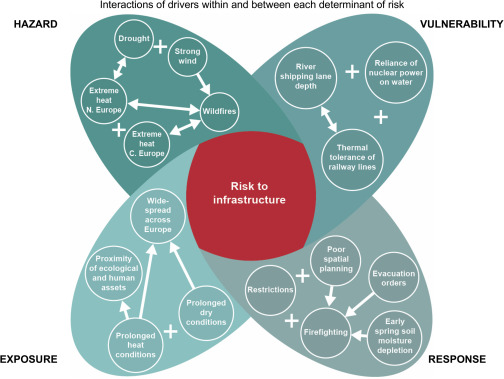
\includegraphics{figures/02_literature_review/simpson-risk-framework.jpg}
    \caption{A framework for decomposing risk into its parts: hazard, exposure,
    vulnerability, and response, using risk to infrastructure as an illustrative
    example. Reproduced from Simpson et al. (2021)
    \cite{simpson_framework_2021}.}
    \label{fig:risk-framework}
\end{figure}

\begin{figure}
    \centering
    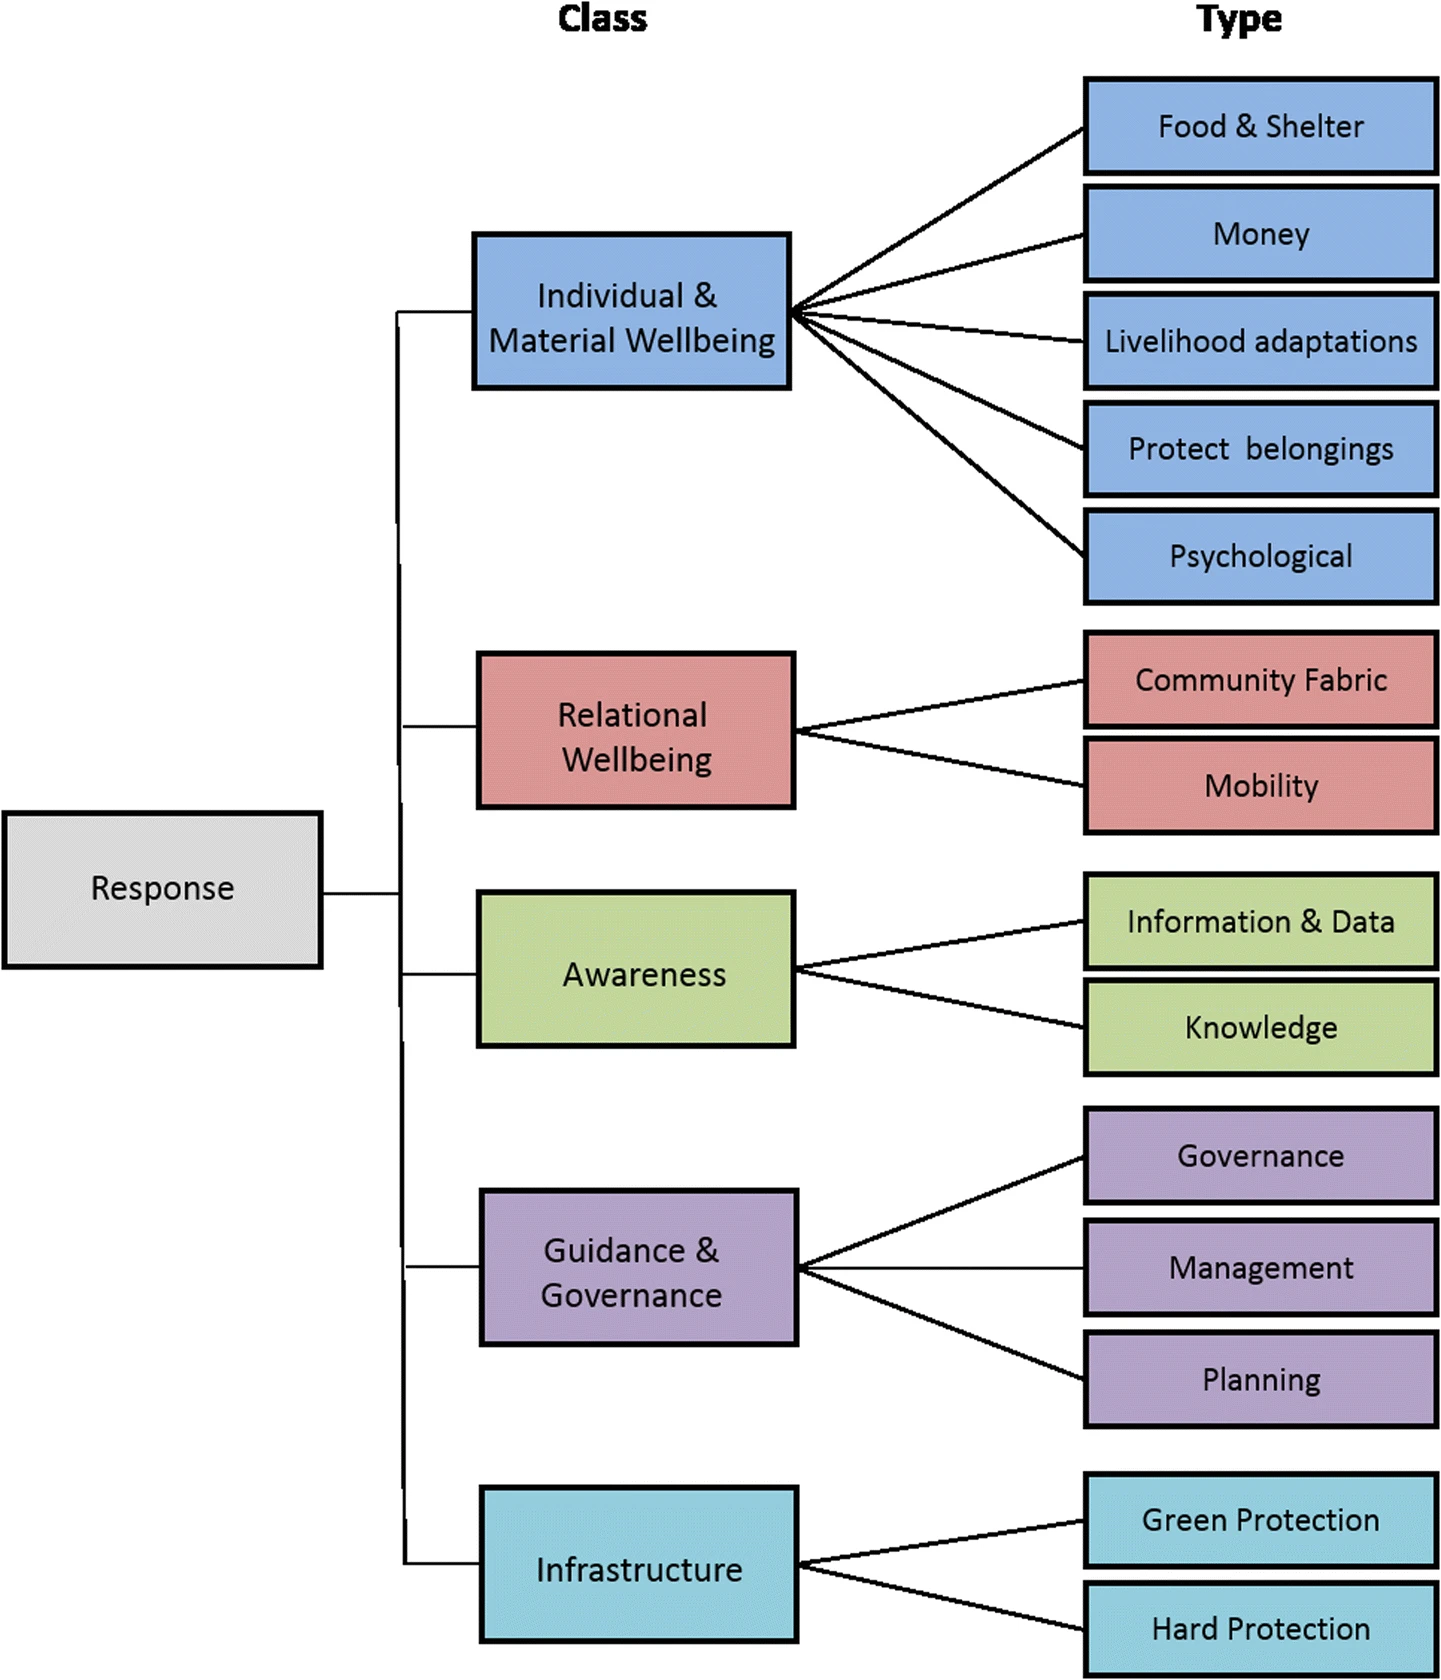
\includegraphics[width=\columnwidth]{figures/02_literature_review/risk-response.png}
    \caption{A categorization typology for various responses to climate risks.
    Reproduced from Paterson et al. (2019)
    \cite{paterson_community-based_2019}.}
    \label{fig:risk-response}
\end{figure}

% \noindent\hrulefill \item What are the responses to climate change? How
% successful have climate policies been at achieving climate goals (and
% ultimately achieving net zero carbon emissions)?

Based on the net-zero carbon emissions target set by the 2016 Paris Agreement,
myriad countries, states, and companies have set climate policies covering
two-thirds of the global economy \cite{hale_assessing_2022}. Reducing \ac{co2}
(or \ac{co2eq} in some cases) emissions is the primary focus for most of these
policies \cite{fawzy_strategies_2020, roelfsema_taking_2020,
hale_assessing_2022}, which include the following broad strategies
\cite{fawzy_strategies_2020}:
\begin{enumerate}
    \item Reducing \ac{ghg} emissions by transitioning from fossil-fueled to
    clean energy.
    \item Removing \ac{co2} from the atmosphere using \ac{ccs} and other
    sequestration techniques.
    \item Altering the Earth's energy balance by increasing its albedo and other
    geoengineering concepts.
\end{enumerate}
Despite this, only around five percent of these policies are consistent with the
\ac{un} ``Race to Zero'' campaign \cite{hale_assessing_2022}. Further, even the
full implementation of national climate policies leaves approximately  a 28
Gt\ac{co2eq} gap in \ac{ghg} emissions \cite{roelfsema_taking_2020} (with the
implicit goal of zero emissions). This gap and the fundamental assumptions about
carbon sequestration from the 2016 Paris Agreement suggest that the world is on
track to overshoot these emissions targets
\cite{roelfsema_taking_2020,taylor_managing_2021}. Carley et al. (2018)
developed a quantitative framework for assessing the vulnerabilities associated
with energy policies or responses \cite{carley_framework_2018}.

% \noindent\hrulefill \item What are the impacts of climate change?

Risk analysis is the first step to a more encompassing understanding of the
climate crisis. The literature on disproportionality further distinguishes
\textit{risks} and \textit{impacts} \cite{dorkenoo_critical_2022}. Consistent
with previous work, a risk is the aggregate of hazards, exposures,
vulnerabilities, and responses. Impacts, then, are the realizations of risk in
terms of loss and damages. This distinction is essential. Responses to
\textit{impacts} are always made \textit{ex post facto}. Differences in
vulnerability to a hazard, often arbitrated by socio-economic status, manifest
as differential impacts. Access to resources conditions an individual's or
community's ability to respond to the impacts of a hazard. Since losses from
impacts disproportionately affect those with the fewest resources, their
vulnerability to future hazards increases in a ``vicious cycle''
\cite{islam_climate_2017, dorkenoo_critical_2022}. In purely economic terms,
studies estimate the loss of ecosystem services from land use change associated
with climate change and other human activities at \$4 - \$20 trillion per year
(in 2011 \$US) globally, \cite{costanza_changes_2014} and the poorest third of
U.S. counties will experience financial damages between 2 and 20 percent of
their annual income \cite{hsiang_estimating_2017}. However, impacts also have
cultural and psychological dimensions \cite{dorkenoo_critical_2022} that cannot
be captured by accounting for ``externalities.''

% \noindent\hrulefill

% \item How are the damages of climate change distributed, and \textit{why} are
% they distributed this way?

Dorkenoo et al. \cite{dorkenoo_critical_2022} establish \textit{burdens},
injustices arising from social, political, or economic power imbalances, as a
third theme paramount for a holistic understanding of disproportionality.
Burdens influence all aspects of risk and affect access to resources which
condition impacts. Dorkenoo et al. wrote, ``[p]rocesses of marginalization and
exclusion influenced by power struggles [...] influence the distribution of
burdens and consequently responsibilities, in addition to the different
dimensions of climate risk (hazard, exposure, vulnerability [, response])''
\cite{dorkenoo_critical_2022}. Figure \ref{fig:risk-impact-burden} demonstrates
the mutually reinforcing relationships among risks, impacts, and burdens. A
particularly relevant example of burden is the persistence of energy burden,
where low-income households pay the highest percentage of their income on energy
bills relative to other income groups \cite{brown_high_2020,
cong_unveiling_2022}. Energy burden interferes with electricity access, thereby
increasing vulnerability to extreme heat events \cite{cong_unveiling_2022,
klinenberg_heat_2003}. The risk assessment literature and the energy system
modeling literature typically adopt an apolitical framing of vulnerabilities.
That is to say, these literature analyze their respective systems independent of
any sociopolitical context. However, inequities do not arise in a vacuum but
through processes of marginalization and exclusion
\cite{thomas_explaining_2019}. Often the distribution of burdens falls along
class, race, and gendered lines \cite{thomas_explaining_2019,mohai_which_2015}.
Research on siting patterns of polluting facilities indicates these projects
frequently developed in areas with people of color and low-income populations
\cite{mohai_which_2015}. Pollution from these facilities creates additional
burdens for nearby communities. The energy justice and environmental justice
literature offer insights to contrast this neutral framing and facilitate
normative questions about alternative distributions
\cite{dorkenoo_critical_2022, thomas_explaining_2019}.

\begin{figure}
    \centering
    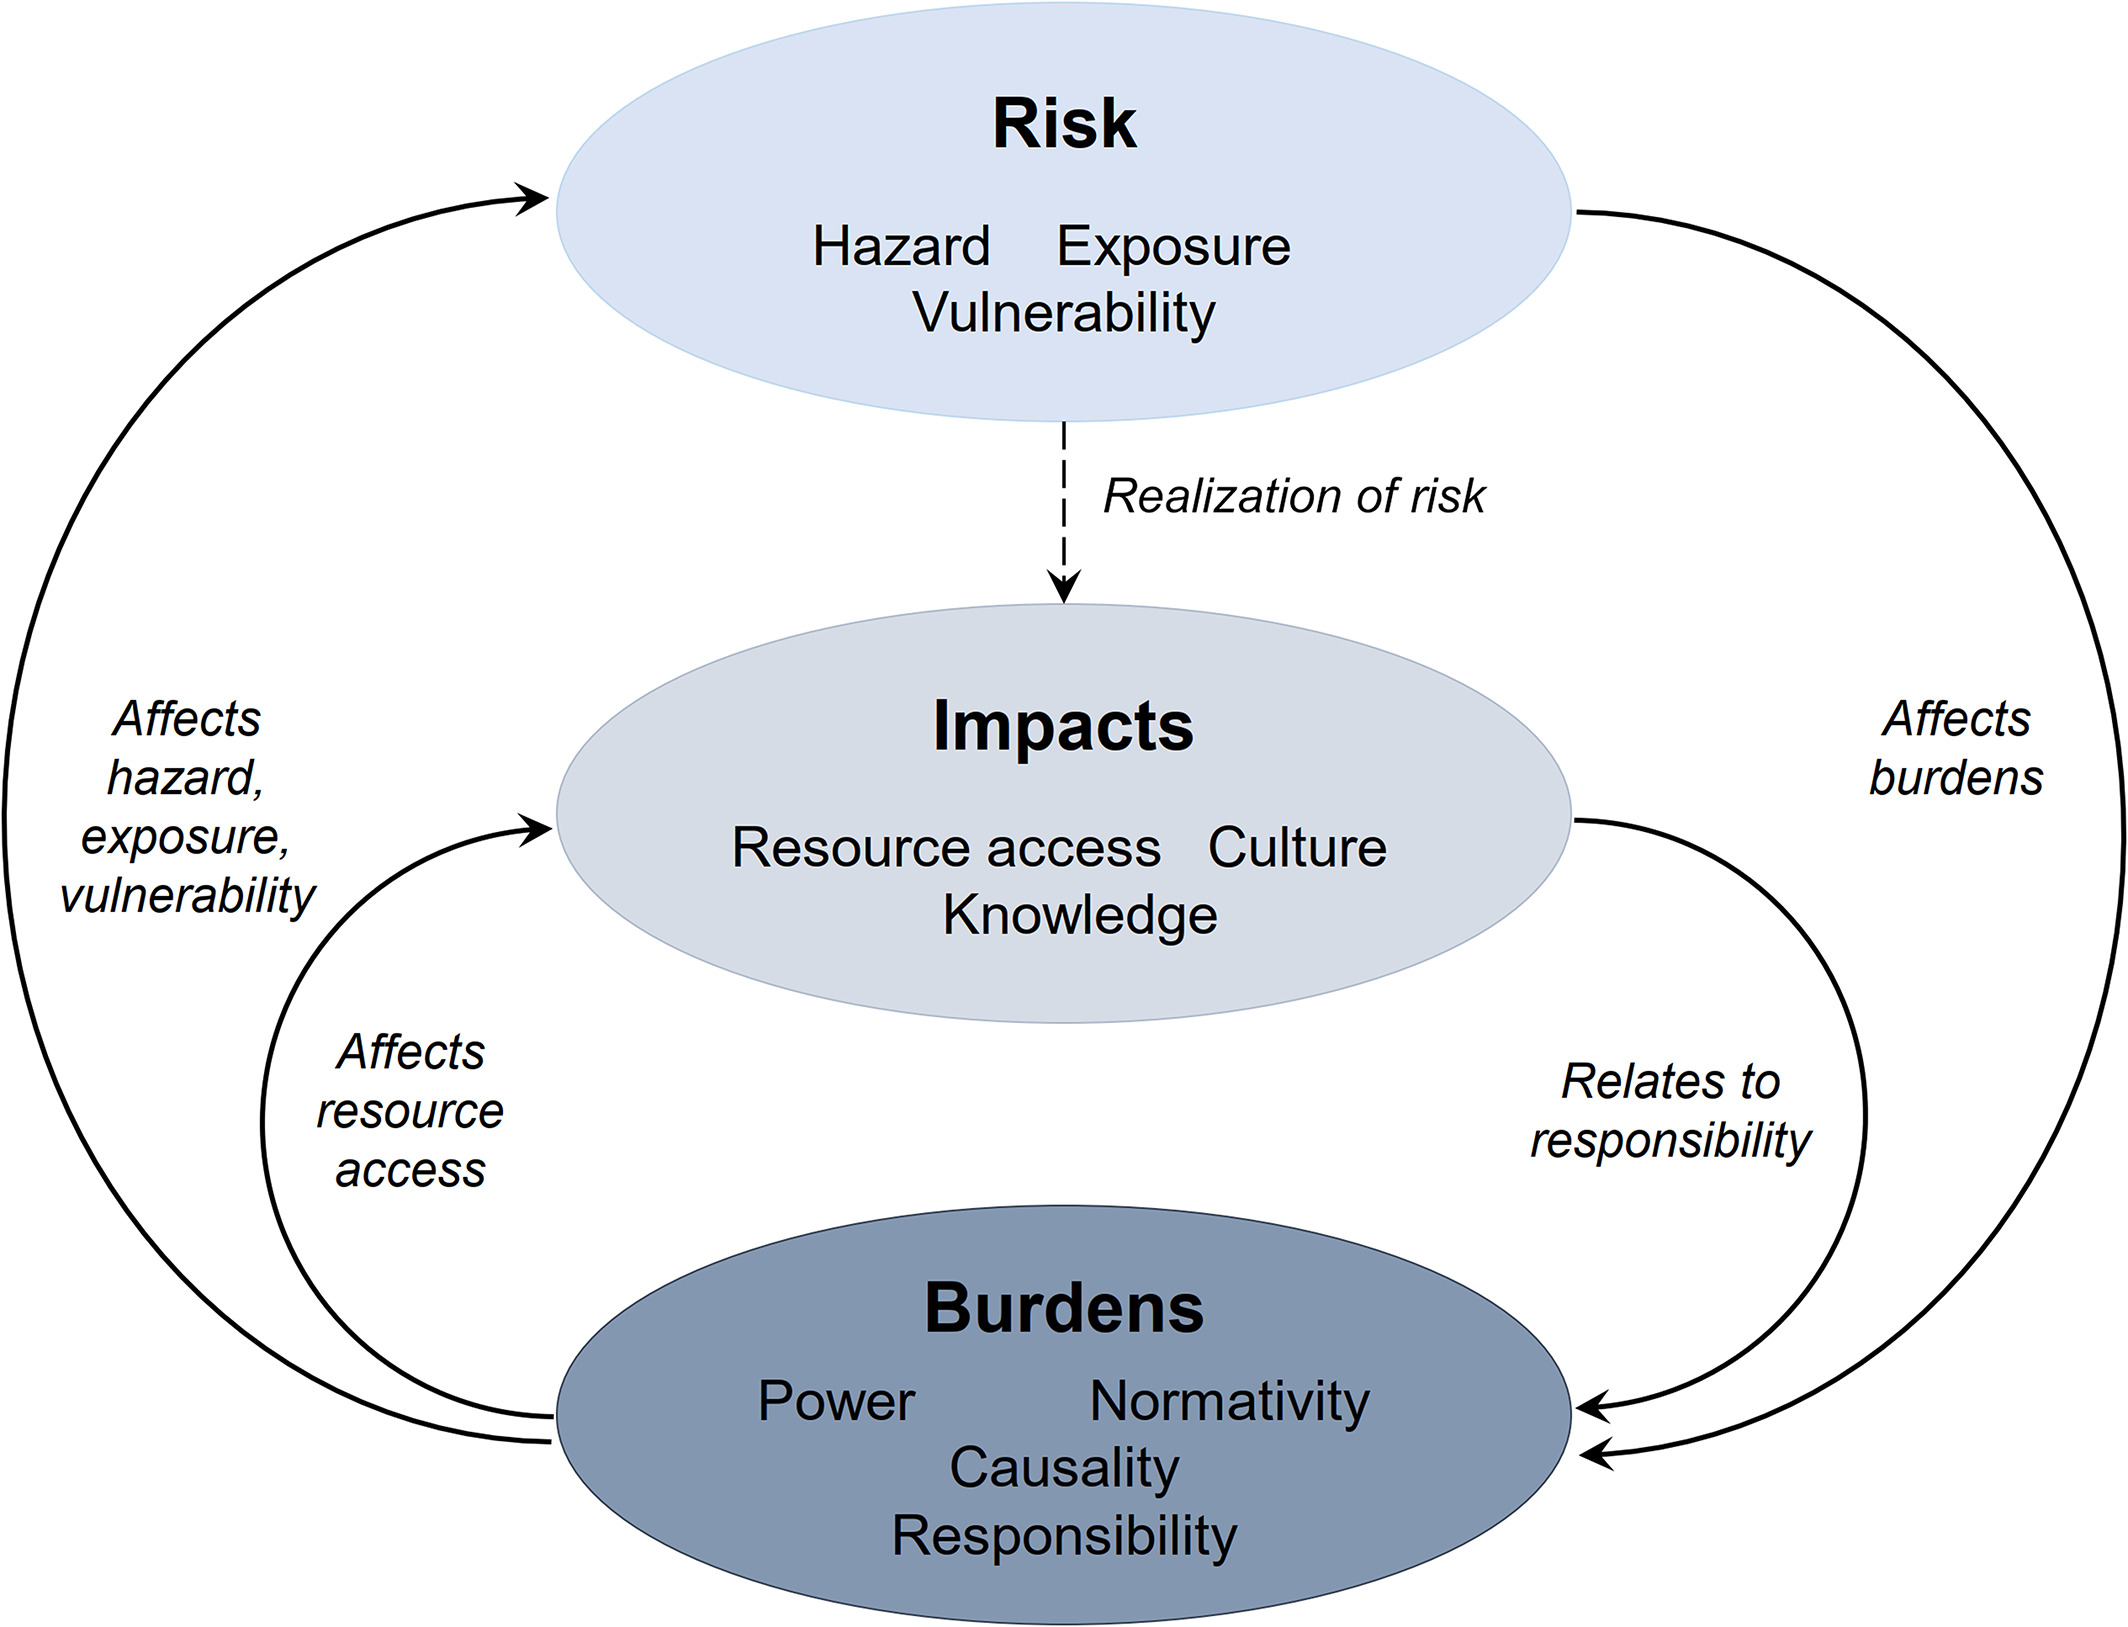
\includegraphics[width=\columnwidth]{figures/02_literature_review/dorkenoo-disproportionality.jpg}
    \caption{The relationships among risks, impacts, and burdens. Reproduced
    from Dorkenoo et al. (2022) \cite{dorkenoo_critical_2022}.}
    \label{fig:risk-impact-burden}
\end{figure}


% \noindent\hrulefill

% \textcolor{red}{Subsection: Climate and Energy Systems}
\section{Climate and Energy Systems}

Climate change is driven by the buildup of additional \acp{ghg} in our
atmosphere from human activities. \acp{ghg} are a significant byproduct of the
infrastructure that creates, delivers, and consumes energy (i.e., energy
infrastructure). The total decarbonization of the global economy will lead to
greater electricity demand, even when accounting for efficiency improvements
\cite{national_academies_of_sciences_engineering_and_medicine_accelerating_2021,
mai_electrification_2018}, decarbonizing our electricity production is one of
the most critical issues to resolving climate change. Therefore, producing
electricity with zero \acp{ghg} will initiate a cascade of deeper
decarbonization throughout the economy. However, this will require expanded
electrical infrastructure to accomodate new energy technologies. Since, energy
production contributes significantly to climate change, and new energy
infrastructure is required to reduce carbon emissions in other sectors (e.g.
heat and transportation), accelerating the adoption of clean energy technology
(i.e. technologies that do not release \acp{ghg} to the atmosphere) is essential
for achieving a stable climate \cite{roelfsema_taking_2020,
taylor_managing_2021}. The next section discusses the range of technical
solutions for accomplishing the goals established above.

% \textcolor{red}{Subsubsection: Technical solutions to energy decarbonization}
\subsection{Technical Solutions to Energy Decarbonization}
% \item What are the technical solutions for decarbonizing the electricity
% sector?

Many studies show that global and local economies can be supported by 100\%
\ac{vre}, such as wind, hydro, solar power, and storage \cite{jacobson_100_2015,
bussar_optimal_2014,brown_response_2018,dorotic_integration_2019,wallsgrove_emerging_2021,
cochran_la100_2021,cosic_100_2012,traber_economically_2021,bogdanov_full_2021,
bogdanov_north-east_2016,
esteban_100_2018,yue_least_2020,neumann_near-optimal_2021}. Yet some countries
that transition to majority \ac{vre} observe higher carbon emissions or a
slower-than-expected reduction due to greater dependence on natural gas brought
on by the relative unpredictability of natural energy sources
\cite{wagner_co2_2021}. Other studies demonstrate that firm baseload power, such
as nuclear power, is necessary for the deep decarbonization of our energy
systems
\cite{wagner_co2_2021,shaner_geophysical_2018,dotson_influence_2022,greene_enhancing_2019,kim_carbon_2021,
lehtveer_how_2015,vaillancourt_role_2008,
de_sisternes_value_2016,alzbutas_uncertainty_2012,brook_why_2014,
epiney_economic_2020,petti_future_2018, patrizio_socially_2020}. While some
countries are building new nuclear reactors, and the \ac{nrc} just licensed the
design of the first small modular reactor design from NuScale
\cite{office_of_nuclear_energy_science_and_technology_nrc_2023}, other places
are shutting down their operating nuclear plants \cite{johnson_new_2021}. 
% In the latter cases, places that shut down nuclear plants always saw a
% subsequent rise in carbon emissions due to greater dependence on natural gas.
% \textcolor{red}{Show plot of carbon emissions vs time for New York?}. 
Further, the only examples of highly decarbonized electrical grids are places
with a high penetration of hydro or nuclear power and the former is largely
exhausted in the United States \cite{lopez_us_2012}. Further, decarbonizing
electricity requires phasing out fossil-fueled power plants and a significant
expansion of clean electricity generators. Although many studies show the
\textit{feasibility} of a variety of energy mixes, the following is strongly
debated in the literature.
\begin{enumerate}
    \item Whether energy systems should be 100\% renewable or if nuclear power
    and \ac{ccs} should be included \cite{heard_burden_2017,
    brown_response_2018,elmallah_frontlining_2022, brook_why_2014}.
    \item What the role of distributed and decentralized energy sources in
    expanding our energy infrastructure should be
    \cite{pitt_assessing_2015,rinaldi_what_2022,parag_electricity_2016,wang_modeling_2020,
    morvaj_decarbonizing_2017,gilbert_can_2020,li_economic_2016,falke_multi-objective_2016}.
\end{enumerate}
The strength of the technical arguments on both sides of these discussions
combined with the distinct lack of sufficient policy agendas pursuing any of
them \cite{roelfsema_taking_2020,hale_assessing_2022}, suggests the existence of
poorly articulated trade-offs and that technical solutions cannot be assessed
from an engineering perspective, alone. Some researchers and policymakers
disagree on technical grounds, while others disagree on the basis of
institutional or systemic injustices. There are also differences in values.
Indeed, the cultural theory of risk argues that our social constructions, rather
than risks themselves, dictate what threats are recognized and their
corresponding liabilities and benefits \cite{mcneeley_cultural_2014,
van_de_graaff_understanding_2016}. Clean technologies like nuclear power and
renewables, such as solar or wind power, are not only different in how they
produce electricity but also in the values and paradigms they represent.
Sometimes, communication fails because the question being discussed is not
agreed upon either. Often, feasibility studies address the positive question,
``what is the least-cost pathway to the energy transition,'' while others
consider more normative questions, such as ``how should we proceed equitably?''\footnote{
    A \textit{positive} question is one that deals with factually
verifiable claims based on measurable data and are perceived as objective. For
example, asking ``what is the temperature outside'' is a positive question
because it asks what \textit{is} and can be answered by taking a measurement.
\textit{Normative} questions engage with ethics, judgement, and values. ``What
should I wear to go outside'' is a normative question because it asks what one
\textit{ought} to do \cite{hands_positive-normative_2012}.} Normative questions
are qualitative and, therefore, inherently challenging to answer and require the
application of ethics. Indeed there are many more normative questions than
positive ones. \textcolor{black}{Is perfect the enemy of good? How do we balance
stakeholder preferences, upstream and downstream effects, and the necessity to
respond quickly to climate change? Will this mix of influences lead to paralysis
or inaction?} Engineers typically do not possess the training nor the expertise
to answer these questions thoroughly. \textcolor{black}{Therefore, given climate
change's complex, interacting, and disproportionate nature, engineering alone is
ill-equipped to resolve the problem. Ideas from the environmental and energy
justice literature offer a social perspective for addressing the risks and
impacts of climate change hazards.} The next section introduces the concept of
energy justice and how this area of scholarship understands challenges related
to climate change and energy systems.


% \subsection{\textcolor{red}{If nuclear energy can solve climate change, where
are all the reactors?}}


% \begin{enumerate}
% \item What do proponents of nuclear energy say about nuclear power?
% \begin{itemize}
%     \item Nuclear engineers generally understand that discomfort and fear around
%     nuclear power come from fears about nuclear weapons and fears about
%     radiation. As such, they view these fears as irrational and placatable by
%     "educating" and ignorant public.
%     \item Some general benefits of nuclear energy (high energy density, low
%     material requirements, low carbon footprint, "safe," low land requirements,
%     reliable, "resilient").
%     \item Additionally, advocates for nuclear energy point to the sustainability
%     of nuclear energy due to its high energy density which in turn reduces the
%     amount of harmful externalities associated with its fuel cycle, relative to
%     other technologies.
%     \item Finally, the nuclear industry has a clear understanding of its fuel
%     cycle, the ways nuclear materials may be reused and/or disposed of, and the
%     measures needed to ensure its safety.
% \end{itemize}
% \item What are the technical objections to nuclear?
% \begin{itemize}
%     \item Nuclear accidents
%     \item Waste (high level waste is a tremendous issue.)
%     \item Ethical issues around mining (what historical harms have been done to
%     mining communities? What about sourcing uranium from places like Kazakhstan
%     (allied to Russia) and directly funding the invasion of Ukraine? What
%     reparations have been made to those harmed? How will future harms be
%     prevented?)
%     \item Nuclear weapons proliferation (discuss the relationship between
%     nuclear energy and nuclear power. Additionally, although nuclear power
%     doesn't necessarily lead to weapons programs, the need to keep careful track
%     of nuclear materials and prevent its release into the biosphere, malicious
%     or otherwise, presents a profound responsibility with some intergenerational
%     inequities).
%     \item Nuclear energy is expensive.
% \end{itemize}
% \item What are some non-technical critiques of nuclear power?
% \item Why are engineering solutions insufficient?
% \begin{itemize}
%     \item Case study on yucca mountain + sweden + finland
%     \item Are advanced reactors actually being designed in a way that
%     incorporates people's preferences. Perhaps preferences toward nuclear energy
%     are not so dependent on the probability of an accident, but on the trust
%     between reactor owners and host communities. Non-experts don't have the
%     expertise to assess the importance of neutron spectra, fuel form, or other
%     technical design parameters that are important for safety. Asserting a low
%     accident probability does not inspire trust. If the reactor is so safe, why
%     not put your money where your mouth is (so-to-speak) and engage in profit
%     sharing with the community? ``Communities are not the final arbiters of
%     safety, determining safety is the purview of the Nuclear Regulatory
%     Commission.''


%     \textcolor{red}{Should I include a question about the benefit of
%     profit-sharing in human-subjects interviews? What are their concerns with
%     energy? Are they focused only on the production of energy or also the
%     lifecycle (extraction + disposal) as well?}
% \end{itemize}
% \end{enumerate}


%What do proponents of nuclear energy say about nuclear power?

In spite of its complicated history, nuclear energy has a variety of unique
benefits that researchers and advocates cite to support its continued and
expanded use. First, uranium has an enormous energy density. This fact has a
number of important consequences that favor the use of nuclear energy, such as
low land use \cite{lovering_land-use_2022,van_zalk_spatial_2018}, high \ac{eroi}
\cite{weisbach_energy_2013,murphy_energy_2022}, and a low mass and volume of
waste byproducts relative to other sources
\cite{liu_wind_2017,chowdhury_overview_2020,holdsworth_spent_2023,taebi_recycle_2008}.
Second, due to the nature of nuclear fission, nuclear power plants emit zero
carbon emissions, making them among the ``cleanest'' sources of energy along
with solar panels and wind turbines
\cite{nicholson_life_2021,intergovernmental_panel_on_climate_change_climate_2021,
brook_why_2014,van_de_graaff_understanding_2016}. Third, nuclear reactors
produce reliable baseload electricity and have the highest capacity factor of
any energy generating technology
\cite{brook_why_2014,van_de_graaff_understanding_2016}. Advocates for nuclear
energy also argue that nuclear energy is among the ``safest'' energy sources,
measured in deaths per unit energy produced
\cite{brook_why_2014,van_de_graaff_understanding_2016,sovacool_balancing_2016}.


%What are the technical objections to nuclear?
Although there are genuine benefits to producing electricity with nuclear
energy, concerns over its use persist. Nuclear engineers generally understand
that discomfort and fear around nuclear power come from fears about nuclear
weapons, nuclear plant accidents, and nuclear waste \cite{roeser_nuclear_2011}.
Each of these concerns are reflected in a different part of the nuclear fuel cycle,
shown in Figure \ref{fig:nuclear-fuel-cycle}.

\begin{figure}[ht]
    \centering
    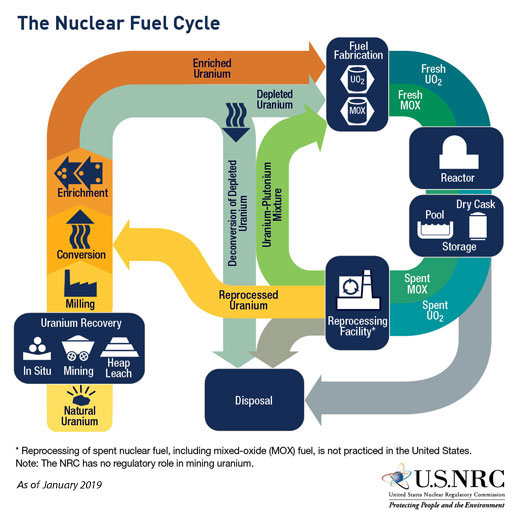
\includegraphics[width=0.5\columnwidth]{figures/nuclear-fuel-cycle-02.jpeg}
    \caption{Stages of the nuclear fuel cycle. Reproduced from \cite{nuclear_regulatory_commission_stages_2020}}
    \label{fig:nuclear-fuel-cycle}
\end{figure}

\noindent
Engineers typically adopt a ``hierarchical'' attitude, as described by cultural
theory of risk \cite{van_de_graaff_understanding_2016,mcneeley_cultural_2014},
and thus perceive these fears as irrational and placatable by ``educating'' an
ignorant public; consistent with the ``deficit model'' of science communication
\cite{simis_lure_2016,patenaude_topical_2022}. \textcolor{red}{It is incumbent
on nuclear engineers and advocates to adequately communicate the risks
associated with nuclear energy and not dismiss concerns due to a lack of
technical rigor.} Although \ac{snf} (commonly ``nuclear waste'') does not
present an immediate risk for radiological release, the details around managing \ac{snf} require
thoughtful consideration. Choosing between an open or a closed nuclear fuel
cycle implies different ethical foundations. Specifically, the tradeoff between
long- and short-term risks that must be carefully weighed
\cite{taebi_recycle_2008}. Further, even though civilian nuclear energy has not
led to the proliferation of nuclear weapons
\cite{herzog_nuclear_2020,miller_why_2017}, the need to keep careful track of
nuclear materials and prevent its release into the biosphere, malicious or
otherwise, presents a profound responsibility with some intergenerational
inequities. Finally, there are elements of the nuclear fuel cycle that 
are frequently ignored. In particular, mining and fuel fabrication are 
often overlooked by advocates for nuclear energy, even though mismanagement in these parts of
the nuclear fuel cycle have led to significant environmental disasters, such as the 
accident in Church Rock, New Mexico \cite{moore-nall_legacy_2015,rojavin_civilian_2011}. 

In addition to these ethical and technical issues, some have argued that, due to the
risks discussed above, nuclear energy requires centralized and authoritarian decision-making
structures and is therefore anathema to inclusive and democratic
values \cite{van_de_graaff_understanding_2016, winner_artifacts_1980}. However, conversations
within the nuclear spaces have reopened this question about the implicit ``politics'' of nuclear
energy, spurred on by the development of \acp{smr} \cite{lovering_social_2021}.

Distinct from conversations surrounding the ethics and risks of using nuclear
energy, many nuclear energy skeptics insist that nuclear power is too expensive
to support decarbonization goals. While it is true that nuclear power plants
have significant capital costs \cite{nrel_2020_2020} which have grown in many
countries due to additional regulations and safety requirements (i.e.,
``negative learning'') \cite{lovering_historical_2016}, it remains unclear
whether these costs uniquely translate to burden on electricity consumers.
Especially given nuclear energy's role as a ``price-taker'' in electricity
markets \cite{murphy_impacts_2019} and evidence for nuclear's stabilizing effect
on electricity prices \cite{dotson_influence_2022,de_sisternes_value_2016}.

 
% \subsection{\textcolor{red}{If renewable energy can solve climate change, why
build anything else?}}

\begin{enumerate}
    \item What do proponents of renewable energy say about solar and wind?
    \begin{itemize}
        \item By virtue of being renewable, the ``fuel'' source is practically
        infinite. Solar energy will never run out on the timescale of human
        civilization, and wind energy (as a product of wind energy plus the
        Earth's rotation) will similarly never run out.
        \item Since renewable energy, specifically solar and wind, lend
        themselves more naturally to distribution, they are more democratic
        sources of energy (cite).
    \end{itemize}
    \item What are the technical objections to fully renewable energy grids?
    \begin{itemize}
        \item Wind and solar are variable and intermittent energy sources.
        \item Renewable energy sources (including non-intermittent sources like
        hydroelectric dams and biomass) have a much lower \ac{eroi} than fossil
        fuel sources \cite{hall_eroi_2014,weisbach_energy_2013}. However, recent
        harmonization studies belie this assertion by demonstrating that
        renewable sources have similar, if not greater, \ac{eroi} than coal or
        natural gas \cite{murphy_energy_2022}.
        \item Although the ``fuel'' for solar and wind resources is infinite,
        the materials required to extract energy from these sources is finite.
        \item In contrast with the nuclear energy, the renewable energy industry
        does not have a strong notion of the lifecycle of their technology.
        There are no plans to safely store or recycle solar panels and wind
        turbines at end-of-life.
    \end{itemize}
    \item What are some non-technical objectives to renewable energy?
    \begin{itemize}
        \item Democracy and inclusivity are not required features of renewable
        energy sources \cite{bell_toward_2020,winner_artifacts_1980}. Although
        renewables have the potential to be highly decentralized, this is not a
        requirement of their use. Many deployment schemes for solar and wind
        farms involve creating highly centralized ``farms'' that are owned and
        operated by a single corporate entity, thereby recreating the same power
        structures that currently exist and thus perpetuating inequities.
    \end{itemize}
    \item What drives the opposition for renewable energy projects (specifically
    wind and solar)?
    \begin{itemize}
        \item Due to the sprawling nature of energy sources like solar and wind,
        these projects are frequently subject to public opposition in proposed
        areas.
        \item The \ac{nimby} movement, or \acs{nimbyism}, is frequently cited as
        the cause of opposition (cite). \ac{nimbyism} describes people that do
        not support the execution of a specific project (energy-related or
        otherwise) due to the project's proximity to a certain location
        (typically residences), but would otherwise support a project if it were
        further away. Despite the popular understanding of \ac{nimbyism}'s role
        in delaying energy projects, the most comprehensive empirical research
        on \ac{nimbyism} demonstrated that \ac{nimby} attitudes do not drive
        public opposition \cite{konisky_proximity_2021}. 
    \end{itemize}
\end{enumerate}

% What do proponents of renewable energy say about solar and wind?

Renewable energy sources, particularly solar and wind energy, are appealing
alternatives to fossil fuel sources. Solar and wind energy have fewer
geographical constraints, compared to hydroelectric and geothermal power
\cite{lopez_us_2012}. With respect to nuclear energy, solar and wind are
similarly safe on a per-unit-energy basis and produce comparable lifecycle
carbon emissions
\cite{united_nations_economic_commission_for_europe_carbon_2022,sovacool_balancing_2016,
intergovernmental_panel_on_climate_change_climate_2014}. Contrary to popular
belief, solar and wind resources can have \ac{eroi} comparable to coal-fired
power plants \cite{murphy_energy_2022}.
% \subsection{\textcolor{red}{Current procedures}}


\textcolor{red}{In this section I want to cover the current issues related to siting 
energy projects and how they are executed. This should relate issues identified in the case studies
for siting a nuclear waste repository (as well as the successes!) and the challenges of siting renewable
energy projects. Once I have made this connection, I can summarize the case study on the Dakota Access Pipeline
done by McKenzie Johnson \cite{johnson_dakota_2021}. I can also refer to the process for obtaining a nuclear
reactor license.
Finally, it may be useful to identify a ``successful'' siting process? Such as the siting of a transmission line
in Ireland \cite{devine-wright_understanding_2020}.
This section also serves as a great segu\'{e} into discussions of energy justice. Since engineers are not 
typically equipped to do the kind of public engagement required to advance energy goals.}
% \noindent\hrulefill \textcolor{red}{Subsubsection: Energy justice and the
% Boundaries of Energy Systems.}
\section{Energy Justice}
\label{section:energy-justice}
% \item What is energy justice?


Energy justice is a conceptual and analytical tool regarding the ethical or
normative dimensions of energy systems and addresses the systemic causes of
burdens, and inequities \cite{sovacool_energy_2015}.
% \begin{enumerate} \item What is justice?
    There are many conceptions of justice; however, the most popular framework
    for understanding justice is a three-faceted approach originating from David
    Schlosberg: distributive, recognition, and procedural justice
    \cite{schlosberg_2_2007}.
    % \item What is distributive justice? 
% \noindent\hrulefill
    Distributive justice relates to the fair distribution of resources,
    burdens, and responsibilities. Studies on distributive justice seek to
    address the normative question: how should a just society distribute the
    benefits it produces and \textit{the burdens required to maintain it}
    \cite{brighouse_justice_2004}. Additionally, distributive justice
    considers \textit{how} poor distributions are created
    \cite{schlosberg_2_2007}.
% \noindent\hrulefill
    % \item What is procedural justice?
    Procedural (in)justice is defined as the presence of (un)fair and
    (in)equitable institutional processes of the state \cite{schlosberg_2_2007}.
    In other words, how decisions of societal import are made and who is
    involved in those decisions. Sovacool and Dworkin (2015) outline four
    elements of procedural justice: transparency, meaningful participation,
    impartiality, and avenues for redress \cite{sovacool_energy_2015}.    
% \noindent\hrulefill
    % \item What is recognition justice?
Justice of recognition is the most vague of the three tenets of justice and is
    frequently reduced to a component of either distributive or procedural
    justice \cite{schlosberg_2_2007, van_uffelen_revisiting_2022}. A common
    argument for this consolidation is that recognition is a precondition for
    achieving distributive justice or that achieving procedural justice
    necessarily includes recognition \cite{schlosberg_2_2007}. However,
    recognition is unique from distributive and procedural justices because it
    is concerned with a different family of injustice, namely,
    \textit{misrecognition} \cite{van_uffelen_revisiting_2022}. van Uffelen
    (2022) suggests a nuanced definition of recognition justice as ``the
    adequate recognition of all actors through love, law, and the status order''
    \cite{van_uffelen_revisiting_2022}.
% \end{enumerate} \noindent\hrulefill
Sovacool and Dworkin (2015) offer a framework for assessing energy policies from
a justice perspective. Table \ref{tab:justice-frameworks} map the relationships
between justice-as-a-decision-making-tool from Sovacool \& Dworkin, Paterson's
hazard response characterization, and Schlosberg's triumvirate of justice. 

\begin{table}[h]
    \centering
    \caption{Different ways to operationalize justice concepts.}
    \input{tables/justice-approaches.tex}
    \label{tab:justice-frameworks}
\end{table}

Although Sovacool \& Dworkin do not explicitly discuss recognition justice, it
is a unique aspect of justice that can still be useful for contextualizing their
recommendations. For example, due to the psychological pressures introduced by a
lack of access to energy, either due to infrastructure or cost, interrupts
relational well-being and is an injustice \cite{van_uffelen_revisiting_2022}.
Further, (un)sustainable policies may be considered a misrecognition of the
humanity of future generations. Next, I examine the specific ways the social
science literature understands how energy systems and their infrastructure
(artifacts) contribute to the distribution of burdens.

% \noindent\hrulefill \item What is an energy system?
\subsection{Boundaries of Energy Systems}
\label{section:energy-system-boundaries}
Previous work defined energy systems in purely technical terms as spatially,
temporally, and topologically complex machines that coordinate the supply and
demand of energy, especially electricity \cite{dotson_influence_2022}. However,
this definition neglects the ways energy systems may be used to construct and
maintain power relations that contribute to inequitable distributions of
burdens. Energy access is necessary to support complex modern economies and
therefore possesses political power \cite{jones_building_2013,
bridge_energy_2018}. The literature on the political economy of energy
infrastructure locates this political influence in five distinct ways
\cite{bridge_energy_2018}. First, energy infrastructure affects competition and
collaboration among nation-states in the geo-political sphere. The current
situation in Ukraine makes this especially salient
\cite{figueiredo_impacts_2022}. 

The second subset of the literature focuses on the process of energy
infrastructure development and how these processes create social inequities. For
example, energy policies that subsidize residential solar panels have not led to
more equitable adoption of solar energy, with greater adoption in areas with
higher income, among other social indicators \cite{reames_distributive_2020}.
Other popular arguments in favor of renewable energy assert that these energy
sources are necessarily more egalitarian because the Sun and the wind cannot be
(or have not yet been) privatized. Another is the urgency of climate change.
Although these arguments have merit, they ignore or minimize the potential
environmental and social consequences of energy planning that does not consider
energy justice \cite{jones_building_2013}. Large-scale energy projects in the
Global South have already led to the dispossession of nearby indigenous
communities and other key actors \cite{yenneti_spatial_2016,
barragan-contreras_procedural_2022}.

Third, the development of energy infrastructure is not simply conducted via
policy measures, but also in the manner governments activate the public
imagination in favor of these policies
\cite{bridge_energy_2018,jasanoff_containing_2009}. Jasanoff and Kim (2009)
articulate this concept as `socio-technical imaginaries,' which are
simultaneously descriptive and prescriptive of possible energy futures
established by governments in the national zeitgeist
\cite{jasanoff_containing_2009}. This concept is demonstrated by the discourse
surrounding nuclear energy in the United States and South Korea
\cite{jasanoff_containing_2009} as well as in Japan
\cite{valentine_energy_2019}. Governments can employ `grand narratives' related
to national security, climate change, or modernization to enhance public support
while minimizing genuine participation \cite{bridge_energy_2018}.

Fourth, the political power of energy infrastructure can be traced further to
the cultural values and policy choices embedded in the design and operation of
seemingly technical systems \cite{bridge_energy_2018}. In other words, the
design and implementation of energy infrastructure may be used as a vehicle for
apparently unrelated agendas, a form of ``policy-making by other means''
\cite{bridge_energy_2018, clausewitz_chapter_1918}. Edwards and Hecht (2010)
refer to the co-constitution of technological and political order as
`\textit{technopolitics},' demonstrating the tangible material and political
outcomes of technological systems \cite{edwards_history_2010}.

Finally, energy systems and their infrastructure possess a unifying quality
through which new political identities may evolve \cite{bridge_energy_2018}.

From these various perspectives, we can observe that confining an energy system
to its technical characteristics is woefully incomplete. I propose that an
energy system is a spatially, temporally, and topologically complex machine that
coordinates the supply and demand of energy and resources and acts as an
important mediator of burdens that influence risks (such as risks from climate
change). This thesis takes the important step of analyzing energy system
planning and policy with this expanded definition. The next section reviews
current attempts to model energy systems and identifies gaps in conventional
methods.

% \textcolor{red}{Climate change \textit{is} a complex issue with multiple
% interacting and interwoven layers. However, it can and must be understood
% holistically instead of stripping it of its complexity and exclusively
% relegating solutions to the realms of economics and engineering. This
% over-simplification is done out of a misplaced sense of pragmatism and either
% an inability or unwillingness to completely apprehend the problem.}

% \noindent\hrulefill \item What are the obstacles to building more clean energy
% infrastructure? What is preventing the transition to a ``qualitatively new
% type of [environmental] society'' \cite{bluhdorn_legitimation_2020}?

% \textcolor{red}{This is where you can introduce different schools of thought
% about transitions.}

% \textcolor{blue}{Interesting that you chose to frame public acceptance as an
% ``obstacle'' rather than a source of greater accountability and
% participation.} \begin{enumerate} \item Legitimation crisis of democracy
% \cite{bluhdorn_legitimation_2020}. \item Social acceptance literature
% \end{enumerate}

% \end{enumerate}

% \section{Calls for a Just-Transition}

% Att


\section{Modeling Energy Systems}
\label{section:esoms}

Energy system optimization models (ESOMs)\acused{esom} have broad utility,
including forecasting future quantities, generating insight for policy
development, or energy system planning for scheduling and acquisition
\cite{decarolis_using_2011, yue_review_2018}. However, analyses using currently
available \acp{esom} seldom consider the role of energy systems in creating and
maintaining inequitable distributions of burdens. \acp{esom} vary significantly
by the energy sectors they choose to model, the degree of physical detail,
uncertainty quanitification, and forecasting capabilities. Table \ref{tab:esoms}
summarizes the capabilities for a comprehensive list of energy system analysis
tools. These tools are approximately sorted by mathematical formulation, e.g.
explicit optimization or simulation. The ``\ac{milp}'' column indicates whether
the framework uses a linear-programming approach to optimize an objective
function. The ``objective'' column specifies the nature of the objective
function if one exists. ``Cost'' objectives minimize total or annual energy
costs, while ``welfare'' maximizes social welfare. Some entries have more than
one objective listed. This means users may choose which objective to optimize.
None of the tools in Table \ref{tab:esoms} are designed to handle simultaneous
optimization (i.e., \ac{moo}). For those modeling frameworks that have an
``objective'' in Table \ref{tab:esoms}, virtually all of them optimize system
costs. EnergyScope is the only exception to this, which allows users to optimize
\ac{ghg} emissions \cite{limpens_energyscope_2019}. \textcolor{black}{The
``uncertainty'' column indicates a feature to algorithmically generate model
runs for testing either parametric or structural uncertainties.
\textcolor{black}{For example, EnergyScope is \textit{suitable} for uncertainty
analysis (i.e., many runs are computationally tractable) but does not have any
built-in capabilities \cite{limpens_energyscope_2019}.} Some tools, such as NEMS
\cite{nalley_national_2019}, incorporate uncertainty into their calculations via
learning curves. However, these learning curves require assumptions about
learning factors and technological ``optimism'' --  which are themselves
uncertain \cite{nalley_national_2019}.} Table \ref{tab:esoms} also indicates
whether the tool is a ``public code.'' This simply means users can download and
inspect the source code. Other considerations for openness, such as licensing
and development, vary among the listed frameworks. \textcolor{black}{The other
columns simply indicate the existence of particular features rather than the
relative maturity or sophistication of each feature.} 

Frameworks, such as MEDEAS \cite{capellan-perez_medeas_2020}, and MultiMod
\cite{huppmann_market_2014}, are general equilibrium models which embed energy
systems within the macro-economy and facilitate the modeling of strategic
behavior. The latter formulates a non-linear problem with the Karush-Kuhn-Tucker
optimality condition \cite{huppmann_market_2014}, as opposed to more traditional
linear programming methods. Models of this type are helpful for analyzing the
economy-wide influence of policies but lack sufficient operational detail to be
prescriptive for energy system planning.

\textcolor{black}{Agent-based models are useful for modeling the market
behaviors of different actors, such as firms (which produce power), transmission
operators, and consumers. The latter category is typically aggregated for
tractability. Modeled behaviors include technology preferences
\cite{anwar_modeling_2022, zade_quantifying_2020}, risk aversion
\cite{anwar_modeling_2022}, financial characteristics \cite{anwar_modeling_2022,
nitsch_economic_2021}, and information asymmetry among agents
\cite{anwar_modeling_2022, nitsch_economic_2021}. Due to agent heterogeneity,
agent-based models are considered useful for capturing social phenomena
\cite{yue_review_2018,fattahi_systemic_2020}.}

A further set of tools focus on simulating power flow and demand fluctuations.
\textcolor{black}{CAPOW \cite{su_open_2020} generates synthetic data with
statistical methods to explore uncertainties in energy dispatch and extreme
demand events, but does not include any investment optimization based on these
uncertainties.} \textcolor{black}{CESAR-P, SAM, Demod, and DESSTinEE focus on
modeling demand profiles
\cite{leoniefierz_hues-platformcesar-p-core_2021,bosmann_shape_2015,barsanti_socio-technical_2021}.
CESAR-P models individual building demand for energy based on the physical
parameters of the building. However, it has no dispatch or investment
optimization capabilities.} Other tools such as Pandapower, GridCal, and SciGRID
power model the infrastructure aspects of electricity systems -- transmission
and distribution -- rather than the optimal dispatch of electricity producers
\cite{thurner_pandapower_2018, vera_gridcal_2022, matke_structure_2017}.

There is an overwhelming number of models with varying levels sophistication and
capabilities. However, the inability to optimize any objective besides cost
presents a significant gap in the existing space of energy modeling tools.
Further, since none of these tools allow for multiple objectives, true trade off
analysis is rendered impossible.



\begin{table}
    \centering
    \caption{Summary of \ac{esom} frameworks.}
    \label{tab:esoms}
    \resizebox*{\textwidth}{0.95\textheight}{\input{tables/esom_database.tex}}
\end{table}
\FloatBarrier

% \begin{itemize} \item METIS has the following motivation
%     \cite{sakellaris_metis_2018} \begin{enumerate} \item Close the gap between
%     modellers and policy-makers, enabling policy-makers to become modellers.
%     \item reconciles user-friendliness with powerful capabilities \item
%     modularity \item \textcolor{red}{METIS does not support multi-objective
%     optimization!}    
%     \end{enumerate} \item energyRt has similar motivations
%     \cite{lugovoy_energyrt_2022}. \begin{enumerate} \item enhance
%     reproducibility \item reduce the learning curve \item minimize model
%     development time \end{enumerate} \item GENESYS cannot \sout{can} do
%     multi-objective optimization \cite{bussar_optimal_2014}. It uses a logical
%     flow to model dispatch behavior for a genetic algorithm! \begin{enumerate}
%     \item One drawback of the "hierarchical system management" method (i.e. a
%     logical flow chart) is the difficulty of modeling ramping rates... (test
%     this). \end{enumerate} \end{itemize}

\subsection{Economic Dispatch and Social Welfare}
\Ac{lp} or \ac{milp} are the dominant optimization approaches among the
frameworks in Table \ref{tab:esoms}. Economic dispatch models optimize the power
output of \textit{dispatchable} generators in a model system
\cite{de_queiroz_repurposing_2019, neumann_near-optimal_2021}. They all share
the same fundamental formulation.
\begin{align}
    \intertext{Minimize}
    \label{eqn:generic_objective}
    &F(x) = \sum_i C_i x_i\\
    % &F(x) = \sum_t^T\left[\sum_i^{N_g}{C_i^g x_i} - \sum_j^{N_d}{C_j^d x_j}\right],\\
    \intertext{subject to,}
    % &\sum_i{x_i} - \sum_j{x_j} = 0\\
    &g(x, p) \leq 0.\nonumber\\
    &x \in \vec{X}\nonumber\\
    \intertext{where}
    &\vec{X} \text{ is the set of decision variables,}\nonumber\\
    & C_i \text{ is the \textit{i-th} cost,}\nonumber\\
    & g \text{ is some linear inequality constraint,}\nonumber\\
    & p \text{ is some arbitrary parameter.}\nonumber
\end{align}
The exact formulation of Equation \ref{eqn:generic_objective} may vary slightly
across models, but the objective for most economic dispatch models is to
minimize total cost. The near universality of a cost-based objective function
comes from the concept of \textit{social welfare maximization}. This concept is
illustrated in Figure \ref{fig:social-max}.

\begin{figure}[H]
  \centering
  \resizebox{\columnwidth}{!}{\input{figures/02_literature_review/social_max.pgf}}
  \caption{Demonstration of ``social welfare maximization.'' Plot a) shows the
  total surplus when the price is at equilibrium. Plot b) shows the total
  surplus when the price is artificially depressed.}
  \label{fig:social-max}
\end{figure}

In microeconomics, social welfare is identical to the sum of consumer and
producer surplus. Therefore social welfare is maximized when the sum of these
two quantities is maximized. Figure \ref{fig:social-max} shows this case on the
left panel. However, suppose an economic policy capped the price of some product
at a price lower than the equilibrium price. In that case, the consumer surplus
expands, and the producer surplus contracts, as shown in the right panel of
Figure \ref{fig:social-max}. Nobody receives the ``lost surplus'' because
suppliers do not produce more despite unmet demand for the product because the
price is capped. Typically, modeling tools consolidate the demand curve to a
single value. \textcolor{black}{In this case, social welfare maximization is
approximated by minimizing the total cost of energy
\cite{richstein_cross-border_2014}}. This simplification is valid because demand
for energy is highly inelastic \cite{heuberger_power_2017, eia_price_2021,
labandeira_meta-analysis_2017, csereklyei_price_2020}. Figure
\ref{fig:inelastic} shows the impact of highly inelastic demand.

\begin{figure}[H]
  \centering
  \resizebox{\columnwidth}{!}{\input{figures/02_literature_review/elasticity.pgf}}
  \caption{Demonstration of ``price elasticity.'' Plot a) shows a typical supply-demand curve where changes in price lead to proportional changes in demand. Plot b) shows an inelastic demand where consumption does not change proportionally with price.}
  \label{fig:inelastic}
\end{figure}

For an elastic good supply and demand are in proportion with each other. An
increase in the supply leads to a proportional increase in demand via a reduced
price, eventually returning to an equilibrium price (shown in Figure
\ref{fig:inelastic}a). However, as Figure \ref{fig:inelastic}b demonstrates, an
inelastic demand does not respond proportionally to changes in price, such that
consumers become ``price- takers,'' paying the price set by producers.
Importantly, in the latter case consumer surplus is infinite and minimizing the
energy cost through policy mechanisms does not create a lost surplus as shown in
Figure \ref{fig:social-max}b. Since electricity demand is highly inelastic,
economic dispatch models minimize the cost of generating electricity.
\textcolor{black}{Although optimizing welfare, rather than the total cost, is
useful for disaggregating multiple demands for the same commodity
\cite{leuthold_elmod_2008}, this thesis adopts the former, simplified, approach
to economic dispatch.}

\subsection{Accounting for Uncertainty}
\label{section:uncertainty}
Due to the complexity of our energy system, handling uncertainty is one of the
most important features for \acp{esom} \cite{yue_review_2018,
decarolis_using_2011}. There are broadly two types of uncertainties: parametric
and structural. The former refers to uncertainty around the value of some
empirical quantity (e.g. price of fuel or the discount rate). In many cases,
these quantities are better represented by \textit{distributions} which may be
sampled using formal methods like \ac{mc} or \ac{pa}
\cite{pfenninger_energy_2014, yue_review_2018}. Deterministic codes such as
TEMOA, TIMES, or ESME use these techniques to generate many model runs. Another
method for handling parametric uncertainty is \ac{sp}, where parameters are
replaced with non-linear risk functions \cite{yue_review_2018,
decarolis_multi-stage_2012}. Although parametric uncertainty is important the
analysis of uncertain values is not a focus of this thesis.

Structural uncertainty relates to \textit{unmodeled objectives}
\cite{yue_review_2018, decarolis_using_2011, decarolis_modelling_2016}. There
are few formal methods to address structural uncertainty due to its qualitative
nature. The most common approach to handling this type of uncertainty is using
\ac{mga} to probe the near-optimal decision space \cite{brill_mga_1990,
jenkins_genx_2022, decarolis_using_2011, neumann_near-optimal_2021,
pfenninger_energy_2014}. DeCarolis wrote, ``[p]olicy-makers often have strong
concerns outside the scope of most models (e.g., political feasibility,
permitting and regulation, and timing of action), which implies that feasible,
sub-optimal solutions may be preferable for reasons that are difficult to
quantify in energy economy optimization models'' \cite{decarolis_using_2011}.
Therefore, an ``optimal solution'' may lie in the model's inferior space
\cite{decarolis_using_2011}. Section \ref{section:mga} details the
implementation of \ac{mga}. \textcolor{black}{However, this approach still
requires an objective function, and the sub-optimal space is still within some
tolerance of the optimal value of the defined optimization space. Further, the
solutions generated by \ac{mga} still admit bias from policy-makers and does not
require users to consider the equity implications of these alternative
solutions.} 

Another strategy to handle structural uncertainty is optimizing multiple
objectives simultaneously. However, some researchers dismissed this approach for
the following reasons \cite{decarolis_using_2011}:
\begin{enumerate}
    \item structural uncertainty will always exist, regardless of the number of
    modeled objectives;
    \item traditional \ac{moo} enables the exploration of a set of non-dominated
    solutions (i.e., the Pareto-front), but not the near-optimal space;
    \item analyzing tradeoffs for problems with many objectives is tedious.
\end{enumerate}
These critiques may explain the distinct lack of frameworks that apply \ac{moo}
for energy system problems. However, there are important benefits to \ac{moo}
(primarily the opportunity to analyze tradeoffs), and the lack of an energy
system \textit{framework} to apply this technique is one of the gaps this thesis
fulfills. Section \ref{section:moo-in-energy} details \acl{moo}.

Although parametric and structural uncertainties correspond to different aspects
of energy system modeling (and models writ large), they share the important
quality of being descriptive rather than prescriptive. Even though they are
primarily used to describe modeled systems, the results of modeling efforts
considering these types of uncertainties are, often implicitly, prescriptive
\cite{yue_least_2020,decarolis_nc_2018,cochran_la100_2021,bussar_optimal_2014}.
For example, although structural uncertainty acknowledges the existence of
unmodeled (or unmodelable) objectives the nature of mathematical optimization
requires modelers to choose at least one objective --- one success criterion ---
to optimize. This choice is always normative because it reflects the priorities
of the modeler. Further, articles identifying a pathway to ``100\% renewable
energy'' make an implicit normative assertion without justification or
recognition of the plurality of morally valid alternatives. This suggests the
existence of another uncertainty: Normative uncertainty. ``Situations where
there are different partially morally defensible --- but incompatible ---
options or courses of action, or ones where there is no fully morally defensible
option'' \cite{taebi_bridging_2017,van_uffelen_revisiting_2024}. Choosing one or
several objectives to optimize implies a normative premise --- even if the
results are presented without a corresponding normative conclusion. The same
could be said for any choice in the development of an \ac{esom}: Spatial scale,
time scale, which technologies are included in the model, and more. Chapter
\ref{chapter:modeling-theory} expands on all three forms of uncertainty and
introduces a conceptual framework for understanding the modeling process through
the lens of these these uncertainties. 



\section{\Acl{moo}}
\label{section:moo-in-energy}
A multi-objective problem may be formulated as
\begin{align}
\label{eqn:generic-moop}
&\text{min}\{F_1(x), F_2(x), ... , F_i(x)\},
\intertext{subject to:}
&g(x, p) \leq 0.\nonumber\\
&x \in \vec{X}\nonumber
\intertext{where}
&F_i \text{ is an arbitrary objective function,}\nonumber\\
&g \text{ is a constraint,}\nonumber\\
&p \text{ is an arbitrary parameter of $g$,}\nonumber\\
&\vec{X} \text{ is the set of decision variables.}
\end{align}
\noindent
Where Equation \ref{eqn:generic_objective} had a single objective $F(x)$ to
minimize, Equation \ref{eqn:generic-moop} has a \textit{set} of objectives,
$\{F_i(x)\}$. Rather than identifying a global minimum point, the solution to
Equation \ref{eqn:generic-moop} is a \textit{set} of non-dominated points called a Pareto-front. Each point on this frontier cannot
improve one objective without making another objective worse, hence
``non-dominated.'' Generally, for competing objectives, there will be an
infeasible space that is not attainable by the given combination of objectives.
For a minimization problem, the space above the Pareto-front is the sub-optimal
feasible space. This is the space that \ac{mga} promises to search for a
corresponding single-objective problem. Figure \ref{fig:truss-pareto}
illustrates a set of solutions along a Pareto-front for an example problem from
\ac{pymoo} \cite{blank_pymoo_2020,deb_omni-optimizer_2008}.

\begin{figure}[H]
  \centering
  \resizebox{0.6\columnwidth}{!}{\input{figures/truss2d_pareto.pgf}} \caption{An
  example \textit{convex} Pareto-front from \acs{pymoo} \cite{blank_pymoo_2020,
  deb_omni-optimizer_2008}.}
  \label{fig:truss-pareto}
\end{figure}

 There are broadly two classes of \ac{moo} algorithms for solving Equation
\ref{eqn:generic-moop}, \textit{scalarization} and \textit{population-based}
\cite{gunantara_review_2018, emmerich_tutorial_2018}. Scalarization approaches
map the multi-objective problem onto a set of single-objective problems using
variation of parameters. In the \ac{ws} algorithm, the objectives are assigned
weights, $w_i$, and the aggregated objective becomes
\begin{align}
    \label{eqn:weighted-sum}
    \text{min}\quad J(x) &= \sum_i w_i F_i(x)
    \intertext{subject to:}
&g(x, p) \leq 0\nonumber\\
&x \in \vec{X}\nonumber
\intertext{where}
&F_i \text{ is an arbitrary objective function,}\nonumber\\
&w_i \text{ is the weight for objective function $F_i$}\\
&J \text{ is the aggregated objective,}\nonumber\\
&g \text{ is a constraint,}\nonumber\\
&p \text{ is an arbitrary parameter of $g$,}\nonumber\\
&\vec{X} \text{ is the set of decision variables.}
\end{align}
\noindent
These weights are varied in order to sample points along the Pareto-front. 

Alternatively, the \ac{ec}
algorithm for scalarization chooses one objective from $\{F_n\}$ to solve and converts the others
into constraints, whose bounds are denoted by $\epsilon$. These bounds are
varied until the desired number of points on the Pareto-front is reached
\cite{gunantara_review_2018, emmerich_tutorial_2018}. This problem can be
written as
\begin{align}
\label{eqn:epsilon-constraint}
    &\text{min}\quad F_j(x),
    \intertext{subject to:}
    &F_2(x) - \epsilon_j \leq 0\nonumber\\
    &\vdots\nonumber\\
    &F_i(x) - \epsilon_j \leq 0\nonumber\\
    &g(x, p) \leq 0,\nonumber\\
    &x \in \vec{X}.\nonumber
\end{align}
\noindent
The sub-problem, Equation \ref{eqn:epsilon-constraint}, must be repeated for
each $F_j(x)$ and corresponding $\epsilon_j$ in $\{F_n\}$.

Scalarization is attractive due to its simplicity. However, this approach is
sensitive to problem convexity. \ac{ws} will never be able to sample points in a
concave region of the Pareto-front, and \ac{ec} will have poorly spaced samples
along a concave region. Further, these algorithms can only sample points on the
frontier, not the sub-optimal feasible space. Thus supporting the critique of
using \ac{moo} for handling structural uncertainty \cite{decarolis_using_2011}.

Fortunately, population-based algorithms, also called \textit{\acp{ga}} or
\textit{evolutionary algorithms}, resolve some of these issues by solving
Equation \ref{eqn:generic-moop} directly. \Acp{ga} are based on the principle of
natural selection. In a \ac{ga}, such as \ac{nsga2}, an initial population is
randomly generated using the problem's decision variables, the `fitness' of this
population (i.e., performance on each objective) is calculated, then a new
population is selected from the `fittest' (most optimal) individuals. This
process continues until a convergence criterion is reached. The advantages of
this method are
\begin{enumerate}
    \item a guaranteed solution, regardless of convexity,
    \item no prior knowledge is required to initialize the problem, as with
    \ac{ec},
    \item greater diversity of solutions (i.e., spacing of points along the
    Pareto-front),
    \item the sub-optimal space is sampled through the iterative process (though
    not uniformly).
\end{enumerate}
Specifically, point four address one of the primary criticisms of using \ac{moo}
to reduce structural uncertainty by obtaining points in the inferior region
\cite{loughlin_genetic_2001,zechman_evolutionary_2004,
zechman_evolutionary_2013}. An additional advantage of \acp{ga} is the ability
to incorporate more physics and simulations into the optimization procedure than
\ac{lp}, \ac{milp}, or scalarization allow \cite{loughlin_genetic_2001} because 
\acp{moo} can incorporate data from external models. 

Previous work handled structural uncertainty using \ac{mga} which samples unique
solutions from the sub-optimal space in a neighborhood around the global minimum
for a single objective \cite{decarolis_using_2011}. Researchers argue that this
approach is valid because there will always be structural uncertainty and
sampling the inferior region may offer insight for decision-makers.
\textcolor{black}{While structural uncertainty may persist it is not
\textit{irreducible}.} By increasing the number of modeled objectives \ac{moo}
reduces structural uncertainty. Further, ideas from \ac{mga} can be applied to
\ac{moo} by efficiently sampling the near-optimal space
\cite{loughlin_genetic_2001,
zechman_evolutionary_2004,zechman_evolutionary_2013,pajares_comparison_2021}.
The goal of \ac{mga} is to find a \textit{reduced} set of maximally different
alternatives to provide insight, where analyzing the full set of alternatives
would be overwhelming \cite{decarolis_using_2011, pajares_comparison_2021}.
Figure \ref{fig:near-opt-pareto} shows the near-optimal space around the
Pareto-front from Figure \ref{fig:truss-pareto}.

\begin{figure}[H]
  \centering
  \resizebox{0.6\columnwidth}{!}{\input{figures/near-optimal-pareto.pgf}}
  \caption{The near-optimal space around the Pareto-front.}
  \label{fig:near-opt-pareto}
\end{figure}

For these reasons, this thesis explores energy systems optimization and the
handling of structural uncertainty through \ac{moo} and \acp{ga}. Section
\ref{section:genetic-algorithms} reviews the details of the \ac{ga} used in this
thesis.


% \input{2-literature/29-multi-criteria-decions}



\subsection{Energy System Applications}
It is well understood that engineering and policy problems, which include energy
systems optimization, often require satisfying multiple antagonistic objectives
\cite{loughlin_genetic_2001,zechman_evolutionary_2004,
zechman_evolutionary_2013, chattopadhyay_need_2021}. However, the application of
\ac{moo} to energy systems in the literature is limited. Table
\ref{tab:moop-literature} summarizes the current body of work. As before, the
``public code'' column only indicates if the source code is accessible.
Additionally, the ``sector'' columns only indicate the presence of a feature,
not the relative maturity or sophistication of the modeling. There are six
``objective columns,'' indicating which objectives are considered the in the
model or study. A ``technology'' objective might optimize a specific technology
or set of technologies. For example, maximizing the percentage of renewable
energy in a system. The ``reliability'' metric varies among studies, but
generally refers to the potential for load loss. For all of the studies in Table
\ref{tab:moop-literature}, the ``environmental'' objective refers to \ac{ghg} or
``global warming potential'' \cite{de-leon_almaraz_deployment_2015}. Although it
could refer to other environmental impacts such as land use, water use, or
thermal pollution. 

\begin{table}[ht!]
    \centering
    \caption{\ac{moo} used with energy systems.}
    \label{tab:moop-literature}
    \resizebox*{\textwidth}{!}{\input{tables/moop_literature.tex}}
\end{table}
Most of the studies in Table \ref{tab:moop-literature} used \ac{nsga2} to
identify the Pareto-front with a few using scalarization. Consistent with the
trend shown in Table \ref{tab:esoms}, every study in Table
\ref{tab:moop-literature} uses some economic or ``cost'' metric as one of the
objectives. Also consistent, is that none of these studies identified a metric
to optimize over social concerns. Laha et al. \cite{laha_low_2021} used
fatalities per GWh and employment per GWh as criteria for social sustainability,
but these were not objectives in their model, rather they were calculated
\textit{ex post facto} with scenario analysis. Riou et al.
\cite{riou_multi-objective_2021} investigated the tradeoffs among renewable
share, reliability, and total cost. Their findings were consistent with single
objective scenario analysis \cite{de_sisternes_value_2016}, that greater
renewable penetration leads to greater costs and less reliable energy with a
100\% renewable energy system being the least reliable or incurring the greatest
costs \cite{riou_multi-objective_2021}. 

Although previous work demonstrated the applicability of \ac{moo} to energy
systems optimization, there are significant limitations. 
\begin{itemize}
    \item{There are at most three modeled objectives
    \cite{riou_multi-objective_2021,de-leon_almaraz_deployment_2015,
    de-leon_almaraz_assessment_2013}.}
    \item{While traditional \acp{esom} have many mature frameworks (as shown in
    Table \ref{tab:esoms}), there are no frameworks that use \ac{moo}.
    Simultaneously, none of the studies in Table \ref{tab:moop-literature}
    developed a framework. Prina et al. developed a bespoke and unlicensed model
    called ``Oemof-moea,'' however this does not constitute a framework.}
    \item{None of the studies in Table \ref{tab:moop-literature} allow
    arbitrary user-defined objectives.}
    \item{None of the studies incorporate social metrics into the modeled objectives.}
\end{itemize}

This thesis develops, \ac{osier}, a novel energy systems framework using
\ac{moo} that fills these gaps by using \acp{ga} that allows for efficient
modeling of many objectives, enabling user-defined objectives, providing the
option to make metrics of interest either objectives or constraints, and
incorporating ideas from \ac{mga} to provide insight from the sub-optimal
objective space.


% \textcolor{red}{If carbon emissions should not be considered an objective, but
% rather a constraint, because there are hard emissions budgets why can't the
% same argument be made with respect to cost? Some places might have limited
% funds to allocate for energy infrastructure. }

The next section outlines attempts to incorporate social justice concerns with
energy system models.


% \subsection{\textcolor{red}{More context for decision making with \ac{moo} in energy systems.}}

% Answer the following questions for each paper listed below (this will help demonstrate the 
% novelty of my work):

% \begin{enumerate}
%     \item Does the study develop a framework?
%     \item Is the framework open source (if applicable)? Is the input data transparent?
%     \item Does the study use genetic algorithms? If so, which one?
%     \item What methods does the study use?
%     \item What objectives does the study optimize?
%     \item Are there ``users'' that can arbitrarily add new objectives?
%     \item How many objectives can be optimized at once?
%     \item Does the study discuss energy justice? How do they define justice? What aspects are discussed?
%     \item Does the study describe how their analysis can inform decision making processes and improve
%     justice outcomes?
% \end{enumerate}


% The papers of interest

% \begin{enumerate}
%     \item \cite{kamenopoulos_assessment_2019}
%     \item \cite{kasprzyk_many_2013}
%     \item \cite{jafino_enabling_2021}
%     \item \cite{granacher_overcoming_2022}
% \end{enumerate}
\textcolor{red}{\section{Hyper-local energy system modeling}}
\textcolor{red}{To the literature review, I want to add a section discussing 
the research on modeling at the municipal level. These papers start with the 
following: 
\cite{mckenna_combining_2018,johannsen_municipal_2023,ben_amer_too_2020}.}
\section{Modeling and Quantifying Energy Justice}

The dearth of studies that incorporate energy justice into \acp{esom} highlights
the challenge of combining these techniques. The literature on energy justice and
socio-technical transitions tend to derogate modeling efforts as cold and
calculating \cite{sovacool_energy_2015,sovacool_energy_2016}, and most models do
not account for energy justice in either equations or analysis. However, there
have been some notable attempts to bridge this gap. The following studies by Patrizio 
et al. (2020) \cite{patrizio_socially_2020} and Neumann \& Brown (2021) \cite{neumann_near-optimal_2021}
explicitly use \acp{esom} in their analyses. Although the works by Chapman et al. (2018)
\cite{chapman_prioritizing_2018} and Mayfield et al. (2019) \cite{mayfield_quantifying_2019}
do not use \acp{esom} as described in Section \ref{section:esoms}, these contributions
quantify some features of their respective energy systems and how they relate to
notions of energy justice and equity.

Patrizio et al. (2020) conducted a technology-agnostic `social equity' scenario
that maximized the \ac{gva} of several countries' energy systems rather than
minimizing the total cost \cite{patrizio_socially_2020}. \Ac{gva} is also
distinct from social welfare because it measures contributions to \ac{gdp} from
individual producers rather than maximizing surplus. This metric enables
sector-specific analysis of the impacts of energy infrastructure on employment
and sales. Equity, in this context, is identical to socioeconomic development as
measured by \ac{gdp}. Using this definition of equity, the researchers looked at a 
socio-technical transition for
three countries: Spain, the United Kingdom, and Poland. They found that a 100\%
renewable energy system would reduce labor compensation by 50-60\% in the UK and
Poland but could increase benefits in Spain. They argue this is due to the
outsourcing of manufacturing and mining jobs in the former cases, while Spain
has enough domestic resources to accommodate the transition. The researchers did
not analyze possible shifts in power dynamics related to the energy systems, but
they did identify that there is no one-size-fits-all solution to achieving
net-zero carbon emissions.

Neumann \& Brown (2021) performed a detailed analysis of the European energy
system considering the expansion of transmission networks and energy producers
for a 100\% renewable energy system under cost minimization
\cite{neumann_near-optimal_2021}. They also used a novel formulation of \ac{mga}
to identify the boundaries of the feasible space for each technology within
different levels of tolerance. This study uses Lorenz curves and Gini
coefficients to measure the uniformity of the distribution of energy production
and consumption. In other words, the most equitable distribution of energy
resources would accord with energy consumption \cite{neumann_near-optimal_2021}.
The researchers conclude that wind power and greater transmission capacity are
associated with less regional equity, while solar power and storage technologies
lead to a more even distribution of the power supply. This is useful for
measuring the distribution of energy benefits from the energy system but does
not consider the distribution of costs nor consider regional preferences. 

Chapman et al. (2018) looked at the energy justice implications of transitioning
coal plants to renewable energy projects for the nearby communities
\cite{chapman_prioritizing_2018}. They measure distributional justice with
``relative equity'' and ``policy burden.'' Relative equity accounts for factors
such as \ac{ghg} reduction, employment, electricity cost, and health impacts.
Policy burden is a weighted value according to the income level of each
community. These two quantities were plotted together to identify a retirement
schedule that maximizes equity outcomes and ensures that burdens are borne by
the most capable communities \cite{chapman_prioritizing_2018}. Additionally, the
researchers argue that by using equity measures to inform policy choices, those
policy decisions are more procedurally just. However, this neglects meaningful
participation and may or may not address decision-making transparency
\cite{sovacool_energy_2015}. Further, this study does not consider how replacing
dispatchable suppliers with \ac{vre} will affect the availability and
affordability of electricity \cite{sovacool_energy_2015}. This latter challenge
could be addressed by incorporating methods from the \ac{esom} literature. The
former issue of decision-making transparency is one of the motivations for this
thesis.

Mayfield et al. (2019) quantified the social equity implications for the
expansion of natural gas infrastructure in Appalachia using spatial and temporal
metrics such as job-years generated by greater gas development, premature deaths
caused by air pollution, changes in poverty and income, and the distribution of
these various benefits along regional, racial, and economic lines. Additionally,
they identified some of the intergenerational equity impacts of climate change
and expanded gas infrastructure. 

\subsection{Enabling Procedural Justice Through Energy Models}

Traditionally, \acp{esom} are used to inform policy-makers \cite{li_open_2020}
in order to infuse policy choices with an appearance of objectivity. Indeed,
some of the studies reviewed in the previous section argue that this infusion
will lead to greater procedural and recognitional justice outcomes as long as
the policies maximize some measure of energy justice
\cite{chapman_prioritizing_2018, heffron_resolving_2015}. However, these types
of detailed analyses may also be used to dismiss concerns or opposition from the
public due to insufficient `technical expertise' \cite{johnson_dakota_2021}.
Further, without meaningful participation from the affected public, this
approach further entrenches procedural injustices. To credit the energy
modeling community, there is significant awareness of the importance of
transparency and repeatability in the space \cite{decarolis_case_2012,
pfenninger_energy_2014, pfenninger_openmod_nodate, forster_open_2022,
hilpert_open_2018}. Yet these two goals are challenged by the computational
resources required to run the more complex and detailed models, as well as the
learning curve necessary to understand and modify the model inputs themselves.
There has been some effort to reduce this learning curve and make modeling
itself more accessible. Frameworks such as METIS, EnergyRT, and \ac{pygen} all
emphasize reproducibility, user-friendliness, and a shallower learning curve
\cite{sakellaris_metis_2018, lugovoy_energyrt_2022, dotson_python_2021}. The
creators of METIS state their goal is to ``close the gap between modelers and
policy-makers, enabling policy-makers to become modelers''
\cite{sakellaris_metis_2018}. However, these frameworks do not offer
computational resources to run their models. The \ac{temoa} project offers
limited cloud computing capabilities, free of charge
\cite{temoa_project_temoa_2023}. However, the responsibility for creating an
input file still falls to the user, which can be overwhelming even for
experienced modelers. Finally, it's not clear that perfectly accessible and
transparent modeling tools will translate to more procedurally just
policy-making. The next section outlines one method used to address this
challenge.

\subsection{\Acl{pve}}

Even if the public could use modeling tools, their testimony may still be
dismissed due to a `lack of expertise.' However, the public has preferences that
should be incorporated into decision-making. Additionally, community members are
frequently able to assess trade-offs when presented with them. \Acf{pve} is one
method for translating community preferences into just policy outcomes.
Researchers in the Netherlands developed this method to enhance democratic
participation and infuse policies with genuine feedback from constituents
\cite{mouter_introduction_2019}. They observed that a common method of assessing
social impacts is \ac{wtp}, which is the maximum price an individual is willing
to pay for a good or service, yet individual purchasing habits do not
necessarily reflect their views on public policy due to the relative salience of
moral considerations \cite{mouter_introduction_2019}. With \ac{pve},
participants can allocate a specific amount of the public budget for certain
policies, including levying or reducing taxes for greater or lesser government
spending \cite{mouter_introduction_2019}. Researchers applied \ac{pve} in three
different settings, mobility and transportation \cite{mouter_contrasting_2021},
flood risk projects (i.e., a climate hazard \textit{infrastructure} response)
\cite{dekker_economics_2019}, and with a phaseout of natural gas
\cite{mouter_including_2021}. Importantly, the studies also measured the impact
of these interventions and found that \ac{pve} enables participation from people
that do not typically participate (recognition), the results were useful for
decision-making and participation was meaningful for the majority of subjects
\cite{mouter_including_2021}. Although previous applications of \ac{pve} focused
on economic policy levers, this approach offers a promising pathway toward
identifying equitable and just energy mixes for the future.

In summary, climate change is a multi-dimensional existential threat to society.
Transitioning to a zero-carbon economy by decarbonizing our energy systems may
prevent the worst outcomes of climate change. However, energy systems do not
only transport electrons and gas but also mediate socio-political power.
Therefore this transition must be done equitably in order to avoid entrenching
further injustices. The existing energy system modeling tools and literature
routinely ignore the social dimensions of these systems and forego true
trade-off analysis. Additionally, it's unclear whether improving these modeling
practices will correspond to just energy policy outcomes. This thesis attempts
to bridge the gap between energy system modeling and energy justice by
developing a novel framework that allows multiple, and perhaps non-economic,
objectives and is designed for transparency and usability by non-modelers to
inform energy policy decisions. A framework such as the one developed in this
thesis may be used in conjunction with a policy process like \ac{pve} to fully
enclose the triumvirate of energy justice tenets: distribution, procedure, and
recognition.



\chapter{\acf{osier}}
\label{chapter:osier}
% \chapter{\acf{osier}}
\label{chapter:osier}

This chapter introduces the \acf{osier}, a novel open-source energy system modeling
framework for \acl{moo} \cite{dotson_osier_2024}. There are currently no
\acp{esom} that enable \ac{moo} and \ac{osier} fills that gap. Figure 
\ref{fig:osier_flow} illustrates the flow of data into and within \ac{osier}.

\begin{figure}[H]
    \centering
    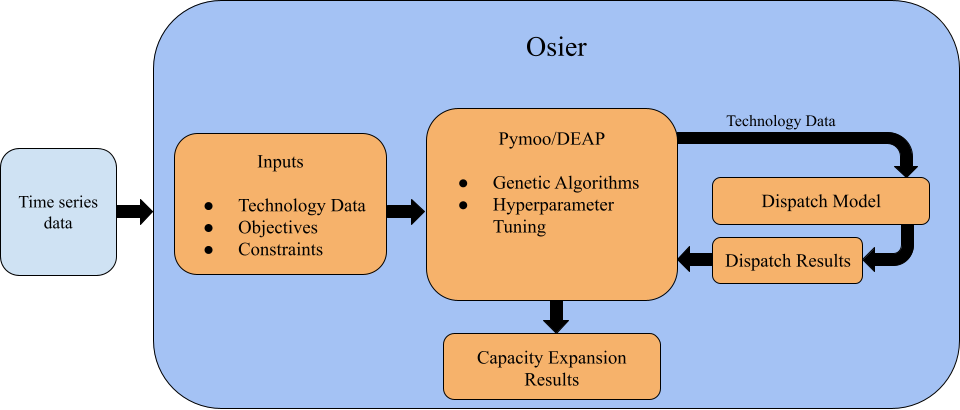
\includegraphics[width=\columnwidth]{figures/osier_flow}
    \caption{The flow of data into and within \ac{osier}}
    \label{fig:osier_flow}
\end{figure}

Technology data, objectives, constraints, and a dispatch model are all features
within \ac{osier}, while \ac{pymoo} drives the optimization of these objectives \cite{blank_pymoo_2020}.
The dispatch model is independently executable for inspecting specific test
cases and mapping solutions from other solvers onto \ac{osier}'s objective
space. The next sections elaborate on model inputs, \acfp{ga}, and the dispatch model's 
formulation.

% \textcolor{red}{This chapter is mostly written but there are a few things that
% should be added.}

\section{Inputs}

% \textcolor{red}{General thoughts:}

% Accurate input data are essential but curating data represents a challenging step in the
% modeling process. \ac{osier} attempts to lower this barrier by providing a
% variety of technology data from ``reliable'' sources.

% This section connects to the normative and descriptive portions of modeling. 

This section describes the input data and parameters that users must provide to run an \ac{osier} simulation. Broadly, \ac{osier} needs
technology data and some objectives to optimize. 

\subsection{Technology Data}
\ac{osier} only requires marginal costs and technology names in order to run successfully.
These data are needed to run the dispatch model. \ac{osier} also accepts operational data, such
as ramp rates and storage capacities. Additionally, \ac{osier} will understand any bespoke 
piece of data (e.g., ``popularity,'' ``technology-readiness score,'' or anything else) that
might be needed for a user-defined objective. All of these data are passed to \ac{osier}
through an \texttt{osier.Technology} object. Code listing \ref{listing:user-defined-technologies}
shows how users can create a simple technology object.

\begin{listing}[!ht]
    \caption{A basic technology object in \ac{osier}.}
    \label{listing:user-defined-technologies}
    \begin{minted}
    [ frame=lines, framesep=2mm, baselinestretch=1.2, bgcolor=LightGray,
    fontsize=\footnotesize, linenos ] {python} 
    from osier import ThermalTechnology

    fusion = ThermalTechnology(technology_name="Fusion",
                               dispatchable=True,
                               renewable=False,
                               fuel_cost=10*(GWh)**-1,
                               lifecycle_co2_rate=0.0,
                               )
    \end{minted}
    \end{listing}

\subsection{Objectives}
\label{section:osier_objectives}

There are many possible objectives to optimize. This section summarizes a few of
them and how they may be calculated in \ac{osier}. Due to \ac{pymoo}'s
structure, all objectives are minimized. Therefore, if users wish to maximize
some quantity, it must be reformatted with a reversal in sign to be an equivalent minimization objective.

\subsubsection{Per-unit-capacity}

Some quantities of interest depend on the \textit{capacity} of each technology.
For example, land use of different energy producers is often reported as a land
density $\text{km}^2/\text{MW}$. A generalized specific \textit{density} with respect to power 
may be $\text{unit}/\text{MW}$. The objective function for these quantities reads
\begin{align}
    \mathcal{K} &= \sum_g^G \textbf{CAP}_g \kappa_g ,
    \intertext{Where}
    \kappa &= \text{the power density of the \textit{g-th} technology} \quad \left[\frac{-}{MW}\right].
\end{align}

Table \ref{tab:objectives-per-capacity} lists some example objectives that could be
minimized or maximized.

\begin{table}[h]
    \centering
    \caption{Example objectives on a per-unit-capacity basis.}
    \begin{tabular}{cc}
       \toprule
       Quantity  & Units (per MW)\\
       \midrule
        Land Use & $\left[\text{km$^2$}\right]$\\
        Employment & $\left[\text{jobs}\right]$\\
        Capital Cost & $\left[\text{\$}\right]$\\
        Fixed O\&M Cost & $\left[\text{\$ / year}\right]$\\
        \bottomrule
    \end{tabular}
    \label{tab:objectives-per-capacity}
\end{table}

\subsubsection{Per-unit-energy}

Some quantities of interest depend on the \textit{amount of energy produced} by
each technology. For example, carbon emissions only occur when a coal or natural
gas plant burns fuel. A generalized specific \textit{intensity} with respect to energy 
may be in $\text{unit}/\text{MWh}$. The objective function for these quantities reads
\begin{align}
    \mathcal{E} &= \sum_g^G \xi_g \sum_t^T x_{g,t},
    \intertext{where}
    \xi_g &= \text{the energy density of the \textit{g-th} technology}\quad
    \left[\frac{-}{MWh}\right].
\end{align}

\begin{table}[h]
    \centering
    \caption{Example objectives on a per-unit-energy basis.}
    \begin{tabular}{cc}
       \toprule
       Quantity  & Units (per MWh)\\
       \midrule
        \acs{ghg} Emissions & $\left[\text{kg}\right]$ \\
        Water Use & $\left[\text{L}\right]$\\
        ``Safety'' & $\left[\text{deaths}\right]$\\
        Fuel Cost & $\left[\text{\$}\right]$\\
        Variable O\&M Cost & $\left[\text{\$}\right]$\\
        \bottomrule
    \end{tabular}
    \label{tab:objectives-per-energy}
\end{table}

\subsubsection{Reliability and Predictability}

Reliability has many definitions in the literature and it also depends heavily
on the dispatch method. A hierarchical flow, which dispatches energy based on a
set of rules (as opposed to true cost minimization), may simply report the
fraction of hours when electricity demand was not met by the model
\cite{donado_hyres_2020,bilil_multiobjective_2014,kamjoo_multi-objective_2016,riou_multi-objective_2021}.
\acs{lp} or \acs{milp} formulations typically have an energy balance constraint requiring 
electricity demand to be satisfied at all times, or within some specified tolerance. 
Thus reliability may be translated into a cost by determining consumers'
\ac{wtp} for electricity \cite{gorman_quest_2022, najafi_value_2021}. However,
this thesis relates system reliability to price volatility and net demand
predictability. Since the price of electricity is determined by matching supply
and demand, the price will spike when supply and demand are out of phase. For
instance, geopolitics may cause the supply of natural gas to drop, increasing
the spot price of electricity. Or, more commonly, the availability of solar and
wind resources may fall unexpectedly, leading to a greater demand for backup
energy. Both of those examples are difficult to predict; otherwise, fuel
reserves could be deployed, avoiding the price shock. Thus, I propose that
measuring the predictability and volatility of an energy system is an
appropriate proxy for reliability. Additionally, minimal price volatility is
considered an aspect of energy justice \cite{sovacool_energy_2015,
van_uffelen_revisiting_2022}.

In this thesis, I measure the  predictability of hourly electricity prices and
net demand using a measure from complexity science, \ac{wpe}
\cite{fadlallah_weighted-permutation_2013}. Permutation entropy, the precursor
to \ac{wpe}, is essentially the Shannon entropy for particular sequences of
values called \textit{motifs} \cite{bandt_permutation_2002}. \ac{wpe} expands on this
concept by weighting each instance of a motif by its variance
\cite{fadlallah_weighted-permutation_2013,garland_model-free_2014}. \ac{wpe} is
defined as
\begin{align}
    H_w(m) &= -\sum_{\pi \in \Pi} P_w(\pi)\log_2(P_w(\pi))
    \intertext{where}
    \pi &= \text{a particular motif,}\nonumber\\
    P_w &= \text{the probability of a given motif, $\pi$,}\nonumber\\
    &= \frac{\mathlarger{\sum\limits_{j\leq N}} w\left(x_j^{(m, \tau)}\right)\cdot\delta\left(\phi\left(x_j^{(m, \tau)}\right), \pi_i\right)}{\mathlarger{\sum\limits_{j\leq N}} w\left(x_j^{(m, \tau)}\right)}
    \intertext{and}
    w\left(x_j^{(m, \tau)}\right) &= \text{the weight of a particular vector}\nonumber\\
      &= \frac{1}{m}{\sum_{j}^m} \left(x_j^{(m,\tau)} - \Bar{x}\right)^2,\\\
     \phi(\cdot) &= \text{the ordinal pattern of a vector,}\nonumber\\
     \delta(\cdot) &= \text{Kronecker delta,}\nonumber\\
     m &= \text{the embedding dimension,}\nonumber\\
     \tau &= \text{the time delay}\nonumber.
\end{align}

There are other reliability metrics in the literature, frequently employing some
variation on the ``spread'' of data through standard deviation  or mean squared
error \cite{galvani_optimal_2021, galvani_unified_2014,
delsole_predictability_2004}. However, these metrics are unbounded and do not
contain any information about the underlying dynamics that produce a certain
distribution. Whereas \ac{wpe} can indicate a theoretical ceiling on
predictability \cite{garland_model-free_2014}. Importantly, \ac{wpe} works for
systems where the underlying dynamics are unknown. The Hurst exponent is another
measure of predictability, but it too has drawbacks, such as computational
expense and a stationarity requirement \cite{mesa_hurst_1993,
chandrasekaran_investigation_2019}. This thesis uses the \ac{wpe} implementation
I contributed to the open source package \texttt{PyEntropy}
\cite{donets_pyentropy_2023}.

\subsubsection{User-defined Objectives}

A key feature of \ac{osier} is the ability for users to define their own
objectives relatively easily. This feature is required
because modelers cannot know \textit{a priori} every objective that users might
be interested in optimizing. While \ac{osier} ships with some standard objective
functions, allowing users to create their own objectives makes every model
bespoke. With requisite user-supplied data \textit{any quantitative metric may be used as an objective in
\ac{osier}.} Every objective function has at least two arguments, the list of
technologies used in the model and the solved dispatch model. Users will never
have to pass these arguments manually since \ac{osier} will automatically call
the function during a simulation. One example of a user-defined objective might
be technology readiness. This objective is independent from the energy produced
and could be weighted by the capacity but is not a per-unit-capacity objective.
The values of the readiness parameter must be passed to each \texttt{Technology}
object, which can be accessed at run-time. Code listing
\ref{listing:user-defined-objective} shows the basic approach to creating a new
objective. 

\begin{listing}[!ht]
\caption{The fundamental way to create a novel objective in \ac{osier}.}
\label{listing:user-defined-objective}
\begin{minted}
[ frame=lines, framesep=2mm, baselinestretch=1.2, bgcolor=LightGray,
fontsize=\footnotesize, linenos ] {python} 

nuclear.readiness = 9
fusion.readiness = 3

technology_list = [nuclear, fusion]

def osier_objective(technology_list, solved_dispatch_model): 
    """ 
        Calculate the capacity-weighted technology readiness 
        score for this energy mix. 
    """

    total_capacity = np.array([t.capacity for t in technology_list]).sum()
    
    objective_value = np.array([t.readiness*t.capacity 
                                for t in technology_list]).sum()

    return objective_value / total_capacity
\end{minted}
\end{listing}
\noindent
Importantly, because all technologies in \ac{osier} are Python objects, users
can add attributes at will. Such as the technology readiness level as shown in
Code listing \ref{listing:user-defined-objective}. 

\subsection{Constraints}
\label{section:constraints}

Besides the physical constraints defined in Section \ref{section:dispatch_model},
\ac{osier} does not have any default constraints. This is because each
additional constraint corresponds to an additional assumption and will affect
the trade-off analysis that makes \ac{moo} so powerful. However, there are some
circumstances where the optimal solutions are still
infeasible in practice. For instance, if a community wants to determine the best
energy mix according to their unique objectives, this community might not have
the budget for even a least-cost solution because the capital requirements are
too high. Therefore, they must constrain the capital cost for their modeling
problem. Thus, \ac{osier} enables the following:
\begin{enumerate}
    \item Users may define their own constraints.
    \item Any objective function may be transformed into a constraint.
\end{enumerate}
This feature makes \ac{osier} unique among \acp{esom}.
Single-objective \acp{esom} can never account for unique situations such as the
one suggested above, nor any other bespoke considerations. In the case above,
the capital cost may constrain the problem while still minimizing the total
cost. The solutions under these conditions will have a higher total cost but
could be achievable in the near term due to meeting capital cost requirements.
\section{Genetic Algorithms}
\label{section:genetic-algorithms}

Rather than rely on \ac{lp} to model future capacity requirements, in this
thesis, \acp{ga} assume the role of investment optimizer. \acp{ga} share a
fundamental algorithmic structure, which is \cite{blank_pymoo_2020}
\begin{enumerate}
    \item \textbf{Initialize} a starting population of $N_p$ individuals, where
    each individual has a set of ``genes'' that are randomly chosen from the
    bounds of the decision variables.
    \item Each individual in the population is \textbf{evaluated} for
    ``fitness.'' 
    \item The \textbf{fittest}, $N_f$ individuals ``survive'' and persist in the
    next generation.
    \item A ``selection'' operator \textbf{chooses} among the surviving
    individuals to mate.
    \item The parents are \textbf{combined} using a ``crossover'' operator,
    thereby filling the remaining $N_p - N_f$ individuals for the next
    generation.
    \item The offspring are finally \textbf{mutated} with some probability,
    $\mu$, to improve genetic diversity.
\end{enumerate}
\noindent
Figure \ref{fig:genetic-alg} illustrates the flow of these steps applied to an
energy systems model.

\begin{figure}[ht]
        \centering
        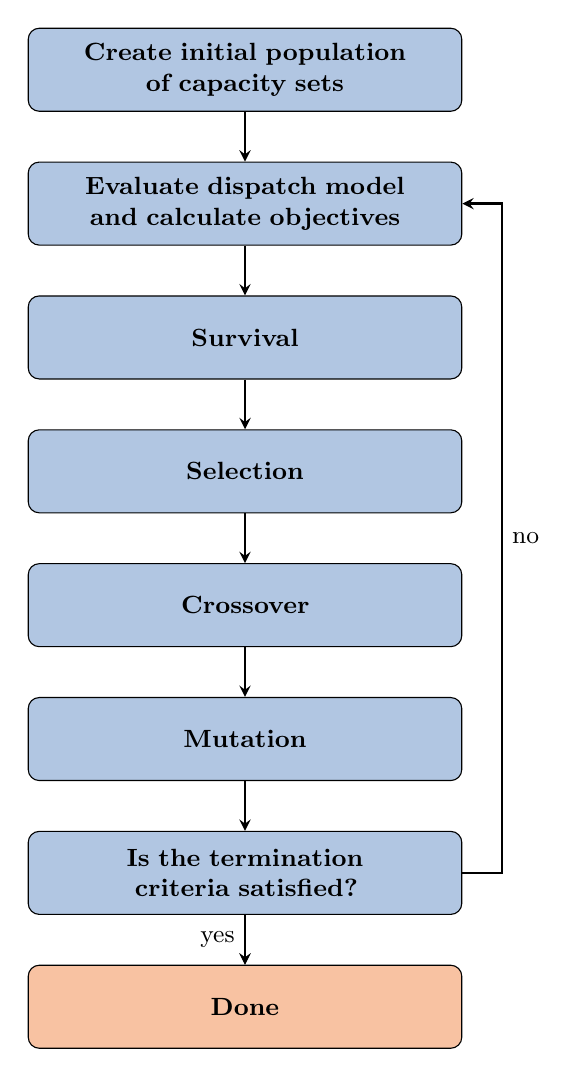
\begin{tikzpicture}[node distance=1.7cm]
                \tikzstyle{every node}=[font=\small] \node (1) [lbblock]
                {\textbf{Create initial population\\ of capacity sets}}; \node
                (2) [lbblock, below of=1] {\textbf{Evaluate dispatch model and
                calculate objectives}}; \node (3) [lbblock, below of=2]
                {\textbf{Survival}}; \node (4) [lbblock, below of=3]
                {\textbf{Selection}}; \node (5) [lbblock, below of=4]
                {\textbf{Crossover}}; \node (6) [lbblock, below of=5]
                {\textbf{Mutation}}; \node (7) [lbblock, below of=6] {\textbf{Is
                the termination \\ criteria satisfied?}}; \node (8) [loblock,
                below of=7] {\textbf{Done}}; \draw [arrow] (1) -- (2); \draw
                [arrow] (2) -- (3); \draw [arrow] (3) -- (4); \draw [arrow] (4)
                -- (5); \draw [arrow] (5) -- (6); \draw [arrow] (6) -- (7);
                \draw [arrow] (7) -- (8); \draw [arrow] (7) -- node[anchor=east]
                {yes} (8); \draw [arrow] (7) -- ([shift={(0.5cm,0cm)}]7.east)--
                node[anchor=west] {no} ([shift={(0.5cm,0cm)}]2.east)--(2);
        \end{tikzpicture}
        \caption{The basic flow of the \ac{ga} used in this thesis.}
        \label{fig:genetic-alg}
\end{figure}

\subsection{Specific \Aclp{ga}} The variety of \acp{ga} comes from different
types of operators being applied to the selection, crossover, and mutation
steps. Section \ref{section:moo-in-energy} showed that \ac{nsga2} is a popular
genetic algorithm choice. However, this algorithm performs poorly with greater
than three objectives \cite{deb_fast_2002, seada_unified_2016}. This thesis
uses a more modern algorithm, \ac{unsga3}. \ac{unsga3} builds on its
predecessors \ac{nsga2} and \ac{nsga3} by unifying efficient solutions of mono-,
multi-, and many-objective problems in a single algorithm.


\ac{nsga2} improves on the basic \ac{ga} by introducing a more sophisticated
mating and selection algorithms. Instead of random selection, the individuals
are sorted by rank (i.e. fitness) and crowding distance in binary tournament
mating selection. The crowding distance is simply the Manhattan distance between
individuals. A greater crowding distance is desirable to preserve diversity and
since the extreme points are maximally diverse they should always persist and
are therefore assigned a crowding distance of infinity \cite{deb_fast_2002}.

The successor to \ac{nsga2}, \ac{nsga3}, enhances the many-objective
capabilities of the former by introducing reference directions. Reference
directions are used for initialization and the survival steps. In addition to
fitness, individuals are chosen based on their proximity to a reference line,
thus ensuring population diversity which greatly important for many-objective
problems. Since diversity is handled by reference directions, individuals are
selected randomly for mating. References directions are rays passing through
uniformly spaced points on the unit simplex \cite{seada_unified_2016,
blank_generating_2021}. In this thesis, I use the Riesz s- Energy method
described by Blank et al. to calculate these points for a problem with an
arbitrary number of objectives \cite{blank_generating_2021}. Figure
\ref{fig:ref-dirs} illustrates a set of initialized reference directions used
in such methods.

\begin{figure}[h]
  \centering
  \resizebox{0.6\columnwidth}{!}{\input{figures/reference_directions.pgf}}
  \caption{A set of reference directions for a three-objective problem.}
  \label{fig:ref-dirs}
\end{figure}

\ac{nsga2} is useful for mono- and multi-objective functions while \ac{nsga3} is
better for many-objective problems. \ac{unsga3} can handle any number of
objectives by introducing the binary tournament from \ac{nsga2} and reducing to
the most efficient algorithm for the problem at hand \cite{seada_unified_2016}.
Chapter \ref{chapter:benchmark-results} demonstrates these three algorithms in 
Section \ref{section:4-exercise-1}.

\subsection{Hyperparameter Tuning}
Similar to other machine learning models, \acp{ga} have several hyperparameters
that must be tuned for optimal behavior. These hyperparameters include
probabilities for mutation, crossover, and selection, as well as the number of
parents, number of offspring, and population size. Determining ideal
hyperparameters is often performed using either a grid search or random sampling
\cite{bergstra_random_2012}. This thesis adopts the approach from Blank and Deb
\cite{blank_pymoo_2020} using a genetic algorithm to identify the ideal
hyperparameters. A multi-objective problem is converted into a single objective problem 
by choosing one objective and optimized with the target \ac{ga}, then a second \ac{ga} 
drives a new problem where the decision variables are hyperparameters of the desired algorithm.

\subsection{Convergence}
There are several ways to stop a simulation in \ac{pymoo}. A simulation may end
after reaching
\begin{enumerate}
    \item a specified end time (e.g., 100 minutes),
    \label{it:convergence1}
    \item a specified number of evaluations or iterations (e.g., 500 individual
    evaluations or 20 generations),
    \label{it:convergence2}
    \item a tolerance value in the design space,
    \label{it:convergence3}    
    \item a tolerance value in the objective space.
    \label{it:convergence4}
\end{enumerate}

It is possible that criteria \ref{it:convergence3} and \ref{it:convergence4}
will never be met; therefore, they are often combined with either of the first
two criteria. The fourth convergence criterion is the most interesting due to
the challenge of calculating an appropriate metric. This thesis uses the weakly
Pareto-compliant algorithm \ac{igdp} over the more common hypervolume
calculation due to its reduced computational requirements
\cite{ishibuchi_modified_2015}.

\subsection{\acs{pymoo} and \acs{deap}}

The \ac{esom} framework developed in this thesis is built on top of \ac{pymoo}
and \ac{deap}. \ac{pymoo} is an open-source library for \acp{ga} developed by
the creators of \ac{nsga2} and \ac{unsga3} \cite{blank_pymoo_2020}. This package
implements several \acp{ga} out-of-the-box and offers a set of visualization
tools and hyperparameter tuning. \ac{deap} is another open-source library
offering a toolkit for constructing \acp{ga} and therefore has fewer prepackaged
algorithms than \ac{pymoo}. There are robust reasons to use both libraries, so
\ac{osier} facilitates both. \ac{pymoo} provides a broader range of tools 
while \ac{deap} enables greater flexibility with \ac{ga} implementation and more
straightforward procedures for stopping a simulation and restarting at a later
time.





\section{Dispatch Model}
\ac{osier} offers three models for dispatching energy. The first is a merit order
dispatch model that optimally dispatches electricity according to the marginal
cost of generation with perfect foresight. This model is formulated as a
\acf{lp} and written in \ac{pyomo}. Similarly, the second dispatch model follows
merit-order but electricity is dispatched according to a hierarchy of rules and
is myopic. This approach is advantageous over the \ac{lp} formulation because it
facilitates parallelization and doesn't have the overhead cost of setting up the
problem. However, dispatch solutions may be sub-optimal compared to the \ac{lp}
approach. The third model is a simplified dispatch model that is very fast,
taking advantage of vectorization, but makes several assumptions about the
energy system and is not appropriate for general use.

\subsection{Economic/Merit-order dispatch}
\label{section:merit_order}

 The economic dispatch model minimizes the generation cost subject to physical
 constraints but does not optimize capacity investments. The complete set of
 equations for the model is detailed below.
\begin{align}
    \intertext{Minimize: }
    \label{eq:dispatch-objective}
    &\left(\sum_t^T\sum_g^G \left[C_{g,t}^{fuel} + C_{g,t}^{vom}\right]x_{g,t}
    \right)+\left(\sum_t^T\sum_g^S x_{g,t}c_{g,t}\pi\right)\\
    \intertext{such that,}
    \intertext{1. The generation meets demand, less the amount of energy stored or curtailed, 
    within a user-specified tolerance (undersupply and oversupply),}
    \left[\sum_g^Gx_{g,t}-\sum_g^S c_{g,t}\right] &\geq \left(1-\text{undersupply}\right)\text{D}_t\quad \forall \quad t \in T, S, \\
    \left[\sum_g^Gx_{g,t}-\sum_g^S c_{g,t}\right] &\leq \left(1+\text{oversupply}\right)\text{D}_t \quad \forall \quad t \in T, S,
    \intertext{2. A generator's production, $x_{g}$ does not exceed its capacity at any time, $t$}
    x_{g,t} &\leq \textbf{CAP}_{g}\Delta \tau \quad \forall \quad g,t \in G,T
    \intertext{3. A generator's ramping rate is never exceeded,}
    \frac{x_{r,t} - x_{r,t-1}}{\Delta \tau} = \Delta P_{r,t} &\leq
        \rho^{up}_g\textbf{CAP}_g\Delta\tau \quad \forall \quad r,t
        \in R, T,\\
    \frac{x_{r,t} - x_{r,t-1}}{\Delta \tau} = \Delta P_{r,t} &\leq
        -\rho^{down}_g\textbf{CAP}_g\Delta\tau \quad \forall \quad r,t
        \in R, T,
    \intertext{4. Storage capacity for each storage technology is never exceeded}
    \textbf{SOC}_{s,t} &\leq \textbf{CAP}^S_{s} \quad \forall \quad s,t \in S,T,
    \intertext{5. Storage discharge cannot exceed stored energy.}
    x_{s,t} &\leq \textbf{SOC}_{s,t} \quad \forall \quad s,t \in S,T,
    \intertext{6. Storage charge rate cannot exceed unit capacity}
    c_{s,t} &\leq \textbf{CAP}_{s}\Delta \tau \quad \forall \quad s,t \in S,T,
    \intertext{where,}
    G &= \text{ the set of all generating technologies},\nonumber\\
    R &= \text{ the set of all ramping technologies}, \quad R \subset G,\nonumber\\
    S &= \text{ the set of all storage technologies}, \quad S \subset G,\nonumber\\
    T &= \text{ the set of all time periods in the model},\nonumber\\
    D_t &= \text{ the demand at each time period, \textit{t}},\nonumber\\
    \textbf{CAP}_g &= \text{ the capacity of the \textit{g-th} technology}\quad \left[MW\right],\nonumber\\
    \textbf{CAP}^S_g &= \text{ the storage capacity of the \textit{g-th} technology}\quad \left[MWh\right],\nonumber\\
    \textbf{SOC}_{s,t} &= \text{ the state of charge of the \textit{g-th} technology at time \textit{t}}\quad \left[MWh\right]\nonumber,\\
    \Delta\tau &= t_{i+1} - t_i \quad \forall \quad t_i \in T \quad \left[h\right],\nonumber\\
    x_{g,t} &= \text{ the energy produced by generator, \textit{g}, at time, \textit{t}}\quad \left[MWh\right]\nonumber,\\
    c_{s,t} &= \text{ the energy stored by storage technology, \textit{s}, at time, \textit{t}}\quad \left[MWh\right]\nonumber,\\
    \rho_g &= \text{ the up/down ramp rate for technology, \textit{g}} \quad \left[-\right]\nonumber,\\
    \pi &= \text{ A small penalty for simultaneous charging and discharging.}\nonumber
\end{align}
The second term in the objective function, Equation \ref{eq:dispatch-objective},
represents a minor penalty to prevent the unphysical behavior of simultaneous
charging and discharging from storage technologies. I used this approach because
constraining this behavior requires a binary variable that makes the problem
non-convex and therefore requires a more sophisticated solver. A small but
sufficiently large $\pi$ will always nullify the penalty term. This dispatch
model reflects the minimum physical constraints for an energy system without
considering fine-scale operational details such as frequency control. Equation
\ref{eq:dispatch-objective} assumes that the retail cost for generating
electricity is identical to the marginal cost of producing electricity. 

\subsection{Hierarchical dispatch}

\subsection{Simplified dispatch}
\section{\acs{mga} with \acl{moo}}
\label{section:mga-moo}

\textcolor{red}{This section talks about handling ``structural uncertainty'' with \ac{osier}.}


This thesis applies some ideas from \ac{mga} to the analysis of the sub-optimal
space from a \acl{moo} problem. Due to their iterative process, \acp{ga}
naturally generate many samples in a problem's feasible space. However, this
does not lead to a ``limited set'' of solutions but rather a potentially
infinite set. Some literature developed \acp{ga} that directly use \ac{mga} in
the iterative process
\cite{zechman_evolutionary_2004,zechman_evolutionary_2013}. However, existing
Python libraries such as \ac{pymoo} and \ac{deap} do not implement these
methods, and the challenge is not an inability to sample the sub-optimal space,
but rather to provide a comprehensible subset of solutions. The algorithm I
developed in this thesis to search the near-feasible space is the following:

\begin{enumerate}
    \item Obtain a set of Pareto-optimal solutions \textit{using any \ac{ga}}.
    \item Decide on a slack value (e.g., 10\% or 0.1), which represents an
    acceptable deviation from the Pareto front.
    \item Create a ``near-feasible front'' where the coordinates of each point
    are multiplied by unity plus the slack value. This is equivalent to relaxing
    the objective functions and converting them to a constraint. 
    \item Every individual is checked if all of its coordinates are
    \begin{itemize}
        \item below all of the coordinates for at least one point on the
        near-feasible front and
        \item above all of the coordinates for at least one point on the Pareto
        front.
    \end{itemize}  
    \item Lastly, the set of interior points may be sampled either randomly or with a
    farthest-first-traversal algorithm to restrict the number of analyzed solutions.
\end{enumerate}
\noindent
Figure \ref{fig:nd-mga} and Figure \ref{fig:3d-mga} demonstrate this algorithm
with 10 percent slack for a 2-D and 3-D Pareto front, respectively. Figure
\ref{fig:nd-mga} shows clearly that only points within the near-optimal space
(gray) are considered. Illustrating this behavior in three dimensions (and
above) is considerably more difficult. The 3-D interior points should be covered
by both surfaces, obstructing their view. Figure \ref{fig:3d-mga} shows that
this is the case in three panels. First, a top view of an opaque Pareto front
(green) where no interior points can be observed. Second, the same view with a
translucent Pareto front, revealing interior points and the near-optimal front
(blue). Finally, the view from underneath the near-optimal front once again
obscures the interior points, except for two near the edges of the sub-optimal
space. The tested points are omitted for clarity.
 

\begin{figure}[h]
  \centering
  \resizebox{0.6\columnwidth}{!}{\input{figures/nd-mga-paretofront.pgf}}
  \caption{All of the alternative points inside the near-feasible space selected
  using the algorithm described in Section \ref{section:mga-moo}.}
  \label{fig:nd-mga}
\end{figure}

\begin{figure}[H]
  \centering
  \resizebox{1\columnwidth}{!}{\input{figures/3d-mga-paretofront.pgf}}
  \caption{From left to right: An opaque Pareto front; a translucent Pareto front showing the interior points above a sub-optimal front; and the sub-optimal front hiding the interior points from a different angle.}
  \label{fig:3d-mga}
\end{figure}
\section{Limitations of \ac{osier}}

This section describes some of the limitations in \ac{osier}'s modeling details
and scope. For example, \ac{osier} does not model interactions between the
environment and the energy system. It also does not include a way to model the
effect of carbon emissions and/or any kind of climate forcing from heat-trapping
emissions nor any kind of geoengineering measures.

This responds to some of Cliff's comments on \ac{osier}.


\chapter{Benchmark Results}
\label{chapter:benchmark-results}

% \textcolor{red}{This chapter will remain largely unchanged except for maybe one
% additional example, demonstrating a different dispatch model that is much faster
% but less robust. This new dispatch model will be used in the following chapter
% where I investigate further examples including a hypothetical ``data center''
% and an improvement on the \acf{set} \cite{wigeland_nuclear_2014}.}

% \section{Exercise 0: Demonstrating \ac{osier}}
% \textcolor{red}{This section is new in the dissertation!}

% This section demonstrates some of the basic features of Osier. This section should be based 
% on the examples in \ac{osier}'s documentation.

% \section{Exercise 1: Deciding Among Evolutionary Algorithms}

% \textit{Already written in prelim document.}

% \section{Exercise 2: Exploring objective space}

% \textit{Already written in prelim document.}

% \section{Exercise 3: Four Simultaneous Objectives}

% \textit{Already written in prelim document.}

% \section{Exercise 4: Validating a Simplified Approach}

% \textcolor{red}{This section is new in the dissertation.}

\chapter{Examples with \acs{osier}}
\label{chapter:examples}

\textcolor{red}{This chapter is entirely new to this thesis!}

\section{Example 1: Updating the \ac{set}}

\textcolor{red}{Points to hit:}
\begin{enumerate}
    \item Addressing the climate crisis requires new infrastructure and new energy sources.
    \item Progress has been stifled on many fronts, not the least of which has been public opposition to energy projects. Including wind, solar, and nuclear.
    \item Some of this opposition results from dissatisfaction with process.
    \item Opposition can be pre-empted with sincere and proactive community engagement.
    \item In the case of nuclear energy, some of these efforts are already underway with concepts such as consent-based siting entering the nuclear zeitgeist.
    \item ???
    \item Introduce the \ac{set} tool
    \item  Introduce \ac{osier} as a tool for multi-objective optimization.
\end{enumerate}

\textcolor{red}{Benefits of using \ac{osier}}:
\begin{enumerate}
    \item Python interface allows direct coupling with external models and data sources for greater flexibility.
    \item Enables, but does not require, a weighting scheme for decision making.
    \item Allows users to analyze tradeoffs among competing objectives.
    \item Allows users to compare lifecycle impacts with non-nuclear technologies.
    \item Can flexibly add additional assessment criteria (e.g., Energy return on investment). 
\end{enumerate}

\textcolor{red}{Results}
\begin{enumerate}
    \item Does using \ac{osier} support the previous conclusions about the most promising evaluation groups?
\end{enumerate}

\subsection{Overview of the Nuclear Fuel Cycle}

\subsection{What is the \ac{set}?}

\subsection{What metrics are available?}

\subsection{Data for the simulation}

\subsection{Results}

\subsection{Discussion}

% \section{Example 2: Powering a Data Center}

% \subsection{Why data centers?}

% \subsection{What technology options exist?}

% \subsection{Data for the simulation}

% \subsection{Results}

% \subsection{Discussion}


\chapter{Using modeling to enhance just outcomes}
\label{chapter:communities}
\iffalse


This chapter addresses my proposal to ``validate'' \ac{osier} by conducting a
case study of energy planning processes in Champaign-Urbana through interviews
with decision makers and planners about energy justice, energy modeling, and
energy planning. As well as introduce interviewees to \ac{osier} itself and
solicit feedback from them about its potential usefulness and what obstacles may
interfere with its adoption. 

Although I originally set out to conduct a limited case study of Chambana, I
discovered that municipalities in Illinois do not, in general, have the decision
making authority to make specific choices about their energy supply.
Thus, I expanded my study to the state level; interviewing people from the
\ac{ipa} and \ac{icc}. This expanded scope provided evidence for structural
challenges blocking municipal influence from energy planning processes. Further,
this evinces a tension among distributive, procedural, and recognition justice.

\section{Progress on developing tools for local use}

\begin{itemize}
    \item The literature review chapter indicated that most energy modeling tools
    and much of the related literature focus on state- or national-scale energy
    systems.
    \item The the hyper-local section highlighted some studies that integrated
    local perspectives with energy modeling. Those papers include 
    \cite{mckenna_combining_2018, johannsen_municipal_2023, fleischhacker_portfolio_2019}
    \item There have also been studies investigating the development of models for, and
    use by, city and urban planners.
\end{itemize}

\section{Municipal Levers: How municipalities make choices about their energy supply}
There are generally four ways municipalities can make choices about their energy supply.

\subsection{\ac{mca}}
This is where municipalities participate in electricity markets on behalf of
their residents. Although this allows municipalities to choose an energy supply
besides the standard portfolio provided by an electric utility, municipalities
do not have full control over their energy supply. Instead, municipalities
negotiate for a few portfolios through a bidding process. While they can specify
some criteria, such as a percentage of renewable energy, the specific generation
mix depends on the company that developed the portfolio bid. Further, residents
are still allowed to opt-out of \ac{mca} and elect the standard portfolio
provided by their electric utility.

\subsection{Utility ownership}
Some municipalities in Illinois, such as Naperville, own their own distribution
system. This gives a municipality greater control over the design of their
utility system and allows a municipality to make decisions about the tradeoff
between cost and resiliency. For example, Naperville undergounded most of the
electric distribution system and new distribution is automatically undergounded.
However, this model does not award control of electric supply to the
municipality, which must procure electricity through another entity such as the
\acf{imea}.

\subsection{Municipal-owned generation}
In very few cases, a municipality may own some of its own generation. \ac{uiuc}
owns a coal and natural gas plant, a solar array, chilled water storage, and
participates in a \ac{ppa} to purchase wind power. More commonly, municipalities
will lease land cheaply to a solar company, for example, and purchase some or all
of the rights to that electricity through a \ac{ppa}. 

\subsection{Municipal-owned buildings}

\fi

\chapter{Conclusions}

% \chapter{Motivation and Introduction}
% % input individual chapters files
% Climate change produced by greater atmospheric CO$_2$ concentrations
\cite{kane_atmospheric_1996} from human activity has led to increased exposure
to hazards worldwide and domestically: increased storm severity, rising sea
levels, more extreme temperatures, hotter summers, and rising sea levels to name
a few \cite{reidmiller_fourth_2018}. Without immediate action to reduce carbon
emissions, these impacts will worsen
\cite{intergovernmental_panel_on_climate_change_climate_2014}. Specifically, it
is primarily our societal dependence on fossil fuels to support our expansive
economies and energy systems that contributes the most to rising carbon dioxide
levels (along with other \acp{ghg}) \cite{epa_inventory_2023}. Therefore, to
achieve the almost universally shared goal of halting and reversing the effects
of climate change \cite{united_nations_paris_2015}, our globalized society must
transition away from fossil fuels to clean energy technologies such as nuclear
and renewable energy and switch our transportation systems to electric or
hydrogen powered vehicles
\cite{intergovernmental_panel_on_climate_change_climate_2021}. 

Naturally, the importance of modeling energy systems to gain insight and form
strategies to achieve this transition has grown. Especially since the spatial
and temporal complexities are also expected to grow with greater penetration of
\ac{vre}, such as solar and wind energy --- two energy sources that are
spatially diffuse and temporally challenging to predict. A class of tools called
\acp{esom} are the most common method for understanding our energy systems.
However, while climate change may be the most immediate existential threat to
society \cite{hickman_climate_2021}, it is a focusing issue that brings
challenges of equity and disproportional impacts to the fore. These latter
challenges have been always been concomitant with our energy system, but energy
system modeling has largely ignored the ways energy systems mediate
socio-political power alongside transporting electrons and fuel. For example,
fossil fueled power plants have always been associated with air pollution and
worsened health for nearby communities --- commonly poorer and black
communities, which are already marginalized, evincing a violation of fairness
and justice principles \cite{mohai_which_2015}. Studying these consequences of
our energy choices historically belonged to domain of the environmental justice
literature \cite{schlosberg_reconceiving_2004,mohai_environmental_2009} but has
developed further into the discipline of energy justice
\cite{sovacool_energy_2015}. 

The energy transition will require a great expansion of our energy
infrastructure to build replace fossil-fueled energy with clean energy and
additional transmission networks to carry electrons. Although the technology to
accomplish this transition is mature, there is still local public opposition to
many energy projects \cite{wolsink_wind_2007}. Particularly in empowered and
affluent communities \cite{stokes_prevalence_2023}. \acp{esom} cannot capture
these ``human dimensions'' of energy systems despite some awareness of their
importance \cite{pfenninger_energy_2014}. This is because they only optimize a
single objective --- cost (or some other aggregated economic metric). People
have and express preferences over many dimensions simultaneously. Further, even
in the absence of climate change, incorporating social context into the practice
of energy modeling remains beneficial since doing so will create substantively
better decisions \cite{wilsdon_see-through_2004}. The solution for enclosing
this feature of energy system design proposed in this thesis is two-fold. The
first is to develop an \ac{esom} capable of multi-objective optimization. The
benefits of multi-objective optimization have been understood for some time, yet
only recent advances in computing power have made them a practical method for
energy modeling. Hobbs (1995) wrote:

\begin{quote}
    Multi-objective methods are more appropriately used to help people to
    understand the problem better, explore their feelings, form a coherent,
    defensible set of values, and understand the implications of those values
    for the decision. [...] In reality, people's values are often uncertain and
    incoherent. During the course of a planning exercise, people's attitudes
    will evolve in response to new information, interactions with other people,
    and viewing the problem from different perspectives
    \cite{hobbs_optimization_1995}.    
\end{quote}

This leads to the second major proposal for this thesis, which is to validate
the multi-objective \ac{esom} developed within by conducting a case study in the
Champaign-Urbana region involving interviews with local energy planners and
incorporating their feedback to develop a planning process that encourages
greater participation by the community members. Altogether, this work will allow
``non-technical'' perspectives to be incorporated into a rigorous modeling
framework leading to greater perceptions of legitimacy through an iterative
articulation of values and priorities involving the public as key deliberators.
The result is a step towards a holistic integration of energy justice and energy
system engineering.

Chapter \ref{chapter:lit-review} discusses the existing literature and work from
several spanning disciplines, including risk assessment, energy justice, and
energy system optimization. Chapter \ref{chapter:methods} details the technical
methods I applied to create a flexible multi-objective optimization framework
called \ac{osier}. Chapter \ref{chapter:benchmark-results} validates \ac{osier}
as an \ac{esom} by comparing its results against an established representative
\ac{esom}, and demonstrates current progress. Finally, Chapter
\ref{chapter:proposal} outlines a proposal for the remaining work of this
thesis.

\section{Motivation}

\textcolor{red}{CO2 emissions}

\textcolor{red}{Emissions by energy source}

\section{Research Objectives}

\section{Reproducing this work}
Talk about \texttt{snakemake}, show the DAG... 

% \newpage
% \begin{landscape}
    \begin{figure}[h!]
        \centering
        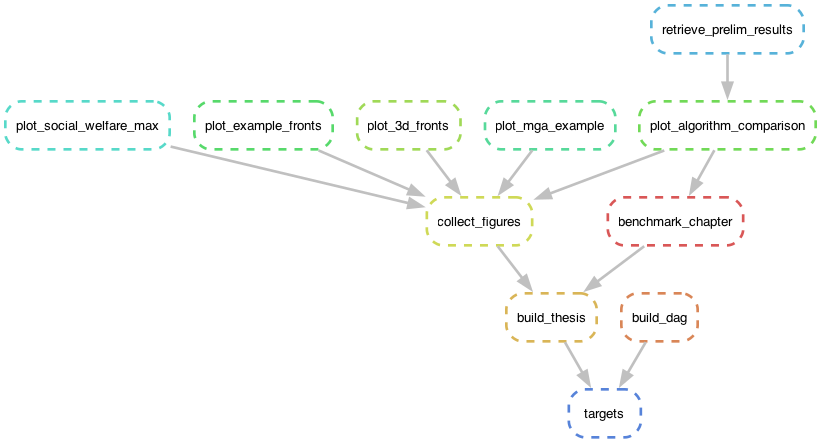
\includegraphics[width=\columnwidth]{../analysis/dag.png}
        \caption{The \ac{dag} illustrating the steps to produce this thesis.}
        \label{fig:dag}
    \end{figure}
% \end{landscape}

% Every year, world leaders meet to discuss plans to address climate change at the
COP summit. In 1995, world leaders established a set of targets with the Kyoto
Protocol \cite{united_nations_kyoto_1998} and again with the 2016 Paris Climate
Agreement \cite{united_nations_paris_2015}. Every few years, the United Nations
releases a report from the \ac{ipcc} assessing the current impacts of climate
change and forecasting future scenarios. Most of the world understands that
anthropogenic climate change is an existential threat to society. Indeed, many
studies in the \ac{esom} literature begin with a statement about the urgency of
climate change. This chapter reviews the extant literature for both quantitative
and qualitative analyses of the problem considered in this thesis --- primarily
bridging the gap between feasibility or planning studies to address the climate
crisis and the current pattern of missed targets and growing carbon emissions.
First, I draw from the risk assessment literature to characterize and situate
the problem of climate change and demonstrate the necessity of a holistic
analysis. Second, I build upon the central issue of disproportionality of
climate change risk by reviewing the energy and environmental justice
literature. Third, I develop an encompassing definition of an ``energy system''
using technical and social perspectives. Finally, I review the energy system
literature for gaps in conventional modeling practices and identify previous
attempts to incorporate social science and justice concepts into energy system
models.

% The first section reviews methods and attempts to model energy systems for
% planning purposes. The second section reviews the ways social movements help
% or hinder various energy projects, how governments succeed or fail to achieve
% their energy goals from this perspective, and why some communities favor or
% disfavor energy projects.

\section{Characterizing the Problem of Climate Change}
\label{section:climate-change-risk}

Risk is generally understood as the ``potential for adverse consequences''
\cite{reisinger_concept_2020}. However, due to the complexity of climate change,
the \ac{ipcc} developed a three-tenet framework to discuss risk
\cite{reisinger_concept_2020}: hazard, exposure, and vulnerability.
\textit{Hazards} are mediated by physical features, such as climate and
topography \cite{dorkenoo_critical_2022,simpson_framework_2021}.  Climate change
is already producing more significant hazards, like forest fires, hurricanes,
storms, floods, droughts, and heat waves
\cite{reidmiller_fourth_2018,intergovernmental_panel_on_climate_change_climate_2021,dahl_killer_2019}.
\textit{Exposure} refers to the scale and duration of the subjection of people,
infrastructure, and social wealth to a particular hazard
\cite{simpson_framework_2021,reisinger_concept_2020,li_understanding_2021}.
\textit{Vulnerability} is the ability of a system to cope, recover, and adapt
after exposure to a hazard. Although climate change is a worldwide phenomenon,
vulnerabilities to its hazards are not uniformly distributed. On the contrary,
the people and communities most likely to be harmed by climate change are
already harmed by social inequities \cite{islam_climate_2017}. For example,
low-income communities have fewer resources to respond to natural hazards, such
as hurricanes, floods, or fires, and therefore take longer to recover, compared
to a communities with relatively greater wealth. Recent work from Simpson et al.
\cite{simpson_framework_2021} expanded on this definition of risk by including
\textit{responses} to risk as itself a driver of risk. This framework is
illustrated in Figure \ref{fig:risk-framework} using infrastructure risk as an
instructive example. Considering the actions taken (or not) in response to
climate change is vital for a holistic understanding of risk because it
encompasses benefits and mitigating outcomes, not just negative, inflammatory
ones. Additionally, heterogeneous stakeholders perceive the costs and benefits
of (in)action differently. Therefore, including response as a component of risk
is essential for making choices more transparent and actionable within
decision-making structures \cite{simpson_framework_2021}. Responses to climate
change risk come in myriad forms,  and at multiple scales, from individual
choices (e.g., demand response) \cite{seck_embedding_2020,rinaldi_what_2022,
dehghanpour_agent-based_2018} to community responses
\cite{paterson_community-based_2019, elmallah_frontlining_2022}, national level
policies \cite{roelfsema_taking_2020, fawzy_strategies_2020}, and levels in
between. Paterson and Charles \cite{paterson_community-based_2019} developed a
descriptive typology for community-based hazard responses that also applies to
national and global scales. The five response categories making up this typology
are:
\cite{paterson_community-based_2019}
\begin{enumerate}
    \item individual and material well-being, which seek to meet individuals'
    basic needs such as food, water, and shelter, as well as livelihood and
    health.
    \item relational well-being, which emphasizes community and support networks
    and could include evacuation or relocation.
    \item awareness, which involves monitoring and stock-taking of potential
    hazards.
    \item governance, which relates to decision-making structures around
    human-hazard interactions.
    \item infrastructure, which refers to the physical defense against hazards
    using engineered tools or ecological characteristics.
\end{enumerate} 
Figure \ref{fig:risk-response} shows the breakdown of the categories. Although
this framework could help assess policies to mitigate climate change, these
response categories are related to specific climate hazards rather than climate
change mitigation.


\begin{figure}
    \centering
    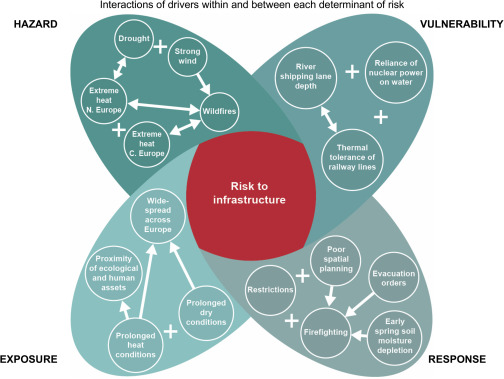
\includegraphics{figures/02_literature_review/simpson-risk-framework.jpg}
    \caption{A framework for decomposing risk into its parts: hazard, exposure,
    vulnerability, and response, using risk to infrastructure as an illustrative
    example. Reproduced from Simpson et al. (2021)
    \cite{simpson_framework_2021}.}
    \label{fig:risk-framework}
\end{figure}

\begin{figure}
    \centering
    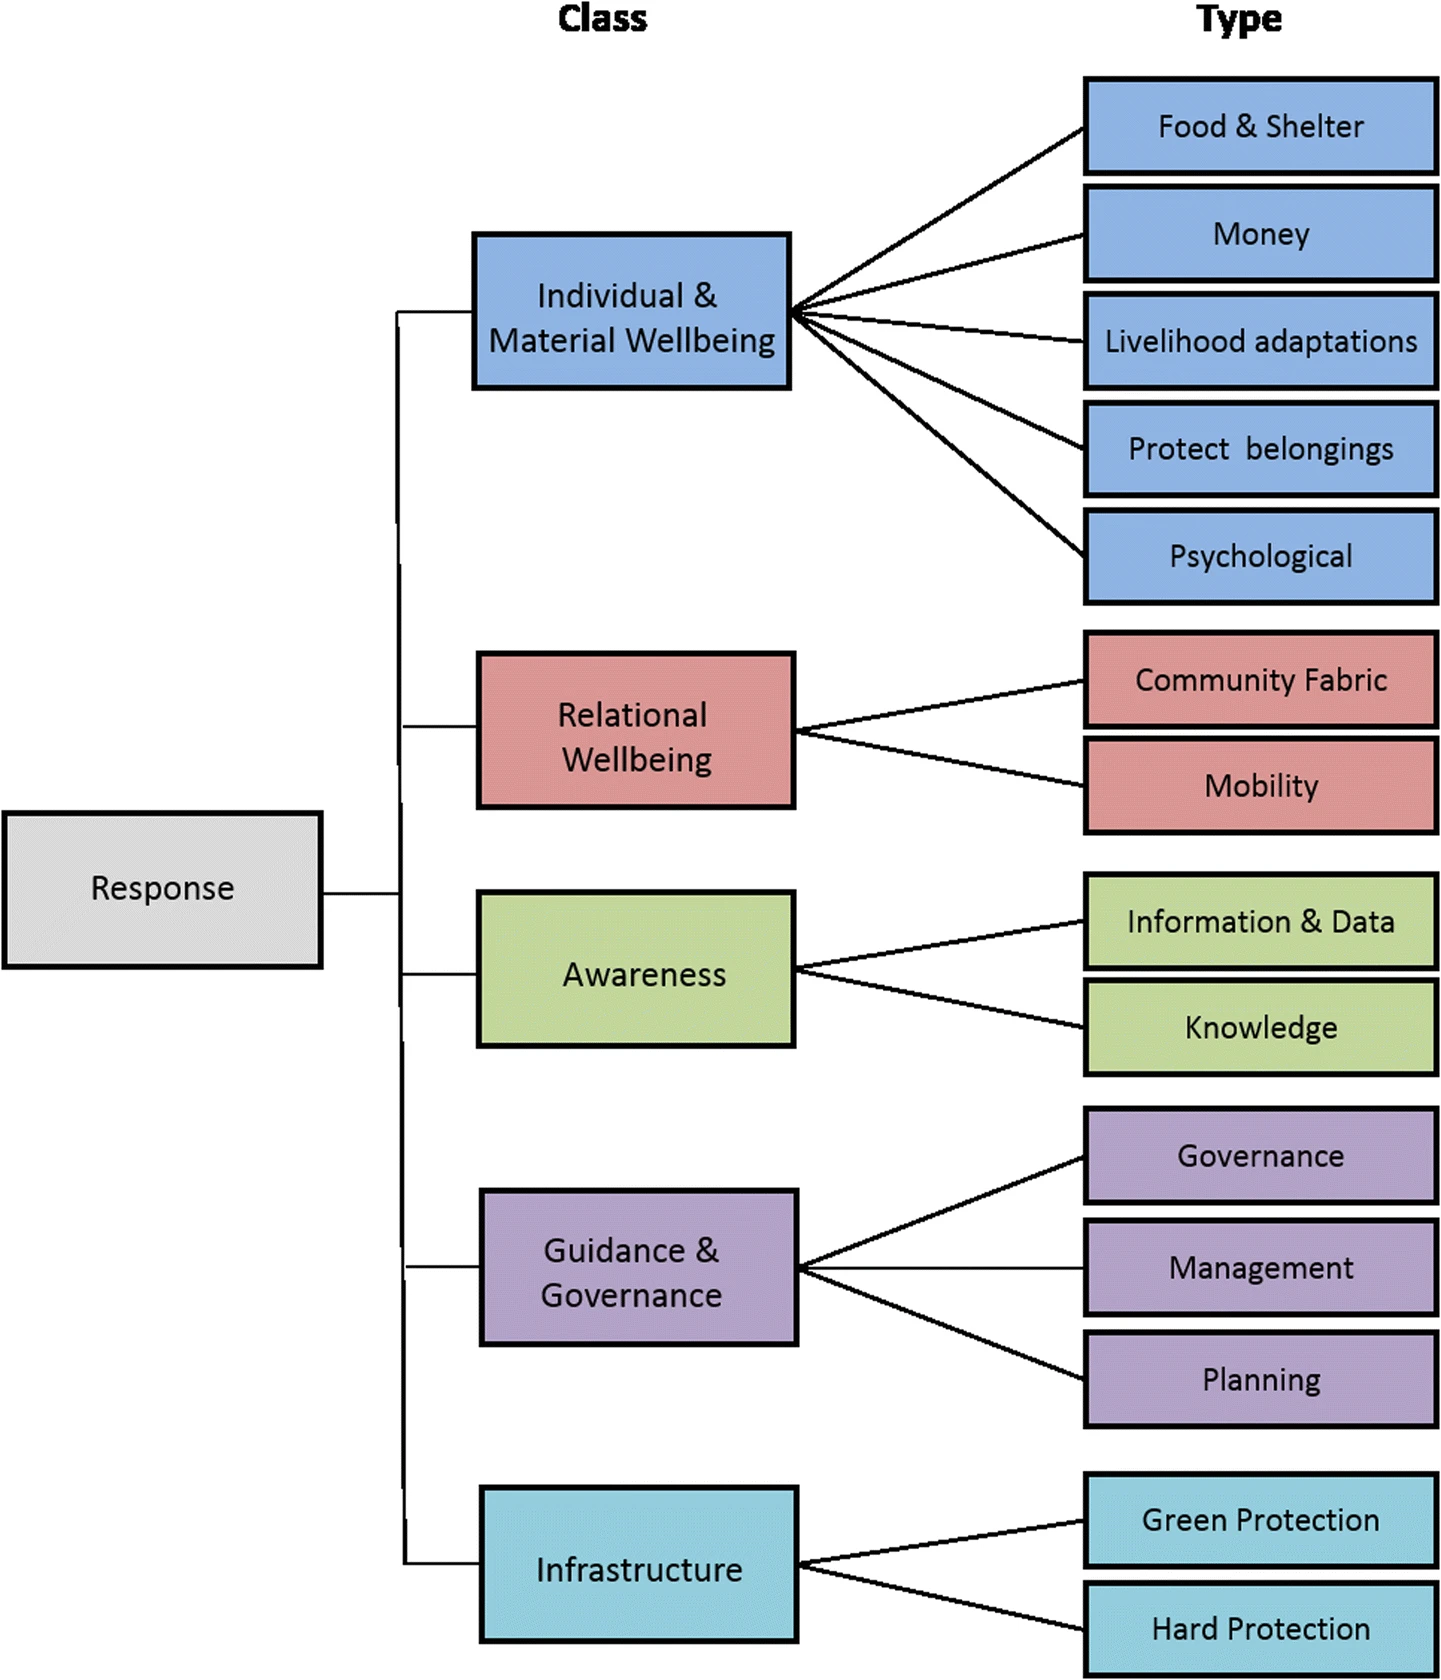
\includegraphics[width=\columnwidth]{figures/02_literature_review/risk-response.png}
    \caption{A categorization typology for various responses to climate risks.
    Reproduced from Paterson et al. (2019)
    \cite{paterson_community-based_2019}.}
    \label{fig:risk-response}
\end{figure}

% \noindent\hrulefill \item What are the responses to climate change? How
% successful have climate policies been at achieving climate goals (and
% ultimately achieving net zero carbon emissions)?

Based on the net-zero carbon emissions target set by the 2016 Paris Agreement,
myriad countries, states, and companies have set climate policies covering
two-thirds of the global economy \cite{hale_assessing_2022}. Reducing \ac{co2}
(or \ac{co2eq} in some cases) emissions is the primary focus for most of these
policies \cite{fawzy_strategies_2020, roelfsema_taking_2020,
hale_assessing_2022}, which include the following broad strategies
\cite{fawzy_strategies_2020}:
\begin{enumerate}
    \item Reducing \ac{ghg} emissions by transitioning from fossil-fueled to
    clean energy.
    \item Removing \ac{co2} from the atmosphere using \ac{ccs} and other
    sequestration techniques.
    \item Altering the Earth's energy balance by increasing its albedo and other
    geoengineering concepts.
\end{enumerate}
Despite this, only around five percent of these policies are consistent with the
\ac{un} ``Race to Zero'' campaign \cite{hale_assessing_2022}. Further, even the
full implementation of national climate policies leaves approximately  a 28
Gt\ac{co2eq} gap in \ac{ghg} emissions \cite{roelfsema_taking_2020} (with the
implicit goal of zero emissions). This gap and the fundamental assumptions about
carbon sequestration from the 2016 Paris Agreement suggest that the world is on
track to overshoot these emissions targets
\cite{roelfsema_taking_2020,taylor_managing_2021}. Carley et al. (2018)
developed a quantitative framework for assessing the vulnerabilities associated
with energy policies or responses \cite{carley_framework_2018}.

% \noindent\hrulefill \item What are the impacts of climate change?

Risk analysis is the first step to a more encompassing understanding of the
climate crisis. The literature on disproportionality further distinguishes
\textit{risks} and \textit{impacts} \cite{dorkenoo_critical_2022}. Consistent
with previous work, a risk is the aggregate of hazards, exposures,
vulnerabilities, and responses. Impacts, then, are the realizations of risk in
terms of loss and damages. This distinction is essential. Responses to
\textit{impacts} are always made \textit{ex post facto}. Differences in
vulnerability to a hazard, often arbitrated by socio-economic status, manifest
as differential impacts. Access to resources conditions an individual's or
community's ability to respond to the impacts of a hazard. Since losses from
impacts disproportionately affect those with the fewest resources, their
vulnerability to future hazards increases in a ``vicious cycle''
\cite{islam_climate_2017, dorkenoo_critical_2022}. In purely economic terms,
studies estimate the loss of ecosystem services from land use change associated
with climate change and other human activities at \$4 - \$20 trillion per year
(in 2011 \$US) globally, \cite{costanza_changes_2014} and the poorest third of
U.S. counties will experience financial damages between 2 and 20 percent of
their annual income \cite{hsiang_estimating_2017}. However, impacts also have
cultural and psychological dimensions \cite{dorkenoo_critical_2022} that cannot
be captured by accounting for ``externalities.''

% \noindent\hrulefill

% \item How are the damages of climate change distributed, and \textit{why} are
% they distributed this way?

Dorkenoo et al. \cite{dorkenoo_critical_2022} establish \textit{burdens},
injustices arising from social, political, or economic power imbalances, as a
third theme paramount for a holistic understanding of disproportionality.
Burdens influence all aspects of risk and affect access to resources which
condition impacts. Dorkenoo et al. wrote, ``[p]rocesses of marginalization and
exclusion influenced by power struggles [...] influence the distribution of
burdens and consequently responsibilities, in addition to the different
dimensions of climate risk (hazard, exposure, vulnerability [, response])''
\cite{dorkenoo_critical_2022}. Figure \ref{fig:risk-impact-burden} demonstrates
the mutually reinforcing relationships among risks, impacts, and burdens. A
particularly relevant example of burden is the persistence of energy burden,
where low-income households pay the highest percentage of their income on energy
bills relative to other income groups \cite{brown_high_2020,
cong_unveiling_2022}. Energy burden interferes with electricity access, thereby
increasing vulnerability to extreme heat events \cite{cong_unveiling_2022,
klinenberg_heat_2003}. The risk assessment literature and the energy system
modeling literature typically adopt an apolitical framing of vulnerabilities.
That is to say, these literature analyze their respective systems independent of
any sociopolitical context. However, inequities do not arise in a vacuum but
through processes of marginalization and exclusion
\cite{thomas_explaining_2019}. Often the distribution of burdens falls along
class, race, and gendered lines \cite{thomas_explaining_2019,mohai_which_2015}.
Research on siting patterns of polluting facilities indicates these projects
frequently developed in areas with people of color and low-income populations
\cite{mohai_which_2015}. Pollution from these facilities creates additional
burdens for nearby communities. The energy justice and environmental justice
literature offer insights to contrast this neutral framing and facilitate
normative questions about alternative distributions
\cite{dorkenoo_critical_2022, thomas_explaining_2019}.

\begin{figure}
    \centering
    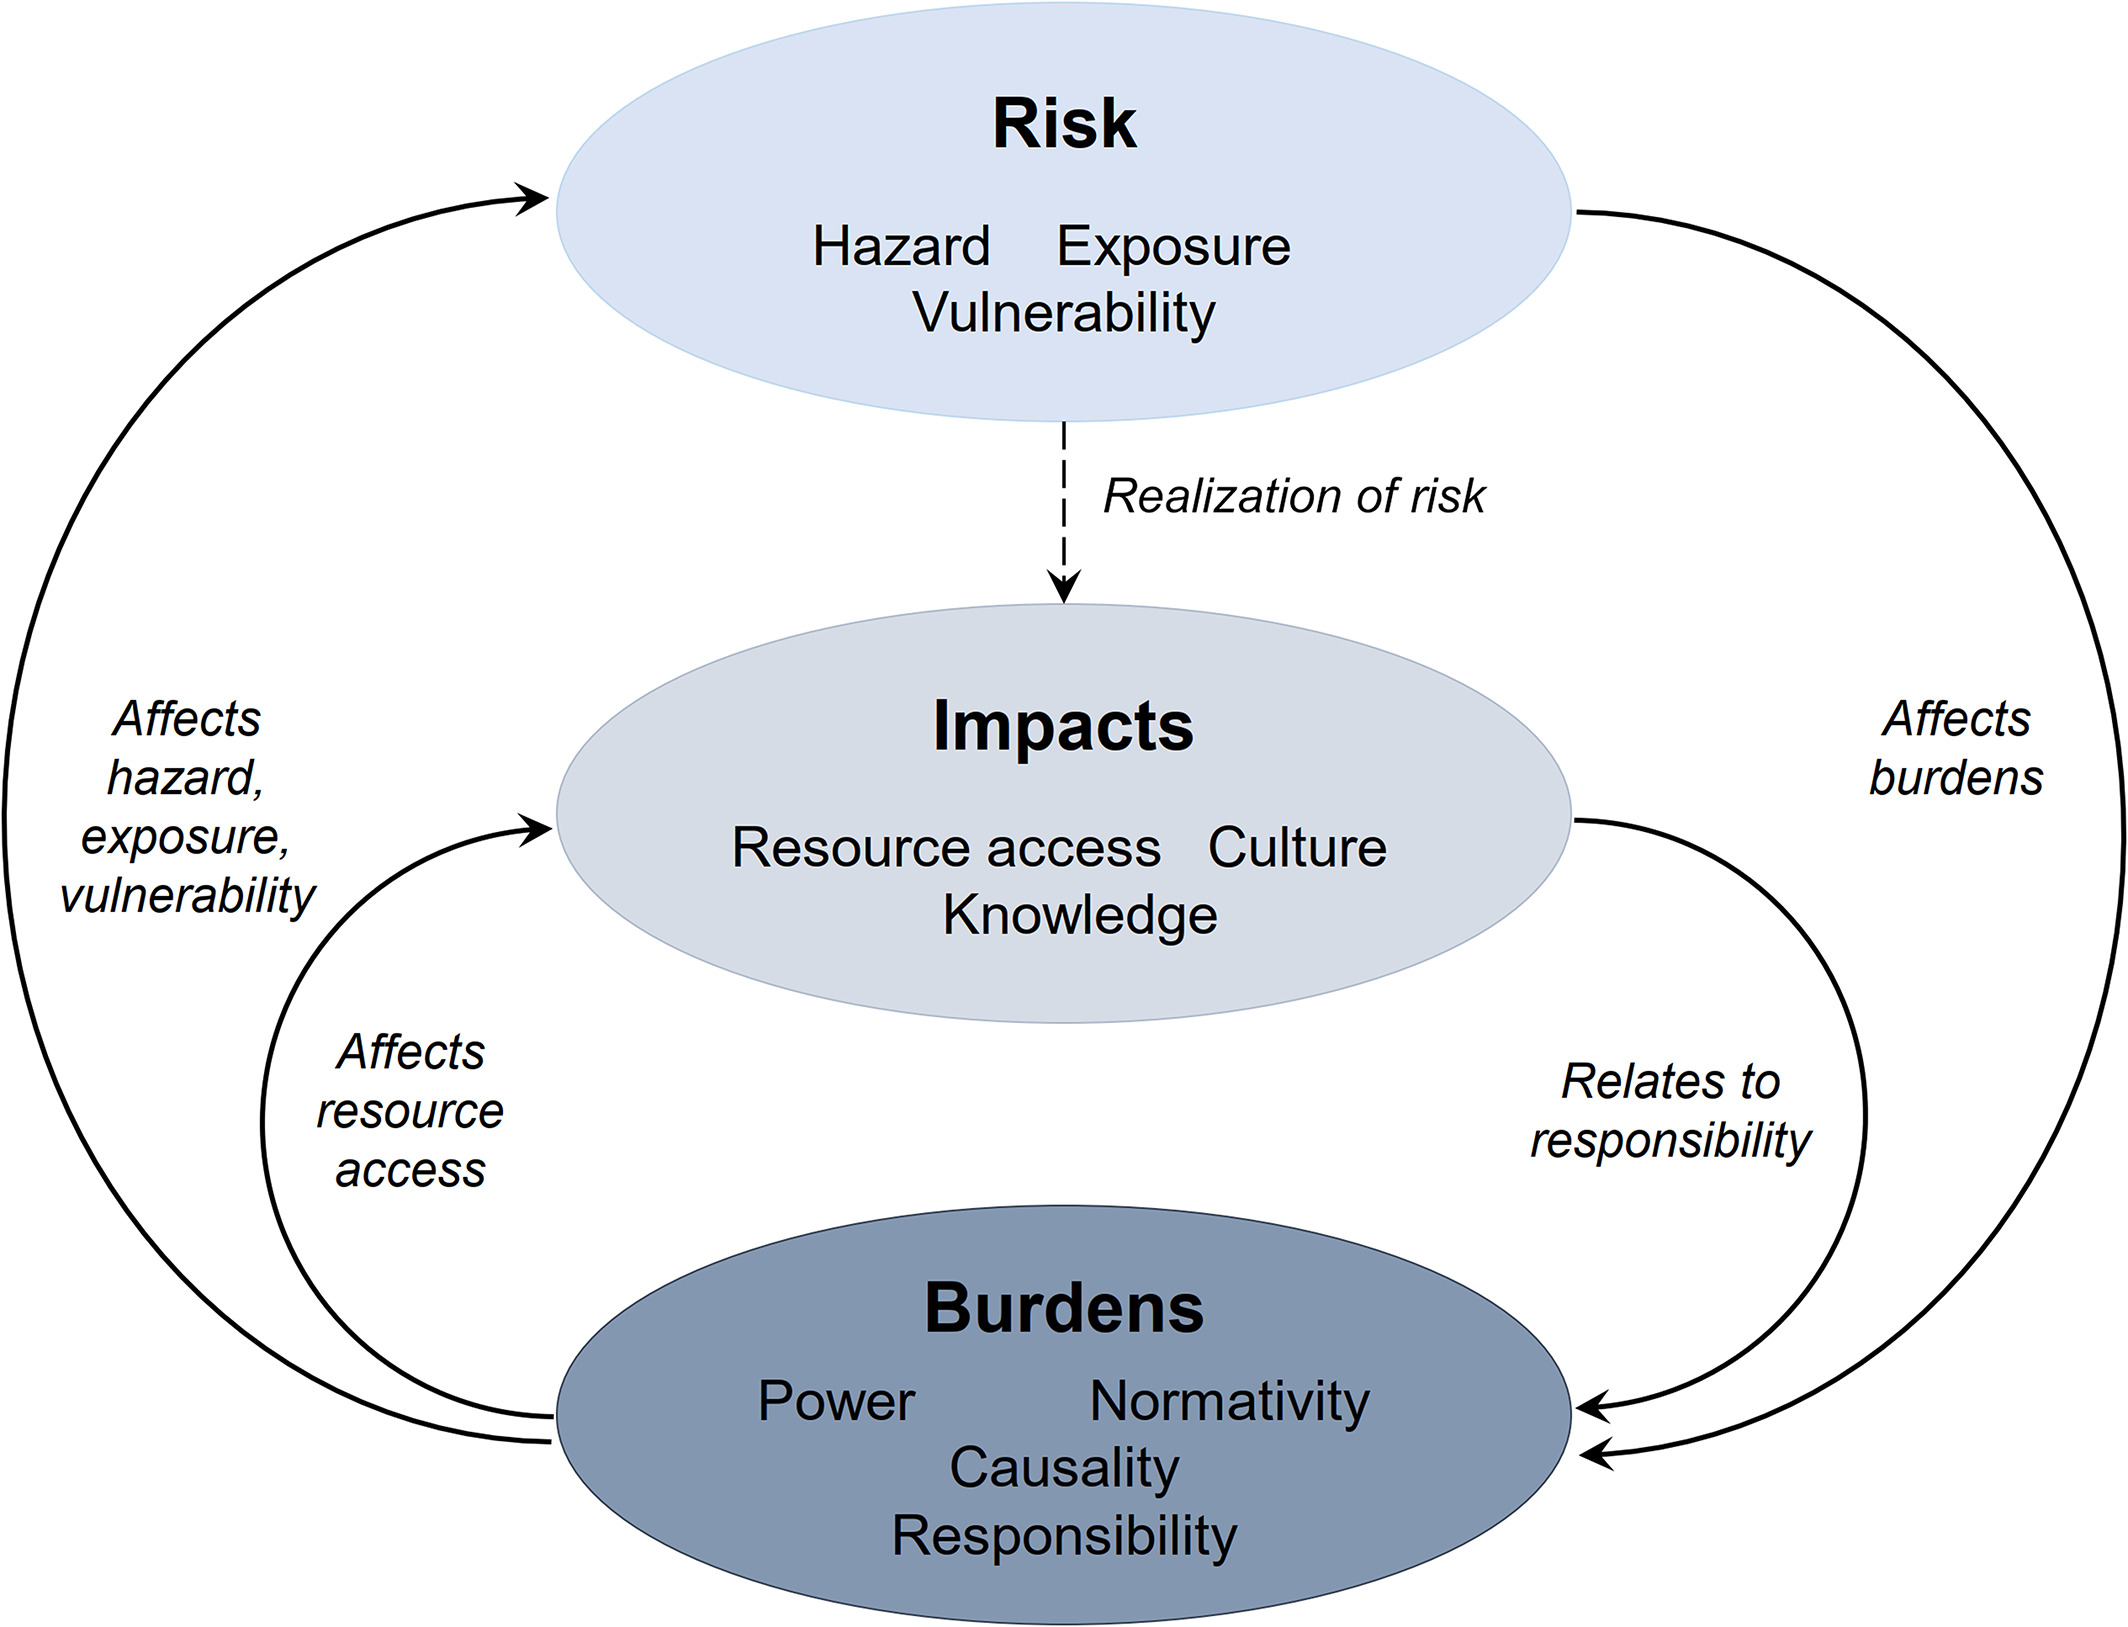
\includegraphics[width=\columnwidth]{figures/02_literature_review/dorkenoo-disproportionality.jpg}
    \caption{The relationships among risks, impacts, and burdens. Reproduced
    from Dorkenoo et al. (2022) \cite{dorkenoo_critical_2022}.}
    \label{fig:risk-impact-burden}
\end{figure}


% \noindent\hrulefill

% \textcolor{red}{Subsection: Climate and Energy Systems}
\section{Climate and Energy Systems}

Climate change is driven by the buildup of additional \acp{ghg} in our
atmosphere from human activities. \acp{ghg} are a significant byproduct of the
infrastructure that creates, delivers, and consumes energy (i.e., energy
infrastructure). The total decarbonization of the global economy will lead to
greater electricity demand, even when accounting for efficiency improvements
\cite{national_academies_of_sciences_engineering_and_medicine_accelerating_2021,
mai_electrification_2018}, decarbonizing our electricity production is one of
the most critical issues to resolving climate change. Therefore, producing
electricity with zero \acp{ghg} will initiate a cascade of deeper
decarbonization throughout the economy. However, this will require expanded
electrical infrastructure to accomodate new energy technologies. Since, energy
production contributes significantly to climate change, and new energy
infrastructure is required to reduce carbon emissions in other sectors (e.g.
heat and transportation), accelerating the adoption of clean energy technology
(i.e. technologies that do not release \acp{ghg} to the atmosphere) is essential
for achieving a stable climate \cite{roelfsema_taking_2020,
taylor_managing_2021}. The next section discusses the range of technical
solutions for accomplishing the goals established above.

% \textcolor{red}{Subsubsection: Technical solutions to energy decarbonization}
\subsection{Technical Solutions to Energy Decarbonization}
% \item What are the technical solutions for decarbonizing the electricity
% sector?

Many studies show that global and local economies can be supported by 100\%
\ac{vre}, such as wind, hydro, solar power, and storage \cite{jacobson_100_2015,
bussar_optimal_2014,brown_response_2018,dorotic_integration_2019,wallsgrove_emerging_2021,
cochran_la100_2021,cosic_100_2012,traber_economically_2021,bogdanov_full_2021,
bogdanov_north-east_2016,
esteban_100_2018,yue_least_2020,neumann_near-optimal_2021}. Yet some countries
that transition to majority \ac{vre} observe higher carbon emissions or a
slower-than-expected reduction due to greater dependence on natural gas brought
on by the relative unpredictability of natural energy sources
\cite{wagner_co2_2021}. Other studies demonstrate that firm baseload power, such
as nuclear power, is necessary for the deep decarbonization of our energy
systems
\cite{wagner_co2_2021,shaner_geophysical_2018,dotson_influence_2022,greene_enhancing_2019,kim_carbon_2021,
lehtveer_how_2015,vaillancourt_role_2008,
de_sisternes_value_2016,alzbutas_uncertainty_2012,brook_why_2014,
epiney_economic_2020,petti_future_2018, patrizio_socially_2020}. While some
countries are building new nuclear reactors, and the \ac{nrc} just licensed the
design of the first small modular reactor design from NuScale
\cite{office_of_nuclear_energy_science_and_technology_nrc_2023}, other places
are shutting down their operating nuclear plants \cite{johnson_new_2021}. 
% In the latter cases, places that shut down nuclear plants always saw a
% subsequent rise in carbon emissions due to greater dependence on natural gas.
% \textcolor{red}{Show plot of carbon emissions vs time for New York?}. 
Further, the only examples of highly decarbonized electrical grids are places
with a high penetration of hydro or nuclear power and the former is largely
exhausted in the United States \cite{lopez_us_2012}. Further, decarbonizing
electricity requires phasing out fossil-fueled power plants and a significant
expansion of clean electricity generators. Although many studies show the
\textit{feasibility} of a variety of energy mixes, the following is strongly
debated in the literature.
\begin{enumerate}
    \item Whether energy systems should be 100\% renewable or if nuclear power
    and \ac{ccs} should be included \cite{heard_burden_2017,
    brown_response_2018,elmallah_frontlining_2022, brook_why_2014}.
    \item What the role of distributed and decentralized energy sources in
    expanding our energy infrastructure should be
    \cite{pitt_assessing_2015,rinaldi_what_2022,parag_electricity_2016,wang_modeling_2020,
    morvaj_decarbonizing_2017,gilbert_can_2020,li_economic_2016,falke_multi-objective_2016}.
\end{enumerate}
The strength of the technical arguments on both sides of these discussions
combined with the distinct lack of sufficient policy agendas pursuing any of
them \cite{roelfsema_taking_2020,hale_assessing_2022}, suggests the existence of
poorly articulated trade-offs and that technical solutions cannot be assessed
from an engineering perspective, alone. Some researchers and policymakers
disagree on technical grounds, while others disagree on the basis of
institutional or systemic injustices. There are also differences in values.
Indeed, the cultural theory of risk argues that our social constructions, rather
than risks themselves, dictate what threats are recognized and their
corresponding liabilities and benefits \cite{mcneeley_cultural_2014,
van_de_graaff_understanding_2016}. Clean technologies like nuclear power and
renewables, such as solar or wind power, are not only different in how they
produce electricity but also in the values and paradigms they represent.
Sometimes, communication fails because the question being discussed is not
agreed upon either. Often, feasibility studies address the positive question,
``what is the least-cost pathway to the energy transition,'' while others
consider more normative questions, such as ``how should we proceed equitably?''\footnote{
    A \textit{positive} question is one that deals with factually
verifiable claims based on measurable data and are perceived as objective. For
example, asking ``what is the temperature outside'' is a positive question
because it asks what \textit{is} and can be answered by taking a measurement.
\textit{Normative} questions engage with ethics, judgement, and values. ``What
should I wear to go outside'' is a normative question because it asks what one
\textit{ought} to do \cite{hands_positive-normative_2012}.} Normative questions
are qualitative and, therefore, inherently challenging to answer and require the
application of ethics. Indeed there are many more normative questions than
positive ones. \textcolor{black}{Is perfect the enemy of good? How do we balance
stakeholder preferences, upstream and downstream effects, and the necessity to
respond quickly to climate change? Will this mix of influences lead to paralysis
or inaction?} Engineers typically do not possess the training nor the expertise
to answer these questions thoroughly. \textcolor{black}{Therefore, given climate
change's complex, interacting, and disproportionate nature, engineering alone is
ill-equipped to resolve the problem. Ideas from the environmental and energy
justice literature offer a social perspective for addressing the risks and
impacts of climate change hazards.} The next section introduces the concept of
energy justice and how this area of scholarship understands challenges related
to climate change and energy systems.


% \subsection{\textcolor{red}{If nuclear energy can solve climate change, where
are all the reactors?}}


% \begin{enumerate}
% \item What do proponents of nuclear energy say about nuclear power?
% \begin{itemize}
%     \item Nuclear engineers generally understand that discomfort and fear around
%     nuclear power come from fears about nuclear weapons and fears about
%     radiation. As such, they view these fears as irrational and placatable by
%     "educating" and ignorant public.
%     \item Some general benefits of nuclear energy (high energy density, low
%     material requirements, low carbon footprint, "safe," low land requirements,
%     reliable, "resilient").
%     \item Additionally, advocates for nuclear energy point to the sustainability
%     of nuclear energy due to its high energy density which in turn reduces the
%     amount of harmful externalities associated with its fuel cycle, relative to
%     other technologies.
%     \item Finally, the nuclear industry has a clear understanding of its fuel
%     cycle, the ways nuclear materials may be reused and/or disposed of, and the
%     measures needed to ensure its safety.
% \end{itemize}
% \item What are the technical objections to nuclear?
% \begin{itemize}
%     \item Nuclear accidents
%     \item Waste (high level waste is a tremendous issue.)
%     \item Ethical issues around mining (what historical harms have been done to
%     mining communities? What about sourcing uranium from places like Kazakhstan
%     (allied to Russia) and directly funding the invasion of Ukraine? What
%     reparations have been made to those harmed? How will future harms be
%     prevented?)
%     \item Nuclear weapons proliferation (discuss the relationship between
%     nuclear energy and nuclear power. Additionally, although nuclear power
%     doesn't necessarily lead to weapons programs, the need to keep careful track
%     of nuclear materials and prevent its release into the biosphere, malicious
%     or otherwise, presents a profound responsibility with some intergenerational
%     inequities).
%     \item Nuclear energy is expensive.
% \end{itemize}
% \item What are some non-technical critiques of nuclear power?
% \item Why are engineering solutions insufficient?
% \begin{itemize}
%     \item Case study on yucca mountain + sweden + finland
%     \item Are advanced reactors actually being designed in a way that
%     incorporates people's preferences. Perhaps preferences toward nuclear energy
%     are not so dependent on the probability of an accident, but on the trust
%     between reactor owners and host communities. Non-experts don't have the
%     expertise to assess the importance of neutron spectra, fuel form, or other
%     technical design parameters that are important for safety. Asserting a low
%     accident probability does not inspire trust. If the reactor is so safe, why
%     not put your money where your mouth is (so-to-speak) and engage in profit
%     sharing with the community? ``Communities are not the final arbiters of
%     safety, determining safety is the purview of the Nuclear Regulatory
%     Commission.''


%     \textcolor{red}{Should I include a question about the benefit of
%     profit-sharing in human-subjects interviews? What are their concerns with
%     energy? Are they focused only on the production of energy or also the
%     lifecycle (extraction + disposal) as well?}
% \end{itemize}
% \end{enumerate}


%What do proponents of nuclear energy say about nuclear power?

In spite of its complicated history, nuclear energy has a variety of unique
benefits that researchers and advocates cite to support its continued and
expanded use. First, uranium has an enormous energy density. This fact has a
number of important consequences that favor the use of nuclear energy, such as
low land use \cite{lovering_land-use_2022,van_zalk_spatial_2018}, high \ac{eroi}
\cite{weisbach_energy_2013,murphy_energy_2022}, and a low mass and volume of
waste byproducts relative to other sources
\cite{liu_wind_2017,chowdhury_overview_2020,holdsworth_spent_2023,taebi_recycle_2008}.
Second, due to the nature of nuclear fission, nuclear power plants emit zero
carbon emissions, making them among the ``cleanest'' sources of energy along
with solar panels and wind turbines
\cite{nicholson_life_2021,intergovernmental_panel_on_climate_change_climate_2021,
brook_why_2014,van_de_graaff_understanding_2016}. Third, nuclear reactors
produce reliable baseload electricity and have the highest capacity factor of
any energy generating technology
\cite{brook_why_2014,van_de_graaff_understanding_2016}. Advocates for nuclear
energy also argue that nuclear energy is among the ``safest'' energy sources,
measured in deaths per unit energy produced
\cite{brook_why_2014,van_de_graaff_understanding_2016,sovacool_balancing_2016}.


%What are the technical objections to nuclear?
Although there are genuine benefits to producing electricity with nuclear
energy, concerns over its use persist. Nuclear engineers generally understand
that discomfort and fear around nuclear power come from fears about nuclear
weapons, nuclear plant accidents, and nuclear waste \cite{roeser_nuclear_2011}.
Each of these concerns are reflected in a different part of the nuclear fuel cycle,
shown in Figure \ref{fig:nuclear-fuel-cycle}.

\begin{figure}[ht]
    \centering
    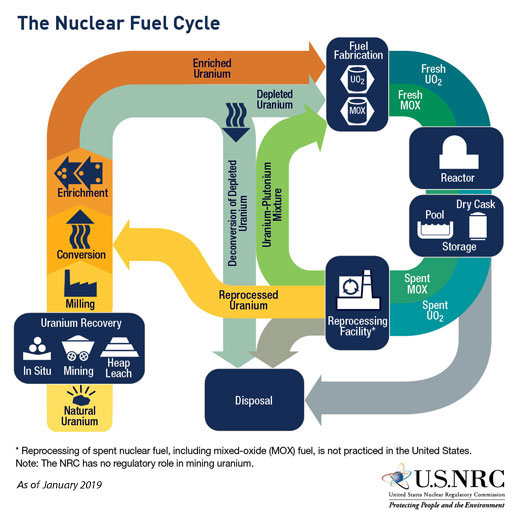
\includegraphics[width=0.5\columnwidth]{figures/nuclear-fuel-cycle-02.jpeg}
    \caption{Stages of the nuclear fuel cycle. Reproduced from \cite{nuclear_regulatory_commission_stages_2020}}
    \label{fig:nuclear-fuel-cycle}
\end{figure}

\noindent
Engineers typically adopt a ``hierarchical'' attitude, as described by cultural
theory of risk \cite{van_de_graaff_understanding_2016,mcneeley_cultural_2014},
and thus perceive these fears as irrational and placatable by ``educating'' an
ignorant public; consistent with the ``deficit model'' of science communication
\cite{simis_lure_2016,patenaude_topical_2022}. \textcolor{red}{It is incumbent
on nuclear engineers and advocates to adequately communicate the risks
associated with nuclear energy and not dismiss concerns due to a lack of
technical rigor.} Although \ac{snf} (commonly ``nuclear waste'') does not
present an immediate risk for radiological release, the details around managing \ac{snf} require
thoughtful consideration. Choosing between an open or a closed nuclear fuel
cycle implies different ethical foundations. Specifically, the tradeoff between
long- and short-term risks that must be carefully weighed
\cite{taebi_recycle_2008}. Further, even though civilian nuclear energy has not
led to the proliferation of nuclear weapons
\cite{herzog_nuclear_2020,miller_why_2017}, the need to keep careful track of
nuclear materials and prevent its release into the biosphere, malicious or
otherwise, presents a profound responsibility with some intergenerational
inequities. Finally, there are elements of the nuclear fuel cycle that 
are frequently ignored. In particular, mining and fuel fabrication are 
often overlooked by advocates for nuclear energy, even though mismanagement in these parts of
the nuclear fuel cycle have led to significant environmental disasters, such as the 
accident in Church Rock, New Mexico \cite{moore-nall_legacy_2015,rojavin_civilian_2011}. 

In addition to these ethical and technical issues, some have argued that, due to the
risks discussed above, nuclear energy requires centralized and authoritarian decision-making
structures and is therefore anathema to inclusive and democratic
values \cite{van_de_graaff_understanding_2016, winner_artifacts_1980}. However, conversations
within the nuclear spaces have reopened this question about the implicit ``politics'' of nuclear
energy, spurred on by the development of \acp{smr} \cite{lovering_social_2021}.

Distinct from conversations surrounding the ethics and risks of using nuclear
energy, many nuclear energy skeptics insist that nuclear power is too expensive
to support decarbonization goals. While it is true that nuclear power plants
have significant capital costs \cite{nrel_2020_2020} which have grown in many
countries due to additional regulations and safety requirements (i.e.,
``negative learning'') \cite{lovering_historical_2016}, it remains unclear
whether these costs uniquely translate to burden on electricity consumers.
Especially given nuclear energy's role as a ``price-taker'' in electricity
markets \cite{murphy_impacts_2019} and evidence for nuclear's stabilizing effect
on electricity prices \cite{dotson_influence_2022,de_sisternes_value_2016}.

 
% \subsection{\textcolor{red}{If renewable energy can solve climate change, why
build anything else?}}

\begin{enumerate}
    \item What do proponents of renewable energy say about solar and wind?
    \begin{itemize}
        \item By virtue of being renewable, the ``fuel'' source is practically
        infinite. Solar energy will never run out on the timescale of human
        civilization, and wind energy (as a product of wind energy plus the
        Earth's rotation) will similarly never run out.
        \item Since renewable energy, specifically solar and wind, lend
        themselves more naturally to distribution, they are more democratic
        sources of energy (cite).
    \end{itemize}
    \item What are the technical objections to fully renewable energy grids?
    \begin{itemize}
        \item Wind and solar are variable and intermittent energy sources.
        \item Renewable energy sources (including non-intermittent sources like
        hydroelectric dams and biomass) have a much lower \ac{eroi} than fossil
        fuel sources \cite{hall_eroi_2014,weisbach_energy_2013}. However, recent
        harmonization studies belie this assertion by demonstrating that
        renewable sources have similar, if not greater, \ac{eroi} than coal or
        natural gas \cite{murphy_energy_2022}.
        \item Although the ``fuel'' for solar and wind resources is infinite,
        the materials required to extract energy from these sources is finite.
        \item In contrast with the nuclear energy, the renewable energy industry
        does not have a strong notion of the lifecycle of their technology.
        There are no plans to safely store or recycle solar panels and wind
        turbines at end-of-life.
    \end{itemize}
    \item What are some non-technical objectives to renewable energy?
    \begin{itemize}
        \item Democracy and inclusivity are not required features of renewable
        energy sources \cite{bell_toward_2020,winner_artifacts_1980}. Although
        renewables have the potential to be highly decentralized, this is not a
        requirement of their use. Many deployment schemes for solar and wind
        farms involve creating highly centralized ``farms'' that are owned and
        operated by a single corporate entity, thereby recreating the same power
        structures that currently exist and thus perpetuating inequities.
    \end{itemize}
    \item What drives the opposition for renewable energy projects (specifically
    wind and solar)?
    \begin{itemize}
        \item Due to the sprawling nature of energy sources like solar and wind,
        these projects are frequently subject to public opposition in proposed
        areas.
        \item The \ac{nimby} movement, or \acs{nimbyism}, is frequently cited as
        the cause of opposition (cite). \ac{nimbyism} describes people that do
        not support the execution of a specific project (energy-related or
        otherwise) due to the project's proximity to a certain location
        (typically residences), but would otherwise support a project if it were
        further away. Despite the popular understanding of \ac{nimbyism}'s role
        in delaying energy projects, the most comprehensive empirical research
        on \ac{nimbyism} demonstrated that \ac{nimby} attitudes do not drive
        public opposition \cite{konisky_proximity_2021}. 
    \end{itemize}
\end{enumerate}

% What do proponents of renewable energy say about solar and wind?

Renewable energy sources, particularly solar and wind energy, are appealing
alternatives to fossil fuel sources. Solar and wind energy have fewer
geographical constraints, compared to hydroelectric and geothermal power
\cite{lopez_us_2012}. With respect to nuclear energy, solar and wind are
similarly safe on a per-unit-energy basis and produce comparable lifecycle
carbon emissions
\cite{united_nations_economic_commission_for_europe_carbon_2022,sovacool_balancing_2016,
intergovernmental_panel_on_climate_change_climate_2014}. Contrary to popular
belief, solar and wind resources can have \ac{eroi} comparable to coal-fired
power plants \cite{murphy_energy_2022}.
% \subsection{\textcolor{red}{Current procedures}}


\textcolor{red}{In this section I want to cover the current issues related to siting 
energy projects and how they are executed. This should relate issues identified in the case studies
for siting a nuclear waste repository (as well as the successes!) and the challenges of siting renewable
energy projects. Once I have made this connection, I can summarize the case study on the Dakota Access Pipeline
done by McKenzie Johnson \cite{johnson_dakota_2021}. I can also refer to the process for obtaining a nuclear
reactor license.
Finally, it may be useful to identify a ``successful'' siting process? Such as the siting of a transmission line
in Ireland \cite{devine-wright_understanding_2020}.
This section also serves as a great segu\'{e} into discussions of energy justice. Since engineers are not 
typically equipped to do the kind of public engagement required to advance energy goals.}
% \noindent\hrulefill \textcolor{red}{Subsubsection: Energy justice and the
% Boundaries of Energy Systems.}
\section{Energy Justice}
\label{section:energy-justice}
% \item What is energy justice?


Energy justice is a conceptual and analytical tool regarding the ethical or
normative dimensions of energy systems and addresses the systemic causes of
burdens, and inequities \cite{sovacool_energy_2015}.
% \begin{enumerate} \item What is justice?
    There are many conceptions of justice; however, the most popular framework
    for understanding justice is a three-faceted approach originating from David
    Schlosberg: distributive, recognition, and procedural justice
    \cite{schlosberg_2_2007}.
    % \item What is distributive justice? 
% \noindent\hrulefill
    Distributive justice relates to the fair distribution of resources,
    burdens, and responsibilities. Studies on distributive justice seek to
    address the normative question: how should a just society distribute the
    benefits it produces and \textit{the burdens required to maintain it}
    \cite{brighouse_justice_2004}. Additionally, distributive justice
    considers \textit{how} poor distributions are created
    \cite{schlosberg_2_2007}.
% \noindent\hrulefill
    % \item What is procedural justice?
    Procedural (in)justice is defined as the presence of (un)fair and
    (in)equitable institutional processes of the state \cite{schlosberg_2_2007}.
    In other words, how decisions of societal import are made and who is
    involved in those decisions. Sovacool and Dworkin (2015) outline four
    elements of procedural justice: transparency, meaningful participation,
    impartiality, and avenues for redress \cite{sovacool_energy_2015}.    
% \noindent\hrulefill
    % \item What is recognition justice?
Justice of recognition is the most vague of the three tenets of justice and is
    frequently reduced to a component of either distributive or procedural
    justice \cite{schlosberg_2_2007, van_uffelen_revisiting_2022}. A common
    argument for this consolidation is that recognition is a precondition for
    achieving distributive justice or that achieving procedural justice
    necessarily includes recognition \cite{schlosberg_2_2007}. However,
    recognition is unique from distributive and procedural justices because it
    is concerned with a different family of injustice, namely,
    \textit{misrecognition} \cite{van_uffelen_revisiting_2022}. van Uffelen
    (2022) suggests a nuanced definition of recognition justice as ``the
    adequate recognition of all actors through love, law, and the status order''
    \cite{van_uffelen_revisiting_2022}.
% \end{enumerate} \noindent\hrulefill
Sovacool and Dworkin (2015) offer a framework for assessing energy policies from
a justice perspective. Table \ref{tab:justice-frameworks} map the relationships
between justice-as-a-decision-making-tool from Sovacool \& Dworkin, Paterson's
hazard response characterization, and Schlosberg's triumvirate of justice. 

\begin{table}[h]
    \centering
    \caption{Different ways to operationalize justice concepts.}
    \begin{tabular}{ccc}
    \toprule
    Schlosberg \cite{schlosberg_2_2007} & Sovacool \& Dworkin 
    \cite{sovacool_energy_2015}& Paterson et al. \cite{paterson_community-based_2019}\\
    \midrule
    & Intragenerational Equity & Material Well-being \\
    Distribution & Intergenerational Equity & Infrastructure \\
    & Responsibility & \\
    & Due Process & Awareness \\
    Procedure & Good Governance & Governance \\
    & & \\
    & Availability$^1$ & Relational Well-being \\
    Recognition & Affordability$^1$ & \\
    & Sustainability$^1$ & \\
    \bottomrule\\
    % \rule{0pt}{2ex}
    \multicolumn{3}{l}{$^1$ van Uffelen \cite{van_uffelen_revisiting_2022} argues for this categorization.}
\end{tabular}
    \label{tab:justice-frameworks}
\end{table}

Although Sovacool \& Dworkin do not explicitly discuss recognition justice, it
is a unique aspect of justice that can still be useful for contextualizing their
recommendations. For example, due to the psychological pressures introduced by a
lack of access to energy, either due to infrastructure or cost, interrupts
relational well-being and is an injustice \cite{van_uffelen_revisiting_2022}.
Further, (un)sustainable policies may be considered a misrecognition of the
humanity of future generations. Next, I examine the specific ways the social
science literature understands how energy systems and their infrastructure
(artifacts) contribute to the distribution of burdens.

% \noindent\hrulefill \item What is an energy system?
\subsection{Boundaries of Energy Systems}
\label{section:energy-system-boundaries}
Previous work defined energy systems in purely technical terms as spatially,
temporally, and topologically complex machines that coordinate the supply and
demand of energy, especially electricity \cite{dotson_influence_2022}. However,
this definition neglects the ways energy systems may be used to construct and
maintain power relations that contribute to inequitable distributions of
burdens. Energy access is necessary to support complex modern economies and
therefore possesses political power \cite{jones_building_2013,
bridge_energy_2018}. The literature on the political economy of energy
infrastructure locates this political influence in five distinct ways
\cite{bridge_energy_2018}. First, energy infrastructure affects competition and
collaboration among nation-states in the geo-political sphere. The current
situation in Ukraine makes this especially salient
\cite{figueiredo_impacts_2022}. 

The second subset of the literature focuses on the process of energy
infrastructure development and how these processes create social inequities. For
example, energy policies that subsidize residential solar panels have not led to
more equitable adoption of solar energy, with greater adoption in areas with
higher income, among other social indicators \cite{reames_distributive_2020}.
Other popular arguments in favor of renewable energy assert that these energy
sources are necessarily more egalitarian because the Sun and the wind cannot be
(or have not yet been) privatized. Another is the urgency of climate change.
Although these arguments have merit, they ignore or minimize the potential
environmental and social consequences of energy planning that does not consider
energy justice \cite{jones_building_2013}. Large-scale energy projects in the
Global South have already led to the dispossession of nearby indigenous
communities and other key actors \cite{yenneti_spatial_2016,
barragan-contreras_procedural_2022}.

Third, the development of energy infrastructure is not simply conducted via
policy measures, but also in the manner governments activate the public
imagination in favor of these policies
\cite{bridge_energy_2018,jasanoff_containing_2009}. Jasanoff and Kim (2009)
articulate this concept as `socio-technical imaginaries,' which are
simultaneously descriptive and prescriptive of possible energy futures
established by governments in the national zeitgeist
\cite{jasanoff_containing_2009}. This concept is demonstrated by the discourse
surrounding nuclear energy in the United States and South Korea
\cite{jasanoff_containing_2009} as well as in Japan
\cite{valentine_energy_2019}. Governments can employ `grand narratives' related
to national security, climate change, or modernization to enhance public support
while minimizing genuine participation \cite{bridge_energy_2018}.

Fourth, the political power of energy infrastructure can be traced further to
the cultural values and policy choices embedded in the design and operation of
seemingly technical systems \cite{bridge_energy_2018}. In other words, the
design and implementation of energy infrastructure may be used as a vehicle for
apparently unrelated agendas, a form of ``policy-making by other means''
\cite{bridge_energy_2018, clausewitz_chapter_1918}. Edwards and Hecht (2010)
refer to the co-constitution of technological and political order as
`\textit{technopolitics},' demonstrating the tangible material and political
outcomes of technological systems \cite{edwards_history_2010}.

Finally, energy systems and their infrastructure possess a unifying quality
through which new political identities may evolve \cite{bridge_energy_2018}.

From these various perspectives, we can observe that confining an energy system
to its technical characteristics is woefully incomplete. I propose that an
energy system is a spatially, temporally, and topologically complex machine that
coordinates the supply and demand of energy and resources and acts as an
important mediator of burdens that influence risks (such as risks from climate
change). This thesis takes the important step of analyzing energy system
planning and policy with this expanded definition. The next section reviews
current attempts to model energy systems and identifies gaps in conventional
methods.

% \textcolor{red}{Climate change \textit{is} a complex issue with multiple
% interacting and interwoven layers. However, it can and must be understood
% holistically instead of stripping it of its complexity and exclusively
% relegating solutions to the realms of economics and engineering. This
% over-simplification is done out of a misplaced sense of pragmatism and either
% an inability or unwillingness to completely apprehend the problem.}

% \noindent\hrulefill \item What are the obstacles to building more clean energy
% infrastructure? What is preventing the transition to a ``qualitatively new
% type of [environmental] society'' \cite{bluhdorn_legitimation_2020}?

% \textcolor{red}{This is where you can introduce different schools of thought
% about transitions.}

% \textcolor{blue}{Interesting that you chose to frame public acceptance as an
% ``obstacle'' rather than a source of greater accountability and
% participation.} \begin{enumerate} \item Legitimation crisis of democracy
% \cite{bluhdorn_legitimation_2020}. \item Social acceptance literature
% \end{enumerate}

% \end{enumerate}

% \section{Calls for a Just-Transition}

% Att


\section{Modeling Energy Systems}
\label{section:esoms}

Energy system optimization models (ESOMs)\acused{esom} have broad utility,
including forecasting future quantities, generating insight for policy
development, or energy system planning for scheduling and acquisition
\cite{decarolis_using_2011, yue_review_2018}. However, analyses using currently
available \acp{esom} seldom consider the role of energy systems in creating and
maintaining inequitable distributions of burdens. \acp{esom} vary significantly
by the energy sectors they choose to model, the degree of physical detail,
uncertainty quanitification, and forecasting capabilities. Table \ref{tab:esoms}
summarizes the capabilities for a comprehensive list of energy system analysis
tools. These tools are approximately sorted by mathematical formulation, e.g.
explicit optimization or simulation. The ``\ac{milp}'' column indicates whether
the framework uses a linear-programming approach to optimize an objective
function. The ``objective'' column specifies the nature of the objective
function if one exists. ``Cost'' objectives minimize total or annual energy
costs, while ``welfare'' maximizes social welfare. Some entries have more than
one objective listed. This means users may choose which objective to optimize.
None of the tools in Table \ref{tab:esoms} are designed to handle simultaneous
optimization (i.e., \ac{moo}). For those modeling frameworks that have an
``objective'' in Table \ref{tab:esoms}, virtually all of them optimize system
costs. EnergyScope is the only exception to this, which allows users to optimize
\ac{ghg} emissions \cite{limpens_energyscope_2019}. \textcolor{black}{The
``uncertainty'' column indicates a feature to algorithmically generate model
runs for testing either parametric or structural uncertainties.
\textcolor{black}{For example, EnergyScope is \textit{suitable} for uncertainty
analysis (i.e., many runs are computationally tractable) but does not have any
built-in capabilities \cite{limpens_energyscope_2019}.} Some tools, such as NEMS
\cite{nalley_national_2019}, incorporate uncertainty into their calculations via
learning curves. However, these learning curves require assumptions about
learning factors and technological ``optimism'' --  which are themselves
uncertain \cite{nalley_national_2019}.} Table \ref{tab:esoms} also indicates
whether the tool is a ``public code.'' This simply means users can download and
inspect the source code. Other considerations for openness, such as licensing
and development, vary among the listed frameworks. \textcolor{black}{The other
columns simply indicate the existence of particular features rather than the
relative maturity or sophistication of each feature.} 

Frameworks, such as MEDEAS \cite{capellan-perez_medeas_2020}, and MultiMod
\cite{huppmann_market_2014}, are general equilibrium models which embed energy
systems within the macro-economy and facilitate the modeling of strategic
behavior. The latter formulates a non-linear problem with the Karush-Kuhn-Tucker
optimality condition \cite{huppmann_market_2014}, as opposed to more traditional
linear programming methods. Models of this type are helpful for analyzing the
economy-wide influence of policies but lack sufficient operational detail to be
prescriptive for energy system planning.

\textcolor{black}{Agent-based models are useful for modeling the market
behaviors of different actors, such as firms (which produce power), transmission
operators, and consumers. The latter category is typically aggregated for
tractability. Modeled behaviors include technology preferences
\cite{anwar_modeling_2022, zade_quantifying_2020}, risk aversion
\cite{anwar_modeling_2022}, financial characteristics \cite{anwar_modeling_2022,
nitsch_economic_2021}, and information asymmetry among agents
\cite{anwar_modeling_2022, nitsch_economic_2021}. Due to agent heterogeneity,
agent-based models are considered useful for capturing social phenomena
\cite{yue_review_2018,fattahi_systemic_2020}.}

A further set of tools focus on simulating power flow and demand fluctuations.
\textcolor{black}{CAPOW \cite{su_open_2020} generates synthetic data with
statistical methods to explore uncertainties in energy dispatch and extreme
demand events, but does not include any investment optimization based on these
uncertainties.} \textcolor{black}{CESAR-P, SAM, Demod, and DESSTinEE focus on
modeling demand profiles
\cite{leoniefierz_hues-platformcesar-p-core_2021,bosmann_shape_2015,barsanti_socio-technical_2021}.
CESAR-P models individual building demand for energy based on the physical
parameters of the building. However, it has no dispatch or investment
optimization capabilities.} Other tools such as Pandapower, GridCal, and SciGRID
power model the infrastructure aspects of electricity systems -- transmission
and distribution -- rather than the optimal dispatch of electricity producers
\cite{thurner_pandapower_2018, vera_gridcal_2022, matke_structure_2017}.

There is an overwhelming number of models with varying levels sophistication and
capabilities. However, the inability to optimize any objective besides cost
presents a significant gap in the existing space of energy modeling tools.
Further, since none of these tools allow for multiple objectives, true trade off
analysis is rendered impossible.



\begin{table}
    \centering
    \caption{Summary of \ac{esom} frameworks.}
    \label{tab:esoms}
    \resizebox*{\textwidth}{0.95\textheight}{\begin{tabular}{lllll*{8}{c}rc}
\toprule
Model &   Citation   &   math model type   &  MILP  &   Objective   & Transmission & \multicolumn{3}{c}{Sector}& Investment & Physical & Forecasting & Agent  &  Uncertainty& Public  \\ 
&  & & & & & Heat & Electric & Transport & Optimization & Models & & Based& Analysis& Code \\
% Model  &  &  &  &  &  &  &  &  &  &  &  &  &  &  \\
\midrule
% JMM    &    -    &    -    &   nan   &    -    &  nan  &  nan  &  nan  &  nan  &  nan  &  nan  &  nan  &  nan  & nan &    \xmark     \\
% PowerMatcher    &    -    &    -    &   nan   &    -    &  nan  &  nan  &  nan  &  nan  &  nan  &  nan  &  nan  &  nan  & nan &    \checkmark     \\
% USENSYS    &    Cost    &    Optimization    &   nan   &    -    &  nan  &  nan  &  nan  &  nan  &  nan  &  nan  &  nan  &  nan  & nan &    \checkmark     \\
% GAMAMOD    &    -    &    Optimization     &   nan   &    -    &  nan  &  nan  &  nan  &  nan  &  nan  &  nan  &  nan  &  nan  & nan &    \xmark     \\
% NEMO (SEI)    &    Minimize total discounted costs    &    Optimization     &   nan   &    In preparation    &  nan  &  nan  &  nan  &  nan  &  nan  &  nan  &  nan  &  nan  & nan &    \checkmark     \\
% OMEGAlpes    &    -    &    Optimization     &   nan   &    -    &  nan  &  nan  &  nan  &  nan  &  nan  &  nan  &  nan  &  nan  & nan &    \checkmark     \\
% PowerSimulations.jl    &    Least Cost    &    Optimization     &   nan   &    -    &  nan  &  nan  &  nan  &  nan  &  nan  &  nan  &  nan  &  nan  & nan &    \checkmark     \\
% Region4FLEX    &    -    &    Optimization     &   nan   &    -    &  nan  &  nan  &  nan  &  nan  &  nan  &  nan  &  nan  &  nan  & nan &    \xmark     \\
% TIMES Évora    &    Minimise total discounted cost of the energy system    &    Optimization     &   nan   &    -    &  nan  &  nan  &  nan  &  nan  &  nan  &  nan  &  nan  &  nan  & nan &    \checkmark     \\
% TIMES-PT    &    Minimise total discounted cost of the energy system    &    Optimization     &   nan   &    -    &  nan  &  nan  &  nan  &  nan  &  nan  &  nan  &  nan  &  nan  & nan &    \checkmark     \\
AnyMOD     &    \cite{goke_graph-based_2021}    &    Optimization     &   \checkmark   &    Cost    &    &  \checkmark  &  \checkmark  &   &  \checkmark  &   &    &    & &    \checkmark     \\
Backbone     &    \cite{helisto_backboneadaptable_2019}    &    Optimization     &   \checkmark   &    Cost    &  \checkmark  &  \checkmark  &  \checkmark  &  \checkmark  &  \checkmark  &   &  \checkmark  &   & \acs{sp} &    \checkmark     \\
Balmorel     &    \cite{goransson_cost-optimized_2013}    &    Optimization     &   \checkmark   &    Cost    &  \checkmark  &    &  \checkmark  &   &  \checkmark  &   &   &    & &    \checkmark     \\
Calliope     &    \cite{pfenninger_calliope_2018}    &    Optimization     &   \checkmark   &    Cost    &   &  \checkmark  &  \checkmark  &  \checkmark  &  \checkmark  &   &   &   & &    \checkmark     \\
CapacityExpansion     &    \cite{kuepper_capacityexpansion_2020}    &    Optimization     &   \checkmark   &    Cost    &  \checkmark  &    &  \checkmark  &   &  \checkmark  &    &    &    &  &    \checkmark     \\
DIETER     &    \cite{zerrahn_long-run_2017}    &    Optimization     &   \checkmark   &    Cost    &   & \checkmark  & \checkmark  &   &  \checkmark  &   &   &   & &    \checkmark     \\
Dispa-SET    &    \cite{quoilin_modelling_2017}    &    Optimization     &   \checkmark   &    Cost    &  \checkmark  &   &  \checkmark  &   &  \checkmark  &   &   &   & &    \checkmark     \\
ELMOD     &    \cite{leuthold_elmod_2008}    &    Optimization     &   \checkmark   &    Welfare    &  \checkmark  &   &  \checkmark  &   &  \checkmark &   &   &   & &    \checkmark     \\
ELTRAMOD     &    \cite{ladwig_demand_2018}    &    Optimization     &   \checkmark   &    Cost    &   &   &  \checkmark  &   &  \checkmark  &   &   &   & &   \\
EMMA     &    \cite{hirth_european_2021}    &    Optimization     &   \checkmark   &  Cost  &   &   &  \checkmark  &   &  \checkmark  &   &   &   & &    \checkmark     \\
% ENSYSI     &    \cite{limpens_energyscope_2019}   &    Optimization     &   \checkmark   &    Cost    &  nan  &  \checkmark  &  \checkmark  &  \checkmark  &  nan  &  nan  &  nan  &  nan  & nan &    \checkmark     \\
EOLES elec    &    \cite{shirizadeh_how_2022}    &    Optimization &   \checkmark   &    Cost    &   &   &  \checkmark  &   &  \checkmark  &    &    &    & &    \checkmark     \\
ESME     &    \cite{heaton_modelling_2014}    &    Optimization     &   \checkmark   &    Cost    &   &  \checkmark  &  \checkmark  &  \checkmark  &  \checkmark  &   &   &   & \acs{mc} &   \\
ESO-X    &    \cite{heuberger_power_2017}    &    Optimization     &   \checkmark   &    Cost    &    &   &   \checkmark  &    &  \checkmark  &   & &   & &    \checkmark     \\
EnergyRt     &    \cite{lugovoy_energyrt_2022}    &    Optimization     &   \checkmark   &    Cost    &   &   &  \checkmark  &   &  \checkmark  &   &   &   & &    \checkmark     \\
EnergyScope    &    \cite{limpens_energyscope_2019}    &    Optimization     &   \checkmark   &    Cost, \acs{ghg}    &   &  \checkmark  &  \checkmark  &  \checkmark  &  \checkmark  &   &   &   & &    \checkmark     \\
Ficus     &   \cite{atabay_open-source_2017}    &    Optimization     &   \checkmark   &    Cost    &   &   &  \checkmark  &   &  \checkmark  &   &   & & &    \checkmark     \\
FlexiGIS     &    \cite{alhamwi_gis-based_2017}    &    Optimization     & \checkmark &    Cost    &   & \checkmark  & \checkmark  & \checkmark  &   &   &   &   & &    \checkmark     \\
GAMAMOD-DE    &    \cite{hauser_modelling_2019}    &    Optimization    &   \checkmark   &    Cost    &    &   &  \checkmark  &   &  \checkmark  &   &   &   &  &   \\
GenX     &    \cite{jenkins_genx_2022}    &    Optimization     &   \checkmark   &    Cost    &  \checkmark   &    &  \checkmark  &   & \checkmark  &   &   & & \acs{mga}& \checkmark     \\
GRIMSEL-FLEX    &    \cite{rinaldi_what_2022}    &    Optimization     &   \checkmark   &    Cost    &    &  \checkmark  &  \checkmark  &    &  \checkmark  &  \checkmark  &    &    & &    \checkmark     \\
HighRES     &    \cite{zeyringer_designing_2018}    &    Optimization     &   \checkmark   &    Cost    &    &  \checkmark  &  \checkmark  &    &  \checkmark  &    &    &    & &   \\
MARKAL     &    \cite{loulou_documentation_2004}    &    Optimization     &   \checkmark   &    Cost    &    &  \checkmark  &  \checkmark  &  \checkmark  &  \checkmark  &    &    &    & \acs{mc}, \acs{sp} &    \checkmark     \\
METIS     &    \cite{sakellaris_metis_2018}    &    Optimization     &   \checkmark   &    Cost    &  \checkmark  &  \checkmark  &  \checkmark  &    &  \checkmark  &    &    &    & \acs{mc} &    \checkmark     \\
Medea     &    \cite{wehrle_cost_2021}    &    Optimization     &   \checkmark   &    Cost    &   &   &  \checkmark  &    &  \checkmark  &   &   &   & &    \checkmark     \\
Oemof     &    \cite{hilpert_open_2018}    &    Optimization  &   \checkmark   &    Cost    &    &  \checkmark  &  \checkmark  &  \checkmark  &  \checkmark  &     &   &  &  &  \checkmark     \\
OPERA     &    \cite{van_stralen_opera_2021}    &    Optimization     &   \checkmark   &    Cost    &  \checkmark  &  \checkmark  &  \checkmark  &   &  \checkmark  &   &   &   & &    \checkmark     \\
OSeMOSYS     &    \cite{howells_osemosys_2011}    &    Optimization     &   \checkmark   &    Cost    &    &  \checkmark  &  \checkmark  &  \checkmark  &  \checkmark  &    &    &    & &    \checkmark     \\
OnSSET     &    \cite{mentis_gis-based_2015}    &    Optimization     &   \checkmark   &    Cost    &  \checkmark  &    &  \checkmark  &    &  \checkmark  &    &    &    & &    \checkmark     \\
PLEXOS     &   \cite{deane_quantifying_2015}    &    Optimization     &   \checkmark   &    Cost    &   &   &  \checkmark  &   &  \checkmark  &   &   &   & \acs{mc} &   \\
POLES     &    \cite{vandyck_global_2016}     &    Optimization     &   \checkmark   &    Cost    &   &   &  \checkmark  &   &  \checkmark  &   &   &   &  &   \\
POMATO     &    \cite{weinhold_power_2021}     &    Optimization     &   \checkmark   &    Cost    &  \checkmark  &  \checkmark  &  \checkmark  &   &    &   &   &   &  &    \checkmark     \\
PRIMES     &    \cite{antoniou_decision_1999}    &    Optimization     &   \checkmark   &    Cost    &  \checkmark  &  \checkmark  &  \checkmark  &  \checkmark  &  \checkmark  &   &   &   & &  \\
PyPSA     &    \cite{brown_pypsa_2018}    &    Optimization  &   \checkmark   &    Cost    &  \checkmark  &  \checkmark  &  \checkmark  &  \checkmark  &  \checkmark  &  \checkmark  &   &   & \acs{mga} &    \checkmark     \\
REMix     &    \cite{gils_integrated_2017}    &    Optimization     &   \checkmark   &    Cost    &  \checkmark  &  \checkmark  &  \checkmark  &  \checkmark  &  \checkmark  &   &   &   &  &    \checkmark     \\
REopt     &    \cite{simpkins_reopt_nodate}    &    Optimization     &   \checkmark   &    Cost    &   &  \checkmark  &  \checkmark  &   &  \checkmark  &   &   &   &  &    \checkmark     \\
% SMS     &    \cite{the_sms_team_sms_2022}    &    Optimization     &   \checkmark   &    Cost    &  nan  &  nan  &  nan  &  nan  &  nan  &  nan  &  nan  &  nan  & nan &    \checkmark     \\
StELMOD     &    \cite{abrell_integrating_2015}    &    Optimization     &   \checkmark   &    Cost    &  \checkmark  &   &  \checkmark  &   &  \checkmark  &   &   &   &  &    \checkmark     \\
Switch     &    \cite{johnston_switch_2019}    &    Optimization     &   \checkmark   &    Cost    &  \checkmark  &  \checkmark  &  \checkmark  &  \checkmark  &  \checkmark  &   &   &   &  &    \checkmark     \\
TIMES     &    \cite{loulou_documentation_2016}    &    Optimization     &   \checkmark   &    Cost, Welfare    &   & \checkmark  & \checkmark  &    & \checkmark  &    &    &    & \acs{sp} &    \checkmark     \\
Temoa     &    \cite{hunter_modeling_2013}    &    Optimization     &   \checkmark   &    Cost    &   &  \checkmark  &  \checkmark  &  \checkmark  &  \checkmark  &   &   &   & \acs{mga}, \acs{mc}, \acs{sp} &    \checkmark     \\
TransiEnt     &    \cite{andresen_status_2015}    &    Simulation     &   \checkmark   & Cost & \checkmark  &  \checkmark  &  \checkmark  &   &   &   &   &  &  &    \checkmark     \\
URBS     &    \cite{dorfner_open_2015}    &    Optimization     &   \checkmark   &    Cost    &  \checkmark  &  \checkmark  &  \checkmark  &  \checkmark  &  \checkmark  &   &   &   & &    \checkmark     \\
\arrayrulecolor{lightgray}\hline
% DynPP    &    operation, cost, emissions, thermal stress    &    Optimization  and Simulation     &   nan   &    Modelling and simulation of a coal-fired power plant for start-up optimisation    &  nan  &  nan  &  nan  &  nan  &  nan  &  nan  &  nan  &  nan  & nan &    \xmark     \\
% EA-PSM Electric Arc Flash    &    -    &    Optimization  and Simulation     &   nan   &    -    &  nan  &  nan  &  nan  &  nan  &  nan  &  nan  &  nan  &  nan  & nan &    \xmark     \\
% EA-PSM Electric Short Circuit    &    -    &    Optimization  and Simulation     &   nan   &    -    &  nan  &  nan  &  nan  &  nan  &  nan  &  nan  &  nan  &  nan  & nan &    \xmark     \\
% NEMO    &    minimise average cost of electricity    &    Optimization  and Simulation     &   nan   &    -    &  nan  &  nan  &  nan  &  nan  &  nan  &  nan  &  nan  &  nan  & nan &    \checkmark     \\
Genesys     &    \cite{bussar_optimal_2014}    &    Optimization  and Simulation     &      &    Cost    &    &    &  \checkmark  &    &  \checkmark  &    &    &  &  &      \\
OpenTUMFlex     &    \cite{zade_quantifying_2020}    &    Optimization  and Simulation     &   \checkmark   &    Cost    &   &  \checkmark  &  \checkmark&  \checkmark  &   &   &  \checkmark &   & &    \checkmark     \\
PowNet     &    \cite{chowdhury_pownet_2020}    &    Optimization  and Simulation     &   \checkmark   &    Cost    &  \checkmark  &  &  \checkmark  &  &   &  \checkmark  &   &   & &    \checkmark     \\
Renpass     &    \cite{frauke_wiese_renpass_2015}    &    Optimization  and Simulation     &    &    Cost    &    &    &  \checkmark&    &   &   &   &   & &    \checkmark     \\
SimSEE     &    \cite{chaer_simulacion_2008}    &    Optimization  and Simulation     &      &    Cost    &    &    &  \checkmark  &    &    &  \checkmark  &    &    &  &    \checkmark     \\
% Maon    &    Economic welfare at electricity spot, electricity reserve, and emission markets in Europe    &    Optimization , Simulation  and Other     &   nan   &    Ketov, Mihail (2019). "Marktsimulationen unter Berücksichtigung der Strom-Wärme-Sektorenkopplung", Print Production, Aachener Beiträge zur Energieversorgung, volume 189, PhD thesis, RWTH Aachen University.    &  nan  &  nan  &  nan  &  nan  &  nan  &  nan  &  nan  &  nan  & nan &    \xmark     \\
MEDEAS     &    \cite{capellan-perez_medeas_2020}    &    Other     &    &    &   & \checkmark  & \checkmark  & \checkmark  &   & \checkmark  &   &   & \acs{mc} &  \checkmark    \\
MultiMod     &    \cite{huppmann_market_2014}    &    Other     &  & Welfare &  \checkmark  &  \checkmark  &  \checkmark  &  \checkmark  &  \checkmark  &  &   &   & &\\
NEMS     &    \cite{nalley_national_2019}    &    Other     &   \checkmark   & Cost &  \checkmark & \checkmark  &  \checkmark &  \checkmark  &  \checkmark  &   &  \checkmark  & & &  \\
\arrayrulecolor{lightgray}\hline
% Energy Policy Simulator    &    -    &    Simulation     &   nan   &    -    &  nan  &  nan  &  nan  &  nan  &  nan  &  nan  &  nan  &  nan  & nan &    \checkmark     \\
% EnergyNumbers-Balancing    &    -    &    Simulation     &   nan   &    -    &  nan  &  nan  &  nan  &  nan  &  nan  &  nan  &  nan  &  nan  & nan &    \xmark     \\
% PowerSimulationsDynamics.jl    &    -    &    Simulation     &   nan   &    -    &  nan  &  nan  &  nan  &  nan  &  nan  &  nan  &  nan  &  nan  & nan &    \checkmark     \\
% PowerSystems.jl    &    -    &    Simulation     &   nan   &    -    &  nan  &  nan  &  nan  &  nan  &  nan  &  nan  &  nan  &  nan  & nan &    \checkmark     \\
Breakthrough Energy Model    &    \cite{xu_us_2020}    & Simulation     &  & &  \checkmark  &   & \checkmark  &   &  \checkmark&   &   &   & &    \checkmark     \\
CAPOW     &    \cite{su_open_2020}    &    Simulation     & \checkmark &    Cost    &  \checkmark  &   &  \checkmark  &   &   & &  \checkmark  &   & \checkmark &    \checkmark     \\
CESAR-P    &    \cite{leoniefierz_hues-platformcesar-p-core_2021}    &    Simulation     & & & & & \checkmark & & & \checkmark & \checkmark & & & \checkmark \\
DESSTinEE    &    \cite{bosmann_shape_2015}    &    Simulation     & \checkmark & Cost & \checkmark  & \checkmark  & \checkmark  &   &   & \checkmark  &   &   & &    \checkmark     \\
Demod    &    \cite{barsanti_socio-technical_2021}    &    Simulation     & & &  &  \checkmark  &  \checkmark  &   &   &  \checkmark  &  \checkmark  &    &  \acs{mc}&    \checkmark     \\
EMLab-Generation    &    \cite{richstein_cross-border_2014}    & Simulation & & Cost & & & \checkmark &  & \checkmark & & & & \acs{mc} &    \checkmark     \\
EnergyPLAN     &    \cite{lund_energyplan_2021}   &    Simulation     &   &    Cost    &  \checkmark  &  \checkmark  &  \checkmark  &  \checkmark  &  \checkmark  &   &   &   & &     \\
Energy Transition Model    &    \cite{quintel_etm_2022}    &    Simulation     & & &   &   &  \checkmark  &  &   &   &   &    &  &    \checkmark     \\
GridCal     &    \cite{vera_gridcal_2022}    &    Simulation     &   &     &  \checkmark  &   &  &   &   &  \checkmark  &   &   & &    \checkmark     \\
LoadProfileGenerator     &    \cite{pflugradt_modelling_2016}    &    Simulation    &    & &     &  \checkmark  &  \checkmark  &   &   &  \checkmark  &  \checkmark  &  \checkmark  & &    \checkmark     \\
Pandapower     &    \cite{thurner_pandapower_2018}    &    Simulation     &    &  &  \checkmark &  & & & & \checkmark & & & &    \checkmark     \\
Pvlib     &    \cite{holmgren_pvlib_2018}    &    Simulation     &    & &   & \checkmark& &  & & \checkmark & \checkmark &  & &    \checkmark     \\
PyLESA     &    \cite{lyden_pylesa_2021}    &    Simulation     & &    Cost    &  \checkmark  &   &  \checkmark &  \checkmark  & &  \checkmark &   &   & &    \checkmark     \\
SAM    &    \cite{blair_system_2014}    &    Simulation     & & & & & & & &\checkmark&\checkmark& & \acs{pa} &    \checkmark     \\
SciGRID power    &    \cite{matke_structure_2017}    &    Simulation     & & &  \checkmark  &   & \checkmark  &    &    &    &   &   & &    \checkmark     \\
SimSES     &    \cite{naumann_simses_2017}    &    Simulation     &   & & & & \checkmark &  & & \checkmark& & & &    \checkmark     \\
\arrayrulecolor{lightgray}\hline
AMIRIS     &    \cite{nitsch_economic_2021}    &    Simulation  and Agent-based     &  &  &  &  & \checkmark  &  & \checkmark  &  &  &  \checkmark  & &    \checkmark     \\
ASAM     &    \cite{glismann_ancillary_2021}    &    Simulation  and Agent-based     & & & \checkmark &  & \checkmark & & & & &  \checkmark  & &    \checkmark     \\
EMIS-AS     &    \cite{anwar_modeling_2022}    &    Simulation  and Agent-based     & \checkmark & Welfare & \checkmark &  & \checkmark & & & & &  \checkmark  & \checkmark & \checkmark \\
Lemlab     &    \cite{zade_satisfying_2022}    &    Simulation  and Agent-based     &   \checkmark   & Welfare &  &  &  \checkmark  & & &   &   &  \checkmark  & &    \checkmark     \\
MOCES     &    \cite{exel_multi-domain_2015}    &    Simulation  and Agent-based     & & Cost &   &   &  \checkmark  &   &   &  \checkmark  & &  \checkmark  & &  \\
% Mosaik     &    \cite{ofenloch_mosaik_2022}    &    Simulation  and Agent-based     &   nan   &    -    &  nan  &  nan  &  nan  &  nan  &  nan  &  nan  &  nan  &  \checkmark  & nan &    \checkmark     \\
% SIREN     &    \cite{sustainable_energy_now_renewable_2016}    &    Simulation  and Other     &   nan   &    Cost    &  nan  &  nan  &  nan  &  nan  &  nan  &  nan  &  nan  &  nan  & nan &    \checkmark     \\
% SciGRID gas    &    -    &    Simulation  and Other     &   nan   &    -    &  nan  &  nan  &  nan  &  nan  &  nan  &  nan  &  nan  &  nan  & nan &    \checkmark     \\
\arrayrulecolor{black}\bottomrule
\end{tabular}
}
\end{table}
\FloatBarrier

% \begin{itemize} \item METIS has the following motivation
%     \cite{sakellaris_metis_2018} \begin{enumerate} \item Close the gap between
%     modellers and policy-makers, enabling policy-makers to become modellers.
%     \item reconciles user-friendliness with powerful capabilities \item
%     modularity \item \textcolor{red}{METIS does not support multi-objective
%     optimization!}    
%     \end{enumerate} \item energyRt has similar motivations
%     \cite{lugovoy_energyrt_2022}. \begin{enumerate} \item enhance
%     reproducibility \item reduce the learning curve \item minimize model
%     development time \end{enumerate} \item GENESYS cannot \sout{can} do
%     multi-objective optimization \cite{bussar_optimal_2014}. It uses a logical
%     flow to model dispatch behavior for a genetic algorithm! \begin{enumerate}
%     \item One drawback of the "hierarchical system management" method (i.e. a
%     logical flow chart) is the difficulty of modeling ramping rates... (test
%     this). \end{enumerate} \end{itemize}

\subsection{Economic Dispatch and Social Welfare}
\Ac{lp} or \ac{milp} are the dominant optimization approaches among the
frameworks in Table \ref{tab:esoms}. Economic dispatch models optimize the power
output of \textit{dispatchable} generators in a model system
\cite{de_queiroz_repurposing_2019, neumann_near-optimal_2021}. They all share
the same fundamental formulation.
\begin{align}
    \intertext{Minimize}
    \label{eqn:generic_objective}
    &F(x) = \sum_i C_i x_i\\
    % &F(x) = \sum_t^T\left[\sum_i^{N_g}{C_i^g x_i} - \sum_j^{N_d}{C_j^d x_j}\right],\\
    \intertext{subject to,}
    % &\sum_i{x_i} - \sum_j{x_j} = 0\\
    &g(x, p) \leq 0.\nonumber\\
    &x \in \vec{X}\nonumber\\
    \intertext{where}
    &\vec{X} \text{ is the set of decision variables,}\nonumber\\
    & C_i \text{ is the \textit{i-th} cost,}\nonumber\\
    & g \text{ is some linear inequality constraint,}\nonumber\\
    & p \text{ is some arbitrary parameter.}\nonumber
\end{align}
The exact formulation of Equation \ref{eqn:generic_objective} may vary slightly
across models, but the objective for most economic dispatch models is to
minimize total cost. The near universality of a cost-based objective function
comes from the concept of \textit{social welfare maximization}. This concept is
illustrated in Figure \ref{fig:social-max}.

\begin{figure}[H]
  \centering
  \resizebox{\columnwidth}{!}{%% Creator: Matplotlib, PGF backend
%%
%% To include the figure in your LaTeX document, write
%%   \input{<filename>.pgf}
%%
%% Make sure the required packages are loaded in your preamble
%%   \usepackage{pgf}
%%
%% Also ensure that all the required font packages are loaded; for instance,
%% the lmodern package is sometimes necessary when using math font.
%%   \usepackage{lmodern}
%%
%% Figures using additional raster images can only be included by \input if
%% they are in the same directory as the main LaTeX file. For loading figures
%% from other directories you can use the `import` package
%%   \usepackage{import}
%%
%% and then include the figures with
%%   \import{<path to file>}{<filename>.pgf}
%%
%% Matplotlib used the following preamble
%%
\begingroup%
\makeatletter%
\begin{pgfpicture}%
\pgfpathrectangle{\pgfpointorigin}{\pgfqpoint{13.900000in}{5.930000in}}%
\pgfusepath{use as bounding box, clip}%
\begin{pgfscope}%
\pgfsetbuttcap%
\pgfsetmiterjoin%
\definecolor{currentfill}{rgb}{1.000000,1.000000,1.000000}%
\pgfsetfillcolor{currentfill}%
\pgfsetlinewidth{0.000000pt}%
\definecolor{currentstroke}{rgb}{0.000000,0.000000,0.000000}%
\pgfsetstrokecolor{currentstroke}%
\pgfsetdash{}{0pt}%
\pgfpathmoveto{\pgfqpoint{0.000000in}{0.000000in}}%
\pgfpathlineto{\pgfqpoint{13.900000in}{0.000000in}}%
\pgfpathlineto{\pgfqpoint{13.900000in}{5.930000in}}%
\pgfpathlineto{\pgfqpoint{0.000000in}{5.930000in}}%
\pgfpathlineto{\pgfqpoint{0.000000in}{0.000000in}}%
\pgfpathclose%
\pgfusepath{fill}%
\end{pgfscope}%
\begin{pgfscope}%
\pgfsetbuttcap%
\pgfsetmiterjoin%
\definecolor{currentfill}{rgb}{1.000000,1.000000,1.000000}%
\pgfsetfillcolor{currentfill}%
\pgfsetlinewidth{0.000000pt}%
\definecolor{currentstroke}{rgb}{0.000000,0.000000,0.000000}%
\pgfsetstrokecolor{currentstroke}%
\pgfsetstrokeopacity{0.000000}%
\pgfsetdash{}{0pt}%
\pgfpathmoveto{\pgfqpoint{0.608025in}{0.554012in}}%
\pgfpathlineto{\pgfqpoint{6.995910in}{0.554012in}}%
\pgfpathlineto{\pgfqpoint{6.995910in}{5.388426in}}%
\pgfpathlineto{\pgfqpoint{0.608025in}{5.388426in}}%
\pgfpathlineto{\pgfqpoint{0.608025in}{0.554012in}}%
\pgfpathclose%
\pgfusepath{fill}%
\end{pgfscope}%
\begin{pgfscope}%
\pgfpathrectangle{\pgfqpoint{0.608025in}{0.554012in}}{\pgfqpoint{6.387885in}{4.834414in}}%
\pgfusepath{clip}%
\pgfsetbuttcap%
\pgfsetroundjoin%
\definecolor{currentfill}{rgb}{0.121569,0.466667,0.705882}%
\pgfsetfillcolor{currentfill}%
\pgfsetfillopacity{0.200000}%
\pgfsetlinewidth{0.000000pt}%
\definecolor{currentstroke}{rgb}{0.000000,0.000000,0.000000}%
\pgfsetstrokecolor{currentstroke}%
\pgfsetdash{}{0pt}%
\pgfpathmoveto{\pgfqpoint{0.608025in}{5.388426in}}%
\pgfpathlineto{\pgfqpoint{0.608025in}{2.971219in}}%
\pgfpathlineto{\pgfqpoint{0.614419in}{2.971219in}}%
\pgfpathlineto{\pgfqpoint{0.620813in}{2.971219in}}%
\pgfpathlineto{\pgfqpoint{0.627208in}{2.971219in}}%
\pgfpathlineto{\pgfqpoint{0.633602in}{2.971219in}}%
\pgfpathlineto{\pgfqpoint{0.639996in}{2.971219in}}%
\pgfpathlineto{\pgfqpoint{0.646391in}{2.971219in}}%
\pgfpathlineto{\pgfqpoint{0.652785in}{2.971219in}}%
\pgfpathlineto{\pgfqpoint{0.659179in}{2.971219in}}%
\pgfpathlineto{\pgfqpoint{0.665573in}{2.971219in}}%
\pgfpathlineto{\pgfqpoint{0.671968in}{2.971219in}}%
\pgfpathlineto{\pgfqpoint{0.678362in}{2.971219in}}%
\pgfpathlineto{\pgfqpoint{0.684756in}{2.971219in}}%
\pgfpathlineto{\pgfqpoint{0.691150in}{2.971219in}}%
\pgfpathlineto{\pgfqpoint{0.697545in}{2.971219in}}%
\pgfpathlineto{\pgfqpoint{0.703939in}{2.971219in}}%
\pgfpathlineto{\pgfqpoint{0.710333in}{2.971219in}}%
\pgfpathlineto{\pgfqpoint{0.716728in}{2.971219in}}%
\pgfpathlineto{\pgfqpoint{0.723122in}{2.971219in}}%
\pgfpathlineto{\pgfqpoint{0.729516in}{2.971219in}}%
\pgfpathlineto{\pgfqpoint{0.735910in}{2.971219in}}%
\pgfpathlineto{\pgfqpoint{0.742305in}{2.971219in}}%
\pgfpathlineto{\pgfqpoint{0.748699in}{2.971219in}}%
\pgfpathlineto{\pgfqpoint{0.755093in}{2.971219in}}%
\pgfpathlineto{\pgfqpoint{0.761488in}{2.971219in}}%
\pgfpathlineto{\pgfqpoint{0.767882in}{2.971219in}}%
\pgfpathlineto{\pgfqpoint{0.774276in}{2.971219in}}%
\pgfpathlineto{\pgfqpoint{0.780670in}{2.971219in}}%
\pgfpathlineto{\pgfqpoint{0.787065in}{2.971219in}}%
\pgfpathlineto{\pgfqpoint{0.793459in}{2.971219in}}%
\pgfpathlineto{\pgfqpoint{0.799853in}{2.971219in}}%
\pgfpathlineto{\pgfqpoint{0.806248in}{2.971219in}}%
\pgfpathlineto{\pgfqpoint{0.812642in}{2.971219in}}%
\pgfpathlineto{\pgfqpoint{0.819036in}{2.971219in}}%
\pgfpathlineto{\pgfqpoint{0.825430in}{2.971219in}}%
\pgfpathlineto{\pgfqpoint{0.831825in}{2.971219in}}%
\pgfpathlineto{\pgfqpoint{0.838219in}{2.971219in}}%
\pgfpathlineto{\pgfqpoint{0.844613in}{2.971219in}}%
\pgfpathlineto{\pgfqpoint{0.851007in}{2.971219in}}%
\pgfpathlineto{\pgfqpoint{0.857402in}{2.971219in}}%
\pgfpathlineto{\pgfqpoint{0.863796in}{2.971219in}}%
\pgfpathlineto{\pgfqpoint{0.870190in}{2.971219in}}%
\pgfpathlineto{\pgfqpoint{0.876585in}{2.971219in}}%
\pgfpathlineto{\pgfqpoint{0.882979in}{2.971219in}}%
\pgfpathlineto{\pgfqpoint{0.889373in}{2.971219in}}%
\pgfpathlineto{\pgfqpoint{0.895767in}{2.971219in}}%
\pgfpathlineto{\pgfqpoint{0.902162in}{2.971219in}}%
\pgfpathlineto{\pgfqpoint{0.908556in}{2.971219in}}%
\pgfpathlineto{\pgfqpoint{0.914950in}{2.971219in}}%
\pgfpathlineto{\pgfqpoint{0.921345in}{2.971219in}}%
\pgfpathlineto{\pgfqpoint{0.927739in}{2.971219in}}%
\pgfpathlineto{\pgfqpoint{0.934133in}{2.971219in}}%
\pgfpathlineto{\pgfqpoint{0.940527in}{2.971219in}}%
\pgfpathlineto{\pgfqpoint{0.946922in}{2.971219in}}%
\pgfpathlineto{\pgfqpoint{0.953316in}{2.971219in}}%
\pgfpathlineto{\pgfqpoint{0.959710in}{2.971219in}}%
\pgfpathlineto{\pgfqpoint{0.966105in}{2.971219in}}%
\pgfpathlineto{\pgfqpoint{0.972499in}{2.971219in}}%
\pgfpathlineto{\pgfqpoint{0.978893in}{2.971219in}}%
\pgfpathlineto{\pgfqpoint{0.985287in}{2.971219in}}%
\pgfpathlineto{\pgfqpoint{0.991682in}{2.971219in}}%
\pgfpathlineto{\pgfqpoint{0.998076in}{2.971219in}}%
\pgfpathlineto{\pgfqpoint{1.004470in}{2.971219in}}%
\pgfpathlineto{\pgfqpoint{1.010864in}{2.971219in}}%
\pgfpathlineto{\pgfqpoint{1.017259in}{2.971219in}}%
\pgfpathlineto{\pgfqpoint{1.023653in}{2.971219in}}%
\pgfpathlineto{\pgfqpoint{1.030047in}{2.971219in}}%
\pgfpathlineto{\pgfqpoint{1.036442in}{2.971219in}}%
\pgfpathlineto{\pgfqpoint{1.042836in}{2.971219in}}%
\pgfpathlineto{\pgfqpoint{1.049230in}{2.971219in}}%
\pgfpathlineto{\pgfqpoint{1.055624in}{2.971219in}}%
\pgfpathlineto{\pgfqpoint{1.062019in}{2.971219in}}%
\pgfpathlineto{\pgfqpoint{1.068413in}{2.971219in}}%
\pgfpathlineto{\pgfqpoint{1.074807in}{2.971219in}}%
\pgfpathlineto{\pgfqpoint{1.081202in}{2.971219in}}%
\pgfpathlineto{\pgfqpoint{1.087596in}{2.971219in}}%
\pgfpathlineto{\pgfqpoint{1.093990in}{2.971219in}}%
\pgfpathlineto{\pgfqpoint{1.100384in}{2.971219in}}%
\pgfpathlineto{\pgfqpoint{1.106779in}{2.971219in}}%
\pgfpathlineto{\pgfqpoint{1.113173in}{2.971219in}}%
\pgfpathlineto{\pgfqpoint{1.119567in}{2.971219in}}%
\pgfpathlineto{\pgfqpoint{1.125962in}{2.971219in}}%
\pgfpathlineto{\pgfqpoint{1.132356in}{2.971219in}}%
\pgfpathlineto{\pgfqpoint{1.138750in}{2.971219in}}%
\pgfpathlineto{\pgfqpoint{1.145144in}{2.971219in}}%
\pgfpathlineto{\pgfqpoint{1.151539in}{2.971219in}}%
\pgfpathlineto{\pgfqpoint{1.157933in}{2.971219in}}%
\pgfpathlineto{\pgfqpoint{1.164327in}{2.971219in}}%
\pgfpathlineto{\pgfqpoint{1.170721in}{2.971219in}}%
\pgfpathlineto{\pgfqpoint{1.177116in}{2.971219in}}%
\pgfpathlineto{\pgfqpoint{1.183510in}{2.971219in}}%
\pgfpathlineto{\pgfqpoint{1.189904in}{2.971219in}}%
\pgfpathlineto{\pgfqpoint{1.196299in}{2.971219in}}%
\pgfpathlineto{\pgfqpoint{1.202693in}{2.971219in}}%
\pgfpathlineto{\pgfqpoint{1.209087in}{2.971219in}}%
\pgfpathlineto{\pgfqpoint{1.215481in}{2.971219in}}%
\pgfpathlineto{\pgfqpoint{1.221876in}{2.971219in}}%
\pgfpathlineto{\pgfqpoint{1.228270in}{2.971219in}}%
\pgfpathlineto{\pgfqpoint{1.234664in}{2.971219in}}%
\pgfpathlineto{\pgfqpoint{1.241059in}{2.971219in}}%
\pgfpathlineto{\pgfqpoint{1.247453in}{2.971219in}}%
\pgfpathlineto{\pgfqpoint{1.253847in}{2.971219in}}%
\pgfpathlineto{\pgfqpoint{1.260241in}{2.971219in}}%
\pgfpathlineto{\pgfqpoint{1.266636in}{2.971219in}}%
\pgfpathlineto{\pgfqpoint{1.273030in}{2.971219in}}%
\pgfpathlineto{\pgfqpoint{1.279424in}{2.971219in}}%
\pgfpathlineto{\pgfqpoint{1.285818in}{2.971219in}}%
\pgfpathlineto{\pgfqpoint{1.292213in}{2.971219in}}%
\pgfpathlineto{\pgfqpoint{1.298607in}{2.971219in}}%
\pgfpathlineto{\pgfqpoint{1.305001in}{2.971219in}}%
\pgfpathlineto{\pgfqpoint{1.311396in}{2.971219in}}%
\pgfpathlineto{\pgfqpoint{1.317790in}{2.971219in}}%
\pgfpathlineto{\pgfqpoint{1.324184in}{2.971219in}}%
\pgfpathlineto{\pgfqpoint{1.330578in}{2.971219in}}%
\pgfpathlineto{\pgfqpoint{1.336973in}{2.971219in}}%
\pgfpathlineto{\pgfqpoint{1.343367in}{2.971219in}}%
\pgfpathlineto{\pgfqpoint{1.349761in}{2.971219in}}%
\pgfpathlineto{\pgfqpoint{1.356156in}{2.971219in}}%
\pgfpathlineto{\pgfqpoint{1.362550in}{2.971219in}}%
\pgfpathlineto{\pgfqpoint{1.368944in}{2.971219in}}%
\pgfpathlineto{\pgfqpoint{1.375338in}{2.971219in}}%
\pgfpathlineto{\pgfqpoint{1.381733in}{2.971219in}}%
\pgfpathlineto{\pgfqpoint{1.388127in}{2.971219in}}%
\pgfpathlineto{\pgfqpoint{1.394521in}{2.971219in}}%
\pgfpathlineto{\pgfqpoint{1.400916in}{2.971219in}}%
\pgfpathlineto{\pgfqpoint{1.407310in}{2.971219in}}%
\pgfpathlineto{\pgfqpoint{1.413704in}{2.971219in}}%
\pgfpathlineto{\pgfqpoint{1.420098in}{2.971219in}}%
\pgfpathlineto{\pgfqpoint{1.426493in}{2.971219in}}%
\pgfpathlineto{\pgfqpoint{1.432887in}{2.971219in}}%
\pgfpathlineto{\pgfqpoint{1.439281in}{2.971219in}}%
\pgfpathlineto{\pgfqpoint{1.445675in}{2.971219in}}%
\pgfpathlineto{\pgfqpoint{1.452070in}{2.971219in}}%
\pgfpathlineto{\pgfqpoint{1.458464in}{2.971219in}}%
\pgfpathlineto{\pgfqpoint{1.464858in}{2.971219in}}%
\pgfpathlineto{\pgfqpoint{1.471253in}{2.971219in}}%
\pgfpathlineto{\pgfqpoint{1.477647in}{2.971219in}}%
\pgfpathlineto{\pgfqpoint{1.484041in}{2.971219in}}%
\pgfpathlineto{\pgfqpoint{1.490435in}{2.971219in}}%
\pgfpathlineto{\pgfqpoint{1.496830in}{2.971219in}}%
\pgfpathlineto{\pgfqpoint{1.503224in}{2.971219in}}%
\pgfpathlineto{\pgfqpoint{1.509618in}{2.971219in}}%
\pgfpathlineto{\pgfqpoint{1.516013in}{2.971219in}}%
\pgfpathlineto{\pgfqpoint{1.522407in}{2.971219in}}%
\pgfpathlineto{\pgfqpoint{1.528801in}{2.971219in}}%
\pgfpathlineto{\pgfqpoint{1.535195in}{2.971219in}}%
\pgfpathlineto{\pgfqpoint{1.541590in}{2.971219in}}%
\pgfpathlineto{\pgfqpoint{1.547984in}{2.971219in}}%
\pgfpathlineto{\pgfqpoint{1.554378in}{2.971219in}}%
\pgfpathlineto{\pgfqpoint{1.560773in}{2.971219in}}%
\pgfpathlineto{\pgfqpoint{1.567167in}{2.971219in}}%
\pgfpathlineto{\pgfqpoint{1.573561in}{2.971219in}}%
\pgfpathlineto{\pgfqpoint{1.579955in}{2.971219in}}%
\pgfpathlineto{\pgfqpoint{1.586350in}{2.971219in}}%
\pgfpathlineto{\pgfqpoint{1.592744in}{2.971219in}}%
\pgfpathlineto{\pgfqpoint{1.599138in}{2.971219in}}%
\pgfpathlineto{\pgfqpoint{1.605532in}{2.971219in}}%
\pgfpathlineto{\pgfqpoint{1.611927in}{2.971219in}}%
\pgfpathlineto{\pgfqpoint{1.618321in}{2.971219in}}%
\pgfpathlineto{\pgfqpoint{1.624715in}{2.971219in}}%
\pgfpathlineto{\pgfqpoint{1.631110in}{2.971219in}}%
\pgfpathlineto{\pgfqpoint{1.637504in}{2.971219in}}%
\pgfpathlineto{\pgfqpoint{1.643898in}{2.971219in}}%
\pgfpathlineto{\pgfqpoint{1.650292in}{2.971219in}}%
\pgfpathlineto{\pgfqpoint{1.656687in}{2.971219in}}%
\pgfpathlineto{\pgfqpoint{1.663081in}{2.971219in}}%
\pgfpathlineto{\pgfqpoint{1.669475in}{2.971219in}}%
\pgfpathlineto{\pgfqpoint{1.675870in}{2.971219in}}%
\pgfpathlineto{\pgfqpoint{1.682264in}{2.971219in}}%
\pgfpathlineto{\pgfqpoint{1.688658in}{2.971219in}}%
\pgfpathlineto{\pgfqpoint{1.695052in}{2.971219in}}%
\pgfpathlineto{\pgfqpoint{1.701447in}{2.971219in}}%
\pgfpathlineto{\pgfqpoint{1.707841in}{2.971219in}}%
\pgfpathlineto{\pgfqpoint{1.714235in}{2.971219in}}%
\pgfpathlineto{\pgfqpoint{1.720630in}{2.971219in}}%
\pgfpathlineto{\pgfqpoint{1.727024in}{2.971219in}}%
\pgfpathlineto{\pgfqpoint{1.733418in}{2.971219in}}%
\pgfpathlineto{\pgfqpoint{1.739812in}{2.971219in}}%
\pgfpathlineto{\pgfqpoint{1.746207in}{2.971219in}}%
\pgfpathlineto{\pgfqpoint{1.752601in}{2.971219in}}%
\pgfpathlineto{\pgfqpoint{1.758995in}{2.971219in}}%
\pgfpathlineto{\pgfqpoint{1.765389in}{2.971219in}}%
\pgfpathlineto{\pgfqpoint{1.771784in}{2.971219in}}%
\pgfpathlineto{\pgfqpoint{1.778178in}{2.971219in}}%
\pgfpathlineto{\pgfqpoint{1.784572in}{2.971219in}}%
\pgfpathlineto{\pgfqpoint{1.790967in}{2.971219in}}%
\pgfpathlineto{\pgfqpoint{1.797361in}{2.971219in}}%
\pgfpathlineto{\pgfqpoint{1.803755in}{2.971219in}}%
\pgfpathlineto{\pgfqpoint{1.810149in}{2.971219in}}%
\pgfpathlineto{\pgfqpoint{1.816544in}{2.971219in}}%
\pgfpathlineto{\pgfqpoint{1.822938in}{2.971219in}}%
\pgfpathlineto{\pgfqpoint{1.829332in}{2.971219in}}%
\pgfpathlineto{\pgfqpoint{1.835727in}{2.971219in}}%
\pgfpathlineto{\pgfqpoint{1.842121in}{2.971219in}}%
\pgfpathlineto{\pgfqpoint{1.848515in}{2.971219in}}%
\pgfpathlineto{\pgfqpoint{1.854909in}{2.971219in}}%
\pgfpathlineto{\pgfqpoint{1.861304in}{2.971219in}}%
\pgfpathlineto{\pgfqpoint{1.867698in}{2.971219in}}%
\pgfpathlineto{\pgfqpoint{1.874092in}{2.971219in}}%
\pgfpathlineto{\pgfqpoint{1.880486in}{2.971219in}}%
\pgfpathlineto{\pgfqpoint{1.886881in}{2.971219in}}%
\pgfpathlineto{\pgfqpoint{1.893275in}{2.971219in}}%
\pgfpathlineto{\pgfqpoint{1.899669in}{2.971219in}}%
\pgfpathlineto{\pgfqpoint{1.906064in}{2.971219in}}%
\pgfpathlineto{\pgfqpoint{1.912458in}{2.971219in}}%
\pgfpathlineto{\pgfqpoint{1.918852in}{2.971219in}}%
\pgfpathlineto{\pgfqpoint{1.925246in}{2.971219in}}%
\pgfpathlineto{\pgfqpoint{1.931641in}{2.971219in}}%
\pgfpathlineto{\pgfqpoint{1.938035in}{2.971219in}}%
\pgfpathlineto{\pgfqpoint{1.944429in}{2.971219in}}%
\pgfpathlineto{\pgfqpoint{1.950824in}{2.971219in}}%
\pgfpathlineto{\pgfqpoint{1.957218in}{2.971219in}}%
\pgfpathlineto{\pgfqpoint{1.963612in}{2.971219in}}%
\pgfpathlineto{\pgfqpoint{1.970006in}{2.971219in}}%
\pgfpathlineto{\pgfqpoint{1.976401in}{2.971219in}}%
\pgfpathlineto{\pgfqpoint{1.982795in}{2.971219in}}%
\pgfpathlineto{\pgfqpoint{1.989189in}{2.971219in}}%
\pgfpathlineto{\pgfqpoint{1.995584in}{2.971219in}}%
\pgfpathlineto{\pgfqpoint{2.001978in}{2.971219in}}%
\pgfpathlineto{\pgfqpoint{2.008372in}{2.971219in}}%
\pgfpathlineto{\pgfqpoint{2.014766in}{2.971219in}}%
\pgfpathlineto{\pgfqpoint{2.021161in}{2.971219in}}%
\pgfpathlineto{\pgfqpoint{2.027555in}{2.971219in}}%
\pgfpathlineto{\pgfqpoint{2.033949in}{2.971219in}}%
\pgfpathlineto{\pgfqpoint{2.040343in}{2.971219in}}%
\pgfpathlineto{\pgfqpoint{2.046738in}{2.971219in}}%
\pgfpathlineto{\pgfqpoint{2.053132in}{2.971219in}}%
\pgfpathlineto{\pgfqpoint{2.059526in}{2.971219in}}%
\pgfpathlineto{\pgfqpoint{2.065921in}{2.971219in}}%
\pgfpathlineto{\pgfqpoint{2.072315in}{2.971219in}}%
\pgfpathlineto{\pgfqpoint{2.078709in}{2.971219in}}%
\pgfpathlineto{\pgfqpoint{2.085103in}{2.971219in}}%
\pgfpathlineto{\pgfqpoint{2.091498in}{2.971219in}}%
\pgfpathlineto{\pgfqpoint{2.097892in}{2.971219in}}%
\pgfpathlineto{\pgfqpoint{2.104286in}{2.971219in}}%
\pgfpathlineto{\pgfqpoint{2.110681in}{2.971219in}}%
\pgfpathlineto{\pgfqpoint{2.117075in}{2.971219in}}%
\pgfpathlineto{\pgfqpoint{2.123469in}{2.971219in}}%
\pgfpathlineto{\pgfqpoint{2.129863in}{2.971219in}}%
\pgfpathlineto{\pgfqpoint{2.136258in}{2.971219in}}%
\pgfpathlineto{\pgfqpoint{2.142652in}{2.971219in}}%
\pgfpathlineto{\pgfqpoint{2.149046in}{2.971219in}}%
\pgfpathlineto{\pgfqpoint{2.155441in}{2.971219in}}%
\pgfpathlineto{\pgfqpoint{2.161835in}{2.971219in}}%
\pgfpathlineto{\pgfqpoint{2.168229in}{2.971219in}}%
\pgfpathlineto{\pgfqpoint{2.174623in}{2.971219in}}%
\pgfpathlineto{\pgfqpoint{2.181018in}{2.971219in}}%
\pgfpathlineto{\pgfqpoint{2.187412in}{2.971219in}}%
\pgfpathlineto{\pgfqpoint{2.193806in}{2.971219in}}%
\pgfpathlineto{\pgfqpoint{2.200200in}{2.971219in}}%
\pgfpathlineto{\pgfqpoint{2.206595in}{2.971219in}}%
\pgfpathlineto{\pgfqpoint{2.212989in}{2.971219in}}%
\pgfpathlineto{\pgfqpoint{2.219383in}{2.971219in}}%
\pgfpathlineto{\pgfqpoint{2.225778in}{2.971219in}}%
\pgfpathlineto{\pgfqpoint{2.232172in}{2.971219in}}%
\pgfpathlineto{\pgfqpoint{2.238566in}{2.971219in}}%
\pgfpathlineto{\pgfqpoint{2.244960in}{2.971219in}}%
\pgfpathlineto{\pgfqpoint{2.251355in}{2.971219in}}%
\pgfpathlineto{\pgfqpoint{2.257749in}{2.971219in}}%
\pgfpathlineto{\pgfqpoint{2.264143in}{2.971219in}}%
\pgfpathlineto{\pgfqpoint{2.270538in}{2.971219in}}%
\pgfpathlineto{\pgfqpoint{2.276932in}{2.971219in}}%
\pgfpathlineto{\pgfqpoint{2.283326in}{2.971219in}}%
\pgfpathlineto{\pgfqpoint{2.289720in}{2.971219in}}%
\pgfpathlineto{\pgfqpoint{2.296115in}{2.971219in}}%
\pgfpathlineto{\pgfqpoint{2.302509in}{2.971219in}}%
\pgfpathlineto{\pgfqpoint{2.308903in}{2.971219in}}%
\pgfpathlineto{\pgfqpoint{2.315298in}{2.971219in}}%
\pgfpathlineto{\pgfqpoint{2.321692in}{2.971219in}}%
\pgfpathlineto{\pgfqpoint{2.328086in}{2.971219in}}%
\pgfpathlineto{\pgfqpoint{2.334480in}{2.971219in}}%
\pgfpathlineto{\pgfqpoint{2.340875in}{2.971219in}}%
\pgfpathlineto{\pgfqpoint{2.347269in}{2.971219in}}%
\pgfpathlineto{\pgfqpoint{2.353663in}{2.971219in}}%
\pgfpathlineto{\pgfqpoint{2.360057in}{2.971219in}}%
\pgfpathlineto{\pgfqpoint{2.366452in}{2.971219in}}%
\pgfpathlineto{\pgfqpoint{2.372846in}{2.971219in}}%
\pgfpathlineto{\pgfqpoint{2.379240in}{2.971219in}}%
\pgfpathlineto{\pgfqpoint{2.385635in}{2.971219in}}%
\pgfpathlineto{\pgfqpoint{2.392029in}{2.971219in}}%
\pgfpathlineto{\pgfqpoint{2.398423in}{2.971219in}}%
\pgfpathlineto{\pgfqpoint{2.404817in}{2.971219in}}%
\pgfpathlineto{\pgfqpoint{2.411212in}{2.971219in}}%
\pgfpathlineto{\pgfqpoint{2.417606in}{2.971219in}}%
\pgfpathlineto{\pgfqpoint{2.424000in}{2.971219in}}%
\pgfpathlineto{\pgfqpoint{2.430395in}{2.971219in}}%
\pgfpathlineto{\pgfqpoint{2.436789in}{2.971219in}}%
\pgfpathlineto{\pgfqpoint{2.443183in}{2.971219in}}%
\pgfpathlineto{\pgfqpoint{2.449577in}{2.971219in}}%
\pgfpathlineto{\pgfqpoint{2.455972in}{2.971219in}}%
\pgfpathlineto{\pgfqpoint{2.462366in}{2.971219in}}%
\pgfpathlineto{\pgfqpoint{2.468760in}{2.971219in}}%
\pgfpathlineto{\pgfqpoint{2.475154in}{2.971219in}}%
\pgfpathlineto{\pgfqpoint{2.481549in}{2.971219in}}%
\pgfpathlineto{\pgfqpoint{2.487943in}{2.971219in}}%
\pgfpathlineto{\pgfqpoint{2.494337in}{2.971219in}}%
\pgfpathlineto{\pgfqpoint{2.500732in}{2.971219in}}%
\pgfpathlineto{\pgfqpoint{2.507126in}{2.971219in}}%
\pgfpathlineto{\pgfqpoint{2.513520in}{2.971219in}}%
\pgfpathlineto{\pgfqpoint{2.519914in}{2.971219in}}%
\pgfpathlineto{\pgfqpoint{2.526309in}{2.971219in}}%
\pgfpathlineto{\pgfqpoint{2.532703in}{2.971219in}}%
\pgfpathlineto{\pgfqpoint{2.539097in}{2.971219in}}%
\pgfpathlineto{\pgfqpoint{2.545492in}{2.971219in}}%
\pgfpathlineto{\pgfqpoint{2.551886in}{2.971219in}}%
\pgfpathlineto{\pgfqpoint{2.558280in}{2.971219in}}%
\pgfpathlineto{\pgfqpoint{2.564674in}{2.971219in}}%
\pgfpathlineto{\pgfqpoint{2.571069in}{2.971219in}}%
\pgfpathlineto{\pgfqpoint{2.577463in}{2.971219in}}%
\pgfpathlineto{\pgfqpoint{2.583857in}{2.971219in}}%
\pgfpathlineto{\pgfqpoint{2.590252in}{2.971219in}}%
\pgfpathlineto{\pgfqpoint{2.596646in}{2.971219in}}%
\pgfpathlineto{\pgfqpoint{2.603040in}{2.971219in}}%
\pgfpathlineto{\pgfqpoint{2.609434in}{2.971219in}}%
\pgfpathlineto{\pgfqpoint{2.615829in}{2.971219in}}%
\pgfpathlineto{\pgfqpoint{2.622223in}{2.971219in}}%
\pgfpathlineto{\pgfqpoint{2.628617in}{2.971219in}}%
\pgfpathlineto{\pgfqpoint{2.635011in}{2.971219in}}%
\pgfpathlineto{\pgfqpoint{2.641406in}{2.971219in}}%
\pgfpathlineto{\pgfqpoint{2.647800in}{2.971219in}}%
\pgfpathlineto{\pgfqpoint{2.654194in}{2.971219in}}%
\pgfpathlineto{\pgfqpoint{2.660589in}{2.971219in}}%
\pgfpathlineto{\pgfqpoint{2.666983in}{2.971219in}}%
\pgfpathlineto{\pgfqpoint{2.673377in}{2.971219in}}%
\pgfpathlineto{\pgfqpoint{2.679771in}{2.971219in}}%
\pgfpathlineto{\pgfqpoint{2.686166in}{2.971219in}}%
\pgfpathlineto{\pgfqpoint{2.692560in}{2.971219in}}%
\pgfpathlineto{\pgfqpoint{2.698954in}{2.971219in}}%
\pgfpathlineto{\pgfqpoint{2.705349in}{2.971219in}}%
\pgfpathlineto{\pgfqpoint{2.711743in}{2.971219in}}%
\pgfpathlineto{\pgfqpoint{2.718137in}{2.971219in}}%
\pgfpathlineto{\pgfqpoint{2.724531in}{2.971219in}}%
\pgfpathlineto{\pgfqpoint{2.730926in}{2.971219in}}%
\pgfpathlineto{\pgfqpoint{2.737320in}{2.971219in}}%
\pgfpathlineto{\pgfqpoint{2.743714in}{2.971219in}}%
\pgfpathlineto{\pgfqpoint{2.750109in}{2.971219in}}%
\pgfpathlineto{\pgfqpoint{2.756503in}{2.971219in}}%
\pgfpathlineto{\pgfqpoint{2.762897in}{2.971219in}}%
\pgfpathlineto{\pgfqpoint{2.769291in}{2.971219in}}%
\pgfpathlineto{\pgfqpoint{2.775686in}{2.971219in}}%
\pgfpathlineto{\pgfqpoint{2.782080in}{2.971219in}}%
\pgfpathlineto{\pgfqpoint{2.788474in}{2.971219in}}%
\pgfpathlineto{\pgfqpoint{2.794868in}{2.971219in}}%
\pgfpathlineto{\pgfqpoint{2.801263in}{2.971219in}}%
\pgfpathlineto{\pgfqpoint{2.807657in}{2.971219in}}%
\pgfpathlineto{\pgfqpoint{2.814051in}{2.971219in}}%
\pgfpathlineto{\pgfqpoint{2.820446in}{2.971219in}}%
\pgfpathlineto{\pgfqpoint{2.826840in}{2.971219in}}%
\pgfpathlineto{\pgfqpoint{2.833234in}{2.971219in}}%
\pgfpathlineto{\pgfqpoint{2.839628in}{2.971219in}}%
\pgfpathlineto{\pgfqpoint{2.846023in}{2.971219in}}%
\pgfpathlineto{\pgfqpoint{2.852417in}{2.971219in}}%
\pgfpathlineto{\pgfqpoint{2.858811in}{2.971219in}}%
\pgfpathlineto{\pgfqpoint{2.865206in}{2.971219in}}%
\pgfpathlineto{\pgfqpoint{2.871600in}{2.971219in}}%
\pgfpathlineto{\pgfqpoint{2.877994in}{2.971219in}}%
\pgfpathlineto{\pgfqpoint{2.884388in}{2.971219in}}%
\pgfpathlineto{\pgfqpoint{2.890783in}{2.971219in}}%
\pgfpathlineto{\pgfqpoint{2.897177in}{2.971219in}}%
\pgfpathlineto{\pgfqpoint{2.903571in}{2.971219in}}%
\pgfpathlineto{\pgfqpoint{2.909966in}{2.971219in}}%
\pgfpathlineto{\pgfqpoint{2.916360in}{2.971219in}}%
\pgfpathlineto{\pgfqpoint{2.922754in}{2.971219in}}%
\pgfpathlineto{\pgfqpoint{2.929148in}{2.971219in}}%
\pgfpathlineto{\pgfqpoint{2.935543in}{2.971219in}}%
\pgfpathlineto{\pgfqpoint{2.941937in}{2.971219in}}%
\pgfpathlineto{\pgfqpoint{2.948331in}{2.971219in}}%
\pgfpathlineto{\pgfqpoint{2.954725in}{2.971219in}}%
\pgfpathlineto{\pgfqpoint{2.961120in}{2.971219in}}%
\pgfpathlineto{\pgfqpoint{2.967514in}{2.971219in}}%
\pgfpathlineto{\pgfqpoint{2.973908in}{2.971219in}}%
\pgfpathlineto{\pgfqpoint{2.980303in}{2.971219in}}%
\pgfpathlineto{\pgfqpoint{2.986697in}{2.971219in}}%
\pgfpathlineto{\pgfqpoint{2.993091in}{2.971219in}}%
\pgfpathlineto{\pgfqpoint{2.999485in}{2.971219in}}%
\pgfpathlineto{\pgfqpoint{3.005880in}{2.971219in}}%
\pgfpathlineto{\pgfqpoint{3.012274in}{2.971219in}}%
\pgfpathlineto{\pgfqpoint{3.018668in}{2.971219in}}%
\pgfpathlineto{\pgfqpoint{3.025063in}{2.971219in}}%
\pgfpathlineto{\pgfqpoint{3.031457in}{2.971219in}}%
\pgfpathlineto{\pgfqpoint{3.037851in}{2.971219in}}%
\pgfpathlineto{\pgfqpoint{3.044245in}{2.971219in}}%
\pgfpathlineto{\pgfqpoint{3.050640in}{2.971219in}}%
\pgfpathlineto{\pgfqpoint{3.057034in}{2.971219in}}%
\pgfpathlineto{\pgfqpoint{3.063428in}{2.971219in}}%
\pgfpathlineto{\pgfqpoint{3.069822in}{2.971219in}}%
\pgfpathlineto{\pgfqpoint{3.076217in}{2.971219in}}%
\pgfpathlineto{\pgfqpoint{3.082611in}{2.971219in}}%
\pgfpathlineto{\pgfqpoint{3.089005in}{2.971219in}}%
\pgfpathlineto{\pgfqpoint{3.095400in}{2.971219in}}%
\pgfpathlineto{\pgfqpoint{3.101794in}{2.971219in}}%
\pgfpathlineto{\pgfqpoint{3.108188in}{2.971219in}}%
\pgfpathlineto{\pgfqpoint{3.114582in}{2.971219in}}%
\pgfpathlineto{\pgfqpoint{3.120977in}{2.971219in}}%
\pgfpathlineto{\pgfqpoint{3.127371in}{2.971219in}}%
\pgfpathlineto{\pgfqpoint{3.133765in}{2.971219in}}%
\pgfpathlineto{\pgfqpoint{3.140160in}{2.971219in}}%
\pgfpathlineto{\pgfqpoint{3.146554in}{2.971219in}}%
\pgfpathlineto{\pgfqpoint{3.152948in}{2.971219in}}%
\pgfpathlineto{\pgfqpoint{3.159342in}{2.971219in}}%
\pgfpathlineto{\pgfqpoint{3.165737in}{2.971219in}}%
\pgfpathlineto{\pgfqpoint{3.172131in}{2.971219in}}%
\pgfpathlineto{\pgfqpoint{3.178525in}{2.971219in}}%
\pgfpathlineto{\pgfqpoint{3.184920in}{2.971219in}}%
\pgfpathlineto{\pgfqpoint{3.191314in}{2.971219in}}%
\pgfpathlineto{\pgfqpoint{3.197708in}{2.971219in}}%
\pgfpathlineto{\pgfqpoint{3.204102in}{2.971219in}}%
\pgfpathlineto{\pgfqpoint{3.210497in}{2.971219in}}%
\pgfpathlineto{\pgfqpoint{3.216891in}{2.971219in}}%
\pgfpathlineto{\pgfqpoint{3.223285in}{2.971219in}}%
\pgfpathlineto{\pgfqpoint{3.229679in}{2.971219in}}%
\pgfpathlineto{\pgfqpoint{3.236074in}{2.971219in}}%
\pgfpathlineto{\pgfqpoint{3.242468in}{2.971219in}}%
\pgfpathlineto{\pgfqpoint{3.248862in}{2.971219in}}%
\pgfpathlineto{\pgfqpoint{3.255257in}{2.971219in}}%
\pgfpathlineto{\pgfqpoint{3.261651in}{2.971219in}}%
\pgfpathlineto{\pgfqpoint{3.268045in}{2.971219in}}%
\pgfpathlineto{\pgfqpoint{3.274439in}{2.971219in}}%
\pgfpathlineto{\pgfqpoint{3.280834in}{2.971219in}}%
\pgfpathlineto{\pgfqpoint{3.287228in}{2.971219in}}%
\pgfpathlineto{\pgfqpoint{3.293622in}{2.971219in}}%
\pgfpathlineto{\pgfqpoint{3.300017in}{2.971219in}}%
\pgfpathlineto{\pgfqpoint{3.306411in}{2.971219in}}%
\pgfpathlineto{\pgfqpoint{3.312805in}{2.971219in}}%
\pgfpathlineto{\pgfqpoint{3.319199in}{2.971219in}}%
\pgfpathlineto{\pgfqpoint{3.325594in}{2.971219in}}%
\pgfpathlineto{\pgfqpoint{3.331988in}{2.971219in}}%
\pgfpathlineto{\pgfqpoint{3.338382in}{2.971219in}}%
\pgfpathlineto{\pgfqpoint{3.344777in}{2.971219in}}%
\pgfpathlineto{\pgfqpoint{3.351171in}{2.971219in}}%
\pgfpathlineto{\pgfqpoint{3.357565in}{2.971219in}}%
\pgfpathlineto{\pgfqpoint{3.363959in}{2.971219in}}%
\pgfpathlineto{\pgfqpoint{3.370354in}{2.971219in}}%
\pgfpathlineto{\pgfqpoint{3.376748in}{2.971219in}}%
\pgfpathlineto{\pgfqpoint{3.383142in}{2.971219in}}%
\pgfpathlineto{\pgfqpoint{3.389536in}{2.971219in}}%
\pgfpathlineto{\pgfqpoint{3.395931in}{2.971219in}}%
\pgfpathlineto{\pgfqpoint{3.402325in}{2.971219in}}%
\pgfpathlineto{\pgfqpoint{3.408719in}{2.971219in}}%
\pgfpathlineto{\pgfqpoint{3.415114in}{2.971219in}}%
\pgfpathlineto{\pgfqpoint{3.421508in}{2.971219in}}%
\pgfpathlineto{\pgfqpoint{3.427902in}{2.971219in}}%
\pgfpathlineto{\pgfqpoint{3.434296in}{2.971219in}}%
\pgfpathlineto{\pgfqpoint{3.440691in}{2.971219in}}%
\pgfpathlineto{\pgfqpoint{3.447085in}{2.971219in}}%
\pgfpathlineto{\pgfqpoint{3.453479in}{2.971219in}}%
\pgfpathlineto{\pgfqpoint{3.459874in}{2.971219in}}%
\pgfpathlineto{\pgfqpoint{3.466268in}{2.971219in}}%
\pgfpathlineto{\pgfqpoint{3.472662in}{2.971219in}}%
\pgfpathlineto{\pgfqpoint{3.479056in}{2.971219in}}%
\pgfpathlineto{\pgfqpoint{3.485451in}{2.971219in}}%
\pgfpathlineto{\pgfqpoint{3.491845in}{2.971219in}}%
\pgfpathlineto{\pgfqpoint{3.498239in}{2.971219in}}%
\pgfpathlineto{\pgfqpoint{3.504634in}{2.971219in}}%
\pgfpathlineto{\pgfqpoint{3.511028in}{2.971219in}}%
\pgfpathlineto{\pgfqpoint{3.517422in}{2.971219in}}%
\pgfpathlineto{\pgfqpoint{3.523816in}{2.971219in}}%
\pgfpathlineto{\pgfqpoint{3.530211in}{2.971219in}}%
\pgfpathlineto{\pgfqpoint{3.536605in}{2.971219in}}%
\pgfpathlineto{\pgfqpoint{3.542999in}{2.971219in}}%
\pgfpathlineto{\pgfqpoint{3.549393in}{2.971219in}}%
\pgfpathlineto{\pgfqpoint{3.555788in}{2.971219in}}%
\pgfpathlineto{\pgfqpoint{3.562182in}{2.971219in}}%
\pgfpathlineto{\pgfqpoint{3.568576in}{2.971219in}}%
\pgfpathlineto{\pgfqpoint{3.574971in}{2.971219in}}%
\pgfpathlineto{\pgfqpoint{3.581365in}{2.971219in}}%
\pgfpathlineto{\pgfqpoint{3.587759in}{2.971219in}}%
\pgfpathlineto{\pgfqpoint{3.594153in}{2.971219in}}%
\pgfpathlineto{\pgfqpoint{3.600548in}{2.971219in}}%
\pgfpathlineto{\pgfqpoint{3.606942in}{2.971219in}}%
\pgfpathlineto{\pgfqpoint{3.613336in}{2.971219in}}%
\pgfpathlineto{\pgfqpoint{3.619731in}{2.971219in}}%
\pgfpathlineto{\pgfqpoint{3.626125in}{2.971219in}}%
\pgfpathlineto{\pgfqpoint{3.632519in}{2.971219in}}%
\pgfpathlineto{\pgfqpoint{3.638913in}{2.971219in}}%
\pgfpathlineto{\pgfqpoint{3.645308in}{2.971219in}}%
\pgfpathlineto{\pgfqpoint{3.651702in}{2.971219in}}%
\pgfpathlineto{\pgfqpoint{3.658096in}{2.971219in}}%
\pgfpathlineto{\pgfqpoint{3.664490in}{2.971219in}}%
\pgfpathlineto{\pgfqpoint{3.670885in}{2.971219in}}%
\pgfpathlineto{\pgfqpoint{3.677279in}{2.971219in}}%
\pgfpathlineto{\pgfqpoint{3.683673in}{2.971219in}}%
\pgfpathlineto{\pgfqpoint{3.690068in}{2.971219in}}%
\pgfpathlineto{\pgfqpoint{3.696462in}{2.971219in}}%
\pgfpathlineto{\pgfqpoint{3.702856in}{2.971219in}}%
\pgfpathlineto{\pgfqpoint{3.709250in}{2.971219in}}%
\pgfpathlineto{\pgfqpoint{3.715645in}{2.971219in}}%
\pgfpathlineto{\pgfqpoint{3.722039in}{2.971219in}}%
\pgfpathlineto{\pgfqpoint{3.728433in}{2.971219in}}%
\pgfpathlineto{\pgfqpoint{3.734828in}{2.971219in}}%
\pgfpathlineto{\pgfqpoint{3.741222in}{2.971219in}}%
\pgfpathlineto{\pgfqpoint{3.747616in}{2.971219in}}%
\pgfpathlineto{\pgfqpoint{3.754010in}{2.971219in}}%
\pgfpathlineto{\pgfqpoint{3.760405in}{2.971219in}}%
\pgfpathlineto{\pgfqpoint{3.766799in}{2.971219in}}%
\pgfpathlineto{\pgfqpoint{3.773193in}{2.971219in}}%
\pgfpathlineto{\pgfqpoint{3.779588in}{2.971219in}}%
\pgfpathlineto{\pgfqpoint{3.785982in}{2.971219in}}%
\pgfpathlineto{\pgfqpoint{3.792376in}{2.971219in}}%
\pgfpathlineto{\pgfqpoint{3.798770in}{2.971219in}}%
\pgfpathlineto{\pgfqpoint{3.798770in}{2.973639in}}%
\pgfpathlineto{\pgfqpoint{3.798770in}{2.973639in}}%
\pgfpathlineto{\pgfqpoint{3.792376in}{2.978478in}}%
\pgfpathlineto{\pgfqpoint{3.785982in}{2.983317in}}%
\pgfpathlineto{\pgfqpoint{3.779588in}{2.988156in}}%
\pgfpathlineto{\pgfqpoint{3.773193in}{2.992996in}}%
\pgfpathlineto{\pgfqpoint{3.766799in}{2.997835in}}%
\pgfpathlineto{\pgfqpoint{3.760405in}{3.002674in}}%
\pgfpathlineto{\pgfqpoint{3.754010in}{3.007513in}}%
\pgfpathlineto{\pgfqpoint{3.747616in}{3.012353in}}%
\pgfpathlineto{\pgfqpoint{3.741222in}{3.017192in}}%
\pgfpathlineto{\pgfqpoint{3.734828in}{3.022031in}}%
\pgfpathlineto{\pgfqpoint{3.728433in}{3.026870in}}%
\pgfpathlineto{\pgfqpoint{3.722039in}{3.031710in}}%
\pgfpathlineto{\pgfqpoint{3.715645in}{3.036549in}}%
\pgfpathlineto{\pgfqpoint{3.709250in}{3.041388in}}%
\pgfpathlineto{\pgfqpoint{3.702856in}{3.046227in}}%
\pgfpathlineto{\pgfqpoint{3.696462in}{3.051067in}}%
\pgfpathlineto{\pgfqpoint{3.690068in}{3.055906in}}%
\pgfpathlineto{\pgfqpoint{3.683673in}{3.060745in}}%
\pgfpathlineto{\pgfqpoint{3.677279in}{3.065584in}}%
\pgfpathlineto{\pgfqpoint{3.670885in}{3.070424in}}%
\pgfpathlineto{\pgfqpoint{3.664490in}{3.075263in}}%
\pgfpathlineto{\pgfqpoint{3.658096in}{3.080102in}}%
\pgfpathlineto{\pgfqpoint{3.651702in}{3.084941in}}%
\pgfpathlineto{\pgfqpoint{3.645308in}{3.089781in}}%
\pgfpathlineto{\pgfqpoint{3.638913in}{3.094620in}}%
\pgfpathlineto{\pgfqpoint{3.632519in}{3.099459in}}%
\pgfpathlineto{\pgfqpoint{3.626125in}{3.104298in}}%
\pgfpathlineto{\pgfqpoint{3.619731in}{3.109138in}}%
\pgfpathlineto{\pgfqpoint{3.613336in}{3.113977in}}%
\pgfpathlineto{\pgfqpoint{3.606942in}{3.118816in}}%
\pgfpathlineto{\pgfqpoint{3.600548in}{3.123655in}}%
\pgfpathlineto{\pgfqpoint{3.594153in}{3.128495in}}%
\pgfpathlineto{\pgfqpoint{3.587759in}{3.133334in}}%
\pgfpathlineto{\pgfqpoint{3.581365in}{3.138173in}}%
\pgfpathlineto{\pgfqpoint{3.574971in}{3.143012in}}%
\pgfpathlineto{\pgfqpoint{3.568576in}{3.147852in}}%
\pgfpathlineto{\pgfqpoint{3.562182in}{3.152691in}}%
\pgfpathlineto{\pgfqpoint{3.555788in}{3.157530in}}%
\pgfpathlineto{\pgfqpoint{3.549393in}{3.162369in}}%
\pgfpathlineto{\pgfqpoint{3.542999in}{3.167209in}}%
\pgfpathlineto{\pgfqpoint{3.536605in}{3.172048in}}%
\pgfpathlineto{\pgfqpoint{3.530211in}{3.176887in}}%
\pgfpathlineto{\pgfqpoint{3.523816in}{3.181726in}}%
\pgfpathlineto{\pgfqpoint{3.517422in}{3.186566in}}%
\pgfpathlineto{\pgfqpoint{3.511028in}{3.191405in}}%
\pgfpathlineto{\pgfqpoint{3.504634in}{3.196244in}}%
\pgfpathlineto{\pgfqpoint{3.498239in}{3.201084in}}%
\pgfpathlineto{\pgfqpoint{3.491845in}{3.205923in}}%
\pgfpathlineto{\pgfqpoint{3.485451in}{3.210762in}}%
\pgfpathlineto{\pgfqpoint{3.479056in}{3.215601in}}%
\pgfpathlineto{\pgfqpoint{3.472662in}{3.220441in}}%
\pgfpathlineto{\pgfqpoint{3.466268in}{3.225280in}}%
\pgfpathlineto{\pgfqpoint{3.459874in}{3.230119in}}%
\pgfpathlineto{\pgfqpoint{3.453479in}{3.234958in}}%
\pgfpathlineto{\pgfqpoint{3.447085in}{3.239798in}}%
\pgfpathlineto{\pgfqpoint{3.440691in}{3.244637in}}%
\pgfpathlineto{\pgfqpoint{3.434296in}{3.249476in}}%
\pgfpathlineto{\pgfqpoint{3.427902in}{3.254315in}}%
\pgfpathlineto{\pgfqpoint{3.421508in}{3.259155in}}%
\pgfpathlineto{\pgfqpoint{3.415114in}{3.263994in}}%
\pgfpathlineto{\pgfqpoint{3.408719in}{3.268833in}}%
\pgfpathlineto{\pgfqpoint{3.402325in}{3.273672in}}%
\pgfpathlineto{\pgfqpoint{3.395931in}{3.278512in}}%
\pgfpathlineto{\pgfqpoint{3.389536in}{3.283351in}}%
\pgfpathlineto{\pgfqpoint{3.383142in}{3.288190in}}%
\pgfpathlineto{\pgfqpoint{3.376748in}{3.293029in}}%
\pgfpathlineto{\pgfqpoint{3.370354in}{3.297869in}}%
\pgfpathlineto{\pgfqpoint{3.363959in}{3.302708in}}%
\pgfpathlineto{\pgfqpoint{3.357565in}{3.307547in}}%
\pgfpathlineto{\pgfqpoint{3.351171in}{3.312386in}}%
\pgfpathlineto{\pgfqpoint{3.344777in}{3.317226in}}%
\pgfpathlineto{\pgfqpoint{3.338382in}{3.322065in}}%
\pgfpathlineto{\pgfqpoint{3.331988in}{3.326904in}}%
\pgfpathlineto{\pgfqpoint{3.325594in}{3.331743in}}%
\pgfpathlineto{\pgfqpoint{3.319199in}{3.336583in}}%
\pgfpathlineto{\pgfqpoint{3.312805in}{3.341422in}}%
\pgfpathlineto{\pgfqpoint{3.306411in}{3.346261in}}%
\pgfpathlineto{\pgfqpoint{3.300017in}{3.351100in}}%
\pgfpathlineto{\pgfqpoint{3.293622in}{3.355940in}}%
\pgfpathlineto{\pgfqpoint{3.287228in}{3.360779in}}%
\pgfpathlineto{\pgfqpoint{3.280834in}{3.365618in}}%
\pgfpathlineto{\pgfqpoint{3.274439in}{3.370457in}}%
\pgfpathlineto{\pgfqpoint{3.268045in}{3.375297in}}%
\pgfpathlineto{\pgfqpoint{3.261651in}{3.380136in}}%
\pgfpathlineto{\pgfqpoint{3.255257in}{3.384975in}}%
\pgfpathlineto{\pgfqpoint{3.248862in}{3.389814in}}%
\pgfpathlineto{\pgfqpoint{3.242468in}{3.394654in}}%
\pgfpathlineto{\pgfqpoint{3.236074in}{3.399493in}}%
\pgfpathlineto{\pgfqpoint{3.229679in}{3.404332in}}%
\pgfpathlineto{\pgfqpoint{3.223285in}{3.409171in}}%
\pgfpathlineto{\pgfqpoint{3.216891in}{3.414011in}}%
\pgfpathlineto{\pgfqpoint{3.210497in}{3.418850in}}%
\pgfpathlineto{\pgfqpoint{3.204102in}{3.423689in}}%
\pgfpathlineto{\pgfqpoint{3.197708in}{3.428528in}}%
\pgfpathlineto{\pgfqpoint{3.191314in}{3.433368in}}%
\pgfpathlineto{\pgfqpoint{3.184920in}{3.438207in}}%
\pgfpathlineto{\pgfqpoint{3.178525in}{3.443046in}}%
\pgfpathlineto{\pgfqpoint{3.172131in}{3.447885in}}%
\pgfpathlineto{\pgfqpoint{3.165737in}{3.452725in}}%
\pgfpathlineto{\pgfqpoint{3.159342in}{3.457564in}}%
\pgfpathlineto{\pgfqpoint{3.152948in}{3.462403in}}%
\pgfpathlineto{\pgfqpoint{3.146554in}{3.467242in}}%
\pgfpathlineto{\pgfqpoint{3.140160in}{3.472082in}}%
\pgfpathlineto{\pgfqpoint{3.133765in}{3.476921in}}%
\pgfpathlineto{\pgfqpoint{3.127371in}{3.481760in}}%
\pgfpathlineto{\pgfqpoint{3.120977in}{3.486599in}}%
\pgfpathlineto{\pgfqpoint{3.114582in}{3.491439in}}%
\pgfpathlineto{\pgfqpoint{3.108188in}{3.496278in}}%
\pgfpathlineto{\pgfqpoint{3.101794in}{3.501117in}}%
\pgfpathlineto{\pgfqpoint{3.095400in}{3.505956in}}%
\pgfpathlineto{\pgfqpoint{3.089005in}{3.510796in}}%
\pgfpathlineto{\pgfqpoint{3.082611in}{3.515635in}}%
\pgfpathlineto{\pgfqpoint{3.076217in}{3.520474in}}%
\pgfpathlineto{\pgfqpoint{3.069822in}{3.525313in}}%
\pgfpathlineto{\pgfqpoint{3.063428in}{3.530153in}}%
\pgfpathlineto{\pgfqpoint{3.057034in}{3.534992in}}%
\pgfpathlineto{\pgfqpoint{3.050640in}{3.539831in}}%
\pgfpathlineto{\pgfqpoint{3.044245in}{3.544671in}}%
\pgfpathlineto{\pgfqpoint{3.037851in}{3.549510in}}%
\pgfpathlineto{\pgfqpoint{3.031457in}{3.554349in}}%
\pgfpathlineto{\pgfqpoint{3.025063in}{3.559188in}}%
\pgfpathlineto{\pgfqpoint{3.018668in}{3.564028in}}%
\pgfpathlineto{\pgfqpoint{3.012274in}{3.568867in}}%
\pgfpathlineto{\pgfqpoint{3.005880in}{3.573706in}}%
\pgfpathlineto{\pgfqpoint{2.999485in}{3.578545in}}%
\pgfpathlineto{\pgfqpoint{2.993091in}{3.583385in}}%
\pgfpathlineto{\pgfqpoint{2.986697in}{3.588224in}}%
\pgfpathlineto{\pgfqpoint{2.980303in}{3.593063in}}%
\pgfpathlineto{\pgfqpoint{2.973908in}{3.597902in}}%
\pgfpathlineto{\pgfqpoint{2.967514in}{3.602742in}}%
\pgfpathlineto{\pgfqpoint{2.961120in}{3.607581in}}%
\pgfpathlineto{\pgfqpoint{2.954725in}{3.612420in}}%
\pgfpathlineto{\pgfqpoint{2.948331in}{3.617259in}}%
\pgfpathlineto{\pgfqpoint{2.941937in}{3.622099in}}%
\pgfpathlineto{\pgfqpoint{2.935543in}{3.626938in}}%
\pgfpathlineto{\pgfqpoint{2.929148in}{3.631777in}}%
\pgfpathlineto{\pgfqpoint{2.922754in}{3.636616in}}%
\pgfpathlineto{\pgfqpoint{2.916360in}{3.641456in}}%
\pgfpathlineto{\pgfqpoint{2.909966in}{3.646295in}}%
\pgfpathlineto{\pgfqpoint{2.903571in}{3.651134in}}%
\pgfpathlineto{\pgfqpoint{2.897177in}{3.655973in}}%
\pgfpathlineto{\pgfqpoint{2.890783in}{3.660813in}}%
\pgfpathlineto{\pgfqpoint{2.884388in}{3.665652in}}%
\pgfpathlineto{\pgfqpoint{2.877994in}{3.670491in}}%
\pgfpathlineto{\pgfqpoint{2.871600in}{3.675330in}}%
\pgfpathlineto{\pgfqpoint{2.865206in}{3.680170in}}%
\pgfpathlineto{\pgfqpoint{2.858811in}{3.685009in}}%
\pgfpathlineto{\pgfqpoint{2.852417in}{3.689848in}}%
\pgfpathlineto{\pgfqpoint{2.846023in}{3.694687in}}%
\pgfpathlineto{\pgfqpoint{2.839628in}{3.699527in}}%
\pgfpathlineto{\pgfqpoint{2.833234in}{3.704366in}}%
\pgfpathlineto{\pgfqpoint{2.826840in}{3.709205in}}%
\pgfpathlineto{\pgfqpoint{2.820446in}{3.714044in}}%
\pgfpathlineto{\pgfqpoint{2.814051in}{3.718884in}}%
\pgfpathlineto{\pgfqpoint{2.807657in}{3.723723in}}%
\pgfpathlineto{\pgfqpoint{2.801263in}{3.728562in}}%
\pgfpathlineto{\pgfqpoint{2.794868in}{3.733401in}}%
\pgfpathlineto{\pgfqpoint{2.788474in}{3.738241in}}%
\pgfpathlineto{\pgfqpoint{2.782080in}{3.743080in}}%
\pgfpathlineto{\pgfqpoint{2.775686in}{3.747919in}}%
\pgfpathlineto{\pgfqpoint{2.769291in}{3.752758in}}%
\pgfpathlineto{\pgfqpoint{2.762897in}{3.757598in}}%
\pgfpathlineto{\pgfqpoint{2.756503in}{3.762437in}}%
\pgfpathlineto{\pgfqpoint{2.750109in}{3.767276in}}%
\pgfpathlineto{\pgfqpoint{2.743714in}{3.772115in}}%
\pgfpathlineto{\pgfqpoint{2.737320in}{3.776955in}}%
\pgfpathlineto{\pgfqpoint{2.730926in}{3.781794in}}%
\pgfpathlineto{\pgfqpoint{2.724531in}{3.786633in}}%
\pgfpathlineto{\pgfqpoint{2.718137in}{3.791472in}}%
\pgfpathlineto{\pgfqpoint{2.711743in}{3.796312in}}%
\pgfpathlineto{\pgfqpoint{2.705349in}{3.801151in}}%
\pgfpathlineto{\pgfqpoint{2.698954in}{3.805990in}}%
\pgfpathlineto{\pgfqpoint{2.692560in}{3.810829in}}%
\pgfpathlineto{\pgfqpoint{2.686166in}{3.815669in}}%
\pgfpathlineto{\pgfqpoint{2.679771in}{3.820508in}}%
\pgfpathlineto{\pgfqpoint{2.673377in}{3.825347in}}%
\pgfpathlineto{\pgfqpoint{2.666983in}{3.830186in}}%
\pgfpathlineto{\pgfqpoint{2.660589in}{3.835026in}}%
\pgfpathlineto{\pgfqpoint{2.654194in}{3.839865in}}%
\pgfpathlineto{\pgfqpoint{2.647800in}{3.844704in}}%
\pgfpathlineto{\pgfqpoint{2.641406in}{3.849543in}}%
\pgfpathlineto{\pgfqpoint{2.635011in}{3.854383in}}%
\pgfpathlineto{\pgfqpoint{2.628617in}{3.859222in}}%
\pgfpathlineto{\pgfqpoint{2.622223in}{3.864061in}}%
\pgfpathlineto{\pgfqpoint{2.615829in}{3.868900in}}%
\pgfpathlineto{\pgfqpoint{2.609434in}{3.873740in}}%
\pgfpathlineto{\pgfqpoint{2.603040in}{3.878579in}}%
\pgfpathlineto{\pgfqpoint{2.596646in}{3.883418in}}%
\pgfpathlineto{\pgfqpoint{2.590252in}{3.888258in}}%
\pgfpathlineto{\pgfqpoint{2.583857in}{3.893097in}}%
\pgfpathlineto{\pgfqpoint{2.577463in}{3.897936in}}%
\pgfpathlineto{\pgfqpoint{2.571069in}{3.902775in}}%
\pgfpathlineto{\pgfqpoint{2.564674in}{3.907615in}}%
\pgfpathlineto{\pgfqpoint{2.558280in}{3.912454in}}%
\pgfpathlineto{\pgfqpoint{2.551886in}{3.917293in}}%
\pgfpathlineto{\pgfqpoint{2.545492in}{3.922132in}}%
\pgfpathlineto{\pgfqpoint{2.539097in}{3.926972in}}%
\pgfpathlineto{\pgfqpoint{2.532703in}{3.931811in}}%
\pgfpathlineto{\pgfqpoint{2.526309in}{3.936650in}}%
\pgfpathlineto{\pgfqpoint{2.519914in}{3.941489in}}%
\pgfpathlineto{\pgfqpoint{2.513520in}{3.946329in}}%
\pgfpathlineto{\pgfqpoint{2.507126in}{3.951168in}}%
\pgfpathlineto{\pgfqpoint{2.500732in}{3.956007in}}%
\pgfpathlineto{\pgfqpoint{2.494337in}{3.960846in}}%
\pgfpathlineto{\pgfqpoint{2.487943in}{3.965686in}}%
\pgfpathlineto{\pgfqpoint{2.481549in}{3.970525in}}%
\pgfpathlineto{\pgfqpoint{2.475154in}{3.975364in}}%
\pgfpathlineto{\pgfqpoint{2.468760in}{3.980203in}}%
\pgfpathlineto{\pgfqpoint{2.462366in}{3.985043in}}%
\pgfpathlineto{\pgfqpoint{2.455972in}{3.989882in}}%
\pgfpathlineto{\pgfqpoint{2.449577in}{3.994721in}}%
\pgfpathlineto{\pgfqpoint{2.443183in}{3.999560in}}%
\pgfpathlineto{\pgfqpoint{2.436789in}{4.004400in}}%
\pgfpathlineto{\pgfqpoint{2.430395in}{4.009239in}}%
\pgfpathlineto{\pgfqpoint{2.424000in}{4.014078in}}%
\pgfpathlineto{\pgfqpoint{2.417606in}{4.018917in}}%
\pgfpathlineto{\pgfqpoint{2.411212in}{4.023757in}}%
\pgfpathlineto{\pgfqpoint{2.404817in}{4.028596in}}%
\pgfpathlineto{\pgfqpoint{2.398423in}{4.033435in}}%
\pgfpathlineto{\pgfqpoint{2.392029in}{4.038274in}}%
\pgfpathlineto{\pgfqpoint{2.385635in}{4.043114in}}%
\pgfpathlineto{\pgfqpoint{2.379240in}{4.047953in}}%
\pgfpathlineto{\pgfqpoint{2.372846in}{4.052792in}}%
\pgfpathlineto{\pgfqpoint{2.366452in}{4.057631in}}%
\pgfpathlineto{\pgfqpoint{2.360057in}{4.062471in}}%
\pgfpathlineto{\pgfqpoint{2.353663in}{4.067310in}}%
\pgfpathlineto{\pgfqpoint{2.347269in}{4.072149in}}%
\pgfpathlineto{\pgfqpoint{2.340875in}{4.076988in}}%
\pgfpathlineto{\pgfqpoint{2.334480in}{4.081828in}}%
\pgfpathlineto{\pgfqpoint{2.328086in}{4.086667in}}%
\pgfpathlineto{\pgfqpoint{2.321692in}{4.091506in}}%
\pgfpathlineto{\pgfqpoint{2.315298in}{4.096345in}}%
\pgfpathlineto{\pgfqpoint{2.308903in}{4.101185in}}%
\pgfpathlineto{\pgfqpoint{2.302509in}{4.106024in}}%
\pgfpathlineto{\pgfqpoint{2.296115in}{4.110863in}}%
\pgfpathlineto{\pgfqpoint{2.289720in}{4.115702in}}%
\pgfpathlineto{\pgfqpoint{2.283326in}{4.120542in}}%
\pgfpathlineto{\pgfqpoint{2.276932in}{4.125381in}}%
\pgfpathlineto{\pgfqpoint{2.270538in}{4.130220in}}%
\pgfpathlineto{\pgfqpoint{2.264143in}{4.135059in}}%
\pgfpathlineto{\pgfqpoint{2.257749in}{4.139899in}}%
\pgfpathlineto{\pgfqpoint{2.251355in}{4.144738in}}%
\pgfpathlineto{\pgfqpoint{2.244960in}{4.149577in}}%
\pgfpathlineto{\pgfqpoint{2.238566in}{4.154416in}}%
\pgfpathlineto{\pgfqpoint{2.232172in}{4.159256in}}%
\pgfpathlineto{\pgfqpoint{2.225778in}{4.164095in}}%
\pgfpathlineto{\pgfqpoint{2.219383in}{4.168934in}}%
\pgfpathlineto{\pgfqpoint{2.212989in}{4.173773in}}%
\pgfpathlineto{\pgfqpoint{2.206595in}{4.178613in}}%
\pgfpathlineto{\pgfqpoint{2.200200in}{4.183452in}}%
\pgfpathlineto{\pgfqpoint{2.193806in}{4.188291in}}%
\pgfpathlineto{\pgfqpoint{2.187412in}{4.193130in}}%
\pgfpathlineto{\pgfqpoint{2.181018in}{4.197970in}}%
\pgfpathlineto{\pgfqpoint{2.174623in}{4.202809in}}%
\pgfpathlineto{\pgfqpoint{2.168229in}{4.207648in}}%
\pgfpathlineto{\pgfqpoint{2.161835in}{4.212487in}}%
\pgfpathlineto{\pgfqpoint{2.155441in}{4.217327in}}%
\pgfpathlineto{\pgfqpoint{2.149046in}{4.222166in}}%
\pgfpathlineto{\pgfqpoint{2.142652in}{4.227005in}}%
\pgfpathlineto{\pgfqpoint{2.136258in}{4.231845in}}%
\pgfpathlineto{\pgfqpoint{2.129863in}{4.236684in}}%
\pgfpathlineto{\pgfqpoint{2.123469in}{4.241523in}}%
\pgfpathlineto{\pgfqpoint{2.117075in}{4.246362in}}%
\pgfpathlineto{\pgfqpoint{2.110681in}{4.251202in}}%
\pgfpathlineto{\pgfqpoint{2.104286in}{4.256041in}}%
\pgfpathlineto{\pgfqpoint{2.097892in}{4.260880in}}%
\pgfpathlineto{\pgfqpoint{2.091498in}{4.265719in}}%
\pgfpathlineto{\pgfqpoint{2.085103in}{4.270559in}}%
\pgfpathlineto{\pgfqpoint{2.078709in}{4.275398in}}%
\pgfpathlineto{\pgfqpoint{2.072315in}{4.280237in}}%
\pgfpathlineto{\pgfqpoint{2.065921in}{4.285076in}}%
\pgfpathlineto{\pgfqpoint{2.059526in}{4.289916in}}%
\pgfpathlineto{\pgfqpoint{2.053132in}{4.294755in}}%
\pgfpathlineto{\pgfqpoint{2.046738in}{4.299594in}}%
\pgfpathlineto{\pgfqpoint{2.040343in}{4.304433in}}%
\pgfpathlineto{\pgfqpoint{2.033949in}{4.309273in}}%
\pgfpathlineto{\pgfqpoint{2.027555in}{4.314112in}}%
\pgfpathlineto{\pgfqpoint{2.021161in}{4.318951in}}%
\pgfpathlineto{\pgfqpoint{2.014766in}{4.323790in}}%
\pgfpathlineto{\pgfqpoint{2.008372in}{4.328630in}}%
\pgfpathlineto{\pgfqpoint{2.001978in}{4.333469in}}%
\pgfpathlineto{\pgfqpoint{1.995584in}{4.338308in}}%
\pgfpathlineto{\pgfqpoint{1.989189in}{4.343147in}}%
\pgfpathlineto{\pgfqpoint{1.982795in}{4.347987in}}%
\pgfpathlineto{\pgfqpoint{1.976401in}{4.352826in}}%
\pgfpathlineto{\pgfqpoint{1.970006in}{4.357665in}}%
\pgfpathlineto{\pgfqpoint{1.963612in}{4.362504in}}%
\pgfpathlineto{\pgfqpoint{1.957218in}{4.367344in}}%
\pgfpathlineto{\pgfqpoint{1.950824in}{4.372183in}}%
\pgfpathlineto{\pgfqpoint{1.944429in}{4.377022in}}%
\pgfpathlineto{\pgfqpoint{1.938035in}{4.381861in}}%
\pgfpathlineto{\pgfqpoint{1.931641in}{4.386701in}}%
\pgfpathlineto{\pgfqpoint{1.925246in}{4.391540in}}%
\pgfpathlineto{\pgfqpoint{1.918852in}{4.396379in}}%
\pgfpathlineto{\pgfqpoint{1.912458in}{4.401218in}}%
\pgfpathlineto{\pgfqpoint{1.906064in}{4.406058in}}%
\pgfpathlineto{\pgfqpoint{1.899669in}{4.410897in}}%
\pgfpathlineto{\pgfqpoint{1.893275in}{4.415736in}}%
\pgfpathlineto{\pgfqpoint{1.886881in}{4.420575in}}%
\pgfpathlineto{\pgfqpoint{1.880486in}{4.425415in}}%
\pgfpathlineto{\pgfqpoint{1.874092in}{4.430254in}}%
\pgfpathlineto{\pgfqpoint{1.867698in}{4.435093in}}%
\pgfpathlineto{\pgfqpoint{1.861304in}{4.439932in}}%
\pgfpathlineto{\pgfqpoint{1.854909in}{4.444772in}}%
\pgfpathlineto{\pgfqpoint{1.848515in}{4.449611in}}%
\pgfpathlineto{\pgfqpoint{1.842121in}{4.454450in}}%
\pgfpathlineto{\pgfqpoint{1.835727in}{4.459289in}}%
\pgfpathlineto{\pgfqpoint{1.829332in}{4.464129in}}%
\pgfpathlineto{\pgfqpoint{1.822938in}{4.468968in}}%
\pgfpathlineto{\pgfqpoint{1.816544in}{4.473807in}}%
\pgfpathlineto{\pgfqpoint{1.810149in}{4.478646in}}%
\pgfpathlineto{\pgfqpoint{1.803755in}{4.483486in}}%
\pgfpathlineto{\pgfqpoint{1.797361in}{4.488325in}}%
\pgfpathlineto{\pgfqpoint{1.790967in}{4.493164in}}%
\pgfpathlineto{\pgfqpoint{1.784572in}{4.498003in}}%
\pgfpathlineto{\pgfqpoint{1.778178in}{4.502843in}}%
\pgfpathlineto{\pgfqpoint{1.771784in}{4.507682in}}%
\pgfpathlineto{\pgfqpoint{1.765389in}{4.512521in}}%
\pgfpathlineto{\pgfqpoint{1.758995in}{4.517360in}}%
\pgfpathlineto{\pgfqpoint{1.752601in}{4.522200in}}%
\pgfpathlineto{\pgfqpoint{1.746207in}{4.527039in}}%
\pgfpathlineto{\pgfqpoint{1.739812in}{4.531878in}}%
\pgfpathlineto{\pgfqpoint{1.733418in}{4.536717in}}%
\pgfpathlineto{\pgfqpoint{1.727024in}{4.541557in}}%
\pgfpathlineto{\pgfqpoint{1.720630in}{4.546396in}}%
\pgfpathlineto{\pgfqpoint{1.714235in}{4.551235in}}%
\pgfpathlineto{\pgfqpoint{1.707841in}{4.556074in}}%
\pgfpathlineto{\pgfqpoint{1.701447in}{4.560914in}}%
\pgfpathlineto{\pgfqpoint{1.695052in}{4.565753in}}%
\pgfpathlineto{\pgfqpoint{1.688658in}{4.570592in}}%
\pgfpathlineto{\pgfqpoint{1.682264in}{4.575432in}}%
\pgfpathlineto{\pgfqpoint{1.675870in}{4.580271in}}%
\pgfpathlineto{\pgfqpoint{1.669475in}{4.585110in}}%
\pgfpathlineto{\pgfqpoint{1.663081in}{4.589949in}}%
\pgfpathlineto{\pgfqpoint{1.656687in}{4.594789in}}%
\pgfpathlineto{\pgfqpoint{1.650292in}{4.599628in}}%
\pgfpathlineto{\pgfqpoint{1.643898in}{4.604467in}}%
\pgfpathlineto{\pgfqpoint{1.637504in}{4.609306in}}%
\pgfpathlineto{\pgfqpoint{1.631110in}{4.614146in}}%
\pgfpathlineto{\pgfqpoint{1.624715in}{4.618985in}}%
\pgfpathlineto{\pgfqpoint{1.618321in}{4.623824in}}%
\pgfpathlineto{\pgfqpoint{1.611927in}{4.628663in}}%
\pgfpathlineto{\pgfqpoint{1.605532in}{4.633503in}}%
\pgfpathlineto{\pgfqpoint{1.599138in}{4.638342in}}%
\pgfpathlineto{\pgfqpoint{1.592744in}{4.643181in}}%
\pgfpathlineto{\pgfqpoint{1.586350in}{4.648020in}}%
\pgfpathlineto{\pgfqpoint{1.579955in}{4.652860in}}%
\pgfpathlineto{\pgfqpoint{1.573561in}{4.657699in}}%
\pgfpathlineto{\pgfqpoint{1.567167in}{4.662538in}}%
\pgfpathlineto{\pgfqpoint{1.560773in}{4.667377in}}%
\pgfpathlineto{\pgfqpoint{1.554378in}{4.672217in}}%
\pgfpathlineto{\pgfqpoint{1.547984in}{4.677056in}}%
\pgfpathlineto{\pgfqpoint{1.541590in}{4.681895in}}%
\pgfpathlineto{\pgfqpoint{1.535195in}{4.686734in}}%
\pgfpathlineto{\pgfqpoint{1.528801in}{4.691574in}}%
\pgfpathlineto{\pgfqpoint{1.522407in}{4.696413in}}%
\pgfpathlineto{\pgfqpoint{1.516013in}{4.701252in}}%
\pgfpathlineto{\pgfqpoint{1.509618in}{4.706091in}}%
\pgfpathlineto{\pgfqpoint{1.503224in}{4.710931in}}%
\pgfpathlineto{\pgfqpoint{1.496830in}{4.715770in}}%
\pgfpathlineto{\pgfqpoint{1.490435in}{4.720609in}}%
\pgfpathlineto{\pgfqpoint{1.484041in}{4.725448in}}%
\pgfpathlineto{\pgfqpoint{1.477647in}{4.730288in}}%
\pgfpathlineto{\pgfqpoint{1.471253in}{4.735127in}}%
\pgfpathlineto{\pgfqpoint{1.464858in}{4.739966in}}%
\pgfpathlineto{\pgfqpoint{1.458464in}{4.744805in}}%
\pgfpathlineto{\pgfqpoint{1.452070in}{4.749645in}}%
\pgfpathlineto{\pgfqpoint{1.445675in}{4.754484in}}%
\pgfpathlineto{\pgfqpoint{1.439281in}{4.759323in}}%
\pgfpathlineto{\pgfqpoint{1.432887in}{4.764162in}}%
\pgfpathlineto{\pgfqpoint{1.426493in}{4.769002in}}%
\pgfpathlineto{\pgfqpoint{1.420098in}{4.773841in}}%
\pgfpathlineto{\pgfqpoint{1.413704in}{4.778680in}}%
\pgfpathlineto{\pgfqpoint{1.407310in}{4.783519in}}%
\pgfpathlineto{\pgfqpoint{1.400916in}{4.788359in}}%
\pgfpathlineto{\pgfqpoint{1.394521in}{4.793198in}}%
\pgfpathlineto{\pgfqpoint{1.388127in}{4.798037in}}%
\pgfpathlineto{\pgfqpoint{1.381733in}{4.802876in}}%
\pgfpathlineto{\pgfqpoint{1.375338in}{4.807716in}}%
\pgfpathlineto{\pgfqpoint{1.368944in}{4.812555in}}%
\pgfpathlineto{\pgfqpoint{1.362550in}{4.817394in}}%
\pgfpathlineto{\pgfqpoint{1.356156in}{4.822233in}}%
\pgfpathlineto{\pgfqpoint{1.349761in}{4.827073in}}%
\pgfpathlineto{\pgfqpoint{1.343367in}{4.831912in}}%
\pgfpathlineto{\pgfqpoint{1.336973in}{4.836751in}}%
\pgfpathlineto{\pgfqpoint{1.330578in}{4.841590in}}%
\pgfpathlineto{\pgfqpoint{1.324184in}{4.846430in}}%
\pgfpathlineto{\pgfqpoint{1.317790in}{4.851269in}}%
\pgfpathlineto{\pgfqpoint{1.311396in}{4.856108in}}%
\pgfpathlineto{\pgfqpoint{1.305001in}{4.860947in}}%
\pgfpathlineto{\pgfqpoint{1.298607in}{4.865787in}}%
\pgfpathlineto{\pgfqpoint{1.292213in}{4.870626in}}%
\pgfpathlineto{\pgfqpoint{1.285818in}{4.875465in}}%
\pgfpathlineto{\pgfqpoint{1.279424in}{4.880304in}}%
\pgfpathlineto{\pgfqpoint{1.273030in}{4.885144in}}%
\pgfpathlineto{\pgfqpoint{1.266636in}{4.889983in}}%
\pgfpathlineto{\pgfqpoint{1.260241in}{4.894822in}}%
\pgfpathlineto{\pgfqpoint{1.253847in}{4.899662in}}%
\pgfpathlineto{\pgfqpoint{1.247453in}{4.904501in}}%
\pgfpathlineto{\pgfqpoint{1.241059in}{4.909340in}}%
\pgfpathlineto{\pgfqpoint{1.234664in}{4.914179in}}%
\pgfpathlineto{\pgfqpoint{1.228270in}{4.919019in}}%
\pgfpathlineto{\pgfqpoint{1.221876in}{4.923858in}}%
\pgfpathlineto{\pgfqpoint{1.215481in}{4.928697in}}%
\pgfpathlineto{\pgfqpoint{1.209087in}{4.933536in}}%
\pgfpathlineto{\pgfqpoint{1.202693in}{4.938376in}}%
\pgfpathlineto{\pgfqpoint{1.196299in}{4.943215in}}%
\pgfpathlineto{\pgfqpoint{1.189904in}{4.948054in}}%
\pgfpathlineto{\pgfqpoint{1.183510in}{4.952893in}}%
\pgfpathlineto{\pgfqpoint{1.177116in}{4.957733in}}%
\pgfpathlineto{\pgfqpoint{1.170721in}{4.962572in}}%
\pgfpathlineto{\pgfqpoint{1.164327in}{4.967411in}}%
\pgfpathlineto{\pgfqpoint{1.157933in}{4.972250in}}%
\pgfpathlineto{\pgfqpoint{1.151539in}{4.977090in}}%
\pgfpathlineto{\pgfqpoint{1.145144in}{4.981929in}}%
\pgfpathlineto{\pgfqpoint{1.138750in}{4.986768in}}%
\pgfpathlineto{\pgfqpoint{1.132356in}{4.991607in}}%
\pgfpathlineto{\pgfqpoint{1.125962in}{4.996447in}}%
\pgfpathlineto{\pgfqpoint{1.119567in}{5.001286in}}%
\pgfpathlineto{\pgfqpoint{1.113173in}{5.006125in}}%
\pgfpathlineto{\pgfqpoint{1.106779in}{5.010964in}}%
\pgfpathlineto{\pgfqpoint{1.100384in}{5.015804in}}%
\pgfpathlineto{\pgfqpoint{1.093990in}{5.020643in}}%
\pgfpathlineto{\pgfqpoint{1.087596in}{5.025482in}}%
\pgfpathlineto{\pgfqpoint{1.081202in}{5.030321in}}%
\pgfpathlineto{\pgfqpoint{1.074807in}{5.035161in}}%
\pgfpathlineto{\pgfqpoint{1.068413in}{5.040000in}}%
\pgfpathlineto{\pgfqpoint{1.062019in}{5.044839in}}%
\pgfpathlineto{\pgfqpoint{1.055624in}{5.049678in}}%
\pgfpathlineto{\pgfqpoint{1.049230in}{5.054518in}}%
\pgfpathlineto{\pgfqpoint{1.042836in}{5.059357in}}%
\pgfpathlineto{\pgfqpoint{1.036442in}{5.064196in}}%
\pgfpathlineto{\pgfqpoint{1.030047in}{5.069035in}}%
\pgfpathlineto{\pgfqpoint{1.023653in}{5.073875in}}%
\pgfpathlineto{\pgfqpoint{1.017259in}{5.078714in}}%
\pgfpathlineto{\pgfqpoint{1.010864in}{5.083553in}}%
\pgfpathlineto{\pgfqpoint{1.004470in}{5.088392in}}%
\pgfpathlineto{\pgfqpoint{0.998076in}{5.093232in}}%
\pgfpathlineto{\pgfqpoint{0.991682in}{5.098071in}}%
\pgfpathlineto{\pgfqpoint{0.985287in}{5.102910in}}%
\pgfpathlineto{\pgfqpoint{0.978893in}{5.107749in}}%
\pgfpathlineto{\pgfqpoint{0.972499in}{5.112589in}}%
\pgfpathlineto{\pgfqpoint{0.966105in}{5.117428in}}%
\pgfpathlineto{\pgfqpoint{0.959710in}{5.122267in}}%
\pgfpathlineto{\pgfqpoint{0.953316in}{5.127106in}}%
\pgfpathlineto{\pgfqpoint{0.946922in}{5.131946in}}%
\pgfpathlineto{\pgfqpoint{0.940527in}{5.136785in}}%
\pgfpathlineto{\pgfqpoint{0.934133in}{5.141624in}}%
\pgfpathlineto{\pgfqpoint{0.927739in}{5.146463in}}%
\pgfpathlineto{\pgfqpoint{0.921345in}{5.151303in}}%
\pgfpathlineto{\pgfqpoint{0.914950in}{5.156142in}}%
\pgfpathlineto{\pgfqpoint{0.908556in}{5.160981in}}%
\pgfpathlineto{\pgfqpoint{0.902162in}{5.165820in}}%
\pgfpathlineto{\pgfqpoint{0.895767in}{5.170660in}}%
\pgfpathlineto{\pgfqpoint{0.889373in}{5.175499in}}%
\pgfpathlineto{\pgfqpoint{0.882979in}{5.180338in}}%
\pgfpathlineto{\pgfqpoint{0.876585in}{5.185177in}}%
\pgfpathlineto{\pgfqpoint{0.870190in}{5.190017in}}%
\pgfpathlineto{\pgfqpoint{0.863796in}{5.194856in}}%
\pgfpathlineto{\pgfqpoint{0.857402in}{5.199695in}}%
\pgfpathlineto{\pgfqpoint{0.851007in}{5.204534in}}%
\pgfpathlineto{\pgfqpoint{0.844613in}{5.209374in}}%
\pgfpathlineto{\pgfqpoint{0.838219in}{5.214213in}}%
\pgfpathlineto{\pgfqpoint{0.831825in}{5.219052in}}%
\pgfpathlineto{\pgfqpoint{0.825430in}{5.223891in}}%
\pgfpathlineto{\pgfqpoint{0.819036in}{5.228731in}}%
\pgfpathlineto{\pgfqpoint{0.812642in}{5.233570in}}%
\pgfpathlineto{\pgfqpoint{0.806248in}{5.238409in}}%
\pgfpathlineto{\pgfqpoint{0.799853in}{5.243249in}}%
\pgfpathlineto{\pgfqpoint{0.793459in}{5.248088in}}%
\pgfpathlineto{\pgfqpoint{0.787065in}{5.252927in}}%
\pgfpathlineto{\pgfqpoint{0.780670in}{5.257766in}}%
\pgfpathlineto{\pgfqpoint{0.774276in}{5.262606in}}%
\pgfpathlineto{\pgfqpoint{0.767882in}{5.267445in}}%
\pgfpathlineto{\pgfqpoint{0.761488in}{5.272284in}}%
\pgfpathlineto{\pgfqpoint{0.755093in}{5.277123in}}%
\pgfpathlineto{\pgfqpoint{0.748699in}{5.281963in}}%
\pgfpathlineto{\pgfqpoint{0.742305in}{5.286802in}}%
\pgfpathlineto{\pgfqpoint{0.735910in}{5.291641in}}%
\pgfpathlineto{\pgfqpoint{0.729516in}{5.296480in}}%
\pgfpathlineto{\pgfqpoint{0.723122in}{5.301320in}}%
\pgfpathlineto{\pgfqpoint{0.716728in}{5.306159in}}%
\pgfpathlineto{\pgfqpoint{0.710333in}{5.310998in}}%
\pgfpathlineto{\pgfqpoint{0.703939in}{5.315837in}}%
\pgfpathlineto{\pgfqpoint{0.697545in}{5.320677in}}%
\pgfpathlineto{\pgfqpoint{0.691150in}{5.325516in}}%
\pgfpathlineto{\pgfqpoint{0.684756in}{5.330355in}}%
\pgfpathlineto{\pgfqpoint{0.678362in}{5.335194in}}%
\pgfpathlineto{\pgfqpoint{0.671968in}{5.340034in}}%
\pgfpathlineto{\pgfqpoint{0.665573in}{5.344873in}}%
\pgfpathlineto{\pgfqpoint{0.659179in}{5.349712in}}%
\pgfpathlineto{\pgfqpoint{0.652785in}{5.354551in}}%
\pgfpathlineto{\pgfqpoint{0.646391in}{5.359391in}}%
\pgfpathlineto{\pgfqpoint{0.639996in}{5.364230in}}%
\pgfpathlineto{\pgfqpoint{0.633602in}{5.369069in}}%
\pgfpathlineto{\pgfqpoint{0.627208in}{5.373908in}}%
\pgfpathlineto{\pgfqpoint{0.620813in}{5.378748in}}%
\pgfpathlineto{\pgfqpoint{0.614419in}{5.383587in}}%
\pgfpathlineto{\pgfqpoint{0.608025in}{5.388426in}}%
\pgfpathlineto{\pgfqpoint{0.608025in}{5.388426in}}%
\pgfpathclose%
\pgfusepath{fill}%
\end{pgfscope}%
\begin{pgfscope}%
\pgfpathrectangle{\pgfqpoint{0.608025in}{0.554012in}}{\pgfqpoint{6.387885in}{4.834414in}}%
\pgfusepath{clip}%
\pgfsetbuttcap%
\pgfsetroundjoin%
\definecolor{currentfill}{rgb}{1.000000,0.498039,0.054902}%
\pgfsetfillcolor{currentfill}%
\pgfsetfillopacity{0.200000}%
\pgfsetlinewidth{1.003750pt}%
\definecolor{currentstroke}{rgb}{1.000000,0.498039,0.054902}%
\pgfsetstrokecolor{currentstroke}%
\pgfsetstrokeopacity{0.200000}%
\pgfsetdash{}{0pt}%
\pgfsys@defobject{currentmarker}{\pgfqpoint{0.608025in}{0.554012in}}{\pgfqpoint{3.798770in}{2.971219in}}{%
\pgfpathmoveto{\pgfqpoint{0.608025in}{2.971219in}}%
\pgfpathlineto{\pgfqpoint{0.608025in}{0.554012in}}%
\pgfpathlineto{\pgfqpoint{0.614419in}{0.558851in}}%
\pgfpathlineto{\pgfqpoint{0.620813in}{0.563690in}}%
\pgfpathlineto{\pgfqpoint{0.627208in}{0.568530in}}%
\pgfpathlineto{\pgfqpoint{0.633602in}{0.573369in}}%
\pgfpathlineto{\pgfqpoint{0.639996in}{0.578208in}}%
\pgfpathlineto{\pgfqpoint{0.646391in}{0.583047in}}%
\pgfpathlineto{\pgfqpoint{0.652785in}{0.587887in}}%
\pgfpathlineto{\pgfqpoint{0.659179in}{0.592726in}}%
\pgfpathlineto{\pgfqpoint{0.665573in}{0.597565in}}%
\pgfpathlineto{\pgfqpoint{0.671968in}{0.602404in}}%
\pgfpathlineto{\pgfqpoint{0.678362in}{0.607244in}}%
\pgfpathlineto{\pgfqpoint{0.684756in}{0.612083in}}%
\pgfpathlineto{\pgfqpoint{0.691150in}{0.616922in}}%
\pgfpathlineto{\pgfqpoint{0.697545in}{0.621761in}}%
\pgfpathlineto{\pgfqpoint{0.703939in}{0.626601in}}%
\pgfpathlineto{\pgfqpoint{0.710333in}{0.631440in}}%
\pgfpathlineto{\pgfqpoint{0.716728in}{0.636279in}}%
\pgfpathlineto{\pgfqpoint{0.723122in}{0.641118in}}%
\pgfpathlineto{\pgfqpoint{0.729516in}{0.645958in}}%
\pgfpathlineto{\pgfqpoint{0.735910in}{0.650797in}}%
\pgfpathlineto{\pgfqpoint{0.742305in}{0.655636in}}%
\pgfpathlineto{\pgfqpoint{0.748699in}{0.660475in}}%
\pgfpathlineto{\pgfqpoint{0.755093in}{0.665315in}}%
\pgfpathlineto{\pgfqpoint{0.761488in}{0.670154in}}%
\pgfpathlineto{\pgfqpoint{0.767882in}{0.674993in}}%
\pgfpathlineto{\pgfqpoint{0.774276in}{0.679832in}}%
\pgfpathlineto{\pgfqpoint{0.780670in}{0.684672in}}%
\pgfpathlineto{\pgfqpoint{0.787065in}{0.689511in}}%
\pgfpathlineto{\pgfqpoint{0.793459in}{0.694350in}}%
\pgfpathlineto{\pgfqpoint{0.799853in}{0.699189in}}%
\pgfpathlineto{\pgfqpoint{0.806248in}{0.704029in}}%
\pgfpathlineto{\pgfqpoint{0.812642in}{0.708868in}}%
\pgfpathlineto{\pgfqpoint{0.819036in}{0.713707in}}%
\pgfpathlineto{\pgfqpoint{0.825430in}{0.718546in}}%
\pgfpathlineto{\pgfqpoint{0.831825in}{0.723386in}}%
\pgfpathlineto{\pgfqpoint{0.838219in}{0.728225in}}%
\pgfpathlineto{\pgfqpoint{0.844613in}{0.733064in}}%
\pgfpathlineto{\pgfqpoint{0.851007in}{0.737903in}}%
\pgfpathlineto{\pgfqpoint{0.857402in}{0.742743in}}%
\pgfpathlineto{\pgfqpoint{0.863796in}{0.747582in}}%
\pgfpathlineto{\pgfqpoint{0.870190in}{0.752421in}}%
\pgfpathlineto{\pgfqpoint{0.876585in}{0.757260in}}%
\pgfpathlineto{\pgfqpoint{0.882979in}{0.762100in}}%
\pgfpathlineto{\pgfqpoint{0.889373in}{0.766939in}}%
\pgfpathlineto{\pgfqpoint{0.895767in}{0.771778in}}%
\pgfpathlineto{\pgfqpoint{0.902162in}{0.776617in}}%
\pgfpathlineto{\pgfqpoint{0.908556in}{0.781457in}}%
\pgfpathlineto{\pgfqpoint{0.914950in}{0.786296in}}%
\pgfpathlineto{\pgfqpoint{0.921345in}{0.791135in}}%
\pgfpathlineto{\pgfqpoint{0.927739in}{0.795974in}}%
\pgfpathlineto{\pgfqpoint{0.934133in}{0.800814in}}%
\pgfpathlineto{\pgfqpoint{0.940527in}{0.805653in}}%
\pgfpathlineto{\pgfqpoint{0.946922in}{0.810492in}}%
\pgfpathlineto{\pgfqpoint{0.953316in}{0.815331in}}%
\pgfpathlineto{\pgfqpoint{0.959710in}{0.820171in}}%
\pgfpathlineto{\pgfqpoint{0.966105in}{0.825010in}}%
\pgfpathlineto{\pgfqpoint{0.972499in}{0.829849in}}%
\pgfpathlineto{\pgfqpoint{0.978893in}{0.834689in}}%
\pgfpathlineto{\pgfqpoint{0.985287in}{0.839528in}}%
\pgfpathlineto{\pgfqpoint{0.991682in}{0.844367in}}%
\pgfpathlineto{\pgfqpoint{0.998076in}{0.849206in}}%
\pgfpathlineto{\pgfqpoint{1.004470in}{0.854046in}}%
\pgfpathlineto{\pgfqpoint{1.010864in}{0.858885in}}%
\pgfpathlineto{\pgfqpoint{1.017259in}{0.863724in}}%
\pgfpathlineto{\pgfqpoint{1.023653in}{0.868563in}}%
\pgfpathlineto{\pgfqpoint{1.030047in}{0.873403in}}%
\pgfpathlineto{\pgfqpoint{1.036442in}{0.878242in}}%
\pgfpathlineto{\pgfqpoint{1.042836in}{0.883081in}}%
\pgfpathlineto{\pgfqpoint{1.049230in}{0.887920in}}%
\pgfpathlineto{\pgfqpoint{1.055624in}{0.892760in}}%
\pgfpathlineto{\pgfqpoint{1.062019in}{0.897599in}}%
\pgfpathlineto{\pgfqpoint{1.068413in}{0.902438in}}%
\pgfpathlineto{\pgfqpoint{1.074807in}{0.907277in}}%
\pgfpathlineto{\pgfqpoint{1.081202in}{0.912117in}}%
\pgfpathlineto{\pgfqpoint{1.087596in}{0.916956in}}%
\pgfpathlineto{\pgfqpoint{1.093990in}{0.921795in}}%
\pgfpathlineto{\pgfqpoint{1.100384in}{0.926634in}}%
\pgfpathlineto{\pgfqpoint{1.106779in}{0.931474in}}%
\pgfpathlineto{\pgfqpoint{1.113173in}{0.936313in}}%
\pgfpathlineto{\pgfqpoint{1.119567in}{0.941152in}}%
\pgfpathlineto{\pgfqpoint{1.125962in}{0.945991in}}%
\pgfpathlineto{\pgfqpoint{1.132356in}{0.950831in}}%
\pgfpathlineto{\pgfqpoint{1.138750in}{0.955670in}}%
\pgfpathlineto{\pgfqpoint{1.145144in}{0.960509in}}%
\pgfpathlineto{\pgfqpoint{1.151539in}{0.965348in}}%
\pgfpathlineto{\pgfqpoint{1.157933in}{0.970188in}}%
\pgfpathlineto{\pgfqpoint{1.164327in}{0.975027in}}%
\pgfpathlineto{\pgfqpoint{1.170721in}{0.979866in}}%
\pgfpathlineto{\pgfqpoint{1.177116in}{0.984705in}}%
\pgfpathlineto{\pgfqpoint{1.183510in}{0.989545in}}%
\pgfpathlineto{\pgfqpoint{1.189904in}{0.994384in}}%
\pgfpathlineto{\pgfqpoint{1.196299in}{0.999223in}}%
\pgfpathlineto{\pgfqpoint{1.202693in}{1.004062in}}%
\pgfpathlineto{\pgfqpoint{1.209087in}{1.008902in}}%
\pgfpathlineto{\pgfqpoint{1.215481in}{1.013741in}}%
\pgfpathlineto{\pgfqpoint{1.221876in}{1.018580in}}%
\pgfpathlineto{\pgfqpoint{1.228270in}{1.023419in}}%
\pgfpathlineto{\pgfqpoint{1.234664in}{1.028259in}}%
\pgfpathlineto{\pgfqpoint{1.241059in}{1.033098in}}%
\pgfpathlineto{\pgfqpoint{1.247453in}{1.037937in}}%
\pgfpathlineto{\pgfqpoint{1.253847in}{1.042776in}}%
\pgfpathlineto{\pgfqpoint{1.260241in}{1.047616in}}%
\pgfpathlineto{\pgfqpoint{1.266636in}{1.052455in}}%
\pgfpathlineto{\pgfqpoint{1.273030in}{1.057294in}}%
\pgfpathlineto{\pgfqpoint{1.279424in}{1.062133in}}%
\pgfpathlineto{\pgfqpoint{1.285818in}{1.066973in}}%
\pgfpathlineto{\pgfqpoint{1.292213in}{1.071812in}}%
\pgfpathlineto{\pgfqpoint{1.298607in}{1.076651in}}%
\pgfpathlineto{\pgfqpoint{1.305001in}{1.081490in}}%
\pgfpathlineto{\pgfqpoint{1.311396in}{1.086330in}}%
\pgfpathlineto{\pgfqpoint{1.317790in}{1.091169in}}%
\pgfpathlineto{\pgfqpoint{1.324184in}{1.096008in}}%
\pgfpathlineto{\pgfqpoint{1.330578in}{1.100847in}}%
\pgfpathlineto{\pgfqpoint{1.336973in}{1.105687in}}%
\pgfpathlineto{\pgfqpoint{1.343367in}{1.110526in}}%
\pgfpathlineto{\pgfqpoint{1.349761in}{1.115365in}}%
\pgfpathlineto{\pgfqpoint{1.356156in}{1.120204in}}%
\pgfpathlineto{\pgfqpoint{1.362550in}{1.125044in}}%
\pgfpathlineto{\pgfqpoint{1.368944in}{1.129883in}}%
\pgfpathlineto{\pgfqpoint{1.375338in}{1.134722in}}%
\pgfpathlineto{\pgfqpoint{1.381733in}{1.139561in}}%
\pgfpathlineto{\pgfqpoint{1.388127in}{1.144401in}}%
\pgfpathlineto{\pgfqpoint{1.394521in}{1.149240in}}%
\pgfpathlineto{\pgfqpoint{1.400916in}{1.154079in}}%
\pgfpathlineto{\pgfqpoint{1.407310in}{1.158919in}}%
\pgfpathlineto{\pgfqpoint{1.413704in}{1.163758in}}%
\pgfpathlineto{\pgfqpoint{1.420098in}{1.168597in}}%
\pgfpathlineto{\pgfqpoint{1.426493in}{1.173436in}}%
\pgfpathlineto{\pgfqpoint{1.432887in}{1.178276in}}%
\pgfpathlineto{\pgfqpoint{1.439281in}{1.183115in}}%
\pgfpathlineto{\pgfqpoint{1.445675in}{1.187954in}}%
\pgfpathlineto{\pgfqpoint{1.452070in}{1.192793in}}%
\pgfpathlineto{\pgfqpoint{1.458464in}{1.197633in}}%
\pgfpathlineto{\pgfqpoint{1.464858in}{1.202472in}}%
\pgfpathlineto{\pgfqpoint{1.471253in}{1.207311in}}%
\pgfpathlineto{\pgfqpoint{1.477647in}{1.212150in}}%
\pgfpathlineto{\pgfqpoint{1.484041in}{1.216990in}}%
\pgfpathlineto{\pgfqpoint{1.490435in}{1.221829in}}%
\pgfpathlineto{\pgfqpoint{1.496830in}{1.226668in}}%
\pgfpathlineto{\pgfqpoint{1.503224in}{1.231507in}}%
\pgfpathlineto{\pgfqpoint{1.509618in}{1.236347in}}%
\pgfpathlineto{\pgfqpoint{1.516013in}{1.241186in}}%
\pgfpathlineto{\pgfqpoint{1.522407in}{1.246025in}}%
\pgfpathlineto{\pgfqpoint{1.528801in}{1.250864in}}%
\pgfpathlineto{\pgfqpoint{1.535195in}{1.255704in}}%
\pgfpathlineto{\pgfqpoint{1.541590in}{1.260543in}}%
\pgfpathlineto{\pgfqpoint{1.547984in}{1.265382in}}%
\pgfpathlineto{\pgfqpoint{1.554378in}{1.270221in}}%
\pgfpathlineto{\pgfqpoint{1.560773in}{1.275061in}}%
\pgfpathlineto{\pgfqpoint{1.567167in}{1.279900in}}%
\pgfpathlineto{\pgfqpoint{1.573561in}{1.284739in}}%
\pgfpathlineto{\pgfqpoint{1.579955in}{1.289578in}}%
\pgfpathlineto{\pgfqpoint{1.586350in}{1.294418in}}%
\pgfpathlineto{\pgfqpoint{1.592744in}{1.299257in}}%
\pgfpathlineto{\pgfqpoint{1.599138in}{1.304096in}}%
\pgfpathlineto{\pgfqpoint{1.605532in}{1.308935in}}%
\pgfpathlineto{\pgfqpoint{1.611927in}{1.313775in}}%
\pgfpathlineto{\pgfqpoint{1.618321in}{1.318614in}}%
\pgfpathlineto{\pgfqpoint{1.624715in}{1.323453in}}%
\pgfpathlineto{\pgfqpoint{1.631110in}{1.328292in}}%
\pgfpathlineto{\pgfqpoint{1.637504in}{1.333132in}}%
\pgfpathlineto{\pgfqpoint{1.643898in}{1.337971in}}%
\pgfpathlineto{\pgfqpoint{1.650292in}{1.342810in}}%
\pgfpathlineto{\pgfqpoint{1.656687in}{1.347649in}}%
\pgfpathlineto{\pgfqpoint{1.663081in}{1.352489in}}%
\pgfpathlineto{\pgfqpoint{1.669475in}{1.357328in}}%
\pgfpathlineto{\pgfqpoint{1.675870in}{1.362167in}}%
\pgfpathlineto{\pgfqpoint{1.682264in}{1.367006in}}%
\pgfpathlineto{\pgfqpoint{1.688658in}{1.371846in}}%
\pgfpathlineto{\pgfqpoint{1.695052in}{1.376685in}}%
\pgfpathlineto{\pgfqpoint{1.701447in}{1.381524in}}%
\pgfpathlineto{\pgfqpoint{1.707841in}{1.386363in}}%
\pgfpathlineto{\pgfqpoint{1.714235in}{1.391203in}}%
\pgfpathlineto{\pgfqpoint{1.720630in}{1.396042in}}%
\pgfpathlineto{\pgfqpoint{1.727024in}{1.400881in}}%
\pgfpathlineto{\pgfqpoint{1.733418in}{1.405720in}}%
\pgfpathlineto{\pgfqpoint{1.739812in}{1.410560in}}%
\pgfpathlineto{\pgfqpoint{1.746207in}{1.415399in}}%
\pgfpathlineto{\pgfqpoint{1.752601in}{1.420238in}}%
\pgfpathlineto{\pgfqpoint{1.758995in}{1.425077in}}%
\pgfpathlineto{\pgfqpoint{1.765389in}{1.429917in}}%
\pgfpathlineto{\pgfqpoint{1.771784in}{1.434756in}}%
\pgfpathlineto{\pgfqpoint{1.778178in}{1.439595in}}%
\pgfpathlineto{\pgfqpoint{1.784572in}{1.444434in}}%
\pgfpathlineto{\pgfqpoint{1.790967in}{1.449274in}}%
\pgfpathlineto{\pgfqpoint{1.797361in}{1.454113in}}%
\pgfpathlineto{\pgfqpoint{1.803755in}{1.458952in}}%
\pgfpathlineto{\pgfqpoint{1.810149in}{1.463791in}}%
\pgfpathlineto{\pgfqpoint{1.816544in}{1.468631in}}%
\pgfpathlineto{\pgfqpoint{1.822938in}{1.473470in}}%
\pgfpathlineto{\pgfqpoint{1.829332in}{1.478309in}}%
\pgfpathlineto{\pgfqpoint{1.835727in}{1.483148in}}%
\pgfpathlineto{\pgfqpoint{1.842121in}{1.487988in}}%
\pgfpathlineto{\pgfqpoint{1.848515in}{1.492827in}}%
\pgfpathlineto{\pgfqpoint{1.854909in}{1.497666in}}%
\pgfpathlineto{\pgfqpoint{1.861304in}{1.502506in}}%
\pgfpathlineto{\pgfqpoint{1.867698in}{1.507345in}}%
\pgfpathlineto{\pgfqpoint{1.874092in}{1.512184in}}%
\pgfpathlineto{\pgfqpoint{1.880486in}{1.517023in}}%
\pgfpathlineto{\pgfqpoint{1.886881in}{1.521863in}}%
\pgfpathlineto{\pgfqpoint{1.893275in}{1.526702in}}%
\pgfpathlineto{\pgfqpoint{1.899669in}{1.531541in}}%
\pgfpathlineto{\pgfqpoint{1.906064in}{1.536380in}}%
\pgfpathlineto{\pgfqpoint{1.912458in}{1.541220in}}%
\pgfpathlineto{\pgfqpoint{1.918852in}{1.546059in}}%
\pgfpathlineto{\pgfqpoint{1.925246in}{1.550898in}}%
\pgfpathlineto{\pgfqpoint{1.931641in}{1.555737in}}%
\pgfpathlineto{\pgfqpoint{1.938035in}{1.560577in}}%
\pgfpathlineto{\pgfqpoint{1.944429in}{1.565416in}}%
\pgfpathlineto{\pgfqpoint{1.950824in}{1.570255in}}%
\pgfpathlineto{\pgfqpoint{1.957218in}{1.575094in}}%
\pgfpathlineto{\pgfqpoint{1.963612in}{1.579934in}}%
\pgfpathlineto{\pgfqpoint{1.970006in}{1.584773in}}%
\pgfpathlineto{\pgfqpoint{1.976401in}{1.589612in}}%
\pgfpathlineto{\pgfqpoint{1.982795in}{1.594451in}}%
\pgfpathlineto{\pgfqpoint{1.989189in}{1.599291in}}%
\pgfpathlineto{\pgfqpoint{1.995584in}{1.604130in}}%
\pgfpathlineto{\pgfqpoint{2.001978in}{1.608969in}}%
\pgfpathlineto{\pgfqpoint{2.008372in}{1.613808in}}%
\pgfpathlineto{\pgfqpoint{2.014766in}{1.618648in}}%
\pgfpathlineto{\pgfqpoint{2.021161in}{1.623487in}}%
\pgfpathlineto{\pgfqpoint{2.027555in}{1.628326in}}%
\pgfpathlineto{\pgfqpoint{2.033949in}{1.633165in}}%
\pgfpathlineto{\pgfqpoint{2.040343in}{1.638005in}}%
\pgfpathlineto{\pgfqpoint{2.046738in}{1.642844in}}%
\pgfpathlineto{\pgfqpoint{2.053132in}{1.647683in}}%
\pgfpathlineto{\pgfqpoint{2.059526in}{1.652522in}}%
\pgfpathlineto{\pgfqpoint{2.065921in}{1.657362in}}%
\pgfpathlineto{\pgfqpoint{2.072315in}{1.662201in}}%
\pgfpathlineto{\pgfqpoint{2.078709in}{1.667040in}}%
\pgfpathlineto{\pgfqpoint{2.085103in}{1.671879in}}%
\pgfpathlineto{\pgfqpoint{2.091498in}{1.676719in}}%
\pgfpathlineto{\pgfqpoint{2.097892in}{1.681558in}}%
\pgfpathlineto{\pgfqpoint{2.104286in}{1.686397in}}%
\pgfpathlineto{\pgfqpoint{2.110681in}{1.691236in}}%
\pgfpathlineto{\pgfqpoint{2.117075in}{1.696076in}}%
\pgfpathlineto{\pgfqpoint{2.123469in}{1.700915in}}%
\pgfpathlineto{\pgfqpoint{2.129863in}{1.705754in}}%
\pgfpathlineto{\pgfqpoint{2.136258in}{1.710593in}}%
\pgfpathlineto{\pgfqpoint{2.142652in}{1.715433in}}%
\pgfpathlineto{\pgfqpoint{2.149046in}{1.720272in}}%
\pgfpathlineto{\pgfqpoint{2.155441in}{1.725111in}}%
\pgfpathlineto{\pgfqpoint{2.161835in}{1.729950in}}%
\pgfpathlineto{\pgfqpoint{2.168229in}{1.734790in}}%
\pgfpathlineto{\pgfqpoint{2.174623in}{1.739629in}}%
\pgfpathlineto{\pgfqpoint{2.181018in}{1.744468in}}%
\pgfpathlineto{\pgfqpoint{2.187412in}{1.749307in}}%
\pgfpathlineto{\pgfqpoint{2.193806in}{1.754147in}}%
\pgfpathlineto{\pgfqpoint{2.200200in}{1.758986in}}%
\pgfpathlineto{\pgfqpoint{2.206595in}{1.763825in}}%
\pgfpathlineto{\pgfqpoint{2.212989in}{1.768664in}}%
\pgfpathlineto{\pgfqpoint{2.219383in}{1.773504in}}%
\pgfpathlineto{\pgfqpoint{2.225778in}{1.778343in}}%
\pgfpathlineto{\pgfqpoint{2.232172in}{1.783182in}}%
\pgfpathlineto{\pgfqpoint{2.238566in}{1.788021in}}%
\pgfpathlineto{\pgfqpoint{2.244960in}{1.792861in}}%
\pgfpathlineto{\pgfqpoint{2.251355in}{1.797700in}}%
\pgfpathlineto{\pgfqpoint{2.257749in}{1.802539in}}%
\pgfpathlineto{\pgfqpoint{2.264143in}{1.807378in}}%
\pgfpathlineto{\pgfqpoint{2.270538in}{1.812218in}}%
\pgfpathlineto{\pgfqpoint{2.276932in}{1.817057in}}%
\pgfpathlineto{\pgfqpoint{2.283326in}{1.821896in}}%
\pgfpathlineto{\pgfqpoint{2.289720in}{1.826735in}}%
\pgfpathlineto{\pgfqpoint{2.296115in}{1.831575in}}%
\pgfpathlineto{\pgfqpoint{2.302509in}{1.836414in}}%
\pgfpathlineto{\pgfqpoint{2.308903in}{1.841253in}}%
\pgfpathlineto{\pgfqpoint{2.315298in}{1.846093in}}%
\pgfpathlineto{\pgfqpoint{2.321692in}{1.850932in}}%
\pgfpathlineto{\pgfqpoint{2.328086in}{1.855771in}}%
\pgfpathlineto{\pgfqpoint{2.334480in}{1.860610in}}%
\pgfpathlineto{\pgfqpoint{2.340875in}{1.865450in}}%
\pgfpathlineto{\pgfqpoint{2.347269in}{1.870289in}}%
\pgfpathlineto{\pgfqpoint{2.353663in}{1.875128in}}%
\pgfpathlineto{\pgfqpoint{2.360057in}{1.879967in}}%
\pgfpathlineto{\pgfqpoint{2.366452in}{1.884807in}}%
\pgfpathlineto{\pgfqpoint{2.372846in}{1.889646in}}%
\pgfpathlineto{\pgfqpoint{2.379240in}{1.894485in}}%
\pgfpathlineto{\pgfqpoint{2.385635in}{1.899324in}}%
\pgfpathlineto{\pgfqpoint{2.392029in}{1.904164in}}%
\pgfpathlineto{\pgfqpoint{2.398423in}{1.909003in}}%
\pgfpathlineto{\pgfqpoint{2.404817in}{1.913842in}}%
\pgfpathlineto{\pgfqpoint{2.411212in}{1.918681in}}%
\pgfpathlineto{\pgfqpoint{2.417606in}{1.923521in}}%
\pgfpathlineto{\pgfqpoint{2.424000in}{1.928360in}}%
\pgfpathlineto{\pgfqpoint{2.430395in}{1.933199in}}%
\pgfpathlineto{\pgfqpoint{2.436789in}{1.938038in}}%
\pgfpathlineto{\pgfqpoint{2.443183in}{1.942878in}}%
\pgfpathlineto{\pgfqpoint{2.449577in}{1.947717in}}%
\pgfpathlineto{\pgfqpoint{2.455972in}{1.952556in}}%
\pgfpathlineto{\pgfqpoint{2.462366in}{1.957395in}}%
\pgfpathlineto{\pgfqpoint{2.468760in}{1.962235in}}%
\pgfpathlineto{\pgfqpoint{2.475154in}{1.967074in}}%
\pgfpathlineto{\pgfqpoint{2.481549in}{1.971913in}}%
\pgfpathlineto{\pgfqpoint{2.487943in}{1.976752in}}%
\pgfpathlineto{\pgfqpoint{2.494337in}{1.981592in}}%
\pgfpathlineto{\pgfqpoint{2.500732in}{1.986431in}}%
\pgfpathlineto{\pgfqpoint{2.507126in}{1.991270in}}%
\pgfpathlineto{\pgfqpoint{2.513520in}{1.996109in}}%
\pgfpathlineto{\pgfqpoint{2.519914in}{2.000949in}}%
\pgfpathlineto{\pgfqpoint{2.526309in}{2.005788in}}%
\pgfpathlineto{\pgfqpoint{2.532703in}{2.010627in}}%
\pgfpathlineto{\pgfqpoint{2.539097in}{2.015466in}}%
\pgfpathlineto{\pgfqpoint{2.545492in}{2.020306in}}%
\pgfpathlineto{\pgfqpoint{2.551886in}{2.025145in}}%
\pgfpathlineto{\pgfqpoint{2.558280in}{2.029984in}}%
\pgfpathlineto{\pgfqpoint{2.564674in}{2.034823in}}%
\pgfpathlineto{\pgfqpoint{2.571069in}{2.039663in}}%
\pgfpathlineto{\pgfqpoint{2.577463in}{2.044502in}}%
\pgfpathlineto{\pgfqpoint{2.583857in}{2.049341in}}%
\pgfpathlineto{\pgfqpoint{2.590252in}{2.054180in}}%
\pgfpathlineto{\pgfqpoint{2.596646in}{2.059020in}}%
\pgfpathlineto{\pgfqpoint{2.603040in}{2.063859in}}%
\pgfpathlineto{\pgfqpoint{2.609434in}{2.068698in}}%
\pgfpathlineto{\pgfqpoint{2.615829in}{2.073537in}}%
\pgfpathlineto{\pgfqpoint{2.622223in}{2.078377in}}%
\pgfpathlineto{\pgfqpoint{2.628617in}{2.083216in}}%
\pgfpathlineto{\pgfqpoint{2.635011in}{2.088055in}}%
\pgfpathlineto{\pgfqpoint{2.641406in}{2.092894in}}%
\pgfpathlineto{\pgfqpoint{2.647800in}{2.097734in}}%
\pgfpathlineto{\pgfqpoint{2.654194in}{2.102573in}}%
\pgfpathlineto{\pgfqpoint{2.660589in}{2.107412in}}%
\pgfpathlineto{\pgfqpoint{2.666983in}{2.112251in}}%
\pgfpathlineto{\pgfqpoint{2.673377in}{2.117091in}}%
\pgfpathlineto{\pgfqpoint{2.679771in}{2.121930in}}%
\pgfpathlineto{\pgfqpoint{2.686166in}{2.126769in}}%
\pgfpathlineto{\pgfqpoint{2.692560in}{2.131608in}}%
\pgfpathlineto{\pgfqpoint{2.698954in}{2.136448in}}%
\pgfpathlineto{\pgfqpoint{2.705349in}{2.141287in}}%
\pgfpathlineto{\pgfqpoint{2.711743in}{2.146126in}}%
\pgfpathlineto{\pgfqpoint{2.718137in}{2.150965in}}%
\pgfpathlineto{\pgfqpoint{2.724531in}{2.155805in}}%
\pgfpathlineto{\pgfqpoint{2.730926in}{2.160644in}}%
\pgfpathlineto{\pgfqpoint{2.737320in}{2.165483in}}%
\pgfpathlineto{\pgfqpoint{2.743714in}{2.170322in}}%
\pgfpathlineto{\pgfqpoint{2.750109in}{2.175162in}}%
\pgfpathlineto{\pgfqpoint{2.756503in}{2.180001in}}%
\pgfpathlineto{\pgfqpoint{2.762897in}{2.184840in}}%
\pgfpathlineto{\pgfqpoint{2.769291in}{2.189680in}}%
\pgfpathlineto{\pgfqpoint{2.775686in}{2.194519in}}%
\pgfpathlineto{\pgfqpoint{2.782080in}{2.199358in}}%
\pgfpathlineto{\pgfqpoint{2.788474in}{2.204197in}}%
\pgfpathlineto{\pgfqpoint{2.794868in}{2.209037in}}%
\pgfpathlineto{\pgfqpoint{2.801263in}{2.213876in}}%
\pgfpathlineto{\pgfqpoint{2.807657in}{2.218715in}}%
\pgfpathlineto{\pgfqpoint{2.814051in}{2.223554in}}%
\pgfpathlineto{\pgfqpoint{2.820446in}{2.228394in}}%
\pgfpathlineto{\pgfqpoint{2.826840in}{2.233233in}}%
\pgfpathlineto{\pgfqpoint{2.833234in}{2.238072in}}%
\pgfpathlineto{\pgfqpoint{2.839628in}{2.242911in}}%
\pgfpathlineto{\pgfqpoint{2.846023in}{2.247751in}}%
\pgfpathlineto{\pgfqpoint{2.852417in}{2.252590in}}%
\pgfpathlineto{\pgfqpoint{2.858811in}{2.257429in}}%
\pgfpathlineto{\pgfqpoint{2.865206in}{2.262268in}}%
\pgfpathlineto{\pgfqpoint{2.871600in}{2.267108in}}%
\pgfpathlineto{\pgfqpoint{2.877994in}{2.271947in}}%
\pgfpathlineto{\pgfqpoint{2.884388in}{2.276786in}}%
\pgfpathlineto{\pgfqpoint{2.890783in}{2.281625in}}%
\pgfpathlineto{\pgfqpoint{2.897177in}{2.286465in}}%
\pgfpathlineto{\pgfqpoint{2.903571in}{2.291304in}}%
\pgfpathlineto{\pgfqpoint{2.909966in}{2.296143in}}%
\pgfpathlineto{\pgfqpoint{2.916360in}{2.300982in}}%
\pgfpathlineto{\pgfqpoint{2.922754in}{2.305822in}}%
\pgfpathlineto{\pgfqpoint{2.929148in}{2.310661in}}%
\pgfpathlineto{\pgfqpoint{2.935543in}{2.315500in}}%
\pgfpathlineto{\pgfqpoint{2.941937in}{2.320339in}}%
\pgfpathlineto{\pgfqpoint{2.948331in}{2.325179in}}%
\pgfpathlineto{\pgfqpoint{2.954725in}{2.330018in}}%
\pgfpathlineto{\pgfqpoint{2.961120in}{2.334857in}}%
\pgfpathlineto{\pgfqpoint{2.967514in}{2.339696in}}%
\pgfpathlineto{\pgfqpoint{2.973908in}{2.344536in}}%
\pgfpathlineto{\pgfqpoint{2.980303in}{2.349375in}}%
\pgfpathlineto{\pgfqpoint{2.986697in}{2.354214in}}%
\pgfpathlineto{\pgfqpoint{2.993091in}{2.359053in}}%
\pgfpathlineto{\pgfqpoint{2.999485in}{2.363893in}}%
\pgfpathlineto{\pgfqpoint{3.005880in}{2.368732in}}%
\pgfpathlineto{\pgfqpoint{3.012274in}{2.373571in}}%
\pgfpathlineto{\pgfqpoint{3.018668in}{2.378410in}}%
\pgfpathlineto{\pgfqpoint{3.025063in}{2.383250in}}%
\pgfpathlineto{\pgfqpoint{3.031457in}{2.388089in}}%
\pgfpathlineto{\pgfqpoint{3.037851in}{2.392928in}}%
\pgfpathlineto{\pgfqpoint{3.044245in}{2.397767in}}%
\pgfpathlineto{\pgfqpoint{3.050640in}{2.402607in}}%
\pgfpathlineto{\pgfqpoint{3.057034in}{2.407446in}}%
\pgfpathlineto{\pgfqpoint{3.063428in}{2.412285in}}%
\pgfpathlineto{\pgfqpoint{3.069822in}{2.417124in}}%
\pgfpathlineto{\pgfqpoint{3.076217in}{2.421964in}}%
\pgfpathlineto{\pgfqpoint{3.082611in}{2.426803in}}%
\pgfpathlineto{\pgfqpoint{3.089005in}{2.431642in}}%
\pgfpathlineto{\pgfqpoint{3.095400in}{2.436481in}}%
\pgfpathlineto{\pgfqpoint{3.101794in}{2.441321in}}%
\pgfpathlineto{\pgfqpoint{3.108188in}{2.446160in}}%
\pgfpathlineto{\pgfqpoint{3.114582in}{2.450999in}}%
\pgfpathlineto{\pgfqpoint{3.120977in}{2.455838in}}%
\pgfpathlineto{\pgfqpoint{3.127371in}{2.460678in}}%
\pgfpathlineto{\pgfqpoint{3.133765in}{2.465517in}}%
\pgfpathlineto{\pgfqpoint{3.140160in}{2.470356in}}%
\pgfpathlineto{\pgfqpoint{3.146554in}{2.475195in}}%
\pgfpathlineto{\pgfqpoint{3.152948in}{2.480035in}}%
\pgfpathlineto{\pgfqpoint{3.159342in}{2.484874in}}%
\pgfpathlineto{\pgfqpoint{3.165737in}{2.489713in}}%
\pgfpathlineto{\pgfqpoint{3.172131in}{2.494552in}}%
\pgfpathlineto{\pgfqpoint{3.178525in}{2.499392in}}%
\pgfpathlineto{\pgfqpoint{3.184920in}{2.504231in}}%
\pgfpathlineto{\pgfqpoint{3.191314in}{2.509070in}}%
\pgfpathlineto{\pgfqpoint{3.197708in}{2.513909in}}%
\pgfpathlineto{\pgfqpoint{3.204102in}{2.518749in}}%
\pgfpathlineto{\pgfqpoint{3.210497in}{2.523588in}}%
\pgfpathlineto{\pgfqpoint{3.216891in}{2.528427in}}%
\pgfpathlineto{\pgfqpoint{3.223285in}{2.533267in}}%
\pgfpathlineto{\pgfqpoint{3.229679in}{2.538106in}}%
\pgfpathlineto{\pgfqpoint{3.236074in}{2.542945in}}%
\pgfpathlineto{\pgfqpoint{3.242468in}{2.547784in}}%
\pgfpathlineto{\pgfqpoint{3.248862in}{2.552624in}}%
\pgfpathlineto{\pgfqpoint{3.255257in}{2.557463in}}%
\pgfpathlineto{\pgfqpoint{3.261651in}{2.562302in}}%
\pgfpathlineto{\pgfqpoint{3.268045in}{2.567141in}}%
\pgfpathlineto{\pgfqpoint{3.274439in}{2.571981in}}%
\pgfpathlineto{\pgfqpoint{3.280834in}{2.576820in}}%
\pgfpathlineto{\pgfqpoint{3.287228in}{2.581659in}}%
\pgfpathlineto{\pgfqpoint{3.293622in}{2.586498in}}%
\pgfpathlineto{\pgfqpoint{3.300017in}{2.591338in}}%
\pgfpathlineto{\pgfqpoint{3.306411in}{2.596177in}}%
\pgfpathlineto{\pgfqpoint{3.312805in}{2.601016in}}%
\pgfpathlineto{\pgfqpoint{3.319199in}{2.605855in}}%
\pgfpathlineto{\pgfqpoint{3.325594in}{2.610695in}}%
\pgfpathlineto{\pgfqpoint{3.331988in}{2.615534in}}%
\pgfpathlineto{\pgfqpoint{3.338382in}{2.620373in}}%
\pgfpathlineto{\pgfqpoint{3.344777in}{2.625212in}}%
\pgfpathlineto{\pgfqpoint{3.351171in}{2.630052in}}%
\pgfpathlineto{\pgfqpoint{3.357565in}{2.634891in}}%
\pgfpathlineto{\pgfqpoint{3.363959in}{2.639730in}}%
\pgfpathlineto{\pgfqpoint{3.370354in}{2.644569in}}%
\pgfpathlineto{\pgfqpoint{3.376748in}{2.649409in}}%
\pgfpathlineto{\pgfqpoint{3.383142in}{2.654248in}}%
\pgfpathlineto{\pgfqpoint{3.389536in}{2.659087in}}%
\pgfpathlineto{\pgfqpoint{3.395931in}{2.663926in}}%
\pgfpathlineto{\pgfqpoint{3.402325in}{2.668766in}}%
\pgfpathlineto{\pgfqpoint{3.408719in}{2.673605in}}%
\pgfpathlineto{\pgfqpoint{3.415114in}{2.678444in}}%
\pgfpathlineto{\pgfqpoint{3.421508in}{2.683283in}}%
\pgfpathlineto{\pgfqpoint{3.427902in}{2.688123in}}%
\pgfpathlineto{\pgfqpoint{3.434296in}{2.692962in}}%
\pgfpathlineto{\pgfqpoint{3.440691in}{2.697801in}}%
\pgfpathlineto{\pgfqpoint{3.447085in}{2.702640in}}%
\pgfpathlineto{\pgfqpoint{3.453479in}{2.707480in}}%
\pgfpathlineto{\pgfqpoint{3.459874in}{2.712319in}}%
\pgfpathlineto{\pgfqpoint{3.466268in}{2.717158in}}%
\pgfpathlineto{\pgfqpoint{3.472662in}{2.721997in}}%
\pgfpathlineto{\pgfqpoint{3.479056in}{2.726837in}}%
\pgfpathlineto{\pgfqpoint{3.485451in}{2.731676in}}%
\pgfpathlineto{\pgfqpoint{3.491845in}{2.736515in}}%
\pgfpathlineto{\pgfqpoint{3.498239in}{2.741354in}}%
\pgfpathlineto{\pgfqpoint{3.504634in}{2.746194in}}%
\pgfpathlineto{\pgfqpoint{3.511028in}{2.751033in}}%
\pgfpathlineto{\pgfqpoint{3.517422in}{2.755872in}}%
\pgfpathlineto{\pgfqpoint{3.523816in}{2.760711in}}%
\pgfpathlineto{\pgfqpoint{3.530211in}{2.765551in}}%
\pgfpathlineto{\pgfqpoint{3.536605in}{2.770390in}}%
\pgfpathlineto{\pgfqpoint{3.542999in}{2.775229in}}%
\pgfpathlineto{\pgfqpoint{3.549393in}{2.780068in}}%
\pgfpathlineto{\pgfqpoint{3.555788in}{2.784908in}}%
\pgfpathlineto{\pgfqpoint{3.562182in}{2.789747in}}%
\pgfpathlineto{\pgfqpoint{3.568576in}{2.794586in}}%
\pgfpathlineto{\pgfqpoint{3.574971in}{2.799425in}}%
\pgfpathlineto{\pgfqpoint{3.581365in}{2.804265in}}%
\pgfpathlineto{\pgfqpoint{3.587759in}{2.809104in}}%
\pgfpathlineto{\pgfqpoint{3.594153in}{2.813943in}}%
\pgfpathlineto{\pgfqpoint{3.600548in}{2.818782in}}%
\pgfpathlineto{\pgfqpoint{3.606942in}{2.823622in}}%
\pgfpathlineto{\pgfqpoint{3.613336in}{2.828461in}}%
\pgfpathlineto{\pgfqpoint{3.619731in}{2.833300in}}%
\pgfpathlineto{\pgfqpoint{3.626125in}{2.838139in}}%
\pgfpathlineto{\pgfqpoint{3.632519in}{2.842979in}}%
\pgfpathlineto{\pgfqpoint{3.638913in}{2.847818in}}%
\pgfpathlineto{\pgfqpoint{3.645308in}{2.852657in}}%
\pgfpathlineto{\pgfqpoint{3.651702in}{2.857496in}}%
\pgfpathlineto{\pgfqpoint{3.658096in}{2.862336in}}%
\pgfpathlineto{\pgfqpoint{3.664490in}{2.867175in}}%
\pgfpathlineto{\pgfqpoint{3.670885in}{2.872014in}}%
\pgfpathlineto{\pgfqpoint{3.677279in}{2.876854in}}%
\pgfpathlineto{\pgfqpoint{3.683673in}{2.881693in}}%
\pgfpathlineto{\pgfqpoint{3.690068in}{2.886532in}}%
\pgfpathlineto{\pgfqpoint{3.696462in}{2.891371in}}%
\pgfpathlineto{\pgfqpoint{3.702856in}{2.896211in}}%
\pgfpathlineto{\pgfqpoint{3.709250in}{2.901050in}}%
\pgfpathlineto{\pgfqpoint{3.715645in}{2.905889in}}%
\pgfpathlineto{\pgfqpoint{3.722039in}{2.910728in}}%
\pgfpathlineto{\pgfqpoint{3.728433in}{2.915568in}}%
\pgfpathlineto{\pgfqpoint{3.734828in}{2.920407in}}%
\pgfpathlineto{\pgfqpoint{3.741222in}{2.925246in}}%
\pgfpathlineto{\pgfqpoint{3.747616in}{2.930085in}}%
\pgfpathlineto{\pgfqpoint{3.754010in}{2.934925in}}%
\pgfpathlineto{\pgfqpoint{3.760405in}{2.939764in}}%
\pgfpathlineto{\pgfqpoint{3.766799in}{2.944603in}}%
\pgfpathlineto{\pgfqpoint{3.773193in}{2.949442in}}%
\pgfpathlineto{\pgfqpoint{3.779588in}{2.954282in}}%
\pgfpathlineto{\pgfqpoint{3.785982in}{2.959121in}}%
\pgfpathlineto{\pgfqpoint{3.792376in}{2.963960in}}%
\pgfpathlineto{\pgfqpoint{3.798770in}{2.968799in}}%
\pgfpathlineto{\pgfqpoint{3.798770in}{2.971219in}}%
\pgfpathlineto{\pgfqpoint{3.798770in}{2.971219in}}%
\pgfpathlineto{\pgfqpoint{3.792376in}{2.971219in}}%
\pgfpathlineto{\pgfqpoint{3.785982in}{2.971219in}}%
\pgfpathlineto{\pgfqpoint{3.779588in}{2.971219in}}%
\pgfpathlineto{\pgfqpoint{3.773193in}{2.971219in}}%
\pgfpathlineto{\pgfqpoint{3.766799in}{2.971219in}}%
\pgfpathlineto{\pgfqpoint{3.760405in}{2.971219in}}%
\pgfpathlineto{\pgfqpoint{3.754010in}{2.971219in}}%
\pgfpathlineto{\pgfqpoint{3.747616in}{2.971219in}}%
\pgfpathlineto{\pgfqpoint{3.741222in}{2.971219in}}%
\pgfpathlineto{\pgfqpoint{3.734828in}{2.971219in}}%
\pgfpathlineto{\pgfqpoint{3.728433in}{2.971219in}}%
\pgfpathlineto{\pgfqpoint{3.722039in}{2.971219in}}%
\pgfpathlineto{\pgfqpoint{3.715645in}{2.971219in}}%
\pgfpathlineto{\pgfqpoint{3.709250in}{2.971219in}}%
\pgfpathlineto{\pgfqpoint{3.702856in}{2.971219in}}%
\pgfpathlineto{\pgfqpoint{3.696462in}{2.971219in}}%
\pgfpathlineto{\pgfqpoint{3.690068in}{2.971219in}}%
\pgfpathlineto{\pgfqpoint{3.683673in}{2.971219in}}%
\pgfpathlineto{\pgfqpoint{3.677279in}{2.971219in}}%
\pgfpathlineto{\pgfqpoint{3.670885in}{2.971219in}}%
\pgfpathlineto{\pgfqpoint{3.664490in}{2.971219in}}%
\pgfpathlineto{\pgfqpoint{3.658096in}{2.971219in}}%
\pgfpathlineto{\pgfqpoint{3.651702in}{2.971219in}}%
\pgfpathlineto{\pgfqpoint{3.645308in}{2.971219in}}%
\pgfpathlineto{\pgfqpoint{3.638913in}{2.971219in}}%
\pgfpathlineto{\pgfqpoint{3.632519in}{2.971219in}}%
\pgfpathlineto{\pgfqpoint{3.626125in}{2.971219in}}%
\pgfpathlineto{\pgfqpoint{3.619731in}{2.971219in}}%
\pgfpathlineto{\pgfqpoint{3.613336in}{2.971219in}}%
\pgfpathlineto{\pgfqpoint{3.606942in}{2.971219in}}%
\pgfpathlineto{\pgfqpoint{3.600548in}{2.971219in}}%
\pgfpathlineto{\pgfqpoint{3.594153in}{2.971219in}}%
\pgfpathlineto{\pgfqpoint{3.587759in}{2.971219in}}%
\pgfpathlineto{\pgfqpoint{3.581365in}{2.971219in}}%
\pgfpathlineto{\pgfqpoint{3.574971in}{2.971219in}}%
\pgfpathlineto{\pgfqpoint{3.568576in}{2.971219in}}%
\pgfpathlineto{\pgfqpoint{3.562182in}{2.971219in}}%
\pgfpathlineto{\pgfqpoint{3.555788in}{2.971219in}}%
\pgfpathlineto{\pgfqpoint{3.549393in}{2.971219in}}%
\pgfpathlineto{\pgfqpoint{3.542999in}{2.971219in}}%
\pgfpathlineto{\pgfqpoint{3.536605in}{2.971219in}}%
\pgfpathlineto{\pgfqpoint{3.530211in}{2.971219in}}%
\pgfpathlineto{\pgfqpoint{3.523816in}{2.971219in}}%
\pgfpathlineto{\pgfqpoint{3.517422in}{2.971219in}}%
\pgfpathlineto{\pgfqpoint{3.511028in}{2.971219in}}%
\pgfpathlineto{\pgfqpoint{3.504634in}{2.971219in}}%
\pgfpathlineto{\pgfqpoint{3.498239in}{2.971219in}}%
\pgfpathlineto{\pgfqpoint{3.491845in}{2.971219in}}%
\pgfpathlineto{\pgfqpoint{3.485451in}{2.971219in}}%
\pgfpathlineto{\pgfqpoint{3.479056in}{2.971219in}}%
\pgfpathlineto{\pgfqpoint{3.472662in}{2.971219in}}%
\pgfpathlineto{\pgfqpoint{3.466268in}{2.971219in}}%
\pgfpathlineto{\pgfqpoint{3.459874in}{2.971219in}}%
\pgfpathlineto{\pgfqpoint{3.453479in}{2.971219in}}%
\pgfpathlineto{\pgfqpoint{3.447085in}{2.971219in}}%
\pgfpathlineto{\pgfqpoint{3.440691in}{2.971219in}}%
\pgfpathlineto{\pgfqpoint{3.434296in}{2.971219in}}%
\pgfpathlineto{\pgfqpoint{3.427902in}{2.971219in}}%
\pgfpathlineto{\pgfqpoint{3.421508in}{2.971219in}}%
\pgfpathlineto{\pgfqpoint{3.415114in}{2.971219in}}%
\pgfpathlineto{\pgfqpoint{3.408719in}{2.971219in}}%
\pgfpathlineto{\pgfqpoint{3.402325in}{2.971219in}}%
\pgfpathlineto{\pgfqpoint{3.395931in}{2.971219in}}%
\pgfpathlineto{\pgfqpoint{3.389536in}{2.971219in}}%
\pgfpathlineto{\pgfqpoint{3.383142in}{2.971219in}}%
\pgfpathlineto{\pgfqpoint{3.376748in}{2.971219in}}%
\pgfpathlineto{\pgfqpoint{3.370354in}{2.971219in}}%
\pgfpathlineto{\pgfqpoint{3.363959in}{2.971219in}}%
\pgfpathlineto{\pgfqpoint{3.357565in}{2.971219in}}%
\pgfpathlineto{\pgfqpoint{3.351171in}{2.971219in}}%
\pgfpathlineto{\pgfqpoint{3.344777in}{2.971219in}}%
\pgfpathlineto{\pgfqpoint{3.338382in}{2.971219in}}%
\pgfpathlineto{\pgfqpoint{3.331988in}{2.971219in}}%
\pgfpathlineto{\pgfqpoint{3.325594in}{2.971219in}}%
\pgfpathlineto{\pgfqpoint{3.319199in}{2.971219in}}%
\pgfpathlineto{\pgfqpoint{3.312805in}{2.971219in}}%
\pgfpathlineto{\pgfqpoint{3.306411in}{2.971219in}}%
\pgfpathlineto{\pgfqpoint{3.300017in}{2.971219in}}%
\pgfpathlineto{\pgfqpoint{3.293622in}{2.971219in}}%
\pgfpathlineto{\pgfqpoint{3.287228in}{2.971219in}}%
\pgfpathlineto{\pgfqpoint{3.280834in}{2.971219in}}%
\pgfpathlineto{\pgfqpoint{3.274439in}{2.971219in}}%
\pgfpathlineto{\pgfqpoint{3.268045in}{2.971219in}}%
\pgfpathlineto{\pgfqpoint{3.261651in}{2.971219in}}%
\pgfpathlineto{\pgfqpoint{3.255257in}{2.971219in}}%
\pgfpathlineto{\pgfqpoint{3.248862in}{2.971219in}}%
\pgfpathlineto{\pgfqpoint{3.242468in}{2.971219in}}%
\pgfpathlineto{\pgfqpoint{3.236074in}{2.971219in}}%
\pgfpathlineto{\pgfqpoint{3.229679in}{2.971219in}}%
\pgfpathlineto{\pgfqpoint{3.223285in}{2.971219in}}%
\pgfpathlineto{\pgfqpoint{3.216891in}{2.971219in}}%
\pgfpathlineto{\pgfqpoint{3.210497in}{2.971219in}}%
\pgfpathlineto{\pgfqpoint{3.204102in}{2.971219in}}%
\pgfpathlineto{\pgfqpoint{3.197708in}{2.971219in}}%
\pgfpathlineto{\pgfqpoint{3.191314in}{2.971219in}}%
\pgfpathlineto{\pgfqpoint{3.184920in}{2.971219in}}%
\pgfpathlineto{\pgfqpoint{3.178525in}{2.971219in}}%
\pgfpathlineto{\pgfqpoint{3.172131in}{2.971219in}}%
\pgfpathlineto{\pgfqpoint{3.165737in}{2.971219in}}%
\pgfpathlineto{\pgfqpoint{3.159342in}{2.971219in}}%
\pgfpathlineto{\pgfqpoint{3.152948in}{2.971219in}}%
\pgfpathlineto{\pgfqpoint{3.146554in}{2.971219in}}%
\pgfpathlineto{\pgfqpoint{3.140160in}{2.971219in}}%
\pgfpathlineto{\pgfqpoint{3.133765in}{2.971219in}}%
\pgfpathlineto{\pgfqpoint{3.127371in}{2.971219in}}%
\pgfpathlineto{\pgfqpoint{3.120977in}{2.971219in}}%
\pgfpathlineto{\pgfqpoint{3.114582in}{2.971219in}}%
\pgfpathlineto{\pgfqpoint{3.108188in}{2.971219in}}%
\pgfpathlineto{\pgfqpoint{3.101794in}{2.971219in}}%
\pgfpathlineto{\pgfqpoint{3.095400in}{2.971219in}}%
\pgfpathlineto{\pgfqpoint{3.089005in}{2.971219in}}%
\pgfpathlineto{\pgfqpoint{3.082611in}{2.971219in}}%
\pgfpathlineto{\pgfqpoint{3.076217in}{2.971219in}}%
\pgfpathlineto{\pgfqpoint{3.069822in}{2.971219in}}%
\pgfpathlineto{\pgfqpoint{3.063428in}{2.971219in}}%
\pgfpathlineto{\pgfqpoint{3.057034in}{2.971219in}}%
\pgfpathlineto{\pgfqpoint{3.050640in}{2.971219in}}%
\pgfpathlineto{\pgfqpoint{3.044245in}{2.971219in}}%
\pgfpathlineto{\pgfqpoint{3.037851in}{2.971219in}}%
\pgfpathlineto{\pgfqpoint{3.031457in}{2.971219in}}%
\pgfpathlineto{\pgfqpoint{3.025063in}{2.971219in}}%
\pgfpathlineto{\pgfqpoint{3.018668in}{2.971219in}}%
\pgfpathlineto{\pgfqpoint{3.012274in}{2.971219in}}%
\pgfpathlineto{\pgfqpoint{3.005880in}{2.971219in}}%
\pgfpathlineto{\pgfqpoint{2.999485in}{2.971219in}}%
\pgfpathlineto{\pgfqpoint{2.993091in}{2.971219in}}%
\pgfpathlineto{\pgfqpoint{2.986697in}{2.971219in}}%
\pgfpathlineto{\pgfqpoint{2.980303in}{2.971219in}}%
\pgfpathlineto{\pgfqpoint{2.973908in}{2.971219in}}%
\pgfpathlineto{\pgfqpoint{2.967514in}{2.971219in}}%
\pgfpathlineto{\pgfqpoint{2.961120in}{2.971219in}}%
\pgfpathlineto{\pgfqpoint{2.954725in}{2.971219in}}%
\pgfpathlineto{\pgfqpoint{2.948331in}{2.971219in}}%
\pgfpathlineto{\pgfqpoint{2.941937in}{2.971219in}}%
\pgfpathlineto{\pgfqpoint{2.935543in}{2.971219in}}%
\pgfpathlineto{\pgfqpoint{2.929148in}{2.971219in}}%
\pgfpathlineto{\pgfqpoint{2.922754in}{2.971219in}}%
\pgfpathlineto{\pgfqpoint{2.916360in}{2.971219in}}%
\pgfpathlineto{\pgfqpoint{2.909966in}{2.971219in}}%
\pgfpathlineto{\pgfqpoint{2.903571in}{2.971219in}}%
\pgfpathlineto{\pgfqpoint{2.897177in}{2.971219in}}%
\pgfpathlineto{\pgfqpoint{2.890783in}{2.971219in}}%
\pgfpathlineto{\pgfqpoint{2.884388in}{2.971219in}}%
\pgfpathlineto{\pgfqpoint{2.877994in}{2.971219in}}%
\pgfpathlineto{\pgfqpoint{2.871600in}{2.971219in}}%
\pgfpathlineto{\pgfqpoint{2.865206in}{2.971219in}}%
\pgfpathlineto{\pgfqpoint{2.858811in}{2.971219in}}%
\pgfpathlineto{\pgfqpoint{2.852417in}{2.971219in}}%
\pgfpathlineto{\pgfqpoint{2.846023in}{2.971219in}}%
\pgfpathlineto{\pgfqpoint{2.839628in}{2.971219in}}%
\pgfpathlineto{\pgfqpoint{2.833234in}{2.971219in}}%
\pgfpathlineto{\pgfqpoint{2.826840in}{2.971219in}}%
\pgfpathlineto{\pgfqpoint{2.820446in}{2.971219in}}%
\pgfpathlineto{\pgfqpoint{2.814051in}{2.971219in}}%
\pgfpathlineto{\pgfqpoint{2.807657in}{2.971219in}}%
\pgfpathlineto{\pgfqpoint{2.801263in}{2.971219in}}%
\pgfpathlineto{\pgfqpoint{2.794868in}{2.971219in}}%
\pgfpathlineto{\pgfqpoint{2.788474in}{2.971219in}}%
\pgfpathlineto{\pgfqpoint{2.782080in}{2.971219in}}%
\pgfpathlineto{\pgfqpoint{2.775686in}{2.971219in}}%
\pgfpathlineto{\pgfqpoint{2.769291in}{2.971219in}}%
\pgfpathlineto{\pgfqpoint{2.762897in}{2.971219in}}%
\pgfpathlineto{\pgfqpoint{2.756503in}{2.971219in}}%
\pgfpathlineto{\pgfqpoint{2.750109in}{2.971219in}}%
\pgfpathlineto{\pgfqpoint{2.743714in}{2.971219in}}%
\pgfpathlineto{\pgfqpoint{2.737320in}{2.971219in}}%
\pgfpathlineto{\pgfqpoint{2.730926in}{2.971219in}}%
\pgfpathlineto{\pgfqpoint{2.724531in}{2.971219in}}%
\pgfpathlineto{\pgfqpoint{2.718137in}{2.971219in}}%
\pgfpathlineto{\pgfqpoint{2.711743in}{2.971219in}}%
\pgfpathlineto{\pgfqpoint{2.705349in}{2.971219in}}%
\pgfpathlineto{\pgfqpoint{2.698954in}{2.971219in}}%
\pgfpathlineto{\pgfqpoint{2.692560in}{2.971219in}}%
\pgfpathlineto{\pgfqpoint{2.686166in}{2.971219in}}%
\pgfpathlineto{\pgfqpoint{2.679771in}{2.971219in}}%
\pgfpathlineto{\pgfqpoint{2.673377in}{2.971219in}}%
\pgfpathlineto{\pgfqpoint{2.666983in}{2.971219in}}%
\pgfpathlineto{\pgfqpoint{2.660589in}{2.971219in}}%
\pgfpathlineto{\pgfqpoint{2.654194in}{2.971219in}}%
\pgfpathlineto{\pgfqpoint{2.647800in}{2.971219in}}%
\pgfpathlineto{\pgfqpoint{2.641406in}{2.971219in}}%
\pgfpathlineto{\pgfqpoint{2.635011in}{2.971219in}}%
\pgfpathlineto{\pgfqpoint{2.628617in}{2.971219in}}%
\pgfpathlineto{\pgfqpoint{2.622223in}{2.971219in}}%
\pgfpathlineto{\pgfqpoint{2.615829in}{2.971219in}}%
\pgfpathlineto{\pgfqpoint{2.609434in}{2.971219in}}%
\pgfpathlineto{\pgfqpoint{2.603040in}{2.971219in}}%
\pgfpathlineto{\pgfqpoint{2.596646in}{2.971219in}}%
\pgfpathlineto{\pgfqpoint{2.590252in}{2.971219in}}%
\pgfpathlineto{\pgfqpoint{2.583857in}{2.971219in}}%
\pgfpathlineto{\pgfqpoint{2.577463in}{2.971219in}}%
\pgfpathlineto{\pgfqpoint{2.571069in}{2.971219in}}%
\pgfpathlineto{\pgfqpoint{2.564674in}{2.971219in}}%
\pgfpathlineto{\pgfqpoint{2.558280in}{2.971219in}}%
\pgfpathlineto{\pgfqpoint{2.551886in}{2.971219in}}%
\pgfpathlineto{\pgfqpoint{2.545492in}{2.971219in}}%
\pgfpathlineto{\pgfqpoint{2.539097in}{2.971219in}}%
\pgfpathlineto{\pgfqpoint{2.532703in}{2.971219in}}%
\pgfpathlineto{\pgfqpoint{2.526309in}{2.971219in}}%
\pgfpathlineto{\pgfqpoint{2.519914in}{2.971219in}}%
\pgfpathlineto{\pgfqpoint{2.513520in}{2.971219in}}%
\pgfpathlineto{\pgfqpoint{2.507126in}{2.971219in}}%
\pgfpathlineto{\pgfqpoint{2.500732in}{2.971219in}}%
\pgfpathlineto{\pgfqpoint{2.494337in}{2.971219in}}%
\pgfpathlineto{\pgfqpoint{2.487943in}{2.971219in}}%
\pgfpathlineto{\pgfqpoint{2.481549in}{2.971219in}}%
\pgfpathlineto{\pgfqpoint{2.475154in}{2.971219in}}%
\pgfpathlineto{\pgfqpoint{2.468760in}{2.971219in}}%
\pgfpathlineto{\pgfqpoint{2.462366in}{2.971219in}}%
\pgfpathlineto{\pgfqpoint{2.455972in}{2.971219in}}%
\pgfpathlineto{\pgfqpoint{2.449577in}{2.971219in}}%
\pgfpathlineto{\pgfqpoint{2.443183in}{2.971219in}}%
\pgfpathlineto{\pgfqpoint{2.436789in}{2.971219in}}%
\pgfpathlineto{\pgfqpoint{2.430395in}{2.971219in}}%
\pgfpathlineto{\pgfqpoint{2.424000in}{2.971219in}}%
\pgfpathlineto{\pgfqpoint{2.417606in}{2.971219in}}%
\pgfpathlineto{\pgfqpoint{2.411212in}{2.971219in}}%
\pgfpathlineto{\pgfqpoint{2.404817in}{2.971219in}}%
\pgfpathlineto{\pgfqpoint{2.398423in}{2.971219in}}%
\pgfpathlineto{\pgfqpoint{2.392029in}{2.971219in}}%
\pgfpathlineto{\pgfqpoint{2.385635in}{2.971219in}}%
\pgfpathlineto{\pgfqpoint{2.379240in}{2.971219in}}%
\pgfpathlineto{\pgfqpoint{2.372846in}{2.971219in}}%
\pgfpathlineto{\pgfqpoint{2.366452in}{2.971219in}}%
\pgfpathlineto{\pgfqpoint{2.360057in}{2.971219in}}%
\pgfpathlineto{\pgfqpoint{2.353663in}{2.971219in}}%
\pgfpathlineto{\pgfqpoint{2.347269in}{2.971219in}}%
\pgfpathlineto{\pgfqpoint{2.340875in}{2.971219in}}%
\pgfpathlineto{\pgfqpoint{2.334480in}{2.971219in}}%
\pgfpathlineto{\pgfqpoint{2.328086in}{2.971219in}}%
\pgfpathlineto{\pgfqpoint{2.321692in}{2.971219in}}%
\pgfpathlineto{\pgfqpoint{2.315298in}{2.971219in}}%
\pgfpathlineto{\pgfqpoint{2.308903in}{2.971219in}}%
\pgfpathlineto{\pgfqpoint{2.302509in}{2.971219in}}%
\pgfpathlineto{\pgfqpoint{2.296115in}{2.971219in}}%
\pgfpathlineto{\pgfqpoint{2.289720in}{2.971219in}}%
\pgfpathlineto{\pgfqpoint{2.283326in}{2.971219in}}%
\pgfpathlineto{\pgfqpoint{2.276932in}{2.971219in}}%
\pgfpathlineto{\pgfqpoint{2.270538in}{2.971219in}}%
\pgfpathlineto{\pgfqpoint{2.264143in}{2.971219in}}%
\pgfpathlineto{\pgfqpoint{2.257749in}{2.971219in}}%
\pgfpathlineto{\pgfqpoint{2.251355in}{2.971219in}}%
\pgfpathlineto{\pgfqpoint{2.244960in}{2.971219in}}%
\pgfpathlineto{\pgfqpoint{2.238566in}{2.971219in}}%
\pgfpathlineto{\pgfqpoint{2.232172in}{2.971219in}}%
\pgfpathlineto{\pgfqpoint{2.225778in}{2.971219in}}%
\pgfpathlineto{\pgfqpoint{2.219383in}{2.971219in}}%
\pgfpathlineto{\pgfqpoint{2.212989in}{2.971219in}}%
\pgfpathlineto{\pgfqpoint{2.206595in}{2.971219in}}%
\pgfpathlineto{\pgfqpoint{2.200200in}{2.971219in}}%
\pgfpathlineto{\pgfqpoint{2.193806in}{2.971219in}}%
\pgfpathlineto{\pgfqpoint{2.187412in}{2.971219in}}%
\pgfpathlineto{\pgfqpoint{2.181018in}{2.971219in}}%
\pgfpathlineto{\pgfqpoint{2.174623in}{2.971219in}}%
\pgfpathlineto{\pgfqpoint{2.168229in}{2.971219in}}%
\pgfpathlineto{\pgfqpoint{2.161835in}{2.971219in}}%
\pgfpathlineto{\pgfqpoint{2.155441in}{2.971219in}}%
\pgfpathlineto{\pgfqpoint{2.149046in}{2.971219in}}%
\pgfpathlineto{\pgfqpoint{2.142652in}{2.971219in}}%
\pgfpathlineto{\pgfqpoint{2.136258in}{2.971219in}}%
\pgfpathlineto{\pgfqpoint{2.129863in}{2.971219in}}%
\pgfpathlineto{\pgfqpoint{2.123469in}{2.971219in}}%
\pgfpathlineto{\pgfqpoint{2.117075in}{2.971219in}}%
\pgfpathlineto{\pgfqpoint{2.110681in}{2.971219in}}%
\pgfpathlineto{\pgfqpoint{2.104286in}{2.971219in}}%
\pgfpathlineto{\pgfqpoint{2.097892in}{2.971219in}}%
\pgfpathlineto{\pgfqpoint{2.091498in}{2.971219in}}%
\pgfpathlineto{\pgfqpoint{2.085103in}{2.971219in}}%
\pgfpathlineto{\pgfqpoint{2.078709in}{2.971219in}}%
\pgfpathlineto{\pgfqpoint{2.072315in}{2.971219in}}%
\pgfpathlineto{\pgfqpoint{2.065921in}{2.971219in}}%
\pgfpathlineto{\pgfqpoint{2.059526in}{2.971219in}}%
\pgfpathlineto{\pgfqpoint{2.053132in}{2.971219in}}%
\pgfpathlineto{\pgfqpoint{2.046738in}{2.971219in}}%
\pgfpathlineto{\pgfqpoint{2.040343in}{2.971219in}}%
\pgfpathlineto{\pgfqpoint{2.033949in}{2.971219in}}%
\pgfpathlineto{\pgfqpoint{2.027555in}{2.971219in}}%
\pgfpathlineto{\pgfqpoint{2.021161in}{2.971219in}}%
\pgfpathlineto{\pgfqpoint{2.014766in}{2.971219in}}%
\pgfpathlineto{\pgfqpoint{2.008372in}{2.971219in}}%
\pgfpathlineto{\pgfqpoint{2.001978in}{2.971219in}}%
\pgfpathlineto{\pgfqpoint{1.995584in}{2.971219in}}%
\pgfpathlineto{\pgfqpoint{1.989189in}{2.971219in}}%
\pgfpathlineto{\pgfqpoint{1.982795in}{2.971219in}}%
\pgfpathlineto{\pgfqpoint{1.976401in}{2.971219in}}%
\pgfpathlineto{\pgfqpoint{1.970006in}{2.971219in}}%
\pgfpathlineto{\pgfqpoint{1.963612in}{2.971219in}}%
\pgfpathlineto{\pgfqpoint{1.957218in}{2.971219in}}%
\pgfpathlineto{\pgfqpoint{1.950824in}{2.971219in}}%
\pgfpathlineto{\pgfqpoint{1.944429in}{2.971219in}}%
\pgfpathlineto{\pgfqpoint{1.938035in}{2.971219in}}%
\pgfpathlineto{\pgfqpoint{1.931641in}{2.971219in}}%
\pgfpathlineto{\pgfqpoint{1.925246in}{2.971219in}}%
\pgfpathlineto{\pgfqpoint{1.918852in}{2.971219in}}%
\pgfpathlineto{\pgfqpoint{1.912458in}{2.971219in}}%
\pgfpathlineto{\pgfqpoint{1.906064in}{2.971219in}}%
\pgfpathlineto{\pgfqpoint{1.899669in}{2.971219in}}%
\pgfpathlineto{\pgfqpoint{1.893275in}{2.971219in}}%
\pgfpathlineto{\pgfqpoint{1.886881in}{2.971219in}}%
\pgfpathlineto{\pgfqpoint{1.880486in}{2.971219in}}%
\pgfpathlineto{\pgfqpoint{1.874092in}{2.971219in}}%
\pgfpathlineto{\pgfqpoint{1.867698in}{2.971219in}}%
\pgfpathlineto{\pgfqpoint{1.861304in}{2.971219in}}%
\pgfpathlineto{\pgfqpoint{1.854909in}{2.971219in}}%
\pgfpathlineto{\pgfqpoint{1.848515in}{2.971219in}}%
\pgfpathlineto{\pgfqpoint{1.842121in}{2.971219in}}%
\pgfpathlineto{\pgfqpoint{1.835727in}{2.971219in}}%
\pgfpathlineto{\pgfqpoint{1.829332in}{2.971219in}}%
\pgfpathlineto{\pgfqpoint{1.822938in}{2.971219in}}%
\pgfpathlineto{\pgfqpoint{1.816544in}{2.971219in}}%
\pgfpathlineto{\pgfqpoint{1.810149in}{2.971219in}}%
\pgfpathlineto{\pgfqpoint{1.803755in}{2.971219in}}%
\pgfpathlineto{\pgfqpoint{1.797361in}{2.971219in}}%
\pgfpathlineto{\pgfqpoint{1.790967in}{2.971219in}}%
\pgfpathlineto{\pgfqpoint{1.784572in}{2.971219in}}%
\pgfpathlineto{\pgfqpoint{1.778178in}{2.971219in}}%
\pgfpathlineto{\pgfqpoint{1.771784in}{2.971219in}}%
\pgfpathlineto{\pgfqpoint{1.765389in}{2.971219in}}%
\pgfpathlineto{\pgfqpoint{1.758995in}{2.971219in}}%
\pgfpathlineto{\pgfqpoint{1.752601in}{2.971219in}}%
\pgfpathlineto{\pgfqpoint{1.746207in}{2.971219in}}%
\pgfpathlineto{\pgfqpoint{1.739812in}{2.971219in}}%
\pgfpathlineto{\pgfqpoint{1.733418in}{2.971219in}}%
\pgfpathlineto{\pgfqpoint{1.727024in}{2.971219in}}%
\pgfpathlineto{\pgfqpoint{1.720630in}{2.971219in}}%
\pgfpathlineto{\pgfqpoint{1.714235in}{2.971219in}}%
\pgfpathlineto{\pgfqpoint{1.707841in}{2.971219in}}%
\pgfpathlineto{\pgfqpoint{1.701447in}{2.971219in}}%
\pgfpathlineto{\pgfqpoint{1.695052in}{2.971219in}}%
\pgfpathlineto{\pgfqpoint{1.688658in}{2.971219in}}%
\pgfpathlineto{\pgfqpoint{1.682264in}{2.971219in}}%
\pgfpathlineto{\pgfqpoint{1.675870in}{2.971219in}}%
\pgfpathlineto{\pgfqpoint{1.669475in}{2.971219in}}%
\pgfpathlineto{\pgfqpoint{1.663081in}{2.971219in}}%
\pgfpathlineto{\pgfqpoint{1.656687in}{2.971219in}}%
\pgfpathlineto{\pgfqpoint{1.650292in}{2.971219in}}%
\pgfpathlineto{\pgfqpoint{1.643898in}{2.971219in}}%
\pgfpathlineto{\pgfqpoint{1.637504in}{2.971219in}}%
\pgfpathlineto{\pgfqpoint{1.631110in}{2.971219in}}%
\pgfpathlineto{\pgfqpoint{1.624715in}{2.971219in}}%
\pgfpathlineto{\pgfqpoint{1.618321in}{2.971219in}}%
\pgfpathlineto{\pgfqpoint{1.611927in}{2.971219in}}%
\pgfpathlineto{\pgfqpoint{1.605532in}{2.971219in}}%
\pgfpathlineto{\pgfqpoint{1.599138in}{2.971219in}}%
\pgfpathlineto{\pgfqpoint{1.592744in}{2.971219in}}%
\pgfpathlineto{\pgfqpoint{1.586350in}{2.971219in}}%
\pgfpathlineto{\pgfqpoint{1.579955in}{2.971219in}}%
\pgfpathlineto{\pgfqpoint{1.573561in}{2.971219in}}%
\pgfpathlineto{\pgfqpoint{1.567167in}{2.971219in}}%
\pgfpathlineto{\pgfqpoint{1.560773in}{2.971219in}}%
\pgfpathlineto{\pgfqpoint{1.554378in}{2.971219in}}%
\pgfpathlineto{\pgfqpoint{1.547984in}{2.971219in}}%
\pgfpathlineto{\pgfqpoint{1.541590in}{2.971219in}}%
\pgfpathlineto{\pgfqpoint{1.535195in}{2.971219in}}%
\pgfpathlineto{\pgfqpoint{1.528801in}{2.971219in}}%
\pgfpathlineto{\pgfqpoint{1.522407in}{2.971219in}}%
\pgfpathlineto{\pgfqpoint{1.516013in}{2.971219in}}%
\pgfpathlineto{\pgfqpoint{1.509618in}{2.971219in}}%
\pgfpathlineto{\pgfqpoint{1.503224in}{2.971219in}}%
\pgfpathlineto{\pgfqpoint{1.496830in}{2.971219in}}%
\pgfpathlineto{\pgfqpoint{1.490435in}{2.971219in}}%
\pgfpathlineto{\pgfqpoint{1.484041in}{2.971219in}}%
\pgfpathlineto{\pgfqpoint{1.477647in}{2.971219in}}%
\pgfpathlineto{\pgfqpoint{1.471253in}{2.971219in}}%
\pgfpathlineto{\pgfqpoint{1.464858in}{2.971219in}}%
\pgfpathlineto{\pgfqpoint{1.458464in}{2.971219in}}%
\pgfpathlineto{\pgfqpoint{1.452070in}{2.971219in}}%
\pgfpathlineto{\pgfqpoint{1.445675in}{2.971219in}}%
\pgfpathlineto{\pgfqpoint{1.439281in}{2.971219in}}%
\pgfpathlineto{\pgfqpoint{1.432887in}{2.971219in}}%
\pgfpathlineto{\pgfqpoint{1.426493in}{2.971219in}}%
\pgfpathlineto{\pgfqpoint{1.420098in}{2.971219in}}%
\pgfpathlineto{\pgfqpoint{1.413704in}{2.971219in}}%
\pgfpathlineto{\pgfqpoint{1.407310in}{2.971219in}}%
\pgfpathlineto{\pgfqpoint{1.400916in}{2.971219in}}%
\pgfpathlineto{\pgfqpoint{1.394521in}{2.971219in}}%
\pgfpathlineto{\pgfqpoint{1.388127in}{2.971219in}}%
\pgfpathlineto{\pgfqpoint{1.381733in}{2.971219in}}%
\pgfpathlineto{\pgfqpoint{1.375338in}{2.971219in}}%
\pgfpathlineto{\pgfqpoint{1.368944in}{2.971219in}}%
\pgfpathlineto{\pgfqpoint{1.362550in}{2.971219in}}%
\pgfpathlineto{\pgfqpoint{1.356156in}{2.971219in}}%
\pgfpathlineto{\pgfqpoint{1.349761in}{2.971219in}}%
\pgfpathlineto{\pgfqpoint{1.343367in}{2.971219in}}%
\pgfpathlineto{\pgfqpoint{1.336973in}{2.971219in}}%
\pgfpathlineto{\pgfqpoint{1.330578in}{2.971219in}}%
\pgfpathlineto{\pgfqpoint{1.324184in}{2.971219in}}%
\pgfpathlineto{\pgfqpoint{1.317790in}{2.971219in}}%
\pgfpathlineto{\pgfqpoint{1.311396in}{2.971219in}}%
\pgfpathlineto{\pgfqpoint{1.305001in}{2.971219in}}%
\pgfpathlineto{\pgfqpoint{1.298607in}{2.971219in}}%
\pgfpathlineto{\pgfqpoint{1.292213in}{2.971219in}}%
\pgfpathlineto{\pgfqpoint{1.285818in}{2.971219in}}%
\pgfpathlineto{\pgfqpoint{1.279424in}{2.971219in}}%
\pgfpathlineto{\pgfqpoint{1.273030in}{2.971219in}}%
\pgfpathlineto{\pgfqpoint{1.266636in}{2.971219in}}%
\pgfpathlineto{\pgfqpoint{1.260241in}{2.971219in}}%
\pgfpathlineto{\pgfqpoint{1.253847in}{2.971219in}}%
\pgfpathlineto{\pgfqpoint{1.247453in}{2.971219in}}%
\pgfpathlineto{\pgfqpoint{1.241059in}{2.971219in}}%
\pgfpathlineto{\pgfqpoint{1.234664in}{2.971219in}}%
\pgfpathlineto{\pgfqpoint{1.228270in}{2.971219in}}%
\pgfpathlineto{\pgfqpoint{1.221876in}{2.971219in}}%
\pgfpathlineto{\pgfqpoint{1.215481in}{2.971219in}}%
\pgfpathlineto{\pgfqpoint{1.209087in}{2.971219in}}%
\pgfpathlineto{\pgfqpoint{1.202693in}{2.971219in}}%
\pgfpathlineto{\pgfqpoint{1.196299in}{2.971219in}}%
\pgfpathlineto{\pgfqpoint{1.189904in}{2.971219in}}%
\pgfpathlineto{\pgfqpoint{1.183510in}{2.971219in}}%
\pgfpathlineto{\pgfqpoint{1.177116in}{2.971219in}}%
\pgfpathlineto{\pgfqpoint{1.170721in}{2.971219in}}%
\pgfpathlineto{\pgfqpoint{1.164327in}{2.971219in}}%
\pgfpathlineto{\pgfqpoint{1.157933in}{2.971219in}}%
\pgfpathlineto{\pgfqpoint{1.151539in}{2.971219in}}%
\pgfpathlineto{\pgfqpoint{1.145144in}{2.971219in}}%
\pgfpathlineto{\pgfqpoint{1.138750in}{2.971219in}}%
\pgfpathlineto{\pgfqpoint{1.132356in}{2.971219in}}%
\pgfpathlineto{\pgfqpoint{1.125962in}{2.971219in}}%
\pgfpathlineto{\pgfqpoint{1.119567in}{2.971219in}}%
\pgfpathlineto{\pgfqpoint{1.113173in}{2.971219in}}%
\pgfpathlineto{\pgfqpoint{1.106779in}{2.971219in}}%
\pgfpathlineto{\pgfqpoint{1.100384in}{2.971219in}}%
\pgfpathlineto{\pgfqpoint{1.093990in}{2.971219in}}%
\pgfpathlineto{\pgfqpoint{1.087596in}{2.971219in}}%
\pgfpathlineto{\pgfqpoint{1.081202in}{2.971219in}}%
\pgfpathlineto{\pgfqpoint{1.074807in}{2.971219in}}%
\pgfpathlineto{\pgfqpoint{1.068413in}{2.971219in}}%
\pgfpathlineto{\pgfqpoint{1.062019in}{2.971219in}}%
\pgfpathlineto{\pgfqpoint{1.055624in}{2.971219in}}%
\pgfpathlineto{\pgfqpoint{1.049230in}{2.971219in}}%
\pgfpathlineto{\pgfqpoint{1.042836in}{2.971219in}}%
\pgfpathlineto{\pgfqpoint{1.036442in}{2.971219in}}%
\pgfpathlineto{\pgfqpoint{1.030047in}{2.971219in}}%
\pgfpathlineto{\pgfqpoint{1.023653in}{2.971219in}}%
\pgfpathlineto{\pgfqpoint{1.017259in}{2.971219in}}%
\pgfpathlineto{\pgfqpoint{1.010864in}{2.971219in}}%
\pgfpathlineto{\pgfqpoint{1.004470in}{2.971219in}}%
\pgfpathlineto{\pgfqpoint{0.998076in}{2.971219in}}%
\pgfpathlineto{\pgfqpoint{0.991682in}{2.971219in}}%
\pgfpathlineto{\pgfqpoint{0.985287in}{2.971219in}}%
\pgfpathlineto{\pgfqpoint{0.978893in}{2.971219in}}%
\pgfpathlineto{\pgfqpoint{0.972499in}{2.971219in}}%
\pgfpathlineto{\pgfqpoint{0.966105in}{2.971219in}}%
\pgfpathlineto{\pgfqpoint{0.959710in}{2.971219in}}%
\pgfpathlineto{\pgfqpoint{0.953316in}{2.971219in}}%
\pgfpathlineto{\pgfqpoint{0.946922in}{2.971219in}}%
\pgfpathlineto{\pgfqpoint{0.940527in}{2.971219in}}%
\pgfpathlineto{\pgfqpoint{0.934133in}{2.971219in}}%
\pgfpathlineto{\pgfqpoint{0.927739in}{2.971219in}}%
\pgfpathlineto{\pgfqpoint{0.921345in}{2.971219in}}%
\pgfpathlineto{\pgfqpoint{0.914950in}{2.971219in}}%
\pgfpathlineto{\pgfqpoint{0.908556in}{2.971219in}}%
\pgfpathlineto{\pgfqpoint{0.902162in}{2.971219in}}%
\pgfpathlineto{\pgfqpoint{0.895767in}{2.971219in}}%
\pgfpathlineto{\pgfqpoint{0.889373in}{2.971219in}}%
\pgfpathlineto{\pgfqpoint{0.882979in}{2.971219in}}%
\pgfpathlineto{\pgfqpoint{0.876585in}{2.971219in}}%
\pgfpathlineto{\pgfqpoint{0.870190in}{2.971219in}}%
\pgfpathlineto{\pgfqpoint{0.863796in}{2.971219in}}%
\pgfpathlineto{\pgfqpoint{0.857402in}{2.971219in}}%
\pgfpathlineto{\pgfqpoint{0.851007in}{2.971219in}}%
\pgfpathlineto{\pgfqpoint{0.844613in}{2.971219in}}%
\pgfpathlineto{\pgfqpoint{0.838219in}{2.971219in}}%
\pgfpathlineto{\pgfqpoint{0.831825in}{2.971219in}}%
\pgfpathlineto{\pgfqpoint{0.825430in}{2.971219in}}%
\pgfpathlineto{\pgfqpoint{0.819036in}{2.971219in}}%
\pgfpathlineto{\pgfqpoint{0.812642in}{2.971219in}}%
\pgfpathlineto{\pgfqpoint{0.806248in}{2.971219in}}%
\pgfpathlineto{\pgfqpoint{0.799853in}{2.971219in}}%
\pgfpathlineto{\pgfqpoint{0.793459in}{2.971219in}}%
\pgfpathlineto{\pgfqpoint{0.787065in}{2.971219in}}%
\pgfpathlineto{\pgfqpoint{0.780670in}{2.971219in}}%
\pgfpathlineto{\pgfqpoint{0.774276in}{2.971219in}}%
\pgfpathlineto{\pgfqpoint{0.767882in}{2.971219in}}%
\pgfpathlineto{\pgfqpoint{0.761488in}{2.971219in}}%
\pgfpathlineto{\pgfqpoint{0.755093in}{2.971219in}}%
\pgfpathlineto{\pgfqpoint{0.748699in}{2.971219in}}%
\pgfpathlineto{\pgfqpoint{0.742305in}{2.971219in}}%
\pgfpathlineto{\pgfqpoint{0.735910in}{2.971219in}}%
\pgfpathlineto{\pgfqpoint{0.729516in}{2.971219in}}%
\pgfpathlineto{\pgfqpoint{0.723122in}{2.971219in}}%
\pgfpathlineto{\pgfqpoint{0.716728in}{2.971219in}}%
\pgfpathlineto{\pgfqpoint{0.710333in}{2.971219in}}%
\pgfpathlineto{\pgfqpoint{0.703939in}{2.971219in}}%
\pgfpathlineto{\pgfqpoint{0.697545in}{2.971219in}}%
\pgfpathlineto{\pgfqpoint{0.691150in}{2.971219in}}%
\pgfpathlineto{\pgfqpoint{0.684756in}{2.971219in}}%
\pgfpathlineto{\pgfqpoint{0.678362in}{2.971219in}}%
\pgfpathlineto{\pgfqpoint{0.671968in}{2.971219in}}%
\pgfpathlineto{\pgfqpoint{0.665573in}{2.971219in}}%
\pgfpathlineto{\pgfqpoint{0.659179in}{2.971219in}}%
\pgfpathlineto{\pgfqpoint{0.652785in}{2.971219in}}%
\pgfpathlineto{\pgfqpoint{0.646391in}{2.971219in}}%
\pgfpathlineto{\pgfqpoint{0.639996in}{2.971219in}}%
\pgfpathlineto{\pgfqpoint{0.633602in}{2.971219in}}%
\pgfpathlineto{\pgfqpoint{0.627208in}{2.971219in}}%
\pgfpathlineto{\pgfqpoint{0.620813in}{2.971219in}}%
\pgfpathlineto{\pgfqpoint{0.614419in}{2.971219in}}%
\pgfpathlineto{\pgfqpoint{0.608025in}{2.971219in}}%
\pgfpathlineto{\pgfqpoint{0.608025in}{2.971219in}}%
\pgfpathclose%
\pgfusepath{stroke,fill}%
}%
\begin{pgfscope}%
\pgfsys@transformshift{0.000000in}{0.000000in}%
\pgfsys@useobject{currentmarker}{}%
\end{pgfscope}%
\end{pgfscope}%
\begin{pgfscope}%
\pgfsetbuttcap%
\pgfsetroundjoin%
\definecolor{currentfill}{rgb}{0.000000,0.000000,0.000000}%
\pgfsetfillcolor{currentfill}%
\pgfsetlinewidth{0.803000pt}%
\definecolor{currentstroke}{rgb}{0.000000,0.000000,0.000000}%
\pgfsetstrokecolor{currentstroke}%
\pgfsetdash{}{0pt}%
\pgfsys@defobject{currentmarker}{\pgfqpoint{0.000000in}{-0.048611in}}{\pgfqpoint{0.000000in}{0.000000in}}{%
\pgfpathmoveto{\pgfqpoint{0.000000in}{0.000000in}}%
\pgfpathlineto{\pgfqpoint{0.000000in}{-0.048611in}}%
\pgfusepath{stroke,fill}%
}%
\begin{pgfscope}%
\pgfsys@transformshift{0.608025in}{0.554012in}%
\pgfsys@useobject{currentmarker}{}%
\end{pgfscope}%
\end{pgfscope}%
\begin{pgfscope}%
\definecolor{textcolor}{rgb}{0.000000,0.000000,0.000000}%
\pgfsetstrokecolor{textcolor}%
\pgfsetfillcolor{textcolor}%
\pgftext[x=0.608025in,y=0.456790in,,top]{\color{textcolor}\rmfamily\fontsize{10.000000}{12.000000}\selectfont \(\displaystyle {0.0}\)}%
\end{pgfscope}%
\begin{pgfscope}%
\pgfsetbuttcap%
\pgfsetroundjoin%
\definecolor{currentfill}{rgb}{0.000000,0.000000,0.000000}%
\pgfsetfillcolor{currentfill}%
\pgfsetlinewidth{0.803000pt}%
\definecolor{currentstroke}{rgb}{0.000000,0.000000,0.000000}%
\pgfsetstrokecolor{currentstroke}%
\pgfsetdash{}{0pt}%
\pgfsys@defobject{currentmarker}{\pgfqpoint{0.000000in}{-0.048611in}}{\pgfqpoint{0.000000in}{0.000000in}}{%
\pgfpathmoveto{\pgfqpoint{0.000000in}{0.000000in}}%
\pgfpathlineto{\pgfqpoint{0.000000in}{-0.048611in}}%
\pgfusepath{stroke,fill}%
}%
\begin{pgfscope}%
\pgfsys@transformshift{1.885602in}{0.554012in}%
\pgfsys@useobject{currentmarker}{}%
\end{pgfscope}%
\end{pgfscope}%
\begin{pgfscope}%
\definecolor{textcolor}{rgb}{0.000000,0.000000,0.000000}%
\pgfsetstrokecolor{textcolor}%
\pgfsetfillcolor{textcolor}%
\pgftext[x=1.885602in,y=0.456790in,,top]{\color{textcolor}\rmfamily\fontsize{10.000000}{12.000000}\selectfont \(\displaystyle {0.2}\)}%
\end{pgfscope}%
\begin{pgfscope}%
\pgfsetbuttcap%
\pgfsetroundjoin%
\definecolor{currentfill}{rgb}{0.000000,0.000000,0.000000}%
\pgfsetfillcolor{currentfill}%
\pgfsetlinewidth{0.803000pt}%
\definecolor{currentstroke}{rgb}{0.000000,0.000000,0.000000}%
\pgfsetstrokecolor{currentstroke}%
\pgfsetdash{}{0pt}%
\pgfsys@defobject{currentmarker}{\pgfqpoint{0.000000in}{-0.048611in}}{\pgfqpoint{0.000000in}{0.000000in}}{%
\pgfpathmoveto{\pgfqpoint{0.000000in}{0.000000in}}%
\pgfpathlineto{\pgfqpoint{0.000000in}{-0.048611in}}%
\pgfusepath{stroke,fill}%
}%
\begin{pgfscope}%
\pgfsys@transformshift{3.163179in}{0.554012in}%
\pgfsys@useobject{currentmarker}{}%
\end{pgfscope}%
\end{pgfscope}%
\begin{pgfscope}%
\definecolor{textcolor}{rgb}{0.000000,0.000000,0.000000}%
\pgfsetstrokecolor{textcolor}%
\pgfsetfillcolor{textcolor}%
\pgftext[x=3.163179in,y=0.456790in,,top]{\color{textcolor}\rmfamily\fontsize{10.000000}{12.000000}\selectfont \(\displaystyle {0.4}\)}%
\end{pgfscope}%
\begin{pgfscope}%
\pgfsetbuttcap%
\pgfsetroundjoin%
\definecolor{currentfill}{rgb}{0.000000,0.000000,0.000000}%
\pgfsetfillcolor{currentfill}%
\pgfsetlinewidth{0.803000pt}%
\definecolor{currentstroke}{rgb}{0.000000,0.000000,0.000000}%
\pgfsetstrokecolor{currentstroke}%
\pgfsetdash{}{0pt}%
\pgfsys@defobject{currentmarker}{\pgfqpoint{0.000000in}{-0.048611in}}{\pgfqpoint{0.000000in}{0.000000in}}{%
\pgfpathmoveto{\pgfqpoint{0.000000in}{0.000000in}}%
\pgfpathlineto{\pgfqpoint{0.000000in}{-0.048611in}}%
\pgfusepath{stroke,fill}%
}%
\begin{pgfscope}%
\pgfsys@transformshift{4.440756in}{0.554012in}%
\pgfsys@useobject{currentmarker}{}%
\end{pgfscope}%
\end{pgfscope}%
\begin{pgfscope}%
\definecolor{textcolor}{rgb}{0.000000,0.000000,0.000000}%
\pgfsetstrokecolor{textcolor}%
\pgfsetfillcolor{textcolor}%
\pgftext[x=4.440756in,y=0.456790in,,top]{\color{textcolor}\rmfamily\fontsize{10.000000}{12.000000}\selectfont \(\displaystyle {0.6}\)}%
\end{pgfscope}%
\begin{pgfscope}%
\pgfsetbuttcap%
\pgfsetroundjoin%
\definecolor{currentfill}{rgb}{0.000000,0.000000,0.000000}%
\pgfsetfillcolor{currentfill}%
\pgfsetlinewidth{0.803000pt}%
\definecolor{currentstroke}{rgb}{0.000000,0.000000,0.000000}%
\pgfsetstrokecolor{currentstroke}%
\pgfsetdash{}{0pt}%
\pgfsys@defobject{currentmarker}{\pgfqpoint{0.000000in}{-0.048611in}}{\pgfqpoint{0.000000in}{0.000000in}}{%
\pgfpathmoveto{\pgfqpoint{0.000000in}{0.000000in}}%
\pgfpathlineto{\pgfqpoint{0.000000in}{-0.048611in}}%
\pgfusepath{stroke,fill}%
}%
\begin{pgfscope}%
\pgfsys@transformshift{5.718333in}{0.554012in}%
\pgfsys@useobject{currentmarker}{}%
\end{pgfscope}%
\end{pgfscope}%
\begin{pgfscope}%
\definecolor{textcolor}{rgb}{0.000000,0.000000,0.000000}%
\pgfsetstrokecolor{textcolor}%
\pgfsetfillcolor{textcolor}%
\pgftext[x=5.718333in,y=0.456790in,,top]{\color{textcolor}\rmfamily\fontsize{10.000000}{12.000000}\selectfont \(\displaystyle {0.8}\)}%
\end{pgfscope}%
\begin{pgfscope}%
\pgfsetbuttcap%
\pgfsetroundjoin%
\definecolor{currentfill}{rgb}{0.000000,0.000000,0.000000}%
\pgfsetfillcolor{currentfill}%
\pgfsetlinewidth{0.803000pt}%
\definecolor{currentstroke}{rgb}{0.000000,0.000000,0.000000}%
\pgfsetstrokecolor{currentstroke}%
\pgfsetdash{}{0pt}%
\pgfsys@defobject{currentmarker}{\pgfqpoint{0.000000in}{-0.048611in}}{\pgfqpoint{0.000000in}{0.000000in}}{%
\pgfpathmoveto{\pgfqpoint{0.000000in}{0.000000in}}%
\pgfpathlineto{\pgfqpoint{0.000000in}{-0.048611in}}%
\pgfusepath{stroke,fill}%
}%
\begin{pgfscope}%
\pgfsys@transformshift{6.995910in}{0.554012in}%
\pgfsys@useobject{currentmarker}{}%
\end{pgfscope}%
\end{pgfscope}%
\begin{pgfscope}%
\definecolor{textcolor}{rgb}{0.000000,0.000000,0.000000}%
\pgfsetstrokecolor{textcolor}%
\pgfsetfillcolor{textcolor}%
\pgftext[x=6.995910in,y=0.456790in,,top]{\color{textcolor}\rmfamily\fontsize{10.000000}{12.000000}\selectfont \(\displaystyle {1.0}\)}%
\end{pgfscope}%
\begin{pgfscope}%
\definecolor{textcolor}{rgb}{0.000000,0.000000,0.000000}%
\pgfsetstrokecolor{textcolor}%
\pgfsetfillcolor{textcolor}%
\pgftext[x=3.801968in,y=0.277777in,,top]{\color{textcolor}\rmfamily\fontsize{14.000000}{16.800000}\selectfont Normalized Quantity}%
\end{pgfscope}%
\begin{pgfscope}%
\pgfsetbuttcap%
\pgfsetroundjoin%
\definecolor{currentfill}{rgb}{0.000000,0.000000,0.000000}%
\pgfsetfillcolor{currentfill}%
\pgfsetlinewidth{0.803000pt}%
\definecolor{currentstroke}{rgb}{0.000000,0.000000,0.000000}%
\pgfsetstrokecolor{currentstroke}%
\pgfsetdash{}{0pt}%
\pgfsys@defobject{currentmarker}{\pgfqpoint{-0.048611in}{0.000000in}}{\pgfqpoint{-0.000000in}{0.000000in}}{%
\pgfpathmoveto{\pgfqpoint{-0.000000in}{0.000000in}}%
\pgfpathlineto{\pgfqpoint{-0.048611in}{0.000000in}}%
\pgfusepath{stroke,fill}%
}%
\begin{pgfscope}%
\pgfsys@transformshift{0.608025in}{0.554012in}%
\pgfsys@useobject{currentmarker}{}%
\end{pgfscope}%
\end{pgfscope}%
\begin{pgfscope}%
\definecolor{textcolor}{rgb}{0.000000,0.000000,0.000000}%
\pgfsetstrokecolor{textcolor}%
\pgfsetfillcolor{textcolor}%
\pgftext[x=0.333333in, y=0.505787in, left, base]{\color{textcolor}\rmfamily\fontsize{10.000000}{12.000000}\selectfont \(\displaystyle {0.0}\)}%
\end{pgfscope}%
\begin{pgfscope}%
\pgfsetbuttcap%
\pgfsetroundjoin%
\definecolor{currentfill}{rgb}{0.000000,0.000000,0.000000}%
\pgfsetfillcolor{currentfill}%
\pgfsetlinewidth{0.803000pt}%
\definecolor{currentstroke}{rgb}{0.000000,0.000000,0.000000}%
\pgfsetstrokecolor{currentstroke}%
\pgfsetdash{}{0pt}%
\pgfsys@defobject{currentmarker}{\pgfqpoint{-0.048611in}{0.000000in}}{\pgfqpoint{-0.000000in}{0.000000in}}{%
\pgfpathmoveto{\pgfqpoint{-0.000000in}{0.000000in}}%
\pgfpathlineto{\pgfqpoint{-0.048611in}{0.000000in}}%
\pgfusepath{stroke,fill}%
}%
\begin{pgfscope}%
\pgfsys@transformshift{0.608025in}{1.520895in}%
\pgfsys@useobject{currentmarker}{}%
\end{pgfscope}%
\end{pgfscope}%
\begin{pgfscope}%
\definecolor{textcolor}{rgb}{0.000000,0.000000,0.000000}%
\pgfsetstrokecolor{textcolor}%
\pgfsetfillcolor{textcolor}%
\pgftext[x=0.333333in, y=1.472669in, left, base]{\color{textcolor}\rmfamily\fontsize{10.000000}{12.000000}\selectfont \(\displaystyle {0.2}\)}%
\end{pgfscope}%
\begin{pgfscope}%
\pgfsetbuttcap%
\pgfsetroundjoin%
\definecolor{currentfill}{rgb}{0.000000,0.000000,0.000000}%
\pgfsetfillcolor{currentfill}%
\pgfsetlinewidth{0.803000pt}%
\definecolor{currentstroke}{rgb}{0.000000,0.000000,0.000000}%
\pgfsetstrokecolor{currentstroke}%
\pgfsetdash{}{0pt}%
\pgfsys@defobject{currentmarker}{\pgfqpoint{-0.048611in}{0.000000in}}{\pgfqpoint{-0.000000in}{0.000000in}}{%
\pgfpathmoveto{\pgfqpoint{-0.000000in}{0.000000in}}%
\pgfpathlineto{\pgfqpoint{-0.048611in}{0.000000in}}%
\pgfusepath{stroke,fill}%
}%
\begin{pgfscope}%
\pgfsys@transformshift{0.608025in}{2.487778in}%
\pgfsys@useobject{currentmarker}{}%
\end{pgfscope}%
\end{pgfscope}%
\begin{pgfscope}%
\definecolor{textcolor}{rgb}{0.000000,0.000000,0.000000}%
\pgfsetstrokecolor{textcolor}%
\pgfsetfillcolor{textcolor}%
\pgftext[x=0.333333in, y=2.439552in, left, base]{\color{textcolor}\rmfamily\fontsize{10.000000}{12.000000}\selectfont \(\displaystyle {0.4}\)}%
\end{pgfscope}%
\begin{pgfscope}%
\pgfsetbuttcap%
\pgfsetroundjoin%
\definecolor{currentfill}{rgb}{0.000000,0.000000,0.000000}%
\pgfsetfillcolor{currentfill}%
\pgfsetlinewidth{0.803000pt}%
\definecolor{currentstroke}{rgb}{0.000000,0.000000,0.000000}%
\pgfsetstrokecolor{currentstroke}%
\pgfsetdash{}{0pt}%
\pgfsys@defobject{currentmarker}{\pgfqpoint{-0.048611in}{0.000000in}}{\pgfqpoint{-0.000000in}{0.000000in}}{%
\pgfpathmoveto{\pgfqpoint{-0.000000in}{0.000000in}}%
\pgfpathlineto{\pgfqpoint{-0.048611in}{0.000000in}}%
\pgfusepath{stroke,fill}%
}%
\begin{pgfscope}%
\pgfsys@transformshift{0.608025in}{3.454660in}%
\pgfsys@useobject{currentmarker}{}%
\end{pgfscope}%
\end{pgfscope}%
\begin{pgfscope}%
\definecolor{textcolor}{rgb}{0.000000,0.000000,0.000000}%
\pgfsetstrokecolor{textcolor}%
\pgfsetfillcolor{textcolor}%
\pgftext[x=0.333333in, y=3.406435in, left, base]{\color{textcolor}\rmfamily\fontsize{10.000000}{12.000000}\selectfont \(\displaystyle {0.6}\)}%
\end{pgfscope}%
\begin{pgfscope}%
\pgfsetbuttcap%
\pgfsetroundjoin%
\definecolor{currentfill}{rgb}{0.000000,0.000000,0.000000}%
\pgfsetfillcolor{currentfill}%
\pgfsetlinewidth{0.803000pt}%
\definecolor{currentstroke}{rgb}{0.000000,0.000000,0.000000}%
\pgfsetstrokecolor{currentstroke}%
\pgfsetdash{}{0pt}%
\pgfsys@defobject{currentmarker}{\pgfqpoint{-0.048611in}{0.000000in}}{\pgfqpoint{-0.000000in}{0.000000in}}{%
\pgfpathmoveto{\pgfqpoint{-0.000000in}{0.000000in}}%
\pgfpathlineto{\pgfqpoint{-0.048611in}{0.000000in}}%
\pgfusepath{stroke,fill}%
}%
\begin{pgfscope}%
\pgfsys@transformshift{0.608025in}{4.421543in}%
\pgfsys@useobject{currentmarker}{}%
\end{pgfscope}%
\end{pgfscope}%
\begin{pgfscope}%
\definecolor{textcolor}{rgb}{0.000000,0.000000,0.000000}%
\pgfsetstrokecolor{textcolor}%
\pgfsetfillcolor{textcolor}%
\pgftext[x=0.333333in, y=4.373318in, left, base]{\color{textcolor}\rmfamily\fontsize{10.000000}{12.000000}\selectfont \(\displaystyle {0.8}\)}%
\end{pgfscope}%
\begin{pgfscope}%
\pgfsetbuttcap%
\pgfsetroundjoin%
\definecolor{currentfill}{rgb}{0.000000,0.000000,0.000000}%
\pgfsetfillcolor{currentfill}%
\pgfsetlinewidth{0.803000pt}%
\definecolor{currentstroke}{rgb}{0.000000,0.000000,0.000000}%
\pgfsetstrokecolor{currentstroke}%
\pgfsetdash{}{0pt}%
\pgfsys@defobject{currentmarker}{\pgfqpoint{-0.048611in}{0.000000in}}{\pgfqpoint{-0.000000in}{0.000000in}}{%
\pgfpathmoveto{\pgfqpoint{-0.000000in}{0.000000in}}%
\pgfpathlineto{\pgfqpoint{-0.048611in}{0.000000in}}%
\pgfusepath{stroke,fill}%
}%
\begin{pgfscope}%
\pgfsys@transformshift{0.608025in}{5.388426in}%
\pgfsys@useobject{currentmarker}{}%
\end{pgfscope}%
\end{pgfscope}%
\begin{pgfscope}%
\definecolor{textcolor}{rgb}{0.000000,0.000000,0.000000}%
\pgfsetstrokecolor{textcolor}%
\pgfsetfillcolor{textcolor}%
\pgftext[x=0.333333in, y=5.340201in, left, base]{\color{textcolor}\rmfamily\fontsize{10.000000}{12.000000}\selectfont \(\displaystyle {1.0}\)}%
\end{pgfscope}%
\begin{pgfscope}%
\definecolor{textcolor}{rgb}{0.000000,0.000000,0.000000}%
\pgfsetstrokecolor{textcolor}%
\pgfsetfillcolor{textcolor}%
\pgftext[x=0.277777in,y=2.971219in,,bottom,rotate=90.000000]{\color{textcolor}\rmfamily\fontsize{14.000000}{16.800000}\selectfont Normalized Price}%
\end{pgfscope}%
\begin{pgfscope}%
\pgfpathrectangle{\pgfqpoint{0.608025in}{0.554012in}}{\pgfqpoint{6.387885in}{4.834414in}}%
\pgfusepath{clip}%
\pgfsetrectcap%
\pgfsetroundjoin%
\pgfsetlinewidth{1.505625pt}%
\definecolor{currentstroke}{rgb}{0.121569,0.466667,0.705882}%
\pgfsetstrokecolor{currentstroke}%
\pgfsetdash{}{0pt}%
\pgfpathmoveto{\pgfqpoint{0.608025in}{5.388426in}}%
\pgfpathlineto{\pgfqpoint{6.995910in}{0.554012in}}%
\pgfpathlineto{\pgfqpoint{6.995910in}{0.554012in}}%
\pgfusepath{stroke}%
\end{pgfscope}%
\begin{pgfscope}%
\pgfpathrectangle{\pgfqpoint{0.608025in}{0.554012in}}{\pgfqpoint{6.387885in}{4.834414in}}%
\pgfusepath{clip}%
\pgfsetrectcap%
\pgfsetroundjoin%
\pgfsetlinewidth{1.505625pt}%
\definecolor{currentstroke}{rgb}{1.000000,0.498039,0.054902}%
\pgfsetstrokecolor{currentstroke}%
\pgfsetdash{}{0pt}%
\pgfpathmoveto{\pgfqpoint{0.608025in}{0.554012in}}%
\pgfpathlineto{\pgfqpoint{6.995910in}{5.388426in}}%
\pgfpathlineto{\pgfqpoint{6.995910in}{5.388426in}}%
\pgfusepath{stroke}%
\end{pgfscope}%
\begin{pgfscope}%
\pgfpathrectangle{\pgfqpoint{0.608025in}{0.554012in}}{\pgfqpoint{6.387885in}{4.834414in}}%
\pgfusepath{clip}%
\pgfsetbuttcap%
\pgfsetroundjoin%
\definecolor{currentfill}{rgb}{1.000000,0.000000,0.000000}%
\pgfsetfillcolor{currentfill}%
\pgfsetlinewidth{1.003750pt}%
\definecolor{currentstroke}{rgb}{1.000000,0.000000,0.000000}%
\pgfsetstrokecolor{currentstroke}%
\pgfsetdash{}{0pt}%
\pgfsys@defobject{currentmarker}{\pgfqpoint{-0.069444in}{-0.069444in}}{\pgfqpoint{0.069444in}{0.069444in}}{%
\pgfpathmoveto{\pgfqpoint{0.000000in}{-0.069444in}}%
\pgfpathcurveto{\pgfqpoint{0.018417in}{-0.069444in}}{\pgfqpoint{0.036082in}{-0.062127in}}{\pgfqpoint{0.049105in}{-0.049105in}}%
\pgfpathcurveto{\pgfqpoint{0.062127in}{-0.036082in}}{\pgfqpoint{0.069444in}{-0.018417in}}{\pgfqpoint{0.069444in}{0.000000in}}%
\pgfpathcurveto{\pgfqpoint{0.069444in}{0.018417in}}{\pgfqpoint{0.062127in}{0.036082in}}{\pgfqpoint{0.049105in}{0.049105in}}%
\pgfpathcurveto{\pgfqpoint{0.036082in}{0.062127in}}{\pgfqpoint{0.018417in}{0.069444in}}{\pgfqpoint{0.000000in}{0.069444in}}%
\pgfpathcurveto{\pgfqpoint{-0.018417in}{0.069444in}}{\pgfqpoint{-0.036082in}{0.062127in}}{\pgfqpoint{-0.049105in}{0.049105in}}%
\pgfpathcurveto{\pgfqpoint{-0.062127in}{0.036082in}}{\pgfqpoint{-0.069444in}{0.018417in}}{\pgfqpoint{-0.069444in}{0.000000in}}%
\pgfpathcurveto{\pgfqpoint{-0.069444in}{-0.018417in}}{\pgfqpoint{-0.062127in}{-0.036082in}}{\pgfqpoint{-0.049105in}{-0.049105in}}%
\pgfpathcurveto{\pgfqpoint{-0.036082in}{-0.062127in}}{\pgfqpoint{-0.018417in}{-0.069444in}}{\pgfqpoint{0.000000in}{-0.069444in}}%
\pgfpathlineto{\pgfqpoint{0.000000in}{-0.069444in}}%
\pgfpathclose%
\pgfusepath{stroke,fill}%
}%
\begin{pgfscope}%
\pgfsys@transformshift{3.801968in}{2.971219in}%
\pgfsys@useobject{currentmarker}{}%
\end{pgfscope}%
\end{pgfscope}%
\begin{pgfscope}%
\pgfpathrectangle{\pgfqpoint{0.608025in}{0.554012in}}{\pgfqpoint{6.387885in}{4.834414in}}%
\pgfusepath{clip}%
\pgfsetbuttcap%
\pgfsetroundjoin%
\pgfsetlinewidth{1.505625pt}%
\definecolor{currentstroke}{rgb}{1.000000,0.000000,0.000000}%
\pgfsetstrokecolor{currentstroke}%
\pgfsetstrokeopacity{0.600000}%
\pgfsetdash{{5.550000pt}{2.400000pt}}{0.000000pt}%
\pgfpathmoveto{\pgfqpoint{0.608025in}{2.971219in}}%
\pgfpathlineto{\pgfqpoint{3.801968in}{2.971219in}}%
\pgfusepath{stroke}%
\end{pgfscope}%
\begin{pgfscope}%
\pgfsetrectcap%
\pgfsetmiterjoin%
\pgfsetlinewidth{0.803000pt}%
\definecolor{currentstroke}{rgb}{0.000000,0.000000,0.000000}%
\pgfsetstrokecolor{currentstroke}%
\pgfsetdash{}{0pt}%
\pgfpathmoveto{\pgfqpoint{0.608025in}{0.554012in}}%
\pgfpathlineto{\pgfqpoint{0.608025in}{5.388426in}}%
\pgfusepath{stroke}%
\end{pgfscope}%
\begin{pgfscope}%
\pgfsetrectcap%
\pgfsetmiterjoin%
\pgfsetlinewidth{0.803000pt}%
\definecolor{currentstroke}{rgb}{0.000000,0.000000,0.000000}%
\pgfsetstrokecolor{currentstroke}%
\pgfsetdash{}{0pt}%
\pgfpathmoveto{\pgfqpoint{6.995910in}{0.554012in}}%
\pgfpathlineto{\pgfqpoint{6.995910in}{5.388426in}}%
\pgfusepath{stroke}%
\end{pgfscope}%
\begin{pgfscope}%
\pgfsetrectcap%
\pgfsetmiterjoin%
\pgfsetlinewidth{0.803000pt}%
\definecolor{currentstroke}{rgb}{0.000000,0.000000,0.000000}%
\pgfsetstrokecolor{currentstroke}%
\pgfsetdash{}{0pt}%
\pgfpathmoveto{\pgfqpoint{0.608025in}{0.554012in}}%
\pgfpathlineto{\pgfqpoint{6.995910in}{0.554012in}}%
\pgfusepath{stroke}%
\end{pgfscope}%
\begin{pgfscope}%
\pgfsetrectcap%
\pgfsetmiterjoin%
\pgfsetlinewidth{0.803000pt}%
\definecolor{currentstroke}{rgb}{0.000000,0.000000,0.000000}%
\pgfsetstrokecolor{currentstroke}%
\pgfsetdash{}{0pt}%
\pgfpathmoveto{\pgfqpoint{0.608025in}{5.388426in}}%
\pgfpathlineto{\pgfqpoint{6.995910in}{5.388426in}}%
\pgfusepath{stroke}%
\end{pgfscope}%
\begin{pgfscope}%
\definecolor{textcolor}{rgb}{0.000000,0.000000,0.000000}%
\pgfsetstrokecolor{textcolor}%
\pgfsetfillcolor{textcolor}%
\pgftext[x=0.927419in,y=3.454660in,left,base]{\color{textcolor}\rmfamily\fontsize{12.000000}{14.400000}\selectfont Consumer Surplus}%
\end{pgfscope}%
\begin{pgfscope}%
\definecolor{textcolor}{rgb}{0.000000,0.000000,0.000000}%
\pgfsetstrokecolor{textcolor}%
\pgfsetfillcolor{textcolor}%
\pgftext[x=0.927419in,y=2.487778in,left,base]{\color{textcolor}\rmfamily\fontsize{12.000000}{14.400000}\selectfont Producer Surplus}%
\end{pgfscope}%
\begin{pgfscope}%
\definecolor{textcolor}{rgb}{0.000000,0.000000,0.000000}%
\pgfsetstrokecolor{textcolor}%
\pgfsetfillcolor{textcolor}%
\pgftext[x=5.573101in, y=3.990313in, left, base,rotate=45.000000]{\color{textcolor}\rmfamily\fontsize{12.000000}{14.400000}\selectfont Supply}%
\end{pgfscope}%
\begin{pgfscope}%
\definecolor{textcolor}{rgb}{0.000000,0.000000,0.000000}%
\pgfsetstrokecolor{textcolor}%
\pgfsetfillcolor{textcolor}%
\pgftext[x=5.463239in, y=1.432232in, left, base,rotate=320.000000]{\color{textcolor}\rmfamily\fontsize{12.000000}{14.400000}\selectfont Demand}%
\end{pgfscope}%
\begin{pgfscope}%
\pgfsetbuttcap%
\pgfsetmiterjoin%
\definecolor{currentfill}{rgb}{1.000000,1.000000,1.000000}%
\pgfsetfillcolor{currentfill}%
\pgfsetlinewidth{1.003750pt}%
\definecolor{currentstroke}{rgb}{0.000000,0.000000,0.000000}%
\pgfsetstrokecolor{currentstroke}%
\pgfsetdash{}{0pt}%
\pgfpathmoveto{\pgfqpoint{0.615515in}{5.040317in}}%
\pgfpathlineto{\pgfqpoint{0.902364in}{5.040317in}}%
\pgfpathlineto{\pgfqpoint{0.902364in}{5.353094in}}%
\pgfpathlineto{\pgfqpoint{0.615515in}{5.353094in}}%
\pgfpathlineto{\pgfqpoint{0.615515in}{5.040317in}}%
\pgfpathclose%
\pgfusepath{stroke,fill}%
\end{pgfscope}%
\begin{pgfscope}%
\definecolor{textcolor}{rgb}{0.000000,0.000000,0.000000}%
\pgfsetstrokecolor{textcolor}%
\pgfsetfillcolor{textcolor}%
\pgftext[x=0.671904in,y=5.146705in,left,base]{\color{textcolor}\rmfamily\fontsize{14.000000}{16.800000}\selectfont a)}%
\end{pgfscope}%
\begin{pgfscope}%
\pgfsetbuttcap%
\pgfsetmiterjoin%
\definecolor{currentfill}{rgb}{1.000000,1.000000,1.000000}%
\pgfsetfillcolor{currentfill}%
\pgfsetlinewidth{0.000000pt}%
\definecolor{currentstroke}{rgb}{0.000000,0.000000,0.000000}%
\pgfsetstrokecolor{currentstroke}%
\pgfsetstrokeopacity{0.000000}%
\pgfsetdash{}{0pt}%
\pgfpathmoveto{\pgfqpoint{7.323380in}{0.554012in}}%
\pgfpathlineto{\pgfqpoint{13.711265in}{0.554012in}}%
\pgfpathlineto{\pgfqpoint{13.711265in}{5.388426in}}%
\pgfpathlineto{\pgfqpoint{7.323380in}{5.388426in}}%
\pgfpathlineto{\pgfqpoint{7.323380in}{0.554012in}}%
\pgfpathclose%
\pgfusepath{fill}%
\end{pgfscope}%
\begin{pgfscope}%
\pgfpathrectangle{\pgfqpoint{7.323380in}{0.554012in}}{\pgfqpoint{6.387885in}{4.834414in}}%
\pgfusepath{clip}%
\pgfsetbuttcap%
\pgfsetroundjoin%
\definecolor{currentfill}{rgb}{0.121569,0.466667,0.705882}%
\pgfsetfillcolor{currentfill}%
\pgfsetfillopacity{0.200000}%
\pgfsetlinewidth{0.000000pt}%
\definecolor{currentstroke}{rgb}{0.000000,0.000000,0.000000}%
\pgfsetstrokecolor{currentstroke}%
\pgfsetdash{}{0pt}%
\pgfpathmoveto{\pgfqpoint{7.323380in}{5.388426in}}%
\pgfpathlineto{\pgfqpoint{7.323380in}{2.004336in}}%
\pgfpathlineto{\pgfqpoint{7.329774in}{2.004336in}}%
\pgfpathlineto{\pgfqpoint{7.336168in}{2.004336in}}%
\pgfpathlineto{\pgfqpoint{7.342563in}{2.004336in}}%
\pgfpathlineto{\pgfqpoint{7.348957in}{2.004336in}}%
\pgfpathlineto{\pgfqpoint{7.355351in}{2.004336in}}%
\pgfpathlineto{\pgfqpoint{7.361746in}{2.004336in}}%
\pgfpathlineto{\pgfqpoint{7.368140in}{2.004336in}}%
\pgfpathlineto{\pgfqpoint{7.374534in}{2.004336in}}%
\pgfpathlineto{\pgfqpoint{7.380928in}{2.004336in}}%
\pgfpathlineto{\pgfqpoint{7.387323in}{2.004336in}}%
\pgfpathlineto{\pgfqpoint{7.393717in}{2.004336in}}%
\pgfpathlineto{\pgfqpoint{7.400111in}{2.004336in}}%
\pgfpathlineto{\pgfqpoint{7.406505in}{2.004336in}}%
\pgfpathlineto{\pgfqpoint{7.412900in}{2.004336in}}%
\pgfpathlineto{\pgfqpoint{7.419294in}{2.004336in}}%
\pgfpathlineto{\pgfqpoint{7.425688in}{2.004336in}}%
\pgfpathlineto{\pgfqpoint{7.432083in}{2.004336in}}%
\pgfpathlineto{\pgfqpoint{7.438477in}{2.004336in}}%
\pgfpathlineto{\pgfqpoint{7.444871in}{2.004336in}}%
\pgfpathlineto{\pgfqpoint{7.451265in}{2.004336in}}%
\pgfpathlineto{\pgfqpoint{7.457660in}{2.004336in}}%
\pgfpathlineto{\pgfqpoint{7.464054in}{2.004336in}}%
\pgfpathlineto{\pgfqpoint{7.470448in}{2.004336in}}%
\pgfpathlineto{\pgfqpoint{7.476843in}{2.004336in}}%
\pgfpathlineto{\pgfqpoint{7.483237in}{2.004336in}}%
\pgfpathlineto{\pgfqpoint{7.489631in}{2.004336in}}%
\pgfpathlineto{\pgfqpoint{7.496025in}{2.004336in}}%
\pgfpathlineto{\pgfqpoint{7.502420in}{2.004336in}}%
\pgfpathlineto{\pgfqpoint{7.508814in}{2.004336in}}%
\pgfpathlineto{\pgfqpoint{7.515208in}{2.004336in}}%
\pgfpathlineto{\pgfqpoint{7.521603in}{2.004336in}}%
\pgfpathlineto{\pgfqpoint{7.527997in}{2.004336in}}%
\pgfpathlineto{\pgfqpoint{7.534391in}{2.004336in}}%
\pgfpathlineto{\pgfqpoint{7.540785in}{2.004336in}}%
\pgfpathlineto{\pgfqpoint{7.547180in}{2.004336in}}%
\pgfpathlineto{\pgfqpoint{7.553574in}{2.004336in}}%
\pgfpathlineto{\pgfqpoint{7.559968in}{2.004336in}}%
\pgfpathlineto{\pgfqpoint{7.566362in}{2.004336in}}%
\pgfpathlineto{\pgfqpoint{7.572757in}{2.004336in}}%
\pgfpathlineto{\pgfqpoint{7.579151in}{2.004336in}}%
\pgfpathlineto{\pgfqpoint{7.585545in}{2.004336in}}%
\pgfpathlineto{\pgfqpoint{7.591940in}{2.004336in}}%
\pgfpathlineto{\pgfqpoint{7.598334in}{2.004336in}}%
\pgfpathlineto{\pgfqpoint{7.604728in}{2.004336in}}%
\pgfpathlineto{\pgfqpoint{7.611122in}{2.004336in}}%
\pgfpathlineto{\pgfqpoint{7.617517in}{2.004336in}}%
\pgfpathlineto{\pgfqpoint{7.623911in}{2.004336in}}%
\pgfpathlineto{\pgfqpoint{7.630305in}{2.004336in}}%
\pgfpathlineto{\pgfqpoint{7.636700in}{2.004336in}}%
\pgfpathlineto{\pgfqpoint{7.643094in}{2.004336in}}%
\pgfpathlineto{\pgfqpoint{7.649488in}{2.004336in}}%
\pgfpathlineto{\pgfqpoint{7.655882in}{2.004336in}}%
\pgfpathlineto{\pgfqpoint{7.662277in}{2.004336in}}%
\pgfpathlineto{\pgfqpoint{7.668671in}{2.004336in}}%
\pgfpathlineto{\pgfqpoint{7.675065in}{2.004336in}}%
\pgfpathlineto{\pgfqpoint{7.681460in}{2.004336in}}%
\pgfpathlineto{\pgfqpoint{7.687854in}{2.004336in}}%
\pgfpathlineto{\pgfqpoint{7.694248in}{2.004336in}}%
\pgfpathlineto{\pgfqpoint{7.700642in}{2.004336in}}%
\pgfpathlineto{\pgfqpoint{7.707037in}{2.004336in}}%
\pgfpathlineto{\pgfqpoint{7.713431in}{2.004336in}}%
\pgfpathlineto{\pgfqpoint{7.719825in}{2.004336in}}%
\pgfpathlineto{\pgfqpoint{7.726219in}{2.004336in}}%
\pgfpathlineto{\pgfqpoint{7.732614in}{2.004336in}}%
\pgfpathlineto{\pgfqpoint{7.739008in}{2.004336in}}%
\pgfpathlineto{\pgfqpoint{7.745402in}{2.004336in}}%
\pgfpathlineto{\pgfqpoint{7.751797in}{2.004336in}}%
\pgfpathlineto{\pgfqpoint{7.758191in}{2.004336in}}%
\pgfpathlineto{\pgfqpoint{7.764585in}{2.004336in}}%
\pgfpathlineto{\pgfqpoint{7.770979in}{2.004336in}}%
\pgfpathlineto{\pgfqpoint{7.777374in}{2.004336in}}%
\pgfpathlineto{\pgfqpoint{7.783768in}{2.004336in}}%
\pgfpathlineto{\pgfqpoint{7.790162in}{2.004336in}}%
\pgfpathlineto{\pgfqpoint{7.796557in}{2.004336in}}%
\pgfpathlineto{\pgfqpoint{7.802951in}{2.004336in}}%
\pgfpathlineto{\pgfqpoint{7.809345in}{2.004336in}}%
\pgfpathlineto{\pgfqpoint{7.815739in}{2.004336in}}%
\pgfpathlineto{\pgfqpoint{7.822134in}{2.004336in}}%
\pgfpathlineto{\pgfqpoint{7.828528in}{2.004336in}}%
\pgfpathlineto{\pgfqpoint{7.834922in}{2.004336in}}%
\pgfpathlineto{\pgfqpoint{7.841317in}{2.004336in}}%
\pgfpathlineto{\pgfqpoint{7.847711in}{2.004336in}}%
\pgfpathlineto{\pgfqpoint{7.854105in}{2.004336in}}%
\pgfpathlineto{\pgfqpoint{7.860499in}{2.004336in}}%
\pgfpathlineto{\pgfqpoint{7.866894in}{2.004336in}}%
\pgfpathlineto{\pgfqpoint{7.873288in}{2.004336in}}%
\pgfpathlineto{\pgfqpoint{7.879682in}{2.004336in}}%
\pgfpathlineto{\pgfqpoint{7.886076in}{2.004336in}}%
\pgfpathlineto{\pgfqpoint{7.892471in}{2.004336in}}%
\pgfpathlineto{\pgfqpoint{7.898865in}{2.004336in}}%
\pgfpathlineto{\pgfqpoint{7.905259in}{2.004336in}}%
\pgfpathlineto{\pgfqpoint{7.911654in}{2.004336in}}%
\pgfpathlineto{\pgfqpoint{7.918048in}{2.004336in}}%
\pgfpathlineto{\pgfqpoint{7.924442in}{2.004336in}}%
\pgfpathlineto{\pgfqpoint{7.930836in}{2.004336in}}%
\pgfpathlineto{\pgfqpoint{7.937231in}{2.004336in}}%
\pgfpathlineto{\pgfqpoint{7.943625in}{2.004336in}}%
\pgfpathlineto{\pgfqpoint{7.950019in}{2.004336in}}%
\pgfpathlineto{\pgfqpoint{7.956414in}{2.004336in}}%
\pgfpathlineto{\pgfqpoint{7.962808in}{2.004336in}}%
\pgfpathlineto{\pgfqpoint{7.969202in}{2.004336in}}%
\pgfpathlineto{\pgfqpoint{7.975596in}{2.004336in}}%
\pgfpathlineto{\pgfqpoint{7.981991in}{2.004336in}}%
\pgfpathlineto{\pgfqpoint{7.988385in}{2.004336in}}%
\pgfpathlineto{\pgfqpoint{7.994779in}{2.004336in}}%
\pgfpathlineto{\pgfqpoint{8.001173in}{2.004336in}}%
\pgfpathlineto{\pgfqpoint{8.007568in}{2.004336in}}%
\pgfpathlineto{\pgfqpoint{8.013962in}{2.004336in}}%
\pgfpathlineto{\pgfqpoint{8.020356in}{2.004336in}}%
\pgfpathlineto{\pgfqpoint{8.026751in}{2.004336in}}%
\pgfpathlineto{\pgfqpoint{8.033145in}{2.004336in}}%
\pgfpathlineto{\pgfqpoint{8.039539in}{2.004336in}}%
\pgfpathlineto{\pgfqpoint{8.045933in}{2.004336in}}%
\pgfpathlineto{\pgfqpoint{8.052328in}{2.004336in}}%
\pgfpathlineto{\pgfqpoint{8.058722in}{2.004336in}}%
\pgfpathlineto{\pgfqpoint{8.065116in}{2.004336in}}%
\pgfpathlineto{\pgfqpoint{8.071511in}{2.004336in}}%
\pgfpathlineto{\pgfqpoint{8.077905in}{2.004336in}}%
\pgfpathlineto{\pgfqpoint{8.084299in}{2.004336in}}%
\pgfpathlineto{\pgfqpoint{8.090693in}{2.004336in}}%
\pgfpathlineto{\pgfqpoint{8.097088in}{2.004336in}}%
\pgfpathlineto{\pgfqpoint{8.103482in}{2.004336in}}%
\pgfpathlineto{\pgfqpoint{8.109876in}{2.004336in}}%
\pgfpathlineto{\pgfqpoint{8.116271in}{2.004336in}}%
\pgfpathlineto{\pgfqpoint{8.122665in}{2.004336in}}%
\pgfpathlineto{\pgfqpoint{8.129059in}{2.004336in}}%
\pgfpathlineto{\pgfqpoint{8.135453in}{2.004336in}}%
\pgfpathlineto{\pgfqpoint{8.141848in}{2.004336in}}%
\pgfpathlineto{\pgfqpoint{8.148242in}{2.004336in}}%
\pgfpathlineto{\pgfqpoint{8.154636in}{2.004336in}}%
\pgfpathlineto{\pgfqpoint{8.161030in}{2.004336in}}%
\pgfpathlineto{\pgfqpoint{8.167425in}{2.004336in}}%
\pgfpathlineto{\pgfqpoint{8.173819in}{2.004336in}}%
\pgfpathlineto{\pgfqpoint{8.180213in}{2.004336in}}%
\pgfpathlineto{\pgfqpoint{8.186608in}{2.004336in}}%
\pgfpathlineto{\pgfqpoint{8.193002in}{2.004336in}}%
\pgfpathlineto{\pgfqpoint{8.199396in}{2.004336in}}%
\pgfpathlineto{\pgfqpoint{8.205790in}{2.004336in}}%
\pgfpathlineto{\pgfqpoint{8.212185in}{2.004336in}}%
\pgfpathlineto{\pgfqpoint{8.218579in}{2.004336in}}%
\pgfpathlineto{\pgfqpoint{8.224973in}{2.004336in}}%
\pgfpathlineto{\pgfqpoint{8.231368in}{2.004336in}}%
\pgfpathlineto{\pgfqpoint{8.237762in}{2.004336in}}%
\pgfpathlineto{\pgfqpoint{8.244156in}{2.004336in}}%
\pgfpathlineto{\pgfqpoint{8.250550in}{2.004336in}}%
\pgfpathlineto{\pgfqpoint{8.256945in}{2.004336in}}%
\pgfpathlineto{\pgfqpoint{8.263339in}{2.004336in}}%
\pgfpathlineto{\pgfqpoint{8.269733in}{2.004336in}}%
\pgfpathlineto{\pgfqpoint{8.276128in}{2.004336in}}%
\pgfpathlineto{\pgfqpoint{8.282522in}{2.004336in}}%
\pgfpathlineto{\pgfqpoint{8.288916in}{2.004336in}}%
\pgfpathlineto{\pgfqpoint{8.295310in}{2.004336in}}%
\pgfpathlineto{\pgfqpoint{8.301705in}{2.004336in}}%
\pgfpathlineto{\pgfqpoint{8.308099in}{2.004336in}}%
\pgfpathlineto{\pgfqpoint{8.314493in}{2.004336in}}%
\pgfpathlineto{\pgfqpoint{8.320887in}{2.004336in}}%
\pgfpathlineto{\pgfqpoint{8.327282in}{2.004336in}}%
\pgfpathlineto{\pgfqpoint{8.333676in}{2.004336in}}%
\pgfpathlineto{\pgfqpoint{8.340070in}{2.004336in}}%
\pgfpathlineto{\pgfqpoint{8.346465in}{2.004336in}}%
\pgfpathlineto{\pgfqpoint{8.352859in}{2.004336in}}%
\pgfpathlineto{\pgfqpoint{8.359253in}{2.004336in}}%
\pgfpathlineto{\pgfqpoint{8.365647in}{2.004336in}}%
\pgfpathlineto{\pgfqpoint{8.372042in}{2.004336in}}%
\pgfpathlineto{\pgfqpoint{8.378436in}{2.004336in}}%
\pgfpathlineto{\pgfqpoint{8.384830in}{2.004336in}}%
\pgfpathlineto{\pgfqpoint{8.391225in}{2.004336in}}%
\pgfpathlineto{\pgfqpoint{8.397619in}{2.004336in}}%
\pgfpathlineto{\pgfqpoint{8.404013in}{2.004336in}}%
\pgfpathlineto{\pgfqpoint{8.410407in}{2.004336in}}%
\pgfpathlineto{\pgfqpoint{8.416802in}{2.004336in}}%
\pgfpathlineto{\pgfqpoint{8.423196in}{2.004336in}}%
\pgfpathlineto{\pgfqpoint{8.429590in}{2.004336in}}%
\pgfpathlineto{\pgfqpoint{8.435985in}{2.004336in}}%
\pgfpathlineto{\pgfqpoint{8.442379in}{2.004336in}}%
\pgfpathlineto{\pgfqpoint{8.448773in}{2.004336in}}%
\pgfpathlineto{\pgfqpoint{8.455167in}{2.004336in}}%
\pgfpathlineto{\pgfqpoint{8.461562in}{2.004336in}}%
\pgfpathlineto{\pgfqpoint{8.467956in}{2.004336in}}%
\pgfpathlineto{\pgfqpoint{8.474350in}{2.004336in}}%
\pgfpathlineto{\pgfqpoint{8.480744in}{2.004336in}}%
\pgfpathlineto{\pgfqpoint{8.487139in}{2.004336in}}%
\pgfpathlineto{\pgfqpoint{8.493533in}{2.004336in}}%
\pgfpathlineto{\pgfqpoint{8.499927in}{2.004336in}}%
\pgfpathlineto{\pgfqpoint{8.506322in}{2.004336in}}%
\pgfpathlineto{\pgfqpoint{8.512716in}{2.004336in}}%
\pgfpathlineto{\pgfqpoint{8.519110in}{2.004336in}}%
\pgfpathlineto{\pgfqpoint{8.525504in}{2.004336in}}%
\pgfpathlineto{\pgfqpoint{8.531899in}{2.004336in}}%
\pgfpathlineto{\pgfqpoint{8.538293in}{2.004336in}}%
\pgfpathlineto{\pgfqpoint{8.544687in}{2.004336in}}%
\pgfpathlineto{\pgfqpoint{8.551082in}{2.004336in}}%
\pgfpathlineto{\pgfqpoint{8.557476in}{2.004336in}}%
\pgfpathlineto{\pgfqpoint{8.563870in}{2.004336in}}%
\pgfpathlineto{\pgfqpoint{8.570264in}{2.004336in}}%
\pgfpathlineto{\pgfqpoint{8.576659in}{2.004336in}}%
\pgfpathlineto{\pgfqpoint{8.583053in}{2.004336in}}%
\pgfpathlineto{\pgfqpoint{8.589447in}{2.004336in}}%
\pgfpathlineto{\pgfqpoint{8.595841in}{2.004336in}}%
\pgfpathlineto{\pgfqpoint{8.602236in}{2.004336in}}%
\pgfpathlineto{\pgfqpoint{8.608630in}{2.004336in}}%
\pgfpathlineto{\pgfqpoint{8.615024in}{2.004336in}}%
\pgfpathlineto{\pgfqpoint{8.621419in}{2.004336in}}%
\pgfpathlineto{\pgfqpoint{8.627813in}{2.004336in}}%
\pgfpathlineto{\pgfqpoint{8.634207in}{2.004336in}}%
\pgfpathlineto{\pgfqpoint{8.640601in}{2.004336in}}%
\pgfpathlineto{\pgfqpoint{8.646996in}{2.004336in}}%
\pgfpathlineto{\pgfqpoint{8.653390in}{2.004336in}}%
\pgfpathlineto{\pgfqpoint{8.659784in}{2.004336in}}%
\pgfpathlineto{\pgfqpoint{8.666179in}{2.004336in}}%
\pgfpathlineto{\pgfqpoint{8.672573in}{2.004336in}}%
\pgfpathlineto{\pgfqpoint{8.678967in}{2.004336in}}%
\pgfpathlineto{\pgfqpoint{8.685361in}{2.004336in}}%
\pgfpathlineto{\pgfqpoint{8.691756in}{2.004336in}}%
\pgfpathlineto{\pgfqpoint{8.698150in}{2.004336in}}%
\pgfpathlineto{\pgfqpoint{8.704544in}{2.004336in}}%
\pgfpathlineto{\pgfqpoint{8.710939in}{2.004336in}}%
\pgfpathlineto{\pgfqpoint{8.717333in}{2.004336in}}%
\pgfpathlineto{\pgfqpoint{8.723727in}{2.004336in}}%
\pgfpathlineto{\pgfqpoint{8.730121in}{2.004336in}}%
\pgfpathlineto{\pgfqpoint{8.736516in}{2.004336in}}%
\pgfpathlineto{\pgfqpoint{8.742910in}{2.004336in}}%
\pgfpathlineto{\pgfqpoint{8.749304in}{2.004336in}}%
\pgfpathlineto{\pgfqpoint{8.755698in}{2.004336in}}%
\pgfpathlineto{\pgfqpoint{8.762093in}{2.004336in}}%
\pgfpathlineto{\pgfqpoint{8.768487in}{2.004336in}}%
\pgfpathlineto{\pgfqpoint{8.774881in}{2.004336in}}%
\pgfpathlineto{\pgfqpoint{8.781276in}{2.004336in}}%
\pgfpathlineto{\pgfqpoint{8.787670in}{2.004336in}}%
\pgfpathlineto{\pgfqpoint{8.794064in}{2.004336in}}%
\pgfpathlineto{\pgfqpoint{8.800458in}{2.004336in}}%
\pgfpathlineto{\pgfqpoint{8.806853in}{2.004336in}}%
\pgfpathlineto{\pgfqpoint{8.813247in}{2.004336in}}%
\pgfpathlineto{\pgfqpoint{8.819641in}{2.004336in}}%
\pgfpathlineto{\pgfqpoint{8.826036in}{2.004336in}}%
\pgfpathlineto{\pgfqpoint{8.832430in}{2.004336in}}%
\pgfpathlineto{\pgfqpoint{8.838824in}{2.004336in}}%
\pgfpathlineto{\pgfqpoint{8.845218in}{2.004336in}}%
\pgfpathlineto{\pgfqpoint{8.851613in}{2.004336in}}%
\pgfpathlineto{\pgfqpoint{8.858007in}{2.004336in}}%
\pgfpathlineto{\pgfqpoint{8.864401in}{2.004336in}}%
\pgfpathlineto{\pgfqpoint{8.870796in}{2.004336in}}%
\pgfpathlineto{\pgfqpoint{8.877190in}{2.004336in}}%
\pgfpathlineto{\pgfqpoint{8.883584in}{2.004336in}}%
\pgfpathlineto{\pgfqpoint{8.889978in}{2.004336in}}%
\pgfpathlineto{\pgfqpoint{8.896373in}{2.004336in}}%
\pgfpathlineto{\pgfqpoint{8.902767in}{2.004336in}}%
\pgfpathlineto{\pgfqpoint{8.909161in}{2.004336in}}%
\pgfpathlineto{\pgfqpoint{8.915555in}{2.004336in}}%
\pgfpathlineto{\pgfqpoint{8.921950in}{2.004336in}}%
\pgfpathlineto{\pgfqpoint{8.928344in}{2.004336in}}%
\pgfpathlineto{\pgfqpoint{8.934738in}{2.004336in}}%
\pgfpathlineto{\pgfqpoint{8.941133in}{2.004336in}}%
\pgfpathlineto{\pgfqpoint{8.947527in}{2.004336in}}%
\pgfpathlineto{\pgfqpoint{8.953921in}{2.004336in}}%
\pgfpathlineto{\pgfqpoint{8.960315in}{2.004336in}}%
\pgfpathlineto{\pgfqpoint{8.966710in}{2.004336in}}%
\pgfpathlineto{\pgfqpoint{8.973104in}{2.004336in}}%
\pgfpathlineto{\pgfqpoint{8.979498in}{2.004336in}}%
\pgfpathlineto{\pgfqpoint{8.985893in}{2.004336in}}%
\pgfpathlineto{\pgfqpoint{8.992287in}{2.004336in}}%
\pgfpathlineto{\pgfqpoint{8.998681in}{2.004336in}}%
\pgfpathlineto{\pgfqpoint{9.005075in}{2.004336in}}%
\pgfpathlineto{\pgfqpoint{9.011470in}{2.004336in}}%
\pgfpathlineto{\pgfqpoint{9.017864in}{2.004336in}}%
\pgfpathlineto{\pgfqpoint{9.024258in}{2.004336in}}%
\pgfpathlineto{\pgfqpoint{9.030653in}{2.004336in}}%
\pgfpathlineto{\pgfqpoint{9.037047in}{2.004336in}}%
\pgfpathlineto{\pgfqpoint{9.043441in}{2.004336in}}%
\pgfpathlineto{\pgfqpoint{9.049835in}{2.004336in}}%
\pgfpathlineto{\pgfqpoint{9.056230in}{2.004336in}}%
\pgfpathlineto{\pgfqpoint{9.062624in}{2.004336in}}%
\pgfpathlineto{\pgfqpoint{9.069018in}{2.004336in}}%
\pgfpathlineto{\pgfqpoint{9.075412in}{2.004336in}}%
\pgfpathlineto{\pgfqpoint{9.081807in}{2.004336in}}%
\pgfpathlineto{\pgfqpoint{9.088201in}{2.004336in}}%
\pgfpathlineto{\pgfqpoint{9.094595in}{2.004336in}}%
\pgfpathlineto{\pgfqpoint{9.100990in}{2.004336in}}%
\pgfpathlineto{\pgfqpoint{9.107384in}{2.004336in}}%
\pgfpathlineto{\pgfqpoint{9.113778in}{2.004336in}}%
\pgfpathlineto{\pgfqpoint{9.120172in}{2.004336in}}%
\pgfpathlineto{\pgfqpoint{9.126567in}{2.004336in}}%
\pgfpathlineto{\pgfqpoint{9.132961in}{2.004336in}}%
\pgfpathlineto{\pgfqpoint{9.139355in}{2.004336in}}%
\pgfpathlineto{\pgfqpoint{9.145750in}{2.004336in}}%
\pgfpathlineto{\pgfqpoint{9.152144in}{2.004336in}}%
\pgfpathlineto{\pgfqpoint{9.158538in}{2.004336in}}%
\pgfpathlineto{\pgfqpoint{9.164932in}{2.004336in}}%
\pgfpathlineto{\pgfqpoint{9.171327in}{2.004336in}}%
\pgfpathlineto{\pgfqpoint{9.177721in}{2.004336in}}%
\pgfpathlineto{\pgfqpoint{9.184115in}{2.004336in}}%
\pgfpathlineto{\pgfqpoint{9.190509in}{2.004336in}}%
\pgfpathlineto{\pgfqpoint{9.196904in}{2.004336in}}%
\pgfpathlineto{\pgfqpoint{9.203298in}{2.004336in}}%
\pgfpathlineto{\pgfqpoint{9.209692in}{2.004336in}}%
\pgfpathlineto{\pgfqpoint{9.216087in}{2.004336in}}%
\pgfpathlineto{\pgfqpoint{9.222481in}{2.004336in}}%
\pgfpathlineto{\pgfqpoint{9.228875in}{2.004336in}}%
\pgfpathlineto{\pgfqpoint{9.235269in}{2.004336in}}%
\pgfpathlineto{\pgfqpoint{9.235269in}{3.941489in}}%
\pgfpathlineto{\pgfqpoint{9.235269in}{3.941489in}}%
\pgfpathlineto{\pgfqpoint{9.228875in}{3.946329in}}%
\pgfpathlineto{\pgfqpoint{9.222481in}{3.951168in}}%
\pgfpathlineto{\pgfqpoint{9.216087in}{3.956007in}}%
\pgfpathlineto{\pgfqpoint{9.209692in}{3.960846in}}%
\pgfpathlineto{\pgfqpoint{9.203298in}{3.965686in}}%
\pgfpathlineto{\pgfqpoint{9.196904in}{3.970525in}}%
\pgfpathlineto{\pgfqpoint{9.190509in}{3.975364in}}%
\pgfpathlineto{\pgfqpoint{9.184115in}{3.980203in}}%
\pgfpathlineto{\pgfqpoint{9.177721in}{3.985043in}}%
\pgfpathlineto{\pgfqpoint{9.171327in}{3.989882in}}%
\pgfpathlineto{\pgfqpoint{9.164932in}{3.994721in}}%
\pgfpathlineto{\pgfqpoint{9.158538in}{3.999560in}}%
\pgfpathlineto{\pgfqpoint{9.152144in}{4.004400in}}%
\pgfpathlineto{\pgfqpoint{9.145750in}{4.009239in}}%
\pgfpathlineto{\pgfqpoint{9.139355in}{4.014078in}}%
\pgfpathlineto{\pgfqpoint{9.132961in}{4.018917in}}%
\pgfpathlineto{\pgfqpoint{9.126567in}{4.023757in}}%
\pgfpathlineto{\pgfqpoint{9.120172in}{4.028596in}}%
\pgfpathlineto{\pgfqpoint{9.113778in}{4.033435in}}%
\pgfpathlineto{\pgfqpoint{9.107384in}{4.038274in}}%
\pgfpathlineto{\pgfqpoint{9.100990in}{4.043114in}}%
\pgfpathlineto{\pgfqpoint{9.094595in}{4.047953in}}%
\pgfpathlineto{\pgfqpoint{9.088201in}{4.052792in}}%
\pgfpathlineto{\pgfqpoint{9.081807in}{4.057631in}}%
\pgfpathlineto{\pgfqpoint{9.075412in}{4.062471in}}%
\pgfpathlineto{\pgfqpoint{9.069018in}{4.067310in}}%
\pgfpathlineto{\pgfqpoint{9.062624in}{4.072149in}}%
\pgfpathlineto{\pgfqpoint{9.056230in}{4.076988in}}%
\pgfpathlineto{\pgfqpoint{9.049835in}{4.081828in}}%
\pgfpathlineto{\pgfqpoint{9.043441in}{4.086667in}}%
\pgfpathlineto{\pgfqpoint{9.037047in}{4.091506in}}%
\pgfpathlineto{\pgfqpoint{9.030653in}{4.096345in}}%
\pgfpathlineto{\pgfqpoint{9.024258in}{4.101185in}}%
\pgfpathlineto{\pgfqpoint{9.017864in}{4.106024in}}%
\pgfpathlineto{\pgfqpoint{9.011470in}{4.110863in}}%
\pgfpathlineto{\pgfqpoint{9.005075in}{4.115702in}}%
\pgfpathlineto{\pgfqpoint{8.998681in}{4.120542in}}%
\pgfpathlineto{\pgfqpoint{8.992287in}{4.125381in}}%
\pgfpathlineto{\pgfqpoint{8.985893in}{4.130220in}}%
\pgfpathlineto{\pgfqpoint{8.979498in}{4.135059in}}%
\pgfpathlineto{\pgfqpoint{8.973104in}{4.139899in}}%
\pgfpathlineto{\pgfqpoint{8.966710in}{4.144738in}}%
\pgfpathlineto{\pgfqpoint{8.960315in}{4.149577in}}%
\pgfpathlineto{\pgfqpoint{8.953921in}{4.154416in}}%
\pgfpathlineto{\pgfqpoint{8.947527in}{4.159256in}}%
\pgfpathlineto{\pgfqpoint{8.941133in}{4.164095in}}%
\pgfpathlineto{\pgfqpoint{8.934738in}{4.168934in}}%
\pgfpathlineto{\pgfqpoint{8.928344in}{4.173773in}}%
\pgfpathlineto{\pgfqpoint{8.921950in}{4.178613in}}%
\pgfpathlineto{\pgfqpoint{8.915555in}{4.183452in}}%
\pgfpathlineto{\pgfqpoint{8.909161in}{4.188291in}}%
\pgfpathlineto{\pgfqpoint{8.902767in}{4.193130in}}%
\pgfpathlineto{\pgfqpoint{8.896373in}{4.197970in}}%
\pgfpathlineto{\pgfqpoint{8.889978in}{4.202809in}}%
\pgfpathlineto{\pgfqpoint{8.883584in}{4.207648in}}%
\pgfpathlineto{\pgfqpoint{8.877190in}{4.212487in}}%
\pgfpathlineto{\pgfqpoint{8.870796in}{4.217327in}}%
\pgfpathlineto{\pgfqpoint{8.864401in}{4.222166in}}%
\pgfpathlineto{\pgfqpoint{8.858007in}{4.227005in}}%
\pgfpathlineto{\pgfqpoint{8.851613in}{4.231845in}}%
\pgfpathlineto{\pgfqpoint{8.845218in}{4.236684in}}%
\pgfpathlineto{\pgfqpoint{8.838824in}{4.241523in}}%
\pgfpathlineto{\pgfqpoint{8.832430in}{4.246362in}}%
\pgfpathlineto{\pgfqpoint{8.826036in}{4.251202in}}%
\pgfpathlineto{\pgfqpoint{8.819641in}{4.256041in}}%
\pgfpathlineto{\pgfqpoint{8.813247in}{4.260880in}}%
\pgfpathlineto{\pgfqpoint{8.806853in}{4.265719in}}%
\pgfpathlineto{\pgfqpoint{8.800458in}{4.270559in}}%
\pgfpathlineto{\pgfqpoint{8.794064in}{4.275398in}}%
\pgfpathlineto{\pgfqpoint{8.787670in}{4.280237in}}%
\pgfpathlineto{\pgfqpoint{8.781276in}{4.285076in}}%
\pgfpathlineto{\pgfqpoint{8.774881in}{4.289916in}}%
\pgfpathlineto{\pgfqpoint{8.768487in}{4.294755in}}%
\pgfpathlineto{\pgfqpoint{8.762093in}{4.299594in}}%
\pgfpathlineto{\pgfqpoint{8.755698in}{4.304433in}}%
\pgfpathlineto{\pgfqpoint{8.749304in}{4.309273in}}%
\pgfpathlineto{\pgfqpoint{8.742910in}{4.314112in}}%
\pgfpathlineto{\pgfqpoint{8.736516in}{4.318951in}}%
\pgfpathlineto{\pgfqpoint{8.730121in}{4.323790in}}%
\pgfpathlineto{\pgfqpoint{8.723727in}{4.328630in}}%
\pgfpathlineto{\pgfqpoint{8.717333in}{4.333469in}}%
\pgfpathlineto{\pgfqpoint{8.710939in}{4.338308in}}%
\pgfpathlineto{\pgfqpoint{8.704544in}{4.343147in}}%
\pgfpathlineto{\pgfqpoint{8.698150in}{4.347987in}}%
\pgfpathlineto{\pgfqpoint{8.691756in}{4.352826in}}%
\pgfpathlineto{\pgfqpoint{8.685361in}{4.357665in}}%
\pgfpathlineto{\pgfqpoint{8.678967in}{4.362504in}}%
\pgfpathlineto{\pgfqpoint{8.672573in}{4.367344in}}%
\pgfpathlineto{\pgfqpoint{8.666179in}{4.372183in}}%
\pgfpathlineto{\pgfqpoint{8.659784in}{4.377022in}}%
\pgfpathlineto{\pgfqpoint{8.653390in}{4.381861in}}%
\pgfpathlineto{\pgfqpoint{8.646996in}{4.386701in}}%
\pgfpathlineto{\pgfqpoint{8.640601in}{4.391540in}}%
\pgfpathlineto{\pgfqpoint{8.634207in}{4.396379in}}%
\pgfpathlineto{\pgfqpoint{8.627813in}{4.401218in}}%
\pgfpathlineto{\pgfqpoint{8.621419in}{4.406058in}}%
\pgfpathlineto{\pgfqpoint{8.615024in}{4.410897in}}%
\pgfpathlineto{\pgfqpoint{8.608630in}{4.415736in}}%
\pgfpathlineto{\pgfqpoint{8.602236in}{4.420575in}}%
\pgfpathlineto{\pgfqpoint{8.595841in}{4.425415in}}%
\pgfpathlineto{\pgfqpoint{8.589447in}{4.430254in}}%
\pgfpathlineto{\pgfqpoint{8.583053in}{4.435093in}}%
\pgfpathlineto{\pgfqpoint{8.576659in}{4.439932in}}%
\pgfpathlineto{\pgfqpoint{8.570264in}{4.444772in}}%
\pgfpathlineto{\pgfqpoint{8.563870in}{4.449611in}}%
\pgfpathlineto{\pgfqpoint{8.557476in}{4.454450in}}%
\pgfpathlineto{\pgfqpoint{8.551082in}{4.459289in}}%
\pgfpathlineto{\pgfqpoint{8.544687in}{4.464129in}}%
\pgfpathlineto{\pgfqpoint{8.538293in}{4.468968in}}%
\pgfpathlineto{\pgfqpoint{8.531899in}{4.473807in}}%
\pgfpathlineto{\pgfqpoint{8.525504in}{4.478646in}}%
\pgfpathlineto{\pgfqpoint{8.519110in}{4.483486in}}%
\pgfpathlineto{\pgfqpoint{8.512716in}{4.488325in}}%
\pgfpathlineto{\pgfqpoint{8.506322in}{4.493164in}}%
\pgfpathlineto{\pgfqpoint{8.499927in}{4.498003in}}%
\pgfpathlineto{\pgfqpoint{8.493533in}{4.502843in}}%
\pgfpathlineto{\pgfqpoint{8.487139in}{4.507682in}}%
\pgfpathlineto{\pgfqpoint{8.480744in}{4.512521in}}%
\pgfpathlineto{\pgfqpoint{8.474350in}{4.517360in}}%
\pgfpathlineto{\pgfqpoint{8.467956in}{4.522200in}}%
\pgfpathlineto{\pgfqpoint{8.461562in}{4.527039in}}%
\pgfpathlineto{\pgfqpoint{8.455167in}{4.531878in}}%
\pgfpathlineto{\pgfqpoint{8.448773in}{4.536717in}}%
\pgfpathlineto{\pgfqpoint{8.442379in}{4.541557in}}%
\pgfpathlineto{\pgfqpoint{8.435985in}{4.546396in}}%
\pgfpathlineto{\pgfqpoint{8.429590in}{4.551235in}}%
\pgfpathlineto{\pgfqpoint{8.423196in}{4.556074in}}%
\pgfpathlineto{\pgfqpoint{8.416802in}{4.560914in}}%
\pgfpathlineto{\pgfqpoint{8.410407in}{4.565753in}}%
\pgfpathlineto{\pgfqpoint{8.404013in}{4.570592in}}%
\pgfpathlineto{\pgfqpoint{8.397619in}{4.575432in}}%
\pgfpathlineto{\pgfqpoint{8.391225in}{4.580271in}}%
\pgfpathlineto{\pgfqpoint{8.384830in}{4.585110in}}%
\pgfpathlineto{\pgfqpoint{8.378436in}{4.589949in}}%
\pgfpathlineto{\pgfqpoint{8.372042in}{4.594789in}}%
\pgfpathlineto{\pgfqpoint{8.365647in}{4.599628in}}%
\pgfpathlineto{\pgfqpoint{8.359253in}{4.604467in}}%
\pgfpathlineto{\pgfqpoint{8.352859in}{4.609306in}}%
\pgfpathlineto{\pgfqpoint{8.346465in}{4.614146in}}%
\pgfpathlineto{\pgfqpoint{8.340070in}{4.618985in}}%
\pgfpathlineto{\pgfqpoint{8.333676in}{4.623824in}}%
\pgfpathlineto{\pgfqpoint{8.327282in}{4.628663in}}%
\pgfpathlineto{\pgfqpoint{8.320887in}{4.633503in}}%
\pgfpathlineto{\pgfqpoint{8.314493in}{4.638342in}}%
\pgfpathlineto{\pgfqpoint{8.308099in}{4.643181in}}%
\pgfpathlineto{\pgfqpoint{8.301705in}{4.648020in}}%
\pgfpathlineto{\pgfqpoint{8.295310in}{4.652860in}}%
\pgfpathlineto{\pgfqpoint{8.288916in}{4.657699in}}%
\pgfpathlineto{\pgfqpoint{8.282522in}{4.662538in}}%
\pgfpathlineto{\pgfqpoint{8.276128in}{4.667377in}}%
\pgfpathlineto{\pgfqpoint{8.269733in}{4.672217in}}%
\pgfpathlineto{\pgfqpoint{8.263339in}{4.677056in}}%
\pgfpathlineto{\pgfqpoint{8.256945in}{4.681895in}}%
\pgfpathlineto{\pgfqpoint{8.250550in}{4.686734in}}%
\pgfpathlineto{\pgfqpoint{8.244156in}{4.691574in}}%
\pgfpathlineto{\pgfqpoint{8.237762in}{4.696413in}}%
\pgfpathlineto{\pgfqpoint{8.231368in}{4.701252in}}%
\pgfpathlineto{\pgfqpoint{8.224973in}{4.706091in}}%
\pgfpathlineto{\pgfqpoint{8.218579in}{4.710931in}}%
\pgfpathlineto{\pgfqpoint{8.212185in}{4.715770in}}%
\pgfpathlineto{\pgfqpoint{8.205790in}{4.720609in}}%
\pgfpathlineto{\pgfqpoint{8.199396in}{4.725448in}}%
\pgfpathlineto{\pgfqpoint{8.193002in}{4.730288in}}%
\pgfpathlineto{\pgfqpoint{8.186608in}{4.735127in}}%
\pgfpathlineto{\pgfqpoint{8.180213in}{4.739966in}}%
\pgfpathlineto{\pgfqpoint{8.173819in}{4.744805in}}%
\pgfpathlineto{\pgfqpoint{8.167425in}{4.749645in}}%
\pgfpathlineto{\pgfqpoint{8.161030in}{4.754484in}}%
\pgfpathlineto{\pgfqpoint{8.154636in}{4.759323in}}%
\pgfpathlineto{\pgfqpoint{8.148242in}{4.764162in}}%
\pgfpathlineto{\pgfqpoint{8.141848in}{4.769002in}}%
\pgfpathlineto{\pgfqpoint{8.135453in}{4.773841in}}%
\pgfpathlineto{\pgfqpoint{8.129059in}{4.778680in}}%
\pgfpathlineto{\pgfqpoint{8.122665in}{4.783519in}}%
\pgfpathlineto{\pgfqpoint{8.116271in}{4.788359in}}%
\pgfpathlineto{\pgfqpoint{8.109876in}{4.793198in}}%
\pgfpathlineto{\pgfqpoint{8.103482in}{4.798037in}}%
\pgfpathlineto{\pgfqpoint{8.097088in}{4.802876in}}%
\pgfpathlineto{\pgfqpoint{8.090693in}{4.807716in}}%
\pgfpathlineto{\pgfqpoint{8.084299in}{4.812555in}}%
\pgfpathlineto{\pgfqpoint{8.077905in}{4.817394in}}%
\pgfpathlineto{\pgfqpoint{8.071511in}{4.822233in}}%
\pgfpathlineto{\pgfqpoint{8.065116in}{4.827073in}}%
\pgfpathlineto{\pgfqpoint{8.058722in}{4.831912in}}%
\pgfpathlineto{\pgfqpoint{8.052328in}{4.836751in}}%
\pgfpathlineto{\pgfqpoint{8.045933in}{4.841590in}}%
\pgfpathlineto{\pgfqpoint{8.039539in}{4.846430in}}%
\pgfpathlineto{\pgfqpoint{8.033145in}{4.851269in}}%
\pgfpathlineto{\pgfqpoint{8.026751in}{4.856108in}}%
\pgfpathlineto{\pgfqpoint{8.020356in}{4.860947in}}%
\pgfpathlineto{\pgfqpoint{8.013962in}{4.865787in}}%
\pgfpathlineto{\pgfqpoint{8.007568in}{4.870626in}}%
\pgfpathlineto{\pgfqpoint{8.001173in}{4.875465in}}%
\pgfpathlineto{\pgfqpoint{7.994779in}{4.880304in}}%
\pgfpathlineto{\pgfqpoint{7.988385in}{4.885144in}}%
\pgfpathlineto{\pgfqpoint{7.981991in}{4.889983in}}%
\pgfpathlineto{\pgfqpoint{7.975596in}{4.894822in}}%
\pgfpathlineto{\pgfqpoint{7.969202in}{4.899662in}}%
\pgfpathlineto{\pgfqpoint{7.962808in}{4.904501in}}%
\pgfpathlineto{\pgfqpoint{7.956414in}{4.909340in}}%
\pgfpathlineto{\pgfqpoint{7.950019in}{4.914179in}}%
\pgfpathlineto{\pgfqpoint{7.943625in}{4.919019in}}%
\pgfpathlineto{\pgfqpoint{7.937231in}{4.923858in}}%
\pgfpathlineto{\pgfqpoint{7.930836in}{4.928697in}}%
\pgfpathlineto{\pgfqpoint{7.924442in}{4.933536in}}%
\pgfpathlineto{\pgfqpoint{7.918048in}{4.938376in}}%
\pgfpathlineto{\pgfqpoint{7.911654in}{4.943215in}}%
\pgfpathlineto{\pgfqpoint{7.905259in}{4.948054in}}%
\pgfpathlineto{\pgfqpoint{7.898865in}{4.952893in}}%
\pgfpathlineto{\pgfqpoint{7.892471in}{4.957733in}}%
\pgfpathlineto{\pgfqpoint{7.886076in}{4.962572in}}%
\pgfpathlineto{\pgfqpoint{7.879682in}{4.967411in}}%
\pgfpathlineto{\pgfqpoint{7.873288in}{4.972250in}}%
\pgfpathlineto{\pgfqpoint{7.866894in}{4.977090in}}%
\pgfpathlineto{\pgfqpoint{7.860499in}{4.981929in}}%
\pgfpathlineto{\pgfqpoint{7.854105in}{4.986768in}}%
\pgfpathlineto{\pgfqpoint{7.847711in}{4.991607in}}%
\pgfpathlineto{\pgfqpoint{7.841317in}{4.996447in}}%
\pgfpathlineto{\pgfqpoint{7.834922in}{5.001286in}}%
\pgfpathlineto{\pgfqpoint{7.828528in}{5.006125in}}%
\pgfpathlineto{\pgfqpoint{7.822134in}{5.010964in}}%
\pgfpathlineto{\pgfqpoint{7.815739in}{5.015804in}}%
\pgfpathlineto{\pgfqpoint{7.809345in}{5.020643in}}%
\pgfpathlineto{\pgfqpoint{7.802951in}{5.025482in}}%
\pgfpathlineto{\pgfqpoint{7.796557in}{5.030321in}}%
\pgfpathlineto{\pgfqpoint{7.790162in}{5.035161in}}%
\pgfpathlineto{\pgfqpoint{7.783768in}{5.040000in}}%
\pgfpathlineto{\pgfqpoint{7.777374in}{5.044839in}}%
\pgfpathlineto{\pgfqpoint{7.770979in}{5.049678in}}%
\pgfpathlineto{\pgfqpoint{7.764585in}{5.054518in}}%
\pgfpathlineto{\pgfqpoint{7.758191in}{5.059357in}}%
\pgfpathlineto{\pgfqpoint{7.751797in}{5.064196in}}%
\pgfpathlineto{\pgfqpoint{7.745402in}{5.069035in}}%
\pgfpathlineto{\pgfqpoint{7.739008in}{5.073875in}}%
\pgfpathlineto{\pgfqpoint{7.732614in}{5.078714in}}%
\pgfpathlineto{\pgfqpoint{7.726219in}{5.083553in}}%
\pgfpathlineto{\pgfqpoint{7.719825in}{5.088392in}}%
\pgfpathlineto{\pgfqpoint{7.713431in}{5.093232in}}%
\pgfpathlineto{\pgfqpoint{7.707037in}{5.098071in}}%
\pgfpathlineto{\pgfqpoint{7.700642in}{5.102910in}}%
\pgfpathlineto{\pgfqpoint{7.694248in}{5.107749in}}%
\pgfpathlineto{\pgfqpoint{7.687854in}{5.112589in}}%
\pgfpathlineto{\pgfqpoint{7.681460in}{5.117428in}}%
\pgfpathlineto{\pgfqpoint{7.675065in}{5.122267in}}%
\pgfpathlineto{\pgfqpoint{7.668671in}{5.127106in}}%
\pgfpathlineto{\pgfqpoint{7.662277in}{5.131946in}}%
\pgfpathlineto{\pgfqpoint{7.655882in}{5.136785in}}%
\pgfpathlineto{\pgfqpoint{7.649488in}{5.141624in}}%
\pgfpathlineto{\pgfqpoint{7.643094in}{5.146463in}}%
\pgfpathlineto{\pgfqpoint{7.636700in}{5.151303in}}%
\pgfpathlineto{\pgfqpoint{7.630305in}{5.156142in}}%
\pgfpathlineto{\pgfqpoint{7.623911in}{5.160981in}}%
\pgfpathlineto{\pgfqpoint{7.617517in}{5.165820in}}%
\pgfpathlineto{\pgfqpoint{7.611122in}{5.170660in}}%
\pgfpathlineto{\pgfqpoint{7.604728in}{5.175499in}}%
\pgfpathlineto{\pgfqpoint{7.598334in}{5.180338in}}%
\pgfpathlineto{\pgfqpoint{7.591940in}{5.185177in}}%
\pgfpathlineto{\pgfqpoint{7.585545in}{5.190017in}}%
\pgfpathlineto{\pgfqpoint{7.579151in}{5.194856in}}%
\pgfpathlineto{\pgfqpoint{7.572757in}{5.199695in}}%
\pgfpathlineto{\pgfqpoint{7.566362in}{5.204534in}}%
\pgfpathlineto{\pgfqpoint{7.559968in}{5.209374in}}%
\pgfpathlineto{\pgfqpoint{7.553574in}{5.214213in}}%
\pgfpathlineto{\pgfqpoint{7.547180in}{5.219052in}}%
\pgfpathlineto{\pgfqpoint{7.540785in}{5.223891in}}%
\pgfpathlineto{\pgfqpoint{7.534391in}{5.228731in}}%
\pgfpathlineto{\pgfqpoint{7.527997in}{5.233570in}}%
\pgfpathlineto{\pgfqpoint{7.521603in}{5.238409in}}%
\pgfpathlineto{\pgfqpoint{7.515208in}{5.243249in}}%
\pgfpathlineto{\pgfqpoint{7.508814in}{5.248088in}}%
\pgfpathlineto{\pgfqpoint{7.502420in}{5.252927in}}%
\pgfpathlineto{\pgfqpoint{7.496025in}{5.257766in}}%
\pgfpathlineto{\pgfqpoint{7.489631in}{5.262606in}}%
\pgfpathlineto{\pgfqpoint{7.483237in}{5.267445in}}%
\pgfpathlineto{\pgfqpoint{7.476843in}{5.272284in}}%
\pgfpathlineto{\pgfqpoint{7.470448in}{5.277123in}}%
\pgfpathlineto{\pgfqpoint{7.464054in}{5.281963in}}%
\pgfpathlineto{\pgfqpoint{7.457660in}{5.286802in}}%
\pgfpathlineto{\pgfqpoint{7.451265in}{5.291641in}}%
\pgfpathlineto{\pgfqpoint{7.444871in}{5.296480in}}%
\pgfpathlineto{\pgfqpoint{7.438477in}{5.301320in}}%
\pgfpathlineto{\pgfqpoint{7.432083in}{5.306159in}}%
\pgfpathlineto{\pgfqpoint{7.425688in}{5.310998in}}%
\pgfpathlineto{\pgfqpoint{7.419294in}{5.315837in}}%
\pgfpathlineto{\pgfqpoint{7.412900in}{5.320677in}}%
\pgfpathlineto{\pgfqpoint{7.406505in}{5.325516in}}%
\pgfpathlineto{\pgfqpoint{7.400111in}{5.330355in}}%
\pgfpathlineto{\pgfqpoint{7.393717in}{5.335194in}}%
\pgfpathlineto{\pgfqpoint{7.387323in}{5.340034in}}%
\pgfpathlineto{\pgfqpoint{7.380928in}{5.344873in}}%
\pgfpathlineto{\pgfqpoint{7.374534in}{5.349712in}}%
\pgfpathlineto{\pgfqpoint{7.368140in}{5.354551in}}%
\pgfpathlineto{\pgfqpoint{7.361746in}{5.359391in}}%
\pgfpathlineto{\pgfqpoint{7.355351in}{5.364230in}}%
\pgfpathlineto{\pgfqpoint{7.348957in}{5.369069in}}%
\pgfpathlineto{\pgfqpoint{7.342563in}{5.373908in}}%
\pgfpathlineto{\pgfqpoint{7.336168in}{5.378748in}}%
\pgfpathlineto{\pgfqpoint{7.329774in}{5.383587in}}%
\pgfpathlineto{\pgfqpoint{7.323380in}{5.388426in}}%
\pgfpathlineto{\pgfqpoint{7.323380in}{5.388426in}}%
\pgfpathclose%
\pgfusepath{fill}%
\end{pgfscope}%
\begin{pgfscope}%
\pgfpathrectangle{\pgfqpoint{7.323380in}{0.554012in}}{\pgfqpoint{6.387885in}{4.834414in}}%
\pgfusepath{clip}%
\pgfsetbuttcap%
\pgfsetroundjoin%
\definecolor{currentfill}{rgb}{1.000000,0.498039,0.054902}%
\pgfsetfillcolor{currentfill}%
\pgfsetfillopacity{0.200000}%
\pgfsetlinewidth{1.003750pt}%
\definecolor{currentstroke}{rgb}{1.000000,0.498039,0.054902}%
\pgfsetstrokecolor{currentstroke}%
\pgfsetstrokeopacity{0.200000}%
\pgfsetdash{}{0pt}%
\pgfsys@defobject{currentmarker}{\pgfqpoint{7.323380in}{0.554012in}}{\pgfqpoint{9.235269in}{2.004336in}}{%
\pgfpathmoveto{\pgfqpoint{7.323380in}{2.004336in}}%
\pgfpathlineto{\pgfqpoint{7.323380in}{0.554012in}}%
\pgfpathlineto{\pgfqpoint{7.329774in}{0.558851in}}%
\pgfpathlineto{\pgfqpoint{7.336168in}{0.563690in}}%
\pgfpathlineto{\pgfqpoint{7.342563in}{0.568530in}}%
\pgfpathlineto{\pgfqpoint{7.348957in}{0.573369in}}%
\pgfpathlineto{\pgfqpoint{7.355351in}{0.578208in}}%
\pgfpathlineto{\pgfqpoint{7.361746in}{0.583047in}}%
\pgfpathlineto{\pgfqpoint{7.368140in}{0.587887in}}%
\pgfpathlineto{\pgfqpoint{7.374534in}{0.592726in}}%
\pgfpathlineto{\pgfqpoint{7.380928in}{0.597565in}}%
\pgfpathlineto{\pgfqpoint{7.387323in}{0.602404in}}%
\pgfpathlineto{\pgfqpoint{7.393717in}{0.607244in}}%
\pgfpathlineto{\pgfqpoint{7.400111in}{0.612083in}}%
\pgfpathlineto{\pgfqpoint{7.406505in}{0.616922in}}%
\pgfpathlineto{\pgfqpoint{7.412900in}{0.621761in}}%
\pgfpathlineto{\pgfqpoint{7.419294in}{0.626601in}}%
\pgfpathlineto{\pgfqpoint{7.425688in}{0.631440in}}%
\pgfpathlineto{\pgfqpoint{7.432083in}{0.636279in}}%
\pgfpathlineto{\pgfqpoint{7.438477in}{0.641118in}}%
\pgfpathlineto{\pgfqpoint{7.444871in}{0.645958in}}%
\pgfpathlineto{\pgfqpoint{7.451265in}{0.650797in}}%
\pgfpathlineto{\pgfqpoint{7.457660in}{0.655636in}}%
\pgfpathlineto{\pgfqpoint{7.464054in}{0.660475in}}%
\pgfpathlineto{\pgfqpoint{7.470448in}{0.665315in}}%
\pgfpathlineto{\pgfqpoint{7.476843in}{0.670154in}}%
\pgfpathlineto{\pgfqpoint{7.483237in}{0.674993in}}%
\pgfpathlineto{\pgfqpoint{7.489631in}{0.679832in}}%
\pgfpathlineto{\pgfqpoint{7.496025in}{0.684672in}}%
\pgfpathlineto{\pgfqpoint{7.502420in}{0.689511in}}%
\pgfpathlineto{\pgfqpoint{7.508814in}{0.694350in}}%
\pgfpathlineto{\pgfqpoint{7.515208in}{0.699189in}}%
\pgfpathlineto{\pgfqpoint{7.521603in}{0.704029in}}%
\pgfpathlineto{\pgfqpoint{7.527997in}{0.708868in}}%
\pgfpathlineto{\pgfqpoint{7.534391in}{0.713707in}}%
\pgfpathlineto{\pgfqpoint{7.540785in}{0.718546in}}%
\pgfpathlineto{\pgfqpoint{7.547180in}{0.723386in}}%
\pgfpathlineto{\pgfqpoint{7.553574in}{0.728225in}}%
\pgfpathlineto{\pgfqpoint{7.559968in}{0.733064in}}%
\pgfpathlineto{\pgfqpoint{7.566362in}{0.737903in}}%
\pgfpathlineto{\pgfqpoint{7.572757in}{0.742743in}}%
\pgfpathlineto{\pgfqpoint{7.579151in}{0.747582in}}%
\pgfpathlineto{\pgfqpoint{7.585545in}{0.752421in}}%
\pgfpathlineto{\pgfqpoint{7.591940in}{0.757260in}}%
\pgfpathlineto{\pgfqpoint{7.598334in}{0.762100in}}%
\pgfpathlineto{\pgfqpoint{7.604728in}{0.766939in}}%
\pgfpathlineto{\pgfqpoint{7.611122in}{0.771778in}}%
\pgfpathlineto{\pgfqpoint{7.617517in}{0.776617in}}%
\pgfpathlineto{\pgfqpoint{7.623911in}{0.781457in}}%
\pgfpathlineto{\pgfqpoint{7.630305in}{0.786296in}}%
\pgfpathlineto{\pgfqpoint{7.636700in}{0.791135in}}%
\pgfpathlineto{\pgfqpoint{7.643094in}{0.795974in}}%
\pgfpathlineto{\pgfqpoint{7.649488in}{0.800814in}}%
\pgfpathlineto{\pgfqpoint{7.655882in}{0.805653in}}%
\pgfpathlineto{\pgfqpoint{7.662277in}{0.810492in}}%
\pgfpathlineto{\pgfqpoint{7.668671in}{0.815331in}}%
\pgfpathlineto{\pgfqpoint{7.675065in}{0.820171in}}%
\pgfpathlineto{\pgfqpoint{7.681460in}{0.825010in}}%
\pgfpathlineto{\pgfqpoint{7.687854in}{0.829849in}}%
\pgfpathlineto{\pgfqpoint{7.694248in}{0.834689in}}%
\pgfpathlineto{\pgfqpoint{7.700642in}{0.839528in}}%
\pgfpathlineto{\pgfqpoint{7.707037in}{0.844367in}}%
\pgfpathlineto{\pgfqpoint{7.713431in}{0.849206in}}%
\pgfpathlineto{\pgfqpoint{7.719825in}{0.854046in}}%
\pgfpathlineto{\pgfqpoint{7.726219in}{0.858885in}}%
\pgfpathlineto{\pgfqpoint{7.732614in}{0.863724in}}%
\pgfpathlineto{\pgfqpoint{7.739008in}{0.868563in}}%
\pgfpathlineto{\pgfqpoint{7.745402in}{0.873403in}}%
\pgfpathlineto{\pgfqpoint{7.751797in}{0.878242in}}%
\pgfpathlineto{\pgfqpoint{7.758191in}{0.883081in}}%
\pgfpathlineto{\pgfqpoint{7.764585in}{0.887920in}}%
\pgfpathlineto{\pgfqpoint{7.770979in}{0.892760in}}%
\pgfpathlineto{\pgfqpoint{7.777374in}{0.897599in}}%
\pgfpathlineto{\pgfqpoint{7.783768in}{0.902438in}}%
\pgfpathlineto{\pgfqpoint{7.790162in}{0.907277in}}%
\pgfpathlineto{\pgfqpoint{7.796557in}{0.912117in}}%
\pgfpathlineto{\pgfqpoint{7.802951in}{0.916956in}}%
\pgfpathlineto{\pgfqpoint{7.809345in}{0.921795in}}%
\pgfpathlineto{\pgfqpoint{7.815739in}{0.926634in}}%
\pgfpathlineto{\pgfqpoint{7.822134in}{0.931474in}}%
\pgfpathlineto{\pgfqpoint{7.828528in}{0.936313in}}%
\pgfpathlineto{\pgfqpoint{7.834922in}{0.941152in}}%
\pgfpathlineto{\pgfqpoint{7.841317in}{0.945991in}}%
\pgfpathlineto{\pgfqpoint{7.847711in}{0.950831in}}%
\pgfpathlineto{\pgfqpoint{7.854105in}{0.955670in}}%
\pgfpathlineto{\pgfqpoint{7.860499in}{0.960509in}}%
\pgfpathlineto{\pgfqpoint{7.866894in}{0.965348in}}%
\pgfpathlineto{\pgfqpoint{7.873288in}{0.970188in}}%
\pgfpathlineto{\pgfqpoint{7.879682in}{0.975027in}}%
\pgfpathlineto{\pgfqpoint{7.886076in}{0.979866in}}%
\pgfpathlineto{\pgfqpoint{7.892471in}{0.984705in}}%
\pgfpathlineto{\pgfqpoint{7.898865in}{0.989545in}}%
\pgfpathlineto{\pgfqpoint{7.905259in}{0.994384in}}%
\pgfpathlineto{\pgfqpoint{7.911654in}{0.999223in}}%
\pgfpathlineto{\pgfqpoint{7.918048in}{1.004062in}}%
\pgfpathlineto{\pgfqpoint{7.924442in}{1.008902in}}%
\pgfpathlineto{\pgfqpoint{7.930836in}{1.013741in}}%
\pgfpathlineto{\pgfqpoint{7.937231in}{1.018580in}}%
\pgfpathlineto{\pgfqpoint{7.943625in}{1.023419in}}%
\pgfpathlineto{\pgfqpoint{7.950019in}{1.028259in}}%
\pgfpathlineto{\pgfqpoint{7.956414in}{1.033098in}}%
\pgfpathlineto{\pgfqpoint{7.962808in}{1.037937in}}%
\pgfpathlineto{\pgfqpoint{7.969202in}{1.042776in}}%
\pgfpathlineto{\pgfqpoint{7.975596in}{1.047616in}}%
\pgfpathlineto{\pgfqpoint{7.981991in}{1.052455in}}%
\pgfpathlineto{\pgfqpoint{7.988385in}{1.057294in}}%
\pgfpathlineto{\pgfqpoint{7.994779in}{1.062133in}}%
\pgfpathlineto{\pgfqpoint{8.001173in}{1.066973in}}%
\pgfpathlineto{\pgfqpoint{8.007568in}{1.071812in}}%
\pgfpathlineto{\pgfqpoint{8.013962in}{1.076651in}}%
\pgfpathlineto{\pgfqpoint{8.020356in}{1.081490in}}%
\pgfpathlineto{\pgfqpoint{8.026751in}{1.086330in}}%
\pgfpathlineto{\pgfqpoint{8.033145in}{1.091169in}}%
\pgfpathlineto{\pgfqpoint{8.039539in}{1.096008in}}%
\pgfpathlineto{\pgfqpoint{8.045933in}{1.100847in}}%
\pgfpathlineto{\pgfqpoint{8.052328in}{1.105687in}}%
\pgfpathlineto{\pgfqpoint{8.058722in}{1.110526in}}%
\pgfpathlineto{\pgfqpoint{8.065116in}{1.115365in}}%
\pgfpathlineto{\pgfqpoint{8.071511in}{1.120204in}}%
\pgfpathlineto{\pgfqpoint{8.077905in}{1.125044in}}%
\pgfpathlineto{\pgfqpoint{8.084299in}{1.129883in}}%
\pgfpathlineto{\pgfqpoint{8.090693in}{1.134722in}}%
\pgfpathlineto{\pgfqpoint{8.097088in}{1.139561in}}%
\pgfpathlineto{\pgfqpoint{8.103482in}{1.144401in}}%
\pgfpathlineto{\pgfqpoint{8.109876in}{1.149240in}}%
\pgfpathlineto{\pgfqpoint{8.116271in}{1.154079in}}%
\pgfpathlineto{\pgfqpoint{8.122665in}{1.158919in}}%
\pgfpathlineto{\pgfqpoint{8.129059in}{1.163758in}}%
\pgfpathlineto{\pgfqpoint{8.135453in}{1.168597in}}%
\pgfpathlineto{\pgfqpoint{8.141848in}{1.173436in}}%
\pgfpathlineto{\pgfqpoint{8.148242in}{1.178276in}}%
\pgfpathlineto{\pgfqpoint{8.154636in}{1.183115in}}%
\pgfpathlineto{\pgfqpoint{8.161030in}{1.187954in}}%
\pgfpathlineto{\pgfqpoint{8.167425in}{1.192793in}}%
\pgfpathlineto{\pgfqpoint{8.173819in}{1.197633in}}%
\pgfpathlineto{\pgfqpoint{8.180213in}{1.202472in}}%
\pgfpathlineto{\pgfqpoint{8.186608in}{1.207311in}}%
\pgfpathlineto{\pgfqpoint{8.193002in}{1.212150in}}%
\pgfpathlineto{\pgfqpoint{8.199396in}{1.216990in}}%
\pgfpathlineto{\pgfqpoint{8.205790in}{1.221829in}}%
\pgfpathlineto{\pgfqpoint{8.212185in}{1.226668in}}%
\pgfpathlineto{\pgfqpoint{8.218579in}{1.231507in}}%
\pgfpathlineto{\pgfqpoint{8.224973in}{1.236347in}}%
\pgfpathlineto{\pgfqpoint{8.231368in}{1.241186in}}%
\pgfpathlineto{\pgfqpoint{8.237762in}{1.246025in}}%
\pgfpathlineto{\pgfqpoint{8.244156in}{1.250864in}}%
\pgfpathlineto{\pgfqpoint{8.250550in}{1.255704in}}%
\pgfpathlineto{\pgfqpoint{8.256945in}{1.260543in}}%
\pgfpathlineto{\pgfqpoint{8.263339in}{1.265382in}}%
\pgfpathlineto{\pgfqpoint{8.269733in}{1.270221in}}%
\pgfpathlineto{\pgfqpoint{8.276128in}{1.275061in}}%
\pgfpathlineto{\pgfqpoint{8.282522in}{1.279900in}}%
\pgfpathlineto{\pgfqpoint{8.288916in}{1.284739in}}%
\pgfpathlineto{\pgfqpoint{8.295310in}{1.289578in}}%
\pgfpathlineto{\pgfqpoint{8.301705in}{1.294418in}}%
\pgfpathlineto{\pgfqpoint{8.308099in}{1.299257in}}%
\pgfpathlineto{\pgfqpoint{8.314493in}{1.304096in}}%
\pgfpathlineto{\pgfqpoint{8.320887in}{1.308935in}}%
\pgfpathlineto{\pgfqpoint{8.327282in}{1.313775in}}%
\pgfpathlineto{\pgfqpoint{8.333676in}{1.318614in}}%
\pgfpathlineto{\pgfqpoint{8.340070in}{1.323453in}}%
\pgfpathlineto{\pgfqpoint{8.346465in}{1.328292in}}%
\pgfpathlineto{\pgfqpoint{8.352859in}{1.333132in}}%
\pgfpathlineto{\pgfqpoint{8.359253in}{1.337971in}}%
\pgfpathlineto{\pgfqpoint{8.365647in}{1.342810in}}%
\pgfpathlineto{\pgfqpoint{8.372042in}{1.347649in}}%
\pgfpathlineto{\pgfqpoint{8.378436in}{1.352489in}}%
\pgfpathlineto{\pgfqpoint{8.384830in}{1.357328in}}%
\pgfpathlineto{\pgfqpoint{8.391225in}{1.362167in}}%
\pgfpathlineto{\pgfqpoint{8.397619in}{1.367006in}}%
\pgfpathlineto{\pgfqpoint{8.404013in}{1.371846in}}%
\pgfpathlineto{\pgfqpoint{8.410407in}{1.376685in}}%
\pgfpathlineto{\pgfqpoint{8.416802in}{1.381524in}}%
\pgfpathlineto{\pgfqpoint{8.423196in}{1.386363in}}%
\pgfpathlineto{\pgfqpoint{8.429590in}{1.391203in}}%
\pgfpathlineto{\pgfqpoint{8.435985in}{1.396042in}}%
\pgfpathlineto{\pgfqpoint{8.442379in}{1.400881in}}%
\pgfpathlineto{\pgfqpoint{8.448773in}{1.405720in}}%
\pgfpathlineto{\pgfqpoint{8.455167in}{1.410560in}}%
\pgfpathlineto{\pgfqpoint{8.461562in}{1.415399in}}%
\pgfpathlineto{\pgfqpoint{8.467956in}{1.420238in}}%
\pgfpathlineto{\pgfqpoint{8.474350in}{1.425077in}}%
\pgfpathlineto{\pgfqpoint{8.480744in}{1.429917in}}%
\pgfpathlineto{\pgfqpoint{8.487139in}{1.434756in}}%
\pgfpathlineto{\pgfqpoint{8.493533in}{1.439595in}}%
\pgfpathlineto{\pgfqpoint{8.499927in}{1.444434in}}%
\pgfpathlineto{\pgfqpoint{8.506322in}{1.449274in}}%
\pgfpathlineto{\pgfqpoint{8.512716in}{1.454113in}}%
\pgfpathlineto{\pgfqpoint{8.519110in}{1.458952in}}%
\pgfpathlineto{\pgfqpoint{8.525504in}{1.463791in}}%
\pgfpathlineto{\pgfqpoint{8.531899in}{1.468631in}}%
\pgfpathlineto{\pgfqpoint{8.538293in}{1.473470in}}%
\pgfpathlineto{\pgfqpoint{8.544687in}{1.478309in}}%
\pgfpathlineto{\pgfqpoint{8.551082in}{1.483148in}}%
\pgfpathlineto{\pgfqpoint{8.557476in}{1.487988in}}%
\pgfpathlineto{\pgfqpoint{8.563870in}{1.492827in}}%
\pgfpathlineto{\pgfqpoint{8.570264in}{1.497666in}}%
\pgfpathlineto{\pgfqpoint{8.576659in}{1.502506in}}%
\pgfpathlineto{\pgfqpoint{8.583053in}{1.507345in}}%
\pgfpathlineto{\pgfqpoint{8.589447in}{1.512184in}}%
\pgfpathlineto{\pgfqpoint{8.595841in}{1.517023in}}%
\pgfpathlineto{\pgfqpoint{8.602236in}{1.521863in}}%
\pgfpathlineto{\pgfqpoint{8.608630in}{1.526702in}}%
\pgfpathlineto{\pgfqpoint{8.615024in}{1.531541in}}%
\pgfpathlineto{\pgfqpoint{8.621419in}{1.536380in}}%
\pgfpathlineto{\pgfqpoint{8.627813in}{1.541220in}}%
\pgfpathlineto{\pgfqpoint{8.634207in}{1.546059in}}%
\pgfpathlineto{\pgfqpoint{8.640601in}{1.550898in}}%
\pgfpathlineto{\pgfqpoint{8.646996in}{1.555737in}}%
\pgfpathlineto{\pgfqpoint{8.653390in}{1.560577in}}%
\pgfpathlineto{\pgfqpoint{8.659784in}{1.565416in}}%
\pgfpathlineto{\pgfqpoint{8.666179in}{1.570255in}}%
\pgfpathlineto{\pgfqpoint{8.672573in}{1.575094in}}%
\pgfpathlineto{\pgfqpoint{8.678967in}{1.579934in}}%
\pgfpathlineto{\pgfqpoint{8.685361in}{1.584773in}}%
\pgfpathlineto{\pgfqpoint{8.691756in}{1.589612in}}%
\pgfpathlineto{\pgfqpoint{8.698150in}{1.594451in}}%
\pgfpathlineto{\pgfqpoint{8.704544in}{1.599291in}}%
\pgfpathlineto{\pgfqpoint{8.710939in}{1.604130in}}%
\pgfpathlineto{\pgfqpoint{8.717333in}{1.608969in}}%
\pgfpathlineto{\pgfqpoint{8.723727in}{1.613808in}}%
\pgfpathlineto{\pgfqpoint{8.730121in}{1.618648in}}%
\pgfpathlineto{\pgfqpoint{8.736516in}{1.623487in}}%
\pgfpathlineto{\pgfqpoint{8.742910in}{1.628326in}}%
\pgfpathlineto{\pgfqpoint{8.749304in}{1.633165in}}%
\pgfpathlineto{\pgfqpoint{8.755698in}{1.638005in}}%
\pgfpathlineto{\pgfqpoint{8.762093in}{1.642844in}}%
\pgfpathlineto{\pgfqpoint{8.768487in}{1.647683in}}%
\pgfpathlineto{\pgfqpoint{8.774881in}{1.652522in}}%
\pgfpathlineto{\pgfqpoint{8.781276in}{1.657362in}}%
\pgfpathlineto{\pgfqpoint{8.787670in}{1.662201in}}%
\pgfpathlineto{\pgfqpoint{8.794064in}{1.667040in}}%
\pgfpathlineto{\pgfqpoint{8.800458in}{1.671879in}}%
\pgfpathlineto{\pgfqpoint{8.806853in}{1.676719in}}%
\pgfpathlineto{\pgfqpoint{8.813247in}{1.681558in}}%
\pgfpathlineto{\pgfqpoint{8.819641in}{1.686397in}}%
\pgfpathlineto{\pgfqpoint{8.826036in}{1.691236in}}%
\pgfpathlineto{\pgfqpoint{8.832430in}{1.696076in}}%
\pgfpathlineto{\pgfqpoint{8.838824in}{1.700915in}}%
\pgfpathlineto{\pgfqpoint{8.845218in}{1.705754in}}%
\pgfpathlineto{\pgfqpoint{8.851613in}{1.710593in}}%
\pgfpathlineto{\pgfqpoint{8.858007in}{1.715433in}}%
\pgfpathlineto{\pgfqpoint{8.864401in}{1.720272in}}%
\pgfpathlineto{\pgfqpoint{8.870796in}{1.725111in}}%
\pgfpathlineto{\pgfqpoint{8.877190in}{1.729950in}}%
\pgfpathlineto{\pgfqpoint{8.883584in}{1.734790in}}%
\pgfpathlineto{\pgfqpoint{8.889978in}{1.739629in}}%
\pgfpathlineto{\pgfqpoint{8.896373in}{1.744468in}}%
\pgfpathlineto{\pgfqpoint{8.902767in}{1.749307in}}%
\pgfpathlineto{\pgfqpoint{8.909161in}{1.754147in}}%
\pgfpathlineto{\pgfqpoint{8.915555in}{1.758986in}}%
\pgfpathlineto{\pgfqpoint{8.921950in}{1.763825in}}%
\pgfpathlineto{\pgfqpoint{8.928344in}{1.768664in}}%
\pgfpathlineto{\pgfqpoint{8.934738in}{1.773504in}}%
\pgfpathlineto{\pgfqpoint{8.941133in}{1.778343in}}%
\pgfpathlineto{\pgfqpoint{8.947527in}{1.783182in}}%
\pgfpathlineto{\pgfqpoint{8.953921in}{1.788021in}}%
\pgfpathlineto{\pgfqpoint{8.960315in}{1.792861in}}%
\pgfpathlineto{\pgfqpoint{8.966710in}{1.797700in}}%
\pgfpathlineto{\pgfqpoint{8.973104in}{1.802539in}}%
\pgfpathlineto{\pgfqpoint{8.979498in}{1.807378in}}%
\pgfpathlineto{\pgfqpoint{8.985893in}{1.812218in}}%
\pgfpathlineto{\pgfqpoint{8.992287in}{1.817057in}}%
\pgfpathlineto{\pgfqpoint{8.998681in}{1.821896in}}%
\pgfpathlineto{\pgfqpoint{9.005075in}{1.826735in}}%
\pgfpathlineto{\pgfqpoint{9.011470in}{1.831575in}}%
\pgfpathlineto{\pgfqpoint{9.017864in}{1.836414in}}%
\pgfpathlineto{\pgfqpoint{9.024258in}{1.841253in}}%
\pgfpathlineto{\pgfqpoint{9.030653in}{1.846093in}}%
\pgfpathlineto{\pgfqpoint{9.037047in}{1.850932in}}%
\pgfpathlineto{\pgfqpoint{9.043441in}{1.855771in}}%
\pgfpathlineto{\pgfqpoint{9.049835in}{1.860610in}}%
\pgfpathlineto{\pgfqpoint{9.056230in}{1.865450in}}%
\pgfpathlineto{\pgfqpoint{9.062624in}{1.870289in}}%
\pgfpathlineto{\pgfqpoint{9.069018in}{1.875128in}}%
\pgfpathlineto{\pgfqpoint{9.075412in}{1.879967in}}%
\pgfpathlineto{\pgfqpoint{9.081807in}{1.884807in}}%
\pgfpathlineto{\pgfqpoint{9.088201in}{1.889646in}}%
\pgfpathlineto{\pgfqpoint{9.094595in}{1.894485in}}%
\pgfpathlineto{\pgfqpoint{9.100990in}{1.899324in}}%
\pgfpathlineto{\pgfqpoint{9.107384in}{1.904164in}}%
\pgfpathlineto{\pgfqpoint{9.113778in}{1.909003in}}%
\pgfpathlineto{\pgfqpoint{9.120172in}{1.913842in}}%
\pgfpathlineto{\pgfqpoint{9.126567in}{1.918681in}}%
\pgfpathlineto{\pgfqpoint{9.132961in}{1.923521in}}%
\pgfpathlineto{\pgfqpoint{9.139355in}{1.928360in}}%
\pgfpathlineto{\pgfqpoint{9.145750in}{1.933199in}}%
\pgfpathlineto{\pgfqpoint{9.152144in}{1.938038in}}%
\pgfpathlineto{\pgfqpoint{9.158538in}{1.942878in}}%
\pgfpathlineto{\pgfqpoint{9.164932in}{1.947717in}}%
\pgfpathlineto{\pgfqpoint{9.171327in}{1.952556in}}%
\pgfpathlineto{\pgfqpoint{9.177721in}{1.957395in}}%
\pgfpathlineto{\pgfqpoint{9.184115in}{1.962235in}}%
\pgfpathlineto{\pgfqpoint{9.190509in}{1.967074in}}%
\pgfpathlineto{\pgfqpoint{9.196904in}{1.971913in}}%
\pgfpathlineto{\pgfqpoint{9.203298in}{1.976752in}}%
\pgfpathlineto{\pgfqpoint{9.209692in}{1.981592in}}%
\pgfpathlineto{\pgfqpoint{9.216087in}{1.986431in}}%
\pgfpathlineto{\pgfqpoint{9.222481in}{1.991270in}}%
\pgfpathlineto{\pgfqpoint{9.228875in}{1.996109in}}%
\pgfpathlineto{\pgfqpoint{9.235269in}{2.000949in}}%
\pgfpathlineto{\pgfqpoint{9.235269in}{2.004336in}}%
\pgfpathlineto{\pgfqpoint{9.235269in}{2.004336in}}%
\pgfpathlineto{\pgfqpoint{9.228875in}{2.004336in}}%
\pgfpathlineto{\pgfqpoint{9.222481in}{2.004336in}}%
\pgfpathlineto{\pgfqpoint{9.216087in}{2.004336in}}%
\pgfpathlineto{\pgfqpoint{9.209692in}{2.004336in}}%
\pgfpathlineto{\pgfqpoint{9.203298in}{2.004336in}}%
\pgfpathlineto{\pgfqpoint{9.196904in}{2.004336in}}%
\pgfpathlineto{\pgfqpoint{9.190509in}{2.004336in}}%
\pgfpathlineto{\pgfqpoint{9.184115in}{2.004336in}}%
\pgfpathlineto{\pgfqpoint{9.177721in}{2.004336in}}%
\pgfpathlineto{\pgfqpoint{9.171327in}{2.004336in}}%
\pgfpathlineto{\pgfqpoint{9.164932in}{2.004336in}}%
\pgfpathlineto{\pgfqpoint{9.158538in}{2.004336in}}%
\pgfpathlineto{\pgfqpoint{9.152144in}{2.004336in}}%
\pgfpathlineto{\pgfqpoint{9.145750in}{2.004336in}}%
\pgfpathlineto{\pgfqpoint{9.139355in}{2.004336in}}%
\pgfpathlineto{\pgfqpoint{9.132961in}{2.004336in}}%
\pgfpathlineto{\pgfqpoint{9.126567in}{2.004336in}}%
\pgfpathlineto{\pgfqpoint{9.120172in}{2.004336in}}%
\pgfpathlineto{\pgfqpoint{9.113778in}{2.004336in}}%
\pgfpathlineto{\pgfqpoint{9.107384in}{2.004336in}}%
\pgfpathlineto{\pgfqpoint{9.100990in}{2.004336in}}%
\pgfpathlineto{\pgfqpoint{9.094595in}{2.004336in}}%
\pgfpathlineto{\pgfqpoint{9.088201in}{2.004336in}}%
\pgfpathlineto{\pgfqpoint{9.081807in}{2.004336in}}%
\pgfpathlineto{\pgfqpoint{9.075412in}{2.004336in}}%
\pgfpathlineto{\pgfqpoint{9.069018in}{2.004336in}}%
\pgfpathlineto{\pgfqpoint{9.062624in}{2.004336in}}%
\pgfpathlineto{\pgfqpoint{9.056230in}{2.004336in}}%
\pgfpathlineto{\pgfqpoint{9.049835in}{2.004336in}}%
\pgfpathlineto{\pgfqpoint{9.043441in}{2.004336in}}%
\pgfpathlineto{\pgfqpoint{9.037047in}{2.004336in}}%
\pgfpathlineto{\pgfqpoint{9.030653in}{2.004336in}}%
\pgfpathlineto{\pgfqpoint{9.024258in}{2.004336in}}%
\pgfpathlineto{\pgfqpoint{9.017864in}{2.004336in}}%
\pgfpathlineto{\pgfqpoint{9.011470in}{2.004336in}}%
\pgfpathlineto{\pgfqpoint{9.005075in}{2.004336in}}%
\pgfpathlineto{\pgfqpoint{8.998681in}{2.004336in}}%
\pgfpathlineto{\pgfqpoint{8.992287in}{2.004336in}}%
\pgfpathlineto{\pgfqpoint{8.985893in}{2.004336in}}%
\pgfpathlineto{\pgfqpoint{8.979498in}{2.004336in}}%
\pgfpathlineto{\pgfqpoint{8.973104in}{2.004336in}}%
\pgfpathlineto{\pgfqpoint{8.966710in}{2.004336in}}%
\pgfpathlineto{\pgfqpoint{8.960315in}{2.004336in}}%
\pgfpathlineto{\pgfqpoint{8.953921in}{2.004336in}}%
\pgfpathlineto{\pgfqpoint{8.947527in}{2.004336in}}%
\pgfpathlineto{\pgfqpoint{8.941133in}{2.004336in}}%
\pgfpathlineto{\pgfqpoint{8.934738in}{2.004336in}}%
\pgfpathlineto{\pgfqpoint{8.928344in}{2.004336in}}%
\pgfpathlineto{\pgfqpoint{8.921950in}{2.004336in}}%
\pgfpathlineto{\pgfqpoint{8.915555in}{2.004336in}}%
\pgfpathlineto{\pgfqpoint{8.909161in}{2.004336in}}%
\pgfpathlineto{\pgfqpoint{8.902767in}{2.004336in}}%
\pgfpathlineto{\pgfqpoint{8.896373in}{2.004336in}}%
\pgfpathlineto{\pgfqpoint{8.889978in}{2.004336in}}%
\pgfpathlineto{\pgfqpoint{8.883584in}{2.004336in}}%
\pgfpathlineto{\pgfqpoint{8.877190in}{2.004336in}}%
\pgfpathlineto{\pgfqpoint{8.870796in}{2.004336in}}%
\pgfpathlineto{\pgfqpoint{8.864401in}{2.004336in}}%
\pgfpathlineto{\pgfqpoint{8.858007in}{2.004336in}}%
\pgfpathlineto{\pgfqpoint{8.851613in}{2.004336in}}%
\pgfpathlineto{\pgfqpoint{8.845218in}{2.004336in}}%
\pgfpathlineto{\pgfqpoint{8.838824in}{2.004336in}}%
\pgfpathlineto{\pgfqpoint{8.832430in}{2.004336in}}%
\pgfpathlineto{\pgfqpoint{8.826036in}{2.004336in}}%
\pgfpathlineto{\pgfqpoint{8.819641in}{2.004336in}}%
\pgfpathlineto{\pgfqpoint{8.813247in}{2.004336in}}%
\pgfpathlineto{\pgfqpoint{8.806853in}{2.004336in}}%
\pgfpathlineto{\pgfqpoint{8.800458in}{2.004336in}}%
\pgfpathlineto{\pgfqpoint{8.794064in}{2.004336in}}%
\pgfpathlineto{\pgfqpoint{8.787670in}{2.004336in}}%
\pgfpathlineto{\pgfqpoint{8.781276in}{2.004336in}}%
\pgfpathlineto{\pgfqpoint{8.774881in}{2.004336in}}%
\pgfpathlineto{\pgfqpoint{8.768487in}{2.004336in}}%
\pgfpathlineto{\pgfqpoint{8.762093in}{2.004336in}}%
\pgfpathlineto{\pgfqpoint{8.755698in}{2.004336in}}%
\pgfpathlineto{\pgfqpoint{8.749304in}{2.004336in}}%
\pgfpathlineto{\pgfqpoint{8.742910in}{2.004336in}}%
\pgfpathlineto{\pgfqpoint{8.736516in}{2.004336in}}%
\pgfpathlineto{\pgfqpoint{8.730121in}{2.004336in}}%
\pgfpathlineto{\pgfqpoint{8.723727in}{2.004336in}}%
\pgfpathlineto{\pgfqpoint{8.717333in}{2.004336in}}%
\pgfpathlineto{\pgfqpoint{8.710939in}{2.004336in}}%
\pgfpathlineto{\pgfqpoint{8.704544in}{2.004336in}}%
\pgfpathlineto{\pgfqpoint{8.698150in}{2.004336in}}%
\pgfpathlineto{\pgfqpoint{8.691756in}{2.004336in}}%
\pgfpathlineto{\pgfqpoint{8.685361in}{2.004336in}}%
\pgfpathlineto{\pgfqpoint{8.678967in}{2.004336in}}%
\pgfpathlineto{\pgfqpoint{8.672573in}{2.004336in}}%
\pgfpathlineto{\pgfqpoint{8.666179in}{2.004336in}}%
\pgfpathlineto{\pgfqpoint{8.659784in}{2.004336in}}%
\pgfpathlineto{\pgfqpoint{8.653390in}{2.004336in}}%
\pgfpathlineto{\pgfqpoint{8.646996in}{2.004336in}}%
\pgfpathlineto{\pgfqpoint{8.640601in}{2.004336in}}%
\pgfpathlineto{\pgfqpoint{8.634207in}{2.004336in}}%
\pgfpathlineto{\pgfqpoint{8.627813in}{2.004336in}}%
\pgfpathlineto{\pgfqpoint{8.621419in}{2.004336in}}%
\pgfpathlineto{\pgfqpoint{8.615024in}{2.004336in}}%
\pgfpathlineto{\pgfqpoint{8.608630in}{2.004336in}}%
\pgfpathlineto{\pgfqpoint{8.602236in}{2.004336in}}%
\pgfpathlineto{\pgfqpoint{8.595841in}{2.004336in}}%
\pgfpathlineto{\pgfqpoint{8.589447in}{2.004336in}}%
\pgfpathlineto{\pgfqpoint{8.583053in}{2.004336in}}%
\pgfpathlineto{\pgfqpoint{8.576659in}{2.004336in}}%
\pgfpathlineto{\pgfqpoint{8.570264in}{2.004336in}}%
\pgfpathlineto{\pgfqpoint{8.563870in}{2.004336in}}%
\pgfpathlineto{\pgfqpoint{8.557476in}{2.004336in}}%
\pgfpathlineto{\pgfqpoint{8.551082in}{2.004336in}}%
\pgfpathlineto{\pgfqpoint{8.544687in}{2.004336in}}%
\pgfpathlineto{\pgfqpoint{8.538293in}{2.004336in}}%
\pgfpathlineto{\pgfqpoint{8.531899in}{2.004336in}}%
\pgfpathlineto{\pgfqpoint{8.525504in}{2.004336in}}%
\pgfpathlineto{\pgfqpoint{8.519110in}{2.004336in}}%
\pgfpathlineto{\pgfqpoint{8.512716in}{2.004336in}}%
\pgfpathlineto{\pgfqpoint{8.506322in}{2.004336in}}%
\pgfpathlineto{\pgfqpoint{8.499927in}{2.004336in}}%
\pgfpathlineto{\pgfqpoint{8.493533in}{2.004336in}}%
\pgfpathlineto{\pgfqpoint{8.487139in}{2.004336in}}%
\pgfpathlineto{\pgfqpoint{8.480744in}{2.004336in}}%
\pgfpathlineto{\pgfqpoint{8.474350in}{2.004336in}}%
\pgfpathlineto{\pgfqpoint{8.467956in}{2.004336in}}%
\pgfpathlineto{\pgfqpoint{8.461562in}{2.004336in}}%
\pgfpathlineto{\pgfqpoint{8.455167in}{2.004336in}}%
\pgfpathlineto{\pgfqpoint{8.448773in}{2.004336in}}%
\pgfpathlineto{\pgfqpoint{8.442379in}{2.004336in}}%
\pgfpathlineto{\pgfqpoint{8.435985in}{2.004336in}}%
\pgfpathlineto{\pgfqpoint{8.429590in}{2.004336in}}%
\pgfpathlineto{\pgfqpoint{8.423196in}{2.004336in}}%
\pgfpathlineto{\pgfqpoint{8.416802in}{2.004336in}}%
\pgfpathlineto{\pgfqpoint{8.410407in}{2.004336in}}%
\pgfpathlineto{\pgfqpoint{8.404013in}{2.004336in}}%
\pgfpathlineto{\pgfqpoint{8.397619in}{2.004336in}}%
\pgfpathlineto{\pgfqpoint{8.391225in}{2.004336in}}%
\pgfpathlineto{\pgfqpoint{8.384830in}{2.004336in}}%
\pgfpathlineto{\pgfqpoint{8.378436in}{2.004336in}}%
\pgfpathlineto{\pgfqpoint{8.372042in}{2.004336in}}%
\pgfpathlineto{\pgfqpoint{8.365647in}{2.004336in}}%
\pgfpathlineto{\pgfqpoint{8.359253in}{2.004336in}}%
\pgfpathlineto{\pgfqpoint{8.352859in}{2.004336in}}%
\pgfpathlineto{\pgfqpoint{8.346465in}{2.004336in}}%
\pgfpathlineto{\pgfqpoint{8.340070in}{2.004336in}}%
\pgfpathlineto{\pgfqpoint{8.333676in}{2.004336in}}%
\pgfpathlineto{\pgfqpoint{8.327282in}{2.004336in}}%
\pgfpathlineto{\pgfqpoint{8.320887in}{2.004336in}}%
\pgfpathlineto{\pgfqpoint{8.314493in}{2.004336in}}%
\pgfpathlineto{\pgfqpoint{8.308099in}{2.004336in}}%
\pgfpathlineto{\pgfqpoint{8.301705in}{2.004336in}}%
\pgfpathlineto{\pgfqpoint{8.295310in}{2.004336in}}%
\pgfpathlineto{\pgfqpoint{8.288916in}{2.004336in}}%
\pgfpathlineto{\pgfqpoint{8.282522in}{2.004336in}}%
\pgfpathlineto{\pgfqpoint{8.276128in}{2.004336in}}%
\pgfpathlineto{\pgfqpoint{8.269733in}{2.004336in}}%
\pgfpathlineto{\pgfqpoint{8.263339in}{2.004336in}}%
\pgfpathlineto{\pgfqpoint{8.256945in}{2.004336in}}%
\pgfpathlineto{\pgfqpoint{8.250550in}{2.004336in}}%
\pgfpathlineto{\pgfqpoint{8.244156in}{2.004336in}}%
\pgfpathlineto{\pgfqpoint{8.237762in}{2.004336in}}%
\pgfpathlineto{\pgfqpoint{8.231368in}{2.004336in}}%
\pgfpathlineto{\pgfqpoint{8.224973in}{2.004336in}}%
\pgfpathlineto{\pgfqpoint{8.218579in}{2.004336in}}%
\pgfpathlineto{\pgfqpoint{8.212185in}{2.004336in}}%
\pgfpathlineto{\pgfqpoint{8.205790in}{2.004336in}}%
\pgfpathlineto{\pgfqpoint{8.199396in}{2.004336in}}%
\pgfpathlineto{\pgfqpoint{8.193002in}{2.004336in}}%
\pgfpathlineto{\pgfqpoint{8.186608in}{2.004336in}}%
\pgfpathlineto{\pgfqpoint{8.180213in}{2.004336in}}%
\pgfpathlineto{\pgfqpoint{8.173819in}{2.004336in}}%
\pgfpathlineto{\pgfqpoint{8.167425in}{2.004336in}}%
\pgfpathlineto{\pgfqpoint{8.161030in}{2.004336in}}%
\pgfpathlineto{\pgfqpoint{8.154636in}{2.004336in}}%
\pgfpathlineto{\pgfqpoint{8.148242in}{2.004336in}}%
\pgfpathlineto{\pgfqpoint{8.141848in}{2.004336in}}%
\pgfpathlineto{\pgfqpoint{8.135453in}{2.004336in}}%
\pgfpathlineto{\pgfqpoint{8.129059in}{2.004336in}}%
\pgfpathlineto{\pgfqpoint{8.122665in}{2.004336in}}%
\pgfpathlineto{\pgfqpoint{8.116271in}{2.004336in}}%
\pgfpathlineto{\pgfqpoint{8.109876in}{2.004336in}}%
\pgfpathlineto{\pgfqpoint{8.103482in}{2.004336in}}%
\pgfpathlineto{\pgfqpoint{8.097088in}{2.004336in}}%
\pgfpathlineto{\pgfqpoint{8.090693in}{2.004336in}}%
\pgfpathlineto{\pgfqpoint{8.084299in}{2.004336in}}%
\pgfpathlineto{\pgfqpoint{8.077905in}{2.004336in}}%
\pgfpathlineto{\pgfqpoint{8.071511in}{2.004336in}}%
\pgfpathlineto{\pgfqpoint{8.065116in}{2.004336in}}%
\pgfpathlineto{\pgfqpoint{8.058722in}{2.004336in}}%
\pgfpathlineto{\pgfqpoint{8.052328in}{2.004336in}}%
\pgfpathlineto{\pgfqpoint{8.045933in}{2.004336in}}%
\pgfpathlineto{\pgfqpoint{8.039539in}{2.004336in}}%
\pgfpathlineto{\pgfqpoint{8.033145in}{2.004336in}}%
\pgfpathlineto{\pgfqpoint{8.026751in}{2.004336in}}%
\pgfpathlineto{\pgfqpoint{8.020356in}{2.004336in}}%
\pgfpathlineto{\pgfqpoint{8.013962in}{2.004336in}}%
\pgfpathlineto{\pgfqpoint{8.007568in}{2.004336in}}%
\pgfpathlineto{\pgfqpoint{8.001173in}{2.004336in}}%
\pgfpathlineto{\pgfqpoint{7.994779in}{2.004336in}}%
\pgfpathlineto{\pgfqpoint{7.988385in}{2.004336in}}%
\pgfpathlineto{\pgfqpoint{7.981991in}{2.004336in}}%
\pgfpathlineto{\pgfqpoint{7.975596in}{2.004336in}}%
\pgfpathlineto{\pgfqpoint{7.969202in}{2.004336in}}%
\pgfpathlineto{\pgfqpoint{7.962808in}{2.004336in}}%
\pgfpathlineto{\pgfqpoint{7.956414in}{2.004336in}}%
\pgfpathlineto{\pgfqpoint{7.950019in}{2.004336in}}%
\pgfpathlineto{\pgfqpoint{7.943625in}{2.004336in}}%
\pgfpathlineto{\pgfqpoint{7.937231in}{2.004336in}}%
\pgfpathlineto{\pgfqpoint{7.930836in}{2.004336in}}%
\pgfpathlineto{\pgfqpoint{7.924442in}{2.004336in}}%
\pgfpathlineto{\pgfqpoint{7.918048in}{2.004336in}}%
\pgfpathlineto{\pgfqpoint{7.911654in}{2.004336in}}%
\pgfpathlineto{\pgfqpoint{7.905259in}{2.004336in}}%
\pgfpathlineto{\pgfqpoint{7.898865in}{2.004336in}}%
\pgfpathlineto{\pgfqpoint{7.892471in}{2.004336in}}%
\pgfpathlineto{\pgfqpoint{7.886076in}{2.004336in}}%
\pgfpathlineto{\pgfqpoint{7.879682in}{2.004336in}}%
\pgfpathlineto{\pgfqpoint{7.873288in}{2.004336in}}%
\pgfpathlineto{\pgfqpoint{7.866894in}{2.004336in}}%
\pgfpathlineto{\pgfqpoint{7.860499in}{2.004336in}}%
\pgfpathlineto{\pgfqpoint{7.854105in}{2.004336in}}%
\pgfpathlineto{\pgfqpoint{7.847711in}{2.004336in}}%
\pgfpathlineto{\pgfqpoint{7.841317in}{2.004336in}}%
\pgfpathlineto{\pgfqpoint{7.834922in}{2.004336in}}%
\pgfpathlineto{\pgfqpoint{7.828528in}{2.004336in}}%
\pgfpathlineto{\pgfqpoint{7.822134in}{2.004336in}}%
\pgfpathlineto{\pgfqpoint{7.815739in}{2.004336in}}%
\pgfpathlineto{\pgfqpoint{7.809345in}{2.004336in}}%
\pgfpathlineto{\pgfqpoint{7.802951in}{2.004336in}}%
\pgfpathlineto{\pgfqpoint{7.796557in}{2.004336in}}%
\pgfpathlineto{\pgfqpoint{7.790162in}{2.004336in}}%
\pgfpathlineto{\pgfqpoint{7.783768in}{2.004336in}}%
\pgfpathlineto{\pgfqpoint{7.777374in}{2.004336in}}%
\pgfpathlineto{\pgfqpoint{7.770979in}{2.004336in}}%
\pgfpathlineto{\pgfqpoint{7.764585in}{2.004336in}}%
\pgfpathlineto{\pgfqpoint{7.758191in}{2.004336in}}%
\pgfpathlineto{\pgfqpoint{7.751797in}{2.004336in}}%
\pgfpathlineto{\pgfqpoint{7.745402in}{2.004336in}}%
\pgfpathlineto{\pgfqpoint{7.739008in}{2.004336in}}%
\pgfpathlineto{\pgfqpoint{7.732614in}{2.004336in}}%
\pgfpathlineto{\pgfqpoint{7.726219in}{2.004336in}}%
\pgfpathlineto{\pgfqpoint{7.719825in}{2.004336in}}%
\pgfpathlineto{\pgfqpoint{7.713431in}{2.004336in}}%
\pgfpathlineto{\pgfqpoint{7.707037in}{2.004336in}}%
\pgfpathlineto{\pgfqpoint{7.700642in}{2.004336in}}%
\pgfpathlineto{\pgfqpoint{7.694248in}{2.004336in}}%
\pgfpathlineto{\pgfqpoint{7.687854in}{2.004336in}}%
\pgfpathlineto{\pgfqpoint{7.681460in}{2.004336in}}%
\pgfpathlineto{\pgfqpoint{7.675065in}{2.004336in}}%
\pgfpathlineto{\pgfqpoint{7.668671in}{2.004336in}}%
\pgfpathlineto{\pgfqpoint{7.662277in}{2.004336in}}%
\pgfpathlineto{\pgfqpoint{7.655882in}{2.004336in}}%
\pgfpathlineto{\pgfqpoint{7.649488in}{2.004336in}}%
\pgfpathlineto{\pgfqpoint{7.643094in}{2.004336in}}%
\pgfpathlineto{\pgfqpoint{7.636700in}{2.004336in}}%
\pgfpathlineto{\pgfqpoint{7.630305in}{2.004336in}}%
\pgfpathlineto{\pgfqpoint{7.623911in}{2.004336in}}%
\pgfpathlineto{\pgfqpoint{7.617517in}{2.004336in}}%
\pgfpathlineto{\pgfqpoint{7.611122in}{2.004336in}}%
\pgfpathlineto{\pgfqpoint{7.604728in}{2.004336in}}%
\pgfpathlineto{\pgfqpoint{7.598334in}{2.004336in}}%
\pgfpathlineto{\pgfqpoint{7.591940in}{2.004336in}}%
\pgfpathlineto{\pgfqpoint{7.585545in}{2.004336in}}%
\pgfpathlineto{\pgfqpoint{7.579151in}{2.004336in}}%
\pgfpathlineto{\pgfqpoint{7.572757in}{2.004336in}}%
\pgfpathlineto{\pgfqpoint{7.566362in}{2.004336in}}%
\pgfpathlineto{\pgfqpoint{7.559968in}{2.004336in}}%
\pgfpathlineto{\pgfqpoint{7.553574in}{2.004336in}}%
\pgfpathlineto{\pgfqpoint{7.547180in}{2.004336in}}%
\pgfpathlineto{\pgfqpoint{7.540785in}{2.004336in}}%
\pgfpathlineto{\pgfqpoint{7.534391in}{2.004336in}}%
\pgfpathlineto{\pgfqpoint{7.527997in}{2.004336in}}%
\pgfpathlineto{\pgfqpoint{7.521603in}{2.004336in}}%
\pgfpathlineto{\pgfqpoint{7.515208in}{2.004336in}}%
\pgfpathlineto{\pgfqpoint{7.508814in}{2.004336in}}%
\pgfpathlineto{\pgfqpoint{7.502420in}{2.004336in}}%
\pgfpathlineto{\pgfqpoint{7.496025in}{2.004336in}}%
\pgfpathlineto{\pgfqpoint{7.489631in}{2.004336in}}%
\pgfpathlineto{\pgfqpoint{7.483237in}{2.004336in}}%
\pgfpathlineto{\pgfqpoint{7.476843in}{2.004336in}}%
\pgfpathlineto{\pgfqpoint{7.470448in}{2.004336in}}%
\pgfpathlineto{\pgfqpoint{7.464054in}{2.004336in}}%
\pgfpathlineto{\pgfqpoint{7.457660in}{2.004336in}}%
\pgfpathlineto{\pgfqpoint{7.451265in}{2.004336in}}%
\pgfpathlineto{\pgfqpoint{7.444871in}{2.004336in}}%
\pgfpathlineto{\pgfqpoint{7.438477in}{2.004336in}}%
\pgfpathlineto{\pgfqpoint{7.432083in}{2.004336in}}%
\pgfpathlineto{\pgfqpoint{7.425688in}{2.004336in}}%
\pgfpathlineto{\pgfqpoint{7.419294in}{2.004336in}}%
\pgfpathlineto{\pgfqpoint{7.412900in}{2.004336in}}%
\pgfpathlineto{\pgfqpoint{7.406505in}{2.004336in}}%
\pgfpathlineto{\pgfqpoint{7.400111in}{2.004336in}}%
\pgfpathlineto{\pgfqpoint{7.393717in}{2.004336in}}%
\pgfpathlineto{\pgfqpoint{7.387323in}{2.004336in}}%
\pgfpathlineto{\pgfqpoint{7.380928in}{2.004336in}}%
\pgfpathlineto{\pgfqpoint{7.374534in}{2.004336in}}%
\pgfpathlineto{\pgfqpoint{7.368140in}{2.004336in}}%
\pgfpathlineto{\pgfqpoint{7.361746in}{2.004336in}}%
\pgfpathlineto{\pgfqpoint{7.355351in}{2.004336in}}%
\pgfpathlineto{\pgfqpoint{7.348957in}{2.004336in}}%
\pgfpathlineto{\pgfqpoint{7.342563in}{2.004336in}}%
\pgfpathlineto{\pgfqpoint{7.336168in}{2.004336in}}%
\pgfpathlineto{\pgfqpoint{7.329774in}{2.004336in}}%
\pgfpathlineto{\pgfqpoint{7.323380in}{2.004336in}}%
\pgfpathlineto{\pgfqpoint{7.323380in}{2.004336in}}%
\pgfpathclose%
\pgfusepath{stroke,fill}%
}%
\begin{pgfscope}%
\pgfsys@transformshift{0.000000in}{0.000000in}%
\pgfsys@useobject{currentmarker}{}%
\end{pgfscope}%
\end{pgfscope}%
\begin{pgfscope}%
\pgfpathrectangle{\pgfqpoint{7.323380in}{0.554012in}}{\pgfqpoint{6.387885in}{4.834414in}}%
\pgfusepath{clip}%
\pgfsetbuttcap%
\pgfsetroundjoin%
\definecolor{currentfill}{rgb}{0.501961,0.501961,0.501961}%
\pgfsetfillcolor{currentfill}%
\pgfsetfillopacity{0.200000}%
\pgfsetlinewidth{1.003750pt}%
\definecolor{currentstroke}{rgb}{0.501961,0.501961,0.501961}%
\pgfsetstrokecolor{currentstroke}%
\pgfsetstrokeopacity{0.200000}%
\pgfsetdash{}{0pt}%
\pgfsys@defobject{currentmarker}{\pgfqpoint{9.241664in}{2.005788in}}{\pgfqpoint{10.514125in}{3.936650in}}{%
\pgfpathmoveto{\pgfqpoint{9.241664in}{3.936650in}}%
\pgfpathlineto{\pgfqpoint{9.241664in}{2.005788in}}%
\pgfpathlineto{\pgfqpoint{9.248058in}{2.010627in}}%
\pgfpathlineto{\pgfqpoint{9.254452in}{2.015466in}}%
\pgfpathlineto{\pgfqpoint{9.260847in}{2.020306in}}%
\pgfpathlineto{\pgfqpoint{9.267241in}{2.025145in}}%
\pgfpathlineto{\pgfqpoint{9.273635in}{2.029984in}}%
\pgfpathlineto{\pgfqpoint{9.280029in}{2.034823in}}%
\pgfpathlineto{\pgfqpoint{9.286424in}{2.039663in}}%
\pgfpathlineto{\pgfqpoint{9.292818in}{2.044502in}}%
\pgfpathlineto{\pgfqpoint{9.299212in}{2.049341in}}%
\pgfpathlineto{\pgfqpoint{9.305607in}{2.054180in}}%
\pgfpathlineto{\pgfqpoint{9.312001in}{2.059020in}}%
\pgfpathlineto{\pgfqpoint{9.318395in}{2.063859in}}%
\pgfpathlineto{\pgfqpoint{9.324789in}{2.068698in}}%
\pgfpathlineto{\pgfqpoint{9.331184in}{2.073537in}}%
\pgfpathlineto{\pgfqpoint{9.337578in}{2.078377in}}%
\pgfpathlineto{\pgfqpoint{9.343972in}{2.083216in}}%
\pgfpathlineto{\pgfqpoint{9.350366in}{2.088055in}}%
\pgfpathlineto{\pgfqpoint{9.356761in}{2.092894in}}%
\pgfpathlineto{\pgfqpoint{9.363155in}{2.097734in}}%
\pgfpathlineto{\pgfqpoint{9.369549in}{2.102573in}}%
\pgfpathlineto{\pgfqpoint{9.375944in}{2.107412in}}%
\pgfpathlineto{\pgfqpoint{9.382338in}{2.112251in}}%
\pgfpathlineto{\pgfqpoint{9.388732in}{2.117091in}}%
\pgfpathlineto{\pgfqpoint{9.395126in}{2.121930in}}%
\pgfpathlineto{\pgfqpoint{9.401521in}{2.126769in}}%
\pgfpathlineto{\pgfqpoint{9.407915in}{2.131608in}}%
\pgfpathlineto{\pgfqpoint{9.414309in}{2.136448in}}%
\pgfpathlineto{\pgfqpoint{9.420704in}{2.141287in}}%
\pgfpathlineto{\pgfqpoint{9.427098in}{2.146126in}}%
\pgfpathlineto{\pgfqpoint{9.433492in}{2.150965in}}%
\pgfpathlineto{\pgfqpoint{9.439886in}{2.155805in}}%
\pgfpathlineto{\pgfqpoint{9.446281in}{2.160644in}}%
\pgfpathlineto{\pgfqpoint{9.452675in}{2.165483in}}%
\pgfpathlineto{\pgfqpoint{9.459069in}{2.170322in}}%
\pgfpathlineto{\pgfqpoint{9.465464in}{2.175162in}}%
\pgfpathlineto{\pgfqpoint{9.471858in}{2.180001in}}%
\pgfpathlineto{\pgfqpoint{9.478252in}{2.184840in}}%
\pgfpathlineto{\pgfqpoint{9.484646in}{2.189680in}}%
\pgfpathlineto{\pgfqpoint{9.491041in}{2.194519in}}%
\pgfpathlineto{\pgfqpoint{9.497435in}{2.199358in}}%
\pgfpathlineto{\pgfqpoint{9.503829in}{2.204197in}}%
\pgfpathlineto{\pgfqpoint{9.510223in}{2.209037in}}%
\pgfpathlineto{\pgfqpoint{9.516618in}{2.213876in}}%
\pgfpathlineto{\pgfqpoint{9.523012in}{2.218715in}}%
\pgfpathlineto{\pgfqpoint{9.529406in}{2.223554in}}%
\pgfpathlineto{\pgfqpoint{9.535801in}{2.228394in}}%
\pgfpathlineto{\pgfqpoint{9.542195in}{2.233233in}}%
\pgfpathlineto{\pgfqpoint{9.548589in}{2.238072in}}%
\pgfpathlineto{\pgfqpoint{9.554983in}{2.242911in}}%
\pgfpathlineto{\pgfqpoint{9.561378in}{2.247751in}}%
\pgfpathlineto{\pgfqpoint{9.567772in}{2.252590in}}%
\pgfpathlineto{\pgfqpoint{9.574166in}{2.257429in}}%
\pgfpathlineto{\pgfqpoint{9.580561in}{2.262268in}}%
\pgfpathlineto{\pgfqpoint{9.586955in}{2.267108in}}%
\pgfpathlineto{\pgfqpoint{9.593349in}{2.271947in}}%
\pgfpathlineto{\pgfqpoint{9.599743in}{2.276786in}}%
\pgfpathlineto{\pgfqpoint{9.606138in}{2.281625in}}%
\pgfpathlineto{\pgfqpoint{9.612532in}{2.286465in}}%
\pgfpathlineto{\pgfqpoint{9.618926in}{2.291304in}}%
\pgfpathlineto{\pgfqpoint{9.625321in}{2.296143in}}%
\pgfpathlineto{\pgfqpoint{9.631715in}{2.300982in}}%
\pgfpathlineto{\pgfqpoint{9.638109in}{2.305822in}}%
\pgfpathlineto{\pgfqpoint{9.644503in}{2.310661in}}%
\pgfpathlineto{\pgfqpoint{9.650898in}{2.315500in}}%
\pgfpathlineto{\pgfqpoint{9.657292in}{2.320339in}}%
\pgfpathlineto{\pgfqpoint{9.663686in}{2.325179in}}%
\pgfpathlineto{\pgfqpoint{9.670080in}{2.330018in}}%
\pgfpathlineto{\pgfqpoint{9.676475in}{2.334857in}}%
\pgfpathlineto{\pgfqpoint{9.682869in}{2.339696in}}%
\pgfpathlineto{\pgfqpoint{9.689263in}{2.344536in}}%
\pgfpathlineto{\pgfqpoint{9.695658in}{2.349375in}}%
\pgfpathlineto{\pgfqpoint{9.702052in}{2.354214in}}%
\pgfpathlineto{\pgfqpoint{9.708446in}{2.359053in}}%
\pgfpathlineto{\pgfqpoint{9.714840in}{2.363893in}}%
\pgfpathlineto{\pgfqpoint{9.721235in}{2.368732in}}%
\pgfpathlineto{\pgfqpoint{9.727629in}{2.373571in}}%
\pgfpathlineto{\pgfqpoint{9.734023in}{2.378410in}}%
\pgfpathlineto{\pgfqpoint{9.740418in}{2.383250in}}%
\pgfpathlineto{\pgfqpoint{9.746812in}{2.388089in}}%
\pgfpathlineto{\pgfqpoint{9.753206in}{2.392928in}}%
\pgfpathlineto{\pgfqpoint{9.759600in}{2.397767in}}%
\pgfpathlineto{\pgfqpoint{9.765995in}{2.402607in}}%
\pgfpathlineto{\pgfqpoint{9.772389in}{2.407446in}}%
\pgfpathlineto{\pgfqpoint{9.778783in}{2.412285in}}%
\pgfpathlineto{\pgfqpoint{9.785177in}{2.417124in}}%
\pgfpathlineto{\pgfqpoint{9.791572in}{2.421964in}}%
\pgfpathlineto{\pgfqpoint{9.797966in}{2.426803in}}%
\pgfpathlineto{\pgfqpoint{9.804360in}{2.431642in}}%
\pgfpathlineto{\pgfqpoint{9.810755in}{2.436481in}}%
\pgfpathlineto{\pgfqpoint{9.817149in}{2.441321in}}%
\pgfpathlineto{\pgfqpoint{9.823543in}{2.446160in}}%
\pgfpathlineto{\pgfqpoint{9.829937in}{2.450999in}}%
\pgfpathlineto{\pgfqpoint{9.836332in}{2.455838in}}%
\pgfpathlineto{\pgfqpoint{9.842726in}{2.460678in}}%
\pgfpathlineto{\pgfqpoint{9.849120in}{2.465517in}}%
\pgfpathlineto{\pgfqpoint{9.855515in}{2.470356in}}%
\pgfpathlineto{\pgfqpoint{9.861909in}{2.475195in}}%
\pgfpathlineto{\pgfqpoint{9.868303in}{2.480035in}}%
\pgfpathlineto{\pgfqpoint{9.874697in}{2.484874in}}%
\pgfpathlineto{\pgfqpoint{9.881092in}{2.489713in}}%
\pgfpathlineto{\pgfqpoint{9.887486in}{2.494552in}}%
\pgfpathlineto{\pgfqpoint{9.893880in}{2.499392in}}%
\pgfpathlineto{\pgfqpoint{9.900275in}{2.504231in}}%
\pgfpathlineto{\pgfqpoint{9.906669in}{2.509070in}}%
\pgfpathlineto{\pgfqpoint{9.913063in}{2.513909in}}%
\pgfpathlineto{\pgfqpoint{9.919457in}{2.518749in}}%
\pgfpathlineto{\pgfqpoint{9.925852in}{2.523588in}}%
\pgfpathlineto{\pgfqpoint{9.932246in}{2.528427in}}%
\pgfpathlineto{\pgfqpoint{9.938640in}{2.533267in}}%
\pgfpathlineto{\pgfqpoint{9.945034in}{2.538106in}}%
\pgfpathlineto{\pgfqpoint{9.951429in}{2.542945in}}%
\pgfpathlineto{\pgfqpoint{9.957823in}{2.547784in}}%
\pgfpathlineto{\pgfqpoint{9.964217in}{2.552624in}}%
\pgfpathlineto{\pgfqpoint{9.970612in}{2.557463in}}%
\pgfpathlineto{\pgfqpoint{9.977006in}{2.562302in}}%
\pgfpathlineto{\pgfqpoint{9.983400in}{2.567141in}}%
\pgfpathlineto{\pgfqpoint{9.989794in}{2.571981in}}%
\pgfpathlineto{\pgfqpoint{9.996189in}{2.576820in}}%
\pgfpathlineto{\pgfqpoint{10.002583in}{2.581659in}}%
\pgfpathlineto{\pgfqpoint{10.008977in}{2.586498in}}%
\pgfpathlineto{\pgfqpoint{10.015372in}{2.591338in}}%
\pgfpathlineto{\pgfqpoint{10.021766in}{2.596177in}}%
\pgfpathlineto{\pgfqpoint{10.028160in}{2.601016in}}%
\pgfpathlineto{\pgfqpoint{10.034554in}{2.605855in}}%
\pgfpathlineto{\pgfqpoint{10.040949in}{2.610695in}}%
\pgfpathlineto{\pgfqpoint{10.047343in}{2.615534in}}%
\pgfpathlineto{\pgfqpoint{10.053737in}{2.620373in}}%
\pgfpathlineto{\pgfqpoint{10.060132in}{2.625212in}}%
\pgfpathlineto{\pgfqpoint{10.066526in}{2.630052in}}%
\pgfpathlineto{\pgfqpoint{10.072920in}{2.634891in}}%
\pgfpathlineto{\pgfqpoint{10.079314in}{2.639730in}}%
\pgfpathlineto{\pgfqpoint{10.085709in}{2.644569in}}%
\pgfpathlineto{\pgfqpoint{10.092103in}{2.649409in}}%
\pgfpathlineto{\pgfqpoint{10.098497in}{2.654248in}}%
\pgfpathlineto{\pgfqpoint{10.104891in}{2.659087in}}%
\pgfpathlineto{\pgfqpoint{10.111286in}{2.663926in}}%
\pgfpathlineto{\pgfqpoint{10.117680in}{2.668766in}}%
\pgfpathlineto{\pgfqpoint{10.124074in}{2.673605in}}%
\pgfpathlineto{\pgfqpoint{10.130469in}{2.678444in}}%
\pgfpathlineto{\pgfqpoint{10.136863in}{2.683283in}}%
\pgfpathlineto{\pgfqpoint{10.143257in}{2.688123in}}%
\pgfpathlineto{\pgfqpoint{10.149651in}{2.692962in}}%
\pgfpathlineto{\pgfqpoint{10.156046in}{2.697801in}}%
\pgfpathlineto{\pgfqpoint{10.162440in}{2.702640in}}%
\pgfpathlineto{\pgfqpoint{10.168834in}{2.707480in}}%
\pgfpathlineto{\pgfqpoint{10.175229in}{2.712319in}}%
\pgfpathlineto{\pgfqpoint{10.181623in}{2.717158in}}%
\pgfpathlineto{\pgfqpoint{10.188017in}{2.721997in}}%
\pgfpathlineto{\pgfqpoint{10.194411in}{2.726837in}}%
\pgfpathlineto{\pgfqpoint{10.200806in}{2.731676in}}%
\pgfpathlineto{\pgfqpoint{10.207200in}{2.736515in}}%
\pgfpathlineto{\pgfqpoint{10.213594in}{2.741354in}}%
\pgfpathlineto{\pgfqpoint{10.219989in}{2.746194in}}%
\pgfpathlineto{\pgfqpoint{10.226383in}{2.751033in}}%
\pgfpathlineto{\pgfqpoint{10.232777in}{2.755872in}}%
\pgfpathlineto{\pgfqpoint{10.239171in}{2.760711in}}%
\pgfpathlineto{\pgfqpoint{10.245566in}{2.765551in}}%
\pgfpathlineto{\pgfqpoint{10.251960in}{2.770390in}}%
\pgfpathlineto{\pgfqpoint{10.258354in}{2.775229in}}%
\pgfpathlineto{\pgfqpoint{10.264748in}{2.780068in}}%
\pgfpathlineto{\pgfqpoint{10.271143in}{2.784908in}}%
\pgfpathlineto{\pgfqpoint{10.277537in}{2.789747in}}%
\pgfpathlineto{\pgfqpoint{10.283931in}{2.794586in}}%
\pgfpathlineto{\pgfqpoint{10.290326in}{2.799425in}}%
\pgfpathlineto{\pgfqpoint{10.296720in}{2.804265in}}%
\pgfpathlineto{\pgfqpoint{10.303114in}{2.809104in}}%
\pgfpathlineto{\pgfqpoint{10.309508in}{2.813943in}}%
\pgfpathlineto{\pgfqpoint{10.315903in}{2.818782in}}%
\pgfpathlineto{\pgfqpoint{10.322297in}{2.823622in}}%
\pgfpathlineto{\pgfqpoint{10.328691in}{2.828461in}}%
\pgfpathlineto{\pgfqpoint{10.335086in}{2.833300in}}%
\pgfpathlineto{\pgfqpoint{10.341480in}{2.838139in}}%
\pgfpathlineto{\pgfqpoint{10.347874in}{2.842979in}}%
\pgfpathlineto{\pgfqpoint{10.354268in}{2.847818in}}%
\pgfpathlineto{\pgfqpoint{10.360663in}{2.852657in}}%
\pgfpathlineto{\pgfqpoint{10.367057in}{2.857496in}}%
\pgfpathlineto{\pgfqpoint{10.373451in}{2.862336in}}%
\pgfpathlineto{\pgfqpoint{10.379845in}{2.867175in}}%
\pgfpathlineto{\pgfqpoint{10.386240in}{2.872014in}}%
\pgfpathlineto{\pgfqpoint{10.392634in}{2.876854in}}%
\pgfpathlineto{\pgfqpoint{10.399028in}{2.881693in}}%
\pgfpathlineto{\pgfqpoint{10.405423in}{2.886532in}}%
\pgfpathlineto{\pgfqpoint{10.411817in}{2.891371in}}%
\pgfpathlineto{\pgfqpoint{10.418211in}{2.896211in}}%
\pgfpathlineto{\pgfqpoint{10.424605in}{2.901050in}}%
\pgfpathlineto{\pgfqpoint{10.431000in}{2.905889in}}%
\pgfpathlineto{\pgfqpoint{10.437394in}{2.910728in}}%
\pgfpathlineto{\pgfqpoint{10.443788in}{2.915568in}}%
\pgfpathlineto{\pgfqpoint{10.450183in}{2.920407in}}%
\pgfpathlineto{\pgfqpoint{10.456577in}{2.925246in}}%
\pgfpathlineto{\pgfqpoint{10.462971in}{2.930085in}}%
\pgfpathlineto{\pgfqpoint{10.469365in}{2.934925in}}%
\pgfpathlineto{\pgfqpoint{10.475760in}{2.939764in}}%
\pgfpathlineto{\pgfqpoint{10.482154in}{2.944603in}}%
\pgfpathlineto{\pgfqpoint{10.488548in}{2.949442in}}%
\pgfpathlineto{\pgfqpoint{10.494943in}{2.954282in}}%
\pgfpathlineto{\pgfqpoint{10.501337in}{2.959121in}}%
\pgfpathlineto{\pgfqpoint{10.507731in}{2.963960in}}%
\pgfpathlineto{\pgfqpoint{10.514125in}{2.968799in}}%
\pgfpathlineto{\pgfqpoint{10.514125in}{2.973639in}}%
\pgfpathlineto{\pgfqpoint{10.514125in}{2.973639in}}%
\pgfpathlineto{\pgfqpoint{10.507731in}{2.978478in}}%
\pgfpathlineto{\pgfqpoint{10.501337in}{2.983317in}}%
\pgfpathlineto{\pgfqpoint{10.494943in}{2.988156in}}%
\pgfpathlineto{\pgfqpoint{10.488548in}{2.992996in}}%
\pgfpathlineto{\pgfqpoint{10.482154in}{2.997835in}}%
\pgfpathlineto{\pgfqpoint{10.475760in}{3.002674in}}%
\pgfpathlineto{\pgfqpoint{10.469365in}{3.007513in}}%
\pgfpathlineto{\pgfqpoint{10.462971in}{3.012353in}}%
\pgfpathlineto{\pgfqpoint{10.456577in}{3.017192in}}%
\pgfpathlineto{\pgfqpoint{10.450183in}{3.022031in}}%
\pgfpathlineto{\pgfqpoint{10.443788in}{3.026870in}}%
\pgfpathlineto{\pgfqpoint{10.437394in}{3.031710in}}%
\pgfpathlineto{\pgfqpoint{10.431000in}{3.036549in}}%
\pgfpathlineto{\pgfqpoint{10.424605in}{3.041388in}}%
\pgfpathlineto{\pgfqpoint{10.418211in}{3.046227in}}%
\pgfpathlineto{\pgfqpoint{10.411817in}{3.051067in}}%
\pgfpathlineto{\pgfqpoint{10.405423in}{3.055906in}}%
\pgfpathlineto{\pgfqpoint{10.399028in}{3.060745in}}%
\pgfpathlineto{\pgfqpoint{10.392634in}{3.065584in}}%
\pgfpathlineto{\pgfqpoint{10.386240in}{3.070424in}}%
\pgfpathlineto{\pgfqpoint{10.379845in}{3.075263in}}%
\pgfpathlineto{\pgfqpoint{10.373451in}{3.080102in}}%
\pgfpathlineto{\pgfqpoint{10.367057in}{3.084941in}}%
\pgfpathlineto{\pgfqpoint{10.360663in}{3.089781in}}%
\pgfpathlineto{\pgfqpoint{10.354268in}{3.094620in}}%
\pgfpathlineto{\pgfqpoint{10.347874in}{3.099459in}}%
\pgfpathlineto{\pgfqpoint{10.341480in}{3.104298in}}%
\pgfpathlineto{\pgfqpoint{10.335086in}{3.109138in}}%
\pgfpathlineto{\pgfqpoint{10.328691in}{3.113977in}}%
\pgfpathlineto{\pgfqpoint{10.322297in}{3.118816in}}%
\pgfpathlineto{\pgfqpoint{10.315903in}{3.123655in}}%
\pgfpathlineto{\pgfqpoint{10.309508in}{3.128495in}}%
\pgfpathlineto{\pgfqpoint{10.303114in}{3.133334in}}%
\pgfpathlineto{\pgfqpoint{10.296720in}{3.138173in}}%
\pgfpathlineto{\pgfqpoint{10.290326in}{3.143012in}}%
\pgfpathlineto{\pgfqpoint{10.283931in}{3.147852in}}%
\pgfpathlineto{\pgfqpoint{10.277537in}{3.152691in}}%
\pgfpathlineto{\pgfqpoint{10.271143in}{3.157530in}}%
\pgfpathlineto{\pgfqpoint{10.264748in}{3.162369in}}%
\pgfpathlineto{\pgfqpoint{10.258354in}{3.167209in}}%
\pgfpathlineto{\pgfqpoint{10.251960in}{3.172048in}}%
\pgfpathlineto{\pgfqpoint{10.245566in}{3.176887in}}%
\pgfpathlineto{\pgfqpoint{10.239171in}{3.181726in}}%
\pgfpathlineto{\pgfqpoint{10.232777in}{3.186566in}}%
\pgfpathlineto{\pgfqpoint{10.226383in}{3.191405in}}%
\pgfpathlineto{\pgfqpoint{10.219989in}{3.196244in}}%
\pgfpathlineto{\pgfqpoint{10.213594in}{3.201084in}}%
\pgfpathlineto{\pgfqpoint{10.207200in}{3.205923in}}%
\pgfpathlineto{\pgfqpoint{10.200806in}{3.210762in}}%
\pgfpathlineto{\pgfqpoint{10.194411in}{3.215601in}}%
\pgfpathlineto{\pgfqpoint{10.188017in}{3.220441in}}%
\pgfpathlineto{\pgfqpoint{10.181623in}{3.225280in}}%
\pgfpathlineto{\pgfqpoint{10.175229in}{3.230119in}}%
\pgfpathlineto{\pgfqpoint{10.168834in}{3.234958in}}%
\pgfpathlineto{\pgfqpoint{10.162440in}{3.239798in}}%
\pgfpathlineto{\pgfqpoint{10.156046in}{3.244637in}}%
\pgfpathlineto{\pgfqpoint{10.149651in}{3.249476in}}%
\pgfpathlineto{\pgfqpoint{10.143257in}{3.254315in}}%
\pgfpathlineto{\pgfqpoint{10.136863in}{3.259155in}}%
\pgfpathlineto{\pgfqpoint{10.130469in}{3.263994in}}%
\pgfpathlineto{\pgfqpoint{10.124074in}{3.268833in}}%
\pgfpathlineto{\pgfqpoint{10.117680in}{3.273672in}}%
\pgfpathlineto{\pgfqpoint{10.111286in}{3.278512in}}%
\pgfpathlineto{\pgfqpoint{10.104891in}{3.283351in}}%
\pgfpathlineto{\pgfqpoint{10.098497in}{3.288190in}}%
\pgfpathlineto{\pgfqpoint{10.092103in}{3.293029in}}%
\pgfpathlineto{\pgfqpoint{10.085709in}{3.297869in}}%
\pgfpathlineto{\pgfqpoint{10.079314in}{3.302708in}}%
\pgfpathlineto{\pgfqpoint{10.072920in}{3.307547in}}%
\pgfpathlineto{\pgfqpoint{10.066526in}{3.312386in}}%
\pgfpathlineto{\pgfqpoint{10.060132in}{3.317226in}}%
\pgfpathlineto{\pgfqpoint{10.053737in}{3.322065in}}%
\pgfpathlineto{\pgfqpoint{10.047343in}{3.326904in}}%
\pgfpathlineto{\pgfqpoint{10.040949in}{3.331743in}}%
\pgfpathlineto{\pgfqpoint{10.034554in}{3.336583in}}%
\pgfpathlineto{\pgfqpoint{10.028160in}{3.341422in}}%
\pgfpathlineto{\pgfqpoint{10.021766in}{3.346261in}}%
\pgfpathlineto{\pgfqpoint{10.015372in}{3.351100in}}%
\pgfpathlineto{\pgfqpoint{10.008977in}{3.355940in}}%
\pgfpathlineto{\pgfqpoint{10.002583in}{3.360779in}}%
\pgfpathlineto{\pgfqpoint{9.996189in}{3.365618in}}%
\pgfpathlineto{\pgfqpoint{9.989794in}{3.370457in}}%
\pgfpathlineto{\pgfqpoint{9.983400in}{3.375297in}}%
\pgfpathlineto{\pgfqpoint{9.977006in}{3.380136in}}%
\pgfpathlineto{\pgfqpoint{9.970612in}{3.384975in}}%
\pgfpathlineto{\pgfqpoint{9.964217in}{3.389814in}}%
\pgfpathlineto{\pgfqpoint{9.957823in}{3.394654in}}%
\pgfpathlineto{\pgfqpoint{9.951429in}{3.399493in}}%
\pgfpathlineto{\pgfqpoint{9.945034in}{3.404332in}}%
\pgfpathlineto{\pgfqpoint{9.938640in}{3.409171in}}%
\pgfpathlineto{\pgfqpoint{9.932246in}{3.414011in}}%
\pgfpathlineto{\pgfqpoint{9.925852in}{3.418850in}}%
\pgfpathlineto{\pgfqpoint{9.919457in}{3.423689in}}%
\pgfpathlineto{\pgfqpoint{9.913063in}{3.428528in}}%
\pgfpathlineto{\pgfqpoint{9.906669in}{3.433368in}}%
\pgfpathlineto{\pgfqpoint{9.900275in}{3.438207in}}%
\pgfpathlineto{\pgfqpoint{9.893880in}{3.443046in}}%
\pgfpathlineto{\pgfqpoint{9.887486in}{3.447885in}}%
\pgfpathlineto{\pgfqpoint{9.881092in}{3.452725in}}%
\pgfpathlineto{\pgfqpoint{9.874697in}{3.457564in}}%
\pgfpathlineto{\pgfqpoint{9.868303in}{3.462403in}}%
\pgfpathlineto{\pgfqpoint{9.861909in}{3.467242in}}%
\pgfpathlineto{\pgfqpoint{9.855515in}{3.472082in}}%
\pgfpathlineto{\pgfqpoint{9.849120in}{3.476921in}}%
\pgfpathlineto{\pgfqpoint{9.842726in}{3.481760in}}%
\pgfpathlineto{\pgfqpoint{9.836332in}{3.486599in}}%
\pgfpathlineto{\pgfqpoint{9.829937in}{3.491439in}}%
\pgfpathlineto{\pgfqpoint{9.823543in}{3.496278in}}%
\pgfpathlineto{\pgfqpoint{9.817149in}{3.501117in}}%
\pgfpathlineto{\pgfqpoint{9.810755in}{3.505956in}}%
\pgfpathlineto{\pgfqpoint{9.804360in}{3.510796in}}%
\pgfpathlineto{\pgfqpoint{9.797966in}{3.515635in}}%
\pgfpathlineto{\pgfqpoint{9.791572in}{3.520474in}}%
\pgfpathlineto{\pgfqpoint{9.785177in}{3.525313in}}%
\pgfpathlineto{\pgfqpoint{9.778783in}{3.530153in}}%
\pgfpathlineto{\pgfqpoint{9.772389in}{3.534992in}}%
\pgfpathlineto{\pgfqpoint{9.765995in}{3.539831in}}%
\pgfpathlineto{\pgfqpoint{9.759600in}{3.544671in}}%
\pgfpathlineto{\pgfqpoint{9.753206in}{3.549510in}}%
\pgfpathlineto{\pgfqpoint{9.746812in}{3.554349in}}%
\pgfpathlineto{\pgfqpoint{9.740418in}{3.559188in}}%
\pgfpathlineto{\pgfqpoint{9.734023in}{3.564028in}}%
\pgfpathlineto{\pgfqpoint{9.727629in}{3.568867in}}%
\pgfpathlineto{\pgfqpoint{9.721235in}{3.573706in}}%
\pgfpathlineto{\pgfqpoint{9.714840in}{3.578545in}}%
\pgfpathlineto{\pgfqpoint{9.708446in}{3.583385in}}%
\pgfpathlineto{\pgfqpoint{9.702052in}{3.588224in}}%
\pgfpathlineto{\pgfqpoint{9.695658in}{3.593063in}}%
\pgfpathlineto{\pgfqpoint{9.689263in}{3.597902in}}%
\pgfpathlineto{\pgfqpoint{9.682869in}{3.602742in}}%
\pgfpathlineto{\pgfqpoint{9.676475in}{3.607581in}}%
\pgfpathlineto{\pgfqpoint{9.670080in}{3.612420in}}%
\pgfpathlineto{\pgfqpoint{9.663686in}{3.617259in}}%
\pgfpathlineto{\pgfqpoint{9.657292in}{3.622099in}}%
\pgfpathlineto{\pgfqpoint{9.650898in}{3.626938in}}%
\pgfpathlineto{\pgfqpoint{9.644503in}{3.631777in}}%
\pgfpathlineto{\pgfqpoint{9.638109in}{3.636616in}}%
\pgfpathlineto{\pgfqpoint{9.631715in}{3.641456in}}%
\pgfpathlineto{\pgfqpoint{9.625321in}{3.646295in}}%
\pgfpathlineto{\pgfqpoint{9.618926in}{3.651134in}}%
\pgfpathlineto{\pgfqpoint{9.612532in}{3.655973in}}%
\pgfpathlineto{\pgfqpoint{9.606138in}{3.660813in}}%
\pgfpathlineto{\pgfqpoint{9.599743in}{3.665652in}}%
\pgfpathlineto{\pgfqpoint{9.593349in}{3.670491in}}%
\pgfpathlineto{\pgfqpoint{9.586955in}{3.675330in}}%
\pgfpathlineto{\pgfqpoint{9.580561in}{3.680170in}}%
\pgfpathlineto{\pgfqpoint{9.574166in}{3.685009in}}%
\pgfpathlineto{\pgfqpoint{9.567772in}{3.689848in}}%
\pgfpathlineto{\pgfqpoint{9.561378in}{3.694687in}}%
\pgfpathlineto{\pgfqpoint{9.554983in}{3.699527in}}%
\pgfpathlineto{\pgfqpoint{9.548589in}{3.704366in}}%
\pgfpathlineto{\pgfqpoint{9.542195in}{3.709205in}}%
\pgfpathlineto{\pgfqpoint{9.535801in}{3.714044in}}%
\pgfpathlineto{\pgfqpoint{9.529406in}{3.718884in}}%
\pgfpathlineto{\pgfqpoint{9.523012in}{3.723723in}}%
\pgfpathlineto{\pgfqpoint{9.516618in}{3.728562in}}%
\pgfpathlineto{\pgfqpoint{9.510223in}{3.733401in}}%
\pgfpathlineto{\pgfqpoint{9.503829in}{3.738241in}}%
\pgfpathlineto{\pgfqpoint{9.497435in}{3.743080in}}%
\pgfpathlineto{\pgfqpoint{9.491041in}{3.747919in}}%
\pgfpathlineto{\pgfqpoint{9.484646in}{3.752758in}}%
\pgfpathlineto{\pgfqpoint{9.478252in}{3.757598in}}%
\pgfpathlineto{\pgfqpoint{9.471858in}{3.762437in}}%
\pgfpathlineto{\pgfqpoint{9.465464in}{3.767276in}}%
\pgfpathlineto{\pgfqpoint{9.459069in}{3.772115in}}%
\pgfpathlineto{\pgfqpoint{9.452675in}{3.776955in}}%
\pgfpathlineto{\pgfqpoint{9.446281in}{3.781794in}}%
\pgfpathlineto{\pgfqpoint{9.439886in}{3.786633in}}%
\pgfpathlineto{\pgfqpoint{9.433492in}{3.791472in}}%
\pgfpathlineto{\pgfqpoint{9.427098in}{3.796312in}}%
\pgfpathlineto{\pgfqpoint{9.420704in}{3.801151in}}%
\pgfpathlineto{\pgfqpoint{9.414309in}{3.805990in}}%
\pgfpathlineto{\pgfqpoint{9.407915in}{3.810829in}}%
\pgfpathlineto{\pgfqpoint{9.401521in}{3.815669in}}%
\pgfpathlineto{\pgfqpoint{9.395126in}{3.820508in}}%
\pgfpathlineto{\pgfqpoint{9.388732in}{3.825347in}}%
\pgfpathlineto{\pgfqpoint{9.382338in}{3.830186in}}%
\pgfpathlineto{\pgfqpoint{9.375944in}{3.835026in}}%
\pgfpathlineto{\pgfqpoint{9.369549in}{3.839865in}}%
\pgfpathlineto{\pgfqpoint{9.363155in}{3.844704in}}%
\pgfpathlineto{\pgfqpoint{9.356761in}{3.849543in}}%
\pgfpathlineto{\pgfqpoint{9.350366in}{3.854383in}}%
\pgfpathlineto{\pgfqpoint{9.343972in}{3.859222in}}%
\pgfpathlineto{\pgfqpoint{9.337578in}{3.864061in}}%
\pgfpathlineto{\pgfqpoint{9.331184in}{3.868900in}}%
\pgfpathlineto{\pgfqpoint{9.324789in}{3.873740in}}%
\pgfpathlineto{\pgfqpoint{9.318395in}{3.878579in}}%
\pgfpathlineto{\pgfqpoint{9.312001in}{3.883418in}}%
\pgfpathlineto{\pgfqpoint{9.305607in}{3.888258in}}%
\pgfpathlineto{\pgfqpoint{9.299212in}{3.893097in}}%
\pgfpathlineto{\pgfqpoint{9.292818in}{3.897936in}}%
\pgfpathlineto{\pgfqpoint{9.286424in}{3.902775in}}%
\pgfpathlineto{\pgfqpoint{9.280029in}{3.907615in}}%
\pgfpathlineto{\pgfqpoint{9.273635in}{3.912454in}}%
\pgfpathlineto{\pgfqpoint{9.267241in}{3.917293in}}%
\pgfpathlineto{\pgfqpoint{9.260847in}{3.922132in}}%
\pgfpathlineto{\pgfqpoint{9.254452in}{3.926972in}}%
\pgfpathlineto{\pgfqpoint{9.248058in}{3.931811in}}%
\pgfpathlineto{\pgfqpoint{9.241664in}{3.936650in}}%
\pgfpathlineto{\pgfqpoint{9.241664in}{3.936650in}}%
\pgfpathclose%
\pgfusepath{stroke,fill}%
}%
\begin{pgfscope}%
\pgfsys@transformshift{0.000000in}{0.000000in}%
\pgfsys@useobject{currentmarker}{}%
\end{pgfscope}%
\end{pgfscope}%
\begin{pgfscope}%
\pgfsetbuttcap%
\pgfsetroundjoin%
\definecolor{currentfill}{rgb}{0.000000,0.000000,0.000000}%
\pgfsetfillcolor{currentfill}%
\pgfsetlinewidth{0.803000pt}%
\definecolor{currentstroke}{rgb}{0.000000,0.000000,0.000000}%
\pgfsetstrokecolor{currentstroke}%
\pgfsetdash{}{0pt}%
\pgfsys@defobject{currentmarker}{\pgfqpoint{0.000000in}{-0.048611in}}{\pgfqpoint{0.000000in}{0.000000in}}{%
\pgfpathmoveto{\pgfqpoint{0.000000in}{0.000000in}}%
\pgfpathlineto{\pgfqpoint{0.000000in}{-0.048611in}}%
\pgfusepath{stroke,fill}%
}%
\begin{pgfscope}%
\pgfsys@transformshift{7.323380in}{0.554012in}%
\pgfsys@useobject{currentmarker}{}%
\end{pgfscope}%
\end{pgfscope}%
\begin{pgfscope}%
\definecolor{textcolor}{rgb}{0.000000,0.000000,0.000000}%
\pgfsetstrokecolor{textcolor}%
\pgfsetfillcolor{textcolor}%
\pgftext[x=7.323380in,y=0.456790in,,top]{\color{textcolor}\rmfamily\fontsize{10.000000}{12.000000}\selectfont \(\displaystyle {0.0}\)}%
\end{pgfscope}%
\begin{pgfscope}%
\pgfsetbuttcap%
\pgfsetroundjoin%
\definecolor{currentfill}{rgb}{0.000000,0.000000,0.000000}%
\pgfsetfillcolor{currentfill}%
\pgfsetlinewidth{0.803000pt}%
\definecolor{currentstroke}{rgb}{0.000000,0.000000,0.000000}%
\pgfsetstrokecolor{currentstroke}%
\pgfsetdash{}{0pt}%
\pgfsys@defobject{currentmarker}{\pgfqpoint{0.000000in}{-0.048611in}}{\pgfqpoint{0.000000in}{0.000000in}}{%
\pgfpathmoveto{\pgfqpoint{0.000000in}{0.000000in}}%
\pgfpathlineto{\pgfqpoint{0.000000in}{-0.048611in}}%
\pgfusepath{stroke,fill}%
}%
\begin{pgfscope}%
\pgfsys@transformshift{8.600957in}{0.554012in}%
\pgfsys@useobject{currentmarker}{}%
\end{pgfscope}%
\end{pgfscope}%
\begin{pgfscope}%
\definecolor{textcolor}{rgb}{0.000000,0.000000,0.000000}%
\pgfsetstrokecolor{textcolor}%
\pgfsetfillcolor{textcolor}%
\pgftext[x=8.600957in,y=0.456790in,,top]{\color{textcolor}\rmfamily\fontsize{10.000000}{12.000000}\selectfont \(\displaystyle {0.2}\)}%
\end{pgfscope}%
\begin{pgfscope}%
\pgfsetbuttcap%
\pgfsetroundjoin%
\definecolor{currentfill}{rgb}{0.000000,0.000000,0.000000}%
\pgfsetfillcolor{currentfill}%
\pgfsetlinewidth{0.803000pt}%
\definecolor{currentstroke}{rgb}{0.000000,0.000000,0.000000}%
\pgfsetstrokecolor{currentstroke}%
\pgfsetdash{}{0pt}%
\pgfsys@defobject{currentmarker}{\pgfqpoint{0.000000in}{-0.048611in}}{\pgfqpoint{0.000000in}{0.000000in}}{%
\pgfpathmoveto{\pgfqpoint{0.000000in}{0.000000in}}%
\pgfpathlineto{\pgfqpoint{0.000000in}{-0.048611in}}%
\pgfusepath{stroke,fill}%
}%
\begin{pgfscope}%
\pgfsys@transformshift{9.878534in}{0.554012in}%
\pgfsys@useobject{currentmarker}{}%
\end{pgfscope}%
\end{pgfscope}%
\begin{pgfscope}%
\definecolor{textcolor}{rgb}{0.000000,0.000000,0.000000}%
\pgfsetstrokecolor{textcolor}%
\pgfsetfillcolor{textcolor}%
\pgftext[x=9.878534in,y=0.456790in,,top]{\color{textcolor}\rmfamily\fontsize{10.000000}{12.000000}\selectfont \(\displaystyle {0.4}\)}%
\end{pgfscope}%
\begin{pgfscope}%
\pgfsetbuttcap%
\pgfsetroundjoin%
\definecolor{currentfill}{rgb}{0.000000,0.000000,0.000000}%
\pgfsetfillcolor{currentfill}%
\pgfsetlinewidth{0.803000pt}%
\definecolor{currentstroke}{rgb}{0.000000,0.000000,0.000000}%
\pgfsetstrokecolor{currentstroke}%
\pgfsetdash{}{0pt}%
\pgfsys@defobject{currentmarker}{\pgfqpoint{0.000000in}{-0.048611in}}{\pgfqpoint{0.000000in}{0.000000in}}{%
\pgfpathmoveto{\pgfqpoint{0.000000in}{0.000000in}}%
\pgfpathlineto{\pgfqpoint{0.000000in}{-0.048611in}}%
\pgfusepath{stroke,fill}%
}%
\begin{pgfscope}%
\pgfsys@transformshift{11.156111in}{0.554012in}%
\pgfsys@useobject{currentmarker}{}%
\end{pgfscope}%
\end{pgfscope}%
\begin{pgfscope}%
\definecolor{textcolor}{rgb}{0.000000,0.000000,0.000000}%
\pgfsetstrokecolor{textcolor}%
\pgfsetfillcolor{textcolor}%
\pgftext[x=11.156111in,y=0.456790in,,top]{\color{textcolor}\rmfamily\fontsize{10.000000}{12.000000}\selectfont \(\displaystyle {0.6}\)}%
\end{pgfscope}%
\begin{pgfscope}%
\pgfsetbuttcap%
\pgfsetroundjoin%
\definecolor{currentfill}{rgb}{0.000000,0.000000,0.000000}%
\pgfsetfillcolor{currentfill}%
\pgfsetlinewidth{0.803000pt}%
\definecolor{currentstroke}{rgb}{0.000000,0.000000,0.000000}%
\pgfsetstrokecolor{currentstroke}%
\pgfsetdash{}{0pt}%
\pgfsys@defobject{currentmarker}{\pgfqpoint{0.000000in}{-0.048611in}}{\pgfqpoint{0.000000in}{0.000000in}}{%
\pgfpathmoveto{\pgfqpoint{0.000000in}{0.000000in}}%
\pgfpathlineto{\pgfqpoint{0.000000in}{-0.048611in}}%
\pgfusepath{stroke,fill}%
}%
\begin{pgfscope}%
\pgfsys@transformshift{12.433688in}{0.554012in}%
\pgfsys@useobject{currentmarker}{}%
\end{pgfscope}%
\end{pgfscope}%
\begin{pgfscope}%
\definecolor{textcolor}{rgb}{0.000000,0.000000,0.000000}%
\pgfsetstrokecolor{textcolor}%
\pgfsetfillcolor{textcolor}%
\pgftext[x=12.433688in,y=0.456790in,,top]{\color{textcolor}\rmfamily\fontsize{10.000000}{12.000000}\selectfont \(\displaystyle {0.8}\)}%
\end{pgfscope}%
\begin{pgfscope}%
\pgfsetbuttcap%
\pgfsetroundjoin%
\definecolor{currentfill}{rgb}{0.000000,0.000000,0.000000}%
\pgfsetfillcolor{currentfill}%
\pgfsetlinewidth{0.803000pt}%
\definecolor{currentstroke}{rgb}{0.000000,0.000000,0.000000}%
\pgfsetstrokecolor{currentstroke}%
\pgfsetdash{}{0pt}%
\pgfsys@defobject{currentmarker}{\pgfqpoint{0.000000in}{-0.048611in}}{\pgfqpoint{0.000000in}{0.000000in}}{%
\pgfpathmoveto{\pgfqpoint{0.000000in}{0.000000in}}%
\pgfpathlineto{\pgfqpoint{0.000000in}{-0.048611in}}%
\pgfusepath{stroke,fill}%
}%
\begin{pgfscope}%
\pgfsys@transformshift{13.711265in}{0.554012in}%
\pgfsys@useobject{currentmarker}{}%
\end{pgfscope}%
\end{pgfscope}%
\begin{pgfscope}%
\definecolor{textcolor}{rgb}{0.000000,0.000000,0.000000}%
\pgfsetstrokecolor{textcolor}%
\pgfsetfillcolor{textcolor}%
\pgftext[x=13.711265in,y=0.456790in,,top]{\color{textcolor}\rmfamily\fontsize{10.000000}{12.000000}\selectfont \(\displaystyle {1.0}\)}%
\end{pgfscope}%
\begin{pgfscope}%
\definecolor{textcolor}{rgb}{0.000000,0.000000,0.000000}%
\pgfsetstrokecolor{textcolor}%
\pgfsetfillcolor{textcolor}%
\pgftext[x=10.517323in,y=0.277777in,,top]{\color{textcolor}\rmfamily\fontsize{14.000000}{16.800000}\selectfont Normalized Quantity}%
\end{pgfscope}%
\begin{pgfscope}%
\pgfsetbuttcap%
\pgfsetroundjoin%
\definecolor{currentfill}{rgb}{0.000000,0.000000,0.000000}%
\pgfsetfillcolor{currentfill}%
\pgfsetlinewidth{0.803000pt}%
\definecolor{currentstroke}{rgb}{0.000000,0.000000,0.000000}%
\pgfsetstrokecolor{currentstroke}%
\pgfsetdash{}{0pt}%
\pgfsys@defobject{currentmarker}{\pgfqpoint{-0.048611in}{0.000000in}}{\pgfqpoint{-0.000000in}{0.000000in}}{%
\pgfpathmoveto{\pgfqpoint{-0.000000in}{0.000000in}}%
\pgfpathlineto{\pgfqpoint{-0.048611in}{0.000000in}}%
\pgfusepath{stroke,fill}%
}%
\begin{pgfscope}%
\pgfsys@transformshift{7.323380in}{0.554012in}%
\pgfsys@useobject{currentmarker}{}%
\end{pgfscope}%
\end{pgfscope}%
\begin{pgfscope}%
\pgfsetbuttcap%
\pgfsetroundjoin%
\definecolor{currentfill}{rgb}{0.000000,0.000000,0.000000}%
\pgfsetfillcolor{currentfill}%
\pgfsetlinewidth{0.803000pt}%
\definecolor{currentstroke}{rgb}{0.000000,0.000000,0.000000}%
\pgfsetstrokecolor{currentstroke}%
\pgfsetdash{}{0pt}%
\pgfsys@defobject{currentmarker}{\pgfqpoint{-0.048611in}{0.000000in}}{\pgfqpoint{-0.000000in}{0.000000in}}{%
\pgfpathmoveto{\pgfqpoint{-0.000000in}{0.000000in}}%
\pgfpathlineto{\pgfqpoint{-0.048611in}{0.000000in}}%
\pgfusepath{stroke,fill}%
}%
\begin{pgfscope}%
\pgfsys@transformshift{7.323380in}{1.520895in}%
\pgfsys@useobject{currentmarker}{}%
\end{pgfscope}%
\end{pgfscope}%
\begin{pgfscope}%
\pgfsetbuttcap%
\pgfsetroundjoin%
\definecolor{currentfill}{rgb}{0.000000,0.000000,0.000000}%
\pgfsetfillcolor{currentfill}%
\pgfsetlinewidth{0.803000pt}%
\definecolor{currentstroke}{rgb}{0.000000,0.000000,0.000000}%
\pgfsetstrokecolor{currentstroke}%
\pgfsetdash{}{0pt}%
\pgfsys@defobject{currentmarker}{\pgfqpoint{-0.048611in}{0.000000in}}{\pgfqpoint{-0.000000in}{0.000000in}}{%
\pgfpathmoveto{\pgfqpoint{-0.000000in}{0.000000in}}%
\pgfpathlineto{\pgfqpoint{-0.048611in}{0.000000in}}%
\pgfusepath{stroke,fill}%
}%
\begin{pgfscope}%
\pgfsys@transformshift{7.323380in}{2.487778in}%
\pgfsys@useobject{currentmarker}{}%
\end{pgfscope}%
\end{pgfscope}%
\begin{pgfscope}%
\pgfsetbuttcap%
\pgfsetroundjoin%
\definecolor{currentfill}{rgb}{0.000000,0.000000,0.000000}%
\pgfsetfillcolor{currentfill}%
\pgfsetlinewidth{0.803000pt}%
\definecolor{currentstroke}{rgb}{0.000000,0.000000,0.000000}%
\pgfsetstrokecolor{currentstroke}%
\pgfsetdash{}{0pt}%
\pgfsys@defobject{currentmarker}{\pgfqpoint{-0.048611in}{0.000000in}}{\pgfqpoint{-0.000000in}{0.000000in}}{%
\pgfpathmoveto{\pgfqpoint{-0.000000in}{0.000000in}}%
\pgfpathlineto{\pgfqpoint{-0.048611in}{0.000000in}}%
\pgfusepath{stroke,fill}%
}%
\begin{pgfscope}%
\pgfsys@transformshift{7.323380in}{3.454660in}%
\pgfsys@useobject{currentmarker}{}%
\end{pgfscope}%
\end{pgfscope}%
\begin{pgfscope}%
\pgfsetbuttcap%
\pgfsetroundjoin%
\definecolor{currentfill}{rgb}{0.000000,0.000000,0.000000}%
\pgfsetfillcolor{currentfill}%
\pgfsetlinewidth{0.803000pt}%
\definecolor{currentstroke}{rgb}{0.000000,0.000000,0.000000}%
\pgfsetstrokecolor{currentstroke}%
\pgfsetdash{}{0pt}%
\pgfsys@defobject{currentmarker}{\pgfqpoint{-0.048611in}{0.000000in}}{\pgfqpoint{-0.000000in}{0.000000in}}{%
\pgfpathmoveto{\pgfqpoint{-0.000000in}{0.000000in}}%
\pgfpathlineto{\pgfqpoint{-0.048611in}{0.000000in}}%
\pgfusepath{stroke,fill}%
}%
\begin{pgfscope}%
\pgfsys@transformshift{7.323380in}{4.421543in}%
\pgfsys@useobject{currentmarker}{}%
\end{pgfscope}%
\end{pgfscope}%
\begin{pgfscope}%
\pgfsetbuttcap%
\pgfsetroundjoin%
\definecolor{currentfill}{rgb}{0.000000,0.000000,0.000000}%
\pgfsetfillcolor{currentfill}%
\pgfsetlinewidth{0.803000pt}%
\definecolor{currentstroke}{rgb}{0.000000,0.000000,0.000000}%
\pgfsetstrokecolor{currentstroke}%
\pgfsetdash{}{0pt}%
\pgfsys@defobject{currentmarker}{\pgfqpoint{-0.048611in}{0.000000in}}{\pgfqpoint{-0.000000in}{0.000000in}}{%
\pgfpathmoveto{\pgfqpoint{-0.000000in}{0.000000in}}%
\pgfpathlineto{\pgfqpoint{-0.048611in}{0.000000in}}%
\pgfusepath{stroke,fill}%
}%
\begin{pgfscope}%
\pgfsys@transformshift{7.323380in}{5.388426in}%
\pgfsys@useobject{currentmarker}{}%
\end{pgfscope}%
\end{pgfscope}%
\begin{pgfscope}%
\pgfpathrectangle{\pgfqpoint{7.323380in}{0.554012in}}{\pgfqpoint{6.387885in}{4.834414in}}%
\pgfusepath{clip}%
\pgfsetrectcap%
\pgfsetroundjoin%
\pgfsetlinewidth{1.505625pt}%
\definecolor{currentstroke}{rgb}{0.121569,0.466667,0.705882}%
\pgfsetstrokecolor{currentstroke}%
\pgfsetdash{}{0pt}%
\pgfpathmoveto{\pgfqpoint{7.323380in}{5.388426in}}%
\pgfpathlineto{\pgfqpoint{13.711265in}{0.554012in}}%
\pgfpathlineto{\pgfqpoint{13.711265in}{0.554012in}}%
\pgfusepath{stroke}%
\end{pgfscope}%
\begin{pgfscope}%
\pgfpathrectangle{\pgfqpoint{7.323380in}{0.554012in}}{\pgfqpoint{6.387885in}{4.834414in}}%
\pgfusepath{clip}%
\pgfsetrectcap%
\pgfsetroundjoin%
\pgfsetlinewidth{1.505625pt}%
\definecolor{currentstroke}{rgb}{1.000000,0.498039,0.054902}%
\pgfsetstrokecolor{currentstroke}%
\pgfsetdash{}{0pt}%
\pgfpathmoveto{\pgfqpoint{7.323380in}{0.554012in}}%
\pgfpathlineto{\pgfqpoint{13.711265in}{5.388426in}}%
\pgfpathlineto{\pgfqpoint{13.711265in}{5.388426in}}%
\pgfusepath{stroke}%
\end{pgfscope}%
\begin{pgfscope}%
\pgfpathrectangle{\pgfqpoint{7.323380in}{0.554012in}}{\pgfqpoint{6.387885in}{4.834414in}}%
\pgfusepath{clip}%
\pgfsetbuttcap%
\pgfsetroundjoin%
\definecolor{currentfill}{rgb}{1.000000,0.000000,0.000000}%
\pgfsetfillcolor{currentfill}%
\pgfsetlinewidth{1.003750pt}%
\definecolor{currentstroke}{rgb}{1.000000,0.000000,0.000000}%
\pgfsetstrokecolor{currentstroke}%
\pgfsetdash{}{0pt}%
\pgfsys@defobject{currentmarker}{\pgfqpoint{-0.069444in}{-0.069444in}}{\pgfqpoint{0.069444in}{0.069444in}}{%
\pgfpathmoveto{\pgfqpoint{0.000000in}{-0.069444in}}%
\pgfpathcurveto{\pgfqpoint{0.018417in}{-0.069444in}}{\pgfqpoint{0.036082in}{-0.062127in}}{\pgfqpoint{0.049105in}{-0.049105in}}%
\pgfpathcurveto{\pgfqpoint{0.062127in}{-0.036082in}}{\pgfqpoint{0.069444in}{-0.018417in}}{\pgfqpoint{0.069444in}{0.000000in}}%
\pgfpathcurveto{\pgfqpoint{0.069444in}{0.018417in}}{\pgfqpoint{0.062127in}{0.036082in}}{\pgfqpoint{0.049105in}{0.049105in}}%
\pgfpathcurveto{\pgfqpoint{0.036082in}{0.062127in}}{\pgfqpoint{0.018417in}{0.069444in}}{\pgfqpoint{0.000000in}{0.069444in}}%
\pgfpathcurveto{\pgfqpoint{-0.018417in}{0.069444in}}{\pgfqpoint{-0.036082in}{0.062127in}}{\pgfqpoint{-0.049105in}{0.049105in}}%
\pgfpathcurveto{\pgfqpoint{-0.062127in}{0.036082in}}{\pgfqpoint{-0.069444in}{0.018417in}}{\pgfqpoint{-0.069444in}{0.000000in}}%
\pgfpathcurveto{\pgfqpoint{-0.069444in}{-0.018417in}}{\pgfqpoint{-0.062127in}{-0.036082in}}{\pgfqpoint{-0.049105in}{-0.049105in}}%
\pgfpathcurveto{\pgfqpoint{-0.036082in}{-0.062127in}}{\pgfqpoint{-0.018417in}{-0.069444in}}{\pgfqpoint{0.000000in}{-0.069444in}}%
\pgfpathlineto{\pgfqpoint{0.000000in}{-0.069444in}}%
\pgfpathclose%
\pgfusepath{stroke,fill}%
}%
\begin{pgfscope}%
\pgfsys@transformshift{9.239745in}{2.004336in}%
\pgfsys@useobject{currentmarker}{}%
\end{pgfscope}%
\end{pgfscope}%
\begin{pgfscope}%
\pgfpathrectangle{\pgfqpoint{7.323380in}{0.554012in}}{\pgfqpoint{6.387885in}{4.834414in}}%
\pgfusepath{clip}%
\pgfsetbuttcap%
\pgfsetroundjoin%
\pgfsetlinewidth{1.505625pt}%
\definecolor{currentstroke}{rgb}{1.000000,0.000000,0.000000}%
\pgfsetstrokecolor{currentstroke}%
\pgfsetstrokeopacity{0.600000}%
\pgfsetdash{{5.550000pt}{2.400000pt}}{0.000000pt}%
\pgfpathmoveto{\pgfqpoint{7.323380in}{2.004336in}}%
\pgfpathlineto{\pgfqpoint{9.239745in}{2.004336in}}%
\pgfusepath{stroke}%
\end{pgfscope}%
\begin{pgfscope}%
\pgfsetrectcap%
\pgfsetmiterjoin%
\pgfsetlinewidth{0.803000pt}%
\definecolor{currentstroke}{rgb}{0.000000,0.000000,0.000000}%
\pgfsetstrokecolor{currentstroke}%
\pgfsetdash{}{0pt}%
\pgfpathmoveto{\pgfqpoint{7.323380in}{0.554012in}}%
\pgfpathlineto{\pgfqpoint{7.323380in}{5.388426in}}%
\pgfusepath{stroke}%
\end{pgfscope}%
\begin{pgfscope}%
\pgfsetrectcap%
\pgfsetmiterjoin%
\pgfsetlinewidth{0.803000pt}%
\definecolor{currentstroke}{rgb}{0.000000,0.000000,0.000000}%
\pgfsetstrokecolor{currentstroke}%
\pgfsetdash{}{0pt}%
\pgfpathmoveto{\pgfqpoint{13.711265in}{0.554012in}}%
\pgfpathlineto{\pgfqpoint{13.711265in}{5.388426in}}%
\pgfusepath{stroke}%
\end{pgfscope}%
\begin{pgfscope}%
\pgfsetrectcap%
\pgfsetmiterjoin%
\pgfsetlinewidth{0.803000pt}%
\definecolor{currentstroke}{rgb}{0.000000,0.000000,0.000000}%
\pgfsetstrokecolor{currentstroke}%
\pgfsetdash{}{0pt}%
\pgfpathmoveto{\pgfqpoint{7.323380in}{0.554012in}}%
\pgfpathlineto{\pgfqpoint{13.711265in}{0.554012in}}%
\pgfusepath{stroke}%
\end{pgfscope}%
\begin{pgfscope}%
\pgfsetrectcap%
\pgfsetmiterjoin%
\pgfsetlinewidth{0.803000pt}%
\definecolor{currentstroke}{rgb}{0.000000,0.000000,0.000000}%
\pgfsetstrokecolor{currentstroke}%
\pgfsetdash{}{0pt}%
\pgfpathmoveto{\pgfqpoint{7.323380in}{5.388426in}}%
\pgfpathlineto{\pgfqpoint{13.711265in}{5.388426in}}%
\pgfusepath{stroke}%
\end{pgfscope}%
\begin{pgfscope}%
\definecolor{textcolor}{rgb}{0.000000,0.000000,0.000000}%
\pgfsetstrokecolor{textcolor}%
\pgfsetfillcolor{textcolor}%
\pgftext[x=7.642774in, y=3.142515in, left, base]{\color{textcolor}\rmfamily\fontsize{12.000000}{14.400000}\selectfont Consumer }%
\end{pgfscope}%
\begin{pgfscope}%
\definecolor{textcolor}{rgb}{0.000000,0.000000,0.000000}%
\pgfsetstrokecolor{textcolor}%
\pgfsetfillcolor{textcolor}%
\pgftext[x=7.642774in, y=2.971219in, left, base]{\color{textcolor}\rmfamily\fontsize{12.000000}{14.400000}\selectfont Surplus}%
\end{pgfscope}%
\begin{pgfscope}%
\definecolor{textcolor}{rgb}{0.000000,0.000000,0.000000}%
\pgfsetstrokecolor{textcolor}%
\pgfsetfillcolor{textcolor}%
\pgftext[x=7.642774in, y=1.692190in, left, base]{\color{textcolor}\rmfamily\fontsize{12.000000}{14.400000}\selectfont Producer }%
\end{pgfscope}%
\begin{pgfscope}%
\definecolor{textcolor}{rgb}{0.000000,0.000000,0.000000}%
\pgfsetstrokecolor{textcolor}%
\pgfsetfillcolor{textcolor}%
\pgftext[x=7.642774in, y=1.520895in, left, base]{\color{textcolor}\rmfamily\fontsize{12.000000}{14.400000}\selectfont Surplus}%
\end{pgfscope}%
\begin{pgfscope}%
\definecolor{textcolor}{rgb}{0.000000,0.000000,0.000000}%
\pgfsetstrokecolor{textcolor}%
\pgfsetfillcolor{textcolor}%
\pgftext[x=9.367503in, y=2.900794in, left, base]{\color{textcolor}\rmfamily\fontsize{12.000000}{14.400000}\selectfont Lost }%
\end{pgfscope}%
\begin{pgfscope}%
\definecolor{textcolor}{rgb}{0.000000,0.000000,0.000000}%
\pgfsetstrokecolor{textcolor}%
\pgfsetfillcolor{textcolor}%
\pgftext[x=9.367503in, y=2.729498in, left, base]{\color{textcolor}\rmfamily\fontsize{12.000000}{14.400000}\selectfont Surplus}%
\end{pgfscope}%
\begin{pgfscope}%
\definecolor{textcolor}{rgb}{0.000000,0.000000,0.000000}%
\pgfsetstrokecolor{textcolor}%
\pgfsetfillcolor{textcolor}%
\pgftext[x=12.288456in, y=3.990313in, left, base,rotate=45.000000]{\color{textcolor}\rmfamily\fontsize{12.000000}{14.400000}\selectfont Supply}%
\end{pgfscope}%
\begin{pgfscope}%
\definecolor{textcolor}{rgb}{0.000000,0.000000,0.000000}%
\pgfsetstrokecolor{textcolor}%
\pgfsetfillcolor{textcolor}%
\pgftext[x=12.178594in, y=1.432232in, left, base,rotate=320.000000]{\color{textcolor}\rmfamily\fontsize{12.000000}{14.400000}\selectfont Demand}%
\end{pgfscope}%
\begin{pgfscope}%
\pgfsetbuttcap%
\pgfsetmiterjoin%
\definecolor{currentfill}{rgb}{1.000000,1.000000,1.000000}%
\pgfsetfillcolor{currentfill}%
\pgfsetlinewidth{1.003750pt}%
\definecolor{currentstroke}{rgb}{0.000000,0.000000,0.000000}%
\pgfsetstrokecolor{currentstroke}%
\pgfsetdash{}{0pt}%
\pgfpathmoveto{\pgfqpoint{7.330870in}{5.040317in}}%
\pgfpathlineto{\pgfqpoint{7.628599in}{5.040317in}}%
\pgfpathlineto{\pgfqpoint{7.628599in}{5.353094in}}%
\pgfpathlineto{\pgfqpoint{7.330870in}{5.353094in}}%
\pgfpathlineto{\pgfqpoint{7.330870in}{5.040317in}}%
\pgfpathclose%
\pgfusepath{stroke,fill}%
\end{pgfscope}%
\begin{pgfscope}%
\definecolor{textcolor}{rgb}{0.000000,0.000000,0.000000}%
\pgfsetstrokecolor{textcolor}%
\pgfsetfillcolor{textcolor}%
\pgftext[x=7.387259in,y=5.146705in,left,base]{\color{textcolor}\rmfamily\fontsize{14.000000}{16.800000}\selectfont b)}%
\end{pgfscope}%
\begin{pgfscope}%
\definecolor{textcolor}{rgb}{0.000000,0.000000,0.000000}%
\pgfsetstrokecolor{textcolor}%
\pgfsetfillcolor{textcolor}%
\pgftext[x=6.950000in,y=5.830000in,,top]{\color{textcolor}\rmfamily\fontsize{16.000000}{19.200000}\selectfont Social Welfare Maximization}%
\end{pgfscope}%
\end{pgfpicture}%
\makeatother%
\endgroup%
}
  \caption{Demonstration of ``social welfare maximization.'' Plot a) shows the
  total surplus when the price is at equilibrium. Plot b) shows the total
  surplus when the price is artificially depressed.}
  \label{fig:social-max}
\end{figure}

In microeconomics, social welfare is identical to the sum of consumer and
producer surplus. Therefore social welfare is maximized when the sum of these
two quantities is maximized. Figure \ref{fig:social-max} shows this case on the
left panel. However, suppose an economic policy capped the price of some product
at a price lower than the equilibrium price. In that case, the consumer surplus
expands, and the producer surplus contracts, as shown in the right panel of
Figure \ref{fig:social-max}. Nobody receives the ``lost surplus'' because
suppliers do not produce more despite unmet demand for the product because the
price is capped. Typically, modeling tools consolidate the demand curve to a
single value. \textcolor{black}{In this case, social welfare maximization is
approximated by minimizing the total cost of energy
\cite{richstein_cross-border_2014}}. This simplification is valid because demand
for energy is highly inelastic \cite{heuberger_power_2017, eia_price_2021,
labandeira_meta-analysis_2017, csereklyei_price_2020}. Figure
\ref{fig:inelastic} shows the impact of highly inelastic demand.

\begin{figure}[H]
  \centering
  \resizebox{\columnwidth}{!}{%% Creator: Matplotlib, PGF backend
%%
%% To include the figure in your LaTeX document, write
%%   \input{<filename>.pgf}
%%
%% Make sure the required packages are loaded in your preamble
%%   \usepackage{pgf}
%%
%% Also ensure that all the required font packages are loaded; for instance,
%% the lmodern package is sometimes necessary when using math font.
%%   \usepackage{lmodern}
%%
%% Figures using additional raster images can only be included by \input if
%% they are in the same directory as the main LaTeX file. For loading figures
%% from other directories you can use the `import` package
%%   \usepackage{import}
%%
%% and then include the figures with
%%   \import{<path to file>}{<filename>.pgf}
%%
%% Matplotlib used the following preamble
%%   \def\mathdefault#1{#1}
%%   \everymath=\expandafter{\the\everymath\displaystyle}
%%   \IfFileExists{scrextend.sty}{
%%     \usepackage[fontsize=10.000000pt]{scrextend}
%%   }{
%%     \renewcommand{\normalsize}{\fontsize{10.000000}{12.000000}\selectfont}
%%     \normalsize
%%   }
%%   
%%   \makeatletter\@ifpackageloaded{underscore}{}{\usepackage[strings]{underscore}}\makeatother
%%
\begingroup%
\makeatletter%
\begin{pgfpicture}%
\pgfpathrectangle{\pgfpointorigin}{\pgfqpoint{13.900000in}{5.930000in}}%
\pgfusepath{use as bounding box, clip}%
\begin{pgfscope}%
\pgfsetbuttcap%
\pgfsetmiterjoin%
\definecolor{currentfill}{rgb}{1.000000,1.000000,1.000000}%
\pgfsetfillcolor{currentfill}%
\pgfsetlinewidth{0.000000pt}%
\definecolor{currentstroke}{rgb}{0.000000,0.000000,0.000000}%
\pgfsetstrokecolor{currentstroke}%
\pgfsetdash{}{0pt}%
\pgfpathmoveto{\pgfqpoint{0.000000in}{0.000000in}}%
\pgfpathlineto{\pgfqpoint{13.900000in}{0.000000in}}%
\pgfpathlineto{\pgfqpoint{13.900000in}{5.930000in}}%
\pgfpathlineto{\pgfqpoint{0.000000in}{5.930000in}}%
\pgfpathlineto{\pgfqpoint{0.000000in}{0.000000in}}%
\pgfpathclose%
\pgfusepath{fill}%
\end{pgfscope}%
\begin{pgfscope}%
\pgfsetbuttcap%
\pgfsetmiterjoin%
\definecolor{currentfill}{rgb}{1.000000,1.000000,1.000000}%
\pgfsetfillcolor{currentfill}%
\pgfsetlinewidth{0.000000pt}%
\definecolor{currentstroke}{rgb}{0.000000,0.000000,0.000000}%
\pgfsetstrokecolor{currentstroke}%
\pgfsetstrokeopacity{0.000000}%
\pgfsetdash{}{0pt}%
\pgfpathmoveto{\pgfqpoint{0.608025in}{0.554012in}}%
\pgfpathlineto{\pgfqpoint{6.995910in}{0.554012in}}%
\pgfpathlineto{\pgfqpoint{6.995910in}{5.388426in}}%
\pgfpathlineto{\pgfqpoint{0.608025in}{5.388426in}}%
\pgfpathlineto{\pgfqpoint{0.608025in}{0.554012in}}%
\pgfpathclose%
\pgfusepath{fill}%
\end{pgfscope}%
\begin{pgfscope}%
\pgfpathrectangle{\pgfqpoint{0.608025in}{0.554012in}}{\pgfqpoint{6.387885in}{4.834414in}}%
\pgfusepath{clip}%
\pgfsetbuttcap%
\pgfsetroundjoin%
\definecolor{currentfill}{rgb}{0.121569,0.466667,0.705882}%
\pgfsetfillcolor{currentfill}%
\pgfsetfillopacity{0.200000}%
\pgfsetlinewidth{0.000000pt}%
\definecolor{currentstroke}{rgb}{0.000000,0.000000,0.000000}%
\pgfsetstrokecolor{currentstroke}%
\pgfsetdash{}{0pt}%
\pgfpathmoveto{\pgfqpoint{0.608025in}{5.388426in}}%
\pgfpathlineto{\pgfqpoint{0.608025in}{2.971219in}}%
\pgfpathlineto{\pgfqpoint{0.614419in}{2.971219in}}%
\pgfpathlineto{\pgfqpoint{0.620813in}{2.971219in}}%
\pgfpathlineto{\pgfqpoint{0.627208in}{2.971219in}}%
\pgfpathlineto{\pgfqpoint{0.633602in}{2.971219in}}%
\pgfpathlineto{\pgfqpoint{0.639996in}{2.971219in}}%
\pgfpathlineto{\pgfqpoint{0.646391in}{2.971219in}}%
\pgfpathlineto{\pgfqpoint{0.652785in}{2.971219in}}%
\pgfpathlineto{\pgfqpoint{0.659179in}{2.971219in}}%
\pgfpathlineto{\pgfqpoint{0.665573in}{2.971219in}}%
\pgfpathlineto{\pgfqpoint{0.671968in}{2.971219in}}%
\pgfpathlineto{\pgfqpoint{0.678362in}{2.971219in}}%
\pgfpathlineto{\pgfqpoint{0.684756in}{2.971219in}}%
\pgfpathlineto{\pgfqpoint{0.691150in}{2.971219in}}%
\pgfpathlineto{\pgfqpoint{0.697545in}{2.971219in}}%
\pgfpathlineto{\pgfqpoint{0.703939in}{2.971219in}}%
\pgfpathlineto{\pgfqpoint{0.710333in}{2.971219in}}%
\pgfpathlineto{\pgfqpoint{0.716728in}{2.971219in}}%
\pgfpathlineto{\pgfqpoint{0.723122in}{2.971219in}}%
\pgfpathlineto{\pgfqpoint{0.729516in}{2.971219in}}%
\pgfpathlineto{\pgfqpoint{0.735910in}{2.971219in}}%
\pgfpathlineto{\pgfqpoint{0.742305in}{2.971219in}}%
\pgfpathlineto{\pgfqpoint{0.748699in}{2.971219in}}%
\pgfpathlineto{\pgfqpoint{0.755093in}{2.971219in}}%
\pgfpathlineto{\pgfqpoint{0.761488in}{2.971219in}}%
\pgfpathlineto{\pgfqpoint{0.767882in}{2.971219in}}%
\pgfpathlineto{\pgfqpoint{0.774276in}{2.971219in}}%
\pgfpathlineto{\pgfqpoint{0.780670in}{2.971219in}}%
\pgfpathlineto{\pgfqpoint{0.787065in}{2.971219in}}%
\pgfpathlineto{\pgfqpoint{0.793459in}{2.971219in}}%
\pgfpathlineto{\pgfqpoint{0.799853in}{2.971219in}}%
\pgfpathlineto{\pgfqpoint{0.806248in}{2.971219in}}%
\pgfpathlineto{\pgfqpoint{0.812642in}{2.971219in}}%
\pgfpathlineto{\pgfqpoint{0.819036in}{2.971219in}}%
\pgfpathlineto{\pgfqpoint{0.825430in}{2.971219in}}%
\pgfpathlineto{\pgfqpoint{0.831825in}{2.971219in}}%
\pgfpathlineto{\pgfqpoint{0.838219in}{2.971219in}}%
\pgfpathlineto{\pgfqpoint{0.844613in}{2.971219in}}%
\pgfpathlineto{\pgfqpoint{0.851007in}{2.971219in}}%
\pgfpathlineto{\pgfqpoint{0.857402in}{2.971219in}}%
\pgfpathlineto{\pgfqpoint{0.863796in}{2.971219in}}%
\pgfpathlineto{\pgfqpoint{0.870190in}{2.971219in}}%
\pgfpathlineto{\pgfqpoint{0.876585in}{2.971219in}}%
\pgfpathlineto{\pgfqpoint{0.882979in}{2.971219in}}%
\pgfpathlineto{\pgfqpoint{0.889373in}{2.971219in}}%
\pgfpathlineto{\pgfqpoint{0.895767in}{2.971219in}}%
\pgfpathlineto{\pgfqpoint{0.902162in}{2.971219in}}%
\pgfpathlineto{\pgfqpoint{0.908556in}{2.971219in}}%
\pgfpathlineto{\pgfqpoint{0.914950in}{2.971219in}}%
\pgfpathlineto{\pgfqpoint{0.921345in}{2.971219in}}%
\pgfpathlineto{\pgfqpoint{0.927739in}{2.971219in}}%
\pgfpathlineto{\pgfqpoint{0.934133in}{2.971219in}}%
\pgfpathlineto{\pgfqpoint{0.940527in}{2.971219in}}%
\pgfpathlineto{\pgfqpoint{0.946922in}{2.971219in}}%
\pgfpathlineto{\pgfqpoint{0.953316in}{2.971219in}}%
\pgfpathlineto{\pgfqpoint{0.959710in}{2.971219in}}%
\pgfpathlineto{\pgfqpoint{0.966105in}{2.971219in}}%
\pgfpathlineto{\pgfqpoint{0.972499in}{2.971219in}}%
\pgfpathlineto{\pgfqpoint{0.978893in}{2.971219in}}%
\pgfpathlineto{\pgfqpoint{0.985287in}{2.971219in}}%
\pgfpathlineto{\pgfqpoint{0.991682in}{2.971219in}}%
\pgfpathlineto{\pgfqpoint{0.998076in}{2.971219in}}%
\pgfpathlineto{\pgfqpoint{1.004470in}{2.971219in}}%
\pgfpathlineto{\pgfqpoint{1.010864in}{2.971219in}}%
\pgfpathlineto{\pgfqpoint{1.017259in}{2.971219in}}%
\pgfpathlineto{\pgfqpoint{1.023653in}{2.971219in}}%
\pgfpathlineto{\pgfqpoint{1.030047in}{2.971219in}}%
\pgfpathlineto{\pgfqpoint{1.036442in}{2.971219in}}%
\pgfpathlineto{\pgfqpoint{1.042836in}{2.971219in}}%
\pgfpathlineto{\pgfqpoint{1.049230in}{2.971219in}}%
\pgfpathlineto{\pgfqpoint{1.055624in}{2.971219in}}%
\pgfpathlineto{\pgfqpoint{1.062019in}{2.971219in}}%
\pgfpathlineto{\pgfqpoint{1.068413in}{2.971219in}}%
\pgfpathlineto{\pgfqpoint{1.074807in}{2.971219in}}%
\pgfpathlineto{\pgfqpoint{1.081202in}{2.971219in}}%
\pgfpathlineto{\pgfqpoint{1.087596in}{2.971219in}}%
\pgfpathlineto{\pgfqpoint{1.093990in}{2.971219in}}%
\pgfpathlineto{\pgfqpoint{1.100384in}{2.971219in}}%
\pgfpathlineto{\pgfqpoint{1.106779in}{2.971219in}}%
\pgfpathlineto{\pgfqpoint{1.113173in}{2.971219in}}%
\pgfpathlineto{\pgfqpoint{1.119567in}{2.971219in}}%
\pgfpathlineto{\pgfqpoint{1.125962in}{2.971219in}}%
\pgfpathlineto{\pgfqpoint{1.132356in}{2.971219in}}%
\pgfpathlineto{\pgfqpoint{1.138750in}{2.971219in}}%
\pgfpathlineto{\pgfqpoint{1.145144in}{2.971219in}}%
\pgfpathlineto{\pgfqpoint{1.151539in}{2.971219in}}%
\pgfpathlineto{\pgfqpoint{1.157933in}{2.971219in}}%
\pgfpathlineto{\pgfqpoint{1.164327in}{2.971219in}}%
\pgfpathlineto{\pgfqpoint{1.170721in}{2.971219in}}%
\pgfpathlineto{\pgfqpoint{1.177116in}{2.971219in}}%
\pgfpathlineto{\pgfqpoint{1.183510in}{2.971219in}}%
\pgfpathlineto{\pgfqpoint{1.189904in}{2.971219in}}%
\pgfpathlineto{\pgfqpoint{1.196299in}{2.971219in}}%
\pgfpathlineto{\pgfqpoint{1.202693in}{2.971219in}}%
\pgfpathlineto{\pgfqpoint{1.209087in}{2.971219in}}%
\pgfpathlineto{\pgfqpoint{1.215481in}{2.971219in}}%
\pgfpathlineto{\pgfqpoint{1.221876in}{2.971219in}}%
\pgfpathlineto{\pgfqpoint{1.228270in}{2.971219in}}%
\pgfpathlineto{\pgfqpoint{1.234664in}{2.971219in}}%
\pgfpathlineto{\pgfqpoint{1.241059in}{2.971219in}}%
\pgfpathlineto{\pgfqpoint{1.247453in}{2.971219in}}%
\pgfpathlineto{\pgfqpoint{1.253847in}{2.971219in}}%
\pgfpathlineto{\pgfqpoint{1.260241in}{2.971219in}}%
\pgfpathlineto{\pgfqpoint{1.266636in}{2.971219in}}%
\pgfpathlineto{\pgfqpoint{1.273030in}{2.971219in}}%
\pgfpathlineto{\pgfqpoint{1.279424in}{2.971219in}}%
\pgfpathlineto{\pgfqpoint{1.285818in}{2.971219in}}%
\pgfpathlineto{\pgfqpoint{1.292213in}{2.971219in}}%
\pgfpathlineto{\pgfqpoint{1.298607in}{2.971219in}}%
\pgfpathlineto{\pgfqpoint{1.305001in}{2.971219in}}%
\pgfpathlineto{\pgfqpoint{1.311396in}{2.971219in}}%
\pgfpathlineto{\pgfqpoint{1.317790in}{2.971219in}}%
\pgfpathlineto{\pgfqpoint{1.324184in}{2.971219in}}%
\pgfpathlineto{\pgfqpoint{1.330578in}{2.971219in}}%
\pgfpathlineto{\pgfqpoint{1.336973in}{2.971219in}}%
\pgfpathlineto{\pgfqpoint{1.343367in}{2.971219in}}%
\pgfpathlineto{\pgfqpoint{1.349761in}{2.971219in}}%
\pgfpathlineto{\pgfqpoint{1.356156in}{2.971219in}}%
\pgfpathlineto{\pgfqpoint{1.362550in}{2.971219in}}%
\pgfpathlineto{\pgfqpoint{1.368944in}{2.971219in}}%
\pgfpathlineto{\pgfqpoint{1.375338in}{2.971219in}}%
\pgfpathlineto{\pgfqpoint{1.381733in}{2.971219in}}%
\pgfpathlineto{\pgfqpoint{1.388127in}{2.971219in}}%
\pgfpathlineto{\pgfqpoint{1.394521in}{2.971219in}}%
\pgfpathlineto{\pgfqpoint{1.400916in}{2.971219in}}%
\pgfpathlineto{\pgfqpoint{1.407310in}{2.971219in}}%
\pgfpathlineto{\pgfqpoint{1.413704in}{2.971219in}}%
\pgfpathlineto{\pgfqpoint{1.420098in}{2.971219in}}%
\pgfpathlineto{\pgfqpoint{1.426493in}{2.971219in}}%
\pgfpathlineto{\pgfqpoint{1.432887in}{2.971219in}}%
\pgfpathlineto{\pgfqpoint{1.439281in}{2.971219in}}%
\pgfpathlineto{\pgfqpoint{1.445675in}{2.971219in}}%
\pgfpathlineto{\pgfqpoint{1.452070in}{2.971219in}}%
\pgfpathlineto{\pgfqpoint{1.458464in}{2.971219in}}%
\pgfpathlineto{\pgfqpoint{1.464858in}{2.971219in}}%
\pgfpathlineto{\pgfqpoint{1.471253in}{2.971219in}}%
\pgfpathlineto{\pgfqpoint{1.477647in}{2.971219in}}%
\pgfpathlineto{\pgfqpoint{1.484041in}{2.971219in}}%
\pgfpathlineto{\pgfqpoint{1.490435in}{2.971219in}}%
\pgfpathlineto{\pgfqpoint{1.496830in}{2.971219in}}%
\pgfpathlineto{\pgfqpoint{1.503224in}{2.971219in}}%
\pgfpathlineto{\pgfqpoint{1.509618in}{2.971219in}}%
\pgfpathlineto{\pgfqpoint{1.516013in}{2.971219in}}%
\pgfpathlineto{\pgfqpoint{1.522407in}{2.971219in}}%
\pgfpathlineto{\pgfqpoint{1.528801in}{2.971219in}}%
\pgfpathlineto{\pgfqpoint{1.535195in}{2.971219in}}%
\pgfpathlineto{\pgfqpoint{1.541590in}{2.971219in}}%
\pgfpathlineto{\pgfqpoint{1.547984in}{2.971219in}}%
\pgfpathlineto{\pgfqpoint{1.554378in}{2.971219in}}%
\pgfpathlineto{\pgfqpoint{1.560773in}{2.971219in}}%
\pgfpathlineto{\pgfqpoint{1.567167in}{2.971219in}}%
\pgfpathlineto{\pgfqpoint{1.573561in}{2.971219in}}%
\pgfpathlineto{\pgfqpoint{1.579955in}{2.971219in}}%
\pgfpathlineto{\pgfqpoint{1.586350in}{2.971219in}}%
\pgfpathlineto{\pgfqpoint{1.592744in}{2.971219in}}%
\pgfpathlineto{\pgfqpoint{1.599138in}{2.971219in}}%
\pgfpathlineto{\pgfqpoint{1.605532in}{2.971219in}}%
\pgfpathlineto{\pgfqpoint{1.611927in}{2.971219in}}%
\pgfpathlineto{\pgfqpoint{1.618321in}{2.971219in}}%
\pgfpathlineto{\pgfqpoint{1.624715in}{2.971219in}}%
\pgfpathlineto{\pgfqpoint{1.631110in}{2.971219in}}%
\pgfpathlineto{\pgfqpoint{1.637504in}{2.971219in}}%
\pgfpathlineto{\pgfqpoint{1.643898in}{2.971219in}}%
\pgfpathlineto{\pgfqpoint{1.650292in}{2.971219in}}%
\pgfpathlineto{\pgfqpoint{1.656687in}{2.971219in}}%
\pgfpathlineto{\pgfqpoint{1.663081in}{2.971219in}}%
\pgfpathlineto{\pgfqpoint{1.669475in}{2.971219in}}%
\pgfpathlineto{\pgfqpoint{1.675870in}{2.971219in}}%
\pgfpathlineto{\pgfqpoint{1.682264in}{2.971219in}}%
\pgfpathlineto{\pgfqpoint{1.688658in}{2.971219in}}%
\pgfpathlineto{\pgfqpoint{1.695052in}{2.971219in}}%
\pgfpathlineto{\pgfqpoint{1.701447in}{2.971219in}}%
\pgfpathlineto{\pgfqpoint{1.707841in}{2.971219in}}%
\pgfpathlineto{\pgfqpoint{1.714235in}{2.971219in}}%
\pgfpathlineto{\pgfqpoint{1.720630in}{2.971219in}}%
\pgfpathlineto{\pgfqpoint{1.727024in}{2.971219in}}%
\pgfpathlineto{\pgfqpoint{1.733418in}{2.971219in}}%
\pgfpathlineto{\pgfqpoint{1.739812in}{2.971219in}}%
\pgfpathlineto{\pgfqpoint{1.746207in}{2.971219in}}%
\pgfpathlineto{\pgfqpoint{1.752601in}{2.971219in}}%
\pgfpathlineto{\pgfqpoint{1.758995in}{2.971219in}}%
\pgfpathlineto{\pgfqpoint{1.765389in}{2.971219in}}%
\pgfpathlineto{\pgfqpoint{1.771784in}{2.971219in}}%
\pgfpathlineto{\pgfqpoint{1.778178in}{2.971219in}}%
\pgfpathlineto{\pgfqpoint{1.784572in}{2.971219in}}%
\pgfpathlineto{\pgfqpoint{1.790967in}{2.971219in}}%
\pgfpathlineto{\pgfqpoint{1.797361in}{2.971219in}}%
\pgfpathlineto{\pgfqpoint{1.803755in}{2.971219in}}%
\pgfpathlineto{\pgfqpoint{1.810149in}{2.971219in}}%
\pgfpathlineto{\pgfqpoint{1.816544in}{2.971219in}}%
\pgfpathlineto{\pgfqpoint{1.822938in}{2.971219in}}%
\pgfpathlineto{\pgfqpoint{1.829332in}{2.971219in}}%
\pgfpathlineto{\pgfqpoint{1.835727in}{2.971219in}}%
\pgfpathlineto{\pgfqpoint{1.842121in}{2.971219in}}%
\pgfpathlineto{\pgfqpoint{1.848515in}{2.971219in}}%
\pgfpathlineto{\pgfqpoint{1.854909in}{2.971219in}}%
\pgfpathlineto{\pgfqpoint{1.861304in}{2.971219in}}%
\pgfpathlineto{\pgfqpoint{1.867698in}{2.971219in}}%
\pgfpathlineto{\pgfqpoint{1.874092in}{2.971219in}}%
\pgfpathlineto{\pgfqpoint{1.880486in}{2.971219in}}%
\pgfpathlineto{\pgfqpoint{1.886881in}{2.971219in}}%
\pgfpathlineto{\pgfqpoint{1.893275in}{2.971219in}}%
\pgfpathlineto{\pgfqpoint{1.899669in}{2.971219in}}%
\pgfpathlineto{\pgfqpoint{1.906064in}{2.971219in}}%
\pgfpathlineto{\pgfqpoint{1.912458in}{2.971219in}}%
\pgfpathlineto{\pgfqpoint{1.918852in}{2.971219in}}%
\pgfpathlineto{\pgfqpoint{1.925246in}{2.971219in}}%
\pgfpathlineto{\pgfqpoint{1.931641in}{2.971219in}}%
\pgfpathlineto{\pgfqpoint{1.938035in}{2.971219in}}%
\pgfpathlineto{\pgfqpoint{1.944429in}{2.971219in}}%
\pgfpathlineto{\pgfqpoint{1.950824in}{2.971219in}}%
\pgfpathlineto{\pgfqpoint{1.957218in}{2.971219in}}%
\pgfpathlineto{\pgfqpoint{1.963612in}{2.971219in}}%
\pgfpathlineto{\pgfqpoint{1.970006in}{2.971219in}}%
\pgfpathlineto{\pgfqpoint{1.976401in}{2.971219in}}%
\pgfpathlineto{\pgfqpoint{1.982795in}{2.971219in}}%
\pgfpathlineto{\pgfqpoint{1.989189in}{2.971219in}}%
\pgfpathlineto{\pgfqpoint{1.995584in}{2.971219in}}%
\pgfpathlineto{\pgfqpoint{2.001978in}{2.971219in}}%
\pgfpathlineto{\pgfqpoint{2.008372in}{2.971219in}}%
\pgfpathlineto{\pgfqpoint{2.014766in}{2.971219in}}%
\pgfpathlineto{\pgfqpoint{2.021161in}{2.971219in}}%
\pgfpathlineto{\pgfqpoint{2.027555in}{2.971219in}}%
\pgfpathlineto{\pgfqpoint{2.033949in}{2.971219in}}%
\pgfpathlineto{\pgfqpoint{2.040343in}{2.971219in}}%
\pgfpathlineto{\pgfqpoint{2.046738in}{2.971219in}}%
\pgfpathlineto{\pgfqpoint{2.053132in}{2.971219in}}%
\pgfpathlineto{\pgfqpoint{2.059526in}{2.971219in}}%
\pgfpathlineto{\pgfqpoint{2.065921in}{2.971219in}}%
\pgfpathlineto{\pgfqpoint{2.072315in}{2.971219in}}%
\pgfpathlineto{\pgfqpoint{2.078709in}{2.971219in}}%
\pgfpathlineto{\pgfqpoint{2.085103in}{2.971219in}}%
\pgfpathlineto{\pgfqpoint{2.091498in}{2.971219in}}%
\pgfpathlineto{\pgfqpoint{2.097892in}{2.971219in}}%
\pgfpathlineto{\pgfqpoint{2.104286in}{2.971219in}}%
\pgfpathlineto{\pgfqpoint{2.110681in}{2.971219in}}%
\pgfpathlineto{\pgfqpoint{2.117075in}{2.971219in}}%
\pgfpathlineto{\pgfqpoint{2.123469in}{2.971219in}}%
\pgfpathlineto{\pgfqpoint{2.129863in}{2.971219in}}%
\pgfpathlineto{\pgfqpoint{2.136258in}{2.971219in}}%
\pgfpathlineto{\pgfqpoint{2.142652in}{2.971219in}}%
\pgfpathlineto{\pgfqpoint{2.149046in}{2.971219in}}%
\pgfpathlineto{\pgfqpoint{2.155441in}{2.971219in}}%
\pgfpathlineto{\pgfqpoint{2.161835in}{2.971219in}}%
\pgfpathlineto{\pgfqpoint{2.168229in}{2.971219in}}%
\pgfpathlineto{\pgfqpoint{2.174623in}{2.971219in}}%
\pgfpathlineto{\pgfqpoint{2.181018in}{2.971219in}}%
\pgfpathlineto{\pgfqpoint{2.187412in}{2.971219in}}%
\pgfpathlineto{\pgfqpoint{2.193806in}{2.971219in}}%
\pgfpathlineto{\pgfqpoint{2.200200in}{2.971219in}}%
\pgfpathlineto{\pgfqpoint{2.206595in}{2.971219in}}%
\pgfpathlineto{\pgfqpoint{2.212989in}{2.971219in}}%
\pgfpathlineto{\pgfqpoint{2.219383in}{2.971219in}}%
\pgfpathlineto{\pgfqpoint{2.225778in}{2.971219in}}%
\pgfpathlineto{\pgfqpoint{2.232172in}{2.971219in}}%
\pgfpathlineto{\pgfqpoint{2.238566in}{2.971219in}}%
\pgfpathlineto{\pgfqpoint{2.244960in}{2.971219in}}%
\pgfpathlineto{\pgfqpoint{2.251355in}{2.971219in}}%
\pgfpathlineto{\pgfqpoint{2.257749in}{2.971219in}}%
\pgfpathlineto{\pgfqpoint{2.264143in}{2.971219in}}%
\pgfpathlineto{\pgfqpoint{2.270538in}{2.971219in}}%
\pgfpathlineto{\pgfqpoint{2.276932in}{2.971219in}}%
\pgfpathlineto{\pgfqpoint{2.283326in}{2.971219in}}%
\pgfpathlineto{\pgfqpoint{2.289720in}{2.971219in}}%
\pgfpathlineto{\pgfqpoint{2.296115in}{2.971219in}}%
\pgfpathlineto{\pgfqpoint{2.302509in}{2.971219in}}%
\pgfpathlineto{\pgfqpoint{2.308903in}{2.971219in}}%
\pgfpathlineto{\pgfqpoint{2.315298in}{2.971219in}}%
\pgfpathlineto{\pgfqpoint{2.321692in}{2.971219in}}%
\pgfpathlineto{\pgfqpoint{2.328086in}{2.971219in}}%
\pgfpathlineto{\pgfqpoint{2.334480in}{2.971219in}}%
\pgfpathlineto{\pgfqpoint{2.340875in}{2.971219in}}%
\pgfpathlineto{\pgfqpoint{2.347269in}{2.971219in}}%
\pgfpathlineto{\pgfqpoint{2.353663in}{2.971219in}}%
\pgfpathlineto{\pgfqpoint{2.360057in}{2.971219in}}%
\pgfpathlineto{\pgfqpoint{2.366452in}{2.971219in}}%
\pgfpathlineto{\pgfqpoint{2.372846in}{2.971219in}}%
\pgfpathlineto{\pgfqpoint{2.379240in}{2.971219in}}%
\pgfpathlineto{\pgfqpoint{2.385635in}{2.971219in}}%
\pgfpathlineto{\pgfqpoint{2.392029in}{2.971219in}}%
\pgfpathlineto{\pgfqpoint{2.398423in}{2.971219in}}%
\pgfpathlineto{\pgfqpoint{2.404817in}{2.971219in}}%
\pgfpathlineto{\pgfqpoint{2.411212in}{2.971219in}}%
\pgfpathlineto{\pgfqpoint{2.417606in}{2.971219in}}%
\pgfpathlineto{\pgfqpoint{2.424000in}{2.971219in}}%
\pgfpathlineto{\pgfqpoint{2.430395in}{2.971219in}}%
\pgfpathlineto{\pgfqpoint{2.436789in}{2.971219in}}%
\pgfpathlineto{\pgfqpoint{2.443183in}{2.971219in}}%
\pgfpathlineto{\pgfqpoint{2.449577in}{2.971219in}}%
\pgfpathlineto{\pgfqpoint{2.455972in}{2.971219in}}%
\pgfpathlineto{\pgfqpoint{2.462366in}{2.971219in}}%
\pgfpathlineto{\pgfqpoint{2.468760in}{2.971219in}}%
\pgfpathlineto{\pgfqpoint{2.475154in}{2.971219in}}%
\pgfpathlineto{\pgfqpoint{2.481549in}{2.971219in}}%
\pgfpathlineto{\pgfqpoint{2.487943in}{2.971219in}}%
\pgfpathlineto{\pgfqpoint{2.494337in}{2.971219in}}%
\pgfpathlineto{\pgfqpoint{2.500732in}{2.971219in}}%
\pgfpathlineto{\pgfqpoint{2.507126in}{2.971219in}}%
\pgfpathlineto{\pgfqpoint{2.513520in}{2.971219in}}%
\pgfpathlineto{\pgfqpoint{2.519914in}{2.971219in}}%
\pgfpathlineto{\pgfqpoint{2.526309in}{2.971219in}}%
\pgfpathlineto{\pgfqpoint{2.532703in}{2.971219in}}%
\pgfpathlineto{\pgfqpoint{2.539097in}{2.971219in}}%
\pgfpathlineto{\pgfqpoint{2.545492in}{2.971219in}}%
\pgfpathlineto{\pgfqpoint{2.551886in}{2.971219in}}%
\pgfpathlineto{\pgfqpoint{2.558280in}{2.971219in}}%
\pgfpathlineto{\pgfqpoint{2.564674in}{2.971219in}}%
\pgfpathlineto{\pgfqpoint{2.571069in}{2.971219in}}%
\pgfpathlineto{\pgfqpoint{2.577463in}{2.971219in}}%
\pgfpathlineto{\pgfqpoint{2.583857in}{2.971219in}}%
\pgfpathlineto{\pgfqpoint{2.590252in}{2.971219in}}%
\pgfpathlineto{\pgfqpoint{2.596646in}{2.971219in}}%
\pgfpathlineto{\pgfqpoint{2.603040in}{2.971219in}}%
\pgfpathlineto{\pgfqpoint{2.609434in}{2.971219in}}%
\pgfpathlineto{\pgfqpoint{2.615829in}{2.971219in}}%
\pgfpathlineto{\pgfqpoint{2.622223in}{2.971219in}}%
\pgfpathlineto{\pgfqpoint{2.628617in}{2.971219in}}%
\pgfpathlineto{\pgfqpoint{2.635011in}{2.971219in}}%
\pgfpathlineto{\pgfqpoint{2.641406in}{2.971219in}}%
\pgfpathlineto{\pgfqpoint{2.647800in}{2.971219in}}%
\pgfpathlineto{\pgfqpoint{2.654194in}{2.971219in}}%
\pgfpathlineto{\pgfqpoint{2.660589in}{2.971219in}}%
\pgfpathlineto{\pgfqpoint{2.666983in}{2.971219in}}%
\pgfpathlineto{\pgfqpoint{2.673377in}{2.971219in}}%
\pgfpathlineto{\pgfqpoint{2.679771in}{2.971219in}}%
\pgfpathlineto{\pgfqpoint{2.686166in}{2.971219in}}%
\pgfpathlineto{\pgfqpoint{2.692560in}{2.971219in}}%
\pgfpathlineto{\pgfqpoint{2.698954in}{2.971219in}}%
\pgfpathlineto{\pgfqpoint{2.705349in}{2.971219in}}%
\pgfpathlineto{\pgfqpoint{2.711743in}{2.971219in}}%
\pgfpathlineto{\pgfqpoint{2.718137in}{2.971219in}}%
\pgfpathlineto{\pgfqpoint{2.724531in}{2.971219in}}%
\pgfpathlineto{\pgfqpoint{2.730926in}{2.971219in}}%
\pgfpathlineto{\pgfqpoint{2.737320in}{2.971219in}}%
\pgfpathlineto{\pgfqpoint{2.743714in}{2.971219in}}%
\pgfpathlineto{\pgfqpoint{2.750109in}{2.971219in}}%
\pgfpathlineto{\pgfqpoint{2.756503in}{2.971219in}}%
\pgfpathlineto{\pgfqpoint{2.762897in}{2.971219in}}%
\pgfpathlineto{\pgfqpoint{2.769291in}{2.971219in}}%
\pgfpathlineto{\pgfqpoint{2.775686in}{2.971219in}}%
\pgfpathlineto{\pgfqpoint{2.782080in}{2.971219in}}%
\pgfpathlineto{\pgfqpoint{2.788474in}{2.971219in}}%
\pgfpathlineto{\pgfqpoint{2.794868in}{2.971219in}}%
\pgfpathlineto{\pgfqpoint{2.801263in}{2.971219in}}%
\pgfpathlineto{\pgfqpoint{2.807657in}{2.971219in}}%
\pgfpathlineto{\pgfqpoint{2.814051in}{2.971219in}}%
\pgfpathlineto{\pgfqpoint{2.820446in}{2.971219in}}%
\pgfpathlineto{\pgfqpoint{2.826840in}{2.971219in}}%
\pgfpathlineto{\pgfqpoint{2.833234in}{2.971219in}}%
\pgfpathlineto{\pgfqpoint{2.839628in}{2.971219in}}%
\pgfpathlineto{\pgfqpoint{2.846023in}{2.971219in}}%
\pgfpathlineto{\pgfqpoint{2.852417in}{2.971219in}}%
\pgfpathlineto{\pgfqpoint{2.858811in}{2.971219in}}%
\pgfpathlineto{\pgfqpoint{2.865206in}{2.971219in}}%
\pgfpathlineto{\pgfqpoint{2.871600in}{2.971219in}}%
\pgfpathlineto{\pgfqpoint{2.877994in}{2.971219in}}%
\pgfpathlineto{\pgfqpoint{2.884388in}{2.971219in}}%
\pgfpathlineto{\pgfqpoint{2.890783in}{2.971219in}}%
\pgfpathlineto{\pgfqpoint{2.897177in}{2.971219in}}%
\pgfpathlineto{\pgfqpoint{2.903571in}{2.971219in}}%
\pgfpathlineto{\pgfqpoint{2.909966in}{2.971219in}}%
\pgfpathlineto{\pgfqpoint{2.916360in}{2.971219in}}%
\pgfpathlineto{\pgfqpoint{2.922754in}{2.971219in}}%
\pgfpathlineto{\pgfqpoint{2.929148in}{2.971219in}}%
\pgfpathlineto{\pgfqpoint{2.935543in}{2.971219in}}%
\pgfpathlineto{\pgfqpoint{2.941937in}{2.971219in}}%
\pgfpathlineto{\pgfqpoint{2.948331in}{2.971219in}}%
\pgfpathlineto{\pgfqpoint{2.954725in}{2.971219in}}%
\pgfpathlineto{\pgfqpoint{2.961120in}{2.971219in}}%
\pgfpathlineto{\pgfqpoint{2.967514in}{2.971219in}}%
\pgfpathlineto{\pgfqpoint{2.973908in}{2.971219in}}%
\pgfpathlineto{\pgfqpoint{2.980303in}{2.971219in}}%
\pgfpathlineto{\pgfqpoint{2.986697in}{2.971219in}}%
\pgfpathlineto{\pgfqpoint{2.993091in}{2.971219in}}%
\pgfpathlineto{\pgfqpoint{2.999485in}{2.971219in}}%
\pgfpathlineto{\pgfqpoint{3.005880in}{2.971219in}}%
\pgfpathlineto{\pgfqpoint{3.012274in}{2.971219in}}%
\pgfpathlineto{\pgfqpoint{3.018668in}{2.971219in}}%
\pgfpathlineto{\pgfqpoint{3.025063in}{2.971219in}}%
\pgfpathlineto{\pgfqpoint{3.031457in}{2.971219in}}%
\pgfpathlineto{\pgfqpoint{3.037851in}{2.971219in}}%
\pgfpathlineto{\pgfqpoint{3.044245in}{2.971219in}}%
\pgfpathlineto{\pgfqpoint{3.050640in}{2.971219in}}%
\pgfpathlineto{\pgfqpoint{3.057034in}{2.971219in}}%
\pgfpathlineto{\pgfqpoint{3.063428in}{2.971219in}}%
\pgfpathlineto{\pgfqpoint{3.069822in}{2.971219in}}%
\pgfpathlineto{\pgfqpoint{3.076217in}{2.971219in}}%
\pgfpathlineto{\pgfqpoint{3.082611in}{2.971219in}}%
\pgfpathlineto{\pgfqpoint{3.089005in}{2.971219in}}%
\pgfpathlineto{\pgfqpoint{3.095400in}{2.971219in}}%
\pgfpathlineto{\pgfqpoint{3.101794in}{2.971219in}}%
\pgfpathlineto{\pgfqpoint{3.108188in}{2.971219in}}%
\pgfpathlineto{\pgfqpoint{3.114582in}{2.971219in}}%
\pgfpathlineto{\pgfqpoint{3.120977in}{2.971219in}}%
\pgfpathlineto{\pgfqpoint{3.127371in}{2.971219in}}%
\pgfpathlineto{\pgfqpoint{3.133765in}{2.971219in}}%
\pgfpathlineto{\pgfqpoint{3.140160in}{2.971219in}}%
\pgfpathlineto{\pgfqpoint{3.146554in}{2.971219in}}%
\pgfpathlineto{\pgfqpoint{3.152948in}{2.971219in}}%
\pgfpathlineto{\pgfqpoint{3.159342in}{2.971219in}}%
\pgfpathlineto{\pgfqpoint{3.165737in}{2.971219in}}%
\pgfpathlineto{\pgfqpoint{3.172131in}{2.971219in}}%
\pgfpathlineto{\pgfqpoint{3.178525in}{2.971219in}}%
\pgfpathlineto{\pgfqpoint{3.184920in}{2.971219in}}%
\pgfpathlineto{\pgfqpoint{3.191314in}{2.971219in}}%
\pgfpathlineto{\pgfqpoint{3.197708in}{2.971219in}}%
\pgfpathlineto{\pgfqpoint{3.204102in}{2.971219in}}%
\pgfpathlineto{\pgfqpoint{3.210497in}{2.971219in}}%
\pgfpathlineto{\pgfqpoint{3.216891in}{2.971219in}}%
\pgfpathlineto{\pgfqpoint{3.223285in}{2.971219in}}%
\pgfpathlineto{\pgfqpoint{3.229679in}{2.971219in}}%
\pgfpathlineto{\pgfqpoint{3.236074in}{2.971219in}}%
\pgfpathlineto{\pgfqpoint{3.242468in}{2.971219in}}%
\pgfpathlineto{\pgfqpoint{3.248862in}{2.971219in}}%
\pgfpathlineto{\pgfqpoint{3.255257in}{2.971219in}}%
\pgfpathlineto{\pgfqpoint{3.261651in}{2.971219in}}%
\pgfpathlineto{\pgfqpoint{3.268045in}{2.971219in}}%
\pgfpathlineto{\pgfqpoint{3.274439in}{2.971219in}}%
\pgfpathlineto{\pgfqpoint{3.280834in}{2.971219in}}%
\pgfpathlineto{\pgfqpoint{3.287228in}{2.971219in}}%
\pgfpathlineto{\pgfqpoint{3.293622in}{2.971219in}}%
\pgfpathlineto{\pgfqpoint{3.300017in}{2.971219in}}%
\pgfpathlineto{\pgfqpoint{3.306411in}{2.971219in}}%
\pgfpathlineto{\pgfqpoint{3.312805in}{2.971219in}}%
\pgfpathlineto{\pgfqpoint{3.319199in}{2.971219in}}%
\pgfpathlineto{\pgfqpoint{3.325594in}{2.971219in}}%
\pgfpathlineto{\pgfqpoint{3.331988in}{2.971219in}}%
\pgfpathlineto{\pgfqpoint{3.338382in}{2.971219in}}%
\pgfpathlineto{\pgfqpoint{3.344777in}{2.971219in}}%
\pgfpathlineto{\pgfqpoint{3.351171in}{2.971219in}}%
\pgfpathlineto{\pgfqpoint{3.357565in}{2.971219in}}%
\pgfpathlineto{\pgfqpoint{3.363959in}{2.971219in}}%
\pgfpathlineto{\pgfqpoint{3.370354in}{2.971219in}}%
\pgfpathlineto{\pgfqpoint{3.376748in}{2.971219in}}%
\pgfpathlineto{\pgfqpoint{3.383142in}{2.971219in}}%
\pgfpathlineto{\pgfqpoint{3.389536in}{2.971219in}}%
\pgfpathlineto{\pgfqpoint{3.395931in}{2.971219in}}%
\pgfpathlineto{\pgfqpoint{3.402325in}{2.971219in}}%
\pgfpathlineto{\pgfqpoint{3.408719in}{2.971219in}}%
\pgfpathlineto{\pgfqpoint{3.415114in}{2.971219in}}%
\pgfpathlineto{\pgfqpoint{3.421508in}{2.971219in}}%
\pgfpathlineto{\pgfqpoint{3.427902in}{2.971219in}}%
\pgfpathlineto{\pgfqpoint{3.434296in}{2.971219in}}%
\pgfpathlineto{\pgfqpoint{3.440691in}{2.971219in}}%
\pgfpathlineto{\pgfqpoint{3.447085in}{2.971219in}}%
\pgfpathlineto{\pgfqpoint{3.453479in}{2.971219in}}%
\pgfpathlineto{\pgfqpoint{3.459874in}{2.971219in}}%
\pgfpathlineto{\pgfqpoint{3.466268in}{2.971219in}}%
\pgfpathlineto{\pgfqpoint{3.472662in}{2.971219in}}%
\pgfpathlineto{\pgfqpoint{3.479056in}{2.971219in}}%
\pgfpathlineto{\pgfqpoint{3.485451in}{2.971219in}}%
\pgfpathlineto{\pgfqpoint{3.491845in}{2.971219in}}%
\pgfpathlineto{\pgfqpoint{3.498239in}{2.971219in}}%
\pgfpathlineto{\pgfqpoint{3.504634in}{2.971219in}}%
\pgfpathlineto{\pgfqpoint{3.511028in}{2.971219in}}%
\pgfpathlineto{\pgfqpoint{3.517422in}{2.971219in}}%
\pgfpathlineto{\pgfqpoint{3.523816in}{2.971219in}}%
\pgfpathlineto{\pgfqpoint{3.530211in}{2.971219in}}%
\pgfpathlineto{\pgfqpoint{3.536605in}{2.971219in}}%
\pgfpathlineto{\pgfqpoint{3.542999in}{2.971219in}}%
\pgfpathlineto{\pgfqpoint{3.549393in}{2.971219in}}%
\pgfpathlineto{\pgfqpoint{3.555788in}{2.971219in}}%
\pgfpathlineto{\pgfqpoint{3.562182in}{2.971219in}}%
\pgfpathlineto{\pgfqpoint{3.568576in}{2.971219in}}%
\pgfpathlineto{\pgfqpoint{3.574971in}{2.971219in}}%
\pgfpathlineto{\pgfqpoint{3.581365in}{2.971219in}}%
\pgfpathlineto{\pgfqpoint{3.587759in}{2.971219in}}%
\pgfpathlineto{\pgfqpoint{3.594153in}{2.971219in}}%
\pgfpathlineto{\pgfqpoint{3.600548in}{2.971219in}}%
\pgfpathlineto{\pgfqpoint{3.606942in}{2.971219in}}%
\pgfpathlineto{\pgfqpoint{3.613336in}{2.971219in}}%
\pgfpathlineto{\pgfqpoint{3.619731in}{2.971219in}}%
\pgfpathlineto{\pgfqpoint{3.626125in}{2.971219in}}%
\pgfpathlineto{\pgfqpoint{3.632519in}{2.971219in}}%
\pgfpathlineto{\pgfqpoint{3.638913in}{2.971219in}}%
\pgfpathlineto{\pgfqpoint{3.645308in}{2.971219in}}%
\pgfpathlineto{\pgfqpoint{3.651702in}{2.971219in}}%
\pgfpathlineto{\pgfqpoint{3.658096in}{2.971219in}}%
\pgfpathlineto{\pgfqpoint{3.664490in}{2.971219in}}%
\pgfpathlineto{\pgfqpoint{3.670885in}{2.971219in}}%
\pgfpathlineto{\pgfqpoint{3.677279in}{2.971219in}}%
\pgfpathlineto{\pgfqpoint{3.683673in}{2.971219in}}%
\pgfpathlineto{\pgfqpoint{3.690068in}{2.971219in}}%
\pgfpathlineto{\pgfqpoint{3.696462in}{2.971219in}}%
\pgfpathlineto{\pgfqpoint{3.702856in}{2.971219in}}%
\pgfpathlineto{\pgfqpoint{3.709250in}{2.971219in}}%
\pgfpathlineto{\pgfqpoint{3.715645in}{2.971219in}}%
\pgfpathlineto{\pgfqpoint{3.722039in}{2.971219in}}%
\pgfpathlineto{\pgfqpoint{3.728433in}{2.971219in}}%
\pgfpathlineto{\pgfqpoint{3.734828in}{2.971219in}}%
\pgfpathlineto{\pgfqpoint{3.741222in}{2.971219in}}%
\pgfpathlineto{\pgfqpoint{3.747616in}{2.971219in}}%
\pgfpathlineto{\pgfqpoint{3.754010in}{2.971219in}}%
\pgfpathlineto{\pgfqpoint{3.760405in}{2.971219in}}%
\pgfpathlineto{\pgfqpoint{3.766799in}{2.971219in}}%
\pgfpathlineto{\pgfqpoint{3.773193in}{2.971219in}}%
\pgfpathlineto{\pgfqpoint{3.779588in}{2.971219in}}%
\pgfpathlineto{\pgfqpoint{3.785982in}{2.971219in}}%
\pgfpathlineto{\pgfqpoint{3.792376in}{2.971219in}}%
\pgfpathlineto{\pgfqpoint{3.798770in}{2.971219in}}%
\pgfpathlineto{\pgfqpoint{3.798770in}{2.973639in}}%
\pgfpathlineto{\pgfqpoint{3.798770in}{2.973639in}}%
\pgfpathlineto{\pgfqpoint{3.792376in}{2.978478in}}%
\pgfpathlineto{\pgfqpoint{3.785982in}{2.983317in}}%
\pgfpathlineto{\pgfqpoint{3.779588in}{2.988156in}}%
\pgfpathlineto{\pgfqpoint{3.773193in}{2.992996in}}%
\pgfpathlineto{\pgfqpoint{3.766799in}{2.997835in}}%
\pgfpathlineto{\pgfqpoint{3.760405in}{3.002674in}}%
\pgfpathlineto{\pgfqpoint{3.754010in}{3.007513in}}%
\pgfpathlineto{\pgfqpoint{3.747616in}{3.012353in}}%
\pgfpathlineto{\pgfqpoint{3.741222in}{3.017192in}}%
\pgfpathlineto{\pgfqpoint{3.734828in}{3.022031in}}%
\pgfpathlineto{\pgfqpoint{3.728433in}{3.026870in}}%
\pgfpathlineto{\pgfqpoint{3.722039in}{3.031710in}}%
\pgfpathlineto{\pgfqpoint{3.715645in}{3.036549in}}%
\pgfpathlineto{\pgfqpoint{3.709250in}{3.041388in}}%
\pgfpathlineto{\pgfqpoint{3.702856in}{3.046227in}}%
\pgfpathlineto{\pgfqpoint{3.696462in}{3.051067in}}%
\pgfpathlineto{\pgfqpoint{3.690068in}{3.055906in}}%
\pgfpathlineto{\pgfqpoint{3.683673in}{3.060745in}}%
\pgfpathlineto{\pgfqpoint{3.677279in}{3.065584in}}%
\pgfpathlineto{\pgfqpoint{3.670885in}{3.070424in}}%
\pgfpathlineto{\pgfqpoint{3.664490in}{3.075263in}}%
\pgfpathlineto{\pgfqpoint{3.658096in}{3.080102in}}%
\pgfpathlineto{\pgfqpoint{3.651702in}{3.084941in}}%
\pgfpathlineto{\pgfqpoint{3.645308in}{3.089781in}}%
\pgfpathlineto{\pgfqpoint{3.638913in}{3.094620in}}%
\pgfpathlineto{\pgfqpoint{3.632519in}{3.099459in}}%
\pgfpathlineto{\pgfqpoint{3.626125in}{3.104298in}}%
\pgfpathlineto{\pgfqpoint{3.619731in}{3.109138in}}%
\pgfpathlineto{\pgfqpoint{3.613336in}{3.113977in}}%
\pgfpathlineto{\pgfqpoint{3.606942in}{3.118816in}}%
\pgfpathlineto{\pgfqpoint{3.600548in}{3.123655in}}%
\pgfpathlineto{\pgfqpoint{3.594153in}{3.128495in}}%
\pgfpathlineto{\pgfqpoint{3.587759in}{3.133334in}}%
\pgfpathlineto{\pgfqpoint{3.581365in}{3.138173in}}%
\pgfpathlineto{\pgfqpoint{3.574971in}{3.143012in}}%
\pgfpathlineto{\pgfqpoint{3.568576in}{3.147852in}}%
\pgfpathlineto{\pgfqpoint{3.562182in}{3.152691in}}%
\pgfpathlineto{\pgfqpoint{3.555788in}{3.157530in}}%
\pgfpathlineto{\pgfqpoint{3.549393in}{3.162369in}}%
\pgfpathlineto{\pgfqpoint{3.542999in}{3.167209in}}%
\pgfpathlineto{\pgfqpoint{3.536605in}{3.172048in}}%
\pgfpathlineto{\pgfqpoint{3.530211in}{3.176887in}}%
\pgfpathlineto{\pgfqpoint{3.523816in}{3.181726in}}%
\pgfpathlineto{\pgfqpoint{3.517422in}{3.186566in}}%
\pgfpathlineto{\pgfqpoint{3.511028in}{3.191405in}}%
\pgfpathlineto{\pgfqpoint{3.504634in}{3.196244in}}%
\pgfpathlineto{\pgfqpoint{3.498239in}{3.201084in}}%
\pgfpathlineto{\pgfqpoint{3.491845in}{3.205923in}}%
\pgfpathlineto{\pgfqpoint{3.485451in}{3.210762in}}%
\pgfpathlineto{\pgfqpoint{3.479056in}{3.215601in}}%
\pgfpathlineto{\pgfqpoint{3.472662in}{3.220441in}}%
\pgfpathlineto{\pgfqpoint{3.466268in}{3.225280in}}%
\pgfpathlineto{\pgfqpoint{3.459874in}{3.230119in}}%
\pgfpathlineto{\pgfqpoint{3.453479in}{3.234958in}}%
\pgfpathlineto{\pgfqpoint{3.447085in}{3.239798in}}%
\pgfpathlineto{\pgfqpoint{3.440691in}{3.244637in}}%
\pgfpathlineto{\pgfqpoint{3.434296in}{3.249476in}}%
\pgfpathlineto{\pgfqpoint{3.427902in}{3.254315in}}%
\pgfpathlineto{\pgfqpoint{3.421508in}{3.259155in}}%
\pgfpathlineto{\pgfqpoint{3.415114in}{3.263994in}}%
\pgfpathlineto{\pgfqpoint{3.408719in}{3.268833in}}%
\pgfpathlineto{\pgfqpoint{3.402325in}{3.273672in}}%
\pgfpathlineto{\pgfqpoint{3.395931in}{3.278512in}}%
\pgfpathlineto{\pgfqpoint{3.389536in}{3.283351in}}%
\pgfpathlineto{\pgfqpoint{3.383142in}{3.288190in}}%
\pgfpathlineto{\pgfqpoint{3.376748in}{3.293029in}}%
\pgfpathlineto{\pgfqpoint{3.370354in}{3.297869in}}%
\pgfpathlineto{\pgfqpoint{3.363959in}{3.302708in}}%
\pgfpathlineto{\pgfqpoint{3.357565in}{3.307547in}}%
\pgfpathlineto{\pgfqpoint{3.351171in}{3.312386in}}%
\pgfpathlineto{\pgfqpoint{3.344777in}{3.317226in}}%
\pgfpathlineto{\pgfqpoint{3.338382in}{3.322065in}}%
\pgfpathlineto{\pgfqpoint{3.331988in}{3.326904in}}%
\pgfpathlineto{\pgfqpoint{3.325594in}{3.331743in}}%
\pgfpathlineto{\pgfqpoint{3.319199in}{3.336583in}}%
\pgfpathlineto{\pgfqpoint{3.312805in}{3.341422in}}%
\pgfpathlineto{\pgfqpoint{3.306411in}{3.346261in}}%
\pgfpathlineto{\pgfqpoint{3.300017in}{3.351100in}}%
\pgfpathlineto{\pgfqpoint{3.293622in}{3.355940in}}%
\pgfpathlineto{\pgfqpoint{3.287228in}{3.360779in}}%
\pgfpathlineto{\pgfqpoint{3.280834in}{3.365618in}}%
\pgfpathlineto{\pgfqpoint{3.274439in}{3.370457in}}%
\pgfpathlineto{\pgfqpoint{3.268045in}{3.375297in}}%
\pgfpathlineto{\pgfqpoint{3.261651in}{3.380136in}}%
\pgfpathlineto{\pgfqpoint{3.255257in}{3.384975in}}%
\pgfpathlineto{\pgfqpoint{3.248862in}{3.389814in}}%
\pgfpathlineto{\pgfqpoint{3.242468in}{3.394654in}}%
\pgfpathlineto{\pgfqpoint{3.236074in}{3.399493in}}%
\pgfpathlineto{\pgfqpoint{3.229679in}{3.404332in}}%
\pgfpathlineto{\pgfqpoint{3.223285in}{3.409171in}}%
\pgfpathlineto{\pgfqpoint{3.216891in}{3.414011in}}%
\pgfpathlineto{\pgfqpoint{3.210497in}{3.418850in}}%
\pgfpathlineto{\pgfqpoint{3.204102in}{3.423689in}}%
\pgfpathlineto{\pgfqpoint{3.197708in}{3.428528in}}%
\pgfpathlineto{\pgfqpoint{3.191314in}{3.433368in}}%
\pgfpathlineto{\pgfqpoint{3.184920in}{3.438207in}}%
\pgfpathlineto{\pgfqpoint{3.178525in}{3.443046in}}%
\pgfpathlineto{\pgfqpoint{3.172131in}{3.447885in}}%
\pgfpathlineto{\pgfqpoint{3.165737in}{3.452725in}}%
\pgfpathlineto{\pgfqpoint{3.159342in}{3.457564in}}%
\pgfpathlineto{\pgfqpoint{3.152948in}{3.462403in}}%
\pgfpathlineto{\pgfqpoint{3.146554in}{3.467242in}}%
\pgfpathlineto{\pgfqpoint{3.140160in}{3.472082in}}%
\pgfpathlineto{\pgfqpoint{3.133765in}{3.476921in}}%
\pgfpathlineto{\pgfqpoint{3.127371in}{3.481760in}}%
\pgfpathlineto{\pgfqpoint{3.120977in}{3.486599in}}%
\pgfpathlineto{\pgfqpoint{3.114582in}{3.491439in}}%
\pgfpathlineto{\pgfqpoint{3.108188in}{3.496278in}}%
\pgfpathlineto{\pgfqpoint{3.101794in}{3.501117in}}%
\pgfpathlineto{\pgfqpoint{3.095400in}{3.505956in}}%
\pgfpathlineto{\pgfqpoint{3.089005in}{3.510796in}}%
\pgfpathlineto{\pgfqpoint{3.082611in}{3.515635in}}%
\pgfpathlineto{\pgfqpoint{3.076217in}{3.520474in}}%
\pgfpathlineto{\pgfqpoint{3.069822in}{3.525313in}}%
\pgfpathlineto{\pgfqpoint{3.063428in}{3.530153in}}%
\pgfpathlineto{\pgfqpoint{3.057034in}{3.534992in}}%
\pgfpathlineto{\pgfqpoint{3.050640in}{3.539831in}}%
\pgfpathlineto{\pgfqpoint{3.044245in}{3.544671in}}%
\pgfpathlineto{\pgfqpoint{3.037851in}{3.549510in}}%
\pgfpathlineto{\pgfqpoint{3.031457in}{3.554349in}}%
\pgfpathlineto{\pgfqpoint{3.025063in}{3.559188in}}%
\pgfpathlineto{\pgfqpoint{3.018668in}{3.564028in}}%
\pgfpathlineto{\pgfqpoint{3.012274in}{3.568867in}}%
\pgfpathlineto{\pgfqpoint{3.005880in}{3.573706in}}%
\pgfpathlineto{\pgfqpoint{2.999485in}{3.578545in}}%
\pgfpathlineto{\pgfqpoint{2.993091in}{3.583385in}}%
\pgfpathlineto{\pgfqpoint{2.986697in}{3.588224in}}%
\pgfpathlineto{\pgfqpoint{2.980303in}{3.593063in}}%
\pgfpathlineto{\pgfqpoint{2.973908in}{3.597902in}}%
\pgfpathlineto{\pgfqpoint{2.967514in}{3.602742in}}%
\pgfpathlineto{\pgfqpoint{2.961120in}{3.607581in}}%
\pgfpathlineto{\pgfqpoint{2.954725in}{3.612420in}}%
\pgfpathlineto{\pgfqpoint{2.948331in}{3.617259in}}%
\pgfpathlineto{\pgfqpoint{2.941937in}{3.622099in}}%
\pgfpathlineto{\pgfqpoint{2.935543in}{3.626938in}}%
\pgfpathlineto{\pgfqpoint{2.929148in}{3.631777in}}%
\pgfpathlineto{\pgfqpoint{2.922754in}{3.636616in}}%
\pgfpathlineto{\pgfqpoint{2.916360in}{3.641456in}}%
\pgfpathlineto{\pgfqpoint{2.909966in}{3.646295in}}%
\pgfpathlineto{\pgfqpoint{2.903571in}{3.651134in}}%
\pgfpathlineto{\pgfqpoint{2.897177in}{3.655973in}}%
\pgfpathlineto{\pgfqpoint{2.890783in}{3.660813in}}%
\pgfpathlineto{\pgfqpoint{2.884388in}{3.665652in}}%
\pgfpathlineto{\pgfqpoint{2.877994in}{3.670491in}}%
\pgfpathlineto{\pgfqpoint{2.871600in}{3.675330in}}%
\pgfpathlineto{\pgfqpoint{2.865206in}{3.680170in}}%
\pgfpathlineto{\pgfqpoint{2.858811in}{3.685009in}}%
\pgfpathlineto{\pgfqpoint{2.852417in}{3.689848in}}%
\pgfpathlineto{\pgfqpoint{2.846023in}{3.694687in}}%
\pgfpathlineto{\pgfqpoint{2.839628in}{3.699527in}}%
\pgfpathlineto{\pgfqpoint{2.833234in}{3.704366in}}%
\pgfpathlineto{\pgfqpoint{2.826840in}{3.709205in}}%
\pgfpathlineto{\pgfqpoint{2.820446in}{3.714044in}}%
\pgfpathlineto{\pgfqpoint{2.814051in}{3.718884in}}%
\pgfpathlineto{\pgfqpoint{2.807657in}{3.723723in}}%
\pgfpathlineto{\pgfqpoint{2.801263in}{3.728562in}}%
\pgfpathlineto{\pgfqpoint{2.794868in}{3.733401in}}%
\pgfpathlineto{\pgfqpoint{2.788474in}{3.738241in}}%
\pgfpathlineto{\pgfqpoint{2.782080in}{3.743080in}}%
\pgfpathlineto{\pgfqpoint{2.775686in}{3.747919in}}%
\pgfpathlineto{\pgfqpoint{2.769291in}{3.752758in}}%
\pgfpathlineto{\pgfqpoint{2.762897in}{3.757598in}}%
\pgfpathlineto{\pgfqpoint{2.756503in}{3.762437in}}%
\pgfpathlineto{\pgfqpoint{2.750109in}{3.767276in}}%
\pgfpathlineto{\pgfqpoint{2.743714in}{3.772115in}}%
\pgfpathlineto{\pgfqpoint{2.737320in}{3.776955in}}%
\pgfpathlineto{\pgfqpoint{2.730926in}{3.781794in}}%
\pgfpathlineto{\pgfqpoint{2.724531in}{3.786633in}}%
\pgfpathlineto{\pgfqpoint{2.718137in}{3.791472in}}%
\pgfpathlineto{\pgfqpoint{2.711743in}{3.796312in}}%
\pgfpathlineto{\pgfqpoint{2.705349in}{3.801151in}}%
\pgfpathlineto{\pgfqpoint{2.698954in}{3.805990in}}%
\pgfpathlineto{\pgfqpoint{2.692560in}{3.810829in}}%
\pgfpathlineto{\pgfqpoint{2.686166in}{3.815669in}}%
\pgfpathlineto{\pgfqpoint{2.679771in}{3.820508in}}%
\pgfpathlineto{\pgfqpoint{2.673377in}{3.825347in}}%
\pgfpathlineto{\pgfqpoint{2.666983in}{3.830186in}}%
\pgfpathlineto{\pgfqpoint{2.660589in}{3.835026in}}%
\pgfpathlineto{\pgfqpoint{2.654194in}{3.839865in}}%
\pgfpathlineto{\pgfqpoint{2.647800in}{3.844704in}}%
\pgfpathlineto{\pgfqpoint{2.641406in}{3.849543in}}%
\pgfpathlineto{\pgfqpoint{2.635011in}{3.854383in}}%
\pgfpathlineto{\pgfqpoint{2.628617in}{3.859222in}}%
\pgfpathlineto{\pgfqpoint{2.622223in}{3.864061in}}%
\pgfpathlineto{\pgfqpoint{2.615829in}{3.868900in}}%
\pgfpathlineto{\pgfqpoint{2.609434in}{3.873740in}}%
\pgfpathlineto{\pgfqpoint{2.603040in}{3.878579in}}%
\pgfpathlineto{\pgfqpoint{2.596646in}{3.883418in}}%
\pgfpathlineto{\pgfqpoint{2.590252in}{3.888258in}}%
\pgfpathlineto{\pgfqpoint{2.583857in}{3.893097in}}%
\pgfpathlineto{\pgfqpoint{2.577463in}{3.897936in}}%
\pgfpathlineto{\pgfqpoint{2.571069in}{3.902775in}}%
\pgfpathlineto{\pgfqpoint{2.564674in}{3.907615in}}%
\pgfpathlineto{\pgfqpoint{2.558280in}{3.912454in}}%
\pgfpathlineto{\pgfqpoint{2.551886in}{3.917293in}}%
\pgfpathlineto{\pgfqpoint{2.545492in}{3.922132in}}%
\pgfpathlineto{\pgfqpoint{2.539097in}{3.926972in}}%
\pgfpathlineto{\pgfqpoint{2.532703in}{3.931811in}}%
\pgfpathlineto{\pgfqpoint{2.526309in}{3.936650in}}%
\pgfpathlineto{\pgfqpoint{2.519914in}{3.941489in}}%
\pgfpathlineto{\pgfqpoint{2.513520in}{3.946329in}}%
\pgfpathlineto{\pgfqpoint{2.507126in}{3.951168in}}%
\pgfpathlineto{\pgfqpoint{2.500732in}{3.956007in}}%
\pgfpathlineto{\pgfqpoint{2.494337in}{3.960846in}}%
\pgfpathlineto{\pgfqpoint{2.487943in}{3.965686in}}%
\pgfpathlineto{\pgfqpoint{2.481549in}{3.970525in}}%
\pgfpathlineto{\pgfqpoint{2.475154in}{3.975364in}}%
\pgfpathlineto{\pgfqpoint{2.468760in}{3.980203in}}%
\pgfpathlineto{\pgfqpoint{2.462366in}{3.985043in}}%
\pgfpathlineto{\pgfqpoint{2.455972in}{3.989882in}}%
\pgfpathlineto{\pgfqpoint{2.449577in}{3.994721in}}%
\pgfpathlineto{\pgfqpoint{2.443183in}{3.999560in}}%
\pgfpathlineto{\pgfqpoint{2.436789in}{4.004400in}}%
\pgfpathlineto{\pgfqpoint{2.430395in}{4.009239in}}%
\pgfpathlineto{\pgfqpoint{2.424000in}{4.014078in}}%
\pgfpathlineto{\pgfqpoint{2.417606in}{4.018917in}}%
\pgfpathlineto{\pgfqpoint{2.411212in}{4.023757in}}%
\pgfpathlineto{\pgfqpoint{2.404817in}{4.028596in}}%
\pgfpathlineto{\pgfqpoint{2.398423in}{4.033435in}}%
\pgfpathlineto{\pgfqpoint{2.392029in}{4.038274in}}%
\pgfpathlineto{\pgfqpoint{2.385635in}{4.043114in}}%
\pgfpathlineto{\pgfqpoint{2.379240in}{4.047953in}}%
\pgfpathlineto{\pgfqpoint{2.372846in}{4.052792in}}%
\pgfpathlineto{\pgfqpoint{2.366452in}{4.057631in}}%
\pgfpathlineto{\pgfqpoint{2.360057in}{4.062471in}}%
\pgfpathlineto{\pgfqpoint{2.353663in}{4.067310in}}%
\pgfpathlineto{\pgfqpoint{2.347269in}{4.072149in}}%
\pgfpathlineto{\pgfqpoint{2.340875in}{4.076988in}}%
\pgfpathlineto{\pgfqpoint{2.334480in}{4.081828in}}%
\pgfpathlineto{\pgfqpoint{2.328086in}{4.086667in}}%
\pgfpathlineto{\pgfqpoint{2.321692in}{4.091506in}}%
\pgfpathlineto{\pgfqpoint{2.315298in}{4.096345in}}%
\pgfpathlineto{\pgfqpoint{2.308903in}{4.101185in}}%
\pgfpathlineto{\pgfqpoint{2.302509in}{4.106024in}}%
\pgfpathlineto{\pgfqpoint{2.296115in}{4.110863in}}%
\pgfpathlineto{\pgfqpoint{2.289720in}{4.115702in}}%
\pgfpathlineto{\pgfqpoint{2.283326in}{4.120542in}}%
\pgfpathlineto{\pgfqpoint{2.276932in}{4.125381in}}%
\pgfpathlineto{\pgfqpoint{2.270538in}{4.130220in}}%
\pgfpathlineto{\pgfqpoint{2.264143in}{4.135059in}}%
\pgfpathlineto{\pgfqpoint{2.257749in}{4.139899in}}%
\pgfpathlineto{\pgfqpoint{2.251355in}{4.144738in}}%
\pgfpathlineto{\pgfqpoint{2.244960in}{4.149577in}}%
\pgfpathlineto{\pgfqpoint{2.238566in}{4.154416in}}%
\pgfpathlineto{\pgfqpoint{2.232172in}{4.159256in}}%
\pgfpathlineto{\pgfqpoint{2.225778in}{4.164095in}}%
\pgfpathlineto{\pgfqpoint{2.219383in}{4.168934in}}%
\pgfpathlineto{\pgfqpoint{2.212989in}{4.173773in}}%
\pgfpathlineto{\pgfqpoint{2.206595in}{4.178613in}}%
\pgfpathlineto{\pgfqpoint{2.200200in}{4.183452in}}%
\pgfpathlineto{\pgfqpoint{2.193806in}{4.188291in}}%
\pgfpathlineto{\pgfqpoint{2.187412in}{4.193130in}}%
\pgfpathlineto{\pgfqpoint{2.181018in}{4.197970in}}%
\pgfpathlineto{\pgfqpoint{2.174623in}{4.202809in}}%
\pgfpathlineto{\pgfqpoint{2.168229in}{4.207648in}}%
\pgfpathlineto{\pgfqpoint{2.161835in}{4.212487in}}%
\pgfpathlineto{\pgfqpoint{2.155441in}{4.217327in}}%
\pgfpathlineto{\pgfqpoint{2.149046in}{4.222166in}}%
\pgfpathlineto{\pgfqpoint{2.142652in}{4.227005in}}%
\pgfpathlineto{\pgfqpoint{2.136258in}{4.231845in}}%
\pgfpathlineto{\pgfqpoint{2.129863in}{4.236684in}}%
\pgfpathlineto{\pgfqpoint{2.123469in}{4.241523in}}%
\pgfpathlineto{\pgfqpoint{2.117075in}{4.246362in}}%
\pgfpathlineto{\pgfqpoint{2.110681in}{4.251202in}}%
\pgfpathlineto{\pgfqpoint{2.104286in}{4.256041in}}%
\pgfpathlineto{\pgfqpoint{2.097892in}{4.260880in}}%
\pgfpathlineto{\pgfqpoint{2.091498in}{4.265719in}}%
\pgfpathlineto{\pgfqpoint{2.085103in}{4.270559in}}%
\pgfpathlineto{\pgfqpoint{2.078709in}{4.275398in}}%
\pgfpathlineto{\pgfqpoint{2.072315in}{4.280237in}}%
\pgfpathlineto{\pgfqpoint{2.065921in}{4.285076in}}%
\pgfpathlineto{\pgfqpoint{2.059526in}{4.289916in}}%
\pgfpathlineto{\pgfqpoint{2.053132in}{4.294755in}}%
\pgfpathlineto{\pgfqpoint{2.046738in}{4.299594in}}%
\pgfpathlineto{\pgfqpoint{2.040343in}{4.304433in}}%
\pgfpathlineto{\pgfqpoint{2.033949in}{4.309273in}}%
\pgfpathlineto{\pgfqpoint{2.027555in}{4.314112in}}%
\pgfpathlineto{\pgfqpoint{2.021161in}{4.318951in}}%
\pgfpathlineto{\pgfqpoint{2.014766in}{4.323790in}}%
\pgfpathlineto{\pgfqpoint{2.008372in}{4.328630in}}%
\pgfpathlineto{\pgfqpoint{2.001978in}{4.333469in}}%
\pgfpathlineto{\pgfqpoint{1.995584in}{4.338308in}}%
\pgfpathlineto{\pgfqpoint{1.989189in}{4.343147in}}%
\pgfpathlineto{\pgfqpoint{1.982795in}{4.347987in}}%
\pgfpathlineto{\pgfqpoint{1.976401in}{4.352826in}}%
\pgfpathlineto{\pgfqpoint{1.970006in}{4.357665in}}%
\pgfpathlineto{\pgfqpoint{1.963612in}{4.362504in}}%
\pgfpathlineto{\pgfqpoint{1.957218in}{4.367344in}}%
\pgfpathlineto{\pgfqpoint{1.950824in}{4.372183in}}%
\pgfpathlineto{\pgfqpoint{1.944429in}{4.377022in}}%
\pgfpathlineto{\pgfqpoint{1.938035in}{4.381861in}}%
\pgfpathlineto{\pgfqpoint{1.931641in}{4.386701in}}%
\pgfpathlineto{\pgfqpoint{1.925246in}{4.391540in}}%
\pgfpathlineto{\pgfqpoint{1.918852in}{4.396379in}}%
\pgfpathlineto{\pgfqpoint{1.912458in}{4.401218in}}%
\pgfpathlineto{\pgfqpoint{1.906064in}{4.406058in}}%
\pgfpathlineto{\pgfqpoint{1.899669in}{4.410897in}}%
\pgfpathlineto{\pgfqpoint{1.893275in}{4.415736in}}%
\pgfpathlineto{\pgfqpoint{1.886881in}{4.420575in}}%
\pgfpathlineto{\pgfqpoint{1.880486in}{4.425415in}}%
\pgfpathlineto{\pgfqpoint{1.874092in}{4.430254in}}%
\pgfpathlineto{\pgfqpoint{1.867698in}{4.435093in}}%
\pgfpathlineto{\pgfqpoint{1.861304in}{4.439932in}}%
\pgfpathlineto{\pgfqpoint{1.854909in}{4.444772in}}%
\pgfpathlineto{\pgfqpoint{1.848515in}{4.449611in}}%
\pgfpathlineto{\pgfqpoint{1.842121in}{4.454450in}}%
\pgfpathlineto{\pgfqpoint{1.835727in}{4.459289in}}%
\pgfpathlineto{\pgfqpoint{1.829332in}{4.464129in}}%
\pgfpathlineto{\pgfqpoint{1.822938in}{4.468968in}}%
\pgfpathlineto{\pgfqpoint{1.816544in}{4.473807in}}%
\pgfpathlineto{\pgfqpoint{1.810149in}{4.478646in}}%
\pgfpathlineto{\pgfqpoint{1.803755in}{4.483486in}}%
\pgfpathlineto{\pgfqpoint{1.797361in}{4.488325in}}%
\pgfpathlineto{\pgfqpoint{1.790967in}{4.493164in}}%
\pgfpathlineto{\pgfqpoint{1.784572in}{4.498003in}}%
\pgfpathlineto{\pgfqpoint{1.778178in}{4.502843in}}%
\pgfpathlineto{\pgfqpoint{1.771784in}{4.507682in}}%
\pgfpathlineto{\pgfqpoint{1.765389in}{4.512521in}}%
\pgfpathlineto{\pgfqpoint{1.758995in}{4.517360in}}%
\pgfpathlineto{\pgfqpoint{1.752601in}{4.522200in}}%
\pgfpathlineto{\pgfqpoint{1.746207in}{4.527039in}}%
\pgfpathlineto{\pgfqpoint{1.739812in}{4.531878in}}%
\pgfpathlineto{\pgfqpoint{1.733418in}{4.536717in}}%
\pgfpathlineto{\pgfqpoint{1.727024in}{4.541557in}}%
\pgfpathlineto{\pgfqpoint{1.720630in}{4.546396in}}%
\pgfpathlineto{\pgfqpoint{1.714235in}{4.551235in}}%
\pgfpathlineto{\pgfqpoint{1.707841in}{4.556074in}}%
\pgfpathlineto{\pgfqpoint{1.701447in}{4.560914in}}%
\pgfpathlineto{\pgfqpoint{1.695052in}{4.565753in}}%
\pgfpathlineto{\pgfqpoint{1.688658in}{4.570592in}}%
\pgfpathlineto{\pgfqpoint{1.682264in}{4.575432in}}%
\pgfpathlineto{\pgfqpoint{1.675870in}{4.580271in}}%
\pgfpathlineto{\pgfqpoint{1.669475in}{4.585110in}}%
\pgfpathlineto{\pgfqpoint{1.663081in}{4.589949in}}%
\pgfpathlineto{\pgfqpoint{1.656687in}{4.594789in}}%
\pgfpathlineto{\pgfqpoint{1.650292in}{4.599628in}}%
\pgfpathlineto{\pgfqpoint{1.643898in}{4.604467in}}%
\pgfpathlineto{\pgfqpoint{1.637504in}{4.609306in}}%
\pgfpathlineto{\pgfqpoint{1.631110in}{4.614146in}}%
\pgfpathlineto{\pgfqpoint{1.624715in}{4.618985in}}%
\pgfpathlineto{\pgfqpoint{1.618321in}{4.623824in}}%
\pgfpathlineto{\pgfqpoint{1.611927in}{4.628663in}}%
\pgfpathlineto{\pgfqpoint{1.605532in}{4.633503in}}%
\pgfpathlineto{\pgfqpoint{1.599138in}{4.638342in}}%
\pgfpathlineto{\pgfqpoint{1.592744in}{4.643181in}}%
\pgfpathlineto{\pgfqpoint{1.586350in}{4.648020in}}%
\pgfpathlineto{\pgfqpoint{1.579955in}{4.652860in}}%
\pgfpathlineto{\pgfqpoint{1.573561in}{4.657699in}}%
\pgfpathlineto{\pgfqpoint{1.567167in}{4.662538in}}%
\pgfpathlineto{\pgfqpoint{1.560773in}{4.667377in}}%
\pgfpathlineto{\pgfqpoint{1.554378in}{4.672217in}}%
\pgfpathlineto{\pgfqpoint{1.547984in}{4.677056in}}%
\pgfpathlineto{\pgfqpoint{1.541590in}{4.681895in}}%
\pgfpathlineto{\pgfqpoint{1.535195in}{4.686734in}}%
\pgfpathlineto{\pgfqpoint{1.528801in}{4.691574in}}%
\pgfpathlineto{\pgfqpoint{1.522407in}{4.696413in}}%
\pgfpathlineto{\pgfqpoint{1.516013in}{4.701252in}}%
\pgfpathlineto{\pgfqpoint{1.509618in}{4.706091in}}%
\pgfpathlineto{\pgfqpoint{1.503224in}{4.710931in}}%
\pgfpathlineto{\pgfqpoint{1.496830in}{4.715770in}}%
\pgfpathlineto{\pgfqpoint{1.490435in}{4.720609in}}%
\pgfpathlineto{\pgfqpoint{1.484041in}{4.725448in}}%
\pgfpathlineto{\pgfqpoint{1.477647in}{4.730288in}}%
\pgfpathlineto{\pgfqpoint{1.471253in}{4.735127in}}%
\pgfpathlineto{\pgfqpoint{1.464858in}{4.739966in}}%
\pgfpathlineto{\pgfqpoint{1.458464in}{4.744805in}}%
\pgfpathlineto{\pgfqpoint{1.452070in}{4.749645in}}%
\pgfpathlineto{\pgfqpoint{1.445675in}{4.754484in}}%
\pgfpathlineto{\pgfqpoint{1.439281in}{4.759323in}}%
\pgfpathlineto{\pgfqpoint{1.432887in}{4.764162in}}%
\pgfpathlineto{\pgfqpoint{1.426493in}{4.769002in}}%
\pgfpathlineto{\pgfqpoint{1.420098in}{4.773841in}}%
\pgfpathlineto{\pgfqpoint{1.413704in}{4.778680in}}%
\pgfpathlineto{\pgfqpoint{1.407310in}{4.783519in}}%
\pgfpathlineto{\pgfqpoint{1.400916in}{4.788359in}}%
\pgfpathlineto{\pgfqpoint{1.394521in}{4.793198in}}%
\pgfpathlineto{\pgfqpoint{1.388127in}{4.798037in}}%
\pgfpathlineto{\pgfqpoint{1.381733in}{4.802876in}}%
\pgfpathlineto{\pgfqpoint{1.375338in}{4.807716in}}%
\pgfpathlineto{\pgfqpoint{1.368944in}{4.812555in}}%
\pgfpathlineto{\pgfqpoint{1.362550in}{4.817394in}}%
\pgfpathlineto{\pgfqpoint{1.356156in}{4.822233in}}%
\pgfpathlineto{\pgfqpoint{1.349761in}{4.827073in}}%
\pgfpathlineto{\pgfqpoint{1.343367in}{4.831912in}}%
\pgfpathlineto{\pgfqpoint{1.336973in}{4.836751in}}%
\pgfpathlineto{\pgfqpoint{1.330578in}{4.841590in}}%
\pgfpathlineto{\pgfqpoint{1.324184in}{4.846430in}}%
\pgfpathlineto{\pgfqpoint{1.317790in}{4.851269in}}%
\pgfpathlineto{\pgfqpoint{1.311396in}{4.856108in}}%
\pgfpathlineto{\pgfqpoint{1.305001in}{4.860947in}}%
\pgfpathlineto{\pgfqpoint{1.298607in}{4.865787in}}%
\pgfpathlineto{\pgfqpoint{1.292213in}{4.870626in}}%
\pgfpathlineto{\pgfqpoint{1.285818in}{4.875465in}}%
\pgfpathlineto{\pgfqpoint{1.279424in}{4.880304in}}%
\pgfpathlineto{\pgfqpoint{1.273030in}{4.885144in}}%
\pgfpathlineto{\pgfqpoint{1.266636in}{4.889983in}}%
\pgfpathlineto{\pgfqpoint{1.260241in}{4.894822in}}%
\pgfpathlineto{\pgfqpoint{1.253847in}{4.899662in}}%
\pgfpathlineto{\pgfqpoint{1.247453in}{4.904501in}}%
\pgfpathlineto{\pgfqpoint{1.241059in}{4.909340in}}%
\pgfpathlineto{\pgfqpoint{1.234664in}{4.914179in}}%
\pgfpathlineto{\pgfqpoint{1.228270in}{4.919019in}}%
\pgfpathlineto{\pgfqpoint{1.221876in}{4.923858in}}%
\pgfpathlineto{\pgfqpoint{1.215481in}{4.928697in}}%
\pgfpathlineto{\pgfqpoint{1.209087in}{4.933536in}}%
\pgfpathlineto{\pgfqpoint{1.202693in}{4.938376in}}%
\pgfpathlineto{\pgfqpoint{1.196299in}{4.943215in}}%
\pgfpathlineto{\pgfqpoint{1.189904in}{4.948054in}}%
\pgfpathlineto{\pgfqpoint{1.183510in}{4.952893in}}%
\pgfpathlineto{\pgfqpoint{1.177116in}{4.957733in}}%
\pgfpathlineto{\pgfqpoint{1.170721in}{4.962572in}}%
\pgfpathlineto{\pgfqpoint{1.164327in}{4.967411in}}%
\pgfpathlineto{\pgfqpoint{1.157933in}{4.972250in}}%
\pgfpathlineto{\pgfqpoint{1.151539in}{4.977090in}}%
\pgfpathlineto{\pgfqpoint{1.145144in}{4.981929in}}%
\pgfpathlineto{\pgfqpoint{1.138750in}{4.986768in}}%
\pgfpathlineto{\pgfqpoint{1.132356in}{4.991607in}}%
\pgfpathlineto{\pgfqpoint{1.125962in}{4.996447in}}%
\pgfpathlineto{\pgfqpoint{1.119567in}{5.001286in}}%
\pgfpathlineto{\pgfqpoint{1.113173in}{5.006125in}}%
\pgfpathlineto{\pgfqpoint{1.106779in}{5.010964in}}%
\pgfpathlineto{\pgfqpoint{1.100384in}{5.015804in}}%
\pgfpathlineto{\pgfqpoint{1.093990in}{5.020643in}}%
\pgfpathlineto{\pgfqpoint{1.087596in}{5.025482in}}%
\pgfpathlineto{\pgfqpoint{1.081202in}{5.030321in}}%
\pgfpathlineto{\pgfqpoint{1.074807in}{5.035161in}}%
\pgfpathlineto{\pgfqpoint{1.068413in}{5.040000in}}%
\pgfpathlineto{\pgfqpoint{1.062019in}{5.044839in}}%
\pgfpathlineto{\pgfqpoint{1.055624in}{5.049678in}}%
\pgfpathlineto{\pgfqpoint{1.049230in}{5.054518in}}%
\pgfpathlineto{\pgfqpoint{1.042836in}{5.059357in}}%
\pgfpathlineto{\pgfqpoint{1.036442in}{5.064196in}}%
\pgfpathlineto{\pgfqpoint{1.030047in}{5.069035in}}%
\pgfpathlineto{\pgfqpoint{1.023653in}{5.073875in}}%
\pgfpathlineto{\pgfqpoint{1.017259in}{5.078714in}}%
\pgfpathlineto{\pgfqpoint{1.010864in}{5.083553in}}%
\pgfpathlineto{\pgfqpoint{1.004470in}{5.088392in}}%
\pgfpathlineto{\pgfqpoint{0.998076in}{5.093232in}}%
\pgfpathlineto{\pgfqpoint{0.991682in}{5.098071in}}%
\pgfpathlineto{\pgfqpoint{0.985287in}{5.102910in}}%
\pgfpathlineto{\pgfqpoint{0.978893in}{5.107749in}}%
\pgfpathlineto{\pgfqpoint{0.972499in}{5.112589in}}%
\pgfpathlineto{\pgfqpoint{0.966105in}{5.117428in}}%
\pgfpathlineto{\pgfqpoint{0.959710in}{5.122267in}}%
\pgfpathlineto{\pgfqpoint{0.953316in}{5.127106in}}%
\pgfpathlineto{\pgfqpoint{0.946922in}{5.131946in}}%
\pgfpathlineto{\pgfqpoint{0.940527in}{5.136785in}}%
\pgfpathlineto{\pgfqpoint{0.934133in}{5.141624in}}%
\pgfpathlineto{\pgfqpoint{0.927739in}{5.146463in}}%
\pgfpathlineto{\pgfqpoint{0.921345in}{5.151303in}}%
\pgfpathlineto{\pgfqpoint{0.914950in}{5.156142in}}%
\pgfpathlineto{\pgfqpoint{0.908556in}{5.160981in}}%
\pgfpathlineto{\pgfqpoint{0.902162in}{5.165820in}}%
\pgfpathlineto{\pgfqpoint{0.895767in}{5.170660in}}%
\pgfpathlineto{\pgfqpoint{0.889373in}{5.175499in}}%
\pgfpathlineto{\pgfqpoint{0.882979in}{5.180338in}}%
\pgfpathlineto{\pgfqpoint{0.876585in}{5.185177in}}%
\pgfpathlineto{\pgfqpoint{0.870190in}{5.190017in}}%
\pgfpathlineto{\pgfqpoint{0.863796in}{5.194856in}}%
\pgfpathlineto{\pgfqpoint{0.857402in}{5.199695in}}%
\pgfpathlineto{\pgfqpoint{0.851007in}{5.204534in}}%
\pgfpathlineto{\pgfqpoint{0.844613in}{5.209374in}}%
\pgfpathlineto{\pgfqpoint{0.838219in}{5.214213in}}%
\pgfpathlineto{\pgfqpoint{0.831825in}{5.219052in}}%
\pgfpathlineto{\pgfqpoint{0.825430in}{5.223891in}}%
\pgfpathlineto{\pgfqpoint{0.819036in}{5.228731in}}%
\pgfpathlineto{\pgfqpoint{0.812642in}{5.233570in}}%
\pgfpathlineto{\pgfqpoint{0.806248in}{5.238409in}}%
\pgfpathlineto{\pgfqpoint{0.799853in}{5.243249in}}%
\pgfpathlineto{\pgfqpoint{0.793459in}{5.248088in}}%
\pgfpathlineto{\pgfqpoint{0.787065in}{5.252927in}}%
\pgfpathlineto{\pgfqpoint{0.780670in}{5.257766in}}%
\pgfpathlineto{\pgfqpoint{0.774276in}{5.262606in}}%
\pgfpathlineto{\pgfqpoint{0.767882in}{5.267445in}}%
\pgfpathlineto{\pgfqpoint{0.761488in}{5.272284in}}%
\pgfpathlineto{\pgfqpoint{0.755093in}{5.277123in}}%
\pgfpathlineto{\pgfqpoint{0.748699in}{5.281963in}}%
\pgfpathlineto{\pgfqpoint{0.742305in}{5.286802in}}%
\pgfpathlineto{\pgfqpoint{0.735910in}{5.291641in}}%
\pgfpathlineto{\pgfqpoint{0.729516in}{5.296480in}}%
\pgfpathlineto{\pgfqpoint{0.723122in}{5.301320in}}%
\pgfpathlineto{\pgfqpoint{0.716728in}{5.306159in}}%
\pgfpathlineto{\pgfqpoint{0.710333in}{5.310998in}}%
\pgfpathlineto{\pgfqpoint{0.703939in}{5.315837in}}%
\pgfpathlineto{\pgfqpoint{0.697545in}{5.320677in}}%
\pgfpathlineto{\pgfqpoint{0.691150in}{5.325516in}}%
\pgfpathlineto{\pgfqpoint{0.684756in}{5.330355in}}%
\pgfpathlineto{\pgfqpoint{0.678362in}{5.335194in}}%
\pgfpathlineto{\pgfqpoint{0.671968in}{5.340034in}}%
\pgfpathlineto{\pgfqpoint{0.665573in}{5.344873in}}%
\pgfpathlineto{\pgfqpoint{0.659179in}{5.349712in}}%
\pgfpathlineto{\pgfqpoint{0.652785in}{5.354551in}}%
\pgfpathlineto{\pgfqpoint{0.646391in}{5.359391in}}%
\pgfpathlineto{\pgfqpoint{0.639996in}{5.364230in}}%
\pgfpathlineto{\pgfqpoint{0.633602in}{5.369069in}}%
\pgfpathlineto{\pgfqpoint{0.627208in}{5.373908in}}%
\pgfpathlineto{\pgfqpoint{0.620813in}{5.378748in}}%
\pgfpathlineto{\pgfqpoint{0.614419in}{5.383587in}}%
\pgfpathlineto{\pgfqpoint{0.608025in}{5.388426in}}%
\pgfpathlineto{\pgfqpoint{0.608025in}{5.388426in}}%
\pgfpathclose%
\pgfusepath{fill}%
\end{pgfscope}%
\begin{pgfscope}%
\pgfpathrectangle{\pgfqpoint{0.608025in}{0.554012in}}{\pgfqpoint{6.387885in}{4.834414in}}%
\pgfusepath{clip}%
\pgfsetbuttcap%
\pgfsetroundjoin%
\definecolor{currentfill}{rgb}{1.000000,0.498039,0.054902}%
\pgfsetfillcolor{currentfill}%
\pgfsetfillopacity{0.200000}%
\pgfsetlinewidth{1.003750pt}%
\definecolor{currentstroke}{rgb}{1.000000,0.498039,0.054902}%
\pgfsetstrokecolor{currentstroke}%
\pgfsetstrokeopacity{0.200000}%
\pgfsetdash{}{0pt}%
\pgfsys@defobject{currentmarker}{\pgfqpoint{0.608025in}{0.554012in}}{\pgfqpoint{3.798770in}{2.971219in}}{%
\pgfpathmoveto{\pgfqpoint{0.608025in}{2.971219in}}%
\pgfpathlineto{\pgfqpoint{0.608025in}{0.554012in}}%
\pgfpathlineto{\pgfqpoint{0.614419in}{0.558851in}}%
\pgfpathlineto{\pgfqpoint{0.620813in}{0.563690in}}%
\pgfpathlineto{\pgfqpoint{0.627208in}{0.568530in}}%
\pgfpathlineto{\pgfqpoint{0.633602in}{0.573369in}}%
\pgfpathlineto{\pgfqpoint{0.639996in}{0.578208in}}%
\pgfpathlineto{\pgfqpoint{0.646391in}{0.583047in}}%
\pgfpathlineto{\pgfqpoint{0.652785in}{0.587887in}}%
\pgfpathlineto{\pgfqpoint{0.659179in}{0.592726in}}%
\pgfpathlineto{\pgfqpoint{0.665573in}{0.597565in}}%
\pgfpathlineto{\pgfqpoint{0.671968in}{0.602404in}}%
\pgfpathlineto{\pgfqpoint{0.678362in}{0.607244in}}%
\pgfpathlineto{\pgfqpoint{0.684756in}{0.612083in}}%
\pgfpathlineto{\pgfqpoint{0.691150in}{0.616922in}}%
\pgfpathlineto{\pgfqpoint{0.697545in}{0.621761in}}%
\pgfpathlineto{\pgfqpoint{0.703939in}{0.626601in}}%
\pgfpathlineto{\pgfqpoint{0.710333in}{0.631440in}}%
\pgfpathlineto{\pgfqpoint{0.716728in}{0.636279in}}%
\pgfpathlineto{\pgfqpoint{0.723122in}{0.641118in}}%
\pgfpathlineto{\pgfqpoint{0.729516in}{0.645958in}}%
\pgfpathlineto{\pgfqpoint{0.735910in}{0.650797in}}%
\pgfpathlineto{\pgfqpoint{0.742305in}{0.655636in}}%
\pgfpathlineto{\pgfqpoint{0.748699in}{0.660475in}}%
\pgfpathlineto{\pgfqpoint{0.755093in}{0.665315in}}%
\pgfpathlineto{\pgfqpoint{0.761488in}{0.670154in}}%
\pgfpathlineto{\pgfqpoint{0.767882in}{0.674993in}}%
\pgfpathlineto{\pgfqpoint{0.774276in}{0.679832in}}%
\pgfpathlineto{\pgfqpoint{0.780670in}{0.684672in}}%
\pgfpathlineto{\pgfqpoint{0.787065in}{0.689511in}}%
\pgfpathlineto{\pgfqpoint{0.793459in}{0.694350in}}%
\pgfpathlineto{\pgfqpoint{0.799853in}{0.699189in}}%
\pgfpathlineto{\pgfqpoint{0.806248in}{0.704029in}}%
\pgfpathlineto{\pgfqpoint{0.812642in}{0.708868in}}%
\pgfpathlineto{\pgfqpoint{0.819036in}{0.713707in}}%
\pgfpathlineto{\pgfqpoint{0.825430in}{0.718546in}}%
\pgfpathlineto{\pgfqpoint{0.831825in}{0.723386in}}%
\pgfpathlineto{\pgfqpoint{0.838219in}{0.728225in}}%
\pgfpathlineto{\pgfqpoint{0.844613in}{0.733064in}}%
\pgfpathlineto{\pgfqpoint{0.851007in}{0.737903in}}%
\pgfpathlineto{\pgfqpoint{0.857402in}{0.742743in}}%
\pgfpathlineto{\pgfqpoint{0.863796in}{0.747582in}}%
\pgfpathlineto{\pgfqpoint{0.870190in}{0.752421in}}%
\pgfpathlineto{\pgfqpoint{0.876585in}{0.757260in}}%
\pgfpathlineto{\pgfqpoint{0.882979in}{0.762100in}}%
\pgfpathlineto{\pgfqpoint{0.889373in}{0.766939in}}%
\pgfpathlineto{\pgfqpoint{0.895767in}{0.771778in}}%
\pgfpathlineto{\pgfqpoint{0.902162in}{0.776617in}}%
\pgfpathlineto{\pgfqpoint{0.908556in}{0.781457in}}%
\pgfpathlineto{\pgfqpoint{0.914950in}{0.786296in}}%
\pgfpathlineto{\pgfqpoint{0.921345in}{0.791135in}}%
\pgfpathlineto{\pgfqpoint{0.927739in}{0.795974in}}%
\pgfpathlineto{\pgfqpoint{0.934133in}{0.800814in}}%
\pgfpathlineto{\pgfqpoint{0.940527in}{0.805653in}}%
\pgfpathlineto{\pgfqpoint{0.946922in}{0.810492in}}%
\pgfpathlineto{\pgfqpoint{0.953316in}{0.815331in}}%
\pgfpathlineto{\pgfqpoint{0.959710in}{0.820171in}}%
\pgfpathlineto{\pgfqpoint{0.966105in}{0.825010in}}%
\pgfpathlineto{\pgfqpoint{0.972499in}{0.829849in}}%
\pgfpathlineto{\pgfqpoint{0.978893in}{0.834689in}}%
\pgfpathlineto{\pgfqpoint{0.985287in}{0.839528in}}%
\pgfpathlineto{\pgfqpoint{0.991682in}{0.844367in}}%
\pgfpathlineto{\pgfqpoint{0.998076in}{0.849206in}}%
\pgfpathlineto{\pgfqpoint{1.004470in}{0.854046in}}%
\pgfpathlineto{\pgfqpoint{1.010864in}{0.858885in}}%
\pgfpathlineto{\pgfqpoint{1.017259in}{0.863724in}}%
\pgfpathlineto{\pgfqpoint{1.023653in}{0.868563in}}%
\pgfpathlineto{\pgfqpoint{1.030047in}{0.873403in}}%
\pgfpathlineto{\pgfqpoint{1.036442in}{0.878242in}}%
\pgfpathlineto{\pgfqpoint{1.042836in}{0.883081in}}%
\pgfpathlineto{\pgfqpoint{1.049230in}{0.887920in}}%
\pgfpathlineto{\pgfqpoint{1.055624in}{0.892760in}}%
\pgfpathlineto{\pgfqpoint{1.062019in}{0.897599in}}%
\pgfpathlineto{\pgfqpoint{1.068413in}{0.902438in}}%
\pgfpathlineto{\pgfqpoint{1.074807in}{0.907277in}}%
\pgfpathlineto{\pgfqpoint{1.081202in}{0.912117in}}%
\pgfpathlineto{\pgfqpoint{1.087596in}{0.916956in}}%
\pgfpathlineto{\pgfqpoint{1.093990in}{0.921795in}}%
\pgfpathlineto{\pgfqpoint{1.100384in}{0.926634in}}%
\pgfpathlineto{\pgfqpoint{1.106779in}{0.931474in}}%
\pgfpathlineto{\pgfqpoint{1.113173in}{0.936313in}}%
\pgfpathlineto{\pgfqpoint{1.119567in}{0.941152in}}%
\pgfpathlineto{\pgfqpoint{1.125962in}{0.945991in}}%
\pgfpathlineto{\pgfqpoint{1.132356in}{0.950831in}}%
\pgfpathlineto{\pgfqpoint{1.138750in}{0.955670in}}%
\pgfpathlineto{\pgfqpoint{1.145144in}{0.960509in}}%
\pgfpathlineto{\pgfqpoint{1.151539in}{0.965348in}}%
\pgfpathlineto{\pgfqpoint{1.157933in}{0.970188in}}%
\pgfpathlineto{\pgfqpoint{1.164327in}{0.975027in}}%
\pgfpathlineto{\pgfqpoint{1.170721in}{0.979866in}}%
\pgfpathlineto{\pgfqpoint{1.177116in}{0.984705in}}%
\pgfpathlineto{\pgfqpoint{1.183510in}{0.989545in}}%
\pgfpathlineto{\pgfqpoint{1.189904in}{0.994384in}}%
\pgfpathlineto{\pgfqpoint{1.196299in}{0.999223in}}%
\pgfpathlineto{\pgfqpoint{1.202693in}{1.004062in}}%
\pgfpathlineto{\pgfqpoint{1.209087in}{1.008902in}}%
\pgfpathlineto{\pgfqpoint{1.215481in}{1.013741in}}%
\pgfpathlineto{\pgfqpoint{1.221876in}{1.018580in}}%
\pgfpathlineto{\pgfqpoint{1.228270in}{1.023419in}}%
\pgfpathlineto{\pgfqpoint{1.234664in}{1.028259in}}%
\pgfpathlineto{\pgfqpoint{1.241059in}{1.033098in}}%
\pgfpathlineto{\pgfqpoint{1.247453in}{1.037937in}}%
\pgfpathlineto{\pgfqpoint{1.253847in}{1.042776in}}%
\pgfpathlineto{\pgfqpoint{1.260241in}{1.047616in}}%
\pgfpathlineto{\pgfqpoint{1.266636in}{1.052455in}}%
\pgfpathlineto{\pgfqpoint{1.273030in}{1.057294in}}%
\pgfpathlineto{\pgfqpoint{1.279424in}{1.062133in}}%
\pgfpathlineto{\pgfqpoint{1.285818in}{1.066973in}}%
\pgfpathlineto{\pgfqpoint{1.292213in}{1.071812in}}%
\pgfpathlineto{\pgfqpoint{1.298607in}{1.076651in}}%
\pgfpathlineto{\pgfqpoint{1.305001in}{1.081490in}}%
\pgfpathlineto{\pgfqpoint{1.311396in}{1.086330in}}%
\pgfpathlineto{\pgfqpoint{1.317790in}{1.091169in}}%
\pgfpathlineto{\pgfqpoint{1.324184in}{1.096008in}}%
\pgfpathlineto{\pgfqpoint{1.330578in}{1.100847in}}%
\pgfpathlineto{\pgfqpoint{1.336973in}{1.105687in}}%
\pgfpathlineto{\pgfqpoint{1.343367in}{1.110526in}}%
\pgfpathlineto{\pgfqpoint{1.349761in}{1.115365in}}%
\pgfpathlineto{\pgfqpoint{1.356156in}{1.120204in}}%
\pgfpathlineto{\pgfqpoint{1.362550in}{1.125044in}}%
\pgfpathlineto{\pgfqpoint{1.368944in}{1.129883in}}%
\pgfpathlineto{\pgfqpoint{1.375338in}{1.134722in}}%
\pgfpathlineto{\pgfqpoint{1.381733in}{1.139561in}}%
\pgfpathlineto{\pgfqpoint{1.388127in}{1.144401in}}%
\pgfpathlineto{\pgfqpoint{1.394521in}{1.149240in}}%
\pgfpathlineto{\pgfqpoint{1.400916in}{1.154079in}}%
\pgfpathlineto{\pgfqpoint{1.407310in}{1.158919in}}%
\pgfpathlineto{\pgfqpoint{1.413704in}{1.163758in}}%
\pgfpathlineto{\pgfqpoint{1.420098in}{1.168597in}}%
\pgfpathlineto{\pgfqpoint{1.426493in}{1.173436in}}%
\pgfpathlineto{\pgfqpoint{1.432887in}{1.178276in}}%
\pgfpathlineto{\pgfqpoint{1.439281in}{1.183115in}}%
\pgfpathlineto{\pgfqpoint{1.445675in}{1.187954in}}%
\pgfpathlineto{\pgfqpoint{1.452070in}{1.192793in}}%
\pgfpathlineto{\pgfqpoint{1.458464in}{1.197633in}}%
\pgfpathlineto{\pgfqpoint{1.464858in}{1.202472in}}%
\pgfpathlineto{\pgfqpoint{1.471253in}{1.207311in}}%
\pgfpathlineto{\pgfqpoint{1.477647in}{1.212150in}}%
\pgfpathlineto{\pgfqpoint{1.484041in}{1.216990in}}%
\pgfpathlineto{\pgfqpoint{1.490435in}{1.221829in}}%
\pgfpathlineto{\pgfqpoint{1.496830in}{1.226668in}}%
\pgfpathlineto{\pgfqpoint{1.503224in}{1.231507in}}%
\pgfpathlineto{\pgfqpoint{1.509618in}{1.236347in}}%
\pgfpathlineto{\pgfqpoint{1.516013in}{1.241186in}}%
\pgfpathlineto{\pgfqpoint{1.522407in}{1.246025in}}%
\pgfpathlineto{\pgfqpoint{1.528801in}{1.250864in}}%
\pgfpathlineto{\pgfqpoint{1.535195in}{1.255704in}}%
\pgfpathlineto{\pgfqpoint{1.541590in}{1.260543in}}%
\pgfpathlineto{\pgfqpoint{1.547984in}{1.265382in}}%
\pgfpathlineto{\pgfqpoint{1.554378in}{1.270221in}}%
\pgfpathlineto{\pgfqpoint{1.560773in}{1.275061in}}%
\pgfpathlineto{\pgfqpoint{1.567167in}{1.279900in}}%
\pgfpathlineto{\pgfqpoint{1.573561in}{1.284739in}}%
\pgfpathlineto{\pgfqpoint{1.579955in}{1.289578in}}%
\pgfpathlineto{\pgfqpoint{1.586350in}{1.294418in}}%
\pgfpathlineto{\pgfqpoint{1.592744in}{1.299257in}}%
\pgfpathlineto{\pgfqpoint{1.599138in}{1.304096in}}%
\pgfpathlineto{\pgfqpoint{1.605532in}{1.308935in}}%
\pgfpathlineto{\pgfqpoint{1.611927in}{1.313775in}}%
\pgfpathlineto{\pgfqpoint{1.618321in}{1.318614in}}%
\pgfpathlineto{\pgfqpoint{1.624715in}{1.323453in}}%
\pgfpathlineto{\pgfqpoint{1.631110in}{1.328292in}}%
\pgfpathlineto{\pgfqpoint{1.637504in}{1.333132in}}%
\pgfpathlineto{\pgfqpoint{1.643898in}{1.337971in}}%
\pgfpathlineto{\pgfqpoint{1.650292in}{1.342810in}}%
\pgfpathlineto{\pgfqpoint{1.656687in}{1.347649in}}%
\pgfpathlineto{\pgfqpoint{1.663081in}{1.352489in}}%
\pgfpathlineto{\pgfqpoint{1.669475in}{1.357328in}}%
\pgfpathlineto{\pgfqpoint{1.675870in}{1.362167in}}%
\pgfpathlineto{\pgfqpoint{1.682264in}{1.367006in}}%
\pgfpathlineto{\pgfqpoint{1.688658in}{1.371846in}}%
\pgfpathlineto{\pgfqpoint{1.695052in}{1.376685in}}%
\pgfpathlineto{\pgfqpoint{1.701447in}{1.381524in}}%
\pgfpathlineto{\pgfqpoint{1.707841in}{1.386363in}}%
\pgfpathlineto{\pgfqpoint{1.714235in}{1.391203in}}%
\pgfpathlineto{\pgfqpoint{1.720630in}{1.396042in}}%
\pgfpathlineto{\pgfqpoint{1.727024in}{1.400881in}}%
\pgfpathlineto{\pgfqpoint{1.733418in}{1.405720in}}%
\pgfpathlineto{\pgfqpoint{1.739812in}{1.410560in}}%
\pgfpathlineto{\pgfqpoint{1.746207in}{1.415399in}}%
\pgfpathlineto{\pgfqpoint{1.752601in}{1.420238in}}%
\pgfpathlineto{\pgfqpoint{1.758995in}{1.425077in}}%
\pgfpathlineto{\pgfqpoint{1.765389in}{1.429917in}}%
\pgfpathlineto{\pgfqpoint{1.771784in}{1.434756in}}%
\pgfpathlineto{\pgfqpoint{1.778178in}{1.439595in}}%
\pgfpathlineto{\pgfqpoint{1.784572in}{1.444434in}}%
\pgfpathlineto{\pgfqpoint{1.790967in}{1.449274in}}%
\pgfpathlineto{\pgfqpoint{1.797361in}{1.454113in}}%
\pgfpathlineto{\pgfqpoint{1.803755in}{1.458952in}}%
\pgfpathlineto{\pgfqpoint{1.810149in}{1.463791in}}%
\pgfpathlineto{\pgfqpoint{1.816544in}{1.468631in}}%
\pgfpathlineto{\pgfqpoint{1.822938in}{1.473470in}}%
\pgfpathlineto{\pgfqpoint{1.829332in}{1.478309in}}%
\pgfpathlineto{\pgfqpoint{1.835727in}{1.483148in}}%
\pgfpathlineto{\pgfqpoint{1.842121in}{1.487988in}}%
\pgfpathlineto{\pgfqpoint{1.848515in}{1.492827in}}%
\pgfpathlineto{\pgfqpoint{1.854909in}{1.497666in}}%
\pgfpathlineto{\pgfqpoint{1.861304in}{1.502506in}}%
\pgfpathlineto{\pgfqpoint{1.867698in}{1.507345in}}%
\pgfpathlineto{\pgfqpoint{1.874092in}{1.512184in}}%
\pgfpathlineto{\pgfqpoint{1.880486in}{1.517023in}}%
\pgfpathlineto{\pgfqpoint{1.886881in}{1.521863in}}%
\pgfpathlineto{\pgfqpoint{1.893275in}{1.526702in}}%
\pgfpathlineto{\pgfqpoint{1.899669in}{1.531541in}}%
\pgfpathlineto{\pgfqpoint{1.906064in}{1.536380in}}%
\pgfpathlineto{\pgfqpoint{1.912458in}{1.541220in}}%
\pgfpathlineto{\pgfqpoint{1.918852in}{1.546059in}}%
\pgfpathlineto{\pgfqpoint{1.925246in}{1.550898in}}%
\pgfpathlineto{\pgfqpoint{1.931641in}{1.555737in}}%
\pgfpathlineto{\pgfqpoint{1.938035in}{1.560577in}}%
\pgfpathlineto{\pgfqpoint{1.944429in}{1.565416in}}%
\pgfpathlineto{\pgfqpoint{1.950824in}{1.570255in}}%
\pgfpathlineto{\pgfqpoint{1.957218in}{1.575094in}}%
\pgfpathlineto{\pgfqpoint{1.963612in}{1.579934in}}%
\pgfpathlineto{\pgfqpoint{1.970006in}{1.584773in}}%
\pgfpathlineto{\pgfqpoint{1.976401in}{1.589612in}}%
\pgfpathlineto{\pgfqpoint{1.982795in}{1.594451in}}%
\pgfpathlineto{\pgfqpoint{1.989189in}{1.599291in}}%
\pgfpathlineto{\pgfqpoint{1.995584in}{1.604130in}}%
\pgfpathlineto{\pgfqpoint{2.001978in}{1.608969in}}%
\pgfpathlineto{\pgfqpoint{2.008372in}{1.613808in}}%
\pgfpathlineto{\pgfqpoint{2.014766in}{1.618648in}}%
\pgfpathlineto{\pgfqpoint{2.021161in}{1.623487in}}%
\pgfpathlineto{\pgfqpoint{2.027555in}{1.628326in}}%
\pgfpathlineto{\pgfqpoint{2.033949in}{1.633165in}}%
\pgfpathlineto{\pgfqpoint{2.040343in}{1.638005in}}%
\pgfpathlineto{\pgfqpoint{2.046738in}{1.642844in}}%
\pgfpathlineto{\pgfqpoint{2.053132in}{1.647683in}}%
\pgfpathlineto{\pgfqpoint{2.059526in}{1.652522in}}%
\pgfpathlineto{\pgfqpoint{2.065921in}{1.657362in}}%
\pgfpathlineto{\pgfqpoint{2.072315in}{1.662201in}}%
\pgfpathlineto{\pgfqpoint{2.078709in}{1.667040in}}%
\pgfpathlineto{\pgfqpoint{2.085103in}{1.671879in}}%
\pgfpathlineto{\pgfqpoint{2.091498in}{1.676719in}}%
\pgfpathlineto{\pgfqpoint{2.097892in}{1.681558in}}%
\pgfpathlineto{\pgfqpoint{2.104286in}{1.686397in}}%
\pgfpathlineto{\pgfqpoint{2.110681in}{1.691236in}}%
\pgfpathlineto{\pgfqpoint{2.117075in}{1.696076in}}%
\pgfpathlineto{\pgfqpoint{2.123469in}{1.700915in}}%
\pgfpathlineto{\pgfqpoint{2.129863in}{1.705754in}}%
\pgfpathlineto{\pgfqpoint{2.136258in}{1.710593in}}%
\pgfpathlineto{\pgfqpoint{2.142652in}{1.715433in}}%
\pgfpathlineto{\pgfqpoint{2.149046in}{1.720272in}}%
\pgfpathlineto{\pgfqpoint{2.155441in}{1.725111in}}%
\pgfpathlineto{\pgfqpoint{2.161835in}{1.729950in}}%
\pgfpathlineto{\pgfqpoint{2.168229in}{1.734790in}}%
\pgfpathlineto{\pgfqpoint{2.174623in}{1.739629in}}%
\pgfpathlineto{\pgfqpoint{2.181018in}{1.744468in}}%
\pgfpathlineto{\pgfqpoint{2.187412in}{1.749307in}}%
\pgfpathlineto{\pgfqpoint{2.193806in}{1.754147in}}%
\pgfpathlineto{\pgfqpoint{2.200200in}{1.758986in}}%
\pgfpathlineto{\pgfqpoint{2.206595in}{1.763825in}}%
\pgfpathlineto{\pgfqpoint{2.212989in}{1.768664in}}%
\pgfpathlineto{\pgfqpoint{2.219383in}{1.773504in}}%
\pgfpathlineto{\pgfqpoint{2.225778in}{1.778343in}}%
\pgfpathlineto{\pgfqpoint{2.232172in}{1.783182in}}%
\pgfpathlineto{\pgfqpoint{2.238566in}{1.788021in}}%
\pgfpathlineto{\pgfqpoint{2.244960in}{1.792861in}}%
\pgfpathlineto{\pgfqpoint{2.251355in}{1.797700in}}%
\pgfpathlineto{\pgfqpoint{2.257749in}{1.802539in}}%
\pgfpathlineto{\pgfqpoint{2.264143in}{1.807378in}}%
\pgfpathlineto{\pgfqpoint{2.270538in}{1.812218in}}%
\pgfpathlineto{\pgfqpoint{2.276932in}{1.817057in}}%
\pgfpathlineto{\pgfqpoint{2.283326in}{1.821896in}}%
\pgfpathlineto{\pgfqpoint{2.289720in}{1.826735in}}%
\pgfpathlineto{\pgfqpoint{2.296115in}{1.831575in}}%
\pgfpathlineto{\pgfqpoint{2.302509in}{1.836414in}}%
\pgfpathlineto{\pgfqpoint{2.308903in}{1.841253in}}%
\pgfpathlineto{\pgfqpoint{2.315298in}{1.846093in}}%
\pgfpathlineto{\pgfqpoint{2.321692in}{1.850932in}}%
\pgfpathlineto{\pgfqpoint{2.328086in}{1.855771in}}%
\pgfpathlineto{\pgfqpoint{2.334480in}{1.860610in}}%
\pgfpathlineto{\pgfqpoint{2.340875in}{1.865450in}}%
\pgfpathlineto{\pgfqpoint{2.347269in}{1.870289in}}%
\pgfpathlineto{\pgfqpoint{2.353663in}{1.875128in}}%
\pgfpathlineto{\pgfqpoint{2.360057in}{1.879967in}}%
\pgfpathlineto{\pgfqpoint{2.366452in}{1.884807in}}%
\pgfpathlineto{\pgfqpoint{2.372846in}{1.889646in}}%
\pgfpathlineto{\pgfqpoint{2.379240in}{1.894485in}}%
\pgfpathlineto{\pgfqpoint{2.385635in}{1.899324in}}%
\pgfpathlineto{\pgfqpoint{2.392029in}{1.904164in}}%
\pgfpathlineto{\pgfqpoint{2.398423in}{1.909003in}}%
\pgfpathlineto{\pgfqpoint{2.404817in}{1.913842in}}%
\pgfpathlineto{\pgfqpoint{2.411212in}{1.918681in}}%
\pgfpathlineto{\pgfqpoint{2.417606in}{1.923521in}}%
\pgfpathlineto{\pgfqpoint{2.424000in}{1.928360in}}%
\pgfpathlineto{\pgfqpoint{2.430395in}{1.933199in}}%
\pgfpathlineto{\pgfqpoint{2.436789in}{1.938038in}}%
\pgfpathlineto{\pgfqpoint{2.443183in}{1.942878in}}%
\pgfpathlineto{\pgfqpoint{2.449577in}{1.947717in}}%
\pgfpathlineto{\pgfqpoint{2.455972in}{1.952556in}}%
\pgfpathlineto{\pgfqpoint{2.462366in}{1.957395in}}%
\pgfpathlineto{\pgfqpoint{2.468760in}{1.962235in}}%
\pgfpathlineto{\pgfqpoint{2.475154in}{1.967074in}}%
\pgfpathlineto{\pgfqpoint{2.481549in}{1.971913in}}%
\pgfpathlineto{\pgfqpoint{2.487943in}{1.976752in}}%
\pgfpathlineto{\pgfqpoint{2.494337in}{1.981592in}}%
\pgfpathlineto{\pgfqpoint{2.500732in}{1.986431in}}%
\pgfpathlineto{\pgfqpoint{2.507126in}{1.991270in}}%
\pgfpathlineto{\pgfqpoint{2.513520in}{1.996109in}}%
\pgfpathlineto{\pgfqpoint{2.519914in}{2.000949in}}%
\pgfpathlineto{\pgfqpoint{2.526309in}{2.005788in}}%
\pgfpathlineto{\pgfqpoint{2.532703in}{2.010627in}}%
\pgfpathlineto{\pgfqpoint{2.539097in}{2.015466in}}%
\pgfpathlineto{\pgfqpoint{2.545492in}{2.020306in}}%
\pgfpathlineto{\pgfqpoint{2.551886in}{2.025145in}}%
\pgfpathlineto{\pgfqpoint{2.558280in}{2.029984in}}%
\pgfpathlineto{\pgfqpoint{2.564674in}{2.034823in}}%
\pgfpathlineto{\pgfqpoint{2.571069in}{2.039663in}}%
\pgfpathlineto{\pgfqpoint{2.577463in}{2.044502in}}%
\pgfpathlineto{\pgfqpoint{2.583857in}{2.049341in}}%
\pgfpathlineto{\pgfqpoint{2.590252in}{2.054180in}}%
\pgfpathlineto{\pgfqpoint{2.596646in}{2.059020in}}%
\pgfpathlineto{\pgfqpoint{2.603040in}{2.063859in}}%
\pgfpathlineto{\pgfqpoint{2.609434in}{2.068698in}}%
\pgfpathlineto{\pgfqpoint{2.615829in}{2.073537in}}%
\pgfpathlineto{\pgfqpoint{2.622223in}{2.078377in}}%
\pgfpathlineto{\pgfqpoint{2.628617in}{2.083216in}}%
\pgfpathlineto{\pgfqpoint{2.635011in}{2.088055in}}%
\pgfpathlineto{\pgfqpoint{2.641406in}{2.092894in}}%
\pgfpathlineto{\pgfqpoint{2.647800in}{2.097734in}}%
\pgfpathlineto{\pgfqpoint{2.654194in}{2.102573in}}%
\pgfpathlineto{\pgfqpoint{2.660589in}{2.107412in}}%
\pgfpathlineto{\pgfqpoint{2.666983in}{2.112251in}}%
\pgfpathlineto{\pgfqpoint{2.673377in}{2.117091in}}%
\pgfpathlineto{\pgfqpoint{2.679771in}{2.121930in}}%
\pgfpathlineto{\pgfqpoint{2.686166in}{2.126769in}}%
\pgfpathlineto{\pgfqpoint{2.692560in}{2.131608in}}%
\pgfpathlineto{\pgfqpoint{2.698954in}{2.136448in}}%
\pgfpathlineto{\pgfqpoint{2.705349in}{2.141287in}}%
\pgfpathlineto{\pgfqpoint{2.711743in}{2.146126in}}%
\pgfpathlineto{\pgfqpoint{2.718137in}{2.150965in}}%
\pgfpathlineto{\pgfqpoint{2.724531in}{2.155805in}}%
\pgfpathlineto{\pgfqpoint{2.730926in}{2.160644in}}%
\pgfpathlineto{\pgfqpoint{2.737320in}{2.165483in}}%
\pgfpathlineto{\pgfqpoint{2.743714in}{2.170322in}}%
\pgfpathlineto{\pgfqpoint{2.750109in}{2.175162in}}%
\pgfpathlineto{\pgfqpoint{2.756503in}{2.180001in}}%
\pgfpathlineto{\pgfqpoint{2.762897in}{2.184840in}}%
\pgfpathlineto{\pgfqpoint{2.769291in}{2.189680in}}%
\pgfpathlineto{\pgfqpoint{2.775686in}{2.194519in}}%
\pgfpathlineto{\pgfqpoint{2.782080in}{2.199358in}}%
\pgfpathlineto{\pgfqpoint{2.788474in}{2.204197in}}%
\pgfpathlineto{\pgfqpoint{2.794868in}{2.209037in}}%
\pgfpathlineto{\pgfqpoint{2.801263in}{2.213876in}}%
\pgfpathlineto{\pgfqpoint{2.807657in}{2.218715in}}%
\pgfpathlineto{\pgfqpoint{2.814051in}{2.223554in}}%
\pgfpathlineto{\pgfqpoint{2.820446in}{2.228394in}}%
\pgfpathlineto{\pgfqpoint{2.826840in}{2.233233in}}%
\pgfpathlineto{\pgfqpoint{2.833234in}{2.238072in}}%
\pgfpathlineto{\pgfqpoint{2.839628in}{2.242911in}}%
\pgfpathlineto{\pgfqpoint{2.846023in}{2.247751in}}%
\pgfpathlineto{\pgfqpoint{2.852417in}{2.252590in}}%
\pgfpathlineto{\pgfqpoint{2.858811in}{2.257429in}}%
\pgfpathlineto{\pgfqpoint{2.865206in}{2.262268in}}%
\pgfpathlineto{\pgfqpoint{2.871600in}{2.267108in}}%
\pgfpathlineto{\pgfqpoint{2.877994in}{2.271947in}}%
\pgfpathlineto{\pgfqpoint{2.884388in}{2.276786in}}%
\pgfpathlineto{\pgfqpoint{2.890783in}{2.281625in}}%
\pgfpathlineto{\pgfqpoint{2.897177in}{2.286465in}}%
\pgfpathlineto{\pgfqpoint{2.903571in}{2.291304in}}%
\pgfpathlineto{\pgfqpoint{2.909966in}{2.296143in}}%
\pgfpathlineto{\pgfqpoint{2.916360in}{2.300982in}}%
\pgfpathlineto{\pgfqpoint{2.922754in}{2.305822in}}%
\pgfpathlineto{\pgfqpoint{2.929148in}{2.310661in}}%
\pgfpathlineto{\pgfqpoint{2.935543in}{2.315500in}}%
\pgfpathlineto{\pgfqpoint{2.941937in}{2.320339in}}%
\pgfpathlineto{\pgfqpoint{2.948331in}{2.325179in}}%
\pgfpathlineto{\pgfqpoint{2.954725in}{2.330018in}}%
\pgfpathlineto{\pgfqpoint{2.961120in}{2.334857in}}%
\pgfpathlineto{\pgfqpoint{2.967514in}{2.339696in}}%
\pgfpathlineto{\pgfqpoint{2.973908in}{2.344536in}}%
\pgfpathlineto{\pgfqpoint{2.980303in}{2.349375in}}%
\pgfpathlineto{\pgfqpoint{2.986697in}{2.354214in}}%
\pgfpathlineto{\pgfqpoint{2.993091in}{2.359053in}}%
\pgfpathlineto{\pgfqpoint{2.999485in}{2.363893in}}%
\pgfpathlineto{\pgfqpoint{3.005880in}{2.368732in}}%
\pgfpathlineto{\pgfqpoint{3.012274in}{2.373571in}}%
\pgfpathlineto{\pgfqpoint{3.018668in}{2.378410in}}%
\pgfpathlineto{\pgfqpoint{3.025063in}{2.383250in}}%
\pgfpathlineto{\pgfqpoint{3.031457in}{2.388089in}}%
\pgfpathlineto{\pgfqpoint{3.037851in}{2.392928in}}%
\pgfpathlineto{\pgfqpoint{3.044245in}{2.397767in}}%
\pgfpathlineto{\pgfqpoint{3.050640in}{2.402607in}}%
\pgfpathlineto{\pgfqpoint{3.057034in}{2.407446in}}%
\pgfpathlineto{\pgfqpoint{3.063428in}{2.412285in}}%
\pgfpathlineto{\pgfqpoint{3.069822in}{2.417124in}}%
\pgfpathlineto{\pgfqpoint{3.076217in}{2.421964in}}%
\pgfpathlineto{\pgfqpoint{3.082611in}{2.426803in}}%
\pgfpathlineto{\pgfqpoint{3.089005in}{2.431642in}}%
\pgfpathlineto{\pgfqpoint{3.095400in}{2.436481in}}%
\pgfpathlineto{\pgfqpoint{3.101794in}{2.441321in}}%
\pgfpathlineto{\pgfqpoint{3.108188in}{2.446160in}}%
\pgfpathlineto{\pgfqpoint{3.114582in}{2.450999in}}%
\pgfpathlineto{\pgfqpoint{3.120977in}{2.455838in}}%
\pgfpathlineto{\pgfqpoint{3.127371in}{2.460678in}}%
\pgfpathlineto{\pgfqpoint{3.133765in}{2.465517in}}%
\pgfpathlineto{\pgfqpoint{3.140160in}{2.470356in}}%
\pgfpathlineto{\pgfqpoint{3.146554in}{2.475195in}}%
\pgfpathlineto{\pgfqpoint{3.152948in}{2.480035in}}%
\pgfpathlineto{\pgfqpoint{3.159342in}{2.484874in}}%
\pgfpathlineto{\pgfqpoint{3.165737in}{2.489713in}}%
\pgfpathlineto{\pgfqpoint{3.172131in}{2.494552in}}%
\pgfpathlineto{\pgfqpoint{3.178525in}{2.499392in}}%
\pgfpathlineto{\pgfqpoint{3.184920in}{2.504231in}}%
\pgfpathlineto{\pgfqpoint{3.191314in}{2.509070in}}%
\pgfpathlineto{\pgfqpoint{3.197708in}{2.513909in}}%
\pgfpathlineto{\pgfqpoint{3.204102in}{2.518749in}}%
\pgfpathlineto{\pgfqpoint{3.210497in}{2.523588in}}%
\pgfpathlineto{\pgfqpoint{3.216891in}{2.528427in}}%
\pgfpathlineto{\pgfqpoint{3.223285in}{2.533267in}}%
\pgfpathlineto{\pgfqpoint{3.229679in}{2.538106in}}%
\pgfpathlineto{\pgfqpoint{3.236074in}{2.542945in}}%
\pgfpathlineto{\pgfqpoint{3.242468in}{2.547784in}}%
\pgfpathlineto{\pgfqpoint{3.248862in}{2.552624in}}%
\pgfpathlineto{\pgfqpoint{3.255257in}{2.557463in}}%
\pgfpathlineto{\pgfqpoint{3.261651in}{2.562302in}}%
\pgfpathlineto{\pgfqpoint{3.268045in}{2.567141in}}%
\pgfpathlineto{\pgfqpoint{3.274439in}{2.571981in}}%
\pgfpathlineto{\pgfqpoint{3.280834in}{2.576820in}}%
\pgfpathlineto{\pgfqpoint{3.287228in}{2.581659in}}%
\pgfpathlineto{\pgfqpoint{3.293622in}{2.586498in}}%
\pgfpathlineto{\pgfqpoint{3.300017in}{2.591338in}}%
\pgfpathlineto{\pgfqpoint{3.306411in}{2.596177in}}%
\pgfpathlineto{\pgfqpoint{3.312805in}{2.601016in}}%
\pgfpathlineto{\pgfqpoint{3.319199in}{2.605855in}}%
\pgfpathlineto{\pgfqpoint{3.325594in}{2.610695in}}%
\pgfpathlineto{\pgfqpoint{3.331988in}{2.615534in}}%
\pgfpathlineto{\pgfqpoint{3.338382in}{2.620373in}}%
\pgfpathlineto{\pgfqpoint{3.344777in}{2.625212in}}%
\pgfpathlineto{\pgfqpoint{3.351171in}{2.630052in}}%
\pgfpathlineto{\pgfqpoint{3.357565in}{2.634891in}}%
\pgfpathlineto{\pgfqpoint{3.363959in}{2.639730in}}%
\pgfpathlineto{\pgfqpoint{3.370354in}{2.644569in}}%
\pgfpathlineto{\pgfqpoint{3.376748in}{2.649409in}}%
\pgfpathlineto{\pgfqpoint{3.383142in}{2.654248in}}%
\pgfpathlineto{\pgfqpoint{3.389536in}{2.659087in}}%
\pgfpathlineto{\pgfqpoint{3.395931in}{2.663926in}}%
\pgfpathlineto{\pgfqpoint{3.402325in}{2.668766in}}%
\pgfpathlineto{\pgfqpoint{3.408719in}{2.673605in}}%
\pgfpathlineto{\pgfqpoint{3.415114in}{2.678444in}}%
\pgfpathlineto{\pgfqpoint{3.421508in}{2.683283in}}%
\pgfpathlineto{\pgfqpoint{3.427902in}{2.688123in}}%
\pgfpathlineto{\pgfqpoint{3.434296in}{2.692962in}}%
\pgfpathlineto{\pgfqpoint{3.440691in}{2.697801in}}%
\pgfpathlineto{\pgfqpoint{3.447085in}{2.702640in}}%
\pgfpathlineto{\pgfqpoint{3.453479in}{2.707480in}}%
\pgfpathlineto{\pgfqpoint{3.459874in}{2.712319in}}%
\pgfpathlineto{\pgfqpoint{3.466268in}{2.717158in}}%
\pgfpathlineto{\pgfqpoint{3.472662in}{2.721997in}}%
\pgfpathlineto{\pgfqpoint{3.479056in}{2.726837in}}%
\pgfpathlineto{\pgfqpoint{3.485451in}{2.731676in}}%
\pgfpathlineto{\pgfqpoint{3.491845in}{2.736515in}}%
\pgfpathlineto{\pgfqpoint{3.498239in}{2.741354in}}%
\pgfpathlineto{\pgfqpoint{3.504634in}{2.746194in}}%
\pgfpathlineto{\pgfqpoint{3.511028in}{2.751033in}}%
\pgfpathlineto{\pgfqpoint{3.517422in}{2.755872in}}%
\pgfpathlineto{\pgfqpoint{3.523816in}{2.760711in}}%
\pgfpathlineto{\pgfqpoint{3.530211in}{2.765551in}}%
\pgfpathlineto{\pgfqpoint{3.536605in}{2.770390in}}%
\pgfpathlineto{\pgfqpoint{3.542999in}{2.775229in}}%
\pgfpathlineto{\pgfqpoint{3.549393in}{2.780068in}}%
\pgfpathlineto{\pgfqpoint{3.555788in}{2.784908in}}%
\pgfpathlineto{\pgfqpoint{3.562182in}{2.789747in}}%
\pgfpathlineto{\pgfqpoint{3.568576in}{2.794586in}}%
\pgfpathlineto{\pgfqpoint{3.574971in}{2.799425in}}%
\pgfpathlineto{\pgfqpoint{3.581365in}{2.804265in}}%
\pgfpathlineto{\pgfqpoint{3.587759in}{2.809104in}}%
\pgfpathlineto{\pgfqpoint{3.594153in}{2.813943in}}%
\pgfpathlineto{\pgfqpoint{3.600548in}{2.818782in}}%
\pgfpathlineto{\pgfqpoint{3.606942in}{2.823622in}}%
\pgfpathlineto{\pgfqpoint{3.613336in}{2.828461in}}%
\pgfpathlineto{\pgfqpoint{3.619731in}{2.833300in}}%
\pgfpathlineto{\pgfqpoint{3.626125in}{2.838139in}}%
\pgfpathlineto{\pgfqpoint{3.632519in}{2.842979in}}%
\pgfpathlineto{\pgfqpoint{3.638913in}{2.847818in}}%
\pgfpathlineto{\pgfqpoint{3.645308in}{2.852657in}}%
\pgfpathlineto{\pgfqpoint{3.651702in}{2.857496in}}%
\pgfpathlineto{\pgfqpoint{3.658096in}{2.862336in}}%
\pgfpathlineto{\pgfqpoint{3.664490in}{2.867175in}}%
\pgfpathlineto{\pgfqpoint{3.670885in}{2.872014in}}%
\pgfpathlineto{\pgfqpoint{3.677279in}{2.876854in}}%
\pgfpathlineto{\pgfqpoint{3.683673in}{2.881693in}}%
\pgfpathlineto{\pgfqpoint{3.690068in}{2.886532in}}%
\pgfpathlineto{\pgfqpoint{3.696462in}{2.891371in}}%
\pgfpathlineto{\pgfqpoint{3.702856in}{2.896211in}}%
\pgfpathlineto{\pgfqpoint{3.709250in}{2.901050in}}%
\pgfpathlineto{\pgfqpoint{3.715645in}{2.905889in}}%
\pgfpathlineto{\pgfqpoint{3.722039in}{2.910728in}}%
\pgfpathlineto{\pgfqpoint{3.728433in}{2.915568in}}%
\pgfpathlineto{\pgfqpoint{3.734828in}{2.920407in}}%
\pgfpathlineto{\pgfqpoint{3.741222in}{2.925246in}}%
\pgfpathlineto{\pgfqpoint{3.747616in}{2.930085in}}%
\pgfpathlineto{\pgfqpoint{3.754010in}{2.934925in}}%
\pgfpathlineto{\pgfqpoint{3.760405in}{2.939764in}}%
\pgfpathlineto{\pgfqpoint{3.766799in}{2.944603in}}%
\pgfpathlineto{\pgfqpoint{3.773193in}{2.949442in}}%
\pgfpathlineto{\pgfqpoint{3.779588in}{2.954282in}}%
\pgfpathlineto{\pgfqpoint{3.785982in}{2.959121in}}%
\pgfpathlineto{\pgfqpoint{3.792376in}{2.963960in}}%
\pgfpathlineto{\pgfqpoint{3.798770in}{2.968799in}}%
\pgfpathlineto{\pgfqpoint{3.798770in}{2.971219in}}%
\pgfpathlineto{\pgfqpoint{3.798770in}{2.971219in}}%
\pgfpathlineto{\pgfqpoint{3.792376in}{2.971219in}}%
\pgfpathlineto{\pgfqpoint{3.785982in}{2.971219in}}%
\pgfpathlineto{\pgfqpoint{3.779588in}{2.971219in}}%
\pgfpathlineto{\pgfqpoint{3.773193in}{2.971219in}}%
\pgfpathlineto{\pgfqpoint{3.766799in}{2.971219in}}%
\pgfpathlineto{\pgfqpoint{3.760405in}{2.971219in}}%
\pgfpathlineto{\pgfqpoint{3.754010in}{2.971219in}}%
\pgfpathlineto{\pgfqpoint{3.747616in}{2.971219in}}%
\pgfpathlineto{\pgfqpoint{3.741222in}{2.971219in}}%
\pgfpathlineto{\pgfqpoint{3.734828in}{2.971219in}}%
\pgfpathlineto{\pgfqpoint{3.728433in}{2.971219in}}%
\pgfpathlineto{\pgfqpoint{3.722039in}{2.971219in}}%
\pgfpathlineto{\pgfqpoint{3.715645in}{2.971219in}}%
\pgfpathlineto{\pgfqpoint{3.709250in}{2.971219in}}%
\pgfpathlineto{\pgfqpoint{3.702856in}{2.971219in}}%
\pgfpathlineto{\pgfqpoint{3.696462in}{2.971219in}}%
\pgfpathlineto{\pgfqpoint{3.690068in}{2.971219in}}%
\pgfpathlineto{\pgfqpoint{3.683673in}{2.971219in}}%
\pgfpathlineto{\pgfqpoint{3.677279in}{2.971219in}}%
\pgfpathlineto{\pgfqpoint{3.670885in}{2.971219in}}%
\pgfpathlineto{\pgfqpoint{3.664490in}{2.971219in}}%
\pgfpathlineto{\pgfqpoint{3.658096in}{2.971219in}}%
\pgfpathlineto{\pgfqpoint{3.651702in}{2.971219in}}%
\pgfpathlineto{\pgfqpoint{3.645308in}{2.971219in}}%
\pgfpathlineto{\pgfqpoint{3.638913in}{2.971219in}}%
\pgfpathlineto{\pgfqpoint{3.632519in}{2.971219in}}%
\pgfpathlineto{\pgfqpoint{3.626125in}{2.971219in}}%
\pgfpathlineto{\pgfqpoint{3.619731in}{2.971219in}}%
\pgfpathlineto{\pgfqpoint{3.613336in}{2.971219in}}%
\pgfpathlineto{\pgfqpoint{3.606942in}{2.971219in}}%
\pgfpathlineto{\pgfqpoint{3.600548in}{2.971219in}}%
\pgfpathlineto{\pgfqpoint{3.594153in}{2.971219in}}%
\pgfpathlineto{\pgfqpoint{3.587759in}{2.971219in}}%
\pgfpathlineto{\pgfqpoint{3.581365in}{2.971219in}}%
\pgfpathlineto{\pgfqpoint{3.574971in}{2.971219in}}%
\pgfpathlineto{\pgfqpoint{3.568576in}{2.971219in}}%
\pgfpathlineto{\pgfqpoint{3.562182in}{2.971219in}}%
\pgfpathlineto{\pgfqpoint{3.555788in}{2.971219in}}%
\pgfpathlineto{\pgfqpoint{3.549393in}{2.971219in}}%
\pgfpathlineto{\pgfqpoint{3.542999in}{2.971219in}}%
\pgfpathlineto{\pgfqpoint{3.536605in}{2.971219in}}%
\pgfpathlineto{\pgfqpoint{3.530211in}{2.971219in}}%
\pgfpathlineto{\pgfqpoint{3.523816in}{2.971219in}}%
\pgfpathlineto{\pgfqpoint{3.517422in}{2.971219in}}%
\pgfpathlineto{\pgfqpoint{3.511028in}{2.971219in}}%
\pgfpathlineto{\pgfqpoint{3.504634in}{2.971219in}}%
\pgfpathlineto{\pgfqpoint{3.498239in}{2.971219in}}%
\pgfpathlineto{\pgfqpoint{3.491845in}{2.971219in}}%
\pgfpathlineto{\pgfqpoint{3.485451in}{2.971219in}}%
\pgfpathlineto{\pgfqpoint{3.479056in}{2.971219in}}%
\pgfpathlineto{\pgfqpoint{3.472662in}{2.971219in}}%
\pgfpathlineto{\pgfqpoint{3.466268in}{2.971219in}}%
\pgfpathlineto{\pgfqpoint{3.459874in}{2.971219in}}%
\pgfpathlineto{\pgfqpoint{3.453479in}{2.971219in}}%
\pgfpathlineto{\pgfqpoint{3.447085in}{2.971219in}}%
\pgfpathlineto{\pgfqpoint{3.440691in}{2.971219in}}%
\pgfpathlineto{\pgfqpoint{3.434296in}{2.971219in}}%
\pgfpathlineto{\pgfqpoint{3.427902in}{2.971219in}}%
\pgfpathlineto{\pgfqpoint{3.421508in}{2.971219in}}%
\pgfpathlineto{\pgfqpoint{3.415114in}{2.971219in}}%
\pgfpathlineto{\pgfqpoint{3.408719in}{2.971219in}}%
\pgfpathlineto{\pgfqpoint{3.402325in}{2.971219in}}%
\pgfpathlineto{\pgfqpoint{3.395931in}{2.971219in}}%
\pgfpathlineto{\pgfqpoint{3.389536in}{2.971219in}}%
\pgfpathlineto{\pgfqpoint{3.383142in}{2.971219in}}%
\pgfpathlineto{\pgfqpoint{3.376748in}{2.971219in}}%
\pgfpathlineto{\pgfqpoint{3.370354in}{2.971219in}}%
\pgfpathlineto{\pgfqpoint{3.363959in}{2.971219in}}%
\pgfpathlineto{\pgfqpoint{3.357565in}{2.971219in}}%
\pgfpathlineto{\pgfqpoint{3.351171in}{2.971219in}}%
\pgfpathlineto{\pgfqpoint{3.344777in}{2.971219in}}%
\pgfpathlineto{\pgfqpoint{3.338382in}{2.971219in}}%
\pgfpathlineto{\pgfqpoint{3.331988in}{2.971219in}}%
\pgfpathlineto{\pgfqpoint{3.325594in}{2.971219in}}%
\pgfpathlineto{\pgfqpoint{3.319199in}{2.971219in}}%
\pgfpathlineto{\pgfqpoint{3.312805in}{2.971219in}}%
\pgfpathlineto{\pgfqpoint{3.306411in}{2.971219in}}%
\pgfpathlineto{\pgfqpoint{3.300017in}{2.971219in}}%
\pgfpathlineto{\pgfqpoint{3.293622in}{2.971219in}}%
\pgfpathlineto{\pgfqpoint{3.287228in}{2.971219in}}%
\pgfpathlineto{\pgfqpoint{3.280834in}{2.971219in}}%
\pgfpathlineto{\pgfqpoint{3.274439in}{2.971219in}}%
\pgfpathlineto{\pgfqpoint{3.268045in}{2.971219in}}%
\pgfpathlineto{\pgfqpoint{3.261651in}{2.971219in}}%
\pgfpathlineto{\pgfqpoint{3.255257in}{2.971219in}}%
\pgfpathlineto{\pgfqpoint{3.248862in}{2.971219in}}%
\pgfpathlineto{\pgfqpoint{3.242468in}{2.971219in}}%
\pgfpathlineto{\pgfqpoint{3.236074in}{2.971219in}}%
\pgfpathlineto{\pgfqpoint{3.229679in}{2.971219in}}%
\pgfpathlineto{\pgfqpoint{3.223285in}{2.971219in}}%
\pgfpathlineto{\pgfqpoint{3.216891in}{2.971219in}}%
\pgfpathlineto{\pgfqpoint{3.210497in}{2.971219in}}%
\pgfpathlineto{\pgfqpoint{3.204102in}{2.971219in}}%
\pgfpathlineto{\pgfqpoint{3.197708in}{2.971219in}}%
\pgfpathlineto{\pgfqpoint{3.191314in}{2.971219in}}%
\pgfpathlineto{\pgfqpoint{3.184920in}{2.971219in}}%
\pgfpathlineto{\pgfqpoint{3.178525in}{2.971219in}}%
\pgfpathlineto{\pgfqpoint{3.172131in}{2.971219in}}%
\pgfpathlineto{\pgfqpoint{3.165737in}{2.971219in}}%
\pgfpathlineto{\pgfqpoint{3.159342in}{2.971219in}}%
\pgfpathlineto{\pgfqpoint{3.152948in}{2.971219in}}%
\pgfpathlineto{\pgfqpoint{3.146554in}{2.971219in}}%
\pgfpathlineto{\pgfqpoint{3.140160in}{2.971219in}}%
\pgfpathlineto{\pgfqpoint{3.133765in}{2.971219in}}%
\pgfpathlineto{\pgfqpoint{3.127371in}{2.971219in}}%
\pgfpathlineto{\pgfqpoint{3.120977in}{2.971219in}}%
\pgfpathlineto{\pgfqpoint{3.114582in}{2.971219in}}%
\pgfpathlineto{\pgfqpoint{3.108188in}{2.971219in}}%
\pgfpathlineto{\pgfqpoint{3.101794in}{2.971219in}}%
\pgfpathlineto{\pgfqpoint{3.095400in}{2.971219in}}%
\pgfpathlineto{\pgfqpoint{3.089005in}{2.971219in}}%
\pgfpathlineto{\pgfqpoint{3.082611in}{2.971219in}}%
\pgfpathlineto{\pgfqpoint{3.076217in}{2.971219in}}%
\pgfpathlineto{\pgfqpoint{3.069822in}{2.971219in}}%
\pgfpathlineto{\pgfqpoint{3.063428in}{2.971219in}}%
\pgfpathlineto{\pgfqpoint{3.057034in}{2.971219in}}%
\pgfpathlineto{\pgfqpoint{3.050640in}{2.971219in}}%
\pgfpathlineto{\pgfqpoint{3.044245in}{2.971219in}}%
\pgfpathlineto{\pgfqpoint{3.037851in}{2.971219in}}%
\pgfpathlineto{\pgfqpoint{3.031457in}{2.971219in}}%
\pgfpathlineto{\pgfqpoint{3.025063in}{2.971219in}}%
\pgfpathlineto{\pgfqpoint{3.018668in}{2.971219in}}%
\pgfpathlineto{\pgfqpoint{3.012274in}{2.971219in}}%
\pgfpathlineto{\pgfqpoint{3.005880in}{2.971219in}}%
\pgfpathlineto{\pgfqpoint{2.999485in}{2.971219in}}%
\pgfpathlineto{\pgfqpoint{2.993091in}{2.971219in}}%
\pgfpathlineto{\pgfqpoint{2.986697in}{2.971219in}}%
\pgfpathlineto{\pgfqpoint{2.980303in}{2.971219in}}%
\pgfpathlineto{\pgfqpoint{2.973908in}{2.971219in}}%
\pgfpathlineto{\pgfqpoint{2.967514in}{2.971219in}}%
\pgfpathlineto{\pgfqpoint{2.961120in}{2.971219in}}%
\pgfpathlineto{\pgfqpoint{2.954725in}{2.971219in}}%
\pgfpathlineto{\pgfqpoint{2.948331in}{2.971219in}}%
\pgfpathlineto{\pgfqpoint{2.941937in}{2.971219in}}%
\pgfpathlineto{\pgfqpoint{2.935543in}{2.971219in}}%
\pgfpathlineto{\pgfqpoint{2.929148in}{2.971219in}}%
\pgfpathlineto{\pgfqpoint{2.922754in}{2.971219in}}%
\pgfpathlineto{\pgfqpoint{2.916360in}{2.971219in}}%
\pgfpathlineto{\pgfqpoint{2.909966in}{2.971219in}}%
\pgfpathlineto{\pgfqpoint{2.903571in}{2.971219in}}%
\pgfpathlineto{\pgfqpoint{2.897177in}{2.971219in}}%
\pgfpathlineto{\pgfqpoint{2.890783in}{2.971219in}}%
\pgfpathlineto{\pgfqpoint{2.884388in}{2.971219in}}%
\pgfpathlineto{\pgfqpoint{2.877994in}{2.971219in}}%
\pgfpathlineto{\pgfqpoint{2.871600in}{2.971219in}}%
\pgfpathlineto{\pgfqpoint{2.865206in}{2.971219in}}%
\pgfpathlineto{\pgfqpoint{2.858811in}{2.971219in}}%
\pgfpathlineto{\pgfqpoint{2.852417in}{2.971219in}}%
\pgfpathlineto{\pgfqpoint{2.846023in}{2.971219in}}%
\pgfpathlineto{\pgfqpoint{2.839628in}{2.971219in}}%
\pgfpathlineto{\pgfqpoint{2.833234in}{2.971219in}}%
\pgfpathlineto{\pgfqpoint{2.826840in}{2.971219in}}%
\pgfpathlineto{\pgfqpoint{2.820446in}{2.971219in}}%
\pgfpathlineto{\pgfqpoint{2.814051in}{2.971219in}}%
\pgfpathlineto{\pgfqpoint{2.807657in}{2.971219in}}%
\pgfpathlineto{\pgfqpoint{2.801263in}{2.971219in}}%
\pgfpathlineto{\pgfqpoint{2.794868in}{2.971219in}}%
\pgfpathlineto{\pgfqpoint{2.788474in}{2.971219in}}%
\pgfpathlineto{\pgfqpoint{2.782080in}{2.971219in}}%
\pgfpathlineto{\pgfqpoint{2.775686in}{2.971219in}}%
\pgfpathlineto{\pgfqpoint{2.769291in}{2.971219in}}%
\pgfpathlineto{\pgfqpoint{2.762897in}{2.971219in}}%
\pgfpathlineto{\pgfqpoint{2.756503in}{2.971219in}}%
\pgfpathlineto{\pgfqpoint{2.750109in}{2.971219in}}%
\pgfpathlineto{\pgfqpoint{2.743714in}{2.971219in}}%
\pgfpathlineto{\pgfqpoint{2.737320in}{2.971219in}}%
\pgfpathlineto{\pgfqpoint{2.730926in}{2.971219in}}%
\pgfpathlineto{\pgfqpoint{2.724531in}{2.971219in}}%
\pgfpathlineto{\pgfqpoint{2.718137in}{2.971219in}}%
\pgfpathlineto{\pgfqpoint{2.711743in}{2.971219in}}%
\pgfpathlineto{\pgfqpoint{2.705349in}{2.971219in}}%
\pgfpathlineto{\pgfqpoint{2.698954in}{2.971219in}}%
\pgfpathlineto{\pgfqpoint{2.692560in}{2.971219in}}%
\pgfpathlineto{\pgfqpoint{2.686166in}{2.971219in}}%
\pgfpathlineto{\pgfqpoint{2.679771in}{2.971219in}}%
\pgfpathlineto{\pgfqpoint{2.673377in}{2.971219in}}%
\pgfpathlineto{\pgfqpoint{2.666983in}{2.971219in}}%
\pgfpathlineto{\pgfqpoint{2.660589in}{2.971219in}}%
\pgfpathlineto{\pgfqpoint{2.654194in}{2.971219in}}%
\pgfpathlineto{\pgfqpoint{2.647800in}{2.971219in}}%
\pgfpathlineto{\pgfqpoint{2.641406in}{2.971219in}}%
\pgfpathlineto{\pgfqpoint{2.635011in}{2.971219in}}%
\pgfpathlineto{\pgfqpoint{2.628617in}{2.971219in}}%
\pgfpathlineto{\pgfqpoint{2.622223in}{2.971219in}}%
\pgfpathlineto{\pgfqpoint{2.615829in}{2.971219in}}%
\pgfpathlineto{\pgfqpoint{2.609434in}{2.971219in}}%
\pgfpathlineto{\pgfqpoint{2.603040in}{2.971219in}}%
\pgfpathlineto{\pgfqpoint{2.596646in}{2.971219in}}%
\pgfpathlineto{\pgfqpoint{2.590252in}{2.971219in}}%
\pgfpathlineto{\pgfqpoint{2.583857in}{2.971219in}}%
\pgfpathlineto{\pgfqpoint{2.577463in}{2.971219in}}%
\pgfpathlineto{\pgfqpoint{2.571069in}{2.971219in}}%
\pgfpathlineto{\pgfqpoint{2.564674in}{2.971219in}}%
\pgfpathlineto{\pgfqpoint{2.558280in}{2.971219in}}%
\pgfpathlineto{\pgfqpoint{2.551886in}{2.971219in}}%
\pgfpathlineto{\pgfqpoint{2.545492in}{2.971219in}}%
\pgfpathlineto{\pgfqpoint{2.539097in}{2.971219in}}%
\pgfpathlineto{\pgfqpoint{2.532703in}{2.971219in}}%
\pgfpathlineto{\pgfqpoint{2.526309in}{2.971219in}}%
\pgfpathlineto{\pgfqpoint{2.519914in}{2.971219in}}%
\pgfpathlineto{\pgfqpoint{2.513520in}{2.971219in}}%
\pgfpathlineto{\pgfqpoint{2.507126in}{2.971219in}}%
\pgfpathlineto{\pgfqpoint{2.500732in}{2.971219in}}%
\pgfpathlineto{\pgfqpoint{2.494337in}{2.971219in}}%
\pgfpathlineto{\pgfqpoint{2.487943in}{2.971219in}}%
\pgfpathlineto{\pgfqpoint{2.481549in}{2.971219in}}%
\pgfpathlineto{\pgfqpoint{2.475154in}{2.971219in}}%
\pgfpathlineto{\pgfqpoint{2.468760in}{2.971219in}}%
\pgfpathlineto{\pgfqpoint{2.462366in}{2.971219in}}%
\pgfpathlineto{\pgfqpoint{2.455972in}{2.971219in}}%
\pgfpathlineto{\pgfqpoint{2.449577in}{2.971219in}}%
\pgfpathlineto{\pgfqpoint{2.443183in}{2.971219in}}%
\pgfpathlineto{\pgfqpoint{2.436789in}{2.971219in}}%
\pgfpathlineto{\pgfqpoint{2.430395in}{2.971219in}}%
\pgfpathlineto{\pgfqpoint{2.424000in}{2.971219in}}%
\pgfpathlineto{\pgfqpoint{2.417606in}{2.971219in}}%
\pgfpathlineto{\pgfqpoint{2.411212in}{2.971219in}}%
\pgfpathlineto{\pgfqpoint{2.404817in}{2.971219in}}%
\pgfpathlineto{\pgfqpoint{2.398423in}{2.971219in}}%
\pgfpathlineto{\pgfqpoint{2.392029in}{2.971219in}}%
\pgfpathlineto{\pgfqpoint{2.385635in}{2.971219in}}%
\pgfpathlineto{\pgfqpoint{2.379240in}{2.971219in}}%
\pgfpathlineto{\pgfqpoint{2.372846in}{2.971219in}}%
\pgfpathlineto{\pgfqpoint{2.366452in}{2.971219in}}%
\pgfpathlineto{\pgfqpoint{2.360057in}{2.971219in}}%
\pgfpathlineto{\pgfqpoint{2.353663in}{2.971219in}}%
\pgfpathlineto{\pgfqpoint{2.347269in}{2.971219in}}%
\pgfpathlineto{\pgfqpoint{2.340875in}{2.971219in}}%
\pgfpathlineto{\pgfqpoint{2.334480in}{2.971219in}}%
\pgfpathlineto{\pgfqpoint{2.328086in}{2.971219in}}%
\pgfpathlineto{\pgfqpoint{2.321692in}{2.971219in}}%
\pgfpathlineto{\pgfqpoint{2.315298in}{2.971219in}}%
\pgfpathlineto{\pgfqpoint{2.308903in}{2.971219in}}%
\pgfpathlineto{\pgfqpoint{2.302509in}{2.971219in}}%
\pgfpathlineto{\pgfqpoint{2.296115in}{2.971219in}}%
\pgfpathlineto{\pgfqpoint{2.289720in}{2.971219in}}%
\pgfpathlineto{\pgfqpoint{2.283326in}{2.971219in}}%
\pgfpathlineto{\pgfqpoint{2.276932in}{2.971219in}}%
\pgfpathlineto{\pgfqpoint{2.270538in}{2.971219in}}%
\pgfpathlineto{\pgfqpoint{2.264143in}{2.971219in}}%
\pgfpathlineto{\pgfqpoint{2.257749in}{2.971219in}}%
\pgfpathlineto{\pgfqpoint{2.251355in}{2.971219in}}%
\pgfpathlineto{\pgfqpoint{2.244960in}{2.971219in}}%
\pgfpathlineto{\pgfqpoint{2.238566in}{2.971219in}}%
\pgfpathlineto{\pgfqpoint{2.232172in}{2.971219in}}%
\pgfpathlineto{\pgfqpoint{2.225778in}{2.971219in}}%
\pgfpathlineto{\pgfqpoint{2.219383in}{2.971219in}}%
\pgfpathlineto{\pgfqpoint{2.212989in}{2.971219in}}%
\pgfpathlineto{\pgfqpoint{2.206595in}{2.971219in}}%
\pgfpathlineto{\pgfqpoint{2.200200in}{2.971219in}}%
\pgfpathlineto{\pgfqpoint{2.193806in}{2.971219in}}%
\pgfpathlineto{\pgfqpoint{2.187412in}{2.971219in}}%
\pgfpathlineto{\pgfqpoint{2.181018in}{2.971219in}}%
\pgfpathlineto{\pgfqpoint{2.174623in}{2.971219in}}%
\pgfpathlineto{\pgfqpoint{2.168229in}{2.971219in}}%
\pgfpathlineto{\pgfqpoint{2.161835in}{2.971219in}}%
\pgfpathlineto{\pgfqpoint{2.155441in}{2.971219in}}%
\pgfpathlineto{\pgfqpoint{2.149046in}{2.971219in}}%
\pgfpathlineto{\pgfqpoint{2.142652in}{2.971219in}}%
\pgfpathlineto{\pgfqpoint{2.136258in}{2.971219in}}%
\pgfpathlineto{\pgfqpoint{2.129863in}{2.971219in}}%
\pgfpathlineto{\pgfqpoint{2.123469in}{2.971219in}}%
\pgfpathlineto{\pgfqpoint{2.117075in}{2.971219in}}%
\pgfpathlineto{\pgfqpoint{2.110681in}{2.971219in}}%
\pgfpathlineto{\pgfqpoint{2.104286in}{2.971219in}}%
\pgfpathlineto{\pgfqpoint{2.097892in}{2.971219in}}%
\pgfpathlineto{\pgfqpoint{2.091498in}{2.971219in}}%
\pgfpathlineto{\pgfqpoint{2.085103in}{2.971219in}}%
\pgfpathlineto{\pgfqpoint{2.078709in}{2.971219in}}%
\pgfpathlineto{\pgfqpoint{2.072315in}{2.971219in}}%
\pgfpathlineto{\pgfqpoint{2.065921in}{2.971219in}}%
\pgfpathlineto{\pgfqpoint{2.059526in}{2.971219in}}%
\pgfpathlineto{\pgfqpoint{2.053132in}{2.971219in}}%
\pgfpathlineto{\pgfqpoint{2.046738in}{2.971219in}}%
\pgfpathlineto{\pgfqpoint{2.040343in}{2.971219in}}%
\pgfpathlineto{\pgfqpoint{2.033949in}{2.971219in}}%
\pgfpathlineto{\pgfqpoint{2.027555in}{2.971219in}}%
\pgfpathlineto{\pgfqpoint{2.021161in}{2.971219in}}%
\pgfpathlineto{\pgfqpoint{2.014766in}{2.971219in}}%
\pgfpathlineto{\pgfqpoint{2.008372in}{2.971219in}}%
\pgfpathlineto{\pgfqpoint{2.001978in}{2.971219in}}%
\pgfpathlineto{\pgfqpoint{1.995584in}{2.971219in}}%
\pgfpathlineto{\pgfqpoint{1.989189in}{2.971219in}}%
\pgfpathlineto{\pgfqpoint{1.982795in}{2.971219in}}%
\pgfpathlineto{\pgfqpoint{1.976401in}{2.971219in}}%
\pgfpathlineto{\pgfqpoint{1.970006in}{2.971219in}}%
\pgfpathlineto{\pgfqpoint{1.963612in}{2.971219in}}%
\pgfpathlineto{\pgfqpoint{1.957218in}{2.971219in}}%
\pgfpathlineto{\pgfqpoint{1.950824in}{2.971219in}}%
\pgfpathlineto{\pgfqpoint{1.944429in}{2.971219in}}%
\pgfpathlineto{\pgfqpoint{1.938035in}{2.971219in}}%
\pgfpathlineto{\pgfqpoint{1.931641in}{2.971219in}}%
\pgfpathlineto{\pgfqpoint{1.925246in}{2.971219in}}%
\pgfpathlineto{\pgfqpoint{1.918852in}{2.971219in}}%
\pgfpathlineto{\pgfqpoint{1.912458in}{2.971219in}}%
\pgfpathlineto{\pgfqpoint{1.906064in}{2.971219in}}%
\pgfpathlineto{\pgfqpoint{1.899669in}{2.971219in}}%
\pgfpathlineto{\pgfqpoint{1.893275in}{2.971219in}}%
\pgfpathlineto{\pgfqpoint{1.886881in}{2.971219in}}%
\pgfpathlineto{\pgfqpoint{1.880486in}{2.971219in}}%
\pgfpathlineto{\pgfqpoint{1.874092in}{2.971219in}}%
\pgfpathlineto{\pgfqpoint{1.867698in}{2.971219in}}%
\pgfpathlineto{\pgfqpoint{1.861304in}{2.971219in}}%
\pgfpathlineto{\pgfqpoint{1.854909in}{2.971219in}}%
\pgfpathlineto{\pgfqpoint{1.848515in}{2.971219in}}%
\pgfpathlineto{\pgfqpoint{1.842121in}{2.971219in}}%
\pgfpathlineto{\pgfqpoint{1.835727in}{2.971219in}}%
\pgfpathlineto{\pgfqpoint{1.829332in}{2.971219in}}%
\pgfpathlineto{\pgfqpoint{1.822938in}{2.971219in}}%
\pgfpathlineto{\pgfqpoint{1.816544in}{2.971219in}}%
\pgfpathlineto{\pgfqpoint{1.810149in}{2.971219in}}%
\pgfpathlineto{\pgfqpoint{1.803755in}{2.971219in}}%
\pgfpathlineto{\pgfqpoint{1.797361in}{2.971219in}}%
\pgfpathlineto{\pgfqpoint{1.790967in}{2.971219in}}%
\pgfpathlineto{\pgfqpoint{1.784572in}{2.971219in}}%
\pgfpathlineto{\pgfqpoint{1.778178in}{2.971219in}}%
\pgfpathlineto{\pgfqpoint{1.771784in}{2.971219in}}%
\pgfpathlineto{\pgfqpoint{1.765389in}{2.971219in}}%
\pgfpathlineto{\pgfqpoint{1.758995in}{2.971219in}}%
\pgfpathlineto{\pgfqpoint{1.752601in}{2.971219in}}%
\pgfpathlineto{\pgfqpoint{1.746207in}{2.971219in}}%
\pgfpathlineto{\pgfqpoint{1.739812in}{2.971219in}}%
\pgfpathlineto{\pgfqpoint{1.733418in}{2.971219in}}%
\pgfpathlineto{\pgfqpoint{1.727024in}{2.971219in}}%
\pgfpathlineto{\pgfqpoint{1.720630in}{2.971219in}}%
\pgfpathlineto{\pgfqpoint{1.714235in}{2.971219in}}%
\pgfpathlineto{\pgfqpoint{1.707841in}{2.971219in}}%
\pgfpathlineto{\pgfqpoint{1.701447in}{2.971219in}}%
\pgfpathlineto{\pgfqpoint{1.695052in}{2.971219in}}%
\pgfpathlineto{\pgfqpoint{1.688658in}{2.971219in}}%
\pgfpathlineto{\pgfqpoint{1.682264in}{2.971219in}}%
\pgfpathlineto{\pgfqpoint{1.675870in}{2.971219in}}%
\pgfpathlineto{\pgfqpoint{1.669475in}{2.971219in}}%
\pgfpathlineto{\pgfqpoint{1.663081in}{2.971219in}}%
\pgfpathlineto{\pgfqpoint{1.656687in}{2.971219in}}%
\pgfpathlineto{\pgfqpoint{1.650292in}{2.971219in}}%
\pgfpathlineto{\pgfqpoint{1.643898in}{2.971219in}}%
\pgfpathlineto{\pgfqpoint{1.637504in}{2.971219in}}%
\pgfpathlineto{\pgfqpoint{1.631110in}{2.971219in}}%
\pgfpathlineto{\pgfqpoint{1.624715in}{2.971219in}}%
\pgfpathlineto{\pgfqpoint{1.618321in}{2.971219in}}%
\pgfpathlineto{\pgfqpoint{1.611927in}{2.971219in}}%
\pgfpathlineto{\pgfqpoint{1.605532in}{2.971219in}}%
\pgfpathlineto{\pgfqpoint{1.599138in}{2.971219in}}%
\pgfpathlineto{\pgfqpoint{1.592744in}{2.971219in}}%
\pgfpathlineto{\pgfqpoint{1.586350in}{2.971219in}}%
\pgfpathlineto{\pgfqpoint{1.579955in}{2.971219in}}%
\pgfpathlineto{\pgfqpoint{1.573561in}{2.971219in}}%
\pgfpathlineto{\pgfqpoint{1.567167in}{2.971219in}}%
\pgfpathlineto{\pgfqpoint{1.560773in}{2.971219in}}%
\pgfpathlineto{\pgfqpoint{1.554378in}{2.971219in}}%
\pgfpathlineto{\pgfqpoint{1.547984in}{2.971219in}}%
\pgfpathlineto{\pgfqpoint{1.541590in}{2.971219in}}%
\pgfpathlineto{\pgfqpoint{1.535195in}{2.971219in}}%
\pgfpathlineto{\pgfqpoint{1.528801in}{2.971219in}}%
\pgfpathlineto{\pgfqpoint{1.522407in}{2.971219in}}%
\pgfpathlineto{\pgfqpoint{1.516013in}{2.971219in}}%
\pgfpathlineto{\pgfqpoint{1.509618in}{2.971219in}}%
\pgfpathlineto{\pgfqpoint{1.503224in}{2.971219in}}%
\pgfpathlineto{\pgfqpoint{1.496830in}{2.971219in}}%
\pgfpathlineto{\pgfqpoint{1.490435in}{2.971219in}}%
\pgfpathlineto{\pgfqpoint{1.484041in}{2.971219in}}%
\pgfpathlineto{\pgfqpoint{1.477647in}{2.971219in}}%
\pgfpathlineto{\pgfqpoint{1.471253in}{2.971219in}}%
\pgfpathlineto{\pgfqpoint{1.464858in}{2.971219in}}%
\pgfpathlineto{\pgfqpoint{1.458464in}{2.971219in}}%
\pgfpathlineto{\pgfqpoint{1.452070in}{2.971219in}}%
\pgfpathlineto{\pgfqpoint{1.445675in}{2.971219in}}%
\pgfpathlineto{\pgfqpoint{1.439281in}{2.971219in}}%
\pgfpathlineto{\pgfqpoint{1.432887in}{2.971219in}}%
\pgfpathlineto{\pgfqpoint{1.426493in}{2.971219in}}%
\pgfpathlineto{\pgfqpoint{1.420098in}{2.971219in}}%
\pgfpathlineto{\pgfqpoint{1.413704in}{2.971219in}}%
\pgfpathlineto{\pgfqpoint{1.407310in}{2.971219in}}%
\pgfpathlineto{\pgfqpoint{1.400916in}{2.971219in}}%
\pgfpathlineto{\pgfqpoint{1.394521in}{2.971219in}}%
\pgfpathlineto{\pgfqpoint{1.388127in}{2.971219in}}%
\pgfpathlineto{\pgfqpoint{1.381733in}{2.971219in}}%
\pgfpathlineto{\pgfqpoint{1.375338in}{2.971219in}}%
\pgfpathlineto{\pgfqpoint{1.368944in}{2.971219in}}%
\pgfpathlineto{\pgfqpoint{1.362550in}{2.971219in}}%
\pgfpathlineto{\pgfqpoint{1.356156in}{2.971219in}}%
\pgfpathlineto{\pgfqpoint{1.349761in}{2.971219in}}%
\pgfpathlineto{\pgfqpoint{1.343367in}{2.971219in}}%
\pgfpathlineto{\pgfqpoint{1.336973in}{2.971219in}}%
\pgfpathlineto{\pgfqpoint{1.330578in}{2.971219in}}%
\pgfpathlineto{\pgfqpoint{1.324184in}{2.971219in}}%
\pgfpathlineto{\pgfqpoint{1.317790in}{2.971219in}}%
\pgfpathlineto{\pgfqpoint{1.311396in}{2.971219in}}%
\pgfpathlineto{\pgfqpoint{1.305001in}{2.971219in}}%
\pgfpathlineto{\pgfqpoint{1.298607in}{2.971219in}}%
\pgfpathlineto{\pgfqpoint{1.292213in}{2.971219in}}%
\pgfpathlineto{\pgfqpoint{1.285818in}{2.971219in}}%
\pgfpathlineto{\pgfqpoint{1.279424in}{2.971219in}}%
\pgfpathlineto{\pgfqpoint{1.273030in}{2.971219in}}%
\pgfpathlineto{\pgfqpoint{1.266636in}{2.971219in}}%
\pgfpathlineto{\pgfqpoint{1.260241in}{2.971219in}}%
\pgfpathlineto{\pgfqpoint{1.253847in}{2.971219in}}%
\pgfpathlineto{\pgfqpoint{1.247453in}{2.971219in}}%
\pgfpathlineto{\pgfqpoint{1.241059in}{2.971219in}}%
\pgfpathlineto{\pgfqpoint{1.234664in}{2.971219in}}%
\pgfpathlineto{\pgfqpoint{1.228270in}{2.971219in}}%
\pgfpathlineto{\pgfqpoint{1.221876in}{2.971219in}}%
\pgfpathlineto{\pgfqpoint{1.215481in}{2.971219in}}%
\pgfpathlineto{\pgfqpoint{1.209087in}{2.971219in}}%
\pgfpathlineto{\pgfqpoint{1.202693in}{2.971219in}}%
\pgfpathlineto{\pgfqpoint{1.196299in}{2.971219in}}%
\pgfpathlineto{\pgfqpoint{1.189904in}{2.971219in}}%
\pgfpathlineto{\pgfqpoint{1.183510in}{2.971219in}}%
\pgfpathlineto{\pgfqpoint{1.177116in}{2.971219in}}%
\pgfpathlineto{\pgfqpoint{1.170721in}{2.971219in}}%
\pgfpathlineto{\pgfqpoint{1.164327in}{2.971219in}}%
\pgfpathlineto{\pgfqpoint{1.157933in}{2.971219in}}%
\pgfpathlineto{\pgfqpoint{1.151539in}{2.971219in}}%
\pgfpathlineto{\pgfqpoint{1.145144in}{2.971219in}}%
\pgfpathlineto{\pgfqpoint{1.138750in}{2.971219in}}%
\pgfpathlineto{\pgfqpoint{1.132356in}{2.971219in}}%
\pgfpathlineto{\pgfqpoint{1.125962in}{2.971219in}}%
\pgfpathlineto{\pgfqpoint{1.119567in}{2.971219in}}%
\pgfpathlineto{\pgfqpoint{1.113173in}{2.971219in}}%
\pgfpathlineto{\pgfqpoint{1.106779in}{2.971219in}}%
\pgfpathlineto{\pgfqpoint{1.100384in}{2.971219in}}%
\pgfpathlineto{\pgfqpoint{1.093990in}{2.971219in}}%
\pgfpathlineto{\pgfqpoint{1.087596in}{2.971219in}}%
\pgfpathlineto{\pgfqpoint{1.081202in}{2.971219in}}%
\pgfpathlineto{\pgfqpoint{1.074807in}{2.971219in}}%
\pgfpathlineto{\pgfqpoint{1.068413in}{2.971219in}}%
\pgfpathlineto{\pgfqpoint{1.062019in}{2.971219in}}%
\pgfpathlineto{\pgfqpoint{1.055624in}{2.971219in}}%
\pgfpathlineto{\pgfqpoint{1.049230in}{2.971219in}}%
\pgfpathlineto{\pgfqpoint{1.042836in}{2.971219in}}%
\pgfpathlineto{\pgfqpoint{1.036442in}{2.971219in}}%
\pgfpathlineto{\pgfqpoint{1.030047in}{2.971219in}}%
\pgfpathlineto{\pgfqpoint{1.023653in}{2.971219in}}%
\pgfpathlineto{\pgfqpoint{1.017259in}{2.971219in}}%
\pgfpathlineto{\pgfqpoint{1.010864in}{2.971219in}}%
\pgfpathlineto{\pgfqpoint{1.004470in}{2.971219in}}%
\pgfpathlineto{\pgfqpoint{0.998076in}{2.971219in}}%
\pgfpathlineto{\pgfqpoint{0.991682in}{2.971219in}}%
\pgfpathlineto{\pgfqpoint{0.985287in}{2.971219in}}%
\pgfpathlineto{\pgfqpoint{0.978893in}{2.971219in}}%
\pgfpathlineto{\pgfqpoint{0.972499in}{2.971219in}}%
\pgfpathlineto{\pgfqpoint{0.966105in}{2.971219in}}%
\pgfpathlineto{\pgfqpoint{0.959710in}{2.971219in}}%
\pgfpathlineto{\pgfqpoint{0.953316in}{2.971219in}}%
\pgfpathlineto{\pgfqpoint{0.946922in}{2.971219in}}%
\pgfpathlineto{\pgfqpoint{0.940527in}{2.971219in}}%
\pgfpathlineto{\pgfqpoint{0.934133in}{2.971219in}}%
\pgfpathlineto{\pgfqpoint{0.927739in}{2.971219in}}%
\pgfpathlineto{\pgfqpoint{0.921345in}{2.971219in}}%
\pgfpathlineto{\pgfqpoint{0.914950in}{2.971219in}}%
\pgfpathlineto{\pgfqpoint{0.908556in}{2.971219in}}%
\pgfpathlineto{\pgfqpoint{0.902162in}{2.971219in}}%
\pgfpathlineto{\pgfqpoint{0.895767in}{2.971219in}}%
\pgfpathlineto{\pgfqpoint{0.889373in}{2.971219in}}%
\pgfpathlineto{\pgfqpoint{0.882979in}{2.971219in}}%
\pgfpathlineto{\pgfqpoint{0.876585in}{2.971219in}}%
\pgfpathlineto{\pgfqpoint{0.870190in}{2.971219in}}%
\pgfpathlineto{\pgfqpoint{0.863796in}{2.971219in}}%
\pgfpathlineto{\pgfqpoint{0.857402in}{2.971219in}}%
\pgfpathlineto{\pgfqpoint{0.851007in}{2.971219in}}%
\pgfpathlineto{\pgfqpoint{0.844613in}{2.971219in}}%
\pgfpathlineto{\pgfqpoint{0.838219in}{2.971219in}}%
\pgfpathlineto{\pgfqpoint{0.831825in}{2.971219in}}%
\pgfpathlineto{\pgfqpoint{0.825430in}{2.971219in}}%
\pgfpathlineto{\pgfqpoint{0.819036in}{2.971219in}}%
\pgfpathlineto{\pgfqpoint{0.812642in}{2.971219in}}%
\pgfpathlineto{\pgfqpoint{0.806248in}{2.971219in}}%
\pgfpathlineto{\pgfqpoint{0.799853in}{2.971219in}}%
\pgfpathlineto{\pgfqpoint{0.793459in}{2.971219in}}%
\pgfpathlineto{\pgfqpoint{0.787065in}{2.971219in}}%
\pgfpathlineto{\pgfqpoint{0.780670in}{2.971219in}}%
\pgfpathlineto{\pgfqpoint{0.774276in}{2.971219in}}%
\pgfpathlineto{\pgfqpoint{0.767882in}{2.971219in}}%
\pgfpathlineto{\pgfqpoint{0.761488in}{2.971219in}}%
\pgfpathlineto{\pgfqpoint{0.755093in}{2.971219in}}%
\pgfpathlineto{\pgfqpoint{0.748699in}{2.971219in}}%
\pgfpathlineto{\pgfqpoint{0.742305in}{2.971219in}}%
\pgfpathlineto{\pgfqpoint{0.735910in}{2.971219in}}%
\pgfpathlineto{\pgfqpoint{0.729516in}{2.971219in}}%
\pgfpathlineto{\pgfqpoint{0.723122in}{2.971219in}}%
\pgfpathlineto{\pgfqpoint{0.716728in}{2.971219in}}%
\pgfpathlineto{\pgfqpoint{0.710333in}{2.971219in}}%
\pgfpathlineto{\pgfqpoint{0.703939in}{2.971219in}}%
\pgfpathlineto{\pgfqpoint{0.697545in}{2.971219in}}%
\pgfpathlineto{\pgfqpoint{0.691150in}{2.971219in}}%
\pgfpathlineto{\pgfqpoint{0.684756in}{2.971219in}}%
\pgfpathlineto{\pgfqpoint{0.678362in}{2.971219in}}%
\pgfpathlineto{\pgfqpoint{0.671968in}{2.971219in}}%
\pgfpathlineto{\pgfqpoint{0.665573in}{2.971219in}}%
\pgfpathlineto{\pgfqpoint{0.659179in}{2.971219in}}%
\pgfpathlineto{\pgfqpoint{0.652785in}{2.971219in}}%
\pgfpathlineto{\pgfqpoint{0.646391in}{2.971219in}}%
\pgfpathlineto{\pgfqpoint{0.639996in}{2.971219in}}%
\pgfpathlineto{\pgfqpoint{0.633602in}{2.971219in}}%
\pgfpathlineto{\pgfqpoint{0.627208in}{2.971219in}}%
\pgfpathlineto{\pgfqpoint{0.620813in}{2.971219in}}%
\pgfpathlineto{\pgfqpoint{0.614419in}{2.971219in}}%
\pgfpathlineto{\pgfqpoint{0.608025in}{2.971219in}}%
\pgfpathlineto{\pgfqpoint{0.608025in}{2.971219in}}%
\pgfpathclose%
\pgfusepath{stroke,fill}%
}%
\begin{pgfscope}%
\pgfsys@transformshift{0.000000in}{0.000000in}%
\pgfsys@useobject{currentmarker}{}%
\end{pgfscope}%
\end{pgfscope}%
\begin{pgfscope}%
\pgfsetbuttcap%
\pgfsetroundjoin%
\definecolor{currentfill}{rgb}{0.000000,0.000000,0.000000}%
\pgfsetfillcolor{currentfill}%
\pgfsetlinewidth{0.803000pt}%
\definecolor{currentstroke}{rgb}{0.000000,0.000000,0.000000}%
\pgfsetstrokecolor{currentstroke}%
\pgfsetdash{}{0pt}%
\pgfsys@defobject{currentmarker}{\pgfqpoint{0.000000in}{-0.048611in}}{\pgfqpoint{0.000000in}{0.000000in}}{%
\pgfpathmoveto{\pgfqpoint{0.000000in}{0.000000in}}%
\pgfpathlineto{\pgfqpoint{0.000000in}{-0.048611in}}%
\pgfusepath{stroke,fill}%
}%
\begin{pgfscope}%
\pgfsys@transformshift{0.608025in}{0.554012in}%
\pgfsys@useobject{currentmarker}{}%
\end{pgfscope}%
\end{pgfscope}%
\begin{pgfscope}%
\definecolor{textcolor}{rgb}{0.000000,0.000000,0.000000}%
\pgfsetstrokecolor{textcolor}%
\pgfsetfillcolor{textcolor}%
\pgftext[x=0.608025in,y=0.456790in,,top]{\color{textcolor}{\rmfamily\fontsize{10.000000}{12.000000}\selectfont\catcode`\^=\active\def^{\ifmmode\sp\else\^{}\fi}\catcode`\%=\active\def%{\%}$\mathdefault{0.0}$}}%
\end{pgfscope}%
\begin{pgfscope}%
\pgfsetbuttcap%
\pgfsetroundjoin%
\definecolor{currentfill}{rgb}{0.000000,0.000000,0.000000}%
\pgfsetfillcolor{currentfill}%
\pgfsetlinewidth{0.803000pt}%
\definecolor{currentstroke}{rgb}{0.000000,0.000000,0.000000}%
\pgfsetstrokecolor{currentstroke}%
\pgfsetdash{}{0pt}%
\pgfsys@defobject{currentmarker}{\pgfqpoint{0.000000in}{-0.048611in}}{\pgfqpoint{0.000000in}{0.000000in}}{%
\pgfpathmoveto{\pgfqpoint{0.000000in}{0.000000in}}%
\pgfpathlineto{\pgfqpoint{0.000000in}{-0.048611in}}%
\pgfusepath{stroke,fill}%
}%
\begin{pgfscope}%
\pgfsys@transformshift{1.885602in}{0.554012in}%
\pgfsys@useobject{currentmarker}{}%
\end{pgfscope}%
\end{pgfscope}%
\begin{pgfscope}%
\definecolor{textcolor}{rgb}{0.000000,0.000000,0.000000}%
\pgfsetstrokecolor{textcolor}%
\pgfsetfillcolor{textcolor}%
\pgftext[x=1.885602in,y=0.456790in,,top]{\color{textcolor}{\rmfamily\fontsize{10.000000}{12.000000}\selectfont\catcode`\^=\active\def^{\ifmmode\sp\else\^{}\fi}\catcode`\%=\active\def%{\%}$\mathdefault{0.2}$}}%
\end{pgfscope}%
\begin{pgfscope}%
\pgfsetbuttcap%
\pgfsetroundjoin%
\definecolor{currentfill}{rgb}{0.000000,0.000000,0.000000}%
\pgfsetfillcolor{currentfill}%
\pgfsetlinewidth{0.803000pt}%
\definecolor{currentstroke}{rgb}{0.000000,0.000000,0.000000}%
\pgfsetstrokecolor{currentstroke}%
\pgfsetdash{}{0pt}%
\pgfsys@defobject{currentmarker}{\pgfqpoint{0.000000in}{-0.048611in}}{\pgfqpoint{0.000000in}{0.000000in}}{%
\pgfpathmoveto{\pgfqpoint{0.000000in}{0.000000in}}%
\pgfpathlineto{\pgfqpoint{0.000000in}{-0.048611in}}%
\pgfusepath{stroke,fill}%
}%
\begin{pgfscope}%
\pgfsys@transformshift{3.163179in}{0.554012in}%
\pgfsys@useobject{currentmarker}{}%
\end{pgfscope}%
\end{pgfscope}%
\begin{pgfscope}%
\definecolor{textcolor}{rgb}{0.000000,0.000000,0.000000}%
\pgfsetstrokecolor{textcolor}%
\pgfsetfillcolor{textcolor}%
\pgftext[x=3.163179in,y=0.456790in,,top]{\color{textcolor}{\rmfamily\fontsize{10.000000}{12.000000}\selectfont\catcode`\^=\active\def^{\ifmmode\sp\else\^{}\fi}\catcode`\%=\active\def%{\%}$\mathdefault{0.4}$}}%
\end{pgfscope}%
\begin{pgfscope}%
\pgfsetbuttcap%
\pgfsetroundjoin%
\definecolor{currentfill}{rgb}{0.000000,0.000000,0.000000}%
\pgfsetfillcolor{currentfill}%
\pgfsetlinewidth{0.803000pt}%
\definecolor{currentstroke}{rgb}{0.000000,0.000000,0.000000}%
\pgfsetstrokecolor{currentstroke}%
\pgfsetdash{}{0pt}%
\pgfsys@defobject{currentmarker}{\pgfqpoint{0.000000in}{-0.048611in}}{\pgfqpoint{0.000000in}{0.000000in}}{%
\pgfpathmoveto{\pgfqpoint{0.000000in}{0.000000in}}%
\pgfpathlineto{\pgfqpoint{0.000000in}{-0.048611in}}%
\pgfusepath{stroke,fill}%
}%
\begin{pgfscope}%
\pgfsys@transformshift{4.440756in}{0.554012in}%
\pgfsys@useobject{currentmarker}{}%
\end{pgfscope}%
\end{pgfscope}%
\begin{pgfscope}%
\definecolor{textcolor}{rgb}{0.000000,0.000000,0.000000}%
\pgfsetstrokecolor{textcolor}%
\pgfsetfillcolor{textcolor}%
\pgftext[x=4.440756in,y=0.456790in,,top]{\color{textcolor}{\rmfamily\fontsize{10.000000}{12.000000}\selectfont\catcode`\^=\active\def^{\ifmmode\sp\else\^{}\fi}\catcode`\%=\active\def%{\%}$\mathdefault{0.6}$}}%
\end{pgfscope}%
\begin{pgfscope}%
\pgfsetbuttcap%
\pgfsetroundjoin%
\definecolor{currentfill}{rgb}{0.000000,0.000000,0.000000}%
\pgfsetfillcolor{currentfill}%
\pgfsetlinewidth{0.803000pt}%
\definecolor{currentstroke}{rgb}{0.000000,0.000000,0.000000}%
\pgfsetstrokecolor{currentstroke}%
\pgfsetdash{}{0pt}%
\pgfsys@defobject{currentmarker}{\pgfqpoint{0.000000in}{-0.048611in}}{\pgfqpoint{0.000000in}{0.000000in}}{%
\pgfpathmoveto{\pgfqpoint{0.000000in}{0.000000in}}%
\pgfpathlineto{\pgfqpoint{0.000000in}{-0.048611in}}%
\pgfusepath{stroke,fill}%
}%
\begin{pgfscope}%
\pgfsys@transformshift{5.718333in}{0.554012in}%
\pgfsys@useobject{currentmarker}{}%
\end{pgfscope}%
\end{pgfscope}%
\begin{pgfscope}%
\definecolor{textcolor}{rgb}{0.000000,0.000000,0.000000}%
\pgfsetstrokecolor{textcolor}%
\pgfsetfillcolor{textcolor}%
\pgftext[x=5.718333in,y=0.456790in,,top]{\color{textcolor}{\rmfamily\fontsize{10.000000}{12.000000}\selectfont\catcode`\^=\active\def^{\ifmmode\sp\else\^{}\fi}\catcode`\%=\active\def%{\%}$\mathdefault{0.8}$}}%
\end{pgfscope}%
\begin{pgfscope}%
\pgfsetbuttcap%
\pgfsetroundjoin%
\definecolor{currentfill}{rgb}{0.000000,0.000000,0.000000}%
\pgfsetfillcolor{currentfill}%
\pgfsetlinewidth{0.803000pt}%
\definecolor{currentstroke}{rgb}{0.000000,0.000000,0.000000}%
\pgfsetstrokecolor{currentstroke}%
\pgfsetdash{}{0pt}%
\pgfsys@defobject{currentmarker}{\pgfqpoint{0.000000in}{-0.048611in}}{\pgfqpoint{0.000000in}{0.000000in}}{%
\pgfpathmoveto{\pgfqpoint{0.000000in}{0.000000in}}%
\pgfpathlineto{\pgfqpoint{0.000000in}{-0.048611in}}%
\pgfusepath{stroke,fill}%
}%
\begin{pgfscope}%
\pgfsys@transformshift{6.995910in}{0.554012in}%
\pgfsys@useobject{currentmarker}{}%
\end{pgfscope}%
\end{pgfscope}%
\begin{pgfscope}%
\definecolor{textcolor}{rgb}{0.000000,0.000000,0.000000}%
\pgfsetstrokecolor{textcolor}%
\pgfsetfillcolor{textcolor}%
\pgftext[x=6.995910in,y=0.456790in,,top]{\color{textcolor}{\rmfamily\fontsize{10.000000}{12.000000}\selectfont\catcode`\^=\active\def^{\ifmmode\sp\else\^{}\fi}\catcode`\%=\active\def%{\%}$\mathdefault{1.0}$}}%
\end{pgfscope}%
\begin{pgfscope}%
\definecolor{textcolor}{rgb}{0.000000,0.000000,0.000000}%
\pgfsetstrokecolor{textcolor}%
\pgfsetfillcolor{textcolor}%
\pgftext[x=3.801968in,y=0.277777in,,top]{\color{textcolor}{\rmfamily\fontsize{14.000000}{16.800000}\selectfont\catcode`\^=\active\def^{\ifmmode\sp\else\^{}\fi}\catcode`\%=\active\def%{\%}Normalized Quantity}}%
\end{pgfscope}%
\begin{pgfscope}%
\pgfsetbuttcap%
\pgfsetroundjoin%
\definecolor{currentfill}{rgb}{0.000000,0.000000,0.000000}%
\pgfsetfillcolor{currentfill}%
\pgfsetlinewidth{0.803000pt}%
\definecolor{currentstroke}{rgb}{0.000000,0.000000,0.000000}%
\pgfsetstrokecolor{currentstroke}%
\pgfsetdash{}{0pt}%
\pgfsys@defobject{currentmarker}{\pgfqpoint{-0.048611in}{0.000000in}}{\pgfqpoint{-0.000000in}{0.000000in}}{%
\pgfpathmoveto{\pgfqpoint{-0.000000in}{0.000000in}}%
\pgfpathlineto{\pgfqpoint{-0.048611in}{0.000000in}}%
\pgfusepath{stroke,fill}%
}%
\begin{pgfscope}%
\pgfsys@transformshift{0.608025in}{0.554012in}%
\pgfsys@useobject{currentmarker}{}%
\end{pgfscope}%
\end{pgfscope}%
\begin{pgfscope}%
\definecolor{textcolor}{rgb}{0.000000,0.000000,0.000000}%
\pgfsetstrokecolor{textcolor}%
\pgfsetfillcolor{textcolor}%
\pgftext[x=0.333333in, y=0.505787in, left, base]{\color{textcolor}{\rmfamily\fontsize{10.000000}{12.000000}\selectfont\catcode`\^=\active\def^{\ifmmode\sp\else\^{}\fi}\catcode`\%=\active\def%{\%}$\mathdefault{0.0}$}}%
\end{pgfscope}%
\begin{pgfscope}%
\pgfsetbuttcap%
\pgfsetroundjoin%
\definecolor{currentfill}{rgb}{0.000000,0.000000,0.000000}%
\pgfsetfillcolor{currentfill}%
\pgfsetlinewidth{0.803000pt}%
\definecolor{currentstroke}{rgb}{0.000000,0.000000,0.000000}%
\pgfsetstrokecolor{currentstroke}%
\pgfsetdash{}{0pt}%
\pgfsys@defobject{currentmarker}{\pgfqpoint{-0.048611in}{0.000000in}}{\pgfqpoint{-0.000000in}{0.000000in}}{%
\pgfpathmoveto{\pgfqpoint{-0.000000in}{0.000000in}}%
\pgfpathlineto{\pgfqpoint{-0.048611in}{0.000000in}}%
\pgfusepath{stroke,fill}%
}%
\begin{pgfscope}%
\pgfsys@transformshift{0.608025in}{1.520895in}%
\pgfsys@useobject{currentmarker}{}%
\end{pgfscope}%
\end{pgfscope}%
\begin{pgfscope}%
\definecolor{textcolor}{rgb}{0.000000,0.000000,0.000000}%
\pgfsetstrokecolor{textcolor}%
\pgfsetfillcolor{textcolor}%
\pgftext[x=0.333333in, y=1.472669in, left, base]{\color{textcolor}{\rmfamily\fontsize{10.000000}{12.000000}\selectfont\catcode`\^=\active\def^{\ifmmode\sp\else\^{}\fi}\catcode`\%=\active\def%{\%}$\mathdefault{0.2}$}}%
\end{pgfscope}%
\begin{pgfscope}%
\pgfsetbuttcap%
\pgfsetroundjoin%
\definecolor{currentfill}{rgb}{0.000000,0.000000,0.000000}%
\pgfsetfillcolor{currentfill}%
\pgfsetlinewidth{0.803000pt}%
\definecolor{currentstroke}{rgb}{0.000000,0.000000,0.000000}%
\pgfsetstrokecolor{currentstroke}%
\pgfsetdash{}{0pt}%
\pgfsys@defobject{currentmarker}{\pgfqpoint{-0.048611in}{0.000000in}}{\pgfqpoint{-0.000000in}{0.000000in}}{%
\pgfpathmoveto{\pgfqpoint{-0.000000in}{0.000000in}}%
\pgfpathlineto{\pgfqpoint{-0.048611in}{0.000000in}}%
\pgfusepath{stroke,fill}%
}%
\begin{pgfscope}%
\pgfsys@transformshift{0.608025in}{2.487778in}%
\pgfsys@useobject{currentmarker}{}%
\end{pgfscope}%
\end{pgfscope}%
\begin{pgfscope}%
\definecolor{textcolor}{rgb}{0.000000,0.000000,0.000000}%
\pgfsetstrokecolor{textcolor}%
\pgfsetfillcolor{textcolor}%
\pgftext[x=0.333333in, y=2.439552in, left, base]{\color{textcolor}{\rmfamily\fontsize{10.000000}{12.000000}\selectfont\catcode`\^=\active\def^{\ifmmode\sp\else\^{}\fi}\catcode`\%=\active\def%{\%}$\mathdefault{0.4}$}}%
\end{pgfscope}%
\begin{pgfscope}%
\pgfsetbuttcap%
\pgfsetroundjoin%
\definecolor{currentfill}{rgb}{0.000000,0.000000,0.000000}%
\pgfsetfillcolor{currentfill}%
\pgfsetlinewidth{0.803000pt}%
\definecolor{currentstroke}{rgb}{0.000000,0.000000,0.000000}%
\pgfsetstrokecolor{currentstroke}%
\pgfsetdash{}{0pt}%
\pgfsys@defobject{currentmarker}{\pgfqpoint{-0.048611in}{0.000000in}}{\pgfqpoint{-0.000000in}{0.000000in}}{%
\pgfpathmoveto{\pgfqpoint{-0.000000in}{0.000000in}}%
\pgfpathlineto{\pgfqpoint{-0.048611in}{0.000000in}}%
\pgfusepath{stroke,fill}%
}%
\begin{pgfscope}%
\pgfsys@transformshift{0.608025in}{3.454660in}%
\pgfsys@useobject{currentmarker}{}%
\end{pgfscope}%
\end{pgfscope}%
\begin{pgfscope}%
\definecolor{textcolor}{rgb}{0.000000,0.000000,0.000000}%
\pgfsetstrokecolor{textcolor}%
\pgfsetfillcolor{textcolor}%
\pgftext[x=0.333333in, y=3.406435in, left, base]{\color{textcolor}{\rmfamily\fontsize{10.000000}{12.000000}\selectfont\catcode`\^=\active\def^{\ifmmode\sp\else\^{}\fi}\catcode`\%=\active\def%{\%}$\mathdefault{0.6}$}}%
\end{pgfscope}%
\begin{pgfscope}%
\pgfsetbuttcap%
\pgfsetroundjoin%
\definecolor{currentfill}{rgb}{0.000000,0.000000,0.000000}%
\pgfsetfillcolor{currentfill}%
\pgfsetlinewidth{0.803000pt}%
\definecolor{currentstroke}{rgb}{0.000000,0.000000,0.000000}%
\pgfsetstrokecolor{currentstroke}%
\pgfsetdash{}{0pt}%
\pgfsys@defobject{currentmarker}{\pgfqpoint{-0.048611in}{0.000000in}}{\pgfqpoint{-0.000000in}{0.000000in}}{%
\pgfpathmoveto{\pgfqpoint{-0.000000in}{0.000000in}}%
\pgfpathlineto{\pgfqpoint{-0.048611in}{0.000000in}}%
\pgfusepath{stroke,fill}%
}%
\begin{pgfscope}%
\pgfsys@transformshift{0.608025in}{4.421543in}%
\pgfsys@useobject{currentmarker}{}%
\end{pgfscope}%
\end{pgfscope}%
\begin{pgfscope}%
\definecolor{textcolor}{rgb}{0.000000,0.000000,0.000000}%
\pgfsetstrokecolor{textcolor}%
\pgfsetfillcolor{textcolor}%
\pgftext[x=0.333333in, y=4.373318in, left, base]{\color{textcolor}{\rmfamily\fontsize{10.000000}{12.000000}\selectfont\catcode`\^=\active\def^{\ifmmode\sp\else\^{}\fi}\catcode`\%=\active\def%{\%}$\mathdefault{0.8}$}}%
\end{pgfscope}%
\begin{pgfscope}%
\pgfsetbuttcap%
\pgfsetroundjoin%
\definecolor{currentfill}{rgb}{0.000000,0.000000,0.000000}%
\pgfsetfillcolor{currentfill}%
\pgfsetlinewidth{0.803000pt}%
\definecolor{currentstroke}{rgb}{0.000000,0.000000,0.000000}%
\pgfsetstrokecolor{currentstroke}%
\pgfsetdash{}{0pt}%
\pgfsys@defobject{currentmarker}{\pgfqpoint{-0.048611in}{0.000000in}}{\pgfqpoint{-0.000000in}{0.000000in}}{%
\pgfpathmoveto{\pgfqpoint{-0.000000in}{0.000000in}}%
\pgfpathlineto{\pgfqpoint{-0.048611in}{0.000000in}}%
\pgfusepath{stroke,fill}%
}%
\begin{pgfscope}%
\pgfsys@transformshift{0.608025in}{5.388426in}%
\pgfsys@useobject{currentmarker}{}%
\end{pgfscope}%
\end{pgfscope}%
\begin{pgfscope}%
\definecolor{textcolor}{rgb}{0.000000,0.000000,0.000000}%
\pgfsetstrokecolor{textcolor}%
\pgfsetfillcolor{textcolor}%
\pgftext[x=0.333333in, y=5.340201in, left, base]{\color{textcolor}{\rmfamily\fontsize{10.000000}{12.000000}\selectfont\catcode`\^=\active\def^{\ifmmode\sp\else\^{}\fi}\catcode`\%=\active\def%{\%}$\mathdefault{1.0}$}}%
\end{pgfscope}%
\begin{pgfscope}%
\definecolor{textcolor}{rgb}{0.000000,0.000000,0.000000}%
\pgfsetstrokecolor{textcolor}%
\pgfsetfillcolor{textcolor}%
\pgftext[x=0.277777in,y=2.971219in,,bottom,rotate=90.000000]{\color{textcolor}{\rmfamily\fontsize{14.000000}{16.800000}\selectfont\catcode`\^=\active\def^{\ifmmode\sp\else\^{}\fi}\catcode`\%=\active\def%{\%}Normalized Price}}%
\end{pgfscope}%
\begin{pgfscope}%
\pgfpathrectangle{\pgfqpoint{0.608025in}{0.554012in}}{\pgfqpoint{6.387885in}{4.834414in}}%
\pgfusepath{clip}%
\pgfsetrectcap%
\pgfsetroundjoin%
\pgfsetlinewidth{1.505625pt}%
\definecolor{currentstroke}{rgb}{0.121569,0.466667,0.705882}%
\pgfsetstrokecolor{currentstroke}%
\pgfsetdash{}{0pt}%
\pgfpathmoveto{\pgfqpoint{0.608025in}{5.388426in}}%
\pgfpathlineto{\pgfqpoint{6.995910in}{0.554012in}}%
\pgfpathlineto{\pgfqpoint{6.995910in}{0.554012in}}%
\pgfusepath{stroke}%
\end{pgfscope}%
\begin{pgfscope}%
\pgfpathrectangle{\pgfqpoint{0.608025in}{0.554012in}}{\pgfqpoint{6.387885in}{4.834414in}}%
\pgfusepath{clip}%
\pgfsetrectcap%
\pgfsetroundjoin%
\pgfsetlinewidth{1.505625pt}%
\definecolor{currentstroke}{rgb}{1.000000,0.498039,0.054902}%
\pgfsetstrokecolor{currentstroke}%
\pgfsetdash{}{0pt}%
\pgfpathmoveto{\pgfqpoint{0.608025in}{0.554012in}}%
\pgfpathlineto{\pgfqpoint{6.995910in}{5.388426in}}%
\pgfpathlineto{\pgfqpoint{6.995910in}{5.388426in}}%
\pgfusepath{stroke}%
\end{pgfscope}%
\begin{pgfscope}%
\pgfpathrectangle{\pgfqpoint{0.608025in}{0.554012in}}{\pgfqpoint{6.387885in}{4.834414in}}%
\pgfusepath{clip}%
\pgfsetbuttcap%
\pgfsetroundjoin%
\pgfsetlinewidth{1.505625pt}%
\definecolor{currentstroke}{rgb}{1.000000,0.000000,0.000000}%
\pgfsetstrokecolor{currentstroke}%
\pgfsetstrokeopacity{0.600000}%
\pgfsetdash{{5.550000pt}{2.400000pt}}{0.000000pt}%
\pgfpathmoveto{\pgfqpoint{0.608025in}{2.971219in}}%
\pgfpathlineto{\pgfqpoint{3.801968in}{2.971219in}}%
\pgfusepath{stroke}%
\end{pgfscope}%
\begin{pgfscope}%
\pgfpathrectangle{\pgfqpoint{0.608025in}{0.554012in}}{\pgfqpoint{6.387885in}{4.834414in}}%
\pgfusepath{clip}%
\pgfsetbuttcap%
\pgfsetroundjoin%
\definecolor{currentfill}{rgb}{1.000000,0.000000,0.000000}%
\pgfsetfillcolor{currentfill}%
\pgfsetlinewidth{1.003750pt}%
\definecolor{currentstroke}{rgb}{1.000000,0.000000,0.000000}%
\pgfsetstrokecolor{currentstroke}%
\pgfsetdash{}{0pt}%
\pgfsys@defobject{currentmarker}{\pgfqpoint{-0.069444in}{-0.069444in}}{\pgfqpoint{0.069444in}{0.069444in}}{%
\pgfpathmoveto{\pgfqpoint{0.000000in}{-0.069444in}}%
\pgfpathcurveto{\pgfqpoint{0.018417in}{-0.069444in}}{\pgfqpoint{0.036082in}{-0.062127in}}{\pgfqpoint{0.049105in}{-0.049105in}}%
\pgfpathcurveto{\pgfqpoint{0.062127in}{-0.036082in}}{\pgfqpoint{0.069444in}{-0.018417in}}{\pgfqpoint{0.069444in}{0.000000in}}%
\pgfpathcurveto{\pgfqpoint{0.069444in}{0.018417in}}{\pgfqpoint{0.062127in}{0.036082in}}{\pgfqpoint{0.049105in}{0.049105in}}%
\pgfpathcurveto{\pgfqpoint{0.036082in}{0.062127in}}{\pgfqpoint{0.018417in}{0.069444in}}{\pgfqpoint{0.000000in}{0.069444in}}%
\pgfpathcurveto{\pgfqpoint{-0.018417in}{0.069444in}}{\pgfqpoint{-0.036082in}{0.062127in}}{\pgfqpoint{-0.049105in}{0.049105in}}%
\pgfpathcurveto{\pgfqpoint{-0.062127in}{0.036082in}}{\pgfqpoint{-0.069444in}{0.018417in}}{\pgfqpoint{-0.069444in}{0.000000in}}%
\pgfpathcurveto{\pgfqpoint{-0.069444in}{-0.018417in}}{\pgfqpoint{-0.062127in}{-0.036082in}}{\pgfqpoint{-0.049105in}{-0.049105in}}%
\pgfpathcurveto{\pgfqpoint{-0.036082in}{-0.062127in}}{\pgfqpoint{-0.018417in}{-0.069444in}}{\pgfqpoint{0.000000in}{-0.069444in}}%
\pgfpathlineto{\pgfqpoint{0.000000in}{-0.069444in}}%
\pgfpathclose%
\pgfusepath{stroke,fill}%
}%
\begin{pgfscope}%
\pgfsys@transformshift{3.801968in}{2.971219in}%
\pgfsys@useobject{currentmarker}{}%
\end{pgfscope}%
\end{pgfscope}%
\begin{pgfscope}%
\pgfsetrectcap%
\pgfsetmiterjoin%
\pgfsetlinewidth{0.803000pt}%
\definecolor{currentstroke}{rgb}{0.000000,0.000000,0.000000}%
\pgfsetstrokecolor{currentstroke}%
\pgfsetdash{}{0pt}%
\pgfpathmoveto{\pgfqpoint{0.608025in}{0.554012in}}%
\pgfpathlineto{\pgfqpoint{0.608025in}{5.388426in}}%
\pgfusepath{stroke}%
\end{pgfscope}%
\begin{pgfscope}%
\pgfsetrectcap%
\pgfsetmiterjoin%
\pgfsetlinewidth{0.803000pt}%
\definecolor{currentstroke}{rgb}{0.000000,0.000000,0.000000}%
\pgfsetstrokecolor{currentstroke}%
\pgfsetdash{}{0pt}%
\pgfpathmoveto{\pgfqpoint{6.995910in}{0.554012in}}%
\pgfpathlineto{\pgfqpoint{6.995910in}{5.388426in}}%
\pgfusepath{stroke}%
\end{pgfscope}%
\begin{pgfscope}%
\pgfsetrectcap%
\pgfsetmiterjoin%
\pgfsetlinewidth{0.803000pt}%
\definecolor{currentstroke}{rgb}{0.000000,0.000000,0.000000}%
\pgfsetstrokecolor{currentstroke}%
\pgfsetdash{}{0pt}%
\pgfpathmoveto{\pgfqpoint{0.608025in}{0.554012in}}%
\pgfpathlineto{\pgfqpoint{6.995910in}{0.554012in}}%
\pgfusepath{stroke}%
\end{pgfscope}%
\begin{pgfscope}%
\pgfsetrectcap%
\pgfsetmiterjoin%
\pgfsetlinewidth{0.803000pt}%
\definecolor{currentstroke}{rgb}{0.000000,0.000000,0.000000}%
\pgfsetstrokecolor{currentstroke}%
\pgfsetdash{}{0pt}%
\pgfpathmoveto{\pgfqpoint{0.608025in}{5.388426in}}%
\pgfpathlineto{\pgfqpoint{6.995910in}{5.388426in}}%
\pgfusepath{stroke}%
\end{pgfscope}%
\begin{pgfscope}%
\definecolor{textcolor}{rgb}{0.000000,0.000000,0.000000}%
\pgfsetstrokecolor{textcolor}%
\pgfsetfillcolor{textcolor}%
\pgftext[x=0.927419in,y=3.454660in,left,base]{\color{textcolor}{\rmfamily\fontsize{12.000000}{14.400000}\selectfont\catcode`\^=\active\def^{\ifmmode\sp\else\^{}\fi}\catcode`\%=\active\def%{\%}Consumer Surplus}}%
\end{pgfscope}%
\begin{pgfscope}%
\definecolor{textcolor}{rgb}{0.000000,0.000000,0.000000}%
\pgfsetstrokecolor{textcolor}%
\pgfsetfillcolor{textcolor}%
\pgftext[x=0.927419in,y=2.487778in,left,base]{\color{textcolor}{\rmfamily\fontsize{12.000000}{14.400000}\selectfont\catcode`\^=\active\def^{\ifmmode\sp\else\^{}\fi}\catcode`\%=\active\def%{\%}Producer Surplus}}%
\end{pgfscope}%
\begin{pgfscope}%
\definecolor{textcolor}{rgb}{0.000000,0.000000,0.000000}%
\pgfsetstrokecolor{textcolor}%
\pgfsetfillcolor{textcolor}%
\pgftext[x=5.573101in, y=3.990313in, left, base,rotate=45.000000]{\color{textcolor}{\rmfamily\fontsize{12.000000}{14.400000}\selectfont\catcode`\^=\active\def^{\ifmmode\sp\else\^{}\fi}\catcode`\%=\active\def%{\%}Supply}}%
\end{pgfscope}%
\begin{pgfscope}%
\definecolor{textcolor}{rgb}{0.000000,0.000000,0.000000}%
\pgfsetstrokecolor{textcolor}%
\pgfsetfillcolor{textcolor}%
\pgftext[x=5.463239in, y=1.432232in, left, base,rotate=320.000000]{\color{textcolor}{\rmfamily\fontsize{12.000000}{14.400000}\selectfont\catcode`\^=\active\def^{\ifmmode\sp\else\^{}\fi}\catcode`\%=\active\def%{\%}Demand}}%
\end{pgfscope}%
\begin{pgfscope}%
\pgfsetbuttcap%
\pgfsetmiterjoin%
\definecolor{currentfill}{rgb}{1.000000,1.000000,1.000000}%
\pgfsetfillcolor{currentfill}%
\pgfsetlinewidth{1.003750pt}%
\definecolor{currentstroke}{rgb}{0.000000,0.000000,0.000000}%
\pgfsetstrokecolor{currentstroke}%
\pgfsetdash{}{0pt}%
\pgfpathmoveto{\pgfqpoint{0.615515in}{5.040317in}}%
\pgfpathlineto{\pgfqpoint{0.902364in}{5.040317in}}%
\pgfpathlineto{\pgfqpoint{0.902364in}{5.353094in}}%
\pgfpathlineto{\pgfqpoint{0.615515in}{5.353094in}}%
\pgfpathlineto{\pgfqpoint{0.615515in}{5.040317in}}%
\pgfpathclose%
\pgfusepath{stroke,fill}%
\end{pgfscope}%
\begin{pgfscope}%
\definecolor{textcolor}{rgb}{0.000000,0.000000,0.000000}%
\pgfsetstrokecolor{textcolor}%
\pgfsetfillcolor{textcolor}%
\pgftext[x=0.671904in,y=5.146705in,left,base]{\color{textcolor}{\rmfamily\fontsize{14.000000}{16.800000}\selectfont\catcode`\^=\active\def^{\ifmmode\sp\else\^{}\fi}\catcode`\%=\active\def%{\%}a)}}%
\end{pgfscope}%
\begin{pgfscope}%
\pgfsetbuttcap%
\pgfsetmiterjoin%
\definecolor{currentfill}{rgb}{1.000000,1.000000,1.000000}%
\pgfsetfillcolor{currentfill}%
\pgfsetlinewidth{0.000000pt}%
\definecolor{currentstroke}{rgb}{0.000000,0.000000,0.000000}%
\pgfsetstrokecolor{currentstroke}%
\pgfsetstrokeopacity{0.000000}%
\pgfsetdash{}{0pt}%
\pgfpathmoveto{\pgfqpoint{7.323380in}{0.554012in}}%
\pgfpathlineto{\pgfqpoint{13.711265in}{0.554012in}}%
\pgfpathlineto{\pgfqpoint{13.711265in}{5.388426in}}%
\pgfpathlineto{\pgfqpoint{7.323380in}{5.388426in}}%
\pgfpathlineto{\pgfqpoint{7.323380in}{0.554012in}}%
\pgfpathclose%
\pgfusepath{fill}%
\end{pgfscope}%
\begin{pgfscope}%
\pgfpathrectangle{\pgfqpoint{7.323380in}{0.554012in}}{\pgfqpoint{6.387885in}{4.834414in}}%
\pgfusepath{clip}%
\pgfsetbuttcap%
\pgfsetroundjoin%
\definecolor{currentfill}{rgb}{0.121569,0.466667,0.705882}%
\pgfsetfillcolor{currentfill}%
\pgfsetfillopacity{0.200000}%
\pgfsetlinewidth{0.000000pt}%
\definecolor{currentstroke}{rgb}{0.000000,0.000000,0.000000}%
\pgfsetstrokecolor{currentstroke}%
\pgfsetdash{}{0pt}%
\pgfpathmoveto{\pgfqpoint{7.323380in}{226.694073in}}%
\pgfpathlineto{\pgfqpoint{7.323380in}{2.971219in}}%
\pgfpathlineto{\pgfqpoint{7.329774in}{2.971219in}}%
\pgfpathlineto{\pgfqpoint{7.336168in}{2.971219in}}%
\pgfpathlineto{\pgfqpoint{7.342563in}{2.971219in}}%
\pgfpathlineto{\pgfqpoint{7.348957in}{2.971219in}}%
\pgfpathlineto{\pgfqpoint{7.355351in}{2.971219in}}%
\pgfpathlineto{\pgfqpoint{7.361746in}{2.971219in}}%
\pgfpathlineto{\pgfqpoint{7.368140in}{2.971219in}}%
\pgfpathlineto{\pgfqpoint{7.374534in}{2.971219in}}%
\pgfpathlineto{\pgfqpoint{7.380928in}{2.971219in}}%
\pgfpathlineto{\pgfqpoint{7.387323in}{2.971219in}}%
\pgfpathlineto{\pgfqpoint{7.393717in}{2.971219in}}%
\pgfpathlineto{\pgfqpoint{7.400111in}{2.971219in}}%
\pgfpathlineto{\pgfqpoint{7.406505in}{2.971219in}}%
\pgfpathlineto{\pgfqpoint{7.412900in}{2.971219in}}%
\pgfpathlineto{\pgfqpoint{7.419294in}{2.971219in}}%
\pgfpathlineto{\pgfqpoint{7.425688in}{2.971219in}}%
\pgfpathlineto{\pgfqpoint{7.432083in}{2.971219in}}%
\pgfpathlineto{\pgfqpoint{7.438477in}{2.971219in}}%
\pgfpathlineto{\pgfqpoint{7.444871in}{2.971219in}}%
\pgfpathlineto{\pgfqpoint{7.451265in}{2.971219in}}%
\pgfpathlineto{\pgfqpoint{7.457660in}{2.971219in}}%
\pgfpathlineto{\pgfqpoint{7.464054in}{2.971219in}}%
\pgfpathlineto{\pgfqpoint{7.470448in}{2.971219in}}%
\pgfpathlineto{\pgfqpoint{7.476843in}{2.971219in}}%
\pgfpathlineto{\pgfqpoint{7.483237in}{2.971219in}}%
\pgfpathlineto{\pgfqpoint{7.489631in}{2.971219in}}%
\pgfpathlineto{\pgfqpoint{7.496025in}{2.971219in}}%
\pgfpathlineto{\pgfqpoint{7.502420in}{2.971219in}}%
\pgfpathlineto{\pgfqpoint{7.508814in}{2.971219in}}%
\pgfpathlineto{\pgfqpoint{7.515208in}{2.971219in}}%
\pgfpathlineto{\pgfqpoint{7.521603in}{2.971219in}}%
\pgfpathlineto{\pgfqpoint{7.527997in}{2.971219in}}%
\pgfpathlineto{\pgfqpoint{7.534391in}{2.971219in}}%
\pgfpathlineto{\pgfqpoint{7.540785in}{2.971219in}}%
\pgfpathlineto{\pgfqpoint{7.547180in}{2.971219in}}%
\pgfpathlineto{\pgfqpoint{7.553574in}{2.971219in}}%
\pgfpathlineto{\pgfqpoint{7.559968in}{2.971219in}}%
\pgfpathlineto{\pgfqpoint{7.566362in}{2.971219in}}%
\pgfpathlineto{\pgfqpoint{7.572757in}{2.971219in}}%
\pgfpathlineto{\pgfqpoint{7.579151in}{2.971219in}}%
\pgfpathlineto{\pgfqpoint{7.585545in}{2.971219in}}%
\pgfpathlineto{\pgfqpoint{7.591940in}{2.971219in}}%
\pgfpathlineto{\pgfqpoint{7.598334in}{2.971219in}}%
\pgfpathlineto{\pgfqpoint{7.604728in}{2.971219in}}%
\pgfpathlineto{\pgfqpoint{7.611122in}{2.971219in}}%
\pgfpathlineto{\pgfqpoint{7.617517in}{2.971219in}}%
\pgfpathlineto{\pgfqpoint{7.623911in}{2.971219in}}%
\pgfpathlineto{\pgfqpoint{7.630305in}{2.971219in}}%
\pgfpathlineto{\pgfqpoint{7.636700in}{2.971219in}}%
\pgfpathlineto{\pgfqpoint{7.643094in}{2.971219in}}%
\pgfpathlineto{\pgfqpoint{7.649488in}{2.971219in}}%
\pgfpathlineto{\pgfqpoint{7.655882in}{2.971219in}}%
\pgfpathlineto{\pgfqpoint{7.662277in}{2.971219in}}%
\pgfpathlineto{\pgfqpoint{7.668671in}{2.971219in}}%
\pgfpathlineto{\pgfqpoint{7.675065in}{2.971219in}}%
\pgfpathlineto{\pgfqpoint{7.681460in}{2.971219in}}%
\pgfpathlineto{\pgfqpoint{7.687854in}{2.971219in}}%
\pgfpathlineto{\pgfqpoint{7.694248in}{2.971219in}}%
\pgfpathlineto{\pgfqpoint{7.700642in}{2.971219in}}%
\pgfpathlineto{\pgfqpoint{7.707037in}{2.971219in}}%
\pgfpathlineto{\pgfqpoint{7.713431in}{2.971219in}}%
\pgfpathlineto{\pgfqpoint{7.719825in}{2.971219in}}%
\pgfpathlineto{\pgfqpoint{7.726219in}{2.971219in}}%
\pgfpathlineto{\pgfqpoint{7.732614in}{2.971219in}}%
\pgfpathlineto{\pgfqpoint{7.739008in}{2.971219in}}%
\pgfpathlineto{\pgfqpoint{7.745402in}{2.971219in}}%
\pgfpathlineto{\pgfqpoint{7.751797in}{2.971219in}}%
\pgfpathlineto{\pgfqpoint{7.758191in}{2.971219in}}%
\pgfpathlineto{\pgfqpoint{7.764585in}{2.971219in}}%
\pgfpathlineto{\pgfqpoint{7.770979in}{2.971219in}}%
\pgfpathlineto{\pgfqpoint{7.777374in}{2.971219in}}%
\pgfpathlineto{\pgfqpoint{7.783768in}{2.971219in}}%
\pgfpathlineto{\pgfqpoint{7.790162in}{2.971219in}}%
\pgfpathlineto{\pgfqpoint{7.796557in}{2.971219in}}%
\pgfpathlineto{\pgfqpoint{7.802951in}{2.971219in}}%
\pgfpathlineto{\pgfqpoint{7.809345in}{2.971219in}}%
\pgfpathlineto{\pgfqpoint{7.815739in}{2.971219in}}%
\pgfpathlineto{\pgfqpoint{7.822134in}{2.971219in}}%
\pgfpathlineto{\pgfqpoint{7.828528in}{2.971219in}}%
\pgfpathlineto{\pgfqpoint{7.834922in}{2.971219in}}%
\pgfpathlineto{\pgfqpoint{7.841317in}{2.971219in}}%
\pgfpathlineto{\pgfqpoint{7.847711in}{2.971219in}}%
\pgfpathlineto{\pgfqpoint{7.854105in}{2.971219in}}%
\pgfpathlineto{\pgfqpoint{7.860499in}{2.971219in}}%
\pgfpathlineto{\pgfqpoint{7.866894in}{2.971219in}}%
\pgfpathlineto{\pgfqpoint{7.873288in}{2.971219in}}%
\pgfpathlineto{\pgfqpoint{7.879682in}{2.971219in}}%
\pgfpathlineto{\pgfqpoint{7.886076in}{2.971219in}}%
\pgfpathlineto{\pgfqpoint{7.892471in}{2.971219in}}%
\pgfpathlineto{\pgfqpoint{7.898865in}{2.971219in}}%
\pgfpathlineto{\pgfqpoint{7.905259in}{2.971219in}}%
\pgfpathlineto{\pgfqpoint{7.911654in}{2.971219in}}%
\pgfpathlineto{\pgfqpoint{7.918048in}{2.971219in}}%
\pgfpathlineto{\pgfqpoint{7.924442in}{2.971219in}}%
\pgfpathlineto{\pgfqpoint{7.930836in}{2.971219in}}%
\pgfpathlineto{\pgfqpoint{7.937231in}{2.971219in}}%
\pgfpathlineto{\pgfqpoint{7.943625in}{2.971219in}}%
\pgfpathlineto{\pgfqpoint{7.950019in}{2.971219in}}%
\pgfpathlineto{\pgfqpoint{7.956414in}{2.971219in}}%
\pgfpathlineto{\pgfqpoint{7.962808in}{2.971219in}}%
\pgfpathlineto{\pgfqpoint{7.969202in}{2.971219in}}%
\pgfpathlineto{\pgfqpoint{7.975596in}{2.971219in}}%
\pgfpathlineto{\pgfqpoint{7.981991in}{2.971219in}}%
\pgfpathlineto{\pgfqpoint{7.988385in}{2.971219in}}%
\pgfpathlineto{\pgfqpoint{7.994779in}{2.971219in}}%
\pgfpathlineto{\pgfqpoint{8.001173in}{2.971219in}}%
\pgfpathlineto{\pgfqpoint{8.007568in}{2.971219in}}%
\pgfpathlineto{\pgfqpoint{8.013962in}{2.971219in}}%
\pgfpathlineto{\pgfqpoint{8.020356in}{2.971219in}}%
\pgfpathlineto{\pgfqpoint{8.026751in}{2.971219in}}%
\pgfpathlineto{\pgfqpoint{8.033145in}{2.971219in}}%
\pgfpathlineto{\pgfqpoint{8.039539in}{2.971219in}}%
\pgfpathlineto{\pgfqpoint{8.045933in}{2.971219in}}%
\pgfpathlineto{\pgfqpoint{8.052328in}{2.971219in}}%
\pgfpathlineto{\pgfqpoint{8.058722in}{2.971219in}}%
\pgfpathlineto{\pgfqpoint{8.065116in}{2.971219in}}%
\pgfpathlineto{\pgfqpoint{8.071511in}{2.971219in}}%
\pgfpathlineto{\pgfqpoint{8.077905in}{2.971219in}}%
\pgfpathlineto{\pgfqpoint{8.084299in}{2.971219in}}%
\pgfpathlineto{\pgfqpoint{8.090693in}{2.971219in}}%
\pgfpathlineto{\pgfqpoint{8.097088in}{2.971219in}}%
\pgfpathlineto{\pgfqpoint{8.103482in}{2.971219in}}%
\pgfpathlineto{\pgfqpoint{8.109876in}{2.971219in}}%
\pgfpathlineto{\pgfqpoint{8.116271in}{2.971219in}}%
\pgfpathlineto{\pgfqpoint{8.122665in}{2.971219in}}%
\pgfpathlineto{\pgfqpoint{8.129059in}{2.971219in}}%
\pgfpathlineto{\pgfqpoint{8.135453in}{2.971219in}}%
\pgfpathlineto{\pgfqpoint{8.141848in}{2.971219in}}%
\pgfpathlineto{\pgfqpoint{8.148242in}{2.971219in}}%
\pgfpathlineto{\pgfqpoint{8.154636in}{2.971219in}}%
\pgfpathlineto{\pgfqpoint{8.161030in}{2.971219in}}%
\pgfpathlineto{\pgfqpoint{8.167425in}{2.971219in}}%
\pgfpathlineto{\pgfqpoint{8.173819in}{2.971219in}}%
\pgfpathlineto{\pgfqpoint{8.180213in}{2.971219in}}%
\pgfpathlineto{\pgfqpoint{8.186608in}{2.971219in}}%
\pgfpathlineto{\pgfqpoint{8.193002in}{2.971219in}}%
\pgfpathlineto{\pgfqpoint{8.199396in}{2.971219in}}%
\pgfpathlineto{\pgfqpoint{8.205790in}{2.971219in}}%
\pgfpathlineto{\pgfqpoint{8.212185in}{2.971219in}}%
\pgfpathlineto{\pgfqpoint{8.218579in}{2.971219in}}%
\pgfpathlineto{\pgfqpoint{8.224973in}{2.971219in}}%
\pgfpathlineto{\pgfqpoint{8.231368in}{2.971219in}}%
\pgfpathlineto{\pgfqpoint{8.237762in}{2.971219in}}%
\pgfpathlineto{\pgfqpoint{8.244156in}{2.971219in}}%
\pgfpathlineto{\pgfqpoint{8.250550in}{2.971219in}}%
\pgfpathlineto{\pgfqpoint{8.256945in}{2.971219in}}%
\pgfpathlineto{\pgfqpoint{8.263339in}{2.971219in}}%
\pgfpathlineto{\pgfqpoint{8.269733in}{2.971219in}}%
\pgfpathlineto{\pgfqpoint{8.276128in}{2.971219in}}%
\pgfpathlineto{\pgfqpoint{8.282522in}{2.971219in}}%
\pgfpathlineto{\pgfqpoint{8.288916in}{2.971219in}}%
\pgfpathlineto{\pgfqpoint{8.295310in}{2.971219in}}%
\pgfpathlineto{\pgfqpoint{8.301705in}{2.971219in}}%
\pgfpathlineto{\pgfqpoint{8.308099in}{2.971219in}}%
\pgfpathlineto{\pgfqpoint{8.314493in}{2.971219in}}%
\pgfpathlineto{\pgfqpoint{8.320887in}{2.971219in}}%
\pgfpathlineto{\pgfqpoint{8.327282in}{2.971219in}}%
\pgfpathlineto{\pgfqpoint{8.333676in}{2.971219in}}%
\pgfpathlineto{\pgfqpoint{8.340070in}{2.971219in}}%
\pgfpathlineto{\pgfqpoint{8.346465in}{2.971219in}}%
\pgfpathlineto{\pgfqpoint{8.352859in}{2.971219in}}%
\pgfpathlineto{\pgfqpoint{8.359253in}{2.971219in}}%
\pgfpathlineto{\pgfqpoint{8.365647in}{2.971219in}}%
\pgfpathlineto{\pgfqpoint{8.372042in}{2.971219in}}%
\pgfpathlineto{\pgfqpoint{8.378436in}{2.971219in}}%
\pgfpathlineto{\pgfqpoint{8.384830in}{2.971219in}}%
\pgfpathlineto{\pgfqpoint{8.391225in}{2.971219in}}%
\pgfpathlineto{\pgfqpoint{8.397619in}{2.971219in}}%
\pgfpathlineto{\pgfqpoint{8.404013in}{2.971219in}}%
\pgfpathlineto{\pgfqpoint{8.410407in}{2.971219in}}%
\pgfpathlineto{\pgfqpoint{8.416802in}{2.971219in}}%
\pgfpathlineto{\pgfqpoint{8.423196in}{2.971219in}}%
\pgfpathlineto{\pgfqpoint{8.429590in}{2.971219in}}%
\pgfpathlineto{\pgfqpoint{8.435985in}{2.971219in}}%
\pgfpathlineto{\pgfqpoint{8.442379in}{2.971219in}}%
\pgfpathlineto{\pgfqpoint{8.448773in}{2.971219in}}%
\pgfpathlineto{\pgfqpoint{8.455167in}{2.971219in}}%
\pgfpathlineto{\pgfqpoint{8.461562in}{2.971219in}}%
\pgfpathlineto{\pgfqpoint{8.467956in}{2.971219in}}%
\pgfpathlineto{\pgfqpoint{8.474350in}{2.971219in}}%
\pgfpathlineto{\pgfqpoint{8.480744in}{2.971219in}}%
\pgfpathlineto{\pgfqpoint{8.487139in}{2.971219in}}%
\pgfpathlineto{\pgfqpoint{8.493533in}{2.971219in}}%
\pgfpathlineto{\pgfqpoint{8.499927in}{2.971219in}}%
\pgfpathlineto{\pgfqpoint{8.506322in}{2.971219in}}%
\pgfpathlineto{\pgfqpoint{8.512716in}{2.971219in}}%
\pgfpathlineto{\pgfqpoint{8.519110in}{2.971219in}}%
\pgfpathlineto{\pgfqpoint{8.525504in}{2.971219in}}%
\pgfpathlineto{\pgfqpoint{8.531899in}{2.971219in}}%
\pgfpathlineto{\pgfqpoint{8.538293in}{2.971219in}}%
\pgfpathlineto{\pgfqpoint{8.544687in}{2.971219in}}%
\pgfpathlineto{\pgfqpoint{8.551082in}{2.971219in}}%
\pgfpathlineto{\pgfqpoint{8.557476in}{2.971219in}}%
\pgfpathlineto{\pgfqpoint{8.563870in}{2.971219in}}%
\pgfpathlineto{\pgfqpoint{8.570264in}{2.971219in}}%
\pgfpathlineto{\pgfqpoint{8.576659in}{2.971219in}}%
\pgfpathlineto{\pgfqpoint{8.583053in}{2.971219in}}%
\pgfpathlineto{\pgfqpoint{8.589447in}{2.971219in}}%
\pgfpathlineto{\pgfqpoint{8.595841in}{2.971219in}}%
\pgfpathlineto{\pgfqpoint{8.602236in}{2.971219in}}%
\pgfpathlineto{\pgfqpoint{8.608630in}{2.971219in}}%
\pgfpathlineto{\pgfqpoint{8.615024in}{2.971219in}}%
\pgfpathlineto{\pgfqpoint{8.621419in}{2.971219in}}%
\pgfpathlineto{\pgfqpoint{8.627813in}{2.971219in}}%
\pgfpathlineto{\pgfqpoint{8.634207in}{2.971219in}}%
\pgfpathlineto{\pgfqpoint{8.640601in}{2.971219in}}%
\pgfpathlineto{\pgfqpoint{8.646996in}{2.971219in}}%
\pgfpathlineto{\pgfqpoint{8.653390in}{2.971219in}}%
\pgfpathlineto{\pgfqpoint{8.659784in}{2.971219in}}%
\pgfpathlineto{\pgfqpoint{8.666179in}{2.971219in}}%
\pgfpathlineto{\pgfqpoint{8.672573in}{2.971219in}}%
\pgfpathlineto{\pgfqpoint{8.678967in}{2.971219in}}%
\pgfpathlineto{\pgfqpoint{8.685361in}{2.971219in}}%
\pgfpathlineto{\pgfqpoint{8.691756in}{2.971219in}}%
\pgfpathlineto{\pgfqpoint{8.698150in}{2.971219in}}%
\pgfpathlineto{\pgfqpoint{8.704544in}{2.971219in}}%
\pgfpathlineto{\pgfqpoint{8.710939in}{2.971219in}}%
\pgfpathlineto{\pgfqpoint{8.717333in}{2.971219in}}%
\pgfpathlineto{\pgfqpoint{8.723727in}{2.971219in}}%
\pgfpathlineto{\pgfqpoint{8.730121in}{2.971219in}}%
\pgfpathlineto{\pgfqpoint{8.736516in}{2.971219in}}%
\pgfpathlineto{\pgfqpoint{8.742910in}{2.971219in}}%
\pgfpathlineto{\pgfqpoint{8.749304in}{2.971219in}}%
\pgfpathlineto{\pgfqpoint{8.755698in}{2.971219in}}%
\pgfpathlineto{\pgfqpoint{8.762093in}{2.971219in}}%
\pgfpathlineto{\pgfqpoint{8.768487in}{2.971219in}}%
\pgfpathlineto{\pgfqpoint{8.774881in}{2.971219in}}%
\pgfpathlineto{\pgfqpoint{8.781276in}{2.971219in}}%
\pgfpathlineto{\pgfqpoint{8.787670in}{2.971219in}}%
\pgfpathlineto{\pgfqpoint{8.794064in}{2.971219in}}%
\pgfpathlineto{\pgfqpoint{8.800458in}{2.971219in}}%
\pgfpathlineto{\pgfqpoint{8.806853in}{2.971219in}}%
\pgfpathlineto{\pgfqpoint{8.813247in}{2.971219in}}%
\pgfpathlineto{\pgfqpoint{8.819641in}{2.971219in}}%
\pgfpathlineto{\pgfqpoint{8.826036in}{2.971219in}}%
\pgfpathlineto{\pgfqpoint{8.832430in}{2.971219in}}%
\pgfpathlineto{\pgfqpoint{8.838824in}{2.971219in}}%
\pgfpathlineto{\pgfqpoint{8.845218in}{2.971219in}}%
\pgfpathlineto{\pgfqpoint{8.851613in}{2.971219in}}%
\pgfpathlineto{\pgfqpoint{8.858007in}{2.971219in}}%
\pgfpathlineto{\pgfqpoint{8.864401in}{2.971219in}}%
\pgfpathlineto{\pgfqpoint{8.870796in}{2.971219in}}%
\pgfpathlineto{\pgfqpoint{8.877190in}{2.971219in}}%
\pgfpathlineto{\pgfqpoint{8.883584in}{2.971219in}}%
\pgfpathlineto{\pgfqpoint{8.889978in}{2.971219in}}%
\pgfpathlineto{\pgfqpoint{8.896373in}{2.971219in}}%
\pgfpathlineto{\pgfqpoint{8.902767in}{2.971219in}}%
\pgfpathlineto{\pgfqpoint{8.909161in}{2.971219in}}%
\pgfpathlineto{\pgfqpoint{8.915555in}{2.971219in}}%
\pgfpathlineto{\pgfqpoint{8.921950in}{2.971219in}}%
\pgfpathlineto{\pgfqpoint{8.928344in}{2.971219in}}%
\pgfpathlineto{\pgfqpoint{8.934738in}{2.971219in}}%
\pgfpathlineto{\pgfqpoint{8.941133in}{2.971219in}}%
\pgfpathlineto{\pgfqpoint{8.947527in}{2.971219in}}%
\pgfpathlineto{\pgfqpoint{8.953921in}{2.971219in}}%
\pgfpathlineto{\pgfqpoint{8.960315in}{2.971219in}}%
\pgfpathlineto{\pgfqpoint{8.966710in}{2.971219in}}%
\pgfpathlineto{\pgfqpoint{8.973104in}{2.971219in}}%
\pgfpathlineto{\pgfqpoint{8.979498in}{2.971219in}}%
\pgfpathlineto{\pgfqpoint{8.985893in}{2.971219in}}%
\pgfpathlineto{\pgfqpoint{8.992287in}{2.971219in}}%
\pgfpathlineto{\pgfqpoint{8.998681in}{2.971219in}}%
\pgfpathlineto{\pgfqpoint{9.005075in}{2.971219in}}%
\pgfpathlineto{\pgfqpoint{9.011470in}{2.971219in}}%
\pgfpathlineto{\pgfqpoint{9.017864in}{2.971219in}}%
\pgfpathlineto{\pgfqpoint{9.024258in}{2.971219in}}%
\pgfpathlineto{\pgfqpoint{9.030653in}{2.971219in}}%
\pgfpathlineto{\pgfqpoint{9.037047in}{2.971219in}}%
\pgfpathlineto{\pgfqpoint{9.043441in}{2.971219in}}%
\pgfpathlineto{\pgfqpoint{9.049835in}{2.971219in}}%
\pgfpathlineto{\pgfqpoint{9.056230in}{2.971219in}}%
\pgfpathlineto{\pgfqpoint{9.062624in}{2.971219in}}%
\pgfpathlineto{\pgfqpoint{9.069018in}{2.971219in}}%
\pgfpathlineto{\pgfqpoint{9.075412in}{2.971219in}}%
\pgfpathlineto{\pgfqpoint{9.081807in}{2.971219in}}%
\pgfpathlineto{\pgfqpoint{9.088201in}{2.971219in}}%
\pgfpathlineto{\pgfqpoint{9.094595in}{2.971219in}}%
\pgfpathlineto{\pgfqpoint{9.100990in}{2.971219in}}%
\pgfpathlineto{\pgfqpoint{9.107384in}{2.971219in}}%
\pgfpathlineto{\pgfqpoint{9.113778in}{2.971219in}}%
\pgfpathlineto{\pgfqpoint{9.120172in}{2.971219in}}%
\pgfpathlineto{\pgfqpoint{9.126567in}{2.971219in}}%
\pgfpathlineto{\pgfqpoint{9.132961in}{2.971219in}}%
\pgfpathlineto{\pgfqpoint{9.139355in}{2.971219in}}%
\pgfpathlineto{\pgfqpoint{9.145750in}{2.971219in}}%
\pgfpathlineto{\pgfqpoint{9.152144in}{2.971219in}}%
\pgfpathlineto{\pgfqpoint{9.158538in}{2.971219in}}%
\pgfpathlineto{\pgfqpoint{9.164932in}{2.971219in}}%
\pgfpathlineto{\pgfqpoint{9.171327in}{2.971219in}}%
\pgfpathlineto{\pgfqpoint{9.177721in}{2.971219in}}%
\pgfpathlineto{\pgfqpoint{9.184115in}{2.971219in}}%
\pgfpathlineto{\pgfqpoint{9.190509in}{2.971219in}}%
\pgfpathlineto{\pgfqpoint{9.196904in}{2.971219in}}%
\pgfpathlineto{\pgfqpoint{9.203298in}{2.971219in}}%
\pgfpathlineto{\pgfqpoint{9.209692in}{2.971219in}}%
\pgfpathlineto{\pgfqpoint{9.216087in}{2.971219in}}%
\pgfpathlineto{\pgfqpoint{9.222481in}{2.971219in}}%
\pgfpathlineto{\pgfqpoint{9.228875in}{2.971219in}}%
\pgfpathlineto{\pgfqpoint{9.235269in}{2.971219in}}%
\pgfpathlineto{\pgfqpoint{9.241664in}{2.971219in}}%
\pgfpathlineto{\pgfqpoint{9.248058in}{2.971219in}}%
\pgfpathlineto{\pgfqpoint{9.254452in}{2.971219in}}%
\pgfpathlineto{\pgfqpoint{9.260847in}{2.971219in}}%
\pgfpathlineto{\pgfqpoint{9.267241in}{2.971219in}}%
\pgfpathlineto{\pgfqpoint{9.273635in}{2.971219in}}%
\pgfpathlineto{\pgfqpoint{9.280029in}{2.971219in}}%
\pgfpathlineto{\pgfqpoint{9.286424in}{2.971219in}}%
\pgfpathlineto{\pgfqpoint{9.292818in}{2.971219in}}%
\pgfpathlineto{\pgfqpoint{9.299212in}{2.971219in}}%
\pgfpathlineto{\pgfqpoint{9.305607in}{2.971219in}}%
\pgfpathlineto{\pgfqpoint{9.312001in}{2.971219in}}%
\pgfpathlineto{\pgfqpoint{9.318395in}{2.971219in}}%
\pgfpathlineto{\pgfqpoint{9.324789in}{2.971219in}}%
\pgfpathlineto{\pgfqpoint{9.331184in}{2.971219in}}%
\pgfpathlineto{\pgfqpoint{9.337578in}{2.971219in}}%
\pgfpathlineto{\pgfqpoint{9.343972in}{2.971219in}}%
\pgfpathlineto{\pgfqpoint{9.350366in}{2.971219in}}%
\pgfpathlineto{\pgfqpoint{9.356761in}{2.971219in}}%
\pgfpathlineto{\pgfqpoint{9.363155in}{2.971219in}}%
\pgfpathlineto{\pgfqpoint{9.369549in}{2.971219in}}%
\pgfpathlineto{\pgfqpoint{9.375944in}{2.971219in}}%
\pgfpathlineto{\pgfqpoint{9.382338in}{2.971219in}}%
\pgfpathlineto{\pgfqpoint{9.388732in}{2.971219in}}%
\pgfpathlineto{\pgfqpoint{9.395126in}{2.971219in}}%
\pgfpathlineto{\pgfqpoint{9.401521in}{2.971219in}}%
\pgfpathlineto{\pgfqpoint{9.407915in}{2.971219in}}%
\pgfpathlineto{\pgfqpoint{9.414309in}{2.971219in}}%
\pgfpathlineto{\pgfqpoint{9.420704in}{2.971219in}}%
\pgfpathlineto{\pgfqpoint{9.427098in}{2.971219in}}%
\pgfpathlineto{\pgfqpoint{9.433492in}{2.971219in}}%
\pgfpathlineto{\pgfqpoint{9.439886in}{2.971219in}}%
\pgfpathlineto{\pgfqpoint{9.446281in}{2.971219in}}%
\pgfpathlineto{\pgfqpoint{9.452675in}{2.971219in}}%
\pgfpathlineto{\pgfqpoint{9.459069in}{2.971219in}}%
\pgfpathlineto{\pgfqpoint{9.465464in}{2.971219in}}%
\pgfpathlineto{\pgfqpoint{9.471858in}{2.971219in}}%
\pgfpathlineto{\pgfqpoint{9.478252in}{2.971219in}}%
\pgfpathlineto{\pgfqpoint{9.484646in}{2.971219in}}%
\pgfpathlineto{\pgfqpoint{9.491041in}{2.971219in}}%
\pgfpathlineto{\pgfqpoint{9.497435in}{2.971219in}}%
\pgfpathlineto{\pgfqpoint{9.503829in}{2.971219in}}%
\pgfpathlineto{\pgfqpoint{9.510223in}{2.971219in}}%
\pgfpathlineto{\pgfqpoint{9.516618in}{2.971219in}}%
\pgfpathlineto{\pgfqpoint{9.523012in}{2.971219in}}%
\pgfpathlineto{\pgfqpoint{9.529406in}{2.971219in}}%
\pgfpathlineto{\pgfqpoint{9.535801in}{2.971219in}}%
\pgfpathlineto{\pgfqpoint{9.542195in}{2.971219in}}%
\pgfpathlineto{\pgfqpoint{9.548589in}{2.971219in}}%
\pgfpathlineto{\pgfqpoint{9.554983in}{2.971219in}}%
\pgfpathlineto{\pgfqpoint{9.561378in}{2.971219in}}%
\pgfpathlineto{\pgfqpoint{9.567772in}{2.971219in}}%
\pgfpathlineto{\pgfqpoint{9.574166in}{2.971219in}}%
\pgfpathlineto{\pgfqpoint{9.580561in}{2.971219in}}%
\pgfpathlineto{\pgfqpoint{9.586955in}{2.971219in}}%
\pgfpathlineto{\pgfqpoint{9.593349in}{2.971219in}}%
\pgfpathlineto{\pgfqpoint{9.599743in}{2.971219in}}%
\pgfpathlineto{\pgfqpoint{9.606138in}{2.971219in}}%
\pgfpathlineto{\pgfqpoint{9.612532in}{2.971219in}}%
\pgfpathlineto{\pgfqpoint{9.618926in}{2.971219in}}%
\pgfpathlineto{\pgfqpoint{9.625321in}{2.971219in}}%
\pgfpathlineto{\pgfqpoint{9.631715in}{2.971219in}}%
\pgfpathlineto{\pgfqpoint{9.638109in}{2.971219in}}%
\pgfpathlineto{\pgfqpoint{9.644503in}{2.971219in}}%
\pgfpathlineto{\pgfqpoint{9.650898in}{2.971219in}}%
\pgfpathlineto{\pgfqpoint{9.657292in}{2.971219in}}%
\pgfpathlineto{\pgfqpoint{9.663686in}{2.971219in}}%
\pgfpathlineto{\pgfqpoint{9.670080in}{2.971219in}}%
\pgfpathlineto{\pgfqpoint{9.676475in}{2.971219in}}%
\pgfpathlineto{\pgfqpoint{9.682869in}{2.971219in}}%
\pgfpathlineto{\pgfqpoint{9.689263in}{2.971219in}}%
\pgfpathlineto{\pgfqpoint{9.695658in}{2.971219in}}%
\pgfpathlineto{\pgfqpoint{9.702052in}{2.971219in}}%
\pgfpathlineto{\pgfqpoint{9.708446in}{2.971219in}}%
\pgfpathlineto{\pgfqpoint{9.714840in}{2.971219in}}%
\pgfpathlineto{\pgfqpoint{9.721235in}{2.971219in}}%
\pgfpathlineto{\pgfqpoint{9.727629in}{2.971219in}}%
\pgfpathlineto{\pgfqpoint{9.734023in}{2.971219in}}%
\pgfpathlineto{\pgfqpoint{9.740418in}{2.971219in}}%
\pgfpathlineto{\pgfqpoint{9.746812in}{2.971219in}}%
\pgfpathlineto{\pgfqpoint{9.753206in}{2.971219in}}%
\pgfpathlineto{\pgfqpoint{9.759600in}{2.971219in}}%
\pgfpathlineto{\pgfqpoint{9.765995in}{2.971219in}}%
\pgfpathlineto{\pgfqpoint{9.772389in}{2.971219in}}%
\pgfpathlineto{\pgfqpoint{9.778783in}{2.971219in}}%
\pgfpathlineto{\pgfqpoint{9.785177in}{2.971219in}}%
\pgfpathlineto{\pgfqpoint{9.791572in}{2.971219in}}%
\pgfpathlineto{\pgfqpoint{9.797966in}{2.971219in}}%
\pgfpathlineto{\pgfqpoint{9.804360in}{2.971219in}}%
\pgfpathlineto{\pgfqpoint{9.810755in}{2.971219in}}%
\pgfpathlineto{\pgfqpoint{9.817149in}{2.971219in}}%
\pgfpathlineto{\pgfqpoint{9.823543in}{2.971219in}}%
\pgfpathlineto{\pgfqpoint{9.829937in}{2.971219in}}%
\pgfpathlineto{\pgfqpoint{9.836332in}{2.971219in}}%
\pgfpathlineto{\pgfqpoint{9.842726in}{2.971219in}}%
\pgfpathlineto{\pgfqpoint{9.849120in}{2.971219in}}%
\pgfpathlineto{\pgfqpoint{9.855515in}{2.971219in}}%
\pgfpathlineto{\pgfqpoint{9.861909in}{2.971219in}}%
\pgfpathlineto{\pgfqpoint{9.868303in}{2.971219in}}%
\pgfpathlineto{\pgfqpoint{9.874697in}{2.971219in}}%
\pgfpathlineto{\pgfqpoint{9.881092in}{2.971219in}}%
\pgfpathlineto{\pgfqpoint{9.887486in}{2.971219in}}%
\pgfpathlineto{\pgfqpoint{9.893880in}{2.971219in}}%
\pgfpathlineto{\pgfqpoint{9.900275in}{2.971219in}}%
\pgfpathlineto{\pgfqpoint{9.906669in}{2.971219in}}%
\pgfpathlineto{\pgfqpoint{9.913063in}{2.971219in}}%
\pgfpathlineto{\pgfqpoint{9.919457in}{2.971219in}}%
\pgfpathlineto{\pgfqpoint{9.925852in}{2.971219in}}%
\pgfpathlineto{\pgfqpoint{9.932246in}{2.971219in}}%
\pgfpathlineto{\pgfqpoint{9.938640in}{2.971219in}}%
\pgfpathlineto{\pgfqpoint{9.945034in}{2.971219in}}%
\pgfpathlineto{\pgfqpoint{9.951429in}{2.971219in}}%
\pgfpathlineto{\pgfqpoint{9.957823in}{2.971219in}}%
\pgfpathlineto{\pgfqpoint{9.964217in}{2.971219in}}%
\pgfpathlineto{\pgfqpoint{9.970612in}{2.971219in}}%
\pgfpathlineto{\pgfqpoint{9.977006in}{2.971219in}}%
\pgfpathlineto{\pgfqpoint{9.983400in}{2.971219in}}%
\pgfpathlineto{\pgfqpoint{9.989794in}{2.971219in}}%
\pgfpathlineto{\pgfqpoint{9.996189in}{2.971219in}}%
\pgfpathlineto{\pgfqpoint{10.002583in}{2.971219in}}%
\pgfpathlineto{\pgfqpoint{10.008977in}{2.971219in}}%
\pgfpathlineto{\pgfqpoint{10.015372in}{2.971219in}}%
\pgfpathlineto{\pgfqpoint{10.021766in}{2.971219in}}%
\pgfpathlineto{\pgfqpoint{10.028160in}{2.971219in}}%
\pgfpathlineto{\pgfqpoint{10.034554in}{2.971219in}}%
\pgfpathlineto{\pgfqpoint{10.040949in}{2.971219in}}%
\pgfpathlineto{\pgfqpoint{10.047343in}{2.971219in}}%
\pgfpathlineto{\pgfqpoint{10.053737in}{2.971219in}}%
\pgfpathlineto{\pgfqpoint{10.060132in}{2.971219in}}%
\pgfpathlineto{\pgfqpoint{10.066526in}{2.971219in}}%
\pgfpathlineto{\pgfqpoint{10.072920in}{2.971219in}}%
\pgfpathlineto{\pgfqpoint{10.079314in}{2.971219in}}%
\pgfpathlineto{\pgfqpoint{10.085709in}{2.971219in}}%
\pgfpathlineto{\pgfqpoint{10.092103in}{2.971219in}}%
\pgfpathlineto{\pgfqpoint{10.098497in}{2.971219in}}%
\pgfpathlineto{\pgfqpoint{10.104891in}{2.971219in}}%
\pgfpathlineto{\pgfqpoint{10.111286in}{2.971219in}}%
\pgfpathlineto{\pgfqpoint{10.117680in}{2.971219in}}%
\pgfpathlineto{\pgfqpoint{10.124074in}{2.971219in}}%
\pgfpathlineto{\pgfqpoint{10.130469in}{2.971219in}}%
\pgfpathlineto{\pgfqpoint{10.136863in}{2.971219in}}%
\pgfpathlineto{\pgfqpoint{10.143257in}{2.971219in}}%
\pgfpathlineto{\pgfqpoint{10.149651in}{2.971219in}}%
\pgfpathlineto{\pgfqpoint{10.156046in}{2.971219in}}%
\pgfpathlineto{\pgfqpoint{10.162440in}{2.971219in}}%
\pgfpathlineto{\pgfqpoint{10.168834in}{2.971219in}}%
\pgfpathlineto{\pgfqpoint{10.175229in}{2.971219in}}%
\pgfpathlineto{\pgfqpoint{10.181623in}{2.971219in}}%
\pgfpathlineto{\pgfqpoint{10.188017in}{2.971219in}}%
\pgfpathlineto{\pgfqpoint{10.194411in}{2.971219in}}%
\pgfpathlineto{\pgfqpoint{10.200806in}{2.971219in}}%
\pgfpathlineto{\pgfqpoint{10.207200in}{2.971219in}}%
\pgfpathlineto{\pgfqpoint{10.213594in}{2.971219in}}%
\pgfpathlineto{\pgfqpoint{10.219989in}{2.971219in}}%
\pgfpathlineto{\pgfqpoint{10.226383in}{2.971219in}}%
\pgfpathlineto{\pgfqpoint{10.232777in}{2.971219in}}%
\pgfpathlineto{\pgfqpoint{10.239171in}{2.971219in}}%
\pgfpathlineto{\pgfqpoint{10.245566in}{2.971219in}}%
\pgfpathlineto{\pgfqpoint{10.251960in}{2.971219in}}%
\pgfpathlineto{\pgfqpoint{10.258354in}{2.971219in}}%
\pgfpathlineto{\pgfqpoint{10.264748in}{2.971219in}}%
\pgfpathlineto{\pgfqpoint{10.271143in}{2.971219in}}%
\pgfpathlineto{\pgfqpoint{10.277537in}{2.971219in}}%
\pgfpathlineto{\pgfqpoint{10.283931in}{2.971219in}}%
\pgfpathlineto{\pgfqpoint{10.290326in}{2.971219in}}%
\pgfpathlineto{\pgfqpoint{10.296720in}{2.971219in}}%
\pgfpathlineto{\pgfqpoint{10.303114in}{2.971219in}}%
\pgfpathlineto{\pgfqpoint{10.309508in}{2.971219in}}%
\pgfpathlineto{\pgfqpoint{10.315903in}{2.971219in}}%
\pgfpathlineto{\pgfqpoint{10.322297in}{2.971219in}}%
\pgfpathlineto{\pgfqpoint{10.328691in}{2.971219in}}%
\pgfpathlineto{\pgfqpoint{10.335086in}{2.971219in}}%
\pgfpathlineto{\pgfqpoint{10.341480in}{2.971219in}}%
\pgfpathlineto{\pgfqpoint{10.347874in}{2.971219in}}%
\pgfpathlineto{\pgfqpoint{10.354268in}{2.971219in}}%
\pgfpathlineto{\pgfqpoint{10.360663in}{2.971219in}}%
\pgfpathlineto{\pgfqpoint{10.367057in}{2.971219in}}%
\pgfpathlineto{\pgfqpoint{10.373451in}{2.971219in}}%
\pgfpathlineto{\pgfqpoint{10.379845in}{2.971219in}}%
\pgfpathlineto{\pgfqpoint{10.386240in}{2.971219in}}%
\pgfpathlineto{\pgfqpoint{10.392634in}{2.971219in}}%
\pgfpathlineto{\pgfqpoint{10.399028in}{2.971219in}}%
\pgfpathlineto{\pgfqpoint{10.405423in}{2.971219in}}%
\pgfpathlineto{\pgfqpoint{10.411817in}{2.971219in}}%
\pgfpathlineto{\pgfqpoint{10.418211in}{2.971219in}}%
\pgfpathlineto{\pgfqpoint{10.424605in}{2.971219in}}%
\pgfpathlineto{\pgfqpoint{10.431000in}{2.971219in}}%
\pgfpathlineto{\pgfqpoint{10.437394in}{2.971219in}}%
\pgfpathlineto{\pgfqpoint{10.443788in}{2.971219in}}%
\pgfpathlineto{\pgfqpoint{10.450183in}{2.971219in}}%
\pgfpathlineto{\pgfqpoint{10.456577in}{2.971219in}}%
\pgfpathlineto{\pgfqpoint{10.462971in}{2.971219in}}%
\pgfpathlineto{\pgfqpoint{10.469365in}{2.971219in}}%
\pgfpathlineto{\pgfqpoint{10.475760in}{2.971219in}}%
\pgfpathlineto{\pgfqpoint{10.482154in}{2.971219in}}%
\pgfpathlineto{\pgfqpoint{10.488548in}{2.971219in}}%
\pgfpathlineto{\pgfqpoint{10.494943in}{2.971219in}}%
\pgfpathlineto{\pgfqpoint{10.501337in}{2.971219in}}%
\pgfpathlineto{\pgfqpoint{10.507731in}{2.971219in}}%
\pgfpathlineto{\pgfqpoint{10.507731in}{10.230099in}}%
\pgfpathlineto{\pgfqpoint{10.507731in}{10.230099in}}%
\pgfpathlineto{\pgfqpoint{10.501337in}{15.069353in}}%
\pgfpathlineto{\pgfqpoint{10.494943in}{19.908606in}}%
\pgfpathlineto{\pgfqpoint{10.488548in}{24.747860in}}%
\pgfpathlineto{\pgfqpoint{10.482154in}{29.587114in}}%
\pgfpathlineto{\pgfqpoint{10.475760in}{34.426367in}}%
\pgfpathlineto{\pgfqpoint{10.469365in}{39.265621in}}%
\pgfpathlineto{\pgfqpoint{10.462971in}{44.104874in}}%
\pgfpathlineto{\pgfqpoint{10.456577in}{48.944128in}}%
\pgfpathlineto{\pgfqpoint{10.450183in}{53.783381in}}%
\pgfpathlineto{\pgfqpoint{10.443788in}{58.622635in}}%
\pgfpathlineto{\pgfqpoint{10.437394in}{63.461888in}}%
\pgfpathlineto{\pgfqpoint{10.431000in}{68.301142in}}%
\pgfpathlineto{\pgfqpoint{10.424605in}{73.140396in}}%
\pgfpathlineto{\pgfqpoint{10.418211in}{77.979649in}}%
\pgfpathlineto{\pgfqpoint{10.411817in}{82.818903in}}%
\pgfpathlineto{\pgfqpoint{10.405423in}{87.658156in}}%
\pgfpathlineto{\pgfqpoint{10.399028in}{92.497410in}}%
\pgfpathlineto{\pgfqpoint{10.392634in}{97.336663in}}%
\pgfpathlineto{\pgfqpoint{10.386240in}{102.175917in}}%
\pgfpathlineto{\pgfqpoint{10.379845in}{107.015170in}}%
\pgfpathlineto{\pgfqpoint{10.373451in}{111.854424in}}%
\pgfpathlineto{\pgfqpoint{10.367057in}{116.693678in}}%
\pgfpathlineto{\pgfqpoint{10.360663in}{121.532931in}}%
\pgfpathlineto{\pgfqpoint{10.354268in}{126.372185in}}%
\pgfpathlineto{\pgfqpoint{10.347874in}{131.211438in}}%
\pgfpathlineto{\pgfqpoint{10.341480in}{136.050692in}}%
\pgfpathlineto{\pgfqpoint{10.335086in}{140.889945in}}%
\pgfpathlineto{\pgfqpoint{10.328691in}{145.729199in}}%
\pgfpathlineto{\pgfqpoint{10.322297in}{150.568453in}}%
\pgfpathlineto{\pgfqpoint{10.315903in}{155.407706in}}%
\pgfpathlineto{\pgfqpoint{10.309508in}{160.246960in}}%
\pgfpathlineto{\pgfqpoint{10.303114in}{165.086213in}}%
\pgfpathlineto{\pgfqpoint{10.296720in}{169.925467in}}%
\pgfpathlineto{\pgfqpoint{10.290326in}{174.764720in}}%
\pgfpathlineto{\pgfqpoint{10.283931in}{179.603974in}}%
\pgfpathlineto{\pgfqpoint{10.277537in}{184.443227in}}%
\pgfpathlineto{\pgfqpoint{10.271143in}{189.282481in}}%
\pgfpathlineto{\pgfqpoint{10.264748in}{194.121735in}}%
\pgfpathlineto{\pgfqpoint{10.258354in}{198.960988in}}%
\pgfpathlineto{\pgfqpoint{10.251960in}{203.800242in}}%
\pgfpathlineto{\pgfqpoint{10.245566in}{208.639495in}}%
\pgfpathlineto{\pgfqpoint{10.239171in}{213.478749in}}%
\pgfpathlineto{\pgfqpoint{10.232777in}{218.318002in}}%
\pgfpathlineto{\pgfqpoint{10.226383in}{223.157256in}}%
\pgfpathlineto{\pgfqpoint{10.221709in}{226.694073in}}%
\pgfusepath{fill}%
\end{pgfscope}%
\begin{pgfscope}%
\pgfpathrectangle{\pgfqpoint{7.323380in}{0.554012in}}{\pgfqpoint{6.387885in}{4.834414in}}%
\pgfusepath{clip}%
\pgfsetbuttcap%
\pgfsetroundjoin%
\definecolor{currentfill}{rgb}{1.000000,0.498039,0.054902}%
\pgfsetfillcolor{currentfill}%
\pgfsetfillopacity{0.200000}%
\pgfsetlinewidth{1.003750pt}%
\definecolor{currentstroke}{rgb}{1.000000,0.498039,0.054902}%
\pgfsetstrokecolor{currentstroke}%
\pgfsetstrokeopacity{0.200000}%
\pgfsetdash{}{0pt}%
\pgfsys@defobject{currentmarker}{\pgfqpoint{7.323380in}{0.554012in}}{\pgfqpoint{10.507731in}{2.971219in}}{%
\pgfpathmoveto{\pgfqpoint{7.323380in}{2.971219in}}%
\pgfpathlineto{\pgfqpoint{7.323380in}{0.554012in}}%
\pgfpathlineto{\pgfqpoint{7.329774in}{0.554012in}}%
\pgfpathlineto{\pgfqpoint{7.336168in}{0.554012in}}%
\pgfpathlineto{\pgfqpoint{7.342563in}{0.554012in}}%
\pgfpathlineto{\pgfqpoint{7.348957in}{0.554012in}}%
\pgfpathlineto{\pgfqpoint{7.355351in}{0.554012in}}%
\pgfpathlineto{\pgfqpoint{7.361746in}{0.554012in}}%
\pgfpathlineto{\pgfqpoint{7.368140in}{0.554012in}}%
\pgfpathlineto{\pgfqpoint{7.374534in}{0.554012in}}%
\pgfpathlineto{\pgfqpoint{7.380928in}{0.554012in}}%
\pgfpathlineto{\pgfqpoint{7.387323in}{0.554012in}}%
\pgfpathlineto{\pgfqpoint{7.393717in}{0.554012in}}%
\pgfpathlineto{\pgfqpoint{7.400111in}{0.554012in}}%
\pgfpathlineto{\pgfqpoint{7.406505in}{0.554012in}}%
\pgfpathlineto{\pgfqpoint{7.412900in}{0.554012in}}%
\pgfpathlineto{\pgfqpoint{7.419294in}{0.554012in}}%
\pgfpathlineto{\pgfqpoint{7.425688in}{0.554012in}}%
\pgfpathlineto{\pgfqpoint{7.432083in}{0.554012in}}%
\pgfpathlineto{\pgfqpoint{7.438477in}{0.554012in}}%
\pgfpathlineto{\pgfqpoint{7.444871in}{0.554012in}}%
\pgfpathlineto{\pgfqpoint{7.451265in}{0.554012in}}%
\pgfpathlineto{\pgfqpoint{7.457660in}{0.554012in}}%
\pgfpathlineto{\pgfqpoint{7.464054in}{0.554012in}}%
\pgfpathlineto{\pgfqpoint{7.470448in}{0.554012in}}%
\pgfpathlineto{\pgfqpoint{7.476843in}{0.554012in}}%
\pgfpathlineto{\pgfqpoint{7.483237in}{0.554012in}}%
\pgfpathlineto{\pgfqpoint{7.489631in}{0.554012in}}%
\pgfpathlineto{\pgfqpoint{7.496025in}{0.554012in}}%
\pgfpathlineto{\pgfqpoint{7.502420in}{0.554012in}}%
\pgfpathlineto{\pgfqpoint{7.508814in}{0.554012in}}%
\pgfpathlineto{\pgfqpoint{7.515208in}{0.554012in}}%
\pgfpathlineto{\pgfqpoint{7.521603in}{0.554012in}}%
\pgfpathlineto{\pgfqpoint{7.527997in}{0.554012in}}%
\pgfpathlineto{\pgfqpoint{7.534391in}{0.554012in}}%
\pgfpathlineto{\pgfqpoint{7.540785in}{0.554012in}}%
\pgfpathlineto{\pgfqpoint{7.547180in}{0.554012in}}%
\pgfpathlineto{\pgfqpoint{7.553574in}{0.554012in}}%
\pgfpathlineto{\pgfqpoint{7.559968in}{0.554012in}}%
\pgfpathlineto{\pgfqpoint{7.566362in}{0.554012in}}%
\pgfpathlineto{\pgfqpoint{7.572757in}{0.554012in}}%
\pgfpathlineto{\pgfqpoint{7.579151in}{0.554012in}}%
\pgfpathlineto{\pgfqpoint{7.585545in}{0.554012in}}%
\pgfpathlineto{\pgfqpoint{7.591940in}{0.554012in}}%
\pgfpathlineto{\pgfqpoint{7.598334in}{0.554012in}}%
\pgfpathlineto{\pgfqpoint{7.604728in}{0.554012in}}%
\pgfpathlineto{\pgfqpoint{7.611122in}{0.554012in}}%
\pgfpathlineto{\pgfqpoint{7.617517in}{0.554012in}}%
\pgfpathlineto{\pgfqpoint{7.623911in}{0.554012in}}%
\pgfpathlineto{\pgfqpoint{7.630305in}{0.554012in}}%
\pgfpathlineto{\pgfqpoint{7.636700in}{0.554012in}}%
\pgfpathlineto{\pgfqpoint{7.643094in}{0.554012in}}%
\pgfpathlineto{\pgfqpoint{7.649488in}{0.554012in}}%
\pgfpathlineto{\pgfqpoint{7.655882in}{0.554012in}}%
\pgfpathlineto{\pgfqpoint{7.662277in}{0.554012in}}%
\pgfpathlineto{\pgfqpoint{7.668671in}{0.554012in}}%
\pgfpathlineto{\pgfqpoint{7.675065in}{0.554012in}}%
\pgfpathlineto{\pgfqpoint{7.681460in}{0.554012in}}%
\pgfpathlineto{\pgfqpoint{7.687854in}{0.554012in}}%
\pgfpathlineto{\pgfqpoint{7.694248in}{0.554012in}}%
\pgfpathlineto{\pgfqpoint{7.700642in}{0.554012in}}%
\pgfpathlineto{\pgfqpoint{7.707037in}{0.554012in}}%
\pgfpathlineto{\pgfqpoint{7.713431in}{0.554012in}}%
\pgfpathlineto{\pgfqpoint{7.719825in}{0.554012in}}%
\pgfpathlineto{\pgfqpoint{7.726219in}{0.554012in}}%
\pgfpathlineto{\pgfqpoint{7.732614in}{0.554012in}}%
\pgfpathlineto{\pgfqpoint{7.739008in}{0.554012in}}%
\pgfpathlineto{\pgfqpoint{7.745402in}{0.554012in}}%
\pgfpathlineto{\pgfqpoint{7.751797in}{0.554012in}}%
\pgfpathlineto{\pgfqpoint{7.758191in}{0.554012in}}%
\pgfpathlineto{\pgfqpoint{7.764585in}{0.554012in}}%
\pgfpathlineto{\pgfqpoint{7.770979in}{0.554012in}}%
\pgfpathlineto{\pgfqpoint{7.777374in}{0.554012in}}%
\pgfpathlineto{\pgfqpoint{7.783768in}{0.554012in}}%
\pgfpathlineto{\pgfqpoint{7.790162in}{0.554012in}}%
\pgfpathlineto{\pgfqpoint{7.796557in}{0.554012in}}%
\pgfpathlineto{\pgfqpoint{7.802951in}{0.554012in}}%
\pgfpathlineto{\pgfqpoint{7.809345in}{0.554012in}}%
\pgfpathlineto{\pgfqpoint{7.815739in}{0.554012in}}%
\pgfpathlineto{\pgfqpoint{7.822134in}{0.554012in}}%
\pgfpathlineto{\pgfqpoint{7.828528in}{0.554012in}}%
\pgfpathlineto{\pgfqpoint{7.834922in}{0.554012in}}%
\pgfpathlineto{\pgfqpoint{7.841317in}{0.554012in}}%
\pgfpathlineto{\pgfqpoint{7.847711in}{0.554012in}}%
\pgfpathlineto{\pgfqpoint{7.854105in}{0.554012in}}%
\pgfpathlineto{\pgfqpoint{7.860499in}{0.554012in}}%
\pgfpathlineto{\pgfqpoint{7.866894in}{0.554012in}}%
\pgfpathlineto{\pgfqpoint{7.873288in}{0.554012in}}%
\pgfpathlineto{\pgfqpoint{7.879682in}{0.554012in}}%
\pgfpathlineto{\pgfqpoint{7.886076in}{0.554012in}}%
\pgfpathlineto{\pgfqpoint{7.892471in}{0.554012in}}%
\pgfpathlineto{\pgfqpoint{7.898865in}{0.554012in}}%
\pgfpathlineto{\pgfqpoint{7.905259in}{0.554012in}}%
\pgfpathlineto{\pgfqpoint{7.911654in}{0.554012in}}%
\pgfpathlineto{\pgfqpoint{7.918048in}{0.554012in}}%
\pgfpathlineto{\pgfqpoint{7.924442in}{0.554012in}}%
\pgfpathlineto{\pgfqpoint{7.930836in}{0.554012in}}%
\pgfpathlineto{\pgfqpoint{7.937231in}{0.554012in}}%
\pgfpathlineto{\pgfqpoint{7.943625in}{0.554012in}}%
\pgfpathlineto{\pgfqpoint{7.950019in}{0.554012in}}%
\pgfpathlineto{\pgfqpoint{7.956414in}{0.554012in}}%
\pgfpathlineto{\pgfqpoint{7.962808in}{0.554012in}}%
\pgfpathlineto{\pgfqpoint{7.969202in}{0.554012in}}%
\pgfpathlineto{\pgfqpoint{7.975596in}{0.554012in}}%
\pgfpathlineto{\pgfqpoint{7.981991in}{0.554012in}}%
\pgfpathlineto{\pgfqpoint{7.988385in}{0.554012in}}%
\pgfpathlineto{\pgfqpoint{7.994779in}{0.554012in}}%
\pgfpathlineto{\pgfqpoint{8.001173in}{0.554012in}}%
\pgfpathlineto{\pgfqpoint{8.007568in}{0.554012in}}%
\pgfpathlineto{\pgfqpoint{8.013962in}{0.554012in}}%
\pgfpathlineto{\pgfqpoint{8.020356in}{0.554012in}}%
\pgfpathlineto{\pgfqpoint{8.026751in}{0.554012in}}%
\pgfpathlineto{\pgfqpoint{8.033145in}{0.554012in}}%
\pgfpathlineto{\pgfqpoint{8.039539in}{0.554012in}}%
\pgfpathlineto{\pgfqpoint{8.045933in}{0.554012in}}%
\pgfpathlineto{\pgfqpoint{8.052328in}{0.554012in}}%
\pgfpathlineto{\pgfqpoint{8.058722in}{0.554012in}}%
\pgfpathlineto{\pgfqpoint{8.065116in}{0.554012in}}%
\pgfpathlineto{\pgfqpoint{8.071511in}{0.554012in}}%
\pgfpathlineto{\pgfqpoint{8.077905in}{0.554012in}}%
\pgfpathlineto{\pgfqpoint{8.084299in}{0.554012in}}%
\pgfpathlineto{\pgfqpoint{8.090693in}{0.554012in}}%
\pgfpathlineto{\pgfqpoint{8.097088in}{0.554012in}}%
\pgfpathlineto{\pgfqpoint{8.103482in}{0.554012in}}%
\pgfpathlineto{\pgfqpoint{8.109876in}{0.554012in}}%
\pgfpathlineto{\pgfqpoint{8.116271in}{0.554012in}}%
\pgfpathlineto{\pgfqpoint{8.122665in}{0.554012in}}%
\pgfpathlineto{\pgfqpoint{8.129059in}{0.554012in}}%
\pgfpathlineto{\pgfqpoint{8.135453in}{0.554012in}}%
\pgfpathlineto{\pgfqpoint{8.141848in}{0.554012in}}%
\pgfpathlineto{\pgfqpoint{8.148242in}{0.554012in}}%
\pgfpathlineto{\pgfqpoint{8.154636in}{0.554012in}}%
\pgfpathlineto{\pgfqpoint{8.161030in}{0.554012in}}%
\pgfpathlineto{\pgfqpoint{8.167425in}{0.554012in}}%
\pgfpathlineto{\pgfqpoint{8.173819in}{0.554012in}}%
\pgfpathlineto{\pgfqpoint{8.180213in}{0.554012in}}%
\pgfpathlineto{\pgfqpoint{8.186608in}{0.554012in}}%
\pgfpathlineto{\pgfqpoint{8.193002in}{0.554012in}}%
\pgfpathlineto{\pgfqpoint{8.199396in}{0.554012in}}%
\pgfpathlineto{\pgfqpoint{8.205790in}{0.554012in}}%
\pgfpathlineto{\pgfqpoint{8.212185in}{0.554012in}}%
\pgfpathlineto{\pgfqpoint{8.218579in}{0.554012in}}%
\pgfpathlineto{\pgfqpoint{8.224973in}{0.554012in}}%
\pgfpathlineto{\pgfqpoint{8.231368in}{0.554012in}}%
\pgfpathlineto{\pgfqpoint{8.237762in}{0.554012in}}%
\pgfpathlineto{\pgfqpoint{8.244156in}{0.554012in}}%
\pgfpathlineto{\pgfqpoint{8.250550in}{0.554012in}}%
\pgfpathlineto{\pgfqpoint{8.256945in}{0.554012in}}%
\pgfpathlineto{\pgfqpoint{8.263339in}{0.554012in}}%
\pgfpathlineto{\pgfqpoint{8.269733in}{0.554012in}}%
\pgfpathlineto{\pgfqpoint{8.276128in}{0.554012in}}%
\pgfpathlineto{\pgfqpoint{8.282522in}{0.554012in}}%
\pgfpathlineto{\pgfqpoint{8.288916in}{0.554012in}}%
\pgfpathlineto{\pgfqpoint{8.295310in}{0.554012in}}%
\pgfpathlineto{\pgfqpoint{8.301705in}{0.554012in}}%
\pgfpathlineto{\pgfqpoint{8.308099in}{0.554012in}}%
\pgfpathlineto{\pgfqpoint{8.314493in}{0.554012in}}%
\pgfpathlineto{\pgfqpoint{8.320887in}{0.554012in}}%
\pgfpathlineto{\pgfqpoint{8.327282in}{0.554012in}}%
\pgfpathlineto{\pgfqpoint{8.333676in}{0.554012in}}%
\pgfpathlineto{\pgfqpoint{8.340070in}{0.554012in}}%
\pgfpathlineto{\pgfqpoint{8.346465in}{0.554012in}}%
\pgfpathlineto{\pgfqpoint{8.352859in}{0.554012in}}%
\pgfpathlineto{\pgfqpoint{8.359253in}{0.554012in}}%
\pgfpathlineto{\pgfqpoint{8.365647in}{0.554012in}}%
\pgfpathlineto{\pgfqpoint{8.372042in}{0.554012in}}%
\pgfpathlineto{\pgfqpoint{8.378436in}{0.554012in}}%
\pgfpathlineto{\pgfqpoint{8.384830in}{0.554012in}}%
\pgfpathlineto{\pgfqpoint{8.391225in}{0.554012in}}%
\pgfpathlineto{\pgfqpoint{8.397619in}{0.554012in}}%
\pgfpathlineto{\pgfqpoint{8.404013in}{0.554012in}}%
\pgfpathlineto{\pgfqpoint{8.410407in}{0.554012in}}%
\pgfpathlineto{\pgfqpoint{8.416802in}{0.554012in}}%
\pgfpathlineto{\pgfqpoint{8.423196in}{0.554012in}}%
\pgfpathlineto{\pgfqpoint{8.429590in}{0.554012in}}%
\pgfpathlineto{\pgfqpoint{8.435985in}{0.554012in}}%
\pgfpathlineto{\pgfqpoint{8.442379in}{0.554012in}}%
\pgfpathlineto{\pgfqpoint{8.448773in}{0.554012in}}%
\pgfpathlineto{\pgfqpoint{8.455167in}{0.554012in}}%
\pgfpathlineto{\pgfqpoint{8.461562in}{0.554012in}}%
\pgfpathlineto{\pgfqpoint{8.467956in}{0.554012in}}%
\pgfpathlineto{\pgfqpoint{8.474350in}{0.554012in}}%
\pgfpathlineto{\pgfqpoint{8.480744in}{0.554012in}}%
\pgfpathlineto{\pgfqpoint{8.487139in}{0.554012in}}%
\pgfpathlineto{\pgfqpoint{8.493533in}{0.554012in}}%
\pgfpathlineto{\pgfqpoint{8.499927in}{0.554012in}}%
\pgfpathlineto{\pgfqpoint{8.506322in}{0.554012in}}%
\pgfpathlineto{\pgfqpoint{8.512716in}{0.554012in}}%
\pgfpathlineto{\pgfqpoint{8.519110in}{0.554012in}}%
\pgfpathlineto{\pgfqpoint{8.525504in}{0.554012in}}%
\pgfpathlineto{\pgfqpoint{8.531899in}{0.554012in}}%
\pgfpathlineto{\pgfqpoint{8.538293in}{0.554012in}}%
\pgfpathlineto{\pgfqpoint{8.544687in}{0.554012in}}%
\pgfpathlineto{\pgfqpoint{8.551082in}{0.554012in}}%
\pgfpathlineto{\pgfqpoint{8.557476in}{0.554012in}}%
\pgfpathlineto{\pgfqpoint{8.563870in}{0.554012in}}%
\pgfpathlineto{\pgfqpoint{8.570264in}{0.554012in}}%
\pgfpathlineto{\pgfqpoint{8.576659in}{0.554012in}}%
\pgfpathlineto{\pgfqpoint{8.583053in}{0.554012in}}%
\pgfpathlineto{\pgfqpoint{8.589447in}{0.554012in}}%
\pgfpathlineto{\pgfqpoint{8.595841in}{0.554012in}}%
\pgfpathlineto{\pgfqpoint{8.602236in}{0.554012in}}%
\pgfpathlineto{\pgfqpoint{8.608630in}{0.554012in}}%
\pgfpathlineto{\pgfqpoint{8.615024in}{0.554012in}}%
\pgfpathlineto{\pgfqpoint{8.621419in}{0.554012in}}%
\pgfpathlineto{\pgfqpoint{8.627813in}{0.554012in}}%
\pgfpathlineto{\pgfqpoint{8.634207in}{0.554012in}}%
\pgfpathlineto{\pgfqpoint{8.640601in}{0.554012in}}%
\pgfpathlineto{\pgfqpoint{8.646996in}{0.554012in}}%
\pgfpathlineto{\pgfqpoint{8.653390in}{0.554012in}}%
\pgfpathlineto{\pgfqpoint{8.659784in}{0.554012in}}%
\pgfpathlineto{\pgfqpoint{8.666179in}{0.554012in}}%
\pgfpathlineto{\pgfqpoint{8.672573in}{0.554012in}}%
\pgfpathlineto{\pgfqpoint{8.678967in}{0.554012in}}%
\pgfpathlineto{\pgfqpoint{8.685361in}{0.554012in}}%
\pgfpathlineto{\pgfqpoint{8.691756in}{0.554012in}}%
\pgfpathlineto{\pgfqpoint{8.698150in}{0.554012in}}%
\pgfpathlineto{\pgfqpoint{8.704544in}{0.554012in}}%
\pgfpathlineto{\pgfqpoint{8.710939in}{0.554012in}}%
\pgfpathlineto{\pgfqpoint{8.717333in}{0.554012in}}%
\pgfpathlineto{\pgfqpoint{8.723727in}{0.554012in}}%
\pgfpathlineto{\pgfqpoint{8.730121in}{0.554012in}}%
\pgfpathlineto{\pgfqpoint{8.736516in}{0.554012in}}%
\pgfpathlineto{\pgfqpoint{8.742910in}{0.554012in}}%
\pgfpathlineto{\pgfqpoint{8.749304in}{0.554012in}}%
\pgfpathlineto{\pgfqpoint{8.755698in}{0.554012in}}%
\pgfpathlineto{\pgfqpoint{8.762093in}{0.554012in}}%
\pgfpathlineto{\pgfqpoint{8.768487in}{0.554012in}}%
\pgfpathlineto{\pgfqpoint{8.774881in}{0.554012in}}%
\pgfpathlineto{\pgfqpoint{8.781276in}{0.554012in}}%
\pgfpathlineto{\pgfqpoint{8.787670in}{0.554012in}}%
\pgfpathlineto{\pgfqpoint{8.794064in}{0.554012in}}%
\pgfpathlineto{\pgfqpoint{8.800458in}{0.554012in}}%
\pgfpathlineto{\pgfqpoint{8.806853in}{0.554012in}}%
\pgfpathlineto{\pgfqpoint{8.813247in}{0.554012in}}%
\pgfpathlineto{\pgfqpoint{8.819641in}{0.554012in}}%
\pgfpathlineto{\pgfqpoint{8.826036in}{0.554012in}}%
\pgfpathlineto{\pgfqpoint{8.832430in}{0.554012in}}%
\pgfpathlineto{\pgfqpoint{8.838824in}{0.554012in}}%
\pgfpathlineto{\pgfqpoint{8.845218in}{0.554012in}}%
\pgfpathlineto{\pgfqpoint{8.851613in}{0.554012in}}%
\pgfpathlineto{\pgfqpoint{8.858007in}{0.554012in}}%
\pgfpathlineto{\pgfqpoint{8.864401in}{0.554012in}}%
\pgfpathlineto{\pgfqpoint{8.870796in}{0.554012in}}%
\pgfpathlineto{\pgfqpoint{8.877190in}{0.554012in}}%
\pgfpathlineto{\pgfqpoint{8.883584in}{0.554012in}}%
\pgfpathlineto{\pgfqpoint{8.889978in}{0.554012in}}%
\pgfpathlineto{\pgfqpoint{8.896373in}{0.554012in}}%
\pgfpathlineto{\pgfqpoint{8.902767in}{0.554012in}}%
\pgfpathlineto{\pgfqpoint{8.909161in}{0.554012in}}%
\pgfpathlineto{\pgfqpoint{8.915555in}{0.554012in}}%
\pgfpathlineto{\pgfqpoint{8.921950in}{0.554012in}}%
\pgfpathlineto{\pgfqpoint{8.928344in}{0.554012in}}%
\pgfpathlineto{\pgfqpoint{8.934738in}{0.554012in}}%
\pgfpathlineto{\pgfqpoint{8.941133in}{0.554012in}}%
\pgfpathlineto{\pgfqpoint{8.947527in}{0.554012in}}%
\pgfpathlineto{\pgfqpoint{8.953921in}{0.554012in}}%
\pgfpathlineto{\pgfqpoint{8.960315in}{0.554012in}}%
\pgfpathlineto{\pgfqpoint{8.966710in}{0.554012in}}%
\pgfpathlineto{\pgfqpoint{8.973104in}{0.554012in}}%
\pgfpathlineto{\pgfqpoint{8.979498in}{0.554012in}}%
\pgfpathlineto{\pgfqpoint{8.985893in}{0.554012in}}%
\pgfpathlineto{\pgfqpoint{8.992287in}{0.554012in}}%
\pgfpathlineto{\pgfqpoint{8.998681in}{0.554012in}}%
\pgfpathlineto{\pgfqpoint{9.005075in}{0.554012in}}%
\pgfpathlineto{\pgfqpoint{9.011470in}{0.554012in}}%
\pgfpathlineto{\pgfqpoint{9.017864in}{0.554012in}}%
\pgfpathlineto{\pgfqpoint{9.024258in}{0.554012in}}%
\pgfpathlineto{\pgfqpoint{9.030653in}{0.554012in}}%
\pgfpathlineto{\pgfqpoint{9.037047in}{0.554012in}}%
\pgfpathlineto{\pgfqpoint{9.043441in}{0.554012in}}%
\pgfpathlineto{\pgfqpoint{9.049835in}{0.554012in}}%
\pgfpathlineto{\pgfqpoint{9.056230in}{0.554012in}}%
\pgfpathlineto{\pgfqpoint{9.062624in}{0.554012in}}%
\pgfpathlineto{\pgfqpoint{9.069018in}{0.554012in}}%
\pgfpathlineto{\pgfqpoint{9.075412in}{0.554012in}}%
\pgfpathlineto{\pgfqpoint{9.081807in}{0.554012in}}%
\pgfpathlineto{\pgfqpoint{9.088201in}{0.554012in}}%
\pgfpathlineto{\pgfqpoint{9.094595in}{0.554012in}}%
\pgfpathlineto{\pgfqpoint{9.100990in}{0.554012in}}%
\pgfpathlineto{\pgfqpoint{9.107384in}{0.554012in}}%
\pgfpathlineto{\pgfqpoint{9.113778in}{0.554012in}}%
\pgfpathlineto{\pgfqpoint{9.120172in}{0.554012in}}%
\pgfpathlineto{\pgfqpoint{9.126567in}{0.554012in}}%
\pgfpathlineto{\pgfqpoint{9.132961in}{0.554012in}}%
\pgfpathlineto{\pgfqpoint{9.139355in}{0.554012in}}%
\pgfpathlineto{\pgfqpoint{9.145750in}{0.554012in}}%
\pgfpathlineto{\pgfqpoint{9.152144in}{0.554012in}}%
\pgfpathlineto{\pgfqpoint{9.158538in}{0.554012in}}%
\pgfpathlineto{\pgfqpoint{9.164932in}{0.554012in}}%
\pgfpathlineto{\pgfqpoint{9.171327in}{0.554012in}}%
\pgfpathlineto{\pgfqpoint{9.177721in}{0.554012in}}%
\pgfpathlineto{\pgfqpoint{9.184115in}{0.554012in}}%
\pgfpathlineto{\pgfqpoint{9.190509in}{0.554012in}}%
\pgfpathlineto{\pgfqpoint{9.196904in}{0.554012in}}%
\pgfpathlineto{\pgfqpoint{9.203298in}{0.554012in}}%
\pgfpathlineto{\pgfqpoint{9.209692in}{0.554012in}}%
\pgfpathlineto{\pgfqpoint{9.216087in}{0.554012in}}%
\pgfpathlineto{\pgfqpoint{9.222481in}{0.554012in}}%
\pgfpathlineto{\pgfqpoint{9.228875in}{0.554012in}}%
\pgfpathlineto{\pgfqpoint{9.235269in}{0.554012in}}%
\pgfpathlineto{\pgfqpoint{9.241664in}{0.554012in}}%
\pgfpathlineto{\pgfqpoint{9.248058in}{0.554012in}}%
\pgfpathlineto{\pgfqpoint{9.254452in}{0.554012in}}%
\pgfpathlineto{\pgfqpoint{9.260847in}{0.554012in}}%
\pgfpathlineto{\pgfqpoint{9.267241in}{0.554012in}}%
\pgfpathlineto{\pgfqpoint{9.273635in}{0.554012in}}%
\pgfpathlineto{\pgfqpoint{9.280029in}{0.554012in}}%
\pgfpathlineto{\pgfqpoint{9.286424in}{0.554012in}}%
\pgfpathlineto{\pgfqpoint{9.292818in}{0.554012in}}%
\pgfpathlineto{\pgfqpoint{9.299212in}{0.554012in}}%
\pgfpathlineto{\pgfqpoint{9.305607in}{0.554012in}}%
\pgfpathlineto{\pgfqpoint{9.312001in}{0.554012in}}%
\pgfpathlineto{\pgfqpoint{9.318395in}{0.554012in}}%
\pgfpathlineto{\pgfqpoint{9.324789in}{0.554012in}}%
\pgfpathlineto{\pgfqpoint{9.331184in}{0.554012in}}%
\pgfpathlineto{\pgfqpoint{9.337578in}{0.554012in}}%
\pgfpathlineto{\pgfqpoint{9.343972in}{0.554012in}}%
\pgfpathlineto{\pgfqpoint{9.350366in}{0.554012in}}%
\pgfpathlineto{\pgfqpoint{9.356761in}{0.554012in}}%
\pgfpathlineto{\pgfqpoint{9.363155in}{0.554012in}}%
\pgfpathlineto{\pgfqpoint{9.369549in}{0.554012in}}%
\pgfpathlineto{\pgfqpoint{9.375944in}{0.554012in}}%
\pgfpathlineto{\pgfqpoint{9.382338in}{0.554012in}}%
\pgfpathlineto{\pgfqpoint{9.388732in}{0.554012in}}%
\pgfpathlineto{\pgfqpoint{9.395126in}{0.554012in}}%
\pgfpathlineto{\pgfqpoint{9.401521in}{0.554012in}}%
\pgfpathlineto{\pgfqpoint{9.407915in}{0.554012in}}%
\pgfpathlineto{\pgfqpoint{9.414309in}{0.554012in}}%
\pgfpathlineto{\pgfqpoint{9.420704in}{0.554012in}}%
\pgfpathlineto{\pgfqpoint{9.427098in}{0.554012in}}%
\pgfpathlineto{\pgfqpoint{9.433492in}{0.554012in}}%
\pgfpathlineto{\pgfqpoint{9.439886in}{0.554012in}}%
\pgfpathlineto{\pgfqpoint{9.446281in}{0.554012in}}%
\pgfpathlineto{\pgfqpoint{9.452675in}{0.554012in}}%
\pgfpathlineto{\pgfqpoint{9.459069in}{0.554012in}}%
\pgfpathlineto{\pgfqpoint{9.465464in}{0.554012in}}%
\pgfpathlineto{\pgfqpoint{9.471858in}{0.554012in}}%
\pgfpathlineto{\pgfqpoint{9.478252in}{0.554012in}}%
\pgfpathlineto{\pgfqpoint{9.484646in}{0.554012in}}%
\pgfpathlineto{\pgfqpoint{9.491041in}{0.554012in}}%
\pgfpathlineto{\pgfqpoint{9.497435in}{0.554012in}}%
\pgfpathlineto{\pgfqpoint{9.503829in}{0.554012in}}%
\pgfpathlineto{\pgfqpoint{9.510223in}{0.554012in}}%
\pgfpathlineto{\pgfqpoint{9.516618in}{0.554012in}}%
\pgfpathlineto{\pgfqpoint{9.523012in}{0.554012in}}%
\pgfpathlineto{\pgfqpoint{9.529406in}{0.554012in}}%
\pgfpathlineto{\pgfqpoint{9.535801in}{0.554012in}}%
\pgfpathlineto{\pgfqpoint{9.542195in}{0.554012in}}%
\pgfpathlineto{\pgfqpoint{9.548589in}{0.554012in}}%
\pgfpathlineto{\pgfqpoint{9.554983in}{0.554012in}}%
\pgfpathlineto{\pgfqpoint{9.561378in}{0.554012in}}%
\pgfpathlineto{\pgfqpoint{9.567772in}{0.554012in}}%
\pgfpathlineto{\pgfqpoint{9.574166in}{0.554012in}}%
\pgfpathlineto{\pgfqpoint{9.580561in}{0.554012in}}%
\pgfpathlineto{\pgfqpoint{9.586955in}{0.554012in}}%
\pgfpathlineto{\pgfqpoint{9.593349in}{0.554012in}}%
\pgfpathlineto{\pgfqpoint{9.599743in}{0.554012in}}%
\pgfpathlineto{\pgfqpoint{9.606138in}{0.554012in}}%
\pgfpathlineto{\pgfqpoint{9.612532in}{0.554012in}}%
\pgfpathlineto{\pgfqpoint{9.618926in}{0.554012in}}%
\pgfpathlineto{\pgfqpoint{9.625321in}{0.554012in}}%
\pgfpathlineto{\pgfqpoint{9.631715in}{0.554012in}}%
\pgfpathlineto{\pgfqpoint{9.638109in}{0.554012in}}%
\pgfpathlineto{\pgfqpoint{9.644503in}{0.554012in}}%
\pgfpathlineto{\pgfqpoint{9.650898in}{0.554012in}}%
\pgfpathlineto{\pgfqpoint{9.657292in}{0.554012in}}%
\pgfpathlineto{\pgfqpoint{9.663686in}{0.554012in}}%
\pgfpathlineto{\pgfqpoint{9.670080in}{0.554012in}}%
\pgfpathlineto{\pgfqpoint{9.676475in}{0.554012in}}%
\pgfpathlineto{\pgfqpoint{9.682869in}{0.554012in}}%
\pgfpathlineto{\pgfqpoint{9.689263in}{0.554012in}}%
\pgfpathlineto{\pgfqpoint{9.695658in}{0.554012in}}%
\pgfpathlineto{\pgfqpoint{9.702052in}{0.554012in}}%
\pgfpathlineto{\pgfqpoint{9.708446in}{0.554012in}}%
\pgfpathlineto{\pgfqpoint{9.714840in}{0.554012in}}%
\pgfpathlineto{\pgfqpoint{9.721235in}{0.554012in}}%
\pgfpathlineto{\pgfqpoint{9.727629in}{0.554012in}}%
\pgfpathlineto{\pgfqpoint{9.734023in}{0.554012in}}%
\pgfpathlineto{\pgfqpoint{9.740418in}{0.554012in}}%
\pgfpathlineto{\pgfqpoint{9.746812in}{0.554012in}}%
\pgfpathlineto{\pgfqpoint{9.753206in}{0.554012in}}%
\pgfpathlineto{\pgfqpoint{9.759600in}{0.554012in}}%
\pgfpathlineto{\pgfqpoint{9.765995in}{0.554012in}}%
\pgfpathlineto{\pgfqpoint{9.772389in}{0.554012in}}%
\pgfpathlineto{\pgfqpoint{9.778783in}{0.554012in}}%
\pgfpathlineto{\pgfqpoint{9.785177in}{0.554012in}}%
\pgfpathlineto{\pgfqpoint{9.791572in}{0.554012in}}%
\pgfpathlineto{\pgfqpoint{9.797966in}{0.554012in}}%
\pgfpathlineto{\pgfqpoint{9.804360in}{0.554012in}}%
\pgfpathlineto{\pgfqpoint{9.810755in}{0.554012in}}%
\pgfpathlineto{\pgfqpoint{9.817149in}{0.554012in}}%
\pgfpathlineto{\pgfqpoint{9.823543in}{0.554012in}}%
\pgfpathlineto{\pgfqpoint{9.829937in}{0.554012in}}%
\pgfpathlineto{\pgfqpoint{9.836332in}{0.554012in}}%
\pgfpathlineto{\pgfqpoint{9.842726in}{0.554012in}}%
\pgfpathlineto{\pgfqpoint{9.849120in}{0.554012in}}%
\pgfpathlineto{\pgfqpoint{9.855515in}{0.554012in}}%
\pgfpathlineto{\pgfqpoint{9.861909in}{0.554012in}}%
\pgfpathlineto{\pgfqpoint{9.868303in}{0.554012in}}%
\pgfpathlineto{\pgfqpoint{9.874697in}{0.554012in}}%
\pgfpathlineto{\pgfqpoint{9.881092in}{0.554012in}}%
\pgfpathlineto{\pgfqpoint{9.887486in}{0.554012in}}%
\pgfpathlineto{\pgfqpoint{9.893880in}{0.554012in}}%
\pgfpathlineto{\pgfqpoint{9.900275in}{0.554012in}}%
\pgfpathlineto{\pgfqpoint{9.906669in}{0.554012in}}%
\pgfpathlineto{\pgfqpoint{9.913063in}{0.554012in}}%
\pgfpathlineto{\pgfqpoint{9.919457in}{0.554012in}}%
\pgfpathlineto{\pgfqpoint{9.925852in}{0.554012in}}%
\pgfpathlineto{\pgfqpoint{9.932246in}{0.554012in}}%
\pgfpathlineto{\pgfqpoint{9.938640in}{0.554012in}}%
\pgfpathlineto{\pgfqpoint{9.945034in}{0.554012in}}%
\pgfpathlineto{\pgfqpoint{9.951429in}{0.554012in}}%
\pgfpathlineto{\pgfqpoint{9.957823in}{0.554012in}}%
\pgfpathlineto{\pgfqpoint{9.964217in}{0.554012in}}%
\pgfpathlineto{\pgfqpoint{9.970612in}{0.554012in}}%
\pgfpathlineto{\pgfqpoint{9.977006in}{0.554012in}}%
\pgfpathlineto{\pgfqpoint{9.983400in}{0.554012in}}%
\pgfpathlineto{\pgfqpoint{9.989794in}{0.554012in}}%
\pgfpathlineto{\pgfqpoint{9.996189in}{0.554012in}}%
\pgfpathlineto{\pgfqpoint{10.002583in}{0.554012in}}%
\pgfpathlineto{\pgfqpoint{10.008977in}{0.554012in}}%
\pgfpathlineto{\pgfqpoint{10.015372in}{0.554012in}}%
\pgfpathlineto{\pgfqpoint{10.021766in}{0.554012in}}%
\pgfpathlineto{\pgfqpoint{10.028160in}{0.554012in}}%
\pgfpathlineto{\pgfqpoint{10.034554in}{0.554012in}}%
\pgfpathlineto{\pgfqpoint{10.040949in}{0.554012in}}%
\pgfpathlineto{\pgfqpoint{10.047343in}{0.554012in}}%
\pgfpathlineto{\pgfqpoint{10.053737in}{0.554012in}}%
\pgfpathlineto{\pgfqpoint{10.060132in}{0.554012in}}%
\pgfpathlineto{\pgfqpoint{10.066526in}{0.554012in}}%
\pgfpathlineto{\pgfqpoint{10.072920in}{0.554012in}}%
\pgfpathlineto{\pgfqpoint{10.079314in}{0.554012in}}%
\pgfpathlineto{\pgfqpoint{10.085709in}{0.554012in}}%
\pgfpathlineto{\pgfqpoint{10.092103in}{0.554012in}}%
\pgfpathlineto{\pgfqpoint{10.098497in}{0.554012in}}%
\pgfpathlineto{\pgfqpoint{10.104891in}{0.554012in}}%
\pgfpathlineto{\pgfqpoint{10.111286in}{0.554012in}}%
\pgfpathlineto{\pgfqpoint{10.117680in}{0.554012in}}%
\pgfpathlineto{\pgfqpoint{10.124074in}{0.554012in}}%
\pgfpathlineto{\pgfqpoint{10.130469in}{0.554012in}}%
\pgfpathlineto{\pgfqpoint{10.136863in}{0.554012in}}%
\pgfpathlineto{\pgfqpoint{10.143257in}{0.554012in}}%
\pgfpathlineto{\pgfqpoint{10.149651in}{0.554012in}}%
\pgfpathlineto{\pgfqpoint{10.156046in}{0.554012in}}%
\pgfpathlineto{\pgfqpoint{10.162440in}{0.554012in}}%
\pgfpathlineto{\pgfqpoint{10.168834in}{0.554012in}}%
\pgfpathlineto{\pgfqpoint{10.175229in}{0.554012in}}%
\pgfpathlineto{\pgfqpoint{10.181623in}{0.554012in}}%
\pgfpathlineto{\pgfqpoint{10.188017in}{0.554012in}}%
\pgfpathlineto{\pgfqpoint{10.194411in}{0.554012in}}%
\pgfpathlineto{\pgfqpoint{10.200806in}{0.554012in}}%
\pgfpathlineto{\pgfqpoint{10.207200in}{0.554012in}}%
\pgfpathlineto{\pgfqpoint{10.213594in}{0.554012in}}%
\pgfpathlineto{\pgfqpoint{10.219989in}{0.554012in}}%
\pgfpathlineto{\pgfqpoint{10.226383in}{0.554012in}}%
\pgfpathlineto{\pgfqpoint{10.232777in}{0.554012in}}%
\pgfpathlineto{\pgfqpoint{10.239171in}{0.554012in}}%
\pgfpathlineto{\pgfqpoint{10.245566in}{0.554012in}}%
\pgfpathlineto{\pgfqpoint{10.251960in}{0.554012in}}%
\pgfpathlineto{\pgfqpoint{10.258354in}{0.554012in}}%
\pgfpathlineto{\pgfqpoint{10.264748in}{0.554012in}}%
\pgfpathlineto{\pgfqpoint{10.271143in}{0.554012in}}%
\pgfpathlineto{\pgfqpoint{10.277537in}{0.554012in}}%
\pgfpathlineto{\pgfqpoint{10.283931in}{0.554012in}}%
\pgfpathlineto{\pgfqpoint{10.290326in}{0.554012in}}%
\pgfpathlineto{\pgfqpoint{10.296720in}{0.554012in}}%
\pgfpathlineto{\pgfqpoint{10.303114in}{0.554012in}}%
\pgfpathlineto{\pgfqpoint{10.309508in}{0.554012in}}%
\pgfpathlineto{\pgfqpoint{10.315903in}{0.554012in}}%
\pgfpathlineto{\pgfqpoint{10.322297in}{0.554012in}}%
\pgfpathlineto{\pgfqpoint{10.328691in}{0.554012in}}%
\pgfpathlineto{\pgfqpoint{10.335086in}{0.554012in}}%
\pgfpathlineto{\pgfqpoint{10.341480in}{0.554012in}}%
\pgfpathlineto{\pgfqpoint{10.347874in}{0.554012in}}%
\pgfpathlineto{\pgfqpoint{10.354268in}{0.554012in}}%
\pgfpathlineto{\pgfqpoint{10.360663in}{0.554012in}}%
\pgfpathlineto{\pgfqpoint{10.367057in}{0.554012in}}%
\pgfpathlineto{\pgfqpoint{10.373451in}{0.554012in}}%
\pgfpathlineto{\pgfqpoint{10.379845in}{0.554012in}}%
\pgfpathlineto{\pgfqpoint{10.386240in}{0.554012in}}%
\pgfpathlineto{\pgfqpoint{10.392634in}{0.554012in}}%
\pgfpathlineto{\pgfqpoint{10.399028in}{0.554012in}}%
\pgfpathlineto{\pgfqpoint{10.405423in}{0.554012in}}%
\pgfpathlineto{\pgfqpoint{10.411817in}{0.554012in}}%
\pgfpathlineto{\pgfqpoint{10.418211in}{0.554012in}}%
\pgfpathlineto{\pgfqpoint{10.424605in}{0.554012in}}%
\pgfpathlineto{\pgfqpoint{10.431000in}{0.554012in}}%
\pgfpathlineto{\pgfqpoint{10.437394in}{0.554012in}}%
\pgfpathlineto{\pgfqpoint{10.443788in}{0.554012in}}%
\pgfpathlineto{\pgfqpoint{10.450183in}{0.554012in}}%
\pgfpathlineto{\pgfqpoint{10.456577in}{0.554012in}}%
\pgfpathlineto{\pgfqpoint{10.462971in}{0.554012in}}%
\pgfpathlineto{\pgfqpoint{10.469365in}{0.554012in}}%
\pgfpathlineto{\pgfqpoint{10.475760in}{0.554012in}}%
\pgfpathlineto{\pgfqpoint{10.482154in}{0.554012in}}%
\pgfpathlineto{\pgfqpoint{10.488548in}{0.554012in}}%
\pgfpathlineto{\pgfqpoint{10.494943in}{0.554012in}}%
\pgfpathlineto{\pgfqpoint{10.501337in}{0.554012in}}%
\pgfpathlineto{\pgfqpoint{10.507731in}{0.554012in}}%
\pgfpathlineto{\pgfqpoint{10.507731in}{2.971219in}}%
\pgfpathlineto{\pgfqpoint{10.507731in}{2.971219in}}%
\pgfpathlineto{\pgfqpoint{10.501337in}{2.971219in}}%
\pgfpathlineto{\pgfqpoint{10.494943in}{2.971219in}}%
\pgfpathlineto{\pgfqpoint{10.488548in}{2.971219in}}%
\pgfpathlineto{\pgfqpoint{10.482154in}{2.971219in}}%
\pgfpathlineto{\pgfqpoint{10.475760in}{2.971219in}}%
\pgfpathlineto{\pgfqpoint{10.469365in}{2.971219in}}%
\pgfpathlineto{\pgfqpoint{10.462971in}{2.971219in}}%
\pgfpathlineto{\pgfqpoint{10.456577in}{2.971219in}}%
\pgfpathlineto{\pgfqpoint{10.450183in}{2.971219in}}%
\pgfpathlineto{\pgfqpoint{10.443788in}{2.971219in}}%
\pgfpathlineto{\pgfqpoint{10.437394in}{2.971219in}}%
\pgfpathlineto{\pgfqpoint{10.431000in}{2.971219in}}%
\pgfpathlineto{\pgfqpoint{10.424605in}{2.971219in}}%
\pgfpathlineto{\pgfqpoint{10.418211in}{2.971219in}}%
\pgfpathlineto{\pgfqpoint{10.411817in}{2.971219in}}%
\pgfpathlineto{\pgfqpoint{10.405423in}{2.971219in}}%
\pgfpathlineto{\pgfqpoint{10.399028in}{2.971219in}}%
\pgfpathlineto{\pgfqpoint{10.392634in}{2.971219in}}%
\pgfpathlineto{\pgfqpoint{10.386240in}{2.971219in}}%
\pgfpathlineto{\pgfqpoint{10.379845in}{2.971219in}}%
\pgfpathlineto{\pgfqpoint{10.373451in}{2.971219in}}%
\pgfpathlineto{\pgfqpoint{10.367057in}{2.971219in}}%
\pgfpathlineto{\pgfqpoint{10.360663in}{2.971219in}}%
\pgfpathlineto{\pgfqpoint{10.354268in}{2.971219in}}%
\pgfpathlineto{\pgfqpoint{10.347874in}{2.971219in}}%
\pgfpathlineto{\pgfqpoint{10.341480in}{2.971219in}}%
\pgfpathlineto{\pgfqpoint{10.335086in}{2.971219in}}%
\pgfpathlineto{\pgfqpoint{10.328691in}{2.971219in}}%
\pgfpathlineto{\pgfqpoint{10.322297in}{2.971219in}}%
\pgfpathlineto{\pgfqpoint{10.315903in}{2.971219in}}%
\pgfpathlineto{\pgfqpoint{10.309508in}{2.971219in}}%
\pgfpathlineto{\pgfqpoint{10.303114in}{2.971219in}}%
\pgfpathlineto{\pgfqpoint{10.296720in}{2.971219in}}%
\pgfpathlineto{\pgfqpoint{10.290326in}{2.971219in}}%
\pgfpathlineto{\pgfqpoint{10.283931in}{2.971219in}}%
\pgfpathlineto{\pgfqpoint{10.277537in}{2.971219in}}%
\pgfpathlineto{\pgfqpoint{10.271143in}{2.971219in}}%
\pgfpathlineto{\pgfqpoint{10.264748in}{2.971219in}}%
\pgfpathlineto{\pgfqpoint{10.258354in}{2.971219in}}%
\pgfpathlineto{\pgfqpoint{10.251960in}{2.971219in}}%
\pgfpathlineto{\pgfqpoint{10.245566in}{2.971219in}}%
\pgfpathlineto{\pgfqpoint{10.239171in}{2.971219in}}%
\pgfpathlineto{\pgfqpoint{10.232777in}{2.971219in}}%
\pgfpathlineto{\pgfqpoint{10.226383in}{2.971219in}}%
\pgfpathlineto{\pgfqpoint{10.219989in}{2.971219in}}%
\pgfpathlineto{\pgfqpoint{10.213594in}{2.971219in}}%
\pgfpathlineto{\pgfqpoint{10.207200in}{2.971219in}}%
\pgfpathlineto{\pgfqpoint{10.200806in}{2.971219in}}%
\pgfpathlineto{\pgfqpoint{10.194411in}{2.971219in}}%
\pgfpathlineto{\pgfqpoint{10.188017in}{2.971219in}}%
\pgfpathlineto{\pgfqpoint{10.181623in}{2.971219in}}%
\pgfpathlineto{\pgfqpoint{10.175229in}{2.971219in}}%
\pgfpathlineto{\pgfqpoint{10.168834in}{2.971219in}}%
\pgfpathlineto{\pgfqpoint{10.162440in}{2.971219in}}%
\pgfpathlineto{\pgfqpoint{10.156046in}{2.971219in}}%
\pgfpathlineto{\pgfqpoint{10.149651in}{2.971219in}}%
\pgfpathlineto{\pgfqpoint{10.143257in}{2.971219in}}%
\pgfpathlineto{\pgfqpoint{10.136863in}{2.971219in}}%
\pgfpathlineto{\pgfqpoint{10.130469in}{2.971219in}}%
\pgfpathlineto{\pgfqpoint{10.124074in}{2.971219in}}%
\pgfpathlineto{\pgfqpoint{10.117680in}{2.971219in}}%
\pgfpathlineto{\pgfqpoint{10.111286in}{2.971219in}}%
\pgfpathlineto{\pgfqpoint{10.104891in}{2.971219in}}%
\pgfpathlineto{\pgfqpoint{10.098497in}{2.971219in}}%
\pgfpathlineto{\pgfqpoint{10.092103in}{2.971219in}}%
\pgfpathlineto{\pgfqpoint{10.085709in}{2.971219in}}%
\pgfpathlineto{\pgfqpoint{10.079314in}{2.971219in}}%
\pgfpathlineto{\pgfqpoint{10.072920in}{2.971219in}}%
\pgfpathlineto{\pgfqpoint{10.066526in}{2.971219in}}%
\pgfpathlineto{\pgfqpoint{10.060132in}{2.971219in}}%
\pgfpathlineto{\pgfqpoint{10.053737in}{2.971219in}}%
\pgfpathlineto{\pgfqpoint{10.047343in}{2.971219in}}%
\pgfpathlineto{\pgfqpoint{10.040949in}{2.971219in}}%
\pgfpathlineto{\pgfqpoint{10.034554in}{2.971219in}}%
\pgfpathlineto{\pgfqpoint{10.028160in}{2.971219in}}%
\pgfpathlineto{\pgfqpoint{10.021766in}{2.971219in}}%
\pgfpathlineto{\pgfqpoint{10.015372in}{2.971219in}}%
\pgfpathlineto{\pgfqpoint{10.008977in}{2.971219in}}%
\pgfpathlineto{\pgfqpoint{10.002583in}{2.971219in}}%
\pgfpathlineto{\pgfqpoint{9.996189in}{2.971219in}}%
\pgfpathlineto{\pgfqpoint{9.989794in}{2.971219in}}%
\pgfpathlineto{\pgfqpoint{9.983400in}{2.971219in}}%
\pgfpathlineto{\pgfqpoint{9.977006in}{2.971219in}}%
\pgfpathlineto{\pgfqpoint{9.970612in}{2.971219in}}%
\pgfpathlineto{\pgfqpoint{9.964217in}{2.971219in}}%
\pgfpathlineto{\pgfqpoint{9.957823in}{2.971219in}}%
\pgfpathlineto{\pgfqpoint{9.951429in}{2.971219in}}%
\pgfpathlineto{\pgfqpoint{9.945034in}{2.971219in}}%
\pgfpathlineto{\pgfqpoint{9.938640in}{2.971219in}}%
\pgfpathlineto{\pgfqpoint{9.932246in}{2.971219in}}%
\pgfpathlineto{\pgfqpoint{9.925852in}{2.971219in}}%
\pgfpathlineto{\pgfqpoint{9.919457in}{2.971219in}}%
\pgfpathlineto{\pgfqpoint{9.913063in}{2.971219in}}%
\pgfpathlineto{\pgfqpoint{9.906669in}{2.971219in}}%
\pgfpathlineto{\pgfqpoint{9.900275in}{2.971219in}}%
\pgfpathlineto{\pgfqpoint{9.893880in}{2.971219in}}%
\pgfpathlineto{\pgfqpoint{9.887486in}{2.971219in}}%
\pgfpathlineto{\pgfqpoint{9.881092in}{2.971219in}}%
\pgfpathlineto{\pgfqpoint{9.874697in}{2.971219in}}%
\pgfpathlineto{\pgfqpoint{9.868303in}{2.971219in}}%
\pgfpathlineto{\pgfqpoint{9.861909in}{2.971219in}}%
\pgfpathlineto{\pgfqpoint{9.855515in}{2.971219in}}%
\pgfpathlineto{\pgfqpoint{9.849120in}{2.971219in}}%
\pgfpathlineto{\pgfqpoint{9.842726in}{2.971219in}}%
\pgfpathlineto{\pgfqpoint{9.836332in}{2.971219in}}%
\pgfpathlineto{\pgfqpoint{9.829937in}{2.971219in}}%
\pgfpathlineto{\pgfqpoint{9.823543in}{2.971219in}}%
\pgfpathlineto{\pgfqpoint{9.817149in}{2.971219in}}%
\pgfpathlineto{\pgfqpoint{9.810755in}{2.971219in}}%
\pgfpathlineto{\pgfqpoint{9.804360in}{2.971219in}}%
\pgfpathlineto{\pgfqpoint{9.797966in}{2.971219in}}%
\pgfpathlineto{\pgfqpoint{9.791572in}{2.971219in}}%
\pgfpathlineto{\pgfqpoint{9.785177in}{2.971219in}}%
\pgfpathlineto{\pgfqpoint{9.778783in}{2.971219in}}%
\pgfpathlineto{\pgfqpoint{9.772389in}{2.971219in}}%
\pgfpathlineto{\pgfqpoint{9.765995in}{2.971219in}}%
\pgfpathlineto{\pgfqpoint{9.759600in}{2.971219in}}%
\pgfpathlineto{\pgfqpoint{9.753206in}{2.971219in}}%
\pgfpathlineto{\pgfqpoint{9.746812in}{2.971219in}}%
\pgfpathlineto{\pgfqpoint{9.740418in}{2.971219in}}%
\pgfpathlineto{\pgfqpoint{9.734023in}{2.971219in}}%
\pgfpathlineto{\pgfqpoint{9.727629in}{2.971219in}}%
\pgfpathlineto{\pgfqpoint{9.721235in}{2.971219in}}%
\pgfpathlineto{\pgfqpoint{9.714840in}{2.971219in}}%
\pgfpathlineto{\pgfqpoint{9.708446in}{2.971219in}}%
\pgfpathlineto{\pgfqpoint{9.702052in}{2.971219in}}%
\pgfpathlineto{\pgfqpoint{9.695658in}{2.971219in}}%
\pgfpathlineto{\pgfqpoint{9.689263in}{2.971219in}}%
\pgfpathlineto{\pgfqpoint{9.682869in}{2.971219in}}%
\pgfpathlineto{\pgfqpoint{9.676475in}{2.971219in}}%
\pgfpathlineto{\pgfqpoint{9.670080in}{2.971219in}}%
\pgfpathlineto{\pgfqpoint{9.663686in}{2.971219in}}%
\pgfpathlineto{\pgfqpoint{9.657292in}{2.971219in}}%
\pgfpathlineto{\pgfqpoint{9.650898in}{2.971219in}}%
\pgfpathlineto{\pgfqpoint{9.644503in}{2.971219in}}%
\pgfpathlineto{\pgfqpoint{9.638109in}{2.971219in}}%
\pgfpathlineto{\pgfqpoint{9.631715in}{2.971219in}}%
\pgfpathlineto{\pgfqpoint{9.625321in}{2.971219in}}%
\pgfpathlineto{\pgfqpoint{9.618926in}{2.971219in}}%
\pgfpathlineto{\pgfqpoint{9.612532in}{2.971219in}}%
\pgfpathlineto{\pgfqpoint{9.606138in}{2.971219in}}%
\pgfpathlineto{\pgfqpoint{9.599743in}{2.971219in}}%
\pgfpathlineto{\pgfqpoint{9.593349in}{2.971219in}}%
\pgfpathlineto{\pgfqpoint{9.586955in}{2.971219in}}%
\pgfpathlineto{\pgfqpoint{9.580561in}{2.971219in}}%
\pgfpathlineto{\pgfqpoint{9.574166in}{2.971219in}}%
\pgfpathlineto{\pgfqpoint{9.567772in}{2.971219in}}%
\pgfpathlineto{\pgfqpoint{9.561378in}{2.971219in}}%
\pgfpathlineto{\pgfqpoint{9.554983in}{2.971219in}}%
\pgfpathlineto{\pgfqpoint{9.548589in}{2.971219in}}%
\pgfpathlineto{\pgfqpoint{9.542195in}{2.971219in}}%
\pgfpathlineto{\pgfqpoint{9.535801in}{2.971219in}}%
\pgfpathlineto{\pgfqpoint{9.529406in}{2.971219in}}%
\pgfpathlineto{\pgfqpoint{9.523012in}{2.971219in}}%
\pgfpathlineto{\pgfqpoint{9.516618in}{2.971219in}}%
\pgfpathlineto{\pgfqpoint{9.510223in}{2.971219in}}%
\pgfpathlineto{\pgfqpoint{9.503829in}{2.971219in}}%
\pgfpathlineto{\pgfqpoint{9.497435in}{2.971219in}}%
\pgfpathlineto{\pgfqpoint{9.491041in}{2.971219in}}%
\pgfpathlineto{\pgfqpoint{9.484646in}{2.971219in}}%
\pgfpathlineto{\pgfqpoint{9.478252in}{2.971219in}}%
\pgfpathlineto{\pgfqpoint{9.471858in}{2.971219in}}%
\pgfpathlineto{\pgfqpoint{9.465464in}{2.971219in}}%
\pgfpathlineto{\pgfqpoint{9.459069in}{2.971219in}}%
\pgfpathlineto{\pgfqpoint{9.452675in}{2.971219in}}%
\pgfpathlineto{\pgfqpoint{9.446281in}{2.971219in}}%
\pgfpathlineto{\pgfqpoint{9.439886in}{2.971219in}}%
\pgfpathlineto{\pgfqpoint{9.433492in}{2.971219in}}%
\pgfpathlineto{\pgfqpoint{9.427098in}{2.971219in}}%
\pgfpathlineto{\pgfqpoint{9.420704in}{2.971219in}}%
\pgfpathlineto{\pgfqpoint{9.414309in}{2.971219in}}%
\pgfpathlineto{\pgfqpoint{9.407915in}{2.971219in}}%
\pgfpathlineto{\pgfqpoint{9.401521in}{2.971219in}}%
\pgfpathlineto{\pgfqpoint{9.395126in}{2.971219in}}%
\pgfpathlineto{\pgfqpoint{9.388732in}{2.971219in}}%
\pgfpathlineto{\pgfqpoint{9.382338in}{2.971219in}}%
\pgfpathlineto{\pgfqpoint{9.375944in}{2.971219in}}%
\pgfpathlineto{\pgfqpoint{9.369549in}{2.971219in}}%
\pgfpathlineto{\pgfqpoint{9.363155in}{2.971219in}}%
\pgfpathlineto{\pgfqpoint{9.356761in}{2.971219in}}%
\pgfpathlineto{\pgfqpoint{9.350366in}{2.971219in}}%
\pgfpathlineto{\pgfqpoint{9.343972in}{2.971219in}}%
\pgfpathlineto{\pgfqpoint{9.337578in}{2.971219in}}%
\pgfpathlineto{\pgfqpoint{9.331184in}{2.971219in}}%
\pgfpathlineto{\pgfqpoint{9.324789in}{2.971219in}}%
\pgfpathlineto{\pgfqpoint{9.318395in}{2.971219in}}%
\pgfpathlineto{\pgfqpoint{9.312001in}{2.971219in}}%
\pgfpathlineto{\pgfqpoint{9.305607in}{2.971219in}}%
\pgfpathlineto{\pgfqpoint{9.299212in}{2.971219in}}%
\pgfpathlineto{\pgfqpoint{9.292818in}{2.971219in}}%
\pgfpathlineto{\pgfqpoint{9.286424in}{2.971219in}}%
\pgfpathlineto{\pgfqpoint{9.280029in}{2.971219in}}%
\pgfpathlineto{\pgfqpoint{9.273635in}{2.971219in}}%
\pgfpathlineto{\pgfqpoint{9.267241in}{2.971219in}}%
\pgfpathlineto{\pgfqpoint{9.260847in}{2.971219in}}%
\pgfpathlineto{\pgfqpoint{9.254452in}{2.971219in}}%
\pgfpathlineto{\pgfqpoint{9.248058in}{2.971219in}}%
\pgfpathlineto{\pgfqpoint{9.241664in}{2.971219in}}%
\pgfpathlineto{\pgfqpoint{9.235269in}{2.971219in}}%
\pgfpathlineto{\pgfqpoint{9.228875in}{2.971219in}}%
\pgfpathlineto{\pgfqpoint{9.222481in}{2.971219in}}%
\pgfpathlineto{\pgfqpoint{9.216087in}{2.971219in}}%
\pgfpathlineto{\pgfqpoint{9.209692in}{2.971219in}}%
\pgfpathlineto{\pgfqpoint{9.203298in}{2.971219in}}%
\pgfpathlineto{\pgfqpoint{9.196904in}{2.971219in}}%
\pgfpathlineto{\pgfqpoint{9.190509in}{2.971219in}}%
\pgfpathlineto{\pgfqpoint{9.184115in}{2.971219in}}%
\pgfpathlineto{\pgfqpoint{9.177721in}{2.971219in}}%
\pgfpathlineto{\pgfqpoint{9.171327in}{2.971219in}}%
\pgfpathlineto{\pgfqpoint{9.164932in}{2.971219in}}%
\pgfpathlineto{\pgfqpoint{9.158538in}{2.971219in}}%
\pgfpathlineto{\pgfqpoint{9.152144in}{2.971219in}}%
\pgfpathlineto{\pgfqpoint{9.145750in}{2.971219in}}%
\pgfpathlineto{\pgfqpoint{9.139355in}{2.971219in}}%
\pgfpathlineto{\pgfqpoint{9.132961in}{2.971219in}}%
\pgfpathlineto{\pgfqpoint{9.126567in}{2.971219in}}%
\pgfpathlineto{\pgfqpoint{9.120172in}{2.971219in}}%
\pgfpathlineto{\pgfqpoint{9.113778in}{2.971219in}}%
\pgfpathlineto{\pgfqpoint{9.107384in}{2.971219in}}%
\pgfpathlineto{\pgfqpoint{9.100990in}{2.971219in}}%
\pgfpathlineto{\pgfqpoint{9.094595in}{2.971219in}}%
\pgfpathlineto{\pgfqpoint{9.088201in}{2.971219in}}%
\pgfpathlineto{\pgfqpoint{9.081807in}{2.971219in}}%
\pgfpathlineto{\pgfqpoint{9.075412in}{2.971219in}}%
\pgfpathlineto{\pgfqpoint{9.069018in}{2.971219in}}%
\pgfpathlineto{\pgfqpoint{9.062624in}{2.971219in}}%
\pgfpathlineto{\pgfqpoint{9.056230in}{2.971219in}}%
\pgfpathlineto{\pgfqpoint{9.049835in}{2.971219in}}%
\pgfpathlineto{\pgfqpoint{9.043441in}{2.971219in}}%
\pgfpathlineto{\pgfqpoint{9.037047in}{2.971219in}}%
\pgfpathlineto{\pgfqpoint{9.030653in}{2.971219in}}%
\pgfpathlineto{\pgfqpoint{9.024258in}{2.971219in}}%
\pgfpathlineto{\pgfqpoint{9.017864in}{2.971219in}}%
\pgfpathlineto{\pgfqpoint{9.011470in}{2.971219in}}%
\pgfpathlineto{\pgfqpoint{9.005075in}{2.971219in}}%
\pgfpathlineto{\pgfqpoint{8.998681in}{2.971219in}}%
\pgfpathlineto{\pgfqpoint{8.992287in}{2.971219in}}%
\pgfpathlineto{\pgfqpoint{8.985893in}{2.971219in}}%
\pgfpathlineto{\pgfqpoint{8.979498in}{2.971219in}}%
\pgfpathlineto{\pgfqpoint{8.973104in}{2.971219in}}%
\pgfpathlineto{\pgfqpoint{8.966710in}{2.971219in}}%
\pgfpathlineto{\pgfqpoint{8.960315in}{2.971219in}}%
\pgfpathlineto{\pgfqpoint{8.953921in}{2.971219in}}%
\pgfpathlineto{\pgfqpoint{8.947527in}{2.971219in}}%
\pgfpathlineto{\pgfqpoint{8.941133in}{2.971219in}}%
\pgfpathlineto{\pgfqpoint{8.934738in}{2.971219in}}%
\pgfpathlineto{\pgfqpoint{8.928344in}{2.971219in}}%
\pgfpathlineto{\pgfqpoint{8.921950in}{2.971219in}}%
\pgfpathlineto{\pgfqpoint{8.915555in}{2.971219in}}%
\pgfpathlineto{\pgfqpoint{8.909161in}{2.971219in}}%
\pgfpathlineto{\pgfqpoint{8.902767in}{2.971219in}}%
\pgfpathlineto{\pgfqpoint{8.896373in}{2.971219in}}%
\pgfpathlineto{\pgfqpoint{8.889978in}{2.971219in}}%
\pgfpathlineto{\pgfqpoint{8.883584in}{2.971219in}}%
\pgfpathlineto{\pgfqpoint{8.877190in}{2.971219in}}%
\pgfpathlineto{\pgfqpoint{8.870796in}{2.971219in}}%
\pgfpathlineto{\pgfqpoint{8.864401in}{2.971219in}}%
\pgfpathlineto{\pgfqpoint{8.858007in}{2.971219in}}%
\pgfpathlineto{\pgfqpoint{8.851613in}{2.971219in}}%
\pgfpathlineto{\pgfqpoint{8.845218in}{2.971219in}}%
\pgfpathlineto{\pgfqpoint{8.838824in}{2.971219in}}%
\pgfpathlineto{\pgfqpoint{8.832430in}{2.971219in}}%
\pgfpathlineto{\pgfqpoint{8.826036in}{2.971219in}}%
\pgfpathlineto{\pgfqpoint{8.819641in}{2.971219in}}%
\pgfpathlineto{\pgfqpoint{8.813247in}{2.971219in}}%
\pgfpathlineto{\pgfqpoint{8.806853in}{2.971219in}}%
\pgfpathlineto{\pgfqpoint{8.800458in}{2.971219in}}%
\pgfpathlineto{\pgfqpoint{8.794064in}{2.971219in}}%
\pgfpathlineto{\pgfqpoint{8.787670in}{2.971219in}}%
\pgfpathlineto{\pgfqpoint{8.781276in}{2.971219in}}%
\pgfpathlineto{\pgfqpoint{8.774881in}{2.971219in}}%
\pgfpathlineto{\pgfqpoint{8.768487in}{2.971219in}}%
\pgfpathlineto{\pgfqpoint{8.762093in}{2.971219in}}%
\pgfpathlineto{\pgfqpoint{8.755698in}{2.971219in}}%
\pgfpathlineto{\pgfqpoint{8.749304in}{2.971219in}}%
\pgfpathlineto{\pgfqpoint{8.742910in}{2.971219in}}%
\pgfpathlineto{\pgfqpoint{8.736516in}{2.971219in}}%
\pgfpathlineto{\pgfqpoint{8.730121in}{2.971219in}}%
\pgfpathlineto{\pgfqpoint{8.723727in}{2.971219in}}%
\pgfpathlineto{\pgfqpoint{8.717333in}{2.971219in}}%
\pgfpathlineto{\pgfqpoint{8.710939in}{2.971219in}}%
\pgfpathlineto{\pgfqpoint{8.704544in}{2.971219in}}%
\pgfpathlineto{\pgfqpoint{8.698150in}{2.971219in}}%
\pgfpathlineto{\pgfqpoint{8.691756in}{2.971219in}}%
\pgfpathlineto{\pgfqpoint{8.685361in}{2.971219in}}%
\pgfpathlineto{\pgfqpoint{8.678967in}{2.971219in}}%
\pgfpathlineto{\pgfqpoint{8.672573in}{2.971219in}}%
\pgfpathlineto{\pgfqpoint{8.666179in}{2.971219in}}%
\pgfpathlineto{\pgfqpoint{8.659784in}{2.971219in}}%
\pgfpathlineto{\pgfqpoint{8.653390in}{2.971219in}}%
\pgfpathlineto{\pgfqpoint{8.646996in}{2.971219in}}%
\pgfpathlineto{\pgfqpoint{8.640601in}{2.971219in}}%
\pgfpathlineto{\pgfqpoint{8.634207in}{2.971219in}}%
\pgfpathlineto{\pgfqpoint{8.627813in}{2.971219in}}%
\pgfpathlineto{\pgfqpoint{8.621419in}{2.971219in}}%
\pgfpathlineto{\pgfqpoint{8.615024in}{2.971219in}}%
\pgfpathlineto{\pgfqpoint{8.608630in}{2.971219in}}%
\pgfpathlineto{\pgfqpoint{8.602236in}{2.971219in}}%
\pgfpathlineto{\pgfqpoint{8.595841in}{2.971219in}}%
\pgfpathlineto{\pgfqpoint{8.589447in}{2.971219in}}%
\pgfpathlineto{\pgfqpoint{8.583053in}{2.971219in}}%
\pgfpathlineto{\pgfqpoint{8.576659in}{2.971219in}}%
\pgfpathlineto{\pgfqpoint{8.570264in}{2.971219in}}%
\pgfpathlineto{\pgfqpoint{8.563870in}{2.971219in}}%
\pgfpathlineto{\pgfqpoint{8.557476in}{2.971219in}}%
\pgfpathlineto{\pgfqpoint{8.551082in}{2.971219in}}%
\pgfpathlineto{\pgfqpoint{8.544687in}{2.971219in}}%
\pgfpathlineto{\pgfqpoint{8.538293in}{2.971219in}}%
\pgfpathlineto{\pgfqpoint{8.531899in}{2.971219in}}%
\pgfpathlineto{\pgfqpoint{8.525504in}{2.971219in}}%
\pgfpathlineto{\pgfqpoint{8.519110in}{2.971219in}}%
\pgfpathlineto{\pgfqpoint{8.512716in}{2.971219in}}%
\pgfpathlineto{\pgfqpoint{8.506322in}{2.971219in}}%
\pgfpathlineto{\pgfqpoint{8.499927in}{2.971219in}}%
\pgfpathlineto{\pgfqpoint{8.493533in}{2.971219in}}%
\pgfpathlineto{\pgfqpoint{8.487139in}{2.971219in}}%
\pgfpathlineto{\pgfqpoint{8.480744in}{2.971219in}}%
\pgfpathlineto{\pgfqpoint{8.474350in}{2.971219in}}%
\pgfpathlineto{\pgfqpoint{8.467956in}{2.971219in}}%
\pgfpathlineto{\pgfqpoint{8.461562in}{2.971219in}}%
\pgfpathlineto{\pgfqpoint{8.455167in}{2.971219in}}%
\pgfpathlineto{\pgfqpoint{8.448773in}{2.971219in}}%
\pgfpathlineto{\pgfqpoint{8.442379in}{2.971219in}}%
\pgfpathlineto{\pgfqpoint{8.435985in}{2.971219in}}%
\pgfpathlineto{\pgfqpoint{8.429590in}{2.971219in}}%
\pgfpathlineto{\pgfqpoint{8.423196in}{2.971219in}}%
\pgfpathlineto{\pgfqpoint{8.416802in}{2.971219in}}%
\pgfpathlineto{\pgfqpoint{8.410407in}{2.971219in}}%
\pgfpathlineto{\pgfqpoint{8.404013in}{2.971219in}}%
\pgfpathlineto{\pgfqpoint{8.397619in}{2.971219in}}%
\pgfpathlineto{\pgfqpoint{8.391225in}{2.971219in}}%
\pgfpathlineto{\pgfqpoint{8.384830in}{2.971219in}}%
\pgfpathlineto{\pgfqpoint{8.378436in}{2.971219in}}%
\pgfpathlineto{\pgfqpoint{8.372042in}{2.971219in}}%
\pgfpathlineto{\pgfqpoint{8.365647in}{2.971219in}}%
\pgfpathlineto{\pgfqpoint{8.359253in}{2.971219in}}%
\pgfpathlineto{\pgfqpoint{8.352859in}{2.971219in}}%
\pgfpathlineto{\pgfqpoint{8.346465in}{2.971219in}}%
\pgfpathlineto{\pgfqpoint{8.340070in}{2.971219in}}%
\pgfpathlineto{\pgfqpoint{8.333676in}{2.971219in}}%
\pgfpathlineto{\pgfqpoint{8.327282in}{2.971219in}}%
\pgfpathlineto{\pgfqpoint{8.320887in}{2.971219in}}%
\pgfpathlineto{\pgfqpoint{8.314493in}{2.971219in}}%
\pgfpathlineto{\pgfqpoint{8.308099in}{2.971219in}}%
\pgfpathlineto{\pgfqpoint{8.301705in}{2.971219in}}%
\pgfpathlineto{\pgfqpoint{8.295310in}{2.971219in}}%
\pgfpathlineto{\pgfqpoint{8.288916in}{2.971219in}}%
\pgfpathlineto{\pgfqpoint{8.282522in}{2.971219in}}%
\pgfpathlineto{\pgfqpoint{8.276128in}{2.971219in}}%
\pgfpathlineto{\pgfqpoint{8.269733in}{2.971219in}}%
\pgfpathlineto{\pgfqpoint{8.263339in}{2.971219in}}%
\pgfpathlineto{\pgfqpoint{8.256945in}{2.971219in}}%
\pgfpathlineto{\pgfqpoint{8.250550in}{2.971219in}}%
\pgfpathlineto{\pgfqpoint{8.244156in}{2.971219in}}%
\pgfpathlineto{\pgfqpoint{8.237762in}{2.971219in}}%
\pgfpathlineto{\pgfqpoint{8.231368in}{2.971219in}}%
\pgfpathlineto{\pgfqpoint{8.224973in}{2.971219in}}%
\pgfpathlineto{\pgfqpoint{8.218579in}{2.971219in}}%
\pgfpathlineto{\pgfqpoint{8.212185in}{2.971219in}}%
\pgfpathlineto{\pgfqpoint{8.205790in}{2.971219in}}%
\pgfpathlineto{\pgfqpoint{8.199396in}{2.971219in}}%
\pgfpathlineto{\pgfqpoint{8.193002in}{2.971219in}}%
\pgfpathlineto{\pgfqpoint{8.186608in}{2.971219in}}%
\pgfpathlineto{\pgfqpoint{8.180213in}{2.971219in}}%
\pgfpathlineto{\pgfqpoint{8.173819in}{2.971219in}}%
\pgfpathlineto{\pgfqpoint{8.167425in}{2.971219in}}%
\pgfpathlineto{\pgfqpoint{8.161030in}{2.971219in}}%
\pgfpathlineto{\pgfqpoint{8.154636in}{2.971219in}}%
\pgfpathlineto{\pgfqpoint{8.148242in}{2.971219in}}%
\pgfpathlineto{\pgfqpoint{8.141848in}{2.971219in}}%
\pgfpathlineto{\pgfqpoint{8.135453in}{2.971219in}}%
\pgfpathlineto{\pgfqpoint{8.129059in}{2.971219in}}%
\pgfpathlineto{\pgfqpoint{8.122665in}{2.971219in}}%
\pgfpathlineto{\pgfqpoint{8.116271in}{2.971219in}}%
\pgfpathlineto{\pgfqpoint{8.109876in}{2.971219in}}%
\pgfpathlineto{\pgfqpoint{8.103482in}{2.971219in}}%
\pgfpathlineto{\pgfqpoint{8.097088in}{2.971219in}}%
\pgfpathlineto{\pgfqpoint{8.090693in}{2.971219in}}%
\pgfpathlineto{\pgfqpoint{8.084299in}{2.971219in}}%
\pgfpathlineto{\pgfqpoint{8.077905in}{2.971219in}}%
\pgfpathlineto{\pgfqpoint{8.071511in}{2.971219in}}%
\pgfpathlineto{\pgfqpoint{8.065116in}{2.971219in}}%
\pgfpathlineto{\pgfqpoint{8.058722in}{2.971219in}}%
\pgfpathlineto{\pgfqpoint{8.052328in}{2.971219in}}%
\pgfpathlineto{\pgfqpoint{8.045933in}{2.971219in}}%
\pgfpathlineto{\pgfqpoint{8.039539in}{2.971219in}}%
\pgfpathlineto{\pgfqpoint{8.033145in}{2.971219in}}%
\pgfpathlineto{\pgfqpoint{8.026751in}{2.971219in}}%
\pgfpathlineto{\pgfqpoint{8.020356in}{2.971219in}}%
\pgfpathlineto{\pgfqpoint{8.013962in}{2.971219in}}%
\pgfpathlineto{\pgfqpoint{8.007568in}{2.971219in}}%
\pgfpathlineto{\pgfqpoint{8.001173in}{2.971219in}}%
\pgfpathlineto{\pgfqpoint{7.994779in}{2.971219in}}%
\pgfpathlineto{\pgfqpoint{7.988385in}{2.971219in}}%
\pgfpathlineto{\pgfqpoint{7.981991in}{2.971219in}}%
\pgfpathlineto{\pgfqpoint{7.975596in}{2.971219in}}%
\pgfpathlineto{\pgfqpoint{7.969202in}{2.971219in}}%
\pgfpathlineto{\pgfqpoint{7.962808in}{2.971219in}}%
\pgfpathlineto{\pgfqpoint{7.956414in}{2.971219in}}%
\pgfpathlineto{\pgfqpoint{7.950019in}{2.971219in}}%
\pgfpathlineto{\pgfqpoint{7.943625in}{2.971219in}}%
\pgfpathlineto{\pgfqpoint{7.937231in}{2.971219in}}%
\pgfpathlineto{\pgfqpoint{7.930836in}{2.971219in}}%
\pgfpathlineto{\pgfqpoint{7.924442in}{2.971219in}}%
\pgfpathlineto{\pgfqpoint{7.918048in}{2.971219in}}%
\pgfpathlineto{\pgfqpoint{7.911654in}{2.971219in}}%
\pgfpathlineto{\pgfqpoint{7.905259in}{2.971219in}}%
\pgfpathlineto{\pgfqpoint{7.898865in}{2.971219in}}%
\pgfpathlineto{\pgfqpoint{7.892471in}{2.971219in}}%
\pgfpathlineto{\pgfqpoint{7.886076in}{2.971219in}}%
\pgfpathlineto{\pgfqpoint{7.879682in}{2.971219in}}%
\pgfpathlineto{\pgfqpoint{7.873288in}{2.971219in}}%
\pgfpathlineto{\pgfqpoint{7.866894in}{2.971219in}}%
\pgfpathlineto{\pgfqpoint{7.860499in}{2.971219in}}%
\pgfpathlineto{\pgfqpoint{7.854105in}{2.971219in}}%
\pgfpathlineto{\pgfqpoint{7.847711in}{2.971219in}}%
\pgfpathlineto{\pgfqpoint{7.841317in}{2.971219in}}%
\pgfpathlineto{\pgfqpoint{7.834922in}{2.971219in}}%
\pgfpathlineto{\pgfqpoint{7.828528in}{2.971219in}}%
\pgfpathlineto{\pgfqpoint{7.822134in}{2.971219in}}%
\pgfpathlineto{\pgfqpoint{7.815739in}{2.971219in}}%
\pgfpathlineto{\pgfqpoint{7.809345in}{2.971219in}}%
\pgfpathlineto{\pgfqpoint{7.802951in}{2.971219in}}%
\pgfpathlineto{\pgfqpoint{7.796557in}{2.971219in}}%
\pgfpathlineto{\pgfqpoint{7.790162in}{2.971219in}}%
\pgfpathlineto{\pgfqpoint{7.783768in}{2.971219in}}%
\pgfpathlineto{\pgfqpoint{7.777374in}{2.971219in}}%
\pgfpathlineto{\pgfqpoint{7.770979in}{2.971219in}}%
\pgfpathlineto{\pgfqpoint{7.764585in}{2.971219in}}%
\pgfpathlineto{\pgfqpoint{7.758191in}{2.971219in}}%
\pgfpathlineto{\pgfqpoint{7.751797in}{2.971219in}}%
\pgfpathlineto{\pgfqpoint{7.745402in}{2.971219in}}%
\pgfpathlineto{\pgfqpoint{7.739008in}{2.971219in}}%
\pgfpathlineto{\pgfqpoint{7.732614in}{2.971219in}}%
\pgfpathlineto{\pgfqpoint{7.726219in}{2.971219in}}%
\pgfpathlineto{\pgfqpoint{7.719825in}{2.971219in}}%
\pgfpathlineto{\pgfqpoint{7.713431in}{2.971219in}}%
\pgfpathlineto{\pgfqpoint{7.707037in}{2.971219in}}%
\pgfpathlineto{\pgfqpoint{7.700642in}{2.971219in}}%
\pgfpathlineto{\pgfqpoint{7.694248in}{2.971219in}}%
\pgfpathlineto{\pgfqpoint{7.687854in}{2.971219in}}%
\pgfpathlineto{\pgfqpoint{7.681460in}{2.971219in}}%
\pgfpathlineto{\pgfqpoint{7.675065in}{2.971219in}}%
\pgfpathlineto{\pgfqpoint{7.668671in}{2.971219in}}%
\pgfpathlineto{\pgfqpoint{7.662277in}{2.971219in}}%
\pgfpathlineto{\pgfqpoint{7.655882in}{2.971219in}}%
\pgfpathlineto{\pgfqpoint{7.649488in}{2.971219in}}%
\pgfpathlineto{\pgfqpoint{7.643094in}{2.971219in}}%
\pgfpathlineto{\pgfqpoint{7.636700in}{2.971219in}}%
\pgfpathlineto{\pgfqpoint{7.630305in}{2.971219in}}%
\pgfpathlineto{\pgfqpoint{7.623911in}{2.971219in}}%
\pgfpathlineto{\pgfqpoint{7.617517in}{2.971219in}}%
\pgfpathlineto{\pgfqpoint{7.611122in}{2.971219in}}%
\pgfpathlineto{\pgfqpoint{7.604728in}{2.971219in}}%
\pgfpathlineto{\pgfqpoint{7.598334in}{2.971219in}}%
\pgfpathlineto{\pgfqpoint{7.591940in}{2.971219in}}%
\pgfpathlineto{\pgfqpoint{7.585545in}{2.971219in}}%
\pgfpathlineto{\pgfqpoint{7.579151in}{2.971219in}}%
\pgfpathlineto{\pgfqpoint{7.572757in}{2.971219in}}%
\pgfpathlineto{\pgfqpoint{7.566362in}{2.971219in}}%
\pgfpathlineto{\pgfqpoint{7.559968in}{2.971219in}}%
\pgfpathlineto{\pgfqpoint{7.553574in}{2.971219in}}%
\pgfpathlineto{\pgfqpoint{7.547180in}{2.971219in}}%
\pgfpathlineto{\pgfqpoint{7.540785in}{2.971219in}}%
\pgfpathlineto{\pgfqpoint{7.534391in}{2.971219in}}%
\pgfpathlineto{\pgfqpoint{7.527997in}{2.971219in}}%
\pgfpathlineto{\pgfqpoint{7.521603in}{2.971219in}}%
\pgfpathlineto{\pgfqpoint{7.515208in}{2.971219in}}%
\pgfpathlineto{\pgfqpoint{7.508814in}{2.971219in}}%
\pgfpathlineto{\pgfqpoint{7.502420in}{2.971219in}}%
\pgfpathlineto{\pgfqpoint{7.496025in}{2.971219in}}%
\pgfpathlineto{\pgfqpoint{7.489631in}{2.971219in}}%
\pgfpathlineto{\pgfqpoint{7.483237in}{2.971219in}}%
\pgfpathlineto{\pgfqpoint{7.476843in}{2.971219in}}%
\pgfpathlineto{\pgfqpoint{7.470448in}{2.971219in}}%
\pgfpathlineto{\pgfqpoint{7.464054in}{2.971219in}}%
\pgfpathlineto{\pgfqpoint{7.457660in}{2.971219in}}%
\pgfpathlineto{\pgfqpoint{7.451265in}{2.971219in}}%
\pgfpathlineto{\pgfqpoint{7.444871in}{2.971219in}}%
\pgfpathlineto{\pgfqpoint{7.438477in}{2.971219in}}%
\pgfpathlineto{\pgfqpoint{7.432083in}{2.971219in}}%
\pgfpathlineto{\pgfqpoint{7.425688in}{2.971219in}}%
\pgfpathlineto{\pgfqpoint{7.419294in}{2.971219in}}%
\pgfpathlineto{\pgfqpoint{7.412900in}{2.971219in}}%
\pgfpathlineto{\pgfqpoint{7.406505in}{2.971219in}}%
\pgfpathlineto{\pgfqpoint{7.400111in}{2.971219in}}%
\pgfpathlineto{\pgfqpoint{7.393717in}{2.971219in}}%
\pgfpathlineto{\pgfqpoint{7.387323in}{2.971219in}}%
\pgfpathlineto{\pgfqpoint{7.380928in}{2.971219in}}%
\pgfpathlineto{\pgfqpoint{7.374534in}{2.971219in}}%
\pgfpathlineto{\pgfqpoint{7.368140in}{2.971219in}}%
\pgfpathlineto{\pgfqpoint{7.361746in}{2.971219in}}%
\pgfpathlineto{\pgfqpoint{7.355351in}{2.971219in}}%
\pgfpathlineto{\pgfqpoint{7.348957in}{2.971219in}}%
\pgfpathlineto{\pgfqpoint{7.342563in}{2.971219in}}%
\pgfpathlineto{\pgfqpoint{7.336168in}{2.971219in}}%
\pgfpathlineto{\pgfqpoint{7.329774in}{2.971219in}}%
\pgfpathlineto{\pgfqpoint{7.323380in}{2.971219in}}%
\pgfpathlineto{\pgfqpoint{7.323380in}{2.971219in}}%
\pgfpathclose%
\pgfusepath{stroke,fill}%
}%
\begin{pgfscope}%
\pgfsys@transformshift{0.000000in}{0.000000in}%
\pgfsys@useobject{currentmarker}{}%
\end{pgfscope}%
\end{pgfscope}%
\begin{pgfscope}%
\pgfsetbuttcap%
\pgfsetroundjoin%
\definecolor{currentfill}{rgb}{0.000000,0.000000,0.000000}%
\pgfsetfillcolor{currentfill}%
\pgfsetlinewidth{0.803000pt}%
\definecolor{currentstroke}{rgb}{0.000000,0.000000,0.000000}%
\pgfsetstrokecolor{currentstroke}%
\pgfsetdash{}{0pt}%
\pgfsys@defobject{currentmarker}{\pgfqpoint{0.000000in}{-0.048611in}}{\pgfqpoint{0.000000in}{0.000000in}}{%
\pgfpathmoveto{\pgfqpoint{0.000000in}{0.000000in}}%
\pgfpathlineto{\pgfqpoint{0.000000in}{-0.048611in}}%
\pgfusepath{stroke,fill}%
}%
\begin{pgfscope}%
\pgfsys@transformshift{7.323380in}{0.554012in}%
\pgfsys@useobject{currentmarker}{}%
\end{pgfscope}%
\end{pgfscope}%
\begin{pgfscope}%
\definecolor{textcolor}{rgb}{0.000000,0.000000,0.000000}%
\pgfsetstrokecolor{textcolor}%
\pgfsetfillcolor{textcolor}%
\pgftext[x=7.323380in,y=0.456790in,,top]{\color{textcolor}{\rmfamily\fontsize{10.000000}{12.000000}\selectfont\catcode`\^=\active\def^{\ifmmode\sp\else\^{}\fi}\catcode`\%=\active\def%{\%}$\mathdefault{0.0}$}}%
\end{pgfscope}%
\begin{pgfscope}%
\pgfsetbuttcap%
\pgfsetroundjoin%
\definecolor{currentfill}{rgb}{0.000000,0.000000,0.000000}%
\pgfsetfillcolor{currentfill}%
\pgfsetlinewidth{0.803000pt}%
\definecolor{currentstroke}{rgb}{0.000000,0.000000,0.000000}%
\pgfsetstrokecolor{currentstroke}%
\pgfsetdash{}{0pt}%
\pgfsys@defobject{currentmarker}{\pgfqpoint{0.000000in}{-0.048611in}}{\pgfqpoint{0.000000in}{0.000000in}}{%
\pgfpathmoveto{\pgfqpoint{0.000000in}{0.000000in}}%
\pgfpathlineto{\pgfqpoint{0.000000in}{-0.048611in}}%
\pgfusepath{stroke,fill}%
}%
\begin{pgfscope}%
\pgfsys@transformshift{8.600957in}{0.554012in}%
\pgfsys@useobject{currentmarker}{}%
\end{pgfscope}%
\end{pgfscope}%
\begin{pgfscope}%
\definecolor{textcolor}{rgb}{0.000000,0.000000,0.000000}%
\pgfsetstrokecolor{textcolor}%
\pgfsetfillcolor{textcolor}%
\pgftext[x=8.600957in,y=0.456790in,,top]{\color{textcolor}{\rmfamily\fontsize{10.000000}{12.000000}\selectfont\catcode`\^=\active\def^{\ifmmode\sp\else\^{}\fi}\catcode`\%=\active\def%{\%}$\mathdefault{0.2}$}}%
\end{pgfscope}%
\begin{pgfscope}%
\pgfsetbuttcap%
\pgfsetroundjoin%
\definecolor{currentfill}{rgb}{0.000000,0.000000,0.000000}%
\pgfsetfillcolor{currentfill}%
\pgfsetlinewidth{0.803000pt}%
\definecolor{currentstroke}{rgb}{0.000000,0.000000,0.000000}%
\pgfsetstrokecolor{currentstroke}%
\pgfsetdash{}{0pt}%
\pgfsys@defobject{currentmarker}{\pgfqpoint{0.000000in}{-0.048611in}}{\pgfqpoint{0.000000in}{0.000000in}}{%
\pgfpathmoveto{\pgfqpoint{0.000000in}{0.000000in}}%
\pgfpathlineto{\pgfqpoint{0.000000in}{-0.048611in}}%
\pgfusepath{stroke,fill}%
}%
\begin{pgfscope}%
\pgfsys@transformshift{9.878534in}{0.554012in}%
\pgfsys@useobject{currentmarker}{}%
\end{pgfscope}%
\end{pgfscope}%
\begin{pgfscope}%
\definecolor{textcolor}{rgb}{0.000000,0.000000,0.000000}%
\pgfsetstrokecolor{textcolor}%
\pgfsetfillcolor{textcolor}%
\pgftext[x=9.878534in,y=0.456790in,,top]{\color{textcolor}{\rmfamily\fontsize{10.000000}{12.000000}\selectfont\catcode`\^=\active\def^{\ifmmode\sp\else\^{}\fi}\catcode`\%=\active\def%{\%}$\mathdefault{0.4}$}}%
\end{pgfscope}%
\begin{pgfscope}%
\pgfsetbuttcap%
\pgfsetroundjoin%
\definecolor{currentfill}{rgb}{0.000000,0.000000,0.000000}%
\pgfsetfillcolor{currentfill}%
\pgfsetlinewidth{0.803000pt}%
\definecolor{currentstroke}{rgb}{0.000000,0.000000,0.000000}%
\pgfsetstrokecolor{currentstroke}%
\pgfsetdash{}{0pt}%
\pgfsys@defobject{currentmarker}{\pgfqpoint{0.000000in}{-0.048611in}}{\pgfqpoint{0.000000in}{0.000000in}}{%
\pgfpathmoveto{\pgfqpoint{0.000000in}{0.000000in}}%
\pgfpathlineto{\pgfqpoint{0.000000in}{-0.048611in}}%
\pgfusepath{stroke,fill}%
}%
\begin{pgfscope}%
\pgfsys@transformshift{11.156111in}{0.554012in}%
\pgfsys@useobject{currentmarker}{}%
\end{pgfscope}%
\end{pgfscope}%
\begin{pgfscope}%
\definecolor{textcolor}{rgb}{0.000000,0.000000,0.000000}%
\pgfsetstrokecolor{textcolor}%
\pgfsetfillcolor{textcolor}%
\pgftext[x=11.156111in,y=0.456790in,,top]{\color{textcolor}{\rmfamily\fontsize{10.000000}{12.000000}\selectfont\catcode`\^=\active\def^{\ifmmode\sp\else\^{}\fi}\catcode`\%=\active\def%{\%}$\mathdefault{0.6}$}}%
\end{pgfscope}%
\begin{pgfscope}%
\pgfsetbuttcap%
\pgfsetroundjoin%
\definecolor{currentfill}{rgb}{0.000000,0.000000,0.000000}%
\pgfsetfillcolor{currentfill}%
\pgfsetlinewidth{0.803000pt}%
\definecolor{currentstroke}{rgb}{0.000000,0.000000,0.000000}%
\pgfsetstrokecolor{currentstroke}%
\pgfsetdash{}{0pt}%
\pgfsys@defobject{currentmarker}{\pgfqpoint{0.000000in}{-0.048611in}}{\pgfqpoint{0.000000in}{0.000000in}}{%
\pgfpathmoveto{\pgfqpoint{0.000000in}{0.000000in}}%
\pgfpathlineto{\pgfqpoint{0.000000in}{-0.048611in}}%
\pgfusepath{stroke,fill}%
}%
\begin{pgfscope}%
\pgfsys@transformshift{12.433688in}{0.554012in}%
\pgfsys@useobject{currentmarker}{}%
\end{pgfscope}%
\end{pgfscope}%
\begin{pgfscope}%
\definecolor{textcolor}{rgb}{0.000000,0.000000,0.000000}%
\pgfsetstrokecolor{textcolor}%
\pgfsetfillcolor{textcolor}%
\pgftext[x=12.433688in,y=0.456790in,,top]{\color{textcolor}{\rmfamily\fontsize{10.000000}{12.000000}\selectfont\catcode`\^=\active\def^{\ifmmode\sp\else\^{}\fi}\catcode`\%=\active\def%{\%}$\mathdefault{0.8}$}}%
\end{pgfscope}%
\begin{pgfscope}%
\pgfsetbuttcap%
\pgfsetroundjoin%
\definecolor{currentfill}{rgb}{0.000000,0.000000,0.000000}%
\pgfsetfillcolor{currentfill}%
\pgfsetlinewidth{0.803000pt}%
\definecolor{currentstroke}{rgb}{0.000000,0.000000,0.000000}%
\pgfsetstrokecolor{currentstroke}%
\pgfsetdash{}{0pt}%
\pgfsys@defobject{currentmarker}{\pgfqpoint{0.000000in}{-0.048611in}}{\pgfqpoint{0.000000in}{0.000000in}}{%
\pgfpathmoveto{\pgfqpoint{0.000000in}{0.000000in}}%
\pgfpathlineto{\pgfqpoint{0.000000in}{-0.048611in}}%
\pgfusepath{stroke,fill}%
}%
\begin{pgfscope}%
\pgfsys@transformshift{13.711265in}{0.554012in}%
\pgfsys@useobject{currentmarker}{}%
\end{pgfscope}%
\end{pgfscope}%
\begin{pgfscope}%
\definecolor{textcolor}{rgb}{0.000000,0.000000,0.000000}%
\pgfsetstrokecolor{textcolor}%
\pgfsetfillcolor{textcolor}%
\pgftext[x=13.711265in,y=0.456790in,,top]{\color{textcolor}{\rmfamily\fontsize{10.000000}{12.000000}\selectfont\catcode`\^=\active\def^{\ifmmode\sp\else\^{}\fi}\catcode`\%=\active\def%{\%}$\mathdefault{1.0}$}}%
\end{pgfscope}%
\begin{pgfscope}%
\definecolor{textcolor}{rgb}{0.000000,0.000000,0.000000}%
\pgfsetstrokecolor{textcolor}%
\pgfsetfillcolor{textcolor}%
\pgftext[x=10.517323in,y=0.277777in,,top]{\color{textcolor}{\rmfamily\fontsize{14.000000}{16.800000}\selectfont\catcode`\^=\active\def^{\ifmmode\sp\else\^{}\fi}\catcode`\%=\active\def%{\%}Normalized Quantity}}%
\end{pgfscope}%
\begin{pgfscope}%
\pgfsetbuttcap%
\pgfsetroundjoin%
\definecolor{currentfill}{rgb}{0.000000,0.000000,0.000000}%
\pgfsetfillcolor{currentfill}%
\pgfsetlinewidth{0.803000pt}%
\definecolor{currentstroke}{rgb}{0.000000,0.000000,0.000000}%
\pgfsetstrokecolor{currentstroke}%
\pgfsetdash{}{0pt}%
\pgfsys@defobject{currentmarker}{\pgfqpoint{-0.048611in}{0.000000in}}{\pgfqpoint{-0.000000in}{0.000000in}}{%
\pgfpathmoveto{\pgfqpoint{-0.000000in}{0.000000in}}%
\pgfpathlineto{\pgfqpoint{-0.048611in}{0.000000in}}%
\pgfusepath{stroke,fill}%
}%
\begin{pgfscope}%
\pgfsys@transformshift{7.323380in}{0.554012in}%
\pgfsys@useobject{currentmarker}{}%
\end{pgfscope}%
\end{pgfscope}%
\begin{pgfscope}%
\pgfsetbuttcap%
\pgfsetroundjoin%
\definecolor{currentfill}{rgb}{0.000000,0.000000,0.000000}%
\pgfsetfillcolor{currentfill}%
\pgfsetlinewidth{0.803000pt}%
\definecolor{currentstroke}{rgb}{0.000000,0.000000,0.000000}%
\pgfsetstrokecolor{currentstroke}%
\pgfsetdash{}{0pt}%
\pgfsys@defobject{currentmarker}{\pgfqpoint{-0.048611in}{0.000000in}}{\pgfqpoint{-0.000000in}{0.000000in}}{%
\pgfpathmoveto{\pgfqpoint{-0.000000in}{0.000000in}}%
\pgfpathlineto{\pgfqpoint{-0.048611in}{0.000000in}}%
\pgfusepath{stroke,fill}%
}%
\begin{pgfscope}%
\pgfsys@transformshift{7.323380in}{1.520895in}%
\pgfsys@useobject{currentmarker}{}%
\end{pgfscope}%
\end{pgfscope}%
\begin{pgfscope}%
\pgfsetbuttcap%
\pgfsetroundjoin%
\definecolor{currentfill}{rgb}{0.000000,0.000000,0.000000}%
\pgfsetfillcolor{currentfill}%
\pgfsetlinewidth{0.803000pt}%
\definecolor{currentstroke}{rgb}{0.000000,0.000000,0.000000}%
\pgfsetstrokecolor{currentstroke}%
\pgfsetdash{}{0pt}%
\pgfsys@defobject{currentmarker}{\pgfqpoint{-0.048611in}{0.000000in}}{\pgfqpoint{-0.000000in}{0.000000in}}{%
\pgfpathmoveto{\pgfqpoint{-0.000000in}{0.000000in}}%
\pgfpathlineto{\pgfqpoint{-0.048611in}{0.000000in}}%
\pgfusepath{stroke,fill}%
}%
\begin{pgfscope}%
\pgfsys@transformshift{7.323380in}{2.487778in}%
\pgfsys@useobject{currentmarker}{}%
\end{pgfscope}%
\end{pgfscope}%
\begin{pgfscope}%
\pgfsetbuttcap%
\pgfsetroundjoin%
\definecolor{currentfill}{rgb}{0.000000,0.000000,0.000000}%
\pgfsetfillcolor{currentfill}%
\pgfsetlinewidth{0.803000pt}%
\definecolor{currentstroke}{rgb}{0.000000,0.000000,0.000000}%
\pgfsetstrokecolor{currentstroke}%
\pgfsetdash{}{0pt}%
\pgfsys@defobject{currentmarker}{\pgfqpoint{-0.048611in}{0.000000in}}{\pgfqpoint{-0.000000in}{0.000000in}}{%
\pgfpathmoveto{\pgfqpoint{-0.000000in}{0.000000in}}%
\pgfpathlineto{\pgfqpoint{-0.048611in}{0.000000in}}%
\pgfusepath{stroke,fill}%
}%
\begin{pgfscope}%
\pgfsys@transformshift{7.323380in}{3.454660in}%
\pgfsys@useobject{currentmarker}{}%
\end{pgfscope}%
\end{pgfscope}%
\begin{pgfscope}%
\pgfsetbuttcap%
\pgfsetroundjoin%
\definecolor{currentfill}{rgb}{0.000000,0.000000,0.000000}%
\pgfsetfillcolor{currentfill}%
\pgfsetlinewidth{0.803000pt}%
\definecolor{currentstroke}{rgb}{0.000000,0.000000,0.000000}%
\pgfsetstrokecolor{currentstroke}%
\pgfsetdash{}{0pt}%
\pgfsys@defobject{currentmarker}{\pgfqpoint{-0.048611in}{0.000000in}}{\pgfqpoint{-0.000000in}{0.000000in}}{%
\pgfpathmoveto{\pgfqpoint{-0.000000in}{0.000000in}}%
\pgfpathlineto{\pgfqpoint{-0.048611in}{0.000000in}}%
\pgfusepath{stroke,fill}%
}%
\begin{pgfscope}%
\pgfsys@transformshift{7.323380in}{4.421543in}%
\pgfsys@useobject{currentmarker}{}%
\end{pgfscope}%
\end{pgfscope}%
\begin{pgfscope}%
\pgfsetbuttcap%
\pgfsetroundjoin%
\definecolor{currentfill}{rgb}{0.000000,0.000000,0.000000}%
\pgfsetfillcolor{currentfill}%
\pgfsetlinewidth{0.803000pt}%
\definecolor{currentstroke}{rgb}{0.000000,0.000000,0.000000}%
\pgfsetstrokecolor{currentstroke}%
\pgfsetdash{}{0pt}%
\pgfsys@defobject{currentmarker}{\pgfqpoint{-0.048611in}{0.000000in}}{\pgfqpoint{-0.000000in}{0.000000in}}{%
\pgfpathmoveto{\pgfqpoint{-0.000000in}{0.000000in}}%
\pgfpathlineto{\pgfqpoint{-0.048611in}{0.000000in}}%
\pgfusepath{stroke,fill}%
}%
\begin{pgfscope}%
\pgfsys@transformshift{7.323380in}{5.388426in}%
\pgfsys@useobject{currentmarker}{}%
\end{pgfscope}%
\end{pgfscope}%
\begin{pgfscope}%
\pgfpathrectangle{\pgfqpoint{7.323380in}{0.554012in}}{\pgfqpoint{6.387885in}{4.834414in}}%
\pgfusepath{clip}%
\pgfsetrectcap%
\pgfsetroundjoin%
\pgfsetlinewidth{1.505625pt}%
\definecolor{currentstroke}{rgb}{0.121569,0.466667,0.705882}%
\pgfsetstrokecolor{currentstroke}%
\pgfsetdash{}{0pt}%
\pgfpathmoveto{\pgfqpoint{10.514125in}{5.390926in}}%
\pgfpathlineto{\pgfqpoint{10.520520in}{0.551512in}}%
\pgfpathlineto{\pgfqpoint{10.520520in}{0.551512in}}%
\pgfusepath{stroke}%
\end{pgfscope}%
\begin{pgfscope}%
\pgfpathrectangle{\pgfqpoint{7.323380in}{0.554012in}}{\pgfqpoint{6.387885in}{4.834414in}}%
\pgfusepath{clip}%
\pgfsetrectcap%
\pgfsetroundjoin%
\pgfsetlinewidth{1.505625pt}%
\definecolor{currentstroke}{rgb}{1.000000,0.498039,0.054902}%
\pgfsetstrokecolor{currentstroke}%
\pgfsetdash{}{0pt}%
\pgfpathmoveto{\pgfqpoint{7.323380in}{2.971219in}}%
\pgfpathlineto{\pgfqpoint{13.711265in}{2.971219in}}%
\pgfpathlineto{\pgfqpoint{13.711265in}{2.971219in}}%
\pgfusepath{stroke}%
\end{pgfscope}%
\begin{pgfscope}%
\pgfpathrectangle{\pgfqpoint{7.323380in}{0.554012in}}{\pgfqpoint{6.387885in}{4.834414in}}%
\pgfusepath{clip}%
\pgfsetbuttcap%
\pgfsetroundjoin%
\definecolor{currentfill}{rgb}{1.000000,0.000000,0.000000}%
\pgfsetfillcolor{currentfill}%
\pgfsetlinewidth{1.003750pt}%
\definecolor{currentstroke}{rgb}{1.000000,0.000000,0.000000}%
\pgfsetstrokecolor{currentstroke}%
\pgfsetdash{}{0pt}%
\pgfsys@defobject{currentmarker}{\pgfqpoint{-0.069444in}{-0.069444in}}{\pgfqpoint{0.069444in}{0.069444in}}{%
\pgfpathmoveto{\pgfqpoint{0.000000in}{-0.069444in}}%
\pgfpathcurveto{\pgfqpoint{0.018417in}{-0.069444in}}{\pgfqpoint{0.036082in}{-0.062127in}}{\pgfqpoint{0.049105in}{-0.049105in}}%
\pgfpathcurveto{\pgfqpoint{0.062127in}{-0.036082in}}{\pgfqpoint{0.069444in}{-0.018417in}}{\pgfqpoint{0.069444in}{0.000000in}}%
\pgfpathcurveto{\pgfqpoint{0.069444in}{0.018417in}}{\pgfqpoint{0.062127in}{0.036082in}}{\pgfqpoint{0.049105in}{0.049105in}}%
\pgfpathcurveto{\pgfqpoint{0.036082in}{0.062127in}}{\pgfqpoint{0.018417in}{0.069444in}}{\pgfqpoint{0.000000in}{0.069444in}}%
\pgfpathcurveto{\pgfqpoint{-0.018417in}{0.069444in}}{\pgfqpoint{-0.036082in}{0.062127in}}{\pgfqpoint{-0.049105in}{0.049105in}}%
\pgfpathcurveto{\pgfqpoint{-0.062127in}{0.036082in}}{\pgfqpoint{-0.069444in}{0.018417in}}{\pgfqpoint{-0.069444in}{0.000000in}}%
\pgfpathcurveto{\pgfqpoint{-0.069444in}{-0.018417in}}{\pgfqpoint{-0.062127in}{-0.036082in}}{\pgfqpoint{-0.049105in}{-0.049105in}}%
\pgfpathcurveto{\pgfqpoint{-0.036082in}{-0.062127in}}{\pgfqpoint{-0.018417in}{-0.069444in}}{\pgfqpoint{0.000000in}{-0.069444in}}%
\pgfpathlineto{\pgfqpoint{0.000000in}{-0.069444in}}%
\pgfpathclose%
\pgfusepath{stroke,fill}%
}%
\begin{pgfscope}%
\pgfsys@transformshift{10.514125in}{2.971219in}%
\pgfsys@useobject{currentmarker}{}%
\end{pgfscope}%
\end{pgfscope}%
\begin{pgfscope}%
\pgfpathrectangle{\pgfqpoint{7.323380in}{0.554012in}}{\pgfqpoint{6.387885in}{4.834414in}}%
\pgfusepath{clip}%
\pgfsetbuttcap%
\pgfsetroundjoin%
\pgfsetlinewidth{1.505625pt}%
\definecolor{currentstroke}{rgb}{1.000000,0.000000,0.000000}%
\pgfsetstrokecolor{currentstroke}%
\pgfsetstrokeopacity{0.600000}%
\pgfsetdash{{5.550000pt}{2.400000pt}}{0.000000pt}%
\pgfpathmoveto{\pgfqpoint{7.323380in}{2.971219in}}%
\pgfpathlineto{\pgfqpoint{10.514125in}{2.971219in}}%
\pgfusepath{stroke}%
\end{pgfscope}%
\begin{pgfscope}%
\pgfsetrectcap%
\pgfsetmiterjoin%
\pgfsetlinewidth{0.803000pt}%
\definecolor{currentstroke}{rgb}{0.000000,0.000000,0.000000}%
\pgfsetstrokecolor{currentstroke}%
\pgfsetdash{}{0pt}%
\pgfpathmoveto{\pgfqpoint{7.323380in}{0.554012in}}%
\pgfpathlineto{\pgfqpoint{7.323380in}{5.388426in}}%
\pgfusepath{stroke}%
\end{pgfscope}%
\begin{pgfscope}%
\pgfsetrectcap%
\pgfsetmiterjoin%
\pgfsetlinewidth{0.803000pt}%
\definecolor{currentstroke}{rgb}{0.000000,0.000000,0.000000}%
\pgfsetstrokecolor{currentstroke}%
\pgfsetdash{}{0pt}%
\pgfpathmoveto{\pgfqpoint{13.711265in}{0.554012in}}%
\pgfpathlineto{\pgfqpoint{13.711265in}{5.388426in}}%
\pgfusepath{stroke}%
\end{pgfscope}%
\begin{pgfscope}%
\pgfsetrectcap%
\pgfsetmiterjoin%
\pgfsetlinewidth{0.803000pt}%
\definecolor{currentstroke}{rgb}{0.000000,0.000000,0.000000}%
\pgfsetstrokecolor{currentstroke}%
\pgfsetdash{}{0pt}%
\pgfpathmoveto{\pgfqpoint{7.323380in}{0.554012in}}%
\pgfpathlineto{\pgfqpoint{13.711265in}{0.554012in}}%
\pgfusepath{stroke}%
\end{pgfscope}%
\begin{pgfscope}%
\pgfsetrectcap%
\pgfsetmiterjoin%
\pgfsetlinewidth{0.803000pt}%
\definecolor{currentstroke}{rgb}{0.000000,0.000000,0.000000}%
\pgfsetstrokecolor{currentstroke}%
\pgfsetdash{}{0pt}%
\pgfpathmoveto{\pgfqpoint{7.323380in}{5.388426in}}%
\pgfpathlineto{\pgfqpoint{13.711265in}{5.388426in}}%
\pgfusepath{stroke}%
\end{pgfscope}%
\begin{pgfscope}%
\definecolor{textcolor}{rgb}{0.000000,0.000000,0.000000}%
\pgfsetstrokecolor{textcolor}%
\pgfsetfillcolor{textcolor}%
\pgftext[x=7.642774in,y=3.454660in,left,base]{\color{textcolor}{\rmfamily\fontsize{12.000000}{14.400000}\selectfont\catcode`\^=\active\def^{\ifmmode\sp\else\^{}\fi}\catcode`\%=\active\def%{\%}Consumer Surplus}}%
\end{pgfscope}%
\begin{pgfscope}%
\definecolor{textcolor}{rgb}{0.000000,0.000000,0.000000}%
\pgfsetstrokecolor{textcolor}%
\pgfsetfillcolor{textcolor}%
\pgftext[x=7.642774in,y=2.487778in,left,base]{\color{textcolor}{\rmfamily\fontsize{12.000000}{14.400000}\selectfont\catcode`\^=\active\def^{\ifmmode\sp\else\^{}\fi}\catcode`\%=\active\def%{\%}Producer Surplus}}%
\end{pgfscope}%
\begin{pgfscope}%
\definecolor{textcolor}{rgb}{0.000000,0.000000,0.000000}%
\pgfsetstrokecolor{textcolor}%
\pgfsetfillcolor{textcolor}%
\pgftext[x=12.433688in,y=2.874531in,,top]{\color{textcolor}{\rmfamily\fontsize{12.000000}{14.400000}\selectfont\catcode`\^=\active\def^{\ifmmode\sp\else\^{}\fi}\catcode`\%=\active\def%{\%}Supply}}%
\end{pgfscope}%
\begin{pgfscope}%
\definecolor{textcolor}{rgb}{0.000000,0.000000,0.000000}%
\pgfsetstrokecolor{textcolor}%
\pgfsetfillcolor{textcolor}%
\pgftext[x=10.284019in, y=1.520895in, left, base,rotate=270.000000]{\color{textcolor}{\rmfamily\fontsize{12.000000}{14.400000}\selectfont\catcode`\^=\active\def^{\ifmmode\sp\else\^{}\fi}\catcode`\%=\active\def%{\%}Demand}}%
\end{pgfscope}%
\begin{pgfscope}%
\pgfsetbuttcap%
\pgfsetmiterjoin%
\definecolor{currentfill}{rgb}{1.000000,1.000000,1.000000}%
\pgfsetfillcolor{currentfill}%
\pgfsetlinewidth{1.003750pt}%
\definecolor{currentstroke}{rgb}{0.000000,0.000000,0.000000}%
\pgfsetstrokecolor{currentstroke}%
\pgfsetdash{}{0pt}%
\pgfpathmoveto{\pgfqpoint{7.330870in}{5.040317in}}%
\pgfpathlineto{\pgfqpoint{7.628599in}{5.040317in}}%
\pgfpathlineto{\pgfqpoint{7.628599in}{5.353094in}}%
\pgfpathlineto{\pgfqpoint{7.330870in}{5.353094in}}%
\pgfpathlineto{\pgfqpoint{7.330870in}{5.040317in}}%
\pgfpathclose%
\pgfusepath{stroke,fill}%
\end{pgfscope}%
\begin{pgfscope}%
\definecolor{textcolor}{rgb}{0.000000,0.000000,0.000000}%
\pgfsetstrokecolor{textcolor}%
\pgfsetfillcolor{textcolor}%
\pgftext[x=7.387259in,y=5.146705in,left,base]{\color{textcolor}{\rmfamily\fontsize{14.000000}{16.800000}\selectfont\catcode`\^=\active\def^{\ifmmode\sp\else\^{}\fi}\catcode`\%=\active\def%{\%}b)}}%
\end{pgfscope}%
\begin{pgfscope}%
\definecolor{textcolor}{rgb}{0.000000,0.000000,0.000000}%
\pgfsetstrokecolor{textcolor}%
\pgfsetfillcolor{textcolor}%
\pgftext[x=6.950000in,y=5.830000in,,top]{\color{textcolor}{\rmfamily\fontsize{16.000000}{19.200000}\selectfont\catcode`\^=\active\def^{\ifmmode\sp\else\^{}\fi}\catcode`\%=\active\def%{\%}Price Elasticity}}%
\end{pgfscope}%
\end{pgfpicture}%
\makeatother%
\endgroup%
}
  \caption{Demonstration of ``price elasticity.'' Plot a) shows a typical supply-demand curve where changes in price lead to proportional changes in demand. Plot b) shows an inelastic demand where consumption does not change proportionally with price.}
  \label{fig:inelastic}
\end{figure}

For an elastic good supply and demand are in proportion with each other. An
increase in the supply leads to a proportional increase in demand via a reduced
price, eventually returning to an equilibrium price (shown in Figure
\ref{fig:inelastic}a). However, as Figure \ref{fig:inelastic}b demonstrates, an
inelastic demand does not respond proportionally to changes in price, such that
consumers become ``price- takers,'' paying the price set by producers.
Importantly, in the latter case consumer surplus is infinite and minimizing the
energy cost through policy mechanisms does not create a lost surplus as shown in
Figure \ref{fig:social-max}b. Since electricity demand is highly inelastic,
economic dispatch models minimize the cost of generating electricity.
\textcolor{black}{Although optimizing welfare, rather than the total cost, is
useful for disaggregating multiple demands for the same commodity
\cite{leuthold_elmod_2008}, this thesis adopts the former, simplified, approach
to economic dispatch.}

\subsection{Accounting for Uncertainty}
\label{section:uncertainty}
Due to the complexity of our energy system, handling uncertainty is one of the
most important features for \acp{esom} \cite{yue_review_2018,
decarolis_using_2011}. There are broadly two types of uncertainties: parametric
and structural. The former refers to uncertainty around the value of some
empirical quantity (e.g. price of fuel or the discount rate). In many cases,
these quantities are better represented by \textit{distributions} which may be
sampled using formal methods like \ac{mc} or \ac{pa}
\cite{pfenninger_energy_2014, yue_review_2018}. Deterministic codes such as
TEMOA, TIMES, or ESME use these techniques to generate many model runs. Another
method for handling parametric uncertainty is \ac{sp}, where parameters are
replaced with non-linear risk functions \cite{yue_review_2018,
decarolis_multi-stage_2012}. Although parametric uncertainty is important the
analysis of uncertain values is not a focus of this thesis.

Structural uncertainty relates to \textit{unmodeled objectives}
\cite{yue_review_2018, decarolis_using_2011, decarolis_modelling_2016}. There
are few formal methods to address structural uncertainty due to its qualitative
nature. The most common approach to handling this type of uncertainty is using
\ac{mga} to probe the near-optimal decision space \cite{brill_mga_1990,
jenkins_genx_2022, decarolis_using_2011, neumann_near-optimal_2021,
pfenninger_energy_2014}. DeCarolis wrote, ``[p]olicy-makers often have strong
concerns outside the scope of most models (e.g., political feasibility,
permitting and regulation, and timing of action), which implies that feasible,
sub-optimal solutions may be preferable for reasons that are difficult to
quantify in energy economy optimization models'' \cite{decarolis_using_2011}.
Therefore, an ``optimal solution'' may lie in the model's inferior space
\cite{decarolis_using_2011}. Section \ref{section:mga} details the
implementation of \ac{mga}. \textcolor{black}{However, this approach still
requires an objective function, and the sub-optimal space is still within some
tolerance of the optimal value of the defined optimization space. Further, the
solutions generated by \ac{mga} still admit bias from policy-makers and does not
require users to consider the equity implications of these alternative
solutions.} 

Another strategy to handle structural uncertainty is optimizing multiple
objectives simultaneously. However, some researchers dismissed this approach for
the following reasons \cite{decarolis_using_2011}:
\begin{enumerate}
    \item structural uncertainty will always exist, regardless of the number of
    modeled objectives;
    \item traditional \ac{moo} enables the exploration of a set of non-dominated
    solutions (i.e., the Pareto-front), but not the near-optimal space;
    \item analyzing tradeoffs for problems with many objectives is tedious.
\end{enumerate}
These critiques may explain the distinct lack of frameworks that apply \ac{moo}
for energy system problems. However, there are important benefits to \ac{moo}
(primarily the opportunity to analyze tradeoffs), and the lack of an energy
system \textit{framework} to apply this technique is one of the gaps this thesis
fulfills. Section \ref{section:moo-in-energy} details \acl{moo}.

Although parametric and structural uncertainties correspond to different aspects
of energy system modeling (and models writ large), they share the important
quality of being descriptive rather than prescriptive. Even though they are
primarily used to describe modeled systems, the results of modeling efforts
considering these types of uncertainties are, often implicitly, prescriptive
\cite{yue_least_2020,decarolis_nc_2018,cochran_la100_2021,bussar_optimal_2014}.
For example, although structural uncertainty acknowledges the existence of
unmodeled (or unmodelable) objectives the nature of mathematical optimization
requires modelers to choose at least one objective --- one success criterion ---
to optimize. This choice is always normative because it reflects the priorities
of the modeler. Further, articles identifying a pathway to ``100\% renewable
energy'' make an implicit normative assertion without justification or
recognition of the plurality of morally valid alternatives. This suggests the
existence of another uncertainty: Normative uncertainty. ``Situations where
there are different partially morally defensible --- but incompatible ---
options or courses of action, or ones where there is no fully morally defensible
option'' \cite{taebi_bridging_2017,van_uffelen_revisiting_2024}. Choosing one or
several objectives to optimize implies a normative premise --- even if the
results are presented without a corresponding normative conclusion. The same
could be said for any choice in the development of an \ac{esom}: Spatial scale,
time scale, which technologies are included in the model, and more. Chapter
\ref{chapter:modeling-theory} expands on all three forms of uncertainty and
introduces a conceptual framework for understanding the modeling process through
the lens of these these uncertainties. 



\section{\Acl{moo}}
\label{section:moo-in-energy}
A multi-objective problem may be formulated as
\begin{align}
\label{eqn:generic-moop}
&\text{min}\{F_1(x), F_2(x), ... , F_i(x)\},
\intertext{subject to:}
&g(x, p) \leq 0.\nonumber\\
&x \in \vec{X}\nonumber
\intertext{where}
&F_i \text{ is an arbitrary objective function,}\nonumber\\
&g \text{ is a constraint,}\nonumber\\
&p \text{ is an arbitrary parameter of $g$,}\nonumber\\
&\vec{X} \text{ is the set of decision variables.}
\end{align}
\noindent
Where Equation \ref{eqn:generic_objective} had a single objective $F(x)$ to
minimize, Equation \ref{eqn:generic-moop} has a \textit{set} of objectives,
$\{F_i(x)\}$. Rather than identifying a global minimum point, the solution to
Equation \ref{eqn:generic-moop} is a \textit{set} of non-dominated points called a Pareto-front. Each point on this frontier cannot
improve one objective without making another objective worse, hence
``non-dominated.'' Generally, for competing objectives, there will be an
infeasible space that is not attainable by the given combination of objectives.
For a minimization problem, the space above the Pareto-front is the sub-optimal
feasible space. This is the space that \ac{mga} promises to search for a
corresponding single-objective problem. Figure \ref{fig:truss-pareto}
illustrates a set of solutions along a Pareto-front for an example problem from
\ac{pymoo} \cite{blank_pymoo_2020,deb_omni-optimizer_2008}.

\begin{figure}[H]
  \centering
  \resizebox{0.6\columnwidth}{!}{%% Creator: Matplotlib, PGF backend
%%
%% To include the figure in your LaTeX document, write
%%   \input{<filename>.pgf}
%%
%% Make sure the required packages are loaded in your preamble
%%   \usepackage{pgf}
%%
%% Also ensure that all the required font packages are loaded; for instance,
%% the lmodern package is sometimes necessary when using math font.
%%   \usepackage{lmodern}
%%
%% Figures using additional raster images can only be included by \input if
%% they are in the same directory as the main LaTeX file. For loading figures
%% from other directories you can use the `import` package
%%   \usepackage{import}
%%
%% and then include the figures with
%%   \import{<path to file>}{<filename>.pgf}
%%
%% Matplotlib used the following preamble
%%
\begingroup%
\makeatletter%
\begin{pgfpicture}%
\pgfpathrectangle{\pgfpointorigin}{\pgfqpoint{7.147223in}{5.232237in}}%
\pgfusepath{use as bounding box, clip}%
\begin{pgfscope}%
\pgfsetbuttcap%
\pgfsetmiterjoin%
\definecolor{currentfill}{rgb}{1.000000,1.000000,1.000000}%
\pgfsetfillcolor{currentfill}%
\pgfsetlinewidth{0.000000pt}%
\definecolor{currentstroke}{rgb}{0.000000,0.000000,0.000000}%
\pgfsetstrokecolor{currentstroke}%
\pgfsetdash{}{0pt}%
\pgfpathmoveto{\pgfqpoint{0.000000in}{0.000000in}}%
\pgfpathlineto{\pgfqpoint{7.147223in}{0.000000in}}%
\pgfpathlineto{\pgfqpoint{7.147223in}{5.232237in}}%
\pgfpathlineto{\pgfqpoint{0.000000in}{5.232237in}}%
\pgfpathlineto{\pgfqpoint{0.000000in}{0.000000in}}%
\pgfpathclose%
\pgfusepath{fill}%
\end{pgfscope}%
\begin{pgfscope}%
\pgfsetbuttcap%
\pgfsetmiterjoin%
\definecolor{currentfill}{rgb}{1.000000,1.000000,1.000000}%
\pgfsetfillcolor{currentfill}%
\pgfsetlinewidth{0.000000pt}%
\definecolor{currentstroke}{rgb}{0.000000,0.000000,0.000000}%
\pgfsetstrokecolor{currentstroke}%
\pgfsetstrokeopacity{0.000000}%
\pgfsetdash{}{0pt}%
\pgfpathmoveto{\pgfqpoint{0.847223in}{0.554012in}}%
\pgfpathlineto{\pgfqpoint{7.047223in}{0.554012in}}%
\pgfpathlineto{\pgfqpoint{7.047223in}{5.084012in}}%
\pgfpathlineto{\pgfqpoint{0.847223in}{5.084012in}}%
\pgfpathlineto{\pgfqpoint{0.847223in}{0.554012in}}%
\pgfpathclose%
\pgfusepath{fill}%
\end{pgfscope}%
\begin{pgfscope}%
\pgfpathrectangle{\pgfqpoint{0.847223in}{0.554012in}}{\pgfqpoint{6.200000in}{4.530000in}}%
\pgfusepath{clip}%
\pgfsetbuttcap%
\pgfsetroundjoin%
\pgfsetlinewidth{1.003750pt}%
\definecolor{currentstroke}{rgb}{1.000000,0.000000,0.000000}%
\pgfsetstrokecolor{currentstroke}%
\pgfsetdash{}{0pt}%
\pgfpathmoveto{\pgfqpoint{0.847223in}{5.042345in}}%
\pgfpathcurveto{\pgfqpoint{0.858273in}{5.042345in}}{\pgfqpoint{0.868872in}{5.046735in}}{\pgfqpoint{0.876686in}{5.054549in}}%
\pgfpathcurveto{\pgfqpoint{0.884499in}{5.062363in}}{\pgfqpoint{0.888890in}{5.072962in}}{\pgfqpoint{0.888890in}{5.084012in}}%
\pgfpathcurveto{\pgfqpoint{0.888890in}{5.095062in}}{\pgfqpoint{0.884499in}{5.105661in}}{\pgfqpoint{0.876686in}{5.113475in}}%
\pgfpathcurveto{\pgfqpoint{0.868872in}{5.121288in}}{\pgfqpoint{0.858273in}{5.125678in}}{\pgfqpoint{0.847223in}{5.125678in}}%
\pgfpathcurveto{\pgfqpoint{0.836173in}{5.125678in}}{\pgfqpoint{0.825574in}{5.121288in}}{\pgfqpoint{0.817760in}{5.113475in}}%
\pgfpathcurveto{\pgfqpoint{0.809947in}{5.105661in}}{\pgfqpoint{0.805556in}{5.095062in}}{\pgfqpoint{0.805556in}{5.084012in}}%
\pgfpathcurveto{\pgfqpoint{0.805556in}{5.072962in}}{\pgfqpoint{0.809947in}{5.062363in}}{\pgfqpoint{0.817760in}{5.054549in}}%
\pgfpathcurveto{\pgfqpoint{0.825574in}{5.046735in}}{\pgfqpoint{0.836173in}{5.042345in}}{\pgfqpoint{0.847223in}{5.042345in}}%
\pgfpathlineto{\pgfqpoint{0.847223in}{5.042345in}}%
\pgfpathclose%
\pgfusepath{stroke}%
\end{pgfscope}%
\begin{pgfscope}%
\pgfpathrectangle{\pgfqpoint{0.847223in}{0.554012in}}{\pgfqpoint{6.200000in}{4.530000in}}%
\pgfusepath{clip}%
\pgfsetbuttcap%
\pgfsetroundjoin%
\pgfsetlinewidth{1.003750pt}%
\definecolor{currentstroke}{rgb}{1.000000,0.000000,0.000000}%
\pgfsetstrokecolor{currentstroke}%
\pgfsetdash{}{0pt}%
\pgfpathmoveto{\pgfqpoint{0.852556in}{4.992439in}}%
\pgfpathcurveto{\pgfqpoint{0.863606in}{4.992439in}}{\pgfqpoint{0.874205in}{4.996830in}}{\pgfqpoint{0.882019in}{5.004643in}}%
\pgfpathcurveto{\pgfqpoint{0.889833in}{5.012457in}}{\pgfqpoint{0.894223in}{5.023056in}}{\pgfqpoint{0.894223in}{5.034106in}}%
\pgfpathcurveto{\pgfqpoint{0.894223in}{5.045156in}}{\pgfqpoint{0.889833in}{5.055755in}}{\pgfqpoint{0.882019in}{5.063569in}}%
\pgfpathcurveto{\pgfqpoint{0.874205in}{5.071382in}}{\pgfqpoint{0.863606in}{5.075773in}}{\pgfqpoint{0.852556in}{5.075773in}}%
\pgfpathcurveto{\pgfqpoint{0.841506in}{5.075773in}}{\pgfqpoint{0.830907in}{5.071382in}}{\pgfqpoint{0.823093in}{5.063569in}}%
\pgfpathcurveto{\pgfqpoint{0.815280in}{5.055755in}}{\pgfqpoint{0.810890in}{5.045156in}}{\pgfqpoint{0.810890in}{5.034106in}}%
\pgfpathcurveto{\pgfqpoint{0.810890in}{5.023056in}}{\pgfqpoint{0.815280in}{5.012457in}}{\pgfqpoint{0.823093in}{5.004643in}}%
\pgfpathcurveto{\pgfqpoint{0.830907in}{4.996830in}}{\pgfqpoint{0.841506in}{4.992439in}}{\pgfqpoint{0.852556in}{4.992439in}}%
\pgfpathlineto{\pgfqpoint{0.852556in}{4.992439in}}%
\pgfpathclose%
\pgfusepath{stroke}%
\end{pgfscope}%
\begin{pgfscope}%
\pgfpathrectangle{\pgfqpoint{0.847223in}{0.554012in}}{\pgfqpoint{6.200000in}{4.530000in}}%
\pgfusepath{clip}%
\pgfsetbuttcap%
\pgfsetroundjoin%
\pgfsetlinewidth{1.003750pt}%
\definecolor{currentstroke}{rgb}{1.000000,0.000000,0.000000}%
\pgfsetstrokecolor{currentstroke}%
\pgfsetdash{}{0pt}%
\pgfpathmoveto{\pgfqpoint{0.857889in}{4.943530in}}%
\pgfpathcurveto{\pgfqpoint{0.868940in}{4.943530in}}{\pgfqpoint{0.879539in}{4.947921in}}{\pgfqpoint{0.887352in}{4.955734in}}%
\pgfpathcurveto{\pgfqpoint{0.895166in}{4.963548in}}{\pgfqpoint{0.899556in}{4.974147in}}{\pgfqpoint{0.899556in}{4.985197in}}%
\pgfpathcurveto{\pgfqpoint{0.899556in}{4.996247in}}{\pgfqpoint{0.895166in}{5.006846in}}{\pgfqpoint{0.887352in}{5.014660in}}%
\pgfpathcurveto{\pgfqpoint{0.879539in}{5.022473in}}{\pgfqpoint{0.868940in}{5.026864in}}{\pgfqpoint{0.857889in}{5.026864in}}%
\pgfpathcurveto{\pgfqpoint{0.846839in}{5.026864in}}{\pgfqpoint{0.836240in}{5.022473in}}{\pgfqpoint{0.828427in}{5.014660in}}%
\pgfpathcurveto{\pgfqpoint{0.820613in}{5.006846in}}{\pgfqpoint{0.816223in}{4.996247in}}{\pgfqpoint{0.816223in}{4.985197in}}%
\pgfpathcurveto{\pgfqpoint{0.816223in}{4.974147in}}{\pgfqpoint{0.820613in}{4.963548in}}{\pgfqpoint{0.828427in}{4.955734in}}%
\pgfpathcurveto{\pgfqpoint{0.836240in}{4.947921in}}{\pgfqpoint{0.846839in}{4.943530in}}{\pgfqpoint{0.857889in}{4.943530in}}%
\pgfpathlineto{\pgfqpoint{0.857889in}{4.943530in}}%
\pgfpathclose%
\pgfusepath{stroke}%
\end{pgfscope}%
\begin{pgfscope}%
\pgfpathrectangle{\pgfqpoint{0.847223in}{0.554012in}}{\pgfqpoint{6.200000in}{4.530000in}}%
\pgfusepath{clip}%
\pgfsetbuttcap%
\pgfsetroundjoin%
\pgfsetlinewidth{1.003750pt}%
\definecolor{currentstroke}{rgb}{1.000000,0.000000,0.000000}%
\pgfsetstrokecolor{currentstroke}%
\pgfsetdash{}{0pt}%
\pgfpathmoveto{\pgfqpoint{0.863223in}{4.895588in}}%
\pgfpathcurveto{\pgfqpoint{0.874273in}{4.895588in}}{\pgfqpoint{0.884872in}{4.899979in}}{\pgfqpoint{0.892685in}{4.907792in}}%
\pgfpathcurveto{\pgfqpoint{0.900499in}{4.915606in}}{\pgfqpoint{0.904889in}{4.926205in}}{\pgfqpoint{0.904889in}{4.937255in}}%
\pgfpathcurveto{\pgfqpoint{0.904889in}{4.948305in}}{\pgfqpoint{0.900499in}{4.958904in}}{\pgfqpoint{0.892685in}{4.966718in}}%
\pgfpathcurveto{\pgfqpoint{0.884872in}{4.974532in}}{\pgfqpoint{0.874273in}{4.978922in}}{\pgfqpoint{0.863223in}{4.978922in}}%
\pgfpathcurveto{\pgfqpoint{0.852173in}{4.978922in}}{\pgfqpoint{0.841574in}{4.974532in}}{\pgfqpoint{0.833760in}{4.966718in}}%
\pgfpathcurveto{\pgfqpoint{0.825946in}{4.958904in}}{\pgfqpoint{0.821556in}{4.948305in}}{\pgfqpoint{0.821556in}{4.937255in}}%
\pgfpathcurveto{\pgfqpoint{0.821556in}{4.926205in}}{\pgfqpoint{0.825946in}{4.915606in}}{\pgfqpoint{0.833760in}{4.907792in}}%
\pgfpathcurveto{\pgfqpoint{0.841574in}{4.899979in}}{\pgfqpoint{0.852173in}{4.895588in}}{\pgfqpoint{0.863223in}{4.895588in}}%
\pgfpathlineto{\pgfqpoint{0.863223in}{4.895588in}}%
\pgfpathclose%
\pgfusepath{stroke}%
\end{pgfscope}%
\begin{pgfscope}%
\pgfpathrectangle{\pgfqpoint{0.847223in}{0.554012in}}{\pgfqpoint{6.200000in}{4.530000in}}%
\pgfusepath{clip}%
\pgfsetbuttcap%
\pgfsetroundjoin%
\pgfsetlinewidth{1.003750pt}%
\definecolor{currentstroke}{rgb}{1.000000,0.000000,0.000000}%
\pgfsetstrokecolor{currentstroke}%
\pgfsetdash{}{0pt}%
\pgfpathmoveto{\pgfqpoint{0.868556in}{4.848586in}}%
\pgfpathcurveto{\pgfqpoint{0.879606in}{4.848586in}}{\pgfqpoint{0.890205in}{4.852976in}}{\pgfqpoint{0.898019in}{4.860789in}}%
\pgfpathcurveto{\pgfqpoint{0.905832in}{4.868603in}}{\pgfqpoint{0.910223in}{4.879202in}}{\pgfqpoint{0.910223in}{4.890252in}}%
\pgfpathcurveto{\pgfqpoint{0.910223in}{4.901302in}}{\pgfqpoint{0.905832in}{4.911901in}}{\pgfqpoint{0.898019in}{4.919715in}}%
\pgfpathcurveto{\pgfqpoint{0.890205in}{4.927529in}}{\pgfqpoint{0.879606in}{4.931919in}}{\pgfqpoint{0.868556in}{4.931919in}}%
\pgfpathcurveto{\pgfqpoint{0.857506in}{4.931919in}}{\pgfqpoint{0.846907in}{4.927529in}}{\pgfqpoint{0.839093in}{4.919715in}}%
\pgfpathcurveto{\pgfqpoint{0.831280in}{4.911901in}}{\pgfqpoint{0.826889in}{4.901302in}}{\pgfqpoint{0.826889in}{4.890252in}}%
\pgfpathcurveto{\pgfqpoint{0.826889in}{4.879202in}}{\pgfqpoint{0.831280in}{4.868603in}}{\pgfqpoint{0.839093in}{4.860789in}}%
\pgfpathcurveto{\pgfqpoint{0.846907in}{4.852976in}}{\pgfqpoint{0.857506in}{4.848586in}}{\pgfqpoint{0.868556in}{4.848586in}}%
\pgfpathlineto{\pgfqpoint{0.868556in}{4.848586in}}%
\pgfpathclose%
\pgfusepath{stroke}%
\end{pgfscope}%
\begin{pgfscope}%
\pgfpathrectangle{\pgfqpoint{0.847223in}{0.554012in}}{\pgfqpoint{6.200000in}{4.530000in}}%
\pgfusepath{clip}%
\pgfsetbuttcap%
\pgfsetroundjoin%
\pgfsetlinewidth{1.003750pt}%
\definecolor{currentstroke}{rgb}{1.000000,0.000000,0.000000}%
\pgfsetstrokecolor{currentstroke}%
\pgfsetdash{}{0pt}%
\pgfpathmoveto{\pgfqpoint{0.873889in}{4.802494in}}%
\pgfpathcurveto{\pgfqpoint{0.884939in}{4.802494in}}{\pgfqpoint{0.895538in}{4.806884in}}{\pgfqpoint{0.903352in}{4.814698in}}%
\pgfpathcurveto{\pgfqpoint{0.911166in}{4.822512in}}{\pgfqpoint{0.915556in}{4.833111in}}{\pgfqpoint{0.915556in}{4.844161in}}%
\pgfpathcurveto{\pgfqpoint{0.915556in}{4.855211in}}{\pgfqpoint{0.911166in}{4.865810in}}{\pgfqpoint{0.903352in}{4.873624in}}%
\pgfpathcurveto{\pgfqpoint{0.895538in}{4.881437in}}{\pgfqpoint{0.884939in}{4.885827in}}{\pgfqpoint{0.873889in}{4.885827in}}%
\pgfpathcurveto{\pgfqpoint{0.862839in}{4.885827in}}{\pgfqpoint{0.852240in}{4.881437in}}{\pgfqpoint{0.844426in}{4.873624in}}%
\pgfpathcurveto{\pgfqpoint{0.836613in}{4.865810in}}{\pgfqpoint{0.832222in}{4.855211in}}{\pgfqpoint{0.832222in}{4.844161in}}%
\pgfpathcurveto{\pgfqpoint{0.832222in}{4.833111in}}{\pgfqpoint{0.836613in}{4.822512in}}{\pgfqpoint{0.844426in}{4.814698in}}%
\pgfpathcurveto{\pgfqpoint{0.852240in}{4.806884in}}{\pgfqpoint{0.862839in}{4.802494in}}{\pgfqpoint{0.873889in}{4.802494in}}%
\pgfpathlineto{\pgfqpoint{0.873889in}{4.802494in}}%
\pgfpathclose%
\pgfusepath{stroke}%
\end{pgfscope}%
\begin{pgfscope}%
\pgfpathrectangle{\pgfqpoint{0.847223in}{0.554012in}}{\pgfqpoint{6.200000in}{4.530000in}}%
\pgfusepath{clip}%
\pgfsetbuttcap%
\pgfsetroundjoin%
\pgfsetlinewidth{1.003750pt}%
\definecolor{currentstroke}{rgb}{1.000000,0.000000,0.000000}%
\pgfsetstrokecolor{currentstroke}%
\pgfsetdash{}{0pt}%
\pgfpathmoveto{\pgfqpoint{0.879222in}{4.757288in}}%
\pgfpathcurveto{\pgfqpoint{0.890272in}{4.757288in}}{\pgfqpoint{0.900872in}{4.761678in}}{\pgfqpoint{0.908685in}{4.769492in}}%
\pgfpathcurveto{\pgfqpoint{0.916499in}{4.777305in}}{\pgfqpoint{0.920889in}{4.787904in}}{\pgfqpoint{0.920889in}{4.798955in}}%
\pgfpathcurveto{\pgfqpoint{0.920889in}{4.810005in}}{\pgfqpoint{0.916499in}{4.820604in}}{\pgfqpoint{0.908685in}{4.828417in}}%
\pgfpathcurveto{\pgfqpoint{0.900872in}{4.836231in}}{\pgfqpoint{0.890272in}{4.840621in}}{\pgfqpoint{0.879222in}{4.840621in}}%
\pgfpathcurveto{\pgfqpoint{0.868172in}{4.840621in}}{\pgfqpoint{0.857573in}{4.836231in}}{\pgfqpoint{0.849760in}{4.828417in}}%
\pgfpathcurveto{\pgfqpoint{0.841946in}{4.820604in}}{\pgfqpoint{0.837556in}{4.810005in}}{\pgfqpoint{0.837556in}{4.798955in}}%
\pgfpathcurveto{\pgfqpoint{0.837556in}{4.787904in}}{\pgfqpoint{0.841946in}{4.777305in}}{\pgfqpoint{0.849760in}{4.769492in}}%
\pgfpathcurveto{\pgfqpoint{0.857573in}{4.761678in}}{\pgfqpoint{0.868172in}{4.757288in}}{\pgfqpoint{0.879222in}{4.757288in}}%
\pgfpathlineto{\pgfqpoint{0.879222in}{4.757288in}}%
\pgfpathclose%
\pgfusepath{stroke}%
\end{pgfscope}%
\begin{pgfscope}%
\pgfpathrectangle{\pgfqpoint{0.847223in}{0.554012in}}{\pgfqpoint{6.200000in}{4.530000in}}%
\pgfusepath{clip}%
\pgfsetbuttcap%
\pgfsetroundjoin%
\pgfsetlinewidth{1.003750pt}%
\definecolor{currentstroke}{rgb}{1.000000,0.000000,0.000000}%
\pgfsetstrokecolor{currentstroke}%
\pgfsetdash{}{0pt}%
\pgfpathmoveto{\pgfqpoint{0.884556in}{4.712942in}}%
\pgfpathcurveto{\pgfqpoint{0.895606in}{4.712942in}}{\pgfqpoint{0.906205in}{4.717332in}}{\pgfqpoint{0.914018in}{4.725146in}}%
\pgfpathcurveto{\pgfqpoint{0.921832in}{4.732959in}}{\pgfqpoint{0.926222in}{4.743558in}}{\pgfqpoint{0.926222in}{4.754608in}}%
\pgfpathcurveto{\pgfqpoint{0.926222in}{4.765659in}}{\pgfqpoint{0.921832in}{4.776258in}}{\pgfqpoint{0.914018in}{4.784071in}}%
\pgfpathcurveto{\pgfqpoint{0.906205in}{4.791885in}}{\pgfqpoint{0.895606in}{4.796275in}}{\pgfqpoint{0.884556in}{4.796275in}}%
\pgfpathcurveto{\pgfqpoint{0.873505in}{4.796275in}}{\pgfqpoint{0.862906in}{4.791885in}}{\pgfqpoint{0.855093in}{4.784071in}}%
\pgfpathcurveto{\pgfqpoint{0.847279in}{4.776258in}}{\pgfqpoint{0.842889in}{4.765659in}}{\pgfqpoint{0.842889in}{4.754608in}}%
\pgfpathcurveto{\pgfqpoint{0.842889in}{4.743558in}}{\pgfqpoint{0.847279in}{4.732959in}}{\pgfqpoint{0.855093in}{4.725146in}}%
\pgfpathcurveto{\pgfqpoint{0.862906in}{4.717332in}}{\pgfqpoint{0.873505in}{4.712942in}}{\pgfqpoint{0.884556in}{4.712942in}}%
\pgfpathlineto{\pgfqpoint{0.884556in}{4.712942in}}%
\pgfpathclose%
\pgfusepath{stroke}%
\end{pgfscope}%
\begin{pgfscope}%
\pgfpathrectangle{\pgfqpoint{0.847223in}{0.554012in}}{\pgfqpoint{6.200000in}{4.530000in}}%
\pgfusepath{clip}%
\pgfsetbuttcap%
\pgfsetroundjoin%
\pgfsetlinewidth{1.003750pt}%
\definecolor{currentstroke}{rgb}{1.000000,0.000000,0.000000}%
\pgfsetstrokecolor{currentstroke}%
\pgfsetdash{}{0pt}%
\pgfpathmoveto{\pgfqpoint{0.889889in}{4.669431in}}%
\pgfpathcurveto{\pgfqpoint{0.900939in}{4.669431in}}{\pgfqpoint{0.911538in}{4.673822in}}{\pgfqpoint{0.919352in}{4.681635in}}%
\pgfpathcurveto{\pgfqpoint{0.927165in}{4.689449in}}{\pgfqpoint{0.931555in}{4.700048in}}{\pgfqpoint{0.931555in}{4.711098in}}%
\pgfpathcurveto{\pgfqpoint{0.931555in}{4.722148in}}{\pgfqpoint{0.927165in}{4.732747in}}{\pgfqpoint{0.919352in}{4.740561in}}%
\pgfpathcurveto{\pgfqpoint{0.911538in}{4.748374in}}{\pgfqpoint{0.900939in}{4.752765in}}{\pgfqpoint{0.889889in}{4.752765in}}%
\pgfpathcurveto{\pgfqpoint{0.878839in}{4.752765in}}{\pgfqpoint{0.868240in}{4.748374in}}{\pgfqpoint{0.860426in}{4.740561in}}%
\pgfpathcurveto{\pgfqpoint{0.852612in}{4.732747in}}{\pgfqpoint{0.848222in}{4.722148in}}{\pgfqpoint{0.848222in}{4.711098in}}%
\pgfpathcurveto{\pgfqpoint{0.848222in}{4.700048in}}{\pgfqpoint{0.852612in}{4.689449in}}{\pgfqpoint{0.860426in}{4.681635in}}%
\pgfpathcurveto{\pgfqpoint{0.868240in}{4.673822in}}{\pgfqpoint{0.878839in}{4.669431in}}{\pgfqpoint{0.889889in}{4.669431in}}%
\pgfpathlineto{\pgfqpoint{0.889889in}{4.669431in}}%
\pgfpathclose%
\pgfusepath{stroke}%
\end{pgfscope}%
\begin{pgfscope}%
\pgfpathrectangle{\pgfqpoint{0.847223in}{0.554012in}}{\pgfqpoint{6.200000in}{4.530000in}}%
\pgfusepath{clip}%
\pgfsetbuttcap%
\pgfsetroundjoin%
\pgfsetlinewidth{1.003750pt}%
\definecolor{currentstroke}{rgb}{1.000000,0.000000,0.000000}%
\pgfsetstrokecolor{currentstroke}%
\pgfsetdash{}{0pt}%
\pgfpathmoveto{\pgfqpoint{0.895222in}{4.626733in}}%
\pgfpathcurveto{\pgfqpoint{0.906272in}{4.626733in}}{\pgfqpoint{0.916871in}{4.631123in}}{\pgfqpoint{0.924685in}{4.638937in}}%
\pgfpathcurveto{\pgfqpoint{0.932498in}{4.646751in}}{\pgfqpoint{0.936889in}{4.657350in}}{\pgfqpoint{0.936889in}{4.668400in}}%
\pgfpathcurveto{\pgfqpoint{0.936889in}{4.679450in}}{\pgfqpoint{0.932498in}{4.690049in}}{\pgfqpoint{0.924685in}{4.697863in}}%
\pgfpathcurveto{\pgfqpoint{0.916871in}{4.705676in}}{\pgfqpoint{0.906272in}{4.710066in}}{\pgfqpoint{0.895222in}{4.710066in}}%
\pgfpathcurveto{\pgfqpoint{0.884172in}{4.710066in}}{\pgfqpoint{0.873573in}{4.705676in}}{\pgfqpoint{0.865759in}{4.697863in}}%
\pgfpathcurveto{\pgfqpoint{0.857946in}{4.690049in}}{\pgfqpoint{0.853555in}{4.679450in}}{\pgfqpoint{0.853555in}{4.668400in}}%
\pgfpathcurveto{\pgfqpoint{0.853555in}{4.657350in}}{\pgfqpoint{0.857946in}{4.646751in}}{\pgfqpoint{0.865759in}{4.638937in}}%
\pgfpathcurveto{\pgfqpoint{0.873573in}{4.631123in}}{\pgfqpoint{0.884172in}{4.626733in}}{\pgfqpoint{0.895222in}{4.626733in}}%
\pgfpathlineto{\pgfqpoint{0.895222in}{4.626733in}}%
\pgfpathclose%
\pgfusepath{stroke}%
\end{pgfscope}%
\begin{pgfscope}%
\pgfpathrectangle{\pgfqpoint{0.847223in}{0.554012in}}{\pgfqpoint{6.200000in}{4.530000in}}%
\pgfusepath{clip}%
\pgfsetbuttcap%
\pgfsetroundjoin%
\pgfsetlinewidth{1.003750pt}%
\definecolor{currentstroke}{rgb}{1.000000,0.000000,0.000000}%
\pgfsetstrokecolor{currentstroke}%
\pgfsetdash{}{0pt}%
\pgfpathmoveto{\pgfqpoint{0.900555in}{4.584825in}}%
\pgfpathcurveto{\pgfqpoint{0.911605in}{4.584825in}}{\pgfqpoint{0.922204in}{4.589215in}}{\pgfqpoint{0.930018in}{4.597029in}}%
\pgfpathcurveto{\pgfqpoint{0.937832in}{4.604842in}}{\pgfqpoint{0.942222in}{4.615441in}}{\pgfqpoint{0.942222in}{4.626491in}}%
\pgfpathcurveto{\pgfqpoint{0.942222in}{4.637541in}}{\pgfqpoint{0.937832in}{4.648141in}}{\pgfqpoint{0.930018in}{4.655954in}}%
\pgfpathcurveto{\pgfqpoint{0.922204in}{4.663768in}}{\pgfqpoint{0.911605in}{4.668158in}}{\pgfqpoint{0.900555in}{4.668158in}}%
\pgfpathcurveto{\pgfqpoint{0.889505in}{4.668158in}}{\pgfqpoint{0.878906in}{4.663768in}}{\pgfqpoint{0.871092in}{4.655954in}}%
\pgfpathcurveto{\pgfqpoint{0.863279in}{4.648141in}}{\pgfqpoint{0.858889in}{4.637541in}}{\pgfqpoint{0.858889in}{4.626491in}}%
\pgfpathcurveto{\pgfqpoint{0.858889in}{4.615441in}}{\pgfqpoint{0.863279in}{4.604842in}}{\pgfqpoint{0.871092in}{4.597029in}}%
\pgfpathcurveto{\pgfqpoint{0.878906in}{4.589215in}}{\pgfqpoint{0.889505in}{4.584825in}}{\pgfqpoint{0.900555in}{4.584825in}}%
\pgfpathlineto{\pgfqpoint{0.900555in}{4.584825in}}%
\pgfpathclose%
\pgfusepath{stroke}%
\end{pgfscope}%
\begin{pgfscope}%
\pgfpathrectangle{\pgfqpoint{0.847223in}{0.554012in}}{\pgfqpoint{6.200000in}{4.530000in}}%
\pgfusepath{clip}%
\pgfsetbuttcap%
\pgfsetroundjoin%
\pgfsetlinewidth{1.003750pt}%
\definecolor{currentstroke}{rgb}{1.000000,0.000000,0.000000}%
\pgfsetstrokecolor{currentstroke}%
\pgfsetdash{}{0pt}%
\pgfpathmoveto{\pgfqpoint{0.905888in}{4.543684in}}%
\pgfpathcurveto{\pgfqpoint{0.916939in}{4.543684in}}{\pgfqpoint{0.927538in}{4.548075in}}{\pgfqpoint{0.935351in}{4.555888in}}%
\pgfpathcurveto{\pgfqpoint{0.943165in}{4.563702in}}{\pgfqpoint{0.947555in}{4.574301in}}{\pgfqpoint{0.947555in}{4.585351in}}%
\pgfpathcurveto{\pgfqpoint{0.947555in}{4.596401in}}{\pgfqpoint{0.943165in}{4.607000in}}{\pgfqpoint{0.935351in}{4.614814in}}%
\pgfpathcurveto{\pgfqpoint{0.927538in}{4.622627in}}{\pgfqpoint{0.916939in}{4.627018in}}{\pgfqpoint{0.905888in}{4.627018in}}%
\pgfpathcurveto{\pgfqpoint{0.894838in}{4.627018in}}{\pgfqpoint{0.884239in}{4.622627in}}{\pgfqpoint{0.876426in}{4.614814in}}%
\pgfpathcurveto{\pgfqpoint{0.868612in}{4.607000in}}{\pgfqpoint{0.864222in}{4.596401in}}{\pgfqpoint{0.864222in}{4.585351in}}%
\pgfpathcurveto{\pgfqpoint{0.864222in}{4.574301in}}{\pgfqpoint{0.868612in}{4.563702in}}{\pgfqpoint{0.876426in}{4.555888in}}%
\pgfpathcurveto{\pgfqpoint{0.884239in}{4.548075in}}{\pgfqpoint{0.894838in}{4.543684in}}{\pgfqpoint{0.905888in}{4.543684in}}%
\pgfpathlineto{\pgfqpoint{0.905888in}{4.543684in}}%
\pgfpathclose%
\pgfusepath{stroke}%
\end{pgfscope}%
\begin{pgfscope}%
\pgfpathrectangle{\pgfqpoint{0.847223in}{0.554012in}}{\pgfqpoint{6.200000in}{4.530000in}}%
\pgfusepath{clip}%
\pgfsetbuttcap%
\pgfsetroundjoin%
\pgfsetlinewidth{1.003750pt}%
\definecolor{currentstroke}{rgb}{1.000000,0.000000,0.000000}%
\pgfsetstrokecolor{currentstroke}%
\pgfsetdash{}{0pt}%
\pgfpathmoveto{\pgfqpoint{0.911222in}{4.503291in}}%
\pgfpathcurveto{\pgfqpoint{0.922272in}{4.503291in}}{\pgfqpoint{0.932871in}{4.507681in}}{\pgfqpoint{0.940684in}{4.515495in}}%
\pgfpathcurveto{\pgfqpoint{0.948498in}{4.523309in}}{\pgfqpoint{0.952888in}{4.533908in}}{\pgfqpoint{0.952888in}{4.544958in}}%
\pgfpathcurveto{\pgfqpoint{0.952888in}{4.556008in}}{\pgfqpoint{0.948498in}{4.566607in}}{\pgfqpoint{0.940684in}{4.574421in}}%
\pgfpathcurveto{\pgfqpoint{0.932871in}{4.582234in}}{\pgfqpoint{0.922272in}{4.586624in}}{\pgfqpoint{0.911222in}{4.586624in}}%
\pgfpathcurveto{\pgfqpoint{0.900172in}{4.586624in}}{\pgfqpoint{0.889572in}{4.582234in}}{\pgfqpoint{0.881759in}{4.574421in}}%
\pgfpathcurveto{\pgfqpoint{0.873945in}{4.566607in}}{\pgfqpoint{0.869555in}{4.556008in}}{\pgfqpoint{0.869555in}{4.544958in}}%
\pgfpathcurveto{\pgfqpoint{0.869555in}{4.533908in}}{\pgfqpoint{0.873945in}{4.523309in}}{\pgfqpoint{0.881759in}{4.515495in}}%
\pgfpathcurveto{\pgfqpoint{0.889572in}{4.507681in}}{\pgfqpoint{0.900172in}{4.503291in}}{\pgfqpoint{0.911222in}{4.503291in}}%
\pgfpathlineto{\pgfqpoint{0.911222in}{4.503291in}}%
\pgfpathclose%
\pgfusepath{stroke}%
\end{pgfscope}%
\begin{pgfscope}%
\pgfpathrectangle{\pgfqpoint{0.847223in}{0.554012in}}{\pgfqpoint{6.200000in}{4.530000in}}%
\pgfusepath{clip}%
\pgfsetbuttcap%
\pgfsetroundjoin%
\pgfsetlinewidth{1.003750pt}%
\definecolor{currentstroke}{rgb}{1.000000,0.000000,0.000000}%
\pgfsetstrokecolor{currentstroke}%
\pgfsetdash{}{0pt}%
\pgfpathmoveto{\pgfqpoint{0.916555in}{4.463625in}}%
\pgfpathcurveto{\pgfqpoint{0.927605in}{4.463625in}}{\pgfqpoint{0.938204in}{4.468015in}}{\pgfqpoint{0.946018in}{4.475829in}}%
\pgfpathcurveto{\pgfqpoint{0.953831in}{4.483642in}}{\pgfqpoint{0.958222in}{4.494241in}}{\pgfqpoint{0.958222in}{4.505291in}}%
\pgfpathcurveto{\pgfqpoint{0.958222in}{4.516342in}}{\pgfqpoint{0.953831in}{4.526941in}}{\pgfqpoint{0.946018in}{4.534754in}}%
\pgfpathcurveto{\pgfqpoint{0.938204in}{4.542568in}}{\pgfqpoint{0.927605in}{4.546958in}}{\pgfqpoint{0.916555in}{4.546958in}}%
\pgfpathcurveto{\pgfqpoint{0.905505in}{4.546958in}}{\pgfqpoint{0.894906in}{4.542568in}}{\pgfqpoint{0.887092in}{4.534754in}}%
\pgfpathcurveto{\pgfqpoint{0.879278in}{4.526941in}}{\pgfqpoint{0.874888in}{4.516342in}}{\pgfqpoint{0.874888in}{4.505291in}}%
\pgfpathcurveto{\pgfqpoint{0.874888in}{4.494241in}}{\pgfqpoint{0.879278in}{4.483642in}}{\pgfqpoint{0.887092in}{4.475829in}}%
\pgfpathcurveto{\pgfqpoint{0.894906in}{4.468015in}}{\pgfqpoint{0.905505in}{4.463625in}}{\pgfqpoint{0.916555in}{4.463625in}}%
\pgfpathlineto{\pgfqpoint{0.916555in}{4.463625in}}%
\pgfpathclose%
\pgfusepath{stroke}%
\end{pgfscope}%
\begin{pgfscope}%
\pgfpathrectangle{\pgfqpoint{0.847223in}{0.554012in}}{\pgfqpoint{6.200000in}{4.530000in}}%
\pgfusepath{clip}%
\pgfsetbuttcap%
\pgfsetroundjoin%
\pgfsetlinewidth{1.003750pt}%
\definecolor{currentstroke}{rgb}{1.000000,0.000000,0.000000}%
\pgfsetstrokecolor{currentstroke}%
\pgfsetdash{}{0pt}%
\pgfpathmoveto{\pgfqpoint{0.921888in}{4.424666in}}%
\pgfpathcurveto{\pgfqpoint{0.932938in}{4.424666in}}{\pgfqpoint{0.943537in}{4.429056in}}{\pgfqpoint{0.951351in}{4.436870in}}%
\pgfpathcurveto{\pgfqpoint{0.959164in}{4.444683in}}{\pgfqpoint{0.963555in}{4.455282in}}{\pgfqpoint{0.963555in}{4.466333in}}%
\pgfpathcurveto{\pgfqpoint{0.963555in}{4.477383in}}{\pgfqpoint{0.959164in}{4.487982in}}{\pgfqpoint{0.951351in}{4.495795in}}%
\pgfpathcurveto{\pgfqpoint{0.943537in}{4.503609in}}{\pgfqpoint{0.932938in}{4.507999in}}{\pgfqpoint{0.921888in}{4.507999in}}%
\pgfpathcurveto{\pgfqpoint{0.910838in}{4.507999in}}{\pgfqpoint{0.900239in}{4.503609in}}{\pgfqpoint{0.892425in}{4.495795in}}%
\pgfpathcurveto{\pgfqpoint{0.884612in}{4.487982in}}{\pgfqpoint{0.880221in}{4.477383in}}{\pgfqpoint{0.880221in}{4.466333in}}%
\pgfpathcurveto{\pgfqpoint{0.880221in}{4.455282in}}{\pgfqpoint{0.884612in}{4.444683in}}{\pgfqpoint{0.892425in}{4.436870in}}%
\pgfpathcurveto{\pgfqpoint{0.900239in}{4.429056in}}{\pgfqpoint{0.910838in}{4.424666in}}{\pgfqpoint{0.921888in}{4.424666in}}%
\pgfpathlineto{\pgfqpoint{0.921888in}{4.424666in}}%
\pgfpathclose%
\pgfusepath{stroke}%
\end{pgfscope}%
\begin{pgfscope}%
\pgfpathrectangle{\pgfqpoint{0.847223in}{0.554012in}}{\pgfqpoint{6.200000in}{4.530000in}}%
\pgfusepath{clip}%
\pgfsetbuttcap%
\pgfsetroundjoin%
\pgfsetlinewidth{1.003750pt}%
\definecolor{currentstroke}{rgb}{1.000000,0.000000,0.000000}%
\pgfsetstrokecolor{currentstroke}%
\pgfsetdash{}{0pt}%
\pgfpathmoveto{\pgfqpoint{0.927221in}{4.386396in}}%
\pgfpathcurveto{\pgfqpoint{0.938271in}{4.386396in}}{\pgfqpoint{0.948870in}{4.390786in}}{\pgfqpoint{0.956684in}{4.398600in}}%
\pgfpathcurveto{\pgfqpoint{0.964498in}{4.406413in}}{\pgfqpoint{0.968888in}{4.417012in}}{\pgfqpoint{0.968888in}{4.428063in}}%
\pgfpathcurveto{\pgfqpoint{0.968888in}{4.439113in}}{\pgfqpoint{0.964498in}{4.449712in}}{\pgfqpoint{0.956684in}{4.457525in}}%
\pgfpathcurveto{\pgfqpoint{0.948870in}{4.465339in}}{\pgfqpoint{0.938271in}{4.469729in}}{\pgfqpoint{0.927221in}{4.469729in}}%
\pgfpathcurveto{\pgfqpoint{0.916171in}{4.469729in}}{\pgfqpoint{0.905572in}{4.465339in}}{\pgfqpoint{0.897759in}{4.457525in}}%
\pgfpathcurveto{\pgfqpoint{0.889945in}{4.449712in}}{\pgfqpoint{0.885555in}{4.439113in}}{\pgfqpoint{0.885555in}{4.428063in}}%
\pgfpathcurveto{\pgfqpoint{0.885555in}{4.417012in}}{\pgfqpoint{0.889945in}{4.406413in}}{\pgfqpoint{0.897759in}{4.398600in}}%
\pgfpathcurveto{\pgfqpoint{0.905572in}{4.390786in}}{\pgfqpoint{0.916171in}{4.386396in}}{\pgfqpoint{0.927221in}{4.386396in}}%
\pgfpathlineto{\pgfqpoint{0.927221in}{4.386396in}}%
\pgfpathclose%
\pgfusepath{stroke}%
\end{pgfscope}%
\begin{pgfscope}%
\pgfpathrectangle{\pgfqpoint{0.847223in}{0.554012in}}{\pgfqpoint{6.200000in}{4.530000in}}%
\pgfusepath{clip}%
\pgfsetbuttcap%
\pgfsetroundjoin%
\pgfsetlinewidth{1.003750pt}%
\definecolor{currentstroke}{rgb}{1.000000,0.000000,0.000000}%
\pgfsetstrokecolor{currentstroke}%
\pgfsetdash{}{0pt}%
\pgfpathmoveto{\pgfqpoint{0.932555in}{4.348796in}}%
\pgfpathcurveto{\pgfqpoint{0.943605in}{4.348796in}}{\pgfqpoint{0.954204in}{4.353187in}}{\pgfqpoint{0.962017in}{4.361000in}}%
\pgfpathcurveto{\pgfqpoint{0.969831in}{4.368814in}}{\pgfqpoint{0.974221in}{4.379413in}}{\pgfqpoint{0.974221in}{4.390463in}}%
\pgfpathcurveto{\pgfqpoint{0.974221in}{4.401513in}}{\pgfqpoint{0.969831in}{4.412112in}}{\pgfqpoint{0.962017in}{4.419926in}}%
\pgfpathcurveto{\pgfqpoint{0.954204in}{4.427740in}}{\pgfqpoint{0.943605in}{4.432130in}}{\pgfqpoint{0.932555in}{4.432130in}}%
\pgfpathcurveto{\pgfqpoint{0.921504in}{4.432130in}}{\pgfqpoint{0.910905in}{4.427740in}}{\pgfqpoint{0.903092in}{4.419926in}}%
\pgfpathcurveto{\pgfqpoint{0.895278in}{4.412112in}}{\pgfqpoint{0.890888in}{4.401513in}}{\pgfqpoint{0.890888in}{4.390463in}}%
\pgfpathcurveto{\pgfqpoint{0.890888in}{4.379413in}}{\pgfqpoint{0.895278in}{4.368814in}}{\pgfqpoint{0.903092in}{4.361000in}}%
\pgfpathcurveto{\pgfqpoint{0.910905in}{4.353187in}}{\pgfqpoint{0.921504in}{4.348796in}}{\pgfqpoint{0.932555in}{4.348796in}}%
\pgfpathlineto{\pgfqpoint{0.932555in}{4.348796in}}%
\pgfpathclose%
\pgfusepath{stroke}%
\end{pgfscope}%
\begin{pgfscope}%
\pgfpathrectangle{\pgfqpoint{0.847223in}{0.554012in}}{\pgfqpoint{6.200000in}{4.530000in}}%
\pgfusepath{clip}%
\pgfsetbuttcap%
\pgfsetroundjoin%
\pgfsetlinewidth{1.003750pt}%
\definecolor{currentstroke}{rgb}{1.000000,0.000000,0.000000}%
\pgfsetstrokecolor{currentstroke}%
\pgfsetdash{}{0pt}%
\pgfpathmoveto{\pgfqpoint{0.937888in}{4.311850in}}%
\pgfpathcurveto{\pgfqpoint{0.948938in}{4.311850in}}{\pgfqpoint{0.959537in}{4.316240in}}{\pgfqpoint{0.967351in}{4.324054in}}%
\pgfpathcurveto{\pgfqpoint{0.975164in}{4.331868in}}{\pgfqpoint{0.979554in}{4.342467in}}{\pgfqpoint{0.979554in}{4.353517in}}%
\pgfpathcurveto{\pgfqpoint{0.979554in}{4.364567in}}{\pgfqpoint{0.975164in}{4.375166in}}{\pgfqpoint{0.967351in}{4.382980in}}%
\pgfpathcurveto{\pgfqpoint{0.959537in}{4.390793in}}{\pgfqpoint{0.948938in}{4.395184in}}{\pgfqpoint{0.937888in}{4.395184in}}%
\pgfpathcurveto{\pgfqpoint{0.926838in}{4.395184in}}{\pgfqpoint{0.916239in}{4.390793in}}{\pgfqpoint{0.908425in}{4.382980in}}%
\pgfpathcurveto{\pgfqpoint{0.900611in}{4.375166in}}{\pgfqpoint{0.896221in}{4.364567in}}{\pgfqpoint{0.896221in}{4.353517in}}%
\pgfpathcurveto{\pgfqpoint{0.896221in}{4.342467in}}{\pgfqpoint{0.900611in}{4.331868in}}{\pgfqpoint{0.908425in}{4.324054in}}%
\pgfpathcurveto{\pgfqpoint{0.916239in}{4.316240in}}{\pgfqpoint{0.926838in}{4.311850in}}{\pgfqpoint{0.937888in}{4.311850in}}%
\pgfpathlineto{\pgfqpoint{0.937888in}{4.311850in}}%
\pgfpathclose%
\pgfusepath{stroke}%
\end{pgfscope}%
\begin{pgfscope}%
\pgfpathrectangle{\pgfqpoint{0.847223in}{0.554012in}}{\pgfqpoint{6.200000in}{4.530000in}}%
\pgfusepath{clip}%
\pgfsetbuttcap%
\pgfsetroundjoin%
\pgfsetlinewidth{1.003750pt}%
\definecolor{currentstroke}{rgb}{1.000000,0.000000,0.000000}%
\pgfsetstrokecolor{currentstroke}%
\pgfsetdash{}{0pt}%
\pgfpathmoveto{\pgfqpoint{0.943221in}{4.275540in}}%
\pgfpathcurveto{\pgfqpoint{0.954271in}{4.275540in}}{\pgfqpoint{0.964870in}{4.279931in}}{\pgfqpoint{0.972684in}{4.287744in}}%
\pgfpathcurveto{\pgfqpoint{0.980497in}{4.295558in}}{\pgfqpoint{0.984888in}{4.306157in}}{\pgfqpoint{0.984888in}{4.317207in}}%
\pgfpathcurveto{\pgfqpoint{0.984888in}{4.328257in}}{\pgfqpoint{0.980497in}{4.338856in}}{\pgfqpoint{0.972684in}{4.346670in}}%
\pgfpathcurveto{\pgfqpoint{0.964870in}{4.354483in}}{\pgfqpoint{0.954271in}{4.358874in}}{\pgfqpoint{0.943221in}{4.358874in}}%
\pgfpathcurveto{\pgfqpoint{0.932171in}{4.358874in}}{\pgfqpoint{0.921572in}{4.354483in}}{\pgfqpoint{0.913758in}{4.346670in}}%
\pgfpathcurveto{\pgfqpoint{0.905945in}{4.338856in}}{\pgfqpoint{0.901554in}{4.328257in}}{\pgfqpoint{0.901554in}{4.317207in}}%
\pgfpathcurveto{\pgfqpoint{0.901554in}{4.306157in}}{\pgfqpoint{0.905945in}{4.295558in}}{\pgfqpoint{0.913758in}{4.287744in}}%
\pgfpathcurveto{\pgfqpoint{0.921572in}{4.279931in}}{\pgfqpoint{0.932171in}{4.275540in}}{\pgfqpoint{0.943221in}{4.275540in}}%
\pgfpathlineto{\pgfqpoint{0.943221in}{4.275540in}}%
\pgfpathclose%
\pgfusepath{stroke}%
\end{pgfscope}%
\begin{pgfscope}%
\pgfpathrectangle{\pgfqpoint{0.847223in}{0.554012in}}{\pgfqpoint{6.200000in}{4.530000in}}%
\pgfusepath{clip}%
\pgfsetbuttcap%
\pgfsetroundjoin%
\pgfsetlinewidth{1.003750pt}%
\definecolor{currentstroke}{rgb}{1.000000,0.000000,0.000000}%
\pgfsetstrokecolor{currentstroke}%
\pgfsetdash{}{0pt}%
\pgfpathmoveto{\pgfqpoint{0.948554in}{4.239850in}}%
\pgfpathcurveto{\pgfqpoint{0.959604in}{4.239850in}}{\pgfqpoint{0.970203in}{4.244241in}}{\pgfqpoint{0.978017in}{4.252054in}}%
\pgfpathcurveto{\pgfqpoint{0.985831in}{4.259868in}}{\pgfqpoint{0.990221in}{4.270467in}}{\pgfqpoint{0.990221in}{4.281517in}}%
\pgfpathcurveto{\pgfqpoint{0.990221in}{4.292567in}}{\pgfqpoint{0.985831in}{4.303166in}}{\pgfqpoint{0.978017in}{4.310980in}}%
\pgfpathcurveto{\pgfqpoint{0.970203in}{4.318793in}}{\pgfqpoint{0.959604in}{4.323184in}}{\pgfqpoint{0.948554in}{4.323184in}}%
\pgfpathcurveto{\pgfqpoint{0.937504in}{4.323184in}}{\pgfqpoint{0.926905in}{4.318793in}}{\pgfqpoint{0.919091in}{4.310980in}}%
\pgfpathcurveto{\pgfqpoint{0.911278in}{4.303166in}}{\pgfqpoint{0.906887in}{4.292567in}}{\pgfqpoint{0.906887in}{4.281517in}}%
\pgfpathcurveto{\pgfqpoint{0.906887in}{4.270467in}}{\pgfqpoint{0.911278in}{4.259868in}}{\pgfqpoint{0.919091in}{4.252054in}}%
\pgfpathcurveto{\pgfqpoint{0.926905in}{4.244241in}}{\pgfqpoint{0.937504in}{4.239850in}}{\pgfqpoint{0.948554in}{4.239850in}}%
\pgfpathlineto{\pgfqpoint{0.948554in}{4.239850in}}%
\pgfpathclose%
\pgfusepath{stroke}%
\end{pgfscope}%
\begin{pgfscope}%
\pgfpathrectangle{\pgfqpoint{0.847223in}{0.554012in}}{\pgfqpoint{6.200000in}{4.530000in}}%
\pgfusepath{clip}%
\pgfsetbuttcap%
\pgfsetroundjoin%
\pgfsetlinewidth{1.003750pt}%
\definecolor{currentstroke}{rgb}{1.000000,0.000000,0.000000}%
\pgfsetstrokecolor{currentstroke}%
\pgfsetdash{}{0pt}%
\pgfpathmoveto{\pgfqpoint{0.953887in}{4.204765in}}%
\pgfpathcurveto{\pgfqpoint{0.964937in}{4.204765in}}{\pgfqpoint{0.975537in}{4.209155in}}{\pgfqpoint{0.983350in}{4.216968in}}%
\pgfpathcurveto{\pgfqpoint{0.991164in}{4.224782in}}{\pgfqpoint{0.995554in}{4.235381in}}{\pgfqpoint{0.995554in}{4.246431in}}%
\pgfpathcurveto{\pgfqpoint{0.995554in}{4.257481in}}{\pgfqpoint{0.991164in}{4.268080in}}{\pgfqpoint{0.983350in}{4.275894in}}%
\pgfpathcurveto{\pgfqpoint{0.975537in}{4.283708in}}{\pgfqpoint{0.964937in}{4.288098in}}{\pgfqpoint{0.953887in}{4.288098in}}%
\pgfpathcurveto{\pgfqpoint{0.942837in}{4.288098in}}{\pgfqpoint{0.932238in}{4.283708in}}{\pgfqpoint{0.924425in}{4.275894in}}%
\pgfpathcurveto{\pgfqpoint{0.916611in}{4.268080in}}{\pgfqpoint{0.912221in}{4.257481in}}{\pgfqpoint{0.912221in}{4.246431in}}%
\pgfpathcurveto{\pgfqpoint{0.912221in}{4.235381in}}{\pgfqpoint{0.916611in}{4.224782in}}{\pgfqpoint{0.924425in}{4.216968in}}%
\pgfpathcurveto{\pgfqpoint{0.932238in}{4.209155in}}{\pgfqpoint{0.942837in}{4.204765in}}{\pgfqpoint{0.953887in}{4.204765in}}%
\pgfpathlineto{\pgfqpoint{0.953887in}{4.204765in}}%
\pgfpathclose%
\pgfusepath{stroke}%
\end{pgfscope}%
\begin{pgfscope}%
\pgfpathrectangle{\pgfqpoint{0.847223in}{0.554012in}}{\pgfqpoint{6.200000in}{4.530000in}}%
\pgfusepath{clip}%
\pgfsetbuttcap%
\pgfsetroundjoin%
\pgfsetlinewidth{1.003750pt}%
\definecolor{currentstroke}{rgb}{1.000000,0.000000,0.000000}%
\pgfsetstrokecolor{currentstroke}%
\pgfsetdash{}{0pt}%
\pgfpathmoveto{\pgfqpoint{0.959221in}{4.170268in}}%
\pgfpathcurveto{\pgfqpoint{0.970271in}{4.170268in}}{\pgfqpoint{0.980870in}{4.174658in}}{\pgfqpoint{0.988683in}{4.182472in}}%
\pgfpathcurveto{\pgfqpoint{0.996497in}{4.190285in}}{\pgfqpoint{1.000887in}{4.200884in}}{\pgfqpoint{1.000887in}{4.211935in}}%
\pgfpathcurveto{\pgfqpoint{1.000887in}{4.222985in}}{\pgfqpoint{0.996497in}{4.233584in}}{\pgfqpoint{0.988683in}{4.241397in}}%
\pgfpathcurveto{\pgfqpoint{0.980870in}{4.249211in}}{\pgfqpoint{0.970271in}{4.253601in}}{\pgfqpoint{0.959221in}{4.253601in}}%
\pgfpathcurveto{\pgfqpoint{0.948170in}{4.253601in}}{\pgfqpoint{0.937571in}{4.249211in}}{\pgfqpoint{0.929758in}{4.241397in}}%
\pgfpathcurveto{\pgfqpoint{0.921944in}{4.233584in}}{\pgfqpoint{0.917554in}{4.222985in}}{\pgfqpoint{0.917554in}{4.211935in}}%
\pgfpathcurveto{\pgfqpoint{0.917554in}{4.200884in}}{\pgfqpoint{0.921944in}{4.190285in}}{\pgfqpoint{0.929758in}{4.182472in}}%
\pgfpathcurveto{\pgfqpoint{0.937571in}{4.174658in}}{\pgfqpoint{0.948170in}{4.170268in}}{\pgfqpoint{0.959221in}{4.170268in}}%
\pgfpathlineto{\pgfqpoint{0.959221in}{4.170268in}}%
\pgfpathclose%
\pgfusepath{stroke}%
\end{pgfscope}%
\begin{pgfscope}%
\pgfpathrectangle{\pgfqpoint{0.847223in}{0.554012in}}{\pgfqpoint{6.200000in}{4.530000in}}%
\pgfusepath{clip}%
\pgfsetbuttcap%
\pgfsetroundjoin%
\pgfsetlinewidth{1.003750pt}%
\definecolor{currentstroke}{rgb}{1.000000,0.000000,0.000000}%
\pgfsetstrokecolor{currentstroke}%
\pgfsetdash{}{0pt}%
\pgfpathmoveto{\pgfqpoint{0.964554in}{4.136345in}}%
\pgfpathcurveto{\pgfqpoint{0.975604in}{4.136345in}}{\pgfqpoint{0.986203in}{4.140736in}}{\pgfqpoint{0.994017in}{4.148549in}}%
\pgfpathcurveto{\pgfqpoint{1.001830in}{4.156363in}}{\pgfqpoint{1.006220in}{4.166962in}}{\pgfqpoint{1.006220in}{4.178012in}}%
\pgfpathcurveto{\pgfqpoint{1.006220in}{4.189062in}}{\pgfqpoint{1.001830in}{4.199661in}}{\pgfqpoint{0.994017in}{4.207475in}}%
\pgfpathcurveto{\pgfqpoint{0.986203in}{4.215289in}}{\pgfqpoint{0.975604in}{4.219679in}}{\pgfqpoint{0.964554in}{4.219679in}}%
\pgfpathcurveto{\pgfqpoint{0.953504in}{4.219679in}}{\pgfqpoint{0.942905in}{4.215289in}}{\pgfqpoint{0.935091in}{4.207475in}}%
\pgfpathcurveto{\pgfqpoint{0.927277in}{4.199661in}}{\pgfqpoint{0.922887in}{4.189062in}}{\pgfqpoint{0.922887in}{4.178012in}}%
\pgfpathcurveto{\pgfqpoint{0.922887in}{4.166962in}}{\pgfqpoint{0.927277in}{4.156363in}}{\pgfqpoint{0.935091in}{4.148549in}}%
\pgfpathcurveto{\pgfqpoint{0.942905in}{4.140736in}}{\pgfqpoint{0.953504in}{4.136345in}}{\pgfqpoint{0.964554in}{4.136345in}}%
\pgfpathlineto{\pgfqpoint{0.964554in}{4.136345in}}%
\pgfpathclose%
\pgfusepath{stroke}%
\end{pgfscope}%
\begin{pgfscope}%
\pgfpathrectangle{\pgfqpoint{0.847223in}{0.554012in}}{\pgfqpoint{6.200000in}{4.530000in}}%
\pgfusepath{clip}%
\pgfsetbuttcap%
\pgfsetroundjoin%
\pgfsetlinewidth{1.003750pt}%
\definecolor{currentstroke}{rgb}{1.000000,0.000000,0.000000}%
\pgfsetstrokecolor{currentstroke}%
\pgfsetdash{}{0pt}%
\pgfpathmoveto{\pgfqpoint{0.969887in}{4.102983in}}%
\pgfpathcurveto{\pgfqpoint{0.980937in}{4.102983in}}{\pgfqpoint{0.991536in}{4.107373in}}{\pgfqpoint{0.999350in}{4.115187in}}%
\pgfpathcurveto{\pgfqpoint{1.007163in}{4.123001in}}{\pgfqpoint{1.011554in}{4.133600in}}{\pgfqpoint{1.011554in}{4.144650in}}%
\pgfpathcurveto{\pgfqpoint{1.011554in}{4.155700in}}{\pgfqpoint{1.007163in}{4.166299in}}{\pgfqpoint{0.999350in}{4.174113in}}%
\pgfpathcurveto{\pgfqpoint{0.991536in}{4.181926in}}{\pgfqpoint{0.980937in}{4.186317in}}{\pgfqpoint{0.969887in}{4.186317in}}%
\pgfpathcurveto{\pgfqpoint{0.958837in}{4.186317in}}{\pgfqpoint{0.948238in}{4.181926in}}{\pgfqpoint{0.940424in}{4.174113in}}%
\pgfpathcurveto{\pgfqpoint{0.932611in}{4.166299in}}{\pgfqpoint{0.928220in}{4.155700in}}{\pgfqpoint{0.928220in}{4.144650in}}%
\pgfpathcurveto{\pgfqpoint{0.928220in}{4.133600in}}{\pgfqpoint{0.932611in}{4.123001in}}{\pgfqpoint{0.940424in}{4.115187in}}%
\pgfpathcurveto{\pgfqpoint{0.948238in}{4.107373in}}{\pgfqpoint{0.958837in}{4.102983in}}{\pgfqpoint{0.969887in}{4.102983in}}%
\pgfpathlineto{\pgfqpoint{0.969887in}{4.102983in}}%
\pgfpathclose%
\pgfusepath{stroke}%
\end{pgfscope}%
\begin{pgfscope}%
\pgfpathrectangle{\pgfqpoint{0.847223in}{0.554012in}}{\pgfqpoint{6.200000in}{4.530000in}}%
\pgfusepath{clip}%
\pgfsetbuttcap%
\pgfsetroundjoin%
\pgfsetlinewidth{1.003750pt}%
\definecolor{currentstroke}{rgb}{1.000000,0.000000,0.000000}%
\pgfsetstrokecolor{currentstroke}%
\pgfsetdash{}{0pt}%
\pgfpathmoveto{\pgfqpoint{0.975220in}{4.070167in}}%
\pgfpathcurveto{\pgfqpoint{0.986270in}{4.070167in}}{\pgfqpoint{0.996869in}{4.074558in}}{\pgfqpoint{1.004683in}{4.082371in}}%
\pgfpathcurveto{\pgfqpoint{1.012497in}{4.090185in}}{\pgfqpoint{1.016887in}{4.100784in}}{\pgfqpoint{1.016887in}{4.111834in}}%
\pgfpathcurveto{\pgfqpoint{1.016887in}{4.122884in}}{\pgfqpoint{1.012497in}{4.133483in}}{\pgfqpoint{1.004683in}{4.141297in}}%
\pgfpathcurveto{\pgfqpoint{0.996869in}{4.149110in}}{\pgfqpoint{0.986270in}{4.153501in}}{\pgfqpoint{0.975220in}{4.153501in}}%
\pgfpathcurveto{\pgfqpoint{0.964170in}{4.153501in}}{\pgfqpoint{0.953571in}{4.149110in}}{\pgfqpoint{0.945757in}{4.141297in}}%
\pgfpathcurveto{\pgfqpoint{0.937944in}{4.133483in}}{\pgfqpoint{0.933554in}{4.122884in}}{\pgfqpoint{0.933554in}{4.111834in}}%
\pgfpathcurveto{\pgfqpoint{0.933554in}{4.100784in}}{\pgfqpoint{0.937944in}{4.090185in}}{\pgfqpoint{0.945757in}{4.082371in}}%
\pgfpathcurveto{\pgfqpoint{0.953571in}{4.074558in}}{\pgfqpoint{0.964170in}{4.070167in}}{\pgfqpoint{0.975220in}{4.070167in}}%
\pgfpathlineto{\pgfqpoint{0.975220in}{4.070167in}}%
\pgfpathclose%
\pgfusepath{stroke}%
\end{pgfscope}%
\begin{pgfscope}%
\pgfpathrectangle{\pgfqpoint{0.847223in}{0.554012in}}{\pgfqpoint{6.200000in}{4.530000in}}%
\pgfusepath{clip}%
\pgfsetbuttcap%
\pgfsetroundjoin%
\pgfsetlinewidth{1.003750pt}%
\definecolor{currentstroke}{rgb}{1.000000,0.000000,0.000000}%
\pgfsetstrokecolor{currentstroke}%
\pgfsetdash{}{0pt}%
\pgfpathmoveto{\pgfqpoint{0.980553in}{4.037884in}}%
\pgfpathcurveto{\pgfqpoint{0.991604in}{4.037884in}}{\pgfqpoint{1.002203in}{4.042275in}}{\pgfqpoint{1.010016in}{4.050088in}}%
\pgfpathcurveto{\pgfqpoint{1.017830in}{4.057902in}}{\pgfqpoint{1.022220in}{4.068501in}}{\pgfqpoint{1.022220in}{4.079551in}}%
\pgfpathcurveto{\pgfqpoint{1.022220in}{4.090601in}}{\pgfqpoint{1.017830in}{4.101200in}}{\pgfqpoint{1.010016in}{4.109014in}}%
\pgfpathcurveto{\pgfqpoint{1.002203in}{4.116827in}}{\pgfqpoint{0.991604in}{4.121218in}}{\pgfqpoint{0.980553in}{4.121218in}}%
\pgfpathcurveto{\pgfqpoint{0.969503in}{4.121218in}}{\pgfqpoint{0.958904in}{4.116827in}}{\pgfqpoint{0.951091in}{4.109014in}}%
\pgfpathcurveto{\pgfqpoint{0.943277in}{4.101200in}}{\pgfqpoint{0.938887in}{4.090601in}}{\pgfqpoint{0.938887in}{4.079551in}}%
\pgfpathcurveto{\pgfqpoint{0.938887in}{4.068501in}}{\pgfqpoint{0.943277in}{4.057902in}}{\pgfqpoint{0.951091in}{4.050088in}}%
\pgfpathcurveto{\pgfqpoint{0.958904in}{4.042275in}}{\pgfqpoint{0.969503in}{4.037884in}}{\pgfqpoint{0.980553in}{4.037884in}}%
\pgfpathlineto{\pgfqpoint{0.980553in}{4.037884in}}%
\pgfpathclose%
\pgfusepath{stroke}%
\end{pgfscope}%
\begin{pgfscope}%
\pgfpathrectangle{\pgfqpoint{0.847223in}{0.554012in}}{\pgfqpoint{6.200000in}{4.530000in}}%
\pgfusepath{clip}%
\pgfsetbuttcap%
\pgfsetroundjoin%
\pgfsetlinewidth{1.003750pt}%
\definecolor{currentstroke}{rgb}{1.000000,0.000000,0.000000}%
\pgfsetstrokecolor{currentstroke}%
\pgfsetdash{}{0pt}%
\pgfpathmoveto{\pgfqpoint{0.985887in}{4.006122in}}%
\pgfpathcurveto{\pgfqpoint{0.996937in}{4.006122in}}{\pgfqpoint{1.007536in}{4.010512in}}{\pgfqpoint{1.015349in}{4.018325in}}%
\pgfpathcurveto{\pgfqpoint{1.023163in}{4.026139in}}{\pgfqpoint{1.027553in}{4.036738in}}{\pgfqpoint{1.027553in}{4.047788in}}%
\pgfpathcurveto{\pgfqpoint{1.027553in}{4.058838in}}{\pgfqpoint{1.023163in}{4.069437in}}{\pgfqpoint{1.015349in}{4.077251in}}%
\pgfpathcurveto{\pgfqpoint{1.007536in}{4.085065in}}{\pgfqpoint{0.996937in}{4.089455in}}{\pgfqpoint{0.985887in}{4.089455in}}%
\pgfpathcurveto{\pgfqpoint{0.974837in}{4.089455in}}{\pgfqpoint{0.964238in}{4.085065in}}{\pgfqpoint{0.956424in}{4.077251in}}%
\pgfpathcurveto{\pgfqpoint{0.948610in}{4.069437in}}{\pgfqpoint{0.944220in}{4.058838in}}{\pgfqpoint{0.944220in}{4.047788in}}%
\pgfpathcurveto{\pgfqpoint{0.944220in}{4.036738in}}{\pgfqpoint{0.948610in}{4.026139in}}{\pgfqpoint{0.956424in}{4.018325in}}%
\pgfpathcurveto{\pgfqpoint{0.964238in}{4.010512in}}{\pgfqpoint{0.974837in}{4.006122in}}{\pgfqpoint{0.985887in}{4.006122in}}%
\pgfpathlineto{\pgfqpoint{0.985887in}{4.006122in}}%
\pgfpathclose%
\pgfusepath{stroke}%
\end{pgfscope}%
\begin{pgfscope}%
\pgfpathrectangle{\pgfqpoint{0.847223in}{0.554012in}}{\pgfqpoint{6.200000in}{4.530000in}}%
\pgfusepath{clip}%
\pgfsetbuttcap%
\pgfsetroundjoin%
\pgfsetlinewidth{1.003750pt}%
\definecolor{currentstroke}{rgb}{1.000000,0.000000,0.000000}%
\pgfsetstrokecolor{currentstroke}%
\pgfsetdash{}{0pt}%
\pgfpathmoveto{\pgfqpoint{0.991220in}{3.974866in}}%
\pgfpathcurveto{\pgfqpoint{1.002270in}{3.974866in}}{\pgfqpoint{1.012869in}{3.979257in}}{\pgfqpoint{1.020683in}{3.987070in}}%
\pgfpathcurveto{\pgfqpoint{1.028496in}{3.994884in}}{\pgfqpoint{1.032887in}{4.005483in}}{\pgfqpoint{1.032887in}{4.016533in}}%
\pgfpathcurveto{\pgfqpoint{1.032887in}{4.027583in}}{\pgfqpoint{1.028496in}{4.038182in}}{\pgfqpoint{1.020683in}{4.045996in}}%
\pgfpathcurveto{\pgfqpoint{1.012869in}{4.053810in}}{\pgfqpoint{1.002270in}{4.058200in}}{\pgfqpoint{0.991220in}{4.058200in}}%
\pgfpathcurveto{\pgfqpoint{0.980170in}{4.058200in}}{\pgfqpoint{0.969571in}{4.053810in}}{\pgfqpoint{0.961757in}{4.045996in}}%
\pgfpathcurveto{\pgfqpoint{0.953943in}{4.038182in}}{\pgfqpoint{0.949553in}{4.027583in}}{\pgfqpoint{0.949553in}{4.016533in}}%
\pgfpathcurveto{\pgfqpoint{0.949553in}{4.005483in}}{\pgfqpoint{0.953943in}{3.994884in}}{\pgfqpoint{0.961757in}{3.987070in}}%
\pgfpathcurveto{\pgfqpoint{0.969571in}{3.979257in}}{\pgfqpoint{0.980170in}{3.974866in}}{\pgfqpoint{0.991220in}{3.974866in}}%
\pgfpathlineto{\pgfqpoint{0.991220in}{3.974866in}}%
\pgfpathclose%
\pgfusepath{stroke}%
\end{pgfscope}%
\begin{pgfscope}%
\pgfpathrectangle{\pgfqpoint{0.847223in}{0.554012in}}{\pgfqpoint{6.200000in}{4.530000in}}%
\pgfusepath{clip}%
\pgfsetbuttcap%
\pgfsetroundjoin%
\pgfsetlinewidth{1.003750pt}%
\definecolor{currentstroke}{rgb}{1.000000,0.000000,0.000000}%
\pgfsetstrokecolor{currentstroke}%
\pgfsetdash{}{0pt}%
\pgfpathmoveto{\pgfqpoint{0.996553in}{3.944107in}}%
\pgfpathcurveto{\pgfqpoint{1.007603in}{3.944107in}}{\pgfqpoint{1.018202in}{3.948497in}}{\pgfqpoint{1.026016in}{3.956311in}}%
\pgfpathcurveto{\pgfqpoint{1.033829in}{3.964125in}}{\pgfqpoint{1.038220in}{3.974724in}}{\pgfqpoint{1.038220in}{3.985774in}}%
\pgfpathcurveto{\pgfqpoint{1.038220in}{3.996824in}}{\pgfqpoint{1.033829in}{4.007423in}}{\pgfqpoint{1.026016in}{4.015236in}}%
\pgfpathcurveto{\pgfqpoint{1.018202in}{4.023050in}}{\pgfqpoint{1.007603in}{4.027440in}}{\pgfqpoint{0.996553in}{4.027440in}}%
\pgfpathcurveto{\pgfqpoint{0.985503in}{4.027440in}}{\pgfqpoint{0.974904in}{4.023050in}}{\pgfqpoint{0.967090in}{4.015236in}}%
\pgfpathcurveto{\pgfqpoint{0.959277in}{4.007423in}}{\pgfqpoint{0.954886in}{3.996824in}}{\pgfqpoint{0.954886in}{3.985774in}}%
\pgfpathcurveto{\pgfqpoint{0.954886in}{3.974724in}}{\pgfqpoint{0.959277in}{3.964125in}}{\pgfqpoint{0.967090in}{3.956311in}}%
\pgfpathcurveto{\pgfqpoint{0.974904in}{3.948497in}}{\pgfqpoint{0.985503in}{3.944107in}}{\pgfqpoint{0.996553in}{3.944107in}}%
\pgfpathlineto{\pgfqpoint{0.996553in}{3.944107in}}%
\pgfpathclose%
\pgfusepath{stroke}%
\end{pgfscope}%
\begin{pgfscope}%
\pgfpathrectangle{\pgfqpoint{0.847223in}{0.554012in}}{\pgfqpoint{6.200000in}{4.530000in}}%
\pgfusepath{clip}%
\pgfsetbuttcap%
\pgfsetroundjoin%
\pgfsetlinewidth{1.003750pt}%
\definecolor{currentstroke}{rgb}{1.000000,0.000000,0.000000}%
\pgfsetstrokecolor{currentstroke}%
\pgfsetdash{}{0pt}%
\pgfpathmoveto{\pgfqpoint{1.001886in}{3.913831in}}%
\pgfpathcurveto{\pgfqpoint{1.012936in}{3.913831in}}{\pgfqpoint{1.023535in}{3.918222in}}{\pgfqpoint{1.031349in}{3.926035in}}%
\pgfpathcurveto{\pgfqpoint{1.039163in}{3.933849in}}{\pgfqpoint{1.043553in}{3.944448in}}{\pgfqpoint{1.043553in}{3.955498in}}%
\pgfpathcurveto{\pgfqpoint{1.043553in}{3.966548in}}{\pgfqpoint{1.039163in}{3.977147in}}{\pgfqpoint{1.031349in}{3.984961in}}%
\pgfpathcurveto{\pgfqpoint{1.023535in}{3.992774in}}{\pgfqpoint{1.012936in}{3.997165in}}{\pgfqpoint{1.001886in}{3.997165in}}%
\pgfpathcurveto{\pgfqpoint{0.990836in}{3.997165in}}{\pgfqpoint{0.980237in}{3.992774in}}{\pgfqpoint{0.972424in}{3.984961in}}%
\pgfpathcurveto{\pgfqpoint{0.964610in}{3.977147in}}{\pgfqpoint{0.960220in}{3.966548in}}{\pgfqpoint{0.960220in}{3.955498in}}%
\pgfpathcurveto{\pgfqpoint{0.960220in}{3.944448in}}{\pgfqpoint{0.964610in}{3.933849in}}{\pgfqpoint{0.972424in}{3.926035in}}%
\pgfpathcurveto{\pgfqpoint{0.980237in}{3.918222in}}{\pgfqpoint{0.990836in}{3.913831in}}{\pgfqpoint{1.001886in}{3.913831in}}%
\pgfpathlineto{\pgfqpoint{1.001886in}{3.913831in}}%
\pgfpathclose%
\pgfusepath{stroke}%
\end{pgfscope}%
\begin{pgfscope}%
\pgfpathrectangle{\pgfqpoint{0.847223in}{0.554012in}}{\pgfqpoint{6.200000in}{4.530000in}}%
\pgfusepath{clip}%
\pgfsetbuttcap%
\pgfsetroundjoin%
\pgfsetlinewidth{1.003750pt}%
\definecolor{currentstroke}{rgb}{1.000000,0.000000,0.000000}%
\pgfsetstrokecolor{currentstroke}%
\pgfsetdash{}{0pt}%
\pgfpathmoveto{\pgfqpoint{1.007220in}{3.884028in}}%
\pgfpathcurveto{\pgfqpoint{1.018270in}{3.884028in}}{\pgfqpoint{1.028869in}{3.888419in}}{\pgfqpoint{1.036682in}{3.896232in}}%
\pgfpathcurveto{\pgfqpoint{1.044496in}{3.904046in}}{\pgfqpoint{1.048886in}{3.914645in}}{\pgfqpoint{1.048886in}{3.925695in}}%
\pgfpathcurveto{\pgfqpoint{1.048886in}{3.936745in}}{\pgfqpoint{1.044496in}{3.947344in}}{\pgfqpoint{1.036682in}{3.955158in}}%
\pgfpathcurveto{\pgfqpoint{1.028869in}{3.962971in}}{\pgfqpoint{1.018270in}{3.967362in}}{\pgfqpoint{1.007220in}{3.967362in}}%
\pgfpathcurveto{\pgfqpoint{0.996169in}{3.967362in}}{\pgfqpoint{0.985570in}{3.962971in}}{\pgfqpoint{0.977757in}{3.955158in}}%
\pgfpathcurveto{\pgfqpoint{0.969943in}{3.947344in}}{\pgfqpoint{0.965553in}{3.936745in}}{\pgfqpoint{0.965553in}{3.925695in}}%
\pgfpathcurveto{\pgfqpoint{0.965553in}{3.914645in}}{\pgfqpoint{0.969943in}{3.904046in}}{\pgfqpoint{0.977757in}{3.896232in}}%
\pgfpathcurveto{\pgfqpoint{0.985570in}{3.888419in}}{\pgfqpoint{0.996169in}{3.884028in}}{\pgfqpoint{1.007220in}{3.884028in}}%
\pgfpathlineto{\pgfqpoint{1.007220in}{3.884028in}}%
\pgfpathclose%
\pgfusepath{stroke}%
\end{pgfscope}%
\begin{pgfscope}%
\pgfpathrectangle{\pgfqpoint{0.847223in}{0.554012in}}{\pgfqpoint{6.200000in}{4.530000in}}%
\pgfusepath{clip}%
\pgfsetbuttcap%
\pgfsetroundjoin%
\pgfsetlinewidth{1.003750pt}%
\definecolor{currentstroke}{rgb}{1.000000,0.000000,0.000000}%
\pgfsetstrokecolor{currentstroke}%
\pgfsetdash{}{0pt}%
\pgfpathmoveto{\pgfqpoint{1.012553in}{3.854687in}}%
\pgfpathcurveto{\pgfqpoint{1.023603in}{3.854687in}}{\pgfqpoint{1.034202in}{3.859077in}}{\pgfqpoint{1.042016in}{3.866891in}}%
\pgfpathcurveto{\pgfqpoint{1.049829in}{3.874704in}}{\pgfqpoint{1.054219in}{3.885304in}}{\pgfqpoint{1.054219in}{3.896354in}}%
\pgfpathcurveto{\pgfqpoint{1.054219in}{3.907404in}}{\pgfqpoint{1.049829in}{3.918003in}}{\pgfqpoint{1.042016in}{3.925816in}}%
\pgfpathcurveto{\pgfqpoint{1.034202in}{3.933630in}}{\pgfqpoint{1.023603in}{3.938020in}}{\pgfqpoint{1.012553in}{3.938020in}}%
\pgfpathcurveto{\pgfqpoint{1.001503in}{3.938020in}}{\pgfqpoint{0.990904in}{3.933630in}}{\pgfqpoint{0.983090in}{3.925816in}}%
\pgfpathcurveto{\pgfqpoint{0.975276in}{3.918003in}}{\pgfqpoint{0.970886in}{3.907404in}}{\pgfqpoint{0.970886in}{3.896354in}}%
\pgfpathcurveto{\pgfqpoint{0.970886in}{3.885304in}}{\pgfqpoint{0.975276in}{3.874704in}}{\pgfqpoint{0.983090in}{3.866891in}}%
\pgfpathcurveto{\pgfqpoint{0.990904in}{3.859077in}}{\pgfqpoint{1.001503in}{3.854687in}}{\pgfqpoint{1.012553in}{3.854687in}}%
\pgfpathlineto{\pgfqpoint{1.012553in}{3.854687in}}%
\pgfpathclose%
\pgfusepath{stroke}%
\end{pgfscope}%
\begin{pgfscope}%
\pgfpathrectangle{\pgfqpoint{0.847223in}{0.554012in}}{\pgfqpoint{6.200000in}{4.530000in}}%
\pgfusepath{clip}%
\pgfsetbuttcap%
\pgfsetroundjoin%
\pgfsetlinewidth{1.003750pt}%
\definecolor{currentstroke}{rgb}{1.000000,0.000000,0.000000}%
\pgfsetstrokecolor{currentstroke}%
\pgfsetdash{}{0pt}%
\pgfpathmoveto{\pgfqpoint{1.017886in}{3.825797in}}%
\pgfpathcurveto{\pgfqpoint{1.028936in}{3.825797in}}{\pgfqpoint{1.039535in}{3.830187in}}{\pgfqpoint{1.047349in}{3.838000in}}%
\pgfpathcurveto{\pgfqpoint{1.055162in}{3.845814in}}{\pgfqpoint{1.059553in}{3.856413in}}{\pgfqpoint{1.059553in}{3.867463in}}%
\pgfpathcurveto{\pgfqpoint{1.059553in}{3.878513in}}{\pgfqpoint{1.055162in}{3.889112in}}{\pgfqpoint{1.047349in}{3.896926in}}%
\pgfpathcurveto{\pgfqpoint{1.039535in}{3.904740in}}{\pgfqpoint{1.028936in}{3.909130in}}{\pgfqpoint{1.017886in}{3.909130in}}%
\pgfpathcurveto{\pgfqpoint{1.006836in}{3.909130in}}{\pgfqpoint{0.996237in}{3.904740in}}{\pgfqpoint{0.988423in}{3.896926in}}%
\pgfpathcurveto{\pgfqpoint{0.980610in}{3.889112in}}{\pgfqpoint{0.976219in}{3.878513in}}{\pgfqpoint{0.976219in}{3.867463in}}%
\pgfpathcurveto{\pgfqpoint{0.976219in}{3.856413in}}{\pgfqpoint{0.980610in}{3.845814in}}{\pgfqpoint{0.988423in}{3.838000in}}%
\pgfpathcurveto{\pgfqpoint{0.996237in}{3.830187in}}{\pgfqpoint{1.006836in}{3.825797in}}{\pgfqpoint{1.017886in}{3.825797in}}%
\pgfpathlineto{\pgfqpoint{1.017886in}{3.825797in}}%
\pgfpathclose%
\pgfusepath{stroke}%
\end{pgfscope}%
\begin{pgfscope}%
\pgfpathrectangle{\pgfqpoint{0.847223in}{0.554012in}}{\pgfqpoint{6.200000in}{4.530000in}}%
\pgfusepath{clip}%
\pgfsetbuttcap%
\pgfsetroundjoin%
\pgfsetlinewidth{1.003750pt}%
\definecolor{currentstroke}{rgb}{1.000000,0.000000,0.000000}%
\pgfsetstrokecolor{currentstroke}%
\pgfsetdash{}{0pt}%
\pgfpathmoveto{\pgfqpoint{1.023219in}{3.797347in}}%
\pgfpathcurveto{\pgfqpoint{1.034269in}{3.797347in}}{\pgfqpoint{1.044868in}{3.801737in}}{\pgfqpoint{1.052682in}{3.809551in}}%
\pgfpathcurveto{\pgfqpoint{1.060496in}{3.817364in}}{\pgfqpoint{1.064886in}{3.827963in}}{\pgfqpoint{1.064886in}{3.839013in}}%
\pgfpathcurveto{\pgfqpoint{1.064886in}{3.850063in}}{\pgfqpoint{1.060496in}{3.860663in}}{\pgfqpoint{1.052682in}{3.868476in}}%
\pgfpathcurveto{\pgfqpoint{1.044868in}{3.876290in}}{\pgfqpoint{1.034269in}{3.880680in}}{\pgfqpoint{1.023219in}{3.880680in}}%
\pgfpathcurveto{\pgfqpoint{1.012169in}{3.880680in}}{\pgfqpoint{1.001570in}{3.876290in}}{\pgfqpoint{0.993756in}{3.868476in}}%
\pgfpathcurveto{\pgfqpoint{0.985943in}{3.860663in}}{\pgfqpoint{0.981553in}{3.850063in}}{\pgfqpoint{0.981553in}{3.839013in}}%
\pgfpathcurveto{\pgfqpoint{0.981553in}{3.827963in}}{\pgfqpoint{0.985943in}{3.817364in}}{\pgfqpoint{0.993756in}{3.809551in}}%
\pgfpathcurveto{\pgfqpoint{1.001570in}{3.801737in}}{\pgfqpoint{1.012169in}{3.797347in}}{\pgfqpoint{1.023219in}{3.797347in}}%
\pgfpathlineto{\pgfqpoint{1.023219in}{3.797347in}}%
\pgfpathclose%
\pgfusepath{stroke}%
\end{pgfscope}%
\begin{pgfscope}%
\pgfpathrectangle{\pgfqpoint{0.847223in}{0.554012in}}{\pgfqpoint{6.200000in}{4.530000in}}%
\pgfusepath{clip}%
\pgfsetbuttcap%
\pgfsetroundjoin%
\pgfsetlinewidth{1.003750pt}%
\definecolor{currentstroke}{rgb}{1.000000,0.000000,0.000000}%
\pgfsetstrokecolor{currentstroke}%
\pgfsetdash{}{0pt}%
\pgfpathmoveto{\pgfqpoint{1.028552in}{3.769328in}}%
\pgfpathcurveto{\pgfqpoint{1.039603in}{3.769328in}}{\pgfqpoint{1.050202in}{3.773718in}}{\pgfqpoint{1.058015in}{3.781531in}}%
\pgfpathcurveto{\pgfqpoint{1.065829in}{3.789345in}}{\pgfqpoint{1.070219in}{3.799944in}}{\pgfqpoint{1.070219in}{3.810994in}}%
\pgfpathcurveto{\pgfqpoint{1.070219in}{3.822044in}}{\pgfqpoint{1.065829in}{3.832643in}}{\pgfqpoint{1.058015in}{3.840457in}}%
\pgfpathcurveto{\pgfqpoint{1.050202in}{3.848271in}}{\pgfqpoint{1.039603in}{3.852661in}}{\pgfqpoint{1.028552in}{3.852661in}}%
\pgfpathcurveto{\pgfqpoint{1.017502in}{3.852661in}}{\pgfqpoint{1.006903in}{3.848271in}}{\pgfqpoint{0.999090in}{3.840457in}}%
\pgfpathcurveto{\pgfqpoint{0.991276in}{3.832643in}}{\pgfqpoint{0.986886in}{3.822044in}}{\pgfqpoint{0.986886in}{3.810994in}}%
\pgfpathcurveto{\pgfqpoint{0.986886in}{3.799944in}}{\pgfqpoint{0.991276in}{3.789345in}}{\pgfqpoint{0.999090in}{3.781531in}}%
\pgfpathcurveto{\pgfqpoint{1.006903in}{3.773718in}}{\pgfqpoint{1.017502in}{3.769328in}}{\pgfqpoint{1.028552in}{3.769328in}}%
\pgfpathlineto{\pgfqpoint{1.028552in}{3.769328in}}%
\pgfpathclose%
\pgfusepath{stroke}%
\end{pgfscope}%
\begin{pgfscope}%
\pgfpathrectangle{\pgfqpoint{0.847223in}{0.554012in}}{\pgfqpoint{6.200000in}{4.530000in}}%
\pgfusepath{clip}%
\pgfsetbuttcap%
\pgfsetroundjoin%
\pgfsetlinewidth{1.003750pt}%
\definecolor{currentstroke}{rgb}{1.000000,0.000000,0.000000}%
\pgfsetstrokecolor{currentstroke}%
\pgfsetdash{}{0pt}%
\pgfpathmoveto{\pgfqpoint{1.033886in}{3.741729in}}%
\pgfpathcurveto{\pgfqpoint{1.044936in}{3.741729in}}{\pgfqpoint{1.055535in}{3.746120in}}{\pgfqpoint{1.063348in}{3.753933in}}%
\pgfpathcurveto{\pgfqpoint{1.071162in}{3.761747in}}{\pgfqpoint{1.075552in}{3.772346in}}{\pgfqpoint{1.075552in}{3.783396in}}%
\pgfpathcurveto{\pgfqpoint{1.075552in}{3.794446in}}{\pgfqpoint{1.071162in}{3.805045in}}{\pgfqpoint{1.063348in}{3.812859in}}%
\pgfpathcurveto{\pgfqpoint{1.055535in}{3.820672in}}{\pgfqpoint{1.044936in}{3.825063in}}{\pgfqpoint{1.033886in}{3.825063in}}%
\pgfpathcurveto{\pgfqpoint{1.022835in}{3.825063in}}{\pgfqpoint{1.012236in}{3.820672in}}{\pgfqpoint{1.004423in}{3.812859in}}%
\pgfpathcurveto{\pgfqpoint{0.996609in}{3.805045in}}{\pgfqpoint{0.992219in}{3.794446in}}{\pgfqpoint{0.992219in}{3.783396in}}%
\pgfpathcurveto{\pgfqpoint{0.992219in}{3.772346in}}{\pgfqpoint{0.996609in}{3.761747in}}{\pgfqpoint{1.004423in}{3.753933in}}%
\pgfpathcurveto{\pgfqpoint{1.012236in}{3.746120in}}{\pgfqpoint{1.022835in}{3.741729in}}{\pgfqpoint{1.033886in}{3.741729in}}%
\pgfpathlineto{\pgfqpoint{1.033886in}{3.741729in}}%
\pgfpathclose%
\pgfusepath{stroke}%
\end{pgfscope}%
\begin{pgfscope}%
\pgfpathrectangle{\pgfqpoint{0.847223in}{0.554012in}}{\pgfqpoint{6.200000in}{4.530000in}}%
\pgfusepath{clip}%
\pgfsetbuttcap%
\pgfsetroundjoin%
\pgfsetlinewidth{1.003750pt}%
\definecolor{currentstroke}{rgb}{1.000000,0.000000,0.000000}%
\pgfsetstrokecolor{currentstroke}%
\pgfsetdash{}{0pt}%
\pgfpathmoveto{\pgfqpoint{1.039219in}{3.714542in}}%
\pgfpathcurveto{\pgfqpoint{1.050269in}{3.714542in}}{\pgfqpoint{1.060868in}{3.718933in}}{\pgfqpoint{1.068682in}{3.726746in}}%
\pgfpathcurveto{\pgfqpoint{1.076495in}{3.734560in}}{\pgfqpoint{1.080885in}{3.745159in}}{\pgfqpoint{1.080885in}{3.756209in}}%
\pgfpathcurveto{\pgfqpoint{1.080885in}{3.767259in}}{\pgfqpoint{1.076495in}{3.777858in}}{\pgfqpoint{1.068682in}{3.785672in}}%
\pgfpathcurveto{\pgfqpoint{1.060868in}{3.793486in}}{\pgfqpoint{1.050269in}{3.797876in}}{\pgfqpoint{1.039219in}{3.797876in}}%
\pgfpathcurveto{\pgfqpoint{1.028169in}{3.797876in}}{\pgfqpoint{1.017570in}{3.793486in}}{\pgfqpoint{1.009756in}{3.785672in}}%
\pgfpathcurveto{\pgfqpoint{1.001942in}{3.777858in}}{\pgfqpoint{0.997552in}{3.767259in}}{\pgfqpoint{0.997552in}{3.756209in}}%
\pgfpathcurveto{\pgfqpoint{0.997552in}{3.745159in}}{\pgfqpoint{1.001942in}{3.734560in}}{\pgfqpoint{1.009756in}{3.726746in}}%
\pgfpathcurveto{\pgfqpoint{1.017570in}{3.718933in}}{\pgfqpoint{1.028169in}{3.714542in}}{\pgfqpoint{1.039219in}{3.714542in}}%
\pgfpathlineto{\pgfqpoint{1.039219in}{3.714542in}}%
\pgfpathclose%
\pgfusepath{stroke}%
\end{pgfscope}%
\begin{pgfscope}%
\pgfpathrectangle{\pgfqpoint{0.847223in}{0.554012in}}{\pgfqpoint{6.200000in}{4.530000in}}%
\pgfusepath{clip}%
\pgfsetbuttcap%
\pgfsetroundjoin%
\pgfsetlinewidth{1.003750pt}%
\definecolor{currentstroke}{rgb}{1.000000,0.000000,0.000000}%
\pgfsetstrokecolor{currentstroke}%
\pgfsetdash{}{0pt}%
\pgfpathmoveto{\pgfqpoint{1.044552in}{3.687758in}}%
\pgfpathcurveto{\pgfqpoint{1.055602in}{3.687758in}}{\pgfqpoint{1.066201in}{3.692148in}}{\pgfqpoint{1.074015in}{3.699962in}}%
\pgfpathcurveto{\pgfqpoint{1.081828in}{3.707776in}}{\pgfqpoint{1.086219in}{3.718375in}}{\pgfqpoint{1.086219in}{3.729425in}}%
\pgfpathcurveto{\pgfqpoint{1.086219in}{3.740475in}}{\pgfqpoint{1.081828in}{3.751074in}}{\pgfqpoint{1.074015in}{3.758888in}}%
\pgfpathcurveto{\pgfqpoint{1.066201in}{3.766701in}}{\pgfqpoint{1.055602in}{3.771091in}}{\pgfqpoint{1.044552in}{3.771091in}}%
\pgfpathcurveto{\pgfqpoint{1.033502in}{3.771091in}}{\pgfqpoint{1.022903in}{3.766701in}}{\pgfqpoint{1.015089in}{3.758888in}}%
\pgfpathcurveto{\pgfqpoint{1.007276in}{3.751074in}}{\pgfqpoint{1.002885in}{3.740475in}}{\pgfqpoint{1.002885in}{3.729425in}}%
\pgfpathcurveto{\pgfqpoint{1.002885in}{3.718375in}}{\pgfqpoint{1.007276in}{3.707776in}}{\pgfqpoint{1.015089in}{3.699962in}}%
\pgfpathcurveto{\pgfqpoint{1.022903in}{3.692148in}}{\pgfqpoint{1.033502in}{3.687758in}}{\pgfqpoint{1.044552in}{3.687758in}}%
\pgfpathlineto{\pgfqpoint{1.044552in}{3.687758in}}%
\pgfpathclose%
\pgfusepath{stroke}%
\end{pgfscope}%
\begin{pgfscope}%
\pgfpathrectangle{\pgfqpoint{0.847223in}{0.554012in}}{\pgfqpoint{6.200000in}{4.530000in}}%
\pgfusepath{clip}%
\pgfsetbuttcap%
\pgfsetroundjoin%
\pgfsetlinewidth{1.003750pt}%
\definecolor{currentstroke}{rgb}{1.000000,0.000000,0.000000}%
\pgfsetstrokecolor{currentstroke}%
\pgfsetdash{}{0pt}%
\pgfpathmoveto{\pgfqpoint{1.049885in}{3.661367in}}%
\pgfpathcurveto{\pgfqpoint{1.060935in}{3.661367in}}{\pgfqpoint{1.071534in}{3.665758in}}{\pgfqpoint{1.079348in}{3.673571in}}%
\pgfpathcurveto{\pgfqpoint{1.087162in}{3.681385in}}{\pgfqpoint{1.091552in}{3.691984in}}{\pgfqpoint{1.091552in}{3.703034in}}%
\pgfpathcurveto{\pgfqpoint{1.091552in}{3.714084in}}{\pgfqpoint{1.087162in}{3.724683in}}{\pgfqpoint{1.079348in}{3.732497in}}%
\pgfpathcurveto{\pgfqpoint{1.071534in}{3.740310in}}{\pgfqpoint{1.060935in}{3.744701in}}{\pgfqpoint{1.049885in}{3.744701in}}%
\pgfpathcurveto{\pgfqpoint{1.038835in}{3.744701in}}{\pgfqpoint{1.028236in}{3.740310in}}{\pgfqpoint{1.020422in}{3.732497in}}%
\pgfpathcurveto{\pgfqpoint{1.012609in}{3.724683in}}{\pgfqpoint{1.008219in}{3.714084in}}{\pgfqpoint{1.008219in}{3.703034in}}%
\pgfpathcurveto{\pgfqpoint{1.008219in}{3.691984in}}{\pgfqpoint{1.012609in}{3.681385in}}{\pgfqpoint{1.020422in}{3.673571in}}%
\pgfpathcurveto{\pgfqpoint{1.028236in}{3.665758in}}{\pgfqpoint{1.038835in}{3.661367in}}{\pgfqpoint{1.049885in}{3.661367in}}%
\pgfpathlineto{\pgfqpoint{1.049885in}{3.661367in}}%
\pgfpathclose%
\pgfusepath{stroke}%
\end{pgfscope}%
\begin{pgfscope}%
\pgfpathrectangle{\pgfqpoint{0.847223in}{0.554012in}}{\pgfqpoint{6.200000in}{4.530000in}}%
\pgfusepath{clip}%
\pgfsetbuttcap%
\pgfsetroundjoin%
\pgfsetlinewidth{1.003750pt}%
\definecolor{currentstroke}{rgb}{1.000000,0.000000,0.000000}%
\pgfsetstrokecolor{currentstroke}%
\pgfsetdash{}{0pt}%
\pgfpathmoveto{\pgfqpoint{1.055218in}{3.635361in}}%
\pgfpathcurveto{\pgfqpoint{1.066269in}{3.635361in}}{\pgfqpoint{1.076868in}{3.639752in}}{\pgfqpoint{1.084681in}{3.647565in}}%
\pgfpathcurveto{\pgfqpoint{1.092495in}{3.655379in}}{\pgfqpoint{1.096885in}{3.665978in}}{\pgfqpoint{1.096885in}{3.677028in}}%
\pgfpathcurveto{\pgfqpoint{1.096885in}{3.688078in}}{\pgfqpoint{1.092495in}{3.698677in}}{\pgfqpoint{1.084681in}{3.706491in}}%
\pgfpathcurveto{\pgfqpoint{1.076868in}{3.714304in}}{\pgfqpoint{1.066269in}{3.718695in}}{\pgfqpoint{1.055218in}{3.718695in}}%
\pgfpathcurveto{\pgfqpoint{1.044168in}{3.718695in}}{\pgfqpoint{1.033569in}{3.714304in}}{\pgfqpoint{1.025756in}{3.706491in}}%
\pgfpathcurveto{\pgfqpoint{1.017942in}{3.698677in}}{\pgfqpoint{1.013552in}{3.688078in}}{\pgfqpoint{1.013552in}{3.677028in}}%
\pgfpathcurveto{\pgfqpoint{1.013552in}{3.665978in}}{\pgfqpoint{1.017942in}{3.655379in}}{\pgfqpoint{1.025756in}{3.647565in}}%
\pgfpathcurveto{\pgfqpoint{1.033569in}{3.639752in}}{\pgfqpoint{1.044168in}{3.635361in}}{\pgfqpoint{1.055218in}{3.635361in}}%
\pgfpathlineto{\pgfqpoint{1.055218in}{3.635361in}}%
\pgfpathclose%
\pgfusepath{stroke}%
\end{pgfscope}%
\begin{pgfscope}%
\pgfpathrectangle{\pgfqpoint{0.847223in}{0.554012in}}{\pgfqpoint{6.200000in}{4.530000in}}%
\pgfusepath{clip}%
\pgfsetbuttcap%
\pgfsetroundjoin%
\pgfsetlinewidth{1.003750pt}%
\definecolor{currentstroke}{rgb}{1.000000,0.000000,0.000000}%
\pgfsetstrokecolor{currentstroke}%
\pgfsetdash{}{0pt}%
\pgfpathmoveto{\pgfqpoint{1.060552in}{3.609732in}}%
\pgfpathcurveto{\pgfqpoint{1.071602in}{3.609732in}}{\pgfqpoint{1.082201in}{3.614122in}}{\pgfqpoint{1.090014in}{3.621936in}}%
\pgfpathcurveto{\pgfqpoint{1.097828in}{3.629749in}}{\pgfqpoint{1.102218in}{3.640348in}}{\pgfqpoint{1.102218in}{3.651399in}}%
\pgfpathcurveto{\pgfqpoint{1.102218in}{3.662449in}}{\pgfqpoint{1.097828in}{3.673048in}}{\pgfqpoint{1.090014in}{3.680861in}}%
\pgfpathcurveto{\pgfqpoint{1.082201in}{3.688675in}}{\pgfqpoint{1.071602in}{3.693065in}}{\pgfqpoint{1.060552in}{3.693065in}}%
\pgfpathcurveto{\pgfqpoint{1.049502in}{3.693065in}}{\pgfqpoint{1.038903in}{3.688675in}}{\pgfqpoint{1.031089in}{3.680861in}}%
\pgfpathcurveto{\pgfqpoint{1.023275in}{3.673048in}}{\pgfqpoint{1.018885in}{3.662449in}}{\pgfqpoint{1.018885in}{3.651399in}}%
\pgfpathcurveto{\pgfqpoint{1.018885in}{3.640348in}}{\pgfqpoint{1.023275in}{3.629749in}}{\pgfqpoint{1.031089in}{3.621936in}}%
\pgfpathcurveto{\pgfqpoint{1.038903in}{3.614122in}}{\pgfqpoint{1.049502in}{3.609732in}}{\pgfqpoint{1.060552in}{3.609732in}}%
\pgfpathlineto{\pgfqpoint{1.060552in}{3.609732in}}%
\pgfpathclose%
\pgfusepath{stroke}%
\end{pgfscope}%
\begin{pgfscope}%
\pgfpathrectangle{\pgfqpoint{0.847223in}{0.554012in}}{\pgfqpoint{6.200000in}{4.530000in}}%
\pgfusepath{clip}%
\pgfsetbuttcap%
\pgfsetroundjoin%
\pgfsetlinewidth{1.003750pt}%
\definecolor{currentstroke}{rgb}{1.000000,0.000000,0.000000}%
\pgfsetstrokecolor{currentstroke}%
\pgfsetdash{}{0pt}%
\pgfpathmoveto{\pgfqpoint{1.065885in}{3.584471in}}%
\pgfpathcurveto{\pgfqpoint{1.076935in}{3.584471in}}{\pgfqpoint{1.087534in}{3.588861in}}{\pgfqpoint{1.095348in}{3.596675in}}%
\pgfpathcurveto{\pgfqpoint{1.103161in}{3.604488in}}{\pgfqpoint{1.107552in}{3.615087in}}{\pgfqpoint{1.107552in}{3.626138in}}%
\pgfpathcurveto{\pgfqpoint{1.107552in}{3.637188in}}{\pgfqpoint{1.103161in}{3.647787in}}{\pgfqpoint{1.095348in}{3.655600in}}%
\pgfpathcurveto{\pgfqpoint{1.087534in}{3.663414in}}{\pgfqpoint{1.076935in}{3.667804in}}{\pgfqpoint{1.065885in}{3.667804in}}%
\pgfpathcurveto{\pgfqpoint{1.054835in}{3.667804in}}{\pgfqpoint{1.044236in}{3.663414in}}{\pgfqpoint{1.036422in}{3.655600in}}%
\pgfpathcurveto{\pgfqpoint{1.028608in}{3.647787in}}{\pgfqpoint{1.024218in}{3.637188in}}{\pgfqpoint{1.024218in}{3.626138in}}%
\pgfpathcurveto{\pgfqpoint{1.024218in}{3.615087in}}{\pgfqpoint{1.028608in}{3.604488in}}{\pgfqpoint{1.036422in}{3.596675in}}%
\pgfpathcurveto{\pgfqpoint{1.044236in}{3.588861in}}{\pgfqpoint{1.054835in}{3.584471in}}{\pgfqpoint{1.065885in}{3.584471in}}%
\pgfpathlineto{\pgfqpoint{1.065885in}{3.584471in}}%
\pgfpathclose%
\pgfusepath{stroke}%
\end{pgfscope}%
\begin{pgfscope}%
\pgfpathrectangle{\pgfqpoint{0.847223in}{0.554012in}}{\pgfqpoint{6.200000in}{4.530000in}}%
\pgfusepath{clip}%
\pgfsetbuttcap%
\pgfsetroundjoin%
\pgfsetlinewidth{1.003750pt}%
\definecolor{currentstroke}{rgb}{1.000000,0.000000,0.000000}%
\pgfsetstrokecolor{currentstroke}%
\pgfsetdash{}{0pt}%
\pgfpathmoveto{\pgfqpoint{1.071218in}{3.559570in}}%
\pgfpathcurveto{\pgfqpoint{1.082268in}{3.559570in}}{\pgfqpoint{1.092867in}{3.563961in}}{\pgfqpoint{1.100681in}{3.571774in}}%
\pgfpathcurveto{\pgfqpoint{1.108495in}{3.579588in}}{\pgfqpoint{1.112885in}{3.590187in}}{\pgfqpoint{1.112885in}{3.601237in}}%
\pgfpathcurveto{\pgfqpoint{1.112885in}{3.612287in}}{\pgfqpoint{1.108495in}{3.622886in}}{\pgfqpoint{1.100681in}{3.630700in}}%
\pgfpathcurveto{\pgfqpoint{1.092867in}{3.638514in}}{\pgfqpoint{1.082268in}{3.642904in}}{\pgfqpoint{1.071218in}{3.642904in}}%
\pgfpathcurveto{\pgfqpoint{1.060168in}{3.642904in}}{\pgfqpoint{1.049569in}{3.638514in}}{\pgfqpoint{1.041755in}{3.630700in}}%
\pgfpathcurveto{\pgfqpoint{1.033942in}{3.622886in}}{\pgfqpoint{1.029551in}{3.612287in}}{\pgfqpoint{1.029551in}{3.601237in}}%
\pgfpathcurveto{\pgfqpoint{1.029551in}{3.590187in}}{\pgfqpoint{1.033942in}{3.579588in}}{\pgfqpoint{1.041755in}{3.571774in}}%
\pgfpathcurveto{\pgfqpoint{1.049569in}{3.563961in}}{\pgfqpoint{1.060168in}{3.559570in}}{\pgfqpoint{1.071218in}{3.559570in}}%
\pgfpathlineto{\pgfqpoint{1.071218in}{3.559570in}}%
\pgfpathclose%
\pgfusepath{stroke}%
\end{pgfscope}%
\begin{pgfscope}%
\pgfpathrectangle{\pgfqpoint{0.847223in}{0.554012in}}{\pgfqpoint{6.200000in}{4.530000in}}%
\pgfusepath{clip}%
\pgfsetbuttcap%
\pgfsetroundjoin%
\pgfsetlinewidth{1.003750pt}%
\definecolor{currentstroke}{rgb}{1.000000,0.000000,0.000000}%
\pgfsetstrokecolor{currentstroke}%
\pgfsetdash{}{0pt}%
\pgfpathmoveto{\pgfqpoint{1.076551in}{3.535023in}}%
\pgfpathcurveto{\pgfqpoint{1.087601in}{3.535023in}}{\pgfqpoint{1.098200in}{3.539413in}}{\pgfqpoint{1.106014in}{3.547227in}}%
\pgfpathcurveto{\pgfqpoint{1.113828in}{3.555040in}}{\pgfqpoint{1.118218in}{3.565639in}}{\pgfqpoint{1.118218in}{3.576690in}}%
\pgfpathcurveto{\pgfqpoint{1.118218in}{3.587740in}}{\pgfqpoint{1.113828in}{3.598339in}}{\pgfqpoint{1.106014in}{3.606152in}}%
\pgfpathcurveto{\pgfqpoint{1.098200in}{3.613966in}}{\pgfqpoint{1.087601in}{3.618356in}}{\pgfqpoint{1.076551in}{3.618356in}}%
\pgfpathcurveto{\pgfqpoint{1.065501in}{3.618356in}}{\pgfqpoint{1.054902in}{3.613966in}}{\pgfqpoint{1.047089in}{3.606152in}}%
\pgfpathcurveto{\pgfqpoint{1.039275in}{3.598339in}}{\pgfqpoint{1.034885in}{3.587740in}}{\pgfqpoint{1.034885in}{3.576690in}}%
\pgfpathcurveto{\pgfqpoint{1.034885in}{3.565639in}}{\pgfqpoint{1.039275in}{3.555040in}}{\pgfqpoint{1.047089in}{3.547227in}}%
\pgfpathcurveto{\pgfqpoint{1.054902in}{3.539413in}}{\pgfqpoint{1.065501in}{3.535023in}}{\pgfqpoint{1.076551in}{3.535023in}}%
\pgfpathlineto{\pgfqpoint{1.076551in}{3.535023in}}%
\pgfpathclose%
\pgfusepath{stroke}%
\end{pgfscope}%
\begin{pgfscope}%
\pgfpathrectangle{\pgfqpoint{0.847223in}{0.554012in}}{\pgfqpoint{6.200000in}{4.530000in}}%
\pgfusepath{clip}%
\pgfsetbuttcap%
\pgfsetroundjoin%
\pgfsetlinewidth{1.003750pt}%
\definecolor{currentstroke}{rgb}{1.000000,0.000000,0.000000}%
\pgfsetstrokecolor{currentstroke}%
\pgfsetdash{}{0pt}%
\pgfpathmoveto{\pgfqpoint{1.081885in}{3.510821in}}%
\pgfpathcurveto{\pgfqpoint{1.092935in}{3.510821in}}{\pgfqpoint{1.103534in}{3.515211in}}{\pgfqpoint{1.111347in}{3.523025in}}%
\pgfpathcurveto{\pgfqpoint{1.119161in}{3.530838in}}{\pgfqpoint{1.123551in}{3.541437in}}{\pgfqpoint{1.123551in}{3.552487in}}%
\pgfpathcurveto{\pgfqpoint{1.123551in}{3.563537in}}{\pgfqpoint{1.119161in}{3.574137in}}{\pgfqpoint{1.111347in}{3.581950in}}%
\pgfpathcurveto{\pgfqpoint{1.103534in}{3.589764in}}{\pgfqpoint{1.092935in}{3.594154in}}{\pgfqpoint{1.081885in}{3.594154in}}%
\pgfpathcurveto{\pgfqpoint{1.070834in}{3.594154in}}{\pgfqpoint{1.060235in}{3.589764in}}{\pgfqpoint{1.052422in}{3.581950in}}%
\pgfpathcurveto{\pgfqpoint{1.044608in}{3.574137in}}{\pgfqpoint{1.040218in}{3.563537in}}{\pgfqpoint{1.040218in}{3.552487in}}%
\pgfpathcurveto{\pgfqpoint{1.040218in}{3.541437in}}{\pgfqpoint{1.044608in}{3.530838in}}{\pgfqpoint{1.052422in}{3.523025in}}%
\pgfpathcurveto{\pgfqpoint{1.060235in}{3.515211in}}{\pgfqpoint{1.070834in}{3.510821in}}{\pgfqpoint{1.081885in}{3.510821in}}%
\pgfpathlineto{\pgfqpoint{1.081885in}{3.510821in}}%
\pgfpathclose%
\pgfusepath{stroke}%
\end{pgfscope}%
\begin{pgfscope}%
\pgfpathrectangle{\pgfqpoint{0.847223in}{0.554012in}}{\pgfqpoint{6.200000in}{4.530000in}}%
\pgfusepath{clip}%
\pgfsetbuttcap%
\pgfsetroundjoin%
\pgfsetlinewidth{1.003750pt}%
\definecolor{currentstroke}{rgb}{1.000000,0.000000,0.000000}%
\pgfsetstrokecolor{currentstroke}%
\pgfsetdash{}{0pt}%
\pgfpathmoveto{\pgfqpoint{1.087218in}{3.486957in}}%
\pgfpathcurveto{\pgfqpoint{1.098268in}{3.486957in}}{\pgfqpoint{1.108867in}{3.491347in}}{\pgfqpoint{1.116681in}{3.499161in}}%
\pgfpathcurveto{\pgfqpoint{1.124494in}{3.506974in}}{\pgfqpoint{1.128884in}{3.517573in}}{\pgfqpoint{1.128884in}{3.528623in}}%
\pgfpathcurveto{\pgfqpoint{1.128884in}{3.539674in}}{\pgfqpoint{1.124494in}{3.550273in}}{\pgfqpoint{1.116681in}{3.558086in}}%
\pgfpathcurveto{\pgfqpoint{1.108867in}{3.565900in}}{\pgfqpoint{1.098268in}{3.570290in}}{\pgfqpoint{1.087218in}{3.570290in}}%
\pgfpathcurveto{\pgfqpoint{1.076168in}{3.570290in}}{\pgfqpoint{1.065569in}{3.565900in}}{\pgfqpoint{1.057755in}{3.558086in}}%
\pgfpathcurveto{\pgfqpoint{1.049941in}{3.550273in}}{\pgfqpoint{1.045551in}{3.539674in}}{\pgfqpoint{1.045551in}{3.528623in}}%
\pgfpathcurveto{\pgfqpoint{1.045551in}{3.517573in}}{\pgfqpoint{1.049941in}{3.506974in}}{\pgfqpoint{1.057755in}{3.499161in}}%
\pgfpathcurveto{\pgfqpoint{1.065569in}{3.491347in}}{\pgfqpoint{1.076168in}{3.486957in}}{\pgfqpoint{1.087218in}{3.486957in}}%
\pgfpathlineto{\pgfqpoint{1.087218in}{3.486957in}}%
\pgfpathclose%
\pgfusepath{stroke}%
\end{pgfscope}%
\begin{pgfscope}%
\pgfpathrectangle{\pgfqpoint{0.847223in}{0.554012in}}{\pgfqpoint{6.200000in}{4.530000in}}%
\pgfusepath{clip}%
\pgfsetbuttcap%
\pgfsetroundjoin%
\pgfsetlinewidth{1.003750pt}%
\definecolor{currentstroke}{rgb}{1.000000,0.000000,0.000000}%
\pgfsetstrokecolor{currentstroke}%
\pgfsetdash{}{0pt}%
\pgfpathmoveto{\pgfqpoint{1.092551in}{3.463424in}}%
\pgfpathcurveto{\pgfqpoint{1.103601in}{3.463424in}}{\pgfqpoint{1.114200in}{3.467814in}}{\pgfqpoint{1.122014in}{3.475628in}}%
\pgfpathcurveto{\pgfqpoint{1.129827in}{3.483441in}}{\pgfqpoint{1.134218in}{3.494040in}}{\pgfqpoint{1.134218in}{3.505091in}}%
\pgfpathcurveto{\pgfqpoint{1.134218in}{3.516141in}}{\pgfqpoint{1.129827in}{3.526740in}}{\pgfqpoint{1.122014in}{3.534553in}}%
\pgfpathcurveto{\pgfqpoint{1.114200in}{3.542367in}}{\pgfqpoint{1.103601in}{3.546757in}}{\pgfqpoint{1.092551in}{3.546757in}}%
\pgfpathcurveto{\pgfqpoint{1.081501in}{3.546757in}}{\pgfqpoint{1.070902in}{3.542367in}}{\pgfqpoint{1.063088in}{3.534553in}}%
\pgfpathcurveto{\pgfqpoint{1.055275in}{3.526740in}}{\pgfqpoint{1.050884in}{3.516141in}}{\pgfqpoint{1.050884in}{3.505091in}}%
\pgfpathcurveto{\pgfqpoint{1.050884in}{3.494040in}}{\pgfqpoint{1.055275in}{3.483441in}}{\pgfqpoint{1.063088in}{3.475628in}}%
\pgfpathcurveto{\pgfqpoint{1.070902in}{3.467814in}}{\pgfqpoint{1.081501in}{3.463424in}}{\pgfqpoint{1.092551in}{3.463424in}}%
\pgfpathlineto{\pgfqpoint{1.092551in}{3.463424in}}%
\pgfpathclose%
\pgfusepath{stroke}%
\end{pgfscope}%
\begin{pgfscope}%
\pgfpathrectangle{\pgfqpoint{0.847223in}{0.554012in}}{\pgfqpoint{6.200000in}{4.530000in}}%
\pgfusepath{clip}%
\pgfsetbuttcap%
\pgfsetroundjoin%
\pgfsetlinewidth{1.003750pt}%
\definecolor{currentstroke}{rgb}{1.000000,0.000000,0.000000}%
\pgfsetstrokecolor{currentstroke}%
\pgfsetdash{}{0pt}%
\pgfpathmoveto{\pgfqpoint{1.097884in}{3.440215in}}%
\pgfpathcurveto{\pgfqpoint{1.108934in}{3.440215in}}{\pgfqpoint{1.119533in}{3.444606in}}{\pgfqpoint{1.127347in}{3.452419in}}%
\pgfpathcurveto{\pgfqpoint{1.135161in}{3.460233in}}{\pgfqpoint{1.139551in}{3.470832in}}{\pgfqpoint{1.139551in}{3.481882in}}%
\pgfpathcurveto{\pgfqpoint{1.139551in}{3.492932in}}{\pgfqpoint{1.135161in}{3.503531in}}{\pgfqpoint{1.127347in}{3.511345in}}%
\pgfpathcurveto{\pgfqpoint{1.119533in}{3.519158in}}{\pgfqpoint{1.108934in}{3.523549in}}{\pgfqpoint{1.097884in}{3.523549in}}%
\pgfpathcurveto{\pgfqpoint{1.086834in}{3.523549in}}{\pgfqpoint{1.076235in}{3.519158in}}{\pgfqpoint{1.068421in}{3.511345in}}%
\pgfpathcurveto{\pgfqpoint{1.060608in}{3.503531in}}{\pgfqpoint{1.056218in}{3.492932in}}{\pgfqpoint{1.056218in}{3.481882in}}%
\pgfpathcurveto{\pgfqpoint{1.056218in}{3.470832in}}{\pgfqpoint{1.060608in}{3.460233in}}{\pgfqpoint{1.068421in}{3.452419in}}%
\pgfpathcurveto{\pgfqpoint{1.076235in}{3.444606in}}{\pgfqpoint{1.086834in}{3.440215in}}{\pgfqpoint{1.097884in}{3.440215in}}%
\pgfpathlineto{\pgfqpoint{1.097884in}{3.440215in}}%
\pgfpathclose%
\pgfusepath{stroke}%
\end{pgfscope}%
\begin{pgfscope}%
\pgfpathrectangle{\pgfqpoint{0.847223in}{0.554012in}}{\pgfqpoint{6.200000in}{4.530000in}}%
\pgfusepath{clip}%
\pgfsetbuttcap%
\pgfsetroundjoin%
\pgfsetlinewidth{1.003750pt}%
\definecolor{currentstroke}{rgb}{1.000000,0.000000,0.000000}%
\pgfsetstrokecolor{currentstroke}%
\pgfsetdash{}{0pt}%
\pgfpathmoveto{\pgfqpoint{1.103217in}{3.417324in}}%
\pgfpathcurveto{\pgfqpoint{1.114268in}{3.417324in}}{\pgfqpoint{1.124867in}{3.421715in}}{\pgfqpoint{1.132680in}{3.429528in}}%
\pgfpathcurveto{\pgfqpoint{1.140494in}{3.437342in}}{\pgfqpoint{1.144884in}{3.447941in}}{\pgfqpoint{1.144884in}{3.458991in}}%
\pgfpathcurveto{\pgfqpoint{1.144884in}{3.470041in}}{\pgfqpoint{1.140494in}{3.480640in}}{\pgfqpoint{1.132680in}{3.488454in}}%
\pgfpathcurveto{\pgfqpoint{1.124867in}{3.496268in}}{\pgfqpoint{1.114268in}{3.500658in}}{\pgfqpoint{1.103217in}{3.500658in}}%
\pgfpathcurveto{\pgfqpoint{1.092167in}{3.500658in}}{\pgfqpoint{1.081568in}{3.496268in}}{\pgfqpoint{1.073755in}{3.488454in}}%
\pgfpathcurveto{\pgfqpoint{1.065941in}{3.480640in}}{\pgfqpoint{1.061551in}{3.470041in}}{\pgfqpoint{1.061551in}{3.458991in}}%
\pgfpathcurveto{\pgfqpoint{1.061551in}{3.447941in}}{\pgfqpoint{1.065941in}{3.437342in}}{\pgfqpoint{1.073755in}{3.429528in}}%
\pgfpathcurveto{\pgfqpoint{1.081568in}{3.421715in}}{\pgfqpoint{1.092167in}{3.417324in}}{\pgfqpoint{1.103217in}{3.417324in}}%
\pgfpathlineto{\pgfqpoint{1.103217in}{3.417324in}}%
\pgfpathclose%
\pgfusepath{stroke}%
\end{pgfscope}%
\begin{pgfscope}%
\pgfpathrectangle{\pgfqpoint{0.847223in}{0.554012in}}{\pgfqpoint{6.200000in}{4.530000in}}%
\pgfusepath{clip}%
\pgfsetbuttcap%
\pgfsetroundjoin%
\pgfsetlinewidth{1.003750pt}%
\definecolor{currentstroke}{rgb}{1.000000,0.000000,0.000000}%
\pgfsetstrokecolor{currentstroke}%
\pgfsetdash{}{0pt}%
\pgfpathmoveto{\pgfqpoint{1.108551in}{3.394745in}}%
\pgfpathcurveto{\pgfqpoint{1.119601in}{3.394745in}}{\pgfqpoint{1.130200in}{3.399135in}}{\pgfqpoint{1.138013in}{3.406949in}}%
\pgfpathcurveto{\pgfqpoint{1.145827in}{3.414762in}}{\pgfqpoint{1.150217in}{3.425361in}}{\pgfqpoint{1.150217in}{3.436411in}}%
\pgfpathcurveto{\pgfqpoint{1.150217in}{3.447462in}}{\pgfqpoint{1.145827in}{3.458061in}}{\pgfqpoint{1.138013in}{3.465874in}}%
\pgfpathcurveto{\pgfqpoint{1.130200in}{3.473688in}}{\pgfqpoint{1.119601in}{3.478078in}}{\pgfqpoint{1.108551in}{3.478078in}}%
\pgfpathcurveto{\pgfqpoint{1.097500in}{3.478078in}}{\pgfqpoint{1.086901in}{3.473688in}}{\pgfqpoint{1.079088in}{3.465874in}}%
\pgfpathcurveto{\pgfqpoint{1.071274in}{3.458061in}}{\pgfqpoint{1.066884in}{3.447462in}}{\pgfqpoint{1.066884in}{3.436411in}}%
\pgfpathcurveto{\pgfqpoint{1.066884in}{3.425361in}}{\pgfqpoint{1.071274in}{3.414762in}}{\pgfqpoint{1.079088in}{3.406949in}}%
\pgfpathcurveto{\pgfqpoint{1.086901in}{3.399135in}}{\pgfqpoint{1.097500in}{3.394745in}}{\pgfqpoint{1.108551in}{3.394745in}}%
\pgfpathlineto{\pgfqpoint{1.108551in}{3.394745in}}%
\pgfpathclose%
\pgfusepath{stroke}%
\end{pgfscope}%
\begin{pgfscope}%
\pgfpathrectangle{\pgfqpoint{0.847223in}{0.554012in}}{\pgfqpoint{6.200000in}{4.530000in}}%
\pgfusepath{clip}%
\pgfsetbuttcap%
\pgfsetroundjoin%
\pgfsetlinewidth{1.003750pt}%
\definecolor{currentstroke}{rgb}{1.000000,0.000000,0.000000}%
\pgfsetstrokecolor{currentstroke}%
\pgfsetdash{}{0pt}%
\pgfpathmoveto{\pgfqpoint{1.113884in}{3.372470in}}%
\pgfpathcurveto{\pgfqpoint{1.124934in}{3.372470in}}{\pgfqpoint{1.135533in}{3.376860in}}{\pgfqpoint{1.143347in}{3.384674in}}%
\pgfpathcurveto{\pgfqpoint{1.151160in}{3.392487in}}{\pgfqpoint{1.155551in}{3.403086in}}{\pgfqpoint{1.155551in}{3.414137in}}%
\pgfpathcurveto{\pgfqpoint{1.155551in}{3.425187in}}{\pgfqpoint{1.151160in}{3.435786in}}{\pgfqpoint{1.143347in}{3.443599in}}%
\pgfpathcurveto{\pgfqpoint{1.135533in}{3.451413in}}{\pgfqpoint{1.124934in}{3.455803in}}{\pgfqpoint{1.113884in}{3.455803in}}%
\pgfpathcurveto{\pgfqpoint{1.102834in}{3.455803in}}{\pgfqpoint{1.092235in}{3.451413in}}{\pgfqpoint{1.084421in}{3.443599in}}%
\pgfpathcurveto{\pgfqpoint{1.076607in}{3.435786in}}{\pgfqpoint{1.072217in}{3.425187in}}{\pgfqpoint{1.072217in}{3.414137in}}%
\pgfpathcurveto{\pgfqpoint{1.072217in}{3.403086in}}{\pgfqpoint{1.076607in}{3.392487in}}{\pgfqpoint{1.084421in}{3.384674in}}%
\pgfpathcurveto{\pgfqpoint{1.092235in}{3.376860in}}{\pgfqpoint{1.102834in}{3.372470in}}{\pgfqpoint{1.113884in}{3.372470in}}%
\pgfpathlineto{\pgfqpoint{1.113884in}{3.372470in}}%
\pgfpathclose%
\pgfusepath{stroke}%
\end{pgfscope}%
\begin{pgfscope}%
\pgfpathrectangle{\pgfqpoint{0.847223in}{0.554012in}}{\pgfqpoint{6.200000in}{4.530000in}}%
\pgfusepath{clip}%
\pgfsetbuttcap%
\pgfsetroundjoin%
\pgfsetlinewidth{1.003750pt}%
\definecolor{currentstroke}{rgb}{1.000000,0.000000,0.000000}%
\pgfsetstrokecolor{currentstroke}%
\pgfsetdash{}{0pt}%
\pgfpathmoveto{\pgfqpoint{1.119217in}{3.350494in}}%
\pgfpathcurveto{\pgfqpoint{1.130267in}{3.350494in}}{\pgfqpoint{1.140866in}{3.354884in}}{\pgfqpoint{1.148680in}{3.362698in}}%
\pgfpathcurveto{\pgfqpoint{1.156493in}{3.370511in}}{\pgfqpoint{1.160884in}{3.381110in}}{\pgfqpoint{1.160884in}{3.392160in}}%
\pgfpathcurveto{\pgfqpoint{1.160884in}{3.403211in}}{\pgfqpoint{1.156493in}{3.413810in}}{\pgfqpoint{1.148680in}{3.421623in}}%
\pgfpathcurveto{\pgfqpoint{1.140866in}{3.429437in}}{\pgfqpoint{1.130267in}{3.433827in}}{\pgfqpoint{1.119217in}{3.433827in}}%
\pgfpathcurveto{\pgfqpoint{1.108167in}{3.433827in}}{\pgfqpoint{1.097568in}{3.429437in}}{\pgfqpoint{1.089754in}{3.421623in}}%
\pgfpathcurveto{\pgfqpoint{1.081941in}{3.413810in}}{\pgfqpoint{1.077550in}{3.403211in}}{\pgfqpoint{1.077550in}{3.392160in}}%
\pgfpathcurveto{\pgfqpoint{1.077550in}{3.381110in}}{\pgfqpoint{1.081941in}{3.370511in}}{\pgfqpoint{1.089754in}{3.362698in}}%
\pgfpathcurveto{\pgfqpoint{1.097568in}{3.354884in}}{\pgfqpoint{1.108167in}{3.350494in}}{\pgfqpoint{1.119217in}{3.350494in}}%
\pgfpathlineto{\pgfqpoint{1.119217in}{3.350494in}}%
\pgfpathclose%
\pgfusepath{stroke}%
\end{pgfscope}%
\begin{pgfscope}%
\pgfpathrectangle{\pgfqpoint{0.847223in}{0.554012in}}{\pgfqpoint{6.200000in}{4.530000in}}%
\pgfusepath{clip}%
\pgfsetbuttcap%
\pgfsetroundjoin%
\pgfsetlinewidth{1.003750pt}%
\definecolor{currentstroke}{rgb}{1.000000,0.000000,0.000000}%
\pgfsetstrokecolor{currentstroke}%
\pgfsetdash{}{0pt}%
\pgfpathmoveto{\pgfqpoint{1.124550in}{3.328810in}}%
\pgfpathcurveto{\pgfqpoint{1.135600in}{3.328810in}}{\pgfqpoint{1.146199in}{3.333201in}}{\pgfqpoint{1.154013in}{3.341014in}}%
\pgfpathcurveto{\pgfqpoint{1.161827in}{3.348828in}}{\pgfqpoint{1.166217in}{3.359427in}}{\pgfqpoint{1.166217in}{3.370477in}}%
\pgfpathcurveto{\pgfqpoint{1.166217in}{3.381527in}}{\pgfqpoint{1.161827in}{3.392126in}}{\pgfqpoint{1.154013in}{3.399940in}}%
\pgfpathcurveto{\pgfqpoint{1.146199in}{3.407753in}}{\pgfqpoint{1.135600in}{3.412144in}}{\pgfqpoint{1.124550in}{3.412144in}}%
\pgfpathcurveto{\pgfqpoint{1.113500in}{3.412144in}}{\pgfqpoint{1.102901in}{3.407753in}}{\pgfqpoint{1.095087in}{3.399940in}}%
\pgfpathcurveto{\pgfqpoint{1.087274in}{3.392126in}}{\pgfqpoint{1.082884in}{3.381527in}}{\pgfqpoint{1.082884in}{3.370477in}}%
\pgfpathcurveto{\pgfqpoint{1.082884in}{3.359427in}}{\pgfqpoint{1.087274in}{3.348828in}}{\pgfqpoint{1.095087in}{3.341014in}}%
\pgfpathcurveto{\pgfqpoint{1.102901in}{3.333201in}}{\pgfqpoint{1.113500in}{3.328810in}}{\pgfqpoint{1.124550in}{3.328810in}}%
\pgfpathlineto{\pgfqpoint{1.124550in}{3.328810in}}%
\pgfpathclose%
\pgfusepath{stroke}%
\end{pgfscope}%
\begin{pgfscope}%
\pgfpathrectangle{\pgfqpoint{0.847223in}{0.554012in}}{\pgfqpoint{6.200000in}{4.530000in}}%
\pgfusepath{clip}%
\pgfsetbuttcap%
\pgfsetroundjoin%
\pgfsetlinewidth{1.003750pt}%
\definecolor{currentstroke}{rgb}{1.000000,0.000000,0.000000}%
\pgfsetstrokecolor{currentstroke}%
\pgfsetdash{}{0pt}%
\pgfpathmoveto{\pgfqpoint{1.129883in}{3.307414in}}%
\pgfpathcurveto{\pgfqpoint{1.140934in}{3.307414in}}{\pgfqpoint{1.151533in}{3.311804in}}{\pgfqpoint{1.159346in}{3.319618in}}%
\pgfpathcurveto{\pgfqpoint{1.167160in}{3.327431in}}{\pgfqpoint{1.171550in}{3.338030in}}{\pgfqpoint{1.171550in}{3.349081in}}%
\pgfpathcurveto{\pgfqpoint{1.171550in}{3.360131in}}{\pgfqpoint{1.167160in}{3.370730in}}{\pgfqpoint{1.159346in}{3.378543in}}%
\pgfpathcurveto{\pgfqpoint{1.151533in}{3.386357in}}{\pgfqpoint{1.140934in}{3.390747in}}{\pgfqpoint{1.129883in}{3.390747in}}%
\pgfpathcurveto{\pgfqpoint{1.118833in}{3.390747in}}{\pgfqpoint{1.108234in}{3.386357in}}{\pgfqpoint{1.100421in}{3.378543in}}%
\pgfpathcurveto{\pgfqpoint{1.092607in}{3.370730in}}{\pgfqpoint{1.088217in}{3.360131in}}{\pgfqpoint{1.088217in}{3.349081in}}%
\pgfpathcurveto{\pgfqpoint{1.088217in}{3.338030in}}{\pgfqpoint{1.092607in}{3.327431in}}{\pgfqpoint{1.100421in}{3.319618in}}%
\pgfpathcurveto{\pgfqpoint{1.108234in}{3.311804in}}{\pgfqpoint{1.118833in}{3.307414in}}{\pgfqpoint{1.129883in}{3.307414in}}%
\pgfpathlineto{\pgfqpoint{1.129883in}{3.307414in}}%
\pgfpathclose%
\pgfusepath{stroke}%
\end{pgfscope}%
\begin{pgfscope}%
\pgfpathrectangle{\pgfqpoint{0.847223in}{0.554012in}}{\pgfqpoint{6.200000in}{4.530000in}}%
\pgfusepath{clip}%
\pgfsetbuttcap%
\pgfsetroundjoin%
\pgfsetlinewidth{1.003750pt}%
\definecolor{currentstroke}{rgb}{1.000000,0.000000,0.000000}%
\pgfsetstrokecolor{currentstroke}%
\pgfsetdash{}{0pt}%
\pgfpathmoveto{\pgfqpoint{1.135217in}{3.286299in}}%
\pgfpathcurveto{\pgfqpoint{1.146267in}{3.286299in}}{\pgfqpoint{1.156866in}{3.290689in}}{\pgfqpoint{1.164679in}{3.298503in}}%
\pgfpathcurveto{\pgfqpoint{1.172493in}{3.306316in}}{\pgfqpoint{1.176883in}{3.316915in}}{\pgfqpoint{1.176883in}{3.327965in}}%
\pgfpathcurveto{\pgfqpoint{1.176883in}{3.339016in}}{\pgfqpoint{1.172493in}{3.349615in}}{\pgfqpoint{1.164679in}{3.357428in}}%
\pgfpathcurveto{\pgfqpoint{1.156866in}{3.365242in}}{\pgfqpoint{1.146267in}{3.369632in}}{\pgfqpoint{1.135217in}{3.369632in}}%
\pgfpathcurveto{\pgfqpoint{1.124167in}{3.369632in}}{\pgfqpoint{1.113568in}{3.365242in}}{\pgfqpoint{1.105754in}{3.357428in}}%
\pgfpathcurveto{\pgfqpoint{1.097940in}{3.349615in}}{\pgfqpoint{1.093550in}{3.339016in}}{\pgfqpoint{1.093550in}{3.327965in}}%
\pgfpathcurveto{\pgfqpoint{1.093550in}{3.316915in}}{\pgfqpoint{1.097940in}{3.306316in}}{\pgfqpoint{1.105754in}{3.298503in}}%
\pgfpathcurveto{\pgfqpoint{1.113568in}{3.290689in}}{\pgfqpoint{1.124167in}{3.286299in}}{\pgfqpoint{1.135217in}{3.286299in}}%
\pgfpathlineto{\pgfqpoint{1.135217in}{3.286299in}}%
\pgfpathclose%
\pgfusepath{stroke}%
\end{pgfscope}%
\begin{pgfscope}%
\pgfpathrectangle{\pgfqpoint{0.847223in}{0.554012in}}{\pgfqpoint{6.200000in}{4.530000in}}%
\pgfusepath{clip}%
\pgfsetbuttcap%
\pgfsetroundjoin%
\pgfsetlinewidth{1.003750pt}%
\definecolor{currentstroke}{rgb}{1.000000,0.000000,0.000000}%
\pgfsetstrokecolor{currentstroke}%
\pgfsetdash{}{0pt}%
\pgfpathmoveto{\pgfqpoint{1.140550in}{3.265459in}}%
\pgfpathcurveto{\pgfqpoint{1.151600in}{3.265459in}}{\pgfqpoint{1.162199in}{3.269850in}}{\pgfqpoint{1.170013in}{3.277663in}}%
\pgfpathcurveto{\pgfqpoint{1.177826in}{3.285477in}}{\pgfqpoint{1.182217in}{3.296076in}}{\pgfqpoint{1.182217in}{3.307126in}}%
\pgfpathcurveto{\pgfqpoint{1.182217in}{3.318176in}}{\pgfqpoint{1.177826in}{3.328775in}}{\pgfqpoint{1.170013in}{3.336589in}}%
\pgfpathcurveto{\pgfqpoint{1.162199in}{3.344403in}}{\pgfqpoint{1.151600in}{3.348793in}}{\pgfqpoint{1.140550in}{3.348793in}}%
\pgfpathcurveto{\pgfqpoint{1.129500in}{3.348793in}}{\pgfqpoint{1.118901in}{3.344403in}}{\pgfqpoint{1.111087in}{3.336589in}}%
\pgfpathcurveto{\pgfqpoint{1.103274in}{3.328775in}}{\pgfqpoint{1.098883in}{3.318176in}}{\pgfqpoint{1.098883in}{3.307126in}}%
\pgfpathcurveto{\pgfqpoint{1.098883in}{3.296076in}}{\pgfqpoint{1.103274in}{3.285477in}}{\pgfqpoint{1.111087in}{3.277663in}}%
\pgfpathcurveto{\pgfqpoint{1.118901in}{3.269850in}}{\pgfqpoint{1.129500in}{3.265459in}}{\pgfqpoint{1.140550in}{3.265459in}}%
\pgfpathlineto{\pgfqpoint{1.140550in}{3.265459in}}%
\pgfpathclose%
\pgfusepath{stroke}%
\end{pgfscope}%
\begin{pgfscope}%
\pgfpathrectangle{\pgfqpoint{0.847223in}{0.554012in}}{\pgfqpoint{6.200000in}{4.530000in}}%
\pgfusepath{clip}%
\pgfsetbuttcap%
\pgfsetroundjoin%
\pgfsetlinewidth{1.003750pt}%
\definecolor{currentstroke}{rgb}{1.000000,0.000000,0.000000}%
\pgfsetstrokecolor{currentstroke}%
\pgfsetdash{}{0pt}%
\pgfpathmoveto{\pgfqpoint{1.145883in}{3.244891in}}%
\pgfpathcurveto{\pgfqpoint{1.156933in}{3.244891in}}{\pgfqpoint{1.167532in}{3.249281in}}{\pgfqpoint{1.175346in}{3.257094in}}%
\pgfpathcurveto{\pgfqpoint{1.183160in}{3.264908in}}{\pgfqpoint{1.187550in}{3.275507in}}{\pgfqpoint{1.187550in}{3.286557in}}%
\pgfpathcurveto{\pgfqpoint{1.187550in}{3.297607in}}{\pgfqpoint{1.183160in}{3.308206in}}{\pgfqpoint{1.175346in}{3.316020in}}%
\pgfpathcurveto{\pgfqpoint{1.167532in}{3.323834in}}{\pgfqpoint{1.156933in}{3.328224in}}{\pgfqpoint{1.145883in}{3.328224in}}%
\pgfpathcurveto{\pgfqpoint{1.134833in}{3.328224in}}{\pgfqpoint{1.124234in}{3.323834in}}{\pgfqpoint{1.116420in}{3.316020in}}%
\pgfpathcurveto{\pgfqpoint{1.108607in}{3.308206in}}{\pgfqpoint{1.104216in}{3.297607in}}{\pgfqpoint{1.104216in}{3.286557in}}%
\pgfpathcurveto{\pgfqpoint{1.104216in}{3.275507in}}{\pgfqpoint{1.108607in}{3.264908in}}{\pgfqpoint{1.116420in}{3.257094in}}%
\pgfpathcurveto{\pgfqpoint{1.124234in}{3.249281in}}{\pgfqpoint{1.134833in}{3.244891in}}{\pgfqpoint{1.145883in}{3.244891in}}%
\pgfpathlineto{\pgfqpoint{1.145883in}{3.244891in}}%
\pgfpathclose%
\pgfusepath{stroke}%
\end{pgfscope}%
\begin{pgfscope}%
\pgfpathrectangle{\pgfqpoint{0.847223in}{0.554012in}}{\pgfqpoint{6.200000in}{4.530000in}}%
\pgfusepath{clip}%
\pgfsetbuttcap%
\pgfsetroundjoin%
\pgfsetlinewidth{1.003750pt}%
\definecolor{currentstroke}{rgb}{1.000000,0.000000,0.000000}%
\pgfsetstrokecolor{currentstroke}%
\pgfsetdash{}{0pt}%
\pgfpathmoveto{\pgfqpoint{1.151216in}{3.224587in}}%
\pgfpathcurveto{\pgfqpoint{1.162266in}{3.224587in}}{\pgfqpoint{1.172866in}{3.228977in}}{\pgfqpoint{1.180679in}{3.236791in}}%
\pgfpathcurveto{\pgfqpoint{1.188493in}{3.244604in}}{\pgfqpoint{1.192883in}{3.255203in}}{\pgfqpoint{1.192883in}{3.266253in}}%
\pgfpathcurveto{\pgfqpoint{1.192883in}{3.277304in}}{\pgfqpoint{1.188493in}{3.287903in}}{\pgfqpoint{1.180679in}{3.295716in}}%
\pgfpathcurveto{\pgfqpoint{1.172866in}{3.303530in}}{\pgfqpoint{1.162266in}{3.307920in}}{\pgfqpoint{1.151216in}{3.307920in}}%
\pgfpathcurveto{\pgfqpoint{1.140166in}{3.307920in}}{\pgfqpoint{1.129567in}{3.303530in}}{\pgfqpoint{1.121754in}{3.295716in}}%
\pgfpathcurveto{\pgfqpoint{1.113940in}{3.287903in}}{\pgfqpoint{1.109550in}{3.277304in}}{\pgfqpoint{1.109550in}{3.266253in}}%
\pgfpathcurveto{\pgfqpoint{1.109550in}{3.255203in}}{\pgfqpoint{1.113940in}{3.244604in}}{\pgfqpoint{1.121754in}{3.236791in}}%
\pgfpathcurveto{\pgfqpoint{1.129567in}{3.228977in}}{\pgfqpoint{1.140166in}{3.224587in}}{\pgfqpoint{1.151216in}{3.224587in}}%
\pgfpathlineto{\pgfqpoint{1.151216in}{3.224587in}}%
\pgfpathclose%
\pgfusepath{stroke}%
\end{pgfscope}%
\begin{pgfscope}%
\pgfpathrectangle{\pgfqpoint{0.847223in}{0.554012in}}{\pgfqpoint{6.200000in}{4.530000in}}%
\pgfusepath{clip}%
\pgfsetbuttcap%
\pgfsetroundjoin%
\pgfsetlinewidth{1.003750pt}%
\definecolor{currentstroke}{rgb}{1.000000,0.000000,0.000000}%
\pgfsetstrokecolor{currentstroke}%
\pgfsetdash{}{0pt}%
\pgfpathmoveto{\pgfqpoint{1.156550in}{3.204543in}}%
\pgfpathcurveto{\pgfqpoint{1.167600in}{3.204543in}}{\pgfqpoint{1.178199in}{3.208933in}}{\pgfqpoint{1.186012in}{3.216747in}}%
\pgfpathcurveto{\pgfqpoint{1.193826in}{3.224561in}}{\pgfqpoint{1.198216in}{3.235160in}}{\pgfqpoint{1.198216in}{3.246210in}}%
\pgfpathcurveto{\pgfqpoint{1.198216in}{3.257260in}}{\pgfqpoint{1.193826in}{3.267859in}}{\pgfqpoint{1.186012in}{3.275673in}}%
\pgfpathcurveto{\pgfqpoint{1.178199in}{3.283486in}}{\pgfqpoint{1.167600in}{3.287876in}}{\pgfqpoint{1.156550in}{3.287876in}}%
\pgfpathcurveto{\pgfqpoint{1.145499in}{3.287876in}}{\pgfqpoint{1.134900in}{3.283486in}}{\pgfqpoint{1.127087in}{3.275673in}}%
\pgfpathcurveto{\pgfqpoint{1.119273in}{3.267859in}}{\pgfqpoint{1.114883in}{3.257260in}}{\pgfqpoint{1.114883in}{3.246210in}}%
\pgfpathcurveto{\pgfqpoint{1.114883in}{3.235160in}}{\pgfqpoint{1.119273in}{3.224561in}}{\pgfqpoint{1.127087in}{3.216747in}}%
\pgfpathcurveto{\pgfqpoint{1.134900in}{3.208933in}}{\pgfqpoint{1.145499in}{3.204543in}}{\pgfqpoint{1.156550in}{3.204543in}}%
\pgfpathlineto{\pgfqpoint{1.156550in}{3.204543in}}%
\pgfpathclose%
\pgfusepath{stroke}%
\end{pgfscope}%
\begin{pgfscope}%
\pgfpathrectangle{\pgfqpoint{0.847223in}{0.554012in}}{\pgfqpoint{6.200000in}{4.530000in}}%
\pgfusepath{clip}%
\pgfsetbuttcap%
\pgfsetroundjoin%
\pgfsetlinewidth{1.003750pt}%
\definecolor{currentstroke}{rgb}{1.000000,0.000000,0.000000}%
\pgfsetstrokecolor{currentstroke}%
\pgfsetdash{}{0pt}%
\pgfpathmoveto{\pgfqpoint{1.161883in}{3.184755in}}%
\pgfpathcurveto{\pgfqpoint{1.172933in}{3.184755in}}{\pgfqpoint{1.183532in}{3.189145in}}{\pgfqpoint{1.191346in}{3.196958in}}%
\pgfpathcurveto{\pgfqpoint{1.199159in}{3.204772in}}{\pgfqpoint{1.203549in}{3.215371in}}{\pgfqpoint{1.203549in}{3.226421in}}%
\pgfpathcurveto{\pgfqpoint{1.203549in}{3.237471in}}{\pgfqpoint{1.199159in}{3.248070in}}{\pgfqpoint{1.191346in}{3.255884in}}%
\pgfpathcurveto{\pgfqpoint{1.183532in}{3.263698in}}{\pgfqpoint{1.172933in}{3.268088in}}{\pgfqpoint{1.161883in}{3.268088in}}%
\pgfpathcurveto{\pgfqpoint{1.150833in}{3.268088in}}{\pgfqpoint{1.140234in}{3.263698in}}{\pgfqpoint{1.132420in}{3.255884in}}%
\pgfpathcurveto{\pgfqpoint{1.124606in}{3.248070in}}{\pgfqpoint{1.120216in}{3.237471in}}{\pgfqpoint{1.120216in}{3.226421in}}%
\pgfpathcurveto{\pgfqpoint{1.120216in}{3.215371in}}{\pgfqpoint{1.124606in}{3.204772in}}{\pgfqpoint{1.132420in}{3.196958in}}%
\pgfpathcurveto{\pgfqpoint{1.140234in}{3.189145in}}{\pgfqpoint{1.150833in}{3.184755in}}{\pgfqpoint{1.161883in}{3.184755in}}%
\pgfpathlineto{\pgfqpoint{1.161883in}{3.184755in}}%
\pgfpathclose%
\pgfusepath{stroke}%
\end{pgfscope}%
\begin{pgfscope}%
\pgfpathrectangle{\pgfqpoint{0.847223in}{0.554012in}}{\pgfqpoint{6.200000in}{4.530000in}}%
\pgfusepath{clip}%
\pgfsetbuttcap%
\pgfsetroundjoin%
\pgfsetlinewidth{1.003750pt}%
\definecolor{currentstroke}{rgb}{1.000000,0.000000,0.000000}%
\pgfsetstrokecolor{currentstroke}%
\pgfsetdash{}{0pt}%
\pgfpathmoveto{\pgfqpoint{1.167216in}{3.165216in}}%
\pgfpathcurveto{\pgfqpoint{1.178266in}{3.165216in}}{\pgfqpoint{1.188865in}{3.169607in}}{\pgfqpoint{1.196679in}{3.177420in}}%
\pgfpathcurveto{\pgfqpoint{1.204492in}{3.185234in}}{\pgfqpoint{1.208883in}{3.195833in}}{\pgfqpoint{1.208883in}{3.206883in}}%
\pgfpathcurveto{\pgfqpoint{1.208883in}{3.217933in}}{\pgfqpoint{1.204492in}{3.228532in}}{\pgfqpoint{1.196679in}{3.236346in}}%
\pgfpathcurveto{\pgfqpoint{1.188865in}{3.244159in}}{\pgfqpoint{1.178266in}{3.248550in}}{\pgfqpoint{1.167216in}{3.248550in}}%
\pgfpathcurveto{\pgfqpoint{1.156166in}{3.248550in}}{\pgfqpoint{1.145567in}{3.244159in}}{\pgfqpoint{1.137753in}{3.236346in}}%
\pgfpathcurveto{\pgfqpoint{1.129940in}{3.228532in}}{\pgfqpoint{1.125549in}{3.217933in}}{\pgfqpoint{1.125549in}{3.206883in}}%
\pgfpathcurveto{\pgfqpoint{1.125549in}{3.195833in}}{\pgfqpoint{1.129940in}{3.185234in}}{\pgfqpoint{1.137753in}{3.177420in}}%
\pgfpathcurveto{\pgfqpoint{1.145567in}{3.169607in}}{\pgfqpoint{1.156166in}{3.165216in}}{\pgfqpoint{1.167216in}{3.165216in}}%
\pgfpathlineto{\pgfqpoint{1.167216in}{3.165216in}}%
\pgfpathclose%
\pgfusepath{stroke}%
\end{pgfscope}%
\begin{pgfscope}%
\pgfpathrectangle{\pgfqpoint{0.847223in}{0.554012in}}{\pgfqpoint{6.200000in}{4.530000in}}%
\pgfusepath{clip}%
\pgfsetbuttcap%
\pgfsetroundjoin%
\pgfsetlinewidth{1.003750pt}%
\definecolor{currentstroke}{rgb}{1.000000,0.000000,0.000000}%
\pgfsetstrokecolor{currentstroke}%
\pgfsetdash{}{0pt}%
\pgfpathmoveto{\pgfqpoint{1.172549in}{3.145924in}}%
\pgfpathcurveto{\pgfqpoint{1.183599in}{3.145924in}}{\pgfqpoint{1.194198in}{3.150314in}}{\pgfqpoint{1.202012in}{3.158127in}}%
\pgfpathcurveto{\pgfqpoint{1.209826in}{3.165941in}}{\pgfqpoint{1.214216in}{3.176540in}}{\pgfqpoint{1.214216in}{3.187590in}}%
\pgfpathcurveto{\pgfqpoint{1.214216in}{3.198640in}}{\pgfqpoint{1.209826in}{3.209239in}}{\pgfqpoint{1.202012in}{3.217053in}}%
\pgfpathcurveto{\pgfqpoint{1.194198in}{3.224867in}}{\pgfqpoint{1.183599in}{3.229257in}}{\pgfqpoint{1.172549in}{3.229257in}}%
\pgfpathcurveto{\pgfqpoint{1.161499in}{3.229257in}}{\pgfqpoint{1.150900in}{3.224867in}}{\pgfqpoint{1.143086in}{3.217053in}}%
\pgfpathcurveto{\pgfqpoint{1.135273in}{3.209239in}}{\pgfqpoint{1.130883in}{3.198640in}}{\pgfqpoint{1.130883in}{3.187590in}}%
\pgfpathcurveto{\pgfqpoint{1.130883in}{3.176540in}}{\pgfqpoint{1.135273in}{3.165941in}}{\pgfqpoint{1.143086in}{3.158127in}}%
\pgfpathcurveto{\pgfqpoint{1.150900in}{3.150314in}}{\pgfqpoint{1.161499in}{3.145924in}}{\pgfqpoint{1.172549in}{3.145924in}}%
\pgfpathlineto{\pgfqpoint{1.172549in}{3.145924in}}%
\pgfpathclose%
\pgfusepath{stroke}%
\end{pgfscope}%
\begin{pgfscope}%
\pgfpathrectangle{\pgfqpoint{0.847223in}{0.554012in}}{\pgfqpoint{6.200000in}{4.530000in}}%
\pgfusepath{clip}%
\pgfsetbuttcap%
\pgfsetroundjoin%
\pgfsetlinewidth{1.003750pt}%
\definecolor{currentstroke}{rgb}{1.000000,0.000000,0.000000}%
\pgfsetstrokecolor{currentstroke}%
\pgfsetdash{}{0pt}%
\pgfpathmoveto{\pgfqpoint{1.177882in}{3.126872in}}%
\pgfpathcurveto{\pgfqpoint{1.188933in}{3.126872in}}{\pgfqpoint{1.199532in}{3.131262in}}{\pgfqpoint{1.207345in}{3.139076in}}%
\pgfpathcurveto{\pgfqpoint{1.215159in}{3.146889in}}{\pgfqpoint{1.219549in}{3.157488in}}{\pgfqpoint{1.219549in}{3.168538in}}%
\pgfpathcurveto{\pgfqpoint{1.219549in}{3.179589in}}{\pgfqpoint{1.215159in}{3.190188in}}{\pgfqpoint{1.207345in}{3.198001in}}%
\pgfpathcurveto{\pgfqpoint{1.199532in}{3.205815in}}{\pgfqpoint{1.188933in}{3.210205in}}{\pgfqpoint{1.177882in}{3.210205in}}%
\pgfpathcurveto{\pgfqpoint{1.166832in}{3.210205in}}{\pgfqpoint{1.156233in}{3.205815in}}{\pgfqpoint{1.148420in}{3.198001in}}%
\pgfpathcurveto{\pgfqpoint{1.140606in}{3.190188in}}{\pgfqpoint{1.136216in}{3.179589in}}{\pgfqpoint{1.136216in}{3.168538in}}%
\pgfpathcurveto{\pgfqpoint{1.136216in}{3.157488in}}{\pgfqpoint{1.140606in}{3.146889in}}{\pgfqpoint{1.148420in}{3.139076in}}%
\pgfpathcurveto{\pgfqpoint{1.156233in}{3.131262in}}{\pgfqpoint{1.166832in}{3.126872in}}{\pgfqpoint{1.177882in}{3.126872in}}%
\pgfpathlineto{\pgfqpoint{1.177882in}{3.126872in}}%
\pgfpathclose%
\pgfusepath{stroke}%
\end{pgfscope}%
\begin{pgfscope}%
\pgfpathrectangle{\pgfqpoint{0.847223in}{0.554012in}}{\pgfqpoint{6.200000in}{4.530000in}}%
\pgfusepath{clip}%
\pgfsetbuttcap%
\pgfsetroundjoin%
\pgfsetlinewidth{1.003750pt}%
\definecolor{currentstroke}{rgb}{1.000000,0.000000,0.000000}%
\pgfsetstrokecolor{currentstroke}%
\pgfsetdash{}{0pt}%
\pgfpathmoveto{\pgfqpoint{1.183216in}{3.108057in}}%
\pgfpathcurveto{\pgfqpoint{1.194266in}{3.108057in}}{\pgfqpoint{1.204865in}{3.112447in}}{\pgfqpoint{1.212678in}{3.120260in}}%
\pgfpathcurveto{\pgfqpoint{1.220492in}{3.128074in}}{\pgfqpoint{1.224882in}{3.138673in}}{\pgfqpoint{1.224882in}{3.149723in}}%
\pgfpathcurveto{\pgfqpoint{1.224882in}{3.160773in}}{\pgfqpoint{1.220492in}{3.171372in}}{\pgfqpoint{1.212678in}{3.179186in}}%
\pgfpathcurveto{\pgfqpoint{1.204865in}{3.187000in}}{\pgfqpoint{1.194266in}{3.191390in}}{\pgfqpoint{1.183216in}{3.191390in}}%
\pgfpathcurveto{\pgfqpoint{1.172166in}{3.191390in}}{\pgfqpoint{1.161566in}{3.187000in}}{\pgfqpoint{1.153753in}{3.179186in}}%
\pgfpathcurveto{\pgfqpoint{1.145939in}{3.171372in}}{\pgfqpoint{1.141549in}{3.160773in}}{\pgfqpoint{1.141549in}{3.149723in}}%
\pgfpathcurveto{\pgfqpoint{1.141549in}{3.138673in}}{\pgfqpoint{1.145939in}{3.128074in}}{\pgfqpoint{1.153753in}{3.120260in}}%
\pgfpathcurveto{\pgfqpoint{1.161566in}{3.112447in}}{\pgfqpoint{1.172166in}{3.108057in}}{\pgfqpoint{1.183216in}{3.108057in}}%
\pgfpathlineto{\pgfqpoint{1.183216in}{3.108057in}}%
\pgfpathclose%
\pgfusepath{stroke}%
\end{pgfscope}%
\begin{pgfscope}%
\pgfpathrectangle{\pgfqpoint{0.847223in}{0.554012in}}{\pgfqpoint{6.200000in}{4.530000in}}%
\pgfusepath{clip}%
\pgfsetbuttcap%
\pgfsetroundjoin%
\pgfsetlinewidth{1.003750pt}%
\definecolor{currentstroke}{rgb}{1.000000,0.000000,0.000000}%
\pgfsetstrokecolor{currentstroke}%
\pgfsetdash{}{0pt}%
\pgfpathmoveto{\pgfqpoint{1.188549in}{3.089473in}}%
\pgfpathcurveto{\pgfqpoint{1.199599in}{3.089473in}}{\pgfqpoint{1.210198in}{3.093864in}}{\pgfqpoint{1.218012in}{3.101677in}}%
\pgfpathcurveto{\pgfqpoint{1.225825in}{3.109491in}}{\pgfqpoint{1.230216in}{3.120090in}}{\pgfqpoint{1.230216in}{3.131140in}}%
\pgfpathcurveto{\pgfqpoint{1.230216in}{3.142190in}}{\pgfqpoint{1.225825in}{3.152789in}}{\pgfqpoint{1.218012in}{3.160603in}}%
\pgfpathcurveto{\pgfqpoint{1.210198in}{3.168416in}}{\pgfqpoint{1.199599in}{3.172807in}}{\pgfqpoint{1.188549in}{3.172807in}}%
\pgfpathcurveto{\pgfqpoint{1.177499in}{3.172807in}}{\pgfqpoint{1.166900in}{3.168416in}}{\pgfqpoint{1.159086in}{3.160603in}}%
\pgfpathcurveto{\pgfqpoint{1.151272in}{3.152789in}}{\pgfqpoint{1.146882in}{3.142190in}}{\pgfqpoint{1.146882in}{3.131140in}}%
\pgfpathcurveto{\pgfqpoint{1.146882in}{3.120090in}}{\pgfqpoint{1.151272in}{3.109491in}}{\pgfqpoint{1.159086in}{3.101677in}}%
\pgfpathcurveto{\pgfqpoint{1.166900in}{3.093864in}}{\pgfqpoint{1.177499in}{3.089473in}}{\pgfqpoint{1.188549in}{3.089473in}}%
\pgfpathlineto{\pgfqpoint{1.188549in}{3.089473in}}%
\pgfpathclose%
\pgfusepath{stroke}%
\end{pgfscope}%
\begin{pgfscope}%
\pgfpathrectangle{\pgfqpoint{0.847223in}{0.554012in}}{\pgfqpoint{6.200000in}{4.530000in}}%
\pgfusepath{clip}%
\pgfsetbuttcap%
\pgfsetroundjoin%
\pgfsetlinewidth{1.003750pt}%
\definecolor{currentstroke}{rgb}{1.000000,0.000000,0.000000}%
\pgfsetstrokecolor{currentstroke}%
\pgfsetdash{}{0pt}%
\pgfpathmoveto{\pgfqpoint{1.193882in}{3.071118in}}%
\pgfpathcurveto{\pgfqpoint{1.204932in}{3.071118in}}{\pgfqpoint{1.215531in}{3.075508in}}{\pgfqpoint{1.223345in}{3.083322in}}%
\pgfpathcurveto{\pgfqpoint{1.231158in}{3.091136in}}{\pgfqpoint{1.235549in}{3.101735in}}{\pgfqpoint{1.235549in}{3.112785in}}%
\pgfpathcurveto{\pgfqpoint{1.235549in}{3.123835in}}{\pgfqpoint{1.231158in}{3.134434in}}{\pgfqpoint{1.223345in}{3.142248in}}%
\pgfpathcurveto{\pgfqpoint{1.215531in}{3.150061in}}{\pgfqpoint{1.204932in}{3.154451in}}{\pgfqpoint{1.193882in}{3.154451in}}%
\pgfpathcurveto{\pgfqpoint{1.182832in}{3.154451in}}{\pgfqpoint{1.172233in}{3.150061in}}{\pgfqpoint{1.164419in}{3.142248in}}%
\pgfpathcurveto{\pgfqpoint{1.156606in}{3.134434in}}{\pgfqpoint{1.152215in}{3.123835in}}{\pgfqpoint{1.152215in}{3.112785in}}%
\pgfpathcurveto{\pgfqpoint{1.152215in}{3.101735in}}{\pgfqpoint{1.156606in}{3.091136in}}{\pgfqpoint{1.164419in}{3.083322in}}%
\pgfpathcurveto{\pgfqpoint{1.172233in}{3.075508in}}{\pgfqpoint{1.182832in}{3.071118in}}{\pgfqpoint{1.193882in}{3.071118in}}%
\pgfpathlineto{\pgfqpoint{1.193882in}{3.071118in}}%
\pgfpathclose%
\pgfusepath{stroke}%
\end{pgfscope}%
\begin{pgfscope}%
\pgfpathrectangle{\pgfqpoint{0.847223in}{0.554012in}}{\pgfqpoint{6.200000in}{4.530000in}}%
\pgfusepath{clip}%
\pgfsetbuttcap%
\pgfsetroundjoin%
\pgfsetlinewidth{1.003750pt}%
\definecolor{currentstroke}{rgb}{1.000000,0.000000,0.000000}%
\pgfsetstrokecolor{currentstroke}%
\pgfsetdash{}{0pt}%
\pgfpathmoveto{\pgfqpoint{1.199215in}{3.052986in}}%
\pgfpathcurveto{\pgfqpoint{1.210265in}{3.052986in}}{\pgfqpoint{1.220864in}{3.057377in}}{\pgfqpoint{1.228678in}{3.065190in}}%
\pgfpathcurveto{\pgfqpoint{1.236492in}{3.073004in}}{\pgfqpoint{1.240882in}{3.083603in}}{\pgfqpoint{1.240882in}{3.094653in}}%
\pgfpathcurveto{\pgfqpoint{1.240882in}{3.105703in}}{\pgfqpoint{1.236492in}{3.116302in}}{\pgfqpoint{1.228678in}{3.124116in}}%
\pgfpathcurveto{\pgfqpoint{1.220864in}{3.131929in}}{\pgfqpoint{1.210265in}{3.136320in}}{\pgfqpoint{1.199215in}{3.136320in}}%
\pgfpathcurveto{\pgfqpoint{1.188165in}{3.136320in}}{\pgfqpoint{1.177566in}{3.131929in}}{\pgfqpoint{1.169753in}{3.124116in}}%
\pgfpathcurveto{\pgfqpoint{1.161939in}{3.116302in}}{\pgfqpoint{1.157549in}{3.105703in}}{\pgfqpoint{1.157549in}{3.094653in}}%
\pgfpathcurveto{\pgfqpoint{1.157549in}{3.083603in}}{\pgfqpoint{1.161939in}{3.073004in}}{\pgfqpoint{1.169753in}{3.065190in}}%
\pgfpathcurveto{\pgfqpoint{1.177566in}{3.057377in}}{\pgfqpoint{1.188165in}{3.052986in}}{\pgfqpoint{1.199215in}{3.052986in}}%
\pgfpathlineto{\pgfqpoint{1.199215in}{3.052986in}}%
\pgfpathclose%
\pgfusepath{stroke}%
\end{pgfscope}%
\begin{pgfscope}%
\pgfpathrectangle{\pgfqpoint{0.847223in}{0.554012in}}{\pgfqpoint{6.200000in}{4.530000in}}%
\pgfusepath{clip}%
\pgfsetbuttcap%
\pgfsetroundjoin%
\pgfsetlinewidth{1.003750pt}%
\definecolor{currentstroke}{rgb}{1.000000,0.000000,0.000000}%
\pgfsetstrokecolor{currentstroke}%
\pgfsetdash{}{0pt}%
\pgfpathmoveto{\pgfqpoint{1.204549in}{3.035074in}}%
\pgfpathcurveto{\pgfqpoint{1.215599in}{3.035074in}}{\pgfqpoint{1.226198in}{3.039465in}}{\pgfqpoint{1.234011in}{3.047278in}}%
\pgfpathcurveto{\pgfqpoint{1.241825in}{3.055092in}}{\pgfqpoint{1.246215in}{3.065691in}}{\pgfqpoint{1.246215in}{3.076741in}}%
\pgfpathcurveto{\pgfqpoint{1.246215in}{3.087791in}}{\pgfqpoint{1.241825in}{3.098390in}}{\pgfqpoint{1.234011in}{3.106204in}}%
\pgfpathcurveto{\pgfqpoint{1.226198in}{3.114017in}}{\pgfqpoint{1.215599in}{3.118408in}}{\pgfqpoint{1.204549in}{3.118408in}}%
\pgfpathcurveto{\pgfqpoint{1.193498in}{3.118408in}}{\pgfqpoint{1.182899in}{3.114017in}}{\pgfqpoint{1.175086in}{3.106204in}}%
\pgfpathcurveto{\pgfqpoint{1.167272in}{3.098390in}}{\pgfqpoint{1.162882in}{3.087791in}}{\pgfqpoint{1.162882in}{3.076741in}}%
\pgfpathcurveto{\pgfqpoint{1.162882in}{3.065691in}}{\pgfqpoint{1.167272in}{3.055092in}}{\pgfqpoint{1.175086in}{3.047278in}}%
\pgfpathcurveto{\pgfqpoint{1.182899in}{3.039465in}}{\pgfqpoint{1.193498in}{3.035074in}}{\pgfqpoint{1.204549in}{3.035074in}}%
\pgfpathlineto{\pgfqpoint{1.204549in}{3.035074in}}%
\pgfpathclose%
\pgfusepath{stroke}%
\end{pgfscope}%
\begin{pgfscope}%
\pgfpathrectangle{\pgfqpoint{0.847223in}{0.554012in}}{\pgfqpoint{6.200000in}{4.530000in}}%
\pgfusepath{clip}%
\pgfsetbuttcap%
\pgfsetroundjoin%
\pgfsetlinewidth{1.003750pt}%
\definecolor{currentstroke}{rgb}{1.000000,0.000000,0.000000}%
\pgfsetstrokecolor{currentstroke}%
\pgfsetdash{}{0pt}%
\pgfpathmoveto{\pgfqpoint{1.209882in}{3.017378in}}%
\pgfpathcurveto{\pgfqpoint{1.220932in}{3.017378in}}{\pgfqpoint{1.231531in}{3.021768in}}{\pgfqpoint{1.239345in}{3.029582in}}%
\pgfpathcurveto{\pgfqpoint{1.247158in}{3.037395in}}{\pgfqpoint{1.251548in}{3.047994in}}{\pgfqpoint{1.251548in}{3.059045in}}%
\pgfpathcurveto{\pgfqpoint{1.251548in}{3.070095in}}{\pgfqpoint{1.247158in}{3.080694in}}{\pgfqpoint{1.239345in}{3.088507in}}%
\pgfpathcurveto{\pgfqpoint{1.231531in}{3.096321in}}{\pgfqpoint{1.220932in}{3.100711in}}{\pgfqpoint{1.209882in}{3.100711in}}%
\pgfpathcurveto{\pgfqpoint{1.198832in}{3.100711in}}{\pgfqpoint{1.188233in}{3.096321in}}{\pgfqpoint{1.180419in}{3.088507in}}%
\pgfpathcurveto{\pgfqpoint{1.172605in}{3.080694in}}{\pgfqpoint{1.168215in}{3.070095in}}{\pgfqpoint{1.168215in}{3.059045in}}%
\pgfpathcurveto{\pgfqpoint{1.168215in}{3.047994in}}{\pgfqpoint{1.172605in}{3.037395in}}{\pgfqpoint{1.180419in}{3.029582in}}%
\pgfpathcurveto{\pgfqpoint{1.188233in}{3.021768in}}{\pgfqpoint{1.198832in}{3.017378in}}{\pgfqpoint{1.209882in}{3.017378in}}%
\pgfpathlineto{\pgfqpoint{1.209882in}{3.017378in}}%
\pgfpathclose%
\pgfusepath{stroke}%
\end{pgfscope}%
\begin{pgfscope}%
\pgfpathrectangle{\pgfqpoint{0.847223in}{0.554012in}}{\pgfqpoint{6.200000in}{4.530000in}}%
\pgfusepath{clip}%
\pgfsetbuttcap%
\pgfsetroundjoin%
\pgfsetlinewidth{1.003750pt}%
\definecolor{currentstroke}{rgb}{1.000000,0.000000,0.000000}%
\pgfsetstrokecolor{currentstroke}%
\pgfsetdash{}{0pt}%
\pgfpathmoveto{\pgfqpoint{1.215215in}{2.999893in}}%
\pgfpathcurveto{\pgfqpoint{1.226265in}{2.999893in}}{\pgfqpoint{1.236864in}{3.004284in}}{\pgfqpoint{1.244678in}{3.012097in}}%
\pgfpathcurveto{\pgfqpoint{1.252491in}{3.019911in}}{\pgfqpoint{1.256882in}{3.030510in}}{\pgfqpoint{1.256882in}{3.041560in}}%
\pgfpathcurveto{\pgfqpoint{1.256882in}{3.052610in}}{\pgfqpoint{1.252491in}{3.063209in}}{\pgfqpoint{1.244678in}{3.071023in}}%
\pgfpathcurveto{\pgfqpoint{1.236864in}{3.078836in}}{\pgfqpoint{1.226265in}{3.083227in}}{\pgfqpoint{1.215215in}{3.083227in}}%
\pgfpathcurveto{\pgfqpoint{1.204165in}{3.083227in}}{\pgfqpoint{1.193566in}{3.078836in}}{\pgfqpoint{1.185752in}{3.071023in}}%
\pgfpathcurveto{\pgfqpoint{1.177939in}{3.063209in}}{\pgfqpoint{1.173548in}{3.052610in}}{\pgfqpoint{1.173548in}{3.041560in}}%
\pgfpathcurveto{\pgfqpoint{1.173548in}{3.030510in}}{\pgfqpoint{1.177939in}{3.019911in}}{\pgfqpoint{1.185752in}{3.012097in}}%
\pgfpathcurveto{\pgfqpoint{1.193566in}{3.004284in}}{\pgfqpoint{1.204165in}{2.999893in}}{\pgfqpoint{1.215215in}{2.999893in}}%
\pgfpathlineto{\pgfqpoint{1.215215in}{2.999893in}}%
\pgfpathclose%
\pgfusepath{stroke}%
\end{pgfscope}%
\begin{pgfscope}%
\pgfpathrectangle{\pgfqpoint{0.847223in}{0.554012in}}{\pgfqpoint{6.200000in}{4.530000in}}%
\pgfusepath{clip}%
\pgfsetbuttcap%
\pgfsetroundjoin%
\pgfsetlinewidth{1.003750pt}%
\definecolor{currentstroke}{rgb}{1.000000,0.000000,0.000000}%
\pgfsetstrokecolor{currentstroke}%
\pgfsetdash{}{0pt}%
\pgfpathmoveto{\pgfqpoint{1.220548in}{2.982617in}}%
\pgfpathcurveto{\pgfqpoint{1.231598in}{2.982617in}}{\pgfqpoint{1.242197in}{2.987007in}}{\pgfqpoint{1.250011in}{2.994820in}}%
\pgfpathcurveto{\pgfqpoint{1.257825in}{3.002634in}}{\pgfqpoint{1.262215in}{3.013233in}}{\pgfqpoint{1.262215in}{3.024283in}}%
\pgfpathcurveto{\pgfqpoint{1.262215in}{3.035333in}}{\pgfqpoint{1.257825in}{3.045932in}}{\pgfqpoint{1.250011in}{3.053746in}}%
\pgfpathcurveto{\pgfqpoint{1.242197in}{3.061560in}}{\pgfqpoint{1.231598in}{3.065950in}}{\pgfqpoint{1.220548in}{3.065950in}}%
\pgfpathcurveto{\pgfqpoint{1.209498in}{3.065950in}}{\pgfqpoint{1.198899in}{3.061560in}}{\pgfqpoint{1.191085in}{3.053746in}}%
\pgfpathcurveto{\pgfqpoint{1.183272in}{3.045932in}}{\pgfqpoint{1.178881in}{3.035333in}}{\pgfqpoint{1.178881in}{3.024283in}}%
\pgfpathcurveto{\pgfqpoint{1.178881in}{3.013233in}}{\pgfqpoint{1.183272in}{3.002634in}}{\pgfqpoint{1.191085in}{2.994820in}}%
\pgfpathcurveto{\pgfqpoint{1.198899in}{2.987007in}}{\pgfqpoint{1.209498in}{2.982617in}}{\pgfqpoint{1.220548in}{2.982617in}}%
\pgfpathlineto{\pgfqpoint{1.220548in}{2.982617in}}%
\pgfpathclose%
\pgfusepath{stroke}%
\end{pgfscope}%
\begin{pgfscope}%
\pgfpathrectangle{\pgfqpoint{0.847223in}{0.554012in}}{\pgfqpoint{6.200000in}{4.530000in}}%
\pgfusepath{clip}%
\pgfsetbuttcap%
\pgfsetroundjoin%
\pgfsetlinewidth{1.003750pt}%
\definecolor{currentstroke}{rgb}{1.000000,0.000000,0.000000}%
\pgfsetstrokecolor{currentstroke}%
\pgfsetdash{}{0pt}%
\pgfpathmoveto{\pgfqpoint{1.225881in}{2.965544in}}%
\pgfpathcurveto{\pgfqpoint{1.236931in}{2.965544in}}{\pgfqpoint{1.247531in}{2.969934in}}{\pgfqpoint{1.255344in}{2.977748in}}%
\pgfpathcurveto{\pgfqpoint{1.263158in}{2.985562in}}{\pgfqpoint{1.267548in}{2.996161in}}{\pgfqpoint{1.267548in}{3.007211in}}%
\pgfpathcurveto{\pgfqpoint{1.267548in}{3.018261in}}{\pgfqpoint{1.263158in}{3.028860in}}{\pgfqpoint{1.255344in}{3.036674in}}%
\pgfpathcurveto{\pgfqpoint{1.247531in}{3.044487in}}{\pgfqpoint{1.236931in}{3.048878in}}{\pgfqpoint{1.225881in}{3.048878in}}%
\pgfpathcurveto{\pgfqpoint{1.214831in}{3.048878in}}{\pgfqpoint{1.204232in}{3.044487in}}{\pgfqpoint{1.196419in}{3.036674in}}%
\pgfpathcurveto{\pgfqpoint{1.188605in}{3.028860in}}{\pgfqpoint{1.184215in}{3.018261in}}{\pgfqpoint{1.184215in}{3.007211in}}%
\pgfpathcurveto{\pgfqpoint{1.184215in}{2.996161in}}{\pgfqpoint{1.188605in}{2.985562in}}{\pgfqpoint{1.196419in}{2.977748in}}%
\pgfpathcurveto{\pgfqpoint{1.204232in}{2.969934in}}{\pgfqpoint{1.214831in}{2.965544in}}{\pgfqpoint{1.225881in}{2.965544in}}%
\pgfpathlineto{\pgfqpoint{1.225881in}{2.965544in}}%
\pgfpathclose%
\pgfusepath{stroke}%
\end{pgfscope}%
\begin{pgfscope}%
\pgfpathrectangle{\pgfqpoint{0.847223in}{0.554012in}}{\pgfqpoint{6.200000in}{4.530000in}}%
\pgfusepath{clip}%
\pgfsetbuttcap%
\pgfsetroundjoin%
\pgfsetlinewidth{1.003750pt}%
\definecolor{currentstroke}{rgb}{1.000000,0.000000,0.000000}%
\pgfsetstrokecolor{currentstroke}%
\pgfsetdash{}{0pt}%
\pgfpathmoveto{\pgfqpoint{1.231215in}{2.948673in}}%
\pgfpathcurveto{\pgfqpoint{1.242265in}{2.948673in}}{\pgfqpoint{1.252864in}{2.953063in}}{\pgfqpoint{1.260677in}{2.960876in}}%
\pgfpathcurveto{\pgfqpoint{1.268491in}{2.968690in}}{\pgfqpoint{1.272881in}{2.979289in}}{\pgfqpoint{1.272881in}{2.990339in}}%
\pgfpathcurveto{\pgfqpoint{1.272881in}{3.001389in}}{\pgfqpoint{1.268491in}{3.011988in}}{\pgfqpoint{1.260677in}{3.019802in}}%
\pgfpathcurveto{\pgfqpoint{1.252864in}{3.027616in}}{\pgfqpoint{1.242265in}{3.032006in}}{\pgfqpoint{1.231215in}{3.032006in}}%
\pgfpathcurveto{\pgfqpoint{1.220164in}{3.032006in}}{\pgfqpoint{1.209565in}{3.027616in}}{\pgfqpoint{1.201752in}{3.019802in}}%
\pgfpathcurveto{\pgfqpoint{1.193938in}{3.011988in}}{\pgfqpoint{1.189548in}{3.001389in}}{\pgfqpoint{1.189548in}{2.990339in}}%
\pgfpathcurveto{\pgfqpoint{1.189548in}{2.979289in}}{\pgfqpoint{1.193938in}{2.968690in}}{\pgfqpoint{1.201752in}{2.960876in}}%
\pgfpathcurveto{\pgfqpoint{1.209565in}{2.953063in}}{\pgfqpoint{1.220164in}{2.948673in}}{\pgfqpoint{1.231215in}{2.948673in}}%
\pgfpathlineto{\pgfqpoint{1.231215in}{2.948673in}}%
\pgfpathclose%
\pgfusepath{stroke}%
\end{pgfscope}%
\begin{pgfscope}%
\pgfpathrectangle{\pgfqpoint{0.847223in}{0.554012in}}{\pgfqpoint{6.200000in}{4.530000in}}%
\pgfusepath{clip}%
\pgfsetbuttcap%
\pgfsetroundjoin%
\pgfsetlinewidth{1.003750pt}%
\definecolor{currentstroke}{rgb}{1.000000,0.000000,0.000000}%
\pgfsetstrokecolor{currentstroke}%
\pgfsetdash{}{0pt}%
\pgfpathmoveto{\pgfqpoint{1.236548in}{2.931998in}}%
\pgfpathcurveto{\pgfqpoint{1.247598in}{2.931998in}}{\pgfqpoint{1.258197in}{2.936388in}}{\pgfqpoint{1.266011in}{2.944202in}}%
\pgfpathcurveto{\pgfqpoint{1.273824in}{2.952016in}}{\pgfqpoint{1.278214in}{2.962615in}}{\pgfqpoint{1.278214in}{2.973665in}}%
\pgfpathcurveto{\pgfqpoint{1.278214in}{2.984715in}}{\pgfqpoint{1.273824in}{2.995314in}}{\pgfqpoint{1.266011in}{3.003128in}}%
\pgfpathcurveto{\pgfqpoint{1.258197in}{3.010941in}}{\pgfqpoint{1.247598in}{3.015331in}}{\pgfqpoint{1.236548in}{3.015331in}}%
\pgfpathcurveto{\pgfqpoint{1.225498in}{3.015331in}}{\pgfqpoint{1.214899in}{3.010941in}}{\pgfqpoint{1.207085in}{3.003128in}}%
\pgfpathcurveto{\pgfqpoint{1.199271in}{2.995314in}}{\pgfqpoint{1.194881in}{2.984715in}}{\pgfqpoint{1.194881in}{2.973665in}}%
\pgfpathcurveto{\pgfqpoint{1.194881in}{2.962615in}}{\pgfqpoint{1.199271in}{2.952016in}}{\pgfqpoint{1.207085in}{2.944202in}}%
\pgfpathcurveto{\pgfqpoint{1.214899in}{2.936388in}}{\pgfqpoint{1.225498in}{2.931998in}}{\pgfqpoint{1.236548in}{2.931998in}}%
\pgfpathlineto{\pgfqpoint{1.236548in}{2.931998in}}%
\pgfpathclose%
\pgfusepath{stroke}%
\end{pgfscope}%
\begin{pgfscope}%
\pgfpathrectangle{\pgfqpoint{0.847223in}{0.554012in}}{\pgfqpoint{6.200000in}{4.530000in}}%
\pgfusepath{clip}%
\pgfsetbuttcap%
\pgfsetroundjoin%
\pgfsetlinewidth{1.003750pt}%
\definecolor{currentstroke}{rgb}{1.000000,0.000000,0.000000}%
\pgfsetstrokecolor{currentstroke}%
\pgfsetdash{}{0pt}%
\pgfpathmoveto{\pgfqpoint{1.241881in}{2.915517in}}%
\pgfpathcurveto{\pgfqpoint{1.252931in}{2.915517in}}{\pgfqpoint{1.263530in}{2.919908in}}{\pgfqpoint{1.271344in}{2.927721in}}%
\pgfpathcurveto{\pgfqpoint{1.279157in}{2.935535in}}{\pgfqpoint{1.283548in}{2.946134in}}{\pgfqpoint{1.283548in}{2.957184in}}%
\pgfpathcurveto{\pgfqpoint{1.283548in}{2.968234in}}{\pgfqpoint{1.279157in}{2.978833in}}{\pgfqpoint{1.271344in}{2.986647in}}%
\pgfpathcurveto{\pgfqpoint{1.263530in}{2.994460in}}{\pgfqpoint{1.252931in}{2.998851in}}{\pgfqpoint{1.241881in}{2.998851in}}%
\pgfpathcurveto{\pgfqpoint{1.230831in}{2.998851in}}{\pgfqpoint{1.220232in}{2.994460in}}{\pgfqpoint{1.212418in}{2.986647in}}%
\pgfpathcurveto{\pgfqpoint{1.204605in}{2.978833in}}{\pgfqpoint{1.200214in}{2.968234in}}{\pgfqpoint{1.200214in}{2.957184in}}%
\pgfpathcurveto{\pgfqpoint{1.200214in}{2.946134in}}{\pgfqpoint{1.204605in}{2.935535in}}{\pgfqpoint{1.212418in}{2.927721in}}%
\pgfpathcurveto{\pgfqpoint{1.220232in}{2.919908in}}{\pgfqpoint{1.230831in}{2.915517in}}{\pgfqpoint{1.241881in}{2.915517in}}%
\pgfpathlineto{\pgfqpoint{1.241881in}{2.915517in}}%
\pgfpathclose%
\pgfusepath{stroke}%
\end{pgfscope}%
\begin{pgfscope}%
\pgfpathrectangle{\pgfqpoint{0.847223in}{0.554012in}}{\pgfqpoint{6.200000in}{4.530000in}}%
\pgfusepath{clip}%
\pgfsetbuttcap%
\pgfsetroundjoin%
\pgfsetlinewidth{1.003750pt}%
\definecolor{currentstroke}{rgb}{1.000000,0.000000,0.000000}%
\pgfsetstrokecolor{currentstroke}%
\pgfsetdash{}{0pt}%
\pgfpathmoveto{\pgfqpoint{1.247214in}{2.899227in}}%
\pgfpathcurveto{\pgfqpoint{1.258264in}{2.899227in}}{\pgfqpoint{1.268863in}{2.903617in}}{\pgfqpoint{1.276677in}{2.911431in}}%
\pgfpathcurveto{\pgfqpoint{1.284491in}{2.919244in}}{\pgfqpoint{1.288881in}{2.929844in}}{\pgfqpoint{1.288881in}{2.940894in}}%
\pgfpathcurveto{\pgfqpoint{1.288881in}{2.951944in}}{\pgfqpoint{1.284491in}{2.962543in}}{\pgfqpoint{1.276677in}{2.970356in}}%
\pgfpathcurveto{\pgfqpoint{1.268863in}{2.978170in}}{\pgfqpoint{1.258264in}{2.982560in}}{\pgfqpoint{1.247214in}{2.982560in}}%
\pgfpathcurveto{\pgfqpoint{1.236164in}{2.982560in}}{\pgfqpoint{1.225565in}{2.978170in}}{\pgfqpoint{1.217751in}{2.970356in}}%
\pgfpathcurveto{\pgfqpoint{1.209938in}{2.962543in}}{\pgfqpoint{1.205548in}{2.951944in}}{\pgfqpoint{1.205548in}{2.940894in}}%
\pgfpathcurveto{\pgfqpoint{1.205548in}{2.929844in}}{\pgfqpoint{1.209938in}{2.919244in}}{\pgfqpoint{1.217751in}{2.911431in}}%
\pgfpathcurveto{\pgfqpoint{1.225565in}{2.903617in}}{\pgfqpoint{1.236164in}{2.899227in}}{\pgfqpoint{1.247214in}{2.899227in}}%
\pgfpathlineto{\pgfqpoint{1.247214in}{2.899227in}}%
\pgfpathclose%
\pgfusepath{stroke}%
\end{pgfscope}%
\begin{pgfscope}%
\pgfpathrectangle{\pgfqpoint{0.847223in}{0.554012in}}{\pgfqpoint{6.200000in}{4.530000in}}%
\pgfusepath{clip}%
\pgfsetbuttcap%
\pgfsetroundjoin%
\pgfsetlinewidth{1.003750pt}%
\definecolor{currentstroke}{rgb}{1.000000,0.000000,0.000000}%
\pgfsetstrokecolor{currentstroke}%
\pgfsetdash{}{0pt}%
\pgfpathmoveto{\pgfqpoint{1.252547in}{2.883124in}}%
\pgfpathcurveto{\pgfqpoint{1.263598in}{2.883124in}}{\pgfqpoint{1.274197in}{2.887514in}}{\pgfqpoint{1.282010in}{2.895328in}}%
\pgfpathcurveto{\pgfqpoint{1.289824in}{2.903141in}}{\pgfqpoint{1.294214in}{2.913740in}}{\pgfqpoint{1.294214in}{2.924790in}}%
\pgfpathcurveto{\pgfqpoint{1.294214in}{2.935841in}}{\pgfqpoint{1.289824in}{2.946440in}}{\pgfqpoint{1.282010in}{2.954253in}}%
\pgfpathcurveto{\pgfqpoint{1.274197in}{2.962067in}}{\pgfqpoint{1.263598in}{2.966457in}}{\pgfqpoint{1.252547in}{2.966457in}}%
\pgfpathcurveto{\pgfqpoint{1.241497in}{2.966457in}}{\pgfqpoint{1.230898in}{2.962067in}}{\pgfqpoint{1.223085in}{2.954253in}}%
\pgfpathcurveto{\pgfqpoint{1.215271in}{2.946440in}}{\pgfqpoint{1.210881in}{2.935841in}}{\pgfqpoint{1.210881in}{2.924790in}}%
\pgfpathcurveto{\pgfqpoint{1.210881in}{2.913740in}}{\pgfqpoint{1.215271in}{2.903141in}}{\pgfqpoint{1.223085in}{2.895328in}}%
\pgfpathcurveto{\pgfqpoint{1.230898in}{2.887514in}}{\pgfqpoint{1.241497in}{2.883124in}}{\pgfqpoint{1.252547in}{2.883124in}}%
\pgfpathlineto{\pgfqpoint{1.252547in}{2.883124in}}%
\pgfpathclose%
\pgfusepath{stroke}%
\end{pgfscope}%
\begin{pgfscope}%
\pgfpathrectangle{\pgfqpoint{0.847223in}{0.554012in}}{\pgfqpoint{6.200000in}{4.530000in}}%
\pgfusepath{clip}%
\pgfsetbuttcap%
\pgfsetroundjoin%
\pgfsetlinewidth{1.003750pt}%
\definecolor{currentstroke}{rgb}{1.000000,0.000000,0.000000}%
\pgfsetstrokecolor{currentstroke}%
\pgfsetdash{}{0pt}%
\pgfpathmoveto{\pgfqpoint{1.257881in}{2.867204in}}%
\pgfpathcurveto{\pgfqpoint{1.268931in}{2.867204in}}{\pgfqpoint{1.279530in}{2.871595in}}{\pgfqpoint{1.287343in}{2.879408in}}%
\pgfpathcurveto{\pgfqpoint{1.295157in}{2.887222in}}{\pgfqpoint{1.299547in}{2.897821in}}{\pgfqpoint{1.299547in}{2.908871in}}%
\pgfpathcurveto{\pgfqpoint{1.299547in}{2.919921in}}{\pgfqpoint{1.295157in}{2.930520in}}{\pgfqpoint{1.287343in}{2.938334in}}%
\pgfpathcurveto{\pgfqpoint{1.279530in}{2.946147in}}{\pgfqpoint{1.268931in}{2.950538in}}{\pgfqpoint{1.257881in}{2.950538in}}%
\pgfpathcurveto{\pgfqpoint{1.246831in}{2.950538in}}{\pgfqpoint{1.236232in}{2.946147in}}{\pgfqpoint{1.228418in}{2.938334in}}%
\pgfpathcurveto{\pgfqpoint{1.220604in}{2.930520in}}{\pgfqpoint{1.216214in}{2.919921in}}{\pgfqpoint{1.216214in}{2.908871in}}%
\pgfpathcurveto{\pgfqpoint{1.216214in}{2.897821in}}{\pgfqpoint{1.220604in}{2.887222in}}{\pgfqpoint{1.228418in}{2.879408in}}%
\pgfpathcurveto{\pgfqpoint{1.236232in}{2.871595in}}{\pgfqpoint{1.246831in}{2.867204in}}{\pgfqpoint{1.257881in}{2.867204in}}%
\pgfpathlineto{\pgfqpoint{1.257881in}{2.867204in}}%
\pgfpathclose%
\pgfusepath{stroke}%
\end{pgfscope}%
\begin{pgfscope}%
\pgfpathrectangle{\pgfqpoint{0.847223in}{0.554012in}}{\pgfqpoint{6.200000in}{4.530000in}}%
\pgfusepath{clip}%
\pgfsetbuttcap%
\pgfsetroundjoin%
\pgfsetlinewidth{1.003750pt}%
\definecolor{currentstroke}{rgb}{1.000000,0.000000,0.000000}%
\pgfsetstrokecolor{currentstroke}%
\pgfsetdash{}{0pt}%
\pgfpathmoveto{\pgfqpoint{1.263214in}{2.851466in}}%
\pgfpathcurveto{\pgfqpoint{1.274264in}{2.851466in}}{\pgfqpoint{1.284863in}{2.855856in}}{\pgfqpoint{1.292677in}{2.863670in}}%
\pgfpathcurveto{\pgfqpoint{1.300490in}{2.871483in}}{\pgfqpoint{1.304881in}{2.882082in}}{\pgfqpoint{1.304881in}{2.893132in}}%
\pgfpathcurveto{\pgfqpoint{1.304881in}{2.904183in}}{\pgfqpoint{1.300490in}{2.914782in}}{\pgfqpoint{1.292677in}{2.922595in}}%
\pgfpathcurveto{\pgfqpoint{1.284863in}{2.930409in}}{\pgfqpoint{1.274264in}{2.934799in}}{\pgfqpoint{1.263214in}{2.934799in}}%
\pgfpathcurveto{\pgfqpoint{1.252164in}{2.934799in}}{\pgfqpoint{1.241565in}{2.930409in}}{\pgfqpoint{1.233751in}{2.922595in}}%
\pgfpathcurveto{\pgfqpoint{1.225937in}{2.914782in}}{\pgfqpoint{1.221547in}{2.904183in}}{\pgfqpoint{1.221547in}{2.893132in}}%
\pgfpathcurveto{\pgfqpoint{1.221547in}{2.882082in}}{\pgfqpoint{1.225937in}{2.871483in}}{\pgfqpoint{1.233751in}{2.863670in}}%
\pgfpathcurveto{\pgfqpoint{1.241565in}{2.855856in}}{\pgfqpoint{1.252164in}{2.851466in}}{\pgfqpoint{1.263214in}{2.851466in}}%
\pgfpathlineto{\pgfqpoint{1.263214in}{2.851466in}}%
\pgfpathclose%
\pgfusepath{stroke}%
\end{pgfscope}%
\begin{pgfscope}%
\pgfpathrectangle{\pgfqpoint{0.847223in}{0.554012in}}{\pgfqpoint{6.200000in}{4.530000in}}%
\pgfusepath{clip}%
\pgfsetbuttcap%
\pgfsetroundjoin%
\pgfsetlinewidth{1.003750pt}%
\definecolor{currentstroke}{rgb}{1.000000,0.000000,0.000000}%
\pgfsetstrokecolor{currentstroke}%
\pgfsetdash{}{0pt}%
\pgfpathmoveto{\pgfqpoint{1.268547in}{2.835905in}}%
\pgfpathcurveto{\pgfqpoint{1.279597in}{2.835905in}}{\pgfqpoint{1.290196in}{2.840295in}}{\pgfqpoint{1.298010in}{2.848109in}}%
\pgfpathcurveto{\pgfqpoint{1.305823in}{2.855922in}}{\pgfqpoint{1.310214in}{2.866521in}}{\pgfqpoint{1.310214in}{2.877572in}}%
\pgfpathcurveto{\pgfqpoint{1.310214in}{2.888622in}}{\pgfqpoint{1.305823in}{2.899221in}}{\pgfqpoint{1.298010in}{2.907034in}}%
\pgfpathcurveto{\pgfqpoint{1.290196in}{2.914848in}}{\pgfqpoint{1.279597in}{2.919238in}}{\pgfqpoint{1.268547in}{2.919238in}}%
\pgfpathcurveto{\pgfqpoint{1.257497in}{2.919238in}}{\pgfqpoint{1.246898in}{2.914848in}}{\pgfqpoint{1.239084in}{2.907034in}}%
\pgfpathcurveto{\pgfqpoint{1.231271in}{2.899221in}}{\pgfqpoint{1.226880in}{2.888622in}}{\pgfqpoint{1.226880in}{2.877572in}}%
\pgfpathcurveto{\pgfqpoint{1.226880in}{2.866521in}}{\pgfqpoint{1.231271in}{2.855922in}}{\pgfqpoint{1.239084in}{2.848109in}}%
\pgfpathcurveto{\pgfqpoint{1.246898in}{2.840295in}}{\pgfqpoint{1.257497in}{2.835905in}}{\pgfqpoint{1.268547in}{2.835905in}}%
\pgfpathlineto{\pgfqpoint{1.268547in}{2.835905in}}%
\pgfpathclose%
\pgfusepath{stroke}%
\end{pgfscope}%
\begin{pgfscope}%
\pgfpathrectangle{\pgfqpoint{0.847223in}{0.554012in}}{\pgfqpoint{6.200000in}{4.530000in}}%
\pgfusepath{clip}%
\pgfsetbuttcap%
\pgfsetroundjoin%
\pgfsetlinewidth{1.003750pt}%
\definecolor{currentstroke}{rgb}{1.000000,0.000000,0.000000}%
\pgfsetstrokecolor{currentstroke}%
\pgfsetdash{}{0pt}%
\pgfpathmoveto{\pgfqpoint{1.273880in}{2.820519in}}%
\pgfpathcurveto{\pgfqpoint{1.284930in}{2.820519in}}{\pgfqpoint{1.295529in}{2.824909in}}{\pgfqpoint{1.303343in}{2.832723in}}%
\pgfpathcurveto{\pgfqpoint{1.311157in}{2.840536in}}{\pgfqpoint{1.315547in}{2.851135in}}{\pgfqpoint{1.315547in}{2.862185in}}%
\pgfpathcurveto{\pgfqpoint{1.315547in}{2.873236in}}{\pgfqpoint{1.311157in}{2.883835in}}{\pgfqpoint{1.303343in}{2.891648in}}%
\pgfpathcurveto{\pgfqpoint{1.295529in}{2.899462in}}{\pgfqpoint{1.284930in}{2.903852in}}{\pgfqpoint{1.273880in}{2.903852in}}%
\pgfpathcurveto{\pgfqpoint{1.262830in}{2.903852in}}{\pgfqpoint{1.252231in}{2.899462in}}{\pgfqpoint{1.244418in}{2.891648in}}%
\pgfpathcurveto{\pgfqpoint{1.236604in}{2.883835in}}{\pgfqpoint{1.232214in}{2.873236in}}{\pgfqpoint{1.232214in}{2.862185in}}%
\pgfpathcurveto{\pgfqpoint{1.232214in}{2.851135in}}{\pgfqpoint{1.236604in}{2.840536in}}{\pgfqpoint{1.244418in}{2.832723in}}%
\pgfpathcurveto{\pgfqpoint{1.252231in}{2.824909in}}{\pgfqpoint{1.262830in}{2.820519in}}{\pgfqpoint{1.273880in}{2.820519in}}%
\pgfpathlineto{\pgfqpoint{1.273880in}{2.820519in}}%
\pgfpathclose%
\pgfusepath{stroke}%
\end{pgfscope}%
\begin{pgfscope}%
\pgfpathrectangle{\pgfqpoint{0.847223in}{0.554012in}}{\pgfqpoint{6.200000in}{4.530000in}}%
\pgfusepath{clip}%
\pgfsetbuttcap%
\pgfsetroundjoin%
\pgfsetlinewidth{1.003750pt}%
\definecolor{currentstroke}{rgb}{1.000000,0.000000,0.000000}%
\pgfsetstrokecolor{currentstroke}%
\pgfsetdash{}{0pt}%
\pgfpathmoveto{\pgfqpoint{1.279214in}{2.805304in}}%
\pgfpathcurveto{\pgfqpoint{1.290264in}{2.805304in}}{\pgfqpoint{1.300863in}{2.809695in}}{\pgfqpoint{1.308676in}{2.817508in}}%
\pgfpathcurveto{\pgfqpoint{1.316490in}{2.825322in}}{\pgfqpoint{1.320880in}{2.835921in}}{\pgfqpoint{1.320880in}{2.846971in}}%
\pgfpathcurveto{\pgfqpoint{1.320880in}{2.858021in}}{\pgfqpoint{1.316490in}{2.868620in}}{\pgfqpoint{1.308676in}{2.876434in}}%
\pgfpathcurveto{\pgfqpoint{1.300863in}{2.884247in}}{\pgfqpoint{1.290264in}{2.888638in}}{\pgfqpoint{1.279214in}{2.888638in}}%
\pgfpathcurveto{\pgfqpoint{1.268163in}{2.888638in}}{\pgfqpoint{1.257564in}{2.884247in}}{\pgfqpoint{1.249751in}{2.876434in}}%
\pgfpathcurveto{\pgfqpoint{1.241937in}{2.868620in}}{\pgfqpoint{1.237547in}{2.858021in}}{\pgfqpoint{1.237547in}{2.846971in}}%
\pgfpathcurveto{\pgfqpoint{1.237547in}{2.835921in}}{\pgfqpoint{1.241937in}{2.825322in}}{\pgfqpoint{1.249751in}{2.817508in}}%
\pgfpathcurveto{\pgfqpoint{1.257564in}{2.809695in}}{\pgfqpoint{1.268163in}{2.805304in}}{\pgfqpoint{1.279214in}{2.805304in}}%
\pgfpathlineto{\pgfqpoint{1.279214in}{2.805304in}}%
\pgfpathclose%
\pgfusepath{stroke}%
\end{pgfscope}%
\begin{pgfscope}%
\pgfpathrectangle{\pgfqpoint{0.847223in}{0.554012in}}{\pgfqpoint{6.200000in}{4.530000in}}%
\pgfusepath{clip}%
\pgfsetbuttcap%
\pgfsetroundjoin%
\pgfsetlinewidth{1.003750pt}%
\definecolor{currentstroke}{rgb}{1.000000,0.000000,0.000000}%
\pgfsetstrokecolor{currentstroke}%
\pgfsetdash{}{0pt}%
\pgfpathmoveto{\pgfqpoint{1.284547in}{2.790259in}}%
\pgfpathcurveto{\pgfqpoint{1.295597in}{2.790259in}}{\pgfqpoint{1.306196in}{2.794649in}}{\pgfqpoint{1.314010in}{2.802463in}}%
\pgfpathcurveto{\pgfqpoint{1.321823in}{2.810276in}}{\pgfqpoint{1.326213in}{2.820875in}}{\pgfqpoint{1.326213in}{2.831926in}}%
\pgfpathcurveto{\pgfqpoint{1.326213in}{2.842976in}}{\pgfqpoint{1.321823in}{2.853575in}}{\pgfqpoint{1.314010in}{2.861388in}}%
\pgfpathcurveto{\pgfqpoint{1.306196in}{2.869202in}}{\pgfqpoint{1.295597in}{2.873592in}}{\pgfqpoint{1.284547in}{2.873592in}}%
\pgfpathcurveto{\pgfqpoint{1.273497in}{2.873592in}}{\pgfqpoint{1.262898in}{2.869202in}}{\pgfqpoint{1.255084in}{2.861388in}}%
\pgfpathcurveto{\pgfqpoint{1.247270in}{2.853575in}}{\pgfqpoint{1.242880in}{2.842976in}}{\pgfqpoint{1.242880in}{2.831926in}}%
\pgfpathcurveto{\pgfqpoint{1.242880in}{2.820875in}}{\pgfqpoint{1.247270in}{2.810276in}}{\pgfqpoint{1.255084in}{2.802463in}}%
\pgfpathcurveto{\pgfqpoint{1.262898in}{2.794649in}}{\pgfqpoint{1.273497in}{2.790259in}}{\pgfqpoint{1.284547in}{2.790259in}}%
\pgfpathlineto{\pgfqpoint{1.284547in}{2.790259in}}%
\pgfpathclose%
\pgfusepath{stroke}%
\end{pgfscope}%
\begin{pgfscope}%
\pgfpathrectangle{\pgfqpoint{0.847223in}{0.554012in}}{\pgfqpoint{6.200000in}{4.530000in}}%
\pgfusepath{clip}%
\pgfsetbuttcap%
\pgfsetroundjoin%
\pgfsetlinewidth{1.003750pt}%
\definecolor{currentstroke}{rgb}{1.000000,0.000000,0.000000}%
\pgfsetstrokecolor{currentstroke}%
\pgfsetdash{}{0pt}%
\pgfpathmoveto{\pgfqpoint{1.289880in}{2.775380in}}%
\pgfpathcurveto{\pgfqpoint{1.300930in}{2.775380in}}{\pgfqpoint{1.311529in}{2.779770in}}{\pgfqpoint{1.319343in}{2.787583in}}%
\pgfpathcurveto{\pgfqpoint{1.327156in}{2.795397in}}{\pgfqpoint{1.331547in}{2.805996in}}{\pgfqpoint{1.331547in}{2.817046in}}%
\pgfpathcurveto{\pgfqpoint{1.331547in}{2.828096in}}{\pgfqpoint{1.327156in}{2.838695in}}{\pgfqpoint{1.319343in}{2.846509in}}%
\pgfpathcurveto{\pgfqpoint{1.311529in}{2.854323in}}{\pgfqpoint{1.300930in}{2.858713in}}{\pgfqpoint{1.289880in}{2.858713in}}%
\pgfpathcurveto{\pgfqpoint{1.278830in}{2.858713in}}{\pgfqpoint{1.268231in}{2.854323in}}{\pgfqpoint{1.260417in}{2.846509in}}%
\pgfpathcurveto{\pgfqpoint{1.252604in}{2.838695in}}{\pgfqpoint{1.248213in}{2.828096in}}{\pgfqpoint{1.248213in}{2.817046in}}%
\pgfpathcurveto{\pgfqpoint{1.248213in}{2.805996in}}{\pgfqpoint{1.252604in}{2.795397in}}{\pgfqpoint{1.260417in}{2.787583in}}%
\pgfpathcurveto{\pgfqpoint{1.268231in}{2.779770in}}{\pgfqpoint{1.278830in}{2.775380in}}{\pgfqpoint{1.289880in}{2.775380in}}%
\pgfpathlineto{\pgfqpoint{1.289880in}{2.775380in}}%
\pgfpathclose%
\pgfusepath{stroke}%
\end{pgfscope}%
\begin{pgfscope}%
\pgfpathrectangle{\pgfqpoint{0.847223in}{0.554012in}}{\pgfqpoint{6.200000in}{4.530000in}}%
\pgfusepath{clip}%
\pgfsetbuttcap%
\pgfsetroundjoin%
\pgfsetlinewidth{1.003750pt}%
\definecolor{currentstroke}{rgb}{1.000000,0.000000,0.000000}%
\pgfsetstrokecolor{currentstroke}%
\pgfsetdash{}{0pt}%
\pgfpathmoveto{\pgfqpoint{1.295213in}{2.760664in}}%
\pgfpathcurveto{\pgfqpoint{1.306263in}{2.760664in}}{\pgfqpoint{1.316862in}{2.765054in}}{\pgfqpoint{1.324676in}{2.772868in}}%
\pgfpathcurveto{\pgfqpoint{1.332490in}{2.780681in}}{\pgfqpoint{1.336880in}{2.791280in}}{\pgfqpoint{1.336880in}{2.802330in}}%
\pgfpathcurveto{\pgfqpoint{1.336880in}{2.813380in}}{\pgfqpoint{1.332490in}{2.823979in}}{\pgfqpoint{1.324676in}{2.831793in}}%
\pgfpathcurveto{\pgfqpoint{1.316862in}{2.839607in}}{\pgfqpoint{1.306263in}{2.843997in}}{\pgfqpoint{1.295213in}{2.843997in}}%
\pgfpathcurveto{\pgfqpoint{1.284163in}{2.843997in}}{\pgfqpoint{1.273564in}{2.839607in}}{\pgfqpoint{1.265750in}{2.831793in}}%
\pgfpathcurveto{\pgfqpoint{1.257937in}{2.823979in}}{\pgfqpoint{1.253547in}{2.813380in}}{\pgfqpoint{1.253547in}{2.802330in}}%
\pgfpathcurveto{\pgfqpoint{1.253547in}{2.791280in}}{\pgfqpoint{1.257937in}{2.780681in}}{\pgfqpoint{1.265750in}{2.772868in}}%
\pgfpathcurveto{\pgfqpoint{1.273564in}{2.765054in}}{\pgfqpoint{1.284163in}{2.760664in}}{\pgfqpoint{1.295213in}{2.760664in}}%
\pgfpathlineto{\pgfqpoint{1.295213in}{2.760664in}}%
\pgfpathclose%
\pgfusepath{stroke}%
\end{pgfscope}%
\begin{pgfscope}%
\pgfpathrectangle{\pgfqpoint{0.847223in}{0.554012in}}{\pgfqpoint{6.200000in}{4.530000in}}%
\pgfusepath{clip}%
\pgfsetbuttcap%
\pgfsetroundjoin%
\pgfsetlinewidth{1.003750pt}%
\definecolor{currentstroke}{rgb}{1.000000,0.000000,0.000000}%
\pgfsetstrokecolor{currentstroke}%
\pgfsetdash{}{0pt}%
\pgfpathmoveto{\pgfqpoint{1.300546in}{2.746108in}}%
\pgfpathcurveto{\pgfqpoint{1.311597in}{2.746108in}}{\pgfqpoint{1.322196in}{2.750499in}}{\pgfqpoint{1.330009in}{2.758312in}}%
\pgfpathcurveto{\pgfqpoint{1.337823in}{2.766126in}}{\pgfqpoint{1.342213in}{2.776725in}}{\pgfqpoint{1.342213in}{2.787775in}}%
\pgfpathcurveto{\pgfqpoint{1.342213in}{2.798825in}}{\pgfqpoint{1.337823in}{2.809424in}}{\pgfqpoint{1.330009in}{2.817238in}}%
\pgfpathcurveto{\pgfqpoint{1.322196in}{2.825051in}}{\pgfqpoint{1.311597in}{2.829442in}}{\pgfqpoint{1.300546in}{2.829442in}}%
\pgfpathcurveto{\pgfqpoint{1.289496in}{2.829442in}}{\pgfqpoint{1.278897in}{2.825051in}}{\pgfqpoint{1.271084in}{2.817238in}}%
\pgfpathcurveto{\pgfqpoint{1.263270in}{2.809424in}}{\pgfqpoint{1.258880in}{2.798825in}}{\pgfqpoint{1.258880in}{2.787775in}}%
\pgfpathcurveto{\pgfqpoint{1.258880in}{2.776725in}}{\pgfqpoint{1.263270in}{2.766126in}}{\pgfqpoint{1.271084in}{2.758312in}}%
\pgfpathcurveto{\pgfqpoint{1.278897in}{2.750499in}}{\pgfqpoint{1.289496in}{2.746108in}}{\pgfqpoint{1.300546in}{2.746108in}}%
\pgfpathlineto{\pgfqpoint{1.300546in}{2.746108in}}%
\pgfpathclose%
\pgfusepath{stroke}%
\end{pgfscope}%
\begin{pgfscope}%
\pgfpathrectangle{\pgfqpoint{0.847223in}{0.554012in}}{\pgfqpoint{6.200000in}{4.530000in}}%
\pgfusepath{clip}%
\pgfsetbuttcap%
\pgfsetroundjoin%
\pgfsetlinewidth{1.003750pt}%
\definecolor{currentstroke}{rgb}{1.000000,0.000000,0.000000}%
\pgfsetstrokecolor{currentstroke}%
\pgfsetdash{}{0pt}%
\pgfpathmoveto{\pgfqpoint{1.305880in}{2.731711in}}%
\pgfpathcurveto{\pgfqpoint{1.316930in}{2.731711in}}{\pgfqpoint{1.327529in}{2.736102in}}{\pgfqpoint{1.335342in}{2.743915in}}%
\pgfpathcurveto{\pgfqpoint{1.343156in}{2.751729in}}{\pgfqpoint{1.347546in}{2.762328in}}{\pgfqpoint{1.347546in}{2.773378in}}%
\pgfpathcurveto{\pgfqpoint{1.347546in}{2.784428in}}{\pgfqpoint{1.343156in}{2.795027in}}{\pgfqpoint{1.335342in}{2.802841in}}%
\pgfpathcurveto{\pgfqpoint{1.327529in}{2.810654in}}{\pgfqpoint{1.316930in}{2.815045in}}{\pgfqpoint{1.305880in}{2.815045in}}%
\pgfpathcurveto{\pgfqpoint{1.294829in}{2.815045in}}{\pgfqpoint{1.284230in}{2.810654in}}{\pgfqpoint{1.276417in}{2.802841in}}%
\pgfpathcurveto{\pgfqpoint{1.268603in}{2.795027in}}{\pgfqpoint{1.264213in}{2.784428in}}{\pgfqpoint{1.264213in}{2.773378in}}%
\pgfpathcurveto{\pgfqpoint{1.264213in}{2.762328in}}{\pgfqpoint{1.268603in}{2.751729in}}{\pgfqpoint{1.276417in}{2.743915in}}%
\pgfpathcurveto{\pgfqpoint{1.284230in}{2.736102in}}{\pgfqpoint{1.294829in}{2.731711in}}{\pgfqpoint{1.305880in}{2.731711in}}%
\pgfpathlineto{\pgfqpoint{1.305880in}{2.731711in}}%
\pgfpathclose%
\pgfusepath{stroke}%
\end{pgfscope}%
\begin{pgfscope}%
\pgfpathrectangle{\pgfqpoint{0.847223in}{0.554012in}}{\pgfqpoint{6.200000in}{4.530000in}}%
\pgfusepath{clip}%
\pgfsetbuttcap%
\pgfsetroundjoin%
\pgfsetlinewidth{1.003750pt}%
\definecolor{currentstroke}{rgb}{1.000000,0.000000,0.000000}%
\pgfsetstrokecolor{currentstroke}%
\pgfsetdash{}{0pt}%
\pgfpathmoveto{\pgfqpoint{1.311213in}{2.717470in}}%
\pgfpathcurveto{\pgfqpoint{1.322263in}{2.717470in}}{\pgfqpoint{1.332862in}{2.721860in}}{\pgfqpoint{1.340676in}{2.729674in}}%
\pgfpathcurveto{\pgfqpoint{1.348489in}{2.737487in}}{\pgfqpoint{1.352879in}{2.748086in}}{\pgfqpoint{1.352879in}{2.759136in}}%
\pgfpathcurveto{\pgfqpoint{1.352879in}{2.770187in}}{\pgfqpoint{1.348489in}{2.780786in}}{\pgfqpoint{1.340676in}{2.788599in}}%
\pgfpathcurveto{\pgfqpoint{1.332862in}{2.796413in}}{\pgfqpoint{1.322263in}{2.800803in}}{\pgfqpoint{1.311213in}{2.800803in}}%
\pgfpathcurveto{\pgfqpoint{1.300163in}{2.800803in}}{\pgfqpoint{1.289564in}{2.796413in}}{\pgfqpoint{1.281750in}{2.788599in}}%
\pgfpathcurveto{\pgfqpoint{1.273936in}{2.780786in}}{\pgfqpoint{1.269546in}{2.770187in}}{\pgfqpoint{1.269546in}{2.759136in}}%
\pgfpathcurveto{\pgfqpoint{1.269546in}{2.748086in}}{\pgfqpoint{1.273936in}{2.737487in}}{\pgfqpoint{1.281750in}{2.729674in}}%
\pgfpathcurveto{\pgfqpoint{1.289564in}{2.721860in}}{\pgfqpoint{1.300163in}{2.717470in}}{\pgfqpoint{1.311213in}{2.717470in}}%
\pgfpathlineto{\pgfqpoint{1.311213in}{2.717470in}}%
\pgfpathclose%
\pgfusepath{stroke}%
\end{pgfscope}%
\begin{pgfscope}%
\pgfpathrectangle{\pgfqpoint{0.847223in}{0.554012in}}{\pgfqpoint{6.200000in}{4.530000in}}%
\pgfusepath{clip}%
\pgfsetbuttcap%
\pgfsetroundjoin%
\pgfsetlinewidth{1.003750pt}%
\definecolor{currentstroke}{rgb}{1.000000,0.000000,0.000000}%
\pgfsetstrokecolor{currentstroke}%
\pgfsetdash{}{0pt}%
\pgfpathmoveto{\pgfqpoint{1.316546in}{2.703381in}}%
\pgfpathcurveto{\pgfqpoint{1.327596in}{2.703381in}}{\pgfqpoint{1.338195in}{2.707771in}}{\pgfqpoint{1.346009in}{2.715585in}}%
\pgfpathcurveto{\pgfqpoint{1.353822in}{2.723399in}}{\pgfqpoint{1.358213in}{2.733998in}}{\pgfqpoint{1.358213in}{2.745048in}}%
\pgfpathcurveto{\pgfqpoint{1.358213in}{2.756098in}}{\pgfqpoint{1.353822in}{2.766697in}}{\pgfqpoint{1.346009in}{2.774511in}}%
\pgfpathcurveto{\pgfqpoint{1.338195in}{2.782324in}}{\pgfqpoint{1.327596in}{2.786714in}}{\pgfqpoint{1.316546in}{2.786714in}}%
\pgfpathcurveto{\pgfqpoint{1.305496in}{2.786714in}}{\pgfqpoint{1.294897in}{2.782324in}}{\pgfqpoint{1.287083in}{2.774511in}}%
\pgfpathcurveto{\pgfqpoint{1.279270in}{2.766697in}}{\pgfqpoint{1.274879in}{2.756098in}}{\pgfqpoint{1.274879in}{2.745048in}}%
\pgfpathcurveto{\pgfqpoint{1.274879in}{2.733998in}}{\pgfqpoint{1.279270in}{2.723399in}}{\pgfqpoint{1.287083in}{2.715585in}}%
\pgfpathcurveto{\pgfqpoint{1.294897in}{2.707771in}}{\pgfqpoint{1.305496in}{2.703381in}}{\pgfqpoint{1.316546in}{2.703381in}}%
\pgfpathlineto{\pgfqpoint{1.316546in}{2.703381in}}%
\pgfpathclose%
\pgfusepath{stroke}%
\end{pgfscope}%
\begin{pgfscope}%
\pgfpathrectangle{\pgfqpoint{0.847223in}{0.554012in}}{\pgfqpoint{6.200000in}{4.530000in}}%
\pgfusepath{clip}%
\pgfsetbuttcap%
\pgfsetroundjoin%
\pgfsetlinewidth{1.003750pt}%
\definecolor{currentstroke}{rgb}{1.000000,0.000000,0.000000}%
\pgfsetstrokecolor{currentstroke}%
\pgfsetdash{}{0pt}%
\pgfpathmoveto{\pgfqpoint{1.321879in}{2.689443in}}%
\pgfpathcurveto{\pgfqpoint{1.332929in}{2.689443in}}{\pgfqpoint{1.343528in}{2.693833in}}{\pgfqpoint{1.351342in}{2.701647in}}%
\pgfpathcurveto{\pgfqpoint{1.359156in}{2.709461in}}{\pgfqpoint{1.363546in}{2.720060in}}{\pgfqpoint{1.363546in}{2.731110in}}%
\pgfpathcurveto{\pgfqpoint{1.363546in}{2.742160in}}{\pgfqpoint{1.359156in}{2.752759in}}{\pgfqpoint{1.351342in}{2.760573in}}%
\pgfpathcurveto{\pgfqpoint{1.343528in}{2.768386in}}{\pgfqpoint{1.332929in}{2.772776in}}{\pgfqpoint{1.321879in}{2.772776in}}%
\pgfpathcurveto{\pgfqpoint{1.310829in}{2.772776in}}{\pgfqpoint{1.300230in}{2.768386in}}{\pgfqpoint{1.292416in}{2.760573in}}%
\pgfpathcurveto{\pgfqpoint{1.284603in}{2.752759in}}{\pgfqpoint{1.280213in}{2.742160in}}{\pgfqpoint{1.280213in}{2.731110in}}%
\pgfpathcurveto{\pgfqpoint{1.280213in}{2.720060in}}{\pgfqpoint{1.284603in}{2.709461in}}{\pgfqpoint{1.292416in}{2.701647in}}%
\pgfpathcurveto{\pgfqpoint{1.300230in}{2.693833in}}{\pgfqpoint{1.310829in}{2.689443in}}{\pgfqpoint{1.321879in}{2.689443in}}%
\pgfpathlineto{\pgfqpoint{1.321879in}{2.689443in}}%
\pgfpathclose%
\pgfusepath{stroke}%
\end{pgfscope}%
\begin{pgfscope}%
\pgfpathrectangle{\pgfqpoint{0.847223in}{0.554012in}}{\pgfqpoint{6.200000in}{4.530000in}}%
\pgfusepath{clip}%
\pgfsetbuttcap%
\pgfsetroundjoin%
\pgfsetlinewidth{1.003750pt}%
\definecolor{currentstroke}{rgb}{1.000000,0.000000,0.000000}%
\pgfsetstrokecolor{currentstroke}%
\pgfsetdash{}{0pt}%
\pgfpathmoveto{\pgfqpoint{1.327212in}{2.675653in}}%
\pgfpathcurveto{\pgfqpoint{1.338263in}{2.675653in}}{\pgfqpoint{1.348862in}{2.680044in}}{\pgfqpoint{1.356675in}{2.687857in}}%
\pgfpathcurveto{\pgfqpoint{1.364489in}{2.695671in}}{\pgfqpoint{1.368879in}{2.706270in}}{\pgfqpoint{1.368879in}{2.717320in}}%
\pgfpathcurveto{\pgfqpoint{1.368879in}{2.728370in}}{\pgfqpoint{1.364489in}{2.738969in}}{\pgfqpoint{1.356675in}{2.746783in}}%
\pgfpathcurveto{\pgfqpoint{1.348862in}{2.754596in}}{\pgfqpoint{1.338263in}{2.758987in}}{\pgfqpoint{1.327212in}{2.758987in}}%
\pgfpathcurveto{\pgfqpoint{1.316162in}{2.758987in}}{\pgfqpoint{1.305563in}{2.754596in}}{\pgfqpoint{1.297750in}{2.746783in}}%
\pgfpathcurveto{\pgfqpoint{1.289936in}{2.738969in}}{\pgfqpoint{1.285546in}{2.728370in}}{\pgfqpoint{1.285546in}{2.717320in}}%
\pgfpathcurveto{\pgfqpoint{1.285546in}{2.706270in}}{\pgfqpoint{1.289936in}{2.695671in}}{\pgfqpoint{1.297750in}{2.687857in}}%
\pgfpathcurveto{\pgfqpoint{1.305563in}{2.680044in}}{\pgfqpoint{1.316162in}{2.675653in}}{\pgfqpoint{1.327212in}{2.675653in}}%
\pgfpathlineto{\pgfqpoint{1.327212in}{2.675653in}}%
\pgfpathclose%
\pgfusepath{stroke}%
\end{pgfscope}%
\begin{pgfscope}%
\pgfpathrectangle{\pgfqpoint{0.847223in}{0.554012in}}{\pgfqpoint{6.200000in}{4.530000in}}%
\pgfusepath{clip}%
\pgfsetbuttcap%
\pgfsetroundjoin%
\pgfsetlinewidth{1.003750pt}%
\definecolor{currentstroke}{rgb}{1.000000,0.000000,0.000000}%
\pgfsetstrokecolor{currentstroke}%
\pgfsetdash{}{0pt}%
\pgfpathmoveto{\pgfqpoint{1.332546in}{2.662009in}}%
\pgfpathcurveto{\pgfqpoint{1.343596in}{2.662009in}}{\pgfqpoint{1.354195in}{2.666400in}}{\pgfqpoint{1.362008in}{2.674213in}}%
\pgfpathcurveto{\pgfqpoint{1.369822in}{2.682027in}}{\pgfqpoint{1.374212in}{2.692626in}}{\pgfqpoint{1.374212in}{2.703676in}}%
\pgfpathcurveto{\pgfqpoint{1.374212in}{2.714726in}}{\pgfqpoint{1.369822in}{2.725325in}}{\pgfqpoint{1.362008in}{2.733139in}}%
\pgfpathcurveto{\pgfqpoint{1.354195in}{2.740952in}}{\pgfqpoint{1.343596in}{2.745343in}}{\pgfqpoint{1.332546in}{2.745343in}}%
\pgfpathcurveto{\pgfqpoint{1.321496in}{2.745343in}}{\pgfqpoint{1.310897in}{2.740952in}}{\pgfqpoint{1.303083in}{2.733139in}}%
\pgfpathcurveto{\pgfqpoint{1.295269in}{2.725325in}}{\pgfqpoint{1.290879in}{2.714726in}}{\pgfqpoint{1.290879in}{2.703676in}}%
\pgfpathcurveto{\pgfqpoint{1.290879in}{2.692626in}}{\pgfqpoint{1.295269in}{2.682027in}}{\pgfqpoint{1.303083in}{2.674213in}}%
\pgfpathcurveto{\pgfqpoint{1.310897in}{2.666400in}}{\pgfqpoint{1.321496in}{2.662009in}}{\pgfqpoint{1.332546in}{2.662009in}}%
\pgfpathlineto{\pgfqpoint{1.332546in}{2.662009in}}%
\pgfpathclose%
\pgfusepath{stroke}%
\end{pgfscope}%
\begin{pgfscope}%
\pgfpathrectangle{\pgfqpoint{0.847223in}{0.554012in}}{\pgfqpoint{6.200000in}{4.530000in}}%
\pgfusepath{clip}%
\pgfsetbuttcap%
\pgfsetroundjoin%
\pgfsetlinewidth{1.003750pt}%
\definecolor{currentstroke}{rgb}{1.000000,0.000000,0.000000}%
\pgfsetstrokecolor{currentstroke}%
\pgfsetdash{}{0pt}%
\pgfpathmoveto{\pgfqpoint{1.337879in}{2.648509in}}%
\pgfpathcurveto{\pgfqpoint{1.348929in}{2.648509in}}{\pgfqpoint{1.359528in}{2.652899in}}{\pgfqpoint{1.367342in}{2.660713in}}%
\pgfpathcurveto{\pgfqpoint{1.375155in}{2.668526in}}{\pgfqpoint{1.379546in}{2.679125in}}{\pgfqpoint{1.379546in}{2.690176in}}%
\pgfpathcurveto{\pgfqpoint{1.379546in}{2.701226in}}{\pgfqpoint{1.375155in}{2.711825in}}{\pgfqpoint{1.367342in}{2.719638in}}%
\pgfpathcurveto{\pgfqpoint{1.359528in}{2.727452in}}{\pgfqpoint{1.348929in}{2.731842in}}{\pgfqpoint{1.337879in}{2.731842in}}%
\pgfpathcurveto{\pgfqpoint{1.326829in}{2.731842in}}{\pgfqpoint{1.316230in}{2.727452in}}{\pgfqpoint{1.308416in}{2.719638in}}%
\pgfpathcurveto{\pgfqpoint{1.300602in}{2.711825in}}{\pgfqpoint{1.296212in}{2.701226in}}{\pgfqpoint{1.296212in}{2.690176in}}%
\pgfpathcurveto{\pgfqpoint{1.296212in}{2.679125in}}{\pgfqpoint{1.300602in}{2.668526in}}{\pgfqpoint{1.308416in}{2.660713in}}%
\pgfpathcurveto{\pgfqpoint{1.316230in}{2.652899in}}{\pgfqpoint{1.326829in}{2.648509in}}{\pgfqpoint{1.337879in}{2.648509in}}%
\pgfpathlineto{\pgfqpoint{1.337879in}{2.648509in}}%
\pgfpathclose%
\pgfusepath{stroke}%
\end{pgfscope}%
\begin{pgfscope}%
\pgfpathrectangle{\pgfqpoint{0.847223in}{0.554012in}}{\pgfqpoint{6.200000in}{4.530000in}}%
\pgfusepath{clip}%
\pgfsetbuttcap%
\pgfsetroundjoin%
\pgfsetlinewidth{1.003750pt}%
\definecolor{currentstroke}{rgb}{1.000000,0.000000,0.000000}%
\pgfsetstrokecolor{currentstroke}%
\pgfsetdash{}{0pt}%
\pgfpathmoveto{\pgfqpoint{1.343212in}{2.635150in}}%
\pgfpathcurveto{\pgfqpoint{1.354262in}{2.635150in}}{\pgfqpoint{1.364861in}{2.639540in}}{\pgfqpoint{1.372675in}{2.647354in}}%
\pgfpathcurveto{\pgfqpoint{1.380489in}{2.655167in}}{\pgfqpoint{1.384879in}{2.665766in}}{\pgfqpoint{1.384879in}{2.676816in}}%
\pgfpathcurveto{\pgfqpoint{1.384879in}{2.687867in}}{\pgfqpoint{1.380489in}{2.698466in}}{\pgfqpoint{1.372675in}{2.706279in}}%
\pgfpathcurveto{\pgfqpoint{1.364861in}{2.714093in}}{\pgfqpoint{1.354262in}{2.718483in}}{\pgfqpoint{1.343212in}{2.718483in}}%
\pgfpathcurveto{\pgfqpoint{1.332162in}{2.718483in}}{\pgfqpoint{1.321563in}{2.714093in}}{\pgfqpoint{1.313749in}{2.706279in}}%
\pgfpathcurveto{\pgfqpoint{1.305936in}{2.698466in}}{\pgfqpoint{1.301545in}{2.687867in}}{\pgfqpoint{1.301545in}{2.676816in}}%
\pgfpathcurveto{\pgfqpoint{1.301545in}{2.665766in}}{\pgfqpoint{1.305936in}{2.655167in}}{\pgfqpoint{1.313749in}{2.647354in}}%
\pgfpathcurveto{\pgfqpoint{1.321563in}{2.639540in}}{\pgfqpoint{1.332162in}{2.635150in}}{\pgfqpoint{1.343212in}{2.635150in}}%
\pgfpathlineto{\pgfqpoint{1.343212in}{2.635150in}}%
\pgfpathclose%
\pgfusepath{stroke}%
\end{pgfscope}%
\begin{pgfscope}%
\pgfpathrectangle{\pgfqpoint{0.847223in}{0.554012in}}{\pgfqpoint{6.200000in}{4.530000in}}%
\pgfusepath{clip}%
\pgfsetbuttcap%
\pgfsetroundjoin%
\pgfsetlinewidth{1.003750pt}%
\definecolor{currentstroke}{rgb}{1.000000,0.000000,0.000000}%
\pgfsetstrokecolor{currentstroke}%
\pgfsetdash{}{0pt}%
\pgfpathmoveto{\pgfqpoint{1.348545in}{2.621930in}}%
\pgfpathcurveto{\pgfqpoint{1.359595in}{2.621930in}}{\pgfqpoint{1.370194in}{2.626320in}}{\pgfqpoint{1.378008in}{2.634133in}}%
\pgfpathcurveto{\pgfqpoint{1.385822in}{2.641947in}}{\pgfqpoint{1.390212in}{2.652546in}}{\pgfqpoint{1.390212in}{2.663596in}}%
\pgfpathcurveto{\pgfqpoint{1.390212in}{2.674646in}}{\pgfqpoint{1.385822in}{2.685245in}}{\pgfqpoint{1.378008in}{2.693059in}}%
\pgfpathcurveto{\pgfqpoint{1.370194in}{2.700873in}}{\pgfqpoint{1.359595in}{2.705263in}}{\pgfqpoint{1.348545in}{2.705263in}}%
\pgfpathcurveto{\pgfqpoint{1.337495in}{2.705263in}}{\pgfqpoint{1.326896in}{2.700873in}}{\pgfqpoint{1.319083in}{2.693059in}}%
\pgfpathcurveto{\pgfqpoint{1.311269in}{2.685245in}}{\pgfqpoint{1.306879in}{2.674646in}}{\pgfqpoint{1.306879in}{2.663596in}}%
\pgfpathcurveto{\pgfqpoint{1.306879in}{2.652546in}}{\pgfqpoint{1.311269in}{2.641947in}}{\pgfqpoint{1.319083in}{2.634133in}}%
\pgfpathcurveto{\pgfqpoint{1.326896in}{2.626320in}}{\pgfqpoint{1.337495in}{2.621930in}}{\pgfqpoint{1.348545in}{2.621930in}}%
\pgfpathlineto{\pgfqpoint{1.348545in}{2.621930in}}%
\pgfpathclose%
\pgfusepath{stroke}%
\end{pgfscope}%
\begin{pgfscope}%
\pgfpathrectangle{\pgfqpoint{0.847223in}{0.554012in}}{\pgfqpoint{6.200000in}{4.530000in}}%
\pgfusepath{clip}%
\pgfsetbuttcap%
\pgfsetroundjoin%
\pgfsetlinewidth{1.003750pt}%
\definecolor{currentstroke}{rgb}{1.000000,0.000000,0.000000}%
\pgfsetstrokecolor{currentstroke}%
\pgfsetdash{}{0pt}%
\pgfpathmoveto{\pgfqpoint{1.353879in}{2.608846in}}%
\pgfpathcurveto{\pgfqpoint{1.364929in}{2.608846in}}{\pgfqpoint{1.375528in}{2.613237in}}{\pgfqpoint{1.383341in}{2.621050in}}%
\pgfpathcurveto{\pgfqpoint{1.391155in}{2.628864in}}{\pgfqpoint{1.395545in}{2.639463in}}{\pgfqpoint{1.395545in}{2.650513in}}%
\pgfpathcurveto{\pgfqpoint{1.395545in}{2.661563in}}{\pgfqpoint{1.391155in}{2.672162in}}{\pgfqpoint{1.383341in}{2.679976in}}%
\pgfpathcurveto{\pgfqpoint{1.375528in}{2.687789in}}{\pgfqpoint{1.364929in}{2.692180in}}{\pgfqpoint{1.353879in}{2.692180in}}%
\pgfpathcurveto{\pgfqpoint{1.342828in}{2.692180in}}{\pgfqpoint{1.332229in}{2.687789in}}{\pgfqpoint{1.324416in}{2.679976in}}%
\pgfpathcurveto{\pgfqpoint{1.316602in}{2.672162in}}{\pgfqpoint{1.312212in}{2.661563in}}{\pgfqpoint{1.312212in}{2.650513in}}%
\pgfpathcurveto{\pgfqpoint{1.312212in}{2.639463in}}{\pgfqpoint{1.316602in}{2.628864in}}{\pgfqpoint{1.324416in}{2.621050in}}%
\pgfpathcurveto{\pgfqpoint{1.332229in}{2.613237in}}{\pgfqpoint{1.342828in}{2.608846in}}{\pgfqpoint{1.353879in}{2.608846in}}%
\pgfpathlineto{\pgfqpoint{1.353879in}{2.608846in}}%
\pgfpathclose%
\pgfusepath{stroke}%
\end{pgfscope}%
\begin{pgfscope}%
\pgfpathrectangle{\pgfqpoint{0.847223in}{0.554012in}}{\pgfqpoint{6.200000in}{4.530000in}}%
\pgfusepath{clip}%
\pgfsetbuttcap%
\pgfsetroundjoin%
\pgfsetlinewidth{1.003750pt}%
\definecolor{currentstroke}{rgb}{1.000000,0.000000,0.000000}%
\pgfsetstrokecolor{currentstroke}%
\pgfsetdash{}{0pt}%
\pgfpathmoveto{\pgfqpoint{1.359212in}{2.595898in}}%
\pgfpathcurveto{\pgfqpoint{1.370262in}{2.595898in}}{\pgfqpoint{1.380861in}{2.600288in}}{\pgfqpoint{1.388675in}{2.608102in}}%
\pgfpathcurveto{\pgfqpoint{1.396488in}{2.615915in}}{\pgfqpoint{1.400878in}{2.626514in}}{\pgfqpoint{1.400878in}{2.637565in}}%
\pgfpathcurveto{\pgfqpoint{1.400878in}{2.648615in}}{\pgfqpoint{1.396488in}{2.659214in}}{\pgfqpoint{1.388675in}{2.667027in}}%
\pgfpathcurveto{\pgfqpoint{1.380861in}{2.674841in}}{\pgfqpoint{1.370262in}{2.679231in}}{\pgfqpoint{1.359212in}{2.679231in}}%
\pgfpathcurveto{\pgfqpoint{1.348162in}{2.679231in}}{\pgfqpoint{1.337563in}{2.674841in}}{\pgfqpoint{1.329749in}{2.667027in}}%
\pgfpathcurveto{\pgfqpoint{1.321935in}{2.659214in}}{\pgfqpoint{1.317545in}{2.648615in}}{\pgfqpoint{1.317545in}{2.637565in}}%
\pgfpathcurveto{\pgfqpoint{1.317545in}{2.626514in}}{\pgfqpoint{1.321935in}{2.615915in}}{\pgfqpoint{1.329749in}{2.608102in}}%
\pgfpathcurveto{\pgfqpoint{1.337563in}{2.600288in}}{\pgfqpoint{1.348162in}{2.595898in}}{\pgfqpoint{1.359212in}{2.595898in}}%
\pgfpathlineto{\pgfqpoint{1.359212in}{2.595898in}}%
\pgfpathclose%
\pgfusepath{stroke}%
\end{pgfscope}%
\begin{pgfscope}%
\pgfpathrectangle{\pgfqpoint{0.847223in}{0.554012in}}{\pgfqpoint{6.200000in}{4.530000in}}%
\pgfusepath{clip}%
\pgfsetbuttcap%
\pgfsetroundjoin%
\pgfsetlinewidth{1.003750pt}%
\definecolor{currentstroke}{rgb}{1.000000,0.000000,0.000000}%
\pgfsetstrokecolor{currentstroke}%
\pgfsetdash{}{0pt}%
\pgfpathmoveto{\pgfqpoint{1.364545in}{2.583082in}}%
\pgfpathcurveto{\pgfqpoint{1.375595in}{2.583082in}}{\pgfqpoint{1.386194in}{2.587472in}}{\pgfqpoint{1.394008in}{2.595286in}}%
\pgfpathcurveto{\pgfqpoint{1.401821in}{2.603100in}}{\pgfqpoint{1.406212in}{2.613699in}}{\pgfqpoint{1.406212in}{2.624749in}}%
\pgfpathcurveto{\pgfqpoint{1.406212in}{2.635799in}}{\pgfqpoint{1.401821in}{2.646398in}}{\pgfqpoint{1.394008in}{2.654212in}}%
\pgfpathcurveto{\pgfqpoint{1.386194in}{2.662025in}}{\pgfqpoint{1.375595in}{2.666416in}}{\pgfqpoint{1.364545in}{2.666416in}}%
\pgfpathcurveto{\pgfqpoint{1.353495in}{2.666416in}}{\pgfqpoint{1.342896in}{2.662025in}}{\pgfqpoint{1.335082in}{2.654212in}}%
\pgfpathcurveto{\pgfqpoint{1.327269in}{2.646398in}}{\pgfqpoint{1.322878in}{2.635799in}}{\pgfqpoint{1.322878in}{2.624749in}}%
\pgfpathcurveto{\pgfqpoint{1.322878in}{2.613699in}}{\pgfqpoint{1.327269in}{2.603100in}}{\pgfqpoint{1.335082in}{2.595286in}}%
\pgfpathcurveto{\pgfqpoint{1.342896in}{2.587472in}}{\pgfqpoint{1.353495in}{2.583082in}}{\pgfqpoint{1.364545in}{2.583082in}}%
\pgfpathlineto{\pgfqpoint{1.364545in}{2.583082in}}%
\pgfpathclose%
\pgfusepath{stroke}%
\end{pgfscope}%
\begin{pgfscope}%
\pgfpathrectangle{\pgfqpoint{0.847223in}{0.554012in}}{\pgfqpoint{6.200000in}{4.530000in}}%
\pgfusepath{clip}%
\pgfsetbuttcap%
\pgfsetroundjoin%
\pgfsetlinewidth{1.003750pt}%
\definecolor{currentstroke}{rgb}{1.000000,0.000000,0.000000}%
\pgfsetstrokecolor{currentstroke}%
\pgfsetdash{}{0pt}%
\pgfpathmoveto{\pgfqpoint{1.369878in}{2.570397in}}%
\pgfpathcurveto{\pgfqpoint{1.380928in}{2.570397in}}{\pgfqpoint{1.391527in}{2.574787in}}{\pgfqpoint{1.399341in}{2.582601in}}%
\pgfpathcurveto{\pgfqpoint{1.407155in}{2.590415in}}{\pgfqpoint{1.411545in}{2.601014in}}{\pgfqpoint{1.411545in}{2.612064in}}%
\pgfpathcurveto{\pgfqpoint{1.411545in}{2.623114in}}{\pgfqpoint{1.407155in}{2.633713in}}{\pgfqpoint{1.399341in}{2.641527in}}%
\pgfpathcurveto{\pgfqpoint{1.391527in}{2.649340in}}{\pgfqpoint{1.380928in}{2.653730in}}{\pgfqpoint{1.369878in}{2.653730in}}%
\pgfpathcurveto{\pgfqpoint{1.358828in}{2.653730in}}{\pgfqpoint{1.348229in}{2.649340in}}{\pgfqpoint{1.340415in}{2.641527in}}%
\pgfpathcurveto{\pgfqpoint{1.332602in}{2.633713in}}{\pgfqpoint{1.328212in}{2.623114in}}{\pgfqpoint{1.328212in}{2.612064in}}%
\pgfpathcurveto{\pgfqpoint{1.328212in}{2.601014in}}{\pgfqpoint{1.332602in}{2.590415in}}{\pgfqpoint{1.340415in}{2.582601in}}%
\pgfpathcurveto{\pgfqpoint{1.348229in}{2.574787in}}{\pgfqpoint{1.358828in}{2.570397in}}{\pgfqpoint{1.369878in}{2.570397in}}%
\pgfpathlineto{\pgfqpoint{1.369878in}{2.570397in}}%
\pgfpathclose%
\pgfusepath{stroke}%
\end{pgfscope}%
\begin{pgfscope}%
\pgfpathrectangle{\pgfqpoint{0.847223in}{0.554012in}}{\pgfqpoint{6.200000in}{4.530000in}}%
\pgfusepath{clip}%
\pgfsetbuttcap%
\pgfsetroundjoin%
\pgfsetlinewidth{1.003750pt}%
\definecolor{currentstroke}{rgb}{1.000000,0.000000,0.000000}%
\pgfsetstrokecolor{currentstroke}%
\pgfsetdash{}{0pt}%
\pgfpathmoveto{\pgfqpoint{1.375211in}{2.557841in}}%
\pgfpathcurveto{\pgfqpoint{1.386262in}{2.557841in}}{\pgfqpoint{1.396861in}{2.562231in}}{\pgfqpoint{1.404674in}{2.570045in}}%
\pgfpathcurveto{\pgfqpoint{1.412488in}{2.577858in}}{\pgfqpoint{1.416878in}{2.588457in}}{\pgfqpoint{1.416878in}{2.599507in}}%
\pgfpathcurveto{\pgfqpoint{1.416878in}{2.610558in}}{\pgfqpoint{1.412488in}{2.621157in}}{\pgfqpoint{1.404674in}{2.628970in}}%
\pgfpathcurveto{\pgfqpoint{1.396861in}{2.636784in}}{\pgfqpoint{1.386262in}{2.641174in}}{\pgfqpoint{1.375211in}{2.641174in}}%
\pgfpathcurveto{\pgfqpoint{1.364161in}{2.641174in}}{\pgfqpoint{1.353562in}{2.636784in}}{\pgfqpoint{1.345749in}{2.628970in}}%
\pgfpathcurveto{\pgfqpoint{1.337935in}{2.621157in}}{\pgfqpoint{1.333545in}{2.610558in}}{\pgfqpoint{1.333545in}{2.599507in}}%
\pgfpathcurveto{\pgfqpoint{1.333545in}{2.588457in}}{\pgfqpoint{1.337935in}{2.577858in}}{\pgfqpoint{1.345749in}{2.570045in}}%
\pgfpathcurveto{\pgfqpoint{1.353562in}{2.562231in}}{\pgfqpoint{1.364161in}{2.557841in}}{\pgfqpoint{1.375211in}{2.557841in}}%
\pgfpathlineto{\pgfqpoint{1.375211in}{2.557841in}}%
\pgfpathclose%
\pgfusepath{stroke}%
\end{pgfscope}%
\begin{pgfscope}%
\pgfpathrectangle{\pgfqpoint{0.847223in}{0.554012in}}{\pgfqpoint{6.200000in}{4.530000in}}%
\pgfusepath{clip}%
\pgfsetbuttcap%
\pgfsetroundjoin%
\pgfsetlinewidth{1.003750pt}%
\definecolor{currentstroke}{rgb}{1.000000,0.000000,0.000000}%
\pgfsetstrokecolor{currentstroke}%
\pgfsetdash{}{0pt}%
\pgfpathmoveto{\pgfqpoint{1.380545in}{2.545411in}}%
\pgfpathcurveto{\pgfqpoint{1.391595in}{2.545411in}}{\pgfqpoint{1.402194in}{2.549801in}}{\pgfqpoint{1.410007in}{2.557615in}}%
\pgfpathcurveto{\pgfqpoint{1.417821in}{2.565429in}}{\pgfqpoint{1.422211in}{2.576028in}}{\pgfqpoint{1.422211in}{2.587078in}}%
\pgfpathcurveto{\pgfqpoint{1.422211in}{2.598128in}}{\pgfqpoint{1.417821in}{2.608727in}}{\pgfqpoint{1.410007in}{2.616541in}}%
\pgfpathcurveto{\pgfqpoint{1.402194in}{2.624354in}}{\pgfqpoint{1.391595in}{2.628745in}}{\pgfqpoint{1.380545in}{2.628745in}}%
\pgfpathcurveto{\pgfqpoint{1.369494in}{2.628745in}}{\pgfqpoint{1.358895in}{2.624354in}}{\pgfqpoint{1.351082in}{2.616541in}}%
\pgfpathcurveto{\pgfqpoint{1.343268in}{2.608727in}}{\pgfqpoint{1.338878in}{2.598128in}}{\pgfqpoint{1.338878in}{2.587078in}}%
\pgfpathcurveto{\pgfqpoint{1.338878in}{2.576028in}}{\pgfqpoint{1.343268in}{2.565429in}}{\pgfqpoint{1.351082in}{2.557615in}}%
\pgfpathcurveto{\pgfqpoint{1.358895in}{2.549801in}}{\pgfqpoint{1.369494in}{2.545411in}}{\pgfqpoint{1.380545in}{2.545411in}}%
\pgfpathlineto{\pgfqpoint{1.380545in}{2.545411in}}%
\pgfpathclose%
\pgfusepath{stroke}%
\end{pgfscope}%
\begin{pgfscope}%
\pgfpathrectangle{\pgfqpoint{0.847223in}{0.554012in}}{\pgfqpoint{6.200000in}{4.530000in}}%
\pgfusepath{clip}%
\pgfsetbuttcap%
\pgfsetroundjoin%
\pgfsetlinewidth{1.003750pt}%
\definecolor{currentstroke}{rgb}{1.000000,0.000000,0.000000}%
\pgfsetstrokecolor{currentstroke}%
\pgfsetdash{}{0pt}%
\pgfpathmoveto{\pgfqpoint{1.385878in}{2.533106in}}%
\pgfpathcurveto{\pgfqpoint{1.396928in}{2.533106in}}{\pgfqpoint{1.407527in}{2.537497in}}{\pgfqpoint{1.415341in}{2.545310in}}%
\pgfpathcurveto{\pgfqpoint{1.423154in}{2.553124in}}{\pgfqpoint{1.427545in}{2.563723in}}{\pgfqpoint{1.427545in}{2.574773in}}%
\pgfpathcurveto{\pgfqpoint{1.427545in}{2.585823in}}{\pgfqpoint{1.423154in}{2.596422in}}{\pgfqpoint{1.415341in}{2.604236in}}%
\pgfpathcurveto{\pgfqpoint{1.407527in}{2.612050in}}{\pgfqpoint{1.396928in}{2.616440in}}{\pgfqpoint{1.385878in}{2.616440in}}%
\pgfpathcurveto{\pgfqpoint{1.374828in}{2.616440in}}{\pgfqpoint{1.364229in}{2.612050in}}{\pgfqpoint{1.356415in}{2.604236in}}%
\pgfpathcurveto{\pgfqpoint{1.348601in}{2.596422in}}{\pgfqpoint{1.344211in}{2.585823in}}{\pgfqpoint{1.344211in}{2.574773in}}%
\pgfpathcurveto{\pgfqpoint{1.344211in}{2.563723in}}{\pgfqpoint{1.348601in}{2.553124in}}{\pgfqpoint{1.356415in}{2.545310in}}%
\pgfpathcurveto{\pgfqpoint{1.364229in}{2.537497in}}{\pgfqpoint{1.374828in}{2.533106in}}{\pgfqpoint{1.385878in}{2.533106in}}%
\pgfpathlineto{\pgfqpoint{1.385878in}{2.533106in}}%
\pgfpathclose%
\pgfusepath{stroke}%
\end{pgfscope}%
\begin{pgfscope}%
\pgfpathrectangle{\pgfqpoint{0.847223in}{0.554012in}}{\pgfqpoint{6.200000in}{4.530000in}}%
\pgfusepath{clip}%
\pgfsetbuttcap%
\pgfsetroundjoin%
\pgfsetlinewidth{1.003750pt}%
\definecolor{currentstroke}{rgb}{1.000000,0.000000,0.000000}%
\pgfsetstrokecolor{currentstroke}%
\pgfsetdash{}{0pt}%
\pgfpathmoveto{\pgfqpoint{1.391211in}{2.520925in}}%
\pgfpathcurveto{\pgfqpoint{1.402261in}{2.520925in}}{\pgfqpoint{1.412860in}{2.525315in}}{\pgfqpoint{1.420674in}{2.533129in}}%
\pgfpathcurveto{\pgfqpoint{1.428487in}{2.540942in}}{\pgfqpoint{1.432878in}{2.551541in}}{\pgfqpoint{1.432878in}{2.562591in}}%
\pgfpathcurveto{\pgfqpoint{1.432878in}{2.573641in}}{\pgfqpoint{1.428487in}{2.584241in}}{\pgfqpoint{1.420674in}{2.592054in}}%
\pgfpathcurveto{\pgfqpoint{1.412860in}{2.599868in}}{\pgfqpoint{1.402261in}{2.604258in}}{\pgfqpoint{1.391211in}{2.604258in}}%
\pgfpathcurveto{\pgfqpoint{1.380161in}{2.604258in}}{\pgfqpoint{1.369562in}{2.599868in}}{\pgfqpoint{1.361748in}{2.592054in}}%
\pgfpathcurveto{\pgfqpoint{1.353935in}{2.584241in}}{\pgfqpoint{1.349544in}{2.573641in}}{\pgfqpoint{1.349544in}{2.562591in}}%
\pgfpathcurveto{\pgfqpoint{1.349544in}{2.551541in}}{\pgfqpoint{1.353935in}{2.540942in}}{\pgfqpoint{1.361748in}{2.533129in}}%
\pgfpathcurveto{\pgfqpoint{1.369562in}{2.525315in}}{\pgfqpoint{1.380161in}{2.520925in}}{\pgfqpoint{1.391211in}{2.520925in}}%
\pgfpathlineto{\pgfqpoint{1.391211in}{2.520925in}}%
\pgfpathclose%
\pgfusepath{stroke}%
\end{pgfscope}%
\begin{pgfscope}%
\pgfpathrectangle{\pgfqpoint{0.847223in}{0.554012in}}{\pgfqpoint{6.200000in}{4.530000in}}%
\pgfusepath{clip}%
\pgfsetbuttcap%
\pgfsetroundjoin%
\pgfsetlinewidth{1.003750pt}%
\definecolor{currentstroke}{rgb}{1.000000,0.000000,0.000000}%
\pgfsetstrokecolor{currentstroke}%
\pgfsetdash{}{0pt}%
\pgfpathmoveto{\pgfqpoint{1.396544in}{2.508864in}}%
\pgfpathcurveto{\pgfqpoint{1.407594in}{2.508864in}}{\pgfqpoint{1.418193in}{2.513254in}}{\pgfqpoint{1.426007in}{2.521068in}}%
\pgfpathcurveto{\pgfqpoint{1.433821in}{2.528882in}}{\pgfqpoint{1.438211in}{2.539481in}}{\pgfqpoint{1.438211in}{2.550531in}}%
\pgfpathcurveto{\pgfqpoint{1.438211in}{2.561581in}}{\pgfqpoint{1.433821in}{2.572180in}}{\pgfqpoint{1.426007in}{2.579993in}}%
\pgfpathcurveto{\pgfqpoint{1.418193in}{2.587807in}}{\pgfqpoint{1.407594in}{2.592197in}}{\pgfqpoint{1.396544in}{2.592197in}}%
\pgfpathcurveto{\pgfqpoint{1.385494in}{2.592197in}}{\pgfqpoint{1.374895in}{2.587807in}}{\pgfqpoint{1.367081in}{2.579993in}}%
\pgfpathcurveto{\pgfqpoint{1.359268in}{2.572180in}}{\pgfqpoint{1.354878in}{2.561581in}}{\pgfqpoint{1.354878in}{2.550531in}}%
\pgfpathcurveto{\pgfqpoint{1.354878in}{2.539481in}}{\pgfqpoint{1.359268in}{2.528882in}}{\pgfqpoint{1.367081in}{2.521068in}}%
\pgfpathcurveto{\pgfqpoint{1.374895in}{2.513254in}}{\pgfqpoint{1.385494in}{2.508864in}}{\pgfqpoint{1.396544in}{2.508864in}}%
\pgfpathlineto{\pgfqpoint{1.396544in}{2.508864in}}%
\pgfpathclose%
\pgfusepath{stroke}%
\end{pgfscope}%
\begin{pgfscope}%
\pgfpathrectangle{\pgfqpoint{0.847223in}{0.554012in}}{\pgfqpoint{6.200000in}{4.530000in}}%
\pgfusepath{clip}%
\pgfsetbuttcap%
\pgfsetroundjoin%
\pgfsetlinewidth{1.003750pt}%
\definecolor{currentstroke}{rgb}{1.000000,0.000000,0.000000}%
\pgfsetstrokecolor{currentstroke}%
\pgfsetdash{}{0pt}%
\pgfpathmoveto{\pgfqpoint{1.401877in}{2.496923in}}%
\pgfpathcurveto{\pgfqpoint{1.412928in}{2.496923in}}{\pgfqpoint{1.423527in}{2.501313in}}{\pgfqpoint{1.431340in}{2.509127in}}%
\pgfpathcurveto{\pgfqpoint{1.439154in}{2.516940in}}{\pgfqpoint{1.443544in}{2.527539in}}{\pgfqpoint{1.443544in}{2.538589in}}%
\pgfpathcurveto{\pgfqpoint{1.443544in}{2.549640in}}{\pgfqpoint{1.439154in}{2.560239in}}{\pgfqpoint{1.431340in}{2.568052in}}%
\pgfpathcurveto{\pgfqpoint{1.423527in}{2.575866in}}{\pgfqpoint{1.412928in}{2.580256in}}{\pgfqpoint{1.401877in}{2.580256in}}%
\pgfpathcurveto{\pgfqpoint{1.390827in}{2.580256in}}{\pgfqpoint{1.380228in}{2.575866in}}{\pgfqpoint{1.372415in}{2.568052in}}%
\pgfpathcurveto{\pgfqpoint{1.364601in}{2.560239in}}{\pgfqpoint{1.360211in}{2.549640in}}{\pgfqpoint{1.360211in}{2.538589in}}%
\pgfpathcurveto{\pgfqpoint{1.360211in}{2.527539in}}{\pgfqpoint{1.364601in}{2.516940in}}{\pgfqpoint{1.372415in}{2.509127in}}%
\pgfpathcurveto{\pgfqpoint{1.380228in}{2.501313in}}{\pgfqpoint{1.390827in}{2.496923in}}{\pgfqpoint{1.401877in}{2.496923in}}%
\pgfpathlineto{\pgfqpoint{1.401877in}{2.496923in}}%
\pgfpathclose%
\pgfusepath{stroke}%
\end{pgfscope}%
\begin{pgfscope}%
\pgfpathrectangle{\pgfqpoint{0.847223in}{0.554012in}}{\pgfqpoint{6.200000in}{4.530000in}}%
\pgfusepath{clip}%
\pgfsetbuttcap%
\pgfsetroundjoin%
\pgfsetlinewidth{1.003750pt}%
\definecolor{currentstroke}{rgb}{1.000000,0.000000,0.000000}%
\pgfsetstrokecolor{currentstroke}%
\pgfsetdash{}{0pt}%
\pgfpathmoveto{\pgfqpoint{1.407211in}{2.485099in}}%
\pgfpathcurveto{\pgfqpoint{1.418261in}{2.485099in}}{\pgfqpoint{1.428860in}{2.489489in}}{\pgfqpoint{1.436673in}{2.497303in}}%
\pgfpathcurveto{\pgfqpoint{1.444487in}{2.505116in}}{\pgfqpoint{1.448877in}{2.515716in}}{\pgfqpoint{1.448877in}{2.526766in}}%
\pgfpathcurveto{\pgfqpoint{1.448877in}{2.537816in}}{\pgfqpoint{1.444487in}{2.548415in}}{\pgfqpoint{1.436673in}{2.556228in}}%
\pgfpathcurveto{\pgfqpoint{1.428860in}{2.564042in}}{\pgfqpoint{1.418261in}{2.568432in}}{\pgfqpoint{1.407211in}{2.568432in}}%
\pgfpathcurveto{\pgfqpoint{1.396161in}{2.568432in}}{\pgfqpoint{1.385562in}{2.564042in}}{\pgfqpoint{1.377748in}{2.556228in}}%
\pgfpathcurveto{\pgfqpoint{1.369934in}{2.548415in}}{\pgfqpoint{1.365544in}{2.537816in}}{\pgfqpoint{1.365544in}{2.526766in}}%
\pgfpathcurveto{\pgfqpoint{1.365544in}{2.515716in}}{\pgfqpoint{1.369934in}{2.505116in}}{\pgfqpoint{1.377748in}{2.497303in}}%
\pgfpathcurveto{\pgfqpoint{1.385562in}{2.489489in}}{\pgfqpoint{1.396161in}{2.485099in}}{\pgfqpoint{1.407211in}{2.485099in}}%
\pgfpathlineto{\pgfqpoint{1.407211in}{2.485099in}}%
\pgfpathclose%
\pgfusepath{stroke}%
\end{pgfscope}%
\begin{pgfscope}%
\pgfpathrectangle{\pgfqpoint{0.847223in}{0.554012in}}{\pgfqpoint{6.200000in}{4.530000in}}%
\pgfusepath{clip}%
\pgfsetbuttcap%
\pgfsetroundjoin%
\pgfsetlinewidth{1.003750pt}%
\definecolor{currentstroke}{rgb}{1.000000,0.000000,0.000000}%
\pgfsetstrokecolor{currentstroke}%
\pgfsetdash{}{0pt}%
\pgfpathmoveto{\pgfqpoint{1.412544in}{2.473391in}}%
\pgfpathcurveto{\pgfqpoint{1.423594in}{2.473391in}}{\pgfqpoint{1.434193in}{2.477781in}}{\pgfqpoint{1.442007in}{2.485595in}}%
\pgfpathcurveto{\pgfqpoint{1.449820in}{2.493409in}}{\pgfqpoint{1.454211in}{2.504008in}}{\pgfqpoint{1.454211in}{2.515058in}}%
\pgfpathcurveto{\pgfqpoint{1.454211in}{2.526108in}}{\pgfqpoint{1.449820in}{2.536707in}}{\pgfqpoint{1.442007in}{2.544521in}}%
\pgfpathcurveto{\pgfqpoint{1.434193in}{2.552334in}}{\pgfqpoint{1.423594in}{2.556724in}}{\pgfqpoint{1.412544in}{2.556724in}}%
\pgfpathcurveto{\pgfqpoint{1.401494in}{2.556724in}}{\pgfqpoint{1.390895in}{2.552334in}}{\pgfqpoint{1.383081in}{2.544521in}}%
\pgfpathcurveto{\pgfqpoint{1.375268in}{2.536707in}}{\pgfqpoint{1.370877in}{2.526108in}}{\pgfqpoint{1.370877in}{2.515058in}}%
\pgfpathcurveto{\pgfqpoint{1.370877in}{2.504008in}}{\pgfqpoint{1.375268in}{2.493409in}}{\pgfqpoint{1.383081in}{2.485595in}}%
\pgfpathcurveto{\pgfqpoint{1.390895in}{2.477781in}}{\pgfqpoint{1.401494in}{2.473391in}}{\pgfqpoint{1.412544in}{2.473391in}}%
\pgfpathlineto{\pgfqpoint{1.412544in}{2.473391in}}%
\pgfpathclose%
\pgfusepath{stroke}%
\end{pgfscope}%
\begin{pgfscope}%
\pgfpathrectangle{\pgfqpoint{0.847223in}{0.554012in}}{\pgfqpoint{6.200000in}{4.530000in}}%
\pgfusepath{clip}%
\pgfsetbuttcap%
\pgfsetroundjoin%
\pgfsetlinewidth{1.003750pt}%
\definecolor{currentstroke}{rgb}{1.000000,0.000000,0.000000}%
\pgfsetstrokecolor{currentstroke}%
\pgfsetdash{}{0pt}%
\pgfpathmoveto{\pgfqpoint{1.417877in}{2.461797in}}%
\pgfpathcurveto{\pgfqpoint{1.428927in}{2.461797in}}{\pgfqpoint{1.439526in}{2.466188in}}{\pgfqpoint{1.447340in}{2.474001in}}%
\pgfpathcurveto{\pgfqpoint{1.455154in}{2.481815in}}{\pgfqpoint{1.459544in}{2.492414in}}{\pgfqpoint{1.459544in}{2.503464in}}%
\pgfpathcurveto{\pgfqpoint{1.459544in}{2.514514in}}{\pgfqpoint{1.455154in}{2.525113in}}{\pgfqpoint{1.447340in}{2.532927in}}%
\pgfpathcurveto{\pgfqpoint{1.439526in}{2.540740in}}{\pgfqpoint{1.428927in}{2.545131in}}{\pgfqpoint{1.417877in}{2.545131in}}%
\pgfpathcurveto{\pgfqpoint{1.406827in}{2.545131in}}{\pgfqpoint{1.396228in}{2.540740in}}{\pgfqpoint{1.388414in}{2.532927in}}%
\pgfpathcurveto{\pgfqpoint{1.380601in}{2.525113in}}{\pgfqpoint{1.376210in}{2.514514in}}{\pgfqpoint{1.376210in}{2.503464in}}%
\pgfpathcurveto{\pgfqpoint{1.376210in}{2.492414in}}{\pgfqpoint{1.380601in}{2.481815in}}{\pgfqpoint{1.388414in}{2.474001in}}%
\pgfpathcurveto{\pgfqpoint{1.396228in}{2.466188in}}{\pgfqpoint{1.406827in}{2.461797in}}{\pgfqpoint{1.417877in}{2.461797in}}%
\pgfpathlineto{\pgfqpoint{1.417877in}{2.461797in}}%
\pgfpathclose%
\pgfusepath{stroke}%
\end{pgfscope}%
\begin{pgfscope}%
\pgfpathrectangle{\pgfqpoint{0.847223in}{0.554012in}}{\pgfqpoint{6.200000in}{4.530000in}}%
\pgfusepath{clip}%
\pgfsetbuttcap%
\pgfsetroundjoin%
\pgfsetlinewidth{1.003750pt}%
\definecolor{currentstroke}{rgb}{1.000000,0.000000,0.000000}%
\pgfsetstrokecolor{currentstroke}%
\pgfsetdash{}{0pt}%
\pgfpathmoveto{\pgfqpoint{1.423210in}{2.450316in}}%
\pgfpathcurveto{\pgfqpoint{1.434260in}{2.450316in}}{\pgfqpoint{1.444860in}{2.454706in}}{\pgfqpoint{1.452673in}{2.462520in}}%
\pgfpathcurveto{\pgfqpoint{1.460487in}{2.470334in}}{\pgfqpoint{1.464877in}{2.480933in}}{\pgfqpoint{1.464877in}{2.491983in}}%
\pgfpathcurveto{\pgfqpoint{1.464877in}{2.503033in}}{\pgfqpoint{1.460487in}{2.513632in}}{\pgfqpoint{1.452673in}{2.521446in}}%
\pgfpathcurveto{\pgfqpoint{1.444860in}{2.529259in}}{\pgfqpoint{1.434260in}{2.533649in}}{\pgfqpoint{1.423210in}{2.533649in}}%
\pgfpathcurveto{\pgfqpoint{1.412160in}{2.533649in}}{\pgfqpoint{1.401561in}{2.529259in}}{\pgfqpoint{1.393748in}{2.521446in}}%
\pgfpathcurveto{\pgfqpoint{1.385934in}{2.513632in}}{\pgfqpoint{1.381544in}{2.503033in}}{\pgfqpoint{1.381544in}{2.491983in}}%
\pgfpathcurveto{\pgfqpoint{1.381544in}{2.480933in}}{\pgfqpoint{1.385934in}{2.470334in}}{\pgfqpoint{1.393748in}{2.462520in}}%
\pgfpathcurveto{\pgfqpoint{1.401561in}{2.454706in}}{\pgfqpoint{1.412160in}{2.450316in}}{\pgfqpoint{1.423210in}{2.450316in}}%
\pgfpathlineto{\pgfqpoint{1.423210in}{2.450316in}}%
\pgfpathclose%
\pgfusepath{stroke}%
\end{pgfscope}%
\begin{pgfscope}%
\pgfpathrectangle{\pgfqpoint{0.847223in}{0.554012in}}{\pgfqpoint{6.200000in}{4.530000in}}%
\pgfusepath{clip}%
\pgfsetbuttcap%
\pgfsetroundjoin%
\pgfsetlinewidth{1.003750pt}%
\definecolor{currentstroke}{rgb}{1.000000,0.000000,0.000000}%
\pgfsetstrokecolor{currentstroke}%
\pgfsetdash{}{0pt}%
\pgfpathmoveto{\pgfqpoint{1.428544in}{2.438946in}}%
\pgfpathcurveto{\pgfqpoint{1.439594in}{2.438946in}}{\pgfqpoint{1.450193in}{2.443336in}}{\pgfqpoint{1.458006in}{2.451150in}}%
\pgfpathcurveto{\pgfqpoint{1.465820in}{2.458963in}}{\pgfqpoint{1.470210in}{2.469562in}}{\pgfqpoint{1.470210in}{2.480612in}}%
\pgfpathcurveto{\pgfqpoint{1.470210in}{2.491662in}}{\pgfqpoint{1.465820in}{2.502262in}}{\pgfqpoint{1.458006in}{2.510075in}}%
\pgfpathcurveto{\pgfqpoint{1.450193in}{2.517889in}}{\pgfqpoint{1.439594in}{2.522279in}}{\pgfqpoint{1.428544in}{2.522279in}}%
\pgfpathcurveto{\pgfqpoint{1.417493in}{2.522279in}}{\pgfqpoint{1.406894in}{2.517889in}}{\pgfqpoint{1.399081in}{2.510075in}}%
\pgfpathcurveto{\pgfqpoint{1.391267in}{2.502262in}}{\pgfqpoint{1.386877in}{2.491662in}}{\pgfqpoint{1.386877in}{2.480612in}}%
\pgfpathcurveto{\pgfqpoint{1.386877in}{2.469562in}}{\pgfqpoint{1.391267in}{2.458963in}}{\pgfqpoint{1.399081in}{2.451150in}}%
\pgfpathcurveto{\pgfqpoint{1.406894in}{2.443336in}}{\pgfqpoint{1.417493in}{2.438946in}}{\pgfqpoint{1.428544in}{2.438946in}}%
\pgfpathlineto{\pgfqpoint{1.428544in}{2.438946in}}%
\pgfpathclose%
\pgfusepath{stroke}%
\end{pgfscope}%
\begin{pgfscope}%
\pgfpathrectangle{\pgfqpoint{0.847223in}{0.554012in}}{\pgfqpoint{6.200000in}{4.530000in}}%
\pgfusepath{clip}%
\pgfsetbuttcap%
\pgfsetroundjoin%
\pgfsetlinewidth{1.003750pt}%
\definecolor{currentstroke}{rgb}{1.000000,0.000000,0.000000}%
\pgfsetstrokecolor{currentstroke}%
\pgfsetdash{}{0pt}%
\pgfpathmoveto{\pgfqpoint{1.433877in}{2.427685in}}%
\pgfpathcurveto{\pgfqpoint{1.444927in}{2.427685in}}{\pgfqpoint{1.455526in}{2.432075in}}{\pgfqpoint{1.463340in}{2.439888in}}%
\pgfpathcurveto{\pgfqpoint{1.471153in}{2.447702in}}{\pgfqpoint{1.475543in}{2.458301in}}{\pgfqpoint{1.475543in}{2.469351in}}%
\pgfpathcurveto{\pgfqpoint{1.475543in}{2.480401in}}{\pgfqpoint{1.471153in}{2.491000in}}{\pgfqpoint{1.463340in}{2.498814in}}%
\pgfpathcurveto{\pgfqpoint{1.455526in}{2.506628in}}{\pgfqpoint{1.444927in}{2.511018in}}{\pgfqpoint{1.433877in}{2.511018in}}%
\pgfpathcurveto{\pgfqpoint{1.422827in}{2.511018in}}{\pgfqpoint{1.412228in}{2.506628in}}{\pgfqpoint{1.404414in}{2.498814in}}%
\pgfpathcurveto{\pgfqpoint{1.396600in}{2.491000in}}{\pgfqpoint{1.392210in}{2.480401in}}{\pgfqpoint{1.392210in}{2.469351in}}%
\pgfpathcurveto{\pgfqpoint{1.392210in}{2.458301in}}{\pgfqpoint{1.396600in}{2.447702in}}{\pgfqpoint{1.404414in}{2.439888in}}%
\pgfpathcurveto{\pgfqpoint{1.412228in}{2.432075in}}{\pgfqpoint{1.422827in}{2.427685in}}{\pgfqpoint{1.433877in}{2.427685in}}%
\pgfpathlineto{\pgfqpoint{1.433877in}{2.427685in}}%
\pgfpathclose%
\pgfusepath{stroke}%
\end{pgfscope}%
\begin{pgfscope}%
\pgfpathrectangle{\pgfqpoint{0.847223in}{0.554012in}}{\pgfqpoint{6.200000in}{4.530000in}}%
\pgfusepath{clip}%
\pgfsetbuttcap%
\pgfsetroundjoin%
\pgfsetlinewidth{1.003750pt}%
\definecolor{currentstroke}{rgb}{1.000000,0.000000,0.000000}%
\pgfsetstrokecolor{currentstroke}%
\pgfsetdash{}{0pt}%
\pgfpathmoveto{\pgfqpoint{1.439210in}{2.416531in}}%
\pgfpathcurveto{\pgfqpoint{1.450260in}{2.416531in}}{\pgfqpoint{1.460859in}{2.420921in}}{\pgfqpoint{1.468673in}{2.428735in}}%
\pgfpathcurveto{\pgfqpoint{1.476486in}{2.436549in}}{\pgfqpoint{1.480877in}{2.447148in}}{\pgfqpoint{1.480877in}{2.458198in}}%
\pgfpathcurveto{\pgfqpoint{1.480877in}{2.469248in}}{\pgfqpoint{1.476486in}{2.479847in}}{\pgfqpoint{1.468673in}{2.487661in}}%
\pgfpathcurveto{\pgfqpoint{1.460859in}{2.495474in}}{\pgfqpoint{1.450260in}{2.499864in}}{\pgfqpoint{1.439210in}{2.499864in}}%
\pgfpathcurveto{\pgfqpoint{1.428160in}{2.499864in}}{\pgfqpoint{1.417561in}{2.495474in}}{\pgfqpoint{1.409747in}{2.487661in}}%
\pgfpathcurveto{\pgfqpoint{1.401934in}{2.479847in}}{\pgfqpoint{1.397543in}{2.469248in}}{\pgfqpoint{1.397543in}{2.458198in}}%
\pgfpathcurveto{\pgfqpoint{1.397543in}{2.447148in}}{\pgfqpoint{1.401934in}{2.436549in}}{\pgfqpoint{1.409747in}{2.428735in}}%
\pgfpathcurveto{\pgfqpoint{1.417561in}{2.420921in}}{\pgfqpoint{1.428160in}{2.416531in}}{\pgfqpoint{1.439210in}{2.416531in}}%
\pgfpathlineto{\pgfqpoint{1.439210in}{2.416531in}}%
\pgfpathclose%
\pgfusepath{stroke}%
\end{pgfscope}%
\begin{pgfscope}%
\pgfpathrectangle{\pgfqpoint{0.847223in}{0.554012in}}{\pgfqpoint{6.200000in}{4.530000in}}%
\pgfusepath{clip}%
\pgfsetbuttcap%
\pgfsetroundjoin%
\pgfsetlinewidth{1.003750pt}%
\definecolor{currentstroke}{rgb}{1.000000,0.000000,0.000000}%
\pgfsetstrokecolor{currentstroke}%
\pgfsetdash{}{0pt}%
\pgfpathmoveto{\pgfqpoint{1.444543in}{2.405484in}}%
\pgfpathcurveto{\pgfqpoint{1.455593in}{2.405484in}}{\pgfqpoint{1.466192in}{2.409874in}}{\pgfqpoint{1.474006in}{2.417688in}}%
\pgfpathcurveto{\pgfqpoint{1.481820in}{2.425501in}}{\pgfqpoint{1.486210in}{2.436100in}}{\pgfqpoint{1.486210in}{2.447150in}}%
\pgfpathcurveto{\pgfqpoint{1.486210in}{2.458201in}}{\pgfqpoint{1.481820in}{2.468800in}}{\pgfqpoint{1.474006in}{2.476613in}}%
\pgfpathcurveto{\pgfqpoint{1.466192in}{2.484427in}}{\pgfqpoint{1.455593in}{2.488817in}}{\pgfqpoint{1.444543in}{2.488817in}}%
\pgfpathcurveto{\pgfqpoint{1.433493in}{2.488817in}}{\pgfqpoint{1.422894in}{2.484427in}}{\pgfqpoint{1.415080in}{2.476613in}}%
\pgfpathcurveto{\pgfqpoint{1.407267in}{2.468800in}}{\pgfqpoint{1.402877in}{2.458201in}}{\pgfqpoint{1.402877in}{2.447150in}}%
\pgfpathcurveto{\pgfqpoint{1.402877in}{2.436100in}}{\pgfqpoint{1.407267in}{2.425501in}}{\pgfqpoint{1.415080in}{2.417688in}}%
\pgfpathcurveto{\pgfqpoint{1.422894in}{2.409874in}}{\pgfqpoint{1.433493in}{2.405484in}}{\pgfqpoint{1.444543in}{2.405484in}}%
\pgfpathlineto{\pgfqpoint{1.444543in}{2.405484in}}%
\pgfpathclose%
\pgfusepath{stroke}%
\end{pgfscope}%
\begin{pgfscope}%
\pgfpathrectangle{\pgfqpoint{0.847223in}{0.554012in}}{\pgfqpoint{6.200000in}{4.530000in}}%
\pgfusepath{clip}%
\pgfsetbuttcap%
\pgfsetroundjoin%
\pgfsetlinewidth{1.003750pt}%
\definecolor{currentstroke}{rgb}{1.000000,0.000000,0.000000}%
\pgfsetstrokecolor{currentstroke}%
\pgfsetdash{}{0pt}%
\pgfpathmoveto{\pgfqpoint{1.449876in}{2.394541in}}%
\pgfpathcurveto{\pgfqpoint{1.460927in}{2.394541in}}{\pgfqpoint{1.471526in}{2.398931in}}{\pgfqpoint{1.479339in}{2.406745in}}%
\pgfpathcurveto{\pgfqpoint{1.487153in}{2.414559in}}{\pgfqpoint{1.491543in}{2.425158in}}{\pgfqpoint{1.491543in}{2.436208in}}%
\pgfpathcurveto{\pgfqpoint{1.491543in}{2.447258in}}{\pgfqpoint{1.487153in}{2.457857in}}{\pgfqpoint{1.479339in}{2.465671in}}%
\pgfpathcurveto{\pgfqpoint{1.471526in}{2.473484in}}{\pgfqpoint{1.460927in}{2.477875in}}{\pgfqpoint{1.449876in}{2.477875in}}%
\pgfpathcurveto{\pgfqpoint{1.438826in}{2.477875in}}{\pgfqpoint{1.428227in}{2.473484in}}{\pgfqpoint{1.420414in}{2.465671in}}%
\pgfpathcurveto{\pgfqpoint{1.412600in}{2.457857in}}{\pgfqpoint{1.408210in}{2.447258in}}{\pgfqpoint{1.408210in}{2.436208in}}%
\pgfpathcurveto{\pgfqpoint{1.408210in}{2.425158in}}{\pgfqpoint{1.412600in}{2.414559in}}{\pgfqpoint{1.420414in}{2.406745in}}%
\pgfpathcurveto{\pgfqpoint{1.428227in}{2.398931in}}{\pgfqpoint{1.438826in}{2.394541in}}{\pgfqpoint{1.449876in}{2.394541in}}%
\pgfpathlineto{\pgfqpoint{1.449876in}{2.394541in}}%
\pgfpathclose%
\pgfusepath{stroke}%
\end{pgfscope}%
\begin{pgfscope}%
\pgfpathrectangle{\pgfqpoint{0.847223in}{0.554012in}}{\pgfqpoint{6.200000in}{4.530000in}}%
\pgfusepath{clip}%
\pgfsetbuttcap%
\pgfsetroundjoin%
\pgfsetlinewidth{1.003750pt}%
\definecolor{currentstroke}{rgb}{1.000000,0.000000,0.000000}%
\pgfsetstrokecolor{currentstroke}%
\pgfsetdash{}{0pt}%
\pgfpathmoveto{\pgfqpoint{1.455210in}{2.383702in}}%
\pgfpathcurveto{\pgfqpoint{1.466260in}{2.383702in}}{\pgfqpoint{1.476859in}{2.388092in}}{\pgfqpoint{1.484672in}{2.395906in}}%
\pgfpathcurveto{\pgfqpoint{1.492486in}{2.403719in}}{\pgfqpoint{1.496876in}{2.414318in}}{\pgfqpoint{1.496876in}{2.425368in}}%
\pgfpathcurveto{\pgfqpoint{1.496876in}{2.436419in}}{\pgfqpoint{1.492486in}{2.447018in}}{\pgfqpoint{1.484672in}{2.454831in}}%
\pgfpathcurveto{\pgfqpoint{1.476859in}{2.462645in}}{\pgfqpoint{1.466260in}{2.467035in}}{\pgfqpoint{1.455210in}{2.467035in}}%
\pgfpathcurveto{\pgfqpoint{1.444160in}{2.467035in}}{\pgfqpoint{1.433560in}{2.462645in}}{\pgfqpoint{1.425747in}{2.454831in}}%
\pgfpathcurveto{\pgfqpoint{1.417933in}{2.447018in}}{\pgfqpoint{1.413543in}{2.436419in}}{\pgfqpoint{1.413543in}{2.425368in}}%
\pgfpathcurveto{\pgfqpoint{1.413543in}{2.414318in}}{\pgfqpoint{1.417933in}{2.403719in}}{\pgfqpoint{1.425747in}{2.395906in}}%
\pgfpathcurveto{\pgfqpoint{1.433560in}{2.388092in}}{\pgfqpoint{1.444160in}{2.383702in}}{\pgfqpoint{1.455210in}{2.383702in}}%
\pgfpathlineto{\pgfqpoint{1.455210in}{2.383702in}}%
\pgfpathclose%
\pgfusepath{stroke}%
\end{pgfscope}%
\begin{pgfscope}%
\pgfpathrectangle{\pgfqpoint{0.847223in}{0.554012in}}{\pgfqpoint{6.200000in}{4.530000in}}%
\pgfusepath{clip}%
\pgfsetbuttcap%
\pgfsetroundjoin%
\pgfsetlinewidth{1.003750pt}%
\definecolor{currentstroke}{rgb}{1.000000,0.000000,0.000000}%
\pgfsetstrokecolor{currentstroke}%
\pgfsetdash{}{0pt}%
\pgfpathmoveto{\pgfqpoint{1.460543in}{2.372964in}}%
\pgfpathcurveto{\pgfqpoint{1.471593in}{2.372964in}}{\pgfqpoint{1.482192in}{2.377354in}}{\pgfqpoint{1.490006in}{2.385168in}}%
\pgfpathcurveto{\pgfqpoint{1.497819in}{2.392981in}}{\pgfqpoint{1.502210in}{2.403581in}}{\pgfqpoint{1.502210in}{2.414631in}}%
\pgfpathcurveto{\pgfqpoint{1.502210in}{2.425681in}}{\pgfqpoint{1.497819in}{2.436280in}}{\pgfqpoint{1.490006in}{2.444093in}}%
\pgfpathcurveto{\pgfqpoint{1.482192in}{2.451907in}}{\pgfqpoint{1.471593in}{2.456297in}}{\pgfqpoint{1.460543in}{2.456297in}}%
\pgfpathcurveto{\pgfqpoint{1.449493in}{2.456297in}}{\pgfqpoint{1.438894in}{2.451907in}}{\pgfqpoint{1.431080in}{2.444093in}}%
\pgfpathcurveto{\pgfqpoint{1.423266in}{2.436280in}}{\pgfqpoint{1.418876in}{2.425681in}}{\pgfqpoint{1.418876in}{2.414631in}}%
\pgfpathcurveto{\pgfqpoint{1.418876in}{2.403581in}}{\pgfqpoint{1.423266in}{2.392981in}}{\pgfqpoint{1.431080in}{2.385168in}}%
\pgfpathcurveto{\pgfqpoint{1.438894in}{2.377354in}}{\pgfqpoint{1.449493in}{2.372964in}}{\pgfqpoint{1.460543in}{2.372964in}}%
\pgfpathlineto{\pgfqpoint{1.460543in}{2.372964in}}%
\pgfpathclose%
\pgfusepath{stroke}%
\end{pgfscope}%
\begin{pgfscope}%
\pgfpathrectangle{\pgfqpoint{0.847223in}{0.554012in}}{\pgfqpoint{6.200000in}{4.530000in}}%
\pgfusepath{clip}%
\pgfsetbuttcap%
\pgfsetroundjoin%
\pgfsetlinewidth{1.003750pt}%
\definecolor{currentstroke}{rgb}{1.000000,0.000000,0.000000}%
\pgfsetstrokecolor{currentstroke}%
\pgfsetdash{}{0pt}%
\pgfpathmoveto{\pgfqpoint{1.465876in}{2.362327in}}%
\pgfpathcurveto{\pgfqpoint{1.476926in}{2.362327in}}{\pgfqpoint{1.487525in}{2.366717in}}{\pgfqpoint{1.495339in}{2.374530in}}%
\pgfpathcurveto{\pgfqpoint{1.503152in}{2.382344in}}{\pgfqpoint{1.507543in}{2.392943in}}{\pgfqpoint{1.507543in}{2.403993in}}%
\pgfpathcurveto{\pgfqpoint{1.507543in}{2.415043in}}{\pgfqpoint{1.503152in}{2.425642in}}{\pgfqpoint{1.495339in}{2.433456in}}%
\pgfpathcurveto{\pgfqpoint{1.487525in}{2.441270in}}{\pgfqpoint{1.476926in}{2.445660in}}{\pgfqpoint{1.465876in}{2.445660in}}%
\pgfpathcurveto{\pgfqpoint{1.454826in}{2.445660in}}{\pgfqpoint{1.444227in}{2.441270in}}{\pgfqpoint{1.436413in}{2.433456in}}%
\pgfpathcurveto{\pgfqpoint{1.428600in}{2.425642in}}{\pgfqpoint{1.424209in}{2.415043in}}{\pgfqpoint{1.424209in}{2.403993in}}%
\pgfpathcurveto{\pgfqpoint{1.424209in}{2.392943in}}{\pgfqpoint{1.428600in}{2.382344in}}{\pgfqpoint{1.436413in}{2.374530in}}%
\pgfpathcurveto{\pgfqpoint{1.444227in}{2.366717in}}{\pgfqpoint{1.454826in}{2.362327in}}{\pgfqpoint{1.465876in}{2.362327in}}%
\pgfpathlineto{\pgfqpoint{1.465876in}{2.362327in}}%
\pgfpathclose%
\pgfusepath{stroke}%
\end{pgfscope}%
\begin{pgfscope}%
\pgfpathrectangle{\pgfqpoint{0.847223in}{0.554012in}}{\pgfqpoint{6.200000in}{4.530000in}}%
\pgfusepath{clip}%
\pgfsetbuttcap%
\pgfsetroundjoin%
\pgfsetlinewidth{1.003750pt}%
\definecolor{currentstroke}{rgb}{1.000000,0.000000,0.000000}%
\pgfsetstrokecolor{currentstroke}%
\pgfsetdash{}{0pt}%
\pgfpathmoveto{\pgfqpoint{1.471209in}{2.351788in}}%
\pgfpathcurveto{\pgfqpoint{1.482259in}{2.351788in}}{\pgfqpoint{1.492858in}{2.356178in}}{\pgfqpoint{1.500672in}{2.363992in}}%
\pgfpathcurveto{\pgfqpoint{1.508486in}{2.371805in}}{\pgfqpoint{1.512876in}{2.382404in}}{\pgfqpoint{1.512876in}{2.393455in}}%
\pgfpathcurveto{\pgfqpoint{1.512876in}{2.404505in}}{\pgfqpoint{1.508486in}{2.415104in}}{\pgfqpoint{1.500672in}{2.422917in}}%
\pgfpathcurveto{\pgfqpoint{1.492858in}{2.430731in}}{\pgfqpoint{1.482259in}{2.435121in}}{\pgfqpoint{1.471209in}{2.435121in}}%
\pgfpathcurveto{\pgfqpoint{1.460159in}{2.435121in}}{\pgfqpoint{1.449560in}{2.430731in}}{\pgfqpoint{1.441747in}{2.422917in}}%
\pgfpathcurveto{\pgfqpoint{1.433933in}{2.415104in}}{\pgfqpoint{1.429543in}{2.404505in}}{\pgfqpoint{1.429543in}{2.393455in}}%
\pgfpathcurveto{\pgfqpoint{1.429543in}{2.382404in}}{\pgfqpoint{1.433933in}{2.371805in}}{\pgfqpoint{1.441747in}{2.363992in}}%
\pgfpathcurveto{\pgfqpoint{1.449560in}{2.356178in}}{\pgfqpoint{1.460159in}{2.351788in}}{\pgfqpoint{1.471209in}{2.351788in}}%
\pgfpathlineto{\pgfqpoint{1.471209in}{2.351788in}}%
\pgfpathclose%
\pgfusepath{stroke}%
\end{pgfscope}%
\begin{pgfscope}%
\pgfpathrectangle{\pgfqpoint{0.847223in}{0.554012in}}{\pgfqpoint{6.200000in}{4.530000in}}%
\pgfusepath{clip}%
\pgfsetbuttcap%
\pgfsetroundjoin%
\pgfsetlinewidth{1.003750pt}%
\definecolor{currentstroke}{rgb}{1.000000,0.000000,0.000000}%
\pgfsetstrokecolor{currentstroke}%
\pgfsetdash{}{0pt}%
\pgfpathmoveto{\pgfqpoint{1.476543in}{2.341347in}}%
\pgfpathcurveto{\pgfqpoint{1.487593in}{2.341347in}}{\pgfqpoint{1.498192in}{2.345737in}}{\pgfqpoint{1.506005in}{2.353551in}}%
\pgfpathcurveto{\pgfqpoint{1.513819in}{2.361364in}}{\pgfqpoint{1.518209in}{2.371963in}}{\pgfqpoint{1.518209in}{2.383014in}}%
\pgfpathcurveto{\pgfqpoint{1.518209in}{2.394064in}}{\pgfqpoint{1.513819in}{2.404663in}}{\pgfqpoint{1.506005in}{2.412476in}}%
\pgfpathcurveto{\pgfqpoint{1.498192in}{2.420290in}}{\pgfqpoint{1.487593in}{2.424680in}}{\pgfqpoint{1.476543in}{2.424680in}}%
\pgfpathcurveto{\pgfqpoint{1.465492in}{2.424680in}}{\pgfqpoint{1.454893in}{2.420290in}}{\pgfqpoint{1.447080in}{2.412476in}}%
\pgfpathcurveto{\pgfqpoint{1.439266in}{2.404663in}}{\pgfqpoint{1.434876in}{2.394064in}}{\pgfqpoint{1.434876in}{2.383014in}}%
\pgfpathcurveto{\pgfqpoint{1.434876in}{2.371963in}}{\pgfqpoint{1.439266in}{2.361364in}}{\pgfqpoint{1.447080in}{2.353551in}}%
\pgfpathcurveto{\pgfqpoint{1.454893in}{2.345737in}}{\pgfqpoint{1.465492in}{2.341347in}}{\pgfqpoint{1.476543in}{2.341347in}}%
\pgfpathlineto{\pgfqpoint{1.476543in}{2.341347in}}%
\pgfpathclose%
\pgfusepath{stroke}%
\end{pgfscope}%
\begin{pgfscope}%
\pgfpathrectangle{\pgfqpoint{0.847223in}{0.554012in}}{\pgfqpoint{6.200000in}{4.530000in}}%
\pgfusepath{clip}%
\pgfsetbuttcap%
\pgfsetroundjoin%
\pgfsetlinewidth{1.003750pt}%
\definecolor{currentstroke}{rgb}{1.000000,0.000000,0.000000}%
\pgfsetstrokecolor{currentstroke}%
\pgfsetdash{}{0pt}%
\pgfpathmoveto{\pgfqpoint{1.481876in}{2.331002in}}%
\pgfpathcurveto{\pgfqpoint{1.492926in}{2.331002in}}{\pgfqpoint{1.503525in}{2.335392in}}{\pgfqpoint{1.511339in}{2.343206in}}%
\pgfpathcurveto{\pgfqpoint{1.519152in}{2.351020in}}{\pgfqpoint{1.523542in}{2.361619in}}{\pgfqpoint{1.523542in}{2.372669in}}%
\pgfpathcurveto{\pgfqpoint{1.523542in}{2.383719in}}{\pgfqpoint{1.519152in}{2.394318in}}{\pgfqpoint{1.511339in}{2.402131in}}%
\pgfpathcurveto{\pgfqpoint{1.503525in}{2.409945in}}{\pgfqpoint{1.492926in}{2.414335in}}{\pgfqpoint{1.481876in}{2.414335in}}%
\pgfpathcurveto{\pgfqpoint{1.470826in}{2.414335in}}{\pgfqpoint{1.460227in}{2.409945in}}{\pgfqpoint{1.452413in}{2.402131in}}%
\pgfpathcurveto{\pgfqpoint{1.444599in}{2.394318in}}{\pgfqpoint{1.440209in}{2.383719in}}{\pgfqpoint{1.440209in}{2.372669in}}%
\pgfpathcurveto{\pgfqpoint{1.440209in}{2.361619in}}{\pgfqpoint{1.444599in}{2.351020in}}{\pgfqpoint{1.452413in}{2.343206in}}%
\pgfpathcurveto{\pgfqpoint{1.460227in}{2.335392in}}{\pgfqpoint{1.470826in}{2.331002in}}{\pgfqpoint{1.481876in}{2.331002in}}%
\pgfpathlineto{\pgfqpoint{1.481876in}{2.331002in}}%
\pgfpathclose%
\pgfusepath{stroke}%
\end{pgfscope}%
\begin{pgfscope}%
\pgfpathrectangle{\pgfqpoint{0.847223in}{0.554012in}}{\pgfqpoint{6.200000in}{4.530000in}}%
\pgfusepath{clip}%
\pgfsetbuttcap%
\pgfsetroundjoin%
\pgfsetlinewidth{1.003750pt}%
\definecolor{currentstroke}{rgb}{1.000000,0.000000,0.000000}%
\pgfsetstrokecolor{currentstroke}%
\pgfsetdash{}{0pt}%
\pgfpathmoveto{\pgfqpoint{1.487209in}{2.320752in}}%
\pgfpathcurveto{\pgfqpoint{1.498259in}{2.320752in}}{\pgfqpoint{1.508858in}{2.325142in}}{\pgfqpoint{1.516672in}{2.332956in}}%
\pgfpathcurveto{\pgfqpoint{1.524485in}{2.340770in}}{\pgfqpoint{1.528876in}{2.351369in}}{\pgfqpoint{1.528876in}{2.362419in}}%
\pgfpathcurveto{\pgfqpoint{1.528876in}{2.373469in}}{\pgfqpoint{1.524485in}{2.384068in}}{\pgfqpoint{1.516672in}{2.391881in}}%
\pgfpathcurveto{\pgfqpoint{1.508858in}{2.399695in}}{\pgfqpoint{1.498259in}{2.404085in}}{\pgfqpoint{1.487209in}{2.404085in}}%
\pgfpathcurveto{\pgfqpoint{1.476159in}{2.404085in}}{\pgfqpoint{1.465560in}{2.399695in}}{\pgfqpoint{1.457746in}{2.391881in}}%
\pgfpathcurveto{\pgfqpoint{1.449933in}{2.384068in}}{\pgfqpoint{1.445542in}{2.373469in}}{\pgfqpoint{1.445542in}{2.362419in}}%
\pgfpathcurveto{\pgfqpoint{1.445542in}{2.351369in}}{\pgfqpoint{1.449933in}{2.340770in}}{\pgfqpoint{1.457746in}{2.332956in}}%
\pgfpathcurveto{\pgfqpoint{1.465560in}{2.325142in}}{\pgfqpoint{1.476159in}{2.320752in}}{\pgfqpoint{1.487209in}{2.320752in}}%
\pgfpathlineto{\pgfqpoint{1.487209in}{2.320752in}}%
\pgfpathclose%
\pgfusepath{stroke}%
\end{pgfscope}%
\begin{pgfscope}%
\pgfpathrectangle{\pgfqpoint{0.847223in}{0.554012in}}{\pgfqpoint{6.200000in}{4.530000in}}%
\pgfusepath{clip}%
\pgfsetbuttcap%
\pgfsetroundjoin%
\pgfsetlinewidth{1.003750pt}%
\definecolor{currentstroke}{rgb}{1.000000,0.000000,0.000000}%
\pgfsetstrokecolor{currentstroke}%
\pgfsetdash{}{0pt}%
\pgfpathmoveto{\pgfqpoint{1.492542in}{2.310596in}}%
\pgfpathcurveto{\pgfqpoint{1.503592in}{2.310596in}}{\pgfqpoint{1.514191in}{2.314986in}}{\pgfqpoint{1.522005in}{2.322799in}}%
\pgfpathcurveto{\pgfqpoint{1.529819in}{2.330613in}}{\pgfqpoint{1.534209in}{2.341212in}}{\pgfqpoint{1.534209in}{2.352262in}}%
\pgfpathcurveto{\pgfqpoint{1.534209in}{2.363312in}}{\pgfqpoint{1.529819in}{2.373911in}}{\pgfqpoint{1.522005in}{2.381725in}}%
\pgfpathcurveto{\pgfqpoint{1.514191in}{2.389539in}}{\pgfqpoint{1.503592in}{2.393929in}}{\pgfqpoint{1.492542in}{2.393929in}}%
\pgfpathcurveto{\pgfqpoint{1.481492in}{2.393929in}}{\pgfqpoint{1.470893in}{2.389539in}}{\pgfqpoint{1.463079in}{2.381725in}}%
\pgfpathcurveto{\pgfqpoint{1.455266in}{2.373911in}}{\pgfqpoint{1.450875in}{2.363312in}}{\pgfqpoint{1.450875in}{2.352262in}}%
\pgfpathcurveto{\pgfqpoint{1.450875in}{2.341212in}}{\pgfqpoint{1.455266in}{2.330613in}}{\pgfqpoint{1.463079in}{2.322799in}}%
\pgfpathcurveto{\pgfqpoint{1.470893in}{2.314986in}}{\pgfqpoint{1.481492in}{2.310596in}}{\pgfqpoint{1.492542in}{2.310596in}}%
\pgfpathlineto{\pgfqpoint{1.492542in}{2.310596in}}%
\pgfpathclose%
\pgfusepath{stroke}%
\end{pgfscope}%
\begin{pgfscope}%
\pgfpathrectangle{\pgfqpoint{0.847223in}{0.554012in}}{\pgfqpoint{6.200000in}{4.530000in}}%
\pgfusepath{clip}%
\pgfsetbuttcap%
\pgfsetroundjoin%
\pgfsetlinewidth{1.003750pt}%
\definecolor{currentstroke}{rgb}{1.000000,0.000000,0.000000}%
\pgfsetstrokecolor{currentstroke}%
\pgfsetdash{}{0pt}%
\pgfpathmoveto{\pgfqpoint{1.497875in}{2.300531in}}%
\pgfpathcurveto{\pgfqpoint{1.508925in}{2.300531in}}{\pgfqpoint{1.519525in}{2.304922in}}{\pgfqpoint{1.527338in}{2.312735in}}%
\pgfpathcurveto{\pgfqpoint{1.535152in}{2.320549in}}{\pgfqpoint{1.539542in}{2.331148in}}{\pgfqpoint{1.539542in}{2.342198in}}%
\pgfpathcurveto{\pgfqpoint{1.539542in}{2.353248in}}{\pgfqpoint{1.535152in}{2.363847in}}{\pgfqpoint{1.527338in}{2.371661in}}%
\pgfpathcurveto{\pgfqpoint{1.519525in}{2.379474in}}{\pgfqpoint{1.508925in}{2.383865in}}{\pgfqpoint{1.497875in}{2.383865in}}%
\pgfpathcurveto{\pgfqpoint{1.486825in}{2.383865in}}{\pgfqpoint{1.476226in}{2.379474in}}{\pgfqpoint{1.468413in}{2.371661in}}%
\pgfpathcurveto{\pgfqpoint{1.460599in}{2.363847in}}{\pgfqpoint{1.456209in}{2.353248in}}{\pgfqpoint{1.456209in}{2.342198in}}%
\pgfpathcurveto{\pgfqpoint{1.456209in}{2.331148in}}{\pgfqpoint{1.460599in}{2.320549in}}{\pgfqpoint{1.468413in}{2.312735in}}%
\pgfpathcurveto{\pgfqpoint{1.476226in}{2.304922in}}{\pgfqpoint{1.486825in}{2.300531in}}{\pgfqpoint{1.497875in}{2.300531in}}%
\pgfpathlineto{\pgfqpoint{1.497875in}{2.300531in}}%
\pgfpathclose%
\pgfusepath{stroke}%
\end{pgfscope}%
\begin{pgfscope}%
\pgfpathrectangle{\pgfqpoint{0.847223in}{0.554012in}}{\pgfqpoint{6.200000in}{4.530000in}}%
\pgfusepath{clip}%
\pgfsetbuttcap%
\pgfsetroundjoin%
\pgfsetlinewidth{1.003750pt}%
\definecolor{currentstroke}{rgb}{1.000000,0.000000,0.000000}%
\pgfsetstrokecolor{currentstroke}%
\pgfsetdash{}{0pt}%
\pgfpathmoveto{\pgfqpoint{1.503209in}{2.290558in}}%
\pgfpathcurveto{\pgfqpoint{1.514259in}{2.290558in}}{\pgfqpoint{1.524858in}{2.294948in}}{\pgfqpoint{1.532671in}{2.302762in}}%
\pgfpathcurveto{\pgfqpoint{1.540485in}{2.310576in}}{\pgfqpoint{1.544875in}{2.321175in}}{\pgfqpoint{1.544875in}{2.332225in}}%
\pgfpathcurveto{\pgfqpoint{1.544875in}{2.343275in}}{\pgfqpoint{1.540485in}{2.353874in}}{\pgfqpoint{1.532671in}{2.361688in}}%
\pgfpathcurveto{\pgfqpoint{1.524858in}{2.369501in}}{\pgfqpoint{1.514259in}{2.373892in}}{\pgfqpoint{1.503209in}{2.373892in}}%
\pgfpathcurveto{\pgfqpoint{1.492158in}{2.373892in}}{\pgfqpoint{1.481559in}{2.369501in}}{\pgfqpoint{1.473746in}{2.361688in}}%
\pgfpathcurveto{\pgfqpoint{1.465932in}{2.353874in}}{\pgfqpoint{1.461542in}{2.343275in}}{\pgfqpoint{1.461542in}{2.332225in}}%
\pgfpathcurveto{\pgfqpoint{1.461542in}{2.321175in}}{\pgfqpoint{1.465932in}{2.310576in}}{\pgfqpoint{1.473746in}{2.302762in}}%
\pgfpathcurveto{\pgfqpoint{1.481559in}{2.294948in}}{\pgfqpoint{1.492158in}{2.290558in}}{\pgfqpoint{1.503209in}{2.290558in}}%
\pgfpathlineto{\pgfqpoint{1.503209in}{2.290558in}}%
\pgfpathclose%
\pgfusepath{stroke}%
\end{pgfscope}%
\begin{pgfscope}%
\pgfpathrectangle{\pgfqpoint{0.847223in}{0.554012in}}{\pgfqpoint{6.200000in}{4.530000in}}%
\pgfusepath{clip}%
\pgfsetbuttcap%
\pgfsetroundjoin%
\pgfsetlinewidth{1.003750pt}%
\definecolor{currentstroke}{rgb}{1.000000,0.000000,0.000000}%
\pgfsetstrokecolor{currentstroke}%
\pgfsetdash{}{0pt}%
\pgfpathmoveto{\pgfqpoint{1.508542in}{2.280675in}}%
\pgfpathcurveto{\pgfqpoint{1.519592in}{2.280675in}}{\pgfqpoint{1.530191in}{2.285065in}}{\pgfqpoint{1.538005in}{2.292879in}}%
\pgfpathcurveto{\pgfqpoint{1.545818in}{2.300692in}}{\pgfqpoint{1.550208in}{2.311291in}}{\pgfqpoint{1.550208in}{2.322342in}}%
\pgfpathcurveto{\pgfqpoint{1.550208in}{2.333392in}}{\pgfqpoint{1.545818in}{2.343991in}}{\pgfqpoint{1.538005in}{2.351804in}}%
\pgfpathcurveto{\pgfqpoint{1.530191in}{2.359618in}}{\pgfqpoint{1.519592in}{2.364008in}}{\pgfqpoint{1.508542in}{2.364008in}}%
\pgfpathcurveto{\pgfqpoint{1.497492in}{2.364008in}}{\pgfqpoint{1.486893in}{2.359618in}}{\pgfqpoint{1.479079in}{2.351804in}}%
\pgfpathcurveto{\pgfqpoint{1.471265in}{2.343991in}}{\pgfqpoint{1.466875in}{2.333392in}}{\pgfqpoint{1.466875in}{2.322342in}}%
\pgfpathcurveto{\pgfqpoint{1.466875in}{2.311291in}}{\pgfqpoint{1.471265in}{2.300692in}}{\pgfqpoint{1.479079in}{2.292879in}}%
\pgfpathcurveto{\pgfqpoint{1.486893in}{2.285065in}}{\pgfqpoint{1.497492in}{2.280675in}}{\pgfqpoint{1.508542in}{2.280675in}}%
\pgfpathlineto{\pgfqpoint{1.508542in}{2.280675in}}%
\pgfpathclose%
\pgfusepath{stroke}%
\end{pgfscope}%
\begin{pgfscope}%
\pgfpathrectangle{\pgfqpoint{0.847223in}{0.554012in}}{\pgfqpoint{6.200000in}{4.530000in}}%
\pgfusepath{clip}%
\pgfsetbuttcap%
\pgfsetroundjoin%
\pgfsetlinewidth{1.003750pt}%
\definecolor{currentstroke}{rgb}{1.000000,0.000000,0.000000}%
\pgfsetstrokecolor{currentstroke}%
\pgfsetdash{}{0pt}%
\pgfpathmoveto{\pgfqpoint{1.513875in}{2.270880in}}%
\pgfpathcurveto{\pgfqpoint{1.524925in}{2.270880in}}{\pgfqpoint{1.535524in}{2.275270in}}{\pgfqpoint{1.543338in}{2.283084in}}%
\pgfpathcurveto{\pgfqpoint{1.551151in}{2.290898in}}{\pgfqpoint{1.555542in}{2.301497in}}{\pgfqpoint{1.555542in}{2.312547in}}%
\pgfpathcurveto{\pgfqpoint{1.555542in}{2.323597in}}{\pgfqpoint{1.551151in}{2.334196in}}{\pgfqpoint{1.543338in}{2.342010in}}%
\pgfpathcurveto{\pgfqpoint{1.535524in}{2.349823in}}{\pgfqpoint{1.524925in}{2.354213in}}{\pgfqpoint{1.513875in}{2.354213in}}%
\pgfpathcurveto{\pgfqpoint{1.502825in}{2.354213in}}{\pgfqpoint{1.492226in}{2.349823in}}{\pgfqpoint{1.484412in}{2.342010in}}%
\pgfpathcurveto{\pgfqpoint{1.476599in}{2.334196in}}{\pgfqpoint{1.472208in}{2.323597in}}{\pgfqpoint{1.472208in}{2.312547in}}%
\pgfpathcurveto{\pgfqpoint{1.472208in}{2.301497in}}{\pgfqpoint{1.476599in}{2.290898in}}{\pgfqpoint{1.484412in}{2.283084in}}%
\pgfpathcurveto{\pgfqpoint{1.492226in}{2.275270in}}{\pgfqpoint{1.502825in}{2.270880in}}{\pgfqpoint{1.513875in}{2.270880in}}%
\pgfpathlineto{\pgfqpoint{1.513875in}{2.270880in}}%
\pgfpathclose%
\pgfusepath{stroke}%
\end{pgfscope}%
\begin{pgfscope}%
\pgfpathrectangle{\pgfqpoint{0.847223in}{0.554012in}}{\pgfqpoint{6.200000in}{4.530000in}}%
\pgfusepath{clip}%
\pgfsetbuttcap%
\pgfsetroundjoin%
\pgfsetlinewidth{1.003750pt}%
\definecolor{currentstroke}{rgb}{1.000000,0.000000,0.000000}%
\pgfsetstrokecolor{currentstroke}%
\pgfsetdash{}{0pt}%
\pgfpathmoveto{\pgfqpoint{1.519208in}{2.261173in}}%
\pgfpathcurveto{\pgfqpoint{1.530258in}{2.261173in}}{\pgfqpoint{1.540857in}{2.265563in}}{\pgfqpoint{1.548671in}{2.273377in}}%
\pgfpathcurveto{\pgfqpoint{1.556485in}{2.281190in}}{\pgfqpoint{1.560875in}{2.291789in}}{\pgfqpoint{1.560875in}{2.302839in}}%
\pgfpathcurveto{\pgfqpoint{1.560875in}{2.313889in}}{\pgfqpoint{1.556485in}{2.324489in}}{\pgfqpoint{1.548671in}{2.332302in}}%
\pgfpathcurveto{\pgfqpoint{1.540857in}{2.340116in}}{\pgfqpoint{1.530258in}{2.344506in}}{\pgfqpoint{1.519208in}{2.344506in}}%
\pgfpathcurveto{\pgfqpoint{1.508158in}{2.344506in}}{\pgfqpoint{1.497559in}{2.340116in}}{\pgfqpoint{1.489745in}{2.332302in}}%
\pgfpathcurveto{\pgfqpoint{1.481932in}{2.324489in}}{\pgfqpoint{1.477542in}{2.313889in}}{\pgfqpoint{1.477542in}{2.302839in}}%
\pgfpathcurveto{\pgfqpoint{1.477542in}{2.291789in}}{\pgfqpoint{1.481932in}{2.281190in}}{\pgfqpoint{1.489745in}{2.273377in}}%
\pgfpathcurveto{\pgfqpoint{1.497559in}{2.265563in}}{\pgfqpoint{1.508158in}{2.261173in}}{\pgfqpoint{1.519208in}{2.261173in}}%
\pgfpathlineto{\pgfqpoint{1.519208in}{2.261173in}}%
\pgfpathclose%
\pgfusepath{stroke}%
\end{pgfscope}%
\begin{pgfscope}%
\pgfpathrectangle{\pgfqpoint{0.847223in}{0.554012in}}{\pgfqpoint{6.200000in}{4.530000in}}%
\pgfusepath{clip}%
\pgfsetbuttcap%
\pgfsetroundjoin%
\pgfsetlinewidth{1.003750pt}%
\definecolor{currentstroke}{rgb}{1.000000,0.000000,0.000000}%
\pgfsetstrokecolor{currentstroke}%
\pgfsetdash{}{0pt}%
\pgfpathmoveto{\pgfqpoint{1.524541in}{2.251552in}}%
\pgfpathcurveto{\pgfqpoint{1.535592in}{2.251552in}}{\pgfqpoint{1.546191in}{2.255942in}}{\pgfqpoint{1.554004in}{2.263755in}}%
\pgfpathcurveto{\pgfqpoint{1.561818in}{2.271569in}}{\pgfqpoint{1.566208in}{2.282168in}}{\pgfqpoint{1.566208in}{2.293218in}}%
\pgfpathcurveto{\pgfqpoint{1.566208in}{2.304268in}}{\pgfqpoint{1.561818in}{2.314867in}}{\pgfqpoint{1.554004in}{2.322681in}}%
\pgfpathcurveto{\pgfqpoint{1.546191in}{2.330495in}}{\pgfqpoint{1.535592in}{2.334885in}}{\pgfqpoint{1.524541in}{2.334885in}}%
\pgfpathcurveto{\pgfqpoint{1.513491in}{2.334885in}}{\pgfqpoint{1.502892in}{2.330495in}}{\pgfqpoint{1.495079in}{2.322681in}}%
\pgfpathcurveto{\pgfqpoint{1.487265in}{2.314867in}}{\pgfqpoint{1.482875in}{2.304268in}}{\pgfqpoint{1.482875in}{2.293218in}}%
\pgfpathcurveto{\pgfqpoint{1.482875in}{2.282168in}}{\pgfqpoint{1.487265in}{2.271569in}}{\pgfqpoint{1.495079in}{2.263755in}}%
\pgfpathcurveto{\pgfqpoint{1.502892in}{2.255942in}}{\pgfqpoint{1.513491in}{2.251552in}}{\pgfqpoint{1.524541in}{2.251552in}}%
\pgfpathlineto{\pgfqpoint{1.524541in}{2.251552in}}%
\pgfpathclose%
\pgfusepath{stroke}%
\end{pgfscope}%
\begin{pgfscope}%
\pgfpathrectangle{\pgfqpoint{0.847223in}{0.554012in}}{\pgfqpoint{6.200000in}{4.530000in}}%
\pgfusepath{clip}%
\pgfsetbuttcap%
\pgfsetroundjoin%
\pgfsetlinewidth{1.003750pt}%
\definecolor{currentstroke}{rgb}{1.000000,0.000000,0.000000}%
\pgfsetstrokecolor{currentstroke}%
\pgfsetdash{}{0pt}%
\pgfpathmoveto{\pgfqpoint{1.529875in}{2.242015in}}%
\pgfpathcurveto{\pgfqpoint{1.540925in}{2.242015in}}{\pgfqpoint{1.551524in}{2.246406in}}{\pgfqpoint{1.559337in}{2.254219in}}%
\pgfpathcurveto{\pgfqpoint{1.567151in}{2.262033in}}{\pgfqpoint{1.571541in}{2.272632in}}{\pgfqpoint{1.571541in}{2.283682in}}%
\pgfpathcurveto{\pgfqpoint{1.571541in}{2.294732in}}{\pgfqpoint{1.567151in}{2.305331in}}{\pgfqpoint{1.559337in}{2.313145in}}%
\pgfpathcurveto{\pgfqpoint{1.551524in}{2.320959in}}{\pgfqpoint{1.540925in}{2.325349in}}{\pgfqpoint{1.529875in}{2.325349in}}%
\pgfpathcurveto{\pgfqpoint{1.518825in}{2.325349in}}{\pgfqpoint{1.508225in}{2.320959in}}{\pgfqpoint{1.500412in}{2.313145in}}%
\pgfpathcurveto{\pgfqpoint{1.492598in}{2.305331in}}{\pgfqpoint{1.488208in}{2.294732in}}{\pgfqpoint{1.488208in}{2.283682in}}%
\pgfpathcurveto{\pgfqpoint{1.488208in}{2.272632in}}{\pgfqpoint{1.492598in}{2.262033in}}{\pgfqpoint{1.500412in}{2.254219in}}%
\pgfpathcurveto{\pgfqpoint{1.508225in}{2.246406in}}{\pgfqpoint{1.518825in}{2.242015in}}{\pgfqpoint{1.529875in}{2.242015in}}%
\pgfpathlineto{\pgfqpoint{1.529875in}{2.242015in}}%
\pgfpathclose%
\pgfusepath{stroke}%
\end{pgfscope}%
\begin{pgfscope}%
\pgfpathrectangle{\pgfqpoint{0.847223in}{0.554012in}}{\pgfqpoint{6.200000in}{4.530000in}}%
\pgfusepath{clip}%
\pgfsetbuttcap%
\pgfsetroundjoin%
\pgfsetlinewidth{1.003750pt}%
\definecolor{currentstroke}{rgb}{1.000000,0.000000,0.000000}%
\pgfsetstrokecolor{currentstroke}%
\pgfsetdash{}{0pt}%
\pgfpathmoveto{\pgfqpoint{1.535208in}{2.232563in}}%
\pgfpathcurveto{\pgfqpoint{1.546258in}{2.232563in}}{\pgfqpoint{1.556857in}{2.236954in}}{\pgfqpoint{1.564671in}{2.244767in}}%
\pgfpathcurveto{\pgfqpoint{1.572484in}{2.252581in}}{\pgfqpoint{1.576875in}{2.263180in}}{\pgfqpoint{1.576875in}{2.274230in}}%
\pgfpathcurveto{\pgfqpoint{1.576875in}{2.285280in}}{\pgfqpoint{1.572484in}{2.295879in}}{\pgfqpoint{1.564671in}{2.303693in}}%
\pgfpathcurveto{\pgfqpoint{1.556857in}{2.311506in}}{\pgfqpoint{1.546258in}{2.315897in}}{\pgfqpoint{1.535208in}{2.315897in}}%
\pgfpathcurveto{\pgfqpoint{1.524158in}{2.315897in}}{\pgfqpoint{1.513559in}{2.311506in}}{\pgfqpoint{1.505745in}{2.303693in}}%
\pgfpathcurveto{\pgfqpoint{1.497931in}{2.295879in}}{\pgfqpoint{1.493541in}{2.285280in}}{\pgfqpoint{1.493541in}{2.274230in}}%
\pgfpathcurveto{\pgfqpoint{1.493541in}{2.263180in}}{\pgfqpoint{1.497931in}{2.252581in}}{\pgfqpoint{1.505745in}{2.244767in}}%
\pgfpathcurveto{\pgfqpoint{1.513559in}{2.236954in}}{\pgfqpoint{1.524158in}{2.232563in}}{\pgfqpoint{1.535208in}{2.232563in}}%
\pgfpathlineto{\pgfqpoint{1.535208in}{2.232563in}}%
\pgfpathclose%
\pgfusepath{stroke}%
\end{pgfscope}%
\begin{pgfscope}%
\pgfpathrectangle{\pgfqpoint{0.847223in}{0.554012in}}{\pgfqpoint{6.200000in}{4.530000in}}%
\pgfusepath{clip}%
\pgfsetbuttcap%
\pgfsetroundjoin%
\pgfsetlinewidth{1.003750pt}%
\definecolor{currentstroke}{rgb}{1.000000,0.000000,0.000000}%
\pgfsetstrokecolor{currentstroke}%
\pgfsetdash{}{0pt}%
\pgfpathmoveto{\pgfqpoint{1.540541in}{2.223194in}}%
\pgfpathcurveto{\pgfqpoint{1.551591in}{2.223194in}}{\pgfqpoint{1.562190in}{2.227584in}}{\pgfqpoint{1.570004in}{2.235398in}}%
\pgfpathcurveto{\pgfqpoint{1.577817in}{2.243212in}}{\pgfqpoint{1.582208in}{2.253811in}}{\pgfqpoint{1.582208in}{2.264861in}}%
\pgfpathcurveto{\pgfqpoint{1.582208in}{2.275911in}}{\pgfqpoint{1.577817in}{2.286510in}}{\pgfqpoint{1.570004in}{2.294324in}}%
\pgfpathcurveto{\pgfqpoint{1.562190in}{2.302137in}}{\pgfqpoint{1.551591in}{2.306528in}}{\pgfqpoint{1.540541in}{2.306528in}}%
\pgfpathcurveto{\pgfqpoint{1.529491in}{2.306528in}}{\pgfqpoint{1.518892in}{2.302137in}}{\pgfqpoint{1.511078in}{2.294324in}}%
\pgfpathcurveto{\pgfqpoint{1.503265in}{2.286510in}}{\pgfqpoint{1.498874in}{2.275911in}}{\pgfqpoint{1.498874in}{2.264861in}}%
\pgfpathcurveto{\pgfqpoint{1.498874in}{2.253811in}}{\pgfqpoint{1.503265in}{2.243212in}}{\pgfqpoint{1.511078in}{2.235398in}}%
\pgfpathcurveto{\pgfqpoint{1.518892in}{2.227584in}}{\pgfqpoint{1.529491in}{2.223194in}}{\pgfqpoint{1.540541in}{2.223194in}}%
\pgfpathlineto{\pgfqpoint{1.540541in}{2.223194in}}%
\pgfpathclose%
\pgfusepath{stroke}%
\end{pgfscope}%
\begin{pgfscope}%
\pgfpathrectangle{\pgfqpoint{0.847223in}{0.554012in}}{\pgfqpoint{6.200000in}{4.530000in}}%
\pgfusepath{clip}%
\pgfsetbuttcap%
\pgfsetroundjoin%
\pgfsetlinewidth{1.003750pt}%
\definecolor{currentstroke}{rgb}{1.000000,0.000000,0.000000}%
\pgfsetstrokecolor{currentstroke}%
\pgfsetdash{}{0pt}%
\pgfpathmoveto{\pgfqpoint{1.545874in}{2.213907in}}%
\pgfpathcurveto{\pgfqpoint{1.556924in}{2.213907in}}{\pgfqpoint{1.567523in}{2.218297in}}{\pgfqpoint{1.575337in}{2.226111in}}%
\pgfpathcurveto{\pgfqpoint{1.583151in}{2.233924in}}{\pgfqpoint{1.587541in}{2.244523in}}{\pgfqpoint{1.587541in}{2.255573in}}%
\pgfpathcurveto{\pgfqpoint{1.587541in}{2.266624in}}{\pgfqpoint{1.583151in}{2.277223in}}{\pgfqpoint{1.575337in}{2.285036in}}%
\pgfpathcurveto{\pgfqpoint{1.567523in}{2.292850in}}{\pgfqpoint{1.556924in}{2.297240in}}{\pgfqpoint{1.545874in}{2.297240in}}%
\pgfpathcurveto{\pgfqpoint{1.534824in}{2.297240in}}{\pgfqpoint{1.524225in}{2.292850in}}{\pgfqpoint{1.516412in}{2.285036in}}%
\pgfpathcurveto{\pgfqpoint{1.508598in}{2.277223in}}{\pgfqpoint{1.504208in}{2.266624in}}{\pgfqpoint{1.504208in}{2.255573in}}%
\pgfpathcurveto{\pgfqpoint{1.504208in}{2.244523in}}{\pgfqpoint{1.508598in}{2.233924in}}{\pgfqpoint{1.516412in}{2.226111in}}%
\pgfpathcurveto{\pgfqpoint{1.524225in}{2.218297in}}{\pgfqpoint{1.534824in}{2.213907in}}{\pgfqpoint{1.545874in}{2.213907in}}%
\pgfpathlineto{\pgfqpoint{1.545874in}{2.213907in}}%
\pgfpathclose%
\pgfusepath{stroke}%
\end{pgfscope}%
\begin{pgfscope}%
\pgfpathrectangle{\pgfqpoint{0.847223in}{0.554012in}}{\pgfqpoint{6.200000in}{4.530000in}}%
\pgfusepath{clip}%
\pgfsetbuttcap%
\pgfsetroundjoin%
\pgfsetlinewidth{1.003750pt}%
\definecolor{currentstroke}{rgb}{1.000000,0.000000,0.000000}%
\pgfsetstrokecolor{currentstroke}%
\pgfsetdash{}{0pt}%
\pgfpathmoveto{\pgfqpoint{1.551208in}{2.204700in}}%
\pgfpathcurveto{\pgfqpoint{1.562258in}{2.204700in}}{\pgfqpoint{1.572857in}{2.209090in}}{\pgfqpoint{1.580670in}{2.216904in}}%
\pgfpathcurveto{\pgfqpoint{1.588484in}{2.224718in}}{\pgfqpoint{1.592874in}{2.235317in}}{\pgfqpoint{1.592874in}{2.246367in}}%
\pgfpathcurveto{\pgfqpoint{1.592874in}{2.257417in}}{\pgfqpoint{1.588484in}{2.268016in}}{\pgfqpoint{1.580670in}{2.275829in}}%
\pgfpathcurveto{\pgfqpoint{1.572857in}{2.283643in}}{\pgfqpoint{1.562258in}{2.288033in}}{\pgfqpoint{1.551208in}{2.288033in}}%
\pgfpathcurveto{\pgfqpoint{1.540157in}{2.288033in}}{\pgfqpoint{1.529558in}{2.283643in}}{\pgfqpoint{1.521745in}{2.275829in}}%
\pgfpathcurveto{\pgfqpoint{1.513931in}{2.268016in}}{\pgfqpoint{1.509541in}{2.257417in}}{\pgfqpoint{1.509541in}{2.246367in}}%
\pgfpathcurveto{\pgfqpoint{1.509541in}{2.235317in}}{\pgfqpoint{1.513931in}{2.224718in}}{\pgfqpoint{1.521745in}{2.216904in}}%
\pgfpathcurveto{\pgfqpoint{1.529558in}{2.209090in}}{\pgfqpoint{1.540157in}{2.204700in}}{\pgfqpoint{1.551208in}{2.204700in}}%
\pgfpathlineto{\pgfqpoint{1.551208in}{2.204700in}}%
\pgfpathclose%
\pgfusepath{stroke}%
\end{pgfscope}%
\begin{pgfscope}%
\pgfpathrectangle{\pgfqpoint{0.847223in}{0.554012in}}{\pgfqpoint{6.200000in}{4.530000in}}%
\pgfusepath{clip}%
\pgfsetbuttcap%
\pgfsetroundjoin%
\pgfsetlinewidth{1.003750pt}%
\definecolor{currentstroke}{rgb}{1.000000,0.000000,0.000000}%
\pgfsetstrokecolor{currentstroke}%
\pgfsetdash{}{0pt}%
\pgfpathmoveto{\pgfqpoint{1.556541in}{2.195573in}}%
\pgfpathcurveto{\pgfqpoint{1.567591in}{2.195573in}}{\pgfqpoint{1.578190in}{2.199963in}}{\pgfqpoint{1.586004in}{2.207777in}}%
\pgfpathcurveto{\pgfqpoint{1.593817in}{2.215590in}}{\pgfqpoint{1.598207in}{2.226190in}}{\pgfqpoint{1.598207in}{2.237240in}}%
\pgfpathcurveto{\pgfqpoint{1.598207in}{2.248290in}}{\pgfqpoint{1.593817in}{2.258889in}}{\pgfqpoint{1.586004in}{2.266702in}}%
\pgfpathcurveto{\pgfqpoint{1.578190in}{2.274516in}}{\pgfqpoint{1.567591in}{2.278906in}}{\pgfqpoint{1.556541in}{2.278906in}}%
\pgfpathcurveto{\pgfqpoint{1.545491in}{2.278906in}}{\pgfqpoint{1.534892in}{2.274516in}}{\pgfqpoint{1.527078in}{2.266702in}}%
\pgfpathcurveto{\pgfqpoint{1.519264in}{2.258889in}}{\pgfqpoint{1.514874in}{2.248290in}}{\pgfqpoint{1.514874in}{2.237240in}}%
\pgfpathcurveto{\pgfqpoint{1.514874in}{2.226190in}}{\pgfqpoint{1.519264in}{2.215590in}}{\pgfqpoint{1.527078in}{2.207777in}}%
\pgfpathcurveto{\pgfqpoint{1.534892in}{2.199963in}}{\pgfqpoint{1.545491in}{2.195573in}}{\pgfqpoint{1.556541in}{2.195573in}}%
\pgfpathlineto{\pgfqpoint{1.556541in}{2.195573in}}%
\pgfpathclose%
\pgfusepath{stroke}%
\end{pgfscope}%
\begin{pgfscope}%
\pgfpathrectangle{\pgfqpoint{0.847223in}{0.554012in}}{\pgfqpoint{6.200000in}{4.530000in}}%
\pgfusepath{clip}%
\pgfsetbuttcap%
\pgfsetroundjoin%
\pgfsetlinewidth{1.003750pt}%
\definecolor{currentstroke}{rgb}{1.000000,0.000000,0.000000}%
\pgfsetstrokecolor{currentstroke}%
\pgfsetdash{}{0pt}%
\pgfpathmoveto{\pgfqpoint{1.561874in}{2.186525in}}%
\pgfpathcurveto{\pgfqpoint{1.572924in}{2.186525in}}{\pgfqpoint{1.583523in}{2.190915in}}{\pgfqpoint{1.591337in}{2.198728in}}%
\pgfpathcurveto{\pgfqpoint{1.599150in}{2.206542in}}{\pgfqpoint{1.603541in}{2.217141in}}{\pgfqpoint{1.603541in}{2.228191in}}%
\pgfpathcurveto{\pgfqpoint{1.603541in}{2.239241in}}{\pgfqpoint{1.599150in}{2.249840in}}{\pgfqpoint{1.591337in}{2.257654in}}%
\pgfpathcurveto{\pgfqpoint{1.583523in}{2.265468in}}{\pgfqpoint{1.572924in}{2.269858in}}{\pgfqpoint{1.561874in}{2.269858in}}%
\pgfpathcurveto{\pgfqpoint{1.550824in}{2.269858in}}{\pgfqpoint{1.540225in}{2.265468in}}{\pgfqpoint{1.532411in}{2.257654in}}%
\pgfpathcurveto{\pgfqpoint{1.524598in}{2.249840in}}{\pgfqpoint{1.520207in}{2.239241in}}{\pgfqpoint{1.520207in}{2.228191in}}%
\pgfpathcurveto{\pgfqpoint{1.520207in}{2.217141in}}{\pgfqpoint{1.524598in}{2.206542in}}{\pgfqpoint{1.532411in}{2.198728in}}%
\pgfpathcurveto{\pgfqpoint{1.540225in}{2.190915in}}{\pgfqpoint{1.550824in}{2.186525in}}{\pgfqpoint{1.561874in}{2.186525in}}%
\pgfpathlineto{\pgfqpoint{1.561874in}{2.186525in}}%
\pgfpathclose%
\pgfusepath{stroke}%
\end{pgfscope}%
\begin{pgfscope}%
\pgfpathrectangle{\pgfqpoint{0.847223in}{0.554012in}}{\pgfqpoint{6.200000in}{4.530000in}}%
\pgfusepath{clip}%
\pgfsetbuttcap%
\pgfsetroundjoin%
\pgfsetlinewidth{1.003750pt}%
\definecolor{currentstroke}{rgb}{1.000000,0.000000,0.000000}%
\pgfsetstrokecolor{currentstroke}%
\pgfsetdash{}{0pt}%
\pgfpathmoveto{\pgfqpoint{1.567207in}{2.177554in}}%
\pgfpathcurveto{\pgfqpoint{1.578257in}{2.177554in}}{\pgfqpoint{1.588856in}{2.181944in}}{\pgfqpoint{1.596670in}{2.189758in}}%
\pgfpathcurveto{\pgfqpoint{1.604484in}{2.197571in}}{\pgfqpoint{1.608874in}{2.208170in}}{\pgfqpoint{1.608874in}{2.219220in}}%
\pgfpathcurveto{\pgfqpoint{1.608874in}{2.230271in}}{\pgfqpoint{1.604484in}{2.240870in}}{\pgfqpoint{1.596670in}{2.248683in}}%
\pgfpathcurveto{\pgfqpoint{1.588856in}{2.256497in}}{\pgfqpoint{1.578257in}{2.260887in}}{\pgfqpoint{1.567207in}{2.260887in}}%
\pgfpathcurveto{\pgfqpoint{1.556157in}{2.260887in}}{\pgfqpoint{1.545558in}{2.256497in}}{\pgfqpoint{1.537744in}{2.248683in}}%
\pgfpathcurveto{\pgfqpoint{1.529931in}{2.240870in}}{\pgfqpoint{1.525541in}{2.230271in}}{\pgfqpoint{1.525541in}{2.219220in}}%
\pgfpathcurveto{\pgfqpoint{1.525541in}{2.208170in}}{\pgfqpoint{1.529931in}{2.197571in}}{\pgfqpoint{1.537744in}{2.189758in}}%
\pgfpathcurveto{\pgfqpoint{1.545558in}{2.181944in}}{\pgfqpoint{1.556157in}{2.177554in}}{\pgfqpoint{1.567207in}{2.177554in}}%
\pgfpathlineto{\pgfqpoint{1.567207in}{2.177554in}}%
\pgfpathclose%
\pgfusepath{stroke}%
\end{pgfscope}%
\begin{pgfscope}%
\pgfpathrectangle{\pgfqpoint{0.847223in}{0.554012in}}{\pgfqpoint{6.200000in}{4.530000in}}%
\pgfusepath{clip}%
\pgfsetbuttcap%
\pgfsetroundjoin%
\pgfsetlinewidth{1.003750pt}%
\definecolor{currentstroke}{rgb}{1.000000,0.000000,0.000000}%
\pgfsetstrokecolor{currentstroke}%
\pgfsetdash{}{0pt}%
\pgfpathmoveto{\pgfqpoint{1.572540in}{2.168660in}}%
\pgfpathcurveto{\pgfqpoint{1.583591in}{2.168660in}}{\pgfqpoint{1.594190in}{2.173050in}}{\pgfqpoint{1.602003in}{2.180864in}}%
\pgfpathcurveto{\pgfqpoint{1.609817in}{2.188677in}}{\pgfqpoint{1.614207in}{2.199276in}}{\pgfqpoint{1.614207in}{2.210326in}}%
\pgfpathcurveto{\pgfqpoint{1.614207in}{2.221376in}}{\pgfqpoint{1.609817in}{2.231975in}}{\pgfqpoint{1.602003in}{2.239789in}}%
\pgfpathcurveto{\pgfqpoint{1.594190in}{2.247603in}}{\pgfqpoint{1.583591in}{2.251993in}}{\pgfqpoint{1.572540in}{2.251993in}}%
\pgfpathcurveto{\pgfqpoint{1.561490in}{2.251993in}}{\pgfqpoint{1.550891in}{2.247603in}}{\pgfqpoint{1.543078in}{2.239789in}}%
\pgfpathcurveto{\pgfqpoint{1.535264in}{2.231975in}}{\pgfqpoint{1.530874in}{2.221376in}}{\pgfqpoint{1.530874in}{2.210326in}}%
\pgfpathcurveto{\pgfqpoint{1.530874in}{2.199276in}}{\pgfqpoint{1.535264in}{2.188677in}}{\pgfqpoint{1.543078in}{2.180864in}}%
\pgfpathcurveto{\pgfqpoint{1.550891in}{2.173050in}}{\pgfqpoint{1.561490in}{2.168660in}}{\pgfqpoint{1.572540in}{2.168660in}}%
\pgfpathlineto{\pgfqpoint{1.572540in}{2.168660in}}%
\pgfpathclose%
\pgfusepath{stroke}%
\end{pgfscope}%
\begin{pgfscope}%
\pgfpathrectangle{\pgfqpoint{0.847223in}{0.554012in}}{\pgfqpoint{6.200000in}{4.530000in}}%
\pgfusepath{clip}%
\pgfsetbuttcap%
\pgfsetroundjoin%
\pgfsetlinewidth{1.003750pt}%
\definecolor{currentstroke}{rgb}{1.000000,0.000000,0.000000}%
\pgfsetstrokecolor{currentstroke}%
\pgfsetdash{}{0pt}%
\pgfpathmoveto{\pgfqpoint{1.577874in}{2.159841in}}%
\pgfpathcurveto{\pgfqpoint{1.588924in}{2.159841in}}{\pgfqpoint{1.599523in}{2.164231in}}{\pgfqpoint{1.607336in}{2.172045in}}%
\pgfpathcurveto{\pgfqpoint{1.615150in}{2.179859in}}{\pgfqpoint{1.619540in}{2.190458in}}{\pgfqpoint{1.619540in}{2.201508in}}%
\pgfpathcurveto{\pgfqpoint{1.619540in}{2.212558in}}{\pgfqpoint{1.615150in}{2.223157in}}{\pgfqpoint{1.607336in}{2.230971in}}%
\pgfpathcurveto{\pgfqpoint{1.599523in}{2.238784in}}{\pgfqpoint{1.588924in}{2.243174in}}{\pgfqpoint{1.577874in}{2.243174in}}%
\pgfpathcurveto{\pgfqpoint{1.566823in}{2.243174in}}{\pgfqpoint{1.556224in}{2.238784in}}{\pgfqpoint{1.548411in}{2.230971in}}%
\pgfpathcurveto{\pgfqpoint{1.540597in}{2.223157in}}{\pgfqpoint{1.536207in}{2.212558in}}{\pgfqpoint{1.536207in}{2.201508in}}%
\pgfpathcurveto{\pgfqpoint{1.536207in}{2.190458in}}{\pgfqpoint{1.540597in}{2.179859in}}{\pgfqpoint{1.548411in}{2.172045in}}%
\pgfpathcurveto{\pgfqpoint{1.556224in}{2.164231in}}{\pgfqpoint{1.566823in}{2.159841in}}{\pgfqpoint{1.577874in}{2.159841in}}%
\pgfpathlineto{\pgfqpoint{1.577874in}{2.159841in}}%
\pgfpathclose%
\pgfusepath{stroke}%
\end{pgfscope}%
\begin{pgfscope}%
\pgfpathrectangle{\pgfqpoint{0.847223in}{0.554012in}}{\pgfqpoint{6.200000in}{4.530000in}}%
\pgfusepath{clip}%
\pgfsetbuttcap%
\pgfsetroundjoin%
\pgfsetlinewidth{1.003750pt}%
\definecolor{currentstroke}{rgb}{1.000000,0.000000,0.000000}%
\pgfsetstrokecolor{currentstroke}%
\pgfsetdash{}{0pt}%
\pgfpathmoveto{\pgfqpoint{1.583207in}{2.151097in}}%
\pgfpathcurveto{\pgfqpoint{1.594257in}{2.151097in}}{\pgfqpoint{1.604856in}{2.155488in}}{\pgfqpoint{1.612670in}{2.163301in}}%
\pgfpathcurveto{\pgfqpoint{1.620483in}{2.171115in}}{\pgfqpoint{1.624873in}{2.181714in}}{\pgfqpoint{1.624873in}{2.192764in}}%
\pgfpathcurveto{\pgfqpoint{1.624873in}{2.203814in}}{\pgfqpoint{1.620483in}{2.214413in}}{\pgfqpoint{1.612670in}{2.222227in}}%
\pgfpathcurveto{\pgfqpoint{1.604856in}{2.230040in}}{\pgfqpoint{1.594257in}{2.234431in}}{\pgfqpoint{1.583207in}{2.234431in}}%
\pgfpathcurveto{\pgfqpoint{1.572157in}{2.234431in}}{\pgfqpoint{1.561558in}{2.230040in}}{\pgfqpoint{1.553744in}{2.222227in}}%
\pgfpathcurveto{\pgfqpoint{1.545930in}{2.214413in}}{\pgfqpoint{1.541540in}{2.203814in}}{\pgfqpoint{1.541540in}{2.192764in}}%
\pgfpathcurveto{\pgfqpoint{1.541540in}{2.181714in}}{\pgfqpoint{1.545930in}{2.171115in}}{\pgfqpoint{1.553744in}{2.163301in}}%
\pgfpathcurveto{\pgfqpoint{1.561558in}{2.155488in}}{\pgfqpoint{1.572157in}{2.151097in}}{\pgfqpoint{1.583207in}{2.151097in}}%
\pgfpathlineto{\pgfqpoint{1.583207in}{2.151097in}}%
\pgfpathclose%
\pgfusepath{stroke}%
\end{pgfscope}%
\begin{pgfscope}%
\pgfpathrectangle{\pgfqpoint{0.847223in}{0.554012in}}{\pgfqpoint{6.200000in}{4.530000in}}%
\pgfusepath{clip}%
\pgfsetbuttcap%
\pgfsetroundjoin%
\pgfsetlinewidth{1.003750pt}%
\definecolor{currentstroke}{rgb}{1.000000,0.000000,0.000000}%
\pgfsetstrokecolor{currentstroke}%
\pgfsetdash{}{0pt}%
\pgfpathmoveto{\pgfqpoint{1.588540in}{2.142427in}}%
\pgfpathcurveto{\pgfqpoint{1.599590in}{2.142427in}}{\pgfqpoint{1.610189in}{2.146818in}}{\pgfqpoint{1.618003in}{2.154631in}}%
\pgfpathcurveto{\pgfqpoint{1.625816in}{2.162445in}}{\pgfqpoint{1.630207in}{2.173044in}}{\pgfqpoint{1.630207in}{2.184094in}}%
\pgfpathcurveto{\pgfqpoint{1.630207in}{2.195144in}}{\pgfqpoint{1.625816in}{2.205743in}}{\pgfqpoint{1.618003in}{2.213557in}}%
\pgfpathcurveto{\pgfqpoint{1.610189in}{2.221370in}}{\pgfqpoint{1.599590in}{2.225761in}}{\pgfqpoint{1.588540in}{2.225761in}}%
\pgfpathcurveto{\pgfqpoint{1.577490in}{2.225761in}}{\pgfqpoint{1.566891in}{2.221370in}}{\pgfqpoint{1.559077in}{2.213557in}}%
\pgfpathcurveto{\pgfqpoint{1.551264in}{2.205743in}}{\pgfqpoint{1.546873in}{2.195144in}}{\pgfqpoint{1.546873in}{2.184094in}}%
\pgfpathcurveto{\pgfqpoint{1.546873in}{2.173044in}}{\pgfqpoint{1.551264in}{2.162445in}}{\pgfqpoint{1.559077in}{2.154631in}}%
\pgfpathcurveto{\pgfqpoint{1.566891in}{2.146818in}}{\pgfqpoint{1.577490in}{2.142427in}}{\pgfqpoint{1.588540in}{2.142427in}}%
\pgfpathlineto{\pgfqpoint{1.588540in}{2.142427in}}%
\pgfpathclose%
\pgfusepath{stroke}%
\end{pgfscope}%
\begin{pgfscope}%
\pgfpathrectangle{\pgfqpoint{0.847223in}{0.554012in}}{\pgfqpoint{6.200000in}{4.530000in}}%
\pgfusepath{clip}%
\pgfsetbuttcap%
\pgfsetroundjoin%
\pgfsetlinewidth{1.003750pt}%
\definecolor{currentstroke}{rgb}{1.000000,0.000000,0.000000}%
\pgfsetstrokecolor{currentstroke}%
\pgfsetdash{}{0pt}%
\pgfpathmoveto{\pgfqpoint{1.593873in}{2.133830in}}%
\pgfpathcurveto{\pgfqpoint{1.604923in}{2.133830in}}{\pgfqpoint{1.615522in}{2.138220in}}{\pgfqpoint{1.623336in}{2.146034in}}%
\pgfpathcurveto{\pgfqpoint{1.631150in}{2.153848in}}{\pgfqpoint{1.635540in}{2.164447in}}{\pgfqpoint{1.635540in}{2.175497in}}%
\pgfpathcurveto{\pgfqpoint{1.635540in}{2.186547in}}{\pgfqpoint{1.631150in}{2.197146in}}{\pgfqpoint{1.623336in}{2.204959in}}%
\pgfpathcurveto{\pgfqpoint{1.615522in}{2.212773in}}{\pgfqpoint{1.604923in}{2.217163in}}{\pgfqpoint{1.593873in}{2.217163in}}%
\pgfpathcurveto{\pgfqpoint{1.582823in}{2.217163in}}{\pgfqpoint{1.572224in}{2.212773in}}{\pgfqpoint{1.564410in}{2.204959in}}%
\pgfpathcurveto{\pgfqpoint{1.556597in}{2.197146in}}{\pgfqpoint{1.552207in}{2.186547in}}{\pgfqpoint{1.552207in}{2.175497in}}%
\pgfpathcurveto{\pgfqpoint{1.552207in}{2.164447in}}{\pgfqpoint{1.556597in}{2.153848in}}{\pgfqpoint{1.564410in}{2.146034in}}%
\pgfpathcurveto{\pgfqpoint{1.572224in}{2.138220in}}{\pgfqpoint{1.582823in}{2.133830in}}{\pgfqpoint{1.593873in}{2.133830in}}%
\pgfpathlineto{\pgfqpoint{1.593873in}{2.133830in}}%
\pgfpathclose%
\pgfusepath{stroke}%
\end{pgfscope}%
\begin{pgfscope}%
\pgfpathrectangle{\pgfqpoint{0.847223in}{0.554012in}}{\pgfqpoint{6.200000in}{4.530000in}}%
\pgfusepath{clip}%
\pgfsetbuttcap%
\pgfsetroundjoin%
\pgfsetlinewidth{1.003750pt}%
\definecolor{currentstroke}{rgb}{1.000000,0.000000,0.000000}%
\pgfsetstrokecolor{currentstroke}%
\pgfsetdash{}{0pt}%
\pgfpathmoveto{\pgfqpoint{1.599206in}{2.125305in}}%
\pgfpathcurveto{\pgfqpoint{1.610257in}{2.125305in}}{\pgfqpoint{1.620856in}{2.129695in}}{\pgfqpoint{1.628669in}{2.137509in}}%
\pgfpathcurveto{\pgfqpoint{1.636483in}{2.145322in}}{\pgfqpoint{1.640873in}{2.155921in}}{\pgfqpoint{1.640873in}{2.166971in}}%
\pgfpathcurveto{\pgfqpoint{1.640873in}{2.178021in}}{\pgfqpoint{1.636483in}{2.188620in}}{\pgfqpoint{1.628669in}{2.196434in}}%
\pgfpathcurveto{\pgfqpoint{1.620856in}{2.204248in}}{\pgfqpoint{1.610257in}{2.208638in}}{\pgfqpoint{1.599206in}{2.208638in}}%
\pgfpathcurveto{\pgfqpoint{1.588156in}{2.208638in}}{\pgfqpoint{1.577557in}{2.204248in}}{\pgfqpoint{1.569744in}{2.196434in}}%
\pgfpathcurveto{\pgfqpoint{1.561930in}{2.188620in}}{\pgfqpoint{1.557540in}{2.178021in}}{\pgfqpoint{1.557540in}{2.166971in}}%
\pgfpathcurveto{\pgfqpoint{1.557540in}{2.155921in}}{\pgfqpoint{1.561930in}{2.145322in}}{\pgfqpoint{1.569744in}{2.137509in}}%
\pgfpathcurveto{\pgfqpoint{1.577557in}{2.129695in}}{\pgfqpoint{1.588156in}{2.125305in}}{\pgfqpoint{1.599206in}{2.125305in}}%
\pgfpathlineto{\pgfqpoint{1.599206in}{2.125305in}}%
\pgfpathclose%
\pgfusepath{stroke}%
\end{pgfscope}%
\begin{pgfscope}%
\pgfpathrectangle{\pgfqpoint{0.847223in}{0.554012in}}{\pgfqpoint{6.200000in}{4.530000in}}%
\pgfusepath{clip}%
\pgfsetbuttcap%
\pgfsetroundjoin%
\pgfsetlinewidth{1.003750pt}%
\definecolor{currentstroke}{rgb}{1.000000,0.000000,0.000000}%
\pgfsetstrokecolor{currentstroke}%
\pgfsetdash{}{0pt}%
\pgfpathmoveto{\pgfqpoint{1.604540in}{2.116850in}}%
\pgfpathcurveto{\pgfqpoint{1.615590in}{2.116850in}}{\pgfqpoint{1.626189in}{2.121241in}}{\pgfqpoint{1.634002in}{2.129054in}}%
\pgfpathcurveto{\pgfqpoint{1.641816in}{2.136868in}}{\pgfqpoint{1.646206in}{2.147467in}}{\pgfqpoint{1.646206in}{2.158517in}}%
\pgfpathcurveto{\pgfqpoint{1.646206in}{2.169567in}}{\pgfqpoint{1.641816in}{2.180166in}}{\pgfqpoint{1.634002in}{2.187980in}}%
\pgfpathcurveto{\pgfqpoint{1.626189in}{2.195793in}}{\pgfqpoint{1.615590in}{2.200184in}}{\pgfqpoint{1.604540in}{2.200184in}}%
\pgfpathcurveto{\pgfqpoint{1.593490in}{2.200184in}}{\pgfqpoint{1.582891in}{2.195793in}}{\pgfqpoint{1.575077in}{2.187980in}}%
\pgfpathcurveto{\pgfqpoint{1.567263in}{2.180166in}}{\pgfqpoint{1.562873in}{2.169567in}}{\pgfqpoint{1.562873in}{2.158517in}}%
\pgfpathcurveto{\pgfqpoint{1.562873in}{2.147467in}}{\pgfqpoint{1.567263in}{2.136868in}}{\pgfqpoint{1.575077in}{2.129054in}}%
\pgfpathcurveto{\pgfqpoint{1.582891in}{2.121241in}}{\pgfqpoint{1.593490in}{2.116850in}}{\pgfqpoint{1.604540in}{2.116850in}}%
\pgfpathlineto{\pgfqpoint{1.604540in}{2.116850in}}%
\pgfpathclose%
\pgfusepath{stroke}%
\end{pgfscope}%
\begin{pgfscope}%
\pgfpathrectangle{\pgfqpoint{0.847223in}{0.554012in}}{\pgfqpoint{6.200000in}{4.530000in}}%
\pgfusepath{clip}%
\pgfsetbuttcap%
\pgfsetroundjoin%
\pgfsetlinewidth{1.003750pt}%
\definecolor{currentstroke}{rgb}{1.000000,0.000000,0.000000}%
\pgfsetstrokecolor{currentstroke}%
\pgfsetdash{}{0pt}%
\pgfpathmoveto{\pgfqpoint{1.609873in}{2.108466in}}%
\pgfpathcurveto{\pgfqpoint{1.620923in}{2.108466in}}{\pgfqpoint{1.631522in}{2.112856in}}{\pgfqpoint{1.639336in}{2.120670in}}%
\pgfpathcurveto{\pgfqpoint{1.647149in}{2.128484in}}{\pgfqpoint{1.651540in}{2.139083in}}{\pgfqpoint{1.651540in}{2.150133in}}%
\pgfpathcurveto{\pgfqpoint{1.651540in}{2.161183in}}{\pgfqpoint{1.647149in}{2.171782in}}{\pgfqpoint{1.639336in}{2.179596in}}%
\pgfpathcurveto{\pgfqpoint{1.631522in}{2.187409in}}{\pgfqpoint{1.620923in}{2.191799in}}{\pgfqpoint{1.609873in}{2.191799in}}%
\pgfpathcurveto{\pgfqpoint{1.598823in}{2.191799in}}{\pgfqpoint{1.588224in}{2.187409in}}{\pgfqpoint{1.580410in}{2.179596in}}%
\pgfpathcurveto{\pgfqpoint{1.572596in}{2.171782in}}{\pgfqpoint{1.568206in}{2.161183in}}{\pgfqpoint{1.568206in}{2.150133in}}%
\pgfpathcurveto{\pgfqpoint{1.568206in}{2.139083in}}{\pgfqpoint{1.572596in}{2.128484in}}{\pgfqpoint{1.580410in}{2.120670in}}%
\pgfpathcurveto{\pgfqpoint{1.588224in}{2.112856in}}{\pgfqpoint{1.598823in}{2.108466in}}{\pgfqpoint{1.609873in}{2.108466in}}%
\pgfpathlineto{\pgfqpoint{1.609873in}{2.108466in}}%
\pgfpathclose%
\pgfusepath{stroke}%
\end{pgfscope}%
\begin{pgfscope}%
\pgfpathrectangle{\pgfqpoint{0.847223in}{0.554012in}}{\pgfqpoint{6.200000in}{4.530000in}}%
\pgfusepath{clip}%
\pgfsetbuttcap%
\pgfsetroundjoin%
\pgfsetlinewidth{1.003750pt}%
\definecolor{currentstroke}{rgb}{1.000000,0.000000,0.000000}%
\pgfsetstrokecolor{currentstroke}%
\pgfsetdash{}{0pt}%
\pgfpathmoveto{\pgfqpoint{1.615206in}{2.100151in}}%
\pgfpathcurveto{\pgfqpoint{1.626256in}{2.100151in}}{\pgfqpoint{1.636855in}{2.104541in}}{\pgfqpoint{1.644669in}{2.112355in}}%
\pgfpathcurveto{\pgfqpoint{1.652483in}{2.120169in}}{\pgfqpoint{1.656873in}{2.130768in}}{\pgfqpoint{1.656873in}{2.141818in}}%
\pgfpathcurveto{\pgfqpoint{1.656873in}{2.152868in}}{\pgfqpoint{1.652483in}{2.163467in}}{\pgfqpoint{1.644669in}{2.171281in}}%
\pgfpathcurveto{\pgfqpoint{1.636855in}{2.179094in}}{\pgfqpoint{1.626256in}{2.183484in}}{\pgfqpoint{1.615206in}{2.183484in}}%
\pgfpathcurveto{\pgfqpoint{1.604156in}{2.183484in}}{\pgfqpoint{1.593557in}{2.179094in}}{\pgfqpoint{1.585743in}{2.171281in}}%
\pgfpathcurveto{\pgfqpoint{1.577930in}{2.163467in}}{\pgfqpoint{1.573539in}{2.152868in}}{\pgfqpoint{1.573539in}{2.141818in}}%
\pgfpathcurveto{\pgfqpoint{1.573539in}{2.130768in}}{\pgfqpoint{1.577930in}{2.120169in}}{\pgfqpoint{1.585743in}{2.112355in}}%
\pgfpathcurveto{\pgfqpoint{1.593557in}{2.104541in}}{\pgfqpoint{1.604156in}{2.100151in}}{\pgfqpoint{1.615206in}{2.100151in}}%
\pgfpathlineto{\pgfqpoint{1.615206in}{2.100151in}}%
\pgfpathclose%
\pgfusepath{stroke}%
\end{pgfscope}%
\begin{pgfscope}%
\pgfpathrectangle{\pgfqpoint{0.847223in}{0.554012in}}{\pgfqpoint{6.200000in}{4.530000in}}%
\pgfusepath{clip}%
\pgfsetbuttcap%
\pgfsetroundjoin%
\pgfsetlinewidth{1.003750pt}%
\definecolor{currentstroke}{rgb}{1.000000,0.000000,0.000000}%
\pgfsetstrokecolor{currentstroke}%
\pgfsetdash{}{0pt}%
\pgfpathmoveto{\pgfqpoint{1.620539in}{2.091905in}}%
\pgfpathcurveto{\pgfqpoint{1.631589in}{2.091905in}}{\pgfqpoint{1.642188in}{2.096295in}}{\pgfqpoint{1.650002in}{2.104108in}}%
\pgfpathcurveto{\pgfqpoint{1.657816in}{2.111922in}}{\pgfqpoint{1.662206in}{2.122521in}}{\pgfqpoint{1.662206in}{2.133571in}}%
\pgfpathcurveto{\pgfqpoint{1.662206in}{2.144621in}}{\pgfqpoint{1.657816in}{2.155220in}}{\pgfqpoint{1.650002in}{2.163034in}}%
\pgfpathcurveto{\pgfqpoint{1.642188in}{2.170848in}}{\pgfqpoint{1.631589in}{2.175238in}}{\pgfqpoint{1.620539in}{2.175238in}}%
\pgfpathcurveto{\pgfqpoint{1.609489in}{2.175238in}}{\pgfqpoint{1.598890in}{2.170848in}}{\pgfqpoint{1.591077in}{2.163034in}}%
\pgfpathcurveto{\pgfqpoint{1.583263in}{2.155220in}}{\pgfqpoint{1.578873in}{2.144621in}}{\pgfqpoint{1.578873in}{2.133571in}}%
\pgfpathcurveto{\pgfqpoint{1.578873in}{2.122521in}}{\pgfqpoint{1.583263in}{2.111922in}}{\pgfqpoint{1.591077in}{2.104108in}}%
\pgfpathcurveto{\pgfqpoint{1.598890in}{2.096295in}}{\pgfqpoint{1.609489in}{2.091905in}}{\pgfqpoint{1.620539in}{2.091905in}}%
\pgfpathlineto{\pgfqpoint{1.620539in}{2.091905in}}%
\pgfpathclose%
\pgfusepath{stroke}%
\end{pgfscope}%
\begin{pgfscope}%
\pgfpathrectangle{\pgfqpoint{0.847223in}{0.554012in}}{\pgfqpoint{6.200000in}{4.530000in}}%
\pgfusepath{clip}%
\pgfsetbuttcap%
\pgfsetroundjoin%
\pgfsetlinewidth{1.003750pt}%
\definecolor{currentstroke}{rgb}{1.000000,0.000000,0.000000}%
\pgfsetstrokecolor{currentstroke}%
\pgfsetdash{}{0pt}%
\pgfpathmoveto{\pgfqpoint{1.625873in}{2.083726in}}%
\pgfpathcurveto{\pgfqpoint{1.636923in}{2.083726in}}{\pgfqpoint{1.647522in}{2.088116in}}{\pgfqpoint{1.655335in}{2.095929in}}%
\pgfpathcurveto{\pgfqpoint{1.663149in}{2.103743in}}{\pgfqpoint{1.667539in}{2.114342in}}{\pgfqpoint{1.667539in}{2.125392in}}%
\pgfpathcurveto{\pgfqpoint{1.667539in}{2.136442in}}{\pgfqpoint{1.663149in}{2.147041in}}{\pgfqpoint{1.655335in}{2.154855in}}%
\pgfpathcurveto{\pgfqpoint{1.647522in}{2.162669in}}{\pgfqpoint{1.636923in}{2.167059in}}{\pgfqpoint{1.625873in}{2.167059in}}%
\pgfpathcurveto{\pgfqpoint{1.614822in}{2.167059in}}{\pgfqpoint{1.604223in}{2.162669in}}{\pgfqpoint{1.596410in}{2.154855in}}%
\pgfpathcurveto{\pgfqpoint{1.588596in}{2.147041in}}{\pgfqpoint{1.584206in}{2.136442in}}{\pgfqpoint{1.584206in}{2.125392in}}%
\pgfpathcurveto{\pgfqpoint{1.584206in}{2.114342in}}{\pgfqpoint{1.588596in}{2.103743in}}{\pgfqpoint{1.596410in}{2.095929in}}%
\pgfpathcurveto{\pgfqpoint{1.604223in}{2.088116in}}{\pgfqpoint{1.614822in}{2.083726in}}{\pgfqpoint{1.625873in}{2.083726in}}%
\pgfpathlineto{\pgfqpoint{1.625873in}{2.083726in}}%
\pgfpathclose%
\pgfusepath{stroke}%
\end{pgfscope}%
\begin{pgfscope}%
\pgfpathrectangle{\pgfqpoint{0.847223in}{0.554012in}}{\pgfqpoint{6.200000in}{4.530000in}}%
\pgfusepath{clip}%
\pgfsetbuttcap%
\pgfsetroundjoin%
\pgfsetlinewidth{1.003750pt}%
\definecolor{currentstroke}{rgb}{1.000000,0.000000,0.000000}%
\pgfsetstrokecolor{currentstroke}%
\pgfsetdash{}{0pt}%
\pgfpathmoveto{\pgfqpoint{1.631206in}{2.075613in}}%
\pgfpathcurveto{\pgfqpoint{1.642256in}{2.075613in}}{\pgfqpoint{1.652855in}{2.080004in}}{\pgfqpoint{1.660669in}{2.087817in}}%
\pgfpathcurveto{\pgfqpoint{1.668482in}{2.095631in}}{\pgfqpoint{1.672872in}{2.106230in}}{\pgfqpoint{1.672872in}{2.117280in}}%
\pgfpathcurveto{\pgfqpoint{1.672872in}{2.128330in}}{\pgfqpoint{1.668482in}{2.138929in}}{\pgfqpoint{1.660669in}{2.146743in}}%
\pgfpathcurveto{\pgfqpoint{1.652855in}{2.154556in}}{\pgfqpoint{1.642256in}{2.158947in}}{\pgfqpoint{1.631206in}{2.158947in}}%
\pgfpathcurveto{\pgfqpoint{1.620156in}{2.158947in}}{\pgfqpoint{1.609557in}{2.154556in}}{\pgfqpoint{1.601743in}{2.146743in}}%
\pgfpathcurveto{\pgfqpoint{1.593929in}{2.138929in}}{\pgfqpoint{1.589539in}{2.128330in}}{\pgfqpoint{1.589539in}{2.117280in}}%
\pgfpathcurveto{\pgfqpoint{1.589539in}{2.106230in}}{\pgfqpoint{1.593929in}{2.095631in}}{\pgfqpoint{1.601743in}{2.087817in}}%
\pgfpathcurveto{\pgfqpoint{1.609557in}{2.080004in}}{\pgfqpoint{1.620156in}{2.075613in}}{\pgfqpoint{1.631206in}{2.075613in}}%
\pgfpathlineto{\pgfqpoint{1.631206in}{2.075613in}}%
\pgfpathclose%
\pgfusepath{stroke}%
\end{pgfscope}%
\begin{pgfscope}%
\pgfpathrectangle{\pgfqpoint{0.847223in}{0.554012in}}{\pgfqpoint{6.200000in}{4.530000in}}%
\pgfusepath{clip}%
\pgfsetbuttcap%
\pgfsetroundjoin%
\pgfsetlinewidth{1.003750pt}%
\definecolor{currentstroke}{rgb}{1.000000,0.000000,0.000000}%
\pgfsetstrokecolor{currentstroke}%
\pgfsetdash{}{0pt}%
\pgfpathmoveto{\pgfqpoint{1.636539in}{2.067567in}}%
\pgfpathcurveto{\pgfqpoint{1.647589in}{2.067567in}}{\pgfqpoint{1.658188in}{2.071957in}}{\pgfqpoint{1.666002in}{2.079771in}}%
\pgfpathcurveto{\pgfqpoint{1.673815in}{2.087584in}}{\pgfqpoint{1.678206in}{2.098184in}}{\pgfqpoint{1.678206in}{2.109234in}}%
\pgfpathcurveto{\pgfqpoint{1.678206in}{2.120284in}}{\pgfqpoint{1.673815in}{2.130883in}}{\pgfqpoint{1.666002in}{2.138696in}}%
\pgfpathcurveto{\pgfqpoint{1.658188in}{2.146510in}}{\pgfqpoint{1.647589in}{2.150900in}}{\pgfqpoint{1.636539in}{2.150900in}}%
\pgfpathcurveto{\pgfqpoint{1.625489in}{2.150900in}}{\pgfqpoint{1.614890in}{2.146510in}}{\pgfqpoint{1.607076in}{2.138696in}}%
\pgfpathcurveto{\pgfqpoint{1.599263in}{2.130883in}}{\pgfqpoint{1.594872in}{2.120284in}}{\pgfqpoint{1.594872in}{2.109234in}}%
\pgfpathcurveto{\pgfqpoint{1.594872in}{2.098184in}}{\pgfqpoint{1.599263in}{2.087584in}}{\pgfqpoint{1.607076in}{2.079771in}}%
\pgfpathcurveto{\pgfqpoint{1.614890in}{2.071957in}}{\pgfqpoint{1.625489in}{2.067567in}}{\pgfqpoint{1.636539in}{2.067567in}}%
\pgfpathlineto{\pgfqpoint{1.636539in}{2.067567in}}%
\pgfpathclose%
\pgfusepath{stroke}%
\end{pgfscope}%
\begin{pgfscope}%
\pgfpathrectangle{\pgfqpoint{0.847223in}{0.554012in}}{\pgfqpoint{6.200000in}{4.530000in}}%
\pgfusepath{clip}%
\pgfsetbuttcap%
\pgfsetroundjoin%
\pgfsetlinewidth{1.003750pt}%
\definecolor{currentstroke}{rgb}{1.000000,0.000000,0.000000}%
\pgfsetstrokecolor{currentstroke}%
\pgfsetdash{}{0pt}%
\pgfpathmoveto{\pgfqpoint{1.641872in}{2.059586in}}%
\pgfpathcurveto{\pgfqpoint{1.652922in}{2.059586in}}{\pgfqpoint{1.663521in}{2.063976in}}{\pgfqpoint{1.671335in}{2.071790in}}%
\pgfpathcurveto{\pgfqpoint{1.679149in}{2.079603in}}{\pgfqpoint{1.683539in}{2.090202in}}{\pgfqpoint{1.683539in}{2.101252in}}%
\pgfpathcurveto{\pgfqpoint{1.683539in}{2.112303in}}{\pgfqpoint{1.679149in}{2.122902in}}{\pgfqpoint{1.671335in}{2.130715in}}%
\pgfpathcurveto{\pgfqpoint{1.663521in}{2.138529in}}{\pgfqpoint{1.652922in}{2.142919in}}{\pgfqpoint{1.641872in}{2.142919in}}%
\pgfpathcurveto{\pgfqpoint{1.630822in}{2.142919in}}{\pgfqpoint{1.620223in}{2.138529in}}{\pgfqpoint{1.612409in}{2.130715in}}%
\pgfpathcurveto{\pgfqpoint{1.604596in}{2.122902in}}{\pgfqpoint{1.600206in}{2.112303in}}{\pgfqpoint{1.600206in}{2.101252in}}%
\pgfpathcurveto{\pgfqpoint{1.600206in}{2.090202in}}{\pgfqpoint{1.604596in}{2.079603in}}{\pgfqpoint{1.612409in}{2.071790in}}%
\pgfpathcurveto{\pgfqpoint{1.620223in}{2.063976in}}{\pgfqpoint{1.630822in}{2.059586in}}{\pgfqpoint{1.641872in}{2.059586in}}%
\pgfpathlineto{\pgfqpoint{1.641872in}{2.059586in}}%
\pgfpathclose%
\pgfusepath{stroke}%
\end{pgfscope}%
\begin{pgfscope}%
\pgfpathrectangle{\pgfqpoint{0.847223in}{0.554012in}}{\pgfqpoint{6.200000in}{4.530000in}}%
\pgfusepath{clip}%
\pgfsetbuttcap%
\pgfsetroundjoin%
\pgfsetlinewidth{1.003750pt}%
\definecolor{currentstroke}{rgb}{1.000000,0.000000,0.000000}%
\pgfsetstrokecolor{currentstroke}%
\pgfsetdash{}{0pt}%
\pgfpathmoveto{\pgfqpoint{1.647205in}{2.051669in}}%
\pgfpathcurveto{\pgfqpoint{1.658256in}{2.051669in}}{\pgfqpoint{1.668855in}{2.056059in}}{\pgfqpoint{1.676668in}{2.063873in}}%
\pgfpathcurveto{\pgfqpoint{1.684482in}{2.071686in}}{\pgfqpoint{1.688872in}{2.082285in}}{\pgfqpoint{1.688872in}{2.093335in}}%
\pgfpathcurveto{\pgfqpoint{1.688872in}{2.104386in}}{\pgfqpoint{1.684482in}{2.114985in}}{\pgfqpoint{1.676668in}{2.122798in}}%
\pgfpathcurveto{\pgfqpoint{1.668855in}{2.130612in}}{\pgfqpoint{1.658256in}{2.135002in}}{\pgfqpoint{1.647205in}{2.135002in}}%
\pgfpathcurveto{\pgfqpoint{1.636155in}{2.135002in}}{\pgfqpoint{1.625556in}{2.130612in}}{\pgfqpoint{1.617743in}{2.122798in}}%
\pgfpathcurveto{\pgfqpoint{1.609929in}{2.114985in}}{\pgfqpoint{1.605539in}{2.104386in}}{\pgfqpoint{1.605539in}{2.093335in}}%
\pgfpathcurveto{\pgfqpoint{1.605539in}{2.082285in}}{\pgfqpoint{1.609929in}{2.071686in}}{\pgfqpoint{1.617743in}{2.063873in}}%
\pgfpathcurveto{\pgfqpoint{1.625556in}{2.056059in}}{\pgfqpoint{1.636155in}{2.051669in}}{\pgfqpoint{1.647205in}{2.051669in}}%
\pgfpathlineto{\pgfqpoint{1.647205in}{2.051669in}}%
\pgfpathclose%
\pgfusepath{stroke}%
\end{pgfscope}%
\begin{pgfscope}%
\pgfpathrectangle{\pgfqpoint{0.847223in}{0.554012in}}{\pgfqpoint{6.200000in}{4.530000in}}%
\pgfusepath{clip}%
\pgfsetbuttcap%
\pgfsetroundjoin%
\pgfsetlinewidth{1.003750pt}%
\definecolor{currentstroke}{rgb}{1.000000,0.000000,0.000000}%
\pgfsetstrokecolor{currentstroke}%
\pgfsetdash{}{0pt}%
\pgfpathmoveto{\pgfqpoint{1.652539in}{2.043815in}}%
\pgfpathcurveto{\pgfqpoint{1.663589in}{2.043815in}}{\pgfqpoint{1.674188in}{2.048206in}}{\pgfqpoint{1.682001in}{2.056019in}}%
\pgfpathcurveto{\pgfqpoint{1.689815in}{2.063833in}}{\pgfqpoint{1.694205in}{2.074432in}}{\pgfqpoint{1.694205in}{2.085482in}}%
\pgfpathcurveto{\pgfqpoint{1.694205in}{2.096532in}}{\pgfqpoint{1.689815in}{2.107131in}}{\pgfqpoint{1.682001in}{2.114945in}}%
\pgfpathcurveto{\pgfqpoint{1.674188in}{2.122759in}}{\pgfqpoint{1.663589in}{2.127149in}}{\pgfqpoint{1.652539in}{2.127149in}}%
\pgfpathcurveto{\pgfqpoint{1.641488in}{2.127149in}}{\pgfqpoint{1.630889in}{2.122759in}}{\pgfqpoint{1.623076in}{2.114945in}}%
\pgfpathcurveto{\pgfqpoint{1.615262in}{2.107131in}}{\pgfqpoint{1.610872in}{2.096532in}}{\pgfqpoint{1.610872in}{2.085482in}}%
\pgfpathcurveto{\pgfqpoint{1.610872in}{2.074432in}}{\pgfqpoint{1.615262in}{2.063833in}}{\pgfqpoint{1.623076in}{2.056019in}}%
\pgfpathcurveto{\pgfqpoint{1.630889in}{2.048206in}}{\pgfqpoint{1.641488in}{2.043815in}}{\pgfqpoint{1.652539in}{2.043815in}}%
\pgfpathlineto{\pgfqpoint{1.652539in}{2.043815in}}%
\pgfpathclose%
\pgfusepath{stroke}%
\end{pgfscope}%
\begin{pgfscope}%
\pgfpathrectangle{\pgfqpoint{0.847223in}{0.554012in}}{\pgfqpoint{6.200000in}{4.530000in}}%
\pgfusepath{clip}%
\pgfsetbuttcap%
\pgfsetroundjoin%
\pgfsetlinewidth{1.003750pt}%
\definecolor{currentstroke}{rgb}{1.000000,0.000000,0.000000}%
\pgfsetstrokecolor{currentstroke}%
\pgfsetdash{}{0pt}%
\pgfpathmoveto{\pgfqpoint{1.657872in}{2.036025in}}%
\pgfpathcurveto{\pgfqpoint{1.668922in}{2.036025in}}{\pgfqpoint{1.679521in}{2.040415in}}{\pgfqpoint{1.687335in}{2.048229in}}%
\pgfpathcurveto{\pgfqpoint{1.695148in}{2.056042in}}{\pgfqpoint{1.699539in}{2.066641in}}{\pgfqpoint{1.699539in}{2.077692in}}%
\pgfpathcurveto{\pgfqpoint{1.699539in}{2.088742in}}{\pgfqpoint{1.695148in}{2.099341in}}{\pgfqpoint{1.687335in}{2.107154in}}%
\pgfpathcurveto{\pgfqpoint{1.679521in}{2.114968in}}{\pgfqpoint{1.668922in}{2.119358in}}{\pgfqpoint{1.657872in}{2.119358in}}%
\pgfpathcurveto{\pgfqpoint{1.646822in}{2.119358in}}{\pgfqpoint{1.636223in}{2.114968in}}{\pgfqpoint{1.628409in}{2.107154in}}%
\pgfpathcurveto{\pgfqpoint{1.620595in}{2.099341in}}{\pgfqpoint{1.616205in}{2.088742in}}{\pgfqpoint{1.616205in}{2.077692in}}%
\pgfpathcurveto{\pgfqpoint{1.616205in}{2.066641in}}{\pgfqpoint{1.620595in}{2.056042in}}{\pgfqpoint{1.628409in}{2.048229in}}%
\pgfpathcurveto{\pgfqpoint{1.636223in}{2.040415in}}{\pgfqpoint{1.646822in}{2.036025in}}{\pgfqpoint{1.657872in}{2.036025in}}%
\pgfpathlineto{\pgfqpoint{1.657872in}{2.036025in}}%
\pgfpathclose%
\pgfusepath{stroke}%
\end{pgfscope}%
\begin{pgfscope}%
\pgfpathrectangle{\pgfqpoint{0.847223in}{0.554012in}}{\pgfqpoint{6.200000in}{4.530000in}}%
\pgfusepath{clip}%
\pgfsetbuttcap%
\pgfsetroundjoin%
\pgfsetlinewidth{1.003750pt}%
\definecolor{currentstroke}{rgb}{1.000000,0.000000,0.000000}%
\pgfsetstrokecolor{currentstroke}%
\pgfsetdash{}{0pt}%
\pgfpathmoveto{\pgfqpoint{1.663205in}{2.028296in}}%
\pgfpathcurveto{\pgfqpoint{1.674255in}{2.028296in}}{\pgfqpoint{1.684854in}{2.032687in}}{\pgfqpoint{1.692668in}{2.040500in}}%
\pgfpathcurveto{\pgfqpoint{1.700481in}{2.048314in}}{\pgfqpoint{1.704872in}{2.058913in}}{\pgfqpoint{1.704872in}{2.069963in}}%
\pgfpathcurveto{\pgfqpoint{1.704872in}{2.081013in}}{\pgfqpoint{1.700481in}{2.091612in}}{\pgfqpoint{1.692668in}{2.099426in}}%
\pgfpathcurveto{\pgfqpoint{1.684854in}{2.107239in}}{\pgfqpoint{1.674255in}{2.111630in}}{\pgfqpoint{1.663205in}{2.111630in}}%
\pgfpathcurveto{\pgfqpoint{1.652155in}{2.111630in}}{\pgfqpoint{1.641556in}{2.107239in}}{\pgfqpoint{1.633742in}{2.099426in}}%
\pgfpathcurveto{\pgfqpoint{1.625929in}{2.091612in}}{\pgfqpoint{1.621538in}{2.081013in}}{\pgfqpoint{1.621538in}{2.069963in}}%
\pgfpathcurveto{\pgfqpoint{1.621538in}{2.058913in}}{\pgfqpoint{1.625929in}{2.048314in}}{\pgfqpoint{1.633742in}{2.040500in}}%
\pgfpathcurveto{\pgfqpoint{1.641556in}{2.032687in}}{\pgfqpoint{1.652155in}{2.028296in}}{\pgfqpoint{1.663205in}{2.028296in}}%
\pgfpathlineto{\pgfqpoint{1.663205in}{2.028296in}}%
\pgfpathclose%
\pgfusepath{stroke}%
\end{pgfscope}%
\begin{pgfscope}%
\pgfpathrectangle{\pgfqpoint{0.847223in}{0.554012in}}{\pgfqpoint{6.200000in}{4.530000in}}%
\pgfusepath{clip}%
\pgfsetbuttcap%
\pgfsetroundjoin%
\pgfsetlinewidth{1.003750pt}%
\definecolor{currentstroke}{rgb}{1.000000,0.000000,0.000000}%
\pgfsetstrokecolor{currentstroke}%
\pgfsetdash{}{0pt}%
\pgfpathmoveto{\pgfqpoint{1.668538in}{2.020629in}}%
\pgfpathcurveto{\pgfqpoint{1.679588in}{2.020629in}}{\pgfqpoint{1.690187in}{2.025019in}}{\pgfqpoint{1.698001in}{2.032833in}}%
\pgfpathcurveto{\pgfqpoint{1.705815in}{2.040647in}}{\pgfqpoint{1.710205in}{2.051246in}}{\pgfqpoint{1.710205in}{2.062296in}}%
\pgfpathcurveto{\pgfqpoint{1.710205in}{2.073346in}}{\pgfqpoint{1.705815in}{2.083945in}}{\pgfqpoint{1.698001in}{2.091759in}}%
\pgfpathcurveto{\pgfqpoint{1.690187in}{2.099572in}}{\pgfqpoint{1.679588in}{2.103963in}}{\pgfqpoint{1.668538in}{2.103963in}}%
\pgfpathcurveto{\pgfqpoint{1.657488in}{2.103963in}}{\pgfqpoint{1.646889in}{2.099572in}}{\pgfqpoint{1.639075in}{2.091759in}}%
\pgfpathcurveto{\pgfqpoint{1.631262in}{2.083945in}}{\pgfqpoint{1.626872in}{2.073346in}}{\pgfqpoint{1.626872in}{2.062296in}}%
\pgfpathcurveto{\pgfqpoint{1.626872in}{2.051246in}}{\pgfqpoint{1.631262in}{2.040647in}}{\pgfqpoint{1.639075in}{2.032833in}}%
\pgfpathcurveto{\pgfqpoint{1.646889in}{2.025019in}}{\pgfqpoint{1.657488in}{2.020629in}}{\pgfqpoint{1.668538in}{2.020629in}}%
\pgfpathlineto{\pgfqpoint{1.668538in}{2.020629in}}%
\pgfpathclose%
\pgfusepath{stroke}%
\end{pgfscope}%
\begin{pgfscope}%
\pgfpathrectangle{\pgfqpoint{0.847223in}{0.554012in}}{\pgfqpoint{6.200000in}{4.530000in}}%
\pgfusepath{clip}%
\pgfsetbuttcap%
\pgfsetroundjoin%
\pgfsetlinewidth{1.003750pt}%
\definecolor{currentstroke}{rgb}{1.000000,0.000000,0.000000}%
\pgfsetstrokecolor{currentstroke}%
\pgfsetdash{}{0pt}%
\pgfpathmoveto{\pgfqpoint{1.673871in}{2.013023in}}%
\pgfpathcurveto{\pgfqpoint{1.684922in}{2.013023in}}{\pgfqpoint{1.695521in}{2.017413in}}{\pgfqpoint{1.703334in}{2.025226in}}%
\pgfpathcurveto{\pgfqpoint{1.711148in}{2.033040in}}{\pgfqpoint{1.715538in}{2.043639in}}{\pgfqpoint{1.715538in}{2.054689in}}%
\pgfpathcurveto{\pgfqpoint{1.715538in}{2.065739in}}{\pgfqpoint{1.711148in}{2.076338in}}{\pgfqpoint{1.703334in}{2.084152in}}%
\pgfpathcurveto{\pgfqpoint{1.695521in}{2.091966in}}{\pgfqpoint{1.684922in}{2.096356in}}{\pgfqpoint{1.673871in}{2.096356in}}%
\pgfpathcurveto{\pgfqpoint{1.662821in}{2.096356in}}{\pgfqpoint{1.652222in}{2.091966in}}{\pgfqpoint{1.644409in}{2.084152in}}%
\pgfpathcurveto{\pgfqpoint{1.636595in}{2.076338in}}{\pgfqpoint{1.632205in}{2.065739in}}{\pgfqpoint{1.632205in}{2.054689in}}%
\pgfpathcurveto{\pgfqpoint{1.632205in}{2.043639in}}{\pgfqpoint{1.636595in}{2.033040in}}{\pgfqpoint{1.644409in}{2.025226in}}%
\pgfpathcurveto{\pgfqpoint{1.652222in}{2.017413in}}{\pgfqpoint{1.662821in}{2.013023in}}{\pgfqpoint{1.673871in}{2.013023in}}%
\pgfpathlineto{\pgfqpoint{1.673871in}{2.013023in}}%
\pgfpathclose%
\pgfusepath{stroke}%
\end{pgfscope}%
\begin{pgfscope}%
\pgfpathrectangle{\pgfqpoint{0.847223in}{0.554012in}}{\pgfqpoint{6.200000in}{4.530000in}}%
\pgfusepath{clip}%
\pgfsetbuttcap%
\pgfsetroundjoin%
\pgfsetlinewidth{1.003750pt}%
\definecolor{currentstroke}{rgb}{1.000000,0.000000,0.000000}%
\pgfsetstrokecolor{currentstroke}%
\pgfsetdash{}{0pt}%
\pgfpathmoveto{\pgfqpoint{1.679205in}{2.005476in}}%
\pgfpathcurveto{\pgfqpoint{1.690255in}{2.005476in}}{\pgfqpoint{1.700854in}{2.009866in}}{\pgfqpoint{1.708667in}{2.017680in}}%
\pgfpathcurveto{\pgfqpoint{1.716481in}{2.025493in}}{\pgfqpoint{1.720871in}{2.036092in}}{\pgfqpoint{1.720871in}{2.047142in}}%
\pgfpathcurveto{\pgfqpoint{1.720871in}{2.058193in}}{\pgfqpoint{1.716481in}{2.068792in}}{\pgfqpoint{1.708667in}{2.076605in}}%
\pgfpathcurveto{\pgfqpoint{1.700854in}{2.084419in}}{\pgfqpoint{1.690255in}{2.088809in}}{\pgfqpoint{1.679205in}{2.088809in}}%
\pgfpathcurveto{\pgfqpoint{1.668155in}{2.088809in}}{\pgfqpoint{1.657556in}{2.084419in}}{\pgfqpoint{1.649742in}{2.076605in}}%
\pgfpathcurveto{\pgfqpoint{1.641928in}{2.068792in}}{\pgfqpoint{1.637538in}{2.058193in}}{\pgfqpoint{1.637538in}{2.047142in}}%
\pgfpathcurveto{\pgfqpoint{1.637538in}{2.036092in}}{\pgfqpoint{1.641928in}{2.025493in}}{\pgfqpoint{1.649742in}{2.017680in}}%
\pgfpathcurveto{\pgfqpoint{1.657556in}{2.009866in}}{\pgfqpoint{1.668155in}{2.005476in}}{\pgfqpoint{1.679205in}{2.005476in}}%
\pgfpathlineto{\pgfqpoint{1.679205in}{2.005476in}}%
\pgfpathclose%
\pgfusepath{stroke}%
\end{pgfscope}%
\begin{pgfscope}%
\pgfpathrectangle{\pgfqpoint{0.847223in}{0.554012in}}{\pgfqpoint{6.200000in}{4.530000in}}%
\pgfusepath{clip}%
\pgfsetbuttcap%
\pgfsetroundjoin%
\pgfsetlinewidth{1.003750pt}%
\definecolor{currentstroke}{rgb}{1.000000,0.000000,0.000000}%
\pgfsetstrokecolor{currentstroke}%
\pgfsetdash{}{0pt}%
\pgfpathmoveto{\pgfqpoint{1.684538in}{1.997988in}}%
\pgfpathcurveto{\pgfqpoint{1.695588in}{1.997988in}}{\pgfqpoint{1.706187in}{2.002378in}}{\pgfqpoint{1.714001in}{2.010192in}}%
\pgfpathcurveto{\pgfqpoint{1.721814in}{2.018006in}}{\pgfqpoint{1.726205in}{2.028605in}}{\pgfqpoint{1.726205in}{2.039655in}}%
\pgfpathcurveto{\pgfqpoint{1.726205in}{2.050705in}}{\pgfqpoint{1.721814in}{2.061304in}}{\pgfqpoint{1.714001in}{2.069118in}}%
\pgfpathcurveto{\pgfqpoint{1.706187in}{2.076931in}}{\pgfqpoint{1.695588in}{2.081322in}}{\pgfqpoint{1.684538in}{2.081322in}}%
\pgfpathcurveto{\pgfqpoint{1.673488in}{2.081322in}}{\pgfqpoint{1.662889in}{2.076931in}}{\pgfqpoint{1.655075in}{2.069118in}}%
\pgfpathcurveto{\pgfqpoint{1.647262in}{2.061304in}}{\pgfqpoint{1.642871in}{2.050705in}}{\pgfqpoint{1.642871in}{2.039655in}}%
\pgfpathcurveto{\pgfqpoint{1.642871in}{2.028605in}}{\pgfqpoint{1.647262in}{2.018006in}}{\pgfqpoint{1.655075in}{2.010192in}}%
\pgfpathcurveto{\pgfqpoint{1.662889in}{2.002378in}}{\pgfqpoint{1.673488in}{1.997988in}}{\pgfqpoint{1.684538in}{1.997988in}}%
\pgfpathlineto{\pgfqpoint{1.684538in}{1.997988in}}%
\pgfpathclose%
\pgfusepath{stroke}%
\end{pgfscope}%
\begin{pgfscope}%
\pgfpathrectangle{\pgfqpoint{0.847223in}{0.554012in}}{\pgfqpoint{6.200000in}{4.530000in}}%
\pgfusepath{clip}%
\pgfsetbuttcap%
\pgfsetroundjoin%
\pgfsetlinewidth{1.003750pt}%
\definecolor{currentstroke}{rgb}{1.000000,0.000000,0.000000}%
\pgfsetstrokecolor{currentstroke}%
\pgfsetdash{}{0pt}%
\pgfpathmoveto{\pgfqpoint{1.689871in}{1.990559in}}%
\pgfpathcurveto{\pgfqpoint{1.700921in}{1.990559in}}{\pgfqpoint{1.711520in}{1.994949in}}{\pgfqpoint{1.719334in}{2.002763in}}%
\pgfpathcurveto{\pgfqpoint{1.727148in}{2.010577in}}{\pgfqpoint{1.731538in}{2.021176in}}{\pgfqpoint{1.731538in}{2.032226in}}%
\pgfpathcurveto{\pgfqpoint{1.731538in}{2.043276in}}{\pgfqpoint{1.727148in}{2.053875in}}{\pgfqpoint{1.719334in}{2.061689in}}%
\pgfpathcurveto{\pgfqpoint{1.711520in}{2.069502in}}{\pgfqpoint{1.700921in}{2.073892in}}{\pgfqpoint{1.689871in}{2.073892in}}%
\pgfpathcurveto{\pgfqpoint{1.678821in}{2.073892in}}{\pgfqpoint{1.668222in}{2.069502in}}{\pgfqpoint{1.660408in}{2.061689in}}%
\pgfpathcurveto{\pgfqpoint{1.652595in}{2.053875in}}{\pgfqpoint{1.648204in}{2.043276in}}{\pgfqpoint{1.648204in}{2.032226in}}%
\pgfpathcurveto{\pgfqpoint{1.648204in}{2.021176in}}{\pgfqpoint{1.652595in}{2.010577in}}{\pgfqpoint{1.660408in}{2.002763in}}%
\pgfpathcurveto{\pgfqpoint{1.668222in}{1.994949in}}{\pgfqpoint{1.678821in}{1.990559in}}{\pgfqpoint{1.689871in}{1.990559in}}%
\pgfpathlineto{\pgfqpoint{1.689871in}{1.990559in}}%
\pgfpathclose%
\pgfusepath{stroke}%
\end{pgfscope}%
\begin{pgfscope}%
\pgfpathrectangle{\pgfqpoint{0.847223in}{0.554012in}}{\pgfqpoint{6.200000in}{4.530000in}}%
\pgfusepath{clip}%
\pgfsetbuttcap%
\pgfsetroundjoin%
\pgfsetlinewidth{1.003750pt}%
\definecolor{currentstroke}{rgb}{1.000000,0.000000,0.000000}%
\pgfsetstrokecolor{currentstroke}%
\pgfsetdash{}{0pt}%
\pgfpathmoveto{\pgfqpoint{1.695204in}{1.983188in}}%
\pgfpathcurveto{\pgfqpoint{1.706254in}{1.983188in}}{\pgfqpoint{1.716854in}{1.987578in}}{\pgfqpoint{1.724667in}{1.995392in}}%
\pgfpathcurveto{\pgfqpoint{1.732481in}{2.003205in}}{\pgfqpoint{1.736871in}{2.013804in}}{\pgfqpoint{1.736871in}{2.024854in}}%
\pgfpathcurveto{\pgfqpoint{1.736871in}{2.035905in}}{\pgfqpoint{1.732481in}{2.046504in}}{\pgfqpoint{1.724667in}{2.054317in}}%
\pgfpathcurveto{\pgfqpoint{1.716854in}{2.062131in}}{\pgfqpoint{1.706254in}{2.066521in}}{\pgfqpoint{1.695204in}{2.066521in}}%
\pgfpathcurveto{\pgfqpoint{1.684154in}{2.066521in}}{\pgfqpoint{1.673555in}{2.062131in}}{\pgfqpoint{1.665742in}{2.054317in}}%
\pgfpathcurveto{\pgfqpoint{1.657928in}{2.046504in}}{\pgfqpoint{1.653538in}{2.035905in}}{\pgfqpoint{1.653538in}{2.024854in}}%
\pgfpathcurveto{\pgfqpoint{1.653538in}{2.013804in}}{\pgfqpoint{1.657928in}{2.003205in}}{\pgfqpoint{1.665742in}{1.995392in}}%
\pgfpathcurveto{\pgfqpoint{1.673555in}{1.987578in}}{\pgfqpoint{1.684154in}{1.983188in}}{\pgfqpoint{1.695204in}{1.983188in}}%
\pgfpathlineto{\pgfqpoint{1.695204in}{1.983188in}}%
\pgfpathclose%
\pgfusepath{stroke}%
\end{pgfscope}%
\begin{pgfscope}%
\pgfpathrectangle{\pgfqpoint{0.847223in}{0.554012in}}{\pgfqpoint{6.200000in}{4.530000in}}%
\pgfusepath{clip}%
\pgfsetbuttcap%
\pgfsetroundjoin%
\pgfsetlinewidth{1.003750pt}%
\definecolor{currentstroke}{rgb}{1.000000,0.000000,0.000000}%
\pgfsetstrokecolor{currentstroke}%
\pgfsetdash{}{0pt}%
\pgfpathmoveto{\pgfqpoint{1.700538in}{1.975874in}}%
\pgfpathcurveto{\pgfqpoint{1.711588in}{1.975874in}}{\pgfqpoint{1.722187in}{1.980264in}}{\pgfqpoint{1.730000in}{1.988077in}}%
\pgfpathcurveto{\pgfqpoint{1.737814in}{1.995891in}}{\pgfqpoint{1.742204in}{2.006490in}}{\pgfqpoint{1.742204in}{2.017540in}}%
\pgfpathcurveto{\pgfqpoint{1.742204in}{2.028590in}}{\pgfqpoint{1.737814in}{2.039189in}}{\pgfqpoint{1.730000in}{2.047003in}}%
\pgfpathcurveto{\pgfqpoint{1.722187in}{2.054817in}}{\pgfqpoint{1.711588in}{2.059207in}}{\pgfqpoint{1.700538in}{2.059207in}}%
\pgfpathcurveto{\pgfqpoint{1.689487in}{2.059207in}}{\pgfqpoint{1.678888in}{2.054817in}}{\pgfqpoint{1.671075in}{2.047003in}}%
\pgfpathcurveto{\pgfqpoint{1.663261in}{2.039189in}}{\pgfqpoint{1.658871in}{2.028590in}}{\pgfqpoint{1.658871in}{2.017540in}}%
\pgfpathcurveto{\pgfqpoint{1.658871in}{2.006490in}}{\pgfqpoint{1.663261in}{1.995891in}}{\pgfqpoint{1.671075in}{1.988077in}}%
\pgfpathcurveto{\pgfqpoint{1.678888in}{1.980264in}}{\pgfqpoint{1.689487in}{1.975874in}}{\pgfqpoint{1.700538in}{1.975874in}}%
\pgfpathlineto{\pgfqpoint{1.700538in}{1.975874in}}%
\pgfpathclose%
\pgfusepath{stroke}%
\end{pgfscope}%
\begin{pgfscope}%
\pgfpathrectangle{\pgfqpoint{0.847223in}{0.554012in}}{\pgfqpoint{6.200000in}{4.530000in}}%
\pgfusepath{clip}%
\pgfsetbuttcap%
\pgfsetroundjoin%
\pgfsetlinewidth{1.003750pt}%
\definecolor{currentstroke}{rgb}{1.000000,0.000000,0.000000}%
\pgfsetstrokecolor{currentstroke}%
\pgfsetdash{}{0pt}%
\pgfpathmoveto{\pgfqpoint{1.705871in}{1.968616in}}%
\pgfpathcurveto{\pgfqpoint{1.716921in}{1.968616in}}{\pgfqpoint{1.727520in}{1.973006in}}{\pgfqpoint{1.735334in}{1.980820in}}%
\pgfpathcurveto{\pgfqpoint{1.743147in}{1.988633in}}{\pgfqpoint{1.747537in}{1.999232in}}{\pgfqpoint{1.747537in}{2.010282in}}%
\pgfpathcurveto{\pgfqpoint{1.747537in}{2.021333in}}{\pgfqpoint{1.743147in}{2.031932in}}{\pgfqpoint{1.735334in}{2.039745in}}%
\pgfpathcurveto{\pgfqpoint{1.727520in}{2.047559in}}{\pgfqpoint{1.716921in}{2.051949in}}{\pgfqpoint{1.705871in}{2.051949in}}%
\pgfpathcurveto{\pgfqpoint{1.694821in}{2.051949in}}{\pgfqpoint{1.684222in}{2.047559in}}{\pgfqpoint{1.676408in}{2.039745in}}%
\pgfpathcurveto{\pgfqpoint{1.668594in}{2.031932in}}{\pgfqpoint{1.664204in}{2.021333in}}{\pgfqpoint{1.664204in}{2.010282in}}%
\pgfpathcurveto{\pgfqpoint{1.664204in}{1.999232in}}{\pgfqpoint{1.668594in}{1.988633in}}{\pgfqpoint{1.676408in}{1.980820in}}%
\pgfpathcurveto{\pgfqpoint{1.684222in}{1.973006in}}{\pgfqpoint{1.694821in}{1.968616in}}{\pgfqpoint{1.705871in}{1.968616in}}%
\pgfpathlineto{\pgfqpoint{1.705871in}{1.968616in}}%
\pgfpathclose%
\pgfusepath{stroke}%
\end{pgfscope}%
\begin{pgfscope}%
\pgfpathrectangle{\pgfqpoint{0.847223in}{0.554012in}}{\pgfqpoint{6.200000in}{4.530000in}}%
\pgfusepath{clip}%
\pgfsetbuttcap%
\pgfsetroundjoin%
\pgfsetlinewidth{1.003750pt}%
\definecolor{currentstroke}{rgb}{1.000000,0.000000,0.000000}%
\pgfsetstrokecolor{currentstroke}%
\pgfsetdash{}{0pt}%
\pgfpathmoveto{\pgfqpoint{1.711204in}{1.961414in}}%
\pgfpathcurveto{\pgfqpoint{1.722254in}{1.961414in}}{\pgfqpoint{1.732853in}{1.965804in}}{\pgfqpoint{1.740667in}{1.973618in}}%
\pgfpathcurveto{\pgfqpoint{1.748480in}{1.981431in}}{\pgfqpoint{1.752871in}{1.992030in}}{\pgfqpoint{1.752871in}{2.003080in}}%
\pgfpathcurveto{\pgfqpoint{1.752871in}{2.014131in}}{\pgfqpoint{1.748480in}{2.024730in}}{\pgfqpoint{1.740667in}{2.032543in}}%
\pgfpathcurveto{\pgfqpoint{1.732853in}{2.040357in}}{\pgfqpoint{1.722254in}{2.044747in}}{\pgfqpoint{1.711204in}{2.044747in}}%
\pgfpathcurveto{\pgfqpoint{1.700154in}{2.044747in}}{\pgfqpoint{1.689555in}{2.040357in}}{\pgfqpoint{1.681741in}{2.032543in}}%
\pgfpathcurveto{\pgfqpoint{1.673928in}{2.024730in}}{\pgfqpoint{1.669537in}{2.014131in}}{\pgfqpoint{1.669537in}{2.003080in}}%
\pgfpathcurveto{\pgfqpoint{1.669537in}{1.992030in}}{\pgfqpoint{1.673928in}{1.981431in}}{\pgfqpoint{1.681741in}{1.973618in}}%
\pgfpathcurveto{\pgfqpoint{1.689555in}{1.965804in}}{\pgfqpoint{1.700154in}{1.961414in}}{\pgfqpoint{1.711204in}{1.961414in}}%
\pgfpathlineto{\pgfqpoint{1.711204in}{1.961414in}}%
\pgfpathclose%
\pgfusepath{stroke}%
\end{pgfscope}%
\begin{pgfscope}%
\pgfpathrectangle{\pgfqpoint{0.847223in}{0.554012in}}{\pgfqpoint{6.200000in}{4.530000in}}%
\pgfusepath{clip}%
\pgfsetbuttcap%
\pgfsetroundjoin%
\pgfsetlinewidth{1.003750pt}%
\definecolor{currentstroke}{rgb}{1.000000,0.000000,0.000000}%
\pgfsetstrokecolor{currentstroke}%
\pgfsetdash{}{0pt}%
\pgfpathmoveto{\pgfqpoint{1.716537in}{1.954267in}}%
\pgfpathcurveto{\pgfqpoint{1.727587in}{1.954267in}}{\pgfqpoint{1.738186in}{1.958657in}}{\pgfqpoint{1.746000in}{1.966471in}}%
\pgfpathcurveto{\pgfqpoint{1.753814in}{1.974284in}}{\pgfqpoint{1.758204in}{1.984883in}}{\pgfqpoint{1.758204in}{1.995934in}}%
\pgfpathcurveto{\pgfqpoint{1.758204in}{2.006984in}}{\pgfqpoint{1.753814in}{2.017583in}}{\pgfqpoint{1.746000in}{2.025396in}}%
\pgfpathcurveto{\pgfqpoint{1.738186in}{2.033210in}}{\pgfqpoint{1.727587in}{2.037600in}}{\pgfqpoint{1.716537in}{2.037600in}}%
\pgfpathcurveto{\pgfqpoint{1.705487in}{2.037600in}}{\pgfqpoint{1.694888in}{2.033210in}}{\pgfqpoint{1.687074in}{2.025396in}}%
\pgfpathcurveto{\pgfqpoint{1.679261in}{2.017583in}}{\pgfqpoint{1.674871in}{2.006984in}}{\pgfqpoint{1.674871in}{1.995934in}}%
\pgfpathcurveto{\pgfqpoint{1.674871in}{1.984883in}}{\pgfqpoint{1.679261in}{1.974284in}}{\pgfqpoint{1.687074in}{1.966471in}}%
\pgfpathcurveto{\pgfqpoint{1.694888in}{1.958657in}}{\pgfqpoint{1.705487in}{1.954267in}}{\pgfqpoint{1.716537in}{1.954267in}}%
\pgfpathlineto{\pgfqpoint{1.716537in}{1.954267in}}%
\pgfpathclose%
\pgfusepath{stroke}%
\end{pgfscope}%
\begin{pgfscope}%
\pgfpathrectangle{\pgfqpoint{0.847223in}{0.554012in}}{\pgfqpoint{6.200000in}{4.530000in}}%
\pgfusepath{clip}%
\pgfsetbuttcap%
\pgfsetroundjoin%
\pgfsetlinewidth{1.003750pt}%
\definecolor{currentstroke}{rgb}{1.000000,0.000000,0.000000}%
\pgfsetstrokecolor{currentstroke}%
\pgfsetdash{}{0pt}%
\pgfpathmoveto{\pgfqpoint{1.721870in}{1.947175in}}%
\pgfpathcurveto{\pgfqpoint{1.732921in}{1.947175in}}{\pgfqpoint{1.743520in}{1.951565in}}{\pgfqpoint{1.751333in}{1.959379in}}%
\pgfpathcurveto{\pgfqpoint{1.759147in}{1.967192in}}{\pgfqpoint{1.763537in}{1.977791in}}{\pgfqpoint{1.763537in}{1.988841in}}%
\pgfpathcurveto{\pgfqpoint{1.763537in}{1.999891in}}{\pgfqpoint{1.759147in}{2.010490in}}{\pgfqpoint{1.751333in}{2.018304in}}%
\pgfpathcurveto{\pgfqpoint{1.743520in}{2.026118in}}{\pgfqpoint{1.732921in}{2.030508in}}{\pgfqpoint{1.721870in}{2.030508in}}%
\pgfpathcurveto{\pgfqpoint{1.710820in}{2.030508in}}{\pgfqpoint{1.700221in}{2.026118in}}{\pgfqpoint{1.692408in}{2.018304in}}%
\pgfpathcurveto{\pgfqpoint{1.684594in}{2.010490in}}{\pgfqpoint{1.680204in}{1.999891in}}{\pgfqpoint{1.680204in}{1.988841in}}%
\pgfpathcurveto{\pgfqpoint{1.680204in}{1.977791in}}{\pgfqpoint{1.684594in}{1.967192in}}{\pgfqpoint{1.692408in}{1.959379in}}%
\pgfpathcurveto{\pgfqpoint{1.700221in}{1.951565in}}{\pgfqpoint{1.710820in}{1.947175in}}{\pgfqpoint{1.721870in}{1.947175in}}%
\pgfpathlineto{\pgfqpoint{1.721870in}{1.947175in}}%
\pgfpathclose%
\pgfusepath{stroke}%
\end{pgfscope}%
\begin{pgfscope}%
\pgfpathrectangle{\pgfqpoint{0.847223in}{0.554012in}}{\pgfqpoint{6.200000in}{4.530000in}}%
\pgfusepath{clip}%
\pgfsetbuttcap%
\pgfsetroundjoin%
\pgfsetlinewidth{1.003750pt}%
\definecolor{currentstroke}{rgb}{1.000000,0.000000,0.000000}%
\pgfsetstrokecolor{currentstroke}%
\pgfsetdash{}{0pt}%
\pgfpathmoveto{\pgfqpoint{1.727204in}{1.940136in}}%
\pgfpathcurveto{\pgfqpoint{1.738254in}{1.940136in}}{\pgfqpoint{1.748853in}{1.944527in}}{\pgfqpoint{1.756666in}{1.952340in}}%
\pgfpathcurveto{\pgfqpoint{1.764480in}{1.960154in}}{\pgfqpoint{1.768870in}{1.970753in}}{\pgfqpoint{1.768870in}{1.981803in}}%
\pgfpathcurveto{\pgfqpoint{1.768870in}{1.992853in}}{\pgfqpoint{1.764480in}{2.003452in}}{\pgfqpoint{1.756666in}{2.011266in}}%
\pgfpathcurveto{\pgfqpoint{1.748853in}{2.019079in}}{\pgfqpoint{1.738254in}{2.023470in}}{\pgfqpoint{1.727204in}{2.023470in}}%
\pgfpathcurveto{\pgfqpoint{1.716154in}{2.023470in}}{\pgfqpoint{1.705554in}{2.019079in}}{\pgfqpoint{1.697741in}{2.011266in}}%
\pgfpathcurveto{\pgfqpoint{1.689927in}{2.003452in}}{\pgfqpoint{1.685537in}{1.992853in}}{\pgfqpoint{1.685537in}{1.981803in}}%
\pgfpathcurveto{\pgfqpoint{1.685537in}{1.970753in}}{\pgfqpoint{1.689927in}{1.960154in}}{\pgfqpoint{1.697741in}{1.952340in}}%
\pgfpathcurveto{\pgfqpoint{1.705554in}{1.944527in}}{\pgfqpoint{1.716154in}{1.940136in}}{\pgfqpoint{1.727204in}{1.940136in}}%
\pgfpathlineto{\pgfqpoint{1.727204in}{1.940136in}}%
\pgfpathclose%
\pgfusepath{stroke}%
\end{pgfscope}%
\begin{pgfscope}%
\pgfpathrectangle{\pgfqpoint{0.847223in}{0.554012in}}{\pgfqpoint{6.200000in}{4.530000in}}%
\pgfusepath{clip}%
\pgfsetbuttcap%
\pgfsetroundjoin%
\pgfsetlinewidth{1.003750pt}%
\definecolor{currentstroke}{rgb}{1.000000,0.000000,0.000000}%
\pgfsetstrokecolor{currentstroke}%
\pgfsetdash{}{0pt}%
\pgfpathmoveto{\pgfqpoint{1.732537in}{1.933151in}}%
\pgfpathcurveto{\pgfqpoint{1.743587in}{1.933151in}}{\pgfqpoint{1.754186in}{1.937541in}}{\pgfqpoint{1.762000in}{1.945355in}}%
\pgfpathcurveto{\pgfqpoint{1.769813in}{1.953169in}}{\pgfqpoint{1.774204in}{1.963768in}}{\pgfqpoint{1.774204in}{1.974818in}}%
\pgfpathcurveto{\pgfqpoint{1.774204in}{1.985868in}}{\pgfqpoint{1.769813in}{1.996467in}}{\pgfqpoint{1.762000in}{2.004281in}}%
\pgfpathcurveto{\pgfqpoint{1.754186in}{2.012094in}}{\pgfqpoint{1.743587in}{2.016484in}}{\pgfqpoint{1.732537in}{2.016484in}}%
\pgfpathcurveto{\pgfqpoint{1.721487in}{2.016484in}}{\pgfqpoint{1.710888in}{2.012094in}}{\pgfqpoint{1.703074in}{2.004281in}}%
\pgfpathcurveto{\pgfqpoint{1.695260in}{1.996467in}}{\pgfqpoint{1.690870in}{1.985868in}}{\pgfqpoint{1.690870in}{1.974818in}}%
\pgfpathcurveto{\pgfqpoint{1.690870in}{1.963768in}}{\pgfqpoint{1.695260in}{1.953169in}}{\pgfqpoint{1.703074in}{1.945355in}}%
\pgfpathcurveto{\pgfqpoint{1.710888in}{1.937541in}}{\pgfqpoint{1.721487in}{1.933151in}}{\pgfqpoint{1.732537in}{1.933151in}}%
\pgfpathlineto{\pgfqpoint{1.732537in}{1.933151in}}%
\pgfpathclose%
\pgfusepath{stroke}%
\end{pgfscope}%
\begin{pgfscope}%
\pgfpathrectangle{\pgfqpoint{0.847223in}{0.554012in}}{\pgfqpoint{6.200000in}{4.530000in}}%
\pgfusepath{clip}%
\pgfsetbuttcap%
\pgfsetroundjoin%
\pgfsetlinewidth{1.003750pt}%
\definecolor{currentstroke}{rgb}{1.000000,0.000000,0.000000}%
\pgfsetstrokecolor{currentstroke}%
\pgfsetdash{}{0pt}%
\pgfpathmoveto{\pgfqpoint{1.737870in}{1.926219in}}%
\pgfpathcurveto{\pgfqpoint{1.748920in}{1.926219in}}{\pgfqpoint{1.759519in}{1.930609in}}{\pgfqpoint{1.767333in}{1.938423in}}%
\pgfpathcurveto{\pgfqpoint{1.775146in}{1.946236in}}{\pgfqpoint{1.779537in}{1.956835in}}{\pgfqpoint{1.779537in}{1.967885in}}%
\pgfpathcurveto{\pgfqpoint{1.779537in}{1.978936in}}{\pgfqpoint{1.775146in}{1.989535in}}{\pgfqpoint{1.767333in}{1.997348in}}%
\pgfpathcurveto{\pgfqpoint{1.759519in}{2.005162in}}{\pgfqpoint{1.748920in}{2.009552in}}{\pgfqpoint{1.737870in}{2.009552in}}%
\pgfpathcurveto{\pgfqpoint{1.726820in}{2.009552in}}{\pgfqpoint{1.716221in}{2.005162in}}{\pgfqpoint{1.708407in}{1.997348in}}%
\pgfpathcurveto{\pgfqpoint{1.700594in}{1.989535in}}{\pgfqpoint{1.696203in}{1.978936in}}{\pgfqpoint{1.696203in}{1.967885in}}%
\pgfpathcurveto{\pgfqpoint{1.696203in}{1.956835in}}{\pgfqpoint{1.700594in}{1.946236in}}{\pgfqpoint{1.708407in}{1.938423in}}%
\pgfpathcurveto{\pgfqpoint{1.716221in}{1.930609in}}{\pgfqpoint{1.726820in}{1.926219in}}{\pgfqpoint{1.737870in}{1.926219in}}%
\pgfpathlineto{\pgfqpoint{1.737870in}{1.926219in}}%
\pgfpathclose%
\pgfusepath{stroke}%
\end{pgfscope}%
\begin{pgfscope}%
\pgfpathrectangle{\pgfqpoint{0.847223in}{0.554012in}}{\pgfqpoint{6.200000in}{4.530000in}}%
\pgfusepath{clip}%
\pgfsetbuttcap%
\pgfsetroundjoin%
\pgfsetlinewidth{1.003750pt}%
\definecolor{currentstroke}{rgb}{1.000000,0.000000,0.000000}%
\pgfsetstrokecolor{currentstroke}%
\pgfsetdash{}{0pt}%
\pgfpathmoveto{\pgfqpoint{1.743203in}{1.919338in}}%
\pgfpathcurveto{\pgfqpoint{1.754253in}{1.919338in}}{\pgfqpoint{1.764852in}{1.923729in}}{\pgfqpoint{1.772666in}{1.931542in}}%
\pgfpathcurveto{\pgfqpoint{1.780480in}{1.939356in}}{\pgfqpoint{1.784870in}{1.949955in}}{\pgfqpoint{1.784870in}{1.961005in}}%
\pgfpathcurveto{\pgfqpoint{1.784870in}{1.972055in}}{\pgfqpoint{1.780480in}{1.982654in}}{\pgfqpoint{1.772666in}{1.990468in}}%
\pgfpathcurveto{\pgfqpoint{1.764852in}{1.998282in}}{\pgfqpoint{1.754253in}{2.002672in}}{\pgfqpoint{1.743203in}{2.002672in}}%
\pgfpathcurveto{\pgfqpoint{1.732153in}{2.002672in}}{\pgfqpoint{1.721554in}{1.998282in}}{\pgfqpoint{1.713741in}{1.990468in}}%
\pgfpathcurveto{\pgfqpoint{1.705927in}{1.982654in}}{\pgfqpoint{1.701537in}{1.972055in}}{\pgfqpoint{1.701537in}{1.961005in}}%
\pgfpathcurveto{\pgfqpoint{1.701537in}{1.949955in}}{\pgfqpoint{1.705927in}{1.939356in}}{\pgfqpoint{1.713741in}{1.931542in}}%
\pgfpathcurveto{\pgfqpoint{1.721554in}{1.923729in}}{\pgfqpoint{1.732153in}{1.919338in}}{\pgfqpoint{1.743203in}{1.919338in}}%
\pgfpathlineto{\pgfqpoint{1.743203in}{1.919338in}}%
\pgfpathclose%
\pgfusepath{stroke}%
\end{pgfscope}%
\begin{pgfscope}%
\pgfpathrectangle{\pgfqpoint{0.847223in}{0.554012in}}{\pgfqpoint{6.200000in}{4.530000in}}%
\pgfusepath{clip}%
\pgfsetbuttcap%
\pgfsetroundjoin%
\pgfsetlinewidth{1.003750pt}%
\definecolor{currentstroke}{rgb}{1.000000,0.000000,0.000000}%
\pgfsetstrokecolor{currentstroke}%
\pgfsetdash{}{0pt}%
\pgfpathmoveto{\pgfqpoint{1.748537in}{1.912510in}}%
\pgfpathcurveto{\pgfqpoint{1.759587in}{1.912510in}}{\pgfqpoint{1.770186in}{1.916900in}}{\pgfqpoint{1.777999in}{1.924714in}}%
\pgfpathcurveto{\pgfqpoint{1.785813in}{1.932527in}}{\pgfqpoint{1.790203in}{1.943126in}}{\pgfqpoint{1.790203in}{1.954176in}}%
\pgfpathcurveto{\pgfqpoint{1.790203in}{1.965226in}}{\pgfqpoint{1.785813in}{1.975826in}}{\pgfqpoint{1.777999in}{1.983639in}}%
\pgfpathcurveto{\pgfqpoint{1.770186in}{1.991453in}}{\pgfqpoint{1.759587in}{1.995843in}}{\pgfqpoint{1.748537in}{1.995843in}}%
\pgfpathcurveto{\pgfqpoint{1.737486in}{1.995843in}}{\pgfqpoint{1.726887in}{1.991453in}}{\pgfqpoint{1.719074in}{1.983639in}}%
\pgfpathcurveto{\pgfqpoint{1.711260in}{1.975826in}}{\pgfqpoint{1.706870in}{1.965226in}}{\pgfqpoint{1.706870in}{1.954176in}}%
\pgfpathcurveto{\pgfqpoint{1.706870in}{1.943126in}}{\pgfqpoint{1.711260in}{1.932527in}}{\pgfqpoint{1.719074in}{1.924714in}}%
\pgfpathcurveto{\pgfqpoint{1.726887in}{1.916900in}}{\pgfqpoint{1.737486in}{1.912510in}}{\pgfqpoint{1.748537in}{1.912510in}}%
\pgfpathlineto{\pgfqpoint{1.748537in}{1.912510in}}%
\pgfpathclose%
\pgfusepath{stroke}%
\end{pgfscope}%
\begin{pgfscope}%
\pgfpathrectangle{\pgfqpoint{0.847223in}{0.554012in}}{\pgfqpoint{6.200000in}{4.530000in}}%
\pgfusepath{clip}%
\pgfsetbuttcap%
\pgfsetroundjoin%
\pgfsetlinewidth{1.003750pt}%
\definecolor{currentstroke}{rgb}{1.000000,0.000000,0.000000}%
\pgfsetstrokecolor{currentstroke}%
\pgfsetdash{}{0pt}%
\pgfpathmoveto{\pgfqpoint{1.753870in}{1.905732in}}%
\pgfpathcurveto{\pgfqpoint{1.764920in}{1.905732in}}{\pgfqpoint{1.775519in}{1.910122in}}{\pgfqpoint{1.783333in}{1.917936in}}%
\pgfpathcurveto{\pgfqpoint{1.791146in}{1.925749in}}{\pgfqpoint{1.795536in}{1.936348in}}{\pgfqpoint{1.795536in}{1.947398in}}%
\pgfpathcurveto{\pgfqpoint{1.795536in}{1.958449in}}{\pgfqpoint{1.791146in}{1.969048in}}{\pgfqpoint{1.783333in}{1.976861in}}%
\pgfpathcurveto{\pgfqpoint{1.775519in}{1.984675in}}{\pgfqpoint{1.764920in}{1.989065in}}{\pgfqpoint{1.753870in}{1.989065in}}%
\pgfpathcurveto{\pgfqpoint{1.742820in}{1.989065in}}{\pgfqpoint{1.732221in}{1.984675in}}{\pgfqpoint{1.724407in}{1.976861in}}%
\pgfpathcurveto{\pgfqpoint{1.716593in}{1.969048in}}{\pgfqpoint{1.712203in}{1.958449in}}{\pgfqpoint{1.712203in}{1.947398in}}%
\pgfpathcurveto{\pgfqpoint{1.712203in}{1.936348in}}{\pgfqpoint{1.716593in}{1.925749in}}{\pgfqpoint{1.724407in}{1.917936in}}%
\pgfpathcurveto{\pgfqpoint{1.732221in}{1.910122in}}{\pgfqpoint{1.742820in}{1.905732in}}{\pgfqpoint{1.753870in}{1.905732in}}%
\pgfpathlineto{\pgfqpoint{1.753870in}{1.905732in}}%
\pgfpathclose%
\pgfusepath{stroke}%
\end{pgfscope}%
\begin{pgfscope}%
\pgfpathrectangle{\pgfqpoint{0.847223in}{0.554012in}}{\pgfqpoint{6.200000in}{4.530000in}}%
\pgfusepath{clip}%
\pgfsetbuttcap%
\pgfsetroundjoin%
\pgfsetlinewidth{1.003750pt}%
\definecolor{currentstroke}{rgb}{1.000000,0.000000,0.000000}%
\pgfsetstrokecolor{currentstroke}%
\pgfsetdash{}{0pt}%
\pgfpathmoveto{\pgfqpoint{1.759203in}{1.899004in}}%
\pgfpathcurveto{\pgfqpoint{1.770253in}{1.899004in}}{\pgfqpoint{1.780852in}{1.903395in}}{\pgfqpoint{1.788666in}{1.911208in}}%
\pgfpathcurveto{\pgfqpoint{1.796479in}{1.919022in}}{\pgfqpoint{1.800870in}{1.929621in}}{\pgfqpoint{1.800870in}{1.940671in}}%
\pgfpathcurveto{\pgfqpoint{1.800870in}{1.951721in}}{\pgfqpoint{1.796479in}{1.962320in}}{\pgfqpoint{1.788666in}{1.970134in}}%
\pgfpathcurveto{\pgfqpoint{1.780852in}{1.977947in}}{\pgfqpoint{1.770253in}{1.982338in}}{\pgfqpoint{1.759203in}{1.982338in}}%
\pgfpathcurveto{\pgfqpoint{1.748153in}{1.982338in}}{\pgfqpoint{1.737554in}{1.977947in}}{\pgfqpoint{1.729740in}{1.970134in}}%
\pgfpathcurveto{\pgfqpoint{1.721927in}{1.962320in}}{\pgfqpoint{1.717536in}{1.951721in}}{\pgfqpoint{1.717536in}{1.940671in}}%
\pgfpathcurveto{\pgfqpoint{1.717536in}{1.929621in}}{\pgfqpoint{1.721927in}{1.919022in}}{\pgfqpoint{1.729740in}{1.911208in}}%
\pgfpathcurveto{\pgfqpoint{1.737554in}{1.903395in}}{\pgfqpoint{1.748153in}{1.899004in}}{\pgfqpoint{1.759203in}{1.899004in}}%
\pgfpathlineto{\pgfqpoint{1.759203in}{1.899004in}}%
\pgfpathclose%
\pgfusepath{stroke}%
\end{pgfscope}%
\begin{pgfscope}%
\pgfpathrectangle{\pgfqpoint{0.847223in}{0.554012in}}{\pgfqpoint{6.200000in}{4.530000in}}%
\pgfusepath{clip}%
\pgfsetbuttcap%
\pgfsetroundjoin%
\pgfsetlinewidth{1.003750pt}%
\definecolor{currentstroke}{rgb}{1.000000,0.000000,0.000000}%
\pgfsetstrokecolor{currentstroke}%
\pgfsetdash{}{0pt}%
\pgfpathmoveto{\pgfqpoint{1.764536in}{1.892327in}}%
\pgfpathcurveto{\pgfqpoint{1.775586in}{1.892327in}}{\pgfqpoint{1.786185in}{1.896717in}}{\pgfqpoint{1.793999in}{1.904531in}}%
\pgfpathcurveto{\pgfqpoint{1.801813in}{1.912344in}}{\pgfqpoint{1.806203in}{1.922943in}}{\pgfqpoint{1.806203in}{1.933993in}}%
\pgfpathcurveto{\pgfqpoint{1.806203in}{1.945043in}}{\pgfqpoint{1.801813in}{1.955642in}}{\pgfqpoint{1.793999in}{1.963456in}}%
\pgfpathcurveto{\pgfqpoint{1.786185in}{1.971270in}}{\pgfqpoint{1.775586in}{1.975660in}}{\pgfqpoint{1.764536in}{1.975660in}}%
\pgfpathcurveto{\pgfqpoint{1.753486in}{1.975660in}}{\pgfqpoint{1.742887in}{1.971270in}}{\pgfqpoint{1.735073in}{1.963456in}}%
\pgfpathcurveto{\pgfqpoint{1.727260in}{1.955642in}}{\pgfqpoint{1.722869in}{1.945043in}}{\pgfqpoint{1.722869in}{1.933993in}}%
\pgfpathcurveto{\pgfqpoint{1.722869in}{1.922943in}}{\pgfqpoint{1.727260in}{1.912344in}}{\pgfqpoint{1.735073in}{1.904531in}}%
\pgfpathcurveto{\pgfqpoint{1.742887in}{1.896717in}}{\pgfqpoint{1.753486in}{1.892327in}}{\pgfqpoint{1.764536in}{1.892327in}}%
\pgfpathlineto{\pgfqpoint{1.764536in}{1.892327in}}%
\pgfpathclose%
\pgfusepath{stroke}%
\end{pgfscope}%
\begin{pgfscope}%
\pgfpathrectangle{\pgfqpoint{0.847223in}{0.554012in}}{\pgfqpoint{6.200000in}{4.530000in}}%
\pgfusepath{clip}%
\pgfsetbuttcap%
\pgfsetroundjoin%
\pgfsetlinewidth{1.003750pt}%
\definecolor{currentstroke}{rgb}{1.000000,0.000000,0.000000}%
\pgfsetstrokecolor{currentstroke}%
\pgfsetdash{}{0pt}%
\pgfpathmoveto{\pgfqpoint{1.769869in}{1.885698in}}%
\pgfpathcurveto{\pgfqpoint{1.780919in}{1.885698in}}{\pgfqpoint{1.791519in}{1.890089in}}{\pgfqpoint{1.799332in}{1.897902in}}%
\pgfpathcurveto{\pgfqpoint{1.807146in}{1.905716in}}{\pgfqpoint{1.811536in}{1.916315in}}{\pgfqpoint{1.811536in}{1.927365in}}%
\pgfpathcurveto{\pgfqpoint{1.811536in}{1.938415in}}{\pgfqpoint{1.807146in}{1.949014in}}{\pgfqpoint{1.799332in}{1.956828in}}%
\pgfpathcurveto{\pgfqpoint{1.791519in}{1.964641in}}{\pgfqpoint{1.780919in}{1.969032in}}{\pgfqpoint{1.769869in}{1.969032in}}%
\pgfpathcurveto{\pgfqpoint{1.758819in}{1.969032in}}{\pgfqpoint{1.748220in}{1.964641in}}{\pgfqpoint{1.740407in}{1.956828in}}%
\pgfpathcurveto{\pgfqpoint{1.732593in}{1.949014in}}{\pgfqpoint{1.728203in}{1.938415in}}{\pgfqpoint{1.728203in}{1.927365in}}%
\pgfpathcurveto{\pgfqpoint{1.728203in}{1.916315in}}{\pgfqpoint{1.732593in}{1.905716in}}{\pgfqpoint{1.740407in}{1.897902in}}%
\pgfpathcurveto{\pgfqpoint{1.748220in}{1.890089in}}{\pgfqpoint{1.758819in}{1.885698in}}{\pgfqpoint{1.769869in}{1.885698in}}%
\pgfpathlineto{\pgfqpoint{1.769869in}{1.885698in}}%
\pgfpathclose%
\pgfusepath{stroke}%
\end{pgfscope}%
\begin{pgfscope}%
\pgfpathrectangle{\pgfqpoint{0.847223in}{0.554012in}}{\pgfqpoint{6.200000in}{4.530000in}}%
\pgfusepath{clip}%
\pgfsetbuttcap%
\pgfsetroundjoin%
\pgfsetlinewidth{1.003750pt}%
\definecolor{currentstroke}{rgb}{1.000000,0.000000,0.000000}%
\pgfsetstrokecolor{currentstroke}%
\pgfsetdash{}{0pt}%
\pgfpathmoveto{\pgfqpoint{1.775203in}{1.879119in}}%
\pgfpathcurveto{\pgfqpoint{1.786253in}{1.879119in}}{\pgfqpoint{1.796852in}{1.883509in}}{\pgfqpoint{1.804665in}{1.891322in}}%
\pgfpathcurveto{\pgfqpoint{1.812479in}{1.899136in}}{\pgfqpoint{1.816869in}{1.909735in}}{\pgfqpoint{1.816869in}{1.920785in}}%
\pgfpathcurveto{\pgfqpoint{1.816869in}{1.931835in}}{\pgfqpoint{1.812479in}{1.942434in}}{\pgfqpoint{1.804665in}{1.950248in}}%
\pgfpathcurveto{\pgfqpoint{1.796852in}{1.958062in}}{\pgfqpoint{1.786253in}{1.962452in}}{\pgfqpoint{1.775203in}{1.962452in}}%
\pgfpathcurveto{\pgfqpoint{1.764152in}{1.962452in}}{\pgfqpoint{1.753553in}{1.958062in}}{\pgfqpoint{1.745740in}{1.950248in}}%
\pgfpathcurveto{\pgfqpoint{1.737926in}{1.942434in}}{\pgfqpoint{1.733536in}{1.931835in}}{\pgfqpoint{1.733536in}{1.920785in}}%
\pgfpathcurveto{\pgfqpoint{1.733536in}{1.909735in}}{\pgfqpoint{1.737926in}{1.899136in}}{\pgfqpoint{1.745740in}{1.891322in}}%
\pgfpathcurveto{\pgfqpoint{1.753553in}{1.883509in}}{\pgfqpoint{1.764152in}{1.879119in}}{\pgfqpoint{1.775203in}{1.879119in}}%
\pgfpathlineto{\pgfqpoint{1.775203in}{1.879119in}}%
\pgfpathclose%
\pgfusepath{stroke}%
\end{pgfscope}%
\begin{pgfscope}%
\pgfpathrectangle{\pgfqpoint{0.847223in}{0.554012in}}{\pgfqpoint{6.200000in}{4.530000in}}%
\pgfusepath{clip}%
\pgfsetbuttcap%
\pgfsetroundjoin%
\pgfsetlinewidth{1.003750pt}%
\definecolor{currentstroke}{rgb}{1.000000,0.000000,0.000000}%
\pgfsetstrokecolor{currentstroke}%
\pgfsetdash{}{0pt}%
\pgfpathmoveto{\pgfqpoint{1.780536in}{1.872587in}}%
\pgfpathcurveto{\pgfqpoint{1.791586in}{1.872587in}}{\pgfqpoint{1.802185in}{1.876977in}}{\pgfqpoint{1.809999in}{1.884791in}}%
\pgfpathcurveto{\pgfqpoint{1.817812in}{1.892605in}}{\pgfqpoint{1.822202in}{1.903204in}}{\pgfqpoint{1.822202in}{1.914254in}}%
\pgfpathcurveto{\pgfqpoint{1.822202in}{1.925304in}}{\pgfqpoint{1.817812in}{1.935903in}}{\pgfqpoint{1.809999in}{1.943716in}}%
\pgfpathcurveto{\pgfqpoint{1.802185in}{1.951530in}}{\pgfqpoint{1.791586in}{1.955920in}}{\pgfqpoint{1.780536in}{1.955920in}}%
\pgfpathcurveto{\pgfqpoint{1.769486in}{1.955920in}}{\pgfqpoint{1.758887in}{1.951530in}}{\pgfqpoint{1.751073in}{1.943716in}}%
\pgfpathcurveto{\pgfqpoint{1.743259in}{1.935903in}}{\pgfqpoint{1.738869in}{1.925304in}}{\pgfqpoint{1.738869in}{1.914254in}}%
\pgfpathcurveto{\pgfqpoint{1.738869in}{1.903204in}}{\pgfqpoint{1.743259in}{1.892605in}}{\pgfqpoint{1.751073in}{1.884791in}}%
\pgfpathcurveto{\pgfqpoint{1.758887in}{1.876977in}}{\pgfqpoint{1.769486in}{1.872587in}}{\pgfqpoint{1.780536in}{1.872587in}}%
\pgfpathlineto{\pgfqpoint{1.780536in}{1.872587in}}%
\pgfpathclose%
\pgfusepath{stroke}%
\end{pgfscope}%
\begin{pgfscope}%
\pgfpathrectangle{\pgfqpoint{0.847223in}{0.554012in}}{\pgfqpoint{6.200000in}{4.530000in}}%
\pgfusepath{clip}%
\pgfsetbuttcap%
\pgfsetroundjoin%
\pgfsetlinewidth{1.003750pt}%
\definecolor{currentstroke}{rgb}{1.000000,0.000000,0.000000}%
\pgfsetstrokecolor{currentstroke}%
\pgfsetdash{}{0pt}%
\pgfpathmoveto{\pgfqpoint{1.785869in}{1.866103in}}%
\pgfpathcurveto{\pgfqpoint{1.796919in}{1.866103in}}{\pgfqpoint{1.807518in}{1.870493in}}{\pgfqpoint{1.815332in}{1.878307in}}%
\pgfpathcurveto{\pgfqpoint{1.823145in}{1.886121in}}{\pgfqpoint{1.827536in}{1.896720in}}{\pgfqpoint{1.827536in}{1.907770in}}%
\pgfpathcurveto{\pgfqpoint{1.827536in}{1.918820in}}{\pgfqpoint{1.823145in}{1.929419in}}{\pgfqpoint{1.815332in}{1.937233in}}%
\pgfpathcurveto{\pgfqpoint{1.807518in}{1.945046in}}{\pgfqpoint{1.796919in}{1.949436in}}{\pgfqpoint{1.785869in}{1.949436in}}%
\pgfpathcurveto{\pgfqpoint{1.774819in}{1.949436in}}{\pgfqpoint{1.764220in}{1.945046in}}{\pgfqpoint{1.756406in}{1.937233in}}%
\pgfpathcurveto{\pgfqpoint{1.748593in}{1.929419in}}{\pgfqpoint{1.744202in}{1.918820in}}{\pgfqpoint{1.744202in}{1.907770in}}%
\pgfpathcurveto{\pgfqpoint{1.744202in}{1.896720in}}{\pgfqpoint{1.748593in}{1.886121in}}{\pgfqpoint{1.756406in}{1.878307in}}%
\pgfpathcurveto{\pgfqpoint{1.764220in}{1.870493in}}{\pgfqpoint{1.774819in}{1.866103in}}{\pgfqpoint{1.785869in}{1.866103in}}%
\pgfpathlineto{\pgfqpoint{1.785869in}{1.866103in}}%
\pgfpathclose%
\pgfusepath{stroke}%
\end{pgfscope}%
\begin{pgfscope}%
\pgfpathrectangle{\pgfqpoint{0.847223in}{0.554012in}}{\pgfqpoint{6.200000in}{4.530000in}}%
\pgfusepath{clip}%
\pgfsetbuttcap%
\pgfsetroundjoin%
\pgfsetlinewidth{1.003750pt}%
\definecolor{currentstroke}{rgb}{1.000000,0.000000,0.000000}%
\pgfsetstrokecolor{currentstroke}%
\pgfsetdash{}{0pt}%
\pgfpathmoveto{\pgfqpoint{1.791202in}{1.859666in}}%
\pgfpathcurveto{\pgfqpoint{1.802252in}{1.859666in}}{\pgfqpoint{1.812851in}{1.864057in}}{\pgfqpoint{1.820665in}{1.871870in}}%
\pgfpathcurveto{\pgfqpoint{1.828479in}{1.879684in}}{\pgfqpoint{1.832869in}{1.890283in}}{\pgfqpoint{1.832869in}{1.901333in}}%
\pgfpathcurveto{\pgfqpoint{1.832869in}{1.912383in}}{\pgfqpoint{1.828479in}{1.922982in}}{\pgfqpoint{1.820665in}{1.930796in}}%
\pgfpathcurveto{\pgfqpoint{1.812851in}{1.938609in}}{\pgfqpoint{1.802252in}{1.943000in}}{\pgfqpoint{1.791202in}{1.943000in}}%
\pgfpathcurveto{\pgfqpoint{1.780152in}{1.943000in}}{\pgfqpoint{1.769553in}{1.938609in}}{\pgfqpoint{1.761739in}{1.930796in}}%
\pgfpathcurveto{\pgfqpoint{1.753926in}{1.922982in}}{\pgfqpoint{1.749536in}{1.912383in}}{\pgfqpoint{1.749536in}{1.901333in}}%
\pgfpathcurveto{\pgfqpoint{1.749536in}{1.890283in}}{\pgfqpoint{1.753926in}{1.879684in}}{\pgfqpoint{1.761739in}{1.871870in}}%
\pgfpathcurveto{\pgfqpoint{1.769553in}{1.864057in}}{\pgfqpoint{1.780152in}{1.859666in}}{\pgfqpoint{1.791202in}{1.859666in}}%
\pgfpathlineto{\pgfqpoint{1.791202in}{1.859666in}}%
\pgfpathclose%
\pgfusepath{stroke}%
\end{pgfscope}%
\begin{pgfscope}%
\pgfpathrectangle{\pgfqpoint{0.847223in}{0.554012in}}{\pgfqpoint{6.200000in}{4.530000in}}%
\pgfusepath{clip}%
\pgfsetbuttcap%
\pgfsetroundjoin%
\pgfsetlinewidth{1.003750pt}%
\definecolor{currentstroke}{rgb}{1.000000,0.000000,0.000000}%
\pgfsetstrokecolor{currentstroke}%
\pgfsetdash{}{0pt}%
\pgfpathmoveto{\pgfqpoint{1.796535in}{1.853276in}}%
\pgfpathcurveto{\pgfqpoint{1.807586in}{1.853276in}}{\pgfqpoint{1.818185in}{1.857667in}}{\pgfqpoint{1.825998in}{1.865480in}}%
\pgfpathcurveto{\pgfqpoint{1.833812in}{1.873294in}}{\pgfqpoint{1.838202in}{1.883893in}}{\pgfqpoint{1.838202in}{1.894943in}}%
\pgfpathcurveto{\pgfqpoint{1.838202in}{1.905993in}}{\pgfqpoint{1.833812in}{1.916592in}}{\pgfqpoint{1.825998in}{1.924406in}}%
\pgfpathcurveto{\pgfqpoint{1.818185in}{1.932219in}}{\pgfqpoint{1.807586in}{1.936610in}}{\pgfqpoint{1.796535in}{1.936610in}}%
\pgfpathcurveto{\pgfqpoint{1.785485in}{1.936610in}}{\pgfqpoint{1.774886in}{1.932219in}}{\pgfqpoint{1.767073in}{1.924406in}}%
\pgfpathcurveto{\pgfqpoint{1.759259in}{1.916592in}}{\pgfqpoint{1.754869in}{1.905993in}}{\pgfqpoint{1.754869in}{1.894943in}}%
\pgfpathcurveto{\pgfqpoint{1.754869in}{1.883893in}}{\pgfqpoint{1.759259in}{1.873294in}}{\pgfqpoint{1.767073in}{1.865480in}}%
\pgfpathcurveto{\pgfqpoint{1.774886in}{1.857667in}}{\pgfqpoint{1.785485in}{1.853276in}}{\pgfqpoint{1.796535in}{1.853276in}}%
\pgfpathlineto{\pgfqpoint{1.796535in}{1.853276in}}%
\pgfpathclose%
\pgfusepath{stroke}%
\end{pgfscope}%
\begin{pgfscope}%
\pgfpathrectangle{\pgfqpoint{0.847223in}{0.554012in}}{\pgfqpoint{6.200000in}{4.530000in}}%
\pgfusepath{clip}%
\pgfsetbuttcap%
\pgfsetroundjoin%
\pgfsetlinewidth{1.003750pt}%
\definecolor{currentstroke}{rgb}{1.000000,0.000000,0.000000}%
\pgfsetstrokecolor{currentstroke}%
\pgfsetdash{}{0pt}%
\pgfpathmoveto{\pgfqpoint{1.801869in}{1.846932in}}%
\pgfpathcurveto{\pgfqpoint{1.812919in}{1.846932in}}{\pgfqpoint{1.823518in}{1.851323in}}{\pgfqpoint{1.831331in}{1.859136in}}%
\pgfpathcurveto{\pgfqpoint{1.839145in}{1.866950in}}{\pgfqpoint{1.843535in}{1.877549in}}{\pgfqpoint{1.843535in}{1.888599in}}%
\pgfpathcurveto{\pgfqpoint{1.843535in}{1.899649in}}{\pgfqpoint{1.839145in}{1.910248in}}{\pgfqpoint{1.831331in}{1.918062in}}%
\pgfpathcurveto{\pgfqpoint{1.823518in}{1.925875in}}{\pgfqpoint{1.812919in}{1.930266in}}{\pgfqpoint{1.801869in}{1.930266in}}%
\pgfpathcurveto{\pgfqpoint{1.790819in}{1.930266in}}{\pgfqpoint{1.780219in}{1.925875in}}{\pgfqpoint{1.772406in}{1.918062in}}%
\pgfpathcurveto{\pgfqpoint{1.764592in}{1.910248in}}{\pgfqpoint{1.760202in}{1.899649in}}{\pgfqpoint{1.760202in}{1.888599in}}%
\pgfpathcurveto{\pgfqpoint{1.760202in}{1.877549in}}{\pgfqpoint{1.764592in}{1.866950in}}{\pgfqpoint{1.772406in}{1.859136in}}%
\pgfpathcurveto{\pgfqpoint{1.780219in}{1.851323in}}{\pgfqpoint{1.790819in}{1.846932in}}{\pgfqpoint{1.801869in}{1.846932in}}%
\pgfpathlineto{\pgfqpoint{1.801869in}{1.846932in}}%
\pgfpathclose%
\pgfusepath{stroke}%
\end{pgfscope}%
\begin{pgfscope}%
\pgfpathrectangle{\pgfqpoint{0.847223in}{0.554012in}}{\pgfqpoint{6.200000in}{4.530000in}}%
\pgfusepath{clip}%
\pgfsetbuttcap%
\pgfsetroundjoin%
\pgfsetlinewidth{1.003750pt}%
\definecolor{currentstroke}{rgb}{1.000000,0.000000,0.000000}%
\pgfsetstrokecolor{currentstroke}%
\pgfsetdash{}{0pt}%
\pgfpathmoveto{\pgfqpoint{1.807202in}{1.840634in}}%
\pgfpathcurveto{\pgfqpoint{1.818252in}{1.840634in}}{\pgfqpoint{1.828851in}{1.845024in}}{\pgfqpoint{1.836665in}{1.852838in}}%
\pgfpathcurveto{\pgfqpoint{1.844478in}{1.860651in}}{\pgfqpoint{1.848869in}{1.871250in}}{\pgfqpoint{1.848869in}{1.882301in}}%
\pgfpathcurveto{\pgfqpoint{1.848869in}{1.893351in}}{\pgfqpoint{1.844478in}{1.903950in}}{\pgfqpoint{1.836665in}{1.911763in}}%
\pgfpathcurveto{\pgfqpoint{1.828851in}{1.919577in}}{\pgfqpoint{1.818252in}{1.923967in}}{\pgfqpoint{1.807202in}{1.923967in}}%
\pgfpathcurveto{\pgfqpoint{1.796152in}{1.923967in}}{\pgfqpoint{1.785553in}{1.919577in}}{\pgfqpoint{1.777739in}{1.911763in}}%
\pgfpathcurveto{\pgfqpoint{1.769925in}{1.903950in}}{\pgfqpoint{1.765535in}{1.893351in}}{\pgfqpoint{1.765535in}{1.882301in}}%
\pgfpathcurveto{\pgfqpoint{1.765535in}{1.871250in}}{\pgfqpoint{1.769925in}{1.860651in}}{\pgfqpoint{1.777739in}{1.852838in}}%
\pgfpathcurveto{\pgfqpoint{1.785553in}{1.845024in}}{\pgfqpoint{1.796152in}{1.840634in}}{\pgfqpoint{1.807202in}{1.840634in}}%
\pgfpathlineto{\pgfqpoint{1.807202in}{1.840634in}}%
\pgfpathclose%
\pgfusepath{stroke}%
\end{pgfscope}%
\begin{pgfscope}%
\pgfpathrectangle{\pgfqpoint{0.847223in}{0.554012in}}{\pgfqpoint{6.200000in}{4.530000in}}%
\pgfusepath{clip}%
\pgfsetbuttcap%
\pgfsetroundjoin%
\pgfsetlinewidth{1.003750pt}%
\definecolor{currentstroke}{rgb}{1.000000,0.000000,0.000000}%
\pgfsetstrokecolor{currentstroke}%
\pgfsetdash{}{0pt}%
\pgfpathmoveto{\pgfqpoint{1.812535in}{1.834381in}}%
\pgfpathcurveto{\pgfqpoint{1.823585in}{1.834381in}}{\pgfqpoint{1.834184in}{1.838771in}}{\pgfqpoint{1.841998in}{1.846585in}}%
\pgfpathcurveto{\pgfqpoint{1.849811in}{1.854398in}}{\pgfqpoint{1.854202in}{1.864997in}}{\pgfqpoint{1.854202in}{1.876047in}}%
\pgfpathcurveto{\pgfqpoint{1.854202in}{1.887097in}}{\pgfqpoint{1.849811in}{1.897697in}}{\pgfqpoint{1.841998in}{1.905510in}}%
\pgfpathcurveto{\pgfqpoint{1.834184in}{1.913324in}}{\pgfqpoint{1.823585in}{1.917714in}}{\pgfqpoint{1.812535in}{1.917714in}}%
\pgfpathcurveto{\pgfqpoint{1.801485in}{1.917714in}}{\pgfqpoint{1.790886in}{1.913324in}}{\pgfqpoint{1.783072in}{1.905510in}}%
\pgfpathcurveto{\pgfqpoint{1.775259in}{1.897697in}}{\pgfqpoint{1.770868in}{1.887097in}}{\pgfqpoint{1.770868in}{1.876047in}}%
\pgfpathcurveto{\pgfqpoint{1.770868in}{1.864997in}}{\pgfqpoint{1.775259in}{1.854398in}}{\pgfqpoint{1.783072in}{1.846585in}}%
\pgfpathcurveto{\pgfqpoint{1.790886in}{1.838771in}}{\pgfqpoint{1.801485in}{1.834381in}}{\pgfqpoint{1.812535in}{1.834381in}}%
\pgfpathlineto{\pgfqpoint{1.812535in}{1.834381in}}%
\pgfpathclose%
\pgfusepath{stroke}%
\end{pgfscope}%
\begin{pgfscope}%
\pgfpathrectangle{\pgfqpoint{0.847223in}{0.554012in}}{\pgfqpoint{6.200000in}{4.530000in}}%
\pgfusepath{clip}%
\pgfsetbuttcap%
\pgfsetroundjoin%
\pgfsetlinewidth{1.003750pt}%
\definecolor{currentstroke}{rgb}{1.000000,0.000000,0.000000}%
\pgfsetstrokecolor{currentstroke}%
\pgfsetdash{}{0pt}%
\pgfpathmoveto{\pgfqpoint{1.817868in}{1.828172in}}%
\pgfpathcurveto{\pgfqpoint{1.828918in}{1.828172in}}{\pgfqpoint{1.839517in}{1.832562in}}{\pgfqpoint{1.847331in}{1.840376in}}%
\pgfpathcurveto{\pgfqpoint{1.855145in}{1.848190in}}{\pgfqpoint{1.859535in}{1.858789in}}{\pgfqpoint{1.859535in}{1.869839in}}%
\pgfpathcurveto{\pgfqpoint{1.859535in}{1.880889in}}{\pgfqpoint{1.855145in}{1.891488in}}{\pgfqpoint{1.847331in}{1.899302in}}%
\pgfpathcurveto{\pgfqpoint{1.839517in}{1.907115in}}{\pgfqpoint{1.828918in}{1.911505in}}{\pgfqpoint{1.817868in}{1.911505in}}%
\pgfpathcurveto{\pgfqpoint{1.806818in}{1.911505in}}{\pgfqpoint{1.796219in}{1.907115in}}{\pgfqpoint{1.788406in}{1.899302in}}%
\pgfpathcurveto{\pgfqpoint{1.780592in}{1.891488in}}{\pgfqpoint{1.776202in}{1.880889in}}{\pgfqpoint{1.776202in}{1.869839in}}%
\pgfpathcurveto{\pgfqpoint{1.776202in}{1.858789in}}{\pgfqpoint{1.780592in}{1.848190in}}{\pgfqpoint{1.788406in}{1.840376in}}%
\pgfpathcurveto{\pgfqpoint{1.796219in}{1.832562in}}{\pgfqpoint{1.806818in}{1.828172in}}{\pgfqpoint{1.817868in}{1.828172in}}%
\pgfpathlineto{\pgfqpoint{1.817868in}{1.828172in}}%
\pgfpathclose%
\pgfusepath{stroke}%
\end{pgfscope}%
\begin{pgfscope}%
\pgfpathrectangle{\pgfqpoint{0.847223in}{0.554012in}}{\pgfqpoint{6.200000in}{4.530000in}}%
\pgfusepath{clip}%
\pgfsetbuttcap%
\pgfsetroundjoin%
\pgfsetlinewidth{1.003750pt}%
\definecolor{currentstroke}{rgb}{1.000000,0.000000,0.000000}%
\pgfsetstrokecolor{currentstroke}%
\pgfsetdash{}{0pt}%
\pgfpathmoveto{\pgfqpoint{1.823202in}{1.822008in}}%
\pgfpathcurveto{\pgfqpoint{1.834252in}{1.822008in}}{\pgfqpoint{1.844851in}{1.826398in}}{\pgfqpoint{1.852664in}{1.834212in}}%
\pgfpathcurveto{\pgfqpoint{1.860478in}{1.842025in}}{\pgfqpoint{1.864868in}{1.852624in}}{\pgfqpoint{1.864868in}{1.863674in}}%
\pgfpathcurveto{\pgfqpoint{1.864868in}{1.874724in}}{\pgfqpoint{1.860478in}{1.885323in}}{\pgfqpoint{1.852664in}{1.893137in}}%
\pgfpathcurveto{\pgfqpoint{1.844851in}{1.900951in}}{\pgfqpoint{1.834252in}{1.905341in}}{\pgfqpoint{1.823202in}{1.905341in}}%
\pgfpathcurveto{\pgfqpoint{1.812151in}{1.905341in}}{\pgfqpoint{1.801552in}{1.900951in}}{\pgfqpoint{1.793739in}{1.893137in}}%
\pgfpathcurveto{\pgfqpoint{1.785925in}{1.885323in}}{\pgfqpoint{1.781535in}{1.874724in}}{\pgfqpoint{1.781535in}{1.863674in}}%
\pgfpathcurveto{\pgfqpoint{1.781535in}{1.852624in}}{\pgfqpoint{1.785925in}{1.842025in}}{\pgfqpoint{1.793739in}{1.834212in}}%
\pgfpathcurveto{\pgfqpoint{1.801552in}{1.826398in}}{\pgfqpoint{1.812151in}{1.822008in}}{\pgfqpoint{1.823202in}{1.822008in}}%
\pgfpathlineto{\pgfqpoint{1.823202in}{1.822008in}}%
\pgfpathclose%
\pgfusepath{stroke}%
\end{pgfscope}%
\begin{pgfscope}%
\pgfpathrectangle{\pgfqpoint{0.847223in}{0.554012in}}{\pgfqpoint{6.200000in}{4.530000in}}%
\pgfusepath{clip}%
\pgfsetbuttcap%
\pgfsetroundjoin%
\pgfsetlinewidth{1.003750pt}%
\definecolor{currentstroke}{rgb}{1.000000,0.000000,0.000000}%
\pgfsetstrokecolor{currentstroke}%
\pgfsetdash{}{0pt}%
\pgfpathmoveto{\pgfqpoint{1.828535in}{1.815887in}}%
\pgfpathcurveto{\pgfqpoint{1.839585in}{1.815887in}}{\pgfqpoint{1.850184in}{1.820277in}}{\pgfqpoint{1.857998in}{1.828091in}}%
\pgfpathcurveto{\pgfqpoint{1.865811in}{1.835904in}}{\pgfqpoint{1.870201in}{1.846503in}}{\pgfqpoint{1.870201in}{1.857554in}}%
\pgfpathcurveto{\pgfqpoint{1.870201in}{1.868604in}}{\pgfqpoint{1.865811in}{1.879203in}}{\pgfqpoint{1.857998in}{1.887016in}}%
\pgfpathcurveto{\pgfqpoint{1.850184in}{1.894830in}}{\pgfqpoint{1.839585in}{1.899220in}}{\pgfqpoint{1.828535in}{1.899220in}}%
\pgfpathcurveto{\pgfqpoint{1.817485in}{1.899220in}}{\pgfqpoint{1.806886in}{1.894830in}}{\pgfqpoint{1.799072in}{1.887016in}}%
\pgfpathcurveto{\pgfqpoint{1.791258in}{1.879203in}}{\pgfqpoint{1.786868in}{1.868604in}}{\pgfqpoint{1.786868in}{1.857554in}}%
\pgfpathcurveto{\pgfqpoint{1.786868in}{1.846503in}}{\pgfqpoint{1.791258in}{1.835904in}}{\pgfqpoint{1.799072in}{1.828091in}}%
\pgfpathcurveto{\pgfqpoint{1.806886in}{1.820277in}}{\pgfqpoint{1.817485in}{1.815887in}}{\pgfqpoint{1.828535in}{1.815887in}}%
\pgfpathlineto{\pgfqpoint{1.828535in}{1.815887in}}%
\pgfpathclose%
\pgfusepath{stroke}%
\end{pgfscope}%
\begin{pgfscope}%
\pgfpathrectangle{\pgfqpoint{0.847223in}{0.554012in}}{\pgfqpoint{6.200000in}{4.530000in}}%
\pgfusepath{clip}%
\pgfsetbuttcap%
\pgfsetroundjoin%
\pgfsetlinewidth{1.003750pt}%
\definecolor{currentstroke}{rgb}{1.000000,0.000000,0.000000}%
\pgfsetstrokecolor{currentstroke}%
\pgfsetdash{}{0pt}%
\pgfpathmoveto{\pgfqpoint{1.833868in}{1.809809in}}%
\pgfpathcurveto{\pgfqpoint{1.844918in}{1.809809in}}{\pgfqpoint{1.855517in}{1.814200in}}{\pgfqpoint{1.863331in}{1.822013in}}%
\pgfpathcurveto{\pgfqpoint{1.871144in}{1.829827in}}{\pgfqpoint{1.875535in}{1.840426in}}{\pgfqpoint{1.875535in}{1.851476in}}%
\pgfpathcurveto{\pgfqpoint{1.875535in}{1.862526in}}{\pgfqpoint{1.871144in}{1.873125in}}{\pgfqpoint{1.863331in}{1.880939in}}%
\pgfpathcurveto{\pgfqpoint{1.855517in}{1.888752in}}{\pgfqpoint{1.844918in}{1.893143in}}{\pgfqpoint{1.833868in}{1.893143in}}%
\pgfpathcurveto{\pgfqpoint{1.822818in}{1.893143in}}{\pgfqpoint{1.812219in}{1.888752in}}{\pgfqpoint{1.804405in}{1.880939in}}%
\pgfpathcurveto{\pgfqpoint{1.796592in}{1.873125in}}{\pgfqpoint{1.792201in}{1.862526in}}{\pgfqpoint{1.792201in}{1.851476in}}%
\pgfpathcurveto{\pgfqpoint{1.792201in}{1.840426in}}{\pgfqpoint{1.796592in}{1.829827in}}{\pgfqpoint{1.804405in}{1.822013in}}%
\pgfpathcurveto{\pgfqpoint{1.812219in}{1.814200in}}{\pgfqpoint{1.822818in}{1.809809in}}{\pgfqpoint{1.833868in}{1.809809in}}%
\pgfpathlineto{\pgfqpoint{1.833868in}{1.809809in}}%
\pgfpathclose%
\pgfusepath{stroke}%
\end{pgfscope}%
\begin{pgfscope}%
\pgfpathrectangle{\pgfqpoint{0.847223in}{0.554012in}}{\pgfqpoint{6.200000in}{4.530000in}}%
\pgfusepath{clip}%
\pgfsetbuttcap%
\pgfsetroundjoin%
\pgfsetlinewidth{1.003750pt}%
\definecolor{currentstroke}{rgb}{1.000000,0.000000,0.000000}%
\pgfsetstrokecolor{currentstroke}%
\pgfsetdash{}{0pt}%
\pgfpathmoveto{\pgfqpoint{1.839201in}{1.803775in}}%
\pgfpathcurveto{\pgfqpoint{1.850251in}{1.803775in}}{\pgfqpoint{1.860850in}{1.808165in}}{\pgfqpoint{1.868664in}{1.815979in}}%
\pgfpathcurveto{\pgfqpoint{1.876478in}{1.823792in}}{\pgfqpoint{1.880868in}{1.834391in}}{\pgfqpoint{1.880868in}{1.845441in}}%
\pgfpathcurveto{\pgfqpoint{1.880868in}{1.856491in}}{\pgfqpoint{1.876478in}{1.867091in}}{\pgfqpoint{1.868664in}{1.874904in}}%
\pgfpathcurveto{\pgfqpoint{1.860850in}{1.882718in}}{\pgfqpoint{1.850251in}{1.887108in}}{\pgfqpoint{1.839201in}{1.887108in}}%
\pgfpathcurveto{\pgfqpoint{1.828151in}{1.887108in}}{\pgfqpoint{1.817552in}{1.882718in}}{\pgfqpoint{1.809738in}{1.874904in}}%
\pgfpathcurveto{\pgfqpoint{1.801925in}{1.867091in}}{\pgfqpoint{1.797535in}{1.856491in}}{\pgfqpoint{1.797535in}{1.845441in}}%
\pgfpathcurveto{\pgfqpoint{1.797535in}{1.834391in}}{\pgfqpoint{1.801925in}{1.823792in}}{\pgfqpoint{1.809738in}{1.815979in}}%
\pgfpathcurveto{\pgfqpoint{1.817552in}{1.808165in}}{\pgfqpoint{1.828151in}{1.803775in}}{\pgfqpoint{1.839201in}{1.803775in}}%
\pgfpathlineto{\pgfqpoint{1.839201in}{1.803775in}}%
\pgfpathclose%
\pgfusepath{stroke}%
\end{pgfscope}%
\begin{pgfscope}%
\pgfpathrectangle{\pgfqpoint{0.847223in}{0.554012in}}{\pgfqpoint{6.200000in}{4.530000in}}%
\pgfusepath{clip}%
\pgfsetbuttcap%
\pgfsetroundjoin%
\pgfsetlinewidth{1.003750pt}%
\definecolor{currentstroke}{rgb}{1.000000,0.000000,0.000000}%
\pgfsetstrokecolor{currentstroke}%
\pgfsetdash{}{0pt}%
\pgfpathmoveto{\pgfqpoint{1.844534in}{1.797782in}}%
\pgfpathcurveto{\pgfqpoint{1.855585in}{1.797782in}}{\pgfqpoint{1.866184in}{1.802173in}}{\pgfqpoint{1.873997in}{1.809986in}}%
\pgfpathcurveto{\pgfqpoint{1.881811in}{1.817800in}}{\pgfqpoint{1.886201in}{1.828399in}}{\pgfqpoint{1.886201in}{1.839449in}}%
\pgfpathcurveto{\pgfqpoint{1.886201in}{1.850499in}}{\pgfqpoint{1.881811in}{1.861098in}}{\pgfqpoint{1.873997in}{1.868912in}}%
\pgfpathcurveto{\pgfqpoint{1.866184in}{1.876725in}}{\pgfqpoint{1.855585in}{1.881116in}}{\pgfqpoint{1.844534in}{1.881116in}}%
\pgfpathcurveto{\pgfqpoint{1.833484in}{1.881116in}}{\pgfqpoint{1.822885in}{1.876725in}}{\pgfqpoint{1.815072in}{1.868912in}}%
\pgfpathcurveto{\pgfqpoint{1.807258in}{1.861098in}}{\pgfqpoint{1.802868in}{1.850499in}}{\pgfqpoint{1.802868in}{1.839449in}}%
\pgfpathcurveto{\pgfqpoint{1.802868in}{1.828399in}}{\pgfqpoint{1.807258in}{1.817800in}}{\pgfqpoint{1.815072in}{1.809986in}}%
\pgfpathcurveto{\pgfqpoint{1.822885in}{1.802173in}}{\pgfqpoint{1.833484in}{1.797782in}}{\pgfqpoint{1.844534in}{1.797782in}}%
\pgfpathlineto{\pgfqpoint{1.844534in}{1.797782in}}%
\pgfpathclose%
\pgfusepath{stroke}%
\end{pgfscope}%
\begin{pgfscope}%
\pgfpathrectangle{\pgfqpoint{0.847223in}{0.554012in}}{\pgfqpoint{6.200000in}{4.530000in}}%
\pgfusepath{clip}%
\pgfsetbuttcap%
\pgfsetroundjoin%
\pgfsetlinewidth{1.003750pt}%
\definecolor{currentstroke}{rgb}{1.000000,0.000000,0.000000}%
\pgfsetstrokecolor{currentstroke}%
\pgfsetdash{}{0pt}%
\pgfpathmoveto{\pgfqpoint{1.849868in}{1.791832in}}%
\pgfpathcurveto{\pgfqpoint{1.860918in}{1.791832in}}{\pgfqpoint{1.871517in}{1.796222in}}{\pgfqpoint{1.879330in}{1.804036in}}%
\pgfpathcurveto{\pgfqpoint{1.887144in}{1.811849in}}{\pgfqpoint{1.891534in}{1.822448in}}{\pgfqpoint{1.891534in}{1.833498in}}%
\pgfpathcurveto{\pgfqpoint{1.891534in}{1.844549in}}{\pgfqpoint{1.887144in}{1.855148in}}{\pgfqpoint{1.879330in}{1.862961in}}%
\pgfpathcurveto{\pgfqpoint{1.871517in}{1.870775in}}{\pgfqpoint{1.860918in}{1.875165in}}{\pgfqpoint{1.849868in}{1.875165in}}%
\pgfpathcurveto{\pgfqpoint{1.838817in}{1.875165in}}{\pgfqpoint{1.828218in}{1.870775in}}{\pgfqpoint{1.820405in}{1.862961in}}%
\pgfpathcurveto{\pgfqpoint{1.812591in}{1.855148in}}{\pgfqpoint{1.808201in}{1.844549in}}{\pgfqpoint{1.808201in}{1.833498in}}%
\pgfpathcurveto{\pgfqpoint{1.808201in}{1.822448in}}{\pgfqpoint{1.812591in}{1.811849in}}{\pgfqpoint{1.820405in}{1.804036in}}%
\pgfpathcurveto{\pgfqpoint{1.828218in}{1.796222in}}{\pgfqpoint{1.838817in}{1.791832in}}{\pgfqpoint{1.849868in}{1.791832in}}%
\pgfpathlineto{\pgfqpoint{1.849868in}{1.791832in}}%
\pgfpathclose%
\pgfusepath{stroke}%
\end{pgfscope}%
\begin{pgfscope}%
\pgfpathrectangle{\pgfqpoint{0.847223in}{0.554012in}}{\pgfqpoint{6.200000in}{4.530000in}}%
\pgfusepath{clip}%
\pgfsetbuttcap%
\pgfsetroundjoin%
\pgfsetlinewidth{1.003750pt}%
\definecolor{currentstroke}{rgb}{1.000000,0.000000,0.000000}%
\pgfsetstrokecolor{currentstroke}%
\pgfsetdash{}{0pt}%
\pgfpathmoveto{\pgfqpoint{1.855201in}{1.785923in}}%
\pgfpathcurveto{\pgfqpoint{1.866251in}{1.785923in}}{\pgfqpoint{1.876850in}{1.790313in}}{\pgfqpoint{1.884664in}{1.798127in}}%
\pgfpathcurveto{\pgfqpoint{1.892477in}{1.805940in}}{\pgfqpoint{1.896867in}{1.816539in}}{\pgfqpoint{1.896867in}{1.827589in}}%
\pgfpathcurveto{\pgfqpoint{1.896867in}{1.838640in}}{\pgfqpoint{1.892477in}{1.849239in}}{\pgfqpoint{1.884664in}{1.857052in}}%
\pgfpathcurveto{\pgfqpoint{1.876850in}{1.864866in}}{\pgfqpoint{1.866251in}{1.869256in}}{\pgfqpoint{1.855201in}{1.869256in}}%
\pgfpathcurveto{\pgfqpoint{1.844151in}{1.869256in}}{\pgfqpoint{1.833552in}{1.864866in}}{\pgfqpoint{1.825738in}{1.857052in}}%
\pgfpathcurveto{\pgfqpoint{1.817924in}{1.849239in}}{\pgfqpoint{1.813534in}{1.838640in}}{\pgfqpoint{1.813534in}{1.827589in}}%
\pgfpathcurveto{\pgfqpoint{1.813534in}{1.816539in}}{\pgfqpoint{1.817924in}{1.805940in}}{\pgfqpoint{1.825738in}{1.798127in}}%
\pgfpathcurveto{\pgfqpoint{1.833552in}{1.790313in}}{\pgfqpoint{1.844151in}{1.785923in}}{\pgfqpoint{1.855201in}{1.785923in}}%
\pgfpathlineto{\pgfqpoint{1.855201in}{1.785923in}}%
\pgfpathclose%
\pgfusepath{stroke}%
\end{pgfscope}%
\begin{pgfscope}%
\pgfpathrectangle{\pgfqpoint{0.847223in}{0.554012in}}{\pgfqpoint{6.200000in}{4.530000in}}%
\pgfusepath{clip}%
\pgfsetbuttcap%
\pgfsetroundjoin%
\pgfsetlinewidth{1.003750pt}%
\definecolor{currentstroke}{rgb}{1.000000,0.000000,0.000000}%
\pgfsetstrokecolor{currentstroke}%
\pgfsetdash{}{0pt}%
\pgfpathmoveto{\pgfqpoint{1.860534in}{1.780055in}}%
\pgfpathcurveto{\pgfqpoint{1.871584in}{1.780055in}}{\pgfqpoint{1.882183in}{1.784445in}}{\pgfqpoint{1.889997in}{1.792259in}}%
\pgfpathcurveto{\pgfqpoint{1.897810in}{1.800072in}}{\pgfqpoint{1.902201in}{1.810671in}}{\pgfqpoint{1.902201in}{1.821721in}}%
\pgfpathcurveto{\pgfqpoint{1.902201in}{1.832771in}}{\pgfqpoint{1.897810in}{1.843371in}}{\pgfqpoint{1.889997in}{1.851184in}}%
\pgfpathcurveto{\pgfqpoint{1.882183in}{1.858998in}}{\pgfqpoint{1.871584in}{1.863388in}}{\pgfqpoint{1.860534in}{1.863388in}}%
\pgfpathcurveto{\pgfqpoint{1.849484in}{1.863388in}}{\pgfqpoint{1.838885in}{1.858998in}}{\pgfqpoint{1.831071in}{1.851184in}}%
\pgfpathcurveto{\pgfqpoint{1.823258in}{1.843371in}}{\pgfqpoint{1.818867in}{1.832771in}}{\pgfqpoint{1.818867in}{1.821721in}}%
\pgfpathcurveto{\pgfqpoint{1.818867in}{1.810671in}}{\pgfqpoint{1.823258in}{1.800072in}}{\pgfqpoint{1.831071in}{1.792259in}}%
\pgfpathcurveto{\pgfqpoint{1.838885in}{1.784445in}}{\pgfqpoint{1.849484in}{1.780055in}}{\pgfqpoint{1.860534in}{1.780055in}}%
\pgfpathlineto{\pgfqpoint{1.860534in}{1.780055in}}%
\pgfpathclose%
\pgfusepath{stroke}%
\end{pgfscope}%
\begin{pgfscope}%
\pgfpathrectangle{\pgfqpoint{0.847223in}{0.554012in}}{\pgfqpoint{6.200000in}{4.530000in}}%
\pgfusepath{clip}%
\pgfsetbuttcap%
\pgfsetroundjoin%
\pgfsetlinewidth{1.003750pt}%
\definecolor{currentstroke}{rgb}{1.000000,0.000000,0.000000}%
\pgfsetstrokecolor{currentstroke}%
\pgfsetdash{}{0pt}%
\pgfpathmoveto{\pgfqpoint{1.865867in}{1.774227in}}%
\pgfpathcurveto{\pgfqpoint{1.876917in}{1.774227in}}{\pgfqpoint{1.887516in}{1.778617in}}{\pgfqpoint{1.895330in}{1.786431in}}%
\pgfpathcurveto{\pgfqpoint{1.903144in}{1.794245in}}{\pgfqpoint{1.907534in}{1.804844in}}{\pgfqpoint{1.907534in}{1.815894in}}%
\pgfpathcurveto{\pgfqpoint{1.907534in}{1.826944in}}{\pgfqpoint{1.903144in}{1.837543in}}{\pgfqpoint{1.895330in}{1.845357in}}%
\pgfpathcurveto{\pgfqpoint{1.887516in}{1.853170in}}{\pgfqpoint{1.876917in}{1.857561in}}{\pgfqpoint{1.865867in}{1.857561in}}%
\pgfpathcurveto{\pgfqpoint{1.854817in}{1.857561in}}{\pgfqpoint{1.844218in}{1.853170in}}{\pgfqpoint{1.836404in}{1.845357in}}%
\pgfpathcurveto{\pgfqpoint{1.828591in}{1.837543in}}{\pgfqpoint{1.824201in}{1.826944in}}{\pgfqpoint{1.824201in}{1.815894in}}%
\pgfpathcurveto{\pgfqpoint{1.824201in}{1.804844in}}{\pgfqpoint{1.828591in}{1.794245in}}{\pgfqpoint{1.836404in}{1.786431in}}%
\pgfpathcurveto{\pgfqpoint{1.844218in}{1.778617in}}{\pgfqpoint{1.854817in}{1.774227in}}{\pgfqpoint{1.865867in}{1.774227in}}%
\pgfpathlineto{\pgfqpoint{1.865867in}{1.774227in}}%
\pgfpathclose%
\pgfusepath{stroke}%
\end{pgfscope}%
\begin{pgfscope}%
\pgfpathrectangle{\pgfqpoint{0.847223in}{0.554012in}}{\pgfqpoint{6.200000in}{4.530000in}}%
\pgfusepath{clip}%
\pgfsetbuttcap%
\pgfsetroundjoin%
\pgfsetlinewidth{1.003750pt}%
\definecolor{currentstroke}{rgb}{1.000000,0.000000,0.000000}%
\pgfsetstrokecolor{currentstroke}%
\pgfsetdash{}{0pt}%
\pgfpathmoveto{\pgfqpoint{1.871200in}{1.768440in}}%
\pgfpathcurveto{\pgfqpoint{1.882251in}{1.768440in}}{\pgfqpoint{1.892850in}{1.772830in}}{\pgfqpoint{1.900663in}{1.780644in}}%
\pgfpathcurveto{\pgfqpoint{1.908477in}{1.788457in}}{\pgfqpoint{1.912867in}{1.799056in}}{\pgfqpoint{1.912867in}{1.810107in}}%
\pgfpathcurveto{\pgfqpoint{1.912867in}{1.821157in}}{\pgfqpoint{1.908477in}{1.831756in}}{\pgfqpoint{1.900663in}{1.839569in}}%
\pgfpathcurveto{\pgfqpoint{1.892850in}{1.847383in}}{\pgfqpoint{1.882251in}{1.851773in}}{\pgfqpoint{1.871200in}{1.851773in}}%
\pgfpathcurveto{\pgfqpoint{1.860150in}{1.851773in}}{\pgfqpoint{1.849551in}{1.847383in}}{\pgfqpoint{1.841738in}{1.839569in}}%
\pgfpathcurveto{\pgfqpoint{1.833924in}{1.831756in}}{\pgfqpoint{1.829534in}{1.821157in}}{\pgfqpoint{1.829534in}{1.810107in}}%
\pgfpathcurveto{\pgfqpoint{1.829534in}{1.799056in}}{\pgfqpoint{1.833924in}{1.788457in}}{\pgfqpoint{1.841738in}{1.780644in}}%
\pgfpathcurveto{\pgfqpoint{1.849551in}{1.772830in}}{\pgfqpoint{1.860150in}{1.768440in}}{\pgfqpoint{1.871200in}{1.768440in}}%
\pgfpathlineto{\pgfqpoint{1.871200in}{1.768440in}}%
\pgfpathclose%
\pgfusepath{stroke}%
\end{pgfscope}%
\begin{pgfscope}%
\pgfpathrectangle{\pgfqpoint{0.847223in}{0.554012in}}{\pgfqpoint{6.200000in}{4.530000in}}%
\pgfusepath{clip}%
\pgfsetbuttcap%
\pgfsetroundjoin%
\pgfsetlinewidth{1.003750pt}%
\definecolor{currentstroke}{rgb}{1.000000,0.000000,0.000000}%
\pgfsetstrokecolor{currentstroke}%
\pgfsetdash{}{0pt}%
\pgfpathmoveto{\pgfqpoint{1.876534in}{1.762692in}}%
\pgfpathcurveto{\pgfqpoint{1.887584in}{1.762692in}}{\pgfqpoint{1.898183in}{1.767083in}}{\pgfqpoint{1.905996in}{1.774896in}}%
\pgfpathcurveto{\pgfqpoint{1.913810in}{1.782710in}}{\pgfqpoint{1.918200in}{1.793309in}}{\pgfqpoint{1.918200in}{1.804359in}}%
\pgfpathcurveto{\pgfqpoint{1.918200in}{1.815409in}}{\pgfqpoint{1.913810in}{1.826008in}}{\pgfqpoint{1.905996in}{1.833822in}}%
\pgfpathcurveto{\pgfqpoint{1.898183in}{1.841635in}}{\pgfqpoint{1.887584in}{1.846026in}}{\pgfqpoint{1.876534in}{1.846026in}}%
\pgfpathcurveto{\pgfqpoint{1.865484in}{1.846026in}}{\pgfqpoint{1.854885in}{1.841635in}}{\pgfqpoint{1.847071in}{1.833822in}}%
\pgfpathcurveto{\pgfqpoint{1.839257in}{1.826008in}}{\pgfqpoint{1.834867in}{1.815409in}}{\pgfqpoint{1.834867in}{1.804359in}}%
\pgfpathcurveto{\pgfqpoint{1.834867in}{1.793309in}}{\pgfqpoint{1.839257in}{1.782710in}}{\pgfqpoint{1.847071in}{1.774896in}}%
\pgfpathcurveto{\pgfqpoint{1.854885in}{1.767083in}}{\pgfqpoint{1.865484in}{1.762692in}}{\pgfqpoint{1.876534in}{1.762692in}}%
\pgfpathlineto{\pgfqpoint{1.876534in}{1.762692in}}%
\pgfpathclose%
\pgfusepath{stroke}%
\end{pgfscope}%
\begin{pgfscope}%
\pgfpathrectangle{\pgfqpoint{0.847223in}{0.554012in}}{\pgfqpoint{6.200000in}{4.530000in}}%
\pgfusepath{clip}%
\pgfsetbuttcap%
\pgfsetroundjoin%
\pgfsetlinewidth{1.003750pt}%
\definecolor{currentstroke}{rgb}{1.000000,0.000000,0.000000}%
\pgfsetstrokecolor{currentstroke}%
\pgfsetdash{}{0pt}%
\pgfpathmoveto{\pgfqpoint{1.881867in}{1.756984in}}%
\pgfpathcurveto{\pgfqpoint{1.892917in}{1.756984in}}{\pgfqpoint{1.903516in}{1.761375in}}{\pgfqpoint{1.911330in}{1.769188in}}%
\pgfpathcurveto{\pgfqpoint{1.919143in}{1.777002in}}{\pgfqpoint{1.923534in}{1.787601in}}{\pgfqpoint{1.923534in}{1.798651in}}%
\pgfpathcurveto{\pgfqpoint{1.923534in}{1.809701in}}{\pgfqpoint{1.919143in}{1.820300in}}{\pgfqpoint{1.911330in}{1.828114in}}%
\pgfpathcurveto{\pgfqpoint{1.903516in}{1.835927in}}{\pgfqpoint{1.892917in}{1.840318in}}{\pgfqpoint{1.881867in}{1.840318in}}%
\pgfpathcurveto{\pgfqpoint{1.870817in}{1.840318in}}{\pgfqpoint{1.860218in}{1.835927in}}{\pgfqpoint{1.852404in}{1.828114in}}%
\pgfpathcurveto{\pgfqpoint{1.844590in}{1.820300in}}{\pgfqpoint{1.840200in}{1.809701in}}{\pgfqpoint{1.840200in}{1.798651in}}%
\pgfpathcurveto{\pgfqpoint{1.840200in}{1.787601in}}{\pgfqpoint{1.844590in}{1.777002in}}{\pgfqpoint{1.852404in}{1.769188in}}%
\pgfpathcurveto{\pgfqpoint{1.860218in}{1.761375in}}{\pgfqpoint{1.870817in}{1.756984in}}{\pgfqpoint{1.881867in}{1.756984in}}%
\pgfpathlineto{\pgfqpoint{1.881867in}{1.756984in}}%
\pgfpathclose%
\pgfusepath{stroke}%
\end{pgfscope}%
\begin{pgfscope}%
\pgfpathrectangle{\pgfqpoint{0.847223in}{0.554012in}}{\pgfqpoint{6.200000in}{4.530000in}}%
\pgfusepath{clip}%
\pgfsetbuttcap%
\pgfsetroundjoin%
\pgfsetlinewidth{1.003750pt}%
\definecolor{currentstroke}{rgb}{1.000000,0.000000,0.000000}%
\pgfsetstrokecolor{currentstroke}%
\pgfsetdash{}{0pt}%
\pgfpathmoveto{\pgfqpoint{1.887200in}{1.751315in}}%
\pgfpathcurveto{\pgfqpoint{1.898250in}{1.751315in}}{\pgfqpoint{1.908849in}{1.755705in}}{\pgfqpoint{1.916663in}{1.763519in}}%
\pgfpathcurveto{\pgfqpoint{1.924477in}{1.771333in}}{\pgfqpoint{1.928867in}{1.781932in}}{\pgfqpoint{1.928867in}{1.792982in}}%
\pgfpathcurveto{\pgfqpoint{1.928867in}{1.804032in}}{\pgfqpoint{1.924477in}{1.814631in}}{\pgfqpoint{1.916663in}{1.822444in}}%
\pgfpathcurveto{\pgfqpoint{1.908849in}{1.830258in}}{\pgfqpoint{1.898250in}{1.834648in}}{\pgfqpoint{1.887200in}{1.834648in}}%
\pgfpathcurveto{\pgfqpoint{1.876150in}{1.834648in}}{\pgfqpoint{1.865551in}{1.830258in}}{\pgfqpoint{1.857737in}{1.822444in}}%
\pgfpathcurveto{\pgfqpoint{1.849924in}{1.814631in}}{\pgfqpoint{1.845533in}{1.804032in}}{\pgfqpoint{1.845533in}{1.792982in}}%
\pgfpathcurveto{\pgfqpoint{1.845533in}{1.781932in}}{\pgfqpoint{1.849924in}{1.771333in}}{\pgfqpoint{1.857737in}{1.763519in}}%
\pgfpathcurveto{\pgfqpoint{1.865551in}{1.755705in}}{\pgfqpoint{1.876150in}{1.751315in}}{\pgfqpoint{1.887200in}{1.751315in}}%
\pgfpathlineto{\pgfqpoint{1.887200in}{1.751315in}}%
\pgfpathclose%
\pgfusepath{stroke}%
\end{pgfscope}%
\begin{pgfscope}%
\pgfpathrectangle{\pgfqpoint{0.847223in}{0.554012in}}{\pgfqpoint{6.200000in}{4.530000in}}%
\pgfusepath{clip}%
\pgfsetbuttcap%
\pgfsetroundjoin%
\pgfsetlinewidth{1.003750pt}%
\definecolor{currentstroke}{rgb}{1.000000,0.000000,0.000000}%
\pgfsetstrokecolor{currentstroke}%
\pgfsetdash{}{0pt}%
\pgfpathmoveto{\pgfqpoint{1.892533in}{1.745684in}}%
\pgfpathcurveto{\pgfqpoint{1.903583in}{1.745684in}}{\pgfqpoint{1.914182in}{1.750075in}}{\pgfqpoint{1.921996in}{1.757888in}}%
\pgfpathcurveto{\pgfqpoint{1.929810in}{1.765702in}}{\pgfqpoint{1.934200in}{1.776301in}}{\pgfqpoint{1.934200in}{1.787351in}}%
\pgfpathcurveto{\pgfqpoint{1.934200in}{1.798401in}}{\pgfqpoint{1.929810in}{1.809000in}}{\pgfqpoint{1.921996in}{1.816814in}}%
\pgfpathcurveto{\pgfqpoint{1.914182in}{1.824627in}}{\pgfqpoint{1.903583in}{1.829018in}}{\pgfqpoint{1.892533in}{1.829018in}}%
\pgfpathcurveto{\pgfqpoint{1.881483in}{1.829018in}}{\pgfqpoint{1.870884in}{1.824627in}}{\pgfqpoint{1.863071in}{1.816814in}}%
\pgfpathcurveto{\pgfqpoint{1.855257in}{1.809000in}}{\pgfqpoint{1.850867in}{1.798401in}}{\pgfqpoint{1.850867in}{1.787351in}}%
\pgfpathcurveto{\pgfqpoint{1.850867in}{1.776301in}}{\pgfqpoint{1.855257in}{1.765702in}}{\pgfqpoint{1.863071in}{1.757888in}}%
\pgfpathcurveto{\pgfqpoint{1.870884in}{1.750075in}}{\pgfqpoint{1.881483in}{1.745684in}}{\pgfqpoint{1.892533in}{1.745684in}}%
\pgfpathlineto{\pgfqpoint{1.892533in}{1.745684in}}%
\pgfpathclose%
\pgfusepath{stroke}%
\end{pgfscope}%
\begin{pgfscope}%
\pgfpathrectangle{\pgfqpoint{0.847223in}{0.554012in}}{\pgfqpoint{6.200000in}{4.530000in}}%
\pgfusepath{clip}%
\pgfsetbuttcap%
\pgfsetroundjoin%
\pgfsetlinewidth{1.003750pt}%
\definecolor{currentstroke}{rgb}{1.000000,0.000000,0.000000}%
\pgfsetstrokecolor{currentstroke}%
\pgfsetdash{}{0pt}%
\pgfpathmoveto{\pgfqpoint{1.897867in}{1.740092in}}%
\pgfpathcurveto{\pgfqpoint{1.908917in}{1.740092in}}{\pgfqpoint{1.919516in}{1.744482in}}{\pgfqpoint{1.927329in}{1.752296in}}%
\pgfpathcurveto{\pgfqpoint{1.935143in}{1.760109in}}{\pgfqpoint{1.939533in}{1.770708in}}{\pgfqpoint{1.939533in}{1.781758in}}%
\pgfpathcurveto{\pgfqpoint{1.939533in}{1.792809in}}{\pgfqpoint{1.935143in}{1.803408in}}{\pgfqpoint{1.927329in}{1.811221in}}%
\pgfpathcurveto{\pgfqpoint{1.919516in}{1.819035in}}{\pgfqpoint{1.908917in}{1.823425in}}{\pgfqpoint{1.897867in}{1.823425in}}%
\pgfpathcurveto{\pgfqpoint{1.886816in}{1.823425in}}{\pgfqpoint{1.876217in}{1.819035in}}{\pgfqpoint{1.868404in}{1.811221in}}%
\pgfpathcurveto{\pgfqpoint{1.860590in}{1.803408in}}{\pgfqpoint{1.856200in}{1.792809in}}{\pgfqpoint{1.856200in}{1.781758in}}%
\pgfpathcurveto{\pgfqpoint{1.856200in}{1.770708in}}{\pgfqpoint{1.860590in}{1.760109in}}{\pgfqpoint{1.868404in}{1.752296in}}%
\pgfpathcurveto{\pgfqpoint{1.876217in}{1.744482in}}{\pgfqpoint{1.886816in}{1.740092in}}{\pgfqpoint{1.897867in}{1.740092in}}%
\pgfpathlineto{\pgfqpoint{1.897867in}{1.740092in}}%
\pgfpathclose%
\pgfusepath{stroke}%
\end{pgfscope}%
\begin{pgfscope}%
\pgfpathrectangle{\pgfqpoint{0.847223in}{0.554012in}}{\pgfqpoint{6.200000in}{4.530000in}}%
\pgfusepath{clip}%
\pgfsetbuttcap%
\pgfsetroundjoin%
\pgfsetlinewidth{1.003750pt}%
\definecolor{currentstroke}{rgb}{1.000000,0.000000,0.000000}%
\pgfsetstrokecolor{currentstroke}%
\pgfsetdash{}{0pt}%
\pgfpathmoveto{\pgfqpoint{1.903200in}{1.734537in}}%
\pgfpathcurveto{\pgfqpoint{1.914250in}{1.734537in}}{\pgfqpoint{1.924849in}{1.738927in}}{\pgfqpoint{1.932663in}{1.746741in}}%
\pgfpathcurveto{\pgfqpoint{1.940476in}{1.754555in}}{\pgfqpoint{1.944866in}{1.765154in}}{\pgfqpoint{1.944866in}{1.776204in}}%
\pgfpathcurveto{\pgfqpoint{1.944866in}{1.787254in}}{\pgfqpoint{1.940476in}{1.797853in}}{\pgfqpoint{1.932663in}{1.805667in}}%
\pgfpathcurveto{\pgfqpoint{1.924849in}{1.813480in}}{\pgfqpoint{1.914250in}{1.817870in}}{\pgfqpoint{1.903200in}{1.817870in}}%
\pgfpathcurveto{\pgfqpoint{1.892150in}{1.817870in}}{\pgfqpoint{1.881551in}{1.813480in}}{\pgfqpoint{1.873737in}{1.805667in}}%
\pgfpathcurveto{\pgfqpoint{1.865923in}{1.797853in}}{\pgfqpoint{1.861533in}{1.787254in}}{\pgfqpoint{1.861533in}{1.776204in}}%
\pgfpathcurveto{\pgfqpoint{1.861533in}{1.765154in}}{\pgfqpoint{1.865923in}{1.754555in}}{\pgfqpoint{1.873737in}{1.746741in}}%
\pgfpathcurveto{\pgfqpoint{1.881551in}{1.738927in}}{\pgfqpoint{1.892150in}{1.734537in}}{\pgfqpoint{1.903200in}{1.734537in}}%
\pgfpathlineto{\pgfqpoint{1.903200in}{1.734537in}}%
\pgfpathclose%
\pgfusepath{stroke}%
\end{pgfscope}%
\begin{pgfscope}%
\pgfpathrectangle{\pgfqpoint{0.847223in}{0.554012in}}{\pgfqpoint{6.200000in}{4.530000in}}%
\pgfusepath{clip}%
\pgfsetbuttcap%
\pgfsetroundjoin%
\pgfsetlinewidth{1.003750pt}%
\definecolor{currentstroke}{rgb}{1.000000,0.000000,0.000000}%
\pgfsetstrokecolor{currentstroke}%
\pgfsetdash{}{0pt}%
\pgfpathmoveto{\pgfqpoint{1.908533in}{1.729020in}}%
\pgfpathcurveto{\pgfqpoint{1.919583in}{1.729020in}}{\pgfqpoint{1.930182in}{1.733410in}}{\pgfqpoint{1.937996in}{1.741224in}}%
\pgfpathcurveto{\pgfqpoint{1.945809in}{1.749037in}}{\pgfqpoint{1.950200in}{1.759636in}}{\pgfqpoint{1.950200in}{1.770686in}}%
\pgfpathcurveto{\pgfqpoint{1.950200in}{1.781737in}}{\pgfqpoint{1.945809in}{1.792336in}}{\pgfqpoint{1.937996in}{1.800149in}}%
\pgfpathcurveto{\pgfqpoint{1.930182in}{1.807963in}}{\pgfqpoint{1.919583in}{1.812353in}}{\pgfqpoint{1.908533in}{1.812353in}}%
\pgfpathcurveto{\pgfqpoint{1.897483in}{1.812353in}}{\pgfqpoint{1.886884in}{1.807963in}}{\pgfqpoint{1.879070in}{1.800149in}}%
\pgfpathcurveto{\pgfqpoint{1.871257in}{1.792336in}}{\pgfqpoint{1.866866in}{1.781737in}}{\pgfqpoint{1.866866in}{1.770686in}}%
\pgfpathcurveto{\pgfqpoint{1.866866in}{1.759636in}}{\pgfqpoint{1.871257in}{1.749037in}}{\pgfqpoint{1.879070in}{1.741224in}}%
\pgfpathcurveto{\pgfqpoint{1.886884in}{1.733410in}}{\pgfqpoint{1.897483in}{1.729020in}}{\pgfqpoint{1.908533in}{1.729020in}}%
\pgfpathlineto{\pgfqpoint{1.908533in}{1.729020in}}%
\pgfpathclose%
\pgfusepath{stroke}%
\end{pgfscope}%
\begin{pgfscope}%
\pgfpathrectangle{\pgfqpoint{0.847223in}{0.554012in}}{\pgfqpoint{6.200000in}{4.530000in}}%
\pgfusepath{clip}%
\pgfsetbuttcap%
\pgfsetroundjoin%
\pgfsetlinewidth{1.003750pt}%
\definecolor{currentstroke}{rgb}{1.000000,0.000000,0.000000}%
\pgfsetstrokecolor{currentstroke}%
\pgfsetdash{}{0pt}%
\pgfpathmoveto{\pgfqpoint{1.913866in}{1.723539in}}%
\pgfpathcurveto{\pgfqpoint{1.924916in}{1.723539in}}{\pgfqpoint{1.935515in}{1.727930in}}{\pgfqpoint{1.943329in}{1.735743in}}%
\pgfpathcurveto{\pgfqpoint{1.951143in}{1.743557in}}{\pgfqpoint{1.955533in}{1.754156in}}{\pgfqpoint{1.955533in}{1.765206in}}%
\pgfpathcurveto{\pgfqpoint{1.955533in}{1.776256in}}{\pgfqpoint{1.951143in}{1.786855in}}{\pgfqpoint{1.943329in}{1.794669in}}%
\pgfpathcurveto{\pgfqpoint{1.935515in}{1.802482in}}{\pgfqpoint{1.924916in}{1.806873in}}{\pgfqpoint{1.913866in}{1.806873in}}%
\pgfpathcurveto{\pgfqpoint{1.902816in}{1.806873in}}{\pgfqpoint{1.892217in}{1.802482in}}{\pgfqpoint{1.884403in}{1.794669in}}%
\pgfpathcurveto{\pgfqpoint{1.876590in}{1.786855in}}{\pgfqpoint{1.872200in}{1.776256in}}{\pgfqpoint{1.872200in}{1.765206in}}%
\pgfpathcurveto{\pgfqpoint{1.872200in}{1.754156in}}{\pgfqpoint{1.876590in}{1.743557in}}{\pgfqpoint{1.884403in}{1.735743in}}%
\pgfpathcurveto{\pgfqpoint{1.892217in}{1.727930in}}{\pgfqpoint{1.902816in}{1.723539in}}{\pgfqpoint{1.913866in}{1.723539in}}%
\pgfpathlineto{\pgfqpoint{1.913866in}{1.723539in}}%
\pgfpathclose%
\pgfusepath{stroke}%
\end{pgfscope}%
\begin{pgfscope}%
\pgfpathrectangle{\pgfqpoint{0.847223in}{0.554012in}}{\pgfqpoint{6.200000in}{4.530000in}}%
\pgfusepath{clip}%
\pgfsetbuttcap%
\pgfsetroundjoin%
\pgfsetlinewidth{1.003750pt}%
\definecolor{currentstroke}{rgb}{1.000000,0.000000,0.000000}%
\pgfsetstrokecolor{currentstroke}%
\pgfsetdash{}{0pt}%
\pgfpathmoveto{\pgfqpoint{1.919199in}{1.718096in}}%
\pgfpathcurveto{\pgfqpoint{1.930250in}{1.718096in}}{\pgfqpoint{1.940849in}{1.722486in}}{\pgfqpoint{1.948662in}{1.730300in}}%
\pgfpathcurveto{\pgfqpoint{1.956476in}{1.738113in}}{\pgfqpoint{1.960866in}{1.748712in}}{\pgfqpoint{1.960866in}{1.759762in}}%
\pgfpathcurveto{\pgfqpoint{1.960866in}{1.770812in}}{\pgfqpoint{1.956476in}{1.781411in}}{\pgfqpoint{1.948662in}{1.789225in}}%
\pgfpathcurveto{\pgfqpoint{1.940849in}{1.797039in}}{\pgfqpoint{1.930250in}{1.801429in}}{\pgfqpoint{1.919199in}{1.801429in}}%
\pgfpathcurveto{\pgfqpoint{1.908149in}{1.801429in}}{\pgfqpoint{1.897550in}{1.797039in}}{\pgfqpoint{1.889737in}{1.789225in}}%
\pgfpathcurveto{\pgfqpoint{1.881923in}{1.781411in}}{\pgfqpoint{1.877533in}{1.770812in}}{\pgfqpoint{1.877533in}{1.759762in}}%
\pgfpathcurveto{\pgfqpoint{1.877533in}{1.748712in}}{\pgfqpoint{1.881923in}{1.738113in}}{\pgfqpoint{1.889737in}{1.730300in}}%
\pgfpathcurveto{\pgfqpoint{1.897550in}{1.722486in}}{\pgfqpoint{1.908149in}{1.718096in}}{\pgfqpoint{1.919199in}{1.718096in}}%
\pgfpathlineto{\pgfqpoint{1.919199in}{1.718096in}}%
\pgfpathclose%
\pgfusepath{stroke}%
\end{pgfscope}%
\begin{pgfscope}%
\pgfpathrectangle{\pgfqpoint{0.847223in}{0.554012in}}{\pgfqpoint{6.200000in}{4.530000in}}%
\pgfusepath{clip}%
\pgfsetbuttcap%
\pgfsetroundjoin%
\pgfsetlinewidth{1.003750pt}%
\definecolor{currentstroke}{rgb}{1.000000,0.000000,0.000000}%
\pgfsetstrokecolor{currentstroke}%
\pgfsetdash{}{0pt}%
\pgfpathmoveto{\pgfqpoint{1.924533in}{1.712688in}}%
\pgfpathcurveto{\pgfqpoint{1.935583in}{1.712688in}}{\pgfqpoint{1.946182in}{1.717078in}}{\pgfqpoint{1.953995in}{1.724892in}}%
\pgfpathcurveto{\pgfqpoint{1.961809in}{1.732706in}}{\pgfqpoint{1.966199in}{1.743305in}}{\pgfqpoint{1.966199in}{1.754355in}}%
\pgfpathcurveto{\pgfqpoint{1.966199in}{1.765405in}}{\pgfqpoint{1.961809in}{1.776004in}}{\pgfqpoint{1.953995in}{1.783818in}}%
\pgfpathcurveto{\pgfqpoint{1.946182in}{1.791631in}}{\pgfqpoint{1.935583in}{1.796022in}}{\pgfqpoint{1.924533in}{1.796022in}}%
\pgfpathcurveto{\pgfqpoint{1.913482in}{1.796022in}}{\pgfqpoint{1.902883in}{1.791631in}}{\pgfqpoint{1.895070in}{1.783818in}}%
\pgfpathcurveto{\pgfqpoint{1.887256in}{1.776004in}}{\pgfqpoint{1.882866in}{1.765405in}}{\pgfqpoint{1.882866in}{1.754355in}}%
\pgfpathcurveto{\pgfqpoint{1.882866in}{1.743305in}}{\pgfqpoint{1.887256in}{1.732706in}}{\pgfqpoint{1.895070in}{1.724892in}}%
\pgfpathcurveto{\pgfqpoint{1.902883in}{1.717078in}}{\pgfqpoint{1.913482in}{1.712688in}}{\pgfqpoint{1.924533in}{1.712688in}}%
\pgfpathlineto{\pgfqpoint{1.924533in}{1.712688in}}%
\pgfpathclose%
\pgfusepath{stroke}%
\end{pgfscope}%
\begin{pgfscope}%
\pgfpathrectangle{\pgfqpoint{0.847223in}{0.554012in}}{\pgfqpoint{6.200000in}{4.530000in}}%
\pgfusepath{clip}%
\pgfsetbuttcap%
\pgfsetroundjoin%
\pgfsetlinewidth{1.003750pt}%
\definecolor{currentstroke}{rgb}{1.000000,0.000000,0.000000}%
\pgfsetstrokecolor{currentstroke}%
\pgfsetdash{}{0pt}%
\pgfpathmoveto{\pgfqpoint{1.929866in}{1.707317in}}%
\pgfpathcurveto{\pgfqpoint{1.940916in}{1.707317in}}{\pgfqpoint{1.951515in}{1.711707in}}{\pgfqpoint{1.959329in}{1.719521in}}%
\pgfpathcurveto{\pgfqpoint{1.967142in}{1.727334in}}{\pgfqpoint{1.971533in}{1.737933in}}{\pgfqpoint{1.971533in}{1.748983in}}%
\pgfpathcurveto{\pgfqpoint{1.971533in}{1.760034in}}{\pgfqpoint{1.967142in}{1.770633in}}{\pgfqpoint{1.959329in}{1.778446in}}%
\pgfpathcurveto{\pgfqpoint{1.951515in}{1.786260in}}{\pgfqpoint{1.940916in}{1.790650in}}{\pgfqpoint{1.929866in}{1.790650in}}%
\pgfpathcurveto{\pgfqpoint{1.918816in}{1.790650in}}{\pgfqpoint{1.908217in}{1.786260in}}{\pgfqpoint{1.900403in}{1.778446in}}%
\pgfpathcurveto{\pgfqpoint{1.892589in}{1.770633in}}{\pgfqpoint{1.888199in}{1.760034in}}{\pgfqpoint{1.888199in}{1.748983in}}%
\pgfpathcurveto{\pgfqpoint{1.888199in}{1.737933in}}{\pgfqpoint{1.892589in}{1.727334in}}{\pgfqpoint{1.900403in}{1.719521in}}%
\pgfpathcurveto{\pgfqpoint{1.908217in}{1.711707in}}{\pgfqpoint{1.918816in}{1.707317in}}{\pgfqpoint{1.929866in}{1.707317in}}%
\pgfpathlineto{\pgfqpoint{1.929866in}{1.707317in}}%
\pgfpathclose%
\pgfusepath{stroke}%
\end{pgfscope}%
\begin{pgfscope}%
\pgfpathrectangle{\pgfqpoint{0.847223in}{0.554012in}}{\pgfqpoint{6.200000in}{4.530000in}}%
\pgfusepath{clip}%
\pgfsetbuttcap%
\pgfsetroundjoin%
\pgfsetlinewidth{1.003750pt}%
\definecolor{currentstroke}{rgb}{1.000000,0.000000,0.000000}%
\pgfsetstrokecolor{currentstroke}%
\pgfsetdash{}{0pt}%
\pgfpathmoveto{\pgfqpoint{1.935199in}{1.701981in}}%
\pgfpathcurveto{\pgfqpoint{1.946249in}{1.701981in}}{\pgfqpoint{1.956848in}{1.706371in}}{\pgfqpoint{1.964662in}{1.714185in}}%
\pgfpathcurveto{\pgfqpoint{1.972475in}{1.721998in}}{\pgfqpoint{1.976866in}{1.732597in}}{\pgfqpoint{1.976866in}{1.743647in}}%
\pgfpathcurveto{\pgfqpoint{1.976866in}{1.754698in}}{\pgfqpoint{1.972475in}{1.765297in}}{\pgfqpoint{1.964662in}{1.773110in}}%
\pgfpathcurveto{\pgfqpoint{1.956848in}{1.780924in}}{\pgfqpoint{1.946249in}{1.785314in}}{\pgfqpoint{1.935199in}{1.785314in}}%
\pgfpathcurveto{\pgfqpoint{1.924149in}{1.785314in}}{\pgfqpoint{1.913550in}{1.780924in}}{\pgfqpoint{1.905736in}{1.773110in}}%
\pgfpathcurveto{\pgfqpoint{1.897923in}{1.765297in}}{\pgfqpoint{1.893532in}{1.754698in}}{\pgfqpoint{1.893532in}{1.743647in}}%
\pgfpathcurveto{\pgfqpoint{1.893532in}{1.732597in}}{\pgfqpoint{1.897923in}{1.721998in}}{\pgfqpoint{1.905736in}{1.714185in}}%
\pgfpathcurveto{\pgfqpoint{1.913550in}{1.706371in}}{\pgfqpoint{1.924149in}{1.701981in}}{\pgfqpoint{1.935199in}{1.701981in}}%
\pgfpathlineto{\pgfqpoint{1.935199in}{1.701981in}}%
\pgfpathclose%
\pgfusepath{stroke}%
\end{pgfscope}%
\begin{pgfscope}%
\pgfpathrectangle{\pgfqpoint{0.847223in}{0.554012in}}{\pgfqpoint{6.200000in}{4.530000in}}%
\pgfusepath{clip}%
\pgfsetbuttcap%
\pgfsetroundjoin%
\pgfsetlinewidth{1.003750pt}%
\definecolor{currentstroke}{rgb}{1.000000,0.000000,0.000000}%
\pgfsetstrokecolor{currentstroke}%
\pgfsetdash{}{0pt}%
\pgfpathmoveto{\pgfqpoint{1.940532in}{1.696680in}}%
\pgfpathcurveto{\pgfqpoint{1.951582in}{1.696680in}}{\pgfqpoint{1.962181in}{1.701070in}}{\pgfqpoint{1.969995in}{1.708884in}}%
\pgfpathcurveto{\pgfqpoint{1.977809in}{1.716698in}}{\pgfqpoint{1.982199in}{1.727297in}}{\pgfqpoint{1.982199in}{1.738347in}}%
\pgfpathcurveto{\pgfqpoint{1.982199in}{1.749397in}}{\pgfqpoint{1.977809in}{1.759996in}}{\pgfqpoint{1.969995in}{1.767809in}}%
\pgfpathcurveto{\pgfqpoint{1.962181in}{1.775623in}}{\pgfqpoint{1.951582in}{1.780013in}}{\pgfqpoint{1.940532in}{1.780013in}}%
\pgfpathcurveto{\pgfqpoint{1.929482in}{1.780013in}}{\pgfqpoint{1.918883in}{1.775623in}}{\pgfqpoint{1.911069in}{1.767809in}}%
\pgfpathcurveto{\pgfqpoint{1.903256in}{1.759996in}}{\pgfqpoint{1.898866in}{1.749397in}}{\pgfqpoint{1.898866in}{1.738347in}}%
\pgfpathcurveto{\pgfqpoint{1.898866in}{1.727297in}}{\pgfqpoint{1.903256in}{1.716698in}}{\pgfqpoint{1.911069in}{1.708884in}}%
\pgfpathcurveto{\pgfqpoint{1.918883in}{1.701070in}}{\pgfqpoint{1.929482in}{1.696680in}}{\pgfqpoint{1.940532in}{1.696680in}}%
\pgfpathlineto{\pgfqpoint{1.940532in}{1.696680in}}%
\pgfpathclose%
\pgfusepath{stroke}%
\end{pgfscope}%
\begin{pgfscope}%
\pgfpathrectangle{\pgfqpoint{0.847223in}{0.554012in}}{\pgfqpoint{6.200000in}{4.530000in}}%
\pgfusepath{clip}%
\pgfsetbuttcap%
\pgfsetroundjoin%
\pgfsetlinewidth{1.003750pt}%
\definecolor{currentstroke}{rgb}{1.000000,0.000000,0.000000}%
\pgfsetstrokecolor{currentstroke}%
\pgfsetdash{}{0pt}%
\pgfpathmoveto{\pgfqpoint{1.945865in}{1.691414in}}%
\pgfpathcurveto{\pgfqpoint{1.956916in}{1.691414in}}{\pgfqpoint{1.967515in}{1.695804in}}{\pgfqpoint{1.975328in}{1.703618in}}%
\pgfpathcurveto{\pgfqpoint{1.983142in}{1.711432in}}{\pgfqpoint{1.987532in}{1.722031in}}{\pgfqpoint{1.987532in}{1.733081in}}%
\pgfpathcurveto{\pgfqpoint{1.987532in}{1.744131in}}{\pgfqpoint{1.983142in}{1.754730in}}{\pgfqpoint{1.975328in}{1.762544in}}%
\pgfpathcurveto{\pgfqpoint{1.967515in}{1.770357in}}{\pgfqpoint{1.956916in}{1.774747in}}{\pgfqpoint{1.945865in}{1.774747in}}%
\pgfpathcurveto{\pgfqpoint{1.934815in}{1.774747in}}{\pgfqpoint{1.924216in}{1.770357in}}{\pgfqpoint{1.916403in}{1.762544in}}%
\pgfpathcurveto{\pgfqpoint{1.908589in}{1.754730in}}{\pgfqpoint{1.904199in}{1.744131in}}{\pgfqpoint{1.904199in}{1.733081in}}%
\pgfpathcurveto{\pgfqpoint{1.904199in}{1.722031in}}{\pgfqpoint{1.908589in}{1.711432in}}{\pgfqpoint{1.916403in}{1.703618in}}%
\pgfpathcurveto{\pgfqpoint{1.924216in}{1.695804in}}{\pgfqpoint{1.934815in}{1.691414in}}{\pgfqpoint{1.945865in}{1.691414in}}%
\pgfpathlineto{\pgfqpoint{1.945865in}{1.691414in}}%
\pgfpathclose%
\pgfusepath{stroke}%
\end{pgfscope}%
\begin{pgfscope}%
\pgfpathrectangle{\pgfqpoint{0.847223in}{0.554012in}}{\pgfqpoint{6.200000in}{4.530000in}}%
\pgfusepath{clip}%
\pgfsetbuttcap%
\pgfsetroundjoin%
\pgfsetlinewidth{1.003750pt}%
\definecolor{currentstroke}{rgb}{1.000000,0.000000,0.000000}%
\pgfsetstrokecolor{currentstroke}%
\pgfsetdash{}{0pt}%
\pgfpathmoveto{\pgfqpoint{1.951199in}{1.686183in}}%
\pgfpathcurveto{\pgfqpoint{1.962249in}{1.686183in}}{\pgfqpoint{1.972848in}{1.690573in}}{\pgfqpoint{1.980661in}{1.698387in}}%
\pgfpathcurveto{\pgfqpoint{1.988475in}{1.706200in}}{\pgfqpoint{1.992865in}{1.716799in}}{\pgfqpoint{1.992865in}{1.727849in}}%
\pgfpathcurveto{\pgfqpoint{1.992865in}{1.738900in}}{\pgfqpoint{1.988475in}{1.749499in}}{\pgfqpoint{1.980661in}{1.757312in}}%
\pgfpathcurveto{\pgfqpoint{1.972848in}{1.765126in}}{\pgfqpoint{1.962249in}{1.769516in}}{\pgfqpoint{1.951199in}{1.769516in}}%
\pgfpathcurveto{\pgfqpoint{1.940149in}{1.769516in}}{\pgfqpoint{1.929550in}{1.765126in}}{\pgfqpoint{1.921736in}{1.757312in}}%
\pgfpathcurveto{\pgfqpoint{1.913922in}{1.749499in}}{\pgfqpoint{1.909532in}{1.738900in}}{\pgfqpoint{1.909532in}{1.727849in}}%
\pgfpathcurveto{\pgfqpoint{1.909532in}{1.716799in}}{\pgfqpoint{1.913922in}{1.706200in}}{\pgfqpoint{1.921736in}{1.698387in}}%
\pgfpathcurveto{\pgfqpoint{1.929550in}{1.690573in}}{\pgfqpoint{1.940149in}{1.686183in}}{\pgfqpoint{1.951199in}{1.686183in}}%
\pgfpathlineto{\pgfqpoint{1.951199in}{1.686183in}}%
\pgfpathclose%
\pgfusepath{stroke}%
\end{pgfscope}%
\begin{pgfscope}%
\pgfpathrectangle{\pgfqpoint{0.847223in}{0.554012in}}{\pgfqpoint{6.200000in}{4.530000in}}%
\pgfusepath{clip}%
\pgfsetbuttcap%
\pgfsetroundjoin%
\pgfsetlinewidth{1.003750pt}%
\definecolor{currentstroke}{rgb}{1.000000,0.000000,0.000000}%
\pgfsetstrokecolor{currentstroke}%
\pgfsetdash{}{0pt}%
\pgfpathmoveto{\pgfqpoint{1.956532in}{1.680986in}}%
\pgfpathcurveto{\pgfqpoint{1.967582in}{1.680986in}}{\pgfqpoint{1.978181in}{1.685376in}}{\pgfqpoint{1.985995in}{1.693189in}}%
\pgfpathcurveto{\pgfqpoint{1.993808in}{1.701003in}}{\pgfqpoint{1.998199in}{1.711602in}}{\pgfqpoint{1.998199in}{1.722652in}}%
\pgfpathcurveto{\pgfqpoint{1.998199in}{1.733702in}}{\pgfqpoint{1.993808in}{1.744301in}}{\pgfqpoint{1.985995in}{1.752115in}}%
\pgfpathcurveto{\pgfqpoint{1.978181in}{1.759929in}}{\pgfqpoint{1.967582in}{1.764319in}}{\pgfqpoint{1.956532in}{1.764319in}}%
\pgfpathcurveto{\pgfqpoint{1.945482in}{1.764319in}}{\pgfqpoint{1.934883in}{1.759929in}}{\pgfqpoint{1.927069in}{1.752115in}}%
\pgfpathcurveto{\pgfqpoint{1.919256in}{1.744301in}}{\pgfqpoint{1.914865in}{1.733702in}}{\pgfqpoint{1.914865in}{1.722652in}}%
\pgfpathcurveto{\pgfqpoint{1.914865in}{1.711602in}}{\pgfqpoint{1.919256in}{1.701003in}}{\pgfqpoint{1.927069in}{1.693189in}}%
\pgfpathcurveto{\pgfqpoint{1.934883in}{1.685376in}}{\pgfqpoint{1.945482in}{1.680986in}}{\pgfqpoint{1.956532in}{1.680986in}}%
\pgfpathlineto{\pgfqpoint{1.956532in}{1.680986in}}%
\pgfpathclose%
\pgfusepath{stroke}%
\end{pgfscope}%
\begin{pgfscope}%
\pgfpathrectangle{\pgfqpoint{0.847223in}{0.554012in}}{\pgfqpoint{6.200000in}{4.530000in}}%
\pgfusepath{clip}%
\pgfsetbuttcap%
\pgfsetroundjoin%
\pgfsetlinewidth{1.003750pt}%
\definecolor{currentstroke}{rgb}{1.000000,0.000000,0.000000}%
\pgfsetstrokecolor{currentstroke}%
\pgfsetdash{}{0pt}%
\pgfpathmoveto{\pgfqpoint{1.961865in}{1.675822in}}%
\pgfpathcurveto{\pgfqpoint{1.972915in}{1.675822in}}{\pgfqpoint{1.983514in}{1.680212in}}{\pgfqpoint{1.991328in}{1.688026in}}%
\pgfpathcurveto{\pgfqpoint{1.999142in}{1.695840in}}{\pgfqpoint{2.003532in}{1.706439in}}{\pgfqpoint{2.003532in}{1.717489in}}%
\pgfpathcurveto{\pgfqpoint{2.003532in}{1.728539in}}{\pgfqpoint{1.999142in}{1.739138in}}{\pgfqpoint{1.991328in}{1.746952in}}%
\pgfpathcurveto{\pgfqpoint{1.983514in}{1.754765in}}{\pgfqpoint{1.972915in}{1.759156in}}{\pgfqpoint{1.961865in}{1.759156in}}%
\pgfpathcurveto{\pgfqpoint{1.950815in}{1.759156in}}{\pgfqpoint{1.940216in}{1.754765in}}{\pgfqpoint{1.932402in}{1.746952in}}%
\pgfpathcurveto{\pgfqpoint{1.924589in}{1.739138in}}{\pgfqpoint{1.920198in}{1.728539in}}{\pgfqpoint{1.920198in}{1.717489in}}%
\pgfpathcurveto{\pgfqpoint{1.920198in}{1.706439in}}{\pgfqpoint{1.924589in}{1.695840in}}{\pgfqpoint{1.932402in}{1.688026in}}%
\pgfpathcurveto{\pgfqpoint{1.940216in}{1.680212in}}{\pgfqpoint{1.950815in}{1.675822in}}{\pgfqpoint{1.961865in}{1.675822in}}%
\pgfpathlineto{\pgfqpoint{1.961865in}{1.675822in}}%
\pgfpathclose%
\pgfusepath{stroke}%
\end{pgfscope}%
\begin{pgfscope}%
\pgfpathrectangle{\pgfqpoint{0.847223in}{0.554012in}}{\pgfqpoint{6.200000in}{4.530000in}}%
\pgfusepath{clip}%
\pgfsetbuttcap%
\pgfsetroundjoin%
\pgfsetlinewidth{1.003750pt}%
\definecolor{currentstroke}{rgb}{1.000000,0.000000,0.000000}%
\pgfsetstrokecolor{currentstroke}%
\pgfsetdash{}{0pt}%
\pgfpathmoveto{\pgfqpoint{1.967198in}{1.670692in}}%
\pgfpathcurveto{\pgfqpoint{1.978248in}{1.670692in}}{\pgfqpoint{1.988848in}{1.675083in}}{\pgfqpoint{1.996661in}{1.682896in}}%
\pgfpathcurveto{\pgfqpoint{2.004475in}{1.690710in}}{\pgfqpoint{2.008865in}{1.701309in}}{\pgfqpoint{2.008865in}{1.712359in}}%
\pgfpathcurveto{\pgfqpoint{2.008865in}{1.723409in}}{\pgfqpoint{2.004475in}{1.734008in}}{\pgfqpoint{1.996661in}{1.741822in}}%
\pgfpathcurveto{\pgfqpoint{1.988848in}{1.749635in}}{\pgfqpoint{1.978248in}{1.754026in}}{\pgfqpoint{1.967198in}{1.754026in}}%
\pgfpathcurveto{\pgfqpoint{1.956148in}{1.754026in}}{\pgfqpoint{1.945549in}{1.749635in}}{\pgfqpoint{1.937736in}{1.741822in}}%
\pgfpathcurveto{\pgfqpoint{1.929922in}{1.734008in}}{\pgfqpoint{1.925532in}{1.723409in}}{\pgfqpoint{1.925532in}{1.712359in}}%
\pgfpathcurveto{\pgfqpoint{1.925532in}{1.701309in}}{\pgfqpoint{1.929922in}{1.690710in}}{\pgfqpoint{1.937736in}{1.682896in}}%
\pgfpathcurveto{\pgfqpoint{1.945549in}{1.675083in}}{\pgfqpoint{1.956148in}{1.670692in}}{\pgfqpoint{1.967198in}{1.670692in}}%
\pgfpathlineto{\pgfqpoint{1.967198in}{1.670692in}}%
\pgfpathclose%
\pgfusepath{stroke}%
\end{pgfscope}%
\begin{pgfscope}%
\pgfpathrectangle{\pgfqpoint{0.847223in}{0.554012in}}{\pgfqpoint{6.200000in}{4.530000in}}%
\pgfusepath{clip}%
\pgfsetbuttcap%
\pgfsetroundjoin%
\pgfsetlinewidth{1.003750pt}%
\definecolor{currentstroke}{rgb}{1.000000,0.000000,0.000000}%
\pgfsetstrokecolor{currentstroke}%
\pgfsetdash{}{0pt}%
\pgfpathmoveto{\pgfqpoint{1.972532in}{1.665596in}}%
\pgfpathcurveto{\pgfqpoint{1.983582in}{1.665596in}}{\pgfqpoint{1.994181in}{1.669986in}}{\pgfqpoint{2.001994in}{1.677800in}}%
\pgfpathcurveto{\pgfqpoint{2.009808in}{1.685613in}}{\pgfqpoint{2.014198in}{1.696212in}}{\pgfqpoint{2.014198in}{1.707262in}}%
\pgfpathcurveto{\pgfqpoint{2.014198in}{1.718312in}}{\pgfqpoint{2.009808in}{1.728912in}}{\pgfqpoint{2.001994in}{1.736725in}}%
\pgfpathcurveto{\pgfqpoint{1.994181in}{1.744539in}}{\pgfqpoint{1.983582in}{1.748929in}}{\pgfqpoint{1.972532in}{1.748929in}}%
\pgfpathcurveto{\pgfqpoint{1.961481in}{1.748929in}}{\pgfqpoint{1.950882in}{1.744539in}}{\pgfqpoint{1.943069in}{1.736725in}}%
\pgfpathcurveto{\pgfqpoint{1.935255in}{1.728912in}}{\pgfqpoint{1.930865in}{1.718312in}}{\pgfqpoint{1.930865in}{1.707262in}}%
\pgfpathcurveto{\pgfqpoint{1.930865in}{1.696212in}}{\pgfqpoint{1.935255in}{1.685613in}}{\pgfqpoint{1.943069in}{1.677800in}}%
\pgfpathcurveto{\pgfqpoint{1.950882in}{1.669986in}}{\pgfqpoint{1.961481in}{1.665596in}}{\pgfqpoint{1.972532in}{1.665596in}}%
\pgfpathlineto{\pgfqpoint{1.972532in}{1.665596in}}%
\pgfpathclose%
\pgfusepath{stroke}%
\end{pgfscope}%
\begin{pgfscope}%
\pgfpathrectangle{\pgfqpoint{0.847223in}{0.554012in}}{\pgfqpoint{6.200000in}{4.530000in}}%
\pgfusepath{clip}%
\pgfsetbuttcap%
\pgfsetroundjoin%
\pgfsetlinewidth{1.003750pt}%
\definecolor{currentstroke}{rgb}{1.000000,0.000000,0.000000}%
\pgfsetstrokecolor{currentstroke}%
\pgfsetdash{}{0pt}%
\pgfpathmoveto{\pgfqpoint{1.977865in}{1.660532in}}%
\pgfpathcurveto{\pgfqpoint{1.988915in}{1.660532in}}{\pgfqpoint{1.999514in}{1.664922in}}{\pgfqpoint{2.007328in}{1.672736in}}%
\pgfpathcurveto{\pgfqpoint{2.015141in}{1.680549in}}{\pgfqpoint{2.019531in}{1.691148in}}{\pgfqpoint{2.019531in}{1.702199in}}%
\pgfpathcurveto{\pgfqpoint{2.019531in}{1.713249in}}{\pgfqpoint{2.015141in}{1.723848in}}{\pgfqpoint{2.007328in}{1.731661in}}%
\pgfpathcurveto{\pgfqpoint{1.999514in}{1.739475in}}{\pgfqpoint{1.988915in}{1.743865in}}{\pgfqpoint{1.977865in}{1.743865in}}%
\pgfpathcurveto{\pgfqpoint{1.966815in}{1.743865in}}{\pgfqpoint{1.956216in}{1.739475in}}{\pgfqpoint{1.948402in}{1.731661in}}%
\pgfpathcurveto{\pgfqpoint{1.940588in}{1.723848in}}{\pgfqpoint{1.936198in}{1.713249in}}{\pgfqpoint{1.936198in}{1.702199in}}%
\pgfpathcurveto{\pgfqpoint{1.936198in}{1.691148in}}{\pgfqpoint{1.940588in}{1.680549in}}{\pgfqpoint{1.948402in}{1.672736in}}%
\pgfpathcurveto{\pgfqpoint{1.956216in}{1.664922in}}{\pgfqpoint{1.966815in}{1.660532in}}{\pgfqpoint{1.977865in}{1.660532in}}%
\pgfpathlineto{\pgfqpoint{1.977865in}{1.660532in}}%
\pgfpathclose%
\pgfusepath{stroke}%
\end{pgfscope}%
\begin{pgfscope}%
\pgfpathrectangle{\pgfqpoint{0.847223in}{0.554012in}}{\pgfqpoint{6.200000in}{4.530000in}}%
\pgfusepath{clip}%
\pgfsetbuttcap%
\pgfsetroundjoin%
\pgfsetlinewidth{1.003750pt}%
\definecolor{currentstroke}{rgb}{1.000000,0.000000,0.000000}%
\pgfsetstrokecolor{currentstroke}%
\pgfsetdash{}{0pt}%
\pgfpathmoveto{\pgfqpoint{1.983198in}{1.655501in}}%
\pgfpathcurveto{\pgfqpoint{1.994248in}{1.655501in}}{\pgfqpoint{2.004847in}{1.659891in}}{\pgfqpoint{2.012661in}{1.667705in}}%
\pgfpathcurveto{\pgfqpoint{2.020474in}{1.675518in}}{\pgfqpoint{2.024865in}{1.686117in}}{\pgfqpoint{2.024865in}{1.697167in}}%
\pgfpathcurveto{\pgfqpoint{2.024865in}{1.708217in}}{\pgfqpoint{2.020474in}{1.718816in}}{\pgfqpoint{2.012661in}{1.726630in}}%
\pgfpathcurveto{\pgfqpoint{2.004847in}{1.734444in}}{\pgfqpoint{1.994248in}{1.738834in}}{\pgfqpoint{1.983198in}{1.738834in}}%
\pgfpathcurveto{\pgfqpoint{1.972148in}{1.738834in}}{\pgfqpoint{1.961549in}{1.734444in}}{\pgfqpoint{1.953735in}{1.726630in}}%
\pgfpathcurveto{\pgfqpoint{1.945922in}{1.718816in}}{\pgfqpoint{1.941531in}{1.708217in}}{\pgfqpoint{1.941531in}{1.697167in}}%
\pgfpathcurveto{\pgfqpoint{1.941531in}{1.686117in}}{\pgfqpoint{1.945922in}{1.675518in}}{\pgfqpoint{1.953735in}{1.667705in}}%
\pgfpathcurveto{\pgfqpoint{1.961549in}{1.659891in}}{\pgfqpoint{1.972148in}{1.655501in}}{\pgfqpoint{1.983198in}{1.655501in}}%
\pgfpathlineto{\pgfqpoint{1.983198in}{1.655501in}}%
\pgfpathclose%
\pgfusepath{stroke}%
\end{pgfscope}%
\begin{pgfscope}%
\pgfpathrectangle{\pgfqpoint{0.847223in}{0.554012in}}{\pgfqpoint{6.200000in}{4.530000in}}%
\pgfusepath{clip}%
\pgfsetbuttcap%
\pgfsetroundjoin%
\pgfsetlinewidth{1.003750pt}%
\definecolor{currentstroke}{rgb}{1.000000,0.000000,0.000000}%
\pgfsetstrokecolor{currentstroke}%
\pgfsetdash{}{0pt}%
\pgfpathmoveto{\pgfqpoint{1.988531in}{1.650502in}}%
\pgfpathcurveto{\pgfqpoint{1.999581in}{1.650502in}}{\pgfqpoint{2.010180in}{1.654892in}}{\pgfqpoint{2.017994in}{1.662706in}}%
\pgfpathcurveto{\pgfqpoint{2.025808in}{1.670519in}}{\pgfqpoint{2.030198in}{1.681118in}}{\pgfqpoint{2.030198in}{1.692168in}}%
\pgfpathcurveto{\pgfqpoint{2.030198in}{1.703218in}}{\pgfqpoint{2.025808in}{1.713817in}}{\pgfqpoint{2.017994in}{1.721631in}}%
\pgfpathcurveto{\pgfqpoint{2.010180in}{1.729445in}}{\pgfqpoint{1.999581in}{1.733835in}}{\pgfqpoint{1.988531in}{1.733835in}}%
\pgfpathcurveto{\pgfqpoint{1.977481in}{1.733835in}}{\pgfqpoint{1.966882in}{1.729445in}}{\pgfqpoint{1.959068in}{1.721631in}}%
\pgfpathcurveto{\pgfqpoint{1.951255in}{1.713817in}}{\pgfqpoint{1.946865in}{1.703218in}}{\pgfqpoint{1.946865in}{1.692168in}}%
\pgfpathcurveto{\pgfqpoint{1.946865in}{1.681118in}}{\pgfqpoint{1.951255in}{1.670519in}}{\pgfqpoint{1.959068in}{1.662706in}}%
\pgfpathcurveto{\pgfqpoint{1.966882in}{1.654892in}}{\pgfqpoint{1.977481in}{1.650502in}}{\pgfqpoint{1.988531in}{1.650502in}}%
\pgfpathlineto{\pgfqpoint{1.988531in}{1.650502in}}%
\pgfpathclose%
\pgfusepath{stroke}%
\end{pgfscope}%
\begin{pgfscope}%
\pgfpathrectangle{\pgfqpoint{0.847223in}{0.554012in}}{\pgfqpoint{6.200000in}{4.530000in}}%
\pgfusepath{clip}%
\pgfsetbuttcap%
\pgfsetroundjoin%
\pgfsetlinewidth{1.003750pt}%
\definecolor{currentstroke}{rgb}{1.000000,0.000000,0.000000}%
\pgfsetstrokecolor{currentstroke}%
\pgfsetdash{}{0pt}%
\pgfpathmoveto{\pgfqpoint{1.993864in}{1.645535in}}%
\pgfpathcurveto{\pgfqpoint{2.004915in}{1.645535in}}{\pgfqpoint{2.015514in}{1.649925in}}{\pgfqpoint{2.023327in}{1.657738in}}%
\pgfpathcurveto{\pgfqpoint{2.031141in}{1.665552in}}{\pgfqpoint{2.035531in}{1.676151in}}{\pgfqpoint{2.035531in}{1.687201in}}%
\pgfpathcurveto{\pgfqpoint{2.035531in}{1.698251in}}{\pgfqpoint{2.031141in}{1.708850in}}{\pgfqpoint{2.023327in}{1.716664in}}%
\pgfpathcurveto{\pgfqpoint{2.015514in}{1.724478in}}{\pgfqpoint{2.004915in}{1.728868in}}{\pgfqpoint{1.993864in}{1.728868in}}%
\pgfpathcurveto{\pgfqpoint{1.982814in}{1.728868in}}{\pgfqpoint{1.972215in}{1.724478in}}{\pgfqpoint{1.964402in}{1.716664in}}%
\pgfpathcurveto{\pgfqpoint{1.956588in}{1.708850in}}{\pgfqpoint{1.952198in}{1.698251in}}{\pgfqpoint{1.952198in}{1.687201in}}%
\pgfpathcurveto{\pgfqpoint{1.952198in}{1.676151in}}{\pgfqpoint{1.956588in}{1.665552in}}{\pgfqpoint{1.964402in}{1.657738in}}%
\pgfpathcurveto{\pgfqpoint{1.972215in}{1.649925in}}{\pgfqpoint{1.982814in}{1.645535in}}{\pgfqpoint{1.993864in}{1.645535in}}%
\pgfpathlineto{\pgfqpoint{1.993864in}{1.645535in}}%
\pgfpathclose%
\pgfusepath{stroke}%
\end{pgfscope}%
\begin{pgfscope}%
\pgfpathrectangle{\pgfqpoint{0.847223in}{0.554012in}}{\pgfqpoint{6.200000in}{4.530000in}}%
\pgfusepath{clip}%
\pgfsetbuttcap%
\pgfsetroundjoin%
\pgfsetlinewidth{1.003750pt}%
\definecolor{currentstroke}{rgb}{1.000000,0.000000,0.000000}%
\pgfsetstrokecolor{currentstroke}%
\pgfsetdash{}{0pt}%
\pgfpathmoveto{\pgfqpoint{1.999198in}{1.640599in}}%
\pgfpathcurveto{\pgfqpoint{2.010248in}{1.640599in}}{\pgfqpoint{2.020847in}{1.644989in}}{\pgfqpoint{2.028660in}{1.652803in}}%
\pgfpathcurveto{\pgfqpoint{2.036474in}{1.660617in}}{\pgfqpoint{2.040864in}{1.671216in}}{\pgfqpoint{2.040864in}{1.682266in}}%
\pgfpathcurveto{\pgfqpoint{2.040864in}{1.693316in}}{\pgfqpoint{2.036474in}{1.703915in}}{\pgfqpoint{2.028660in}{1.711729in}}%
\pgfpathcurveto{\pgfqpoint{2.020847in}{1.719542in}}{\pgfqpoint{2.010248in}{1.723932in}}{\pgfqpoint{1.999198in}{1.723932in}}%
\pgfpathcurveto{\pgfqpoint{1.988148in}{1.723932in}}{\pgfqpoint{1.977548in}{1.719542in}}{\pgfqpoint{1.969735in}{1.711729in}}%
\pgfpathcurveto{\pgfqpoint{1.961921in}{1.703915in}}{\pgfqpoint{1.957531in}{1.693316in}}{\pgfqpoint{1.957531in}{1.682266in}}%
\pgfpathcurveto{\pgfqpoint{1.957531in}{1.671216in}}{\pgfqpoint{1.961921in}{1.660617in}}{\pgfqpoint{1.969735in}{1.652803in}}%
\pgfpathcurveto{\pgfqpoint{1.977548in}{1.644989in}}{\pgfqpoint{1.988148in}{1.640599in}}{\pgfqpoint{1.999198in}{1.640599in}}%
\pgfpathlineto{\pgfqpoint{1.999198in}{1.640599in}}%
\pgfpathclose%
\pgfusepath{stroke}%
\end{pgfscope}%
\begin{pgfscope}%
\pgfpathrectangle{\pgfqpoint{0.847223in}{0.554012in}}{\pgfqpoint{6.200000in}{4.530000in}}%
\pgfusepath{clip}%
\pgfsetbuttcap%
\pgfsetroundjoin%
\pgfsetlinewidth{1.003750pt}%
\definecolor{currentstroke}{rgb}{1.000000,0.000000,0.000000}%
\pgfsetstrokecolor{currentstroke}%
\pgfsetdash{}{0pt}%
\pgfpathmoveto{\pgfqpoint{2.004531in}{1.635695in}}%
\pgfpathcurveto{\pgfqpoint{2.015581in}{1.635695in}}{\pgfqpoint{2.026180in}{1.640085in}}{\pgfqpoint{2.033994in}{1.647899in}}%
\pgfpathcurveto{\pgfqpoint{2.041807in}{1.655713in}}{\pgfqpoint{2.046198in}{1.666312in}}{\pgfqpoint{2.046198in}{1.677362in}}%
\pgfpathcurveto{\pgfqpoint{2.046198in}{1.688412in}}{\pgfqpoint{2.041807in}{1.699011in}}{\pgfqpoint{2.033994in}{1.706824in}}%
\pgfpathcurveto{\pgfqpoint{2.026180in}{1.714638in}}{\pgfqpoint{2.015581in}{1.719028in}}{\pgfqpoint{2.004531in}{1.719028in}}%
\pgfpathcurveto{\pgfqpoint{1.993481in}{1.719028in}}{\pgfqpoint{1.982882in}{1.714638in}}{\pgfqpoint{1.975068in}{1.706824in}}%
\pgfpathcurveto{\pgfqpoint{1.967254in}{1.699011in}}{\pgfqpoint{1.962864in}{1.688412in}}{\pgfqpoint{1.962864in}{1.677362in}}%
\pgfpathcurveto{\pgfqpoint{1.962864in}{1.666312in}}{\pgfqpoint{1.967254in}{1.655713in}}{\pgfqpoint{1.975068in}{1.647899in}}%
\pgfpathcurveto{\pgfqpoint{1.982882in}{1.640085in}}{\pgfqpoint{1.993481in}{1.635695in}}{\pgfqpoint{2.004531in}{1.635695in}}%
\pgfpathlineto{\pgfqpoint{2.004531in}{1.635695in}}%
\pgfpathclose%
\pgfusepath{stroke}%
\end{pgfscope}%
\begin{pgfscope}%
\pgfpathrectangle{\pgfqpoint{0.847223in}{0.554012in}}{\pgfqpoint{6.200000in}{4.530000in}}%
\pgfusepath{clip}%
\pgfsetbuttcap%
\pgfsetroundjoin%
\pgfsetlinewidth{1.003750pt}%
\definecolor{currentstroke}{rgb}{1.000000,0.000000,0.000000}%
\pgfsetstrokecolor{currentstroke}%
\pgfsetdash{}{0pt}%
\pgfpathmoveto{\pgfqpoint{2.009864in}{1.630822in}}%
\pgfpathcurveto{\pgfqpoint{2.020914in}{1.630822in}}{\pgfqpoint{2.031513in}{1.635212in}}{\pgfqpoint{2.039327in}{1.643026in}}%
\pgfpathcurveto{\pgfqpoint{2.047140in}{1.650839in}}{\pgfqpoint{2.051531in}{1.661438in}}{\pgfqpoint{2.051531in}{1.672489in}}%
\pgfpathcurveto{\pgfqpoint{2.051531in}{1.683539in}}{\pgfqpoint{2.047140in}{1.694138in}}{\pgfqpoint{2.039327in}{1.701951in}}%
\pgfpathcurveto{\pgfqpoint{2.031513in}{1.709765in}}{\pgfqpoint{2.020914in}{1.714155in}}{\pgfqpoint{2.009864in}{1.714155in}}%
\pgfpathcurveto{\pgfqpoint{1.998814in}{1.714155in}}{\pgfqpoint{1.988215in}{1.709765in}}{\pgfqpoint{1.980401in}{1.701951in}}%
\pgfpathcurveto{\pgfqpoint{1.972588in}{1.694138in}}{\pgfqpoint{1.968197in}{1.683539in}}{\pgfqpoint{1.968197in}{1.672489in}}%
\pgfpathcurveto{\pgfqpoint{1.968197in}{1.661438in}}{\pgfqpoint{1.972588in}{1.650839in}}{\pgfqpoint{1.980401in}{1.643026in}}%
\pgfpathcurveto{\pgfqpoint{1.988215in}{1.635212in}}{\pgfqpoint{1.998814in}{1.630822in}}{\pgfqpoint{2.009864in}{1.630822in}}%
\pgfpathlineto{\pgfqpoint{2.009864in}{1.630822in}}%
\pgfpathclose%
\pgfusepath{stroke}%
\end{pgfscope}%
\begin{pgfscope}%
\pgfpathrectangle{\pgfqpoint{0.847223in}{0.554012in}}{\pgfqpoint{6.200000in}{4.530000in}}%
\pgfusepath{clip}%
\pgfsetbuttcap%
\pgfsetroundjoin%
\pgfsetlinewidth{1.003750pt}%
\definecolor{currentstroke}{rgb}{1.000000,0.000000,0.000000}%
\pgfsetstrokecolor{currentstroke}%
\pgfsetdash{}{0pt}%
\pgfpathmoveto{\pgfqpoint{2.015197in}{1.625980in}}%
\pgfpathcurveto{\pgfqpoint{2.026247in}{1.625980in}}{\pgfqpoint{2.036846in}{1.630370in}}{\pgfqpoint{2.044660in}{1.638183in}}%
\pgfpathcurveto{\pgfqpoint{2.052474in}{1.645997in}}{\pgfqpoint{2.056864in}{1.656596in}}{\pgfqpoint{2.056864in}{1.667646in}}%
\pgfpathcurveto{\pgfqpoint{2.056864in}{1.678696in}}{\pgfqpoint{2.052474in}{1.689295in}}{\pgfqpoint{2.044660in}{1.697109in}}%
\pgfpathcurveto{\pgfqpoint{2.036846in}{1.704923in}}{\pgfqpoint{2.026247in}{1.709313in}}{\pgfqpoint{2.015197in}{1.709313in}}%
\pgfpathcurveto{\pgfqpoint{2.004147in}{1.709313in}}{\pgfqpoint{1.993548in}{1.704923in}}{\pgfqpoint{1.985735in}{1.697109in}}%
\pgfpathcurveto{\pgfqpoint{1.977921in}{1.689295in}}{\pgfqpoint{1.973531in}{1.678696in}}{\pgfqpoint{1.973531in}{1.667646in}}%
\pgfpathcurveto{\pgfqpoint{1.973531in}{1.656596in}}{\pgfqpoint{1.977921in}{1.645997in}}{\pgfqpoint{1.985735in}{1.638183in}}%
\pgfpathcurveto{\pgfqpoint{1.993548in}{1.630370in}}{\pgfqpoint{2.004147in}{1.625980in}}{\pgfqpoint{2.015197in}{1.625980in}}%
\pgfpathlineto{\pgfqpoint{2.015197in}{1.625980in}}%
\pgfpathclose%
\pgfusepath{stroke}%
\end{pgfscope}%
\begin{pgfscope}%
\pgfpathrectangle{\pgfqpoint{0.847223in}{0.554012in}}{\pgfqpoint{6.200000in}{4.530000in}}%
\pgfusepath{clip}%
\pgfsetbuttcap%
\pgfsetroundjoin%
\pgfsetlinewidth{1.003750pt}%
\definecolor{currentstroke}{rgb}{1.000000,0.000000,0.000000}%
\pgfsetstrokecolor{currentstroke}%
\pgfsetdash{}{0pt}%
\pgfpathmoveto{\pgfqpoint{2.020531in}{1.621168in}}%
\pgfpathcurveto{\pgfqpoint{2.031581in}{1.621168in}}{\pgfqpoint{2.042180in}{1.625558in}}{\pgfqpoint{2.049993in}{1.633372in}}%
\pgfpathcurveto{\pgfqpoint{2.057807in}{1.641185in}}{\pgfqpoint{2.062197in}{1.651784in}}{\pgfqpoint{2.062197in}{1.662834in}}%
\pgfpathcurveto{\pgfqpoint{2.062197in}{1.673884in}}{\pgfqpoint{2.057807in}{1.684483in}}{\pgfqpoint{2.049993in}{1.692297in}}%
\pgfpathcurveto{\pgfqpoint{2.042180in}{1.700111in}}{\pgfqpoint{2.031581in}{1.704501in}}{\pgfqpoint{2.020531in}{1.704501in}}%
\pgfpathcurveto{\pgfqpoint{2.009480in}{1.704501in}}{\pgfqpoint{1.998881in}{1.700111in}}{\pgfqpoint{1.991068in}{1.692297in}}%
\pgfpathcurveto{\pgfqpoint{1.983254in}{1.684483in}}{\pgfqpoint{1.978864in}{1.673884in}}{\pgfqpoint{1.978864in}{1.662834in}}%
\pgfpathcurveto{\pgfqpoint{1.978864in}{1.651784in}}{\pgfqpoint{1.983254in}{1.641185in}}{\pgfqpoint{1.991068in}{1.633372in}}%
\pgfpathcurveto{\pgfqpoint{1.998881in}{1.625558in}}{\pgfqpoint{2.009480in}{1.621168in}}{\pgfqpoint{2.020531in}{1.621168in}}%
\pgfpathlineto{\pgfqpoint{2.020531in}{1.621168in}}%
\pgfpathclose%
\pgfusepath{stroke}%
\end{pgfscope}%
\begin{pgfscope}%
\pgfpathrectangle{\pgfqpoint{0.847223in}{0.554012in}}{\pgfqpoint{6.200000in}{4.530000in}}%
\pgfusepath{clip}%
\pgfsetbuttcap%
\pgfsetroundjoin%
\pgfsetlinewidth{1.003750pt}%
\definecolor{currentstroke}{rgb}{1.000000,0.000000,0.000000}%
\pgfsetstrokecolor{currentstroke}%
\pgfsetdash{}{0pt}%
\pgfpathmoveto{\pgfqpoint{2.025864in}{1.616386in}}%
\pgfpathcurveto{\pgfqpoint{2.036914in}{1.616386in}}{\pgfqpoint{2.047513in}{1.620776in}}{\pgfqpoint{2.055326in}{1.628590in}}%
\pgfpathcurveto{\pgfqpoint{2.063140in}{1.636403in}}{\pgfqpoint{2.067530in}{1.647002in}}{\pgfqpoint{2.067530in}{1.658053in}}%
\pgfpathcurveto{\pgfqpoint{2.067530in}{1.669103in}}{\pgfqpoint{2.063140in}{1.679702in}}{\pgfqpoint{2.055326in}{1.687515in}}%
\pgfpathcurveto{\pgfqpoint{2.047513in}{1.695329in}}{\pgfqpoint{2.036914in}{1.699719in}}{\pgfqpoint{2.025864in}{1.699719in}}%
\pgfpathcurveto{\pgfqpoint{2.014814in}{1.699719in}}{\pgfqpoint{2.004215in}{1.695329in}}{\pgfqpoint{1.996401in}{1.687515in}}%
\pgfpathcurveto{\pgfqpoint{1.988587in}{1.679702in}}{\pgfqpoint{1.984197in}{1.669103in}}{\pgfqpoint{1.984197in}{1.658053in}}%
\pgfpathcurveto{\pgfqpoint{1.984197in}{1.647002in}}{\pgfqpoint{1.988587in}{1.636403in}}{\pgfqpoint{1.996401in}{1.628590in}}%
\pgfpathcurveto{\pgfqpoint{2.004215in}{1.620776in}}{\pgfqpoint{2.014814in}{1.616386in}}{\pgfqpoint{2.025864in}{1.616386in}}%
\pgfpathlineto{\pgfqpoint{2.025864in}{1.616386in}}%
\pgfpathclose%
\pgfusepath{stroke}%
\end{pgfscope}%
\begin{pgfscope}%
\pgfpathrectangle{\pgfqpoint{0.847223in}{0.554012in}}{\pgfqpoint{6.200000in}{4.530000in}}%
\pgfusepath{clip}%
\pgfsetbuttcap%
\pgfsetroundjoin%
\pgfsetlinewidth{1.003750pt}%
\definecolor{currentstroke}{rgb}{1.000000,0.000000,0.000000}%
\pgfsetstrokecolor{currentstroke}%
\pgfsetdash{}{0pt}%
\pgfpathmoveto{\pgfqpoint{2.031197in}{1.611634in}}%
\pgfpathcurveto{\pgfqpoint{2.042247in}{1.611634in}}{\pgfqpoint{2.052846in}{1.616024in}}{\pgfqpoint{2.060660in}{1.623838in}}%
\pgfpathcurveto{\pgfqpoint{2.068473in}{1.631652in}}{\pgfqpoint{2.072864in}{1.642251in}}{\pgfqpoint{2.072864in}{1.653301in}}%
\pgfpathcurveto{\pgfqpoint{2.072864in}{1.664351in}}{\pgfqpoint{2.068473in}{1.674950in}}{\pgfqpoint{2.060660in}{1.682763in}}%
\pgfpathcurveto{\pgfqpoint{2.052846in}{1.690577in}}{\pgfqpoint{2.042247in}{1.694967in}}{\pgfqpoint{2.031197in}{1.694967in}}%
\pgfpathcurveto{\pgfqpoint{2.020147in}{1.694967in}}{\pgfqpoint{2.009548in}{1.690577in}}{\pgfqpoint{2.001734in}{1.682763in}}%
\pgfpathcurveto{\pgfqpoint{1.993921in}{1.674950in}}{\pgfqpoint{1.989530in}{1.664351in}}{\pgfqpoint{1.989530in}{1.653301in}}%
\pgfpathcurveto{\pgfqpoint{1.989530in}{1.642251in}}{\pgfqpoint{1.993921in}{1.631652in}}{\pgfqpoint{2.001734in}{1.623838in}}%
\pgfpathcurveto{\pgfqpoint{2.009548in}{1.616024in}}{\pgfqpoint{2.020147in}{1.611634in}}{\pgfqpoint{2.031197in}{1.611634in}}%
\pgfpathlineto{\pgfqpoint{2.031197in}{1.611634in}}%
\pgfpathclose%
\pgfusepath{stroke}%
\end{pgfscope}%
\begin{pgfscope}%
\pgfpathrectangle{\pgfqpoint{0.847223in}{0.554012in}}{\pgfqpoint{6.200000in}{4.530000in}}%
\pgfusepath{clip}%
\pgfsetbuttcap%
\pgfsetroundjoin%
\pgfsetlinewidth{1.003750pt}%
\definecolor{currentstroke}{rgb}{1.000000,0.000000,0.000000}%
\pgfsetstrokecolor{currentstroke}%
\pgfsetdash{}{0pt}%
\pgfpathmoveto{\pgfqpoint{2.036530in}{1.606912in}}%
\pgfpathcurveto{\pgfqpoint{2.047580in}{1.606912in}}{\pgfqpoint{2.058179in}{1.611302in}}{\pgfqpoint{2.065993in}{1.619116in}}%
\pgfpathcurveto{\pgfqpoint{2.073807in}{1.626929in}}{\pgfqpoint{2.078197in}{1.637528in}}{\pgfqpoint{2.078197in}{1.648578in}}%
\pgfpathcurveto{\pgfqpoint{2.078197in}{1.659629in}}{\pgfqpoint{2.073807in}{1.670228in}}{\pgfqpoint{2.065993in}{1.678041in}}%
\pgfpathcurveto{\pgfqpoint{2.058179in}{1.685855in}}{\pgfqpoint{2.047580in}{1.690245in}}{\pgfqpoint{2.036530in}{1.690245in}}%
\pgfpathcurveto{\pgfqpoint{2.025480in}{1.690245in}}{\pgfqpoint{2.014881in}{1.685855in}}{\pgfqpoint{2.007067in}{1.678041in}}%
\pgfpathcurveto{\pgfqpoint{1.999254in}{1.670228in}}{\pgfqpoint{1.994863in}{1.659629in}}{\pgfqpoint{1.994863in}{1.648578in}}%
\pgfpathcurveto{\pgfqpoint{1.994863in}{1.637528in}}{\pgfqpoint{1.999254in}{1.626929in}}{\pgfqpoint{2.007067in}{1.619116in}}%
\pgfpathcurveto{\pgfqpoint{2.014881in}{1.611302in}}{\pgfqpoint{2.025480in}{1.606912in}}{\pgfqpoint{2.036530in}{1.606912in}}%
\pgfpathlineto{\pgfqpoint{2.036530in}{1.606912in}}%
\pgfpathclose%
\pgfusepath{stroke}%
\end{pgfscope}%
\begin{pgfscope}%
\pgfpathrectangle{\pgfqpoint{0.847223in}{0.554012in}}{\pgfqpoint{6.200000in}{4.530000in}}%
\pgfusepath{clip}%
\pgfsetbuttcap%
\pgfsetroundjoin%
\pgfsetlinewidth{1.003750pt}%
\definecolor{currentstroke}{rgb}{1.000000,0.000000,0.000000}%
\pgfsetstrokecolor{currentstroke}%
\pgfsetdash{}{0pt}%
\pgfpathmoveto{\pgfqpoint{2.041863in}{1.602219in}}%
\pgfpathcurveto{\pgfqpoint{2.052913in}{1.602219in}}{\pgfqpoint{2.063513in}{1.606609in}}{\pgfqpoint{2.071326in}{1.614423in}}%
\pgfpathcurveto{\pgfqpoint{2.079140in}{1.622236in}}{\pgfqpoint{2.083530in}{1.632835in}}{\pgfqpoint{2.083530in}{1.643885in}}%
\pgfpathcurveto{\pgfqpoint{2.083530in}{1.654936in}}{\pgfqpoint{2.079140in}{1.665535in}}{\pgfqpoint{2.071326in}{1.673348in}}%
\pgfpathcurveto{\pgfqpoint{2.063513in}{1.681162in}}{\pgfqpoint{2.052913in}{1.685552in}}{\pgfqpoint{2.041863in}{1.685552in}}%
\pgfpathcurveto{\pgfqpoint{2.030813in}{1.685552in}}{\pgfqpoint{2.020214in}{1.681162in}}{\pgfqpoint{2.012401in}{1.673348in}}%
\pgfpathcurveto{\pgfqpoint{2.004587in}{1.665535in}}{\pgfqpoint{2.000197in}{1.654936in}}{\pgfqpoint{2.000197in}{1.643885in}}%
\pgfpathcurveto{\pgfqpoint{2.000197in}{1.632835in}}{\pgfqpoint{2.004587in}{1.622236in}}{\pgfqpoint{2.012401in}{1.614423in}}%
\pgfpathcurveto{\pgfqpoint{2.020214in}{1.606609in}}{\pgfqpoint{2.030813in}{1.602219in}}{\pgfqpoint{2.041863in}{1.602219in}}%
\pgfpathlineto{\pgfqpoint{2.041863in}{1.602219in}}%
\pgfpathclose%
\pgfusepath{stroke}%
\end{pgfscope}%
\begin{pgfscope}%
\pgfpathrectangle{\pgfqpoint{0.847223in}{0.554012in}}{\pgfqpoint{6.200000in}{4.530000in}}%
\pgfusepath{clip}%
\pgfsetbuttcap%
\pgfsetroundjoin%
\pgfsetlinewidth{1.003750pt}%
\definecolor{currentstroke}{rgb}{1.000000,0.000000,0.000000}%
\pgfsetstrokecolor{currentstroke}%
\pgfsetdash{}{0pt}%
\pgfpathmoveto{\pgfqpoint{2.047197in}{1.597555in}}%
\pgfpathcurveto{\pgfqpoint{2.058247in}{1.597555in}}{\pgfqpoint{2.068846in}{1.601945in}}{\pgfqpoint{2.076659in}{1.609759in}}%
\pgfpathcurveto{\pgfqpoint{2.084473in}{1.617572in}}{\pgfqpoint{2.088863in}{1.628171in}}{\pgfqpoint{2.088863in}{1.639221in}}%
\pgfpathcurveto{\pgfqpoint{2.088863in}{1.650272in}}{\pgfqpoint{2.084473in}{1.660871in}}{\pgfqpoint{2.076659in}{1.668684in}}%
\pgfpathcurveto{\pgfqpoint{2.068846in}{1.676498in}}{\pgfqpoint{2.058247in}{1.680888in}}{\pgfqpoint{2.047197in}{1.680888in}}%
\pgfpathcurveto{\pgfqpoint{2.036146in}{1.680888in}}{\pgfqpoint{2.025547in}{1.676498in}}{\pgfqpoint{2.017734in}{1.668684in}}%
\pgfpathcurveto{\pgfqpoint{2.009920in}{1.660871in}}{\pgfqpoint{2.005530in}{1.650272in}}{\pgfqpoint{2.005530in}{1.639221in}}%
\pgfpathcurveto{\pgfqpoint{2.005530in}{1.628171in}}{\pgfqpoint{2.009920in}{1.617572in}}{\pgfqpoint{2.017734in}{1.609759in}}%
\pgfpathcurveto{\pgfqpoint{2.025547in}{1.601945in}}{\pgfqpoint{2.036146in}{1.597555in}}{\pgfqpoint{2.047197in}{1.597555in}}%
\pgfpathlineto{\pgfqpoint{2.047197in}{1.597555in}}%
\pgfpathclose%
\pgfusepath{stroke}%
\end{pgfscope}%
\begin{pgfscope}%
\pgfpathrectangle{\pgfqpoint{0.847223in}{0.554012in}}{\pgfqpoint{6.200000in}{4.530000in}}%
\pgfusepath{clip}%
\pgfsetbuttcap%
\pgfsetroundjoin%
\pgfsetlinewidth{1.003750pt}%
\definecolor{currentstroke}{rgb}{1.000000,0.000000,0.000000}%
\pgfsetstrokecolor{currentstroke}%
\pgfsetdash{}{0pt}%
\pgfpathmoveto{\pgfqpoint{2.052530in}{1.592920in}}%
\pgfpathcurveto{\pgfqpoint{2.063580in}{1.592920in}}{\pgfqpoint{2.074179in}{1.597310in}}{\pgfqpoint{2.081993in}{1.605124in}}%
\pgfpathcurveto{\pgfqpoint{2.089806in}{1.612937in}}{\pgfqpoint{2.094196in}{1.623536in}}{\pgfqpoint{2.094196in}{1.634586in}}%
\pgfpathcurveto{\pgfqpoint{2.094196in}{1.645636in}}{\pgfqpoint{2.089806in}{1.656235in}}{\pgfqpoint{2.081993in}{1.664049in}}%
\pgfpathcurveto{\pgfqpoint{2.074179in}{1.671863in}}{\pgfqpoint{2.063580in}{1.676253in}}{\pgfqpoint{2.052530in}{1.676253in}}%
\pgfpathcurveto{\pgfqpoint{2.041480in}{1.676253in}}{\pgfqpoint{2.030881in}{1.671863in}}{\pgfqpoint{2.023067in}{1.664049in}}%
\pgfpathcurveto{\pgfqpoint{2.015253in}{1.656235in}}{\pgfqpoint{2.010863in}{1.645636in}}{\pgfqpoint{2.010863in}{1.634586in}}%
\pgfpathcurveto{\pgfqpoint{2.010863in}{1.623536in}}{\pgfqpoint{2.015253in}{1.612937in}}{\pgfqpoint{2.023067in}{1.605124in}}%
\pgfpathcurveto{\pgfqpoint{2.030881in}{1.597310in}}{\pgfqpoint{2.041480in}{1.592920in}}{\pgfqpoint{2.052530in}{1.592920in}}%
\pgfpathlineto{\pgfqpoint{2.052530in}{1.592920in}}%
\pgfpathclose%
\pgfusepath{stroke}%
\end{pgfscope}%
\begin{pgfscope}%
\pgfpathrectangle{\pgfqpoint{0.847223in}{0.554012in}}{\pgfqpoint{6.200000in}{4.530000in}}%
\pgfusepath{clip}%
\pgfsetbuttcap%
\pgfsetroundjoin%
\pgfsetlinewidth{1.003750pt}%
\definecolor{currentstroke}{rgb}{1.000000,0.000000,0.000000}%
\pgfsetstrokecolor{currentstroke}%
\pgfsetdash{}{0pt}%
\pgfpathmoveto{\pgfqpoint{2.057863in}{1.588313in}}%
\pgfpathcurveto{\pgfqpoint{2.068913in}{1.588313in}}{\pgfqpoint{2.079512in}{1.592703in}}{\pgfqpoint{2.087326in}{1.600517in}}%
\pgfpathcurveto{\pgfqpoint{2.095139in}{1.608331in}}{\pgfqpoint{2.099530in}{1.618930in}}{\pgfqpoint{2.099530in}{1.629980in}}%
\pgfpathcurveto{\pgfqpoint{2.099530in}{1.641030in}}{\pgfqpoint{2.095139in}{1.651629in}}{\pgfqpoint{2.087326in}{1.659442in}}%
\pgfpathcurveto{\pgfqpoint{2.079512in}{1.667256in}}{\pgfqpoint{2.068913in}{1.671646in}}{\pgfqpoint{2.057863in}{1.671646in}}%
\pgfpathcurveto{\pgfqpoint{2.046813in}{1.671646in}}{\pgfqpoint{2.036214in}{1.667256in}}{\pgfqpoint{2.028400in}{1.659442in}}%
\pgfpathcurveto{\pgfqpoint{2.020587in}{1.651629in}}{\pgfqpoint{2.016196in}{1.641030in}}{\pgfqpoint{2.016196in}{1.629980in}}%
\pgfpathcurveto{\pgfqpoint{2.016196in}{1.618930in}}{\pgfqpoint{2.020587in}{1.608331in}}{\pgfqpoint{2.028400in}{1.600517in}}%
\pgfpathcurveto{\pgfqpoint{2.036214in}{1.592703in}}{\pgfqpoint{2.046813in}{1.588313in}}{\pgfqpoint{2.057863in}{1.588313in}}%
\pgfpathlineto{\pgfqpoint{2.057863in}{1.588313in}}%
\pgfpathclose%
\pgfusepath{stroke}%
\end{pgfscope}%
\begin{pgfscope}%
\pgfpathrectangle{\pgfqpoint{0.847223in}{0.554012in}}{\pgfqpoint{6.200000in}{4.530000in}}%
\pgfusepath{clip}%
\pgfsetbuttcap%
\pgfsetroundjoin%
\pgfsetlinewidth{1.003750pt}%
\definecolor{currentstroke}{rgb}{1.000000,0.000000,0.000000}%
\pgfsetstrokecolor{currentstroke}%
\pgfsetdash{}{0pt}%
\pgfpathmoveto{\pgfqpoint{2.063196in}{1.583735in}}%
\pgfpathcurveto{\pgfqpoint{2.074246in}{1.583735in}}{\pgfqpoint{2.084845in}{1.588125in}}{\pgfqpoint{2.092659in}{1.595939in}}%
\pgfpathcurveto{\pgfqpoint{2.100473in}{1.603752in}}{\pgfqpoint{2.104863in}{1.614351in}}{\pgfqpoint{2.104863in}{1.625401in}}%
\pgfpathcurveto{\pgfqpoint{2.104863in}{1.636451in}}{\pgfqpoint{2.100473in}{1.647050in}}{\pgfqpoint{2.092659in}{1.654864in}}%
\pgfpathcurveto{\pgfqpoint{2.084845in}{1.662678in}}{\pgfqpoint{2.074246in}{1.667068in}}{\pgfqpoint{2.063196in}{1.667068in}}%
\pgfpathcurveto{\pgfqpoint{2.052146in}{1.667068in}}{\pgfqpoint{2.041547in}{1.662678in}}{\pgfqpoint{2.033733in}{1.654864in}}%
\pgfpathcurveto{\pgfqpoint{2.025920in}{1.647050in}}{\pgfqpoint{2.021530in}{1.636451in}}{\pgfqpoint{2.021530in}{1.625401in}}%
\pgfpathcurveto{\pgfqpoint{2.021530in}{1.614351in}}{\pgfqpoint{2.025920in}{1.603752in}}{\pgfqpoint{2.033733in}{1.595939in}}%
\pgfpathcurveto{\pgfqpoint{2.041547in}{1.588125in}}{\pgfqpoint{2.052146in}{1.583735in}}{\pgfqpoint{2.063196in}{1.583735in}}%
\pgfpathlineto{\pgfqpoint{2.063196in}{1.583735in}}%
\pgfpathclose%
\pgfusepath{stroke}%
\end{pgfscope}%
\begin{pgfscope}%
\pgfpathrectangle{\pgfqpoint{0.847223in}{0.554012in}}{\pgfqpoint{6.200000in}{4.530000in}}%
\pgfusepath{clip}%
\pgfsetbuttcap%
\pgfsetroundjoin%
\pgfsetlinewidth{1.003750pt}%
\definecolor{currentstroke}{rgb}{1.000000,0.000000,0.000000}%
\pgfsetstrokecolor{currentstroke}%
\pgfsetdash{}{0pt}%
\pgfpathmoveto{\pgfqpoint{2.068529in}{1.579184in}}%
\pgfpathcurveto{\pgfqpoint{2.079580in}{1.579184in}}{\pgfqpoint{2.090179in}{1.583574in}}{\pgfqpoint{2.097992in}{1.591388in}}%
\pgfpathcurveto{\pgfqpoint{2.105806in}{1.599202in}}{\pgfqpoint{2.110196in}{1.609801in}}{\pgfqpoint{2.110196in}{1.620851in}}%
\pgfpathcurveto{\pgfqpoint{2.110196in}{1.631901in}}{\pgfqpoint{2.105806in}{1.642500in}}{\pgfqpoint{2.097992in}{1.650314in}}%
\pgfpathcurveto{\pgfqpoint{2.090179in}{1.658127in}}{\pgfqpoint{2.079580in}{1.662518in}}{\pgfqpoint{2.068529in}{1.662518in}}%
\pgfpathcurveto{\pgfqpoint{2.057479in}{1.662518in}}{\pgfqpoint{2.046880in}{1.658127in}}{\pgfqpoint{2.039067in}{1.650314in}}%
\pgfpathcurveto{\pgfqpoint{2.031253in}{1.642500in}}{\pgfqpoint{2.026863in}{1.631901in}}{\pgfqpoint{2.026863in}{1.620851in}}%
\pgfpathcurveto{\pgfqpoint{2.026863in}{1.609801in}}{\pgfqpoint{2.031253in}{1.599202in}}{\pgfqpoint{2.039067in}{1.591388in}}%
\pgfpathcurveto{\pgfqpoint{2.046880in}{1.583574in}}{\pgfqpoint{2.057479in}{1.579184in}}{\pgfqpoint{2.068529in}{1.579184in}}%
\pgfpathlineto{\pgfqpoint{2.068529in}{1.579184in}}%
\pgfpathclose%
\pgfusepath{stroke}%
\end{pgfscope}%
\begin{pgfscope}%
\pgfpathrectangle{\pgfqpoint{0.847223in}{0.554012in}}{\pgfqpoint{6.200000in}{4.530000in}}%
\pgfusepath{clip}%
\pgfsetbuttcap%
\pgfsetroundjoin%
\pgfsetlinewidth{1.003750pt}%
\definecolor{currentstroke}{rgb}{1.000000,0.000000,0.000000}%
\pgfsetstrokecolor{currentstroke}%
\pgfsetdash{}{0pt}%
\pgfpathmoveto{\pgfqpoint{2.073863in}{1.574662in}}%
\pgfpathcurveto{\pgfqpoint{2.084913in}{1.574662in}}{\pgfqpoint{2.095512in}{1.579052in}}{\pgfqpoint{2.103325in}{1.586865in}}%
\pgfpathcurveto{\pgfqpoint{2.111139in}{1.594679in}}{\pgfqpoint{2.115529in}{1.605278in}}{\pgfqpoint{2.115529in}{1.616328in}}%
\pgfpathcurveto{\pgfqpoint{2.115529in}{1.627378in}}{\pgfqpoint{2.111139in}{1.637977in}}{\pgfqpoint{2.103325in}{1.645791in}}%
\pgfpathcurveto{\pgfqpoint{2.095512in}{1.653605in}}{\pgfqpoint{2.084913in}{1.657995in}}{\pgfqpoint{2.073863in}{1.657995in}}%
\pgfpathcurveto{\pgfqpoint{2.062813in}{1.657995in}}{\pgfqpoint{2.052213in}{1.653605in}}{\pgfqpoint{2.044400in}{1.645791in}}%
\pgfpathcurveto{\pgfqpoint{2.036586in}{1.637977in}}{\pgfqpoint{2.032196in}{1.627378in}}{\pgfqpoint{2.032196in}{1.616328in}}%
\pgfpathcurveto{\pgfqpoint{2.032196in}{1.605278in}}{\pgfqpoint{2.036586in}{1.594679in}}{\pgfqpoint{2.044400in}{1.586865in}}%
\pgfpathcurveto{\pgfqpoint{2.052213in}{1.579052in}}{\pgfqpoint{2.062813in}{1.574662in}}{\pgfqpoint{2.073863in}{1.574662in}}%
\pgfpathlineto{\pgfqpoint{2.073863in}{1.574662in}}%
\pgfpathclose%
\pgfusepath{stroke}%
\end{pgfscope}%
\begin{pgfscope}%
\pgfpathrectangle{\pgfqpoint{0.847223in}{0.554012in}}{\pgfqpoint{6.200000in}{4.530000in}}%
\pgfusepath{clip}%
\pgfsetbuttcap%
\pgfsetroundjoin%
\pgfsetlinewidth{1.003750pt}%
\definecolor{currentstroke}{rgb}{1.000000,0.000000,0.000000}%
\pgfsetstrokecolor{currentstroke}%
\pgfsetdash{}{0pt}%
\pgfpathmoveto{\pgfqpoint{2.079196in}{1.570166in}}%
\pgfpathcurveto{\pgfqpoint{2.090246in}{1.570166in}}{\pgfqpoint{2.100845in}{1.574557in}}{\pgfqpoint{2.108659in}{1.582370in}}%
\pgfpathcurveto{\pgfqpoint{2.116472in}{1.590184in}}{\pgfqpoint{2.120863in}{1.600783in}}{\pgfqpoint{2.120863in}{1.611833in}}%
\pgfpathcurveto{\pgfqpoint{2.120863in}{1.622883in}}{\pgfqpoint{2.116472in}{1.633482in}}{\pgfqpoint{2.108659in}{1.641296in}}%
\pgfpathcurveto{\pgfqpoint{2.100845in}{1.649109in}}{\pgfqpoint{2.090246in}{1.653500in}}{\pgfqpoint{2.079196in}{1.653500in}}%
\pgfpathcurveto{\pgfqpoint{2.068146in}{1.653500in}}{\pgfqpoint{2.057547in}{1.649109in}}{\pgfqpoint{2.049733in}{1.641296in}}%
\pgfpathcurveto{\pgfqpoint{2.041919in}{1.633482in}}{\pgfqpoint{2.037529in}{1.622883in}}{\pgfqpoint{2.037529in}{1.611833in}}%
\pgfpathcurveto{\pgfqpoint{2.037529in}{1.600783in}}{\pgfqpoint{2.041919in}{1.590184in}}{\pgfqpoint{2.049733in}{1.582370in}}%
\pgfpathcurveto{\pgfqpoint{2.057547in}{1.574557in}}{\pgfqpoint{2.068146in}{1.570166in}}{\pgfqpoint{2.079196in}{1.570166in}}%
\pgfpathlineto{\pgfqpoint{2.079196in}{1.570166in}}%
\pgfpathclose%
\pgfusepath{stroke}%
\end{pgfscope}%
\begin{pgfscope}%
\pgfpathrectangle{\pgfqpoint{0.847223in}{0.554012in}}{\pgfqpoint{6.200000in}{4.530000in}}%
\pgfusepath{clip}%
\pgfsetbuttcap%
\pgfsetroundjoin%
\pgfsetlinewidth{1.003750pt}%
\definecolor{currentstroke}{rgb}{1.000000,0.000000,0.000000}%
\pgfsetstrokecolor{currentstroke}%
\pgfsetdash{}{0pt}%
\pgfpathmoveto{\pgfqpoint{2.084529in}{1.565698in}}%
\pgfpathcurveto{\pgfqpoint{2.095579in}{1.565698in}}{\pgfqpoint{2.106178in}{1.570089in}}{\pgfqpoint{2.113992in}{1.577902in}}%
\pgfpathcurveto{\pgfqpoint{2.121805in}{1.585716in}}{\pgfqpoint{2.126196in}{1.596315in}}{\pgfqpoint{2.126196in}{1.607365in}}%
\pgfpathcurveto{\pgfqpoint{2.126196in}{1.618415in}}{\pgfqpoint{2.121805in}{1.629014in}}{\pgfqpoint{2.113992in}{1.636828in}}%
\pgfpathcurveto{\pgfqpoint{2.106178in}{1.644642in}}{\pgfqpoint{2.095579in}{1.649032in}}{\pgfqpoint{2.084529in}{1.649032in}}%
\pgfpathcurveto{\pgfqpoint{2.073479in}{1.649032in}}{\pgfqpoint{2.062880in}{1.644642in}}{\pgfqpoint{2.055066in}{1.636828in}}%
\pgfpathcurveto{\pgfqpoint{2.047253in}{1.629014in}}{\pgfqpoint{2.042862in}{1.618415in}}{\pgfqpoint{2.042862in}{1.607365in}}%
\pgfpathcurveto{\pgfqpoint{2.042862in}{1.596315in}}{\pgfqpoint{2.047253in}{1.585716in}}{\pgfqpoint{2.055066in}{1.577902in}}%
\pgfpathcurveto{\pgfqpoint{2.062880in}{1.570089in}}{\pgfqpoint{2.073479in}{1.565698in}}{\pgfqpoint{2.084529in}{1.565698in}}%
\pgfpathlineto{\pgfqpoint{2.084529in}{1.565698in}}%
\pgfpathclose%
\pgfusepath{stroke}%
\end{pgfscope}%
\begin{pgfscope}%
\pgfpathrectangle{\pgfqpoint{0.847223in}{0.554012in}}{\pgfqpoint{6.200000in}{4.530000in}}%
\pgfusepath{clip}%
\pgfsetbuttcap%
\pgfsetroundjoin%
\pgfsetlinewidth{1.003750pt}%
\definecolor{currentstroke}{rgb}{1.000000,0.000000,0.000000}%
\pgfsetstrokecolor{currentstroke}%
\pgfsetdash{}{0pt}%
\pgfpathmoveto{\pgfqpoint{2.089862in}{1.561257in}}%
\pgfpathcurveto{\pgfqpoint{2.100912in}{1.561257in}}{\pgfqpoint{2.111511in}{1.565648in}}{\pgfqpoint{2.119325in}{1.573461in}}%
\pgfpathcurveto{\pgfqpoint{2.127139in}{1.581275in}}{\pgfqpoint{2.131529in}{1.591874in}}{\pgfqpoint{2.131529in}{1.602924in}}%
\pgfpathcurveto{\pgfqpoint{2.131529in}{1.613974in}}{\pgfqpoint{2.127139in}{1.624573in}}{\pgfqpoint{2.119325in}{1.632387in}}%
\pgfpathcurveto{\pgfqpoint{2.111511in}{1.640201in}}{\pgfqpoint{2.100912in}{1.644591in}}{\pgfqpoint{2.089862in}{1.644591in}}%
\pgfpathcurveto{\pgfqpoint{2.078812in}{1.644591in}}{\pgfqpoint{2.068213in}{1.640201in}}{\pgfqpoint{2.060400in}{1.632387in}}%
\pgfpathcurveto{\pgfqpoint{2.052586in}{1.624573in}}{\pgfqpoint{2.048196in}{1.613974in}}{\pgfqpoint{2.048196in}{1.602924in}}%
\pgfpathcurveto{\pgfqpoint{2.048196in}{1.591874in}}{\pgfqpoint{2.052586in}{1.581275in}}{\pgfqpoint{2.060400in}{1.573461in}}%
\pgfpathcurveto{\pgfqpoint{2.068213in}{1.565648in}}{\pgfqpoint{2.078812in}{1.561257in}}{\pgfqpoint{2.089862in}{1.561257in}}%
\pgfpathlineto{\pgfqpoint{2.089862in}{1.561257in}}%
\pgfpathclose%
\pgfusepath{stroke}%
\end{pgfscope}%
\begin{pgfscope}%
\pgfpathrectangle{\pgfqpoint{0.847223in}{0.554012in}}{\pgfqpoint{6.200000in}{4.530000in}}%
\pgfusepath{clip}%
\pgfsetbuttcap%
\pgfsetroundjoin%
\pgfsetlinewidth{1.003750pt}%
\definecolor{currentstroke}{rgb}{1.000000,0.000000,0.000000}%
\pgfsetstrokecolor{currentstroke}%
\pgfsetdash{}{0pt}%
\pgfpathmoveto{\pgfqpoint{2.095196in}{1.556843in}}%
\pgfpathcurveto{\pgfqpoint{2.106246in}{1.556843in}}{\pgfqpoint{2.116845in}{1.561234in}}{\pgfqpoint{2.124658in}{1.569047in}}%
\pgfpathcurveto{\pgfqpoint{2.132472in}{1.576861in}}{\pgfqpoint{2.136862in}{1.587460in}}{\pgfqpoint{2.136862in}{1.598510in}}%
\pgfpathcurveto{\pgfqpoint{2.136862in}{1.609560in}}{\pgfqpoint{2.132472in}{1.620159in}}{\pgfqpoint{2.124658in}{1.627973in}}%
\pgfpathcurveto{\pgfqpoint{2.116845in}{1.635786in}}{\pgfqpoint{2.106246in}{1.640177in}}{\pgfqpoint{2.095196in}{1.640177in}}%
\pgfpathcurveto{\pgfqpoint{2.084145in}{1.640177in}}{\pgfqpoint{2.073546in}{1.635786in}}{\pgfqpoint{2.065733in}{1.627973in}}%
\pgfpathcurveto{\pgfqpoint{2.057919in}{1.620159in}}{\pgfqpoint{2.053529in}{1.609560in}}{\pgfqpoint{2.053529in}{1.598510in}}%
\pgfpathcurveto{\pgfqpoint{2.053529in}{1.587460in}}{\pgfqpoint{2.057919in}{1.576861in}}{\pgfqpoint{2.065733in}{1.569047in}}%
\pgfpathcurveto{\pgfqpoint{2.073546in}{1.561234in}}{\pgfqpoint{2.084145in}{1.556843in}}{\pgfqpoint{2.095196in}{1.556843in}}%
\pgfpathlineto{\pgfqpoint{2.095196in}{1.556843in}}%
\pgfpathclose%
\pgfusepath{stroke}%
\end{pgfscope}%
\begin{pgfscope}%
\pgfpathrectangle{\pgfqpoint{0.847223in}{0.554012in}}{\pgfqpoint{6.200000in}{4.530000in}}%
\pgfusepath{clip}%
\pgfsetbuttcap%
\pgfsetroundjoin%
\pgfsetlinewidth{1.003750pt}%
\definecolor{currentstroke}{rgb}{1.000000,0.000000,0.000000}%
\pgfsetstrokecolor{currentstroke}%
\pgfsetdash{}{0pt}%
\pgfpathmoveto{\pgfqpoint{2.100529in}{1.552456in}}%
\pgfpathcurveto{\pgfqpoint{2.111579in}{1.552456in}}{\pgfqpoint{2.122178in}{1.556846in}}{\pgfqpoint{2.129992in}{1.564659in}}%
\pgfpathcurveto{\pgfqpoint{2.137805in}{1.572473in}}{\pgfqpoint{2.142195in}{1.583072in}}{\pgfqpoint{2.142195in}{1.594122in}}%
\pgfpathcurveto{\pgfqpoint{2.142195in}{1.605172in}}{\pgfqpoint{2.137805in}{1.615771in}}{\pgfqpoint{2.129992in}{1.623585in}}%
\pgfpathcurveto{\pgfqpoint{2.122178in}{1.631399in}}{\pgfqpoint{2.111579in}{1.635789in}}{\pgfqpoint{2.100529in}{1.635789in}}%
\pgfpathcurveto{\pgfqpoint{2.089479in}{1.635789in}}{\pgfqpoint{2.078880in}{1.631399in}}{\pgfqpoint{2.071066in}{1.623585in}}%
\pgfpathcurveto{\pgfqpoint{2.063252in}{1.615771in}}{\pgfqpoint{2.058862in}{1.605172in}}{\pgfqpoint{2.058862in}{1.594122in}}%
\pgfpathcurveto{\pgfqpoint{2.058862in}{1.583072in}}{\pgfqpoint{2.063252in}{1.572473in}}{\pgfqpoint{2.071066in}{1.564659in}}%
\pgfpathcurveto{\pgfqpoint{2.078880in}{1.556846in}}{\pgfqpoint{2.089479in}{1.552456in}}{\pgfqpoint{2.100529in}{1.552456in}}%
\pgfpathlineto{\pgfqpoint{2.100529in}{1.552456in}}%
\pgfpathclose%
\pgfusepath{stroke}%
\end{pgfscope}%
\begin{pgfscope}%
\pgfpathrectangle{\pgfqpoint{0.847223in}{0.554012in}}{\pgfqpoint{6.200000in}{4.530000in}}%
\pgfusepath{clip}%
\pgfsetbuttcap%
\pgfsetroundjoin%
\pgfsetlinewidth{1.003750pt}%
\definecolor{currentstroke}{rgb}{1.000000,0.000000,0.000000}%
\pgfsetstrokecolor{currentstroke}%
\pgfsetdash{}{0pt}%
\pgfpathmoveto{\pgfqpoint{2.105862in}{1.548094in}}%
\pgfpathcurveto{\pgfqpoint{2.116912in}{1.548094in}}{\pgfqpoint{2.127511in}{1.552484in}}{\pgfqpoint{2.135325in}{1.560298in}}%
\pgfpathcurveto{\pgfqpoint{2.143138in}{1.568112in}}{\pgfqpoint{2.147529in}{1.578711in}}{\pgfqpoint{2.147529in}{1.589761in}}%
\pgfpathcurveto{\pgfqpoint{2.147529in}{1.600811in}}{\pgfqpoint{2.143138in}{1.611410in}}{\pgfqpoint{2.135325in}{1.619224in}}%
\pgfpathcurveto{\pgfqpoint{2.127511in}{1.627037in}}{\pgfqpoint{2.116912in}{1.631427in}}{\pgfqpoint{2.105862in}{1.631427in}}%
\pgfpathcurveto{\pgfqpoint{2.094812in}{1.631427in}}{\pgfqpoint{2.084213in}{1.627037in}}{\pgfqpoint{2.076399in}{1.619224in}}%
\pgfpathcurveto{\pgfqpoint{2.068586in}{1.611410in}}{\pgfqpoint{2.064195in}{1.600811in}}{\pgfqpoint{2.064195in}{1.589761in}}%
\pgfpathcurveto{\pgfqpoint{2.064195in}{1.578711in}}{\pgfqpoint{2.068586in}{1.568112in}}{\pgfqpoint{2.076399in}{1.560298in}}%
\pgfpathcurveto{\pgfqpoint{2.084213in}{1.552484in}}{\pgfqpoint{2.094812in}{1.548094in}}{\pgfqpoint{2.105862in}{1.548094in}}%
\pgfpathlineto{\pgfqpoint{2.105862in}{1.548094in}}%
\pgfpathclose%
\pgfusepath{stroke}%
\end{pgfscope}%
\begin{pgfscope}%
\pgfpathrectangle{\pgfqpoint{0.847223in}{0.554012in}}{\pgfqpoint{6.200000in}{4.530000in}}%
\pgfusepath{clip}%
\pgfsetbuttcap%
\pgfsetroundjoin%
\pgfsetlinewidth{1.003750pt}%
\definecolor{currentstroke}{rgb}{1.000000,0.000000,0.000000}%
\pgfsetstrokecolor{currentstroke}%
\pgfsetdash{}{0pt}%
\pgfpathmoveto{\pgfqpoint{2.111195in}{1.543759in}}%
\pgfpathcurveto{\pgfqpoint{2.122245in}{1.543759in}}{\pgfqpoint{2.132844in}{1.548149in}}{\pgfqpoint{2.140658in}{1.555963in}}%
\pgfpathcurveto{\pgfqpoint{2.148472in}{1.563776in}}{\pgfqpoint{2.152862in}{1.574375in}}{\pgfqpoint{2.152862in}{1.585425in}}%
\pgfpathcurveto{\pgfqpoint{2.152862in}{1.596475in}}{\pgfqpoint{2.148472in}{1.607075in}}{\pgfqpoint{2.140658in}{1.614888in}}%
\pgfpathcurveto{\pgfqpoint{2.132844in}{1.622702in}}{\pgfqpoint{2.122245in}{1.627092in}}{\pgfqpoint{2.111195in}{1.627092in}}%
\pgfpathcurveto{\pgfqpoint{2.100145in}{1.627092in}}{\pgfqpoint{2.089546in}{1.622702in}}{\pgfqpoint{2.081732in}{1.614888in}}%
\pgfpathcurveto{\pgfqpoint{2.073919in}{1.607075in}}{\pgfqpoint{2.069529in}{1.596475in}}{\pgfqpoint{2.069529in}{1.585425in}}%
\pgfpathcurveto{\pgfqpoint{2.069529in}{1.574375in}}{\pgfqpoint{2.073919in}{1.563776in}}{\pgfqpoint{2.081732in}{1.555963in}}%
\pgfpathcurveto{\pgfqpoint{2.089546in}{1.548149in}}{\pgfqpoint{2.100145in}{1.543759in}}{\pgfqpoint{2.111195in}{1.543759in}}%
\pgfpathlineto{\pgfqpoint{2.111195in}{1.543759in}}%
\pgfpathclose%
\pgfusepath{stroke}%
\end{pgfscope}%
\begin{pgfscope}%
\pgfpathrectangle{\pgfqpoint{0.847223in}{0.554012in}}{\pgfqpoint{6.200000in}{4.530000in}}%
\pgfusepath{clip}%
\pgfsetbuttcap%
\pgfsetroundjoin%
\pgfsetlinewidth{1.003750pt}%
\definecolor{currentstroke}{rgb}{1.000000,0.000000,0.000000}%
\pgfsetstrokecolor{currentstroke}%
\pgfsetdash{}{0pt}%
\pgfpathmoveto{\pgfqpoint{2.116528in}{1.539449in}}%
\pgfpathcurveto{\pgfqpoint{2.127579in}{1.539449in}}{\pgfqpoint{2.138178in}{1.543839in}}{\pgfqpoint{2.145991in}{1.551653in}}%
\pgfpathcurveto{\pgfqpoint{2.153805in}{1.559467in}}{\pgfqpoint{2.158195in}{1.570066in}}{\pgfqpoint{2.158195in}{1.581116in}}%
\pgfpathcurveto{\pgfqpoint{2.158195in}{1.592166in}}{\pgfqpoint{2.153805in}{1.602765in}}{\pgfqpoint{2.145991in}{1.610578in}}%
\pgfpathcurveto{\pgfqpoint{2.138178in}{1.618392in}}{\pgfqpoint{2.127579in}{1.622782in}}{\pgfqpoint{2.116528in}{1.622782in}}%
\pgfpathcurveto{\pgfqpoint{2.105478in}{1.622782in}}{\pgfqpoint{2.094879in}{1.618392in}}{\pgfqpoint{2.087066in}{1.610578in}}%
\pgfpathcurveto{\pgfqpoint{2.079252in}{1.602765in}}{\pgfqpoint{2.074862in}{1.592166in}}{\pgfqpoint{2.074862in}{1.581116in}}%
\pgfpathcurveto{\pgfqpoint{2.074862in}{1.570066in}}{\pgfqpoint{2.079252in}{1.559467in}}{\pgfqpoint{2.087066in}{1.551653in}}%
\pgfpathcurveto{\pgfqpoint{2.094879in}{1.543839in}}{\pgfqpoint{2.105478in}{1.539449in}}{\pgfqpoint{2.116528in}{1.539449in}}%
\pgfpathlineto{\pgfqpoint{2.116528in}{1.539449in}}%
\pgfpathclose%
\pgfusepath{stroke}%
\end{pgfscope}%
\begin{pgfscope}%
\pgfpathrectangle{\pgfqpoint{0.847223in}{0.554012in}}{\pgfqpoint{6.200000in}{4.530000in}}%
\pgfusepath{clip}%
\pgfsetbuttcap%
\pgfsetroundjoin%
\pgfsetlinewidth{1.003750pt}%
\definecolor{currentstroke}{rgb}{1.000000,0.000000,0.000000}%
\pgfsetstrokecolor{currentstroke}%
\pgfsetdash{}{0pt}%
\pgfpathmoveto{\pgfqpoint{2.121862in}{1.535165in}}%
\pgfpathcurveto{\pgfqpoint{2.132912in}{1.535165in}}{\pgfqpoint{2.143511in}{1.539555in}}{\pgfqpoint{2.151324in}{1.547369in}}%
\pgfpathcurveto{\pgfqpoint{2.159138in}{1.555182in}}{\pgfqpoint{2.163528in}{1.565782in}}{\pgfqpoint{2.163528in}{1.576832in}}%
\pgfpathcurveto{\pgfqpoint{2.163528in}{1.587882in}}{\pgfqpoint{2.159138in}{1.598481in}}{\pgfqpoint{2.151324in}{1.606294in}}%
\pgfpathcurveto{\pgfqpoint{2.143511in}{1.614108in}}{\pgfqpoint{2.132912in}{1.618498in}}{\pgfqpoint{2.121862in}{1.618498in}}%
\pgfpathcurveto{\pgfqpoint{2.110811in}{1.618498in}}{\pgfqpoint{2.100212in}{1.614108in}}{\pgfqpoint{2.092399in}{1.606294in}}%
\pgfpathcurveto{\pgfqpoint{2.084585in}{1.598481in}}{\pgfqpoint{2.080195in}{1.587882in}}{\pgfqpoint{2.080195in}{1.576832in}}%
\pgfpathcurveto{\pgfqpoint{2.080195in}{1.565782in}}{\pgfqpoint{2.084585in}{1.555182in}}{\pgfqpoint{2.092399in}{1.547369in}}%
\pgfpathcurveto{\pgfqpoint{2.100212in}{1.539555in}}{\pgfqpoint{2.110811in}{1.535165in}}{\pgfqpoint{2.121862in}{1.535165in}}%
\pgfpathlineto{\pgfqpoint{2.121862in}{1.535165in}}%
\pgfpathclose%
\pgfusepath{stroke}%
\end{pgfscope}%
\begin{pgfscope}%
\pgfpathrectangle{\pgfqpoint{0.847223in}{0.554012in}}{\pgfqpoint{6.200000in}{4.530000in}}%
\pgfusepath{clip}%
\pgfsetbuttcap%
\pgfsetroundjoin%
\pgfsetlinewidth{1.003750pt}%
\definecolor{currentstroke}{rgb}{1.000000,0.000000,0.000000}%
\pgfsetstrokecolor{currentstroke}%
\pgfsetdash{}{0pt}%
\pgfpathmoveto{\pgfqpoint{2.127195in}{1.530906in}}%
\pgfpathcurveto{\pgfqpoint{2.138245in}{1.530906in}}{\pgfqpoint{2.148844in}{1.535297in}}{\pgfqpoint{2.156658in}{1.543110in}}%
\pgfpathcurveto{\pgfqpoint{2.164471in}{1.550924in}}{\pgfqpoint{2.168861in}{1.561523in}}{\pgfqpoint{2.168861in}{1.572573in}}%
\pgfpathcurveto{\pgfqpoint{2.168861in}{1.583623in}}{\pgfqpoint{2.164471in}{1.594222in}}{\pgfqpoint{2.156658in}{1.602036in}}%
\pgfpathcurveto{\pgfqpoint{2.148844in}{1.609849in}}{\pgfqpoint{2.138245in}{1.614240in}}{\pgfqpoint{2.127195in}{1.614240in}}%
\pgfpathcurveto{\pgfqpoint{2.116145in}{1.614240in}}{\pgfqpoint{2.105546in}{1.609849in}}{\pgfqpoint{2.097732in}{1.602036in}}%
\pgfpathcurveto{\pgfqpoint{2.089918in}{1.594222in}}{\pgfqpoint{2.085528in}{1.583623in}}{\pgfqpoint{2.085528in}{1.572573in}}%
\pgfpathcurveto{\pgfqpoint{2.085528in}{1.561523in}}{\pgfqpoint{2.089918in}{1.550924in}}{\pgfqpoint{2.097732in}{1.543110in}}%
\pgfpathcurveto{\pgfqpoint{2.105546in}{1.535297in}}{\pgfqpoint{2.116145in}{1.530906in}}{\pgfqpoint{2.127195in}{1.530906in}}%
\pgfpathlineto{\pgfqpoint{2.127195in}{1.530906in}}%
\pgfpathclose%
\pgfusepath{stroke}%
\end{pgfscope}%
\begin{pgfscope}%
\pgfpathrectangle{\pgfqpoint{0.847223in}{0.554012in}}{\pgfqpoint{6.200000in}{4.530000in}}%
\pgfusepath{clip}%
\pgfsetbuttcap%
\pgfsetroundjoin%
\pgfsetlinewidth{1.003750pt}%
\definecolor{currentstroke}{rgb}{1.000000,0.000000,0.000000}%
\pgfsetstrokecolor{currentstroke}%
\pgfsetdash{}{0pt}%
\pgfpathmoveto{\pgfqpoint{2.132528in}{1.526673in}}%
\pgfpathcurveto{\pgfqpoint{2.143578in}{1.526673in}}{\pgfqpoint{2.154177in}{1.531063in}}{\pgfqpoint{2.161991in}{1.538877in}}%
\pgfpathcurveto{\pgfqpoint{2.169804in}{1.546690in}}{\pgfqpoint{2.174195in}{1.557289in}}{\pgfqpoint{2.174195in}{1.568339in}}%
\pgfpathcurveto{\pgfqpoint{2.174195in}{1.579389in}}{\pgfqpoint{2.169804in}{1.589988in}}{\pgfqpoint{2.161991in}{1.597802in}}%
\pgfpathcurveto{\pgfqpoint{2.154177in}{1.605616in}}{\pgfqpoint{2.143578in}{1.610006in}}{\pgfqpoint{2.132528in}{1.610006in}}%
\pgfpathcurveto{\pgfqpoint{2.121478in}{1.610006in}}{\pgfqpoint{2.110879in}{1.605616in}}{\pgfqpoint{2.103065in}{1.597802in}}%
\pgfpathcurveto{\pgfqpoint{2.095252in}{1.589988in}}{\pgfqpoint{2.090861in}{1.579389in}}{\pgfqpoint{2.090861in}{1.568339in}}%
\pgfpathcurveto{\pgfqpoint{2.090861in}{1.557289in}}{\pgfqpoint{2.095252in}{1.546690in}}{\pgfqpoint{2.103065in}{1.538877in}}%
\pgfpathcurveto{\pgfqpoint{2.110879in}{1.531063in}}{\pgfqpoint{2.121478in}{1.526673in}}{\pgfqpoint{2.132528in}{1.526673in}}%
\pgfpathlineto{\pgfqpoint{2.132528in}{1.526673in}}%
\pgfpathclose%
\pgfusepath{stroke}%
\end{pgfscope}%
\begin{pgfscope}%
\pgfpathrectangle{\pgfqpoint{0.847223in}{0.554012in}}{\pgfqpoint{6.200000in}{4.530000in}}%
\pgfusepath{clip}%
\pgfsetbuttcap%
\pgfsetroundjoin%
\pgfsetlinewidth{1.003750pt}%
\definecolor{currentstroke}{rgb}{1.000000,0.000000,0.000000}%
\pgfsetstrokecolor{currentstroke}%
\pgfsetdash{}{0pt}%
\pgfpathmoveto{\pgfqpoint{2.137861in}{1.522464in}}%
\pgfpathcurveto{\pgfqpoint{2.148911in}{1.522464in}}{\pgfqpoint{2.159510in}{1.526854in}}{\pgfqpoint{2.167324in}{1.534668in}}%
\pgfpathcurveto{\pgfqpoint{2.175138in}{1.542481in}}{\pgfqpoint{2.179528in}{1.553080in}}{\pgfqpoint{2.179528in}{1.564131in}}%
\pgfpathcurveto{\pgfqpoint{2.179528in}{1.575181in}}{\pgfqpoint{2.175138in}{1.585780in}}{\pgfqpoint{2.167324in}{1.593593in}}%
\pgfpathcurveto{\pgfqpoint{2.159510in}{1.601407in}}{\pgfqpoint{2.148911in}{1.605797in}}{\pgfqpoint{2.137861in}{1.605797in}}%
\pgfpathcurveto{\pgfqpoint{2.126811in}{1.605797in}}{\pgfqpoint{2.116212in}{1.601407in}}{\pgfqpoint{2.108398in}{1.593593in}}%
\pgfpathcurveto{\pgfqpoint{2.100585in}{1.585780in}}{\pgfqpoint{2.096195in}{1.575181in}}{\pgfqpoint{2.096195in}{1.564131in}}%
\pgfpathcurveto{\pgfqpoint{2.096195in}{1.553080in}}{\pgfqpoint{2.100585in}{1.542481in}}{\pgfqpoint{2.108398in}{1.534668in}}%
\pgfpathcurveto{\pgfqpoint{2.116212in}{1.526854in}}{\pgfqpoint{2.126811in}{1.522464in}}{\pgfqpoint{2.137861in}{1.522464in}}%
\pgfpathlineto{\pgfqpoint{2.137861in}{1.522464in}}%
\pgfpathclose%
\pgfusepath{stroke}%
\end{pgfscope}%
\begin{pgfscope}%
\pgfpathrectangle{\pgfqpoint{0.847223in}{0.554012in}}{\pgfqpoint{6.200000in}{4.530000in}}%
\pgfusepath{clip}%
\pgfsetbuttcap%
\pgfsetroundjoin%
\pgfsetlinewidth{1.003750pt}%
\definecolor{currentstroke}{rgb}{1.000000,0.000000,0.000000}%
\pgfsetstrokecolor{currentstroke}%
\pgfsetdash{}{0pt}%
\pgfpathmoveto{\pgfqpoint{2.143194in}{1.518280in}}%
\pgfpathcurveto{\pgfqpoint{2.154245in}{1.518280in}}{\pgfqpoint{2.164844in}{1.522670in}}{\pgfqpoint{2.172657in}{1.530484in}}%
\pgfpathcurveto{\pgfqpoint{2.180471in}{1.538297in}}{\pgfqpoint{2.184861in}{1.548896in}}{\pgfqpoint{2.184861in}{1.559947in}}%
\pgfpathcurveto{\pgfqpoint{2.184861in}{1.570997in}}{\pgfqpoint{2.180471in}{1.581596in}}{\pgfqpoint{2.172657in}{1.589409in}}%
\pgfpathcurveto{\pgfqpoint{2.164844in}{1.597223in}}{\pgfqpoint{2.154245in}{1.601613in}}{\pgfqpoint{2.143194in}{1.601613in}}%
\pgfpathcurveto{\pgfqpoint{2.132144in}{1.601613in}}{\pgfqpoint{2.121545in}{1.597223in}}{\pgfqpoint{2.113732in}{1.589409in}}%
\pgfpathcurveto{\pgfqpoint{2.105918in}{1.581596in}}{\pgfqpoint{2.101528in}{1.570997in}}{\pgfqpoint{2.101528in}{1.559947in}}%
\pgfpathcurveto{\pgfqpoint{2.101528in}{1.548896in}}{\pgfqpoint{2.105918in}{1.538297in}}{\pgfqpoint{2.113732in}{1.530484in}}%
\pgfpathcurveto{\pgfqpoint{2.121545in}{1.522670in}}{\pgfqpoint{2.132144in}{1.518280in}}{\pgfqpoint{2.143194in}{1.518280in}}%
\pgfpathlineto{\pgfqpoint{2.143194in}{1.518280in}}%
\pgfpathclose%
\pgfusepath{stroke}%
\end{pgfscope}%
\begin{pgfscope}%
\pgfpathrectangle{\pgfqpoint{0.847223in}{0.554012in}}{\pgfqpoint{6.200000in}{4.530000in}}%
\pgfusepath{clip}%
\pgfsetbuttcap%
\pgfsetroundjoin%
\pgfsetlinewidth{1.003750pt}%
\definecolor{currentstroke}{rgb}{1.000000,0.000000,0.000000}%
\pgfsetstrokecolor{currentstroke}%
\pgfsetdash{}{0pt}%
\pgfpathmoveto{\pgfqpoint{2.148528in}{1.514120in}}%
\pgfpathcurveto{\pgfqpoint{2.159578in}{1.514120in}}{\pgfqpoint{2.170177in}{1.518511in}}{\pgfqpoint{2.177990in}{1.526324in}}%
\pgfpathcurveto{\pgfqpoint{2.185804in}{1.534138in}}{\pgfqpoint{2.190194in}{1.544737in}}{\pgfqpoint{2.190194in}{1.555787in}}%
\pgfpathcurveto{\pgfqpoint{2.190194in}{1.566837in}}{\pgfqpoint{2.185804in}{1.577436in}}{\pgfqpoint{2.177990in}{1.585250in}}%
\pgfpathcurveto{\pgfqpoint{2.170177in}{1.593063in}}{\pgfqpoint{2.159578in}{1.597454in}}{\pgfqpoint{2.148528in}{1.597454in}}%
\pgfpathcurveto{\pgfqpoint{2.137478in}{1.597454in}}{\pgfqpoint{2.126879in}{1.593063in}}{\pgfqpoint{2.119065in}{1.585250in}}%
\pgfpathcurveto{\pgfqpoint{2.111251in}{1.577436in}}{\pgfqpoint{2.106861in}{1.566837in}}{\pgfqpoint{2.106861in}{1.555787in}}%
\pgfpathcurveto{\pgfqpoint{2.106861in}{1.544737in}}{\pgfqpoint{2.111251in}{1.534138in}}{\pgfqpoint{2.119065in}{1.526324in}}%
\pgfpathcurveto{\pgfqpoint{2.126879in}{1.518511in}}{\pgfqpoint{2.137478in}{1.514120in}}{\pgfqpoint{2.148528in}{1.514120in}}%
\pgfpathlineto{\pgfqpoint{2.148528in}{1.514120in}}%
\pgfpathclose%
\pgfusepath{stroke}%
\end{pgfscope}%
\begin{pgfscope}%
\pgfpathrectangle{\pgfqpoint{0.847223in}{0.554012in}}{\pgfqpoint{6.200000in}{4.530000in}}%
\pgfusepath{clip}%
\pgfsetbuttcap%
\pgfsetroundjoin%
\pgfsetlinewidth{1.003750pt}%
\definecolor{currentstroke}{rgb}{1.000000,0.000000,0.000000}%
\pgfsetstrokecolor{currentstroke}%
\pgfsetdash{}{0pt}%
\pgfpathmoveto{\pgfqpoint{2.153861in}{1.509985in}}%
\pgfpathcurveto{\pgfqpoint{2.164911in}{1.509985in}}{\pgfqpoint{2.175510in}{1.514375in}}{\pgfqpoint{2.183324in}{1.522189in}}%
\pgfpathcurveto{\pgfqpoint{2.191137in}{1.530003in}}{\pgfqpoint{2.195528in}{1.540602in}}{\pgfqpoint{2.195528in}{1.551652in}}%
\pgfpathcurveto{\pgfqpoint{2.195528in}{1.562702in}}{\pgfqpoint{2.191137in}{1.573301in}}{\pgfqpoint{2.183324in}{1.581114in}}%
\pgfpathcurveto{\pgfqpoint{2.175510in}{1.588928in}}{\pgfqpoint{2.164911in}{1.593318in}}{\pgfqpoint{2.153861in}{1.593318in}}%
\pgfpathcurveto{\pgfqpoint{2.142811in}{1.593318in}}{\pgfqpoint{2.132212in}{1.588928in}}{\pgfqpoint{2.124398in}{1.581114in}}%
\pgfpathcurveto{\pgfqpoint{2.116584in}{1.573301in}}{\pgfqpoint{2.112194in}{1.562702in}}{\pgfqpoint{2.112194in}{1.551652in}}%
\pgfpathcurveto{\pgfqpoint{2.112194in}{1.540602in}}{\pgfqpoint{2.116584in}{1.530003in}}{\pgfqpoint{2.124398in}{1.522189in}}%
\pgfpathcurveto{\pgfqpoint{2.132212in}{1.514375in}}{\pgfqpoint{2.142811in}{1.509985in}}{\pgfqpoint{2.153861in}{1.509985in}}%
\pgfpathlineto{\pgfqpoint{2.153861in}{1.509985in}}%
\pgfpathclose%
\pgfusepath{stroke}%
\end{pgfscope}%
\begin{pgfscope}%
\pgfpathrectangle{\pgfqpoint{0.847223in}{0.554012in}}{\pgfqpoint{6.200000in}{4.530000in}}%
\pgfusepath{clip}%
\pgfsetbuttcap%
\pgfsetroundjoin%
\pgfsetlinewidth{1.003750pt}%
\definecolor{currentstroke}{rgb}{1.000000,0.000000,0.000000}%
\pgfsetstrokecolor{currentstroke}%
\pgfsetdash{}{0pt}%
\pgfpathmoveto{\pgfqpoint{2.159194in}{1.505874in}}%
\pgfpathcurveto{\pgfqpoint{2.170244in}{1.505874in}}{\pgfqpoint{2.180843in}{1.510264in}}{\pgfqpoint{2.188657in}{1.518078in}}%
\pgfpathcurveto{\pgfqpoint{2.196471in}{1.525891in}}{\pgfqpoint{2.200861in}{1.536490in}}{\pgfqpoint{2.200861in}{1.547540in}}%
\pgfpathcurveto{\pgfqpoint{2.200861in}{1.558590in}}{\pgfqpoint{2.196471in}{1.569190in}}{\pgfqpoint{2.188657in}{1.577003in}}%
\pgfpathcurveto{\pgfqpoint{2.180843in}{1.584817in}}{\pgfqpoint{2.170244in}{1.589207in}}{\pgfqpoint{2.159194in}{1.589207in}}%
\pgfpathcurveto{\pgfqpoint{2.148144in}{1.589207in}}{\pgfqpoint{2.137545in}{1.584817in}}{\pgfqpoint{2.129731in}{1.577003in}}%
\pgfpathcurveto{\pgfqpoint{2.121918in}{1.569190in}}{\pgfqpoint{2.117527in}{1.558590in}}{\pgfqpoint{2.117527in}{1.547540in}}%
\pgfpathcurveto{\pgfqpoint{2.117527in}{1.536490in}}{\pgfqpoint{2.121918in}{1.525891in}}{\pgfqpoint{2.129731in}{1.518078in}}%
\pgfpathcurveto{\pgfqpoint{2.137545in}{1.510264in}}{\pgfqpoint{2.148144in}{1.505874in}}{\pgfqpoint{2.159194in}{1.505874in}}%
\pgfpathlineto{\pgfqpoint{2.159194in}{1.505874in}}%
\pgfpathclose%
\pgfusepath{stroke}%
\end{pgfscope}%
\begin{pgfscope}%
\pgfpathrectangle{\pgfqpoint{0.847223in}{0.554012in}}{\pgfqpoint{6.200000in}{4.530000in}}%
\pgfusepath{clip}%
\pgfsetbuttcap%
\pgfsetroundjoin%
\pgfsetlinewidth{1.003750pt}%
\definecolor{currentstroke}{rgb}{1.000000,0.000000,0.000000}%
\pgfsetstrokecolor{currentstroke}%
\pgfsetdash{}{0pt}%
\pgfpathmoveto{\pgfqpoint{2.164527in}{1.501786in}}%
\pgfpathcurveto{\pgfqpoint{2.175577in}{1.501786in}}{\pgfqpoint{2.186176in}{1.506176in}}{\pgfqpoint{2.193990in}{1.513990in}}%
\pgfpathcurveto{\pgfqpoint{2.201804in}{1.521804in}}{\pgfqpoint{2.206194in}{1.532403in}}{\pgfqpoint{2.206194in}{1.543453in}}%
\pgfpathcurveto{\pgfqpoint{2.206194in}{1.554503in}}{\pgfqpoint{2.201804in}{1.565102in}}{\pgfqpoint{2.193990in}{1.572916in}}%
\pgfpathcurveto{\pgfqpoint{2.186176in}{1.580729in}}{\pgfqpoint{2.175577in}{1.585120in}}{\pgfqpoint{2.164527in}{1.585120in}}%
\pgfpathcurveto{\pgfqpoint{2.153477in}{1.585120in}}{\pgfqpoint{2.142878in}{1.580729in}}{\pgfqpoint{2.135065in}{1.572916in}}%
\pgfpathcurveto{\pgfqpoint{2.127251in}{1.565102in}}{\pgfqpoint{2.122861in}{1.554503in}}{\pgfqpoint{2.122861in}{1.543453in}}%
\pgfpathcurveto{\pgfqpoint{2.122861in}{1.532403in}}{\pgfqpoint{2.127251in}{1.521804in}}{\pgfqpoint{2.135065in}{1.513990in}}%
\pgfpathcurveto{\pgfqpoint{2.142878in}{1.506176in}}{\pgfqpoint{2.153477in}{1.501786in}}{\pgfqpoint{2.164527in}{1.501786in}}%
\pgfpathlineto{\pgfqpoint{2.164527in}{1.501786in}}%
\pgfpathclose%
\pgfusepath{stroke}%
\end{pgfscope}%
\begin{pgfscope}%
\pgfpathrectangle{\pgfqpoint{0.847223in}{0.554012in}}{\pgfqpoint{6.200000in}{4.530000in}}%
\pgfusepath{clip}%
\pgfsetbuttcap%
\pgfsetroundjoin%
\pgfsetlinewidth{1.003750pt}%
\definecolor{currentstroke}{rgb}{1.000000,0.000000,0.000000}%
\pgfsetstrokecolor{currentstroke}%
\pgfsetdash{}{0pt}%
\pgfpathmoveto{\pgfqpoint{2.169861in}{1.497722in}}%
\pgfpathcurveto{\pgfqpoint{2.180911in}{1.497722in}}{\pgfqpoint{2.191510in}{1.502113in}}{\pgfqpoint{2.199323in}{1.509926in}}%
\pgfpathcurveto{\pgfqpoint{2.207137in}{1.517740in}}{\pgfqpoint{2.211527in}{1.528339in}}{\pgfqpoint{2.211527in}{1.539389in}}%
\pgfpathcurveto{\pgfqpoint{2.211527in}{1.550439in}}{\pgfqpoint{2.207137in}{1.561038in}}{\pgfqpoint{2.199323in}{1.568852in}}%
\pgfpathcurveto{\pgfqpoint{2.191510in}{1.576665in}}{\pgfqpoint{2.180911in}{1.581056in}}{\pgfqpoint{2.169861in}{1.581056in}}%
\pgfpathcurveto{\pgfqpoint{2.158810in}{1.581056in}}{\pgfqpoint{2.148211in}{1.576665in}}{\pgfqpoint{2.140398in}{1.568852in}}%
\pgfpathcurveto{\pgfqpoint{2.132584in}{1.561038in}}{\pgfqpoint{2.128194in}{1.550439in}}{\pgfqpoint{2.128194in}{1.539389in}}%
\pgfpathcurveto{\pgfqpoint{2.128194in}{1.528339in}}{\pgfqpoint{2.132584in}{1.517740in}}{\pgfqpoint{2.140398in}{1.509926in}}%
\pgfpathcurveto{\pgfqpoint{2.148211in}{1.502113in}}{\pgfqpoint{2.158810in}{1.497722in}}{\pgfqpoint{2.169861in}{1.497722in}}%
\pgfpathlineto{\pgfqpoint{2.169861in}{1.497722in}}%
\pgfpathclose%
\pgfusepath{stroke}%
\end{pgfscope}%
\begin{pgfscope}%
\pgfpathrectangle{\pgfqpoint{0.847223in}{0.554012in}}{\pgfqpoint{6.200000in}{4.530000in}}%
\pgfusepath{clip}%
\pgfsetbuttcap%
\pgfsetroundjoin%
\pgfsetlinewidth{1.003750pt}%
\definecolor{currentstroke}{rgb}{1.000000,0.000000,0.000000}%
\pgfsetstrokecolor{currentstroke}%
\pgfsetdash{}{0pt}%
\pgfpathmoveto{\pgfqpoint{2.175194in}{1.493682in}}%
\pgfpathcurveto{\pgfqpoint{2.186244in}{1.493682in}}{\pgfqpoint{2.196843in}{1.498072in}}{\pgfqpoint{2.204657in}{1.505886in}}%
\pgfpathcurveto{\pgfqpoint{2.212470in}{1.513699in}}{\pgfqpoint{2.216860in}{1.524298in}}{\pgfqpoint{2.216860in}{1.535349in}}%
\pgfpathcurveto{\pgfqpoint{2.216860in}{1.546399in}}{\pgfqpoint{2.212470in}{1.556998in}}{\pgfqpoint{2.204657in}{1.564811in}}%
\pgfpathcurveto{\pgfqpoint{2.196843in}{1.572625in}}{\pgfqpoint{2.186244in}{1.577015in}}{\pgfqpoint{2.175194in}{1.577015in}}%
\pgfpathcurveto{\pgfqpoint{2.164144in}{1.577015in}}{\pgfqpoint{2.153545in}{1.572625in}}{\pgfqpoint{2.145731in}{1.564811in}}%
\pgfpathcurveto{\pgfqpoint{2.137917in}{1.556998in}}{\pgfqpoint{2.133527in}{1.546399in}}{\pgfqpoint{2.133527in}{1.535349in}}%
\pgfpathcurveto{\pgfqpoint{2.133527in}{1.524298in}}{\pgfqpoint{2.137917in}{1.513699in}}{\pgfqpoint{2.145731in}{1.505886in}}%
\pgfpathcurveto{\pgfqpoint{2.153545in}{1.498072in}}{\pgfqpoint{2.164144in}{1.493682in}}{\pgfqpoint{2.175194in}{1.493682in}}%
\pgfpathlineto{\pgfqpoint{2.175194in}{1.493682in}}%
\pgfpathclose%
\pgfusepath{stroke}%
\end{pgfscope}%
\begin{pgfscope}%
\pgfpathrectangle{\pgfqpoint{0.847223in}{0.554012in}}{\pgfqpoint{6.200000in}{4.530000in}}%
\pgfusepath{clip}%
\pgfsetbuttcap%
\pgfsetroundjoin%
\pgfsetlinewidth{1.003750pt}%
\definecolor{currentstroke}{rgb}{1.000000,0.000000,0.000000}%
\pgfsetstrokecolor{currentstroke}%
\pgfsetdash{}{0pt}%
\pgfpathmoveto{\pgfqpoint{2.180527in}{1.489665in}}%
\pgfpathcurveto{\pgfqpoint{2.191577in}{1.489665in}}{\pgfqpoint{2.202176in}{1.494055in}}{\pgfqpoint{2.209990in}{1.501869in}}%
\pgfpathcurveto{\pgfqpoint{2.217803in}{1.509682in}}{\pgfqpoint{2.222194in}{1.520281in}}{\pgfqpoint{2.222194in}{1.531331in}}%
\pgfpathcurveto{\pgfqpoint{2.222194in}{1.542381in}}{\pgfqpoint{2.217803in}{1.552981in}}{\pgfqpoint{2.209990in}{1.560794in}}%
\pgfpathcurveto{\pgfqpoint{2.202176in}{1.568608in}}{\pgfqpoint{2.191577in}{1.572998in}}{\pgfqpoint{2.180527in}{1.572998in}}%
\pgfpathcurveto{\pgfqpoint{2.169477in}{1.572998in}}{\pgfqpoint{2.158878in}{1.568608in}}{\pgfqpoint{2.151064in}{1.560794in}}%
\pgfpathcurveto{\pgfqpoint{2.143251in}{1.552981in}}{\pgfqpoint{2.138860in}{1.542381in}}{\pgfqpoint{2.138860in}{1.531331in}}%
\pgfpathcurveto{\pgfqpoint{2.138860in}{1.520281in}}{\pgfqpoint{2.143251in}{1.509682in}}{\pgfqpoint{2.151064in}{1.501869in}}%
\pgfpathcurveto{\pgfqpoint{2.158878in}{1.494055in}}{\pgfqpoint{2.169477in}{1.489665in}}{\pgfqpoint{2.180527in}{1.489665in}}%
\pgfpathlineto{\pgfqpoint{2.180527in}{1.489665in}}%
\pgfpathclose%
\pgfusepath{stroke}%
\end{pgfscope}%
\begin{pgfscope}%
\pgfpathrectangle{\pgfqpoint{0.847223in}{0.554012in}}{\pgfqpoint{6.200000in}{4.530000in}}%
\pgfusepath{clip}%
\pgfsetbuttcap%
\pgfsetroundjoin%
\pgfsetlinewidth{1.003750pt}%
\definecolor{currentstroke}{rgb}{1.000000,0.000000,0.000000}%
\pgfsetstrokecolor{currentstroke}%
\pgfsetdash{}{0pt}%
\pgfpathmoveto{\pgfqpoint{2.185860in}{1.485670in}}%
\pgfpathcurveto{\pgfqpoint{2.196910in}{1.485670in}}{\pgfqpoint{2.207509in}{1.490061in}}{\pgfqpoint{2.215323in}{1.497874in}}%
\pgfpathcurveto{\pgfqpoint{2.223137in}{1.505688in}}{\pgfqpoint{2.227527in}{1.516287in}}{\pgfqpoint{2.227527in}{1.527337in}}%
\pgfpathcurveto{\pgfqpoint{2.227527in}{1.538387in}}{\pgfqpoint{2.223137in}{1.548986in}}{\pgfqpoint{2.215323in}{1.556800in}}%
\pgfpathcurveto{\pgfqpoint{2.207509in}{1.564614in}}{\pgfqpoint{2.196910in}{1.569004in}}{\pgfqpoint{2.185860in}{1.569004in}}%
\pgfpathcurveto{\pgfqpoint{2.174810in}{1.569004in}}{\pgfqpoint{2.164211in}{1.564614in}}{\pgfqpoint{2.156397in}{1.556800in}}%
\pgfpathcurveto{\pgfqpoint{2.148584in}{1.548986in}}{\pgfqpoint{2.144194in}{1.538387in}}{\pgfqpoint{2.144194in}{1.527337in}}%
\pgfpathcurveto{\pgfqpoint{2.144194in}{1.516287in}}{\pgfqpoint{2.148584in}{1.505688in}}{\pgfqpoint{2.156397in}{1.497874in}}%
\pgfpathcurveto{\pgfqpoint{2.164211in}{1.490061in}}{\pgfqpoint{2.174810in}{1.485670in}}{\pgfqpoint{2.185860in}{1.485670in}}%
\pgfpathlineto{\pgfqpoint{2.185860in}{1.485670in}}%
\pgfpathclose%
\pgfusepath{stroke}%
\end{pgfscope}%
\begin{pgfscope}%
\pgfpathrectangle{\pgfqpoint{0.847223in}{0.554012in}}{\pgfqpoint{6.200000in}{4.530000in}}%
\pgfusepath{clip}%
\pgfsetbuttcap%
\pgfsetroundjoin%
\pgfsetlinewidth{1.003750pt}%
\definecolor{currentstroke}{rgb}{1.000000,0.000000,0.000000}%
\pgfsetstrokecolor{currentstroke}%
\pgfsetdash{}{0pt}%
\pgfpathmoveto{\pgfqpoint{2.191193in}{1.481699in}}%
\pgfpathcurveto{\pgfqpoint{2.202244in}{1.481699in}}{\pgfqpoint{2.212843in}{1.486089in}}{\pgfqpoint{2.220656in}{1.493903in}}%
\pgfpathcurveto{\pgfqpoint{2.228470in}{1.501717in}}{\pgfqpoint{2.232860in}{1.512316in}}{\pgfqpoint{2.232860in}{1.523366in}}%
\pgfpathcurveto{\pgfqpoint{2.232860in}{1.534416in}}{\pgfqpoint{2.228470in}{1.545015in}}{\pgfqpoint{2.220656in}{1.552829in}}%
\pgfpathcurveto{\pgfqpoint{2.212843in}{1.560642in}}{\pgfqpoint{2.202244in}{1.565032in}}{\pgfqpoint{2.191193in}{1.565032in}}%
\pgfpathcurveto{\pgfqpoint{2.180143in}{1.565032in}}{\pgfqpoint{2.169544in}{1.560642in}}{\pgfqpoint{2.161731in}{1.552829in}}%
\pgfpathcurveto{\pgfqpoint{2.153917in}{1.545015in}}{\pgfqpoint{2.149527in}{1.534416in}}{\pgfqpoint{2.149527in}{1.523366in}}%
\pgfpathcurveto{\pgfqpoint{2.149527in}{1.512316in}}{\pgfqpoint{2.153917in}{1.501717in}}{\pgfqpoint{2.161731in}{1.493903in}}%
\pgfpathcurveto{\pgfqpoint{2.169544in}{1.486089in}}{\pgfqpoint{2.180143in}{1.481699in}}{\pgfqpoint{2.191193in}{1.481699in}}%
\pgfpathlineto{\pgfqpoint{2.191193in}{1.481699in}}%
\pgfpathclose%
\pgfusepath{stroke}%
\end{pgfscope}%
\begin{pgfscope}%
\pgfpathrectangle{\pgfqpoint{0.847223in}{0.554012in}}{\pgfqpoint{6.200000in}{4.530000in}}%
\pgfusepath{clip}%
\pgfsetbuttcap%
\pgfsetroundjoin%
\pgfsetlinewidth{1.003750pt}%
\definecolor{currentstroke}{rgb}{1.000000,0.000000,0.000000}%
\pgfsetstrokecolor{currentstroke}%
\pgfsetdash{}{0pt}%
\pgfpathmoveto{\pgfqpoint{2.196527in}{1.477750in}}%
\pgfpathcurveto{\pgfqpoint{2.207577in}{1.477750in}}{\pgfqpoint{2.218176in}{1.482141in}}{\pgfqpoint{2.225989in}{1.489954in}}%
\pgfpathcurveto{\pgfqpoint{2.233803in}{1.497768in}}{\pgfqpoint{2.238193in}{1.508367in}}{\pgfqpoint{2.238193in}{1.519417in}}%
\pgfpathcurveto{\pgfqpoint{2.238193in}{1.530467in}}{\pgfqpoint{2.233803in}{1.541066in}}{\pgfqpoint{2.225989in}{1.548880in}}%
\pgfpathcurveto{\pgfqpoint{2.218176in}{1.556693in}}{\pgfqpoint{2.207577in}{1.561084in}}{\pgfqpoint{2.196527in}{1.561084in}}%
\pgfpathcurveto{\pgfqpoint{2.185476in}{1.561084in}}{\pgfqpoint{2.174877in}{1.556693in}}{\pgfqpoint{2.167064in}{1.548880in}}%
\pgfpathcurveto{\pgfqpoint{2.159250in}{1.541066in}}{\pgfqpoint{2.154860in}{1.530467in}}{\pgfqpoint{2.154860in}{1.519417in}}%
\pgfpathcurveto{\pgfqpoint{2.154860in}{1.508367in}}{\pgfqpoint{2.159250in}{1.497768in}}{\pgfqpoint{2.167064in}{1.489954in}}%
\pgfpathcurveto{\pgfqpoint{2.174877in}{1.482141in}}{\pgfqpoint{2.185476in}{1.477750in}}{\pgfqpoint{2.196527in}{1.477750in}}%
\pgfpathlineto{\pgfqpoint{2.196527in}{1.477750in}}%
\pgfpathclose%
\pgfusepath{stroke}%
\end{pgfscope}%
\begin{pgfscope}%
\pgfpathrectangle{\pgfqpoint{0.847223in}{0.554012in}}{\pgfqpoint{6.200000in}{4.530000in}}%
\pgfusepath{clip}%
\pgfsetbuttcap%
\pgfsetroundjoin%
\pgfsetlinewidth{1.003750pt}%
\definecolor{currentstroke}{rgb}{1.000000,0.000000,0.000000}%
\pgfsetstrokecolor{currentstroke}%
\pgfsetdash{}{0pt}%
\pgfpathmoveto{\pgfqpoint{2.201860in}{1.473824in}}%
\pgfpathcurveto{\pgfqpoint{2.212910in}{1.473824in}}{\pgfqpoint{2.223509in}{1.478214in}}{\pgfqpoint{2.231323in}{1.486028in}}%
\pgfpathcurveto{\pgfqpoint{2.239136in}{1.493841in}}{\pgfqpoint{2.243526in}{1.504440in}}{\pgfqpoint{2.243526in}{1.515491in}}%
\pgfpathcurveto{\pgfqpoint{2.243526in}{1.526541in}}{\pgfqpoint{2.239136in}{1.537140in}}{\pgfqpoint{2.231323in}{1.544953in}}%
\pgfpathcurveto{\pgfqpoint{2.223509in}{1.552767in}}{\pgfqpoint{2.212910in}{1.557157in}}{\pgfqpoint{2.201860in}{1.557157in}}%
\pgfpathcurveto{\pgfqpoint{2.190810in}{1.557157in}}{\pgfqpoint{2.180211in}{1.552767in}}{\pgfqpoint{2.172397in}{1.544953in}}%
\pgfpathcurveto{\pgfqpoint{2.164583in}{1.537140in}}{\pgfqpoint{2.160193in}{1.526541in}}{\pgfqpoint{2.160193in}{1.515491in}}%
\pgfpathcurveto{\pgfqpoint{2.160193in}{1.504440in}}{\pgfqpoint{2.164583in}{1.493841in}}{\pgfqpoint{2.172397in}{1.486028in}}%
\pgfpathcurveto{\pgfqpoint{2.180211in}{1.478214in}}{\pgfqpoint{2.190810in}{1.473824in}}{\pgfqpoint{2.201860in}{1.473824in}}%
\pgfpathlineto{\pgfqpoint{2.201860in}{1.473824in}}%
\pgfpathclose%
\pgfusepath{stroke}%
\end{pgfscope}%
\begin{pgfscope}%
\pgfpathrectangle{\pgfqpoint{0.847223in}{0.554012in}}{\pgfqpoint{6.200000in}{4.530000in}}%
\pgfusepath{clip}%
\pgfsetbuttcap%
\pgfsetroundjoin%
\pgfsetlinewidth{1.003750pt}%
\definecolor{currentstroke}{rgb}{1.000000,0.000000,0.000000}%
\pgfsetstrokecolor{currentstroke}%
\pgfsetdash{}{0pt}%
\pgfpathmoveto{\pgfqpoint{2.207193in}{1.469920in}}%
\pgfpathcurveto{\pgfqpoint{2.218243in}{1.469920in}}{\pgfqpoint{2.228842in}{1.474310in}}{\pgfqpoint{2.236656in}{1.482124in}}%
\pgfpathcurveto{\pgfqpoint{2.244469in}{1.489937in}}{\pgfqpoint{2.248860in}{1.500536in}}{\pgfqpoint{2.248860in}{1.511586in}}%
\pgfpathcurveto{\pgfqpoint{2.248860in}{1.522637in}}{\pgfqpoint{2.244469in}{1.533236in}}{\pgfqpoint{2.236656in}{1.541049in}}%
\pgfpathcurveto{\pgfqpoint{2.228842in}{1.548863in}}{\pgfqpoint{2.218243in}{1.553253in}}{\pgfqpoint{2.207193in}{1.553253in}}%
\pgfpathcurveto{\pgfqpoint{2.196143in}{1.553253in}}{\pgfqpoint{2.185544in}{1.548863in}}{\pgfqpoint{2.177730in}{1.541049in}}%
\pgfpathcurveto{\pgfqpoint{2.169917in}{1.533236in}}{\pgfqpoint{2.165526in}{1.522637in}}{\pgfqpoint{2.165526in}{1.511586in}}%
\pgfpathcurveto{\pgfqpoint{2.165526in}{1.500536in}}{\pgfqpoint{2.169917in}{1.489937in}}{\pgfqpoint{2.177730in}{1.482124in}}%
\pgfpathcurveto{\pgfqpoint{2.185544in}{1.474310in}}{\pgfqpoint{2.196143in}{1.469920in}}{\pgfqpoint{2.207193in}{1.469920in}}%
\pgfpathlineto{\pgfqpoint{2.207193in}{1.469920in}}%
\pgfpathclose%
\pgfusepath{stroke}%
\end{pgfscope}%
\begin{pgfscope}%
\pgfpathrectangle{\pgfqpoint{0.847223in}{0.554012in}}{\pgfqpoint{6.200000in}{4.530000in}}%
\pgfusepath{clip}%
\pgfsetbuttcap%
\pgfsetroundjoin%
\pgfsetlinewidth{1.003750pt}%
\definecolor{currentstroke}{rgb}{1.000000,0.000000,0.000000}%
\pgfsetstrokecolor{currentstroke}%
\pgfsetdash{}{0pt}%
\pgfpathmoveto{\pgfqpoint{2.212526in}{1.466038in}}%
\pgfpathcurveto{\pgfqpoint{2.223576in}{1.466038in}}{\pgfqpoint{2.234175in}{1.470428in}}{\pgfqpoint{2.241989in}{1.478242in}}%
\pgfpathcurveto{\pgfqpoint{2.249803in}{1.486055in}}{\pgfqpoint{2.254193in}{1.496654in}}{\pgfqpoint{2.254193in}{1.507704in}}%
\pgfpathcurveto{\pgfqpoint{2.254193in}{1.518755in}}{\pgfqpoint{2.249803in}{1.529354in}}{\pgfqpoint{2.241989in}{1.537167in}}%
\pgfpathcurveto{\pgfqpoint{2.234175in}{1.544981in}}{\pgfqpoint{2.223576in}{1.549371in}}{\pgfqpoint{2.212526in}{1.549371in}}%
\pgfpathcurveto{\pgfqpoint{2.201476in}{1.549371in}}{\pgfqpoint{2.190877in}{1.544981in}}{\pgfqpoint{2.183063in}{1.537167in}}%
\pgfpathcurveto{\pgfqpoint{2.175250in}{1.529354in}}{\pgfqpoint{2.170860in}{1.518755in}}{\pgfqpoint{2.170860in}{1.507704in}}%
\pgfpathcurveto{\pgfqpoint{2.170860in}{1.496654in}}{\pgfqpoint{2.175250in}{1.486055in}}{\pgfqpoint{2.183063in}{1.478242in}}%
\pgfpathcurveto{\pgfqpoint{2.190877in}{1.470428in}}{\pgfqpoint{2.201476in}{1.466038in}}{\pgfqpoint{2.212526in}{1.466038in}}%
\pgfpathlineto{\pgfqpoint{2.212526in}{1.466038in}}%
\pgfpathclose%
\pgfusepath{stroke}%
\end{pgfscope}%
\begin{pgfscope}%
\pgfpathrectangle{\pgfqpoint{0.847223in}{0.554012in}}{\pgfqpoint{6.200000in}{4.530000in}}%
\pgfusepath{clip}%
\pgfsetbuttcap%
\pgfsetroundjoin%
\pgfsetlinewidth{1.003750pt}%
\definecolor{currentstroke}{rgb}{1.000000,0.000000,0.000000}%
\pgfsetstrokecolor{currentstroke}%
\pgfsetdash{}{0pt}%
\pgfpathmoveto{\pgfqpoint{2.217859in}{1.462178in}}%
\pgfpathcurveto{\pgfqpoint{2.228910in}{1.462178in}}{\pgfqpoint{2.239509in}{1.466568in}}{\pgfqpoint{2.247322in}{1.474381in}}%
\pgfpathcurveto{\pgfqpoint{2.255136in}{1.482195in}}{\pgfqpoint{2.259526in}{1.492794in}}{\pgfqpoint{2.259526in}{1.503844in}}%
\pgfpathcurveto{\pgfqpoint{2.259526in}{1.514894in}}{\pgfqpoint{2.255136in}{1.525493in}}{\pgfqpoint{2.247322in}{1.533307in}}%
\pgfpathcurveto{\pgfqpoint{2.239509in}{1.541121in}}{\pgfqpoint{2.228910in}{1.545511in}}{\pgfqpoint{2.217859in}{1.545511in}}%
\pgfpathcurveto{\pgfqpoint{2.206809in}{1.545511in}}{\pgfqpoint{2.196210in}{1.541121in}}{\pgfqpoint{2.188397in}{1.533307in}}%
\pgfpathcurveto{\pgfqpoint{2.180583in}{1.525493in}}{\pgfqpoint{2.176193in}{1.514894in}}{\pgfqpoint{2.176193in}{1.503844in}}%
\pgfpathcurveto{\pgfqpoint{2.176193in}{1.492794in}}{\pgfqpoint{2.180583in}{1.482195in}}{\pgfqpoint{2.188397in}{1.474381in}}%
\pgfpathcurveto{\pgfqpoint{2.196210in}{1.466568in}}{\pgfqpoint{2.206809in}{1.462178in}}{\pgfqpoint{2.217859in}{1.462178in}}%
\pgfpathlineto{\pgfqpoint{2.217859in}{1.462178in}}%
\pgfpathclose%
\pgfusepath{stroke}%
\end{pgfscope}%
\begin{pgfscope}%
\pgfpathrectangle{\pgfqpoint{0.847223in}{0.554012in}}{\pgfqpoint{6.200000in}{4.530000in}}%
\pgfusepath{clip}%
\pgfsetbuttcap%
\pgfsetroundjoin%
\pgfsetlinewidth{1.003750pt}%
\definecolor{currentstroke}{rgb}{1.000000,0.000000,0.000000}%
\pgfsetstrokecolor{currentstroke}%
\pgfsetdash{}{0pt}%
\pgfpathmoveto{\pgfqpoint{2.223193in}{1.458339in}}%
\pgfpathcurveto{\pgfqpoint{2.234243in}{1.458339in}}{\pgfqpoint{2.244842in}{1.462729in}}{\pgfqpoint{2.252655in}{1.470543in}}%
\pgfpathcurveto{\pgfqpoint{2.260469in}{1.478357in}}{\pgfqpoint{2.264859in}{1.488956in}}{\pgfqpoint{2.264859in}{1.500006in}}%
\pgfpathcurveto{\pgfqpoint{2.264859in}{1.511056in}}{\pgfqpoint{2.260469in}{1.521655in}}{\pgfqpoint{2.252655in}{1.529468in}}%
\pgfpathcurveto{\pgfqpoint{2.244842in}{1.537282in}}{\pgfqpoint{2.234243in}{1.541672in}}{\pgfqpoint{2.223193in}{1.541672in}}%
\pgfpathcurveto{\pgfqpoint{2.212143in}{1.541672in}}{\pgfqpoint{2.201544in}{1.537282in}}{\pgfqpoint{2.193730in}{1.529468in}}%
\pgfpathcurveto{\pgfqpoint{2.185916in}{1.521655in}}{\pgfqpoint{2.181526in}{1.511056in}}{\pgfqpoint{2.181526in}{1.500006in}}%
\pgfpathcurveto{\pgfqpoint{2.181526in}{1.488956in}}{\pgfqpoint{2.185916in}{1.478357in}}{\pgfqpoint{2.193730in}{1.470543in}}%
\pgfpathcurveto{\pgfqpoint{2.201544in}{1.462729in}}{\pgfqpoint{2.212143in}{1.458339in}}{\pgfqpoint{2.223193in}{1.458339in}}%
\pgfpathlineto{\pgfqpoint{2.223193in}{1.458339in}}%
\pgfpathclose%
\pgfusepath{stroke}%
\end{pgfscope}%
\begin{pgfscope}%
\pgfpathrectangle{\pgfqpoint{0.847223in}{0.554012in}}{\pgfqpoint{6.200000in}{4.530000in}}%
\pgfusepath{clip}%
\pgfsetbuttcap%
\pgfsetroundjoin%
\pgfsetlinewidth{1.003750pt}%
\definecolor{currentstroke}{rgb}{1.000000,0.000000,0.000000}%
\pgfsetstrokecolor{currentstroke}%
\pgfsetdash{}{0pt}%
\pgfpathmoveto{\pgfqpoint{2.228526in}{1.454522in}}%
\pgfpathcurveto{\pgfqpoint{2.239576in}{1.454522in}}{\pgfqpoint{2.250175in}{1.458912in}}{\pgfqpoint{2.257989in}{1.466726in}}%
\pgfpathcurveto{\pgfqpoint{2.265802in}{1.474539in}}{\pgfqpoint{2.270193in}{1.485139in}}{\pgfqpoint{2.270193in}{1.496189in}}%
\pgfpathcurveto{\pgfqpoint{2.270193in}{1.507239in}}{\pgfqpoint{2.265802in}{1.517838in}}{\pgfqpoint{2.257989in}{1.525651in}}%
\pgfpathcurveto{\pgfqpoint{2.250175in}{1.533465in}}{\pgfqpoint{2.239576in}{1.537855in}}{\pgfqpoint{2.228526in}{1.537855in}}%
\pgfpathcurveto{\pgfqpoint{2.217476in}{1.537855in}}{\pgfqpoint{2.206877in}{1.533465in}}{\pgfqpoint{2.199063in}{1.525651in}}%
\pgfpathcurveto{\pgfqpoint{2.191250in}{1.517838in}}{\pgfqpoint{2.186859in}{1.507239in}}{\pgfqpoint{2.186859in}{1.496189in}}%
\pgfpathcurveto{\pgfqpoint{2.186859in}{1.485139in}}{\pgfqpoint{2.191250in}{1.474539in}}{\pgfqpoint{2.199063in}{1.466726in}}%
\pgfpathcurveto{\pgfqpoint{2.206877in}{1.458912in}}{\pgfqpoint{2.217476in}{1.454522in}}{\pgfqpoint{2.228526in}{1.454522in}}%
\pgfpathlineto{\pgfqpoint{2.228526in}{1.454522in}}%
\pgfpathclose%
\pgfusepath{stroke}%
\end{pgfscope}%
\begin{pgfscope}%
\pgfpathrectangle{\pgfqpoint{0.847223in}{0.554012in}}{\pgfqpoint{6.200000in}{4.530000in}}%
\pgfusepath{clip}%
\pgfsetbuttcap%
\pgfsetroundjoin%
\pgfsetlinewidth{1.003750pt}%
\definecolor{currentstroke}{rgb}{1.000000,0.000000,0.000000}%
\pgfsetstrokecolor{currentstroke}%
\pgfsetdash{}{0pt}%
\pgfpathmoveto{\pgfqpoint{2.233859in}{1.450726in}}%
\pgfpathcurveto{\pgfqpoint{2.244909in}{1.450726in}}{\pgfqpoint{2.255508in}{1.455117in}}{\pgfqpoint{2.263322in}{1.462930in}}%
\pgfpathcurveto{\pgfqpoint{2.271136in}{1.470744in}}{\pgfqpoint{2.275526in}{1.481343in}}{\pgfqpoint{2.275526in}{1.492393in}}%
\pgfpathcurveto{\pgfqpoint{2.275526in}{1.503443in}}{\pgfqpoint{2.271136in}{1.514042in}}{\pgfqpoint{2.263322in}{1.521856in}}%
\pgfpathcurveto{\pgfqpoint{2.255508in}{1.529669in}}{\pgfqpoint{2.244909in}{1.534060in}}{\pgfqpoint{2.233859in}{1.534060in}}%
\pgfpathcurveto{\pgfqpoint{2.222809in}{1.534060in}}{\pgfqpoint{2.212210in}{1.529669in}}{\pgfqpoint{2.204396in}{1.521856in}}%
\pgfpathcurveto{\pgfqpoint{2.196583in}{1.514042in}}{\pgfqpoint{2.192192in}{1.503443in}}{\pgfqpoint{2.192192in}{1.492393in}}%
\pgfpathcurveto{\pgfqpoint{2.192192in}{1.481343in}}{\pgfqpoint{2.196583in}{1.470744in}}{\pgfqpoint{2.204396in}{1.462930in}}%
\pgfpathcurveto{\pgfqpoint{2.212210in}{1.455117in}}{\pgfqpoint{2.222809in}{1.450726in}}{\pgfqpoint{2.233859in}{1.450726in}}%
\pgfpathlineto{\pgfqpoint{2.233859in}{1.450726in}}%
\pgfpathclose%
\pgfusepath{stroke}%
\end{pgfscope}%
\begin{pgfscope}%
\pgfpathrectangle{\pgfqpoint{0.847223in}{0.554012in}}{\pgfqpoint{6.200000in}{4.530000in}}%
\pgfusepath{clip}%
\pgfsetbuttcap%
\pgfsetroundjoin%
\pgfsetlinewidth{1.003750pt}%
\definecolor{currentstroke}{rgb}{1.000000,0.000000,0.000000}%
\pgfsetstrokecolor{currentstroke}%
\pgfsetdash{}{0pt}%
\pgfpathmoveto{\pgfqpoint{2.239192in}{1.446952in}}%
\pgfpathcurveto{\pgfqpoint{2.250242in}{1.446952in}}{\pgfqpoint{2.260842in}{1.451342in}}{\pgfqpoint{2.268655in}{1.459156in}}%
\pgfpathcurveto{\pgfqpoint{2.276469in}{1.466969in}}{\pgfqpoint{2.280859in}{1.477568in}}{\pgfqpoint{2.280859in}{1.488618in}}%
\pgfpathcurveto{\pgfqpoint{2.280859in}{1.499668in}}{\pgfqpoint{2.276469in}{1.510268in}}{\pgfqpoint{2.268655in}{1.518081in}}%
\pgfpathcurveto{\pgfqpoint{2.260842in}{1.525895in}}{\pgfqpoint{2.250242in}{1.530285in}}{\pgfqpoint{2.239192in}{1.530285in}}%
\pgfpathcurveto{\pgfqpoint{2.228142in}{1.530285in}}{\pgfqpoint{2.217543in}{1.525895in}}{\pgfqpoint{2.209730in}{1.518081in}}%
\pgfpathcurveto{\pgfqpoint{2.201916in}{1.510268in}}{\pgfqpoint{2.197526in}{1.499668in}}{\pgfqpoint{2.197526in}{1.488618in}}%
\pgfpathcurveto{\pgfqpoint{2.197526in}{1.477568in}}{\pgfqpoint{2.201916in}{1.466969in}}{\pgfqpoint{2.209730in}{1.459156in}}%
\pgfpathcurveto{\pgfqpoint{2.217543in}{1.451342in}}{\pgfqpoint{2.228142in}{1.446952in}}{\pgfqpoint{2.239192in}{1.446952in}}%
\pgfpathlineto{\pgfqpoint{2.239192in}{1.446952in}}%
\pgfpathclose%
\pgfusepath{stroke}%
\end{pgfscope}%
\begin{pgfscope}%
\pgfpathrectangle{\pgfqpoint{0.847223in}{0.554012in}}{\pgfqpoint{6.200000in}{4.530000in}}%
\pgfusepath{clip}%
\pgfsetbuttcap%
\pgfsetroundjoin%
\pgfsetlinewidth{1.003750pt}%
\definecolor{currentstroke}{rgb}{1.000000,0.000000,0.000000}%
\pgfsetstrokecolor{currentstroke}%
\pgfsetdash{}{0pt}%
\pgfpathmoveto{\pgfqpoint{2.244526in}{1.443198in}}%
\pgfpathcurveto{\pgfqpoint{2.255576in}{1.443198in}}{\pgfqpoint{2.266175in}{1.447588in}}{\pgfqpoint{2.273988in}{1.455402in}}%
\pgfpathcurveto{\pgfqpoint{2.281802in}{1.463216in}}{\pgfqpoint{2.286192in}{1.473815in}}{\pgfqpoint{2.286192in}{1.484865in}}%
\pgfpathcurveto{\pgfqpoint{2.286192in}{1.495915in}}{\pgfqpoint{2.281802in}{1.506514in}}{\pgfqpoint{2.273988in}{1.514328in}}%
\pgfpathcurveto{\pgfqpoint{2.266175in}{1.522141in}}{\pgfqpoint{2.255576in}{1.526531in}}{\pgfqpoint{2.244526in}{1.526531in}}%
\pgfpathcurveto{\pgfqpoint{2.233475in}{1.526531in}}{\pgfqpoint{2.222876in}{1.522141in}}{\pgfqpoint{2.215063in}{1.514328in}}%
\pgfpathcurveto{\pgfqpoint{2.207249in}{1.506514in}}{\pgfqpoint{2.202859in}{1.495915in}}{\pgfqpoint{2.202859in}{1.484865in}}%
\pgfpathcurveto{\pgfqpoint{2.202859in}{1.473815in}}{\pgfqpoint{2.207249in}{1.463216in}}{\pgfqpoint{2.215063in}{1.455402in}}%
\pgfpathcurveto{\pgfqpoint{2.222876in}{1.447588in}}{\pgfqpoint{2.233475in}{1.443198in}}{\pgfqpoint{2.244526in}{1.443198in}}%
\pgfpathlineto{\pgfqpoint{2.244526in}{1.443198in}}%
\pgfpathclose%
\pgfusepath{stroke}%
\end{pgfscope}%
\begin{pgfscope}%
\pgfpathrectangle{\pgfqpoint{0.847223in}{0.554012in}}{\pgfqpoint{6.200000in}{4.530000in}}%
\pgfusepath{clip}%
\pgfsetbuttcap%
\pgfsetroundjoin%
\pgfsetlinewidth{1.003750pt}%
\definecolor{currentstroke}{rgb}{1.000000,0.000000,0.000000}%
\pgfsetstrokecolor{currentstroke}%
\pgfsetdash{}{0pt}%
\pgfpathmoveto{\pgfqpoint{2.249859in}{1.439465in}}%
\pgfpathcurveto{\pgfqpoint{2.260909in}{1.439465in}}{\pgfqpoint{2.271508in}{1.443856in}}{\pgfqpoint{2.279322in}{1.451669in}}%
\pgfpathcurveto{\pgfqpoint{2.287135in}{1.459483in}}{\pgfqpoint{2.291525in}{1.470082in}}{\pgfqpoint{2.291525in}{1.481132in}}%
\pgfpathcurveto{\pgfqpoint{2.291525in}{1.492182in}}{\pgfqpoint{2.287135in}{1.502781in}}{\pgfqpoint{2.279322in}{1.510595in}}%
\pgfpathcurveto{\pgfqpoint{2.271508in}{1.518408in}}{\pgfqpoint{2.260909in}{1.522799in}}{\pgfqpoint{2.249859in}{1.522799in}}%
\pgfpathcurveto{\pgfqpoint{2.238809in}{1.522799in}}{\pgfqpoint{2.228210in}{1.518408in}}{\pgfqpoint{2.220396in}{1.510595in}}%
\pgfpathcurveto{\pgfqpoint{2.212582in}{1.502781in}}{\pgfqpoint{2.208192in}{1.492182in}}{\pgfqpoint{2.208192in}{1.481132in}}%
\pgfpathcurveto{\pgfqpoint{2.208192in}{1.470082in}}{\pgfqpoint{2.212582in}{1.459483in}}{\pgfqpoint{2.220396in}{1.451669in}}%
\pgfpathcurveto{\pgfqpoint{2.228210in}{1.443856in}}{\pgfqpoint{2.238809in}{1.439465in}}{\pgfqpoint{2.249859in}{1.439465in}}%
\pgfpathlineto{\pgfqpoint{2.249859in}{1.439465in}}%
\pgfpathclose%
\pgfusepath{stroke}%
\end{pgfscope}%
\begin{pgfscope}%
\pgfpathrectangle{\pgfqpoint{0.847223in}{0.554012in}}{\pgfqpoint{6.200000in}{4.530000in}}%
\pgfusepath{clip}%
\pgfsetbuttcap%
\pgfsetroundjoin%
\pgfsetlinewidth{1.003750pt}%
\definecolor{currentstroke}{rgb}{1.000000,0.000000,0.000000}%
\pgfsetstrokecolor{currentstroke}%
\pgfsetdash{}{0pt}%
\pgfpathmoveto{\pgfqpoint{2.255192in}{1.435753in}}%
\pgfpathcurveto{\pgfqpoint{2.266242in}{1.435753in}}{\pgfqpoint{2.276841in}{1.440143in}}{\pgfqpoint{2.284655in}{1.447957in}}%
\pgfpathcurveto{\pgfqpoint{2.292468in}{1.455771in}}{\pgfqpoint{2.296859in}{1.466370in}}{\pgfqpoint{2.296859in}{1.477420in}}%
\pgfpathcurveto{\pgfqpoint{2.296859in}{1.488470in}}{\pgfqpoint{2.292468in}{1.499069in}}{\pgfqpoint{2.284655in}{1.506883in}}%
\pgfpathcurveto{\pgfqpoint{2.276841in}{1.514696in}}{\pgfqpoint{2.266242in}{1.519086in}}{\pgfqpoint{2.255192in}{1.519086in}}%
\pgfpathcurveto{\pgfqpoint{2.244142in}{1.519086in}}{\pgfqpoint{2.233543in}{1.514696in}}{\pgfqpoint{2.225729in}{1.506883in}}%
\pgfpathcurveto{\pgfqpoint{2.217916in}{1.499069in}}{\pgfqpoint{2.213525in}{1.488470in}}{\pgfqpoint{2.213525in}{1.477420in}}%
\pgfpathcurveto{\pgfqpoint{2.213525in}{1.466370in}}{\pgfqpoint{2.217916in}{1.455771in}}{\pgfqpoint{2.225729in}{1.447957in}}%
\pgfpathcurveto{\pgfqpoint{2.233543in}{1.440143in}}{\pgfqpoint{2.244142in}{1.435753in}}{\pgfqpoint{2.255192in}{1.435753in}}%
\pgfpathlineto{\pgfqpoint{2.255192in}{1.435753in}}%
\pgfpathclose%
\pgfusepath{stroke}%
\end{pgfscope}%
\begin{pgfscope}%
\pgfpathrectangle{\pgfqpoint{0.847223in}{0.554012in}}{\pgfqpoint{6.200000in}{4.530000in}}%
\pgfusepath{clip}%
\pgfsetbuttcap%
\pgfsetroundjoin%
\pgfsetlinewidth{1.003750pt}%
\definecolor{currentstroke}{rgb}{1.000000,0.000000,0.000000}%
\pgfsetstrokecolor{currentstroke}%
\pgfsetdash{}{0pt}%
\pgfpathmoveto{\pgfqpoint{2.260525in}{1.432061in}}%
\pgfpathcurveto{\pgfqpoint{2.271575in}{1.432061in}}{\pgfqpoint{2.282174in}{1.436452in}}{\pgfqpoint{2.289988in}{1.444265in}}%
\pgfpathcurveto{\pgfqpoint{2.297802in}{1.452079in}}{\pgfqpoint{2.302192in}{1.462678in}}{\pgfqpoint{2.302192in}{1.473728in}}%
\pgfpathcurveto{\pgfqpoint{2.302192in}{1.484778in}}{\pgfqpoint{2.297802in}{1.495377in}}{\pgfqpoint{2.289988in}{1.503191in}}%
\pgfpathcurveto{\pgfqpoint{2.282174in}{1.511004in}}{\pgfqpoint{2.271575in}{1.515395in}}{\pgfqpoint{2.260525in}{1.515395in}}%
\pgfpathcurveto{\pgfqpoint{2.249475in}{1.515395in}}{\pgfqpoint{2.238876in}{1.511004in}}{\pgfqpoint{2.231062in}{1.503191in}}%
\pgfpathcurveto{\pgfqpoint{2.223249in}{1.495377in}}{\pgfqpoint{2.218859in}{1.484778in}}{\pgfqpoint{2.218859in}{1.473728in}}%
\pgfpathcurveto{\pgfqpoint{2.218859in}{1.462678in}}{\pgfqpoint{2.223249in}{1.452079in}}{\pgfqpoint{2.231062in}{1.444265in}}%
\pgfpathcurveto{\pgfqpoint{2.238876in}{1.436452in}}{\pgfqpoint{2.249475in}{1.432061in}}{\pgfqpoint{2.260525in}{1.432061in}}%
\pgfpathlineto{\pgfqpoint{2.260525in}{1.432061in}}%
\pgfpathclose%
\pgfusepath{stroke}%
\end{pgfscope}%
\begin{pgfscope}%
\pgfpathrectangle{\pgfqpoint{0.847223in}{0.554012in}}{\pgfqpoint{6.200000in}{4.530000in}}%
\pgfusepath{clip}%
\pgfsetbuttcap%
\pgfsetroundjoin%
\pgfsetlinewidth{1.003750pt}%
\definecolor{currentstroke}{rgb}{1.000000,0.000000,0.000000}%
\pgfsetstrokecolor{currentstroke}%
\pgfsetdash{}{0pt}%
\pgfpathmoveto{\pgfqpoint{2.265858in}{1.428390in}}%
\pgfpathcurveto{\pgfqpoint{2.276909in}{1.428390in}}{\pgfqpoint{2.287508in}{1.432780in}}{\pgfqpoint{2.295321in}{1.440594in}}%
\pgfpathcurveto{\pgfqpoint{2.303135in}{1.448407in}}{\pgfqpoint{2.307525in}{1.459006in}}{\pgfqpoint{2.307525in}{1.470056in}}%
\pgfpathcurveto{\pgfqpoint{2.307525in}{1.481107in}}{\pgfqpoint{2.303135in}{1.491706in}}{\pgfqpoint{2.295321in}{1.499519in}}%
\pgfpathcurveto{\pgfqpoint{2.287508in}{1.507333in}}{\pgfqpoint{2.276909in}{1.511723in}}{\pgfqpoint{2.265858in}{1.511723in}}%
\pgfpathcurveto{\pgfqpoint{2.254808in}{1.511723in}}{\pgfqpoint{2.244209in}{1.507333in}}{\pgfqpoint{2.236396in}{1.499519in}}%
\pgfpathcurveto{\pgfqpoint{2.228582in}{1.491706in}}{\pgfqpoint{2.224192in}{1.481107in}}{\pgfqpoint{2.224192in}{1.470056in}}%
\pgfpathcurveto{\pgfqpoint{2.224192in}{1.459006in}}{\pgfqpoint{2.228582in}{1.448407in}}{\pgfqpoint{2.236396in}{1.440594in}}%
\pgfpathcurveto{\pgfqpoint{2.244209in}{1.432780in}}{\pgfqpoint{2.254808in}{1.428390in}}{\pgfqpoint{2.265858in}{1.428390in}}%
\pgfpathlineto{\pgfqpoint{2.265858in}{1.428390in}}%
\pgfpathclose%
\pgfusepath{stroke}%
\end{pgfscope}%
\begin{pgfscope}%
\pgfpathrectangle{\pgfqpoint{0.847223in}{0.554012in}}{\pgfqpoint{6.200000in}{4.530000in}}%
\pgfusepath{clip}%
\pgfsetbuttcap%
\pgfsetroundjoin%
\pgfsetlinewidth{1.003750pt}%
\definecolor{currentstroke}{rgb}{1.000000,0.000000,0.000000}%
\pgfsetstrokecolor{currentstroke}%
\pgfsetdash{}{0pt}%
\pgfpathmoveto{\pgfqpoint{2.271192in}{1.424738in}}%
\pgfpathcurveto{\pgfqpoint{2.282242in}{1.424738in}}{\pgfqpoint{2.292841in}{1.429129in}}{\pgfqpoint{2.300654in}{1.436942in}}%
\pgfpathcurveto{\pgfqpoint{2.308468in}{1.444756in}}{\pgfqpoint{2.312858in}{1.455355in}}{\pgfqpoint{2.312858in}{1.466405in}}%
\pgfpathcurveto{\pgfqpoint{2.312858in}{1.477455in}}{\pgfqpoint{2.308468in}{1.488054in}}{\pgfqpoint{2.300654in}{1.495868in}}%
\pgfpathcurveto{\pgfqpoint{2.292841in}{1.503682in}}{\pgfqpoint{2.282242in}{1.508072in}}{\pgfqpoint{2.271192in}{1.508072in}}%
\pgfpathcurveto{\pgfqpoint{2.260142in}{1.508072in}}{\pgfqpoint{2.249542in}{1.503682in}}{\pgfqpoint{2.241729in}{1.495868in}}%
\pgfpathcurveto{\pgfqpoint{2.233915in}{1.488054in}}{\pgfqpoint{2.229525in}{1.477455in}}{\pgfqpoint{2.229525in}{1.466405in}}%
\pgfpathcurveto{\pgfqpoint{2.229525in}{1.455355in}}{\pgfqpoint{2.233915in}{1.444756in}}{\pgfqpoint{2.241729in}{1.436942in}}%
\pgfpathcurveto{\pgfqpoint{2.249542in}{1.429129in}}{\pgfqpoint{2.260142in}{1.424738in}}{\pgfqpoint{2.271192in}{1.424738in}}%
\pgfpathlineto{\pgfqpoint{2.271192in}{1.424738in}}%
\pgfpathclose%
\pgfusepath{stroke}%
\end{pgfscope}%
\begin{pgfscope}%
\pgfpathrectangle{\pgfqpoint{0.847223in}{0.554012in}}{\pgfqpoint{6.200000in}{4.530000in}}%
\pgfusepath{clip}%
\pgfsetbuttcap%
\pgfsetroundjoin%
\pgfsetlinewidth{1.003750pt}%
\definecolor{currentstroke}{rgb}{1.000000,0.000000,0.000000}%
\pgfsetstrokecolor{currentstroke}%
\pgfsetdash{}{0pt}%
\pgfpathmoveto{\pgfqpoint{2.276525in}{1.421107in}}%
\pgfpathcurveto{\pgfqpoint{2.287575in}{1.421107in}}{\pgfqpoint{2.298174in}{1.425497in}}{\pgfqpoint{2.305988in}{1.433311in}}%
\pgfpathcurveto{\pgfqpoint{2.313801in}{1.441125in}}{\pgfqpoint{2.318192in}{1.451724in}}{\pgfqpoint{2.318192in}{1.462774in}}%
\pgfpathcurveto{\pgfqpoint{2.318192in}{1.473824in}}{\pgfqpoint{2.313801in}{1.484423in}}{\pgfqpoint{2.305988in}{1.492236in}}%
\pgfpathcurveto{\pgfqpoint{2.298174in}{1.500050in}}{\pgfqpoint{2.287575in}{1.504440in}}{\pgfqpoint{2.276525in}{1.504440in}}%
\pgfpathcurveto{\pgfqpoint{2.265475in}{1.504440in}}{\pgfqpoint{2.254876in}{1.500050in}}{\pgfqpoint{2.247062in}{1.492236in}}%
\pgfpathcurveto{\pgfqpoint{2.239248in}{1.484423in}}{\pgfqpoint{2.234858in}{1.473824in}}{\pgfqpoint{2.234858in}{1.462774in}}%
\pgfpathcurveto{\pgfqpoint{2.234858in}{1.451724in}}{\pgfqpoint{2.239248in}{1.441125in}}{\pgfqpoint{2.247062in}{1.433311in}}%
\pgfpathcurveto{\pgfqpoint{2.254876in}{1.425497in}}{\pgfqpoint{2.265475in}{1.421107in}}{\pgfqpoint{2.276525in}{1.421107in}}%
\pgfpathlineto{\pgfqpoint{2.276525in}{1.421107in}}%
\pgfpathclose%
\pgfusepath{stroke}%
\end{pgfscope}%
\begin{pgfscope}%
\pgfpathrectangle{\pgfqpoint{0.847223in}{0.554012in}}{\pgfqpoint{6.200000in}{4.530000in}}%
\pgfusepath{clip}%
\pgfsetbuttcap%
\pgfsetroundjoin%
\pgfsetlinewidth{1.003750pt}%
\definecolor{currentstroke}{rgb}{1.000000,0.000000,0.000000}%
\pgfsetstrokecolor{currentstroke}%
\pgfsetdash{}{0pt}%
\pgfpathmoveto{\pgfqpoint{2.281858in}{1.417495in}}%
\pgfpathcurveto{\pgfqpoint{2.292908in}{1.417495in}}{\pgfqpoint{2.303507in}{1.421886in}}{\pgfqpoint{2.311321in}{1.429699in}}%
\pgfpathcurveto{\pgfqpoint{2.319134in}{1.437513in}}{\pgfqpoint{2.323525in}{1.448112in}}{\pgfqpoint{2.323525in}{1.459162in}}%
\pgfpathcurveto{\pgfqpoint{2.323525in}{1.470212in}}{\pgfqpoint{2.319134in}{1.480811in}}{\pgfqpoint{2.311321in}{1.488625in}}%
\pgfpathcurveto{\pgfqpoint{2.303507in}{1.496438in}}{\pgfqpoint{2.292908in}{1.500829in}}{\pgfqpoint{2.281858in}{1.500829in}}%
\pgfpathcurveto{\pgfqpoint{2.270808in}{1.500829in}}{\pgfqpoint{2.260209in}{1.496438in}}{\pgfqpoint{2.252395in}{1.488625in}}%
\pgfpathcurveto{\pgfqpoint{2.244582in}{1.480811in}}{\pgfqpoint{2.240191in}{1.470212in}}{\pgfqpoint{2.240191in}{1.459162in}}%
\pgfpathcurveto{\pgfqpoint{2.240191in}{1.448112in}}{\pgfqpoint{2.244582in}{1.437513in}}{\pgfqpoint{2.252395in}{1.429699in}}%
\pgfpathcurveto{\pgfqpoint{2.260209in}{1.421886in}}{\pgfqpoint{2.270808in}{1.417495in}}{\pgfqpoint{2.281858in}{1.417495in}}%
\pgfpathlineto{\pgfqpoint{2.281858in}{1.417495in}}%
\pgfpathclose%
\pgfusepath{stroke}%
\end{pgfscope}%
\begin{pgfscope}%
\pgfpathrectangle{\pgfqpoint{0.847223in}{0.554012in}}{\pgfqpoint{6.200000in}{4.530000in}}%
\pgfusepath{clip}%
\pgfsetbuttcap%
\pgfsetroundjoin%
\pgfsetlinewidth{1.003750pt}%
\definecolor{currentstroke}{rgb}{1.000000,0.000000,0.000000}%
\pgfsetstrokecolor{currentstroke}%
\pgfsetdash{}{0pt}%
\pgfpathmoveto{\pgfqpoint{2.287191in}{1.413903in}}%
\pgfpathcurveto{\pgfqpoint{2.298241in}{1.413903in}}{\pgfqpoint{2.308840in}{1.418294in}}{\pgfqpoint{2.316654in}{1.426107in}}%
\pgfpathcurveto{\pgfqpoint{2.324468in}{1.433921in}}{\pgfqpoint{2.328858in}{1.444520in}}{\pgfqpoint{2.328858in}{1.455570in}}%
\pgfpathcurveto{\pgfqpoint{2.328858in}{1.466620in}}{\pgfqpoint{2.324468in}{1.477219in}}{\pgfqpoint{2.316654in}{1.485033in}}%
\pgfpathcurveto{\pgfqpoint{2.308840in}{1.492846in}}{\pgfqpoint{2.298241in}{1.497237in}}{\pgfqpoint{2.287191in}{1.497237in}}%
\pgfpathcurveto{\pgfqpoint{2.276141in}{1.497237in}}{\pgfqpoint{2.265542in}{1.492846in}}{\pgfqpoint{2.257729in}{1.485033in}}%
\pgfpathcurveto{\pgfqpoint{2.249915in}{1.477219in}}{\pgfqpoint{2.245525in}{1.466620in}}{\pgfqpoint{2.245525in}{1.455570in}}%
\pgfpathcurveto{\pgfqpoint{2.245525in}{1.444520in}}{\pgfqpoint{2.249915in}{1.433921in}}{\pgfqpoint{2.257729in}{1.426107in}}%
\pgfpathcurveto{\pgfqpoint{2.265542in}{1.418294in}}{\pgfqpoint{2.276141in}{1.413903in}}{\pgfqpoint{2.287191in}{1.413903in}}%
\pgfpathlineto{\pgfqpoint{2.287191in}{1.413903in}}%
\pgfpathclose%
\pgfusepath{stroke}%
\end{pgfscope}%
\begin{pgfscope}%
\pgfpathrectangle{\pgfqpoint{0.847223in}{0.554012in}}{\pgfqpoint{6.200000in}{4.530000in}}%
\pgfusepath{clip}%
\pgfsetbuttcap%
\pgfsetroundjoin%
\pgfsetlinewidth{1.003750pt}%
\definecolor{currentstroke}{rgb}{1.000000,0.000000,0.000000}%
\pgfsetstrokecolor{currentstroke}%
\pgfsetdash{}{0pt}%
\pgfpathmoveto{\pgfqpoint{2.292524in}{1.410331in}}%
\pgfpathcurveto{\pgfqpoint{2.303575in}{1.410331in}}{\pgfqpoint{2.314174in}{1.414721in}}{\pgfqpoint{2.321987in}{1.422535in}}%
\pgfpathcurveto{\pgfqpoint{2.329801in}{1.430348in}}{\pgfqpoint{2.334191in}{1.440947in}}{\pgfqpoint{2.334191in}{1.451997in}}%
\pgfpathcurveto{\pgfqpoint{2.334191in}{1.463048in}}{\pgfqpoint{2.329801in}{1.473647in}}{\pgfqpoint{2.321987in}{1.481460in}}%
\pgfpathcurveto{\pgfqpoint{2.314174in}{1.489274in}}{\pgfqpoint{2.303575in}{1.493664in}}{\pgfqpoint{2.292524in}{1.493664in}}%
\pgfpathcurveto{\pgfqpoint{2.281474in}{1.493664in}}{\pgfqpoint{2.270875in}{1.489274in}}{\pgfqpoint{2.263062in}{1.481460in}}%
\pgfpathcurveto{\pgfqpoint{2.255248in}{1.473647in}}{\pgfqpoint{2.250858in}{1.463048in}}{\pgfqpoint{2.250858in}{1.451997in}}%
\pgfpathcurveto{\pgfqpoint{2.250858in}{1.440947in}}{\pgfqpoint{2.255248in}{1.430348in}}{\pgfqpoint{2.263062in}{1.422535in}}%
\pgfpathcurveto{\pgfqpoint{2.270875in}{1.414721in}}{\pgfqpoint{2.281474in}{1.410331in}}{\pgfqpoint{2.292524in}{1.410331in}}%
\pgfpathlineto{\pgfqpoint{2.292524in}{1.410331in}}%
\pgfpathclose%
\pgfusepath{stroke}%
\end{pgfscope}%
\begin{pgfscope}%
\pgfpathrectangle{\pgfqpoint{0.847223in}{0.554012in}}{\pgfqpoint{6.200000in}{4.530000in}}%
\pgfusepath{clip}%
\pgfsetbuttcap%
\pgfsetroundjoin%
\pgfsetlinewidth{1.003750pt}%
\definecolor{currentstroke}{rgb}{1.000000,0.000000,0.000000}%
\pgfsetstrokecolor{currentstroke}%
\pgfsetdash{}{0pt}%
\pgfpathmoveto{\pgfqpoint{2.297858in}{1.406778in}}%
\pgfpathcurveto{\pgfqpoint{2.308908in}{1.406778in}}{\pgfqpoint{2.319507in}{1.411168in}}{\pgfqpoint{2.327320in}{1.418981in}}%
\pgfpathcurveto{\pgfqpoint{2.335134in}{1.426795in}}{\pgfqpoint{2.339524in}{1.437394in}}{\pgfqpoint{2.339524in}{1.448444in}}%
\pgfpathcurveto{\pgfqpoint{2.339524in}{1.459494in}}{\pgfqpoint{2.335134in}{1.470093in}}{\pgfqpoint{2.327320in}{1.477907in}}%
\pgfpathcurveto{\pgfqpoint{2.319507in}{1.485721in}}{\pgfqpoint{2.308908in}{1.490111in}}{\pgfqpoint{2.297858in}{1.490111in}}%
\pgfpathcurveto{\pgfqpoint{2.286808in}{1.490111in}}{\pgfqpoint{2.276209in}{1.485721in}}{\pgfqpoint{2.268395in}{1.477907in}}%
\pgfpathcurveto{\pgfqpoint{2.260581in}{1.470093in}}{\pgfqpoint{2.256191in}{1.459494in}}{\pgfqpoint{2.256191in}{1.448444in}}%
\pgfpathcurveto{\pgfqpoint{2.256191in}{1.437394in}}{\pgfqpoint{2.260581in}{1.426795in}}{\pgfqpoint{2.268395in}{1.418981in}}%
\pgfpathcurveto{\pgfqpoint{2.276209in}{1.411168in}}{\pgfqpoint{2.286808in}{1.406778in}}{\pgfqpoint{2.297858in}{1.406778in}}%
\pgfpathlineto{\pgfqpoint{2.297858in}{1.406778in}}%
\pgfpathclose%
\pgfusepath{stroke}%
\end{pgfscope}%
\begin{pgfscope}%
\pgfpathrectangle{\pgfqpoint{0.847223in}{0.554012in}}{\pgfqpoint{6.200000in}{4.530000in}}%
\pgfusepath{clip}%
\pgfsetbuttcap%
\pgfsetroundjoin%
\pgfsetlinewidth{1.003750pt}%
\definecolor{currentstroke}{rgb}{1.000000,0.000000,0.000000}%
\pgfsetstrokecolor{currentstroke}%
\pgfsetdash{}{0pt}%
\pgfpathmoveto{\pgfqpoint{2.303191in}{1.403243in}}%
\pgfpathcurveto{\pgfqpoint{2.314241in}{1.403243in}}{\pgfqpoint{2.324840in}{1.407634in}}{\pgfqpoint{2.332654in}{1.415447in}}%
\pgfpathcurveto{\pgfqpoint{2.340467in}{1.423261in}}{\pgfqpoint{2.344858in}{1.433860in}}{\pgfqpoint{2.344858in}{1.444910in}}%
\pgfpathcurveto{\pgfqpoint{2.344858in}{1.455960in}}{\pgfqpoint{2.340467in}{1.466559in}}{\pgfqpoint{2.332654in}{1.474373in}}%
\pgfpathcurveto{\pgfqpoint{2.324840in}{1.482186in}}{\pgfqpoint{2.314241in}{1.486577in}}{\pgfqpoint{2.303191in}{1.486577in}}%
\pgfpathcurveto{\pgfqpoint{2.292141in}{1.486577in}}{\pgfqpoint{2.281542in}{1.482186in}}{\pgfqpoint{2.273728in}{1.474373in}}%
\pgfpathcurveto{\pgfqpoint{2.265915in}{1.466559in}}{\pgfqpoint{2.261524in}{1.455960in}}{\pgfqpoint{2.261524in}{1.444910in}}%
\pgfpathcurveto{\pgfqpoint{2.261524in}{1.433860in}}{\pgfqpoint{2.265915in}{1.423261in}}{\pgfqpoint{2.273728in}{1.415447in}}%
\pgfpathcurveto{\pgfqpoint{2.281542in}{1.407634in}}{\pgfqpoint{2.292141in}{1.403243in}}{\pgfqpoint{2.303191in}{1.403243in}}%
\pgfpathlineto{\pgfqpoint{2.303191in}{1.403243in}}%
\pgfpathclose%
\pgfusepath{stroke}%
\end{pgfscope}%
\begin{pgfscope}%
\pgfpathrectangle{\pgfqpoint{0.847223in}{0.554012in}}{\pgfqpoint{6.200000in}{4.530000in}}%
\pgfusepath{clip}%
\pgfsetbuttcap%
\pgfsetroundjoin%
\pgfsetlinewidth{1.003750pt}%
\definecolor{currentstroke}{rgb}{1.000000,0.000000,0.000000}%
\pgfsetstrokecolor{currentstroke}%
\pgfsetdash{}{0pt}%
\pgfpathmoveto{\pgfqpoint{2.308524in}{1.399728in}}%
\pgfpathcurveto{\pgfqpoint{2.319574in}{1.399728in}}{\pgfqpoint{2.330173in}{1.404119in}}{\pgfqpoint{2.337987in}{1.411932in}}%
\pgfpathcurveto{\pgfqpoint{2.345801in}{1.419746in}}{\pgfqpoint{2.350191in}{1.430345in}}{\pgfqpoint{2.350191in}{1.441395in}}%
\pgfpathcurveto{\pgfqpoint{2.350191in}{1.452445in}}{\pgfqpoint{2.345801in}{1.463044in}}{\pgfqpoint{2.337987in}{1.470858in}}%
\pgfpathcurveto{\pgfqpoint{2.330173in}{1.478671in}}{\pgfqpoint{2.319574in}{1.483062in}}{\pgfqpoint{2.308524in}{1.483062in}}%
\pgfpathcurveto{\pgfqpoint{2.297474in}{1.483062in}}{\pgfqpoint{2.286875in}{1.478671in}}{\pgfqpoint{2.279061in}{1.470858in}}%
\pgfpathcurveto{\pgfqpoint{2.271248in}{1.463044in}}{\pgfqpoint{2.266857in}{1.452445in}}{\pgfqpoint{2.266857in}{1.441395in}}%
\pgfpathcurveto{\pgfqpoint{2.266857in}{1.430345in}}{\pgfqpoint{2.271248in}{1.419746in}}{\pgfqpoint{2.279061in}{1.411932in}}%
\pgfpathcurveto{\pgfqpoint{2.286875in}{1.404119in}}{\pgfqpoint{2.297474in}{1.399728in}}{\pgfqpoint{2.308524in}{1.399728in}}%
\pgfpathlineto{\pgfqpoint{2.308524in}{1.399728in}}%
\pgfpathclose%
\pgfusepath{stroke}%
\end{pgfscope}%
\begin{pgfscope}%
\pgfpathrectangle{\pgfqpoint{0.847223in}{0.554012in}}{\pgfqpoint{6.200000in}{4.530000in}}%
\pgfusepath{clip}%
\pgfsetbuttcap%
\pgfsetroundjoin%
\pgfsetlinewidth{1.003750pt}%
\definecolor{currentstroke}{rgb}{1.000000,0.000000,0.000000}%
\pgfsetstrokecolor{currentstroke}%
\pgfsetdash{}{0pt}%
\pgfpathmoveto{\pgfqpoint{2.313857in}{1.396232in}}%
\pgfpathcurveto{\pgfqpoint{2.324907in}{1.396232in}}{\pgfqpoint{2.335507in}{1.400622in}}{\pgfqpoint{2.343320in}{1.408436in}}%
\pgfpathcurveto{\pgfqpoint{2.351134in}{1.416250in}}{\pgfqpoint{2.355524in}{1.426849in}}{\pgfqpoint{2.355524in}{1.437899in}}%
\pgfpathcurveto{\pgfqpoint{2.355524in}{1.448949in}}{\pgfqpoint{2.351134in}{1.459548in}}{\pgfqpoint{2.343320in}{1.467361in}}%
\pgfpathcurveto{\pgfqpoint{2.335507in}{1.475175in}}{\pgfqpoint{2.324907in}{1.479565in}}{\pgfqpoint{2.313857in}{1.479565in}}%
\pgfpathcurveto{\pgfqpoint{2.302807in}{1.479565in}}{\pgfqpoint{2.292208in}{1.475175in}}{\pgfqpoint{2.284395in}{1.467361in}}%
\pgfpathcurveto{\pgfqpoint{2.276581in}{1.459548in}}{\pgfqpoint{2.272191in}{1.448949in}}{\pgfqpoint{2.272191in}{1.437899in}}%
\pgfpathcurveto{\pgfqpoint{2.272191in}{1.426849in}}{\pgfqpoint{2.276581in}{1.416250in}}{\pgfqpoint{2.284395in}{1.408436in}}%
\pgfpathcurveto{\pgfqpoint{2.292208in}{1.400622in}}{\pgfqpoint{2.302807in}{1.396232in}}{\pgfqpoint{2.313857in}{1.396232in}}%
\pgfpathlineto{\pgfqpoint{2.313857in}{1.396232in}}%
\pgfpathclose%
\pgfusepath{stroke}%
\end{pgfscope}%
\begin{pgfscope}%
\pgfpathrectangle{\pgfqpoint{0.847223in}{0.554012in}}{\pgfqpoint{6.200000in}{4.530000in}}%
\pgfusepath{clip}%
\pgfsetbuttcap%
\pgfsetroundjoin%
\pgfsetlinewidth{1.003750pt}%
\definecolor{currentstroke}{rgb}{1.000000,0.000000,0.000000}%
\pgfsetstrokecolor{currentstroke}%
\pgfsetdash{}{0pt}%
\pgfpathmoveto{\pgfqpoint{2.319191in}{1.392754in}}%
\pgfpathcurveto{\pgfqpoint{2.330241in}{1.392754in}}{\pgfqpoint{2.340840in}{1.397145in}}{\pgfqpoint{2.348653in}{1.404958in}}%
\pgfpathcurveto{\pgfqpoint{2.356467in}{1.412772in}}{\pgfqpoint{2.360857in}{1.423371in}}{\pgfqpoint{2.360857in}{1.434421in}}%
\pgfpathcurveto{\pgfqpoint{2.360857in}{1.445471in}}{\pgfqpoint{2.356467in}{1.456070in}}{\pgfqpoint{2.348653in}{1.463884in}}%
\pgfpathcurveto{\pgfqpoint{2.340840in}{1.471697in}}{\pgfqpoint{2.330241in}{1.476088in}}{\pgfqpoint{2.319191in}{1.476088in}}%
\pgfpathcurveto{\pgfqpoint{2.308140in}{1.476088in}}{\pgfqpoint{2.297541in}{1.471697in}}{\pgfqpoint{2.289728in}{1.463884in}}%
\pgfpathcurveto{\pgfqpoint{2.281914in}{1.456070in}}{\pgfqpoint{2.277524in}{1.445471in}}{\pgfqpoint{2.277524in}{1.434421in}}%
\pgfpathcurveto{\pgfqpoint{2.277524in}{1.423371in}}{\pgfqpoint{2.281914in}{1.412772in}}{\pgfqpoint{2.289728in}{1.404958in}}%
\pgfpathcurveto{\pgfqpoint{2.297541in}{1.397145in}}{\pgfqpoint{2.308140in}{1.392754in}}{\pgfqpoint{2.319191in}{1.392754in}}%
\pgfpathlineto{\pgfqpoint{2.319191in}{1.392754in}}%
\pgfpathclose%
\pgfusepath{stroke}%
\end{pgfscope}%
\begin{pgfscope}%
\pgfpathrectangle{\pgfqpoint{0.847223in}{0.554012in}}{\pgfqpoint{6.200000in}{4.530000in}}%
\pgfusepath{clip}%
\pgfsetbuttcap%
\pgfsetroundjoin%
\pgfsetlinewidth{1.003750pt}%
\definecolor{currentstroke}{rgb}{1.000000,0.000000,0.000000}%
\pgfsetstrokecolor{currentstroke}%
\pgfsetdash{}{0pt}%
\pgfpathmoveto{\pgfqpoint{2.324524in}{1.389295in}}%
\pgfpathcurveto{\pgfqpoint{2.335574in}{1.389295in}}{\pgfqpoint{2.346173in}{1.393686in}}{\pgfqpoint{2.353987in}{1.401499in}}%
\pgfpathcurveto{\pgfqpoint{2.361800in}{1.409313in}}{\pgfqpoint{2.366190in}{1.419912in}}{\pgfqpoint{2.366190in}{1.430962in}}%
\pgfpathcurveto{\pgfqpoint{2.366190in}{1.442012in}}{\pgfqpoint{2.361800in}{1.452611in}}{\pgfqpoint{2.353987in}{1.460425in}}%
\pgfpathcurveto{\pgfqpoint{2.346173in}{1.468238in}}{\pgfqpoint{2.335574in}{1.472629in}}{\pgfqpoint{2.324524in}{1.472629in}}%
\pgfpathcurveto{\pgfqpoint{2.313474in}{1.472629in}}{\pgfqpoint{2.302875in}{1.468238in}}{\pgfqpoint{2.295061in}{1.460425in}}%
\pgfpathcurveto{\pgfqpoint{2.287247in}{1.452611in}}{\pgfqpoint{2.282857in}{1.442012in}}{\pgfqpoint{2.282857in}{1.430962in}}%
\pgfpathcurveto{\pgfqpoint{2.282857in}{1.419912in}}{\pgfqpoint{2.287247in}{1.409313in}}{\pgfqpoint{2.295061in}{1.401499in}}%
\pgfpathcurveto{\pgfqpoint{2.302875in}{1.393686in}}{\pgfqpoint{2.313474in}{1.389295in}}{\pgfqpoint{2.324524in}{1.389295in}}%
\pgfpathlineto{\pgfqpoint{2.324524in}{1.389295in}}%
\pgfpathclose%
\pgfusepath{stroke}%
\end{pgfscope}%
\begin{pgfscope}%
\pgfpathrectangle{\pgfqpoint{0.847223in}{0.554012in}}{\pgfqpoint{6.200000in}{4.530000in}}%
\pgfusepath{clip}%
\pgfsetbuttcap%
\pgfsetroundjoin%
\pgfsetlinewidth{1.003750pt}%
\definecolor{currentstroke}{rgb}{1.000000,0.000000,0.000000}%
\pgfsetstrokecolor{currentstroke}%
\pgfsetdash{}{0pt}%
\pgfpathmoveto{\pgfqpoint{2.329857in}{1.385855in}}%
\pgfpathcurveto{\pgfqpoint{2.340907in}{1.385855in}}{\pgfqpoint{2.351506in}{1.390245in}}{\pgfqpoint{2.359320in}{1.398059in}}%
\pgfpathcurveto{\pgfqpoint{2.367133in}{1.405872in}}{\pgfqpoint{2.371524in}{1.416471in}}{\pgfqpoint{2.371524in}{1.427521in}}%
\pgfpathcurveto{\pgfqpoint{2.371524in}{1.438572in}}{\pgfqpoint{2.367133in}{1.449171in}}{\pgfqpoint{2.359320in}{1.456984in}}%
\pgfpathcurveto{\pgfqpoint{2.351506in}{1.464798in}}{\pgfqpoint{2.340907in}{1.469188in}}{\pgfqpoint{2.329857in}{1.469188in}}%
\pgfpathcurveto{\pgfqpoint{2.318807in}{1.469188in}}{\pgfqpoint{2.308208in}{1.464798in}}{\pgfqpoint{2.300394in}{1.456984in}}%
\pgfpathcurveto{\pgfqpoint{2.292581in}{1.449171in}}{\pgfqpoint{2.288190in}{1.438572in}}{\pgfqpoint{2.288190in}{1.427521in}}%
\pgfpathcurveto{\pgfqpoint{2.288190in}{1.416471in}}{\pgfqpoint{2.292581in}{1.405872in}}{\pgfqpoint{2.300394in}{1.398059in}}%
\pgfpathcurveto{\pgfqpoint{2.308208in}{1.390245in}}{\pgfqpoint{2.318807in}{1.385855in}}{\pgfqpoint{2.329857in}{1.385855in}}%
\pgfpathlineto{\pgfqpoint{2.329857in}{1.385855in}}%
\pgfpathclose%
\pgfusepath{stroke}%
\end{pgfscope}%
\begin{pgfscope}%
\pgfpathrectangle{\pgfqpoint{0.847223in}{0.554012in}}{\pgfqpoint{6.200000in}{4.530000in}}%
\pgfusepath{clip}%
\pgfsetbuttcap%
\pgfsetroundjoin%
\pgfsetlinewidth{1.003750pt}%
\definecolor{currentstroke}{rgb}{1.000000,0.000000,0.000000}%
\pgfsetstrokecolor{currentstroke}%
\pgfsetdash{}{0pt}%
\pgfpathmoveto{\pgfqpoint{2.335190in}{1.382432in}}%
\pgfpathcurveto{\pgfqpoint{2.346240in}{1.382432in}}{\pgfqpoint{2.356839in}{1.386823in}}{\pgfqpoint{2.364653in}{1.394636in}}%
\pgfpathcurveto{\pgfqpoint{2.372467in}{1.402450in}}{\pgfqpoint{2.376857in}{1.413049in}}{\pgfqpoint{2.376857in}{1.424099in}}%
\pgfpathcurveto{\pgfqpoint{2.376857in}{1.435149in}}{\pgfqpoint{2.372467in}{1.445748in}}{\pgfqpoint{2.364653in}{1.453562in}}%
\pgfpathcurveto{\pgfqpoint{2.356839in}{1.461375in}}{\pgfqpoint{2.346240in}{1.465766in}}{\pgfqpoint{2.335190in}{1.465766in}}%
\pgfpathcurveto{\pgfqpoint{2.324140in}{1.465766in}}{\pgfqpoint{2.313541in}{1.461375in}}{\pgfqpoint{2.305727in}{1.453562in}}%
\pgfpathcurveto{\pgfqpoint{2.297914in}{1.445748in}}{\pgfqpoint{2.293524in}{1.435149in}}{\pgfqpoint{2.293524in}{1.424099in}}%
\pgfpathcurveto{\pgfqpoint{2.293524in}{1.413049in}}{\pgfqpoint{2.297914in}{1.402450in}}{\pgfqpoint{2.305727in}{1.394636in}}%
\pgfpathcurveto{\pgfqpoint{2.313541in}{1.386823in}}{\pgfqpoint{2.324140in}{1.382432in}}{\pgfqpoint{2.335190in}{1.382432in}}%
\pgfpathlineto{\pgfqpoint{2.335190in}{1.382432in}}%
\pgfpathclose%
\pgfusepath{stroke}%
\end{pgfscope}%
\begin{pgfscope}%
\pgfpathrectangle{\pgfqpoint{0.847223in}{0.554012in}}{\pgfqpoint{6.200000in}{4.530000in}}%
\pgfusepath{clip}%
\pgfsetbuttcap%
\pgfsetroundjoin%
\pgfsetlinewidth{1.003750pt}%
\definecolor{currentstroke}{rgb}{1.000000,0.000000,0.000000}%
\pgfsetstrokecolor{currentstroke}%
\pgfsetdash{}{0pt}%
\pgfpathmoveto{\pgfqpoint{2.340523in}{1.379028in}}%
\pgfpathcurveto{\pgfqpoint{2.351574in}{1.379028in}}{\pgfqpoint{2.362173in}{1.383418in}}{\pgfqpoint{2.369986in}{1.391232in}}%
\pgfpathcurveto{\pgfqpoint{2.377800in}{1.399046in}}{\pgfqpoint{2.382190in}{1.409645in}}{\pgfqpoint{2.382190in}{1.420695in}}%
\pgfpathcurveto{\pgfqpoint{2.382190in}{1.431745in}}{\pgfqpoint{2.377800in}{1.442344in}}{\pgfqpoint{2.369986in}{1.450157in}}%
\pgfpathcurveto{\pgfqpoint{2.362173in}{1.457971in}}{\pgfqpoint{2.351574in}{1.462361in}}{\pgfqpoint{2.340523in}{1.462361in}}%
\pgfpathcurveto{\pgfqpoint{2.329473in}{1.462361in}}{\pgfqpoint{2.318874in}{1.457971in}}{\pgfqpoint{2.311061in}{1.450157in}}%
\pgfpathcurveto{\pgfqpoint{2.303247in}{1.442344in}}{\pgfqpoint{2.298857in}{1.431745in}}{\pgfqpoint{2.298857in}{1.420695in}}%
\pgfpathcurveto{\pgfqpoint{2.298857in}{1.409645in}}{\pgfqpoint{2.303247in}{1.399046in}}{\pgfqpoint{2.311061in}{1.391232in}}%
\pgfpathcurveto{\pgfqpoint{2.318874in}{1.383418in}}{\pgfqpoint{2.329473in}{1.379028in}}{\pgfqpoint{2.340523in}{1.379028in}}%
\pgfpathlineto{\pgfqpoint{2.340523in}{1.379028in}}%
\pgfpathclose%
\pgfusepath{stroke}%
\end{pgfscope}%
\begin{pgfscope}%
\pgfpathrectangle{\pgfqpoint{0.847223in}{0.554012in}}{\pgfqpoint{6.200000in}{4.530000in}}%
\pgfusepath{clip}%
\pgfsetbuttcap%
\pgfsetroundjoin%
\pgfsetlinewidth{1.003750pt}%
\definecolor{currentstroke}{rgb}{1.000000,0.000000,0.000000}%
\pgfsetstrokecolor{currentstroke}%
\pgfsetdash{}{0pt}%
\pgfpathmoveto{\pgfqpoint{2.345857in}{1.375642in}}%
\pgfpathcurveto{\pgfqpoint{2.356907in}{1.375642in}}{\pgfqpoint{2.367506in}{1.380032in}}{\pgfqpoint{2.375319in}{1.387846in}}%
\pgfpathcurveto{\pgfqpoint{2.383133in}{1.395659in}}{\pgfqpoint{2.387523in}{1.406258in}}{\pgfqpoint{2.387523in}{1.417308in}}%
\pgfpathcurveto{\pgfqpoint{2.387523in}{1.428358in}}{\pgfqpoint{2.383133in}{1.438958in}}{\pgfqpoint{2.375319in}{1.446771in}}%
\pgfpathcurveto{\pgfqpoint{2.367506in}{1.454585in}}{\pgfqpoint{2.356907in}{1.458975in}}{\pgfqpoint{2.345857in}{1.458975in}}%
\pgfpathcurveto{\pgfqpoint{2.334807in}{1.458975in}}{\pgfqpoint{2.324207in}{1.454585in}}{\pgfqpoint{2.316394in}{1.446771in}}%
\pgfpathcurveto{\pgfqpoint{2.308580in}{1.438958in}}{\pgfqpoint{2.304190in}{1.428358in}}{\pgfqpoint{2.304190in}{1.417308in}}%
\pgfpathcurveto{\pgfqpoint{2.304190in}{1.406258in}}{\pgfqpoint{2.308580in}{1.395659in}}{\pgfqpoint{2.316394in}{1.387846in}}%
\pgfpathcurveto{\pgfqpoint{2.324207in}{1.380032in}}{\pgfqpoint{2.334807in}{1.375642in}}{\pgfqpoint{2.345857in}{1.375642in}}%
\pgfpathlineto{\pgfqpoint{2.345857in}{1.375642in}}%
\pgfpathclose%
\pgfusepath{stroke}%
\end{pgfscope}%
\begin{pgfscope}%
\pgfpathrectangle{\pgfqpoint{0.847223in}{0.554012in}}{\pgfqpoint{6.200000in}{4.530000in}}%
\pgfusepath{clip}%
\pgfsetbuttcap%
\pgfsetroundjoin%
\pgfsetlinewidth{1.003750pt}%
\definecolor{currentstroke}{rgb}{1.000000,0.000000,0.000000}%
\pgfsetstrokecolor{currentstroke}%
\pgfsetdash{}{0pt}%
\pgfpathmoveto{\pgfqpoint{2.351190in}{1.372273in}}%
\pgfpathcurveto{\pgfqpoint{2.362240in}{1.372273in}}{\pgfqpoint{2.372839in}{1.376663in}}{\pgfqpoint{2.380653in}{1.384477in}}%
\pgfpathcurveto{\pgfqpoint{2.388466in}{1.392291in}}{\pgfqpoint{2.392857in}{1.402890in}}{\pgfqpoint{2.392857in}{1.413940in}}%
\pgfpathcurveto{\pgfqpoint{2.392857in}{1.424990in}}{\pgfqpoint{2.388466in}{1.435589in}}{\pgfqpoint{2.380653in}{1.443403in}}%
\pgfpathcurveto{\pgfqpoint{2.372839in}{1.451216in}}{\pgfqpoint{2.362240in}{1.455606in}}{\pgfqpoint{2.351190in}{1.455606in}}%
\pgfpathcurveto{\pgfqpoint{2.340140in}{1.455606in}}{\pgfqpoint{2.329541in}{1.451216in}}{\pgfqpoint{2.321727in}{1.443403in}}%
\pgfpathcurveto{\pgfqpoint{2.313913in}{1.435589in}}{\pgfqpoint{2.309523in}{1.424990in}}{\pgfqpoint{2.309523in}{1.413940in}}%
\pgfpathcurveto{\pgfqpoint{2.309523in}{1.402890in}}{\pgfqpoint{2.313913in}{1.392291in}}{\pgfqpoint{2.321727in}{1.384477in}}%
\pgfpathcurveto{\pgfqpoint{2.329541in}{1.376663in}}{\pgfqpoint{2.340140in}{1.372273in}}{\pgfqpoint{2.351190in}{1.372273in}}%
\pgfpathlineto{\pgfqpoint{2.351190in}{1.372273in}}%
\pgfpathclose%
\pgfusepath{stroke}%
\end{pgfscope}%
\begin{pgfscope}%
\pgfpathrectangle{\pgfqpoint{0.847223in}{0.554012in}}{\pgfqpoint{6.200000in}{4.530000in}}%
\pgfusepath{clip}%
\pgfsetbuttcap%
\pgfsetroundjoin%
\pgfsetlinewidth{1.003750pt}%
\definecolor{currentstroke}{rgb}{1.000000,0.000000,0.000000}%
\pgfsetstrokecolor{currentstroke}%
\pgfsetdash{}{0pt}%
\pgfpathmoveto{\pgfqpoint{2.356523in}{1.368922in}}%
\pgfpathcurveto{\pgfqpoint{2.367573in}{1.368922in}}{\pgfqpoint{2.378172in}{1.373313in}}{\pgfqpoint{2.385986in}{1.381126in}}%
\pgfpathcurveto{\pgfqpoint{2.393799in}{1.388940in}}{\pgfqpoint{2.398190in}{1.399539in}}{\pgfqpoint{2.398190in}{1.410589in}}%
\pgfpathcurveto{\pgfqpoint{2.398190in}{1.421639in}}{\pgfqpoint{2.393799in}{1.432238in}}{\pgfqpoint{2.385986in}{1.440052in}}%
\pgfpathcurveto{\pgfqpoint{2.378172in}{1.447865in}}{\pgfqpoint{2.367573in}{1.452256in}}{\pgfqpoint{2.356523in}{1.452256in}}%
\pgfpathcurveto{\pgfqpoint{2.345473in}{1.452256in}}{\pgfqpoint{2.334874in}{1.447865in}}{\pgfqpoint{2.327060in}{1.440052in}}%
\pgfpathcurveto{\pgfqpoint{2.319247in}{1.432238in}}{\pgfqpoint{2.314856in}{1.421639in}}{\pgfqpoint{2.314856in}{1.410589in}}%
\pgfpathcurveto{\pgfqpoint{2.314856in}{1.399539in}}{\pgfqpoint{2.319247in}{1.388940in}}{\pgfqpoint{2.327060in}{1.381126in}}%
\pgfpathcurveto{\pgfqpoint{2.334874in}{1.373313in}}{\pgfqpoint{2.345473in}{1.368922in}}{\pgfqpoint{2.356523in}{1.368922in}}%
\pgfpathlineto{\pgfqpoint{2.356523in}{1.368922in}}%
\pgfpathclose%
\pgfusepath{stroke}%
\end{pgfscope}%
\begin{pgfscope}%
\pgfpathrectangle{\pgfqpoint{0.847223in}{0.554012in}}{\pgfqpoint{6.200000in}{4.530000in}}%
\pgfusepath{clip}%
\pgfsetbuttcap%
\pgfsetroundjoin%
\pgfsetlinewidth{1.003750pt}%
\definecolor{currentstroke}{rgb}{1.000000,0.000000,0.000000}%
\pgfsetstrokecolor{currentstroke}%
\pgfsetdash{}{0pt}%
\pgfpathmoveto{\pgfqpoint{2.361856in}{1.365589in}}%
\pgfpathcurveto{\pgfqpoint{2.372906in}{1.365589in}}{\pgfqpoint{2.383505in}{1.369979in}}{\pgfqpoint{2.391319in}{1.377793in}}%
\pgfpathcurveto{\pgfqpoint{2.399133in}{1.385606in}}{\pgfqpoint{2.403523in}{1.396206in}}{\pgfqpoint{2.403523in}{1.407256in}}%
\pgfpathcurveto{\pgfqpoint{2.403523in}{1.418306in}}{\pgfqpoint{2.399133in}{1.428905in}}{\pgfqpoint{2.391319in}{1.436718in}}%
\pgfpathcurveto{\pgfqpoint{2.383505in}{1.444532in}}{\pgfqpoint{2.372906in}{1.448922in}}{\pgfqpoint{2.361856in}{1.448922in}}%
\pgfpathcurveto{\pgfqpoint{2.350806in}{1.448922in}}{\pgfqpoint{2.340207in}{1.444532in}}{\pgfqpoint{2.332394in}{1.436718in}}%
\pgfpathcurveto{\pgfqpoint{2.324580in}{1.428905in}}{\pgfqpoint{2.320190in}{1.418306in}}{\pgfqpoint{2.320190in}{1.407256in}}%
\pgfpathcurveto{\pgfqpoint{2.320190in}{1.396206in}}{\pgfqpoint{2.324580in}{1.385606in}}{\pgfqpoint{2.332394in}{1.377793in}}%
\pgfpathcurveto{\pgfqpoint{2.340207in}{1.369979in}}{\pgfqpoint{2.350806in}{1.365589in}}{\pgfqpoint{2.361856in}{1.365589in}}%
\pgfpathlineto{\pgfqpoint{2.361856in}{1.365589in}}%
\pgfpathclose%
\pgfusepath{stroke}%
\end{pgfscope}%
\begin{pgfscope}%
\pgfpathrectangle{\pgfqpoint{0.847223in}{0.554012in}}{\pgfqpoint{6.200000in}{4.530000in}}%
\pgfusepath{clip}%
\pgfsetbuttcap%
\pgfsetroundjoin%
\pgfsetlinewidth{1.003750pt}%
\definecolor{currentstroke}{rgb}{1.000000,0.000000,0.000000}%
\pgfsetstrokecolor{currentstroke}%
\pgfsetdash{}{0pt}%
\pgfpathmoveto{\pgfqpoint{2.367190in}{1.362273in}}%
\pgfpathcurveto{\pgfqpoint{2.378240in}{1.362273in}}{\pgfqpoint{2.388839in}{1.366663in}}{\pgfqpoint{2.396652in}{1.374477in}}%
\pgfpathcurveto{\pgfqpoint{2.404466in}{1.382291in}}{\pgfqpoint{2.408856in}{1.392890in}}{\pgfqpoint{2.408856in}{1.403940in}}%
\pgfpathcurveto{\pgfqpoint{2.408856in}{1.414990in}}{\pgfqpoint{2.404466in}{1.425589in}}{\pgfqpoint{2.396652in}{1.433403in}}%
\pgfpathcurveto{\pgfqpoint{2.388839in}{1.441216in}}{\pgfqpoint{2.378240in}{1.445606in}}{\pgfqpoint{2.367190in}{1.445606in}}%
\pgfpathcurveto{\pgfqpoint{2.356139in}{1.445606in}}{\pgfqpoint{2.345540in}{1.441216in}}{\pgfqpoint{2.337727in}{1.433403in}}%
\pgfpathcurveto{\pgfqpoint{2.329913in}{1.425589in}}{\pgfqpoint{2.325523in}{1.414990in}}{\pgfqpoint{2.325523in}{1.403940in}}%
\pgfpathcurveto{\pgfqpoint{2.325523in}{1.392890in}}{\pgfqpoint{2.329913in}{1.382291in}}{\pgfqpoint{2.337727in}{1.374477in}}%
\pgfpathcurveto{\pgfqpoint{2.345540in}{1.366663in}}{\pgfqpoint{2.356139in}{1.362273in}}{\pgfqpoint{2.367190in}{1.362273in}}%
\pgfpathlineto{\pgfqpoint{2.367190in}{1.362273in}}%
\pgfpathclose%
\pgfusepath{stroke}%
\end{pgfscope}%
\begin{pgfscope}%
\pgfpathrectangle{\pgfqpoint{0.847223in}{0.554012in}}{\pgfqpoint{6.200000in}{4.530000in}}%
\pgfusepath{clip}%
\pgfsetbuttcap%
\pgfsetroundjoin%
\pgfsetlinewidth{1.003750pt}%
\definecolor{currentstroke}{rgb}{1.000000,0.000000,0.000000}%
\pgfsetstrokecolor{currentstroke}%
\pgfsetdash{}{0pt}%
\pgfpathmoveto{\pgfqpoint{2.372523in}{1.358974in}}%
\pgfpathcurveto{\pgfqpoint{2.383573in}{1.358974in}}{\pgfqpoint{2.394172in}{1.363365in}}{\pgfqpoint{2.401986in}{1.371178in}}%
\pgfpathcurveto{\pgfqpoint{2.409799in}{1.378992in}}{\pgfqpoint{2.414189in}{1.389591in}}{\pgfqpoint{2.414189in}{1.400641in}}%
\pgfpathcurveto{\pgfqpoint{2.414189in}{1.411691in}}{\pgfqpoint{2.409799in}{1.422290in}}{\pgfqpoint{2.401986in}{1.430104in}}%
\pgfpathcurveto{\pgfqpoint{2.394172in}{1.437917in}}{\pgfqpoint{2.383573in}{1.442308in}}{\pgfqpoint{2.372523in}{1.442308in}}%
\pgfpathcurveto{\pgfqpoint{2.361473in}{1.442308in}}{\pgfqpoint{2.350874in}{1.437917in}}{\pgfqpoint{2.343060in}{1.430104in}}%
\pgfpathcurveto{\pgfqpoint{2.335246in}{1.422290in}}{\pgfqpoint{2.330856in}{1.411691in}}{\pgfqpoint{2.330856in}{1.400641in}}%
\pgfpathcurveto{\pgfqpoint{2.330856in}{1.389591in}}{\pgfqpoint{2.335246in}{1.378992in}}{\pgfqpoint{2.343060in}{1.371178in}}%
\pgfpathcurveto{\pgfqpoint{2.350874in}{1.363365in}}{\pgfqpoint{2.361473in}{1.358974in}}{\pgfqpoint{2.372523in}{1.358974in}}%
\pgfpathlineto{\pgfqpoint{2.372523in}{1.358974in}}%
\pgfpathclose%
\pgfusepath{stroke}%
\end{pgfscope}%
\begin{pgfscope}%
\pgfpathrectangle{\pgfqpoint{0.847223in}{0.554012in}}{\pgfqpoint{6.200000in}{4.530000in}}%
\pgfusepath{clip}%
\pgfsetbuttcap%
\pgfsetroundjoin%
\pgfsetlinewidth{1.003750pt}%
\definecolor{currentstroke}{rgb}{1.000000,0.000000,0.000000}%
\pgfsetstrokecolor{currentstroke}%
\pgfsetdash{}{0pt}%
\pgfpathmoveto{\pgfqpoint{2.377856in}{1.355693in}}%
\pgfpathcurveto{\pgfqpoint{2.388906in}{1.355693in}}{\pgfqpoint{2.399505in}{1.360083in}}{\pgfqpoint{2.407319in}{1.367897in}}%
\pgfpathcurveto{\pgfqpoint{2.415132in}{1.375710in}}{\pgfqpoint{2.419523in}{1.386309in}}{\pgfqpoint{2.419523in}{1.397360in}}%
\pgfpathcurveto{\pgfqpoint{2.419523in}{1.408410in}}{\pgfqpoint{2.415132in}{1.419009in}}{\pgfqpoint{2.407319in}{1.426822in}}%
\pgfpathcurveto{\pgfqpoint{2.399505in}{1.434636in}}{\pgfqpoint{2.388906in}{1.439026in}}{\pgfqpoint{2.377856in}{1.439026in}}%
\pgfpathcurveto{\pgfqpoint{2.366806in}{1.439026in}}{\pgfqpoint{2.356207in}{1.434636in}}{\pgfqpoint{2.348393in}{1.426822in}}%
\pgfpathcurveto{\pgfqpoint{2.340580in}{1.419009in}}{\pgfqpoint{2.336189in}{1.408410in}}{\pgfqpoint{2.336189in}{1.397360in}}%
\pgfpathcurveto{\pgfqpoint{2.336189in}{1.386309in}}{\pgfqpoint{2.340580in}{1.375710in}}{\pgfqpoint{2.348393in}{1.367897in}}%
\pgfpathcurveto{\pgfqpoint{2.356207in}{1.360083in}}{\pgfqpoint{2.366806in}{1.355693in}}{\pgfqpoint{2.377856in}{1.355693in}}%
\pgfpathlineto{\pgfqpoint{2.377856in}{1.355693in}}%
\pgfpathclose%
\pgfusepath{stroke}%
\end{pgfscope}%
\begin{pgfscope}%
\pgfpathrectangle{\pgfqpoint{0.847223in}{0.554012in}}{\pgfqpoint{6.200000in}{4.530000in}}%
\pgfusepath{clip}%
\pgfsetbuttcap%
\pgfsetroundjoin%
\pgfsetlinewidth{1.003750pt}%
\definecolor{currentstroke}{rgb}{1.000000,0.000000,0.000000}%
\pgfsetstrokecolor{currentstroke}%
\pgfsetdash{}{0pt}%
\pgfpathmoveto{\pgfqpoint{2.383189in}{1.352428in}}%
\pgfpathcurveto{\pgfqpoint{2.394239in}{1.352428in}}{\pgfqpoint{2.404838in}{1.356819in}}{\pgfqpoint{2.412652in}{1.364632in}}%
\pgfpathcurveto{\pgfqpoint{2.420466in}{1.372446in}}{\pgfqpoint{2.424856in}{1.383045in}}{\pgfqpoint{2.424856in}{1.394095in}}%
\pgfpathcurveto{\pgfqpoint{2.424856in}{1.405145in}}{\pgfqpoint{2.420466in}{1.415744in}}{\pgfqpoint{2.412652in}{1.423558in}}%
\pgfpathcurveto{\pgfqpoint{2.404838in}{1.431371in}}{\pgfqpoint{2.394239in}{1.435762in}}{\pgfqpoint{2.383189in}{1.435762in}}%
\pgfpathcurveto{\pgfqpoint{2.372139in}{1.435762in}}{\pgfqpoint{2.361540in}{1.431371in}}{\pgfqpoint{2.353726in}{1.423558in}}%
\pgfpathcurveto{\pgfqpoint{2.345913in}{1.415744in}}{\pgfqpoint{2.341522in}{1.405145in}}{\pgfqpoint{2.341522in}{1.394095in}}%
\pgfpathcurveto{\pgfqpoint{2.341522in}{1.383045in}}{\pgfqpoint{2.345913in}{1.372446in}}{\pgfqpoint{2.353726in}{1.364632in}}%
\pgfpathcurveto{\pgfqpoint{2.361540in}{1.356819in}}{\pgfqpoint{2.372139in}{1.352428in}}{\pgfqpoint{2.383189in}{1.352428in}}%
\pgfpathlineto{\pgfqpoint{2.383189in}{1.352428in}}%
\pgfpathclose%
\pgfusepath{stroke}%
\end{pgfscope}%
\begin{pgfscope}%
\pgfpathrectangle{\pgfqpoint{0.847223in}{0.554012in}}{\pgfqpoint{6.200000in}{4.530000in}}%
\pgfusepath{clip}%
\pgfsetbuttcap%
\pgfsetroundjoin%
\pgfsetlinewidth{1.003750pt}%
\definecolor{currentstroke}{rgb}{1.000000,0.000000,0.000000}%
\pgfsetstrokecolor{currentstroke}%
\pgfsetdash{}{0pt}%
\pgfpathmoveto{\pgfqpoint{2.388522in}{1.349181in}}%
\pgfpathcurveto{\pgfqpoint{2.399573in}{1.349181in}}{\pgfqpoint{2.410172in}{1.353571in}}{\pgfqpoint{2.417985in}{1.361385in}}%
\pgfpathcurveto{\pgfqpoint{2.425799in}{1.369198in}}{\pgfqpoint{2.430189in}{1.379797in}}{\pgfqpoint{2.430189in}{1.390847in}}%
\pgfpathcurveto{\pgfqpoint{2.430189in}{1.401898in}}{\pgfqpoint{2.425799in}{1.412497in}}{\pgfqpoint{2.417985in}{1.420310in}}%
\pgfpathcurveto{\pgfqpoint{2.410172in}{1.428124in}}{\pgfqpoint{2.399573in}{1.432514in}}{\pgfqpoint{2.388522in}{1.432514in}}%
\pgfpathcurveto{\pgfqpoint{2.377472in}{1.432514in}}{\pgfqpoint{2.366873in}{1.428124in}}{\pgfqpoint{2.359060in}{1.420310in}}%
\pgfpathcurveto{\pgfqpoint{2.351246in}{1.412497in}}{\pgfqpoint{2.346856in}{1.401898in}}{\pgfqpoint{2.346856in}{1.390847in}}%
\pgfpathcurveto{\pgfqpoint{2.346856in}{1.379797in}}{\pgfqpoint{2.351246in}{1.369198in}}{\pgfqpoint{2.359060in}{1.361385in}}%
\pgfpathcurveto{\pgfqpoint{2.366873in}{1.353571in}}{\pgfqpoint{2.377472in}{1.349181in}}{\pgfqpoint{2.388522in}{1.349181in}}%
\pgfpathlineto{\pgfqpoint{2.388522in}{1.349181in}}%
\pgfpathclose%
\pgfusepath{stroke}%
\end{pgfscope}%
\begin{pgfscope}%
\pgfpathrectangle{\pgfqpoint{0.847223in}{0.554012in}}{\pgfqpoint{6.200000in}{4.530000in}}%
\pgfusepath{clip}%
\pgfsetbuttcap%
\pgfsetroundjoin%
\pgfsetlinewidth{1.003750pt}%
\definecolor{currentstroke}{rgb}{1.000000,0.000000,0.000000}%
\pgfsetstrokecolor{currentstroke}%
\pgfsetdash{}{0pt}%
\pgfpathmoveto{\pgfqpoint{2.393856in}{1.345950in}}%
\pgfpathcurveto{\pgfqpoint{2.404906in}{1.345950in}}{\pgfqpoint{2.415505in}{1.350340in}}{\pgfqpoint{2.423318in}{1.358154in}}%
\pgfpathcurveto{\pgfqpoint{2.431132in}{1.365967in}}{\pgfqpoint{2.435522in}{1.376566in}}{\pgfqpoint{2.435522in}{1.387616in}}%
\pgfpathcurveto{\pgfqpoint{2.435522in}{1.398667in}}{\pgfqpoint{2.431132in}{1.409266in}}{\pgfqpoint{2.423318in}{1.417079in}}%
\pgfpathcurveto{\pgfqpoint{2.415505in}{1.424893in}}{\pgfqpoint{2.404906in}{1.429283in}}{\pgfqpoint{2.393856in}{1.429283in}}%
\pgfpathcurveto{\pgfqpoint{2.382805in}{1.429283in}}{\pgfqpoint{2.372206in}{1.424893in}}{\pgfqpoint{2.364393in}{1.417079in}}%
\pgfpathcurveto{\pgfqpoint{2.356579in}{1.409266in}}{\pgfqpoint{2.352189in}{1.398667in}}{\pgfqpoint{2.352189in}{1.387616in}}%
\pgfpathcurveto{\pgfqpoint{2.352189in}{1.376566in}}{\pgfqpoint{2.356579in}{1.365967in}}{\pgfqpoint{2.364393in}{1.358154in}}%
\pgfpathcurveto{\pgfqpoint{2.372206in}{1.350340in}}{\pgfqpoint{2.382805in}{1.345950in}}{\pgfqpoint{2.393856in}{1.345950in}}%
\pgfpathlineto{\pgfqpoint{2.393856in}{1.345950in}}%
\pgfpathclose%
\pgfusepath{stroke}%
\end{pgfscope}%
\begin{pgfscope}%
\pgfpathrectangle{\pgfqpoint{0.847223in}{0.554012in}}{\pgfqpoint{6.200000in}{4.530000in}}%
\pgfusepath{clip}%
\pgfsetbuttcap%
\pgfsetroundjoin%
\pgfsetlinewidth{1.003750pt}%
\definecolor{currentstroke}{rgb}{1.000000,0.000000,0.000000}%
\pgfsetstrokecolor{currentstroke}%
\pgfsetdash{}{0pt}%
\pgfpathmoveto{\pgfqpoint{2.399189in}{1.342735in}}%
\pgfpathcurveto{\pgfqpoint{2.410239in}{1.342735in}}{\pgfqpoint{2.420838in}{1.347126in}}{\pgfqpoint{2.428652in}{1.354939in}}%
\pgfpathcurveto{\pgfqpoint{2.436465in}{1.362753in}}{\pgfqpoint{2.440855in}{1.373352in}}{\pgfqpoint{2.440855in}{1.384402in}}%
\pgfpathcurveto{\pgfqpoint{2.440855in}{1.395452in}}{\pgfqpoint{2.436465in}{1.406051in}}{\pgfqpoint{2.428652in}{1.413865in}}%
\pgfpathcurveto{\pgfqpoint{2.420838in}{1.421679in}}{\pgfqpoint{2.410239in}{1.426069in}}{\pgfqpoint{2.399189in}{1.426069in}}%
\pgfpathcurveto{\pgfqpoint{2.388139in}{1.426069in}}{\pgfqpoint{2.377540in}{1.421679in}}{\pgfqpoint{2.369726in}{1.413865in}}%
\pgfpathcurveto{\pgfqpoint{2.361912in}{1.406051in}}{\pgfqpoint{2.357522in}{1.395452in}}{\pgfqpoint{2.357522in}{1.384402in}}%
\pgfpathcurveto{\pgfqpoint{2.357522in}{1.373352in}}{\pgfqpoint{2.361912in}{1.362753in}}{\pgfqpoint{2.369726in}{1.354939in}}%
\pgfpathcurveto{\pgfqpoint{2.377540in}{1.347126in}}{\pgfqpoint{2.388139in}{1.342735in}}{\pgfqpoint{2.399189in}{1.342735in}}%
\pgfpathlineto{\pgfqpoint{2.399189in}{1.342735in}}%
\pgfpathclose%
\pgfusepath{stroke}%
\end{pgfscope}%
\begin{pgfscope}%
\pgfpathrectangle{\pgfqpoint{0.847223in}{0.554012in}}{\pgfqpoint{6.200000in}{4.530000in}}%
\pgfusepath{clip}%
\pgfsetbuttcap%
\pgfsetroundjoin%
\pgfsetlinewidth{1.003750pt}%
\definecolor{currentstroke}{rgb}{1.000000,0.000000,0.000000}%
\pgfsetstrokecolor{currentstroke}%
\pgfsetdash{}{0pt}%
\pgfpathmoveto{\pgfqpoint{2.404522in}{1.339538in}}%
\pgfpathcurveto{\pgfqpoint{2.415572in}{1.339538in}}{\pgfqpoint{2.426171in}{1.343928in}}{\pgfqpoint{2.433985in}{1.351742in}}%
\pgfpathcurveto{\pgfqpoint{2.441798in}{1.359555in}}{\pgfqpoint{2.446189in}{1.370154in}}{\pgfqpoint{2.446189in}{1.381204in}}%
\pgfpathcurveto{\pgfqpoint{2.446189in}{1.392254in}}{\pgfqpoint{2.441798in}{1.402853in}}{\pgfqpoint{2.433985in}{1.410667in}}%
\pgfpathcurveto{\pgfqpoint{2.426171in}{1.418481in}}{\pgfqpoint{2.415572in}{1.422871in}}{\pgfqpoint{2.404522in}{1.422871in}}%
\pgfpathcurveto{\pgfqpoint{2.393472in}{1.422871in}}{\pgfqpoint{2.382873in}{1.418481in}}{\pgfqpoint{2.375059in}{1.410667in}}%
\pgfpathcurveto{\pgfqpoint{2.367246in}{1.402853in}}{\pgfqpoint{2.362855in}{1.392254in}}{\pgfqpoint{2.362855in}{1.381204in}}%
\pgfpathcurveto{\pgfqpoint{2.362855in}{1.370154in}}{\pgfqpoint{2.367246in}{1.359555in}}{\pgfqpoint{2.375059in}{1.351742in}}%
\pgfpathcurveto{\pgfqpoint{2.382873in}{1.343928in}}{\pgfqpoint{2.393472in}{1.339538in}}{\pgfqpoint{2.404522in}{1.339538in}}%
\pgfpathlineto{\pgfqpoint{2.404522in}{1.339538in}}%
\pgfpathclose%
\pgfusepath{stroke}%
\end{pgfscope}%
\begin{pgfscope}%
\pgfpathrectangle{\pgfqpoint{0.847223in}{0.554012in}}{\pgfqpoint{6.200000in}{4.530000in}}%
\pgfusepath{clip}%
\pgfsetbuttcap%
\pgfsetroundjoin%
\pgfsetlinewidth{1.003750pt}%
\definecolor{currentstroke}{rgb}{1.000000,0.000000,0.000000}%
\pgfsetstrokecolor{currentstroke}%
\pgfsetdash{}{0pt}%
\pgfpathmoveto{\pgfqpoint{2.409855in}{1.336356in}}%
\pgfpathcurveto{\pgfqpoint{2.420905in}{1.336356in}}{\pgfqpoint{2.431504in}{1.340746in}}{\pgfqpoint{2.439318in}{1.348560in}}%
\pgfpathcurveto{\pgfqpoint{2.447132in}{1.356374in}}{\pgfqpoint{2.451522in}{1.366973in}}{\pgfqpoint{2.451522in}{1.378023in}}%
\pgfpathcurveto{\pgfqpoint{2.451522in}{1.389073in}}{\pgfqpoint{2.447132in}{1.399672in}}{\pgfqpoint{2.439318in}{1.407486in}}%
\pgfpathcurveto{\pgfqpoint{2.431504in}{1.415299in}}{\pgfqpoint{2.420905in}{1.419689in}}{\pgfqpoint{2.409855in}{1.419689in}}%
\pgfpathcurveto{\pgfqpoint{2.398805in}{1.419689in}}{\pgfqpoint{2.388206in}{1.415299in}}{\pgfqpoint{2.380392in}{1.407486in}}%
\pgfpathcurveto{\pgfqpoint{2.372579in}{1.399672in}}{\pgfqpoint{2.368189in}{1.389073in}}{\pgfqpoint{2.368189in}{1.378023in}}%
\pgfpathcurveto{\pgfqpoint{2.368189in}{1.366973in}}{\pgfqpoint{2.372579in}{1.356374in}}{\pgfqpoint{2.380392in}{1.348560in}}%
\pgfpathcurveto{\pgfqpoint{2.388206in}{1.340746in}}{\pgfqpoint{2.398805in}{1.336356in}}{\pgfqpoint{2.409855in}{1.336356in}}%
\pgfpathlineto{\pgfqpoint{2.409855in}{1.336356in}}%
\pgfpathclose%
\pgfusepath{stroke}%
\end{pgfscope}%
\begin{pgfscope}%
\pgfpathrectangle{\pgfqpoint{0.847223in}{0.554012in}}{\pgfqpoint{6.200000in}{4.530000in}}%
\pgfusepath{clip}%
\pgfsetbuttcap%
\pgfsetroundjoin%
\pgfsetlinewidth{1.003750pt}%
\definecolor{currentstroke}{rgb}{1.000000,0.000000,0.000000}%
\pgfsetstrokecolor{currentstroke}%
\pgfsetdash{}{0pt}%
\pgfpathmoveto{\pgfqpoint{2.415188in}{1.333191in}}%
\pgfpathcurveto{\pgfqpoint{2.426239in}{1.333191in}}{\pgfqpoint{2.436838in}{1.337581in}}{\pgfqpoint{2.444651in}{1.345395in}}%
\pgfpathcurveto{\pgfqpoint{2.452465in}{1.353208in}}{\pgfqpoint{2.456855in}{1.363807in}}{\pgfqpoint{2.456855in}{1.374858in}}%
\pgfpathcurveto{\pgfqpoint{2.456855in}{1.385908in}}{\pgfqpoint{2.452465in}{1.396507in}}{\pgfqpoint{2.444651in}{1.404320in}}%
\pgfpathcurveto{\pgfqpoint{2.436838in}{1.412134in}}{\pgfqpoint{2.426239in}{1.416524in}}{\pgfqpoint{2.415188in}{1.416524in}}%
\pgfpathcurveto{\pgfqpoint{2.404138in}{1.416524in}}{\pgfqpoint{2.393539in}{1.412134in}}{\pgfqpoint{2.385726in}{1.404320in}}%
\pgfpathcurveto{\pgfqpoint{2.377912in}{1.396507in}}{\pgfqpoint{2.373522in}{1.385908in}}{\pgfqpoint{2.373522in}{1.374858in}}%
\pgfpathcurveto{\pgfqpoint{2.373522in}{1.363807in}}{\pgfqpoint{2.377912in}{1.353208in}}{\pgfqpoint{2.385726in}{1.345395in}}%
\pgfpathcurveto{\pgfqpoint{2.393539in}{1.337581in}}{\pgfqpoint{2.404138in}{1.333191in}}{\pgfqpoint{2.415188in}{1.333191in}}%
\pgfpathlineto{\pgfqpoint{2.415188in}{1.333191in}}%
\pgfpathclose%
\pgfusepath{stroke}%
\end{pgfscope}%
\begin{pgfscope}%
\pgfpathrectangle{\pgfqpoint{0.847223in}{0.554012in}}{\pgfqpoint{6.200000in}{4.530000in}}%
\pgfusepath{clip}%
\pgfsetbuttcap%
\pgfsetroundjoin%
\pgfsetlinewidth{1.003750pt}%
\definecolor{currentstroke}{rgb}{1.000000,0.000000,0.000000}%
\pgfsetstrokecolor{currentstroke}%
\pgfsetdash{}{0pt}%
\pgfpathmoveto{\pgfqpoint{2.420522in}{1.330042in}}%
\pgfpathcurveto{\pgfqpoint{2.431572in}{1.330042in}}{\pgfqpoint{2.442171in}{1.334432in}}{\pgfqpoint{2.449984in}{1.342246in}}%
\pgfpathcurveto{\pgfqpoint{2.457798in}{1.350059in}}{\pgfqpoint{2.462188in}{1.360658in}}{\pgfqpoint{2.462188in}{1.371708in}}%
\pgfpathcurveto{\pgfqpoint{2.462188in}{1.382759in}}{\pgfqpoint{2.457798in}{1.393358in}}{\pgfqpoint{2.449984in}{1.401171in}}%
\pgfpathcurveto{\pgfqpoint{2.442171in}{1.408985in}}{\pgfqpoint{2.431572in}{1.413375in}}{\pgfqpoint{2.420522in}{1.413375in}}%
\pgfpathcurveto{\pgfqpoint{2.409472in}{1.413375in}}{\pgfqpoint{2.398873in}{1.408985in}}{\pgfqpoint{2.391059in}{1.401171in}}%
\pgfpathcurveto{\pgfqpoint{2.383245in}{1.393358in}}{\pgfqpoint{2.378855in}{1.382759in}}{\pgfqpoint{2.378855in}{1.371708in}}%
\pgfpathcurveto{\pgfqpoint{2.378855in}{1.360658in}}{\pgfqpoint{2.383245in}{1.350059in}}{\pgfqpoint{2.391059in}{1.342246in}}%
\pgfpathcurveto{\pgfqpoint{2.398873in}{1.334432in}}{\pgfqpoint{2.409472in}{1.330042in}}{\pgfqpoint{2.420522in}{1.330042in}}%
\pgfpathlineto{\pgfqpoint{2.420522in}{1.330042in}}%
\pgfpathclose%
\pgfusepath{stroke}%
\end{pgfscope}%
\begin{pgfscope}%
\pgfpathrectangle{\pgfqpoint{0.847223in}{0.554012in}}{\pgfqpoint{6.200000in}{4.530000in}}%
\pgfusepath{clip}%
\pgfsetbuttcap%
\pgfsetroundjoin%
\pgfsetlinewidth{1.003750pt}%
\definecolor{currentstroke}{rgb}{1.000000,0.000000,0.000000}%
\pgfsetstrokecolor{currentstroke}%
\pgfsetdash{}{0pt}%
\pgfpathmoveto{\pgfqpoint{2.425855in}{1.326909in}}%
\pgfpathcurveto{\pgfqpoint{2.436905in}{1.326909in}}{\pgfqpoint{2.447504in}{1.331299in}}{\pgfqpoint{2.455318in}{1.339112in}}%
\pgfpathcurveto{\pgfqpoint{2.463131in}{1.346926in}}{\pgfqpoint{2.467522in}{1.357525in}}{\pgfqpoint{2.467522in}{1.368575in}}%
\pgfpathcurveto{\pgfqpoint{2.467522in}{1.379625in}}{\pgfqpoint{2.463131in}{1.390224in}}{\pgfqpoint{2.455318in}{1.398038in}}%
\pgfpathcurveto{\pgfqpoint{2.447504in}{1.405852in}}{\pgfqpoint{2.436905in}{1.410242in}}{\pgfqpoint{2.425855in}{1.410242in}}%
\pgfpathcurveto{\pgfqpoint{2.414805in}{1.410242in}}{\pgfqpoint{2.404206in}{1.405852in}}{\pgfqpoint{2.396392in}{1.398038in}}%
\pgfpathcurveto{\pgfqpoint{2.388578in}{1.390224in}}{\pgfqpoint{2.384188in}{1.379625in}}{\pgfqpoint{2.384188in}{1.368575in}}%
\pgfpathcurveto{\pgfqpoint{2.384188in}{1.357525in}}{\pgfqpoint{2.388578in}{1.346926in}}{\pgfqpoint{2.396392in}{1.339112in}}%
\pgfpathcurveto{\pgfqpoint{2.404206in}{1.331299in}}{\pgfqpoint{2.414805in}{1.326909in}}{\pgfqpoint{2.425855in}{1.326909in}}%
\pgfpathlineto{\pgfqpoint{2.425855in}{1.326909in}}%
\pgfpathclose%
\pgfusepath{stroke}%
\end{pgfscope}%
\begin{pgfscope}%
\pgfpathrectangle{\pgfqpoint{0.847223in}{0.554012in}}{\pgfqpoint{6.200000in}{4.530000in}}%
\pgfusepath{clip}%
\pgfsetbuttcap%
\pgfsetroundjoin%
\pgfsetlinewidth{1.003750pt}%
\definecolor{currentstroke}{rgb}{1.000000,0.000000,0.000000}%
\pgfsetstrokecolor{currentstroke}%
\pgfsetdash{}{0pt}%
\pgfpathmoveto{\pgfqpoint{2.431188in}{1.323791in}}%
\pgfpathcurveto{\pgfqpoint{2.442238in}{1.323791in}}{\pgfqpoint{2.452837in}{1.328182in}}{\pgfqpoint{2.460651in}{1.335995in}}%
\pgfpathcurveto{\pgfqpoint{2.468465in}{1.343809in}}{\pgfqpoint{2.472855in}{1.354408in}}{\pgfqpoint{2.472855in}{1.365458in}}%
\pgfpathcurveto{\pgfqpoint{2.472855in}{1.376508in}}{\pgfqpoint{2.468465in}{1.387107in}}{\pgfqpoint{2.460651in}{1.394921in}}%
\pgfpathcurveto{\pgfqpoint{2.452837in}{1.402734in}}{\pgfqpoint{2.442238in}{1.407125in}}{\pgfqpoint{2.431188in}{1.407125in}}%
\pgfpathcurveto{\pgfqpoint{2.420138in}{1.407125in}}{\pgfqpoint{2.409539in}{1.402734in}}{\pgfqpoint{2.401725in}{1.394921in}}%
\pgfpathcurveto{\pgfqpoint{2.393912in}{1.387107in}}{\pgfqpoint{2.389521in}{1.376508in}}{\pgfqpoint{2.389521in}{1.365458in}}%
\pgfpathcurveto{\pgfqpoint{2.389521in}{1.354408in}}{\pgfqpoint{2.393912in}{1.343809in}}{\pgfqpoint{2.401725in}{1.335995in}}%
\pgfpathcurveto{\pgfqpoint{2.409539in}{1.328182in}}{\pgfqpoint{2.420138in}{1.323791in}}{\pgfqpoint{2.431188in}{1.323791in}}%
\pgfpathlineto{\pgfqpoint{2.431188in}{1.323791in}}%
\pgfpathclose%
\pgfusepath{stroke}%
\end{pgfscope}%
\begin{pgfscope}%
\pgfpathrectangle{\pgfqpoint{0.847223in}{0.554012in}}{\pgfqpoint{6.200000in}{4.530000in}}%
\pgfusepath{clip}%
\pgfsetbuttcap%
\pgfsetroundjoin%
\pgfsetlinewidth{1.003750pt}%
\definecolor{currentstroke}{rgb}{1.000000,0.000000,0.000000}%
\pgfsetstrokecolor{currentstroke}%
\pgfsetdash{}{0pt}%
\pgfpathmoveto{\pgfqpoint{2.436521in}{1.320690in}}%
\pgfpathcurveto{\pgfqpoint{2.447571in}{1.320690in}}{\pgfqpoint{2.458170in}{1.325080in}}{\pgfqpoint{2.465984in}{1.332894in}}%
\pgfpathcurveto{\pgfqpoint{2.473798in}{1.340707in}}{\pgfqpoint{2.478188in}{1.351306in}}{\pgfqpoint{2.478188in}{1.362356in}}%
\pgfpathcurveto{\pgfqpoint{2.478188in}{1.373406in}}{\pgfqpoint{2.473798in}{1.384006in}}{\pgfqpoint{2.465984in}{1.391819in}}%
\pgfpathcurveto{\pgfqpoint{2.458170in}{1.399633in}}{\pgfqpoint{2.447571in}{1.404023in}}{\pgfqpoint{2.436521in}{1.404023in}}%
\pgfpathcurveto{\pgfqpoint{2.425471in}{1.404023in}}{\pgfqpoint{2.414872in}{1.399633in}}{\pgfqpoint{2.407059in}{1.391819in}}%
\pgfpathcurveto{\pgfqpoint{2.399245in}{1.384006in}}{\pgfqpoint{2.394855in}{1.373406in}}{\pgfqpoint{2.394855in}{1.362356in}}%
\pgfpathcurveto{\pgfqpoint{2.394855in}{1.351306in}}{\pgfqpoint{2.399245in}{1.340707in}}{\pgfqpoint{2.407059in}{1.332894in}}%
\pgfpathcurveto{\pgfqpoint{2.414872in}{1.325080in}}{\pgfqpoint{2.425471in}{1.320690in}}{\pgfqpoint{2.436521in}{1.320690in}}%
\pgfpathlineto{\pgfqpoint{2.436521in}{1.320690in}}%
\pgfpathclose%
\pgfusepath{stroke}%
\end{pgfscope}%
\begin{pgfscope}%
\pgfpathrectangle{\pgfqpoint{0.847223in}{0.554012in}}{\pgfqpoint{6.200000in}{4.530000in}}%
\pgfusepath{clip}%
\pgfsetbuttcap%
\pgfsetroundjoin%
\pgfsetlinewidth{1.003750pt}%
\definecolor{currentstroke}{rgb}{1.000000,0.000000,0.000000}%
\pgfsetstrokecolor{currentstroke}%
\pgfsetdash{}{0pt}%
\pgfpathmoveto{\pgfqpoint{2.441855in}{1.317604in}}%
\pgfpathcurveto{\pgfqpoint{2.452905in}{1.317604in}}{\pgfqpoint{2.463504in}{1.321994in}}{\pgfqpoint{2.471317in}{1.329808in}}%
\pgfpathcurveto{\pgfqpoint{2.479131in}{1.337621in}}{\pgfqpoint{2.483521in}{1.348220in}}{\pgfqpoint{2.483521in}{1.359270in}}%
\pgfpathcurveto{\pgfqpoint{2.483521in}{1.370321in}}{\pgfqpoint{2.479131in}{1.380920in}}{\pgfqpoint{2.471317in}{1.388733in}}%
\pgfpathcurveto{\pgfqpoint{2.463504in}{1.396547in}}{\pgfqpoint{2.452905in}{1.400937in}}{\pgfqpoint{2.441855in}{1.400937in}}%
\pgfpathcurveto{\pgfqpoint{2.430804in}{1.400937in}}{\pgfqpoint{2.420205in}{1.396547in}}{\pgfqpoint{2.412392in}{1.388733in}}%
\pgfpathcurveto{\pgfqpoint{2.404578in}{1.380920in}}{\pgfqpoint{2.400188in}{1.370321in}}{\pgfqpoint{2.400188in}{1.359270in}}%
\pgfpathcurveto{\pgfqpoint{2.400188in}{1.348220in}}{\pgfqpoint{2.404578in}{1.337621in}}{\pgfqpoint{2.412392in}{1.329808in}}%
\pgfpathcurveto{\pgfqpoint{2.420205in}{1.321994in}}{\pgfqpoint{2.430804in}{1.317604in}}{\pgfqpoint{2.441855in}{1.317604in}}%
\pgfpathlineto{\pgfqpoint{2.441855in}{1.317604in}}%
\pgfpathclose%
\pgfusepath{stroke}%
\end{pgfscope}%
\begin{pgfscope}%
\pgfpathrectangle{\pgfqpoint{0.847223in}{0.554012in}}{\pgfqpoint{6.200000in}{4.530000in}}%
\pgfusepath{clip}%
\pgfsetbuttcap%
\pgfsetroundjoin%
\pgfsetlinewidth{1.003750pt}%
\definecolor{currentstroke}{rgb}{1.000000,0.000000,0.000000}%
\pgfsetstrokecolor{currentstroke}%
\pgfsetdash{}{0pt}%
\pgfpathmoveto{\pgfqpoint{2.447188in}{1.314533in}}%
\pgfpathcurveto{\pgfqpoint{2.458238in}{1.314533in}}{\pgfqpoint{2.468837in}{1.318924in}}{\pgfqpoint{2.476651in}{1.326737in}}%
\pgfpathcurveto{\pgfqpoint{2.484464in}{1.334551in}}{\pgfqpoint{2.488854in}{1.345150in}}{\pgfqpoint{2.488854in}{1.356200in}}%
\pgfpathcurveto{\pgfqpoint{2.488854in}{1.367250in}}{\pgfqpoint{2.484464in}{1.377849in}}{\pgfqpoint{2.476651in}{1.385663in}}%
\pgfpathcurveto{\pgfqpoint{2.468837in}{1.393476in}}{\pgfqpoint{2.458238in}{1.397867in}}{\pgfqpoint{2.447188in}{1.397867in}}%
\pgfpathcurveto{\pgfqpoint{2.436138in}{1.397867in}}{\pgfqpoint{2.425539in}{1.393476in}}{\pgfqpoint{2.417725in}{1.385663in}}%
\pgfpathcurveto{\pgfqpoint{2.409911in}{1.377849in}}{\pgfqpoint{2.405521in}{1.367250in}}{\pgfqpoint{2.405521in}{1.356200in}}%
\pgfpathcurveto{\pgfqpoint{2.405521in}{1.345150in}}{\pgfqpoint{2.409911in}{1.334551in}}{\pgfqpoint{2.417725in}{1.326737in}}%
\pgfpathcurveto{\pgfqpoint{2.425539in}{1.318924in}}{\pgfqpoint{2.436138in}{1.314533in}}{\pgfqpoint{2.447188in}{1.314533in}}%
\pgfpathlineto{\pgfqpoint{2.447188in}{1.314533in}}%
\pgfpathclose%
\pgfusepath{stroke}%
\end{pgfscope}%
\begin{pgfscope}%
\pgfpathrectangle{\pgfqpoint{0.847223in}{0.554012in}}{\pgfqpoint{6.200000in}{4.530000in}}%
\pgfusepath{clip}%
\pgfsetbuttcap%
\pgfsetroundjoin%
\pgfsetlinewidth{1.003750pt}%
\definecolor{currentstroke}{rgb}{1.000000,0.000000,0.000000}%
\pgfsetstrokecolor{currentstroke}%
\pgfsetdash{}{0pt}%
\pgfpathmoveto{\pgfqpoint{2.452521in}{1.311478in}}%
\pgfpathcurveto{\pgfqpoint{2.463571in}{1.311478in}}{\pgfqpoint{2.474170in}{1.315868in}}{\pgfqpoint{2.481984in}{1.323682in}}%
\pgfpathcurveto{\pgfqpoint{2.489797in}{1.331496in}}{\pgfqpoint{2.494188in}{1.342095in}}{\pgfqpoint{2.494188in}{1.353145in}}%
\pgfpathcurveto{\pgfqpoint{2.494188in}{1.364195in}}{\pgfqpoint{2.489797in}{1.374794in}}{\pgfqpoint{2.481984in}{1.382608in}}%
\pgfpathcurveto{\pgfqpoint{2.474170in}{1.390421in}}{\pgfqpoint{2.463571in}{1.394812in}}{\pgfqpoint{2.452521in}{1.394812in}}%
\pgfpathcurveto{\pgfqpoint{2.441471in}{1.394812in}}{\pgfqpoint{2.430872in}{1.390421in}}{\pgfqpoint{2.423058in}{1.382608in}}%
\pgfpathcurveto{\pgfqpoint{2.415245in}{1.374794in}}{\pgfqpoint{2.410854in}{1.364195in}}{\pgfqpoint{2.410854in}{1.353145in}}%
\pgfpathcurveto{\pgfqpoint{2.410854in}{1.342095in}}{\pgfqpoint{2.415245in}{1.331496in}}{\pgfqpoint{2.423058in}{1.323682in}}%
\pgfpathcurveto{\pgfqpoint{2.430872in}{1.315868in}}{\pgfqpoint{2.441471in}{1.311478in}}{\pgfqpoint{2.452521in}{1.311478in}}%
\pgfpathlineto{\pgfqpoint{2.452521in}{1.311478in}}%
\pgfpathclose%
\pgfusepath{stroke}%
\end{pgfscope}%
\begin{pgfscope}%
\pgfpathrectangle{\pgfqpoint{0.847223in}{0.554012in}}{\pgfqpoint{6.200000in}{4.530000in}}%
\pgfusepath{clip}%
\pgfsetbuttcap%
\pgfsetroundjoin%
\pgfsetlinewidth{1.003750pt}%
\definecolor{currentstroke}{rgb}{1.000000,0.000000,0.000000}%
\pgfsetstrokecolor{currentstroke}%
\pgfsetdash{}{0pt}%
\pgfpathmoveto{\pgfqpoint{2.457854in}{1.308438in}}%
\pgfpathcurveto{\pgfqpoint{2.468904in}{1.308438in}}{\pgfqpoint{2.479503in}{1.312829in}}{\pgfqpoint{2.487317in}{1.320642in}}%
\pgfpathcurveto{\pgfqpoint{2.495131in}{1.328456in}}{\pgfqpoint{2.499521in}{1.339055in}}{\pgfqpoint{2.499521in}{1.350105in}}%
\pgfpathcurveto{\pgfqpoint{2.499521in}{1.361155in}}{\pgfqpoint{2.495131in}{1.371754in}}{\pgfqpoint{2.487317in}{1.379568in}}%
\pgfpathcurveto{\pgfqpoint{2.479503in}{1.387381in}}{\pgfqpoint{2.468904in}{1.391772in}}{\pgfqpoint{2.457854in}{1.391772in}}%
\pgfpathcurveto{\pgfqpoint{2.446804in}{1.391772in}}{\pgfqpoint{2.436205in}{1.387381in}}{\pgfqpoint{2.428391in}{1.379568in}}%
\pgfpathcurveto{\pgfqpoint{2.420578in}{1.371754in}}{\pgfqpoint{2.416188in}{1.361155in}}{\pgfqpoint{2.416188in}{1.350105in}}%
\pgfpathcurveto{\pgfqpoint{2.416188in}{1.339055in}}{\pgfqpoint{2.420578in}{1.328456in}}{\pgfqpoint{2.428391in}{1.320642in}}%
\pgfpathcurveto{\pgfqpoint{2.436205in}{1.312829in}}{\pgfqpoint{2.446804in}{1.308438in}}{\pgfqpoint{2.457854in}{1.308438in}}%
\pgfpathlineto{\pgfqpoint{2.457854in}{1.308438in}}%
\pgfpathclose%
\pgfusepath{stroke}%
\end{pgfscope}%
\begin{pgfscope}%
\pgfpathrectangle{\pgfqpoint{0.847223in}{0.554012in}}{\pgfqpoint{6.200000in}{4.530000in}}%
\pgfusepath{clip}%
\pgfsetbuttcap%
\pgfsetroundjoin%
\pgfsetlinewidth{1.003750pt}%
\definecolor{currentstroke}{rgb}{1.000000,0.000000,0.000000}%
\pgfsetstrokecolor{currentstroke}%
\pgfsetdash{}{0pt}%
\pgfpathmoveto{\pgfqpoint{2.463187in}{1.305414in}}%
\pgfpathcurveto{\pgfqpoint{2.474238in}{1.305414in}}{\pgfqpoint{2.484837in}{1.309804in}}{\pgfqpoint{2.492650in}{1.317618in}}%
\pgfpathcurveto{\pgfqpoint{2.500464in}{1.325431in}}{\pgfqpoint{2.504854in}{1.336030in}}{\pgfqpoint{2.504854in}{1.347080in}}%
\pgfpathcurveto{\pgfqpoint{2.504854in}{1.358131in}}{\pgfqpoint{2.500464in}{1.368730in}}{\pgfqpoint{2.492650in}{1.376543in}}%
\pgfpathcurveto{\pgfqpoint{2.484837in}{1.384357in}}{\pgfqpoint{2.474238in}{1.388747in}}{\pgfqpoint{2.463187in}{1.388747in}}%
\pgfpathcurveto{\pgfqpoint{2.452137in}{1.388747in}}{\pgfqpoint{2.441538in}{1.384357in}}{\pgfqpoint{2.433725in}{1.376543in}}%
\pgfpathcurveto{\pgfqpoint{2.425911in}{1.368730in}}{\pgfqpoint{2.421521in}{1.358131in}}{\pgfqpoint{2.421521in}{1.347080in}}%
\pgfpathcurveto{\pgfqpoint{2.421521in}{1.336030in}}{\pgfqpoint{2.425911in}{1.325431in}}{\pgfqpoint{2.433725in}{1.317618in}}%
\pgfpathcurveto{\pgfqpoint{2.441538in}{1.309804in}}{\pgfqpoint{2.452137in}{1.305414in}}{\pgfqpoint{2.463187in}{1.305414in}}%
\pgfpathlineto{\pgfqpoint{2.463187in}{1.305414in}}%
\pgfpathclose%
\pgfusepath{stroke}%
\end{pgfscope}%
\begin{pgfscope}%
\pgfpathrectangle{\pgfqpoint{0.847223in}{0.554012in}}{\pgfqpoint{6.200000in}{4.530000in}}%
\pgfusepath{clip}%
\pgfsetbuttcap%
\pgfsetroundjoin%
\pgfsetlinewidth{1.003750pt}%
\definecolor{currentstroke}{rgb}{1.000000,0.000000,0.000000}%
\pgfsetstrokecolor{currentstroke}%
\pgfsetdash{}{0pt}%
\pgfpathmoveto{\pgfqpoint{2.468521in}{1.302404in}}%
\pgfpathcurveto{\pgfqpoint{2.479571in}{1.302404in}}{\pgfqpoint{2.490170in}{1.306794in}}{\pgfqpoint{2.497983in}{1.314608in}}%
\pgfpathcurveto{\pgfqpoint{2.505797in}{1.322422in}}{\pgfqpoint{2.510187in}{1.333021in}}{\pgfqpoint{2.510187in}{1.344071in}}%
\pgfpathcurveto{\pgfqpoint{2.510187in}{1.355121in}}{\pgfqpoint{2.505797in}{1.365720in}}{\pgfqpoint{2.497983in}{1.373534in}}%
\pgfpathcurveto{\pgfqpoint{2.490170in}{1.381347in}}{\pgfqpoint{2.479571in}{1.385737in}}{\pgfqpoint{2.468521in}{1.385737in}}%
\pgfpathcurveto{\pgfqpoint{2.457470in}{1.385737in}}{\pgfqpoint{2.446871in}{1.381347in}}{\pgfqpoint{2.439058in}{1.373534in}}%
\pgfpathcurveto{\pgfqpoint{2.431244in}{1.365720in}}{\pgfqpoint{2.426854in}{1.355121in}}{\pgfqpoint{2.426854in}{1.344071in}}%
\pgfpathcurveto{\pgfqpoint{2.426854in}{1.333021in}}{\pgfqpoint{2.431244in}{1.322422in}}{\pgfqpoint{2.439058in}{1.314608in}}%
\pgfpathcurveto{\pgfqpoint{2.446871in}{1.306794in}}{\pgfqpoint{2.457470in}{1.302404in}}{\pgfqpoint{2.468521in}{1.302404in}}%
\pgfpathlineto{\pgfqpoint{2.468521in}{1.302404in}}%
\pgfpathclose%
\pgfusepath{stroke}%
\end{pgfscope}%
\begin{pgfscope}%
\pgfpathrectangle{\pgfqpoint{0.847223in}{0.554012in}}{\pgfqpoint{6.200000in}{4.530000in}}%
\pgfusepath{clip}%
\pgfsetbuttcap%
\pgfsetroundjoin%
\pgfsetlinewidth{1.003750pt}%
\definecolor{currentstroke}{rgb}{1.000000,0.000000,0.000000}%
\pgfsetstrokecolor{currentstroke}%
\pgfsetdash{}{0pt}%
\pgfpathmoveto{\pgfqpoint{2.473854in}{1.299409in}}%
\pgfpathcurveto{\pgfqpoint{2.484904in}{1.299409in}}{\pgfqpoint{2.495503in}{1.303800in}}{\pgfqpoint{2.503317in}{1.311613in}}%
\pgfpathcurveto{\pgfqpoint{2.511130in}{1.319427in}}{\pgfqpoint{2.515520in}{1.330026in}}{\pgfqpoint{2.515520in}{1.341076in}}%
\pgfpathcurveto{\pgfqpoint{2.515520in}{1.352126in}}{\pgfqpoint{2.511130in}{1.362725in}}{\pgfqpoint{2.503317in}{1.370539in}}%
\pgfpathcurveto{\pgfqpoint{2.495503in}{1.378353in}}{\pgfqpoint{2.484904in}{1.382743in}}{\pgfqpoint{2.473854in}{1.382743in}}%
\pgfpathcurveto{\pgfqpoint{2.462804in}{1.382743in}}{\pgfqpoint{2.452205in}{1.378353in}}{\pgfqpoint{2.444391in}{1.370539in}}%
\pgfpathcurveto{\pgfqpoint{2.436577in}{1.362725in}}{\pgfqpoint{2.432187in}{1.352126in}}{\pgfqpoint{2.432187in}{1.341076in}}%
\pgfpathcurveto{\pgfqpoint{2.432187in}{1.330026in}}{\pgfqpoint{2.436577in}{1.319427in}}{\pgfqpoint{2.444391in}{1.311613in}}%
\pgfpathcurveto{\pgfqpoint{2.452205in}{1.303800in}}{\pgfqpoint{2.462804in}{1.299409in}}{\pgfqpoint{2.473854in}{1.299409in}}%
\pgfpathlineto{\pgfqpoint{2.473854in}{1.299409in}}%
\pgfpathclose%
\pgfusepath{stroke}%
\end{pgfscope}%
\begin{pgfscope}%
\pgfpathrectangle{\pgfqpoint{0.847223in}{0.554012in}}{\pgfqpoint{6.200000in}{4.530000in}}%
\pgfusepath{clip}%
\pgfsetbuttcap%
\pgfsetroundjoin%
\pgfsetlinewidth{1.003750pt}%
\definecolor{currentstroke}{rgb}{1.000000,0.000000,0.000000}%
\pgfsetstrokecolor{currentstroke}%
\pgfsetdash{}{0pt}%
\pgfpathmoveto{\pgfqpoint{2.479187in}{1.296430in}}%
\pgfpathcurveto{\pgfqpoint{2.490237in}{1.296430in}}{\pgfqpoint{2.500836in}{1.300820in}}{\pgfqpoint{2.508650in}{1.308634in}}%
\pgfpathcurveto{\pgfqpoint{2.516463in}{1.316447in}}{\pgfqpoint{2.520854in}{1.327046in}}{\pgfqpoint{2.520854in}{1.338096in}}%
\pgfpathcurveto{\pgfqpoint{2.520854in}{1.349146in}}{\pgfqpoint{2.516463in}{1.359745in}}{\pgfqpoint{2.508650in}{1.367559in}}%
\pgfpathcurveto{\pgfqpoint{2.500836in}{1.375373in}}{\pgfqpoint{2.490237in}{1.379763in}}{\pgfqpoint{2.479187in}{1.379763in}}%
\pgfpathcurveto{\pgfqpoint{2.468137in}{1.379763in}}{\pgfqpoint{2.457538in}{1.375373in}}{\pgfqpoint{2.449724in}{1.367559in}}%
\pgfpathcurveto{\pgfqpoint{2.441911in}{1.359745in}}{\pgfqpoint{2.437520in}{1.349146in}}{\pgfqpoint{2.437520in}{1.338096in}}%
\pgfpathcurveto{\pgfqpoint{2.437520in}{1.327046in}}{\pgfqpoint{2.441911in}{1.316447in}}{\pgfqpoint{2.449724in}{1.308634in}}%
\pgfpathcurveto{\pgfqpoint{2.457538in}{1.300820in}}{\pgfqpoint{2.468137in}{1.296430in}}{\pgfqpoint{2.479187in}{1.296430in}}%
\pgfpathlineto{\pgfqpoint{2.479187in}{1.296430in}}%
\pgfpathclose%
\pgfusepath{stroke}%
\end{pgfscope}%
\begin{pgfscope}%
\pgfpathrectangle{\pgfqpoint{0.847223in}{0.554012in}}{\pgfqpoint{6.200000in}{4.530000in}}%
\pgfusepath{clip}%
\pgfsetbuttcap%
\pgfsetroundjoin%
\pgfsetlinewidth{1.003750pt}%
\definecolor{currentstroke}{rgb}{1.000000,0.000000,0.000000}%
\pgfsetstrokecolor{currentstroke}%
\pgfsetdash{}{0pt}%
\pgfpathmoveto{\pgfqpoint{2.484520in}{1.293464in}}%
\pgfpathcurveto{\pgfqpoint{2.495570in}{1.293464in}}{\pgfqpoint{2.506169in}{1.297855in}}{\pgfqpoint{2.513983in}{1.305668in}}%
\pgfpathcurveto{\pgfqpoint{2.521797in}{1.313482in}}{\pgfqpoint{2.526187in}{1.324081in}}{\pgfqpoint{2.526187in}{1.335131in}}%
\pgfpathcurveto{\pgfqpoint{2.526187in}{1.346181in}}{\pgfqpoint{2.521797in}{1.356780in}}{\pgfqpoint{2.513983in}{1.364594in}}%
\pgfpathcurveto{\pgfqpoint{2.506169in}{1.372408in}}{\pgfqpoint{2.495570in}{1.376798in}}{\pgfqpoint{2.484520in}{1.376798in}}%
\pgfpathcurveto{\pgfqpoint{2.473470in}{1.376798in}}{\pgfqpoint{2.462871in}{1.372408in}}{\pgfqpoint{2.455057in}{1.364594in}}%
\pgfpathcurveto{\pgfqpoint{2.447244in}{1.356780in}}{\pgfqpoint{2.442854in}{1.346181in}}{\pgfqpoint{2.442854in}{1.335131in}}%
\pgfpathcurveto{\pgfqpoint{2.442854in}{1.324081in}}{\pgfqpoint{2.447244in}{1.313482in}}{\pgfqpoint{2.455057in}{1.305668in}}%
\pgfpathcurveto{\pgfqpoint{2.462871in}{1.297855in}}{\pgfqpoint{2.473470in}{1.293464in}}{\pgfqpoint{2.484520in}{1.293464in}}%
\pgfpathlineto{\pgfqpoint{2.484520in}{1.293464in}}%
\pgfpathclose%
\pgfusepath{stroke}%
\end{pgfscope}%
\begin{pgfscope}%
\pgfpathrectangle{\pgfqpoint{0.847223in}{0.554012in}}{\pgfqpoint{6.200000in}{4.530000in}}%
\pgfusepath{clip}%
\pgfsetbuttcap%
\pgfsetroundjoin%
\pgfsetlinewidth{1.003750pt}%
\definecolor{currentstroke}{rgb}{1.000000,0.000000,0.000000}%
\pgfsetstrokecolor{currentstroke}%
\pgfsetdash{}{0pt}%
\pgfpathmoveto{\pgfqpoint{2.489853in}{1.290514in}}%
\pgfpathcurveto{\pgfqpoint{2.500904in}{1.290514in}}{\pgfqpoint{2.511503in}{1.294904in}}{\pgfqpoint{2.519316in}{1.302718in}}%
\pgfpathcurveto{\pgfqpoint{2.527130in}{1.310531in}}{\pgfqpoint{2.531520in}{1.321130in}}{\pgfqpoint{2.531520in}{1.332181in}}%
\pgfpathcurveto{\pgfqpoint{2.531520in}{1.343231in}}{\pgfqpoint{2.527130in}{1.353830in}}{\pgfqpoint{2.519316in}{1.361643in}}%
\pgfpathcurveto{\pgfqpoint{2.511503in}{1.369457in}}{\pgfqpoint{2.500904in}{1.373847in}}{\pgfqpoint{2.489853in}{1.373847in}}%
\pgfpathcurveto{\pgfqpoint{2.478803in}{1.373847in}}{\pgfqpoint{2.468204in}{1.369457in}}{\pgfqpoint{2.460391in}{1.361643in}}%
\pgfpathcurveto{\pgfqpoint{2.452577in}{1.353830in}}{\pgfqpoint{2.448187in}{1.343231in}}{\pgfqpoint{2.448187in}{1.332181in}}%
\pgfpathcurveto{\pgfqpoint{2.448187in}{1.321130in}}{\pgfqpoint{2.452577in}{1.310531in}}{\pgfqpoint{2.460391in}{1.302718in}}%
\pgfpathcurveto{\pgfqpoint{2.468204in}{1.294904in}}{\pgfqpoint{2.478803in}{1.290514in}}{\pgfqpoint{2.489853in}{1.290514in}}%
\pgfpathlineto{\pgfqpoint{2.489853in}{1.290514in}}%
\pgfpathclose%
\pgfusepath{stroke}%
\end{pgfscope}%
\begin{pgfscope}%
\pgfpathrectangle{\pgfqpoint{0.847223in}{0.554012in}}{\pgfqpoint{6.200000in}{4.530000in}}%
\pgfusepath{clip}%
\pgfsetbuttcap%
\pgfsetroundjoin%
\pgfsetlinewidth{1.003750pt}%
\definecolor{currentstroke}{rgb}{1.000000,0.000000,0.000000}%
\pgfsetstrokecolor{currentstroke}%
\pgfsetdash{}{0pt}%
\pgfpathmoveto{\pgfqpoint{2.495187in}{1.287578in}}%
\pgfpathcurveto{\pgfqpoint{2.506237in}{1.287578in}}{\pgfqpoint{2.516836in}{1.291968in}}{\pgfqpoint{2.524649in}{1.299782in}}%
\pgfpathcurveto{\pgfqpoint{2.532463in}{1.307595in}}{\pgfqpoint{2.536853in}{1.318194in}}{\pgfqpoint{2.536853in}{1.329245in}}%
\pgfpathcurveto{\pgfqpoint{2.536853in}{1.340295in}}{\pgfqpoint{2.532463in}{1.350894in}}{\pgfqpoint{2.524649in}{1.358707in}}%
\pgfpathcurveto{\pgfqpoint{2.516836in}{1.366521in}}{\pgfqpoint{2.506237in}{1.370911in}}{\pgfqpoint{2.495187in}{1.370911in}}%
\pgfpathcurveto{\pgfqpoint{2.484137in}{1.370911in}}{\pgfqpoint{2.473538in}{1.366521in}}{\pgfqpoint{2.465724in}{1.358707in}}%
\pgfpathcurveto{\pgfqpoint{2.457910in}{1.350894in}}{\pgfqpoint{2.453520in}{1.340295in}}{\pgfqpoint{2.453520in}{1.329245in}}%
\pgfpathcurveto{\pgfqpoint{2.453520in}{1.318194in}}{\pgfqpoint{2.457910in}{1.307595in}}{\pgfqpoint{2.465724in}{1.299782in}}%
\pgfpathcurveto{\pgfqpoint{2.473538in}{1.291968in}}{\pgfqpoint{2.484137in}{1.287578in}}{\pgfqpoint{2.495187in}{1.287578in}}%
\pgfpathlineto{\pgfqpoint{2.495187in}{1.287578in}}%
\pgfpathclose%
\pgfusepath{stroke}%
\end{pgfscope}%
\begin{pgfscope}%
\pgfpathrectangle{\pgfqpoint{0.847223in}{0.554012in}}{\pgfqpoint{6.200000in}{4.530000in}}%
\pgfusepath{clip}%
\pgfsetbuttcap%
\pgfsetroundjoin%
\pgfsetlinewidth{1.003750pt}%
\definecolor{currentstroke}{rgb}{1.000000,0.000000,0.000000}%
\pgfsetstrokecolor{currentstroke}%
\pgfsetdash{}{0pt}%
\pgfpathmoveto{\pgfqpoint{2.500520in}{1.284656in}}%
\pgfpathcurveto{\pgfqpoint{2.511570in}{1.284656in}}{\pgfqpoint{2.522169in}{1.289047in}}{\pgfqpoint{2.529983in}{1.296860in}}%
\pgfpathcurveto{\pgfqpoint{2.537796in}{1.304674in}}{\pgfqpoint{2.542187in}{1.315273in}}{\pgfqpoint{2.542187in}{1.326323in}}%
\pgfpathcurveto{\pgfqpoint{2.542187in}{1.337373in}}{\pgfqpoint{2.537796in}{1.347972in}}{\pgfqpoint{2.529983in}{1.355786in}}%
\pgfpathcurveto{\pgfqpoint{2.522169in}{1.363599in}}{\pgfqpoint{2.511570in}{1.367990in}}{\pgfqpoint{2.500520in}{1.367990in}}%
\pgfpathcurveto{\pgfqpoint{2.489470in}{1.367990in}}{\pgfqpoint{2.478871in}{1.363599in}}{\pgfqpoint{2.471057in}{1.355786in}}%
\pgfpathcurveto{\pgfqpoint{2.463244in}{1.347972in}}{\pgfqpoint{2.458853in}{1.337373in}}{\pgfqpoint{2.458853in}{1.326323in}}%
\pgfpathcurveto{\pgfqpoint{2.458853in}{1.315273in}}{\pgfqpoint{2.463244in}{1.304674in}}{\pgfqpoint{2.471057in}{1.296860in}}%
\pgfpathcurveto{\pgfqpoint{2.478871in}{1.289047in}}{\pgfqpoint{2.489470in}{1.284656in}}{\pgfqpoint{2.500520in}{1.284656in}}%
\pgfpathlineto{\pgfqpoint{2.500520in}{1.284656in}}%
\pgfpathclose%
\pgfusepath{stroke}%
\end{pgfscope}%
\begin{pgfscope}%
\pgfpathrectangle{\pgfqpoint{0.847223in}{0.554012in}}{\pgfqpoint{6.200000in}{4.530000in}}%
\pgfusepath{clip}%
\pgfsetbuttcap%
\pgfsetroundjoin%
\pgfsetlinewidth{1.003750pt}%
\definecolor{currentstroke}{rgb}{1.000000,0.000000,0.000000}%
\pgfsetstrokecolor{currentstroke}%
\pgfsetdash{}{0pt}%
\pgfpathmoveto{\pgfqpoint{2.505853in}{1.281749in}}%
\pgfpathcurveto{\pgfqpoint{2.516903in}{1.281749in}}{\pgfqpoint{2.527502in}{1.286139in}}{\pgfqpoint{2.535316in}{1.293953in}}%
\pgfpathcurveto{\pgfqpoint{2.543130in}{1.301766in}}{\pgfqpoint{2.547520in}{1.312365in}}{\pgfqpoint{2.547520in}{1.323416in}}%
\pgfpathcurveto{\pgfqpoint{2.547520in}{1.334466in}}{\pgfqpoint{2.543130in}{1.345065in}}{\pgfqpoint{2.535316in}{1.352878in}}%
\pgfpathcurveto{\pgfqpoint{2.527502in}{1.360692in}}{\pgfqpoint{2.516903in}{1.365082in}}{\pgfqpoint{2.505853in}{1.365082in}}%
\pgfpathcurveto{\pgfqpoint{2.494803in}{1.365082in}}{\pgfqpoint{2.484204in}{1.360692in}}{\pgfqpoint{2.476390in}{1.352878in}}%
\pgfpathcurveto{\pgfqpoint{2.468577in}{1.345065in}}{\pgfqpoint{2.464186in}{1.334466in}}{\pgfqpoint{2.464186in}{1.323416in}}%
\pgfpathcurveto{\pgfqpoint{2.464186in}{1.312365in}}{\pgfqpoint{2.468577in}{1.301766in}}{\pgfqpoint{2.476390in}{1.293953in}}%
\pgfpathcurveto{\pgfqpoint{2.484204in}{1.286139in}}{\pgfqpoint{2.494803in}{1.281749in}}{\pgfqpoint{2.505853in}{1.281749in}}%
\pgfpathlineto{\pgfqpoint{2.505853in}{1.281749in}}%
\pgfpathclose%
\pgfusepath{stroke}%
\end{pgfscope}%
\begin{pgfscope}%
\pgfpathrectangle{\pgfqpoint{0.847223in}{0.554012in}}{\pgfqpoint{6.200000in}{4.530000in}}%
\pgfusepath{clip}%
\pgfsetbuttcap%
\pgfsetroundjoin%
\pgfsetlinewidth{1.003750pt}%
\definecolor{currentstroke}{rgb}{1.000000,0.000000,0.000000}%
\pgfsetstrokecolor{currentstroke}%
\pgfsetdash{}{0pt}%
\pgfpathmoveto{\pgfqpoint{2.511186in}{1.278856in}}%
\pgfpathcurveto{\pgfqpoint{2.522236in}{1.278856in}}{\pgfqpoint{2.532836in}{1.283246in}}{\pgfqpoint{2.540649in}{1.291060in}}%
\pgfpathcurveto{\pgfqpoint{2.548463in}{1.298873in}}{\pgfqpoint{2.552853in}{1.309472in}}{\pgfqpoint{2.552853in}{1.320522in}}%
\pgfpathcurveto{\pgfqpoint{2.552853in}{1.331572in}}{\pgfqpoint{2.548463in}{1.342172in}}{\pgfqpoint{2.540649in}{1.349985in}}%
\pgfpathcurveto{\pgfqpoint{2.532836in}{1.357799in}}{\pgfqpoint{2.522236in}{1.362189in}}{\pgfqpoint{2.511186in}{1.362189in}}%
\pgfpathcurveto{\pgfqpoint{2.500136in}{1.362189in}}{\pgfqpoint{2.489537in}{1.357799in}}{\pgfqpoint{2.481724in}{1.349985in}}%
\pgfpathcurveto{\pgfqpoint{2.473910in}{1.342172in}}{\pgfqpoint{2.469520in}{1.331572in}}{\pgfqpoint{2.469520in}{1.320522in}}%
\pgfpathcurveto{\pgfqpoint{2.469520in}{1.309472in}}{\pgfqpoint{2.473910in}{1.298873in}}{\pgfqpoint{2.481724in}{1.291060in}}%
\pgfpathcurveto{\pgfqpoint{2.489537in}{1.283246in}}{\pgfqpoint{2.500136in}{1.278856in}}{\pgfqpoint{2.511186in}{1.278856in}}%
\pgfpathlineto{\pgfqpoint{2.511186in}{1.278856in}}%
\pgfpathclose%
\pgfusepath{stroke}%
\end{pgfscope}%
\begin{pgfscope}%
\pgfpathrectangle{\pgfqpoint{0.847223in}{0.554012in}}{\pgfqpoint{6.200000in}{4.530000in}}%
\pgfusepath{clip}%
\pgfsetbuttcap%
\pgfsetroundjoin%
\pgfsetlinewidth{1.003750pt}%
\definecolor{currentstroke}{rgb}{1.000000,0.000000,0.000000}%
\pgfsetstrokecolor{currentstroke}%
\pgfsetdash{}{0pt}%
\pgfpathmoveto{\pgfqpoint{2.516520in}{1.275977in}}%
\pgfpathcurveto{\pgfqpoint{2.527570in}{1.275977in}}{\pgfqpoint{2.538169in}{1.280367in}}{\pgfqpoint{2.545982in}{1.288180in}}%
\pgfpathcurveto{\pgfqpoint{2.553796in}{1.295994in}}{\pgfqpoint{2.558186in}{1.306593in}}{\pgfqpoint{2.558186in}{1.317643in}}%
\pgfpathcurveto{\pgfqpoint{2.558186in}{1.328693in}}{\pgfqpoint{2.553796in}{1.339292in}}{\pgfqpoint{2.545982in}{1.347106in}}%
\pgfpathcurveto{\pgfqpoint{2.538169in}{1.354920in}}{\pgfqpoint{2.527570in}{1.359310in}}{\pgfqpoint{2.516520in}{1.359310in}}%
\pgfpathcurveto{\pgfqpoint{2.505469in}{1.359310in}}{\pgfqpoint{2.494870in}{1.354920in}}{\pgfqpoint{2.487057in}{1.347106in}}%
\pgfpathcurveto{\pgfqpoint{2.479243in}{1.339292in}}{\pgfqpoint{2.474853in}{1.328693in}}{\pgfqpoint{2.474853in}{1.317643in}}%
\pgfpathcurveto{\pgfqpoint{2.474853in}{1.306593in}}{\pgfqpoint{2.479243in}{1.295994in}}{\pgfqpoint{2.487057in}{1.288180in}}%
\pgfpathcurveto{\pgfqpoint{2.494870in}{1.280367in}}{\pgfqpoint{2.505469in}{1.275977in}}{\pgfqpoint{2.516520in}{1.275977in}}%
\pgfpathlineto{\pgfqpoint{2.516520in}{1.275977in}}%
\pgfpathclose%
\pgfusepath{stroke}%
\end{pgfscope}%
\begin{pgfscope}%
\pgfpathrectangle{\pgfqpoint{0.847223in}{0.554012in}}{\pgfqpoint{6.200000in}{4.530000in}}%
\pgfusepath{clip}%
\pgfsetbuttcap%
\pgfsetroundjoin%
\pgfsetlinewidth{1.003750pt}%
\definecolor{currentstroke}{rgb}{1.000000,0.000000,0.000000}%
\pgfsetstrokecolor{currentstroke}%
\pgfsetdash{}{0pt}%
\pgfpathmoveto{\pgfqpoint{2.521853in}{1.273111in}}%
\pgfpathcurveto{\pgfqpoint{2.532903in}{1.273111in}}{\pgfqpoint{2.543502in}{1.277502in}}{\pgfqpoint{2.551316in}{1.285315in}}%
\pgfpathcurveto{\pgfqpoint{2.559129in}{1.293129in}}{\pgfqpoint{2.563519in}{1.303728in}}{\pgfqpoint{2.563519in}{1.314778in}}%
\pgfpathcurveto{\pgfqpoint{2.563519in}{1.325828in}}{\pgfqpoint{2.559129in}{1.336427in}}{\pgfqpoint{2.551316in}{1.344241in}}%
\pgfpathcurveto{\pgfqpoint{2.543502in}{1.352054in}}{\pgfqpoint{2.532903in}{1.356445in}}{\pgfqpoint{2.521853in}{1.356445in}}%
\pgfpathcurveto{\pgfqpoint{2.510803in}{1.356445in}}{\pgfqpoint{2.500204in}{1.352054in}}{\pgfqpoint{2.492390in}{1.344241in}}%
\pgfpathcurveto{\pgfqpoint{2.484576in}{1.336427in}}{\pgfqpoint{2.480186in}{1.325828in}}{\pgfqpoint{2.480186in}{1.314778in}}%
\pgfpathcurveto{\pgfqpoint{2.480186in}{1.303728in}}{\pgfqpoint{2.484576in}{1.293129in}}{\pgfqpoint{2.492390in}{1.285315in}}%
\pgfpathcurveto{\pgfqpoint{2.500204in}{1.277502in}}{\pgfqpoint{2.510803in}{1.273111in}}{\pgfqpoint{2.521853in}{1.273111in}}%
\pgfpathlineto{\pgfqpoint{2.521853in}{1.273111in}}%
\pgfpathclose%
\pgfusepath{stroke}%
\end{pgfscope}%
\begin{pgfscope}%
\pgfpathrectangle{\pgfqpoint{0.847223in}{0.554012in}}{\pgfqpoint{6.200000in}{4.530000in}}%
\pgfusepath{clip}%
\pgfsetbuttcap%
\pgfsetroundjoin%
\pgfsetlinewidth{1.003750pt}%
\definecolor{currentstroke}{rgb}{1.000000,0.000000,0.000000}%
\pgfsetstrokecolor{currentstroke}%
\pgfsetdash{}{0pt}%
\pgfpathmoveto{\pgfqpoint{2.527186in}{1.270260in}}%
\pgfpathcurveto{\pgfqpoint{2.538236in}{1.270260in}}{\pgfqpoint{2.548835in}{1.274650in}}{\pgfqpoint{2.556649in}{1.282464in}}%
\pgfpathcurveto{\pgfqpoint{2.564462in}{1.290278in}}{\pgfqpoint{2.568853in}{1.300877in}}{\pgfqpoint{2.568853in}{1.311927in}}%
\pgfpathcurveto{\pgfqpoint{2.568853in}{1.322977in}}{\pgfqpoint{2.564462in}{1.333576in}}{\pgfqpoint{2.556649in}{1.341390in}}%
\pgfpathcurveto{\pgfqpoint{2.548835in}{1.349203in}}{\pgfqpoint{2.538236in}{1.353593in}}{\pgfqpoint{2.527186in}{1.353593in}}%
\pgfpathcurveto{\pgfqpoint{2.516136in}{1.353593in}}{\pgfqpoint{2.505537in}{1.349203in}}{\pgfqpoint{2.497723in}{1.341390in}}%
\pgfpathcurveto{\pgfqpoint{2.489910in}{1.333576in}}{\pgfqpoint{2.485519in}{1.322977in}}{\pgfqpoint{2.485519in}{1.311927in}}%
\pgfpathcurveto{\pgfqpoint{2.485519in}{1.300877in}}{\pgfqpoint{2.489910in}{1.290278in}}{\pgfqpoint{2.497723in}{1.282464in}}%
\pgfpathcurveto{\pgfqpoint{2.505537in}{1.274650in}}{\pgfqpoint{2.516136in}{1.270260in}}{\pgfqpoint{2.527186in}{1.270260in}}%
\pgfpathlineto{\pgfqpoint{2.527186in}{1.270260in}}%
\pgfpathclose%
\pgfusepath{stroke}%
\end{pgfscope}%
\begin{pgfscope}%
\pgfpathrectangle{\pgfqpoint{0.847223in}{0.554012in}}{\pgfqpoint{6.200000in}{4.530000in}}%
\pgfusepath{clip}%
\pgfsetbuttcap%
\pgfsetroundjoin%
\pgfsetlinewidth{1.003750pt}%
\definecolor{currentstroke}{rgb}{1.000000,0.000000,0.000000}%
\pgfsetstrokecolor{currentstroke}%
\pgfsetdash{}{0pt}%
\pgfpathmoveto{\pgfqpoint{2.532519in}{1.267423in}}%
\pgfpathcurveto{\pgfqpoint{2.543569in}{1.267423in}}{\pgfqpoint{2.554168in}{1.271813in}}{\pgfqpoint{2.561982in}{1.279627in}}%
\pgfpathcurveto{\pgfqpoint{2.569796in}{1.287440in}}{\pgfqpoint{2.574186in}{1.298039in}}{\pgfqpoint{2.574186in}{1.309089in}}%
\pgfpathcurveto{\pgfqpoint{2.574186in}{1.320139in}}{\pgfqpoint{2.569796in}{1.330738in}}{\pgfqpoint{2.561982in}{1.338552in}}%
\pgfpathcurveto{\pgfqpoint{2.554168in}{1.346366in}}{\pgfqpoint{2.543569in}{1.350756in}}{\pgfqpoint{2.532519in}{1.350756in}}%
\pgfpathcurveto{\pgfqpoint{2.521469in}{1.350756in}}{\pgfqpoint{2.510870in}{1.346366in}}{\pgfqpoint{2.503056in}{1.338552in}}%
\pgfpathcurveto{\pgfqpoint{2.495243in}{1.330738in}}{\pgfqpoint{2.490853in}{1.320139in}}{\pgfqpoint{2.490853in}{1.309089in}}%
\pgfpathcurveto{\pgfqpoint{2.490853in}{1.298039in}}{\pgfqpoint{2.495243in}{1.287440in}}{\pgfqpoint{2.503056in}{1.279627in}}%
\pgfpathcurveto{\pgfqpoint{2.510870in}{1.271813in}}{\pgfqpoint{2.521469in}{1.267423in}}{\pgfqpoint{2.532519in}{1.267423in}}%
\pgfpathlineto{\pgfqpoint{2.532519in}{1.267423in}}%
\pgfpathclose%
\pgfusepath{stroke}%
\end{pgfscope}%
\begin{pgfscope}%
\pgfpathrectangle{\pgfqpoint{0.847223in}{0.554012in}}{\pgfqpoint{6.200000in}{4.530000in}}%
\pgfusepath{clip}%
\pgfsetbuttcap%
\pgfsetroundjoin%
\pgfsetlinewidth{1.003750pt}%
\definecolor{currentstroke}{rgb}{1.000000,0.000000,0.000000}%
\pgfsetstrokecolor{currentstroke}%
\pgfsetdash{}{0pt}%
\pgfpathmoveto{\pgfqpoint{2.537852in}{1.264599in}}%
\pgfpathcurveto{\pgfqpoint{2.548903in}{1.264599in}}{\pgfqpoint{2.559502in}{1.268989in}}{\pgfqpoint{2.567315in}{1.276803in}}%
\pgfpathcurveto{\pgfqpoint{2.575129in}{1.284616in}}{\pgfqpoint{2.579519in}{1.295215in}}{\pgfqpoint{2.579519in}{1.306265in}}%
\pgfpathcurveto{\pgfqpoint{2.579519in}{1.317316in}}{\pgfqpoint{2.575129in}{1.327915in}}{\pgfqpoint{2.567315in}{1.335728in}}%
\pgfpathcurveto{\pgfqpoint{2.559502in}{1.343542in}}{\pgfqpoint{2.548903in}{1.347932in}}{\pgfqpoint{2.537852in}{1.347932in}}%
\pgfpathcurveto{\pgfqpoint{2.526802in}{1.347932in}}{\pgfqpoint{2.516203in}{1.343542in}}{\pgfqpoint{2.508390in}{1.335728in}}%
\pgfpathcurveto{\pgfqpoint{2.500576in}{1.327915in}}{\pgfqpoint{2.496186in}{1.317316in}}{\pgfqpoint{2.496186in}{1.306265in}}%
\pgfpathcurveto{\pgfqpoint{2.496186in}{1.295215in}}{\pgfqpoint{2.500576in}{1.284616in}}{\pgfqpoint{2.508390in}{1.276803in}}%
\pgfpathcurveto{\pgfqpoint{2.516203in}{1.268989in}}{\pgfqpoint{2.526802in}{1.264599in}}{\pgfqpoint{2.537852in}{1.264599in}}%
\pgfpathlineto{\pgfqpoint{2.537852in}{1.264599in}}%
\pgfpathclose%
\pgfusepath{stroke}%
\end{pgfscope}%
\begin{pgfscope}%
\pgfpathrectangle{\pgfqpoint{0.847223in}{0.554012in}}{\pgfqpoint{6.200000in}{4.530000in}}%
\pgfusepath{clip}%
\pgfsetbuttcap%
\pgfsetroundjoin%
\pgfsetlinewidth{1.003750pt}%
\definecolor{currentstroke}{rgb}{1.000000,0.000000,0.000000}%
\pgfsetstrokecolor{currentstroke}%
\pgfsetdash{}{0pt}%
\pgfpathmoveto{\pgfqpoint{2.543186in}{1.261789in}}%
\pgfpathcurveto{\pgfqpoint{2.554236in}{1.261789in}}{\pgfqpoint{2.564835in}{1.266179in}}{\pgfqpoint{2.572648in}{1.273992in}}%
\pgfpathcurveto{\pgfqpoint{2.580462in}{1.281806in}}{\pgfqpoint{2.584852in}{1.292405in}}{\pgfqpoint{2.584852in}{1.303455in}}%
\pgfpathcurveto{\pgfqpoint{2.584852in}{1.314505in}}{\pgfqpoint{2.580462in}{1.325104in}}{\pgfqpoint{2.572648in}{1.332918in}}%
\pgfpathcurveto{\pgfqpoint{2.564835in}{1.340732in}}{\pgfqpoint{2.554236in}{1.345122in}}{\pgfqpoint{2.543186in}{1.345122in}}%
\pgfpathcurveto{\pgfqpoint{2.532136in}{1.345122in}}{\pgfqpoint{2.521536in}{1.340732in}}{\pgfqpoint{2.513723in}{1.332918in}}%
\pgfpathcurveto{\pgfqpoint{2.505909in}{1.325104in}}{\pgfqpoint{2.501519in}{1.314505in}}{\pgfqpoint{2.501519in}{1.303455in}}%
\pgfpathcurveto{\pgfqpoint{2.501519in}{1.292405in}}{\pgfqpoint{2.505909in}{1.281806in}}{\pgfqpoint{2.513723in}{1.273992in}}%
\pgfpathcurveto{\pgfqpoint{2.521536in}{1.266179in}}{\pgfqpoint{2.532136in}{1.261789in}}{\pgfqpoint{2.543186in}{1.261789in}}%
\pgfpathlineto{\pgfqpoint{2.543186in}{1.261789in}}%
\pgfpathclose%
\pgfusepath{stroke}%
\end{pgfscope}%
\begin{pgfscope}%
\pgfpathrectangle{\pgfqpoint{0.847223in}{0.554012in}}{\pgfqpoint{6.200000in}{4.530000in}}%
\pgfusepath{clip}%
\pgfsetbuttcap%
\pgfsetroundjoin%
\pgfsetlinewidth{1.003750pt}%
\definecolor{currentstroke}{rgb}{1.000000,0.000000,0.000000}%
\pgfsetstrokecolor{currentstroke}%
\pgfsetdash{}{0pt}%
\pgfpathmoveto{\pgfqpoint{2.548519in}{1.258992in}}%
\pgfpathcurveto{\pgfqpoint{2.559569in}{1.258992in}}{\pgfqpoint{2.570168in}{1.263382in}}{\pgfqpoint{2.577982in}{1.271196in}}%
\pgfpathcurveto{\pgfqpoint{2.585795in}{1.279009in}}{\pgfqpoint{2.590186in}{1.289608in}}{\pgfqpoint{2.590186in}{1.300658in}}%
\pgfpathcurveto{\pgfqpoint{2.590186in}{1.311709in}}{\pgfqpoint{2.585795in}{1.322308in}}{\pgfqpoint{2.577982in}{1.330121in}}%
\pgfpathcurveto{\pgfqpoint{2.570168in}{1.337935in}}{\pgfqpoint{2.559569in}{1.342325in}}{\pgfqpoint{2.548519in}{1.342325in}}%
\pgfpathcurveto{\pgfqpoint{2.537469in}{1.342325in}}{\pgfqpoint{2.526870in}{1.337935in}}{\pgfqpoint{2.519056in}{1.330121in}}%
\pgfpathcurveto{\pgfqpoint{2.511242in}{1.322308in}}{\pgfqpoint{2.506852in}{1.311709in}}{\pgfqpoint{2.506852in}{1.300658in}}%
\pgfpathcurveto{\pgfqpoint{2.506852in}{1.289608in}}{\pgfqpoint{2.511242in}{1.279009in}}{\pgfqpoint{2.519056in}{1.271196in}}%
\pgfpathcurveto{\pgfqpoint{2.526870in}{1.263382in}}{\pgfqpoint{2.537469in}{1.258992in}}{\pgfqpoint{2.548519in}{1.258992in}}%
\pgfpathlineto{\pgfqpoint{2.548519in}{1.258992in}}%
\pgfpathclose%
\pgfusepath{stroke}%
\end{pgfscope}%
\begin{pgfscope}%
\pgfpathrectangle{\pgfqpoint{0.847223in}{0.554012in}}{\pgfqpoint{6.200000in}{4.530000in}}%
\pgfusepath{clip}%
\pgfsetbuttcap%
\pgfsetroundjoin%
\pgfsetlinewidth{1.003750pt}%
\definecolor{currentstroke}{rgb}{1.000000,0.000000,0.000000}%
\pgfsetstrokecolor{currentstroke}%
\pgfsetdash{}{0pt}%
\pgfpathmoveto{\pgfqpoint{2.553852in}{1.256208in}}%
\pgfpathcurveto{\pgfqpoint{2.564902in}{1.256208in}}{\pgfqpoint{2.575501in}{1.260599in}}{\pgfqpoint{2.583315in}{1.268412in}}%
\pgfpathcurveto{\pgfqpoint{2.591128in}{1.276226in}}{\pgfqpoint{2.595519in}{1.286825in}}{\pgfqpoint{2.595519in}{1.297875in}}%
\pgfpathcurveto{\pgfqpoint{2.595519in}{1.308925in}}{\pgfqpoint{2.591128in}{1.319524in}}{\pgfqpoint{2.583315in}{1.327338in}}%
\pgfpathcurveto{\pgfqpoint{2.575501in}{1.335151in}}{\pgfqpoint{2.564902in}{1.339542in}}{\pgfqpoint{2.553852in}{1.339542in}}%
\pgfpathcurveto{\pgfqpoint{2.542802in}{1.339542in}}{\pgfqpoint{2.532203in}{1.335151in}}{\pgfqpoint{2.524389in}{1.327338in}}%
\pgfpathcurveto{\pgfqpoint{2.516576in}{1.319524in}}{\pgfqpoint{2.512185in}{1.308925in}}{\pgfqpoint{2.512185in}{1.297875in}}%
\pgfpathcurveto{\pgfqpoint{2.512185in}{1.286825in}}{\pgfqpoint{2.516576in}{1.276226in}}{\pgfqpoint{2.524389in}{1.268412in}}%
\pgfpathcurveto{\pgfqpoint{2.532203in}{1.260599in}}{\pgfqpoint{2.542802in}{1.256208in}}{\pgfqpoint{2.553852in}{1.256208in}}%
\pgfpathlineto{\pgfqpoint{2.553852in}{1.256208in}}%
\pgfpathclose%
\pgfusepath{stroke}%
\end{pgfscope}%
\begin{pgfscope}%
\pgfpathrectangle{\pgfqpoint{0.847223in}{0.554012in}}{\pgfqpoint{6.200000in}{4.530000in}}%
\pgfusepath{clip}%
\pgfsetbuttcap%
\pgfsetroundjoin%
\pgfsetlinewidth{1.003750pt}%
\definecolor{currentstroke}{rgb}{1.000000,0.000000,0.000000}%
\pgfsetstrokecolor{currentstroke}%
\pgfsetdash{}{0pt}%
\pgfpathmoveto{\pgfqpoint{2.559185in}{1.253438in}}%
\pgfpathcurveto{\pgfqpoint{2.570235in}{1.253438in}}{\pgfqpoint{2.580834in}{1.257828in}}{\pgfqpoint{2.588648in}{1.265642in}}%
\pgfpathcurveto{\pgfqpoint{2.596462in}{1.273456in}}{\pgfqpoint{2.600852in}{1.284055in}}{\pgfqpoint{2.600852in}{1.295105in}}%
\pgfpathcurveto{\pgfqpoint{2.600852in}{1.306155in}}{\pgfqpoint{2.596462in}{1.316754in}}{\pgfqpoint{2.588648in}{1.324568in}}%
\pgfpathcurveto{\pgfqpoint{2.580834in}{1.332381in}}{\pgfqpoint{2.570235in}{1.336772in}}{\pgfqpoint{2.559185in}{1.336772in}}%
\pgfpathcurveto{\pgfqpoint{2.548135in}{1.336772in}}{\pgfqpoint{2.537536in}{1.332381in}}{\pgfqpoint{2.529722in}{1.324568in}}%
\pgfpathcurveto{\pgfqpoint{2.521909in}{1.316754in}}{\pgfqpoint{2.517519in}{1.306155in}}{\pgfqpoint{2.517519in}{1.295105in}}%
\pgfpathcurveto{\pgfqpoint{2.517519in}{1.284055in}}{\pgfqpoint{2.521909in}{1.273456in}}{\pgfqpoint{2.529722in}{1.265642in}}%
\pgfpathcurveto{\pgfqpoint{2.537536in}{1.257828in}}{\pgfqpoint{2.548135in}{1.253438in}}{\pgfqpoint{2.559185in}{1.253438in}}%
\pgfpathlineto{\pgfqpoint{2.559185in}{1.253438in}}%
\pgfpathclose%
\pgfusepath{stroke}%
\end{pgfscope}%
\begin{pgfscope}%
\pgfpathrectangle{\pgfqpoint{0.847223in}{0.554012in}}{\pgfqpoint{6.200000in}{4.530000in}}%
\pgfusepath{clip}%
\pgfsetbuttcap%
\pgfsetroundjoin%
\pgfsetlinewidth{1.003750pt}%
\definecolor{currentstroke}{rgb}{1.000000,0.000000,0.000000}%
\pgfsetstrokecolor{currentstroke}%
\pgfsetdash{}{0pt}%
\pgfpathmoveto{\pgfqpoint{2.564518in}{1.250681in}}%
\pgfpathcurveto{\pgfqpoint{2.575569in}{1.250681in}}{\pgfqpoint{2.586168in}{1.255072in}}{\pgfqpoint{2.593981in}{1.262885in}}%
\pgfpathcurveto{\pgfqpoint{2.601795in}{1.270699in}}{\pgfqpoint{2.606185in}{1.281298in}}{\pgfqpoint{2.606185in}{1.292348in}}%
\pgfpathcurveto{\pgfqpoint{2.606185in}{1.303398in}}{\pgfqpoint{2.601795in}{1.313997in}}{\pgfqpoint{2.593981in}{1.321811in}}%
\pgfpathcurveto{\pgfqpoint{2.586168in}{1.329624in}}{\pgfqpoint{2.575569in}{1.334015in}}{\pgfqpoint{2.564518in}{1.334015in}}%
\pgfpathcurveto{\pgfqpoint{2.553468in}{1.334015in}}{\pgfqpoint{2.542869in}{1.329624in}}{\pgfqpoint{2.535056in}{1.321811in}}%
\pgfpathcurveto{\pgfqpoint{2.527242in}{1.313997in}}{\pgfqpoint{2.522852in}{1.303398in}}{\pgfqpoint{2.522852in}{1.292348in}}%
\pgfpathcurveto{\pgfqpoint{2.522852in}{1.281298in}}{\pgfqpoint{2.527242in}{1.270699in}}{\pgfqpoint{2.535056in}{1.262885in}}%
\pgfpathcurveto{\pgfqpoint{2.542869in}{1.255072in}}{\pgfqpoint{2.553468in}{1.250681in}}{\pgfqpoint{2.564518in}{1.250681in}}%
\pgfpathlineto{\pgfqpoint{2.564518in}{1.250681in}}%
\pgfpathclose%
\pgfusepath{stroke}%
\end{pgfscope}%
\begin{pgfscope}%
\pgfpathrectangle{\pgfqpoint{0.847223in}{0.554012in}}{\pgfqpoint{6.200000in}{4.530000in}}%
\pgfusepath{clip}%
\pgfsetbuttcap%
\pgfsetroundjoin%
\pgfsetlinewidth{1.003750pt}%
\definecolor{currentstroke}{rgb}{1.000000,0.000000,0.000000}%
\pgfsetstrokecolor{currentstroke}%
\pgfsetdash{}{0pt}%
\pgfpathmoveto{\pgfqpoint{2.569852in}{1.247937in}}%
\pgfpathcurveto{\pgfqpoint{2.580902in}{1.247937in}}{\pgfqpoint{2.591501in}{1.252328in}}{\pgfqpoint{2.599314in}{1.260141in}}%
\pgfpathcurveto{\pgfqpoint{2.607128in}{1.267955in}}{\pgfqpoint{2.611518in}{1.278554in}}{\pgfqpoint{2.611518in}{1.289604in}}%
\pgfpathcurveto{\pgfqpoint{2.611518in}{1.300654in}}{\pgfqpoint{2.607128in}{1.311253in}}{\pgfqpoint{2.599314in}{1.319067in}}%
\pgfpathcurveto{\pgfqpoint{2.591501in}{1.326880in}}{\pgfqpoint{2.580902in}{1.331271in}}{\pgfqpoint{2.569852in}{1.331271in}}%
\pgfpathcurveto{\pgfqpoint{2.558802in}{1.331271in}}{\pgfqpoint{2.548203in}{1.326880in}}{\pgfqpoint{2.540389in}{1.319067in}}%
\pgfpathcurveto{\pgfqpoint{2.532575in}{1.311253in}}{\pgfqpoint{2.528185in}{1.300654in}}{\pgfqpoint{2.528185in}{1.289604in}}%
\pgfpathcurveto{\pgfqpoint{2.528185in}{1.278554in}}{\pgfqpoint{2.532575in}{1.267955in}}{\pgfqpoint{2.540389in}{1.260141in}}%
\pgfpathcurveto{\pgfqpoint{2.548203in}{1.252328in}}{\pgfqpoint{2.558802in}{1.247937in}}{\pgfqpoint{2.569852in}{1.247937in}}%
\pgfpathlineto{\pgfqpoint{2.569852in}{1.247937in}}%
\pgfpathclose%
\pgfusepath{stroke}%
\end{pgfscope}%
\begin{pgfscope}%
\pgfpathrectangle{\pgfqpoint{0.847223in}{0.554012in}}{\pgfqpoint{6.200000in}{4.530000in}}%
\pgfusepath{clip}%
\pgfsetbuttcap%
\pgfsetroundjoin%
\pgfsetlinewidth{1.003750pt}%
\definecolor{currentstroke}{rgb}{1.000000,0.000000,0.000000}%
\pgfsetstrokecolor{currentstroke}%
\pgfsetdash{}{0pt}%
\pgfpathmoveto{\pgfqpoint{2.575185in}{1.245207in}}%
\pgfpathcurveto{\pgfqpoint{2.586235in}{1.245207in}}{\pgfqpoint{2.596834in}{1.249597in}}{\pgfqpoint{2.604648in}{1.257410in}}%
\pgfpathcurveto{\pgfqpoint{2.612461in}{1.265224in}}{\pgfqpoint{2.616852in}{1.275823in}}{\pgfqpoint{2.616852in}{1.286873in}}%
\pgfpathcurveto{\pgfqpoint{2.616852in}{1.297923in}}{\pgfqpoint{2.612461in}{1.308522in}}{\pgfqpoint{2.604648in}{1.316336in}}%
\pgfpathcurveto{\pgfqpoint{2.596834in}{1.324150in}}{\pgfqpoint{2.586235in}{1.328540in}}{\pgfqpoint{2.575185in}{1.328540in}}%
\pgfpathcurveto{\pgfqpoint{2.564135in}{1.328540in}}{\pgfqpoint{2.553536in}{1.324150in}}{\pgfqpoint{2.545722in}{1.316336in}}%
\pgfpathcurveto{\pgfqpoint{2.537909in}{1.308522in}}{\pgfqpoint{2.533518in}{1.297923in}}{\pgfqpoint{2.533518in}{1.286873in}}%
\pgfpathcurveto{\pgfqpoint{2.533518in}{1.275823in}}{\pgfqpoint{2.537909in}{1.265224in}}{\pgfqpoint{2.545722in}{1.257410in}}%
\pgfpathcurveto{\pgfqpoint{2.553536in}{1.249597in}}{\pgfqpoint{2.564135in}{1.245207in}}{\pgfqpoint{2.575185in}{1.245207in}}%
\pgfpathlineto{\pgfqpoint{2.575185in}{1.245207in}}%
\pgfpathclose%
\pgfusepath{stroke}%
\end{pgfscope}%
\begin{pgfscope}%
\pgfpathrectangle{\pgfqpoint{0.847223in}{0.554012in}}{\pgfqpoint{6.200000in}{4.530000in}}%
\pgfusepath{clip}%
\pgfsetbuttcap%
\pgfsetroundjoin%
\pgfsetlinewidth{1.003750pt}%
\definecolor{currentstroke}{rgb}{1.000000,0.000000,0.000000}%
\pgfsetstrokecolor{currentstroke}%
\pgfsetdash{}{0pt}%
\pgfpathmoveto{\pgfqpoint{2.580518in}{1.242489in}}%
\pgfpathcurveto{\pgfqpoint{2.591568in}{1.242489in}}{\pgfqpoint{2.602167in}{1.246879in}}{\pgfqpoint{2.609981in}{1.254692in}}%
\pgfpathcurveto{\pgfqpoint{2.617795in}{1.262506in}}{\pgfqpoint{2.622185in}{1.273105in}}{\pgfqpoint{2.622185in}{1.284155in}}%
\pgfpathcurveto{\pgfqpoint{2.622185in}{1.295205in}}{\pgfqpoint{2.617795in}{1.305804in}}{\pgfqpoint{2.609981in}{1.313618in}}%
\pgfpathcurveto{\pgfqpoint{2.602167in}{1.321432in}}{\pgfqpoint{2.591568in}{1.325822in}}{\pgfqpoint{2.580518in}{1.325822in}}%
\pgfpathcurveto{\pgfqpoint{2.569468in}{1.325822in}}{\pgfqpoint{2.558869in}{1.321432in}}{\pgfqpoint{2.551055in}{1.313618in}}%
\pgfpathcurveto{\pgfqpoint{2.543242in}{1.305804in}}{\pgfqpoint{2.538851in}{1.295205in}}{\pgfqpoint{2.538851in}{1.284155in}}%
\pgfpathcurveto{\pgfqpoint{2.538851in}{1.273105in}}{\pgfqpoint{2.543242in}{1.262506in}}{\pgfqpoint{2.551055in}{1.254692in}}%
\pgfpathcurveto{\pgfqpoint{2.558869in}{1.246879in}}{\pgfqpoint{2.569468in}{1.242489in}}{\pgfqpoint{2.580518in}{1.242489in}}%
\pgfpathlineto{\pgfqpoint{2.580518in}{1.242489in}}%
\pgfpathclose%
\pgfusepath{stroke}%
\end{pgfscope}%
\begin{pgfscope}%
\pgfpathrectangle{\pgfqpoint{0.847223in}{0.554012in}}{\pgfqpoint{6.200000in}{4.530000in}}%
\pgfusepath{clip}%
\pgfsetbuttcap%
\pgfsetroundjoin%
\pgfsetlinewidth{1.003750pt}%
\definecolor{currentstroke}{rgb}{1.000000,0.000000,0.000000}%
\pgfsetstrokecolor{currentstroke}%
\pgfsetdash{}{0pt}%
\pgfpathmoveto{\pgfqpoint{2.585851in}{1.239783in}}%
\pgfpathcurveto{\pgfqpoint{2.596901in}{1.239783in}}{\pgfqpoint{2.607501in}{1.244174in}}{\pgfqpoint{2.615314in}{1.251987in}}%
\pgfpathcurveto{\pgfqpoint{2.623128in}{1.259801in}}{\pgfqpoint{2.627518in}{1.270400in}}{\pgfqpoint{2.627518in}{1.281450in}}%
\pgfpathcurveto{\pgfqpoint{2.627518in}{1.292500in}}{\pgfqpoint{2.623128in}{1.303099in}}{\pgfqpoint{2.615314in}{1.310913in}}%
\pgfpathcurveto{\pgfqpoint{2.607501in}{1.318727in}}{\pgfqpoint{2.596901in}{1.323117in}}{\pgfqpoint{2.585851in}{1.323117in}}%
\pgfpathcurveto{\pgfqpoint{2.574801in}{1.323117in}}{\pgfqpoint{2.564202in}{1.318727in}}{\pgfqpoint{2.556389in}{1.310913in}}%
\pgfpathcurveto{\pgfqpoint{2.548575in}{1.303099in}}{\pgfqpoint{2.544185in}{1.292500in}}{\pgfqpoint{2.544185in}{1.281450in}}%
\pgfpathcurveto{\pgfqpoint{2.544185in}{1.270400in}}{\pgfqpoint{2.548575in}{1.259801in}}{\pgfqpoint{2.556389in}{1.251987in}}%
\pgfpathcurveto{\pgfqpoint{2.564202in}{1.244174in}}{\pgfqpoint{2.574801in}{1.239783in}}{\pgfqpoint{2.585851in}{1.239783in}}%
\pgfpathlineto{\pgfqpoint{2.585851in}{1.239783in}}%
\pgfpathclose%
\pgfusepath{stroke}%
\end{pgfscope}%
\begin{pgfscope}%
\pgfpathrectangle{\pgfqpoint{0.847223in}{0.554012in}}{\pgfqpoint{6.200000in}{4.530000in}}%
\pgfusepath{clip}%
\pgfsetbuttcap%
\pgfsetroundjoin%
\pgfsetlinewidth{1.003750pt}%
\definecolor{currentstroke}{rgb}{1.000000,0.000000,0.000000}%
\pgfsetstrokecolor{currentstroke}%
\pgfsetdash{}{0pt}%
\pgfpathmoveto{\pgfqpoint{2.591185in}{1.237091in}}%
\pgfpathcurveto{\pgfqpoint{2.602235in}{1.237091in}}{\pgfqpoint{2.612834in}{1.241481in}}{\pgfqpoint{2.620647in}{1.249295in}}%
\pgfpathcurveto{\pgfqpoint{2.628461in}{1.257109in}}{\pgfqpoint{2.632851in}{1.267708in}}{\pgfqpoint{2.632851in}{1.278758in}}%
\pgfpathcurveto{\pgfqpoint{2.632851in}{1.289808in}}{\pgfqpoint{2.628461in}{1.300407in}}{\pgfqpoint{2.620647in}{1.308221in}}%
\pgfpathcurveto{\pgfqpoint{2.612834in}{1.316034in}}{\pgfqpoint{2.602235in}{1.320424in}}{\pgfqpoint{2.591185in}{1.320424in}}%
\pgfpathcurveto{\pgfqpoint{2.580134in}{1.320424in}}{\pgfqpoint{2.569535in}{1.316034in}}{\pgfqpoint{2.561722in}{1.308221in}}%
\pgfpathcurveto{\pgfqpoint{2.553908in}{1.300407in}}{\pgfqpoint{2.549518in}{1.289808in}}{\pgfqpoint{2.549518in}{1.278758in}}%
\pgfpathcurveto{\pgfqpoint{2.549518in}{1.267708in}}{\pgfqpoint{2.553908in}{1.257109in}}{\pgfqpoint{2.561722in}{1.249295in}}%
\pgfpathcurveto{\pgfqpoint{2.569535in}{1.241481in}}{\pgfqpoint{2.580134in}{1.237091in}}{\pgfqpoint{2.591185in}{1.237091in}}%
\pgfpathlineto{\pgfqpoint{2.591185in}{1.237091in}}%
\pgfpathclose%
\pgfusepath{stroke}%
\end{pgfscope}%
\begin{pgfscope}%
\pgfpathrectangle{\pgfqpoint{0.847223in}{0.554012in}}{\pgfqpoint{6.200000in}{4.530000in}}%
\pgfusepath{clip}%
\pgfsetbuttcap%
\pgfsetroundjoin%
\pgfsetlinewidth{1.003750pt}%
\definecolor{currentstroke}{rgb}{1.000000,0.000000,0.000000}%
\pgfsetstrokecolor{currentstroke}%
\pgfsetdash{}{0pt}%
\pgfpathmoveto{\pgfqpoint{2.596518in}{1.234411in}}%
\pgfpathcurveto{\pgfqpoint{2.607568in}{1.234411in}}{\pgfqpoint{2.618167in}{1.238802in}}{\pgfqpoint{2.625981in}{1.246615in}}%
\pgfpathcurveto{\pgfqpoint{2.633794in}{1.254429in}}{\pgfqpoint{2.638184in}{1.265028in}}{\pgfqpoint{2.638184in}{1.276078in}}%
\pgfpathcurveto{\pgfqpoint{2.638184in}{1.287128in}}{\pgfqpoint{2.633794in}{1.297727in}}{\pgfqpoint{2.625981in}{1.305541in}}%
\pgfpathcurveto{\pgfqpoint{2.618167in}{1.313354in}}{\pgfqpoint{2.607568in}{1.317745in}}{\pgfqpoint{2.596518in}{1.317745in}}%
\pgfpathcurveto{\pgfqpoint{2.585468in}{1.317745in}}{\pgfqpoint{2.574869in}{1.313354in}}{\pgfqpoint{2.567055in}{1.305541in}}%
\pgfpathcurveto{\pgfqpoint{2.559241in}{1.297727in}}{\pgfqpoint{2.554851in}{1.287128in}}{\pgfqpoint{2.554851in}{1.276078in}}%
\pgfpathcurveto{\pgfqpoint{2.554851in}{1.265028in}}{\pgfqpoint{2.559241in}{1.254429in}}{\pgfqpoint{2.567055in}{1.246615in}}%
\pgfpathcurveto{\pgfqpoint{2.574869in}{1.238802in}}{\pgfqpoint{2.585468in}{1.234411in}}{\pgfqpoint{2.596518in}{1.234411in}}%
\pgfpathlineto{\pgfqpoint{2.596518in}{1.234411in}}%
\pgfpathclose%
\pgfusepath{stroke}%
\end{pgfscope}%
\begin{pgfscope}%
\pgfpathrectangle{\pgfqpoint{0.847223in}{0.554012in}}{\pgfqpoint{6.200000in}{4.530000in}}%
\pgfusepath{clip}%
\pgfsetbuttcap%
\pgfsetroundjoin%
\pgfsetlinewidth{1.003750pt}%
\definecolor{currentstroke}{rgb}{1.000000,0.000000,0.000000}%
\pgfsetstrokecolor{currentstroke}%
\pgfsetdash{}{0pt}%
\pgfpathmoveto{\pgfqpoint{2.601851in}{1.231744in}}%
\pgfpathcurveto{\pgfqpoint{2.612901in}{1.231744in}}{\pgfqpoint{2.623500in}{1.236134in}}{\pgfqpoint{2.631314in}{1.243948in}}%
\pgfpathcurveto{\pgfqpoint{2.639127in}{1.251762in}}{\pgfqpoint{2.643518in}{1.262361in}}{\pgfqpoint{2.643518in}{1.273411in}}%
\pgfpathcurveto{\pgfqpoint{2.643518in}{1.284461in}}{\pgfqpoint{2.639127in}{1.295060in}}{\pgfqpoint{2.631314in}{1.302874in}}%
\pgfpathcurveto{\pgfqpoint{2.623500in}{1.310687in}}{\pgfqpoint{2.612901in}{1.315077in}}{\pgfqpoint{2.601851in}{1.315077in}}%
\pgfpathcurveto{\pgfqpoint{2.590801in}{1.315077in}}{\pgfqpoint{2.580202in}{1.310687in}}{\pgfqpoint{2.572388in}{1.302874in}}%
\pgfpathcurveto{\pgfqpoint{2.564575in}{1.295060in}}{\pgfqpoint{2.560184in}{1.284461in}}{\pgfqpoint{2.560184in}{1.273411in}}%
\pgfpathcurveto{\pgfqpoint{2.560184in}{1.262361in}}{\pgfqpoint{2.564575in}{1.251762in}}{\pgfqpoint{2.572388in}{1.243948in}}%
\pgfpathcurveto{\pgfqpoint{2.580202in}{1.236134in}}{\pgfqpoint{2.590801in}{1.231744in}}{\pgfqpoint{2.601851in}{1.231744in}}%
\pgfpathlineto{\pgfqpoint{2.601851in}{1.231744in}}%
\pgfpathclose%
\pgfusepath{stroke}%
\end{pgfscope}%
\begin{pgfscope}%
\pgfpathrectangle{\pgfqpoint{0.847223in}{0.554012in}}{\pgfqpoint{6.200000in}{4.530000in}}%
\pgfusepath{clip}%
\pgfsetbuttcap%
\pgfsetroundjoin%
\pgfsetlinewidth{1.003750pt}%
\definecolor{currentstroke}{rgb}{1.000000,0.000000,0.000000}%
\pgfsetstrokecolor{currentstroke}%
\pgfsetdash{}{0pt}%
\pgfpathmoveto{\pgfqpoint{2.607184in}{1.229089in}}%
\pgfpathcurveto{\pgfqpoint{2.618234in}{1.229089in}}{\pgfqpoint{2.628833in}{1.233480in}}{\pgfqpoint{2.636647in}{1.241293in}}%
\pgfpathcurveto{\pgfqpoint{2.644461in}{1.249107in}}{\pgfqpoint{2.648851in}{1.259706in}}{\pgfqpoint{2.648851in}{1.270756in}}%
\pgfpathcurveto{\pgfqpoint{2.648851in}{1.281806in}}{\pgfqpoint{2.644461in}{1.292405in}}{\pgfqpoint{2.636647in}{1.300219in}}%
\pgfpathcurveto{\pgfqpoint{2.628833in}{1.308032in}}{\pgfqpoint{2.618234in}{1.312423in}}{\pgfqpoint{2.607184in}{1.312423in}}%
\pgfpathcurveto{\pgfqpoint{2.596134in}{1.312423in}}{\pgfqpoint{2.585535in}{1.308032in}}{\pgfqpoint{2.577721in}{1.300219in}}%
\pgfpathcurveto{\pgfqpoint{2.569908in}{1.292405in}}{\pgfqpoint{2.565518in}{1.281806in}}{\pgfqpoint{2.565518in}{1.270756in}}%
\pgfpathcurveto{\pgfqpoint{2.565518in}{1.259706in}}{\pgfqpoint{2.569908in}{1.249107in}}{\pgfqpoint{2.577721in}{1.241293in}}%
\pgfpathcurveto{\pgfqpoint{2.585535in}{1.233480in}}{\pgfqpoint{2.596134in}{1.229089in}}{\pgfqpoint{2.607184in}{1.229089in}}%
\pgfpathlineto{\pgfqpoint{2.607184in}{1.229089in}}%
\pgfpathclose%
\pgfusepath{stroke}%
\end{pgfscope}%
\begin{pgfscope}%
\pgfpathrectangle{\pgfqpoint{0.847223in}{0.554012in}}{\pgfqpoint{6.200000in}{4.530000in}}%
\pgfusepath{clip}%
\pgfsetbuttcap%
\pgfsetroundjoin%
\pgfsetlinewidth{1.003750pt}%
\definecolor{currentstroke}{rgb}{1.000000,0.000000,0.000000}%
\pgfsetstrokecolor{currentstroke}%
\pgfsetdash{}{0pt}%
\pgfpathmoveto{\pgfqpoint{2.612517in}{1.226447in}}%
\pgfpathcurveto{\pgfqpoint{2.623568in}{1.226447in}}{\pgfqpoint{2.634167in}{1.230837in}}{\pgfqpoint{2.641980in}{1.238651in}}%
\pgfpathcurveto{\pgfqpoint{2.649794in}{1.246464in}}{\pgfqpoint{2.654184in}{1.257063in}}{\pgfqpoint{2.654184in}{1.268114in}}%
\pgfpathcurveto{\pgfqpoint{2.654184in}{1.279164in}}{\pgfqpoint{2.649794in}{1.289763in}}{\pgfqpoint{2.641980in}{1.297576in}}%
\pgfpathcurveto{\pgfqpoint{2.634167in}{1.305390in}}{\pgfqpoint{2.623568in}{1.309780in}}{\pgfqpoint{2.612517in}{1.309780in}}%
\pgfpathcurveto{\pgfqpoint{2.601467in}{1.309780in}}{\pgfqpoint{2.590868in}{1.305390in}}{\pgfqpoint{2.583055in}{1.297576in}}%
\pgfpathcurveto{\pgfqpoint{2.575241in}{1.289763in}}{\pgfqpoint{2.570851in}{1.279164in}}{\pgfqpoint{2.570851in}{1.268114in}}%
\pgfpathcurveto{\pgfqpoint{2.570851in}{1.257063in}}{\pgfqpoint{2.575241in}{1.246464in}}{\pgfqpoint{2.583055in}{1.238651in}}%
\pgfpathcurveto{\pgfqpoint{2.590868in}{1.230837in}}{\pgfqpoint{2.601467in}{1.226447in}}{\pgfqpoint{2.612517in}{1.226447in}}%
\pgfpathlineto{\pgfqpoint{2.612517in}{1.226447in}}%
\pgfpathclose%
\pgfusepath{stroke}%
\end{pgfscope}%
\begin{pgfscope}%
\pgfpathrectangle{\pgfqpoint{0.847223in}{0.554012in}}{\pgfqpoint{6.200000in}{4.530000in}}%
\pgfusepath{clip}%
\pgfsetbuttcap%
\pgfsetroundjoin%
\pgfsetlinewidth{1.003750pt}%
\definecolor{currentstroke}{rgb}{1.000000,0.000000,0.000000}%
\pgfsetstrokecolor{currentstroke}%
\pgfsetdash{}{0pt}%
\pgfpathmoveto{\pgfqpoint{2.617851in}{1.223817in}}%
\pgfpathcurveto{\pgfqpoint{2.628901in}{1.223817in}}{\pgfqpoint{2.639500in}{1.228207in}}{\pgfqpoint{2.647313in}{1.236021in}}%
\pgfpathcurveto{\pgfqpoint{2.655127in}{1.243834in}}{\pgfqpoint{2.659517in}{1.254433in}}{\pgfqpoint{2.659517in}{1.265484in}}%
\pgfpathcurveto{\pgfqpoint{2.659517in}{1.276534in}}{\pgfqpoint{2.655127in}{1.287133in}}{\pgfqpoint{2.647313in}{1.294946in}}%
\pgfpathcurveto{\pgfqpoint{2.639500in}{1.302760in}}{\pgfqpoint{2.628901in}{1.307150in}}{\pgfqpoint{2.617851in}{1.307150in}}%
\pgfpathcurveto{\pgfqpoint{2.606801in}{1.307150in}}{\pgfqpoint{2.596201in}{1.302760in}}{\pgfqpoint{2.588388in}{1.294946in}}%
\pgfpathcurveto{\pgfqpoint{2.580574in}{1.287133in}}{\pgfqpoint{2.576184in}{1.276534in}}{\pgfqpoint{2.576184in}{1.265484in}}%
\pgfpathcurveto{\pgfqpoint{2.576184in}{1.254433in}}{\pgfqpoint{2.580574in}{1.243834in}}{\pgfqpoint{2.588388in}{1.236021in}}%
\pgfpathcurveto{\pgfqpoint{2.596201in}{1.228207in}}{\pgfqpoint{2.606801in}{1.223817in}}{\pgfqpoint{2.617851in}{1.223817in}}%
\pgfpathlineto{\pgfqpoint{2.617851in}{1.223817in}}%
\pgfpathclose%
\pgfusepath{stroke}%
\end{pgfscope}%
\begin{pgfscope}%
\pgfpathrectangle{\pgfqpoint{0.847223in}{0.554012in}}{\pgfqpoint{6.200000in}{4.530000in}}%
\pgfusepath{clip}%
\pgfsetbuttcap%
\pgfsetroundjoin%
\pgfsetlinewidth{1.003750pt}%
\definecolor{currentstroke}{rgb}{1.000000,0.000000,0.000000}%
\pgfsetstrokecolor{currentstroke}%
\pgfsetdash{}{0pt}%
\pgfpathmoveto{\pgfqpoint{2.623184in}{1.221199in}}%
\pgfpathcurveto{\pgfqpoint{2.634234in}{1.221199in}}{\pgfqpoint{2.644833in}{1.225589in}}{\pgfqpoint{2.652647in}{1.233403in}}%
\pgfpathcurveto{\pgfqpoint{2.660460in}{1.241216in}}{\pgfqpoint{2.664851in}{1.251815in}}{\pgfqpoint{2.664851in}{1.262866in}}%
\pgfpathcurveto{\pgfqpoint{2.664851in}{1.273916in}}{\pgfqpoint{2.660460in}{1.284515in}}{\pgfqpoint{2.652647in}{1.292328in}}%
\pgfpathcurveto{\pgfqpoint{2.644833in}{1.300142in}}{\pgfqpoint{2.634234in}{1.304532in}}{\pgfqpoint{2.623184in}{1.304532in}}%
\pgfpathcurveto{\pgfqpoint{2.612134in}{1.304532in}}{\pgfqpoint{2.601535in}{1.300142in}}{\pgfqpoint{2.593721in}{1.292328in}}%
\pgfpathcurveto{\pgfqpoint{2.585907in}{1.284515in}}{\pgfqpoint{2.581517in}{1.273916in}}{\pgfqpoint{2.581517in}{1.262866in}}%
\pgfpathcurveto{\pgfqpoint{2.581517in}{1.251815in}}{\pgfqpoint{2.585907in}{1.241216in}}{\pgfqpoint{2.593721in}{1.233403in}}%
\pgfpathcurveto{\pgfqpoint{2.601535in}{1.225589in}}{\pgfqpoint{2.612134in}{1.221199in}}{\pgfqpoint{2.623184in}{1.221199in}}%
\pgfpathlineto{\pgfqpoint{2.623184in}{1.221199in}}%
\pgfpathclose%
\pgfusepath{stroke}%
\end{pgfscope}%
\begin{pgfscope}%
\pgfpathrectangle{\pgfqpoint{0.847223in}{0.554012in}}{\pgfqpoint{6.200000in}{4.530000in}}%
\pgfusepath{clip}%
\pgfsetbuttcap%
\pgfsetroundjoin%
\pgfsetlinewidth{1.003750pt}%
\definecolor{currentstroke}{rgb}{1.000000,0.000000,0.000000}%
\pgfsetstrokecolor{currentstroke}%
\pgfsetdash{}{0pt}%
\pgfpathmoveto{\pgfqpoint{2.628517in}{1.218593in}}%
\pgfpathcurveto{\pgfqpoint{2.639567in}{1.218593in}}{\pgfqpoint{2.650166in}{1.222983in}}{\pgfqpoint{2.657980in}{1.230797in}}%
\pgfpathcurveto{\pgfqpoint{2.665793in}{1.238611in}}{\pgfqpoint{2.670184in}{1.249210in}}{\pgfqpoint{2.670184in}{1.260260in}}%
\pgfpathcurveto{\pgfqpoint{2.670184in}{1.271310in}}{\pgfqpoint{2.665793in}{1.281909in}}{\pgfqpoint{2.657980in}{1.289723in}}%
\pgfpathcurveto{\pgfqpoint{2.650166in}{1.297536in}}{\pgfqpoint{2.639567in}{1.301927in}}{\pgfqpoint{2.628517in}{1.301927in}}%
\pgfpathcurveto{\pgfqpoint{2.617467in}{1.301927in}}{\pgfqpoint{2.606868in}{1.297536in}}{\pgfqpoint{2.599054in}{1.289723in}}%
\pgfpathcurveto{\pgfqpoint{2.591241in}{1.281909in}}{\pgfqpoint{2.586850in}{1.271310in}}{\pgfqpoint{2.586850in}{1.260260in}}%
\pgfpathcurveto{\pgfqpoint{2.586850in}{1.249210in}}{\pgfqpoint{2.591241in}{1.238611in}}{\pgfqpoint{2.599054in}{1.230797in}}%
\pgfpathcurveto{\pgfqpoint{2.606868in}{1.222983in}}{\pgfqpoint{2.617467in}{1.218593in}}{\pgfqpoint{2.628517in}{1.218593in}}%
\pgfpathlineto{\pgfqpoint{2.628517in}{1.218593in}}%
\pgfpathclose%
\pgfusepath{stroke}%
\end{pgfscope}%
\begin{pgfscope}%
\pgfpathrectangle{\pgfqpoint{0.847223in}{0.554012in}}{\pgfqpoint{6.200000in}{4.530000in}}%
\pgfusepath{clip}%
\pgfsetbuttcap%
\pgfsetroundjoin%
\pgfsetlinewidth{1.003750pt}%
\definecolor{currentstroke}{rgb}{1.000000,0.000000,0.000000}%
\pgfsetstrokecolor{currentstroke}%
\pgfsetdash{}{0pt}%
\pgfpathmoveto{\pgfqpoint{2.633850in}{1.215999in}}%
\pgfpathcurveto{\pgfqpoint{2.644900in}{1.215999in}}{\pgfqpoint{2.655499in}{1.220390in}}{\pgfqpoint{2.663313in}{1.228203in}}%
\pgfpathcurveto{\pgfqpoint{2.671127in}{1.236017in}}{\pgfqpoint{2.675517in}{1.246616in}}{\pgfqpoint{2.675517in}{1.257666in}}%
\pgfpathcurveto{\pgfqpoint{2.675517in}{1.268716in}}{\pgfqpoint{2.671127in}{1.279315in}}{\pgfqpoint{2.663313in}{1.287129in}}%
\pgfpathcurveto{\pgfqpoint{2.655499in}{1.294942in}}{\pgfqpoint{2.644900in}{1.299333in}}{\pgfqpoint{2.633850in}{1.299333in}}%
\pgfpathcurveto{\pgfqpoint{2.622800in}{1.299333in}}{\pgfqpoint{2.612201in}{1.294942in}}{\pgfqpoint{2.604388in}{1.287129in}}%
\pgfpathcurveto{\pgfqpoint{2.596574in}{1.279315in}}{\pgfqpoint{2.592184in}{1.268716in}}{\pgfqpoint{2.592184in}{1.257666in}}%
\pgfpathcurveto{\pgfqpoint{2.592184in}{1.246616in}}{\pgfqpoint{2.596574in}{1.236017in}}{\pgfqpoint{2.604388in}{1.228203in}}%
\pgfpathcurveto{\pgfqpoint{2.612201in}{1.220390in}}{\pgfqpoint{2.622800in}{1.215999in}}{\pgfqpoint{2.633850in}{1.215999in}}%
\pgfpathlineto{\pgfqpoint{2.633850in}{1.215999in}}%
\pgfpathclose%
\pgfusepath{stroke}%
\end{pgfscope}%
\begin{pgfscope}%
\pgfpathrectangle{\pgfqpoint{0.847223in}{0.554012in}}{\pgfqpoint{6.200000in}{4.530000in}}%
\pgfusepath{clip}%
\pgfsetbuttcap%
\pgfsetroundjoin%
\pgfsetlinewidth{1.003750pt}%
\definecolor{currentstroke}{rgb}{1.000000,0.000000,0.000000}%
\pgfsetstrokecolor{currentstroke}%
\pgfsetdash{}{0pt}%
\pgfpathmoveto{\pgfqpoint{2.639184in}{1.213418in}}%
\pgfpathcurveto{\pgfqpoint{2.650234in}{1.213418in}}{\pgfqpoint{2.660833in}{1.217808in}}{\pgfqpoint{2.668646in}{1.225622in}}%
\pgfpathcurveto{\pgfqpoint{2.676460in}{1.233435in}}{\pgfqpoint{2.680850in}{1.244034in}}{\pgfqpoint{2.680850in}{1.255084in}}%
\pgfpathcurveto{\pgfqpoint{2.680850in}{1.266134in}}{\pgfqpoint{2.676460in}{1.276733in}}{\pgfqpoint{2.668646in}{1.284547in}}%
\pgfpathcurveto{\pgfqpoint{2.660833in}{1.292361in}}{\pgfqpoint{2.650234in}{1.296751in}}{\pgfqpoint{2.639184in}{1.296751in}}%
\pgfpathcurveto{\pgfqpoint{2.628133in}{1.296751in}}{\pgfqpoint{2.617534in}{1.292361in}}{\pgfqpoint{2.609721in}{1.284547in}}%
\pgfpathcurveto{\pgfqpoint{2.601907in}{1.276733in}}{\pgfqpoint{2.597517in}{1.266134in}}{\pgfqpoint{2.597517in}{1.255084in}}%
\pgfpathcurveto{\pgfqpoint{2.597517in}{1.244034in}}{\pgfqpoint{2.601907in}{1.233435in}}{\pgfqpoint{2.609721in}{1.225622in}}%
\pgfpathcurveto{\pgfqpoint{2.617534in}{1.217808in}}{\pgfqpoint{2.628133in}{1.213418in}}{\pgfqpoint{2.639184in}{1.213418in}}%
\pgfpathlineto{\pgfqpoint{2.639184in}{1.213418in}}%
\pgfpathclose%
\pgfusepath{stroke}%
\end{pgfscope}%
\begin{pgfscope}%
\pgfpathrectangle{\pgfqpoint{0.847223in}{0.554012in}}{\pgfqpoint{6.200000in}{4.530000in}}%
\pgfusepath{clip}%
\pgfsetbuttcap%
\pgfsetroundjoin%
\pgfsetlinewidth{1.003750pt}%
\definecolor{currentstroke}{rgb}{1.000000,0.000000,0.000000}%
\pgfsetstrokecolor{currentstroke}%
\pgfsetdash{}{0pt}%
\pgfpathmoveto{\pgfqpoint{2.644517in}{1.210848in}}%
\pgfpathcurveto{\pgfqpoint{2.655567in}{1.210848in}}{\pgfqpoint{2.666166in}{1.215238in}}{\pgfqpoint{2.673980in}{1.223052in}}%
\pgfpathcurveto{\pgfqpoint{2.681793in}{1.230865in}}{\pgfqpoint{2.686183in}{1.241464in}}{\pgfqpoint{2.686183in}{1.252514in}}%
\pgfpathcurveto{\pgfqpoint{2.686183in}{1.263564in}}{\pgfqpoint{2.681793in}{1.274164in}}{\pgfqpoint{2.673980in}{1.281977in}}%
\pgfpathcurveto{\pgfqpoint{2.666166in}{1.289791in}}{\pgfqpoint{2.655567in}{1.294181in}}{\pgfqpoint{2.644517in}{1.294181in}}%
\pgfpathcurveto{\pgfqpoint{2.633467in}{1.294181in}}{\pgfqpoint{2.622868in}{1.289791in}}{\pgfqpoint{2.615054in}{1.281977in}}%
\pgfpathcurveto{\pgfqpoint{2.607240in}{1.274164in}}{\pgfqpoint{2.602850in}{1.263564in}}{\pgfqpoint{2.602850in}{1.252514in}}%
\pgfpathcurveto{\pgfqpoint{2.602850in}{1.241464in}}{\pgfqpoint{2.607240in}{1.230865in}}{\pgfqpoint{2.615054in}{1.223052in}}%
\pgfpathcurveto{\pgfqpoint{2.622868in}{1.215238in}}{\pgfqpoint{2.633467in}{1.210848in}}{\pgfqpoint{2.644517in}{1.210848in}}%
\pgfpathlineto{\pgfqpoint{2.644517in}{1.210848in}}%
\pgfpathclose%
\pgfusepath{stroke}%
\end{pgfscope}%
\begin{pgfscope}%
\pgfpathrectangle{\pgfqpoint{0.847223in}{0.554012in}}{\pgfqpoint{6.200000in}{4.530000in}}%
\pgfusepath{clip}%
\pgfsetbuttcap%
\pgfsetroundjoin%
\pgfsetlinewidth{1.003750pt}%
\definecolor{currentstroke}{rgb}{1.000000,0.000000,0.000000}%
\pgfsetstrokecolor{currentstroke}%
\pgfsetdash{}{0pt}%
\pgfpathmoveto{\pgfqpoint{2.649850in}{1.208290in}}%
\pgfpathcurveto{\pgfqpoint{2.660900in}{1.208290in}}{\pgfqpoint{2.671499in}{1.212680in}}{\pgfqpoint{2.679313in}{1.220493in}}%
\pgfpathcurveto{\pgfqpoint{2.687126in}{1.228307in}}{\pgfqpoint{2.691517in}{1.238906in}}{\pgfqpoint{2.691517in}{1.249956in}}%
\pgfpathcurveto{\pgfqpoint{2.691517in}{1.261006in}}{\pgfqpoint{2.687126in}{1.271605in}}{\pgfqpoint{2.679313in}{1.279419in}}%
\pgfpathcurveto{\pgfqpoint{2.671499in}{1.287233in}}{\pgfqpoint{2.660900in}{1.291623in}}{\pgfqpoint{2.649850in}{1.291623in}}%
\pgfpathcurveto{\pgfqpoint{2.638800in}{1.291623in}}{\pgfqpoint{2.628201in}{1.287233in}}{\pgfqpoint{2.620387in}{1.279419in}}%
\pgfpathcurveto{\pgfqpoint{2.612574in}{1.271605in}}{\pgfqpoint{2.608183in}{1.261006in}}{\pgfqpoint{2.608183in}{1.249956in}}%
\pgfpathcurveto{\pgfqpoint{2.608183in}{1.238906in}}{\pgfqpoint{2.612574in}{1.228307in}}{\pgfqpoint{2.620387in}{1.220493in}}%
\pgfpathcurveto{\pgfqpoint{2.628201in}{1.212680in}}{\pgfqpoint{2.638800in}{1.208290in}}{\pgfqpoint{2.649850in}{1.208290in}}%
\pgfpathlineto{\pgfqpoint{2.649850in}{1.208290in}}%
\pgfpathclose%
\pgfusepath{stroke}%
\end{pgfscope}%
\begin{pgfscope}%
\pgfpathrectangle{\pgfqpoint{0.847223in}{0.554012in}}{\pgfqpoint{6.200000in}{4.530000in}}%
\pgfusepath{clip}%
\pgfsetbuttcap%
\pgfsetroundjoin%
\pgfsetlinewidth{1.003750pt}%
\definecolor{currentstroke}{rgb}{1.000000,0.000000,0.000000}%
\pgfsetstrokecolor{currentstroke}%
\pgfsetdash{}{0pt}%
\pgfpathmoveto{\pgfqpoint{2.655183in}{1.205743in}}%
\pgfpathcurveto{\pgfqpoint{2.666233in}{1.205743in}}{\pgfqpoint{2.676832in}{1.210133in}}{\pgfqpoint{2.684646in}{1.217947in}}%
\pgfpathcurveto{\pgfqpoint{2.692460in}{1.225761in}}{\pgfqpoint{2.696850in}{1.236360in}}{\pgfqpoint{2.696850in}{1.247410in}}%
\pgfpathcurveto{\pgfqpoint{2.696850in}{1.258460in}}{\pgfqpoint{2.692460in}{1.269059in}}{\pgfqpoint{2.684646in}{1.276873in}}%
\pgfpathcurveto{\pgfqpoint{2.676832in}{1.284686in}}{\pgfqpoint{2.666233in}{1.289076in}}{\pgfqpoint{2.655183in}{1.289076in}}%
\pgfpathcurveto{\pgfqpoint{2.644133in}{1.289076in}}{\pgfqpoint{2.633534in}{1.284686in}}{\pgfqpoint{2.625720in}{1.276873in}}%
\pgfpathcurveto{\pgfqpoint{2.617907in}{1.269059in}}{\pgfqpoint{2.613516in}{1.258460in}}{\pgfqpoint{2.613516in}{1.247410in}}%
\pgfpathcurveto{\pgfqpoint{2.613516in}{1.236360in}}{\pgfqpoint{2.617907in}{1.225761in}}{\pgfqpoint{2.625720in}{1.217947in}}%
\pgfpathcurveto{\pgfqpoint{2.633534in}{1.210133in}}{\pgfqpoint{2.644133in}{1.205743in}}{\pgfqpoint{2.655183in}{1.205743in}}%
\pgfpathlineto{\pgfqpoint{2.655183in}{1.205743in}}%
\pgfpathclose%
\pgfusepath{stroke}%
\end{pgfscope}%
\begin{pgfscope}%
\pgfpathrectangle{\pgfqpoint{0.847223in}{0.554012in}}{\pgfqpoint{6.200000in}{4.530000in}}%
\pgfusepath{clip}%
\pgfsetbuttcap%
\pgfsetroundjoin%
\pgfsetlinewidth{1.003750pt}%
\definecolor{currentstroke}{rgb}{1.000000,0.000000,0.000000}%
\pgfsetstrokecolor{currentstroke}%
\pgfsetdash{}{0pt}%
\pgfpathmoveto{\pgfqpoint{2.660516in}{1.203208in}}%
\pgfpathcurveto{\pgfqpoint{2.671567in}{1.203208in}}{\pgfqpoint{2.682166in}{1.207599in}}{\pgfqpoint{2.689979in}{1.215412in}}%
\pgfpathcurveto{\pgfqpoint{2.697793in}{1.223226in}}{\pgfqpoint{2.702183in}{1.233825in}}{\pgfqpoint{2.702183in}{1.244875in}}%
\pgfpathcurveto{\pgfqpoint{2.702183in}{1.255925in}}{\pgfqpoint{2.697793in}{1.266524in}}{\pgfqpoint{2.689979in}{1.274338in}}%
\pgfpathcurveto{\pgfqpoint{2.682166in}{1.282151in}}{\pgfqpoint{2.671567in}{1.286542in}}{\pgfqpoint{2.660516in}{1.286542in}}%
\pgfpathcurveto{\pgfqpoint{2.649466in}{1.286542in}}{\pgfqpoint{2.638867in}{1.282151in}}{\pgfqpoint{2.631054in}{1.274338in}}%
\pgfpathcurveto{\pgfqpoint{2.623240in}{1.266524in}}{\pgfqpoint{2.618850in}{1.255925in}}{\pgfqpoint{2.618850in}{1.244875in}}%
\pgfpathcurveto{\pgfqpoint{2.618850in}{1.233825in}}{\pgfqpoint{2.623240in}{1.223226in}}{\pgfqpoint{2.631054in}{1.215412in}}%
\pgfpathcurveto{\pgfqpoint{2.638867in}{1.207599in}}{\pgfqpoint{2.649466in}{1.203208in}}{\pgfqpoint{2.660516in}{1.203208in}}%
\pgfpathlineto{\pgfqpoint{2.660516in}{1.203208in}}%
\pgfpathclose%
\pgfusepath{stroke}%
\end{pgfscope}%
\begin{pgfscope}%
\pgfpathrectangle{\pgfqpoint{0.847223in}{0.554012in}}{\pgfqpoint{6.200000in}{4.530000in}}%
\pgfusepath{clip}%
\pgfsetbuttcap%
\pgfsetroundjoin%
\pgfsetlinewidth{1.003750pt}%
\definecolor{currentstroke}{rgb}{1.000000,0.000000,0.000000}%
\pgfsetstrokecolor{currentstroke}%
\pgfsetdash{}{0pt}%
\pgfpathmoveto{\pgfqpoint{2.665850in}{1.200685in}}%
\pgfpathcurveto{\pgfqpoint{2.676900in}{1.200685in}}{\pgfqpoint{2.687499in}{1.205075in}}{\pgfqpoint{2.695312in}{1.212889in}}%
\pgfpathcurveto{\pgfqpoint{2.703126in}{1.220703in}}{\pgfqpoint{2.707516in}{1.231302in}}{\pgfqpoint{2.707516in}{1.242352in}}%
\pgfpathcurveto{\pgfqpoint{2.707516in}{1.253402in}}{\pgfqpoint{2.703126in}{1.264001in}}{\pgfqpoint{2.695312in}{1.271814in}}%
\pgfpathcurveto{\pgfqpoint{2.687499in}{1.279628in}}{\pgfqpoint{2.676900in}{1.284018in}}{\pgfqpoint{2.665850in}{1.284018in}}%
\pgfpathcurveto{\pgfqpoint{2.654799in}{1.284018in}}{\pgfqpoint{2.644200in}{1.279628in}}{\pgfqpoint{2.636387in}{1.271814in}}%
\pgfpathcurveto{\pgfqpoint{2.628573in}{1.264001in}}{\pgfqpoint{2.624183in}{1.253402in}}{\pgfqpoint{2.624183in}{1.242352in}}%
\pgfpathcurveto{\pgfqpoint{2.624183in}{1.231302in}}{\pgfqpoint{2.628573in}{1.220703in}}{\pgfqpoint{2.636387in}{1.212889in}}%
\pgfpathcurveto{\pgfqpoint{2.644200in}{1.205075in}}{\pgfqpoint{2.654799in}{1.200685in}}{\pgfqpoint{2.665850in}{1.200685in}}%
\pgfpathlineto{\pgfqpoint{2.665850in}{1.200685in}}%
\pgfpathclose%
\pgfusepath{stroke}%
\end{pgfscope}%
\begin{pgfscope}%
\pgfpathrectangle{\pgfqpoint{0.847223in}{0.554012in}}{\pgfqpoint{6.200000in}{4.530000in}}%
\pgfusepath{clip}%
\pgfsetbuttcap%
\pgfsetroundjoin%
\pgfsetlinewidth{1.003750pt}%
\definecolor{currentstroke}{rgb}{1.000000,0.000000,0.000000}%
\pgfsetstrokecolor{currentstroke}%
\pgfsetdash{}{0pt}%
\pgfpathmoveto{\pgfqpoint{2.671183in}{1.198173in}}%
\pgfpathcurveto{\pgfqpoint{2.682233in}{1.198173in}}{\pgfqpoint{2.692832in}{1.202563in}}{\pgfqpoint{2.700646in}{1.210377in}}%
\pgfpathcurveto{\pgfqpoint{2.708459in}{1.218191in}}{\pgfqpoint{2.712849in}{1.228790in}}{\pgfqpoint{2.712849in}{1.239840in}}%
\pgfpathcurveto{\pgfqpoint{2.712849in}{1.250890in}}{\pgfqpoint{2.708459in}{1.261489in}}{\pgfqpoint{2.700646in}{1.269303in}}%
\pgfpathcurveto{\pgfqpoint{2.692832in}{1.277116in}}{\pgfqpoint{2.682233in}{1.281507in}}{\pgfqpoint{2.671183in}{1.281507in}}%
\pgfpathcurveto{\pgfqpoint{2.660133in}{1.281507in}}{\pgfqpoint{2.649534in}{1.277116in}}{\pgfqpoint{2.641720in}{1.269303in}}%
\pgfpathcurveto{\pgfqpoint{2.633906in}{1.261489in}}{\pgfqpoint{2.629516in}{1.250890in}}{\pgfqpoint{2.629516in}{1.239840in}}%
\pgfpathcurveto{\pgfqpoint{2.629516in}{1.228790in}}{\pgfqpoint{2.633906in}{1.218191in}}{\pgfqpoint{2.641720in}{1.210377in}}%
\pgfpathcurveto{\pgfqpoint{2.649534in}{1.202563in}}{\pgfqpoint{2.660133in}{1.198173in}}{\pgfqpoint{2.671183in}{1.198173in}}%
\pgfpathlineto{\pgfqpoint{2.671183in}{1.198173in}}%
\pgfpathclose%
\pgfusepath{stroke}%
\end{pgfscope}%
\begin{pgfscope}%
\pgfpathrectangle{\pgfqpoint{0.847223in}{0.554012in}}{\pgfqpoint{6.200000in}{4.530000in}}%
\pgfusepath{clip}%
\pgfsetbuttcap%
\pgfsetroundjoin%
\pgfsetlinewidth{1.003750pt}%
\definecolor{currentstroke}{rgb}{1.000000,0.000000,0.000000}%
\pgfsetstrokecolor{currentstroke}%
\pgfsetdash{}{0pt}%
\pgfpathmoveto{\pgfqpoint{2.676516in}{1.195673in}}%
\pgfpathcurveto{\pgfqpoint{2.687566in}{1.195673in}}{\pgfqpoint{2.698165in}{1.200063in}}{\pgfqpoint{2.705979in}{1.207877in}}%
\pgfpathcurveto{\pgfqpoint{2.713792in}{1.215690in}}{\pgfqpoint{2.718183in}{1.226289in}}{\pgfqpoint{2.718183in}{1.237339in}}%
\pgfpathcurveto{\pgfqpoint{2.718183in}{1.248390in}}{\pgfqpoint{2.713792in}{1.258989in}}{\pgfqpoint{2.705979in}{1.266802in}}%
\pgfpathcurveto{\pgfqpoint{2.698165in}{1.274616in}}{\pgfqpoint{2.687566in}{1.279006in}}{\pgfqpoint{2.676516in}{1.279006in}}%
\pgfpathcurveto{\pgfqpoint{2.665466in}{1.279006in}}{\pgfqpoint{2.654867in}{1.274616in}}{\pgfqpoint{2.647053in}{1.266802in}}%
\pgfpathcurveto{\pgfqpoint{2.639240in}{1.258989in}}{\pgfqpoint{2.634849in}{1.248390in}}{\pgfqpoint{2.634849in}{1.237339in}}%
\pgfpathcurveto{\pgfqpoint{2.634849in}{1.226289in}}{\pgfqpoint{2.639240in}{1.215690in}}{\pgfqpoint{2.647053in}{1.207877in}}%
\pgfpathcurveto{\pgfqpoint{2.654867in}{1.200063in}}{\pgfqpoint{2.665466in}{1.195673in}}{\pgfqpoint{2.676516in}{1.195673in}}%
\pgfpathlineto{\pgfqpoint{2.676516in}{1.195673in}}%
\pgfpathclose%
\pgfusepath{stroke}%
\end{pgfscope}%
\begin{pgfscope}%
\pgfpathrectangle{\pgfqpoint{0.847223in}{0.554012in}}{\pgfqpoint{6.200000in}{4.530000in}}%
\pgfusepath{clip}%
\pgfsetbuttcap%
\pgfsetroundjoin%
\pgfsetlinewidth{1.003750pt}%
\definecolor{currentstroke}{rgb}{1.000000,0.000000,0.000000}%
\pgfsetstrokecolor{currentstroke}%
\pgfsetdash{}{0pt}%
\pgfpathmoveto{\pgfqpoint{2.681849in}{1.193184in}}%
\pgfpathcurveto{\pgfqpoint{2.692899in}{1.193184in}}{\pgfqpoint{2.703498in}{1.197574in}}{\pgfqpoint{2.711312in}{1.205388in}}%
\pgfpathcurveto{\pgfqpoint{2.719126in}{1.213201in}}{\pgfqpoint{2.723516in}{1.223800in}}{\pgfqpoint{2.723516in}{1.234850in}}%
\pgfpathcurveto{\pgfqpoint{2.723516in}{1.245900in}}{\pgfqpoint{2.719126in}{1.256499in}}{\pgfqpoint{2.711312in}{1.264313in}}%
\pgfpathcurveto{\pgfqpoint{2.703498in}{1.272127in}}{\pgfqpoint{2.692899in}{1.276517in}}{\pgfqpoint{2.681849in}{1.276517in}}%
\pgfpathcurveto{\pgfqpoint{2.670799in}{1.276517in}}{\pgfqpoint{2.660200in}{1.272127in}}{\pgfqpoint{2.652386in}{1.264313in}}%
\pgfpathcurveto{\pgfqpoint{2.644573in}{1.256499in}}{\pgfqpoint{2.640183in}{1.245900in}}{\pgfqpoint{2.640183in}{1.234850in}}%
\pgfpathcurveto{\pgfqpoint{2.640183in}{1.223800in}}{\pgfqpoint{2.644573in}{1.213201in}}{\pgfqpoint{2.652386in}{1.205388in}}%
\pgfpathcurveto{\pgfqpoint{2.660200in}{1.197574in}}{\pgfqpoint{2.670799in}{1.193184in}}{\pgfqpoint{2.681849in}{1.193184in}}%
\pgfpathlineto{\pgfqpoint{2.681849in}{1.193184in}}%
\pgfpathclose%
\pgfusepath{stroke}%
\end{pgfscope}%
\begin{pgfscope}%
\pgfpathrectangle{\pgfqpoint{0.847223in}{0.554012in}}{\pgfqpoint{6.200000in}{4.530000in}}%
\pgfusepath{clip}%
\pgfsetbuttcap%
\pgfsetroundjoin%
\pgfsetlinewidth{1.003750pt}%
\definecolor{currentstroke}{rgb}{1.000000,0.000000,0.000000}%
\pgfsetstrokecolor{currentstroke}%
\pgfsetdash{}{0pt}%
\pgfpathmoveto{\pgfqpoint{2.687182in}{1.190706in}}%
\pgfpathcurveto{\pgfqpoint{2.698233in}{1.190706in}}{\pgfqpoint{2.708832in}{1.195096in}}{\pgfqpoint{2.716645in}{1.202910in}}%
\pgfpathcurveto{\pgfqpoint{2.724459in}{1.210723in}}{\pgfqpoint{2.728849in}{1.221322in}}{\pgfqpoint{2.728849in}{1.232372in}}%
\pgfpathcurveto{\pgfqpoint{2.728849in}{1.243423in}}{\pgfqpoint{2.724459in}{1.254022in}}{\pgfqpoint{2.716645in}{1.261835in}}%
\pgfpathcurveto{\pgfqpoint{2.708832in}{1.269649in}}{\pgfqpoint{2.698233in}{1.274039in}}{\pgfqpoint{2.687182in}{1.274039in}}%
\pgfpathcurveto{\pgfqpoint{2.676132in}{1.274039in}}{\pgfqpoint{2.665533in}{1.269649in}}{\pgfqpoint{2.657720in}{1.261835in}}%
\pgfpathcurveto{\pgfqpoint{2.649906in}{1.254022in}}{\pgfqpoint{2.645516in}{1.243423in}}{\pgfqpoint{2.645516in}{1.232372in}}%
\pgfpathcurveto{\pgfqpoint{2.645516in}{1.221322in}}{\pgfqpoint{2.649906in}{1.210723in}}{\pgfqpoint{2.657720in}{1.202910in}}%
\pgfpathcurveto{\pgfqpoint{2.665533in}{1.195096in}}{\pgfqpoint{2.676132in}{1.190706in}}{\pgfqpoint{2.687182in}{1.190706in}}%
\pgfpathlineto{\pgfqpoint{2.687182in}{1.190706in}}%
\pgfpathclose%
\pgfusepath{stroke}%
\end{pgfscope}%
\begin{pgfscope}%
\pgfpathrectangle{\pgfqpoint{0.847223in}{0.554012in}}{\pgfqpoint{6.200000in}{4.530000in}}%
\pgfusepath{clip}%
\pgfsetbuttcap%
\pgfsetroundjoin%
\pgfsetlinewidth{1.003750pt}%
\definecolor{currentstroke}{rgb}{1.000000,0.000000,0.000000}%
\pgfsetstrokecolor{currentstroke}%
\pgfsetdash{}{0pt}%
\pgfpathmoveto{\pgfqpoint{2.692516in}{1.188239in}}%
\pgfpathcurveto{\pgfqpoint{2.703566in}{1.188239in}}{\pgfqpoint{2.714165in}{1.192629in}}{\pgfqpoint{2.721978in}{1.200443in}}%
\pgfpathcurveto{\pgfqpoint{2.729792in}{1.208257in}}{\pgfqpoint{2.734182in}{1.218856in}}{\pgfqpoint{2.734182in}{1.229906in}}%
\pgfpathcurveto{\pgfqpoint{2.734182in}{1.240956in}}{\pgfqpoint{2.729792in}{1.251555in}}{\pgfqpoint{2.721978in}{1.259369in}}%
\pgfpathcurveto{\pgfqpoint{2.714165in}{1.267182in}}{\pgfqpoint{2.703566in}{1.271572in}}{\pgfqpoint{2.692516in}{1.271572in}}%
\pgfpathcurveto{\pgfqpoint{2.681466in}{1.271572in}}{\pgfqpoint{2.670867in}{1.267182in}}{\pgfqpoint{2.663053in}{1.259369in}}%
\pgfpathcurveto{\pgfqpoint{2.655239in}{1.251555in}}{\pgfqpoint{2.650849in}{1.240956in}}{\pgfqpoint{2.650849in}{1.229906in}}%
\pgfpathcurveto{\pgfqpoint{2.650849in}{1.218856in}}{\pgfqpoint{2.655239in}{1.208257in}}{\pgfqpoint{2.663053in}{1.200443in}}%
\pgfpathcurveto{\pgfqpoint{2.670867in}{1.192629in}}{\pgfqpoint{2.681466in}{1.188239in}}{\pgfqpoint{2.692516in}{1.188239in}}%
\pgfpathlineto{\pgfqpoint{2.692516in}{1.188239in}}%
\pgfpathclose%
\pgfusepath{stroke}%
\end{pgfscope}%
\begin{pgfscope}%
\pgfpathrectangle{\pgfqpoint{0.847223in}{0.554012in}}{\pgfqpoint{6.200000in}{4.530000in}}%
\pgfusepath{clip}%
\pgfsetbuttcap%
\pgfsetroundjoin%
\pgfsetlinewidth{1.003750pt}%
\definecolor{currentstroke}{rgb}{1.000000,0.000000,0.000000}%
\pgfsetstrokecolor{currentstroke}%
\pgfsetdash{}{0pt}%
\pgfpathmoveto{\pgfqpoint{2.697849in}{1.185783in}}%
\pgfpathcurveto{\pgfqpoint{2.708899in}{1.185783in}}{\pgfqpoint{2.719498in}{1.190174in}}{\pgfqpoint{2.727312in}{1.197987in}}%
\pgfpathcurveto{\pgfqpoint{2.735125in}{1.205801in}}{\pgfqpoint{2.739516in}{1.216400in}}{\pgfqpoint{2.739516in}{1.227450in}}%
\pgfpathcurveto{\pgfqpoint{2.739516in}{1.238500in}}{\pgfqpoint{2.735125in}{1.249099in}}{\pgfqpoint{2.727312in}{1.256913in}}%
\pgfpathcurveto{\pgfqpoint{2.719498in}{1.264727in}}{\pgfqpoint{2.708899in}{1.269117in}}{\pgfqpoint{2.697849in}{1.269117in}}%
\pgfpathcurveto{\pgfqpoint{2.686799in}{1.269117in}}{\pgfqpoint{2.676200in}{1.264727in}}{\pgfqpoint{2.668386in}{1.256913in}}%
\pgfpathcurveto{\pgfqpoint{2.660572in}{1.249099in}}{\pgfqpoint{2.656182in}{1.238500in}}{\pgfqpoint{2.656182in}{1.227450in}}%
\pgfpathcurveto{\pgfqpoint{2.656182in}{1.216400in}}{\pgfqpoint{2.660572in}{1.205801in}}{\pgfqpoint{2.668386in}{1.197987in}}%
\pgfpathcurveto{\pgfqpoint{2.676200in}{1.190174in}}{\pgfqpoint{2.686799in}{1.185783in}}{\pgfqpoint{2.697849in}{1.185783in}}%
\pgfpathlineto{\pgfqpoint{2.697849in}{1.185783in}}%
\pgfpathclose%
\pgfusepath{stroke}%
\end{pgfscope}%
\begin{pgfscope}%
\pgfpathrectangle{\pgfqpoint{0.847223in}{0.554012in}}{\pgfqpoint{6.200000in}{4.530000in}}%
\pgfusepath{clip}%
\pgfsetbuttcap%
\pgfsetroundjoin%
\pgfsetlinewidth{1.003750pt}%
\definecolor{currentstroke}{rgb}{1.000000,0.000000,0.000000}%
\pgfsetstrokecolor{currentstroke}%
\pgfsetdash{}{0pt}%
\pgfpathmoveto{\pgfqpoint{2.703182in}{1.183339in}}%
\pgfpathcurveto{\pgfqpoint{2.714232in}{1.183339in}}{\pgfqpoint{2.724831in}{1.187729in}}{\pgfqpoint{2.732645in}{1.195543in}}%
\pgfpathcurveto{\pgfqpoint{2.740459in}{1.203356in}}{\pgfqpoint{2.744849in}{1.213955in}}{\pgfqpoint{2.744849in}{1.225005in}}%
\pgfpathcurveto{\pgfqpoint{2.744849in}{1.236056in}}{\pgfqpoint{2.740459in}{1.246655in}}{\pgfqpoint{2.732645in}{1.254468in}}%
\pgfpathcurveto{\pgfqpoint{2.724831in}{1.262282in}}{\pgfqpoint{2.714232in}{1.266672in}}{\pgfqpoint{2.703182in}{1.266672in}}%
\pgfpathcurveto{\pgfqpoint{2.692132in}{1.266672in}}{\pgfqpoint{2.681533in}{1.262282in}}{\pgfqpoint{2.673719in}{1.254468in}}%
\pgfpathcurveto{\pgfqpoint{2.665906in}{1.246655in}}{\pgfqpoint{2.661515in}{1.236056in}}{\pgfqpoint{2.661515in}{1.225005in}}%
\pgfpathcurveto{\pgfqpoint{2.661515in}{1.213955in}}{\pgfqpoint{2.665906in}{1.203356in}}{\pgfqpoint{2.673719in}{1.195543in}}%
\pgfpathcurveto{\pgfqpoint{2.681533in}{1.187729in}}{\pgfqpoint{2.692132in}{1.183339in}}{\pgfqpoint{2.703182in}{1.183339in}}%
\pgfpathlineto{\pgfqpoint{2.703182in}{1.183339in}}%
\pgfpathclose%
\pgfusepath{stroke}%
\end{pgfscope}%
\begin{pgfscope}%
\pgfpathrectangle{\pgfqpoint{0.847223in}{0.554012in}}{\pgfqpoint{6.200000in}{4.530000in}}%
\pgfusepath{clip}%
\pgfsetbuttcap%
\pgfsetroundjoin%
\pgfsetlinewidth{1.003750pt}%
\definecolor{currentstroke}{rgb}{1.000000,0.000000,0.000000}%
\pgfsetstrokecolor{currentstroke}%
\pgfsetdash{}{0pt}%
\pgfpathmoveto{\pgfqpoint{2.708515in}{1.180905in}}%
\pgfpathcurveto{\pgfqpoint{2.719565in}{1.180905in}}{\pgfqpoint{2.730164in}{1.185295in}}{\pgfqpoint{2.737978in}{1.193109in}}%
\pgfpathcurveto{\pgfqpoint{2.745792in}{1.200923in}}{\pgfqpoint{2.750182in}{1.211522in}}{\pgfqpoint{2.750182in}{1.222572in}}%
\pgfpathcurveto{\pgfqpoint{2.750182in}{1.233622in}}{\pgfqpoint{2.745792in}{1.244221in}}{\pgfqpoint{2.737978in}{1.252035in}}%
\pgfpathcurveto{\pgfqpoint{2.730164in}{1.259848in}}{\pgfqpoint{2.719565in}{1.264238in}}{\pgfqpoint{2.708515in}{1.264238in}}%
\pgfpathcurveto{\pgfqpoint{2.697465in}{1.264238in}}{\pgfqpoint{2.686866in}{1.259848in}}{\pgfqpoint{2.679053in}{1.252035in}}%
\pgfpathcurveto{\pgfqpoint{2.671239in}{1.244221in}}{\pgfqpoint{2.666849in}{1.233622in}}{\pgfqpoint{2.666849in}{1.222572in}}%
\pgfpathcurveto{\pgfqpoint{2.666849in}{1.211522in}}{\pgfqpoint{2.671239in}{1.200923in}}{\pgfqpoint{2.679053in}{1.193109in}}%
\pgfpathcurveto{\pgfqpoint{2.686866in}{1.185295in}}{\pgfqpoint{2.697465in}{1.180905in}}{\pgfqpoint{2.708515in}{1.180905in}}%
\pgfpathlineto{\pgfqpoint{2.708515in}{1.180905in}}%
\pgfpathclose%
\pgfusepath{stroke}%
\end{pgfscope}%
\begin{pgfscope}%
\pgfpathrectangle{\pgfqpoint{0.847223in}{0.554012in}}{\pgfqpoint{6.200000in}{4.530000in}}%
\pgfusepath{clip}%
\pgfsetbuttcap%
\pgfsetroundjoin%
\pgfsetlinewidth{1.003750pt}%
\definecolor{currentstroke}{rgb}{1.000000,0.000000,0.000000}%
\pgfsetstrokecolor{currentstroke}%
\pgfsetdash{}{0pt}%
\pgfpathmoveto{\pgfqpoint{2.713849in}{1.178482in}}%
\pgfpathcurveto{\pgfqpoint{2.724899in}{1.178482in}}{\pgfqpoint{2.735498in}{1.182873in}}{\pgfqpoint{2.743311in}{1.190686in}}%
\pgfpathcurveto{\pgfqpoint{2.751125in}{1.198500in}}{\pgfqpoint{2.755515in}{1.209099in}}{\pgfqpoint{2.755515in}{1.220149in}}%
\pgfpathcurveto{\pgfqpoint{2.755515in}{1.231199in}}{\pgfqpoint{2.751125in}{1.241798in}}{\pgfqpoint{2.743311in}{1.249612in}}%
\pgfpathcurveto{\pgfqpoint{2.735498in}{1.257425in}}{\pgfqpoint{2.724899in}{1.261816in}}{\pgfqpoint{2.713849in}{1.261816in}}%
\pgfpathcurveto{\pgfqpoint{2.702798in}{1.261816in}}{\pgfqpoint{2.692199in}{1.257425in}}{\pgfqpoint{2.684386in}{1.249612in}}%
\pgfpathcurveto{\pgfqpoint{2.676572in}{1.241798in}}{\pgfqpoint{2.672182in}{1.231199in}}{\pgfqpoint{2.672182in}{1.220149in}}%
\pgfpathcurveto{\pgfqpoint{2.672182in}{1.209099in}}{\pgfqpoint{2.676572in}{1.198500in}}{\pgfqpoint{2.684386in}{1.190686in}}%
\pgfpathcurveto{\pgfqpoint{2.692199in}{1.182873in}}{\pgfqpoint{2.702798in}{1.178482in}}{\pgfqpoint{2.713849in}{1.178482in}}%
\pgfpathlineto{\pgfqpoint{2.713849in}{1.178482in}}%
\pgfpathclose%
\pgfusepath{stroke}%
\end{pgfscope}%
\begin{pgfscope}%
\pgfpathrectangle{\pgfqpoint{0.847223in}{0.554012in}}{\pgfqpoint{6.200000in}{4.530000in}}%
\pgfusepath{clip}%
\pgfsetbuttcap%
\pgfsetroundjoin%
\pgfsetlinewidth{1.003750pt}%
\definecolor{currentstroke}{rgb}{1.000000,0.000000,0.000000}%
\pgfsetstrokecolor{currentstroke}%
\pgfsetdash{}{0pt}%
\pgfpathmoveto{\pgfqpoint{2.719182in}{1.176070in}}%
\pgfpathcurveto{\pgfqpoint{2.730232in}{1.176070in}}{\pgfqpoint{2.740831in}{1.180461in}}{\pgfqpoint{2.748645in}{1.188274in}}%
\pgfpathcurveto{\pgfqpoint{2.756458in}{1.196088in}}{\pgfqpoint{2.760848in}{1.206687in}}{\pgfqpoint{2.760848in}{1.217737in}}%
\pgfpathcurveto{\pgfqpoint{2.760848in}{1.228787in}}{\pgfqpoint{2.756458in}{1.239386in}}{\pgfqpoint{2.748645in}{1.247200in}}%
\pgfpathcurveto{\pgfqpoint{2.740831in}{1.255013in}}{\pgfqpoint{2.730232in}{1.259404in}}{\pgfqpoint{2.719182in}{1.259404in}}%
\pgfpathcurveto{\pgfqpoint{2.708132in}{1.259404in}}{\pgfqpoint{2.697533in}{1.255013in}}{\pgfqpoint{2.689719in}{1.247200in}}%
\pgfpathcurveto{\pgfqpoint{2.681905in}{1.239386in}}{\pgfqpoint{2.677515in}{1.228787in}}{\pgfqpoint{2.677515in}{1.217737in}}%
\pgfpathcurveto{\pgfqpoint{2.677515in}{1.206687in}}{\pgfqpoint{2.681905in}{1.196088in}}{\pgfqpoint{2.689719in}{1.188274in}}%
\pgfpathcurveto{\pgfqpoint{2.697533in}{1.180461in}}{\pgfqpoint{2.708132in}{1.176070in}}{\pgfqpoint{2.719182in}{1.176070in}}%
\pgfpathlineto{\pgfqpoint{2.719182in}{1.176070in}}%
\pgfpathclose%
\pgfusepath{stroke}%
\end{pgfscope}%
\begin{pgfscope}%
\pgfpathrectangle{\pgfqpoint{0.847223in}{0.554012in}}{\pgfqpoint{6.200000in}{4.530000in}}%
\pgfusepath{clip}%
\pgfsetbuttcap%
\pgfsetroundjoin%
\pgfsetlinewidth{1.003750pt}%
\definecolor{currentstroke}{rgb}{1.000000,0.000000,0.000000}%
\pgfsetstrokecolor{currentstroke}%
\pgfsetdash{}{0pt}%
\pgfpathmoveto{\pgfqpoint{2.724515in}{1.173669in}}%
\pgfpathcurveto{\pgfqpoint{2.735565in}{1.173669in}}{\pgfqpoint{2.746164in}{1.178059in}}{\pgfqpoint{2.753978in}{1.185873in}}%
\pgfpathcurveto{\pgfqpoint{2.761791in}{1.193686in}}{\pgfqpoint{2.766182in}{1.204285in}}{\pgfqpoint{2.766182in}{1.215336in}}%
\pgfpathcurveto{\pgfqpoint{2.766182in}{1.226386in}}{\pgfqpoint{2.761791in}{1.236985in}}{\pgfqpoint{2.753978in}{1.244798in}}%
\pgfpathcurveto{\pgfqpoint{2.746164in}{1.252612in}}{\pgfqpoint{2.735565in}{1.257002in}}{\pgfqpoint{2.724515in}{1.257002in}}%
\pgfpathcurveto{\pgfqpoint{2.713465in}{1.257002in}}{\pgfqpoint{2.702866in}{1.252612in}}{\pgfqpoint{2.695052in}{1.244798in}}%
\pgfpathcurveto{\pgfqpoint{2.687239in}{1.236985in}}{\pgfqpoint{2.682848in}{1.226386in}}{\pgfqpoint{2.682848in}{1.215336in}}%
\pgfpathcurveto{\pgfqpoint{2.682848in}{1.204285in}}{\pgfqpoint{2.687239in}{1.193686in}}{\pgfqpoint{2.695052in}{1.185873in}}%
\pgfpathcurveto{\pgfqpoint{2.702866in}{1.178059in}}{\pgfqpoint{2.713465in}{1.173669in}}{\pgfqpoint{2.724515in}{1.173669in}}%
\pgfpathlineto{\pgfqpoint{2.724515in}{1.173669in}}%
\pgfpathclose%
\pgfusepath{stroke}%
\end{pgfscope}%
\begin{pgfscope}%
\pgfpathrectangle{\pgfqpoint{0.847223in}{0.554012in}}{\pgfqpoint{6.200000in}{4.530000in}}%
\pgfusepath{clip}%
\pgfsetbuttcap%
\pgfsetroundjoin%
\pgfsetlinewidth{1.003750pt}%
\definecolor{currentstroke}{rgb}{1.000000,0.000000,0.000000}%
\pgfsetstrokecolor{currentstroke}%
\pgfsetdash{}{0pt}%
\pgfpathmoveto{\pgfqpoint{2.729848in}{1.171278in}}%
\pgfpathcurveto{\pgfqpoint{2.740898in}{1.171278in}}{\pgfqpoint{2.751497in}{1.175669in}}{\pgfqpoint{2.759311in}{1.183482in}}%
\pgfpathcurveto{\pgfqpoint{2.767125in}{1.191296in}}{\pgfqpoint{2.771515in}{1.201895in}}{\pgfqpoint{2.771515in}{1.212945in}}%
\pgfpathcurveto{\pgfqpoint{2.771515in}{1.223995in}}{\pgfqpoint{2.767125in}{1.234594in}}{\pgfqpoint{2.759311in}{1.242408in}}%
\pgfpathcurveto{\pgfqpoint{2.751497in}{1.250221in}}{\pgfqpoint{2.740898in}{1.254612in}}{\pgfqpoint{2.729848in}{1.254612in}}%
\pgfpathcurveto{\pgfqpoint{2.718798in}{1.254612in}}{\pgfqpoint{2.708199in}{1.250221in}}{\pgfqpoint{2.700385in}{1.242408in}}%
\pgfpathcurveto{\pgfqpoint{2.692572in}{1.234594in}}{\pgfqpoint{2.688182in}{1.223995in}}{\pgfqpoint{2.688182in}{1.212945in}}%
\pgfpathcurveto{\pgfqpoint{2.688182in}{1.201895in}}{\pgfqpoint{2.692572in}{1.191296in}}{\pgfqpoint{2.700385in}{1.183482in}}%
\pgfpathcurveto{\pgfqpoint{2.708199in}{1.175669in}}{\pgfqpoint{2.718798in}{1.171278in}}{\pgfqpoint{2.729848in}{1.171278in}}%
\pgfpathlineto{\pgfqpoint{2.729848in}{1.171278in}}%
\pgfpathclose%
\pgfusepath{stroke}%
\end{pgfscope}%
\begin{pgfscope}%
\pgfpathrectangle{\pgfqpoint{0.847223in}{0.554012in}}{\pgfqpoint{6.200000in}{4.530000in}}%
\pgfusepath{clip}%
\pgfsetbuttcap%
\pgfsetroundjoin%
\pgfsetlinewidth{1.003750pt}%
\definecolor{currentstroke}{rgb}{1.000000,0.000000,0.000000}%
\pgfsetstrokecolor{currentstroke}%
\pgfsetdash{}{0pt}%
\pgfpathmoveto{\pgfqpoint{2.735181in}{1.168898in}}%
\pgfpathcurveto{\pgfqpoint{2.746232in}{1.168898in}}{\pgfqpoint{2.756831in}{1.173288in}}{\pgfqpoint{2.764644in}{1.181102in}}%
\pgfpathcurveto{\pgfqpoint{2.772458in}{1.188916in}}{\pgfqpoint{2.776848in}{1.199515in}}{\pgfqpoint{2.776848in}{1.210565in}}%
\pgfpathcurveto{\pgfqpoint{2.776848in}{1.221615in}}{\pgfqpoint{2.772458in}{1.232214in}}{\pgfqpoint{2.764644in}{1.240028in}}%
\pgfpathcurveto{\pgfqpoint{2.756831in}{1.247841in}}{\pgfqpoint{2.746232in}{1.252231in}}{\pgfqpoint{2.735181in}{1.252231in}}%
\pgfpathcurveto{\pgfqpoint{2.724131in}{1.252231in}}{\pgfqpoint{2.713532in}{1.247841in}}{\pgfqpoint{2.705719in}{1.240028in}}%
\pgfpathcurveto{\pgfqpoint{2.697905in}{1.232214in}}{\pgfqpoint{2.693515in}{1.221615in}}{\pgfqpoint{2.693515in}{1.210565in}}%
\pgfpathcurveto{\pgfqpoint{2.693515in}{1.199515in}}{\pgfqpoint{2.697905in}{1.188916in}}{\pgfqpoint{2.705719in}{1.181102in}}%
\pgfpathcurveto{\pgfqpoint{2.713532in}{1.173288in}}{\pgfqpoint{2.724131in}{1.168898in}}{\pgfqpoint{2.735181in}{1.168898in}}%
\pgfpathlineto{\pgfqpoint{2.735181in}{1.168898in}}%
\pgfpathclose%
\pgfusepath{stroke}%
\end{pgfscope}%
\begin{pgfscope}%
\pgfpathrectangle{\pgfqpoint{0.847223in}{0.554012in}}{\pgfqpoint{6.200000in}{4.530000in}}%
\pgfusepath{clip}%
\pgfsetbuttcap%
\pgfsetroundjoin%
\pgfsetlinewidth{1.003750pt}%
\definecolor{currentstroke}{rgb}{1.000000,0.000000,0.000000}%
\pgfsetstrokecolor{currentstroke}%
\pgfsetdash{}{0pt}%
\pgfpathmoveto{\pgfqpoint{2.740515in}{1.166529in}}%
\pgfpathcurveto{\pgfqpoint{2.751565in}{1.166529in}}{\pgfqpoint{2.762164in}{1.170919in}}{\pgfqpoint{2.769977in}{1.178732in}}%
\pgfpathcurveto{\pgfqpoint{2.777791in}{1.186546in}}{\pgfqpoint{2.782181in}{1.197145in}}{\pgfqpoint{2.782181in}{1.208195in}}%
\pgfpathcurveto{\pgfqpoint{2.782181in}{1.219245in}}{\pgfqpoint{2.777791in}{1.229844in}}{\pgfqpoint{2.769977in}{1.237658in}}%
\pgfpathcurveto{\pgfqpoint{2.762164in}{1.245472in}}{\pgfqpoint{2.751565in}{1.249862in}}{\pgfqpoint{2.740515in}{1.249862in}}%
\pgfpathcurveto{\pgfqpoint{2.729464in}{1.249862in}}{\pgfqpoint{2.718865in}{1.245472in}}{\pgfqpoint{2.711052in}{1.237658in}}%
\pgfpathcurveto{\pgfqpoint{2.703238in}{1.229844in}}{\pgfqpoint{2.698848in}{1.219245in}}{\pgfqpoint{2.698848in}{1.208195in}}%
\pgfpathcurveto{\pgfqpoint{2.698848in}{1.197145in}}{\pgfqpoint{2.703238in}{1.186546in}}{\pgfqpoint{2.711052in}{1.178732in}}%
\pgfpathcurveto{\pgfqpoint{2.718865in}{1.170919in}}{\pgfqpoint{2.729464in}{1.166529in}}{\pgfqpoint{2.740515in}{1.166529in}}%
\pgfpathlineto{\pgfqpoint{2.740515in}{1.166529in}}%
\pgfpathclose%
\pgfusepath{stroke}%
\end{pgfscope}%
\begin{pgfscope}%
\pgfpathrectangle{\pgfqpoint{0.847223in}{0.554012in}}{\pgfqpoint{6.200000in}{4.530000in}}%
\pgfusepath{clip}%
\pgfsetbuttcap%
\pgfsetroundjoin%
\pgfsetlinewidth{1.003750pt}%
\definecolor{currentstroke}{rgb}{1.000000,0.000000,0.000000}%
\pgfsetstrokecolor{currentstroke}%
\pgfsetdash{}{0pt}%
\pgfpathmoveto{\pgfqpoint{2.745848in}{1.164169in}}%
\pgfpathcurveto{\pgfqpoint{2.756898in}{1.164169in}}{\pgfqpoint{2.767497in}{1.168560in}}{\pgfqpoint{2.775311in}{1.176373in}}%
\pgfpathcurveto{\pgfqpoint{2.783124in}{1.184187in}}{\pgfqpoint{2.787514in}{1.194786in}}{\pgfqpoint{2.787514in}{1.205836in}}%
\pgfpathcurveto{\pgfqpoint{2.787514in}{1.216886in}}{\pgfqpoint{2.783124in}{1.227485in}}{\pgfqpoint{2.775311in}{1.235299in}}%
\pgfpathcurveto{\pgfqpoint{2.767497in}{1.243112in}}{\pgfqpoint{2.756898in}{1.247503in}}{\pgfqpoint{2.745848in}{1.247503in}}%
\pgfpathcurveto{\pgfqpoint{2.734798in}{1.247503in}}{\pgfqpoint{2.724199in}{1.243112in}}{\pgfqpoint{2.716385in}{1.235299in}}%
\pgfpathcurveto{\pgfqpoint{2.708571in}{1.227485in}}{\pgfqpoint{2.704181in}{1.216886in}}{\pgfqpoint{2.704181in}{1.205836in}}%
\pgfpathcurveto{\pgfqpoint{2.704181in}{1.194786in}}{\pgfqpoint{2.708571in}{1.184187in}}{\pgfqpoint{2.716385in}{1.176373in}}%
\pgfpathcurveto{\pgfqpoint{2.724199in}{1.168560in}}{\pgfqpoint{2.734798in}{1.164169in}}{\pgfqpoint{2.745848in}{1.164169in}}%
\pgfpathlineto{\pgfqpoint{2.745848in}{1.164169in}}%
\pgfpathclose%
\pgfusepath{stroke}%
\end{pgfscope}%
\begin{pgfscope}%
\pgfpathrectangle{\pgfqpoint{0.847223in}{0.554012in}}{\pgfqpoint{6.200000in}{4.530000in}}%
\pgfusepath{clip}%
\pgfsetbuttcap%
\pgfsetroundjoin%
\pgfsetlinewidth{1.003750pt}%
\definecolor{currentstroke}{rgb}{1.000000,0.000000,0.000000}%
\pgfsetstrokecolor{currentstroke}%
\pgfsetdash{}{0pt}%
\pgfpathmoveto{\pgfqpoint{2.751181in}{1.161821in}}%
\pgfpathcurveto{\pgfqpoint{2.762231in}{1.161821in}}{\pgfqpoint{2.772830in}{1.166211in}}{\pgfqpoint{2.780644in}{1.174024in}}%
\pgfpathcurveto{\pgfqpoint{2.788457in}{1.181838in}}{\pgfqpoint{2.792848in}{1.192437in}}{\pgfqpoint{2.792848in}{1.203487in}}%
\pgfpathcurveto{\pgfqpoint{2.792848in}{1.214537in}}{\pgfqpoint{2.788457in}{1.225136in}}{\pgfqpoint{2.780644in}{1.232950in}}%
\pgfpathcurveto{\pgfqpoint{2.772830in}{1.240764in}}{\pgfqpoint{2.762231in}{1.245154in}}{\pgfqpoint{2.751181in}{1.245154in}}%
\pgfpathcurveto{\pgfqpoint{2.740131in}{1.245154in}}{\pgfqpoint{2.729532in}{1.240764in}}{\pgfqpoint{2.721718in}{1.232950in}}%
\pgfpathcurveto{\pgfqpoint{2.713905in}{1.225136in}}{\pgfqpoint{2.709514in}{1.214537in}}{\pgfqpoint{2.709514in}{1.203487in}}%
\pgfpathcurveto{\pgfqpoint{2.709514in}{1.192437in}}{\pgfqpoint{2.713905in}{1.181838in}}{\pgfqpoint{2.721718in}{1.174024in}}%
\pgfpathcurveto{\pgfqpoint{2.729532in}{1.166211in}}{\pgfqpoint{2.740131in}{1.161821in}}{\pgfqpoint{2.751181in}{1.161821in}}%
\pgfpathlineto{\pgfqpoint{2.751181in}{1.161821in}}%
\pgfpathclose%
\pgfusepath{stroke}%
\end{pgfscope}%
\begin{pgfscope}%
\pgfpathrectangle{\pgfqpoint{0.847223in}{0.554012in}}{\pgfqpoint{6.200000in}{4.530000in}}%
\pgfusepath{clip}%
\pgfsetbuttcap%
\pgfsetroundjoin%
\pgfsetlinewidth{1.003750pt}%
\definecolor{currentstroke}{rgb}{1.000000,0.000000,0.000000}%
\pgfsetstrokecolor{currentstroke}%
\pgfsetdash{}{0pt}%
\pgfpathmoveto{\pgfqpoint{2.756514in}{1.159482in}}%
\pgfpathcurveto{\pgfqpoint{2.767564in}{1.159482in}}{\pgfqpoint{2.778163in}{1.163872in}}{\pgfqpoint{2.785977in}{1.171686in}}%
\pgfpathcurveto{\pgfqpoint{2.793791in}{1.179500in}}{\pgfqpoint{2.798181in}{1.190099in}}{\pgfqpoint{2.798181in}{1.201149in}}%
\pgfpathcurveto{\pgfqpoint{2.798181in}{1.212199in}}{\pgfqpoint{2.793791in}{1.222798in}}{\pgfqpoint{2.785977in}{1.230612in}}%
\pgfpathcurveto{\pgfqpoint{2.778163in}{1.238425in}}{\pgfqpoint{2.767564in}{1.242815in}}{\pgfqpoint{2.756514in}{1.242815in}}%
\pgfpathcurveto{\pgfqpoint{2.745464in}{1.242815in}}{\pgfqpoint{2.734865in}{1.238425in}}{\pgfqpoint{2.727051in}{1.230612in}}%
\pgfpathcurveto{\pgfqpoint{2.719238in}{1.222798in}}{\pgfqpoint{2.714848in}{1.212199in}}{\pgfqpoint{2.714848in}{1.201149in}}%
\pgfpathcurveto{\pgfqpoint{2.714848in}{1.190099in}}{\pgfqpoint{2.719238in}{1.179500in}}{\pgfqpoint{2.727051in}{1.171686in}}%
\pgfpathcurveto{\pgfqpoint{2.734865in}{1.163872in}}{\pgfqpoint{2.745464in}{1.159482in}}{\pgfqpoint{2.756514in}{1.159482in}}%
\pgfpathlineto{\pgfqpoint{2.756514in}{1.159482in}}%
\pgfpathclose%
\pgfusepath{stroke}%
\end{pgfscope}%
\begin{pgfscope}%
\pgfpathrectangle{\pgfqpoint{0.847223in}{0.554012in}}{\pgfqpoint{6.200000in}{4.530000in}}%
\pgfusepath{clip}%
\pgfsetbuttcap%
\pgfsetroundjoin%
\pgfsetlinewidth{1.003750pt}%
\definecolor{currentstroke}{rgb}{1.000000,0.000000,0.000000}%
\pgfsetstrokecolor{currentstroke}%
\pgfsetdash{}{0pt}%
\pgfpathmoveto{\pgfqpoint{2.761847in}{1.157154in}}%
\pgfpathcurveto{\pgfqpoint{2.772898in}{1.157154in}}{\pgfqpoint{2.783497in}{1.161544in}}{\pgfqpoint{2.791310in}{1.169358in}}%
\pgfpathcurveto{\pgfqpoint{2.799124in}{1.177171in}}{\pgfqpoint{2.803514in}{1.187770in}}{\pgfqpoint{2.803514in}{1.198821in}}%
\pgfpathcurveto{\pgfqpoint{2.803514in}{1.209871in}}{\pgfqpoint{2.799124in}{1.220470in}}{\pgfqpoint{2.791310in}{1.228283in}}%
\pgfpathcurveto{\pgfqpoint{2.783497in}{1.236097in}}{\pgfqpoint{2.772898in}{1.240487in}}{\pgfqpoint{2.761847in}{1.240487in}}%
\pgfpathcurveto{\pgfqpoint{2.750797in}{1.240487in}}{\pgfqpoint{2.740198in}{1.236097in}}{\pgfqpoint{2.732385in}{1.228283in}}%
\pgfpathcurveto{\pgfqpoint{2.724571in}{1.220470in}}{\pgfqpoint{2.720181in}{1.209871in}}{\pgfqpoint{2.720181in}{1.198821in}}%
\pgfpathcurveto{\pgfqpoint{2.720181in}{1.187770in}}{\pgfqpoint{2.724571in}{1.177171in}}{\pgfqpoint{2.732385in}{1.169358in}}%
\pgfpathcurveto{\pgfqpoint{2.740198in}{1.161544in}}{\pgfqpoint{2.750797in}{1.157154in}}{\pgfqpoint{2.761847in}{1.157154in}}%
\pgfpathlineto{\pgfqpoint{2.761847in}{1.157154in}}%
\pgfpathclose%
\pgfusepath{stroke}%
\end{pgfscope}%
\begin{pgfscope}%
\pgfpathrectangle{\pgfqpoint{0.847223in}{0.554012in}}{\pgfqpoint{6.200000in}{4.530000in}}%
\pgfusepath{clip}%
\pgfsetbuttcap%
\pgfsetroundjoin%
\pgfsetlinewidth{1.003750pt}%
\definecolor{currentstroke}{rgb}{1.000000,0.000000,0.000000}%
\pgfsetstrokecolor{currentstroke}%
\pgfsetdash{}{0pt}%
\pgfpathmoveto{\pgfqpoint{2.767181in}{1.154836in}}%
\pgfpathcurveto{\pgfqpoint{2.778231in}{1.154836in}}{\pgfqpoint{2.788830in}{1.159226in}}{\pgfqpoint{2.796643in}{1.167040in}}%
\pgfpathcurveto{\pgfqpoint{2.804457in}{1.174853in}}{\pgfqpoint{2.808847in}{1.185452in}}{\pgfqpoint{2.808847in}{1.196502in}}%
\pgfpathcurveto{\pgfqpoint{2.808847in}{1.207553in}}{\pgfqpoint{2.804457in}{1.218152in}}{\pgfqpoint{2.796643in}{1.225965in}}%
\pgfpathcurveto{\pgfqpoint{2.788830in}{1.233779in}}{\pgfqpoint{2.778231in}{1.238169in}}{\pgfqpoint{2.767181in}{1.238169in}}%
\pgfpathcurveto{\pgfqpoint{2.756131in}{1.238169in}}{\pgfqpoint{2.745532in}{1.233779in}}{\pgfqpoint{2.737718in}{1.225965in}}%
\pgfpathcurveto{\pgfqpoint{2.729904in}{1.218152in}}{\pgfqpoint{2.725514in}{1.207553in}}{\pgfqpoint{2.725514in}{1.196502in}}%
\pgfpathcurveto{\pgfqpoint{2.725514in}{1.185452in}}{\pgfqpoint{2.729904in}{1.174853in}}{\pgfqpoint{2.737718in}{1.167040in}}%
\pgfpathcurveto{\pgfqpoint{2.745532in}{1.159226in}}{\pgfqpoint{2.756131in}{1.154836in}}{\pgfqpoint{2.767181in}{1.154836in}}%
\pgfpathlineto{\pgfqpoint{2.767181in}{1.154836in}}%
\pgfpathclose%
\pgfusepath{stroke}%
\end{pgfscope}%
\begin{pgfscope}%
\pgfpathrectangle{\pgfqpoint{0.847223in}{0.554012in}}{\pgfqpoint{6.200000in}{4.530000in}}%
\pgfusepath{clip}%
\pgfsetbuttcap%
\pgfsetroundjoin%
\pgfsetlinewidth{1.003750pt}%
\definecolor{currentstroke}{rgb}{1.000000,0.000000,0.000000}%
\pgfsetstrokecolor{currentstroke}%
\pgfsetdash{}{0pt}%
\pgfpathmoveto{\pgfqpoint{2.772514in}{1.152528in}}%
\pgfpathcurveto{\pgfqpoint{2.783564in}{1.152528in}}{\pgfqpoint{2.794163in}{1.156918in}}{\pgfqpoint{2.801977in}{1.164732in}}%
\pgfpathcurveto{\pgfqpoint{2.809790in}{1.172545in}}{\pgfqpoint{2.814181in}{1.183144in}}{\pgfqpoint{2.814181in}{1.194194in}}%
\pgfpathcurveto{\pgfqpoint{2.814181in}{1.205245in}}{\pgfqpoint{2.809790in}{1.215844in}}{\pgfqpoint{2.801977in}{1.223657in}}%
\pgfpathcurveto{\pgfqpoint{2.794163in}{1.231471in}}{\pgfqpoint{2.783564in}{1.235861in}}{\pgfqpoint{2.772514in}{1.235861in}}%
\pgfpathcurveto{\pgfqpoint{2.761464in}{1.235861in}}{\pgfqpoint{2.750865in}{1.231471in}}{\pgfqpoint{2.743051in}{1.223657in}}%
\pgfpathcurveto{\pgfqpoint{2.735238in}{1.215844in}}{\pgfqpoint{2.730847in}{1.205245in}}{\pgfqpoint{2.730847in}{1.194194in}}%
\pgfpathcurveto{\pgfqpoint{2.730847in}{1.183144in}}{\pgfqpoint{2.735238in}{1.172545in}}{\pgfqpoint{2.743051in}{1.164732in}}%
\pgfpathcurveto{\pgfqpoint{2.750865in}{1.156918in}}{\pgfqpoint{2.761464in}{1.152528in}}{\pgfqpoint{2.772514in}{1.152528in}}%
\pgfpathlineto{\pgfqpoint{2.772514in}{1.152528in}}%
\pgfpathclose%
\pgfusepath{stroke}%
\end{pgfscope}%
\begin{pgfscope}%
\pgfpathrectangle{\pgfqpoint{0.847223in}{0.554012in}}{\pgfqpoint{6.200000in}{4.530000in}}%
\pgfusepath{clip}%
\pgfsetbuttcap%
\pgfsetroundjoin%
\pgfsetlinewidth{1.003750pt}%
\definecolor{currentstroke}{rgb}{1.000000,0.000000,0.000000}%
\pgfsetstrokecolor{currentstroke}%
\pgfsetdash{}{0pt}%
\pgfpathmoveto{\pgfqpoint{2.777847in}{1.150230in}}%
\pgfpathcurveto{\pgfqpoint{2.788897in}{1.150230in}}{\pgfqpoint{2.799496in}{1.154620in}}{\pgfqpoint{2.807310in}{1.162434in}}%
\pgfpathcurveto{\pgfqpoint{2.815124in}{1.170247in}}{\pgfqpoint{2.819514in}{1.180846in}}{\pgfqpoint{2.819514in}{1.191896in}}%
\pgfpathcurveto{\pgfqpoint{2.819514in}{1.202947in}}{\pgfqpoint{2.815124in}{1.213546in}}{\pgfqpoint{2.807310in}{1.221359in}}%
\pgfpathcurveto{\pgfqpoint{2.799496in}{1.229173in}}{\pgfqpoint{2.788897in}{1.233563in}}{\pgfqpoint{2.777847in}{1.233563in}}%
\pgfpathcurveto{\pgfqpoint{2.766797in}{1.233563in}}{\pgfqpoint{2.756198in}{1.229173in}}{\pgfqpoint{2.748384in}{1.221359in}}%
\pgfpathcurveto{\pgfqpoint{2.740571in}{1.213546in}}{\pgfqpoint{2.736180in}{1.202947in}}{\pgfqpoint{2.736180in}{1.191896in}}%
\pgfpathcurveto{\pgfqpoint{2.736180in}{1.180846in}}{\pgfqpoint{2.740571in}{1.170247in}}{\pgfqpoint{2.748384in}{1.162434in}}%
\pgfpathcurveto{\pgfqpoint{2.756198in}{1.154620in}}{\pgfqpoint{2.766797in}{1.150230in}}{\pgfqpoint{2.777847in}{1.150230in}}%
\pgfpathlineto{\pgfqpoint{2.777847in}{1.150230in}}%
\pgfpathclose%
\pgfusepath{stroke}%
\end{pgfscope}%
\begin{pgfscope}%
\pgfpathrectangle{\pgfqpoint{0.847223in}{0.554012in}}{\pgfqpoint{6.200000in}{4.530000in}}%
\pgfusepath{clip}%
\pgfsetbuttcap%
\pgfsetroundjoin%
\pgfsetlinewidth{1.003750pt}%
\definecolor{currentstroke}{rgb}{1.000000,0.000000,0.000000}%
\pgfsetstrokecolor{currentstroke}%
\pgfsetdash{}{0pt}%
\pgfpathmoveto{\pgfqpoint{2.783180in}{1.147942in}}%
\pgfpathcurveto{\pgfqpoint{2.794230in}{1.147942in}}{\pgfqpoint{2.804830in}{1.152332in}}{\pgfqpoint{2.812643in}{1.160146in}}%
\pgfpathcurveto{\pgfqpoint{2.820457in}{1.167959in}}{\pgfqpoint{2.824847in}{1.178558in}}{\pgfqpoint{2.824847in}{1.189608in}}%
\pgfpathcurveto{\pgfqpoint{2.824847in}{1.200659in}}{\pgfqpoint{2.820457in}{1.211258in}}{\pgfqpoint{2.812643in}{1.219071in}}%
\pgfpathcurveto{\pgfqpoint{2.804830in}{1.226885in}}{\pgfqpoint{2.794230in}{1.231275in}}{\pgfqpoint{2.783180in}{1.231275in}}%
\pgfpathcurveto{\pgfqpoint{2.772130in}{1.231275in}}{\pgfqpoint{2.761531in}{1.226885in}}{\pgfqpoint{2.753718in}{1.219071in}}%
\pgfpathcurveto{\pgfqpoint{2.745904in}{1.211258in}}{\pgfqpoint{2.741514in}{1.200659in}}{\pgfqpoint{2.741514in}{1.189608in}}%
\pgfpathcurveto{\pgfqpoint{2.741514in}{1.178558in}}{\pgfqpoint{2.745904in}{1.167959in}}{\pgfqpoint{2.753718in}{1.160146in}}%
\pgfpathcurveto{\pgfqpoint{2.761531in}{1.152332in}}{\pgfqpoint{2.772130in}{1.147942in}}{\pgfqpoint{2.783180in}{1.147942in}}%
\pgfpathlineto{\pgfqpoint{2.783180in}{1.147942in}}%
\pgfpathclose%
\pgfusepath{stroke}%
\end{pgfscope}%
\begin{pgfscope}%
\pgfpathrectangle{\pgfqpoint{0.847223in}{0.554012in}}{\pgfqpoint{6.200000in}{4.530000in}}%
\pgfusepath{clip}%
\pgfsetbuttcap%
\pgfsetroundjoin%
\pgfsetlinewidth{1.003750pt}%
\definecolor{currentstroke}{rgb}{1.000000,0.000000,0.000000}%
\pgfsetstrokecolor{currentstroke}%
\pgfsetdash{}{0pt}%
\pgfpathmoveto{\pgfqpoint{2.788514in}{1.145664in}}%
\pgfpathcurveto{\pgfqpoint{2.799564in}{1.145664in}}{\pgfqpoint{2.810163in}{1.150054in}}{\pgfqpoint{2.817976in}{1.157868in}}%
\pgfpathcurveto{\pgfqpoint{2.825790in}{1.165681in}}{\pgfqpoint{2.830180in}{1.176280in}}{\pgfqpoint{2.830180in}{1.187330in}}%
\pgfpathcurveto{\pgfqpoint{2.830180in}{1.198380in}}{\pgfqpoint{2.825790in}{1.208979in}}{\pgfqpoint{2.817976in}{1.216793in}}%
\pgfpathcurveto{\pgfqpoint{2.810163in}{1.224607in}}{\pgfqpoint{2.799564in}{1.228997in}}{\pgfqpoint{2.788514in}{1.228997in}}%
\pgfpathcurveto{\pgfqpoint{2.777463in}{1.228997in}}{\pgfqpoint{2.766864in}{1.224607in}}{\pgfqpoint{2.759051in}{1.216793in}}%
\pgfpathcurveto{\pgfqpoint{2.751237in}{1.208979in}}{\pgfqpoint{2.746847in}{1.198380in}}{\pgfqpoint{2.746847in}{1.187330in}}%
\pgfpathcurveto{\pgfqpoint{2.746847in}{1.176280in}}{\pgfqpoint{2.751237in}{1.165681in}}{\pgfqpoint{2.759051in}{1.157868in}}%
\pgfpathcurveto{\pgfqpoint{2.766864in}{1.150054in}}{\pgfqpoint{2.777463in}{1.145664in}}{\pgfqpoint{2.788514in}{1.145664in}}%
\pgfpathlineto{\pgfqpoint{2.788514in}{1.145664in}}%
\pgfpathclose%
\pgfusepath{stroke}%
\end{pgfscope}%
\begin{pgfscope}%
\pgfpathrectangle{\pgfqpoint{0.847223in}{0.554012in}}{\pgfqpoint{6.200000in}{4.530000in}}%
\pgfusepath{clip}%
\pgfsetbuttcap%
\pgfsetroundjoin%
\pgfsetlinewidth{1.003750pt}%
\definecolor{currentstroke}{rgb}{1.000000,0.000000,0.000000}%
\pgfsetstrokecolor{currentstroke}%
\pgfsetdash{}{0pt}%
\pgfpathmoveto{\pgfqpoint{2.793847in}{1.143395in}}%
\pgfpathcurveto{\pgfqpoint{2.804897in}{1.143395in}}{\pgfqpoint{2.815496in}{1.147786in}}{\pgfqpoint{2.823310in}{1.155599in}}%
\pgfpathcurveto{\pgfqpoint{2.831123in}{1.163413in}}{\pgfqpoint{2.835513in}{1.174012in}}{\pgfqpoint{2.835513in}{1.185062in}}%
\pgfpathcurveto{\pgfqpoint{2.835513in}{1.196112in}}{\pgfqpoint{2.831123in}{1.206711in}}{\pgfqpoint{2.823310in}{1.214525in}}%
\pgfpathcurveto{\pgfqpoint{2.815496in}{1.222338in}}{\pgfqpoint{2.804897in}{1.226729in}}{\pgfqpoint{2.793847in}{1.226729in}}%
\pgfpathcurveto{\pgfqpoint{2.782797in}{1.226729in}}{\pgfqpoint{2.772198in}{1.222338in}}{\pgfqpoint{2.764384in}{1.214525in}}%
\pgfpathcurveto{\pgfqpoint{2.756570in}{1.206711in}}{\pgfqpoint{2.752180in}{1.196112in}}{\pgfqpoint{2.752180in}{1.185062in}}%
\pgfpathcurveto{\pgfqpoint{2.752180in}{1.174012in}}{\pgfqpoint{2.756570in}{1.163413in}}{\pgfqpoint{2.764384in}{1.155599in}}%
\pgfpathcurveto{\pgfqpoint{2.772198in}{1.147786in}}{\pgfqpoint{2.782797in}{1.143395in}}{\pgfqpoint{2.793847in}{1.143395in}}%
\pgfpathlineto{\pgfqpoint{2.793847in}{1.143395in}}%
\pgfpathclose%
\pgfusepath{stroke}%
\end{pgfscope}%
\begin{pgfscope}%
\pgfpathrectangle{\pgfqpoint{0.847223in}{0.554012in}}{\pgfqpoint{6.200000in}{4.530000in}}%
\pgfusepath{clip}%
\pgfsetbuttcap%
\pgfsetroundjoin%
\pgfsetlinewidth{1.003750pt}%
\definecolor{currentstroke}{rgb}{1.000000,0.000000,0.000000}%
\pgfsetstrokecolor{currentstroke}%
\pgfsetdash{}{0pt}%
\pgfpathmoveto{\pgfqpoint{2.799180in}{1.141137in}}%
\pgfpathcurveto{\pgfqpoint{2.810230in}{1.141137in}}{\pgfqpoint{2.820829in}{1.145527in}}{\pgfqpoint{2.828643in}{1.153341in}}%
\pgfpathcurveto{\pgfqpoint{2.836456in}{1.161154in}}{\pgfqpoint{2.840847in}{1.171753in}}{\pgfqpoint{2.840847in}{1.182804in}}%
\pgfpathcurveto{\pgfqpoint{2.840847in}{1.193854in}}{\pgfqpoint{2.836456in}{1.204453in}}{\pgfqpoint{2.828643in}{1.212266in}}%
\pgfpathcurveto{\pgfqpoint{2.820829in}{1.220080in}}{\pgfqpoint{2.810230in}{1.224470in}}{\pgfqpoint{2.799180in}{1.224470in}}%
\pgfpathcurveto{\pgfqpoint{2.788130in}{1.224470in}}{\pgfqpoint{2.777531in}{1.220080in}}{\pgfqpoint{2.769717in}{1.212266in}}%
\pgfpathcurveto{\pgfqpoint{2.761904in}{1.204453in}}{\pgfqpoint{2.757513in}{1.193854in}}{\pgfqpoint{2.757513in}{1.182804in}}%
\pgfpathcurveto{\pgfqpoint{2.757513in}{1.171753in}}{\pgfqpoint{2.761904in}{1.161154in}}{\pgfqpoint{2.769717in}{1.153341in}}%
\pgfpathcurveto{\pgfqpoint{2.777531in}{1.145527in}}{\pgfqpoint{2.788130in}{1.141137in}}{\pgfqpoint{2.799180in}{1.141137in}}%
\pgfpathlineto{\pgfqpoint{2.799180in}{1.141137in}}%
\pgfpathclose%
\pgfusepath{stroke}%
\end{pgfscope}%
\begin{pgfscope}%
\pgfpathrectangle{\pgfqpoint{0.847223in}{0.554012in}}{\pgfqpoint{6.200000in}{4.530000in}}%
\pgfusepath{clip}%
\pgfsetbuttcap%
\pgfsetroundjoin%
\pgfsetlinewidth{1.003750pt}%
\definecolor{currentstroke}{rgb}{1.000000,0.000000,0.000000}%
\pgfsetstrokecolor{currentstroke}%
\pgfsetdash{}{0pt}%
\pgfpathmoveto{\pgfqpoint{2.804513in}{1.138888in}}%
\pgfpathcurveto{\pgfqpoint{2.815563in}{1.138888in}}{\pgfqpoint{2.826162in}{1.143278in}}{\pgfqpoint{2.833976in}{1.151092in}}%
\pgfpathcurveto{\pgfqpoint{2.841790in}{1.158906in}}{\pgfqpoint{2.846180in}{1.169505in}}{\pgfqpoint{2.846180in}{1.180555in}}%
\pgfpathcurveto{\pgfqpoint{2.846180in}{1.191605in}}{\pgfqpoint{2.841790in}{1.202204in}}{\pgfqpoint{2.833976in}{1.210018in}}%
\pgfpathcurveto{\pgfqpoint{2.826162in}{1.217831in}}{\pgfqpoint{2.815563in}{1.222221in}}{\pgfqpoint{2.804513in}{1.222221in}}%
\pgfpathcurveto{\pgfqpoint{2.793463in}{1.222221in}}{\pgfqpoint{2.782864in}{1.217831in}}{\pgfqpoint{2.775050in}{1.210018in}}%
\pgfpathcurveto{\pgfqpoint{2.767237in}{1.202204in}}{\pgfqpoint{2.762847in}{1.191605in}}{\pgfqpoint{2.762847in}{1.180555in}}%
\pgfpathcurveto{\pgfqpoint{2.762847in}{1.169505in}}{\pgfqpoint{2.767237in}{1.158906in}}{\pgfqpoint{2.775050in}{1.151092in}}%
\pgfpathcurveto{\pgfqpoint{2.782864in}{1.143278in}}{\pgfqpoint{2.793463in}{1.138888in}}{\pgfqpoint{2.804513in}{1.138888in}}%
\pgfpathlineto{\pgfqpoint{2.804513in}{1.138888in}}%
\pgfpathclose%
\pgfusepath{stroke}%
\end{pgfscope}%
\begin{pgfscope}%
\pgfpathrectangle{\pgfqpoint{0.847223in}{0.554012in}}{\pgfqpoint{6.200000in}{4.530000in}}%
\pgfusepath{clip}%
\pgfsetbuttcap%
\pgfsetroundjoin%
\pgfsetlinewidth{1.003750pt}%
\definecolor{currentstroke}{rgb}{1.000000,0.000000,0.000000}%
\pgfsetstrokecolor{currentstroke}%
\pgfsetdash{}{0pt}%
\pgfpathmoveto{\pgfqpoint{2.809846in}{1.136649in}}%
\pgfpathcurveto{\pgfqpoint{2.820897in}{1.136649in}}{\pgfqpoint{2.831496in}{1.141039in}}{\pgfqpoint{2.839309in}{1.148853in}}%
\pgfpathcurveto{\pgfqpoint{2.847123in}{1.156667in}}{\pgfqpoint{2.851513in}{1.167266in}}{\pgfqpoint{2.851513in}{1.178316in}}%
\pgfpathcurveto{\pgfqpoint{2.851513in}{1.189366in}}{\pgfqpoint{2.847123in}{1.199965in}}{\pgfqpoint{2.839309in}{1.207778in}}%
\pgfpathcurveto{\pgfqpoint{2.831496in}{1.215592in}}{\pgfqpoint{2.820897in}{1.219982in}}{\pgfqpoint{2.809846in}{1.219982in}}%
\pgfpathcurveto{\pgfqpoint{2.798796in}{1.219982in}}{\pgfqpoint{2.788197in}{1.215592in}}{\pgfqpoint{2.780384in}{1.207778in}}%
\pgfpathcurveto{\pgfqpoint{2.772570in}{1.199965in}}{\pgfqpoint{2.768180in}{1.189366in}}{\pgfqpoint{2.768180in}{1.178316in}}%
\pgfpathcurveto{\pgfqpoint{2.768180in}{1.167266in}}{\pgfqpoint{2.772570in}{1.156667in}}{\pgfqpoint{2.780384in}{1.148853in}}%
\pgfpathcurveto{\pgfqpoint{2.788197in}{1.141039in}}{\pgfqpoint{2.798796in}{1.136649in}}{\pgfqpoint{2.809846in}{1.136649in}}%
\pgfpathlineto{\pgfqpoint{2.809846in}{1.136649in}}%
\pgfpathclose%
\pgfusepath{stroke}%
\end{pgfscope}%
\begin{pgfscope}%
\pgfpathrectangle{\pgfqpoint{0.847223in}{0.554012in}}{\pgfqpoint{6.200000in}{4.530000in}}%
\pgfusepath{clip}%
\pgfsetbuttcap%
\pgfsetroundjoin%
\pgfsetlinewidth{1.003750pt}%
\definecolor{currentstroke}{rgb}{1.000000,0.000000,0.000000}%
\pgfsetstrokecolor{currentstroke}%
\pgfsetdash{}{0pt}%
\pgfpathmoveto{\pgfqpoint{2.815180in}{1.134419in}}%
\pgfpathcurveto{\pgfqpoint{2.826230in}{1.134419in}}{\pgfqpoint{2.836829in}{1.138810in}}{\pgfqpoint{2.844642in}{1.146623in}}%
\pgfpathcurveto{\pgfqpoint{2.852456in}{1.154437in}}{\pgfqpoint{2.856846in}{1.165036in}}{\pgfqpoint{2.856846in}{1.176086in}}%
\pgfpathcurveto{\pgfqpoint{2.856846in}{1.187136in}}{\pgfqpoint{2.852456in}{1.197735in}}{\pgfqpoint{2.844642in}{1.205549in}}%
\pgfpathcurveto{\pgfqpoint{2.836829in}{1.213363in}}{\pgfqpoint{2.826230in}{1.217753in}}{\pgfqpoint{2.815180in}{1.217753in}}%
\pgfpathcurveto{\pgfqpoint{2.804130in}{1.217753in}}{\pgfqpoint{2.793530in}{1.213363in}}{\pgfqpoint{2.785717in}{1.205549in}}%
\pgfpathcurveto{\pgfqpoint{2.777903in}{1.197735in}}{\pgfqpoint{2.773513in}{1.187136in}}{\pgfqpoint{2.773513in}{1.176086in}}%
\pgfpathcurveto{\pgfqpoint{2.773513in}{1.165036in}}{\pgfqpoint{2.777903in}{1.154437in}}{\pgfqpoint{2.785717in}{1.146623in}}%
\pgfpathcurveto{\pgfqpoint{2.793530in}{1.138810in}}{\pgfqpoint{2.804130in}{1.134419in}}{\pgfqpoint{2.815180in}{1.134419in}}%
\pgfpathlineto{\pgfqpoint{2.815180in}{1.134419in}}%
\pgfpathclose%
\pgfusepath{stroke}%
\end{pgfscope}%
\begin{pgfscope}%
\pgfpathrectangle{\pgfqpoint{0.847223in}{0.554012in}}{\pgfqpoint{6.200000in}{4.530000in}}%
\pgfusepath{clip}%
\pgfsetbuttcap%
\pgfsetroundjoin%
\pgfsetlinewidth{1.003750pt}%
\definecolor{currentstroke}{rgb}{1.000000,0.000000,0.000000}%
\pgfsetstrokecolor{currentstroke}%
\pgfsetdash{}{0pt}%
\pgfpathmoveto{\pgfqpoint{2.820513in}{1.132199in}}%
\pgfpathcurveto{\pgfqpoint{2.831563in}{1.132199in}}{\pgfqpoint{2.842162in}{1.136590in}}{\pgfqpoint{2.849976in}{1.144403in}}%
\pgfpathcurveto{\pgfqpoint{2.857789in}{1.152217in}}{\pgfqpoint{2.862180in}{1.162816in}}{\pgfqpoint{2.862180in}{1.173866in}}%
\pgfpathcurveto{\pgfqpoint{2.862180in}{1.184916in}}{\pgfqpoint{2.857789in}{1.195515in}}{\pgfqpoint{2.849976in}{1.203329in}}%
\pgfpathcurveto{\pgfqpoint{2.842162in}{1.211143in}}{\pgfqpoint{2.831563in}{1.215533in}}{\pgfqpoint{2.820513in}{1.215533in}}%
\pgfpathcurveto{\pgfqpoint{2.809463in}{1.215533in}}{\pgfqpoint{2.798864in}{1.211143in}}{\pgfqpoint{2.791050in}{1.203329in}}%
\pgfpathcurveto{\pgfqpoint{2.783236in}{1.195515in}}{\pgfqpoint{2.778846in}{1.184916in}}{\pgfqpoint{2.778846in}{1.173866in}}%
\pgfpathcurveto{\pgfqpoint{2.778846in}{1.162816in}}{\pgfqpoint{2.783236in}{1.152217in}}{\pgfqpoint{2.791050in}{1.144403in}}%
\pgfpathcurveto{\pgfqpoint{2.798864in}{1.136590in}}{\pgfqpoint{2.809463in}{1.132199in}}{\pgfqpoint{2.820513in}{1.132199in}}%
\pgfpathlineto{\pgfqpoint{2.820513in}{1.132199in}}%
\pgfpathclose%
\pgfusepath{stroke}%
\end{pgfscope}%
\begin{pgfscope}%
\pgfpathrectangle{\pgfqpoint{0.847223in}{0.554012in}}{\pgfqpoint{6.200000in}{4.530000in}}%
\pgfusepath{clip}%
\pgfsetbuttcap%
\pgfsetroundjoin%
\pgfsetlinewidth{1.003750pt}%
\definecolor{currentstroke}{rgb}{1.000000,0.000000,0.000000}%
\pgfsetstrokecolor{currentstroke}%
\pgfsetdash{}{0pt}%
\pgfpathmoveto{\pgfqpoint{2.825846in}{1.129989in}}%
\pgfpathcurveto{\pgfqpoint{2.836896in}{1.129989in}}{\pgfqpoint{2.847495in}{1.134379in}}{\pgfqpoint{2.855309in}{1.142193in}}%
\pgfpathcurveto{\pgfqpoint{2.863122in}{1.150006in}}{\pgfqpoint{2.867513in}{1.160605in}}{\pgfqpoint{2.867513in}{1.171656in}}%
\pgfpathcurveto{\pgfqpoint{2.867513in}{1.182706in}}{\pgfqpoint{2.863122in}{1.193305in}}{\pgfqpoint{2.855309in}{1.201118in}}%
\pgfpathcurveto{\pgfqpoint{2.847495in}{1.208932in}}{\pgfqpoint{2.836896in}{1.213322in}}{\pgfqpoint{2.825846in}{1.213322in}}%
\pgfpathcurveto{\pgfqpoint{2.814796in}{1.213322in}}{\pgfqpoint{2.804197in}{1.208932in}}{\pgfqpoint{2.796383in}{1.201118in}}%
\pgfpathcurveto{\pgfqpoint{2.788570in}{1.193305in}}{\pgfqpoint{2.784179in}{1.182706in}}{\pgfqpoint{2.784179in}{1.171656in}}%
\pgfpathcurveto{\pgfqpoint{2.784179in}{1.160605in}}{\pgfqpoint{2.788570in}{1.150006in}}{\pgfqpoint{2.796383in}{1.142193in}}%
\pgfpathcurveto{\pgfqpoint{2.804197in}{1.134379in}}{\pgfqpoint{2.814796in}{1.129989in}}{\pgfqpoint{2.825846in}{1.129989in}}%
\pgfpathlineto{\pgfqpoint{2.825846in}{1.129989in}}%
\pgfpathclose%
\pgfusepath{stroke}%
\end{pgfscope}%
\begin{pgfscope}%
\pgfpathrectangle{\pgfqpoint{0.847223in}{0.554012in}}{\pgfqpoint{6.200000in}{4.530000in}}%
\pgfusepath{clip}%
\pgfsetbuttcap%
\pgfsetroundjoin%
\pgfsetlinewidth{1.003750pt}%
\definecolor{currentstroke}{rgb}{1.000000,0.000000,0.000000}%
\pgfsetstrokecolor{currentstroke}%
\pgfsetdash{}{0pt}%
\pgfpathmoveto{\pgfqpoint{2.831179in}{1.127788in}}%
\pgfpathcurveto{\pgfqpoint{2.842229in}{1.127788in}}{\pgfqpoint{2.852828in}{1.132178in}}{\pgfqpoint{2.860642in}{1.139992in}}%
\pgfpathcurveto{\pgfqpoint{2.868456in}{1.147805in}}{\pgfqpoint{2.872846in}{1.158404in}}{\pgfqpoint{2.872846in}{1.169454in}}%
\pgfpathcurveto{\pgfqpoint{2.872846in}{1.180505in}}{\pgfqpoint{2.868456in}{1.191104in}}{\pgfqpoint{2.860642in}{1.198917in}}%
\pgfpathcurveto{\pgfqpoint{2.852828in}{1.206731in}}{\pgfqpoint{2.842229in}{1.211121in}}{\pgfqpoint{2.831179in}{1.211121in}}%
\pgfpathcurveto{\pgfqpoint{2.820129in}{1.211121in}}{\pgfqpoint{2.809530in}{1.206731in}}{\pgfqpoint{2.801716in}{1.198917in}}%
\pgfpathcurveto{\pgfqpoint{2.793903in}{1.191104in}}{\pgfqpoint{2.789513in}{1.180505in}}{\pgfqpoint{2.789513in}{1.169454in}}%
\pgfpathcurveto{\pgfqpoint{2.789513in}{1.158404in}}{\pgfqpoint{2.793903in}{1.147805in}}{\pgfqpoint{2.801716in}{1.139992in}}%
\pgfpathcurveto{\pgfqpoint{2.809530in}{1.132178in}}{\pgfqpoint{2.820129in}{1.127788in}}{\pgfqpoint{2.831179in}{1.127788in}}%
\pgfpathlineto{\pgfqpoint{2.831179in}{1.127788in}}%
\pgfpathclose%
\pgfusepath{stroke}%
\end{pgfscope}%
\begin{pgfscope}%
\pgfpathrectangle{\pgfqpoint{0.847223in}{0.554012in}}{\pgfqpoint{6.200000in}{4.530000in}}%
\pgfusepath{clip}%
\pgfsetbuttcap%
\pgfsetroundjoin%
\pgfsetlinewidth{1.003750pt}%
\definecolor{currentstroke}{rgb}{1.000000,0.000000,0.000000}%
\pgfsetstrokecolor{currentstroke}%
\pgfsetdash{}{0pt}%
\pgfpathmoveto{\pgfqpoint{2.836512in}{1.125596in}}%
\pgfpathcurveto{\pgfqpoint{2.847563in}{1.125596in}}{\pgfqpoint{2.858162in}{1.129986in}}{\pgfqpoint{2.865975in}{1.137800in}}%
\pgfpathcurveto{\pgfqpoint{2.873789in}{1.145613in}}{\pgfqpoint{2.878179in}{1.156212in}}{\pgfqpoint{2.878179in}{1.167263in}}%
\pgfpathcurveto{\pgfqpoint{2.878179in}{1.178313in}}{\pgfqpoint{2.873789in}{1.188912in}}{\pgfqpoint{2.865975in}{1.196725in}}%
\pgfpathcurveto{\pgfqpoint{2.858162in}{1.204539in}}{\pgfqpoint{2.847563in}{1.208929in}}{\pgfqpoint{2.836512in}{1.208929in}}%
\pgfpathcurveto{\pgfqpoint{2.825462in}{1.208929in}}{\pgfqpoint{2.814863in}{1.204539in}}{\pgfqpoint{2.807050in}{1.196725in}}%
\pgfpathcurveto{\pgfqpoint{2.799236in}{1.188912in}}{\pgfqpoint{2.794846in}{1.178313in}}{\pgfqpoint{2.794846in}{1.167263in}}%
\pgfpathcurveto{\pgfqpoint{2.794846in}{1.156212in}}{\pgfqpoint{2.799236in}{1.145613in}}{\pgfqpoint{2.807050in}{1.137800in}}%
\pgfpathcurveto{\pgfqpoint{2.814863in}{1.129986in}}{\pgfqpoint{2.825462in}{1.125596in}}{\pgfqpoint{2.836512in}{1.125596in}}%
\pgfpathlineto{\pgfqpoint{2.836512in}{1.125596in}}%
\pgfpathclose%
\pgfusepath{stroke}%
\end{pgfscope}%
\begin{pgfscope}%
\pgfpathrectangle{\pgfqpoint{0.847223in}{0.554012in}}{\pgfqpoint{6.200000in}{4.530000in}}%
\pgfusepath{clip}%
\pgfsetbuttcap%
\pgfsetroundjoin%
\pgfsetlinewidth{1.003750pt}%
\definecolor{currentstroke}{rgb}{1.000000,0.000000,0.000000}%
\pgfsetstrokecolor{currentstroke}%
\pgfsetdash{}{0pt}%
\pgfpathmoveto{\pgfqpoint{2.841846in}{1.123413in}}%
\pgfpathcurveto{\pgfqpoint{2.852896in}{1.123413in}}{\pgfqpoint{2.863495in}{1.127804in}}{\pgfqpoint{2.871308in}{1.135617in}}%
\pgfpathcurveto{\pgfqpoint{2.879122in}{1.143431in}}{\pgfqpoint{2.883512in}{1.154030in}}{\pgfqpoint{2.883512in}{1.165080in}}%
\pgfpathcurveto{\pgfqpoint{2.883512in}{1.176130in}}{\pgfqpoint{2.879122in}{1.186729in}}{\pgfqpoint{2.871308in}{1.194543in}}%
\pgfpathcurveto{\pgfqpoint{2.863495in}{1.202356in}}{\pgfqpoint{2.852896in}{1.206747in}}{\pgfqpoint{2.841846in}{1.206747in}}%
\pgfpathcurveto{\pgfqpoint{2.830796in}{1.206747in}}{\pgfqpoint{2.820197in}{1.202356in}}{\pgfqpoint{2.812383in}{1.194543in}}%
\pgfpathcurveto{\pgfqpoint{2.804569in}{1.186729in}}{\pgfqpoint{2.800179in}{1.176130in}}{\pgfqpoint{2.800179in}{1.165080in}}%
\pgfpathcurveto{\pgfqpoint{2.800179in}{1.154030in}}{\pgfqpoint{2.804569in}{1.143431in}}{\pgfqpoint{2.812383in}{1.135617in}}%
\pgfpathcurveto{\pgfqpoint{2.820197in}{1.127804in}}{\pgfqpoint{2.830796in}{1.123413in}}{\pgfqpoint{2.841846in}{1.123413in}}%
\pgfpathlineto{\pgfqpoint{2.841846in}{1.123413in}}%
\pgfpathclose%
\pgfusepath{stroke}%
\end{pgfscope}%
\begin{pgfscope}%
\pgfpathrectangle{\pgfqpoint{0.847223in}{0.554012in}}{\pgfqpoint{6.200000in}{4.530000in}}%
\pgfusepath{clip}%
\pgfsetbuttcap%
\pgfsetroundjoin%
\pgfsetlinewidth{1.003750pt}%
\definecolor{currentstroke}{rgb}{1.000000,0.000000,0.000000}%
\pgfsetstrokecolor{currentstroke}%
\pgfsetdash{}{0pt}%
\pgfpathmoveto{\pgfqpoint{2.847179in}{1.121240in}}%
\pgfpathcurveto{\pgfqpoint{2.858229in}{1.121240in}}{\pgfqpoint{2.868828in}{1.125630in}}{\pgfqpoint{2.876642in}{1.133444in}}%
\pgfpathcurveto{\pgfqpoint{2.884455in}{1.141258in}}{\pgfqpoint{2.888846in}{1.151857in}}{\pgfqpoint{2.888846in}{1.162907in}}%
\pgfpathcurveto{\pgfqpoint{2.888846in}{1.173957in}}{\pgfqpoint{2.884455in}{1.184556in}}{\pgfqpoint{2.876642in}{1.192370in}}%
\pgfpathcurveto{\pgfqpoint{2.868828in}{1.200183in}}{\pgfqpoint{2.858229in}{1.204573in}}{\pgfqpoint{2.847179in}{1.204573in}}%
\pgfpathcurveto{\pgfqpoint{2.836129in}{1.204573in}}{\pgfqpoint{2.825530in}{1.200183in}}{\pgfqpoint{2.817716in}{1.192370in}}%
\pgfpathcurveto{\pgfqpoint{2.809903in}{1.184556in}}{\pgfqpoint{2.805512in}{1.173957in}}{\pgfqpoint{2.805512in}{1.162907in}}%
\pgfpathcurveto{\pgfqpoint{2.805512in}{1.151857in}}{\pgfqpoint{2.809903in}{1.141258in}}{\pgfqpoint{2.817716in}{1.133444in}}%
\pgfpathcurveto{\pgfqpoint{2.825530in}{1.125630in}}{\pgfqpoint{2.836129in}{1.121240in}}{\pgfqpoint{2.847179in}{1.121240in}}%
\pgfpathlineto{\pgfqpoint{2.847179in}{1.121240in}}%
\pgfpathclose%
\pgfusepath{stroke}%
\end{pgfscope}%
\begin{pgfscope}%
\pgfpathrectangle{\pgfqpoint{0.847223in}{0.554012in}}{\pgfqpoint{6.200000in}{4.530000in}}%
\pgfusepath{clip}%
\pgfsetbuttcap%
\pgfsetroundjoin%
\pgfsetlinewidth{1.003750pt}%
\definecolor{currentstroke}{rgb}{1.000000,0.000000,0.000000}%
\pgfsetstrokecolor{currentstroke}%
\pgfsetdash{}{0pt}%
\pgfpathmoveto{\pgfqpoint{2.852512in}{1.119076in}}%
\pgfpathcurveto{\pgfqpoint{2.863562in}{1.119076in}}{\pgfqpoint{2.874161in}{1.123466in}}{\pgfqpoint{2.881975in}{1.131280in}}%
\pgfpathcurveto{\pgfqpoint{2.889789in}{1.139094in}}{\pgfqpoint{2.894179in}{1.149693in}}{\pgfqpoint{2.894179in}{1.160743in}}%
\pgfpathcurveto{\pgfqpoint{2.894179in}{1.171793in}}{\pgfqpoint{2.889789in}{1.182392in}}{\pgfqpoint{2.881975in}{1.190205in}}%
\pgfpathcurveto{\pgfqpoint{2.874161in}{1.198019in}}{\pgfqpoint{2.863562in}{1.202409in}}{\pgfqpoint{2.852512in}{1.202409in}}%
\pgfpathcurveto{\pgfqpoint{2.841462in}{1.202409in}}{\pgfqpoint{2.830863in}{1.198019in}}{\pgfqpoint{2.823049in}{1.190205in}}%
\pgfpathcurveto{\pgfqpoint{2.815236in}{1.182392in}}{\pgfqpoint{2.810845in}{1.171793in}}{\pgfqpoint{2.810845in}{1.160743in}}%
\pgfpathcurveto{\pgfqpoint{2.810845in}{1.149693in}}{\pgfqpoint{2.815236in}{1.139094in}}{\pgfqpoint{2.823049in}{1.131280in}}%
\pgfpathcurveto{\pgfqpoint{2.830863in}{1.123466in}}{\pgfqpoint{2.841462in}{1.119076in}}{\pgfqpoint{2.852512in}{1.119076in}}%
\pgfpathlineto{\pgfqpoint{2.852512in}{1.119076in}}%
\pgfpathclose%
\pgfusepath{stroke}%
\end{pgfscope}%
\begin{pgfscope}%
\pgfpathrectangle{\pgfqpoint{0.847223in}{0.554012in}}{\pgfqpoint{6.200000in}{4.530000in}}%
\pgfusepath{clip}%
\pgfsetbuttcap%
\pgfsetroundjoin%
\pgfsetlinewidth{1.003750pt}%
\definecolor{currentstroke}{rgb}{1.000000,0.000000,0.000000}%
\pgfsetstrokecolor{currentstroke}%
\pgfsetdash{}{0pt}%
\pgfpathmoveto{\pgfqpoint{2.857845in}{1.116921in}}%
\pgfpathcurveto{\pgfqpoint{2.868895in}{1.116921in}}{\pgfqpoint{2.879495in}{1.121311in}}{\pgfqpoint{2.887308in}{1.129125in}}%
\pgfpathcurveto{\pgfqpoint{2.895122in}{1.136938in}}{\pgfqpoint{2.899512in}{1.147538in}}{\pgfqpoint{2.899512in}{1.158588in}}%
\pgfpathcurveto{\pgfqpoint{2.899512in}{1.169638in}}{\pgfqpoint{2.895122in}{1.180237in}}{\pgfqpoint{2.887308in}{1.188050in}}%
\pgfpathcurveto{\pgfqpoint{2.879495in}{1.195864in}}{\pgfqpoint{2.868895in}{1.200254in}}{\pgfqpoint{2.857845in}{1.200254in}}%
\pgfpathcurveto{\pgfqpoint{2.846795in}{1.200254in}}{\pgfqpoint{2.836196in}{1.195864in}}{\pgfqpoint{2.828383in}{1.188050in}}%
\pgfpathcurveto{\pgfqpoint{2.820569in}{1.180237in}}{\pgfqpoint{2.816179in}{1.169638in}}{\pgfqpoint{2.816179in}{1.158588in}}%
\pgfpathcurveto{\pgfqpoint{2.816179in}{1.147538in}}{\pgfqpoint{2.820569in}{1.136938in}}{\pgfqpoint{2.828383in}{1.129125in}}%
\pgfpathcurveto{\pgfqpoint{2.836196in}{1.121311in}}{\pgfqpoint{2.846795in}{1.116921in}}{\pgfqpoint{2.857845in}{1.116921in}}%
\pgfpathlineto{\pgfqpoint{2.857845in}{1.116921in}}%
\pgfpathclose%
\pgfusepath{stroke}%
\end{pgfscope}%
\begin{pgfscope}%
\pgfpathrectangle{\pgfqpoint{0.847223in}{0.554012in}}{\pgfqpoint{6.200000in}{4.530000in}}%
\pgfusepath{clip}%
\pgfsetbuttcap%
\pgfsetroundjoin%
\pgfsetlinewidth{1.003750pt}%
\definecolor{currentstroke}{rgb}{1.000000,0.000000,0.000000}%
\pgfsetstrokecolor{currentstroke}%
\pgfsetdash{}{0pt}%
\pgfpathmoveto{\pgfqpoint{2.863179in}{1.114775in}}%
\pgfpathcurveto{\pgfqpoint{2.874229in}{1.114775in}}{\pgfqpoint{2.884828in}{1.119165in}}{\pgfqpoint{2.892641in}{1.126979in}}%
\pgfpathcurveto{\pgfqpoint{2.900455in}{1.134793in}}{\pgfqpoint{2.904845in}{1.145392in}}{\pgfqpoint{2.904845in}{1.156442in}}%
\pgfpathcurveto{\pgfqpoint{2.904845in}{1.167492in}}{\pgfqpoint{2.900455in}{1.178091in}}{\pgfqpoint{2.892641in}{1.185904in}}%
\pgfpathcurveto{\pgfqpoint{2.884828in}{1.193718in}}{\pgfqpoint{2.874229in}{1.198108in}}{\pgfqpoint{2.863179in}{1.198108in}}%
\pgfpathcurveto{\pgfqpoint{2.852128in}{1.198108in}}{\pgfqpoint{2.841529in}{1.193718in}}{\pgfqpoint{2.833716in}{1.185904in}}%
\pgfpathcurveto{\pgfqpoint{2.825902in}{1.178091in}}{\pgfqpoint{2.821512in}{1.167492in}}{\pgfqpoint{2.821512in}{1.156442in}}%
\pgfpathcurveto{\pgfqpoint{2.821512in}{1.145392in}}{\pgfqpoint{2.825902in}{1.134793in}}{\pgfqpoint{2.833716in}{1.126979in}}%
\pgfpathcurveto{\pgfqpoint{2.841529in}{1.119165in}}{\pgfqpoint{2.852128in}{1.114775in}}{\pgfqpoint{2.863179in}{1.114775in}}%
\pgfpathlineto{\pgfqpoint{2.863179in}{1.114775in}}%
\pgfpathclose%
\pgfusepath{stroke}%
\end{pgfscope}%
\begin{pgfscope}%
\pgfpathrectangle{\pgfqpoint{0.847223in}{0.554012in}}{\pgfqpoint{6.200000in}{4.530000in}}%
\pgfusepath{clip}%
\pgfsetbuttcap%
\pgfsetroundjoin%
\pgfsetlinewidth{1.003750pt}%
\definecolor{currentstroke}{rgb}{1.000000,0.000000,0.000000}%
\pgfsetstrokecolor{currentstroke}%
\pgfsetdash{}{0pt}%
\pgfpathmoveto{\pgfqpoint{2.868512in}{1.112638in}}%
\pgfpathcurveto{\pgfqpoint{2.879562in}{1.112638in}}{\pgfqpoint{2.890161in}{1.117028in}}{\pgfqpoint{2.897975in}{1.124842in}}%
\pgfpathcurveto{\pgfqpoint{2.905788in}{1.132656in}}{\pgfqpoint{2.910178in}{1.143255in}}{\pgfqpoint{2.910178in}{1.154305in}}%
\pgfpathcurveto{\pgfqpoint{2.910178in}{1.165355in}}{\pgfqpoint{2.905788in}{1.175954in}}{\pgfqpoint{2.897975in}{1.183767in}}%
\pgfpathcurveto{\pgfqpoint{2.890161in}{1.191581in}}{\pgfqpoint{2.879562in}{1.195971in}}{\pgfqpoint{2.868512in}{1.195971in}}%
\pgfpathcurveto{\pgfqpoint{2.857462in}{1.195971in}}{\pgfqpoint{2.846863in}{1.191581in}}{\pgfqpoint{2.839049in}{1.183767in}}%
\pgfpathcurveto{\pgfqpoint{2.831235in}{1.175954in}}{\pgfqpoint{2.826845in}{1.165355in}}{\pgfqpoint{2.826845in}{1.154305in}}%
\pgfpathcurveto{\pgfqpoint{2.826845in}{1.143255in}}{\pgfqpoint{2.831235in}{1.132656in}}{\pgfqpoint{2.839049in}{1.124842in}}%
\pgfpathcurveto{\pgfqpoint{2.846863in}{1.117028in}}{\pgfqpoint{2.857462in}{1.112638in}}{\pgfqpoint{2.868512in}{1.112638in}}%
\pgfpathlineto{\pgfqpoint{2.868512in}{1.112638in}}%
\pgfpathclose%
\pgfusepath{stroke}%
\end{pgfscope}%
\begin{pgfscope}%
\pgfpathrectangle{\pgfqpoint{0.847223in}{0.554012in}}{\pgfqpoint{6.200000in}{4.530000in}}%
\pgfusepath{clip}%
\pgfsetbuttcap%
\pgfsetroundjoin%
\pgfsetlinewidth{1.003750pt}%
\definecolor{currentstroke}{rgb}{1.000000,0.000000,0.000000}%
\pgfsetstrokecolor{currentstroke}%
\pgfsetdash{}{0pt}%
\pgfpathmoveto{\pgfqpoint{2.873845in}{1.110510in}}%
\pgfpathcurveto{\pgfqpoint{2.884895in}{1.110510in}}{\pgfqpoint{2.895494in}{1.114900in}}{\pgfqpoint{2.903308in}{1.122714in}}%
\pgfpathcurveto{\pgfqpoint{2.911121in}{1.130528in}}{\pgfqpoint{2.915512in}{1.141127in}}{\pgfqpoint{2.915512in}{1.152177in}}%
\pgfpathcurveto{\pgfqpoint{2.915512in}{1.163227in}}{\pgfqpoint{2.911121in}{1.173826in}}{\pgfqpoint{2.903308in}{1.181639in}}%
\pgfpathcurveto{\pgfqpoint{2.895494in}{1.189453in}}{\pgfqpoint{2.884895in}{1.193843in}}{\pgfqpoint{2.873845in}{1.193843in}}%
\pgfpathcurveto{\pgfqpoint{2.862795in}{1.193843in}}{\pgfqpoint{2.852196in}{1.189453in}}{\pgfqpoint{2.844382in}{1.181639in}}%
\pgfpathcurveto{\pgfqpoint{2.836569in}{1.173826in}}{\pgfqpoint{2.832178in}{1.163227in}}{\pgfqpoint{2.832178in}{1.152177in}}%
\pgfpathcurveto{\pgfqpoint{2.832178in}{1.141127in}}{\pgfqpoint{2.836569in}{1.130528in}}{\pgfqpoint{2.844382in}{1.122714in}}%
\pgfpathcurveto{\pgfqpoint{2.852196in}{1.114900in}}{\pgfqpoint{2.862795in}{1.110510in}}{\pgfqpoint{2.873845in}{1.110510in}}%
\pgfpathlineto{\pgfqpoint{2.873845in}{1.110510in}}%
\pgfpathclose%
\pgfusepath{stroke}%
\end{pgfscope}%
\begin{pgfscope}%
\pgfpathrectangle{\pgfqpoint{0.847223in}{0.554012in}}{\pgfqpoint{6.200000in}{4.530000in}}%
\pgfusepath{clip}%
\pgfsetbuttcap%
\pgfsetroundjoin%
\pgfsetlinewidth{1.003750pt}%
\definecolor{currentstroke}{rgb}{1.000000,0.000000,0.000000}%
\pgfsetstrokecolor{currentstroke}%
\pgfsetdash{}{0pt}%
\pgfpathmoveto{\pgfqpoint{2.879178in}{1.108391in}}%
\pgfpathcurveto{\pgfqpoint{2.890228in}{1.108391in}}{\pgfqpoint{2.900827in}{1.112781in}}{\pgfqpoint{2.908641in}{1.120595in}}%
\pgfpathcurveto{\pgfqpoint{2.916455in}{1.128408in}}{\pgfqpoint{2.920845in}{1.139007in}}{\pgfqpoint{2.920845in}{1.150058in}}%
\pgfpathcurveto{\pgfqpoint{2.920845in}{1.161108in}}{\pgfqpoint{2.916455in}{1.171707in}}{\pgfqpoint{2.908641in}{1.179520in}}%
\pgfpathcurveto{\pgfqpoint{2.900827in}{1.187334in}}{\pgfqpoint{2.890228in}{1.191724in}}{\pgfqpoint{2.879178in}{1.191724in}}%
\pgfpathcurveto{\pgfqpoint{2.868128in}{1.191724in}}{\pgfqpoint{2.857529in}{1.187334in}}{\pgfqpoint{2.849715in}{1.179520in}}%
\pgfpathcurveto{\pgfqpoint{2.841902in}{1.171707in}}{\pgfqpoint{2.837512in}{1.161108in}}{\pgfqpoint{2.837512in}{1.150058in}}%
\pgfpathcurveto{\pgfqpoint{2.837512in}{1.139007in}}{\pgfqpoint{2.841902in}{1.128408in}}{\pgfqpoint{2.849715in}{1.120595in}}%
\pgfpathcurveto{\pgfqpoint{2.857529in}{1.112781in}}{\pgfqpoint{2.868128in}{1.108391in}}{\pgfqpoint{2.879178in}{1.108391in}}%
\pgfpathlineto{\pgfqpoint{2.879178in}{1.108391in}}%
\pgfpathclose%
\pgfusepath{stroke}%
\end{pgfscope}%
\begin{pgfscope}%
\pgfpathrectangle{\pgfqpoint{0.847223in}{0.554012in}}{\pgfqpoint{6.200000in}{4.530000in}}%
\pgfusepath{clip}%
\pgfsetbuttcap%
\pgfsetroundjoin%
\pgfsetlinewidth{1.003750pt}%
\definecolor{currentstroke}{rgb}{1.000000,0.000000,0.000000}%
\pgfsetstrokecolor{currentstroke}%
\pgfsetdash{}{0pt}%
\pgfpathmoveto{\pgfqpoint{2.884511in}{1.106281in}}%
\pgfpathcurveto{\pgfqpoint{2.895562in}{1.106281in}}{\pgfqpoint{2.906161in}{1.110671in}}{\pgfqpoint{2.913974in}{1.118484in}}%
\pgfpathcurveto{\pgfqpoint{2.921788in}{1.126298in}}{\pgfqpoint{2.926178in}{1.136897in}}{\pgfqpoint{2.926178in}{1.147947in}}%
\pgfpathcurveto{\pgfqpoint{2.926178in}{1.158997in}}{\pgfqpoint{2.921788in}{1.169596in}}{\pgfqpoint{2.913974in}{1.177410in}}%
\pgfpathcurveto{\pgfqpoint{2.906161in}{1.185224in}}{\pgfqpoint{2.895562in}{1.189614in}}{\pgfqpoint{2.884511in}{1.189614in}}%
\pgfpathcurveto{\pgfqpoint{2.873461in}{1.189614in}}{\pgfqpoint{2.862862in}{1.185224in}}{\pgfqpoint{2.855049in}{1.177410in}}%
\pgfpathcurveto{\pgfqpoint{2.847235in}{1.169596in}}{\pgfqpoint{2.842845in}{1.158997in}}{\pgfqpoint{2.842845in}{1.147947in}}%
\pgfpathcurveto{\pgfqpoint{2.842845in}{1.136897in}}{\pgfqpoint{2.847235in}{1.126298in}}{\pgfqpoint{2.855049in}{1.118484in}}%
\pgfpathcurveto{\pgfqpoint{2.862862in}{1.110671in}}{\pgfqpoint{2.873461in}{1.106281in}}{\pgfqpoint{2.884511in}{1.106281in}}%
\pgfpathlineto{\pgfqpoint{2.884511in}{1.106281in}}%
\pgfpathclose%
\pgfusepath{stroke}%
\end{pgfscope}%
\begin{pgfscope}%
\pgfpathrectangle{\pgfqpoint{0.847223in}{0.554012in}}{\pgfqpoint{6.200000in}{4.530000in}}%
\pgfusepath{clip}%
\pgfsetbuttcap%
\pgfsetroundjoin%
\pgfsetlinewidth{1.003750pt}%
\definecolor{currentstroke}{rgb}{1.000000,0.000000,0.000000}%
\pgfsetstrokecolor{currentstroke}%
\pgfsetdash{}{0pt}%
\pgfpathmoveto{\pgfqpoint{2.889845in}{1.104179in}}%
\pgfpathcurveto{\pgfqpoint{2.900895in}{1.104179in}}{\pgfqpoint{2.911494in}{1.108569in}}{\pgfqpoint{2.919307in}{1.116383in}}%
\pgfpathcurveto{\pgfqpoint{2.927121in}{1.124197in}}{\pgfqpoint{2.931511in}{1.134796in}}{\pgfqpoint{2.931511in}{1.145846in}}%
\pgfpathcurveto{\pgfqpoint{2.931511in}{1.156896in}}{\pgfqpoint{2.927121in}{1.167495in}}{\pgfqpoint{2.919307in}{1.175308in}}%
\pgfpathcurveto{\pgfqpoint{2.911494in}{1.183122in}}{\pgfqpoint{2.900895in}{1.187512in}}{\pgfqpoint{2.889845in}{1.187512in}}%
\pgfpathcurveto{\pgfqpoint{2.878795in}{1.187512in}}{\pgfqpoint{2.868195in}{1.183122in}}{\pgfqpoint{2.860382in}{1.175308in}}%
\pgfpathcurveto{\pgfqpoint{2.852568in}{1.167495in}}{\pgfqpoint{2.848178in}{1.156896in}}{\pgfqpoint{2.848178in}{1.145846in}}%
\pgfpathcurveto{\pgfqpoint{2.848178in}{1.134796in}}{\pgfqpoint{2.852568in}{1.124197in}}{\pgfqpoint{2.860382in}{1.116383in}}%
\pgfpathcurveto{\pgfqpoint{2.868195in}{1.108569in}}{\pgfqpoint{2.878795in}{1.104179in}}{\pgfqpoint{2.889845in}{1.104179in}}%
\pgfpathlineto{\pgfqpoint{2.889845in}{1.104179in}}%
\pgfpathclose%
\pgfusepath{stroke}%
\end{pgfscope}%
\begin{pgfscope}%
\pgfpathrectangle{\pgfqpoint{0.847223in}{0.554012in}}{\pgfqpoint{6.200000in}{4.530000in}}%
\pgfusepath{clip}%
\pgfsetbuttcap%
\pgfsetroundjoin%
\pgfsetlinewidth{1.003750pt}%
\definecolor{currentstroke}{rgb}{1.000000,0.000000,0.000000}%
\pgfsetstrokecolor{currentstroke}%
\pgfsetdash{}{0pt}%
\pgfpathmoveto{\pgfqpoint{2.895178in}{1.102086in}}%
\pgfpathcurveto{\pgfqpoint{2.906228in}{1.102086in}}{\pgfqpoint{2.916827in}{1.106476in}}{\pgfqpoint{2.924641in}{1.114290in}}%
\pgfpathcurveto{\pgfqpoint{2.932454in}{1.122104in}}{\pgfqpoint{2.936845in}{1.132703in}}{\pgfqpoint{2.936845in}{1.143753in}}%
\pgfpathcurveto{\pgfqpoint{2.936845in}{1.154803in}}{\pgfqpoint{2.932454in}{1.165402in}}{\pgfqpoint{2.924641in}{1.173216in}}%
\pgfpathcurveto{\pgfqpoint{2.916827in}{1.181029in}}{\pgfqpoint{2.906228in}{1.185420in}}{\pgfqpoint{2.895178in}{1.185420in}}%
\pgfpathcurveto{\pgfqpoint{2.884128in}{1.185420in}}{\pgfqpoint{2.873529in}{1.181029in}}{\pgfqpoint{2.865715in}{1.173216in}}%
\pgfpathcurveto{\pgfqpoint{2.857901in}{1.165402in}}{\pgfqpoint{2.853511in}{1.154803in}}{\pgfqpoint{2.853511in}{1.143753in}}%
\pgfpathcurveto{\pgfqpoint{2.853511in}{1.132703in}}{\pgfqpoint{2.857901in}{1.122104in}}{\pgfqpoint{2.865715in}{1.114290in}}%
\pgfpathcurveto{\pgfqpoint{2.873529in}{1.106476in}}{\pgfqpoint{2.884128in}{1.102086in}}{\pgfqpoint{2.895178in}{1.102086in}}%
\pgfpathlineto{\pgfqpoint{2.895178in}{1.102086in}}%
\pgfpathclose%
\pgfusepath{stroke}%
\end{pgfscope}%
\begin{pgfscope}%
\pgfpathrectangle{\pgfqpoint{0.847223in}{0.554012in}}{\pgfqpoint{6.200000in}{4.530000in}}%
\pgfusepath{clip}%
\pgfsetbuttcap%
\pgfsetroundjoin%
\pgfsetlinewidth{1.003750pt}%
\definecolor{currentstroke}{rgb}{1.000000,0.000000,0.000000}%
\pgfsetstrokecolor{currentstroke}%
\pgfsetdash{}{0pt}%
\pgfpathmoveto{\pgfqpoint{2.900511in}{1.100002in}}%
\pgfpathcurveto{\pgfqpoint{2.911561in}{1.100002in}}{\pgfqpoint{2.922160in}{1.104392in}}{\pgfqpoint{2.929974in}{1.112206in}}%
\pgfpathcurveto{\pgfqpoint{2.937787in}{1.120020in}}{\pgfqpoint{2.942178in}{1.130619in}}{\pgfqpoint{2.942178in}{1.141669in}}%
\pgfpathcurveto{\pgfqpoint{2.942178in}{1.152719in}}{\pgfqpoint{2.937787in}{1.163318in}}{\pgfqpoint{2.929974in}{1.171131in}}%
\pgfpathcurveto{\pgfqpoint{2.922160in}{1.178945in}}{\pgfqpoint{2.911561in}{1.183335in}}{\pgfqpoint{2.900511in}{1.183335in}}%
\pgfpathcurveto{\pgfqpoint{2.889461in}{1.183335in}}{\pgfqpoint{2.878862in}{1.178945in}}{\pgfqpoint{2.871048in}{1.171131in}}%
\pgfpathcurveto{\pgfqpoint{2.863235in}{1.163318in}}{\pgfqpoint{2.858844in}{1.152719in}}{\pgfqpoint{2.858844in}{1.141669in}}%
\pgfpathcurveto{\pgfqpoint{2.858844in}{1.130619in}}{\pgfqpoint{2.863235in}{1.120020in}}{\pgfqpoint{2.871048in}{1.112206in}}%
\pgfpathcurveto{\pgfqpoint{2.878862in}{1.104392in}}{\pgfqpoint{2.889461in}{1.100002in}}{\pgfqpoint{2.900511in}{1.100002in}}%
\pgfpathlineto{\pgfqpoint{2.900511in}{1.100002in}}%
\pgfpathclose%
\pgfusepath{stroke}%
\end{pgfscope}%
\begin{pgfscope}%
\pgfpathrectangle{\pgfqpoint{0.847223in}{0.554012in}}{\pgfqpoint{6.200000in}{4.530000in}}%
\pgfusepath{clip}%
\pgfsetbuttcap%
\pgfsetroundjoin%
\pgfsetlinewidth{1.003750pt}%
\definecolor{currentstroke}{rgb}{1.000000,0.000000,0.000000}%
\pgfsetstrokecolor{currentstroke}%
\pgfsetdash{}{0pt}%
\pgfpathmoveto{\pgfqpoint{2.905844in}{1.097926in}}%
\pgfpathcurveto{\pgfqpoint{2.916894in}{1.097926in}}{\pgfqpoint{2.927493in}{1.102317in}}{\pgfqpoint{2.935307in}{1.110130in}}%
\pgfpathcurveto{\pgfqpoint{2.943121in}{1.117944in}}{\pgfqpoint{2.947511in}{1.128543in}}{\pgfqpoint{2.947511in}{1.139593in}}%
\pgfpathcurveto{\pgfqpoint{2.947511in}{1.150643in}}{\pgfqpoint{2.943121in}{1.161242in}}{\pgfqpoint{2.935307in}{1.169056in}}%
\pgfpathcurveto{\pgfqpoint{2.927493in}{1.176870in}}{\pgfqpoint{2.916894in}{1.181260in}}{\pgfqpoint{2.905844in}{1.181260in}}%
\pgfpathcurveto{\pgfqpoint{2.894794in}{1.181260in}}{\pgfqpoint{2.884195in}{1.176870in}}{\pgfqpoint{2.876382in}{1.169056in}}%
\pgfpathcurveto{\pgfqpoint{2.868568in}{1.161242in}}{\pgfqpoint{2.864178in}{1.150643in}}{\pgfqpoint{2.864178in}{1.139593in}}%
\pgfpathcurveto{\pgfqpoint{2.864178in}{1.128543in}}{\pgfqpoint{2.868568in}{1.117944in}}{\pgfqpoint{2.876382in}{1.110130in}}%
\pgfpathcurveto{\pgfqpoint{2.884195in}{1.102317in}}{\pgfqpoint{2.894794in}{1.097926in}}{\pgfqpoint{2.905844in}{1.097926in}}%
\pgfpathlineto{\pgfqpoint{2.905844in}{1.097926in}}%
\pgfpathclose%
\pgfusepath{stroke}%
\end{pgfscope}%
\begin{pgfscope}%
\pgfpathrectangle{\pgfqpoint{0.847223in}{0.554012in}}{\pgfqpoint{6.200000in}{4.530000in}}%
\pgfusepath{clip}%
\pgfsetbuttcap%
\pgfsetroundjoin%
\pgfsetlinewidth{1.003750pt}%
\definecolor{currentstroke}{rgb}{1.000000,0.000000,0.000000}%
\pgfsetstrokecolor{currentstroke}%
\pgfsetdash{}{0pt}%
\pgfpathmoveto{\pgfqpoint{2.911178in}{1.095859in}}%
\pgfpathcurveto{\pgfqpoint{2.922228in}{1.095859in}}{\pgfqpoint{2.932827in}{1.100250in}}{\pgfqpoint{2.940640in}{1.108063in}}%
\pgfpathcurveto{\pgfqpoint{2.948454in}{1.115877in}}{\pgfqpoint{2.952844in}{1.126476in}}{\pgfqpoint{2.952844in}{1.137526in}}%
\pgfpathcurveto{\pgfqpoint{2.952844in}{1.148576in}}{\pgfqpoint{2.948454in}{1.159175in}}{\pgfqpoint{2.940640in}{1.166989in}}%
\pgfpathcurveto{\pgfqpoint{2.932827in}{1.174803in}}{\pgfqpoint{2.922228in}{1.179193in}}{\pgfqpoint{2.911178in}{1.179193in}}%
\pgfpathcurveto{\pgfqpoint{2.900127in}{1.179193in}}{\pgfqpoint{2.889528in}{1.174803in}}{\pgfqpoint{2.881715in}{1.166989in}}%
\pgfpathcurveto{\pgfqpoint{2.873901in}{1.159175in}}{\pgfqpoint{2.869511in}{1.148576in}}{\pgfqpoint{2.869511in}{1.137526in}}%
\pgfpathcurveto{\pgfqpoint{2.869511in}{1.126476in}}{\pgfqpoint{2.873901in}{1.115877in}}{\pgfqpoint{2.881715in}{1.108063in}}%
\pgfpathcurveto{\pgfqpoint{2.889528in}{1.100250in}}{\pgfqpoint{2.900127in}{1.095859in}}{\pgfqpoint{2.911178in}{1.095859in}}%
\pgfpathlineto{\pgfqpoint{2.911178in}{1.095859in}}%
\pgfpathclose%
\pgfusepath{stroke}%
\end{pgfscope}%
\begin{pgfscope}%
\pgfpathrectangle{\pgfqpoint{0.847223in}{0.554012in}}{\pgfqpoint{6.200000in}{4.530000in}}%
\pgfusepath{clip}%
\pgfsetbuttcap%
\pgfsetroundjoin%
\pgfsetlinewidth{1.003750pt}%
\definecolor{currentstroke}{rgb}{1.000000,0.000000,0.000000}%
\pgfsetstrokecolor{currentstroke}%
\pgfsetdash{}{0pt}%
\pgfpathmoveto{\pgfqpoint{2.916511in}{1.093801in}}%
\pgfpathcurveto{\pgfqpoint{2.927561in}{1.093801in}}{\pgfqpoint{2.938160in}{1.098191in}}{\pgfqpoint{2.945974in}{1.106005in}}%
\pgfpathcurveto{\pgfqpoint{2.953787in}{1.113818in}}{\pgfqpoint{2.958177in}{1.124417in}}{\pgfqpoint{2.958177in}{1.135468in}}%
\pgfpathcurveto{\pgfqpoint{2.958177in}{1.146518in}}{\pgfqpoint{2.953787in}{1.157117in}}{\pgfqpoint{2.945974in}{1.164930in}}%
\pgfpathcurveto{\pgfqpoint{2.938160in}{1.172744in}}{\pgfqpoint{2.927561in}{1.177134in}}{\pgfqpoint{2.916511in}{1.177134in}}%
\pgfpathcurveto{\pgfqpoint{2.905461in}{1.177134in}}{\pgfqpoint{2.894862in}{1.172744in}}{\pgfqpoint{2.887048in}{1.164930in}}%
\pgfpathcurveto{\pgfqpoint{2.879234in}{1.157117in}}{\pgfqpoint{2.874844in}{1.146518in}}{\pgfqpoint{2.874844in}{1.135468in}}%
\pgfpathcurveto{\pgfqpoint{2.874844in}{1.124417in}}{\pgfqpoint{2.879234in}{1.113818in}}{\pgfqpoint{2.887048in}{1.106005in}}%
\pgfpathcurveto{\pgfqpoint{2.894862in}{1.098191in}}{\pgfqpoint{2.905461in}{1.093801in}}{\pgfqpoint{2.916511in}{1.093801in}}%
\pgfpathlineto{\pgfqpoint{2.916511in}{1.093801in}}%
\pgfpathclose%
\pgfusepath{stroke}%
\end{pgfscope}%
\begin{pgfscope}%
\pgfpathrectangle{\pgfqpoint{0.847223in}{0.554012in}}{\pgfqpoint{6.200000in}{4.530000in}}%
\pgfusepath{clip}%
\pgfsetbuttcap%
\pgfsetroundjoin%
\pgfsetlinewidth{1.003750pt}%
\definecolor{currentstroke}{rgb}{1.000000,0.000000,0.000000}%
\pgfsetstrokecolor{currentstroke}%
\pgfsetdash{}{0pt}%
\pgfpathmoveto{\pgfqpoint{2.921844in}{1.091751in}}%
\pgfpathcurveto{\pgfqpoint{2.932894in}{1.091751in}}{\pgfqpoint{2.943493in}{1.096141in}}{\pgfqpoint{2.951307in}{1.103955in}}%
\pgfpathcurveto{\pgfqpoint{2.959120in}{1.111768in}}{\pgfqpoint{2.963511in}{1.122367in}}{\pgfqpoint{2.963511in}{1.133418in}}%
\pgfpathcurveto{\pgfqpoint{2.963511in}{1.144468in}}{\pgfqpoint{2.959120in}{1.155067in}}{\pgfqpoint{2.951307in}{1.162880in}}%
\pgfpathcurveto{\pgfqpoint{2.943493in}{1.170694in}}{\pgfqpoint{2.932894in}{1.175084in}}{\pgfqpoint{2.921844in}{1.175084in}}%
\pgfpathcurveto{\pgfqpoint{2.910794in}{1.175084in}}{\pgfqpoint{2.900195in}{1.170694in}}{\pgfqpoint{2.892381in}{1.162880in}}%
\pgfpathcurveto{\pgfqpoint{2.884568in}{1.155067in}}{\pgfqpoint{2.880177in}{1.144468in}}{\pgfqpoint{2.880177in}{1.133418in}}%
\pgfpathcurveto{\pgfqpoint{2.880177in}{1.122367in}}{\pgfqpoint{2.884568in}{1.111768in}}{\pgfqpoint{2.892381in}{1.103955in}}%
\pgfpathcurveto{\pgfqpoint{2.900195in}{1.096141in}}{\pgfqpoint{2.910794in}{1.091751in}}{\pgfqpoint{2.921844in}{1.091751in}}%
\pgfpathlineto{\pgfqpoint{2.921844in}{1.091751in}}%
\pgfpathclose%
\pgfusepath{stroke}%
\end{pgfscope}%
\begin{pgfscope}%
\pgfpathrectangle{\pgfqpoint{0.847223in}{0.554012in}}{\pgfqpoint{6.200000in}{4.530000in}}%
\pgfusepath{clip}%
\pgfsetbuttcap%
\pgfsetroundjoin%
\pgfsetlinewidth{1.003750pt}%
\definecolor{currentstroke}{rgb}{1.000000,0.000000,0.000000}%
\pgfsetstrokecolor{currentstroke}%
\pgfsetdash{}{0pt}%
\pgfpathmoveto{\pgfqpoint{2.927177in}{1.089709in}}%
\pgfpathcurveto{\pgfqpoint{2.938227in}{1.089709in}}{\pgfqpoint{2.948826in}{1.094100in}}{\pgfqpoint{2.956640in}{1.101913in}}%
\pgfpathcurveto{\pgfqpoint{2.964454in}{1.109727in}}{\pgfqpoint{2.968844in}{1.120326in}}{\pgfqpoint{2.968844in}{1.131376in}}%
\pgfpathcurveto{\pgfqpoint{2.968844in}{1.142426in}}{\pgfqpoint{2.964454in}{1.153025in}}{\pgfqpoint{2.956640in}{1.160839in}}%
\pgfpathcurveto{\pgfqpoint{2.948826in}{1.168652in}}{\pgfqpoint{2.938227in}{1.173043in}}{\pgfqpoint{2.927177in}{1.173043in}}%
\pgfpathcurveto{\pgfqpoint{2.916127in}{1.173043in}}{\pgfqpoint{2.905528in}{1.168652in}}{\pgfqpoint{2.897714in}{1.160839in}}%
\pgfpathcurveto{\pgfqpoint{2.889901in}{1.153025in}}{\pgfqpoint{2.885510in}{1.142426in}}{\pgfqpoint{2.885510in}{1.131376in}}%
\pgfpathcurveto{\pgfqpoint{2.885510in}{1.120326in}}{\pgfqpoint{2.889901in}{1.109727in}}{\pgfqpoint{2.897714in}{1.101913in}}%
\pgfpathcurveto{\pgfqpoint{2.905528in}{1.094100in}}{\pgfqpoint{2.916127in}{1.089709in}}{\pgfqpoint{2.927177in}{1.089709in}}%
\pgfpathlineto{\pgfqpoint{2.927177in}{1.089709in}}%
\pgfpathclose%
\pgfusepath{stroke}%
\end{pgfscope}%
\begin{pgfscope}%
\pgfpathrectangle{\pgfqpoint{0.847223in}{0.554012in}}{\pgfqpoint{6.200000in}{4.530000in}}%
\pgfusepath{clip}%
\pgfsetbuttcap%
\pgfsetroundjoin%
\pgfsetlinewidth{1.003750pt}%
\definecolor{currentstroke}{rgb}{1.000000,0.000000,0.000000}%
\pgfsetstrokecolor{currentstroke}%
\pgfsetdash{}{0pt}%
\pgfpathmoveto{\pgfqpoint{2.932510in}{1.087676in}}%
\pgfpathcurveto{\pgfqpoint{2.943561in}{1.087676in}}{\pgfqpoint{2.954160in}{1.092066in}}{\pgfqpoint{2.961973in}{1.099880in}}%
\pgfpathcurveto{\pgfqpoint{2.969787in}{1.107693in}}{\pgfqpoint{2.974177in}{1.118292in}}{\pgfqpoint{2.974177in}{1.129343in}}%
\pgfpathcurveto{\pgfqpoint{2.974177in}{1.140393in}}{\pgfqpoint{2.969787in}{1.150992in}}{\pgfqpoint{2.961973in}{1.158805in}}%
\pgfpathcurveto{\pgfqpoint{2.954160in}{1.166619in}}{\pgfqpoint{2.943561in}{1.171009in}}{\pgfqpoint{2.932510in}{1.171009in}}%
\pgfpathcurveto{\pgfqpoint{2.921460in}{1.171009in}}{\pgfqpoint{2.910861in}{1.166619in}}{\pgfqpoint{2.903048in}{1.158805in}}%
\pgfpathcurveto{\pgfqpoint{2.895234in}{1.150992in}}{\pgfqpoint{2.890844in}{1.140393in}}{\pgfqpoint{2.890844in}{1.129343in}}%
\pgfpathcurveto{\pgfqpoint{2.890844in}{1.118292in}}{\pgfqpoint{2.895234in}{1.107693in}}{\pgfqpoint{2.903048in}{1.099880in}}%
\pgfpathcurveto{\pgfqpoint{2.910861in}{1.092066in}}{\pgfqpoint{2.921460in}{1.087676in}}{\pgfqpoint{2.932510in}{1.087676in}}%
\pgfpathlineto{\pgfqpoint{2.932510in}{1.087676in}}%
\pgfpathclose%
\pgfusepath{stroke}%
\end{pgfscope}%
\begin{pgfscope}%
\pgfpathrectangle{\pgfqpoint{0.847223in}{0.554012in}}{\pgfqpoint{6.200000in}{4.530000in}}%
\pgfusepath{clip}%
\pgfsetbuttcap%
\pgfsetroundjoin%
\pgfsetlinewidth{1.003750pt}%
\definecolor{currentstroke}{rgb}{1.000000,0.000000,0.000000}%
\pgfsetstrokecolor{currentstroke}%
\pgfsetdash{}{0pt}%
\pgfpathmoveto{\pgfqpoint{2.937844in}{1.085651in}}%
\pgfpathcurveto{\pgfqpoint{2.948894in}{1.085651in}}{\pgfqpoint{2.959493in}{1.090041in}}{\pgfqpoint{2.967306in}{1.097855in}}%
\pgfpathcurveto{\pgfqpoint{2.975120in}{1.105668in}}{\pgfqpoint{2.979510in}{1.116267in}}{\pgfqpoint{2.979510in}{1.127318in}}%
\pgfpathcurveto{\pgfqpoint{2.979510in}{1.138368in}}{\pgfqpoint{2.975120in}{1.148967in}}{\pgfqpoint{2.967306in}{1.156780in}}%
\pgfpathcurveto{\pgfqpoint{2.959493in}{1.164594in}}{\pgfqpoint{2.948894in}{1.168984in}}{\pgfqpoint{2.937844in}{1.168984in}}%
\pgfpathcurveto{\pgfqpoint{2.926793in}{1.168984in}}{\pgfqpoint{2.916194in}{1.164594in}}{\pgfqpoint{2.908381in}{1.156780in}}%
\pgfpathcurveto{\pgfqpoint{2.900567in}{1.148967in}}{\pgfqpoint{2.896177in}{1.138368in}}{\pgfqpoint{2.896177in}{1.127318in}}%
\pgfpathcurveto{\pgfqpoint{2.896177in}{1.116267in}}{\pgfqpoint{2.900567in}{1.105668in}}{\pgfqpoint{2.908381in}{1.097855in}}%
\pgfpathcurveto{\pgfqpoint{2.916194in}{1.090041in}}{\pgfqpoint{2.926793in}{1.085651in}}{\pgfqpoint{2.937844in}{1.085651in}}%
\pgfpathlineto{\pgfqpoint{2.937844in}{1.085651in}}%
\pgfpathclose%
\pgfusepath{stroke}%
\end{pgfscope}%
\begin{pgfscope}%
\pgfpathrectangle{\pgfqpoint{0.847223in}{0.554012in}}{\pgfqpoint{6.200000in}{4.530000in}}%
\pgfusepath{clip}%
\pgfsetbuttcap%
\pgfsetroundjoin%
\pgfsetlinewidth{1.003750pt}%
\definecolor{currentstroke}{rgb}{1.000000,0.000000,0.000000}%
\pgfsetstrokecolor{currentstroke}%
\pgfsetdash{}{0pt}%
\pgfpathmoveto{\pgfqpoint{2.943177in}{1.083634in}}%
\pgfpathcurveto{\pgfqpoint{2.954227in}{1.083634in}}{\pgfqpoint{2.964826in}{1.088024in}}{\pgfqpoint{2.972640in}{1.095838in}}%
\pgfpathcurveto{\pgfqpoint{2.980453in}{1.103652in}}{\pgfqpoint{2.984843in}{1.114251in}}{\pgfqpoint{2.984843in}{1.125301in}}%
\pgfpathcurveto{\pgfqpoint{2.984843in}{1.136351in}}{\pgfqpoint{2.980453in}{1.146950in}}{\pgfqpoint{2.972640in}{1.154764in}}%
\pgfpathcurveto{\pgfqpoint{2.964826in}{1.162577in}}{\pgfqpoint{2.954227in}{1.166968in}}{\pgfqpoint{2.943177in}{1.166968in}}%
\pgfpathcurveto{\pgfqpoint{2.932127in}{1.166968in}}{\pgfqpoint{2.921528in}{1.162577in}}{\pgfqpoint{2.913714in}{1.154764in}}%
\pgfpathcurveto{\pgfqpoint{2.905900in}{1.146950in}}{\pgfqpoint{2.901510in}{1.136351in}}{\pgfqpoint{2.901510in}{1.125301in}}%
\pgfpathcurveto{\pgfqpoint{2.901510in}{1.114251in}}{\pgfqpoint{2.905900in}{1.103652in}}{\pgfqpoint{2.913714in}{1.095838in}}%
\pgfpathcurveto{\pgfqpoint{2.921528in}{1.088024in}}{\pgfqpoint{2.932127in}{1.083634in}}{\pgfqpoint{2.943177in}{1.083634in}}%
\pgfpathlineto{\pgfqpoint{2.943177in}{1.083634in}}%
\pgfpathclose%
\pgfusepath{stroke}%
\end{pgfscope}%
\begin{pgfscope}%
\pgfpathrectangle{\pgfqpoint{0.847223in}{0.554012in}}{\pgfqpoint{6.200000in}{4.530000in}}%
\pgfusepath{clip}%
\pgfsetbuttcap%
\pgfsetroundjoin%
\pgfsetlinewidth{1.003750pt}%
\definecolor{currentstroke}{rgb}{1.000000,0.000000,0.000000}%
\pgfsetstrokecolor{currentstroke}%
\pgfsetdash{}{0pt}%
\pgfpathmoveto{\pgfqpoint{2.948510in}{1.081626in}}%
\pgfpathcurveto{\pgfqpoint{2.959560in}{1.081626in}}{\pgfqpoint{2.970159in}{1.086016in}}{\pgfqpoint{2.977973in}{1.093830in}}%
\pgfpathcurveto{\pgfqpoint{2.985786in}{1.101643in}}{\pgfqpoint{2.990177in}{1.112242in}}{\pgfqpoint{2.990177in}{1.123292in}}%
\pgfpathcurveto{\pgfqpoint{2.990177in}{1.134342in}}{\pgfqpoint{2.985786in}{1.144941in}}{\pgfqpoint{2.977973in}{1.152755in}}%
\pgfpathcurveto{\pgfqpoint{2.970159in}{1.160569in}}{\pgfqpoint{2.959560in}{1.164959in}}{\pgfqpoint{2.948510in}{1.164959in}}%
\pgfpathcurveto{\pgfqpoint{2.937460in}{1.164959in}}{\pgfqpoint{2.926861in}{1.160569in}}{\pgfqpoint{2.919047in}{1.152755in}}%
\pgfpathcurveto{\pgfqpoint{2.911234in}{1.144941in}}{\pgfqpoint{2.906843in}{1.134342in}}{\pgfqpoint{2.906843in}{1.123292in}}%
\pgfpathcurveto{\pgfqpoint{2.906843in}{1.112242in}}{\pgfqpoint{2.911234in}{1.101643in}}{\pgfqpoint{2.919047in}{1.093830in}}%
\pgfpathcurveto{\pgfqpoint{2.926861in}{1.086016in}}{\pgfqpoint{2.937460in}{1.081626in}}{\pgfqpoint{2.948510in}{1.081626in}}%
\pgfpathlineto{\pgfqpoint{2.948510in}{1.081626in}}%
\pgfpathclose%
\pgfusepath{stroke}%
\end{pgfscope}%
\begin{pgfscope}%
\pgfpathrectangle{\pgfqpoint{0.847223in}{0.554012in}}{\pgfqpoint{6.200000in}{4.530000in}}%
\pgfusepath{clip}%
\pgfsetbuttcap%
\pgfsetroundjoin%
\pgfsetlinewidth{1.003750pt}%
\definecolor{currentstroke}{rgb}{1.000000,0.000000,0.000000}%
\pgfsetstrokecolor{currentstroke}%
\pgfsetdash{}{0pt}%
\pgfpathmoveto{\pgfqpoint{2.953843in}{1.079625in}}%
\pgfpathcurveto{\pgfqpoint{2.964893in}{1.079625in}}{\pgfqpoint{2.975492in}{1.084016in}}{\pgfqpoint{2.983306in}{1.091829in}}%
\pgfpathcurveto{\pgfqpoint{2.991120in}{1.099643in}}{\pgfqpoint{2.995510in}{1.110242in}}{\pgfqpoint{2.995510in}{1.121292in}}%
\pgfpathcurveto{\pgfqpoint{2.995510in}{1.132342in}}{\pgfqpoint{2.991120in}{1.142941in}}{\pgfqpoint{2.983306in}{1.150755in}}%
\pgfpathcurveto{\pgfqpoint{2.975492in}{1.158568in}}{\pgfqpoint{2.964893in}{1.162959in}}{\pgfqpoint{2.953843in}{1.162959in}}%
\pgfpathcurveto{\pgfqpoint{2.942793in}{1.162959in}}{\pgfqpoint{2.932194in}{1.158568in}}{\pgfqpoint{2.924380in}{1.150755in}}%
\pgfpathcurveto{\pgfqpoint{2.916567in}{1.142941in}}{\pgfqpoint{2.912177in}{1.132342in}}{\pgfqpoint{2.912177in}{1.121292in}}%
\pgfpathcurveto{\pgfqpoint{2.912177in}{1.110242in}}{\pgfqpoint{2.916567in}{1.099643in}}{\pgfqpoint{2.924380in}{1.091829in}}%
\pgfpathcurveto{\pgfqpoint{2.932194in}{1.084016in}}{\pgfqpoint{2.942793in}{1.079625in}}{\pgfqpoint{2.953843in}{1.079625in}}%
\pgfpathlineto{\pgfqpoint{2.953843in}{1.079625in}}%
\pgfpathclose%
\pgfusepath{stroke}%
\end{pgfscope}%
\begin{pgfscope}%
\pgfpathrectangle{\pgfqpoint{0.847223in}{0.554012in}}{\pgfqpoint{6.200000in}{4.530000in}}%
\pgfusepath{clip}%
\pgfsetbuttcap%
\pgfsetroundjoin%
\pgfsetlinewidth{1.003750pt}%
\definecolor{currentstroke}{rgb}{1.000000,0.000000,0.000000}%
\pgfsetstrokecolor{currentstroke}%
\pgfsetdash{}{0pt}%
\pgfpathmoveto{\pgfqpoint{2.959176in}{1.077633in}}%
\pgfpathcurveto{\pgfqpoint{2.970227in}{1.077633in}}{\pgfqpoint{2.980826in}{1.082023in}}{\pgfqpoint{2.988639in}{1.089837in}}%
\pgfpathcurveto{\pgfqpoint{2.996453in}{1.097650in}}{\pgfqpoint{3.000843in}{1.108249in}}{\pgfqpoint{3.000843in}{1.119300in}}%
\pgfpathcurveto{\pgfqpoint{3.000843in}{1.130350in}}{\pgfqpoint{2.996453in}{1.140949in}}{\pgfqpoint{2.988639in}{1.148762in}}%
\pgfpathcurveto{\pgfqpoint{2.980826in}{1.156576in}}{\pgfqpoint{2.970227in}{1.160966in}}{\pgfqpoint{2.959176in}{1.160966in}}%
\pgfpathcurveto{\pgfqpoint{2.948126in}{1.160966in}}{\pgfqpoint{2.937527in}{1.156576in}}{\pgfqpoint{2.929714in}{1.148762in}}%
\pgfpathcurveto{\pgfqpoint{2.921900in}{1.140949in}}{\pgfqpoint{2.917510in}{1.130350in}}{\pgfqpoint{2.917510in}{1.119300in}}%
\pgfpathcurveto{\pgfqpoint{2.917510in}{1.108249in}}{\pgfqpoint{2.921900in}{1.097650in}}{\pgfqpoint{2.929714in}{1.089837in}}%
\pgfpathcurveto{\pgfqpoint{2.937527in}{1.082023in}}{\pgfqpoint{2.948126in}{1.077633in}}{\pgfqpoint{2.959176in}{1.077633in}}%
\pgfpathlineto{\pgfqpoint{2.959176in}{1.077633in}}%
\pgfpathclose%
\pgfusepath{stroke}%
\end{pgfscope}%
\begin{pgfscope}%
\pgfpathrectangle{\pgfqpoint{0.847223in}{0.554012in}}{\pgfqpoint{6.200000in}{4.530000in}}%
\pgfusepath{clip}%
\pgfsetbuttcap%
\pgfsetroundjoin%
\pgfsetlinewidth{1.003750pt}%
\definecolor{currentstroke}{rgb}{1.000000,0.000000,0.000000}%
\pgfsetstrokecolor{currentstroke}%
\pgfsetdash{}{0pt}%
\pgfpathmoveto{\pgfqpoint{2.964510in}{1.075649in}}%
\pgfpathcurveto{\pgfqpoint{2.975560in}{1.075649in}}{\pgfqpoint{2.986159in}{1.080039in}}{\pgfqpoint{2.993972in}{1.087853in}}%
\pgfpathcurveto{\pgfqpoint{3.001786in}{1.095666in}}{\pgfqpoint{3.006176in}{1.106265in}}{\pgfqpoint{3.006176in}{1.117315in}}%
\pgfpathcurveto{\pgfqpoint{3.006176in}{1.128365in}}{\pgfqpoint{3.001786in}{1.138964in}}{\pgfqpoint{2.993972in}{1.146778in}}%
\pgfpathcurveto{\pgfqpoint{2.986159in}{1.154592in}}{\pgfqpoint{2.975560in}{1.158982in}}{\pgfqpoint{2.964510in}{1.158982in}}%
\pgfpathcurveto{\pgfqpoint{2.953460in}{1.158982in}}{\pgfqpoint{2.942861in}{1.154592in}}{\pgfqpoint{2.935047in}{1.146778in}}%
\pgfpathcurveto{\pgfqpoint{2.927233in}{1.138964in}}{\pgfqpoint{2.922843in}{1.128365in}}{\pgfqpoint{2.922843in}{1.117315in}}%
\pgfpathcurveto{\pgfqpoint{2.922843in}{1.106265in}}{\pgfqpoint{2.927233in}{1.095666in}}{\pgfqpoint{2.935047in}{1.087853in}}%
\pgfpathcurveto{\pgfqpoint{2.942861in}{1.080039in}}{\pgfqpoint{2.953460in}{1.075649in}}{\pgfqpoint{2.964510in}{1.075649in}}%
\pgfpathlineto{\pgfqpoint{2.964510in}{1.075649in}}%
\pgfpathclose%
\pgfusepath{stroke}%
\end{pgfscope}%
\begin{pgfscope}%
\pgfpathrectangle{\pgfqpoint{0.847223in}{0.554012in}}{\pgfqpoint{6.200000in}{4.530000in}}%
\pgfusepath{clip}%
\pgfsetbuttcap%
\pgfsetroundjoin%
\pgfsetlinewidth{1.003750pt}%
\definecolor{currentstroke}{rgb}{1.000000,0.000000,0.000000}%
\pgfsetstrokecolor{currentstroke}%
\pgfsetdash{}{0pt}%
\pgfpathmoveto{\pgfqpoint{2.969843in}{1.073672in}}%
\pgfpathcurveto{\pgfqpoint{2.980893in}{1.073672in}}{\pgfqpoint{2.991492in}{1.078063in}}{\pgfqpoint{2.999306in}{1.085876in}}%
\pgfpathcurveto{\pgfqpoint{3.007119in}{1.093690in}}{\pgfqpoint{3.011510in}{1.104289in}}{\pgfqpoint{3.011510in}{1.115339in}}%
\pgfpathcurveto{\pgfqpoint{3.011510in}{1.126389in}}{\pgfqpoint{3.007119in}{1.136988in}}{\pgfqpoint{2.999306in}{1.144802in}}%
\pgfpathcurveto{\pgfqpoint{2.991492in}{1.152615in}}{\pgfqpoint{2.980893in}{1.157006in}}{\pgfqpoint{2.969843in}{1.157006in}}%
\pgfpathcurveto{\pgfqpoint{2.958793in}{1.157006in}}{\pgfqpoint{2.948194in}{1.152615in}}{\pgfqpoint{2.940380in}{1.144802in}}%
\pgfpathcurveto{\pgfqpoint{2.932566in}{1.136988in}}{\pgfqpoint{2.928176in}{1.126389in}}{\pgfqpoint{2.928176in}{1.115339in}}%
\pgfpathcurveto{\pgfqpoint{2.928176in}{1.104289in}}{\pgfqpoint{2.932566in}{1.093690in}}{\pgfqpoint{2.940380in}{1.085876in}}%
\pgfpathcurveto{\pgfqpoint{2.948194in}{1.078063in}}{\pgfqpoint{2.958793in}{1.073672in}}{\pgfqpoint{2.969843in}{1.073672in}}%
\pgfpathlineto{\pgfqpoint{2.969843in}{1.073672in}}%
\pgfpathclose%
\pgfusepath{stroke}%
\end{pgfscope}%
\begin{pgfscope}%
\pgfpathrectangle{\pgfqpoint{0.847223in}{0.554012in}}{\pgfqpoint{6.200000in}{4.530000in}}%
\pgfusepath{clip}%
\pgfsetbuttcap%
\pgfsetroundjoin%
\pgfsetlinewidth{1.003750pt}%
\definecolor{currentstroke}{rgb}{1.000000,0.000000,0.000000}%
\pgfsetstrokecolor{currentstroke}%
\pgfsetdash{}{0pt}%
\pgfpathmoveto{\pgfqpoint{2.975176in}{1.071704in}}%
\pgfpathcurveto{\pgfqpoint{2.986226in}{1.071704in}}{\pgfqpoint{2.996825in}{1.076094in}}{\pgfqpoint{3.004639in}{1.083908in}}%
\pgfpathcurveto{\pgfqpoint{3.012453in}{1.091722in}}{\pgfqpoint{3.016843in}{1.102321in}}{\pgfqpoint{3.016843in}{1.113371in}}%
\pgfpathcurveto{\pgfqpoint{3.016843in}{1.124421in}}{\pgfqpoint{3.012453in}{1.135020in}}{\pgfqpoint{3.004639in}{1.142834in}}%
\pgfpathcurveto{\pgfqpoint{2.996825in}{1.150647in}}{\pgfqpoint{2.986226in}{1.155037in}}{\pgfqpoint{2.975176in}{1.155037in}}%
\pgfpathcurveto{\pgfqpoint{2.964126in}{1.155037in}}{\pgfqpoint{2.953527in}{1.150647in}}{\pgfqpoint{2.945713in}{1.142834in}}%
\pgfpathcurveto{\pgfqpoint{2.937900in}{1.135020in}}{\pgfqpoint{2.933509in}{1.124421in}}{\pgfqpoint{2.933509in}{1.113371in}}%
\pgfpathcurveto{\pgfqpoint{2.933509in}{1.102321in}}{\pgfqpoint{2.937900in}{1.091722in}}{\pgfqpoint{2.945713in}{1.083908in}}%
\pgfpathcurveto{\pgfqpoint{2.953527in}{1.076094in}}{\pgfqpoint{2.964126in}{1.071704in}}{\pgfqpoint{2.975176in}{1.071704in}}%
\pgfpathlineto{\pgfqpoint{2.975176in}{1.071704in}}%
\pgfpathclose%
\pgfusepath{stroke}%
\end{pgfscope}%
\begin{pgfscope}%
\pgfpathrectangle{\pgfqpoint{0.847223in}{0.554012in}}{\pgfqpoint{6.200000in}{4.530000in}}%
\pgfusepath{clip}%
\pgfsetbuttcap%
\pgfsetroundjoin%
\pgfsetlinewidth{1.003750pt}%
\definecolor{currentstroke}{rgb}{1.000000,0.000000,0.000000}%
\pgfsetstrokecolor{currentstroke}%
\pgfsetdash{}{0pt}%
\pgfpathmoveto{\pgfqpoint{2.980509in}{1.069744in}}%
\pgfpathcurveto{\pgfqpoint{2.991559in}{1.069744in}}{\pgfqpoint{3.002158in}{1.074134in}}{\pgfqpoint{3.009972in}{1.081948in}}%
\pgfpathcurveto{\pgfqpoint{3.017786in}{1.089761in}}{\pgfqpoint{3.022176in}{1.100360in}}{\pgfqpoint{3.022176in}{1.111410in}}%
\pgfpathcurveto{\pgfqpoint{3.022176in}{1.122460in}}{\pgfqpoint{3.017786in}{1.133059in}}{\pgfqpoint{3.009972in}{1.140873in}}%
\pgfpathcurveto{\pgfqpoint{3.002158in}{1.148687in}}{\pgfqpoint{2.991559in}{1.153077in}}{\pgfqpoint{2.980509in}{1.153077in}}%
\pgfpathcurveto{\pgfqpoint{2.969459in}{1.153077in}}{\pgfqpoint{2.958860in}{1.148687in}}{\pgfqpoint{2.951047in}{1.140873in}}%
\pgfpathcurveto{\pgfqpoint{2.943233in}{1.133059in}}{\pgfqpoint{2.938843in}{1.122460in}}{\pgfqpoint{2.938843in}{1.111410in}}%
\pgfpathcurveto{\pgfqpoint{2.938843in}{1.100360in}}{\pgfqpoint{2.943233in}{1.089761in}}{\pgfqpoint{2.951047in}{1.081948in}}%
\pgfpathcurveto{\pgfqpoint{2.958860in}{1.074134in}}{\pgfqpoint{2.969459in}{1.069744in}}{\pgfqpoint{2.980509in}{1.069744in}}%
\pgfpathlineto{\pgfqpoint{2.980509in}{1.069744in}}%
\pgfpathclose%
\pgfusepath{stroke}%
\end{pgfscope}%
\begin{pgfscope}%
\pgfpathrectangle{\pgfqpoint{0.847223in}{0.554012in}}{\pgfqpoint{6.200000in}{4.530000in}}%
\pgfusepath{clip}%
\pgfsetbuttcap%
\pgfsetroundjoin%
\pgfsetlinewidth{1.003750pt}%
\definecolor{currentstroke}{rgb}{1.000000,0.000000,0.000000}%
\pgfsetstrokecolor{currentstroke}%
\pgfsetdash{}{0pt}%
\pgfpathmoveto{\pgfqpoint{2.985843in}{1.067791in}}%
\pgfpathcurveto{\pgfqpoint{2.996893in}{1.067791in}}{\pgfqpoint{3.007492in}{1.072181in}}{\pgfqpoint{3.015305in}{1.079995in}}%
\pgfpathcurveto{\pgfqpoint{3.023119in}{1.087809in}}{\pgfqpoint{3.027509in}{1.098408in}}{\pgfqpoint{3.027509in}{1.109458in}}%
\pgfpathcurveto{\pgfqpoint{3.027509in}{1.120508in}}{\pgfqpoint{3.023119in}{1.131107in}}{\pgfqpoint{3.015305in}{1.138921in}}%
\pgfpathcurveto{\pgfqpoint{3.007492in}{1.146734in}}{\pgfqpoint{2.996893in}{1.151124in}}{\pgfqpoint{2.985843in}{1.151124in}}%
\pgfpathcurveto{\pgfqpoint{2.974792in}{1.151124in}}{\pgfqpoint{2.964193in}{1.146734in}}{\pgfqpoint{2.956380in}{1.138921in}}%
\pgfpathcurveto{\pgfqpoint{2.948566in}{1.131107in}}{\pgfqpoint{2.944176in}{1.120508in}}{\pgfqpoint{2.944176in}{1.109458in}}%
\pgfpathcurveto{\pgfqpoint{2.944176in}{1.098408in}}{\pgfqpoint{2.948566in}{1.087809in}}{\pgfqpoint{2.956380in}{1.079995in}}%
\pgfpathcurveto{\pgfqpoint{2.964193in}{1.072181in}}{\pgfqpoint{2.974792in}{1.067791in}}{\pgfqpoint{2.985843in}{1.067791in}}%
\pgfpathlineto{\pgfqpoint{2.985843in}{1.067791in}}%
\pgfpathclose%
\pgfusepath{stroke}%
\end{pgfscope}%
\begin{pgfscope}%
\pgfpathrectangle{\pgfqpoint{0.847223in}{0.554012in}}{\pgfqpoint{6.200000in}{4.530000in}}%
\pgfusepath{clip}%
\pgfsetbuttcap%
\pgfsetroundjoin%
\pgfsetlinewidth{1.003750pt}%
\definecolor{currentstroke}{rgb}{1.000000,0.000000,0.000000}%
\pgfsetstrokecolor{currentstroke}%
\pgfsetdash{}{0pt}%
\pgfpathmoveto{\pgfqpoint{2.991176in}{1.065846in}}%
\pgfpathcurveto{\pgfqpoint{3.002226in}{1.065846in}}{\pgfqpoint{3.012825in}{1.070237in}}{\pgfqpoint{3.020639in}{1.078050in}}%
\pgfpathcurveto{\pgfqpoint{3.028452in}{1.085864in}}{\pgfqpoint{3.032842in}{1.096463in}}{\pgfqpoint{3.032842in}{1.107513in}}%
\pgfpathcurveto{\pgfqpoint{3.032842in}{1.118563in}}{\pgfqpoint{3.028452in}{1.129162in}}{\pgfqpoint{3.020639in}{1.136976in}}%
\pgfpathcurveto{\pgfqpoint{3.012825in}{1.144789in}}{\pgfqpoint{3.002226in}{1.149180in}}{\pgfqpoint{2.991176in}{1.149180in}}%
\pgfpathcurveto{\pgfqpoint{2.980126in}{1.149180in}}{\pgfqpoint{2.969527in}{1.144789in}}{\pgfqpoint{2.961713in}{1.136976in}}%
\pgfpathcurveto{\pgfqpoint{2.953899in}{1.129162in}}{\pgfqpoint{2.949509in}{1.118563in}}{\pgfqpoint{2.949509in}{1.107513in}}%
\pgfpathcurveto{\pgfqpoint{2.949509in}{1.096463in}}{\pgfqpoint{2.953899in}{1.085864in}}{\pgfqpoint{2.961713in}{1.078050in}}%
\pgfpathcurveto{\pgfqpoint{2.969527in}{1.070237in}}{\pgfqpoint{2.980126in}{1.065846in}}{\pgfqpoint{2.991176in}{1.065846in}}%
\pgfpathlineto{\pgfqpoint{2.991176in}{1.065846in}}%
\pgfpathclose%
\pgfusepath{stroke}%
\end{pgfscope}%
\begin{pgfscope}%
\pgfpathrectangle{\pgfqpoint{0.847223in}{0.554012in}}{\pgfqpoint{6.200000in}{4.530000in}}%
\pgfusepath{clip}%
\pgfsetbuttcap%
\pgfsetroundjoin%
\pgfsetlinewidth{1.003750pt}%
\definecolor{currentstroke}{rgb}{1.000000,0.000000,0.000000}%
\pgfsetstrokecolor{currentstroke}%
\pgfsetdash{}{0pt}%
\pgfpathmoveto{\pgfqpoint{2.996509in}{1.063909in}}%
\pgfpathcurveto{\pgfqpoint{3.007559in}{1.063909in}}{\pgfqpoint{3.018158in}{1.068300in}}{\pgfqpoint{3.025972in}{1.076113in}}%
\pgfpathcurveto{\pgfqpoint{3.033785in}{1.083927in}}{\pgfqpoint{3.038176in}{1.094526in}}{\pgfqpoint{3.038176in}{1.105576in}}%
\pgfpathcurveto{\pgfqpoint{3.038176in}{1.116626in}}{\pgfqpoint{3.033785in}{1.127225in}}{\pgfqpoint{3.025972in}{1.135039in}}%
\pgfpathcurveto{\pgfqpoint{3.018158in}{1.142852in}}{\pgfqpoint{3.007559in}{1.147243in}}{\pgfqpoint{2.996509in}{1.147243in}}%
\pgfpathcurveto{\pgfqpoint{2.985459in}{1.147243in}}{\pgfqpoint{2.974860in}{1.142852in}}{\pgfqpoint{2.967046in}{1.135039in}}%
\pgfpathcurveto{\pgfqpoint{2.959233in}{1.127225in}}{\pgfqpoint{2.954842in}{1.116626in}}{\pgfqpoint{2.954842in}{1.105576in}}%
\pgfpathcurveto{\pgfqpoint{2.954842in}{1.094526in}}{\pgfqpoint{2.959233in}{1.083927in}}{\pgfqpoint{2.967046in}{1.076113in}}%
\pgfpathcurveto{\pgfqpoint{2.974860in}{1.068300in}}{\pgfqpoint{2.985459in}{1.063909in}}{\pgfqpoint{2.996509in}{1.063909in}}%
\pgfpathlineto{\pgfqpoint{2.996509in}{1.063909in}}%
\pgfpathclose%
\pgfusepath{stroke}%
\end{pgfscope}%
\begin{pgfscope}%
\pgfpathrectangle{\pgfqpoint{0.847223in}{0.554012in}}{\pgfqpoint{6.200000in}{4.530000in}}%
\pgfusepath{clip}%
\pgfsetbuttcap%
\pgfsetroundjoin%
\pgfsetlinewidth{1.003750pt}%
\definecolor{currentstroke}{rgb}{1.000000,0.000000,0.000000}%
\pgfsetstrokecolor{currentstroke}%
\pgfsetdash{}{0pt}%
\pgfpathmoveto{\pgfqpoint{3.001842in}{1.061980in}}%
\pgfpathcurveto{\pgfqpoint{3.012892in}{1.061980in}}{\pgfqpoint{3.023491in}{1.066370in}}{\pgfqpoint{3.031305in}{1.074184in}}%
\pgfpathcurveto{\pgfqpoint{3.039119in}{1.081998in}}{\pgfqpoint{3.043509in}{1.092597in}}{\pgfqpoint{3.043509in}{1.103647in}}%
\pgfpathcurveto{\pgfqpoint{3.043509in}{1.114697in}}{\pgfqpoint{3.039119in}{1.125296in}}{\pgfqpoint{3.031305in}{1.133110in}}%
\pgfpathcurveto{\pgfqpoint{3.023491in}{1.140923in}}{\pgfqpoint{3.012892in}{1.145313in}}{\pgfqpoint{3.001842in}{1.145313in}}%
\pgfpathcurveto{\pgfqpoint{2.990792in}{1.145313in}}{\pgfqpoint{2.980193in}{1.140923in}}{\pgfqpoint{2.972379in}{1.133110in}}%
\pgfpathcurveto{\pgfqpoint{2.964566in}{1.125296in}}{\pgfqpoint{2.960176in}{1.114697in}}{\pgfqpoint{2.960176in}{1.103647in}}%
\pgfpathcurveto{\pgfqpoint{2.960176in}{1.092597in}}{\pgfqpoint{2.964566in}{1.081998in}}{\pgfqpoint{2.972379in}{1.074184in}}%
\pgfpathcurveto{\pgfqpoint{2.980193in}{1.066370in}}{\pgfqpoint{2.990792in}{1.061980in}}{\pgfqpoint{3.001842in}{1.061980in}}%
\pgfpathlineto{\pgfqpoint{3.001842in}{1.061980in}}%
\pgfpathclose%
\pgfusepath{stroke}%
\end{pgfscope}%
\begin{pgfscope}%
\pgfpathrectangle{\pgfqpoint{0.847223in}{0.554012in}}{\pgfqpoint{6.200000in}{4.530000in}}%
\pgfusepath{clip}%
\pgfsetbuttcap%
\pgfsetroundjoin%
\pgfsetlinewidth{1.003750pt}%
\definecolor{currentstroke}{rgb}{1.000000,0.000000,0.000000}%
\pgfsetstrokecolor{currentstroke}%
\pgfsetdash{}{0pt}%
\pgfpathmoveto{\pgfqpoint{3.007175in}{1.060058in}}%
\pgfpathcurveto{\pgfqpoint{3.018226in}{1.060058in}}{\pgfqpoint{3.028825in}{1.064449in}}{\pgfqpoint{3.036638in}{1.072262in}}%
\pgfpathcurveto{\pgfqpoint{3.044452in}{1.080076in}}{\pgfqpoint{3.048842in}{1.090675in}}{\pgfqpoint{3.048842in}{1.101725in}}%
\pgfpathcurveto{\pgfqpoint{3.048842in}{1.112775in}}{\pgfqpoint{3.044452in}{1.123374in}}{\pgfqpoint{3.036638in}{1.131188in}}%
\pgfpathcurveto{\pgfqpoint{3.028825in}{1.139002in}}{\pgfqpoint{3.018226in}{1.143392in}}{\pgfqpoint{3.007175in}{1.143392in}}%
\pgfpathcurveto{\pgfqpoint{2.996125in}{1.143392in}}{\pgfqpoint{2.985526in}{1.139002in}}{\pgfqpoint{2.977713in}{1.131188in}}%
\pgfpathcurveto{\pgfqpoint{2.969899in}{1.123374in}}{\pgfqpoint{2.965509in}{1.112775in}}{\pgfqpoint{2.965509in}{1.101725in}}%
\pgfpathcurveto{\pgfqpoint{2.965509in}{1.090675in}}{\pgfqpoint{2.969899in}{1.080076in}}{\pgfqpoint{2.977713in}{1.072262in}}%
\pgfpathcurveto{\pgfqpoint{2.985526in}{1.064449in}}{\pgfqpoint{2.996125in}{1.060058in}}{\pgfqpoint{3.007175in}{1.060058in}}%
\pgfpathlineto{\pgfqpoint{3.007175in}{1.060058in}}%
\pgfpathclose%
\pgfusepath{stroke}%
\end{pgfscope}%
\begin{pgfscope}%
\pgfpathrectangle{\pgfqpoint{0.847223in}{0.554012in}}{\pgfqpoint{6.200000in}{4.530000in}}%
\pgfusepath{clip}%
\pgfsetbuttcap%
\pgfsetroundjoin%
\pgfsetlinewidth{1.003750pt}%
\definecolor{currentstroke}{rgb}{1.000000,0.000000,0.000000}%
\pgfsetstrokecolor{currentstroke}%
\pgfsetdash{}{0pt}%
\pgfpathmoveto{\pgfqpoint{3.012509in}{1.058144in}}%
\pgfpathcurveto{\pgfqpoint{3.023559in}{1.058144in}}{\pgfqpoint{3.034158in}{1.062535in}}{\pgfqpoint{3.041971in}{1.070348in}}%
\pgfpathcurveto{\pgfqpoint{3.049785in}{1.078162in}}{\pgfqpoint{3.054175in}{1.088761in}}{\pgfqpoint{3.054175in}{1.099811in}}%
\pgfpathcurveto{\pgfqpoint{3.054175in}{1.110861in}}{\pgfqpoint{3.049785in}{1.121460in}}{\pgfqpoint{3.041971in}{1.129274in}}%
\pgfpathcurveto{\pgfqpoint{3.034158in}{1.137088in}}{\pgfqpoint{3.023559in}{1.141478in}}{\pgfqpoint{3.012509in}{1.141478in}}%
\pgfpathcurveto{\pgfqpoint{3.001458in}{1.141478in}}{\pgfqpoint{2.990859in}{1.137088in}}{\pgfqpoint{2.983046in}{1.129274in}}%
\pgfpathcurveto{\pgfqpoint{2.975232in}{1.121460in}}{\pgfqpoint{2.970842in}{1.110861in}}{\pgfqpoint{2.970842in}{1.099811in}}%
\pgfpathcurveto{\pgfqpoint{2.970842in}{1.088761in}}{\pgfqpoint{2.975232in}{1.078162in}}{\pgfqpoint{2.983046in}{1.070348in}}%
\pgfpathcurveto{\pgfqpoint{2.990859in}{1.062535in}}{\pgfqpoint{3.001458in}{1.058144in}}{\pgfqpoint{3.012509in}{1.058144in}}%
\pgfpathlineto{\pgfqpoint{3.012509in}{1.058144in}}%
\pgfpathclose%
\pgfusepath{stroke}%
\end{pgfscope}%
\begin{pgfscope}%
\pgfpathrectangle{\pgfqpoint{0.847223in}{0.554012in}}{\pgfqpoint{6.200000in}{4.530000in}}%
\pgfusepath{clip}%
\pgfsetbuttcap%
\pgfsetroundjoin%
\pgfsetlinewidth{1.003750pt}%
\definecolor{currentstroke}{rgb}{1.000000,0.000000,0.000000}%
\pgfsetstrokecolor{currentstroke}%
\pgfsetdash{}{0pt}%
\pgfpathmoveto{\pgfqpoint{3.017842in}{1.056238in}}%
\pgfpathcurveto{\pgfqpoint{3.028892in}{1.056238in}}{\pgfqpoint{3.039491in}{1.060628in}}{\pgfqpoint{3.047305in}{1.068442in}}%
\pgfpathcurveto{\pgfqpoint{3.055118in}{1.076256in}}{\pgfqpoint{3.059508in}{1.086855in}}{\pgfqpoint{3.059508in}{1.097905in}}%
\pgfpathcurveto{\pgfqpoint{3.059508in}{1.108955in}}{\pgfqpoint{3.055118in}{1.119554in}}{\pgfqpoint{3.047305in}{1.127368in}}%
\pgfpathcurveto{\pgfqpoint{3.039491in}{1.135181in}}{\pgfqpoint{3.028892in}{1.139571in}}{\pgfqpoint{3.017842in}{1.139571in}}%
\pgfpathcurveto{\pgfqpoint{3.006792in}{1.139571in}}{\pgfqpoint{2.996193in}{1.135181in}}{\pgfqpoint{2.988379in}{1.127368in}}%
\pgfpathcurveto{\pgfqpoint{2.980565in}{1.119554in}}{\pgfqpoint{2.976175in}{1.108955in}}{\pgfqpoint{2.976175in}{1.097905in}}%
\pgfpathcurveto{\pgfqpoint{2.976175in}{1.086855in}}{\pgfqpoint{2.980565in}{1.076256in}}{\pgfqpoint{2.988379in}{1.068442in}}%
\pgfpathcurveto{\pgfqpoint{2.996193in}{1.060628in}}{\pgfqpoint{3.006792in}{1.056238in}}{\pgfqpoint{3.017842in}{1.056238in}}%
\pgfpathlineto{\pgfqpoint{3.017842in}{1.056238in}}%
\pgfpathclose%
\pgfusepath{stroke}%
\end{pgfscope}%
\begin{pgfscope}%
\pgfpathrectangle{\pgfqpoint{0.847223in}{0.554012in}}{\pgfqpoint{6.200000in}{4.530000in}}%
\pgfusepath{clip}%
\pgfsetbuttcap%
\pgfsetroundjoin%
\pgfsetlinewidth{1.003750pt}%
\definecolor{currentstroke}{rgb}{1.000000,0.000000,0.000000}%
\pgfsetstrokecolor{currentstroke}%
\pgfsetdash{}{0pt}%
\pgfpathmoveto{\pgfqpoint{3.023175in}{1.054339in}}%
\pgfpathcurveto{\pgfqpoint{3.034225in}{1.054339in}}{\pgfqpoint{3.044824in}{1.058729in}}{\pgfqpoint{3.052638in}{1.066543in}}%
\pgfpathcurveto{\pgfqpoint{3.060451in}{1.074357in}}{\pgfqpoint{3.064842in}{1.084956in}}{\pgfqpoint{3.064842in}{1.096006in}}%
\pgfpathcurveto{\pgfqpoint{3.064842in}{1.107056in}}{\pgfqpoint{3.060451in}{1.117655in}}{\pgfqpoint{3.052638in}{1.125469in}}%
\pgfpathcurveto{\pgfqpoint{3.044824in}{1.133282in}}{\pgfqpoint{3.034225in}{1.137673in}}{\pgfqpoint{3.023175in}{1.137673in}}%
\pgfpathcurveto{\pgfqpoint{3.012125in}{1.137673in}}{\pgfqpoint{3.001526in}{1.133282in}}{\pgfqpoint{2.993712in}{1.125469in}}%
\pgfpathcurveto{\pgfqpoint{2.985899in}{1.117655in}}{\pgfqpoint{2.981508in}{1.107056in}}{\pgfqpoint{2.981508in}{1.096006in}}%
\pgfpathcurveto{\pgfqpoint{2.981508in}{1.084956in}}{\pgfqpoint{2.985899in}{1.074357in}}{\pgfqpoint{2.993712in}{1.066543in}}%
\pgfpathcurveto{\pgfqpoint{3.001526in}{1.058729in}}{\pgfqpoint{3.012125in}{1.054339in}}{\pgfqpoint{3.023175in}{1.054339in}}%
\pgfpathlineto{\pgfqpoint{3.023175in}{1.054339in}}%
\pgfpathclose%
\pgfusepath{stroke}%
\end{pgfscope}%
\begin{pgfscope}%
\pgfpathrectangle{\pgfqpoint{0.847223in}{0.554012in}}{\pgfqpoint{6.200000in}{4.530000in}}%
\pgfusepath{clip}%
\pgfsetbuttcap%
\pgfsetroundjoin%
\pgfsetlinewidth{1.003750pt}%
\definecolor{currentstroke}{rgb}{1.000000,0.000000,0.000000}%
\pgfsetstrokecolor{currentstroke}%
\pgfsetdash{}{0pt}%
\pgfpathmoveto{\pgfqpoint{3.028508in}{1.052448in}}%
\pgfpathcurveto{\pgfqpoint{3.039558in}{1.052448in}}{\pgfqpoint{3.050157in}{1.056838in}}{\pgfqpoint{3.057971in}{1.064652in}}%
\pgfpathcurveto{\pgfqpoint{3.065785in}{1.072465in}}{\pgfqpoint{3.070175in}{1.083064in}}{\pgfqpoint{3.070175in}{1.094115in}}%
\pgfpathcurveto{\pgfqpoint{3.070175in}{1.105165in}}{\pgfqpoint{3.065785in}{1.115764in}}{\pgfqpoint{3.057971in}{1.123577in}}%
\pgfpathcurveto{\pgfqpoint{3.050157in}{1.131391in}}{\pgfqpoint{3.039558in}{1.135781in}}{\pgfqpoint{3.028508in}{1.135781in}}%
\pgfpathcurveto{\pgfqpoint{3.017458in}{1.135781in}}{\pgfqpoint{3.006859in}{1.131391in}}{\pgfqpoint{2.999045in}{1.123577in}}%
\pgfpathcurveto{\pgfqpoint{2.991232in}{1.115764in}}{\pgfqpoint{2.986842in}{1.105165in}}{\pgfqpoint{2.986842in}{1.094115in}}%
\pgfpathcurveto{\pgfqpoint{2.986842in}{1.083064in}}{\pgfqpoint{2.991232in}{1.072465in}}{\pgfqpoint{2.999045in}{1.064652in}}%
\pgfpathcurveto{\pgfqpoint{3.006859in}{1.056838in}}{\pgfqpoint{3.017458in}{1.052448in}}{\pgfqpoint{3.028508in}{1.052448in}}%
\pgfpathlineto{\pgfqpoint{3.028508in}{1.052448in}}%
\pgfpathclose%
\pgfusepath{stroke}%
\end{pgfscope}%
\begin{pgfscope}%
\pgfpathrectangle{\pgfqpoint{0.847223in}{0.554012in}}{\pgfqpoint{6.200000in}{4.530000in}}%
\pgfusepath{clip}%
\pgfsetbuttcap%
\pgfsetroundjoin%
\pgfsetlinewidth{1.003750pt}%
\definecolor{currentstroke}{rgb}{1.000000,0.000000,0.000000}%
\pgfsetstrokecolor{currentstroke}%
\pgfsetdash{}{0pt}%
\pgfpathmoveto{\pgfqpoint{3.033841in}{1.050564in}}%
\pgfpathcurveto{\pgfqpoint{3.044892in}{1.050564in}}{\pgfqpoint{3.055491in}{1.054954in}}{\pgfqpoint{3.063304in}{1.062768in}}%
\pgfpathcurveto{\pgfqpoint{3.071118in}{1.070581in}}{\pgfqpoint{3.075508in}{1.081180in}}{\pgfqpoint{3.075508in}{1.092231in}}%
\pgfpathcurveto{\pgfqpoint{3.075508in}{1.103281in}}{\pgfqpoint{3.071118in}{1.113880in}}{\pgfqpoint{3.063304in}{1.121693in}}%
\pgfpathcurveto{\pgfqpoint{3.055491in}{1.129507in}}{\pgfqpoint{3.044892in}{1.133897in}}{\pgfqpoint{3.033841in}{1.133897in}}%
\pgfpathcurveto{\pgfqpoint{3.022791in}{1.133897in}}{\pgfqpoint{3.012192in}{1.129507in}}{\pgfqpoint{3.004379in}{1.121693in}}%
\pgfpathcurveto{\pgfqpoint{2.996565in}{1.113880in}}{\pgfqpoint{2.992175in}{1.103281in}}{\pgfqpoint{2.992175in}{1.092231in}}%
\pgfpathcurveto{\pgfqpoint{2.992175in}{1.081180in}}{\pgfqpoint{2.996565in}{1.070581in}}{\pgfqpoint{3.004379in}{1.062768in}}%
\pgfpathcurveto{\pgfqpoint{3.012192in}{1.054954in}}{\pgfqpoint{3.022791in}{1.050564in}}{\pgfqpoint{3.033841in}{1.050564in}}%
\pgfpathlineto{\pgfqpoint{3.033841in}{1.050564in}}%
\pgfpathclose%
\pgfusepath{stroke}%
\end{pgfscope}%
\begin{pgfscope}%
\pgfpathrectangle{\pgfqpoint{0.847223in}{0.554012in}}{\pgfqpoint{6.200000in}{4.530000in}}%
\pgfusepath{clip}%
\pgfsetbuttcap%
\pgfsetroundjoin%
\pgfsetlinewidth{1.003750pt}%
\definecolor{currentstroke}{rgb}{1.000000,0.000000,0.000000}%
\pgfsetstrokecolor{currentstroke}%
\pgfsetdash{}{0pt}%
\pgfpathmoveto{\pgfqpoint{3.039175in}{1.048687in}}%
\pgfpathcurveto{\pgfqpoint{3.050225in}{1.048687in}}{\pgfqpoint{3.060824in}{1.053078in}}{\pgfqpoint{3.068637in}{1.060891in}}%
\pgfpathcurveto{\pgfqpoint{3.076451in}{1.068705in}}{\pgfqpoint{3.080841in}{1.079304in}}{\pgfqpoint{3.080841in}{1.090354in}}%
\pgfpathcurveto{\pgfqpoint{3.080841in}{1.101404in}}{\pgfqpoint{3.076451in}{1.112003in}}{\pgfqpoint{3.068637in}{1.119817in}}%
\pgfpathcurveto{\pgfqpoint{3.060824in}{1.127630in}}{\pgfqpoint{3.050225in}{1.132021in}}{\pgfqpoint{3.039175in}{1.132021in}}%
\pgfpathcurveto{\pgfqpoint{3.028125in}{1.132021in}}{\pgfqpoint{3.017526in}{1.127630in}}{\pgfqpoint{3.009712in}{1.119817in}}%
\pgfpathcurveto{\pgfqpoint{3.001898in}{1.112003in}}{\pgfqpoint{2.997508in}{1.101404in}}{\pgfqpoint{2.997508in}{1.090354in}}%
\pgfpathcurveto{\pgfqpoint{2.997508in}{1.079304in}}{\pgfqpoint{3.001898in}{1.068705in}}{\pgfqpoint{3.009712in}{1.060891in}}%
\pgfpathcurveto{\pgfqpoint{3.017526in}{1.053078in}}{\pgfqpoint{3.028125in}{1.048687in}}{\pgfqpoint{3.039175in}{1.048687in}}%
\pgfpathlineto{\pgfqpoint{3.039175in}{1.048687in}}%
\pgfpathclose%
\pgfusepath{stroke}%
\end{pgfscope}%
\begin{pgfscope}%
\pgfpathrectangle{\pgfqpoint{0.847223in}{0.554012in}}{\pgfqpoint{6.200000in}{4.530000in}}%
\pgfusepath{clip}%
\pgfsetbuttcap%
\pgfsetroundjoin%
\pgfsetlinewidth{1.003750pt}%
\definecolor{currentstroke}{rgb}{1.000000,0.000000,0.000000}%
\pgfsetstrokecolor{currentstroke}%
\pgfsetdash{}{0pt}%
\pgfpathmoveto{\pgfqpoint{3.044508in}{1.046818in}}%
\pgfpathcurveto{\pgfqpoint{3.055558in}{1.046818in}}{\pgfqpoint{3.066157in}{1.051208in}}{\pgfqpoint{3.073971in}{1.059022in}}%
\pgfpathcurveto{\pgfqpoint{3.081784in}{1.066836in}}{\pgfqpoint{3.086175in}{1.077435in}}{\pgfqpoint{3.086175in}{1.088485in}}%
\pgfpathcurveto{\pgfqpoint{3.086175in}{1.099535in}}{\pgfqpoint{3.081784in}{1.110134in}}{\pgfqpoint{3.073971in}{1.117948in}}%
\pgfpathcurveto{\pgfqpoint{3.066157in}{1.125761in}}{\pgfqpoint{3.055558in}{1.130152in}}{\pgfqpoint{3.044508in}{1.130152in}}%
\pgfpathcurveto{\pgfqpoint{3.033458in}{1.130152in}}{\pgfqpoint{3.022859in}{1.125761in}}{\pgfqpoint{3.015045in}{1.117948in}}%
\pgfpathcurveto{\pgfqpoint{3.007232in}{1.110134in}}{\pgfqpoint{3.002841in}{1.099535in}}{\pgfqpoint{3.002841in}{1.088485in}}%
\pgfpathcurveto{\pgfqpoint{3.002841in}{1.077435in}}{\pgfqpoint{3.007232in}{1.066836in}}{\pgfqpoint{3.015045in}{1.059022in}}%
\pgfpathcurveto{\pgfqpoint{3.022859in}{1.051208in}}{\pgfqpoint{3.033458in}{1.046818in}}{\pgfqpoint{3.044508in}{1.046818in}}%
\pgfpathlineto{\pgfqpoint{3.044508in}{1.046818in}}%
\pgfpathclose%
\pgfusepath{stroke}%
\end{pgfscope}%
\begin{pgfscope}%
\pgfpathrectangle{\pgfqpoint{0.847223in}{0.554012in}}{\pgfqpoint{6.200000in}{4.530000in}}%
\pgfusepath{clip}%
\pgfsetbuttcap%
\pgfsetroundjoin%
\pgfsetlinewidth{1.003750pt}%
\definecolor{currentstroke}{rgb}{1.000000,0.000000,0.000000}%
\pgfsetstrokecolor{currentstroke}%
\pgfsetdash{}{0pt}%
\pgfpathmoveto{\pgfqpoint{3.049841in}{1.044956in}}%
\pgfpathcurveto{\pgfqpoint{3.060891in}{1.044956in}}{\pgfqpoint{3.071490in}{1.049347in}}{\pgfqpoint{3.079304in}{1.057160in}}%
\pgfpathcurveto{\pgfqpoint{3.087118in}{1.064974in}}{\pgfqpoint{3.091508in}{1.075573in}}{\pgfqpoint{3.091508in}{1.086623in}}%
\pgfpathcurveto{\pgfqpoint{3.091508in}{1.097673in}}{\pgfqpoint{3.087118in}{1.108272in}}{\pgfqpoint{3.079304in}{1.116086in}}%
\pgfpathcurveto{\pgfqpoint{3.071490in}{1.123899in}}{\pgfqpoint{3.060891in}{1.128290in}}{\pgfqpoint{3.049841in}{1.128290in}}%
\pgfpathcurveto{\pgfqpoint{3.038791in}{1.128290in}}{\pgfqpoint{3.028192in}{1.123899in}}{\pgfqpoint{3.020378in}{1.116086in}}%
\pgfpathcurveto{\pgfqpoint{3.012565in}{1.108272in}}{\pgfqpoint{3.008174in}{1.097673in}}{\pgfqpoint{3.008174in}{1.086623in}}%
\pgfpathcurveto{\pgfqpoint{3.008174in}{1.075573in}}{\pgfqpoint{3.012565in}{1.064974in}}{\pgfqpoint{3.020378in}{1.057160in}}%
\pgfpathcurveto{\pgfqpoint{3.028192in}{1.049347in}}{\pgfqpoint{3.038791in}{1.044956in}}{\pgfqpoint{3.049841in}{1.044956in}}%
\pgfpathlineto{\pgfqpoint{3.049841in}{1.044956in}}%
\pgfpathclose%
\pgfusepath{stroke}%
\end{pgfscope}%
\begin{pgfscope}%
\pgfpathrectangle{\pgfqpoint{0.847223in}{0.554012in}}{\pgfqpoint{6.200000in}{4.530000in}}%
\pgfusepath{clip}%
\pgfsetbuttcap%
\pgfsetroundjoin%
\pgfsetlinewidth{1.003750pt}%
\definecolor{currentstroke}{rgb}{1.000000,0.000000,0.000000}%
\pgfsetstrokecolor{currentstroke}%
\pgfsetdash{}{0pt}%
\pgfpathmoveto{\pgfqpoint{3.055174in}{1.043102in}}%
\pgfpathcurveto{\pgfqpoint{3.066224in}{1.043102in}}{\pgfqpoint{3.076824in}{1.047492in}}{\pgfqpoint{3.084637in}{1.055306in}}%
\pgfpathcurveto{\pgfqpoint{3.092451in}{1.063119in}}{\pgfqpoint{3.096841in}{1.073718in}}{\pgfqpoint{3.096841in}{1.084768in}}%
\pgfpathcurveto{\pgfqpoint{3.096841in}{1.095819in}}{\pgfqpoint{3.092451in}{1.106418in}}{\pgfqpoint{3.084637in}{1.114231in}}%
\pgfpathcurveto{\pgfqpoint{3.076824in}{1.122045in}}{\pgfqpoint{3.066224in}{1.126435in}}{\pgfqpoint{3.055174in}{1.126435in}}%
\pgfpathcurveto{\pgfqpoint{3.044124in}{1.126435in}}{\pgfqpoint{3.033525in}{1.122045in}}{\pgfqpoint{3.025712in}{1.114231in}}%
\pgfpathcurveto{\pgfqpoint{3.017898in}{1.106418in}}{\pgfqpoint{3.013508in}{1.095819in}}{\pgfqpoint{3.013508in}{1.084768in}}%
\pgfpathcurveto{\pgfqpoint{3.013508in}{1.073718in}}{\pgfqpoint{3.017898in}{1.063119in}}{\pgfqpoint{3.025712in}{1.055306in}}%
\pgfpathcurveto{\pgfqpoint{3.033525in}{1.047492in}}{\pgfqpoint{3.044124in}{1.043102in}}{\pgfqpoint{3.055174in}{1.043102in}}%
\pgfpathlineto{\pgfqpoint{3.055174in}{1.043102in}}%
\pgfpathclose%
\pgfusepath{stroke}%
\end{pgfscope}%
\begin{pgfscope}%
\pgfpathrectangle{\pgfqpoint{0.847223in}{0.554012in}}{\pgfqpoint{6.200000in}{4.530000in}}%
\pgfusepath{clip}%
\pgfsetbuttcap%
\pgfsetroundjoin%
\pgfsetlinewidth{1.003750pt}%
\definecolor{currentstroke}{rgb}{1.000000,0.000000,0.000000}%
\pgfsetstrokecolor{currentstroke}%
\pgfsetdash{}{0pt}%
\pgfpathmoveto{\pgfqpoint{3.060508in}{1.041254in}}%
\pgfpathcurveto{\pgfqpoint{3.071558in}{1.041254in}}{\pgfqpoint{3.082157in}{1.045645in}}{\pgfqpoint{3.089970in}{1.053458in}}%
\pgfpathcurveto{\pgfqpoint{3.097784in}{1.061272in}}{\pgfqpoint{3.102174in}{1.071871in}}{\pgfqpoint{3.102174in}{1.082921in}}%
\pgfpathcurveto{\pgfqpoint{3.102174in}{1.093971in}}{\pgfqpoint{3.097784in}{1.104570in}}{\pgfqpoint{3.089970in}{1.112384in}}%
\pgfpathcurveto{\pgfqpoint{3.082157in}{1.120197in}}{\pgfqpoint{3.071558in}{1.124588in}}{\pgfqpoint{3.060508in}{1.124588in}}%
\pgfpathcurveto{\pgfqpoint{3.049457in}{1.124588in}}{\pgfqpoint{3.038858in}{1.120197in}}{\pgfqpoint{3.031045in}{1.112384in}}%
\pgfpathcurveto{\pgfqpoint{3.023231in}{1.104570in}}{\pgfqpoint{3.018841in}{1.093971in}}{\pgfqpoint{3.018841in}{1.082921in}}%
\pgfpathcurveto{\pgfqpoint{3.018841in}{1.071871in}}{\pgfqpoint{3.023231in}{1.061272in}}{\pgfqpoint{3.031045in}{1.053458in}}%
\pgfpathcurveto{\pgfqpoint{3.038858in}{1.045645in}}{\pgfqpoint{3.049457in}{1.041254in}}{\pgfqpoint{3.060508in}{1.041254in}}%
\pgfpathlineto{\pgfqpoint{3.060508in}{1.041254in}}%
\pgfpathclose%
\pgfusepath{stroke}%
\end{pgfscope}%
\begin{pgfscope}%
\pgfpathrectangle{\pgfqpoint{0.847223in}{0.554012in}}{\pgfqpoint{6.200000in}{4.530000in}}%
\pgfusepath{clip}%
\pgfsetbuttcap%
\pgfsetroundjoin%
\pgfsetlinewidth{1.003750pt}%
\definecolor{currentstroke}{rgb}{1.000000,0.000000,0.000000}%
\pgfsetstrokecolor{currentstroke}%
\pgfsetdash{}{0pt}%
\pgfpathmoveto{\pgfqpoint{3.065841in}{1.039414in}}%
\pgfpathcurveto{\pgfqpoint{3.076891in}{1.039414in}}{\pgfqpoint{3.087490in}{1.043804in}}{\pgfqpoint{3.095304in}{1.051618in}}%
\pgfpathcurveto{\pgfqpoint{3.103117in}{1.059432in}}{\pgfqpoint{3.107507in}{1.070031in}}{\pgfqpoint{3.107507in}{1.081081in}}%
\pgfpathcurveto{\pgfqpoint{3.107507in}{1.092131in}}{\pgfqpoint{3.103117in}{1.102730in}}{\pgfqpoint{3.095304in}{1.110544in}}%
\pgfpathcurveto{\pgfqpoint{3.087490in}{1.118357in}}{\pgfqpoint{3.076891in}{1.122748in}}{\pgfqpoint{3.065841in}{1.122748in}}%
\pgfpathcurveto{\pgfqpoint{3.054791in}{1.122748in}}{\pgfqpoint{3.044192in}{1.118357in}}{\pgfqpoint{3.036378in}{1.110544in}}%
\pgfpathcurveto{\pgfqpoint{3.028564in}{1.102730in}}{\pgfqpoint{3.024174in}{1.092131in}}{\pgfqpoint{3.024174in}{1.081081in}}%
\pgfpathcurveto{\pgfqpoint{3.024174in}{1.070031in}}{\pgfqpoint{3.028564in}{1.059432in}}{\pgfqpoint{3.036378in}{1.051618in}}%
\pgfpathcurveto{\pgfqpoint{3.044192in}{1.043804in}}{\pgfqpoint{3.054791in}{1.039414in}}{\pgfqpoint{3.065841in}{1.039414in}}%
\pgfpathlineto{\pgfqpoint{3.065841in}{1.039414in}}%
\pgfpathclose%
\pgfusepath{stroke}%
\end{pgfscope}%
\begin{pgfscope}%
\pgfpathrectangle{\pgfqpoint{0.847223in}{0.554012in}}{\pgfqpoint{6.200000in}{4.530000in}}%
\pgfusepath{clip}%
\pgfsetbuttcap%
\pgfsetroundjoin%
\pgfsetlinewidth{1.003750pt}%
\definecolor{currentstroke}{rgb}{1.000000,0.000000,0.000000}%
\pgfsetstrokecolor{currentstroke}%
\pgfsetdash{}{0pt}%
\pgfpathmoveto{\pgfqpoint{3.071174in}{1.037581in}}%
\pgfpathcurveto{\pgfqpoint{3.082224in}{1.037581in}}{\pgfqpoint{3.092823in}{1.041971in}}{\pgfqpoint{3.100637in}{1.049785in}}%
\pgfpathcurveto{\pgfqpoint{3.108450in}{1.057599in}}{\pgfqpoint{3.112841in}{1.068198in}}{\pgfqpoint{3.112841in}{1.079248in}}%
\pgfpathcurveto{\pgfqpoint{3.112841in}{1.090298in}}{\pgfqpoint{3.108450in}{1.100897in}}{\pgfqpoint{3.100637in}{1.108711in}}%
\pgfpathcurveto{\pgfqpoint{3.092823in}{1.116524in}}{\pgfqpoint{3.082224in}{1.120914in}}{\pgfqpoint{3.071174in}{1.120914in}}%
\pgfpathcurveto{\pgfqpoint{3.060124in}{1.120914in}}{\pgfqpoint{3.049525in}{1.116524in}}{\pgfqpoint{3.041711in}{1.108711in}}%
\pgfpathcurveto{\pgfqpoint{3.033898in}{1.100897in}}{\pgfqpoint{3.029507in}{1.090298in}}{\pgfqpoint{3.029507in}{1.079248in}}%
\pgfpathcurveto{\pgfqpoint{3.029507in}{1.068198in}}{\pgfqpoint{3.033898in}{1.057599in}}{\pgfqpoint{3.041711in}{1.049785in}}%
\pgfpathcurveto{\pgfqpoint{3.049525in}{1.041971in}}{\pgfqpoint{3.060124in}{1.037581in}}{\pgfqpoint{3.071174in}{1.037581in}}%
\pgfpathlineto{\pgfqpoint{3.071174in}{1.037581in}}%
\pgfpathclose%
\pgfusepath{stroke}%
\end{pgfscope}%
\begin{pgfscope}%
\pgfpathrectangle{\pgfqpoint{0.847223in}{0.554012in}}{\pgfqpoint{6.200000in}{4.530000in}}%
\pgfusepath{clip}%
\pgfsetbuttcap%
\pgfsetroundjoin%
\pgfsetlinewidth{1.003750pt}%
\definecolor{currentstroke}{rgb}{1.000000,0.000000,0.000000}%
\pgfsetstrokecolor{currentstroke}%
\pgfsetdash{}{0pt}%
\pgfpathmoveto{\pgfqpoint{3.076507in}{1.035755in}}%
\pgfpathcurveto{\pgfqpoint{3.087557in}{1.035755in}}{\pgfqpoint{3.098156in}{1.040145in}}{\pgfqpoint{3.105970in}{1.047959in}}%
\pgfpathcurveto{\pgfqpoint{3.113784in}{1.055773in}}{\pgfqpoint{3.118174in}{1.066372in}}{\pgfqpoint{3.118174in}{1.077422in}}%
\pgfpathcurveto{\pgfqpoint{3.118174in}{1.088472in}}{\pgfqpoint{3.113784in}{1.099071in}}{\pgfqpoint{3.105970in}{1.106885in}}%
\pgfpathcurveto{\pgfqpoint{3.098156in}{1.114698in}}{\pgfqpoint{3.087557in}{1.119089in}}{\pgfqpoint{3.076507in}{1.119089in}}%
\pgfpathcurveto{\pgfqpoint{3.065457in}{1.119089in}}{\pgfqpoint{3.054858in}{1.114698in}}{\pgfqpoint{3.047044in}{1.106885in}}%
\pgfpathcurveto{\pgfqpoint{3.039231in}{1.099071in}}{\pgfqpoint{3.034841in}{1.088472in}}{\pgfqpoint{3.034841in}{1.077422in}}%
\pgfpathcurveto{\pgfqpoint{3.034841in}{1.066372in}}{\pgfqpoint{3.039231in}{1.055773in}}{\pgfqpoint{3.047044in}{1.047959in}}%
\pgfpathcurveto{\pgfqpoint{3.054858in}{1.040145in}}{\pgfqpoint{3.065457in}{1.035755in}}{\pgfqpoint{3.076507in}{1.035755in}}%
\pgfpathlineto{\pgfqpoint{3.076507in}{1.035755in}}%
\pgfpathclose%
\pgfusepath{stroke}%
\end{pgfscope}%
\begin{pgfscope}%
\pgfpathrectangle{\pgfqpoint{0.847223in}{0.554012in}}{\pgfqpoint{6.200000in}{4.530000in}}%
\pgfusepath{clip}%
\pgfsetbuttcap%
\pgfsetroundjoin%
\pgfsetlinewidth{1.003750pt}%
\definecolor{currentstroke}{rgb}{1.000000,0.000000,0.000000}%
\pgfsetstrokecolor{currentstroke}%
\pgfsetdash{}{0pt}%
\pgfpathmoveto{\pgfqpoint{3.081840in}{1.033936in}}%
\pgfpathcurveto{\pgfqpoint{3.092891in}{1.033936in}}{\pgfqpoint{3.103490in}{1.038327in}}{\pgfqpoint{3.111303in}{1.046140in}}%
\pgfpathcurveto{\pgfqpoint{3.119117in}{1.053954in}}{\pgfqpoint{3.123507in}{1.064553in}}{\pgfqpoint{3.123507in}{1.075603in}}%
\pgfpathcurveto{\pgfqpoint{3.123507in}{1.086653in}}{\pgfqpoint{3.119117in}{1.097252in}}{\pgfqpoint{3.111303in}{1.105066in}}%
\pgfpathcurveto{\pgfqpoint{3.103490in}{1.112879in}}{\pgfqpoint{3.092891in}{1.117270in}}{\pgfqpoint{3.081840in}{1.117270in}}%
\pgfpathcurveto{\pgfqpoint{3.070790in}{1.117270in}}{\pgfqpoint{3.060191in}{1.112879in}}{\pgfqpoint{3.052378in}{1.105066in}}%
\pgfpathcurveto{\pgfqpoint{3.044564in}{1.097252in}}{\pgfqpoint{3.040174in}{1.086653in}}{\pgfqpoint{3.040174in}{1.075603in}}%
\pgfpathcurveto{\pgfqpoint{3.040174in}{1.064553in}}{\pgfqpoint{3.044564in}{1.053954in}}{\pgfqpoint{3.052378in}{1.046140in}}%
\pgfpathcurveto{\pgfqpoint{3.060191in}{1.038327in}}{\pgfqpoint{3.070790in}{1.033936in}}{\pgfqpoint{3.081840in}{1.033936in}}%
\pgfpathlineto{\pgfqpoint{3.081840in}{1.033936in}}%
\pgfpathclose%
\pgfusepath{stroke}%
\end{pgfscope}%
\begin{pgfscope}%
\pgfpathrectangle{\pgfqpoint{0.847223in}{0.554012in}}{\pgfqpoint{6.200000in}{4.530000in}}%
\pgfusepath{clip}%
\pgfsetbuttcap%
\pgfsetroundjoin%
\pgfsetlinewidth{1.003750pt}%
\definecolor{currentstroke}{rgb}{1.000000,0.000000,0.000000}%
\pgfsetstrokecolor{currentstroke}%
\pgfsetdash{}{0pt}%
\pgfpathmoveto{\pgfqpoint{3.087174in}{1.032124in}}%
\pgfpathcurveto{\pgfqpoint{3.098224in}{1.032124in}}{\pgfqpoint{3.108823in}{1.036515in}}{\pgfqpoint{3.116636in}{1.044328in}}%
\pgfpathcurveto{\pgfqpoint{3.124450in}{1.052142in}}{\pgfqpoint{3.128840in}{1.062741in}}{\pgfqpoint{3.128840in}{1.073791in}}%
\pgfpathcurveto{\pgfqpoint{3.128840in}{1.084841in}}{\pgfqpoint{3.124450in}{1.095440in}}{\pgfqpoint{3.116636in}{1.103254in}}%
\pgfpathcurveto{\pgfqpoint{3.108823in}{1.111068in}}{\pgfqpoint{3.098224in}{1.115458in}}{\pgfqpoint{3.087174in}{1.115458in}}%
\pgfpathcurveto{\pgfqpoint{3.076124in}{1.115458in}}{\pgfqpoint{3.065524in}{1.111068in}}{\pgfqpoint{3.057711in}{1.103254in}}%
\pgfpathcurveto{\pgfqpoint{3.049897in}{1.095440in}}{\pgfqpoint{3.045507in}{1.084841in}}{\pgfqpoint{3.045507in}{1.073791in}}%
\pgfpathcurveto{\pgfqpoint{3.045507in}{1.062741in}}{\pgfqpoint{3.049897in}{1.052142in}}{\pgfqpoint{3.057711in}{1.044328in}}%
\pgfpathcurveto{\pgfqpoint{3.065524in}{1.036515in}}{\pgfqpoint{3.076124in}{1.032124in}}{\pgfqpoint{3.087174in}{1.032124in}}%
\pgfpathlineto{\pgfqpoint{3.087174in}{1.032124in}}%
\pgfpathclose%
\pgfusepath{stroke}%
\end{pgfscope}%
\begin{pgfscope}%
\pgfpathrectangle{\pgfqpoint{0.847223in}{0.554012in}}{\pgfqpoint{6.200000in}{4.530000in}}%
\pgfusepath{clip}%
\pgfsetbuttcap%
\pgfsetroundjoin%
\pgfsetlinewidth{1.003750pt}%
\definecolor{currentstroke}{rgb}{1.000000,0.000000,0.000000}%
\pgfsetstrokecolor{currentstroke}%
\pgfsetdash{}{0pt}%
\pgfpathmoveto{\pgfqpoint{3.092507in}{1.030320in}}%
\pgfpathcurveto{\pgfqpoint{3.103557in}{1.030320in}}{\pgfqpoint{3.114156in}{1.034710in}}{\pgfqpoint{3.121970in}{1.042523in}}%
\pgfpathcurveto{\pgfqpoint{3.129783in}{1.050337in}}{\pgfqpoint{3.134174in}{1.060936in}}{\pgfqpoint{3.134174in}{1.071986in}}%
\pgfpathcurveto{\pgfqpoint{3.134174in}{1.083036in}}{\pgfqpoint{3.129783in}{1.093635in}}{\pgfqpoint{3.121970in}{1.101449in}}%
\pgfpathcurveto{\pgfqpoint{3.114156in}{1.109263in}}{\pgfqpoint{3.103557in}{1.113653in}}{\pgfqpoint{3.092507in}{1.113653in}}%
\pgfpathcurveto{\pgfqpoint{3.081457in}{1.113653in}}{\pgfqpoint{3.070858in}{1.109263in}}{\pgfqpoint{3.063044in}{1.101449in}}%
\pgfpathcurveto{\pgfqpoint{3.055230in}{1.093635in}}{\pgfqpoint{3.050840in}{1.083036in}}{\pgfqpoint{3.050840in}{1.071986in}}%
\pgfpathcurveto{\pgfqpoint{3.050840in}{1.060936in}}{\pgfqpoint{3.055230in}{1.050337in}}{\pgfqpoint{3.063044in}{1.042523in}}%
\pgfpathcurveto{\pgfqpoint{3.070858in}{1.034710in}}{\pgfqpoint{3.081457in}{1.030320in}}{\pgfqpoint{3.092507in}{1.030320in}}%
\pgfpathlineto{\pgfqpoint{3.092507in}{1.030320in}}%
\pgfpathclose%
\pgfusepath{stroke}%
\end{pgfscope}%
\begin{pgfscope}%
\pgfpathrectangle{\pgfqpoint{0.847223in}{0.554012in}}{\pgfqpoint{6.200000in}{4.530000in}}%
\pgfusepath{clip}%
\pgfsetbuttcap%
\pgfsetroundjoin%
\pgfsetlinewidth{1.003750pt}%
\definecolor{currentstroke}{rgb}{1.000000,0.000000,0.000000}%
\pgfsetstrokecolor{currentstroke}%
\pgfsetdash{}{0pt}%
\pgfpathmoveto{\pgfqpoint{3.097840in}{1.028522in}}%
\pgfpathcurveto{\pgfqpoint{3.108890in}{1.028522in}}{\pgfqpoint{3.119489in}{1.032912in}}{\pgfqpoint{3.127303in}{1.040726in}}%
\pgfpathcurveto{\pgfqpoint{3.135116in}{1.048539in}}{\pgfqpoint{3.139507in}{1.059138in}}{\pgfqpoint{3.139507in}{1.070188in}}%
\pgfpathcurveto{\pgfqpoint{3.139507in}{1.081238in}}{\pgfqpoint{3.135116in}{1.091838in}}{\pgfqpoint{3.127303in}{1.099651in}}%
\pgfpathcurveto{\pgfqpoint{3.119489in}{1.107465in}}{\pgfqpoint{3.108890in}{1.111855in}}{\pgfqpoint{3.097840in}{1.111855in}}%
\pgfpathcurveto{\pgfqpoint{3.086790in}{1.111855in}}{\pgfqpoint{3.076191in}{1.107465in}}{\pgfqpoint{3.068377in}{1.099651in}}%
\pgfpathcurveto{\pgfqpoint{3.060564in}{1.091838in}}{\pgfqpoint{3.056173in}{1.081238in}}{\pgfqpoint{3.056173in}{1.070188in}}%
\pgfpathcurveto{\pgfqpoint{3.056173in}{1.059138in}}{\pgfqpoint{3.060564in}{1.048539in}}{\pgfqpoint{3.068377in}{1.040726in}}%
\pgfpathcurveto{\pgfqpoint{3.076191in}{1.032912in}}{\pgfqpoint{3.086790in}{1.028522in}}{\pgfqpoint{3.097840in}{1.028522in}}%
\pgfpathlineto{\pgfqpoint{3.097840in}{1.028522in}}%
\pgfpathclose%
\pgfusepath{stroke}%
\end{pgfscope}%
\begin{pgfscope}%
\pgfpathrectangle{\pgfqpoint{0.847223in}{0.554012in}}{\pgfqpoint{6.200000in}{4.530000in}}%
\pgfusepath{clip}%
\pgfsetbuttcap%
\pgfsetroundjoin%
\pgfsetlinewidth{1.003750pt}%
\definecolor{currentstroke}{rgb}{1.000000,0.000000,0.000000}%
\pgfsetstrokecolor{currentstroke}%
\pgfsetdash{}{0pt}%
\pgfpathmoveto{\pgfqpoint{3.103173in}{1.026731in}}%
\pgfpathcurveto{\pgfqpoint{3.114223in}{1.026731in}}{\pgfqpoint{3.124822in}{1.031121in}}{\pgfqpoint{3.132636in}{1.038935in}}%
\pgfpathcurveto{\pgfqpoint{3.140450in}{1.046748in}}{\pgfqpoint{3.144840in}{1.057347in}}{\pgfqpoint{3.144840in}{1.068397in}}%
\pgfpathcurveto{\pgfqpoint{3.144840in}{1.079447in}}{\pgfqpoint{3.140450in}{1.090046in}}{\pgfqpoint{3.132636in}{1.097860in}}%
\pgfpathcurveto{\pgfqpoint{3.124822in}{1.105674in}}{\pgfqpoint{3.114223in}{1.110064in}}{\pgfqpoint{3.103173in}{1.110064in}}%
\pgfpathcurveto{\pgfqpoint{3.092123in}{1.110064in}}{\pgfqpoint{3.081524in}{1.105674in}}{\pgfqpoint{3.073710in}{1.097860in}}%
\pgfpathcurveto{\pgfqpoint{3.065897in}{1.090046in}}{\pgfqpoint{3.061507in}{1.079447in}}{\pgfqpoint{3.061507in}{1.068397in}}%
\pgfpathcurveto{\pgfqpoint{3.061507in}{1.057347in}}{\pgfqpoint{3.065897in}{1.046748in}}{\pgfqpoint{3.073710in}{1.038935in}}%
\pgfpathcurveto{\pgfqpoint{3.081524in}{1.031121in}}{\pgfqpoint{3.092123in}{1.026731in}}{\pgfqpoint{3.103173in}{1.026731in}}%
\pgfpathlineto{\pgfqpoint{3.103173in}{1.026731in}}%
\pgfpathclose%
\pgfusepath{stroke}%
\end{pgfscope}%
\begin{pgfscope}%
\pgfpathrectangle{\pgfqpoint{0.847223in}{0.554012in}}{\pgfqpoint{6.200000in}{4.530000in}}%
\pgfusepath{clip}%
\pgfsetbuttcap%
\pgfsetroundjoin%
\pgfsetlinewidth{1.003750pt}%
\definecolor{currentstroke}{rgb}{1.000000,0.000000,0.000000}%
\pgfsetstrokecolor{currentstroke}%
\pgfsetdash{}{0pt}%
\pgfpathmoveto{\pgfqpoint{3.108506in}{1.024946in}}%
\pgfpathcurveto{\pgfqpoint{3.119557in}{1.024946in}}{\pgfqpoint{3.130156in}{1.029337in}}{\pgfqpoint{3.137969in}{1.037150in}}%
\pgfpathcurveto{\pgfqpoint{3.145783in}{1.044964in}}{\pgfqpoint{3.150173in}{1.055563in}}{\pgfqpoint{3.150173in}{1.066613in}}%
\pgfpathcurveto{\pgfqpoint{3.150173in}{1.077663in}}{\pgfqpoint{3.145783in}{1.088262in}}{\pgfqpoint{3.137969in}{1.096076in}}%
\pgfpathcurveto{\pgfqpoint{3.130156in}{1.103890in}}{\pgfqpoint{3.119557in}{1.108280in}}{\pgfqpoint{3.108506in}{1.108280in}}%
\pgfpathcurveto{\pgfqpoint{3.097456in}{1.108280in}}{\pgfqpoint{3.086857in}{1.103890in}}{\pgfqpoint{3.079044in}{1.096076in}}%
\pgfpathcurveto{\pgfqpoint{3.071230in}{1.088262in}}{\pgfqpoint{3.066840in}{1.077663in}}{\pgfqpoint{3.066840in}{1.066613in}}%
\pgfpathcurveto{\pgfqpoint{3.066840in}{1.055563in}}{\pgfqpoint{3.071230in}{1.044964in}}{\pgfqpoint{3.079044in}{1.037150in}}%
\pgfpathcurveto{\pgfqpoint{3.086857in}{1.029337in}}{\pgfqpoint{3.097456in}{1.024946in}}{\pgfqpoint{3.108506in}{1.024946in}}%
\pgfpathlineto{\pgfqpoint{3.108506in}{1.024946in}}%
\pgfpathclose%
\pgfusepath{stroke}%
\end{pgfscope}%
\begin{pgfscope}%
\pgfpathrectangle{\pgfqpoint{0.847223in}{0.554012in}}{\pgfqpoint{6.200000in}{4.530000in}}%
\pgfusepath{clip}%
\pgfsetbuttcap%
\pgfsetroundjoin%
\pgfsetlinewidth{1.003750pt}%
\definecolor{currentstroke}{rgb}{1.000000,0.000000,0.000000}%
\pgfsetstrokecolor{currentstroke}%
\pgfsetdash{}{0pt}%
\pgfpathmoveto{\pgfqpoint{3.113840in}{1.023169in}}%
\pgfpathcurveto{\pgfqpoint{3.124890in}{1.023169in}}{\pgfqpoint{3.135489in}{1.027559in}}{\pgfqpoint{3.143302in}{1.035373in}}%
\pgfpathcurveto{\pgfqpoint{3.151116in}{1.043187in}}{\pgfqpoint{3.155506in}{1.053786in}}{\pgfqpoint{3.155506in}{1.064836in}}%
\pgfpathcurveto{\pgfqpoint{3.155506in}{1.075886in}}{\pgfqpoint{3.151116in}{1.086485in}}{\pgfqpoint{3.143302in}{1.094299in}}%
\pgfpathcurveto{\pgfqpoint{3.135489in}{1.102112in}}{\pgfqpoint{3.124890in}{1.106502in}}{\pgfqpoint{3.113840in}{1.106502in}}%
\pgfpathcurveto{\pgfqpoint{3.102790in}{1.106502in}}{\pgfqpoint{3.092191in}{1.102112in}}{\pgfqpoint{3.084377in}{1.094299in}}%
\pgfpathcurveto{\pgfqpoint{3.076563in}{1.086485in}}{\pgfqpoint{3.072173in}{1.075886in}}{\pgfqpoint{3.072173in}{1.064836in}}%
\pgfpathcurveto{\pgfqpoint{3.072173in}{1.053786in}}{\pgfqpoint{3.076563in}{1.043187in}}{\pgfqpoint{3.084377in}{1.035373in}}%
\pgfpathcurveto{\pgfqpoint{3.092191in}{1.027559in}}{\pgfqpoint{3.102790in}{1.023169in}}{\pgfqpoint{3.113840in}{1.023169in}}%
\pgfpathlineto{\pgfqpoint{3.113840in}{1.023169in}}%
\pgfpathclose%
\pgfusepath{stroke}%
\end{pgfscope}%
\begin{pgfscope}%
\pgfpathrectangle{\pgfqpoint{0.847223in}{0.554012in}}{\pgfqpoint{6.200000in}{4.530000in}}%
\pgfusepath{clip}%
\pgfsetbuttcap%
\pgfsetroundjoin%
\pgfsetlinewidth{1.003750pt}%
\definecolor{currentstroke}{rgb}{1.000000,0.000000,0.000000}%
\pgfsetstrokecolor{currentstroke}%
\pgfsetdash{}{0pt}%
\pgfpathmoveto{\pgfqpoint{3.119173in}{1.021399in}}%
\pgfpathcurveto{\pgfqpoint{3.130223in}{1.021399in}}{\pgfqpoint{3.140822in}{1.025789in}}{\pgfqpoint{3.148636in}{1.033602in}}%
\pgfpathcurveto{\pgfqpoint{3.156449in}{1.041416in}}{\pgfqpoint{3.160840in}{1.052015in}}{\pgfqpoint{3.160840in}{1.063065in}}%
\pgfpathcurveto{\pgfqpoint{3.160840in}{1.074115in}}{\pgfqpoint{3.156449in}{1.084714in}}{\pgfqpoint{3.148636in}{1.092528in}}%
\pgfpathcurveto{\pgfqpoint{3.140822in}{1.100342in}}{\pgfqpoint{3.130223in}{1.104732in}}{\pgfqpoint{3.119173in}{1.104732in}}%
\pgfpathcurveto{\pgfqpoint{3.108123in}{1.104732in}}{\pgfqpoint{3.097524in}{1.100342in}}{\pgfqpoint{3.089710in}{1.092528in}}%
\pgfpathcurveto{\pgfqpoint{3.081897in}{1.084714in}}{\pgfqpoint{3.077506in}{1.074115in}}{\pgfqpoint{3.077506in}{1.063065in}}%
\pgfpathcurveto{\pgfqpoint{3.077506in}{1.052015in}}{\pgfqpoint{3.081897in}{1.041416in}}{\pgfqpoint{3.089710in}{1.033602in}}%
\pgfpathcurveto{\pgfqpoint{3.097524in}{1.025789in}}{\pgfqpoint{3.108123in}{1.021399in}}{\pgfqpoint{3.119173in}{1.021399in}}%
\pgfpathlineto{\pgfqpoint{3.119173in}{1.021399in}}%
\pgfpathclose%
\pgfusepath{stroke}%
\end{pgfscope}%
\begin{pgfscope}%
\pgfpathrectangle{\pgfqpoint{0.847223in}{0.554012in}}{\pgfqpoint{6.200000in}{4.530000in}}%
\pgfusepath{clip}%
\pgfsetbuttcap%
\pgfsetroundjoin%
\pgfsetlinewidth{1.003750pt}%
\definecolor{currentstroke}{rgb}{1.000000,0.000000,0.000000}%
\pgfsetstrokecolor{currentstroke}%
\pgfsetdash{}{0pt}%
\pgfpathmoveto{\pgfqpoint{3.124506in}{1.019635in}}%
\pgfpathcurveto{\pgfqpoint{3.135556in}{1.019635in}}{\pgfqpoint{3.146155in}{1.024025in}}{\pgfqpoint{3.153969in}{1.031839in}}%
\pgfpathcurveto{\pgfqpoint{3.161783in}{1.039652in}}{\pgfqpoint{3.166173in}{1.050251in}}{\pgfqpoint{3.166173in}{1.061301in}}%
\pgfpathcurveto{\pgfqpoint{3.166173in}{1.072352in}}{\pgfqpoint{3.161783in}{1.082951in}}{\pgfqpoint{3.153969in}{1.090764in}}%
\pgfpathcurveto{\pgfqpoint{3.146155in}{1.098578in}}{\pgfqpoint{3.135556in}{1.102968in}}{\pgfqpoint{3.124506in}{1.102968in}}%
\pgfpathcurveto{\pgfqpoint{3.113456in}{1.102968in}}{\pgfqpoint{3.102857in}{1.098578in}}{\pgfqpoint{3.095043in}{1.090764in}}%
\pgfpathcurveto{\pgfqpoint{3.087230in}{1.082951in}}{\pgfqpoint{3.082839in}{1.072352in}}{\pgfqpoint{3.082839in}{1.061301in}}%
\pgfpathcurveto{\pgfqpoint{3.082839in}{1.050251in}}{\pgfqpoint{3.087230in}{1.039652in}}{\pgfqpoint{3.095043in}{1.031839in}}%
\pgfpathcurveto{\pgfqpoint{3.102857in}{1.024025in}}{\pgfqpoint{3.113456in}{1.019635in}}{\pgfqpoint{3.124506in}{1.019635in}}%
\pgfpathlineto{\pgfqpoint{3.124506in}{1.019635in}}%
\pgfpathclose%
\pgfusepath{stroke}%
\end{pgfscope}%
\begin{pgfscope}%
\pgfpathrectangle{\pgfqpoint{0.847223in}{0.554012in}}{\pgfqpoint{6.200000in}{4.530000in}}%
\pgfusepath{clip}%
\pgfsetbuttcap%
\pgfsetroundjoin%
\pgfsetlinewidth{1.003750pt}%
\definecolor{currentstroke}{rgb}{1.000000,0.000000,0.000000}%
\pgfsetstrokecolor{currentstroke}%
\pgfsetdash{}{0pt}%
\pgfpathmoveto{\pgfqpoint{3.129839in}{1.017878in}}%
\pgfpathcurveto{\pgfqpoint{3.140889in}{1.017878in}}{\pgfqpoint{3.151489in}{1.022268in}}{\pgfqpoint{3.159302in}{1.030082in}}%
\pgfpathcurveto{\pgfqpoint{3.167116in}{1.037895in}}{\pgfqpoint{3.171506in}{1.048494in}}{\pgfqpoint{3.171506in}{1.059544in}}%
\pgfpathcurveto{\pgfqpoint{3.171506in}{1.070594in}}{\pgfqpoint{3.167116in}{1.081193in}}{\pgfqpoint{3.159302in}{1.089007in}}%
\pgfpathcurveto{\pgfqpoint{3.151489in}{1.096821in}}{\pgfqpoint{3.140889in}{1.101211in}}{\pgfqpoint{3.129839in}{1.101211in}}%
\pgfpathcurveto{\pgfqpoint{3.118789in}{1.101211in}}{\pgfqpoint{3.108190in}{1.096821in}}{\pgfqpoint{3.100377in}{1.089007in}}%
\pgfpathcurveto{\pgfqpoint{3.092563in}{1.081193in}}{\pgfqpoint{3.088173in}{1.070594in}}{\pgfqpoint{3.088173in}{1.059544in}}%
\pgfpathcurveto{\pgfqpoint{3.088173in}{1.048494in}}{\pgfqpoint{3.092563in}{1.037895in}}{\pgfqpoint{3.100377in}{1.030082in}}%
\pgfpathcurveto{\pgfqpoint{3.108190in}{1.022268in}}{\pgfqpoint{3.118789in}{1.017878in}}{\pgfqpoint{3.129839in}{1.017878in}}%
\pgfpathlineto{\pgfqpoint{3.129839in}{1.017878in}}%
\pgfpathclose%
\pgfusepath{stroke}%
\end{pgfscope}%
\begin{pgfscope}%
\pgfpathrectangle{\pgfqpoint{0.847223in}{0.554012in}}{\pgfqpoint{6.200000in}{4.530000in}}%
\pgfusepath{clip}%
\pgfsetbuttcap%
\pgfsetroundjoin%
\pgfsetlinewidth{1.003750pt}%
\definecolor{currentstroke}{rgb}{1.000000,0.000000,0.000000}%
\pgfsetstrokecolor{currentstroke}%
\pgfsetdash{}{0pt}%
\pgfpathmoveto{\pgfqpoint{3.135173in}{1.016127in}}%
\pgfpathcurveto{\pgfqpoint{3.146223in}{1.016127in}}{\pgfqpoint{3.156822in}{1.020517in}}{\pgfqpoint{3.164635in}{1.028331in}}%
\pgfpathcurveto{\pgfqpoint{3.172449in}{1.036145in}}{\pgfqpoint{3.176839in}{1.046744in}}{\pgfqpoint{3.176839in}{1.057794in}}%
\pgfpathcurveto{\pgfqpoint{3.176839in}{1.068844in}}{\pgfqpoint{3.172449in}{1.079443in}}{\pgfqpoint{3.164635in}{1.087257in}}%
\pgfpathcurveto{\pgfqpoint{3.156822in}{1.095070in}}{\pgfqpoint{3.146223in}{1.099461in}}{\pgfqpoint{3.135173in}{1.099461in}}%
\pgfpathcurveto{\pgfqpoint{3.124122in}{1.099461in}}{\pgfqpoint{3.113523in}{1.095070in}}{\pgfqpoint{3.105710in}{1.087257in}}%
\pgfpathcurveto{\pgfqpoint{3.097896in}{1.079443in}}{\pgfqpoint{3.093506in}{1.068844in}}{\pgfqpoint{3.093506in}{1.057794in}}%
\pgfpathcurveto{\pgfqpoint{3.093506in}{1.046744in}}{\pgfqpoint{3.097896in}{1.036145in}}{\pgfqpoint{3.105710in}{1.028331in}}%
\pgfpathcurveto{\pgfqpoint{3.113523in}{1.020517in}}{\pgfqpoint{3.124122in}{1.016127in}}{\pgfqpoint{3.135173in}{1.016127in}}%
\pgfpathlineto{\pgfqpoint{3.135173in}{1.016127in}}%
\pgfpathclose%
\pgfusepath{stroke}%
\end{pgfscope}%
\begin{pgfscope}%
\pgfpathrectangle{\pgfqpoint{0.847223in}{0.554012in}}{\pgfqpoint{6.200000in}{4.530000in}}%
\pgfusepath{clip}%
\pgfsetbuttcap%
\pgfsetroundjoin%
\pgfsetlinewidth{1.003750pt}%
\definecolor{currentstroke}{rgb}{1.000000,0.000000,0.000000}%
\pgfsetstrokecolor{currentstroke}%
\pgfsetdash{}{0pt}%
\pgfpathmoveto{\pgfqpoint{3.140506in}{1.014383in}}%
\pgfpathcurveto{\pgfqpoint{3.151556in}{1.014383in}}{\pgfqpoint{3.162155in}{1.018774in}}{\pgfqpoint{3.169969in}{1.026587in}}%
\pgfpathcurveto{\pgfqpoint{3.177782in}{1.034401in}}{\pgfqpoint{3.182172in}{1.045000in}}{\pgfqpoint{3.182172in}{1.056050in}}%
\pgfpathcurveto{\pgfqpoint{3.182172in}{1.067100in}}{\pgfqpoint{3.177782in}{1.077699in}}{\pgfqpoint{3.169969in}{1.085513in}}%
\pgfpathcurveto{\pgfqpoint{3.162155in}{1.093326in}}{\pgfqpoint{3.151556in}{1.097717in}}{\pgfqpoint{3.140506in}{1.097717in}}%
\pgfpathcurveto{\pgfqpoint{3.129456in}{1.097717in}}{\pgfqpoint{3.118857in}{1.093326in}}{\pgfqpoint{3.111043in}{1.085513in}}%
\pgfpathcurveto{\pgfqpoint{3.103229in}{1.077699in}}{\pgfqpoint{3.098839in}{1.067100in}}{\pgfqpoint{3.098839in}{1.056050in}}%
\pgfpathcurveto{\pgfqpoint{3.098839in}{1.045000in}}{\pgfqpoint{3.103229in}{1.034401in}}{\pgfqpoint{3.111043in}{1.026587in}}%
\pgfpathcurveto{\pgfqpoint{3.118857in}{1.018774in}}{\pgfqpoint{3.129456in}{1.014383in}}{\pgfqpoint{3.140506in}{1.014383in}}%
\pgfpathlineto{\pgfqpoint{3.140506in}{1.014383in}}%
\pgfpathclose%
\pgfusepath{stroke}%
\end{pgfscope}%
\begin{pgfscope}%
\pgfpathrectangle{\pgfqpoint{0.847223in}{0.554012in}}{\pgfqpoint{6.200000in}{4.530000in}}%
\pgfusepath{clip}%
\pgfsetbuttcap%
\pgfsetroundjoin%
\pgfsetlinewidth{1.003750pt}%
\definecolor{currentstroke}{rgb}{1.000000,0.000000,0.000000}%
\pgfsetstrokecolor{currentstroke}%
\pgfsetdash{}{0pt}%
\pgfpathmoveto{\pgfqpoint{3.145839in}{1.012646in}}%
\pgfpathcurveto{\pgfqpoint{3.156889in}{1.012646in}}{\pgfqpoint{3.167488in}{1.017036in}}{\pgfqpoint{3.175302in}{1.024850in}}%
\pgfpathcurveto{\pgfqpoint{3.183115in}{1.032664in}}{\pgfqpoint{3.187506in}{1.043263in}}{\pgfqpoint{3.187506in}{1.054313in}}%
\pgfpathcurveto{\pgfqpoint{3.187506in}{1.065363in}}{\pgfqpoint{3.183115in}{1.075962in}}{\pgfqpoint{3.175302in}{1.083776in}}%
\pgfpathcurveto{\pgfqpoint{3.167488in}{1.091589in}}{\pgfqpoint{3.156889in}{1.095979in}}{\pgfqpoint{3.145839in}{1.095979in}}%
\pgfpathcurveto{\pgfqpoint{3.134789in}{1.095979in}}{\pgfqpoint{3.124190in}{1.091589in}}{\pgfqpoint{3.116376in}{1.083776in}}%
\pgfpathcurveto{\pgfqpoint{3.108563in}{1.075962in}}{\pgfqpoint{3.104172in}{1.065363in}}{\pgfqpoint{3.104172in}{1.054313in}}%
\pgfpathcurveto{\pgfqpoint{3.104172in}{1.043263in}}{\pgfqpoint{3.108563in}{1.032664in}}{\pgfqpoint{3.116376in}{1.024850in}}%
\pgfpathcurveto{\pgfqpoint{3.124190in}{1.017036in}}{\pgfqpoint{3.134789in}{1.012646in}}{\pgfqpoint{3.145839in}{1.012646in}}%
\pgfpathlineto{\pgfqpoint{3.145839in}{1.012646in}}%
\pgfpathclose%
\pgfusepath{stroke}%
\end{pgfscope}%
\begin{pgfscope}%
\pgfpathrectangle{\pgfqpoint{0.847223in}{0.554012in}}{\pgfqpoint{6.200000in}{4.530000in}}%
\pgfusepath{clip}%
\pgfsetbuttcap%
\pgfsetroundjoin%
\pgfsetlinewidth{1.003750pt}%
\definecolor{currentstroke}{rgb}{1.000000,0.000000,0.000000}%
\pgfsetstrokecolor{currentstroke}%
\pgfsetdash{}{0pt}%
\pgfpathmoveto{\pgfqpoint{3.151172in}{1.010915in}}%
\pgfpathcurveto{\pgfqpoint{3.162222in}{1.010915in}}{\pgfqpoint{3.172821in}{1.015306in}}{\pgfqpoint{3.180635in}{1.023119in}}%
\pgfpathcurveto{\pgfqpoint{3.188449in}{1.030933in}}{\pgfqpoint{3.192839in}{1.041532in}}{\pgfqpoint{3.192839in}{1.052582in}}%
\pgfpathcurveto{\pgfqpoint{3.192839in}{1.063632in}}{\pgfqpoint{3.188449in}{1.074231in}}{\pgfqpoint{3.180635in}{1.082045in}}%
\pgfpathcurveto{\pgfqpoint{3.172821in}{1.089859in}}{\pgfqpoint{3.162222in}{1.094249in}}{\pgfqpoint{3.151172in}{1.094249in}}%
\pgfpathcurveto{\pgfqpoint{3.140122in}{1.094249in}}{\pgfqpoint{3.129523in}{1.089859in}}{\pgfqpoint{3.121709in}{1.082045in}}%
\pgfpathcurveto{\pgfqpoint{3.113896in}{1.074231in}}{\pgfqpoint{3.109506in}{1.063632in}}{\pgfqpoint{3.109506in}{1.052582in}}%
\pgfpathcurveto{\pgfqpoint{3.109506in}{1.041532in}}{\pgfqpoint{3.113896in}{1.030933in}}{\pgfqpoint{3.121709in}{1.023119in}}%
\pgfpathcurveto{\pgfqpoint{3.129523in}{1.015306in}}{\pgfqpoint{3.140122in}{1.010915in}}{\pgfqpoint{3.151172in}{1.010915in}}%
\pgfpathlineto{\pgfqpoint{3.151172in}{1.010915in}}%
\pgfpathclose%
\pgfusepath{stroke}%
\end{pgfscope}%
\begin{pgfscope}%
\pgfpathrectangle{\pgfqpoint{0.847223in}{0.554012in}}{\pgfqpoint{6.200000in}{4.530000in}}%
\pgfusepath{clip}%
\pgfsetbuttcap%
\pgfsetroundjoin%
\pgfsetlinewidth{1.003750pt}%
\definecolor{currentstroke}{rgb}{1.000000,0.000000,0.000000}%
\pgfsetstrokecolor{currentstroke}%
\pgfsetdash{}{0pt}%
\pgfpathmoveto{\pgfqpoint{3.156505in}{1.009191in}}%
\pgfpathcurveto{\pgfqpoint{3.167556in}{1.009191in}}{\pgfqpoint{3.178155in}{1.013582in}}{\pgfqpoint{3.185968in}{1.021395in}}%
\pgfpathcurveto{\pgfqpoint{3.193782in}{1.029209in}}{\pgfqpoint{3.198172in}{1.039808in}}{\pgfqpoint{3.198172in}{1.050858in}}%
\pgfpathcurveto{\pgfqpoint{3.198172in}{1.061908in}}{\pgfqpoint{3.193782in}{1.072507in}}{\pgfqpoint{3.185968in}{1.080321in}}%
\pgfpathcurveto{\pgfqpoint{3.178155in}{1.088134in}}{\pgfqpoint{3.167556in}{1.092525in}}{\pgfqpoint{3.156505in}{1.092525in}}%
\pgfpathcurveto{\pgfqpoint{3.145455in}{1.092525in}}{\pgfqpoint{3.134856in}{1.088134in}}{\pgfqpoint{3.127043in}{1.080321in}}%
\pgfpathcurveto{\pgfqpoint{3.119229in}{1.072507in}}{\pgfqpoint{3.114839in}{1.061908in}}{\pgfqpoint{3.114839in}{1.050858in}}%
\pgfpathcurveto{\pgfqpoint{3.114839in}{1.039808in}}{\pgfqpoint{3.119229in}{1.029209in}}{\pgfqpoint{3.127043in}{1.021395in}}%
\pgfpathcurveto{\pgfqpoint{3.134856in}{1.013582in}}{\pgfqpoint{3.145455in}{1.009191in}}{\pgfqpoint{3.156505in}{1.009191in}}%
\pgfpathlineto{\pgfqpoint{3.156505in}{1.009191in}}%
\pgfpathclose%
\pgfusepath{stroke}%
\end{pgfscope}%
\begin{pgfscope}%
\pgfpathrectangle{\pgfqpoint{0.847223in}{0.554012in}}{\pgfqpoint{6.200000in}{4.530000in}}%
\pgfusepath{clip}%
\pgfsetbuttcap%
\pgfsetroundjoin%
\pgfsetlinewidth{1.003750pt}%
\definecolor{currentstroke}{rgb}{1.000000,0.000000,0.000000}%
\pgfsetstrokecolor{currentstroke}%
\pgfsetdash{}{0pt}%
\pgfpathmoveto{\pgfqpoint{3.161839in}{1.007474in}}%
\pgfpathcurveto{\pgfqpoint{3.172889in}{1.007474in}}{\pgfqpoint{3.183488in}{1.011864in}}{\pgfqpoint{3.191301in}{1.019678in}}%
\pgfpathcurveto{\pgfqpoint{3.199115in}{1.027491in}}{\pgfqpoint{3.203505in}{1.038090in}}{\pgfqpoint{3.203505in}{1.049140in}}%
\pgfpathcurveto{\pgfqpoint{3.203505in}{1.060190in}}{\pgfqpoint{3.199115in}{1.070789in}}{\pgfqpoint{3.191301in}{1.078603in}}%
\pgfpathcurveto{\pgfqpoint{3.183488in}{1.086417in}}{\pgfqpoint{3.172889in}{1.090807in}}{\pgfqpoint{3.161839in}{1.090807in}}%
\pgfpathcurveto{\pgfqpoint{3.150789in}{1.090807in}}{\pgfqpoint{3.140189in}{1.086417in}}{\pgfqpoint{3.132376in}{1.078603in}}%
\pgfpathcurveto{\pgfqpoint{3.124562in}{1.070789in}}{\pgfqpoint{3.120172in}{1.060190in}}{\pgfqpoint{3.120172in}{1.049140in}}%
\pgfpathcurveto{\pgfqpoint{3.120172in}{1.038090in}}{\pgfqpoint{3.124562in}{1.027491in}}{\pgfqpoint{3.132376in}{1.019678in}}%
\pgfpathcurveto{\pgfqpoint{3.140189in}{1.011864in}}{\pgfqpoint{3.150789in}{1.007474in}}{\pgfqpoint{3.161839in}{1.007474in}}%
\pgfpathlineto{\pgfqpoint{3.161839in}{1.007474in}}%
\pgfpathclose%
\pgfusepath{stroke}%
\end{pgfscope}%
\begin{pgfscope}%
\pgfpathrectangle{\pgfqpoint{0.847223in}{0.554012in}}{\pgfqpoint{6.200000in}{4.530000in}}%
\pgfusepath{clip}%
\pgfsetbuttcap%
\pgfsetroundjoin%
\pgfsetlinewidth{1.003750pt}%
\definecolor{currentstroke}{rgb}{1.000000,0.000000,0.000000}%
\pgfsetstrokecolor{currentstroke}%
\pgfsetdash{}{0pt}%
\pgfpathmoveto{\pgfqpoint{3.167172in}{1.005762in}}%
\pgfpathcurveto{\pgfqpoint{3.178222in}{1.005762in}}{\pgfqpoint{3.188821in}{1.010153in}}{\pgfqpoint{3.196635in}{1.017966in}}%
\pgfpathcurveto{\pgfqpoint{3.204448in}{1.025780in}}{\pgfqpoint{3.208839in}{1.036379in}}{\pgfqpoint{3.208839in}{1.047429in}}%
\pgfpathcurveto{\pgfqpoint{3.208839in}{1.058479in}}{\pgfqpoint{3.204448in}{1.069078in}}{\pgfqpoint{3.196635in}{1.076892in}}%
\pgfpathcurveto{\pgfqpoint{3.188821in}{1.084705in}}{\pgfqpoint{3.178222in}{1.089096in}}{\pgfqpoint{3.167172in}{1.089096in}}%
\pgfpathcurveto{\pgfqpoint{3.156122in}{1.089096in}}{\pgfqpoint{3.145523in}{1.084705in}}{\pgfqpoint{3.137709in}{1.076892in}}%
\pgfpathcurveto{\pgfqpoint{3.129895in}{1.069078in}}{\pgfqpoint{3.125505in}{1.058479in}}{\pgfqpoint{3.125505in}{1.047429in}}%
\pgfpathcurveto{\pgfqpoint{3.125505in}{1.036379in}}{\pgfqpoint{3.129895in}{1.025780in}}{\pgfqpoint{3.137709in}{1.017966in}}%
\pgfpathcurveto{\pgfqpoint{3.145523in}{1.010153in}}{\pgfqpoint{3.156122in}{1.005762in}}{\pgfqpoint{3.167172in}{1.005762in}}%
\pgfpathlineto{\pgfqpoint{3.167172in}{1.005762in}}%
\pgfpathclose%
\pgfusepath{stroke}%
\end{pgfscope}%
\begin{pgfscope}%
\pgfpathrectangle{\pgfqpoint{0.847223in}{0.554012in}}{\pgfqpoint{6.200000in}{4.530000in}}%
\pgfusepath{clip}%
\pgfsetbuttcap%
\pgfsetroundjoin%
\pgfsetlinewidth{1.003750pt}%
\definecolor{currentstroke}{rgb}{1.000000,0.000000,0.000000}%
\pgfsetstrokecolor{currentstroke}%
\pgfsetdash{}{0pt}%
\pgfpathmoveto{\pgfqpoint{3.172505in}{1.004058in}}%
\pgfpathcurveto{\pgfqpoint{3.183555in}{1.004058in}}{\pgfqpoint{3.194154in}{1.008448in}}{\pgfqpoint{3.201968in}{1.016261in}}%
\pgfpathcurveto{\pgfqpoint{3.209781in}{1.024075in}}{\pgfqpoint{3.214172in}{1.034674in}}{\pgfqpoint{3.214172in}{1.045724in}}%
\pgfpathcurveto{\pgfqpoint{3.214172in}{1.056774in}}{\pgfqpoint{3.209781in}{1.067373in}}{\pgfqpoint{3.201968in}{1.075187in}}%
\pgfpathcurveto{\pgfqpoint{3.194154in}{1.083001in}}{\pgfqpoint{3.183555in}{1.087391in}}{\pgfqpoint{3.172505in}{1.087391in}}%
\pgfpathcurveto{\pgfqpoint{3.161455in}{1.087391in}}{\pgfqpoint{3.150856in}{1.083001in}}{\pgfqpoint{3.143042in}{1.075187in}}%
\pgfpathcurveto{\pgfqpoint{3.135229in}{1.067373in}}{\pgfqpoint{3.130838in}{1.056774in}}{\pgfqpoint{3.130838in}{1.045724in}}%
\pgfpathcurveto{\pgfqpoint{3.130838in}{1.034674in}}{\pgfqpoint{3.135229in}{1.024075in}}{\pgfqpoint{3.143042in}{1.016261in}}%
\pgfpathcurveto{\pgfqpoint{3.150856in}{1.008448in}}{\pgfqpoint{3.161455in}{1.004058in}}{\pgfqpoint{3.172505in}{1.004058in}}%
\pgfpathlineto{\pgfqpoint{3.172505in}{1.004058in}}%
\pgfpathclose%
\pgfusepath{stroke}%
\end{pgfscope}%
\begin{pgfscope}%
\pgfpathrectangle{\pgfqpoint{0.847223in}{0.554012in}}{\pgfqpoint{6.200000in}{4.530000in}}%
\pgfusepath{clip}%
\pgfsetbuttcap%
\pgfsetroundjoin%
\pgfsetlinewidth{1.003750pt}%
\definecolor{currentstroke}{rgb}{1.000000,0.000000,0.000000}%
\pgfsetstrokecolor{currentstroke}%
\pgfsetdash{}{0pt}%
\pgfpathmoveto{\pgfqpoint{3.177838in}{1.002359in}}%
\pgfpathcurveto{\pgfqpoint{3.188888in}{1.002359in}}{\pgfqpoint{3.199487in}{1.006749in}}{\pgfqpoint{3.207301in}{1.014563in}}%
\pgfpathcurveto{\pgfqpoint{3.215115in}{1.022377in}}{\pgfqpoint{3.219505in}{1.032976in}}{\pgfqpoint{3.219505in}{1.044026in}}%
\pgfpathcurveto{\pgfqpoint{3.219505in}{1.055076in}}{\pgfqpoint{3.215115in}{1.065675in}}{\pgfqpoint{3.207301in}{1.073489in}}%
\pgfpathcurveto{\pgfqpoint{3.199487in}{1.081302in}}{\pgfqpoint{3.188888in}{1.085692in}}{\pgfqpoint{3.177838in}{1.085692in}}%
\pgfpathcurveto{\pgfqpoint{3.166788in}{1.085692in}}{\pgfqpoint{3.156189in}{1.081302in}}{\pgfqpoint{3.148376in}{1.073489in}}%
\pgfpathcurveto{\pgfqpoint{3.140562in}{1.065675in}}{\pgfqpoint{3.136172in}{1.055076in}}{\pgfqpoint{3.136172in}{1.044026in}}%
\pgfpathcurveto{\pgfqpoint{3.136172in}{1.032976in}}{\pgfqpoint{3.140562in}{1.022377in}}{\pgfqpoint{3.148376in}{1.014563in}}%
\pgfpathcurveto{\pgfqpoint{3.156189in}{1.006749in}}{\pgfqpoint{3.166788in}{1.002359in}}{\pgfqpoint{3.177838in}{1.002359in}}%
\pgfpathlineto{\pgfqpoint{3.177838in}{1.002359in}}%
\pgfpathclose%
\pgfusepath{stroke}%
\end{pgfscope}%
\begin{pgfscope}%
\pgfpathrectangle{\pgfqpoint{0.847223in}{0.554012in}}{\pgfqpoint{6.200000in}{4.530000in}}%
\pgfusepath{clip}%
\pgfsetbuttcap%
\pgfsetroundjoin%
\pgfsetlinewidth{1.003750pt}%
\definecolor{currentstroke}{rgb}{1.000000,0.000000,0.000000}%
\pgfsetstrokecolor{currentstroke}%
\pgfsetdash{}{0pt}%
\pgfpathmoveto{\pgfqpoint{3.183172in}{1.000667in}}%
\pgfpathcurveto{\pgfqpoint{3.194222in}{1.000667in}}{\pgfqpoint{3.204821in}{1.005057in}}{\pgfqpoint{3.212634in}{1.012871in}}%
\pgfpathcurveto{\pgfqpoint{3.220448in}{1.020684in}}{\pgfqpoint{3.224838in}{1.031284in}}{\pgfqpoint{3.224838in}{1.042334in}}%
\pgfpathcurveto{\pgfqpoint{3.224838in}{1.053384in}}{\pgfqpoint{3.220448in}{1.063983in}}{\pgfqpoint{3.212634in}{1.071796in}}%
\pgfpathcurveto{\pgfqpoint{3.204821in}{1.079610in}}{\pgfqpoint{3.194222in}{1.084000in}}{\pgfqpoint{3.183172in}{1.084000in}}%
\pgfpathcurveto{\pgfqpoint{3.172121in}{1.084000in}}{\pgfqpoint{3.161522in}{1.079610in}}{\pgfqpoint{3.153709in}{1.071796in}}%
\pgfpathcurveto{\pgfqpoint{3.145895in}{1.063983in}}{\pgfqpoint{3.141505in}{1.053384in}}{\pgfqpoint{3.141505in}{1.042334in}}%
\pgfpathcurveto{\pgfqpoint{3.141505in}{1.031284in}}{\pgfqpoint{3.145895in}{1.020684in}}{\pgfqpoint{3.153709in}{1.012871in}}%
\pgfpathcurveto{\pgfqpoint{3.161522in}{1.005057in}}{\pgfqpoint{3.172121in}{1.000667in}}{\pgfqpoint{3.183172in}{1.000667in}}%
\pgfpathlineto{\pgfqpoint{3.183172in}{1.000667in}}%
\pgfpathclose%
\pgfusepath{stroke}%
\end{pgfscope}%
\begin{pgfscope}%
\pgfpathrectangle{\pgfqpoint{0.847223in}{0.554012in}}{\pgfqpoint{6.200000in}{4.530000in}}%
\pgfusepath{clip}%
\pgfsetbuttcap%
\pgfsetroundjoin%
\pgfsetlinewidth{1.003750pt}%
\definecolor{currentstroke}{rgb}{1.000000,0.000000,0.000000}%
\pgfsetstrokecolor{currentstroke}%
\pgfsetdash{}{0pt}%
\pgfpathmoveto{\pgfqpoint{3.188505in}{0.998981in}}%
\pgfpathcurveto{\pgfqpoint{3.199555in}{0.998981in}}{\pgfqpoint{3.210154in}{1.003371in}}{\pgfqpoint{3.217968in}{1.011185in}}%
\pgfpathcurveto{\pgfqpoint{3.225781in}{1.018999in}}{\pgfqpoint{3.230171in}{1.029598in}}{\pgfqpoint{3.230171in}{1.040648in}}%
\pgfpathcurveto{\pgfqpoint{3.230171in}{1.051698in}}{\pgfqpoint{3.225781in}{1.062297in}}{\pgfqpoint{3.217968in}{1.070111in}}%
\pgfpathcurveto{\pgfqpoint{3.210154in}{1.077924in}}{\pgfqpoint{3.199555in}{1.082314in}}{\pgfqpoint{3.188505in}{1.082314in}}%
\pgfpathcurveto{\pgfqpoint{3.177455in}{1.082314in}}{\pgfqpoint{3.166856in}{1.077924in}}{\pgfqpoint{3.159042in}{1.070111in}}%
\pgfpathcurveto{\pgfqpoint{3.151228in}{1.062297in}}{\pgfqpoint{3.146838in}{1.051698in}}{\pgfqpoint{3.146838in}{1.040648in}}%
\pgfpathcurveto{\pgfqpoint{3.146838in}{1.029598in}}{\pgfqpoint{3.151228in}{1.018999in}}{\pgfqpoint{3.159042in}{1.011185in}}%
\pgfpathcurveto{\pgfqpoint{3.166856in}{1.003371in}}{\pgfqpoint{3.177455in}{0.998981in}}{\pgfqpoint{3.188505in}{0.998981in}}%
\pgfpathlineto{\pgfqpoint{3.188505in}{0.998981in}}%
\pgfpathclose%
\pgfusepath{stroke}%
\end{pgfscope}%
\begin{pgfscope}%
\pgfpathrectangle{\pgfqpoint{0.847223in}{0.554012in}}{\pgfqpoint{6.200000in}{4.530000in}}%
\pgfusepath{clip}%
\pgfsetbuttcap%
\pgfsetroundjoin%
\pgfsetlinewidth{1.003750pt}%
\definecolor{currentstroke}{rgb}{1.000000,0.000000,0.000000}%
\pgfsetstrokecolor{currentstroke}%
\pgfsetdash{}{0pt}%
\pgfpathmoveto{\pgfqpoint{3.193838in}{0.997302in}}%
\pgfpathcurveto{\pgfqpoint{3.204888in}{0.997302in}}{\pgfqpoint{3.215487in}{1.001692in}}{\pgfqpoint{3.223301in}{1.009505in}}%
\pgfpathcurveto{\pgfqpoint{3.231114in}{1.017319in}}{\pgfqpoint{3.235505in}{1.027918in}}{\pgfqpoint{3.235505in}{1.038968in}}%
\pgfpathcurveto{\pgfqpoint{3.235505in}{1.050018in}}{\pgfqpoint{3.231114in}{1.060617in}}{\pgfqpoint{3.223301in}{1.068431in}}%
\pgfpathcurveto{\pgfqpoint{3.215487in}{1.076245in}}{\pgfqpoint{3.204888in}{1.080635in}}{\pgfqpoint{3.193838in}{1.080635in}}%
\pgfpathcurveto{\pgfqpoint{3.182788in}{1.080635in}}{\pgfqpoint{3.172189in}{1.076245in}}{\pgfqpoint{3.164375in}{1.068431in}}%
\pgfpathcurveto{\pgfqpoint{3.156562in}{1.060617in}}{\pgfqpoint{3.152171in}{1.050018in}}{\pgfqpoint{3.152171in}{1.038968in}}%
\pgfpathcurveto{\pgfqpoint{3.152171in}{1.027918in}}{\pgfqpoint{3.156562in}{1.017319in}}{\pgfqpoint{3.164375in}{1.009505in}}%
\pgfpathcurveto{\pgfqpoint{3.172189in}{1.001692in}}{\pgfqpoint{3.182788in}{0.997302in}}{\pgfqpoint{3.193838in}{0.997302in}}%
\pgfpathlineto{\pgfqpoint{3.193838in}{0.997302in}}%
\pgfpathclose%
\pgfusepath{stroke}%
\end{pgfscope}%
\begin{pgfscope}%
\pgfpathrectangle{\pgfqpoint{0.847223in}{0.554012in}}{\pgfqpoint{6.200000in}{4.530000in}}%
\pgfusepath{clip}%
\pgfsetbuttcap%
\pgfsetroundjoin%
\pgfsetlinewidth{1.003750pt}%
\definecolor{currentstroke}{rgb}{1.000000,0.000000,0.000000}%
\pgfsetstrokecolor{currentstroke}%
\pgfsetdash{}{0pt}%
\pgfpathmoveto{\pgfqpoint{3.199171in}{0.995628in}}%
\pgfpathcurveto{\pgfqpoint{3.210221in}{0.995628in}}{\pgfqpoint{3.220820in}{1.000019in}}{\pgfqpoint{3.228634in}{1.007832in}}%
\pgfpathcurveto{\pgfqpoint{3.236448in}{1.015646in}}{\pgfqpoint{3.240838in}{1.026245in}}{\pgfqpoint{3.240838in}{1.037295in}}%
\pgfpathcurveto{\pgfqpoint{3.240838in}{1.048345in}}{\pgfqpoint{3.236448in}{1.058944in}}{\pgfqpoint{3.228634in}{1.066758in}}%
\pgfpathcurveto{\pgfqpoint{3.220820in}{1.074571in}}{\pgfqpoint{3.210221in}{1.078962in}}{\pgfqpoint{3.199171in}{1.078962in}}%
\pgfpathcurveto{\pgfqpoint{3.188121in}{1.078962in}}{\pgfqpoint{3.177522in}{1.074571in}}{\pgfqpoint{3.169708in}{1.066758in}}%
\pgfpathcurveto{\pgfqpoint{3.161895in}{1.058944in}}{\pgfqpoint{3.157504in}{1.048345in}}{\pgfqpoint{3.157504in}{1.037295in}}%
\pgfpathcurveto{\pgfqpoint{3.157504in}{1.026245in}}{\pgfqpoint{3.161895in}{1.015646in}}{\pgfqpoint{3.169708in}{1.007832in}}%
\pgfpathcurveto{\pgfqpoint{3.177522in}{1.000019in}}{\pgfqpoint{3.188121in}{0.995628in}}{\pgfqpoint{3.199171in}{0.995628in}}%
\pgfpathlineto{\pgfqpoint{3.199171in}{0.995628in}}%
\pgfpathclose%
\pgfusepath{stroke}%
\end{pgfscope}%
\begin{pgfscope}%
\pgfpathrectangle{\pgfqpoint{0.847223in}{0.554012in}}{\pgfqpoint{6.200000in}{4.530000in}}%
\pgfusepath{clip}%
\pgfsetbuttcap%
\pgfsetroundjoin%
\pgfsetlinewidth{1.003750pt}%
\definecolor{currentstroke}{rgb}{1.000000,0.000000,0.000000}%
\pgfsetstrokecolor{currentstroke}%
\pgfsetdash{}{0pt}%
\pgfpathmoveto{\pgfqpoint{3.204504in}{0.993961in}}%
\pgfpathcurveto{\pgfqpoint{3.215555in}{0.993961in}}{\pgfqpoint{3.226154in}{0.998351in}}{\pgfqpoint{3.233967in}{1.006165in}}%
\pgfpathcurveto{\pgfqpoint{3.241781in}{1.013979in}}{\pgfqpoint{3.246171in}{1.024578in}}{\pgfqpoint{3.246171in}{1.035628in}}%
\pgfpathcurveto{\pgfqpoint{3.246171in}{1.046678in}}{\pgfqpoint{3.241781in}{1.057277in}}{\pgfqpoint{3.233967in}{1.065091in}}%
\pgfpathcurveto{\pgfqpoint{3.226154in}{1.072904in}}{\pgfqpoint{3.215555in}{1.077294in}}{\pgfqpoint{3.204504in}{1.077294in}}%
\pgfpathcurveto{\pgfqpoint{3.193454in}{1.077294in}}{\pgfqpoint{3.182855in}{1.072904in}}{\pgfqpoint{3.175042in}{1.065091in}}%
\pgfpathcurveto{\pgfqpoint{3.167228in}{1.057277in}}{\pgfqpoint{3.162838in}{1.046678in}}{\pgfqpoint{3.162838in}{1.035628in}}%
\pgfpathcurveto{\pgfqpoint{3.162838in}{1.024578in}}{\pgfqpoint{3.167228in}{1.013979in}}{\pgfqpoint{3.175042in}{1.006165in}}%
\pgfpathcurveto{\pgfqpoint{3.182855in}{0.998351in}}{\pgfqpoint{3.193454in}{0.993961in}}{\pgfqpoint{3.204504in}{0.993961in}}%
\pgfpathlineto{\pgfqpoint{3.204504in}{0.993961in}}%
\pgfpathclose%
\pgfusepath{stroke}%
\end{pgfscope}%
\begin{pgfscope}%
\pgfpathrectangle{\pgfqpoint{0.847223in}{0.554012in}}{\pgfqpoint{6.200000in}{4.530000in}}%
\pgfusepath{clip}%
\pgfsetbuttcap%
\pgfsetroundjoin%
\pgfsetlinewidth{1.003750pt}%
\definecolor{currentstroke}{rgb}{1.000000,0.000000,0.000000}%
\pgfsetstrokecolor{currentstroke}%
\pgfsetdash{}{0pt}%
\pgfpathmoveto{\pgfqpoint{3.209838in}{0.992300in}}%
\pgfpathcurveto{\pgfqpoint{3.220888in}{0.992300in}}{\pgfqpoint{3.231487in}{0.996690in}}{\pgfqpoint{3.239300in}{1.004504in}}%
\pgfpathcurveto{\pgfqpoint{3.247114in}{1.012318in}}{\pgfqpoint{3.251504in}{1.022917in}}{\pgfqpoint{3.251504in}{1.033967in}}%
\pgfpathcurveto{\pgfqpoint{3.251504in}{1.045017in}}{\pgfqpoint{3.247114in}{1.055616in}}{\pgfqpoint{3.239300in}{1.063430in}}%
\pgfpathcurveto{\pgfqpoint{3.231487in}{1.071243in}}{\pgfqpoint{3.220888in}{1.075634in}}{\pgfqpoint{3.209838in}{1.075634in}}%
\pgfpathcurveto{\pgfqpoint{3.198787in}{1.075634in}}{\pgfqpoint{3.188188in}{1.071243in}}{\pgfqpoint{3.180375in}{1.063430in}}%
\pgfpathcurveto{\pgfqpoint{3.172561in}{1.055616in}}{\pgfqpoint{3.168171in}{1.045017in}}{\pgfqpoint{3.168171in}{1.033967in}}%
\pgfpathcurveto{\pgfqpoint{3.168171in}{1.022917in}}{\pgfqpoint{3.172561in}{1.012318in}}{\pgfqpoint{3.180375in}{1.004504in}}%
\pgfpathcurveto{\pgfqpoint{3.188188in}{0.996690in}}{\pgfqpoint{3.198787in}{0.992300in}}{\pgfqpoint{3.209838in}{0.992300in}}%
\pgfpathlineto{\pgfqpoint{3.209838in}{0.992300in}}%
\pgfpathclose%
\pgfusepath{stroke}%
\end{pgfscope}%
\begin{pgfscope}%
\pgfpathrectangle{\pgfqpoint{0.847223in}{0.554012in}}{\pgfqpoint{6.200000in}{4.530000in}}%
\pgfusepath{clip}%
\pgfsetbuttcap%
\pgfsetroundjoin%
\pgfsetlinewidth{1.003750pt}%
\definecolor{currentstroke}{rgb}{1.000000,0.000000,0.000000}%
\pgfsetstrokecolor{currentstroke}%
\pgfsetdash{}{0pt}%
\pgfpathmoveto{\pgfqpoint{3.215171in}{0.990645in}}%
\pgfpathcurveto{\pgfqpoint{3.226221in}{0.990645in}}{\pgfqpoint{3.236820in}{0.995036in}}{\pgfqpoint{3.244634in}{1.002849in}}%
\pgfpathcurveto{\pgfqpoint{3.252447in}{1.010663in}}{\pgfqpoint{3.256837in}{1.021262in}}{\pgfqpoint{3.256837in}{1.032312in}}%
\pgfpathcurveto{\pgfqpoint{3.256837in}{1.043362in}}{\pgfqpoint{3.252447in}{1.053961in}}{\pgfqpoint{3.244634in}{1.061775in}}%
\pgfpathcurveto{\pgfqpoint{3.236820in}{1.069588in}}{\pgfqpoint{3.226221in}{1.073979in}}{\pgfqpoint{3.215171in}{1.073979in}}%
\pgfpathcurveto{\pgfqpoint{3.204121in}{1.073979in}}{\pgfqpoint{3.193522in}{1.069588in}}{\pgfqpoint{3.185708in}{1.061775in}}%
\pgfpathcurveto{\pgfqpoint{3.177894in}{1.053961in}}{\pgfqpoint{3.173504in}{1.043362in}}{\pgfqpoint{3.173504in}{1.032312in}}%
\pgfpathcurveto{\pgfqpoint{3.173504in}{1.021262in}}{\pgfqpoint{3.177894in}{1.010663in}}{\pgfqpoint{3.185708in}{1.002849in}}%
\pgfpathcurveto{\pgfqpoint{3.193522in}{0.995036in}}{\pgfqpoint{3.204121in}{0.990645in}}{\pgfqpoint{3.215171in}{0.990645in}}%
\pgfpathlineto{\pgfqpoint{3.215171in}{0.990645in}}%
\pgfpathclose%
\pgfusepath{stroke}%
\end{pgfscope}%
\begin{pgfscope}%
\pgfpathrectangle{\pgfqpoint{0.847223in}{0.554012in}}{\pgfqpoint{6.200000in}{4.530000in}}%
\pgfusepath{clip}%
\pgfsetbuttcap%
\pgfsetroundjoin%
\pgfsetlinewidth{1.003750pt}%
\definecolor{currentstroke}{rgb}{1.000000,0.000000,0.000000}%
\pgfsetstrokecolor{currentstroke}%
\pgfsetdash{}{0pt}%
\pgfpathmoveto{\pgfqpoint{3.220504in}{0.988997in}}%
\pgfpathcurveto{\pgfqpoint{3.231554in}{0.988997in}}{\pgfqpoint{3.242153in}{0.993387in}}{\pgfqpoint{3.249967in}{1.001200in}}%
\pgfpathcurveto{\pgfqpoint{3.257780in}{1.009014in}}{\pgfqpoint{3.262171in}{1.019613in}}{\pgfqpoint{3.262171in}{1.030663in}}%
\pgfpathcurveto{\pgfqpoint{3.262171in}{1.041713in}}{\pgfqpoint{3.257780in}{1.052312in}}{\pgfqpoint{3.249967in}{1.060126in}}%
\pgfpathcurveto{\pgfqpoint{3.242153in}{1.067940in}}{\pgfqpoint{3.231554in}{1.072330in}}{\pgfqpoint{3.220504in}{1.072330in}}%
\pgfpathcurveto{\pgfqpoint{3.209454in}{1.072330in}}{\pgfqpoint{3.198855in}{1.067940in}}{\pgfqpoint{3.191041in}{1.060126in}}%
\pgfpathcurveto{\pgfqpoint{3.183228in}{1.052312in}}{\pgfqpoint{3.178837in}{1.041713in}}{\pgfqpoint{3.178837in}{1.030663in}}%
\pgfpathcurveto{\pgfqpoint{3.178837in}{1.019613in}}{\pgfqpoint{3.183228in}{1.009014in}}{\pgfqpoint{3.191041in}{1.001200in}}%
\pgfpathcurveto{\pgfqpoint{3.198855in}{0.993387in}}{\pgfqpoint{3.209454in}{0.988997in}}{\pgfqpoint{3.220504in}{0.988997in}}%
\pgfpathlineto{\pgfqpoint{3.220504in}{0.988997in}}%
\pgfpathclose%
\pgfusepath{stroke}%
\end{pgfscope}%
\begin{pgfscope}%
\pgfpathrectangle{\pgfqpoint{0.847223in}{0.554012in}}{\pgfqpoint{6.200000in}{4.530000in}}%
\pgfusepath{clip}%
\pgfsetbuttcap%
\pgfsetroundjoin%
\pgfsetlinewidth{1.003750pt}%
\definecolor{currentstroke}{rgb}{1.000000,0.000000,0.000000}%
\pgfsetstrokecolor{currentstroke}%
\pgfsetdash{}{0pt}%
\pgfpathmoveto{\pgfqpoint{3.225837in}{0.987354in}}%
\pgfpathcurveto{\pgfqpoint{3.236887in}{0.987354in}}{\pgfqpoint{3.247486in}{0.991744in}}{\pgfqpoint{3.255300in}{0.999558in}}%
\pgfpathcurveto{\pgfqpoint{3.263114in}{1.007371in}}{\pgfqpoint{3.267504in}{1.017970in}}{\pgfqpoint{3.267504in}{1.029021in}}%
\pgfpathcurveto{\pgfqpoint{3.267504in}{1.040071in}}{\pgfqpoint{3.263114in}{1.050670in}}{\pgfqpoint{3.255300in}{1.058483in}}%
\pgfpathcurveto{\pgfqpoint{3.247486in}{1.066297in}}{\pgfqpoint{3.236887in}{1.070687in}}{\pgfqpoint{3.225837in}{1.070687in}}%
\pgfpathcurveto{\pgfqpoint{3.214787in}{1.070687in}}{\pgfqpoint{3.204188in}{1.066297in}}{\pgfqpoint{3.196374in}{1.058483in}}%
\pgfpathcurveto{\pgfqpoint{3.188561in}{1.050670in}}{\pgfqpoint{3.184171in}{1.040071in}}{\pgfqpoint{3.184171in}{1.029021in}}%
\pgfpathcurveto{\pgfqpoint{3.184171in}{1.017970in}}{\pgfqpoint{3.188561in}{1.007371in}}{\pgfqpoint{3.196374in}{0.999558in}}%
\pgfpathcurveto{\pgfqpoint{3.204188in}{0.991744in}}{\pgfqpoint{3.214787in}{0.987354in}}{\pgfqpoint{3.225837in}{0.987354in}}%
\pgfpathlineto{\pgfqpoint{3.225837in}{0.987354in}}%
\pgfpathclose%
\pgfusepath{stroke}%
\end{pgfscope}%
\begin{pgfscope}%
\pgfpathrectangle{\pgfqpoint{0.847223in}{0.554012in}}{\pgfqpoint{6.200000in}{4.530000in}}%
\pgfusepath{clip}%
\pgfsetbuttcap%
\pgfsetroundjoin%
\pgfsetlinewidth{1.003750pt}%
\definecolor{currentstroke}{rgb}{1.000000,0.000000,0.000000}%
\pgfsetstrokecolor{currentstroke}%
\pgfsetdash{}{0pt}%
\pgfpathmoveto{\pgfqpoint{3.231170in}{0.985717in}}%
\pgfpathcurveto{\pgfqpoint{3.242221in}{0.985717in}}{\pgfqpoint{3.252820in}{0.990108in}}{\pgfqpoint{3.260633in}{0.997921in}}%
\pgfpathcurveto{\pgfqpoint{3.268447in}{1.005735in}}{\pgfqpoint{3.272837in}{1.016334in}}{\pgfqpoint{3.272837in}{1.027384in}}%
\pgfpathcurveto{\pgfqpoint{3.272837in}{1.038434in}}{\pgfqpoint{3.268447in}{1.049033in}}{\pgfqpoint{3.260633in}{1.056847in}}%
\pgfpathcurveto{\pgfqpoint{3.252820in}{1.064660in}}{\pgfqpoint{3.242221in}{1.069051in}}{\pgfqpoint{3.231170in}{1.069051in}}%
\pgfpathcurveto{\pgfqpoint{3.220120in}{1.069051in}}{\pgfqpoint{3.209521in}{1.064660in}}{\pgfqpoint{3.201708in}{1.056847in}}%
\pgfpathcurveto{\pgfqpoint{3.193894in}{1.049033in}}{\pgfqpoint{3.189504in}{1.038434in}}{\pgfqpoint{3.189504in}{1.027384in}}%
\pgfpathcurveto{\pgfqpoint{3.189504in}{1.016334in}}{\pgfqpoint{3.193894in}{1.005735in}}{\pgfqpoint{3.201708in}{0.997921in}}%
\pgfpathcurveto{\pgfqpoint{3.209521in}{0.990108in}}{\pgfqpoint{3.220120in}{0.985717in}}{\pgfqpoint{3.231170in}{0.985717in}}%
\pgfpathlineto{\pgfqpoint{3.231170in}{0.985717in}}%
\pgfpathclose%
\pgfusepath{stroke}%
\end{pgfscope}%
\begin{pgfscope}%
\pgfpathrectangle{\pgfqpoint{0.847223in}{0.554012in}}{\pgfqpoint{6.200000in}{4.530000in}}%
\pgfusepath{clip}%
\pgfsetbuttcap%
\pgfsetroundjoin%
\pgfsetlinewidth{1.003750pt}%
\definecolor{currentstroke}{rgb}{1.000000,0.000000,0.000000}%
\pgfsetstrokecolor{currentstroke}%
\pgfsetdash{}{0pt}%
\pgfpathmoveto{\pgfqpoint{3.236504in}{0.984087in}}%
\pgfpathcurveto{\pgfqpoint{3.247554in}{0.984087in}}{\pgfqpoint{3.258153in}{0.988477in}}{\pgfqpoint{3.265966in}{0.996290in}}%
\pgfpathcurveto{\pgfqpoint{3.273780in}{1.004104in}}{\pgfqpoint{3.278170in}{1.014703in}}{\pgfqpoint{3.278170in}{1.025753in}}%
\pgfpathcurveto{\pgfqpoint{3.278170in}{1.036803in}}{\pgfqpoint{3.273780in}{1.047402in}}{\pgfqpoint{3.265966in}{1.055216in}}%
\pgfpathcurveto{\pgfqpoint{3.258153in}{1.063030in}}{\pgfqpoint{3.247554in}{1.067420in}}{\pgfqpoint{3.236504in}{1.067420in}}%
\pgfpathcurveto{\pgfqpoint{3.225454in}{1.067420in}}{\pgfqpoint{3.214855in}{1.063030in}}{\pgfqpoint{3.207041in}{1.055216in}}%
\pgfpathcurveto{\pgfqpoint{3.199227in}{1.047402in}}{\pgfqpoint{3.194837in}{1.036803in}}{\pgfqpoint{3.194837in}{1.025753in}}%
\pgfpathcurveto{\pgfqpoint{3.194837in}{1.014703in}}{\pgfqpoint{3.199227in}{1.004104in}}{\pgfqpoint{3.207041in}{0.996290in}}%
\pgfpathcurveto{\pgfqpoint{3.214855in}{0.988477in}}{\pgfqpoint{3.225454in}{0.984087in}}{\pgfqpoint{3.236504in}{0.984087in}}%
\pgfpathlineto{\pgfqpoint{3.236504in}{0.984087in}}%
\pgfpathclose%
\pgfusepath{stroke}%
\end{pgfscope}%
\begin{pgfscope}%
\pgfpathrectangle{\pgfqpoint{0.847223in}{0.554012in}}{\pgfqpoint{6.200000in}{4.530000in}}%
\pgfusepath{clip}%
\pgfsetbuttcap%
\pgfsetroundjoin%
\pgfsetlinewidth{1.003750pt}%
\definecolor{currentstroke}{rgb}{1.000000,0.000000,0.000000}%
\pgfsetstrokecolor{currentstroke}%
\pgfsetdash{}{0pt}%
\pgfpathmoveto{\pgfqpoint{3.241837in}{0.982462in}}%
\pgfpathcurveto{\pgfqpoint{3.252887in}{0.982462in}}{\pgfqpoint{3.263486in}{0.986852in}}{\pgfqpoint{3.271300in}{0.994666in}}%
\pgfpathcurveto{\pgfqpoint{3.279113in}{1.002479in}}{\pgfqpoint{3.283504in}{1.013078in}}{\pgfqpoint{3.283504in}{1.024129in}}%
\pgfpathcurveto{\pgfqpoint{3.283504in}{1.035179in}}{\pgfqpoint{3.279113in}{1.045778in}}{\pgfqpoint{3.271300in}{1.053591in}}%
\pgfpathcurveto{\pgfqpoint{3.263486in}{1.061405in}}{\pgfqpoint{3.252887in}{1.065795in}}{\pgfqpoint{3.241837in}{1.065795in}}%
\pgfpathcurveto{\pgfqpoint{3.230787in}{1.065795in}}{\pgfqpoint{3.220188in}{1.061405in}}{\pgfqpoint{3.212374in}{1.053591in}}%
\pgfpathcurveto{\pgfqpoint{3.204560in}{1.045778in}}{\pgfqpoint{3.200170in}{1.035179in}}{\pgfqpoint{3.200170in}{1.024129in}}%
\pgfpathcurveto{\pgfqpoint{3.200170in}{1.013078in}}{\pgfqpoint{3.204560in}{1.002479in}}{\pgfqpoint{3.212374in}{0.994666in}}%
\pgfpathcurveto{\pgfqpoint{3.220188in}{0.986852in}}{\pgfqpoint{3.230787in}{0.982462in}}{\pgfqpoint{3.241837in}{0.982462in}}%
\pgfpathlineto{\pgfqpoint{3.241837in}{0.982462in}}%
\pgfpathclose%
\pgfusepath{stroke}%
\end{pgfscope}%
\begin{pgfscope}%
\pgfpathrectangle{\pgfqpoint{0.847223in}{0.554012in}}{\pgfqpoint{6.200000in}{4.530000in}}%
\pgfusepath{clip}%
\pgfsetbuttcap%
\pgfsetroundjoin%
\pgfsetlinewidth{1.003750pt}%
\definecolor{currentstroke}{rgb}{1.000000,0.000000,0.000000}%
\pgfsetstrokecolor{currentstroke}%
\pgfsetdash{}{0pt}%
\pgfpathmoveto{\pgfqpoint{3.247170in}{0.980843in}}%
\pgfpathcurveto{\pgfqpoint{3.258220in}{0.980843in}}{\pgfqpoint{3.268819in}{0.985233in}}{\pgfqpoint{3.276633in}{0.993047in}}%
\pgfpathcurveto{\pgfqpoint{3.284447in}{1.000861in}}{\pgfqpoint{3.288837in}{1.011460in}}{\pgfqpoint{3.288837in}{1.022510in}}%
\pgfpathcurveto{\pgfqpoint{3.288837in}{1.033560in}}{\pgfqpoint{3.284447in}{1.044159in}}{\pgfqpoint{3.276633in}{1.051973in}}%
\pgfpathcurveto{\pgfqpoint{3.268819in}{1.059786in}}{\pgfqpoint{3.258220in}{1.064176in}}{\pgfqpoint{3.247170in}{1.064176in}}%
\pgfpathcurveto{\pgfqpoint{3.236120in}{1.064176in}}{\pgfqpoint{3.225521in}{1.059786in}}{\pgfqpoint{3.217707in}{1.051973in}}%
\pgfpathcurveto{\pgfqpoint{3.209894in}{1.044159in}}{\pgfqpoint{3.205503in}{1.033560in}}{\pgfqpoint{3.205503in}{1.022510in}}%
\pgfpathcurveto{\pgfqpoint{3.205503in}{1.011460in}}{\pgfqpoint{3.209894in}{1.000861in}}{\pgfqpoint{3.217707in}{0.993047in}}%
\pgfpathcurveto{\pgfqpoint{3.225521in}{0.985233in}}{\pgfqpoint{3.236120in}{0.980843in}}{\pgfqpoint{3.247170in}{0.980843in}}%
\pgfpathlineto{\pgfqpoint{3.247170in}{0.980843in}}%
\pgfpathclose%
\pgfusepath{stroke}%
\end{pgfscope}%
\begin{pgfscope}%
\pgfpathrectangle{\pgfqpoint{0.847223in}{0.554012in}}{\pgfqpoint{6.200000in}{4.530000in}}%
\pgfusepath{clip}%
\pgfsetbuttcap%
\pgfsetroundjoin%
\pgfsetlinewidth{1.003750pt}%
\definecolor{currentstroke}{rgb}{1.000000,0.000000,0.000000}%
\pgfsetstrokecolor{currentstroke}%
\pgfsetdash{}{0pt}%
\pgfpathmoveto{\pgfqpoint{3.252503in}{0.979230in}}%
\pgfpathcurveto{\pgfqpoint{3.263553in}{0.979230in}}{\pgfqpoint{3.274152in}{0.983620in}}{\pgfqpoint{3.281966in}{0.991434in}}%
\pgfpathcurveto{\pgfqpoint{3.289780in}{0.999248in}}{\pgfqpoint{3.294170in}{1.009847in}}{\pgfqpoint{3.294170in}{1.020897in}}%
\pgfpathcurveto{\pgfqpoint{3.294170in}{1.031947in}}{\pgfqpoint{3.289780in}{1.042546in}}{\pgfqpoint{3.281966in}{1.050360in}}%
\pgfpathcurveto{\pgfqpoint{3.274152in}{1.058173in}}{\pgfqpoint{3.263553in}{1.062564in}}{\pgfqpoint{3.252503in}{1.062564in}}%
\pgfpathcurveto{\pgfqpoint{3.241453in}{1.062564in}}{\pgfqpoint{3.230854in}{1.058173in}}{\pgfqpoint{3.223041in}{1.050360in}}%
\pgfpathcurveto{\pgfqpoint{3.215227in}{1.042546in}}{\pgfqpoint{3.210837in}{1.031947in}}{\pgfqpoint{3.210837in}{1.020897in}}%
\pgfpathcurveto{\pgfqpoint{3.210837in}{1.009847in}}{\pgfqpoint{3.215227in}{0.999248in}}{\pgfqpoint{3.223041in}{0.991434in}}%
\pgfpathcurveto{\pgfqpoint{3.230854in}{0.983620in}}{\pgfqpoint{3.241453in}{0.979230in}}{\pgfqpoint{3.252503in}{0.979230in}}%
\pgfpathlineto{\pgfqpoint{3.252503in}{0.979230in}}%
\pgfpathclose%
\pgfusepath{stroke}%
\end{pgfscope}%
\begin{pgfscope}%
\pgfpathrectangle{\pgfqpoint{0.847223in}{0.554012in}}{\pgfqpoint{6.200000in}{4.530000in}}%
\pgfusepath{clip}%
\pgfsetbuttcap%
\pgfsetroundjoin%
\pgfsetlinewidth{1.003750pt}%
\definecolor{currentstroke}{rgb}{1.000000,0.000000,0.000000}%
\pgfsetstrokecolor{currentstroke}%
\pgfsetdash{}{0pt}%
\pgfpathmoveto{\pgfqpoint{3.257837in}{0.977623in}}%
\pgfpathcurveto{\pgfqpoint{3.268887in}{0.977623in}}{\pgfqpoint{3.279486in}{0.982013in}}{\pgfqpoint{3.287299in}{0.989827in}}%
\pgfpathcurveto{\pgfqpoint{3.295113in}{0.997641in}}{\pgfqpoint{3.299503in}{1.008240in}}{\pgfqpoint{3.299503in}{1.019290in}}%
\pgfpathcurveto{\pgfqpoint{3.299503in}{1.030340in}}{\pgfqpoint{3.295113in}{1.040939in}}{\pgfqpoint{3.287299in}{1.048753in}}%
\pgfpathcurveto{\pgfqpoint{3.279486in}{1.056566in}}{\pgfqpoint{3.268887in}{1.060957in}}{\pgfqpoint{3.257837in}{1.060957in}}%
\pgfpathcurveto{\pgfqpoint{3.246786in}{1.060957in}}{\pgfqpoint{3.236187in}{1.056566in}}{\pgfqpoint{3.228374in}{1.048753in}}%
\pgfpathcurveto{\pgfqpoint{3.220560in}{1.040939in}}{\pgfqpoint{3.216170in}{1.030340in}}{\pgfqpoint{3.216170in}{1.019290in}}%
\pgfpathcurveto{\pgfqpoint{3.216170in}{1.008240in}}{\pgfqpoint{3.220560in}{0.997641in}}{\pgfqpoint{3.228374in}{0.989827in}}%
\pgfpathcurveto{\pgfqpoint{3.236187in}{0.982013in}}{\pgfqpoint{3.246786in}{0.977623in}}{\pgfqpoint{3.257837in}{0.977623in}}%
\pgfpathlineto{\pgfqpoint{3.257837in}{0.977623in}}%
\pgfpathclose%
\pgfusepath{stroke}%
\end{pgfscope}%
\begin{pgfscope}%
\pgfpathrectangle{\pgfqpoint{0.847223in}{0.554012in}}{\pgfqpoint{6.200000in}{4.530000in}}%
\pgfusepath{clip}%
\pgfsetbuttcap%
\pgfsetroundjoin%
\pgfsetlinewidth{1.003750pt}%
\definecolor{currentstroke}{rgb}{1.000000,0.000000,0.000000}%
\pgfsetstrokecolor{currentstroke}%
\pgfsetdash{}{0pt}%
\pgfpathmoveto{\pgfqpoint{3.263170in}{0.976022in}}%
\pgfpathcurveto{\pgfqpoint{3.274220in}{0.976022in}}{\pgfqpoint{3.284819in}{0.980412in}}{\pgfqpoint{3.292633in}{0.988226in}}%
\pgfpathcurveto{\pgfqpoint{3.300446in}{0.996040in}}{\pgfqpoint{3.304836in}{1.006639in}}{\pgfqpoint{3.304836in}{1.017689in}}%
\pgfpathcurveto{\pgfqpoint{3.304836in}{1.028739in}}{\pgfqpoint{3.300446in}{1.039338in}}{\pgfqpoint{3.292633in}{1.047151in}}%
\pgfpathcurveto{\pgfqpoint{3.284819in}{1.054965in}}{\pgfqpoint{3.274220in}{1.059355in}}{\pgfqpoint{3.263170in}{1.059355in}}%
\pgfpathcurveto{\pgfqpoint{3.252120in}{1.059355in}}{\pgfqpoint{3.241521in}{1.054965in}}{\pgfqpoint{3.233707in}{1.047151in}}%
\pgfpathcurveto{\pgfqpoint{3.225893in}{1.039338in}}{\pgfqpoint{3.221503in}{1.028739in}}{\pgfqpoint{3.221503in}{1.017689in}}%
\pgfpathcurveto{\pgfqpoint{3.221503in}{1.006639in}}{\pgfqpoint{3.225893in}{0.996040in}}{\pgfqpoint{3.233707in}{0.988226in}}%
\pgfpathcurveto{\pgfqpoint{3.241521in}{0.980412in}}{\pgfqpoint{3.252120in}{0.976022in}}{\pgfqpoint{3.263170in}{0.976022in}}%
\pgfpathlineto{\pgfqpoint{3.263170in}{0.976022in}}%
\pgfpathclose%
\pgfusepath{stroke}%
\end{pgfscope}%
\begin{pgfscope}%
\pgfpathrectangle{\pgfqpoint{0.847223in}{0.554012in}}{\pgfqpoint{6.200000in}{4.530000in}}%
\pgfusepath{clip}%
\pgfsetbuttcap%
\pgfsetroundjoin%
\pgfsetlinewidth{1.003750pt}%
\definecolor{currentstroke}{rgb}{1.000000,0.000000,0.000000}%
\pgfsetstrokecolor{currentstroke}%
\pgfsetdash{}{0pt}%
\pgfpathmoveto{\pgfqpoint{3.268503in}{0.974427in}}%
\pgfpathcurveto{\pgfqpoint{3.279553in}{0.974427in}}{\pgfqpoint{3.290152in}{0.978817in}}{\pgfqpoint{3.297966in}{0.986631in}}%
\pgfpathcurveto{\pgfqpoint{3.305779in}{0.994444in}}{\pgfqpoint{3.310170in}{1.005043in}}{\pgfqpoint{3.310170in}{1.016093in}}%
\pgfpathcurveto{\pgfqpoint{3.310170in}{1.027143in}}{\pgfqpoint{3.305779in}{1.037742in}}{\pgfqpoint{3.297966in}{1.045556in}}%
\pgfpathcurveto{\pgfqpoint{3.290152in}{1.053370in}}{\pgfqpoint{3.279553in}{1.057760in}}{\pgfqpoint{3.268503in}{1.057760in}}%
\pgfpathcurveto{\pgfqpoint{3.257453in}{1.057760in}}{\pgfqpoint{3.246854in}{1.053370in}}{\pgfqpoint{3.239040in}{1.045556in}}%
\pgfpathcurveto{\pgfqpoint{3.231227in}{1.037742in}}{\pgfqpoint{3.226836in}{1.027143in}}{\pgfqpoint{3.226836in}{1.016093in}}%
\pgfpathcurveto{\pgfqpoint{3.226836in}{1.005043in}}{\pgfqpoint{3.231227in}{0.994444in}}{\pgfqpoint{3.239040in}{0.986631in}}%
\pgfpathcurveto{\pgfqpoint{3.246854in}{0.978817in}}{\pgfqpoint{3.257453in}{0.974427in}}{\pgfqpoint{3.268503in}{0.974427in}}%
\pgfpathlineto{\pgfqpoint{3.268503in}{0.974427in}}%
\pgfpathclose%
\pgfusepath{stroke}%
\end{pgfscope}%
\begin{pgfscope}%
\pgfpathrectangle{\pgfqpoint{0.847223in}{0.554012in}}{\pgfqpoint{6.200000in}{4.530000in}}%
\pgfusepath{clip}%
\pgfsetbuttcap%
\pgfsetroundjoin%
\pgfsetlinewidth{1.003750pt}%
\definecolor{currentstroke}{rgb}{1.000000,0.000000,0.000000}%
\pgfsetstrokecolor{currentstroke}%
\pgfsetdash{}{0pt}%
\pgfpathmoveto{\pgfqpoint{3.273836in}{0.972837in}}%
\pgfpathcurveto{\pgfqpoint{3.284886in}{0.972837in}}{\pgfqpoint{3.295485in}{0.977227in}}{\pgfqpoint{3.303299in}{0.985041in}}%
\pgfpathcurveto{\pgfqpoint{3.311113in}{0.992855in}}{\pgfqpoint{3.315503in}{1.003454in}}{\pgfqpoint{3.315503in}{1.014504in}}%
\pgfpathcurveto{\pgfqpoint{3.315503in}{1.025554in}}{\pgfqpoint{3.311113in}{1.036153in}}{\pgfqpoint{3.303299in}{1.043966in}}%
\pgfpathcurveto{\pgfqpoint{3.295485in}{1.051780in}}{\pgfqpoint{3.284886in}{1.056170in}}{\pgfqpoint{3.273836in}{1.056170in}}%
\pgfpathcurveto{\pgfqpoint{3.262786in}{1.056170in}}{\pgfqpoint{3.252187in}{1.051780in}}{\pgfqpoint{3.244373in}{1.043966in}}%
\pgfpathcurveto{\pgfqpoint{3.236560in}{1.036153in}}{\pgfqpoint{3.232170in}{1.025554in}}{\pgfqpoint{3.232170in}{1.014504in}}%
\pgfpathcurveto{\pgfqpoint{3.232170in}{1.003454in}}{\pgfqpoint{3.236560in}{0.992855in}}{\pgfqpoint{3.244373in}{0.985041in}}%
\pgfpathcurveto{\pgfqpoint{3.252187in}{0.977227in}}{\pgfqpoint{3.262786in}{0.972837in}}{\pgfqpoint{3.273836in}{0.972837in}}%
\pgfpathlineto{\pgfqpoint{3.273836in}{0.972837in}}%
\pgfpathclose%
\pgfusepath{stroke}%
\end{pgfscope}%
\begin{pgfscope}%
\pgfpathrectangle{\pgfqpoint{0.847223in}{0.554012in}}{\pgfqpoint{6.200000in}{4.530000in}}%
\pgfusepath{clip}%
\pgfsetbuttcap%
\pgfsetroundjoin%
\pgfsetlinewidth{1.003750pt}%
\definecolor{currentstroke}{rgb}{1.000000,0.000000,0.000000}%
\pgfsetstrokecolor{currentstroke}%
\pgfsetdash{}{0pt}%
\pgfpathmoveto{\pgfqpoint{3.279169in}{0.971253in}}%
\pgfpathcurveto{\pgfqpoint{3.290220in}{0.971253in}}{\pgfqpoint{3.300819in}{0.975643in}}{\pgfqpoint{3.308632in}{0.983457in}}%
\pgfpathcurveto{\pgfqpoint{3.316446in}{0.991271in}}{\pgfqpoint{3.320836in}{1.001870in}}{\pgfqpoint{3.320836in}{1.012920in}}%
\pgfpathcurveto{\pgfqpoint{3.320836in}{1.023970in}}{\pgfqpoint{3.316446in}{1.034569in}}{\pgfqpoint{3.308632in}{1.042383in}}%
\pgfpathcurveto{\pgfqpoint{3.300819in}{1.050196in}}{\pgfqpoint{3.290220in}{1.054586in}}{\pgfqpoint{3.279169in}{1.054586in}}%
\pgfpathcurveto{\pgfqpoint{3.268119in}{1.054586in}}{\pgfqpoint{3.257520in}{1.050196in}}{\pgfqpoint{3.249707in}{1.042383in}}%
\pgfpathcurveto{\pgfqpoint{3.241893in}{1.034569in}}{\pgfqpoint{3.237503in}{1.023970in}}{\pgfqpoint{3.237503in}{1.012920in}}%
\pgfpathcurveto{\pgfqpoint{3.237503in}{1.001870in}}{\pgfqpoint{3.241893in}{0.991271in}}{\pgfqpoint{3.249707in}{0.983457in}}%
\pgfpathcurveto{\pgfqpoint{3.257520in}{0.975643in}}{\pgfqpoint{3.268119in}{0.971253in}}{\pgfqpoint{3.279169in}{0.971253in}}%
\pgfpathlineto{\pgfqpoint{3.279169in}{0.971253in}}%
\pgfpathclose%
\pgfusepath{stroke}%
\end{pgfscope}%
\begin{pgfscope}%
\pgfpathrectangle{\pgfqpoint{0.847223in}{0.554012in}}{\pgfqpoint{6.200000in}{4.530000in}}%
\pgfusepath{clip}%
\pgfsetbuttcap%
\pgfsetroundjoin%
\pgfsetlinewidth{1.003750pt}%
\definecolor{currentstroke}{rgb}{1.000000,0.000000,0.000000}%
\pgfsetstrokecolor{currentstroke}%
\pgfsetdash{}{0pt}%
\pgfpathmoveto{\pgfqpoint{3.284503in}{0.969675in}}%
\pgfpathcurveto{\pgfqpoint{3.295553in}{0.969675in}}{\pgfqpoint{3.306152in}{0.974065in}}{\pgfqpoint{3.313965in}{0.981879in}}%
\pgfpathcurveto{\pgfqpoint{3.321779in}{0.989692in}}{\pgfqpoint{3.326169in}{1.000292in}}{\pgfqpoint{3.326169in}{1.011342in}}%
\pgfpathcurveto{\pgfqpoint{3.326169in}{1.022392in}}{\pgfqpoint{3.321779in}{1.032991in}}{\pgfqpoint{3.313965in}{1.040804in}}%
\pgfpathcurveto{\pgfqpoint{3.306152in}{1.048618in}}{\pgfqpoint{3.295553in}{1.053008in}}{\pgfqpoint{3.284503in}{1.053008in}}%
\pgfpathcurveto{\pgfqpoint{3.273452in}{1.053008in}}{\pgfqpoint{3.262853in}{1.048618in}}{\pgfqpoint{3.255040in}{1.040804in}}%
\pgfpathcurveto{\pgfqpoint{3.247226in}{1.032991in}}{\pgfqpoint{3.242836in}{1.022392in}}{\pgfqpoint{3.242836in}{1.011342in}}%
\pgfpathcurveto{\pgfqpoint{3.242836in}{1.000292in}}{\pgfqpoint{3.247226in}{0.989692in}}{\pgfqpoint{3.255040in}{0.981879in}}%
\pgfpathcurveto{\pgfqpoint{3.262853in}{0.974065in}}{\pgfqpoint{3.273452in}{0.969675in}}{\pgfqpoint{3.284503in}{0.969675in}}%
\pgfpathlineto{\pgfqpoint{3.284503in}{0.969675in}}%
\pgfpathclose%
\pgfusepath{stroke}%
\end{pgfscope}%
\begin{pgfscope}%
\pgfpathrectangle{\pgfqpoint{0.847223in}{0.554012in}}{\pgfqpoint{6.200000in}{4.530000in}}%
\pgfusepath{clip}%
\pgfsetbuttcap%
\pgfsetroundjoin%
\pgfsetlinewidth{1.003750pt}%
\definecolor{currentstroke}{rgb}{1.000000,0.000000,0.000000}%
\pgfsetstrokecolor{currentstroke}%
\pgfsetdash{}{0pt}%
\pgfpathmoveto{\pgfqpoint{3.289836in}{0.968102in}}%
\pgfpathcurveto{\pgfqpoint{3.300886in}{0.968102in}}{\pgfqpoint{3.311485in}{0.972493in}}{\pgfqpoint{3.319299in}{0.980306in}}%
\pgfpathcurveto{\pgfqpoint{3.327112in}{0.988120in}}{\pgfqpoint{3.331502in}{0.998719in}}{\pgfqpoint{3.331502in}{1.009769in}}%
\pgfpathcurveto{\pgfqpoint{3.331502in}{1.020819in}}{\pgfqpoint{3.327112in}{1.031418in}}{\pgfqpoint{3.319299in}{1.039232in}}%
\pgfpathcurveto{\pgfqpoint{3.311485in}{1.047046in}}{\pgfqpoint{3.300886in}{1.051436in}}{\pgfqpoint{3.289836in}{1.051436in}}%
\pgfpathcurveto{\pgfqpoint{3.278786in}{1.051436in}}{\pgfqpoint{3.268187in}{1.047046in}}{\pgfqpoint{3.260373in}{1.039232in}}%
\pgfpathcurveto{\pgfqpoint{3.252559in}{1.031418in}}{\pgfqpoint{3.248169in}{1.020819in}}{\pgfqpoint{3.248169in}{1.009769in}}%
\pgfpathcurveto{\pgfqpoint{3.248169in}{0.998719in}}{\pgfqpoint{3.252559in}{0.988120in}}{\pgfqpoint{3.260373in}{0.980306in}}%
\pgfpathcurveto{\pgfqpoint{3.268187in}{0.972493in}}{\pgfqpoint{3.278786in}{0.968102in}}{\pgfqpoint{3.289836in}{0.968102in}}%
\pgfpathlineto{\pgfqpoint{3.289836in}{0.968102in}}%
\pgfpathclose%
\pgfusepath{stroke}%
\end{pgfscope}%
\begin{pgfscope}%
\pgfpathrectangle{\pgfqpoint{0.847223in}{0.554012in}}{\pgfqpoint{6.200000in}{4.530000in}}%
\pgfusepath{clip}%
\pgfsetbuttcap%
\pgfsetroundjoin%
\pgfsetlinewidth{1.003750pt}%
\definecolor{currentstroke}{rgb}{1.000000,0.000000,0.000000}%
\pgfsetstrokecolor{currentstroke}%
\pgfsetdash{}{0pt}%
\pgfpathmoveto{\pgfqpoint{3.295169in}{0.966536in}}%
\pgfpathcurveto{\pgfqpoint{3.306219in}{0.966536in}}{\pgfqpoint{3.316818in}{0.970926in}}{\pgfqpoint{3.324632in}{0.978740in}}%
\pgfpathcurveto{\pgfqpoint{3.332445in}{0.986553in}}{\pgfqpoint{3.336836in}{0.997152in}}{\pgfqpoint{3.336836in}{1.008202in}}%
\pgfpathcurveto{\pgfqpoint{3.336836in}{1.019252in}}{\pgfqpoint{3.332445in}{1.029851in}}{\pgfqpoint{3.324632in}{1.037665in}}%
\pgfpathcurveto{\pgfqpoint{3.316818in}{1.045479in}}{\pgfqpoint{3.306219in}{1.049869in}}{\pgfqpoint{3.295169in}{1.049869in}}%
\pgfpathcurveto{\pgfqpoint{3.284119in}{1.049869in}}{\pgfqpoint{3.273520in}{1.045479in}}{\pgfqpoint{3.265706in}{1.037665in}}%
\pgfpathcurveto{\pgfqpoint{3.257893in}{1.029851in}}{\pgfqpoint{3.253502in}{1.019252in}}{\pgfqpoint{3.253502in}{1.008202in}}%
\pgfpathcurveto{\pgfqpoint{3.253502in}{0.997152in}}{\pgfqpoint{3.257893in}{0.986553in}}{\pgfqpoint{3.265706in}{0.978740in}}%
\pgfpathcurveto{\pgfqpoint{3.273520in}{0.970926in}}{\pgfqpoint{3.284119in}{0.966536in}}{\pgfqpoint{3.295169in}{0.966536in}}%
\pgfpathlineto{\pgfqpoint{3.295169in}{0.966536in}}%
\pgfpathclose%
\pgfusepath{stroke}%
\end{pgfscope}%
\begin{pgfscope}%
\pgfpathrectangle{\pgfqpoint{0.847223in}{0.554012in}}{\pgfqpoint{6.200000in}{4.530000in}}%
\pgfusepath{clip}%
\pgfsetbuttcap%
\pgfsetroundjoin%
\pgfsetlinewidth{1.003750pt}%
\definecolor{currentstroke}{rgb}{1.000000,0.000000,0.000000}%
\pgfsetstrokecolor{currentstroke}%
\pgfsetdash{}{0pt}%
\pgfpathmoveto{\pgfqpoint{3.300502in}{0.964974in}}%
\pgfpathcurveto{\pgfqpoint{3.311552in}{0.964974in}}{\pgfqpoint{3.322151in}{0.969365in}}{\pgfqpoint{3.329965in}{0.977178in}}%
\pgfpathcurveto{\pgfqpoint{3.337779in}{0.984992in}}{\pgfqpoint{3.342169in}{0.995591in}}{\pgfqpoint{3.342169in}{1.006641in}}%
\pgfpathcurveto{\pgfqpoint{3.342169in}{1.017691in}}{\pgfqpoint{3.337779in}{1.028290in}}{\pgfqpoint{3.329965in}{1.036104in}}%
\pgfpathcurveto{\pgfqpoint{3.322151in}{1.043917in}}{\pgfqpoint{3.311552in}{1.048308in}}{\pgfqpoint{3.300502in}{1.048308in}}%
\pgfpathcurveto{\pgfqpoint{3.289452in}{1.048308in}}{\pgfqpoint{3.278853in}{1.043917in}}{\pgfqpoint{3.271039in}{1.036104in}}%
\pgfpathcurveto{\pgfqpoint{3.263226in}{1.028290in}}{\pgfqpoint{3.258836in}{1.017691in}}{\pgfqpoint{3.258836in}{1.006641in}}%
\pgfpathcurveto{\pgfqpoint{3.258836in}{0.995591in}}{\pgfqpoint{3.263226in}{0.984992in}}{\pgfqpoint{3.271039in}{0.977178in}}%
\pgfpathcurveto{\pgfqpoint{3.278853in}{0.969365in}}{\pgfqpoint{3.289452in}{0.964974in}}{\pgfqpoint{3.300502in}{0.964974in}}%
\pgfpathlineto{\pgfqpoint{3.300502in}{0.964974in}}%
\pgfpathclose%
\pgfusepath{stroke}%
\end{pgfscope}%
\begin{pgfscope}%
\pgfpathrectangle{\pgfqpoint{0.847223in}{0.554012in}}{\pgfqpoint{6.200000in}{4.530000in}}%
\pgfusepath{clip}%
\pgfsetbuttcap%
\pgfsetroundjoin%
\pgfsetlinewidth{1.003750pt}%
\definecolor{currentstroke}{rgb}{1.000000,0.000000,0.000000}%
\pgfsetstrokecolor{currentstroke}%
\pgfsetdash{}{0pt}%
\pgfpathmoveto{\pgfqpoint{3.305835in}{0.963419in}}%
\pgfpathcurveto{\pgfqpoint{3.316886in}{0.963419in}}{\pgfqpoint{3.327485in}{0.967809in}}{\pgfqpoint{3.335298in}{0.975623in}}%
\pgfpathcurveto{\pgfqpoint{3.343112in}{0.983436in}}{\pgfqpoint{3.347502in}{0.994035in}}{\pgfqpoint{3.347502in}{1.005085in}}%
\pgfpathcurveto{\pgfqpoint{3.347502in}{1.016136in}}{\pgfqpoint{3.343112in}{1.026735in}}{\pgfqpoint{3.335298in}{1.034548in}}%
\pgfpathcurveto{\pgfqpoint{3.327485in}{1.042362in}}{\pgfqpoint{3.316886in}{1.046752in}}{\pgfqpoint{3.305835in}{1.046752in}}%
\pgfpathcurveto{\pgfqpoint{3.294785in}{1.046752in}}{\pgfqpoint{3.284186in}{1.042362in}}{\pgfqpoint{3.276373in}{1.034548in}}%
\pgfpathcurveto{\pgfqpoint{3.268559in}{1.026735in}}{\pgfqpoint{3.264169in}{1.016136in}}{\pgfqpoint{3.264169in}{1.005085in}}%
\pgfpathcurveto{\pgfqpoint{3.264169in}{0.994035in}}{\pgfqpoint{3.268559in}{0.983436in}}{\pgfqpoint{3.276373in}{0.975623in}}%
\pgfpathcurveto{\pgfqpoint{3.284186in}{0.967809in}}{\pgfqpoint{3.294785in}{0.963419in}}{\pgfqpoint{3.305835in}{0.963419in}}%
\pgfpathlineto{\pgfqpoint{3.305835in}{0.963419in}}%
\pgfpathclose%
\pgfusepath{stroke}%
\end{pgfscope}%
\begin{pgfscope}%
\pgfpathrectangle{\pgfqpoint{0.847223in}{0.554012in}}{\pgfqpoint{6.200000in}{4.530000in}}%
\pgfusepath{clip}%
\pgfsetbuttcap%
\pgfsetroundjoin%
\pgfsetlinewidth{1.003750pt}%
\definecolor{currentstroke}{rgb}{1.000000,0.000000,0.000000}%
\pgfsetstrokecolor{currentstroke}%
\pgfsetdash{}{0pt}%
\pgfpathmoveto{\pgfqpoint{3.311169in}{0.961869in}}%
\pgfpathcurveto{\pgfqpoint{3.322219in}{0.961869in}}{\pgfqpoint{3.332818in}{0.966259in}}{\pgfqpoint{3.340631in}{0.974073in}}%
\pgfpathcurveto{\pgfqpoint{3.348445in}{0.981886in}}{\pgfqpoint{3.352835in}{0.992485in}}{\pgfqpoint{3.352835in}{1.003535in}}%
\pgfpathcurveto{\pgfqpoint{3.352835in}{1.014585in}}{\pgfqpoint{3.348445in}{1.025184in}}{\pgfqpoint{3.340631in}{1.032998in}}%
\pgfpathcurveto{\pgfqpoint{3.332818in}{1.040812in}}{\pgfqpoint{3.322219in}{1.045202in}}{\pgfqpoint{3.311169in}{1.045202in}}%
\pgfpathcurveto{\pgfqpoint{3.300119in}{1.045202in}}{\pgfqpoint{3.289520in}{1.040812in}}{\pgfqpoint{3.281706in}{1.032998in}}%
\pgfpathcurveto{\pgfqpoint{3.273892in}{1.025184in}}{\pgfqpoint{3.269502in}{1.014585in}}{\pgfqpoint{3.269502in}{1.003535in}}%
\pgfpathcurveto{\pgfqpoint{3.269502in}{0.992485in}}{\pgfqpoint{3.273892in}{0.981886in}}{\pgfqpoint{3.281706in}{0.974073in}}%
\pgfpathcurveto{\pgfqpoint{3.289520in}{0.966259in}}{\pgfqpoint{3.300119in}{0.961869in}}{\pgfqpoint{3.311169in}{0.961869in}}%
\pgfpathlineto{\pgfqpoint{3.311169in}{0.961869in}}%
\pgfpathclose%
\pgfusepath{stroke}%
\end{pgfscope}%
\begin{pgfscope}%
\pgfpathrectangle{\pgfqpoint{0.847223in}{0.554012in}}{\pgfqpoint{6.200000in}{4.530000in}}%
\pgfusepath{clip}%
\pgfsetbuttcap%
\pgfsetroundjoin%
\pgfsetlinewidth{1.003750pt}%
\definecolor{currentstroke}{rgb}{1.000000,0.000000,0.000000}%
\pgfsetstrokecolor{currentstroke}%
\pgfsetdash{}{0pt}%
\pgfpathmoveto{\pgfqpoint{3.316502in}{0.960324in}}%
\pgfpathcurveto{\pgfqpoint{3.327552in}{0.960324in}}{\pgfqpoint{3.338151in}{0.964714in}}{\pgfqpoint{3.345965in}{0.972528in}}%
\pgfpathcurveto{\pgfqpoint{3.353778in}{0.980342in}}{\pgfqpoint{3.358169in}{0.990941in}}{\pgfqpoint{3.358169in}{1.001991in}}%
\pgfpathcurveto{\pgfqpoint{3.358169in}{1.013041in}}{\pgfqpoint{3.353778in}{1.023640in}}{\pgfqpoint{3.345965in}{1.031454in}}%
\pgfpathcurveto{\pgfqpoint{3.338151in}{1.039267in}}{\pgfqpoint{3.327552in}{1.043657in}}{\pgfqpoint{3.316502in}{1.043657in}}%
\pgfpathcurveto{\pgfqpoint{3.305452in}{1.043657in}}{\pgfqpoint{3.294853in}{1.039267in}}{\pgfqpoint{3.287039in}{1.031454in}}%
\pgfpathcurveto{\pgfqpoint{3.279226in}{1.023640in}}{\pgfqpoint{3.274835in}{1.013041in}}{\pgfqpoint{3.274835in}{1.001991in}}%
\pgfpathcurveto{\pgfqpoint{3.274835in}{0.990941in}}{\pgfqpoint{3.279226in}{0.980342in}}{\pgfqpoint{3.287039in}{0.972528in}}%
\pgfpathcurveto{\pgfqpoint{3.294853in}{0.964714in}}{\pgfqpoint{3.305452in}{0.960324in}}{\pgfqpoint{3.316502in}{0.960324in}}%
\pgfpathlineto{\pgfqpoint{3.316502in}{0.960324in}}%
\pgfpathclose%
\pgfusepath{stroke}%
\end{pgfscope}%
\begin{pgfscope}%
\pgfpathrectangle{\pgfqpoint{0.847223in}{0.554012in}}{\pgfqpoint{6.200000in}{4.530000in}}%
\pgfusepath{clip}%
\pgfsetbuttcap%
\pgfsetroundjoin%
\pgfsetlinewidth{1.003750pt}%
\definecolor{currentstroke}{rgb}{1.000000,0.000000,0.000000}%
\pgfsetstrokecolor{currentstroke}%
\pgfsetdash{}{0pt}%
\pgfpathmoveto{\pgfqpoint{3.321835in}{0.958785in}}%
\pgfpathcurveto{\pgfqpoint{3.332885in}{0.958785in}}{\pgfqpoint{3.343484in}{0.963175in}}{\pgfqpoint{3.351298in}{0.970989in}}%
\pgfpathcurveto{\pgfqpoint{3.359112in}{0.978803in}}{\pgfqpoint{3.363502in}{0.989402in}}{\pgfqpoint{3.363502in}{1.000452in}}%
\pgfpathcurveto{\pgfqpoint{3.363502in}{1.011502in}}{\pgfqpoint{3.359112in}{1.022101in}}{\pgfqpoint{3.351298in}{1.029914in}}%
\pgfpathcurveto{\pgfqpoint{3.343484in}{1.037728in}}{\pgfqpoint{3.332885in}{1.042118in}}{\pgfqpoint{3.321835in}{1.042118in}}%
\pgfpathcurveto{\pgfqpoint{3.310785in}{1.042118in}}{\pgfqpoint{3.300186in}{1.037728in}}{\pgfqpoint{3.292372in}{1.029914in}}%
\pgfpathcurveto{\pgfqpoint{3.284559in}{1.022101in}}{\pgfqpoint{3.280168in}{1.011502in}}{\pgfqpoint{3.280168in}{1.000452in}}%
\pgfpathcurveto{\pgfqpoint{3.280168in}{0.989402in}}{\pgfqpoint{3.284559in}{0.978803in}}{\pgfqpoint{3.292372in}{0.970989in}}%
\pgfpathcurveto{\pgfqpoint{3.300186in}{0.963175in}}{\pgfqpoint{3.310785in}{0.958785in}}{\pgfqpoint{3.321835in}{0.958785in}}%
\pgfpathlineto{\pgfqpoint{3.321835in}{0.958785in}}%
\pgfpathclose%
\pgfusepath{stroke}%
\end{pgfscope}%
\begin{pgfscope}%
\pgfpathrectangle{\pgfqpoint{0.847223in}{0.554012in}}{\pgfqpoint{6.200000in}{4.530000in}}%
\pgfusepath{clip}%
\pgfsetbuttcap%
\pgfsetroundjoin%
\pgfsetlinewidth{1.003750pt}%
\definecolor{currentstroke}{rgb}{1.000000,0.000000,0.000000}%
\pgfsetstrokecolor{currentstroke}%
\pgfsetdash{}{0pt}%
\pgfpathmoveto{\pgfqpoint{3.327168in}{0.957251in}}%
\pgfpathcurveto{\pgfqpoint{3.338218in}{0.957251in}}{\pgfqpoint{3.348817in}{0.961642in}}{\pgfqpoint{3.356631in}{0.969455in}}%
\pgfpathcurveto{\pgfqpoint{3.364445in}{0.977269in}}{\pgfqpoint{3.368835in}{0.987868in}}{\pgfqpoint{3.368835in}{0.998918in}}%
\pgfpathcurveto{\pgfqpoint{3.368835in}{1.009968in}}{\pgfqpoint{3.364445in}{1.020567in}}{\pgfqpoint{3.356631in}{1.028381in}}%
\pgfpathcurveto{\pgfqpoint{3.348817in}{1.036194in}}{\pgfqpoint{3.338218in}{1.040585in}}{\pgfqpoint{3.327168in}{1.040585in}}%
\pgfpathcurveto{\pgfqpoint{3.316118in}{1.040585in}}{\pgfqpoint{3.305519in}{1.036194in}}{\pgfqpoint{3.297706in}{1.028381in}}%
\pgfpathcurveto{\pgfqpoint{3.289892in}{1.020567in}}{\pgfqpoint{3.285502in}{1.009968in}}{\pgfqpoint{3.285502in}{0.998918in}}%
\pgfpathcurveto{\pgfqpoint{3.285502in}{0.987868in}}{\pgfqpoint{3.289892in}{0.977269in}}{\pgfqpoint{3.297706in}{0.969455in}}%
\pgfpathcurveto{\pgfqpoint{3.305519in}{0.961642in}}{\pgfqpoint{3.316118in}{0.957251in}}{\pgfqpoint{3.327168in}{0.957251in}}%
\pgfpathlineto{\pgfqpoint{3.327168in}{0.957251in}}%
\pgfpathclose%
\pgfusepath{stroke}%
\end{pgfscope}%
\begin{pgfscope}%
\pgfpathrectangle{\pgfqpoint{0.847223in}{0.554012in}}{\pgfqpoint{6.200000in}{4.530000in}}%
\pgfusepath{clip}%
\pgfsetbuttcap%
\pgfsetroundjoin%
\pgfsetlinewidth{1.003750pt}%
\definecolor{currentstroke}{rgb}{1.000000,0.000000,0.000000}%
\pgfsetstrokecolor{currentstroke}%
\pgfsetdash{}{0pt}%
\pgfpathmoveto{\pgfqpoint{3.332502in}{0.955723in}}%
\pgfpathcurveto{\pgfqpoint{3.343552in}{0.955723in}}{\pgfqpoint{3.354151in}{0.960113in}}{\pgfqpoint{3.361964in}{0.967927in}}%
\pgfpathcurveto{\pgfqpoint{3.369778in}{0.975741in}}{\pgfqpoint{3.374168in}{0.986340in}}{\pgfqpoint{3.374168in}{0.997390in}}%
\pgfpathcurveto{\pgfqpoint{3.374168in}{1.008440in}}{\pgfqpoint{3.369778in}{1.019039in}}{\pgfqpoint{3.361964in}{1.026853in}}%
\pgfpathcurveto{\pgfqpoint{3.354151in}{1.034666in}}{\pgfqpoint{3.343552in}{1.039057in}}{\pgfqpoint{3.332502in}{1.039057in}}%
\pgfpathcurveto{\pgfqpoint{3.321451in}{1.039057in}}{\pgfqpoint{3.310852in}{1.034666in}}{\pgfqpoint{3.303039in}{1.026853in}}%
\pgfpathcurveto{\pgfqpoint{3.295225in}{1.019039in}}{\pgfqpoint{3.290835in}{1.008440in}}{\pgfqpoint{3.290835in}{0.997390in}}%
\pgfpathcurveto{\pgfqpoint{3.290835in}{0.986340in}}{\pgfqpoint{3.295225in}{0.975741in}}{\pgfqpoint{3.303039in}{0.967927in}}%
\pgfpathcurveto{\pgfqpoint{3.310852in}{0.960113in}}{\pgfqpoint{3.321451in}{0.955723in}}{\pgfqpoint{3.332502in}{0.955723in}}%
\pgfpathlineto{\pgfqpoint{3.332502in}{0.955723in}}%
\pgfpathclose%
\pgfusepath{stroke}%
\end{pgfscope}%
\begin{pgfscope}%
\pgfpathrectangle{\pgfqpoint{0.847223in}{0.554012in}}{\pgfqpoint{6.200000in}{4.530000in}}%
\pgfusepath{clip}%
\pgfsetbuttcap%
\pgfsetroundjoin%
\pgfsetlinewidth{1.003750pt}%
\definecolor{currentstroke}{rgb}{1.000000,0.000000,0.000000}%
\pgfsetstrokecolor{currentstroke}%
\pgfsetdash{}{0pt}%
\pgfpathmoveto{\pgfqpoint{3.337835in}{0.954200in}}%
\pgfpathcurveto{\pgfqpoint{3.348885in}{0.954200in}}{\pgfqpoint{3.359484in}{0.958591in}}{\pgfqpoint{3.367298in}{0.966404in}}%
\pgfpathcurveto{\pgfqpoint{3.375111in}{0.974218in}}{\pgfqpoint{3.379501in}{0.984817in}}{\pgfqpoint{3.379501in}{0.995867in}}%
\pgfpathcurveto{\pgfqpoint{3.379501in}{1.006917in}}{\pgfqpoint{3.375111in}{1.017516in}}{\pgfqpoint{3.367298in}{1.025330in}}%
\pgfpathcurveto{\pgfqpoint{3.359484in}{1.033144in}}{\pgfqpoint{3.348885in}{1.037534in}}{\pgfqpoint{3.337835in}{1.037534in}}%
\pgfpathcurveto{\pgfqpoint{3.326785in}{1.037534in}}{\pgfqpoint{3.316186in}{1.033144in}}{\pgfqpoint{3.308372in}{1.025330in}}%
\pgfpathcurveto{\pgfqpoint{3.300558in}{1.017516in}}{\pgfqpoint{3.296168in}{1.006917in}}{\pgfqpoint{3.296168in}{0.995867in}}%
\pgfpathcurveto{\pgfqpoint{3.296168in}{0.984817in}}{\pgfqpoint{3.300558in}{0.974218in}}{\pgfqpoint{3.308372in}{0.966404in}}%
\pgfpathcurveto{\pgfqpoint{3.316186in}{0.958591in}}{\pgfqpoint{3.326785in}{0.954200in}}{\pgfqpoint{3.337835in}{0.954200in}}%
\pgfpathlineto{\pgfqpoint{3.337835in}{0.954200in}}%
\pgfpathclose%
\pgfusepath{stroke}%
\end{pgfscope}%
\begin{pgfscope}%
\pgfpathrectangle{\pgfqpoint{0.847223in}{0.554012in}}{\pgfqpoint{6.200000in}{4.530000in}}%
\pgfusepath{clip}%
\pgfsetbuttcap%
\pgfsetroundjoin%
\pgfsetlinewidth{1.003750pt}%
\definecolor{currentstroke}{rgb}{1.000000,0.000000,0.000000}%
\pgfsetstrokecolor{currentstroke}%
\pgfsetdash{}{0pt}%
\pgfpathmoveto{\pgfqpoint{3.343168in}{0.952683in}}%
\pgfpathcurveto{\pgfqpoint{3.354218in}{0.952683in}}{\pgfqpoint{3.364817in}{0.957073in}}{\pgfqpoint{3.372631in}{0.964887in}}%
\pgfpathcurveto{\pgfqpoint{3.380444in}{0.972701in}}{\pgfqpoint{3.384835in}{0.983300in}}{\pgfqpoint{3.384835in}{0.994350in}}%
\pgfpathcurveto{\pgfqpoint{3.384835in}{1.005400in}}{\pgfqpoint{3.380444in}{1.015999in}}{\pgfqpoint{3.372631in}{1.023813in}}%
\pgfpathcurveto{\pgfqpoint{3.364817in}{1.031626in}}{\pgfqpoint{3.354218in}{1.036016in}}{\pgfqpoint{3.343168in}{1.036016in}}%
\pgfpathcurveto{\pgfqpoint{3.332118in}{1.036016in}}{\pgfqpoint{3.321519in}{1.031626in}}{\pgfqpoint{3.313705in}{1.023813in}}%
\pgfpathcurveto{\pgfqpoint{3.305892in}{1.015999in}}{\pgfqpoint{3.301501in}{1.005400in}}{\pgfqpoint{3.301501in}{0.994350in}}%
\pgfpathcurveto{\pgfqpoint{3.301501in}{0.983300in}}{\pgfqpoint{3.305892in}{0.972701in}}{\pgfqpoint{3.313705in}{0.964887in}}%
\pgfpathcurveto{\pgfqpoint{3.321519in}{0.957073in}}{\pgfqpoint{3.332118in}{0.952683in}}{\pgfqpoint{3.343168in}{0.952683in}}%
\pgfpathlineto{\pgfqpoint{3.343168in}{0.952683in}}%
\pgfpathclose%
\pgfusepath{stroke}%
\end{pgfscope}%
\begin{pgfscope}%
\pgfpathrectangle{\pgfqpoint{0.847223in}{0.554012in}}{\pgfqpoint{6.200000in}{4.530000in}}%
\pgfusepath{clip}%
\pgfsetbuttcap%
\pgfsetroundjoin%
\pgfsetlinewidth{1.003750pt}%
\definecolor{currentstroke}{rgb}{1.000000,0.000000,0.000000}%
\pgfsetstrokecolor{currentstroke}%
\pgfsetdash{}{0pt}%
\pgfpathmoveto{\pgfqpoint{3.348501in}{0.951171in}}%
\pgfpathcurveto{\pgfqpoint{3.359551in}{0.951171in}}{\pgfqpoint{3.370150in}{0.955561in}}{\pgfqpoint{3.377964in}{0.963375in}}%
\pgfpathcurveto{\pgfqpoint{3.385778in}{0.971189in}}{\pgfqpoint{3.390168in}{0.981788in}}{\pgfqpoint{3.390168in}{0.992838in}}%
\pgfpathcurveto{\pgfqpoint{3.390168in}{1.003888in}}{\pgfqpoint{3.385778in}{1.014487in}}{\pgfqpoint{3.377964in}{1.022300in}}%
\pgfpathcurveto{\pgfqpoint{3.370150in}{1.030114in}}{\pgfqpoint{3.359551in}{1.034504in}}{\pgfqpoint{3.348501in}{1.034504in}}%
\pgfpathcurveto{\pgfqpoint{3.337451in}{1.034504in}}{\pgfqpoint{3.326852in}{1.030114in}}{\pgfqpoint{3.319038in}{1.022300in}}%
\pgfpathcurveto{\pgfqpoint{3.311225in}{1.014487in}}{\pgfqpoint{3.306835in}{1.003888in}}{\pgfqpoint{3.306835in}{0.992838in}}%
\pgfpathcurveto{\pgfqpoint{3.306835in}{0.981788in}}{\pgfqpoint{3.311225in}{0.971189in}}{\pgfqpoint{3.319038in}{0.963375in}}%
\pgfpathcurveto{\pgfqpoint{3.326852in}{0.955561in}}{\pgfqpoint{3.337451in}{0.951171in}}{\pgfqpoint{3.348501in}{0.951171in}}%
\pgfpathlineto{\pgfqpoint{3.348501in}{0.951171in}}%
\pgfpathclose%
\pgfusepath{stroke}%
\end{pgfscope}%
\begin{pgfscope}%
\pgfpathrectangle{\pgfqpoint{0.847223in}{0.554012in}}{\pgfqpoint{6.200000in}{4.530000in}}%
\pgfusepath{clip}%
\pgfsetbuttcap%
\pgfsetroundjoin%
\pgfsetlinewidth{1.003750pt}%
\definecolor{currentstroke}{rgb}{1.000000,0.000000,0.000000}%
\pgfsetstrokecolor{currentstroke}%
\pgfsetdash{}{0pt}%
\pgfpathmoveto{\pgfqpoint{3.353834in}{0.949664in}}%
\pgfpathcurveto{\pgfqpoint{3.364885in}{0.949664in}}{\pgfqpoint{3.375484in}{0.954055in}}{\pgfqpoint{3.383297in}{0.961868in}}%
\pgfpathcurveto{\pgfqpoint{3.391111in}{0.969682in}}{\pgfqpoint{3.395501in}{0.980281in}}{\pgfqpoint{3.395501in}{0.991331in}}%
\pgfpathcurveto{\pgfqpoint{3.395501in}{1.002381in}}{\pgfqpoint{3.391111in}{1.012980in}}{\pgfqpoint{3.383297in}{1.020794in}}%
\pgfpathcurveto{\pgfqpoint{3.375484in}{1.028607in}}{\pgfqpoint{3.364885in}{1.032998in}}{\pgfqpoint{3.353834in}{1.032998in}}%
\pgfpathcurveto{\pgfqpoint{3.342784in}{1.032998in}}{\pgfqpoint{3.332185in}{1.028607in}}{\pgfqpoint{3.324372in}{1.020794in}}%
\pgfpathcurveto{\pgfqpoint{3.316558in}{1.012980in}}{\pgfqpoint{3.312168in}{1.002381in}}{\pgfqpoint{3.312168in}{0.991331in}}%
\pgfpathcurveto{\pgfqpoint{3.312168in}{0.980281in}}{\pgfqpoint{3.316558in}{0.969682in}}{\pgfqpoint{3.324372in}{0.961868in}}%
\pgfpathcurveto{\pgfqpoint{3.332185in}{0.954055in}}{\pgfqpoint{3.342784in}{0.949664in}}{\pgfqpoint{3.353834in}{0.949664in}}%
\pgfpathlineto{\pgfqpoint{3.353834in}{0.949664in}}%
\pgfpathclose%
\pgfusepath{stroke}%
\end{pgfscope}%
\begin{pgfscope}%
\pgfpathrectangle{\pgfqpoint{0.847223in}{0.554012in}}{\pgfqpoint{6.200000in}{4.530000in}}%
\pgfusepath{clip}%
\pgfsetbuttcap%
\pgfsetroundjoin%
\pgfsetlinewidth{1.003750pt}%
\definecolor{currentstroke}{rgb}{1.000000,0.000000,0.000000}%
\pgfsetstrokecolor{currentstroke}%
\pgfsetdash{}{0pt}%
\pgfpathmoveto{\pgfqpoint{3.359168in}{0.948163in}}%
\pgfpathcurveto{\pgfqpoint{3.370218in}{0.948163in}}{\pgfqpoint{3.380817in}{0.952553in}}{\pgfqpoint{3.388630in}{0.960367in}}%
\pgfpathcurveto{\pgfqpoint{3.396444in}{0.968180in}}{\pgfqpoint{3.400834in}{0.978779in}}{\pgfqpoint{3.400834in}{0.989830in}}%
\pgfpathcurveto{\pgfqpoint{3.400834in}{1.000880in}}{\pgfqpoint{3.396444in}{1.011479in}}{\pgfqpoint{3.388630in}{1.019292in}}%
\pgfpathcurveto{\pgfqpoint{3.380817in}{1.027106in}}{\pgfqpoint{3.370218in}{1.031496in}}{\pgfqpoint{3.359168in}{1.031496in}}%
\pgfpathcurveto{\pgfqpoint{3.348118in}{1.031496in}}{\pgfqpoint{3.337518in}{1.027106in}}{\pgfqpoint{3.329705in}{1.019292in}}%
\pgfpathcurveto{\pgfqpoint{3.321891in}{1.011479in}}{\pgfqpoint{3.317501in}{1.000880in}}{\pgfqpoint{3.317501in}{0.989830in}}%
\pgfpathcurveto{\pgfqpoint{3.317501in}{0.978779in}}{\pgfqpoint{3.321891in}{0.968180in}}{\pgfqpoint{3.329705in}{0.960367in}}%
\pgfpathcurveto{\pgfqpoint{3.337518in}{0.952553in}}{\pgfqpoint{3.348118in}{0.948163in}}{\pgfqpoint{3.359168in}{0.948163in}}%
\pgfpathlineto{\pgfqpoint{3.359168in}{0.948163in}}%
\pgfpathclose%
\pgfusepath{stroke}%
\end{pgfscope}%
\begin{pgfscope}%
\pgfpathrectangle{\pgfqpoint{0.847223in}{0.554012in}}{\pgfqpoint{6.200000in}{4.530000in}}%
\pgfusepath{clip}%
\pgfsetbuttcap%
\pgfsetroundjoin%
\pgfsetlinewidth{1.003750pt}%
\definecolor{currentstroke}{rgb}{1.000000,0.000000,0.000000}%
\pgfsetstrokecolor{currentstroke}%
\pgfsetdash{}{0pt}%
\pgfpathmoveto{\pgfqpoint{3.364501in}{0.946667in}}%
\pgfpathcurveto{\pgfqpoint{3.375551in}{0.946667in}}{\pgfqpoint{3.386150in}{0.951057in}}{\pgfqpoint{3.393964in}{0.958871in}}%
\pgfpathcurveto{\pgfqpoint{3.401777in}{0.966684in}}{\pgfqpoint{3.406168in}{0.977283in}}{\pgfqpoint{3.406168in}{0.988333in}}%
\pgfpathcurveto{\pgfqpoint{3.406168in}{0.999384in}}{\pgfqpoint{3.401777in}{1.009983in}}{\pgfqpoint{3.393964in}{1.017796in}}%
\pgfpathcurveto{\pgfqpoint{3.386150in}{1.025610in}}{\pgfqpoint{3.375551in}{1.030000in}}{\pgfqpoint{3.364501in}{1.030000in}}%
\pgfpathcurveto{\pgfqpoint{3.353451in}{1.030000in}}{\pgfqpoint{3.342852in}{1.025610in}}{\pgfqpoint{3.335038in}{1.017796in}}%
\pgfpathcurveto{\pgfqpoint{3.327224in}{1.009983in}}{\pgfqpoint{3.322834in}{0.999384in}}{\pgfqpoint{3.322834in}{0.988333in}}%
\pgfpathcurveto{\pgfqpoint{3.322834in}{0.977283in}}{\pgfqpoint{3.327224in}{0.966684in}}{\pgfqpoint{3.335038in}{0.958871in}}%
\pgfpathcurveto{\pgfqpoint{3.342852in}{0.951057in}}{\pgfqpoint{3.353451in}{0.946667in}}{\pgfqpoint{3.364501in}{0.946667in}}%
\pgfpathlineto{\pgfqpoint{3.364501in}{0.946667in}}%
\pgfpathclose%
\pgfusepath{stroke}%
\end{pgfscope}%
\begin{pgfscope}%
\pgfpathrectangle{\pgfqpoint{0.847223in}{0.554012in}}{\pgfqpoint{6.200000in}{4.530000in}}%
\pgfusepath{clip}%
\pgfsetbuttcap%
\pgfsetroundjoin%
\pgfsetlinewidth{1.003750pt}%
\definecolor{currentstroke}{rgb}{1.000000,0.000000,0.000000}%
\pgfsetstrokecolor{currentstroke}%
\pgfsetdash{}{0pt}%
\pgfpathmoveto{\pgfqpoint{3.369834in}{0.945176in}}%
\pgfpathcurveto{\pgfqpoint{3.380884in}{0.945176in}}{\pgfqpoint{3.391483in}{0.949566in}}{\pgfqpoint{3.399297in}{0.957380in}}%
\pgfpathcurveto{\pgfqpoint{3.407110in}{0.965193in}}{\pgfqpoint{3.411501in}{0.975792in}}{\pgfqpoint{3.411501in}{0.986843in}}%
\pgfpathcurveto{\pgfqpoint{3.411501in}{0.997893in}}{\pgfqpoint{3.407110in}{1.008492in}}{\pgfqpoint{3.399297in}{1.016305in}}%
\pgfpathcurveto{\pgfqpoint{3.391483in}{1.024119in}}{\pgfqpoint{3.380884in}{1.028509in}}{\pgfqpoint{3.369834in}{1.028509in}}%
\pgfpathcurveto{\pgfqpoint{3.358784in}{1.028509in}}{\pgfqpoint{3.348185in}{1.024119in}}{\pgfqpoint{3.340371in}{1.016305in}}%
\pgfpathcurveto{\pgfqpoint{3.332558in}{1.008492in}}{\pgfqpoint{3.328167in}{0.997893in}}{\pgfqpoint{3.328167in}{0.986843in}}%
\pgfpathcurveto{\pgfqpoint{3.328167in}{0.975792in}}{\pgfqpoint{3.332558in}{0.965193in}}{\pgfqpoint{3.340371in}{0.957380in}}%
\pgfpathcurveto{\pgfqpoint{3.348185in}{0.949566in}}{\pgfqpoint{3.358784in}{0.945176in}}{\pgfqpoint{3.369834in}{0.945176in}}%
\pgfpathlineto{\pgfqpoint{3.369834in}{0.945176in}}%
\pgfpathclose%
\pgfusepath{stroke}%
\end{pgfscope}%
\begin{pgfscope}%
\pgfpathrectangle{\pgfqpoint{0.847223in}{0.554012in}}{\pgfqpoint{6.200000in}{4.530000in}}%
\pgfusepath{clip}%
\pgfsetbuttcap%
\pgfsetroundjoin%
\pgfsetlinewidth{1.003750pt}%
\definecolor{currentstroke}{rgb}{1.000000,0.000000,0.000000}%
\pgfsetstrokecolor{currentstroke}%
\pgfsetdash{}{0pt}%
\pgfpathmoveto{\pgfqpoint{3.375167in}{0.943690in}}%
\pgfpathcurveto{\pgfqpoint{3.386217in}{0.943690in}}{\pgfqpoint{3.396816in}{0.948080in}}{\pgfqpoint{3.404630in}{0.955894in}}%
\pgfpathcurveto{\pgfqpoint{3.412444in}{0.963708in}}{\pgfqpoint{3.416834in}{0.974307in}}{\pgfqpoint{3.416834in}{0.985357in}}%
\pgfpathcurveto{\pgfqpoint{3.416834in}{0.996407in}}{\pgfqpoint{3.412444in}{1.007006in}}{\pgfqpoint{3.404630in}{1.014820in}}%
\pgfpathcurveto{\pgfqpoint{3.396816in}{1.022633in}}{\pgfqpoint{3.386217in}{1.027023in}}{\pgfqpoint{3.375167in}{1.027023in}}%
\pgfpathcurveto{\pgfqpoint{3.364117in}{1.027023in}}{\pgfqpoint{3.353518in}{1.022633in}}{\pgfqpoint{3.345704in}{1.014820in}}%
\pgfpathcurveto{\pgfqpoint{3.337891in}{1.007006in}}{\pgfqpoint{3.333501in}{0.996407in}}{\pgfqpoint{3.333501in}{0.985357in}}%
\pgfpathcurveto{\pgfqpoint{3.333501in}{0.974307in}}{\pgfqpoint{3.337891in}{0.963708in}}{\pgfqpoint{3.345704in}{0.955894in}}%
\pgfpathcurveto{\pgfqpoint{3.353518in}{0.948080in}}{\pgfqpoint{3.364117in}{0.943690in}}{\pgfqpoint{3.375167in}{0.943690in}}%
\pgfpathlineto{\pgfqpoint{3.375167in}{0.943690in}}%
\pgfpathclose%
\pgfusepath{stroke}%
\end{pgfscope}%
\begin{pgfscope}%
\pgfpathrectangle{\pgfqpoint{0.847223in}{0.554012in}}{\pgfqpoint{6.200000in}{4.530000in}}%
\pgfusepath{clip}%
\pgfsetbuttcap%
\pgfsetroundjoin%
\pgfsetlinewidth{1.003750pt}%
\definecolor{currentstroke}{rgb}{1.000000,0.000000,0.000000}%
\pgfsetstrokecolor{currentstroke}%
\pgfsetdash{}{0pt}%
\pgfpathmoveto{\pgfqpoint{3.380500in}{0.942210in}}%
\pgfpathcurveto{\pgfqpoint{3.391551in}{0.942210in}}{\pgfqpoint{3.402150in}{0.946600in}}{\pgfqpoint{3.409963in}{0.954414in}}%
\pgfpathcurveto{\pgfqpoint{3.417777in}{0.962227in}}{\pgfqpoint{3.422167in}{0.972826in}}{\pgfqpoint{3.422167in}{0.983876in}}%
\pgfpathcurveto{\pgfqpoint{3.422167in}{0.994926in}}{\pgfqpoint{3.417777in}{1.005525in}}{\pgfqpoint{3.409963in}{1.013339in}}%
\pgfpathcurveto{\pgfqpoint{3.402150in}{1.021153in}}{\pgfqpoint{3.391551in}{1.025543in}}{\pgfqpoint{3.380500in}{1.025543in}}%
\pgfpathcurveto{\pgfqpoint{3.369450in}{1.025543in}}{\pgfqpoint{3.358851in}{1.021153in}}{\pgfqpoint{3.351038in}{1.013339in}}%
\pgfpathcurveto{\pgfqpoint{3.343224in}{1.005525in}}{\pgfqpoint{3.338834in}{0.994926in}}{\pgfqpoint{3.338834in}{0.983876in}}%
\pgfpathcurveto{\pgfqpoint{3.338834in}{0.972826in}}{\pgfqpoint{3.343224in}{0.962227in}}{\pgfqpoint{3.351038in}{0.954414in}}%
\pgfpathcurveto{\pgfqpoint{3.358851in}{0.946600in}}{\pgfqpoint{3.369450in}{0.942210in}}{\pgfqpoint{3.380500in}{0.942210in}}%
\pgfpathlineto{\pgfqpoint{3.380500in}{0.942210in}}%
\pgfpathclose%
\pgfusepath{stroke}%
\end{pgfscope}%
\begin{pgfscope}%
\pgfpathrectangle{\pgfqpoint{0.847223in}{0.554012in}}{\pgfqpoint{6.200000in}{4.530000in}}%
\pgfusepath{clip}%
\pgfsetbuttcap%
\pgfsetroundjoin%
\pgfsetlinewidth{1.003750pt}%
\definecolor{currentstroke}{rgb}{1.000000,0.000000,0.000000}%
\pgfsetstrokecolor{currentstroke}%
\pgfsetdash{}{0pt}%
\pgfpathmoveto{\pgfqpoint{3.385834in}{0.940734in}}%
\pgfpathcurveto{\pgfqpoint{3.396884in}{0.940734in}}{\pgfqpoint{3.407483in}{0.945125in}}{\pgfqpoint{3.415296in}{0.952938in}}%
\pgfpathcurveto{\pgfqpoint{3.423110in}{0.960752in}}{\pgfqpoint{3.427500in}{0.971351in}}{\pgfqpoint{3.427500in}{0.982401in}}%
\pgfpathcurveto{\pgfqpoint{3.427500in}{0.993451in}}{\pgfqpoint{3.423110in}{1.004050in}}{\pgfqpoint{3.415296in}{1.011864in}}%
\pgfpathcurveto{\pgfqpoint{3.407483in}{1.019677in}}{\pgfqpoint{3.396884in}{1.024068in}}{\pgfqpoint{3.385834in}{1.024068in}}%
\pgfpathcurveto{\pgfqpoint{3.374784in}{1.024068in}}{\pgfqpoint{3.364185in}{1.019677in}}{\pgfqpoint{3.356371in}{1.011864in}}%
\pgfpathcurveto{\pgfqpoint{3.348557in}{1.004050in}}{\pgfqpoint{3.344167in}{0.993451in}}{\pgfqpoint{3.344167in}{0.982401in}}%
\pgfpathcurveto{\pgfqpoint{3.344167in}{0.971351in}}{\pgfqpoint{3.348557in}{0.960752in}}{\pgfqpoint{3.356371in}{0.952938in}}%
\pgfpathcurveto{\pgfqpoint{3.364185in}{0.945125in}}{\pgfqpoint{3.374784in}{0.940734in}}{\pgfqpoint{3.385834in}{0.940734in}}%
\pgfpathlineto{\pgfqpoint{3.385834in}{0.940734in}}%
\pgfpathclose%
\pgfusepath{stroke}%
\end{pgfscope}%
\begin{pgfscope}%
\pgfpathrectangle{\pgfqpoint{0.847223in}{0.554012in}}{\pgfqpoint{6.200000in}{4.530000in}}%
\pgfusepath{clip}%
\pgfsetbuttcap%
\pgfsetroundjoin%
\pgfsetlinewidth{1.003750pt}%
\definecolor{currentstroke}{rgb}{1.000000,0.000000,0.000000}%
\pgfsetstrokecolor{currentstroke}%
\pgfsetdash{}{0pt}%
\pgfpathmoveto{\pgfqpoint{3.391167in}{0.939264in}}%
\pgfpathcurveto{\pgfqpoint{3.402217in}{0.939264in}}{\pgfqpoint{3.412816in}{0.943654in}}{\pgfqpoint{3.420630in}{0.951468in}}%
\pgfpathcurveto{\pgfqpoint{3.428443in}{0.959282in}}{\pgfqpoint{3.432834in}{0.969881in}}{\pgfqpoint{3.432834in}{0.980931in}}%
\pgfpathcurveto{\pgfqpoint{3.432834in}{0.991981in}}{\pgfqpoint{3.428443in}{1.002580in}}{\pgfqpoint{3.420630in}{1.010393in}}%
\pgfpathcurveto{\pgfqpoint{3.412816in}{1.018207in}}{\pgfqpoint{3.402217in}{1.022597in}}{\pgfqpoint{3.391167in}{1.022597in}}%
\pgfpathcurveto{\pgfqpoint{3.380117in}{1.022597in}}{\pgfqpoint{3.369518in}{1.018207in}}{\pgfqpoint{3.361704in}{1.010393in}}%
\pgfpathcurveto{\pgfqpoint{3.353891in}{1.002580in}}{\pgfqpoint{3.349500in}{0.991981in}}{\pgfqpoint{3.349500in}{0.980931in}}%
\pgfpathcurveto{\pgfqpoint{3.349500in}{0.969881in}}{\pgfqpoint{3.353891in}{0.959282in}}{\pgfqpoint{3.361704in}{0.951468in}}%
\pgfpathcurveto{\pgfqpoint{3.369518in}{0.943654in}}{\pgfqpoint{3.380117in}{0.939264in}}{\pgfqpoint{3.391167in}{0.939264in}}%
\pgfpathlineto{\pgfqpoint{3.391167in}{0.939264in}}%
\pgfpathclose%
\pgfusepath{stroke}%
\end{pgfscope}%
\begin{pgfscope}%
\pgfpathrectangle{\pgfqpoint{0.847223in}{0.554012in}}{\pgfqpoint{6.200000in}{4.530000in}}%
\pgfusepath{clip}%
\pgfsetbuttcap%
\pgfsetroundjoin%
\pgfsetlinewidth{1.003750pt}%
\definecolor{currentstroke}{rgb}{1.000000,0.000000,0.000000}%
\pgfsetstrokecolor{currentstroke}%
\pgfsetdash{}{0pt}%
\pgfpathmoveto{\pgfqpoint{3.396500in}{0.937799in}}%
\pgfpathcurveto{\pgfqpoint{3.407550in}{0.937799in}}{\pgfqpoint{3.418149in}{0.942189in}}{\pgfqpoint{3.425963in}{0.950003in}}%
\pgfpathcurveto{\pgfqpoint{3.433777in}{0.957816in}}{\pgfqpoint{3.438167in}{0.968415in}}{\pgfqpoint{3.438167in}{0.979466in}}%
\pgfpathcurveto{\pgfqpoint{3.438167in}{0.990516in}}{\pgfqpoint{3.433777in}{1.001115in}}{\pgfqpoint{3.425963in}{1.008928in}}%
\pgfpathcurveto{\pgfqpoint{3.418149in}{1.016742in}}{\pgfqpoint{3.407550in}{1.021132in}}{\pgfqpoint{3.396500in}{1.021132in}}%
\pgfpathcurveto{\pgfqpoint{3.385450in}{1.021132in}}{\pgfqpoint{3.374851in}{1.016742in}}{\pgfqpoint{3.367037in}{1.008928in}}%
\pgfpathcurveto{\pgfqpoint{3.359224in}{1.001115in}}{\pgfqpoint{3.354833in}{0.990516in}}{\pgfqpoint{3.354833in}{0.979466in}}%
\pgfpathcurveto{\pgfqpoint{3.354833in}{0.968415in}}{\pgfqpoint{3.359224in}{0.957816in}}{\pgfqpoint{3.367037in}{0.950003in}}%
\pgfpathcurveto{\pgfqpoint{3.374851in}{0.942189in}}{\pgfqpoint{3.385450in}{0.937799in}}{\pgfqpoint{3.396500in}{0.937799in}}%
\pgfpathlineto{\pgfqpoint{3.396500in}{0.937799in}}%
\pgfpathclose%
\pgfusepath{stroke}%
\end{pgfscope}%
\begin{pgfscope}%
\pgfpathrectangle{\pgfqpoint{0.847223in}{0.554012in}}{\pgfqpoint{6.200000in}{4.530000in}}%
\pgfusepath{clip}%
\pgfsetbuttcap%
\pgfsetroundjoin%
\pgfsetlinewidth{1.003750pt}%
\definecolor{currentstroke}{rgb}{1.000000,0.000000,0.000000}%
\pgfsetstrokecolor{currentstroke}%
\pgfsetdash{}{0pt}%
\pgfpathmoveto{\pgfqpoint{3.401833in}{0.936339in}}%
\pgfpathcurveto{\pgfqpoint{3.412883in}{0.936339in}}{\pgfqpoint{3.423483in}{0.940729in}}{\pgfqpoint{3.431296in}{0.948543in}}%
\pgfpathcurveto{\pgfqpoint{3.439110in}{0.956356in}}{\pgfqpoint{3.443500in}{0.966955in}}{\pgfqpoint{3.443500in}{0.978006in}}%
\pgfpathcurveto{\pgfqpoint{3.443500in}{0.989056in}}{\pgfqpoint{3.439110in}{0.999655in}}{\pgfqpoint{3.431296in}{1.007468in}}%
\pgfpathcurveto{\pgfqpoint{3.423483in}{1.015282in}}{\pgfqpoint{3.412883in}{1.019672in}}{\pgfqpoint{3.401833in}{1.019672in}}%
\pgfpathcurveto{\pgfqpoint{3.390783in}{1.019672in}}{\pgfqpoint{3.380184in}{1.015282in}}{\pgfqpoint{3.372371in}{1.007468in}}%
\pgfpathcurveto{\pgfqpoint{3.364557in}{0.999655in}}{\pgfqpoint{3.360167in}{0.989056in}}{\pgfqpoint{3.360167in}{0.978006in}}%
\pgfpathcurveto{\pgfqpoint{3.360167in}{0.966955in}}{\pgfqpoint{3.364557in}{0.956356in}}{\pgfqpoint{3.372371in}{0.948543in}}%
\pgfpathcurveto{\pgfqpoint{3.380184in}{0.940729in}}{\pgfqpoint{3.390783in}{0.936339in}}{\pgfqpoint{3.401833in}{0.936339in}}%
\pgfpathlineto{\pgfqpoint{3.401833in}{0.936339in}}%
\pgfpathclose%
\pgfusepath{stroke}%
\end{pgfscope}%
\begin{pgfscope}%
\pgfpathrectangle{\pgfqpoint{0.847223in}{0.554012in}}{\pgfqpoint{6.200000in}{4.530000in}}%
\pgfusepath{clip}%
\pgfsetbuttcap%
\pgfsetroundjoin%
\pgfsetlinewidth{1.003750pt}%
\definecolor{currentstroke}{rgb}{1.000000,0.000000,0.000000}%
\pgfsetstrokecolor{currentstroke}%
\pgfsetdash{}{0pt}%
\pgfpathmoveto{\pgfqpoint{3.407167in}{0.934884in}}%
\pgfpathcurveto{\pgfqpoint{3.418217in}{0.934884in}}{\pgfqpoint{3.428816in}{0.939274in}}{\pgfqpoint{3.436629in}{0.947088in}}%
\pgfpathcurveto{\pgfqpoint{3.444443in}{0.954901in}}{\pgfqpoint{3.448833in}{0.965500in}}{\pgfqpoint{3.448833in}{0.976551in}}%
\pgfpathcurveto{\pgfqpoint{3.448833in}{0.987601in}}{\pgfqpoint{3.444443in}{0.998200in}}{\pgfqpoint{3.436629in}{1.006013in}}%
\pgfpathcurveto{\pgfqpoint{3.428816in}{1.013827in}}{\pgfqpoint{3.418217in}{1.018217in}}{\pgfqpoint{3.407167in}{1.018217in}}%
\pgfpathcurveto{\pgfqpoint{3.396116in}{1.018217in}}{\pgfqpoint{3.385517in}{1.013827in}}{\pgfqpoint{3.377704in}{1.006013in}}%
\pgfpathcurveto{\pgfqpoint{3.369890in}{0.998200in}}{\pgfqpoint{3.365500in}{0.987601in}}{\pgfqpoint{3.365500in}{0.976551in}}%
\pgfpathcurveto{\pgfqpoint{3.365500in}{0.965500in}}{\pgfqpoint{3.369890in}{0.954901in}}{\pgfqpoint{3.377704in}{0.947088in}}%
\pgfpathcurveto{\pgfqpoint{3.385517in}{0.939274in}}{\pgfqpoint{3.396116in}{0.934884in}}{\pgfqpoint{3.407167in}{0.934884in}}%
\pgfpathlineto{\pgfqpoint{3.407167in}{0.934884in}}%
\pgfpathclose%
\pgfusepath{stroke}%
\end{pgfscope}%
\begin{pgfscope}%
\pgfpathrectangle{\pgfqpoint{0.847223in}{0.554012in}}{\pgfqpoint{6.200000in}{4.530000in}}%
\pgfusepath{clip}%
\pgfsetbuttcap%
\pgfsetroundjoin%
\pgfsetlinewidth{1.003750pt}%
\definecolor{currentstroke}{rgb}{1.000000,0.000000,0.000000}%
\pgfsetstrokecolor{currentstroke}%
\pgfsetdash{}{0pt}%
\pgfpathmoveto{\pgfqpoint{3.412500in}{0.933434in}}%
\pgfpathcurveto{\pgfqpoint{3.423550in}{0.933434in}}{\pgfqpoint{3.434149in}{0.937824in}}{\pgfqpoint{3.441963in}{0.945638in}}%
\pgfpathcurveto{\pgfqpoint{3.449776in}{0.953451in}}{\pgfqpoint{3.454166in}{0.964050in}}{\pgfqpoint{3.454166in}{0.975101in}}%
\pgfpathcurveto{\pgfqpoint{3.454166in}{0.986151in}}{\pgfqpoint{3.449776in}{0.996750in}}{\pgfqpoint{3.441963in}{1.004563in}}%
\pgfpathcurveto{\pgfqpoint{3.434149in}{1.012377in}}{\pgfqpoint{3.423550in}{1.016767in}}{\pgfqpoint{3.412500in}{1.016767in}}%
\pgfpathcurveto{\pgfqpoint{3.401450in}{1.016767in}}{\pgfqpoint{3.390851in}{1.012377in}}{\pgfqpoint{3.383037in}{1.004563in}}%
\pgfpathcurveto{\pgfqpoint{3.375223in}{0.996750in}}{\pgfqpoint{3.370833in}{0.986151in}}{\pgfqpoint{3.370833in}{0.975101in}}%
\pgfpathcurveto{\pgfqpoint{3.370833in}{0.964050in}}{\pgfqpoint{3.375223in}{0.953451in}}{\pgfqpoint{3.383037in}{0.945638in}}%
\pgfpathcurveto{\pgfqpoint{3.390851in}{0.937824in}}{\pgfqpoint{3.401450in}{0.933434in}}{\pgfqpoint{3.412500in}{0.933434in}}%
\pgfpathlineto{\pgfqpoint{3.412500in}{0.933434in}}%
\pgfpathclose%
\pgfusepath{stroke}%
\end{pgfscope}%
\begin{pgfscope}%
\pgfpathrectangle{\pgfqpoint{0.847223in}{0.554012in}}{\pgfqpoint{6.200000in}{4.530000in}}%
\pgfusepath{clip}%
\pgfsetbuttcap%
\pgfsetroundjoin%
\pgfsetlinewidth{1.003750pt}%
\definecolor{currentstroke}{rgb}{1.000000,0.000000,0.000000}%
\pgfsetstrokecolor{currentstroke}%
\pgfsetdash{}{0pt}%
\pgfpathmoveto{\pgfqpoint{3.417833in}{0.931989in}}%
\pgfpathcurveto{\pgfqpoint{3.428883in}{0.931989in}}{\pgfqpoint{3.439482in}{0.936379in}}{\pgfqpoint{3.447296in}{0.944193in}}%
\pgfpathcurveto{\pgfqpoint{3.455109in}{0.952006in}}{\pgfqpoint{3.459500in}{0.962605in}}{\pgfqpoint{3.459500in}{0.973656in}}%
\pgfpathcurveto{\pgfqpoint{3.459500in}{0.984706in}}{\pgfqpoint{3.455109in}{0.995305in}}{\pgfqpoint{3.447296in}{1.003118in}}%
\pgfpathcurveto{\pgfqpoint{3.439482in}{1.010932in}}{\pgfqpoint{3.428883in}{1.015322in}}{\pgfqpoint{3.417833in}{1.015322in}}%
\pgfpathcurveto{\pgfqpoint{3.406783in}{1.015322in}}{\pgfqpoint{3.396184in}{1.010932in}}{\pgfqpoint{3.388370in}{1.003118in}}%
\pgfpathcurveto{\pgfqpoint{3.380557in}{0.995305in}}{\pgfqpoint{3.376166in}{0.984706in}}{\pgfqpoint{3.376166in}{0.973656in}}%
\pgfpathcurveto{\pgfqpoint{3.376166in}{0.962605in}}{\pgfqpoint{3.380557in}{0.952006in}}{\pgfqpoint{3.388370in}{0.944193in}}%
\pgfpathcurveto{\pgfqpoint{3.396184in}{0.936379in}}{\pgfqpoint{3.406783in}{0.931989in}}{\pgfqpoint{3.417833in}{0.931989in}}%
\pgfpathlineto{\pgfqpoint{3.417833in}{0.931989in}}%
\pgfpathclose%
\pgfusepath{stroke}%
\end{pgfscope}%
\begin{pgfscope}%
\pgfpathrectangle{\pgfqpoint{0.847223in}{0.554012in}}{\pgfqpoint{6.200000in}{4.530000in}}%
\pgfusepath{clip}%
\pgfsetbuttcap%
\pgfsetroundjoin%
\pgfsetlinewidth{1.003750pt}%
\definecolor{currentstroke}{rgb}{1.000000,0.000000,0.000000}%
\pgfsetstrokecolor{currentstroke}%
\pgfsetdash{}{0pt}%
\pgfpathmoveto{\pgfqpoint{3.423166in}{0.930549in}}%
\pgfpathcurveto{\pgfqpoint{3.434216in}{0.930549in}}{\pgfqpoint{3.444815in}{0.934939in}}{\pgfqpoint{3.452629in}{0.942753in}}%
\pgfpathcurveto{\pgfqpoint{3.460443in}{0.950566in}}{\pgfqpoint{3.464833in}{0.961165in}}{\pgfqpoint{3.464833in}{0.972216in}}%
\pgfpathcurveto{\pgfqpoint{3.464833in}{0.983266in}}{\pgfqpoint{3.460443in}{0.993865in}}{\pgfqpoint{3.452629in}{1.001678in}}%
\pgfpathcurveto{\pgfqpoint{3.444815in}{1.009492in}}{\pgfqpoint{3.434216in}{1.013882in}}{\pgfqpoint{3.423166in}{1.013882in}}%
\pgfpathcurveto{\pgfqpoint{3.412116in}{1.013882in}}{\pgfqpoint{3.401517in}{1.009492in}}{\pgfqpoint{3.393703in}{1.001678in}}%
\pgfpathcurveto{\pgfqpoint{3.385890in}{0.993865in}}{\pgfqpoint{3.381500in}{0.983266in}}{\pgfqpoint{3.381500in}{0.972216in}}%
\pgfpathcurveto{\pgfqpoint{3.381500in}{0.961165in}}{\pgfqpoint{3.385890in}{0.950566in}}{\pgfqpoint{3.393703in}{0.942753in}}%
\pgfpathcurveto{\pgfqpoint{3.401517in}{0.934939in}}{\pgfqpoint{3.412116in}{0.930549in}}{\pgfqpoint{3.423166in}{0.930549in}}%
\pgfpathlineto{\pgfqpoint{3.423166in}{0.930549in}}%
\pgfpathclose%
\pgfusepath{stroke}%
\end{pgfscope}%
\begin{pgfscope}%
\pgfpathrectangle{\pgfqpoint{0.847223in}{0.554012in}}{\pgfqpoint{6.200000in}{4.530000in}}%
\pgfusepath{clip}%
\pgfsetbuttcap%
\pgfsetroundjoin%
\pgfsetlinewidth{1.003750pt}%
\definecolor{currentstroke}{rgb}{1.000000,0.000000,0.000000}%
\pgfsetstrokecolor{currentstroke}%
\pgfsetdash{}{0pt}%
\pgfpathmoveto{\pgfqpoint{3.428499in}{0.929114in}}%
\pgfpathcurveto{\pgfqpoint{3.439550in}{0.929114in}}{\pgfqpoint{3.450149in}{0.933504in}}{\pgfqpoint{3.457962in}{0.941318in}}%
\pgfpathcurveto{\pgfqpoint{3.465776in}{0.949131in}}{\pgfqpoint{3.470166in}{0.959730in}}{\pgfqpoint{3.470166in}{0.970781in}}%
\pgfpathcurveto{\pgfqpoint{3.470166in}{0.981831in}}{\pgfqpoint{3.465776in}{0.992430in}}{\pgfqpoint{3.457962in}{1.000243in}}%
\pgfpathcurveto{\pgfqpoint{3.450149in}{1.008057in}}{\pgfqpoint{3.439550in}{1.012447in}}{\pgfqpoint{3.428499in}{1.012447in}}%
\pgfpathcurveto{\pgfqpoint{3.417449in}{1.012447in}}{\pgfqpoint{3.406850in}{1.008057in}}{\pgfqpoint{3.399037in}{1.000243in}}%
\pgfpathcurveto{\pgfqpoint{3.391223in}{0.992430in}}{\pgfqpoint{3.386833in}{0.981831in}}{\pgfqpoint{3.386833in}{0.970781in}}%
\pgfpathcurveto{\pgfqpoint{3.386833in}{0.959730in}}{\pgfqpoint{3.391223in}{0.949131in}}{\pgfqpoint{3.399037in}{0.941318in}}%
\pgfpathcurveto{\pgfqpoint{3.406850in}{0.933504in}}{\pgfqpoint{3.417449in}{0.929114in}}{\pgfqpoint{3.428499in}{0.929114in}}%
\pgfpathlineto{\pgfqpoint{3.428499in}{0.929114in}}%
\pgfpathclose%
\pgfusepath{stroke}%
\end{pgfscope}%
\begin{pgfscope}%
\pgfpathrectangle{\pgfqpoint{0.847223in}{0.554012in}}{\pgfqpoint{6.200000in}{4.530000in}}%
\pgfusepath{clip}%
\pgfsetbuttcap%
\pgfsetroundjoin%
\pgfsetlinewidth{1.003750pt}%
\definecolor{currentstroke}{rgb}{1.000000,0.000000,0.000000}%
\pgfsetstrokecolor{currentstroke}%
\pgfsetdash{}{0pt}%
\pgfpathmoveto{\pgfqpoint{3.433833in}{0.927684in}}%
\pgfpathcurveto{\pgfqpoint{3.444883in}{0.927684in}}{\pgfqpoint{3.455482in}{0.932074in}}{\pgfqpoint{3.463295in}{0.939888in}}%
\pgfpathcurveto{\pgfqpoint{3.471109in}{0.947701in}}{\pgfqpoint{3.475499in}{0.958300in}}{\pgfqpoint{3.475499in}{0.969350in}}%
\pgfpathcurveto{\pgfqpoint{3.475499in}{0.980401in}}{\pgfqpoint{3.471109in}{0.991000in}}{\pgfqpoint{3.463295in}{0.998813in}}%
\pgfpathcurveto{\pgfqpoint{3.455482in}{1.006627in}}{\pgfqpoint{3.444883in}{1.011017in}}{\pgfqpoint{3.433833in}{1.011017in}}%
\pgfpathcurveto{\pgfqpoint{3.422783in}{1.011017in}}{\pgfqpoint{3.412183in}{1.006627in}}{\pgfqpoint{3.404370in}{0.998813in}}%
\pgfpathcurveto{\pgfqpoint{3.396556in}{0.991000in}}{\pgfqpoint{3.392166in}{0.980401in}}{\pgfqpoint{3.392166in}{0.969350in}}%
\pgfpathcurveto{\pgfqpoint{3.392166in}{0.958300in}}{\pgfqpoint{3.396556in}{0.947701in}}{\pgfqpoint{3.404370in}{0.939888in}}%
\pgfpathcurveto{\pgfqpoint{3.412183in}{0.932074in}}{\pgfqpoint{3.422783in}{0.927684in}}{\pgfqpoint{3.433833in}{0.927684in}}%
\pgfpathlineto{\pgfqpoint{3.433833in}{0.927684in}}%
\pgfpathclose%
\pgfusepath{stroke}%
\end{pgfscope}%
\begin{pgfscope}%
\pgfpathrectangle{\pgfqpoint{0.847223in}{0.554012in}}{\pgfqpoint{6.200000in}{4.530000in}}%
\pgfusepath{clip}%
\pgfsetbuttcap%
\pgfsetroundjoin%
\pgfsetlinewidth{1.003750pt}%
\definecolor{currentstroke}{rgb}{1.000000,0.000000,0.000000}%
\pgfsetstrokecolor{currentstroke}%
\pgfsetdash{}{0pt}%
\pgfpathmoveto{\pgfqpoint{3.439166in}{0.926259in}}%
\pgfpathcurveto{\pgfqpoint{3.450216in}{0.926259in}}{\pgfqpoint{3.460815in}{0.930649in}}{\pgfqpoint{3.468629in}{0.938462in}}%
\pgfpathcurveto{\pgfqpoint{3.476442in}{0.946276in}}{\pgfqpoint{3.480833in}{0.956875in}}{\pgfqpoint{3.480833in}{0.967925in}}%
\pgfpathcurveto{\pgfqpoint{3.480833in}{0.978975in}}{\pgfqpoint{3.476442in}{0.989574in}}{\pgfqpoint{3.468629in}{0.997388in}}%
\pgfpathcurveto{\pgfqpoint{3.460815in}{1.005202in}}{\pgfqpoint{3.450216in}{1.009592in}}{\pgfqpoint{3.439166in}{1.009592in}}%
\pgfpathcurveto{\pgfqpoint{3.428116in}{1.009592in}}{\pgfqpoint{3.417517in}{1.005202in}}{\pgfqpoint{3.409703in}{0.997388in}}%
\pgfpathcurveto{\pgfqpoint{3.401889in}{0.989574in}}{\pgfqpoint{3.397499in}{0.978975in}}{\pgfqpoint{3.397499in}{0.967925in}}%
\pgfpathcurveto{\pgfqpoint{3.397499in}{0.956875in}}{\pgfqpoint{3.401889in}{0.946276in}}{\pgfqpoint{3.409703in}{0.938462in}}%
\pgfpathcurveto{\pgfqpoint{3.417517in}{0.930649in}}{\pgfqpoint{3.428116in}{0.926259in}}{\pgfqpoint{3.439166in}{0.926259in}}%
\pgfpathlineto{\pgfqpoint{3.439166in}{0.926259in}}%
\pgfpathclose%
\pgfusepath{stroke}%
\end{pgfscope}%
\begin{pgfscope}%
\pgfpathrectangle{\pgfqpoint{0.847223in}{0.554012in}}{\pgfqpoint{6.200000in}{4.530000in}}%
\pgfusepath{clip}%
\pgfsetbuttcap%
\pgfsetroundjoin%
\pgfsetlinewidth{1.003750pt}%
\definecolor{currentstroke}{rgb}{1.000000,0.000000,0.000000}%
\pgfsetstrokecolor{currentstroke}%
\pgfsetdash{}{0pt}%
\pgfpathmoveto{\pgfqpoint{3.444499in}{0.924838in}}%
\pgfpathcurveto{\pgfqpoint{3.455549in}{0.924838in}}{\pgfqpoint{3.466148in}{0.929228in}}{\pgfqpoint{3.473962in}{0.937042in}}%
\pgfpathcurveto{\pgfqpoint{3.481775in}{0.944856in}}{\pgfqpoint{3.486166in}{0.955455in}}{\pgfqpoint{3.486166in}{0.966505in}}%
\pgfpathcurveto{\pgfqpoint{3.486166in}{0.977555in}}{\pgfqpoint{3.481775in}{0.988154in}}{\pgfqpoint{3.473962in}{0.995968in}}%
\pgfpathcurveto{\pgfqpoint{3.466148in}{1.003781in}}{\pgfqpoint{3.455549in}{1.008171in}}{\pgfqpoint{3.444499in}{1.008171in}}%
\pgfpathcurveto{\pgfqpoint{3.433449in}{1.008171in}}{\pgfqpoint{3.422850in}{1.003781in}}{\pgfqpoint{3.415036in}{0.995968in}}%
\pgfpathcurveto{\pgfqpoint{3.407223in}{0.988154in}}{\pgfqpoint{3.402832in}{0.977555in}}{\pgfqpoint{3.402832in}{0.966505in}}%
\pgfpathcurveto{\pgfqpoint{3.402832in}{0.955455in}}{\pgfqpoint{3.407223in}{0.944856in}}{\pgfqpoint{3.415036in}{0.937042in}}%
\pgfpathcurveto{\pgfqpoint{3.422850in}{0.929228in}}{\pgfqpoint{3.433449in}{0.924838in}}{\pgfqpoint{3.444499in}{0.924838in}}%
\pgfpathlineto{\pgfqpoint{3.444499in}{0.924838in}}%
\pgfpathclose%
\pgfusepath{stroke}%
\end{pgfscope}%
\begin{pgfscope}%
\pgfpathrectangle{\pgfqpoint{0.847223in}{0.554012in}}{\pgfqpoint{6.200000in}{4.530000in}}%
\pgfusepath{clip}%
\pgfsetbuttcap%
\pgfsetroundjoin%
\pgfsetlinewidth{1.003750pt}%
\definecolor{currentstroke}{rgb}{1.000000,0.000000,0.000000}%
\pgfsetstrokecolor{currentstroke}%
\pgfsetdash{}{0pt}%
\pgfpathmoveto{\pgfqpoint{3.449832in}{0.923423in}}%
\pgfpathcurveto{\pgfqpoint{3.460882in}{0.923423in}}{\pgfqpoint{3.471481in}{0.927813in}}{\pgfqpoint{3.479295in}{0.935627in}}%
\pgfpathcurveto{\pgfqpoint{3.487109in}{0.943440in}}{\pgfqpoint{3.491499in}{0.954039in}}{\pgfqpoint{3.491499in}{0.965089in}}%
\pgfpathcurveto{\pgfqpoint{3.491499in}{0.976139in}}{\pgfqpoint{3.487109in}{0.986738in}}{\pgfqpoint{3.479295in}{0.994552in}}%
\pgfpathcurveto{\pgfqpoint{3.471481in}{1.002366in}}{\pgfqpoint{3.460882in}{1.006756in}}{\pgfqpoint{3.449832in}{1.006756in}}%
\pgfpathcurveto{\pgfqpoint{3.438782in}{1.006756in}}{\pgfqpoint{3.428183in}{1.002366in}}{\pgfqpoint{3.420370in}{0.994552in}}%
\pgfpathcurveto{\pgfqpoint{3.412556in}{0.986738in}}{\pgfqpoint{3.408166in}{0.976139in}}{\pgfqpoint{3.408166in}{0.965089in}}%
\pgfpathcurveto{\pgfqpoint{3.408166in}{0.954039in}}{\pgfqpoint{3.412556in}{0.943440in}}{\pgfqpoint{3.420370in}{0.935627in}}%
\pgfpathcurveto{\pgfqpoint{3.428183in}{0.927813in}}{\pgfqpoint{3.438782in}{0.923423in}}{\pgfqpoint{3.449832in}{0.923423in}}%
\pgfpathlineto{\pgfqpoint{3.449832in}{0.923423in}}%
\pgfpathclose%
\pgfusepath{stroke}%
\end{pgfscope}%
\begin{pgfscope}%
\pgfpathrectangle{\pgfqpoint{0.847223in}{0.554012in}}{\pgfqpoint{6.200000in}{4.530000in}}%
\pgfusepath{clip}%
\pgfsetbuttcap%
\pgfsetroundjoin%
\pgfsetlinewidth{1.003750pt}%
\definecolor{currentstroke}{rgb}{1.000000,0.000000,0.000000}%
\pgfsetstrokecolor{currentstroke}%
\pgfsetdash{}{0pt}%
\pgfpathmoveto{\pgfqpoint{3.455166in}{0.922012in}}%
\pgfpathcurveto{\pgfqpoint{3.466216in}{0.922012in}}{\pgfqpoint{3.476815in}{0.926402in}}{\pgfqpoint{3.484628in}{0.934216in}}%
\pgfpathcurveto{\pgfqpoint{3.492442in}{0.942029in}}{\pgfqpoint{3.496832in}{0.952628in}}{\pgfqpoint{3.496832in}{0.963679in}}%
\pgfpathcurveto{\pgfqpoint{3.496832in}{0.974729in}}{\pgfqpoint{3.492442in}{0.985328in}}{\pgfqpoint{3.484628in}{0.993141in}}%
\pgfpathcurveto{\pgfqpoint{3.476815in}{1.000955in}}{\pgfqpoint{3.466216in}{1.005345in}}{\pgfqpoint{3.455166in}{1.005345in}}%
\pgfpathcurveto{\pgfqpoint{3.444115in}{1.005345in}}{\pgfqpoint{3.433516in}{1.000955in}}{\pgfqpoint{3.425703in}{0.993141in}}%
\pgfpathcurveto{\pgfqpoint{3.417889in}{0.985328in}}{\pgfqpoint{3.413499in}{0.974729in}}{\pgfqpoint{3.413499in}{0.963679in}}%
\pgfpathcurveto{\pgfqpoint{3.413499in}{0.952628in}}{\pgfqpoint{3.417889in}{0.942029in}}{\pgfqpoint{3.425703in}{0.934216in}}%
\pgfpathcurveto{\pgfqpoint{3.433516in}{0.926402in}}{\pgfqpoint{3.444115in}{0.922012in}}{\pgfqpoint{3.455166in}{0.922012in}}%
\pgfpathlineto{\pgfqpoint{3.455166in}{0.922012in}}%
\pgfpathclose%
\pgfusepath{stroke}%
\end{pgfscope}%
\begin{pgfscope}%
\pgfpathrectangle{\pgfqpoint{0.847223in}{0.554012in}}{\pgfqpoint{6.200000in}{4.530000in}}%
\pgfusepath{clip}%
\pgfsetbuttcap%
\pgfsetroundjoin%
\pgfsetlinewidth{1.003750pt}%
\definecolor{currentstroke}{rgb}{1.000000,0.000000,0.000000}%
\pgfsetstrokecolor{currentstroke}%
\pgfsetdash{}{0pt}%
\pgfpathmoveto{\pgfqpoint{3.460499in}{0.920606in}}%
\pgfpathcurveto{\pgfqpoint{3.471549in}{0.920606in}}{\pgfqpoint{3.482148in}{0.924996in}}{\pgfqpoint{3.489962in}{0.932810in}}%
\pgfpathcurveto{\pgfqpoint{3.497775in}{0.940624in}}{\pgfqpoint{3.502165in}{0.951223in}}{\pgfqpoint{3.502165in}{0.962273in}}%
\pgfpathcurveto{\pgfqpoint{3.502165in}{0.973323in}}{\pgfqpoint{3.497775in}{0.983922in}}{\pgfqpoint{3.489962in}{0.991736in}}%
\pgfpathcurveto{\pgfqpoint{3.482148in}{0.999549in}}{\pgfqpoint{3.471549in}{1.003939in}}{\pgfqpoint{3.460499in}{1.003939in}}%
\pgfpathcurveto{\pgfqpoint{3.449449in}{1.003939in}}{\pgfqpoint{3.438850in}{0.999549in}}{\pgfqpoint{3.431036in}{0.991736in}}%
\pgfpathcurveto{\pgfqpoint{3.423222in}{0.983922in}}{\pgfqpoint{3.418832in}{0.973323in}}{\pgfqpoint{3.418832in}{0.962273in}}%
\pgfpathcurveto{\pgfqpoint{3.418832in}{0.951223in}}{\pgfqpoint{3.423222in}{0.940624in}}{\pgfqpoint{3.431036in}{0.932810in}}%
\pgfpathcurveto{\pgfqpoint{3.438850in}{0.924996in}}{\pgfqpoint{3.449449in}{0.920606in}}{\pgfqpoint{3.460499in}{0.920606in}}%
\pgfpathlineto{\pgfqpoint{3.460499in}{0.920606in}}%
\pgfpathclose%
\pgfusepath{stroke}%
\end{pgfscope}%
\begin{pgfscope}%
\pgfpathrectangle{\pgfqpoint{0.847223in}{0.554012in}}{\pgfqpoint{6.200000in}{4.530000in}}%
\pgfusepath{clip}%
\pgfsetbuttcap%
\pgfsetroundjoin%
\pgfsetlinewidth{1.003750pt}%
\definecolor{currentstroke}{rgb}{1.000000,0.000000,0.000000}%
\pgfsetstrokecolor{currentstroke}%
\pgfsetdash{}{0pt}%
\pgfpathmoveto{\pgfqpoint{3.465832in}{0.919205in}}%
\pgfpathcurveto{\pgfqpoint{3.476882in}{0.919205in}}{\pgfqpoint{3.487481in}{0.923595in}}{\pgfqpoint{3.495295in}{0.931409in}}%
\pgfpathcurveto{\pgfqpoint{3.503108in}{0.939222in}}{\pgfqpoint{3.507499in}{0.949821in}}{\pgfqpoint{3.507499in}{0.960872in}}%
\pgfpathcurveto{\pgfqpoint{3.507499in}{0.971922in}}{\pgfqpoint{3.503108in}{0.982521in}}{\pgfqpoint{3.495295in}{0.990334in}}%
\pgfpathcurveto{\pgfqpoint{3.487481in}{0.998148in}}{\pgfqpoint{3.476882in}{1.002538in}}{\pgfqpoint{3.465832in}{1.002538in}}%
\pgfpathcurveto{\pgfqpoint{3.454782in}{1.002538in}}{\pgfqpoint{3.444183in}{0.998148in}}{\pgfqpoint{3.436369in}{0.990334in}}%
\pgfpathcurveto{\pgfqpoint{3.428556in}{0.982521in}}{\pgfqpoint{3.424165in}{0.971922in}}{\pgfqpoint{3.424165in}{0.960872in}}%
\pgfpathcurveto{\pgfqpoint{3.424165in}{0.949821in}}{\pgfqpoint{3.428556in}{0.939222in}}{\pgfqpoint{3.436369in}{0.931409in}}%
\pgfpathcurveto{\pgfqpoint{3.444183in}{0.923595in}}{\pgfqpoint{3.454782in}{0.919205in}}{\pgfqpoint{3.465832in}{0.919205in}}%
\pgfpathlineto{\pgfqpoint{3.465832in}{0.919205in}}%
\pgfpathclose%
\pgfusepath{stroke}%
\end{pgfscope}%
\begin{pgfscope}%
\pgfpathrectangle{\pgfqpoint{0.847223in}{0.554012in}}{\pgfqpoint{6.200000in}{4.530000in}}%
\pgfusepath{clip}%
\pgfsetbuttcap%
\pgfsetroundjoin%
\pgfsetlinewidth{1.003750pt}%
\definecolor{currentstroke}{rgb}{1.000000,0.000000,0.000000}%
\pgfsetstrokecolor{currentstroke}%
\pgfsetdash{}{0pt}%
\pgfpathmoveto{\pgfqpoint{3.471165in}{0.917809in}}%
\pgfpathcurveto{\pgfqpoint{3.482215in}{0.917809in}}{\pgfqpoint{3.492814in}{0.922199in}}{\pgfqpoint{3.500628in}{0.930012in}}%
\pgfpathcurveto{\pgfqpoint{3.508442in}{0.937826in}}{\pgfqpoint{3.512832in}{0.948425in}}{\pgfqpoint{3.512832in}{0.959475in}}%
\pgfpathcurveto{\pgfqpoint{3.512832in}{0.970525in}}{\pgfqpoint{3.508442in}{0.981124in}}{\pgfqpoint{3.500628in}{0.988938in}}%
\pgfpathcurveto{\pgfqpoint{3.492814in}{0.996752in}}{\pgfqpoint{3.482215in}{1.001142in}}{\pgfqpoint{3.471165in}{1.001142in}}%
\pgfpathcurveto{\pgfqpoint{3.460115in}{1.001142in}}{\pgfqpoint{3.449516in}{0.996752in}}{\pgfqpoint{3.441702in}{0.988938in}}%
\pgfpathcurveto{\pgfqpoint{3.433889in}{0.981124in}}{\pgfqpoint{3.429498in}{0.970525in}}{\pgfqpoint{3.429498in}{0.959475in}}%
\pgfpathcurveto{\pgfqpoint{3.429498in}{0.948425in}}{\pgfqpoint{3.433889in}{0.937826in}}{\pgfqpoint{3.441702in}{0.930012in}}%
\pgfpathcurveto{\pgfqpoint{3.449516in}{0.922199in}}{\pgfqpoint{3.460115in}{0.917809in}}{\pgfqpoint{3.471165in}{0.917809in}}%
\pgfpathlineto{\pgfqpoint{3.471165in}{0.917809in}}%
\pgfpathclose%
\pgfusepath{stroke}%
\end{pgfscope}%
\begin{pgfscope}%
\pgfpathrectangle{\pgfqpoint{0.847223in}{0.554012in}}{\pgfqpoint{6.200000in}{4.530000in}}%
\pgfusepath{clip}%
\pgfsetbuttcap%
\pgfsetroundjoin%
\pgfsetlinewidth{1.003750pt}%
\definecolor{currentstroke}{rgb}{1.000000,0.000000,0.000000}%
\pgfsetstrokecolor{currentstroke}%
\pgfsetdash{}{0pt}%
\pgfpathmoveto{\pgfqpoint{3.476498in}{0.916417in}}%
\pgfpathcurveto{\pgfqpoint{3.487549in}{0.916417in}}{\pgfqpoint{3.498148in}{0.920807in}}{\pgfqpoint{3.505961in}{0.928621in}}%
\pgfpathcurveto{\pgfqpoint{3.513775in}{0.936434in}}{\pgfqpoint{3.518165in}{0.947033in}}{\pgfqpoint{3.518165in}{0.958084in}}%
\pgfpathcurveto{\pgfqpoint{3.518165in}{0.969134in}}{\pgfqpoint{3.513775in}{0.979733in}}{\pgfqpoint{3.505961in}{0.987546in}}%
\pgfpathcurveto{\pgfqpoint{3.498148in}{0.995360in}}{\pgfqpoint{3.487549in}{0.999750in}}{\pgfqpoint{3.476498in}{0.999750in}}%
\pgfpathcurveto{\pgfqpoint{3.465448in}{0.999750in}}{\pgfqpoint{3.454849in}{0.995360in}}{\pgfqpoint{3.447036in}{0.987546in}}%
\pgfpathcurveto{\pgfqpoint{3.439222in}{0.979733in}}{\pgfqpoint{3.434832in}{0.969134in}}{\pgfqpoint{3.434832in}{0.958084in}}%
\pgfpathcurveto{\pgfqpoint{3.434832in}{0.947033in}}{\pgfqpoint{3.439222in}{0.936434in}}{\pgfqpoint{3.447036in}{0.928621in}}%
\pgfpathcurveto{\pgfqpoint{3.454849in}{0.920807in}}{\pgfqpoint{3.465448in}{0.916417in}}{\pgfqpoint{3.476498in}{0.916417in}}%
\pgfpathlineto{\pgfqpoint{3.476498in}{0.916417in}}%
\pgfpathclose%
\pgfusepath{stroke}%
\end{pgfscope}%
\begin{pgfscope}%
\pgfpathrectangle{\pgfqpoint{0.847223in}{0.554012in}}{\pgfqpoint{6.200000in}{4.530000in}}%
\pgfusepath{clip}%
\pgfsetbuttcap%
\pgfsetroundjoin%
\pgfsetlinewidth{1.003750pt}%
\definecolor{currentstroke}{rgb}{1.000000,0.000000,0.000000}%
\pgfsetstrokecolor{currentstroke}%
\pgfsetdash{}{0pt}%
\pgfpathmoveto{\pgfqpoint{3.481832in}{0.915030in}}%
\pgfpathcurveto{\pgfqpoint{3.492882in}{0.915030in}}{\pgfqpoint{3.503481in}{0.919420in}}{\pgfqpoint{3.511294in}{0.927234in}}%
\pgfpathcurveto{\pgfqpoint{3.519108in}{0.935047in}}{\pgfqpoint{3.523498in}{0.945646in}}{\pgfqpoint{3.523498in}{0.956697in}}%
\pgfpathcurveto{\pgfqpoint{3.523498in}{0.967747in}}{\pgfqpoint{3.519108in}{0.978346in}}{\pgfqpoint{3.511294in}{0.986159in}}%
\pgfpathcurveto{\pgfqpoint{3.503481in}{0.993973in}}{\pgfqpoint{3.492882in}{0.998363in}}{\pgfqpoint{3.481832in}{0.998363in}}%
\pgfpathcurveto{\pgfqpoint{3.470781in}{0.998363in}}{\pgfqpoint{3.460182in}{0.993973in}}{\pgfqpoint{3.452369in}{0.986159in}}%
\pgfpathcurveto{\pgfqpoint{3.444555in}{0.978346in}}{\pgfqpoint{3.440165in}{0.967747in}}{\pgfqpoint{3.440165in}{0.956697in}}%
\pgfpathcurveto{\pgfqpoint{3.440165in}{0.945646in}}{\pgfqpoint{3.444555in}{0.935047in}}{\pgfqpoint{3.452369in}{0.927234in}}%
\pgfpathcurveto{\pgfqpoint{3.460182in}{0.919420in}}{\pgfqpoint{3.470781in}{0.915030in}}{\pgfqpoint{3.481832in}{0.915030in}}%
\pgfpathlineto{\pgfqpoint{3.481832in}{0.915030in}}%
\pgfpathclose%
\pgfusepath{stroke}%
\end{pgfscope}%
\begin{pgfscope}%
\pgfpathrectangle{\pgfqpoint{0.847223in}{0.554012in}}{\pgfqpoint{6.200000in}{4.530000in}}%
\pgfusepath{clip}%
\pgfsetbuttcap%
\pgfsetroundjoin%
\pgfsetlinewidth{1.003750pt}%
\definecolor{currentstroke}{rgb}{1.000000,0.000000,0.000000}%
\pgfsetstrokecolor{currentstroke}%
\pgfsetdash{}{0pt}%
\pgfpathmoveto{\pgfqpoint{3.487165in}{0.913648in}}%
\pgfpathcurveto{\pgfqpoint{3.498215in}{0.913648in}}{\pgfqpoint{3.508814in}{0.918038in}}{\pgfqpoint{3.516628in}{0.925852in}}%
\pgfpathcurveto{\pgfqpoint{3.524441in}{0.933665in}}{\pgfqpoint{3.528831in}{0.944264in}}{\pgfqpoint{3.528831in}{0.955314in}}%
\pgfpathcurveto{\pgfqpoint{3.528831in}{0.966364in}}{\pgfqpoint{3.524441in}{0.976964in}}{\pgfqpoint{3.516628in}{0.984777in}}%
\pgfpathcurveto{\pgfqpoint{3.508814in}{0.992591in}}{\pgfqpoint{3.498215in}{0.996981in}}{\pgfqpoint{3.487165in}{0.996981in}}%
\pgfpathcurveto{\pgfqpoint{3.476115in}{0.996981in}}{\pgfqpoint{3.465516in}{0.992591in}}{\pgfqpoint{3.457702in}{0.984777in}}%
\pgfpathcurveto{\pgfqpoint{3.449888in}{0.976964in}}{\pgfqpoint{3.445498in}{0.966364in}}{\pgfqpoint{3.445498in}{0.955314in}}%
\pgfpathcurveto{\pgfqpoint{3.445498in}{0.944264in}}{\pgfqpoint{3.449888in}{0.933665in}}{\pgfqpoint{3.457702in}{0.925852in}}%
\pgfpathcurveto{\pgfqpoint{3.465516in}{0.918038in}}{\pgfqpoint{3.476115in}{0.913648in}}{\pgfqpoint{3.487165in}{0.913648in}}%
\pgfpathlineto{\pgfqpoint{3.487165in}{0.913648in}}%
\pgfpathclose%
\pgfusepath{stroke}%
\end{pgfscope}%
\begin{pgfscope}%
\pgfpathrectangle{\pgfqpoint{0.847223in}{0.554012in}}{\pgfqpoint{6.200000in}{4.530000in}}%
\pgfusepath{clip}%
\pgfsetbuttcap%
\pgfsetroundjoin%
\pgfsetlinewidth{1.003750pt}%
\definecolor{currentstroke}{rgb}{1.000000,0.000000,0.000000}%
\pgfsetstrokecolor{currentstroke}%
\pgfsetdash{}{0pt}%
\pgfpathmoveto{\pgfqpoint{3.492498in}{0.912270in}}%
\pgfpathcurveto{\pgfqpoint{3.503548in}{0.912270in}}{\pgfqpoint{3.514147in}{0.916660in}}{\pgfqpoint{3.521961in}{0.924474in}}%
\pgfpathcurveto{\pgfqpoint{3.529774in}{0.932288in}}{\pgfqpoint{3.534165in}{0.942887in}}{\pgfqpoint{3.534165in}{0.953937in}}%
\pgfpathcurveto{\pgfqpoint{3.534165in}{0.964987in}}{\pgfqpoint{3.529774in}{0.975586in}}{\pgfqpoint{3.521961in}{0.983400in}}%
\pgfpathcurveto{\pgfqpoint{3.514147in}{0.991213in}}{\pgfqpoint{3.503548in}{0.995603in}}{\pgfqpoint{3.492498in}{0.995603in}}%
\pgfpathcurveto{\pgfqpoint{3.481448in}{0.995603in}}{\pgfqpoint{3.470849in}{0.991213in}}{\pgfqpoint{3.463035in}{0.983400in}}%
\pgfpathcurveto{\pgfqpoint{3.455222in}{0.975586in}}{\pgfqpoint{3.450831in}{0.964987in}}{\pgfqpoint{3.450831in}{0.953937in}}%
\pgfpathcurveto{\pgfqpoint{3.450831in}{0.942887in}}{\pgfqpoint{3.455222in}{0.932288in}}{\pgfqpoint{3.463035in}{0.924474in}}%
\pgfpathcurveto{\pgfqpoint{3.470849in}{0.916660in}}{\pgfqpoint{3.481448in}{0.912270in}}{\pgfqpoint{3.492498in}{0.912270in}}%
\pgfpathlineto{\pgfqpoint{3.492498in}{0.912270in}}%
\pgfpathclose%
\pgfusepath{stroke}%
\end{pgfscope}%
\begin{pgfscope}%
\pgfpathrectangle{\pgfqpoint{0.847223in}{0.554012in}}{\pgfqpoint{6.200000in}{4.530000in}}%
\pgfusepath{clip}%
\pgfsetbuttcap%
\pgfsetroundjoin%
\pgfsetlinewidth{1.003750pt}%
\definecolor{currentstroke}{rgb}{1.000000,0.000000,0.000000}%
\pgfsetstrokecolor{currentstroke}%
\pgfsetdash{}{0pt}%
\pgfpathmoveto{\pgfqpoint{3.497831in}{0.910897in}}%
\pgfpathcurveto{\pgfqpoint{3.508881in}{0.910897in}}{\pgfqpoint{3.519480in}{0.915287in}}{\pgfqpoint{3.527294in}{0.923101in}}%
\pgfpathcurveto{\pgfqpoint{3.535108in}{0.930915in}}{\pgfqpoint{3.539498in}{0.941514in}}{\pgfqpoint{3.539498in}{0.952564in}}%
\pgfpathcurveto{\pgfqpoint{3.539498in}{0.963614in}}{\pgfqpoint{3.535108in}{0.974213in}}{\pgfqpoint{3.527294in}{0.982027in}}%
\pgfpathcurveto{\pgfqpoint{3.519480in}{0.989840in}}{\pgfqpoint{3.508881in}{0.994230in}}{\pgfqpoint{3.497831in}{0.994230in}}%
\pgfpathcurveto{\pgfqpoint{3.486781in}{0.994230in}}{\pgfqpoint{3.476182in}{0.989840in}}{\pgfqpoint{3.468368in}{0.982027in}}%
\pgfpathcurveto{\pgfqpoint{3.460555in}{0.974213in}}{\pgfqpoint{3.456165in}{0.963614in}}{\pgfqpoint{3.456165in}{0.952564in}}%
\pgfpathcurveto{\pgfqpoint{3.456165in}{0.941514in}}{\pgfqpoint{3.460555in}{0.930915in}}{\pgfqpoint{3.468368in}{0.923101in}}%
\pgfpathcurveto{\pgfqpoint{3.476182in}{0.915287in}}{\pgfqpoint{3.486781in}{0.910897in}}{\pgfqpoint{3.497831in}{0.910897in}}%
\pgfpathlineto{\pgfqpoint{3.497831in}{0.910897in}}%
\pgfpathclose%
\pgfusepath{stroke}%
\end{pgfscope}%
\begin{pgfscope}%
\pgfpathrectangle{\pgfqpoint{0.847223in}{0.554012in}}{\pgfqpoint{6.200000in}{4.530000in}}%
\pgfusepath{clip}%
\pgfsetbuttcap%
\pgfsetroundjoin%
\pgfsetlinewidth{1.003750pt}%
\definecolor{currentstroke}{rgb}{1.000000,0.000000,0.000000}%
\pgfsetstrokecolor{currentstroke}%
\pgfsetdash{}{0pt}%
\pgfpathmoveto{\pgfqpoint{3.503164in}{0.909529in}}%
\pgfpathcurveto{\pgfqpoint{3.514215in}{0.909529in}}{\pgfqpoint{3.524814in}{0.913919in}}{\pgfqpoint{3.532627in}{0.921733in}}%
\pgfpathcurveto{\pgfqpoint{3.540441in}{0.929546in}}{\pgfqpoint{3.544831in}{0.940145in}}{\pgfqpoint{3.544831in}{0.951195in}}%
\pgfpathcurveto{\pgfqpoint{3.544831in}{0.962245in}}{\pgfqpoint{3.540441in}{0.972845in}}{\pgfqpoint{3.532627in}{0.980658in}}%
\pgfpathcurveto{\pgfqpoint{3.524814in}{0.988472in}}{\pgfqpoint{3.514215in}{0.992862in}}{\pgfqpoint{3.503164in}{0.992862in}}%
\pgfpathcurveto{\pgfqpoint{3.492114in}{0.992862in}}{\pgfqpoint{3.481515in}{0.988472in}}{\pgfqpoint{3.473702in}{0.980658in}}%
\pgfpathcurveto{\pgfqpoint{3.465888in}{0.972845in}}{\pgfqpoint{3.461498in}{0.962245in}}{\pgfqpoint{3.461498in}{0.951195in}}%
\pgfpathcurveto{\pgfqpoint{3.461498in}{0.940145in}}{\pgfqpoint{3.465888in}{0.929546in}}{\pgfqpoint{3.473702in}{0.921733in}}%
\pgfpathcurveto{\pgfqpoint{3.481515in}{0.913919in}}{\pgfqpoint{3.492114in}{0.909529in}}{\pgfqpoint{3.503164in}{0.909529in}}%
\pgfpathlineto{\pgfqpoint{3.503164in}{0.909529in}}%
\pgfpathclose%
\pgfusepath{stroke}%
\end{pgfscope}%
\begin{pgfscope}%
\pgfpathrectangle{\pgfqpoint{0.847223in}{0.554012in}}{\pgfqpoint{6.200000in}{4.530000in}}%
\pgfusepath{clip}%
\pgfsetbuttcap%
\pgfsetroundjoin%
\pgfsetlinewidth{1.003750pt}%
\definecolor{currentstroke}{rgb}{1.000000,0.000000,0.000000}%
\pgfsetstrokecolor{currentstroke}%
\pgfsetdash{}{0pt}%
\pgfpathmoveto{\pgfqpoint{3.508498in}{0.908165in}}%
\pgfpathcurveto{\pgfqpoint{3.519548in}{0.908165in}}{\pgfqpoint{3.530147in}{0.912555in}}{\pgfqpoint{3.537960in}{0.920369in}}%
\pgfpathcurveto{\pgfqpoint{3.545774in}{0.928182in}}{\pgfqpoint{3.550164in}{0.938781in}}{\pgfqpoint{3.550164in}{0.949832in}}%
\pgfpathcurveto{\pgfqpoint{3.550164in}{0.960882in}}{\pgfqpoint{3.545774in}{0.971481in}}{\pgfqpoint{3.537960in}{0.979294in}}%
\pgfpathcurveto{\pgfqpoint{3.530147in}{0.987108in}}{\pgfqpoint{3.519548in}{0.991498in}}{\pgfqpoint{3.508498in}{0.991498in}}%
\pgfpathcurveto{\pgfqpoint{3.497448in}{0.991498in}}{\pgfqpoint{3.486849in}{0.987108in}}{\pgfqpoint{3.479035in}{0.979294in}}%
\pgfpathcurveto{\pgfqpoint{3.471221in}{0.971481in}}{\pgfqpoint{3.466831in}{0.960882in}}{\pgfqpoint{3.466831in}{0.949832in}}%
\pgfpathcurveto{\pgfqpoint{3.466831in}{0.938781in}}{\pgfqpoint{3.471221in}{0.928182in}}{\pgfqpoint{3.479035in}{0.920369in}}%
\pgfpathcurveto{\pgfqpoint{3.486849in}{0.912555in}}{\pgfqpoint{3.497448in}{0.908165in}}{\pgfqpoint{3.508498in}{0.908165in}}%
\pgfpathlineto{\pgfqpoint{3.508498in}{0.908165in}}%
\pgfpathclose%
\pgfusepath{stroke}%
\end{pgfscope}%
\begin{pgfscope}%
\pgfpathrectangle{\pgfqpoint{0.847223in}{0.554012in}}{\pgfqpoint{6.200000in}{4.530000in}}%
\pgfusepath{clip}%
\pgfsetbuttcap%
\pgfsetroundjoin%
\pgfsetlinewidth{1.003750pt}%
\definecolor{currentstroke}{rgb}{1.000000,0.000000,0.000000}%
\pgfsetstrokecolor{currentstroke}%
\pgfsetdash{}{0pt}%
\pgfpathmoveto{\pgfqpoint{3.513831in}{0.906806in}}%
\pgfpathcurveto{\pgfqpoint{3.524881in}{0.906806in}}{\pgfqpoint{3.535480in}{0.911196in}}{\pgfqpoint{3.543294in}{0.919010in}}%
\pgfpathcurveto{\pgfqpoint{3.551107in}{0.926823in}}{\pgfqpoint{3.555498in}{0.937422in}}{\pgfqpoint{3.555498in}{0.948472in}}%
\pgfpathcurveto{\pgfqpoint{3.555498in}{0.959522in}}{\pgfqpoint{3.551107in}{0.970121in}}{\pgfqpoint{3.543294in}{0.977935in}}%
\pgfpathcurveto{\pgfqpoint{3.535480in}{0.985749in}}{\pgfqpoint{3.524881in}{0.990139in}}{\pgfqpoint{3.513831in}{0.990139in}}%
\pgfpathcurveto{\pgfqpoint{3.502781in}{0.990139in}}{\pgfqpoint{3.492182in}{0.985749in}}{\pgfqpoint{3.484368in}{0.977935in}}%
\pgfpathcurveto{\pgfqpoint{3.476554in}{0.970121in}}{\pgfqpoint{3.472164in}{0.959522in}}{\pgfqpoint{3.472164in}{0.948472in}}%
\pgfpathcurveto{\pgfqpoint{3.472164in}{0.937422in}}{\pgfqpoint{3.476554in}{0.926823in}}{\pgfqpoint{3.484368in}{0.919010in}}%
\pgfpathcurveto{\pgfqpoint{3.492182in}{0.911196in}}{\pgfqpoint{3.502781in}{0.906806in}}{\pgfqpoint{3.513831in}{0.906806in}}%
\pgfpathlineto{\pgfqpoint{3.513831in}{0.906806in}}%
\pgfpathclose%
\pgfusepath{stroke}%
\end{pgfscope}%
\begin{pgfscope}%
\pgfpathrectangle{\pgfqpoint{0.847223in}{0.554012in}}{\pgfqpoint{6.200000in}{4.530000in}}%
\pgfusepath{clip}%
\pgfsetbuttcap%
\pgfsetroundjoin%
\pgfsetlinewidth{1.003750pt}%
\definecolor{currentstroke}{rgb}{1.000000,0.000000,0.000000}%
\pgfsetstrokecolor{currentstroke}%
\pgfsetdash{}{0pt}%
\pgfpathmoveto{\pgfqpoint{3.519164in}{0.905451in}}%
\pgfpathcurveto{\pgfqpoint{3.530214in}{0.905451in}}{\pgfqpoint{3.540813in}{0.909841in}}{\pgfqpoint{3.548627in}{0.917655in}}%
\pgfpathcurveto{\pgfqpoint{3.556441in}{0.925468in}}{\pgfqpoint{3.560831in}{0.936067in}}{\pgfqpoint{3.560831in}{0.947118in}}%
\pgfpathcurveto{\pgfqpoint{3.560831in}{0.958168in}}{\pgfqpoint{3.556441in}{0.968767in}}{\pgfqpoint{3.548627in}{0.976580in}}%
\pgfpathcurveto{\pgfqpoint{3.540813in}{0.984394in}}{\pgfqpoint{3.530214in}{0.988784in}}{\pgfqpoint{3.519164in}{0.988784in}}%
\pgfpathcurveto{\pgfqpoint{3.508114in}{0.988784in}}{\pgfqpoint{3.497515in}{0.984394in}}{\pgfqpoint{3.489701in}{0.976580in}}%
\pgfpathcurveto{\pgfqpoint{3.481888in}{0.968767in}}{\pgfqpoint{3.477497in}{0.958168in}}{\pgfqpoint{3.477497in}{0.947118in}}%
\pgfpathcurveto{\pgfqpoint{3.477497in}{0.936067in}}{\pgfqpoint{3.481888in}{0.925468in}}{\pgfqpoint{3.489701in}{0.917655in}}%
\pgfpathcurveto{\pgfqpoint{3.497515in}{0.909841in}}{\pgfqpoint{3.508114in}{0.905451in}}{\pgfqpoint{3.519164in}{0.905451in}}%
\pgfpathlineto{\pgfqpoint{3.519164in}{0.905451in}}%
\pgfpathclose%
\pgfusepath{stroke}%
\end{pgfscope}%
\begin{pgfscope}%
\pgfpathrectangle{\pgfqpoint{0.847223in}{0.554012in}}{\pgfqpoint{6.200000in}{4.530000in}}%
\pgfusepath{clip}%
\pgfsetbuttcap%
\pgfsetroundjoin%
\pgfsetlinewidth{1.003750pt}%
\definecolor{currentstroke}{rgb}{1.000000,0.000000,0.000000}%
\pgfsetstrokecolor{currentstroke}%
\pgfsetdash{}{0pt}%
\pgfpathmoveto{\pgfqpoint{3.524497in}{0.904101in}}%
\pgfpathcurveto{\pgfqpoint{3.535547in}{0.904101in}}{\pgfqpoint{3.546146in}{0.908491in}}{\pgfqpoint{3.553960in}{0.916305in}}%
\pgfpathcurveto{\pgfqpoint{3.561774in}{0.924118in}}{\pgfqpoint{3.566164in}{0.934717in}}{\pgfqpoint{3.566164in}{0.945767in}}%
\pgfpathcurveto{\pgfqpoint{3.566164in}{0.956818in}}{\pgfqpoint{3.561774in}{0.967417in}}{\pgfqpoint{3.553960in}{0.975230in}}%
\pgfpathcurveto{\pgfqpoint{3.546146in}{0.983044in}}{\pgfqpoint{3.535547in}{0.987434in}}{\pgfqpoint{3.524497in}{0.987434in}}%
\pgfpathcurveto{\pgfqpoint{3.513447in}{0.987434in}}{\pgfqpoint{3.502848in}{0.983044in}}{\pgfqpoint{3.495035in}{0.975230in}}%
\pgfpathcurveto{\pgfqpoint{3.487221in}{0.967417in}}{\pgfqpoint{3.482831in}{0.956818in}}{\pgfqpoint{3.482831in}{0.945767in}}%
\pgfpathcurveto{\pgfqpoint{3.482831in}{0.934717in}}{\pgfqpoint{3.487221in}{0.924118in}}{\pgfqpoint{3.495035in}{0.916305in}}%
\pgfpathcurveto{\pgfqpoint{3.502848in}{0.908491in}}{\pgfqpoint{3.513447in}{0.904101in}}{\pgfqpoint{3.524497in}{0.904101in}}%
\pgfpathlineto{\pgfqpoint{3.524497in}{0.904101in}}%
\pgfpathclose%
\pgfusepath{stroke}%
\end{pgfscope}%
\begin{pgfscope}%
\pgfpathrectangle{\pgfqpoint{0.847223in}{0.554012in}}{\pgfqpoint{6.200000in}{4.530000in}}%
\pgfusepath{clip}%
\pgfsetbuttcap%
\pgfsetroundjoin%
\pgfsetlinewidth{1.003750pt}%
\definecolor{currentstroke}{rgb}{1.000000,0.000000,0.000000}%
\pgfsetstrokecolor{currentstroke}%
\pgfsetdash{}{0pt}%
\pgfpathmoveto{\pgfqpoint{3.529831in}{0.902755in}}%
\pgfpathcurveto{\pgfqpoint{3.540881in}{0.902755in}}{\pgfqpoint{3.551480in}{0.907145in}}{\pgfqpoint{3.559293in}{0.914959in}}%
\pgfpathcurveto{\pgfqpoint{3.567107in}{0.922773in}}{\pgfqpoint{3.571497in}{0.933372in}}{\pgfqpoint{3.571497in}{0.944422in}}%
\pgfpathcurveto{\pgfqpoint{3.571497in}{0.955472in}}{\pgfqpoint{3.567107in}{0.966071in}}{\pgfqpoint{3.559293in}{0.973885in}}%
\pgfpathcurveto{\pgfqpoint{3.551480in}{0.981698in}}{\pgfqpoint{3.540881in}{0.986088in}}{\pgfqpoint{3.529831in}{0.986088in}}%
\pgfpathcurveto{\pgfqpoint{3.518780in}{0.986088in}}{\pgfqpoint{3.508181in}{0.981698in}}{\pgfqpoint{3.500368in}{0.973885in}}%
\pgfpathcurveto{\pgfqpoint{3.492554in}{0.966071in}}{\pgfqpoint{3.488164in}{0.955472in}}{\pgfqpoint{3.488164in}{0.944422in}}%
\pgfpathcurveto{\pgfqpoint{3.488164in}{0.933372in}}{\pgfqpoint{3.492554in}{0.922773in}}{\pgfqpoint{3.500368in}{0.914959in}}%
\pgfpathcurveto{\pgfqpoint{3.508181in}{0.907145in}}{\pgfqpoint{3.518780in}{0.902755in}}{\pgfqpoint{3.529831in}{0.902755in}}%
\pgfpathlineto{\pgfqpoint{3.529831in}{0.902755in}}%
\pgfpathclose%
\pgfusepath{stroke}%
\end{pgfscope}%
\begin{pgfscope}%
\pgfpathrectangle{\pgfqpoint{0.847223in}{0.554012in}}{\pgfqpoint{6.200000in}{4.530000in}}%
\pgfusepath{clip}%
\pgfsetbuttcap%
\pgfsetroundjoin%
\pgfsetlinewidth{1.003750pt}%
\definecolor{currentstroke}{rgb}{1.000000,0.000000,0.000000}%
\pgfsetstrokecolor{currentstroke}%
\pgfsetdash{}{0pt}%
\pgfpathmoveto{\pgfqpoint{3.535164in}{0.901414in}}%
\pgfpathcurveto{\pgfqpoint{3.546214in}{0.901414in}}{\pgfqpoint{3.556813in}{0.905804in}}{\pgfqpoint{3.564627in}{0.913618in}}%
\pgfpathcurveto{\pgfqpoint{3.572440in}{0.921431in}}{\pgfqpoint{3.576830in}{0.932030in}}{\pgfqpoint{3.576830in}{0.943081in}}%
\pgfpathcurveto{\pgfqpoint{3.576830in}{0.954131in}}{\pgfqpoint{3.572440in}{0.964730in}}{\pgfqpoint{3.564627in}{0.972543in}}%
\pgfpathcurveto{\pgfqpoint{3.556813in}{0.980357in}}{\pgfqpoint{3.546214in}{0.984747in}}{\pgfqpoint{3.535164in}{0.984747in}}%
\pgfpathcurveto{\pgfqpoint{3.524114in}{0.984747in}}{\pgfqpoint{3.513515in}{0.980357in}}{\pgfqpoint{3.505701in}{0.972543in}}%
\pgfpathcurveto{\pgfqpoint{3.497887in}{0.964730in}}{\pgfqpoint{3.493497in}{0.954131in}}{\pgfqpoint{3.493497in}{0.943081in}}%
\pgfpathcurveto{\pgfqpoint{3.493497in}{0.932030in}}{\pgfqpoint{3.497887in}{0.921431in}}{\pgfqpoint{3.505701in}{0.913618in}}%
\pgfpathcurveto{\pgfqpoint{3.513515in}{0.905804in}}{\pgfqpoint{3.524114in}{0.901414in}}{\pgfqpoint{3.535164in}{0.901414in}}%
\pgfpathlineto{\pgfqpoint{3.535164in}{0.901414in}}%
\pgfpathclose%
\pgfusepath{stroke}%
\end{pgfscope}%
\begin{pgfscope}%
\pgfpathrectangle{\pgfqpoint{0.847223in}{0.554012in}}{\pgfqpoint{6.200000in}{4.530000in}}%
\pgfusepath{clip}%
\pgfsetbuttcap%
\pgfsetroundjoin%
\pgfsetlinewidth{1.003750pt}%
\definecolor{currentstroke}{rgb}{1.000000,0.000000,0.000000}%
\pgfsetstrokecolor{currentstroke}%
\pgfsetdash{}{0pt}%
\pgfpathmoveto{\pgfqpoint{3.540497in}{0.900077in}}%
\pgfpathcurveto{\pgfqpoint{3.551547in}{0.900077in}}{\pgfqpoint{3.562146in}{0.904467in}}{\pgfqpoint{3.569960in}{0.912281in}}%
\pgfpathcurveto{\pgfqpoint{3.577773in}{0.920095in}}{\pgfqpoint{3.582164in}{0.930694in}}{\pgfqpoint{3.582164in}{0.941744in}}%
\pgfpathcurveto{\pgfqpoint{3.582164in}{0.952794in}}{\pgfqpoint{3.577773in}{0.963393in}}{\pgfqpoint{3.569960in}{0.971207in}}%
\pgfpathcurveto{\pgfqpoint{3.562146in}{0.979020in}}{\pgfqpoint{3.551547in}{0.983410in}}{\pgfqpoint{3.540497in}{0.983410in}}%
\pgfpathcurveto{\pgfqpoint{3.529447in}{0.983410in}}{\pgfqpoint{3.518848in}{0.979020in}}{\pgfqpoint{3.511034in}{0.971207in}}%
\pgfpathcurveto{\pgfqpoint{3.503221in}{0.963393in}}{\pgfqpoint{3.498830in}{0.952794in}}{\pgfqpoint{3.498830in}{0.941744in}}%
\pgfpathcurveto{\pgfqpoint{3.498830in}{0.930694in}}{\pgfqpoint{3.503221in}{0.920095in}}{\pgfqpoint{3.511034in}{0.912281in}}%
\pgfpathcurveto{\pgfqpoint{3.518848in}{0.904467in}}{\pgfqpoint{3.529447in}{0.900077in}}{\pgfqpoint{3.540497in}{0.900077in}}%
\pgfpathlineto{\pgfqpoint{3.540497in}{0.900077in}}%
\pgfpathclose%
\pgfusepath{stroke}%
\end{pgfscope}%
\begin{pgfscope}%
\pgfpathrectangle{\pgfqpoint{0.847223in}{0.554012in}}{\pgfqpoint{6.200000in}{4.530000in}}%
\pgfusepath{clip}%
\pgfsetbuttcap%
\pgfsetroundjoin%
\pgfsetlinewidth{1.003750pt}%
\definecolor{currentstroke}{rgb}{1.000000,0.000000,0.000000}%
\pgfsetstrokecolor{currentstroke}%
\pgfsetdash{}{0pt}%
\pgfpathmoveto{\pgfqpoint{3.545830in}{0.898745in}}%
\pgfpathcurveto{\pgfqpoint{3.556880in}{0.898745in}}{\pgfqpoint{3.567479in}{0.903135in}}{\pgfqpoint{3.575293in}{0.910949in}}%
\pgfpathcurveto{\pgfqpoint{3.583107in}{0.918762in}}{\pgfqpoint{3.587497in}{0.929361in}}{\pgfqpoint{3.587497in}{0.940411in}}%
\pgfpathcurveto{\pgfqpoint{3.587497in}{0.951461in}}{\pgfqpoint{3.583107in}{0.962061in}}{\pgfqpoint{3.575293in}{0.969874in}}%
\pgfpathcurveto{\pgfqpoint{3.567479in}{0.977688in}}{\pgfqpoint{3.556880in}{0.982078in}}{\pgfqpoint{3.545830in}{0.982078in}}%
\pgfpathcurveto{\pgfqpoint{3.534780in}{0.982078in}}{\pgfqpoint{3.524181in}{0.977688in}}{\pgfqpoint{3.516367in}{0.969874in}}%
\pgfpathcurveto{\pgfqpoint{3.508554in}{0.962061in}}{\pgfqpoint{3.504164in}{0.951461in}}{\pgfqpoint{3.504164in}{0.940411in}}%
\pgfpathcurveto{\pgfqpoint{3.504164in}{0.929361in}}{\pgfqpoint{3.508554in}{0.918762in}}{\pgfqpoint{3.516367in}{0.910949in}}%
\pgfpathcurveto{\pgfqpoint{3.524181in}{0.903135in}}{\pgfqpoint{3.534780in}{0.898745in}}{\pgfqpoint{3.545830in}{0.898745in}}%
\pgfpathlineto{\pgfqpoint{3.545830in}{0.898745in}}%
\pgfpathclose%
\pgfusepath{stroke}%
\end{pgfscope}%
\begin{pgfscope}%
\pgfpathrectangle{\pgfqpoint{0.847223in}{0.554012in}}{\pgfqpoint{6.200000in}{4.530000in}}%
\pgfusepath{clip}%
\pgfsetbuttcap%
\pgfsetroundjoin%
\pgfsetlinewidth{1.003750pt}%
\definecolor{currentstroke}{rgb}{1.000000,0.000000,0.000000}%
\pgfsetstrokecolor{currentstroke}%
\pgfsetdash{}{0pt}%
\pgfpathmoveto{\pgfqpoint{3.551163in}{0.897417in}}%
\pgfpathcurveto{\pgfqpoint{3.562214in}{0.897417in}}{\pgfqpoint{3.572813in}{0.901807in}}{\pgfqpoint{3.580626in}{0.909621in}}%
\pgfpathcurveto{\pgfqpoint{3.588440in}{0.917434in}}{\pgfqpoint{3.592830in}{0.928033in}}{\pgfqpoint{3.592830in}{0.939083in}}%
\pgfpathcurveto{\pgfqpoint{3.592830in}{0.950134in}}{\pgfqpoint{3.588440in}{0.960733in}}{\pgfqpoint{3.580626in}{0.968546in}}%
\pgfpathcurveto{\pgfqpoint{3.572813in}{0.976360in}}{\pgfqpoint{3.562214in}{0.980750in}}{\pgfqpoint{3.551163in}{0.980750in}}%
\pgfpathcurveto{\pgfqpoint{3.540113in}{0.980750in}}{\pgfqpoint{3.529514in}{0.976360in}}{\pgfqpoint{3.521701in}{0.968546in}}%
\pgfpathcurveto{\pgfqpoint{3.513887in}{0.960733in}}{\pgfqpoint{3.509497in}{0.950134in}}{\pgfqpoint{3.509497in}{0.939083in}}%
\pgfpathcurveto{\pgfqpoint{3.509497in}{0.928033in}}{\pgfqpoint{3.513887in}{0.917434in}}{\pgfqpoint{3.521701in}{0.909621in}}%
\pgfpathcurveto{\pgfqpoint{3.529514in}{0.901807in}}{\pgfqpoint{3.540113in}{0.897417in}}{\pgfqpoint{3.551163in}{0.897417in}}%
\pgfpathlineto{\pgfqpoint{3.551163in}{0.897417in}}%
\pgfpathclose%
\pgfusepath{stroke}%
\end{pgfscope}%
\begin{pgfscope}%
\pgfpathrectangle{\pgfqpoint{0.847223in}{0.554012in}}{\pgfqpoint{6.200000in}{4.530000in}}%
\pgfusepath{clip}%
\pgfsetbuttcap%
\pgfsetroundjoin%
\pgfsetlinewidth{1.003750pt}%
\definecolor{currentstroke}{rgb}{1.000000,0.000000,0.000000}%
\pgfsetstrokecolor{currentstroke}%
\pgfsetdash{}{0pt}%
\pgfpathmoveto{\pgfqpoint{3.556497in}{0.896093in}}%
\pgfpathcurveto{\pgfqpoint{3.567547in}{0.896093in}}{\pgfqpoint{3.578146in}{0.900483in}}{\pgfqpoint{3.585959in}{0.908297in}}%
\pgfpathcurveto{\pgfqpoint{3.593773in}{0.916111in}}{\pgfqpoint{3.598163in}{0.926710in}}{\pgfqpoint{3.598163in}{0.937760in}}%
\pgfpathcurveto{\pgfqpoint{3.598163in}{0.948810in}}{\pgfqpoint{3.593773in}{0.959409in}}{\pgfqpoint{3.585959in}{0.967223in}}%
\pgfpathcurveto{\pgfqpoint{3.578146in}{0.975036in}}{\pgfqpoint{3.567547in}{0.979427in}}{\pgfqpoint{3.556497in}{0.979427in}}%
\pgfpathcurveto{\pgfqpoint{3.545446in}{0.979427in}}{\pgfqpoint{3.534847in}{0.975036in}}{\pgfqpoint{3.527034in}{0.967223in}}%
\pgfpathcurveto{\pgfqpoint{3.519220in}{0.959409in}}{\pgfqpoint{3.514830in}{0.948810in}}{\pgfqpoint{3.514830in}{0.937760in}}%
\pgfpathcurveto{\pgfqpoint{3.514830in}{0.926710in}}{\pgfqpoint{3.519220in}{0.916111in}}{\pgfqpoint{3.527034in}{0.908297in}}%
\pgfpathcurveto{\pgfqpoint{3.534847in}{0.900483in}}{\pgfqpoint{3.545446in}{0.896093in}}{\pgfqpoint{3.556497in}{0.896093in}}%
\pgfpathlineto{\pgfqpoint{3.556497in}{0.896093in}}%
\pgfpathclose%
\pgfusepath{stroke}%
\end{pgfscope}%
\begin{pgfscope}%
\pgfpathrectangle{\pgfqpoint{0.847223in}{0.554012in}}{\pgfqpoint{6.200000in}{4.530000in}}%
\pgfusepath{clip}%
\pgfsetbuttcap%
\pgfsetroundjoin%
\pgfsetlinewidth{1.003750pt}%
\definecolor{currentstroke}{rgb}{1.000000,0.000000,0.000000}%
\pgfsetstrokecolor{currentstroke}%
\pgfsetdash{}{0pt}%
\pgfpathmoveto{\pgfqpoint{3.561830in}{0.894774in}}%
\pgfpathcurveto{\pgfqpoint{3.572880in}{0.894774in}}{\pgfqpoint{3.583479in}{0.899164in}}{\pgfqpoint{3.591293in}{0.906978in}}%
\pgfpathcurveto{\pgfqpoint{3.599106in}{0.914791in}}{\pgfqpoint{3.603496in}{0.925391in}}{\pgfqpoint{3.603496in}{0.936441in}}%
\pgfpathcurveto{\pgfqpoint{3.603496in}{0.947491in}}{\pgfqpoint{3.599106in}{0.958090in}}{\pgfqpoint{3.591293in}{0.965903in}}%
\pgfpathcurveto{\pgfqpoint{3.583479in}{0.973717in}}{\pgfqpoint{3.572880in}{0.978107in}}{\pgfqpoint{3.561830in}{0.978107in}}%
\pgfpathcurveto{\pgfqpoint{3.550780in}{0.978107in}}{\pgfqpoint{3.540181in}{0.973717in}}{\pgfqpoint{3.532367in}{0.965903in}}%
\pgfpathcurveto{\pgfqpoint{3.524553in}{0.958090in}}{\pgfqpoint{3.520163in}{0.947491in}}{\pgfqpoint{3.520163in}{0.936441in}}%
\pgfpathcurveto{\pgfqpoint{3.520163in}{0.925391in}}{\pgfqpoint{3.524553in}{0.914791in}}{\pgfqpoint{3.532367in}{0.906978in}}%
\pgfpathcurveto{\pgfqpoint{3.540181in}{0.899164in}}{\pgfqpoint{3.550780in}{0.894774in}}{\pgfqpoint{3.561830in}{0.894774in}}%
\pgfpathlineto{\pgfqpoint{3.561830in}{0.894774in}}%
\pgfpathclose%
\pgfusepath{stroke}%
\end{pgfscope}%
\begin{pgfscope}%
\pgfpathrectangle{\pgfqpoint{0.847223in}{0.554012in}}{\pgfqpoint{6.200000in}{4.530000in}}%
\pgfusepath{clip}%
\pgfsetbuttcap%
\pgfsetroundjoin%
\pgfsetlinewidth{1.003750pt}%
\definecolor{currentstroke}{rgb}{1.000000,0.000000,0.000000}%
\pgfsetstrokecolor{currentstroke}%
\pgfsetdash{}{0pt}%
\pgfpathmoveto{\pgfqpoint{3.567163in}{0.893459in}}%
\pgfpathcurveto{\pgfqpoint{3.578213in}{0.893459in}}{\pgfqpoint{3.588812in}{0.897849in}}{\pgfqpoint{3.596626in}{0.905663in}}%
\pgfpathcurveto{\pgfqpoint{3.604439in}{0.913477in}}{\pgfqpoint{3.608830in}{0.924076in}}{\pgfqpoint{3.608830in}{0.935126in}}%
\pgfpathcurveto{\pgfqpoint{3.608830in}{0.946176in}}{\pgfqpoint{3.604439in}{0.956775in}}{\pgfqpoint{3.596626in}{0.964589in}}%
\pgfpathcurveto{\pgfqpoint{3.588812in}{0.972402in}}{\pgfqpoint{3.578213in}{0.976792in}}{\pgfqpoint{3.567163in}{0.976792in}}%
\pgfpathcurveto{\pgfqpoint{3.556113in}{0.976792in}}{\pgfqpoint{3.545514in}{0.972402in}}{\pgfqpoint{3.537700in}{0.964589in}}%
\pgfpathcurveto{\pgfqpoint{3.529887in}{0.956775in}}{\pgfqpoint{3.525496in}{0.946176in}}{\pgfqpoint{3.525496in}{0.935126in}}%
\pgfpathcurveto{\pgfqpoint{3.525496in}{0.924076in}}{\pgfqpoint{3.529887in}{0.913477in}}{\pgfqpoint{3.537700in}{0.905663in}}%
\pgfpathcurveto{\pgfqpoint{3.545514in}{0.897849in}}{\pgfqpoint{3.556113in}{0.893459in}}{\pgfqpoint{3.567163in}{0.893459in}}%
\pgfpathlineto{\pgfqpoint{3.567163in}{0.893459in}}%
\pgfpathclose%
\pgfusepath{stroke}%
\end{pgfscope}%
\begin{pgfscope}%
\pgfpathrectangle{\pgfqpoint{0.847223in}{0.554012in}}{\pgfqpoint{6.200000in}{4.530000in}}%
\pgfusepath{clip}%
\pgfsetbuttcap%
\pgfsetroundjoin%
\pgfsetlinewidth{1.003750pt}%
\definecolor{currentstroke}{rgb}{1.000000,0.000000,0.000000}%
\pgfsetstrokecolor{currentstroke}%
\pgfsetdash{}{0pt}%
\pgfpathmoveto{\pgfqpoint{3.572496in}{0.892149in}}%
\pgfpathcurveto{\pgfqpoint{3.583546in}{0.892149in}}{\pgfqpoint{3.594145in}{0.896539in}}{\pgfqpoint{3.601959in}{0.904352in}}%
\pgfpathcurveto{\pgfqpoint{3.609773in}{0.912166in}}{\pgfqpoint{3.614163in}{0.922765in}}{\pgfqpoint{3.614163in}{0.933815in}}%
\pgfpathcurveto{\pgfqpoint{3.614163in}{0.944865in}}{\pgfqpoint{3.609773in}{0.955464in}}{\pgfqpoint{3.601959in}{0.963278in}}%
\pgfpathcurveto{\pgfqpoint{3.594145in}{0.971092in}}{\pgfqpoint{3.583546in}{0.975482in}}{\pgfqpoint{3.572496in}{0.975482in}}%
\pgfpathcurveto{\pgfqpoint{3.561446in}{0.975482in}}{\pgfqpoint{3.550847in}{0.971092in}}{\pgfqpoint{3.543033in}{0.963278in}}%
\pgfpathcurveto{\pgfqpoint{3.535220in}{0.955464in}}{\pgfqpoint{3.530830in}{0.944865in}}{\pgfqpoint{3.530830in}{0.933815in}}%
\pgfpathcurveto{\pgfqpoint{3.530830in}{0.922765in}}{\pgfqpoint{3.535220in}{0.912166in}}{\pgfqpoint{3.543033in}{0.904352in}}%
\pgfpathcurveto{\pgfqpoint{3.550847in}{0.896539in}}{\pgfqpoint{3.561446in}{0.892149in}}{\pgfqpoint{3.572496in}{0.892149in}}%
\pgfpathlineto{\pgfqpoint{3.572496in}{0.892149in}}%
\pgfpathclose%
\pgfusepath{stroke}%
\end{pgfscope}%
\begin{pgfscope}%
\pgfpathrectangle{\pgfqpoint{0.847223in}{0.554012in}}{\pgfqpoint{6.200000in}{4.530000in}}%
\pgfusepath{clip}%
\pgfsetbuttcap%
\pgfsetroundjoin%
\pgfsetlinewidth{1.003750pt}%
\definecolor{currentstroke}{rgb}{1.000000,0.000000,0.000000}%
\pgfsetstrokecolor{currentstroke}%
\pgfsetdash{}{0pt}%
\pgfpathmoveto{\pgfqpoint{3.577829in}{0.890842in}}%
\pgfpathcurveto{\pgfqpoint{3.588880in}{0.890842in}}{\pgfqpoint{3.599479in}{0.895233in}}{\pgfqpoint{3.607292in}{0.903046in}}%
\pgfpathcurveto{\pgfqpoint{3.615106in}{0.910860in}}{\pgfqpoint{3.619496in}{0.921459in}}{\pgfqpoint{3.619496in}{0.932509in}}%
\pgfpathcurveto{\pgfqpoint{3.619496in}{0.943559in}}{\pgfqpoint{3.615106in}{0.954158in}}{\pgfqpoint{3.607292in}{0.961972in}}%
\pgfpathcurveto{\pgfqpoint{3.599479in}{0.969785in}}{\pgfqpoint{3.588880in}{0.974176in}}{\pgfqpoint{3.577829in}{0.974176in}}%
\pgfpathcurveto{\pgfqpoint{3.566779in}{0.974176in}}{\pgfqpoint{3.556180in}{0.969785in}}{\pgfqpoint{3.548367in}{0.961972in}}%
\pgfpathcurveto{\pgfqpoint{3.540553in}{0.954158in}}{\pgfqpoint{3.536163in}{0.943559in}}{\pgfqpoint{3.536163in}{0.932509in}}%
\pgfpathcurveto{\pgfqpoint{3.536163in}{0.921459in}}{\pgfqpoint{3.540553in}{0.910860in}}{\pgfqpoint{3.548367in}{0.903046in}}%
\pgfpathcurveto{\pgfqpoint{3.556180in}{0.895233in}}{\pgfqpoint{3.566779in}{0.890842in}}{\pgfqpoint{3.577829in}{0.890842in}}%
\pgfpathlineto{\pgfqpoint{3.577829in}{0.890842in}}%
\pgfpathclose%
\pgfusepath{stroke}%
\end{pgfscope}%
\begin{pgfscope}%
\pgfpathrectangle{\pgfqpoint{0.847223in}{0.554012in}}{\pgfqpoint{6.200000in}{4.530000in}}%
\pgfusepath{clip}%
\pgfsetbuttcap%
\pgfsetroundjoin%
\pgfsetlinewidth{1.003750pt}%
\definecolor{currentstroke}{rgb}{1.000000,0.000000,0.000000}%
\pgfsetstrokecolor{currentstroke}%
\pgfsetdash{}{0pt}%
\pgfpathmoveto{\pgfqpoint{3.583163in}{0.889540in}}%
\pgfpathcurveto{\pgfqpoint{3.594213in}{0.889540in}}{\pgfqpoint{3.604812in}{0.893931in}}{\pgfqpoint{3.612625in}{0.901744in}}%
\pgfpathcurveto{\pgfqpoint{3.620439in}{0.909558in}}{\pgfqpoint{3.624829in}{0.920157in}}{\pgfqpoint{3.624829in}{0.931207in}}%
\pgfpathcurveto{\pgfqpoint{3.624829in}{0.942257in}}{\pgfqpoint{3.620439in}{0.952856in}}{\pgfqpoint{3.612625in}{0.960670in}}%
\pgfpathcurveto{\pgfqpoint{3.604812in}{0.968483in}}{\pgfqpoint{3.594213in}{0.972874in}}{\pgfqpoint{3.583163in}{0.972874in}}%
\pgfpathcurveto{\pgfqpoint{3.572113in}{0.972874in}}{\pgfqpoint{3.561514in}{0.968483in}}{\pgfqpoint{3.553700in}{0.960670in}}%
\pgfpathcurveto{\pgfqpoint{3.545886in}{0.952856in}}{\pgfqpoint{3.541496in}{0.942257in}}{\pgfqpoint{3.541496in}{0.931207in}}%
\pgfpathcurveto{\pgfqpoint{3.541496in}{0.920157in}}{\pgfqpoint{3.545886in}{0.909558in}}{\pgfqpoint{3.553700in}{0.901744in}}%
\pgfpathcurveto{\pgfqpoint{3.561514in}{0.893931in}}{\pgfqpoint{3.572113in}{0.889540in}}{\pgfqpoint{3.583163in}{0.889540in}}%
\pgfpathlineto{\pgfqpoint{3.583163in}{0.889540in}}%
\pgfpathclose%
\pgfusepath{stroke}%
\end{pgfscope}%
\begin{pgfscope}%
\pgfpathrectangle{\pgfqpoint{0.847223in}{0.554012in}}{\pgfqpoint{6.200000in}{4.530000in}}%
\pgfusepath{clip}%
\pgfsetbuttcap%
\pgfsetroundjoin%
\pgfsetlinewidth{1.003750pt}%
\definecolor{currentstroke}{rgb}{1.000000,0.000000,0.000000}%
\pgfsetstrokecolor{currentstroke}%
\pgfsetdash{}{0pt}%
\pgfpathmoveto{\pgfqpoint{3.588496in}{0.888243in}}%
\pgfpathcurveto{\pgfqpoint{3.599546in}{0.888243in}}{\pgfqpoint{3.610145in}{0.892633in}}{\pgfqpoint{3.617959in}{0.900446in}}%
\pgfpathcurveto{\pgfqpoint{3.625772in}{0.908260in}}{\pgfqpoint{3.630163in}{0.918859in}}{\pgfqpoint{3.630163in}{0.929909in}}%
\pgfpathcurveto{\pgfqpoint{3.630163in}{0.940959in}}{\pgfqpoint{3.625772in}{0.951558in}}{\pgfqpoint{3.617959in}{0.959372in}}%
\pgfpathcurveto{\pgfqpoint{3.610145in}{0.967186in}}{\pgfqpoint{3.599546in}{0.971576in}}{\pgfqpoint{3.588496in}{0.971576in}}%
\pgfpathcurveto{\pgfqpoint{3.577446in}{0.971576in}}{\pgfqpoint{3.566847in}{0.967186in}}{\pgfqpoint{3.559033in}{0.959372in}}%
\pgfpathcurveto{\pgfqpoint{3.551220in}{0.951558in}}{\pgfqpoint{3.546829in}{0.940959in}}{\pgfqpoint{3.546829in}{0.929909in}}%
\pgfpathcurveto{\pgfqpoint{3.546829in}{0.918859in}}{\pgfqpoint{3.551220in}{0.908260in}}{\pgfqpoint{3.559033in}{0.900446in}}%
\pgfpathcurveto{\pgfqpoint{3.566847in}{0.892633in}}{\pgfqpoint{3.577446in}{0.888243in}}{\pgfqpoint{3.588496in}{0.888243in}}%
\pgfpathlineto{\pgfqpoint{3.588496in}{0.888243in}}%
\pgfpathclose%
\pgfusepath{stroke}%
\end{pgfscope}%
\begin{pgfscope}%
\pgfpathrectangle{\pgfqpoint{0.847223in}{0.554012in}}{\pgfqpoint{6.200000in}{4.530000in}}%
\pgfusepath{clip}%
\pgfsetbuttcap%
\pgfsetroundjoin%
\pgfsetlinewidth{1.003750pt}%
\definecolor{currentstroke}{rgb}{1.000000,0.000000,0.000000}%
\pgfsetstrokecolor{currentstroke}%
\pgfsetdash{}{0pt}%
\pgfpathmoveto{\pgfqpoint{3.593829in}{0.886949in}}%
\pgfpathcurveto{\pgfqpoint{3.604879in}{0.886949in}}{\pgfqpoint{3.615478in}{0.891339in}}{\pgfqpoint{3.623292in}{0.899153in}}%
\pgfpathcurveto{\pgfqpoint{3.631106in}{0.906967in}}{\pgfqpoint{3.635496in}{0.917566in}}{\pgfqpoint{3.635496in}{0.928616in}}%
\pgfpathcurveto{\pgfqpoint{3.635496in}{0.939666in}}{\pgfqpoint{3.631106in}{0.950265in}}{\pgfqpoint{3.623292in}{0.958079in}}%
\pgfpathcurveto{\pgfqpoint{3.615478in}{0.965892in}}{\pgfqpoint{3.604879in}{0.970282in}}{\pgfqpoint{3.593829in}{0.970282in}}%
\pgfpathcurveto{\pgfqpoint{3.582779in}{0.970282in}}{\pgfqpoint{3.572180in}{0.965892in}}{\pgfqpoint{3.564366in}{0.958079in}}%
\pgfpathcurveto{\pgfqpoint{3.556553in}{0.950265in}}{\pgfqpoint{3.552162in}{0.939666in}}{\pgfqpoint{3.552162in}{0.928616in}}%
\pgfpathcurveto{\pgfqpoint{3.552162in}{0.917566in}}{\pgfqpoint{3.556553in}{0.906967in}}{\pgfqpoint{3.564366in}{0.899153in}}%
\pgfpathcurveto{\pgfqpoint{3.572180in}{0.891339in}}{\pgfqpoint{3.582779in}{0.886949in}}{\pgfqpoint{3.593829in}{0.886949in}}%
\pgfpathlineto{\pgfqpoint{3.593829in}{0.886949in}}%
\pgfpathclose%
\pgfusepath{stroke}%
\end{pgfscope}%
\begin{pgfscope}%
\pgfpathrectangle{\pgfqpoint{0.847223in}{0.554012in}}{\pgfqpoint{6.200000in}{4.530000in}}%
\pgfusepath{clip}%
\pgfsetbuttcap%
\pgfsetroundjoin%
\pgfsetlinewidth{1.003750pt}%
\definecolor{currentstroke}{rgb}{1.000000,0.000000,0.000000}%
\pgfsetstrokecolor{currentstroke}%
\pgfsetdash{}{0pt}%
\pgfpathmoveto{\pgfqpoint{3.599162in}{0.885660in}}%
\pgfpathcurveto{\pgfqpoint{3.610212in}{0.885660in}}{\pgfqpoint{3.620811in}{0.890050in}}{\pgfqpoint{3.628625in}{0.897864in}}%
\pgfpathcurveto{\pgfqpoint{3.636439in}{0.905677in}}{\pgfqpoint{3.640829in}{0.916276in}}{\pgfqpoint{3.640829in}{0.927326in}}%
\pgfpathcurveto{\pgfqpoint{3.640829in}{0.938377in}}{\pgfqpoint{3.636439in}{0.948976in}}{\pgfqpoint{3.628625in}{0.956789in}}%
\pgfpathcurveto{\pgfqpoint{3.620811in}{0.964603in}}{\pgfqpoint{3.610212in}{0.968993in}}{\pgfqpoint{3.599162in}{0.968993in}}%
\pgfpathcurveto{\pgfqpoint{3.588112in}{0.968993in}}{\pgfqpoint{3.577513in}{0.964603in}}{\pgfqpoint{3.569700in}{0.956789in}}%
\pgfpathcurveto{\pgfqpoint{3.561886in}{0.948976in}}{\pgfqpoint{3.557496in}{0.938377in}}{\pgfqpoint{3.557496in}{0.927326in}}%
\pgfpathcurveto{\pgfqpoint{3.557496in}{0.916276in}}{\pgfqpoint{3.561886in}{0.905677in}}{\pgfqpoint{3.569700in}{0.897864in}}%
\pgfpathcurveto{\pgfqpoint{3.577513in}{0.890050in}}{\pgfqpoint{3.588112in}{0.885660in}}{\pgfqpoint{3.599162in}{0.885660in}}%
\pgfpathlineto{\pgfqpoint{3.599162in}{0.885660in}}%
\pgfpathclose%
\pgfusepath{stroke}%
\end{pgfscope}%
\begin{pgfscope}%
\pgfpathrectangle{\pgfqpoint{0.847223in}{0.554012in}}{\pgfqpoint{6.200000in}{4.530000in}}%
\pgfusepath{clip}%
\pgfsetbuttcap%
\pgfsetroundjoin%
\pgfsetlinewidth{1.003750pt}%
\definecolor{currentstroke}{rgb}{1.000000,0.000000,0.000000}%
\pgfsetstrokecolor{currentstroke}%
\pgfsetdash{}{0pt}%
\pgfpathmoveto{\pgfqpoint{3.604496in}{0.884375in}}%
\pgfpathcurveto{\pgfqpoint{3.615546in}{0.884375in}}{\pgfqpoint{3.626145in}{0.888765in}}{\pgfqpoint{3.633958in}{0.896579in}}%
\pgfpathcurveto{\pgfqpoint{3.641772in}{0.904392in}}{\pgfqpoint{3.646162in}{0.914991in}}{\pgfqpoint{3.646162in}{0.926041in}}%
\pgfpathcurveto{\pgfqpoint{3.646162in}{0.937092in}}{\pgfqpoint{3.641772in}{0.947691in}}{\pgfqpoint{3.633958in}{0.955504in}}%
\pgfpathcurveto{\pgfqpoint{3.626145in}{0.963318in}}{\pgfqpoint{3.615546in}{0.967708in}}{\pgfqpoint{3.604496in}{0.967708in}}%
\pgfpathcurveto{\pgfqpoint{3.593445in}{0.967708in}}{\pgfqpoint{3.582846in}{0.963318in}}{\pgfqpoint{3.575033in}{0.955504in}}%
\pgfpathcurveto{\pgfqpoint{3.567219in}{0.947691in}}{\pgfqpoint{3.562829in}{0.937092in}}{\pgfqpoint{3.562829in}{0.926041in}}%
\pgfpathcurveto{\pgfqpoint{3.562829in}{0.914991in}}{\pgfqpoint{3.567219in}{0.904392in}}{\pgfqpoint{3.575033in}{0.896579in}}%
\pgfpathcurveto{\pgfqpoint{3.582846in}{0.888765in}}{\pgfqpoint{3.593445in}{0.884375in}}{\pgfqpoint{3.604496in}{0.884375in}}%
\pgfpathlineto{\pgfqpoint{3.604496in}{0.884375in}}%
\pgfpathclose%
\pgfusepath{stroke}%
\end{pgfscope}%
\begin{pgfscope}%
\pgfpathrectangle{\pgfqpoint{0.847223in}{0.554012in}}{\pgfqpoint{6.200000in}{4.530000in}}%
\pgfusepath{clip}%
\pgfsetbuttcap%
\pgfsetroundjoin%
\pgfsetlinewidth{1.003750pt}%
\definecolor{currentstroke}{rgb}{1.000000,0.000000,0.000000}%
\pgfsetstrokecolor{currentstroke}%
\pgfsetdash{}{0pt}%
\pgfpathmoveto{\pgfqpoint{3.609829in}{0.883094in}}%
\pgfpathcurveto{\pgfqpoint{3.620879in}{0.883094in}}{\pgfqpoint{3.631478in}{0.887484in}}{\pgfqpoint{3.639292in}{0.895298in}}%
\pgfpathcurveto{\pgfqpoint{3.647105in}{0.903111in}}{\pgfqpoint{3.651495in}{0.913710in}}{\pgfqpoint{3.651495in}{0.924760in}}%
\pgfpathcurveto{\pgfqpoint{3.651495in}{0.935811in}}{\pgfqpoint{3.647105in}{0.946410in}}{\pgfqpoint{3.639292in}{0.954223in}}%
\pgfpathcurveto{\pgfqpoint{3.631478in}{0.962037in}}{\pgfqpoint{3.620879in}{0.966427in}}{\pgfqpoint{3.609829in}{0.966427in}}%
\pgfpathcurveto{\pgfqpoint{3.598779in}{0.966427in}}{\pgfqpoint{3.588180in}{0.962037in}}{\pgfqpoint{3.580366in}{0.954223in}}%
\pgfpathcurveto{\pgfqpoint{3.572552in}{0.946410in}}{\pgfqpoint{3.568162in}{0.935811in}}{\pgfqpoint{3.568162in}{0.924760in}}%
\pgfpathcurveto{\pgfqpoint{3.568162in}{0.913710in}}{\pgfqpoint{3.572552in}{0.903111in}}{\pgfqpoint{3.580366in}{0.895298in}}%
\pgfpathcurveto{\pgfqpoint{3.588180in}{0.887484in}}{\pgfqpoint{3.598779in}{0.883094in}}{\pgfqpoint{3.609829in}{0.883094in}}%
\pgfpathlineto{\pgfqpoint{3.609829in}{0.883094in}}%
\pgfpathclose%
\pgfusepath{stroke}%
\end{pgfscope}%
\begin{pgfscope}%
\pgfpathrectangle{\pgfqpoint{0.847223in}{0.554012in}}{\pgfqpoint{6.200000in}{4.530000in}}%
\pgfusepath{clip}%
\pgfsetbuttcap%
\pgfsetroundjoin%
\pgfsetlinewidth{1.003750pt}%
\definecolor{currentstroke}{rgb}{1.000000,0.000000,0.000000}%
\pgfsetstrokecolor{currentstroke}%
\pgfsetdash{}{0pt}%
\pgfpathmoveto{\pgfqpoint{3.615162in}{0.881817in}}%
\pgfpathcurveto{\pgfqpoint{3.626212in}{0.881817in}}{\pgfqpoint{3.636811in}{0.886207in}}{\pgfqpoint{3.644625in}{0.894021in}}%
\pgfpathcurveto{\pgfqpoint{3.652438in}{0.901835in}}{\pgfqpoint{3.656829in}{0.912434in}}{\pgfqpoint{3.656829in}{0.923484in}}%
\pgfpathcurveto{\pgfqpoint{3.656829in}{0.934534in}}{\pgfqpoint{3.652438in}{0.945133in}}{\pgfqpoint{3.644625in}{0.952946in}}%
\pgfpathcurveto{\pgfqpoint{3.636811in}{0.960760in}}{\pgfqpoint{3.626212in}{0.965150in}}{\pgfqpoint{3.615162in}{0.965150in}}%
\pgfpathcurveto{\pgfqpoint{3.604112in}{0.965150in}}{\pgfqpoint{3.593513in}{0.960760in}}{\pgfqpoint{3.585699in}{0.952946in}}%
\pgfpathcurveto{\pgfqpoint{3.577886in}{0.945133in}}{\pgfqpoint{3.573495in}{0.934534in}}{\pgfqpoint{3.573495in}{0.923484in}}%
\pgfpathcurveto{\pgfqpoint{3.573495in}{0.912434in}}{\pgfqpoint{3.577886in}{0.901835in}}{\pgfqpoint{3.585699in}{0.894021in}}%
\pgfpathcurveto{\pgfqpoint{3.593513in}{0.886207in}}{\pgfqpoint{3.604112in}{0.881817in}}{\pgfqpoint{3.615162in}{0.881817in}}%
\pgfpathlineto{\pgfqpoint{3.615162in}{0.881817in}}%
\pgfpathclose%
\pgfusepath{stroke}%
\end{pgfscope}%
\begin{pgfscope}%
\pgfpathrectangle{\pgfqpoint{0.847223in}{0.554012in}}{\pgfqpoint{6.200000in}{4.530000in}}%
\pgfusepath{clip}%
\pgfsetbuttcap%
\pgfsetroundjoin%
\pgfsetlinewidth{1.003750pt}%
\definecolor{currentstroke}{rgb}{1.000000,0.000000,0.000000}%
\pgfsetstrokecolor{currentstroke}%
\pgfsetdash{}{0pt}%
\pgfpathmoveto{\pgfqpoint{3.620495in}{0.880544in}}%
\pgfpathcurveto{\pgfqpoint{3.631545in}{0.880544in}}{\pgfqpoint{3.642144in}{0.884935in}}{\pgfqpoint{3.649958in}{0.892748in}}%
\pgfpathcurveto{\pgfqpoint{3.657772in}{0.900562in}}{\pgfqpoint{3.662162in}{0.911161in}}{\pgfqpoint{3.662162in}{0.922211in}}%
\pgfpathcurveto{\pgfqpoint{3.662162in}{0.933261in}}{\pgfqpoint{3.657772in}{0.943860in}}{\pgfqpoint{3.649958in}{0.951674in}}%
\pgfpathcurveto{\pgfqpoint{3.642144in}{0.959487in}}{\pgfqpoint{3.631545in}{0.963878in}}{\pgfqpoint{3.620495in}{0.963878in}}%
\pgfpathcurveto{\pgfqpoint{3.609445in}{0.963878in}}{\pgfqpoint{3.598846in}{0.959487in}}{\pgfqpoint{3.591032in}{0.951674in}}%
\pgfpathcurveto{\pgfqpoint{3.583219in}{0.943860in}}{\pgfqpoint{3.578829in}{0.933261in}}{\pgfqpoint{3.578829in}{0.922211in}}%
\pgfpathcurveto{\pgfqpoint{3.578829in}{0.911161in}}{\pgfqpoint{3.583219in}{0.900562in}}{\pgfqpoint{3.591032in}{0.892748in}}%
\pgfpathcurveto{\pgfqpoint{3.598846in}{0.884935in}}{\pgfqpoint{3.609445in}{0.880544in}}{\pgfqpoint{3.620495in}{0.880544in}}%
\pgfpathlineto{\pgfqpoint{3.620495in}{0.880544in}}%
\pgfpathclose%
\pgfusepath{stroke}%
\end{pgfscope}%
\begin{pgfscope}%
\pgfpathrectangle{\pgfqpoint{0.847223in}{0.554012in}}{\pgfqpoint{6.200000in}{4.530000in}}%
\pgfusepath{clip}%
\pgfsetbuttcap%
\pgfsetroundjoin%
\pgfsetlinewidth{1.003750pt}%
\definecolor{currentstroke}{rgb}{1.000000,0.000000,0.000000}%
\pgfsetstrokecolor{currentstroke}%
\pgfsetdash{}{0pt}%
\pgfpathmoveto{\pgfqpoint{3.625828in}{0.879276in}}%
\pgfpathcurveto{\pgfqpoint{3.636879in}{0.879276in}}{\pgfqpoint{3.647478in}{0.883666in}}{\pgfqpoint{3.655291in}{0.891480in}}%
\pgfpathcurveto{\pgfqpoint{3.663105in}{0.899293in}}{\pgfqpoint{3.667495in}{0.909892in}}{\pgfqpoint{3.667495in}{0.920943in}}%
\pgfpathcurveto{\pgfqpoint{3.667495in}{0.931993in}}{\pgfqpoint{3.663105in}{0.942592in}}{\pgfqpoint{3.655291in}{0.950405in}}%
\pgfpathcurveto{\pgfqpoint{3.647478in}{0.958219in}}{\pgfqpoint{3.636879in}{0.962609in}}{\pgfqpoint{3.625828in}{0.962609in}}%
\pgfpathcurveto{\pgfqpoint{3.614778in}{0.962609in}}{\pgfqpoint{3.604179in}{0.958219in}}{\pgfqpoint{3.596366in}{0.950405in}}%
\pgfpathcurveto{\pgfqpoint{3.588552in}{0.942592in}}{\pgfqpoint{3.584162in}{0.931993in}}{\pgfqpoint{3.584162in}{0.920943in}}%
\pgfpathcurveto{\pgfqpoint{3.584162in}{0.909892in}}{\pgfqpoint{3.588552in}{0.899293in}}{\pgfqpoint{3.596366in}{0.891480in}}%
\pgfpathcurveto{\pgfqpoint{3.604179in}{0.883666in}}{\pgfqpoint{3.614778in}{0.879276in}}{\pgfqpoint{3.625828in}{0.879276in}}%
\pgfpathlineto{\pgfqpoint{3.625828in}{0.879276in}}%
\pgfpathclose%
\pgfusepath{stroke}%
\end{pgfscope}%
\begin{pgfscope}%
\pgfpathrectangle{\pgfqpoint{0.847223in}{0.554012in}}{\pgfqpoint{6.200000in}{4.530000in}}%
\pgfusepath{clip}%
\pgfsetbuttcap%
\pgfsetroundjoin%
\pgfsetlinewidth{1.003750pt}%
\definecolor{currentstroke}{rgb}{1.000000,0.000000,0.000000}%
\pgfsetstrokecolor{currentstroke}%
\pgfsetdash{}{0pt}%
\pgfpathmoveto{\pgfqpoint{3.631162in}{0.878011in}}%
\pgfpathcurveto{\pgfqpoint{3.642212in}{0.878011in}}{\pgfqpoint{3.652811in}{0.882402in}}{\pgfqpoint{3.660624in}{0.890215in}}%
\pgfpathcurveto{\pgfqpoint{3.668438in}{0.898029in}}{\pgfqpoint{3.672828in}{0.908628in}}{\pgfqpoint{3.672828in}{0.919678in}}%
\pgfpathcurveto{\pgfqpoint{3.672828in}{0.930728in}}{\pgfqpoint{3.668438in}{0.941327in}}{\pgfqpoint{3.660624in}{0.949141in}}%
\pgfpathcurveto{\pgfqpoint{3.652811in}{0.956955in}}{\pgfqpoint{3.642212in}{0.961345in}}{\pgfqpoint{3.631162in}{0.961345in}}%
\pgfpathcurveto{\pgfqpoint{3.620112in}{0.961345in}}{\pgfqpoint{3.609512in}{0.956955in}}{\pgfqpoint{3.601699in}{0.949141in}}%
\pgfpathcurveto{\pgfqpoint{3.593885in}{0.941327in}}{\pgfqpoint{3.589495in}{0.930728in}}{\pgfqpoint{3.589495in}{0.919678in}}%
\pgfpathcurveto{\pgfqpoint{3.589495in}{0.908628in}}{\pgfqpoint{3.593885in}{0.898029in}}{\pgfqpoint{3.601699in}{0.890215in}}%
\pgfpathcurveto{\pgfqpoint{3.609512in}{0.882402in}}{\pgfqpoint{3.620112in}{0.878011in}}{\pgfqpoint{3.631162in}{0.878011in}}%
\pgfpathlineto{\pgfqpoint{3.631162in}{0.878011in}}%
\pgfpathclose%
\pgfusepath{stroke}%
\end{pgfscope}%
\begin{pgfscope}%
\pgfpathrectangle{\pgfqpoint{0.847223in}{0.554012in}}{\pgfqpoint{6.200000in}{4.530000in}}%
\pgfusepath{clip}%
\pgfsetbuttcap%
\pgfsetroundjoin%
\pgfsetlinewidth{1.003750pt}%
\definecolor{currentstroke}{rgb}{1.000000,0.000000,0.000000}%
\pgfsetstrokecolor{currentstroke}%
\pgfsetdash{}{0pt}%
\pgfpathmoveto{\pgfqpoint{3.636495in}{0.876751in}}%
\pgfpathcurveto{\pgfqpoint{3.647545in}{0.876751in}}{\pgfqpoint{3.658144in}{0.881141in}}{\pgfqpoint{3.665958in}{0.888955in}}%
\pgfpathcurveto{\pgfqpoint{3.673771in}{0.896769in}}{\pgfqpoint{3.678162in}{0.907368in}}{\pgfqpoint{3.678162in}{0.918418in}}%
\pgfpathcurveto{\pgfqpoint{3.678162in}{0.929468in}}{\pgfqpoint{3.673771in}{0.940067in}}{\pgfqpoint{3.665958in}{0.947881in}}%
\pgfpathcurveto{\pgfqpoint{3.658144in}{0.955694in}}{\pgfqpoint{3.647545in}{0.960084in}}{\pgfqpoint{3.636495in}{0.960084in}}%
\pgfpathcurveto{\pgfqpoint{3.625445in}{0.960084in}}{\pgfqpoint{3.614846in}{0.955694in}}{\pgfqpoint{3.607032in}{0.947881in}}%
\pgfpathcurveto{\pgfqpoint{3.599218in}{0.940067in}}{\pgfqpoint{3.594828in}{0.929468in}}{\pgfqpoint{3.594828in}{0.918418in}}%
\pgfpathcurveto{\pgfqpoint{3.594828in}{0.907368in}}{\pgfqpoint{3.599218in}{0.896769in}}{\pgfqpoint{3.607032in}{0.888955in}}%
\pgfpathcurveto{\pgfqpoint{3.614846in}{0.881141in}}{\pgfqpoint{3.625445in}{0.876751in}}{\pgfqpoint{3.636495in}{0.876751in}}%
\pgfpathlineto{\pgfqpoint{3.636495in}{0.876751in}}%
\pgfpathclose%
\pgfusepath{stroke}%
\end{pgfscope}%
\begin{pgfscope}%
\pgfpathrectangle{\pgfqpoint{0.847223in}{0.554012in}}{\pgfqpoint{6.200000in}{4.530000in}}%
\pgfusepath{clip}%
\pgfsetbuttcap%
\pgfsetroundjoin%
\pgfsetlinewidth{1.003750pt}%
\definecolor{currentstroke}{rgb}{1.000000,0.000000,0.000000}%
\pgfsetstrokecolor{currentstroke}%
\pgfsetdash{}{0pt}%
\pgfpathmoveto{\pgfqpoint{3.641828in}{0.875495in}}%
\pgfpathcurveto{\pgfqpoint{3.652878in}{0.875495in}}{\pgfqpoint{3.663477in}{0.879885in}}{\pgfqpoint{3.671291in}{0.887699in}}%
\pgfpathcurveto{\pgfqpoint{3.679104in}{0.895512in}}{\pgfqpoint{3.683495in}{0.906111in}}{\pgfqpoint{3.683495in}{0.917161in}}%
\pgfpathcurveto{\pgfqpoint{3.683495in}{0.928212in}}{\pgfqpoint{3.679104in}{0.938811in}}{\pgfqpoint{3.671291in}{0.946624in}}%
\pgfpathcurveto{\pgfqpoint{3.663477in}{0.954438in}}{\pgfqpoint{3.652878in}{0.958828in}}{\pgfqpoint{3.641828in}{0.958828in}}%
\pgfpathcurveto{\pgfqpoint{3.630778in}{0.958828in}}{\pgfqpoint{3.620179in}{0.954438in}}{\pgfqpoint{3.612365in}{0.946624in}}%
\pgfpathcurveto{\pgfqpoint{3.604552in}{0.938811in}}{\pgfqpoint{3.600161in}{0.928212in}}{\pgfqpoint{3.600161in}{0.917161in}}%
\pgfpathcurveto{\pgfqpoint{3.600161in}{0.906111in}}{\pgfqpoint{3.604552in}{0.895512in}}{\pgfqpoint{3.612365in}{0.887699in}}%
\pgfpathcurveto{\pgfqpoint{3.620179in}{0.879885in}}{\pgfqpoint{3.630778in}{0.875495in}}{\pgfqpoint{3.641828in}{0.875495in}}%
\pgfpathlineto{\pgfqpoint{3.641828in}{0.875495in}}%
\pgfpathclose%
\pgfusepath{stroke}%
\end{pgfscope}%
\begin{pgfscope}%
\pgfpathrectangle{\pgfqpoint{0.847223in}{0.554012in}}{\pgfqpoint{6.200000in}{4.530000in}}%
\pgfusepath{clip}%
\pgfsetbuttcap%
\pgfsetroundjoin%
\pgfsetlinewidth{1.003750pt}%
\definecolor{currentstroke}{rgb}{1.000000,0.000000,0.000000}%
\pgfsetstrokecolor{currentstroke}%
\pgfsetdash{}{0pt}%
\pgfpathmoveto{\pgfqpoint{3.647161in}{0.874242in}}%
\pgfpathcurveto{\pgfqpoint{3.658211in}{0.874242in}}{\pgfqpoint{3.668810in}{0.878633in}}{\pgfqpoint{3.676624in}{0.886446in}}%
\pgfpathcurveto{\pgfqpoint{3.684438in}{0.894260in}}{\pgfqpoint{3.688828in}{0.904859in}}{\pgfqpoint{3.688828in}{0.915909in}}%
\pgfpathcurveto{\pgfqpoint{3.688828in}{0.926959in}}{\pgfqpoint{3.684438in}{0.937558in}}{\pgfqpoint{3.676624in}{0.945372in}}%
\pgfpathcurveto{\pgfqpoint{3.668810in}{0.953186in}}{\pgfqpoint{3.658211in}{0.957576in}}{\pgfqpoint{3.647161in}{0.957576in}}%
\pgfpathcurveto{\pgfqpoint{3.636111in}{0.957576in}}{\pgfqpoint{3.625512in}{0.953186in}}{\pgfqpoint{3.617698in}{0.945372in}}%
\pgfpathcurveto{\pgfqpoint{3.609885in}{0.937558in}}{\pgfqpoint{3.605495in}{0.926959in}}{\pgfqpoint{3.605495in}{0.915909in}}%
\pgfpathcurveto{\pgfqpoint{3.605495in}{0.904859in}}{\pgfqpoint{3.609885in}{0.894260in}}{\pgfqpoint{3.617698in}{0.886446in}}%
\pgfpathcurveto{\pgfqpoint{3.625512in}{0.878633in}}{\pgfqpoint{3.636111in}{0.874242in}}{\pgfqpoint{3.647161in}{0.874242in}}%
\pgfpathlineto{\pgfqpoint{3.647161in}{0.874242in}}%
\pgfpathclose%
\pgfusepath{stroke}%
\end{pgfscope}%
\begin{pgfscope}%
\pgfpathrectangle{\pgfqpoint{0.847223in}{0.554012in}}{\pgfqpoint{6.200000in}{4.530000in}}%
\pgfusepath{clip}%
\pgfsetbuttcap%
\pgfsetroundjoin%
\pgfsetlinewidth{1.003750pt}%
\definecolor{currentstroke}{rgb}{1.000000,0.000000,0.000000}%
\pgfsetstrokecolor{currentstroke}%
\pgfsetdash{}{0pt}%
\pgfpathmoveto{\pgfqpoint{3.652494in}{0.872994in}}%
\pgfpathcurveto{\pgfqpoint{3.663545in}{0.872994in}}{\pgfqpoint{3.674144in}{0.877384in}}{\pgfqpoint{3.681957in}{0.885198in}}%
\pgfpathcurveto{\pgfqpoint{3.689771in}{0.893012in}}{\pgfqpoint{3.694161in}{0.903611in}}{\pgfqpoint{3.694161in}{0.914661in}}%
\pgfpathcurveto{\pgfqpoint{3.694161in}{0.925711in}}{\pgfqpoint{3.689771in}{0.936310in}}{\pgfqpoint{3.681957in}{0.944124in}}%
\pgfpathcurveto{\pgfqpoint{3.674144in}{0.951937in}}{\pgfqpoint{3.663545in}{0.956328in}}{\pgfqpoint{3.652494in}{0.956328in}}%
\pgfpathcurveto{\pgfqpoint{3.641444in}{0.956328in}}{\pgfqpoint{3.630845in}{0.951937in}}{\pgfqpoint{3.623032in}{0.944124in}}%
\pgfpathcurveto{\pgfqpoint{3.615218in}{0.936310in}}{\pgfqpoint{3.610828in}{0.925711in}}{\pgfqpoint{3.610828in}{0.914661in}}%
\pgfpathcurveto{\pgfqpoint{3.610828in}{0.903611in}}{\pgfqpoint{3.615218in}{0.893012in}}{\pgfqpoint{3.623032in}{0.885198in}}%
\pgfpathcurveto{\pgfqpoint{3.630845in}{0.877384in}}{\pgfqpoint{3.641444in}{0.872994in}}{\pgfqpoint{3.652494in}{0.872994in}}%
\pgfpathlineto{\pgfqpoint{3.652494in}{0.872994in}}%
\pgfpathclose%
\pgfusepath{stroke}%
\end{pgfscope}%
\begin{pgfscope}%
\pgfpathrectangle{\pgfqpoint{0.847223in}{0.554012in}}{\pgfqpoint{6.200000in}{4.530000in}}%
\pgfusepath{clip}%
\pgfsetbuttcap%
\pgfsetroundjoin%
\pgfsetlinewidth{1.003750pt}%
\definecolor{currentstroke}{rgb}{1.000000,0.000000,0.000000}%
\pgfsetstrokecolor{currentstroke}%
\pgfsetdash{}{0pt}%
\pgfpathmoveto{\pgfqpoint{3.657828in}{0.871750in}}%
\pgfpathcurveto{\pgfqpoint{3.668878in}{0.871750in}}{\pgfqpoint{3.679477in}{0.876140in}}{\pgfqpoint{3.687290in}{0.883954in}}%
\pgfpathcurveto{\pgfqpoint{3.695104in}{0.891767in}}{\pgfqpoint{3.699494in}{0.902366in}}{\pgfqpoint{3.699494in}{0.913417in}}%
\pgfpathcurveto{\pgfqpoint{3.699494in}{0.924467in}}{\pgfqpoint{3.695104in}{0.935066in}}{\pgfqpoint{3.687290in}{0.942879in}}%
\pgfpathcurveto{\pgfqpoint{3.679477in}{0.950693in}}{\pgfqpoint{3.668878in}{0.955083in}}{\pgfqpoint{3.657828in}{0.955083in}}%
\pgfpathcurveto{\pgfqpoint{3.646778in}{0.955083in}}{\pgfqpoint{3.636179in}{0.950693in}}{\pgfqpoint{3.628365in}{0.942879in}}%
\pgfpathcurveto{\pgfqpoint{3.620551in}{0.935066in}}{\pgfqpoint{3.616161in}{0.924467in}}{\pgfqpoint{3.616161in}{0.913417in}}%
\pgfpathcurveto{\pgfqpoint{3.616161in}{0.902366in}}{\pgfqpoint{3.620551in}{0.891767in}}{\pgfqpoint{3.628365in}{0.883954in}}%
\pgfpathcurveto{\pgfqpoint{3.636179in}{0.876140in}}{\pgfqpoint{3.646778in}{0.871750in}}{\pgfqpoint{3.657828in}{0.871750in}}%
\pgfpathlineto{\pgfqpoint{3.657828in}{0.871750in}}%
\pgfpathclose%
\pgfusepath{stroke}%
\end{pgfscope}%
\begin{pgfscope}%
\pgfpathrectangle{\pgfqpoint{0.847223in}{0.554012in}}{\pgfqpoint{6.200000in}{4.530000in}}%
\pgfusepath{clip}%
\pgfsetbuttcap%
\pgfsetroundjoin%
\pgfsetlinewidth{1.003750pt}%
\definecolor{currentstroke}{rgb}{1.000000,0.000000,0.000000}%
\pgfsetstrokecolor{currentstroke}%
\pgfsetdash{}{0pt}%
\pgfpathmoveto{\pgfqpoint{3.663161in}{0.870510in}}%
\pgfpathcurveto{\pgfqpoint{3.674211in}{0.870510in}}{\pgfqpoint{3.684810in}{0.874900in}}{\pgfqpoint{3.692624in}{0.882714in}}%
\pgfpathcurveto{\pgfqpoint{3.700437in}{0.890527in}}{\pgfqpoint{3.704828in}{0.901126in}}{\pgfqpoint{3.704828in}{0.912176in}}%
\pgfpathcurveto{\pgfqpoint{3.704828in}{0.923226in}}{\pgfqpoint{3.700437in}{0.933825in}}{\pgfqpoint{3.692624in}{0.941639in}}%
\pgfpathcurveto{\pgfqpoint{3.684810in}{0.949453in}}{\pgfqpoint{3.674211in}{0.953843in}}{\pgfqpoint{3.663161in}{0.953843in}}%
\pgfpathcurveto{\pgfqpoint{3.652111in}{0.953843in}}{\pgfqpoint{3.641512in}{0.949453in}}{\pgfqpoint{3.633698in}{0.941639in}}%
\pgfpathcurveto{\pgfqpoint{3.625885in}{0.933825in}}{\pgfqpoint{3.621494in}{0.923226in}}{\pgfqpoint{3.621494in}{0.912176in}}%
\pgfpathcurveto{\pgfqpoint{3.621494in}{0.901126in}}{\pgfqpoint{3.625885in}{0.890527in}}{\pgfqpoint{3.633698in}{0.882714in}}%
\pgfpathcurveto{\pgfqpoint{3.641512in}{0.874900in}}{\pgfqpoint{3.652111in}{0.870510in}}{\pgfqpoint{3.663161in}{0.870510in}}%
\pgfpathlineto{\pgfqpoint{3.663161in}{0.870510in}}%
\pgfpathclose%
\pgfusepath{stroke}%
\end{pgfscope}%
\begin{pgfscope}%
\pgfpathrectangle{\pgfqpoint{0.847223in}{0.554012in}}{\pgfqpoint{6.200000in}{4.530000in}}%
\pgfusepath{clip}%
\pgfsetbuttcap%
\pgfsetroundjoin%
\pgfsetlinewidth{1.003750pt}%
\definecolor{currentstroke}{rgb}{1.000000,0.000000,0.000000}%
\pgfsetstrokecolor{currentstroke}%
\pgfsetdash{}{0pt}%
\pgfpathmoveto{\pgfqpoint{3.668494in}{0.869273in}}%
\pgfpathcurveto{\pgfqpoint{3.679544in}{0.869273in}}{\pgfqpoint{3.690143in}{0.873664in}}{\pgfqpoint{3.697957in}{0.881477in}}%
\pgfpathcurveto{\pgfqpoint{3.705771in}{0.889291in}}{\pgfqpoint{3.710161in}{0.899890in}}{\pgfqpoint{3.710161in}{0.910940in}}%
\pgfpathcurveto{\pgfqpoint{3.710161in}{0.921990in}}{\pgfqpoint{3.705771in}{0.932589in}}{\pgfqpoint{3.697957in}{0.940403in}}%
\pgfpathcurveto{\pgfqpoint{3.690143in}{0.948216in}}{\pgfqpoint{3.679544in}{0.952607in}}{\pgfqpoint{3.668494in}{0.952607in}}%
\pgfpathcurveto{\pgfqpoint{3.657444in}{0.952607in}}{\pgfqpoint{3.646845in}{0.948216in}}{\pgfqpoint{3.639031in}{0.940403in}}%
\pgfpathcurveto{\pgfqpoint{3.631218in}{0.932589in}}{\pgfqpoint{3.626827in}{0.921990in}}{\pgfqpoint{3.626827in}{0.910940in}}%
\pgfpathcurveto{\pgfqpoint{3.626827in}{0.899890in}}{\pgfqpoint{3.631218in}{0.889291in}}{\pgfqpoint{3.639031in}{0.881477in}}%
\pgfpathcurveto{\pgfqpoint{3.646845in}{0.873664in}}{\pgfqpoint{3.657444in}{0.869273in}}{\pgfqpoint{3.668494in}{0.869273in}}%
\pgfpathlineto{\pgfqpoint{3.668494in}{0.869273in}}%
\pgfpathclose%
\pgfusepath{stroke}%
\end{pgfscope}%
\begin{pgfscope}%
\pgfpathrectangle{\pgfqpoint{0.847223in}{0.554012in}}{\pgfqpoint{6.200000in}{4.530000in}}%
\pgfusepath{clip}%
\pgfsetbuttcap%
\pgfsetroundjoin%
\pgfsetlinewidth{1.003750pt}%
\definecolor{currentstroke}{rgb}{1.000000,0.000000,0.000000}%
\pgfsetstrokecolor{currentstroke}%
\pgfsetdash{}{0pt}%
\pgfpathmoveto{\pgfqpoint{3.673827in}{0.868041in}}%
\pgfpathcurveto{\pgfqpoint{3.684877in}{0.868041in}}{\pgfqpoint{3.695477in}{0.872431in}}{\pgfqpoint{3.703290in}{0.880245in}}%
\pgfpathcurveto{\pgfqpoint{3.711104in}{0.888058in}}{\pgfqpoint{3.715494in}{0.898657in}}{\pgfqpoint{3.715494in}{0.909708in}}%
\pgfpathcurveto{\pgfqpoint{3.715494in}{0.920758in}}{\pgfqpoint{3.711104in}{0.931357in}}{\pgfqpoint{3.703290in}{0.939170in}}%
\pgfpathcurveto{\pgfqpoint{3.695477in}{0.946984in}}{\pgfqpoint{3.684877in}{0.951374in}}{\pgfqpoint{3.673827in}{0.951374in}}%
\pgfpathcurveto{\pgfqpoint{3.662777in}{0.951374in}}{\pgfqpoint{3.652178in}{0.946984in}}{\pgfqpoint{3.644365in}{0.939170in}}%
\pgfpathcurveto{\pgfqpoint{3.636551in}{0.931357in}}{\pgfqpoint{3.632161in}{0.920758in}}{\pgfqpoint{3.632161in}{0.909708in}}%
\pgfpathcurveto{\pgfqpoint{3.632161in}{0.898657in}}{\pgfqpoint{3.636551in}{0.888058in}}{\pgfqpoint{3.644365in}{0.880245in}}%
\pgfpathcurveto{\pgfqpoint{3.652178in}{0.872431in}}{\pgfqpoint{3.662777in}{0.868041in}}{\pgfqpoint{3.673827in}{0.868041in}}%
\pgfpathlineto{\pgfqpoint{3.673827in}{0.868041in}}%
\pgfpathclose%
\pgfusepath{stroke}%
\end{pgfscope}%
\begin{pgfscope}%
\pgfpathrectangle{\pgfqpoint{0.847223in}{0.554012in}}{\pgfqpoint{6.200000in}{4.530000in}}%
\pgfusepath{clip}%
\pgfsetbuttcap%
\pgfsetroundjoin%
\pgfsetlinewidth{1.003750pt}%
\definecolor{currentstroke}{rgb}{1.000000,0.000000,0.000000}%
\pgfsetstrokecolor{currentstroke}%
\pgfsetdash{}{0pt}%
\pgfpathmoveto{\pgfqpoint{3.679161in}{0.866812in}}%
\pgfpathcurveto{\pgfqpoint{3.690211in}{0.866812in}}{\pgfqpoint{3.700810in}{0.871203in}}{\pgfqpoint{3.708623in}{0.879016in}}%
\pgfpathcurveto{\pgfqpoint{3.716437in}{0.886830in}}{\pgfqpoint{3.720827in}{0.897429in}}{\pgfqpoint{3.720827in}{0.908479in}}%
\pgfpathcurveto{\pgfqpoint{3.720827in}{0.919529in}}{\pgfqpoint{3.716437in}{0.930128in}}{\pgfqpoint{3.708623in}{0.937942in}}%
\pgfpathcurveto{\pgfqpoint{3.700810in}{0.945755in}}{\pgfqpoint{3.690211in}{0.950146in}}{\pgfqpoint{3.679161in}{0.950146in}}%
\pgfpathcurveto{\pgfqpoint{3.668110in}{0.950146in}}{\pgfqpoint{3.657511in}{0.945755in}}{\pgfqpoint{3.649698in}{0.937942in}}%
\pgfpathcurveto{\pgfqpoint{3.641884in}{0.930128in}}{\pgfqpoint{3.637494in}{0.919529in}}{\pgfqpoint{3.637494in}{0.908479in}}%
\pgfpathcurveto{\pgfqpoint{3.637494in}{0.897429in}}{\pgfqpoint{3.641884in}{0.886830in}}{\pgfqpoint{3.649698in}{0.879016in}}%
\pgfpathcurveto{\pgfqpoint{3.657511in}{0.871203in}}{\pgfqpoint{3.668110in}{0.866812in}}{\pgfqpoint{3.679161in}{0.866812in}}%
\pgfpathlineto{\pgfqpoint{3.679161in}{0.866812in}}%
\pgfpathclose%
\pgfusepath{stroke}%
\end{pgfscope}%
\begin{pgfscope}%
\pgfpathrectangle{\pgfqpoint{0.847223in}{0.554012in}}{\pgfqpoint{6.200000in}{4.530000in}}%
\pgfusepath{clip}%
\pgfsetbuttcap%
\pgfsetroundjoin%
\pgfsetlinewidth{1.003750pt}%
\definecolor{currentstroke}{rgb}{1.000000,0.000000,0.000000}%
\pgfsetstrokecolor{currentstroke}%
\pgfsetdash{}{0pt}%
\pgfpathmoveto{\pgfqpoint{3.684494in}{0.865588in}}%
\pgfpathcurveto{\pgfqpoint{3.695544in}{0.865588in}}{\pgfqpoint{3.706143in}{0.869978in}}{\pgfqpoint{3.713957in}{0.877792in}}%
\pgfpathcurveto{\pgfqpoint{3.721770in}{0.885605in}}{\pgfqpoint{3.726160in}{0.896204in}}{\pgfqpoint{3.726160in}{0.907254in}}%
\pgfpathcurveto{\pgfqpoint{3.726160in}{0.918305in}}{\pgfqpoint{3.721770in}{0.928904in}}{\pgfqpoint{3.713957in}{0.936717in}}%
\pgfpathcurveto{\pgfqpoint{3.706143in}{0.944531in}}{\pgfqpoint{3.695544in}{0.948921in}}{\pgfqpoint{3.684494in}{0.948921in}}%
\pgfpathcurveto{\pgfqpoint{3.673444in}{0.948921in}}{\pgfqpoint{3.662845in}{0.944531in}}{\pgfqpoint{3.655031in}{0.936717in}}%
\pgfpathcurveto{\pgfqpoint{3.647217in}{0.928904in}}{\pgfqpoint{3.642827in}{0.918305in}}{\pgfqpoint{3.642827in}{0.907254in}}%
\pgfpathcurveto{\pgfqpoint{3.642827in}{0.896204in}}{\pgfqpoint{3.647217in}{0.885605in}}{\pgfqpoint{3.655031in}{0.877792in}}%
\pgfpathcurveto{\pgfqpoint{3.662845in}{0.869978in}}{\pgfqpoint{3.673444in}{0.865588in}}{\pgfqpoint{3.684494in}{0.865588in}}%
\pgfpathlineto{\pgfqpoint{3.684494in}{0.865588in}}%
\pgfpathclose%
\pgfusepath{stroke}%
\end{pgfscope}%
\begin{pgfscope}%
\pgfpathrectangle{\pgfqpoint{0.847223in}{0.554012in}}{\pgfqpoint{6.200000in}{4.530000in}}%
\pgfusepath{clip}%
\pgfsetbuttcap%
\pgfsetroundjoin%
\pgfsetlinewidth{1.003750pt}%
\definecolor{currentstroke}{rgb}{1.000000,0.000000,0.000000}%
\pgfsetstrokecolor{currentstroke}%
\pgfsetdash{}{0pt}%
\pgfpathmoveto{\pgfqpoint{3.689827in}{0.864367in}}%
\pgfpathcurveto{\pgfqpoint{3.700877in}{0.864367in}}{\pgfqpoint{3.711476in}{0.868757in}}{\pgfqpoint{3.719290in}{0.876571in}}%
\pgfpathcurveto{\pgfqpoint{3.727103in}{0.884385in}}{\pgfqpoint{3.731494in}{0.894984in}}{\pgfqpoint{3.731494in}{0.906034in}}%
\pgfpathcurveto{\pgfqpoint{3.731494in}{0.917084in}}{\pgfqpoint{3.727103in}{0.927683in}}{\pgfqpoint{3.719290in}{0.935497in}}%
\pgfpathcurveto{\pgfqpoint{3.711476in}{0.943310in}}{\pgfqpoint{3.700877in}{0.947700in}}{\pgfqpoint{3.689827in}{0.947700in}}%
\pgfpathcurveto{\pgfqpoint{3.678777in}{0.947700in}}{\pgfqpoint{3.668178in}{0.943310in}}{\pgfqpoint{3.660364in}{0.935497in}}%
\pgfpathcurveto{\pgfqpoint{3.652551in}{0.927683in}}{\pgfqpoint{3.648160in}{0.917084in}}{\pgfqpoint{3.648160in}{0.906034in}}%
\pgfpathcurveto{\pgfqpoint{3.648160in}{0.894984in}}{\pgfqpoint{3.652551in}{0.884385in}}{\pgfqpoint{3.660364in}{0.876571in}}%
\pgfpathcurveto{\pgfqpoint{3.668178in}{0.868757in}}{\pgfqpoint{3.678777in}{0.864367in}}{\pgfqpoint{3.689827in}{0.864367in}}%
\pgfpathlineto{\pgfqpoint{3.689827in}{0.864367in}}%
\pgfpathclose%
\pgfusepath{stroke}%
\end{pgfscope}%
\begin{pgfscope}%
\pgfpathrectangle{\pgfqpoint{0.847223in}{0.554012in}}{\pgfqpoint{6.200000in}{4.530000in}}%
\pgfusepath{clip}%
\pgfsetbuttcap%
\pgfsetroundjoin%
\pgfsetlinewidth{1.003750pt}%
\definecolor{currentstroke}{rgb}{1.000000,0.000000,0.000000}%
\pgfsetstrokecolor{currentstroke}%
\pgfsetdash{}{0pt}%
\pgfpathmoveto{\pgfqpoint{3.695160in}{0.863150in}}%
\pgfpathcurveto{\pgfqpoint{3.706210in}{0.863150in}}{\pgfqpoint{3.716809in}{0.867541in}}{\pgfqpoint{3.724623in}{0.875354in}}%
\pgfpathcurveto{\pgfqpoint{3.732437in}{0.883168in}}{\pgfqpoint{3.736827in}{0.893767in}}{\pgfqpoint{3.736827in}{0.904817in}}%
\pgfpathcurveto{\pgfqpoint{3.736827in}{0.915867in}}{\pgfqpoint{3.732437in}{0.926466in}}{\pgfqpoint{3.724623in}{0.934280in}}%
\pgfpathcurveto{\pgfqpoint{3.716809in}{0.942093in}}{\pgfqpoint{3.706210in}{0.946484in}}{\pgfqpoint{3.695160in}{0.946484in}}%
\pgfpathcurveto{\pgfqpoint{3.684110in}{0.946484in}}{\pgfqpoint{3.673511in}{0.942093in}}{\pgfqpoint{3.665697in}{0.934280in}}%
\pgfpathcurveto{\pgfqpoint{3.657884in}{0.926466in}}{\pgfqpoint{3.653494in}{0.915867in}}{\pgfqpoint{3.653494in}{0.904817in}}%
\pgfpathcurveto{\pgfqpoint{3.653494in}{0.893767in}}{\pgfqpoint{3.657884in}{0.883168in}}{\pgfqpoint{3.665697in}{0.875354in}}%
\pgfpathcurveto{\pgfqpoint{3.673511in}{0.867541in}}{\pgfqpoint{3.684110in}{0.863150in}}{\pgfqpoint{3.695160in}{0.863150in}}%
\pgfpathlineto{\pgfqpoint{3.695160in}{0.863150in}}%
\pgfpathclose%
\pgfusepath{stroke}%
\end{pgfscope}%
\begin{pgfscope}%
\pgfpathrectangle{\pgfqpoint{0.847223in}{0.554012in}}{\pgfqpoint{6.200000in}{4.530000in}}%
\pgfusepath{clip}%
\pgfsetbuttcap%
\pgfsetroundjoin%
\pgfsetlinewidth{1.003750pt}%
\definecolor{currentstroke}{rgb}{1.000000,0.000000,0.000000}%
\pgfsetstrokecolor{currentstroke}%
\pgfsetdash{}{0pt}%
\pgfpathmoveto{\pgfqpoint{3.700493in}{0.861937in}}%
\pgfpathcurveto{\pgfqpoint{3.711544in}{0.861937in}}{\pgfqpoint{3.722143in}{0.866328in}}{\pgfqpoint{3.729956in}{0.874141in}}%
\pgfpathcurveto{\pgfqpoint{3.737770in}{0.881955in}}{\pgfqpoint{3.742160in}{0.892554in}}{\pgfqpoint{3.742160in}{0.903604in}}%
\pgfpathcurveto{\pgfqpoint{3.742160in}{0.914654in}}{\pgfqpoint{3.737770in}{0.925253in}}{\pgfqpoint{3.729956in}{0.933067in}}%
\pgfpathcurveto{\pgfqpoint{3.722143in}{0.940880in}}{\pgfqpoint{3.711544in}{0.945271in}}{\pgfqpoint{3.700493in}{0.945271in}}%
\pgfpathcurveto{\pgfqpoint{3.689443in}{0.945271in}}{\pgfqpoint{3.678844in}{0.940880in}}{\pgfqpoint{3.671031in}{0.933067in}}%
\pgfpathcurveto{\pgfqpoint{3.663217in}{0.925253in}}{\pgfqpoint{3.658827in}{0.914654in}}{\pgfqpoint{3.658827in}{0.903604in}}%
\pgfpathcurveto{\pgfqpoint{3.658827in}{0.892554in}}{\pgfqpoint{3.663217in}{0.881955in}}{\pgfqpoint{3.671031in}{0.874141in}}%
\pgfpathcurveto{\pgfqpoint{3.678844in}{0.866328in}}{\pgfqpoint{3.689443in}{0.861937in}}{\pgfqpoint{3.700493in}{0.861937in}}%
\pgfpathlineto{\pgfqpoint{3.700493in}{0.861937in}}%
\pgfpathclose%
\pgfusepath{stroke}%
\end{pgfscope}%
\begin{pgfscope}%
\pgfpathrectangle{\pgfqpoint{0.847223in}{0.554012in}}{\pgfqpoint{6.200000in}{4.530000in}}%
\pgfusepath{clip}%
\pgfsetbuttcap%
\pgfsetroundjoin%
\pgfsetlinewidth{1.003750pt}%
\definecolor{currentstroke}{rgb}{1.000000,0.000000,0.000000}%
\pgfsetstrokecolor{currentstroke}%
\pgfsetdash{}{0pt}%
\pgfpathmoveto{\pgfqpoint{3.705827in}{0.860728in}}%
\pgfpathcurveto{\pgfqpoint{3.716877in}{0.860728in}}{\pgfqpoint{3.727476in}{0.865118in}}{\pgfqpoint{3.735289in}{0.872932in}}%
\pgfpathcurveto{\pgfqpoint{3.743103in}{0.880746in}}{\pgfqpoint{3.747493in}{0.891345in}}{\pgfqpoint{3.747493in}{0.902395in}}%
\pgfpathcurveto{\pgfqpoint{3.747493in}{0.913445in}}{\pgfqpoint{3.743103in}{0.924044in}}{\pgfqpoint{3.735289in}{0.931858in}}%
\pgfpathcurveto{\pgfqpoint{3.727476in}{0.939671in}}{\pgfqpoint{3.716877in}{0.944061in}}{\pgfqpoint{3.705827in}{0.944061in}}%
\pgfpathcurveto{\pgfqpoint{3.694777in}{0.944061in}}{\pgfqpoint{3.684177in}{0.939671in}}{\pgfqpoint{3.676364in}{0.931858in}}%
\pgfpathcurveto{\pgfqpoint{3.668550in}{0.924044in}}{\pgfqpoint{3.664160in}{0.913445in}}{\pgfqpoint{3.664160in}{0.902395in}}%
\pgfpathcurveto{\pgfqpoint{3.664160in}{0.891345in}}{\pgfqpoint{3.668550in}{0.880746in}}{\pgfqpoint{3.676364in}{0.872932in}}%
\pgfpathcurveto{\pgfqpoint{3.684177in}{0.865118in}}{\pgfqpoint{3.694777in}{0.860728in}}{\pgfqpoint{3.705827in}{0.860728in}}%
\pgfpathlineto{\pgfqpoint{3.705827in}{0.860728in}}%
\pgfpathclose%
\pgfusepath{stroke}%
\end{pgfscope}%
\begin{pgfscope}%
\pgfpathrectangle{\pgfqpoint{0.847223in}{0.554012in}}{\pgfqpoint{6.200000in}{4.530000in}}%
\pgfusepath{clip}%
\pgfsetbuttcap%
\pgfsetroundjoin%
\pgfsetlinewidth{1.003750pt}%
\definecolor{currentstroke}{rgb}{1.000000,0.000000,0.000000}%
\pgfsetstrokecolor{currentstroke}%
\pgfsetdash{}{0pt}%
\pgfpathmoveto{\pgfqpoint{3.711160in}{0.859523in}}%
\pgfpathcurveto{\pgfqpoint{3.722210in}{0.859523in}}{\pgfqpoint{3.732809in}{0.863913in}}{\pgfqpoint{3.740623in}{0.871727in}}%
\pgfpathcurveto{\pgfqpoint{3.748436in}{0.879540in}}{\pgfqpoint{3.752827in}{0.890139in}}{\pgfqpoint{3.752827in}{0.901189in}}%
\pgfpathcurveto{\pgfqpoint{3.752827in}{0.912240in}}{\pgfqpoint{3.748436in}{0.922839in}}{\pgfqpoint{3.740623in}{0.930652in}}%
\pgfpathcurveto{\pgfqpoint{3.732809in}{0.938466in}}{\pgfqpoint{3.722210in}{0.942856in}}{\pgfqpoint{3.711160in}{0.942856in}}%
\pgfpathcurveto{\pgfqpoint{3.700110in}{0.942856in}}{\pgfqpoint{3.689511in}{0.938466in}}{\pgfqpoint{3.681697in}{0.930652in}}%
\pgfpathcurveto{\pgfqpoint{3.673883in}{0.922839in}}{\pgfqpoint{3.669493in}{0.912240in}}{\pgfqpoint{3.669493in}{0.901189in}}%
\pgfpathcurveto{\pgfqpoint{3.669493in}{0.890139in}}{\pgfqpoint{3.673883in}{0.879540in}}{\pgfqpoint{3.681697in}{0.871727in}}%
\pgfpathcurveto{\pgfqpoint{3.689511in}{0.863913in}}{\pgfqpoint{3.700110in}{0.859523in}}{\pgfqpoint{3.711160in}{0.859523in}}%
\pgfpathlineto{\pgfqpoint{3.711160in}{0.859523in}}%
\pgfpathclose%
\pgfusepath{stroke}%
\end{pgfscope}%
\begin{pgfscope}%
\pgfpathrectangle{\pgfqpoint{0.847223in}{0.554012in}}{\pgfqpoint{6.200000in}{4.530000in}}%
\pgfusepath{clip}%
\pgfsetbuttcap%
\pgfsetroundjoin%
\pgfsetlinewidth{1.003750pt}%
\definecolor{currentstroke}{rgb}{1.000000,0.000000,0.000000}%
\pgfsetstrokecolor{currentstroke}%
\pgfsetdash{}{0pt}%
\pgfpathmoveto{\pgfqpoint{3.716493in}{0.858321in}}%
\pgfpathcurveto{\pgfqpoint{3.727543in}{0.858321in}}{\pgfqpoint{3.738142in}{0.862711in}}{\pgfqpoint{3.745956in}{0.870525in}}%
\pgfpathcurveto{\pgfqpoint{3.753769in}{0.878339in}}{\pgfqpoint{3.758160in}{0.888938in}}{\pgfqpoint{3.758160in}{0.899988in}}%
\pgfpathcurveto{\pgfqpoint{3.758160in}{0.911038in}}{\pgfqpoint{3.753769in}{0.921637in}}{\pgfqpoint{3.745956in}{0.929451in}}%
\pgfpathcurveto{\pgfqpoint{3.738142in}{0.937264in}}{\pgfqpoint{3.727543in}{0.941654in}}{\pgfqpoint{3.716493in}{0.941654in}}%
\pgfpathcurveto{\pgfqpoint{3.705443in}{0.941654in}}{\pgfqpoint{3.694844in}{0.937264in}}{\pgfqpoint{3.687030in}{0.929451in}}%
\pgfpathcurveto{\pgfqpoint{3.679217in}{0.921637in}}{\pgfqpoint{3.674826in}{0.911038in}}{\pgfqpoint{3.674826in}{0.899988in}}%
\pgfpathcurveto{\pgfqpoint{3.674826in}{0.888938in}}{\pgfqpoint{3.679217in}{0.878339in}}{\pgfqpoint{3.687030in}{0.870525in}}%
\pgfpathcurveto{\pgfqpoint{3.694844in}{0.862711in}}{\pgfqpoint{3.705443in}{0.858321in}}{\pgfqpoint{3.716493in}{0.858321in}}%
\pgfpathlineto{\pgfqpoint{3.716493in}{0.858321in}}%
\pgfpathclose%
\pgfusepath{stroke}%
\end{pgfscope}%
\begin{pgfscope}%
\pgfpathrectangle{\pgfqpoint{0.847223in}{0.554012in}}{\pgfqpoint{6.200000in}{4.530000in}}%
\pgfusepath{clip}%
\pgfsetbuttcap%
\pgfsetroundjoin%
\pgfsetlinewidth{1.003750pt}%
\definecolor{currentstroke}{rgb}{1.000000,0.000000,0.000000}%
\pgfsetstrokecolor{currentstroke}%
\pgfsetdash{}{0pt}%
\pgfpathmoveto{\pgfqpoint{3.721826in}{0.857123in}}%
\pgfpathcurveto{\pgfqpoint{3.732876in}{0.857123in}}{\pgfqpoint{3.743475in}{0.861514in}}{\pgfqpoint{3.751289in}{0.869327in}}%
\pgfpathcurveto{\pgfqpoint{3.759103in}{0.877141in}}{\pgfqpoint{3.763493in}{0.887740in}}{\pgfqpoint{3.763493in}{0.898790in}}%
\pgfpathcurveto{\pgfqpoint{3.763493in}{0.909840in}}{\pgfqpoint{3.759103in}{0.920439in}}{\pgfqpoint{3.751289in}{0.928253in}}%
\pgfpathcurveto{\pgfqpoint{3.743475in}{0.936066in}}{\pgfqpoint{3.732876in}{0.940457in}}{\pgfqpoint{3.721826in}{0.940457in}}%
\pgfpathcurveto{\pgfqpoint{3.710776in}{0.940457in}}{\pgfqpoint{3.700177in}{0.936066in}}{\pgfqpoint{3.692364in}{0.928253in}}%
\pgfpathcurveto{\pgfqpoint{3.684550in}{0.920439in}}{\pgfqpoint{3.680160in}{0.909840in}}{\pgfqpoint{3.680160in}{0.898790in}}%
\pgfpathcurveto{\pgfqpoint{3.680160in}{0.887740in}}{\pgfqpoint{3.684550in}{0.877141in}}{\pgfqpoint{3.692364in}{0.869327in}}%
\pgfpathcurveto{\pgfqpoint{3.700177in}{0.861514in}}{\pgfqpoint{3.710776in}{0.857123in}}{\pgfqpoint{3.721826in}{0.857123in}}%
\pgfpathlineto{\pgfqpoint{3.721826in}{0.857123in}}%
\pgfpathclose%
\pgfusepath{stroke}%
\end{pgfscope}%
\begin{pgfscope}%
\pgfpathrectangle{\pgfqpoint{0.847223in}{0.554012in}}{\pgfqpoint{6.200000in}{4.530000in}}%
\pgfusepath{clip}%
\pgfsetbuttcap%
\pgfsetroundjoin%
\pgfsetlinewidth{1.003750pt}%
\definecolor{currentstroke}{rgb}{1.000000,0.000000,0.000000}%
\pgfsetstrokecolor{currentstroke}%
\pgfsetdash{}{0pt}%
\pgfpathmoveto{\pgfqpoint{3.727160in}{0.855929in}}%
\pgfpathcurveto{\pgfqpoint{3.738210in}{0.855929in}}{\pgfqpoint{3.748809in}{0.860320in}}{\pgfqpoint{3.756622in}{0.868133in}}%
\pgfpathcurveto{\pgfqpoint{3.764436in}{0.875947in}}{\pgfqpoint{3.768826in}{0.886546in}}{\pgfqpoint{3.768826in}{0.897596in}}%
\pgfpathcurveto{\pgfqpoint{3.768826in}{0.908646in}}{\pgfqpoint{3.764436in}{0.919245in}}{\pgfqpoint{3.756622in}{0.927059in}}%
\pgfpathcurveto{\pgfqpoint{3.748809in}{0.934872in}}{\pgfqpoint{3.738210in}{0.939263in}}{\pgfqpoint{3.727160in}{0.939263in}}%
\pgfpathcurveto{\pgfqpoint{3.716109in}{0.939263in}}{\pgfqpoint{3.705510in}{0.934872in}}{\pgfqpoint{3.697697in}{0.927059in}}%
\pgfpathcurveto{\pgfqpoint{3.689883in}{0.919245in}}{\pgfqpoint{3.685493in}{0.908646in}}{\pgfqpoint{3.685493in}{0.897596in}}%
\pgfpathcurveto{\pgfqpoint{3.685493in}{0.886546in}}{\pgfqpoint{3.689883in}{0.875947in}}{\pgfqpoint{3.697697in}{0.868133in}}%
\pgfpathcurveto{\pgfqpoint{3.705510in}{0.860320in}}{\pgfqpoint{3.716109in}{0.855929in}}{\pgfqpoint{3.727160in}{0.855929in}}%
\pgfpathlineto{\pgfqpoint{3.727160in}{0.855929in}}%
\pgfpathclose%
\pgfusepath{stroke}%
\end{pgfscope}%
\begin{pgfscope}%
\pgfpathrectangle{\pgfqpoint{0.847223in}{0.554012in}}{\pgfqpoint{6.200000in}{4.530000in}}%
\pgfusepath{clip}%
\pgfsetbuttcap%
\pgfsetroundjoin%
\pgfsetlinewidth{1.003750pt}%
\definecolor{currentstroke}{rgb}{1.000000,0.000000,0.000000}%
\pgfsetstrokecolor{currentstroke}%
\pgfsetdash{}{0pt}%
\pgfpathmoveto{\pgfqpoint{3.732493in}{0.854739in}}%
\pgfpathcurveto{\pgfqpoint{3.743543in}{0.854739in}}{\pgfqpoint{3.754142in}{0.859129in}}{\pgfqpoint{3.761956in}{0.866943in}}%
\pgfpathcurveto{\pgfqpoint{3.769769in}{0.874756in}}{\pgfqpoint{3.774159in}{0.885356in}}{\pgfqpoint{3.774159in}{0.896406in}}%
\pgfpathcurveto{\pgfqpoint{3.774159in}{0.907456in}}{\pgfqpoint{3.769769in}{0.918055in}}{\pgfqpoint{3.761956in}{0.925868in}}%
\pgfpathcurveto{\pgfqpoint{3.754142in}{0.933682in}}{\pgfqpoint{3.743543in}{0.938072in}}{\pgfqpoint{3.732493in}{0.938072in}}%
\pgfpathcurveto{\pgfqpoint{3.721443in}{0.938072in}}{\pgfqpoint{3.710844in}{0.933682in}}{\pgfqpoint{3.703030in}{0.925868in}}%
\pgfpathcurveto{\pgfqpoint{3.695216in}{0.918055in}}{\pgfqpoint{3.690826in}{0.907456in}}{\pgfqpoint{3.690826in}{0.896406in}}%
\pgfpathcurveto{\pgfqpoint{3.690826in}{0.885356in}}{\pgfqpoint{3.695216in}{0.874756in}}{\pgfqpoint{3.703030in}{0.866943in}}%
\pgfpathcurveto{\pgfqpoint{3.710844in}{0.859129in}}{\pgfqpoint{3.721443in}{0.854739in}}{\pgfqpoint{3.732493in}{0.854739in}}%
\pgfpathlineto{\pgfqpoint{3.732493in}{0.854739in}}%
\pgfpathclose%
\pgfusepath{stroke}%
\end{pgfscope}%
\begin{pgfscope}%
\pgfpathrectangle{\pgfqpoint{0.847223in}{0.554012in}}{\pgfqpoint{6.200000in}{4.530000in}}%
\pgfusepath{clip}%
\pgfsetbuttcap%
\pgfsetroundjoin%
\pgfsetlinewidth{1.003750pt}%
\definecolor{currentstroke}{rgb}{1.000000,0.000000,0.000000}%
\pgfsetstrokecolor{currentstroke}%
\pgfsetdash{}{0pt}%
\pgfpathmoveto{\pgfqpoint{3.737826in}{0.853552in}}%
\pgfpathcurveto{\pgfqpoint{3.748876in}{0.853552in}}{\pgfqpoint{3.759475in}{0.857943in}}{\pgfqpoint{3.767289in}{0.865756in}}%
\pgfpathcurveto{\pgfqpoint{3.775102in}{0.873570in}}{\pgfqpoint{3.779493in}{0.884169in}}{\pgfqpoint{3.779493in}{0.895219in}}%
\pgfpathcurveto{\pgfqpoint{3.779493in}{0.906269in}}{\pgfqpoint{3.775102in}{0.916868in}}{\pgfqpoint{3.767289in}{0.924682in}}%
\pgfpathcurveto{\pgfqpoint{3.759475in}{0.932495in}}{\pgfqpoint{3.748876in}{0.936886in}}{\pgfqpoint{3.737826in}{0.936886in}}%
\pgfpathcurveto{\pgfqpoint{3.726776in}{0.936886in}}{\pgfqpoint{3.716177in}{0.932495in}}{\pgfqpoint{3.708363in}{0.924682in}}%
\pgfpathcurveto{\pgfqpoint{3.700550in}{0.916868in}}{\pgfqpoint{3.696159in}{0.906269in}}{\pgfqpoint{3.696159in}{0.895219in}}%
\pgfpathcurveto{\pgfqpoint{3.696159in}{0.884169in}}{\pgfqpoint{3.700550in}{0.873570in}}{\pgfqpoint{3.708363in}{0.865756in}}%
\pgfpathcurveto{\pgfqpoint{3.716177in}{0.857943in}}{\pgfqpoint{3.726776in}{0.853552in}}{\pgfqpoint{3.737826in}{0.853552in}}%
\pgfpathlineto{\pgfqpoint{3.737826in}{0.853552in}}%
\pgfpathclose%
\pgfusepath{stroke}%
\end{pgfscope}%
\begin{pgfscope}%
\pgfpathrectangle{\pgfqpoint{0.847223in}{0.554012in}}{\pgfqpoint{6.200000in}{4.530000in}}%
\pgfusepath{clip}%
\pgfsetbuttcap%
\pgfsetroundjoin%
\pgfsetlinewidth{1.003750pt}%
\definecolor{currentstroke}{rgb}{1.000000,0.000000,0.000000}%
\pgfsetstrokecolor{currentstroke}%
\pgfsetdash{}{0pt}%
\pgfpathmoveto{\pgfqpoint{3.743159in}{0.852369in}}%
\pgfpathcurveto{\pgfqpoint{3.754209in}{0.852369in}}{\pgfqpoint{3.764808in}{0.856760in}}{\pgfqpoint{3.772622in}{0.864573in}}%
\pgfpathcurveto{\pgfqpoint{3.780436in}{0.872387in}}{\pgfqpoint{3.784826in}{0.882986in}}{\pgfqpoint{3.784826in}{0.894036in}}%
\pgfpathcurveto{\pgfqpoint{3.784826in}{0.905086in}}{\pgfqpoint{3.780436in}{0.915685in}}{\pgfqpoint{3.772622in}{0.923499in}}%
\pgfpathcurveto{\pgfqpoint{3.764808in}{0.931313in}}{\pgfqpoint{3.754209in}{0.935703in}}{\pgfqpoint{3.743159in}{0.935703in}}%
\pgfpathcurveto{\pgfqpoint{3.732109in}{0.935703in}}{\pgfqpoint{3.721510in}{0.931313in}}{\pgfqpoint{3.713696in}{0.923499in}}%
\pgfpathcurveto{\pgfqpoint{3.705883in}{0.915685in}}{\pgfqpoint{3.701492in}{0.905086in}}{\pgfqpoint{3.701492in}{0.894036in}}%
\pgfpathcurveto{\pgfqpoint{3.701492in}{0.882986in}}{\pgfqpoint{3.705883in}{0.872387in}}{\pgfqpoint{3.713696in}{0.864573in}}%
\pgfpathcurveto{\pgfqpoint{3.721510in}{0.856760in}}{\pgfqpoint{3.732109in}{0.852369in}}{\pgfqpoint{3.743159in}{0.852369in}}%
\pgfpathlineto{\pgfqpoint{3.743159in}{0.852369in}}%
\pgfpathclose%
\pgfusepath{stroke}%
\end{pgfscope}%
\begin{pgfscope}%
\pgfpathrectangle{\pgfqpoint{0.847223in}{0.554012in}}{\pgfqpoint{6.200000in}{4.530000in}}%
\pgfusepath{clip}%
\pgfsetbuttcap%
\pgfsetroundjoin%
\pgfsetlinewidth{1.003750pt}%
\definecolor{currentstroke}{rgb}{1.000000,0.000000,0.000000}%
\pgfsetstrokecolor{currentstroke}%
\pgfsetdash{}{0pt}%
\pgfpathmoveto{\pgfqpoint{3.748492in}{0.851190in}}%
\pgfpathcurveto{\pgfqpoint{3.759543in}{0.851190in}}{\pgfqpoint{3.770142in}{0.855581in}}{\pgfqpoint{3.777955in}{0.863394in}}%
\pgfpathcurveto{\pgfqpoint{3.785769in}{0.871208in}}{\pgfqpoint{3.790159in}{0.881807in}}{\pgfqpoint{3.790159in}{0.892857in}}%
\pgfpathcurveto{\pgfqpoint{3.790159in}{0.903907in}}{\pgfqpoint{3.785769in}{0.914506in}}{\pgfqpoint{3.777955in}{0.922320in}}%
\pgfpathcurveto{\pgfqpoint{3.770142in}{0.930133in}}{\pgfqpoint{3.759543in}{0.934524in}}{\pgfqpoint{3.748492in}{0.934524in}}%
\pgfpathcurveto{\pgfqpoint{3.737442in}{0.934524in}}{\pgfqpoint{3.726843in}{0.930133in}}{\pgfqpoint{3.719030in}{0.922320in}}%
\pgfpathcurveto{\pgfqpoint{3.711216in}{0.914506in}}{\pgfqpoint{3.706826in}{0.903907in}}{\pgfqpoint{3.706826in}{0.892857in}}%
\pgfpathcurveto{\pgfqpoint{3.706826in}{0.881807in}}{\pgfqpoint{3.711216in}{0.871208in}}{\pgfqpoint{3.719030in}{0.863394in}}%
\pgfpathcurveto{\pgfqpoint{3.726843in}{0.855581in}}{\pgfqpoint{3.737442in}{0.851190in}}{\pgfqpoint{3.748492in}{0.851190in}}%
\pgfpathlineto{\pgfqpoint{3.748492in}{0.851190in}}%
\pgfpathclose%
\pgfusepath{stroke}%
\end{pgfscope}%
\begin{pgfscope}%
\pgfpathrectangle{\pgfqpoint{0.847223in}{0.554012in}}{\pgfqpoint{6.200000in}{4.530000in}}%
\pgfusepath{clip}%
\pgfsetbuttcap%
\pgfsetroundjoin%
\pgfsetlinewidth{1.003750pt}%
\definecolor{currentstroke}{rgb}{1.000000,0.000000,0.000000}%
\pgfsetstrokecolor{currentstroke}%
\pgfsetdash{}{0pt}%
\pgfpathmoveto{\pgfqpoint{3.753826in}{0.850015in}}%
\pgfpathcurveto{\pgfqpoint{3.764876in}{0.850015in}}{\pgfqpoint{3.775475in}{0.854405in}}{\pgfqpoint{3.783288in}{0.862219in}}%
\pgfpathcurveto{\pgfqpoint{3.791102in}{0.870032in}}{\pgfqpoint{3.795492in}{0.880631in}}{\pgfqpoint{3.795492in}{0.891681in}}%
\pgfpathcurveto{\pgfqpoint{3.795492in}{0.902732in}}{\pgfqpoint{3.791102in}{0.913331in}}{\pgfqpoint{3.783288in}{0.921144in}}%
\pgfpathcurveto{\pgfqpoint{3.775475in}{0.928958in}}{\pgfqpoint{3.764876in}{0.933348in}}{\pgfqpoint{3.753826in}{0.933348in}}%
\pgfpathcurveto{\pgfqpoint{3.742775in}{0.933348in}}{\pgfqpoint{3.732176in}{0.928958in}}{\pgfqpoint{3.724363in}{0.921144in}}%
\pgfpathcurveto{\pgfqpoint{3.716549in}{0.913331in}}{\pgfqpoint{3.712159in}{0.902732in}}{\pgfqpoint{3.712159in}{0.891681in}}%
\pgfpathcurveto{\pgfqpoint{3.712159in}{0.880631in}}{\pgfqpoint{3.716549in}{0.870032in}}{\pgfqpoint{3.724363in}{0.862219in}}%
\pgfpathcurveto{\pgfqpoint{3.732176in}{0.854405in}}{\pgfqpoint{3.742775in}{0.850015in}}{\pgfqpoint{3.753826in}{0.850015in}}%
\pgfpathlineto{\pgfqpoint{3.753826in}{0.850015in}}%
\pgfpathclose%
\pgfusepath{stroke}%
\end{pgfscope}%
\begin{pgfscope}%
\pgfpathrectangle{\pgfqpoint{0.847223in}{0.554012in}}{\pgfqpoint{6.200000in}{4.530000in}}%
\pgfusepath{clip}%
\pgfsetbuttcap%
\pgfsetroundjoin%
\pgfsetlinewidth{1.003750pt}%
\definecolor{currentstroke}{rgb}{1.000000,0.000000,0.000000}%
\pgfsetstrokecolor{currentstroke}%
\pgfsetdash{}{0pt}%
\pgfpathmoveto{\pgfqpoint{3.759159in}{0.848843in}}%
\pgfpathcurveto{\pgfqpoint{3.770209in}{0.848843in}}{\pgfqpoint{3.780808in}{0.853233in}}{\pgfqpoint{3.788622in}{0.861047in}}%
\pgfpathcurveto{\pgfqpoint{3.796435in}{0.868860in}}{\pgfqpoint{3.800825in}{0.879459in}}{\pgfqpoint{3.800825in}{0.890509in}}%
\pgfpathcurveto{\pgfqpoint{3.800825in}{0.901560in}}{\pgfqpoint{3.796435in}{0.912159in}}{\pgfqpoint{3.788622in}{0.919972in}}%
\pgfpathcurveto{\pgfqpoint{3.780808in}{0.927786in}}{\pgfqpoint{3.770209in}{0.932176in}}{\pgfqpoint{3.759159in}{0.932176in}}%
\pgfpathcurveto{\pgfqpoint{3.748109in}{0.932176in}}{\pgfqpoint{3.737510in}{0.927786in}}{\pgfqpoint{3.729696in}{0.919972in}}%
\pgfpathcurveto{\pgfqpoint{3.721882in}{0.912159in}}{\pgfqpoint{3.717492in}{0.901560in}}{\pgfqpoint{3.717492in}{0.890509in}}%
\pgfpathcurveto{\pgfqpoint{3.717492in}{0.879459in}}{\pgfqpoint{3.721882in}{0.868860in}}{\pgfqpoint{3.729696in}{0.861047in}}%
\pgfpathcurveto{\pgfqpoint{3.737510in}{0.853233in}}{\pgfqpoint{3.748109in}{0.848843in}}{\pgfqpoint{3.759159in}{0.848843in}}%
\pgfpathlineto{\pgfqpoint{3.759159in}{0.848843in}}%
\pgfpathclose%
\pgfusepath{stroke}%
\end{pgfscope}%
\begin{pgfscope}%
\pgfpathrectangle{\pgfqpoint{0.847223in}{0.554012in}}{\pgfqpoint{6.200000in}{4.530000in}}%
\pgfusepath{clip}%
\pgfsetbuttcap%
\pgfsetroundjoin%
\pgfsetlinewidth{1.003750pt}%
\definecolor{currentstroke}{rgb}{1.000000,0.000000,0.000000}%
\pgfsetstrokecolor{currentstroke}%
\pgfsetdash{}{0pt}%
\pgfpathmoveto{\pgfqpoint{3.764492in}{0.847675in}}%
\pgfpathcurveto{\pgfqpoint{3.775542in}{0.847675in}}{\pgfqpoint{3.786141in}{0.852065in}}{\pgfqpoint{3.793955in}{0.859878in}}%
\pgfpathcurveto{\pgfqpoint{3.801768in}{0.867692in}}{\pgfqpoint{3.806159in}{0.878291in}}{\pgfqpoint{3.806159in}{0.889341in}}%
\pgfpathcurveto{\pgfqpoint{3.806159in}{0.900391in}}{\pgfqpoint{3.801768in}{0.910990in}}{\pgfqpoint{3.793955in}{0.918804in}}%
\pgfpathcurveto{\pgfqpoint{3.786141in}{0.926618in}}{\pgfqpoint{3.775542in}{0.931008in}}{\pgfqpoint{3.764492in}{0.931008in}}%
\pgfpathcurveto{\pgfqpoint{3.753442in}{0.931008in}}{\pgfqpoint{3.742843in}{0.926618in}}{\pgfqpoint{3.735029in}{0.918804in}}%
\pgfpathcurveto{\pgfqpoint{3.727216in}{0.910990in}}{\pgfqpoint{3.722825in}{0.900391in}}{\pgfqpoint{3.722825in}{0.889341in}}%
\pgfpathcurveto{\pgfqpoint{3.722825in}{0.878291in}}{\pgfqpoint{3.727216in}{0.867692in}}{\pgfqpoint{3.735029in}{0.859878in}}%
\pgfpathcurveto{\pgfqpoint{3.742843in}{0.852065in}}{\pgfqpoint{3.753442in}{0.847675in}}{\pgfqpoint{3.764492in}{0.847675in}}%
\pgfpathlineto{\pgfqpoint{3.764492in}{0.847675in}}%
\pgfpathclose%
\pgfusepath{stroke}%
\end{pgfscope}%
\begin{pgfscope}%
\pgfpathrectangle{\pgfqpoint{0.847223in}{0.554012in}}{\pgfqpoint{6.200000in}{4.530000in}}%
\pgfusepath{clip}%
\pgfsetbuttcap%
\pgfsetroundjoin%
\pgfsetlinewidth{1.003750pt}%
\definecolor{currentstroke}{rgb}{1.000000,0.000000,0.000000}%
\pgfsetstrokecolor{currentstroke}%
\pgfsetdash{}{0pt}%
\pgfpathmoveto{\pgfqpoint{3.769825in}{0.846510in}}%
\pgfpathcurveto{\pgfqpoint{3.780875in}{0.846510in}}{\pgfqpoint{3.791474in}{0.850900in}}{\pgfqpoint{3.799288in}{0.858714in}}%
\pgfpathcurveto{\pgfqpoint{3.807102in}{0.866527in}}{\pgfqpoint{3.811492in}{0.877126in}}{\pgfqpoint{3.811492in}{0.888177in}}%
\pgfpathcurveto{\pgfqpoint{3.811492in}{0.899227in}}{\pgfqpoint{3.807102in}{0.909826in}}{\pgfqpoint{3.799288in}{0.917639in}}%
\pgfpathcurveto{\pgfqpoint{3.791474in}{0.925453in}}{\pgfqpoint{3.780875in}{0.929843in}}{\pgfqpoint{3.769825in}{0.929843in}}%
\pgfpathcurveto{\pgfqpoint{3.758775in}{0.929843in}}{\pgfqpoint{3.748176in}{0.925453in}}{\pgfqpoint{3.740362in}{0.917639in}}%
\pgfpathcurveto{\pgfqpoint{3.732549in}{0.909826in}}{\pgfqpoint{3.728159in}{0.899227in}}{\pgfqpoint{3.728159in}{0.888177in}}%
\pgfpathcurveto{\pgfqpoint{3.728159in}{0.877126in}}{\pgfqpoint{3.732549in}{0.866527in}}{\pgfqpoint{3.740362in}{0.858714in}}%
\pgfpathcurveto{\pgfqpoint{3.748176in}{0.850900in}}{\pgfqpoint{3.758775in}{0.846510in}}{\pgfqpoint{3.769825in}{0.846510in}}%
\pgfpathlineto{\pgfqpoint{3.769825in}{0.846510in}}%
\pgfpathclose%
\pgfusepath{stroke}%
\end{pgfscope}%
\begin{pgfscope}%
\pgfpathrectangle{\pgfqpoint{0.847223in}{0.554012in}}{\pgfqpoint{6.200000in}{4.530000in}}%
\pgfusepath{clip}%
\pgfsetbuttcap%
\pgfsetroundjoin%
\pgfsetlinewidth{1.003750pt}%
\definecolor{currentstroke}{rgb}{1.000000,0.000000,0.000000}%
\pgfsetstrokecolor{currentstroke}%
\pgfsetdash{}{0pt}%
\pgfpathmoveto{\pgfqpoint{3.775158in}{0.845349in}}%
\pgfpathcurveto{\pgfqpoint{3.786209in}{0.845349in}}{\pgfqpoint{3.796808in}{0.849739in}}{\pgfqpoint{3.804621in}{0.857553in}}%
\pgfpathcurveto{\pgfqpoint{3.812435in}{0.865366in}}{\pgfqpoint{3.816825in}{0.875965in}}{\pgfqpoint{3.816825in}{0.887016in}}%
\pgfpathcurveto{\pgfqpoint{3.816825in}{0.898066in}}{\pgfqpoint{3.812435in}{0.908665in}}{\pgfqpoint{3.804621in}{0.916478in}}%
\pgfpathcurveto{\pgfqpoint{3.796808in}{0.924292in}}{\pgfqpoint{3.786209in}{0.928682in}}{\pgfqpoint{3.775158in}{0.928682in}}%
\pgfpathcurveto{\pgfqpoint{3.764108in}{0.928682in}}{\pgfqpoint{3.753509in}{0.924292in}}{\pgfqpoint{3.745696in}{0.916478in}}%
\pgfpathcurveto{\pgfqpoint{3.737882in}{0.908665in}}{\pgfqpoint{3.733492in}{0.898066in}}{\pgfqpoint{3.733492in}{0.887016in}}%
\pgfpathcurveto{\pgfqpoint{3.733492in}{0.875965in}}{\pgfqpoint{3.737882in}{0.865366in}}{\pgfqpoint{3.745696in}{0.857553in}}%
\pgfpathcurveto{\pgfqpoint{3.753509in}{0.849739in}}{\pgfqpoint{3.764108in}{0.845349in}}{\pgfqpoint{3.775158in}{0.845349in}}%
\pgfpathlineto{\pgfqpoint{3.775158in}{0.845349in}}%
\pgfpathclose%
\pgfusepath{stroke}%
\end{pgfscope}%
\begin{pgfscope}%
\pgfpathrectangle{\pgfqpoint{0.847223in}{0.554012in}}{\pgfqpoint{6.200000in}{4.530000in}}%
\pgfusepath{clip}%
\pgfsetbuttcap%
\pgfsetroundjoin%
\pgfsetlinewidth{1.003750pt}%
\definecolor{currentstroke}{rgb}{1.000000,0.000000,0.000000}%
\pgfsetstrokecolor{currentstroke}%
\pgfsetdash{}{0pt}%
\pgfpathmoveto{\pgfqpoint{3.780492in}{0.844191in}}%
\pgfpathcurveto{\pgfqpoint{3.791542in}{0.844191in}}{\pgfqpoint{3.802141in}{0.848582in}}{\pgfqpoint{3.809954in}{0.856395in}}%
\pgfpathcurveto{\pgfqpoint{3.817768in}{0.864209in}}{\pgfqpoint{3.822158in}{0.874808in}}{\pgfqpoint{3.822158in}{0.885858in}}%
\pgfpathcurveto{\pgfqpoint{3.822158in}{0.896908in}}{\pgfqpoint{3.817768in}{0.907507in}}{\pgfqpoint{3.809954in}{0.915321in}}%
\pgfpathcurveto{\pgfqpoint{3.802141in}{0.923134in}}{\pgfqpoint{3.791542in}{0.927525in}}{\pgfqpoint{3.780492in}{0.927525in}}%
\pgfpathcurveto{\pgfqpoint{3.769442in}{0.927525in}}{\pgfqpoint{3.758843in}{0.923134in}}{\pgfqpoint{3.751029in}{0.915321in}}%
\pgfpathcurveto{\pgfqpoint{3.743215in}{0.907507in}}{\pgfqpoint{3.738825in}{0.896908in}}{\pgfqpoint{3.738825in}{0.885858in}}%
\pgfpathcurveto{\pgfqpoint{3.738825in}{0.874808in}}{\pgfqpoint{3.743215in}{0.864209in}}{\pgfqpoint{3.751029in}{0.856395in}}%
\pgfpathcurveto{\pgfqpoint{3.758843in}{0.848582in}}{\pgfqpoint{3.769442in}{0.844191in}}{\pgfqpoint{3.780492in}{0.844191in}}%
\pgfpathlineto{\pgfqpoint{3.780492in}{0.844191in}}%
\pgfpathclose%
\pgfusepath{stroke}%
\end{pgfscope}%
\begin{pgfscope}%
\pgfpathrectangle{\pgfqpoint{0.847223in}{0.554012in}}{\pgfqpoint{6.200000in}{4.530000in}}%
\pgfusepath{clip}%
\pgfsetbuttcap%
\pgfsetroundjoin%
\pgfsetlinewidth{1.003750pt}%
\definecolor{currentstroke}{rgb}{1.000000,0.000000,0.000000}%
\pgfsetstrokecolor{currentstroke}%
\pgfsetdash{}{0pt}%
\pgfpathmoveto{\pgfqpoint{3.785825in}{0.843038in}}%
\pgfpathcurveto{\pgfqpoint{3.796875in}{0.843038in}}{\pgfqpoint{3.807474in}{0.847428in}}{\pgfqpoint{3.815288in}{0.855241in}}%
\pgfpathcurveto{\pgfqpoint{3.823101in}{0.863055in}}{\pgfqpoint{3.827492in}{0.873654in}}{\pgfqpoint{3.827492in}{0.884704in}}%
\pgfpathcurveto{\pgfqpoint{3.827492in}{0.895754in}}{\pgfqpoint{3.823101in}{0.906353in}}{\pgfqpoint{3.815288in}{0.914167in}}%
\pgfpathcurveto{\pgfqpoint{3.807474in}{0.921981in}}{\pgfqpoint{3.796875in}{0.926371in}}{\pgfqpoint{3.785825in}{0.926371in}}%
\pgfpathcurveto{\pgfqpoint{3.774775in}{0.926371in}}{\pgfqpoint{3.764176in}{0.921981in}}{\pgfqpoint{3.756362in}{0.914167in}}%
\pgfpathcurveto{\pgfqpoint{3.748548in}{0.906353in}}{\pgfqpoint{3.744158in}{0.895754in}}{\pgfqpoint{3.744158in}{0.884704in}}%
\pgfpathcurveto{\pgfqpoint{3.744158in}{0.873654in}}{\pgfqpoint{3.748548in}{0.863055in}}{\pgfqpoint{3.756362in}{0.855241in}}%
\pgfpathcurveto{\pgfqpoint{3.764176in}{0.847428in}}{\pgfqpoint{3.774775in}{0.843038in}}{\pgfqpoint{3.785825in}{0.843038in}}%
\pgfpathlineto{\pgfqpoint{3.785825in}{0.843038in}}%
\pgfpathclose%
\pgfusepath{stroke}%
\end{pgfscope}%
\begin{pgfscope}%
\pgfpathrectangle{\pgfqpoint{0.847223in}{0.554012in}}{\pgfqpoint{6.200000in}{4.530000in}}%
\pgfusepath{clip}%
\pgfsetbuttcap%
\pgfsetroundjoin%
\pgfsetlinewidth{1.003750pt}%
\definecolor{currentstroke}{rgb}{1.000000,0.000000,0.000000}%
\pgfsetstrokecolor{currentstroke}%
\pgfsetdash{}{0pt}%
\pgfpathmoveto{\pgfqpoint{3.791158in}{0.841887in}}%
\pgfpathcurveto{\pgfqpoint{3.802208in}{0.841887in}}{\pgfqpoint{3.812807in}{0.846277in}}{\pgfqpoint{3.820621in}{0.854091in}}%
\pgfpathcurveto{\pgfqpoint{3.828435in}{0.861905in}}{\pgfqpoint{3.832825in}{0.872504in}}{\pgfqpoint{3.832825in}{0.883554in}}%
\pgfpathcurveto{\pgfqpoint{3.832825in}{0.894604in}}{\pgfqpoint{3.828435in}{0.905203in}}{\pgfqpoint{3.820621in}{0.913017in}}%
\pgfpathcurveto{\pgfqpoint{3.812807in}{0.920830in}}{\pgfqpoint{3.802208in}{0.925221in}}{\pgfqpoint{3.791158in}{0.925221in}}%
\pgfpathcurveto{\pgfqpoint{3.780108in}{0.925221in}}{\pgfqpoint{3.769509in}{0.920830in}}{\pgfqpoint{3.761695in}{0.913017in}}%
\pgfpathcurveto{\pgfqpoint{3.753882in}{0.905203in}}{\pgfqpoint{3.749491in}{0.894604in}}{\pgfqpoint{3.749491in}{0.883554in}}%
\pgfpathcurveto{\pgfqpoint{3.749491in}{0.872504in}}{\pgfqpoint{3.753882in}{0.861905in}}{\pgfqpoint{3.761695in}{0.854091in}}%
\pgfpathcurveto{\pgfqpoint{3.769509in}{0.846277in}}{\pgfqpoint{3.780108in}{0.841887in}}{\pgfqpoint{3.791158in}{0.841887in}}%
\pgfpathlineto{\pgfqpoint{3.791158in}{0.841887in}}%
\pgfpathclose%
\pgfusepath{stroke}%
\end{pgfscope}%
\begin{pgfscope}%
\pgfpathrectangle{\pgfqpoint{0.847223in}{0.554012in}}{\pgfqpoint{6.200000in}{4.530000in}}%
\pgfusepath{clip}%
\pgfsetbuttcap%
\pgfsetroundjoin%
\pgfsetlinewidth{1.003750pt}%
\definecolor{currentstroke}{rgb}{1.000000,0.000000,0.000000}%
\pgfsetstrokecolor{currentstroke}%
\pgfsetdash{}{0pt}%
\pgfpathmoveto{\pgfqpoint{3.796491in}{0.840740in}}%
\pgfpathcurveto{\pgfqpoint{3.807541in}{0.840740in}}{\pgfqpoint{3.818140in}{0.845131in}}{\pgfqpoint{3.825954in}{0.852944in}}%
\pgfpathcurveto{\pgfqpoint{3.833768in}{0.860758in}}{\pgfqpoint{3.838158in}{0.871357in}}{\pgfqpoint{3.838158in}{0.882407in}}%
\pgfpathcurveto{\pgfqpoint{3.838158in}{0.893457in}}{\pgfqpoint{3.833768in}{0.904056in}}{\pgfqpoint{3.825954in}{0.911870in}}%
\pgfpathcurveto{\pgfqpoint{3.818140in}{0.919683in}}{\pgfqpoint{3.807541in}{0.924074in}}{\pgfqpoint{3.796491in}{0.924074in}}%
\pgfpathcurveto{\pgfqpoint{3.785441in}{0.924074in}}{\pgfqpoint{3.774842in}{0.919683in}}{\pgfqpoint{3.767029in}{0.911870in}}%
\pgfpathcurveto{\pgfqpoint{3.759215in}{0.904056in}}{\pgfqpoint{3.754825in}{0.893457in}}{\pgfqpoint{3.754825in}{0.882407in}}%
\pgfpathcurveto{\pgfqpoint{3.754825in}{0.871357in}}{\pgfqpoint{3.759215in}{0.860758in}}{\pgfqpoint{3.767029in}{0.852944in}}%
\pgfpathcurveto{\pgfqpoint{3.774842in}{0.845131in}}{\pgfqpoint{3.785441in}{0.840740in}}{\pgfqpoint{3.796491in}{0.840740in}}%
\pgfpathlineto{\pgfqpoint{3.796491in}{0.840740in}}%
\pgfpathclose%
\pgfusepath{stroke}%
\end{pgfscope}%
\begin{pgfscope}%
\pgfpathrectangle{\pgfqpoint{0.847223in}{0.554012in}}{\pgfqpoint{6.200000in}{4.530000in}}%
\pgfusepath{clip}%
\pgfsetbuttcap%
\pgfsetroundjoin%
\pgfsetlinewidth{1.003750pt}%
\definecolor{currentstroke}{rgb}{1.000000,0.000000,0.000000}%
\pgfsetstrokecolor{currentstroke}%
\pgfsetdash{}{0pt}%
\pgfpathmoveto{\pgfqpoint{3.801825in}{0.839597in}}%
\pgfpathcurveto{\pgfqpoint{3.812875in}{0.839597in}}{\pgfqpoint{3.823474in}{0.843987in}}{\pgfqpoint{3.831287in}{0.851801in}}%
\pgfpathcurveto{\pgfqpoint{3.839101in}{0.859615in}}{\pgfqpoint{3.843491in}{0.870214in}}{\pgfqpoint{3.843491in}{0.881264in}}%
\pgfpathcurveto{\pgfqpoint{3.843491in}{0.892314in}}{\pgfqpoint{3.839101in}{0.902913in}}{\pgfqpoint{3.831287in}{0.910727in}}%
\pgfpathcurveto{\pgfqpoint{3.823474in}{0.918540in}}{\pgfqpoint{3.812875in}{0.922930in}}{\pgfqpoint{3.801825in}{0.922930in}}%
\pgfpathcurveto{\pgfqpoint{3.790774in}{0.922930in}}{\pgfqpoint{3.780175in}{0.918540in}}{\pgfqpoint{3.772362in}{0.910727in}}%
\pgfpathcurveto{\pgfqpoint{3.764548in}{0.902913in}}{\pgfqpoint{3.760158in}{0.892314in}}{\pgfqpoint{3.760158in}{0.881264in}}%
\pgfpathcurveto{\pgfqpoint{3.760158in}{0.870214in}}{\pgfqpoint{3.764548in}{0.859615in}}{\pgfqpoint{3.772362in}{0.851801in}}%
\pgfpathcurveto{\pgfqpoint{3.780175in}{0.843987in}}{\pgfqpoint{3.790774in}{0.839597in}}{\pgfqpoint{3.801825in}{0.839597in}}%
\pgfpathlineto{\pgfqpoint{3.801825in}{0.839597in}}%
\pgfpathclose%
\pgfusepath{stroke}%
\end{pgfscope}%
\begin{pgfscope}%
\pgfpathrectangle{\pgfqpoint{0.847223in}{0.554012in}}{\pgfqpoint{6.200000in}{4.530000in}}%
\pgfusepath{clip}%
\pgfsetbuttcap%
\pgfsetroundjoin%
\pgfsetlinewidth{1.003750pt}%
\definecolor{currentstroke}{rgb}{1.000000,0.000000,0.000000}%
\pgfsetstrokecolor{currentstroke}%
\pgfsetdash{}{0pt}%
\pgfpathmoveto{\pgfqpoint{3.807158in}{0.838457in}}%
\pgfpathcurveto{\pgfqpoint{3.818208in}{0.838457in}}{\pgfqpoint{3.828807in}{0.842848in}}{\pgfqpoint{3.836621in}{0.850661in}}%
\pgfpathcurveto{\pgfqpoint{3.844434in}{0.858475in}}{\pgfqpoint{3.848824in}{0.869074in}}{\pgfqpoint{3.848824in}{0.880124in}}%
\pgfpathcurveto{\pgfqpoint{3.848824in}{0.891174in}}{\pgfqpoint{3.844434in}{0.901773in}}{\pgfqpoint{3.836621in}{0.909587in}}%
\pgfpathcurveto{\pgfqpoint{3.828807in}{0.917400in}}{\pgfqpoint{3.818208in}{0.921791in}}{\pgfqpoint{3.807158in}{0.921791in}}%
\pgfpathcurveto{\pgfqpoint{3.796108in}{0.921791in}}{\pgfqpoint{3.785509in}{0.917400in}}{\pgfqpoint{3.777695in}{0.909587in}}%
\pgfpathcurveto{\pgfqpoint{3.769881in}{0.901773in}}{\pgfqpoint{3.765491in}{0.891174in}}{\pgfqpoint{3.765491in}{0.880124in}}%
\pgfpathcurveto{\pgfqpoint{3.765491in}{0.869074in}}{\pgfqpoint{3.769881in}{0.858475in}}{\pgfqpoint{3.777695in}{0.850661in}}%
\pgfpathcurveto{\pgfqpoint{3.785509in}{0.842848in}}{\pgfqpoint{3.796108in}{0.838457in}}{\pgfqpoint{3.807158in}{0.838457in}}%
\pgfpathlineto{\pgfqpoint{3.807158in}{0.838457in}}%
\pgfpathclose%
\pgfusepath{stroke}%
\end{pgfscope}%
\begin{pgfscope}%
\pgfpathrectangle{\pgfqpoint{0.847223in}{0.554012in}}{\pgfqpoint{6.200000in}{4.530000in}}%
\pgfusepath{clip}%
\pgfsetbuttcap%
\pgfsetroundjoin%
\pgfsetlinewidth{1.003750pt}%
\definecolor{currentstroke}{rgb}{1.000000,0.000000,0.000000}%
\pgfsetstrokecolor{currentstroke}%
\pgfsetdash{}{0pt}%
\pgfpathmoveto{\pgfqpoint{3.812491in}{0.837321in}}%
\pgfpathcurveto{\pgfqpoint{3.823541in}{0.837321in}}{\pgfqpoint{3.834140in}{0.841711in}}{\pgfqpoint{3.841954in}{0.849525in}}%
\pgfpathcurveto{\pgfqpoint{3.849767in}{0.857338in}}{\pgfqpoint{3.854158in}{0.867937in}}{\pgfqpoint{3.854158in}{0.878988in}}%
\pgfpathcurveto{\pgfqpoint{3.854158in}{0.890038in}}{\pgfqpoint{3.849767in}{0.900637in}}{\pgfqpoint{3.841954in}{0.908450in}}%
\pgfpathcurveto{\pgfqpoint{3.834140in}{0.916264in}}{\pgfqpoint{3.823541in}{0.920654in}}{\pgfqpoint{3.812491in}{0.920654in}}%
\pgfpathcurveto{\pgfqpoint{3.801441in}{0.920654in}}{\pgfqpoint{3.790842in}{0.916264in}}{\pgfqpoint{3.783028in}{0.908450in}}%
\pgfpathcurveto{\pgfqpoint{3.775215in}{0.900637in}}{\pgfqpoint{3.770824in}{0.890038in}}{\pgfqpoint{3.770824in}{0.878988in}}%
\pgfpathcurveto{\pgfqpoint{3.770824in}{0.867937in}}{\pgfqpoint{3.775215in}{0.857338in}}{\pgfqpoint{3.783028in}{0.849525in}}%
\pgfpathcurveto{\pgfqpoint{3.790842in}{0.841711in}}{\pgfqpoint{3.801441in}{0.837321in}}{\pgfqpoint{3.812491in}{0.837321in}}%
\pgfpathlineto{\pgfqpoint{3.812491in}{0.837321in}}%
\pgfpathclose%
\pgfusepath{stroke}%
\end{pgfscope}%
\begin{pgfscope}%
\pgfpathrectangle{\pgfqpoint{0.847223in}{0.554012in}}{\pgfqpoint{6.200000in}{4.530000in}}%
\pgfusepath{clip}%
\pgfsetbuttcap%
\pgfsetroundjoin%
\pgfsetlinewidth{1.003750pt}%
\definecolor{currentstroke}{rgb}{1.000000,0.000000,0.000000}%
\pgfsetstrokecolor{currentstroke}%
\pgfsetdash{}{0pt}%
\pgfpathmoveto{\pgfqpoint{3.817824in}{0.836188in}}%
\pgfpathcurveto{\pgfqpoint{3.828874in}{0.836188in}}{\pgfqpoint{3.839473in}{0.840578in}}{\pgfqpoint{3.847287in}{0.848392in}}%
\pgfpathcurveto{\pgfqpoint{3.855101in}{0.856206in}}{\pgfqpoint{3.859491in}{0.866805in}}{\pgfqpoint{3.859491in}{0.877855in}}%
\pgfpathcurveto{\pgfqpoint{3.859491in}{0.888905in}}{\pgfqpoint{3.855101in}{0.899504in}}{\pgfqpoint{3.847287in}{0.907318in}}%
\pgfpathcurveto{\pgfqpoint{3.839473in}{0.915131in}}{\pgfqpoint{3.828874in}{0.919521in}}{\pgfqpoint{3.817824in}{0.919521in}}%
\pgfpathcurveto{\pgfqpoint{3.806774in}{0.919521in}}{\pgfqpoint{3.796175in}{0.915131in}}{\pgfqpoint{3.788361in}{0.907318in}}%
\pgfpathcurveto{\pgfqpoint{3.780548in}{0.899504in}}{\pgfqpoint{3.776158in}{0.888905in}}{\pgfqpoint{3.776158in}{0.877855in}}%
\pgfpathcurveto{\pgfqpoint{3.776158in}{0.866805in}}{\pgfqpoint{3.780548in}{0.856206in}}{\pgfqpoint{3.788361in}{0.848392in}}%
\pgfpathcurveto{\pgfqpoint{3.796175in}{0.840578in}}{\pgfqpoint{3.806774in}{0.836188in}}{\pgfqpoint{3.817824in}{0.836188in}}%
\pgfpathlineto{\pgfqpoint{3.817824in}{0.836188in}}%
\pgfpathclose%
\pgfusepath{stroke}%
\end{pgfscope}%
\begin{pgfscope}%
\pgfpathrectangle{\pgfqpoint{0.847223in}{0.554012in}}{\pgfqpoint{6.200000in}{4.530000in}}%
\pgfusepath{clip}%
\pgfsetbuttcap%
\pgfsetroundjoin%
\pgfsetlinewidth{1.003750pt}%
\definecolor{currentstroke}{rgb}{1.000000,0.000000,0.000000}%
\pgfsetstrokecolor{currentstroke}%
\pgfsetdash{}{0pt}%
\pgfpathmoveto{\pgfqpoint{3.823157in}{0.835059in}}%
\pgfpathcurveto{\pgfqpoint{3.834208in}{0.835059in}}{\pgfqpoint{3.844807in}{0.839449in}}{\pgfqpoint{3.852620in}{0.847263in}}%
\pgfpathcurveto{\pgfqpoint{3.860434in}{0.855076in}}{\pgfqpoint{3.864824in}{0.865675in}}{\pgfqpoint{3.864824in}{0.876725in}}%
\pgfpathcurveto{\pgfqpoint{3.864824in}{0.887776in}}{\pgfqpoint{3.860434in}{0.898375in}}{\pgfqpoint{3.852620in}{0.906188in}}%
\pgfpathcurveto{\pgfqpoint{3.844807in}{0.914002in}}{\pgfqpoint{3.834208in}{0.918392in}}{\pgfqpoint{3.823157in}{0.918392in}}%
\pgfpathcurveto{\pgfqpoint{3.812107in}{0.918392in}}{\pgfqpoint{3.801508in}{0.914002in}}{\pgfqpoint{3.793695in}{0.906188in}}%
\pgfpathcurveto{\pgfqpoint{3.785881in}{0.898375in}}{\pgfqpoint{3.781491in}{0.887776in}}{\pgfqpoint{3.781491in}{0.876725in}}%
\pgfpathcurveto{\pgfqpoint{3.781491in}{0.865675in}}{\pgfqpoint{3.785881in}{0.855076in}}{\pgfqpoint{3.793695in}{0.847263in}}%
\pgfpathcurveto{\pgfqpoint{3.801508in}{0.839449in}}{\pgfqpoint{3.812107in}{0.835059in}}{\pgfqpoint{3.823157in}{0.835059in}}%
\pgfpathlineto{\pgfqpoint{3.823157in}{0.835059in}}%
\pgfpathclose%
\pgfusepath{stroke}%
\end{pgfscope}%
\begin{pgfscope}%
\pgfpathrectangle{\pgfqpoint{0.847223in}{0.554012in}}{\pgfqpoint{6.200000in}{4.530000in}}%
\pgfusepath{clip}%
\pgfsetbuttcap%
\pgfsetroundjoin%
\pgfsetlinewidth{1.003750pt}%
\definecolor{currentstroke}{rgb}{1.000000,0.000000,0.000000}%
\pgfsetstrokecolor{currentstroke}%
\pgfsetdash{}{0pt}%
\pgfpathmoveto{\pgfqpoint{3.828491in}{0.833933in}}%
\pgfpathcurveto{\pgfqpoint{3.839541in}{0.833933in}}{\pgfqpoint{3.850140in}{0.838323in}}{\pgfqpoint{3.857953in}{0.846137in}}%
\pgfpathcurveto{\pgfqpoint{3.865767in}{0.853950in}}{\pgfqpoint{3.870157in}{0.864549in}}{\pgfqpoint{3.870157in}{0.875599in}}%
\pgfpathcurveto{\pgfqpoint{3.870157in}{0.886650in}}{\pgfqpoint{3.865767in}{0.897249in}}{\pgfqpoint{3.857953in}{0.905062in}}%
\pgfpathcurveto{\pgfqpoint{3.850140in}{0.912876in}}{\pgfqpoint{3.839541in}{0.917266in}}{\pgfqpoint{3.828491in}{0.917266in}}%
\pgfpathcurveto{\pgfqpoint{3.817440in}{0.917266in}}{\pgfqpoint{3.806841in}{0.912876in}}{\pgfqpoint{3.799028in}{0.905062in}}%
\pgfpathcurveto{\pgfqpoint{3.791214in}{0.897249in}}{\pgfqpoint{3.786824in}{0.886650in}}{\pgfqpoint{3.786824in}{0.875599in}}%
\pgfpathcurveto{\pgfqpoint{3.786824in}{0.864549in}}{\pgfqpoint{3.791214in}{0.853950in}}{\pgfqpoint{3.799028in}{0.846137in}}%
\pgfpathcurveto{\pgfqpoint{3.806841in}{0.838323in}}{\pgfqpoint{3.817440in}{0.833933in}}{\pgfqpoint{3.828491in}{0.833933in}}%
\pgfpathlineto{\pgfqpoint{3.828491in}{0.833933in}}%
\pgfpathclose%
\pgfusepath{stroke}%
\end{pgfscope}%
\begin{pgfscope}%
\pgfpathrectangle{\pgfqpoint{0.847223in}{0.554012in}}{\pgfqpoint{6.200000in}{4.530000in}}%
\pgfusepath{clip}%
\pgfsetbuttcap%
\pgfsetroundjoin%
\pgfsetlinewidth{1.003750pt}%
\definecolor{currentstroke}{rgb}{1.000000,0.000000,0.000000}%
\pgfsetstrokecolor{currentstroke}%
\pgfsetdash{}{0pt}%
\pgfpathmoveto{\pgfqpoint{3.833824in}{0.832810in}}%
\pgfpathcurveto{\pgfqpoint{3.844874in}{0.832810in}}{\pgfqpoint{3.855473in}{0.837201in}}{\pgfqpoint{3.863287in}{0.845014in}}%
\pgfpathcurveto{\pgfqpoint{3.871100in}{0.852828in}}{\pgfqpoint{3.875490in}{0.863427in}}{\pgfqpoint{3.875490in}{0.874477in}}%
\pgfpathcurveto{\pgfqpoint{3.875490in}{0.885527in}}{\pgfqpoint{3.871100in}{0.896126in}}{\pgfqpoint{3.863287in}{0.903940in}}%
\pgfpathcurveto{\pgfqpoint{3.855473in}{0.911753in}}{\pgfqpoint{3.844874in}{0.916144in}}{\pgfqpoint{3.833824in}{0.916144in}}%
\pgfpathcurveto{\pgfqpoint{3.822774in}{0.916144in}}{\pgfqpoint{3.812175in}{0.911753in}}{\pgfqpoint{3.804361in}{0.903940in}}%
\pgfpathcurveto{\pgfqpoint{3.796547in}{0.896126in}}{\pgfqpoint{3.792157in}{0.885527in}}{\pgfqpoint{3.792157in}{0.874477in}}%
\pgfpathcurveto{\pgfqpoint{3.792157in}{0.863427in}}{\pgfqpoint{3.796547in}{0.852828in}}{\pgfqpoint{3.804361in}{0.845014in}}%
\pgfpathcurveto{\pgfqpoint{3.812175in}{0.837201in}}{\pgfqpoint{3.822774in}{0.832810in}}{\pgfqpoint{3.833824in}{0.832810in}}%
\pgfpathlineto{\pgfqpoint{3.833824in}{0.832810in}}%
\pgfpathclose%
\pgfusepath{stroke}%
\end{pgfscope}%
\begin{pgfscope}%
\pgfpathrectangle{\pgfqpoint{0.847223in}{0.554012in}}{\pgfqpoint{6.200000in}{4.530000in}}%
\pgfusepath{clip}%
\pgfsetbuttcap%
\pgfsetroundjoin%
\pgfsetlinewidth{1.003750pt}%
\definecolor{currentstroke}{rgb}{1.000000,0.000000,0.000000}%
\pgfsetstrokecolor{currentstroke}%
\pgfsetdash{}{0pt}%
\pgfpathmoveto{\pgfqpoint{3.839157in}{0.831691in}}%
\pgfpathcurveto{\pgfqpoint{3.850207in}{0.831691in}}{\pgfqpoint{3.860806in}{0.836081in}}{\pgfqpoint{3.868620in}{0.843895in}}%
\pgfpathcurveto{\pgfqpoint{3.876433in}{0.851709in}}{\pgfqpoint{3.880824in}{0.862308in}}{\pgfqpoint{3.880824in}{0.873358in}}%
\pgfpathcurveto{\pgfqpoint{3.880824in}{0.884408in}}{\pgfqpoint{3.876433in}{0.895007in}}{\pgfqpoint{3.868620in}{0.902821in}}%
\pgfpathcurveto{\pgfqpoint{3.860806in}{0.910634in}}{\pgfqpoint{3.850207in}{0.915024in}}{\pgfqpoint{3.839157in}{0.915024in}}%
\pgfpathcurveto{\pgfqpoint{3.828107in}{0.915024in}}{\pgfqpoint{3.817508in}{0.910634in}}{\pgfqpoint{3.809694in}{0.902821in}}%
\pgfpathcurveto{\pgfqpoint{3.801881in}{0.895007in}}{\pgfqpoint{3.797490in}{0.884408in}}{\pgfqpoint{3.797490in}{0.873358in}}%
\pgfpathcurveto{\pgfqpoint{3.797490in}{0.862308in}}{\pgfqpoint{3.801881in}{0.851709in}}{\pgfqpoint{3.809694in}{0.843895in}}%
\pgfpathcurveto{\pgfqpoint{3.817508in}{0.836081in}}{\pgfqpoint{3.828107in}{0.831691in}}{\pgfqpoint{3.839157in}{0.831691in}}%
\pgfpathlineto{\pgfqpoint{3.839157in}{0.831691in}}%
\pgfpathclose%
\pgfusepath{stroke}%
\end{pgfscope}%
\begin{pgfscope}%
\pgfpathrectangle{\pgfqpoint{0.847223in}{0.554012in}}{\pgfqpoint{6.200000in}{4.530000in}}%
\pgfusepath{clip}%
\pgfsetbuttcap%
\pgfsetroundjoin%
\pgfsetlinewidth{1.003750pt}%
\definecolor{currentstroke}{rgb}{1.000000,0.000000,0.000000}%
\pgfsetstrokecolor{currentstroke}%
\pgfsetdash{}{0pt}%
\pgfpathmoveto{\pgfqpoint{3.844490in}{0.830575in}}%
\pgfpathcurveto{\pgfqpoint{3.855540in}{0.830575in}}{\pgfqpoint{3.866139in}{0.834966in}}{\pgfqpoint{3.873953in}{0.842779in}}%
\pgfpathcurveto{\pgfqpoint{3.881767in}{0.850593in}}{\pgfqpoint{3.886157in}{0.861192in}}{\pgfqpoint{3.886157in}{0.872242in}}%
\pgfpathcurveto{\pgfqpoint{3.886157in}{0.883292in}}{\pgfqpoint{3.881767in}{0.893891in}}{\pgfqpoint{3.873953in}{0.901705in}}%
\pgfpathcurveto{\pgfqpoint{3.866139in}{0.909518in}}{\pgfqpoint{3.855540in}{0.913909in}}{\pgfqpoint{3.844490in}{0.913909in}}%
\pgfpathcurveto{\pgfqpoint{3.833440in}{0.913909in}}{\pgfqpoint{3.822841in}{0.909518in}}{\pgfqpoint{3.815027in}{0.901705in}}%
\pgfpathcurveto{\pgfqpoint{3.807214in}{0.893891in}}{\pgfqpoint{3.802824in}{0.883292in}}{\pgfqpoint{3.802824in}{0.872242in}}%
\pgfpathcurveto{\pgfqpoint{3.802824in}{0.861192in}}{\pgfqpoint{3.807214in}{0.850593in}}{\pgfqpoint{3.815027in}{0.842779in}}%
\pgfpathcurveto{\pgfqpoint{3.822841in}{0.834966in}}{\pgfqpoint{3.833440in}{0.830575in}}{\pgfqpoint{3.844490in}{0.830575in}}%
\pgfpathlineto{\pgfqpoint{3.844490in}{0.830575in}}%
\pgfpathclose%
\pgfusepath{stroke}%
\end{pgfscope}%
\begin{pgfscope}%
\pgfpathrectangle{\pgfqpoint{0.847223in}{0.554012in}}{\pgfqpoint{6.200000in}{4.530000in}}%
\pgfusepath{clip}%
\pgfsetbuttcap%
\pgfsetroundjoin%
\pgfsetlinewidth{1.003750pt}%
\definecolor{currentstroke}{rgb}{1.000000,0.000000,0.000000}%
\pgfsetstrokecolor{currentstroke}%
\pgfsetdash{}{0pt}%
\pgfpathmoveto{\pgfqpoint{3.849823in}{0.829463in}}%
\pgfpathcurveto{\pgfqpoint{3.860874in}{0.829463in}}{\pgfqpoint{3.871473in}{0.833853in}}{\pgfqpoint{3.879286in}{0.841667in}}%
\pgfpathcurveto{\pgfqpoint{3.887100in}{0.849481in}}{\pgfqpoint{3.891490in}{0.860080in}}{\pgfqpoint{3.891490in}{0.871130in}}%
\pgfpathcurveto{\pgfqpoint{3.891490in}{0.882180in}}{\pgfqpoint{3.887100in}{0.892779in}}{\pgfqpoint{3.879286in}{0.900592in}}%
\pgfpathcurveto{\pgfqpoint{3.871473in}{0.908406in}}{\pgfqpoint{3.860874in}{0.912796in}}{\pgfqpoint{3.849823in}{0.912796in}}%
\pgfpathcurveto{\pgfqpoint{3.838773in}{0.912796in}}{\pgfqpoint{3.828174in}{0.908406in}}{\pgfqpoint{3.820361in}{0.900592in}}%
\pgfpathcurveto{\pgfqpoint{3.812547in}{0.892779in}}{\pgfqpoint{3.808157in}{0.882180in}}{\pgfqpoint{3.808157in}{0.871130in}}%
\pgfpathcurveto{\pgfqpoint{3.808157in}{0.860080in}}{\pgfqpoint{3.812547in}{0.849481in}}{\pgfqpoint{3.820361in}{0.841667in}}%
\pgfpathcurveto{\pgfqpoint{3.828174in}{0.833853in}}{\pgfqpoint{3.838773in}{0.829463in}}{\pgfqpoint{3.849823in}{0.829463in}}%
\pgfpathlineto{\pgfqpoint{3.849823in}{0.829463in}}%
\pgfpathclose%
\pgfusepath{stroke}%
\end{pgfscope}%
\begin{pgfscope}%
\pgfpathrectangle{\pgfqpoint{0.847223in}{0.554012in}}{\pgfqpoint{6.200000in}{4.530000in}}%
\pgfusepath{clip}%
\pgfsetbuttcap%
\pgfsetroundjoin%
\pgfsetlinewidth{1.003750pt}%
\definecolor{currentstroke}{rgb}{1.000000,0.000000,0.000000}%
\pgfsetstrokecolor{currentstroke}%
\pgfsetdash{}{0pt}%
\pgfpathmoveto{\pgfqpoint{3.855157in}{0.828354in}}%
\pgfpathcurveto{\pgfqpoint{3.866207in}{0.828354in}}{\pgfqpoint{3.876806in}{0.832744in}}{\pgfqpoint{3.884619in}{0.840558in}}%
\pgfpathcurveto{\pgfqpoint{3.892433in}{0.848372in}}{\pgfqpoint{3.896823in}{0.858971in}}{\pgfqpoint{3.896823in}{0.870021in}}%
\pgfpathcurveto{\pgfqpoint{3.896823in}{0.881071in}}{\pgfqpoint{3.892433in}{0.891670in}}{\pgfqpoint{3.884619in}{0.899483in}}%
\pgfpathcurveto{\pgfqpoint{3.876806in}{0.907297in}}{\pgfqpoint{3.866207in}{0.911687in}}{\pgfqpoint{3.855157in}{0.911687in}}%
\pgfpathcurveto{\pgfqpoint{3.844107in}{0.911687in}}{\pgfqpoint{3.833508in}{0.907297in}}{\pgfqpoint{3.825694in}{0.899483in}}%
\pgfpathcurveto{\pgfqpoint{3.817880in}{0.891670in}}{\pgfqpoint{3.813490in}{0.881071in}}{\pgfqpoint{3.813490in}{0.870021in}}%
\pgfpathcurveto{\pgfqpoint{3.813490in}{0.858971in}}{\pgfqpoint{3.817880in}{0.848372in}}{\pgfqpoint{3.825694in}{0.840558in}}%
\pgfpathcurveto{\pgfqpoint{3.833508in}{0.832744in}}{\pgfqpoint{3.844107in}{0.828354in}}{\pgfqpoint{3.855157in}{0.828354in}}%
\pgfpathlineto{\pgfqpoint{3.855157in}{0.828354in}}%
\pgfpathclose%
\pgfusepath{stroke}%
\end{pgfscope}%
\begin{pgfscope}%
\pgfpathrectangle{\pgfqpoint{0.847223in}{0.554012in}}{\pgfqpoint{6.200000in}{4.530000in}}%
\pgfusepath{clip}%
\pgfsetbuttcap%
\pgfsetroundjoin%
\pgfsetlinewidth{1.003750pt}%
\definecolor{currentstroke}{rgb}{1.000000,0.000000,0.000000}%
\pgfsetstrokecolor{currentstroke}%
\pgfsetdash{}{0pt}%
\pgfpathmoveto{\pgfqpoint{3.860490in}{0.827248in}}%
\pgfpathcurveto{\pgfqpoint{3.871540in}{0.827248in}}{\pgfqpoint{3.882139in}{0.831639in}}{\pgfqpoint{3.889953in}{0.839452in}}%
\pgfpathcurveto{\pgfqpoint{3.897766in}{0.847266in}}{\pgfqpoint{3.902157in}{0.857865in}}{\pgfqpoint{3.902157in}{0.868915in}}%
\pgfpathcurveto{\pgfqpoint{3.902157in}{0.879965in}}{\pgfqpoint{3.897766in}{0.890564in}}{\pgfqpoint{3.889953in}{0.898378in}}%
\pgfpathcurveto{\pgfqpoint{3.882139in}{0.906191in}}{\pgfqpoint{3.871540in}{0.910582in}}{\pgfqpoint{3.860490in}{0.910582in}}%
\pgfpathcurveto{\pgfqpoint{3.849440in}{0.910582in}}{\pgfqpoint{3.838841in}{0.906191in}}{\pgfqpoint{3.831027in}{0.898378in}}%
\pgfpathcurveto{\pgfqpoint{3.823213in}{0.890564in}}{\pgfqpoint{3.818823in}{0.879965in}}{\pgfqpoint{3.818823in}{0.868915in}}%
\pgfpathcurveto{\pgfqpoint{3.818823in}{0.857865in}}{\pgfqpoint{3.823213in}{0.847266in}}{\pgfqpoint{3.831027in}{0.839452in}}%
\pgfpathcurveto{\pgfqpoint{3.838841in}{0.831639in}}{\pgfqpoint{3.849440in}{0.827248in}}{\pgfqpoint{3.860490in}{0.827248in}}%
\pgfpathlineto{\pgfqpoint{3.860490in}{0.827248in}}%
\pgfpathclose%
\pgfusepath{stroke}%
\end{pgfscope}%
\begin{pgfscope}%
\pgfpathrectangle{\pgfqpoint{0.847223in}{0.554012in}}{\pgfqpoint{6.200000in}{4.530000in}}%
\pgfusepath{clip}%
\pgfsetbuttcap%
\pgfsetroundjoin%
\pgfsetlinewidth{1.003750pt}%
\definecolor{currentstroke}{rgb}{1.000000,0.000000,0.000000}%
\pgfsetstrokecolor{currentstroke}%
\pgfsetdash{}{0pt}%
\pgfpathmoveto{\pgfqpoint{3.865823in}{0.826146in}}%
\pgfpathcurveto{\pgfqpoint{3.876873in}{0.826146in}}{\pgfqpoint{3.887472in}{0.830536in}}{\pgfqpoint{3.895286in}{0.838350in}}%
\pgfpathcurveto{\pgfqpoint{3.903100in}{0.846164in}}{\pgfqpoint{3.907490in}{0.856763in}}{\pgfqpoint{3.907490in}{0.867813in}}%
\pgfpathcurveto{\pgfqpoint{3.907490in}{0.878863in}}{\pgfqpoint{3.903100in}{0.889462in}}{\pgfqpoint{3.895286in}{0.897276in}}%
\pgfpathcurveto{\pgfqpoint{3.887472in}{0.905089in}}{\pgfqpoint{3.876873in}{0.909479in}}{\pgfqpoint{3.865823in}{0.909479in}}%
\pgfpathcurveto{\pgfqpoint{3.854773in}{0.909479in}}{\pgfqpoint{3.844174in}{0.905089in}}{\pgfqpoint{3.836360in}{0.897276in}}%
\pgfpathcurveto{\pgfqpoint{3.828547in}{0.889462in}}{\pgfqpoint{3.824156in}{0.878863in}}{\pgfqpoint{3.824156in}{0.867813in}}%
\pgfpathcurveto{\pgfqpoint{3.824156in}{0.856763in}}{\pgfqpoint{3.828547in}{0.846164in}}{\pgfqpoint{3.836360in}{0.838350in}}%
\pgfpathcurveto{\pgfqpoint{3.844174in}{0.830536in}}{\pgfqpoint{3.854773in}{0.826146in}}{\pgfqpoint{3.865823in}{0.826146in}}%
\pgfpathlineto{\pgfqpoint{3.865823in}{0.826146in}}%
\pgfpathclose%
\pgfusepath{stroke}%
\end{pgfscope}%
\begin{pgfscope}%
\pgfpathrectangle{\pgfqpoint{0.847223in}{0.554012in}}{\pgfqpoint{6.200000in}{4.530000in}}%
\pgfusepath{clip}%
\pgfsetbuttcap%
\pgfsetroundjoin%
\pgfsetlinewidth{1.003750pt}%
\definecolor{currentstroke}{rgb}{1.000000,0.000000,0.000000}%
\pgfsetstrokecolor{currentstroke}%
\pgfsetdash{}{0pt}%
\pgfpathmoveto{\pgfqpoint{3.871156in}{0.825047in}}%
\pgfpathcurveto{\pgfqpoint{3.882206in}{0.825047in}}{\pgfqpoint{3.892805in}{0.829437in}}{\pgfqpoint{3.900619in}{0.837251in}}%
\pgfpathcurveto{\pgfqpoint{3.908433in}{0.845065in}}{\pgfqpoint{3.912823in}{0.855664in}}{\pgfqpoint{3.912823in}{0.866714in}}%
\pgfpathcurveto{\pgfqpoint{3.912823in}{0.877764in}}{\pgfqpoint{3.908433in}{0.888363in}}{\pgfqpoint{3.900619in}{0.896176in}}%
\pgfpathcurveto{\pgfqpoint{3.892805in}{0.903990in}}{\pgfqpoint{3.882206in}{0.908380in}}{\pgfqpoint{3.871156in}{0.908380in}}%
\pgfpathcurveto{\pgfqpoint{3.860106in}{0.908380in}}{\pgfqpoint{3.849507in}{0.903990in}}{\pgfqpoint{3.841694in}{0.896176in}}%
\pgfpathcurveto{\pgfqpoint{3.833880in}{0.888363in}}{\pgfqpoint{3.829490in}{0.877764in}}{\pgfqpoint{3.829490in}{0.866714in}}%
\pgfpathcurveto{\pgfqpoint{3.829490in}{0.855664in}}{\pgfqpoint{3.833880in}{0.845065in}}{\pgfqpoint{3.841694in}{0.837251in}}%
\pgfpathcurveto{\pgfqpoint{3.849507in}{0.829437in}}{\pgfqpoint{3.860106in}{0.825047in}}{\pgfqpoint{3.871156in}{0.825047in}}%
\pgfpathlineto{\pgfqpoint{3.871156in}{0.825047in}}%
\pgfpathclose%
\pgfusepath{stroke}%
\end{pgfscope}%
\begin{pgfscope}%
\pgfpathrectangle{\pgfqpoint{0.847223in}{0.554012in}}{\pgfqpoint{6.200000in}{4.530000in}}%
\pgfusepath{clip}%
\pgfsetbuttcap%
\pgfsetroundjoin%
\pgfsetlinewidth{1.003750pt}%
\definecolor{currentstroke}{rgb}{1.000000,0.000000,0.000000}%
\pgfsetstrokecolor{currentstroke}%
\pgfsetdash{}{0pt}%
\pgfpathmoveto{\pgfqpoint{3.876490in}{0.823951in}}%
\pgfpathcurveto{\pgfqpoint{3.887540in}{0.823951in}}{\pgfqpoint{3.898139in}{0.828342in}}{\pgfqpoint{3.905952in}{0.836155in}}%
\pgfpathcurveto{\pgfqpoint{3.913766in}{0.843969in}}{\pgfqpoint{3.918156in}{0.854568in}}{\pgfqpoint{3.918156in}{0.865618in}}%
\pgfpathcurveto{\pgfqpoint{3.918156in}{0.876668in}}{\pgfqpoint{3.913766in}{0.887267in}}{\pgfqpoint{3.905952in}{0.895081in}}%
\pgfpathcurveto{\pgfqpoint{3.898139in}{0.902894in}}{\pgfqpoint{3.887540in}{0.907285in}}{\pgfqpoint{3.876490in}{0.907285in}}%
\pgfpathcurveto{\pgfqpoint{3.865439in}{0.907285in}}{\pgfqpoint{3.854840in}{0.902894in}}{\pgfqpoint{3.847027in}{0.895081in}}%
\pgfpathcurveto{\pgfqpoint{3.839213in}{0.887267in}}{\pgfqpoint{3.834823in}{0.876668in}}{\pgfqpoint{3.834823in}{0.865618in}}%
\pgfpathcurveto{\pgfqpoint{3.834823in}{0.854568in}}{\pgfqpoint{3.839213in}{0.843969in}}{\pgfqpoint{3.847027in}{0.836155in}}%
\pgfpathcurveto{\pgfqpoint{3.854840in}{0.828342in}}{\pgfqpoint{3.865439in}{0.823951in}}{\pgfqpoint{3.876490in}{0.823951in}}%
\pgfpathlineto{\pgfqpoint{3.876490in}{0.823951in}}%
\pgfpathclose%
\pgfusepath{stroke}%
\end{pgfscope}%
\begin{pgfscope}%
\pgfpathrectangle{\pgfqpoint{0.847223in}{0.554012in}}{\pgfqpoint{6.200000in}{4.530000in}}%
\pgfusepath{clip}%
\pgfsetbuttcap%
\pgfsetroundjoin%
\pgfsetlinewidth{1.003750pt}%
\definecolor{currentstroke}{rgb}{1.000000,0.000000,0.000000}%
\pgfsetstrokecolor{currentstroke}%
\pgfsetdash{}{0pt}%
\pgfpathmoveto{\pgfqpoint{3.881823in}{0.822859in}}%
\pgfpathcurveto{\pgfqpoint{3.892873in}{0.822859in}}{\pgfqpoint{3.903472in}{0.827249in}}{\pgfqpoint{3.911286in}{0.835063in}}%
\pgfpathcurveto{\pgfqpoint{3.919099in}{0.842876in}}{\pgfqpoint{3.923489in}{0.853475in}}{\pgfqpoint{3.923489in}{0.864526in}}%
\pgfpathcurveto{\pgfqpoint{3.923489in}{0.875576in}}{\pgfqpoint{3.919099in}{0.886175in}}{\pgfqpoint{3.911286in}{0.893988in}}%
\pgfpathcurveto{\pgfqpoint{3.903472in}{0.901802in}}{\pgfqpoint{3.892873in}{0.906192in}}{\pgfqpoint{3.881823in}{0.906192in}}%
\pgfpathcurveto{\pgfqpoint{3.870773in}{0.906192in}}{\pgfqpoint{3.860174in}{0.901802in}}{\pgfqpoint{3.852360in}{0.893988in}}%
\pgfpathcurveto{\pgfqpoint{3.844546in}{0.886175in}}{\pgfqpoint{3.840156in}{0.875576in}}{\pgfqpoint{3.840156in}{0.864526in}}%
\pgfpathcurveto{\pgfqpoint{3.840156in}{0.853475in}}{\pgfqpoint{3.844546in}{0.842876in}}{\pgfqpoint{3.852360in}{0.835063in}}%
\pgfpathcurveto{\pgfqpoint{3.860174in}{0.827249in}}{\pgfqpoint{3.870773in}{0.822859in}}{\pgfqpoint{3.881823in}{0.822859in}}%
\pgfpathlineto{\pgfqpoint{3.881823in}{0.822859in}}%
\pgfpathclose%
\pgfusepath{stroke}%
\end{pgfscope}%
\begin{pgfscope}%
\pgfpathrectangle{\pgfqpoint{0.847223in}{0.554012in}}{\pgfqpoint{6.200000in}{4.530000in}}%
\pgfusepath{clip}%
\pgfsetbuttcap%
\pgfsetroundjoin%
\pgfsetlinewidth{1.003750pt}%
\definecolor{currentstroke}{rgb}{1.000000,0.000000,0.000000}%
\pgfsetstrokecolor{currentstroke}%
\pgfsetdash{}{0pt}%
\pgfpathmoveto{\pgfqpoint{3.887156in}{0.821770in}}%
\pgfpathcurveto{\pgfqpoint{3.898206in}{0.821770in}}{\pgfqpoint{3.908805in}{0.826160in}}{\pgfqpoint{3.916619in}{0.833974in}}%
\pgfpathcurveto{\pgfqpoint{3.924432in}{0.841787in}}{\pgfqpoint{3.928823in}{0.852386in}}{\pgfqpoint{3.928823in}{0.863436in}}%
\pgfpathcurveto{\pgfqpoint{3.928823in}{0.874487in}}{\pgfqpoint{3.924432in}{0.885086in}}{\pgfqpoint{3.916619in}{0.892899in}}%
\pgfpathcurveto{\pgfqpoint{3.908805in}{0.900713in}}{\pgfqpoint{3.898206in}{0.905103in}}{\pgfqpoint{3.887156in}{0.905103in}}%
\pgfpathcurveto{\pgfqpoint{3.876106in}{0.905103in}}{\pgfqpoint{3.865507in}{0.900713in}}{\pgfqpoint{3.857693in}{0.892899in}}%
\pgfpathcurveto{\pgfqpoint{3.849880in}{0.885086in}}{\pgfqpoint{3.845489in}{0.874487in}}{\pgfqpoint{3.845489in}{0.863436in}}%
\pgfpathcurveto{\pgfqpoint{3.845489in}{0.852386in}}{\pgfqpoint{3.849880in}{0.841787in}}{\pgfqpoint{3.857693in}{0.833974in}}%
\pgfpathcurveto{\pgfqpoint{3.865507in}{0.826160in}}{\pgfqpoint{3.876106in}{0.821770in}}{\pgfqpoint{3.887156in}{0.821770in}}%
\pgfpathlineto{\pgfqpoint{3.887156in}{0.821770in}}%
\pgfpathclose%
\pgfusepath{stroke}%
\end{pgfscope}%
\begin{pgfscope}%
\pgfpathrectangle{\pgfqpoint{0.847223in}{0.554012in}}{\pgfqpoint{6.200000in}{4.530000in}}%
\pgfusepath{clip}%
\pgfsetbuttcap%
\pgfsetroundjoin%
\pgfsetlinewidth{1.003750pt}%
\definecolor{currentstroke}{rgb}{1.000000,0.000000,0.000000}%
\pgfsetstrokecolor{currentstroke}%
\pgfsetdash{}{0pt}%
\pgfpathmoveto{\pgfqpoint{3.892489in}{0.820684in}}%
\pgfpathcurveto{\pgfqpoint{3.903539in}{0.820684in}}{\pgfqpoint{3.914138in}{0.825074in}}{\pgfqpoint{3.921952in}{0.832888in}}%
\pgfpathcurveto{\pgfqpoint{3.929766in}{0.840701in}}{\pgfqpoint{3.934156in}{0.851300in}}{\pgfqpoint{3.934156in}{0.862351in}}%
\pgfpathcurveto{\pgfqpoint{3.934156in}{0.873401in}}{\pgfqpoint{3.929766in}{0.884000in}}{\pgfqpoint{3.921952in}{0.891813in}}%
\pgfpathcurveto{\pgfqpoint{3.914138in}{0.899627in}}{\pgfqpoint{3.903539in}{0.904017in}}{\pgfqpoint{3.892489in}{0.904017in}}%
\pgfpathcurveto{\pgfqpoint{3.881439in}{0.904017in}}{\pgfqpoint{3.870840in}{0.899627in}}{\pgfqpoint{3.863026in}{0.891813in}}%
\pgfpathcurveto{\pgfqpoint{3.855213in}{0.884000in}}{\pgfqpoint{3.850823in}{0.873401in}}{\pgfqpoint{3.850823in}{0.862351in}}%
\pgfpathcurveto{\pgfqpoint{3.850823in}{0.851300in}}{\pgfqpoint{3.855213in}{0.840701in}}{\pgfqpoint{3.863026in}{0.832888in}}%
\pgfpathcurveto{\pgfqpoint{3.870840in}{0.825074in}}{\pgfqpoint{3.881439in}{0.820684in}}{\pgfqpoint{3.892489in}{0.820684in}}%
\pgfpathlineto{\pgfqpoint{3.892489in}{0.820684in}}%
\pgfpathclose%
\pgfusepath{stroke}%
\end{pgfscope}%
\begin{pgfscope}%
\pgfpathrectangle{\pgfqpoint{0.847223in}{0.554012in}}{\pgfqpoint{6.200000in}{4.530000in}}%
\pgfusepath{clip}%
\pgfsetbuttcap%
\pgfsetroundjoin%
\pgfsetlinewidth{1.003750pt}%
\definecolor{currentstroke}{rgb}{1.000000,0.000000,0.000000}%
\pgfsetstrokecolor{currentstroke}%
\pgfsetdash{}{0pt}%
\pgfpathmoveto{\pgfqpoint{3.897822in}{0.819601in}}%
\pgfpathcurveto{\pgfqpoint{3.908873in}{0.819601in}}{\pgfqpoint{3.919472in}{0.823991in}}{\pgfqpoint{3.927285in}{0.831805in}}%
\pgfpathcurveto{\pgfqpoint{3.935099in}{0.839619in}}{\pgfqpoint{3.939489in}{0.850218in}}{\pgfqpoint{3.939489in}{0.861268in}}%
\pgfpathcurveto{\pgfqpoint{3.939489in}{0.872318in}}{\pgfqpoint{3.935099in}{0.882917in}}{\pgfqpoint{3.927285in}{0.890731in}}%
\pgfpathcurveto{\pgfqpoint{3.919472in}{0.898544in}}{\pgfqpoint{3.908873in}{0.902935in}}{\pgfqpoint{3.897822in}{0.902935in}}%
\pgfpathcurveto{\pgfqpoint{3.886772in}{0.902935in}}{\pgfqpoint{3.876173in}{0.898544in}}{\pgfqpoint{3.868360in}{0.890731in}}%
\pgfpathcurveto{\pgfqpoint{3.860546in}{0.882917in}}{\pgfqpoint{3.856156in}{0.872318in}}{\pgfqpoint{3.856156in}{0.861268in}}%
\pgfpathcurveto{\pgfqpoint{3.856156in}{0.850218in}}{\pgfqpoint{3.860546in}{0.839619in}}{\pgfqpoint{3.868360in}{0.831805in}}%
\pgfpathcurveto{\pgfqpoint{3.876173in}{0.823991in}}{\pgfqpoint{3.886772in}{0.819601in}}{\pgfqpoint{3.897822in}{0.819601in}}%
\pgfpathlineto{\pgfqpoint{3.897822in}{0.819601in}}%
\pgfpathclose%
\pgfusepath{stroke}%
\end{pgfscope}%
\begin{pgfscope}%
\pgfpathrectangle{\pgfqpoint{0.847223in}{0.554012in}}{\pgfqpoint{6.200000in}{4.530000in}}%
\pgfusepath{clip}%
\pgfsetbuttcap%
\pgfsetroundjoin%
\pgfsetlinewidth{1.003750pt}%
\definecolor{currentstroke}{rgb}{1.000000,0.000000,0.000000}%
\pgfsetstrokecolor{currentstroke}%
\pgfsetdash{}{0pt}%
\pgfpathmoveto{\pgfqpoint{3.903156in}{0.818522in}}%
\pgfpathcurveto{\pgfqpoint{3.914206in}{0.818522in}}{\pgfqpoint{3.924805in}{0.822912in}}{\pgfqpoint{3.932618in}{0.830726in}}%
\pgfpathcurveto{\pgfqpoint{3.940432in}{0.838539in}}{\pgfqpoint{3.944822in}{0.849138in}}{\pgfqpoint{3.944822in}{0.860188in}}%
\pgfpathcurveto{\pgfqpoint{3.944822in}{0.871239in}}{\pgfqpoint{3.940432in}{0.881838in}}{\pgfqpoint{3.932618in}{0.889651in}}%
\pgfpathcurveto{\pgfqpoint{3.924805in}{0.897465in}}{\pgfqpoint{3.914206in}{0.901855in}}{\pgfqpoint{3.903156in}{0.901855in}}%
\pgfpathcurveto{\pgfqpoint{3.892105in}{0.901855in}}{\pgfqpoint{3.881506in}{0.897465in}}{\pgfqpoint{3.873693in}{0.889651in}}%
\pgfpathcurveto{\pgfqpoint{3.865879in}{0.881838in}}{\pgfqpoint{3.861489in}{0.871239in}}{\pgfqpoint{3.861489in}{0.860188in}}%
\pgfpathcurveto{\pgfqpoint{3.861489in}{0.849138in}}{\pgfqpoint{3.865879in}{0.838539in}}{\pgfqpoint{3.873693in}{0.830726in}}%
\pgfpathcurveto{\pgfqpoint{3.881506in}{0.822912in}}{\pgfqpoint{3.892105in}{0.818522in}}{\pgfqpoint{3.903156in}{0.818522in}}%
\pgfpathlineto{\pgfqpoint{3.903156in}{0.818522in}}%
\pgfpathclose%
\pgfusepath{stroke}%
\end{pgfscope}%
\begin{pgfscope}%
\pgfpathrectangle{\pgfqpoint{0.847223in}{0.554012in}}{\pgfqpoint{6.200000in}{4.530000in}}%
\pgfusepath{clip}%
\pgfsetbuttcap%
\pgfsetroundjoin%
\pgfsetlinewidth{1.003750pt}%
\definecolor{currentstroke}{rgb}{1.000000,0.000000,0.000000}%
\pgfsetstrokecolor{currentstroke}%
\pgfsetdash{}{0pt}%
\pgfpathmoveto{\pgfqpoint{3.908489in}{0.817446in}}%
\pgfpathcurveto{\pgfqpoint{3.919539in}{0.817446in}}{\pgfqpoint{3.930138in}{0.821836in}}{\pgfqpoint{3.937952in}{0.829649in}}%
\pgfpathcurveto{\pgfqpoint{3.945765in}{0.837463in}}{\pgfqpoint{3.950156in}{0.848062in}}{\pgfqpoint{3.950156in}{0.859112in}}%
\pgfpathcurveto{\pgfqpoint{3.950156in}{0.870162in}}{\pgfqpoint{3.945765in}{0.880761in}}{\pgfqpoint{3.937952in}{0.888575in}}%
\pgfpathcurveto{\pgfqpoint{3.930138in}{0.896389in}}{\pgfqpoint{3.919539in}{0.900779in}}{\pgfqpoint{3.908489in}{0.900779in}}%
\pgfpathcurveto{\pgfqpoint{3.897439in}{0.900779in}}{\pgfqpoint{3.886840in}{0.896389in}}{\pgfqpoint{3.879026in}{0.888575in}}%
\pgfpathcurveto{\pgfqpoint{3.871212in}{0.880761in}}{\pgfqpoint{3.866822in}{0.870162in}}{\pgfqpoint{3.866822in}{0.859112in}}%
\pgfpathcurveto{\pgfqpoint{3.866822in}{0.848062in}}{\pgfqpoint{3.871212in}{0.837463in}}{\pgfqpoint{3.879026in}{0.829649in}}%
\pgfpathcurveto{\pgfqpoint{3.886840in}{0.821836in}}{\pgfqpoint{3.897439in}{0.817446in}}{\pgfqpoint{3.908489in}{0.817446in}}%
\pgfpathlineto{\pgfqpoint{3.908489in}{0.817446in}}%
\pgfpathclose%
\pgfusepath{stroke}%
\end{pgfscope}%
\begin{pgfscope}%
\pgfpathrectangle{\pgfqpoint{0.847223in}{0.554012in}}{\pgfqpoint{6.200000in}{4.530000in}}%
\pgfusepath{clip}%
\pgfsetbuttcap%
\pgfsetroundjoin%
\pgfsetlinewidth{1.003750pt}%
\definecolor{currentstroke}{rgb}{1.000000,0.000000,0.000000}%
\pgfsetstrokecolor{currentstroke}%
\pgfsetdash{}{0pt}%
\pgfpathmoveto{\pgfqpoint{3.913822in}{0.816373in}}%
\pgfpathcurveto{\pgfqpoint{3.924872in}{0.816373in}}{\pgfqpoint{3.935471in}{0.820763in}}{\pgfqpoint{3.943285in}{0.828576in}}%
\pgfpathcurveto{\pgfqpoint{3.951098in}{0.836390in}}{\pgfqpoint{3.955489in}{0.846989in}}{\pgfqpoint{3.955489in}{0.858039in}}%
\pgfpathcurveto{\pgfqpoint{3.955489in}{0.869089in}}{\pgfqpoint{3.951098in}{0.879688in}}{\pgfqpoint{3.943285in}{0.887502in}}%
\pgfpathcurveto{\pgfqpoint{3.935471in}{0.895316in}}{\pgfqpoint{3.924872in}{0.899706in}}{\pgfqpoint{3.913822in}{0.899706in}}%
\pgfpathcurveto{\pgfqpoint{3.902772in}{0.899706in}}{\pgfqpoint{3.892173in}{0.895316in}}{\pgfqpoint{3.884359in}{0.887502in}}%
\pgfpathcurveto{\pgfqpoint{3.876546in}{0.879688in}}{\pgfqpoint{3.872155in}{0.869089in}}{\pgfqpoint{3.872155in}{0.858039in}}%
\pgfpathcurveto{\pgfqpoint{3.872155in}{0.846989in}}{\pgfqpoint{3.876546in}{0.836390in}}{\pgfqpoint{3.884359in}{0.828576in}}%
\pgfpathcurveto{\pgfqpoint{3.892173in}{0.820763in}}{\pgfqpoint{3.902772in}{0.816373in}}{\pgfqpoint{3.913822in}{0.816373in}}%
\pgfpathlineto{\pgfqpoint{3.913822in}{0.816373in}}%
\pgfpathclose%
\pgfusepath{stroke}%
\end{pgfscope}%
\begin{pgfscope}%
\pgfpathrectangle{\pgfqpoint{0.847223in}{0.554012in}}{\pgfqpoint{6.200000in}{4.530000in}}%
\pgfusepath{clip}%
\pgfsetbuttcap%
\pgfsetroundjoin%
\pgfsetlinewidth{1.003750pt}%
\definecolor{currentstroke}{rgb}{1.000000,0.000000,0.000000}%
\pgfsetstrokecolor{currentstroke}%
\pgfsetdash{}{0pt}%
\pgfpathmoveto{\pgfqpoint{3.919155in}{0.815303in}}%
\pgfpathcurveto{\pgfqpoint{3.930205in}{0.815303in}}{\pgfqpoint{3.940804in}{0.819693in}}{\pgfqpoint{3.948618in}{0.827507in}}%
\pgfpathcurveto{\pgfqpoint{3.956432in}{0.835320in}}{\pgfqpoint{3.960822in}{0.845919in}}{\pgfqpoint{3.960822in}{0.856969in}}%
\pgfpathcurveto{\pgfqpoint{3.960822in}{0.868019in}}{\pgfqpoint{3.956432in}{0.878619in}}{\pgfqpoint{3.948618in}{0.886432in}}%
\pgfpathcurveto{\pgfqpoint{3.940804in}{0.894246in}}{\pgfqpoint{3.930205in}{0.898636in}}{\pgfqpoint{3.919155in}{0.898636in}}%
\pgfpathcurveto{\pgfqpoint{3.908105in}{0.898636in}}{\pgfqpoint{3.897506in}{0.894246in}}{\pgfqpoint{3.889692in}{0.886432in}}%
\pgfpathcurveto{\pgfqpoint{3.881879in}{0.878619in}}{\pgfqpoint{3.877489in}{0.868019in}}{\pgfqpoint{3.877489in}{0.856969in}}%
\pgfpathcurveto{\pgfqpoint{3.877489in}{0.845919in}}{\pgfqpoint{3.881879in}{0.835320in}}{\pgfqpoint{3.889692in}{0.827507in}}%
\pgfpathcurveto{\pgfqpoint{3.897506in}{0.819693in}}{\pgfqpoint{3.908105in}{0.815303in}}{\pgfqpoint{3.919155in}{0.815303in}}%
\pgfpathlineto{\pgfqpoint{3.919155in}{0.815303in}}%
\pgfpathclose%
\pgfusepath{stroke}%
\end{pgfscope}%
\begin{pgfscope}%
\pgfpathrectangle{\pgfqpoint{0.847223in}{0.554012in}}{\pgfqpoint{6.200000in}{4.530000in}}%
\pgfusepath{clip}%
\pgfsetbuttcap%
\pgfsetroundjoin%
\pgfsetlinewidth{1.003750pt}%
\definecolor{currentstroke}{rgb}{1.000000,0.000000,0.000000}%
\pgfsetstrokecolor{currentstroke}%
\pgfsetdash{}{0pt}%
\pgfpathmoveto{\pgfqpoint{3.924488in}{0.814236in}}%
\pgfpathcurveto{\pgfqpoint{3.935539in}{0.814236in}}{\pgfqpoint{3.946138in}{0.818626in}}{\pgfqpoint{3.953951in}{0.826440in}}%
\pgfpathcurveto{\pgfqpoint{3.961765in}{0.834254in}}{\pgfqpoint{3.966155in}{0.844853in}}{\pgfqpoint{3.966155in}{0.855903in}}%
\pgfpathcurveto{\pgfqpoint{3.966155in}{0.866953in}}{\pgfqpoint{3.961765in}{0.877552in}}{\pgfqpoint{3.953951in}{0.885365in}}%
\pgfpathcurveto{\pgfqpoint{3.946138in}{0.893179in}}{\pgfqpoint{3.935539in}{0.897569in}}{\pgfqpoint{3.924488in}{0.897569in}}%
\pgfpathcurveto{\pgfqpoint{3.913438in}{0.897569in}}{\pgfqpoint{3.902839in}{0.893179in}}{\pgfqpoint{3.895026in}{0.885365in}}%
\pgfpathcurveto{\pgfqpoint{3.887212in}{0.877552in}}{\pgfqpoint{3.882822in}{0.866953in}}{\pgfqpoint{3.882822in}{0.855903in}}%
\pgfpathcurveto{\pgfqpoint{3.882822in}{0.844853in}}{\pgfqpoint{3.887212in}{0.834254in}}{\pgfqpoint{3.895026in}{0.826440in}}%
\pgfpathcurveto{\pgfqpoint{3.902839in}{0.818626in}}{\pgfqpoint{3.913438in}{0.814236in}}{\pgfqpoint{3.924488in}{0.814236in}}%
\pgfpathlineto{\pgfqpoint{3.924488in}{0.814236in}}%
\pgfpathclose%
\pgfusepath{stroke}%
\end{pgfscope}%
\begin{pgfscope}%
\pgfpathrectangle{\pgfqpoint{0.847223in}{0.554012in}}{\pgfqpoint{6.200000in}{4.530000in}}%
\pgfusepath{clip}%
\pgfsetbuttcap%
\pgfsetroundjoin%
\pgfsetlinewidth{1.003750pt}%
\definecolor{currentstroke}{rgb}{1.000000,0.000000,0.000000}%
\pgfsetstrokecolor{currentstroke}%
\pgfsetdash{}{0pt}%
\pgfpathmoveto{\pgfqpoint{3.929822in}{0.813173in}}%
\pgfpathcurveto{\pgfqpoint{3.940872in}{0.813173in}}{\pgfqpoint{3.951471in}{0.817563in}}{\pgfqpoint{3.959284in}{0.825376in}}%
\pgfpathcurveto{\pgfqpoint{3.967098in}{0.833190in}}{\pgfqpoint{3.971488in}{0.843789in}}{\pgfqpoint{3.971488in}{0.854839in}}%
\pgfpathcurveto{\pgfqpoint{3.971488in}{0.865889in}}{\pgfqpoint{3.967098in}{0.876488in}}{\pgfqpoint{3.959284in}{0.884302in}}%
\pgfpathcurveto{\pgfqpoint{3.951471in}{0.892116in}}{\pgfqpoint{3.940872in}{0.896506in}}{\pgfqpoint{3.929822in}{0.896506in}}%
\pgfpathcurveto{\pgfqpoint{3.918772in}{0.896506in}}{\pgfqpoint{3.908173in}{0.892116in}}{\pgfqpoint{3.900359in}{0.884302in}}%
\pgfpathcurveto{\pgfqpoint{3.892545in}{0.876488in}}{\pgfqpoint{3.888155in}{0.865889in}}{\pgfqpoint{3.888155in}{0.854839in}}%
\pgfpathcurveto{\pgfqpoint{3.888155in}{0.843789in}}{\pgfqpoint{3.892545in}{0.833190in}}{\pgfqpoint{3.900359in}{0.825376in}}%
\pgfpathcurveto{\pgfqpoint{3.908173in}{0.817563in}}{\pgfqpoint{3.918772in}{0.813173in}}{\pgfqpoint{3.929822in}{0.813173in}}%
\pgfpathlineto{\pgfqpoint{3.929822in}{0.813173in}}%
\pgfpathclose%
\pgfusepath{stroke}%
\end{pgfscope}%
\begin{pgfscope}%
\pgfpathrectangle{\pgfqpoint{0.847223in}{0.554012in}}{\pgfqpoint{6.200000in}{4.530000in}}%
\pgfusepath{clip}%
\pgfsetbuttcap%
\pgfsetroundjoin%
\pgfsetlinewidth{1.003750pt}%
\definecolor{currentstroke}{rgb}{1.000000,0.000000,0.000000}%
\pgfsetstrokecolor{currentstroke}%
\pgfsetdash{}{0pt}%
\pgfpathmoveto{\pgfqpoint{3.935155in}{0.812112in}}%
\pgfpathcurveto{\pgfqpoint{3.946205in}{0.812112in}}{\pgfqpoint{3.956804in}{0.816502in}}{\pgfqpoint{3.964618in}{0.824316in}}%
\pgfpathcurveto{\pgfqpoint{3.972431in}{0.832130in}}{\pgfqpoint{3.976822in}{0.842729in}}{\pgfqpoint{3.976822in}{0.853779in}}%
\pgfpathcurveto{\pgfqpoint{3.976822in}{0.864829in}}{\pgfqpoint{3.972431in}{0.875428in}}{\pgfqpoint{3.964618in}{0.883242in}}%
\pgfpathcurveto{\pgfqpoint{3.956804in}{0.891055in}}{\pgfqpoint{3.946205in}{0.895445in}}{\pgfqpoint{3.935155in}{0.895445in}}%
\pgfpathcurveto{\pgfqpoint{3.924105in}{0.895445in}}{\pgfqpoint{3.913506in}{0.891055in}}{\pgfqpoint{3.905692in}{0.883242in}}%
\pgfpathcurveto{\pgfqpoint{3.897879in}{0.875428in}}{\pgfqpoint{3.893488in}{0.864829in}}{\pgfqpoint{3.893488in}{0.853779in}}%
\pgfpathcurveto{\pgfqpoint{3.893488in}{0.842729in}}{\pgfqpoint{3.897879in}{0.832130in}}{\pgfqpoint{3.905692in}{0.824316in}}%
\pgfpathcurveto{\pgfqpoint{3.913506in}{0.816502in}}{\pgfqpoint{3.924105in}{0.812112in}}{\pgfqpoint{3.935155in}{0.812112in}}%
\pgfpathlineto{\pgfqpoint{3.935155in}{0.812112in}}%
\pgfpathclose%
\pgfusepath{stroke}%
\end{pgfscope}%
\begin{pgfscope}%
\pgfpathrectangle{\pgfqpoint{0.847223in}{0.554012in}}{\pgfqpoint{6.200000in}{4.530000in}}%
\pgfusepath{clip}%
\pgfsetbuttcap%
\pgfsetroundjoin%
\pgfsetlinewidth{1.003750pt}%
\definecolor{currentstroke}{rgb}{1.000000,0.000000,0.000000}%
\pgfsetstrokecolor{currentstroke}%
\pgfsetdash{}{0pt}%
\pgfpathmoveto{\pgfqpoint{3.940488in}{0.811055in}}%
\pgfpathcurveto{\pgfqpoint{3.951538in}{0.811055in}}{\pgfqpoint{3.962137in}{0.815445in}}{\pgfqpoint{3.969951in}{0.823259in}}%
\pgfpathcurveto{\pgfqpoint{3.977765in}{0.831072in}}{\pgfqpoint{3.982155in}{0.841671in}}{\pgfqpoint{3.982155in}{0.852722in}}%
\pgfpathcurveto{\pgfqpoint{3.982155in}{0.863772in}}{\pgfqpoint{3.977765in}{0.874371in}}{\pgfqpoint{3.969951in}{0.882184in}}%
\pgfpathcurveto{\pgfqpoint{3.962137in}{0.889998in}}{\pgfqpoint{3.951538in}{0.894388in}}{\pgfqpoint{3.940488in}{0.894388in}}%
\pgfpathcurveto{\pgfqpoint{3.929438in}{0.894388in}}{\pgfqpoint{3.918839in}{0.889998in}}{\pgfqpoint{3.911025in}{0.882184in}}%
\pgfpathcurveto{\pgfqpoint{3.903212in}{0.874371in}}{\pgfqpoint{3.898821in}{0.863772in}}{\pgfqpoint{3.898821in}{0.852722in}}%
\pgfpathcurveto{\pgfqpoint{3.898821in}{0.841671in}}{\pgfqpoint{3.903212in}{0.831072in}}{\pgfqpoint{3.911025in}{0.823259in}}%
\pgfpathcurveto{\pgfqpoint{3.918839in}{0.815445in}}{\pgfqpoint{3.929438in}{0.811055in}}{\pgfqpoint{3.940488in}{0.811055in}}%
\pgfpathlineto{\pgfqpoint{3.940488in}{0.811055in}}%
\pgfpathclose%
\pgfusepath{stroke}%
\end{pgfscope}%
\begin{pgfscope}%
\pgfpathrectangle{\pgfqpoint{0.847223in}{0.554012in}}{\pgfqpoint{6.200000in}{4.530000in}}%
\pgfusepath{clip}%
\pgfsetbuttcap%
\pgfsetroundjoin%
\pgfsetlinewidth{1.003750pt}%
\definecolor{currentstroke}{rgb}{1.000000,0.000000,0.000000}%
\pgfsetstrokecolor{currentstroke}%
\pgfsetdash{}{0pt}%
\pgfpathmoveto{\pgfqpoint{3.945821in}{0.810001in}}%
\pgfpathcurveto{\pgfqpoint{3.956871in}{0.810001in}}{\pgfqpoint{3.967471in}{0.814391in}}{\pgfqpoint{3.975284in}{0.822205in}}%
\pgfpathcurveto{\pgfqpoint{3.983098in}{0.830018in}}{\pgfqpoint{3.987488in}{0.840617in}}{\pgfqpoint{3.987488in}{0.851667in}}%
\pgfpathcurveto{\pgfqpoint{3.987488in}{0.862718in}}{\pgfqpoint{3.983098in}{0.873317in}}{\pgfqpoint{3.975284in}{0.881130in}}%
\pgfpathcurveto{\pgfqpoint{3.967471in}{0.888944in}}{\pgfqpoint{3.956871in}{0.893334in}}{\pgfqpoint{3.945821in}{0.893334in}}%
\pgfpathcurveto{\pgfqpoint{3.934771in}{0.893334in}}{\pgfqpoint{3.924172in}{0.888944in}}{\pgfqpoint{3.916359in}{0.881130in}}%
\pgfpathcurveto{\pgfqpoint{3.908545in}{0.873317in}}{\pgfqpoint{3.904155in}{0.862718in}}{\pgfqpoint{3.904155in}{0.851667in}}%
\pgfpathcurveto{\pgfqpoint{3.904155in}{0.840617in}}{\pgfqpoint{3.908545in}{0.830018in}}{\pgfqpoint{3.916359in}{0.822205in}}%
\pgfpathcurveto{\pgfqpoint{3.924172in}{0.814391in}}{\pgfqpoint{3.934771in}{0.810001in}}{\pgfqpoint{3.945821in}{0.810001in}}%
\pgfpathlineto{\pgfqpoint{3.945821in}{0.810001in}}%
\pgfpathclose%
\pgfusepath{stroke}%
\end{pgfscope}%
\begin{pgfscope}%
\pgfpathrectangle{\pgfqpoint{0.847223in}{0.554012in}}{\pgfqpoint{6.200000in}{4.530000in}}%
\pgfusepath{clip}%
\pgfsetbuttcap%
\pgfsetroundjoin%
\pgfsetlinewidth{1.003750pt}%
\definecolor{currentstroke}{rgb}{1.000000,0.000000,0.000000}%
\pgfsetstrokecolor{currentstroke}%
\pgfsetdash{}{0pt}%
\pgfpathmoveto{\pgfqpoint{3.951155in}{0.808950in}}%
\pgfpathcurveto{\pgfqpoint{3.962205in}{0.808950in}}{\pgfqpoint{3.972804in}{0.813340in}}{\pgfqpoint{3.980617in}{0.821154in}}%
\pgfpathcurveto{\pgfqpoint{3.988431in}{0.828967in}}{\pgfqpoint{3.992821in}{0.839566in}}{\pgfqpoint{3.992821in}{0.850616in}}%
\pgfpathcurveto{\pgfqpoint{3.992821in}{0.861667in}}{\pgfqpoint{3.988431in}{0.872266in}}{\pgfqpoint{3.980617in}{0.880079in}}%
\pgfpathcurveto{\pgfqpoint{3.972804in}{0.887893in}}{\pgfqpoint{3.962205in}{0.892283in}}{\pgfqpoint{3.951155in}{0.892283in}}%
\pgfpathcurveto{\pgfqpoint{3.940104in}{0.892283in}}{\pgfqpoint{3.929505in}{0.887893in}}{\pgfqpoint{3.921692in}{0.880079in}}%
\pgfpathcurveto{\pgfqpoint{3.913878in}{0.872266in}}{\pgfqpoint{3.909488in}{0.861667in}}{\pgfqpoint{3.909488in}{0.850616in}}%
\pgfpathcurveto{\pgfqpoint{3.909488in}{0.839566in}}{\pgfqpoint{3.913878in}{0.828967in}}{\pgfqpoint{3.921692in}{0.821154in}}%
\pgfpathcurveto{\pgfqpoint{3.929505in}{0.813340in}}{\pgfqpoint{3.940104in}{0.808950in}}{\pgfqpoint{3.951155in}{0.808950in}}%
\pgfpathlineto{\pgfqpoint{3.951155in}{0.808950in}}%
\pgfpathclose%
\pgfusepath{stroke}%
\end{pgfscope}%
\begin{pgfscope}%
\pgfpathrectangle{\pgfqpoint{0.847223in}{0.554012in}}{\pgfqpoint{6.200000in}{4.530000in}}%
\pgfusepath{clip}%
\pgfsetbuttcap%
\pgfsetroundjoin%
\pgfsetlinewidth{1.003750pt}%
\definecolor{currentstroke}{rgb}{1.000000,0.000000,0.000000}%
\pgfsetstrokecolor{currentstroke}%
\pgfsetdash{}{0pt}%
\pgfpathmoveto{\pgfqpoint{3.956488in}{0.807902in}}%
\pgfpathcurveto{\pgfqpoint{3.967538in}{0.807902in}}{\pgfqpoint{3.978137in}{0.812292in}}{\pgfqpoint{3.985951in}{0.820106in}}%
\pgfpathcurveto{\pgfqpoint{3.993764in}{0.827919in}}{\pgfqpoint{3.998154in}{0.838518in}}{\pgfqpoint{3.998154in}{0.849568in}}%
\pgfpathcurveto{\pgfqpoint{3.998154in}{0.860619in}}{\pgfqpoint{3.993764in}{0.871218in}}{\pgfqpoint{3.985951in}{0.879031in}}%
\pgfpathcurveto{\pgfqpoint{3.978137in}{0.886845in}}{\pgfqpoint{3.967538in}{0.891235in}}{\pgfqpoint{3.956488in}{0.891235in}}%
\pgfpathcurveto{\pgfqpoint{3.945438in}{0.891235in}}{\pgfqpoint{3.934839in}{0.886845in}}{\pgfqpoint{3.927025in}{0.879031in}}%
\pgfpathcurveto{\pgfqpoint{3.919211in}{0.871218in}}{\pgfqpoint{3.914821in}{0.860619in}}{\pgfqpoint{3.914821in}{0.849568in}}%
\pgfpathcurveto{\pgfqpoint{3.914821in}{0.838518in}}{\pgfqpoint{3.919211in}{0.827919in}}{\pgfqpoint{3.927025in}{0.820106in}}%
\pgfpathcurveto{\pgfqpoint{3.934839in}{0.812292in}}{\pgfqpoint{3.945438in}{0.807902in}}{\pgfqpoint{3.956488in}{0.807902in}}%
\pgfpathlineto{\pgfqpoint{3.956488in}{0.807902in}}%
\pgfpathclose%
\pgfusepath{stroke}%
\end{pgfscope}%
\begin{pgfscope}%
\pgfpathrectangle{\pgfqpoint{0.847223in}{0.554012in}}{\pgfqpoint{6.200000in}{4.530000in}}%
\pgfusepath{clip}%
\pgfsetbuttcap%
\pgfsetroundjoin%
\pgfsetlinewidth{1.003750pt}%
\definecolor{currentstroke}{rgb}{1.000000,0.000000,0.000000}%
\pgfsetstrokecolor{currentstroke}%
\pgfsetdash{}{0pt}%
\pgfpathmoveto{\pgfqpoint{3.961821in}{0.806857in}}%
\pgfpathcurveto{\pgfqpoint{3.972871in}{0.806857in}}{\pgfqpoint{3.983470in}{0.811247in}}{\pgfqpoint{3.991284in}{0.819061in}}%
\pgfpathcurveto{\pgfqpoint{3.999097in}{0.826874in}}{\pgfqpoint{4.003488in}{0.837473in}}{\pgfqpoint{4.003488in}{0.848524in}}%
\pgfpathcurveto{\pgfqpoint{4.003488in}{0.859574in}}{\pgfqpoint{3.999097in}{0.870173in}}{\pgfqpoint{3.991284in}{0.877986in}}%
\pgfpathcurveto{\pgfqpoint{3.983470in}{0.885800in}}{\pgfqpoint{3.972871in}{0.890190in}}{\pgfqpoint{3.961821in}{0.890190in}}%
\pgfpathcurveto{\pgfqpoint{3.950771in}{0.890190in}}{\pgfqpoint{3.940172in}{0.885800in}}{\pgfqpoint{3.932358in}{0.877986in}}%
\pgfpathcurveto{\pgfqpoint{3.924545in}{0.870173in}}{\pgfqpoint{3.920154in}{0.859574in}}{\pgfqpoint{3.920154in}{0.848524in}}%
\pgfpathcurveto{\pgfqpoint{3.920154in}{0.837473in}}{\pgfqpoint{3.924545in}{0.826874in}}{\pgfqpoint{3.932358in}{0.819061in}}%
\pgfpathcurveto{\pgfqpoint{3.940172in}{0.811247in}}{\pgfqpoint{3.950771in}{0.806857in}}{\pgfqpoint{3.961821in}{0.806857in}}%
\pgfpathlineto{\pgfqpoint{3.961821in}{0.806857in}}%
\pgfpathclose%
\pgfusepath{stroke}%
\end{pgfscope}%
\begin{pgfscope}%
\pgfpathrectangle{\pgfqpoint{0.847223in}{0.554012in}}{\pgfqpoint{6.200000in}{4.530000in}}%
\pgfusepath{clip}%
\pgfsetbuttcap%
\pgfsetroundjoin%
\pgfsetlinewidth{1.003750pt}%
\definecolor{currentstroke}{rgb}{1.000000,0.000000,0.000000}%
\pgfsetstrokecolor{currentstroke}%
\pgfsetdash{}{0pt}%
\pgfpathmoveto{\pgfqpoint{3.967154in}{0.805815in}}%
\pgfpathcurveto{\pgfqpoint{3.978204in}{0.805815in}}{\pgfqpoint{3.988803in}{0.810205in}}{\pgfqpoint{3.996617in}{0.818019in}}%
\pgfpathcurveto{\pgfqpoint{4.004431in}{0.825833in}}{\pgfqpoint{4.008821in}{0.836432in}}{\pgfqpoint{4.008821in}{0.847482in}}%
\pgfpathcurveto{\pgfqpoint{4.008821in}{0.858532in}}{\pgfqpoint{4.004431in}{0.869131in}}{\pgfqpoint{3.996617in}{0.876945in}}%
\pgfpathcurveto{\pgfqpoint{3.988803in}{0.884758in}}{\pgfqpoint{3.978204in}{0.889148in}}{\pgfqpoint{3.967154in}{0.889148in}}%
\pgfpathcurveto{\pgfqpoint{3.956104in}{0.889148in}}{\pgfqpoint{3.945505in}{0.884758in}}{\pgfqpoint{3.937691in}{0.876945in}}%
\pgfpathcurveto{\pgfqpoint{3.929878in}{0.869131in}}{\pgfqpoint{3.925488in}{0.858532in}}{\pgfqpoint{3.925488in}{0.847482in}}%
\pgfpathcurveto{\pgfqpoint{3.925488in}{0.836432in}}{\pgfqpoint{3.929878in}{0.825833in}}{\pgfqpoint{3.937691in}{0.818019in}}%
\pgfpathcurveto{\pgfqpoint{3.945505in}{0.810205in}}{\pgfqpoint{3.956104in}{0.805815in}}{\pgfqpoint{3.967154in}{0.805815in}}%
\pgfpathlineto{\pgfqpoint{3.967154in}{0.805815in}}%
\pgfpathclose%
\pgfusepath{stroke}%
\end{pgfscope}%
\begin{pgfscope}%
\pgfpathrectangle{\pgfqpoint{0.847223in}{0.554012in}}{\pgfqpoint{6.200000in}{4.530000in}}%
\pgfusepath{clip}%
\pgfsetbuttcap%
\pgfsetroundjoin%
\pgfsetlinewidth{1.003750pt}%
\definecolor{currentstroke}{rgb}{1.000000,0.000000,0.000000}%
\pgfsetstrokecolor{currentstroke}%
\pgfsetdash{}{0pt}%
\pgfpathmoveto{\pgfqpoint{3.972487in}{0.804776in}}%
\pgfpathcurveto{\pgfqpoint{3.983538in}{0.804776in}}{\pgfqpoint{3.994137in}{0.809167in}}{\pgfqpoint{4.001950in}{0.816980in}}%
\pgfpathcurveto{\pgfqpoint{4.009764in}{0.824794in}}{\pgfqpoint{4.014154in}{0.835393in}}{\pgfqpoint{4.014154in}{0.846443in}}%
\pgfpathcurveto{\pgfqpoint{4.014154in}{0.857493in}}{\pgfqpoint{4.009764in}{0.868092in}}{\pgfqpoint{4.001950in}{0.875906in}}%
\pgfpathcurveto{\pgfqpoint{3.994137in}{0.883719in}}{\pgfqpoint{3.983538in}{0.888110in}}{\pgfqpoint{3.972487in}{0.888110in}}%
\pgfpathcurveto{\pgfqpoint{3.961437in}{0.888110in}}{\pgfqpoint{3.950838in}{0.883719in}}{\pgfqpoint{3.943025in}{0.875906in}}%
\pgfpathcurveto{\pgfqpoint{3.935211in}{0.868092in}}{\pgfqpoint{3.930821in}{0.857493in}}{\pgfqpoint{3.930821in}{0.846443in}}%
\pgfpathcurveto{\pgfqpoint{3.930821in}{0.835393in}}{\pgfqpoint{3.935211in}{0.824794in}}{\pgfqpoint{3.943025in}{0.816980in}}%
\pgfpathcurveto{\pgfqpoint{3.950838in}{0.809167in}}{\pgfqpoint{3.961437in}{0.804776in}}{\pgfqpoint{3.972487in}{0.804776in}}%
\pgfpathlineto{\pgfqpoint{3.972487in}{0.804776in}}%
\pgfpathclose%
\pgfusepath{stroke}%
\end{pgfscope}%
\begin{pgfscope}%
\pgfpathrectangle{\pgfqpoint{0.847223in}{0.554012in}}{\pgfqpoint{6.200000in}{4.530000in}}%
\pgfusepath{clip}%
\pgfsetbuttcap%
\pgfsetroundjoin%
\pgfsetlinewidth{1.003750pt}%
\definecolor{currentstroke}{rgb}{1.000000,0.000000,0.000000}%
\pgfsetstrokecolor{currentstroke}%
\pgfsetdash{}{0pt}%
\pgfpathmoveto{\pgfqpoint{3.977821in}{0.803741in}}%
\pgfpathcurveto{\pgfqpoint{3.988871in}{0.803741in}}{\pgfqpoint{3.999470in}{0.808131in}}{\pgfqpoint{4.007283in}{0.815944in}}%
\pgfpathcurveto{\pgfqpoint{4.015097in}{0.823758in}}{\pgfqpoint{4.019487in}{0.834357in}}{\pgfqpoint{4.019487in}{0.845407in}}%
\pgfpathcurveto{\pgfqpoint{4.019487in}{0.856457in}}{\pgfqpoint{4.015097in}{0.867056in}}{\pgfqpoint{4.007283in}{0.874870in}}%
\pgfpathcurveto{\pgfqpoint{3.999470in}{0.882684in}}{\pgfqpoint{3.988871in}{0.887074in}}{\pgfqpoint{3.977821in}{0.887074in}}%
\pgfpathcurveto{\pgfqpoint{3.966771in}{0.887074in}}{\pgfqpoint{3.956171in}{0.882684in}}{\pgfqpoint{3.948358in}{0.874870in}}%
\pgfpathcurveto{\pgfqpoint{3.940544in}{0.867056in}}{\pgfqpoint{3.936154in}{0.856457in}}{\pgfqpoint{3.936154in}{0.845407in}}%
\pgfpathcurveto{\pgfqpoint{3.936154in}{0.834357in}}{\pgfqpoint{3.940544in}{0.823758in}}{\pgfqpoint{3.948358in}{0.815944in}}%
\pgfpathcurveto{\pgfqpoint{3.956171in}{0.808131in}}{\pgfqpoint{3.966771in}{0.803741in}}{\pgfqpoint{3.977821in}{0.803741in}}%
\pgfpathlineto{\pgfqpoint{3.977821in}{0.803741in}}%
\pgfpathclose%
\pgfusepath{stroke}%
\end{pgfscope}%
\begin{pgfscope}%
\pgfpathrectangle{\pgfqpoint{0.847223in}{0.554012in}}{\pgfqpoint{6.200000in}{4.530000in}}%
\pgfusepath{clip}%
\pgfsetbuttcap%
\pgfsetroundjoin%
\pgfsetlinewidth{1.003750pt}%
\definecolor{currentstroke}{rgb}{1.000000,0.000000,0.000000}%
\pgfsetstrokecolor{currentstroke}%
\pgfsetdash{}{0pt}%
\pgfpathmoveto{\pgfqpoint{3.983154in}{0.802708in}}%
\pgfpathcurveto{\pgfqpoint{3.994204in}{0.802708in}}{\pgfqpoint{4.004803in}{0.807098in}}{\pgfqpoint{4.012617in}{0.814912in}}%
\pgfpathcurveto{\pgfqpoint{4.020430in}{0.822725in}}{\pgfqpoint{4.024821in}{0.833324in}}{\pgfqpoint{4.024821in}{0.844375in}}%
\pgfpathcurveto{\pgfqpoint{4.024821in}{0.855425in}}{\pgfqpoint{4.020430in}{0.866024in}}{\pgfqpoint{4.012617in}{0.873837in}}%
\pgfpathcurveto{\pgfqpoint{4.004803in}{0.881651in}}{\pgfqpoint{3.994204in}{0.886041in}}{\pgfqpoint{3.983154in}{0.886041in}}%
\pgfpathcurveto{\pgfqpoint{3.972104in}{0.886041in}}{\pgfqpoint{3.961505in}{0.881651in}}{\pgfqpoint{3.953691in}{0.873837in}}%
\pgfpathcurveto{\pgfqpoint{3.945877in}{0.866024in}}{\pgfqpoint{3.941487in}{0.855425in}}{\pgfqpoint{3.941487in}{0.844375in}}%
\pgfpathcurveto{\pgfqpoint{3.941487in}{0.833324in}}{\pgfqpoint{3.945877in}{0.822725in}}{\pgfqpoint{3.953691in}{0.814912in}}%
\pgfpathcurveto{\pgfqpoint{3.961505in}{0.807098in}}{\pgfqpoint{3.972104in}{0.802708in}}{\pgfqpoint{3.983154in}{0.802708in}}%
\pgfpathlineto{\pgfqpoint{3.983154in}{0.802708in}}%
\pgfpathclose%
\pgfusepath{stroke}%
\end{pgfscope}%
\begin{pgfscope}%
\pgfpathrectangle{\pgfqpoint{0.847223in}{0.554012in}}{\pgfqpoint{6.200000in}{4.530000in}}%
\pgfusepath{clip}%
\pgfsetbuttcap%
\pgfsetroundjoin%
\pgfsetlinewidth{1.003750pt}%
\definecolor{currentstroke}{rgb}{1.000000,0.000000,0.000000}%
\pgfsetstrokecolor{currentstroke}%
\pgfsetdash{}{0pt}%
\pgfpathmoveto{\pgfqpoint{3.988487in}{0.801678in}}%
\pgfpathcurveto{\pgfqpoint{3.999537in}{0.801678in}}{\pgfqpoint{4.010136in}{0.806068in}}{\pgfqpoint{4.017950in}{0.813882in}}%
\pgfpathcurveto{\pgfqpoint{4.025763in}{0.821696in}}{\pgfqpoint{4.030154in}{0.832295in}}{\pgfqpoint{4.030154in}{0.843345in}}%
\pgfpathcurveto{\pgfqpoint{4.030154in}{0.854395in}}{\pgfqpoint{4.025763in}{0.864994in}}{\pgfqpoint{4.017950in}{0.872808in}}%
\pgfpathcurveto{\pgfqpoint{4.010136in}{0.880621in}}{\pgfqpoint{3.999537in}{0.885011in}}{\pgfqpoint{3.988487in}{0.885011in}}%
\pgfpathcurveto{\pgfqpoint{3.977437in}{0.885011in}}{\pgfqpoint{3.966838in}{0.880621in}}{\pgfqpoint{3.959024in}{0.872808in}}%
\pgfpathcurveto{\pgfqpoint{3.951211in}{0.864994in}}{\pgfqpoint{3.946820in}{0.854395in}}{\pgfqpoint{3.946820in}{0.843345in}}%
\pgfpathcurveto{\pgfqpoint{3.946820in}{0.832295in}}{\pgfqpoint{3.951211in}{0.821696in}}{\pgfqpoint{3.959024in}{0.813882in}}%
\pgfpathcurveto{\pgfqpoint{3.966838in}{0.806068in}}{\pgfqpoint{3.977437in}{0.801678in}}{\pgfqpoint{3.988487in}{0.801678in}}%
\pgfpathlineto{\pgfqpoint{3.988487in}{0.801678in}}%
\pgfpathclose%
\pgfusepath{stroke}%
\end{pgfscope}%
\begin{pgfscope}%
\pgfpathrectangle{\pgfqpoint{0.847223in}{0.554012in}}{\pgfqpoint{6.200000in}{4.530000in}}%
\pgfusepath{clip}%
\pgfsetbuttcap%
\pgfsetroundjoin%
\pgfsetlinewidth{1.003750pt}%
\definecolor{currentstroke}{rgb}{1.000000,0.000000,0.000000}%
\pgfsetstrokecolor{currentstroke}%
\pgfsetdash{}{0pt}%
\pgfpathmoveto{\pgfqpoint{3.993820in}{0.800651in}}%
\pgfpathcurveto{\pgfqpoint{4.004870in}{0.800651in}}{\pgfqpoint{4.015469in}{0.805042in}}{\pgfqpoint{4.023283in}{0.812855in}}%
\pgfpathcurveto{\pgfqpoint{4.031097in}{0.820669in}}{\pgfqpoint{4.035487in}{0.831268in}}{\pgfqpoint{4.035487in}{0.842318in}}%
\pgfpathcurveto{\pgfqpoint{4.035487in}{0.853368in}}{\pgfqpoint{4.031097in}{0.863967in}}{\pgfqpoint{4.023283in}{0.871781in}}%
\pgfpathcurveto{\pgfqpoint{4.015469in}{0.879595in}}{\pgfqpoint{4.004870in}{0.883985in}}{\pgfqpoint{3.993820in}{0.883985in}}%
\pgfpathcurveto{\pgfqpoint{3.982770in}{0.883985in}}{\pgfqpoint{3.972171in}{0.879595in}}{\pgfqpoint{3.964358in}{0.871781in}}%
\pgfpathcurveto{\pgfqpoint{3.956544in}{0.863967in}}{\pgfqpoint{3.952154in}{0.853368in}}{\pgfqpoint{3.952154in}{0.842318in}}%
\pgfpathcurveto{\pgfqpoint{3.952154in}{0.831268in}}{\pgfqpoint{3.956544in}{0.820669in}}{\pgfqpoint{3.964358in}{0.812855in}}%
\pgfpathcurveto{\pgfqpoint{3.972171in}{0.805042in}}{\pgfqpoint{3.982770in}{0.800651in}}{\pgfqpoint{3.993820in}{0.800651in}}%
\pgfpathlineto{\pgfqpoint{3.993820in}{0.800651in}}%
\pgfpathclose%
\pgfusepath{stroke}%
\end{pgfscope}%
\begin{pgfscope}%
\pgfpathrectangle{\pgfqpoint{0.847223in}{0.554012in}}{\pgfqpoint{6.200000in}{4.530000in}}%
\pgfusepath{clip}%
\pgfsetbuttcap%
\pgfsetroundjoin%
\pgfsetlinewidth{1.003750pt}%
\definecolor{currentstroke}{rgb}{1.000000,0.000000,0.000000}%
\pgfsetstrokecolor{currentstroke}%
\pgfsetdash{}{0pt}%
\pgfpathmoveto{\pgfqpoint{3.999154in}{0.799628in}}%
\pgfpathcurveto{\pgfqpoint{4.010204in}{0.799628in}}{\pgfqpoint{4.020803in}{0.804018in}}{\pgfqpoint{4.028616in}{0.811832in}}%
\pgfpathcurveto{\pgfqpoint{4.036430in}{0.819645in}}{\pgfqpoint{4.040820in}{0.830244in}}{\pgfqpoint{4.040820in}{0.841294in}}%
\pgfpathcurveto{\pgfqpoint{4.040820in}{0.852345in}}{\pgfqpoint{4.036430in}{0.862944in}}{\pgfqpoint{4.028616in}{0.870757in}}%
\pgfpathcurveto{\pgfqpoint{4.020803in}{0.878571in}}{\pgfqpoint{4.010204in}{0.882961in}}{\pgfqpoint{3.999154in}{0.882961in}}%
\pgfpathcurveto{\pgfqpoint{3.988103in}{0.882961in}}{\pgfqpoint{3.977504in}{0.878571in}}{\pgfqpoint{3.969691in}{0.870757in}}%
\pgfpathcurveto{\pgfqpoint{3.961877in}{0.862944in}}{\pgfqpoint{3.957487in}{0.852345in}}{\pgfqpoint{3.957487in}{0.841294in}}%
\pgfpathcurveto{\pgfqpoint{3.957487in}{0.830244in}}{\pgfqpoint{3.961877in}{0.819645in}}{\pgfqpoint{3.969691in}{0.811832in}}%
\pgfpathcurveto{\pgfqpoint{3.977504in}{0.804018in}}{\pgfqpoint{3.988103in}{0.799628in}}{\pgfqpoint{3.999154in}{0.799628in}}%
\pgfpathlineto{\pgfqpoint{3.999154in}{0.799628in}}%
\pgfpathclose%
\pgfusepath{stroke}%
\end{pgfscope}%
\begin{pgfscope}%
\pgfpathrectangle{\pgfqpoint{0.847223in}{0.554012in}}{\pgfqpoint{6.200000in}{4.530000in}}%
\pgfusepath{clip}%
\pgfsetbuttcap%
\pgfsetroundjoin%
\pgfsetlinewidth{1.003750pt}%
\definecolor{currentstroke}{rgb}{1.000000,0.000000,0.000000}%
\pgfsetstrokecolor{currentstroke}%
\pgfsetdash{}{0pt}%
\pgfpathmoveto{\pgfqpoint{4.004487in}{0.798607in}}%
\pgfpathcurveto{\pgfqpoint{4.015537in}{0.798607in}}{\pgfqpoint{4.026136in}{0.802997in}}{\pgfqpoint{4.033950in}{0.810811in}}%
\pgfpathcurveto{\pgfqpoint{4.041763in}{0.818624in}}{\pgfqpoint{4.046153in}{0.829223in}}{\pgfqpoint{4.046153in}{0.840274in}}%
\pgfpathcurveto{\pgfqpoint{4.046153in}{0.851324in}}{\pgfqpoint{4.041763in}{0.861923in}}{\pgfqpoint{4.033950in}{0.869736in}}%
\pgfpathcurveto{\pgfqpoint{4.026136in}{0.877550in}}{\pgfqpoint{4.015537in}{0.881940in}}{\pgfqpoint{4.004487in}{0.881940in}}%
\pgfpathcurveto{\pgfqpoint{3.993437in}{0.881940in}}{\pgfqpoint{3.982838in}{0.877550in}}{\pgfqpoint{3.975024in}{0.869736in}}%
\pgfpathcurveto{\pgfqpoint{3.967210in}{0.861923in}}{\pgfqpoint{3.962820in}{0.851324in}}{\pgfqpoint{3.962820in}{0.840274in}}%
\pgfpathcurveto{\pgfqpoint{3.962820in}{0.829223in}}{\pgfqpoint{3.967210in}{0.818624in}}{\pgfqpoint{3.975024in}{0.810811in}}%
\pgfpathcurveto{\pgfqpoint{3.982838in}{0.802997in}}{\pgfqpoint{3.993437in}{0.798607in}}{\pgfqpoint{4.004487in}{0.798607in}}%
\pgfpathlineto{\pgfqpoint{4.004487in}{0.798607in}}%
\pgfpathclose%
\pgfusepath{stroke}%
\end{pgfscope}%
\begin{pgfscope}%
\pgfpathrectangle{\pgfqpoint{0.847223in}{0.554012in}}{\pgfqpoint{6.200000in}{4.530000in}}%
\pgfusepath{clip}%
\pgfsetbuttcap%
\pgfsetroundjoin%
\pgfsetlinewidth{1.003750pt}%
\definecolor{currentstroke}{rgb}{1.000000,0.000000,0.000000}%
\pgfsetstrokecolor{currentstroke}%
\pgfsetdash{}{0pt}%
\pgfpathmoveto{\pgfqpoint{4.009820in}{0.797589in}}%
\pgfpathcurveto{\pgfqpoint{4.020870in}{0.797589in}}{\pgfqpoint{4.031469in}{0.801979in}}{\pgfqpoint{4.039283in}{0.809793in}}%
\pgfpathcurveto{\pgfqpoint{4.047096in}{0.817607in}}{\pgfqpoint{4.051487in}{0.828206in}}{\pgfqpoint{4.051487in}{0.839256in}}%
\pgfpathcurveto{\pgfqpoint{4.051487in}{0.850306in}}{\pgfqpoint{4.047096in}{0.860905in}}{\pgfqpoint{4.039283in}{0.868719in}}%
\pgfpathcurveto{\pgfqpoint{4.031469in}{0.876532in}}{\pgfqpoint{4.020870in}{0.880922in}}{\pgfqpoint{4.009820in}{0.880922in}}%
\pgfpathcurveto{\pgfqpoint{3.998770in}{0.880922in}}{\pgfqpoint{3.988171in}{0.876532in}}{\pgfqpoint{3.980357in}{0.868719in}}%
\pgfpathcurveto{\pgfqpoint{3.972544in}{0.860905in}}{\pgfqpoint{3.968153in}{0.850306in}}{\pgfqpoint{3.968153in}{0.839256in}}%
\pgfpathcurveto{\pgfqpoint{3.968153in}{0.828206in}}{\pgfqpoint{3.972544in}{0.817607in}}{\pgfqpoint{3.980357in}{0.809793in}}%
\pgfpathcurveto{\pgfqpoint{3.988171in}{0.801979in}}{\pgfqpoint{3.998770in}{0.797589in}}{\pgfqpoint{4.009820in}{0.797589in}}%
\pgfpathlineto{\pgfqpoint{4.009820in}{0.797589in}}%
\pgfpathclose%
\pgfusepath{stroke}%
\end{pgfscope}%
\begin{pgfscope}%
\pgfpathrectangle{\pgfqpoint{0.847223in}{0.554012in}}{\pgfqpoint{6.200000in}{4.530000in}}%
\pgfusepath{clip}%
\pgfsetbuttcap%
\pgfsetroundjoin%
\pgfsetlinewidth{1.003750pt}%
\definecolor{currentstroke}{rgb}{1.000000,0.000000,0.000000}%
\pgfsetstrokecolor{currentstroke}%
\pgfsetdash{}{0pt}%
\pgfpathmoveto{\pgfqpoint{4.015153in}{0.796574in}}%
\pgfpathcurveto{\pgfqpoint{4.026203in}{0.796574in}}{\pgfqpoint{4.036802in}{0.800965in}}{\pgfqpoint{4.044616in}{0.808778in}}%
\pgfpathcurveto{\pgfqpoint{4.052430in}{0.816592in}}{\pgfqpoint{4.056820in}{0.827191in}}{\pgfqpoint{4.056820in}{0.838241in}}%
\pgfpathcurveto{\pgfqpoint{4.056820in}{0.849291in}}{\pgfqpoint{4.052430in}{0.859890in}}{\pgfqpoint{4.044616in}{0.867704in}}%
\pgfpathcurveto{\pgfqpoint{4.036802in}{0.875517in}}{\pgfqpoint{4.026203in}{0.879908in}}{\pgfqpoint{4.015153in}{0.879908in}}%
\pgfpathcurveto{\pgfqpoint{4.004103in}{0.879908in}}{\pgfqpoint{3.993504in}{0.875517in}}{\pgfqpoint{3.985690in}{0.867704in}}%
\pgfpathcurveto{\pgfqpoint{3.977877in}{0.859890in}}{\pgfqpoint{3.973486in}{0.849291in}}{\pgfqpoint{3.973486in}{0.838241in}}%
\pgfpathcurveto{\pgfqpoint{3.973486in}{0.827191in}}{\pgfqpoint{3.977877in}{0.816592in}}{\pgfqpoint{3.985690in}{0.808778in}}%
\pgfpathcurveto{\pgfqpoint{3.993504in}{0.800965in}}{\pgfqpoint{4.004103in}{0.796574in}}{\pgfqpoint{4.015153in}{0.796574in}}%
\pgfpathlineto{\pgfqpoint{4.015153in}{0.796574in}}%
\pgfpathclose%
\pgfusepath{stroke}%
\end{pgfscope}%
\begin{pgfscope}%
\pgfpathrectangle{\pgfqpoint{0.847223in}{0.554012in}}{\pgfqpoint{6.200000in}{4.530000in}}%
\pgfusepath{clip}%
\pgfsetbuttcap%
\pgfsetroundjoin%
\pgfsetlinewidth{1.003750pt}%
\definecolor{currentstroke}{rgb}{1.000000,0.000000,0.000000}%
\pgfsetstrokecolor{currentstroke}%
\pgfsetdash{}{0pt}%
\pgfpathmoveto{\pgfqpoint{4.020486in}{0.795562in}}%
\pgfpathcurveto{\pgfqpoint{4.031537in}{0.795562in}}{\pgfqpoint{4.042136in}{0.799953in}}{\pgfqpoint{4.049949in}{0.807766in}}%
\pgfpathcurveto{\pgfqpoint{4.057763in}{0.815580in}}{\pgfqpoint{4.062153in}{0.826179in}}{\pgfqpoint{4.062153in}{0.837229in}}%
\pgfpathcurveto{\pgfqpoint{4.062153in}{0.848279in}}{\pgfqpoint{4.057763in}{0.858878in}}{\pgfqpoint{4.049949in}{0.866692in}}%
\pgfpathcurveto{\pgfqpoint{4.042136in}{0.874505in}}{\pgfqpoint{4.031537in}{0.878896in}}{\pgfqpoint{4.020486in}{0.878896in}}%
\pgfpathcurveto{\pgfqpoint{4.009436in}{0.878896in}}{\pgfqpoint{3.998837in}{0.874505in}}{\pgfqpoint{3.991024in}{0.866692in}}%
\pgfpathcurveto{\pgfqpoint{3.983210in}{0.858878in}}{\pgfqpoint{3.978820in}{0.848279in}}{\pgfqpoint{3.978820in}{0.837229in}}%
\pgfpathcurveto{\pgfqpoint{3.978820in}{0.826179in}}{\pgfqpoint{3.983210in}{0.815580in}}{\pgfqpoint{3.991024in}{0.807766in}}%
\pgfpathcurveto{\pgfqpoint{3.998837in}{0.799953in}}{\pgfqpoint{4.009436in}{0.795562in}}{\pgfqpoint{4.020486in}{0.795562in}}%
\pgfpathlineto{\pgfqpoint{4.020486in}{0.795562in}}%
\pgfpathclose%
\pgfusepath{stroke}%
\end{pgfscope}%
\begin{pgfscope}%
\pgfpathrectangle{\pgfqpoint{0.847223in}{0.554012in}}{\pgfqpoint{6.200000in}{4.530000in}}%
\pgfusepath{clip}%
\pgfsetbuttcap%
\pgfsetroundjoin%
\pgfsetlinewidth{1.003750pt}%
\definecolor{currentstroke}{rgb}{1.000000,0.000000,0.000000}%
\pgfsetstrokecolor{currentstroke}%
\pgfsetdash{}{0pt}%
\pgfpathmoveto{\pgfqpoint{4.025820in}{0.794553in}}%
\pgfpathcurveto{\pgfqpoint{4.036870in}{0.794553in}}{\pgfqpoint{4.047469in}{0.798944in}}{\pgfqpoint{4.055282in}{0.806757in}}%
\pgfpathcurveto{\pgfqpoint{4.063096in}{0.814571in}}{\pgfqpoint{4.067486in}{0.825170in}}{\pgfqpoint{4.067486in}{0.836220in}}%
\pgfpathcurveto{\pgfqpoint{4.067486in}{0.847270in}}{\pgfqpoint{4.063096in}{0.857869in}}{\pgfqpoint{4.055282in}{0.865683in}}%
\pgfpathcurveto{\pgfqpoint{4.047469in}{0.873496in}}{\pgfqpoint{4.036870in}{0.877887in}}{\pgfqpoint{4.025820in}{0.877887in}}%
\pgfpathcurveto{\pgfqpoint{4.014769in}{0.877887in}}{\pgfqpoint{4.004170in}{0.873496in}}{\pgfqpoint{3.996357in}{0.865683in}}%
\pgfpathcurveto{\pgfqpoint{3.988543in}{0.857869in}}{\pgfqpoint{3.984153in}{0.847270in}}{\pgfqpoint{3.984153in}{0.836220in}}%
\pgfpathcurveto{\pgfqpoint{3.984153in}{0.825170in}}{\pgfqpoint{3.988543in}{0.814571in}}{\pgfqpoint{3.996357in}{0.806757in}}%
\pgfpathcurveto{\pgfqpoint{4.004170in}{0.798944in}}{\pgfqpoint{4.014769in}{0.794553in}}{\pgfqpoint{4.025820in}{0.794553in}}%
\pgfpathlineto{\pgfqpoint{4.025820in}{0.794553in}}%
\pgfpathclose%
\pgfusepath{stroke}%
\end{pgfscope}%
\begin{pgfscope}%
\pgfpathrectangle{\pgfqpoint{0.847223in}{0.554012in}}{\pgfqpoint{6.200000in}{4.530000in}}%
\pgfusepath{clip}%
\pgfsetbuttcap%
\pgfsetroundjoin%
\pgfsetlinewidth{1.003750pt}%
\definecolor{currentstroke}{rgb}{1.000000,0.000000,0.000000}%
\pgfsetstrokecolor{currentstroke}%
\pgfsetdash{}{0pt}%
\pgfpathmoveto{\pgfqpoint{4.031153in}{0.793547in}}%
\pgfpathcurveto{\pgfqpoint{4.042203in}{0.793547in}}{\pgfqpoint{4.052802in}{0.797937in}}{\pgfqpoint{4.060616in}{0.805751in}}%
\pgfpathcurveto{\pgfqpoint{4.068429in}{0.813565in}}{\pgfqpoint{4.072819in}{0.824164in}}{\pgfqpoint{4.072819in}{0.835214in}}%
\pgfpathcurveto{\pgfqpoint{4.072819in}{0.846264in}}{\pgfqpoint{4.068429in}{0.856863in}}{\pgfqpoint{4.060616in}{0.864677in}}%
\pgfpathcurveto{\pgfqpoint{4.052802in}{0.872490in}}{\pgfqpoint{4.042203in}{0.876880in}}{\pgfqpoint{4.031153in}{0.876880in}}%
\pgfpathcurveto{\pgfqpoint{4.020103in}{0.876880in}}{\pgfqpoint{4.009504in}{0.872490in}}{\pgfqpoint{4.001690in}{0.864677in}}%
\pgfpathcurveto{\pgfqpoint{3.993876in}{0.856863in}}{\pgfqpoint{3.989486in}{0.846264in}}{\pgfqpoint{3.989486in}{0.835214in}}%
\pgfpathcurveto{\pgfqpoint{3.989486in}{0.824164in}}{\pgfqpoint{3.993876in}{0.813565in}}{\pgfqpoint{4.001690in}{0.805751in}}%
\pgfpathcurveto{\pgfqpoint{4.009504in}{0.797937in}}{\pgfqpoint{4.020103in}{0.793547in}}{\pgfqpoint{4.031153in}{0.793547in}}%
\pgfpathlineto{\pgfqpoint{4.031153in}{0.793547in}}%
\pgfpathclose%
\pgfusepath{stroke}%
\end{pgfscope}%
\begin{pgfscope}%
\pgfpathrectangle{\pgfqpoint{0.847223in}{0.554012in}}{\pgfqpoint{6.200000in}{4.530000in}}%
\pgfusepath{clip}%
\pgfsetbuttcap%
\pgfsetroundjoin%
\pgfsetlinewidth{1.003750pt}%
\definecolor{currentstroke}{rgb}{1.000000,0.000000,0.000000}%
\pgfsetstrokecolor{currentstroke}%
\pgfsetdash{}{0pt}%
\pgfpathmoveto{\pgfqpoint{4.036486in}{0.792544in}}%
\pgfpathcurveto{\pgfqpoint{4.047536in}{0.792544in}}{\pgfqpoint{4.058135in}{0.796934in}}{\pgfqpoint{4.065949in}{0.804748in}}%
\pgfpathcurveto{\pgfqpoint{4.073762in}{0.812561in}}{\pgfqpoint{4.078153in}{0.823160in}}{\pgfqpoint{4.078153in}{0.834211in}}%
\pgfpathcurveto{\pgfqpoint{4.078153in}{0.845261in}}{\pgfqpoint{4.073762in}{0.855860in}}{\pgfqpoint{4.065949in}{0.863673in}}%
\pgfpathcurveto{\pgfqpoint{4.058135in}{0.871487in}}{\pgfqpoint{4.047536in}{0.875877in}}{\pgfqpoint{4.036486in}{0.875877in}}%
\pgfpathcurveto{\pgfqpoint{4.025436in}{0.875877in}}{\pgfqpoint{4.014837in}{0.871487in}}{\pgfqpoint{4.007023in}{0.863673in}}%
\pgfpathcurveto{\pgfqpoint{3.999210in}{0.855860in}}{\pgfqpoint{3.994819in}{0.845261in}}{\pgfqpoint{3.994819in}{0.834211in}}%
\pgfpathcurveto{\pgfqpoint{3.994819in}{0.823160in}}{\pgfqpoint{3.999210in}{0.812561in}}{\pgfqpoint{4.007023in}{0.804748in}}%
\pgfpathcurveto{\pgfqpoint{4.014837in}{0.796934in}}{\pgfqpoint{4.025436in}{0.792544in}}{\pgfqpoint{4.036486in}{0.792544in}}%
\pgfpathlineto{\pgfqpoint{4.036486in}{0.792544in}}%
\pgfpathclose%
\pgfusepath{stroke}%
\end{pgfscope}%
\begin{pgfscope}%
\pgfpathrectangle{\pgfqpoint{0.847223in}{0.554012in}}{\pgfqpoint{6.200000in}{4.530000in}}%
\pgfusepath{clip}%
\pgfsetbuttcap%
\pgfsetroundjoin%
\pgfsetlinewidth{1.003750pt}%
\definecolor{currentstroke}{rgb}{1.000000,0.000000,0.000000}%
\pgfsetstrokecolor{currentstroke}%
\pgfsetdash{}{0pt}%
\pgfpathmoveto{\pgfqpoint{4.041819in}{0.791544in}}%
\pgfpathcurveto{\pgfqpoint{4.052869in}{0.791544in}}{\pgfqpoint{4.063468in}{0.795934in}}{\pgfqpoint{4.071282in}{0.803747in}}%
\pgfpathcurveto{\pgfqpoint{4.079096in}{0.811561in}}{\pgfqpoint{4.083486in}{0.822160in}}{\pgfqpoint{4.083486in}{0.833210in}}%
\pgfpathcurveto{\pgfqpoint{4.083486in}{0.844260in}}{\pgfqpoint{4.079096in}{0.854859in}}{\pgfqpoint{4.071282in}{0.862673in}}%
\pgfpathcurveto{\pgfqpoint{4.063468in}{0.870487in}}{\pgfqpoint{4.052869in}{0.874877in}}{\pgfqpoint{4.041819in}{0.874877in}}%
\pgfpathcurveto{\pgfqpoint{4.030769in}{0.874877in}}{\pgfqpoint{4.020170in}{0.870487in}}{\pgfqpoint{4.012356in}{0.862673in}}%
\pgfpathcurveto{\pgfqpoint{4.004543in}{0.854859in}}{\pgfqpoint{4.000153in}{0.844260in}}{\pgfqpoint{4.000153in}{0.833210in}}%
\pgfpathcurveto{\pgfqpoint{4.000153in}{0.822160in}}{\pgfqpoint{4.004543in}{0.811561in}}{\pgfqpoint{4.012356in}{0.803747in}}%
\pgfpathcurveto{\pgfqpoint{4.020170in}{0.795934in}}{\pgfqpoint{4.030769in}{0.791544in}}{\pgfqpoint{4.041819in}{0.791544in}}%
\pgfpathlineto{\pgfqpoint{4.041819in}{0.791544in}}%
\pgfpathclose%
\pgfusepath{stroke}%
\end{pgfscope}%
\begin{pgfscope}%
\pgfpathrectangle{\pgfqpoint{0.847223in}{0.554012in}}{\pgfqpoint{6.200000in}{4.530000in}}%
\pgfusepath{clip}%
\pgfsetbuttcap%
\pgfsetroundjoin%
\pgfsetlinewidth{1.003750pt}%
\definecolor{currentstroke}{rgb}{1.000000,0.000000,0.000000}%
\pgfsetstrokecolor{currentstroke}%
\pgfsetdash{}{0pt}%
\pgfpathmoveto{\pgfqpoint{4.047152in}{0.790546in}}%
\pgfpathcurveto{\pgfqpoint{4.058203in}{0.790546in}}{\pgfqpoint{4.068802in}{0.794936in}}{\pgfqpoint{4.076615in}{0.802750in}}%
\pgfpathcurveto{\pgfqpoint{4.084429in}{0.810564in}}{\pgfqpoint{4.088819in}{0.821163in}}{\pgfqpoint{4.088819in}{0.832213in}}%
\pgfpathcurveto{\pgfqpoint{4.088819in}{0.843263in}}{\pgfqpoint{4.084429in}{0.853862in}}{\pgfqpoint{4.076615in}{0.861675in}}%
\pgfpathcurveto{\pgfqpoint{4.068802in}{0.869489in}}{\pgfqpoint{4.058203in}{0.873879in}}{\pgfqpoint{4.047152in}{0.873879in}}%
\pgfpathcurveto{\pgfqpoint{4.036102in}{0.873879in}}{\pgfqpoint{4.025503in}{0.869489in}}{\pgfqpoint{4.017690in}{0.861675in}}%
\pgfpathcurveto{\pgfqpoint{4.009876in}{0.853862in}}{\pgfqpoint{4.005486in}{0.843263in}}{\pgfqpoint{4.005486in}{0.832213in}}%
\pgfpathcurveto{\pgfqpoint{4.005486in}{0.821163in}}{\pgfqpoint{4.009876in}{0.810564in}}{\pgfqpoint{4.017690in}{0.802750in}}%
\pgfpathcurveto{\pgfqpoint{4.025503in}{0.794936in}}{\pgfqpoint{4.036102in}{0.790546in}}{\pgfqpoint{4.047152in}{0.790546in}}%
\pgfpathlineto{\pgfqpoint{4.047152in}{0.790546in}}%
\pgfpathclose%
\pgfusepath{stroke}%
\end{pgfscope}%
\begin{pgfscope}%
\pgfpathrectangle{\pgfqpoint{0.847223in}{0.554012in}}{\pgfqpoint{6.200000in}{4.530000in}}%
\pgfusepath{clip}%
\pgfsetbuttcap%
\pgfsetroundjoin%
\pgfsetlinewidth{1.003750pt}%
\definecolor{currentstroke}{rgb}{1.000000,0.000000,0.000000}%
\pgfsetstrokecolor{currentstroke}%
\pgfsetdash{}{0pt}%
\pgfpathmoveto{\pgfqpoint{4.052486in}{0.789551in}}%
\pgfpathcurveto{\pgfqpoint{4.063536in}{0.789551in}}{\pgfqpoint{4.074135in}{0.793942in}}{\pgfqpoint{4.081948in}{0.801755in}}%
\pgfpathcurveto{\pgfqpoint{4.089762in}{0.809569in}}{\pgfqpoint{4.094152in}{0.820168in}}{\pgfqpoint{4.094152in}{0.831218in}}%
\pgfpathcurveto{\pgfqpoint{4.094152in}{0.842268in}}{\pgfqpoint{4.089762in}{0.852867in}}{\pgfqpoint{4.081948in}{0.860681in}}%
\pgfpathcurveto{\pgfqpoint{4.074135in}{0.868494in}}{\pgfqpoint{4.063536in}{0.872885in}}{\pgfqpoint{4.052486in}{0.872885in}}%
\pgfpathcurveto{\pgfqpoint{4.041436in}{0.872885in}}{\pgfqpoint{4.030837in}{0.868494in}}{\pgfqpoint{4.023023in}{0.860681in}}%
\pgfpathcurveto{\pgfqpoint{4.015209in}{0.852867in}}{\pgfqpoint{4.010819in}{0.842268in}}{\pgfqpoint{4.010819in}{0.831218in}}%
\pgfpathcurveto{\pgfqpoint{4.010819in}{0.820168in}}{\pgfqpoint{4.015209in}{0.809569in}}{\pgfqpoint{4.023023in}{0.801755in}}%
\pgfpathcurveto{\pgfqpoint{4.030837in}{0.793942in}}{\pgfqpoint{4.041436in}{0.789551in}}{\pgfqpoint{4.052486in}{0.789551in}}%
\pgfpathlineto{\pgfqpoint{4.052486in}{0.789551in}}%
\pgfpathclose%
\pgfusepath{stroke}%
\end{pgfscope}%
\begin{pgfscope}%
\pgfpathrectangle{\pgfqpoint{0.847223in}{0.554012in}}{\pgfqpoint{6.200000in}{4.530000in}}%
\pgfusepath{clip}%
\pgfsetbuttcap%
\pgfsetroundjoin%
\pgfsetlinewidth{1.003750pt}%
\definecolor{currentstroke}{rgb}{1.000000,0.000000,0.000000}%
\pgfsetstrokecolor{currentstroke}%
\pgfsetdash{}{0pt}%
\pgfpathmoveto{\pgfqpoint{4.057819in}{0.788560in}}%
\pgfpathcurveto{\pgfqpoint{4.068869in}{0.788560in}}{\pgfqpoint{4.079468in}{0.792950in}}{\pgfqpoint{4.087282in}{0.800763in}}%
\pgfpathcurveto{\pgfqpoint{4.095095in}{0.808577in}}{\pgfqpoint{4.099486in}{0.819176in}}{\pgfqpoint{4.099486in}{0.830226in}}%
\pgfpathcurveto{\pgfqpoint{4.099486in}{0.841276in}}{\pgfqpoint{4.095095in}{0.851875in}}{\pgfqpoint{4.087282in}{0.859689in}}%
\pgfpathcurveto{\pgfqpoint{4.079468in}{0.867503in}}{\pgfqpoint{4.068869in}{0.871893in}}{\pgfqpoint{4.057819in}{0.871893in}}%
\pgfpathcurveto{\pgfqpoint{4.046769in}{0.871893in}}{\pgfqpoint{4.036170in}{0.867503in}}{\pgfqpoint{4.028356in}{0.859689in}}%
\pgfpathcurveto{\pgfqpoint{4.020542in}{0.851875in}}{\pgfqpoint{4.016152in}{0.841276in}}{\pgfqpoint{4.016152in}{0.830226in}}%
\pgfpathcurveto{\pgfqpoint{4.016152in}{0.819176in}}{\pgfqpoint{4.020542in}{0.808577in}}{\pgfqpoint{4.028356in}{0.800763in}}%
\pgfpathcurveto{\pgfqpoint{4.036170in}{0.792950in}}{\pgfqpoint{4.046769in}{0.788560in}}{\pgfqpoint{4.057819in}{0.788560in}}%
\pgfpathlineto{\pgfqpoint{4.057819in}{0.788560in}}%
\pgfpathclose%
\pgfusepath{stroke}%
\end{pgfscope}%
\begin{pgfscope}%
\pgfpathrectangle{\pgfqpoint{0.847223in}{0.554012in}}{\pgfqpoint{6.200000in}{4.530000in}}%
\pgfusepath{clip}%
\pgfsetbuttcap%
\pgfsetroundjoin%
\pgfsetlinewidth{1.003750pt}%
\definecolor{currentstroke}{rgb}{1.000000,0.000000,0.000000}%
\pgfsetstrokecolor{currentstroke}%
\pgfsetdash{}{0pt}%
\pgfpathmoveto{\pgfqpoint{4.063152in}{0.787571in}}%
\pgfpathcurveto{\pgfqpoint{4.074202in}{0.787571in}}{\pgfqpoint{4.084801in}{0.791961in}}{\pgfqpoint{4.092615in}{0.799775in}}%
\pgfpathcurveto{\pgfqpoint{4.100429in}{0.807588in}}{\pgfqpoint{4.104819in}{0.818187in}}{\pgfqpoint{4.104819in}{0.829237in}}%
\pgfpathcurveto{\pgfqpoint{4.104819in}{0.840287in}}{\pgfqpoint{4.100429in}{0.850886in}}{\pgfqpoint{4.092615in}{0.858700in}}%
\pgfpathcurveto{\pgfqpoint{4.084801in}{0.866514in}}{\pgfqpoint{4.074202in}{0.870904in}}{\pgfqpoint{4.063152in}{0.870904in}}%
\pgfpathcurveto{\pgfqpoint{4.052102in}{0.870904in}}{\pgfqpoint{4.041503in}{0.866514in}}{\pgfqpoint{4.033689in}{0.858700in}}%
\pgfpathcurveto{\pgfqpoint{4.025876in}{0.850886in}}{\pgfqpoint{4.021485in}{0.840287in}}{\pgfqpoint{4.021485in}{0.829237in}}%
\pgfpathcurveto{\pgfqpoint{4.021485in}{0.818187in}}{\pgfqpoint{4.025876in}{0.807588in}}{\pgfqpoint{4.033689in}{0.799775in}}%
\pgfpathcurveto{\pgfqpoint{4.041503in}{0.791961in}}{\pgfqpoint{4.052102in}{0.787571in}}{\pgfqpoint{4.063152in}{0.787571in}}%
\pgfpathlineto{\pgfqpoint{4.063152in}{0.787571in}}%
\pgfpathclose%
\pgfusepath{stroke}%
\end{pgfscope}%
\begin{pgfscope}%
\pgfpathrectangle{\pgfqpoint{0.847223in}{0.554012in}}{\pgfqpoint{6.200000in}{4.530000in}}%
\pgfusepath{clip}%
\pgfsetbuttcap%
\pgfsetroundjoin%
\pgfsetlinewidth{1.003750pt}%
\definecolor{currentstroke}{rgb}{1.000000,0.000000,0.000000}%
\pgfsetstrokecolor{currentstroke}%
\pgfsetdash{}{0pt}%
\pgfpathmoveto{\pgfqpoint{4.068485in}{0.786584in}}%
\pgfpathcurveto{\pgfqpoint{4.079535in}{0.786584in}}{\pgfqpoint{4.090134in}{0.790975in}}{\pgfqpoint{4.097948in}{0.798788in}}%
\pgfpathcurveto{\pgfqpoint{4.105762in}{0.806602in}}{\pgfqpoint{4.110152in}{0.817201in}}{\pgfqpoint{4.110152in}{0.828251in}}%
\pgfpathcurveto{\pgfqpoint{4.110152in}{0.839301in}}{\pgfqpoint{4.105762in}{0.849900in}}{\pgfqpoint{4.097948in}{0.857714in}}%
\pgfpathcurveto{\pgfqpoint{4.090134in}{0.865528in}}{\pgfqpoint{4.079535in}{0.869918in}}{\pgfqpoint{4.068485in}{0.869918in}}%
\pgfpathcurveto{\pgfqpoint{4.057435in}{0.869918in}}{\pgfqpoint{4.046836in}{0.865528in}}{\pgfqpoint{4.039023in}{0.857714in}}%
\pgfpathcurveto{\pgfqpoint{4.031209in}{0.849900in}}{\pgfqpoint{4.026819in}{0.839301in}}{\pgfqpoint{4.026819in}{0.828251in}}%
\pgfpathcurveto{\pgfqpoint{4.026819in}{0.817201in}}{\pgfqpoint{4.031209in}{0.806602in}}{\pgfqpoint{4.039023in}{0.798788in}}%
\pgfpathcurveto{\pgfqpoint{4.046836in}{0.790975in}}{\pgfqpoint{4.057435in}{0.786584in}}{\pgfqpoint{4.068485in}{0.786584in}}%
\pgfpathlineto{\pgfqpoint{4.068485in}{0.786584in}}%
\pgfpathclose%
\pgfusepath{stroke}%
\end{pgfscope}%
\begin{pgfscope}%
\pgfpathrectangle{\pgfqpoint{0.847223in}{0.554012in}}{\pgfqpoint{6.200000in}{4.530000in}}%
\pgfusepath{clip}%
\pgfsetbuttcap%
\pgfsetroundjoin%
\pgfsetlinewidth{1.003750pt}%
\definecolor{currentstroke}{rgb}{1.000000,0.000000,0.000000}%
\pgfsetstrokecolor{currentstroke}%
\pgfsetdash{}{0pt}%
\pgfpathmoveto{\pgfqpoint{4.073819in}{0.785601in}}%
\pgfpathcurveto{\pgfqpoint{4.084869in}{0.785601in}}{\pgfqpoint{4.095468in}{0.789991in}}{\pgfqpoint{4.103281in}{0.797805in}}%
\pgfpathcurveto{\pgfqpoint{4.111095in}{0.805619in}}{\pgfqpoint{4.115485in}{0.816218in}}{\pgfqpoint{4.115485in}{0.827268in}}%
\pgfpathcurveto{\pgfqpoint{4.115485in}{0.838318in}}{\pgfqpoint{4.111095in}{0.848917in}}{\pgfqpoint{4.103281in}{0.856731in}}%
\pgfpathcurveto{\pgfqpoint{4.095468in}{0.864544in}}{\pgfqpoint{4.084869in}{0.868934in}}{\pgfqpoint{4.073819in}{0.868934in}}%
\pgfpathcurveto{\pgfqpoint{4.062768in}{0.868934in}}{\pgfqpoint{4.052169in}{0.864544in}}{\pgfqpoint{4.044356in}{0.856731in}}%
\pgfpathcurveto{\pgfqpoint{4.036542in}{0.848917in}}{\pgfqpoint{4.032152in}{0.838318in}}{\pgfqpoint{4.032152in}{0.827268in}}%
\pgfpathcurveto{\pgfqpoint{4.032152in}{0.816218in}}{\pgfqpoint{4.036542in}{0.805619in}}{\pgfqpoint{4.044356in}{0.797805in}}%
\pgfpathcurveto{\pgfqpoint{4.052169in}{0.789991in}}{\pgfqpoint{4.062768in}{0.785601in}}{\pgfqpoint{4.073819in}{0.785601in}}%
\pgfpathlineto{\pgfqpoint{4.073819in}{0.785601in}}%
\pgfpathclose%
\pgfusepath{stroke}%
\end{pgfscope}%
\begin{pgfscope}%
\pgfpathrectangle{\pgfqpoint{0.847223in}{0.554012in}}{\pgfqpoint{6.200000in}{4.530000in}}%
\pgfusepath{clip}%
\pgfsetbuttcap%
\pgfsetroundjoin%
\pgfsetlinewidth{1.003750pt}%
\definecolor{currentstroke}{rgb}{1.000000,0.000000,0.000000}%
\pgfsetstrokecolor{currentstroke}%
\pgfsetdash{}{0pt}%
\pgfpathmoveto{\pgfqpoint{4.079152in}{0.784621in}}%
\pgfpathcurveto{\pgfqpoint{4.090202in}{0.784621in}}{\pgfqpoint{4.100801in}{0.789011in}}{\pgfqpoint{4.108615in}{0.796824in}}%
\pgfpathcurveto{\pgfqpoint{4.116428in}{0.804638in}}{\pgfqpoint{4.120818in}{0.815237in}}{\pgfqpoint{4.120818in}{0.826287in}}%
\pgfpathcurveto{\pgfqpoint{4.120818in}{0.837337in}}{\pgfqpoint{4.116428in}{0.847936in}}{\pgfqpoint{4.108615in}{0.855750in}}%
\pgfpathcurveto{\pgfqpoint{4.100801in}{0.863564in}}{\pgfqpoint{4.090202in}{0.867954in}}{\pgfqpoint{4.079152in}{0.867954in}}%
\pgfpathcurveto{\pgfqpoint{4.068102in}{0.867954in}}{\pgfqpoint{4.057503in}{0.863564in}}{\pgfqpoint{4.049689in}{0.855750in}}%
\pgfpathcurveto{\pgfqpoint{4.041875in}{0.847936in}}{\pgfqpoint{4.037485in}{0.837337in}}{\pgfqpoint{4.037485in}{0.826287in}}%
\pgfpathcurveto{\pgfqpoint{4.037485in}{0.815237in}}{\pgfqpoint{4.041875in}{0.804638in}}{\pgfqpoint{4.049689in}{0.796824in}}%
\pgfpathcurveto{\pgfqpoint{4.057503in}{0.789011in}}{\pgfqpoint{4.068102in}{0.784621in}}{\pgfqpoint{4.079152in}{0.784621in}}%
\pgfpathlineto{\pgfqpoint{4.079152in}{0.784621in}}%
\pgfpathclose%
\pgfusepath{stroke}%
\end{pgfscope}%
\begin{pgfscope}%
\pgfpathrectangle{\pgfqpoint{0.847223in}{0.554012in}}{\pgfqpoint{6.200000in}{4.530000in}}%
\pgfusepath{clip}%
\pgfsetbuttcap%
\pgfsetroundjoin%
\pgfsetlinewidth{1.003750pt}%
\definecolor{currentstroke}{rgb}{1.000000,0.000000,0.000000}%
\pgfsetstrokecolor{currentstroke}%
\pgfsetdash{}{0pt}%
\pgfpathmoveto{\pgfqpoint{4.084485in}{0.783643in}}%
\pgfpathcurveto{\pgfqpoint{4.095535in}{0.783643in}}{\pgfqpoint{4.106134in}{0.788033in}}{\pgfqpoint{4.113948in}{0.795847in}}%
\pgfpathcurveto{\pgfqpoint{4.121761in}{0.803660in}}{\pgfqpoint{4.126152in}{0.814259in}}{\pgfqpoint{4.126152in}{0.825309in}}%
\pgfpathcurveto{\pgfqpoint{4.126152in}{0.836360in}}{\pgfqpoint{4.121761in}{0.846959in}}{\pgfqpoint{4.113948in}{0.854772in}}%
\pgfpathcurveto{\pgfqpoint{4.106134in}{0.862586in}}{\pgfqpoint{4.095535in}{0.866976in}}{\pgfqpoint{4.084485in}{0.866976in}}%
\pgfpathcurveto{\pgfqpoint{4.073435in}{0.866976in}}{\pgfqpoint{4.062836in}{0.862586in}}{\pgfqpoint{4.055022in}{0.854772in}}%
\pgfpathcurveto{\pgfqpoint{4.047209in}{0.846959in}}{\pgfqpoint{4.042818in}{0.836360in}}{\pgfqpoint{4.042818in}{0.825309in}}%
\pgfpathcurveto{\pgfqpoint{4.042818in}{0.814259in}}{\pgfqpoint{4.047209in}{0.803660in}}{\pgfqpoint{4.055022in}{0.795847in}}%
\pgfpathcurveto{\pgfqpoint{4.062836in}{0.788033in}}{\pgfqpoint{4.073435in}{0.783643in}}{\pgfqpoint{4.084485in}{0.783643in}}%
\pgfpathlineto{\pgfqpoint{4.084485in}{0.783643in}}%
\pgfpathclose%
\pgfusepath{stroke}%
\end{pgfscope}%
\begin{pgfscope}%
\pgfpathrectangle{\pgfqpoint{0.847223in}{0.554012in}}{\pgfqpoint{6.200000in}{4.530000in}}%
\pgfusepath{clip}%
\pgfsetbuttcap%
\pgfsetroundjoin%
\pgfsetlinewidth{1.003750pt}%
\definecolor{currentstroke}{rgb}{1.000000,0.000000,0.000000}%
\pgfsetstrokecolor{currentstroke}%
\pgfsetdash{}{0pt}%
\pgfpathmoveto{\pgfqpoint{4.089818in}{0.782668in}}%
\pgfpathcurveto{\pgfqpoint{4.100868in}{0.782668in}}{\pgfqpoint{4.111467in}{0.787058in}}{\pgfqpoint{4.119281in}{0.794872in}}%
\pgfpathcurveto{\pgfqpoint{4.127095in}{0.802685in}}{\pgfqpoint{4.131485in}{0.813284in}}{\pgfqpoint{4.131485in}{0.824334in}}%
\pgfpathcurveto{\pgfqpoint{4.131485in}{0.835385in}}{\pgfqpoint{4.127095in}{0.845984in}}{\pgfqpoint{4.119281in}{0.853797in}}%
\pgfpathcurveto{\pgfqpoint{4.111467in}{0.861611in}}{\pgfqpoint{4.100868in}{0.866001in}}{\pgfqpoint{4.089818in}{0.866001in}}%
\pgfpathcurveto{\pgfqpoint{4.078768in}{0.866001in}}{\pgfqpoint{4.068169in}{0.861611in}}{\pgfqpoint{4.060355in}{0.853797in}}%
\pgfpathcurveto{\pgfqpoint{4.052542in}{0.845984in}}{\pgfqpoint{4.048152in}{0.835385in}}{\pgfqpoint{4.048152in}{0.824334in}}%
\pgfpathcurveto{\pgfqpoint{4.048152in}{0.813284in}}{\pgfqpoint{4.052542in}{0.802685in}}{\pgfqpoint{4.060355in}{0.794872in}}%
\pgfpathcurveto{\pgfqpoint{4.068169in}{0.787058in}}{\pgfqpoint{4.078768in}{0.782668in}}{\pgfqpoint{4.089818in}{0.782668in}}%
\pgfpathlineto{\pgfqpoint{4.089818in}{0.782668in}}%
\pgfpathclose%
\pgfusepath{stroke}%
\end{pgfscope}%
\begin{pgfscope}%
\pgfpathrectangle{\pgfqpoint{0.847223in}{0.554012in}}{\pgfqpoint{6.200000in}{4.530000in}}%
\pgfusepath{clip}%
\pgfsetbuttcap%
\pgfsetroundjoin%
\pgfsetlinewidth{1.003750pt}%
\definecolor{currentstroke}{rgb}{1.000000,0.000000,0.000000}%
\pgfsetstrokecolor{currentstroke}%
\pgfsetdash{}{0pt}%
\pgfpathmoveto{\pgfqpoint{4.095151in}{0.781696in}}%
\pgfpathcurveto{\pgfqpoint{4.106202in}{0.781696in}}{\pgfqpoint{4.116801in}{0.786086in}}{\pgfqpoint{4.124614in}{0.793899in}}%
\pgfpathcurveto{\pgfqpoint{4.132428in}{0.801713in}}{\pgfqpoint{4.136818in}{0.812312in}}{\pgfqpoint{4.136818in}{0.823362in}}%
\pgfpathcurveto{\pgfqpoint{4.136818in}{0.834412in}}{\pgfqpoint{4.132428in}{0.845011in}}{\pgfqpoint{4.124614in}{0.852825in}}%
\pgfpathcurveto{\pgfqpoint{4.116801in}{0.860639in}}{\pgfqpoint{4.106202in}{0.865029in}}{\pgfqpoint{4.095151in}{0.865029in}}%
\pgfpathcurveto{\pgfqpoint{4.084101in}{0.865029in}}{\pgfqpoint{4.073502in}{0.860639in}}{\pgfqpoint{4.065689in}{0.852825in}}%
\pgfpathcurveto{\pgfqpoint{4.057875in}{0.845011in}}{\pgfqpoint{4.053485in}{0.834412in}}{\pgfqpoint{4.053485in}{0.823362in}}%
\pgfpathcurveto{\pgfqpoint{4.053485in}{0.812312in}}{\pgfqpoint{4.057875in}{0.801713in}}{\pgfqpoint{4.065689in}{0.793899in}}%
\pgfpathcurveto{\pgfqpoint{4.073502in}{0.786086in}}{\pgfqpoint{4.084101in}{0.781696in}}{\pgfqpoint{4.095151in}{0.781696in}}%
\pgfpathlineto{\pgfqpoint{4.095151in}{0.781696in}}%
\pgfpathclose%
\pgfusepath{stroke}%
\end{pgfscope}%
\begin{pgfscope}%
\pgfpathrectangle{\pgfqpoint{0.847223in}{0.554012in}}{\pgfqpoint{6.200000in}{4.530000in}}%
\pgfusepath{clip}%
\pgfsetbuttcap%
\pgfsetroundjoin%
\pgfsetlinewidth{1.003750pt}%
\definecolor{currentstroke}{rgb}{1.000000,0.000000,0.000000}%
\pgfsetstrokecolor{currentstroke}%
\pgfsetdash{}{0pt}%
\pgfpathmoveto{\pgfqpoint{4.100485in}{0.780726in}}%
\pgfpathcurveto{\pgfqpoint{4.111535in}{0.780726in}}{\pgfqpoint{4.122134in}{0.785116in}}{\pgfqpoint{4.129947in}{0.792930in}}%
\pgfpathcurveto{\pgfqpoint{4.137761in}{0.800744in}}{\pgfqpoint{4.142151in}{0.811343in}}{\pgfqpoint{4.142151in}{0.822393in}}%
\pgfpathcurveto{\pgfqpoint{4.142151in}{0.833443in}}{\pgfqpoint{4.137761in}{0.844042in}}{\pgfqpoint{4.129947in}{0.851855in}}%
\pgfpathcurveto{\pgfqpoint{4.122134in}{0.859669in}}{\pgfqpoint{4.111535in}{0.864059in}}{\pgfqpoint{4.100485in}{0.864059in}}%
\pgfpathcurveto{\pgfqpoint{4.089434in}{0.864059in}}{\pgfqpoint{4.078835in}{0.859669in}}{\pgfqpoint{4.071022in}{0.851855in}}%
\pgfpathcurveto{\pgfqpoint{4.063208in}{0.844042in}}{\pgfqpoint{4.058818in}{0.833443in}}{\pgfqpoint{4.058818in}{0.822393in}}%
\pgfpathcurveto{\pgfqpoint{4.058818in}{0.811343in}}{\pgfqpoint{4.063208in}{0.800744in}}{\pgfqpoint{4.071022in}{0.792930in}}%
\pgfpathcurveto{\pgfqpoint{4.078835in}{0.785116in}}{\pgfqpoint{4.089434in}{0.780726in}}{\pgfqpoint{4.100485in}{0.780726in}}%
\pgfpathlineto{\pgfqpoint{4.100485in}{0.780726in}}%
\pgfpathclose%
\pgfusepath{stroke}%
\end{pgfscope}%
\begin{pgfscope}%
\pgfpathrectangle{\pgfqpoint{0.847223in}{0.554012in}}{\pgfqpoint{6.200000in}{4.530000in}}%
\pgfusepath{clip}%
\pgfsetbuttcap%
\pgfsetroundjoin%
\pgfsetlinewidth{1.003750pt}%
\definecolor{currentstroke}{rgb}{1.000000,0.000000,0.000000}%
\pgfsetstrokecolor{currentstroke}%
\pgfsetdash{}{0pt}%
\pgfpathmoveto{\pgfqpoint{4.105818in}{0.779759in}}%
\pgfpathcurveto{\pgfqpoint{4.116868in}{0.779759in}}{\pgfqpoint{4.127467in}{0.784150in}}{\pgfqpoint{4.135281in}{0.791963in}}%
\pgfpathcurveto{\pgfqpoint{4.143094in}{0.799777in}}{\pgfqpoint{4.147484in}{0.810376in}}{\pgfqpoint{4.147484in}{0.821426in}}%
\pgfpathcurveto{\pgfqpoint{4.147484in}{0.832476in}}{\pgfqpoint{4.143094in}{0.843075in}}{\pgfqpoint{4.135281in}{0.850889in}}%
\pgfpathcurveto{\pgfqpoint{4.127467in}{0.858702in}}{\pgfqpoint{4.116868in}{0.863093in}}{\pgfqpoint{4.105818in}{0.863093in}}%
\pgfpathcurveto{\pgfqpoint{4.094768in}{0.863093in}}{\pgfqpoint{4.084169in}{0.858702in}}{\pgfqpoint{4.076355in}{0.850889in}}%
\pgfpathcurveto{\pgfqpoint{4.068541in}{0.843075in}}{\pgfqpoint{4.064151in}{0.832476in}}{\pgfqpoint{4.064151in}{0.821426in}}%
\pgfpathcurveto{\pgfqpoint{4.064151in}{0.810376in}}{\pgfqpoint{4.068541in}{0.799777in}}{\pgfqpoint{4.076355in}{0.791963in}}%
\pgfpathcurveto{\pgfqpoint{4.084169in}{0.784150in}}{\pgfqpoint{4.094768in}{0.779759in}}{\pgfqpoint{4.105818in}{0.779759in}}%
\pgfpathlineto{\pgfqpoint{4.105818in}{0.779759in}}%
\pgfpathclose%
\pgfusepath{stroke}%
\end{pgfscope}%
\begin{pgfscope}%
\pgfpathrectangle{\pgfqpoint{0.847223in}{0.554012in}}{\pgfqpoint{6.200000in}{4.530000in}}%
\pgfusepath{clip}%
\pgfsetbuttcap%
\pgfsetroundjoin%
\pgfsetlinewidth{1.003750pt}%
\definecolor{currentstroke}{rgb}{1.000000,0.000000,0.000000}%
\pgfsetstrokecolor{currentstroke}%
\pgfsetdash{}{0pt}%
\pgfpathmoveto{\pgfqpoint{4.111151in}{0.778795in}}%
\pgfpathcurveto{\pgfqpoint{4.122201in}{0.778795in}}{\pgfqpoint{4.132800in}{0.783185in}}{\pgfqpoint{4.140614in}{0.790999in}}%
\pgfpathcurveto{\pgfqpoint{4.148427in}{0.798813in}}{\pgfqpoint{4.152818in}{0.809412in}}{\pgfqpoint{4.152818in}{0.820462in}}%
\pgfpathcurveto{\pgfqpoint{4.152818in}{0.831512in}}{\pgfqpoint{4.148427in}{0.842111in}}{\pgfqpoint{4.140614in}{0.849925in}}%
\pgfpathcurveto{\pgfqpoint{4.132800in}{0.857738in}}{\pgfqpoint{4.122201in}{0.862129in}}{\pgfqpoint{4.111151in}{0.862129in}}%
\pgfpathcurveto{\pgfqpoint{4.100101in}{0.862129in}}{\pgfqpoint{4.089502in}{0.857738in}}{\pgfqpoint{4.081688in}{0.849925in}}%
\pgfpathcurveto{\pgfqpoint{4.073875in}{0.842111in}}{\pgfqpoint{4.069484in}{0.831512in}}{\pgfqpoint{4.069484in}{0.820462in}}%
\pgfpathcurveto{\pgfqpoint{4.069484in}{0.809412in}}{\pgfqpoint{4.073875in}{0.798813in}}{\pgfqpoint{4.081688in}{0.790999in}}%
\pgfpathcurveto{\pgfqpoint{4.089502in}{0.783185in}}{\pgfqpoint{4.100101in}{0.778795in}}{\pgfqpoint{4.111151in}{0.778795in}}%
\pgfpathlineto{\pgfqpoint{4.111151in}{0.778795in}}%
\pgfpathclose%
\pgfusepath{stroke}%
\end{pgfscope}%
\begin{pgfscope}%
\pgfpathrectangle{\pgfqpoint{0.847223in}{0.554012in}}{\pgfqpoint{6.200000in}{4.530000in}}%
\pgfusepath{clip}%
\pgfsetbuttcap%
\pgfsetroundjoin%
\pgfsetlinewidth{1.003750pt}%
\definecolor{currentstroke}{rgb}{1.000000,0.000000,0.000000}%
\pgfsetstrokecolor{currentstroke}%
\pgfsetdash{}{0pt}%
\pgfpathmoveto{\pgfqpoint{4.116484in}{0.777834in}}%
\pgfpathcurveto{\pgfqpoint{4.127534in}{0.777834in}}{\pgfqpoint{4.138133in}{0.782224in}}{\pgfqpoint{4.145947in}{0.790038in}}%
\pgfpathcurveto{\pgfqpoint{4.153761in}{0.797851in}}{\pgfqpoint{4.158151in}{0.808450in}}{\pgfqpoint{4.158151in}{0.819501in}}%
\pgfpathcurveto{\pgfqpoint{4.158151in}{0.830551in}}{\pgfqpoint{4.153761in}{0.841150in}}{\pgfqpoint{4.145947in}{0.848963in}}%
\pgfpathcurveto{\pgfqpoint{4.138133in}{0.856777in}}{\pgfqpoint{4.127534in}{0.861167in}}{\pgfqpoint{4.116484in}{0.861167in}}%
\pgfpathcurveto{\pgfqpoint{4.105434in}{0.861167in}}{\pgfqpoint{4.094835in}{0.856777in}}{\pgfqpoint{4.087021in}{0.848963in}}%
\pgfpathcurveto{\pgfqpoint{4.079208in}{0.841150in}}{\pgfqpoint{4.074818in}{0.830551in}}{\pgfqpoint{4.074818in}{0.819501in}}%
\pgfpathcurveto{\pgfqpoint{4.074818in}{0.808450in}}{\pgfqpoint{4.079208in}{0.797851in}}{\pgfqpoint{4.087021in}{0.790038in}}%
\pgfpathcurveto{\pgfqpoint{4.094835in}{0.782224in}}{\pgfqpoint{4.105434in}{0.777834in}}{\pgfqpoint{4.116484in}{0.777834in}}%
\pgfpathlineto{\pgfqpoint{4.116484in}{0.777834in}}%
\pgfpathclose%
\pgfusepath{stroke}%
\end{pgfscope}%
\begin{pgfscope}%
\pgfpathrectangle{\pgfqpoint{0.847223in}{0.554012in}}{\pgfqpoint{6.200000in}{4.530000in}}%
\pgfusepath{clip}%
\pgfsetbuttcap%
\pgfsetroundjoin%
\pgfsetlinewidth{1.003750pt}%
\definecolor{currentstroke}{rgb}{1.000000,0.000000,0.000000}%
\pgfsetstrokecolor{currentstroke}%
\pgfsetdash{}{0pt}%
\pgfpathmoveto{\pgfqpoint{4.121817in}{0.776875in}}%
\pgfpathcurveto{\pgfqpoint{4.132868in}{0.776875in}}{\pgfqpoint{4.143467in}{0.781266in}}{\pgfqpoint{4.151280in}{0.789079in}}%
\pgfpathcurveto{\pgfqpoint{4.159094in}{0.796893in}}{\pgfqpoint{4.163484in}{0.807492in}}{\pgfqpoint{4.163484in}{0.818542in}}%
\pgfpathcurveto{\pgfqpoint{4.163484in}{0.829592in}}{\pgfqpoint{4.159094in}{0.840191in}}{\pgfqpoint{4.151280in}{0.848005in}}%
\pgfpathcurveto{\pgfqpoint{4.143467in}{0.855818in}}{\pgfqpoint{4.132868in}{0.860209in}}{\pgfqpoint{4.121817in}{0.860209in}}%
\pgfpathcurveto{\pgfqpoint{4.110767in}{0.860209in}}{\pgfqpoint{4.100168in}{0.855818in}}{\pgfqpoint{4.092355in}{0.848005in}}%
\pgfpathcurveto{\pgfqpoint{4.084541in}{0.840191in}}{\pgfqpoint{4.080151in}{0.829592in}}{\pgfqpoint{4.080151in}{0.818542in}}%
\pgfpathcurveto{\pgfqpoint{4.080151in}{0.807492in}}{\pgfqpoint{4.084541in}{0.796893in}}{\pgfqpoint{4.092355in}{0.789079in}}%
\pgfpathcurveto{\pgfqpoint{4.100168in}{0.781266in}}{\pgfqpoint{4.110767in}{0.776875in}}{\pgfqpoint{4.121817in}{0.776875in}}%
\pgfpathlineto{\pgfqpoint{4.121817in}{0.776875in}}%
\pgfpathclose%
\pgfusepath{stroke}%
\end{pgfscope}%
\begin{pgfscope}%
\pgfpathrectangle{\pgfqpoint{0.847223in}{0.554012in}}{\pgfqpoint{6.200000in}{4.530000in}}%
\pgfusepath{clip}%
\pgfsetbuttcap%
\pgfsetroundjoin%
\pgfsetlinewidth{1.003750pt}%
\definecolor{currentstroke}{rgb}{1.000000,0.000000,0.000000}%
\pgfsetstrokecolor{currentstroke}%
\pgfsetdash{}{0pt}%
\pgfpathmoveto{\pgfqpoint{4.127151in}{0.775919in}}%
\pgfpathcurveto{\pgfqpoint{4.138201in}{0.775919in}}{\pgfqpoint{4.148800in}{0.780310in}}{\pgfqpoint{4.156613in}{0.788123in}}%
\pgfpathcurveto{\pgfqpoint{4.164427in}{0.795937in}}{\pgfqpoint{4.168817in}{0.806536in}}{\pgfqpoint{4.168817in}{0.817586in}}%
\pgfpathcurveto{\pgfqpoint{4.168817in}{0.828636in}}{\pgfqpoint{4.164427in}{0.839235in}}{\pgfqpoint{4.156613in}{0.847049in}}%
\pgfpathcurveto{\pgfqpoint{4.148800in}{0.854862in}}{\pgfqpoint{4.138201in}{0.859253in}}{\pgfqpoint{4.127151in}{0.859253in}}%
\pgfpathcurveto{\pgfqpoint{4.116101in}{0.859253in}}{\pgfqpoint{4.105502in}{0.854862in}}{\pgfqpoint{4.097688in}{0.847049in}}%
\pgfpathcurveto{\pgfqpoint{4.089874in}{0.839235in}}{\pgfqpoint{4.085484in}{0.828636in}}{\pgfqpoint{4.085484in}{0.817586in}}%
\pgfpathcurveto{\pgfqpoint{4.085484in}{0.806536in}}{\pgfqpoint{4.089874in}{0.795937in}}{\pgfqpoint{4.097688in}{0.788123in}}%
\pgfpathcurveto{\pgfqpoint{4.105502in}{0.780310in}}{\pgfqpoint{4.116101in}{0.775919in}}{\pgfqpoint{4.127151in}{0.775919in}}%
\pgfpathlineto{\pgfqpoint{4.127151in}{0.775919in}}%
\pgfpathclose%
\pgfusepath{stroke}%
\end{pgfscope}%
\begin{pgfscope}%
\pgfpathrectangle{\pgfqpoint{0.847223in}{0.554012in}}{\pgfqpoint{6.200000in}{4.530000in}}%
\pgfusepath{clip}%
\pgfsetbuttcap%
\pgfsetroundjoin%
\pgfsetlinewidth{1.003750pt}%
\definecolor{currentstroke}{rgb}{1.000000,0.000000,0.000000}%
\pgfsetstrokecolor{currentstroke}%
\pgfsetdash{}{0pt}%
\pgfpathmoveto{\pgfqpoint{4.132484in}{0.774966in}}%
\pgfpathcurveto{\pgfqpoint{4.143534in}{0.774966in}}{\pgfqpoint{4.154133in}{0.779356in}}{\pgfqpoint{4.161947in}{0.787170in}}%
\pgfpathcurveto{\pgfqpoint{4.169760in}{0.794984in}}{\pgfqpoint{4.174151in}{0.805583in}}{\pgfqpoint{4.174151in}{0.816633in}}%
\pgfpathcurveto{\pgfqpoint{4.174151in}{0.827683in}}{\pgfqpoint{4.169760in}{0.838282in}}{\pgfqpoint{4.161947in}{0.846095in}}%
\pgfpathcurveto{\pgfqpoint{4.154133in}{0.853909in}}{\pgfqpoint{4.143534in}{0.858299in}}{\pgfqpoint{4.132484in}{0.858299in}}%
\pgfpathcurveto{\pgfqpoint{4.121434in}{0.858299in}}{\pgfqpoint{4.110835in}{0.853909in}}{\pgfqpoint{4.103021in}{0.846095in}}%
\pgfpathcurveto{\pgfqpoint{4.095207in}{0.838282in}}{\pgfqpoint{4.090817in}{0.827683in}}{\pgfqpoint{4.090817in}{0.816633in}}%
\pgfpathcurveto{\pgfqpoint{4.090817in}{0.805583in}}{\pgfqpoint{4.095207in}{0.794984in}}{\pgfqpoint{4.103021in}{0.787170in}}%
\pgfpathcurveto{\pgfqpoint{4.110835in}{0.779356in}}{\pgfqpoint{4.121434in}{0.774966in}}{\pgfqpoint{4.132484in}{0.774966in}}%
\pgfpathlineto{\pgfqpoint{4.132484in}{0.774966in}}%
\pgfpathclose%
\pgfusepath{stroke}%
\end{pgfscope}%
\begin{pgfscope}%
\pgfpathrectangle{\pgfqpoint{0.847223in}{0.554012in}}{\pgfqpoint{6.200000in}{4.530000in}}%
\pgfusepath{clip}%
\pgfsetbuttcap%
\pgfsetroundjoin%
\pgfsetlinewidth{1.003750pt}%
\definecolor{currentstroke}{rgb}{1.000000,0.000000,0.000000}%
\pgfsetstrokecolor{currentstroke}%
\pgfsetdash{}{0pt}%
\pgfpathmoveto{\pgfqpoint{4.137817in}{0.774015in}}%
\pgfpathcurveto{\pgfqpoint{4.148867in}{0.774015in}}{\pgfqpoint{4.159466in}{0.778406in}}{\pgfqpoint{4.167280in}{0.786219in}}%
\pgfpathcurveto{\pgfqpoint{4.175094in}{0.794033in}}{\pgfqpoint{4.179484in}{0.804632in}}{\pgfqpoint{4.179484in}{0.815682in}}%
\pgfpathcurveto{\pgfqpoint{4.179484in}{0.826732in}}{\pgfqpoint{4.175094in}{0.837331in}}{\pgfqpoint{4.167280in}{0.845145in}}%
\pgfpathcurveto{\pgfqpoint{4.159466in}{0.852959in}}{\pgfqpoint{4.148867in}{0.857349in}}{\pgfqpoint{4.137817in}{0.857349in}}%
\pgfpathcurveto{\pgfqpoint{4.126767in}{0.857349in}}{\pgfqpoint{4.116168in}{0.852959in}}{\pgfqpoint{4.108354in}{0.845145in}}%
\pgfpathcurveto{\pgfqpoint{4.100541in}{0.837331in}}{\pgfqpoint{4.096150in}{0.826732in}}{\pgfqpoint{4.096150in}{0.815682in}}%
\pgfpathcurveto{\pgfqpoint{4.096150in}{0.804632in}}{\pgfqpoint{4.100541in}{0.794033in}}{\pgfqpoint{4.108354in}{0.786219in}}%
\pgfpathcurveto{\pgfqpoint{4.116168in}{0.778406in}}{\pgfqpoint{4.126767in}{0.774015in}}{\pgfqpoint{4.137817in}{0.774015in}}%
\pgfpathlineto{\pgfqpoint{4.137817in}{0.774015in}}%
\pgfpathclose%
\pgfusepath{stroke}%
\end{pgfscope}%
\begin{pgfscope}%
\pgfpathrectangle{\pgfqpoint{0.847223in}{0.554012in}}{\pgfqpoint{6.200000in}{4.530000in}}%
\pgfusepath{clip}%
\pgfsetbuttcap%
\pgfsetroundjoin%
\pgfsetlinewidth{1.003750pt}%
\definecolor{currentstroke}{rgb}{1.000000,0.000000,0.000000}%
\pgfsetstrokecolor{currentstroke}%
\pgfsetdash{}{0pt}%
\pgfpathmoveto{\pgfqpoint{4.143150in}{0.773067in}}%
\pgfpathcurveto{\pgfqpoint{4.154200in}{0.773067in}}{\pgfqpoint{4.164799in}{0.777458in}}{\pgfqpoint{4.172613in}{0.785271in}}%
\pgfpathcurveto{\pgfqpoint{4.180427in}{0.793085in}}{\pgfqpoint{4.184817in}{0.803684in}}{\pgfqpoint{4.184817in}{0.814734in}}%
\pgfpathcurveto{\pgfqpoint{4.184817in}{0.825784in}}{\pgfqpoint{4.180427in}{0.836383in}}{\pgfqpoint{4.172613in}{0.844197in}}%
\pgfpathcurveto{\pgfqpoint{4.164799in}{0.852011in}}{\pgfqpoint{4.154200in}{0.856401in}}{\pgfqpoint{4.143150in}{0.856401in}}%
\pgfpathcurveto{\pgfqpoint{4.132100in}{0.856401in}}{\pgfqpoint{4.121501in}{0.852011in}}{\pgfqpoint{4.113688in}{0.844197in}}%
\pgfpathcurveto{\pgfqpoint{4.105874in}{0.836383in}}{\pgfqpoint{4.101484in}{0.825784in}}{\pgfqpoint{4.101484in}{0.814734in}}%
\pgfpathcurveto{\pgfqpoint{4.101484in}{0.803684in}}{\pgfqpoint{4.105874in}{0.793085in}}{\pgfqpoint{4.113688in}{0.785271in}}%
\pgfpathcurveto{\pgfqpoint{4.121501in}{0.777458in}}{\pgfqpoint{4.132100in}{0.773067in}}{\pgfqpoint{4.143150in}{0.773067in}}%
\pgfpathlineto{\pgfqpoint{4.143150in}{0.773067in}}%
\pgfpathclose%
\pgfusepath{stroke}%
\end{pgfscope}%
\begin{pgfscope}%
\pgfpathrectangle{\pgfqpoint{0.847223in}{0.554012in}}{\pgfqpoint{6.200000in}{4.530000in}}%
\pgfusepath{clip}%
\pgfsetbuttcap%
\pgfsetroundjoin%
\pgfsetlinewidth{1.003750pt}%
\definecolor{currentstroke}{rgb}{1.000000,0.000000,0.000000}%
\pgfsetstrokecolor{currentstroke}%
\pgfsetdash{}{0pt}%
\pgfpathmoveto{\pgfqpoint{4.148484in}{0.772122in}}%
\pgfpathcurveto{\pgfqpoint{4.159534in}{0.772122in}}{\pgfqpoint{4.170133in}{0.776512in}}{\pgfqpoint{4.177946in}{0.784326in}}%
\pgfpathcurveto{\pgfqpoint{4.185760in}{0.792140in}}{\pgfqpoint{4.190150in}{0.802739in}}{\pgfqpoint{4.190150in}{0.813789in}}%
\pgfpathcurveto{\pgfqpoint{4.190150in}{0.824839in}}{\pgfqpoint{4.185760in}{0.835438in}}{\pgfqpoint{4.177946in}{0.843252in}}%
\pgfpathcurveto{\pgfqpoint{4.170133in}{0.851065in}}{\pgfqpoint{4.159534in}{0.855456in}}{\pgfqpoint{4.148484in}{0.855456in}}%
\pgfpathcurveto{\pgfqpoint{4.137433in}{0.855456in}}{\pgfqpoint{4.126834in}{0.851065in}}{\pgfqpoint{4.119021in}{0.843252in}}%
\pgfpathcurveto{\pgfqpoint{4.111207in}{0.835438in}}{\pgfqpoint{4.106817in}{0.824839in}}{\pgfqpoint{4.106817in}{0.813789in}}%
\pgfpathcurveto{\pgfqpoint{4.106817in}{0.802739in}}{\pgfqpoint{4.111207in}{0.792140in}}{\pgfqpoint{4.119021in}{0.784326in}}%
\pgfpathcurveto{\pgfqpoint{4.126834in}{0.776512in}}{\pgfqpoint{4.137433in}{0.772122in}}{\pgfqpoint{4.148484in}{0.772122in}}%
\pgfpathlineto{\pgfqpoint{4.148484in}{0.772122in}}%
\pgfpathclose%
\pgfusepath{stroke}%
\end{pgfscope}%
\begin{pgfscope}%
\pgfpathrectangle{\pgfqpoint{0.847223in}{0.554012in}}{\pgfqpoint{6.200000in}{4.530000in}}%
\pgfusepath{clip}%
\pgfsetbuttcap%
\pgfsetroundjoin%
\pgfsetlinewidth{1.003750pt}%
\definecolor{currentstroke}{rgb}{1.000000,0.000000,0.000000}%
\pgfsetstrokecolor{currentstroke}%
\pgfsetdash{}{0pt}%
\pgfpathmoveto{\pgfqpoint{4.153817in}{0.771180in}}%
\pgfpathcurveto{\pgfqpoint{4.164867in}{0.771180in}}{\pgfqpoint{4.175466in}{0.775570in}}{\pgfqpoint{4.183280in}{0.783383in}}%
\pgfpathcurveto{\pgfqpoint{4.191093in}{0.791197in}}{\pgfqpoint{4.195483in}{0.801796in}}{\pgfqpoint{4.195483in}{0.812846in}}%
\pgfpathcurveto{\pgfqpoint{4.195483in}{0.823896in}}{\pgfqpoint{4.191093in}{0.834495in}}{\pgfqpoint{4.183280in}{0.842309in}}%
\pgfpathcurveto{\pgfqpoint{4.175466in}{0.850123in}}{\pgfqpoint{4.164867in}{0.854513in}}{\pgfqpoint{4.153817in}{0.854513in}}%
\pgfpathcurveto{\pgfqpoint{4.142767in}{0.854513in}}{\pgfqpoint{4.132168in}{0.850123in}}{\pgfqpoint{4.124354in}{0.842309in}}%
\pgfpathcurveto{\pgfqpoint{4.116540in}{0.834495in}}{\pgfqpoint{4.112150in}{0.823896in}}{\pgfqpoint{4.112150in}{0.812846in}}%
\pgfpathcurveto{\pgfqpoint{4.112150in}{0.801796in}}{\pgfqpoint{4.116540in}{0.791197in}}{\pgfqpoint{4.124354in}{0.783383in}}%
\pgfpathcurveto{\pgfqpoint{4.132168in}{0.775570in}}{\pgfqpoint{4.142767in}{0.771180in}}{\pgfqpoint{4.153817in}{0.771180in}}%
\pgfpathlineto{\pgfqpoint{4.153817in}{0.771180in}}%
\pgfpathclose%
\pgfusepath{stroke}%
\end{pgfscope}%
\begin{pgfscope}%
\pgfpathrectangle{\pgfqpoint{0.847223in}{0.554012in}}{\pgfqpoint{6.200000in}{4.530000in}}%
\pgfusepath{clip}%
\pgfsetbuttcap%
\pgfsetroundjoin%
\pgfsetlinewidth{1.003750pt}%
\definecolor{currentstroke}{rgb}{1.000000,0.000000,0.000000}%
\pgfsetstrokecolor{currentstroke}%
\pgfsetdash{}{0pt}%
\pgfpathmoveto{\pgfqpoint{4.159150in}{0.770239in}}%
\pgfpathcurveto{\pgfqpoint{4.170200in}{0.770239in}}{\pgfqpoint{4.180799in}{0.774630in}}{\pgfqpoint{4.188613in}{0.782443in}}%
\pgfpathcurveto{\pgfqpoint{4.196426in}{0.790257in}}{\pgfqpoint{4.200817in}{0.800856in}}{\pgfqpoint{4.200817in}{0.811906in}}%
\pgfpathcurveto{\pgfqpoint{4.200817in}{0.822956in}}{\pgfqpoint{4.196426in}{0.833555in}}{\pgfqpoint{4.188613in}{0.841369in}}%
\pgfpathcurveto{\pgfqpoint{4.180799in}{0.849183in}}{\pgfqpoint{4.170200in}{0.853573in}}{\pgfqpoint{4.159150in}{0.853573in}}%
\pgfpathcurveto{\pgfqpoint{4.148100in}{0.853573in}}{\pgfqpoint{4.137501in}{0.849183in}}{\pgfqpoint{4.129687in}{0.841369in}}%
\pgfpathcurveto{\pgfqpoint{4.121874in}{0.833555in}}{\pgfqpoint{4.117483in}{0.822956in}}{\pgfqpoint{4.117483in}{0.811906in}}%
\pgfpathcurveto{\pgfqpoint{4.117483in}{0.800856in}}{\pgfqpoint{4.121874in}{0.790257in}}{\pgfqpoint{4.129687in}{0.782443in}}%
\pgfpathcurveto{\pgfqpoint{4.137501in}{0.774630in}}{\pgfqpoint{4.148100in}{0.770239in}}{\pgfqpoint{4.159150in}{0.770239in}}%
\pgfpathlineto{\pgfqpoint{4.159150in}{0.770239in}}%
\pgfpathclose%
\pgfusepath{stroke}%
\end{pgfscope}%
\begin{pgfscope}%
\pgfpathrectangle{\pgfqpoint{0.847223in}{0.554012in}}{\pgfqpoint{6.200000in}{4.530000in}}%
\pgfusepath{clip}%
\pgfsetbuttcap%
\pgfsetroundjoin%
\pgfsetlinewidth{1.003750pt}%
\definecolor{currentstroke}{rgb}{1.000000,0.000000,0.000000}%
\pgfsetstrokecolor{currentstroke}%
\pgfsetdash{}{0pt}%
\pgfpathmoveto{\pgfqpoint{4.164483in}{0.769302in}}%
\pgfpathcurveto{\pgfqpoint{4.175533in}{0.769302in}}{\pgfqpoint{4.186132in}{0.773692in}}{\pgfqpoint{4.193946in}{0.781506in}}%
\pgfpathcurveto{\pgfqpoint{4.201760in}{0.789320in}}{\pgfqpoint{4.206150in}{0.799919in}}{\pgfqpoint{4.206150in}{0.810969in}}%
\pgfpathcurveto{\pgfqpoint{4.206150in}{0.822019in}}{\pgfqpoint{4.201760in}{0.832618in}}{\pgfqpoint{4.193946in}{0.840431in}}%
\pgfpathcurveto{\pgfqpoint{4.186132in}{0.848245in}}{\pgfqpoint{4.175533in}{0.852635in}}{\pgfqpoint{4.164483in}{0.852635in}}%
\pgfpathcurveto{\pgfqpoint{4.153433in}{0.852635in}}{\pgfqpoint{4.142834in}{0.848245in}}{\pgfqpoint{4.135020in}{0.840431in}}%
\pgfpathcurveto{\pgfqpoint{4.127207in}{0.832618in}}{\pgfqpoint{4.122817in}{0.822019in}}{\pgfqpoint{4.122817in}{0.810969in}}%
\pgfpathcurveto{\pgfqpoint{4.122817in}{0.799919in}}{\pgfqpoint{4.127207in}{0.789320in}}{\pgfqpoint{4.135020in}{0.781506in}}%
\pgfpathcurveto{\pgfqpoint{4.142834in}{0.773692in}}{\pgfqpoint{4.153433in}{0.769302in}}{\pgfqpoint{4.164483in}{0.769302in}}%
\pgfpathlineto{\pgfqpoint{4.164483in}{0.769302in}}%
\pgfpathclose%
\pgfusepath{stroke}%
\end{pgfscope}%
\begin{pgfscope}%
\pgfpathrectangle{\pgfqpoint{0.847223in}{0.554012in}}{\pgfqpoint{6.200000in}{4.530000in}}%
\pgfusepath{clip}%
\pgfsetbuttcap%
\pgfsetroundjoin%
\pgfsetlinewidth{1.003750pt}%
\definecolor{currentstroke}{rgb}{1.000000,0.000000,0.000000}%
\pgfsetstrokecolor{currentstroke}%
\pgfsetdash{}{0pt}%
\pgfpathmoveto{\pgfqpoint{4.169816in}{0.768367in}}%
\pgfpathcurveto{\pgfqpoint{4.180867in}{0.768367in}}{\pgfqpoint{4.191466in}{0.772757in}}{\pgfqpoint{4.199279in}{0.780571in}}%
\pgfpathcurveto{\pgfqpoint{4.207093in}{0.788385in}}{\pgfqpoint{4.211483in}{0.798984in}}{\pgfqpoint{4.211483in}{0.810034in}}%
\pgfpathcurveto{\pgfqpoint{4.211483in}{0.821084in}}{\pgfqpoint{4.207093in}{0.831683in}}{\pgfqpoint{4.199279in}{0.839497in}}%
\pgfpathcurveto{\pgfqpoint{4.191466in}{0.847310in}}{\pgfqpoint{4.180867in}{0.851701in}}{\pgfqpoint{4.169816in}{0.851701in}}%
\pgfpathcurveto{\pgfqpoint{4.158766in}{0.851701in}}{\pgfqpoint{4.148167in}{0.847310in}}{\pgfqpoint{4.140354in}{0.839497in}}%
\pgfpathcurveto{\pgfqpoint{4.132540in}{0.831683in}}{\pgfqpoint{4.128150in}{0.821084in}}{\pgfqpoint{4.128150in}{0.810034in}}%
\pgfpathcurveto{\pgfqpoint{4.128150in}{0.798984in}}{\pgfqpoint{4.132540in}{0.788385in}}{\pgfqpoint{4.140354in}{0.780571in}}%
\pgfpathcurveto{\pgfqpoint{4.148167in}{0.772757in}}{\pgfqpoint{4.158766in}{0.768367in}}{\pgfqpoint{4.169816in}{0.768367in}}%
\pgfpathlineto{\pgfqpoint{4.169816in}{0.768367in}}%
\pgfpathclose%
\pgfusepath{stroke}%
\end{pgfscope}%
\begin{pgfscope}%
\pgfpathrectangle{\pgfqpoint{0.847223in}{0.554012in}}{\pgfqpoint{6.200000in}{4.530000in}}%
\pgfusepath{clip}%
\pgfsetbuttcap%
\pgfsetroundjoin%
\pgfsetlinewidth{1.003750pt}%
\definecolor{currentstroke}{rgb}{1.000000,0.000000,0.000000}%
\pgfsetstrokecolor{currentstroke}%
\pgfsetdash{}{0pt}%
\pgfpathmoveto{\pgfqpoint{4.175150in}{0.767435in}}%
\pgfpathcurveto{\pgfqpoint{4.186200in}{0.767435in}}{\pgfqpoint{4.196799in}{0.771825in}}{\pgfqpoint{4.204612in}{0.779639in}}%
\pgfpathcurveto{\pgfqpoint{4.212426in}{0.787452in}}{\pgfqpoint{4.216816in}{0.798051in}}{\pgfqpoint{4.216816in}{0.809102in}}%
\pgfpathcurveto{\pgfqpoint{4.216816in}{0.820152in}}{\pgfqpoint{4.212426in}{0.830751in}}{\pgfqpoint{4.204612in}{0.838564in}}%
\pgfpathcurveto{\pgfqpoint{4.196799in}{0.846378in}}{\pgfqpoint{4.186200in}{0.850768in}}{\pgfqpoint{4.175150in}{0.850768in}}%
\pgfpathcurveto{\pgfqpoint{4.164099in}{0.850768in}}{\pgfqpoint{4.153500in}{0.846378in}}{\pgfqpoint{4.145687in}{0.838564in}}%
\pgfpathcurveto{\pgfqpoint{4.137873in}{0.830751in}}{\pgfqpoint{4.133483in}{0.820152in}}{\pgfqpoint{4.133483in}{0.809102in}}%
\pgfpathcurveto{\pgfqpoint{4.133483in}{0.798051in}}{\pgfqpoint{4.137873in}{0.787452in}}{\pgfqpoint{4.145687in}{0.779639in}}%
\pgfpathcurveto{\pgfqpoint{4.153500in}{0.771825in}}{\pgfqpoint{4.164099in}{0.767435in}}{\pgfqpoint{4.175150in}{0.767435in}}%
\pgfpathlineto{\pgfqpoint{4.175150in}{0.767435in}}%
\pgfpathclose%
\pgfusepath{stroke}%
\end{pgfscope}%
\begin{pgfscope}%
\pgfpathrectangle{\pgfqpoint{0.847223in}{0.554012in}}{\pgfqpoint{6.200000in}{4.530000in}}%
\pgfusepath{clip}%
\pgfsetbuttcap%
\pgfsetroundjoin%
\pgfsetlinewidth{1.003750pt}%
\definecolor{currentstroke}{rgb}{1.000000,0.000000,0.000000}%
\pgfsetstrokecolor{currentstroke}%
\pgfsetdash{}{0pt}%
\pgfpathmoveto{\pgfqpoint{4.180483in}{0.766505in}}%
\pgfpathcurveto{\pgfqpoint{4.191533in}{0.766505in}}{\pgfqpoint{4.202132in}{0.770896in}}{\pgfqpoint{4.209946in}{0.778709in}}%
\pgfpathcurveto{\pgfqpoint{4.217759in}{0.786523in}}{\pgfqpoint{4.222150in}{0.797122in}}{\pgfqpoint{4.222150in}{0.808172in}}%
\pgfpathcurveto{\pgfqpoint{4.222150in}{0.819222in}}{\pgfqpoint{4.217759in}{0.829821in}}{\pgfqpoint{4.209946in}{0.837635in}}%
\pgfpathcurveto{\pgfqpoint{4.202132in}{0.845448in}}{\pgfqpoint{4.191533in}{0.849839in}}{\pgfqpoint{4.180483in}{0.849839in}}%
\pgfpathcurveto{\pgfqpoint{4.169433in}{0.849839in}}{\pgfqpoint{4.158834in}{0.845448in}}{\pgfqpoint{4.151020in}{0.837635in}}%
\pgfpathcurveto{\pgfqpoint{4.143206in}{0.829821in}}{\pgfqpoint{4.138816in}{0.819222in}}{\pgfqpoint{4.138816in}{0.808172in}}%
\pgfpathcurveto{\pgfqpoint{4.138816in}{0.797122in}}{\pgfqpoint{4.143206in}{0.786523in}}{\pgfqpoint{4.151020in}{0.778709in}}%
\pgfpathcurveto{\pgfqpoint{4.158834in}{0.770896in}}{\pgfqpoint{4.169433in}{0.766505in}}{\pgfqpoint{4.180483in}{0.766505in}}%
\pgfpathlineto{\pgfqpoint{4.180483in}{0.766505in}}%
\pgfpathclose%
\pgfusepath{stroke}%
\end{pgfscope}%
\begin{pgfscope}%
\pgfpathrectangle{\pgfqpoint{0.847223in}{0.554012in}}{\pgfqpoint{6.200000in}{4.530000in}}%
\pgfusepath{clip}%
\pgfsetbuttcap%
\pgfsetroundjoin%
\pgfsetlinewidth{1.003750pt}%
\definecolor{currentstroke}{rgb}{1.000000,0.000000,0.000000}%
\pgfsetstrokecolor{currentstroke}%
\pgfsetdash{}{0pt}%
\pgfpathmoveto{\pgfqpoint{4.185816in}{0.765578in}}%
\pgfpathcurveto{\pgfqpoint{4.196866in}{0.765578in}}{\pgfqpoint{4.207465in}{0.769968in}}{\pgfqpoint{4.215279in}{0.777782in}}%
\pgfpathcurveto{\pgfqpoint{4.223092in}{0.785596in}}{\pgfqpoint{4.227483in}{0.796195in}}{\pgfqpoint{4.227483in}{0.807245in}}%
\pgfpathcurveto{\pgfqpoint{4.227483in}{0.818295in}}{\pgfqpoint{4.223092in}{0.828894in}}{\pgfqpoint{4.215279in}{0.836708in}}%
\pgfpathcurveto{\pgfqpoint{4.207465in}{0.844521in}}{\pgfqpoint{4.196866in}{0.848912in}}{\pgfqpoint{4.185816in}{0.848912in}}%
\pgfpathcurveto{\pgfqpoint{4.174766in}{0.848912in}}{\pgfqpoint{4.164167in}{0.844521in}}{\pgfqpoint{4.156353in}{0.836708in}}%
\pgfpathcurveto{\pgfqpoint{4.148540in}{0.828894in}}{\pgfqpoint{4.144149in}{0.818295in}}{\pgfqpoint{4.144149in}{0.807245in}}%
\pgfpathcurveto{\pgfqpoint{4.144149in}{0.796195in}}{\pgfqpoint{4.148540in}{0.785596in}}{\pgfqpoint{4.156353in}{0.777782in}}%
\pgfpathcurveto{\pgfqpoint{4.164167in}{0.769968in}}{\pgfqpoint{4.174766in}{0.765578in}}{\pgfqpoint{4.185816in}{0.765578in}}%
\pgfpathlineto{\pgfqpoint{4.185816in}{0.765578in}}%
\pgfpathclose%
\pgfusepath{stroke}%
\end{pgfscope}%
\begin{pgfscope}%
\pgfpathrectangle{\pgfqpoint{0.847223in}{0.554012in}}{\pgfqpoint{6.200000in}{4.530000in}}%
\pgfusepath{clip}%
\pgfsetbuttcap%
\pgfsetroundjoin%
\pgfsetlinewidth{1.003750pt}%
\definecolor{currentstroke}{rgb}{1.000000,0.000000,0.000000}%
\pgfsetstrokecolor{currentstroke}%
\pgfsetdash{}{0pt}%
\pgfpathmoveto{\pgfqpoint{4.191149in}{0.764654in}}%
\pgfpathcurveto{\pgfqpoint{4.202199in}{0.764654in}}{\pgfqpoint{4.212798in}{0.769044in}}{\pgfqpoint{4.220612in}{0.776858in}}%
\pgfpathcurveto{\pgfqpoint{4.228426in}{0.784671in}}{\pgfqpoint{4.232816in}{0.795270in}}{\pgfqpoint{4.232816in}{0.806320in}}%
\pgfpathcurveto{\pgfqpoint{4.232816in}{0.817370in}}{\pgfqpoint{4.228426in}{0.827969in}}{\pgfqpoint{4.220612in}{0.835783in}}%
\pgfpathcurveto{\pgfqpoint{4.212798in}{0.843597in}}{\pgfqpoint{4.202199in}{0.847987in}}{\pgfqpoint{4.191149in}{0.847987in}}%
\pgfpathcurveto{\pgfqpoint{4.180099in}{0.847987in}}{\pgfqpoint{4.169500in}{0.843597in}}{\pgfqpoint{4.161686in}{0.835783in}}%
\pgfpathcurveto{\pgfqpoint{4.153873in}{0.827969in}}{\pgfqpoint{4.149483in}{0.817370in}}{\pgfqpoint{4.149483in}{0.806320in}}%
\pgfpathcurveto{\pgfqpoint{4.149483in}{0.795270in}}{\pgfqpoint{4.153873in}{0.784671in}}{\pgfqpoint{4.161686in}{0.776858in}}%
\pgfpathcurveto{\pgfqpoint{4.169500in}{0.769044in}}{\pgfqpoint{4.180099in}{0.764654in}}{\pgfqpoint{4.191149in}{0.764654in}}%
\pgfpathlineto{\pgfqpoint{4.191149in}{0.764654in}}%
\pgfpathclose%
\pgfusepath{stroke}%
\end{pgfscope}%
\begin{pgfscope}%
\pgfpathrectangle{\pgfqpoint{0.847223in}{0.554012in}}{\pgfqpoint{6.200000in}{4.530000in}}%
\pgfusepath{clip}%
\pgfsetbuttcap%
\pgfsetroundjoin%
\pgfsetlinewidth{1.003750pt}%
\definecolor{currentstroke}{rgb}{1.000000,0.000000,0.000000}%
\pgfsetstrokecolor{currentstroke}%
\pgfsetdash{}{0pt}%
\pgfpathmoveto{\pgfqpoint{4.196482in}{0.763732in}}%
\pgfpathcurveto{\pgfqpoint{4.207533in}{0.763732in}}{\pgfqpoint{4.218132in}{0.768122in}}{\pgfqpoint{4.225945in}{0.775936in}}%
\pgfpathcurveto{\pgfqpoint{4.233759in}{0.783749in}}{\pgfqpoint{4.238149in}{0.794348in}}{\pgfqpoint{4.238149in}{0.805398in}}%
\pgfpathcurveto{\pgfqpoint{4.238149in}{0.816448in}}{\pgfqpoint{4.233759in}{0.827047in}}{\pgfqpoint{4.225945in}{0.834861in}}%
\pgfpathcurveto{\pgfqpoint{4.218132in}{0.842675in}}{\pgfqpoint{4.207533in}{0.847065in}}{\pgfqpoint{4.196482in}{0.847065in}}%
\pgfpathcurveto{\pgfqpoint{4.185432in}{0.847065in}}{\pgfqpoint{4.174833in}{0.842675in}}{\pgfqpoint{4.167020in}{0.834861in}}%
\pgfpathcurveto{\pgfqpoint{4.159206in}{0.827047in}}{\pgfqpoint{4.154816in}{0.816448in}}{\pgfqpoint{4.154816in}{0.805398in}}%
\pgfpathcurveto{\pgfqpoint{4.154816in}{0.794348in}}{\pgfqpoint{4.159206in}{0.783749in}}{\pgfqpoint{4.167020in}{0.775936in}}%
\pgfpathcurveto{\pgfqpoint{4.174833in}{0.768122in}}{\pgfqpoint{4.185432in}{0.763732in}}{\pgfqpoint{4.196482in}{0.763732in}}%
\pgfpathlineto{\pgfqpoint{4.196482in}{0.763732in}}%
\pgfpathclose%
\pgfusepath{stroke}%
\end{pgfscope}%
\begin{pgfscope}%
\pgfpathrectangle{\pgfqpoint{0.847223in}{0.554012in}}{\pgfqpoint{6.200000in}{4.530000in}}%
\pgfusepath{clip}%
\pgfsetbuttcap%
\pgfsetroundjoin%
\pgfsetlinewidth{1.003750pt}%
\definecolor{currentstroke}{rgb}{1.000000,0.000000,0.000000}%
\pgfsetstrokecolor{currentstroke}%
\pgfsetdash{}{0pt}%
\pgfpathmoveto{\pgfqpoint{4.201816in}{0.762812in}}%
\pgfpathcurveto{\pgfqpoint{4.212866in}{0.762812in}}{\pgfqpoint{4.223465in}{0.767202in}}{\pgfqpoint{4.231278in}{0.775016in}}%
\pgfpathcurveto{\pgfqpoint{4.239092in}{0.782830in}}{\pgfqpoint{4.243482in}{0.793429in}}{\pgfqpoint{4.243482in}{0.804479in}}%
\pgfpathcurveto{\pgfqpoint{4.243482in}{0.815529in}}{\pgfqpoint{4.239092in}{0.826128in}}{\pgfqpoint{4.231278in}{0.833942in}}%
\pgfpathcurveto{\pgfqpoint{4.223465in}{0.841755in}}{\pgfqpoint{4.212866in}{0.846145in}}{\pgfqpoint{4.201816in}{0.846145in}}%
\pgfpathcurveto{\pgfqpoint{4.190766in}{0.846145in}}{\pgfqpoint{4.180167in}{0.841755in}}{\pgfqpoint{4.172353in}{0.833942in}}%
\pgfpathcurveto{\pgfqpoint{4.164539in}{0.826128in}}{\pgfqpoint{4.160149in}{0.815529in}}{\pgfqpoint{4.160149in}{0.804479in}}%
\pgfpathcurveto{\pgfqpoint{4.160149in}{0.793429in}}{\pgfqpoint{4.164539in}{0.782830in}}{\pgfqpoint{4.172353in}{0.775016in}}%
\pgfpathcurveto{\pgfqpoint{4.180167in}{0.767202in}}{\pgfqpoint{4.190766in}{0.762812in}}{\pgfqpoint{4.201816in}{0.762812in}}%
\pgfpathlineto{\pgfqpoint{4.201816in}{0.762812in}}%
\pgfpathclose%
\pgfusepath{stroke}%
\end{pgfscope}%
\begin{pgfscope}%
\pgfpathrectangle{\pgfqpoint{0.847223in}{0.554012in}}{\pgfqpoint{6.200000in}{4.530000in}}%
\pgfusepath{clip}%
\pgfsetbuttcap%
\pgfsetroundjoin%
\pgfsetlinewidth{1.003750pt}%
\definecolor{currentstroke}{rgb}{1.000000,0.000000,0.000000}%
\pgfsetstrokecolor{currentstroke}%
\pgfsetdash{}{0pt}%
\pgfpathmoveto{\pgfqpoint{4.207149in}{0.761895in}}%
\pgfpathcurveto{\pgfqpoint{4.218199in}{0.761895in}}{\pgfqpoint{4.228798in}{0.766285in}}{\pgfqpoint{4.236612in}{0.774099in}}%
\pgfpathcurveto{\pgfqpoint{4.244425in}{0.781913in}}{\pgfqpoint{4.248816in}{0.792512in}}{\pgfqpoint{4.248816in}{0.803562in}}%
\pgfpathcurveto{\pgfqpoint{4.248816in}{0.814612in}}{\pgfqpoint{4.244425in}{0.825211in}}{\pgfqpoint{4.236612in}{0.833025in}}%
\pgfpathcurveto{\pgfqpoint{4.228798in}{0.840838in}}{\pgfqpoint{4.218199in}{0.845229in}}{\pgfqpoint{4.207149in}{0.845229in}}%
\pgfpathcurveto{\pgfqpoint{4.196099in}{0.845229in}}{\pgfqpoint{4.185500in}{0.840838in}}{\pgfqpoint{4.177686in}{0.833025in}}%
\pgfpathcurveto{\pgfqpoint{4.169873in}{0.825211in}}{\pgfqpoint{4.165482in}{0.814612in}}{\pgfqpoint{4.165482in}{0.803562in}}%
\pgfpathcurveto{\pgfqpoint{4.165482in}{0.792512in}}{\pgfqpoint{4.169873in}{0.781913in}}{\pgfqpoint{4.177686in}{0.774099in}}%
\pgfpathcurveto{\pgfqpoint{4.185500in}{0.766285in}}{\pgfqpoint{4.196099in}{0.761895in}}{\pgfqpoint{4.207149in}{0.761895in}}%
\pgfpathlineto{\pgfqpoint{4.207149in}{0.761895in}}%
\pgfpathclose%
\pgfusepath{stroke}%
\end{pgfscope}%
\begin{pgfscope}%
\pgfpathrectangle{\pgfqpoint{0.847223in}{0.554012in}}{\pgfqpoint{6.200000in}{4.530000in}}%
\pgfusepath{clip}%
\pgfsetbuttcap%
\pgfsetroundjoin%
\pgfsetlinewidth{1.003750pt}%
\definecolor{currentstroke}{rgb}{1.000000,0.000000,0.000000}%
\pgfsetstrokecolor{currentstroke}%
\pgfsetdash{}{0pt}%
\pgfpathmoveto{\pgfqpoint{4.212482in}{0.760981in}}%
\pgfpathcurveto{\pgfqpoint{4.223532in}{0.760981in}}{\pgfqpoint{4.234131in}{0.765371in}}{\pgfqpoint{4.241945in}{0.773185in}}%
\pgfpathcurveto{\pgfqpoint{4.249759in}{0.780998in}}{\pgfqpoint{4.254149in}{0.791597in}}{\pgfqpoint{4.254149in}{0.802647in}}%
\pgfpathcurveto{\pgfqpoint{4.254149in}{0.813698in}}{\pgfqpoint{4.249759in}{0.824297in}}{\pgfqpoint{4.241945in}{0.832110in}}%
\pgfpathcurveto{\pgfqpoint{4.234131in}{0.839924in}}{\pgfqpoint{4.223532in}{0.844314in}}{\pgfqpoint{4.212482in}{0.844314in}}%
\pgfpathcurveto{\pgfqpoint{4.201432in}{0.844314in}}{\pgfqpoint{4.190833in}{0.839924in}}{\pgfqpoint{4.183019in}{0.832110in}}%
\pgfpathcurveto{\pgfqpoint{4.175206in}{0.824297in}}{\pgfqpoint{4.170815in}{0.813698in}}{\pgfqpoint{4.170815in}{0.802647in}}%
\pgfpathcurveto{\pgfqpoint{4.170815in}{0.791597in}}{\pgfqpoint{4.175206in}{0.780998in}}{\pgfqpoint{4.183019in}{0.773185in}}%
\pgfpathcurveto{\pgfqpoint{4.190833in}{0.765371in}}{\pgfqpoint{4.201432in}{0.760981in}}{\pgfqpoint{4.212482in}{0.760981in}}%
\pgfpathlineto{\pgfqpoint{4.212482in}{0.760981in}}%
\pgfpathclose%
\pgfusepath{stroke}%
\end{pgfscope}%
\begin{pgfscope}%
\pgfpathrectangle{\pgfqpoint{0.847223in}{0.554012in}}{\pgfqpoint{6.200000in}{4.530000in}}%
\pgfusepath{clip}%
\pgfsetbuttcap%
\pgfsetroundjoin%
\pgfsetlinewidth{1.003750pt}%
\definecolor{currentstroke}{rgb}{1.000000,0.000000,0.000000}%
\pgfsetstrokecolor{currentstroke}%
\pgfsetdash{}{0pt}%
\pgfpathmoveto{\pgfqpoint{4.217815in}{0.760069in}}%
\pgfpathcurveto{\pgfqpoint{4.228865in}{0.760069in}}{\pgfqpoint{4.239465in}{0.764459in}}{\pgfqpoint{4.247278in}{0.772273in}}%
\pgfpathcurveto{\pgfqpoint{4.255092in}{0.780086in}}{\pgfqpoint{4.259482in}{0.790685in}}{\pgfqpoint{4.259482in}{0.801736in}}%
\pgfpathcurveto{\pgfqpoint{4.259482in}{0.812786in}}{\pgfqpoint{4.255092in}{0.823385in}}{\pgfqpoint{4.247278in}{0.831198in}}%
\pgfpathcurveto{\pgfqpoint{4.239465in}{0.839012in}}{\pgfqpoint{4.228865in}{0.843402in}}{\pgfqpoint{4.217815in}{0.843402in}}%
\pgfpathcurveto{\pgfqpoint{4.206765in}{0.843402in}}{\pgfqpoint{4.196166in}{0.839012in}}{\pgfqpoint{4.188353in}{0.831198in}}%
\pgfpathcurveto{\pgfqpoint{4.180539in}{0.823385in}}{\pgfqpoint{4.176149in}{0.812786in}}{\pgfqpoint{4.176149in}{0.801736in}}%
\pgfpathcurveto{\pgfqpoint{4.176149in}{0.790685in}}{\pgfqpoint{4.180539in}{0.780086in}}{\pgfqpoint{4.188353in}{0.772273in}}%
\pgfpathcurveto{\pgfqpoint{4.196166in}{0.764459in}}{\pgfqpoint{4.206765in}{0.760069in}}{\pgfqpoint{4.217815in}{0.760069in}}%
\pgfpathlineto{\pgfqpoint{4.217815in}{0.760069in}}%
\pgfpathclose%
\pgfusepath{stroke}%
\end{pgfscope}%
\begin{pgfscope}%
\pgfpathrectangle{\pgfqpoint{0.847223in}{0.554012in}}{\pgfqpoint{6.200000in}{4.530000in}}%
\pgfusepath{clip}%
\pgfsetbuttcap%
\pgfsetroundjoin%
\pgfsetlinewidth{1.003750pt}%
\definecolor{currentstroke}{rgb}{1.000000,0.000000,0.000000}%
\pgfsetstrokecolor{currentstroke}%
\pgfsetdash{}{0pt}%
\pgfpathmoveto{\pgfqpoint{4.223149in}{0.759159in}}%
\pgfpathcurveto{\pgfqpoint{4.234199in}{0.759159in}}{\pgfqpoint{4.244798in}{0.763550in}}{\pgfqpoint{4.252611in}{0.771363in}}%
\pgfpathcurveto{\pgfqpoint{4.260425in}{0.779177in}}{\pgfqpoint{4.264815in}{0.789776in}}{\pgfqpoint{4.264815in}{0.800826in}}%
\pgfpathcurveto{\pgfqpoint{4.264815in}{0.811876in}}{\pgfqpoint{4.260425in}{0.822475in}}{\pgfqpoint{4.252611in}{0.830289in}}%
\pgfpathcurveto{\pgfqpoint{4.244798in}{0.838103in}}{\pgfqpoint{4.234199in}{0.842493in}}{\pgfqpoint{4.223149in}{0.842493in}}%
\pgfpathcurveto{\pgfqpoint{4.212098in}{0.842493in}}{\pgfqpoint{4.201499in}{0.838103in}}{\pgfqpoint{4.193686in}{0.830289in}}%
\pgfpathcurveto{\pgfqpoint{4.185872in}{0.822475in}}{\pgfqpoint{4.181482in}{0.811876in}}{\pgfqpoint{4.181482in}{0.800826in}}%
\pgfpathcurveto{\pgfqpoint{4.181482in}{0.789776in}}{\pgfqpoint{4.185872in}{0.779177in}}{\pgfqpoint{4.193686in}{0.771363in}}%
\pgfpathcurveto{\pgfqpoint{4.201499in}{0.763550in}}{\pgfqpoint{4.212098in}{0.759159in}}{\pgfqpoint{4.223149in}{0.759159in}}%
\pgfpathlineto{\pgfqpoint{4.223149in}{0.759159in}}%
\pgfpathclose%
\pgfusepath{stroke}%
\end{pgfscope}%
\begin{pgfscope}%
\pgfpathrectangle{\pgfqpoint{0.847223in}{0.554012in}}{\pgfqpoint{6.200000in}{4.530000in}}%
\pgfusepath{clip}%
\pgfsetbuttcap%
\pgfsetroundjoin%
\pgfsetlinewidth{1.003750pt}%
\definecolor{currentstroke}{rgb}{1.000000,0.000000,0.000000}%
\pgfsetstrokecolor{currentstroke}%
\pgfsetdash{}{0pt}%
\pgfpathmoveto{\pgfqpoint{4.228482in}{0.758253in}}%
\pgfpathcurveto{\pgfqpoint{4.239532in}{0.758253in}}{\pgfqpoint{4.250131in}{0.762643in}}{\pgfqpoint{4.257945in}{0.770456in}}%
\pgfpathcurveto{\pgfqpoint{4.265758in}{0.778270in}}{\pgfqpoint{4.270148in}{0.788869in}}{\pgfqpoint{4.270148in}{0.799919in}}%
\pgfpathcurveto{\pgfqpoint{4.270148in}{0.810969in}}{\pgfqpoint{4.265758in}{0.821568in}}{\pgfqpoint{4.257945in}{0.829382in}}%
\pgfpathcurveto{\pgfqpoint{4.250131in}{0.837196in}}{\pgfqpoint{4.239532in}{0.841586in}}{\pgfqpoint{4.228482in}{0.841586in}}%
\pgfpathcurveto{\pgfqpoint{4.217432in}{0.841586in}}{\pgfqpoint{4.206833in}{0.837196in}}{\pgfqpoint{4.199019in}{0.829382in}}%
\pgfpathcurveto{\pgfqpoint{4.191205in}{0.821568in}}{\pgfqpoint{4.186815in}{0.810969in}}{\pgfqpoint{4.186815in}{0.799919in}}%
\pgfpathcurveto{\pgfqpoint{4.186815in}{0.788869in}}{\pgfqpoint{4.191205in}{0.778270in}}{\pgfqpoint{4.199019in}{0.770456in}}%
\pgfpathcurveto{\pgfqpoint{4.206833in}{0.762643in}}{\pgfqpoint{4.217432in}{0.758253in}}{\pgfqpoint{4.228482in}{0.758253in}}%
\pgfpathlineto{\pgfqpoint{4.228482in}{0.758253in}}%
\pgfpathclose%
\pgfusepath{stroke}%
\end{pgfscope}%
\begin{pgfscope}%
\pgfpathrectangle{\pgfqpoint{0.847223in}{0.554012in}}{\pgfqpoint{6.200000in}{4.530000in}}%
\pgfusepath{clip}%
\pgfsetbuttcap%
\pgfsetroundjoin%
\pgfsetlinewidth{1.003750pt}%
\definecolor{currentstroke}{rgb}{1.000000,0.000000,0.000000}%
\pgfsetstrokecolor{currentstroke}%
\pgfsetdash{}{0pt}%
\pgfpathmoveto{\pgfqpoint{4.233815in}{0.757348in}}%
\pgfpathcurveto{\pgfqpoint{4.244865in}{0.757348in}}{\pgfqpoint{4.255464in}{0.761738in}}{\pgfqpoint{4.263278in}{0.769552in}}%
\pgfpathcurveto{\pgfqpoint{4.271091in}{0.777366in}}{\pgfqpoint{4.275482in}{0.787965in}}{\pgfqpoint{4.275482in}{0.799015in}}%
\pgfpathcurveto{\pgfqpoint{4.275482in}{0.810065in}}{\pgfqpoint{4.271091in}{0.820664in}}{\pgfqpoint{4.263278in}{0.828478in}}%
\pgfpathcurveto{\pgfqpoint{4.255464in}{0.836291in}}{\pgfqpoint{4.244865in}{0.840681in}}{\pgfqpoint{4.233815in}{0.840681in}}%
\pgfpathcurveto{\pgfqpoint{4.222765in}{0.840681in}}{\pgfqpoint{4.212166in}{0.836291in}}{\pgfqpoint{4.204352in}{0.828478in}}%
\pgfpathcurveto{\pgfqpoint{4.196539in}{0.820664in}}{\pgfqpoint{4.192148in}{0.810065in}}{\pgfqpoint{4.192148in}{0.799015in}}%
\pgfpathcurveto{\pgfqpoint{4.192148in}{0.787965in}}{\pgfqpoint{4.196539in}{0.777366in}}{\pgfqpoint{4.204352in}{0.769552in}}%
\pgfpathcurveto{\pgfqpoint{4.212166in}{0.761738in}}{\pgfqpoint{4.222765in}{0.757348in}}{\pgfqpoint{4.233815in}{0.757348in}}%
\pgfpathlineto{\pgfqpoint{4.233815in}{0.757348in}}%
\pgfpathclose%
\pgfusepath{stroke}%
\end{pgfscope}%
\begin{pgfscope}%
\pgfpathrectangle{\pgfqpoint{0.847223in}{0.554012in}}{\pgfqpoint{6.200000in}{4.530000in}}%
\pgfusepath{clip}%
\pgfsetbuttcap%
\pgfsetroundjoin%
\pgfsetlinewidth{1.003750pt}%
\definecolor{currentstroke}{rgb}{1.000000,0.000000,0.000000}%
\pgfsetstrokecolor{currentstroke}%
\pgfsetdash{}{0pt}%
\pgfpathmoveto{\pgfqpoint{4.239148in}{0.756446in}}%
\pgfpathcurveto{\pgfqpoint{4.250198in}{0.756446in}}{\pgfqpoint{4.260797in}{0.760836in}}{\pgfqpoint{4.268611in}{0.768650in}}%
\pgfpathcurveto{\pgfqpoint{4.276425in}{0.776464in}}{\pgfqpoint{4.280815in}{0.787063in}}{\pgfqpoint{4.280815in}{0.798113in}}%
\pgfpathcurveto{\pgfqpoint{4.280815in}{0.809163in}}{\pgfqpoint{4.276425in}{0.819762in}}{\pgfqpoint{4.268611in}{0.827576in}}%
\pgfpathcurveto{\pgfqpoint{4.260797in}{0.835389in}}{\pgfqpoint{4.250198in}{0.839779in}}{\pgfqpoint{4.239148in}{0.839779in}}%
\pgfpathcurveto{\pgfqpoint{4.228098in}{0.839779in}}{\pgfqpoint{4.217499in}{0.835389in}}{\pgfqpoint{4.209685in}{0.827576in}}%
\pgfpathcurveto{\pgfqpoint{4.201872in}{0.819762in}}{\pgfqpoint{4.197482in}{0.809163in}}{\pgfqpoint{4.197482in}{0.798113in}}%
\pgfpathcurveto{\pgfqpoint{4.197482in}{0.787063in}}{\pgfqpoint{4.201872in}{0.776464in}}{\pgfqpoint{4.209685in}{0.768650in}}%
\pgfpathcurveto{\pgfqpoint{4.217499in}{0.760836in}}{\pgfqpoint{4.228098in}{0.756446in}}{\pgfqpoint{4.239148in}{0.756446in}}%
\pgfpathlineto{\pgfqpoint{4.239148in}{0.756446in}}%
\pgfpathclose%
\pgfusepath{stroke}%
\end{pgfscope}%
\begin{pgfscope}%
\pgfpathrectangle{\pgfqpoint{0.847223in}{0.554012in}}{\pgfqpoint{6.200000in}{4.530000in}}%
\pgfusepath{clip}%
\pgfsetbuttcap%
\pgfsetroundjoin%
\pgfsetlinewidth{1.003750pt}%
\definecolor{currentstroke}{rgb}{1.000000,0.000000,0.000000}%
\pgfsetstrokecolor{currentstroke}%
\pgfsetdash{}{0pt}%
\pgfpathmoveto{\pgfqpoint{4.244481in}{0.755547in}}%
\pgfpathcurveto{\pgfqpoint{4.255532in}{0.755547in}}{\pgfqpoint{4.266131in}{0.759937in}}{\pgfqpoint{4.273944in}{0.767750in}}%
\pgfpathcurveto{\pgfqpoint{4.281758in}{0.775564in}}{\pgfqpoint{4.286148in}{0.786163in}}{\pgfqpoint{4.286148in}{0.797213in}}%
\pgfpathcurveto{\pgfqpoint{4.286148in}{0.808263in}}{\pgfqpoint{4.281758in}{0.818862in}}{\pgfqpoint{4.273944in}{0.826676in}}%
\pgfpathcurveto{\pgfqpoint{4.266131in}{0.834490in}}{\pgfqpoint{4.255532in}{0.838880in}}{\pgfqpoint{4.244481in}{0.838880in}}%
\pgfpathcurveto{\pgfqpoint{4.233431in}{0.838880in}}{\pgfqpoint{4.222832in}{0.834490in}}{\pgfqpoint{4.215019in}{0.826676in}}%
\pgfpathcurveto{\pgfqpoint{4.207205in}{0.818862in}}{\pgfqpoint{4.202815in}{0.808263in}}{\pgfqpoint{4.202815in}{0.797213in}}%
\pgfpathcurveto{\pgfqpoint{4.202815in}{0.786163in}}{\pgfqpoint{4.207205in}{0.775564in}}{\pgfqpoint{4.215019in}{0.767750in}}%
\pgfpathcurveto{\pgfqpoint{4.222832in}{0.759937in}}{\pgfqpoint{4.233431in}{0.755547in}}{\pgfqpoint{4.244481in}{0.755547in}}%
\pgfpathlineto{\pgfqpoint{4.244481in}{0.755547in}}%
\pgfpathclose%
\pgfusepath{stroke}%
\end{pgfscope}%
\begin{pgfscope}%
\pgfpathrectangle{\pgfqpoint{0.847223in}{0.554012in}}{\pgfqpoint{6.200000in}{4.530000in}}%
\pgfusepath{clip}%
\pgfsetbuttcap%
\pgfsetroundjoin%
\pgfsetlinewidth{1.003750pt}%
\definecolor{currentstroke}{rgb}{1.000000,0.000000,0.000000}%
\pgfsetstrokecolor{currentstroke}%
\pgfsetdash{}{0pt}%
\pgfpathmoveto{\pgfqpoint{4.249815in}{0.754649in}}%
\pgfpathcurveto{\pgfqpoint{4.260865in}{0.754649in}}{\pgfqpoint{4.271464in}{0.759040in}}{\pgfqpoint{4.279277in}{0.766853in}}%
\pgfpathcurveto{\pgfqpoint{4.287091in}{0.774667in}}{\pgfqpoint{4.291481in}{0.785266in}}{\pgfqpoint{4.291481in}{0.796316in}}%
\pgfpathcurveto{\pgfqpoint{4.291481in}{0.807366in}}{\pgfqpoint{4.287091in}{0.817965in}}{\pgfqpoint{4.279277in}{0.825779in}}%
\pgfpathcurveto{\pgfqpoint{4.271464in}{0.833592in}}{\pgfqpoint{4.260865in}{0.837983in}}{\pgfqpoint{4.249815in}{0.837983in}}%
\pgfpathcurveto{\pgfqpoint{4.238765in}{0.837983in}}{\pgfqpoint{4.228165in}{0.833592in}}{\pgfqpoint{4.220352in}{0.825779in}}%
\pgfpathcurveto{\pgfqpoint{4.212538in}{0.817965in}}{\pgfqpoint{4.208148in}{0.807366in}}{\pgfqpoint{4.208148in}{0.796316in}}%
\pgfpathcurveto{\pgfqpoint{4.208148in}{0.785266in}}{\pgfqpoint{4.212538in}{0.774667in}}{\pgfqpoint{4.220352in}{0.766853in}}%
\pgfpathcurveto{\pgfqpoint{4.228165in}{0.759040in}}{\pgfqpoint{4.238765in}{0.754649in}}{\pgfqpoint{4.249815in}{0.754649in}}%
\pgfpathlineto{\pgfqpoint{4.249815in}{0.754649in}}%
\pgfpathclose%
\pgfusepath{stroke}%
\end{pgfscope}%
\begin{pgfscope}%
\pgfpathrectangle{\pgfqpoint{0.847223in}{0.554012in}}{\pgfqpoint{6.200000in}{4.530000in}}%
\pgfusepath{clip}%
\pgfsetbuttcap%
\pgfsetroundjoin%
\pgfsetlinewidth{1.003750pt}%
\definecolor{currentstroke}{rgb}{1.000000,0.000000,0.000000}%
\pgfsetstrokecolor{currentstroke}%
\pgfsetdash{}{0pt}%
\pgfpathmoveto{\pgfqpoint{4.255148in}{0.753755in}}%
\pgfpathcurveto{\pgfqpoint{4.266198in}{0.753755in}}{\pgfqpoint{4.276797in}{0.758145in}}{\pgfqpoint{4.284611in}{0.765959in}}%
\pgfpathcurveto{\pgfqpoint{4.292424in}{0.773772in}}{\pgfqpoint{4.296815in}{0.784371in}}{\pgfqpoint{4.296815in}{0.795421in}}%
\pgfpathcurveto{\pgfqpoint{4.296815in}{0.806472in}}{\pgfqpoint{4.292424in}{0.817071in}}{\pgfqpoint{4.284611in}{0.824884in}}%
\pgfpathcurveto{\pgfqpoint{4.276797in}{0.832698in}}{\pgfqpoint{4.266198in}{0.837088in}}{\pgfqpoint{4.255148in}{0.837088in}}%
\pgfpathcurveto{\pgfqpoint{4.244098in}{0.837088in}}{\pgfqpoint{4.233499in}{0.832698in}}{\pgfqpoint{4.225685in}{0.824884in}}%
\pgfpathcurveto{\pgfqpoint{4.217871in}{0.817071in}}{\pgfqpoint{4.213481in}{0.806472in}}{\pgfqpoint{4.213481in}{0.795421in}}%
\pgfpathcurveto{\pgfqpoint{4.213481in}{0.784371in}}{\pgfqpoint{4.217871in}{0.773772in}}{\pgfqpoint{4.225685in}{0.765959in}}%
\pgfpathcurveto{\pgfqpoint{4.233499in}{0.758145in}}{\pgfqpoint{4.244098in}{0.753755in}}{\pgfqpoint{4.255148in}{0.753755in}}%
\pgfpathlineto{\pgfqpoint{4.255148in}{0.753755in}}%
\pgfpathclose%
\pgfusepath{stroke}%
\end{pgfscope}%
\begin{pgfscope}%
\pgfpathrectangle{\pgfqpoint{0.847223in}{0.554012in}}{\pgfqpoint{6.200000in}{4.530000in}}%
\pgfusepath{clip}%
\pgfsetbuttcap%
\pgfsetroundjoin%
\pgfsetlinewidth{1.003750pt}%
\definecolor{currentstroke}{rgb}{1.000000,0.000000,0.000000}%
\pgfsetstrokecolor{currentstroke}%
\pgfsetdash{}{0pt}%
\pgfpathmoveto{\pgfqpoint{4.260481in}{0.752862in}}%
\pgfpathcurveto{\pgfqpoint{4.271531in}{0.752862in}}{\pgfqpoint{4.282130in}{0.757253in}}{\pgfqpoint{4.289944in}{0.765066in}}%
\pgfpathcurveto{\pgfqpoint{4.297757in}{0.772880in}}{\pgfqpoint{4.302148in}{0.783479in}}{\pgfqpoint{4.302148in}{0.794529in}}%
\pgfpathcurveto{\pgfqpoint{4.302148in}{0.805579in}}{\pgfqpoint{4.297757in}{0.816178in}}{\pgfqpoint{4.289944in}{0.823992in}}%
\pgfpathcurveto{\pgfqpoint{4.282130in}{0.831806in}}{\pgfqpoint{4.271531in}{0.836196in}}{\pgfqpoint{4.260481in}{0.836196in}}%
\pgfpathcurveto{\pgfqpoint{4.249431in}{0.836196in}}{\pgfqpoint{4.238832in}{0.831806in}}{\pgfqpoint{4.231018in}{0.823992in}}%
\pgfpathcurveto{\pgfqpoint{4.223205in}{0.816178in}}{\pgfqpoint{4.218814in}{0.805579in}}{\pgfqpoint{4.218814in}{0.794529in}}%
\pgfpathcurveto{\pgfqpoint{4.218814in}{0.783479in}}{\pgfqpoint{4.223205in}{0.772880in}}{\pgfqpoint{4.231018in}{0.765066in}}%
\pgfpathcurveto{\pgfqpoint{4.238832in}{0.757253in}}{\pgfqpoint{4.249431in}{0.752862in}}{\pgfqpoint{4.260481in}{0.752862in}}%
\pgfpathlineto{\pgfqpoint{4.260481in}{0.752862in}}%
\pgfpathclose%
\pgfusepath{stroke}%
\end{pgfscope}%
\begin{pgfscope}%
\pgfpathrectangle{\pgfqpoint{0.847223in}{0.554012in}}{\pgfqpoint{6.200000in}{4.530000in}}%
\pgfusepath{clip}%
\pgfsetbuttcap%
\pgfsetroundjoin%
\pgfsetlinewidth{1.003750pt}%
\definecolor{currentstroke}{rgb}{1.000000,0.000000,0.000000}%
\pgfsetstrokecolor{currentstroke}%
\pgfsetdash{}{0pt}%
\pgfpathmoveto{\pgfqpoint{4.265814in}{0.751973in}}%
\pgfpathcurveto{\pgfqpoint{4.276864in}{0.751973in}}{\pgfqpoint{4.287463in}{0.756363in}}{\pgfqpoint{4.295277in}{0.764177in}}%
\pgfpathcurveto{\pgfqpoint{4.303091in}{0.771990in}}{\pgfqpoint{4.307481in}{0.782589in}}{\pgfqpoint{4.307481in}{0.793639in}}%
\pgfpathcurveto{\pgfqpoint{4.307481in}{0.804689in}}{\pgfqpoint{4.303091in}{0.815288in}}{\pgfqpoint{4.295277in}{0.823102in}}%
\pgfpathcurveto{\pgfqpoint{4.287463in}{0.830916in}}{\pgfqpoint{4.276864in}{0.835306in}}{\pgfqpoint{4.265814in}{0.835306in}}%
\pgfpathcurveto{\pgfqpoint{4.254764in}{0.835306in}}{\pgfqpoint{4.244165in}{0.830916in}}{\pgfqpoint{4.236352in}{0.823102in}}%
\pgfpathcurveto{\pgfqpoint{4.228538in}{0.815288in}}{\pgfqpoint{4.224148in}{0.804689in}}{\pgfqpoint{4.224148in}{0.793639in}}%
\pgfpathcurveto{\pgfqpoint{4.224148in}{0.782589in}}{\pgfqpoint{4.228538in}{0.771990in}}{\pgfqpoint{4.236352in}{0.764177in}}%
\pgfpathcurveto{\pgfqpoint{4.244165in}{0.756363in}}{\pgfqpoint{4.254764in}{0.751973in}}{\pgfqpoint{4.265814in}{0.751973in}}%
\pgfpathlineto{\pgfqpoint{4.265814in}{0.751973in}}%
\pgfpathclose%
\pgfusepath{stroke}%
\end{pgfscope}%
\begin{pgfscope}%
\pgfpathrectangle{\pgfqpoint{0.847223in}{0.554012in}}{\pgfqpoint{6.200000in}{4.530000in}}%
\pgfusepath{clip}%
\pgfsetbuttcap%
\pgfsetroundjoin%
\pgfsetlinewidth{1.003750pt}%
\definecolor{currentstroke}{rgb}{1.000000,0.000000,0.000000}%
\pgfsetstrokecolor{currentstroke}%
\pgfsetdash{}{0pt}%
\pgfpathmoveto{\pgfqpoint{4.271148in}{0.751085in}}%
\pgfpathcurveto{\pgfqpoint{4.282198in}{0.751085in}}{\pgfqpoint{4.292797in}{0.755476in}}{\pgfqpoint{4.300610in}{0.763289in}}%
\pgfpathcurveto{\pgfqpoint{4.308424in}{0.771103in}}{\pgfqpoint{4.312814in}{0.781702in}}{\pgfqpoint{4.312814in}{0.792752in}}%
\pgfpathcurveto{\pgfqpoint{4.312814in}{0.803802in}}{\pgfqpoint{4.308424in}{0.814401in}}{\pgfqpoint{4.300610in}{0.822215in}}%
\pgfpathcurveto{\pgfqpoint{4.292797in}{0.830028in}}{\pgfqpoint{4.282198in}{0.834419in}}{\pgfqpoint{4.271148in}{0.834419in}}%
\pgfpathcurveto{\pgfqpoint{4.260097in}{0.834419in}}{\pgfqpoint{4.249498in}{0.830028in}}{\pgfqpoint{4.241685in}{0.822215in}}%
\pgfpathcurveto{\pgfqpoint{4.233871in}{0.814401in}}{\pgfqpoint{4.229481in}{0.803802in}}{\pgfqpoint{4.229481in}{0.792752in}}%
\pgfpathcurveto{\pgfqpoint{4.229481in}{0.781702in}}{\pgfqpoint{4.233871in}{0.771103in}}{\pgfqpoint{4.241685in}{0.763289in}}%
\pgfpathcurveto{\pgfqpoint{4.249498in}{0.755476in}}{\pgfqpoint{4.260097in}{0.751085in}}{\pgfqpoint{4.271148in}{0.751085in}}%
\pgfpathlineto{\pgfqpoint{4.271148in}{0.751085in}}%
\pgfpathclose%
\pgfusepath{stroke}%
\end{pgfscope}%
\begin{pgfscope}%
\pgfpathrectangle{\pgfqpoint{0.847223in}{0.554012in}}{\pgfqpoint{6.200000in}{4.530000in}}%
\pgfusepath{clip}%
\pgfsetbuttcap%
\pgfsetroundjoin%
\pgfsetlinewidth{1.003750pt}%
\definecolor{currentstroke}{rgb}{1.000000,0.000000,0.000000}%
\pgfsetstrokecolor{currentstroke}%
\pgfsetdash{}{0pt}%
\pgfpathmoveto{\pgfqpoint{4.276481in}{0.750200in}}%
\pgfpathcurveto{\pgfqpoint{4.287531in}{0.750200in}}{\pgfqpoint{4.298130in}{0.754590in}}{\pgfqpoint{4.305944in}{0.762404in}}%
\pgfpathcurveto{\pgfqpoint{4.313757in}{0.770218in}}{\pgfqpoint{4.318147in}{0.780817in}}{\pgfqpoint{4.318147in}{0.791867in}}%
\pgfpathcurveto{\pgfqpoint{4.318147in}{0.802917in}}{\pgfqpoint{4.313757in}{0.813516in}}{\pgfqpoint{4.305944in}{0.821330in}}%
\pgfpathcurveto{\pgfqpoint{4.298130in}{0.829143in}}{\pgfqpoint{4.287531in}{0.833534in}}{\pgfqpoint{4.276481in}{0.833534in}}%
\pgfpathcurveto{\pgfqpoint{4.265431in}{0.833534in}}{\pgfqpoint{4.254832in}{0.829143in}}{\pgfqpoint{4.247018in}{0.821330in}}%
\pgfpathcurveto{\pgfqpoint{4.239204in}{0.813516in}}{\pgfqpoint{4.234814in}{0.802917in}}{\pgfqpoint{4.234814in}{0.791867in}}%
\pgfpathcurveto{\pgfqpoint{4.234814in}{0.780817in}}{\pgfqpoint{4.239204in}{0.770218in}}{\pgfqpoint{4.247018in}{0.762404in}}%
\pgfpathcurveto{\pgfqpoint{4.254832in}{0.754590in}}{\pgfqpoint{4.265431in}{0.750200in}}{\pgfqpoint{4.276481in}{0.750200in}}%
\pgfpathlineto{\pgfqpoint{4.276481in}{0.750200in}}%
\pgfpathclose%
\pgfusepath{stroke}%
\end{pgfscope}%
\begin{pgfscope}%
\pgfpathrectangle{\pgfqpoint{0.847223in}{0.554012in}}{\pgfqpoint{6.200000in}{4.530000in}}%
\pgfusepath{clip}%
\pgfsetbuttcap%
\pgfsetroundjoin%
\pgfsetlinewidth{1.003750pt}%
\definecolor{currentstroke}{rgb}{1.000000,0.000000,0.000000}%
\pgfsetstrokecolor{currentstroke}%
\pgfsetdash{}{0pt}%
\pgfpathmoveto{\pgfqpoint{4.281814in}{0.749318in}}%
\pgfpathcurveto{\pgfqpoint{4.292864in}{0.749318in}}{\pgfqpoint{4.303463in}{0.753708in}}{\pgfqpoint{4.311277in}{0.761521in}}%
\pgfpathcurveto{\pgfqpoint{4.319090in}{0.769335in}}{\pgfqpoint{4.323481in}{0.779934in}}{\pgfqpoint{4.323481in}{0.790984in}}%
\pgfpathcurveto{\pgfqpoint{4.323481in}{0.802034in}}{\pgfqpoint{4.319090in}{0.812633in}}{\pgfqpoint{4.311277in}{0.820447in}}%
\pgfpathcurveto{\pgfqpoint{4.303463in}{0.828261in}}{\pgfqpoint{4.292864in}{0.832651in}}{\pgfqpoint{4.281814in}{0.832651in}}%
\pgfpathcurveto{\pgfqpoint{4.270764in}{0.832651in}}{\pgfqpoint{4.260165in}{0.828261in}}{\pgfqpoint{4.252351in}{0.820447in}}%
\pgfpathcurveto{\pgfqpoint{4.244538in}{0.812633in}}{\pgfqpoint{4.240147in}{0.802034in}}{\pgfqpoint{4.240147in}{0.790984in}}%
\pgfpathcurveto{\pgfqpoint{4.240147in}{0.779934in}}{\pgfqpoint{4.244538in}{0.769335in}}{\pgfqpoint{4.252351in}{0.761521in}}%
\pgfpathcurveto{\pgfqpoint{4.260165in}{0.753708in}}{\pgfqpoint{4.270764in}{0.749318in}}{\pgfqpoint{4.281814in}{0.749318in}}%
\pgfpathlineto{\pgfqpoint{4.281814in}{0.749318in}}%
\pgfpathclose%
\pgfusepath{stroke}%
\end{pgfscope}%
\begin{pgfscope}%
\pgfpathrectangle{\pgfqpoint{0.847223in}{0.554012in}}{\pgfqpoint{6.200000in}{4.530000in}}%
\pgfusepath{clip}%
\pgfsetbuttcap%
\pgfsetroundjoin%
\pgfsetlinewidth{1.003750pt}%
\definecolor{currentstroke}{rgb}{1.000000,0.000000,0.000000}%
\pgfsetstrokecolor{currentstroke}%
\pgfsetdash{}{0pt}%
\pgfpathmoveto{\pgfqpoint{4.287147in}{0.748437in}}%
\pgfpathcurveto{\pgfqpoint{4.298197in}{0.748437in}}{\pgfqpoint{4.308796in}{0.752828in}}{\pgfqpoint{4.316610in}{0.760641in}}%
\pgfpathcurveto{\pgfqpoint{4.324424in}{0.768455in}}{\pgfqpoint{4.328814in}{0.779054in}}{\pgfqpoint{4.328814in}{0.790104in}}%
\pgfpathcurveto{\pgfqpoint{4.328814in}{0.801154in}}{\pgfqpoint{4.324424in}{0.811753in}}{\pgfqpoint{4.316610in}{0.819567in}}%
\pgfpathcurveto{\pgfqpoint{4.308796in}{0.827380in}}{\pgfqpoint{4.298197in}{0.831771in}}{\pgfqpoint{4.287147in}{0.831771in}}%
\pgfpathcurveto{\pgfqpoint{4.276097in}{0.831771in}}{\pgfqpoint{4.265498in}{0.827380in}}{\pgfqpoint{4.257684in}{0.819567in}}%
\pgfpathcurveto{\pgfqpoint{4.249871in}{0.811753in}}{\pgfqpoint{4.245480in}{0.801154in}}{\pgfqpoint{4.245480in}{0.790104in}}%
\pgfpathcurveto{\pgfqpoint{4.245480in}{0.779054in}}{\pgfqpoint{4.249871in}{0.768455in}}{\pgfqpoint{4.257684in}{0.760641in}}%
\pgfpathcurveto{\pgfqpoint{4.265498in}{0.752828in}}{\pgfqpoint{4.276097in}{0.748437in}}{\pgfqpoint{4.287147in}{0.748437in}}%
\pgfpathlineto{\pgfqpoint{4.287147in}{0.748437in}}%
\pgfpathclose%
\pgfusepath{stroke}%
\end{pgfscope}%
\begin{pgfscope}%
\pgfpathrectangle{\pgfqpoint{0.847223in}{0.554012in}}{\pgfqpoint{6.200000in}{4.530000in}}%
\pgfusepath{clip}%
\pgfsetbuttcap%
\pgfsetroundjoin%
\pgfsetlinewidth{1.003750pt}%
\definecolor{currentstroke}{rgb}{1.000000,0.000000,0.000000}%
\pgfsetstrokecolor{currentstroke}%
\pgfsetdash{}{0pt}%
\pgfpathmoveto{\pgfqpoint{4.292480in}{0.747559in}}%
\pgfpathcurveto{\pgfqpoint{4.303531in}{0.747559in}}{\pgfqpoint{4.314130in}{0.751950in}}{\pgfqpoint{4.321943in}{0.759763in}}%
\pgfpathcurveto{\pgfqpoint{4.329757in}{0.767577in}}{\pgfqpoint{4.334147in}{0.778176in}}{\pgfqpoint{4.334147in}{0.789226in}}%
\pgfpathcurveto{\pgfqpoint{4.334147in}{0.800276in}}{\pgfqpoint{4.329757in}{0.810875in}}{\pgfqpoint{4.321943in}{0.818689in}}%
\pgfpathcurveto{\pgfqpoint{4.314130in}{0.826502in}}{\pgfqpoint{4.303531in}{0.830893in}}{\pgfqpoint{4.292480in}{0.830893in}}%
\pgfpathcurveto{\pgfqpoint{4.281430in}{0.830893in}}{\pgfqpoint{4.270831in}{0.826502in}}{\pgfqpoint{4.263018in}{0.818689in}}%
\pgfpathcurveto{\pgfqpoint{4.255204in}{0.810875in}}{\pgfqpoint{4.250814in}{0.800276in}}{\pgfqpoint{4.250814in}{0.789226in}}%
\pgfpathcurveto{\pgfqpoint{4.250814in}{0.778176in}}{\pgfqpoint{4.255204in}{0.767577in}}{\pgfqpoint{4.263018in}{0.759763in}}%
\pgfpathcurveto{\pgfqpoint{4.270831in}{0.751950in}}{\pgfqpoint{4.281430in}{0.747559in}}{\pgfqpoint{4.292480in}{0.747559in}}%
\pgfpathlineto{\pgfqpoint{4.292480in}{0.747559in}}%
\pgfpathclose%
\pgfusepath{stroke}%
\end{pgfscope}%
\begin{pgfscope}%
\pgfpathrectangle{\pgfqpoint{0.847223in}{0.554012in}}{\pgfqpoint{6.200000in}{4.530000in}}%
\pgfusepath{clip}%
\pgfsetbuttcap%
\pgfsetroundjoin%
\pgfsetlinewidth{1.003750pt}%
\definecolor{currentstroke}{rgb}{1.000000,0.000000,0.000000}%
\pgfsetstrokecolor{currentstroke}%
\pgfsetdash{}{0pt}%
\pgfpathmoveto{\pgfqpoint{4.297814in}{0.746684in}}%
\pgfpathcurveto{\pgfqpoint{4.308864in}{0.746684in}}{\pgfqpoint{4.319463in}{0.751074in}}{\pgfqpoint{4.327276in}{0.758888in}}%
\pgfpathcurveto{\pgfqpoint{4.335090in}{0.766701in}}{\pgfqpoint{4.339480in}{0.777300in}}{\pgfqpoint{4.339480in}{0.788351in}}%
\pgfpathcurveto{\pgfqpoint{4.339480in}{0.799401in}}{\pgfqpoint{4.335090in}{0.810000in}}{\pgfqpoint{4.327276in}{0.817813in}}%
\pgfpathcurveto{\pgfqpoint{4.319463in}{0.825627in}}{\pgfqpoint{4.308864in}{0.830017in}}{\pgfqpoint{4.297814in}{0.830017in}}%
\pgfpathcurveto{\pgfqpoint{4.286763in}{0.830017in}}{\pgfqpoint{4.276164in}{0.825627in}}{\pgfqpoint{4.268351in}{0.817813in}}%
\pgfpathcurveto{\pgfqpoint{4.260537in}{0.810000in}}{\pgfqpoint{4.256147in}{0.799401in}}{\pgfqpoint{4.256147in}{0.788351in}}%
\pgfpathcurveto{\pgfqpoint{4.256147in}{0.777300in}}{\pgfqpoint{4.260537in}{0.766701in}}{\pgfqpoint{4.268351in}{0.758888in}}%
\pgfpathcurveto{\pgfqpoint{4.276164in}{0.751074in}}{\pgfqpoint{4.286763in}{0.746684in}}{\pgfqpoint{4.297814in}{0.746684in}}%
\pgfpathlineto{\pgfqpoint{4.297814in}{0.746684in}}%
\pgfpathclose%
\pgfusepath{stroke}%
\end{pgfscope}%
\begin{pgfscope}%
\pgfpathrectangle{\pgfqpoint{0.847223in}{0.554012in}}{\pgfqpoint{6.200000in}{4.530000in}}%
\pgfusepath{clip}%
\pgfsetbuttcap%
\pgfsetroundjoin%
\pgfsetlinewidth{1.003750pt}%
\definecolor{currentstroke}{rgb}{1.000000,0.000000,0.000000}%
\pgfsetstrokecolor{currentstroke}%
\pgfsetdash{}{0pt}%
\pgfpathmoveto{\pgfqpoint{4.303147in}{0.745811in}}%
\pgfpathcurveto{\pgfqpoint{4.314197in}{0.745811in}}{\pgfqpoint{4.324796in}{0.750201in}}{\pgfqpoint{4.332610in}{0.758015in}}%
\pgfpathcurveto{\pgfqpoint{4.340423in}{0.765828in}}{\pgfqpoint{4.344813in}{0.776427in}}{\pgfqpoint{4.344813in}{0.787477in}}%
\pgfpathcurveto{\pgfqpoint{4.344813in}{0.798527in}}{\pgfqpoint{4.340423in}{0.809126in}}{\pgfqpoint{4.332610in}{0.816940in}}%
\pgfpathcurveto{\pgfqpoint{4.324796in}{0.824754in}}{\pgfqpoint{4.314197in}{0.829144in}}{\pgfqpoint{4.303147in}{0.829144in}}%
\pgfpathcurveto{\pgfqpoint{4.292097in}{0.829144in}}{\pgfqpoint{4.281498in}{0.824754in}}{\pgfqpoint{4.273684in}{0.816940in}}%
\pgfpathcurveto{\pgfqpoint{4.265870in}{0.809126in}}{\pgfqpoint{4.261480in}{0.798527in}}{\pgfqpoint{4.261480in}{0.787477in}}%
\pgfpathcurveto{\pgfqpoint{4.261480in}{0.776427in}}{\pgfqpoint{4.265870in}{0.765828in}}{\pgfqpoint{4.273684in}{0.758015in}}%
\pgfpathcurveto{\pgfqpoint{4.281498in}{0.750201in}}{\pgfqpoint{4.292097in}{0.745811in}}{\pgfqpoint{4.303147in}{0.745811in}}%
\pgfpathlineto{\pgfqpoint{4.303147in}{0.745811in}}%
\pgfpathclose%
\pgfusepath{stroke}%
\end{pgfscope}%
\begin{pgfscope}%
\pgfpathrectangle{\pgfqpoint{0.847223in}{0.554012in}}{\pgfqpoint{6.200000in}{4.530000in}}%
\pgfusepath{clip}%
\pgfsetbuttcap%
\pgfsetroundjoin%
\pgfsetlinewidth{1.003750pt}%
\definecolor{currentstroke}{rgb}{1.000000,0.000000,0.000000}%
\pgfsetstrokecolor{currentstroke}%
\pgfsetdash{}{0pt}%
\pgfpathmoveto{\pgfqpoint{4.308480in}{0.744940in}}%
\pgfpathcurveto{\pgfqpoint{4.319530in}{0.744940in}}{\pgfqpoint{4.330129in}{0.749330in}}{\pgfqpoint{4.337943in}{0.757144in}}%
\pgfpathcurveto{\pgfqpoint{4.345756in}{0.764957in}}{\pgfqpoint{4.350147in}{0.775556in}}{\pgfqpoint{4.350147in}{0.786606in}}%
\pgfpathcurveto{\pgfqpoint{4.350147in}{0.797657in}}{\pgfqpoint{4.345756in}{0.808256in}}{\pgfqpoint{4.337943in}{0.816069in}}%
\pgfpathcurveto{\pgfqpoint{4.330129in}{0.823883in}}{\pgfqpoint{4.319530in}{0.828273in}}{\pgfqpoint{4.308480in}{0.828273in}}%
\pgfpathcurveto{\pgfqpoint{4.297430in}{0.828273in}}{\pgfqpoint{4.286831in}{0.823883in}}{\pgfqpoint{4.279017in}{0.816069in}}%
\pgfpathcurveto{\pgfqpoint{4.271204in}{0.808256in}}{\pgfqpoint{4.266813in}{0.797657in}}{\pgfqpoint{4.266813in}{0.786606in}}%
\pgfpathcurveto{\pgfqpoint{4.266813in}{0.775556in}}{\pgfqpoint{4.271204in}{0.764957in}}{\pgfqpoint{4.279017in}{0.757144in}}%
\pgfpathcurveto{\pgfqpoint{4.286831in}{0.749330in}}{\pgfqpoint{4.297430in}{0.744940in}}{\pgfqpoint{4.308480in}{0.744940in}}%
\pgfpathlineto{\pgfqpoint{4.308480in}{0.744940in}}%
\pgfpathclose%
\pgfusepath{stroke}%
\end{pgfscope}%
\begin{pgfscope}%
\pgfpathrectangle{\pgfqpoint{0.847223in}{0.554012in}}{\pgfqpoint{6.200000in}{4.530000in}}%
\pgfusepath{clip}%
\pgfsetbuttcap%
\pgfsetroundjoin%
\pgfsetlinewidth{1.003750pt}%
\definecolor{currentstroke}{rgb}{1.000000,0.000000,0.000000}%
\pgfsetstrokecolor{currentstroke}%
\pgfsetdash{}{0pt}%
\pgfpathmoveto{\pgfqpoint{4.313813in}{0.744071in}}%
\pgfpathcurveto{\pgfqpoint{4.324863in}{0.744071in}}{\pgfqpoint{4.335462in}{0.748462in}}{\pgfqpoint{4.343276in}{0.756275in}}%
\pgfpathcurveto{\pgfqpoint{4.351090in}{0.764089in}}{\pgfqpoint{4.355480in}{0.774688in}}{\pgfqpoint{4.355480in}{0.785738in}}%
\pgfpathcurveto{\pgfqpoint{4.355480in}{0.796788in}}{\pgfqpoint{4.351090in}{0.807387in}}{\pgfqpoint{4.343276in}{0.815201in}}%
\pgfpathcurveto{\pgfqpoint{4.335462in}{0.823014in}}{\pgfqpoint{4.324863in}{0.827405in}}{\pgfqpoint{4.313813in}{0.827405in}}%
\pgfpathcurveto{\pgfqpoint{4.302763in}{0.827405in}}{\pgfqpoint{4.292164in}{0.823014in}}{\pgfqpoint{4.284350in}{0.815201in}}%
\pgfpathcurveto{\pgfqpoint{4.276537in}{0.807387in}}{\pgfqpoint{4.272147in}{0.796788in}}{\pgfqpoint{4.272147in}{0.785738in}}%
\pgfpathcurveto{\pgfqpoint{4.272147in}{0.774688in}}{\pgfqpoint{4.276537in}{0.764089in}}{\pgfqpoint{4.284350in}{0.756275in}}%
\pgfpathcurveto{\pgfqpoint{4.292164in}{0.748462in}}{\pgfqpoint{4.302763in}{0.744071in}}{\pgfqpoint{4.313813in}{0.744071in}}%
\pgfpathlineto{\pgfqpoint{4.313813in}{0.744071in}}%
\pgfpathclose%
\pgfusepath{stroke}%
\end{pgfscope}%
\begin{pgfscope}%
\pgfpathrectangle{\pgfqpoint{0.847223in}{0.554012in}}{\pgfqpoint{6.200000in}{4.530000in}}%
\pgfusepath{clip}%
\pgfsetbuttcap%
\pgfsetroundjoin%
\pgfsetlinewidth{1.003750pt}%
\definecolor{currentstroke}{rgb}{1.000000,0.000000,0.000000}%
\pgfsetstrokecolor{currentstroke}%
\pgfsetdash{}{0pt}%
\pgfpathmoveto{\pgfqpoint{4.319146in}{0.743205in}}%
\pgfpathcurveto{\pgfqpoint{4.330197in}{0.743205in}}{\pgfqpoint{4.340796in}{0.747595in}}{\pgfqpoint{4.348609in}{0.755409in}}%
\pgfpathcurveto{\pgfqpoint{4.356423in}{0.763223in}}{\pgfqpoint{4.360813in}{0.773822in}}{\pgfqpoint{4.360813in}{0.784872in}}%
\pgfpathcurveto{\pgfqpoint{4.360813in}{0.795922in}}{\pgfqpoint{4.356423in}{0.806521in}}{\pgfqpoint{4.348609in}{0.814334in}}%
\pgfpathcurveto{\pgfqpoint{4.340796in}{0.822148in}}{\pgfqpoint{4.330197in}{0.826538in}}{\pgfqpoint{4.319146in}{0.826538in}}%
\pgfpathcurveto{\pgfqpoint{4.308096in}{0.826538in}}{\pgfqpoint{4.297497in}{0.822148in}}{\pgfqpoint{4.289684in}{0.814334in}}%
\pgfpathcurveto{\pgfqpoint{4.281870in}{0.806521in}}{\pgfqpoint{4.277480in}{0.795922in}}{\pgfqpoint{4.277480in}{0.784872in}}%
\pgfpathcurveto{\pgfqpoint{4.277480in}{0.773822in}}{\pgfqpoint{4.281870in}{0.763223in}}{\pgfqpoint{4.289684in}{0.755409in}}%
\pgfpathcurveto{\pgfqpoint{4.297497in}{0.747595in}}{\pgfqpoint{4.308096in}{0.743205in}}{\pgfqpoint{4.319146in}{0.743205in}}%
\pgfpathlineto{\pgfqpoint{4.319146in}{0.743205in}}%
\pgfpathclose%
\pgfusepath{stroke}%
\end{pgfscope}%
\begin{pgfscope}%
\pgfpathrectangle{\pgfqpoint{0.847223in}{0.554012in}}{\pgfqpoint{6.200000in}{4.530000in}}%
\pgfusepath{clip}%
\pgfsetbuttcap%
\pgfsetroundjoin%
\pgfsetlinewidth{1.003750pt}%
\definecolor{currentstroke}{rgb}{1.000000,0.000000,0.000000}%
\pgfsetstrokecolor{currentstroke}%
\pgfsetdash{}{0pt}%
\pgfpathmoveto{\pgfqpoint{4.324480in}{0.742341in}}%
\pgfpathcurveto{\pgfqpoint{4.335530in}{0.742341in}}{\pgfqpoint{4.346129in}{0.746731in}}{\pgfqpoint{4.353942in}{0.754545in}}%
\pgfpathcurveto{\pgfqpoint{4.361756in}{0.762359in}}{\pgfqpoint{4.366146in}{0.772958in}}{\pgfqpoint{4.366146in}{0.784008in}}%
\pgfpathcurveto{\pgfqpoint{4.366146in}{0.795058in}}{\pgfqpoint{4.361756in}{0.805657in}}{\pgfqpoint{4.353942in}{0.813471in}}%
\pgfpathcurveto{\pgfqpoint{4.346129in}{0.821284in}}{\pgfqpoint{4.335530in}{0.825674in}}{\pgfqpoint{4.324480in}{0.825674in}}%
\pgfpathcurveto{\pgfqpoint{4.313430in}{0.825674in}}{\pgfqpoint{4.302831in}{0.821284in}}{\pgfqpoint{4.295017in}{0.813471in}}%
\pgfpathcurveto{\pgfqpoint{4.287203in}{0.805657in}}{\pgfqpoint{4.282813in}{0.795058in}}{\pgfqpoint{4.282813in}{0.784008in}}%
\pgfpathcurveto{\pgfqpoint{4.282813in}{0.772958in}}{\pgfqpoint{4.287203in}{0.762359in}}{\pgfqpoint{4.295017in}{0.754545in}}%
\pgfpathcurveto{\pgfqpoint{4.302831in}{0.746731in}}{\pgfqpoint{4.313430in}{0.742341in}}{\pgfqpoint{4.324480in}{0.742341in}}%
\pgfpathlineto{\pgfqpoint{4.324480in}{0.742341in}}%
\pgfpathclose%
\pgfusepath{stroke}%
\end{pgfscope}%
\begin{pgfscope}%
\pgfpathrectangle{\pgfqpoint{0.847223in}{0.554012in}}{\pgfqpoint{6.200000in}{4.530000in}}%
\pgfusepath{clip}%
\pgfsetbuttcap%
\pgfsetroundjoin%
\pgfsetlinewidth{1.003750pt}%
\definecolor{currentstroke}{rgb}{1.000000,0.000000,0.000000}%
\pgfsetstrokecolor{currentstroke}%
\pgfsetdash{}{0pt}%
\pgfpathmoveto{\pgfqpoint{4.329813in}{0.741480in}}%
\pgfpathcurveto{\pgfqpoint{4.340863in}{0.741480in}}{\pgfqpoint{4.351462in}{0.745870in}}{\pgfqpoint{4.359276in}{0.753683in}}%
\pgfpathcurveto{\pgfqpoint{4.367089in}{0.761497in}}{\pgfqpoint{4.371480in}{0.772096in}}{\pgfqpoint{4.371480in}{0.783146in}}%
\pgfpathcurveto{\pgfqpoint{4.371480in}{0.794196in}}{\pgfqpoint{4.367089in}{0.804795in}}{\pgfqpoint{4.359276in}{0.812609in}}%
\pgfpathcurveto{\pgfqpoint{4.351462in}{0.820423in}}{\pgfqpoint{4.340863in}{0.824813in}}{\pgfqpoint{4.329813in}{0.824813in}}%
\pgfpathcurveto{\pgfqpoint{4.318763in}{0.824813in}}{\pgfqpoint{4.308164in}{0.820423in}}{\pgfqpoint{4.300350in}{0.812609in}}%
\pgfpathcurveto{\pgfqpoint{4.292536in}{0.804795in}}{\pgfqpoint{4.288146in}{0.794196in}}{\pgfqpoint{4.288146in}{0.783146in}}%
\pgfpathcurveto{\pgfqpoint{4.288146in}{0.772096in}}{\pgfqpoint{4.292536in}{0.761497in}}{\pgfqpoint{4.300350in}{0.753683in}}%
\pgfpathcurveto{\pgfqpoint{4.308164in}{0.745870in}}{\pgfqpoint{4.318763in}{0.741480in}}{\pgfqpoint{4.329813in}{0.741480in}}%
\pgfpathlineto{\pgfqpoint{4.329813in}{0.741480in}}%
\pgfpathclose%
\pgfusepath{stroke}%
\end{pgfscope}%
\begin{pgfscope}%
\pgfpathrectangle{\pgfqpoint{0.847223in}{0.554012in}}{\pgfqpoint{6.200000in}{4.530000in}}%
\pgfusepath{clip}%
\pgfsetbuttcap%
\pgfsetroundjoin%
\pgfsetlinewidth{1.003750pt}%
\definecolor{currentstroke}{rgb}{1.000000,0.000000,0.000000}%
\pgfsetstrokecolor{currentstroke}%
\pgfsetdash{}{0pt}%
\pgfpathmoveto{\pgfqpoint{4.335146in}{0.740620in}}%
\pgfpathcurveto{\pgfqpoint{4.346196in}{0.740620in}}{\pgfqpoint{4.356795in}{0.745010in}}{\pgfqpoint{4.364609in}{0.752824in}}%
\pgfpathcurveto{\pgfqpoint{4.372423in}{0.760638in}}{\pgfqpoint{4.376813in}{0.771237in}}{\pgfqpoint{4.376813in}{0.782287in}}%
\pgfpathcurveto{\pgfqpoint{4.376813in}{0.793337in}}{\pgfqpoint{4.372423in}{0.803936in}}{\pgfqpoint{4.364609in}{0.811750in}}%
\pgfpathcurveto{\pgfqpoint{4.356795in}{0.819563in}}{\pgfqpoint{4.346196in}{0.823954in}}{\pgfqpoint{4.335146in}{0.823954in}}%
\pgfpathcurveto{\pgfqpoint{4.324096in}{0.823954in}}{\pgfqpoint{4.313497in}{0.819563in}}{\pgfqpoint{4.305683in}{0.811750in}}%
\pgfpathcurveto{\pgfqpoint{4.297870in}{0.803936in}}{\pgfqpoint{4.293479in}{0.793337in}}{\pgfqpoint{4.293479in}{0.782287in}}%
\pgfpathcurveto{\pgfqpoint{4.293479in}{0.771237in}}{\pgfqpoint{4.297870in}{0.760638in}}{\pgfqpoint{4.305683in}{0.752824in}}%
\pgfpathcurveto{\pgfqpoint{4.313497in}{0.745010in}}{\pgfqpoint{4.324096in}{0.740620in}}{\pgfqpoint{4.335146in}{0.740620in}}%
\pgfpathlineto{\pgfqpoint{4.335146in}{0.740620in}}%
\pgfpathclose%
\pgfusepath{stroke}%
\end{pgfscope}%
\begin{pgfscope}%
\pgfpathrectangle{\pgfqpoint{0.847223in}{0.554012in}}{\pgfqpoint{6.200000in}{4.530000in}}%
\pgfusepath{clip}%
\pgfsetbuttcap%
\pgfsetroundjoin%
\pgfsetlinewidth{1.003750pt}%
\definecolor{currentstroke}{rgb}{1.000000,0.000000,0.000000}%
\pgfsetstrokecolor{currentstroke}%
\pgfsetdash{}{0pt}%
\pgfpathmoveto{\pgfqpoint{4.340479in}{0.739763in}}%
\pgfpathcurveto{\pgfqpoint{4.351529in}{0.739763in}}{\pgfqpoint{4.362128in}{0.744153in}}{\pgfqpoint{4.369942in}{0.751967in}}%
\pgfpathcurveto{\pgfqpoint{4.377756in}{0.759781in}}{\pgfqpoint{4.382146in}{0.770380in}}{\pgfqpoint{4.382146in}{0.781430in}}%
\pgfpathcurveto{\pgfqpoint{4.382146in}{0.792480in}}{\pgfqpoint{4.377756in}{0.803079in}}{\pgfqpoint{4.369942in}{0.810893in}}%
\pgfpathcurveto{\pgfqpoint{4.362128in}{0.818706in}}{\pgfqpoint{4.351529in}{0.823096in}}{\pgfqpoint{4.340479in}{0.823096in}}%
\pgfpathcurveto{\pgfqpoint{4.329429in}{0.823096in}}{\pgfqpoint{4.318830in}{0.818706in}}{\pgfqpoint{4.311017in}{0.810893in}}%
\pgfpathcurveto{\pgfqpoint{4.303203in}{0.803079in}}{\pgfqpoint{4.298813in}{0.792480in}}{\pgfqpoint{4.298813in}{0.781430in}}%
\pgfpathcurveto{\pgfqpoint{4.298813in}{0.770380in}}{\pgfqpoint{4.303203in}{0.759781in}}{\pgfqpoint{4.311017in}{0.751967in}}%
\pgfpathcurveto{\pgfqpoint{4.318830in}{0.744153in}}{\pgfqpoint{4.329429in}{0.739763in}}{\pgfqpoint{4.340479in}{0.739763in}}%
\pgfpathlineto{\pgfqpoint{4.340479in}{0.739763in}}%
\pgfpathclose%
\pgfusepath{stroke}%
\end{pgfscope}%
\begin{pgfscope}%
\pgfpathrectangle{\pgfqpoint{0.847223in}{0.554012in}}{\pgfqpoint{6.200000in}{4.530000in}}%
\pgfusepath{clip}%
\pgfsetbuttcap%
\pgfsetroundjoin%
\pgfsetlinewidth{1.003750pt}%
\definecolor{currentstroke}{rgb}{1.000000,0.000000,0.000000}%
\pgfsetstrokecolor{currentstroke}%
\pgfsetdash{}{0pt}%
\pgfpathmoveto{\pgfqpoint{4.345813in}{0.738908in}}%
\pgfpathcurveto{\pgfqpoint{4.356863in}{0.738908in}}{\pgfqpoint{4.367462in}{0.743299in}}{\pgfqpoint{4.375275in}{0.751112in}}%
\pgfpathcurveto{\pgfqpoint{4.383089in}{0.758926in}}{\pgfqpoint{4.387479in}{0.769525in}}{\pgfqpoint{4.387479in}{0.780575in}}%
\pgfpathcurveto{\pgfqpoint{4.387479in}{0.791625in}}{\pgfqpoint{4.383089in}{0.802224in}}{\pgfqpoint{4.375275in}{0.810038in}}%
\pgfpathcurveto{\pgfqpoint{4.367462in}{0.817851in}}{\pgfqpoint{4.356863in}{0.822242in}}{\pgfqpoint{4.345813in}{0.822242in}}%
\pgfpathcurveto{\pgfqpoint{4.334762in}{0.822242in}}{\pgfqpoint{4.324163in}{0.817851in}}{\pgfqpoint{4.316350in}{0.810038in}}%
\pgfpathcurveto{\pgfqpoint{4.308536in}{0.802224in}}{\pgfqpoint{4.304146in}{0.791625in}}{\pgfqpoint{4.304146in}{0.780575in}}%
\pgfpathcurveto{\pgfqpoint{4.304146in}{0.769525in}}{\pgfqpoint{4.308536in}{0.758926in}}{\pgfqpoint{4.316350in}{0.751112in}}%
\pgfpathcurveto{\pgfqpoint{4.324163in}{0.743299in}}{\pgfqpoint{4.334762in}{0.738908in}}{\pgfqpoint{4.345813in}{0.738908in}}%
\pgfpathlineto{\pgfqpoint{4.345813in}{0.738908in}}%
\pgfpathclose%
\pgfusepath{stroke}%
\end{pgfscope}%
\begin{pgfscope}%
\pgfpathrectangle{\pgfqpoint{0.847223in}{0.554012in}}{\pgfqpoint{6.200000in}{4.530000in}}%
\pgfusepath{clip}%
\pgfsetbuttcap%
\pgfsetroundjoin%
\pgfsetlinewidth{1.003750pt}%
\definecolor{currentstroke}{rgb}{1.000000,0.000000,0.000000}%
\pgfsetstrokecolor{currentstroke}%
\pgfsetdash{}{0pt}%
\pgfpathmoveto{\pgfqpoint{4.351146in}{0.738056in}}%
\pgfpathcurveto{\pgfqpoint{4.362196in}{0.738056in}}{\pgfqpoint{4.372795in}{0.742446in}}{\pgfqpoint{4.380609in}{0.750260in}}%
\pgfpathcurveto{\pgfqpoint{4.388422in}{0.758073in}}{\pgfqpoint{4.392812in}{0.768672in}}{\pgfqpoint{4.392812in}{0.779723in}}%
\pgfpathcurveto{\pgfqpoint{4.392812in}{0.790773in}}{\pgfqpoint{4.388422in}{0.801372in}}{\pgfqpoint{4.380609in}{0.809185in}}%
\pgfpathcurveto{\pgfqpoint{4.372795in}{0.816999in}}{\pgfqpoint{4.362196in}{0.821389in}}{\pgfqpoint{4.351146in}{0.821389in}}%
\pgfpathcurveto{\pgfqpoint{4.340096in}{0.821389in}}{\pgfqpoint{4.329497in}{0.816999in}}{\pgfqpoint{4.321683in}{0.809185in}}%
\pgfpathcurveto{\pgfqpoint{4.313869in}{0.801372in}}{\pgfqpoint{4.309479in}{0.790773in}}{\pgfqpoint{4.309479in}{0.779723in}}%
\pgfpathcurveto{\pgfqpoint{4.309479in}{0.768672in}}{\pgfqpoint{4.313869in}{0.758073in}}{\pgfqpoint{4.321683in}{0.750260in}}%
\pgfpathcurveto{\pgfqpoint{4.329497in}{0.742446in}}{\pgfqpoint{4.340096in}{0.738056in}}{\pgfqpoint{4.351146in}{0.738056in}}%
\pgfpathlineto{\pgfqpoint{4.351146in}{0.738056in}}%
\pgfpathclose%
\pgfusepath{stroke}%
\end{pgfscope}%
\begin{pgfscope}%
\pgfpathrectangle{\pgfqpoint{0.847223in}{0.554012in}}{\pgfqpoint{6.200000in}{4.530000in}}%
\pgfusepath{clip}%
\pgfsetbuttcap%
\pgfsetroundjoin%
\pgfsetlinewidth{1.003750pt}%
\definecolor{currentstroke}{rgb}{1.000000,0.000000,0.000000}%
\pgfsetstrokecolor{currentstroke}%
\pgfsetdash{}{0pt}%
\pgfpathmoveto{\pgfqpoint{4.356479in}{0.737206in}}%
\pgfpathcurveto{\pgfqpoint{4.367529in}{0.737206in}}{\pgfqpoint{4.378128in}{0.741596in}}{\pgfqpoint{4.385942in}{0.749410in}}%
\pgfpathcurveto{\pgfqpoint{4.393755in}{0.757223in}}{\pgfqpoint{4.398146in}{0.767822in}}{\pgfqpoint{4.398146in}{0.778872in}}%
\pgfpathcurveto{\pgfqpoint{4.398146in}{0.789922in}}{\pgfqpoint{4.393755in}{0.800521in}}{\pgfqpoint{4.385942in}{0.808335in}}%
\pgfpathcurveto{\pgfqpoint{4.378128in}{0.816149in}}{\pgfqpoint{4.367529in}{0.820539in}}{\pgfqpoint{4.356479in}{0.820539in}}%
\pgfpathcurveto{\pgfqpoint{4.345429in}{0.820539in}}{\pgfqpoint{4.334830in}{0.816149in}}{\pgfqpoint{4.327016in}{0.808335in}}%
\pgfpathcurveto{\pgfqpoint{4.319203in}{0.800521in}}{\pgfqpoint{4.314812in}{0.789922in}}{\pgfqpoint{4.314812in}{0.778872in}}%
\pgfpathcurveto{\pgfqpoint{4.314812in}{0.767822in}}{\pgfqpoint{4.319203in}{0.757223in}}{\pgfqpoint{4.327016in}{0.749410in}}%
\pgfpathcurveto{\pgfqpoint{4.334830in}{0.741596in}}{\pgfqpoint{4.345429in}{0.737206in}}{\pgfqpoint{4.356479in}{0.737206in}}%
\pgfpathlineto{\pgfqpoint{4.356479in}{0.737206in}}%
\pgfpathclose%
\pgfusepath{stroke}%
\end{pgfscope}%
\begin{pgfscope}%
\pgfpathrectangle{\pgfqpoint{0.847223in}{0.554012in}}{\pgfqpoint{6.200000in}{4.530000in}}%
\pgfusepath{clip}%
\pgfsetbuttcap%
\pgfsetroundjoin%
\pgfsetlinewidth{1.003750pt}%
\definecolor{currentstroke}{rgb}{1.000000,0.000000,0.000000}%
\pgfsetstrokecolor{currentstroke}%
\pgfsetdash{}{0pt}%
\pgfpathmoveto{\pgfqpoint{4.361812in}{0.736358in}}%
\pgfpathcurveto{\pgfqpoint{4.372862in}{0.736358in}}{\pgfqpoint{4.383461in}{0.740748in}}{\pgfqpoint{4.391275in}{0.748562in}}%
\pgfpathcurveto{\pgfqpoint{4.399089in}{0.756375in}}{\pgfqpoint{4.403479in}{0.766974in}}{\pgfqpoint{4.403479in}{0.778024in}}%
\pgfpathcurveto{\pgfqpoint{4.403479in}{0.789074in}}{\pgfqpoint{4.399089in}{0.799673in}}{\pgfqpoint{4.391275in}{0.807487in}}%
\pgfpathcurveto{\pgfqpoint{4.383461in}{0.815301in}}{\pgfqpoint{4.372862in}{0.819691in}}{\pgfqpoint{4.361812in}{0.819691in}}%
\pgfpathcurveto{\pgfqpoint{4.350762in}{0.819691in}}{\pgfqpoint{4.340163in}{0.815301in}}{\pgfqpoint{4.332349in}{0.807487in}}%
\pgfpathcurveto{\pgfqpoint{4.324536in}{0.799673in}}{\pgfqpoint{4.320146in}{0.789074in}}{\pgfqpoint{4.320146in}{0.778024in}}%
\pgfpathcurveto{\pgfqpoint{4.320146in}{0.766974in}}{\pgfqpoint{4.324536in}{0.756375in}}{\pgfqpoint{4.332349in}{0.748562in}}%
\pgfpathcurveto{\pgfqpoint{4.340163in}{0.740748in}}{\pgfqpoint{4.350762in}{0.736358in}}{\pgfqpoint{4.361812in}{0.736358in}}%
\pgfpathlineto{\pgfqpoint{4.361812in}{0.736358in}}%
\pgfpathclose%
\pgfusepath{stroke}%
\end{pgfscope}%
\begin{pgfscope}%
\pgfpathrectangle{\pgfqpoint{0.847223in}{0.554012in}}{\pgfqpoint{6.200000in}{4.530000in}}%
\pgfusepath{clip}%
\pgfsetbuttcap%
\pgfsetroundjoin%
\pgfsetlinewidth{1.003750pt}%
\definecolor{currentstroke}{rgb}{1.000000,0.000000,0.000000}%
\pgfsetstrokecolor{currentstroke}%
\pgfsetdash{}{0pt}%
\pgfpathmoveto{\pgfqpoint{4.367145in}{0.735512in}}%
\pgfpathcurveto{\pgfqpoint{4.378196in}{0.735512in}}{\pgfqpoint{4.388795in}{0.739902in}}{\pgfqpoint{4.396608in}{0.747716in}}%
\pgfpathcurveto{\pgfqpoint{4.404422in}{0.755529in}}{\pgfqpoint{4.408812in}{0.766128in}}{\pgfqpoint{4.408812in}{0.777179in}}%
\pgfpathcurveto{\pgfqpoint{4.408812in}{0.788229in}}{\pgfqpoint{4.404422in}{0.798828in}}{\pgfqpoint{4.396608in}{0.806641in}}%
\pgfpathcurveto{\pgfqpoint{4.388795in}{0.814455in}}{\pgfqpoint{4.378196in}{0.818845in}}{\pgfqpoint{4.367145in}{0.818845in}}%
\pgfpathcurveto{\pgfqpoint{4.356095in}{0.818845in}}{\pgfqpoint{4.345496in}{0.814455in}}{\pgfqpoint{4.337683in}{0.806641in}}%
\pgfpathcurveto{\pgfqpoint{4.329869in}{0.798828in}}{\pgfqpoint{4.325479in}{0.788229in}}{\pgfqpoint{4.325479in}{0.777179in}}%
\pgfpathcurveto{\pgfqpoint{4.325479in}{0.766128in}}{\pgfqpoint{4.329869in}{0.755529in}}{\pgfqpoint{4.337683in}{0.747716in}}%
\pgfpathcurveto{\pgfqpoint{4.345496in}{0.739902in}}{\pgfqpoint{4.356095in}{0.735512in}}{\pgfqpoint{4.367145in}{0.735512in}}%
\pgfpathlineto{\pgfqpoint{4.367145in}{0.735512in}}%
\pgfpathclose%
\pgfusepath{stroke}%
\end{pgfscope}%
\begin{pgfscope}%
\pgfpathrectangle{\pgfqpoint{0.847223in}{0.554012in}}{\pgfqpoint{6.200000in}{4.530000in}}%
\pgfusepath{clip}%
\pgfsetbuttcap%
\pgfsetroundjoin%
\pgfsetlinewidth{1.003750pt}%
\definecolor{currentstroke}{rgb}{1.000000,0.000000,0.000000}%
\pgfsetstrokecolor{currentstroke}%
\pgfsetdash{}{0pt}%
\pgfpathmoveto{\pgfqpoint{4.372479in}{0.734668in}}%
\pgfpathcurveto{\pgfqpoint{4.383529in}{0.734668in}}{\pgfqpoint{4.394128in}{0.739059in}}{\pgfqpoint{4.401941in}{0.746872in}}%
\pgfpathcurveto{\pgfqpoint{4.409755in}{0.754686in}}{\pgfqpoint{4.414145in}{0.765285in}}{\pgfqpoint{4.414145in}{0.776335in}}%
\pgfpathcurveto{\pgfqpoint{4.414145in}{0.787385in}}{\pgfqpoint{4.409755in}{0.797984in}}{\pgfqpoint{4.401941in}{0.805798in}}%
\pgfpathcurveto{\pgfqpoint{4.394128in}{0.813611in}}{\pgfqpoint{4.383529in}{0.818002in}}{\pgfqpoint{4.372479in}{0.818002in}}%
\pgfpathcurveto{\pgfqpoint{4.361428in}{0.818002in}}{\pgfqpoint{4.350829in}{0.813611in}}{\pgfqpoint{4.343016in}{0.805798in}}%
\pgfpathcurveto{\pgfqpoint{4.335202in}{0.797984in}}{\pgfqpoint{4.330812in}{0.787385in}}{\pgfqpoint{4.330812in}{0.776335in}}%
\pgfpathcurveto{\pgfqpoint{4.330812in}{0.765285in}}{\pgfqpoint{4.335202in}{0.754686in}}{\pgfqpoint{4.343016in}{0.746872in}}%
\pgfpathcurveto{\pgfqpoint{4.350829in}{0.739059in}}{\pgfqpoint{4.361428in}{0.734668in}}{\pgfqpoint{4.372479in}{0.734668in}}%
\pgfpathlineto{\pgfqpoint{4.372479in}{0.734668in}}%
\pgfpathclose%
\pgfusepath{stroke}%
\end{pgfscope}%
\begin{pgfscope}%
\pgfpathrectangle{\pgfqpoint{0.847223in}{0.554012in}}{\pgfqpoint{6.200000in}{4.530000in}}%
\pgfusepath{clip}%
\pgfsetbuttcap%
\pgfsetroundjoin%
\pgfsetlinewidth{1.003750pt}%
\definecolor{currentstroke}{rgb}{1.000000,0.000000,0.000000}%
\pgfsetstrokecolor{currentstroke}%
\pgfsetdash{}{0pt}%
\pgfpathmoveto{\pgfqpoint{4.377812in}{0.733827in}}%
\pgfpathcurveto{\pgfqpoint{4.388862in}{0.733827in}}{\pgfqpoint{4.399461in}{0.738217in}}{\pgfqpoint{4.407275in}{0.746031in}}%
\pgfpathcurveto{\pgfqpoint{4.415088in}{0.753845in}}{\pgfqpoint{4.419478in}{0.764444in}}{\pgfqpoint{4.419478in}{0.775494in}}%
\pgfpathcurveto{\pgfqpoint{4.419478in}{0.786544in}}{\pgfqpoint{4.415088in}{0.797143in}}{\pgfqpoint{4.407275in}{0.804957in}}%
\pgfpathcurveto{\pgfqpoint{4.399461in}{0.812770in}}{\pgfqpoint{4.388862in}{0.817160in}}{\pgfqpoint{4.377812in}{0.817160in}}%
\pgfpathcurveto{\pgfqpoint{4.366762in}{0.817160in}}{\pgfqpoint{4.356163in}{0.812770in}}{\pgfqpoint{4.348349in}{0.804957in}}%
\pgfpathcurveto{\pgfqpoint{4.340535in}{0.797143in}}{\pgfqpoint{4.336145in}{0.786544in}}{\pgfqpoint{4.336145in}{0.775494in}}%
\pgfpathcurveto{\pgfqpoint{4.336145in}{0.764444in}}{\pgfqpoint{4.340535in}{0.753845in}}{\pgfqpoint{4.348349in}{0.746031in}}%
\pgfpathcurveto{\pgfqpoint{4.356163in}{0.738217in}}{\pgfqpoint{4.366762in}{0.733827in}}{\pgfqpoint{4.377812in}{0.733827in}}%
\pgfpathlineto{\pgfqpoint{4.377812in}{0.733827in}}%
\pgfpathclose%
\pgfusepath{stroke}%
\end{pgfscope}%
\begin{pgfscope}%
\pgfpathrectangle{\pgfqpoint{0.847223in}{0.554012in}}{\pgfqpoint{6.200000in}{4.530000in}}%
\pgfusepath{clip}%
\pgfsetbuttcap%
\pgfsetroundjoin%
\pgfsetlinewidth{1.003750pt}%
\definecolor{currentstroke}{rgb}{1.000000,0.000000,0.000000}%
\pgfsetstrokecolor{currentstroke}%
\pgfsetdash{}{0pt}%
\pgfpathmoveto{\pgfqpoint{4.383145in}{0.732988in}}%
\pgfpathcurveto{\pgfqpoint{4.394195in}{0.732988in}}{\pgfqpoint{4.404794in}{0.737378in}}{\pgfqpoint{4.412608in}{0.745192in}}%
\pgfpathcurveto{\pgfqpoint{4.420421in}{0.753005in}}{\pgfqpoint{4.424812in}{0.763605in}}{\pgfqpoint{4.424812in}{0.774655in}}%
\pgfpathcurveto{\pgfqpoint{4.424812in}{0.785705in}}{\pgfqpoint{4.420421in}{0.796304in}}{\pgfqpoint{4.412608in}{0.804117in}}%
\pgfpathcurveto{\pgfqpoint{4.404794in}{0.811931in}}{\pgfqpoint{4.394195in}{0.816321in}}{\pgfqpoint{4.383145in}{0.816321in}}%
\pgfpathcurveto{\pgfqpoint{4.372095in}{0.816321in}}{\pgfqpoint{4.361496in}{0.811931in}}{\pgfqpoint{4.353682in}{0.804117in}}%
\pgfpathcurveto{\pgfqpoint{4.345869in}{0.796304in}}{\pgfqpoint{4.341478in}{0.785705in}}{\pgfqpoint{4.341478in}{0.774655in}}%
\pgfpathcurveto{\pgfqpoint{4.341478in}{0.763605in}}{\pgfqpoint{4.345869in}{0.753005in}}{\pgfqpoint{4.353682in}{0.745192in}}%
\pgfpathcurveto{\pgfqpoint{4.361496in}{0.737378in}}{\pgfqpoint{4.372095in}{0.732988in}}{\pgfqpoint{4.383145in}{0.732988in}}%
\pgfpathlineto{\pgfqpoint{4.383145in}{0.732988in}}%
\pgfpathclose%
\pgfusepath{stroke}%
\end{pgfscope}%
\begin{pgfscope}%
\pgfpathrectangle{\pgfqpoint{0.847223in}{0.554012in}}{\pgfqpoint{6.200000in}{4.530000in}}%
\pgfusepath{clip}%
\pgfsetbuttcap%
\pgfsetroundjoin%
\pgfsetlinewidth{1.003750pt}%
\definecolor{currentstroke}{rgb}{1.000000,0.000000,0.000000}%
\pgfsetstrokecolor{currentstroke}%
\pgfsetdash{}{0pt}%
\pgfpathmoveto{\pgfqpoint{4.388478in}{0.732151in}}%
\pgfpathcurveto{\pgfqpoint{4.399528in}{0.732151in}}{\pgfqpoint{4.410127in}{0.736541in}}{\pgfqpoint{4.417941in}{0.744355in}}%
\pgfpathcurveto{\pgfqpoint{4.425755in}{0.752169in}}{\pgfqpoint{4.430145in}{0.762768in}}{\pgfqpoint{4.430145in}{0.773818in}}%
\pgfpathcurveto{\pgfqpoint{4.430145in}{0.784868in}}{\pgfqpoint{4.425755in}{0.795467in}}{\pgfqpoint{4.417941in}{0.803281in}}%
\pgfpathcurveto{\pgfqpoint{4.410127in}{0.811094in}}{\pgfqpoint{4.399528in}{0.815484in}}{\pgfqpoint{4.388478in}{0.815484in}}%
\pgfpathcurveto{\pgfqpoint{4.377428in}{0.815484in}}{\pgfqpoint{4.366829in}{0.811094in}}{\pgfqpoint{4.359015in}{0.803281in}}%
\pgfpathcurveto{\pgfqpoint{4.351202in}{0.795467in}}{\pgfqpoint{4.346812in}{0.784868in}}{\pgfqpoint{4.346812in}{0.773818in}}%
\pgfpathcurveto{\pgfqpoint{4.346812in}{0.762768in}}{\pgfqpoint{4.351202in}{0.752169in}}{\pgfqpoint{4.359015in}{0.744355in}}%
\pgfpathcurveto{\pgfqpoint{4.366829in}{0.736541in}}{\pgfqpoint{4.377428in}{0.732151in}}{\pgfqpoint{4.388478in}{0.732151in}}%
\pgfpathlineto{\pgfqpoint{4.388478in}{0.732151in}}%
\pgfpathclose%
\pgfusepath{stroke}%
\end{pgfscope}%
\begin{pgfscope}%
\pgfpathrectangle{\pgfqpoint{0.847223in}{0.554012in}}{\pgfqpoint{6.200000in}{4.530000in}}%
\pgfusepath{clip}%
\pgfsetbuttcap%
\pgfsetroundjoin%
\pgfsetlinewidth{1.003750pt}%
\definecolor{currentstroke}{rgb}{1.000000,0.000000,0.000000}%
\pgfsetstrokecolor{currentstroke}%
\pgfsetdash{}{0pt}%
\pgfpathmoveto{\pgfqpoint{4.393811in}{0.731316in}}%
\pgfpathcurveto{\pgfqpoint{4.404862in}{0.731316in}}{\pgfqpoint{4.415461in}{0.735707in}}{\pgfqpoint{4.423274in}{0.743520in}}%
\pgfpathcurveto{\pgfqpoint{4.431088in}{0.751334in}}{\pgfqpoint{4.435478in}{0.761933in}}{\pgfqpoint{4.435478in}{0.772983in}}%
\pgfpathcurveto{\pgfqpoint{4.435478in}{0.784033in}}{\pgfqpoint{4.431088in}{0.794632in}}{\pgfqpoint{4.423274in}{0.802446in}}%
\pgfpathcurveto{\pgfqpoint{4.415461in}{0.810259in}}{\pgfqpoint{4.404862in}{0.814650in}}{\pgfqpoint{4.393811in}{0.814650in}}%
\pgfpathcurveto{\pgfqpoint{4.382761in}{0.814650in}}{\pgfqpoint{4.372162in}{0.810259in}}{\pgfqpoint{4.364349in}{0.802446in}}%
\pgfpathcurveto{\pgfqpoint{4.356535in}{0.794632in}}{\pgfqpoint{4.352145in}{0.784033in}}{\pgfqpoint{4.352145in}{0.772983in}}%
\pgfpathcurveto{\pgfqpoint{4.352145in}{0.761933in}}{\pgfqpoint{4.356535in}{0.751334in}}{\pgfqpoint{4.364349in}{0.743520in}}%
\pgfpathcurveto{\pgfqpoint{4.372162in}{0.735707in}}{\pgfqpoint{4.382761in}{0.731316in}}{\pgfqpoint{4.393811in}{0.731316in}}%
\pgfpathlineto{\pgfqpoint{4.393811in}{0.731316in}}%
\pgfpathclose%
\pgfusepath{stroke}%
\end{pgfscope}%
\begin{pgfscope}%
\pgfpathrectangle{\pgfqpoint{0.847223in}{0.554012in}}{\pgfqpoint{6.200000in}{4.530000in}}%
\pgfusepath{clip}%
\pgfsetbuttcap%
\pgfsetroundjoin%
\pgfsetlinewidth{1.003750pt}%
\definecolor{currentstroke}{rgb}{1.000000,0.000000,0.000000}%
\pgfsetstrokecolor{currentstroke}%
\pgfsetdash{}{0pt}%
\pgfpathmoveto{\pgfqpoint{4.399145in}{0.730484in}}%
\pgfpathcurveto{\pgfqpoint{4.410195in}{0.730484in}}{\pgfqpoint{4.420794in}{0.734874in}}{\pgfqpoint{4.428607in}{0.742688in}}%
\pgfpathcurveto{\pgfqpoint{4.436421in}{0.750501in}}{\pgfqpoint{4.440811in}{0.761100in}}{\pgfqpoint{4.440811in}{0.772151in}}%
\pgfpathcurveto{\pgfqpoint{4.440811in}{0.783201in}}{\pgfqpoint{4.436421in}{0.793800in}}{\pgfqpoint{4.428607in}{0.801613in}}%
\pgfpathcurveto{\pgfqpoint{4.420794in}{0.809427in}}{\pgfqpoint{4.410195in}{0.813817in}}{\pgfqpoint{4.399145in}{0.813817in}}%
\pgfpathcurveto{\pgfqpoint{4.388095in}{0.813817in}}{\pgfqpoint{4.377496in}{0.809427in}}{\pgfqpoint{4.369682in}{0.801613in}}%
\pgfpathcurveto{\pgfqpoint{4.361868in}{0.793800in}}{\pgfqpoint{4.357478in}{0.783201in}}{\pgfqpoint{4.357478in}{0.772151in}}%
\pgfpathcurveto{\pgfqpoint{4.357478in}{0.761100in}}{\pgfqpoint{4.361868in}{0.750501in}}{\pgfqpoint{4.369682in}{0.742688in}}%
\pgfpathcurveto{\pgfqpoint{4.377496in}{0.734874in}}{\pgfqpoint{4.388095in}{0.730484in}}{\pgfqpoint{4.399145in}{0.730484in}}%
\pgfpathlineto{\pgfqpoint{4.399145in}{0.730484in}}%
\pgfpathclose%
\pgfusepath{stroke}%
\end{pgfscope}%
\begin{pgfscope}%
\pgfpathrectangle{\pgfqpoint{0.847223in}{0.554012in}}{\pgfqpoint{6.200000in}{4.530000in}}%
\pgfusepath{clip}%
\pgfsetbuttcap%
\pgfsetroundjoin%
\pgfsetlinewidth{1.003750pt}%
\definecolor{currentstroke}{rgb}{1.000000,0.000000,0.000000}%
\pgfsetstrokecolor{currentstroke}%
\pgfsetdash{}{0pt}%
\pgfpathmoveto{\pgfqpoint{4.404478in}{0.729653in}}%
\pgfpathcurveto{\pgfqpoint{4.415528in}{0.729653in}}{\pgfqpoint{4.426127in}{0.734044in}}{\pgfqpoint{4.433941in}{0.741857in}}%
\pgfpathcurveto{\pgfqpoint{4.441754in}{0.749671in}}{\pgfqpoint{4.446145in}{0.760270in}}{\pgfqpoint{4.446145in}{0.771320in}}%
\pgfpathcurveto{\pgfqpoint{4.446145in}{0.782370in}}{\pgfqpoint{4.441754in}{0.792969in}}{\pgfqpoint{4.433941in}{0.800783in}}%
\pgfpathcurveto{\pgfqpoint{4.426127in}{0.808597in}}{\pgfqpoint{4.415528in}{0.812987in}}{\pgfqpoint{4.404478in}{0.812987in}}%
\pgfpathcurveto{\pgfqpoint{4.393428in}{0.812987in}}{\pgfqpoint{4.382829in}{0.808597in}}{\pgfqpoint{4.375015in}{0.800783in}}%
\pgfpathcurveto{\pgfqpoint{4.367201in}{0.792969in}}{\pgfqpoint{4.362811in}{0.782370in}}{\pgfqpoint{4.362811in}{0.771320in}}%
\pgfpathcurveto{\pgfqpoint{4.362811in}{0.760270in}}{\pgfqpoint{4.367201in}{0.749671in}}{\pgfqpoint{4.375015in}{0.741857in}}%
\pgfpathcurveto{\pgfqpoint{4.382829in}{0.734044in}}{\pgfqpoint{4.393428in}{0.729653in}}{\pgfqpoint{4.404478in}{0.729653in}}%
\pgfpathlineto{\pgfqpoint{4.404478in}{0.729653in}}%
\pgfpathclose%
\pgfusepath{stroke}%
\end{pgfscope}%
\begin{pgfscope}%
\pgfpathrectangle{\pgfqpoint{0.847223in}{0.554012in}}{\pgfqpoint{6.200000in}{4.530000in}}%
\pgfusepath{clip}%
\pgfsetbuttcap%
\pgfsetroundjoin%
\pgfsetlinewidth{1.003750pt}%
\definecolor{currentstroke}{rgb}{1.000000,0.000000,0.000000}%
\pgfsetstrokecolor{currentstroke}%
\pgfsetdash{}{0pt}%
\pgfpathmoveto{\pgfqpoint{4.409811in}{0.728825in}}%
\pgfpathcurveto{\pgfqpoint{4.420861in}{0.728825in}}{\pgfqpoint{4.431460in}{0.733216in}}{\pgfqpoint{4.439274in}{0.741029in}}%
\pgfpathcurveto{\pgfqpoint{4.447088in}{0.748843in}}{\pgfqpoint{4.451478in}{0.759442in}}{\pgfqpoint{4.451478in}{0.770492in}}%
\pgfpathcurveto{\pgfqpoint{4.451478in}{0.781542in}}{\pgfqpoint{4.447088in}{0.792141in}}{\pgfqpoint{4.439274in}{0.799955in}}%
\pgfpathcurveto{\pgfqpoint{4.431460in}{0.807768in}}{\pgfqpoint{4.420861in}{0.812159in}}{\pgfqpoint{4.409811in}{0.812159in}}%
\pgfpathcurveto{\pgfqpoint{4.398761in}{0.812159in}}{\pgfqpoint{4.388162in}{0.807768in}}{\pgfqpoint{4.380348in}{0.799955in}}%
\pgfpathcurveto{\pgfqpoint{4.372535in}{0.792141in}}{\pgfqpoint{4.368144in}{0.781542in}}{\pgfqpoint{4.368144in}{0.770492in}}%
\pgfpathcurveto{\pgfqpoint{4.368144in}{0.759442in}}{\pgfqpoint{4.372535in}{0.748843in}}{\pgfqpoint{4.380348in}{0.741029in}}%
\pgfpathcurveto{\pgfqpoint{4.388162in}{0.733216in}}{\pgfqpoint{4.398761in}{0.728825in}}{\pgfqpoint{4.409811in}{0.728825in}}%
\pgfpathlineto{\pgfqpoint{4.409811in}{0.728825in}}%
\pgfpathclose%
\pgfusepath{stroke}%
\end{pgfscope}%
\begin{pgfscope}%
\pgfpathrectangle{\pgfqpoint{0.847223in}{0.554012in}}{\pgfqpoint{6.200000in}{4.530000in}}%
\pgfusepath{clip}%
\pgfsetbuttcap%
\pgfsetroundjoin%
\pgfsetlinewidth{1.003750pt}%
\definecolor{currentstroke}{rgb}{1.000000,0.000000,0.000000}%
\pgfsetstrokecolor{currentstroke}%
\pgfsetdash{}{0pt}%
\pgfpathmoveto{\pgfqpoint{4.415144in}{0.727999in}}%
\pgfpathcurveto{\pgfqpoint{4.426194in}{0.727999in}}{\pgfqpoint{4.436793in}{0.732390in}}{\pgfqpoint{4.444607in}{0.740203in}}%
\pgfpathcurveto{\pgfqpoint{4.452421in}{0.748017in}}{\pgfqpoint{4.456811in}{0.758616in}}{\pgfqpoint{4.456811in}{0.769666in}}%
\pgfpathcurveto{\pgfqpoint{4.456811in}{0.780716in}}{\pgfqpoint{4.452421in}{0.791315in}}{\pgfqpoint{4.444607in}{0.799129in}}%
\pgfpathcurveto{\pgfqpoint{4.436793in}{0.806942in}}{\pgfqpoint{4.426194in}{0.811333in}}{\pgfqpoint{4.415144in}{0.811333in}}%
\pgfpathcurveto{\pgfqpoint{4.404094in}{0.811333in}}{\pgfqpoint{4.393495in}{0.806942in}}{\pgfqpoint{4.385682in}{0.799129in}}%
\pgfpathcurveto{\pgfqpoint{4.377868in}{0.791315in}}{\pgfqpoint{4.373478in}{0.780716in}}{\pgfqpoint{4.373478in}{0.769666in}}%
\pgfpathcurveto{\pgfqpoint{4.373478in}{0.758616in}}{\pgfqpoint{4.377868in}{0.748017in}}{\pgfqpoint{4.385682in}{0.740203in}}%
\pgfpathcurveto{\pgfqpoint{4.393495in}{0.732390in}}{\pgfqpoint{4.404094in}{0.727999in}}{\pgfqpoint{4.415144in}{0.727999in}}%
\pgfpathlineto{\pgfqpoint{4.415144in}{0.727999in}}%
\pgfpathclose%
\pgfusepath{stroke}%
\end{pgfscope}%
\begin{pgfscope}%
\pgfpathrectangle{\pgfqpoint{0.847223in}{0.554012in}}{\pgfqpoint{6.200000in}{4.530000in}}%
\pgfusepath{clip}%
\pgfsetbuttcap%
\pgfsetroundjoin%
\pgfsetlinewidth{1.003750pt}%
\definecolor{currentstroke}{rgb}{1.000000,0.000000,0.000000}%
\pgfsetstrokecolor{currentstroke}%
\pgfsetdash{}{0pt}%
\pgfpathmoveto{\pgfqpoint{4.420478in}{0.727175in}}%
\pgfpathcurveto{\pgfqpoint{4.431528in}{0.727175in}}{\pgfqpoint{4.442127in}{0.731566in}}{\pgfqpoint{4.449940in}{0.739379in}}%
\pgfpathcurveto{\pgfqpoint{4.457754in}{0.747193in}}{\pgfqpoint{4.462144in}{0.757792in}}{\pgfqpoint{4.462144in}{0.768842in}}%
\pgfpathcurveto{\pgfqpoint{4.462144in}{0.779892in}}{\pgfqpoint{4.457754in}{0.790491in}}{\pgfqpoint{4.449940in}{0.798305in}}%
\pgfpathcurveto{\pgfqpoint{4.442127in}{0.806119in}}{\pgfqpoint{4.431528in}{0.810509in}}{\pgfqpoint{4.420478in}{0.810509in}}%
\pgfpathcurveto{\pgfqpoint{4.409427in}{0.810509in}}{\pgfqpoint{4.398828in}{0.806119in}}{\pgfqpoint{4.391015in}{0.798305in}}%
\pgfpathcurveto{\pgfqpoint{4.383201in}{0.790491in}}{\pgfqpoint{4.378811in}{0.779892in}}{\pgfqpoint{4.378811in}{0.768842in}}%
\pgfpathcurveto{\pgfqpoint{4.378811in}{0.757792in}}{\pgfqpoint{4.383201in}{0.747193in}}{\pgfqpoint{4.391015in}{0.739379in}}%
\pgfpathcurveto{\pgfqpoint{4.398828in}{0.731566in}}{\pgfqpoint{4.409427in}{0.727175in}}{\pgfqpoint{4.420478in}{0.727175in}}%
\pgfpathlineto{\pgfqpoint{4.420478in}{0.727175in}}%
\pgfpathclose%
\pgfusepath{stroke}%
\end{pgfscope}%
\begin{pgfscope}%
\pgfpathrectangle{\pgfqpoint{0.847223in}{0.554012in}}{\pgfqpoint{6.200000in}{4.530000in}}%
\pgfusepath{clip}%
\pgfsetbuttcap%
\pgfsetroundjoin%
\pgfsetlinewidth{1.003750pt}%
\definecolor{currentstroke}{rgb}{1.000000,0.000000,0.000000}%
\pgfsetstrokecolor{currentstroke}%
\pgfsetdash{}{0pt}%
\pgfpathmoveto{\pgfqpoint{4.425811in}{0.726354in}}%
\pgfpathcurveto{\pgfqpoint{4.436861in}{0.726354in}}{\pgfqpoint{4.447460in}{0.730744in}}{\pgfqpoint{4.455274in}{0.738558in}}%
\pgfpathcurveto{\pgfqpoint{4.463087in}{0.746371in}}{\pgfqpoint{4.467477in}{0.756970in}}{\pgfqpoint{4.467477in}{0.768020in}}%
\pgfpathcurveto{\pgfqpoint{4.467477in}{0.779071in}}{\pgfqpoint{4.463087in}{0.789670in}}{\pgfqpoint{4.455274in}{0.797483in}}%
\pgfpathcurveto{\pgfqpoint{4.447460in}{0.805297in}}{\pgfqpoint{4.436861in}{0.809687in}}{\pgfqpoint{4.425811in}{0.809687in}}%
\pgfpathcurveto{\pgfqpoint{4.414761in}{0.809687in}}{\pgfqpoint{4.404162in}{0.805297in}}{\pgfqpoint{4.396348in}{0.797483in}}%
\pgfpathcurveto{\pgfqpoint{4.388534in}{0.789670in}}{\pgfqpoint{4.384144in}{0.779071in}}{\pgfqpoint{4.384144in}{0.768020in}}%
\pgfpathcurveto{\pgfqpoint{4.384144in}{0.756970in}}{\pgfqpoint{4.388534in}{0.746371in}}{\pgfqpoint{4.396348in}{0.738558in}}%
\pgfpathcurveto{\pgfqpoint{4.404162in}{0.730744in}}{\pgfqpoint{4.414761in}{0.726354in}}{\pgfqpoint{4.425811in}{0.726354in}}%
\pgfpathlineto{\pgfqpoint{4.425811in}{0.726354in}}%
\pgfpathclose%
\pgfusepath{stroke}%
\end{pgfscope}%
\begin{pgfscope}%
\pgfpathrectangle{\pgfqpoint{0.847223in}{0.554012in}}{\pgfqpoint{6.200000in}{4.530000in}}%
\pgfusepath{clip}%
\pgfsetbuttcap%
\pgfsetroundjoin%
\pgfsetlinewidth{1.003750pt}%
\definecolor{currentstroke}{rgb}{1.000000,0.000000,0.000000}%
\pgfsetstrokecolor{currentstroke}%
\pgfsetdash{}{0pt}%
\pgfpathmoveto{\pgfqpoint{4.431144in}{0.725534in}}%
\pgfpathcurveto{\pgfqpoint{4.442194in}{0.725534in}}{\pgfqpoint{4.452793in}{0.729924in}}{\pgfqpoint{4.460607in}{0.737738in}}%
\pgfpathcurveto{\pgfqpoint{4.468420in}{0.745552in}}{\pgfqpoint{4.472811in}{0.756151in}}{\pgfqpoint{4.472811in}{0.767201in}}%
\pgfpathcurveto{\pgfqpoint{4.472811in}{0.778251in}}{\pgfqpoint{4.468420in}{0.788850in}}{\pgfqpoint{4.460607in}{0.796664in}}%
\pgfpathcurveto{\pgfqpoint{4.452793in}{0.804477in}}{\pgfqpoint{4.442194in}{0.808867in}}{\pgfqpoint{4.431144in}{0.808867in}}%
\pgfpathcurveto{\pgfqpoint{4.420094in}{0.808867in}}{\pgfqpoint{4.409495in}{0.804477in}}{\pgfqpoint{4.401681in}{0.796664in}}%
\pgfpathcurveto{\pgfqpoint{4.393868in}{0.788850in}}{\pgfqpoint{4.389477in}{0.778251in}}{\pgfqpoint{4.389477in}{0.767201in}}%
\pgfpathcurveto{\pgfqpoint{4.389477in}{0.756151in}}{\pgfqpoint{4.393868in}{0.745552in}}{\pgfqpoint{4.401681in}{0.737738in}}%
\pgfpathcurveto{\pgfqpoint{4.409495in}{0.729924in}}{\pgfqpoint{4.420094in}{0.725534in}}{\pgfqpoint{4.431144in}{0.725534in}}%
\pgfpathlineto{\pgfqpoint{4.431144in}{0.725534in}}%
\pgfpathclose%
\pgfusepath{stroke}%
\end{pgfscope}%
\begin{pgfscope}%
\pgfpathrectangle{\pgfqpoint{0.847223in}{0.554012in}}{\pgfqpoint{6.200000in}{4.530000in}}%
\pgfusepath{clip}%
\pgfsetbuttcap%
\pgfsetroundjoin%
\pgfsetlinewidth{1.003750pt}%
\definecolor{currentstroke}{rgb}{1.000000,0.000000,0.000000}%
\pgfsetstrokecolor{currentstroke}%
\pgfsetdash{}{0pt}%
\pgfpathmoveto{\pgfqpoint{4.436477in}{0.724717in}}%
\pgfpathcurveto{\pgfqpoint{4.447527in}{0.724717in}}{\pgfqpoint{4.458126in}{0.729107in}}{\pgfqpoint{4.465940in}{0.736921in}}%
\pgfpathcurveto{\pgfqpoint{4.473754in}{0.744734in}}{\pgfqpoint{4.478144in}{0.755333in}}{\pgfqpoint{4.478144in}{0.766383in}}%
\pgfpathcurveto{\pgfqpoint{4.478144in}{0.777433in}}{\pgfqpoint{4.473754in}{0.788032in}}{\pgfqpoint{4.465940in}{0.795846in}}%
\pgfpathcurveto{\pgfqpoint{4.458126in}{0.803660in}}{\pgfqpoint{4.447527in}{0.808050in}}{\pgfqpoint{4.436477in}{0.808050in}}%
\pgfpathcurveto{\pgfqpoint{4.425427in}{0.808050in}}{\pgfqpoint{4.414828in}{0.803660in}}{\pgfqpoint{4.407014in}{0.795846in}}%
\pgfpathcurveto{\pgfqpoint{4.399201in}{0.788032in}}{\pgfqpoint{4.394811in}{0.777433in}}{\pgfqpoint{4.394811in}{0.766383in}}%
\pgfpathcurveto{\pgfqpoint{4.394811in}{0.755333in}}{\pgfqpoint{4.399201in}{0.744734in}}{\pgfqpoint{4.407014in}{0.736921in}}%
\pgfpathcurveto{\pgfqpoint{4.414828in}{0.729107in}}{\pgfqpoint{4.425427in}{0.724717in}}{\pgfqpoint{4.436477in}{0.724717in}}%
\pgfpathlineto{\pgfqpoint{4.436477in}{0.724717in}}%
\pgfpathclose%
\pgfusepath{stroke}%
\end{pgfscope}%
\begin{pgfscope}%
\pgfpathrectangle{\pgfqpoint{0.847223in}{0.554012in}}{\pgfqpoint{6.200000in}{4.530000in}}%
\pgfusepath{clip}%
\pgfsetbuttcap%
\pgfsetroundjoin%
\pgfsetlinewidth{1.003750pt}%
\definecolor{currentstroke}{rgb}{1.000000,0.000000,0.000000}%
\pgfsetstrokecolor{currentstroke}%
\pgfsetdash{}{0pt}%
\pgfpathmoveto{\pgfqpoint{4.441810in}{0.723901in}}%
\pgfpathcurveto{\pgfqpoint{4.452861in}{0.723901in}}{\pgfqpoint{4.463460in}{0.728292in}}{\pgfqpoint{4.471273in}{0.736105in}}%
\pgfpathcurveto{\pgfqpoint{4.479087in}{0.743919in}}{\pgfqpoint{4.483477in}{0.754518in}}{\pgfqpoint{4.483477in}{0.765568in}}%
\pgfpathcurveto{\pgfqpoint{4.483477in}{0.776618in}}{\pgfqpoint{4.479087in}{0.787217in}}{\pgfqpoint{4.471273in}{0.795031in}}%
\pgfpathcurveto{\pgfqpoint{4.463460in}{0.802844in}}{\pgfqpoint{4.452861in}{0.807235in}}{\pgfqpoint{4.441810in}{0.807235in}}%
\pgfpathcurveto{\pgfqpoint{4.430760in}{0.807235in}}{\pgfqpoint{4.420161in}{0.802844in}}{\pgfqpoint{4.412348in}{0.795031in}}%
\pgfpathcurveto{\pgfqpoint{4.404534in}{0.787217in}}{\pgfqpoint{4.400144in}{0.776618in}}{\pgfqpoint{4.400144in}{0.765568in}}%
\pgfpathcurveto{\pgfqpoint{4.400144in}{0.754518in}}{\pgfqpoint{4.404534in}{0.743919in}}{\pgfqpoint{4.412348in}{0.736105in}}%
\pgfpathcurveto{\pgfqpoint{4.420161in}{0.728292in}}{\pgfqpoint{4.430760in}{0.723901in}}{\pgfqpoint{4.441810in}{0.723901in}}%
\pgfpathlineto{\pgfqpoint{4.441810in}{0.723901in}}%
\pgfpathclose%
\pgfusepath{stroke}%
\end{pgfscope}%
\begin{pgfscope}%
\pgfpathrectangle{\pgfqpoint{0.847223in}{0.554012in}}{\pgfqpoint{6.200000in}{4.530000in}}%
\pgfusepath{clip}%
\pgfsetbuttcap%
\pgfsetroundjoin%
\pgfsetlinewidth{1.003750pt}%
\definecolor{currentstroke}{rgb}{1.000000,0.000000,0.000000}%
\pgfsetstrokecolor{currentstroke}%
\pgfsetdash{}{0pt}%
\pgfpathmoveto{\pgfqpoint{4.447144in}{0.723088in}}%
\pgfpathcurveto{\pgfqpoint{4.458194in}{0.723088in}}{\pgfqpoint{4.468793in}{0.727478in}}{\pgfqpoint{4.476606in}{0.735292in}}%
\pgfpathcurveto{\pgfqpoint{4.484420in}{0.743106in}}{\pgfqpoint{4.488810in}{0.753705in}}{\pgfqpoint{4.488810in}{0.764755in}}%
\pgfpathcurveto{\pgfqpoint{4.488810in}{0.775805in}}{\pgfqpoint{4.484420in}{0.786404in}}{\pgfqpoint{4.476606in}{0.794218in}}%
\pgfpathcurveto{\pgfqpoint{4.468793in}{0.802031in}}{\pgfqpoint{4.458194in}{0.806421in}}{\pgfqpoint{4.447144in}{0.806421in}}%
\pgfpathcurveto{\pgfqpoint{4.436093in}{0.806421in}}{\pgfqpoint{4.425494in}{0.802031in}}{\pgfqpoint{4.417681in}{0.794218in}}%
\pgfpathcurveto{\pgfqpoint{4.409867in}{0.786404in}}{\pgfqpoint{4.405477in}{0.775805in}}{\pgfqpoint{4.405477in}{0.764755in}}%
\pgfpathcurveto{\pgfqpoint{4.405477in}{0.753705in}}{\pgfqpoint{4.409867in}{0.743106in}}{\pgfqpoint{4.417681in}{0.735292in}}%
\pgfpathcurveto{\pgfqpoint{4.425494in}{0.727478in}}{\pgfqpoint{4.436093in}{0.723088in}}{\pgfqpoint{4.447144in}{0.723088in}}%
\pgfpathlineto{\pgfqpoint{4.447144in}{0.723088in}}%
\pgfpathclose%
\pgfusepath{stroke}%
\end{pgfscope}%
\begin{pgfscope}%
\pgfpathrectangle{\pgfqpoint{0.847223in}{0.554012in}}{\pgfqpoint{6.200000in}{4.530000in}}%
\pgfusepath{clip}%
\pgfsetbuttcap%
\pgfsetroundjoin%
\pgfsetlinewidth{1.003750pt}%
\definecolor{currentstroke}{rgb}{1.000000,0.000000,0.000000}%
\pgfsetstrokecolor{currentstroke}%
\pgfsetdash{}{0pt}%
\pgfpathmoveto{\pgfqpoint{4.452477in}{0.722277in}}%
\pgfpathcurveto{\pgfqpoint{4.463527in}{0.722277in}}{\pgfqpoint{4.474126in}{0.726667in}}{\pgfqpoint{4.481940in}{0.734481in}}%
\pgfpathcurveto{\pgfqpoint{4.489753in}{0.742294in}}{\pgfqpoint{4.494144in}{0.752893in}}{\pgfqpoint{4.494144in}{0.763944in}}%
\pgfpathcurveto{\pgfqpoint{4.494144in}{0.774994in}}{\pgfqpoint{4.489753in}{0.785593in}}{\pgfqpoint{4.481940in}{0.793406in}}%
\pgfpathcurveto{\pgfqpoint{4.474126in}{0.801220in}}{\pgfqpoint{4.463527in}{0.805610in}}{\pgfqpoint{4.452477in}{0.805610in}}%
\pgfpathcurveto{\pgfqpoint{4.441427in}{0.805610in}}{\pgfqpoint{4.430828in}{0.801220in}}{\pgfqpoint{4.423014in}{0.793406in}}%
\pgfpathcurveto{\pgfqpoint{4.415200in}{0.785593in}}{\pgfqpoint{4.410810in}{0.774994in}}{\pgfqpoint{4.410810in}{0.763944in}}%
\pgfpathcurveto{\pgfqpoint{4.410810in}{0.752893in}}{\pgfqpoint{4.415200in}{0.742294in}}{\pgfqpoint{4.423014in}{0.734481in}}%
\pgfpathcurveto{\pgfqpoint{4.430828in}{0.726667in}}{\pgfqpoint{4.441427in}{0.722277in}}{\pgfqpoint{4.452477in}{0.722277in}}%
\pgfpathlineto{\pgfqpoint{4.452477in}{0.722277in}}%
\pgfpathclose%
\pgfusepath{stroke}%
\end{pgfscope}%
\begin{pgfscope}%
\pgfpathrectangle{\pgfqpoint{0.847223in}{0.554012in}}{\pgfqpoint{6.200000in}{4.530000in}}%
\pgfusepath{clip}%
\pgfsetbuttcap%
\pgfsetroundjoin%
\pgfsetlinewidth{1.003750pt}%
\definecolor{currentstroke}{rgb}{1.000000,0.000000,0.000000}%
\pgfsetstrokecolor{currentstroke}%
\pgfsetdash{}{0pt}%
\pgfpathmoveto{\pgfqpoint{4.457810in}{0.721468in}}%
\pgfpathcurveto{\pgfqpoint{4.468860in}{0.721468in}}{\pgfqpoint{4.479459in}{0.725858in}}{\pgfqpoint{4.487273in}{0.733672in}}%
\pgfpathcurveto{\pgfqpoint{4.495086in}{0.741485in}}{\pgfqpoint{4.499477in}{0.752084in}}{\pgfqpoint{4.499477in}{0.763135in}}%
\pgfpathcurveto{\pgfqpoint{4.499477in}{0.774185in}}{\pgfqpoint{4.495086in}{0.784784in}}{\pgfqpoint{4.487273in}{0.792597in}}%
\pgfpathcurveto{\pgfqpoint{4.479459in}{0.800411in}}{\pgfqpoint{4.468860in}{0.804801in}}{\pgfqpoint{4.457810in}{0.804801in}}%
\pgfpathcurveto{\pgfqpoint{4.446760in}{0.804801in}}{\pgfqpoint{4.436161in}{0.800411in}}{\pgfqpoint{4.428347in}{0.792597in}}%
\pgfpathcurveto{\pgfqpoint{4.420534in}{0.784784in}}{\pgfqpoint{4.416143in}{0.774185in}}{\pgfqpoint{4.416143in}{0.763135in}}%
\pgfpathcurveto{\pgfqpoint{4.416143in}{0.752084in}}{\pgfqpoint{4.420534in}{0.741485in}}{\pgfqpoint{4.428347in}{0.733672in}}%
\pgfpathcurveto{\pgfqpoint{4.436161in}{0.725858in}}{\pgfqpoint{4.446760in}{0.721468in}}{\pgfqpoint{4.457810in}{0.721468in}}%
\pgfpathlineto{\pgfqpoint{4.457810in}{0.721468in}}%
\pgfpathclose%
\pgfusepath{stroke}%
\end{pgfscope}%
\begin{pgfscope}%
\pgfpathrectangle{\pgfqpoint{0.847223in}{0.554012in}}{\pgfqpoint{6.200000in}{4.530000in}}%
\pgfusepath{clip}%
\pgfsetbuttcap%
\pgfsetroundjoin%
\pgfsetlinewidth{1.003750pt}%
\definecolor{currentstroke}{rgb}{1.000000,0.000000,0.000000}%
\pgfsetstrokecolor{currentstroke}%
\pgfsetdash{}{0pt}%
\pgfpathmoveto{\pgfqpoint{4.463143in}{0.720661in}}%
\pgfpathcurveto{\pgfqpoint{4.474193in}{0.720661in}}{\pgfqpoint{4.484792in}{0.725051in}}{\pgfqpoint{4.492606in}{0.732865in}}%
\pgfpathcurveto{\pgfqpoint{4.500420in}{0.740678in}}{\pgfqpoint{4.504810in}{0.751277in}}{\pgfqpoint{4.504810in}{0.762328in}}%
\pgfpathcurveto{\pgfqpoint{4.504810in}{0.773378in}}{\pgfqpoint{4.500420in}{0.783977in}}{\pgfqpoint{4.492606in}{0.791790in}}%
\pgfpathcurveto{\pgfqpoint{4.484792in}{0.799604in}}{\pgfqpoint{4.474193in}{0.803994in}}{\pgfqpoint{4.463143in}{0.803994in}}%
\pgfpathcurveto{\pgfqpoint{4.452093in}{0.803994in}}{\pgfqpoint{4.441494in}{0.799604in}}{\pgfqpoint{4.433680in}{0.791790in}}%
\pgfpathcurveto{\pgfqpoint{4.425867in}{0.783977in}}{\pgfqpoint{4.421477in}{0.773378in}}{\pgfqpoint{4.421477in}{0.762328in}}%
\pgfpathcurveto{\pgfqpoint{4.421477in}{0.751277in}}{\pgfqpoint{4.425867in}{0.740678in}}{\pgfqpoint{4.433680in}{0.732865in}}%
\pgfpathcurveto{\pgfqpoint{4.441494in}{0.725051in}}{\pgfqpoint{4.452093in}{0.720661in}}{\pgfqpoint{4.463143in}{0.720661in}}%
\pgfpathlineto{\pgfqpoint{4.463143in}{0.720661in}}%
\pgfpathclose%
\pgfusepath{stroke}%
\end{pgfscope}%
\begin{pgfscope}%
\pgfpathrectangle{\pgfqpoint{0.847223in}{0.554012in}}{\pgfqpoint{6.200000in}{4.530000in}}%
\pgfusepath{clip}%
\pgfsetbuttcap%
\pgfsetroundjoin%
\pgfsetlinewidth{1.003750pt}%
\definecolor{currentstroke}{rgb}{1.000000,0.000000,0.000000}%
\pgfsetstrokecolor{currentstroke}%
\pgfsetdash{}{0pt}%
\pgfpathmoveto{\pgfqpoint{4.468476in}{0.719856in}}%
\pgfpathcurveto{\pgfqpoint{4.479527in}{0.719856in}}{\pgfqpoint{4.490126in}{0.724246in}}{\pgfqpoint{4.497939in}{0.732060in}}%
\pgfpathcurveto{\pgfqpoint{4.505753in}{0.739874in}}{\pgfqpoint{4.510143in}{0.750473in}}{\pgfqpoint{4.510143in}{0.761523in}}%
\pgfpathcurveto{\pgfqpoint{4.510143in}{0.772573in}}{\pgfqpoint{4.505753in}{0.783172in}}{\pgfqpoint{4.497939in}{0.790985in}}%
\pgfpathcurveto{\pgfqpoint{4.490126in}{0.798799in}}{\pgfqpoint{4.479527in}{0.803189in}}{\pgfqpoint{4.468476in}{0.803189in}}%
\pgfpathcurveto{\pgfqpoint{4.457426in}{0.803189in}}{\pgfqpoint{4.446827in}{0.798799in}}{\pgfqpoint{4.439014in}{0.790985in}}%
\pgfpathcurveto{\pgfqpoint{4.431200in}{0.783172in}}{\pgfqpoint{4.426810in}{0.772573in}}{\pgfqpoint{4.426810in}{0.761523in}}%
\pgfpathcurveto{\pgfqpoint{4.426810in}{0.750473in}}{\pgfqpoint{4.431200in}{0.739874in}}{\pgfqpoint{4.439014in}{0.732060in}}%
\pgfpathcurveto{\pgfqpoint{4.446827in}{0.724246in}}{\pgfqpoint{4.457426in}{0.719856in}}{\pgfqpoint{4.468476in}{0.719856in}}%
\pgfpathlineto{\pgfqpoint{4.468476in}{0.719856in}}%
\pgfpathclose%
\pgfusepath{stroke}%
\end{pgfscope}%
\begin{pgfscope}%
\pgfpathrectangle{\pgfqpoint{0.847223in}{0.554012in}}{\pgfqpoint{6.200000in}{4.530000in}}%
\pgfusepath{clip}%
\pgfsetbuttcap%
\pgfsetroundjoin%
\pgfsetlinewidth{1.003750pt}%
\definecolor{currentstroke}{rgb}{1.000000,0.000000,0.000000}%
\pgfsetstrokecolor{currentstroke}%
\pgfsetdash{}{0pt}%
\pgfpathmoveto{\pgfqpoint{4.473810in}{0.719053in}}%
\pgfpathcurveto{\pgfqpoint{4.484860in}{0.719053in}}{\pgfqpoint{4.495459in}{0.723443in}}{\pgfqpoint{4.503272in}{0.731257in}}%
\pgfpathcurveto{\pgfqpoint{4.511086in}{0.739071in}}{\pgfqpoint{4.515476in}{0.749670in}}{\pgfqpoint{4.515476in}{0.760720in}}%
\pgfpathcurveto{\pgfqpoint{4.515476in}{0.771770in}}{\pgfqpoint{4.511086in}{0.782369in}}{\pgfqpoint{4.503272in}{0.790183in}}%
\pgfpathcurveto{\pgfqpoint{4.495459in}{0.797996in}}{\pgfqpoint{4.484860in}{0.802387in}}{\pgfqpoint{4.473810in}{0.802387in}}%
\pgfpathcurveto{\pgfqpoint{4.462760in}{0.802387in}}{\pgfqpoint{4.452161in}{0.797996in}}{\pgfqpoint{4.444347in}{0.790183in}}%
\pgfpathcurveto{\pgfqpoint{4.436533in}{0.782369in}}{\pgfqpoint{4.432143in}{0.771770in}}{\pgfqpoint{4.432143in}{0.760720in}}%
\pgfpathcurveto{\pgfqpoint{4.432143in}{0.749670in}}{\pgfqpoint{4.436533in}{0.739071in}}{\pgfqpoint{4.444347in}{0.731257in}}%
\pgfpathcurveto{\pgfqpoint{4.452161in}{0.723443in}}{\pgfqpoint{4.462760in}{0.719053in}}{\pgfqpoint{4.473810in}{0.719053in}}%
\pgfpathlineto{\pgfqpoint{4.473810in}{0.719053in}}%
\pgfpathclose%
\pgfusepath{stroke}%
\end{pgfscope}%
\begin{pgfscope}%
\pgfpathrectangle{\pgfqpoint{0.847223in}{0.554012in}}{\pgfqpoint{6.200000in}{4.530000in}}%
\pgfusepath{clip}%
\pgfsetbuttcap%
\pgfsetroundjoin%
\pgfsetlinewidth{1.003750pt}%
\definecolor{currentstroke}{rgb}{1.000000,0.000000,0.000000}%
\pgfsetstrokecolor{currentstroke}%
\pgfsetdash{}{0pt}%
\pgfpathmoveto{\pgfqpoint{4.479143in}{0.718252in}}%
\pgfpathcurveto{\pgfqpoint{4.490193in}{0.718252in}}{\pgfqpoint{4.500792in}{0.722643in}}{\pgfqpoint{4.508606in}{0.730456in}}%
\pgfpathcurveto{\pgfqpoint{4.516419in}{0.738270in}}{\pgfqpoint{4.520810in}{0.748869in}}{\pgfqpoint{4.520810in}{0.759919in}}%
\pgfpathcurveto{\pgfqpoint{4.520810in}{0.770969in}}{\pgfqpoint{4.516419in}{0.781568in}}{\pgfqpoint{4.508606in}{0.789382in}}%
\pgfpathcurveto{\pgfqpoint{4.500792in}{0.797196in}}{\pgfqpoint{4.490193in}{0.801586in}}{\pgfqpoint{4.479143in}{0.801586in}}%
\pgfpathcurveto{\pgfqpoint{4.468093in}{0.801586in}}{\pgfqpoint{4.457494in}{0.797196in}}{\pgfqpoint{4.449680in}{0.789382in}}%
\pgfpathcurveto{\pgfqpoint{4.441867in}{0.781568in}}{\pgfqpoint{4.437476in}{0.770969in}}{\pgfqpoint{4.437476in}{0.759919in}}%
\pgfpathcurveto{\pgfqpoint{4.437476in}{0.748869in}}{\pgfqpoint{4.441867in}{0.738270in}}{\pgfqpoint{4.449680in}{0.730456in}}%
\pgfpathcurveto{\pgfqpoint{4.457494in}{0.722643in}}{\pgfqpoint{4.468093in}{0.718252in}}{\pgfqpoint{4.479143in}{0.718252in}}%
\pgfpathlineto{\pgfqpoint{4.479143in}{0.718252in}}%
\pgfpathclose%
\pgfusepath{stroke}%
\end{pgfscope}%
\begin{pgfscope}%
\pgfpathrectangle{\pgfqpoint{0.847223in}{0.554012in}}{\pgfqpoint{6.200000in}{4.530000in}}%
\pgfusepath{clip}%
\pgfsetbuttcap%
\pgfsetroundjoin%
\pgfsetlinewidth{1.003750pt}%
\definecolor{currentstroke}{rgb}{1.000000,0.000000,0.000000}%
\pgfsetstrokecolor{currentstroke}%
\pgfsetdash{}{0pt}%
\pgfpathmoveto{\pgfqpoint{4.484476in}{0.717454in}}%
\pgfpathcurveto{\pgfqpoint{4.495526in}{0.717454in}}{\pgfqpoint{4.506125in}{0.721844in}}{\pgfqpoint{4.513939in}{0.729658in}}%
\pgfpathcurveto{\pgfqpoint{4.521753in}{0.737471in}}{\pgfqpoint{4.526143in}{0.748070in}}{\pgfqpoint{4.526143in}{0.759120in}}%
\pgfpathcurveto{\pgfqpoint{4.526143in}{0.770171in}}{\pgfqpoint{4.521753in}{0.780770in}}{\pgfqpoint{4.513939in}{0.788583in}}%
\pgfpathcurveto{\pgfqpoint{4.506125in}{0.796397in}}{\pgfqpoint{4.495526in}{0.800787in}}{\pgfqpoint{4.484476in}{0.800787in}}%
\pgfpathcurveto{\pgfqpoint{4.473426in}{0.800787in}}{\pgfqpoint{4.462827in}{0.796397in}}{\pgfqpoint{4.455013in}{0.788583in}}%
\pgfpathcurveto{\pgfqpoint{4.447200in}{0.780770in}}{\pgfqpoint{4.442809in}{0.770171in}}{\pgfqpoint{4.442809in}{0.759120in}}%
\pgfpathcurveto{\pgfqpoint{4.442809in}{0.748070in}}{\pgfqpoint{4.447200in}{0.737471in}}{\pgfqpoint{4.455013in}{0.729658in}}%
\pgfpathcurveto{\pgfqpoint{4.462827in}{0.721844in}}{\pgfqpoint{4.473426in}{0.717454in}}{\pgfqpoint{4.484476in}{0.717454in}}%
\pgfpathlineto{\pgfqpoint{4.484476in}{0.717454in}}%
\pgfpathclose%
\pgfusepath{stroke}%
\end{pgfscope}%
\begin{pgfscope}%
\pgfpathrectangle{\pgfqpoint{0.847223in}{0.554012in}}{\pgfqpoint{6.200000in}{4.530000in}}%
\pgfusepath{clip}%
\pgfsetbuttcap%
\pgfsetroundjoin%
\pgfsetlinewidth{1.003750pt}%
\definecolor{currentstroke}{rgb}{1.000000,0.000000,0.000000}%
\pgfsetstrokecolor{currentstroke}%
\pgfsetdash{}{0pt}%
\pgfpathmoveto{\pgfqpoint{4.489809in}{0.716657in}}%
\pgfpathcurveto{\pgfqpoint{4.500859in}{0.716657in}}{\pgfqpoint{4.511459in}{0.721047in}}{\pgfqpoint{4.519272in}{0.728861in}}%
\pgfpathcurveto{\pgfqpoint{4.527086in}{0.736675in}}{\pgfqpoint{4.531476in}{0.747274in}}{\pgfqpoint{4.531476in}{0.758324in}}%
\pgfpathcurveto{\pgfqpoint{4.531476in}{0.769374in}}{\pgfqpoint{4.527086in}{0.779973in}}{\pgfqpoint{4.519272in}{0.787787in}}%
\pgfpathcurveto{\pgfqpoint{4.511459in}{0.795600in}}{\pgfqpoint{4.500859in}{0.799990in}}{\pgfqpoint{4.489809in}{0.799990in}}%
\pgfpathcurveto{\pgfqpoint{4.478759in}{0.799990in}}{\pgfqpoint{4.468160in}{0.795600in}}{\pgfqpoint{4.460347in}{0.787787in}}%
\pgfpathcurveto{\pgfqpoint{4.452533in}{0.779973in}}{\pgfqpoint{4.448143in}{0.769374in}}{\pgfqpoint{4.448143in}{0.758324in}}%
\pgfpathcurveto{\pgfqpoint{4.448143in}{0.747274in}}{\pgfqpoint{4.452533in}{0.736675in}}{\pgfqpoint{4.460347in}{0.728861in}}%
\pgfpathcurveto{\pgfqpoint{4.468160in}{0.721047in}}{\pgfqpoint{4.478759in}{0.716657in}}{\pgfqpoint{4.489809in}{0.716657in}}%
\pgfpathlineto{\pgfqpoint{4.489809in}{0.716657in}}%
\pgfpathclose%
\pgfusepath{stroke}%
\end{pgfscope}%
\begin{pgfscope}%
\pgfpathrectangle{\pgfqpoint{0.847223in}{0.554012in}}{\pgfqpoint{6.200000in}{4.530000in}}%
\pgfusepath{clip}%
\pgfsetbuttcap%
\pgfsetroundjoin%
\pgfsetlinewidth{1.003750pt}%
\definecolor{currentstroke}{rgb}{1.000000,0.000000,0.000000}%
\pgfsetstrokecolor{currentstroke}%
\pgfsetdash{}{0pt}%
\pgfpathmoveto{\pgfqpoint{4.495143in}{0.715862in}}%
\pgfpathcurveto{\pgfqpoint{4.506193in}{0.715862in}}{\pgfqpoint{4.516792in}{0.720253in}}{\pgfqpoint{4.524605in}{0.728066in}}%
\pgfpathcurveto{\pgfqpoint{4.532419in}{0.735880in}}{\pgfqpoint{4.536809in}{0.746479in}}{\pgfqpoint{4.536809in}{0.757529in}}%
\pgfpathcurveto{\pgfqpoint{4.536809in}{0.768579in}}{\pgfqpoint{4.532419in}{0.779178in}}{\pgfqpoint{4.524605in}{0.786992in}}%
\pgfpathcurveto{\pgfqpoint{4.516792in}{0.794806in}}{\pgfqpoint{4.506193in}{0.799196in}}{\pgfqpoint{4.495143in}{0.799196in}}%
\pgfpathcurveto{\pgfqpoint{4.484092in}{0.799196in}}{\pgfqpoint{4.473493in}{0.794806in}}{\pgfqpoint{4.465680in}{0.786992in}}%
\pgfpathcurveto{\pgfqpoint{4.457866in}{0.779178in}}{\pgfqpoint{4.453476in}{0.768579in}}{\pgfqpoint{4.453476in}{0.757529in}}%
\pgfpathcurveto{\pgfqpoint{4.453476in}{0.746479in}}{\pgfqpoint{4.457866in}{0.735880in}}{\pgfqpoint{4.465680in}{0.728066in}}%
\pgfpathcurveto{\pgfqpoint{4.473493in}{0.720253in}}{\pgfqpoint{4.484092in}{0.715862in}}{\pgfqpoint{4.495143in}{0.715862in}}%
\pgfpathlineto{\pgfqpoint{4.495143in}{0.715862in}}%
\pgfpathclose%
\pgfusepath{stroke}%
\end{pgfscope}%
\begin{pgfscope}%
\pgfpathrectangle{\pgfqpoint{0.847223in}{0.554012in}}{\pgfqpoint{6.200000in}{4.530000in}}%
\pgfusepath{clip}%
\pgfsetbuttcap%
\pgfsetroundjoin%
\pgfsetlinewidth{1.003750pt}%
\definecolor{currentstroke}{rgb}{1.000000,0.000000,0.000000}%
\pgfsetstrokecolor{currentstroke}%
\pgfsetdash{}{0pt}%
\pgfpathmoveto{\pgfqpoint{4.500476in}{0.715070in}}%
\pgfpathcurveto{\pgfqpoint{4.511526in}{0.715070in}}{\pgfqpoint{4.522125in}{0.719460in}}{\pgfqpoint{4.529939in}{0.727274in}}%
\pgfpathcurveto{\pgfqpoint{4.537752in}{0.735087in}}{\pgfqpoint{4.542142in}{0.745686in}}{\pgfqpoint{4.542142in}{0.756737in}}%
\pgfpathcurveto{\pgfqpoint{4.542142in}{0.767787in}}{\pgfqpoint{4.537752in}{0.778386in}}{\pgfqpoint{4.529939in}{0.786199in}}%
\pgfpathcurveto{\pgfqpoint{4.522125in}{0.794013in}}{\pgfqpoint{4.511526in}{0.798403in}}{\pgfqpoint{4.500476in}{0.798403in}}%
\pgfpathcurveto{\pgfqpoint{4.489426in}{0.798403in}}{\pgfqpoint{4.478827in}{0.794013in}}{\pgfqpoint{4.471013in}{0.786199in}}%
\pgfpathcurveto{\pgfqpoint{4.463199in}{0.778386in}}{\pgfqpoint{4.458809in}{0.767787in}}{\pgfqpoint{4.458809in}{0.756737in}}%
\pgfpathcurveto{\pgfqpoint{4.458809in}{0.745686in}}{\pgfqpoint{4.463199in}{0.735087in}}{\pgfqpoint{4.471013in}{0.727274in}}%
\pgfpathcurveto{\pgfqpoint{4.478827in}{0.719460in}}{\pgfqpoint{4.489426in}{0.715070in}}{\pgfqpoint{4.500476in}{0.715070in}}%
\pgfpathlineto{\pgfqpoint{4.500476in}{0.715070in}}%
\pgfpathclose%
\pgfusepath{stroke}%
\end{pgfscope}%
\begin{pgfscope}%
\pgfpathrectangle{\pgfqpoint{0.847223in}{0.554012in}}{\pgfqpoint{6.200000in}{4.530000in}}%
\pgfusepath{clip}%
\pgfsetbuttcap%
\pgfsetroundjoin%
\pgfsetlinewidth{1.003750pt}%
\definecolor{currentstroke}{rgb}{1.000000,0.000000,0.000000}%
\pgfsetstrokecolor{currentstroke}%
\pgfsetdash{}{0pt}%
\pgfpathmoveto{\pgfqpoint{4.505809in}{0.714279in}}%
\pgfpathcurveto{\pgfqpoint{4.516859in}{0.714279in}}{\pgfqpoint{4.527458in}{0.718670in}}{\pgfqpoint{4.535272in}{0.726483in}}%
\pgfpathcurveto{\pgfqpoint{4.543085in}{0.734297in}}{\pgfqpoint{4.547476in}{0.744896in}}{\pgfqpoint{4.547476in}{0.755946in}}%
\pgfpathcurveto{\pgfqpoint{4.547476in}{0.766996in}}{\pgfqpoint{4.543085in}{0.777595in}}{\pgfqpoint{4.535272in}{0.785409in}}%
\pgfpathcurveto{\pgfqpoint{4.527458in}{0.793222in}}{\pgfqpoint{4.516859in}{0.797613in}}{\pgfqpoint{4.505809in}{0.797613in}}%
\pgfpathcurveto{\pgfqpoint{4.494759in}{0.797613in}}{\pgfqpoint{4.484160in}{0.793222in}}{\pgfqpoint{4.476346in}{0.785409in}}%
\pgfpathcurveto{\pgfqpoint{4.468533in}{0.777595in}}{\pgfqpoint{4.464142in}{0.766996in}}{\pgfqpoint{4.464142in}{0.755946in}}%
\pgfpathcurveto{\pgfqpoint{4.464142in}{0.744896in}}{\pgfqpoint{4.468533in}{0.734297in}}{\pgfqpoint{4.476346in}{0.726483in}}%
\pgfpathcurveto{\pgfqpoint{4.484160in}{0.718670in}}{\pgfqpoint{4.494759in}{0.714279in}}{\pgfqpoint{4.505809in}{0.714279in}}%
\pgfpathlineto{\pgfqpoint{4.505809in}{0.714279in}}%
\pgfpathclose%
\pgfusepath{stroke}%
\end{pgfscope}%
\begin{pgfscope}%
\pgfpathrectangle{\pgfqpoint{0.847223in}{0.554012in}}{\pgfqpoint{6.200000in}{4.530000in}}%
\pgfusepath{clip}%
\pgfsetbuttcap%
\pgfsetroundjoin%
\pgfsetlinewidth{1.003750pt}%
\definecolor{currentstroke}{rgb}{1.000000,0.000000,0.000000}%
\pgfsetstrokecolor{currentstroke}%
\pgfsetdash{}{0pt}%
\pgfpathmoveto{\pgfqpoint{4.511142in}{0.713491in}}%
\pgfpathcurveto{\pgfqpoint{4.522192in}{0.713491in}}{\pgfqpoint{4.532791in}{0.717881in}}{\pgfqpoint{4.540605in}{0.725695in}}%
\pgfpathcurveto{\pgfqpoint{4.548419in}{0.733508in}}{\pgfqpoint{4.552809in}{0.744107in}}{\pgfqpoint{4.552809in}{0.755157in}}%
\pgfpathcurveto{\pgfqpoint{4.552809in}{0.766208in}}{\pgfqpoint{4.548419in}{0.776807in}}{\pgfqpoint{4.540605in}{0.784620in}}%
\pgfpathcurveto{\pgfqpoint{4.532791in}{0.792434in}}{\pgfqpoint{4.522192in}{0.796824in}}{\pgfqpoint{4.511142in}{0.796824in}}%
\pgfpathcurveto{\pgfqpoint{4.500092in}{0.796824in}}{\pgfqpoint{4.489493in}{0.792434in}}{\pgfqpoint{4.481679in}{0.784620in}}%
\pgfpathcurveto{\pgfqpoint{4.473866in}{0.776807in}}{\pgfqpoint{4.469476in}{0.766208in}}{\pgfqpoint{4.469476in}{0.755157in}}%
\pgfpathcurveto{\pgfqpoint{4.469476in}{0.744107in}}{\pgfqpoint{4.473866in}{0.733508in}}{\pgfqpoint{4.481679in}{0.725695in}}%
\pgfpathcurveto{\pgfqpoint{4.489493in}{0.717881in}}{\pgfqpoint{4.500092in}{0.713491in}}{\pgfqpoint{4.511142in}{0.713491in}}%
\pgfpathlineto{\pgfqpoint{4.511142in}{0.713491in}}%
\pgfpathclose%
\pgfusepath{stroke}%
\end{pgfscope}%
\begin{pgfscope}%
\pgfpathrectangle{\pgfqpoint{0.847223in}{0.554012in}}{\pgfqpoint{6.200000in}{4.530000in}}%
\pgfusepath{clip}%
\pgfsetbuttcap%
\pgfsetroundjoin%
\pgfsetlinewidth{1.003750pt}%
\definecolor{currentstroke}{rgb}{1.000000,0.000000,0.000000}%
\pgfsetstrokecolor{currentstroke}%
\pgfsetdash{}{0pt}%
\pgfpathmoveto{\pgfqpoint{4.516475in}{0.712704in}}%
\pgfpathcurveto{\pgfqpoint{4.527526in}{0.712704in}}{\pgfqpoint{4.538125in}{0.717095in}}{\pgfqpoint{4.545938in}{0.724908in}}%
\pgfpathcurveto{\pgfqpoint{4.553752in}{0.732722in}}{\pgfqpoint{4.558142in}{0.743321in}}{\pgfqpoint{4.558142in}{0.754371in}}%
\pgfpathcurveto{\pgfqpoint{4.558142in}{0.765421in}}{\pgfqpoint{4.553752in}{0.776020in}}{\pgfqpoint{4.545938in}{0.783834in}}%
\pgfpathcurveto{\pgfqpoint{4.538125in}{0.791647in}}{\pgfqpoint{4.527526in}{0.796038in}}{\pgfqpoint{4.516475in}{0.796038in}}%
\pgfpathcurveto{\pgfqpoint{4.505425in}{0.796038in}}{\pgfqpoint{4.494826in}{0.791647in}}{\pgfqpoint{4.487013in}{0.783834in}}%
\pgfpathcurveto{\pgfqpoint{4.479199in}{0.776020in}}{\pgfqpoint{4.474809in}{0.765421in}}{\pgfqpoint{4.474809in}{0.754371in}}%
\pgfpathcurveto{\pgfqpoint{4.474809in}{0.743321in}}{\pgfqpoint{4.479199in}{0.732722in}}{\pgfqpoint{4.487013in}{0.724908in}}%
\pgfpathcurveto{\pgfqpoint{4.494826in}{0.717095in}}{\pgfqpoint{4.505425in}{0.712704in}}{\pgfqpoint{4.516475in}{0.712704in}}%
\pgfpathlineto{\pgfqpoint{4.516475in}{0.712704in}}%
\pgfpathclose%
\pgfusepath{stroke}%
\end{pgfscope}%
\begin{pgfscope}%
\pgfpathrectangle{\pgfqpoint{0.847223in}{0.554012in}}{\pgfqpoint{6.200000in}{4.530000in}}%
\pgfusepath{clip}%
\pgfsetbuttcap%
\pgfsetroundjoin%
\pgfsetlinewidth{1.003750pt}%
\definecolor{currentstroke}{rgb}{1.000000,0.000000,0.000000}%
\pgfsetstrokecolor{currentstroke}%
\pgfsetdash{}{0pt}%
\pgfpathmoveto{\pgfqpoint{4.521809in}{0.711920in}}%
\pgfpathcurveto{\pgfqpoint{4.532859in}{0.711920in}}{\pgfqpoint{4.543458in}{0.716310in}}{\pgfqpoint{4.551271in}{0.724124in}}%
\pgfpathcurveto{\pgfqpoint{4.559085in}{0.731937in}}{\pgfqpoint{4.563475in}{0.742536in}}{\pgfqpoint{4.563475in}{0.753586in}}%
\pgfpathcurveto{\pgfqpoint{4.563475in}{0.764636in}}{\pgfqpoint{4.559085in}{0.775236in}}{\pgfqpoint{4.551271in}{0.783049in}}%
\pgfpathcurveto{\pgfqpoint{4.543458in}{0.790863in}}{\pgfqpoint{4.532859in}{0.795253in}}{\pgfqpoint{4.521809in}{0.795253in}}%
\pgfpathcurveto{\pgfqpoint{4.510759in}{0.795253in}}{\pgfqpoint{4.500159in}{0.790863in}}{\pgfqpoint{4.492346in}{0.783049in}}%
\pgfpathcurveto{\pgfqpoint{4.484532in}{0.775236in}}{\pgfqpoint{4.480142in}{0.764636in}}{\pgfqpoint{4.480142in}{0.753586in}}%
\pgfpathcurveto{\pgfqpoint{4.480142in}{0.742536in}}{\pgfqpoint{4.484532in}{0.731937in}}{\pgfqpoint{4.492346in}{0.724124in}}%
\pgfpathcurveto{\pgfqpoint{4.500159in}{0.716310in}}{\pgfqpoint{4.510759in}{0.711920in}}{\pgfqpoint{4.521809in}{0.711920in}}%
\pgfpathlineto{\pgfqpoint{4.521809in}{0.711920in}}%
\pgfpathclose%
\pgfusepath{stroke}%
\end{pgfscope}%
\begin{pgfscope}%
\pgfpathrectangle{\pgfqpoint{0.847223in}{0.554012in}}{\pgfqpoint{6.200000in}{4.530000in}}%
\pgfusepath{clip}%
\pgfsetbuttcap%
\pgfsetroundjoin%
\pgfsetlinewidth{1.003750pt}%
\definecolor{currentstroke}{rgb}{1.000000,0.000000,0.000000}%
\pgfsetstrokecolor{currentstroke}%
\pgfsetdash{}{0pt}%
\pgfpathmoveto{\pgfqpoint{4.527142in}{0.711137in}}%
\pgfpathcurveto{\pgfqpoint{4.538192in}{0.711137in}}{\pgfqpoint{4.548791in}{0.715527in}}{\pgfqpoint{4.556605in}{0.723341in}}%
\pgfpathcurveto{\pgfqpoint{4.564418in}{0.731155in}}{\pgfqpoint{4.568809in}{0.741754in}}{\pgfqpoint{4.568809in}{0.752804in}}%
\pgfpathcurveto{\pgfqpoint{4.568809in}{0.763854in}}{\pgfqpoint{4.564418in}{0.774453in}}{\pgfqpoint{4.556605in}{0.782267in}}%
\pgfpathcurveto{\pgfqpoint{4.548791in}{0.790080in}}{\pgfqpoint{4.538192in}{0.794470in}}{\pgfqpoint{4.527142in}{0.794470in}}%
\pgfpathcurveto{\pgfqpoint{4.516092in}{0.794470in}}{\pgfqpoint{4.505493in}{0.790080in}}{\pgfqpoint{4.497679in}{0.782267in}}%
\pgfpathcurveto{\pgfqpoint{4.489865in}{0.774453in}}{\pgfqpoint{4.485475in}{0.763854in}}{\pgfqpoint{4.485475in}{0.752804in}}%
\pgfpathcurveto{\pgfqpoint{4.485475in}{0.741754in}}{\pgfqpoint{4.489865in}{0.731155in}}{\pgfqpoint{4.497679in}{0.723341in}}%
\pgfpathcurveto{\pgfqpoint{4.505493in}{0.715527in}}{\pgfqpoint{4.516092in}{0.711137in}}{\pgfqpoint{4.527142in}{0.711137in}}%
\pgfpathlineto{\pgfqpoint{4.527142in}{0.711137in}}%
\pgfpathclose%
\pgfusepath{stroke}%
\end{pgfscope}%
\begin{pgfscope}%
\pgfpathrectangle{\pgfqpoint{0.847223in}{0.554012in}}{\pgfqpoint{6.200000in}{4.530000in}}%
\pgfusepath{clip}%
\pgfsetbuttcap%
\pgfsetroundjoin%
\pgfsetlinewidth{1.003750pt}%
\definecolor{currentstroke}{rgb}{1.000000,0.000000,0.000000}%
\pgfsetstrokecolor{currentstroke}%
\pgfsetdash{}{0pt}%
\pgfpathmoveto{\pgfqpoint{4.532475in}{0.710357in}}%
\pgfpathcurveto{\pgfqpoint{4.543525in}{0.710357in}}{\pgfqpoint{4.554124in}{0.714747in}}{\pgfqpoint{4.561938in}{0.722560in}}%
\pgfpathcurveto{\pgfqpoint{4.569751in}{0.730374in}}{\pgfqpoint{4.574142in}{0.740973in}}{\pgfqpoint{4.574142in}{0.752023in}}%
\pgfpathcurveto{\pgfqpoint{4.574142in}{0.763073in}}{\pgfqpoint{4.569751in}{0.773672in}}{\pgfqpoint{4.561938in}{0.781486in}}%
\pgfpathcurveto{\pgfqpoint{4.554124in}{0.789300in}}{\pgfqpoint{4.543525in}{0.793690in}}{\pgfqpoint{4.532475in}{0.793690in}}%
\pgfpathcurveto{\pgfqpoint{4.521425in}{0.793690in}}{\pgfqpoint{4.510826in}{0.789300in}}{\pgfqpoint{4.503012in}{0.781486in}}%
\pgfpathcurveto{\pgfqpoint{4.495199in}{0.773672in}}{\pgfqpoint{4.490808in}{0.763073in}}{\pgfqpoint{4.490808in}{0.752023in}}%
\pgfpathcurveto{\pgfqpoint{4.490808in}{0.740973in}}{\pgfqpoint{4.495199in}{0.730374in}}{\pgfqpoint{4.503012in}{0.722560in}}%
\pgfpathcurveto{\pgfqpoint{4.510826in}{0.714747in}}{\pgfqpoint{4.521425in}{0.710357in}}{\pgfqpoint{4.532475in}{0.710357in}}%
\pgfpathlineto{\pgfqpoint{4.532475in}{0.710357in}}%
\pgfpathclose%
\pgfusepath{stroke}%
\end{pgfscope}%
\begin{pgfscope}%
\pgfpathrectangle{\pgfqpoint{0.847223in}{0.554012in}}{\pgfqpoint{6.200000in}{4.530000in}}%
\pgfusepath{clip}%
\pgfsetbuttcap%
\pgfsetroundjoin%
\pgfsetlinewidth{1.003750pt}%
\definecolor{currentstroke}{rgb}{1.000000,0.000000,0.000000}%
\pgfsetstrokecolor{currentstroke}%
\pgfsetdash{}{0pt}%
\pgfpathmoveto{\pgfqpoint{4.537808in}{0.709578in}}%
\pgfpathcurveto{\pgfqpoint{4.548858in}{0.709578in}}{\pgfqpoint{4.559457in}{0.713968in}}{\pgfqpoint{4.567271in}{0.721782in}}%
\pgfpathcurveto{\pgfqpoint{4.575085in}{0.729595in}}{\pgfqpoint{4.579475in}{0.740194in}}{\pgfqpoint{4.579475in}{0.751245in}}%
\pgfpathcurveto{\pgfqpoint{4.579475in}{0.762295in}}{\pgfqpoint{4.575085in}{0.772894in}}{\pgfqpoint{4.567271in}{0.780707in}}%
\pgfpathcurveto{\pgfqpoint{4.559457in}{0.788521in}}{\pgfqpoint{4.548858in}{0.792911in}}{\pgfqpoint{4.537808in}{0.792911in}}%
\pgfpathcurveto{\pgfqpoint{4.526758in}{0.792911in}}{\pgfqpoint{4.516159in}{0.788521in}}{\pgfqpoint{4.508346in}{0.780707in}}%
\pgfpathcurveto{\pgfqpoint{4.500532in}{0.772894in}}{\pgfqpoint{4.496142in}{0.762295in}}{\pgfqpoint{4.496142in}{0.751245in}}%
\pgfpathcurveto{\pgfqpoint{4.496142in}{0.740194in}}{\pgfqpoint{4.500532in}{0.729595in}}{\pgfqpoint{4.508346in}{0.721782in}}%
\pgfpathcurveto{\pgfqpoint{4.516159in}{0.713968in}}{\pgfqpoint{4.526758in}{0.709578in}}{\pgfqpoint{4.537808in}{0.709578in}}%
\pgfpathlineto{\pgfqpoint{4.537808in}{0.709578in}}%
\pgfpathclose%
\pgfusepath{stroke}%
\end{pgfscope}%
\begin{pgfscope}%
\pgfpathrectangle{\pgfqpoint{0.847223in}{0.554012in}}{\pgfqpoint{6.200000in}{4.530000in}}%
\pgfusepath{clip}%
\pgfsetbuttcap%
\pgfsetroundjoin%
\pgfsetlinewidth{1.003750pt}%
\definecolor{currentstroke}{rgb}{1.000000,0.000000,0.000000}%
\pgfsetstrokecolor{currentstroke}%
\pgfsetdash{}{0pt}%
\pgfpathmoveto{\pgfqpoint{4.543142in}{0.708801in}}%
\pgfpathcurveto{\pgfqpoint{4.554192in}{0.708801in}}{\pgfqpoint{4.564791in}{0.713192in}}{\pgfqpoint{4.572604in}{0.721005in}}%
\pgfpathcurveto{\pgfqpoint{4.580418in}{0.728819in}}{\pgfqpoint{4.584808in}{0.739418in}}{\pgfqpoint{4.584808in}{0.750468in}}%
\pgfpathcurveto{\pgfqpoint{4.584808in}{0.761518in}}{\pgfqpoint{4.580418in}{0.772117in}}{\pgfqpoint{4.572604in}{0.779931in}}%
\pgfpathcurveto{\pgfqpoint{4.564791in}{0.787744in}}{\pgfqpoint{4.554192in}{0.792135in}}{\pgfqpoint{4.543142in}{0.792135in}}%
\pgfpathcurveto{\pgfqpoint{4.532091in}{0.792135in}}{\pgfqpoint{4.521492in}{0.787744in}}{\pgfqpoint{4.513679in}{0.779931in}}%
\pgfpathcurveto{\pgfqpoint{4.505865in}{0.772117in}}{\pgfqpoint{4.501475in}{0.761518in}}{\pgfqpoint{4.501475in}{0.750468in}}%
\pgfpathcurveto{\pgfqpoint{4.501475in}{0.739418in}}{\pgfqpoint{4.505865in}{0.728819in}}{\pgfqpoint{4.513679in}{0.721005in}}%
\pgfpathcurveto{\pgfqpoint{4.521492in}{0.713192in}}{\pgfqpoint{4.532091in}{0.708801in}}{\pgfqpoint{4.543142in}{0.708801in}}%
\pgfpathlineto{\pgfqpoint{4.543142in}{0.708801in}}%
\pgfpathclose%
\pgfusepath{stroke}%
\end{pgfscope}%
\begin{pgfscope}%
\pgfpathrectangle{\pgfqpoint{0.847223in}{0.554012in}}{\pgfqpoint{6.200000in}{4.530000in}}%
\pgfusepath{clip}%
\pgfsetbuttcap%
\pgfsetroundjoin%
\pgfsetlinewidth{1.003750pt}%
\definecolor{currentstroke}{rgb}{1.000000,0.000000,0.000000}%
\pgfsetstrokecolor{currentstroke}%
\pgfsetdash{}{0pt}%
\pgfpathmoveto{\pgfqpoint{4.548475in}{0.708027in}}%
\pgfpathcurveto{\pgfqpoint{4.559525in}{0.708027in}}{\pgfqpoint{4.570124in}{0.712417in}}{\pgfqpoint{4.577938in}{0.720231in}}%
\pgfpathcurveto{\pgfqpoint{4.585751in}{0.728044in}}{\pgfqpoint{4.590141in}{0.738643in}}{\pgfqpoint{4.590141in}{0.749693in}}%
\pgfpathcurveto{\pgfqpoint{4.590141in}{0.760743in}}{\pgfqpoint{4.585751in}{0.771342in}}{\pgfqpoint{4.577938in}{0.779156in}}%
\pgfpathcurveto{\pgfqpoint{4.570124in}{0.786970in}}{\pgfqpoint{4.559525in}{0.791360in}}{\pgfqpoint{4.548475in}{0.791360in}}%
\pgfpathcurveto{\pgfqpoint{4.537425in}{0.791360in}}{\pgfqpoint{4.526826in}{0.786970in}}{\pgfqpoint{4.519012in}{0.779156in}}%
\pgfpathcurveto{\pgfqpoint{4.511198in}{0.771342in}}{\pgfqpoint{4.506808in}{0.760743in}}{\pgfqpoint{4.506808in}{0.749693in}}%
\pgfpathcurveto{\pgfqpoint{4.506808in}{0.738643in}}{\pgfqpoint{4.511198in}{0.728044in}}{\pgfqpoint{4.519012in}{0.720231in}}%
\pgfpathcurveto{\pgfqpoint{4.526826in}{0.712417in}}{\pgfqpoint{4.537425in}{0.708027in}}{\pgfqpoint{4.548475in}{0.708027in}}%
\pgfpathlineto{\pgfqpoint{4.548475in}{0.708027in}}%
\pgfpathclose%
\pgfusepath{stroke}%
\end{pgfscope}%
\begin{pgfscope}%
\pgfpathrectangle{\pgfqpoint{0.847223in}{0.554012in}}{\pgfqpoint{6.200000in}{4.530000in}}%
\pgfusepath{clip}%
\pgfsetbuttcap%
\pgfsetroundjoin%
\pgfsetlinewidth{1.003750pt}%
\definecolor{currentstroke}{rgb}{1.000000,0.000000,0.000000}%
\pgfsetstrokecolor{currentstroke}%
\pgfsetdash{}{0pt}%
\pgfpathmoveto{\pgfqpoint{4.553808in}{0.707254in}}%
\pgfpathcurveto{\pgfqpoint{4.564858in}{0.707254in}}{\pgfqpoint{4.575457in}{0.711644in}}{\pgfqpoint{4.583271in}{0.719458in}}%
\pgfpathcurveto{\pgfqpoint{4.591084in}{0.727271in}}{\pgfqpoint{4.595475in}{0.737870in}}{\pgfqpoint{4.595475in}{0.748921in}}%
\pgfpathcurveto{\pgfqpoint{4.595475in}{0.759971in}}{\pgfqpoint{4.591084in}{0.770570in}}{\pgfqpoint{4.583271in}{0.778383in}}%
\pgfpathcurveto{\pgfqpoint{4.575457in}{0.786197in}}{\pgfqpoint{4.564858in}{0.790587in}}{\pgfqpoint{4.553808in}{0.790587in}}%
\pgfpathcurveto{\pgfqpoint{4.542758in}{0.790587in}}{\pgfqpoint{4.532159in}{0.786197in}}{\pgfqpoint{4.524345in}{0.778383in}}%
\pgfpathcurveto{\pgfqpoint{4.516532in}{0.770570in}}{\pgfqpoint{4.512141in}{0.759971in}}{\pgfqpoint{4.512141in}{0.748921in}}%
\pgfpathcurveto{\pgfqpoint{4.512141in}{0.737870in}}{\pgfqpoint{4.516532in}{0.727271in}}{\pgfqpoint{4.524345in}{0.719458in}}%
\pgfpathcurveto{\pgfqpoint{4.532159in}{0.711644in}}{\pgfqpoint{4.542758in}{0.707254in}}{\pgfqpoint{4.553808in}{0.707254in}}%
\pgfpathlineto{\pgfqpoint{4.553808in}{0.707254in}}%
\pgfpathclose%
\pgfusepath{stroke}%
\end{pgfscope}%
\begin{pgfscope}%
\pgfpathrectangle{\pgfqpoint{0.847223in}{0.554012in}}{\pgfqpoint{6.200000in}{4.530000in}}%
\pgfusepath{clip}%
\pgfsetbuttcap%
\pgfsetroundjoin%
\pgfsetlinewidth{1.003750pt}%
\definecolor{currentstroke}{rgb}{1.000000,0.000000,0.000000}%
\pgfsetstrokecolor{currentstroke}%
\pgfsetdash{}{0pt}%
\pgfpathmoveto{\pgfqpoint{4.559141in}{0.706483in}}%
\pgfpathcurveto{\pgfqpoint{4.570191in}{0.706483in}}{\pgfqpoint{4.580790in}{0.710873in}}{\pgfqpoint{4.588604in}{0.718687in}}%
\pgfpathcurveto{\pgfqpoint{4.596418in}{0.726501in}}{\pgfqpoint{4.600808in}{0.737100in}}{\pgfqpoint{4.600808in}{0.748150in}}%
\pgfpathcurveto{\pgfqpoint{4.600808in}{0.759200in}}{\pgfqpoint{4.596418in}{0.769799in}}{\pgfqpoint{4.588604in}{0.777613in}}%
\pgfpathcurveto{\pgfqpoint{4.580790in}{0.785426in}}{\pgfqpoint{4.570191in}{0.789817in}}{\pgfqpoint{4.559141in}{0.789817in}}%
\pgfpathcurveto{\pgfqpoint{4.548091in}{0.789817in}}{\pgfqpoint{4.537492in}{0.785426in}}{\pgfqpoint{4.529678in}{0.777613in}}%
\pgfpathcurveto{\pgfqpoint{4.521865in}{0.769799in}}{\pgfqpoint{4.517474in}{0.759200in}}{\pgfqpoint{4.517474in}{0.748150in}}%
\pgfpathcurveto{\pgfqpoint{4.517474in}{0.737100in}}{\pgfqpoint{4.521865in}{0.726501in}}{\pgfqpoint{4.529678in}{0.718687in}}%
\pgfpathcurveto{\pgfqpoint{4.537492in}{0.710873in}}{\pgfqpoint{4.548091in}{0.706483in}}{\pgfqpoint{4.559141in}{0.706483in}}%
\pgfpathlineto{\pgfqpoint{4.559141in}{0.706483in}}%
\pgfpathclose%
\pgfusepath{stroke}%
\end{pgfscope}%
\begin{pgfscope}%
\pgfpathrectangle{\pgfqpoint{0.847223in}{0.554012in}}{\pgfqpoint{6.200000in}{4.530000in}}%
\pgfusepath{clip}%
\pgfsetbuttcap%
\pgfsetroundjoin%
\pgfsetlinewidth{1.003750pt}%
\definecolor{currentstroke}{rgb}{1.000000,0.000000,0.000000}%
\pgfsetstrokecolor{currentstroke}%
\pgfsetdash{}{0pt}%
\pgfpathmoveto{\pgfqpoint{4.564474in}{0.705714in}}%
\pgfpathcurveto{\pgfqpoint{4.575524in}{0.705714in}}{\pgfqpoint{4.586124in}{0.710105in}}{\pgfqpoint{4.593937in}{0.717918in}}%
\pgfpathcurveto{\pgfqpoint{4.601751in}{0.725732in}}{\pgfqpoint{4.606141in}{0.736331in}}{\pgfqpoint{4.606141in}{0.747381in}}%
\pgfpathcurveto{\pgfqpoint{4.606141in}{0.758431in}}{\pgfqpoint{4.601751in}{0.769030in}}{\pgfqpoint{4.593937in}{0.776844in}}%
\pgfpathcurveto{\pgfqpoint{4.586124in}{0.784657in}}{\pgfqpoint{4.575524in}{0.789048in}}{\pgfqpoint{4.564474in}{0.789048in}}%
\pgfpathcurveto{\pgfqpoint{4.553424in}{0.789048in}}{\pgfqpoint{4.542825in}{0.784657in}}{\pgfqpoint{4.535012in}{0.776844in}}%
\pgfpathcurveto{\pgfqpoint{4.527198in}{0.769030in}}{\pgfqpoint{4.522808in}{0.758431in}}{\pgfqpoint{4.522808in}{0.747381in}}%
\pgfpathcurveto{\pgfqpoint{4.522808in}{0.736331in}}{\pgfqpoint{4.527198in}{0.725732in}}{\pgfqpoint{4.535012in}{0.717918in}}%
\pgfpathcurveto{\pgfqpoint{4.542825in}{0.710105in}}{\pgfqpoint{4.553424in}{0.705714in}}{\pgfqpoint{4.564474in}{0.705714in}}%
\pgfpathlineto{\pgfqpoint{4.564474in}{0.705714in}}%
\pgfpathclose%
\pgfusepath{stroke}%
\end{pgfscope}%
\begin{pgfscope}%
\pgfpathrectangle{\pgfqpoint{0.847223in}{0.554012in}}{\pgfqpoint{6.200000in}{4.530000in}}%
\pgfusepath{clip}%
\pgfsetbuttcap%
\pgfsetroundjoin%
\pgfsetlinewidth{1.003750pt}%
\definecolor{currentstroke}{rgb}{1.000000,0.000000,0.000000}%
\pgfsetstrokecolor{currentstroke}%
\pgfsetdash{}{0pt}%
\pgfpathmoveto{\pgfqpoint{4.569808in}{0.704947in}}%
\pgfpathcurveto{\pgfqpoint{4.580858in}{0.704947in}}{\pgfqpoint{4.591457in}{0.709338in}}{\pgfqpoint{4.599270in}{0.717151in}}%
\pgfpathcurveto{\pgfqpoint{4.607084in}{0.724965in}}{\pgfqpoint{4.611474in}{0.735564in}}{\pgfqpoint{4.611474in}{0.746614in}}%
\pgfpathcurveto{\pgfqpoint{4.611474in}{0.757664in}}{\pgfqpoint{4.607084in}{0.768263in}}{\pgfqpoint{4.599270in}{0.776077in}}%
\pgfpathcurveto{\pgfqpoint{4.591457in}{0.783891in}}{\pgfqpoint{4.580858in}{0.788281in}}{\pgfqpoint{4.569808in}{0.788281in}}%
\pgfpathcurveto{\pgfqpoint{4.558757in}{0.788281in}}{\pgfqpoint{4.548158in}{0.783891in}}{\pgfqpoint{4.540345in}{0.776077in}}%
\pgfpathcurveto{\pgfqpoint{4.532531in}{0.768263in}}{\pgfqpoint{4.528141in}{0.757664in}}{\pgfqpoint{4.528141in}{0.746614in}}%
\pgfpathcurveto{\pgfqpoint{4.528141in}{0.735564in}}{\pgfqpoint{4.532531in}{0.724965in}}{\pgfqpoint{4.540345in}{0.717151in}}%
\pgfpathcurveto{\pgfqpoint{4.548158in}{0.709338in}}{\pgfqpoint{4.558757in}{0.704947in}}{\pgfqpoint{4.569808in}{0.704947in}}%
\pgfpathlineto{\pgfqpoint{4.569808in}{0.704947in}}%
\pgfpathclose%
\pgfusepath{stroke}%
\end{pgfscope}%
\begin{pgfscope}%
\pgfpathrectangle{\pgfqpoint{0.847223in}{0.554012in}}{\pgfqpoint{6.200000in}{4.530000in}}%
\pgfusepath{clip}%
\pgfsetbuttcap%
\pgfsetroundjoin%
\pgfsetlinewidth{1.003750pt}%
\definecolor{currentstroke}{rgb}{1.000000,0.000000,0.000000}%
\pgfsetstrokecolor{currentstroke}%
\pgfsetdash{}{0pt}%
\pgfpathmoveto{\pgfqpoint{4.575141in}{0.704182in}}%
\pgfpathcurveto{\pgfqpoint{4.586191in}{0.704182in}}{\pgfqpoint{4.596790in}{0.708573in}}{\pgfqpoint{4.604604in}{0.716386in}}%
\pgfpathcurveto{\pgfqpoint{4.612417in}{0.724200in}}{\pgfqpoint{4.616807in}{0.734799in}}{\pgfqpoint{4.616807in}{0.745849in}}%
\pgfpathcurveto{\pgfqpoint{4.616807in}{0.756899in}}{\pgfqpoint{4.612417in}{0.767498in}}{\pgfqpoint{4.604604in}{0.775312in}}%
\pgfpathcurveto{\pgfqpoint{4.596790in}{0.783126in}}{\pgfqpoint{4.586191in}{0.787516in}}{\pgfqpoint{4.575141in}{0.787516in}}%
\pgfpathcurveto{\pgfqpoint{4.564091in}{0.787516in}}{\pgfqpoint{4.553492in}{0.783126in}}{\pgfqpoint{4.545678in}{0.775312in}}%
\pgfpathcurveto{\pgfqpoint{4.537864in}{0.767498in}}{\pgfqpoint{4.533474in}{0.756899in}}{\pgfqpoint{4.533474in}{0.745849in}}%
\pgfpathcurveto{\pgfqpoint{4.533474in}{0.734799in}}{\pgfqpoint{4.537864in}{0.724200in}}{\pgfqpoint{4.545678in}{0.716386in}}%
\pgfpathcurveto{\pgfqpoint{4.553492in}{0.708573in}}{\pgfqpoint{4.564091in}{0.704182in}}{\pgfqpoint{4.575141in}{0.704182in}}%
\pgfpathlineto{\pgfqpoint{4.575141in}{0.704182in}}%
\pgfpathclose%
\pgfusepath{stroke}%
\end{pgfscope}%
\begin{pgfscope}%
\pgfpathrectangle{\pgfqpoint{0.847223in}{0.554012in}}{\pgfqpoint{6.200000in}{4.530000in}}%
\pgfusepath{clip}%
\pgfsetbuttcap%
\pgfsetroundjoin%
\pgfsetlinewidth{1.003750pt}%
\definecolor{currentstroke}{rgb}{1.000000,0.000000,0.000000}%
\pgfsetstrokecolor{currentstroke}%
\pgfsetdash{}{0pt}%
\pgfpathmoveto{\pgfqpoint{4.580474in}{0.703419in}}%
\pgfpathcurveto{\pgfqpoint{4.591524in}{0.703419in}}{\pgfqpoint{4.602123in}{0.707810in}}{\pgfqpoint{4.609937in}{0.715623in}}%
\pgfpathcurveto{\pgfqpoint{4.617750in}{0.723437in}}{\pgfqpoint{4.622141in}{0.734036in}}{\pgfqpoint{4.622141in}{0.745086in}}%
\pgfpathcurveto{\pgfqpoint{4.622141in}{0.756136in}}{\pgfqpoint{4.617750in}{0.766735in}}{\pgfqpoint{4.609937in}{0.774549in}}%
\pgfpathcurveto{\pgfqpoint{4.602123in}{0.782362in}}{\pgfqpoint{4.591524in}{0.786753in}}{\pgfqpoint{4.580474in}{0.786753in}}%
\pgfpathcurveto{\pgfqpoint{4.569424in}{0.786753in}}{\pgfqpoint{4.558825in}{0.782362in}}{\pgfqpoint{4.551011in}{0.774549in}}%
\pgfpathcurveto{\pgfqpoint{4.543198in}{0.766735in}}{\pgfqpoint{4.538807in}{0.756136in}}{\pgfqpoint{4.538807in}{0.745086in}}%
\pgfpathcurveto{\pgfqpoint{4.538807in}{0.734036in}}{\pgfqpoint{4.543198in}{0.723437in}}{\pgfqpoint{4.551011in}{0.715623in}}%
\pgfpathcurveto{\pgfqpoint{4.558825in}{0.707810in}}{\pgfqpoint{4.569424in}{0.703419in}}{\pgfqpoint{4.580474in}{0.703419in}}%
\pgfpathlineto{\pgfqpoint{4.580474in}{0.703419in}}%
\pgfpathclose%
\pgfusepath{stroke}%
\end{pgfscope}%
\begin{pgfscope}%
\pgfpathrectangle{\pgfqpoint{0.847223in}{0.554012in}}{\pgfqpoint{6.200000in}{4.530000in}}%
\pgfusepath{clip}%
\pgfsetbuttcap%
\pgfsetroundjoin%
\pgfsetlinewidth{1.003750pt}%
\definecolor{currentstroke}{rgb}{1.000000,0.000000,0.000000}%
\pgfsetstrokecolor{currentstroke}%
\pgfsetdash{}{0pt}%
\pgfpathmoveto{\pgfqpoint{4.585807in}{0.702658in}}%
\pgfpathcurveto{\pgfqpoint{4.596857in}{0.702658in}}{\pgfqpoint{4.607456in}{0.707049in}}{\pgfqpoint{4.615270in}{0.714862in}}%
\pgfpathcurveto{\pgfqpoint{4.623084in}{0.722676in}}{\pgfqpoint{4.627474in}{0.733275in}}{\pgfqpoint{4.627474in}{0.744325in}}%
\pgfpathcurveto{\pgfqpoint{4.627474in}{0.755375in}}{\pgfqpoint{4.623084in}{0.765974in}}{\pgfqpoint{4.615270in}{0.773788in}}%
\pgfpathcurveto{\pgfqpoint{4.607456in}{0.781601in}}{\pgfqpoint{4.596857in}{0.785992in}}{\pgfqpoint{4.585807in}{0.785992in}}%
\pgfpathcurveto{\pgfqpoint{4.574757in}{0.785992in}}{\pgfqpoint{4.564158in}{0.781601in}}{\pgfqpoint{4.556344in}{0.773788in}}%
\pgfpathcurveto{\pgfqpoint{4.548531in}{0.765974in}}{\pgfqpoint{4.544141in}{0.755375in}}{\pgfqpoint{4.544141in}{0.744325in}}%
\pgfpathcurveto{\pgfqpoint{4.544141in}{0.733275in}}{\pgfqpoint{4.548531in}{0.722676in}}{\pgfqpoint{4.556344in}{0.714862in}}%
\pgfpathcurveto{\pgfqpoint{4.564158in}{0.707049in}}{\pgfqpoint{4.574757in}{0.702658in}}{\pgfqpoint{4.585807in}{0.702658in}}%
\pgfpathlineto{\pgfqpoint{4.585807in}{0.702658in}}%
\pgfpathclose%
\pgfusepath{stroke}%
\end{pgfscope}%
\begin{pgfscope}%
\pgfpathrectangle{\pgfqpoint{0.847223in}{0.554012in}}{\pgfqpoint{6.200000in}{4.530000in}}%
\pgfusepath{clip}%
\pgfsetbuttcap%
\pgfsetroundjoin%
\pgfsetlinewidth{1.003750pt}%
\definecolor{currentstroke}{rgb}{1.000000,0.000000,0.000000}%
\pgfsetstrokecolor{currentstroke}%
\pgfsetdash{}{0pt}%
\pgfpathmoveto{\pgfqpoint{4.591140in}{0.701899in}}%
\pgfpathcurveto{\pgfqpoint{4.602191in}{0.701899in}}{\pgfqpoint{4.612790in}{0.706289in}}{\pgfqpoint{4.620603in}{0.714103in}}%
\pgfpathcurveto{\pgfqpoint{4.628417in}{0.721917in}}{\pgfqpoint{4.632807in}{0.732516in}}{\pgfqpoint{4.632807in}{0.743566in}}%
\pgfpathcurveto{\pgfqpoint{4.632807in}{0.754616in}}{\pgfqpoint{4.628417in}{0.765215in}}{\pgfqpoint{4.620603in}{0.773028in}}%
\pgfpathcurveto{\pgfqpoint{4.612790in}{0.780842in}}{\pgfqpoint{4.602191in}{0.785232in}}{\pgfqpoint{4.591140in}{0.785232in}}%
\pgfpathcurveto{\pgfqpoint{4.580090in}{0.785232in}}{\pgfqpoint{4.569491in}{0.780842in}}{\pgfqpoint{4.561678in}{0.773028in}}%
\pgfpathcurveto{\pgfqpoint{4.553864in}{0.765215in}}{\pgfqpoint{4.549474in}{0.754616in}}{\pgfqpoint{4.549474in}{0.743566in}}%
\pgfpathcurveto{\pgfqpoint{4.549474in}{0.732516in}}{\pgfqpoint{4.553864in}{0.721917in}}{\pgfqpoint{4.561678in}{0.714103in}}%
\pgfpathcurveto{\pgfqpoint{4.569491in}{0.706289in}}{\pgfqpoint{4.580090in}{0.701899in}}{\pgfqpoint{4.591140in}{0.701899in}}%
\pgfpathlineto{\pgfqpoint{4.591140in}{0.701899in}}%
\pgfpathclose%
\pgfusepath{stroke}%
\end{pgfscope}%
\begin{pgfscope}%
\pgfpathrectangle{\pgfqpoint{0.847223in}{0.554012in}}{\pgfqpoint{6.200000in}{4.530000in}}%
\pgfusepath{clip}%
\pgfsetbuttcap%
\pgfsetroundjoin%
\pgfsetlinewidth{1.003750pt}%
\definecolor{currentstroke}{rgb}{1.000000,0.000000,0.000000}%
\pgfsetstrokecolor{currentstroke}%
\pgfsetdash{}{0pt}%
\pgfpathmoveto{\pgfqpoint{4.596474in}{0.701142in}}%
\pgfpathcurveto{\pgfqpoint{4.607524in}{0.701142in}}{\pgfqpoint{4.618123in}{0.705532in}}{\pgfqpoint{4.625936in}{0.713346in}}%
\pgfpathcurveto{\pgfqpoint{4.633750in}{0.721159in}}{\pgfqpoint{4.638140in}{0.731758in}}{\pgfqpoint{4.638140in}{0.742808in}}%
\pgfpathcurveto{\pgfqpoint{4.638140in}{0.753858in}}{\pgfqpoint{4.633750in}{0.764457in}}{\pgfqpoint{4.625936in}{0.772271in}}%
\pgfpathcurveto{\pgfqpoint{4.618123in}{0.780085in}}{\pgfqpoint{4.607524in}{0.784475in}}{\pgfqpoint{4.596474in}{0.784475in}}%
\pgfpathcurveto{\pgfqpoint{4.585424in}{0.784475in}}{\pgfqpoint{4.574825in}{0.780085in}}{\pgfqpoint{4.567011in}{0.772271in}}%
\pgfpathcurveto{\pgfqpoint{4.559197in}{0.764457in}}{\pgfqpoint{4.554807in}{0.753858in}}{\pgfqpoint{4.554807in}{0.742808in}}%
\pgfpathcurveto{\pgfqpoint{4.554807in}{0.731758in}}{\pgfqpoint{4.559197in}{0.721159in}}{\pgfqpoint{4.567011in}{0.713346in}}%
\pgfpathcurveto{\pgfqpoint{4.574825in}{0.705532in}}{\pgfqpoint{4.585424in}{0.701142in}}{\pgfqpoint{4.596474in}{0.701142in}}%
\pgfpathlineto{\pgfqpoint{4.596474in}{0.701142in}}%
\pgfpathclose%
\pgfusepath{stroke}%
\end{pgfscope}%
\begin{pgfscope}%
\pgfpathrectangle{\pgfqpoint{0.847223in}{0.554012in}}{\pgfqpoint{6.200000in}{4.530000in}}%
\pgfusepath{clip}%
\pgfsetbuttcap%
\pgfsetroundjoin%
\pgfsetlinewidth{1.003750pt}%
\definecolor{currentstroke}{rgb}{1.000000,0.000000,0.000000}%
\pgfsetstrokecolor{currentstroke}%
\pgfsetdash{}{0pt}%
\pgfpathmoveto{\pgfqpoint{4.601807in}{0.700386in}}%
\pgfpathcurveto{\pgfqpoint{4.612857in}{0.700386in}}{\pgfqpoint{4.623456in}{0.704776in}}{\pgfqpoint{4.631270in}{0.712590in}}%
\pgfpathcurveto{\pgfqpoint{4.639083in}{0.720404in}}{\pgfqpoint{4.643474in}{0.731003in}}{\pgfqpoint{4.643474in}{0.742053in}}%
\pgfpathcurveto{\pgfqpoint{4.643474in}{0.753103in}}{\pgfqpoint{4.639083in}{0.763702in}}{\pgfqpoint{4.631270in}{0.771516in}}%
\pgfpathcurveto{\pgfqpoint{4.623456in}{0.779329in}}{\pgfqpoint{4.612857in}{0.783720in}}{\pgfqpoint{4.601807in}{0.783720in}}%
\pgfpathcurveto{\pgfqpoint{4.590757in}{0.783720in}}{\pgfqpoint{4.580158in}{0.779329in}}{\pgfqpoint{4.572344in}{0.771516in}}%
\pgfpathcurveto{\pgfqpoint{4.564530in}{0.763702in}}{\pgfqpoint{4.560140in}{0.753103in}}{\pgfqpoint{4.560140in}{0.742053in}}%
\pgfpathcurveto{\pgfqpoint{4.560140in}{0.731003in}}{\pgfqpoint{4.564530in}{0.720404in}}{\pgfqpoint{4.572344in}{0.712590in}}%
\pgfpathcurveto{\pgfqpoint{4.580158in}{0.704776in}}{\pgfqpoint{4.590757in}{0.700386in}}{\pgfqpoint{4.601807in}{0.700386in}}%
\pgfpathlineto{\pgfqpoint{4.601807in}{0.700386in}}%
\pgfpathclose%
\pgfusepath{stroke}%
\end{pgfscope}%
\begin{pgfscope}%
\pgfpathrectangle{\pgfqpoint{0.847223in}{0.554012in}}{\pgfqpoint{6.200000in}{4.530000in}}%
\pgfusepath{clip}%
\pgfsetbuttcap%
\pgfsetroundjoin%
\pgfsetlinewidth{1.003750pt}%
\definecolor{currentstroke}{rgb}{1.000000,0.000000,0.000000}%
\pgfsetstrokecolor{currentstroke}%
\pgfsetdash{}{0pt}%
\pgfpathmoveto{\pgfqpoint{4.607140in}{0.699633in}}%
\pgfpathcurveto{\pgfqpoint{4.618190in}{0.699633in}}{\pgfqpoint{4.628789in}{0.704023in}}{\pgfqpoint{4.636603in}{0.711837in}}%
\pgfpathcurveto{\pgfqpoint{4.644416in}{0.719650in}}{\pgfqpoint{4.648807in}{0.730249in}}{\pgfqpoint{4.648807in}{0.741299in}}%
\pgfpathcurveto{\pgfqpoint{4.648807in}{0.752349in}}{\pgfqpoint{4.644416in}{0.762948in}}{\pgfqpoint{4.636603in}{0.770762in}}%
\pgfpathcurveto{\pgfqpoint{4.628789in}{0.778576in}}{\pgfqpoint{4.618190in}{0.782966in}}{\pgfqpoint{4.607140in}{0.782966in}}%
\pgfpathcurveto{\pgfqpoint{4.596090in}{0.782966in}}{\pgfqpoint{4.585491in}{0.778576in}}{\pgfqpoint{4.577677in}{0.770762in}}%
\pgfpathcurveto{\pgfqpoint{4.569864in}{0.762948in}}{\pgfqpoint{4.565473in}{0.752349in}}{\pgfqpoint{4.565473in}{0.741299in}}%
\pgfpathcurveto{\pgfqpoint{4.565473in}{0.730249in}}{\pgfqpoint{4.569864in}{0.719650in}}{\pgfqpoint{4.577677in}{0.711837in}}%
\pgfpathcurveto{\pgfqpoint{4.585491in}{0.704023in}}{\pgfqpoint{4.596090in}{0.699633in}}{\pgfqpoint{4.607140in}{0.699633in}}%
\pgfpathlineto{\pgfqpoint{4.607140in}{0.699633in}}%
\pgfpathclose%
\pgfusepath{stroke}%
\end{pgfscope}%
\begin{pgfscope}%
\pgfpathrectangle{\pgfqpoint{0.847223in}{0.554012in}}{\pgfqpoint{6.200000in}{4.530000in}}%
\pgfusepath{clip}%
\pgfsetbuttcap%
\pgfsetroundjoin%
\pgfsetlinewidth{1.003750pt}%
\definecolor{currentstroke}{rgb}{1.000000,0.000000,0.000000}%
\pgfsetstrokecolor{currentstroke}%
\pgfsetdash{}{0pt}%
\pgfpathmoveto{\pgfqpoint{4.612473in}{0.698881in}}%
\pgfpathcurveto{\pgfqpoint{4.623523in}{0.698881in}}{\pgfqpoint{4.634122in}{0.703271in}}{\pgfqpoint{4.641936in}{0.711085in}}%
\pgfpathcurveto{\pgfqpoint{4.649750in}{0.718898in}}{\pgfqpoint{4.654140in}{0.729497in}}{\pgfqpoint{4.654140in}{0.740548in}}%
\pgfpathcurveto{\pgfqpoint{4.654140in}{0.751598in}}{\pgfqpoint{4.649750in}{0.762197in}}{\pgfqpoint{4.641936in}{0.770010in}}%
\pgfpathcurveto{\pgfqpoint{4.634122in}{0.777824in}}{\pgfqpoint{4.623523in}{0.782214in}}{\pgfqpoint{4.612473in}{0.782214in}}%
\pgfpathcurveto{\pgfqpoint{4.601423in}{0.782214in}}{\pgfqpoint{4.590824in}{0.777824in}}{\pgfqpoint{4.583011in}{0.770010in}}%
\pgfpathcurveto{\pgfqpoint{4.575197in}{0.762197in}}{\pgfqpoint{4.570807in}{0.751598in}}{\pgfqpoint{4.570807in}{0.740548in}}%
\pgfpathcurveto{\pgfqpoint{4.570807in}{0.729497in}}{\pgfqpoint{4.575197in}{0.718898in}}{\pgfqpoint{4.583011in}{0.711085in}}%
\pgfpathcurveto{\pgfqpoint{4.590824in}{0.703271in}}{\pgfqpoint{4.601423in}{0.698881in}}{\pgfqpoint{4.612473in}{0.698881in}}%
\pgfpathlineto{\pgfqpoint{4.612473in}{0.698881in}}%
\pgfpathclose%
\pgfusepath{stroke}%
\end{pgfscope}%
\begin{pgfscope}%
\pgfpathrectangle{\pgfqpoint{0.847223in}{0.554012in}}{\pgfqpoint{6.200000in}{4.530000in}}%
\pgfusepath{clip}%
\pgfsetbuttcap%
\pgfsetroundjoin%
\pgfsetlinewidth{1.003750pt}%
\definecolor{currentstroke}{rgb}{1.000000,0.000000,0.000000}%
\pgfsetstrokecolor{currentstroke}%
\pgfsetdash{}{0pt}%
\pgfpathmoveto{\pgfqpoint{4.617807in}{0.698131in}}%
\pgfpathcurveto{\pgfqpoint{4.628857in}{0.698131in}}{\pgfqpoint{4.639456in}{0.702521in}}{\pgfqpoint{4.647269in}{0.710335in}}%
\pgfpathcurveto{\pgfqpoint{4.655083in}{0.718149in}}{\pgfqpoint{4.659473in}{0.728748in}}{\pgfqpoint{4.659473in}{0.739798in}}%
\pgfpathcurveto{\pgfqpoint{4.659473in}{0.750848in}}{\pgfqpoint{4.655083in}{0.761447in}}{\pgfqpoint{4.647269in}{0.769261in}}%
\pgfpathcurveto{\pgfqpoint{4.639456in}{0.777074in}}{\pgfqpoint{4.628857in}{0.781464in}}{\pgfqpoint{4.617807in}{0.781464in}}%
\pgfpathcurveto{\pgfqpoint{4.606756in}{0.781464in}}{\pgfqpoint{4.596157in}{0.777074in}}{\pgfqpoint{4.588344in}{0.769261in}}%
\pgfpathcurveto{\pgfqpoint{4.580530in}{0.761447in}}{\pgfqpoint{4.576140in}{0.750848in}}{\pgfqpoint{4.576140in}{0.739798in}}%
\pgfpathcurveto{\pgfqpoint{4.576140in}{0.728748in}}{\pgfqpoint{4.580530in}{0.718149in}}{\pgfqpoint{4.588344in}{0.710335in}}%
\pgfpathcurveto{\pgfqpoint{4.596157in}{0.702521in}}{\pgfqpoint{4.606756in}{0.698131in}}{\pgfqpoint{4.617807in}{0.698131in}}%
\pgfpathlineto{\pgfqpoint{4.617807in}{0.698131in}}%
\pgfpathclose%
\pgfusepath{stroke}%
\end{pgfscope}%
\begin{pgfscope}%
\pgfpathrectangle{\pgfqpoint{0.847223in}{0.554012in}}{\pgfqpoint{6.200000in}{4.530000in}}%
\pgfusepath{clip}%
\pgfsetbuttcap%
\pgfsetroundjoin%
\pgfsetlinewidth{1.003750pt}%
\definecolor{currentstroke}{rgb}{1.000000,0.000000,0.000000}%
\pgfsetstrokecolor{currentstroke}%
\pgfsetdash{}{0pt}%
\pgfpathmoveto{\pgfqpoint{4.623140in}{0.697383in}}%
\pgfpathcurveto{\pgfqpoint{4.634190in}{0.697383in}}{\pgfqpoint{4.644789in}{0.701773in}}{\pgfqpoint{4.652603in}{0.709587in}}%
\pgfpathcurveto{\pgfqpoint{4.660416in}{0.717401in}}{\pgfqpoint{4.664806in}{0.728000in}}{\pgfqpoint{4.664806in}{0.739050in}}%
\pgfpathcurveto{\pgfqpoint{4.664806in}{0.750100in}}{\pgfqpoint{4.660416in}{0.760699in}}{\pgfqpoint{4.652603in}{0.768513in}}%
\pgfpathcurveto{\pgfqpoint{4.644789in}{0.776326in}}{\pgfqpoint{4.634190in}{0.780716in}}{\pgfqpoint{4.623140in}{0.780716in}}%
\pgfpathcurveto{\pgfqpoint{4.612090in}{0.780716in}}{\pgfqpoint{4.601491in}{0.776326in}}{\pgfqpoint{4.593677in}{0.768513in}}%
\pgfpathcurveto{\pgfqpoint{4.585863in}{0.760699in}}{\pgfqpoint{4.581473in}{0.750100in}}{\pgfqpoint{4.581473in}{0.739050in}}%
\pgfpathcurveto{\pgfqpoint{4.581473in}{0.728000in}}{\pgfqpoint{4.585863in}{0.717401in}}{\pgfqpoint{4.593677in}{0.709587in}}%
\pgfpathcurveto{\pgfqpoint{4.601491in}{0.701773in}}{\pgfqpoint{4.612090in}{0.697383in}}{\pgfqpoint{4.623140in}{0.697383in}}%
\pgfpathlineto{\pgfqpoint{4.623140in}{0.697383in}}%
\pgfpathclose%
\pgfusepath{stroke}%
\end{pgfscope}%
\begin{pgfscope}%
\pgfpathrectangle{\pgfqpoint{0.847223in}{0.554012in}}{\pgfqpoint{6.200000in}{4.530000in}}%
\pgfusepath{clip}%
\pgfsetbuttcap%
\pgfsetroundjoin%
\pgfsetlinewidth{1.003750pt}%
\definecolor{currentstroke}{rgb}{1.000000,0.000000,0.000000}%
\pgfsetstrokecolor{currentstroke}%
\pgfsetdash{}{0pt}%
\pgfpathmoveto{\pgfqpoint{4.628473in}{0.696637in}}%
\pgfpathcurveto{\pgfqpoint{4.639523in}{0.696637in}}{\pgfqpoint{4.650122in}{0.701027in}}{\pgfqpoint{4.657936in}{0.708841in}}%
\pgfpathcurveto{\pgfqpoint{4.665749in}{0.716654in}}{\pgfqpoint{4.670140in}{0.727254in}}{\pgfqpoint{4.670140in}{0.738304in}}%
\pgfpathcurveto{\pgfqpoint{4.670140in}{0.749354in}}{\pgfqpoint{4.665749in}{0.759953in}}{\pgfqpoint{4.657936in}{0.767766in}}%
\pgfpathcurveto{\pgfqpoint{4.650122in}{0.775580in}}{\pgfqpoint{4.639523in}{0.779970in}}{\pgfqpoint{4.628473in}{0.779970in}}%
\pgfpathcurveto{\pgfqpoint{4.617423in}{0.779970in}}{\pgfqpoint{4.606824in}{0.775580in}}{\pgfqpoint{4.599010in}{0.767766in}}%
\pgfpathcurveto{\pgfqpoint{4.591197in}{0.759953in}}{\pgfqpoint{4.586806in}{0.749354in}}{\pgfqpoint{4.586806in}{0.738304in}}%
\pgfpathcurveto{\pgfqpoint{4.586806in}{0.727254in}}{\pgfqpoint{4.591197in}{0.716654in}}{\pgfqpoint{4.599010in}{0.708841in}}%
\pgfpathcurveto{\pgfqpoint{4.606824in}{0.701027in}}{\pgfqpoint{4.617423in}{0.696637in}}{\pgfqpoint{4.628473in}{0.696637in}}%
\pgfpathlineto{\pgfqpoint{4.628473in}{0.696637in}}%
\pgfpathclose%
\pgfusepath{stroke}%
\end{pgfscope}%
\begin{pgfscope}%
\pgfpathrectangle{\pgfqpoint{0.847223in}{0.554012in}}{\pgfqpoint{6.200000in}{4.530000in}}%
\pgfusepath{clip}%
\pgfsetbuttcap%
\pgfsetroundjoin%
\pgfsetlinewidth{1.003750pt}%
\definecolor{currentstroke}{rgb}{1.000000,0.000000,0.000000}%
\pgfsetstrokecolor{currentstroke}%
\pgfsetdash{}{0pt}%
\pgfpathmoveto{\pgfqpoint{4.633806in}{0.695893in}}%
\pgfpathcurveto{\pgfqpoint{4.644856in}{0.695893in}}{\pgfqpoint{4.655455in}{0.700283in}}{\pgfqpoint{4.663269in}{0.708097in}}%
\pgfpathcurveto{\pgfqpoint{4.671083in}{0.715910in}}{\pgfqpoint{4.675473in}{0.726509in}}{\pgfqpoint{4.675473in}{0.737559in}}%
\pgfpathcurveto{\pgfqpoint{4.675473in}{0.748609in}}{\pgfqpoint{4.671083in}{0.759209in}}{\pgfqpoint{4.663269in}{0.767022in}}%
\pgfpathcurveto{\pgfqpoint{4.655455in}{0.774836in}}{\pgfqpoint{4.644856in}{0.779226in}}{\pgfqpoint{4.633806in}{0.779226in}}%
\pgfpathcurveto{\pgfqpoint{4.622756in}{0.779226in}}{\pgfqpoint{4.612157in}{0.774836in}}{\pgfqpoint{4.604343in}{0.767022in}}%
\pgfpathcurveto{\pgfqpoint{4.596530in}{0.759209in}}{\pgfqpoint{4.592140in}{0.748609in}}{\pgfqpoint{4.592140in}{0.737559in}}%
\pgfpathcurveto{\pgfqpoint{4.592140in}{0.726509in}}{\pgfqpoint{4.596530in}{0.715910in}}{\pgfqpoint{4.604343in}{0.708097in}}%
\pgfpathcurveto{\pgfqpoint{4.612157in}{0.700283in}}{\pgfqpoint{4.622756in}{0.695893in}}{\pgfqpoint{4.633806in}{0.695893in}}%
\pgfpathlineto{\pgfqpoint{4.633806in}{0.695893in}}%
\pgfpathclose%
\pgfusepath{stroke}%
\end{pgfscope}%
\begin{pgfscope}%
\pgfpathrectangle{\pgfqpoint{0.847223in}{0.554012in}}{\pgfqpoint{6.200000in}{4.530000in}}%
\pgfusepath{clip}%
\pgfsetbuttcap%
\pgfsetroundjoin%
\pgfsetlinewidth{1.003750pt}%
\definecolor{currentstroke}{rgb}{1.000000,0.000000,0.000000}%
\pgfsetstrokecolor{currentstroke}%
\pgfsetdash{}{0pt}%
\pgfpathmoveto{\pgfqpoint{4.639139in}{0.695150in}}%
\pgfpathcurveto{\pgfqpoint{4.650190in}{0.695150in}}{\pgfqpoint{4.660789in}{0.699541in}}{\pgfqpoint{4.668602in}{0.707354in}}%
\pgfpathcurveto{\pgfqpoint{4.676416in}{0.715168in}}{\pgfqpoint{4.680806in}{0.725767in}}{\pgfqpoint{4.680806in}{0.736817in}}%
\pgfpathcurveto{\pgfqpoint{4.680806in}{0.747867in}}{\pgfqpoint{4.676416in}{0.758466in}}{\pgfqpoint{4.668602in}{0.766280in}}%
\pgfpathcurveto{\pgfqpoint{4.660789in}{0.774093in}}{\pgfqpoint{4.650190in}{0.778484in}}{\pgfqpoint{4.639139in}{0.778484in}}%
\pgfpathcurveto{\pgfqpoint{4.628089in}{0.778484in}}{\pgfqpoint{4.617490in}{0.774093in}}{\pgfqpoint{4.609677in}{0.766280in}}%
\pgfpathcurveto{\pgfqpoint{4.601863in}{0.758466in}}{\pgfqpoint{4.597473in}{0.747867in}}{\pgfqpoint{4.597473in}{0.736817in}}%
\pgfpathcurveto{\pgfqpoint{4.597473in}{0.725767in}}{\pgfqpoint{4.601863in}{0.715168in}}{\pgfqpoint{4.609677in}{0.707354in}}%
\pgfpathcurveto{\pgfqpoint{4.617490in}{0.699541in}}{\pgfqpoint{4.628089in}{0.695150in}}{\pgfqpoint{4.639139in}{0.695150in}}%
\pgfpathlineto{\pgfqpoint{4.639139in}{0.695150in}}%
\pgfpathclose%
\pgfusepath{stroke}%
\end{pgfscope}%
\begin{pgfscope}%
\pgfpathrectangle{\pgfqpoint{0.847223in}{0.554012in}}{\pgfqpoint{6.200000in}{4.530000in}}%
\pgfusepath{clip}%
\pgfsetbuttcap%
\pgfsetroundjoin%
\pgfsetlinewidth{1.003750pt}%
\definecolor{currentstroke}{rgb}{1.000000,0.000000,0.000000}%
\pgfsetstrokecolor{currentstroke}%
\pgfsetdash{}{0pt}%
\pgfpathmoveto{\pgfqpoint{4.644473in}{0.694410in}}%
\pgfpathcurveto{\pgfqpoint{4.655523in}{0.694410in}}{\pgfqpoint{4.666122in}{0.698800in}}{\pgfqpoint{4.673935in}{0.706614in}}%
\pgfpathcurveto{\pgfqpoint{4.681749in}{0.714427in}}{\pgfqpoint{4.686139in}{0.725026in}}{\pgfqpoint{4.686139in}{0.736076in}}%
\pgfpathcurveto{\pgfqpoint{4.686139in}{0.747126in}}{\pgfqpoint{4.681749in}{0.757725in}}{\pgfqpoint{4.673935in}{0.765539in}}%
\pgfpathcurveto{\pgfqpoint{4.666122in}{0.773353in}}{\pgfqpoint{4.655523in}{0.777743in}}{\pgfqpoint{4.644473in}{0.777743in}}%
\pgfpathcurveto{\pgfqpoint{4.633422in}{0.777743in}}{\pgfqpoint{4.622823in}{0.773353in}}{\pgfqpoint{4.615010in}{0.765539in}}%
\pgfpathcurveto{\pgfqpoint{4.607196in}{0.757725in}}{\pgfqpoint{4.602806in}{0.747126in}}{\pgfqpoint{4.602806in}{0.736076in}}%
\pgfpathcurveto{\pgfqpoint{4.602806in}{0.725026in}}{\pgfqpoint{4.607196in}{0.714427in}}{\pgfqpoint{4.615010in}{0.706614in}}%
\pgfpathcurveto{\pgfqpoint{4.622823in}{0.698800in}}{\pgfqpoint{4.633422in}{0.694410in}}{\pgfqpoint{4.644473in}{0.694410in}}%
\pgfpathlineto{\pgfqpoint{4.644473in}{0.694410in}}%
\pgfpathclose%
\pgfusepath{stroke}%
\end{pgfscope}%
\begin{pgfscope}%
\pgfpathrectangle{\pgfqpoint{0.847223in}{0.554012in}}{\pgfqpoint{6.200000in}{4.530000in}}%
\pgfusepath{clip}%
\pgfsetbuttcap%
\pgfsetroundjoin%
\pgfsetlinewidth{1.003750pt}%
\definecolor{currentstroke}{rgb}{1.000000,0.000000,0.000000}%
\pgfsetstrokecolor{currentstroke}%
\pgfsetdash{}{0pt}%
\pgfpathmoveto{\pgfqpoint{4.649806in}{0.693671in}}%
\pgfpathcurveto{\pgfqpoint{4.660856in}{0.693671in}}{\pgfqpoint{4.671455in}{0.698061in}}{\pgfqpoint{4.679269in}{0.705875in}}%
\pgfpathcurveto{\pgfqpoint{4.687082in}{0.713688in}}{\pgfqpoint{4.691472in}{0.724287in}}{\pgfqpoint{4.691472in}{0.735338in}}%
\pgfpathcurveto{\pgfqpoint{4.691472in}{0.746388in}}{\pgfqpoint{4.687082in}{0.756987in}}{\pgfqpoint{4.679269in}{0.764800in}}%
\pgfpathcurveto{\pgfqpoint{4.671455in}{0.772614in}}{\pgfqpoint{4.660856in}{0.777004in}}{\pgfqpoint{4.649806in}{0.777004in}}%
\pgfpathcurveto{\pgfqpoint{4.638756in}{0.777004in}}{\pgfqpoint{4.628157in}{0.772614in}}{\pgfqpoint{4.620343in}{0.764800in}}%
\pgfpathcurveto{\pgfqpoint{4.612529in}{0.756987in}}{\pgfqpoint{4.608139in}{0.746388in}}{\pgfqpoint{4.608139in}{0.735338in}}%
\pgfpathcurveto{\pgfqpoint{4.608139in}{0.724287in}}{\pgfqpoint{4.612529in}{0.713688in}}{\pgfqpoint{4.620343in}{0.705875in}}%
\pgfpathcurveto{\pgfqpoint{4.628157in}{0.698061in}}{\pgfqpoint{4.638756in}{0.693671in}}{\pgfqpoint{4.649806in}{0.693671in}}%
\pgfpathlineto{\pgfqpoint{4.649806in}{0.693671in}}%
\pgfpathclose%
\pgfusepath{stroke}%
\end{pgfscope}%
\begin{pgfscope}%
\pgfpathrectangle{\pgfqpoint{0.847223in}{0.554012in}}{\pgfqpoint{6.200000in}{4.530000in}}%
\pgfusepath{clip}%
\pgfsetbuttcap%
\pgfsetroundjoin%
\pgfsetlinewidth{1.003750pt}%
\definecolor{currentstroke}{rgb}{1.000000,0.000000,0.000000}%
\pgfsetstrokecolor{currentstroke}%
\pgfsetdash{}{0pt}%
\pgfpathmoveto{\pgfqpoint{4.655139in}{0.692934in}}%
\pgfpathcurveto{\pgfqpoint{4.666189in}{0.692934in}}{\pgfqpoint{4.676788in}{0.697324in}}{\pgfqpoint{4.684602in}{0.705138in}}%
\pgfpathcurveto{\pgfqpoint{4.692415in}{0.712951in}}{\pgfqpoint{4.696806in}{0.723550in}}{\pgfqpoint{4.696806in}{0.734601in}}%
\pgfpathcurveto{\pgfqpoint{4.696806in}{0.745651in}}{\pgfqpoint{4.692415in}{0.756250in}}{\pgfqpoint{4.684602in}{0.764063in}}%
\pgfpathcurveto{\pgfqpoint{4.676788in}{0.771877in}}{\pgfqpoint{4.666189in}{0.776267in}}{\pgfqpoint{4.655139in}{0.776267in}}%
\pgfpathcurveto{\pgfqpoint{4.644089in}{0.776267in}}{\pgfqpoint{4.633490in}{0.771877in}}{\pgfqpoint{4.625676in}{0.764063in}}%
\pgfpathcurveto{\pgfqpoint{4.617863in}{0.756250in}}{\pgfqpoint{4.613472in}{0.745651in}}{\pgfqpoint{4.613472in}{0.734601in}}%
\pgfpathcurveto{\pgfqpoint{4.613472in}{0.723550in}}{\pgfqpoint{4.617863in}{0.712951in}}{\pgfqpoint{4.625676in}{0.705138in}}%
\pgfpathcurveto{\pgfqpoint{4.633490in}{0.697324in}}{\pgfqpoint{4.644089in}{0.692934in}}{\pgfqpoint{4.655139in}{0.692934in}}%
\pgfpathlineto{\pgfqpoint{4.655139in}{0.692934in}}%
\pgfpathclose%
\pgfusepath{stroke}%
\end{pgfscope}%
\begin{pgfscope}%
\pgfpathrectangle{\pgfqpoint{0.847223in}{0.554012in}}{\pgfqpoint{6.200000in}{4.530000in}}%
\pgfusepath{clip}%
\pgfsetbuttcap%
\pgfsetroundjoin%
\pgfsetlinewidth{1.003750pt}%
\definecolor{currentstroke}{rgb}{1.000000,0.000000,0.000000}%
\pgfsetstrokecolor{currentstroke}%
\pgfsetdash{}{0pt}%
\pgfpathmoveto{\pgfqpoint{4.660472in}{0.692199in}}%
\pgfpathcurveto{\pgfqpoint{4.671522in}{0.692199in}}{\pgfqpoint{4.682121in}{0.696589in}}{\pgfqpoint{4.689935in}{0.704403in}}%
\pgfpathcurveto{\pgfqpoint{4.697749in}{0.712216in}}{\pgfqpoint{4.702139in}{0.722815in}}{\pgfqpoint{4.702139in}{0.733865in}}%
\pgfpathcurveto{\pgfqpoint{4.702139in}{0.744916in}}{\pgfqpoint{4.697749in}{0.755515in}}{\pgfqpoint{4.689935in}{0.763328in}}%
\pgfpathcurveto{\pgfqpoint{4.682121in}{0.771142in}}{\pgfqpoint{4.671522in}{0.775532in}}{\pgfqpoint{4.660472in}{0.775532in}}%
\pgfpathcurveto{\pgfqpoint{4.649422in}{0.775532in}}{\pgfqpoint{4.638823in}{0.771142in}}{\pgfqpoint{4.631009in}{0.763328in}}%
\pgfpathcurveto{\pgfqpoint{4.623196in}{0.755515in}}{\pgfqpoint{4.618806in}{0.744916in}}{\pgfqpoint{4.618806in}{0.733865in}}%
\pgfpathcurveto{\pgfqpoint{4.618806in}{0.722815in}}{\pgfqpoint{4.623196in}{0.712216in}}{\pgfqpoint{4.631009in}{0.704403in}}%
\pgfpathcurveto{\pgfqpoint{4.638823in}{0.696589in}}{\pgfqpoint{4.649422in}{0.692199in}}{\pgfqpoint{4.660472in}{0.692199in}}%
\pgfpathlineto{\pgfqpoint{4.660472in}{0.692199in}}%
\pgfpathclose%
\pgfusepath{stroke}%
\end{pgfscope}%
\begin{pgfscope}%
\pgfpathrectangle{\pgfqpoint{0.847223in}{0.554012in}}{\pgfqpoint{6.200000in}{4.530000in}}%
\pgfusepath{clip}%
\pgfsetbuttcap%
\pgfsetroundjoin%
\pgfsetlinewidth{1.003750pt}%
\definecolor{currentstroke}{rgb}{1.000000,0.000000,0.000000}%
\pgfsetstrokecolor{currentstroke}%
\pgfsetdash{}{0pt}%
\pgfpathmoveto{\pgfqpoint{4.665805in}{0.691465in}}%
\pgfpathcurveto{\pgfqpoint{4.676856in}{0.691465in}}{\pgfqpoint{4.687455in}{0.695856in}}{\pgfqpoint{4.695268in}{0.703669in}}%
\pgfpathcurveto{\pgfqpoint{4.703082in}{0.711483in}}{\pgfqpoint{4.707472in}{0.722082in}}{\pgfqpoint{4.707472in}{0.733132in}}%
\pgfpathcurveto{\pgfqpoint{4.707472in}{0.744182in}}{\pgfqpoint{4.703082in}{0.754781in}}{\pgfqpoint{4.695268in}{0.762595in}}%
\pgfpathcurveto{\pgfqpoint{4.687455in}{0.770408in}}{\pgfqpoint{4.676856in}{0.774799in}}{\pgfqpoint{4.665805in}{0.774799in}}%
\pgfpathcurveto{\pgfqpoint{4.654755in}{0.774799in}}{\pgfqpoint{4.644156in}{0.770408in}}{\pgfqpoint{4.636343in}{0.762595in}}%
\pgfpathcurveto{\pgfqpoint{4.628529in}{0.754781in}}{\pgfqpoint{4.624139in}{0.744182in}}{\pgfqpoint{4.624139in}{0.733132in}}%
\pgfpathcurveto{\pgfqpoint{4.624139in}{0.722082in}}{\pgfqpoint{4.628529in}{0.711483in}}{\pgfqpoint{4.636343in}{0.703669in}}%
\pgfpathcurveto{\pgfqpoint{4.644156in}{0.695856in}}{\pgfqpoint{4.654755in}{0.691465in}}{\pgfqpoint{4.665805in}{0.691465in}}%
\pgfpathlineto{\pgfqpoint{4.665805in}{0.691465in}}%
\pgfpathclose%
\pgfusepath{stroke}%
\end{pgfscope}%
\begin{pgfscope}%
\pgfpathrectangle{\pgfqpoint{0.847223in}{0.554012in}}{\pgfqpoint{6.200000in}{4.530000in}}%
\pgfusepath{clip}%
\pgfsetbuttcap%
\pgfsetroundjoin%
\pgfsetlinewidth{1.003750pt}%
\definecolor{currentstroke}{rgb}{1.000000,0.000000,0.000000}%
\pgfsetstrokecolor{currentstroke}%
\pgfsetdash{}{0pt}%
\pgfpathmoveto{\pgfqpoint{4.671139in}{0.690734in}}%
\pgfpathcurveto{\pgfqpoint{4.682189in}{0.690734in}}{\pgfqpoint{4.692788in}{0.695124in}}{\pgfqpoint{4.700601in}{0.702938in}}%
\pgfpathcurveto{\pgfqpoint{4.708415in}{0.710751in}}{\pgfqpoint{4.712805in}{0.721350in}}{\pgfqpoint{4.712805in}{0.732401in}}%
\pgfpathcurveto{\pgfqpoint{4.712805in}{0.743451in}}{\pgfqpoint{4.708415in}{0.754050in}}{\pgfqpoint{4.700601in}{0.761863in}}%
\pgfpathcurveto{\pgfqpoint{4.692788in}{0.769677in}}{\pgfqpoint{4.682189in}{0.774067in}}{\pgfqpoint{4.671139in}{0.774067in}}%
\pgfpathcurveto{\pgfqpoint{4.660089in}{0.774067in}}{\pgfqpoint{4.649490in}{0.769677in}}{\pgfqpoint{4.641676in}{0.761863in}}%
\pgfpathcurveto{\pgfqpoint{4.633862in}{0.754050in}}{\pgfqpoint{4.629472in}{0.743451in}}{\pgfqpoint{4.629472in}{0.732401in}}%
\pgfpathcurveto{\pgfqpoint{4.629472in}{0.721350in}}{\pgfqpoint{4.633862in}{0.710751in}}{\pgfqpoint{4.641676in}{0.702938in}}%
\pgfpathcurveto{\pgfqpoint{4.649490in}{0.695124in}}{\pgfqpoint{4.660089in}{0.690734in}}{\pgfqpoint{4.671139in}{0.690734in}}%
\pgfpathlineto{\pgfqpoint{4.671139in}{0.690734in}}%
\pgfpathclose%
\pgfusepath{stroke}%
\end{pgfscope}%
\begin{pgfscope}%
\pgfpathrectangle{\pgfqpoint{0.847223in}{0.554012in}}{\pgfqpoint{6.200000in}{4.530000in}}%
\pgfusepath{clip}%
\pgfsetbuttcap%
\pgfsetroundjoin%
\pgfsetlinewidth{1.003750pt}%
\definecolor{currentstroke}{rgb}{1.000000,0.000000,0.000000}%
\pgfsetstrokecolor{currentstroke}%
\pgfsetdash{}{0pt}%
\pgfpathmoveto{\pgfqpoint{4.676472in}{0.690004in}}%
\pgfpathcurveto{\pgfqpoint{4.687522in}{0.690004in}}{\pgfqpoint{4.698121in}{0.694394in}}{\pgfqpoint{4.705935in}{0.702208in}}%
\pgfpathcurveto{\pgfqpoint{4.713748in}{0.710022in}}{\pgfqpoint{4.718139in}{0.720621in}}{\pgfqpoint{4.718139in}{0.731671in}}%
\pgfpathcurveto{\pgfqpoint{4.718139in}{0.742721in}}{\pgfqpoint{4.713748in}{0.753320in}}{\pgfqpoint{4.705935in}{0.761134in}}%
\pgfpathcurveto{\pgfqpoint{4.698121in}{0.768947in}}{\pgfqpoint{4.687522in}{0.773337in}}{\pgfqpoint{4.676472in}{0.773337in}}%
\pgfpathcurveto{\pgfqpoint{4.665422in}{0.773337in}}{\pgfqpoint{4.654823in}{0.768947in}}{\pgfqpoint{4.647009in}{0.761134in}}%
\pgfpathcurveto{\pgfqpoint{4.639195in}{0.753320in}}{\pgfqpoint{4.634805in}{0.742721in}}{\pgfqpoint{4.634805in}{0.731671in}}%
\pgfpathcurveto{\pgfqpoint{4.634805in}{0.720621in}}{\pgfqpoint{4.639195in}{0.710022in}}{\pgfqpoint{4.647009in}{0.702208in}}%
\pgfpathcurveto{\pgfqpoint{4.654823in}{0.694394in}}{\pgfqpoint{4.665422in}{0.690004in}}{\pgfqpoint{4.676472in}{0.690004in}}%
\pgfpathlineto{\pgfqpoint{4.676472in}{0.690004in}}%
\pgfpathclose%
\pgfusepath{stroke}%
\end{pgfscope}%
\begin{pgfscope}%
\pgfpathrectangle{\pgfqpoint{0.847223in}{0.554012in}}{\pgfqpoint{6.200000in}{4.530000in}}%
\pgfusepath{clip}%
\pgfsetbuttcap%
\pgfsetroundjoin%
\pgfsetlinewidth{1.003750pt}%
\definecolor{currentstroke}{rgb}{1.000000,0.000000,0.000000}%
\pgfsetstrokecolor{currentstroke}%
\pgfsetdash{}{0pt}%
\pgfpathmoveto{\pgfqpoint{4.681805in}{0.689276in}}%
\pgfpathcurveto{\pgfqpoint{4.692855in}{0.689276in}}{\pgfqpoint{4.703454in}{0.693666in}}{\pgfqpoint{4.711268in}{0.701480in}}%
\pgfpathcurveto{\pgfqpoint{4.719082in}{0.709294in}}{\pgfqpoint{4.723472in}{0.719893in}}{\pgfqpoint{4.723472in}{0.730943in}}%
\pgfpathcurveto{\pgfqpoint{4.723472in}{0.741993in}}{\pgfqpoint{4.719082in}{0.752592in}}{\pgfqpoint{4.711268in}{0.760406in}}%
\pgfpathcurveto{\pgfqpoint{4.703454in}{0.768219in}}{\pgfqpoint{4.692855in}{0.772609in}}{\pgfqpoint{4.681805in}{0.772609in}}%
\pgfpathcurveto{\pgfqpoint{4.670755in}{0.772609in}}{\pgfqpoint{4.660156in}{0.768219in}}{\pgfqpoint{4.652342in}{0.760406in}}%
\pgfpathcurveto{\pgfqpoint{4.644529in}{0.752592in}}{\pgfqpoint{4.640138in}{0.741993in}}{\pgfqpoint{4.640138in}{0.730943in}}%
\pgfpathcurveto{\pgfqpoint{4.640138in}{0.719893in}}{\pgfqpoint{4.644529in}{0.709294in}}{\pgfqpoint{4.652342in}{0.701480in}}%
\pgfpathcurveto{\pgfqpoint{4.660156in}{0.693666in}}{\pgfqpoint{4.670755in}{0.689276in}}{\pgfqpoint{4.681805in}{0.689276in}}%
\pgfpathlineto{\pgfqpoint{4.681805in}{0.689276in}}%
\pgfpathclose%
\pgfusepath{stroke}%
\end{pgfscope}%
\begin{pgfscope}%
\pgfpathrectangle{\pgfqpoint{0.847223in}{0.554012in}}{\pgfqpoint{6.200000in}{4.530000in}}%
\pgfusepath{clip}%
\pgfsetbuttcap%
\pgfsetroundjoin%
\pgfsetlinewidth{1.003750pt}%
\definecolor{currentstroke}{rgb}{1.000000,0.000000,0.000000}%
\pgfsetstrokecolor{currentstroke}%
\pgfsetdash{}{0pt}%
\pgfpathmoveto{\pgfqpoint{4.687138in}{0.688550in}}%
\pgfpathcurveto{\pgfqpoint{4.698188in}{0.688550in}}{\pgfqpoint{4.708787in}{0.692940in}}{\pgfqpoint{4.716601in}{0.700754in}}%
\pgfpathcurveto{\pgfqpoint{4.724415in}{0.708567in}}{\pgfqpoint{4.728805in}{0.719166in}}{\pgfqpoint{4.728805in}{0.730217in}}%
\pgfpathcurveto{\pgfqpoint{4.728805in}{0.741267in}}{\pgfqpoint{4.724415in}{0.751866in}}{\pgfqpoint{4.716601in}{0.759679in}}%
\pgfpathcurveto{\pgfqpoint{4.708787in}{0.767493in}}{\pgfqpoint{4.698188in}{0.771883in}}{\pgfqpoint{4.687138in}{0.771883in}}%
\pgfpathcurveto{\pgfqpoint{4.676088in}{0.771883in}}{\pgfqpoint{4.665489in}{0.767493in}}{\pgfqpoint{4.657676in}{0.759679in}}%
\pgfpathcurveto{\pgfqpoint{4.649862in}{0.751866in}}{\pgfqpoint{4.645472in}{0.741267in}}{\pgfqpoint{4.645472in}{0.730217in}}%
\pgfpathcurveto{\pgfqpoint{4.645472in}{0.719166in}}{\pgfqpoint{4.649862in}{0.708567in}}{\pgfqpoint{4.657676in}{0.700754in}}%
\pgfpathcurveto{\pgfqpoint{4.665489in}{0.692940in}}{\pgfqpoint{4.676088in}{0.688550in}}{\pgfqpoint{4.687138in}{0.688550in}}%
\pgfpathlineto{\pgfqpoint{4.687138in}{0.688550in}}%
\pgfpathclose%
\pgfusepath{stroke}%
\end{pgfscope}%
\begin{pgfscope}%
\pgfpathrectangle{\pgfqpoint{0.847223in}{0.554012in}}{\pgfqpoint{6.200000in}{4.530000in}}%
\pgfusepath{clip}%
\pgfsetbuttcap%
\pgfsetroundjoin%
\pgfsetlinewidth{1.003750pt}%
\definecolor{currentstroke}{rgb}{1.000000,0.000000,0.000000}%
\pgfsetstrokecolor{currentstroke}%
\pgfsetdash{}{0pt}%
\pgfpathmoveto{\pgfqpoint{4.692472in}{0.687826in}}%
\pgfpathcurveto{\pgfqpoint{4.703522in}{0.687826in}}{\pgfqpoint{4.714121in}{0.692216in}}{\pgfqpoint{4.721934in}{0.700029in}}%
\pgfpathcurveto{\pgfqpoint{4.729748in}{0.707843in}}{\pgfqpoint{4.734138in}{0.718442in}}{\pgfqpoint{4.734138in}{0.729492in}}%
\pgfpathcurveto{\pgfqpoint{4.734138in}{0.740542in}}{\pgfqpoint{4.729748in}{0.751141in}}{\pgfqpoint{4.721934in}{0.758955in}}%
\pgfpathcurveto{\pgfqpoint{4.714121in}{0.766769in}}{\pgfqpoint{4.703522in}{0.771159in}}{\pgfqpoint{4.692472in}{0.771159in}}%
\pgfpathcurveto{\pgfqpoint{4.681421in}{0.771159in}}{\pgfqpoint{4.670822in}{0.766769in}}{\pgfqpoint{4.663009in}{0.758955in}}%
\pgfpathcurveto{\pgfqpoint{4.655195in}{0.751141in}}{\pgfqpoint{4.650805in}{0.740542in}}{\pgfqpoint{4.650805in}{0.729492in}}%
\pgfpathcurveto{\pgfqpoint{4.650805in}{0.718442in}}{\pgfqpoint{4.655195in}{0.707843in}}{\pgfqpoint{4.663009in}{0.700029in}}%
\pgfpathcurveto{\pgfqpoint{4.670822in}{0.692216in}}{\pgfqpoint{4.681421in}{0.687826in}}{\pgfqpoint{4.692472in}{0.687826in}}%
\pgfpathlineto{\pgfqpoint{4.692472in}{0.687826in}}%
\pgfpathclose%
\pgfusepath{stroke}%
\end{pgfscope}%
\begin{pgfscope}%
\pgfpathrectangle{\pgfqpoint{0.847223in}{0.554012in}}{\pgfqpoint{6.200000in}{4.530000in}}%
\pgfusepath{clip}%
\pgfsetbuttcap%
\pgfsetroundjoin%
\pgfsetlinewidth{1.003750pt}%
\definecolor{currentstroke}{rgb}{1.000000,0.000000,0.000000}%
\pgfsetstrokecolor{currentstroke}%
\pgfsetdash{}{0pt}%
\pgfpathmoveto{\pgfqpoint{4.697805in}{0.687103in}}%
\pgfpathcurveto{\pgfqpoint{4.708855in}{0.687103in}}{\pgfqpoint{4.719454in}{0.691493in}}{\pgfqpoint{4.727268in}{0.699307in}}%
\pgfpathcurveto{\pgfqpoint{4.735081in}{0.707120in}}{\pgfqpoint{4.739471in}{0.717719in}}{\pgfqpoint{4.739471in}{0.728770in}}%
\pgfpathcurveto{\pgfqpoint{4.739471in}{0.739820in}}{\pgfqpoint{4.735081in}{0.750419in}}{\pgfqpoint{4.727268in}{0.758232in}}%
\pgfpathcurveto{\pgfqpoint{4.719454in}{0.766046in}}{\pgfqpoint{4.708855in}{0.770436in}}{\pgfqpoint{4.697805in}{0.770436in}}%
\pgfpathcurveto{\pgfqpoint{4.686755in}{0.770436in}}{\pgfqpoint{4.676156in}{0.766046in}}{\pgfqpoint{4.668342in}{0.758232in}}%
\pgfpathcurveto{\pgfqpoint{4.660528in}{0.750419in}}{\pgfqpoint{4.656138in}{0.739820in}}{\pgfqpoint{4.656138in}{0.728770in}}%
\pgfpathcurveto{\pgfqpoint{4.656138in}{0.717719in}}{\pgfqpoint{4.660528in}{0.707120in}}{\pgfqpoint{4.668342in}{0.699307in}}%
\pgfpathcurveto{\pgfqpoint{4.676156in}{0.691493in}}{\pgfqpoint{4.686755in}{0.687103in}}{\pgfqpoint{4.697805in}{0.687103in}}%
\pgfpathlineto{\pgfqpoint{4.697805in}{0.687103in}}%
\pgfpathclose%
\pgfusepath{stroke}%
\end{pgfscope}%
\begin{pgfscope}%
\pgfpathrectangle{\pgfqpoint{0.847223in}{0.554012in}}{\pgfqpoint{6.200000in}{4.530000in}}%
\pgfusepath{clip}%
\pgfsetbuttcap%
\pgfsetroundjoin%
\pgfsetlinewidth{1.003750pt}%
\definecolor{currentstroke}{rgb}{1.000000,0.000000,0.000000}%
\pgfsetstrokecolor{currentstroke}%
\pgfsetdash{}{0pt}%
\pgfpathmoveto{\pgfqpoint{4.703138in}{0.686382in}}%
\pgfpathcurveto{\pgfqpoint{4.714188in}{0.686382in}}{\pgfqpoint{4.724787in}{0.690772in}}{\pgfqpoint{4.732601in}{0.698586in}}%
\pgfpathcurveto{\pgfqpoint{4.740414in}{0.706400in}}{\pgfqpoint{4.744805in}{0.716999in}}{\pgfqpoint{4.744805in}{0.728049in}}%
\pgfpathcurveto{\pgfqpoint{4.744805in}{0.739099in}}{\pgfqpoint{4.740414in}{0.749698in}}{\pgfqpoint{4.732601in}{0.757511in}}%
\pgfpathcurveto{\pgfqpoint{4.724787in}{0.765325in}}{\pgfqpoint{4.714188in}{0.769715in}}{\pgfqpoint{4.703138in}{0.769715in}}%
\pgfpathcurveto{\pgfqpoint{4.692088in}{0.769715in}}{\pgfqpoint{4.681489in}{0.765325in}}{\pgfqpoint{4.673675in}{0.757511in}}%
\pgfpathcurveto{\pgfqpoint{4.665862in}{0.749698in}}{\pgfqpoint{4.661471in}{0.739099in}}{\pgfqpoint{4.661471in}{0.728049in}}%
\pgfpathcurveto{\pgfqpoint{4.661471in}{0.716999in}}{\pgfqpoint{4.665862in}{0.706400in}}{\pgfqpoint{4.673675in}{0.698586in}}%
\pgfpathcurveto{\pgfqpoint{4.681489in}{0.690772in}}{\pgfqpoint{4.692088in}{0.686382in}}{\pgfqpoint{4.703138in}{0.686382in}}%
\pgfpathlineto{\pgfqpoint{4.703138in}{0.686382in}}%
\pgfpathclose%
\pgfusepath{stroke}%
\end{pgfscope}%
\begin{pgfscope}%
\pgfpathrectangle{\pgfqpoint{0.847223in}{0.554012in}}{\pgfqpoint{6.200000in}{4.530000in}}%
\pgfusepath{clip}%
\pgfsetbuttcap%
\pgfsetroundjoin%
\pgfsetlinewidth{1.003750pt}%
\definecolor{currentstroke}{rgb}{1.000000,0.000000,0.000000}%
\pgfsetstrokecolor{currentstroke}%
\pgfsetdash{}{0pt}%
\pgfpathmoveto{\pgfqpoint{4.708471in}{0.685663in}}%
\pgfpathcurveto{\pgfqpoint{4.719521in}{0.685663in}}{\pgfqpoint{4.730120in}{0.690053in}}{\pgfqpoint{4.737934in}{0.697867in}}%
\pgfpathcurveto{\pgfqpoint{4.745748in}{0.705680in}}{\pgfqpoint{4.750138in}{0.716279in}}{\pgfqpoint{4.750138in}{0.727330in}}%
\pgfpathcurveto{\pgfqpoint{4.750138in}{0.738380in}}{\pgfqpoint{4.745748in}{0.748979in}}{\pgfqpoint{4.737934in}{0.756792in}}%
\pgfpathcurveto{\pgfqpoint{4.730120in}{0.764606in}}{\pgfqpoint{4.719521in}{0.768996in}}{\pgfqpoint{4.708471in}{0.768996in}}%
\pgfpathcurveto{\pgfqpoint{4.697421in}{0.768996in}}{\pgfqpoint{4.686822in}{0.764606in}}{\pgfqpoint{4.679008in}{0.756792in}}%
\pgfpathcurveto{\pgfqpoint{4.671195in}{0.748979in}}{\pgfqpoint{4.666805in}{0.738380in}}{\pgfqpoint{4.666805in}{0.727330in}}%
\pgfpathcurveto{\pgfqpoint{4.666805in}{0.716279in}}{\pgfqpoint{4.671195in}{0.705680in}}{\pgfqpoint{4.679008in}{0.697867in}}%
\pgfpathcurveto{\pgfqpoint{4.686822in}{0.690053in}}{\pgfqpoint{4.697421in}{0.685663in}}{\pgfqpoint{4.708471in}{0.685663in}}%
\pgfpathlineto{\pgfqpoint{4.708471in}{0.685663in}}%
\pgfpathclose%
\pgfusepath{stroke}%
\end{pgfscope}%
\begin{pgfscope}%
\pgfpathrectangle{\pgfqpoint{0.847223in}{0.554012in}}{\pgfqpoint{6.200000in}{4.530000in}}%
\pgfusepath{clip}%
\pgfsetbuttcap%
\pgfsetroundjoin%
\pgfsetlinewidth{1.003750pt}%
\definecolor{currentstroke}{rgb}{1.000000,0.000000,0.000000}%
\pgfsetstrokecolor{currentstroke}%
\pgfsetdash{}{0pt}%
\pgfpathmoveto{\pgfqpoint{4.713804in}{0.684945in}}%
\pgfpathcurveto{\pgfqpoint{4.724855in}{0.684945in}}{\pgfqpoint{4.735454in}{0.689336in}}{\pgfqpoint{4.743267in}{0.697149in}}%
\pgfpathcurveto{\pgfqpoint{4.751081in}{0.704963in}}{\pgfqpoint{4.755471in}{0.715562in}}{\pgfqpoint{4.755471in}{0.726612in}}%
\pgfpathcurveto{\pgfqpoint{4.755471in}{0.737662in}}{\pgfqpoint{4.751081in}{0.748261in}}{\pgfqpoint{4.743267in}{0.756075in}}%
\pgfpathcurveto{\pgfqpoint{4.735454in}{0.763889in}}{\pgfqpoint{4.724855in}{0.768279in}}{\pgfqpoint{4.713804in}{0.768279in}}%
\pgfpathcurveto{\pgfqpoint{4.702754in}{0.768279in}}{\pgfqpoint{4.692155in}{0.763889in}}{\pgfqpoint{4.684342in}{0.756075in}}%
\pgfpathcurveto{\pgfqpoint{4.676528in}{0.748261in}}{\pgfqpoint{4.672138in}{0.737662in}}{\pgfqpoint{4.672138in}{0.726612in}}%
\pgfpathcurveto{\pgfqpoint{4.672138in}{0.715562in}}{\pgfqpoint{4.676528in}{0.704963in}}{\pgfqpoint{4.684342in}{0.697149in}}%
\pgfpathcurveto{\pgfqpoint{4.692155in}{0.689336in}}{\pgfqpoint{4.702754in}{0.684945in}}{\pgfqpoint{4.713804in}{0.684945in}}%
\pgfpathlineto{\pgfqpoint{4.713804in}{0.684945in}}%
\pgfpathclose%
\pgfusepath{stroke}%
\end{pgfscope}%
\begin{pgfscope}%
\pgfpathrectangle{\pgfqpoint{0.847223in}{0.554012in}}{\pgfqpoint{6.200000in}{4.530000in}}%
\pgfusepath{clip}%
\pgfsetbuttcap%
\pgfsetroundjoin%
\pgfsetlinewidth{1.003750pt}%
\definecolor{currentstroke}{rgb}{1.000000,0.000000,0.000000}%
\pgfsetstrokecolor{currentstroke}%
\pgfsetdash{}{0pt}%
\pgfpathmoveto{\pgfqpoint{4.719138in}{0.684230in}}%
\pgfpathcurveto{\pgfqpoint{4.730188in}{0.684230in}}{\pgfqpoint{4.740787in}{0.688620in}}{\pgfqpoint{4.748600in}{0.696434in}}%
\pgfpathcurveto{\pgfqpoint{4.756414in}{0.704247in}}{\pgfqpoint{4.760804in}{0.714846in}}{\pgfqpoint{4.760804in}{0.725897in}}%
\pgfpathcurveto{\pgfqpoint{4.760804in}{0.736947in}}{\pgfqpoint{4.756414in}{0.747546in}}{\pgfqpoint{4.748600in}{0.755359in}}%
\pgfpathcurveto{\pgfqpoint{4.740787in}{0.763173in}}{\pgfqpoint{4.730188in}{0.767563in}}{\pgfqpoint{4.719138in}{0.767563in}}%
\pgfpathcurveto{\pgfqpoint{4.708087in}{0.767563in}}{\pgfqpoint{4.697488in}{0.763173in}}{\pgfqpoint{4.689675in}{0.755359in}}%
\pgfpathcurveto{\pgfqpoint{4.681861in}{0.747546in}}{\pgfqpoint{4.677471in}{0.736947in}}{\pgfqpoint{4.677471in}{0.725897in}}%
\pgfpathcurveto{\pgfqpoint{4.677471in}{0.714846in}}{\pgfqpoint{4.681861in}{0.704247in}}{\pgfqpoint{4.689675in}{0.696434in}}%
\pgfpathcurveto{\pgfqpoint{4.697488in}{0.688620in}}{\pgfqpoint{4.708087in}{0.684230in}}{\pgfqpoint{4.719138in}{0.684230in}}%
\pgfpathlineto{\pgfqpoint{4.719138in}{0.684230in}}%
\pgfpathclose%
\pgfusepath{stroke}%
\end{pgfscope}%
\begin{pgfscope}%
\pgfpathrectangle{\pgfqpoint{0.847223in}{0.554012in}}{\pgfqpoint{6.200000in}{4.530000in}}%
\pgfusepath{clip}%
\pgfsetbuttcap%
\pgfsetroundjoin%
\pgfsetlinewidth{1.003750pt}%
\definecolor{currentstroke}{rgb}{1.000000,0.000000,0.000000}%
\pgfsetstrokecolor{currentstroke}%
\pgfsetdash{}{0pt}%
\pgfpathmoveto{\pgfqpoint{4.724471in}{0.683516in}}%
\pgfpathcurveto{\pgfqpoint{4.735521in}{0.683516in}}{\pgfqpoint{4.746120in}{0.687906in}}{\pgfqpoint{4.753934in}{0.695720in}}%
\pgfpathcurveto{\pgfqpoint{4.761747in}{0.703533in}}{\pgfqpoint{4.766138in}{0.714132in}}{\pgfqpoint{4.766138in}{0.725183in}}%
\pgfpathcurveto{\pgfqpoint{4.766138in}{0.736233in}}{\pgfqpoint{4.761747in}{0.746832in}}{\pgfqpoint{4.753934in}{0.754645in}}%
\pgfpathcurveto{\pgfqpoint{4.746120in}{0.762459in}}{\pgfqpoint{4.735521in}{0.766849in}}{\pgfqpoint{4.724471in}{0.766849in}}%
\pgfpathcurveto{\pgfqpoint{4.713421in}{0.766849in}}{\pgfqpoint{4.702822in}{0.762459in}}{\pgfqpoint{4.695008in}{0.754645in}}%
\pgfpathcurveto{\pgfqpoint{4.687194in}{0.746832in}}{\pgfqpoint{4.682804in}{0.736233in}}{\pgfqpoint{4.682804in}{0.725183in}}%
\pgfpathcurveto{\pgfqpoint{4.682804in}{0.714132in}}{\pgfqpoint{4.687194in}{0.703533in}}{\pgfqpoint{4.695008in}{0.695720in}}%
\pgfpathcurveto{\pgfqpoint{4.702822in}{0.687906in}}{\pgfqpoint{4.713421in}{0.683516in}}{\pgfqpoint{4.724471in}{0.683516in}}%
\pgfpathlineto{\pgfqpoint{4.724471in}{0.683516in}}%
\pgfpathclose%
\pgfusepath{stroke}%
\end{pgfscope}%
\begin{pgfscope}%
\pgfpathrectangle{\pgfqpoint{0.847223in}{0.554012in}}{\pgfqpoint{6.200000in}{4.530000in}}%
\pgfusepath{clip}%
\pgfsetbuttcap%
\pgfsetroundjoin%
\pgfsetlinewidth{1.003750pt}%
\definecolor{currentstroke}{rgb}{1.000000,0.000000,0.000000}%
\pgfsetstrokecolor{currentstroke}%
\pgfsetdash{}{0pt}%
\pgfpathmoveto{\pgfqpoint{4.729804in}{0.682804in}}%
\pgfpathcurveto{\pgfqpoint{4.740854in}{0.682804in}}{\pgfqpoint{4.751453in}{0.687194in}}{\pgfqpoint{4.759267in}{0.695008in}}%
\pgfpathcurveto{\pgfqpoint{4.767080in}{0.702821in}}{\pgfqpoint{4.771471in}{0.713420in}}{\pgfqpoint{4.771471in}{0.724470in}}%
\pgfpathcurveto{\pgfqpoint{4.771471in}{0.735521in}}{\pgfqpoint{4.767080in}{0.746120in}}{\pgfqpoint{4.759267in}{0.753933in}}%
\pgfpathcurveto{\pgfqpoint{4.751453in}{0.761747in}}{\pgfqpoint{4.740854in}{0.766137in}}{\pgfqpoint{4.729804in}{0.766137in}}%
\pgfpathcurveto{\pgfqpoint{4.718754in}{0.766137in}}{\pgfqpoint{4.708155in}{0.761747in}}{\pgfqpoint{4.700341in}{0.753933in}}%
\pgfpathcurveto{\pgfqpoint{4.692528in}{0.746120in}}{\pgfqpoint{4.688137in}{0.735521in}}{\pgfqpoint{4.688137in}{0.724470in}}%
\pgfpathcurveto{\pgfqpoint{4.688137in}{0.713420in}}{\pgfqpoint{4.692528in}{0.702821in}}{\pgfqpoint{4.700341in}{0.695008in}}%
\pgfpathcurveto{\pgfqpoint{4.708155in}{0.687194in}}{\pgfqpoint{4.718754in}{0.682804in}}{\pgfqpoint{4.729804in}{0.682804in}}%
\pgfpathlineto{\pgfqpoint{4.729804in}{0.682804in}}%
\pgfpathclose%
\pgfusepath{stroke}%
\end{pgfscope}%
\begin{pgfscope}%
\pgfpathrectangle{\pgfqpoint{0.847223in}{0.554012in}}{\pgfqpoint{6.200000in}{4.530000in}}%
\pgfusepath{clip}%
\pgfsetbuttcap%
\pgfsetroundjoin%
\pgfsetlinewidth{1.003750pt}%
\definecolor{currentstroke}{rgb}{1.000000,0.000000,0.000000}%
\pgfsetstrokecolor{currentstroke}%
\pgfsetdash{}{0pt}%
\pgfpathmoveto{\pgfqpoint{4.735137in}{0.682093in}}%
\pgfpathcurveto{\pgfqpoint{4.746187in}{0.682093in}}{\pgfqpoint{4.756786in}{0.686484in}}{\pgfqpoint{4.764600in}{0.694297in}}%
\pgfpathcurveto{\pgfqpoint{4.772414in}{0.702111in}}{\pgfqpoint{4.776804in}{0.712710in}}{\pgfqpoint{4.776804in}{0.723760in}}%
\pgfpathcurveto{\pgfqpoint{4.776804in}{0.734810in}}{\pgfqpoint{4.772414in}{0.745409in}}{\pgfqpoint{4.764600in}{0.753223in}}%
\pgfpathcurveto{\pgfqpoint{4.756786in}{0.761036in}}{\pgfqpoint{4.746187in}{0.765427in}}{\pgfqpoint{4.735137in}{0.765427in}}%
\pgfpathcurveto{\pgfqpoint{4.724087in}{0.765427in}}{\pgfqpoint{4.713488in}{0.761036in}}{\pgfqpoint{4.705674in}{0.753223in}}%
\pgfpathcurveto{\pgfqpoint{4.697861in}{0.745409in}}{\pgfqpoint{4.693471in}{0.734810in}}{\pgfqpoint{4.693471in}{0.723760in}}%
\pgfpathcurveto{\pgfqpoint{4.693471in}{0.712710in}}{\pgfqpoint{4.697861in}{0.702111in}}{\pgfqpoint{4.705674in}{0.694297in}}%
\pgfpathcurveto{\pgfqpoint{4.713488in}{0.686484in}}{\pgfqpoint{4.724087in}{0.682093in}}{\pgfqpoint{4.735137in}{0.682093in}}%
\pgfpathlineto{\pgfqpoint{4.735137in}{0.682093in}}%
\pgfpathclose%
\pgfusepath{stroke}%
\end{pgfscope}%
\begin{pgfscope}%
\pgfpathrectangle{\pgfqpoint{0.847223in}{0.554012in}}{\pgfqpoint{6.200000in}{4.530000in}}%
\pgfusepath{clip}%
\pgfsetbuttcap%
\pgfsetroundjoin%
\pgfsetlinewidth{1.003750pt}%
\definecolor{currentstroke}{rgb}{1.000000,0.000000,0.000000}%
\pgfsetstrokecolor{currentstroke}%
\pgfsetdash{}{0pt}%
\pgfpathmoveto{\pgfqpoint{4.740470in}{0.681385in}}%
\pgfpathcurveto{\pgfqpoint{4.751521in}{0.681385in}}{\pgfqpoint{4.762120in}{0.685775in}}{\pgfqpoint{4.769933in}{0.693588in}}%
\pgfpathcurveto{\pgfqpoint{4.777747in}{0.701402in}}{\pgfqpoint{4.782137in}{0.712001in}}{\pgfqpoint{4.782137in}{0.723051in}}%
\pgfpathcurveto{\pgfqpoint{4.782137in}{0.734101in}}{\pgfqpoint{4.777747in}{0.744700in}}{\pgfqpoint{4.769933in}{0.752514in}}%
\pgfpathcurveto{\pgfqpoint{4.762120in}{0.760328in}}{\pgfqpoint{4.751521in}{0.764718in}}{\pgfqpoint{4.740470in}{0.764718in}}%
\pgfpathcurveto{\pgfqpoint{4.729420in}{0.764718in}}{\pgfqpoint{4.718821in}{0.760328in}}{\pgfqpoint{4.711008in}{0.752514in}}%
\pgfpathcurveto{\pgfqpoint{4.703194in}{0.744700in}}{\pgfqpoint{4.698804in}{0.734101in}}{\pgfqpoint{4.698804in}{0.723051in}}%
\pgfpathcurveto{\pgfqpoint{4.698804in}{0.712001in}}{\pgfqpoint{4.703194in}{0.701402in}}{\pgfqpoint{4.711008in}{0.693588in}}%
\pgfpathcurveto{\pgfqpoint{4.718821in}{0.685775in}}{\pgfqpoint{4.729420in}{0.681385in}}{\pgfqpoint{4.740470in}{0.681385in}}%
\pgfpathlineto{\pgfqpoint{4.740470in}{0.681385in}}%
\pgfpathclose%
\pgfusepath{stroke}%
\end{pgfscope}%
\begin{pgfscope}%
\pgfpathrectangle{\pgfqpoint{0.847223in}{0.554012in}}{\pgfqpoint{6.200000in}{4.530000in}}%
\pgfusepath{clip}%
\pgfsetbuttcap%
\pgfsetroundjoin%
\pgfsetlinewidth{1.003750pt}%
\definecolor{currentstroke}{rgb}{1.000000,0.000000,0.000000}%
\pgfsetstrokecolor{currentstroke}%
\pgfsetdash{}{0pt}%
\pgfpathmoveto{\pgfqpoint{4.745804in}{0.680678in}}%
\pgfpathcurveto{\pgfqpoint{4.756854in}{0.680678in}}{\pgfqpoint{4.767453in}{0.685068in}}{\pgfqpoint{4.775266in}{0.692881in}}%
\pgfpathcurveto{\pgfqpoint{4.783080in}{0.700695in}}{\pgfqpoint{4.787470in}{0.711294in}}{\pgfqpoint{4.787470in}{0.722344in}}%
\pgfpathcurveto{\pgfqpoint{4.787470in}{0.733394in}}{\pgfqpoint{4.783080in}{0.743993in}}{\pgfqpoint{4.775266in}{0.751807in}}%
\pgfpathcurveto{\pgfqpoint{4.767453in}{0.759621in}}{\pgfqpoint{4.756854in}{0.764011in}}{\pgfqpoint{4.745804in}{0.764011in}}%
\pgfpathcurveto{\pgfqpoint{4.734754in}{0.764011in}}{\pgfqpoint{4.724155in}{0.759621in}}{\pgfqpoint{4.716341in}{0.751807in}}%
\pgfpathcurveto{\pgfqpoint{4.708527in}{0.743993in}}{\pgfqpoint{4.704137in}{0.733394in}}{\pgfqpoint{4.704137in}{0.722344in}}%
\pgfpathcurveto{\pgfqpoint{4.704137in}{0.711294in}}{\pgfqpoint{4.708527in}{0.700695in}}{\pgfqpoint{4.716341in}{0.692881in}}%
\pgfpathcurveto{\pgfqpoint{4.724155in}{0.685068in}}{\pgfqpoint{4.734754in}{0.680678in}}{\pgfqpoint{4.745804in}{0.680678in}}%
\pgfpathlineto{\pgfqpoint{4.745804in}{0.680678in}}%
\pgfpathclose%
\pgfusepath{stroke}%
\end{pgfscope}%
\begin{pgfscope}%
\pgfpathrectangle{\pgfqpoint{0.847223in}{0.554012in}}{\pgfqpoint{6.200000in}{4.530000in}}%
\pgfusepath{clip}%
\pgfsetbuttcap%
\pgfsetroundjoin%
\pgfsetlinewidth{1.003750pt}%
\definecolor{currentstroke}{rgb}{1.000000,0.000000,0.000000}%
\pgfsetstrokecolor{currentstroke}%
\pgfsetdash{}{0pt}%
\pgfpathmoveto{\pgfqpoint{4.751137in}{0.679972in}}%
\pgfpathcurveto{\pgfqpoint{4.762187in}{0.679972in}}{\pgfqpoint{4.772786in}{0.684362in}}{\pgfqpoint{4.780600in}{0.692176in}}%
\pgfpathcurveto{\pgfqpoint{4.788413in}{0.699990in}}{\pgfqpoint{4.792804in}{0.710589in}}{\pgfqpoint{4.792804in}{0.721639in}}%
\pgfpathcurveto{\pgfqpoint{4.792804in}{0.732689in}}{\pgfqpoint{4.788413in}{0.743288in}}{\pgfqpoint{4.780600in}{0.751102in}}%
\pgfpathcurveto{\pgfqpoint{4.772786in}{0.758915in}}{\pgfqpoint{4.762187in}{0.763306in}}{\pgfqpoint{4.751137in}{0.763306in}}%
\pgfpathcurveto{\pgfqpoint{4.740087in}{0.763306in}}{\pgfqpoint{4.729488in}{0.758915in}}{\pgfqpoint{4.721674in}{0.751102in}}%
\pgfpathcurveto{\pgfqpoint{4.713861in}{0.743288in}}{\pgfqpoint{4.709470in}{0.732689in}}{\pgfqpoint{4.709470in}{0.721639in}}%
\pgfpathcurveto{\pgfqpoint{4.709470in}{0.710589in}}{\pgfqpoint{4.713861in}{0.699990in}}{\pgfqpoint{4.721674in}{0.692176in}}%
\pgfpathcurveto{\pgfqpoint{4.729488in}{0.684362in}}{\pgfqpoint{4.740087in}{0.679972in}}{\pgfqpoint{4.751137in}{0.679972in}}%
\pgfpathlineto{\pgfqpoint{4.751137in}{0.679972in}}%
\pgfpathclose%
\pgfusepath{stroke}%
\end{pgfscope}%
\begin{pgfscope}%
\pgfpathrectangle{\pgfqpoint{0.847223in}{0.554012in}}{\pgfqpoint{6.200000in}{4.530000in}}%
\pgfusepath{clip}%
\pgfsetbuttcap%
\pgfsetroundjoin%
\pgfsetlinewidth{1.003750pt}%
\definecolor{currentstroke}{rgb}{1.000000,0.000000,0.000000}%
\pgfsetstrokecolor{currentstroke}%
\pgfsetdash{}{0pt}%
\pgfpathmoveto{\pgfqpoint{4.756470in}{0.679269in}}%
\pgfpathcurveto{\pgfqpoint{4.767520in}{0.679269in}}{\pgfqpoint{4.778119in}{0.683659in}}{\pgfqpoint{4.785933in}{0.691472in}}%
\pgfpathcurveto{\pgfqpoint{4.793747in}{0.699286in}}{\pgfqpoint{4.798137in}{0.709885in}}{\pgfqpoint{4.798137in}{0.720935in}}%
\pgfpathcurveto{\pgfqpoint{4.798137in}{0.731985in}}{\pgfqpoint{4.793747in}{0.742584in}}{\pgfqpoint{4.785933in}{0.750398in}}%
\pgfpathcurveto{\pgfqpoint{4.778119in}{0.758212in}}{\pgfqpoint{4.767520in}{0.762602in}}{\pgfqpoint{4.756470in}{0.762602in}}%
\pgfpathcurveto{\pgfqpoint{4.745420in}{0.762602in}}{\pgfqpoint{4.734821in}{0.758212in}}{\pgfqpoint{4.727007in}{0.750398in}}%
\pgfpathcurveto{\pgfqpoint{4.719194in}{0.742584in}}{\pgfqpoint{4.714803in}{0.731985in}}{\pgfqpoint{4.714803in}{0.720935in}}%
\pgfpathcurveto{\pgfqpoint{4.714803in}{0.709885in}}{\pgfqpoint{4.719194in}{0.699286in}}{\pgfqpoint{4.727007in}{0.691472in}}%
\pgfpathcurveto{\pgfqpoint{4.734821in}{0.683659in}}{\pgfqpoint{4.745420in}{0.679269in}}{\pgfqpoint{4.756470in}{0.679269in}}%
\pgfpathlineto{\pgfqpoint{4.756470in}{0.679269in}}%
\pgfpathclose%
\pgfusepath{stroke}%
\end{pgfscope}%
\begin{pgfscope}%
\pgfpathrectangle{\pgfqpoint{0.847223in}{0.554012in}}{\pgfqpoint{6.200000in}{4.530000in}}%
\pgfusepath{clip}%
\pgfsetbuttcap%
\pgfsetroundjoin%
\pgfsetlinewidth{1.003750pt}%
\definecolor{currentstroke}{rgb}{1.000000,0.000000,0.000000}%
\pgfsetstrokecolor{currentstroke}%
\pgfsetdash{}{0pt}%
\pgfpathmoveto{\pgfqpoint{4.761803in}{0.678567in}}%
\pgfpathcurveto{\pgfqpoint{4.772853in}{0.678567in}}{\pgfqpoint{4.783453in}{0.682957in}}{\pgfqpoint{4.791266in}{0.690771in}}%
\pgfpathcurveto{\pgfqpoint{4.799080in}{0.698584in}}{\pgfqpoint{4.803470in}{0.709183in}}{\pgfqpoint{4.803470in}{0.720233in}}%
\pgfpathcurveto{\pgfqpoint{4.803470in}{0.731283in}}{\pgfqpoint{4.799080in}{0.741882in}}{\pgfqpoint{4.791266in}{0.749696in}}%
\pgfpathcurveto{\pgfqpoint{4.783453in}{0.757510in}}{\pgfqpoint{4.772853in}{0.761900in}}{\pgfqpoint{4.761803in}{0.761900in}}%
\pgfpathcurveto{\pgfqpoint{4.750753in}{0.761900in}}{\pgfqpoint{4.740154in}{0.757510in}}{\pgfqpoint{4.732341in}{0.749696in}}%
\pgfpathcurveto{\pgfqpoint{4.724527in}{0.741882in}}{\pgfqpoint{4.720137in}{0.731283in}}{\pgfqpoint{4.720137in}{0.720233in}}%
\pgfpathcurveto{\pgfqpoint{4.720137in}{0.709183in}}{\pgfqpoint{4.724527in}{0.698584in}}{\pgfqpoint{4.732341in}{0.690771in}}%
\pgfpathcurveto{\pgfqpoint{4.740154in}{0.682957in}}{\pgfqpoint{4.750753in}{0.678567in}}{\pgfqpoint{4.761803in}{0.678567in}}%
\pgfpathlineto{\pgfqpoint{4.761803in}{0.678567in}}%
\pgfpathclose%
\pgfusepath{stroke}%
\end{pgfscope}%
\begin{pgfscope}%
\pgfpathrectangle{\pgfqpoint{0.847223in}{0.554012in}}{\pgfqpoint{6.200000in}{4.530000in}}%
\pgfusepath{clip}%
\pgfsetbuttcap%
\pgfsetroundjoin%
\pgfsetlinewidth{1.003750pt}%
\definecolor{currentstroke}{rgb}{1.000000,0.000000,0.000000}%
\pgfsetstrokecolor{currentstroke}%
\pgfsetdash{}{0pt}%
\pgfpathmoveto{\pgfqpoint{4.767137in}{0.677866in}}%
\pgfpathcurveto{\pgfqpoint{4.778187in}{0.677866in}}{\pgfqpoint{4.788786in}{0.682257in}}{\pgfqpoint{4.796599in}{0.690070in}}%
\pgfpathcurveto{\pgfqpoint{4.804413in}{0.697884in}}{\pgfqpoint{4.808803in}{0.708483in}}{\pgfqpoint{4.808803in}{0.719533in}}%
\pgfpathcurveto{\pgfqpoint{4.808803in}{0.730583in}}{\pgfqpoint{4.804413in}{0.741182in}}{\pgfqpoint{4.796599in}{0.748996in}}%
\pgfpathcurveto{\pgfqpoint{4.788786in}{0.756809in}}{\pgfqpoint{4.778187in}{0.761200in}}{\pgfqpoint{4.767137in}{0.761200in}}%
\pgfpathcurveto{\pgfqpoint{4.756086in}{0.761200in}}{\pgfqpoint{4.745487in}{0.756809in}}{\pgfqpoint{4.737674in}{0.748996in}}%
\pgfpathcurveto{\pgfqpoint{4.729860in}{0.741182in}}{\pgfqpoint{4.725470in}{0.730583in}}{\pgfqpoint{4.725470in}{0.719533in}}%
\pgfpathcurveto{\pgfqpoint{4.725470in}{0.708483in}}{\pgfqpoint{4.729860in}{0.697884in}}{\pgfqpoint{4.737674in}{0.690070in}}%
\pgfpathcurveto{\pgfqpoint{4.745487in}{0.682257in}}{\pgfqpoint{4.756086in}{0.677866in}}{\pgfqpoint{4.767137in}{0.677866in}}%
\pgfpathlineto{\pgfqpoint{4.767137in}{0.677866in}}%
\pgfpathclose%
\pgfusepath{stroke}%
\end{pgfscope}%
\begin{pgfscope}%
\pgfpathrectangle{\pgfqpoint{0.847223in}{0.554012in}}{\pgfqpoint{6.200000in}{4.530000in}}%
\pgfusepath{clip}%
\pgfsetbuttcap%
\pgfsetroundjoin%
\pgfsetlinewidth{1.003750pt}%
\definecolor{currentstroke}{rgb}{1.000000,0.000000,0.000000}%
\pgfsetstrokecolor{currentstroke}%
\pgfsetdash{}{0pt}%
\pgfpathmoveto{\pgfqpoint{4.772470in}{0.677168in}}%
\pgfpathcurveto{\pgfqpoint{4.783520in}{0.677168in}}{\pgfqpoint{4.794119in}{0.681558in}}{\pgfqpoint{4.801933in}{0.689372in}}%
\pgfpathcurveto{\pgfqpoint{4.809746in}{0.697185in}}{\pgfqpoint{4.814136in}{0.707784in}}{\pgfqpoint{4.814136in}{0.718834in}}%
\pgfpathcurveto{\pgfqpoint{4.814136in}{0.729885in}}{\pgfqpoint{4.809746in}{0.740484in}}{\pgfqpoint{4.801933in}{0.748297in}}%
\pgfpathcurveto{\pgfqpoint{4.794119in}{0.756111in}}{\pgfqpoint{4.783520in}{0.760501in}}{\pgfqpoint{4.772470in}{0.760501in}}%
\pgfpathcurveto{\pgfqpoint{4.761420in}{0.760501in}}{\pgfqpoint{4.750821in}{0.756111in}}{\pgfqpoint{4.743007in}{0.748297in}}%
\pgfpathcurveto{\pgfqpoint{4.735193in}{0.740484in}}{\pgfqpoint{4.730803in}{0.729885in}}{\pgfqpoint{4.730803in}{0.718834in}}%
\pgfpathcurveto{\pgfqpoint{4.730803in}{0.707784in}}{\pgfqpoint{4.735193in}{0.697185in}}{\pgfqpoint{4.743007in}{0.689372in}}%
\pgfpathcurveto{\pgfqpoint{4.750821in}{0.681558in}}{\pgfqpoint{4.761420in}{0.677168in}}{\pgfqpoint{4.772470in}{0.677168in}}%
\pgfpathlineto{\pgfqpoint{4.772470in}{0.677168in}}%
\pgfpathclose%
\pgfusepath{stroke}%
\end{pgfscope}%
\begin{pgfscope}%
\pgfpathrectangle{\pgfqpoint{0.847223in}{0.554012in}}{\pgfqpoint{6.200000in}{4.530000in}}%
\pgfusepath{clip}%
\pgfsetbuttcap%
\pgfsetroundjoin%
\pgfsetlinewidth{1.003750pt}%
\definecolor{currentstroke}{rgb}{1.000000,0.000000,0.000000}%
\pgfsetstrokecolor{currentstroke}%
\pgfsetdash{}{0pt}%
\pgfpathmoveto{\pgfqpoint{4.777803in}{0.676471in}}%
\pgfpathcurveto{\pgfqpoint{4.788853in}{0.676471in}}{\pgfqpoint{4.799452in}{0.680861in}}{\pgfqpoint{4.807266in}{0.688675in}}%
\pgfpathcurveto{\pgfqpoint{4.815079in}{0.696488in}}{\pgfqpoint{4.819470in}{0.707087in}}{\pgfqpoint{4.819470in}{0.718138in}}%
\pgfpathcurveto{\pgfqpoint{4.819470in}{0.729188in}}{\pgfqpoint{4.815079in}{0.739787in}}{\pgfqpoint{4.807266in}{0.747600in}}%
\pgfpathcurveto{\pgfqpoint{4.799452in}{0.755414in}}{\pgfqpoint{4.788853in}{0.759804in}}{\pgfqpoint{4.777803in}{0.759804in}}%
\pgfpathcurveto{\pgfqpoint{4.766753in}{0.759804in}}{\pgfqpoint{4.756154in}{0.755414in}}{\pgfqpoint{4.748340in}{0.747600in}}%
\pgfpathcurveto{\pgfqpoint{4.740527in}{0.739787in}}{\pgfqpoint{4.736136in}{0.729188in}}{\pgfqpoint{4.736136in}{0.718138in}}%
\pgfpathcurveto{\pgfqpoint{4.736136in}{0.707087in}}{\pgfqpoint{4.740527in}{0.696488in}}{\pgfqpoint{4.748340in}{0.688675in}}%
\pgfpathcurveto{\pgfqpoint{4.756154in}{0.680861in}}{\pgfqpoint{4.766753in}{0.676471in}}{\pgfqpoint{4.777803in}{0.676471in}}%
\pgfpathlineto{\pgfqpoint{4.777803in}{0.676471in}}%
\pgfpathclose%
\pgfusepath{stroke}%
\end{pgfscope}%
\begin{pgfscope}%
\pgfpathrectangle{\pgfqpoint{0.847223in}{0.554012in}}{\pgfqpoint{6.200000in}{4.530000in}}%
\pgfusepath{clip}%
\pgfsetbuttcap%
\pgfsetroundjoin%
\pgfsetlinewidth{1.003750pt}%
\definecolor{currentstroke}{rgb}{1.000000,0.000000,0.000000}%
\pgfsetstrokecolor{currentstroke}%
\pgfsetdash{}{0pt}%
\pgfpathmoveto{\pgfqpoint{4.783136in}{0.675776in}}%
\pgfpathcurveto{\pgfqpoint{4.794186in}{0.675776in}}{\pgfqpoint{4.804785in}{0.680166in}}{\pgfqpoint{4.812599in}{0.687980in}}%
\pgfpathcurveto{\pgfqpoint{4.820413in}{0.695793in}}{\pgfqpoint{4.824803in}{0.706392in}}{\pgfqpoint{4.824803in}{0.717442in}}%
\pgfpathcurveto{\pgfqpoint{4.824803in}{0.728492in}}{\pgfqpoint{4.820413in}{0.739091in}}{\pgfqpoint{4.812599in}{0.746905in}}%
\pgfpathcurveto{\pgfqpoint{4.804785in}{0.754719in}}{\pgfqpoint{4.794186in}{0.759109in}}{\pgfqpoint{4.783136in}{0.759109in}}%
\pgfpathcurveto{\pgfqpoint{4.772086in}{0.759109in}}{\pgfqpoint{4.761487in}{0.754719in}}{\pgfqpoint{4.753673in}{0.746905in}}%
\pgfpathcurveto{\pgfqpoint{4.745860in}{0.739091in}}{\pgfqpoint{4.741470in}{0.728492in}}{\pgfqpoint{4.741470in}{0.717442in}}%
\pgfpathcurveto{\pgfqpoint{4.741470in}{0.706392in}}{\pgfqpoint{4.745860in}{0.695793in}}{\pgfqpoint{4.753673in}{0.687980in}}%
\pgfpathcurveto{\pgfqpoint{4.761487in}{0.680166in}}{\pgfqpoint{4.772086in}{0.675776in}}{\pgfqpoint{4.783136in}{0.675776in}}%
\pgfpathlineto{\pgfqpoint{4.783136in}{0.675776in}}%
\pgfpathclose%
\pgfusepath{stroke}%
\end{pgfscope}%
\begin{pgfscope}%
\pgfpathrectangle{\pgfqpoint{0.847223in}{0.554012in}}{\pgfqpoint{6.200000in}{4.530000in}}%
\pgfusepath{clip}%
\pgfsetbuttcap%
\pgfsetroundjoin%
\pgfsetlinewidth{1.003750pt}%
\definecolor{currentstroke}{rgb}{1.000000,0.000000,0.000000}%
\pgfsetstrokecolor{currentstroke}%
\pgfsetdash{}{0pt}%
\pgfpathmoveto{\pgfqpoint{4.788469in}{0.675082in}}%
\pgfpathcurveto{\pgfqpoint{4.799520in}{0.675082in}}{\pgfqpoint{4.810119in}{0.679472in}}{\pgfqpoint{4.817932in}{0.687286in}}%
\pgfpathcurveto{\pgfqpoint{4.825746in}{0.695100in}}{\pgfqpoint{4.830136in}{0.705699in}}{\pgfqpoint{4.830136in}{0.716749in}}%
\pgfpathcurveto{\pgfqpoint{4.830136in}{0.727799in}}{\pgfqpoint{4.825746in}{0.738398in}}{\pgfqpoint{4.817932in}{0.746212in}}%
\pgfpathcurveto{\pgfqpoint{4.810119in}{0.754025in}}{\pgfqpoint{4.799520in}{0.758415in}}{\pgfqpoint{4.788469in}{0.758415in}}%
\pgfpathcurveto{\pgfqpoint{4.777419in}{0.758415in}}{\pgfqpoint{4.766820in}{0.754025in}}{\pgfqpoint{4.759007in}{0.746212in}}%
\pgfpathcurveto{\pgfqpoint{4.751193in}{0.738398in}}{\pgfqpoint{4.746803in}{0.727799in}}{\pgfqpoint{4.746803in}{0.716749in}}%
\pgfpathcurveto{\pgfqpoint{4.746803in}{0.705699in}}{\pgfqpoint{4.751193in}{0.695100in}}{\pgfqpoint{4.759007in}{0.687286in}}%
\pgfpathcurveto{\pgfqpoint{4.766820in}{0.679472in}}{\pgfqpoint{4.777419in}{0.675082in}}{\pgfqpoint{4.788469in}{0.675082in}}%
\pgfpathlineto{\pgfqpoint{4.788469in}{0.675082in}}%
\pgfpathclose%
\pgfusepath{stroke}%
\end{pgfscope}%
\begin{pgfscope}%
\pgfpathrectangle{\pgfqpoint{0.847223in}{0.554012in}}{\pgfqpoint{6.200000in}{4.530000in}}%
\pgfusepath{clip}%
\pgfsetbuttcap%
\pgfsetroundjoin%
\pgfsetlinewidth{1.003750pt}%
\definecolor{currentstroke}{rgb}{1.000000,0.000000,0.000000}%
\pgfsetstrokecolor{currentstroke}%
\pgfsetdash{}{0pt}%
\pgfpathmoveto{\pgfqpoint{4.793803in}{0.674390in}}%
\pgfpathcurveto{\pgfqpoint{4.804853in}{0.674390in}}{\pgfqpoint{4.815452in}{0.678780in}}{\pgfqpoint{4.823265in}{0.686594in}}%
\pgfpathcurveto{\pgfqpoint{4.831079in}{0.694408in}}{\pgfqpoint{4.835469in}{0.705007in}}{\pgfqpoint{4.835469in}{0.716057in}}%
\pgfpathcurveto{\pgfqpoint{4.835469in}{0.727107in}}{\pgfqpoint{4.831079in}{0.737706in}}{\pgfqpoint{4.823265in}{0.745520in}}%
\pgfpathcurveto{\pgfqpoint{4.815452in}{0.753333in}}{\pgfqpoint{4.804853in}{0.757723in}}{\pgfqpoint{4.793803in}{0.757723in}}%
\pgfpathcurveto{\pgfqpoint{4.782753in}{0.757723in}}{\pgfqpoint{4.772153in}{0.753333in}}{\pgfqpoint{4.764340in}{0.745520in}}%
\pgfpathcurveto{\pgfqpoint{4.756526in}{0.737706in}}{\pgfqpoint{4.752136in}{0.727107in}}{\pgfqpoint{4.752136in}{0.716057in}}%
\pgfpathcurveto{\pgfqpoint{4.752136in}{0.705007in}}{\pgfqpoint{4.756526in}{0.694408in}}{\pgfqpoint{4.764340in}{0.686594in}}%
\pgfpathcurveto{\pgfqpoint{4.772153in}{0.678780in}}{\pgfqpoint{4.782753in}{0.674390in}}{\pgfqpoint{4.793803in}{0.674390in}}%
\pgfpathlineto{\pgfqpoint{4.793803in}{0.674390in}}%
\pgfpathclose%
\pgfusepath{stroke}%
\end{pgfscope}%
\begin{pgfscope}%
\pgfpathrectangle{\pgfqpoint{0.847223in}{0.554012in}}{\pgfqpoint{6.200000in}{4.530000in}}%
\pgfusepath{clip}%
\pgfsetbuttcap%
\pgfsetroundjoin%
\pgfsetlinewidth{1.003750pt}%
\definecolor{currentstroke}{rgb}{1.000000,0.000000,0.000000}%
\pgfsetstrokecolor{currentstroke}%
\pgfsetdash{}{0pt}%
\pgfpathmoveto{\pgfqpoint{4.799136in}{0.673700in}}%
\pgfpathcurveto{\pgfqpoint{4.810186in}{0.673700in}}{\pgfqpoint{4.820785in}{0.678090in}}{\pgfqpoint{4.828599in}{0.685904in}}%
\pgfpathcurveto{\pgfqpoint{4.836412in}{0.693717in}}{\pgfqpoint{4.840803in}{0.704316in}}{\pgfqpoint{4.840803in}{0.715367in}}%
\pgfpathcurveto{\pgfqpoint{4.840803in}{0.726417in}}{\pgfqpoint{4.836412in}{0.737016in}}{\pgfqpoint{4.828599in}{0.744829in}}%
\pgfpathcurveto{\pgfqpoint{4.820785in}{0.752643in}}{\pgfqpoint{4.810186in}{0.757033in}}{\pgfqpoint{4.799136in}{0.757033in}}%
\pgfpathcurveto{\pgfqpoint{4.788086in}{0.757033in}}{\pgfqpoint{4.777487in}{0.752643in}}{\pgfqpoint{4.769673in}{0.744829in}}%
\pgfpathcurveto{\pgfqpoint{4.761859in}{0.737016in}}{\pgfqpoint{4.757469in}{0.726417in}}{\pgfqpoint{4.757469in}{0.715367in}}%
\pgfpathcurveto{\pgfqpoint{4.757469in}{0.704316in}}{\pgfqpoint{4.761859in}{0.693717in}}{\pgfqpoint{4.769673in}{0.685904in}}%
\pgfpathcurveto{\pgfqpoint{4.777487in}{0.678090in}}{\pgfqpoint{4.788086in}{0.673700in}}{\pgfqpoint{4.799136in}{0.673700in}}%
\pgfpathlineto{\pgfqpoint{4.799136in}{0.673700in}}%
\pgfpathclose%
\pgfusepath{stroke}%
\end{pgfscope}%
\begin{pgfscope}%
\pgfpathrectangle{\pgfqpoint{0.847223in}{0.554012in}}{\pgfqpoint{6.200000in}{4.530000in}}%
\pgfusepath{clip}%
\pgfsetbuttcap%
\pgfsetroundjoin%
\pgfsetlinewidth{1.003750pt}%
\definecolor{currentstroke}{rgb}{1.000000,0.000000,0.000000}%
\pgfsetstrokecolor{currentstroke}%
\pgfsetdash{}{0pt}%
\pgfpathmoveto{\pgfqpoint{4.804469in}{0.673011in}}%
\pgfpathcurveto{\pgfqpoint{4.815519in}{0.673011in}}{\pgfqpoint{4.826118in}{0.677402in}}{\pgfqpoint{4.833932in}{0.685215in}}%
\pgfpathcurveto{\pgfqpoint{4.841745in}{0.693029in}}{\pgfqpoint{4.846136in}{0.703628in}}{\pgfqpoint{4.846136in}{0.714678in}}%
\pgfpathcurveto{\pgfqpoint{4.846136in}{0.725728in}}{\pgfqpoint{4.841745in}{0.736327in}}{\pgfqpoint{4.833932in}{0.744141in}}%
\pgfpathcurveto{\pgfqpoint{4.826118in}{0.751954in}}{\pgfqpoint{4.815519in}{0.756345in}}{\pgfqpoint{4.804469in}{0.756345in}}%
\pgfpathcurveto{\pgfqpoint{4.793419in}{0.756345in}}{\pgfqpoint{4.782820in}{0.751954in}}{\pgfqpoint{4.775006in}{0.744141in}}%
\pgfpathcurveto{\pgfqpoint{4.767193in}{0.736327in}}{\pgfqpoint{4.762802in}{0.725728in}}{\pgfqpoint{4.762802in}{0.714678in}}%
\pgfpathcurveto{\pgfqpoint{4.762802in}{0.703628in}}{\pgfqpoint{4.767193in}{0.693029in}}{\pgfqpoint{4.775006in}{0.685215in}}%
\pgfpathcurveto{\pgfqpoint{4.782820in}{0.677402in}}{\pgfqpoint{4.793419in}{0.673011in}}{\pgfqpoint{4.804469in}{0.673011in}}%
\pgfpathlineto{\pgfqpoint{4.804469in}{0.673011in}}%
\pgfpathclose%
\pgfusepath{stroke}%
\end{pgfscope}%
\begin{pgfscope}%
\pgfpathrectangle{\pgfqpoint{0.847223in}{0.554012in}}{\pgfqpoint{6.200000in}{4.530000in}}%
\pgfusepath{clip}%
\pgfsetbuttcap%
\pgfsetroundjoin%
\pgfsetlinewidth{1.003750pt}%
\definecolor{currentstroke}{rgb}{1.000000,0.000000,0.000000}%
\pgfsetstrokecolor{currentstroke}%
\pgfsetdash{}{0pt}%
\pgfpathmoveto{\pgfqpoint{4.809802in}{0.672324in}}%
\pgfpathcurveto{\pgfqpoint{4.820852in}{0.672324in}}{\pgfqpoint{4.831451in}{0.676715in}}{\pgfqpoint{4.839265in}{0.684528in}}%
\pgfpathcurveto{\pgfqpoint{4.847079in}{0.692342in}}{\pgfqpoint{4.851469in}{0.702941in}}{\pgfqpoint{4.851469in}{0.713991in}}%
\pgfpathcurveto{\pgfqpoint{4.851469in}{0.725041in}}{\pgfqpoint{4.847079in}{0.735640in}}{\pgfqpoint{4.839265in}{0.743454in}}%
\pgfpathcurveto{\pgfqpoint{4.831451in}{0.751267in}}{\pgfqpoint{4.820852in}{0.755658in}}{\pgfqpoint{4.809802in}{0.755658in}}%
\pgfpathcurveto{\pgfqpoint{4.798752in}{0.755658in}}{\pgfqpoint{4.788153in}{0.751267in}}{\pgfqpoint{4.780340in}{0.743454in}}%
\pgfpathcurveto{\pgfqpoint{4.772526in}{0.735640in}}{\pgfqpoint{4.768136in}{0.725041in}}{\pgfqpoint{4.768136in}{0.713991in}}%
\pgfpathcurveto{\pgfqpoint{4.768136in}{0.702941in}}{\pgfqpoint{4.772526in}{0.692342in}}{\pgfqpoint{4.780340in}{0.684528in}}%
\pgfpathcurveto{\pgfqpoint{4.788153in}{0.676715in}}{\pgfqpoint{4.798752in}{0.672324in}}{\pgfqpoint{4.809802in}{0.672324in}}%
\pgfpathlineto{\pgfqpoint{4.809802in}{0.672324in}}%
\pgfpathclose%
\pgfusepath{stroke}%
\end{pgfscope}%
\begin{pgfscope}%
\pgfpathrectangle{\pgfqpoint{0.847223in}{0.554012in}}{\pgfqpoint{6.200000in}{4.530000in}}%
\pgfusepath{clip}%
\pgfsetbuttcap%
\pgfsetroundjoin%
\pgfsetlinewidth{1.003750pt}%
\definecolor{currentstroke}{rgb}{1.000000,0.000000,0.000000}%
\pgfsetstrokecolor{currentstroke}%
\pgfsetdash{}{0pt}%
\pgfpathmoveto{\pgfqpoint{4.815136in}{0.671639in}}%
\pgfpathcurveto{\pgfqpoint{4.826186in}{0.671639in}}{\pgfqpoint{4.836785in}{0.676029in}}{\pgfqpoint{4.844598in}{0.683843in}}%
\pgfpathcurveto{\pgfqpoint{4.852412in}{0.691656in}}{\pgfqpoint{4.856802in}{0.702255in}}{\pgfqpoint{4.856802in}{0.713306in}}%
\pgfpathcurveto{\pgfqpoint{4.856802in}{0.724356in}}{\pgfqpoint{4.852412in}{0.734955in}}{\pgfqpoint{4.844598in}{0.742768in}}%
\pgfpathcurveto{\pgfqpoint{4.836785in}{0.750582in}}{\pgfqpoint{4.826186in}{0.754972in}}{\pgfqpoint{4.815136in}{0.754972in}}%
\pgfpathcurveto{\pgfqpoint{4.804085in}{0.754972in}}{\pgfqpoint{4.793486in}{0.750582in}}{\pgfqpoint{4.785673in}{0.742768in}}%
\pgfpathcurveto{\pgfqpoint{4.777859in}{0.734955in}}{\pgfqpoint{4.773469in}{0.724356in}}{\pgfqpoint{4.773469in}{0.713306in}}%
\pgfpathcurveto{\pgfqpoint{4.773469in}{0.702255in}}{\pgfqpoint{4.777859in}{0.691656in}}{\pgfqpoint{4.785673in}{0.683843in}}%
\pgfpathcurveto{\pgfqpoint{4.793486in}{0.676029in}}{\pgfqpoint{4.804085in}{0.671639in}}{\pgfqpoint{4.815136in}{0.671639in}}%
\pgfpathlineto{\pgfqpoint{4.815136in}{0.671639in}}%
\pgfpathclose%
\pgfusepath{stroke}%
\end{pgfscope}%
\begin{pgfscope}%
\pgfpathrectangle{\pgfqpoint{0.847223in}{0.554012in}}{\pgfqpoint{6.200000in}{4.530000in}}%
\pgfusepath{clip}%
\pgfsetbuttcap%
\pgfsetroundjoin%
\pgfsetlinewidth{1.003750pt}%
\definecolor{currentstroke}{rgb}{1.000000,0.000000,0.000000}%
\pgfsetstrokecolor{currentstroke}%
\pgfsetdash{}{0pt}%
\pgfpathmoveto{\pgfqpoint{4.820469in}{0.670955in}}%
\pgfpathcurveto{\pgfqpoint{4.831519in}{0.670955in}}{\pgfqpoint{4.842118in}{0.675345in}}{\pgfqpoint{4.849932in}{0.683159in}}%
\pgfpathcurveto{\pgfqpoint{4.857745in}{0.690973in}}{\pgfqpoint{4.862135in}{0.701572in}}{\pgfqpoint{4.862135in}{0.712622in}}%
\pgfpathcurveto{\pgfqpoint{4.862135in}{0.723672in}}{\pgfqpoint{4.857745in}{0.734271in}}{\pgfqpoint{4.849932in}{0.742085in}}%
\pgfpathcurveto{\pgfqpoint{4.842118in}{0.749898in}}{\pgfqpoint{4.831519in}{0.754289in}}{\pgfqpoint{4.820469in}{0.754289in}}%
\pgfpathcurveto{\pgfqpoint{4.809419in}{0.754289in}}{\pgfqpoint{4.798820in}{0.749898in}}{\pgfqpoint{4.791006in}{0.742085in}}%
\pgfpathcurveto{\pgfqpoint{4.783192in}{0.734271in}}{\pgfqpoint{4.778802in}{0.723672in}}{\pgfqpoint{4.778802in}{0.712622in}}%
\pgfpathcurveto{\pgfqpoint{4.778802in}{0.701572in}}{\pgfqpoint{4.783192in}{0.690973in}}{\pgfqpoint{4.791006in}{0.683159in}}%
\pgfpathcurveto{\pgfqpoint{4.798820in}{0.675345in}}{\pgfqpoint{4.809419in}{0.670955in}}{\pgfqpoint{4.820469in}{0.670955in}}%
\pgfpathlineto{\pgfqpoint{4.820469in}{0.670955in}}%
\pgfpathclose%
\pgfusepath{stroke}%
\end{pgfscope}%
\begin{pgfscope}%
\pgfpathrectangle{\pgfqpoint{0.847223in}{0.554012in}}{\pgfqpoint{6.200000in}{4.530000in}}%
\pgfusepath{clip}%
\pgfsetbuttcap%
\pgfsetroundjoin%
\pgfsetlinewidth{1.003750pt}%
\definecolor{currentstroke}{rgb}{1.000000,0.000000,0.000000}%
\pgfsetstrokecolor{currentstroke}%
\pgfsetdash{}{0pt}%
\pgfpathmoveto{\pgfqpoint{4.825802in}{0.670273in}}%
\pgfpathcurveto{\pgfqpoint{4.836852in}{0.670273in}}{\pgfqpoint{4.847451in}{0.674663in}}{\pgfqpoint{4.855265in}{0.682477in}}%
\pgfpathcurveto{\pgfqpoint{4.863078in}{0.690291in}}{\pgfqpoint{4.867469in}{0.700890in}}{\pgfqpoint{4.867469in}{0.711940in}}%
\pgfpathcurveto{\pgfqpoint{4.867469in}{0.722990in}}{\pgfqpoint{4.863078in}{0.733589in}}{\pgfqpoint{4.855265in}{0.741403in}}%
\pgfpathcurveto{\pgfqpoint{4.847451in}{0.749216in}}{\pgfqpoint{4.836852in}{0.753606in}}{\pgfqpoint{4.825802in}{0.753606in}}%
\pgfpathcurveto{\pgfqpoint{4.814752in}{0.753606in}}{\pgfqpoint{4.804153in}{0.749216in}}{\pgfqpoint{4.796339in}{0.741403in}}%
\pgfpathcurveto{\pgfqpoint{4.788526in}{0.733589in}}{\pgfqpoint{4.784135in}{0.722990in}}{\pgfqpoint{4.784135in}{0.711940in}}%
\pgfpathcurveto{\pgfqpoint{4.784135in}{0.700890in}}{\pgfqpoint{4.788526in}{0.690291in}}{\pgfqpoint{4.796339in}{0.682477in}}%
\pgfpathcurveto{\pgfqpoint{4.804153in}{0.674663in}}{\pgfqpoint{4.814752in}{0.670273in}}{\pgfqpoint{4.825802in}{0.670273in}}%
\pgfpathlineto{\pgfqpoint{4.825802in}{0.670273in}}%
\pgfpathclose%
\pgfusepath{stroke}%
\end{pgfscope}%
\begin{pgfscope}%
\pgfpathrectangle{\pgfqpoint{0.847223in}{0.554012in}}{\pgfqpoint{6.200000in}{4.530000in}}%
\pgfusepath{clip}%
\pgfsetbuttcap%
\pgfsetroundjoin%
\pgfsetlinewidth{1.003750pt}%
\definecolor{currentstroke}{rgb}{1.000000,0.000000,0.000000}%
\pgfsetstrokecolor{currentstroke}%
\pgfsetdash{}{0pt}%
\pgfpathmoveto{\pgfqpoint{4.831135in}{0.669593in}}%
\pgfpathcurveto{\pgfqpoint{4.842185in}{0.669593in}}{\pgfqpoint{4.852784in}{0.673983in}}{\pgfqpoint{4.860598in}{0.681796in}}%
\pgfpathcurveto{\pgfqpoint{4.868412in}{0.689610in}}{\pgfqpoint{4.872802in}{0.700209in}}{\pgfqpoint{4.872802in}{0.711259in}}%
\pgfpathcurveto{\pgfqpoint{4.872802in}{0.722309in}}{\pgfqpoint{4.868412in}{0.732908in}}{\pgfqpoint{4.860598in}{0.740722in}}%
\pgfpathcurveto{\pgfqpoint{4.852784in}{0.748536in}}{\pgfqpoint{4.842185in}{0.752926in}}{\pgfqpoint{4.831135in}{0.752926in}}%
\pgfpathcurveto{\pgfqpoint{4.820085in}{0.752926in}}{\pgfqpoint{4.809486in}{0.748536in}}{\pgfqpoint{4.801672in}{0.740722in}}%
\pgfpathcurveto{\pgfqpoint{4.793859in}{0.732908in}}{\pgfqpoint{4.789468in}{0.722309in}}{\pgfqpoint{4.789468in}{0.711259in}}%
\pgfpathcurveto{\pgfqpoint{4.789468in}{0.700209in}}{\pgfqpoint{4.793859in}{0.689610in}}{\pgfqpoint{4.801672in}{0.681796in}}%
\pgfpathcurveto{\pgfqpoint{4.809486in}{0.673983in}}{\pgfqpoint{4.820085in}{0.669593in}}{\pgfqpoint{4.831135in}{0.669593in}}%
\pgfpathlineto{\pgfqpoint{4.831135in}{0.669593in}}%
\pgfpathclose%
\pgfusepath{stroke}%
\end{pgfscope}%
\begin{pgfscope}%
\pgfpathrectangle{\pgfqpoint{0.847223in}{0.554012in}}{\pgfqpoint{6.200000in}{4.530000in}}%
\pgfusepath{clip}%
\pgfsetbuttcap%
\pgfsetroundjoin%
\pgfsetlinewidth{1.003750pt}%
\definecolor{currentstroke}{rgb}{1.000000,0.000000,0.000000}%
\pgfsetstrokecolor{currentstroke}%
\pgfsetdash{}{0pt}%
\pgfpathmoveto{\pgfqpoint{4.836468in}{0.668914in}}%
\pgfpathcurveto{\pgfqpoint{4.847518in}{0.668914in}}{\pgfqpoint{4.858118in}{0.673304in}}{\pgfqpoint{4.865931in}{0.681118in}}%
\pgfpathcurveto{\pgfqpoint{4.873745in}{0.688931in}}{\pgfqpoint{4.878135in}{0.699530in}}{\pgfqpoint{4.878135in}{0.710580in}}%
\pgfpathcurveto{\pgfqpoint{4.878135in}{0.721630in}}{\pgfqpoint{4.873745in}{0.732229in}}{\pgfqpoint{4.865931in}{0.740043in}}%
\pgfpathcurveto{\pgfqpoint{4.858118in}{0.747857in}}{\pgfqpoint{4.847518in}{0.752247in}}{\pgfqpoint{4.836468in}{0.752247in}}%
\pgfpathcurveto{\pgfqpoint{4.825418in}{0.752247in}}{\pgfqpoint{4.814819in}{0.747857in}}{\pgfqpoint{4.807006in}{0.740043in}}%
\pgfpathcurveto{\pgfqpoint{4.799192in}{0.732229in}}{\pgfqpoint{4.794802in}{0.721630in}}{\pgfqpoint{4.794802in}{0.710580in}}%
\pgfpathcurveto{\pgfqpoint{4.794802in}{0.699530in}}{\pgfqpoint{4.799192in}{0.688931in}}{\pgfqpoint{4.807006in}{0.681118in}}%
\pgfpathcurveto{\pgfqpoint{4.814819in}{0.673304in}}{\pgfqpoint{4.825418in}{0.668914in}}{\pgfqpoint{4.836468in}{0.668914in}}%
\pgfpathlineto{\pgfqpoint{4.836468in}{0.668914in}}%
\pgfpathclose%
\pgfusepath{stroke}%
\end{pgfscope}%
\begin{pgfscope}%
\pgfpathrectangle{\pgfqpoint{0.847223in}{0.554012in}}{\pgfqpoint{6.200000in}{4.530000in}}%
\pgfusepath{clip}%
\pgfsetbuttcap%
\pgfsetroundjoin%
\pgfsetlinewidth{1.003750pt}%
\definecolor{currentstroke}{rgb}{1.000000,0.000000,0.000000}%
\pgfsetstrokecolor{currentstroke}%
\pgfsetdash{}{0pt}%
\pgfpathmoveto{\pgfqpoint{4.841802in}{0.668236in}}%
\pgfpathcurveto{\pgfqpoint{4.852852in}{0.668236in}}{\pgfqpoint{4.863451in}{0.672627in}}{\pgfqpoint{4.871264in}{0.680440in}}%
\pgfpathcurveto{\pgfqpoint{4.879078in}{0.688254in}}{\pgfqpoint{4.883468in}{0.698853in}}{\pgfqpoint{4.883468in}{0.709903in}}%
\pgfpathcurveto{\pgfqpoint{4.883468in}{0.720953in}}{\pgfqpoint{4.879078in}{0.731552in}}{\pgfqpoint{4.871264in}{0.739366in}}%
\pgfpathcurveto{\pgfqpoint{4.863451in}{0.747179in}}{\pgfqpoint{4.852852in}{0.751570in}}{\pgfqpoint{4.841802in}{0.751570in}}%
\pgfpathcurveto{\pgfqpoint{4.830751in}{0.751570in}}{\pgfqpoint{4.820152in}{0.747179in}}{\pgfqpoint{4.812339in}{0.739366in}}%
\pgfpathcurveto{\pgfqpoint{4.804525in}{0.731552in}}{\pgfqpoint{4.800135in}{0.720953in}}{\pgfqpoint{4.800135in}{0.709903in}}%
\pgfpathcurveto{\pgfqpoint{4.800135in}{0.698853in}}{\pgfqpoint{4.804525in}{0.688254in}}{\pgfqpoint{4.812339in}{0.680440in}}%
\pgfpathcurveto{\pgfqpoint{4.820152in}{0.672627in}}{\pgfqpoint{4.830751in}{0.668236in}}{\pgfqpoint{4.841802in}{0.668236in}}%
\pgfpathlineto{\pgfqpoint{4.841802in}{0.668236in}}%
\pgfpathclose%
\pgfusepath{stroke}%
\end{pgfscope}%
\begin{pgfscope}%
\pgfpathrectangle{\pgfqpoint{0.847223in}{0.554012in}}{\pgfqpoint{6.200000in}{4.530000in}}%
\pgfusepath{clip}%
\pgfsetbuttcap%
\pgfsetroundjoin%
\pgfsetlinewidth{1.003750pt}%
\definecolor{currentstroke}{rgb}{1.000000,0.000000,0.000000}%
\pgfsetstrokecolor{currentstroke}%
\pgfsetdash{}{0pt}%
\pgfpathmoveto{\pgfqpoint{4.847135in}{0.667561in}}%
\pgfpathcurveto{\pgfqpoint{4.858185in}{0.667561in}}{\pgfqpoint{4.868784in}{0.671951in}}{\pgfqpoint{4.876598in}{0.679765in}}%
\pgfpathcurveto{\pgfqpoint{4.884411in}{0.687578in}}{\pgfqpoint{4.888801in}{0.698177in}}{\pgfqpoint{4.888801in}{0.709227in}}%
\pgfpathcurveto{\pgfqpoint{4.888801in}{0.720277in}}{\pgfqpoint{4.884411in}{0.730877in}}{\pgfqpoint{4.876598in}{0.738690in}}%
\pgfpathcurveto{\pgfqpoint{4.868784in}{0.746504in}}{\pgfqpoint{4.858185in}{0.750894in}}{\pgfqpoint{4.847135in}{0.750894in}}%
\pgfpathcurveto{\pgfqpoint{4.836085in}{0.750894in}}{\pgfqpoint{4.825486in}{0.746504in}}{\pgfqpoint{4.817672in}{0.738690in}}%
\pgfpathcurveto{\pgfqpoint{4.809858in}{0.730877in}}{\pgfqpoint{4.805468in}{0.720277in}}{\pgfqpoint{4.805468in}{0.709227in}}%
\pgfpathcurveto{\pgfqpoint{4.805468in}{0.698177in}}{\pgfqpoint{4.809858in}{0.687578in}}{\pgfqpoint{4.817672in}{0.679765in}}%
\pgfpathcurveto{\pgfqpoint{4.825486in}{0.671951in}}{\pgfqpoint{4.836085in}{0.667561in}}{\pgfqpoint{4.847135in}{0.667561in}}%
\pgfpathlineto{\pgfqpoint{4.847135in}{0.667561in}}%
\pgfpathclose%
\pgfusepath{stroke}%
\end{pgfscope}%
\begin{pgfscope}%
\pgfpathrectangle{\pgfqpoint{0.847223in}{0.554012in}}{\pgfqpoint{6.200000in}{4.530000in}}%
\pgfusepath{clip}%
\pgfsetbuttcap%
\pgfsetroundjoin%
\pgfsetlinewidth{1.003750pt}%
\definecolor{currentstroke}{rgb}{1.000000,0.000000,0.000000}%
\pgfsetstrokecolor{currentstroke}%
\pgfsetdash{}{0pt}%
\pgfpathmoveto{\pgfqpoint{4.852468in}{0.666887in}}%
\pgfpathcurveto{\pgfqpoint{4.863518in}{0.666887in}}{\pgfqpoint{4.874117in}{0.671277in}}{\pgfqpoint{4.881931in}{0.679090in}}%
\pgfpathcurveto{\pgfqpoint{4.889744in}{0.686904in}}{\pgfqpoint{4.894135in}{0.697503in}}{\pgfqpoint{4.894135in}{0.708553in}}%
\pgfpathcurveto{\pgfqpoint{4.894135in}{0.719603in}}{\pgfqpoint{4.889744in}{0.730202in}}{\pgfqpoint{4.881931in}{0.738016in}}%
\pgfpathcurveto{\pgfqpoint{4.874117in}{0.745830in}}{\pgfqpoint{4.863518in}{0.750220in}}{\pgfqpoint{4.852468in}{0.750220in}}%
\pgfpathcurveto{\pgfqpoint{4.841418in}{0.750220in}}{\pgfqpoint{4.830819in}{0.745830in}}{\pgfqpoint{4.823005in}{0.738016in}}%
\pgfpathcurveto{\pgfqpoint{4.815192in}{0.730202in}}{\pgfqpoint{4.810801in}{0.719603in}}{\pgfqpoint{4.810801in}{0.708553in}}%
\pgfpathcurveto{\pgfqpoint{4.810801in}{0.697503in}}{\pgfqpoint{4.815192in}{0.686904in}}{\pgfqpoint{4.823005in}{0.679090in}}%
\pgfpathcurveto{\pgfqpoint{4.830819in}{0.671277in}}{\pgfqpoint{4.841418in}{0.666887in}}{\pgfqpoint{4.852468in}{0.666887in}}%
\pgfpathlineto{\pgfqpoint{4.852468in}{0.666887in}}%
\pgfpathclose%
\pgfusepath{stroke}%
\end{pgfscope}%
\begin{pgfscope}%
\pgfpathrectangle{\pgfqpoint{0.847223in}{0.554012in}}{\pgfqpoint{6.200000in}{4.530000in}}%
\pgfusepath{clip}%
\pgfsetbuttcap%
\pgfsetroundjoin%
\pgfsetlinewidth{1.003750pt}%
\definecolor{currentstroke}{rgb}{1.000000,0.000000,0.000000}%
\pgfsetstrokecolor{currentstroke}%
\pgfsetdash{}{0pt}%
\pgfpathmoveto{\pgfqpoint{4.857801in}{0.666214in}}%
\pgfpathcurveto{\pgfqpoint{4.868851in}{0.666214in}}{\pgfqpoint{4.879450in}{0.670604in}}{\pgfqpoint{4.887264in}{0.678418in}}%
\pgfpathcurveto{\pgfqpoint{4.895078in}{0.686232in}}{\pgfqpoint{4.899468in}{0.696831in}}{\pgfqpoint{4.899468in}{0.707881in}}%
\pgfpathcurveto{\pgfqpoint{4.899468in}{0.718931in}}{\pgfqpoint{4.895078in}{0.729530in}}{\pgfqpoint{4.887264in}{0.737344in}}%
\pgfpathcurveto{\pgfqpoint{4.879450in}{0.745157in}}{\pgfqpoint{4.868851in}{0.749547in}}{\pgfqpoint{4.857801in}{0.749547in}}%
\pgfpathcurveto{\pgfqpoint{4.846751in}{0.749547in}}{\pgfqpoint{4.836152in}{0.745157in}}{\pgfqpoint{4.828338in}{0.737344in}}%
\pgfpathcurveto{\pgfqpoint{4.820525in}{0.729530in}}{\pgfqpoint{4.816135in}{0.718931in}}{\pgfqpoint{4.816135in}{0.707881in}}%
\pgfpathcurveto{\pgfqpoint{4.816135in}{0.696831in}}{\pgfqpoint{4.820525in}{0.686232in}}{\pgfqpoint{4.828338in}{0.678418in}}%
\pgfpathcurveto{\pgfqpoint{4.836152in}{0.670604in}}{\pgfqpoint{4.846751in}{0.666214in}}{\pgfqpoint{4.857801in}{0.666214in}}%
\pgfpathlineto{\pgfqpoint{4.857801in}{0.666214in}}%
\pgfpathclose%
\pgfusepath{stroke}%
\end{pgfscope}%
\begin{pgfscope}%
\pgfpathrectangle{\pgfqpoint{0.847223in}{0.554012in}}{\pgfqpoint{6.200000in}{4.530000in}}%
\pgfusepath{clip}%
\pgfsetbuttcap%
\pgfsetroundjoin%
\pgfsetlinewidth{1.003750pt}%
\definecolor{currentstroke}{rgb}{1.000000,0.000000,0.000000}%
\pgfsetstrokecolor{currentstroke}%
\pgfsetdash{}{0pt}%
\pgfpathmoveto{\pgfqpoint{4.863134in}{0.665543in}}%
\pgfpathcurveto{\pgfqpoint{4.874185in}{0.665543in}}{\pgfqpoint{4.884784in}{0.669933in}}{\pgfqpoint{4.892597in}{0.677747in}}%
\pgfpathcurveto{\pgfqpoint{4.900411in}{0.685561in}}{\pgfqpoint{4.904801in}{0.696160in}}{\pgfqpoint{4.904801in}{0.707210in}}%
\pgfpathcurveto{\pgfqpoint{4.904801in}{0.718260in}}{\pgfqpoint{4.900411in}{0.728859in}}{\pgfqpoint{4.892597in}{0.736673in}}%
\pgfpathcurveto{\pgfqpoint{4.884784in}{0.744486in}}{\pgfqpoint{4.874185in}{0.748876in}}{\pgfqpoint{4.863134in}{0.748876in}}%
\pgfpathcurveto{\pgfqpoint{4.852084in}{0.748876in}}{\pgfqpoint{4.841485in}{0.744486in}}{\pgfqpoint{4.833672in}{0.736673in}}%
\pgfpathcurveto{\pgfqpoint{4.825858in}{0.728859in}}{\pgfqpoint{4.821468in}{0.718260in}}{\pgfqpoint{4.821468in}{0.707210in}}%
\pgfpathcurveto{\pgfqpoint{4.821468in}{0.696160in}}{\pgfqpoint{4.825858in}{0.685561in}}{\pgfqpoint{4.833672in}{0.677747in}}%
\pgfpathcurveto{\pgfqpoint{4.841485in}{0.669933in}}{\pgfqpoint{4.852084in}{0.665543in}}{\pgfqpoint{4.863134in}{0.665543in}}%
\pgfpathlineto{\pgfqpoint{4.863134in}{0.665543in}}%
\pgfpathclose%
\pgfusepath{stroke}%
\end{pgfscope}%
\begin{pgfscope}%
\pgfpathrectangle{\pgfqpoint{0.847223in}{0.554012in}}{\pgfqpoint{6.200000in}{4.530000in}}%
\pgfusepath{clip}%
\pgfsetbuttcap%
\pgfsetroundjoin%
\pgfsetlinewidth{1.003750pt}%
\definecolor{currentstroke}{rgb}{1.000000,0.000000,0.000000}%
\pgfsetstrokecolor{currentstroke}%
\pgfsetdash{}{0pt}%
\pgfpathmoveto{\pgfqpoint{4.868468in}{0.664874in}}%
\pgfpathcurveto{\pgfqpoint{4.879518in}{0.664874in}}{\pgfqpoint{4.890117in}{0.669264in}}{\pgfqpoint{4.897930in}{0.677078in}}%
\pgfpathcurveto{\pgfqpoint{4.905744in}{0.684891in}}{\pgfqpoint{4.910134in}{0.695490in}}{\pgfqpoint{4.910134in}{0.706540in}}%
\pgfpathcurveto{\pgfqpoint{4.910134in}{0.717591in}}{\pgfqpoint{4.905744in}{0.728190in}}{\pgfqpoint{4.897930in}{0.736003in}}%
\pgfpathcurveto{\pgfqpoint{4.890117in}{0.743817in}}{\pgfqpoint{4.879518in}{0.748207in}}{\pgfqpoint{4.868468in}{0.748207in}}%
\pgfpathcurveto{\pgfqpoint{4.857418in}{0.748207in}}{\pgfqpoint{4.846819in}{0.743817in}}{\pgfqpoint{4.839005in}{0.736003in}}%
\pgfpathcurveto{\pgfqpoint{4.831191in}{0.728190in}}{\pgfqpoint{4.826801in}{0.717591in}}{\pgfqpoint{4.826801in}{0.706540in}}%
\pgfpathcurveto{\pgfqpoint{4.826801in}{0.695490in}}{\pgfqpoint{4.831191in}{0.684891in}}{\pgfqpoint{4.839005in}{0.677078in}}%
\pgfpathcurveto{\pgfqpoint{4.846819in}{0.669264in}}{\pgfqpoint{4.857418in}{0.664874in}}{\pgfqpoint{4.868468in}{0.664874in}}%
\pgfpathlineto{\pgfqpoint{4.868468in}{0.664874in}}%
\pgfpathclose%
\pgfusepath{stroke}%
\end{pgfscope}%
\begin{pgfscope}%
\pgfpathrectangle{\pgfqpoint{0.847223in}{0.554012in}}{\pgfqpoint{6.200000in}{4.530000in}}%
\pgfusepath{clip}%
\pgfsetbuttcap%
\pgfsetroundjoin%
\pgfsetlinewidth{1.003750pt}%
\definecolor{currentstroke}{rgb}{1.000000,0.000000,0.000000}%
\pgfsetstrokecolor{currentstroke}%
\pgfsetdash{}{0pt}%
\pgfpathmoveto{\pgfqpoint{4.873801in}{0.664206in}}%
\pgfpathcurveto{\pgfqpoint{4.884851in}{0.664206in}}{\pgfqpoint{4.895450in}{0.668596in}}{\pgfqpoint{4.903264in}{0.676410in}}%
\pgfpathcurveto{\pgfqpoint{4.911077in}{0.684223in}}{\pgfqpoint{4.915468in}{0.694823in}}{\pgfqpoint{4.915468in}{0.705873in}}%
\pgfpathcurveto{\pgfqpoint{4.915468in}{0.716923in}}{\pgfqpoint{4.911077in}{0.727522in}}{\pgfqpoint{4.903264in}{0.735335in}}%
\pgfpathcurveto{\pgfqpoint{4.895450in}{0.743149in}}{\pgfqpoint{4.884851in}{0.747539in}}{\pgfqpoint{4.873801in}{0.747539in}}%
\pgfpathcurveto{\pgfqpoint{4.862751in}{0.747539in}}{\pgfqpoint{4.852152in}{0.743149in}}{\pgfqpoint{4.844338in}{0.735335in}}%
\pgfpathcurveto{\pgfqpoint{4.836524in}{0.727522in}}{\pgfqpoint{4.832134in}{0.716923in}}{\pgfqpoint{4.832134in}{0.705873in}}%
\pgfpathcurveto{\pgfqpoint{4.832134in}{0.694823in}}{\pgfqpoint{4.836524in}{0.684223in}}{\pgfqpoint{4.844338in}{0.676410in}}%
\pgfpathcurveto{\pgfqpoint{4.852152in}{0.668596in}}{\pgfqpoint{4.862751in}{0.664206in}}{\pgfqpoint{4.873801in}{0.664206in}}%
\pgfpathlineto{\pgfqpoint{4.873801in}{0.664206in}}%
\pgfpathclose%
\pgfusepath{stroke}%
\end{pgfscope}%
\begin{pgfscope}%
\pgfpathrectangle{\pgfqpoint{0.847223in}{0.554012in}}{\pgfqpoint{6.200000in}{4.530000in}}%
\pgfusepath{clip}%
\pgfsetbuttcap%
\pgfsetroundjoin%
\pgfsetlinewidth{1.003750pt}%
\definecolor{currentstroke}{rgb}{1.000000,0.000000,0.000000}%
\pgfsetstrokecolor{currentstroke}%
\pgfsetdash{}{0pt}%
\pgfpathmoveto{\pgfqpoint{4.879134in}{0.663540in}}%
\pgfpathcurveto{\pgfqpoint{4.890184in}{0.663540in}}{\pgfqpoint{4.900783in}{0.667930in}}{\pgfqpoint{4.908597in}{0.675744in}}%
\pgfpathcurveto{\pgfqpoint{4.916410in}{0.683557in}}{\pgfqpoint{4.920801in}{0.694156in}}{\pgfqpoint{4.920801in}{0.705206in}}%
\pgfpathcurveto{\pgfqpoint{4.920801in}{0.716257in}}{\pgfqpoint{4.916410in}{0.726856in}}{\pgfqpoint{4.908597in}{0.734669in}}%
\pgfpathcurveto{\pgfqpoint{4.900783in}{0.742483in}}{\pgfqpoint{4.890184in}{0.746873in}}{\pgfqpoint{4.879134in}{0.746873in}}%
\pgfpathcurveto{\pgfqpoint{4.868084in}{0.746873in}}{\pgfqpoint{4.857485in}{0.742483in}}{\pgfqpoint{4.849671in}{0.734669in}}%
\pgfpathcurveto{\pgfqpoint{4.841858in}{0.726856in}}{\pgfqpoint{4.837467in}{0.716257in}}{\pgfqpoint{4.837467in}{0.705206in}}%
\pgfpathcurveto{\pgfqpoint{4.837467in}{0.694156in}}{\pgfqpoint{4.841858in}{0.683557in}}{\pgfqpoint{4.849671in}{0.675744in}}%
\pgfpathcurveto{\pgfqpoint{4.857485in}{0.667930in}}{\pgfqpoint{4.868084in}{0.663540in}}{\pgfqpoint{4.879134in}{0.663540in}}%
\pgfpathlineto{\pgfqpoint{4.879134in}{0.663540in}}%
\pgfpathclose%
\pgfusepath{stroke}%
\end{pgfscope}%
\begin{pgfscope}%
\pgfpathrectangle{\pgfqpoint{0.847223in}{0.554012in}}{\pgfqpoint{6.200000in}{4.530000in}}%
\pgfusepath{clip}%
\pgfsetbuttcap%
\pgfsetroundjoin%
\pgfsetlinewidth{1.003750pt}%
\definecolor{currentstroke}{rgb}{1.000000,0.000000,0.000000}%
\pgfsetstrokecolor{currentstroke}%
\pgfsetdash{}{0pt}%
\pgfpathmoveto{\pgfqpoint{4.884467in}{0.662875in}}%
\pgfpathcurveto{\pgfqpoint{4.895517in}{0.662875in}}{\pgfqpoint{4.906116in}{0.667265in}}{\pgfqpoint{4.913930in}{0.675079in}}%
\pgfpathcurveto{\pgfqpoint{4.921744in}{0.682893in}}{\pgfqpoint{4.926134in}{0.693492in}}{\pgfqpoint{4.926134in}{0.704542in}}%
\pgfpathcurveto{\pgfqpoint{4.926134in}{0.715592in}}{\pgfqpoint{4.921744in}{0.726191in}}{\pgfqpoint{4.913930in}{0.734005in}}%
\pgfpathcurveto{\pgfqpoint{4.906116in}{0.741818in}}{\pgfqpoint{4.895517in}{0.746208in}}{\pgfqpoint{4.884467in}{0.746208in}}%
\pgfpathcurveto{\pgfqpoint{4.873417in}{0.746208in}}{\pgfqpoint{4.862818in}{0.741818in}}{\pgfqpoint{4.855005in}{0.734005in}}%
\pgfpathcurveto{\pgfqpoint{4.847191in}{0.726191in}}{\pgfqpoint{4.842801in}{0.715592in}}{\pgfqpoint{4.842801in}{0.704542in}}%
\pgfpathcurveto{\pgfqpoint{4.842801in}{0.693492in}}{\pgfqpoint{4.847191in}{0.682893in}}{\pgfqpoint{4.855005in}{0.675079in}}%
\pgfpathcurveto{\pgfqpoint{4.862818in}{0.667265in}}{\pgfqpoint{4.873417in}{0.662875in}}{\pgfqpoint{4.884467in}{0.662875in}}%
\pgfpathlineto{\pgfqpoint{4.884467in}{0.662875in}}%
\pgfpathclose%
\pgfusepath{stroke}%
\end{pgfscope}%
\begin{pgfscope}%
\pgfpathrectangle{\pgfqpoint{0.847223in}{0.554012in}}{\pgfqpoint{6.200000in}{4.530000in}}%
\pgfusepath{clip}%
\pgfsetbuttcap%
\pgfsetroundjoin%
\pgfsetlinewidth{1.003750pt}%
\definecolor{currentstroke}{rgb}{1.000000,0.000000,0.000000}%
\pgfsetstrokecolor{currentstroke}%
\pgfsetdash{}{0pt}%
\pgfpathmoveto{\pgfqpoint{4.889801in}{0.662212in}}%
\pgfpathcurveto{\pgfqpoint{4.900851in}{0.662212in}}{\pgfqpoint{4.911450in}{0.666602in}}{\pgfqpoint{4.919263in}{0.674416in}}%
\pgfpathcurveto{\pgfqpoint{4.927077in}{0.682229in}}{\pgfqpoint{4.931467in}{0.692829in}}{\pgfqpoint{4.931467in}{0.703879in}}%
\pgfpathcurveto{\pgfqpoint{4.931467in}{0.714929in}}{\pgfqpoint{4.927077in}{0.725528in}}{\pgfqpoint{4.919263in}{0.733341in}}%
\pgfpathcurveto{\pgfqpoint{4.911450in}{0.741155in}}{\pgfqpoint{4.900851in}{0.745545in}}{\pgfqpoint{4.889801in}{0.745545in}}%
\pgfpathcurveto{\pgfqpoint{4.878750in}{0.745545in}}{\pgfqpoint{4.868151in}{0.741155in}}{\pgfqpoint{4.860338in}{0.733341in}}%
\pgfpathcurveto{\pgfqpoint{4.852524in}{0.725528in}}{\pgfqpoint{4.848134in}{0.714929in}}{\pgfqpoint{4.848134in}{0.703879in}}%
\pgfpathcurveto{\pgfqpoint{4.848134in}{0.692829in}}{\pgfqpoint{4.852524in}{0.682229in}}{\pgfqpoint{4.860338in}{0.674416in}}%
\pgfpathcurveto{\pgfqpoint{4.868151in}{0.666602in}}{\pgfqpoint{4.878750in}{0.662212in}}{\pgfqpoint{4.889801in}{0.662212in}}%
\pgfpathlineto{\pgfqpoint{4.889801in}{0.662212in}}%
\pgfpathclose%
\pgfusepath{stroke}%
\end{pgfscope}%
\begin{pgfscope}%
\pgfpathrectangle{\pgfqpoint{0.847223in}{0.554012in}}{\pgfqpoint{6.200000in}{4.530000in}}%
\pgfusepath{clip}%
\pgfsetbuttcap%
\pgfsetroundjoin%
\pgfsetlinewidth{1.003750pt}%
\definecolor{currentstroke}{rgb}{1.000000,0.000000,0.000000}%
\pgfsetstrokecolor{currentstroke}%
\pgfsetdash{}{0pt}%
\pgfpathmoveto{\pgfqpoint{4.895134in}{0.661550in}}%
\pgfpathcurveto{\pgfqpoint{4.906184in}{0.661550in}}{\pgfqpoint{4.916783in}{0.665941in}}{\pgfqpoint{4.924597in}{0.673754in}}%
\pgfpathcurveto{\pgfqpoint{4.932410in}{0.681568in}}{\pgfqpoint{4.936800in}{0.692167in}}{\pgfqpoint{4.936800in}{0.703217in}}%
\pgfpathcurveto{\pgfqpoint{4.936800in}{0.714267in}}{\pgfqpoint{4.932410in}{0.724866in}}{\pgfqpoint{4.924597in}{0.732680in}}%
\pgfpathcurveto{\pgfqpoint{4.916783in}{0.740493in}}{\pgfqpoint{4.906184in}{0.744884in}}{\pgfqpoint{4.895134in}{0.744884in}}%
\pgfpathcurveto{\pgfqpoint{4.884084in}{0.744884in}}{\pgfqpoint{4.873485in}{0.740493in}}{\pgfqpoint{4.865671in}{0.732680in}}%
\pgfpathcurveto{\pgfqpoint{4.857857in}{0.724866in}}{\pgfqpoint{4.853467in}{0.714267in}}{\pgfqpoint{4.853467in}{0.703217in}}%
\pgfpathcurveto{\pgfqpoint{4.853467in}{0.692167in}}{\pgfqpoint{4.857857in}{0.681568in}}{\pgfqpoint{4.865671in}{0.673754in}}%
\pgfpathcurveto{\pgfqpoint{4.873485in}{0.665941in}}{\pgfqpoint{4.884084in}{0.661550in}}{\pgfqpoint{4.895134in}{0.661550in}}%
\pgfpathlineto{\pgfqpoint{4.895134in}{0.661550in}}%
\pgfpathclose%
\pgfusepath{stroke}%
\end{pgfscope}%
\begin{pgfscope}%
\pgfpathrectangle{\pgfqpoint{0.847223in}{0.554012in}}{\pgfqpoint{6.200000in}{4.530000in}}%
\pgfusepath{clip}%
\pgfsetbuttcap%
\pgfsetroundjoin%
\pgfsetlinewidth{1.003750pt}%
\definecolor{currentstroke}{rgb}{1.000000,0.000000,0.000000}%
\pgfsetstrokecolor{currentstroke}%
\pgfsetdash{}{0pt}%
\pgfpathmoveto{\pgfqpoint{4.900467in}{0.660890in}}%
\pgfpathcurveto{\pgfqpoint{4.911517in}{0.660890in}}{\pgfqpoint{4.922116in}{0.665281in}}{\pgfqpoint{4.929930in}{0.673094in}}%
\pgfpathcurveto{\pgfqpoint{4.937743in}{0.680908in}}{\pgfqpoint{4.942134in}{0.691507in}}{\pgfqpoint{4.942134in}{0.702557in}}%
\pgfpathcurveto{\pgfqpoint{4.942134in}{0.713607in}}{\pgfqpoint{4.937743in}{0.724206in}}{\pgfqpoint{4.929930in}{0.732020in}}%
\pgfpathcurveto{\pgfqpoint{4.922116in}{0.739833in}}{\pgfqpoint{4.911517in}{0.744224in}}{\pgfqpoint{4.900467in}{0.744224in}}%
\pgfpathcurveto{\pgfqpoint{4.889417in}{0.744224in}}{\pgfqpoint{4.878818in}{0.739833in}}{\pgfqpoint{4.871004in}{0.732020in}}%
\pgfpathcurveto{\pgfqpoint{4.863191in}{0.724206in}}{\pgfqpoint{4.858800in}{0.713607in}}{\pgfqpoint{4.858800in}{0.702557in}}%
\pgfpathcurveto{\pgfqpoint{4.858800in}{0.691507in}}{\pgfqpoint{4.863191in}{0.680908in}}{\pgfqpoint{4.871004in}{0.673094in}}%
\pgfpathcurveto{\pgfqpoint{4.878818in}{0.665281in}}{\pgfqpoint{4.889417in}{0.660890in}}{\pgfqpoint{4.900467in}{0.660890in}}%
\pgfpathlineto{\pgfqpoint{4.900467in}{0.660890in}}%
\pgfpathclose%
\pgfusepath{stroke}%
\end{pgfscope}%
\begin{pgfscope}%
\pgfpathrectangle{\pgfqpoint{0.847223in}{0.554012in}}{\pgfqpoint{6.200000in}{4.530000in}}%
\pgfusepath{clip}%
\pgfsetbuttcap%
\pgfsetroundjoin%
\pgfsetlinewidth{1.003750pt}%
\definecolor{currentstroke}{rgb}{1.000000,0.000000,0.000000}%
\pgfsetstrokecolor{currentstroke}%
\pgfsetdash{}{0pt}%
\pgfpathmoveto{\pgfqpoint{4.905800in}{0.660232in}}%
\pgfpathcurveto{\pgfqpoint{4.916850in}{0.660232in}}{\pgfqpoint{4.927449in}{0.664622in}}{\pgfqpoint{4.935263in}{0.672436in}}%
\pgfpathcurveto{\pgfqpoint{4.943077in}{0.680249in}}{\pgfqpoint{4.947467in}{0.690848in}}{\pgfqpoint{4.947467in}{0.701899in}}%
\pgfpathcurveto{\pgfqpoint{4.947467in}{0.712949in}}{\pgfqpoint{4.943077in}{0.723548in}}{\pgfqpoint{4.935263in}{0.731361in}}%
\pgfpathcurveto{\pgfqpoint{4.927449in}{0.739175in}}{\pgfqpoint{4.916850in}{0.743565in}}{\pgfqpoint{4.905800in}{0.743565in}}%
\pgfpathcurveto{\pgfqpoint{4.894750in}{0.743565in}}{\pgfqpoint{4.884151in}{0.739175in}}{\pgfqpoint{4.876337in}{0.731361in}}%
\pgfpathcurveto{\pgfqpoint{4.868524in}{0.723548in}}{\pgfqpoint{4.864134in}{0.712949in}}{\pgfqpoint{4.864134in}{0.701899in}}%
\pgfpathcurveto{\pgfqpoint{4.864134in}{0.690848in}}{\pgfqpoint{4.868524in}{0.680249in}}{\pgfqpoint{4.876337in}{0.672436in}}%
\pgfpathcurveto{\pgfqpoint{4.884151in}{0.664622in}}{\pgfqpoint{4.894750in}{0.660232in}}{\pgfqpoint{4.905800in}{0.660232in}}%
\pgfpathlineto{\pgfqpoint{4.905800in}{0.660232in}}%
\pgfpathclose%
\pgfusepath{stroke}%
\end{pgfscope}%
\begin{pgfscope}%
\pgfpathrectangle{\pgfqpoint{0.847223in}{0.554012in}}{\pgfqpoint{6.200000in}{4.530000in}}%
\pgfusepath{clip}%
\pgfsetbuttcap%
\pgfsetroundjoin%
\pgfsetlinewidth{1.003750pt}%
\definecolor{currentstroke}{rgb}{1.000000,0.000000,0.000000}%
\pgfsetstrokecolor{currentstroke}%
\pgfsetdash{}{0pt}%
\pgfpathmoveto{\pgfqpoint{4.911133in}{0.659575in}}%
\pgfpathcurveto{\pgfqpoint{4.922184in}{0.659575in}}{\pgfqpoint{4.932783in}{0.663965in}}{\pgfqpoint{4.940596in}{0.671779in}}%
\pgfpathcurveto{\pgfqpoint{4.948410in}{0.679592in}}{\pgfqpoint{4.952800in}{0.690191in}}{\pgfqpoint{4.952800in}{0.701242in}}%
\pgfpathcurveto{\pgfqpoint{4.952800in}{0.712292in}}{\pgfqpoint{4.948410in}{0.722891in}}{\pgfqpoint{4.940596in}{0.730704in}}%
\pgfpathcurveto{\pgfqpoint{4.932783in}{0.738518in}}{\pgfqpoint{4.922184in}{0.742908in}}{\pgfqpoint{4.911133in}{0.742908in}}%
\pgfpathcurveto{\pgfqpoint{4.900083in}{0.742908in}}{\pgfqpoint{4.889484in}{0.738518in}}{\pgfqpoint{4.881671in}{0.730704in}}%
\pgfpathcurveto{\pgfqpoint{4.873857in}{0.722891in}}{\pgfqpoint{4.869467in}{0.712292in}}{\pgfqpoint{4.869467in}{0.701242in}}%
\pgfpathcurveto{\pgfqpoint{4.869467in}{0.690191in}}{\pgfqpoint{4.873857in}{0.679592in}}{\pgfqpoint{4.881671in}{0.671779in}}%
\pgfpathcurveto{\pgfqpoint{4.889484in}{0.663965in}}{\pgfqpoint{4.900083in}{0.659575in}}{\pgfqpoint{4.911133in}{0.659575in}}%
\pgfpathlineto{\pgfqpoint{4.911133in}{0.659575in}}%
\pgfpathclose%
\pgfusepath{stroke}%
\end{pgfscope}%
\begin{pgfscope}%
\pgfpathrectangle{\pgfqpoint{0.847223in}{0.554012in}}{\pgfqpoint{6.200000in}{4.530000in}}%
\pgfusepath{clip}%
\pgfsetbuttcap%
\pgfsetroundjoin%
\pgfsetlinewidth{1.003750pt}%
\definecolor{currentstroke}{rgb}{1.000000,0.000000,0.000000}%
\pgfsetstrokecolor{currentstroke}%
\pgfsetdash{}{0pt}%
\pgfpathmoveto{\pgfqpoint{4.916467in}{0.658920in}}%
\pgfpathcurveto{\pgfqpoint{4.927517in}{0.658920in}}{\pgfqpoint{4.938116in}{0.663310in}}{\pgfqpoint{4.945929in}{0.671123in}}%
\pgfpathcurveto{\pgfqpoint{4.953743in}{0.678937in}}{\pgfqpoint{4.958133in}{0.689536in}}{\pgfqpoint{4.958133in}{0.700586in}}%
\pgfpathcurveto{\pgfqpoint{4.958133in}{0.711636in}}{\pgfqpoint{4.953743in}{0.722235in}}{\pgfqpoint{4.945929in}{0.730049in}}%
\pgfpathcurveto{\pgfqpoint{4.938116in}{0.737863in}}{\pgfqpoint{4.927517in}{0.742253in}}{\pgfqpoint{4.916467in}{0.742253in}}%
\pgfpathcurveto{\pgfqpoint{4.905416in}{0.742253in}}{\pgfqpoint{4.894817in}{0.737863in}}{\pgfqpoint{4.887004in}{0.730049in}}%
\pgfpathcurveto{\pgfqpoint{4.879190in}{0.722235in}}{\pgfqpoint{4.874800in}{0.711636in}}{\pgfqpoint{4.874800in}{0.700586in}}%
\pgfpathcurveto{\pgfqpoint{4.874800in}{0.689536in}}{\pgfqpoint{4.879190in}{0.678937in}}{\pgfqpoint{4.887004in}{0.671123in}}%
\pgfpathcurveto{\pgfqpoint{4.894817in}{0.663310in}}{\pgfqpoint{4.905416in}{0.658920in}}{\pgfqpoint{4.916467in}{0.658920in}}%
\pgfpathlineto{\pgfqpoint{4.916467in}{0.658920in}}%
\pgfpathclose%
\pgfusepath{stroke}%
\end{pgfscope}%
\begin{pgfscope}%
\pgfpathrectangle{\pgfqpoint{0.847223in}{0.554012in}}{\pgfqpoint{6.200000in}{4.530000in}}%
\pgfusepath{clip}%
\pgfsetbuttcap%
\pgfsetroundjoin%
\pgfsetlinewidth{1.003750pt}%
\definecolor{currentstroke}{rgb}{1.000000,0.000000,0.000000}%
\pgfsetstrokecolor{currentstroke}%
\pgfsetdash{}{0pt}%
\pgfpathmoveto{\pgfqpoint{4.921800in}{0.658266in}}%
\pgfpathcurveto{\pgfqpoint{4.932850in}{0.658266in}}{\pgfqpoint{4.943449in}{0.662656in}}{\pgfqpoint{4.951263in}{0.670469in}}%
\pgfpathcurveto{\pgfqpoint{4.959076in}{0.678283in}}{\pgfqpoint{4.963466in}{0.688882in}}{\pgfqpoint{4.963466in}{0.699932in}}%
\pgfpathcurveto{\pgfqpoint{4.963466in}{0.710982in}}{\pgfqpoint{4.959076in}{0.721581in}}{\pgfqpoint{4.951263in}{0.729395in}}%
\pgfpathcurveto{\pgfqpoint{4.943449in}{0.737209in}}{\pgfqpoint{4.932850in}{0.741599in}}{\pgfqpoint{4.921800in}{0.741599in}}%
\pgfpathcurveto{\pgfqpoint{4.910750in}{0.741599in}}{\pgfqpoint{4.900151in}{0.737209in}}{\pgfqpoint{4.892337in}{0.729395in}}%
\pgfpathcurveto{\pgfqpoint{4.884523in}{0.721581in}}{\pgfqpoint{4.880133in}{0.710982in}}{\pgfqpoint{4.880133in}{0.699932in}}%
\pgfpathcurveto{\pgfqpoint{4.880133in}{0.688882in}}{\pgfqpoint{4.884523in}{0.678283in}}{\pgfqpoint{4.892337in}{0.670469in}}%
\pgfpathcurveto{\pgfqpoint{4.900151in}{0.662656in}}{\pgfqpoint{4.910750in}{0.658266in}}{\pgfqpoint{4.921800in}{0.658266in}}%
\pgfpathlineto{\pgfqpoint{4.921800in}{0.658266in}}%
\pgfpathclose%
\pgfusepath{stroke}%
\end{pgfscope}%
\begin{pgfscope}%
\pgfpathrectangle{\pgfqpoint{0.847223in}{0.554012in}}{\pgfqpoint{6.200000in}{4.530000in}}%
\pgfusepath{clip}%
\pgfsetbuttcap%
\pgfsetroundjoin%
\pgfsetlinewidth{1.003750pt}%
\definecolor{currentstroke}{rgb}{1.000000,0.000000,0.000000}%
\pgfsetstrokecolor{currentstroke}%
\pgfsetdash{}{0pt}%
\pgfpathmoveto{\pgfqpoint{4.927133in}{0.657613in}}%
\pgfpathcurveto{\pgfqpoint{4.938183in}{0.657613in}}{\pgfqpoint{4.948782in}{0.662003in}}{\pgfqpoint{4.956596in}{0.669817in}}%
\pgfpathcurveto{\pgfqpoint{4.964409in}{0.677631in}}{\pgfqpoint{4.968800in}{0.688230in}}{\pgfqpoint{4.968800in}{0.699280in}}%
\pgfpathcurveto{\pgfqpoint{4.968800in}{0.710330in}}{\pgfqpoint{4.964409in}{0.720929in}}{\pgfqpoint{4.956596in}{0.728743in}}%
\pgfpathcurveto{\pgfqpoint{4.948782in}{0.736556in}}{\pgfqpoint{4.938183in}{0.740947in}}{\pgfqpoint{4.927133in}{0.740947in}}%
\pgfpathcurveto{\pgfqpoint{4.916083in}{0.740947in}}{\pgfqpoint{4.905484in}{0.736556in}}{\pgfqpoint{4.897670in}{0.728743in}}%
\pgfpathcurveto{\pgfqpoint{4.889857in}{0.720929in}}{\pgfqpoint{4.885466in}{0.710330in}}{\pgfqpoint{4.885466in}{0.699280in}}%
\pgfpathcurveto{\pgfqpoint{4.885466in}{0.688230in}}{\pgfqpoint{4.889857in}{0.677631in}}{\pgfqpoint{4.897670in}{0.669817in}}%
\pgfpathcurveto{\pgfqpoint{4.905484in}{0.662003in}}{\pgfqpoint{4.916083in}{0.657613in}}{\pgfqpoint{4.927133in}{0.657613in}}%
\pgfpathlineto{\pgfqpoint{4.927133in}{0.657613in}}%
\pgfpathclose%
\pgfusepath{stroke}%
\end{pgfscope}%
\begin{pgfscope}%
\pgfpathrectangle{\pgfqpoint{0.847223in}{0.554012in}}{\pgfqpoint{6.200000in}{4.530000in}}%
\pgfusepath{clip}%
\pgfsetbuttcap%
\pgfsetroundjoin%
\pgfsetlinewidth{1.003750pt}%
\definecolor{currentstroke}{rgb}{1.000000,0.000000,0.000000}%
\pgfsetstrokecolor{currentstroke}%
\pgfsetdash{}{0pt}%
\pgfpathmoveto{\pgfqpoint{4.932466in}{0.656962in}}%
\pgfpathcurveto{\pgfqpoint{4.943516in}{0.656962in}}{\pgfqpoint{4.954115in}{0.661353in}}{\pgfqpoint{4.961929in}{0.669166in}}%
\pgfpathcurveto{\pgfqpoint{4.969743in}{0.676980in}}{\pgfqpoint{4.974133in}{0.687579in}}{\pgfqpoint{4.974133in}{0.698629in}}%
\pgfpathcurveto{\pgfqpoint{4.974133in}{0.709679in}}{\pgfqpoint{4.969743in}{0.720278in}}{\pgfqpoint{4.961929in}{0.728092in}}%
\pgfpathcurveto{\pgfqpoint{4.954115in}{0.735905in}}{\pgfqpoint{4.943516in}{0.740296in}}{\pgfqpoint{4.932466in}{0.740296in}}%
\pgfpathcurveto{\pgfqpoint{4.921416in}{0.740296in}}{\pgfqpoint{4.910817in}{0.735905in}}{\pgfqpoint{4.903003in}{0.728092in}}%
\pgfpathcurveto{\pgfqpoint{4.895190in}{0.720278in}}{\pgfqpoint{4.890800in}{0.709679in}}{\pgfqpoint{4.890800in}{0.698629in}}%
\pgfpathcurveto{\pgfqpoint{4.890800in}{0.687579in}}{\pgfqpoint{4.895190in}{0.676980in}}{\pgfqpoint{4.903003in}{0.669166in}}%
\pgfpathcurveto{\pgfqpoint{4.910817in}{0.661353in}}{\pgfqpoint{4.921416in}{0.656962in}}{\pgfqpoint{4.932466in}{0.656962in}}%
\pgfpathlineto{\pgfqpoint{4.932466in}{0.656962in}}%
\pgfpathclose%
\pgfusepath{stroke}%
\end{pgfscope}%
\begin{pgfscope}%
\pgfpathrectangle{\pgfqpoint{0.847223in}{0.554012in}}{\pgfqpoint{6.200000in}{4.530000in}}%
\pgfusepath{clip}%
\pgfsetbuttcap%
\pgfsetroundjoin%
\pgfsetlinewidth{1.003750pt}%
\definecolor{currentstroke}{rgb}{1.000000,0.000000,0.000000}%
\pgfsetstrokecolor{currentstroke}%
\pgfsetdash{}{0pt}%
\pgfpathmoveto{\pgfqpoint{4.937799in}{0.656313in}}%
\pgfpathcurveto{\pgfqpoint{4.948850in}{0.656313in}}{\pgfqpoint{4.959449in}{0.660703in}}{\pgfqpoint{4.967262in}{0.668517in}}%
\pgfpathcurveto{\pgfqpoint{4.975076in}{0.676330in}}{\pgfqpoint{4.979466in}{0.686929in}}{\pgfqpoint{4.979466in}{0.697980in}}%
\pgfpathcurveto{\pgfqpoint{4.979466in}{0.709030in}}{\pgfqpoint{4.975076in}{0.719629in}}{\pgfqpoint{4.967262in}{0.727442in}}%
\pgfpathcurveto{\pgfqpoint{4.959449in}{0.735256in}}{\pgfqpoint{4.948850in}{0.739646in}}{\pgfqpoint{4.937799in}{0.739646in}}%
\pgfpathcurveto{\pgfqpoint{4.926749in}{0.739646in}}{\pgfqpoint{4.916150in}{0.735256in}}{\pgfqpoint{4.908337in}{0.727442in}}%
\pgfpathcurveto{\pgfqpoint{4.900523in}{0.719629in}}{\pgfqpoint{4.896133in}{0.709030in}}{\pgfqpoint{4.896133in}{0.697980in}}%
\pgfpathcurveto{\pgfqpoint{4.896133in}{0.686929in}}{\pgfqpoint{4.900523in}{0.676330in}}{\pgfqpoint{4.908337in}{0.668517in}}%
\pgfpathcurveto{\pgfqpoint{4.916150in}{0.660703in}}{\pgfqpoint{4.926749in}{0.656313in}}{\pgfqpoint{4.937799in}{0.656313in}}%
\pgfpathlineto{\pgfqpoint{4.937799in}{0.656313in}}%
\pgfpathclose%
\pgfusepath{stroke}%
\end{pgfscope}%
\begin{pgfscope}%
\pgfpathrectangle{\pgfqpoint{0.847223in}{0.554012in}}{\pgfqpoint{6.200000in}{4.530000in}}%
\pgfusepath{clip}%
\pgfsetbuttcap%
\pgfsetroundjoin%
\pgfsetlinewidth{1.003750pt}%
\definecolor{currentstroke}{rgb}{1.000000,0.000000,0.000000}%
\pgfsetstrokecolor{currentstroke}%
\pgfsetdash{}{0pt}%
\pgfpathmoveto{\pgfqpoint{4.943133in}{0.655665in}}%
\pgfpathcurveto{\pgfqpoint{4.954183in}{0.655665in}}{\pgfqpoint{4.964782in}{0.660055in}}{\pgfqpoint{4.972595in}{0.667869in}}%
\pgfpathcurveto{\pgfqpoint{4.980409in}{0.675683in}}{\pgfqpoint{4.984799in}{0.686282in}}{\pgfqpoint{4.984799in}{0.697332in}}%
\pgfpathcurveto{\pgfqpoint{4.984799in}{0.708382in}}{\pgfqpoint{4.980409in}{0.718981in}}{\pgfqpoint{4.972595in}{0.726794in}}%
\pgfpathcurveto{\pgfqpoint{4.964782in}{0.734608in}}{\pgfqpoint{4.954183in}{0.738998in}}{\pgfqpoint{4.943133in}{0.738998in}}%
\pgfpathcurveto{\pgfqpoint{4.932083in}{0.738998in}}{\pgfqpoint{4.921484in}{0.734608in}}{\pgfqpoint{4.913670in}{0.726794in}}%
\pgfpathcurveto{\pgfqpoint{4.905856in}{0.718981in}}{\pgfqpoint{4.901466in}{0.708382in}}{\pgfqpoint{4.901466in}{0.697332in}}%
\pgfpathcurveto{\pgfqpoint{4.901466in}{0.686282in}}{\pgfqpoint{4.905856in}{0.675683in}}{\pgfqpoint{4.913670in}{0.667869in}}%
\pgfpathcurveto{\pgfqpoint{4.921484in}{0.660055in}}{\pgfqpoint{4.932083in}{0.655665in}}{\pgfqpoint{4.943133in}{0.655665in}}%
\pgfpathlineto{\pgfqpoint{4.943133in}{0.655665in}}%
\pgfpathclose%
\pgfusepath{stroke}%
\end{pgfscope}%
\begin{pgfscope}%
\pgfpathrectangle{\pgfqpoint{0.847223in}{0.554012in}}{\pgfqpoint{6.200000in}{4.530000in}}%
\pgfusepath{clip}%
\pgfsetbuttcap%
\pgfsetroundjoin%
\pgfsetlinewidth{1.003750pt}%
\definecolor{currentstroke}{rgb}{1.000000,0.000000,0.000000}%
\pgfsetstrokecolor{currentstroke}%
\pgfsetdash{}{0pt}%
\pgfpathmoveto{\pgfqpoint{4.948466in}{0.655019in}}%
\pgfpathcurveto{\pgfqpoint{4.959516in}{0.655019in}}{\pgfqpoint{4.970115in}{0.659409in}}{\pgfqpoint{4.977929in}{0.667223in}}%
\pgfpathcurveto{\pgfqpoint{4.985742in}{0.675036in}}{\pgfqpoint{4.990133in}{0.685635in}}{\pgfqpoint{4.990133in}{0.696685in}}%
\pgfpathcurveto{\pgfqpoint{4.990133in}{0.707735in}}{\pgfqpoint{4.985742in}{0.718334in}}{\pgfqpoint{4.977929in}{0.726148in}}%
\pgfpathcurveto{\pgfqpoint{4.970115in}{0.733962in}}{\pgfqpoint{4.959516in}{0.738352in}}{\pgfqpoint{4.948466in}{0.738352in}}%
\pgfpathcurveto{\pgfqpoint{4.937416in}{0.738352in}}{\pgfqpoint{4.926817in}{0.733962in}}{\pgfqpoint{4.919003in}{0.726148in}}%
\pgfpathcurveto{\pgfqpoint{4.911189in}{0.718334in}}{\pgfqpoint{4.906799in}{0.707735in}}{\pgfqpoint{4.906799in}{0.696685in}}%
\pgfpathcurveto{\pgfqpoint{4.906799in}{0.685635in}}{\pgfqpoint{4.911189in}{0.675036in}}{\pgfqpoint{4.919003in}{0.667223in}}%
\pgfpathcurveto{\pgfqpoint{4.926817in}{0.659409in}}{\pgfqpoint{4.937416in}{0.655019in}}{\pgfqpoint{4.948466in}{0.655019in}}%
\pgfpathlineto{\pgfqpoint{4.948466in}{0.655019in}}%
\pgfpathclose%
\pgfusepath{stroke}%
\end{pgfscope}%
\begin{pgfscope}%
\pgfpathrectangle{\pgfqpoint{0.847223in}{0.554012in}}{\pgfqpoint{6.200000in}{4.530000in}}%
\pgfusepath{clip}%
\pgfsetbuttcap%
\pgfsetroundjoin%
\pgfsetlinewidth{1.003750pt}%
\definecolor{currentstroke}{rgb}{1.000000,0.000000,0.000000}%
\pgfsetstrokecolor{currentstroke}%
\pgfsetdash{}{0pt}%
\pgfpathmoveto{\pgfqpoint{4.953799in}{0.654374in}}%
\pgfpathcurveto{\pgfqpoint{4.964849in}{0.654374in}}{\pgfqpoint{4.975448in}{0.658764in}}{\pgfqpoint{4.983262in}{0.666578in}}%
\pgfpathcurveto{\pgfqpoint{4.991076in}{0.674391in}}{\pgfqpoint{4.995466in}{0.684990in}}{\pgfqpoint{4.995466in}{0.696040in}}%
\pgfpathcurveto{\pgfqpoint{4.995466in}{0.707091in}}{\pgfqpoint{4.991076in}{0.717690in}}{\pgfqpoint{4.983262in}{0.725503in}}%
\pgfpathcurveto{\pgfqpoint{4.975448in}{0.733317in}}{\pgfqpoint{4.964849in}{0.737707in}}{\pgfqpoint{4.953799in}{0.737707in}}%
\pgfpathcurveto{\pgfqpoint{4.942749in}{0.737707in}}{\pgfqpoint{4.932150in}{0.733317in}}{\pgfqpoint{4.924336in}{0.725503in}}%
\pgfpathcurveto{\pgfqpoint{4.916523in}{0.717690in}}{\pgfqpoint{4.912132in}{0.707091in}}{\pgfqpoint{4.912132in}{0.696040in}}%
\pgfpathcurveto{\pgfqpoint{4.912132in}{0.684990in}}{\pgfqpoint{4.916523in}{0.674391in}}{\pgfqpoint{4.924336in}{0.666578in}}%
\pgfpathcurveto{\pgfqpoint{4.932150in}{0.658764in}}{\pgfqpoint{4.942749in}{0.654374in}}{\pgfqpoint{4.953799in}{0.654374in}}%
\pgfpathlineto{\pgfqpoint{4.953799in}{0.654374in}}%
\pgfpathclose%
\pgfusepath{stroke}%
\end{pgfscope}%
\begin{pgfscope}%
\pgfpathrectangle{\pgfqpoint{0.847223in}{0.554012in}}{\pgfqpoint{6.200000in}{4.530000in}}%
\pgfusepath{clip}%
\pgfsetbuttcap%
\pgfsetroundjoin%
\pgfsetlinewidth{1.003750pt}%
\definecolor{currentstroke}{rgb}{1.000000,0.000000,0.000000}%
\pgfsetstrokecolor{currentstroke}%
\pgfsetdash{}{0pt}%
\pgfpathmoveto{\pgfqpoint{4.959132in}{0.653730in}}%
\pgfpathcurveto{\pgfqpoint{4.970182in}{0.653730in}}{\pgfqpoint{4.980781in}{0.658121in}}{\pgfqpoint{4.988595in}{0.665934in}}%
\pgfpathcurveto{\pgfqpoint{4.996409in}{0.673748in}}{\pgfqpoint{5.000799in}{0.684347in}}{\pgfqpoint{5.000799in}{0.695397in}}%
\pgfpathcurveto{\pgfqpoint{5.000799in}{0.706447in}}{\pgfqpoint{4.996409in}{0.717046in}}{\pgfqpoint{4.988595in}{0.724860in}}%
\pgfpathcurveto{\pgfqpoint{4.980781in}{0.732673in}}{\pgfqpoint{4.970182in}{0.737064in}}{\pgfqpoint{4.959132in}{0.737064in}}%
\pgfpathcurveto{\pgfqpoint{4.948082in}{0.737064in}}{\pgfqpoint{4.937483in}{0.732673in}}{\pgfqpoint{4.929670in}{0.724860in}}%
\pgfpathcurveto{\pgfqpoint{4.921856in}{0.717046in}}{\pgfqpoint{4.917466in}{0.706447in}}{\pgfqpoint{4.917466in}{0.695397in}}%
\pgfpathcurveto{\pgfqpoint{4.917466in}{0.684347in}}{\pgfqpoint{4.921856in}{0.673748in}}{\pgfqpoint{4.929670in}{0.665934in}}%
\pgfpathcurveto{\pgfqpoint{4.937483in}{0.658121in}}{\pgfqpoint{4.948082in}{0.653730in}}{\pgfqpoint{4.959132in}{0.653730in}}%
\pgfpathlineto{\pgfqpoint{4.959132in}{0.653730in}}%
\pgfpathclose%
\pgfusepath{stroke}%
\end{pgfscope}%
\begin{pgfscope}%
\pgfpathrectangle{\pgfqpoint{0.847223in}{0.554012in}}{\pgfqpoint{6.200000in}{4.530000in}}%
\pgfusepath{clip}%
\pgfsetbuttcap%
\pgfsetroundjoin%
\pgfsetlinewidth{1.003750pt}%
\definecolor{currentstroke}{rgb}{1.000000,0.000000,0.000000}%
\pgfsetstrokecolor{currentstroke}%
\pgfsetdash{}{0pt}%
\pgfpathmoveto{\pgfqpoint{4.964466in}{0.653088in}}%
\pgfpathcurveto{\pgfqpoint{4.975516in}{0.653088in}}{\pgfqpoint{4.986115in}{0.657479in}}{\pgfqpoint{4.993928in}{0.665292in}}%
\pgfpathcurveto{\pgfqpoint{5.001742in}{0.673106in}}{\pgfqpoint{5.006132in}{0.683705in}}{\pgfqpoint{5.006132in}{0.694755in}}%
\pgfpathcurveto{\pgfqpoint{5.006132in}{0.705805in}}{\pgfqpoint{5.001742in}{0.716404in}}{\pgfqpoint{4.993928in}{0.724218in}}%
\pgfpathcurveto{\pgfqpoint{4.986115in}{0.732031in}}{\pgfqpoint{4.975516in}{0.736422in}}{\pgfqpoint{4.964466in}{0.736422in}}%
\pgfpathcurveto{\pgfqpoint{4.953415in}{0.736422in}}{\pgfqpoint{4.942816in}{0.732031in}}{\pgfqpoint{4.935003in}{0.724218in}}%
\pgfpathcurveto{\pgfqpoint{4.927189in}{0.716404in}}{\pgfqpoint{4.922799in}{0.705805in}}{\pgfqpoint{4.922799in}{0.694755in}}%
\pgfpathcurveto{\pgfqpoint{4.922799in}{0.683705in}}{\pgfqpoint{4.927189in}{0.673106in}}{\pgfqpoint{4.935003in}{0.665292in}}%
\pgfpathcurveto{\pgfqpoint{4.942816in}{0.657479in}}{\pgfqpoint{4.953415in}{0.653088in}}{\pgfqpoint{4.964466in}{0.653088in}}%
\pgfpathlineto{\pgfqpoint{4.964466in}{0.653088in}}%
\pgfpathclose%
\pgfusepath{stroke}%
\end{pgfscope}%
\begin{pgfscope}%
\pgfpathrectangle{\pgfqpoint{0.847223in}{0.554012in}}{\pgfqpoint{6.200000in}{4.530000in}}%
\pgfusepath{clip}%
\pgfsetbuttcap%
\pgfsetroundjoin%
\pgfsetlinewidth{1.003750pt}%
\definecolor{currentstroke}{rgb}{1.000000,0.000000,0.000000}%
\pgfsetstrokecolor{currentstroke}%
\pgfsetdash{}{0pt}%
\pgfpathmoveto{\pgfqpoint{4.969799in}{0.652448in}}%
\pgfpathcurveto{\pgfqpoint{4.980849in}{0.652448in}}{\pgfqpoint{4.991448in}{0.656838in}}{\pgfqpoint{4.999262in}{0.664652in}}%
\pgfpathcurveto{\pgfqpoint{5.007075in}{0.672465in}}{\pgfqpoint{5.011465in}{0.683064in}}{\pgfqpoint{5.011465in}{0.694115in}}%
\pgfpathcurveto{\pgfqpoint{5.011465in}{0.705165in}}{\pgfqpoint{5.007075in}{0.715764in}}{\pgfqpoint{4.999262in}{0.723577in}}%
\pgfpathcurveto{\pgfqpoint{4.991448in}{0.731391in}}{\pgfqpoint{4.980849in}{0.735781in}}{\pgfqpoint{4.969799in}{0.735781in}}%
\pgfpathcurveto{\pgfqpoint{4.958749in}{0.735781in}}{\pgfqpoint{4.948150in}{0.731391in}}{\pgfqpoint{4.940336in}{0.723577in}}%
\pgfpathcurveto{\pgfqpoint{4.932522in}{0.715764in}}{\pgfqpoint{4.928132in}{0.705165in}}{\pgfqpoint{4.928132in}{0.694115in}}%
\pgfpathcurveto{\pgfqpoint{4.928132in}{0.683064in}}{\pgfqpoint{4.932522in}{0.672465in}}{\pgfqpoint{4.940336in}{0.664652in}}%
\pgfpathcurveto{\pgfqpoint{4.948150in}{0.656838in}}{\pgfqpoint{4.958749in}{0.652448in}}{\pgfqpoint{4.969799in}{0.652448in}}%
\pgfpathlineto{\pgfqpoint{4.969799in}{0.652448in}}%
\pgfpathclose%
\pgfusepath{stroke}%
\end{pgfscope}%
\begin{pgfscope}%
\pgfpathrectangle{\pgfqpoint{0.847223in}{0.554012in}}{\pgfqpoint{6.200000in}{4.530000in}}%
\pgfusepath{clip}%
\pgfsetbuttcap%
\pgfsetroundjoin%
\pgfsetlinewidth{1.003750pt}%
\definecolor{currentstroke}{rgb}{1.000000,0.000000,0.000000}%
\pgfsetstrokecolor{currentstroke}%
\pgfsetdash{}{0pt}%
\pgfpathmoveto{\pgfqpoint{4.975132in}{0.651809in}}%
\pgfpathcurveto{\pgfqpoint{4.986182in}{0.651809in}}{\pgfqpoint{4.996781in}{0.656199in}}{\pgfqpoint{5.004595in}{0.664013in}}%
\pgfpathcurveto{\pgfqpoint{5.012408in}{0.671826in}}{\pgfqpoint{5.016799in}{0.682425in}}{\pgfqpoint{5.016799in}{0.693476in}}%
\pgfpathcurveto{\pgfqpoint{5.016799in}{0.704526in}}{\pgfqpoint{5.012408in}{0.715125in}}{\pgfqpoint{5.004595in}{0.722938in}}%
\pgfpathcurveto{\pgfqpoint{4.996781in}{0.730752in}}{\pgfqpoint{4.986182in}{0.735142in}}{\pgfqpoint{4.975132in}{0.735142in}}%
\pgfpathcurveto{\pgfqpoint{4.964082in}{0.735142in}}{\pgfqpoint{4.953483in}{0.730752in}}{\pgfqpoint{4.945669in}{0.722938in}}%
\pgfpathcurveto{\pgfqpoint{4.937856in}{0.715125in}}{\pgfqpoint{4.933465in}{0.704526in}}{\pgfqpoint{4.933465in}{0.693476in}}%
\pgfpathcurveto{\pgfqpoint{4.933465in}{0.682425in}}{\pgfqpoint{4.937856in}{0.671826in}}{\pgfqpoint{4.945669in}{0.664013in}}%
\pgfpathcurveto{\pgfqpoint{4.953483in}{0.656199in}}{\pgfqpoint{4.964082in}{0.651809in}}{\pgfqpoint{4.975132in}{0.651809in}}%
\pgfpathlineto{\pgfqpoint{4.975132in}{0.651809in}}%
\pgfpathclose%
\pgfusepath{stroke}%
\end{pgfscope}%
\begin{pgfscope}%
\pgfpathrectangle{\pgfqpoint{0.847223in}{0.554012in}}{\pgfqpoint{6.200000in}{4.530000in}}%
\pgfusepath{clip}%
\pgfsetbuttcap%
\pgfsetroundjoin%
\pgfsetlinewidth{1.003750pt}%
\definecolor{currentstroke}{rgb}{1.000000,0.000000,0.000000}%
\pgfsetstrokecolor{currentstroke}%
\pgfsetdash{}{0pt}%
\pgfpathmoveto{\pgfqpoint{4.980465in}{0.651171in}}%
\pgfpathcurveto{\pgfqpoint{4.991515in}{0.651171in}}{\pgfqpoint{5.002114in}{0.655562in}}{\pgfqpoint{5.009928in}{0.663375in}}%
\pgfpathcurveto{\pgfqpoint{5.017742in}{0.671189in}}{\pgfqpoint{5.022132in}{0.681788in}}{\pgfqpoint{5.022132in}{0.692838in}}%
\pgfpathcurveto{\pgfqpoint{5.022132in}{0.703888in}}{\pgfqpoint{5.017742in}{0.714487in}}{\pgfqpoint{5.009928in}{0.722301in}}%
\pgfpathcurveto{\pgfqpoint{5.002114in}{0.730114in}}{\pgfqpoint{4.991515in}{0.734505in}}{\pgfqpoint{4.980465in}{0.734505in}}%
\pgfpathcurveto{\pgfqpoint{4.969415in}{0.734505in}}{\pgfqpoint{4.958816in}{0.730114in}}{\pgfqpoint{4.951002in}{0.722301in}}%
\pgfpathcurveto{\pgfqpoint{4.943189in}{0.714487in}}{\pgfqpoint{4.938799in}{0.703888in}}{\pgfqpoint{4.938799in}{0.692838in}}%
\pgfpathcurveto{\pgfqpoint{4.938799in}{0.681788in}}{\pgfqpoint{4.943189in}{0.671189in}}{\pgfqpoint{4.951002in}{0.663375in}}%
\pgfpathcurveto{\pgfqpoint{4.958816in}{0.655562in}}{\pgfqpoint{4.969415in}{0.651171in}}{\pgfqpoint{4.980465in}{0.651171in}}%
\pgfpathlineto{\pgfqpoint{4.980465in}{0.651171in}}%
\pgfpathclose%
\pgfusepath{stroke}%
\end{pgfscope}%
\begin{pgfscope}%
\pgfpathrectangle{\pgfqpoint{0.847223in}{0.554012in}}{\pgfqpoint{6.200000in}{4.530000in}}%
\pgfusepath{clip}%
\pgfsetbuttcap%
\pgfsetroundjoin%
\pgfsetlinewidth{1.003750pt}%
\definecolor{currentstroke}{rgb}{1.000000,0.000000,0.000000}%
\pgfsetstrokecolor{currentstroke}%
\pgfsetdash{}{0pt}%
\pgfpathmoveto{\pgfqpoint{4.985798in}{0.650535in}}%
\pgfpathcurveto{\pgfqpoint{4.996849in}{0.650535in}}{\pgfqpoint{5.007448in}{0.654926in}}{\pgfqpoint{5.015261in}{0.662739in}}%
\pgfpathcurveto{\pgfqpoint{5.023075in}{0.670553in}}{\pgfqpoint{5.027465in}{0.681152in}}{\pgfqpoint{5.027465in}{0.692202in}}%
\pgfpathcurveto{\pgfqpoint{5.027465in}{0.703252in}}{\pgfqpoint{5.023075in}{0.713851in}}{\pgfqpoint{5.015261in}{0.721665in}}%
\pgfpathcurveto{\pgfqpoint{5.007448in}{0.729478in}}{\pgfqpoint{4.996849in}{0.733869in}}{\pgfqpoint{4.985798in}{0.733869in}}%
\pgfpathcurveto{\pgfqpoint{4.974748in}{0.733869in}}{\pgfqpoint{4.964149in}{0.729478in}}{\pgfqpoint{4.956336in}{0.721665in}}%
\pgfpathcurveto{\pgfqpoint{4.948522in}{0.713851in}}{\pgfqpoint{4.944132in}{0.703252in}}{\pgfqpoint{4.944132in}{0.692202in}}%
\pgfpathcurveto{\pgfqpoint{4.944132in}{0.681152in}}{\pgfqpoint{4.948522in}{0.670553in}}{\pgfqpoint{4.956336in}{0.662739in}}%
\pgfpathcurveto{\pgfqpoint{4.964149in}{0.654926in}}{\pgfqpoint{4.974748in}{0.650535in}}{\pgfqpoint{4.985798in}{0.650535in}}%
\pgfpathlineto{\pgfqpoint{4.985798in}{0.650535in}}%
\pgfpathclose%
\pgfusepath{stroke}%
\end{pgfscope}%
\begin{pgfscope}%
\pgfpathrectangle{\pgfqpoint{0.847223in}{0.554012in}}{\pgfqpoint{6.200000in}{4.530000in}}%
\pgfusepath{clip}%
\pgfsetbuttcap%
\pgfsetroundjoin%
\pgfsetlinewidth{1.003750pt}%
\definecolor{currentstroke}{rgb}{1.000000,0.000000,0.000000}%
\pgfsetstrokecolor{currentstroke}%
\pgfsetdash{}{0pt}%
\pgfpathmoveto{\pgfqpoint{4.991132in}{0.649901in}}%
\pgfpathcurveto{\pgfqpoint{5.002182in}{0.649901in}}{\pgfqpoint{5.012781in}{0.654291in}}{\pgfqpoint{5.020594in}{0.662105in}}%
\pgfpathcurveto{\pgfqpoint{5.028408in}{0.669918in}}{\pgfqpoint{5.032798in}{0.680517in}}{\pgfqpoint{5.032798in}{0.691567in}}%
\pgfpathcurveto{\pgfqpoint{5.032798in}{0.702618in}}{\pgfqpoint{5.028408in}{0.713217in}}{\pgfqpoint{5.020594in}{0.721030in}}%
\pgfpathcurveto{\pgfqpoint{5.012781in}{0.728844in}}{\pgfqpoint{5.002182in}{0.733234in}}{\pgfqpoint{4.991132in}{0.733234in}}%
\pgfpathcurveto{\pgfqpoint{4.980081in}{0.733234in}}{\pgfqpoint{4.969482in}{0.728844in}}{\pgfqpoint{4.961669in}{0.721030in}}%
\pgfpathcurveto{\pgfqpoint{4.953855in}{0.713217in}}{\pgfqpoint{4.949465in}{0.702618in}}{\pgfqpoint{4.949465in}{0.691567in}}%
\pgfpathcurveto{\pgfqpoint{4.949465in}{0.680517in}}{\pgfqpoint{4.953855in}{0.669918in}}{\pgfqpoint{4.961669in}{0.662105in}}%
\pgfpathcurveto{\pgfqpoint{4.969482in}{0.654291in}}{\pgfqpoint{4.980081in}{0.649901in}}{\pgfqpoint{4.991132in}{0.649901in}}%
\pgfpathlineto{\pgfqpoint{4.991132in}{0.649901in}}%
\pgfpathclose%
\pgfusepath{stroke}%
\end{pgfscope}%
\begin{pgfscope}%
\pgfpathrectangle{\pgfqpoint{0.847223in}{0.554012in}}{\pgfqpoint{6.200000in}{4.530000in}}%
\pgfusepath{clip}%
\pgfsetbuttcap%
\pgfsetroundjoin%
\pgfsetlinewidth{1.003750pt}%
\definecolor{currentstroke}{rgb}{1.000000,0.000000,0.000000}%
\pgfsetstrokecolor{currentstroke}%
\pgfsetdash{}{0pt}%
\pgfpathmoveto{\pgfqpoint{4.996465in}{0.649268in}}%
\pgfpathcurveto{\pgfqpoint{5.007515in}{0.649268in}}{\pgfqpoint{5.018114in}{0.653658in}}{\pgfqpoint{5.025928in}{0.661471in}}%
\pgfpathcurveto{\pgfqpoint{5.033741in}{0.669285in}}{\pgfqpoint{5.038132in}{0.679884in}}{\pgfqpoint{5.038132in}{0.690934in}}%
\pgfpathcurveto{\pgfqpoint{5.038132in}{0.701984in}}{\pgfqpoint{5.033741in}{0.712583in}}{\pgfqpoint{5.025928in}{0.720397in}}%
\pgfpathcurveto{\pgfqpoint{5.018114in}{0.728211in}}{\pgfqpoint{5.007515in}{0.732601in}}{\pgfqpoint{4.996465in}{0.732601in}}%
\pgfpathcurveto{\pgfqpoint{4.985415in}{0.732601in}}{\pgfqpoint{4.974816in}{0.728211in}}{\pgfqpoint{4.967002in}{0.720397in}}%
\pgfpathcurveto{\pgfqpoint{4.959188in}{0.712583in}}{\pgfqpoint{4.954798in}{0.701984in}}{\pgfqpoint{4.954798in}{0.690934in}}%
\pgfpathcurveto{\pgfqpoint{4.954798in}{0.679884in}}{\pgfqpoint{4.959188in}{0.669285in}}{\pgfqpoint{4.967002in}{0.661471in}}%
\pgfpathcurveto{\pgfqpoint{4.974816in}{0.653658in}}{\pgfqpoint{4.985415in}{0.649268in}}{\pgfqpoint{4.996465in}{0.649268in}}%
\pgfpathlineto{\pgfqpoint{4.996465in}{0.649268in}}%
\pgfpathclose%
\pgfusepath{stroke}%
\end{pgfscope}%
\begin{pgfscope}%
\pgfpathrectangle{\pgfqpoint{0.847223in}{0.554012in}}{\pgfqpoint{6.200000in}{4.530000in}}%
\pgfusepath{clip}%
\pgfsetbuttcap%
\pgfsetroundjoin%
\pgfsetlinewidth{1.003750pt}%
\definecolor{currentstroke}{rgb}{1.000000,0.000000,0.000000}%
\pgfsetstrokecolor{currentstroke}%
\pgfsetdash{}{0pt}%
\pgfpathmoveto{\pgfqpoint{5.001798in}{0.648636in}}%
\pgfpathcurveto{\pgfqpoint{5.012848in}{0.648636in}}{\pgfqpoint{5.023447in}{0.653026in}}{\pgfqpoint{5.031261in}{0.660840in}}%
\pgfpathcurveto{\pgfqpoint{5.039074in}{0.668653in}}{\pgfqpoint{5.043465in}{0.679252in}}{\pgfqpoint{5.043465in}{0.690303in}}%
\pgfpathcurveto{\pgfqpoint{5.043465in}{0.701353in}}{\pgfqpoint{5.039074in}{0.711952in}}{\pgfqpoint{5.031261in}{0.719765in}}%
\pgfpathcurveto{\pgfqpoint{5.023447in}{0.727579in}}{\pgfqpoint{5.012848in}{0.731969in}}{\pgfqpoint{5.001798in}{0.731969in}}%
\pgfpathcurveto{\pgfqpoint{4.990748in}{0.731969in}}{\pgfqpoint{4.980149in}{0.727579in}}{\pgfqpoint{4.972335in}{0.719765in}}%
\pgfpathcurveto{\pgfqpoint{4.964522in}{0.711952in}}{\pgfqpoint{4.960131in}{0.701353in}}{\pgfqpoint{4.960131in}{0.690303in}}%
\pgfpathcurveto{\pgfqpoint{4.960131in}{0.679252in}}{\pgfqpoint{4.964522in}{0.668653in}}{\pgfqpoint{4.972335in}{0.660840in}}%
\pgfpathcurveto{\pgfqpoint{4.980149in}{0.653026in}}{\pgfqpoint{4.990748in}{0.648636in}}{\pgfqpoint{5.001798in}{0.648636in}}%
\pgfpathlineto{\pgfqpoint{5.001798in}{0.648636in}}%
\pgfpathclose%
\pgfusepath{stroke}%
\end{pgfscope}%
\begin{pgfscope}%
\pgfpathrectangle{\pgfqpoint{0.847223in}{0.554012in}}{\pgfqpoint{6.200000in}{4.530000in}}%
\pgfusepath{clip}%
\pgfsetbuttcap%
\pgfsetroundjoin%
\pgfsetlinewidth{1.003750pt}%
\definecolor{currentstroke}{rgb}{1.000000,0.000000,0.000000}%
\pgfsetstrokecolor{currentstroke}%
\pgfsetdash{}{0pt}%
\pgfpathmoveto{\pgfqpoint{5.007131in}{0.648006in}}%
\pgfpathcurveto{\pgfqpoint{5.018181in}{0.648006in}}{\pgfqpoint{5.028780in}{0.652396in}}{\pgfqpoint{5.036594in}{0.660209in}}%
\pgfpathcurveto{\pgfqpoint{5.044408in}{0.668023in}}{\pgfqpoint{5.048798in}{0.678622in}}{\pgfqpoint{5.048798in}{0.689672in}}%
\pgfpathcurveto{\pgfqpoint{5.048798in}{0.700722in}}{\pgfqpoint{5.044408in}{0.711321in}}{\pgfqpoint{5.036594in}{0.719135in}}%
\pgfpathcurveto{\pgfqpoint{5.028780in}{0.726949in}}{\pgfqpoint{5.018181in}{0.731339in}}{\pgfqpoint{5.007131in}{0.731339in}}%
\pgfpathcurveto{\pgfqpoint{4.996081in}{0.731339in}}{\pgfqpoint{4.985482in}{0.726949in}}{\pgfqpoint{4.977668in}{0.719135in}}%
\pgfpathcurveto{\pgfqpoint{4.969855in}{0.711321in}}{\pgfqpoint{4.965465in}{0.700722in}}{\pgfqpoint{4.965465in}{0.689672in}}%
\pgfpathcurveto{\pgfqpoint{4.965465in}{0.678622in}}{\pgfqpoint{4.969855in}{0.668023in}}{\pgfqpoint{4.977668in}{0.660209in}}%
\pgfpathcurveto{\pgfqpoint{4.985482in}{0.652396in}}{\pgfqpoint{4.996081in}{0.648006in}}{\pgfqpoint{5.007131in}{0.648006in}}%
\pgfpathlineto{\pgfqpoint{5.007131in}{0.648006in}}%
\pgfpathclose%
\pgfusepath{stroke}%
\end{pgfscope}%
\begin{pgfscope}%
\pgfpathrectangle{\pgfqpoint{0.847223in}{0.554012in}}{\pgfqpoint{6.200000in}{4.530000in}}%
\pgfusepath{clip}%
\pgfsetbuttcap%
\pgfsetroundjoin%
\pgfsetlinewidth{1.003750pt}%
\definecolor{currentstroke}{rgb}{1.000000,0.000000,0.000000}%
\pgfsetstrokecolor{currentstroke}%
\pgfsetdash{}{0pt}%
\pgfpathmoveto{\pgfqpoint{5.012464in}{0.647377in}}%
\pgfpathcurveto{\pgfqpoint{5.023515in}{0.647377in}}{\pgfqpoint{5.034114in}{0.651767in}}{\pgfqpoint{5.041927in}{0.659581in}}%
\pgfpathcurveto{\pgfqpoint{5.049741in}{0.667394in}}{\pgfqpoint{5.054131in}{0.677993in}}{\pgfqpoint{5.054131in}{0.689043in}}%
\pgfpathcurveto{\pgfqpoint{5.054131in}{0.700093in}}{\pgfqpoint{5.049741in}{0.710693in}}{\pgfqpoint{5.041927in}{0.718506in}}%
\pgfpathcurveto{\pgfqpoint{5.034114in}{0.726320in}}{\pgfqpoint{5.023515in}{0.730710in}}{\pgfqpoint{5.012464in}{0.730710in}}%
\pgfpathcurveto{\pgfqpoint{5.001414in}{0.730710in}}{\pgfqpoint{4.990815in}{0.726320in}}{\pgfqpoint{4.983002in}{0.718506in}}%
\pgfpathcurveto{\pgfqpoint{4.975188in}{0.710693in}}{\pgfqpoint{4.970798in}{0.700093in}}{\pgfqpoint{4.970798in}{0.689043in}}%
\pgfpathcurveto{\pgfqpoint{4.970798in}{0.677993in}}{\pgfqpoint{4.975188in}{0.667394in}}{\pgfqpoint{4.983002in}{0.659581in}}%
\pgfpathcurveto{\pgfqpoint{4.990815in}{0.651767in}}{\pgfqpoint{5.001414in}{0.647377in}}{\pgfqpoint{5.012464in}{0.647377in}}%
\pgfpathlineto{\pgfqpoint{5.012464in}{0.647377in}}%
\pgfpathclose%
\pgfusepath{stroke}%
\end{pgfscope}%
\begin{pgfscope}%
\pgfpathrectangle{\pgfqpoint{0.847223in}{0.554012in}}{\pgfqpoint{6.200000in}{4.530000in}}%
\pgfusepath{clip}%
\pgfsetbuttcap%
\pgfsetroundjoin%
\pgfsetlinewidth{1.003750pt}%
\definecolor{currentstroke}{rgb}{1.000000,0.000000,0.000000}%
\pgfsetstrokecolor{currentstroke}%
\pgfsetdash{}{0pt}%
\pgfpathmoveto{\pgfqpoint{5.017798in}{0.646749in}}%
\pgfpathcurveto{\pgfqpoint{5.028848in}{0.646749in}}{\pgfqpoint{5.039447in}{0.651140in}}{\pgfqpoint{5.047260in}{0.658953in}}%
\pgfpathcurveto{\pgfqpoint{5.055074in}{0.666767in}}{\pgfqpoint{5.059464in}{0.677366in}}{\pgfqpoint{5.059464in}{0.688416in}}%
\pgfpathcurveto{\pgfqpoint{5.059464in}{0.699466in}}{\pgfqpoint{5.055074in}{0.710065in}}{\pgfqpoint{5.047260in}{0.717879in}}%
\pgfpathcurveto{\pgfqpoint{5.039447in}{0.725692in}}{\pgfqpoint{5.028848in}{0.730083in}}{\pgfqpoint{5.017798in}{0.730083in}}%
\pgfpathcurveto{\pgfqpoint{5.006748in}{0.730083in}}{\pgfqpoint{4.996149in}{0.725692in}}{\pgfqpoint{4.988335in}{0.717879in}}%
\pgfpathcurveto{\pgfqpoint{4.980521in}{0.710065in}}{\pgfqpoint{4.976131in}{0.699466in}}{\pgfqpoint{4.976131in}{0.688416in}}%
\pgfpathcurveto{\pgfqpoint{4.976131in}{0.677366in}}{\pgfqpoint{4.980521in}{0.666767in}}{\pgfqpoint{4.988335in}{0.658953in}}%
\pgfpathcurveto{\pgfqpoint{4.996149in}{0.651140in}}{\pgfqpoint{5.006748in}{0.646749in}}{\pgfqpoint{5.017798in}{0.646749in}}%
\pgfpathlineto{\pgfqpoint{5.017798in}{0.646749in}}%
\pgfpathclose%
\pgfusepath{stroke}%
\end{pgfscope}%
\begin{pgfscope}%
\pgfpathrectangle{\pgfqpoint{0.847223in}{0.554012in}}{\pgfqpoint{6.200000in}{4.530000in}}%
\pgfusepath{clip}%
\pgfsetbuttcap%
\pgfsetroundjoin%
\pgfsetlinewidth{1.003750pt}%
\definecolor{currentstroke}{rgb}{1.000000,0.000000,0.000000}%
\pgfsetstrokecolor{currentstroke}%
\pgfsetdash{}{0pt}%
\pgfpathmoveto{\pgfqpoint{5.023131in}{0.646123in}}%
\pgfpathcurveto{\pgfqpoint{5.034181in}{0.646123in}}{\pgfqpoint{5.044780in}{0.650514in}}{\pgfqpoint{5.052594in}{0.658327in}}%
\pgfpathcurveto{\pgfqpoint{5.060407in}{0.666141in}}{\pgfqpoint{5.064798in}{0.676740in}}{\pgfqpoint{5.064798in}{0.687790in}}%
\pgfpathcurveto{\pgfqpoint{5.064798in}{0.698840in}}{\pgfqpoint{5.060407in}{0.709439in}}{\pgfqpoint{5.052594in}{0.717253in}}%
\pgfpathcurveto{\pgfqpoint{5.044780in}{0.725066in}}{\pgfqpoint{5.034181in}{0.729457in}}{\pgfqpoint{5.023131in}{0.729457in}}%
\pgfpathcurveto{\pgfqpoint{5.012081in}{0.729457in}}{\pgfqpoint{5.001482in}{0.725066in}}{\pgfqpoint{4.993668in}{0.717253in}}%
\pgfpathcurveto{\pgfqpoint{4.985855in}{0.709439in}}{\pgfqpoint{4.981464in}{0.698840in}}{\pgfqpoint{4.981464in}{0.687790in}}%
\pgfpathcurveto{\pgfqpoint{4.981464in}{0.676740in}}{\pgfqpoint{4.985855in}{0.666141in}}{\pgfqpoint{4.993668in}{0.658327in}}%
\pgfpathcurveto{\pgfqpoint{5.001482in}{0.650514in}}{\pgfqpoint{5.012081in}{0.646123in}}{\pgfqpoint{5.023131in}{0.646123in}}%
\pgfpathlineto{\pgfqpoint{5.023131in}{0.646123in}}%
\pgfpathclose%
\pgfusepath{stroke}%
\end{pgfscope}%
\begin{pgfscope}%
\pgfpathrectangle{\pgfqpoint{0.847223in}{0.554012in}}{\pgfqpoint{6.200000in}{4.530000in}}%
\pgfusepath{clip}%
\pgfsetbuttcap%
\pgfsetroundjoin%
\pgfsetlinewidth{1.003750pt}%
\definecolor{currentstroke}{rgb}{1.000000,0.000000,0.000000}%
\pgfsetstrokecolor{currentstroke}%
\pgfsetdash{}{0pt}%
\pgfpathmoveto{\pgfqpoint{5.028464in}{0.645499in}}%
\pgfpathcurveto{\pgfqpoint{5.039514in}{0.645499in}}{\pgfqpoint{5.050113in}{0.649889in}}{\pgfqpoint{5.057927in}{0.657703in}}%
\pgfpathcurveto{\pgfqpoint{5.065741in}{0.665516in}}{\pgfqpoint{5.070131in}{0.676115in}}{\pgfqpoint{5.070131in}{0.687165in}}%
\pgfpathcurveto{\pgfqpoint{5.070131in}{0.698215in}}{\pgfqpoint{5.065741in}{0.708815in}}{\pgfqpoint{5.057927in}{0.716628in}}%
\pgfpathcurveto{\pgfqpoint{5.050113in}{0.724442in}}{\pgfqpoint{5.039514in}{0.728832in}}{\pgfqpoint{5.028464in}{0.728832in}}%
\pgfpathcurveto{\pgfqpoint{5.017414in}{0.728832in}}{\pgfqpoint{5.006815in}{0.724442in}}{\pgfqpoint{4.999001in}{0.716628in}}%
\pgfpathcurveto{\pgfqpoint{4.991188in}{0.708815in}}{\pgfqpoint{4.986797in}{0.698215in}}{\pgfqpoint{4.986797in}{0.687165in}}%
\pgfpathcurveto{\pgfqpoint{4.986797in}{0.676115in}}{\pgfqpoint{4.991188in}{0.665516in}}{\pgfqpoint{4.999001in}{0.657703in}}%
\pgfpathcurveto{\pgfqpoint{5.006815in}{0.649889in}}{\pgfqpoint{5.017414in}{0.645499in}}{\pgfqpoint{5.028464in}{0.645499in}}%
\pgfpathlineto{\pgfqpoint{5.028464in}{0.645499in}}%
\pgfpathclose%
\pgfusepath{stroke}%
\end{pgfscope}%
\begin{pgfscope}%
\pgfpathrectangle{\pgfqpoint{0.847223in}{0.554012in}}{\pgfqpoint{6.200000in}{4.530000in}}%
\pgfusepath{clip}%
\pgfsetbuttcap%
\pgfsetroundjoin%
\pgfsetlinewidth{1.003750pt}%
\definecolor{currentstroke}{rgb}{1.000000,0.000000,0.000000}%
\pgfsetstrokecolor{currentstroke}%
\pgfsetdash{}{0pt}%
\pgfpathmoveto{\pgfqpoint{5.033797in}{0.644876in}}%
\pgfpathcurveto{\pgfqpoint{5.044847in}{0.644876in}}{\pgfqpoint{5.055447in}{0.649266in}}{\pgfqpoint{5.063260in}{0.657079in}}%
\pgfpathcurveto{\pgfqpoint{5.071074in}{0.664893in}}{\pgfqpoint{5.075464in}{0.675492in}}{\pgfqpoint{5.075464in}{0.686542in}}%
\pgfpathcurveto{\pgfqpoint{5.075464in}{0.697592in}}{\pgfqpoint{5.071074in}{0.708191in}}{\pgfqpoint{5.063260in}{0.716005in}}%
\pgfpathcurveto{\pgfqpoint{5.055447in}{0.723819in}}{\pgfqpoint{5.044847in}{0.728209in}}{\pgfqpoint{5.033797in}{0.728209in}}%
\pgfpathcurveto{\pgfqpoint{5.022747in}{0.728209in}}{\pgfqpoint{5.012148in}{0.723819in}}{\pgfqpoint{5.004335in}{0.716005in}}%
\pgfpathcurveto{\pgfqpoint{4.996521in}{0.708191in}}{\pgfqpoint{4.992131in}{0.697592in}}{\pgfqpoint{4.992131in}{0.686542in}}%
\pgfpathcurveto{\pgfqpoint{4.992131in}{0.675492in}}{\pgfqpoint{4.996521in}{0.664893in}}{\pgfqpoint{5.004335in}{0.657079in}}%
\pgfpathcurveto{\pgfqpoint{5.012148in}{0.649266in}}{\pgfqpoint{5.022747in}{0.644876in}}{\pgfqpoint{5.033797in}{0.644876in}}%
\pgfpathlineto{\pgfqpoint{5.033797in}{0.644876in}}%
\pgfpathclose%
\pgfusepath{stroke}%
\end{pgfscope}%
\begin{pgfscope}%
\pgfpathrectangle{\pgfqpoint{0.847223in}{0.554012in}}{\pgfqpoint{6.200000in}{4.530000in}}%
\pgfusepath{clip}%
\pgfsetbuttcap%
\pgfsetroundjoin%
\pgfsetlinewidth{1.003750pt}%
\definecolor{currentstroke}{rgb}{1.000000,0.000000,0.000000}%
\pgfsetstrokecolor{currentstroke}%
\pgfsetdash{}{0pt}%
\pgfpathmoveto{\pgfqpoint{5.039131in}{0.644254in}}%
\pgfpathcurveto{\pgfqpoint{5.050181in}{0.644254in}}{\pgfqpoint{5.060780in}{0.648644in}}{\pgfqpoint{5.068593in}{0.656458in}}%
\pgfpathcurveto{\pgfqpoint{5.076407in}{0.664271in}}{\pgfqpoint{5.080797in}{0.674870in}}{\pgfqpoint{5.080797in}{0.685920in}}%
\pgfpathcurveto{\pgfqpoint{5.080797in}{0.696971in}}{\pgfqpoint{5.076407in}{0.707570in}}{\pgfqpoint{5.068593in}{0.715383in}}%
\pgfpathcurveto{\pgfqpoint{5.060780in}{0.723197in}}{\pgfqpoint{5.050181in}{0.727587in}}{\pgfqpoint{5.039131in}{0.727587in}}%
\pgfpathcurveto{\pgfqpoint{5.028080in}{0.727587in}}{\pgfqpoint{5.017481in}{0.723197in}}{\pgfqpoint{5.009668in}{0.715383in}}%
\pgfpathcurveto{\pgfqpoint{5.001854in}{0.707570in}}{\pgfqpoint{4.997464in}{0.696971in}}{\pgfqpoint{4.997464in}{0.685920in}}%
\pgfpathcurveto{\pgfqpoint{4.997464in}{0.674870in}}{\pgfqpoint{5.001854in}{0.664271in}}{\pgfqpoint{5.009668in}{0.656458in}}%
\pgfpathcurveto{\pgfqpoint{5.017481in}{0.648644in}}{\pgfqpoint{5.028080in}{0.644254in}}{\pgfqpoint{5.039131in}{0.644254in}}%
\pgfpathlineto{\pgfqpoint{5.039131in}{0.644254in}}%
\pgfpathclose%
\pgfusepath{stroke}%
\end{pgfscope}%
\begin{pgfscope}%
\pgfpathrectangle{\pgfqpoint{0.847223in}{0.554012in}}{\pgfqpoint{6.200000in}{4.530000in}}%
\pgfusepath{clip}%
\pgfsetbuttcap%
\pgfsetroundjoin%
\pgfsetlinewidth{1.003750pt}%
\definecolor{currentstroke}{rgb}{1.000000,0.000000,0.000000}%
\pgfsetstrokecolor{currentstroke}%
\pgfsetdash{}{0pt}%
\pgfpathmoveto{\pgfqpoint{5.044464in}{0.643633in}}%
\pgfpathcurveto{\pgfqpoint{5.055514in}{0.643633in}}{\pgfqpoint{5.066113in}{0.648024in}}{\pgfqpoint{5.073927in}{0.655837in}}%
\pgfpathcurveto{\pgfqpoint{5.081740in}{0.663651in}}{\pgfqpoint{5.086130in}{0.674250in}}{\pgfqpoint{5.086130in}{0.685300in}}%
\pgfpathcurveto{\pgfqpoint{5.086130in}{0.696350in}}{\pgfqpoint{5.081740in}{0.706949in}}{\pgfqpoint{5.073927in}{0.714763in}}%
\pgfpathcurveto{\pgfqpoint{5.066113in}{0.722576in}}{\pgfqpoint{5.055514in}{0.726967in}}{\pgfqpoint{5.044464in}{0.726967in}}%
\pgfpathcurveto{\pgfqpoint{5.033414in}{0.726967in}}{\pgfqpoint{5.022815in}{0.722576in}}{\pgfqpoint{5.015001in}{0.714763in}}%
\pgfpathcurveto{\pgfqpoint{5.007187in}{0.706949in}}{\pgfqpoint{5.002797in}{0.696350in}}{\pgfqpoint{5.002797in}{0.685300in}}%
\pgfpathcurveto{\pgfqpoint{5.002797in}{0.674250in}}{\pgfqpoint{5.007187in}{0.663651in}}{\pgfqpoint{5.015001in}{0.655837in}}%
\pgfpathcurveto{\pgfqpoint{5.022815in}{0.648024in}}{\pgfqpoint{5.033414in}{0.643633in}}{\pgfqpoint{5.044464in}{0.643633in}}%
\pgfpathlineto{\pgfqpoint{5.044464in}{0.643633in}}%
\pgfpathclose%
\pgfusepath{stroke}%
\end{pgfscope}%
\begin{pgfscope}%
\pgfpathrectangle{\pgfqpoint{0.847223in}{0.554012in}}{\pgfqpoint{6.200000in}{4.530000in}}%
\pgfusepath{clip}%
\pgfsetbuttcap%
\pgfsetroundjoin%
\pgfsetlinewidth{1.003750pt}%
\definecolor{currentstroke}{rgb}{1.000000,0.000000,0.000000}%
\pgfsetstrokecolor{currentstroke}%
\pgfsetdash{}{0pt}%
\pgfpathmoveto{\pgfqpoint{5.049797in}{0.643014in}}%
\pgfpathcurveto{\pgfqpoint{5.060847in}{0.643014in}}{\pgfqpoint{5.071446in}{0.647405in}}{\pgfqpoint{5.079260in}{0.655218in}}%
\pgfpathcurveto{\pgfqpoint{5.087073in}{0.663032in}}{\pgfqpoint{5.091464in}{0.673631in}}{\pgfqpoint{5.091464in}{0.684681in}}%
\pgfpathcurveto{\pgfqpoint{5.091464in}{0.695731in}}{\pgfqpoint{5.087073in}{0.706330in}}{\pgfqpoint{5.079260in}{0.714144in}}%
\pgfpathcurveto{\pgfqpoint{5.071446in}{0.721958in}}{\pgfqpoint{5.060847in}{0.726348in}}{\pgfqpoint{5.049797in}{0.726348in}}%
\pgfpathcurveto{\pgfqpoint{5.038747in}{0.726348in}}{\pgfqpoint{5.028148in}{0.721958in}}{\pgfqpoint{5.020334in}{0.714144in}}%
\pgfpathcurveto{\pgfqpoint{5.012521in}{0.706330in}}{\pgfqpoint{5.008130in}{0.695731in}}{\pgfqpoint{5.008130in}{0.684681in}}%
\pgfpathcurveto{\pgfqpoint{5.008130in}{0.673631in}}{\pgfqpoint{5.012521in}{0.663032in}}{\pgfqpoint{5.020334in}{0.655218in}}%
\pgfpathcurveto{\pgfqpoint{5.028148in}{0.647405in}}{\pgfqpoint{5.038747in}{0.643014in}}{\pgfqpoint{5.049797in}{0.643014in}}%
\pgfpathlineto{\pgfqpoint{5.049797in}{0.643014in}}%
\pgfpathclose%
\pgfusepath{stroke}%
\end{pgfscope}%
\begin{pgfscope}%
\pgfpathrectangle{\pgfqpoint{0.847223in}{0.554012in}}{\pgfqpoint{6.200000in}{4.530000in}}%
\pgfusepath{clip}%
\pgfsetbuttcap%
\pgfsetroundjoin%
\pgfsetlinewidth{1.003750pt}%
\definecolor{currentstroke}{rgb}{1.000000,0.000000,0.000000}%
\pgfsetstrokecolor{currentstroke}%
\pgfsetdash{}{0pt}%
\pgfpathmoveto{\pgfqpoint{5.055130in}{0.642397in}}%
\pgfpathcurveto{\pgfqpoint{5.066180in}{0.642397in}}{\pgfqpoint{5.076779in}{0.646787in}}{\pgfqpoint{5.084593in}{0.654601in}}%
\pgfpathcurveto{\pgfqpoint{5.092407in}{0.662414in}}{\pgfqpoint{5.096797in}{0.673013in}}{\pgfqpoint{5.096797in}{0.684064in}}%
\pgfpathcurveto{\pgfqpoint{5.096797in}{0.695114in}}{\pgfqpoint{5.092407in}{0.705713in}}{\pgfqpoint{5.084593in}{0.713526in}}%
\pgfpathcurveto{\pgfqpoint{5.076779in}{0.721340in}}{\pgfqpoint{5.066180in}{0.725730in}}{\pgfqpoint{5.055130in}{0.725730in}}%
\pgfpathcurveto{\pgfqpoint{5.044080in}{0.725730in}}{\pgfqpoint{5.033481in}{0.721340in}}{\pgfqpoint{5.025667in}{0.713526in}}%
\pgfpathcurveto{\pgfqpoint{5.017854in}{0.705713in}}{\pgfqpoint{5.013464in}{0.695114in}}{\pgfqpoint{5.013464in}{0.684064in}}%
\pgfpathcurveto{\pgfqpoint{5.013464in}{0.673013in}}{\pgfqpoint{5.017854in}{0.662414in}}{\pgfqpoint{5.025667in}{0.654601in}}%
\pgfpathcurveto{\pgfqpoint{5.033481in}{0.646787in}}{\pgfqpoint{5.044080in}{0.642397in}}{\pgfqpoint{5.055130in}{0.642397in}}%
\pgfpathlineto{\pgfqpoint{5.055130in}{0.642397in}}%
\pgfpathclose%
\pgfusepath{stroke}%
\end{pgfscope}%
\begin{pgfscope}%
\pgfpathrectangle{\pgfqpoint{0.847223in}{0.554012in}}{\pgfqpoint{6.200000in}{4.530000in}}%
\pgfusepath{clip}%
\pgfsetbuttcap%
\pgfsetroundjoin%
\pgfsetlinewidth{1.003750pt}%
\definecolor{currentstroke}{rgb}{1.000000,0.000000,0.000000}%
\pgfsetstrokecolor{currentstroke}%
\pgfsetdash{}{0pt}%
\pgfpathmoveto{\pgfqpoint{5.060463in}{0.641781in}}%
\pgfpathcurveto{\pgfqpoint{5.071514in}{0.641781in}}{\pgfqpoint{5.082113in}{0.646171in}}{\pgfqpoint{5.089926in}{0.653985in}}%
\pgfpathcurveto{\pgfqpoint{5.097740in}{0.661798in}}{\pgfqpoint{5.102130in}{0.672397in}}{\pgfqpoint{5.102130in}{0.683447in}}%
\pgfpathcurveto{\pgfqpoint{5.102130in}{0.694498in}}{\pgfqpoint{5.097740in}{0.705097in}}{\pgfqpoint{5.089926in}{0.712910in}}%
\pgfpathcurveto{\pgfqpoint{5.082113in}{0.720724in}}{\pgfqpoint{5.071514in}{0.725114in}}{\pgfqpoint{5.060463in}{0.725114in}}%
\pgfpathcurveto{\pgfqpoint{5.049413in}{0.725114in}}{\pgfqpoint{5.038814in}{0.720724in}}{\pgfqpoint{5.031001in}{0.712910in}}%
\pgfpathcurveto{\pgfqpoint{5.023187in}{0.705097in}}{\pgfqpoint{5.018797in}{0.694498in}}{\pgfqpoint{5.018797in}{0.683447in}}%
\pgfpathcurveto{\pgfqpoint{5.018797in}{0.672397in}}{\pgfqpoint{5.023187in}{0.661798in}}{\pgfqpoint{5.031001in}{0.653985in}}%
\pgfpathcurveto{\pgfqpoint{5.038814in}{0.646171in}}{\pgfqpoint{5.049413in}{0.641781in}}{\pgfqpoint{5.060463in}{0.641781in}}%
\pgfpathlineto{\pgfqpoint{5.060463in}{0.641781in}}%
\pgfpathclose%
\pgfusepath{stroke}%
\end{pgfscope}%
\begin{pgfscope}%
\pgfpathrectangle{\pgfqpoint{0.847223in}{0.554012in}}{\pgfqpoint{6.200000in}{4.530000in}}%
\pgfusepath{clip}%
\pgfsetbuttcap%
\pgfsetroundjoin%
\pgfsetlinewidth{1.003750pt}%
\definecolor{currentstroke}{rgb}{1.000000,0.000000,0.000000}%
\pgfsetstrokecolor{currentstroke}%
\pgfsetdash{}{0pt}%
\pgfpathmoveto{\pgfqpoint{5.065797in}{0.641166in}}%
\pgfpathcurveto{\pgfqpoint{5.076847in}{0.641166in}}{\pgfqpoint{5.087446in}{0.645556in}}{\pgfqpoint{5.095259in}{0.653370in}}%
\pgfpathcurveto{\pgfqpoint{5.103073in}{0.661183in}}{\pgfqpoint{5.107463in}{0.671783in}}{\pgfqpoint{5.107463in}{0.682833in}}%
\pgfpathcurveto{\pgfqpoint{5.107463in}{0.693883in}}{\pgfqpoint{5.103073in}{0.704482in}}{\pgfqpoint{5.095259in}{0.712295in}}%
\pgfpathcurveto{\pgfqpoint{5.087446in}{0.720109in}}{\pgfqpoint{5.076847in}{0.724499in}}{\pgfqpoint{5.065797in}{0.724499in}}%
\pgfpathcurveto{\pgfqpoint{5.054747in}{0.724499in}}{\pgfqpoint{5.044147in}{0.720109in}}{\pgfqpoint{5.036334in}{0.712295in}}%
\pgfpathcurveto{\pgfqpoint{5.028520in}{0.704482in}}{\pgfqpoint{5.024130in}{0.693883in}}{\pgfqpoint{5.024130in}{0.682833in}}%
\pgfpathcurveto{\pgfqpoint{5.024130in}{0.671783in}}{\pgfqpoint{5.028520in}{0.661183in}}{\pgfqpoint{5.036334in}{0.653370in}}%
\pgfpathcurveto{\pgfqpoint{5.044147in}{0.645556in}}{\pgfqpoint{5.054747in}{0.641166in}}{\pgfqpoint{5.065797in}{0.641166in}}%
\pgfpathlineto{\pgfqpoint{5.065797in}{0.641166in}}%
\pgfpathclose%
\pgfusepath{stroke}%
\end{pgfscope}%
\begin{pgfscope}%
\pgfpathrectangle{\pgfqpoint{0.847223in}{0.554012in}}{\pgfqpoint{6.200000in}{4.530000in}}%
\pgfusepath{clip}%
\pgfsetbuttcap%
\pgfsetroundjoin%
\pgfsetlinewidth{1.003750pt}%
\definecolor{currentstroke}{rgb}{1.000000,0.000000,0.000000}%
\pgfsetstrokecolor{currentstroke}%
\pgfsetdash{}{0pt}%
\pgfpathmoveto{\pgfqpoint{5.071130in}{0.640553in}}%
\pgfpathcurveto{\pgfqpoint{5.082180in}{0.640553in}}{\pgfqpoint{5.092779in}{0.644943in}}{\pgfqpoint{5.100593in}{0.652756in}}%
\pgfpathcurveto{\pgfqpoint{5.108406in}{0.660570in}}{\pgfqpoint{5.112797in}{0.671169in}}{\pgfqpoint{5.112797in}{0.682219in}}%
\pgfpathcurveto{\pgfqpoint{5.112797in}{0.693269in}}{\pgfqpoint{5.108406in}{0.703868in}}{\pgfqpoint{5.100593in}{0.711682in}}%
\pgfpathcurveto{\pgfqpoint{5.092779in}{0.719496in}}{\pgfqpoint{5.082180in}{0.723886in}}{\pgfqpoint{5.071130in}{0.723886in}}%
\pgfpathcurveto{\pgfqpoint{5.060080in}{0.723886in}}{\pgfqpoint{5.049481in}{0.719496in}}{\pgfqpoint{5.041667in}{0.711682in}}%
\pgfpathcurveto{\pgfqpoint{5.033853in}{0.703868in}}{\pgfqpoint{5.029463in}{0.693269in}}{\pgfqpoint{5.029463in}{0.682219in}}%
\pgfpathcurveto{\pgfqpoint{5.029463in}{0.671169in}}{\pgfqpoint{5.033853in}{0.660570in}}{\pgfqpoint{5.041667in}{0.652756in}}%
\pgfpathcurveto{\pgfqpoint{5.049481in}{0.644943in}}{\pgfqpoint{5.060080in}{0.640553in}}{\pgfqpoint{5.071130in}{0.640553in}}%
\pgfpathlineto{\pgfqpoint{5.071130in}{0.640553in}}%
\pgfpathclose%
\pgfusepath{stroke}%
\end{pgfscope}%
\begin{pgfscope}%
\pgfpathrectangle{\pgfqpoint{0.847223in}{0.554012in}}{\pgfqpoint{6.200000in}{4.530000in}}%
\pgfusepath{clip}%
\pgfsetbuttcap%
\pgfsetroundjoin%
\pgfsetlinewidth{1.003750pt}%
\definecolor{currentstroke}{rgb}{1.000000,0.000000,0.000000}%
\pgfsetstrokecolor{currentstroke}%
\pgfsetdash{}{0pt}%
\pgfpathmoveto{\pgfqpoint{5.076463in}{0.639941in}}%
\pgfpathcurveto{\pgfqpoint{5.087513in}{0.639941in}}{\pgfqpoint{5.098112in}{0.644331in}}{\pgfqpoint{5.105926in}{0.652144in}}%
\pgfpathcurveto{\pgfqpoint{5.113739in}{0.659958in}}{\pgfqpoint{5.118130in}{0.670557in}}{\pgfqpoint{5.118130in}{0.681607in}}%
\pgfpathcurveto{\pgfqpoint{5.118130in}{0.692657in}}{\pgfqpoint{5.113739in}{0.703256in}}{\pgfqpoint{5.105926in}{0.711070in}}%
\pgfpathcurveto{\pgfqpoint{5.098112in}{0.718884in}}{\pgfqpoint{5.087513in}{0.723274in}}{\pgfqpoint{5.076463in}{0.723274in}}%
\pgfpathcurveto{\pgfqpoint{5.065413in}{0.723274in}}{\pgfqpoint{5.054814in}{0.718884in}}{\pgfqpoint{5.047000in}{0.711070in}}%
\pgfpathcurveto{\pgfqpoint{5.039187in}{0.703256in}}{\pgfqpoint{5.034796in}{0.692657in}}{\pgfqpoint{5.034796in}{0.681607in}}%
\pgfpathcurveto{\pgfqpoint{5.034796in}{0.670557in}}{\pgfqpoint{5.039187in}{0.659958in}}{\pgfqpoint{5.047000in}{0.652144in}}%
\pgfpathcurveto{\pgfqpoint{5.054814in}{0.644331in}}{\pgfqpoint{5.065413in}{0.639941in}}{\pgfqpoint{5.076463in}{0.639941in}}%
\pgfpathlineto{\pgfqpoint{5.076463in}{0.639941in}}%
\pgfpathclose%
\pgfusepath{stroke}%
\end{pgfscope}%
\begin{pgfscope}%
\pgfpathrectangle{\pgfqpoint{0.847223in}{0.554012in}}{\pgfqpoint{6.200000in}{4.530000in}}%
\pgfusepath{clip}%
\pgfsetbuttcap%
\pgfsetroundjoin%
\pgfsetlinewidth{1.003750pt}%
\definecolor{currentstroke}{rgb}{1.000000,0.000000,0.000000}%
\pgfsetstrokecolor{currentstroke}%
\pgfsetdash{}{0pt}%
\pgfpathmoveto{\pgfqpoint{5.081796in}{0.639330in}}%
\pgfpathcurveto{\pgfqpoint{5.092846in}{0.639330in}}{\pgfqpoint{5.103445in}{0.643720in}}{\pgfqpoint{5.111259in}{0.651534in}}%
\pgfpathcurveto{\pgfqpoint{5.119073in}{0.659347in}}{\pgfqpoint{5.123463in}{0.669946in}}{\pgfqpoint{5.123463in}{0.680997in}}%
\pgfpathcurveto{\pgfqpoint{5.123463in}{0.692047in}}{\pgfqpoint{5.119073in}{0.702646in}}{\pgfqpoint{5.111259in}{0.710459in}}%
\pgfpathcurveto{\pgfqpoint{5.103445in}{0.718273in}}{\pgfqpoint{5.092846in}{0.722663in}}{\pgfqpoint{5.081796in}{0.722663in}}%
\pgfpathcurveto{\pgfqpoint{5.070746in}{0.722663in}}{\pgfqpoint{5.060147in}{0.718273in}}{\pgfqpoint{5.052334in}{0.710459in}}%
\pgfpathcurveto{\pgfqpoint{5.044520in}{0.702646in}}{\pgfqpoint{5.040130in}{0.692047in}}{\pgfqpoint{5.040130in}{0.680997in}}%
\pgfpathcurveto{\pgfqpoint{5.040130in}{0.669946in}}{\pgfqpoint{5.044520in}{0.659347in}}{\pgfqpoint{5.052334in}{0.651534in}}%
\pgfpathcurveto{\pgfqpoint{5.060147in}{0.643720in}}{\pgfqpoint{5.070746in}{0.639330in}}{\pgfqpoint{5.081796in}{0.639330in}}%
\pgfpathlineto{\pgfqpoint{5.081796in}{0.639330in}}%
\pgfpathclose%
\pgfusepath{stroke}%
\end{pgfscope}%
\begin{pgfscope}%
\pgfpathrectangle{\pgfqpoint{0.847223in}{0.554012in}}{\pgfqpoint{6.200000in}{4.530000in}}%
\pgfusepath{clip}%
\pgfsetbuttcap%
\pgfsetroundjoin%
\pgfsetlinewidth{1.003750pt}%
\definecolor{currentstroke}{rgb}{1.000000,0.000000,0.000000}%
\pgfsetstrokecolor{currentstroke}%
\pgfsetdash{}{0pt}%
\pgfpathmoveto{\pgfqpoint{5.087130in}{0.638721in}}%
\pgfpathcurveto{\pgfqpoint{5.098180in}{0.638721in}}{\pgfqpoint{5.108779in}{0.643111in}}{\pgfqpoint{5.116592in}{0.650925in}}%
\pgfpathcurveto{\pgfqpoint{5.124406in}{0.658738in}}{\pgfqpoint{5.128796in}{0.669337in}}{\pgfqpoint{5.128796in}{0.680387in}}%
\pgfpathcurveto{\pgfqpoint{5.128796in}{0.691437in}}{\pgfqpoint{5.124406in}{0.702036in}}{\pgfqpoint{5.116592in}{0.709850in}}%
\pgfpathcurveto{\pgfqpoint{5.108779in}{0.717664in}}{\pgfqpoint{5.098180in}{0.722054in}}{\pgfqpoint{5.087130in}{0.722054in}}%
\pgfpathcurveto{\pgfqpoint{5.076079in}{0.722054in}}{\pgfqpoint{5.065480in}{0.717664in}}{\pgfqpoint{5.057667in}{0.709850in}}%
\pgfpathcurveto{\pgfqpoint{5.049853in}{0.702036in}}{\pgfqpoint{5.045463in}{0.691437in}}{\pgfqpoint{5.045463in}{0.680387in}}%
\pgfpathcurveto{\pgfqpoint{5.045463in}{0.669337in}}{\pgfqpoint{5.049853in}{0.658738in}}{\pgfqpoint{5.057667in}{0.650925in}}%
\pgfpathcurveto{\pgfqpoint{5.065480in}{0.643111in}}{\pgfqpoint{5.076079in}{0.638721in}}{\pgfqpoint{5.087130in}{0.638721in}}%
\pgfpathlineto{\pgfqpoint{5.087130in}{0.638721in}}%
\pgfpathclose%
\pgfusepath{stroke}%
\end{pgfscope}%
\begin{pgfscope}%
\pgfpathrectangle{\pgfqpoint{0.847223in}{0.554012in}}{\pgfqpoint{6.200000in}{4.530000in}}%
\pgfusepath{clip}%
\pgfsetbuttcap%
\pgfsetroundjoin%
\pgfsetlinewidth{1.003750pt}%
\definecolor{currentstroke}{rgb}{1.000000,0.000000,0.000000}%
\pgfsetstrokecolor{currentstroke}%
\pgfsetdash{}{0pt}%
\pgfpathmoveto{\pgfqpoint{5.092463in}{0.638113in}}%
\pgfpathcurveto{\pgfqpoint{5.103513in}{0.638113in}}{\pgfqpoint{5.114112in}{0.642503in}}{\pgfqpoint{5.121926in}{0.650317in}}%
\pgfpathcurveto{\pgfqpoint{5.129739in}{0.658130in}}{\pgfqpoint{5.134129in}{0.668729in}}{\pgfqpoint{5.134129in}{0.679779in}}%
\pgfpathcurveto{\pgfqpoint{5.134129in}{0.690829in}}{\pgfqpoint{5.129739in}{0.701429in}}{\pgfqpoint{5.121926in}{0.709242in}}%
\pgfpathcurveto{\pgfqpoint{5.114112in}{0.717056in}}{\pgfqpoint{5.103513in}{0.721446in}}{\pgfqpoint{5.092463in}{0.721446in}}%
\pgfpathcurveto{\pgfqpoint{5.081413in}{0.721446in}}{\pgfqpoint{5.070814in}{0.717056in}}{\pgfqpoint{5.063000in}{0.709242in}}%
\pgfpathcurveto{\pgfqpoint{5.055186in}{0.701429in}}{\pgfqpoint{5.050796in}{0.690829in}}{\pgfqpoint{5.050796in}{0.679779in}}%
\pgfpathcurveto{\pgfqpoint{5.050796in}{0.668729in}}{\pgfqpoint{5.055186in}{0.658130in}}{\pgfqpoint{5.063000in}{0.650317in}}%
\pgfpathcurveto{\pgfqpoint{5.070814in}{0.642503in}}{\pgfqpoint{5.081413in}{0.638113in}}{\pgfqpoint{5.092463in}{0.638113in}}%
\pgfpathlineto{\pgfqpoint{5.092463in}{0.638113in}}%
\pgfpathclose%
\pgfusepath{stroke}%
\end{pgfscope}%
\begin{pgfscope}%
\pgfpathrectangle{\pgfqpoint{0.847223in}{0.554012in}}{\pgfqpoint{6.200000in}{4.530000in}}%
\pgfusepath{clip}%
\pgfsetbuttcap%
\pgfsetroundjoin%
\pgfsetlinewidth{1.003750pt}%
\definecolor{currentstroke}{rgb}{1.000000,0.000000,0.000000}%
\pgfsetstrokecolor{currentstroke}%
\pgfsetdash{}{0pt}%
\pgfpathmoveto{\pgfqpoint{5.097796in}{0.637506in}}%
\pgfpathcurveto{\pgfqpoint{5.108846in}{0.637506in}}{\pgfqpoint{5.119445in}{0.641896in}}{\pgfqpoint{5.127259in}{0.649710in}}%
\pgfpathcurveto{\pgfqpoint{5.135072in}{0.657524in}}{\pgfqpoint{5.139463in}{0.668123in}}{\pgfqpoint{5.139463in}{0.679173in}}%
\pgfpathcurveto{\pgfqpoint{5.139463in}{0.690223in}}{\pgfqpoint{5.135072in}{0.700822in}}{\pgfqpoint{5.127259in}{0.708636in}}%
\pgfpathcurveto{\pgfqpoint{5.119445in}{0.716449in}}{\pgfqpoint{5.108846in}{0.720839in}}{\pgfqpoint{5.097796in}{0.720839in}}%
\pgfpathcurveto{\pgfqpoint{5.086746in}{0.720839in}}{\pgfqpoint{5.076147in}{0.716449in}}{\pgfqpoint{5.068333in}{0.708636in}}%
\pgfpathcurveto{\pgfqpoint{5.060520in}{0.700822in}}{\pgfqpoint{5.056129in}{0.690223in}}{\pgfqpoint{5.056129in}{0.679173in}}%
\pgfpathcurveto{\pgfqpoint{5.056129in}{0.668123in}}{\pgfqpoint{5.060520in}{0.657524in}}{\pgfqpoint{5.068333in}{0.649710in}}%
\pgfpathcurveto{\pgfqpoint{5.076147in}{0.641896in}}{\pgfqpoint{5.086746in}{0.637506in}}{\pgfqpoint{5.097796in}{0.637506in}}%
\pgfpathlineto{\pgfqpoint{5.097796in}{0.637506in}}%
\pgfpathclose%
\pgfusepath{stroke}%
\end{pgfscope}%
\begin{pgfscope}%
\pgfpathrectangle{\pgfqpoint{0.847223in}{0.554012in}}{\pgfqpoint{6.200000in}{4.530000in}}%
\pgfusepath{clip}%
\pgfsetbuttcap%
\pgfsetroundjoin%
\pgfsetlinewidth{1.003750pt}%
\definecolor{currentstroke}{rgb}{1.000000,0.000000,0.000000}%
\pgfsetstrokecolor{currentstroke}%
\pgfsetdash{}{0pt}%
\pgfpathmoveto{\pgfqpoint{5.103129in}{0.636901in}}%
\pgfpathcurveto{\pgfqpoint{5.114179in}{0.636901in}}{\pgfqpoint{5.124778in}{0.641291in}}{\pgfqpoint{5.132592in}{0.649105in}}%
\pgfpathcurveto{\pgfqpoint{5.140406in}{0.656918in}}{\pgfqpoint{5.144796in}{0.667517in}}{\pgfqpoint{5.144796in}{0.678568in}}%
\pgfpathcurveto{\pgfqpoint{5.144796in}{0.689618in}}{\pgfqpoint{5.140406in}{0.700217in}}{\pgfqpoint{5.132592in}{0.708030in}}%
\pgfpathcurveto{\pgfqpoint{5.124778in}{0.715844in}}{\pgfqpoint{5.114179in}{0.720234in}}{\pgfqpoint{5.103129in}{0.720234in}}%
\pgfpathcurveto{\pgfqpoint{5.092079in}{0.720234in}}{\pgfqpoint{5.081480in}{0.715844in}}{\pgfqpoint{5.073666in}{0.708030in}}%
\pgfpathcurveto{\pgfqpoint{5.065853in}{0.700217in}}{\pgfqpoint{5.061462in}{0.689618in}}{\pgfqpoint{5.061462in}{0.678568in}}%
\pgfpathcurveto{\pgfqpoint{5.061462in}{0.667517in}}{\pgfqpoint{5.065853in}{0.656918in}}{\pgfqpoint{5.073666in}{0.649105in}}%
\pgfpathcurveto{\pgfqpoint{5.081480in}{0.641291in}}{\pgfqpoint{5.092079in}{0.636901in}}{\pgfqpoint{5.103129in}{0.636901in}}%
\pgfpathlineto{\pgfqpoint{5.103129in}{0.636901in}}%
\pgfpathclose%
\pgfusepath{stroke}%
\end{pgfscope}%
\begin{pgfscope}%
\pgfpathrectangle{\pgfqpoint{0.847223in}{0.554012in}}{\pgfqpoint{6.200000in}{4.530000in}}%
\pgfusepath{clip}%
\pgfsetbuttcap%
\pgfsetroundjoin%
\pgfsetlinewidth{1.003750pt}%
\definecolor{currentstroke}{rgb}{1.000000,0.000000,0.000000}%
\pgfsetstrokecolor{currentstroke}%
\pgfsetdash{}{0pt}%
\pgfpathmoveto{\pgfqpoint{5.108462in}{0.636297in}}%
\pgfpathcurveto{\pgfqpoint{5.119512in}{0.636297in}}{\pgfqpoint{5.130112in}{0.640687in}}{\pgfqpoint{5.137925in}{0.648501in}}%
\pgfpathcurveto{\pgfqpoint{5.145739in}{0.656315in}}{\pgfqpoint{5.150129in}{0.666914in}}{\pgfqpoint{5.150129in}{0.677964in}}%
\pgfpathcurveto{\pgfqpoint{5.150129in}{0.689014in}}{\pgfqpoint{5.145739in}{0.699613in}}{\pgfqpoint{5.137925in}{0.707427in}}%
\pgfpathcurveto{\pgfqpoint{5.130112in}{0.715240in}}{\pgfqpoint{5.119512in}{0.719630in}}{\pgfqpoint{5.108462in}{0.719630in}}%
\pgfpathcurveto{\pgfqpoint{5.097412in}{0.719630in}}{\pgfqpoint{5.086813in}{0.715240in}}{\pgfqpoint{5.079000in}{0.707427in}}%
\pgfpathcurveto{\pgfqpoint{5.071186in}{0.699613in}}{\pgfqpoint{5.066796in}{0.689014in}}{\pgfqpoint{5.066796in}{0.677964in}}%
\pgfpathcurveto{\pgfqpoint{5.066796in}{0.666914in}}{\pgfqpoint{5.071186in}{0.656315in}}{\pgfqpoint{5.079000in}{0.648501in}}%
\pgfpathcurveto{\pgfqpoint{5.086813in}{0.640687in}}{\pgfqpoint{5.097412in}{0.636297in}}{\pgfqpoint{5.108462in}{0.636297in}}%
\pgfpathlineto{\pgfqpoint{5.108462in}{0.636297in}}%
\pgfpathclose%
\pgfusepath{stroke}%
\end{pgfscope}%
\begin{pgfscope}%
\pgfpathrectangle{\pgfqpoint{0.847223in}{0.554012in}}{\pgfqpoint{6.200000in}{4.530000in}}%
\pgfusepath{clip}%
\pgfsetbuttcap%
\pgfsetroundjoin%
\pgfsetlinewidth{1.003750pt}%
\definecolor{currentstroke}{rgb}{1.000000,0.000000,0.000000}%
\pgfsetstrokecolor{currentstroke}%
\pgfsetdash{}{0pt}%
\pgfpathmoveto{\pgfqpoint{5.113796in}{0.635695in}}%
\pgfpathcurveto{\pgfqpoint{5.124846in}{0.635695in}}{\pgfqpoint{5.135445in}{0.640085in}}{\pgfqpoint{5.143258in}{0.647898in}}%
\pgfpathcurveto{\pgfqpoint{5.151072in}{0.655712in}}{\pgfqpoint{5.155462in}{0.666311in}}{\pgfqpoint{5.155462in}{0.677361in}}%
\pgfpathcurveto{\pgfqpoint{5.155462in}{0.688411in}}{\pgfqpoint{5.151072in}{0.699010in}}{\pgfqpoint{5.143258in}{0.706824in}}%
\pgfpathcurveto{\pgfqpoint{5.135445in}{0.714638in}}{\pgfqpoint{5.124846in}{0.719028in}}{\pgfqpoint{5.113796in}{0.719028in}}%
\pgfpathcurveto{\pgfqpoint{5.102745in}{0.719028in}}{\pgfqpoint{5.092146in}{0.714638in}}{\pgfqpoint{5.084333in}{0.706824in}}%
\pgfpathcurveto{\pgfqpoint{5.076519in}{0.699010in}}{\pgfqpoint{5.072129in}{0.688411in}}{\pgfqpoint{5.072129in}{0.677361in}}%
\pgfpathcurveto{\pgfqpoint{5.072129in}{0.666311in}}{\pgfqpoint{5.076519in}{0.655712in}}{\pgfqpoint{5.084333in}{0.647898in}}%
\pgfpathcurveto{\pgfqpoint{5.092146in}{0.640085in}}{\pgfqpoint{5.102745in}{0.635695in}}{\pgfqpoint{5.113796in}{0.635695in}}%
\pgfpathlineto{\pgfqpoint{5.113796in}{0.635695in}}%
\pgfpathclose%
\pgfusepath{stroke}%
\end{pgfscope}%
\begin{pgfscope}%
\pgfpathrectangle{\pgfqpoint{0.847223in}{0.554012in}}{\pgfqpoint{6.200000in}{4.530000in}}%
\pgfusepath{clip}%
\pgfsetbuttcap%
\pgfsetroundjoin%
\pgfsetlinewidth{1.003750pt}%
\definecolor{currentstroke}{rgb}{1.000000,0.000000,0.000000}%
\pgfsetstrokecolor{currentstroke}%
\pgfsetdash{}{0pt}%
\pgfpathmoveto{\pgfqpoint{5.119129in}{0.635093in}}%
\pgfpathcurveto{\pgfqpoint{5.130179in}{0.635093in}}{\pgfqpoint{5.140778in}{0.639484in}}{\pgfqpoint{5.148592in}{0.647297in}}%
\pgfpathcurveto{\pgfqpoint{5.156405in}{0.655111in}}{\pgfqpoint{5.160795in}{0.665710in}}{\pgfqpoint{5.160795in}{0.676760in}}%
\pgfpathcurveto{\pgfqpoint{5.160795in}{0.687810in}}{\pgfqpoint{5.156405in}{0.698409in}}{\pgfqpoint{5.148592in}{0.706223in}}%
\pgfpathcurveto{\pgfqpoint{5.140778in}{0.714036in}}{\pgfqpoint{5.130179in}{0.718427in}}{\pgfqpoint{5.119129in}{0.718427in}}%
\pgfpathcurveto{\pgfqpoint{5.108079in}{0.718427in}}{\pgfqpoint{5.097480in}{0.714036in}}{\pgfqpoint{5.089666in}{0.706223in}}%
\pgfpathcurveto{\pgfqpoint{5.081852in}{0.698409in}}{\pgfqpoint{5.077462in}{0.687810in}}{\pgfqpoint{5.077462in}{0.676760in}}%
\pgfpathcurveto{\pgfqpoint{5.077462in}{0.665710in}}{\pgfqpoint{5.081852in}{0.655111in}}{\pgfqpoint{5.089666in}{0.647297in}}%
\pgfpathcurveto{\pgfqpoint{5.097480in}{0.639484in}}{\pgfqpoint{5.108079in}{0.635093in}}{\pgfqpoint{5.119129in}{0.635093in}}%
\pgfpathlineto{\pgfqpoint{5.119129in}{0.635093in}}%
\pgfpathclose%
\pgfusepath{stroke}%
\end{pgfscope}%
\begin{pgfscope}%
\pgfpathrectangle{\pgfqpoint{0.847223in}{0.554012in}}{\pgfqpoint{6.200000in}{4.530000in}}%
\pgfusepath{clip}%
\pgfsetbuttcap%
\pgfsetroundjoin%
\pgfsetlinewidth{1.003750pt}%
\definecolor{currentstroke}{rgb}{1.000000,0.000000,0.000000}%
\pgfsetstrokecolor{currentstroke}%
\pgfsetdash{}{0pt}%
\pgfpathmoveto{\pgfqpoint{5.124462in}{0.634494in}}%
\pgfpathcurveto{\pgfqpoint{5.135512in}{0.634494in}}{\pgfqpoint{5.146111in}{0.638884in}}{\pgfqpoint{5.153925in}{0.646697in}}%
\pgfpathcurveto{\pgfqpoint{5.161738in}{0.654511in}}{\pgfqpoint{5.166129in}{0.665110in}}{\pgfqpoint{5.166129in}{0.676160in}}%
\pgfpathcurveto{\pgfqpoint{5.166129in}{0.687210in}}{\pgfqpoint{5.161738in}{0.697809in}}{\pgfqpoint{5.153925in}{0.705623in}}%
\pgfpathcurveto{\pgfqpoint{5.146111in}{0.713437in}}{\pgfqpoint{5.135512in}{0.717827in}}{\pgfqpoint{5.124462in}{0.717827in}}%
\pgfpathcurveto{\pgfqpoint{5.113412in}{0.717827in}}{\pgfqpoint{5.102813in}{0.713437in}}{\pgfqpoint{5.094999in}{0.705623in}}%
\pgfpathcurveto{\pgfqpoint{5.087186in}{0.697809in}}{\pgfqpoint{5.082795in}{0.687210in}}{\pgfqpoint{5.082795in}{0.676160in}}%
\pgfpathcurveto{\pgfqpoint{5.082795in}{0.665110in}}{\pgfqpoint{5.087186in}{0.654511in}}{\pgfqpoint{5.094999in}{0.646697in}}%
\pgfpathcurveto{\pgfqpoint{5.102813in}{0.638884in}}{\pgfqpoint{5.113412in}{0.634494in}}{\pgfqpoint{5.124462in}{0.634494in}}%
\pgfpathlineto{\pgfqpoint{5.124462in}{0.634494in}}%
\pgfpathclose%
\pgfusepath{stroke}%
\end{pgfscope}%
\begin{pgfscope}%
\pgfpathrectangle{\pgfqpoint{0.847223in}{0.554012in}}{\pgfqpoint{6.200000in}{4.530000in}}%
\pgfusepath{clip}%
\pgfsetbuttcap%
\pgfsetroundjoin%
\pgfsetlinewidth{1.003750pt}%
\definecolor{currentstroke}{rgb}{1.000000,0.000000,0.000000}%
\pgfsetstrokecolor{currentstroke}%
\pgfsetdash{}{0pt}%
\pgfpathmoveto{\pgfqpoint{5.129795in}{0.633895in}}%
\pgfpathcurveto{\pgfqpoint{5.140845in}{0.633895in}}{\pgfqpoint{5.151444in}{0.638285in}}{\pgfqpoint{5.159258in}{0.646099in}}%
\pgfpathcurveto{\pgfqpoint{5.167072in}{0.653913in}}{\pgfqpoint{5.171462in}{0.664512in}}{\pgfqpoint{5.171462in}{0.675562in}}%
\pgfpathcurveto{\pgfqpoint{5.171462in}{0.686612in}}{\pgfqpoint{5.167072in}{0.697211in}}{\pgfqpoint{5.159258in}{0.705024in}}%
\pgfpathcurveto{\pgfqpoint{5.151444in}{0.712838in}}{\pgfqpoint{5.140845in}{0.717228in}}{\pgfqpoint{5.129795in}{0.717228in}}%
\pgfpathcurveto{\pgfqpoint{5.118745in}{0.717228in}}{\pgfqpoint{5.108146in}{0.712838in}}{\pgfqpoint{5.100332in}{0.705024in}}%
\pgfpathcurveto{\pgfqpoint{5.092519in}{0.697211in}}{\pgfqpoint{5.088129in}{0.686612in}}{\pgfqpoint{5.088129in}{0.675562in}}%
\pgfpathcurveto{\pgfqpoint{5.088129in}{0.664512in}}{\pgfqpoint{5.092519in}{0.653913in}}{\pgfqpoint{5.100332in}{0.646099in}}%
\pgfpathcurveto{\pgfqpoint{5.108146in}{0.638285in}}{\pgfqpoint{5.118745in}{0.633895in}}{\pgfqpoint{5.129795in}{0.633895in}}%
\pgfpathlineto{\pgfqpoint{5.129795in}{0.633895in}}%
\pgfpathclose%
\pgfusepath{stroke}%
\end{pgfscope}%
\begin{pgfscope}%
\pgfpathrectangle{\pgfqpoint{0.847223in}{0.554012in}}{\pgfqpoint{6.200000in}{4.530000in}}%
\pgfusepath{clip}%
\pgfsetbuttcap%
\pgfsetroundjoin%
\pgfsetlinewidth{1.003750pt}%
\definecolor{currentstroke}{rgb}{1.000000,0.000000,0.000000}%
\pgfsetstrokecolor{currentstroke}%
\pgfsetdash{}{0pt}%
\pgfpathmoveto{\pgfqpoint{5.135128in}{0.633298in}}%
\pgfpathcurveto{\pgfqpoint{5.146179in}{0.633298in}}{\pgfqpoint{5.156778in}{0.637688in}}{\pgfqpoint{5.164591in}{0.645502in}}%
\pgfpathcurveto{\pgfqpoint{5.172405in}{0.653315in}}{\pgfqpoint{5.176795in}{0.663914in}}{\pgfqpoint{5.176795in}{0.674965in}}%
\pgfpathcurveto{\pgfqpoint{5.176795in}{0.686015in}}{\pgfqpoint{5.172405in}{0.696614in}}{\pgfqpoint{5.164591in}{0.704427in}}%
\pgfpathcurveto{\pgfqpoint{5.156778in}{0.712241in}}{\pgfqpoint{5.146179in}{0.716631in}}{\pgfqpoint{5.135128in}{0.716631in}}%
\pgfpathcurveto{\pgfqpoint{5.124078in}{0.716631in}}{\pgfqpoint{5.113479in}{0.712241in}}{\pgfqpoint{5.105666in}{0.704427in}}%
\pgfpathcurveto{\pgfqpoint{5.097852in}{0.696614in}}{\pgfqpoint{5.093462in}{0.686015in}}{\pgfqpoint{5.093462in}{0.674965in}}%
\pgfpathcurveto{\pgfqpoint{5.093462in}{0.663914in}}{\pgfqpoint{5.097852in}{0.653315in}}{\pgfqpoint{5.105666in}{0.645502in}}%
\pgfpathcurveto{\pgfqpoint{5.113479in}{0.637688in}}{\pgfqpoint{5.124078in}{0.633298in}}{\pgfqpoint{5.135128in}{0.633298in}}%
\pgfpathlineto{\pgfqpoint{5.135128in}{0.633298in}}%
\pgfpathclose%
\pgfusepath{stroke}%
\end{pgfscope}%
\begin{pgfscope}%
\pgfpathrectangle{\pgfqpoint{0.847223in}{0.554012in}}{\pgfqpoint{6.200000in}{4.530000in}}%
\pgfusepath{clip}%
\pgfsetbuttcap%
\pgfsetroundjoin%
\pgfsetlinewidth{1.003750pt}%
\definecolor{currentstroke}{rgb}{1.000000,0.000000,0.000000}%
\pgfsetstrokecolor{currentstroke}%
\pgfsetdash{}{0pt}%
\pgfpathmoveto{\pgfqpoint{5.140462in}{0.632702in}}%
\pgfpathcurveto{\pgfqpoint{5.151512in}{0.632702in}}{\pgfqpoint{5.162111in}{0.637092in}}{\pgfqpoint{5.169924in}{0.644906in}}%
\pgfpathcurveto{\pgfqpoint{5.177738in}{0.652720in}}{\pgfqpoint{5.182128in}{0.663319in}}{\pgfqpoint{5.182128in}{0.674369in}}%
\pgfpathcurveto{\pgfqpoint{5.182128in}{0.685419in}}{\pgfqpoint{5.177738in}{0.696018in}}{\pgfqpoint{5.169924in}{0.703831in}}%
\pgfpathcurveto{\pgfqpoint{5.162111in}{0.711645in}}{\pgfqpoint{5.151512in}{0.716035in}}{\pgfqpoint{5.140462in}{0.716035in}}%
\pgfpathcurveto{\pgfqpoint{5.129412in}{0.716035in}}{\pgfqpoint{5.118813in}{0.711645in}}{\pgfqpoint{5.110999in}{0.703831in}}%
\pgfpathcurveto{\pgfqpoint{5.103185in}{0.696018in}}{\pgfqpoint{5.098795in}{0.685419in}}{\pgfqpoint{5.098795in}{0.674369in}}%
\pgfpathcurveto{\pgfqpoint{5.098795in}{0.663319in}}{\pgfqpoint{5.103185in}{0.652720in}}{\pgfqpoint{5.110999in}{0.644906in}}%
\pgfpathcurveto{\pgfqpoint{5.118813in}{0.637092in}}{\pgfqpoint{5.129412in}{0.632702in}}{\pgfqpoint{5.140462in}{0.632702in}}%
\pgfpathlineto{\pgfqpoint{5.140462in}{0.632702in}}%
\pgfpathclose%
\pgfusepath{stroke}%
\end{pgfscope}%
\begin{pgfscope}%
\pgfpathrectangle{\pgfqpoint{0.847223in}{0.554012in}}{\pgfqpoint{6.200000in}{4.530000in}}%
\pgfusepath{clip}%
\pgfsetbuttcap%
\pgfsetroundjoin%
\pgfsetlinewidth{1.003750pt}%
\definecolor{currentstroke}{rgb}{1.000000,0.000000,0.000000}%
\pgfsetstrokecolor{currentstroke}%
\pgfsetdash{}{0pt}%
\pgfpathmoveto{\pgfqpoint{5.145795in}{0.632107in}}%
\pgfpathcurveto{\pgfqpoint{5.156845in}{0.632107in}}{\pgfqpoint{5.167444in}{0.636498in}}{\pgfqpoint{5.175258in}{0.644311in}}%
\pgfpathcurveto{\pgfqpoint{5.183071in}{0.652125in}}{\pgfqpoint{5.187462in}{0.662724in}}{\pgfqpoint{5.187462in}{0.673774in}}%
\pgfpathcurveto{\pgfqpoint{5.187462in}{0.684824in}}{\pgfqpoint{5.183071in}{0.695423in}}{\pgfqpoint{5.175258in}{0.703237in}}%
\pgfpathcurveto{\pgfqpoint{5.167444in}{0.711051in}}{\pgfqpoint{5.156845in}{0.715441in}}{\pgfqpoint{5.145795in}{0.715441in}}%
\pgfpathcurveto{\pgfqpoint{5.134745in}{0.715441in}}{\pgfqpoint{5.124146in}{0.711051in}}{\pgfqpoint{5.116332in}{0.703237in}}%
\pgfpathcurveto{\pgfqpoint{5.108518in}{0.695423in}}{\pgfqpoint{5.104128in}{0.684824in}}{\pgfqpoint{5.104128in}{0.673774in}}%
\pgfpathcurveto{\pgfqpoint{5.104128in}{0.662724in}}{\pgfqpoint{5.108518in}{0.652125in}}{\pgfqpoint{5.116332in}{0.644311in}}%
\pgfpathcurveto{\pgfqpoint{5.124146in}{0.636498in}}{\pgfqpoint{5.134745in}{0.632107in}}{\pgfqpoint{5.145795in}{0.632107in}}%
\pgfpathlineto{\pgfqpoint{5.145795in}{0.632107in}}%
\pgfpathclose%
\pgfusepath{stroke}%
\end{pgfscope}%
\begin{pgfscope}%
\pgfpathrectangle{\pgfqpoint{0.847223in}{0.554012in}}{\pgfqpoint{6.200000in}{4.530000in}}%
\pgfusepath{clip}%
\pgfsetbuttcap%
\pgfsetroundjoin%
\pgfsetlinewidth{1.003750pt}%
\definecolor{currentstroke}{rgb}{1.000000,0.000000,0.000000}%
\pgfsetstrokecolor{currentstroke}%
\pgfsetdash{}{0pt}%
\pgfpathmoveto{\pgfqpoint{5.151128in}{0.631514in}}%
\pgfpathcurveto{\pgfqpoint{5.162178in}{0.631514in}}{\pgfqpoint{5.172777in}{0.635905in}}{\pgfqpoint{5.180591in}{0.643718in}}%
\pgfpathcurveto{\pgfqpoint{5.188404in}{0.651532in}}{\pgfqpoint{5.192795in}{0.662131in}}{\pgfqpoint{5.192795in}{0.673181in}}%
\pgfpathcurveto{\pgfqpoint{5.192795in}{0.684231in}}{\pgfqpoint{5.188404in}{0.694830in}}{\pgfqpoint{5.180591in}{0.702644in}}%
\pgfpathcurveto{\pgfqpoint{5.172777in}{0.710457in}}{\pgfqpoint{5.162178in}{0.714848in}}{\pgfqpoint{5.151128in}{0.714848in}}%
\pgfpathcurveto{\pgfqpoint{5.140078in}{0.714848in}}{\pgfqpoint{5.129479in}{0.710457in}}{\pgfqpoint{5.121665in}{0.702644in}}%
\pgfpathcurveto{\pgfqpoint{5.113852in}{0.694830in}}{\pgfqpoint{5.109461in}{0.684231in}}{\pgfqpoint{5.109461in}{0.673181in}}%
\pgfpathcurveto{\pgfqpoint{5.109461in}{0.662131in}}{\pgfqpoint{5.113852in}{0.651532in}}{\pgfqpoint{5.121665in}{0.643718in}}%
\pgfpathcurveto{\pgfqpoint{5.129479in}{0.635905in}}{\pgfqpoint{5.140078in}{0.631514in}}{\pgfqpoint{5.151128in}{0.631514in}}%
\pgfpathlineto{\pgfqpoint{5.151128in}{0.631514in}}%
\pgfpathclose%
\pgfusepath{stroke}%
\end{pgfscope}%
\begin{pgfscope}%
\pgfpathrectangle{\pgfqpoint{0.847223in}{0.554012in}}{\pgfqpoint{6.200000in}{4.530000in}}%
\pgfusepath{clip}%
\pgfsetbuttcap%
\pgfsetroundjoin%
\pgfsetlinewidth{1.003750pt}%
\definecolor{currentstroke}{rgb}{1.000000,0.000000,0.000000}%
\pgfsetstrokecolor{currentstroke}%
\pgfsetdash{}{0pt}%
\pgfpathmoveto{\pgfqpoint{5.156461in}{0.630922in}}%
\pgfpathcurveto{\pgfqpoint{5.167511in}{0.630922in}}{\pgfqpoint{5.178110in}{0.635313in}}{\pgfqpoint{5.185924in}{0.643126in}}%
\pgfpathcurveto{\pgfqpoint{5.193738in}{0.650940in}}{\pgfqpoint{5.198128in}{0.661539in}}{\pgfqpoint{5.198128in}{0.672589in}}%
\pgfpathcurveto{\pgfqpoint{5.198128in}{0.683639in}}{\pgfqpoint{5.193738in}{0.694238in}}{\pgfqpoint{5.185924in}{0.702052in}}%
\pgfpathcurveto{\pgfqpoint{5.178110in}{0.709865in}}{\pgfqpoint{5.167511in}{0.714256in}}{\pgfqpoint{5.156461in}{0.714256in}}%
\pgfpathcurveto{\pgfqpoint{5.145411in}{0.714256in}}{\pgfqpoint{5.134812in}{0.709865in}}{\pgfqpoint{5.126999in}{0.702052in}}%
\pgfpathcurveto{\pgfqpoint{5.119185in}{0.694238in}}{\pgfqpoint{5.114795in}{0.683639in}}{\pgfqpoint{5.114795in}{0.672589in}}%
\pgfpathcurveto{\pgfqpoint{5.114795in}{0.661539in}}{\pgfqpoint{5.119185in}{0.650940in}}{\pgfqpoint{5.126999in}{0.643126in}}%
\pgfpathcurveto{\pgfqpoint{5.134812in}{0.635313in}}{\pgfqpoint{5.145411in}{0.630922in}}{\pgfqpoint{5.156461in}{0.630922in}}%
\pgfpathlineto{\pgfqpoint{5.156461in}{0.630922in}}%
\pgfpathclose%
\pgfusepath{stroke}%
\end{pgfscope}%
\begin{pgfscope}%
\pgfpathrectangle{\pgfqpoint{0.847223in}{0.554012in}}{\pgfqpoint{6.200000in}{4.530000in}}%
\pgfusepath{clip}%
\pgfsetbuttcap%
\pgfsetroundjoin%
\pgfsetlinewidth{1.003750pt}%
\definecolor{currentstroke}{rgb}{1.000000,0.000000,0.000000}%
\pgfsetstrokecolor{currentstroke}%
\pgfsetdash{}{0pt}%
\pgfpathmoveto{\pgfqpoint{5.161795in}{0.630332in}}%
\pgfpathcurveto{\pgfqpoint{5.172845in}{0.630332in}}{\pgfqpoint{5.183444in}{0.634722in}}{\pgfqpoint{5.191257in}{0.642536in}}%
\pgfpathcurveto{\pgfqpoint{5.199071in}{0.650349in}}{\pgfqpoint{5.203461in}{0.660948in}}{\pgfqpoint{5.203461in}{0.671998in}}%
\pgfpathcurveto{\pgfqpoint{5.203461in}{0.683049in}}{\pgfqpoint{5.199071in}{0.693648in}}{\pgfqpoint{5.191257in}{0.701461in}}%
\pgfpathcurveto{\pgfqpoint{5.183444in}{0.709275in}}{\pgfqpoint{5.172845in}{0.713665in}}{\pgfqpoint{5.161795in}{0.713665in}}%
\pgfpathcurveto{\pgfqpoint{5.150744in}{0.713665in}}{\pgfqpoint{5.140145in}{0.709275in}}{\pgfqpoint{5.132332in}{0.701461in}}%
\pgfpathcurveto{\pgfqpoint{5.124518in}{0.693648in}}{\pgfqpoint{5.120128in}{0.683049in}}{\pgfqpoint{5.120128in}{0.671998in}}%
\pgfpathcurveto{\pgfqpoint{5.120128in}{0.660948in}}{\pgfqpoint{5.124518in}{0.650349in}}{\pgfqpoint{5.132332in}{0.642536in}}%
\pgfpathcurveto{\pgfqpoint{5.140145in}{0.634722in}}{\pgfqpoint{5.150744in}{0.630332in}}{\pgfqpoint{5.161795in}{0.630332in}}%
\pgfpathlineto{\pgfqpoint{5.161795in}{0.630332in}}%
\pgfpathclose%
\pgfusepath{stroke}%
\end{pgfscope}%
\begin{pgfscope}%
\pgfpathrectangle{\pgfqpoint{0.847223in}{0.554012in}}{\pgfqpoint{6.200000in}{4.530000in}}%
\pgfusepath{clip}%
\pgfsetbuttcap%
\pgfsetroundjoin%
\pgfsetlinewidth{1.003750pt}%
\definecolor{currentstroke}{rgb}{1.000000,0.000000,0.000000}%
\pgfsetstrokecolor{currentstroke}%
\pgfsetdash{}{0pt}%
\pgfpathmoveto{\pgfqpoint{5.167128in}{0.629742in}}%
\pgfpathcurveto{\pgfqpoint{5.178178in}{0.629742in}}{\pgfqpoint{5.188777in}{0.634133in}}{\pgfqpoint{5.196591in}{0.641946in}}%
\pgfpathcurveto{\pgfqpoint{5.204404in}{0.649760in}}{\pgfqpoint{5.208794in}{0.660359in}}{\pgfqpoint{5.208794in}{0.671409in}}%
\pgfpathcurveto{\pgfqpoint{5.208794in}{0.682459in}}{\pgfqpoint{5.204404in}{0.693058in}}{\pgfqpoint{5.196591in}{0.700872in}}%
\pgfpathcurveto{\pgfqpoint{5.188777in}{0.708685in}}{\pgfqpoint{5.178178in}{0.713076in}}{\pgfqpoint{5.167128in}{0.713076in}}%
\pgfpathcurveto{\pgfqpoint{5.156078in}{0.713076in}}{\pgfqpoint{5.145479in}{0.708685in}}{\pgfqpoint{5.137665in}{0.700872in}}%
\pgfpathcurveto{\pgfqpoint{5.129851in}{0.693058in}}{\pgfqpoint{5.125461in}{0.682459in}}{\pgfqpoint{5.125461in}{0.671409in}}%
\pgfpathcurveto{\pgfqpoint{5.125461in}{0.660359in}}{\pgfqpoint{5.129851in}{0.649760in}}{\pgfqpoint{5.137665in}{0.641946in}}%
\pgfpathcurveto{\pgfqpoint{5.145479in}{0.634133in}}{\pgfqpoint{5.156078in}{0.629742in}}{\pgfqpoint{5.167128in}{0.629742in}}%
\pgfpathlineto{\pgfqpoint{5.167128in}{0.629742in}}%
\pgfpathclose%
\pgfusepath{stroke}%
\end{pgfscope}%
\begin{pgfscope}%
\pgfpathrectangle{\pgfqpoint{0.847223in}{0.554012in}}{\pgfqpoint{6.200000in}{4.530000in}}%
\pgfusepath{clip}%
\pgfsetbuttcap%
\pgfsetroundjoin%
\pgfsetlinewidth{1.003750pt}%
\definecolor{currentstroke}{rgb}{1.000000,0.000000,0.000000}%
\pgfsetstrokecolor{currentstroke}%
\pgfsetdash{}{0pt}%
\pgfpathmoveto{\pgfqpoint{5.172461in}{0.629154in}}%
\pgfpathcurveto{\pgfqpoint{5.183511in}{0.629154in}}{\pgfqpoint{5.194110in}{0.633545in}}{\pgfqpoint{5.201924in}{0.641358in}}%
\pgfpathcurveto{\pgfqpoint{5.209737in}{0.649172in}}{\pgfqpoint{5.214128in}{0.659771in}}{\pgfqpoint{5.214128in}{0.670821in}}%
\pgfpathcurveto{\pgfqpoint{5.214128in}{0.681871in}}{\pgfqpoint{5.209737in}{0.692470in}}{\pgfqpoint{5.201924in}{0.700284in}}%
\pgfpathcurveto{\pgfqpoint{5.194110in}{0.708097in}}{\pgfqpoint{5.183511in}{0.712488in}}{\pgfqpoint{5.172461in}{0.712488in}}%
\pgfpathcurveto{\pgfqpoint{5.161411in}{0.712488in}}{\pgfqpoint{5.150812in}{0.708097in}}{\pgfqpoint{5.142998in}{0.700284in}}%
\pgfpathcurveto{\pgfqpoint{5.135185in}{0.692470in}}{\pgfqpoint{5.130794in}{0.681871in}}{\pgfqpoint{5.130794in}{0.670821in}}%
\pgfpathcurveto{\pgfqpoint{5.130794in}{0.659771in}}{\pgfqpoint{5.135185in}{0.649172in}}{\pgfqpoint{5.142998in}{0.641358in}}%
\pgfpathcurveto{\pgfqpoint{5.150812in}{0.633545in}}{\pgfqpoint{5.161411in}{0.629154in}}{\pgfqpoint{5.172461in}{0.629154in}}%
\pgfpathlineto{\pgfqpoint{5.172461in}{0.629154in}}%
\pgfpathclose%
\pgfusepath{stroke}%
\end{pgfscope}%
\begin{pgfscope}%
\pgfpathrectangle{\pgfqpoint{0.847223in}{0.554012in}}{\pgfqpoint{6.200000in}{4.530000in}}%
\pgfusepath{clip}%
\pgfsetbuttcap%
\pgfsetroundjoin%
\pgfsetlinewidth{1.003750pt}%
\definecolor{currentstroke}{rgb}{1.000000,0.000000,0.000000}%
\pgfsetstrokecolor{currentstroke}%
\pgfsetdash{}{0pt}%
\pgfpathmoveto{\pgfqpoint{5.177794in}{0.628568in}}%
\pgfpathcurveto{\pgfqpoint{5.188844in}{0.628568in}}{\pgfqpoint{5.199443in}{0.632958in}}{\pgfqpoint{5.207257in}{0.640772in}}%
\pgfpathcurveto{\pgfqpoint{5.215071in}{0.648585in}}{\pgfqpoint{5.219461in}{0.659184in}}{\pgfqpoint{5.219461in}{0.670234in}}%
\pgfpathcurveto{\pgfqpoint{5.219461in}{0.681284in}}{\pgfqpoint{5.215071in}{0.691884in}}{\pgfqpoint{5.207257in}{0.699697in}}%
\pgfpathcurveto{\pgfqpoint{5.199443in}{0.707511in}}{\pgfqpoint{5.188844in}{0.711901in}}{\pgfqpoint{5.177794in}{0.711901in}}%
\pgfpathcurveto{\pgfqpoint{5.166744in}{0.711901in}}{\pgfqpoint{5.156145in}{0.707511in}}{\pgfqpoint{5.148331in}{0.699697in}}%
\pgfpathcurveto{\pgfqpoint{5.140518in}{0.691884in}}{\pgfqpoint{5.136128in}{0.681284in}}{\pgfqpoint{5.136128in}{0.670234in}}%
\pgfpathcurveto{\pgfqpoint{5.136128in}{0.659184in}}{\pgfqpoint{5.140518in}{0.648585in}}{\pgfqpoint{5.148331in}{0.640772in}}%
\pgfpathcurveto{\pgfqpoint{5.156145in}{0.632958in}}{\pgfqpoint{5.166744in}{0.628568in}}{\pgfqpoint{5.177794in}{0.628568in}}%
\pgfpathlineto{\pgfqpoint{5.177794in}{0.628568in}}%
\pgfpathclose%
\pgfusepath{stroke}%
\end{pgfscope}%
\begin{pgfscope}%
\pgfpathrectangle{\pgfqpoint{0.847223in}{0.554012in}}{\pgfqpoint{6.200000in}{4.530000in}}%
\pgfusepath{clip}%
\pgfsetbuttcap%
\pgfsetroundjoin%
\pgfsetlinewidth{1.003750pt}%
\definecolor{currentstroke}{rgb}{1.000000,0.000000,0.000000}%
\pgfsetstrokecolor{currentstroke}%
\pgfsetdash{}{0pt}%
\pgfpathmoveto{\pgfqpoint{5.183127in}{0.627982in}}%
\pgfpathcurveto{\pgfqpoint{5.194178in}{0.627982in}}{\pgfqpoint{5.204777in}{0.632373in}}{\pgfqpoint{5.212590in}{0.640186in}}%
\pgfpathcurveto{\pgfqpoint{5.220404in}{0.648000in}}{\pgfqpoint{5.224794in}{0.658599in}}{\pgfqpoint{5.224794in}{0.669649in}}%
\pgfpathcurveto{\pgfqpoint{5.224794in}{0.680699in}}{\pgfqpoint{5.220404in}{0.691298in}}{\pgfqpoint{5.212590in}{0.699112in}}%
\pgfpathcurveto{\pgfqpoint{5.204777in}{0.706925in}}{\pgfqpoint{5.194178in}{0.711316in}}{\pgfqpoint{5.183127in}{0.711316in}}%
\pgfpathcurveto{\pgfqpoint{5.172077in}{0.711316in}}{\pgfqpoint{5.161478in}{0.706925in}}{\pgfqpoint{5.153665in}{0.699112in}}%
\pgfpathcurveto{\pgfqpoint{5.145851in}{0.691298in}}{\pgfqpoint{5.141461in}{0.680699in}}{\pgfqpoint{5.141461in}{0.669649in}}%
\pgfpathcurveto{\pgfqpoint{5.141461in}{0.658599in}}{\pgfqpoint{5.145851in}{0.648000in}}{\pgfqpoint{5.153665in}{0.640186in}}%
\pgfpathcurveto{\pgfqpoint{5.161478in}{0.632373in}}{\pgfqpoint{5.172077in}{0.627982in}}{\pgfqpoint{5.183127in}{0.627982in}}%
\pgfpathlineto{\pgfqpoint{5.183127in}{0.627982in}}%
\pgfpathclose%
\pgfusepath{stroke}%
\end{pgfscope}%
\begin{pgfscope}%
\pgfpathrectangle{\pgfqpoint{0.847223in}{0.554012in}}{\pgfqpoint{6.200000in}{4.530000in}}%
\pgfusepath{clip}%
\pgfsetbuttcap%
\pgfsetroundjoin%
\pgfsetlinewidth{1.003750pt}%
\definecolor{currentstroke}{rgb}{1.000000,0.000000,0.000000}%
\pgfsetstrokecolor{currentstroke}%
\pgfsetdash{}{0pt}%
\pgfpathmoveto{\pgfqpoint{5.188461in}{0.627398in}}%
\pgfpathcurveto{\pgfqpoint{5.199511in}{0.627398in}}{\pgfqpoint{5.210110in}{0.631788in}}{\pgfqpoint{5.217923in}{0.639602in}}%
\pgfpathcurveto{\pgfqpoint{5.225737in}{0.647416in}}{\pgfqpoint{5.230127in}{0.658015in}}{\pgfqpoint{5.230127in}{0.669065in}}%
\pgfpathcurveto{\pgfqpoint{5.230127in}{0.680115in}}{\pgfqpoint{5.225737in}{0.690714in}}{\pgfqpoint{5.217923in}{0.698528in}}%
\pgfpathcurveto{\pgfqpoint{5.210110in}{0.706341in}}{\pgfqpoint{5.199511in}{0.710731in}}{\pgfqpoint{5.188461in}{0.710731in}}%
\pgfpathcurveto{\pgfqpoint{5.177410in}{0.710731in}}{\pgfqpoint{5.166811in}{0.706341in}}{\pgfqpoint{5.158998in}{0.698528in}}%
\pgfpathcurveto{\pgfqpoint{5.151184in}{0.690714in}}{\pgfqpoint{5.146794in}{0.680115in}}{\pgfqpoint{5.146794in}{0.669065in}}%
\pgfpathcurveto{\pgfqpoint{5.146794in}{0.658015in}}{\pgfqpoint{5.151184in}{0.647416in}}{\pgfqpoint{5.158998in}{0.639602in}}%
\pgfpathcurveto{\pgfqpoint{5.166811in}{0.631788in}}{\pgfqpoint{5.177410in}{0.627398in}}{\pgfqpoint{5.188461in}{0.627398in}}%
\pgfpathlineto{\pgfqpoint{5.188461in}{0.627398in}}%
\pgfpathclose%
\pgfusepath{stroke}%
\end{pgfscope}%
\begin{pgfscope}%
\pgfpathrectangle{\pgfqpoint{0.847223in}{0.554012in}}{\pgfqpoint{6.200000in}{4.530000in}}%
\pgfusepath{clip}%
\pgfsetbuttcap%
\pgfsetroundjoin%
\pgfsetlinewidth{1.003750pt}%
\definecolor{currentstroke}{rgb}{1.000000,0.000000,0.000000}%
\pgfsetstrokecolor{currentstroke}%
\pgfsetdash{}{0pt}%
\pgfpathmoveto{\pgfqpoint{5.193794in}{0.626815in}}%
\pgfpathcurveto{\pgfqpoint{5.204844in}{0.626815in}}{\pgfqpoint{5.215443in}{0.631205in}}{\pgfqpoint{5.223257in}{0.639019in}}%
\pgfpathcurveto{\pgfqpoint{5.231070in}{0.646833in}}{\pgfqpoint{5.235460in}{0.657432in}}{\pgfqpoint{5.235460in}{0.668482in}}%
\pgfpathcurveto{\pgfqpoint{5.235460in}{0.679532in}}{\pgfqpoint{5.231070in}{0.690131in}}{\pgfqpoint{5.223257in}{0.697945in}}%
\pgfpathcurveto{\pgfqpoint{5.215443in}{0.705758in}}{\pgfqpoint{5.204844in}{0.710149in}}{\pgfqpoint{5.193794in}{0.710149in}}%
\pgfpathcurveto{\pgfqpoint{5.182744in}{0.710149in}}{\pgfqpoint{5.172145in}{0.705758in}}{\pgfqpoint{5.164331in}{0.697945in}}%
\pgfpathcurveto{\pgfqpoint{5.156517in}{0.690131in}}{\pgfqpoint{5.152127in}{0.679532in}}{\pgfqpoint{5.152127in}{0.668482in}}%
\pgfpathcurveto{\pgfqpoint{5.152127in}{0.657432in}}{\pgfqpoint{5.156517in}{0.646833in}}{\pgfqpoint{5.164331in}{0.639019in}}%
\pgfpathcurveto{\pgfqpoint{5.172145in}{0.631205in}}{\pgfqpoint{5.182744in}{0.626815in}}{\pgfqpoint{5.193794in}{0.626815in}}%
\pgfpathlineto{\pgfqpoint{5.193794in}{0.626815in}}%
\pgfpathclose%
\pgfusepath{stroke}%
\end{pgfscope}%
\begin{pgfscope}%
\pgfpathrectangle{\pgfqpoint{0.847223in}{0.554012in}}{\pgfqpoint{6.200000in}{4.530000in}}%
\pgfusepath{clip}%
\pgfsetbuttcap%
\pgfsetroundjoin%
\pgfsetlinewidth{1.003750pt}%
\definecolor{currentstroke}{rgb}{1.000000,0.000000,0.000000}%
\pgfsetstrokecolor{currentstroke}%
\pgfsetdash{}{0pt}%
\pgfpathmoveto{\pgfqpoint{5.199127in}{0.626234in}}%
\pgfpathcurveto{\pgfqpoint{5.210177in}{0.626234in}}{\pgfqpoint{5.220776in}{0.630624in}}{\pgfqpoint{5.228590in}{0.638438in}}%
\pgfpathcurveto{\pgfqpoint{5.236403in}{0.646251in}}{\pgfqpoint{5.240794in}{0.656850in}}{\pgfqpoint{5.240794in}{0.667900in}}%
\pgfpathcurveto{\pgfqpoint{5.240794in}{0.678950in}}{\pgfqpoint{5.236403in}{0.689549in}}{\pgfqpoint{5.228590in}{0.697363in}}%
\pgfpathcurveto{\pgfqpoint{5.220776in}{0.705177in}}{\pgfqpoint{5.210177in}{0.709567in}}{\pgfqpoint{5.199127in}{0.709567in}}%
\pgfpathcurveto{\pgfqpoint{5.188077in}{0.709567in}}{\pgfqpoint{5.177478in}{0.705177in}}{\pgfqpoint{5.169664in}{0.697363in}}%
\pgfpathcurveto{\pgfqpoint{5.161851in}{0.689549in}}{\pgfqpoint{5.157460in}{0.678950in}}{\pgfqpoint{5.157460in}{0.667900in}}%
\pgfpathcurveto{\pgfqpoint{5.157460in}{0.656850in}}{\pgfqpoint{5.161851in}{0.646251in}}{\pgfqpoint{5.169664in}{0.638438in}}%
\pgfpathcurveto{\pgfqpoint{5.177478in}{0.630624in}}{\pgfqpoint{5.188077in}{0.626234in}}{\pgfqpoint{5.199127in}{0.626234in}}%
\pgfpathlineto{\pgfqpoint{5.199127in}{0.626234in}}%
\pgfpathclose%
\pgfusepath{stroke}%
\end{pgfscope}%
\begin{pgfscope}%
\pgfpathrectangle{\pgfqpoint{0.847223in}{0.554012in}}{\pgfqpoint{6.200000in}{4.530000in}}%
\pgfusepath{clip}%
\pgfsetbuttcap%
\pgfsetroundjoin%
\pgfsetlinewidth{1.003750pt}%
\definecolor{currentstroke}{rgb}{1.000000,0.000000,0.000000}%
\pgfsetstrokecolor{currentstroke}%
\pgfsetdash{}{0pt}%
\pgfpathmoveto{\pgfqpoint{5.204460in}{0.625653in}}%
\pgfpathcurveto{\pgfqpoint{5.215510in}{0.625653in}}{\pgfqpoint{5.226109in}{0.630044in}}{\pgfqpoint{5.233923in}{0.637857in}}%
\pgfpathcurveto{\pgfqpoint{5.241737in}{0.645671in}}{\pgfqpoint{5.246127in}{0.656270in}}{\pgfqpoint{5.246127in}{0.667320in}}%
\pgfpathcurveto{\pgfqpoint{5.246127in}{0.678370in}}{\pgfqpoint{5.241737in}{0.688969in}}{\pgfqpoint{5.233923in}{0.696783in}}%
\pgfpathcurveto{\pgfqpoint{5.226109in}{0.704596in}}{\pgfqpoint{5.215510in}{0.708987in}}{\pgfqpoint{5.204460in}{0.708987in}}%
\pgfpathcurveto{\pgfqpoint{5.193410in}{0.708987in}}{\pgfqpoint{5.182811in}{0.704596in}}{\pgfqpoint{5.174997in}{0.696783in}}%
\pgfpathcurveto{\pgfqpoint{5.167184in}{0.688969in}}{\pgfqpoint{5.162794in}{0.678370in}}{\pgfqpoint{5.162794in}{0.667320in}}%
\pgfpathcurveto{\pgfqpoint{5.162794in}{0.656270in}}{\pgfqpoint{5.167184in}{0.645671in}}{\pgfqpoint{5.174997in}{0.637857in}}%
\pgfpathcurveto{\pgfqpoint{5.182811in}{0.630044in}}{\pgfqpoint{5.193410in}{0.625653in}}{\pgfqpoint{5.204460in}{0.625653in}}%
\pgfpathlineto{\pgfqpoint{5.204460in}{0.625653in}}%
\pgfpathclose%
\pgfusepath{stroke}%
\end{pgfscope}%
\begin{pgfscope}%
\pgfpathrectangle{\pgfqpoint{0.847223in}{0.554012in}}{\pgfqpoint{6.200000in}{4.530000in}}%
\pgfusepath{clip}%
\pgfsetbuttcap%
\pgfsetroundjoin%
\pgfsetlinewidth{1.003750pt}%
\definecolor{currentstroke}{rgb}{1.000000,0.000000,0.000000}%
\pgfsetstrokecolor{currentstroke}%
\pgfsetdash{}{0pt}%
\pgfpathmoveto{\pgfqpoint{5.209793in}{0.625074in}}%
\pgfpathcurveto{\pgfqpoint{5.220844in}{0.625074in}}{\pgfqpoint{5.231443in}{0.629465in}}{\pgfqpoint{5.239256in}{0.637278in}}%
\pgfpathcurveto{\pgfqpoint{5.247070in}{0.645092in}}{\pgfqpoint{5.251460in}{0.655691in}}{\pgfqpoint{5.251460in}{0.666741in}}%
\pgfpathcurveto{\pgfqpoint{5.251460in}{0.677791in}}{\pgfqpoint{5.247070in}{0.688390in}}{\pgfqpoint{5.239256in}{0.696204in}}%
\pgfpathcurveto{\pgfqpoint{5.231443in}{0.704017in}}{\pgfqpoint{5.220844in}{0.708408in}}{\pgfqpoint{5.209793in}{0.708408in}}%
\pgfpathcurveto{\pgfqpoint{5.198743in}{0.708408in}}{\pgfqpoint{5.188144in}{0.704017in}}{\pgfqpoint{5.180331in}{0.696204in}}%
\pgfpathcurveto{\pgfqpoint{5.172517in}{0.688390in}}{\pgfqpoint{5.168127in}{0.677791in}}{\pgfqpoint{5.168127in}{0.666741in}}%
\pgfpathcurveto{\pgfqpoint{5.168127in}{0.655691in}}{\pgfqpoint{5.172517in}{0.645092in}}{\pgfqpoint{5.180331in}{0.637278in}}%
\pgfpathcurveto{\pgfqpoint{5.188144in}{0.629465in}}{\pgfqpoint{5.198743in}{0.625074in}}{\pgfqpoint{5.209793in}{0.625074in}}%
\pgfpathlineto{\pgfqpoint{5.209793in}{0.625074in}}%
\pgfpathclose%
\pgfusepath{stroke}%
\end{pgfscope}%
\begin{pgfscope}%
\pgfpathrectangle{\pgfqpoint{0.847223in}{0.554012in}}{\pgfqpoint{6.200000in}{4.530000in}}%
\pgfusepath{clip}%
\pgfsetbuttcap%
\pgfsetroundjoin%
\pgfsetlinewidth{1.003750pt}%
\definecolor{currentstroke}{rgb}{1.000000,0.000000,0.000000}%
\pgfsetstrokecolor{currentstroke}%
\pgfsetdash{}{0pt}%
\pgfpathmoveto{\pgfqpoint{5.215127in}{0.624496in}}%
\pgfpathcurveto{\pgfqpoint{5.226177in}{0.624496in}}{\pgfqpoint{5.236776in}{0.628887in}}{\pgfqpoint{5.244589in}{0.636700in}}%
\pgfpathcurveto{\pgfqpoint{5.252403in}{0.644514in}}{\pgfqpoint{5.256793in}{0.655113in}}{\pgfqpoint{5.256793in}{0.666163in}}%
\pgfpathcurveto{\pgfqpoint{5.256793in}{0.677213in}}{\pgfqpoint{5.252403in}{0.687812in}}{\pgfqpoint{5.244589in}{0.695626in}}%
\pgfpathcurveto{\pgfqpoint{5.236776in}{0.703440in}}{\pgfqpoint{5.226177in}{0.707830in}}{\pgfqpoint{5.215127in}{0.707830in}}%
\pgfpathcurveto{\pgfqpoint{5.204077in}{0.707830in}}{\pgfqpoint{5.193478in}{0.703440in}}{\pgfqpoint{5.185664in}{0.695626in}}%
\pgfpathcurveto{\pgfqpoint{5.177850in}{0.687812in}}{\pgfqpoint{5.173460in}{0.677213in}}{\pgfqpoint{5.173460in}{0.666163in}}%
\pgfpathcurveto{\pgfqpoint{5.173460in}{0.655113in}}{\pgfqpoint{5.177850in}{0.644514in}}{\pgfqpoint{5.185664in}{0.636700in}}%
\pgfpathcurveto{\pgfqpoint{5.193478in}{0.628887in}}{\pgfqpoint{5.204077in}{0.624496in}}{\pgfqpoint{5.215127in}{0.624496in}}%
\pgfpathlineto{\pgfqpoint{5.215127in}{0.624496in}}%
\pgfpathclose%
\pgfusepath{stroke}%
\end{pgfscope}%
\begin{pgfscope}%
\pgfpathrectangle{\pgfqpoint{0.847223in}{0.554012in}}{\pgfqpoint{6.200000in}{4.530000in}}%
\pgfusepath{clip}%
\pgfsetbuttcap%
\pgfsetroundjoin%
\pgfsetlinewidth{1.003750pt}%
\definecolor{currentstroke}{rgb}{1.000000,0.000000,0.000000}%
\pgfsetstrokecolor{currentstroke}%
\pgfsetdash{}{0pt}%
\pgfpathmoveto{\pgfqpoint{5.220460in}{0.623920in}}%
\pgfpathcurveto{\pgfqpoint{5.231510in}{0.623920in}}{\pgfqpoint{5.242109in}{0.628310in}}{\pgfqpoint{5.249923in}{0.636124in}}%
\pgfpathcurveto{\pgfqpoint{5.257736in}{0.643937in}}{\pgfqpoint{5.262127in}{0.654536in}}{\pgfqpoint{5.262127in}{0.665587in}}%
\pgfpathcurveto{\pgfqpoint{5.262127in}{0.676637in}}{\pgfqpoint{5.257736in}{0.687236in}}{\pgfqpoint{5.249923in}{0.695049in}}%
\pgfpathcurveto{\pgfqpoint{5.242109in}{0.702863in}}{\pgfqpoint{5.231510in}{0.707253in}}{\pgfqpoint{5.220460in}{0.707253in}}%
\pgfpathcurveto{\pgfqpoint{5.209410in}{0.707253in}}{\pgfqpoint{5.198811in}{0.702863in}}{\pgfqpoint{5.190997in}{0.695049in}}%
\pgfpathcurveto{\pgfqpoint{5.183183in}{0.687236in}}{\pgfqpoint{5.178793in}{0.676637in}}{\pgfqpoint{5.178793in}{0.665587in}}%
\pgfpathcurveto{\pgfqpoint{5.178793in}{0.654536in}}{\pgfqpoint{5.183183in}{0.643937in}}{\pgfqpoint{5.190997in}{0.636124in}}%
\pgfpathcurveto{\pgfqpoint{5.198811in}{0.628310in}}{\pgfqpoint{5.209410in}{0.623920in}}{\pgfqpoint{5.220460in}{0.623920in}}%
\pgfpathlineto{\pgfqpoint{5.220460in}{0.623920in}}%
\pgfpathclose%
\pgfusepath{stroke}%
\end{pgfscope}%
\begin{pgfscope}%
\pgfpathrectangle{\pgfqpoint{0.847223in}{0.554012in}}{\pgfqpoint{6.200000in}{4.530000in}}%
\pgfusepath{clip}%
\pgfsetbuttcap%
\pgfsetroundjoin%
\pgfsetlinewidth{1.003750pt}%
\definecolor{currentstroke}{rgb}{1.000000,0.000000,0.000000}%
\pgfsetstrokecolor{currentstroke}%
\pgfsetdash{}{0pt}%
\pgfpathmoveto{\pgfqpoint{5.225793in}{0.623345in}}%
\pgfpathcurveto{\pgfqpoint{5.236843in}{0.623345in}}{\pgfqpoint{5.247442in}{0.627735in}}{\pgfqpoint{5.255256in}{0.635549in}}%
\pgfpathcurveto{\pgfqpoint{5.263070in}{0.643362in}}{\pgfqpoint{5.267460in}{0.653961in}}{\pgfqpoint{5.267460in}{0.665011in}}%
\pgfpathcurveto{\pgfqpoint{5.267460in}{0.676061in}}{\pgfqpoint{5.263070in}{0.686660in}}{\pgfqpoint{5.255256in}{0.694474in}}%
\pgfpathcurveto{\pgfqpoint{5.247442in}{0.702288in}}{\pgfqpoint{5.236843in}{0.706678in}}{\pgfqpoint{5.225793in}{0.706678in}}%
\pgfpathcurveto{\pgfqpoint{5.214743in}{0.706678in}}{\pgfqpoint{5.204144in}{0.702288in}}{\pgfqpoint{5.196330in}{0.694474in}}%
\pgfpathcurveto{\pgfqpoint{5.188517in}{0.686660in}}{\pgfqpoint{5.184126in}{0.676061in}}{\pgfqpoint{5.184126in}{0.665011in}}%
\pgfpathcurveto{\pgfqpoint{5.184126in}{0.653961in}}{\pgfqpoint{5.188517in}{0.643362in}}{\pgfqpoint{5.196330in}{0.635549in}}%
\pgfpathcurveto{\pgfqpoint{5.204144in}{0.627735in}}{\pgfqpoint{5.214743in}{0.623345in}}{\pgfqpoint{5.225793in}{0.623345in}}%
\pgfpathlineto{\pgfqpoint{5.225793in}{0.623345in}}%
\pgfpathclose%
\pgfusepath{stroke}%
\end{pgfscope}%
\begin{pgfscope}%
\pgfpathrectangle{\pgfqpoint{0.847223in}{0.554012in}}{\pgfqpoint{6.200000in}{4.530000in}}%
\pgfusepath{clip}%
\pgfsetbuttcap%
\pgfsetroundjoin%
\pgfsetlinewidth{1.003750pt}%
\definecolor{currentstroke}{rgb}{1.000000,0.000000,0.000000}%
\pgfsetstrokecolor{currentstroke}%
\pgfsetdash{}{0pt}%
\pgfpathmoveto{\pgfqpoint{5.231126in}{0.622771in}}%
\pgfpathcurveto{\pgfqpoint{5.242176in}{0.622771in}}{\pgfqpoint{5.252775in}{0.627161in}}{\pgfqpoint{5.260589in}{0.634974in}}%
\pgfpathcurveto{\pgfqpoint{5.268403in}{0.642788in}}{\pgfqpoint{5.272793in}{0.653387in}}{\pgfqpoint{5.272793in}{0.664437in}}%
\pgfpathcurveto{\pgfqpoint{5.272793in}{0.675487in}}{\pgfqpoint{5.268403in}{0.686086in}}{\pgfqpoint{5.260589in}{0.693900in}}%
\pgfpathcurveto{\pgfqpoint{5.252775in}{0.701714in}}{\pgfqpoint{5.242176in}{0.706104in}}{\pgfqpoint{5.231126in}{0.706104in}}%
\pgfpathcurveto{\pgfqpoint{5.220076in}{0.706104in}}{\pgfqpoint{5.209477in}{0.701714in}}{\pgfqpoint{5.201664in}{0.693900in}}%
\pgfpathcurveto{\pgfqpoint{5.193850in}{0.686086in}}{\pgfqpoint{5.189460in}{0.675487in}}{\pgfqpoint{5.189460in}{0.664437in}}%
\pgfpathcurveto{\pgfqpoint{5.189460in}{0.653387in}}{\pgfqpoint{5.193850in}{0.642788in}}{\pgfqpoint{5.201664in}{0.634974in}}%
\pgfpathcurveto{\pgfqpoint{5.209477in}{0.627161in}}{\pgfqpoint{5.220076in}{0.622771in}}{\pgfqpoint{5.231126in}{0.622771in}}%
\pgfpathlineto{\pgfqpoint{5.231126in}{0.622771in}}%
\pgfpathclose%
\pgfusepath{stroke}%
\end{pgfscope}%
\begin{pgfscope}%
\pgfpathrectangle{\pgfqpoint{0.847223in}{0.554012in}}{\pgfqpoint{6.200000in}{4.530000in}}%
\pgfusepath{clip}%
\pgfsetbuttcap%
\pgfsetroundjoin%
\pgfsetlinewidth{1.003750pt}%
\definecolor{currentstroke}{rgb}{1.000000,0.000000,0.000000}%
\pgfsetstrokecolor{currentstroke}%
\pgfsetdash{}{0pt}%
\pgfpathmoveto{\pgfqpoint{5.236460in}{0.622198in}}%
\pgfpathcurveto{\pgfqpoint{5.247510in}{0.622198in}}{\pgfqpoint{5.258109in}{0.626588in}}{\pgfqpoint{5.265922in}{0.634402in}}%
\pgfpathcurveto{\pgfqpoint{5.273736in}{0.642215in}}{\pgfqpoint{5.278126in}{0.652814in}}{\pgfqpoint{5.278126in}{0.663864in}}%
\pgfpathcurveto{\pgfqpoint{5.278126in}{0.674915in}}{\pgfqpoint{5.273736in}{0.685514in}}{\pgfqpoint{5.265922in}{0.693327in}}%
\pgfpathcurveto{\pgfqpoint{5.258109in}{0.701141in}}{\pgfqpoint{5.247510in}{0.705531in}}{\pgfqpoint{5.236460in}{0.705531in}}%
\pgfpathcurveto{\pgfqpoint{5.225409in}{0.705531in}}{\pgfqpoint{5.214810in}{0.701141in}}{\pgfqpoint{5.206997in}{0.693327in}}%
\pgfpathcurveto{\pgfqpoint{5.199183in}{0.685514in}}{\pgfqpoint{5.194793in}{0.674915in}}{\pgfqpoint{5.194793in}{0.663864in}}%
\pgfpathcurveto{\pgfqpoint{5.194793in}{0.652814in}}{\pgfqpoint{5.199183in}{0.642215in}}{\pgfqpoint{5.206997in}{0.634402in}}%
\pgfpathcurveto{\pgfqpoint{5.214810in}{0.626588in}}{\pgfqpoint{5.225409in}{0.622198in}}{\pgfqpoint{5.236460in}{0.622198in}}%
\pgfpathlineto{\pgfqpoint{5.236460in}{0.622198in}}%
\pgfpathclose%
\pgfusepath{stroke}%
\end{pgfscope}%
\begin{pgfscope}%
\pgfpathrectangle{\pgfqpoint{0.847223in}{0.554012in}}{\pgfqpoint{6.200000in}{4.530000in}}%
\pgfusepath{clip}%
\pgfsetbuttcap%
\pgfsetroundjoin%
\pgfsetlinewidth{1.003750pt}%
\definecolor{currentstroke}{rgb}{1.000000,0.000000,0.000000}%
\pgfsetstrokecolor{currentstroke}%
\pgfsetdash{}{0pt}%
\pgfpathmoveto{\pgfqpoint{5.241793in}{0.621626in}}%
\pgfpathcurveto{\pgfqpoint{5.252843in}{0.621626in}}{\pgfqpoint{5.263442in}{0.626017in}}{\pgfqpoint{5.271256in}{0.633830in}}%
\pgfpathcurveto{\pgfqpoint{5.279069in}{0.641644in}}{\pgfqpoint{5.283459in}{0.652243in}}{\pgfqpoint{5.283459in}{0.663293in}}%
\pgfpathcurveto{\pgfqpoint{5.283459in}{0.674343in}}{\pgfqpoint{5.279069in}{0.684942in}}{\pgfqpoint{5.271256in}{0.692756in}}%
\pgfpathcurveto{\pgfqpoint{5.263442in}{0.700569in}}{\pgfqpoint{5.252843in}{0.704960in}}{\pgfqpoint{5.241793in}{0.704960in}}%
\pgfpathcurveto{\pgfqpoint{5.230743in}{0.704960in}}{\pgfqpoint{5.220144in}{0.700569in}}{\pgfqpoint{5.212330in}{0.692756in}}%
\pgfpathcurveto{\pgfqpoint{5.204516in}{0.684942in}}{\pgfqpoint{5.200126in}{0.674343in}}{\pgfqpoint{5.200126in}{0.663293in}}%
\pgfpathcurveto{\pgfqpoint{5.200126in}{0.652243in}}{\pgfqpoint{5.204516in}{0.641644in}}{\pgfqpoint{5.212330in}{0.633830in}}%
\pgfpathcurveto{\pgfqpoint{5.220144in}{0.626017in}}{\pgfqpoint{5.230743in}{0.621626in}}{\pgfqpoint{5.241793in}{0.621626in}}%
\pgfpathlineto{\pgfqpoint{5.241793in}{0.621626in}}%
\pgfpathclose%
\pgfusepath{stroke}%
\end{pgfscope}%
\begin{pgfscope}%
\pgfpathrectangle{\pgfqpoint{0.847223in}{0.554012in}}{\pgfqpoint{6.200000in}{4.530000in}}%
\pgfusepath{clip}%
\pgfsetbuttcap%
\pgfsetroundjoin%
\pgfsetlinewidth{1.003750pt}%
\definecolor{currentstroke}{rgb}{1.000000,0.000000,0.000000}%
\pgfsetstrokecolor{currentstroke}%
\pgfsetdash{}{0pt}%
\pgfpathmoveto{\pgfqpoint{5.247126in}{0.621056in}}%
\pgfpathcurveto{\pgfqpoint{5.258176in}{0.621056in}}{\pgfqpoint{5.268775in}{0.625446in}}{\pgfqpoint{5.276589in}{0.633260in}}%
\pgfpathcurveto{\pgfqpoint{5.284402in}{0.641073in}}{\pgfqpoint{5.288793in}{0.651673in}}{\pgfqpoint{5.288793in}{0.662723in}}%
\pgfpathcurveto{\pgfqpoint{5.288793in}{0.673773in}}{\pgfqpoint{5.284402in}{0.684372in}}{\pgfqpoint{5.276589in}{0.692185in}}%
\pgfpathcurveto{\pgfqpoint{5.268775in}{0.699999in}}{\pgfqpoint{5.258176in}{0.704389in}}{\pgfqpoint{5.247126in}{0.704389in}}%
\pgfpathcurveto{\pgfqpoint{5.236076in}{0.704389in}}{\pgfqpoint{5.225477in}{0.699999in}}{\pgfqpoint{5.217663in}{0.692185in}}%
\pgfpathcurveto{\pgfqpoint{5.209850in}{0.684372in}}{\pgfqpoint{5.205459in}{0.673773in}}{\pgfqpoint{5.205459in}{0.662723in}}%
\pgfpathcurveto{\pgfqpoint{5.205459in}{0.651673in}}{\pgfqpoint{5.209850in}{0.641073in}}{\pgfqpoint{5.217663in}{0.633260in}}%
\pgfpathcurveto{\pgfqpoint{5.225477in}{0.625446in}}{\pgfqpoint{5.236076in}{0.621056in}}{\pgfqpoint{5.247126in}{0.621056in}}%
\pgfpathlineto{\pgfqpoint{5.247126in}{0.621056in}}%
\pgfpathclose%
\pgfusepath{stroke}%
\end{pgfscope}%
\begin{pgfscope}%
\pgfpathrectangle{\pgfqpoint{0.847223in}{0.554012in}}{\pgfqpoint{6.200000in}{4.530000in}}%
\pgfusepath{clip}%
\pgfsetbuttcap%
\pgfsetroundjoin%
\pgfsetlinewidth{1.003750pt}%
\definecolor{currentstroke}{rgb}{1.000000,0.000000,0.000000}%
\pgfsetstrokecolor{currentstroke}%
\pgfsetdash{}{0pt}%
\pgfpathmoveto{\pgfqpoint{5.252459in}{0.620487in}}%
\pgfpathcurveto{\pgfqpoint{5.263509in}{0.620487in}}{\pgfqpoint{5.274108in}{0.624877in}}{\pgfqpoint{5.281922in}{0.632691in}}%
\pgfpathcurveto{\pgfqpoint{5.289736in}{0.640504in}}{\pgfqpoint{5.294126in}{0.651103in}}{\pgfqpoint{5.294126in}{0.662154in}}%
\pgfpathcurveto{\pgfqpoint{5.294126in}{0.673204in}}{\pgfqpoint{5.289736in}{0.683803in}}{\pgfqpoint{5.281922in}{0.691616in}}%
\pgfpathcurveto{\pgfqpoint{5.274108in}{0.699430in}}{\pgfqpoint{5.263509in}{0.703820in}}{\pgfqpoint{5.252459in}{0.703820in}}%
\pgfpathcurveto{\pgfqpoint{5.241409in}{0.703820in}}{\pgfqpoint{5.230810in}{0.699430in}}{\pgfqpoint{5.222996in}{0.691616in}}%
\pgfpathcurveto{\pgfqpoint{5.215183in}{0.683803in}}{\pgfqpoint{5.210793in}{0.673204in}}{\pgfqpoint{5.210793in}{0.662154in}}%
\pgfpathcurveto{\pgfqpoint{5.210793in}{0.651103in}}{\pgfqpoint{5.215183in}{0.640504in}}{\pgfqpoint{5.222996in}{0.632691in}}%
\pgfpathcurveto{\pgfqpoint{5.230810in}{0.624877in}}{\pgfqpoint{5.241409in}{0.620487in}}{\pgfqpoint{5.252459in}{0.620487in}}%
\pgfpathlineto{\pgfqpoint{5.252459in}{0.620487in}}%
\pgfpathclose%
\pgfusepath{stroke}%
\end{pgfscope}%
\begin{pgfscope}%
\pgfpathrectangle{\pgfqpoint{0.847223in}{0.554012in}}{\pgfqpoint{6.200000in}{4.530000in}}%
\pgfusepath{clip}%
\pgfsetbuttcap%
\pgfsetroundjoin%
\pgfsetlinewidth{1.003750pt}%
\definecolor{currentstroke}{rgb}{1.000000,0.000000,0.000000}%
\pgfsetstrokecolor{currentstroke}%
\pgfsetdash{}{0pt}%
\pgfpathmoveto{\pgfqpoint{5.257792in}{0.619919in}}%
\pgfpathcurveto{\pgfqpoint{5.268843in}{0.619919in}}{\pgfqpoint{5.279442in}{0.624309in}}{\pgfqpoint{5.287255in}{0.632123in}}%
\pgfpathcurveto{\pgfqpoint{5.295069in}{0.639937in}}{\pgfqpoint{5.299459in}{0.650536in}}{\pgfqpoint{5.299459in}{0.661586in}}%
\pgfpathcurveto{\pgfqpoint{5.299459in}{0.672636in}}{\pgfqpoint{5.295069in}{0.683235in}}{\pgfqpoint{5.287255in}{0.691049in}}%
\pgfpathcurveto{\pgfqpoint{5.279442in}{0.698862in}}{\pgfqpoint{5.268843in}{0.703252in}}{\pgfqpoint{5.257792in}{0.703252in}}%
\pgfpathcurveto{\pgfqpoint{5.246742in}{0.703252in}}{\pgfqpoint{5.236143in}{0.698862in}}{\pgfqpoint{5.228330in}{0.691049in}}%
\pgfpathcurveto{\pgfqpoint{5.220516in}{0.683235in}}{\pgfqpoint{5.216126in}{0.672636in}}{\pgfqpoint{5.216126in}{0.661586in}}%
\pgfpathcurveto{\pgfqpoint{5.216126in}{0.650536in}}{\pgfqpoint{5.220516in}{0.639937in}}{\pgfqpoint{5.228330in}{0.632123in}}%
\pgfpathcurveto{\pgfqpoint{5.236143in}{0.624309in}}{\pgfqpoint{5.246742in}{0.619919in}}{\pgfqpoint{5.257792in}{0.619919in}}%
\pgfpathlineto{\pgfqpoint{5.257792in}{0.619919in}}%
\pgfpathclose%
\pgfusepath{stroke}%
\end{pgfscope}%
\begin{pgfscope}%
\pgfpathrectangle{\pgfqpoint{0.847223in}{0.554012in}}{\pgfqpoint{6.200000in}{4.530000in}}%
\pgfusepath{clip}%
\pgfsetbuttcap%
\pgfsetroundjoin%
\pgfsetlinewidth{1.003750pt}%
\definecolor{currentstroke}{rgb}{1.000000,0.000000,0.000000}%
\pgfsetstrokecolor{currentstroke}%
\pgfsetdash{}{0pt}%
\pgfpathmoveto{\pgfqpoint{5.263126in}{0.619352in}}%
\pgfpathcurveto{\pgfqpoint{5.274176in}{0.619352in}}{\pgfqpoint{5.284775in}{0.623743in}}{\pgfqpoint{5.292588in}{0.631556in}}%
\pgfpathcurveto{\pgfqpoint{5.300402in}{0.639370in}}{\pgfqpoint{5.304792in}{0.649969in}}{\pgfqpoint{5.304792in}{0.661019in}}%
\pgfpathcurveto{\pgfqpoint{5.304792in}{0.672069in}}{\pgfqpoint{5.300402in}{0.682668in}}{\pgfqpoint{5.292588in}{0.690482in}}%
\pgfpathcurveto{\pgfqpoint{5.284775in}{0.698296in}}{\pgfqpoint{5.274176in}{0.702686in}}{\pgfqpoint{5.263126in}{0.702686in}}%
\pgfpathcurveto{\pgfqpoint{5.252075in}{0.702686in}}{\pgfqpoint{5.241476in}{0.698296in}}{\pgfqpoint{5.233663in}{0.690482in}}%
\pgfpathcurveto{\pgfqpoint{5.225849in}{0.682668in}}{\pgfqpoint{5.221459in}{0.672069in}}{\pgfqpoint{5.221459in}{0.661019in}}%
\pgfpathcurveto{\pgfqpoint{5.221459in}{0.649969in}}{\pgfqpoint{5.225849in}{0.639370in}}{\pgfqpoint{5.233663in}{0.631556in}}%
\pgfpathcurveto{\pgfqpoint{5.241476in}{0.623743in}}{\pgfqpoint{5.252075in}{0.619352in}}{\pgfqpoint{5.263126in}{0.619352in}}%
\pgfpathlineto{\pgfqpoint{5.263126in}{0.619352in}}%
\pgfpathclose%
\pgfusepath{stroke}%
\end{pgfscope}%
\begin{pgfscope}%
\pgfpathrectangle{\pgfqpoint{0.847223in}{0.554012in}}{\pgfqpoint{6.200000in}{4.530000in}}%
\pgfusepath{clip}%
\pgfsetbuttcap%
\pgfsetroundjoin%
\pgfsetlinewidth{1.003750pt}%
\definecolor{currentstroke}{rgb}{1.000000,0.000000,0.000000}%
\pgfsetstrokecolor{currentstroke}%
\pgfsetdash{}{0pt}%
\pgfpathmoveto{\pgfqpoint{5.268459in}{0.618787in}}%
\pgfpathcurveto{\pgfqpoint{5.279509in}{0.618787in}}{\pgfqpoint{5.290108in}{0.623177in}}{\pgfqpoint{5.297922in}{0.630991in}}%
\pgfpathcurveto{\pgfqpoint{5.305735in}{0.638805in}}{\pgfqpoint{5.310126in}{0.649404in}}{\pgfqpoint{5.310126in}{0.660454in}}%
\pgfpathcurveto{\pgfqpoint{5.310126in}{0.671504in}}{\pgfqpoint{5.305735in}{0.682103in}}{\pgfqpoint{5.297922in}{0.689917in}}%
\pgfpathcurveto{\pgfqpoint{5.290108in}{0.697730in}}{\pgfqpoint{5.279509in}{0.702120in}}{\pgfqpoint{5.268459in}{0.702120in}}%
\pgfpathcurveto{\pgfqpoint{5.257409in}{0.702120in}}{\pgfqpoint{5.246810in}{0.697730in}}{\pgfqpoint{5.238996in}{0.689917in}}%
\pgfpathcurveto{\pgfqpoint{5.231182in}{0.682103in}}{\pgfqpoint{5.226792in}{0.671504in}}{\pgfqpoint{5.226792in}{0.660454in}}%
\pgfpathcurveto{\pgfqpoint{5.226792in}{0.649404in}}{\pgfqpoint{5.231182in}{0.638805in}}{\pgfqpoint{5.238996in}{0.630991in}}%
\pgfpathcurveto{\pgfqpoint{5.246810in}{0.623177in}}{\pgfqpoint{5.257409in}{0.618787in}}{\pgfqpoint{5.268459in}{0.618787in}}%
\pgfpathlineto{\pgfqpoint{5.268459in}{0.618787in}}%
\pgfpathclose%
\pgfusepath{stroke}%
\end{pgfscope}%
\begin{pgfscope}%
\pgfpathrectangle{\pgfqpoint{0.847223in}{0.554012in}}{\pgfqpoint{6.200000in}{4.530000in}}%
\pgfusepath{clip}%
\pgfsetbuttcap%
\pgfsetroundjoin%
\pgfsetlinewidth{1.003750pt}%
\definecolor{currentstroke}{rgb}{1.000000,0.000000,0.000000}%
\pgfsetstrokecolor{currentstroke}%
\pgfsetdash{}{0pt}%
\pgfpathmoveto{\pgfqpoint{5.273792in}{0.618223in}}%
\pgfpathcurveto{\pgfqpoint{5.284842in}{0.618223in}}{\pgfqpoint{5.295441in}{0.622613in}}{\pgfqpoint{5.303255in}{0.630427in}}%
\pgfpathcurveto{\pgfqpoint{5.311068in}{0.638240in}}{\pgfqpoint{5.315459in}{0.648839in}}{\pgfqpoint{5.315459in}{0.659890in}}%
\pgfpathcurveto{\pgfqpoint{5.315459in}{0.670940in}}{\pgfqpoint{5.311068in}{0.681539in}}{\pgfqpoint{5.303255in}{0.689352in}}%
\pgfpathcurveto{\pgfqpoint{5.295441in}{0.697166in}}{\pgfqpoint{5.284842in}{0.701556in}}{\pgfqpoint{5.273792in}{0.701556in}}%
\pgfpathcurveto{\pgfqpoint{5.262742in}{0.701556in}}{\pgfqpoint{5.252143in}{0.697166in}}{\pgfqpoint{5.244329in}{0.689352in}}%
\pgfpathcurveto{\pgfqpoint{5.236516in}{0.681539in}}{\pgfqpoint{5.232125in}{0.670940in}}{\pgfqpoint{5.232125in}{0.659890in}}%
\pgfpathcurveto{\pgfqpoint{5.232125in}{0.648839in}}{\pgfqpoint{5.236516in}{0.638240in}}{\pgfqpoint{5.244329in}{0.630427in}}%
\pgfpathcurveto{\pgfqpoint{5.252143in}{0.622613in}}{\pgfqpoint{5.262742in}{0.618223in}}{\pgfqpoint{5.273792in}{0.618223in}}%
\pgfpathlineto{\pgfqpoint{5.273792in}{0.618223in}}%
\pgfpathclose%
\pgfusepath{stroke}%
\end{pgfscope}%
\begin{pgfscope}%
\pgfpathrectangle{\pgfqpoint{0.847223in}{0.554012in}}{\pgfqpoint{6.200000in}{4.530000in}}%
\pgfusepath{clip}%
\pgfsetbuttcap%
\pgfsetroundjoin%
\pgfsetlinewidth{1.003750pt}%
\definecolor{currentstroke}{rgb}{1.000000,0.000000,0.000000}%
\pgfsetstrokecolor{currentstroke}%
\pgfsetdash{}{0pt}%
\pgfpathmoveto{\pgfqpoint{5.279125in}{0.617660in}}%
\pgfpathcurveto{\pgfqpoint{5.290175in}{0.617660in}}{\pgfqpoint{5.300774in}{0.622050in}}{\pgfqpoint{5.308588in}{0.629864in}}%
\pgfpathcurveto{\pgfqpoint{5.316402in}{0.637677in}}{\pgfqpoint{5.320792in}{0.648276in}}{\pgfqpoint{5.320792in}{0.659327in}}%
\pgfpathcurveto{\pgfqpoint{5.320792in}{0.670377in}}{\pgfqpoint{5.316402in}{0.680976in}}{\pgfqpoint{5.308588in}{0.688789in}}%
\pgfpathcurveto{\pgfqpoint{5.300774in}{0.696603in}}{\pgfqpoint{5.290175in}{0.700993in}}{\pgfqpoint{5.279125in}{0.700993in}}%
\pgfpathcurveto{\pgfqpoint{5.268075in}{0.700993in}}{\pgfqpoint{5.257476in}{0.696603in}}{\pgfqpoint{5.249662in}{0.688789in}}%
\pgfpathcurveto{\pgfqpoint{5.241849in}{0.680976in}}{\pgfqpoint{5.237459in}{0.670377in}}{\pgfqpoint{5.237459in}{0.659327in}}%
\pgfpathcurveto{\pgfqpoint{5.237459in}{0.648276in}}{\pgfqpoint{5.241849in}{0.637677in}}{\pgfqpoint{5.249662in}{0.629864in}}%
\pgfpathcurveto{\pgfqpoint{5.257476in}{0.622050in}}{\pgfqpoint{5.268075in}{0.617660in}}{\pgfqpoint{5.279125in}{0.617660in}}%
\pgfpathlineto{\pgfqpoint{5.279125in}{0.617660in}}%
\pgfpathclose%
\pgfusepath{stroke}%
\end{pgfscope}%
\begin{pgfscope}%
\pgfpathrectangle{\pgfqpoint{0.847223in}{0.554012in}}{\pgfqpoint{6.200000in}{4.530000in}}%
\pgfusepath{clip}%
\pgfsetbuttcap%
\pgfsetroundjoin%
\pgfsetlinewidth{1.003750pt}%
\definecolor{currentstroke}{rgb}{1.000000,0.000000,0.000000}%
\pgfsetstrokecolor{currentstroke}%
\pgfsetdash{}{0pt}%
\pgfpathmoveto{\pgfqpoint{5.284458in}{0.617098in}}%
\pgfpathcurveto{\pgfqpoint{5.295509in}{0.617098in}}{\pgfqpoint{5.306108in}{0.621488in}}{\pgfqpoint{5.313921in}{0.629302in}}%
\pgfpathcurveto{\pgfqpoint{5.321735in}{0.637116in}}{\pgfqpoint{5.326125in}{0.647715in}}{\pgfqpoint{5.326125in}{0.658765in}}%
\pgfpathcurveto{\pgfqpoint{5.326125in}{0.669815in}}{\pgfqpoint{5.321735in}{0.680414in}}{\pgfqpoint{5.313921in}{0.688228in}}%
\pgfpathcurveto{\pgfqpoint{5.306108in}{0.696041in}}{\pgfqpoint{5.295509in}{0.700432in}}{\pgfqpoint{5.284458in}{0.700432in}}%
\pgfpathcurveto{\pgfqpoint{5.273408in}{0.700432in}}{\pgfqpoint{5.262809in}{0.696041in}}{\pgfqpoint{5.254996in}{0.688228in}}%
\pgfpathcurveto{\pgfqpoint{5.247182in}{0.680414in}}{\pgfqpoint{5.242792in}{0.669815in}}{\pgfqpoint{5.242792in}{0.658765in}}%
\pgfpathcurveto{\pgfqpoint{5.242792in}{0.647715in}}{\pgfqpoint{5.247182in}{0.637116in}}{\pgfqpoint{5.254996in}{0.629302in}}%
\pgfpathcurveto{\pgfqpoint{5.262809in}{0.621488in}}{\pgfqpoint{5.273408in}{0.617098in}}{\pgfqpoint{5.284458in}{0.617098in}}%
\pgfpathlineto{\pgfqpoint{5.284458in}{0.617098in}}%
\pgfpathclose%
\pgfusepath{stroke}%
\end{pgfscope}%
\begin{pgfscope}%
\pgfpathrectangle{\pgfqpoint{0.847223in}{0.554012in}}{\pgfqpoint{6.200000in}{4.530000in}}%
\pgfusepath{clip}%
\pgfsetbuttcap%
\pgfsetroundjoin%
\pgfsetlinewidth{1.003750pt}%
\definecolor{currentstroke}{rgb}{1.000000,0.000000,0.000000}%
\pgfsetstrokecolor{currentstroke}%
\pgfsetdash{}{0pt}%
\pgfpathmoveto{\pgfqpoint{5.289792in}{0.616538in}}%
\pgfpathcurveto{\pgfqpoint{5.300842in}{0.616538in}}{\pgfqpoint{5.311441in}{0.620928in}}{\pgfqpoint{5.319254in}{0.628742in}}%
\pgfpathcurveto{\pgfqpoint{5.327068in}{0.636555in}}{\pgfqpoint{5.331458in}{0.647154in}}{\pgfqpoint{5.331458in}{0.658204in}}%
\pgfpathcurveto{\pgfqpoint{5.331458in}{0.669254in}}{\pgfqpoint{5.327068in}{0.679853in}}{\pgfqpoint{5.319254in}{0.687667in}}%
\pgfpathcurveto{\pgfqpoint{5.311441in}{0.695481in}}{\pgfqpoint{5.300842in}{0.699871in}}{\pgfqpoint{5.289792in}{0.699871in}}%
\pgfpathcurveto{\pgfqpoint{5.278742in}{0.699871in}}{\pgfqpoint{5.268143in}{0.695481in}}{\pgfqpoint{5.260329in}{0.687667in}}%
\pgfpathcurveto{\pgfqpoint{5.252515in}{0.679853in}}{\pgfqpoint{5.248125in}{0.669254in}}{\pgfqpoint{5.248125in}{0.658204in}}%
\pgfpathcurveto{\pgfqpoint{5.248125in}{0.647154in}}{\pgfqpoint{5.252515in}{0.636555in}}{\pgfqpoint{5.260329in}{0.628742in}}%
\pgfpathcurveto{\pgfqpoint{5.268143in}{0.620928in}}{\pgfqpoint{5.278742in}{0.616538in}}{\pgfqpoint{5.289792in}{0.616538in}}%
\pgfpathlineto{\pgfqpoint{5.289792in}{0.616538in}}%
\pgfpathclose%
\pgfusepath{stroke}%
\end{pgfscope}%
\begin{pgfscope}%
\pgfpathrectangle{\pgfqpoint{0.847223in}{0.554012in}}{\pgfqpoint{6.200000in}{4.530000in}}%
\pgfusepath{clip}%
\pgfsetbuttcap%
\pgfsetroundjoin%
\pgfsetlinewidth{1.003750pt}%
\definecolor{currentstroke}{rgb}{1.000000,0.000000,0.000000}%
\pgfsetstrokecolor{currentstroke}%
\pgfsetdash{}{0pt}%
\pgfpathmoveto{\pgfqpoint{5.295125in}{0.615978in}}%
\pgfpathcurveto{\pgfqpoint{5.306175in}{0.615978in}}{\pgfqpoint{5.316774in}{0.620369in}}{\pgfqpoint{5.324588in}{0.628182in}}%
\pgfpathcurveto{\pgfqpoint{5.332401in}{0.635996in}}{\pgfqpoint{5.336792in}{0.646595in}}{\pgfqpoint{5.336792in}{0.657645in}}%
\pgfpathcurveto{\pgfqpoint{5.336792in}{0.668695in}}{\pgfqpoint{5.332401in}{0.679294in}}{\pgfqpoint{5.324588in}{0.687108in}}%
\pgfpathcurveto{\pgfqpoint{5.316774in}{0.694921in}}{\pgfqpoint{5.306175in}{0.699312in}}{\pgfqpoint{5.295125in}{0.699312in}}%
\pgfpathcurveto{\pgfqpoint{5.284075in}{0.699312in}}{\pgfqpoint{5.273476in}{0.694921in}}{\pgfqpoint{5.265662in}{0.687108in}}%
\pgfpathcurveto{\pgfqpoint{5.257849in}{0.679294in}}{\pgfqpoint{5.253458in}{0.668695in}}{\pgfqpoint{5.253458in}{0.657645in}}%
\pgfpathcurveto{\pgfqpoint{5.253458in}{0.646595in}}{\pgfqpoint{5.257849in}{0.635996in}}{\pgfqpoint{5.265662in}{0.628182in}}%
\pgfpathcurveto{\pgfqpoint{5.273476in}{0.620369in}}{\pgfqpoint{5.284075in}{0.615978in}}{\pgfqpoint{5.295125in}{0.615978in}}%
\pgfpathlineto{\pgfqpoint{5.295125in}{0.615978in}}%
\pgfpathclose%
\pgfusepath{stroke}%
\end{pgfscope}%
\begin{pgfscope}%
\pgfpathrectangle{\pgfqpoint{0.847223in}{0.554012in}}{\pgfqpoint{6.200000in}{4.530000in}}%
\pgfusepath{clip}%
\pgfsetbuttcap%
\pgfsetroundjoin%
\pgfsetlinewidth{1.003750pt}%
\definecolor{currentstroke}{rgb}{1.000000,0.000000,0.000000}%
\pgfsetstrokecolor{currentstroke}%
\pgfsetdash{}{0pt}%
\pgfpathmoveto{\pgfqpoint{5.300458in}{0.615420in}}%
\pgfpathcurveto{\pgfqpoint{5.311508in}{0.615420in}}{\pgfqpoint{5.322107in}{0.619810in}}{\pgfqpoint{5.329921in}{0.627624in}}%
\pgfpathcurveto{\pgfqpoint{5.337735in}{0.635438in}}{\pgfqpoint{5.342125in}{0.646037in}}{\pgfqpoint{5.342125in}{0.657087in}}%
\pgfpathcurveto{\pgfqpoint{5.342125in}{0.668137in}}{\pgfqpoint{5.337735in}{0.678736in}}{\pgfqpoint{5.329921in}{0.686550in}}%
\pgfpathcurveto{\pgfqpoint{5.322107in}{0.694363in}}{\pgfqpoint{5.311508in}{0.698754in}}{\pgfqpoint{5.300458in}{0.698754in}}%
\pgfpathcurveto{\pgfqpoint{5.289408in}{0.698754in}}{\pgfqpoint{5.278809in}{0.694363in}}{\pgfqpoint{5.270995in}{0.686550in}}%
\pgfpathcurveto{\pgfqpoint{5.263182in}{0.678736in}}{\pgfqpoint{5.258791in}{0.668137in}}{\pgfqpoint{5.258791in}{0.657087in}}%
\pgfpathcurveto{\pgfqpoint{5.258791in}{0.646037in}}{\pgfqpoint{5.263182in}{0.635438in}}{\pgfqpoint{5.270995in}{0.627624in}}%
\pgfpathcurveto{\pgfqpoint{5.278809in}{0.619810in}}{\pgfqpoint{5.289408in}{0.615420in}}{\pgfqpoint{5.300458in}{0.615420in}}%
\pgfpathlineto{\pgfqpoint{5.300458in}{0.615420in}}%
\pgfpathclose%
\pgfusepath{stroke}%
\end{pgfscope}%
\begin{pgfscope}%
\pgfpathrectangle{\pgfqpoint{0.847223in}{0.554012in}}{\pgfqpoint{6.200000in}{4.530000in}}%
\pgfusepath{clip}%
\pgfsetbuttcap%
\pgfsetroundjoin%
\pgfsetlinewidth{1.003750pt}%
\definecolor{currentstroke}{rgb}{1.000000,0.000000,0.000000}%
\pgfsetstrokecolor{currentstroke}%
\pgfsetdash{}{0pt}%
\pgfpathmoveto{\pgfqpoint{5.305791in}{0.614863in}}%
\pgfpathcurveto{\pgfqpoint{5.316841in}{0.614863in}}{\pgfqpoint{5.327441in}{0.619254in}}{\pgfqpoint{5.335254in}{0.627067in}}%
\pgfpathcurveto{\pgfqpoint{5.343068in}{0.634881in}}{\pgfqpoint{5.347458in}{0.645480in}}{\pgfqpoint{5.347458in}{0.656530in}}%
\pgfpathcurveto{\pgfqpoint{5.347458in}{0.667580in}}{\pgfqpoint{5.343068in}{0.678179in}}{\pgfqpoint{5.335254in}{0.685993in}}%
\pgfpathcurveto{\pgfqpoint{5.327441in}{0.693806in}}{\pgfqpoint{5.316841in}{0.698197in}}{\pgfqpoint{5.305791in}{0.698197in}}%
\pgfpathcurveto{\pgfqpoint{5.294741in}{0.698197in}}{\pgfqpoint{5.284142in}{0.693806in}}{\pgfqpoint{5.276329in}{0.685993in}}%
\pgfpathcurveto{\pgfqpoint{5.268515in}{0.678179in}}{\pgfqpoint{5.264125in}{0.667580in}}{\pgfqpoint{5.264125in}{0.656530in}}%
\pgfpathcurveto{\pgfqpoint{5.264125in}{0.645480in}}{\pgfqpoint{5.268515in}{0.634881in}}{\pgfqpoint{5.276329in}{0.627067in}}%
\pgfpathcurveto{\pgfqpoint{5.284142in}{0.619254in}}{\pgfqpoint{5.294741in}{0.614863in}}{\pgfqpoint{5.305791in}{0.614863in}}%
\pgfpathlineto{\pgfqpoint{5.305791in}{0.614863in}}%
\pgfpathclose%
\pgfusepath{stroke}%
\end{pgfscope}%
\begin{pgfscope}%
\pgfpathrectangle{\pgfqpoint{0.847223in}{0.554012in}}{\pgfqpoint{6.200000in}{4.530000in}}%
\pgfusepath{clip}%
\pgfsetbuttcap%
\pgfsetroundjoin%
\pgfsetlinewidth{1.003750pt}%
\definecolor{currentstroke}{rgb}{1.000000,0.000000,0.000000}%
\pgfsetstrokecolor{currentstroke}%
\pgfsetdash{}{0pt}%
\pgfpathmoveto{\pgfqpoint{5.311125in}{0.614307in}}%
\pgfpathcurveto{\pgfqpoint{5.322175in}{0.614307in}}{\pgfqpoint{5.332774in}{0.618698in}}{\pgfqpoint{5.340587in}{0.626511in}}%
\pgfpathcurveto{\pgfqpoint{5.348401in}{0.634325in}}{\pgfqpoint{5.352791in}{0.644924in}}{\pgfqpoint{5.352791in}{0.655974in}}%
\pgfpathcurveto{\pgfqpoint{5.352791in}{0.667024in}}{\pgfqpoint{5.348401in}{0.677623in}}{\pgfqpoint{5.340587in}{0.685437in}}%
\pgfpathcurveto{\pgfqpoint{5.332774in}{0.693251in}}{\pgfqpoint{5.322175in}{0.697641in}}{\pgfqpoint{5.311125in}{0.697641in}}%
\pgfpathcurveto{\pgfqpoint{5.300074in}{0.697641in}}{\pgfqpoint{5.289475in}{0.693251in}}{\pgfqpoint{5.281662in}{0.685437in}}%
\pgfpathcurveto{\pgfqpoint{5.273848in}{0.677623in}}{\pgfqpoint{5.269458in}{0.667024in}}{\pgfqpoint{5.269458in}{0.655974in}}%
\pgfpathcurveto{\pgfqpoint{5.269458in}{0.644924in}}{\pgfqpoint{5.273848in}{0.634325in}}{\pgfqpoint{5.281662in}{0.626511in}}%
\pgfpathcurveto{\pgfqpoint{5.289475in}{0.618698in}}{\pgfqpoint{5.300074in}{0.614307in}}{\pgfqpoint{5.311125in}{0.614307in}}%
\pgfpathlineto{\pgfqpoint{5.311125in}{0.614307in}}%
\pgfpathclose%
\pgfusepath{stroke}%
\end{pgfscope}%
\begin{pgfscope}%
\pgfpathrectangle{\pgfqpoint{0.847223in}{0.554012in}}{\pgfqpoint{6.200000in}{4.530000in}}%
\pgfusepath{clip}%
\pgfsetbuttcap%
\pgfsetroundjoin%
\pgfsetlinewidth{1.003750pt}%
\definecolor{currentstroke}{rgb}{1.000000,0.000000,0.000000}%
\pgfsetstrokecolor{currentstroke}%
\pgfsetdash{}{0pt}%
\pgfpathmoveto{\pgfqpoint{5.316458in}{0.613753in}}%
\pgfpathcurveto{\pgfqpoint{5.327508in}{0.613753in}}{\pgfqpoint{5.338107in}{0.618143in}}{\pgfqpoint{5.345921in}{0.625957in}}%
\pgfpathcurveto{\pgfqpoint{5.353734in}{0.633770in}}{\pgfqpoint{5.358124in}{0.644369in}}{\pgfqpoint{5.358124in}{0.655420in}}%
\pgfpathcurveto{\pgfqpoint{5.358124in}{0.666470in}}{\pgfqpoint{5.353734in}{0.677069in}}{\pgfqpoint{5.345921in}{0.684882in}}%
\pgfpathcurveto{\pgfqpoint{5.338107in}{0.692696in}}{\pgfqpoint{5.327508in}{0.697086in}}{\pgfqpoint{5.316458in}{0.697086in}}%
\pgfpathcurveto{\pgfqpoint{5.305408in}{0.697086in}}{\pgfqpoint{5.294809in}{0.692696in}}{\pgfqpoint{5.286995in}{0.684882in}}%
\pgfpathcurveto{\pgfqpoint{5.279181in}{0.677069in}}{\pgfqpoint{5.274791in}{0.666470in}}{\pgfqpoint{5.274791in}{0.655420in}}%
\pgfpathcurveto{\pgfqpoint{5.274791in}{0.644369in}}{\pgfqpoint{5.279181in}{0.633770in}}{\pgfqpoint{5.286995in}{0.625957in}}%
\pgfpathcurveto{\pgfqpoint{5.294809in}{0.618143in}}{\pgfqpoint{5.305408in}{0.613753in}}{\pgfqpoint{5.316458in}{0.613753in}}%
\pgfpathlineto{\pgfqpoint{5.316458in}{0.613753in}}%
\pgfpathclose%
\pgfusepath{stroke}%
\end{pgfscope}%
\begin{pgfscope}%
\pgfpathrectangle{\pgfqpoint{0.847223in}{0.554012in}}{\pgfqpoint{6.200000in}{4.530000in}}%
\pgfusepath{clip}%
\pgfsetbuttcap%
\pgfsetroundjoin%
\pgfsetlinewidth{1.003750pt}%
\definecolor{currentstroke}{rgb}{1.000000,0.000000,0.000000}%
\pgfsetstrokecolor{currentstroke}%
\pgfsetdash{}{0pt}%
\pgfpathmoveto{\pgfqpoint{5.321791in}{0.613200in}}%
\pgfpathcurveto{\pgfqpoint{5.332841in}{0.613200in}}{\pgfqpoint{5.343440in}{0.617590in}}{\pgfqpoint{5.351254in}{0.625403in}}%
\pgfpathcurveto{\pgfqpoint{5.359067in}{0.633217in}}{\pgfqpoint{5.363458in}{0.643816in}}{\pgfqpoint{5.363458in}{0.654866in}}%
\pgfpathcurveto{\pgfqpoint{5.363458in}{0.665916in}}{\pgfqpoint{5.359067in}{0.676515in}}{\pgfqpoint{5.351254in}{0.684329in}}%
\pgfpathcurveto{\pgfqpoint{5.343440in}{0.692143in}}{\pgfqpoint{5.332841in}{0.696533in}}{\pgfqpoint{5.321791in}{0.696533in}}%
\pgfpathcurveto{\pgfqpoint{5.310741in}{0.696533in}}{\pgfqpoint{5.300142in}{0.692143in}}{\pgfqpoint{5.292328in}{0.684329in}}%
\pgfpathcurveto{\pgfqpoint{5.284515in}{0.676515in}}{\pgfqpoint{5.280124in}{0.665916in}}{\pgfqpoint{5.280124in}{0.654866in}}%
\pgfpathcurveto{\pgfqpoint{5.280124in}{0.643816in}}{\pgfqpoint{5.284515in}{0.633217in}}{\pgfqpoint{5.292328in}{0.625403in}}%
\pgfpathcurveto{\pgfqpoint{5.300142in}{0.617590in}}{\pgfqpoint{5.310741in}{0.613200in}}{\pgfqpoint{5.321791in}{0.613200in}}%
\pgfpathlineto{\pgfqpoint{5.321791in}{0.613200in}}%
\pgfpathclose%
\pgfusepath{stroke}%
\end{pgfscope}%
\begin{pgfscope}%
\pgfpathrectangle{\pgfqpoint{0.847223in}{0.554012in}}{\pgfqpoint{6.200000in}{4.530000in}}%
\pgfusepath{clip}%
\pgfsetbuttcap%
\pgfsetroundjoin%
\pgfsetlinewidth{1.003750pt}%
\definecolor{currentstroke}{rgb}{1.000000,0.000000,0.000000}%
\pgfsetstrokecolor{currentstroke}%
\pgfsetdash{}{0pt}%
\pgfpathmoveto{\pgfqpoint{5.327124in}{0.612647in}}%
\pgfpathcurveto{\pgfqpoint{5.338174in}{0.612647in}}{\pgfqpoint{5.348773in}{0.617038in}}{\pgfqpoint{5.356587in}{0.624851in}}%
\pgfpathcurveto{\pgfqpoint{5.364401in}{0.632665in}}{\pgfqpoint{5.368791in}{0.643264in}}{\pgfqpoint{5.368791in}{0.654314in}}%
\pgfpathcurveto{\pgfqpoint{5.368791in}{0.665364in}}{\pgfqpoint{5.364401in}{0.675963in}}{\pgfqpoint{5.356587in}{0.683777in}}%
\pgfpathcurveto{\pgfqpoint{5.348773in}{0.691590in}}{\pgfqpoint{5.338174in}{0.695981in}}{\pgfqpoint{5.327124in}{0.695981in}}%
\pgfpathcurveto{\pgfqpoint{5.316074in}{0.695981in}}{\pgfqpoint{5.305475in}{0.691590in}}{\pgfqpoint{5.297661in}{0.683777in}}%
\pgfpathcurveto{\pgfqpoint{5.289848in}{0.675963in}}{\pgfqpoint{5.285458in}{0.665364in}}{\pgfqpoint{5.285458in}{0.654314in}}%
\pgfpathcurveto{\pgfqpoint{5.285458in}{0.643264in}}{\pgfqpoint{5.289848in}{0.632665in}}{\pgfqpoint{5.297661in}{0.624851in}}%
\pgfpathcurveto{\pgfqpoint{5.305475in}{0.617038in}}{\pgfqpoint{5.316074in}{0.612647in}}{\pgfqpoint{5.327124in}{0.612647in}}%
\pgfpathlineto{\pgfqpoint{5.327124in}{0.612647in}}%
\pgfpathclose%
\pgfusepath{stroke}%
\end{pgfscope}%
\begin{pgfscope}%
\pgfpathrectangle{\pgfqpoint{0.847223in}{0.554012in}}{\pgfqpoint{6.200000in}{4.530000in}}%
\pgfusepath{clip}%
\pgfsetbuttcap%
\pgfsetroundjoin%
\pgfsetlinewidth{1.003750pt}%
\definecolor{currentstroke}{rgb}{1.000000,0.000000,0.000000}%
\pgfsetstrokecolor{currentstroke}%
\pgfsetdash{}{0pt}%
\pgfpathmoveto{\pgfqpoint{5.332457in}{0.612096in}}%
\pgfpathcurveto{\pgfqpoint{5.343508in}{0.612096in}}{\pgfqpoint{5.354107in}{0.616487in}}{\pgfqpoint{5.361920in}{0.624300in}}%
\pgfpathcurveto{\pgfqpoint{5.369734in}{0.632114in}}{\pgfqpoint{5.374124in}{0.642713in}}{\pgfqpoint{5.374124in}{0.653763in}}%
\pgfpathcurveto{\pgfqpoint{5.374124in}{0.664813in}}{\pgfqpoint{5.369734in}{0.675412in}}{\pgfqpoint{5.361920in}{0.683226in}}%
\pgfpathcurveto{\pgfqpoint{5.354107in}{0.691039in}}{\pgfqpoint{5.343508in}{0.695430in}}{\pgfqpoint{5.332457in}{0.695430in}}%
\pgfpathcurveto{\pgfqpoint{5.321407in}{0.695430in}}{\pgfqpoint{5.310808in}{0.691039in}}{\pgfqpoint{5.302995in}{0.683226in}}%
\pgfpathcurveto{\pgfqpoint{5.295181in}{0.675412in}}{\pgfqpoint{5.290791in}{0.664813in}}{\pgfqpoint{5.290791in}{0.653763in}}%
\pgfpathcurveto{\pgfqpoint{5.290791in}{0.642713in}}{\pgfqpoint{5.295181in}{0.632114in}}{\pgfqpoint{5.302995in}{0.624300in}}%
\pgfpathcurveto{\pgfqpoint{5.310808in}{0.616487in}}{\pgfqpoint{5.321407in}{0.612096in}}{\pgfqpoint{5.332457in}{0.612096in}}%
\pgfpathlineto{\pgfqpoint{5.332457in}{0.612096in}}%
\pgfpathclose%
\pgfusepath{stroke}%
\end{pgfscope}%
\begin{pgfscope}%
\pgfpathrectangle{\pgfqpoint{0.847223in}{0.554012in}}{\pgfqpoint{6.200000in}{4.530000in}}%
\pgfusepath{clip}%
\pgfsetbuttcap%
\pgfsetroundjoin%
\pgfsetlinewidth{1.003750pt}%
\definecolor{currentstroke}{rgb}{1.000000,0.000000,0.000000}%
\pgfsetstrokecolor{currentstroke}%
\pgfsetdash{}{0pt}%
\pgfpathmoveto{\pgfqpoint{5.337791in}{0.611546in}}%
\pgfpathcurveto{\pgfqpoint{5.348841in}{0.611546in}}{\pgfqpoint{5.359440in}{0.615937in}}{\pgfqpoint{5.367253in}{0.623750in}}%
\pgfpathcurveto{\pgfqpoint{5.375067in}{0.631564in}}{\pgfqpoint{5.379457in}{0.642163in}}{\pgfqpoint{5.379457in}{0.653213in}}%
\pgfpathcurveto{\pgfqpoint{5.379457in}{0.664263in}}{\pgfqpoint{5.375067in}{0.674862in}}{\pgfqpoint{5.367253in}{0.682676in}}%
\pgfpathcurveto{\pgfqpoint{5.359440in}{0.690490in}}{\pgfqpoint{5.348841in}{0.694880in}}{\pgfqpoint{5.337791in}{0.694880in}}%
\pgfpathcurveto{\pgfqpoint{5.326741in}{0.694880in}}{\pgfqpoint{5.316141in}{0.690490in}}{\pgfqpoint{5.308328in}{0.682676in}}%
\pgfpathcurveto{\pgfqpoint{5.300514in}{0.674862in}}{\pgfqpoint{5.296124in}{0.664263in}}{\pgfqpoint{5.296124in}{0.653213in}}%
\pgfpathcurveto{\pgfqpoint{5.296124in}{0.642163in}}{\pgfqpoint{5.300514in}{0.631564in}}{\pgfqpoint{5.308328in}{0.623750in}}%
\pgfpathcurveto{\pgfqpoint{5.316141in}{0.615937in}}{\pgfqpoint{5.326741in}{0.611546in}}{\pgfqpoint{5.337791in}{0.611546in}}%
\pgfpathlineto{\pgfqpoint{5.337791in}{0.611546in}}%
\pgfpathclose%
\pgfusepath{stroke}%
\end{pgfscope}%
\begin{pgfscope}%
\pgfpathrectangle{\pgfqpoint{0.847223in}{0.554012in}}{\pgfqpoint{6.200000in}{4.530000in}}%
\pgfusepath{clip}%
\pgfsetbuttcap%
\pgfsetroundjoin%
\pgfsetlinewidth{1.003750pt}%
\definecolor{currentstroke}{rgb}{1.000000,0.000000,0.000000}%
\pgfsetstrokecolor{currentstroke}%
\pgfsetdash{}{0pt}%
\pgfpathmoveto{\pgfqpoint{5.343124in}{0.610998in}}%
\pgfpathcurveto{\pgfqpoint{5.354174in}{0.610998in}}{\pgfqpoint{5.364773in}{0.615388in}}{\pgfqpoint{5.372587in}{0.623202in}}%
\pgfpathcurveto{\pgfqpoint{5.380400in}{0.631015in}}{\pgfqpoint{5.384791in}{0.641614in}}{\pgfqpoint{5.384791in}{0.652664in}}%
\pgfpathcurveto{\pgfqpoint{5.384791in}{0.663715in}}{\pgfqpoint{5.380400in}{0.674314in}}{\pgfqpoint{5.372587in}{0.682127in}}%
\pgfpathcurveto{\pgfqpoint{5.364773in}{0.689941in}}{\pgfqpoint{5.354174in}{0.694331in}}{\pgfqpoint{5.343124in}{0.694331in}}%
\pgfpathcurveto{\pgfqpoint{5.332074in}{0.694331in}}{\pgfqpoint{5.321475in}{0.689941in}}{\pgfqpoint{5.313661in}{0.682127in}}%
\pgfpathcurveto{\pgfqpoint{5.305847in}{0.674314in}}{\pgfqpoint{5.301457in}{0.663715in}}{\pgfqpoint{5.301457in}{0.652664in}}%
\pgfpathcurveto{\pgfqpoint{5.301457in}{0.641614in}}{\pgfqpoint{5.305847in}{0.631015in}}{\pgfqpoint{5.313661in}{0.623202in}}%
\pgfpathcurveto{\pgfqpoint{5.321475in}{0.615388in}}{\pgfqpoint{5.332074in}{0.610998in}}{\pgfqpoint{5.343124in}{0.610998in}}%
\pgfpathlineto{\pgfqpoint{5.343124in}{0.610998in}}%
\pgfpathclose%
\pgfusepath{stroke}%
\end{pgfscope}%
\begin{pgfscope}%
\pgfpathrectangle{\pgfqpoint{0.847223in}{0.554012in}}{\pgfqpoint{6.200000in}{4.530000in}}%
\pgfusepath{clip}%
\pgfsetbuttcap%
\pgfsetroundjoin%
\pgfsetlinewidth{1.003750pt}%
\definecolor{currentstroke}{rgb}{1.000000,0.000000,0.000000}%
\pgfsetstrokecolor{currentstroke}%
\pgfsetdash{}{0pt}%
\pgfpathmoveto{\pgfqpoint{5.348457in}{0.610450in}}%
\pgfpathcurveto{\pgfqpoint{5.359507in}{0.610450in}}{\pgfqpoint{5.370106in}{0.614841in}}{\pgfqpoint{5.377920in}{0.622654in}}%
\pgfpathcurveto{\pgfqpoint{5.385733in}{0.630468in}}{\pgfqpoint{5.390124in}{0.641067in}}{\pgfqpoint{5.390124in}{0.652117in}}%
\pgfpathcurveto{\pgfqpoint{5.390124in}{0.663167in}}{\pgfqpoint{5.385733in}{0.673766in}}{\pgfqpoint{5.377920in}{0.681580in}}%
\pgfpathcurveto{\pgfqpoint{5.370106in}{0.689393in}}{\pgfqpoint{5.359507in}{0.693784in}}{\pgfqpoint{5.348457in}{0.693784in}}%
\pgfpathcurveto{\pgfqpoint{5.337407in}{0.693784in}}{\pgfqpoint{5.326808in}{0.689393in}}{\pgfqpoint{5.318994in}{0.681580in}}%
\pgfpathcurveto{\pgfqpoint{5.311181in}{0.673766in}}{\pgfqpoint{5.306790in}{0.663167in}}{\pgfqpoint{5.306790in}{0.652117in}}%
\pgfpathcurveto{\pgfqpoint{5.306790in}{0.641067in}}{\pgfqpoint{5.311181in}{0.630468in}}{\pgfqpoint{5.318994in}{0.622654in}}%
\pgfpathcurveto{\pgfqpoint{5.326808in}{0.614841in}}{\pgfqpoint{5.337407in}{0.610450in}}{\pgfqpoint{5.348457in}{0.610450in}}%
\pgfpathlineto{\pgfqpoint{5.348457in}{0.610450in}}%
\pgfpathclose%
\pgfusepath{stroke}%
\end{pgfscope}%
\begin{pgfscope}%
\pgfpathrectangle{\pgfqpoint{0.847223in}{0.554012in}}{\pgfqpoint{6.200000in}{4.530000in}}%
\pgfusepath{clip}%
\pgfsetbuttcap%
\pgfsetroundjoin%
\pgfsetlinewidth{1.003750pt}%
\definecolor{currentstroke}{rgb}{1.000000,0.000000,0.000000}%
\pgfsetstrokecolor{currentstroke}%
\pgfsetdash{}{0pt}%
\pgfpathmoveto{\pgfqpoint{5.353790in}{0.609904in}}%
\pgfpathcurveto{\pgfqpoint{5.364840in}{0.609904in}}{\pgfqpoint{5.375439in}{0.614294in}}{\pgfqpoint{5.383253in}{0.622108in}}%
\pgfpathcurveto{\pgfqpoint{5.391067in}{0.629921in}}{\pgfqpoint{5.395457in}{0.640520in}}{\pgfqpoint{5.395457in}{0.651571in}}%
\pgfpathcurveto{\pgfqpoint{5.395457in}{0.662621in}}{\pgfqpoint{5.391067in}{0.673220in}}{\pgfqpoint{5.383253in}{0.681033in}}%
\pgfpathcurveto{\pgfqpoint{5.375439in}{0.688847in}}{\pgfqpoint{5.364840in}{0.693237in}}{\pgfqpoint{5.353790in}{0.693237in}}%
\pgfpathcurveto{\pgfqpoint{5.342740in}{0.693237in}}{\pgfqpoint{5.332141in}{0.688847in}}{\pgfqpoint{5.324328in}{0.681033in}}%
\pgfpathcurveto{\pgfqpoint{5.316514in}{0.673220in}}{\pgfqpoint{5.312124in}{0.662621in}}{\pgfqpoint{5.312124in}{0.651571in}}%
\pgfpathcurveto{\pgfqpoint{5.312124in}{0.640520in}}{\pgfqpoint{5.316514in}{0.629921in}}{\pgfqpoint{5.324328in}{0.622108in}}%
\pgfpathcurveto{\pgfqpoint{5.332141in}{0.614294in}}{\pgfqpoint{5.342740in}{0.609904in}}{\pgfqpoint{5.353790in}{0.609904in}}%
\pgfpathlineto{\pgfqpoint{5.353790in}{0.609904in}}%
\pgfpathclose%
\pgfusepath{stroke}%
\end{pgfscope}%
\begin{pgfscope}%
\pgfpathrectangle{\pgfqpoint{0.847223in}{0.554012in}}{\pgfqpoint{6.200000in}{4.530000in}}%
\pgfusepath{clip}%
\pgfsetbuttcap%
\pgfsetroundjoin%
\pgfsetlinewidth{1.003750pt}%
\definecolor{currentstroke}{rgb}{1.000000,0.000000,0.000000}%
\pgfsetstrokecolor{currentstroke}%
\pgfsetdash{}{0pt}%
\pgfpathmoveto{\pgfqpoint{5.359124in}{0.609359in}}%
\pgfpathcurveto{\pgfqpoint{5.370174in}{0.609359in}}{\pgfqpoint{5.380773in}{0.613749in}}{\pgfqpoint{5.388586in}{0.621563in}}%
\pgfpathcurveto{\pgfqpoint{5.396400in}{0.629376in}}{\pgfqpoint{5.400790in}{0.639975in}}{\pgfqpoint{5.400790in}{0.651025in}}%
\pgfpathcurveto{\pgfqpoint{5.400790in}{0.662075in}}{\pgfqpoint{5.396400in}{0.672675in}}{\pgfqpoint{5.388586in}{0.680488in}}%
\pgfpathcurveto{\pgfqpoint{5.380773in}{0.688302in}}{\pgfqpoint{5.370174in}{0.692692in}}{\pgfqpoint{5.359124in}{0.692692in}}%
\pgfpathcurveto{\pgfqpoint{5.348073in}{0.692692in}}{\pgfqpoint{5.337474in}{0.688302in}}{\pgfqpoint{5.329661in}{0.680488in}}%
\pgfpathcurveto{\pgfqpoint{5.321847in}{0.672675in}}{\pgfqpoint{5.317457in}{0.662075in}}{\pgfqpoint{5.317457in}{0.651025in}}%
\pgfpathcurveto{\pgfqpoint{5.317457in}{0.639975in}}{\pgfqpoint{5.321847in}{0.629376in}}{\pgfqpoint{5.329661in}{0.621563in}}%
\pgfpathcurveto{\pgfqpoint{5.337474in}{0.613749in}}{\pgfqpoint{5.348073in}{0.609359in}}{\pgfqpoint{5.359124in}{0.609359in}}%
\pgfpathlineto{\pgfqpoint{5.359124in}{0.609359in}}%
\pgfpathclose%
\pgfusepath{stroke}%
\end{pgfscope}%
\begin{pgfscope}%
\pgfpathrectangle{\pgfqpoint{0.847223in}{0.554012in}}{\pgfqpoint{6.200000in}{4.530000in}}%
\pgfusepath{clip}%
\pgfsetbuttcap%
\pgfsetroundjoin%
\pgfsetlinewidth{1.003750pt}%
\definecolor{currentstroke}{rgb}{1.000000,0.000000,0.000000}%
\pgfsetstrokecolor{currentstroke}%
\pgfsetdash{}{0pt}%
\pgfpathmoveto{\pgfqpoint{5.364457in}{0.608815in}}%
\pgfpathcurveto{\pgfqpoint{5.375507in}{0.608815in}}{\pgfqpoint{5.386106in}{0.613205in}}{\pgfqpoint{5.393920in}{0.621019in}}%
\pgfpathcurveto{\pgfqpoint{5.401733in}{0.628832in}}{\pgfqpoint{5.406123in}{0.639431in}}{\pgfqpoint{5.406123in}{0.650481in}}%
\pgfpathcurveto{\pgfqpoint{5.406123in}{0.661531in}}{\pgfqpoint{5.401733in}{0.672130in}}{\pgfqpoint{5.393920in}{0.679944in}}%
\pgfpathcurveto{\pgfqpoint{5.386106in}{0.687758in}}{\pgfqpoint{5.375507in}{0.692148in}}{\pgfqpoint{5.364457in}{0.692148in}}%
\pgfpathcurveto{\pgfqpoint{5.353407in}{0.692148in}}{\pgfqpoint{5.342808in}{0.687758in}}{\pgfqpoint{5.334994in}{0.679944in}}%
\pgfpathcurveto{\pgfqpoint{5.327180in}{0.672130in}}{\pgfqpoint{5.322790in}{0.661531in}}{\pgfqpoint{5.322790in}{0.650481in}}%
\pgfpathcurveto{\pgfqpoint{5.322790in}{0.639431in}}{\pgfqpoint{5.327180in}{0.628832in}}{\pgfqpoint{5.334994in}{0.621019in}}%
\pgfpathcurveto{\pgfqpoint{5.342808in}{0.613205in}}{\pgfqpoint{5.353407in}{0.608815in}}{\pgfqpoint{5.364457in}{0.608815in}}%
\pgfpathlineto{\pgfqpoint{5.364457in}{0.608815in}}%
\pgfpathclose%
\pgfusepath{stroke}%
\end{pgfscope}%
\begin{pgfscope}%
\pgfpathrectangle{\pgfqpoint{0.847223in}{0.554012in}}{\pgfqpoint{6.200000in}{4.530000in}}%
\pgfusepath{clip}%
\pgfsetbuttcap%
\pgfsetroundjoin%
\pgfsetlinewidth{1.003750pt}%
\definecolor{currentstroke}{rgb}{1.000000,0.000000,0.000000}%
\pgfsetstrokecolor{currentstroke}%
\pgfsetdash{}{0pt}%
\pgfpathmoveto{\pgfqpoint{5.369790in}{0.608272in}}%
\pgfpathcurveto{\pgfqpoint{5.380840in}{0.608272in}}{\pgfqpoint{5.391439in}{0.612662in}}{\pgfqpoint{5.399253in}{0.620476in}}%
\pgfpathcurveto{\pgfqpoint{5.407066in}{0.628289in}}{\pgfqpoint{5.411457in}{0.638888in}}{\pgfqpoint{5.411457in}{0.649938in}}%
\pgfpathcurveto{\pgfqpoint{5.411457in}{0.660989in}}{\pgfqpoint{5.407066in}{0.671588in}}{\pgfqpoint{5.399253in}{0.679401in}}%
\pgfpathcurveto{\pgfqpoint{5.391439in}{0.687215in}}{\pgfqpoint{5.380840in}{0.691605in}}{\pgfqpoint{5.369790in}{0.691605in}}%
\pgfpathcurveto{\pgfqpoint{5.358740in}{0.691605in}}{\pgfqpoint{5.348141in}{0.687215in}}{\pgfqpoint{5.340327in}{0.679401in}}%
\pgfpathcurveto{\pgfqpoint{5.332514in}{0.671588in}}{\pgfqpoint{5.328123in}{0.660989in}}{\pgfqpoint{5.328123in}{0.649938in}}%
\pgfpathcurveto{\pgfqpoint{5.328123in}{0.638888in}}{\pgfqpoint{5.332514in}{0.628289in}}{\pgfqpoint{5.340327in}{0.620476in}}%
\pgfpathcurveto{\pgfqpoint{5.348141in}{0.612662in}}{\pgfqpoint{5.358740in}{0.608272in}}{\pgfqpoint{5.369790in}{0.608272in}}%
\pgfpathlineto{\pgfqpoint{5.369790in}{0.608272in}}%
\pgfpathclose%
\pgfusepath{stroke}%
\end{pgfscope}%
\begin{pgfscope}%
\pgfpathrectangle{\pgfqpoint{0.847223in}{0.554012in}}{\pgfqpoint{6.200000in}{4.530000in}}%
\pgfusepath{clip}%
\pgfsetbuttcap%
\pgfsetroundjoin%
\pgfsetlinewidth{1.003750pt}%
\definecolor{currentstroke}{rgb}{1.000000,0.000000,0.000000}%
\pgfsetstrokecolor{currentstroke}%
\pgfsetdash{}{0pt}%
\pgfpathmoveto{\pgfqpoint{5.375123in}{0.607730in}}%
\pgfpathcurveto{\pgfqpoint{5.386173in}{0.607730in}}{\pgfqpoint{5.396772in}{0.612120in}}{\pgfqpoint{5.404586in}{0.619934in}}%
\pgfpathcurveto{\pgfqpoint{5.412400in}{0.627747in}}{\pgfqpoint{5.416790in}{0.638347in}}{\pgfqpoint{5.416790in}{0.649397in}}%
\pgfpathcurveto{\pgfqpoint{5.416790in}{0.660447in}}{\pgfqpoint{5.412400in}{0.671046in}}{\pgfqpoint{5.404586in}{0.678859in}}%
\pgfpathcurveto{\pgfqpoint{5.396772in}{0.686673in}}{\pgfqpoint{5.386173in}{0.691063in}}{\pgfqpoint{5.375123in}{0.691063in}}%
\pgfpathcurveto{\pgfqpoint{5.364073in}{0.691063in}}{\pgfqpoint{5.353474in}{0.686673in}}{\pgfqpoint{5.345660in}{0.678859in}}%
\pgfpathcurveto{\pgfqpoint{5.337847in}{0.671046in}}{\pgfqpoint{5.333456in}{0.660447in}}{\pgfqpoint{5.333456in}{0.649397in}}%
\pgfpathcurveto{\pgfqpoint{5.333456in}{0.638347in}}{\pgfqpoint{5.337847in}{0.627747in}}{\pgfqpoint{5.345660in}{0.619934in}}%
\pgfpathcurveto{\pgfqpoint{5.353474in}{0.612120in}}{\pgfqpoint{5.364073in}{0.607730in}}{\pgfqpoint{5.375123in}{0.607730in}}%
\pgfpathlineto{\pgfqpoint{5.375123in}{0.607730in}}%
\pgfpathclose%
\pgfusepath{stroke}%
\end{pgfscope}%
\begin{pgfscope}%
\pgfpathrectangle{\pgfqpoint{0.847223in}{0.554012in}}{\pgfqpoint{6.200000in}{4.530000in}}%
\pgfusepath{clip}%
\pgfsetbuttcap%
\pgfsetroundjoin%
\pgfsetlinewidth{1.003750pt}%
\definecolor{currentstroke}{rgb}{1.000000,0.000000,0.000000}%
\pgfsetstrokecolor{currentstroke}%
\pgfsetdash{}{0pt}%
\pgfpathmoveto{\pgfqpoint{5.380456in}{0.607189in}}%
\pgfpathcurveto{\pgfqpoint{5.391506in}{0.607189in}}{\pgfqpoint{5.402106in}{0.611580in}}{\pgfqpoint{5.409919in}{0.619393in}}%
\pgfpathcurveto{\pgfqpoint{5.417733in}{0.627207in}}{\pgfqpoint{5.422123in}{0.637806in}}{\pgfqpoint{5.422123in}{0.648856in}}%
\pgfpathcurveto{\pgfqpoint{5.422123in}{0.659906in}}{\pgfqpoint{5.417733in}{0.670505in}}{\pgfqpoint{5.409919in}{0.678319in}}%
\pgfpathcurveto{\pgfqpoint{5.402106in}{0.686132in}}{\pgfqpoint{5.391506in}{0.690523in}}{\pgfqpoint{5.380456in}{0.690523in}}%
\pgfpathcurveto{\pgfqpoint{5.369406in}{0.690523in}}{\pgfqpoint{5.358807in}{0.686132in}}{\pgfqpoint{5.350994in}{0.678319in}}%
\pgfpathcurveto{\pgfqpoint{5.343180in}{0.670505in}}{\pgfqpoint{5.338790in}{0.659906in}}{\pgfqpoint{5.338790in}{0.648856in}}%
\pgfpathcurveto{\pgfqpoint{5.338790in}{0.637806in}}{\pgfqpoint{5.343180in}{0.627207in}}{\pgfqpoint{5.350994in}{0.619393in}}%
\pgfpathcurveto{\pgfqpoint{5.358807in}{0.611580in}}{\pgfqpoint{5.369406in}{0.607189in}}{\pgfqpoint{5.380456in}{0.607189in}}%
\pgfpathlineto{\pgfqpoint{5.380456in}{0.607189in}}%
\pgfpathclose%
\pgfusepath{stroke}%
\end{pgfscope}%
\begin{pgfscope}%
\pgfpathrectangle{\pgfqpoint{0.847223in}{0.554012in}}{\pgfqpoint{6.200000in}{4.530000in}}%
\pgfusepath{clip}%
\pgfsetbuttcap%
\pgfsetroundjoin%
\pgfsetlinewidth{1.003750pt}%
\definecolor{currentstroke}{rgb}{1.000000,0.000000,0.000000}%
\pgfsetstrokecolor{currentstroke}%
\pgfsetdash{}{0pt}%
\pgfpathmoveto{\pgfqpoint{5.385790in}{0.606650in}}%
\pgfpathcurveto{\pgfqpoint{5.396840in}{0.606650in}}{\pgfqpoint{5.407439in}{0.611040in}}{\pgfqpoint{5.415252in}{0.618854in}}%
\pgfpathcurveto{\pgfqpoint{5.423066in}{0.626667in}}{\pgfqpoint{5.427456in}{0.637266in}}{\pgfqpoint{5.427456in}{0.648317in}}%
\pgfpathcurveto{\pgfqpoint{5.427456in}{0.659367in}}{\pgfqpoint{5.423066in}{0.669966in}}{\pgfqpoint{5.415252in}{0.677779in}}%
\pgfpathcurveto{\pgfqpoint{5.407439in}{0.685593in}}{\pgfqpoint{5.396840in}{0.689983in}}{\pgfqpoint{5.385790in}{0.689983in}}%
\pgfpathcurveto{\pgfqpoint{5.374739in}{0.689983in}}{\pgfqpoint{5.364140in}{0.685593in}}{\pgfqpoint{5.356327in}{0.677779in}}%
\pgfpathcurveto{\pgfqpoint{5.348513in}{0.669966in}}{\pgfqpoint{5.344123in}{0.659367in}}{\pgfqpoint{5.344123in}{0.648317in}}%
\pgfpathcurveto{\pgfqpoint{5.344123in}{0.637266in}}{\pgfqpoint{5.348513in}{0.626667in}}{\pgfqpoint{5.356327in}{0.618854in}}%
\pgfpathcurveto{\pgfqpoint{5.364140in}{0.611040in}}{\pgfqpoint{5.374739in}{0.606650in}}{\pgfqpoint{5.385790in}{0.606650in}}%
\pgfpathlineto{\pgfqpoint{5.385790in}{0.606650in}}%
\pgfpathclose%
\pgfusepath{stroke}%
\end{pgfscope}%
\begin{pgfscope}%
\pgfpathrectangle{\pgfqpoint{0.847223in}{0.554012in}}{\pgfqpoint{6.200000in}{4.530000in}}%
\pgfusepath{clip}%
\pgfsetbuttcap%
\pgfsetroundjoin%
\pgfsetlinewidth{1.003750pt}%
\definecolor{currentstroke}{rgb}{1.000000,0.000000,0.000000}%
\pgfsetstrokecolor{currentstroke}%
\pgfsetdash{}{0pt}%
\pgfpathmoveto{\pgfqpoint{5.391123in}{0.606112in}}%
\pgfpathcurveto{\pgfqpoint{5.402173in}{0.606112in}}{\pgfqpoint{5.412772in}{0.610502in}}{\pgfqpoint{5.420586in}{0.618315in}}%
\pgfpathcurveto{\pgfqpoint{5.428399in}{0.626129in}}{\pgfqpoint{5.432789in}{0.636728in}}{\pgfqpoint{5.432789in}{0.647778in}}%
\pgfpathcurveto{\pgfqpoint{5.432789in}{0.658828in}}{\pgfqpoint{5.428399in}{0.669427in}}{\pgfqpoint{5.420586in}{0.677241in}}%
\pgfpathcurveto{\pgfqpoint{5.412772in}{0.685055in}}{\pgfqpoint{5.402173in}{0.689445in}}{\pgfqpoint{5.391123in}{0.689445in}}%
\pgfpathcurveto{\pgfqpoint{5.380073in}{0.689445in}}{\pgfqpoint{5.369474in}{0.685055in}}{\pgfqpoint{5.361660in}{0.677241in}}%
\pgfpathcurveto{\pgfqpoint{5.353846in}{0.669427in}}{\pgfqpoint{5.349456in}{0.658828in}}{\pgfqpoint{5.349456in}{0.647778in}}%
\pgfpathcurveto{\pgfqpoint{5.349456in}{0.636728in}}{\pgfqpoint{5.353846in}{0.626129in}}{\pgfqpoint{5.361660in}{0.618315in}}%
\pgfpathcurveto{\pgfqpoint{5.369474in}{0.610502in}}{\pgfqpoint{5.380073in}{0.606112in}}{\pgfqpoint{5.391123in}{0.606112in}}%
\pgfpathlineto{\pgfqpoint{5.391123in}{0.606112in}}%
\pgfpathclose%
\pgfusepath{stroke}%
\end{pgfscope}%
\begin{pgfscope}%
\pgfpathrectangle{\pgfqpoint{0.847223in}{0.554012in}}{\pgfqpoint{6.200000in}{4.530000in}}%
\pgfusepath{clip}%
\pgfsetbuttcap%
\pgfsetroundjoin%
\pgfsetlinewidth{1.003750pt}%
\definecolor{currentstroke}{rgb}{1.000000,0.000000,0.000000}%
\pgfsetstrokecolor{currentstroke}%
\pgfsetdash{}{0pt}%
\pgfpathmoveto{\pgfqpoint{5.396456in}{0.605574in}}%
\pgfpathcurveto{\pgfqpoint{5.407506in}{0.605574in}}{\pgfqpoint{5.418105in}{0.609965in}}{\pgfqpoint{5.425919in}{0.617778in}}%
\pgfpathcurveto{\pgfqpoint{5.433732in}{0.625592in}}{\pgfqpoint{5.438123in}{0.636191in}}{\pgfqpoint{5.438123in}{0.647241in}}%
\pgfpathcurveto{\pgfqpoint{5.438123in}{0.658291in}}{\pgfqpoint{5.433732in}{0.668890in}}{\pgfqpoint{5.425919in}{0.676704in}}%
\pgfpathcurveto{\pgfqpoint{5.418105in}{0.684517in}}{\pgfqpoint{5.407506in}{0.688908in}}{\pgfqpoint{5.396456in}{0.688908in}}%
\pgfpathcurveto{\pgfqpoint{5.385406in}{0.688908in}}{\pgfqpoint{5.374807in}{0.684517in}}{\pgfqpoint{5.366993in}{0.676704in}}%
\pgfpathcurveto{\pgfqpoint{5.359180in}{0.668890in}}{\pgfqpoint{5.354789in}{0.658291in}}{\pgfqpoint{5.354789in}{0.647241in}}%
\pgfpathcurveto{\pgfqpoint{5.354789in}{0.636191in}}{\pgfqpoint{5.359180in}{0.625592in}}{\pgfqpoint{5.366993in}{0.617778in}}%
\pgfpathcurveto{\pgfqpoint{5.374807in}{0.609965in}}{\pgfqpoint{5.385406in}{0.605574in}}{\pgfqpoint{5.396456in}{0.605574in}}%
\pgfpathlineto{\pgfqpoint{5.396456in}{0.605574in}}%
\pgfpathclose%
\pgfusepath{stroke}%
\end{pgfscope}%
\begin{pgfscope}%
\pgfpathrectangle{\pgfqpoint{0.847223in}{0.554012in}}{\pgfqpoint{6.200000in}{4.530000in}}%
\pgfusepath{clip}%
\pgfsetbuttcap%
\pgfsetroundjoin%
\pgfsetlinewidth{1.003750pt}%
\definecolor{currentstroke}{rgb}{1.000000,0.000000,0.000000}%
\pgfsetstrokecolor{currentstroke}%
\pgfsetdash{}{0pt}%
\pgfpathmoveto{\pgfqpoint{5.401789in}{0.605038in}}%
\pgfpathcurveto{\pgfqpoint{5.412839in}{0.605038in}}{\pgfqpoint{5.423438in}{0.609429in}}{\pgfqpoint{5.431252in}{0.617242in}}%
\pgfpathcurveto{\pgfqpoint{5.439066in}{0.625056in}}{\pgfqpoint{5.443456in}{0.635655in}}{\pgfqpoint{5.443456in}{0.646705in}}%
\pgfpathcurveto{\pgfqpoint{5.443456in}{0.657755in}}{\pgfqpoint{5.439066in}{0.668354in}}{\pgfqpoint{5.431252in}{0.676168in}}%
\pgfpathcurveto{\pgfqpoint{5.423438in}{0.683981in}}{\pgfqpoint{5.412839in}{0.688372in}}{\pgfqpoint{5.401789in}{0.688372in}}%
\pgfpathcurveto{\pgfqpoint{5.390739in}{0.688372in}}{\pgfqpoint{5.380140in}{0.683981in}}{\pgfqpoint{5.372326in}{0.676168in}}%
\pgfpathcurveto{\pgfqpoint{5.364513in}{0.668354in}}{\pgfqpoint{5.360123in}{0.657755in}}{\pgfqpoint{5.360123in}{0.646705in}}%
\pgfpathcurveto{\pgfqpoint{5.360123in}{0.635655in}}{\pgfqpoint{5.364513in}{0.625056in}}{\pgfqpoint{5.372326in}{0.617242in}}%
\pgfpathcurveto{\pgfqpoint{5.380140in}{0.609429in}}{\pgfqpoint{5.390739in}{0.605038in}}{\pgfqpoint{5.401789in}{0.605038in}}%
\pgfpathlineto{\pgfqpoint{5.401789in}{0.605038in}}%
\pgfpathclose%
\pgfusepath{stroke}%
\end{pgfscope}%
\begin{pgfscope}%
\pgfpathrectangle{\pgfqpoint{0.847223in}{0.554012in}}{\pgfqpoint{6.200000in}{4.530000in}}%
\pgfusepath{clip}%
\pgfsetbuttcap%
\pgfsetroundjoin%
\pgfsetlinewidth{1.003750pt}%
\definecolor{currentstroke}{rgb}{1.000000,0.000000,0.000000}%
\pgfsetstrokecolor{currentstroke}%
\pgfsetdash{}{0pt}%
\pgfpathmoveto{\pgfqpoint{5.407122in}{0.604503in}}%
\pgfpathcurveto{\pgfqpoint{5.418173in}{0.604503in}}{\pgfqpoint{5.428772in}{0.608894in}}{\pgfqpoint{5.436585in}{0.616707in}}%
\pgfpathcurveto{\pgfqpoint{5.444399in}{0.624521in}}{\pgfqpoint{5.448789in}{0.635120in}}{\pgfqpoint{5.448789in}{0.646170in}}%
\pgfpathcurveto{\pgfqpoint{5.448789in}{0.657220in}}{\pgfqpoint{5.444399in}{0.667819in}}{\pgfqpoint{5.436585in}{0.675633in}}%
\pgfpathcurveto{\pgfqpoint{5.428772in}{0.683446in}}{\pgfqpoint{5.418173in}{0.687837in}}{\pgfqpoint{5.407122in}{0.687837in}}%
\pgfpathcurveto{\pgfqpoint{5.396072in}{0.687837in}}{\pgfqpoint{5.385473in}{0.683446in}}{\pgfqpoint{5.377660in}{0.675633in}}%
\pgfpathcurveto{\pgfqpoint{5.369846in}{0.667819in}}{\pgfqpoint{5.365456in}{0.657220in}}{\pgfqpoint{5.365456in}{0.646170in}}%
\pgfpathcurveto{\pgfqpoint{5.365456in}{0.635120in}}{\pgfqpoint{5.369846in}{0.624521in}}{\pgfqpoint{5.377660in}{0.616707in}}%
\pgfpathcurveto{\pgfqpoint{5.385473in}{0.608894in}}{\pgfqpoint{5.396072in}{0.604503in}}{\pgfqpoint{5.407122in}{0.604503in}}%
\pgfpathlineto{\pgfqpoint{5.407122in}{0.604503in}}%
\pgfpathclose%
\pgfusepath{stroke}%
\end{pgfscope}%
\begin{pgfscope}%
\pgfpathrectangle{\pgfqpoint{0.847223in}{0.554012in}}{\pgfqpoint{6.200000in}{4.530000in}}%
\pgfusepath{clip}%
\pgfsetbuttcap%
\pgfsetroundjoin%
\pgfsetlinewidth{1.003750pt}%
\definecolor{currentstroke}{rgb}{1.000000,0.000000,0.000000}%
\pgfsetstrokecolor{currentstroke}%
\pgfsetdash{}{0pt}%
\pgfpathmoveto{\pgfqpoint{5.412456in}{0.603970in}}%
\pgfpathcurveto{\pgfqpoint{5.423506in}{0.603970in}}{\pgfqpoint{5.434105in}{0.608360in}}{\pgfqpoint{5.441918in}{0.616173in}}%
\pgfpathcurveto{\pgfqpoint{5.449732in}{0.623987in}}{\pgfqpoint{5.454122in}{0.634586in}}{\pgfqpoint{5.454122in}{0.645636in}}%
\pgfpathcurveto{\pgfqpoint{5.454122in}{0.656686in}}{\pgfqpoint{5.449732in}{0.667285in}}{\pgfqpoint{5.441918in}{0.675099in}}%
\pgfpathcurveto{\pgfqpoint{5.434105in}{0.682913in}}{\pgfqpoint{5.423506in}{0.687303in}}{\pgfqpoint{5.412456in}{0.687303in}}%
\pgfpathcurveto{\pgfqpoint{5.401406in}{0.687303in}}{\pgfqpoint{5.390806in}{0.682913in}}{\pgfqpoint{5.382993in}{0.675099in}}%
\pgfpathcurveto{\pgfqpoint{5.375179in}{0.667285in}}{\pgfqpoint{5.370789in}{0.656686in}}{\pgfqpoint{5.370789in}{0.645636in}}%
\pgfpathcurveto{\pgfqpoint{5.370789in}{0.634586in}}{\pgfqpoint{5.375179in}{0.623987in}}{\pgfqpoint{5.382993in}{0.616173in}}%
\pgfpathcurveto{\pgfqpoint{5.390806in}{0.608360in}}{\pgfqpoint{5.401406in}{0.603970in}}{\pgfqpoint{5.412456in}{0.603970in}}%
\pgfpathlineto{\pgfqpoint{5.412456in}{0.603970in}}%
\pgfpathclose%
\pgfusepath{stroke}%
\end{pgfscope}%
\begin{pgfscope}%
\pgfpathrectangle{\pgfqpoint{0.847223in}{0.554012in}}{\pgfqpoint{6.200000in}{4.530000in}}%
\pgfusepath{clip}%
\pgfsetbuttcap%
\pgfsetroundjoin%
\pgfsetlinewidth{1.003750pt}%
\definecolor{currentstroke}{rgb}{1.000000,0.000000,0.000000}%
\pgfsetstrokecolor{currentstroke}%
\pgfsetdash{}{0pt}%
\pgfpathmoveto{\pgfqpoint{5.417789in}{0.603437in}}%
\pgfpathcurveto{\pgfqpoint{5.428839in}{0.603437in}}{\pgfqpoint{5.439438in}{0.607827in}}{\pgfqpoint{5.447252in}{0.615641in}}%
\pgfpathcurveto{\pgfqpoint{5.455065in}{0.623454in}}{\pgfqpoint{5.459456in}{0.634053in}}{\pgfqpoint{5.459456in}{0.645103in}}%
\pgfpathcurveto{\pgfqpoint{5.459456in}{0.656154in}}{\pgfqpoint{5.455065in}{0.666753in}}{\pgfqpoint{5.447252in}{0.674566in}}%
\pgfpathcurveto{\pgfqpoint{5.439438in}{0.682380in}}{\pgfqpoint{5.428839in}{0.686770in}}{\pgfqpoint{5.417789in}{0.686770in}}%
\pgfpathcurveto{\pgfqpoint{5.406739in}{0.686770in}}{\pgfqpoint{5.396140in}{0.682380in}}{\pgfqpoint{5.388326in}{0.674566in}}%
\pgfpathcurveto{\pgfqpoint{5.380512in}{0.666753in}}{\pgfqpoint{5.376122in}{0.656154in}}{\pgfqpoint{5.376122in}{0.645103in}}%
\pgfpathcurveto{\pgfqpoint{5.376122in}{0.634053in}}{\pgfqpoint{5.380512in}{0.623454in}}{\pgfqpoint{5.388326in}{0.615641in}}%
\pgfpathcurveto{\pgfqpoint{5.396140in}{0.607827in}}{\pgfqpoint{5.406739in}{0.603437in}}{\pgfqpoint{5.417789in}{0.603437in}}%
\pgfpathlineto{\pgfqpoint{5.417789in}{0.603437in}}%
\pgfpathclose%
\pgfusepath{stroke}%
\end{pgfscope}%
\begin{pgfscope}%
\pgfpathrectangle{\pgfqpoint{0.847223in}{0.554012in}}{\pgfqpoint{6.200000in}{4.530000in}}%
\pgfusepath{clip}%
\pgfsetbuttcap%
\pgfsetroundjoin%
\pgfsetlinewidth{1.003750pt}%
\definecolor{currentstroke}{rgb}{1.000000,0.000000,0.000000}%
\pgfsetstrokecolor{currentstroke}%
\pgfsetdash{}{0pt}%
\pgfpathmoveto{\pgfqpoint{5.423122in}{0.602905in}}%
\pgfpathcurveto{\pgfqpoint{5.434172in}{0.602905in}}{\pgfqpoint{5.444771in}{0.607295in}}{\pgfqpoint{5.452585in}{0.615109in}}%
\pgfpathcurveto{\pgfqpoint{5.460398in}{0.622923in}}{\pgfqpoint{5.464789in}{0.633522in}}{\pgfqpoint{5.464789in}{0.644572in}}%
\pgfpathcurveto{\pgfqpoint{5.464789in}{0.655622in}}{\pgfqpoint{5.460398in}{0.666221in}}{\pgfqpoint{5.452585in}{0.674035in}}%
\pgfpathcurveto{\pgfqpoint{5.444771in}{0.681848in}}{\pgfqpoint{5.434172in}{0.686239in}}{\pgfqpoint{5.423122in}{0.686239in}}%
\pgfpathcurveto{\pgfqpoint{5.412072in}{0.686239in}}{\pgfqpoint{5.401473in}{0.681848in}}{\pgfqpoint{5.393659in}{0.674035in}}%
\pgfpathcurveto{\pgfqpoint{5.385846in}{0.666221in}}{\pgfqpoint{5.381455in}{0.655622in}}{\pgfqpoint{5.381455in}{0.644572in}}%
\pgfpathcurveto{\pgfqpoint{5.381455in}{0.633522in}}{\pgfqpoint{5.385846in}{0.622923in}}{\pgfqpoint{5.393659in}{0.615109in}}%
\pgfpathcurveto{\pgfqpoint{5.401473in}{0.607295in}}{\pgfqpoint{5.412072in}{0.602905in}}{\pgfqpoint{5.423122in}{0.602905in}}%
\pgfpathlineto{\pgfqpoint{5.423122in}{0.602905in}}%
\pgfpathclose%
\pgfusepath{stroke}%
\end{pgfscope}%
\begin{pgfscope}%
\pgfpathrectangle{\pgfqpoint{0.847223in}{0.554012in}}{\pgfqpoint{6.200000in}{4.530000in}}%
\pgfusepath{clip}%
\pgfsetbuttcap%
\pgfsetroundjoin%
\pgfsetlinewidth{1.003750pt}%
\definecolor{currentstroke}{rgb}{1.000000,0.000000,0.000000}%
\pgfsetstrokecolor{currentstroke}%
\pgfsetdash{}{0pt}%
\pgfpathmoveto{\pgfqpoint{5.428455in}{0.602375in}}%
\pgfpathcurveto{\pgfqpoint{5.439505in}{0.602375in}}{\pgfqpoint{5.450104in}{0.606765in}}{\pgfqpoint{5.457918in}{0.614579in}}%
\pgfpathcurveto{\pgfqpoint{5.465732in}{0.622392in}}{\pgfqpoint{5.470122in}{0.632991in}}{\pgfqpoint{5.470122in}{0.644041in}}%
\pgfpathcurveto{\pgfqpoint{5.470122in}{0.655092in}}{\pgfqpoint{5.465732in}{0.665691in}}{\pgfqpoint{5.457918in}{0.673504in}}%
\pgfpathcurveto{\pgfqpoint{5.450104in}{0.681318in}}{\pgfqpoint{5.439505in}{0.685708in}}{\pgfqpoint{5.428455in}{0.685708in}}%
\pgfpathcurveto{\pgfqpoint{5.417405in}{0.685708in}}{\pgfqpoint{5.406806in}{0.681318in}}{\pgfqpoint{5.398993in}{0.673504in}}%
\pgfpathcurveto{\pgfqpoint{5.391179in}{0.665691in}}{\pgfqpoint{5.386789in}{0.655092in}}{\pgfqpoint{5.386789in}{0.644041in}}%
\pgfpathcurveto{\pgfqpoint{5.386789in}{0.632991in}}{\pgfqpoint{5.391179in}{0.622392in}}{\pgfqpoint{5.398993in}{0.614579in}}%
\pgfpathcurveto{\pgfqpoint{5.406806in}{0.606765in}}{\pgfqpoint{5.417405in}{0.602375in}}{\pgfqpoint{5.428455in}{0.602375in}}%
\pgfpathlineto{\pgfqpoint{5.428455in}{0.602375in}}%
\pgfpathclose%
\pgfusepath{stroke}%
\end{pgfscope}%
\begin{pgfscope}%
\pgfpathrectangle{\pgfqpoint{0.847223in}{0.554012in}}{\pgfqpoint{6.200000in}{4.530000in}}%
\pgfusepath{clip}%
\pgfsetbuttcap%
\pgfsetroundjoin%
\pgfsetlinewidth{1.003750pt}%
\definecolor{currentstroke}{rgb}{1.000000,0.000000,0.000000}%
\pgfsetstrokecolor{currentstroke}%
\pgfsetdash{}{0pt}%
\pgfpathmoveto{\pgfqpoint{5.433789in}{0.601845in}}%
\pgfpathcurveto{\pgfqpoint{5.444839in}{0.601845in}}{\pgfqpoint{5.455438in}{0.606236in}}{\pgfqpoint{5.463251in}{0.614049in}}%
\pgfpathcurveto{\pgfqpoint{5.471065in}{0.621863in}}{\pgfqpoint{5.475455in}{0.632462in}}{\pgfqpoint{5.475455in}{0.643512in}}%
\pgfpathcurveto{\pgfqpoint{5.475455in}{0.654562in}}{\pgfqpoint{5.471065in}{0.665161in}}{\pgfqpoint{5.463251in}{0.672975in}}%
\pgfpathcurveto{\pgfqpoint{5.455438in}{0.680788in}}{\pgfqpoint{5.444839in}{0.685179in}}{\pgfqpoint{5.433789in}{0.685179in}}%
\pgfpathcurveto{\pgfqpoint{5.422738in}{0.685179in}}{\pgfqpoint{5.412139in}{0.680788in}}{\pgfqpoint{5.404326in}{0.672975in}}%
\pgfpathcurveto{\pgfqpoint{5.396512in}{0.665161in}}{\pgfqpoint{5.392122in}{0.654562in}}{\pgfqpoint{5.392122in}{0.643512in}}%
\pgfpathcurveto{\pgfqpoint{5.392122in}{0.632462in}}{\pgfqpoint{5.396512in}{0.621863in}}{\pgfqpoint{5.404326in}{0.614049in}}%
\pgfpathcurveto{\pgfqpoint{5.412139in}{0.606236in}}{\pgfqpoint{5.422738in}{0.601845in}}{\pgfqpoint{5.433789in}{0.601845in}}%
\pgfpathlineto{\pgfqpoint{5.433789in}{0.601845in}}%
\pgfpathclose%
\pgfusepath{stroke}%
\end{pgfscope}%
\begin{pgfscope}%
\pgfpathrectangle{\pgfqpoint{0.847223in}{0.554012in}}{\pgfqpoint{6.200000in}{4.530000in}}%
\pgfusepath{clip}%
\pgfsetbuttcap%
\pgfsetroundjoin%
\pgfsetlinewidth{1.003750pt}%
\definecolor{currentstroke}{rgb}{1.000000,0.000000,0.000000}%
\pgfsetstrokecolor{currentstroke}%
\pgfsetdash{}{0pt}%
\pgfpathmoveto{\pgfqpoint{5.439122in}{0.601317in}}%
\pgfpathcurveto{\pgfqpoint{5.450172in}{0.601317in}}{\pgfqpoint{5.460771in}{0.605707in}}{\pgfqpoint{5.468585in}{0.613521in}}%
\pgfpathcurveto{\pgfqpoint{5.476398in}{0.621335in}}{\pgfqpoint{5.480788in}{0.631934in}}{\pgfqpoint{5.480788in}{0.642984in}}%
\pgfpathcurveto{\pgfqpoint{5.480788in}{0.654034in}}{\pgfqpoint{5.476398in}{0.664633in}}{\pgfqpoint{5.468585in}{0.672447in}}%
\pgfpathcurveto{\pgfqpoint{5.460771in}{0.680260in}}{\pgfqpoint{5.450172in}{0.684650in}}{\pgfqpoint{5.439122in}{0.684650in}}%
\pgfpathcurveto{\pgfqpoint{5.428072in}{0.684650in}}{\pgfqpoint{5.417473in}{0.680260in}}{\pgfqpoint{5.409659in}{0.672447in}}%
\pgfpathcurveto{\pgfqpoint{5.401845in}{0.664633in}}{\pgfqpoint{5.397455in}{0.654034in}}{\pgfqpoint{5.397455in}{0.642984in}}%
\pgfpathcurveto{\pgfqpoint{5.397455in}{0.631934in}}{\pgfqpoint{5.401845in}{0.621335in}}{\pgfqpoint{5.409659in}{0.613521in}}%
\pgfpathcurveto{\pgfqpoint{5.417473in}{0.605707in}}{\pgfqpoint{5.428072in}{0.601317in}}{\pgfqpoint{5.439122in}{0.601317in}}%
\pgfpathlineto{\pgfqpoint{5.439122in}{0.601317in}}%
\pgfpathclose%
\pgfusepath{stroke}%
\end{pgfscope}%
\begin{pgfscope}%
\pgfpathrectangle{\pgfqpoint{0.847223in}{0.554012in}}{\pgfqpoint{6.200000in}{4.530000in}}%
\pgfusepath{clip}%
\pgfsetbuttcap%
\pgfsetroundjoin%
\pgfsetlinewidth{1.003750pt}%
\definecolor{currentstroke}{rgb}{1.000000,0.000000,0.000000}%
\pgfsetstrokecolor{currentstroke}%
\pgfsetdash{}{0pt}%
\pgfpathmoveto{\pgfqpoint{5.444455in}{0.600790in}}%
\pgfpathcurveto{\pgfqpoint{5.455505in}{0.600790in}}{\pgfqpoint{5.466104in}{0.605180in}}{\pgfqpoint{5.473918in}{0.612994in}}%
\pgfpathcurveto{\pgfqpoint{5.481731in}{0.620807in}}{\pgfqpoint{5.486122in}{0.631406in}}{\pgfqpoint{5.486122in}{0.642457in}}%
\pgfpathcurveto{\pgfqpoint{5.486122in}{0.653507in}}{\pgfqpoint{5.481731in}{0.664106in}}{\pgfqpoint{5.473918in}{0.671919in}}%
\pgfpathcurveto{\pgfqpoint{5.466104in}{0.679733in}}{\pgfqpoint{5.455505in}{0.684123in}}{\pgfqpoint{5.444455in}{0.684123in}}%
\pgfpathcurveto{\pgfqpoint{5.433405in}{0.684123in}}{\pgfqpoint{5.422806in}{0.679733in}}{\pgfqpoint{5.414992in}{0.671919in}}%
\pgfpathcurveto{\pgfqpoint{5.407179in}{0.664106in}}{\pgfqpoint{5.402788in}{0.653507in}}{\pgfqpoint{5.402788in}{0.642457in}}%
\pgfpathcurveto{\pgfqpoint{5.402788in}{0.631406in}}{\pgfqpoint{5.407179in}{0.620807in}}{\pgfqpoint{5.414992in}{0.612994in}}%
\pgfpathcurveto{\pgfqpoint{5.422806in}{0.605180in}}{\pgfqpoint{5.433405in}{0.600790in}}{\pgfqpoint{5.444455in}{0.600790in}}%
\pgfpathlineto{\pgfqpoint{5.444455in}{0.600790in}}%
\pgfpathclose%
\pgfusepath{stroke}%
\end{pgfscope}%
\begin{pgfscope}%
\pgfpathrectangle{\pgfqpoint{0.847223in}{0.554012in}}{\pgfqpoint{6.200000in}{4.530000in}}%
\pgfusepath{clip}%
\pgfsetbuttcap%
\pgfsetroundjoin%
\pgfsetlinewidth{1.003750pt}%
\definecolor{currentstroke}{rgb}{1.000000,0.000000,0.000000}%
\pgfsetstrokecolor{currentstroke}%
\pgfsetdash{}{0pt}%
\pgfpathmoveto{\pgfqpoint{5.449788in}{0.600264in}}%
\pgfpathcurveto{\pgfqpoint{5.460838in}{0.600264in}}{\pgfqpoint{5.471437in}{0.604654in}}{\pgfqpoint{5.479251in}{0.612468in}}%
\pgfpathcurveto{\pgfqpoint{5.487065in}{0.620281in}}{\pgfqpoint{5.491455in}{0.630880in}}{\pgfqpoint{5.491455in}{0.641930in}}%
\pgfpathcurveto{\pgfqpoint{5.491455in}{0.652981in}}{\pgfqpoint{5.487065in}{0.663580in}}{\pgfqpoint{5.479251in}{0.671393in}}%
\pgfpathcurveto{\pgfqpoint{5.471437in}{0.679207in}}{\pgfqpoint{5.460838in}{0.683597in}}{\pgfqpoint{5.449788in}{0.683597in}}%
\pgfpathcurveto{\pgfqpoint{5.438738in}{0.683597in}}{\pgfqpoint{5.428139in}{0.679207in}}{\pgfqpoint{5.420325in}{0.671393in}}%
\pgfpathcurveto{\pgfqpoint{5.412512in}{0.663580in}}{\pgfqpoint{5.408122in}{0.652981in}}{\pgfqpoint{5.408122in}{0.641930in}}%
\pgfpathcurveto{\pgfqpoint{5.408122in}{0.630880in}}{\pgfqpoint{5.412512in}{0.620281in}}{\pgfqpoint{5.420325in}{0.612468in}}%
\pgfpathcurveto{\pgfqpoint{5.428139in}{0.604654in}}{\pgfqpoint{5.438738in}{0.600264in}}{\pgfqpoint{5.449788in}{0.600264in}}%
\pgfpathlineto{\pgfqpoint{5.449788in}{0.600264in}}%
\pgfpathclose%
\pgfusepath{stroke}%
\end{pgfscope}%
\begin{pgfscope}%
\pgfpathrectangle{\pgfqpoint{0.847223in}{0.554012in}}{\pgfqpoint{6.200000in}{4.530000in}}%
\pgfusepath{clip}%
\pgfsetbuttcap%
\pgfsetroundjoin%
\pgfsetlinewidth{1.003750pt}%
\definecolor{currentstroke}{rgb}{1.000000,0.000000,0.000000}%
\pgfsetstrokecolor{currentstroke}%
\pgfsetdash{}{0pt}%
\pgfpathmoveto{\pgfqpoint{5.455121in}{0.599739in}}%
\pgfpathcurveto{\pgfqpoint{5.466172in}{0.599739in}}{\pgfqpoint{5.476771in}{0.604129in}}{\pgfqpoint{5.484584in}{0.611943in}}%
\pgfpathcurveto{\pgfqpoint{5.492398in}{0.619756in}}{\pgfqpoint{5.496788in}{0.630355in}}{\pgfqpoint{5.496788in}{0.641406in}}%
\pgfpathcurveto{\pgfqpoint{5.496788in}{0.652456in}}{\pgfqpoint{5.492398in}{0.663055in}}{\pgfqpoint{5.484584in}{0.670868in}}%
\pgfpathcurveto{\pgfqpoint{5.476771in}{0.678682in}}{\pgfqpoint{5.466172in}{0.683072in}}{\pgfqpoint{5.455121in}{0.683072in}}%
\pgfpathcurveto{\pgfqpoint{5.444071in}{0.683072in}}{\pgfqpoint{5.433472in}{0.678682in}}{\pgfqpoint{5.425659in}{0.670868in}}%
\pgfpathcurveto{\pgfqpoint{5.417845in}{0.663055in}}{\pgfqpoint{5.413455in}{0.652456in}}{\pgfqpoint{5.413455in}{0.641406in}}%
\pgfpathcurveto{\pgfqpoint{5.413455in}{0.630355in}}{\pgfqpoint{5.417845in}{0.619756in}}{\pgfqpoint{5.425659in}{0.611943in}}%
\pgfpathcurveto{\pgfqpoint{5.433472in}{0.604129in}}{\pgfqpoint{5.444071in}{0.599739in}}{\pgfqpoint{5.455121in}{0.599739in}}%
\pgfpathlineto{\pgfqpoint{5.455121in}{0.599739in}}%
\pgfpathclose%
\pgfusepath{stroke}%
\end{pgfscope}%
\begin{pgfscope}%
\pgfpathrectangle{\pgfqpoint{0.847223in}{0.554012in}}{\pgfqpoint{6.200000in}{4.530000in}}%
\pgfusepath{clip}%
\pgfsetbuttcap%
\pgfsetroundjoin%
\pgfsetlinewidth{1.003750pt}%
\definecolor{currentstroke}{rgb}{1.000000,0.000000,0.000000}%
\pgfsetstrokecolor{currentstroke}%
\pgfsetdash{}{0pt}%
\pgfpathmoveto{\pgfqpoint{5.460455in}{0.599215in}}%
\pgfpathcurveto{\pgfqpoint{5.471505in}{0.599215in}}{\pgfqpoint{5.482104in}{0.603605in}}{\pgfqpoint{5.489917in}{0.611419in}}%
\pgfpathcurveto{\pgfqpoint{5.497731in}{0.619232in}}{\pgfqpoint{5.502121in}{0.629831in}}{\pgfqpoint{5.502121in}{0.640882in}}%
\pgfpathcurveto{\pgfqpoint{5.502121in}{0.651932in}}{\pgfqpoint{5.497731in}{0.662531in}}{\pgfqpoint{5.489917in}{0.670344in}}%
\pgfpathcurveto{\pgfqpoint{5.482104in}{0.678158in}}{\pgfqpoint{5.471505in}{0.682548in}}{\pgfqpoint{5.460455in}{0.682548in}}%
\pgfpathcurveto{\pgfqpoint{5.449404in}{0.682548in}}{\pgfqpoint{5.438805in}{0.678158in}}{\pgfqpoint{5.430992in}{0.670344in}}%
\pgfpathcurveto{\pgfqpoint{5.423178in}{0.662531in}}{\pgfqpoint{5.418788in}{0.651932in}}{\pgfqpoint{5.418788in}{0.640882in}}%
\pgfpathcurveto{\pgfqpoint{5.418788in}{0.629831in}}{\pgfqpoint{5.423178in}{0.619232in}}{\pgfqpoint{5.430992in}{0.611419in}}%
\pgfpathcurveto{\pgfqpoint{5.438805in}{0.603605in}}{\pgfqpoint{5.449404in}{0.599215in}}{\pgfqpoint{5.460455in}{0.599215in}}%
\pgfpathlineto{\pgfqpoint{5.460455in}{0.599215in}}%
\pgfpathclose%
\pgfusepath{stroke}%
\end{pgfscope}%
\begin{pgfscope}%
\pgfpathrectangle{\pgfqpoint{0.847223in}{0.554012in}}{\pgfqpoint{6.200000in}{4.530000in}}%
\pgfusepath{clip}%
\pgfsetbuttcap%
\pgfsetroundjoin%
\pgfsetlinewidth{1.003750pt}%
\definecolor{currentstroke}{rgb}{1.000000,0.000000,0.000000}%
\pgfsetstrokecolor{currentstroke}%
\pgfsetdash{}{0pt}%
\pgfpathmoveto{\pgfqpoint{5.465788in}{0.598692in}}%
\pgfpathcurveto{\pgfqpoint{5.476838in}{0.598692in}}{\pgfqpoint{5.487437in}{0.603082in}}{\pgfqpoint{5.495251in}{0.610896in}}%
\pgfpathcurveto{\pgfqpoint{5.503064in}{0.618710in}}{\pgfqpoint{5.507454in}{0.629309in}}{\pgfqpoint{5.507454in}{0.640359in}}%
\pgfpathcurveto{\pgfqpoint{5.507454in}{0.651409in}}{\pgfqpoint{5.503064in}{0.662008in}}{\pgfqpoint{5.495251in}{0.669822in}}%
\pgfpathcurveto{\pgfqpoint{5.487437in}{0.677635in}}{\pgfqpoint{5.476838in}{0.682025in}}{\pgfqpoint{5.465788in}{0.682025in}}%
\pgfpathcurveto{\pgfqpoint{5.454738in}{0.682025in}}{\pgfqpoint{5.444139in}{0.677635in}}{\pgfqpoint{5.436325in}{0.669822in}}%
\pgfpathcurveto{\pgfqpoint{5.428511in}{0.662008in}}{\pgfqpoint{5.424121in}{0.651409in}}{\pgfqpoint{5.424121in}{0.640359in}}%
\pgfpathcurveto{\pgfqpoint{5.424121in}{0.629309in}}{\pgfqpoint{5.428511in}{0.618710in}}{\pgfqpoint{5.436325in}{0.610896in}}%
\pgfpathcurveto{\pgfqpoint{5.444139in}{0.603082in}}{\pgfqpoint{5.454738in}{0.598692in}}{\pgfqpoint{5.465788in}{0.598692in}}%
\pgfpathlineto{\pgfqpoint{5.465788in}{0.598692in}}%
\pgfpathclose%
\pgfusepath{stroke}%
\end{pgfscope}%
\begin{pgfscope}%
\pgfpathrectangle{\pgfqpoint{0.847223in}{0.554012in}}{\pgfqpoint{6.200000in}{4.530000in}}%
\pgfusepath{clip}%
\pgfsetbuttcap%
\pgfsetroundjoin%
\pgfsetlinewidth{1.003750pt}%
\definecolor{currentstroke}{rgb}{1.000000,0.000000,0.000000}%
\pgfsetstrokecolor{currentstroke}%
\pgfsetdash{}{0pt}%
\pgfpathmoveto{\pgfqpoint{5.471121in}{0.598170in}}%
\pgfpathcurveto{\pgfqpoint{5.482171in}{0.598170in}}{\pgfqpoint{5.492770in}{0.602561in}}{\pgfqpoint{5.500584in}{0.610374in}}%
\pgfpathcurveto{\pgfqpoint{5.508397in}{0.618188in}}{\pgfqpoint{5.512788in}{0.628787in}}{\pgfqpoint{5.512788in}{0.639837in}}%
\pgfpathcurveto{\pgfqpoint{5.512788in}{0.650887in}}{\pgfqpoint{5.508397in}{0.661486in}}{\pgfqpoint{5.500584in}{0.669300in}}%
\pgfpathcurveto{\pgfqpoint{5.492770in}{0.677113in}}{\pgfqpoint{5.482171in}{0.681504in}}{\pgfqpoint{5.471121in}{0.681504in}}%
\pgfpathcurveto{\pgfqpoint{5.460071in}{0.681504in}}{\pgfqpoint{5.449472in}{0.677113in}}{\pgfqpoint{5.441658in}{0.669300in}}%
\pgfpathcurveto{\pgfqpoint{5.433845in}{0.661486in}}{\pgfqpoint{5.429454in}{0.650887in}}{\pgfqpoint{5.429454in}{0.639837in}}%
\pgfpathcurveto{\pgfqpoint{5.429454in}{0.628787in}}{\pgfqpoint{5.433845in}{0.618188in}}{\pgfqpoint{5.441658in}{0.610374in}}%
\pgfpathcurveto{\pgfqpoint{5.449472in}{0.602561in}}{\pgfqpoint{5.460071in}{0.598170in}}{\pgfqpoint{5.471121in}{0.598170in}}%
\pgfpathlineto{\pgfqpoint{5.471121in}{0.598170in}}%
\pgfpathclose%
\pgfusepath{stroke}%
\end{pgfscope}%
\begin{pgfscope}%
\pgfpathrectangle{\pgfqpoint{0.847223in}{0.554012in}}{\pgfqpoint{6.200000in}{4.530000in}}%
\pgfusepath{clip}%
\pgfsetbuttcap%
\pgfsetroundjoin%
\pgfsetlinewidth{1.003750pt}%
\definecolor{currentstroke}{rgb}{1.000000,0.000000,0.000000}%
\pgfsetstrokecolor{currentstroke}%
\pgfsetdash{}{0pt}%
\pgfpathmoveto{\pgfqpoint{5.476454in}{0.597650in}}%
\pgfpathcurveto{\pgfqpoint{5.487504in}{0.597650in}}{\pgfqpoint{5.498103in}{0.602040in}}{\pgfqpoint{5.505917in}{0.609854in}}%
\pgfpathcurveto{\pgfqpoint{5.513731in}{0.617667in}}{\pgfqpoint{5.518121in}{0.628266in}}{\pgfqpoint{5.518121in}{0.639316in}}%
\pgfpathcurveto{\pgfqpoint{5.518121in}{0.650367in}}{\pgfqpoint{5.513731in}{0.660966in}}{\pgfqpoint{5.505917in}{0.668779in}}%
\pgfpathcurveto{\pgfqpoint{5.498103in}{0.676593in}}{\pgfqpoint{5.487504in}{0.680983in}}{\pgfqpoint{5.476454in}{0.680983in}}%
\pgfpathcurveto{\pgfqpoint{5.465404in}{0.680983in}}{\pgfqpoint{5.454805in}{0.676593in}}{\pgfqpoint{5.446991in}{0.668779in}}%
\pgfpathcurveto{\pgfqpoint{5.439178in}{0.660966in}}{\pgfqpoint{5.434788in}{0.650367in}}{\pgfqpoint{5.434788in}{0.639316in}}%
\pgfpathcurveto{\pgfqpoint{5.434788in}{0.628266in}}{\pgfqpoint{5.439178in}{0.617667in}}{\pgfqpoint{5.446991in}{0.609854in}}%
\pgfpathcurveto{\pgfqpoint{5.454805in}{0.602040in}}{\pgfqpoint{5.465404in}{0.597650in}}{\pgfqpoint{5.476454in}{0.597650in}}%
\pgfpathlineto{\pgfqpoint{5.476454in}{0.597650in}}%
\pgfpathclose%
\pgfusepath{stroke}%
\end{pgfscope}%
\begin{pgfscope}%
\pgfpathrectangle{\pgfqpoint{0.847223in}{0.554012in}}{\pgfqpoint{6.200000in}{4.530000in}}%
\pgfusepath{clip}%
\pgfsetbuttcap%
\pgfsetroundjoin%
\pgfsetlinewidth{1.003750pt}%
\definecolor{currentstroke}{rgb}{1.000000,0.000000,0.000000}%
\pgfsetstrokecolor{currentstroke}%
\pgfsetdash{}{0pt}%
\pgfpathmoveto{\pgfqpoint{5.481787in}{0.597130in}}%
\pgfpathcurveto{\pgfqpoint{5.492838in}{0.597130in}}{\pgfqpoint{5.503437in}{0.601520in}}{\pgfqpoint{5.511250in}{0.609334in}}%
\pgfpathcurveto{\pgfqpoint{5.519064in}{0.617148in}}{\pgfqpoint{5.523454in}{0.627747in}}{\pgfqpoint{5.523454in}{0.638797in}}%
\pgfpathcurveto{\pgfqpoint{5.523454in}{0.649847in}}{\pgfqpoint{5.519064in}{0.660446in}}{\pgfqpoint{5.511250in}{0.668260in}}%
\pgfpathcurveto{\pgfqpoint{5.503437in}{0.676073in}}{\pgfqpoint{5.492838in}{0.680464in}}{\pgfqpoint{5.481787in}{0.680464in}}%
\pgfpathcurveto{\pgfqpoint{5.470737in}{0.680464in}}{\pgfqpoint{5.460138in}{0.676073in}}{\pgfqpoint{5.452325in}{0.668260in}}%
\pgfpathcurveto{\pgfqpoint{5.444511in}{0.660446in}}{\pgfqpoint{5.440121in}{0.649847in}}{\pgfqpoint{5.440121in}{0.638797in}}%
\pgfpathcurveto{\pgfqpoint{5.440121in}{0.627747in}}{\pgfqpoint{5.444511in}{0.617148in}}{\pgfqpoint{5.452325in}{0.609334in}}%
\pgfpathcurveto{\pgfqpoint{5.460138in}{0.601520in}}{\pgfqpoint{5.470737in}{0.597130in}}{\pgfqpoint{5.481787in}{0.597130in}}%
\pgfpathlineto{\pgfqpoint{5.481787in}{0.597130in}}%
\pgfpathclose%
\pgfusepath{stroke}%
\end{pgfscope}%
\begin{pgfscope}%
\pgfpathrectangle{\pgfqpoint{0.847223in}{0.554012in}}{\pgfqpoint{6.200000in}{4.530000in}}%
\pgfusepath{clip}%
\pgfsetbuttcap%
\pgfsetroundjoin%
\pgfsetlinewidth{1.003750pt}%
\definecolor{currentstroke}{rgb}{1.000000,0.000000,0.000000}%
\pgfsetstrokecolor{currentstroke}%
\pgfsetdash{}{0pt}%
\pgfpathmoveto{\pgfqpoint{5.487121in}{0.596612in}}%
\pgfpathcurveto{\pgfqpoint{5.498171in}{0.596612in}}{\pgfqpoint{5.508770in}{0.601002in}}{\pgfqpoint{5.516583in}{0.608816in}}%
\pgfpathcurveto{\pgfqpoint{5.524397in}{0.616629in}}{\pgfqpoint{5.528787in}{0.627228in}}{\pgfqpoint{5.528787in}{0.638278in}}%
\pgfpathcurveto{\pgfqpoint{5.528787in}{0.649329in}}{\pgfqpoint{5.524397in}{0.659928in}}{\pgfqpoint{5.516583in}{0.667741in}}%
\pgfpathcurveto{\pgfqpoint{5.508770in}{0.675555in}}{\pgfqpoint{5.498171in}{0.679945in}}{\pgfqpoint{5.487121in}{0.679945in}}%
\pgfpathcurveto{\pgfqpoint{5.476071in}{0.679945in}}{\pgfqpoint{5.465472in}{0.675555in}}{\pgfqpoint{5.457658in}{0.667741in}}%
\pgfpathcurveto{\pgfqpoint{5.449844in}{0.659928in}}{\pgfqpoint{5.445454in}{0.649329in}}{\pgfqpoint{5.445454in}{0.638278in}}%
\pgfpathcurveto{\pgfqpoint{5.445454in}{0.627228in}}{\pgfqpoint{5.449844in}{0.616629in}}{\pgfqpoint{5.457658in}{0.608816in}}%
\pgfpathcurveto{\pgfqpoint{5.465472in}{0.601002in}}{\pgfqpoint{5.476071in}{0.596612in}}{\pgfqpoint{5.487121in}{0.596612in}}%
\pgfpathlineto{\pgfqpoint{5.487121in}{0.596612in}}%
\pgfpathclose%
\pgfusepath{stroke}%
\end{pgfscope}%
\begin{pgfscope}%
\pgfpathrectangle{\pgfqpoint{0.847223in}{0.554012in}}{\pgfqpoint{6.200000in}{4.530000in}}%
\pgfusepath{clip}%
\pgfsetbuttcap%
\pgfsetroundjoin%
\pgfsetlinewidth{1.003750pt}%
\definecolor{currentstroke}{rgb}{1.000000,0.000000,0.000000}%
\pgfsetstrokecolor{currentstroke}%
\pgfsetdash{}{0pt}%
\pgfpathmoveto{\pgfqpoint{5.492454in}{0.596094in}}%
\pgfpathcurveto{\pgfqpoint{5.503504in}{0.596094in}}{\pgfqpoint{5.514103in}{0.600485in}}{\pgfqpoint{5.521917in}{0.608298in}}%
\pgfpathcurveto{\pgfqpoint{5.529730in}{0.616112in}}{\pgfqpoint{5.534121in}{0.626711in}}{\pgfqpoint{5.534121in}{0.637761in}}%
\pgfpathcurveto{\pgfqpoint{5.534121in}{0.648811in}}{\pgfqpoint{5.529730in}{0.659410in}}{\pgfqpoint{5.521917in}{0.667224in}}%
\pgfpathcurveto{\pgfqpoint{5.514103in}{0.675037in}}{\pgfqpoint{5.503504in}{0.679428in}}{\pgfqpoint{5.492454in}{0.679428in}}%
\pgfpathcurveto{\pgfqpoint{5.481404in}{0.679428in}}{\pgfqpoint{5.470805in}{0.675037in}}{\pgfqpoint{5.462991in}{0.667224in}}%
\pgfpathcurveto{\pgfqpoint{5.455177in}{0.659410in}}{\pgfqpoint{5.450787in}{0.648811in}}{\pgfqpoint{5.450787in}{0.637761in}}%
\pgfpathcurveto{\pgfqpoint{5.450787in}{0.626711in}}{\pgfqpoint{5.455177in}{0.616112in}}{\pgfqpoint{5.462991in}{0.608298in}}%
\pgfpathcurveto{\pgfqpoint{5.470805in}{0.600485in}}{\pgfqpoint{5.481404in}{0.596094in}}{\pgfqpoint{5.492454in}{0.596094in}}%
\pgfpathlineto{\pgfqpoint{5.492454in}{0.596094in}}%
\pgfpathclose%
\pgfusepath{stroke}%
\end{pgfscope}%
\begin{pgfscope}%
\pgfpathrectangle{\pgfqpoint{0.847223in}{0.554012in}}{\pgfqpoint{6.200000in}{4.530000in}}%
\pgfusepath{clip}%
\pgfsetbuttcap%
\pgfsetroundjoin%
\pgfsetlinewidth{1.003750pt}%
\definecolor{currentstroke}{rgb}{1.000000,0.000000,0.000000}%
\pgfsetstrokecolor{currentstroke}%
\pgfsetdash{}{0pt}%
\pgfpathmoveto{\pgfqpoint{5.497787in}{0.595578in}}%
\pgfpathcurveto{\pgfqpoint{5.508837in}{0.595578in}}{\pgfqpoint{5.519436in}{0.599968in}}{\pgfqpoint{5.527250in}{0.607782in}}%
\pgfpathcurveto{\pgfqpoint{5.535064in}{0.615595in}}{\pgfqpoint{5.539454in}{0.626194in}}{\pgfqpoint{5.539454in}{0.637245in}}%
\pgfpathcurveto{\pgfqpoint{5.539454in}{0.648295in}}{\pgfqpoint{5.535064in}{0.658894in}}{\pgfqpoint{5.527250in}{0.666707in}}%
\pgfpathcurveto{\pgfqpoint{5.519436in}{0.674521in}}{\pgfqpoint{5.508837in}{0.678911in}}{\pgfqpoint{5.497787in}{0.678911in}}%
\pgfpathcurveto{\pgfqpoint{5.486737in}{0.678911in}}{\pgfqpoint{5.476138in}{0.674521in}}{\pgfqpoint{5.468324in}{0.666707in}}%
\pgfpathcurveto{\pgfqpoint{5.460511in}{0.658894in}}{\pgfqpoint{5.456120in}{0.648295in}}{\pgfqpoint{5.456120in}{0.637245in}}%
\pgfpathcurveto{\pgfqpoint{5.456120in}{0.626194in}}{\pgfqpoint{5.460511in}{0.615595in}}{\pgfqpoint{5.468324in}{0.607782in}}%
\pgfpathcurveto{\pgfqpoint{5.476138in}{0.599968in}}{\pgfqpoint{5.486737in}{0.595578in}}{\pgfqpoint{5.497787in}{0.595578in}}%
\pgfpathlineto{\pgfqpoint{5.497787in}{0.595578in}}%
\pgfpathclose%
\pgfusepath{stroke}%
\end{pgfscope}%
\begin{pgfscope}%
\pgfpathrectangle{\pgfqpoint{0.847223in}{0.554012in}}{\pgfqpoint{6.200000in}{4.530000in}}%
\pgfusepath{clip}%
\pgfsetbuttcap%
\pgfsetroundjoin%
\pgfsetlinewidth{1.003750pt}%
\definecolor{currentstroke}{rgb}{1.000000,0.000000,0.000000}%
\pgfsetstrokecolor{currentstroke}%
\pgfsetdash{}{0pt}%
\pgfpathmoveto{\pgfqpoint{5.503120in}{0.595063in}}%
\pgfpathcurveto{\pgfqpoint{5.514170in}{0.595063in}}{\pgfqpoint{5.524769in}{0.599453in}}{\pgfqpoint{5.532583in}{0.607267in}}%
\pgfpathcurveto{\pgfqpoint{5.540397in}{0.615080in}}{\pgfqpoint{5.544787in}{0.625679in}}{\pgfqpoint{5.544787in}{0.636729in}}%
\pgfpathcurveto{\pgfqpoint{5.544787in}{0.647779in}}{\pgfqpoint{5.540397in}{0.658378in}}{\pgfqpoint{5.532583in}{0.666192in}}%
\pgfpathcurveto{\pgfqpoint{5.524769in}{0.674006in}}{\pgfqpoint{5.514170in}{0.678396in}}{\pgfqpoint{5.503120in}{0.678396in}}%
\pgfpathcurveto{\pgfqpoint{5.492070in}{0.678396in}}{\pgfqpoint{5.481471in}{0.674006in}}{\pgfqpoint{5.473658in}{0.666192in}}%
\pgfpathcurveto{\pgfqpoint{5.465844in}{0.658378in}}{\pgfqpoint{5.461454in}{0.647779in}}{\pgfqpoint{5.461454in}{0.636729in}}%
\pgfpathcurveto{\pgfqpoint{5.461454in}{0.625679in}}{\pgfqpoint{5.465844in}{0.615080in}}{\pgfqpoint{5.473658in}{0.607267in}}%
\pgfpathcurveto{\pgfqpoint{5.481471in}{0.599453in}}{\pgfqpoint{5.492070in}{0.595063in}}{\pgfqpoint{5.503120in}{0.595063in}}%
\pgfpathlineto{\pgfqpoint{5.503120in}{0.595063in}}%
\pgfpathclose%
\pgfusepath{stroke}%
\end{pgfscope}%
\begin{pgfscope}%
\pgfpathrectangle{\pgfqpoint{0.847223in}{0.554012in}}{\pgfqpoint{6.200000in}{4.530000in}}%
\pgfusepath{clip}%
\pgfsetbuttcap%
\pgfsetroundjoin%
\pgfsetlinewidth{1.003750pt}%
\definecolor{currentstroke}{rgb}{1.000000,0.000000,0.000000}%
\pgfsetstrokecolor{currentstroke}%
\pgfsetdash{}{0pt}%
\pgfpathmoveto{\pgfqpoint{5.508454in}{0.594548in}}%
\pgfpathcurveto{\pgfqpoint{5.519504in}{0.594548in}}{\pgfqpoint{5.530103in}{0.598939in}}{\pgfqpoint{5.537916in}{0.606752in}}%
\pgfpathcurveto{\pgfqpoint{5.545730in}{0.614566in}}{\pgfqpoint{5.550120in}{0.625165in}}{\pgfqpoint{5.550120in}{0.636215in}}%
\pgfpathcurveto{\pgfqpoint{5.550120in}{0.647265in}}{\pgfqpoint{5.545730in}{0.657864in}}{\pgfqpoint{5.537916in}{0.665678in}}%
\pgfpathcurveto{\pgfqpoint{5.530103in}{0.673491in}}{\pgfqpoint{5.519504in}{0.677882in}}{\pgfqpoint{5.508454in}{0.677882in}}%
\pgfpathcurveto{\pgfqpoint{5.497403in}{0.677882in}}{\pgfqpoint{5.486804in}{0.673491in}}{\pgfqpoint{5.478991in}{0.665678in}}%
\pgfpathcurveto{\pgfqpoint{5.471177in}{0.657864in}}{\pgfqpoint{5.466787in}{0.647265in}}{\pgfqpoint{5.466787in}{0.636215in}}%
\pgfpathcurveto{\pgfqpoint{5.466787in}{0.625165in}}{\pgfqpoint{5.471177in}{0.614566in}}{\pgfqpoint{5.478991in}{0.606752in}}%
\pgfpathcurveto{\pgfqpoint{5.486804in}{0.598939in}}{\pgfqpoint{5.497403in}{0.594548in}}{\pgfqpoint{5.508454in}{0.594548in}}%
\pgfpathlineto{\pgfqpoint{5.508454in}{0.594548in}}%
\pgfpathclose%
\pgfusepath{stroke}%
\end{pgfscope}%
\begin{pgfscope}%
\pgfpathrectangle{\pgfqpoint{0.847223in}{0.554012in}}{\pgfqpoint{6.200000in}{4.530000in}}%
\pgfusepath{clip}%
\pgfsetbuttcap%
\pgfsetroundjoin%
\pgfsetlinewidth{1.003750pt}%
\definecolor{currentstroke}{rgb}{1.000000,0.000000,0.000000}%
\pgfsetstrokecolor{currentstroke}%
\pgfsetdash{}{0pt}%
\pgfpathmoveto{\pgfqpoint{5.513787in}{0.594035in}}%
\pgfpathcurveto{\pgfqpoint{5.524837in}{0.594035in}}{\pgfqpoint{5.535436in}{0.598426in}}{\pgfqpoint{5.543250in}{0.606239in}}%
\pgfpathcurveto{\pgfqpoint{5.551063in}{0.614053in}}{\pgfqpoint{5.555453in}{0.624652in}}{\pgfqpoint{5.555453in}{0.635702in}}%
\pgfpathcurveto{\pgfqpoint{5.555453in}{0.646752in}}{\pgfqpoint{5.551063in}{0.657351in}}{\pgfqpoint{5.543250in}{0.665165in}}%
\pgfpathcurveto{\pgfqpoint{5.535436in}{0.672978in}}{\pgfqpoint{5.524837in}{0.677369in}}{\pgfqpoint{5.513787in}{0.677369in}}%
\pgfpathcurveto{\pgfqpoint{5.502737in}{0.677369in}}{\pgfqpoint{5.492138in}{0.672978in}}{\pgfqpoint{5.484324in}{0.665165in}}%
\pgfpathcurveto{\pgfqpoint{5.476510in}{0.657351in}}{\pgfqpoint{5.472120in}{0.646752in}}{\pgfqpoint{5.472120in}{0.635702in}}%
\pgfpathcurveto{\pgfqpoint{5.472120in}{0.624652in}}{\pgfqpoint{5.476510in}{0.614053in}}{\pgfqpoint{5.484324in}{0.606239in}}%
\pgfpathcurveto{\pgfqpoint{5.492138in}{0.598426in}}{\pgfqpoint{5.502737in}{0.594035in}}{\pgfqpoint{5.513787in}{0.594035in}}%
\pgfpathlineto{\pgfqpoint{5.513787in}{0.594035in}}%
\pgfpathclose%
\pgfusepath{stroke}%
\end{pgfscope}%
\begin{pgfscope}%
\pgfpathrectangle{\pgfqpoint{0.847223in}{0.554012in}}{\pgfqpoint{6.200000in}{4.530000in}}%
\pgfusepath{clip}%
\pgfsetbuttcap%
\pgfsetroundjoin%
\pgfsetlinewidth{1.003750pt}%
\definecolor{currentstroke}{rgb}{1.000000,0.000000,0.000000}%
\pgfsetstrokecolor{currentstroke}%
\pgfsetdash{}{0pt}%
\pgfpathmoveto{\pgfqpoint{5.519120in}{0.593523in}}%
\pgfpathcurveto{\pgfqpoint{5.530170in}{0.593523in}}{\pgfqpoint{5.540769in}{0.597913in}}{\pgfqpoint{5.548583in}{0.605727in}}%
\pgfpathcurveto{\pgfqpoint{5.556396in}{0.613541in}}{\pgfqpoint{5.560787in}{0.624140in}}{\pgfqpoint{5.560787in}{0.635190in}}%
\pgfpathcurveto{\pgfqpoint{5.560787in}{0.646240in}}{\pgfqpoint{5.556396in}{0.656839in}}{\pgfqpoint{5.548583in}{0.664653in}}%
\pgfpathcurveto{\pgfqpoint{5.540769in}{0.672466in}}{\pgfqpoint{5.530170in}{0.676856in}}{\pgfqpoint{5.519120in}{0.676856in}}%
\pgfpathcurveto{\pgfqpoint{5.508070in}{0.676856in}}{\pgfqpoint{5.497471in}{0.672466in}}{\pgfqpoint{5.489657in}{0.664653in}}%
\pgfpathcurveto{\pgfqpoint{5.481844in}{0.656839in}}{\pgfqpoint{5.477453in}{0.646240in}}{\pgfqpoint{5.477453in}{0.635190in}}%
\pgfpathcurveto{\pgfqpoint{5.477453in}{0.624140in}}{\pgfqpoint{5.481844in}{0.613541in}}{\pgfqpoint{5.489657in}{0.605727in}}%
\pgfpathcurveto{\pgfqpoint{5.497471in}{0.597913in}}{\pgfqpoint{5.508070in}{0.593523in}}{\pgfqpoint{5.519120in}{0.593523in}}%
\pgfpathlineto{\pgfqpoint{5.519120in}{0.593523in}}%
\pgfpathclose%
\pgfusepath{stroke}%
\end{pgfscope}%
\begin{pgfscope}%
\pgfpathrectangle{\pgfqpoint{0.847223in}{0.554012in}}{\pgfqpoint{6.200000in}{4.530000in}}%
\pgfusepath{clip}%
\pgfsetbuttcap%
\pgfsetroundjoin%
\pgfsetlinewidth{1.003750pt}%
\definecolor{currentstroke}{rgb}{1.000000,0.000000,0.000000}%
\pgfsetstrokecolor{currentstroke}%
\pgfsetdash{}{0pt}%
\pgfpathmoveto{\pgfqpoint{5.524453in}{0.593012in}}%
\pgfpathcurveto{\pgfqpoint{5.535503in}{0.593012in}}{\pgfqpoint{5.546102in}{0.597402in}}{\pgfqpoint{5.553916in}{0.605216in}}%
\pgfpathcurveto{\pgfqpoint{5.561730in}{0.613030in}}{\pgfqpoint{5.566120in}{0.623629in}}{\pgfqpoint{5.566120in}{0.634679in}}%
\pgfpathcurveto{\pgfqpoint{5.566120in}{0.645729in}}{\pgfqpoint{5.561730in}{0.656328in}}{\pgfqpoint{5.553916in}{0.664142in}}%
\pgfpathcurveto{\pgfqpoint{5.546102in}{0.671955in}}{\pgfqpoint{5.535503in}{0.676345in}}{\pgfqpoint{5.524453in}{0.676345in}}%
\pgfpathcurveto{\pgfqpoint{5.513403in}{0.676345in}}{\pgfqpoint{5.502804in}{0.671955in}}{\pgfqpoint{5.494990in}{0.664142in}}%
\pgfpathcurveto{\pgfqpoint{5.487177in}{0.656328in}}{\pgfqpoint{5.482787in}{0.645729in}}{\pgfqpoint{5.482787in}{0.634679in}}%
\pgfpathcurveto{\pgfqpoint{5.482787in}{0.623629in}}{\pgfqpoint{5.487177in}{0.613030in}}{\pgfqpoint{5.494990in}{0.605216in}}%
\pgfpathcurveto{\pgfqpoint{5.502804in}{0.597402in}}{\pgfqpoint{5.513403in}{0.593012in}}{\pgfqpoint{5.524453in}{0.593012in}}%
\pgfpathlineto{\pgfqpoint{5.524453in}{0.593012in}}%
\pgfpathclose%
\pgfusepath{stroke}%
\end{pgfscope}%
\begin{pgfscope}%
\pgfpathrectangle{\pgfqpoint{0.847223in}{0.554012in}}{\pgfqpoint{6.200000in}{4.530000in}}%
\pgfusepath{clip}%
\pgfsetbuttcap%
\pgfsetroundjoin%
\pgfsetlinewidth{1.003750pt}%
\definecolor{currentstroke}{rgb}{1.000000,0.000000,0.000000}%
\pgfsetstrokecolor{currentstroke}%
\pgfsetdash{}{0pt}%
\pgfpathmoveto{\pgfqpoint{5.529786in}{0.592502in}}%
\pgfpathcurveto{\pgfqpoint{5.540837in}{0.592502in}}{\pgfqpoint{5.551436in}{0.596892in}}{\pgfqpoint{5.559249in}{0.604706in}}%
\pgfpathcurveto{\pgfqpoint{5.567063in}{0.612520in}}{\pgfqpoint{5.571453in}{0.623119in}}{\pgfqpoint{5.571453in}{0.634169in}}%
\pgfpathcurveto{\pgfqpoint{5.571453in}{0.645219in}}{\pgfqpoint{5.567063in}{0.655818in}}{\pgfqpoint{5.559249in}{0.663631in}}%
\pgfpathcurveto{\pgfqpoint{5.551436in}{0.671445in}}{\pgfqpoint{5.540837in}{0.675835in}}{\pgfqpoint{5.529786in}{0.675835in}}%
\pgfpathcurveto{\pgfqpoint{5.518736in}{0.675835in}}{\pgfqpoint{5.508137in}{0.671445in}}{\pgfqpoint{5.500324in}{0.663631in}}%
\pgfpathcurveto{\pgfqpoint{5.492510in}{0.655818in}}{\pgfqpoint{5.488120in}{0.645219in}}{\pgfqpoint{5.488120in}{0.634169in}}%
\pgfpathcurveto{\pgfqpoint{5.488120in}{0.623119in}}{\pgfqpoint{5.492510in}{0.612520in}}{\pgfqpoint{5.500324in}{0.604706in}}%
\pgfpathcurveto{\pgfqpoint{5.508137in}{0.596892in}}{\pgfqpoint{5.518736in}{0.592502in}}{\pgfqpoint{5.529786in}{0.592502in}}%
\pgfpathlineto{\pgfqpoint{5.529786in}{0.592502in}}%
\pgfpathclose%
\pgfusepath{stroke}%
\end{pgfscope}%
\begin{pgfscope}%
\pgfpathrectangle{\pgfqpoint{0.847223in}{0.554012in}}{\pgfqpoint{6.200000in}{4.530000in}}%
\pgfusepath{clip}%
\pgfsetbuttcap%
\pgfsetroundjoin%
\pgfsetlinewidth{1.003750pt}%
\definecolor{currentstroke}{rgb}{1.000000,0.000000,0.000000}%
\pgfsetstrokecolor{currentstroke}%
\pgfsetdash{}{0pt}%
\pgfpathmoveto{\pgfqpoint{5.535120in}{0.591993in}}%
\pgfpathcurveto{\pgfqpoint{5.546170in}{0.591993in}}{\pgfqpoint{5.556769in}{0.596383in}}{\pgfqpoint{5.564582in}{0.604197in}}%
\pgfpathcurveto{\pgfqpoint{5.572396in}{0.612011in}}{\pgfqpoint{5.576786in}{0.622610in}}{\pgfqpoint{5.576786in}{0.633660in}}%
\pgfpathcurveto{\pgfqpoint{5.576786in}{0.644710in}}{\pgfqpoint{5.572396in}{0.655309in}}{\pgfqpoint{5.564582in}{0.663123in}}%
\pgfpathcurveto{\pgfqpoint{5.556769in}{0.670936in}}{\pgfqpoint{5.546170in}{0.675326in}}{\pgfqpoint{5.535120in}{0.675326in}}%
\pgfpathcurveto{\pgfqpoint{5.524069in}{0.675326in}}{\pgfqpoint{5.513470in}{0.670936in}}{\pgfqpoint{5.505657in}{0.663123in}}%
\pgfpathcurveto{\pgfqpoint{5.497843in}{0.655309in}}{\pgfqpoint{5.493453in}{0.644710in}}{\pgfqpoint{5.493453in}{0.633660in}}%
\pgfpathcurveto{\pgfqpoint{5.493453in}{0.622610in}}{\pgfqpoint{5.497843in}{0.612011in}}{\pgfqpoint{5.505657in}{0.604197in}}%
\pgfpathcurveto{\pgfqpoint{5.513470in}{0.596383in}}{\pgfqpoint{5.524069in}{0.591993in}}{\pgfqpoint{5.535120in}{0.591993in}}%
\pgfpathlineto{\pgfqpoint{5.535120in}{0.591993in}}%
\pgfpathclose%
\pgfusepath{stroke}%
\end{pgfscope}%
\begin{pgfscope}%
\pgfpathrectangle{\pgfqpoint{0.847223in}{0.554012in}}{\pgfqpoint{6.200000in}{4.530000in}}%
\pgfusepath{clip}%
\pgfsetbuttcap%
\pgfsetroundjoin%
\pgfsetlinewidth{1.003750pt}%
\definecolor{currentstroke}{rgb}{1.000000,0.000000,0.000000}%
\pgfsetstrokecolor{currentstroke}%
\pgfsetdash{}{0pt}%
\pgfpathmoveto{\pgfqpoint{5.540453in}{0.591485in}}%
\pgfpathcurveto{\pgfqpoint{5.551503in}{0.591485in}}{\pgfqpoint{5.562102in}{0.595875in}}{\pgfqpoint{5.569916in}{0.603689in}}%
\pgfpathcurveto{\pgfqpoint{5.577729in}{0.611503in}}{\pgfqpoint{5.582120in}{0.622102in}}{\pgfqpoint{5.582120in}{0.633152in}}%
\pgfpathcurveto{\pgfqpoint{5.582120in}{0.644202in}}{\pgfqpoint{5.577729in}{0.654801in}}{\pgfqpoint{5.569916in}{0.662615in}}%
\pgfpathcurveto{\pgfqpoint{5.562102in}{0.670428in}}{\pgfqpoint{5.551503in}{0.674818in}}{\pgfqpoint{5.540453in}{0.674818in}}%
\pgfpathcurveto{\pgfqpoint{5.529403in}{0.674818in}}{\pgfqpoint{5.518804in}{0.670428in}}{\pgfqpoint{5.510990in}{0.662615in}}%
\pgfpathcurveto{\pgfqpoint{5.503176in}{0.654801in}}{\pgfqpoint{5.498786in}{0.644202in}}{\pgfqpoint{5.498786in}{0.633152in}}%
\pgfpathcurveto{\pgfqpoint{5.498786in}{0.622102in}}{\pgfqpoint{5.503176in}{0.611503in}}{\pgfqpoint{5.510990in}{0.603689in}}%
\pgfpathcurveto{\pgfqpoint{5.518804in}{0.595875in}}{\pgfqpoint{5.529403in}{0.591485in}}{\pgfqpoint{5.540453in}{0.591485in}}%
\pgfpathlineto{\pgfqpoint{5.540453in}{0.591485in}}%
\pgfpathclose%
\pgfusepath{stroke}%
\end{pgfscope}%
\begin{pgfscope}%
\pgfpathrectangle{\pgfqpoint{0.847223in}{0.554012in}}{\pgfqpoint{6.200000in}{4.530000in}}%
\pgfusepath{clip}%
\pgfsetbuttcap%
\pgfsetroundjoin%
\pgfsetlinewidth{1.003750pt}%
\definecolor{currentstroke}{rgb}{1.000000,0.000000,0.000000}%
\pgfsetstrokecolor{currentstroke}%
\pgfsetdash{}{0pt}%
\pgfpathmoveto{\pgfqpoint{5.545786in}{0.590978in}}%
\pgfpathcurveto{\pgfqpoint{5.556836in}{0.590978in}}{\pgfqpoint{5.567435in}{0.595368in}}{\pgfqpoint{5.575249in}{0.603182in}}%
\pgfpathcurveto{\pgfqpoint{5.583062in}{0.610996in}}{\pgfqpoint{5.587453in}{0.621595in}}{\pgfqpoint{5.587453in}{0.632645in}}%
\pgfpathcurveto{\pgfqpoint{5.587453in}{0.643695in}}{\pgfqpoint{5.583062in}{0.654294in}}{\pgfqpoint{5.575249in}{0.662108in}}%
\pgfpathcurveto{\pgfqpoint{5.567435in}{0.669921in}}{\pgfqpoint{5.556836in}{0.674312in}}{\pgfqpoint{5.545786in}{0.674312in}}%
\pgfpathcurveto{\pgfqpoint{5.534736in}{0.674312in}}{\pgfqpoint{5.524137in}{0.669921in}}{\pgfqpoint{5.516323in}{0.662108in}}%
\pgfpathcurveto{\pgfqpoint{5.508510in}{0.654294in}}{\pgfqpoint{5.504119in}{0.643695in}}{\pgfqpoint{5.504119in}{0.632645in}}%
\pgfpathcurveto{\pgfqpoint{5.504119in}{0.621595in}}{\pgfqpoint{5.508510in}{0.610996in}}{\pgfqpoint{5.516323in}{0.603182in}}%
\pgfpathcurveto{\pgfqpoint{5.524137in}{0.595368in}}{\pgfqpoint{5.534736in}{0.590978in}}{\pgfqpoint{5.545786in}{0.590978in}}%
\pgfpathlineto{\pgfqpoint{5.545786in}{0.590978in}}%
\pgfpathclose%
\pgfusepath{stroke}%
\end{pgfscope}%
\begin{pgfscope}%
\pgfpathrectangle{\pgfqpoint{0.847223in}{0.554012in}}{\pgfqpoint{6.200000in}{4.530000in}}%
\pgfusepath{clip}%
\pgfsetbuttcap%
\pgfsetroundjoin%
\pgfsetlinewidth{1.003750pt}%
\definecolor{currentstroke}{rgb}{1.000000,0.000000,0.000000}%
\pgfsetstrokecolor{currentstroke}%
\pgfsetdash{}{0pt}%
\pgfpathmoveto{\pgfqpoint{5.551119in}{0.590472in}}%
\pgfpathcurveto{\pgfqpoint{5.562169in}{0.590472in}}{\pgfqpoint{5.572768in}{0.594863in}}{\pgfqpoint{5.580582in}{0.602676in}}%
\pgfpathcurveto{\pgfqpoint{5.588396in}{0.610490in}}{\pgfqpoint{5.592786in}{0.621089in}}{\pgfqpoint{5.592786in}{0.632139in}}%
\pgfpathcurveto{\pgfqpoint{5.592786in}{0.643189in}}{\pgfqpoint{5.588396in}{0.653788in}}{\pgfqpoint{5.580582in}{0.661602in}}%
\pgfpathcurveto{\pgfqpoint{5.572768in}{0.669415in}}{\pgfqpoint{5.562169in}{0.673806in}}{\pgfqpoint{5.551119in}{0.673806in}}%
\pgfpathcurveto{\pgfqpoint{5.540069in}{0.673806in}}{\pgfqpoint{5.529470in}{0.669415in}}{\pgfqpoint{5.521656in}{0.661602in}}%
\pgfpathcurveto{\pgfqpoint{5.513843in}{0.653788in}}{\pgfqpoint{5.509453in}{0.643189in}}{\pgfqpoint{5.509453in}{0.632139in}}%
\pgfpathcurveto{\pgfqpoint{5.509453in}{0.621089in}}{\pgfqpoint{5.513843in}{0.610490in}}{\pgfqpoint{5.521656in}{0.602676in}}%
\pgfpathcurveto{\pgfqpoint{5.529470in}{0.594863in}}{\pgfqpoint{5.540069in}{0.590472in}}{\pgfqpoint{5.551119in}{0.590472in}}%
\pgfpathlineto{\pgfqpoint{5.551119in}{0.590472in}}%
\pgfpathclose%
\pgfusepath{stroke}%
\end{pgfscope}%
\begin{pgfscope}%
\pgfpathrectangle{\pgfqpoint{0.847223in}{0.554012in}}{\pgfqpoint{6.200000in}{4.530000in}}%
\pgfusepath{clip}%
\pgfsetbuttcap%
\pgfsetroundjoin%
\pgfsetlinewidth{1.003750pt}%
\definecolor{currentstroke}{rgb}{1.000000,0.000000,0.000000}%
\pgfsetstrokecolor{currentstroke}%
\pgfsetdash{}{0pt}%
\pgfpathmoveto{\pgfqpoint{5.556452in}{0.589968in}}%
\pgfpathcurveto{\pgfqpoint{5.567503in}{0.589968in}}{\pgfqpoint{5.578102in}{0.594358in}}{\pgfqpoint{5.585915in}{0.602171in}}%
\pgfpathcurveto{\pgfqpoint{5.593729in}{0.609985in}}{\pgfqpoint{5.598119in}{0.620584in}}{\pgfqpoint{5.598119in}{0.631634in}}%
\pgfpathcurveto{\pgfqpoint{5.598119in}{0.642684in}}{\pgfqpoint{5.593729in}{0.653283in}}{\pgfqpoint{5.585915in}{0.661097in}}%
\pgfpathcurveto{\pgfqpoint{5.578102in}{0.668911in}}{\pgfqpoint{5.567503in}{0.673301in}}{\pgfqpoint{5.556452in}{0.673301in}}%
\pgfpathcurveto{\pgfqpoint{5.545402in}{0.673301in}}{\pgfqpoint{5.534803in}{0.668911in}}{\pgfqpoint{5.526990in}{0.661097in}}%
\pgfpathcurveto{\pgfqpoint{5.519176in}{0.653283in}}{\pgfqpoint{5.514786in}{0.642684in}}{\pgfqpoint{5.514786in}{0.631634in}}%
\pgfpathcurveto{\pgfqpoint{5.514786in}{0.620584in}}{\pgfqpoint{5.519176in}{0.609985in}}{\pgfqpoint{5.526990in}{0.602171in}}%
\pgfpathcurveto{\pgfqpoint{5.534803in}{0.594358in}}{\pgfqpoint{5.545402in}{0.589968in}}{\pgfqpoint{5.556452in}{0.589968in}}%
\pgfpathlineto{\pgfqpoint{5.556452in}{0.589968in}}%
\pgfpathclose%
\pgfusepath{stroke}%
\end{pgfscope}%
\begin{pgfscope}%
\pgfpathrectangle{\pgfqpoint{0.847223in}{0.554012in}}{\pgfqpoint{6.200000in}{4.530000in}}%
\pgfusepath{clip}%
\pgfsetbuttcap%
\pgfsetroundjoin%
\pgfsetlinewidth{1.003750pt}%
\definecolor{currentstroke}{rgb}{1.000000,0.000000,0.000000}%
\pgfsetstrokecolor{currentstroke}%
\pgfsetdash{}{0pt}%
\pgfpathmoveto{\pgfqpoint{5.561786in}{0.589464in}}%
\pgfpathcurveto{\pgfqpoint{5.572836in}{0.589464in}}{\pgfqpoint{5.583435in}{0.593854in}}{\pgfqpoint{5.591248in}{0.601668in}}%
\pgfpathcurveto{\pgfqpoint{5.599062in}{0.609481in}}{\pgfqpoint{5.603452in}{0.620080in}}{\pgfqpoint{5.603452in}{0.631130in}}%
\pgfpathcurveto{\pgfqpoint{5.603452in}{0.642180in}}{\pgfqpoint{5.599062in}{0.652780in}}{\pgfqpoint{5.591248in}{0.660593in}}%
\pgfpathcurveto{\pgfqpoint{5.583435in}{0.668407in}}{\pgfqpoint{5.572836in}{0.672797in}}{\pgfqpoint{5.561786in}{0.672797in}}%
\pgfpathcurveto{\pgfqpoint{5.550736in}{0.672797in}}{\pgfqpoint{5.540137in}{0.668407in}}{\pgfqpoint{5.532323in}{0.660593in}}%
\pgfpathcurveto{\pgfqpoint{5.524509in}{0.652780in}}{\pgfqpoint{5.520119in}{0.642180in}}{\pgfqpoint{5.520119in}{0.631130in}}%
\pgfpathcurveto{\pgfqpoint{5.520119in}{0.620080in}}{\pgfqpoint{5.524509in}{0.609481in}}{\pgfqpoint{5.532323in}{0.601668in}}%
\pgfpathcurveto{\pgfqpoint{5.540137in}{0.593854in}}{\pgfqpoint{5.550736in}{0.589464in}}{\pgfqpoint{5.561786in}{0.589464in}}%
\pgfpathlineto{\pgfqpoint{5.561786in}{0.589464in}}%
\pgfpathclose%
\pgfusepath{stroke}%
\end{pgfscope}%
\begin{pgfscope}%
\pgfpathrectangle{\pgfqpoint{0.847223in}{0.554012in}}{\pgfqpoint{6.200000in}{4.530000in}}%
\pgfusepath{clip}%
\pgfsetbuttcap%
\pgfsetroundjoin%
\pgfsetlinewidth{1.003750pt}%
\definecolor{currentstroke}{rgb}{1.000000,0.000000,0.000000}%
\pgfsetstrokecolor{currentstroke}%
\pgfsetdash{}{0pt}%
\pgfpathmoveto{\pgfqpoint{5.567119in}{0.588961in}}%
\pgfpathcurveto{\pgfqpoint{5.578169in}{0.588961in}}{\pgfqpoint{5.588768in}{0.593351in}}{\pgfqpoint{5.596582in}{0.601165in}}%
\pgfpathcurveto{\pgfqpoint{5.604395in}{0.608978in}}{\pgfqpoint{5.608786in}{0.619577in}}{\pgfqpoint{5.608786in}{0.630628in}}%
\pgfpathcurveto{\pgfqpoint{5.608786in}{0.641678in}}{\pgfqpoint{5.604395in}{0.652277in}}{\pgfqpoint{5.596582in}{0.660090in}}%
\pgfpathcurveto{\pgfqpoint{5.588768in}{0.667904in}}{\pgfqpoint{5.578169in}{0.672294in}}{\pgfqpoint{5.567119in}{0.672294in}}%
\pgfpathcurveto{\pgfqpoint{5.556069in}{0.672294in}}{\pgfqpoint{5.545470in}{0.667904in}}{\pgfqpoint{5.537656in}{0.660090in}}%
\pgfpathcurveto{\pgfqpoint{5.529843in}{0.652277in}}{\pgfqpoint{5.525452in}{0.641678in}}{\pgfqpoint{5.525452in}{0.630628in}}%
\pgfpathcurveto{\pgfqpoint{5.525452in}{0.619577in}}{\pgfqpoint{5.529843in}{0.608978in}}{\pgfqpoint{5.537656in}{0.601165in}}%
\pgfpathcurveto{\pgfqpoint{5.545470in}{0.593351in}}{\pgfqpoint{5.556069in}{0.588961in}}{\pgfqpoint{5.567119in}{0.588961in}}%
\pgfpathlineto{\pgfqpoint{5.567119in}{0.588961in}}%
\pgfpathclose%
\pgfusepath{stroke}%
\end{pgfscope}%
\begin{pgfscope}%
\pgfpathrectangle{\pgfqpoint{0.847223in}{0.554012in}}{\pgfqpoint{6.200000in}{4.530000in}}%
\pgfusepath{clip}%
\pgfsetbuttcap%
\pgfsetroundjoin%
\pgfsetlinewidth{1.003750pt}%
\definecolor{currentstroke}{rgb}{1.000000,0.000000,0.000000}%
\pgfsetstrokecolor{currentstroke}%
\pgfsetdash{}{0pt}%
\pgfpathmoveto{\pgfqpoint{5.572452in}{0.588459in}}%
\pgfpathcurveto{\pgfqpoint{5.583502in}{0.588459in}}{\pgfqpoint{5.594101in}{0.592849in}}{\pgfqpoint{5.601915in}{0.600663in}}%
\pgfpathcurveto{\pgfqpoint{5.609729in}{0.608477in}}{\pgfqpoint{5.614119in}{0.619076in}}{\pgfqpoint{5.614119in}{0.630126in}}%
\pgfpathcurveto{\pgfqpoint{5.614119in}{0.641176in}}{\pgfqpoint{5.609729in}{0.651775in}}{\pgfqpoint{5.601915in}{0.659589in}}%
\pgfpathcurveto{\pgfqpoint{5.594101in}{0.667402in}}{\pgfqpoint{5.583502in}{0.671792in}}{\pgfqpoint{5.572452in}{0.671792in}}%
\pgfpathcurveto{\pgfqpoint{5.561402in}{0.671792in}}{\pgfqpoint{5.550803in}{0.667402in}}{\pgfqpoint{5.542989in}{0.659589in}}%
\pgfpathcurveto{\pgfqpoint{5.535176in}{0.651775in}}{\pgfqpoint{5.530785in}{0.641176in}}{\pgfqpoint{5.530785in}{0.630126in}}%
\pgfpathcurveto{\pgfqpoint{5.530785in}{0.619076in}}{\pgfqpoint{5.535176in}{0.608477in}}{\pgfqpoint{5.542989in}{0.600663in}}%
\pgfpathcurveto{\pgfqpoint{5.550803in}{0.592849in}}{\pgfqpoint{5.561402in}{0.588459in}}{\pgfqpoint{5.572452in}{0.588459in}}%
\pgfpathlineto{\pgfqpoint{5.572452in}{0.588459in}}%
\pgfpathclose%
\pgfusepath{stroke}%
\end{pgfscope}%
\begin{pgfscope}%
\pgfpathrectangle{\pgfqpoint{0.847223in}{0.554012in}}{\pgfqpoint{6.200000in}{4.530000in}}%
\pgfusepath{clip}%
\pgfsetbuttcap%
\pgfsetroundjoin%
\pgfsetlinewidth{1.003750pt}%
\definecolor{currentstroke}{rgb}{1.000000,0.000000,0.000000}%
\pgfsetstrokecolor{currentstroke}%
\pgfsetdash{}{0pt}%
\pgfpathmoveto{\pgfqpoint{5.577785in}{0.587958in}}%
\pgfpathcurveto{\pgfqpoint{5.588835in}{0.587958in}}{\pgfqpoint{5.599435in}{0.592349in}}{\pgfqpoint{5.607248in}{0.600162in}}%
\pgfpathcurveto{\pgfqpoint{5.615062in}{0.607976in}}{\pgfqpoint{5.619452in}{0.618575in}}{\pgfqpoint{5.619452in}{0.629625in}}%
\pgfpathcurveto{\pgfqpoint{5.619452in}{0.640675in}}{\pgfqpoint{5.615062in}{0.651274in}}{\pgfqpoint{5.607248in}{0.659088in}}%
\pgfpathcurveto{\pgfqpoint{5.599435in}{0.666901in}}{\pgfqpoint{5.588835in}{0.671292in}}{\pgfqpoint{5.577785in}{0.671292in}}%
\pgfpathcurveto{\pgfqpoint{5.566735in}{0.671292in}}{\pgfqpoint{5.556136in}{0.666901in}}{\pgfqpoint{5.548323in}{0.659088in}}%
\pgfpathcurveto{\pgfqpoint{5.540509in}{0.651274in}}{\pgfqpoint{5.536119in}{0.640675in}}{\pgfqpoint{5.536119in}{0.629625in}}%
\pgfpathcurveto{\pgfqpoint{5.536119in}{0.618575in}}{\pgfqpoint{5.540509in}{0.607976in}}{\pgfqpoint{5.548323in}{0.600162in}}%
\pgfpathcurveto{\pgfqpoint{5.556136in}{0.592349in}}{\pgfqpoint{5.566735in}{0.587958in}}{\pgfqpoint{5.577785in}{0.587958in}}%
\pgfpathlineto{\pgfqpoint{5.577785in}{0.587958in}}%
\pgfpathclose%
\pgfusepath{stroke}%
\end{pgfscope}%
\begin{pgfscope}%
\pgfpathrectangle{\pgfqpoint{0.847223in}{0.554012in}}{\pgfqpoint{6.200000in}{4.530000in}}%
\pgfusepath{clip}%
\pgfsetbuttcap%
\pgfsetroundjoin%
\pgfsetlinewidth{1.003750pt}%
\definecolor{currentstroke}{rgb}{1.000000,0.000000,0.000000}%
\pgfsetstrokecolor{currentstroke}%
\pgfsetdash{}{0pt}%
\pgfpathmoveto{\pgfqpoint{5.583119in}{0.587459in}}%
\pgfpathcurveto{\pgfqpoint{5.594169in}{0.587459in}}{\pgfqpoint{5.604768in}{0.591849in}}{\pgfqpoint{5.612581in}{0.599663in}}%
\pgfpathcurveto{\pgfqpoint{5.620395in}{0.607476in}}{\pgfqpoint{5.624785in}{0.618075in}}{\pgfqpoint{5.624785in}{0.629125in}}%
\pgfpathcurveto{\pgfqpoint{5.624785in}{0.640175in}}{\pgfqpoint{5.620395in}{0.650775in}}{\pgfqpoint{5.612581in}{0.658588in}}%
\pgfpathcurveto{\pgfqpoint{5.604768in}{0.666402in}}{\pgfqpoint{5.594169in}{0.670792in}}{\pgfqpoint{5.583119in}{0.670792in}}%
\pgfpathcurveto{\pgfqpoint{5.572068in}{0.670792in}}{\pgfqpoint{5.561469in}{0.666402in}}{\pgfqpoint{5.553656in}{0.658588in}}%
\pgfpathcurveto{\pgfqpoint{5.545842in}{0.650775in}}{\pgfqpoint{5.541452in}{0.640175in}}{\pgfqpoint{5.541452in}{0.629125in}}%
\pgfpathcurveto{\pgfqpoint{5.541452in}{0.618075in}}{\pgfqpoint{5.545842in}{0.607476in}}{\pgfqpoint{5.553656in}{0.599663in}}%
\pgfpathcurveto{\pgfqpoint{5.561469in}{0.591849in}}{\pgfqpoint{5.572068in}{0.587459in}}{\pgfqpoint{5.583119in}{0.587459in}}%
\pgfpathlineto{\pgfqpoint{5.583119in}{0.587459in}}%
\pgfpathclose%
\pgfusepath{stroke}%
\end{pgfscope}%
\begin{pgfscope}%
\pgfpathrectangle{\pgfqpoint{0.847223in}{0.554012in}}{\pgfqpoint{6.200000in}{4.530000in}}%
\pgfusepath{clip}%
\pgfsetbuttcap%
\pgfsetroundjoin%
\pgfsetlinewidth{1.003750pt}%
\definecolor{currentstroke}{rgb}{1.000000,0.000000,0.000000}%
\pgfsetstrokecolor{currentstroke}%
\pgfsetdash{}{0pt}%
\pgfpathmoveto{\pgfqpoint{5.588452in}{0.586960in}}%
\pgfpathcurveto{\pgfqpoint{5.599502in}{0.586960in}}{\pgfqpoint{5.610101in}{0.591350in}}{\pgfqpoint{5.617915in}{0.599164in}}%
\pgfpathcurveto{\pgfqpoint{5.625728in}{0.606977in}}{\pgfqpoint{5.630118in}{0.617577in}}{\pgfqpoint{5.630118in}{0.628627in}}%
\pgfpathcurveto{\pgfqpoint{5.630118in}{0.639677in}}{\pgfqpoint{5.625728in}{0.650276in}}{\pgfqpoint{5.617915in}{0.658089in}}%
\pgfpathcurveto{\pgfqpoint{5.610101in}{0.665903in}}{\pgfqpoint{5.599502in}{0.670293in}}{\pgfqpoint{5.588452in}{0.670293in}}%
\pgfpathcurveto{\pgfqpoint{5.577402in}{0.670293in}}{\pgfqpoint{5.566803in}{0.665903in}}{\pgfqpoint{5.558989in}{0.658089in}}%
\pgfpathcurveto{\pgfqpoint{5.551175in}{0.650276in}}{\pgfqpoint{5.546785in}{0.639677in}}{\pgfqpoint{5.546785in}{0.628627in}}%
\pgfpathcurveto{\pgfqpoint{5.546785in}{0.617577in}}{\pgfqpoint{5.551175in}{0.606977in}}{\pgfqpoint{5.558989in}{0.599164in}}%
\pgfpathcurveto{\pgfqpoint{5.566803in}{0.591350in}}{\pgfqpoint{5.577402in}{0.586960in}}{\pgfqpoint{5.588452in}{0.586960in}}%
\pgfpathlineto{\pgfqpoint{5.588452in}{0.586960in}}%
\pgfpathclose%
\pgfusepath{stroke}%
\end{pgfscope}%
\begin{pgfscope}%
\pgfpathrectangle{\pgfqpoint{0.847223in}{0.554012in}}{\pgfqpoint{6.200000in}{4.530000in}}%
\pgfusepath{clip}%
\pgfsetbuttcap%
\pgfsetroundjoin%
\pgfsetlinewidth{1.003750pt}%
\definecolor{currentstroke}{rgb}{1.000000,0.000000,0.000000}%
\pgfsetstrokecolor{currentstroke}%
\pgfsetdash{}{0pt}%
\pgfpathmoveto{\pgfqpoint{5.593785in}{0.586462in}}%
\pgfpathcurveto{\pgfqpoint{5.604835in}{0.586462in}}{\pgfqpoint{5.615434in}{0.590853in}}{\pgfqpoint{5.623248in}{0.598666in}}%
\pgfpathcurveto{\pgfqpoint{5.631061in}{0.606480in}}{\pgfqpoint{5.635452in}{0.617079in}}{\pgfqpoint{5.635452in}{0.628129in}}%
\pgfpathcurveto{\pgfqpoint{5.635452in}{0.639179in}}{\pgfqpoint{5.631061in}{0.649778in}}{\pgfqpoint{5.623248in}{0.657592in}}%
\pgfpathcurveto{\pgfqpoint{5.615434in}{0.665405in}}{\pgfqpoint{5.604835in}{0.669796in}}{\pgfqpoint{5.593785in}{0.669796in}}%
\pgfpathcurveto{\pgfqpoint{5.582735in}{0.669796in}}{\pgfqpoint{5.572136in}{0.665405in}}{\pgfqpoint{5.564322in}{0.657592in}}%
\pgfpathcurveto{\pgfqpoint{5.556509in}{0.649778in}}{\pgfqpoint{5.552118in}{0.639179in}}{\pgfqpoint{5.552118in}{0.628129in}}%
\pgfpathcurveto{\pgfqpoint{5.552118in}{0.617079in}}{\pgfqpoint{5.556509in}{0.606480in}}{\pgfqpoint{5.564322in}{0.598666in}}%
\pgfpathcurveto{\pgfqpoint{5.572136in}{0.590853in}}{\pgfqpoint{5.582735in}{0.586462in}}{\pgfqpoint{5.593785in}{0.586462in}}%
\pgfpathlineto{\pgfqpoint{5.593785in}{0.586462in}}%
\pgfpathclose%
\pgfusepath{stroke}%
\end{pgfscope}%
\begin{pgfscope}%
\pgfpathrectangle{\pgfqpoint{0.847223in}{0.554012in}}{\pgfqpoint{6.200000in}{4.530000in}}%
\pgfusepath{clip}%
\pgfsetbuttcap%
\pgfsetroundjoin%
\pgfsetlinewidth{1.003750pt}%
\definecolor{currentstroke}{rgb}{1.000000,0.000000,0.000000}%
\pgfsetstrokecolor{currentstroke}%
\pgfsetdash{}{0pt}%
\pgfpathmoveto{\pgfqpoint{5.599118in}{0.585966in}}%
\pgfpathcurveto{\pgfqpoint{5.610168in}{0.585966in}}{\pgfqpoint{5.620767in}{0.590356in}}{\pgfqpoint{5.628581in}{0.598169in}}%
\pgfpathcurveto{\pgfqpoint{5.636395in}{0.605983in}}{\pgfqpoint{5.640785in}{0.616582in}}{\pgfqpoint{5.640785in}{0.627632in}}%
\pgfpathcurveto{\pgfqpoint{5.640785in}{0.638682in}}{\pgfqpoint{5.636395in}{0.649281in}}{\pgfqpoint{5.628581in}{0.657095in}}%
\pgfpathcurveto{\pgfqpoint{5.620767in}{0.664909in}}{\pgfqpoint{5.610168in}{0.669299in}}{\pgfqpoint{5.599118in}{0.669299in}}%
\pgfpathcurveto{\pgfqpoint{5.588068in}{0.669299in}}{\pgfqpoint{5.577469in}{0.664909in}}{\pgfqpoint{5.569655in}{0.657095in}}%
\pgfpathcurveto{\pgfqpoint{5.561842in}{0.649281in}}{\pgfqpoint{5.557452in}{0.638682in}}{\pgfqpoint{5.557452in}{0.627632in}}%
\pgfpathcurveto{\pgfqpoint{5.557452in}{0.616582in}}{\pgfqpoint{5.561842in}{0.605983in}}{\pgfqpoint{5.569655in}{0.598169in}}%
\pgfpathcurveto{\pgfqpoint{5.577469in}{0.590356in}}{\pgfqpoint{5.588068in}{0.585966in}}{\pgfqpoint{5.599118in}{0.585966in}}%
\pgfpathlineto{\pgfqpoint{5.599118in}{0.585966in}}%
\pgfpathclose%
\pgfusepath{stroke}%
\end{pgfscope}%
\begin{pgfscope}%
\pgfpathrectangle{\pgfqpoint{0.847223in}{0.554012in}}{\pgfqpoint{6.200000in}{4.530000in}}%
\pgfusepath{clip}%
\pgfsetbuttcap%
\pgfsetroundjoin%
\pgfsetlinewidth{1.003750pt}%
\definecolor{currentstroke}{rgb}{1.000000,0.000000,0.000000}%
\pgfsetstrokecolor{currentstroke}%
\pgfsetdash{}{0pt}%
\pgfpathmoveto{\pgfqpoint{5.604451in}{0.585470in}}%
\pgfpathcurveto{\pgfqpoint{5.615502in}{0.585470in}}{\pgfqpoint{5.626101in}{0.589860in}}{\pgfqpoint{5.633914in}{0.597674in}}%
\pgfpathcurveto{\pgfqpoint{5.641728in}{0.605487in}}{\pgfqpoint{5.646118in}{0.616086in}}{\pgfqpoint{5.646118in}{0.627137in}}%
\pgfpathcurveto{\pgfqpoint{5.646118in}{0.638187in}}{\pgfqpoint{5.641728in}{0.648786in}}{\pgfqpoint{5.633914in}{0.656599in}}%
\pgfpathcurveto{\pgfqpoint{5.626101in}{0.664413in}}{\pgfqpoint{5.615502in}{0.668803in}}{\pgfqpoint{5.604451in}{0.668803in}}%
\pgfpathcurveto{\pgfqpoint{5.593401in}{0.668803in}}{\pgfqpoint{5.582802in}{0.664413in}}{\pgfqpoint{5.574989in}{0.656599in}}%
\pgfpathcurveto{\pgfqpoint{5.567175in}{0.648786in}}{\pgfqpoint{5.562785in}{0.638187in}}{\pgfqpoint{5.562785in}{0.627137in}}%
\pgfpathcurveto{\pgfqpoint{5.562785in}{0.616086in}}{\pgfqpoint{5.567175in}{0.605487in}}{\pgfqpoint{5.574989in}{0.597674in}}%
\pgfpathcurveto{\pgfqpoint{5.582802in}{0.589860in}}{\pgfqpoint{5.593401in}{0.585470in}}{\pgfqpoint{5.604451in}{0.585470in}}%
\pgfpathlineto{\pgfqpoint{5.604451in}{0.585470in}}%
\pgfpathclose%
\pgfusepath{stroke}%
\end{pgfscope}%
\begin{pgfscope}%
\pgfpathrectangle{\pgfqpoint{0.847223in}{0.554012in}}{\pgfqpoint{6.200000in}{4.530000in}}%
\pgfusepath{clip}%
\pgfsetbuttcap%
\pgfsetroundjoin%
\pgfsetlinewidth{1.003750pt}%
\definecolor{currentstroke}{rgb}{1.000000,0.000000,0.000000}%
\pgfsetstrokecolor{currentstroke}%
\pgfsetdash{}{0pt}%
\pgfpathmoveto{\pgfqpoint{5.609785in}{0.584975in}}%
\pgfpathcurveto{\pgfqpoint{5.620835in}{0.584975in}}{\pgfqpoint{5.631434in}{0.589365in}}{\pgfqpoint{5.639247in}{0.597179in}}%
\pgfpathcurveto{\pgfqpoint{5.647061in}{0.604993in}}{\pgfqpoint{5.651451in}{0.615592in}}{\pgfqpoint{5.651451in}{0.626642in}}%
\pgfpathcurveto{\pgfqpoint{5.651451in}{0.637692in}}{\pgfqpoint{5.647061in}{0.648291in}}{\pgfqpoint{5.639247in}{0.656105in}}%
\pgfpathcurveto{\pgfqpoint{5.631434in}{0.663918in}}{\pgfqpoint{5.620835in}{0.668309in}}{\pgfqpoint{5.609785in}{0.668309in}}%
\pgfpathcurveto{\pgfqpoint{5.598735in}{0.668309in}}{\pgfqpoint{5.588135in}{0.663918in}}{\pgfqpoint{5.580322in}{0.656105in}}%
\pgfpathcurveto{\pgfqpoint{5.572508in}{0.648291in}}{\pgfqpoint{5.568118in}{0.637692in}}{\pgfqpoint{5.568118in}{0.626642in}}%
\pgfpathcurveto{\pgfqpoint{5.568118in}{0.615592in}}{\pgfqpoint{5.572508in}{0.604993in}}{\pgfqpoint{5.580322in}{0.597179in}}%
\pgfpathcurveto{\pgfqpoint{5.588135in}{0.589365in}}{\pgfqpoint{5.598735in}{0.584975in}}{\pgfqpoint{5.609785in}{0.584975in}}%
\pgfpathlineto{\pgfqpoint{5.609785in}{0.584975in}}%
\pgfpathclose%
\pgfusepath{stroke}%
\end{pgfscope}%
\begin{pgfscope}%
\pgfpathrectangle{\pgfqpoint{0.847223in}{0.554012in}}{\pgfqpoint{6.200000in}{4.530000in}}%
\pgfusepath{clip}%
\pgfsetbuttcap%
\pgfsetroundjoin%
\pgfsetlinewidth{1.003750pt}%
\definecolor{currentstroke}{rgb}{1.000000,0.000000,0.000000}%
\pgfsetstrokecolor{currentstroke}%
\pgfsetdash{}{0pt}%
\pgfpathmoveto{\pgfqpoint{5.615118in}{0.584481in}}%
\pgfpathcurveto{\pgfqpoint{5.626168in}{0.584481in}}{\pgfqpoint{5.636767in}{0.588872in}}{\pgfqpoint{5.644581in}{0.596685in}}%
\pgfpathcurveto{\pgfqpoint{5.652394in}{0.604499in}}{\pgfqpoint{5.656785in}{0.615098in}}{\pgfqpoint{5.656785in}{0.626148in}}%
\pgfpathcurveto{\pgfqpoint{5.656785in}{0.637198in}}{\pgfqpoint{5.652394in}{0.647797in}}{\pgfqpoint{5.644581in}{0.655611in}}%
\pgfpathcurveto{\pgfqpoint{5.636767in}{0.663425in}}{\pgfqpoint{5.626168in}{0.667815in}}{\pgfqpoint{5.615118in}{0.667815in}}%
\pgfpathcurveto{\pgfqpoint{5.604068in}{0.667815in}}{\pgfqpoint{5.593469in}{0.663425in}}{\pgfqpoint{5.585655in}{0.655611in}}%
\pgfpathcurveto{\pgfqpoint{5.577841in}{0.647797in}}{\pgfqpoint{5.573451in}{0.637198in}}{\pgfqpoint{5.573451in}{0.626148in}}%
\pgfpathcurveto{\pgfqpoint{5.573451in}{0.615098in}}{\pgfqpoint{5.577841in}{0.604499in}}{\pgfqpoint{5.585655in}{0.596685in}}%
\pgfpathcurveto{\pgfqpoint{5.593469in}{0.588872in}}{\pgfqpoint{5.604068in}{0.584481in}}{\pgfqpoint{5.615118in}{0.584481in}}%
\pgfpathlineto{\pgfqpoint{5.615118in}{0.584481in}}%
\pgfpathclose%
\pgfusepath{stroke}%
\end{pgfscope}%
\begin{pgfscope}%
\pgfpathrectangle{\pgfqpoint{0.847223in}{0.554012in}}{\pgfqpoint{6.200000in}{4.530000in}}%
\pgfusepath{clip}%
\pgfsetbuttcap%
\pgfsetroundjoin%
\pgfsetlinewidth{1.003750pt}%
\definecolor{currentstroke}{rgb}{1.000000,0.000000,0.000000}%
\pgfsetstrokecolor{currentstroke}%
\pgfsetdash{}{0pt}%
\pgfpathmoveto{\pgfqpoint{5.620451in}{0.583989in}}%
\pgfpathcurveto{\pgfqpoint{5.631501in}{0.583989in}}{\pgfqpoint{5.642100in}{0.588379in}}{\pgfqpoint{5.649914in}{0.596193in}}%
\pgfpathcurveto{\pgfqpoint{5.657727in}{0.604006in}}{\pgfqpoint{5.662118in}{0.614605in}}{\pgfqpoint{5.662118in}{0.625655in}}%
\pgfpathcurveto{\pgfqpoint{5.662118in}{0.636706in}}{\pgfqpoint{5.657727in}{0.647305in}}{\pgfqpoint{5.649914in}{0.655118in}}%
\pgfpathcurveto{\pgfqpoint{5.642100in}{0.662932in}}{\pgfqpoint{5.631501in}{0.667322in}}{\pgfqpoint{5.620451in}{0.667322in}}%
\pgfpathcurveto{\pgfqpoint{5.609401in}{0.667322in}}{\pgfqpoint{5.598802in}{0.662932in}}{\pgfqpoint{5.590988in}{0.655118in}}%
\pgfpathcurveto{\pgfqpoint{5.583175in}{0.647305in}}{\pgfqpoint{5.578784in}{0.636706in}}{\pgfqpoint{5.578784in}{0.625655in}}%
\pgfpathcurveto{\pgfqpoint{5.578784in}{0.614605in}}{\pgfqpoint{5.583175in}{0.604006in}}{\pgfqpoint{5.590988in}{0.596193in}}%
\pgfpathcurveto{\pgfqpoint{5.598802in}{0.588379in}}{\pgfqpoint{5.609401in}{0.583989in}}{\pgfqpoint{5.620451in}{0.583989in}}%
\pgfpathlineto{\pgfqpoint{5.620451in}{0.583989in}}%
\pgfpathclose%
\pgfusepath{stroke}%
\end{pgfscope}%
\begin{pgfscope}%
\pgfpathrectangle{\pgfqpoint{0.847223in}{0.554012in}}{\pgfqpoint{6.200000in}{4.530000in}}%
\pgfusepath{clip}%
\pgfsetbuttcap%
\pgfsetroundjoin%
\pgfsetlinewidth{1.003750pt}%
\definecolor{currentstroke}{rgb}{1.000000,0.000000,0.000000}%
\pgfsetstrokecolor{currentstroke}%
\pgfsetdash{}{0pt}%
\pgfpathmoveto{\pgfqpoint{5.625784in}{0.583497in}}%
\pgfpathcurveto{\pgfqpoint{5.636834in}{0.583497in}}{\pgfqpoint{5.647433in}{0.587887in}}{\pgfqpoint{5.655247in}{0.595701in}}%
\pgfpathcurveto{\pgfqpoint{5.663061in}{0.603515in}}{\pgfqpoint{5.667451in}{0.614114in}}{\pgfqpoint{5.667451in}{0.625164in}}%
\pgfpathcurveto{\pgfqpoint{5.667451in}{0.636214in}}{\pgfqpoint{5.663061in}{0.646813in}}{\pgfqpoint{5.655247in}{0.654627in}}%
\pgfpathcurveto{\pgfqpoint{5.647433in}{0.662440in}}{\pgfqpoint{5.636834in}{0.666830in}}{\pgfqpoint{5.625784in}{0.666830in}}%
\pgfpathcurveto{\pgfqpoint{5.614734in}{0.666830in}}{\pgfqpoint{5.604135in}{0.662440in}}{\pgfqpoint{5.596322in}{0.654627in}}%
\pgfpathcurveto{\pgfqpoint{5.588508in}{0.646813in}}{\pgfqpoint{5.584118in}{0.636214in}}{\pgfqpoint{5.584118in}{0.625164in}}%
\pgfpathcurveto{\pgfqpoint{5.584118in}{0.614114in}}{\pgfqpoint{5.588508in}{0.603515in}}{\pgfqpoint{5.596322in}{0.595701in}}%
\pgfpathcurveto{\pgfqpoint{5.604135in}{0.587887in}}{\pgfqpoint{5.614734in}{0.583497in}}{\pgfqpoint{5.625784in}{0.583497in}}%
\pgfpathlineto{\pgfqpoint{5.625784in}{0.583497in}}%
\pgfpathclose%
\pgfusepath{stroke}%
\end{pgfscope}%
\begin{pgfscope}%
\pgfpathrectangle{\pgfqpoint{0.847223in}{0.554012in}}{\pgfqpoint{6.200000in}{4.530000in}}%
\pgfusepath{clip}%
\pgfsetbuttcap%
\pgfsetroundjoin%
\pgfsetlinewidth{1.003750pt}%
\definecolor{currentstroke}{rgb}{1.000000,0.000000,0.000000}%
\pgfsetstrokecolor{currentstroke}%
\pgfsetdash{}{0pt}%
\pgfpathmoveto{\pgfqpoint{5.631118in}{0.583006in}}%
\pgfpathcurveto{\pgfqpoint{5.642168in}{0.583006in}}{\pgfqpoint{5.652767in}{0.587397in}}{\pgfqpoint{5.660580in}{0.595210in}}%
\pgfpathcurveto{\pgfqpoint{5.668394in}{0.603024in}}{\pgfqpoint{5.672784in}{0.613623in}}{\pgfqpoint{5.672784in}{0.624673in}}%
\pgfpathcurveto{\pgfqpoint{5.672784in}{0.635723in}}{\pgfqpoint{5.668394in}{0.646322in}}{\pgfqpoint{5.660580in}{0.654136in}}%
\pgfpathcurveto{\pgfqpoint{5.652767in}{0.661949in}}{\pgfqpoint{5.642168in}{0.666340in}}{\pgfqpoint{5.631118in}{0.666340in}}%
\pgfpathcurveto{\pgfqpoint{5.620067in}{0.666340in}}{\pgfqpoint{5.609468in}{0.661949in}}{\pgfqpoint{5.601655in}{0.654136in}}%
\pgfpathcurveto{\pgfqpoint{5.593841in}{0.646322in}}{\pgfqpoint{5.589451in}{0.635723in}}{\pgfqpoint{5.589451in}{0.624673in}}%
\pgfpathcurveto{\pgfqpoint{5.589451in}{0.613623in}}{\pgfqpoint{5.593841in}{0.603024in}}{\pgfqpoint{5.601655in}{0.595210in}}%
\pgfpathcurveto{\pgfqpoint{5.609468in}{0.587397in}}{\pgfqpoint{5.620067in}{0.583006in}}{\pgfqpoint{5.631118in}{0.583006in}}%
\pgfpathlineto{\pgfqpoint{5.631118in}{0.583006in}}%
\pgfpathclose%
\pgfusepath{stroke}%
\end{pgfscope}%
\begin{pgfscope}%
\pgfpathrectangle{\pgfqpoint{0.847223in}{0.554012in}}{\pgfqpoint{6.200000in}{4.530000in}}%
\pgfusepath{clip}%
\pgfsetbuttcap%
\pgfsetroundjoin%
\pgfsetlinewidth{1.003750pt}%
\definecolor{currentstroke}{rgb}{1.000000,0.000000,0.000000}%
\pgfsetstrokecolor{currentstroke}%
\pgfsetdash{}{0pt}%
\pgfpathmoveto{\pgfqpoint{5.636451in}{0.582517in}}%
\pgfpathcurveto{\pgfqpoint{5.647501in}{0.582517in}}{\pgfqpoint{5.658100in}{0.586907in}}{\pgfqpoint{5.665914in}{0.594720in}}%
\pgfpathcurveto{\pgfqpoint{5.673727in}{0.602534in}}{\pgfqpoint{5.678117in}{0.613133in}}{\pgfqpoint{5.678117in}{0.624183in}}%
\pgfpathcurveto{\pgfqpoint{5.678117in}{0.635233in}}{\pgfqpoint{5.673727in}{0.645832in}}{\pgfqpoint{5.665914in}{0.653646in}}%
\pgfpathcurveto{\pgfqpoint{5.658100in}{0.661460in}}{\pgfqpoint{5.647501in}{0.665850in}}{\pgfqpoint{5.636451in}{0.665850in}}%
\pgfpathcurveto{\pgfqpoint{5.625401in}{0.665850in}}{\pgfqpoint{5.614802in}{0.661460in}}{\pgfqpoint{5.606988in}{0.653646in}}%
\pgfpathcurveto{\pgfqpoint{5.599174in}{0.645832in}}{\pgfqpoint{5.594784in}{0.635233in}}{\pgfqpoint{5.594784in}{0.624183in}}%
\pgfpathcurveto{\pgfqpoint{5.594784in}{0.613133in}}{\pgfqpoint{5.599174in}{0.602534in}}{\pgfqpoint{5.606988in}{0.594720in}}%
\pgfpathcurveto{\pgfqpoint{5.614802in}{0.586907in}}{\pgfqpoint{5.625401in}{0.582517in}}{\pgfqpoint{5.636451in}{0.582517in}}%
\pgfpathlineto{\pgfqpoint{5.636451in}{0.582517in}}%
\pgfpathclose%
\pgfusepath{stroke}%
\end{pgfscope}%
\begin{pgfscope}%
\pgfpathrectangle{\pgfqpoint{0.847223in}{0.554012in}}{\pgfqpoint{6.200000in}{4.530000in}}%
\pgfusepath{clip}%
\pgfsetbuttcap%
\pgfsetroundjoin%
\pgfsetlinewidth{1.003750pt}%
\definecolor{currentstroke}{rgb}{1.000000,0.000000,0.000000}%
\pgfsetstrokecolor{currentstroke}%
\pgfsetdash{}{0pt}%
\pgfpathmoveto{\pgfqpoint{5.641784in}{0.582028in}}%
\pgfpathcurveto{\pgfqpoint{5.652834in}{0.582028in}}{\pgfqpoint{5.663433in}{0.586418in}}{\pgfqpoint{5.671247in}{0.594232in}}%
\pgfpathcurveto{\pgfqpoint{5.679060in}{0.602045in}}{\pgfqpoint{5.683451in}{0.612644in}}{\pgfqpoint{5.683451in}{0.623695in}}%
\pgfpathcurveto{\pgfqpoint{5.683451in}{0.634745in}}{\pgfqpoint{5.679060in}{0.645344in}}{\pgfqpoint{5.671247in}{0.653157in}}%
\pgfpathcurveto{\pgfqpoint{5.663433in}{0.660971in}}{\pgfqpoint{5.652834in}{0.665361in}}{\pgfqpoint{5.641784in}{0.665361in}}%
\pgfpathcurveto{\pgfqpoint{5.630734in}{0.665361in}}{\pgfqpoint{5.620135in}{0.660971in}}{\pgfqpoint{5.612321in}{0.653157in}}%
\pgfpathcurveto{\pgfqpoint{5.604508in}{0.645344in}}{\pgfqpoint{5.600117in}{0.634745in}}{\pgfqpoint{5.600117in}{0.623695in}}%
\pgfpathcurveto{\pgfqpoint{5.600117in}{0.612644in}}{\pgfqpoint{5.604508in}{0.602045in}}{\pgfqpoint{5.612321in}{0.594232in}}%
\pgfpathcurveto{\pgfqpoint{5.620135in}{0.586418in}}{\pgfqpoint{5.630734in}{0.582028in}}{\pgfqpoint{5.641784in}{0.582028in}}%
\pgfpathlineto{\pgfqpoint{5.641784in}{0.582028in}}%
\pgfpathclose%
\pgfusepath{stroke}%
\end{pgfscope}%
\begin{pgfscope}%
\pgfpathrectangle{\pgfqpoint{0.847223in}{0.554012in}}{\pgfqpoint{6.200000in}{4.530000in}}%
\pgfusepath{clip}%
\pgfsetbuttcap%
\pgfsetroundjoin%
\pgfsetlinewidth{1.003750pt}%
\definecolor{currentstroke}{rgb}{1.000000,0.000000,0.000000}%
\pgfsetstrokecolor{currentstroke}%
\pgfsetdash{}{0pt}%
\pgfpathmoveto{\pgfqpoint{5.647117in}{0.581540in}}%
\pgfpathcurveto{\pgfqpoint{5.658167in}{0.581540in}}{\pgfqpoint{5.668766in}{0.585930in}}{\pgfqpoint{5.676580in}{0.593744in}}%
\pgfpathcurveto{\pgfqpoint{5.684394in}{0.601558in}}{\pgfqpoint{5.688784in}{0.612157in}}{\pgfqpoint{5.688784in}{0.623207in}}%
\pgfpathcurveto{\pgfqpoint{5.688784in}{0.634257in}}{\pgfqpoint{5.684394in}{0.644856in}}{\pgfqpoint{5.676580in}{0.652670in}}%
\pgfpathcurveto{\pgfqpoint{5.668766in}{0.660483in}}{\pgfqpoint{5.658167in}{0.664873in}}{\pgfqpoint{5.647117in}{0.664873in}}%
\pgfpathcurveto{\pgfqpoint{5.636067in}{0.664873in}}{\pgfqpoint{5.625468in}{0.660483in}}{\pgfqpoint{5.617654in}{0.652670in}}%
\pgfpathcurveto{\pgfqpoint{5.609841in}{0.644856in}}{\pgfqpoint{5.605450in}{0.634257in}}{\pgfqpoint{5.605450in}{0.623207in}}%
\pgfpathcurveto{\pgfqpoint{5.605450in}{0.612157in}}{\pgfqpoint{5.609841in}{0.601558in}}{\pgfqpoint{5.617654in}{0.593744in}}%
\pgfpathcurveto{\pgfqpoint{5.625468in}{0.585930in}}{\pgfqpoint{5.636067in}{0.581540in}}{\pgfqpoint{5.647117in}{0.581540in}}%
\pgfpathlineto{\pgfqpoint{5.647117in}{0.581540in}}%
\pgfpathclose%
\pgfusepath{stroke}%
\end{pgfscope}%
\begin{pgfscope}%
\pgfpathrectangle{\pgfqpoint{0.847223in}{0.554012in}}{\pgfqpoint{6.200000in}{4.530000in}}%
\pgfusepath{clip}%
\pgfsetbuttcap%
\pgfsetroundjoin%
\pgfsetlinewidth{1.003750pt}%
\definecolor{currentstroke}{rgb}{1.000000,0.000000,0.000000}%
\pgfsetstrokecolor{currentstroke}%
\pgfsetdash{}{0pt}%
\pgfpathmoveto{\pgfqpoint{5.652450in}{0.581053in}}%
\pgfpathcurveto{\pgfqpoint{5.663500in}{0.581053in}}{\pgfqpoint{5.674100in}{0.585444in}}{\pgfqpoint{5.681913in}{0.593257in}}%
\pgfpathcurveto{\pgfqpoint{5.689727in}{0.601071in}}{\pgfqpoint{5.694117in}{0.611670in}}{\pgfqpoint{5.694117in}{0.622720in}}%
\pgfpathcurveto{\pgfqpoint{5.694117in}{0.633770in}}{\pgfqpoint{5.689727in}{0.644369in}}{\pgfqpoint{5.681913in}{0.652183in}}%
\pgfpathcurveto{\pgfqpoint{5.674100in}{0.659996in}}{\pgfqpoint{5.663500in}{0.664387in}}{\pgfqpoint{5.652450in}{0.664387in}}%
\pgfpathcurveto{\pgfqpoint{5.641400in}{0.664387in}}{\pgfqpoint{5.630801in}{0.659996in}}{\pgfqpoint{5.622988in}{0.652183in}}%
\pgfpathcurveto{\pgfqpoint{5.615174in}{0.644369in}}{\pgfqpoint{5.610784in}{0.633770in}}{\pgfqpoint{5.610784in}{0.622720in}}%
\pgfpathcurveto{\pgfqpoint{5.610784in}{0.611670in}}{\pgfqpoint{5.615174in}{0.601071in}}{\pgfqpoint{5.622988in}{0.593257in}}%
\pgfpathcurveto{\pgfqpoint{5.630801in}{0.585444in}}{\pgfqpoint{5.641400in}{0.581053in}}{\pgfqpoint{5.652450in}{0.581053in}}%
\pgfpathlineto{\pgfqpoint{5.652450in}{0.581053in}}%
\pgfpathclose%
\pgfusepath{stroke}%
\end{pgfscope}%
\begin{pgfscope}%
\pgfpathrectangle{\pgfqpoint{0.847223in}{0.554012in}}{\pgfqpoint{6.200000in}{4.530000in}}%
\pgfusepath{clip}%
\pgfsetbuttcap%
\pgfsetroundjoin%
\pgfsetlinewidth{1.003750pt}%
\definecolor{currentstroke}{rgb}{1.000000,0.000000,0.000000}%
\pgfsetstrokecolor{currentstroke}%
\pgfsetdash{}{0pt}%
\pgfpathmoveto{\pgfqpoint{5.657784in}{0.580567in}}%
\pgfpathcurveto{\pgfqpoint{5.668834in}{0.580567in}}{\pgfqpoint{5.679433in}{0.584958in}}{\pgfqpoint{5.687246in}{0.592771in}}%
\pgfpathcurveto{\pgfqpoint{5.695060in}{0.600585in}}{\pgfqpoint{5.699450in}{0.611184in}}{\pgfqpoint{5.699450in}{0.622234in}}%
\pgfpathcurveto{\pgfqpoint{5.699450in}{0.633284in}}{\pgfqpoint{5.695060in}{0.643883in}}{\pgfqpoint{5.687246in}{0.651697in}}%
\pgfpathcurveto{\pgfqpoint{5.679433in}{0.659510in}}{\pgfqpoint{5.668834in}{0.663901in}}{\pgfqpoint{5.657784in}{0.663901in}}%
\pgfpathcurveto{\pgfqpoint{5.646733in}{0.663901in}}{\pgfqpoint{5.636134in}{0.659510in}}{\pgfqpoint{5.628321in}{0.651697in}}%
\pgfpathcurveto{\pgfqpoint{5.620507in}{0.643883in}}{\pgfqpoint{5.616117in}{0.633284in}}{\pgfqpoint{5.616117in}{0.622234in}}%
\pgfpathcurveto{\pgfqpoint{5.616117in}{0.611184in}}{\pgfqpoint{5.620507in}{0.600585in}}{\pgfqpoint{5.628321in}{0.592771in}}%
\pgfpathcurveto{\pgfqpoint{5.636134in}{0.584958in}}{\pgfqpoint{5.646733in}{0.580567in}}{\pgfqpoint{5.657784in}{0.580567in}}%
\pgfpathlineto{\pgfqpoint{5.657784in}{0.580567in}}%
\pgfpathclose%
\pgfusepath{stroke}%
\end{pgfscope}%
\begin{pgfscope}%
\pgfpathrectangle{\pgfqpoint{0.847223in}{0.554012in}}{\pgfqpoint{6.200000in}{4.530000in}}%
\pgfusepath{clip}%
\pgfsetbuttcap%
\pgfsetroundjoin%
\pgfsetlinewidth{1.003750pt}%
\definecolor{currentstroke}{rgb}{1.000000,0.000000,0.000000}%
\pgfsetstrokecolor{currentstroke}%
\pgfsetdash{}{0pt}%
\pgfpathmoveto{\pgfqpoint{5.663117in}{0.580083in}}%
\pgfpathcurveto{\pgfqpoint{5.674167in}{0.580083in}}{\pgfqpoint{5.684766in}{0.584473in}}{\pgfqpoint{5.692580in}{0.592286in}}%
\pgfpathcurveto{\pgfqpoint{5.700393in}{0.600100in}}{\pgfqpoint{5.704783in}{0.610699in}}{\pgfqpoint{5.704783in}{0.621749in}}%
\pgfpathcurveto{\pgfqpoint{5.704783in}{0.632799in}}{\pgfqpoint{5.700393in}{0.643398in}}{\pgfqpoint{5.692580in}{0.651212in}}%
\pgfpathcurveto{\pgfqpoint{5.684766in}{0.659026in}}{\pgfqpoint{5.674167in}{0.663416in}}{\pgfqpoint{5.663117in}{0.663416in}}%
\pgfpathcurveto{\pgfqpoint{5.652067in}{0.663416in}}{\pgfqpoint{5.641468in}{0.659026in}}{\pgfqpoint{5.633654in}{0.651212in}}%
\pgfpathcurveto{\pgfqpoint{5.625840in}{0.643398in}}{\pgfqpoint{5.621450in}{0.632799in}}{\pgfqpoint{5.621450in}{0.621749in}}%
\pgfpathcurveto{\pgfqpoint{5.621450in}{0.610699in}}{\pgfqpoint{5.625840in}{0.600100in}}{\pgfqpoint{5.633654in}{0.592286in}}%
\pgfpathcurveto{\pgfqpoint{5.641468in}{0.584473in}}{\pgfqpoint{5.652067in}{0.580083in}}{\pgfqpoint{5.663117in}{0.580083in}}%
\pgfpathlineto{\pgfqpoint{5.663117in}{0.580083in}}%
\pgfpathclose%
\pgfusepath{stroke}%
\end{pgfscope}%
\begin{pgfscope}%
\pgfpathrectangle{\pgfqpoint{0.847223in}{0.554012in}}{\pgfqpoint{6.200000in}{4.530000in}}%
\pgfusepath{clip}%
\pgfsetbuttcap%
\pgfsetroundjoin%
\pgfsetlinewidth{1.003750pt}%
\definecolor{currentstroke}{rgb}{1.000000,0.000000,0.000000}%
\pgfsetstrokecolor{currentstroke}%
\pgfsetdash{}{0pt}%
\pgfpathmoveto{\pgfqpoint{5.668450in}{0.579599in}}%
\pgfpathcurveto{\pgfqpoint{5.679500in}{0.579599in}}{\pgfqpoint{5.690099in}{0.583989in}}{\pgfqpoint{5.697913in}{0.591803in}}%
\pgfpathcurveto{\pgfqpoint{5.705726in}{0.599616in}}{\pgfqpoint{5.710117in}{0.610215in}}{\pgfqpoint{5.710117in}{0.621265in}}%
\pgfpathcurveto{\pgfqpoint{5.710117in}{0.632315in}}{\pgfqpoint{5.705726in}{0.642915in}}{\pgfqpoint{5.697913in}{0.650728in}}%
\pgfpathcurveto{\pgfqpoint{5.690099in}{0.658542in}}{\pgfqpoint{5.679500in}{0.662932in}}{\pgfqpoint{5.668450in}{0.662932in}}%
\pgfpathcurveto{\pgfqpoint{5.657400in}{0.662932in}}{\pgfqpoint{5.646801in}{0.658542in}}{\pgfqpoint{5.638987in}{0.650728in}}%
\pgfpathcurveto{\pgfqpoint{5.631174in}{0.642915in}}{\pgfqpoint{5.626783in}{0.632315in}}{\pgfqpoint{5.626783in}{0.621265in}}%
\pgfpathcurveto{\pgfqpoint{5.626783in}{0.610215in}}{\pgfqpoint{5.631174in}{0.599616in}}{\pgfqpoint{5.638987in}{0.591803in}}%
\pgfpathcurveto{\pgfqpoint{5.646801in}{0.583989in}}{\pgfqpoint{5.657400in}{0.579599in}}{\pgfqpoint{5.668450in}{0.579599in}}%
\pgfpathlineto{\pgfqpoint{5.668450in}{0.579599in}}%
\pgfpathclose%
\pgfusepath{stroke}%
\end{pgfscope}%
\begin{pgfscope}%
\pgfpathrectangle{\pgfqpoint{0.847223in}{0.554012in}}{\pgfqpoint{6.200000in}{4.530000in}}%
\pgfusepath{clip}%
\pgfsetbuttcap%
\pgfsetroundjoin%
\pgfsetlinewidth{1.003750pt}%
\definecolor{currentstroke}{rgb}{1.000000,0.000000,0.000000}%
\pgfsetstrokecolor{currentstroke}%
\pgfsetdash{}{0pt}%
\pgfpathmoveto{\pgfqpoint{5.673783in}{0.579116in}}%
\pgfpathcurveto{\pgfqpoint{5.684833in}{0.579116in}}{\pgfqpoint{5.695432in}{0.583506in}}{\pgfqpoint{5.703246in}{0.591320in}}%
\pgfpathcurveto{\pgfqpoint{5.711060in}{0.599133in}}{\pgfqpoint{5.715450in}{0.609732in}}{\pgfqpoint{5.715450in}{0.620782in}}%
\pgfpathcurveto{\pgfqpoint{5.715450in}{0.631833in}}{\pgfqpoint{5.711060in}{0.642432in}}{\pgfqpoint{5.703246in}{0.650245in}}%
\pgfpathcurveto{\pgfqpoint{5.695432in}{0.658059in}}{\pgfqpoint{5.684833in}{0.662449in}}{\pgfqpoint{5.673783in}{0.662449in}}%
\pgfpathcurveto{\pgfqpoint{5.662733in}{0.662449in}}{\pgfqpoint{5.652134in}{0.658059in}}{\pgfqpoint{5.644320in}{0.650245in}}%
\pgfpathcurveto{\pgfqpoint{5.636507in}{0.642432in}}{\pgfqpoint{5.632117in}{0.631833in}}{\pgfqpoint{5.632117in}{0.620782in}}%
\pgfpathcurveto{\pgfqpoint{5.632117in}{0.609732in}}{\pgfqpoint{5.636507in}{0.599133in}}{\pgfqpoint{5.644320in}{0.591320in}}%
\pgfpathcurveto{\pgfqpoint{5.652134in}{0.583506in}}{\pgfqpoint{5.662733in}{0.579116in}}{\pgfqpoint{5.673783in}{0.579116in}}%
\pgfpathlineto{\pgfqpoint{5.673783in}{0.579116in}}%
\pgfpathclose%
\pgfusepath{stroke}%
\end{pgfscope}%
\begin{pgfscope}%
\pgfpathrectangle{\pgfqpoint{0.847223in}{0.554012in}}{\pgfqpoint{6.200000in}{4.530000in}}%
\pgfusepath{clip}%
\pgfsetbuttcap%
\pgfsetroundjoin%
\pgfsetlinewidth{1.003750pt}%
\definecolor{currentstroke}{rgb}{1.000000,0.000000,0.000000}%
\pgfsetstrokecolor{currentstroke}%
\pgfsetdash{}{0pt}%
\pgfpathmoveto{\pgfqpoint{5.679116in}{0.578634in}}%
\pgfpathcurveto{\pgfqpoint{5.690167in}{0.578634in}}{\pgfqpoint{5.700766in}{0.583024in}}{\pgfqpoint{5.708579in}{0.590838in}}%
\pgfpathcurveto{\pgfqpoint{5.716393in}{0.598651in}}{\pgfqpoint{5.720783in}{0.609250in}}{\pgfqpoint{5.720783in}{0.620300in}}%
\pgfpathcurveto{\pgfqpoint{5.720783in}{0.631351in}}{\pgfqpoint{5.716393in}{0.641950in}}{\pgfqpoint{5.708579in}{0.649763in}}%
\pgfpathcurveto{\pgfqpoint{5.700766in}{0.657577in}}{\pgfqpoint{5.690167in}{0.661967in}}{\pgfqpoint{5.679116in}{0.661967in}}%
\pgfpathcurveto{\pgfqpoint{5.668066in}{0.661967in}}{\pgfqpoint{5.657467in}{0.657577in}}{\pgfqpoint{5.649654in}{0.649763in}}%
\pgfpathcurveto{\pgfqpoint{5.641840in}{0.641950in}}{\pgfqpoint{5.637450in}{0.631351in}}{\pgfqpoint{5.637450in}{0.620300in}}%
\pgfpathcurveto{\pgfqpoint{5.637450in}{0.609250in}}{\pgfqpoint{5.641840in}{0.598651in}}{\pgfqpoint{5.649654in}{0.590838in}}%
\pgfpathcurveto{\pgfqpoint{5.657467in}{0.583024in}}{\pgfqpoint{5.668066in}{0.578634in}}{\pgfqpoint{5.679116in}{0.578634in}}%
\pgfpathlineto{\pgfqpoint{5.679116in}{0.578634in}}%
\pgfpathclose%
\pgfusepath{stroke}%
\end{pgfscope}%
\begin{pgfscope}%
\pgfpathrectangle{\pgfqpoint{0.847223in}{0.554012in}}{\pgfqpoint{6.200000in}{4.530000in}}%
\pgfusepath{clip}%
\pgfsetbuttcap%
\pgfsetroundjoin%
\pgfsetlinewidth{1.003750pt}%
\definecolor{currentstroke}{rgb}{1.000000,0.000000,0.000000}%
\pgfsetstrokecolor{currentstroke}%
\pgfsetdash{}{0pt}%
\pgfpathmoveto{\pgfqpoint{5.684450in}{0.578153in}}%
\pgfpathcurveto{\pgfqpoint{5.695500in}{0.578153in}}{\pgfqpoint{5.706099in}{0.582543in}}{\pgfqpoint{5.713912in}{0.590357in}}%
\pgfpathcurveto{\pgfqpoint{5.721726in}{0.598170in}}{\pgfqpoint{5.726116in}{0.608769in}}{\pgfqpoint{5.726116in}{0.619819in}}%
\pgfpathcurveto{\pgfqpoint{5.726116in}{0.630870in}}{\pgfqpoint{5.721726in}{0.641469in}}{\pgfqpoint{5.713912in}{0.649282in}}%
\pgfpathcurveto{\pgfqpoint{5.706099in}{0.657096in}}{\pgfqpoint{5.695500in}{0.661486in}}{\pgfqpoint{5.684450in}{0.661486in}}%
\pgfpathcurveto{\pgfqpoint{5.673400in}{0.661486in}}{\pgfqpoint{5.662800in}{0.657096in}}{\pgfqpoint{5.654987in}{0.649282in}}%
\pgfpathcurveto{\pgfqpoint{5.647173in}{0.641469in}}{\pgfqpoint{5.642783in}{0.630870in}}{\pgfqpoint{5.642783in}{0.619819in}}%
\pgfpathcurveto{\pgfqpoint{5.642783in}{0.608769in}}{\pgfqpoint{5.647173in}{0.598170in}}{\pgfqpoint{5.654987in}{0.590357in}}%
\pgfpathcurveto{\pgfqpoint{5.662800in}{0.582543in}}{\pgfqpoint{5.673400in}{0.578153in}}{\pgfqpoint{5.684450in}{0.578153in}}%
\pgfpathlineto{\pgfqpoint{5.684450in}{0.578153in}}%
\pgfpathclose%
\pgfusepath{stroke}%
\end{pgfscope}%
\begin{pgfscope}%
\pgfpathrectangle{\pgfqpoint{0.847223in}{0.554012in}}{\pgfqpoint{6.200000in}{4.530000in}}%
\pgfusepath{clip}%
\pgfsetbuttcap%
\pgfsetroundjoin%
\pgfsetlinewidth{1.003750pt}%
\definecolor{currentstroke}{rgb}{1.000000,0.000000,0.000000}%
\pgfsetstrokecolor{currentstroke}%
\pgfsetdash{}{0pt}%
\pgfpathmoveto{\pgfqpoint{5.689783in}{0.577673in}}%
\pgfpathcurveto{\pgfqpoint{5.700833in}{0.577673in}}{\pgfqpoint{5.711432in}{0.582063in}}{\pgfqpoint{5.719246in}{0.589877in}}%
\pgfpathcurveto{\pgfqpoint{5.727059in}{0.597690in}}{\pgfqpoint{5.731450in}{0.608289in}}{\pgfqpoint{5.731450in}{0.619339in}}%
\pgfpathcurveto{\pgfqpoint{5.731450in}{0.630390in}}{\pgfqpoint{5.727059in}{0.640989in}}{\pgfqpoint{5.719246in}{0.648802in}}%
\pgfpathcurveto{\pgfqpoint{5.711432in}{0.656616in}}{\pgfqpoint{5.700833in}{0.661006in}}{\pgfqpoint{5.689783in}{0.661006in}}%
\pgfpathcurveto{\pgfqpoint{5.678733in}{0.661006in}}{\pgfqpoint{5.668134in}{0.656616in}}{\pgfqpoint{5.660320in}{0.648802in}}%
\pgfpathcurveto{\pgfqpoint{5.652506in}{0.640989in}}{\pgfqpoint{5.648116in}{0.630390in}}{\pgfqpoint{5.648116in}{0.619339in}}%
\pgfpathcurveto{\pgfqpoint{5.648116in}{0.608289in}}{\pgfqpoint{5.652506in}{0.597690in}}{\pgfqpoint{5.660320in}{0.589877in}}%
\pgfpathcurveto{\pgfqpoint{5.668134in}{0.582063in}}{\pgfqpoint{5.678733in}{0.577673in}}{\pgfqpoint{5.689783in}{0.577673in}}%
\pgfpathlineto{\pgfqpoint{5.689783in}{0.577673in}}%
\pgfpathclose%
\pgfusepath{stroke}%
\end{pgfscope}%
\begin{pgfscope}%
\pgfpathrectangle{\pgfqpoint{0.847223in}{0.554012in}}{\pgfqpoint{6.200000in}{4.530000in}}%
\pgfusepath{clip}%
\pgfsetbuttcap%
\pgfsetroundjoin%
\pgfsetlinewidth{1.003750pt}%
\definecolor{currentstroke}{rgb}{1.000000,0.000000,0.000000}%
\pgfsetstrokecolor{currentstroke}%
\pgfsetdash{}{0pt}%
\pgfpathmoveto{\pgfqpoint{5.695116in}{0.577194in}}%
\pgfpathcurveto{\pgfqpoint{5.706166in}{0.577194in}}{\pgfqpoint{5.716765in}{0.581584in}}{\pgfqpoint{5.724579in}{0.589398in}}%
\pgfpathcurveto{\pgfqpoint{5.732392in}{0.597211in}}{\pgfqpoint{5.736783in}{0.607810in}}{\pgfqpoint{5.736783in}{0.618860in}}%
\pgfpathcurveto{\pgfqpoint{5.736783in}{0.629910in}}{\pgfqpoint{5.732392in}{0.640509in}}{\pgfqpoint{5.724579in}{0.648323in}}%
\pgfpathcurveto{\pgfqpoint{5.716765in}{0.656137in}}{\pgfqpoint{5.706166in}{0.660527in}}{\pgfqpoint{5.695116in}{0.660527in}}%
\pgfpathcurveto{\pgfqpoint{5.684066in}{0.660527in}}{\pgfqpoint{5.673467in}{0.656137in}}{\pgfqpoint{5.665653in}{0.648323in}}%
\pgfpathcurveto{\pgfqpoint{5.657840in}{0.640509in}}{\pgfqpoint{5.653449in}{0.629910in}}{\pgfqpoint{5.653449in}{0.618860in}}%
\pgfpathcurveto{\pgfqpoint{5.653449in}{0.607810in}}{\pgfqpoint{5.657840in}{0.597211in}}{\pgfqpoint{5.665653in}{0.589398in}}%
\pgfpathcurveto{\pgfqpoint{5.673467in}{0.581584in}}{\pgfqpoint{5.684066in}{0.577194in}}{\pgfqpoint{5.695116in}{0.577194in}}%
\pgfpathlineto{\pgfqpoint{5.695116in}{0.577194in}}%
\pgfpathclose%
\pgfusepath{stroke}%
\end{pgfscope}%
\begin{pgfscope}%
\pgfpathrectangle{\pgfqpoint{0.847223in}{0.554012in}}{\pgfqpoint{6.200000in}{4.530000in}}%
\pgfusepath{clip}%
\pgfsetbuttcap%
\pgfsetroundjoin%
\pgfsetlinewidth{1.003750pt}%
\definecolor{currentstroke}{rgb}{1.000000,0.000000,0.000000}%
\pgfsetstrokecolor{currentstroke}%
\pgfsetdash{}{0pt}%
\pgfpathmoveto{\pgfqpoint{5.700449in}{0.576716in}}%
\pgfpathcurveto{\pgfqpoint{5.711499in}{0.576716in}}{\pgfqpoint{5.722098in}{0.581106in}}{\pgfqpoint{5.729912in}{0.588919in}}%
\pgfpathcurveto{\pgfqpoint{5.737726in}{0.596733in}}{\pgfqpoint{5.742116in}{0.607332in}}{\pgfqpoint{5.742116in}{0.618382in}}%
\pgfpathcurveto{\pgfqpoint{5.742116in}{0.629432in}}{\pgfqpoint{5.737726in}{0.640031in}}{\pgfqpoint{5.729912in}{0.647845in}}%
\pgfpathcurveto{\pgfqpoint{5.722098in}{0.655659in}}{\pgfqpoint{5.711499in}{0.660049in}}{\pgfqpoint{5.700449in}{0.660049in}}%
\pgfpathcurveto{\pgfqpoint{5.689399in}{0.660049in}}{\pgfqpoint{5.678800in}{0.655659in}}{\pgfqpoint{5.670987in}{0.647845in}}%
\pgfpathcurveto{\pgfqpoint{5.663173in}{0.640031in}}{\pgfqpoint{5.658783in}{0.629432in}}{\pgfqpoint{5.658783in}{0.618382in}}%
\pgfpathcurveto{\pgfqpoint{5.658783in}{0.607332in}}{\pgfqpoint{5.663173in}{0.596733in}}{\pgfqpoint{5.670987in}{0.588919in}}%
\pgfpathcurveto{\pgfqpoint{5.678800in}{0.581106in}}{\pgfqpoint{5.689399in}{0.576716in}}{\pgfqpoint{5.700449in}{0.576716in}}%
\pgfpathlineto{\pgfqpoint{5.700449in}{0.576716in}}%
\pgfpathclose%
\pgfusepath{stroke}%
\end{pgfscope}%
\begin{pgfscope}%
\pgfpathrectangle{\pgfqpoint{0.847223in}{0.554012in}}{\pgfqpoint{6.200000in}{4.530000in}}%
\pgfusepath{clip}%
\pgfsetbuttcap%
\pgfsetroundjoin%
\pgfsetlinewidth{1.003750pt}%
\definecolor{currentstroke}{rgb}{1.000000,0.000000,0.000000}%
\pgfsetstrokecolor{currentstroke}%
\pgfsetdash{}{0pt}%
\pgfpathmoveto{\pgfqpoint{5.705783in}{0.576238in}}%
\pgfpathcurveto{\pgfqpoint{5.716833in}{0.576238in}}{\pgfqpoint{5.727432in}{0.580629in}}{\pgfqpoint{5.735245in}{0.588442in}}%
\pgfpathcurveto{\pgfqpoint{5.743059in}{0.596256in}}{\pgfqpoint{5.747449in}{0.606855in}}{\pgfqpoint{5.747449in}{0.617905in}}%
\pgfpathcurveto{\pgfqpoint{5.747449in}{0.628955in}}{\pgfqpoint{5.743059in}{0.639554in}}{\pgfqpoint{5.735245in}{0.647368in}}%
\pgfpathcurveto{\pgfqpoint{5.727432in}{0.655181in}}{\pgfqpoint{5.716833in}{0.659572in}}{\pgfqpoint{5.705783in}{0.659572in}}%
\pgfpathcurveto{\pgfqpoint{5.694732in}{0.659572in}}{\pgfqpoint{5.684133in}{0.655181in}}{\pgfqpoint{5.676320in}{0.647368in}}%
\pgfpathcurveto{\pgfqpoint{5.668506in}{0.639554in}}{\pgfqpoint{5.664116in}{0.628955in}}{\pgfqpoint{5.664116in}{0.617905in}}%
\pgfpathcurveto{\pgfqpoint{5.664116in}{0.606855in}}{\pgfqpoint{5.668506in}{0.596256in}}{\pgfqpoint{5.676320in}{0.588442in}}%
\pgfpathcurveto{\pgfqpoint{5.684133in}{0.580629in}}{\pgfqpoint{5.694732in}{0.576238in}}{\pgfqpoint{5.705783in}{0.576238in}}%
\pgfpathlineto{\pgfqpoint{5.705783in}{0.576238in}}%
\pgfpathclose%
\pgfusepath{stroke}%
\end{pgfscope}%
\begin{pgfscope}%
\pgfpathrectangle{\pgfqpoint{0.847223in}{0.554012in}}{\pgfqpoint{6.200000in}{4.530000in}}%
\pgfusepath{clip}%
\pgfsetbuttcap%
\pgfsetroundjoin%
\pgfsetlinewidth{1.003750pt}%
\definecolor{currentstroke}{rgb}{1.000000,0.000000,0.000000}%
\pgfsetstrokecolor{currentstroke}%
\pgfsetdash{}{0pt}%
\pgfpathmoveto{\pgfqpoint{5.711116in}{0.575762in}}%
\pgfpathcurveto{\pgfqpoint{5.722166in}{0.575762in}}{\pgfqpoint{5.732765in}{0.580152in}}{\pgfqpoint{5.740579in}{0.587966in}}%
\pgfpathcurveto{\pgfqpoint{5.748392in}{0.595780in}}{\pgfqpoint{5.752782in}{0.606379in}}{\pgfqpoint{5.752782in}{0.617429in}}%
\pgfpathcurveto{\pgfqpoint{5.752782in}{0.628479in}}{\pgfqpoint{5.748392in}{0.639078in}}{\pgfqpoint{5.740579in}{0.646892in}}%
\pgfpathcurveto{\pgfqpoint{5.732765in}{0.654705in}}{\pgfqpoint{5.722166in}{0.659095in}}{\pgfqpoint{5.711116in}{0.659095in}}%
\pgfpathcurveto{\pgfqpoint{5.700066in}{0.659095in}}{\pgfqpoint{5.689467in}{0.654705in}}{\pgfqpoint{5.681653in}{0.646892in}}%
\pgfpathcurveto{\pgfqpoint{5.673839in}{0.639078in}}{\pgfqpoint{5.669449in}{0.628479in}}{\pgfqpoint{5.669449in}{0.617429in}}%
\pgfpathcurveto{\pgfqpoint{5.669449in}{0.606379in}}{\pgfqpoint{5.673839in}{0.595780in}}{\pgfqpoint{5.681653in}{0.587966in}}%
\pgfpathcurveto{\pgfqpoint{5.689467in}{0.580152in}}{\pgfqpoint{5.700066in}{0.575762in}}{\pgfqpoint{5.711116in}{0.575762in}}%
\pgfpathlineto{\pgfqpoint{5.711116in}{0.575762in}}%
\pgfpathclose%
\pgfusepath{stroke}%
\end{pgfscope}%
\begin{pgfscope}%
\pgfpathrectangle{\pgfqpoint{0.847223in}{0.554012in}}{\pgfqpoint{6.200000in}{4.530000in}}%
\pgfusepath{clip}%
\pgfsetbuttcap%
\pgfsetroundjoin%
\pgfsetlinewidth{1.003750pt}%
\definecolor{currentstroke}{rgb}{1.000000,0.000000,0.000000}%
\pgfsetstrokecolor{currentstroke}%
\pgfsetdash{}{0pt}%
\pgfpathmoveto{\pgfqpoint{5.716449in}{0.575287in}}%
\pgfpathcurveto{\pgfqpoint{5.727499in}{0.575287in}}{\pgfqpoint{5.738098in}{0.579677in}}{\pgfqpoint{5.745912in}{0.587491in}}%
\pgfpathcurveto{\pgfqpoint{5.753725in}{0.595304in}}{\pgfqpoint{5.758116in}{0.605903in}}{\pgfqpoint{5.758116in}{0.616953in}}%
\pgfpathcurveto{\pgfqpoint{5.758116in}{0.628004in}}{\pgfqpoint{5.753725in}{0.638603in}}{\pgfqpoint{5.745912in}{0.646416in}}%
\pgfpathcurveto{\pgfqpoint{5.738098in}{0.654230in}}{\pgfqpoint{5.727499in}{0.658620in}}{\pgfqpoint{5.716449in}{0.658620in}}%
\pgfpathcurveto{\pgfqpoint{5.705399in}{0.658620in}}{\pgfqpoint{5.694800in}{0.654230in}}{\pgfqpoint{5.686986in}{0.646416in}}%
\pgfpathcurveto{\pgfqpoint{5.679173in}{0.638603in}}{\pgfqpoint{5.674782in}{0.628004in}}{\pgfqpoint{5.674782in}{0.616953in}}%
\pgfpathcurveto{\pgfqpoint{5.674782in}{0.605903in}}{\pgfqpoint{5.679173in}{0.595304in}}{\pgfqpoint{5.686986in}{0.587491in}}%
\pgfpathcurveto{\pgfqpoint{5.694800in}{0.579677in}}{\pgfqpoint{5.705399in}{0.575287in}}{\pgfqpoint{5.716449in}{0.575287in}}%
\pgfpathlineto{\pgfqpoint{5.716449in}{0.575287in}}%
\pgfpathclose%
\pgfusepath{stroke}%
\end{pgfscope}%
\begin{pgfscope}%
\pgfpathrectangle{\pgfqpoint{0.847223in}{0.554012in}}{\pgfqpoint{6.200000in}{4.530000in}}%
\pgfusepath{clip}%
\pgfsetbuttcap%
\pgfsetroundjoin%
\pgfsetlinewidth{1.003750pt}%
\definecolor{currentstroke}{rgb}{1.000000,0.000000,0.000000}%
\pgfsetstrokecolor{currentstroke}%
\pgfsetdash{}{0pt}%
\pgfpathmoveto{\pgfqpoint{5.721782in}{0.574812in}}%
\pgfpathcurveto{\pgfqpoint{5.732832in}{0.574812in}}{\pgfqpoint{5.743431in}{0.579203in}}{\pgfqpoint{5.751245in}{0.587016in}}%
\pgfpathcurveto{\pgfqpoint{5.759059in}{0.594830in}}{\pgfqpoint{5.763449in}{0.605429in}}{\pgfqpoint{5.763449in}{0.616479in}}%
\pgfpathcurveto{\pgfqpoint{5.763449in}{0.627529in}}{\pgfqpoint{5.759059in}{0.638128in}}{\pgfqpoint{5.751245in}{0.645942in}}%
\pgfpathcurveto{\pgfqpoint{5.743431in}{0.653755in}}{\pgfqpoint{5.732832in}{0.658146in}}{\pgfqpoint{5.721782in}{0.658146in}}%
\pgfpathcurveto{\pgfqpoint{5.710732in}{0.658146in}}{\pgfqpoint{5.700133in}{0.653755in}}{\pgfqpoint{5.692319in}{0.645942in}}%
\pgfpathcurveto{\pgfqpoint{5.684506in}{0.638128in}}{\pgfqpoint{5.680116in}{0.627529in}}{\pgfqpoint{5.680116in}{0.616479in}}%
\pgfpathcurveto{\pgfqpoint{5.680116in}{0.605429in}}{\pgfqpoint{5.684506in}{0.594830in}}{\pgfqpoint{5.692319in}{0.587016in}}%
\pgfpathcurveto{\pgfqpoint{5.700133in}{0.579203in}}{\pgfqpoint{5.710732in}{0.574812in}}{\pgfqpoint{5.721782in}{0.574812in}}%
\pgfpathlineto{\pgfqpoint{5.721782in}{0.574812in}}%
\pgfpathclose%
\pgfusepath{stroke}%
\end{pgfscope}%
\begin{pgfscope}%
\pgfpathrectangle{\pgfqpoint{0.847223in}{0.554012in}}{\pgfqpoint{6.200000in}{4.530000in}}%
\pgfusepath{clip}%
\pgfsetbuttcap%
\pgfsetroundjoin%
\pgfsetlinewidth{1.003750pt}%
\definecolor{currentstroke}{rgb}{1.000000,0.000000,0.000000}%
\pgfsetstrokecolor{currentstroke}%
\pgfsetdash{}{0pt}%
\pgfpathmoveto{\pgfqpoint{5.727115in}{0.574339in}}%
\pgfpathcurveto{\pgfqpoint{5.738166in}{0.574339in}}{\pgfqpoint{5.748765in}{0.578729in}}{\pgfqpoint{5.756578in}{0.586543in}}%
\pgfpathcurveto{\pgfqpoint{5.764392in}{0.594356in}}{\pgfqpoint{5.768782in}{0.604955in}}{\pgfqpoint{5.768782in}{0.616006in}}%
\pgfpathcurveto{\pgfqpoint{5.768782in}{0.627056in}}{\pgfqpoint{5.764392in}{0.637655in}}{\pgfqpoint{5.756578in}{0.645468in}}%
\pgfpathcurveto{\pgfqpoint{5.748765in}{0.653282in}}{\pgfqpoint{5.738166in}{0.657672in}}{\pgfqpoint{5.727115in}{0.657672in}}%
\pgfpathcurveto{\pgfqpoint{5.716065in}{0.657672in}}{\pgfqpoint{5.705466in}{0.653282in}}{\pgfqpoint{5.697653in}{0.645468in}}%
\pgfpathcurveto{\pgfqpoint{5.689839in}{0.637655in}}{\pgfqpoint{5.685449in}{0.627056in}}{\pgfqpoint{5.685449in}{0.616006in}}%
\pgfpathcurveto{\pgfqpoint{5.685449in}{0.604955in}}{\pgfqpoint{5.689839in}{0.594356in}}{\pgfqpoint{5.697653in}{0.586543in}}%
\pgfpathcurveto{\pgfqpoint{5.705466in}{0.578729in}}{\pgfqpoint{5.716065in}{0.574339in}}{\pgfqpoint{5.727115in}{0.574339in}}%
\pgfpathlineto{\pgfqpoint{5.727115in}{0.574339in}}%
\pgfpathclose%
\pgfusepath{stroke}%
\end{pgfscope}%
\begin{pgfscope}%
\pgfpathrectangle{\pgfqpoint{0.847223in}{0.554012in}}{\pgfqpoint{6.200000in}{4.530000in}}%
\pgfusepath{clip}%
\pgfsetbuttcap%
\pgfsetroundjoin%
\pgfsetlinewidth{1.003750pt}%
\definecolor{currentstroke}{rgb}{1.000000,0.000000,0.000000}%
\pgfsetstrokecolor{currentstroke}%
\pgfsetdash{}{0pt}%
\pgfpathmoveto{\pgfqpoint{5.732449in}{0.573866in}}%
\pgfpathcurveto{\pgfqpoint{5.743499in}{0.573866in}}{\pgfqpoint{5.754098in}{0.578257in}}{\pgfqpoint{5.761911in}{0.586070in}}%
\pgfpathcurveto{\pgfqpoint{5.769725in}{0.593884in}}{\pgfqpoint{5.774115in}{0.604483in}}{\pgfqpoint{5.774115in}{0.615533in}}%
\pgfpathcurveto{\pgfqpoint{5.774115in}{0.626583in}}{\pgfqpoint{5.769725in}{0.637182in}}{\pgfqpoint{5.761911in}{0.644996in}}%
\pgfpathcurveto{\pgfqpoint{5.754098in}{0.652810in}}{\pgfqpoint{5.743499in}{0.657200in}}{\pgfqpoint{5.732449in}{0.657200in}}%
\pgfpathcurveto{\pgfqpoint{5.721398in}{0.657200in}}{\pgfqpoint{5.710799in}{0.652810in}}{\pgfqpoint{5.702986in}{0.644996in}}%
\pgfpathcurveto{\pgfqpoint{5.695172in}{0.637182in}}{\pgfqpoint{5.690782in}{0.626583in}}{\pgfqpoint{5.690782in}{0.615533in}}%
\pgfpathcurveto{\pgfqpoint{5.690782in}{0.604483in}}{\pgfqpoint{5.695172in}{0.593884in}}{\pgfqpoint{5.702986in}{0.586070in}}%
\pgfpathcurveto{\pgfqpoint{5.710799in}{0.578257in}}{\pgfqpoint{5.721398in}{0.573866in}}{\pgfqpoint{5.732449in}{0.573866in}}%
\pgfpathlineto{\pgfqpoint{5.732449in}{0.573866in}}%
\pgfpathclose%
\pgfusepath{stroke}%
\end{pgfscope}%
\begin{pgfscope}%
\pgfpathrectangle{\pgfqpoint{0.847223in}{0.554012in}}{\pgfqpoint{6.200000in}{4.530000in}}%
\pgfusepath{clip}%
\pgfsetbuttcap%
\pgfsetroundjoin%
\pgfsetlinewidth{1.003750pt}%
\definecolor{currentstroke}{rgb}{1.000000,0.000000,0.000000}%
\pgfsetstrokecolor{currentstroke}%
\pgfsetdash{}{0pt}%
\pgfpathmoveto{\pgfqpoint{5.737782in}{0.573395in}}%
\pgfpathcurveto{\pgfqpoint{5.748832in}{0.573395in}}{\pgfqpoint{5.759431in}{0.577785in}}{\pgfqpoint{5.767245in}{0.585599in}}%
\pgfpathcurveto{\pgfqpoint{5.775058in}{0.593412in}}{\pgfqpoint{5.779448in}{0.604011in}}{\pgfqpoint{5.779448in}{0.615062in}}%
\pgfpathcurveto{\pgfqpoint{5.779448in}{0.626112in}}{\pgfqpoint{5.775058in}{0.636711in}}{\pgfqpoint{5.767245in}{0.644524in}}%
\pgfpathcurveto{\pgfqpoint{5.759431in}{0.652338in}}{\pgfqpoint{5.748832in}{0.656728in}}{\pgfqpoint{5.737782in}{0.656728in}}%
\pgfpathcurveto{\pgfqpoint{5.726732in}{0.656728in}}{\pgfqpoint{5.716133in}{0.652338in}}{\pgfqpoint{5.708319in}{0.644524in}}%
\pgfpathcurveto{\pgfqpoint{5.700505in}{0.636711in}}{\pgfqpoint{5.696115in}{0.626112in}}{\pgfqpoint{5.696115in}{0.615062in}}%
\pgfpathcurveto{\pgfqpoint{5.696115in}{0.604011in}}{\pgfqpoint{5.700505in}{0.593412in}}{\pgfqpoint{5.708319in}{0.585599in}}%
\pgfpathcurveto{\pgfqpoint{5.716133in}{0.577785in}}{\pgfqpoint{5.726732in}{0.573395in}}{\pgfqpoint{5.737782in}{0.573395in}}%
\pgfpathlineto{\pgfqpoint{5.737782in}{0.573395in}}%
\pgfpathclose%
\pgfusepath{stroke}%
\end{pgfscope}%
\begin{pgfscope}%
\pgfpathrectangle{\pgfqpoint{0.847223in}{0.554012in}}{\pgfqpoint{6.200000in}{4.530000in}}%
\pgfusepath{clip}%
\pgfsetbuttcap%
\pgfsetroundjoin%
\pgfsetlinewidth{1.003750pt}%
\definecolor{currentstroke}{rgb}{1.000000,0.000000,0.000000}%
\pgfsetstrokecolor{currentstroke}%
\pgfsetdash{}{0pt}%
\pgfpathmoveto{\pgfqpoint{5.743115in}{0.572924in}}%
\pgfpathcurveto{\pgfqpoint{5.754165in}{0.572924in}}{\pgfqpoint{5.764764in}{0.577314in}}{\pgfqpoint{5.772578in}{0.585128in}}%
\pgfpathcurveto{\pgfqpoint{5.780391in}{0.592942in}}{\pgfqpoint{5.784782in}{0.603541in}}{\pgfqpoint{5.784782in}{0.614591in}}%
\pgfpathcurveto{\pgfqpoint{5.784782in}{0.625641in}}{\pgfqpoint{5.780391in}{0.636240in}}{\pgfqpoint{5.772578in}{0.644054in}}%
\pgfpathcurveto{\pgfqpoint{5.764764in}{0.651867in}}{\pgfqpoint{5.754165in}{0.656258in}}{\pgfqpoint{5.743115in}{0.656258in}}%
\pgfpathcurveto{\pgfqpoint{5.732065in}{0.656258in}}{\pgfqpoint{5.721466in}{0.651867in}}{\pgfqpoint{5.713652in}{0.644054in}}%
\pgfpathcurveto{\pgfqpoint{5.705839in}{0.636240in}}{\pgfqpoint{5.701448in}{0.625641in}}{\pgfqpoint{5.701448in}{0.614591in}}%
\pgfpathcurveto{\pgfqpoint{5.701448in}{0.603541in}}{\pgfqpoint{5.705839in}{0.592942in}}{\pgfqpoint{5.713652in}{0.585128in}}%
\pgfpathcurveto{\pgfqpoint{5.721466in}{0.577314in}}{\pgfqpoint{5.732065in}{0.572924in}}{\pgfqpoint{5.743115in}{0.572924in}}%
\pgfpathlineto{\pgfqpoint{5.743115in}{0.572924in}}%
\pgfpathclose%
\pgfusepath{stroke}%
\end{pgfscope}%
\begin{pgfscope}%
\pgfpathrectangle{\pgfqpoint{0.847223in}{0.554012in}}{\pgfqpoint{6.200000in}{4.530000in}}%
\pgfusepath{clip}%
\pgfsetbuttcap%
\pgfsetroundjoin%
\pgfsetlinewidth{1.003750pt}%
\definecolor{currentstroke}{rgb}{1.000000,0.000000,0.000000}%
\pgfsetstrokecolor{currentstroke}%
\pgfsetdash{}{0pt}%
\pgfpathmoveto{\pgfqpoint{5.748448in}{0.572455in}}%
\pgfpathcurveto{\pgfqpoint{5.759498in}{0.572455in}}{\pgfqpoint{5.770097in}{0.576845in}}{\pgfqpoint{5.777911in}{0.584658in}}%
\pgfpathcurveto{\pgfqpoint{5.785725in}{0.592472in}}{\pgfqpoint{5.790115in}{0.603071in}}{\pgfqpoint{5.790115in}{0.614121in}}%
\pgfpathcurveto{\pgfqpoint{5.790115in}{0.625171in}}{\pgfqpoint{5.785725in}{0.635770in}}{\pgfqpoint{5.777911in}{0.643584in}}%
\pgfpathcurveto{\pgfqpoint{5.770097in}{0.651398in}}{\pgfqpoint{5.759498in}{0.655788in}}{\pgfqpoint{5.748448in}{0.655788in}}%
\pgfpathcurveto{\pgfqpoint{5.737398in}{0.655788in}}{\pgfqpoint{5.726799in}{0.651398in}}{\pgfqpoint{5.718985in}{0.643584in}}%
\pgfpathcurveto{\pgfqpoint{5.711172in}{0.635770in}}{\pgfqpoint{5.706782in}{0.625171in}}{\pgfqpoint{5.706782in}{0.614121in}}%
\pgfpathcurveto{\pgfqpoint{5.706782in}{0.603071in}}{\pgfqpoint{5.711172in}{0.592472in}}{\pgfqpoint{5.718985in}{0.584658in}}%
\pgfpathcurveto{\pgfqpoint{5.726799in}{0.576845in}}{\pgfqpoint{5.737398in}{0.572455in}}{\pgfqpoint{5.748448in}{0.572455in}}%
\pgfpathlineto{\pgfqpoint{5.748448in}{0.572455in}}%
\pgfpathclose%
\pgfusepath{stroke}%
\end{pgfscope}%
\begin{pgfscope}%
\pgfpathrectangle{\pgfqpoint{0.847223in}{0.554012in}}{\pgfqpoint{6.200000in}{4.530000in}}%
\pgfusepath{clip}%
\pgfsetbuttcap%
\pgfsetroundjoin%
\pgfsetlinewidth{1.003750pt}%
\definecolor{currentstroke}{rgb}{1.000000,0.000000,0.000000}%
\pgfsetstrokecolor{currentstroke}%
\pgfsetdash{}{0pt}%
\pgfpathmoveto{\pgfqpoint{5.753781in}{0.571986in}}%
\pgfpathcurveto{\pgfqpoint{5.764832in}{0.571986in}}{\pgfqpoint{5.775431in}{0.576376in}}{\pgfqpoint{5.783244in}{0.584190in}}%
\pgfpathcurveto{\pgfqpoint{5.791058in}{0.592003in}}{\pgfqpoint{5.795448in}{0.602602in}}{\pgfqpoint{5.795448in}{0.613652in}}%
\pgfpathcurveto{\pgfqpoint{5.795448in}{0.624703in}}{\pgfqpoint{5.791058in}{0.635302in}}{\pgfqpoint{5.783244in}{0.643115in}}%
\pgfpathcurveto{\pgfqpoint{5.775431in}{0.650929in}}{\pgfqpoint{5.764832in}{0.655319in}}{\pgfqpoint{5.753781in}{0.655319in}}%
\pgfpathcurveto{\pgfqpoint{5.742731in}{0.655319in}}{\pgfqpoint{5.732132in}{0.650929in}}{\pgfqpoint{5.724319in}{0.643115in}}%
\pgfpathcurveto{\pgfqpoint{5.716505in}{0.635302in}}{\pgfqpoint{5.712115in}{0.624703in}}{\pgfqpoint{5.712115in}{0.613652in}}%
\pgfpathcurveto{\pgfqpoint{5.712115in}{0.602602in}}{\pgfqpoint{5.716505in}{0.592003in}}{\pgfqpoint{5.724319in}{0.584190in}}%
\pgfpathcurveto{\pgfqpoint{5.732132in}{0.576376in}}{\pgfqpoint{5.742731in}{0.571986in}}{\pgfqpoint{5.753781in}{0.571986in}}%
\pgfpathlineto{\pgfqpoint{5.753781in}{0.571986in}}%
\pgfpathclose%
\pgfusepath{stroke}%
\end{pgfscope}%
\begin{pgfscope}%
\pgfpathrectangle{\pgfqpoint{0.847223in}{0.554012in}}{\pgfqpoint{6.200000in}{4.530000in}}%
\pgfusepath{clip}%
\pgfsetbuttcap%
\pgfsetroundjoin%
\pgfsetlinewidth{1.003750pt}%
\definecolor{currentstroke}{rgb}{1.000000,0.000000,0.000000}%
\pgfsetstrokecolor{currentstroke}%
\pgfsetdash{}{0pt}%
\pgfpathmoveto{\pgfqpoint{5.759115in}{0.571518in}}%
\pgfpathcurveto{\pgfqpoint{5.770165in}{0.571518in}}{\pgfqpoint{5.780764in}{0.575908in}}{\pgfqpoint{5.788577in}{0.583722in}}%
\pgfpathcurveto{\pgfqpoint{5.796391in}{0.591535in}}{\pgfqpoint{5.800781in}{0.602134in}}{\pgfqpoint{5.800781in}{0.613185in}}%
\pgfpathcurveto{\pgfqpoint{5.800781in}{0.624235in}}{\pgfqpoint{5.796391in}{0.634834in}}{\pgfqpoint{5.788577in}{0.642647in}}%
\pgfpathcurveto{\pgfqpoint{5.780764in}{0.650461in}}{\pgfqpoint{5.770165in}{0.654851in}}{\pgfqpoint{5.759115in}{0.654851in}}%
\pgfpathcurveto{\pgfqpoint{5.748065in}{0.654851in}}{\pgfqpoint{5.737466in}{0.650461in}}{\pgfqpoint{5.729652in}{0.642647in}}%
\pgfpathcurveto{\pgfqpoint{5.721838in}{0.634834in}}{\pgfqpoint{5.717448in}{0.624235in}}{\pgfqpoint{5.717448in}{0.613185in}}%
\pgfpathcurveto{\pgfqpoint{5.717448in}{0.602134in}}{\pgfqpoint{5.721838in}{0.591535in}}{\pgfqpoint{5.729652in}{0.583722in}}%
\pgfpathcurveto{\pgfqpoint{5.737466in}{0.575908in}}{\pgfqpoint{5.748065in}{0.571518in}}{\pgfqpoint{5.759115in}{0.571518in}}%
\pgfpathlineto{\pgfqpoint{5.759115in}{0.571518in}}%
\pgfpathclose%
\pgfusepath{stroke}%
\end{pgfscope}%
\begin{pgfscope}%
\pgfpathrectangle{\pgfqpoint{0.847223in}{0.554012in}}{\pgfqpoint{6.200000in}{4.530000in}}%
\pgfusepath{clip}%
\pgfsetbuttcap%
\pgfsetroundjoin%
\pgfsetlinewidth{1.003750pt}%
\definecolor{currentstroke}{rgb}{1.000000,0.000000,0.000000}%
\pgfsetstrokecolor{currentstroke}%
\pgfsetdash{}{0pt}%
\pgfpathmoveto{\pgfqpoint{5.764448in}{0.571051in}}%
\pgfpathcurveto{\pgfqpoint{5.775498in}{0.571051in}}{\pgfqpoint{5.786097in}{0.575441in}}{\pgfqpoint{5.793911in}{0.583255in}}%
\pgfpathcurveto{\pgfqpoint{5.801724in}{0.591068in}}{\pgfqpoint{5.806115in}{0.601667in}}{\pgfqpoint{5.806115in}{0.612718in}}%
\pgfpathcurveto{\pgfqpoint{5.806115in}{0.623768in}}{\pgfqpoint{5.801724in}{0.634367in}}{\pgfqpoint{5.793911in}{0.642180in}}%
\pgfpathcurveto{\pgfqpoint{5.786097in}{0.649994in}}{\pgfqpoint{5.775498in}{0.654384in}}{\pgfqpoint{5.764448in}{0.654384in}}%
\pgfpathcurveto{\pgfqpoint{5.753398in}{0.654384in}}{\pgfqpoint{5.742799in}{0.649994in}}{\pgfqpoint{5.734985in}{0.642180in}}%
\pgfpathcurveto{\pgfqpoint{5.727171in}{0.634367in}}{\pgfqpoint{5.722781in}{0.623768in}}{\pgfqpoint{5.722781in}{0.612718in}}%
\pgfpathcurveto{\pgfqpoint{5.722781in}{0.601667in}}{\pgfqpoint{5.727171in}{0.591068in}}{\pgfqpoint{5.734985in}{0.583255in}}%
\pgfpathcurveto{\pgfqpoint{5.742799in}{0.575441in}}{\pgfqpoint{5.753398in}{0.571051in}}{\pgfqpoint{5.764448in}{0.571051in}}%
\pgfpathlineto{\pgfqpoint{5.764448in}{0.571051in}}%
\pgfpathclose%
\pgfusepath{stroke}%
\end{pgfscope}%
\begin{pgfscope}%
\pgfpathrectangle{\pgfqpoint{0.847223in}{0.554012in}}{\pgfqpoint{6.200000in}{4.530000in}}%
\pgfusepath{clip}%
\pgfsetbuttcap%
\pgfsetroundjoin%
\pgfsetlinewidth{1.003750pt}%
\definecolor{currentstroke}{rgb}{1.000000,0.000000,0.000000}%
\pgfsetstrokecolor{currentstroke}%
\pgfsetdash{}{0pt}%
\pgfpathmoveto{\pgfqpoint{5.769781in}{0.570585in}}%
\pgfpathcurveto{\pgfqpoint{5.780831in}{0.570585in}}{\pgfqpoint{5.791430in}{0.574975in}}{\pgfqpoint{5.799244in}{0.582789in}}%
\pgfpathcurveto{\pgfqpoint{5.807058in}{0.590602in}}{\pgfqpoint{5.811448in}{0.601201in}}{\pgfqpoint{5.811448in}{0.612252in}}%
\pgfpathcurveto{\pgfqpoint{5.811448in}{0.623302in}}{\pgfqpoint{5.807058in}{0.633901in}}{\pgfqpoint{5.799244in}{0.641714in}}%
\pgfpathcurveto{\pgfqpoint{5.791430in}{0.649528in}}{\pgfqpoint{5.780831in}{0.653918in}}{\pgfqpoint{5.769781in}{0.653918in}}%
\pgfpathcurveto{\pgfqpoint{5.758731in}{0.653918in}}{\pgfqpoint{5.748132in}{0.649528in}}{\pgfqpoint{5.740318in}{0.641714in}}%
\pgfpathcurveto{\pgfqpoint{5.732505in}{0.633901in}}{\pgfqpoint{5.728114in}{0.623302in}}{\pgfqpoint{5.728114in}{0.612252in}}%
\pgfpathcurveto{\pgfqpoint{5.728114in}{0.601201in}}{\pgfqpoint{5.732505in}{0.590602in}}{\pgfqpoint{5.740318in}{0.582789in}}%
\pgfpathcurveto{\pgfqpoint{5.748132in}{0.574975in}}{\pgfqpoint{5.758731in}{0.570585in}}{\pgfqpoint{5.769781in}{0.570585in}}%
\pgfpathlineto{\pgfqpoint{5.769781in}{0.570585in}}%
\pgfpathclose%
\pgfusepath{stroke}%
\end{pgfscope}%
\begin{pgfscope}%
\pgfpathrectangle{\pgfqpoint{0.847223in}{0.554012in}}{\pgfqpoint{6.200000in}{4.530000in}}%
\pgfusepath{clip}%
\pgfsetbuttcap%
\pgfsetroundjoin%
\pgfsetlinewidth{1.003750pt}%
\definecolor{currentstroke}{rgb}{1.000000,0.000000,0.000000}%
\pgfsetstrokecolor{currentstroke}%
\pgfsetdash{}{0pt}%
\pgfpathmoveto{\pgfqpoint{5.775114in}{0.570120in}}%
\pgfpathcurveto{\pgfqpoint{5.786164in}{0.570120in}}{\pgfqpoint{5.796763in}{0.574510in}}{\pgfqpoint{5.804577in}{0.582324in}}%
\pgfpathcurveto{\pgfqpoint{5.812391in}{0.590137in}}{\pgfqpoint{5.816781in}{0.600736in}}{\pgfqpoint{5.816781in}{0.611786in}}%
\pgfpathcurveto{\pgfqpoint{5.816781in}{0.622837in}}{\pgfqpoint{5.812391in}{0.633436in}}{\pgfqpoint{5.804577in}{0.641249in}}%
\pgfpathcurveto{\pgfqpoint{5.796763in}{0.649063in}}{\pgfqpoint{5.786164in}{0.653453in}}{\pgfqpoint{5.775114in}{0.653453in}}%
\pgfpathcurveto{\pgfqpoint{5.764064in}{0.653453in}}{\pgfqpoint{5.753465in}{0.649063in}}{\pgfqpoint{5.745652in}{0.641249in}}%
\pgfpathcurveto{\pgfqpoint{5.737838in}{0.633436in}}{\pgfqpoint{5.733448in}{0.622837in}}{\pgfqpoint{5.733448in}{0.611786in}}%
\pgfpathcurveto{\pgfqpoint{5.733448in}{0.600736in}}{\pgfqpoint{5.737838in}{0.590137in}}{\pgfqpoint{5.745652in}{0.582324in}}%
\pgfpathcurveto{\pgfqpoint{5.753465in}{0.574510in}}{\pgfqpoint{5.764064in}{0.570120in}}{\pgfqpoint{5.775114in}{0.570120in}}%
\pgfpathlineto{\pgfqpoint{5.775114in}{0.570120in}}%
\pgfpathclose%
\pgfusepath{stroke}%
\end{pgfscope}%
\begin{pgfscope}%
\pgfpathrectangle{\pgfqpoint{0.847223in}{0.554012in}}{\pgfqpoint{6.200000in}{4.530000in}}%
\pgfusepath{clip}%
\pgfsetbuttcap%
\pgfsetroundjoin%
\pgfsetlinewidth{1.003750pt}%
\definecolor{currentstroke}{rgb}{1.000000,0.000000,0.000000}%
\pgfsetstrokecolor{currentstroke}%
\pgfsetdash{}{0pt}%
\pgfpathmoveto{\pgfqpoint{5.780448in}{0.569655in}}%
\pgfpathcurveto{\pgfqpoint{5.791498in}{0.569655in}}{\pgfqpoint{5.802097in}{0.574046in}}{\pgfqpoint{5.809910in}{0.581859in}}%
\pgfpathcurveto{\pgfqpoint{5.817724in}{0.589673in}}{\pgfqpoint{5.822114in}{0.600272in}}{\pgfqpoint{5.822114in}{0.611322in}}%
\pgfpathcurveto{\pgfqpoint{5.822114in}{0.622372in}}{\pgfqpoint{5.817724in}{0.632971in}}{\pgfqpoint{5.809910in}{0.640785in}}%
\pgfpathcurveto{\pgfqpoint{5.802097in}{0.648599in}}{\pgfqpoint{5.791498in}{0.652989in}}{\pgfqpoint{5.780448in}{0.652989in}}%
\pgfpathcurveto{\pgfqpoint{5.769397in}{0.652989in}}{\pgfqpoint{5.758798in}{0.648599in}}{\pgfqpoint{5.750985in}{0.640785in}}%
\pgfpathcurveto{\pgfqpoint{5.743171in}{0.632971in}}{\pgfqpoint{5.738781in}{0.622372in}}{\pgfqpoint{5.738781in}{0.611322in}}%
\pgfpathcurveto{\pgfqpoint{5.738781in}{0.600272in}}{\pgfqpoint{5.743171in}{0.589673in}}{\pgfqpoint{5.750985in}{0.581859in}}%
\pgfpathcurveto{\pgfqpoint{5.758798in}{0.574046in}}{\pgfqpoint{5.769397in}{0.569655in}}{\pgfqpoint{5.780448in}{0.569655in}}%
\pgfpathlineto{\pgfqpoint{5.780448in}{0.569655in}}%
\pgfpathclose%
\pgfusepath{stroke}%
\end{pgfscope}%
\begin{pgfscope}%
\pgfpathrectangle{\pgfqpoint{0.847223in}{0.554012in}}{\pgfqpoint{6.200000in}{4.530000in}}%
\pgfusepath{clip}%
\pgfsetbuttcap%
\pgfsetroundjoin%
\pgfsetlinewidth{1.003750pt}%
\definecolor{currentstroke}{rgb}{1.000000,0.000000,0.000000}%
\pgfsetstrokecolor{currentstroke}%
\pgfsetdash{}{0pt}%
\pgfpathmoveto{\pgfqpoint{5.785781in}{0.569192in}}%
\pgfpathcurveto{\pgfqpoint{5.796831in}{0.569192in}}{\pgfqpoint{5.807430in}{0.573582in}}{\pgfqpoint{5.815244in}{0.581396in}}%
\pgfpathcurveto{\pgfqpoint{5.823057in}{0.589210in}}{\pgfqpoint{5.827447in}{0.599809in}}{\pgfqpoint{5.827447in}{0.610859in}}%
\pgfpathcurveto{\pgfqpoint{5.827447in}{0.621909in}}{\pgfqpoint{5.823057in}{0.632508in}}{\pgfqpoint{5.815244in}{0.640322in}}%
\pgfpathcurveto{\pgfqpoint{5.807430in}{0.648135in}}{\pgfqpoint{5.796831in}{0.652526in}}{\pgfqpoint{5.785781in}{0.652526in}}%
\pgfpathcurveto{\pgfqpoint{5.774731in}{0.652526in}}{\pgfqpoint{5.764132in}{0.648135in}}{\pgfqpoint{5.756318in}{0.640322in}}%
\pgfpathcurveto{\pgfqpoint{5.748504in}{0.632508in}}{\pgfqpoint{5.744114in}{0.621909in}}{\pgfqpoint{5.744114in}{0.610859in}}%
\pgfpathcurveto{\pgfqpoint{5.744114in}{0.599809in}}{\pgfqpoint{5.748504in}{0.589210in}}{\pgfqpoint{5.756318in}{0.581396in}}%
\pgfpathcurveto{\pgfqpoint{5.764132in}{0.573582in}}{\pgfqpoint{5.774731in}{0.569192in}}{\pgfqpoint{5.785781in}{0.569192in}}%
\pgfpathlineto{\pgfqpoint{5.785781in}{0.569192in}}%
\pgfpathclose%
\pgfusepath{stroke}%
\end{pgfscope}%
\begin{pgfscope}%
\pgfpathrectangle{\pgfqpoint{0.847223in}{0.554012in}}{\pgfqpoint{6.200000in}{4.530000in}}%
\pgfusepath{clip}%
\pgfsetbuttcap%
\pgfsetroundjoin%
\pgfsetlinewidth{1.003750pt}%
\definecolor{currentstroke}{rgb}{1.000000,0.000000,0.000000}%
\pgfsetstrokecolor{currentstroke}%
\pgfsetdash{}{0pt}%
\pgfpathmoveto{\pgfqpoint{5.791114in}{0.568730in}}%
\pgfpathcurveto{\pgfqpoint{5.802164in}{0.568730in}}{\pgfqpoint{5.812763in}{0.573120in}}{\pgfqpoint{5.820577in}{0.580934in}}%
\pgfpathcurveto{\pgfqpoint{5.828390in}{0.588747in}}{\pgfqpoint{5.832781in}{0.599346in}}{\pgfqpoint{5.832781in}{0.610396in}}%
\pgfpathcurveto{\pgfqpoint{5.832781in}{0.621447in}}{\pgfqpoint{5.828390in}{0.632046in}}{\pgfqpoint{5.820577in}{0.639859in}}%
\pgfpathcurveto{\pgfqpoint{5.812763in}{0.647673in}}{\pgfqpoint{5.802164in}{0.652063in}}{\pgfqpoint{5.791114in}{0.652063in}}%
\pgfpathcurveto{\pgfqpoint{5.780064in}{0.652063in}}{\pgfqpoint{5.769465in}{0.647673in}}{\pgfqpoint{5.761651in}{0.639859in}}%
\pgfpathcurveto{\pgfqpoint{5.753838in}{0.632046in}}{\pgfqpoint{5.749447in}{0.621447in}}{\pgfqpoint{5.749447in}{0.610396in}}%
\pgfpathcurveto{\pgfqpoint{5.749447in}{0.599346in}}{\pgfqpoint{5.753838in}{0.588747in}}{\pgfqpoint{5.761651in}{0.580934in}}%
\pgfpathcurveto{\pgfqpoint{5.769465in}{0.573120in}}{\pgfqpoint{5.780064in}{0.568730in}}{\pgfqpoint{5.791114in}{0.568730in}}%
\pgfpathlineto{\pgfqpoint{5.791114in}{0.568730in}}%
\pgfpathclose%
\pgfusepath{stroke}%
\end{pgfscope}%
\begin{pgfscope}%
\pgfpathrectangle{\pgfqpoint{0.847223in}{0.554012in}}{\pgfqpoint{6.200000in}{4.530000in}}%
\pgfusepath{clip}%
\pgfsetbuttcap%
\pgfsetroundjoin%
\pgfsetlinewidth{1.003750pt}%
\definecolor{currentstroke}{rgb}{1.000000,0.000000,0.000000}%
\pgfsetstrokecolor{currentstroke}%
\pgfsetdash{}{0pt}%
\pgfpathmoveto{\pgfqpoint{5.796447in}{0.568268in}}%
\pgfpathcurveto{\pgfqpoint{5.807497in}{0.568268in}}{\pgfqpoint{5.818096in}{0.572659in}}{\pgfqpoint{5.825910in}{0.580472in}}%
\pgfpathcurveto{\pgfqpoint{5.833724in}{0.588286in}}{\pgfqpoint{5.838114in}{0.598885in}}{\pgfqpoint{5.838114in}{0.609935in}}%
\pgfpathcurveto{\pgfqpoint{5.838114in}{0.620985in}}{\pgfqpoint{5.833724in}{0.631584in}}{\pgfqpoint{5.825910in}{0.639398in}}%
\pgfpathcurveto{\pgfqpoint{5.818096in}{0.647211in}}{\pgfqpoint{5.807497in}{0.651602in}}{\pgfqpoint{5.796447in}{0.651602in}}%
\pgfpathcurveto{\pgfqpoint{5.785397in}{0.651602in}}{\pgfqpoint{5.774798in}{0.647211in}}{\pgfqpoint{5.766984in}{0.639398in}}%
\pgfpathcurveto{\pgfqpoint{5.759171in}{0.631584in}}{\pgfqpoint{5.754781in}{0.620985in}}{\pgfqpoint{5.754781in}{0.609935in}}%
\pgfpathcurveto{\pgfqpoint{5.754781in}{0.598885in}}{\pgfqpoint{5.759171in}{0.588286in}}{\pgfqpoint{5.766984in}{0.580472in}}%
\pgfpathcurveto{\pgfqpoint{5.774798in}{0.572659in}}{\pgfqpoint{5.785397in}{0.568268in}}{\pgfqpoint{5.796447in}{0.568268in}}%
\pgfpathlineto{\pgfqpoint{5.796447in}{0.568268in}}%
\pgfpathclose%
\pgfusepath{stroke}%
\end{pgfscope}%
\begin{pgfscope}%
\pgfpathrectangle{\pgfqpoint{0.847223in}{0.554012in}}{\pgfqpoint{6.200000in}{4.530000in}}%
\pgfusepath{clip}%
\pgfsetbuttcap%
\pgfsetroundjoin%
\pgfsetlinewidth{1.003750pt}%
\definecolor{currentstroke}{rgb}{1.000000,0.000000,0.000000}%
\pgfsetstrokecolor{currentstroke}%
\pgfsetdash{}{0pt}%
\pgfpathmoveto{\pgfqpoint{5.801780in}{0.567808in}}%
\pgfpathcurveto{\pgfqpoint{5.812831in}{0.567808in}}{\pgfqpoint{5.823430in}{0.572198in}}{\pgfqpoint{5.831243in}{0.580012in}}%
\pgfpathcurveto{\pgfqpoint{5.839057in}{0.587825in}}{\pgfqpoint{5.843447in}{0.598424in}}{\pgfqpoint{5.843447in}{0.609474in}}%
\pgfpathcurveto{\pgfqpoint{5.843447in}{0.620524in}}{\pgfqpoint{5.839057in}{0.631123in}}{\pgfqpoint{5.831243in}{0.638937in}}%
\pgfpathcurveto{\pgfqpoint{5.823430in}{0.646751in}}{\pgfqpoint{5.812831in}{0.651141in}}{\pgfqpoint{5.801780in}{0.651141in}}%
\pgfpathcurveto{\pgfqpoint{5.790730in}{0.651141in}}{\pgfqpoint{5.780131in}{0.646751in}}{\pgfqpoint{5.772318in}{0.638937in}}%
\pgfpathcurveto{\pgfqpoint{5.764504in}{0.631123in}}{\pgfqpoint{5.760114in}{0.620524in}}{\pgfqpoint{5.760114in}{0.609474in}}%
\pgfpathcurveto{\pgfqpoint{5.760114in}{0.598424in}}{\pgfqpoint{5.764504in}{0.587825in}}{\pgfqpoint{5.772318in}{0.580012in}}%
\pgfpathcurveto{\pgfqpoint{5.780131in}{0.572198in}}{\pgfqpoint{5.790730in}{0.567808in}}{\pgfqpoint{5.801780in}{0.567808in}}%
\pgfpathlineto{\pgfqpoint{5.801780in}{0.567808in}}%
\pgfpathclose%
\pgfusepath{stroke}%
\end{pgfscope}%
\begin{pgfscope}%
\pgfpathrectangle{\pgfqpoint{0.847223in}{0.554012in}}{\pgfqpoint{6.200000in}{4.530000in}}%
\pgfusepath{clip}%
\pgfsetbuttcap%
\pgfsetroundjoin%
\pgfsetlinewidth{1.003750pt}%
\definecolor{currentstroke}{rgb}{1.000000,0.000000,0.000000}%
\pgfsetstrokecolor{currentstroke}%
\pgfsetdash{}{0pt}%
\pgfpathmoveto{\pgfqpoint{5.807114in}{0.567348in}}%
\pgfpathcurveto{\pgfqpoint{5.818164in}{0.567348in}}{\pgfqpoint{5.828763in}{0.571738in}}{\pgfqpoint{5.836576in}{0.579552in}}%
\pgfpathcurveto{\pgfqpoint{5.844390in}{0.587365in}}{\pgfqpoint{5.848780in}{0.597964in}}{\pgfqpoint{5.848780in}{0.609015in}}%
\pgfpathcurveto{\pgfqpoint{5.848780in}{0.620065in}}{\pgfqpoint{5.844390in}{0.630664in}}{\pgfqpoint{5.836576in}{0.638477in}}%
\pgfpathcurveto{\pgfqpoint{5.828763in}{0.646291in}}{\pgfqpoint{5.818164in}{0.650681in}}{\pgfqpoint{5.807114in}{0.650681in}}%
\pgfpathcurveto{\pgfqpoint{5.796063in}{0.650681in}}{\pgfqpoint{5.785464in}{0.646291in}}{\pgfqpoint{5.777651in}{0.638477in}}%
\pgfpathcurveto{\pgfqpoint{5.769837in}{0.630664in}}{\pgfqpoint{5.765447in}{0.620065in}}{\pgfqpoint{5.765447in}{0.609015in}}%
\pgfpathcurveto{\pgfqpoint{5.765447in}{0.597964in}}{\pgfqpoint{5.769837in}{0.587365in}}{\pgfqpoint{5.777651in}{0.579552in}}%
\pgfpathcurveto{\pgfqpoint{5.785464in}{0.571738in}}{\pgfqpoint{5.796063in}{0.567348in}}{\pgfqpoint{5.807114in}{0.567348in}}%
\pgfpathlineto{\pgfqpoint{5.807114in}{0.567348in}}%
\pgfpathclose%
\pgfusepath{stroke}%
\end{pgfscope}%
\begin{pgfscope}%
\pgfpathrectangle{\pgfqpoint{0.847223in}{0.554012in}}{\pgfqpoint{6.200000in}{4.530000in}}%
\pgfusepath{clip}%
\pgfsetbuttcap%
\pgfsetroundjoin%
\pgfsetlinewidth{1.003750pt}%
\definecolor{currentstroke}{rgb}{1.000000,0.000000,0.000000}%
\pgfsetstrokecolor{currentstroke}%
\pgfsetdash{}{0pt}%
\pgfpathmoveto{\pgfqpoint{5.812447in}{0.566889in}}%
\pgfpathcurveto{\pgfqpoint{5.823497in}{0.566889in}}{\pgfqpoint{5.834096in}{0.571279in}}{\pgfqpoint{5.841910in}{0.579093in}}%
\pgfpathcurveto{\pgfqpoint{5.849723in}{0.586907in}}{\pgfqpoint{5.854114in}{0.597506in}}{\pgfqpoint{5.854114in}{0.608556in}}%
\pgfpathcurveto{\pgfqpoint{5.854114in}{0.619606in}}{\pgfqpoint{5.849723in}{0.630205in}}{\pgfqpoint{5.841910in}{0.638019in}}%
\pgfpathcurveto{\pgfqpoint{5.834096in}{0.645832in}}{\pgfqpoint{5.823497in}{0.650222in}}{\pgfqpoint{5.812447in}{0.650222in}}%
\pgfpathcurveto{\pgfqpoint{5.801397in}{0.650222in}}{\pgfqpoint{5.790798in}{0.645832in}}{\pgfqpoint{5.782984in}{0.638019in}}%
\pgfpathcurveto{\pgfqpoint{5.775170in}{0.630205in}}{\pgfqpoint{5.770780in}{0.619606in}}{\pgfqpoint{5.770780in}{0.608556in}}%
\pgfpathcurveto{\pgfqpoint{5.770780in}{0.597506in}}{\pgfqpoint{5.775170in}{0.586907in}}{\pgfqpoint{5.782984in}{0.579093in}}%
\pgfpathcurveto{\pgfqpoint{5.790798in}{0.571279in}}{\pgfqpoint{5.801397in}{0.566889in}}{\pgfqpoint{5.812447in}{0.566889in}}%
\pgfpathlineto{\pgfqpoint{5.812447in}{0.566889in}}%
\pgfpathclose%
\pgfusepath{stroke}%
\end{pgfscope}%
\begin{pgfscope}%
\pgfpathrectangle{\pgfqpoint{0.847223in}{0.554012in}}{\pgfqpoint{6.200000in}{4.530000in}}%
\pgfusepath{clip}%
\pgfsetbuttcap%
\pgfsetroundjoin%
\pgfsetlinewidth{1.003750pt}%
\definecolor{currentstroke}{rgb}{1.000000,0.000000,0.000000}%
\pgfsetstrokecolor{currentstroke}%
\pgfsetdash{}{0pt}%
\pgfpathmoveto{\pgfqpoint{5.817780in}{0.566431in}}%
\pgfpathcurveto{\pgfqpoint{5.828830in}{0.566431in}}{\pgfqpoint{5.839429in}{0.570821in}}{\pgfqpoint{5.847243in}{0.578635in}}%
\pgfpathcurveto{\pgfqpoint{5.855056in}{0.586449in}}{\pgfqpoint{5.859447in}{0.597048in}}{\pgfqpoint{5.859447in}{0.608098in}}%
\pgfpathcurveto{\pgfqpoint{5.859447in}{0.619148in}}{\pgfqpoint{5.855056in}{0.629747in}}{\pgfqpoint{5.847243in}{0.637561in}}%
\pgfpathcurveto{\pgfqpoint{5.839429in}{0.645374in}}{\pgfqpoint{5.828830in}{0.649765in}}{\pgfqpoint{5.817780in}{0.649765in}}%
\pgfpathcurveto{\pgfqpoint{5.806730in}{0.649765in}}{\pgfqpoint{5.796131in}{0.645374in}}{\pgfqpoint{5.788317in}{0.637561in}}%
\pgfpathcurveto{\pgfqpoint{5.780504in}{0.629747in}}{\pgfqpoint{5.776113in}{0.619148in}}{\pgfqpoint{5.776113in}{0.608098in}}%
\pgfpathcurveto{\pgfqpoint{5.776113in}{0.597048in}}{\pgfqpoint{5.780504in}{0.586449in}}{\pgfqpoint{5.788317in}{0.578635in}}%
\pgfpathcurveto{\pgfqpoint{5.796131in}{0.570821in}}{\pgfqpoint{5.806730in}{0.566431in}}{\pgfqpoint{5.817780in}{0.566431in}}%
\pgfpathlineto{\pgfqpoint{5.817780in}{0.566431in}}%
\pgfpathclose%
\pgfusepath{stroke}%
\end{pgfscope}%
\begin{pgfscope}%
\pgfpathrectangle{\pgfqpoint{0.847223in}{0.554012in}}{\pgfqpoint{6.200000in}{4.530000in}}%
\pgfusepath{clip}%
\pgfsetbuttcap%
\pgfsetroundjoin%
\pgfsetlinewidth{1.003750pt}%
\definecolor{currentstroke}{rgb}{1.000000,0.000000,0.000000}%
\pgfsetstrokecolor{currentstroke}%
\pgfsetdash{}{0pt}%
\pgfpathmoveto{\pgfqpoint{5.823113in}{0.565974in}}%
\pgfpathcurveto{\pgfqpoint{5.834163in}{0.565974in}}{\pgfqpoint{5.844762in}{0.570364in}}{\pgfqpoint{5.852576in}{0.578178in}}%
\pgfpathcurveto{\pgfqpoint{5.860390in}{0.585992in}}{\pgfqpoint{5.864780in}{0.596591in}}{\pgfqpoint{5.864780in}{0.607641in}}%
\pgfpathcurveto{\pgfqpoint{5.864780in}{0.618691in}}{\pgfqpoint{5.860390in}{0.629290in}}{\pgfqpoint{5.852576in}{0.637104in}}%
\pgfpathcurveto{\pgfqpoint{5.844762in}{0.644917in}}{\pgfqpoint{5.834163in}{0.649307in}}{\pgfqpoint{5.823113in}{0.649307in}}%
\pgfpathcurveto{\pgfqpoint{5.812063in}{0.649307in}}{\pgfqpoint{5.801464in}{0.644917in}}{\pgfqpoint{5.793650in}{0.637104in}}%
\pgfpathcurveto{\pgfqpoint{5.785837in}{0.629290in}}{\pgfqpoint{5.781447in}{0.618691in}}{\pgfqpoint{5.781447in}{0.607641in}}%
\pgfpathcurveto{\pgfqpoint{5.781447in}{0.596591in}}{\pgfqpoint{5.785837in}{0.585992in}}{\pgfqpoint{5.793650in}{0.578178in}}%
\pgfpathcurveto{\pgfqpoint{5.801464in}{0.570364in}}{\pgfqpoint{5.812063in}{0.565974in}}{\pgfqpoint{5.823113in}{0.565974in}}%
\pgfpathlineto{\pgfqpoint{5.823113in}{0.565974in}}%
\pgfpathclose%
\pgfusepath{stroke}%
\end{pgfscope}%
\begin{pgfscope}%
\pgfpathrectangle{\pgfqpoint{0.847223in}{0.554012in}}{\pgfqpoint{6.200000in}{4.530000in}}%
\pgfusepath{clip}%
\pgfsetbuttcap%
\pgfsetroundjoin%
\pgfsetlinewidth{1.003750pt}%
\definecolor{currentstroke}{rgb}{1.000000,0.000000,0.000000}%
\pgfsetstrokecolor{currentstroke}%
\pgfsetdash{}{0pt}%
\pgfpathmoveto{\pgfqpoint{5.828446in}{0.565518in}}%
\pgfpathcurveto{\pgfqpoint{5.839497in}{0.565518in}}{\pgfqpoint{5.850096in}{0.569908in}}{\pgfqpoint{5.857909in}{0.577722in}}%
\pgfpathcurveto{\pgfqpoint{5.865723in}{0.585536in}}{\pgfqpoint{5.870113in}{0.596135in}}{\pgfqpoint{5.870113in}{0.607185in}}%
\pgfpathcurveto{\pgfqpoint{5.870113in}{0.618235in}}{\pgfqpoint{5.865723in}{0.628834in}}{\pgfqpoint{5.857909in}{0.636647in}}%
\pgfpathcurveto{\pgfqpoint{5.850096in}{0.644461in}}{\pgfqpoint{5.839497in}{0.648851in}}{\pgfqpoint{5.828446in}{0.648851in}}%
\pgfpathcurveto{\pgfqpoint{5.817396in}{0.648851in}}{\pgfqpoint{5.806797in}{0.644461in}}{\pgfqpoint{5.798984in}{0.636647in}}%
\pgfpathcurveto{\pgfqpoint{5.791170in}{0.628834in}}{\pgfqpoint{5.786780in}{0.618235in}}{\pgfqpoint{5.786780in}{0.607185in}}%
\pgfpathcurveto{\pgfqpoint{5.786780in}{0.596135in}}{\pgfqpoint{5.791170in}{0.585536in}}{\pgfqpoint{5.798984in}{0.577722in}}%
\pgfpathcurveto{\pgfqpoint{5.806797in}{0.569908in}}{\pgfqpoint{5.817396in}{0.565518in}}{\pgfqpoint{5.828446in}{0.565518in}}%
\pgfpathlineto{\pgfqpoint{5.828446in}{0.565518in}}%
\pgfpathclose%
\pgfusepath{stroke}%
\end{pgfscope}%
\begin{pgfscope}%
\pgfpathrectangle{\pgfqpoint{0.847223in}{0.554012in}}{\pgfqpoint{6.200000in}{4.530000in}}%
\pgfusepath{clip}%
\pgfsetbuttcap%
\pgfsetroundjoin%
\pgfsetlinewidth{1.003750pt}%
\definecolor{currentstroke}{rgb}{1.000000,0.000000,0.000000}%
\pgfsetstrokecolor{currentstroke}%
\pgfsetdash{}{0pt}%
\pgfpathmoveto{\pgfqpoint{5.833780in}{0.565063in}}%
\pgfpathcurveto{\pgfqpoint{5.844830in}{0.565063in}}{\pgfqpoint{5.855429in}{0.569453in}}{\pgfqpoint{5.863242in}{0.577267in}}%
\pgfpathcurveto{\pgfqpoint{5.871056in}{0.585080in}}{\pgfqpoint{5.875446in}{0.595679in}}{\pgfqpoint{5.875446in}{0.606729in}}%
\pgfpathcurveto{\pgfqpoint{5.875446in}{0.617780in}}{\pgfqpoint{5.871056in}{0.628379in}}{\pgfqpoint{5.863242in}{0.636192in}}%
\pgfpathcurveto{\pgfqpoint{5.855429in}{0.644006in}}{\pgfqpoint{5.844830in}{0.648396in}}{\pgfqpoint{5.833780in}{0.648396in}}%
\pgfpathcurveto{\pgfqpoint{5.822730in}{0.648396in}}{\pgfqpoint{5.812131in}{0.644006in}}{\pgfqpoint{5.804317in}{0.636192in}}%
\pgfpathcurveto{\pgfqpoint{5.796503in}{0.628379in}}{\pgfqpoint{5.792113in}{0.617780in}}{\pgfqpoint{5.792113in}{0.606729in}}%
\pgfpathcurveto{\pgfqpoint{5.792113in}{0.595679in}}{\pgfqpoint{5.796503in}{0.585080in}}{\pgfqpoint{5.804317in}{0.577267in}}%
\pgfpathcurveto{\pgfqpoint{5.812131in}{0.569453in}}{\pgfqpoint{5.822730in}{0.565063in}}{\pgfqpoint{5.833780in}{0.565063in}}%
\pgfpathlineto{\pgfqpoint{5.833780in}{0.565063in}}%
\pgfpathclose%
\pgfusepath{stroke}%
\end{pgfscope}%
\begin{pgfscope}%
\pgfpathrectangle{\pgfqpoint{0.847223in}{0.554012in}}{\pgfqpoint{6.200000in}{4.530000in}}%
\pgfusepath{clip}%
\pgfsetbuttcap%
\pgfsetroundjoin%
\pgfsetlinewidth{1.003750pt}%
\definecolor{currentstroke}{rgb}{1.000000,0.000000,0.000000}%
\pgfsetstrokecolor{currentstroke}%
\pgfsetdash{}{0pt}%
\pgfpathmoveto{\pgfqpoint{5.839113in}{0.564608in}}%
\pgfpathcurveto{\pgfqpoint{5.850163in}{0.564608in}}{\pgfqpoint{5.860762in}{0.568999in}}{\pgfqpoint{5.868576in}{0.576812in}}%
\pgfpathcurveto{\pgfqpoint{5.876389in}{0.584626in}}{\pgfqpoint{5.880780in}{0.595225in}}{\pgfqpoint{5.880780in}{0.606275in}}%
\pgfpathcurveto{\pgfqpoint{5.880780in}{0.617325in}}{\pgfqpoint{5.876389in}{0.627924in}}{\pgfqpoint{5.868576in}{0.635738in}}%
\pgfpathcurveto{\pgfqpoint{5.860762in}{0.643551in}}{\pgfqpoint{5.850163in}{0.647942in}}{\pgfqpoint{5.839113in}{0.647942in}}%
\pgfpathcurveto{\pgfqpoint{5.828063in}{0.647942in}}{\pgfqpoint{5.817464in}{0.643551in}}{\pgfqpoint{5.809650in}{0.635738in}}%
\pgfpathcurveto{\pgfqpoint{5.801837in}{0.627924in}}{\pgfqpoint{5.797446in}{0.617325in}}{\pgfqpoint{5.797446in}{0.606275in}}%
\pgfpathcurveto{\pgfqpoint{5.797446in}{0.595225in}}{\pgfqpoint{5.801837in}{0.584626in}}{\pgfqpoint{5.809650in}{0.576812in}}%
\pgfpathcurveto{\pgfqpoint{5.817464in}{0.568999in}}{\pgfqpoint{5.828063in}{0.564608in}}{\pgfqpoint{5.839113in}{0.564608in}}%
\pgfpathlineto{\pgfqpoint{5.839113in}{0.564608in}}%
\pgfpathclose%
\pgfusepath{stroke}%
\end{pgfscope}%
\begin{pgfscope}%
\pgfpathrectangle{\pgfqpoint{0.847223in}{0.554012in}}{\pgfqpoint{6.200000in}{4.530000in}}%
\pgfusepath{clip}%
\pgfsetbuttcap%
\pgfsetroundjoin%
\pgfsetlinewidth{1.003750pt}%
\definecolor{currentstroke}{rgb}{1.000000,0.000000,0.000000}%
\pgfsetstrokecolor{currentstroke}%
\pgfsetdash{}{0pt}%
\pgfpathmoveto{\pgfqpoint{5.844446in}{0.564155in}}%
\pgfpathcurveto{\pgfqpoint{5.855496in}{0.564155in}}{\pgfqpoint{5.866095in}{0.568545in}}{\pgfqpoint{5.873909in}{0.576359in}}%
\pgfpathcurveto{\pgfqpoint{5.881723in}{0.584172in}}{\pgfqpoint{5.886113in}{0.594771in}}{\pgfqpoint{5.886113in}{0.605821in}}%
\pgfpathcurveto{\pgfqpoint{5.886113in}{0.616872in}}{\pgfqpoint{5.881723in}{0.627471in}}{\pgfqpoint{5.873909in}{0.635284in}}%
\pgfpathcurveto{\pgfqpoint{5.866095in}{0.643098in}}{\pgfqpoint{5.855496in}{0.647488in}}{\pgfqpoint{5.844446in}{0.647488in}}%
\pgfpathcurveto{\pgfqpoint{5.833396in}{0.647488in}}{\pgfqpoint{5.822797in}{0.643098in}}{\pgfqpoint{5.814983in}{0.635284in}}%
\pgfpathcurveto{\pgfqpoint{5.807170in}{0.627471in}}{\pgfqpoint{5.802779in}{0.616872in}}{\pgfqpoint{5.802779in}{0.605821in}}%
\pgfpathcurveto{\pgfqpoint{5.802779in}{0.594771in}}{\pgfqpoint{5.807170in}{0.584172in}}{\pgfqpoint{5.814983in}{0.576359in}}%
\pgfpathcurveto{\pgfqpoint{5.822797in}{0.568545in}}{\pgfqpoint{5.833396in}{0.564155in}}{\pgfqpoint{5.844446in}{0.564155in}}%
\pgfpathlineto{\pgfqpoint{5.844446in}{0.564155in}}%
\pgfpathclose%
\pgfusepath{stroke}%
\end{pgfscope}%
\begin{pgfscope}%
\pgfpathrectangle{\pgfqpoint{0.847223in}{0.554012in}}{\pgfqpoint{6.200000in}{4.530000in}}%
\pgfusepath{clip}%
\pgfsetbuttcap%
\pgfsetroundjoin%
\pgfsetlinewidth{1.003750pt}%
\definecolor{currentstroke}{rgb}{1.000000,0.000000,0.000000}%
\pgfsetstrokecolor{currentstroke}%
\pgfsetdash{}{0pt}%
\pgfpathmoveto{\pgfqpoint{5.849779in}{0.563702in}}%
\pgfpathcurveto{\pgfqpoint{5.860829in}{0.563702in}}{\pgfqpoint{5.871429in}{0.568092in}}{\pgfqpoint{5.879242in}{0.575906in}}%
\pgfpathcurveto{\pgfqpoint{5.887056in}{0.583720in}}{\pgfqpoint{5.891446in}{0.594319in}}{\pgfqpoint{5.891446in}{0.605369in}}%
\pgfpathcurveto{\pgfqpoint{5.891446in}{0.616419in}}{\pgfqpoint{5.887056in}{0.627018in}}{\pgfqpoint{5.879242in}{0.634832in}}%
\pgfpathcurveto{\pgfqpoint{5.871429in}{0.642645in}}{\pgfqpoint{5.860829in}{0.647036in}}{\pgfqpoint{5.849779in}{0.647036in}}%
\pgfpathcurveto{\pgfqpoint{5.838729in}{0.647036in}}{\pgfqpoint{5.828130in}{0.642645in}}{\pgfqpoint{5.820317in}{0.634832in}}%
\pgfpathcurveto{\pgfqpoint{5.812503in}{0.627018in}}{\pgfqpoint{5.808113in}{0.616419in}}{\pgfqpoint{5.808113in}{0.605369in}}%
\pgfpathcurveto{\pgfqpoint{5.808113in}{0.594319in}}{\pgfqpoint{5.812503in}{0.583720in}}{\pgfqpoint{5.820317in}{0.575906in}}%
\pgfpathcurveto{\pgfqpoint{5.828130in}{0.568092in}}{\pgfqpoint{5.838729in}{0.563702in}}{\pgfqpoint{5.849779in}{0.563702in}}%
\pgfpathlineto{\pgfqpoint{5.849779in}{0.563702in}}%
\pgfpathclose%
\pgfusepath{stroke}%
\end{pgfscope}%
\begin{pgfscope}%
\pgfpathrectangle{\pgfqpoint{0.847223in}{0.554012in}}{\pgfqpoint{6.200000in}{4.530000in}}%
\pgfusepath{clip}%
\pgfsetbuttcap%
\pgfsetroundjoin%
\pgfsetlinewidth{1.003750pt}%
\definecolor{currentstroke}{rgb}{1.000000,0.000000,0.000000}%
\pgfsetstrokecolor{currentstroke}%
\pgfsetdash{}{0pt}%
\pgfpathmoveto{\pgfqpoint{5.855113in}{0.563250in}}%
\pgfpathcurveto{\pgfqpoint{5.866163in}{0.563250in}}{\pgfqpoint{5.876762in}{0.567641in}}{\pgfqpoint{5.884575in}{0.575454in}}%
\pgfpathcurveto{\pgfqpoint{5.892389in}{0.583268in}}{\pgfqpoint{5.896779in}{0.593867in}}{\pgfqpoint{5.896779in}{0.604917in}}%
\pgfpathcurveto{\pgfqpoint{5.896779in}{0.615967in}}{\pgfqpoint{5.892389in}{0.626566in}}{\pgfqpoint{5.884575in}{0.634380in}}%
\pgfpathcurveto{\pgfqpoint{5.876762in}{0.642193in}}{\pgfqpoint{5.866163in}{0.646584in}}{\pgfqpoint{5.855113in}{0.646584in}}%
\pgfpathcurveto{\pgfqpoint{5.844062in}{0.646584in}}{\pgfqpoint{5.833463in}{0.642193in}}{\pgfqpoint{5.825650in}{0.634380in}}%
\pgfpathcurveto{\pgfqpoint{5.817836in}{0.626566in}}{\pgfqpoint{5.813446in}{0.615967in}}{\pgfqpoint{5.813446in}{0.604917in}}%
\pgfpathcurveto{\pgfqpoint{5.813446in}{0.593867in}}{\pgfqpoint{5.817836in}{0.583268in}}{\pgfqpoint{5.825650in}{0.575454in}}%
\pgfpathcurveto{\pgfqpoint{5.833463in}{0.567641in}}{\pgfqpoint{5.844062in}{0.563250in}}{\pgfqpoint{5.855113in}{0.563250in}}%
\pgfpathlineto{\pgfqpoint{5.855113in}{0.563250in}}%
\pgfpathclose%
\pgfusepath{stroke}%
\end{pgfscope}%
\begin{pgfscope}%
\pgfpathrectangle{\pgfqpoint{0.847223in}{0.554012in}}{\pgfqpoint{6.200000in}{4.530000in}}%
\pgfusepath{clip}%
\pgfsetbuttcap%
\pgfsetroundjoin%
\pgfsetlinewidth{1.003750pt}%
\definecolor{currentstroke}{rgb}{1.000000,0.000000,0.000000}%
\pgfsetstrokecolor{currentstroke}%
\pgfsetdash{}{0pt}%
\pgfpathmoveto{\pgfqpoint{5.860446in}{0.562800in}}%
\pgfpathcurveto{\pgfqpoint{5.871496in}{0.562800in}}{\pgfqpoint{5.882095in}{0.567190in}}{\pgfqpoint{5.889909in}{0.575003in}}%
\pgfpathcurveto{\pgfqpoint{5.897722in}{0.582817in}}{\pgfqpoint{5.902112in}{0.593416in}}{\pgfqpoint{5.902112in}{0.604466in}}%
\pgfpathcurveto{\pgfqpoint{5.902112in}{0.615516in}}{\pgfqpoint{5.897722in}{0.626115in}}{\pgfqpoint{5.889909in}{0.633929in}}%
\pgfpathcurveto{\pgfqpoint{5.882095in}{0.641743in}}{\pgfqpoint{5.871496in}{0.646133in}}{\pgfqpoint{5.860446in}{0.646133in}}%
\pgfpathcurveto{\pgfqpoint{5.849396in}{0.646133in}}{\pgfqpoint{5.838797in}{0.641743in}}{\pgfqpoint{5.830983in}{0.633929in}}%
\pgfpathcurveto{\pgfqpoint{5.823169in}{0.626115in}}{\pgfqpoint{5.818779in}{0.615516in}}{\pgfqpoint{5.818779in}{0.604466in}}%
\pgfpathcurveto{\pgfqpoint{5.818779in}{0.593416in}}{\pgfqpoint{5.823169in}{0.582817in}}{\pgfqpoint{5.830983in}{0.575003in}}%
\pgfpathcurveto{\pgfqpoint{5.838797in}{0.567190in}}{\pgfqpoint{5.849396in}{0.562800in}}{\pgfqpoint{5.860446in}{0.562800in}}%
\pgfpathlineto{\pgfqpoint{5.860446in}{0.562800in}}%
\pgfpathclose%
\pgfusepath{stroke}%
\end{pgfscope}%
\begin{pgfscope}%
\pgfpathrectangle{\pgfqpoint{0.847223in}{0.554012in}}{\pgfqpoint{6.200000in}{4.530000in}}%
\pgfusepath{clip}%
\pgfsetbuttcap%
\pgfsetroundjoin%
\pgfsetlinewidth{1.003750pt}%
\definecolor{currentstroke}{rgb}{1.000000,0.000000,0.000000}%
\pgfsetstrokecolor{currentstroke}%
\pgfsetdash{}{0pt}%
\pgfpathmoveto{\pgfqpoint{5.865779in}{0.562349in}}%
\pgfpathcurveto{\pgfqpoint{5.876829in}{0.562349in}}{\pgfqpoint{5.887428in}{0.566740in}}{\pgfqpoint{5.895242in}{0.574553in}}%
\pgfpathcurveto{\pgfqpoint{5.903055in}{0.582367in}}{\pgfqpoint{5.907446in}{0.592966in}}{\pgfqpoint{5.907446in}{0.604016in}}%
\pgfpathcurveto{\pgfqpoint{5.907446in}{0.615066in}}{\pgfqpoint{5.903055in}{0.625665in}}{\pgfqpoint{5.895242in}{0.633479in}}%
\pgfpathcurveto{\pgfqpoint{5.887428in}{0.641293in}}{\pgfqpoint{5.876829in}{0.645683in}}{\pgfqpoint{5.865779in}{0.645683in}}%
\pgfpathcurveto{\pgfqpoint{5.854729in}{0.645683in}}{\pgfqpoint{5.844130in}{0.641293in}}{\pgfqpoint{5.836316in}{0.633479in}}%
\pgfpathcurveto{\pgfqpoint{5.828503in}{0.625665in}}{\pgfqpoint{5.824112in}{0.615066in}}{\pgfqpoint{5.824112in}{0.604016in}}%
\pgfpathcurveto{\pgfqpoint{5.824112in}{0.592966in}}{\pgfqpoint{5.828503in}{0.582367in}}{\pgfqpoint{5.836316in}{0.574553in}}%
\pgfpathcurveto{\pgfqpoint{5.844130in}{0.566740in}}{\pgfqpoint{5.854729in}{0.562349in}}{\pgfqpoint{5.865779in}{0.562349in}}%
\pgfpathlineto{\pgfqpoint{5.865779in}{0.562349in}}%
\pgfpathclose%
\pgfusepath{stroke}%
\end{pgfscope}%
\begin{pgfscope}%
\pgfpathrectangle{\pgfqpoint{0.847223in}{0.554012in}}{\pgfqpoint{6.200000in}{4.530000in}}%
\pgfusepath{clip}%
\pgfsetbuttcap%
\pgfsetroundjoin%
\pgfsetlinewidth{1.003750pt}%
\definecolor{currentstroke}{rgb}{1.000000,0.000000,0.000000}%
\pgfsetstrokecolor{currentstroke}%
\pgfsetdash{}{0pt}%
\pgfpathmoveto{\pgfqpoint{5.871112in}{0.561900in}}%
\pgfpathcurveto{\pgfqpoint{5.882162in}{0.561900in}}{\pgfqpoint{5.892761in}{0.566291in}}{\pgfqpoint{5.900575in}{0.574104in}}%
\pgfpathcurveto{\pgfqpoint{5.908389in}{0.581918in}}{\pgfqpoint{5.912779in}{0.592517in}}{\pgfqpoint{5.912779in}{0.603567in}}%
\pgfpathcurveto{\pgfqpoint{5.912779in}{0.614617in}}{\pgfqpoint{5.908389in}{0.625216in}}{\pgfqpoint{5.900575in}{0.633030in}}%
\pgfpathcurveto{\pgfqpoint{5.892761in}{0.640843in}}{\pgfqpoint{5.882162in}{0.645234in}}{\pgfqpoint{5.871112in}{0.645234in}}%
\pgfpathcurveto{\pgfqpoint{5.860062in}{0.645234in}}{\pgfqpoint{5.849463in}{0.640843in}}{\pgfqpoint{5.841649in}{0.633030in}}%
\pgfpathcurveto{\pgfqpoint{5.833836in}{0.625216in}}{\pgfqpoint{5.829446in}{0.614617in}}{\pgfqpoint{5.829446in}{0.603567in}}%
\pgfpathcurveto{\pgfqpoint{5.829446in}{0.592517in}}{\pgfqpoint{5.833836in}{0.581918in}}{\pgfqpoint{5.841649in}{0.574104in}}%
\pgfpathcurveto{\pgfqpoint{5.849463in}{0.566291in}}{\pgfqpoint{5.860062in}{0.561900in}}{\pgfqpoint{5.871112in}{0.561900in}}%
\pgfpathlineto{\pgfqpoint{5.871112in}{0.561900in}}%
\pgfpathclose%
\pgfusepath{stroke}%
\end{pgfscope}%
\begin{pgfscope}%
\pgfpathrectangle{\pgfqpoint{0.847223in}{0.554012in}}{\pgfqpoint{6.200000in}{4.530000in}}%
\pgfusepath{clip}%
\pgfsetbuttcap%
\pgfsetroundjoin%
\pgfsetlinewidth{1.003750pt}%
\definecolor{currentstroke}{rgb}{1.000000,0.000000,0.000000}%
\pgfsetstrokecolor{currentstroke}%
\pgfsetdash{}{0pt}%
\pgfpathmoveto{\pgfqpoint{5.876445in}{0.561452in}}%
\pgfpathcurveto{\pgfqpoint{5.887496in}{0.561452in}}{\pgfqpoint{5.898095in}{0.565842in}}{\pgfqpoint{5.905908in}{0.573656in}}%
\pgfpathcurveto{\pgfqpoint{5.913722in}{0.581470in}}{\pgfqpoint{5.918112in}{0.592069in}}{\pgfqpoint{5.918112in}{0.603119in}}%
\pgfpathcurveto{\pgfqpoint{5.918112in}{0.614169in}}{\pgfqpoint{5.913722in}{0.624768in}}{\pgfqpoint{5.905908in}{0.632581in}}%
\pgfpathcurveto{\pgfqpoint{5.898095in}{0.640395in}}{\pgfqpoint{5.887496in}{0.644785in}}{\pgfqpoint{5.876445in}{0.644785in}}%
\pgfpathcurveto{\pgfqpoint{5.865395in}{0.644785in}}{\pgfqpoint{5.854796in}{0.640395in}}{\pgfqpoint{5.846983in}{0.632581in}}%
\pgfpathcurveto{\pgfqpoint{5.839169in}{0.624768in}}{\pgfqpoint{5.834779in}{0.614169in}}{\pgfqpoint{5.834779in}{0.603119in}}%
\pgfpathcurveto{\pgfqpoint{5.834779in}{0.592069in}}{\pgfqpoint{5.839169in}{0.581470in}}{\pgfqpoint{5.846983in}{0.573656in}}%
\pgfpathcurveto{\pgfqpoint{5.854796in}{0.565842in}}{\pgfqpoint{5.865395in}{0.561452in}}{\pgfqpoint{5.876445in}{0.561452in}}%
\pgfpathlineto{\pgfqpoint{5.876445in}{0.561452in}}%
\pgfpathclose%
\pgfusepath{stroke}%
\end{pgfscope}%
\begin{pgfscope}%
\pgfpathrectangle{\pgfqpoint{0.847223in}{0.554012in}}{\pgfqpoint{6.200000in}{4.530000in}}%
\pgfusepath{clip}%
\pgfsetbuttcap%
\pgfsetroundjoin%
\pgfsetlinewidth{1.003750pt}%
\definecolor{currentstroke}{rgb}{1.000000,0.000000,0.000000}%
\pgfsetstrokecolor{currentstroke}%
\pgfsetdash{}{0pt}%
\pgfpathmoveto{\pgfqpoint{5.881779in}{0.561005in}}%
\pgfpathcurveto{\pgfqpoint{5.892829in}{0.561005in}}{\pgfqpoint{5.903428in}{0.565395in}}{\pgfqpoint{5.911241in}{0.573208in}}%
\pgfpathcurveto{\pgfqpoint{5.919055in}{0.581022in}}{\pgfqpoint{5.923445in}{0.591621in}}{\pgfqpoint{5.923445in}{0.602671in}}%
\pgfpathcurveto{\pgfqpoint{5.923445in}{0.613721in}}{\pgfqpoint{5.919055in}{0.624320in}}{\pgfqpoint{5.911241in}{0.632134in}}%
\pgfpathcurveto{\pgfqpoint{5.903428in}{0.639948in}}{\pgfqpoint{5.892829in}{0.644338in}}{\pgfqpoint{5.881779in}{0.644338in}}%
\pgfpathcurveto{\pgfqpoint{5.870729in}{0.644338in}}{\pgfqpoint{5.860129in}{0.639948in}}{\pgfqpoint{5.852316in}{0.632134in}}%
\pgfpathcurveto{\pgfqpoint{5.844502in}{0.624320in}}{\pgfqpoint{5.840112in}{0.613721in}}{\pgfqpoint{5.840112in}{0.602671in}}%
\pgfpathcurveto{\pgfqpoint{5.840112in}{0.591621in}}{\pgfqpoint{5.844502in}{0.581022in}}{\pgfqpoint{5.852316in}{0.573208in}}%
\pgfpathcurveto{\pgfqpoint{5.860129in}{0.565395in}}{\pgfqpoint{5.870729in}{0.561005in}}{\pgfqpoint{5.881779in}{0.561005in}}%
\pgfpathlineto{\pgfqpoint{5.881779in}{0.561005in}}%
\pgfpathclose%
\pgfusepath{stroke}%
\end{pgfscope}%
\begin{pgfscope}%
\pgfpathrectangle{\pgfqpoint{0.847223in}{0.554012in}}{\pgfqpoint{6.200000in}{4.530000in}}%
\pgfusepath{clip}%
\pgfsetbuttcap%
\pgfsetroundjoin%
\pgfsetlinewidth{1.003750pt}%
\definecolor{currentstroke}{rgb}{1.000000,0.000000,0.000000}%
\pgfsetstrokecolor{currentstroke}%
\pgfsetdash{}{0pt}%
\pgfpathmoveto{\pgfqpoint{5.887112in}{0.560558in}}%
\pgfpathcurveto{\pgfqpoint{5.898162in}{0.560558in}}{\pgfqpoint{5.908761in}{0.564948in}}{\pgfqpoint{5.916575in}{0.572762in}}%
\pgfpathcurveto{\pgfqpoint{5.924388in}{0.580576in}}{\pgfqpoint{5.928779in}{0.591175in}}{\pgfqpoint{5.928779in}{0.602225in}}%
\pgfpathcurveto{\pgfqpoint{5.928779in}{0.613275in}}{\pgfqpoint{5.924388in}{0.623874in}}{\pgfqpoint{5.916575in}{0.631687in}}%
\pgfpathcurveto{\pgfqpoint{5.908761in}{0.639501in}}{\pgfqpoint{5.898162in}{0.643891in}}{\pgfqpoint{5.887112in}{0.643891in}}%
\pgfpathcurveto{\pgfqpoint{5.876062in}{0.643891in}}{\pgfqpoint{5.865463in}{0.639501in}}{\pgfqpoint{5.857649in}{0.631687in}}%
\pgfpathcurveto{\pgfqpoint{5.849835in}{0.623874in}}{\pgfqpoint{5.845445in}{0.613275in}}{\pgfqpoint{5.845445in}{0.602225in}}%
\pgfpathcurveto{\pgfqpoint{5.845445in}{0.591175in}}{\pgfqpoint{5.849835in}{0.580576in}}{\pgfqpoint{5.857649in}{0.572762in}}%
\pgfpathcurveto{\pgfqpoint{5.865463in}{0.564948in}}{\pgfqpoint{5.876062in}{0.560558in}}{\pgfqpoint{5.887112in}{0.560558in}}%
\pgfpathlineto{\pgfqpoint{5.887112in}{0.560558in}}%
\pgfpathclose%
\pgfusepath{stroke}%
\end{pgfscope}%
\begin{pgfscope}%
\pgfpathrectangle{\pgfqpoint{0.847223in}{0.554012in}}{\pgfqpoint{6.200000in}{4.530000in}}%
\pgfusepath{clip}%
\pgfsetbuttcap%
\pgfsetroundjoin%
\pgfsetlinewidth{1.003750pt}%
\definecolor{currentstroke}{rgb}{1.000000,0.000000,0.000000}%
\pgfsetstrokecolor{currentstroke}%
\pgfsetdash{}{0pt}%
\pgfpathmoveto{\pgfqpoint{5.892445in}{0.560112in}}%
\pgfpathcurveto{\pgfqpoint{5.903495in}{0.560112in}}{\pgfqpoint{5.914094in}{0.564503in}}{\pgfqpoint{5.921908in}{0.572316in}}%
\pgfpathcurveto{\pgfqpoint{5.929721in}{0.580130in}}{\pgfqpoint{5.934112in}{0.590729in}}{\pgfqpoint{5.934112in}{0.601779in}}%
\pgfpathcurveto{\pgfqpoint{5.934112in}{0.612829in}}{\pgfqpoint{5.929721in}{0.623428in}}{\pgfqpoint{5.921908in}{0.631242in}}%
\pgfpathcurveto{\pgfqpoint{5.914094in}{0.639055in}}{\pgfqpoint{5.903495in}{0.643446in}}{\pgfqpoint{5.892445in}{0.643446in}}%
\pgfpathcurveto{\pgfqpoint{5.881395in}{0.643446in}}{\pgfqpoint{5.870796in}{0.639055in}}{\pgfqpoint{5.862982in}{0.631242in}}%
\pgfpathcurveto{\pgfqpoint{5.855169in}{0.623428in}}{\pgfqpoint{5.850778in}{0.612829in}}{\pgfqpoint{5.850778in}{0.601779in}}%
\pgfpathcurveto{\pgfqpoint{5.850778in}{0.590729in}}{\pgfqpoint{5.855169in}{0.580130in}}{\pgfqpoint{5.862982in}{0.572316in}}%
\pgfpathcurveto{\pgfqpoint{5.870796in}{0.564503in}}{\pgfqpoint{5.881395in}{0.560112in}}{\pgfqpoint{5.892445in}{0.560112in}}%
\pgfpathlineto{\pgfqpoint{5.892445in}{0.560112in}}%
\pgfpathclose%
\pgfusepath{stroke}%
\end{pgfscope}%
\begin{pgfscope}%
\pgfpathrectangle{\pgfqpoint{0.847223in}{0.554012in}}{\pgfqpoint{6.200000in}{4.530000in}}%
\pgfusepath{clip}%
\pgfsetbuttcap%
\pgfsetroundjoin%
\pgfsetlinewidth{1.003750pt}%
\definecolor{currentstroke}{rgb}{1.000000,0.000000,0.000000}%
\pgfsetstrokecolor{currentstroke}%
\pgfsetdash{}{0pt}%
\pgfpathmoveto{\pgfqpoint{5.897778in}{0.559667in}}%
\pgfpathcurveto{\pgfqpoint{5.908828in}{0.559667in}}{\pgfqpoint{5.919427in}{0.564058in}}{\pgfqpoint{5.927241in}{0.571871in}}%
\pgfpathcurveto{\pgfqpoint{5.935055in}{0.579685in}}{\pgfqpoint{5.939445in}{0.590284in}}{\pgfqpoint{5.939445in}{0.601334in}}%
\pgfpathcurveto{\pgfqpoint{5.939445in}{0.612384in}}{\pgfqpoint{5.935055in}{0.622983in}}{\pgfqpoint{5.927241in}{0.630797in}}%
\pgfpathcurveto{\pgfqpoint{5.919427in}{0.638610in}}{\pgfqpoint{5.908828in}{0.643001in}}{\pgfqpoint{5.897778in}{0.643001in}}%
\pgfpathcurveto{\pgfqpoint{5.886728in}{0.643001in}}{\pgfqpoint{5.876129in}{0.638610in}}{\pgfqpoint{5.868316in}{0.630797in}}%
\pgfpathcurveto{\pgfqpoint{5.860502in}{0.622983in}}{\pgfqpoint{5.856112in}{0.612384in}}{\pgfqpoint{5.856112in}{0.601334in}}%
\pgfpathcurveto{\pgfqpoint{5.856112in}{0.590284in}}{\pgfqpoint{5.860502in}{0.579685in}}{\pgfqpoint{5.868316in}{0.571871in}}%
\pgfpathcurveto{\pgfqpoint{5.876129in}{0.564058in}}{\pgfqpoint{5.886728in}{0.559667in}}{\pgfqpoint{5.897778in}{0.559667in}}%
\pgfpathlineto{\pgfqpoint{5.897778in}{0.559667in}}%
\pgfpathclose%
\pgfusepath{stroke}%
\end{pgfscope}%
\begin{pgfscope}%
\pgfpathrectangle{\pgfqpoint{0.847223in}{0.554012in}}{\pgfqpoint{6.200000in}{4.530000in}}%
\pgfusepath{clip}%
\pgfsetbuttcap%
\pgfsetroundjoin%
\pgfsetlinewidth{1.003750pt}%
\definecolor{currentstroke}{rgb}{1.000000,0.000000,0.000000}%
\pgfsetstrokecolor{currentstroke}%
\pgfsetdash{}{0pt}%
\pgfpathmoveto{\pgfqpoint{5.903112in}{0.559223in}}%
\pgfpathcurveto{\pgfqpoint{5.914162in}{0.559223in}}{\pgfqpoint{5.924761in}{0.563614in}}{\pgfqpoint{5.932574in}{0.571427in}}%
\pgfpathcurveto{\pgfqpoint{5.940388in}{0.579241in}}{\pgfqpoint{5.944778in}{0.589840in}}{\pgfqpoint{5.944778in}{0.600890in}}%
\pgfpathcurveto{\pgfqpoint{5.944778in}{0.611940in}}{\pgfqpoint{5.940388in}{0.622539in}}{\pgfqpoint{5.932574in}{0.630353in}}%
\pgfpathcurveto{\pgfqpoint{5.924761in}{0.638166in}}{\pgfqpoint{5.914162in}{0.642557in}}{\pgfqpoint{5.903112in}{0.642557in}}%
\pgfpathcurveto{\pgfqpoint{5.892061in}{0.642557in}}{\pgfqpoint{5.881462in}{0.638166in}}{\pgfqpoint{5.873649in}{0.630353in}}%
\pgfpathcurveto{\pgfqpoint{5.865835in}{0.622539in}}{\pgfqpoint{5.861445in}{0.611940in}}{\pgfqpoint{5.861445in}{0.600890in}}%
\pgfpathcurveto{\pgfqpoint{5.861445in}{0.589840in}}{\pgfqpoint{5.865835in}{0.579241in}}{\pgfqpoint{5.873649in}{0.571427in}}%
\pgfpathcurveto{\pgfqpoint{5.881462in}{0.563614in}}{\pgfqpoint{5.892061in}{0.559223in}}{\pgfqpoint{5.903112in}{0.559223in}}%
\pgfpathlineto{\pgfqpoint{5.903112in}{0.559223in}}%
\pgfpathclose%
\pgfusepath{stroke}%
\end{pgfscope}%
\begin{pgfscope}%
\pgfpathrectangle{\pgfqpoint{0.847223in}{0.554012in}}{\pgfqpoint{6.200000in}{4.530000in}}%
\pgfusepath{clip}%
\pgfsetbuttcap%
\pgfsetroundjoin%
\pgfsetlinewidth{1.003750pt}%
\definecolor{currentstroke}{rgb}{1.000000,0.000000,0.000000}%
\pgfsetstrokecolor{currentstroke}%
\pgfsetdash{}{0pt}%
\pgfpathmoveto{\pgfqpoint{5.908445in}{0.558780in}}%
\pgfpathcurveto{\pgfqpoint{5.919495in}{0.558780in}}{\pgfqpoint{5.930094in}{0.563170in}}{\pgfqpoint{5.937907in}{0.570984in}}%
\pgfpathcurveto{\pgfqpoint{5.945721in}{0.578798in}}{\pgfqpoint{5.950111in}{0.589397in}}{\pgfqpoint{5.950111in}{0.600447in}}%
\pgfpathcurveto{\pgfqpoint{5.950111in}{0.611497in}}{\pgfqpoint{5.945721in}{0.622096in}}{\pgfqpoint{5.937907in}{0.629910in}}%
\pgfpathcurveto{\pgfqpoint{5.930094in}{0.637723in}}{\pgfqpoint{5.919495in}{0.642114in}}{\pgfqpoint{5.908445in}{0.642114in}}%
\pgfpathcurveto{\pgfqpoint{5.897395in}{0.642114in}}{\pgfqpoint{5.886796in}{0.637723in}}{\pgfqpoint{5.878982in}{0.629910in}}%
\pgfpathcurveto{\pgfqpoint{5.871168in}{0.622096in}}{\pgfqpoint{5.866778in}{0.611497in}}{\pgfqpoint{5.866778in}{0.600447in}}%
\pgfpathcurveto{\pgfqpoint{5.866778in}{0.589397in}}{\pgfqpoint{5.871168in}{0.578798in}}{\pgfqpoint{5.878982in}{0.570984in}}%
\pgfpathcurveto{\pgfqpoint{5.886796in}{0.563170in}}{\pgfqpoint{5.897395in}{0.558780in}}{\pgfqpoint{5.908445in}{0.558780in}}%
\pgfpathlineto{\pgfqpoint{5.908445in}{0.558780in}}%
\pgfpathclose%
\pgfusepath{stroke}%
\end{pgfscope}%
\begin{pgfscope}%
\pgfpathrectangle{\pgfqpoint{0.847223in}{0.554012in}}{\pgfqpoint{6.200000in}{4.530000in}}%
\pgfusepath{clip}%
\pgfsetbuttcap%
\pgfsetroundjoin%
\pgfsetlinewidth{1.003750pt}%
\definecolor{currentstroke}{rgb}{1.000000,0.000000,0.000000}%
\pgfsetstrokecolor{currentstroke}%
\pgfsetdash{}{0pt}%
\pgfpathmoveto{\pgfqpoint{5.913778in}{0.558338in}}%
\pgfpathcurveto{\pgfqpoint{5.924828in}{0.558338in}}{\pgfqpoint{5.935427in}{0.562728in}}{\pgfqpoint{5.943241in}{0.570542in}}%
\pgfpathcurveto{\pgfqpoint{5.951054in}{0.578355in}}{\pgfqpoint{5.955445in}{0.588954in}}{\pgfqpoint{5.955445in}{0.600005in}}%
\pgfpathcurveto{\pgfqpoint{5.955445in}{0.611055in}}{\pgfqpoint{5.951054in}{0.621654in}}{\pgfqpoint{5.943241in}{0.629467in}}%
\pgfpathcurveto{\pgfqpoint{5.935427in}{0.637281in}}{\pgfqpoint{5.924828in}{0.641671in}}{\pgfqpoint{5.913778in}{0.641671in}}%
\pgfpathcurveto{\pgfqpoint{5.902728in}{0.641671in}}{\pgfqpoint{5.892129in}{0.637281in}}{\pgfqpoint{5.884315in}{0.629467in}}%
\pgfpathcurveto{\pgfqpoint{5.876502in}{0.621654in}}{\pgfqpoint{5.872111in}{0.611055in}}{\pgfqpoint{5.872111in}{0.600005in}}%
\pgfpathcurveto{\pgfqpoint{5.872111in}{0.588954in}}{\pgfqpoint{5.876502in}{0.578355in}}{\pgfqpoint{5.884315in}{0.570542in}}%
\pgfpathcurveto{\pgfqpoint{5.892129in}{0.562728in}}{\pgfqpoint{5.902728in}{0.558338in}}{\pgfqpoint{5.913778in}{0.558338in}}%
\pgfpathlineto{\pgfqpoint{5.913778in}{0.558338in}}%
\pgfpathclose%
\pgfusepath{stroke}%
\end{pgfscope}%
\begin{pgfscope}%
\pgfpathrectangle{\pgfqpoint{0.847223in}{0.554012in}}{\pgfqpoint{6.200000in}{4.530000in}}%
\pgfusepath{clip}%
\pgfsetbuttcap%
\pgfsetroundjoin%
\pgfsetlinewidth{1.003750pt}%
\definecolor{currentstroke}{rgb}{1.000000,0.000000,0.000000}%
\pgfsetstrokecolor{currentstroke}%
\pgfsetdash{}{0pt}%
\pgfpathmoveto{\pgfqpoint{5.919111in}{0.557896in}}%
\pgfpathcurveto{\pgfqpoint{5.930161in}{0.557896in}}{\pgfqpoint{5.940760in}{0.562287in}}{\pgfqpoint{5.948574in}{0.570100in}}%
\pgfpathcurveto{\pgfqpoint{5.956388in}{0.577914in}}{\pgfqpoint{5.960778in}{0.588513in}}{\pgfqpoint{5.960778in}{0.599563in}}%
\pgfpathcurveto{\pgfqpoint{5.960778in}{0.610613in}}{\pgfqpoint{5.956388in}{0.621212in}}{\pgfqpoint{5.948574in}{0.629026in}}%
\pgfpathcurveto{\pgfqpoint{5.940760in}{0.636839in}}{\pgfqpoint{5.930161in}{0.641230in}}{\pgfqpoint{5.919111in}{0.641230in}}%
\pgfpathcurveto{\pgfqpoint{5.908061in}{0.641230in}}{\pgfqpoint{5.897462in}{0.636839in}}{\pgfqpoint{5.889648in}{0.629026in}}%
\pgfpathcurveto{\pgfqpoint{5.881835in}{0.621212in}}{\pgfqpoint{5.877444in}{0.610613in}}{\pgfqpoint{5.877444in}{0.599563in}}%
\pgfpathcurveto{\pgfqpoint{5.877444in}{0.588513in}}{\pgfqpoint{5.881835in}{0.577914in}}{\pgfqpoint{5.889648in}{0.570100in}}%
\pgfpathcurveto{\pgfqpoint{5.897462in}{0.562287in}}{\pgfqpoint{5.908061in}{0.557896in}}{\pgfqpoint{5.919111in}{0.557896in}}%
\pgfpathlineto{\pgfqpoint{5.919111in}{0.557896in}}%
\pgfpathclose%
\pgfusepath{stroke}%
\end{pgfscope}%
\begin{pgfscope}%
\pgfpathrectangle{\pgfqpoint{0.847223in}{0.554012in}}{\pgfqpoint{6.200000in}{4.530000in}}%
\pgfusepath{clip}%
\pgfsetbuttcap%
\pgfsetroundjoin%
\pgfsetlinewidth{1.003750pt}%
\definecolor{currentstroke}{rgb}{1.000000,0.000000,0.000000}%
\pgfsetstrokecolor{currentstroke}%
\pgfsetdash{}{0pt}%
\pgfpathmoveto{\pgfqpoint{5.924444in}{0.557456in}}%
\pgfpathcurveto{\pgfqpoint{5.935494in}{0.557456in}}{\pgfqpoint{5.946094in}{0.561846in}}{\pgfqpoint{5.953907in}{0.569660in}}%
\pgfpathcurveto{\pgfqpoint{5.961721in}{0.577473in}}{\pgfqpoint{5.966111in}{0.588072in}}{\pgfqpoint{5.966111in}{0.599122in}}%
\pgfpathcurveto{\pgfqpoint{5.966111in}{0.610173in}}{\pgfqpoint{5.961721in}{0.620772in}}{\pgfqpoint{5.953907in}{0.628585in}}%
\pgfpathcurveto{\pgfqpoint{5.946094in}{0.636399in}}{\pgfqpoint{5.935494in}{0.640789in}}{\pgfqpoint{5.924444in}{0.640789in}}%
\pgfpathcurveto{\pgfqpoint{5.913394in}{0.640789in}}{\pgfqpoint{5.902795in}{0.636399in}}{\pgfqpoint{5.894982in}{0.628585in}}%
\pgfpathcurveto{\pgfqpoint{5.887168in}{0.620772in}}{\pgfqpoint{5.882778in}{0.610173in}}{\pgfqpoint{5.882778in}{0.599122in}}%
\pgfpathcurveto{\pgfqpoint{5.882778in}{0.588072in}}{\pgfqpoint{5.887168in}{0.577473in}}{\pgfqpoint{5.894982in}{0.569660in}}%
\pgfpathcurveto{\pgfqpoint{5.902795in}{0.561846in}}{\pgfqpoint{5.913394in}{0.557456in}}{\pgfqpoint{5.924444in}{0.557456in}}%
\pgfpathlineto{\pgfqpoint{5.924444in}{0.557456in}}%
\pgfpathclose%
\pgfusepath{stroke}%
\end{pgfscope}%
\begin{pgfscope}%
\pgfpathrectangle{\pgfqpoint{0.847223in}{0.554012in}}{\pgfqpoint{6.200000in}{4.530000in}}%
\pgfusepath{clip}%
\pgfsetbuttcap%
\pgfsetroundjoin%
\pgfsetlinewidth{1.003750pt}%
\definecolor{currentstroke}{rgb}{1.000000,0.000000,0.000000}%
\pgfsetstrokecolor{currentstroke}%
\pgfsetdash{}{0pt}%
\pgfpathmoveto{\pgfqpoint{5.929778in}{0.557016in}}%
\pgfpathcurveto{\pgfqpoint{5.940828in}{0.557016in}}{\pgfqpoint{5.951427in}{0.561406in}}{\pgfqpoint{5.959240in}{0.569220in}}%
\pgfpathcurveto{\pgfqpoint{5.967054in}{0.577033in}}{\pgfqpoint{5.971444in}{0.587632in}}{\pgfqpoint{5.971444in}{0.598683in}}%
\pgfpathcurveto{\pgfqpoint{5.971444in}{0.609733in}}{\pgfqpoint{5.967054in}{0.620332in}}{\pgfqpoint{5.959240in}{0.628145in}}%
\pgfpathcurveto{\pgfqpoint{5.951427in}{0.635959in}}{\pgfqpoint{5.940828in}{0.640349in}}{\pgfqpoint{5.929778in}{0.640349in}}%
\pgfpathcurveto{\pgfqpoint{5.918727in}{0.640349in}}{\pgfqpoint{5.908128in}{0.635959in}}{\pgfqpoint{5.900315in}{0.628145in}}%
\pgfpathcurveto{\pgfqpoint{5.892501in}{0.620332in}}{\pgfqpoint{5.888111in}{0.609733in}}{\pgfqpoint{5.888111in}{0.598683in}}%
\pgfpathcurveto{\pgfqpoint{5.888111in}{0.587632in}}{\pgfqpoint{5.892501in}{0.577033in}}{\pgfqpoint{5.900315in}{0.569220in}}%
\pgfpathcurveto{\pgfqpoint{5.908128in}{0.561406in}}{\pgfqpoint{5.918727in}{0.557016in}}{\pgfqpoint{5.929778in}{0.557016in}}%
\pgfpathlineto{\pgfqpoint{5.929778in}{0.557016in}}%
\pgfpathclose%
\pgfusepath{stroke}%
\end{pgfscope}%
\begin{pgfscope}%
\pgfpathrectangle{\pgfqpoint{0.847223in}{0.554012in}}{\pgfqpoint{6.200000in}{4.530000in}}%
\pgfusepath{clip}%
\pgfsetbuttcap%
\pgfsetroundjoin%
\pgfsetlinewidth{1.003750pt}%
\definecolor{currentstroke}{rgb}{1.000000,0.000000,0.000000}%
\pgfsetstrokecolor{currentstroke}%
\pgfsetdash{}{0pt}%
\pgfpathmoveto{\pgfqpoint{5.935111in}{0.556577in}}%
\pgfpathcurveto{\pgfqpoint{5.946161in}{0.556577in}}{\pgfqpoint{5.956760in}{0.560967in}}{\pgfqpoint{5.964574in}{0.568781in}}%
\pgfpathcurveto{\pgfqpoint{5.972387in}{0.576594in}}{\pgfqpoint{5.976777in}{0.587194in}}{\pgfqpoint{5.976777in}{0.598244in}}%
\pgfpathcurveto{\pgfqpoint{5.976777in}{0.609294in}}{\pgfqpoint{5.972387in}{0.619893in}}{\pgfqpoint{5.964574in}{0.627706in}}%
\pgfpathcurveto{\pgfqpoint{5.956760in}{0.635520in}}{\pgfqpoint{5.946161in}{0.639910in}}{\pgfqpoint{5.935111in}{0.639910in}}%
\pgfpathcurveto{\pgfqpoint{5.924061in}{0.639910in}}{\pgfqpoint{5.913462in}{0.635520in}}{\pgfqpoint{5.905648in}{0.627706in}}%
\pgfpathcurveto{\pgfqpoint{5.897834in}{0.619893in}}{\pgfqpoint{5.893444in}{0.609294in}}{\pgfqpoint{5.893444in}{0.598244in}}%
\pgfpathcurveto{\pgfqpoint{5.893444in}{0.587194in}}{\pgfqpoint{5.897834in}{0.576594in}}{\pgfqpoint{5.905648in}{0.568781in}}%
\pgfpathcurveto{\pgfqpoint{5.913462in}{0.560967in}}{\pgfqpoint{5.924061in}{0.556577in}}{\pgfqpoint{5.935111in}{0.556577in}}%
\pgfpathlineto{\pgfqpoint{5.935111in}{0.556577in}}%
\pgfpathclose%
\pgfusepath{stroke}%
\end{pgfscope}%
\begin{pgfscope}%
\pgfpathrectangle{\pgfqpoint{0.847223in}{0.554012in}}{\pgfqpoint{6.200000in}{4.530000in}}%
\pgfusepath{clip}%
\pgfsetbuttcap%
\pgfsetroundjoin%
\pgfsetlinewidth{1.003750pt}%
\definecolor{currentstroke}{rgb}{1.000000,0.000000,0.000000}%
\pgfsetstrokecolor{currentstroke}%
\pgfsetdash{}{0pt}%
\pgfpathmoveto{\pgfqpoint{5.940444in}{0.556139in}}%
\pgfpathcurveto{\pgfqpoint{5.951494in}{0.556139in}}{\pgfqpoint{5.962093in}{0.560529in}}{\pgfqpoint{5.969907in}{0.568343in}}%
\pgfpathcurveto{\pgfqpoint{5.977720in}{0.576156in}}{\pgfqpoint{5.982111in}{0.586755in}}{\pgfqpoint{5.982111in}{0.597806in}}%
\pgfpathcurveto{\pgfqpoint{5.982111in}{0.608856in}}{\pgfqpoint{5.977720in}{0.619455in}}{\pgfqpoint{5.969907in}{0.627268in}}%
\pgfpathcurveto{\pgfqpoint{5.962093in}{0.635082in}}{\pgfqpoint{5.951494in}{0.639472in}}{\pgfqpoint{5.940444in}{0.639472in}}%
\pgfpathcurveto{\pgfqpoint{5.929394in}{0.639472in}}{\pgfqpoint{5.918795in}{0.635082in}}{\pgfqpoint{5.910981in}{0.627268in}}%
\pgfpathcurveto{\pgfqpoint{5.903168in}{0.619455in}}{\pgfqpoint{5.898777in}{0.608856in}}{\pgfqpoint{5.898777in}{0.597806in}}%
\pgfpathcurveto{\pgfqpoint{5.898777in}{0.586755in}}{\pgfqpoint{5.903168in}{0.576156in}}{\pgfqpoint{5.910981in}{0.568343in}}%
\pgfpathcurveto{\pgfqpoint{5.918795in}{0.560529in}}{\pgfqpoint{5.929394in}{0.556139in}}{\pgfqpoint{5.940444in}{0.556139in}}%
\pgfpathlineto{\pgfqpoint{5.940444in}{0.556139in}}%
\pgfpathclose%
\pgfusepath{stroke}%
\end{pgfscope}%
\begin{pgfscope}%
\pgfpathrectangle{\pgfqpoint{0.847223in}{0.554012in}}{\pgfqpoint{6.200000in}{4.530000in}}%
\pgfusepath{clip}%
\pgfsetbuttcap%
\pgfsetroundjoin%
\pgfsetlinewidth{1.003750pt}%
\definecolor{currentstroke}{rgb}{1.000000,0.000000,0.000000}%
\pgfsetstrokecolor{currentstroke}%
\pgfsetdash{}{0pt}%
\pgfpathmoveto{\pgfqpoint{5.945777in}{0.555702in}}%
\pgfpathcurveto{\pgfqpoint{5.956827in}{0.555702in}}{\pgfqpoint{5.967426in}{0.560092in}}{\pgfqpoint{5.975240in}{0.567905in}}%
\pgfpathcurveto{\pgfqpoint{5.983054in}{0.575719in}}{\pgfqpoint{5.987444in}{0.586318in}}{\pgfqpoint{5.987444in}{0.597368in}}%
\pgfpathcurveto{\pgfqpoint{5.987444in}{0.608418in}}{\pgfqpoint{5.983054in}{0.619017in}}{\pgfqpoint{5.975240in}{0.626831in}}%
\pgfpathcurveto{\pgfqpoint{5.967426in}{0.634645in}}{\pgfqpoint{5.956827in}{0.639035in}}{\pgfqpoint{5.945777in}{0.639035in}}%
\pgfpathcurveto{\pgfqpoint{5.934727in}{0.639035in}}{\pgfqpoint{5.924128in}{0.634645in}}{\pgfqpoint{5.916314in}{0.626831in}}%
\pgfpathcurveto{\pgfqpoint{5.908501in}{0.619017in}}{\pgfqpoint{5.904111in}{0.608418in}}{\pgfqpoint{5.904111in}{0.597368in}}%
\pgfpathcurveto{\pgfqpoint{5.904111in}{0.586318in}}{\pgfqpoint{5.908501in}{0.575719in}}{\pgfqpoint{5.916314in}{0.567905in}}%
\pgfpathcurveto{\pgfqpoint{5.924128in}{0.560092in}}{\pgfqpoint{5.934727in}{0.555702in}}{\pgfqpoint{5.945777in}{0.555702in}}%
\pgfpathlineto{\pgfqpoint{5.945777in}{0.555702in}}%
\pgfpathclose%
\pgfusepath{stroke}%
\end{pgfscope}%
\begin{pgfscope}%
\pgfpathrectangle{\pgfqpoint{0.847223in}{0.554012in}}{\pgfqpoint{6.200000in}{4.530000in}}%
\pgfusepath{clip}%
\pgfsetbuttcap%
\pgfsetroundjoin%
\pgfsetlinewidth{1.003750pt}%
\definecolor{currentstroke}{rgb}{1.000000,0.000000,0.000000}%
\pgfsetstrokecolor{currentstroke}%
\pgfsetdash{}{0pt}%
\pgfpathmoveto{\pgfqpoint{5.951110in}{0.555265in}}%
\pgfpathcurveto{\pgfqpoint{5.962161in}{0.555265in}}{\pgfqpoint{5.972760in}{0.559655in}}{\pgfqpoint{5.980573in}{0.567469in}}%
\pgfpathcurveto{\pgfqpoint{5.988387in}{0.575283in}}{\pgfqpoint{5.992777in}{0.585882in}}{\pgfqpoint{5.992777in}{0.596932in}}%
\pgfpathcurveto{\pgfqpoint{5.992777in}{0.607982in}}{\pgfqpoint{5.988387in}{0.618581in}}{\pgfqpoint{5.980573in}{0.626395in}}%
\pgfpathcurveto{\pgfqpoint{5.972760in}{0.634208in}}{\pgfqpoint{5.962161in}{0.638598in}}{\pgfqpoint{5.951110in}{0.638598in}}%
\pgfpathcurveto{\pgfqpoint{5.940060in}{0.638598in}}{\pgfqpoint{5.929461in}{0.634208in}}{\pgfqpoint{5.921648in}{0.626395in}}%
\pgfpathcurveto{\pgfqpoint{5.913834in}{0.618581in}}{\pgfqpoint{5.909444in}{0.607982in}}{\pgfqpoint{5.909444in}{0.596932in}}%
\pgfpathcurveto{\pgfqpoint{5.909444in}{0.585882in}}{\pgfqpoint{5.913834in}{0.575283in}}{\pgfqpoint{5.921648in}{0.567469in}}%
\pgfpathcurveto{\pgfqpoint{5.929461in}{0.559655in}}{\pgfqpoint{5.940060in}{0.555265in}}{\pgfqpoint{5.951110in}{0.555265in}}%
\pgfpathlineto{\pgfqpoint{5.951110in}{0.555265in}}%
\pgfpathclose%
\pgfusepath{stroke}%
\end{pgfscope}%
\begin{pgfscope}%
\pgfpathrectangle{\pgfqpoint{0.847223in}{0.554012in}}{\pgfqpoint{6.200000in}{4.530000in}}%
\pgfusepath{clip}%
\pgfsetbuttcap%
\pgfsetroundjoin%
\pgfsetlinewidth{1.003750pt}%
\definecolor{currentstroke}{rgb}{1.000000,0.000000,0.000000}%
\pgfsetstrokecolor{currentstroke}%
\pgfsetdash{}{0pt}%
\pgfpathmoveto{\pgfqpoint{5.956444in}{0.554829in}}%
\pgfpathcurveto{\pgfqpoint{5.967494in}{0.554829in}}{\pgfqpoint{5.978093in}{0.559220in}}{\pgfqpoint{5.985906in}{0.567033in}}%
\pgfpathcurveto{\pgfqpoint{5.993720in}{0.574847in}}{\pgfqpoint{5.998110in}{0.585446in}}{\pgfqpoint{5.998110in}{0.596496in}}%
\pgfpathcurveto{\pgfqpoint{5.998110in}{0.607546in}}{\pgfqpoint{5.993720in}{0.618145in}}{\pgfqpoint{5.985906in}{0.625959in}}%
\pgfpathcurveto{\pgfqpoint{5.978093in}{0.633772in}}{\pgfqpoint{5.967494in}{0.638163in}}{\pgfqpoint{5.956444in}{0.638163in}}%
\pgfpathcurveto{\pgfqpoint{5.945394in}{0.638163in}}{\pgfqpoint{5.934794in}{0.633772in}}{\pgfqpoint{5.926981in}{0.625959in}}%
\pgfpathcurveto{\pgfqpoint{5.919167in}{0.618145in}}{\pgfqpoint{5.914777in}{0.607546in}}{\pgfqpoint{5.914777in}{0.596496in}}%
\pgfpathcurveto{\pgfqpoint{5.914777in}{0.585446in}}{\pgfqpoint{5.919167in}{0.574847in}}{\pgfqpoint{5.926981in}{0.567033in}}%
\pgfpathcurveto{\pgfqpoint{5.934794in}{0.559220in}}{\pgfqpoint{5.945394in}{0.554829in}}{\pgfqpoint{5.956444in}{0.554829in}}%
\pgfpathlineto{\pgfqpoint{5.956444in}{0.554829in}}%
\pgfpathclose%
\pgfusepath{stroke}%
\end{pgfscope}%
\begin{pgfscope}%
\pgfpathrectangle{\pgfqpoint{0.847223in}{0.554012in}}{\pgfqpoint{6.200000in}{4.530000in}}%
\pgfusepath{clip}%
\pgfsetbuttcap%
\pgfsetroundjoin%
\pgfsetlinewidth{1.003750pt}%
\definecolor{currentstroke}{rgb}{1.000000,0.000000,0.000000}%
\pgfsetstrokecolor{currentstroke}%
\pgfsetdash{}{0pt}%
\pgfpathmoveto{\pgfqpoint{5.961777in}{0.554395in}}%
\pgfpathcurveto{\pgfqpoint{5.972827in}{0.554395in}}{\pgfqpoint{5.983426in}{0.558785in}}{\pgfqpoint{5.991240in}{0.566598in}}%
\pgfpathcurveto{\pgfqpoint{5.999053in}{0.574412in}}{\pgfqpoint{6.003444in}{0.585011in}}{\pgfqpoint{6.003444in}{0.596061in}}%
\pgfpathcurveto{\pgfqpoint{6.003444in}{0.607111in}}{\pgfqpoint{5.999053in}{0.617710in}}{\pgfqpoint{5.991240in}{0.625524in}}%
\pgfpathcurveto{\pgfqpoint{5.983426in}{0.633338in}}{\pgfqpoint{5.972827in}{0.637728in}}{\pgfqpoint{5.961777in}{0.637728in}}%
\pgfpathcurveto{\pgfqpoint{5.950727in}{0.637728in}}{\pgfqpoint{5.940128in}{0.633338in}}{\pgfqpoint{5.932314in}{0.625524in}}%
\pgfpathcurveto{\pgfqpoint{5.924500in}{0.617710in}}{\pgfqpoint{5.920110in}{0.607111in}}{\pgfqpoint{5.920110in}{0.596061in}}%
\pgfpathcurveto{\pgfqpoint{5.920110in}{0.585011in}}{\pgfqpoint{5.924500in}{0.574412in}}{\pgfqpoint{5.932314in}{0.566598in}}%
\pgfpathcurveto{\pgfqpoint{5.940128in}{0.558785in}}{\pgfqpoint{5.950727in}{0.554395in}}{\pgfqpoint{5.961777in}{0.554395in}}%
\pgfpathlineto{\pgfqpoint{5.961777in}{0.554395in}}%
\pgfpathclose%
\pgfusepath{stroke}%
\end{pgfscope}%
\begin{pgfscope}%
\pgfpathrectangle{\pgfqpoint{0.847223in}{0.554012in}}{\pgfqpoint{6.200000in}{4.530000in}}%
\pgfusepath{clip}%
\pgfsetbuttcap%
\pgfsetroundjoin%
\pgfsetlinewidth{1.003750pt}%
\definecolor{currentstroke}{rgb}{1.000000,0.000000,0.000000}%
\pgfsetstrokecolor{currentstroke}%
\pgfsetdash{}{0pt}%
\pgfpathmoveto{\pgfqpoint{5.967110in}{0.553961in}}%
\pgfpathcurveto{\pgfqpoint{5.978160in}{0.553961in}}{\pgfqpoint{5.988759in}{0.558351in}}{\pgfqpoint{5.996573in}{0.566164in}}%
\pgfpathcurveto{\pgfqpoint{6.004386in}{0.573978in}}{\pgfqpoint{6.008777in}{0.584577in}}{\pgfqpoint{6.008777in}{0.595627in}}%
\pgfpathcurveto{\pgfqpoint{6.008777in}{0.606677in}}{\pgfqpoint{6.004386in}{0.617276in}}{\pgfqpoint{5.996573in}{0.625090in}}%
\pgfpathcurveto{\pgfqpoint{5.988759in}{0.632904in}}{\pgfqpoint{5.978160in}{0.637294in}}{\pgfqpoint{5.967110in}{0.637294in}}%
\pgfpathcurveto{\pgfqpoint{5.956060in}{0.637294in}}{\pgfqpoint{5.945461in}{0.632904in}}{\pgfqpoint{5.937647in}{0.625090in}}%
\pgfpathcurveto{\pgfqpoint{5.929834in}{0.617276in}}{\pgfqpoint{5.925443in}{0.606677in}}{\pgfqpoint{5.925443in}{0.595627in}}%
\pgfpathcurveto{\pgfqpoint{5.925443in}{0.584577in}}{\pgfqpoint{5.929834in}{0.573978in}}{\pgfqpoint{5.937647in}{0.566164in}}%
\pgfpathcurveto{\pgfqpoint{5.945461in}{0.558351in}}{\pgfqpoint{5.956060in}{0.553961in}}{\pgfqpoint{5.967110in}{0.553961in}}%
\pgfpathlineto{\pgfqpoint{5.967110in}{0.553961in}}%
\pgfpathclose%
\pgfusepath{stroke}%
\end{pgfscope}%
\begin{pgfscope}%
\pgfpathrectangle{\pgfqpoint{0.847223in}{0.554012in}}{\pgfqpoint{6.200000in}{4.530000in}}%
\pgfusepath{clip}%
\pgfsetbuttcap%
\pgfsetroundjoin%
\pgfsetlinewidth{1.003750pt}%
\definecolor{currentstroke}{rgb}{1.000000,0.000000,0.000000}%
\pgfsetstrokecolor{currentstroke}%
\pgfsetdash{}{0pt}%
\pgfpathmoveto{\pgfqpoint{5.972443in}{0.553527in}}%
\pgfpathcurveto{\pgfqpoint{5.983493in}{0.553527in}}{\pgfqpoint{5.994092in}{0.557918in}}{\pgfqpoint{6.001906in}{0.565731in}}%
\pgfpathcurveto{\pgfqpoint{6.009720in}{0.573545in}}{\pgfqpoint{6.014110in}{0.584144in}}{\pgfqpoint{6.014110in}{0.595194in}}%
\pgfpathcurveto{\pgfqpoint{6.014110in}{0.606244in}}{\pgfqpoint{6.009720in}{0.616843in}}{\pgfqpoint{6.001906in}{0.624657in}}%
\pgfpathcurveto{\pgfqpoint{5.994092in}{0.632470in}}{\pgfqpoint{5.983493in}{0.636861in}}{\pgfqpoint{5.972443in}{0.636861in}}%
\pgfpathcurveto{\pgfqpoint{5.961393in}{0.636861in}}{\pgfqpoint{5.950794in}{0.632470in}}{\pgfqpoint{5.942981in}{0.624657in}}%
\pgfpathcurveto{\pgfqpoint{5.935167in}{0.616843in}}{\pgfqpoint{5.930777in}{0.606244in}}{\pgfqpoint{5.930777in}{0.595194in}}%
\pgfpathcurveto{\pgfqpoint{5.930777in}{0.584144in}}{\pgfqpoint{5.935167in}{0.573545in}}{\pgfqpoint{5.942981in}{0.565731in}}%
\pgfpathcurveto{\pgfqpoint{5.950794in}{0.557918in}}{\pgfqpoint{5.961393in}{0.553527in}}{\pgfqpoint{5.972443in}{0.553527in}}%
\pgfpathlineto{\pgfqpoint{5.972443in}{0.553527in}}%
\pgfpathclose%
\pgfusepath{stroke}%
\end{pgfscope}%
\begin{pgfscope}%
\pgfpathrectangle{\pgfqpoint{0.847223in}{0.554012in}}{\pgfqpoint{6.200000in}{4.530000in}}%
\pgfusepath{clip}%
\pgfsetbuttcap%
\pgfsetroundjoin%
\pgfsetlinewidth{1.003750pt}%
\definecolor{currentstroke}{rgb}{1.000000,0.000000,0.000000}%
\pgfsetstrokecolor{currentstroke}%
\pgfsetdash{}{0pt}%
\pgfpathmoveto{\pgfqpoint{5.977777in}{0.553095in}}%
\pgfpathcurveto{\pgfqpoint{5.988827in}{0.553095in}}{\pgfqpoint{5.999426in}{0.557485in}}{\pgfqpoint{6.007239in}{0.565299in}}%
\pgfpathcurveto{\pgfqpoint{6.015053in}{0.573113in}}{\pgfqpoint{6.019443in}{0.583712in}}{\pgfqpoint{6.019443in}{0.594762in}}%
\pgfpathcurveto{\pgfqpoint{6.019443in}{0.605812in}}{\pgfqpoint{6.015053in}{0.616411in}}{\pgfqpoint{6.007239in}{0.624224in}}%
\pgfpathcurveto{\pgfqpoint{5.999426in}{0.632038in}}{\pgfqpoint{5.988827in}{0.636428in}}{\pgfqpoint{5.977777in}{0.636428in}}%
\pgfpathcurveto{\pgfqpoint{5.966726in}{0.636428in}}{\pgfqpoint{5.956127in}{0.632038in}}{\pgfqpoint{5.948314in}{0.624224in}}%
\pgfpathcurveto{\pgfqpoint{5.940500in}{0.616411in}}{\pgfqpoint{5.936110in}{0.605812in}}{\pgfqpoint{5.936110in}{0.594762in}}%
\pgfpathcurveto{\pgfqpoint{5.936110in}{0.583712in}}{\pgfqpoint{5.940500in}{0.573113in}}{\pgfqpoint{5.948314in}{0.565299in}}%
\pgfpathcurveto{\pgfqpoint{5.956127in}{0.557485in}}{\pgfqpoint{5.966726in}{0.553095in}}{\pgfqpoint{5.977777in}{0.553095in}}%
\pgfpathlineto{\pgfqpoint{5.977777in}{0.553095in}}%
\pgfpathclose%
\pgfusepath{stroke}%
\end{pgfscope}%
\begin{pgfscope}%
\pgfpathrectangle{\pgfqpoint{0.847223in}{0.554012in}}{\pgfqpoint{6.200000in}{4.530000in}}%
\pgfusepath{clip}%
\pgfsetbuttcap%
\pgfsetroundjoin%
\pgfsetlinewidth{1.003750pt}%
\definecolor{currentstroke}{rgb}{1.000000,0.000000,0.000000}%
\pgfsetstrokecolor{currentstroke}%
\pgfsetdash{}{0pt}%
\pgfpathmoveto{\pgfqpoint{5.983110in}{0.552663in}}%
\pgfpathcurveto{\pgfqpoint{5.994160in}{0.552663in}}{\pgfqpoint{6.004759in}{0.557054in}}{\pgfqpoint{6.012573in}{0.564867in}}%
\pgfpathcurveto{\pgfqpoint{6.020386in}{0.572681in}}{\pgfqpoint{6.024776in}{0.583280in}}{\pgfqpoint{6.024776in}{0.594330in}}%
\pgfpathcurveto{\pgfqpoint{6.024776in}{0.605380in}}{\pgfqpoint{6.020386in}{0.615979in}}{\pgfqpoint{6.012573in}{0.623793in}}%
\pgfpathcurveto{\pgfqpoint{6.004759in}{0.631607in}}{\pgfqpoint{5.994160in}{0.635997in}}{\pgfqpoint{5.983110in}{0.635997in}}%
\pgfpathcurveto{\pgfqpoint{5.972060in}{0.635997in}}{\pgfqpoint{5.961461in}{0.631607in}}{\pgfqpoint{5.953647in}{0.623793in}}%
\pgfpathcurveto{\pgfqpoint{5.945833in}{0.615979in}}{\pgfqpoint{5.941443in}{0.605380in}}{\pgfqpoint{5.941443in}{0.594330in}}%
\pgfpathcurveto{\pgfqpoint{5.941443in}{0.583280in}}{\pgfqpoint{5.945833in}{0.572681in}}{\pgfqpoint{5.953647in}{0.564867in}}%
\pgfpathcurveto{\pgfqpoint{5.961461in}{0.557054in}}{\pgfqpoint{5.972060in}{0.552663in}}{\pgfqpoint{5.983110in}{0.552663in}}%
\pgfpathlineto{\pgfqpoint{5.983110in}{0.552663in}}%
\pgfpathclose%
\pgfusepath{stroke}%
\end{pgfscope}%
\begin{pgfscope}%
\pgfpathrectangle{\pgfqpoint{0.847223in}{0.554012in}}{\pgfqpoint{6.200000in}{4.530000in}}%
\pgfusepath{clip}%
\pgfsetbuttcap%
\pgfsetroundjoin%
\pgfsetlinewidth{1.003750pt}%
\definecolor{currentstroke}{rgb}{1.000000,0.000000,0.000000}%
\pgfsetstrokecolor{currentstroke}%
\pgfsetdash{}{0pt}%
\pgfpathmoveto{\pgfqpoint{5.988443in}{0.552233in}}%
\pgfpathcurveto{\pgfqpoint{5.999493in}{0.552233in}}{\pgfqpoint{6.010092in}{0.556623in}}{\pgfqpoint{6.017906in}{0.564437in}}%
\pgfpathcurveto{\pgfqpoint{6.025719in}{0.572250in}}{\pgfqpoint{6.030110in}{0.582849in}}{\pgfqpoint{6.030110in}{0.593899in}}%
\pgfpathcurveto{\pgfqpoint{6.030110in}{0.604950in}}{\pgfqpoint{6.025719in}{0.615549in}}{\pgfqpoint{6.017906in}{0.623362in}}%
\pgfpathcurveto{\pgfqpoint{6.010092in}{0.631176in}}{\pgfqpoint{5.999493in}{0.635566in}}{\pgfqpoint{5.988443in}{0.635566in}}%
\pgfpathcurveto{\pgfqpoint{5.977393in}{0.635566in}}{\pgfqpoint{5.966794in}{0.631176in}}{\pgfqpoint{5.958980in}{0.623362in}}%
\pgfpathcurveto{\pgfqpoint{5.951167in}{0.615549in}}{\pgfqpoint{5.946776in}{0.604950in}}{\pgfqpoint{5.946776in}{0.593899in}}%
\pgfpathcurveto{\pgfqpoint{5.946776in}{0.582849in}}{\pgfqpoint{5.951167in}{0.572250in}}{\pgfqpoint{5.958980in}{0.564437in}}%
\pgfpathcurveto{\pgfqpoint{5.966794in}{0.556623in}}{\pgfqpoint{5.977393in}{0.552233in}}{\pgfqpoint{5.988443in}{0.552233in}}%
\pgfusepath{stroke}%
\end{pgfscope}%
\begin{pgfscope}%
\pgfpathrectangle{\pgfqpoint{0.847223in}{0.554012in}}{\pgfqpoint{6.200000in}{4.530000in}}%
\pgfusepath{clip}%
\pgfsetbuttcap%
\pgfsetroundjoin%
\pgfsetlinewidth{1.003750pt}%
\definecolor{currentstroke}{rgb}{1.000000,0.000000,0.000000}%
\pgfsetstrokecolor{currentstroke}%
\pgfsetdash{}{0pt}%
\pgfpathmoveto{\pgfqpoint{5.993776in}{0.551803in}}%
\pgfpathcurveto{\pgfqpoint{6.004826in}{0.551803in}}{\pgfqpoint{6.015425in}{0.556193in}}{\pgfqpoint{6.023239in}{0.564007in}}%
\pgfpathcurveto{\pgfqpoint{6.031053in}{0.571820in}}{\pgfqpoint{6.035443in}{0.582419in}}{\pgfqpoint{6.035443in}{0.593469in}}%
\pgfpathcurveto{\pgfqpoint{6.035443in}{0.604520in}}{\pgfqpoint{6.031053in}{0.615119in}}{\pgfqpoint{6.023239in}{0.622932in}}%
\pgfpathcurveto{\pgfqpoint{6.015425in}{0.630746in}}{\pgfqpoint{6.004826in}{0.635136in}}{\pgfqpoint{5.993776in}{0.635136in}}%
\pgfpathcurveto{\pgfqpoint{5.982726in}{0.635136in}}{\pgfqpoint{5.972127in}{0.630746in}}{\pgfqpoint{5.964313in}{0.622932in}}%
\pgfpathcurveto{\pgfqpoint{5.956500in}{0.615119in}}{\pgfqpoint{5.952110in}{0.604520in}}{\pgfqpoint{5.952110in}{0.593469in}}%
\pgfpathcurveto{\pgfqpoint{5.952110in}{0.582419in}}{\pgfqpoint{5.956500in}{0.571820in}}{\pgfqpoint{5.964313in}{0.564007in}}%
\pgfpathcurveto{\pgfqpoint{5.972127in}{0.556193in}}{\pgfqpoint{5.982726in}{0.551803in}}{\pgfqpoint{5.993776in}{0.551803in}}%
\pgfusepath{stroke}%
\end{pgfscope}%
\begin{pgfscope}%
\pgfpathrectangle{\pgfqpoint{0.847223in}{0.554012in}}{\pgfqpoint{6.200000in}{4.530000in}}%
\pgfusepath{clip}%
\pgfsetbuttcap%
\pgfsetroundjoin%
\pgfsetlinewidth{1.003750pt}%
\definecolor{currentstroke}{rgb}{1.000000,0.000000,0.000000}%
\pgfsetstrokecolor{currentstroke}%
\pgfsetdash{}{0pt}%
\pgfpathmoveto{\pgfqpoint{5.999109in}{0.551374in}}%
\pgfpathcurveto{\pgfqpoint{6.010160in}{0.551374in}}{\pgfqpoint{6.020759in}{0.555764in}}{\pgfqpoint{6.028572in}{0.563578in}}%
\pgfpathcurveto{\pgfqpoint{6.036386in}{0.571391in}}{\pgfqpoint{6.040776in}{0.581990in}}{\pgfqpoint{6.040776in}{0.593040in}}%
\pgfpathcurveto{\pgfqpoint{6.040776in}{0.604090in}}{\pgfqpoint{6.036386in}{0.614690in}}{\pgfqpoint{6.028572in}{0.622503in}}%
\pgfpathcurveto{\pgfqpoint{6.020759in}{0.630317in}}{\pgfqpoint{6.010160in}{0.634707in}}{\pgfqpoint{5.999109in}{0.634707in}}%
\pgfpathcurveto{\pgfqpoint{5.988059in}{0.634707in}}{\pgfqpoint{5.977460in}{0.630317in}}{\pgfqpoint{5.969647in}{0.622503in}}%
\pgfpathcurveto{\pgfqpoint{5.961833in}{0.614690in}}{\pgfqpoint{5.957443in}{0.604090in}}{\pgfqpoint{5.957443in}{0.593040in}}%
\pgfpathcurveto{\pgfqpoint{5.957443in}{0.581990in}}{\pgfqpoint{5.961833in}{0.571391in}}{\pgfqpoint{5.969647in}{0.563578in}}%
\pgfpathcurveto{\pgfqpoint{5.977460in}{0.555764in}}{\pgfqpoint{5.988059in}{0.551374in}}{\pgfqpoint{5.999109in}{0.551374in}}%
\pgfusepath{stroke}%
\end{pgfscope}%
\begin{pgfscope}%
\pgfpathrectangle{\pgfqpoint{0.847223in}{0.554012in}}{\pgfqpoint{6.200000in}{4.530000in}}%
\pgfusepath{clip}%
\pgfsetbuttcap%
\pgfsetroundjoin%
\pgfsetlinewidth{1.003750pt}%
\definecolor{currentstroke}{rgb}{1.000000,0.000000,0.000000}%
\pgfsetstrokecolor{currentstroke}%
\pgfsetdash{}{0pt}%
\pgfpathmoveto{\pgfqpoint{6.004443in}{0.550945in}}%
\pgfpathcurveto{\pgfqpoint{6.015493in}{0.550945in}}{\pgfqpoint{6.026092in}{0.555336in}}{\pgfqpoint{6.033905in}{0.563149in}}%
\pgfpathcurveto{\pgfqpoint{6.041719in}{0.570963in}}{\pgfqpoint{6.046109in}{0.581562in}}{\pgfqpoint{6.046109in}{0.592612in}}%
\pgfpathcurveto{\pgfqpoint{6.046109in}{0.603662in}}{\pgfqpoint{6.041719in}{0.614261in}}{\pgfqpoint{6.033905in}{0.622075in}}%
\pgfpathcurveto{\pgfqpoint{6.026092in}{0.629888in}}{\pgfqpoint{6.015493in}{0.634279in}}{\pgfqpoint{6.004443in}{0.634279in}}%
\pgfpathcurveto{\pgfqpoint{5.993392in}{0.634279in}}{\pgfqpoint{5.982793in}{0.629888in}}{\pgfqpoint{5.974980in}{0.622075in}}%
\pgfpathcurveto{\pgfqpoint{5.967166in}{0.614261in}}{\pgfqpoint{5.962776in}{0.603662in}}{\pgfqpoint{5.962776in}{0.592612in}}%
\pgfpathcurveto{\pgfqpoint{5.962776in}{0.581562in}}{\pgfqpoint{5.967166in}{0.570963in}}{\pgfqpoint{5.974980in}{0.563149in}}%
\pgfpathcurveto{\pgfqpoint{5.982793in}{0.555336in}}{\pgfqpoint{5.993392in}{0.550945in}}{\pgfqpoint{6.004443in}{0.550945in}}%
\pgfusepath{stroke}%
\end{pgfscope}%
\begin{pgfscope}%
\pgfpathrectangle{\pgfqpoint{0.847223in}{0.554012in}}{\pgfqpoint{6.200000in}{4.530000in}}%
\pgfusepath{clip}%
\pgfsetbuttcap%
\pgfsetroundjoin%
\pgfsetlinewidth{1.003750pt}%
\definecolor{currentstroke}{rgb}{1.000000,0.000000,0.000000}%
\pgfsetstrokecolor{currentstroke}%
\pgfsetdash{}{0pt}%
\pgfpathmoveto{\pgfqpoint{6.009776in}{0.550518in}}%
\pgfpathcurveto{\pgfqpoint{6.020826in}{0.550518in}}{\pgfqpoint{6.031425in}{0.554908in}}{\pgfqpoint{6.039239in}{0.562722in}}%
\pgfpathcurveto{\pgfqpoint{6.047052in}{0.570535in}}{\pgfqpoint{6.051442in}{0.581134in}}{\pgfqpoint{6.051442in}{0.592185in}}%
\pgfpathcurveto{\pgfqpoint{6.051442in}{0.603235in}}{\pgfqpoint{6.047052in}{0.613834in}}{\pgfqpoint{6.039239in}{0.621647in}}%
\pgfpathcurveto{\pgfqpoint{6.031425in}{0.629461in}}{\pgfqpoint{6.020826in}{0.633851in}}{\pgfqpoint{6.009776in}{0.633851in}}%
\pgfpathcurveto{\pgfqpoint{5.998726in}{0.633851in}}{\pgfqpoint{5.988127in}{0.629461in}}{\pgfqpoint{5.980313in}{0.621647in}}%
\pgfpathcurveto{\pgfqpoint{5.972499in}{0.613834in}}{\pgfqpoint{5.968109in}{0.603235in}}{\pgfqpoint{5.968109in}{0.592185in}}%
\pgfpathcurveto{\pgfqpoint{5.968109in}{0.581134in}}{\pgfqpoint{5.972499in}{0.570535in}}{\pgfqpoint{5.980313in}{0.562722in}}%
\pgfpathcurveto{\pgfqpoint{5.988127in}{0.554908in}}{\pgfqpoint{5.998726in}{0.550518in}}{\pgfqpoint{6.009776in}{0.550518in}}%
\pgfusepath{stroke}%
\end{pgfscope}%
\begin{pgfscope}%
\pgfpathrectangle{\pgfqpoint{0.847223in}{0.554012in}}{\pgfqpoint{6.200000in}{4.530000in}}%
\pgfusepath{clip}%
\pgfsetbuttcap%
\pgfsetroundjoin%
\pgfsetlinewidth{1.003750pt}%
\definecolor{currentstroke}{rgb}{1.000000,0.000000,0.000000}%
\pgfsetstrokecolor{currentstroke}%
\pgfsetdash{}{0pt}%
\pgfpathmoveto{\pgfqpoint{6.015109in}{0.550091in}}%
\pgfpathcurveto{\pgfqpoint{6.026159in}{0.550091in}}{\pgfqpoint{6.036758in}{0.554481in}}{\pgfqpoint{6.044572in}{0.562295in}}%
\pgfpathcurveto{\pgfqpoint{6.052385in}{0.570109in}}{\pgfqpoint{6.056776in}{0.580708in}}{\pgfqpoint{6.056776in}{0.591758in}}%
\pgfpathcurveto{\pgfqpoint{6.056776in}{0.602808in}}{\pgfqpoint{6.052385in}{0.613407in}}{\pgfqpoint{6.044572in}{0.621221in}}%
\pgfpathcurveto{\pgfqpoint{6.036758in}{0.629034in}}{\pgfqpoint{6.026159in}{0.633424in}}{\pgfqpoint{6.015109in}{0.633424in}}%
\pgfpathcurveto{\pgfqpoint{6.004059in}{0.633424in}}{\pgfqpoint{5.993460in}{0.629034in}}{\pgfqpoint{5.985646in}{0.621221in}}%
\pgfpathcurveto{\pgfqpoint{5.977833in}{0.613407in}}{\pgfqpoint{5.973442in}{0.602808in}}{\pgfqpoint{5.973442in}{0.591758in}}%
\pgfpathcurveto{\pgfqpoint{5.973442in}{0.580708in}}{\pgfqpoint{5.977833in}{0.570109in}}{\pgfqpoint{5.985646in}{0.562295in}}%
\pgfpathcurveto{\pgfqpoint{5.993460in}{0.554481in}}{\pgfqpoint{6.004059in}{0.550091in}}{\pgfqpoint{6.015109in}{0.550091in}}%
\pgfusepath{stroke}%
\end{pgfscope}%
\begin{pgfscope}%
\pgfpathrectangle{\pgfqpoint{0.847223in}{0.554012in}}{\pgfqpoint{6.200000in}{4.530000in}}%
\pgfusepath{clip}%
\pgfsetbuttcap%
\pgfsetroundjoin%
\pgfsetlinewidth{1.003750pt}%
\definecolor{currentstroke}{rgb}{1.000000,0.000000,0.000000}%
\pgfsetstrokecolor{currentstroke}%
\pgfsetdash{}{0pt}%
\pgfpathmoveto{\pgfqpoint{6.020442in}{0.549665in}}%
\pgfpathcurveto{\pgfqpoint{6.031492in}{0.549665in}}{\pgfqpoint{6.042091in}{0.554055in}}{\pgfqpoint{6.049905in}{0.561869in}}%
\pgfpathcurveto{\pgfqpoint{6.057719in}{0.569683in}}{\pgfqpoint{6.062109in}{0.580282in}}{\pgfqpoint{6.062109in}{0.591332in}}%
\pgfpathcurveto{\pgfqpoint{6.062109in}{0.602382in}}{\pgfqpoint{6.057719in}{0.612981in}}{\pgfqpoint{6.049905in}{0.620795in}}%
\pgfpathcurveto{\pgfqpoint{6.042091in}{0.628608in}}{\pgfqpoint{6.031492in}{0.632999in}}{\pgfqpoint{6.020442in}{0.632999in}}%
\pgfpathcurveto{\pgfqpoint{6.009392in}{0.632999in}}{\pgfqpoint{5.998793in}{0.628608in}}{\pgfqpoint{5.990979in}{0.620795in}}%
\pgfpathcurveto{\pgfqpoint{5.983166in}{0.612981in}}{\pgfqpoint{5.978776in}{0.602382in}}{\pgfqpoint{5.978776in}{0.591332in}}%
\pgfpathcurveto{\pgfqpoint{5.978776in}{0.580282in}}{\pgfqpoint{5.983166in}{0.569683in}}{\pgfqpoint{5.990979in}{0.561869in}}%
\pgfpathcurveto{\pgfqpoint{5.998793in}{0.554055in}}{\pgfqpoint{6.009392in}{0.549665in}}{\pgfqpoint{6.020442in}{0.549665in}}%
\pgfusepath{stroke}%
\end{pgfscope}%
\begin{pgfscope}%
\pgfpathrectangle{\pgfqpoint{0.847223in}{0.554012in}}{\pgfqpoint{6.200000in}{4.530000in}}%
\pgfusepath{clip}%
\pgfsetbuttcap%
\pgfsetroundjoin%
\pgfsetlinewidth{1.003750pt}%
\definecolor{currentstroke}{rgb}{1.000000,0.000000,0.000000}%
\pgfsetstrokecolor{currentstroke}%
\pgfsetdash{}{0pt}%
\pgfpathmoveto{\pgfqpoint{6.025775in}{0.549240in}}%
\pgfpathcurveto{\pgfqpoint{6.036826in}{0.549240in}}{\pgfqpoint{6.047425in}{0.553630in}}{\pgfqpoint{6.055238in}{0.561444in}}%
\pgfpathcurveto{\pgfqpoint{6.063052in}{0.569258in}}{\pgfqpoint{6.067442in}{0.579857in}}{\pgfqpoint{6.067442in}{0.590907in}}%
\pgfpathcurveto{\pgfqpoint{6.067442in}{0.601957in}}{\pgfqpoint{6.063052in}{0.612556in}}{\pgfqpoint{6.055238in}{0.620370in}}%
\pgfpathcurveto{\pgfqpoint{6.047425in}{0.628183in}}{\pgfqpoint{6.036826in}{0.632573in}}{\pgfqpoint{6.025775in}{0.632573in}}%
\pgfpathcurveto{\pgfqpoint{6.014725in}{0.632573in}}{\pgfqpoint{6.004126in}{0.628183in}}{\pgfqpoint{5.996313in}{0.620370in}}%
\pgfpathcurveto{\pgfqpoint{5.988499in}{0.612556in}}{\pgfqpoint{5.984109in}{0.601957in}}{\pgfqpoint{5.984109in}{0.590907in}}%
\pgfpathcurveto{\pgfqpoint{5.984109in}{0.579857in}}{\pgfqpoint{5.988499in}{0.569258in}}{\pgfqpoint{5.996313in}{0.561444in}}%
\pgfpathcurveto{\pgfqpoint{6.004126in}{0.553630in}}{\pgfqpoint{6.014725in}{0.549240in}}{\pgfqpoint{6.025775in}{0.549240in}}%
\pgfusepath{stroke}%
\end{pgfscope}%
\begin{pgfscope}%
\pgfpathrectangle{\pgfqpoint{0.847223in}{0.554012in}}{\pgfqpoint{6.200000in}{4.530000in}}%
\pgfusepath{clip}%
\pgfsetbuttcap%
\pgfsetroundjoin%
\pgfsetlinewidth{1.003750pt}%
\definecolor{currentstroke}{rgb}{1.000000,0.000000,0.000000}%
\pgfsetstrokecolor{currentstroke}%
\pgfsetdash{}{0pt}%
\pgfpathmoveto{\pgfqpoint{6.031109in}{0.548816in}}%
\pgfpathcurveto{\pgfqpoint{6.042159in}{0.548816in}}{\pgfqpoint{6.052758in}{0.553206in}}{\pgfqpoint{6.060571in}{0.561020in}}%
\pgfpathcurveto{\pgfqpoint{6.068385in}{0.568833in}}{\pgfqpoint{6.072775in}{0.579432in}}{\pgfqpoint{6.072775in}{0.590482in}}%
\pgfpathcurveto{\pgfqpoint{6.072775in}{0.601533in}}{\pgfqpoint{6.068385in}{0.612132in}}{\pgfqpoint{6.060571in}{0.619945in}}%
\pgfpathcurveto{\pgfqpoint{6.052758in}{0.627759in}}{\pgfqpoint{6.042159in}{0.632149in}}{\pgfqpoint{6.031109in}{0.632149in}}%
\pgfpathcurveto{\pgfqpoint{6.020059in}{0.632149in}}{\pgfqpoint{6.009460in}{0.627759in}}{\pgfqpoint{6.001646in}{0.619945in}}%
\pgfpathcurveto{\pgfqpoint{5.993832in}{0.612132in}}{\pgfqpoint{5.989442in}{0.601533in}}{\pgfqpoint{5.989442in}{0.590482in}}%
\pgfpathcurveto{\pgfqpoint{5.989442in}{0.579432in}}{\pgfqpoint{5.993832in}{0.568833in}}{\pgfqpoint{6.001646in}{0.561020in}}%
\pgfpathcurveto{\pgfqpoint{6.009460in}{0.553206in}}{\pgfqpoint{6.020059in}{0.548816in}}{\pgfqpoint{6.031109in}{0.548816in}}%
\pgfusepath{stroke}%
\end{pgfscope}%
\begin{pgfscope}%
\pgfpathrectangle{\pgfqpoint{0.847223in}{0.554012in}}{\pgfqpoint{6.200000in}{4.530000in}}%
\pgfusepath{clip}%
\pgfsetbuttcap%
\pgfsetroundjoin%
\pgfsetlinewidth{1.003750pt}%
\definecolor{currentstroke}{rgb}{1.000000,0.000000,0.000000}%
\pgfsetstrokecolor{currentstroke}%
\pgfsetdash{}{0pt}%
\pgfpathmoveto{\pgfqpoint{6.036442in}{0.548392in}}%
\pgfpathcurveto{\pgfqpoint{6.047492in}{0.548392in}}{\pgfqpoint{6.058091in}{0.552783in}}{\pgfqpoint{6.065905in}{0.560596in}}%
\pgfpathcurveto{\pgfqpoint{6.073718in}{0.568410in}}{\pgfqpoint{6.078109in}{0.579009in}}{\pgfqpoint{6.078109in}{0.590059in}}%
\pgfpathcurveto{\pgfqpoint{6.078109in}{0.601109in}}{\pgfqpoint{6.073718in}{0.611708in}}{\pgfqpoint{6.065905in}{0.619522in}}%
\pgfpathcurveto{\pgfqpoint{6.058091in}{0.627335in}}{\pgfqpoint{6.047492in}{0.631726in}}{\pgfqpoint{6.036442in}{0.631726in}}%
\pgfpathcurveto{\pgfqpoint{6.025392in}{0.631726in}}{\pgfqpoint{6.014793in}{0.627335in}}{\pgfqpoint{6.006979in}{0.619522in}}%
\pgfpathcurveto{\pgfqpoint{5.999165in}{0.611708in}}{\pgfqpoint{5.994775in}{0.601109in}}{\pgfqpoint{5.994775in}{0.590059in}}%
\pgfpathcurveto{\pgfqpoint{5.994775in}{0.579009in}}{\pgfqpoint{5.999165in}{0.568410in}}{\pgfqpoint{6.006979in}{0.560596in}}%
\pgfpathcurveto{\pgfqpoint{6.014793in}{0.552783in}}{\pgfqpoint{6.025392in}{0.548392in}}{\pgfqpoint{6.036442in}{0.548392in}}%
\pgfusepath{stroke}%
\end{pgfscope}%
\begin{pgfscope}%
\pgfpathrectangle{\pgfqpoint{0.847223in}{0.554012in}}{\pgfqpoint{6.200000in}{4.530000in}}%
\pgfusepath{clip}%
\pgfsetbuttcap%
\pgfsetroundjoin%
\pgfsetlinewidth{1.003750pt}%
\definecolor{currentstroke}{rgb}{1.000000,0.000000,0.000000}%
\pgfsetstrokecolor{currentstroke}%
\pgfsetdash{}{0pt}%
\pgfpathmoveto{\pgfqpoint{6.041775in}{0.547970in}}%
\pgfpathcurveto{\pgfqpoint{6.052825in}{0.547970in}}{\pgfqpoint{6.063424in}{0.552360in}}{\pgfqpoint{6.071238in}{0.560173in}}%
\pgfpathcurveto{\pgfqpoint{6.079052in}{0.567987in}}{\pgfqpoint{6.083442in}{0.578586in}}{\pgfqpoint{6.083442in}{0.589636in}}%
\pgfpathcurveto{\pgfqpoint{6.083442in}{0.600686in}}{\pgfqpoint{6.079052in}{0.611285in}}{\pgfqpoint{6.071238in}{0.619099in}}%
\pgfpathcurveto{\pgfqpoint{6.063424in}{0.626913in}}{\pgfqpoint{6.052825in}{0.631303in}}{\pgfqpoint{6.041775in}{0.631303in}}%
\pgfpathcurveto{\pgfqpoint{6.030725in}{0.631303in}}{\pgfqpoint{6.020126in}{0.626913in}}{\pgfqpoint{6.012312in}{0.619099in}}%
\pgfpathcurveto{\pgfqpoint{6.004499in}{0.611285in}}{\pgfqpoint{6.000108in}{0.600686in}}{\pgfqpoint{6.000108in}{0.589636in}}%
\pgfpathcurveto{\pgfqpoint{6.000108in}{0.578586in}}{\pgfqpoint{6.004499in}{0.567987in}}{\pgfqpoint{6.012312in}{0.560173in}}%
\pgfpathcurveto{\pgfqpoint{6.020126in}{0.552360in}}{\pgfqpoint{6.030725in}{0.547970in}}{\pgfqpoint{6.041775in}{0.547970in}}%
\pgfusepath{stroke}%
\end{pgfscope}%
\begin{pgfscope}%
\pgfpathrectangle{\pgfqpoint{0.847223in}{0.554012in}}{\pgfqpoint{6.200000in}{4.530000in}}%
\pgfusepath{clip}%
\pgfsetbuttcap%
\pgfsetroundjoin%
\pgfsetlinewidth{1.003750pt}%
\definecolor{currentstroke}{rgb}{1.000000,0.000000,0.000000}%
\pgfsetstrokecolor{currentstroke}%
\pgfsetdash{}{0pt}%
\pgfpathmoveto{\pgfqpoint{6.047108in}{0.547548in}}%
\pgfpathcurveto{\pgfqpoint{6.058158in}{0.547548in}}{\pgfqpoint{6.068757in}{0.551938in}}{\pgfqpoint{6.076571in}{0.559751in}}%
\pgfpathcurveto{\pgfqpoint{6.084385in}{0.567565in}}{\pgfqpoint{6.088775in}{0.578164in}}{\pgfqpoint{6.088775in}{0.589214in}}%
\pgfpathcurveto{\pgfqpoint{6.088775in}{0.600264in}}{\pgfqpoint{6.084385in}{0.610863in}}{\pgfqpoint{6.076571in}{0.618677in}}%
\pgfpathcurveto{\pgfqpoint{6.068757in}{0.626491in}}{\pgfqpoint{6.058158in}{0.630881in}}{\pgfqpoint{6.047108in}{0.630881in}}%
\pgfpathcurveto{\pgfqpoint{6.036058in}{0.630881in}}{\pgfqpoint{6.025459in}{0.626491in}}{\pgfqpoint{6.017646in}{0.618677in}}%
\pgfpathcurveto{\pgfqpoint{6.009832in}{0.610863in}}{\pgfqpoint{6.005442in}{0.600264in}}{\pgfqpoint{6.005442in}{0.589214in}}%
\pgfpathcurveto{\pgfqpoint{6.005442in}{0.578164in}}{\pgfqpoint{6.009832in}{0.567565in}}{\pgfqpoint{6.017646in}{0.559751in}}%
\pgfpathcurveto{\pgfqpoint{6.025459in}{0.551938in}}{\pgfqpoint{6.036058in}{0.547548in}}{\pgfqpoint{6.047108in}{0.547548in}}%
\pgfusepath{stroke}%
\end{pgfscope}%
\begin{pgfscope}%
\pgfpathrectangle{\pgfqpoint{0.847223in}{0.554012in}}{\pgfqpoint{6.200000in}{4.530000in}}%
\pgfusepath{clip}%
\pgfsetbuttcap%
\pgfsetroundjoin%
\pgfsetlinewidth{1.003750pt}%
\definecolor{currentstroke}{rgb}{1.000000,0.000000,0.000000}%
\pgfsetstrokecolor{currentstroke}%
\pgfsetdash{}{0pt}%
\pgfpathmoveto{\pgfqpoint{6.052442in}{0.547126in}}%
\pgfpathcurveto{\pgfqpoint{6.063492in}{0.547126in}}{\pgfqpoint{6.074091in}{0.551517in}}{\pgfqpoint{6.081904in}{0.559330in}}%
\pgfpathcurveto{\pgfqpoint{6.089718in}{0.567144in}}{\pgfqpoint{6.094108in}{0.577743in}}{\pgfqpoint{6.094108in}{0.588793in}}%
\pgfpathcurveto{\pgfqpoint{6.094108in}{0.599843in}}{\pgfqpoint{6.089718in}{0.610442in}}{\pgfqpoint{6.081904in}{0.618256in}}%
\pgfpathcurveto{\pgfqpoint{6.074091in}{0.626069in}}{\pgfqpoint{6.063492in}{0.630460in}}{\pgfqpoint{6.052442in}{0.630460in}}%
\pgfpathcurveto{\pgfqpoint{6.041391in}{0.630460in}}{\pgfqpoint{6.030792in}{0.626069in}}{\pgfqpoint{6.022979in}{0.618256in}}%
\pgfpathcurveto{\pgfqpoint{6.015165in}{0.610442in}}{\pgfqpoint{6.010775in}{0.599843in}}{\pgfqpoint{6.010775in}{0.588793in}}%
\pgfpathcurveto{\pgfqpoint{6.010775in}{0.577743in}}{\pgfqpoint{6.015165in}{0.567144in}}{\pgfqpoint{6.022979in}{0.559330in}}%
\pgfpathcurveto{\pgfqpoint{6.030792in}{0.551517in}}{\pgfqpoint{6.041391in}{0.547126in}}{\pgfqpoint{6.052442in}{0.547126in}}%
\pgfusepath{stroke}%
\end{pgfscope}%
\begin{pgfscope}%
\pgfpathrectangle{\pgfqpoint{0.847223in}{0.554012in}}{\pgfqpoint{6.200000in}{4.530000in}}%
\pgfusepath{clip}%
\pgfsetbuttcap%
\pgfsetroundjoin%
\pgfsetlinewidth{1.003750pt}%
\definecolor{currentstroke}{rgb}{1.000000,0.000000,0.000000}%
\pgfsetstrokecolor{currentstroke}%
\pgfsetdash{}{0pt}%
\pgfpathmoveto{\pgfqpoint{6.057775in}{0.546706in}}%
\pgfpathcurveto{\pgfqpoint{6.068825in}{0.546706in}}{\pgfqpoint{6.079424in}{0.551096in}}{\pgfqpoint{6.087238in}{0.558910in}}%
\pgfpathcurveto{\pgfqpoint{6.095051in}{0.566724in}}{\pgfqpoint{6.099441in}{0.577323in}}{\pgfqpoint{6.099441in}{0.588373in}}%
\pgfpathcurveto{\pgfqpoint{6.099441in}{0.599423in}}{\pgfqpoint{6.095051in}{0.610022in}}{\pgfqpoint{6.087238in}{0.617835in}}%
\pgfpathcurveto{\pgfqpoint{6.079424in}{0.625649in}}{\pgfqpoint{6.068825in}{0.630039in}}{\pgfqpoint{6.057775in}{0.630039in}}%
\pgfpathcurveto{\pgfqpoint{6.046725in}{0.630039in}}{\pgfqpoint{6.036126in}{0.625649in}}{\pgfqpoint{6.028312in}{0.617835in}}%
\pgfpathcurveto{\pgfqpoint{6.020498in}{0.610022in}}{\pgfqpoint{6.016108in}{0.599423in}}{\pgfqpoint{6.016108in}{0.588373in}}%
\pgfpathcurveto{\pgfqpoint{6.016108in}{0.577323in}}{\pgfqpoint{6.020498in}{0.566724in}}{\pgfqpoint{6.028312in}{0.558910in}}%
\pgfpathcurveto{\pgfqpoint{6.036126in}{0.551096in}}{\pgfqpoint{6.046725in}{0.546706in}}{\pgfqpoint{6.057775in}{0.546706in}}%
\pgfusepath{stroke}%
\end{pgfscope}%
\begin{pgfscope}%
\pgfpathrectangle{\pgfqpoint{0.847223in}{0.554012in}}{\pgfqpoint{6.200000in}{4.530000in}}%
\pgfusepath{clip}%
\pgfsetbuttcap%
\pgfsetroundjoin%
\pgfsetlinewidth{1.003750pt}%
\definecolor{currentstroke}{rgb}{1.000000,0.000000,0.000000}%
\pgfsetstrokecolor{currentstroke}%
\pgfsetdash{}{0pt}%
\pgfpathmoveto{\pgfqpoint{6.063108in}{0.546286in}}%
\pgfpathcurveto{\pgfqpoint{6.074158in}{0.546286in}}{\pgfqpoint{6.084757in}{0.550677in}}{\pgfqpoint{6.092571in}{0.558490in}}%
\pgfpathcurveto{\pgfqpoint{6.100384in}{0.566304in}}{\pgfqpoint{6.104775in}{0.576903in}}{\pgfqpoint{6.104775in}{0.587953in}}%
\pgfpathcurveto{\pgfqpoint{6.104775in}{0.599003in}}{\pgfqpoint{6.100384in}{0.609602in}}{\pgfqpoint{6.092571in}{0.617416in}}%
\pgfpathcurveto{\pgfqpoint{6.084757in}{0.625230in}}{\pgfqpoint{6.074158in}{0.629620in}}{\pgfqpoint{6.063108in}{0.629620in}}%
\pgfpathcurveto{\pgfqpoint{6.052058in}{0.629620in}}{\pgfqpoint{6.041459in}{0.625230in}}{\pgfqpoint{6.033645in}{0.617416in}}%
\pgfpathcurveto{\pgfqpoint{6.025832in}{0.609602in}}{\pgfqpoint{6.021441in}{0.599003in}}{\pgfqpoint{6.021441in}{0.587953in}}%
\pgfpathcurveto{\pgfqpoint{6.021441in}{0.576903in}}{\pgfqpoint{6.025832in}{0.566304in}}{\pgfqpoint{6.033645in}{0.558490in}}%
\pgfpathcurveto{\pgfqpoint{6.041459in}{0.550677in}}{\pgfqpoint{6.052058in}{0.546286in}}{\pgfqpoint{6.063108in}{0.546286in}}%
\pgfusepath{stroke}%
\end{pgfscope}%
\begin{pgfscope}%
\pgfpathrectangle{\pgfqpoint{0.847223in}{0.554012in}}{\pgfqpoint{6.200000in}{4.530000in}}%
\pgfusepath{clip}%
\pgfsetbuttcap%
\pgfsetroundjoin%
\pgfsetlinewidth{1.003750pt}%
\definecolor{currentstroke}{rgb}{1.000000,0.000000,0.000000}%
\pgfsetstrokecolor{currentstroke}%
\pgfsetdash{}{0pt}%
\pgfpathmoveto{\pgfqpoint{6.068441in}{0.545868in}}%
\pgfpathcurveto{\pgfqpoint{6.079491in}{0.545868in}}{\pgfqpoint{6.090090in}{0.550258in}}{\pgfqpoint{6.097904in}{0.558072in}}%
\pgfpathcurveto{\pgfqpoint{6.105718in}{0.565885in}}{\pgfqpoint{6.110108in}{0.576484in}}{\pgfqpoint{6.110108in}{0.587534in}}%
\pgfpathcurveto{\pgfqpoint{6.110108in}{0.598584in}}{\pgfqpoint{6.105718in}{0.609183in}}{\pgfqpoint{6.097904in}{0.616997in}}%
\pgfpathcurveto{\pgfqpoint{6.090090in}{0.624811in}}{\pgfqpoint{6.079491in}{0.629201in}}{\pgfqpoint{6.068441in}{0.629201in}}%
\pgfpathcurveto{\pgfqpoint{6.057391in}{0.629201in}}{\pgfqpoint{6.046792in}{0.624811in}}{\pgfqpoint{6.038978in}{0.616997in}}%
\pgfpathcurveto{\pgfqpoint{6.031165in}{0.609183in}}{\pgfqpoint{6.026775in}{0.598584in}}{\pgfqpoint{6.026775in}{0.587534in}}%
\pgfpathcurveto{\pgfqpoint{6.026775in}{0.576484in}}{\pgfqpoint{6.031165in}{0.565885in}}{\pgfqpoint{6.038978in}{0.558072in}}%
\pgfpathcurveto{\pgfqpoint{6.046792in}{0.550258in}}{\pgfqpoint{6.057391in}{0.545868in}}{\pgfqpoint{6.068441in}{0.545868in}}%
\pgfusepath{stroke}%
\end{pgfscope}%
\begin{pgfscope}%
\pgfpathrectangle{\pgfqpoint{0.847223in}{0.554012in}}{\pgfqpoint{6.200000in}{4.530000in}}%
\pgfusepath{clip}%
\pgfsetbuttcap%
\pgfsetroundjoin%
\pgfsetlinewidth{1.003750pt}%
\definecolor{currentstroke}{rgb}{1.000000,0.000000,0.000000}%
\pgfsetstrokecolor{currentstroke}%
\pgfsetdash{}{0pt}%
\pgfpathmoveto{\pgfqpoint{6.073774in}{0.545450in}}%
\pgfpathcurveto{\pgfqpoint{6.084825in}{0.545450in}}{\pgfqpoint{6.095424in}{0.549840in}}{\pgfqpoint{6.103237in}{0.557653in}}%
\pgfpathcurveto{\pgfqpoint{6.111051in}{0.565467in}}{\pgfqpoint{6.115441in}{0.576066in}}{\pgfqpoint{6.115441in}{0.587116in}}%
\pgfpathcurveto{\pgfqpoint{6.115441in}{0.598166in}}{\pgfqpoint{6.111051in}{0.608765in}}{\pgfqpoint{6.103237in}{0.616579in}}%
\pgfpathcurveto{\pgfqpoint{6.095424in}{0.624393in}}{\pgfqpoint{6.084825in}{0.628783in}}{\pgfqpoint{6.073774in}{0.628783in}}%
\pgfpathcurveto{\pgfqpoint{6.062724in}{0.628783in}}{\pgfqpoint{6.052125in}{0.624393in}}{\pgfqpoint{6.044312in}{0.616579in}}%
\pgfpathcurveto{\pgfqpoint{6.036498in}{0.608765in}}{\pgfqpoint{6.032108in}{0.598166in}}{\pgfqpoint{6.032108in}{0.587116in}}%
\pgfpathcurveto{\pgfqpoint{6.032108in}{0.576066in}}{\pgfqpoint{6.036498in}{0.565467in}}{\pgfqpoint{6.044312in}{0.557653in}}%
\pgfpathcurveto{\pgfqpoint{6.052125in}{0.549840in}}{\pgfqpoint{6.062724in}{0.545450in}}{\pgfqpoint{6.073774in}{0.545450in}}%
\pgfusepath{stroke}%
\end{pgfscope}%
\begin{pgfscope}%
\pgfpathrectangle{\pgfqpoint{0.847223in}{0.554012in}}{\pgfqpoint{6.200000in}{4.530000in}}%
\pgfusepath{clip}%
\pgfsetbuttcap%
\pgfsetroundjoin%
\pgfsetlinewidth{1.003750pt}%
\definecolor{currentstroke}{rgb}{1.000000,0.000000,0.000000}%
\pgfsetstrokecolor{currentstroke}%
\pgfsetdash{}{0pt}%
\pgfpathmoveto{\pgfqpoint{6.079108in}{0.545032in}}%
\pgfpathcurveto{\pgfqpoint{6.090158in}{0.545032in}}{\pgfqpoint{6.100757in}{0.549423in}}{\pgfqpoint{6.108570in}{0.557236in}}%
\pgfpathcurveto{\pgfqpoint{6.116384in}{0.565050in}}{\pgfqpoint{6.120774in}{0.575649in}}{\pgfqpoint{6.120774in}{0.586699in}}%
\pgfpathcurveto{\pgfqpoint{6.120774in}{0.597749in}}{\pgfqpoint{6.116384in}{0.608348in}}{\pgfqpoint{6.108570in}{0.616162in}}%
\pgfpathcurveto{\pgfqpoint{6.100757in}{0.623975in}}{\pgfqpoint{6.090158in}{0.628366in}}{\pgfqpoint{6.079108in}{0.628366in}}%
\pgfpathcurveto{\pgfqpoint{6.068057in}{0.628366in}}{\pgfqpoint{6.057458in}{0.623975in}}{\pgfqpoint{6.049645in}{0.616162in}}%
\pgfpathcurveto{\pgfqpoint{6.041831in}{0.608348in}}{\pgfqpoint{6.037441in}{0.597749in}}{\pgfqpoint{6.037441in}{0.586699in}}%
\pgfpathcurveto{\pgfqpoint{6.037441in}{0.575649in}}{\pgfqpoint{6.041831in}{0.565050in}}{\pgfqpoint{6.049645in}{0.557236in}}%
\pgfpathcurveto{\pgfqpoint{6.057458in}{0.549423in}}{\pgfqpoint{6.068057in}{0.545032in}}{\pgfqpoint{6.079108in}{0.545032in}}%
\pgfusepath{stroke}%
\end{pgfscope}%
\begin{pgfscope}%
\pgfpathrectangle{\pgfqpoint{0.847223in}{0.554012in}}{\pgfqpoint{6.200000in}{4.530000in}}%
\pgfusepath{clip}%
\pgfsetbuttcap%
\pgfsetroundjoin%
\pgfsetlinewidth{1.003750pt}%
\definecolor{currentstroke}{rgb}{1.000000,0.000000,0.000000}%
\pgfsetstrokecolor{currentstroke}%
\pgfsetdash{}{0pt}%
\pgfpathmoveto{\pgfqpoint{6.084441in}{0.544616in}}%
\pgfpathcurveto{\pgfqpoint{6.095491in}{0.544616in}}{\pgfqpoint{6.106090in}{0.549006in}}{\pgfqpoint{6.113904in}{0.556820in}}%
\pgfpathcurveto{\pgfqpoint{6.121717in}{0.564633in}}{\pgfqpoint{6.126108in}{0.575232in}}{\pgfqpoint{6.126108in}{0.586282in}}%
\pgfpathcurveto{\pgfqpoint{6.126108in}{0.597333in}}{\pgfqpoint{6.121717in}{0.607932in}}{\pgfqpoint{6.113904in}{0.615745in}}%
\pgfpathcurveto{\pgfqpoint{6.106090in}{0.623559in}}{\pgfqpoint{6.095491in}{0.627949in}}{\pgfqpoint{6.084441in}{0.627949in}}%
\pgfpathcurveto{\pgfqpoint{6.073391in}{0.627949in}}{\pgfqpoint{6.062792in}{0.623559in}}{\pgfqpoint{6.054978in}{0.615745in}}%
\pgfpathcurveto{\pgfqpoint{6.047164in}{0.607932in}}{\pgfqpoint{6.042774in}{0.597333in}}{\pgfqpoint{6.042774in}{0.586282in}}%
\pgfpathcurveto{\pgfqpoint{6.042774in}{0.575232in}}{\pgfqpoint{6.047164in}{0.564633in}}{\pgfqpoint{6.054978in}{0.556820in}}%
\pgfpathcurveto{\pgfqpoint{6.062792in}{0.549006in}}{\pgfqpoint{6.073391in}{0.544616in}}{\pgfqpoint{6.084441in}{0.544616in}}%
\pgfusepath{stroke}%
\end{pgfscope}%
\begin{pgfscope}%
\pgfpathrectangle{\pgfqpoint{0.847223in}{0.554012in}}{\pgfqpoint{6.200000in}{4.530000in}}%
\pgfusepath{clip}%
\pgfsetbuttcap%
\pgfsetroundjoin%
\pgfsetlinewidth{1.003750pt}%
\definecolor{currentstroke}{rgb}{1.000000,0.000000,0.000000}%
\pgfsetstrokecolor{currentstroke}%
\pgfsetdash{}{0pt}%
\pgfpathmoveto{\pgfqpoint{6.089774in}{0.544200in}}%
\pgfpathcurveto{\pgfqpoint{6.100824in}{0.544200in}}{\pgfqpoint{6.111423in}{0.548590in}}{\pgfqpoint{6.119237in}{0.556404in}}%
\pgfpathcurveto{\pgfqpoint{6.127050in}{0.564218in}}{\pgfqpoint{6.131441in}{0.574817in}}{\pgfqpoint{6.131441in}{0.585867in}}%
\pgfpathcurveto{\pgfqpoint{6.131441in}{0.596917in}}{\pgfqpoint{6.127050in}{0.607516in}}{\pgfqpoint{6.119237in}{0.615330in}}%
\pgfpathcurveto{\pgfqpoint{6.111423in}{0.623143in}}{\pgfqpoint{6.100824in}{0.627533in}}{\pgfqpoint{6.089774in}{0.627533in}}%
\pgfpathcurveto{\pgfqpoint{6.078724in}{0.627533in}}{\pgfqpoint{6.068125in}{0.623143in}}{\pgfqpoint{6.060311in}{0.615330in}}%
\pgfpathcurveto{\pgfqpoint{6.052498in}{0.607516in}}{\pgfqpoint{6.048107in}{0.596917in}}{\pgfqpoint{6.048107in}{0.585867in}}%
\pgfpathcurveto{\pgfqpoint{6.048107in}{0.574817in}}{\pgfqpoint{6.052498in}{0.564218in}}{\pgfqpoint{6.060311in}{0.556404in}}%
\pgfpathcurveto{\pgfqpoint{6.068125in}{0.548590in}}{\pgfqpoint{6.078724in}{0.544200in}}{\pgfqpoint{6.089774in}{0.544200in}}%
\pgfusepath{stroke}%
\end{pgfscope}%
\begin{pgfscope}%
\pgfpathrectangle{\pgfqpoint{0.847223in}{0.554012in}}{\pgfqpoint{6.200000in}{4.530000in}}%
\pgfusepath{clip}%
\pgfsetbuttcap%
\pgfsetroundjoin%
\pgfsetlinewidth{1.003750pt}%
\definecolor{currentstroke}{rgb}{1.000000,0.000000,0.000000}%
\pgfsetstrokecolor{currentstroke}%
\pgfsetdash{}{0pt}%
\pgfpathmoveto{\pgfqpoint{6.095107in}{0.543785in}}%
\pgfpathcurveto{\pgfqpoint{6.106157in}{0.543785in}}{\pgfqpoint{6.116756in}{0.548175in}}{\pgfqpoint{6.124570in}{0.555989in}}%
\pgfpathcurveto{\pgfqpoint{6.132384in}{0.563803in}}{\pgfqpoint{6.136774in}{0.574402in}}{\pgfqpoint{6.136774in}{0.585452in}}%
\pgfpathcurveto{\pgfqpoint{6.136774in}{0.596502in}}{\pgfqpoint{6.132384in}{0.607101in}}{\pgfqpoint{6.124570in}{0.614915in}}%
\pgfpathcurveto{\pgfqpoint{6.116756in}{0.622728in}}{\pgfqpoint{6.106157in}{0.627118in}}{\pgfqpoint{6.095107in}{0.627118in}}%
\pgfpathcurveto{\pgfqpoint{6.084057in}{0.627118in}}{\pgfqpoint{6.073458in}{0.622728in}}{\pgfqpoint{6.065644in}{0.614915in}}%
\pgfpathcurveto{\pgfqpoint{6.057831in}{0.607101in}}{\pgfqpoint{6.053441in}{0.596502in}}{\pgfqpoint{6.053441in}{0.585452in}}%
\pgfpathcurveto{\pgfqpoint{6.053441in}{0.574402in}}{\pgfqpoint{6.057831in}{0.563803in}}{\pgfqpoint{6.065644in}{0.555989in}}%
\pgfpathcurveto{\pgfqpoint{6.073458in}{0.548175in}}{\pgfqpoint{6.084057in}{0.543785in}}{\pgfqpoint{6.095107in}{0.543785in}}%
\pgfusepath{stroke}%
\end{pgfscope}%
\begin{pgfscope}%
\pgfpathrectangle{\pgfqpoint{0.847223in}{0.554012in}}{\pgfqpoint{6.200000in}{4.530000in}}%
\pgfusepath{clip}%
\pgfsetbuttcap%
\pgfsetroundjoin%
\pgfsetlinewidth{1.003750pt}%
\definecolor{currentstroke}{rgb}{1.000000,0.000000,0.000000}%
\pgfsetstrokecolor{currentstroke}%
\pgfsetdash{}{0pt}%
\pgfpathmoveto{\pgfqpoint{6.100440in}{0.543371in}}%
\pgfpathcurveto{\pgfqpoint{6.111491in}{0.543371in}}{\pgfqpoint{6.122090in}{0.547761in}}{\pgfqpoint{6.129903in}{0.555575in}}%
\pgfpathcurveto{\pgfqpoint{6.137717in}{0.563388in}}{\pgfqpoint{6.142107in}{0.573987in}}{\pgfqpoint{6.142107in}{0.585038in}}%
\pgfpathcurveto{\pgfqpoint{6.142107in}{0.596088in}}{\pgfqpoint{6.137717in}{0.606687in}}{\pgfqpoint{6.129903in}{0.614500in}}%
\pgfpathcurveto{\pgfqpoint{6.122090in}{0.622314in}}{\pgfqpoint{6.111491in}{0.626704in}}{\pgfqpoint{6.100440in}{0.626704in}}%
\pgfpathcurveto{\pgfqpoint{6.089390in}{0.626704in}}{\pgfqpoint{6.078791in}{0.622314in}}{\pgfqpoint{6.070978in}{0.614500in}}%
\pgfpathcurveto{\pgfqpoint{6.063164in}{0.606687in}}{\pgfqpoint{6.058774in}{0.596088in}}{\pgfqpoint{6.058774in}{0.585038in}}%
\pgfpathcurveto{\pgfqpoint{6.058774in}{0.573987in}}{\pgfqpoint{6.063164in}{0.563388in}}{\pgfqpoint{6.070978in}{0.555575in}}%
\pgfpathcurveto{\pgfqpoint{6.078791in}{0.547761in}}{\pgfqpoint{6.089390in}{0.543371in}}{\pgfqpoint{6.100440in}{0.543371in}}%
\pgfusepath{stroke}%
\end{pgfscope}%
\begin{pgfscope}%
\pgfpathrectangle{\pgfqpoint{0.847223in}{0.554012in}}{\pgfqpoint{6.200000in}{4.530000in}}%
\pgfusepath{clip}%
\pgfsetbuttcap%
\pgfsetroundjoin%
\pgfsetlinewidth{1.003750pt}%
\definecolor{currentstroke}{rgb}{1.000000,0.000000,0.000000}%
\pgfsetstrokecolor{currentstroke}%
\pgfsetdash{}{0pt}%
\pgfpathmoveto{\pgfqpoint{6.105774in}{0.542958in}}%
\pgfpathcurveto{\pgfqpoint{6.116824in}{0.542958in}}{\pgfqpoint{6.127423in}{0.547348in}}{\pgfqpoint{6.135236in}{0.555161in}}%
\pgfpathcurveto{\pgfqpoint{6.143050in}{0.562975in}}{\pgfqpoint{6.147440in}{0.573574in}}{\pgfqpoint{6.147440in}{0.584624in}}%
\pgfpathcurveto{\pgfqpoint{6.147440in}{0.595674in}}{\pgfqpoint{6.143050in}{0.606273in}}{\pgfqpoint{6.135236in}{0.614087in}}%
\pgfpathcurveto{\pgfqpoint{6.127423in}{0.621901in}}{\pgfqpoint{6.116824in}{0.626291in}}{\pgfqpoint{6.105774in}{0.626291in}}%
\pgfpathcurveto{\pgfqpoint{6.094724in}{0.626291in}}{\pgfqpoint{6.084125in}{0.621901in}}{\pgfqpoint{6.076311in}{0.614087in}}%
\pgfpathcurveto{\pgfqpoint{6.068497in}{0.606273in}}{\pgfqpoint{6.064107in}{0.595674in}}{\pgfqpoint{6.064107in}{0.584624in}}%
\pgfpathcurveto{\pgfqpoint{6.064107in}{0.573574in}}{\pgfqpoint{6.068497in}{0.562975in}}{\pgfqpoint{6.076311in}{0.555161in}}%
\pgfpathcurveto{\pgfqpoint{6.084125in}{0.547348in}}{\pgfqpoint{6.094724in}{0.542958in}}{\pgfqpoint{6.105774in}{0.542958in}}%
\pgfusepath{stroke}%
\end{pgfscope}%
\begin{pgfscope}%
\pgfpathrectangle{\pgfqpoint{0.847223in}{0.554012in}}{\pgfqpoint{6.200000in}{4.530000in}}%
\pgfusepath{clip}%
\pgfsetbuttcap%
\pgfsetroundjoin%
\pgfsetlinewidth{1.003750pt}%
\definecolor{currentstroke}{rgb}{1.000000,0.000000,0.000000}%
\pgfsetstrokecolor{currentstroke}%
\pgfsetdash{}{0pt}%
\pgfpathmoveto{\pgfqpoint{6.111107in}{0.542545in}}%
\pgfpathcurveto{\pgfqpoint{6.122157in}{0.542545in}}{\pgfqpoint{6.132756in}{0.546935in}}{\pgfqpoint{6.140570in}{0.554749in}}%
\pgfpathcurveto{\pgfqpoint{6.148383in}{0.562562in}}{\pgfqpoint{6.152774in}{0.573161in}}{\pgfqpoint{6.152774in}{0.584212in}}%
\pgfpathcurveto{\pgfqpoint{6.152774in}{0.595262in}}{\pgfqpoint{6.148383in}{0.605861in}}{\pgfqpoint{6.140570in}{0.613674in}}%
\pgfpathcurveto{\pgfqpoint{6.132756in}{0.621488in}}{\pgfqpoint{6.122157in}{0.625878in}}{\pgfqpoint{6.111107in}{0.625878in}}%
\pgfpathcurveto{\pgfqpoint{6.100057in}{0.625878in}}{\pgfqpoint{6.089458in}{0.621488in}}{\pgfqpoint{6.081644in}{0.613674in}}%
\pgfpathcurveto{\pgfqpoint{6.073831in}{0.605861in}}{\pgfqpoint{6.069440in}{0.595262in}}{\pgfqpoint{6.069440in}{0.584212in}}%
\pgfpathcurveto{\pgfqpoint{6.069440in}{0.573161in}}{\pgfqpoint{6.073831in}{0.562562in}}{\pgfqpoint{6.081644in}{0.554749in}}%
\pgfpathcurveto{\pgfqpoint{6.089458in}{0.546935in}}{\pgfqpoint{6.100057in}{0.542545in}}{\pgfqpoint{6.111107in}{0.542545in}}%
\pgfusepath{stroke}%
\end{pgfscope}%
\begin{pgfscope}%
\pgfpathrectangle{\pgfqpoint{0.847223in}{0.554012in}}{\pgfqpoint{6.200000in}{4.530000in}}%
\pgfusepath{clip}%
\pgfsetbuttcap%
\pgfsetroundjoin%
\pgfsetlinewidth{1.003750pt}%
\definecolor{currentstroke}{rgb}{1.000000,0.000000,0.000000}%
\pgfsetstrokecolor{currentstroke}%
\pgfsetdash{}{0pt}%
\pgfpathmoveto{\pgfqpoint{6.116440in}{0.542133in}}%
\pgfpathcurveto{\pgfqpoint{6.127490in}{0.542133in}}{\pgfqpoint{6.138089in}{0.546523in}}{\pgfqpoint{6.145903in}{0.554337in}}%
\pgfpathcurveto{\pgfqpoint{6.153717in}{0.562150in}}{\pgfqpoint{6.158107in}{0.572749in}}{\pgfqpoint{6.158107in}{0.583800in}}%
\pgfpathcurveto{\pgfqpoint{6.158107in}{0.594850in}}{\pgfqpoint{6.153717in}{0.605449in}}{\pgfqpoint{6.145903in}{0.613262in}}%
\pgfpathcurveto{\pgfqpoint{6.138089in}{0.621076in}}{\pgfqpoint{6.127490in}{0.625466in}}{\pgfqpoint{6.116440in}{0.625466in}}%
\pgfpathcurveto{\pgfqpoint{6.105390in}{0.625466in}}{\pgfqpoint{6.094791in}{0.621076in}}{\pgfqpoint{6.086977in}{0.613262in}}%
\pgfpathcurveto{\pgfqpoint{6.079164in}{0.605449in}}{\pgfqpoint{6.074773in}{0.594850in}}{\pgfqpoint{6.074773in}{0.583800in}}%
\pgfpathcurveto{\pgfqpoint{6.074773in}{0.572749in}}{\pgfqpoint{6.079164in}{0.562150in}}{\pgfqpoint{6.086977in}{0.554337in}}%
\pgfpathcurveto{\pgfqpoint{6.094791in}{0.546523in}}{\pgfqpoint{6.105390in}{0.542133in}}{\pgfqpoint{6.116440in}{0.542133in}}%
\pgfusepath{stroke}%
\end{pgfscope}%
\begin{pgfscope}%
\pgfpathrectangle{\pgfqpoint{0.847223in}{0.554012in}}{\pgfqpoint{6.200000in}{4.530000in}}%
\pgfusepath{clip}%
\pgfsetbuttcap%
\pgfsetroundjoin%
\pgfsetlinewidth{1.003750pt}%
\definecolor{currentstroke}{rgb}{1.000000,0.000000,0.000000}%
\pgfsetstrokecolor{currentstroke}%
\pgfsetdash{}{0pt}%
\pgfpathmoveto{\pgfqpoint{6.121773in}{0.541722in}}%
\pgfpathcurveto{\pgfqpoint{6.132823in}{0.541722in}}{\pgfqpoint{6.143423in}{0.546112in}}{\pgfqpoint{6.151236in}{0.553926in}}%
\pgfpathcurveto{\pgfqpoint{6.159050in}{0.561739in}}{\pgfqpoint{6.163440in}{0.572338in}}{\pgfqpoint{6.163440in}{0.583388in}}%
\pgfpathcurveto{\pgfqpoint{6.163440in}{0.594439in}}{\pgfqpoint{6.159050in}{0.605038in}}{\pgfqpoint{6.151236in}{0.612851in}}%
\pgfpathcurveto{\pgfqpoint{6.143423in}{0.620665in}}{\pgfqpoint{6.132823in}{0.625055in}}{\pgfqpoint{6.121773in}{0.625055in}}%
\pgfpathcurveto{\pgfqpoint{6.110723in}{0.625055in}}{\pgfqpoint{6.100124in}{0.620665in}}{\pgfqpoint{6.092311in}{0.612851in}}%
\pgfpathcurveto{\pgfqpoint{6.084497in}{0.605038in}}{\pgfqpoint{6.080107in}{0.594439in}}{\pgfqpoint{6.080107in}{0.583388in}}%
\pgfpathcurveto{\pgfqpoint{6.080107in}{0.572338in}}{\pgfqpoint{6.084497in}{0.561739in}}{\pgfqpoint{6.092311in}{0.553926in}}%
\pgfpathcurveto{\pgfqpoint{6.100124in}{0.546112in}}{\pgfqpoint{6.110723in}{0.541722in}}{\pgfqpoint{6.121773in}{0.541722in}}%
\pgfusepath{stroke}%
\end{pgfscope}%
\begin{pgfscope}%
\pgfpathrectangle{\pgfqpoint{0.847223in}{0.554012in}}{\pgfqpoint{6.200000in}{4.530000in}}%
\pgfusepath{clip}%
\pgfsetbuttcap%
\pgfsetroundjoin%
\pgfsetlinewidth{1.003750pt}%
\definecolor{currentstroke}{rgb}{1.000000,0.000000,0.000000}%
\pgfsetstrokecolor{currentstroke}%
\pgfsetdash{}{0pt}%
\pgfpathmoveto{\pgfqpoint{6.127107in}{0.541311in}}%
\pgfpathcurveto{\pgfqpoint{6.138157in}{0.541311in}}{\pgfqpoint{6.148756in}{0.545702in}}{\pgfqpoint{6.156569in}{0.553515in}}%
\pgfpathcurveto{\pgfqpoint{6.164383in}{0.561329in}}{\pgfqpoint{6.168773in}{0.571928in}}{\pgfqpoint{6.168773in}{0.582978in}}%
\pgfpathcurveto{\pgfqpoint{6.168773in}{0.594028in}}{\pgfqpoint{6.164383in}{0.604627in}}{\pgfqpoint{6.156569in}{0.612441in}}%
\pgfpathcurveto{\pgfqpoint{6.148756in}{0.620254in}}{\pgfqpoint{6.138157in}{0.624645in}}{\pgfqpoint{6.127107in}{0.624645in}}%
\pgfpathcurveto{\pgfqpoint{6.116056in}{0.624645in}}{\pgfqpoint{6.105457in}{0.620254in}}{\pgfqpoint{6.097644in}{0.612441in}}%
\pgfpathcurveto{\pgfqpoint{6.089830in}{0.604627in}}{\pgfqpoint{6.085440in}{0.594028in}}{\pgfqpoint{6.085440in}{0.582978in}}%
\pgfpathcurveto{\pgfqpoint{6.085440in}{0.571928in}}{\pgfqpoint{6.089830in}{0.561329in}}{\pgfqpoint{6.097644in}{0.553515in}}%
\pgfpathcurveto{\pgfqpoint{6.105457in}{0.545702in}}{\pgfqpoint{6.116056in}{0.541311in}}{\pgfqpoint{6.127107in}{0.541311in}}%
\pgfusepath{stroke}%
\end{pgfscope}%
\begin{pgfscope}%
\pgfpathrectangle{\pgfqpoint{0.847223in}{0.554012in}}{\pgfqpoint{6.200000in}{4.530000in}}%
\pgfusepath{clip}%
\pgfsetbuttcap%
\pgfsetroundjoin%
\pgfsetlinewidth{1.003750pt}%
\definecolor{currentstroke}{rgb}{1.000000,0.000000,0.000000}%
\pgfsetstrokecolor{currentstroke}%
\pgfsetdash{}{0pt}%
\pgfpathmoveto{\pgfqpoint{6.132440in}{0.540902in}}%
\pgfpathcurveto{\pgfqpoint{6.143490in}{0.540902in}}{\pgfqpoint{6.154089in}{0.545292in}}{\pgfqpoint{6.161903in}{0.553106in}}%
\pgfpathcurveto{\pgfqpoint{6.169716in}{0.560919in}}{\pgfqpoint{6.174106in}{0.571518in}}{\pgfqpoint{6.174106in}{0.582568in}}%
\pgfpathcurveto{\pgfqpoint{6.174106in}{0.593619in}}{\pgfqpoint{6.169716in}{0.604218in}}{\pgfqpoint{6.161903in}{0.612031in}}%
\pgfpathcurveto{\pgfqpoint{6.154089in}{0.619845in}}{\pgfqpoint{6.143490in}{0.624235in}}{\pgfqpoint{6.132440in}{0.624235in}}%
\pgfpathcurveto{\pgfqpoint{6.121390in}{0.624235in}}{\pgfqpoint{6.110791in}{0.619845in}}{\pgfqpoint{6.102977in}{0.612031in}}%
\pgfpathcurveto{\pgfqpoint{6.095163in}{0.604218in}}{\pgfqpoint{6.090773in}{0.593619in}}{\pgfqpoint{6.090773in}{0.582568in}}%
\pgfpathcurveto{\pgfqpoint{6.090773in}{0.571518in}}{\pgfqpoint{6.095163in}{0.560919in}}{\pgfqpoint{6.102977in}{0.553106in}}%
\pgfpathcurveto{\pgfqpoint{6.110791in}{0.545292in}}{\pgfqpoint{6.121390in}{0.540902in}}{\pgfqpoint{6.132440in}{0.540902in}}%
\pgfusepath{stroke}%
\end{pgfscope}%
\begin{pgfscope}%
\pgfpathrectangle{\pgfqpoint{0.847223in}{0.554012in}}{\pgfqpoint{6.200000in}{4.530000in}}%
\pgfusepath{clip}%
\pgfsetbuttcap%
\pgfsetroundjoin%
\pgfsetlinewidth{1.003750pt}%
\definecolor{currentstroke}{rgb}{1.000000,0.000000,0.000000}%
\pgfsetstrokecolor{currentstroke}%
\pgfsetdash{}{0pt}%
\pgfpathmoveto{\pgfqpoint{6.137773in}{0.540493in}}%
\pgfpathcurveto{\pgfqpoint{6.148823in}{0.540493in}}{\pgfqpoint{6.159422in}{0.544883in}}{\pgfqpoint{6.167236in}{0.552697in}}%
\pgfpathcurveto{\pgfqpoint{6.175049in}{0.560510in}}{\pgfqpoint{6.179440in}{0.571109in}}{\pgfqpoint{6.179440in}{0.582160in}}%
\pgfpathcurveto{\pgfqpoint{6.179440in}{0.593210in}}{\pgfqpoint{6.175049in}{0.603809in}}{\pgfqpoint{6.167236in}{0.611622in}}%
\pgfpathcurveto{\pgfqpoint{6.159422in}{0.619436in}}{\pgfqpoint{6.148823in}{0.623826in}}{\pgfqpoint{6.137773in}{0.623826in}}%
\pgfpathcurveto{\pgfqpoint{6.126723in}{0.623826in}}{\pgfqpoint{6.116124in}{0.619436in}}{\pgfqpoint{6.108310in}{0.611622in}}%
\pgfpathcurveto{\pgfqpoint{6.100497in}{0.603809in}}{\pgfqpoint{6.096106in}{0.593210in}}{\pgfqpoint{6.096106in}{0.582160in}}%
\pgfpathcurveto{\pgfqpoint{6.096106in}{0.571109in}}{\pgfqpoint{6.100497in}{0.560510in}}{\pgfqpoint{6.108310in}{0.552697in}}%
\pgfpathcurveto{\pgfqpoint{6.116124in}{0.544883in}}{\pgfqpoint{6.126723in}{0.540493in}}{\pgfqpoint{6.137773in}{0.540493in}}%
\pgfusepath{stroke}%
\end{pgfscope}%
\begin{pgfscope}%
\pgfpathrectangle{\pgfqpoint{0.847223in}{0.554012in}}{\pgfqpoint{6.200000in}{4.530000in}}%
\pgfusepath{clip}%
\pgfsetbuttcap%
\pgfsetroundjoin%
\pgfsetlinewidth{1.003750pt}%
\definecolor{currentstroke}{rgb}{1.000000,0.000000,0.000000}%
\pgfsetstrokecolor{currentstroke}%
\pgfsetdash{}{0pt}%
\pgfpathmoveto{\pgfqpoint{6.143106in}{0.540085in}}%
\pgfpathcurveto{\pgfqpoint{6.154156in}{0.540085in}}{\pgfqpoint{6.164755in}{0.544475in}}{\pgfqpoint{6.172569in}{0.552289in}}%
\pgfpathcurveto{\pgfqpoint{6.180383in}{0.560102in}}{\pgfqpoint{6.184773in}{0.570701in}}{\pgfqpoint{6.184773in}{0.581751in}}%
\pgfpathcurveto{\pgfqpoint{6.184773in}{0.592802in}}{\pgfqpoint{6.180383in}{0.603401in}}{\pgfqpoint{6.172569in}{0.611214in}}%
\pgfpathcurveto{\pgfqpoint{6.164755in}{0.619028in}}{\pgfqpoint{6.154156in}{0.623418in}}{\pgfqpoint{6.143106in}{0.623418in}}%
\pgfpathcurveto{\pgfqpoint{6.132056in}{0.623418in}}{\pgfqpoint{6.121457in}{0.619028in}}{\pgfqpoint{6.113643in}{0.611214in}}%
\pgfpathcurveto{\pgfqpoint{6.105830in}{0.603401in}}{\pgfqpoint{6.101440in}{0.592802in}}{\pgfqpoint{6.101440in}{0.581751in}}%
\pgfpathcurveto{\pgfqpoint{6.101440in}{0.570701in}}{\pgfqpoint{6.105830in}{0.560102in}}{\pgfqpoint{6.113643in}{0.552289in}}%
\pgfpathcurveto{\pgfqpoint{6.121457in}{0.544475in}}{\pgfqpoint{6.132056in}{0.540085in}}{\pgfqpoint{6.143106in}{0.540085in}}%
\pgfusepath{stroke}%
\end{pgfscope}%
\begin{pgfscope}%
\pgfpathrectangle{\pgfqpoint{0.847223in}{0.554012in}}{\pgfqpoint{6.200000in}{4.530000in}}%
\pgfusepath{clip}%
\pgfsetbuttcap%
\pgfsetroundjoin%
\pgfsetlinewidth{1.003750pt}%
\definecolor{currentstroke}{rgb}{1.000000,0.000000,0.000000}%
\pgfsetstrokecolor{currentstroke}%
\pgfsetdash{}{0pt}%
\pgfpathmoveto{\pgfqpoint{6.148439in}{0.539677in}}%
\pgfpathcurveto{\pgfqpoint{6.159490in}{0.539677in}}{\pgfqpoint{6.170089in}{0.544068in}}{\pgfqpoint{6.177902in}{0.551881in}}%
\pgfpathcurveto{\pgfqpoint{6.185716in}{0.559695in}}{\pgfqpoint{6.190106in}{0.570294in}}{\pgfqpoint{6.190106in}{0.581344in}}%
\pgfpathcurveto{\pgfqpoint{6.190106in}{0.592394in}}{\pgfqpoint{6.185716in}{0.602993in}}{\pgfqpoint{6.177902in}{0.610807in}}%
\pgfpathcurveto{\pgfqpoint{6.170089in}{0.618620in}}{\pgfqpoint{6.159490in}{0.623011in}}{\pgfqpoint{6.148439in}{0.623011in}}%
\pgfpathcurveto{\pgfqpoint{6.137389in}{0.623011in}}{\pgfqpoint{6.126790in}{0.618620in}}{\pgfqpoint{6.118977in}{0.610807in}}%
\pgfpathcurveto{\pgfqpoint{6.111163in}{0.602993in}}{\pgfqpoint{6.106773in}{0.592394in}}{\pgfqpoint{6.106773in}{0.581344in}}%
\pgfpathcurveto{\pgfqpoint{6.106773in}{0.570294in}}{\pgfqpoint{6.111163in}{0.559695in}}{\pgfqpoint{6.118977in}{0.551881in}}%
\pgfpathcurveto{\pgfqpoint{6.126790in}{0.544068in}}{\pgfqpoint{6.137389in}{0.539677in}}{\pgfqpoint{6.148439in}{0.539677in}}%
\pgfusepath{stroke}%
\end{pgfscope}%
\begin{pgfscope}%
\pgfpathrectangle{\pgfqpoint{0.847223in}{0.554012in}}{\pgfqpoint{6.200000in}{4.530000in}}%
\pgfusepath{clip}%
\pgfsetbuttcap%
\pgfsetroundjoin%
\pgfsetlinewidth{1.003750pt}%
\definecolor{currentstroke}{rgb}{1.000000,0.000000,0.000000}%
\pgfsetstrokecolor{currentstroke}%
\pgfsetdash{}{0pt}%
\pgfpathmoveto{\pgfqpoint{6.153773in}{0.539271in}}%
\pgfpathcurveto{\pgfqpoint{6.164823in}{0.539271in}}{\pgfqpoint{6.175422in}{0.543661in}}{\pgfqpoint{6.183235in}{0.551475in}}%
\pgfpathcurveto{\pgfqpoint{6.191049in}{0.559288in}}{\pgfqpoint{6.195439in}{0.569887in}}{\pgfqpoint{6.195439in}{0.580937in}}%
\pgfpathcurveto{\pgfqpoint{6.195439in}{0.591987in}}{\pgfqpoint{6.191049in}{0.602587in}}{\pgfqpoint{6.183235in}{0.610400in}}%
\pgfpathcurveto{\pgfqpoint{6.175422in}{0.618214in}}{\pgfqpoint{6.164823in}{0.622604in}}{\pgfqpoint{6.153773in}{0.622604in}}%
\pgfpathcurveto{\pgfqpoint{6.142723in}{0.622604in}}{\pgfqpoint{6.132123in}{0.618214in}}{\pgfqpoint{6.124310in}{0.610400in}}%
\pgfpathcurveto{\pgfqpoint{6.116496in}{0.602587in}}{\pgfqpoint{6.112106in}{0.591987in}}{\pgfqpoint{6.112106in}{0.580937in}}%
\pgfpathcurveto{\pgfqpoint{6.112106in}{0.569887in}}{\pgfqpoint{6.116496in}{0.559288in}}{\pgfqpoint{6.124310in}{0.551475in}}%
\pgfpathcurveto{\pgfqpoint{6.132123in}{0.543661in}}{\pgfqpoint{6.142723in}{0.539271in}}{\pgfqpoint{6.153773in}{0.539271in}}%
\pgfusepath{stroke}%
\end{pgfscope}%
\begin{pgfscope}%
\pgfpathrectangle{\pgfqpoint{0.847223in}{0.554012in}}{\pgfqpoint{6.200000in}{4.530000in}}%
\pgfusepath{clip}%
\pgfsetbuttcap%
\pgfsetroundjoin%
\pgfsetlinewidth{1.003750pt}%
\definecolor{currentstroke}{rgb}{1.000000,0.000000,0.000000}%
\pgfsetstrokecolor{currentstroke}%
\pgfsetdash{}{0pt}%
\pgfpathmoveto{\pgfqpoint{6.159106in}{0.538865in}}%
\pgfpathcurveto{\pgfqpoint{6.170156in}{0.538865in}}{\pgfqpoint{6.180755in}{0.543255in}}{\pgfqpoint{6.188569in}{0.551069in}}%
\pgfpathcurveto{\pgfqpoint{6.196382in}{0.558882in}}{\pgfqpoint{6.200773in}{0.569481in}}{\pgfqpoint{6.200773in}{0.580531in}}%
\pgfpathcurveto{\pgfqpoint{6.200773in}{0.591582in}}{\pgfqpoint{6.196382in}{0.602181in}}{\pgfqpoint{6.188569in}{0.609994in}}%
\pgfpathcurveto{\pgfqpoint{6.180755in}{0.617808in}}{\pgfqpoint{6.170156in}{0.622198in}}{\pgfqpoint{6.159106in}{0.622198in}}%
\pgfpathcurveto{\pgfqpoint{6.148056in}{0.622198in}}{\pgfqpoint{6.137457in}{0.617808in}}{\pgfqpoint{6.129643in}{0.609994in}}%
\pgfpathcurveto{\pgfqpoint{6.121829in}{0.602181in}}{\pgfqpoint{6.117439in}{0.591582in}}{\pgfqpoint{6.117439in}{0.580531in}}%
\pgfpathcurveto{\pgfqpoint{6.117439in}{0.569481in}}{\pgfqpoint{6.121829in}{0.558882in}}{\pgfqpoint{6.129643in}{0.551069in}}%
\pgfpathcurveto{\pgfqpoint{6.137457in}{0.543255in}}{\pgfqpoint{6.148056in}{0.538865in}}{\pgfqpoint{6.159106in}{0.538865in}}%
\pgfusepath{stroke}%
\end{pgfscope}%
\begin{pgfscope}%
\pgfpathrectangle{\pgfqpoint{0.847223in}{0.554012in}}{\pgfqpoint{6.200000in}{4.530000in}}%
\pgfusepath{clip}%
\pgfsetbuttcap%
\pgfsetroundjoin%
\pgfsetlinewidth{1.003750pt}%
\definecolor{currentstroke}{rgb}{1.000000,0.000000,0.000000}%
\pgfsetstrokecolor{currentstroke}%
\pgfsetdash{}{0pt}%
\pgfpathmoveto{\pgfqpoint{6.164439in}{0.538460in}}%
\pgfpathcurveto{\pgfqpoint{6.175489in}{0.538460in}}{\pgfqpoint{6.186088in}{0.542850in}}{\pgfqpoint{6.193902in}{0.550664in}}%
\pgfpathcurveto{\pgfqpoint{6.201715in}{0.558477in}}{\pgfqpoint{6.206106in}{0.569076in}}{\pgfqpoint{6.206106in}{0.580126in}}%
\pgfpathcurveto{\pgfqpoint{6.206106in}{0.591176in}}{\pgfqpoint{6.201715in}{0.601775in}}{\pgfqpoint{6.193902in}{0.609589in}}%
\pgfpathcurveto{\pgfqpoint{6.186088in}{0.617403in}}{\pgfqpoint{6.175489in}{0.621793in}}{\pgfqpoint{6.164439in}{0.621793in}}%
\pgfpathcurveto{\pgfqpoint{6.153389in}{0.621793in}}{\pgfqpoint{6.142790in}{0.617403in}}{\pgfqpoint{6.134976in}{0.609589in}}%
\pgfpathcurveto{\pgfqpoint{6.127163in}{0.601775in}}{\pgfqpoint{6.122772in}{0.591176in}}{\pgfqpoint{6.122772in}{0.580126in}}%
\pgfpathcurveto{\pgfqpoint{6.122772in}{0.569076in}}{\pgfqpoint{6.127163in}{0.558477in}}{\pgfqpoint{6.134976in}{0.550664in}}%
\pgfpathcurveto{\pgfqpoint{6.142790in}{0.542850in}}{\pgfqpoint{6.153389in}{0.538460in}}{\pgfqpoint{6.164439in}{0.538460in}}%
\pgfusepath{stroke}%
\end{pgfscope}%
\begin{pgfscope}%
\pgfpathrectangle{\pgfqpoint{0.847223in}{0.554012in}}{\pgfqpoint{6.200000in}{4.530000in}}%
\pgfusepath{clip}%
\pgfsetbuttcap%
\pgfsetroundjoin%
\pgfsetlinewidth{1.003750pt}%
\definecolor{currentstroke}{rgb}{1.000000,0.000000,0.000000}%
\pgfsetstrokecolor{currentstroke}%
\pgfsetdash{}{0pt}%
\pgfpathmoveto{\pgfqpoint{6.169772in}{0.538055in}}%
\pgfpathcurveto{\pgfqpoint{6.180822in}{0.538055in}}{\pgfqpoint{6.191421in}{0.542445in}}{\pgfqpoint{6.199235in}{0.550259in}}%
\pgfpathcurveto{\pgfqpoint{6.207049in}{0.558073in}}{\pgfqpoint{6.211439in}{0.568672in}}{\pgfqpoint{6.211439in}{0.579722in}}%
\pgfpathcurveto{\pgfqpoint{6.211439in}{0.590772in}}{\pgfqpoint{6.207049in}{0.601371in}}{\pgfqpoint{6.199235in}{0.609185in}}%
\pgfpathcurveto{\pgfqpoint{6.191421in}{0.616998in}}{\pgfqpoint{6.180822in}{0.621389in}}{\pgfqpoint{6.169772in}{0.621389in}}%
\pgfpathcurveto{\pgfqpoint{6.158722in}{0.621389in}}{\pgfqpoint{6.148123in}{0.616998in}}{\pgfqpoint{6.140310in}{0.609185in}}%
\pgfpathcurveto{\pgfqpoint{6.132496in}{0.601371in}}{\pgfqpoint{6.128106in}{0.590772in}}{\pgfqpoint{6.128106in}{0.579722in}}%
\pgfpathcurveto{\pgfqpoint{6.128106in}{0.568672in}}{\pgfqpoint{6.132496in}{0.558073in}}{\pgfqpoint{6.140310in}{0.550259in}}%
\pgfpathcurveto{\pgfqpoint{6.148123in}{0.542445in}}{\pgfqpoint{6.158722in}{0.538055in}}{\pgfqpoint{6.169772in}{0.538055in}}%
\pgfusepath{stroke}%
\end{pgfscope}%
\begin{pgfscope}%
\pgfpathrectangle{\pgfqpoint{0.847223in}{0.554012in}}{\pgfqpoint{6.200000in}{4.530000in}}%
\pgfusepath{clip}%
\pgfsetbuttcap%
\pgfsetroundjoin%
\pgfsetlinewidth{1.003750pt}%
\definecolor{currentstroke}{rgb}{1.000000,0.000000,0.000000}%
\pgfsetstrokecolor{currentstroke}%
\pgfsetdash{}{0pt}%
\pgfpathmoveto{\pgfqpoint{6.175105in}{0.537652in}}%
\pgfpathcurveto{\pgfqpoint{6.186156in}{0.537652in}}{\pgfqpoint{6.196755in}{0.542042in}}{\pgfqpoint{6.204568in}{0.549855in}}%
\pgfpathcurveto{\pgfqpoint{6.212382in}{0.557669in}}{\pgfqpoint{6.216772in}{0.568268in}}{\pgfqpoint{6.216772in}{0.579318in}}%
\pgfpathcurveto{\pgfqpoint{6.216772in}{0.590368in}}{\pgfqpoint{6.212382in}{0.600967in}}{\pgfqpoint{6.204568in}{0.608781in}}%
\pgfpathcurveto{\pgfqpoint{6.196755in}{0.616595in}}{\pgfqpoint{6.186156in}{0.620985in}}{\pgfqpoint{6.175105in}{0.620985in}}%
\pgfpathcurveto{\pgfqpoint{6.164055in}{0.620985in}}{\pgfqpoint{6.153456in}{0.616595in}}{\pgfqpoint{6.145643in}{0.608781in}}%
\pgfpathcurveto{\pgfqpoint{6.137829in}{0.600967in}}{\pgfqpoint{6.133439in}{0.590368in}}{\pgfqpoint{6.133439in}{0.579318in}}%
\pgfpathcurveto{\pgfqpoint{6.133439in}{0.568268in}}{\pgfqpoint{6.137829in}{0.557669in}}{\pgfqpoint{6.145643in}{0.549855in}}%
\pgfpathcurveto{\pgfqpoint{6.153456in}{0.542042in}}{\pgfqpoint{6.164055in}{0.537652in}}{\pgfqpoint{6.175105in}{0.537652in}}%
\pgfusepath{stroke}%
\end{pgfscope}%
\begin{pgfscope}%
\pgfpathrectangle{\pgfqpoint{0.847223in}{0.554012in}}{\pgfqpoint{6.200000in}{4.530000in}}%
\pgfusepath{clip}%
\pgfsetbuttcap%
\pgfsetroundjoin%
\pgfsetlinewidth{1.003750pt}%
\definecolor{currentstroke}{rgb}{1.000000,0.000000,0.000000}%
\pgfsetstrokecolor{currentstroke}%
\pgfsetdash{}{0pt}%
\pgfpathmoveto{\pgfqpoint{6.175105in}{0.537652in}}%
\pgfpathcurveto{\pgfqpoint{6.186156in}{0.537652in}}{\pgfqpoint{6.196755in}{0.542042in}}{\pgfqpoint{6.204568in}{0.549855in}}%
\pgfpathcurveto{\pgfqpoint{6.212382in}{0.557669in}}{\pgfqpoint{6.216772in}{0.568268in}}{\pgfqpoint{6.216772in}{0.579318in}}%
\pgfpathcurveto{\pgfqpoint{6.216772in}{0.590368in}}{\pgfqpoint{6.212382in}{0.600967in}}{\pgfqpoint{6.204568in}{0.608781in}}%
\pgfpathcurveto{\pgfqpoint{6.196755in}{0.616595in}}{\pgfqpoint{6.186156in}{0.620985in}}{\pgfqpoint{6.175105in}{0.620985in}}%
\pgfpathcurveto{\pgfqpoint{6.164055in}{0.620985in}}{\pgfqpoint{6.153456in}{0.616595in}}{\pgfqpoint{6.145643in}{0.608781in}}%
\pgfpathcurveto{\pgfqpoint{6.137829in}{0.600967in}}{\pgfqpoint{6.133439in}{0.590368in}}{\pgfqpoint{6.133439in}{0.579318in}}%
\pgfpathcurveto{\pgfqpoint{6.133439in}{0.568268in}}{\pgfqpoint{6.137829in}{0.557669in}}{\pgfqpoint{6.145643in}{0.549855in}}%
\pgfpathcurveto{\pgfqpoint{6.153456in}{0.542042in}}{\pgfqpoint{6.164055in}{0.537652in}}{\pgfqpoint{6.175105in}{0.537652in}}%
\pgfusepath{stroke}%
\end{pgfscope}%
\begin{pgfscope}%
\pgfpathrectangle{\pgfqpoint{0.847223in}{0.554012in}}{\pgfqpoint{6.200000in}{4.530000in}}%
\pgfusepath{clip}%
\pgfsetbuttcap%
\pgfsetroundjoin%
\pgfsetlinewidth{1.003750pt}%
\definecolor{currentstroke}{rgb}{1.000000,0.000000,0.000000}%
\pgfsetstrokecolor{currentstroke}%
\pgfsetdash{}{0pt}%
\pgfpathmoveto{\pgfqpoint{6.183915in}{0.536999in}}%
\pgfpathcurveto{\pgfqpoint{6.194965in}{0.536999in}}{\pgfqpoint{6.205564in}{0.541389in}}{\pgfqpoint{6.213378in}{0.549202in}}%
\pgfpathcurveto{\pgfqpoint{6.221191in}{0.557016in}}{\pgfqpoint{6.225581in}{0.567615in}}{\pgfqpoint{6.225581in}{0.578665in}}%
\pgfpathcurveto{\pgfqpoint{6.225581in}{0.589715in}}{\pgfqpoint{6.221191in}{0.600314in}}{\pgfqpoint{6.213378in}{0.608128in}}%
\pgfpathcurveto{\pgfqpoint{6.205564in}{0.615942in}}{\pgfqpoint{6.194965in}{0.620332in}}{\pgfqpoint{6.183915in}{0.620332in}}%
\pgfpathcurveto{\pgfqpoint{6.172865in}{0.620332in}}{\pgfqpoint{6.162266in}{0.615942in}}{\pgfqpoint{6.154452in}{0.608128in}}%
\pgfpathcurveto{\pgfqpoint{6.146638in}{0.600314in}}{\pgfqpoint{6.142248in}{0.589715in}}{\pgfqpoint{6.142248in}{0.578665in}}%
\pgfpathcurveto{\pgfqpoint{6.142248in}{0.567615in}}{\pgfqpoint{6.146638in}{0.557016in}}{\pgfqpoint{6.154452in}{0.549202in}}%
\pgfpathcurveto{\pgfqpoint{6.162266in}{0.541389in}}{\pgfqpoint{6.172865in}{0.536999in}}{\pgfqpoint{6.183915in}{0.536999in}}%
\pgfusepath{stroke}%
\end{pgfscope}%
\begin{pgfscope}%
\pgfpathrectangle{\pgfqpoint{0.847223in}{0.554012in}}{\pgfqpoint{6.200000in}{4.530000in}}%
\pgfusepath{clip}%
\pgfsetbuttcap%
\pgfsetroundjoin%
\pgfsetlinewidth{1.003750pt}%
\definecolor{currentstroke}{rgb}{1.000000,0.000000,0.000000}%
\pgfsetstrokecolor{currentstroke}%
\pgfsetdash{}{0pt}%
\pgfpathmoveto{\pgfqpoint{6.192724in}{0.536371in}}%
\pgfpathcurveto{\pgfqpoint{6.203774in}{0.536371in}}{\pgfqpoint{6.214373in}{0.540761in}}{\pgfqpoint{6.222187in}{0.548574in}}%
\pgfpathcurveto{\pgfqpoint{6.230000in}{0.556388in}}{\pgfqpoint{6.234391in}{0.566987in}}{\pgfqpoint{6.234391in}{0.578037in}}%
\pgfpathcurveto{\pgfqpoint{6.234391in}{0.589087in}}{\pgfqpoint{6.230000in}{0.599686in}}{\pgfqpoint{6.222187in}{0.607500in}}%
\pgfpathcurveto{\pgfqpoint{6.214373in}{0.615314in}}{\pgfqpoint{6.203774in}{0.619704in}}{\pgfqpoint{6.192724in}{0.619704in}}%
\pgfpathcurveto{\pgfqpoint{6.181674in}{0.619704in}}{\pgfqpoint{6.171075in}{0.615314in}}{\pgfqpoint{6.163261in}{0.607500in}}%
\pgfpathcurveto{\pgfqpoint{6.155448in}{0.599686in}}{\pgfqpoint{6.151057in}{0.589087in}}{\pgfqpoint{6.151057in}{0.578037in}}%
\pgfpathcurveto{\pgfqpoint{6.151057in}{0.566987in}}{\pgfqpoint{6.155448in}{0.556388in}}{\pgfqpoint{6.163261in}{0.548574in}}%
\pgfpathcurveto{\pgfqpoint{6.171075in}{0.540761in}}{\pgfqpoint{6.181674in}{0.536371in}}{\pgfqpoint{6.192724in}{0.536371in}}%
\pgfusepath{stroke}%
\end{pgfscope}%
\begin{pgfscope}%
\pgfpathrectangle{\pgfqpoint{0.847223in}{0.554012in}}{\pgfqpoint{6.200000in}{4.530000in}}%
\pgfusepath{clip}%
\pgfsetbuttcap%
\pgfsetroundjoin%
\pgfsetlinewidth{1.003750pt}%
\definecolor{currentstroke}{rgb}{1.000000,0.000000,0.000000}%
\pgfsetstrokecolor{currentstroke}%
\pgfsetdash{}{0pt}%
\pgfpathmoveto{\pgfqpoint{6.201533in}{0.535766in}}%
\pgfpathcurveto{\pgfqpoint{6.212583in}{0.535766in}}{\pgfqpoint{6.223182in}{0.540156in}}{\pgfqpoint{6.230996in}{0.547970in}}%
\pgfpathcurveto{\pgfqpoint{6.238810in}{0.555783in}}{\pgfqpoint{6.243200in}{0.566382in}}{\pgfqpoint{6.243200in}{0.577433in}}%
\pgfpathcurveto{\pgfqpoint{6.243200in}{0.588483in}}{\pgfqpoint{6.238810in}{0.599082in}}{\pgfqpoint{6.230996in}{0.606895in}}%
\pgfpathcurveto{\pgfqpoint{6.223182in}{0.614709in}}{\pgfqpoint{6.212583in}{0.619099in}}{\pgfqpoint{6.201533in}{0.619099in}}%
\pgfpathcurveto{\pgfqpoint{6.190483in}{0.619099in}}{\pgfqpoint{6.179884in}{0.614709in}}{\pgfqpoint{6.172071in}{0.606895in}}%
\pgfpathcurveto{\pgfqpoint{6.164257in}{0.599082in}}{\pgfqpoint{6.159867in}{0.588483in}}{\pgfqpoint{6.159867in}{0.577433in}}%
\pgfpathcurveto{\pgfqpoint{6.159867in}{0.566382in}}{\pgfqpoint{6.164257in}{0.555783in}}{\pgfqpoint{6.172071in}{0.547970in}}%
\pgfpathcurveto{\pgfqpoint{6.179884in}{0.540156in}}{\pgfqpoint{6.190483in}{0.535766in}}{\pgfqpoint{6.201533in}{0.535766in}}%
\pgfusepath{stroke}%
\end{pgfscope}%
\begin{pgfscope}%
\pgfpathrectangle{\pgfqpoint{0.847223in}{0.554012in}}{\pgfqpoint{6.200000in}{4.530000in}}%
\pgfusepath{clip}%
\pgfsetbuttcap%
\pgfsetroundjoin%
\pgfsetlinewidth{1.003750pt}%
\definecolor{currentstroke}{rgb}{1.000000,0.000000,0.000000}%
\pgfsetstrokecolor{currentstroke}%
\pgfsetdash{}{0pt}%
\pgfpathmoveto{\pgfqpoint{6.210343in}{0.535183in}}%
\pgfpathcurveto{\pgfqpoint{6.221393in}{0.535183in}}{\pgfqpoint{6.231992in}{0.539573in}}{\pgfqpoint{6.239805in}{0.547387in}}%
\pgfpathcurveto{\pgfqpoint{6.247619in}{0.555200in}}{\pgfqpoint{6.252009in}{0.565799in}}{\pgfqpoint{6.252009in}{0.576850in}}%
\pgfpathcurveto{\pgfqpoint{6.252009in}{0.587900in}}{\pgfqpoint{6.247619in}{0.598499in}}{\pgfqpoint{6.239805in}{0.606312in}}%
\pgfpathcurveto{\pgfqpoint{6.231992in}{0.614126in}}{\pgfqpoint{6.221393in}{0.618516in}}{\pgfqpoint{6.210343in}{0.618516in}}%
\pgfpathcurveto{\pgfqpoint{6.199292in}{0.618516in}}{\pgfqpoint{6.188693in}{0.614126in}}{\pgfqpoint{6.180880in}{0.606312in}}%
\pgfpathcurveto{\pgfqpoint{6.173066in}{0.598499in}}{\pgfqpoint{6.168676in}{0.587900in}}{\pgfqpoint{6.168676in}{0.576850in}}%
\pgfpathcurveto{\pgfqpoint{6.168676in}{0.565799in}}{\pgfqpoint{6.173066in}{0.555200in}}{\pgfqpoint{6.180880in}{0.547387in}}%
\pgfpathcurveto{\pgfqpoint{6.188693in}{0.539573in}}{\pgfqpoint{6.199292in}{0.535183in}}{\pgfqpoint{6.210343in}{0.535183in}}%
\pgfusepath{stroke}%
\end{pgfscope}%
\begin{pgfscope}%
\pgfpathrectangle{\pgfqpoint{0.847223in}{0.554012in}}{\pgfqpoint{6.200000in}{4.530000in}}%
\pgfusepath{clip}%
\pgfsetbuttcap%
\pgfsetroundjoin%
\pgfsetlinewidth{1.003750pt}%
\definecolor{currentstroke}{rgb}{1.000000,0.000000,0.000000}%
\pgfsetstrokecolor{currentstroke}%
\pgfsetdash{}{0pt}%
\pgfpathmoveto{\pgfqpoint{6.219152in}{0.534620in}}%
\pgfpathcurveto{\pgfqpoint{6.230202in}{0.534620in}}{\pgfqpoint{6.240801in}{0.539010in}}{\pgfqpoint{6.248615in}{0.546824in}}%
\pgfpathcurveto{\pgfqpoint{6.256428in}{0.554638in}}{\pgfqpoint{6.260819in}{0.565237in}}{\pgfqpoint{6.260819in}{0.576287in}}%
\pgfpathcurveto{\pgfqpoint{6.260819in}{0.587337in}}{\pgfqpoint{6.256428in}{0.597936in}}{\pgfqpoint{6.248615in}{0.605750in}}%
\pgfpathcurveto{\pgfqpoint{6.240801in}{0.613563in}}{\pgfqpoint{6.230202in}{0.617953in}}{\pgfqpoint{6.219152in}{0.617953in}}%
\pgfpathcurveto{\pgfqpoint{6.208102in}{0.617953in}}{\pgfqpoint{6.197503in}{0.613563in}}{\pgfqpoint{6.189689in}{0.605750in}}%
\pgfpathcurveto{\pgfqpoint{6.181875in}{0.597936in}}{\pgfqpoint{6.177485in}{0.587337in}}{\pgfqpoint{6.177485in}{0.576287in}}%
\pgfpathcurveto{\pgfqpoint{6.177485in}{0.565237in}}{\pgfqpoint{6.181875in}{0.554638in}}{\pgfqpoint{6.189689in}{0.546824in}}%
\pgfpathcurveto{\pgfqpoint{6.197503in}{0.539010in}}{\pgfqpoint{6.208102in}{0.534620in}}{\pgfqpoint{6.219152in}{0.534620in}}%
\pgfusepath{stroke}%
\end{pgfscope}%
\begin{pgfscope}%
\pgfpathrectangle{\pgfqpoint{0.847223in}{0.554012in}}{\pgfqpoint{6.200000in}{4.530000in}}%
\pgfusepath{clip}%
\pgfsetbuttcap%
\pgfsetroundjoin%
\pgfsetlinewidth{1.003750pt}%
\definecolor{currentstroke}{rgb}{1.000000,0.000000,0.000000}%
\pgfsetstrokecolor{currentstroke}%
\pgfsetdash{}{0pt}%
\pgfpathmoveto{\pgfqpoint{6.227961in}{0.534076in}}%
\pgfpathcurveto{\pgfqpoint{6.239011in}{0.534076in}}{\pgfqpoint{6.249610in}{0.538466in}}{\pgfqpoint{6.257424in}{0.546280in}}%
\pgfpathcurveto{\pgfqpoint{6.265238in}{0.554094in}}{\pgfqpoint{6.269628in}{0.564693in}}{\pgfqpoint{6.269628in}{0.575743in}}%
\pgfpathcurveto{\pgfqpoint{6.269628in}{0.586793in}}{\pgfqpoint{6.265238in}{0.597392in}}{\pgfqpoint{6.257424in}{0.605206in}}%
\pgfpathcurveto{\pgfqpoint{6.249610in}{0.613019in}}{\pgfqpoint{6.239011in}{0.617409in}}{\pgfqpoint{6.227961in}{0.617409in}}%
\pgfpathcurveto{\pgfqpoint{6.216911in}{0.617409in}}{\pgfqpoint{6.206312in}{0.613019in}}{\pgfqpoint{6.198498in}{0.605206in}}%
\pgfpathcurveto{\pgfqpoint{6.190685in}{0.597392in}}{\pgfqpoint{6.186294in}{0.586793in}}{\pgfqpoint{6.186294in}{0.575743in}}%
\pgfpathcurveto{\pgfqpoint{6.186294in}{0.564693in}}{\pgfqpoint{6.190685in}{0.554094in}}{\pgfqpoint{6.198498in}{0.546280in}}%
\pgfpathcurveto{\pgfqpoint{6.206312in}{0.538466in}}{\pgfqpoint{6.216911in}{0.534076in}}{\pgfqpoint{6.227961in}{0.534076in}}%
\pgfusepath{stroke}%
\end{pgfscope}%
\begin{pgfscope}%
\pgfpathrectangle{\pgfqpoint{0.847223in}{0.554012in}}{\pgfqpoint{6.200000in}{4.530000in}}%
\pgfusepath{clip}%
\pgfsetbuttcap%
\pgfsetroundjoin%
\pgfsetlinewidth{1.003750pt}%
\definecolor{currentstroke}{rgb}{1.000000,0.000000,0.000000}%
\pgfsetstrokecolor{currentstroke}%
\pgfsetdash{}{0pt}%
\pgfpathmoveto{\pgfqpoint{6.236770in}{0.533550in}}%
\pgfpathcurveto{\pgfqpoint{6.247821in}{0.533550in}}{\pgfqpoint{6.258420in}{0.537940in}}{\pgfqpoint{6.266233in}{0.545754in}}%
\pgfpathcurveto{\pgfqpoint{6.274047in}{0.553567in}}{\pgfqpoint{6.278437in}{0.564166in}}{\pgfqpoint{6.278437in}{0.575217in}}%
\pgfpathcurveto{\pgfqpoint{6.278437in}{0.586267in}}{\pgfqpoint{6.274047in}{0.596866in}}{\pgfqpoint{6.266233in}{0.604679in}}%
\pgfpathcurveto{\pgfqpoint{6.258420in}{0.612493in}}{\pgfqpoint{6.247821in}{0.616883in}}{\pgfqpoint{6.236770in}{0.616883in}}%
\pgfpathcurveto{\pgfqpoint{6.225720in}{0.616883in}}{\pgfqpoint{6.215121in}{0.612493in}}{\pgfqpoint{6.207308in}{0.604679in}}%
\pgfpathcurveto{\pgfqpoint{6.199494in}{0.596866in}}{\pgfqpoint{6.195104in}{0.586267in}}{\pgfqpoint{6.195104in}{0.575217in}}%
\pgfpathcurveto{\pgfqpoint{6.195104in}{0.564166in}}{\pgfqpoint{6.199494in}{0.553567in}}{\pgfqpoint{6.207308in}{0.545754in}}%
\pgfpathcurveto{\pgfqpoint{6.215121in}{0.537940in}}{\pgfqpoint{6.225720in}{0.533550in}}{\pgfqpoint{6.236770in}{0.533550in}}%
\pgfusepath{stroke}%
\end{pgfscope}%
\begin{pgfscope}%
\pgfpathrectangle{\pgfqpoint{0.847223in}{0.554012in}}{\pgfqpoint{6.200000in}{4.530000in}}%
\pgfusepath{clip}%
\pgfsetbuttcap%
\pgfsetroundjoin%
\pgfsetlinewidth{1.003750pt}%
\definecolor{currentstroke}{rgb}{1.000000,0.000000,0.000000}%
\pgfsetstrokecolor{currentstroke}%
\pgfsetdash{}{0pt}%
\pgfpathmoveto{\pgfqpoint{6.245580in}{0.533040in}}%
\pgfpathcurveto{\pgfqpoint{6.256630in}{0.533040in}}{\pgfqpoint{6.267229in}{0.537431in}}{\pgfqpoint{6.275042in}{0.545244in}}%
\pgfpathcurveto{\pgfqpoint{6.282856in}{0.553058in}}{\pgfqpoint{6.287246in}{0.563657in}}{\pgfqpoint{6.287246in}{0.574707in}}%
\pgfpathcurveto{\pgfqpoint{6.287246in}{0.585757in}}{\pgfqpoint{6.282856in}{0.596356in}}{\pgfqpoint{6.275042in}{0.604170in}}%
\pgfpathcurveto{\pgfqpoint{6.267229in}{0.611983in}}{\pgfqpoint{6.256630in}{0.616374in}}{\pgfqpoint{6.245580in}{0.616374in}}%
\pgfpathcurveto{\pgfqpoint{6.234530in}{0.616374in}}{\pgfqpoint{6.223930in}{0.611983in}}{\pgfqpoint{6.216117in}{0.604170in}}%
\pgfpathcurveto{\pgfqpoint{6.208303in}{0.596356in}}{\pgfqpoint{6.203913in}{0.585757in}}{\pgfqpoint{6.203913in}{0.574707in}}%
\pgfpathcurveto{\pgfqpoint{6.203913in}{0.563657in}}{\pgfqpoint{6.208303in}{0.553058in}}{\pgfqpoint{6.216117in}{0.545244in}}%
\pgfpathcurveto{\pgfqpoint{6.223930in}{0.537431in}}{\pgfqpoint{6.234530in}{0.533040in}}{\pgfqpoint{6.245580in}{0.533040in}}%
\pgfusepath{stroke}%
\end{pgfscope}%
\begin{pgfscope}%
\pgfpathrectangle{\pgfqpoint{0.847223in}{0.554012in}}{\pgfqpoint{6.200000in}{4.530000in}}%
\pgfusepath{clip}%
\pgfsetbuttcap%
\pgfsetroundjoin%
\pgfsetlinewidth{1.003750pt}%
\definecolor{currentstroke}{rgb}{1.000000,0.000000,0.000000}%
\pgfsetstrokecolor{currentstroke}%
\pgfsetdash{}{0pt}%
\pgfpathmoveto{\pgfqpoint{6.254389in}{0.532546in}}%
\pgfpathcurveto{\pgfqpoint{6.265439in}{0.532546in}}{\pgfqpoint{6.276038in}{0.536937in}}{\pgfqpoint{6.283852in}{0.544750in}}%
\pgfpathcurveto{\pgfqpoint{6.291665in}{0.552564in}}{\pgfqpoint{6.296056in}{0.563163in}}{\pgfqpoint{6.296056in}{0.574213in}}%
\pgfpathcurveto{\pgfqpoint{6.296056in}{0.585263in}}{\pgfqpoint{6.291665in}{0.595862in}}{\pgfqpoint{6.283852in}{0.603676in}}%
\pgfpathcurveto{\pgfqpoint{6.276038in}{0.611489in}}{\pgfqpoint{6.265439in}{0.615880in}}{\pgfqpoint{6.254389in}{0.615880in}}%
\pgfpathcurveto{\pgfqpoint{6.243339in}{0.615880in}}{\pgfqpoint{6.232740in}{0.611489in}}{\pgfqpoint{6.224926in}{0.603676in}}%
\pgfpathcurveto{\pgfqpoint{6.217113in}{0.595862in}}{\pgfqpoint{6.212722in}{0.585263in}}{\pgfqpoint{6.212722in}{0.574213in}}%
\pgfpathcurveto{\pgfqpoint{6.212722in}{0.563163in}}{\pgfqpoint{6.217113in}{0.552564in}}{\pgfqpoint{6.224926in}{0.544750in}}%
\pgfpathcurveto{\pgfqpoint{6.232740in}{0.536937in}}{\pgfqpoint{6.243339in}{0.532546in}}{\pgfqpoint{6.254389in}{0.532546in}}%
\pgfusepath{stroke}%
\end{pgfscope}%
\begin{pgfscope}%
\pgfpathrectangle{\pgfqpoint{0.847223in}{0.554012in}}{\pgfqpoint{6.200000in}{4.530000in}}%
\pgfusepath{clip}%
\pgfsetbuttcap%
\pgfsetroundjoin%
\pgfsetlinewidth{1.003750pt}%
\definecolor{currentstroke}{rgb}{1.000000,0.000000,0.000000}%
\pgfsetstrokecolor{currentstroke}%
\pgfsetdash{}{0pt}%
\pgfpathmoveto{\pgfqpoint{6.263198in}{0.532067in}}%
\pgfpathcurveto{\pgfqpoint{6.274248in}{0.532067in}}{\pgfqpoint{6.284847in}{0.536457in}}{\pgfqpoint{6.292661in}{0.544271in}}%
\pgfpathcurveto{\pgfqpoint{6.300475in}{0.552085in}}{\pgfqpoint{6.304865in}{0.562684in}}{\pgfqpoint{6.304865in}{0.573734in}}%
\pgfpathcurveto{\pgfqpoint{6.304865in}{0.584784in}}{\pgfqpoint{6.300475in}{0.595383in}}{\pgfqpoint{6.292661in}{0.603197in}}%
\pgfpathcurveto{\pgfqpoint{6.284847in}{0.611010in}}{\pgfqpoint{6.274248in}{0.615401in}}{\pgfqpoint{6.263198in}{0.615401in}}%
\pgfpathcurveto{\pgfqpoint{6.252148in}{0.615401in}}{\pgfqpoint{6.241549in}{0.611010in}}{\pgfqpoint{6.233735in}{0.603197in}}%
\pgfpathcurveto{\pgfqpoint{6.225922in}{0.595383in}}{\pgfqpoint{6.221532in}{0.584784in}}{\pgfqpoint{6.221532in}{0.573734in}}%
\pgfpathcurveto{\pgfqpoint{6.221532in}{0.562684in}}{\pgfqpoint{6.225922in}{0.552085in}}{\pgfqpoint{6.233735in}{0.544271in}}%
\pgfpathcurveto{\pgfqpoint{6.241549in}{0.536457in}}{\pgfqpoint{6.252148in}{0.532067in}}{\pgfqpoint{6.263198in}{0.532067in}}%
\pgfusepath{stroke}%
\end{pgfscope}%
\begin{pgfscope}%
\pgfpathrectangle{\pgfqpoint{0.847223in}{0.554012in}}{\pgfqpoint{6.200000in}{4.530000in}}%
\pgfusepath{clip}%
\pgfsetbuttcap%
\pgfsetroundjoin%
\pgfsetlinewidth{1.003750pt}%
\definecolor{currentstroke}{rgb}{1.000000,0.000000,0.000000}%
\pgfsetstrokecolor{currentstroke}%
\pgfsetdash{}{0pt}%
\pgfpathmoveto{\pgfqpoint{6.272007in}{0.531602in}}%
\pgfpathcurveto{\pgfqpoint{6.283058in}{0.531602in}}{\pgfqpoint{6.293657in}{0.535992in}}{\pgfqpoint{6.301470in}{0.543806in}}%
\pgfpathcurveto{\pgfqpoint{6.309284in}{0.551620in}}{\pgfqpoint{6.313674in}{0.562219in}}{\pgfqpoint{6.313674in}{0.573269in}}%
\pgfpathcurveto{\pgfqpoint{6.313674in}{0.584319in}}{\pgfqpoint{6.309284in}{0.594918in}}{\pgfqpoint{6.301470in}{0.602732in}}%
\pgfpathcurveto{\pgfqpoint{6.293657in}{0.610545in}}{\pgfqpoint{6.283058in}{0.614935in}}{\pgfqpoint{6.272007in}{0.614935in}}%
\pgfpathcurveto{\pgfqpoint{6.260957in}{0.614935in}}{\pgfqpoint{6.250358in}{0.610545in}}{\pgfqpoint{6.242545in}{0.602732in}}%
\pgfpathcurveto{\pgfqpoint{6.234731in}{0.594918in}}{\pgfqpoint{6.230341in}{0.584319in}}{\pgfqpoint{6.230341in}{0.573269in}}%
\pgfpathcurveto{\pgfqpoint{6.230341in}{0.562219in}}{\pgfqpoint{6.234731in}{0.551620in}}{\pgfqpoint{6.242545in}{0.543806in}}%
\pgfpathcurveto{\pgfqpoint{6.250358in}{0.535992in}}{\pgfqpoint{6.260957in}{0.531602in}}{\pgfqpoint{6.272007in}{0.531602in}}%
\pgfusepath{stroke}%
\end{pgfscope}%
\begin{pgfscope}%
\pgfpathrectangle{\pgfqpoint{0.847223in}{0.554012in}}{\pgfqpoint{6.200000in}{4.530000in}}%
\pgfusepath{clip}%
\pgfsetbuttcap%
\pgfsetroundjoin%
\pgfsetlinewidth{1.003750pt}%
\definecolor{currentstroke}{rgb}{1.000000,0.000000,0.000000}%
\pgfsetstrokecolor{currentstroke}%
\pgfsetdash{}{0pt}%
\pgfpathmoveto{\pgfqpoint{6.280817in}{0.531150in}}%
\pgfpathcurveto{\pgfqpoint{6.291867in}{0.531150in}}{\pgfqpoint{6.302466in}{0.535540in}}{\pgfqpoint{6.310280in}{0.543354in}}%
\pgfpathcurveto{\pgfqpoint{6.318093in}{0.551168in}}{\pgfqpoint{6.322483in}{0.561767in}}{\pgfqpoint{6.322483in}{0.572817in}}%
\pgfpathcurveto{\pgfqpoint{6.322483in}{0.583867in}}{\pgfqpoint{6.318093in}{0.594466in}}{\pgfqpoint{6.310280in}{0.602280in}}%
\pgfpathcurveto{\pgfqpoint{6.302466in}{0.610093in}}{\pgfqpoint{6.291867in}{0.614483in}}{\pgfqpoint{6.280817in}{0.614483in}}%
\pgfpathcurveto{\pgfqpoint{6.269767in}{0.614483in}}{\pgfqpoint{6.259168in}{0.610093in}}{\pgfqpoint{6.251354in}{0.602280in}}%
\pgfpathcurveto{\pgfqpoint{6.243540in}{0.594466in}}{\pgfqpoint{6.239150in}{0.583867in}}{\pgfqpoint{6.239150in}{0.572817in}}%
\pgfpathcurveto{\pgfqpoint{6.239150in}{0.561767in}}{\pgfqpoint{6.243540in}{0.551168in}}{\pgfqpoint{6.251354in}{0.543354in}}%
\pgfpathcurveto{\pgfqpoint{6.259168in}{0.535540in}}{\pgfqpoint{6.269767in}{0.531150in}}{\pgfqpoint{6.280817in}{0.531150in}}%
\pgfusepath{stroke}%
\end{pgfscope}%
\begin{pgfscope}%
\pgfpathrectangle{\pgfqpoint{0.847223in}{0.554012in}}{\pgfqpoint{6.200000in}{4.530000in}}%
\pgfusepath{clip}%
\pgfsetbuttcap%
\pgfsetroundjoin%
\pgfsetlinewidth{1.003750pt}%
\definecolor{currentstroke}{rgb}{1.000000,0.000000,0.000000}%
\pgfsetstrokecolor{currentstroke}%
\pgfsetdash{}{0pt}%
\pgfpathmoveto{\pgfqpoint{6.289626in}{0.530711in}}%
\pgfpathcurveto{\pgfqpoint{6.300676in}{0.530711in}}{\pgfqpoint{6.311275in}{0.535101in}}{\pgfqpoint{6.319089in}{0.542915in}}%
\pgfpathcurveto{\pgfqpoint{6.326902in}{0.550728in}}{\pgfqpoint{6.331293in}{0.561327in}}{\pgfqpoint{6.331293in}{0.572377in}}%
\pgfpathcurveto{\pgfqpoint{6.331293in}{0.583427in}}{\pgfqpoint{6.326902in}{0.594027in}}{\pgfqpoint{6.319089in}{0.601840in}}%
\pgfpathcurveto{\pgfqpoint{6.311275in}{0.609654in}}{\pgfqpoint{6.300676in}{0.614044in}}{\pgfqpoint{6.289626in}{0.614044in}}%
\pgfpathcurveto{\pgfqpoint{6.278576in}{0.614044in}}{\pgfqpoint{6.267977in}{0.609654in}}{\pgfqpoint{6.260163in}{0.601840in}}%
\pgfpathcurveto{\pgfqpoint{6.252350in}{0.594027in}}{\pgfqpoint{6.247959in}{0.583427in}}{\pgfqpoint{6.247959in}{0.572377in}}%
\pgfpathcurveto{\pgfqpoint{6.247959in}{0.561327in}}{\pgfqpoint{6.252350in}{0.550728in}}{\pgfqpoint{6.260163in}{0.542915in}}%
\pgfpathcurveto{\pgfqpoint{6.267977in}{0.535101in}}{\pgfqpoint{6.278576in}{0.530711in}}{\pgfqpoint{6.289626in}{0.530711in}}%
\pgfusepath{stroke}%
\end{pgfscope}%
\begin{pgfscope}%
\pgfpathrectangle{\pgfqpoint{0.847223in}{0.554012in}}{\pgfqpoint{6.200000in}{4.530000in}}%
\pgfusepath{clip}%
\pgfsetbuttcap%
\pgfsetroundjoin%
\pgfsetlinewidth{1.003750pt}%
\definecolor{currentstroke}{rgb}{1.000000,0.000000,0.000000}%
\pgfsetstrokecolor{currentstroke}%
\pgfsetdash{}{0pt}%
\pgfpathmoveto{\pgfqpoint{6.298435in}{0.530283in}}%
\pgfpathcurveto{\pgfqpoint{6.309485in}{0.530283in}}{\pgfqpoint{6.320084in}{0.534673in}}{\pgfqpoint{6.327898in}{0.542487in}}%
\pgfpathcurveto{\pgfqpoint{6.335712in}{0.550301in}}{\pgfqpoint{6.340102in}{0.560900in}}{\pgfqpoint{6.340102in}{0.571950in}}%
\pgfpathcurveto{\pgfqpoint{6.340102in}{0.583000in}}{\pgfqpoint{6.335712in}{0.593599in}}{\pgfqpoint{6.327898in}{0.601413in}}%
\pgfpathcurveto{\pgfqpoint{6.320084in}{0.609226in}}{\pgfqpoint{6.309485in}{0.613617in}}{\pgfqpoint{6.298435in}{0.613617in}}%
\pgfpathcurveto{\pgfqpoint{6.287385in}{0.613617in}}{\pgfqpoint{6.276786in}{0.609226in}}{\pgfqpoint{6.268972in}{0.601413in}}%
\pgfpathcurveto{\pgfqpoint{6.261159in}{0.593599in}}{\pgfqpoint{6.256769in}{0.583000in}}{\pgfqpoint{6.256769in}{0.571950in}}%
\pgfpathcurveto{\pgfqpoint{6.256769in}{0.560900in}}{\pgfqpoint{6.261159in}{0.550301in}}{\pgfqpoint{6.268972in}{0.542487in}}%
\pgfpathcurveto{\pgfqpoint{6.276786in}{0.534673in}}{\pgfqpoint{6.287385in}{0.530283in}}{\pgfqpoint{6.298435in}{0.530283in}}%
\pgfusepath{stroke}%
\end{pgfscope}%
\begin{pgfscope}%
\pgfpathrectangle{\pgfqpoint{0.847223in}{0.554012in}}{\pgfqpoint{6.200000in}{4.530000in}}%
\pgfusepath{clip}%
\pgfsetbuttcap%
\pgfsetroundjoin%
\pgfsetlinewidth{1.003750pt}%
\definecolor{currentstroke}{rgb}{1.000000,0.000000,0.000000}%
\pgfsetstrokecolor{currentstroke}%
\pgfsetdash{}{0pt}%
\pgfpathmoveto{\pgfqpoint{6.307245in}{0.529867in}}%
\pgfpathcurveto{\pgfqpoint{6.318295in}{0.529867in}}{\pgfqpoint{6.328894in}{0.534257in}}{\pgfqpoint{6.336707in}{0.542071in}}%
\pgfpathcurveto{\pgfqpoint{6.344521in}{0.549885in}}{\pgfqpoint{6.348911in}{0.560484in}}{\pgfqpoint{6.348911in}{0.571534in}}%
\pgfpathcurveto{\pgfqpoint{6.348911in}{0.582584in}}{\pgfqpoint{6.344521in}{0.593183in}}{\pgfqpoint{6.336707in}{0.600996in}}%
\pgfpathcurveto{\pgfqpoint{6.328894in}{0.608810in}}{\pgfqpoint{6.318295in}{0.613200in}}{\pgfqpoint{6.307245in}{0.613200in}}%
\pgfpathcurveto{\pgfqpoint{6.296194in}{0.613200in}}{\pgfqpoint{6.285595in}{0.608810in}}{\pgfqpoint{6.277782in}{0.600996in}}%
\pgfpathcurveto{\pgfqpoint{6.269968in}{0.593183in}}{\pgfqpoint{6.265578in}{0.582584in}}{\pgfqpoint{6.265578in}{0.571534in}}%
\pgfpathcurveto{\pgfqpoint{6.265578in}{0.560484in}}{\pgfqpoint{6.269968in}{0.549885in}}{\pgfqpoint{6.277782in}{0.542071in}}%
\pgfpathcurveto{\pgfqpoint{6.285595in}{0.534257in}}{\pgfqpoint{6.296194in}{0.529867in}}{\pgfqpoint{6.307245in}{0.529867in}}%
\pgfusepath{stroke}%
\end{pgfscope}%
\begin{pgfscope}%
\pgfpathrectangle{\pgfqpoint{0.847223in}{0.554012in}}{\pgfqpoint{6.200000in}{4.530000in}}%
\pgfusepath{clip}%
\pgfsetbuttcap%
\pgfsetroundjoin%
\pgfsetlinewidth{1.003750pt}%
\definecolor{currentstroke}{rgb}{1.000000,0.000000,0.000000}%
\pgfsetstrokecolor{currentstroke}%
\pgfsetdash{}{0pt}%
\pgfpathmoveto{\pgfqpoint{6.316054in}{0.529462in}}%
\pgfpathcurveto{\pgfqpoint{6.327104in}{0.529462in}}{\pgfqpoint{6.337703in}{0.533852in}}{\pgfqpoint{6.345517in}{0.541665in}}%
\pgfpathcurveto{\pgfqpoint{6.353330in}{0.549479in}}{\pgfqpoint{6.357720in}{0.560078in}}{\pgfqpoint{6.357720in}{0.571128in}}%
\pgfpathcurveto{\pgfqpoint{6.357720in}{0.582178in}}{\pgfqpoint{6.353330in}{0.592777in}}{\pgfqpoint{6.345517in}{0.600591in}}%
\pgfpathcurveto{\pgfqpoint{6.337703in}{0.608405in}}{\pgfqpoint{6.327104in}{0.612795in}}{\pgfqpoint{6.316054in}{0.612795in}}%
\pgfpathcurveto{\pgfqpoint{6.305004in}{0.612795in}}{\pgfqpoint{6.294405in}{0.608405in}}{\pgfqpoint{6.286591in}{0.600591in}}%
\pgfpathcurveto{\pgfqpoint{6.278777in}{0.592777in}}{\pgfqpoint{6.274387in}{0.582178in}}{\pgfqpoint{6.274387in}{0.571128in}}%
\pgfpathcurveto{\pgfqpoint{6.274387in}{0.560078in}}{\pgfqpoint{6.278777in}{0.549479in}}{\pgfqpoint{6.286591in}{0.541665in}}%
\pgfpathcurveto{\pgfqpoint{6.294405in}{0.533852in}}{\pgfqpoint{6.305004in}{0.529462in}}{\pgfqpoint{6.316054in}{0.529462in}}%
\pgfusepath{stroke}%
\end{pgfscope}%
\begin{pgfscope}%
\pgfpathrectangle{\pgfqpoint{0.847223in}{0.554012in}}{\pgfqpoint{6.200000in}{4.530000in}}%
\pgfusepath{clip}%
\pgfsetbuttcap%
\pgfsetroundjoin%
\pgfsetlinewidth{1.003750pt}%
\definecolor{currentstroke}{rgb}{1.000000,0.000000,0.000000}%
\pgfsetstrokecolor{currentstroke}%
\pgfsetdash{}{0pt}%
\pgfpathmoveto{\pgfqpoint{6.324863in}{0.529066in}}%
\pgfpathcurveto{\pgfqpoint{6.335913in}{0.529066in}}{\pgfqpoint{6.346512in}{0.533457in}}{\pgfqpoint{6.354326in}{0.541270in}}%
\pgfpathcurveto{\pgfqpoint{6.362139in}{0.549084in}}{\pgfqpoint{6.366530in}{0.559683in}}{\pgfqpoint{6.366530in}{0.570733in}}%
\pgfpathcurveto{\pgfqpoint{6.366530in}{0.581783in}}{\pgfqpoint{6.362139in}{0.592382in}}{\pgfqpoint{6.354326in}{0.600196in}}%
\pgfpathcurveto{\pgfqpoint{6.346512in}{0.608010in}}{\pgfqpoint{6.335913in}{0.612400in}}{\pgfqpoint{6.324863in}{0.612400in}}%
\pgfpathcurveto{\pgfqpoint{6.313813in}{0.612400in}}{\pgfqpoint{6.303214in}{0.608010in}}{\pgfqpoint{6.295400in}{0.600196in}}%
\pgfpathcurveto{\pgfqpoint{6.287587in}{0.592382in}}{\pgfqpoint{6.283196in}{0.581783in}}{\pgfqpoint{6.283196in}{0.570733in}}%
\pgfpathcurveto{\pgfqpoint{6.283196in}{0.559683in}}{\pgfqpoint{6.287587in}{0.549084in}}{\pgfqpoint{6.295400in}{0.541270in}}%
\pgfpathcurveto{\pgfqpoint{6.303214in}{0.533457in}}{\pgfqpoint{6.313813in}{0.529066in}}{\pgfqpoint{6.324863in}{0.529066in}}%
\pgfusepath{stroke}%
\end{pgfscope}%
\begin{pgfscope}%
\pgfpathrectangle{\pgfqpoint{0.847223in}{0.554012in}}{\pgfqpoint{6.200000in}{4.530000in}}%
\pgfusepath{clip}%
\pgfsetbuttcap%
\pgfsetroundjoin%
\pgfsetlinewidth{1.003750pt}%
\definecolor{currentstroke}{rgb}{1.000000,0.000000,0.000000}%
\pgfsetstrokecolor{currentstroke}%
\pgfsetdash{}{0pt}%
\pgfpathmoveto{\pgfqpoint{6.333672in}{0.528681in}}%
\pgfpathcurveto{\pgfqpoint{6.344722in}{0.528681in}}{\pgfqpoint{6.355321in}{0.533071in}}{\pgfqpoint{6.363135in}{0.540885in}}%
\pgfpathcurveto{\pgfqpoint{6.370949in}{0.548699in}}{\pgfqpoint{6.375339in}{0.559298in}}{\pgfqpoint{6.375339in}{0.570348in}}%
\pgfpathcurveto{\pgfqpoint{6.375339in}{0.581398in}}{\pgfqpoint{6.370949in}{0.591997in}}{\pgfqpoint{6.363135in}{0.599811in}}%
\pgfpathcurveto{\pgfqpoint{6.355321in}{0.607624in}}{\pgfqpoint{6.344722in}{0.612014in}}{\pgfqpoint{6.333672in}{0.612014in}}%
\pgfpathcurveto{\pgfqpoint{6.322622in}{0.612014in}}{\pgfqpoint{6.312023in}{0.607624in}}{\pgfqpoint{6.304210in}{0.599811in}}%
\pgfpathcurveto{\pgfqpoint{6.296396in}{0.591997in}}{\pgfqpoint{6.292006in}{0.581398in}}{\pgfqpoint{6.292006in}{0.570348in}}%
\pgfpathcurveto{\pgfqpoint{6.292006in}{0.559298in}}{\pgfqpoint{6.296396in}{0.548699in}}{\pgfqpoint{6.304210in}{0.540885in}}%
\pgfpathcurveto{\pgfqpoint{6.312023in}{0.533071in}}{\pgfqpoint{6.322622in}{0.528681in}}{\pgfqpoint{6.333672in}{0.528681in}}%
\pgfusepath{stroke}%
\end{pgfscope}%
\begin{pgfscope}%
\pgfpathrectangle{\pgfqpoint{0.847223in}{0.554012in}}{\pgfqpoint{6.200000in}{4.530000in}}%
\pgfusepath{clip}%
\pgfsetbuttcap%
\pgfsetroundjoin%
\pgfsetlinewidth{1.003750pt}%
\definecolor{currentstroke}{rgb}{1.000000,0.000000,0.000000}%
\pgfsetstrokecolor{currentstroke}%
\pgfsetdash{}{0pt}%
\pgfpathmoveto{\pgfqpoint{6.342482in}{0.528305in}}%
\pgfpathcurveto{\pgfqpoint{6.353532in}{0.528305in}}{\pgfqpoint{6.364131in}{0.532695in}}{\pgfqpoint{6.371944in}{0.540509in}}%
\pgfpathcurveto{\pgfqpoint{6.379758in}{0.548323in}}{\pgfqpoint{6.384148in}{0.558922in}}{\pgfqpoint{6.384148in}{0.569972in}}%
\pgfpathcurveto{\pgfqpoint{6.384148in}{0.581022in}}{\pgfqpoint{6.379758in}{0.591621in}}{\pgfqpoint{6.371944in}{0.599435in}}%
\pgfpathcurveto{\pgfqpoint{6.364131in}{0.607248in}}{\pgfqpoint{6.353532in}{0.611638in}}{\pgfqpoint{6.342482in}{0.611638in}}%
\pgfpathcurveto{\pgfqpoint{6.331431in}{0.611638in}}{\pgfqpoint{6.320832in}{0.607248in}}{\pgfqpoint{6.313019in}{0.599435in}}%
\pgfpathcurveto{\pgfqpoint{6.305205in}{0.591621in}}{\pgfqpoint{6.300815in}{0.581022in}}{\pgfqpoint{6.300815in}{0.569972in}}%
\pgfpathcurveto{\pgfqpoint{6.300815in}{0.558922in}}{\pgfqpoint{6.305205in}{0.548323in}}{\pgfqpoint{6.313019in}{0.540509in}}%
\pgfpathcurveto{\pgfqpoint{6.320832in}{0.532695in}}{\pgfqpoint{6.331431in}{0.528305in}}{\pgfqpoint{6.342482in}{0.528305in}}%
\pgfusepath{stroke}%
\end{pgfscope}%
\begin{pgfscope}%
\pgfpathrectangle{\pgfqpoint{0.847223in}{0.554012in}}{\pgfqpoint{6.200000in}{4.530000in}}%
\pgfusepath{clip}%
\pgfsetbuttcap%
\pgfsetroundjoin%
\pgfsetlinewidth{1.003750pt}%
\definecolor{currentstroke}{rgb}{1.000000,0.000000,0.000000}%
\pgfsetstrokecolor{currentstroke}%
\pgfsetdash{}{0pt}%
\pgfpathmoveto{\pgfqpoint{6.351291in}{0.527938in}}%
\pgfpathcurveto{\pgfqpoint{6.362341in}{0.527938in}}{\pgfqpoint{6.372940in}{0.532328in}}{\pgfqpoint{6.380754in}{0.540142in}}%
\pgfpathcurveto{\pgfqpoint{6.388567in}{0.547956in}}{\pgfqpoint{6.392958in}{0.558555in}}{\pgfqpoint{6.392958in}{0.569605in}}%
\pgfpathcurveto{\pgfqpoint{6.392958in}{0.580655in}}{\pgfqpoint{6.388567in}{0.591254in}}{\pgfqpoint{6.380754in}{0.599068in}}%
\pgfpathcurveto{\pgfqpoint{6.372940in}{0.606881in}}{\pgfqpoint{6.362341in}{0.611271in}}{\pgfqpoint{6.351291in}{0.611271in}}%
\pgfpathcurveto{\pgfqpoint{6.340241in}{0.611271in}}{\pgfqpoint{6.329642in}{0.606881in}}{\pgfqpoint{6.321828in}{0.599068in}}%
\pgfpathcurveto{\pgfqpoint{6.314014in}{0.591254in}}{\pgfqpoint{6.309624in}{0.580655in}}{\pgfqpoint{6.309624in}{0.569605in}}%
\pgfpathcurveto{\pgfqpoint{6.309624in}{0.558555in}}{\pgfqpoint{6.314014in}{0.547956in}}{\pgfqpoint{6.321828in}{0.540142in}}%
\pgfpathcurveto{\pgfqpoint{6.329642in}{0.532328in}}{\pgfqpoint{6.340241in}{0.527938in}}{\pgfqpoint{6.351291in}{0.527938in}}%
\pgfusepath{stroke}%
\end{pgfscope}%
\begin{pgfscope}%
\pgfpathrectangle{\pgfqpoint{0.847223in}{0.554012in}}{\pgfqpoint{6.200000in}{4.530000in}}%
\pgfusepath{clip}%
\pgfsetbuttcap%
\pgfsetroundjoin%
\pgfsetlinewidth{1.003750pt}%
\definecolor{currentstroke}{rgb}{1.000000,0.000000,0.000000}%
\pgfsetstrokecolor{currentstroke}%
\pgfsetdash{}{0pt}%
\pgfpathmoveto{\pgfqpoint{6.360100in}{0.527580in}}%
\pgfpathcurveto{\pgfqpoint{6.371150in}{0.527580in}}{\pgfqpoint{6.381749in}{0.531970in}}{\pgfqpoint{6.389563in}{0.539783in}}%
\pgfpathcurveto{\pgfqpoint{6.397377in}{0.547597in}}{\pgfqpoint{6.401767in}{0.558196in}}{\pgfqpoint{6.401767in}{0.569246in}}%
\pgfpathcurveto{\pgfqpoint{6.401767in}{0.580296in}}{\pgfqpoint{6.397377in}{0.590895in}}{\pgfqpoint{6.389563in}{0.598709in}}%
\pgfpathcurveto{\pgfqpoint{6.381749in}{0.606523in}}{\pgfqpoint{6.371150in}{0.610913in}}{\pgfqpoint{6.360100in}{0.610913in}}%
\pgfpathcurveto{\pgfqpoint{6.349050in}{0.610913in}}{\pgfqpoint{6.338451in}{0.606523in}}{\pgfqpoint{6.330637in}{0.598709in}}%
\pgfpathcurveto{\pgfqpoint{6.322824in}{0.590895in}}{\pgfqpoint{6.318433in}{0.580296in}}{\pgfqpoint{6.318433in}{0.569246in}}%
\pgfpathcurveto{\pgfqpoint{6.318433in}{0.558196in}}{\pgfqpoint{6.322824in}{0.547597in}}{\pgfqpoint{6.330637in}{0.539783in}}%
\pgfpathcurveto{\pgfqpoint{6.338451in}{0.531970in}}{\pgfqpoint{6.349050in}{0.527580in}}{\pgfqpoint{6.360100in}{0.527580in}}%
\pgfusepath{stroke}%
\end{pgfscope}%
\begin{pgfscope}%
\pgfpathrectangle{\pgfqpoint{0.847223in}{0.554012in}}{\pgfqpoint{6.200000in}{4.530000in}}%
\pgfusepath{clip}%
\pgfsetbuttcap%
\pgfsetroundjoin%
\pgfsetlinewidth{1.003750pt}%
\definecolor{currentstroke}{rgb}{1.000000,0.000000,0.000000}%
\pgfsetstrokecolor{currentstroke}%
\pgfsetdash{}{0pt}%
\pgfpathmoveto{\pgfqpoint{6.368909in}{0.527229in}}%
\pgfpathcurveto{\pgfqpoint{6.379960in}{0.527229in}}{\pgfqpoint{6.390559in}{0.531620in}}{\pgfqpoint{6.398372in}{0.539433in}}%
\pgfpathcurveto{\pgfqpoint{6.406186in}{0.547247in}}{\pgfqpoint{6.410576in}{0.557846in}}{\pgfqpoint{6.410576in}{0.568896in}}%
\pgfpathcurveto{\pgfqpoint{6.410576in}{0.579946in}}{\pgfqpoint{6.406186in}{0.590545in}}{\pgfqpoint{6.398372in}{0.598359in}}%
\pgfpathcurveto{\pgfqpoint{6.390559in}{0.606172in}}{\pgfqpoint{6.379960in}{0.610563in}}{\pgfqpoint{6.368909in}{0.610563in}}%
\pgfpathcurveto{\pgfqpoint{6.357859in}{0.610563in}}{\pgfqpoint{6.347260in}{0.606172in}}{\pgfqpoint{6.339447in}{0.598359in}}%
\pgfpathcurveto{\pgfqpoint{6.331633in}{0.590545in}}{\pgfqpoint{6.327243in}{0.579946in}}{\pgfqpoint{6.327243in}{0.568896in}}%
\pgfpathcurveto{\pgfqpoint{6.327243in}{0.557846in}}{\pgfqpoint{6.331633in}{0.547247in}}{\pgfqpoint{6.339447in}{0.539433in}}%
\pgfpathcurveto{\pgfqpoint{6.347260in}{0.531620in}}{\pgfqpoint{6.357859in}{0.527229in}}{\pgfqpoint{6.368909in}{0.527229in}}%
\pgfusepath{stroke}%
\end{pgfscope}%
\begin{pgfscope}%
\pgfpathrectangle{\pgfqpoint{0.847223in}{0.554012in}}{\pgfqpoint{6.200000in}{4.530000in}}%
\pgfusepath{clip}%
\pgfsetbuttcap%
\pgfsetroundjoin%
\pgfsetlinewidth{1.003750pt}%
\definecolor{currentstroke}{rgb}{1.000000,0.000000,0.000000}%
\pgfsetstrokecolor{currentstroke}%
\pgfsetdash{}{0pt}%
\pgfpathmoveto{\pgfqpoint{6.377719in}{0.526887in}}%
\pgfpathcurveto{\pgfqpoint{6.388769in}{0.526887in}}{\pgfqpoint{6.399368in}{0.531277in}}{\pgfqpoint{6.407181in}{0.539091in}}%
\pgfpathcurveto{\pgfqpoint{6.414995in}{0.546904in}}{\pgfqpoint{6.419385in}{0.557503in}}{\pgfqpoint{6.419385in}{0.568554in}}%
\pgfpathcurveto{\pgfqpoint{6.419385in}{0.579604in}}{\pgfqpoint{6.414995in}{0.590203in}}{\pgfqpoint{6.407181in}{0.598016in}}%
\pgfpathcurveto{\pgfqpoint{6.399368in}{0.605830in}}{\pgfqpoint{6.388769in}{0.610220in}}{\pgfqpoint{6.377719in}{0.610220in}}%
\pgfpathcurveto{\pgfqpoint{6.366669in}{0.610220in}}{\pgfqpoint{6.356070in}{0.605830in}}{\pgfqpoint{6.348256in}{0.598016in}}%
\pgfpathcurveto{\pgfqpoint{6.340442in}{0.590203in}}{\pgfqpoint{6.336052in}{0.579604in}}{\pgfqpoint{6.336052in}{0.568554in}}%
\pgfpathcurveto{\pgfqpoint{6.336052in}{0.557503in}}{\pgfqpoint{6.340442in}{0.546904in}}{\pgfqpoint{6.348256in}{0.539091in}}%
\pgfpathcurveto{\pgfqpoint{6.356070in}{0.531277in}}{\pgfqpoint{6.366669in}{0.526887in}}{\pgfqpoint{6.377719in}{0.526887in}}%
\pgfusepath{stroke}%
\end{pgfscope}%
\begin{pgfscope}%
\pgfpathrectangle{\pgfqpoint{0.847223in}{0.554012in}}{\pgfqpoint{6.200000in}{4.530000in}}%
\pgfusepath{clip}%
\pgfsetbuttcap%
\pgfsetroundjoin%
\pgfsetlinewidth{1.003750pt}%
\definecolor{currentstroke}{rgb}{1.000000,0.000000,0.000000}%
\pgfsetstrokecolor{currentstroke}%
\pgfsetdash{}{0pt}%
\pgfpathmoveto{\pgfqpoint{6.386528in}{0.526552in}}%
\pgfpathcurveto{\pgfqpoint{6.397578in}{0.526552in}}{\pgfqpoint{6.408177in}{0.530942in}}{\pgfqpoint{6.415991in}{0.538756in}}%
\pgfpathcurveto{\pgfqpoint{6.423804in}{0.546570in}}{\pgfqpoint{6.428195in}{0.557169in}}{\pgfqpoint{6.428195in}{0.568219in}}%
\pgfpathcurveto{\pgfqpoint{6.428195in}{0.579269in}}{\pgfqpoint{6.423804in}{0.589868in}}{\pgfqpoint{6.415991in}{0.597682in}}%
\pgfpathcurveto{\pgfqpoint{6.408177in}{0.605495in}}{\pgfqpoint{6.397578in}{0.609885in}}{\pgfqpoint{6.386528in}{0.609885in}}%
\pgfpathcurveto{\pgfqpoint{6.375478in}{0.609885in}}{\pgfqpoint{6.364879in}{0.605495in}}{\pgfqpoint{6.357065in}{0.597682in}}%
\pgfpathcurveto{\pgfqpoint{6.349252in}{0.589868in}}{\pgfqpoint{6.344861in}{0.579269in}}{\pgfqpoint{6.344861in}{0.568219in}}%
\pgfpathcurveto{\pgfqpoint{6.344861in}{0.557169in}}{\pgfqpoint{6.349252in}{0.546570in}}{\pgfqpoint{6.357065in}{0.538756in}}%
\pgfpathcurveto{\pgfqpoint{6.364879in}{0.530942in}}{\pgfqpoint{6.375478in}{0.526552in}}{\pgfqpoint{6.386528in}{0.526552in}}%
\pgfusepath{stroke}%
\end{pgfscope}%
\begin{pgfscope}%
\pgfpathrectangle{\pgfqpoint{0.847223in}{0.554012in}}{\pgfqpoint{6.200000in}{4.530000in}}%
\pgfusepath{clip}%
\pgfsetbuttcap%
\pgfsetroundjoin%
\pgfsetlinewidth{1.003750pt}%
\definecolor{currentstroke}{rgb}{1.000000,0.000000,0.000000}%
\pgfsetstrokecolor{currentstroke}%
\pgfsetdash{}{0pt}%
\pgfpathmoveto{\pgfqpoint{6.395337in}{0.526225in}}%
\pgfpathcurveto{\pgfqpoint{6.406387in}{0.526225in}}{\pgfqpoint{6.416986in}{0.530615in}}{\pgfqpoint{6.424800in}{0.538428in}}%
\pgfpathcurveto{\pgfqpoint{6.432614in}{0.546242in}}{\pgfqpoint{6.437004in}{0.556841in}}{\pgfqpoint{6.437004in}{0.567891in}}%
\pgfpathcurveto{\pgfqpoint{6.437004in}{0.578941in}}{\pgfqpoint{6.432614in}{0.589540in}}{\pgfqpoint{6.424800in}{0.597354in}}%
\pgfpathcurveto{\pgfqpoint{6.416986in}{0.605168in}}{\pgfqpoint{6.406387in}{0.609558in}}{\pgfqpoint{6.395337in}{0.609558in}}%
\pgfpathcurveto{\pgfqpoint{6.384287in}{0.609558in}}{\pgfqpoint{6.373688in}{0.605168in}}{\pgfqpoint{6.365874in}{0.597354in}}%
\pgfpathcurveto{\pgfqpoint{6.358061in}{0.589540in}}{\pgfqpoint{6.353671in}{0.578941in}}{\pgfqpoint{6.353671in}{0.567891in}}%
\pgfpathcurveto{\pgfqpoint{6.353671in}{0.556841in}}{\pgfqpoint{6.358061in}{0.546242in}}{\pgfqpoint{6.365874in}{0.538428in}}%
\pgfpathcurveto{\pgfqpoint{6.373688in}{0.530615in}}{\pgfqpoint{6.384287in}{0.526225in}}{\pgfqpoint{6.395337in}{0.526225in}}%
\pgfusepath{stroke}%
\end{pgfscope}%
\begin{pgfscope}%
\pgfpathrectangle{\pgfqpoint{0.847223in}{0.554012in}}{\pgfqpoint{6.200000in}{4.530000in}}%
\pgfusepath{clip}%
\pgfsetbuttcap%
\pgfsetroundjoin%
\pgfsetlinewidth{1.003750pt}%
\definecolor{currentstroke}{rgb}{1.000000,0.000000,0.000000}%
\pgfsetstrokecolor{currentstroke}%
\pgfsetdash{}{0pt}%
\pgfpathmoveto{\pgfqpoint{6.404146in}{0.525904in}}%
\pgfpathcurveto{\pgfqpoint{6.415197in}{0.525904in}}{\pgfqpoint{6.425796in}{0.530294in}}{\pgfqpoint{6.433609in}{0.538108in}}%
\pgfpathcurveto{\pgfqpoint{6.441423in}{0.545922in}}{\pgfqpoint{6.445813in}{0.556521in}}{\pgfqpoint{6.445813in}{0.567571in}}%
\pgfpathcurveto{\pgfqpoint{6.445813in}{0.578621in}}{\pgfqpoint{6.441423in}{0.589220in}}{\pgfqpoint{6.433609in}{0.597033in}}%
\pgfpathcurveto{\pgfqpoint{6.425796in}{0.604847in}}{\pgfqpoint{6.415197in}{0.609237in}}{\pgfqpoint{6.404146in}{0.609237in}}%
\pgfpathcurveto{\pgfqpoint{6.393096in}{0.609237in}}{\pgfqpoint{6.382497in}{0.604847in}}{\pgfqpoint{6.374684in}{0.597033in}}%
\pgfpathcurveto{\pgfqpoint{6.366870in}{0.589220in}}{\pgfqpoint{6.362480in}{0.578621in}}{\pgfqpoint{6.362480in}{0.567571in}}%
\pgfpathcurveto{\pgfqpoint{6.362480in}{0.556521in}}{\pgfqpoint{6.366870in}{0.545922in}}{\pgfqpoint{6.374684in}{0.538108in}}%
\pgfpathcurveto{\pgfqpoint{6.382497in}{0.530294in}}{\pgfqpoint{6.393096in}{0.525904in}}{\pgfqpoint{6.404146in}{0.525904in}}%
\pgfusepath{stroke}%
\end{pgfscope}%
\begin{pgfscope}%
\pgfpathrectangle{\pgfqpoint{0.847223in}{0.554012in}}{\pgfqpoint{6.200000in}{4.530000in}}%
\pgfusepath{clip}%
\pgfsetbuttcap%
\pgfsetroundjoin%
\pgfsetlinewidth{1.003750pt}%
\definecolor{currentstroke}{rgb}{1.000000,0.000000,0.000000}%
\pgfsetstrokecolor{currentstroke}%
\pgfsetdash{}{0pt}%
\pgfpathmoveto{\pgfqpoint{6.412956in}{0.525590in}}%
\pgfpathcurveto{\pgfqpoint{6.424006in}{0.525590in}}{\pgfqpoint{6.434605in}{0.529980in}}{\pgfqpoint{6.442419in}{0.537794in}}%
\pgfpathcurveto{\pgfqpoint{6.450232in}{0.545608in}}{\pgfqpoint{6.454622in}{0.556207in}}{\pgfqpoint{6.454622in}{0.567257in}}%
\pgfpathcurveto{\pgfqpoint{6.454622in}{0.578307in}}{\pgfqpoint{6.450232in}{0.588906in}}{\pgfqpoint{6.442419in}{0.596720in}}%
\pgfpathcurveto{\pgfqpoint{6.434605in}{0.604533in}}{\pgfqpoint{6.424006in}{0.608923in}}{\pgfqpoint{6.412956in}{0.608923in}}%
\pgfpathcurveto{\pgfqpoint{6.401906in}{0.608923in}}{\pgfqpoint{6.391307in}{0.604533in}}{\pgfqpoint{6.383493in}{0.596720in}}%
\pgfpathcurveto{\pgfqpoint{6.375679in}{0.588906in}}{\pgfqpoint{6.371289in}{0.578307in}}{\pgfqpoint{6.371289in}{0.567257in}}%
\pgfpathcurveto{\pgfqpoint{6.371289in}{0.556207in}}{\pgfqpoint{6.375679in}{0.545608in}}{\pgfqpoint{6.383493in}{0.537794in}}%
\pgfpathcurveto{\pgfqpoint{6.391307in}{0.529980in}}{\pgfqpoint{6.401906in}{0.525590in}}{\pgfqpoint{6.412956in}{0.525590in}}%
\pgfusepath{stroke}%
\end{pgfscope}%
\begin{pgfscope}%
\pgfpathrectangle{\pgfqpoint{0.847223in}{0.554012in}}{\pgfqpoint{6.200000in}{4.530000in}}%
\pgfusepath{clip}%
\pgfsetbuttcap%
\pgfsetroundjoin%
\pgfsetlinewidth{1.003750pt}%
\definecolor{currentstroke}{rgb}{1.000000,0.000000,0.000000}%
\pgfsetstrokecolor{currentstroke}%
\pgfsetdash{}{0pt}%
\pgfpathmoveto{\pgfqpoint{6.421765in}{0.525283in}}%
\pgfpathcurveto{\pgfqpoint{6.432815in}{0.525283in}}{\pgfqpoint{6.443414in}{0.529673in}}{\pgfqpoint{6.451228in}{0.537487in}}%
\pgfpathcurveto{\pgfqpoint{6.459041in}{0.545300in}}{\pgfqpoint{6.463432in}{0.555899in}}{\pgfqpoint{6.463432in}{0.566949in}}%
\pgfpathcurveto{\pgfqpoint{6.463432in}{0.578000in}}{\pgfqpoint{6.459041in}{0.588599in}}{\pgfqpoint{6.451228in}{0.596412in}}%
\pgfpathcurveto{\pgfqpoint{6.443414in}{0.604226in}}{\pgfqpoint{6.432815in}{0.608616in}}{\pgfqpoint{6.421765in}{0.608616in}}%
\pgfpathcurveto{\pgfqpoint{6.410715in}{0.608616in}}{\pgfqpoint{6.400116in}{0.604226in}}{\pgfqpoint{6.392302in}{0.596412in}}%
\pgfpathcurveto{\pgfqpoint{6.384489in}{0.588599in}}{\pgfqpoint{6.380098in}{0.578000in}}{\pgfqpoint{6.380098in}{0.566949in}}%
\pgfpathcurveto{\pgfqpoint{6.380098in}{0.555899in}}{\pgfqpoint{6.384489in}{0.545300in}}{\pgfqpoint{6.392302in}{0.537487in}}%
\pgfpathcurveto{\pgfqpoint{6.400116in}{0.529673in}}{\pgfqpoint{6.410715in}{0.525283in}}{\pgfqpoint{6.421765in}{0.525283in}}%
\pgfusepath{stroke}%
\end{pgfscope}%
\begin{pgfscope}%
\pgfpathrectangle{\pgfqpoint{0.847223in}{0.554012in}}{\pgfqpoint{6.200000in}{4.530000in}}%
\pgfusepath{clip}%
\pgfsetbuttcap%
\pgfsetroundjoin%
\pgfsetlinewidth{1.003750pt}%
\definecolor{currentstroke}{rgb}{1.000000,0.000000,0.000000}%
\pgfsetstrokecolor{currentstroke}%
\pgfsetdash{}{0pt}%
\pgfpathmoveto{\pgfqpoint{6.430574in}{0.524982in}}%
\pgfpathcurveto{\pgfqpoint{6.441624in}{0.524982in}}{\pgfqpoint{6.452223in}{0.529372in}}{\pgfqpoint{6.460037in}{0.537185in}}%
\pgfpathcurveto{\pgfqpoint{6.467851in}{0.544999in}}{\pgfqpoint{6.472241in}{0.555598in}}{\pgfqpoint{6.472241in}{0.566648in}}%
\pgfpathcurveto{\pgfqpoint{6.472241in}{0.577698in}}{\pgfqpoint{6.467851in}{0.588297in}}{\pgfqpoint{6.460037in}{0.596111in}}%
\pgfpathcurveto{\pgfqpoint{6.452223in}{0.603925in}}{\pgfqpoint{6.441624in}{0.608315in}}{\pgfqpoint{6.430574in}{0.608315in}}%
\pgfpathcurveto{\pgfqpoint{6.419524in}{0.608315in}}{\pgfqpoint{6.408925in}{0.603925in}}{\pgfqpoint{6.401111in}{0.596111in}}%
\pgfpathcurveto{\pgfqpoint{6.393298in}{0.588297in}}{\pgfqpoint{6.388908in}{0.577698in}}{\pgfqpoint{6.388908in}{0.566648in}}%
\pgfpathcurveto{\pgfqpoint{6.388908in}{0.555598in}}{\pgfqpoint{6.393298in}{0.544999in}}{\pgfqpoint{6.401111in}{0.537185in}}%
\pgfpathcurveto{\pgfqpoint{6.408925in}{0.529372in}}{\pgfqpoint{6.419524in}{0.524982in}}{\pgfqpoint{6.430574in}{0.524982in}}%
\pgfusepath{stroke}%
\end{pgfscope}%
\begin{pgfscope}%
\pgfpathrectangle{\pgfqpoint{0.847223in}{0.554012in}}{\pgfqpoint{6.200000in}{4.530000in}}%
\pgfusepath{clip}%
\pgfsetbuttcap%
\pgfsetroundjoin%
\pgfsetlinewidth{1.003750pt}%
\definecolor{currentstroke}{rgb}{1.000000,0.000000,0.000000}%
\pgfsetstrokecolor{currentstroke}%
\pgfsetdash{}{0pt}%
\pgfpathmoveto{\pgfqpoint{6.439384in}{0.524686in}}%
\pgfpathcurveto{\pgfqpoint{6.450434in}{0.524686in}}{\pgfqpoint{6.461033in}{0.529077in}}{\pgfqpoint{6.468846in}{0.536890in}}%
\pgfpathcurveto{\pgfqpoint{6.476660in}{0.544704in}}{\pgfqpoint{6.481050in}{0.555303in}}{\pgfqpoint{6.481050in}{0.566353in}}%
\pgfpathcurveto{\pgfqpoint{6.481050in}{0.577403in}}{\pgfqpoint{6.476660in}{0.588002in}}{\pgfqpoint{6.468846in}{0.595816in}}%
\pgfpathcurveto{\pgfqpoint{6.461033in}{0.603630in}}{\pgfqpoint{6.450434in}{0.608020in}}{\pgfqpoint{6.439384in}{0.608020in}}%
\pgfpathcurveto{\pgfqpoint{6.428333in}{0.608020in}}{\pgfqpoint{6.417734in}{0.603630in}}{\pgfqpoint{6.409921in}{0.595816in}}%
\pgfpathcurveto{\pgfqpoint{6.402107in}{0.588002in}}{\pgfqpoint{6.397717in}{0.577403in}}{\pgfqpoint{6.397717in}{0.566353in}}%
\pgfpathcurveto{\pgfqpoint{6.397717in}{0.555303in}}{\pgfqpoint{6.402107in}{0.544704in}}{\pgfqpoint{6.409921in}{0.536890in}}%
\pgfpathcurveto{\pgfqpoint{6.417734in}{0.529077in}}{\pgfqpoint{6.428333in}{0.524686in}}{\pgfqpoint{6.439384in}{0.524686in}}%
\pgfusepath{stroke}%
\end{pgfscope}%
\begin{pgfscope}%
\pgfpathrectangle{\pgfqpoint{0.847223in}{0.554012in}}{\pgfqpoint{6.200000in}{4.530000in}}%
\pgfusepath{clip}%
\pgfsetbuttcap%
\pgfsetroundjoin%
\pgfsetlinewidth{1.003750pt}%
\definecolor{currentstroke}{rgb}{1.000000,0.000000,0.000000}%
\pgfsetstrokecolor{currentstroke}%
\pgfsetdash{}{0pt}%
\pgfpathmoveto{\pgfqpoint{6.448193in}{0.524397in}}%
\pgfpathcurveto{\pgfqpoint{6.459243in}{0.524397in}}{\pgfqpoint{6.469842in}{0.528787in}}{\pgfqpoint{6.477656in}{0.536601in}}%
\pgfpathcurveto{\pgfqpoint{6.485469in}{0.544415in}}{\pgfqpoint{6.489859in}{0.555014in}}{\pgfqpoint{6.489859in}{0.566064in}}%
\pgfpathcurveto{\pgfqpoint{6.489859in}{0.577114in}}{\pgfqpoint{6.485469in}{0.587713in}}{\pgfqpoint{6.477656in}{0.595527in}}%
\pgfpathcurveto{\pgfqpoint{6.469842in}{0.603340in}}{\pgfqpoint{6.459243in}{0.607730in}}{\pgfqpoint{6.448193in}{0.607730in}}%
\pgfpathcurveto{\pgfqpoint{6.437143in}{0.607730in}}{\pgfqpoint{6.426544in}{0.603340in}}{\pgfqpoint{6.418730in}{0.595527in}}%
\pgfpathcurveto{\pgfqpoint{6.410916in}{0.587713in}}{\pgfqpoint{6.406526in}{0.577114in}}{\pgfqpoint{6.406526in}{0.566064in}}%
\pgfpathcurveto{\pgfqpoint{6.406526in}{0.555014in}}{\pgfqpoint{6.410916in}{0.544415in}}{\pgfqpoint{6.418730in}{0.536601in}}%
\pgfpathcurveto{\pgfqpoint{6.426544in}{0.528787in}}{\pgfqpoint{6.437143in}{0.524397in}}{\pgfqpoint{6.448193in}{0.524397in}}%
\pgfusepath{stroke}%
\end{pgfscope}%
\begin{pgfscope}%
\pgfpathrectangle{\pgfqpoint{0.847223in}{0.554012in}}{\pgfqpoint{6.200000in}{4.530000in}}%
\pgfusepath{clip}%
\pgfsetbuttcap%
\pgfsetroundjoin%
\pgfsetlinewidth{1.003750pt}%
\definecolor{currentstroke}{rgb}{1.000000,0.000000,0.000000}%
\pgfsetstrokecolor{currentstroke}%
\pgfsetdash{}{0pt}%
\pgfpathmoveto{\pgfqpoint{6.457002in}{0.524113in}}%
\pgfpathcurveto{\pgfqpoint{6.468052in}{0.524113in}}{\pgfqpoint{6.478651in}{0.528504in}}{\pgfqpoint{6.486465in}{0.536317in}}%
\pgfpathcurveto{\pgfqpoint{6.494278in}{0.544131in}}{\pgfqpoint{6.498669in}{0.554730in}}{\pgfqpoint{6.498669in}{0.565780in}}%
\pgfpathcurveto{\pgfqpoint{6.498669in}{0.576830in}}{\pgfqpoint{6.494278in}{0.587429in}}{\pgfqpoint{6.486465in}{0.595243in}}%
\pgfpathcurveto{\pgfqpoint{6.478651in}{0.603056in}}{\pgfqpoint{6.468052in}{0.607447in}}{\pgfqpoint{6.457002in}{0.607447in}}%
\pgfpathcurveto{\pgfqpoint{6.445952in}{0.607447in}}{\pgfqpoint{6.435353in}{0.603056in}}{\pgfqpoint{6.427539in}{0.595243in}}%
\pgfpathcurveto{\pgfqpoint{6.419726in}{0.587429in}}{\pgfqpoint{6.415335in}{0.576830in}}{\pgfqpoint{6.415335in}{0.565780in}}%
\pgfpathcurveto{\pgfqpoint{6.415335in}{0.554730in}}{\pgfqpoint{6.419726in}{0.544131in}}{\pgfqpoint{6.427539in}{0.536317in}}%
\pgfpathcurveto{\pgfqpoint{6.435353in}{0.528504in}}{\pgfqpoint{6.445952in}{0.524113in}}{\pgfqpoint{6.457002in}{0.524113in}}%
\pgfusepath{stroke}%
\end{pgfscope}%
\begin{pgfscope}%
\pgfpathrectangle{\pgfqpoint{0.847223in}{0.554012in}}{\pgfqpoint{6.200000in}{4.530000in}}%
\pgfusepath{clip}%
\pgfsetbuttcap%
\pgfsetroundjoin%
\pgfsetlinewidth{1.003750pt}%
\definecolor{currentstroke}{rgb}{1.000000,0.000000,0.000000}%
\pgfsetstrokecolor{currentstroke}%
\pgfsetdash{}{0pt}%
\pgfpathmoveto{\pgfqpoint{6.465811in}{0.523835in}}%
\pgfpathcurveto{\pgfqpoint{6.476861in}{0.523835in}}{\pgfqpoint{6.487461in}{0.528225in}}{\pgfqpoint{6.495274in}{0.536039in}}%
\pgfpathcurveto{\pgfqpoint{6.503088in}{0.543853in}}{\pgfqpoint{6.507478in}{0.554452in}}{\pgfqpoint{6.507478in}{0.565502in}}%
\pgfpathcurveto{\pgfqpoint{6.507478in}{0.576552in}}{\pgfqpoint{6.503088in}{0.587151in}}{\pgfqpoint{6.495274in}{0.594965in}}%
\pgfpathcurveto{\pgfqpoint{6.487461in}{0.602778in}}{\pgfqpoint{6.476861in}{0.607168in}}{\pgfqpoint{6.465811in}{0.607168in}}%
\pgfpathcurveto{\pgfqpoint{6.454761in}{0.607168in}}{\pgfqpoint{6.444162in}{0.602778in}}{\pgfqpoint{6.436349in}{0.594965in}}%
\pgfpathcurveto{\pgfqpoint{6.428535in}{0.587151in}}{\pgfqpoint{6.424145in}{0.576552in}}{\pgfqpoint{6.424145in}{0.565502in}}%
\pgfpathcurveto{\pgfqpoint{6.424145in}{0.554452in}}{\pgfqpoint{6.428535in}{0.543853in}}{\pgfqpoint{6.436349in}{0.536039in}}%
\pgfpathcurveto{\pgfqpoint{6.444162in}{0.528225in}}{\pgfqpoint{6.454761in}{0.523835in}}{\pgfqpoint{6.465811in}{0.523835in}}%
\pgfusepath{stroke}%
\end{pgfscope}%
\begin{pgfscope}%
\pgfpathrectangle{\pgfqpoint{0.847223in}{0.554012in}}{\pgfqpoint{6.200000in}{4.530000in}}%
\pgfusepath{clip}%
\pgfsetbuttcap%
\pgfsetroundjoin%
\pgfsetlinewidth{1.003750pt}%
\definecolor{currentstroke}{rgb}{1.000000,0.000000,0.000000}%
\pgfsetstrokecolor{currentstroke}%
\pgfsetdash{}{0pt}%
\pgfpathmoveto{\pgfqpoint{6.474621in}{0.523562in}}%
\pgfpathcurveto{\pgfqpoint{6.485671in}{0.523562in}}{\pgfqpoint{6.496270in}{0.527952in}}{\pgfqpoint{6.504083in}{0.535766in}}%
\pgfpathcurveto{\pgfqpoint{6.511897in}{0.543580in}}{\pgfqpoint{6.516287in}{0.554179in}}{\pgfqpoint{6.516287in}{0.565229in}}%
\pgfpathcurveto{\pgfqpoint{6.516287in}{0.576279in}}{\pgfqpoint{6.511897in}{0.586878in}}{\pgfqpoint{6.504083in}{0.594691in}}%
\pgfpathcurveto{\pgfqpoint{6.496270in}{0.602505in}}{\pgfqpoint{6.485671in}{0.606895in}}{\pgfqpoint{6.474621in}{0.606895in}}%
\pgfpathcurveto{\pgfqpoint{6.463570in}{0.606895in}}{\pgfqpoint{6.452971in}{0.602505in}}{\pgfqpoint{6.445158in}{0.594691in}}%
\pgfpathcurveto{\pgfqpoint{6.437344in}{0.586878in}}{\pgfqpoint{6.432954in}{0.576279in}}{\pgfqpoint{6.432954in}{0.565229in}}%
\pgfpathcurveto{\pgfqpoint{6.432954in}{0.554179in}}{\pgfqpoint{6.437344in}{0.543580in}}{\pgfqpoint{6.445158in}{0.535766in}}%
\pgfpathcurveto{\pgfqpoint{6.452971in}{0.527952in}}{\pgfqpoint{6.463570in}{0.523562in}}{\pgfqpoint{6.474621in}{0.523562in}}%
\pgfusepath{stroke}%
\end{pgfscope}%
\begin{pgfscope}%
\pgfpathrectangle{\pgfqpoint{0.847223in}{0.554012in}}{\pgfqpoint{6.200000in}{4.530000in}}%
\pgfusepath{clip}%
\pgfsetbuttcap%
\pgfsetroundjoin%
\pgfsetlinewidth{1.003750pt}%
\definecolor{currentstroke}{rgb}{1.000000,0.000000,0.000000}%
\pgfsetstrokecolor{currentstroke}%
\pgfsetdash{}{0pt}%
\pgfpathmoveto{\pgfqpoint{6.483430in}{0.523294in}}%
\pgfpathcurveto{\pgfqpoint{6.494480in}{0.523294in}}{\pgfqpoint{6.505079in}{0.527684in}}{\pgfqpoint{6.512893in}{0.535498in}}%
\pgfpathcurveto{\pgfqpoint{6.520706in}{0.543311in}}{\pgfqpoint{6.525097in}{0.553911in}}{\pgfqpoint{6.525097in}{0.564961in}}%
\pgfpathcurveto{\pgfqpoint{6.525097in}{0.576011in}}{\pgfqpoint{6.520706in}{0.586610in}}{\pgfqpoint{6.512893in}{0.594423in}}%
\pgfpathcurveto{\pgfqpoint{6.505079in}{0.602237in}}{\pgfqpoint{6.494480in}{0.606627in}}{\pgfqpoint{6.483430in}{0.606627in}}%
\pgfpathcurveto{\pgfqpoint{6.472380in}{0.606627in}}{\pgfqpoint{6.461781in}{0.602237in}}{\pgfqpoint{6.453967in}{0.594423in}}%
\pgfpathcurveto{\pgfqpoint{6.446153in}{0.586610in}}{\pgfqpoint{6.441763in}{0.576011in}}{\pgfqpoint{6.441763in}{0.564961in}}%
\pgfpathcurveto{\pgfqpoint{6.441763in}{0.553911in}}{\pgfqpoint{6.446153in}{0.543311in}}{\pgfqpoint{6.453967in}{0.535498in}}%
\pgfpathcurveto{\pgfqpoint{6.461781in}{0.527684in}}{\pgfqpoint{6.472380in}{0.523294in}}{\pgfqpoint{6.483430in}{0.523294in}}%
\pgfusepath{stroke}%
\end{pgfscope}%
\begin{pgfscope}%
\pgfpathrectangle{\pgfqpoint{0.847223in}{0.554012in}}{\pgfqpoint{6.200000in}{4.530000in}}%
\pgfusepath{clip}%
\pgfsetbuttcap%
\pgfsetroundjoin%
\pgfsetlinewidth{1.003750pt}%
\definecolor{currentstroke}{rgb}{1.000000,0.000000,0.000000}%
\pgfsetstrokecolor{currentstroke}%
\pgfsetdash{}{0pt}%
\pgfpathmoveto{\pgfqpoint{6.492239in}{0.523031in}}%
\pgfpathcurveto{\pgfqpoint{6.503289in}{0.523031in}}{\pgfqpoint{6.513888in}{0.527421in}}{\pgfqpoint{6.521702in}{0.535235in}}%
\pgfpathcurveto{\pgfqpoint{6.529516in}{0.543048in}}{\pgfqpoint{6.533906in}{0.553647in}}{\pgfqpoint{6.533906in}{0.564698in}}%
\pgfpathcurveto{\pgfqpoint{6.533906in}{0.575748in}}{\pgfqpoint{6.529516in}{0.586347in}}{\pgfqpoint{6.521702in}{0.594160in}}%
\pgfpathcurveto{\pgfqpoint{6.513888in}{0.601974in}}{\pgfqpoint{6.503289in}{0.606364in}}{\pgfqpoint{6.492239in}{0.606364in}}%
\pgfpathcurveto{\pgfqpoint{6.481189in}{0.606364in}}{\pgfqpoint{6.470590in}{0.601974in}}{\pgfqpoint{6.462776in}{0.594160in}}%
\pgfpathcurveto{\pgfqpoint{6.454963in}{0.586347in}}{\pgfqpoint{6.450572in}{0.575748in}}{\pgfqpoint{6.450572in}{0.564698in}}%
\pgfpathcurveto{\pgfqpoint{6.450572in}{0.553647in}}{\pgfqpoint{6.454963in}{0.543048in}}{\pgfqpoint{6.462776in}{0.535235in}}%
\pgfpathcurveto{\pgfqpoint{6.470590in}{0.527421in}}{\pgfqpoint{6.481189in}{0.523031in}}{\pgfqpoint{6.492239in}{0.523031in}}%
\pgfusepath{stroke}%
\end{pgfscope}%
\begin{pgfscope}%
\pgfpathrectangle{\pgfqpoint{0.847223in}{0.554012in}}{\pgfqpoint{6.200000in}{4.530000in}}%
\pgfusepath{clip}%
\pgfsetbuttcap%
\pgfsetroundjoin%
\pgfsetlinewidth{1.003750pt}%
\definecolor{currentstroke}{rgb}{1.000000,0.000000,0.000000}%
\pgfsetstrokecolor{currentstroke}%
\pgfsetdash{}{0pt}%
\pgfpathmoveto{\pgfqpoint{6.501048in}{0.522772in}}%
\pgfpathcurveto{\pgfqpoint{6.512099in}{0.522772in}}{\pgfqpoint{6.522698in}{0.527163in}}{\pgfqpoint{6.530511in}{0.534976in}}%
\pgfpathcurveto{\pgfqpoint{6.538325in}{0.542790in}}{\pgfqpoint{6.542715in}{0.553389in}}{\pgfqpoint{6.542715in}{0.564439in}}%
\pgfpathcurveto{\pgfqpoint{6.542715in}{0.575489in}}{\pgfqpoint{6.538325in}{0.586088in}}{\pgfqpoint{6.530511in}{0.593902in}}%
\pgfpathcurveto{\pgfqpoint{6.522698in}{0.601716in}}{\pgfqpoint{6.512099in}{0.606106in}}{\pgfqpoint{6.501048in}{0.606106in}}%
\pgfpathcurveto{\pgfqpoint{6.489998in}{0.606106in}}{\pgfqpoint{6.479399in}{0.601716in}}{\pgfqpoint{6.471586in}{0.593902in}}%
\pgfpathcurveto{\pgfqpoint{6.463772in}{0.586088in}}{\pgfqpoint{6.459382in}{0.575489in}}{\pgfqpoint{6.459382in}{0.564439in}}%
\pgfpathcurveto{\pgfqpoint{6.459382in}{0.553389in}}{\pgfqpoint{6.463772in}{0.542790in}}{\pgfqpoint{6.471586in}{0.534976in}}%
\pgfpathcurveto{\pgfqpoint{6.479399in}{0.527163in}}{\pgfqpoint{6.489998in}{0.522772in}}{\pgfqpoint{6.501048in}{0.522772in}}%
\pgfusepath{stroke}%
\end{pgfscope}%
\begin{pgfscope}%
\pgfpathrectangle{\pgfqpoint{0.847223in}{0.554012in}}{\pgfqpoint{6.200000in}{4.530000in}}%
\pgfusepath{clip}%
\pgfsetbuttcap%
\pgfsetroundjoin%
\pgfsetlinewidth{1.003750pt}%
\definecolor{currentstroke}{rgb}{1.000000,0.000000,0.000000}%
\pgfsetstrokecolor{currentstroke}%
\pgfsetdash{}{0pt}%
\pgfpathmoveto{\pgfqpoint{6.509858in}{0.522519in}}%
\pgfpathcurveto{\pgfqpoint{6.520908in}{0.522519in}}{\pgfqpoint{6.531507in}{0.526909in}}{\pgfqpoint{6.539320in}{0.534723in}}%
\pgfpathcurveto{\pgfqpoint{6.547134in}{0.542536in}}{\pgfqpoint{6.551524in}{0.553135in}}{\pgfqpoint{6.551524in}{0.564185in}}%
\pgfpathcurveto{\pgfqpoint{6.551524in}{0.575235in}}{\pgfqpoint{6.547134in}{0.585834in}}{\pgfqpoint{6.539320in}{0.593648in}}%
\pgfpathcurveto{\pgfqpoint{6.531507in}{0.601462in}}{\pgfqpoint{6.520908in}{0.605852in}}{\pgfqpoint{6.509858in}{0.605852in}}%
\pgfpathcurveto{\pgfqpoint{6.498808in}{0.605852in}}{\pgfqpoint{6.488209in}{0.601462in}}{\pgfqpoint{6.480395in}{0.593648in}}%
\pgfpathcurveto{\pgfqpoint{6.472581in}{0.585834in}}{\pgfqpoint{6.468191in}{0.575235in}}{\pgfqpoint{6.468191in}{0.564185in}}%
\pgfpathcurveto{\pgfqpoint{6.468191in}{0.553135in}}{\pgfqpoint{6.472581in}{0.542536in}}{\pgfqpoint{6.480395in}{0.534723in}}%
\pgfpathcurveto{\pgfqpoint{6.488209in}{0.526909in}}{\pgfqpoint{6.498808in}{0.522519in}}{\pgfqpoint{6.509858in}{0.522519in}}%
\pgfusepath{stroke}%
\end{pgfscope}%
\begin{pgfscope}%
\pgfpathrectangle{\pgfqpoint{0.847223in}{0.554012in}}{\pgfqpoint{6.200000in}{4.530000in}}%
\pgfusepath{clip}%
\pgfsetbuttcap%
\pgfsetroundjoin%
\pgfsetlinewidth{1.003750pt}%
\definecolor{currentstroke}{rgb}{1.000000,0.000000,0.000000}%
\pgfsetstrokecolor{currentstroke}%
\pgfsetdash{}{0pt}%
\pgfpathmoveto{\pgfqpoint{6.518667in}{0.522269in}}%
\pgfpathcurveto{\pgfqpoint{6.529717in}{0.522269in}}{\pgfqpoint{6.540316in}{0.526660in}}{\pgfqpoint{6.548130in}{0.534473in}}%
\pgfpathcurveto{\pgfqpoint{6.555943in}{0.542287in}}{\pgfqpoint{6.560334in}{0.552886in}}{\pgfqpoint{6.560334in}{0.563936in}}%
\pgfpathcurveto{\pgfqpoint{6.560334in}{0.574986in}}{\pgfqpoint{6.555943in}{0.585585in}}{\pgfqpoint{6.548130in}{0.593399in}}%
\pgfpathcurveto{\pgfqpoint{6.540316in}{0.601212in}}{\pgfqpoint{6.529717in}{0.605603in}}{\pgfqpoint{6.518667in}{0.605603in}}%
\pgfpathcurveto{\pgfqpoint{6.507617in}{0.605603in}}{\pgfqpoint{6.497018in}{0.601212in}}{\pgfqpoint{6.489204in}{0.593399in}}%
\pgfpathcurveto{\pgfqpoint{6.481391in}{0.585585in}}{\pgfqpoint{6.477000in}{0.574986in}}{\pgfqpoint{6.477000in}{0.563936in}}%
\pgfpathcurveto{\pgfqpoint{6.477000in}{0.552886in}}{\pgfqpoint{6.481391in}{0.542287in}}{\pgfqpoint{6.489204in}{0.534473in}}%
\pgfpathcurveto{\pgfqpoint{6.497018in}{0.526660in}}{\pgfqpoint{6.507617in}{0.522269in}}{\pgfqpoint{6.518667in}{0.522269in}}%
\pgfusepath{stroke}%
\end{pgfscope}%
\begin{pgfscope}%
\pgfpathrectangle{\pgfqpoint{0.847223in}{0.554012in}}{\pgfqpoint{6.200000in}{4.530000in}}%
\pgfusepath{clip}%
\pgfsetbuttcap%
\pgfsetroundjoin%
\pgfsetlinewidth{1.003750pt}%
\definecolor{currentstroke}{rgb}{1.000000,0.000000,0.000000}%
\pgfsetstrokecolor{currentstroke}%
\pgfsetdash{}{0pt}%
\pgfpathmoveto{\pgfqpoint{6.527476in}{0.522024in}}%
\pgfpathcurveto{\pgfqpoint{6.538526in}{0.522024in}}{\pgfqpoint{6.549125in}{0.526415in}}{\pgfqpoint{6.556939in}{0.534228in}}%
\pgfpathcurveto{\pgfqpoint{6.564753in}{0.542042in}}{\pgfqpoint{6.569143in}{0.552641in}}{\pgfqpoint{6.569143in}{0.563691in}}%
\pgfpathcurveto{\pgfqpoint{6.569143in}{0.574741in}}{\pgfqpoint{6.564753in}{0.585340in}}{\pgfqpoint{6.556939in}{0.593154in}}%
\pgfpathcurveto{\pgfqpoint{6.549125in}{0.600967in}}{\pgfqpoint{6.538526in}{0.605358in}}{\pgfqpoint{6.527476in}{0.605358in}}%
\pgfpathcurveto{\pgfqpoint{6.516426in}{0.605358in}}{\pgfqpoint{6.505827in}{0.600967in}}{\pgfqpoint{6.498013in}{0.593154in}}%
\pgfpathcurveto{\pgfqpoint{6.490200in}{0.585340in}}{\pgfqpoint{6.485810in}{0.574741in}}{\pgfqpoint{6.485810in}{0.563691in}}%
\pgfpathcurveto{\pgfqpoint{6.485810in}{0.552641in}}{\pgfqpoint{6.490200in}{0.542042in}}{\pgfqpoint{6.498013in}{0.534228in}}%
\pgfpathcurveto{\pgfqpoint{6.505827in}{0.526415in}}{\pgfqpoint{6.516426in}{0.522024in}}{\pgfqpoint{6.527476in}{0.522024in}}%
\pgfusepath{stroke}%
\end{pgfscope}%
\begin{pgfscope}%
\pgfpathrectangle{\pgfqpoint{0.847223in}{0.554012in}}{\pgfqpoint{6.200000in}{4.530000in}}%
\pgfusepath{clip}%
\pgfsetbuttcap%
\pgfsetroundjoin%
\pgfsetlinewidth{1.003750pt}%
\definecolor{currentstroke}{rgb}{1.000000,0.000000,0.000000}%
\pgfsetstrokecolor{currentstroke}%
\pgfsetdash{}{0pt}%
\pgfpathmoveto{\pgfqpoint{6.536285in}{0.521783in}}%
\pgfpathcurveto{\pgfqpoint{6.547336in}{0.521783in}}{\pgfqpoint{6.557935in}{0.526174in}}{\pgfqpoint{6.565748in}{0.533987in}}%
\pgfpathcurveto{\pgfqpoint{6.573562in}{0.541801in}}{\pgfqpoint{6.577952in}{0.552400in}}{\pgfqpoint{6.577952in}{0.563450in}}%
\pgfpathcurveto{\pgfqpoint{6.577952in}{0.574500in}}{\pgfqpoint{6.573562in}{0.585099in}}{\pgfqpoint{6.565748in}{0.592913in}}%
\pgfpathcurveto{\pgfqpoint{6.557935in}{0.600726in}}{\pgfqpoint{6.547336in}{0.605117in}}{\pgfqpoint{6.536285in}{0.605117in}}%
\pgfpathcurveto{\pgfqpoint{6.525235in}{0.605117in}}{\pgfqpoint{6.514636in}{0.600726in}}{\pgfqpoint{6.506823in}{0.592913in}}%
\pgfpathcurveto{\pgfqpoint{6.499009in}{0.585099in}}{\pgfqpoint{6.494619in}{0.574500in}}{\pgfqpoint{6.494619in}{0.563450in}}%
\pgfpathcurveto{\pgfqpoint{6.494619in}{0.552400in}}{\pgfqpoint{6.499009in}{0.541801in}}{\pgfqpoint{6.506823in}{0.533987in}}%
\pgfpathcurveto{\pgfqpoint{6.514636in}{0.526174in}}{\pgfqpoint{6.525235in}{0.521783in}}{\pgfqpoint{6.536285in}{0.521783in}}%
\pgfusepath{stroke}%
\end{pgfscope}%
\begin{pgfscope}%
\pgfpathrectangle{\pgfqpoint{0.847223in}{0.554012in}}{\pgfqpoint{6.200000in}{4.530000in}}%
\pgfusepath{clip}%
\pgfsetbuttcap%
\pgfsetroundjoin%
\pgfsetlinewidth{1.003750pt}%
\definecolor{currentstroke}{rgb}{1.000000,0.000000,0.000000}%
\pgfsetstrokecolor{currentstroke}%
\pgfsetdash{}{0pt}%
\pgfpathmoveto{\pgfqpoint{6.545095in}{0.521547in}}%
\pgfpathcurveto{\pgfqpoint{6.556145in}{0.521547in}}{\pgfqpoint{6.566744in}{0.525937in}}{\pgfqpoint{6.574558in}{0.533751in}}%
\pgfpathcurveto{\pgfqpoint{6.582371in}{0.541564in}}{\pgfqpoint{6.586761in}{0.552163in}}{\pgfqpoint{6.586761in}{0.563213in}}%
\pgfpathcurveto{\pgfqpoint{6.586761in}{0.574263in}}{\pgfqpoint{6.582371in}{0.584862in}}{\pgfqpoint{6.574558in}{0.592676in}}%
\pgfpathcurveto{\pgfqpoint{6.566744in}{0.600490in}}{\pgfqpoint{6.556145in}{0.604880in}}{\pgfqpoint{6.545095in}{0.604880in}}%
\pgfpathcurveto{\pgfqpoint{6.534045in}{0.604880in}}{\pgfqpoint{6.523446in}{0.600490in}}{\pgfqpoint{6.515632in}{0.592676in}}%
\pgfpathcurveto{\pgfqpoint{6.507818in}{0.584862in}}{\pgfqpoint{6.503428in}{0.574263in}}{\pgfqpoint{6.503428in}{0.563213in}}%
\pgfpathcurveto{\pgfqpoint{6.503428in}{0.552163in}}{\pgfqpoint{6.507818in}{0.541564in}}{\pgfqpoint{6.515632in}{0.533751in}}%
\pgfpathcurveto{\pgfqpoint{6.523446in}{0.525937in}}{\pgfqpoint{6.534045in}{0.521547in}}{\pgfqpoint{6.545095in}{0.521547in}}%
\pgfusepath{stroke}%
\end{pgfscope}%
\begin{pgfscope}%
\pgfpathrectangle{\pgfqpoint{0.847223in}{0.554012in}}{\pgfqpoint{6.200000in}{4.530000in}}%
\pgfusepath{clip}%
\pgfsetbuttcap%
\pgfsetroundjoin%
\pgfsetlinewidth{1.003750pt}%
\definecolor{currentstroke}{rgb}{1.000000,0.000000,0.000000}%
\pgfsetstrokecolor{currentstroke}%
\pgfsetdash{}{0pt}%
\pgfpathmoveto{\pgfqpoint{6.553904in}{0.521314in}}%
\pgfpathcurveto{\pgfqpoint{6.564954in}{0.521314in}}{\pgfqpoint{6.575553in}{0.525704in}}{\pgfqpoint{6.583367in}{0.533518in}}%
\pgfpathcurveto{\pgfqpoint{6.591180in}{0.541331in}}{\pgfqpoint{6.595571in}{0.551930in}}{\pgfqpoint{6.595571in}{0.562980in}}%
\pgfpathcurveto{\pgfqpoint{6.595571in}{0.574031in}}{\pgfqpoint{6.591180in}{0.584630in}}{\pgfqpoint{6.583367in}{0.592443in}}%
\pgfpathcurveto{\pgfqpoint{6.575553in}{0.600257in}}{\pgfqpoint{6.564954in}{0.604647in}}{\pgfqpoint{6.553904in}{0.604647in}}%
\pgfpathcurveto{\pgfqpoint{6.542854in}{0.604647in}}{\pgfqpoint{6.532255in}{0.600257in}}{\pgfqpoint{6.524441in}{0.592443in}}%
\pgfpathcurveto{\pgfqpoint{6.516628in}{0.584630in}}{\pgfqpoint{6.512237in}{0.574031in}}{\pgfqpoint{6.512237in}{0.562980in}}%
\pgfpathcurveto{\pgfqpoint{6.512237in}{0.551930in}}{\pgfqpoint{6.516628in}{0.541331in}}{\pgfqpoint{6.524441in}{0.533518in}}%
\pgfpathcurveto{\pgfqpoint{6.532255in}{0.525704in}}{\pgfqpoint{6.542854in}{0.521314in}}{\pgfqpoint{6.553904in}{0.521314in}}%
\pgfusepath{stroke}%
\end{pgfscope}%
\begin{pgfscope}%
\pgfpathrectangle{\pgfqpoint{0.847223in}{0.554012in}}{\pgfqpoint{6.200000in}{4.530000in}}%
\pgfusepath{clip}%
\pgfsetbuttcap%
\pgfsetroundjoin%
\pgfsetlinewidth{1.003750pt}%
\definecolor{currentstroke}{rgb}{1.000000,0.000000,0.000000}%
\pgfsetstrokecolor{currentstroke}%
\pgfsetdash{}{0pt}%
\pgfpathmoveto{\pgfqpoint{6.562713in}{0.521085in}}%
\pgfpathcurveto{\pgfqpoint{6.573763in}{0.521085in}}{\pgfqpoint{6.584362in}{0.525475in}}{\pgfqpoint{6.592176in}{0.533289in}}%
\pgfpathcurveto{\pgfqpoint{6.599990in}{0.541102in}}{\pgfqpoint{6.604380in}{0.551701in}}{\pgfqpoint{6.604380in}{0.562751in}}%
\pgfpathcurveto{\pgfqpoint{6.604380in}{0.573802in}}{\pgfqpoint{6.599990in}{0.584401in}}{\pgfqpoint{6.592176in}{0.592214in}}%
\pgfpathcurveto{\pgfqpoint{6.584362in}{0.600028in}}{\pgfqpoint{6.573763in}{0.604418in}}{\pgfqpoint{6.562713in}{0.604418in}}%
\pgfpathcurveto{\pgfqpoint{6.551663in}{0.604418in}}{\pgfqpoint{6.541064in}{0.600028in}}{\pgfqpoint{6.533251in}{0.592214in}}%
\pgfpathcurveto{\pgfqpoint{6.525437in}{0.584401in}}{\pgfqpoint{6.521047in}{0.573802in}}{\pgfqpoint{6.521047in}{0.562751in}}%
\pgfpathcurveto{\pgfqpoint{6.521047in}{0.551701in}}{\pgfqpoint{6.525437in}{0.541102in}}{\pgfqpoint{6.533251in}{0.533289in}}%
\pgfpathcurveto{\pgfqpoint{6.541064in}{0.525475in}}{\pgfqpoint{6.551663in}{0.521085in}}{\pgfqpoint{6.562713in}{0.521085in}}%
\pgfusepath{stroke}%
\end{pgfscope}%
\begin{pgfscope}%
\pgfpathrectangle{\pgfqpoint{0.847223in}{0.554012in}}{\pgfqpoint{6.200000in}{4.530000in}}%
\pgfusepath{clip}%
\pgfsetbuttcap%
\pgfsetroundjoin%
\pgfsetlinewidth{1.003750pt}%
\definecolor{currentstroke}{rgb}{1.000000,0.000000,0.000000}%
\pgfsetstrokecolor{currentstroke}%
\pgfsetdash{}{0pt}%
\pgfpathmoveto{\pgfqpoint{6.571523in}{0.520860in}}%
\pgfpathcurveto{\pgfqpoint{6.582573in}{0.520860in}}{\pgfqpoint{6.593172in}{0.525250in}}{\pgfqpoint{6.600985in}{0.533063in}}%
\pgfpathcurveto{\pgfqpoint{6.608799in}{0.540877in}}{\pgfqpoint{6.613189in}{0.551476in}}{\pgfqpoint{6.613189in}{0.562526in}}%
\pgfpathcurveto{\pgfqpoint{6.613189in}{0.573576in}}{\pgfqpoint{6.608799in}{0.584175in}}{\pgfqpoint{6.600985in}{0.591989in}}%
\pgfpathcurveto{\pgfqpoint{6.593172in}{0.599803in}}{\pgfqpoint{6.582573in}{0.604193in}}{\pgfqpoint{6.571523in}{0.604193in}}%
\pgfpathcurveto{\pgfqpoint{6.560472in}{0.604193in}}{\pgfqpoint{6.549873in}{0.599803in}}{\pgfqpoint{6.542060in}{0.591989in}}%
\pgfpathcurveto{\pgfqpoint{6.534246in}{0.584175in}}{\pgfqpoint{6.529856in}{0.573576in}}{\pgfqpoint{6.529856in}{0.562526in}}%
\pgfpathcurveto{\pgfqpoint{6.529856in}{0.551476in}}{\pgfqpoint{6.534246in}{0.540877in}}{\pgfqpoint{6.542060in}{0.533063in}}%
\pgfpathcurveto{\pgfqpoint{6.549873in}{0.525250in}}{\pgfqpoint{6.560472in}{0.520860in}}{\pgfqpoint{6.571523in}{0.520860in}}%
\pgfusepath{stroke}%
\end{pgfscope}%
\begin{pgfscope}%
\pgfpathrectangle{\pgfqpoint{0.847223in}{0.554012in}}{\pgfqpoint{6.200000in}{4.530000in}}%
\pgfusepath{clip}%
\pgfsetbuttcap%
\pgfsetroundjoin%
\pgfsetlinewidth{1.003750pt}%
\definecolor{currentstroke}{rgb}{1.000000,0.000000,0.000000}%
\pgfsetstrokecolor{currentstroke}%
\pgfsetdash{}{0pt}%
\pgfpathmoveto{\pgfqpoint{6.580332in}{0.520638in}}%
\pgfpathcurveto{\pgfqpoint{6.591382in}{0.520638in}}{\pgfqpoint{6.601981in}{0.525028in}}{\pgfqpoint{6.609795in}{0.532842in}}%
\pgfpathcurveto{\pgfqpoint{6.617608in}{0.540655in}}{\pgfqpoint{6.621999in}{0.551254in}}{\pgfqpoint{6.621999in}{0.562305in}}%
\pgfpathcurveto{\pgfqpoint{6.621999in}{0.573355in}}{\pgfqpoint{6.617608in}{0.583954in}}{\pgfqpoint{6.609795in}{0.591767in}}%
\pgfpathcurveto{\pgfqpoint{6.601981in}{0.599581in}}{\pgfqpoint{6.591382in}{0.603971in}}{\pgfqpoint{6.580332in}{0.603971in}}%
\pgfpathcurveto{\pgfqpoint{6.569282in}{0.603971in}}{\pgfqpoint{6.558683in}{0.599581in}}{\pgfqpoint{6.550869in}{0.591767in}}%
\pgfpathcurveto{\pgfqpoint{6.543055in}{0.583954in}}{\pgfqpoint{6.538665in}{0.573355in}}{\pgfqpoint{6.538665in}{0.562305in}}%
\pgfpathcurveto{\pgfqpoint{6.538665in}{0.551254in}}{\pgfqpoint{6.543055in}{0.540655in}}{\pgfqpoint{6.550869in}{0.532842in}}%
\pgfpathcurveto{\pgfqpoint{6.558683in}{0.525028in}}{\pgfqpoint{6.569282in}{0.520638in}}{\pgfqpoint{6.580332in}{0.520638in}}%
\pgfusepath{stroke}%
\end{pgfscope}%
\begin{pgfscope}%
\pgfpathrectangle{\pgfqpoint{0.847223in}{0.554012in}}{\pgfqpoint{6.200000in}{4.530000in}}%
\pgfusepath{clip}%
\pgfsetbuttcap%
\pgfsetroundjoin%
\pgfsetlinewidth{1.003750pt}%
\definecolor{currentstroke}{rgb}{1.000000,0.000000,0.000000}%
\pgfsetstrokecolor{currentstroke}%
\pgfsetdash{}{0pt}%
\pgfpathmoveto{\pgfqpoint{6.589141in}{0.520420in}}%
\pgfpathcurveto{\pgfqpoint{6.600191in}{0.520420in}}{\pgfqpoint{6.610790in}{0.524810in}}{\pgfqpoint{6.618604in}{0.532624in}}%
\pgfpathcurveto{\pgfqpoint{6.626418in}{0.540437in}}{\pgfqpoint{6.630808in}{0.551036in}}{\pgfqpoint{6.630808in}{0.562086in}}%
\pgfpathcurveto{\pgfqpoint{6.630808in}{0.573137in}}{\pgfqpoint{6.626418in}{0.583736in}}{\pgfqpoint{6.618604in}{0.591549in}}%
\pgfpathcurveto{\pgfqpoint{6.610790in}{0.599363in}}{\pgfqpoint{6.600191in}{0.603753in}}{\pgfqpoint{6.589141in}{0.603753in}}%
\pgfpathcurveto{\pgfqpoint{6.578091in}{0.603753in}}{\pgfqpoint{6.567492in}{0.599363in}}{\pgfqpoint{6.559678in}{0.591549in}}%
\pgfpathcurveto{\pgfqpoint{6.551865in}{0.583736in}}{\pgfqpoint{6.547474in}{0.573137in}}{\pgfqpoint{6.547474in}{0.562086in}}%
\pgfpathcurveto{\pgfqpoint{6.547474in}{0.551036in}}{\pgfqpoint{6.551865in}{0.540437in}}{\pgfqpoint{6.559678in}{0.532624in}}%
\pgfpathcurveto{\pgfqpoint{6.567492in}{0.524810in}}{\pgfqpoint{6.578091in}{0.520420in}}{\pgfqpoint{6.589141in}{0.520420in}}%
\pgfusepath{stroke}%
\end{pgfscope}%
\begin{pgfscope}%
\pgfpathrectangle{\pgfqpoint{0.847223in}{0.554012in}}{\pgfqpoint{6.200000in}{4.530000in}}%
\pgfusepath{clip}%
\pgfsetbuttcap%
\pgfsetroundjoin%
\pgfsetlinewidth{1.003750pt}%
\definecolor{currentstroke}{rgb}{1.000000,0.000000,0.000000}%
\pgfsetstrokecolor{currentstroke}%
\pgfsetdash{}{0pt}%
\pgfpathmoveto{\pgfqpoint{6.597950in}{0.520205in}}%
\pgfpathcurveto{\pgfqpoint{6.609001in}{0.520205in}}{\pgfqpoint{6.619600in}{0.524595in}}{\pgfqpoint{6.627413in}{0.532409in}}%
\pgfpathcurveto{\pgfqpoint{6.635227in}{0.540223in}}{\pgfqpoint{6.639617in}{0.550822in}}{\pgfqpoint{6.639617in}{0.561872in}}%
\pgfpathcurveto{\pgfqpoint{6.639617in}{0.572922in}}{\pgfqpoint{6.635227in}{0.583521in}}{\pgfqpoint{6.627413in}{0.591334in}}%
\pgfpathcurveto{\pgfqpoint{6.619600in}{0.599148in}}{\pgfqpoint{6.609001in}{0.603538in}}{\pgfqpoint{6.597950in}{0.603538in}}%
\pgfpathcurveto{\pgfqpoint{6.586900in}{0.603538in}}{\pgfqpoint{6.576301in}{0.599148in}}{\pgfqpoint{6.568488in}{0.591334in}}%
\pgfpathcurveto{\pgfqpoint{6.560674in}{0.583521in}}{\pgfqpoint{6.556284in}{0.572922in}}{\pgfqpoint{6.556284in}{0.561872in}}%
\pgfpathcurveto{\pgfqpoint{6.556284in}{0.550822in}}{\pgfqpoint{6.560674in}{0.540223in}}{\pgfqpoint{6.568488in}{0.532409in}}%
\pgfpathcurveto{\pgfqpoint{6.576301in}{0.524595in}}{\pgfqpoint{6.586900in}{0.520205in}}{\pgfqpoint{6.597950in}{0.520205in}}%
\pgfusepath{stroke}%
\end{pgfscope}%
\begin{pgfscope}%
\pgfpathrectangle{\pgfqpoint{0.847223in}{0.554012in}}{\pgfqpoint{6.200000in}{4.530000in}}%
\pgfusepath{clip}%
\pgfsetbuttcap%
\pgfsetroundjoin%
\pgfsetlinewidth{1.003750pt}%
\definecolor{currentstroke}{rgb}{1.000000,0.000000,0.000000}%
\pgfsetstrokecolor{currentstroke}%
\pgfsetdash{}{0pt}%
\pgfpathmoveto{\pgfqpoint{6.606760in}{0.519994in}}%
\pgfpathcurveto{\pgfqpoint{6.617810in}{0.519994in}}{\pgfqpoint{6.628409in}{0.524384in}}{\pgfqpoint{6.636222in}{0.532198in}}%
\pgfpathcurveto{\pgfqpoint{6.644036in}{0.540011in}}{\pgfqpoint{6.648426in}{0.550610in}}{\pgfqpoint{6.648426in}{0.561660in}}%
\pgfpathcurveto{\pgfqpoint{6.648426in}{0.572710in}}{\pgfqpoint{6.644036in}{0.583309in}}{\pgfqpoint{6.636222in}{0.591123in}}%
\pgfpathcurveto{\pgfqpoint{6.628409in}{0.598937in}}{\pgfqpoint{6.617810in}{0.603327in}}{\pgfqpoint{6.606760in}{0.603327in}}%
\pgfpathcurveto{\pgfqpoint{6.595710in}{0.603327in}}{\pgfqpoint{6.585110in}{0.598937in}}{\pgfqpoint{6.577297in}{0.591123in}}%
\pgfpathcurveto{\pgfqpoint{6.569483in}{0.583309in}}{\pgfqpoint{6.565093in}{0.572710in}}{\pgfqpoint{6.565093in}{0.561660in}}%
\pgfpathcurveto{\pgfqpoint{6.565093in}{0.550610in}}{\pgfqpoint{6.569483in}{0.540011in}}{\pgfqpoint{6.577297in}{0.532198in}}%
\pgfpathcurveto{\pgfqpoint{6.585110in}{0.524384in}}{\pgfqpoint{6.595710in}{0.519994in}}{\pgfqpoint{6.606760in}{0.519994in}}%
\pgfusepath{stroke}%
\end{pgfscope}%
\begin{pgfscope}%
\pgfpathrectangle{\pgfqpoint{0.847223in}{0.554012in}}{\pgfqpoint{6.200000in}{4.530000in}}%
\pgfusepath{clip}%
\pgfsetbuttcap%
\pgfsetroundjoin%
\pgfsetlinewidth{1.003750pt}%
\definecolor{currentstroke}{rgb}{1.000000,0.000000,0.000000}%
\pgfsetstrokecolor{currentstroke}%
\pgfsetdash{}{0pt}%
\pgfpathmoveto{\pgfqpoint{6.615569in}{0.519785in}}%
\pgfpathcurveto{\pgfqpoint{6.626619in}{0.519785in}}{\pgfqpoint{6.637218in}{0.524176in}}{\pgfqpoint{6.645032in}{0.531989in}}%
\pgfpathcurveto{\pgfqpoint{6.652845in}{0.539803in}}{\pgfqpoint{6.657236in}{0.550402in}}{\pgfqpoint{6.657236in}{0.561452in}}%
\pgfpathcurveto{\pgfqpoint{6.657236in}{0.572502in}}{\pgfqpoint{6.652845in}{0.583101in}}{\pgfqpoint{6.645032in}{0.590915in}}%
\pgfpathcurveto{\pgfqpoint{6.637218in}{0.598729in}}{\pgfqpoint{6.626619in}{0.603119in}}{\pgfqpoint{6.615569in}{0.603119in}}%
\pgfpathcurveto{\pgfqpoint{6.604519in}{0.603119in}}{\pgfqpoint{6.593920in}{0.598729in}}{\pgfqpoint{6.586106in}{0.590915in}}%
\pgfpathcurveto{\pgfqpoint{6.578293in}{0.583101in}}{\pgfqpoint{6.573902in}{0.572502in}}{\pgfqpoint{6.573902in}{0.561452in}}%
\pgfpathcurveto{\pgfqpoint{6.573902in}{0.550402in}}{\pgfqpoint{6.578293in}{0.539803in}}{\pgfqpoint{6.586106in}{0.531989in}}%
\pgfpathcurveto{\pgfqpoint{6.593920in}{0.524176in}}{\pgfqpoint{6.604519in}{0.519785in}}{\pgfqpoint{6.615569in}{0.519785in}}%
\pgfusepath{stroke}%
\end{pgfscope}%
\begin{pgfscope}%
\pgfpathrectangle{\pgfqpoint{0.847223in}{0.554012in}}{\pgfqpoint{6.200000in}{4.530000in}}%
\pgfusepath{clip}%
\pgfsetbuttcap%
\pgfsetroundjoin%
\pgfsetlinewidth{1.003750pt}%
\definecolor{currentstroke}{rgb}{1.000000,0.000000,0.000000}%
\pgfsetstrokecolor{currentstroke}%
\pgfsetdash{}{0pt}%
\pgfpathmoveto{\pgfqpoint{6.624378in}{0.519581in}}%
\pgfpathcurveto{\pgfqpoint{6.635428in}{0.519581in}}{\pgfqpoint{6.646027in}{0.523971in}}{\pgfqpoint{6.653841in}{0.531784in}}%
\pgfpathcurveto{\pgfqpoint{6.661655in}{0.539598in}}{\pgfqpoint{6.666045in}{0.550197in}}{\pgfqpoint{6.666045in}{0.561247in}}%
\pgfpathcurveto{\pgfqpoint{6.666045in}{0.572297in}}{\pgfqpoint{6.661655in}{0.582896in}}{\pgfqpoint{6.653841in}{0.590710in}}%
\pgfpathcurveto{\pgfqpoint{6.646027in}{0.598524in}}{\pgfqpoint{6.635428in}{0.602914in}}{\pgfqpoint{6.624378in}{0.602914in}}%
\pgfpathcurveto{\pgfqpoint{6.613328in}{0.602914in}}{\pgfqpoint{6.602729in}{0.598524in}}{\pgfqpoint{6.594915in}{0.590710in}}%
\pgfpathcurveto{\pgfqpoint{6.587102in}{0.582896in}}{\pgfqpoint{6.582712in}{0.572297in}}{\pgfqpoint{6.582712in}{0.561247in}}%
\pgfpathcurveto{\pgfqpoint{6.582712in}{0.550197in}}{\pgfqpoint{6.587102in}{0.539598in}}{\pgfqpoint{6.594915in}{0.531784in}}%
\pgfpathcurveto{\pgfqpoint{6.602729in}{0.523971in}}{\pgfqpoint{6.613328in}{0.519581in}}{\pgfqpoint{6.624378in}{0.519581in}}%
\pgfusepath{stroke}%
\end{pgfscope}%
\begin{pgfscope}%
\pgfpathrectangle{\pgfqpoint{0.847223in}{0.554012in}}{\pgfqpoint{6.200000in}{4.530000in}}%
\pgfusepath{clip}%
\pgfsetbuttcap%
\pgfsetroundjoin%
\pgfsetlinewidth{1.003750pt}%
\definecolor{currentstroke}{rgb}{1.000000,0.000000,0.000000}%
\pgfsetstrokecolor{currentstroke}%
\pgfsetdash{}{0pt}%
\pgfpathmoveto{\pgfqpoint{6.633187in}{0.519379in}}%
\pgfpathcurveto{\pgfqpoint{6.644238in}{0.519379in}}{\pgfqpoint{6.654837in}{0.523769in}}{\pgfqpoint{6.662650in}{0.531583in}}%
\pgfpathcurveto{\pgfqpoint{6.670464in}{0.539396in}}{\pgfqpoint{6.674854in}{0.549995in}}{\pgfqpoint{6.674854in}{0.561045in}}%
\pgfpathcurveto{\pgfqpoint{6.674854in}{0.572095in}}{\pgfqpoint{6.670464in}{0.582694in}}{\pgfqpoint{6.662650in}{0.590508in}}%
\pgfpathcurveto{\pgfqpoint{6.654837in}{0.598322in}}{\pgfqpoint{6.644238in}{0.602712in}}{\pgfqpoint{6.633187in}{0.602712in}}%
\pgfpathcurveto{\pgfqpoint{6.622137in}{0.602712in}}{\pgfqpoint{6.611538in}{0.598322in}}{\pgfqpoint{6.603725in}{0.590508in}}%
\pgfpathcurveto{\pgfqpoint{6.595911in}{0.582694in}}{\pgfqpoint{6.591521in}{0.572095in}}{\pgfqpoint{6.591521in}{0.561045in}}%
\pgfpathcurveto{\pgfqpoint{6.591521in}{0.549995in}}{\pgfqpoint{6.595911in}{0.539396in}}{\pgfqpoint{6.603725in}{0.531583in}}%
\pgfpathcurveto{\pgfqpoint{6.611538in}{0.523769in}}{\pgfqpoint{6.622137in}{0.519379in}}{\pgfqpoint{6.633187in}{0.519379in}}%
\pgfusepath{stroke}%
\end{pgfscope}%
\begin{pgfscope}%
\pgfpathrectangle{\pgfqpoint{0.847223in}{0.554012in}}{\pgfqpoint{6.200000in}{4.530000in}}%
\pgfusepath{clip}%
\pgfsetbuttcap%
\pgfsetroundjoin%
\pgfsetlinewidth{1.003750pt}%
\definecolor{currentstroke}{rgb}{1.000000,0.000000,0.000000}%
\pgfsetstrokecolor{currentstroke}%
\pgfsetdash{}{0pt}%
\pgfpathmoveto{\pgfqpoint{6.641997in}{0.519180in}}%
\pgfpathcurveto{\pgfqpoint{6.653047in}{0.519180in}}{\pgfqpoint{6.663646in}{0.523570in}}{\pgfqpoint{6.671459in}{0.531384in}}%
\pgfpathcurveto{\pgfqpoint{6.679273in}{0.539197in}}{\pgfqpoint{6.683663in}{0.549796in}}{\pgfqpoint{6.683663in}{0.560846in}}%
\pgfpathcurveto{\pgfqpoint{6.683663in}{0.571897in}}{\pgfqpoint{6.679273in}{0.582496in}}{\pgfqpoint{6.671459in}{0.590309in}}%
\pgfpathcurveto{\pgfqpoint{6.663646in}{0.598123in}}{\pgfqpoint{6.653047in}{0.602513in}}{\pgfqpoint{6.641997in}{0.602513in}}%
\pgfpathcurveto{\pgfqpoint{6.630947in}{0.602513in}}{\pgfqpoint{6.620348in}{0.598123in}}{\pgfqpoint{6.612534in}{0.590309in}}%
\pgfpathcurveto{\pgfqpoint{6.604720in}{0.582496in}}{\pgfqpoint{6.600330in}{0.571897in}}{\pgfqpoint{6.600330in}{0.560846in}}%
\pgfpathcurveto{\pgfqpoint{6.600330in}{0.549796in}}{\pgfqpoint{6.604720in}{0.539197in}}{\pgfqpoint{6.612534in}{0.531384in}}%
\pgfpathcurveto{\pgfqpoint{6.620348in}{0.523570in}}{\pgfqpoint{6.630947in}{0.519180in}}{\pgfqpoint{6.641997in}{0.519180in}}%
\pgfusepath{stroke}%
\end{pgfscope}%
\begin{pgfscope}%
\pgfpathrectangle{\pgfqpoint{0.847223in}{0.554012in}}{\pgfqpoint{6.200000in}{4.530000in}}%
\pgfusepath{clip}%
\pgfsetbuttcap%
\pgfsetroundjoin%
\pgfsetlinewidth{1.003750pt}%
\definecolor{currentstroke}{rgb}{1.000000,0.000000,0.000000}%
\pgfsetstrokecolor{currentstroke}%
\pgfsetdash{}{0pt}%
\pgfpathmoveto{\pgfqpoint{6.650806in}{0.518984in}}%
\pgfpathcurveto{\pgfqpoint{6.661856in}{0.518984in}}{\pgfqpoint{6.672455in}{0.523374in}}{\pgfqpoint{6.680269in}{0.531188in}}%
\pgfpathcurveto{\pgfqpoint{6.688082in}{0.539001in}}{\pgfqpoint{6.692473in}{0.549600in}}{\pgfqpoint{6.692473in}{0.560650in}}%
\pgfpathcurveto{\pgfqpoint{6.692473in}{0.571701in}}{\pgfqpoint{6.688082in}{0.582300in}}{\pgfqpoint{6.680269in}{0.590113in}}%
\pgfpathcurveto{\pgfqpoint{6.672455in}{0.597927in}}{\pgfqpoint{6.661856in}{0.602317in}}{\pgfqpoint{6.650806in}{0.602317in}}%
\pgfpathcurveto{\pgfqpoint{6.639756in}{0.602317in}}{\pgfqpoint{6.629157in}{0.597927in}}{\pgfqpoint{6.621343in}{0.590113in}}%
\pgfpathcurveto{\pgfqpoint{6.613530in}{0.582300in}}{\pgfqpoint{6.609139in}{0.571701in}}{\pgfqpoint{6.609139in}{0.560650in}}%
\pgfpathcurveto{\pgfqpoint{6.609139in}{0.549600in}}{\pgfqpoint{6.613530in}{0.539001in}}{\pgfqpoint{6.621343in}{0.531188in}}%
\pgfpathcurveto{\pgfqpoint{6.629157in}{0.523374in}}{\pgfqpoint{6.639756in}{0.518984in}}{\pgfqpoint{6.650806in}{0.518984in}}%
\pgfusepath{stroke}%
\end{pgfscope}%
\begin{pgfscope}%
\pgfpathrectangle{\pgfqpoint{0.847223in}{0.554012in}}{\pgfqpoint{6.200000in}{4.530000in}}%
\pgfusepath{clip}%
\pgfsetbuttcap%
\pgfsetroundjoin%
\pgfsetlinewidth{1.003750pt}%
\definecolor{currentstroke}{rgb}{1.000000,0.000000,0.000000}%
\pgfsetstrokecolor{currentstroke}%
\pgfsetdash{}{0pt}%
\pgfpathmoveto{\pgfqpoint{6.659615in}{0.518791in}}%
\pgfpathcurveto{\pgfqpoint{6.670665in}{0.518791in}}{\pgfqpoint{6.681264in}{0.523181in}}{\pgfqpoint{6.689078in}{0.530995in}}%
\pgfpathcurveto{\pgfqpoint{6.696892in}{0.538808in}}{\pgfqpoint{6.701282in}{0.549407in}}{\pgfqpoint{6.701282in}{0.560457in}}%
\pgfpathcurveto{\pgfqpoint{6.701282in}{0.571507in}}{\pgfqpoint{6.696892in}{0.582106in}}{\pgfqpoint{6.689078in}{0.589920in}}%
\pgfpathcurveto{\pgfqpoint{6.681264in}{0.597734in}}{\pgfqpoint{6.670665in}{0.602124in}}{\pgfqpoint{6.659615in}{0.602124in}}%
\pgfpathcurveto{\pgfqpoint{6.648565in}{0.602124in}}{\pgfqpoint{6.637966in}{0.597734in}}{\pgfqpoint{6.630152in}{0.589920in}}%
\pgfpathcurveto{\pgfqpoint{6.622339in}{0.582106in}}{\pgfqpoint{6.617949in}{0.571507in}}{\pgfqpoint{6.617949in}{0.560457in}}%
\pgfpathcurveto{\pgfqpoint{6.617949in}{0.549407in}}{\pgfqpoint{6.622339in}{0.538808in}}{\pgfqpoint{6.630152in}{0.530995in}}%
\pgfpathcurveto{\pgfqpoint{6.637966in}{0.523181in}}{\pgfqpoint{6.648565in}{0.518791in}}{\pgfqpoint{6.659615in}{0.518791in}}%
\pgfusepath{stroke}%
\end{pgfscope}%
\begin{pgfscope}%
\pgfpathrectangle{\pgfqpoint{0.847223in}{0.554012in}}{\pgfqpoint{6.200000in}{4.530000in}}%
\pgfusepath{clip}%
\pgfsetbuttcap%
\pgfsetroundjoin%
\pgfsetlinewidth{1.003750pt}%
\definecolor{currentstroke}{rgb}{1.000000,0.000000,0.000000}%
\pgfsetstrokecolor{currentstroke}%
\pgfsetdash{}{0pt}%
\pgfpathmoveto{\pgfqpoint{6.668425in}{0.518600in}}%
\pgfpathcurveto{\pgfqpoint{6.679475in}{0.518600in}}{\pgfqpoint{6.690074in}{0.522991in}}{\pgfqpoint{6.697887in}{0.530804in}}%
\pgfpathcurveto{\pgfqpoint{6.705701in}{0.538618in}}{\pgfqpoint{6.710091in}{0.549217in}}{\pgfqpoint{6.710091in}{0.560267in}}%
\pgfpathcurveto{\pgfqpoint{6.710091in}{0.571317in}}{\pgfqpoint{6.705701in}{0.581916in}}{\pgfqpoint{6.697887in}{0.589730in}}%
\pgfpathcurveto{\pgfqpoint{6.690074in}{0.597543in}}{\pgfqpoint{6.679475in}{0.601934in}}{\pgfqpoint{6.668425in}{0.601934in}}%
\pgfpathcurveto{\pgfqpoint{6.657374in}{0.601934in}}{\pgfqpoint{6.646775in}{0.597543in}}{\pgfqpoint{6.638962in}{0.589730in}}%
\pgfpathcurveto{\pgfqpoint{6.631148in}{0.581916in}}{\pgfqpoint{6.626758in}{0.571317in}}{\pgfqpoint{6.626758in}{0.560267in}}%
\pgfpathcurveto{\pgfqpoint{6.626758in}{0.549217in}}{\pgfqpoint{6.631148in}{0.538618in}}{\pgfqpoint{6.638962in}{0.530804in}}%
\pgfpathcurveto{\pgfqpoint{6.646775in}{0.522991in}}{\pgfqpoint{6.657374in}{0.518600in}}{\pgfqpoint{6.668425in}{0.518600in}}%
\pgfusepath{stroke}%
\end{pgfscope}%
\begin{pgfscope}%
\pgfpathrectangle{\pgfqpoint{0.847223in}{0.554012in}}{\pgfqpoint{6.200000in}{4.530000in}}%
\pgfusepath{clip}%
\pgfsetbuttcap%
\pgfsetroundjoin%
\pgfsetlinewidth{1.003750pt}%
\definecolor{currentstroke}{rgb}{1.000000,0.000000,0.000000}%
\pgfsetstrokecolor{currentstroke}%
\pgfsetdash{}{0pt}%
\pgfpathmoveto{\pgfqpoint{6.677234in}{0.518413in}}%
\pgfpathcurveto{\pgfqpoint{6.688284in}{0.518413in}}{\pgfqpoint{6.698883in}{0.522803in}}{\pgfqpoint{6.706697in}{0.530617in}}%
\pgfpathcurveto{\pgfqpoint{6.714510in}{0.538430in}}{\pgfqpoint{6.718900in}{0.549029in}}{\pgfqpoint{6.718900in}{0.560079in}}%
\pgfpathcurveto{\pgfqpoint{6.718900in}{0.571129in}}{\pgfqpoint{6.714510in}{0.581728in}}{\pgfqpoint{6.706697in}{0.589542in}}%
\pgfpathcurveto{\pgfqpoint{6.698883in}{0.597356in}}{\pgfqpoint{6.688284in}{0.601746in}}{\pgfqpoint{6.677234in}{0.601746in}}%
\pgfpathcurveto{\pgfqpoint{6.666184in}{0.601746in}}{\pgfqpoint{6.655585in}{0.597356in}}{\pgfqpoint{6.647771in}{0.589542in}}%
\pgfpathcurveto{\pgfqpoint{6.639957in}{0.581728in}}{\pgfqpoint{6.635567in}{0.571129in}}{\pgfqpoint{6.635567in}{0.560079in}}%
\pgfpathcurveto{\pgfqpoint{6.635567in}{0.549029in}}{\pgfqpoint{6.639957in}{0.538430in}}{\pgfqpoint{6.647771in}{0.530617in}}%
\pgfpathcurveto{\pgfqpoint{6.655585in}{0.522803in}}{\pgfqpoint{6.666184in}{0.518413in}}{\pgfqpoint{6.677234in}{0.518413in}}%
\pgfusepath{stroke}%
\end{pgfscope}%
\begin{pgfscope}%
\pgfpathrectangle{\pgfqpoint{0.847223in}{0.554012in}}{\pgfqpoint{6.200000in}{4.530000in}}%
\pgfusepath{clip}%
\pgfsetbuttcap%
\pgfsetroundjoin%
\pgfsetlinewidth{1.003750pt}%
\definecolor{currentstroke}{rgb}{1.000000,0.000000,0.000000}%
\pgfsetstrokecolor{currentstroke}%
\pgfsetdash{}{0pt}%
\pgfpathmoveto{\pgfqpoint{6.686043in}{0.518228in}}%
\pgfpathcurveto{\pgfqpoint{6.697093in}{0.518228in}}{\pgfqpoint{6.707692in}{0.522618in}}{\pgfqpoint{6.715506in}{0.530432in}}%
\pgfpathcurveto{\pgfqpoint{6.723319in}{0.538245in}}{\pgfqpoint{6.727710in}{0.548844in}}{\pgfqpoint{6.727710in}{0.559894in}}%
\pgfpathcurveto{\pgfqpoint{6.727710in}{0.570944in}}{\pgfqpoint{6.723319in}{0.581544in}}{\pgfqpoint{6.715506in}{0.589357in}}%
\pgfpathcurveto{\pgfqpoint{6.707692in}{0.597171in}}{\pgfqpoint{6.697093in}{0.601561in}}{\pgfqpoint{6.686043in}{0.601561in}}%
\pgfpathcurveto{\pgfqpoint{6.674993in}{0.601561in}}{\pgfqpoint{6.664394in}{0.597171in}}{\pgfqpoint{6.656580in}{0.589357in}}%
\pgfpathcurveto{\pgfqpoint{6.648767in}{0.581544in}}{\pgfqpoint{6.644376in}{0.570944in}}{\pgfqpoint{6.644376in}{0.559894in}}%
\pgfpathcurveto{\pgfqpoint{6.644376in}{0.548844in}}{\pgfqpoint{6.648767in}{0.538245in}}{\pgfqpoint{6.656580in}{0.530432in}}%
\pgfpathcurveto{\pgfqpoint{6.664394in}{0.522618in}}{\pgfqpoint{6.674993in}{0.518228in}}{\pgfqpoint{6.686043in}{0.518228in}}%
\pgfusepath{stroke}%
\end{pgfscope}%
\begin{pgfscope}%
\pgfpathrectangle{\pgfqpoint{0.847223in}{0.554012in}}{\pgfqpoint{6.200000in}{4.530000in}}%
\pgfusepath{clip}%
\pgfsetbuttcap%
\pgfsetroundjoin%
\pgfsetlinewidth{1.003750pt}%
\definecolor{currentstroke}{rgb}{1.000000,0.000000,0.000000}%
\pgfsetstrokecolor{currentstroke}%
\pgfsetdash{}{0pt}%
\pgfpathmoveto{\pgfqpoint{6.694852in}{0.518045in}}%
\pgfpathcurveto{\pgfqpoint{6.705902in}{0.518045in}}{\pgfqpoint{6.716501in}{0.522436in}}{\pgfqpoint{6.724315in}{0.530249in}}%
\pgfpathcurveto{\pgfqpoint{6.732129in}{0.538063in}}{\pgfqpoint{6.736519in}{0.548662in}}{\pgfqpoint{6.736519in}{0.559712in}}%
\pgfpathcurveto{\pgfqpoint{6.736519in}{0.570762in}}{\pgfqpoint{6.732129in}{0.581361in}}{\pgfqpoint{6.724315in}{0.589175in}}%
\pgfpathcurveto{\pgfqpoint{6.716501in}{0.596988in}}{\pgfqpoint{6.705902in}{0.601379in}}{\pgfqpoint{6.694852in}{0.601379in}}%
\pgfpathcurveto{\pgfqpoint{6.683802in}{0.601379in}}{\pgfqpoint{6.673203in}{0.596988in}}{\pgfqpoint{6.665390in}{0.589175in}}%
\pgfpathcurveto{\pgfqpoint{6.657576in}{0.581361in}}{\pgfqpoint{6.653186in}{0.570762in}}{\pgfqpoint{6.653186in}{0.559712in}}%
\pgfpathcurveto{\pgfqpoint{6.653186in}{0.548662in}}{\pgfqpoint{6.657576in}{0.538063in}}{\pgfqpoint{6.665390in}{0.530249in}}%
\pgfpathcurveto{\pgfqpoint{6.673203in}{0.522436in}}{\pgfqpoint{6.683802in}{0.518045in}}{\pgfqpoint{6.694852in}{0.518045in}}%
\pgfusepath{stroke}%
\end{pgfscope}%
\begin{pgfscope}%
\pgfpathrectangle{\pgfqpoint{0.847223in}{0.554012in}}{\pgfqpoint{6.200000in}{4.530000in}}%
\pgfusepath{clip}%
\pgfsetbuttcap%
\pgfsetroundjoin%
\pgfsetlinewidth{1.003750pt}%
\definecolor{currentstroke}{rgb}{1.000000,0.000000,0.000000}%
\pgfsetstrokecolor{currentstroke}%
\pgfsetdash{}{0pt}%
\pgfpathmoveto{\pgfqpoint{6.703662in}{0.517865in}}%
\pgfpathcurveto{\pgfqpoint{6.714712in}{0.517865in}}{\pgfqpoint{6.725311in}{0.522256in}}{\pgfqpoint{6.733124in}{0.530069in}}%
\pgfpathcurveto{\pgfqpoint{6.740938in}{0.537883in}}{\pgfqpoint{6.745328in}{0.548482in}}{\pgfqpoint{6.745328in}{0.559532in}}%
\pgfpathcurveto{\pgfqpoint{6.745328in}{0.570582in}}{\pgfqpoint{6.740938in}{0.581181in}}{\pgfqpoint{6.733124in}{0.588995in}}%
\pgfpathcurveto{\pgfqpoint{6.725311in}{0.596809in}}{\pgfqpoint{6.714712in}{0.601199in}}{\pgfqpoint{6.703662in}{0.601199in}}%
\pgfpathcurveto{\pgfqpoint{6.692611in}{0.601199in}}{\pgfqpoint{6.682012in}{0.596809in}}{\pgfqpoint{6.674199in}{0.588995in}}%
\pgfpathcurveto{\pgfqpoint{6.666385in}{0.581181in}}{\pgfqpoint{6.661995in}{0.570582in}}{\pgfqpoint{6.661995in}{0.559532in}}%
\pgfpathcurveto{\pgfqpoint{6.661995in}{0.548482in}}{\pgfqpoint{6.666385in}{0.537883in}}{\pgfqpoint{6.674199in}{0.530069in}}%
\pgfpathcurveto{\pgfqpoint{6.682012in}{0.522256in}}{\pgfqpoint{6.692611in}{0.517865in}}{\pgfqpoint{6.703662in}{0.517865in}}%
\pgfusepath{stroke}%
\end{pgfscope}%
\begin{pgfscope}%
\pgfpathrectangle{\pgfqpoint{0.847223in}{0.554012in}}{\pgfqpoint{6.200000in}{4.530000in}}%
\pgfusepath{clip}%
\pgfsetbuttcap%
\pgfsetroundjoin%
\pgfsetlinewidth{1.003750pt}%
\definecolor{currentstroke}{rgb}{1.000000,0.000000,0.000000}%
\pgfsetstrokecolor{currentstroke}%
\pgfsetdash{}{0pt}%
\pgfpathmoveto{\pgfqpoint{6.712471in}{0.517688in}}%
\pgfpathcurveto{\pgfqpoint{6.723521in}{0.517688in}}{\pgfqpoint{6.734120in}{0.522078in}}{\pgfqpoint{6.741934in}{0.529892in}}%
\pgfpathcurveto{\pgfqpoint{6.749747in}{0.537706in}}{\pgfqpoint{6.754138in}{0.548305in}}{\pgfqpoint{6.754138in}{0.559355in}}%
\pgfpathcurveto{\pgfqpoint{6.754138in}{0.570405in}}{\pgfqpoint{6.749747in}{0.581004in}}{\pgfqpoint{6.741934in}{0.588817in}}%
\pgfpathcurveto{\pgfqpoint{6.734120in}{0.596631in}}{\pgfqpoint{6.723521in}{0.601021in}}{\pgfqpoint{6.712471in}{0.601021in}}%
\pgfpathcurveto{\pgfqpoint{6.701421in}{0.601021in}}{\pgfqpoint{6.690822in}{0.596631in}}{\pgfqpoint{6.683008in}{0.588817in}}%
\pgfpathcurveto{\pgfqpoint{6.675194in}{0.581004in}}{\pgfqpoint{6.670804in}{0.570405in}}{\pgfqpoint{6.670804in}{0.559355in}}%
\pgfpathcurveto{\pgfqpoint{6.670804in}{0.548305in}}{\pgfqpoint{6.675194in}{0.537706in}}{\pgfqpoint{6.683008in}{0.529892in}}%
\pgfpathcurveto{\pgfqpoint{6.690822in}{0.522078in}}{\pgfqpoint{6.701421in}{0.517688in}}{\pgfqpoint{6.712471in}{0.517688in}}%
\pgfusepath{stroke}%
\end{pgfscope}%
\begin{pgfscope}%
\pgfpathrectangle{\pgfqpoint{0.847223in}{0.554012in}}{\pgfqpoint{6.200000in}{4.530000in}}%
\pgfusepath{clip}%
\pgfsetbuttcap%
\pgfsetroundjoin%
\pgfsetlinewidth{1.003750pt}%
\definecolor{currentstroke}{rgb}{1.000000,0.000000,0.000000}%
\pgfsetstrokecolor{currentstroke}%
\pgfsetdash{}{0pt}%
\pgfpathmoveto{\pgfqpoint{6.721280in}{0.517513in}}%
\pgfpathcurveto{\pgfqpoint{6.732330in}{0.517513in}}{\pgfqpoint{6.742929in}{0.521903in}}{\pgfqpoint{6.750743in}{0.529717in}}%
\pgfpathcurveto{\pgfqpoint{6.758557in}{0.537531in}}{\pgfqpoint{6.762947in}{0.548130in}}{\pgfqpoint{6.762947in}{0.559180in}}%
\pgfpathcurveto{\pgfqpoint{6.762947in}{0.570230in}}{\pgfqpoint{6.758557in}{0.580829in}}{\pgfqpoint{6.750743in}{0.588642in}}%
\pgfpathcurveto{\pgfqpoint{6.742929in}{0.596456in}}{\pgfqpoint{6.732330in}{0.600846in}}{\pgfqpoint{6.721280in}{0.600846in}}%
\pgfpathcurveto{\pgfqpoint{6.710230in}{0.600846in}}{\pgfqpoint{6.699631in}{0.596456in}}{\pgfqpoint{6.691817in}{0.588642in}}%
\pgfpathcurveto{\pgfqpoint{6.684004in}{0.580829in}}{\pgfqpoint{6.679613in}{0.570230in}}{\pgfqpoint{6.679613in}{0.559180in}}%
\pgfpathcurveto{\pgfqpoint{6.679613in}{0.548130in}}{\pgfqpoint{6.684004in}{0.537531in}}{\pgfqpoint{6.691817in}{0.529717in}}%
\pgfpathcurveto{\pgfqpoint{6.699631in}{0.521903in}}{\pgfqpoint{6.710230in}{0.517513in}}{\pgfqpoint{6.721280in}{0.517513in}}%
\pgfusepath{stroke}%
\end{pgfscope}%
\begin{pgfscope}%
\pgfpathrectangle{\pgfqpoint{0.847223in}{0.554012in}}{\pgfqpoint{6.200000in}{4.530000in}}%
\pgfusepath{clip}%
\pgfsetbuttcap%
\pgfsetroundjoin%
\pgfsetlinewidth{1.003750pt}%
\definecolor{currentstroke}{rgb}{1.000000,0.000000,0.000000}%
\pgfsetstrokecolor{currentstroke}%
\pgfsetdash{}{0pt}%
\pgfpathmoveto{\pgfqpoint{6.730089in}{0.517340in}}%
\pgfpathcurveto{\pgfqpoint{6.741140in}{0.517340in}}{\pgfqpoint{6.751739in}{0.521731in}}{\pgfqpoint{6.759552in}{0.529544in}}%
\pgfpathcurveto{\pgfqpoint{6.767366in}{0.537358in}}{\pgfqpoint{6.771756in}{0.547957in}}{\pgfqpoint{6.771756in}{0.559007in}}%
\pgfpathcurveto{\pgfqpoint{6.771756in}{0.570057in}}{\pgfqpoint{6.767366in}{0.580656in}}{\pgfqpoint{6.759552in}{0.588470in}}%
\pgfpathcurveto{\pgfqpoint{6.751739in}{0.596283in}}{\pgfqpoint{6.741140in}{0.600674in}}{\pgfqpoint{6.730089in}{0.600674in}}%
\pgfpathcurveto{\pgfqpoint{6.719039in}{0.600674in}}{\pgfqpoint{6.708440in}{0.596283in}}{\pgfqpoint{6.700627in}{0.588470in}}%
\pgfpathcurveto{\pgfqpoint{6.692813in}{0.580656in}}{\pgfqpoint{6.688423in}{0.570057in}}{\pgfqpoint{6.688423in}{0.559007in}}%
\pgfpathcurveto{\pgfqpoint{6.688423in}{0.547957in}}{\pgfqpoint{6.692813in}{0.537358in}}{\pgfqpoint{6.700627in}{0.529544in}}%
\pgfpathcurveto{\pgfqpoint{6.708440in}{0.521731in}}{\pgfqpoint{6.719039in}{0.517340in}}{\pgfqpoint{6.730089in}{0.517340in}}%
\pgfusepath{stroke}%
\end{pgfscope}%
\begin{pgfscope}%
\pgfpathrectangle{\pgfqpoint{0.847223in}{0.554012in}}{\pgfqpoint{6.200000in}{4.530000in}}%
\pgfusepath{clip}%
\pgfsetbuttcap%
\pgfsetroundjoin%
\pgfsetlinewidth{1.003750pt}%
\definecolor{currentstroke}{rgb}{1.000000,0.000000,0.000000}%
\pgfsetstrokecolor{currentstroke}%
\pgfsetdash{}{0pt}%
\pgfpathmoveto{\pgfqpoint{6.738899in}{0.517170in}}%
\pgfpathcurveto{\pgfqpoint{6.749949in}{0.517170in}}{\pgfqpoint{6.760548in}{0.521560in}}{\pgfqpoint{6.768361in}{0.529374in}}%
\pgfpathcurveto{\pgfqpoint{6.776175in}{0.537188in}}{\pgfqpoint{6.780565in}{0.547787in}}{\pgfqpoint{6.780565in}{0.558837in}}%
\pgfpathcurveto{\pgfqpoint{6.780565in}{0.569887in}}{\pgfqpoint{6.776175in}{0.580486in}}{\pgfqpoint{6.768361in}{0.588300in}}%
\pgfpathcurveto{\pgfqpoint{6.760548in}{0.596113in}}{\pgfqpoint{6.749949in}{0.600503in}}{\pgfqpoint{6.738899in}{0.600503in}}%
\pgfpathcurveto{\pgfqpoint{6.727849in}{0.600503in}}{\pgfqpoint{6.717250in}{0.596113in}}{\pgfqpoint{6.709436in}{0.588300in}}%
\pgfpathcurveto{\pgfqpoint{6.701622in}{0.580486in}}{\pgfqpoint{6.697232in}{0.569887in}}{\pgfqpoint{6.697232in}{0.558837in}}%
\pgfpathcurveto{\pgfqpoint{6.697232in}{0.547787in}}{\pgfqpoint{6.701622in}{0.537188in}}{\pgfqpoint{6.709436in}{0.529374in}}%
\pgfpathcurveto{\pgfqpoint{6.717250in}{0.521560in}}{\pgfqpoint{6.727849in}{0.517170in}}{\pgfqpoint{6.738899in}{0.517170in}}%
\pgfusepath{stroke}%
\end{pgfscope}%
\begin{pgfscope}%
\pgfpathrectangle{\pgfqpoint{0.847223in}{0.554012in}}{\pgfqpoint{6.200000in}{4.530000in}}%
\pgfusepath{clip}%
\pgfsetbuttcap%
\pgfsetroundjoin%
\pgfsetlinewidth{1.003750pt}%
\definecolor{currentstroke}{rgb}{1.000000,0.000000,0.000000}%
\pgfsetstrokecolor{currentstroke}%
\pgfsetdash{}{0pt}%
\pgfpathmoveto{\pgfqpoint{6.747708in}{0.517002in}}%
\pgfpathcurveto{\pgfqpoint{6.758758in}{0.517002in}}{\pgfqpoint{6.769357in}{0.521392in}}{\pgfqpoint{6.777171in}{0.529206in}}%
\pgfpathcurveto{\pgfqpoint{6.784984in}{0.537019in}}{\pgfqpoint{6.789375in}{0.547619in}}{\pgfqpoint{6.789375in}{0.558669in}}%
\pgfpathcurveto{\pgfqpoint{6.789375in}{0.569719in}}{\pgfqpoint{6.784984in}{0.580318in}}{\pgfqpoint{6.777171in}{0.588131in}}%
\pgfpathcurveto{\pgfqpoint{6.769357in}{0.595945in}}{\pgfqpoint{6.758758in}{0.600335in}}{\pgfqpoint{6.747708in}{0.600335in}}%
\pgfpathcurveto{\pgfqpoint{6.736658in}{0.600335in}}{\pgfqpoint{6.726059in}{0.595945in}}{\pgfqpoint{6.718245in}{0.588131in}}%
\pgfpathcurveto{\pgfqpoint{6.710432in}{0.580318in}}{\pgfqpoint{6.706041in}{0.569719in}}{\pgfqpoint{6.706041in}{0.558669in}}%
\pgfpathcurveto{\pgfqpoint{6.706041in}{0.547619in}}{\pgfqpoint{6.710432in}{0.537019in}}{\pgfqpoint{6.718245in}{0.529206in}}%
\pgfpathcurveto{\pgfqpoint{6.726059in}{0.521392in}}{\pgfqpoint{6.736658in}{0.517002in}}{\pgfqpoint{6.747708in}{0.517002in}}%
\pgfusepath{stroke}%
\end{pgfscope}%
\begin{pgfscope}%
\pgfpathrectangle{\pgfqpoint{0.847223in}{0.554012in}}{\pgfqpoint{6.200000in}{4.530000in}}%
\pgfusepath{clip}%
\pgfsetbuttcap%
\pgfsetroundjoin%
\pgfsetlinewidth{1.003750pt}%
\definecolor{currentstroke}{rgb}{1.000000,0.000000,0.000000}%
\pgfsetstrokecolor{currentstroke}%
\pgfsetdash{}{0pt}%
\pgfpathmoveto{\pgfqpoint{6.756517in}{0.516836in}}%
\pgfpathcurveto{\pgfqpoint{6.767567in}{0.516836in}}{\pgfqpoint{6.778166in}{0.521226in}}{\pgfqpoint{6.785980in}{0.529040in}}%
\pgfpathcurveto{\pgfqpoint{6.793794in}{0.536854in}}{\pgfqpoint{6.798184in}{0.547453in}}{\pgfqpoint{6.798184in}{0.558503in}}%
\pgfpathcurveto{\pgfqpoint{6.798184in}{0.569553in}}{\pgfqpoint{6.793794in}{0.580152in}}{\pgfqpoint{6.785980in}{0.587966in}}%
\pgfpathcurveto{\pgfqpoint{6.778166in}{0.595779in}}{\pgfqpoint{6.767567in}{0.600169in}}{\pgfqpoint{6.756517in}{0.600169in}}%
\pgfpathcurveto{\pgfqpoint{6.745467in}{0.600169in}}{\pgfqpoint{6.734868in}{0.595779in}}{\pgfqpoint{6.727054in}{0.587966in}}%
\pgfpathcurveto{\pgfqpoint{6.719241in}{0.580152in}}{\pgfqpoint{6.714851in}{0.569553in}}{\pgfqpoint{6.714851in}{0.558503in}}%
\pgfpathcurveto{\pgfqpoint{6.714851in}{0.547453in}}{\pgfqpoint{6.719241in}{0.536854in}}{\pgfqpoint{6.727054in}{0.529040in}}%
\pgfpathcurveto{\pgfqpoint{6.734868in}{0.521226in}}{\pgfqpoint{6.745467in}{0.516836in}}{\pgfqpoint{6.756517in}{0.516836in}}%
\pgfusepath{stroke}%
\end{pgfscope}%
\begin{pgfscope}%
\pgfpathrectangle{\pgfqpoint{0.847223in}{0.554012in}}{\pgfqpoint{6.200000in}{4.530000in}}%
\pgfusepath{clip}%
\pgfsetbuttcap%
\pgfsetroundjoin%
\pgfsetlinewidth{1.003750pt}%
\definecolor{currentstroke}{rgb}{1.000000,0.000000,0.000000}%
\pgfsetstrokecolor{currentstroke}%
\pgfsetdash{}{0pt}%
\pgfpathmoveto{\pgfqpoint{6.765326in}{0.516672in}}%
\pgfpathcurveto{\pgfqpoint{6.776377in}{0.516672in}}{\pgfqpoint{6.786976in}{0.521063in}}{\pgfqpoint{6.794789in}{0.528876in}}%
\pgfpathcurveto{\pgfqpoint{6.802603in}{0.536690in}}{\pgfqpoint{6.806993in}{0.547289in}}{\pgfqpoint{6.806993in}{0.558339in}}%
\pgfpathcurveto{\pgfqpoint{6.806993in}{0.569389in}}{\pgfqpoint{6.802603in}{0.579988in}}{\pgfqpoint{6.794789in}{0.587802in}}%
\pgfpathcurveto{\pgfqpoint{6.786976in}{0.595615in}}{\pgfqpoint{6.776377in}{0.600006in}}{\pgfqpoint{6.765326in}{0.600006in}}%
\pgfpathcurveto{\pgfqpoint{6.754276in}{0.600006in}}{\pgfqpoint{6.743677in}{0.595615in}}{\pgfqpoint{6.735864in}{0.587802in}}%
\pgfpathcurveto{\pgfqpoint{6.728050in}{0.579988in}}{\pgfqpoint{6.723660in}{0.569389in}}{\pgfqpoint{6.723660in}{0.558339in}}%
\pgfpathcurveto{\pgfqpoint{6.723660in}{0.547289in}}{\pgfqpoint{6.728050in}{0.536690in}}{\pgfqpoint{6.735864in}{0.528876in}}%
\pgfpathcurveto{\pgfqpoint{6.743677in}{0.521063in}}{\pgfqpoint{6.754276in}{0.516672in}}{\pgfqpoint{6.765326in}{0.516672in}}%
\pgfusepath{stroke}%
\end{pgfscope}%
\begin{pgfscope}%
\pgfpathrectangle{\pgfqpoint{0.847223in}{0.554012in}}{\pgfqpoint{6.200000in}{4.530000in}}%
\pgfusepath{clip}%
\pgfsetbuttcap%
\pgfsetroundjoin%
\pgfsetlinewidth{1.003750pt}%
\definecolor{currentstroke}{rgb}{1.000000,0.000000,0.000000}%
\pgfsetstrokecolor{currentstroke}%
\pgfsetdash{}{0pt}%
\pgfpathmoveto{\pgfqpoint{6.774136in}{0.516511in}}%
\pgfpathcurveto{\pgfqpoint{6.785186in}{0.516511in}}{\pgfqpoint{6.795785in}{0.520901in}}{\pgfqpoint{6.803599in}{0.528715in}}%
\pgfpathcurveto{\pgfqpoint{6.811412in}{0.536528in}}{\pgfqpoint{6.815802in}{0.547127in}}{\pgfqpoint{6.815802in}{0.558177in}}%
\pgfpathcurveto{\pgfqpoint{6.815802in}{0.569228in}}{\pgfqpoint{6.811412in}{0.579827in}}{\pgfqpoint{6.803599in}{0.587640in}}%
\pgfpathcurveto{\pgfqpoint{6.795785in}{0.595454in}}{\pgfqpoint{6.785186in}{0.599844in}}{\pgfqpoint{6.774136in}{0.599844in}}%
\pgfpathcurveto{\pgfqpoint{6.763086in}{0.599844in}}{\pgfqpoint{6.752487in}{0.595454in}}{\pgfqpoint{6.744673in}{0.587640in}}%
\pgfpathcurveto{\pgfqpoint{6.736859in}{0.579827in}}{\pgfqpoint{6.732469in}{0.569228in}}{\pgfqpoint{6.732469in}{0.558177in}}%
\pgfpathcurveto{\pgfqpoint{6.732469in}{0.547127in}}{\pgfqpoint{6.736859in}{0.536528in}}{\pgfqpoint{6.744673in}{0.528715in}}%
\pgfpathcurveto{\pgfqpoint{6.752487in}{0.520901in}}{\pgfqpoint{6.763086in}{0.516511in}}{\pgfqpoint{6.774136in}{0.516511in}}%
\pgfusepath{stroke}%
\end{pgfscope}%
\begin{pgfscope}%
\pgfpathrectangle{\pgfqpoint{0.847223in}{0.554012in}}{\pgfqpoint{6.200000in}{4.530000in}}%
\pgfusepath{clip}%
\pgfsetbuttcap%
\pgfsetroundjoin%
\pgfsetlinewidth{1.003750pt}%
\definecolor{currentstroke}{rgb}{1.000000,0.000000,0.000000}%
\pgfsetstrokecolor{currentstroke}%
\pgfsetdash{}{0pt}%
\pgfpathmoveto{\pgfqpoint{6.782945in}{0.516351in}}%
\pgfpathcurveto{\pgfqpoint{6.793995in}{0.516351in}}{\pgfqpoint{6.804594in}{0.520741in}}{\pgfqpoint{6.812408in}{0.528555in}}%
\pgfpathcurveto{\pgfqpoint{6.820221in}{0.536369in}}{\pgfqpoint{6.824612in}{0.546968in}}{\pgfqpoint{6.824612in}{0.558018in}}%
\pgfpathcurveto{\pgfqpoint{6.824612in}{0.569068in}}{\pgfqpoint{6.820221in}{0.579667in}}{\pgfqpoint{6.812408in}{0.587481in}}%
\pgfpathcurveto{\pgfqpoint{6.804594in}{0.595294in}}{\pgfqpoint{6.793995in}{0.599685in}}{\pgfqpoint{6.782945in}{0.599685in}}%
\pgfpathcurveto{\pgfqpoint{6.771895in}{0.599685in}}{\pgfqpoint{6.761296in}{0.595294in}}{\pgfqpoint{6.753482in}{0.587481in}}%
\pgfpathcurveto{\pgfqpoint{6.745669in}{0.579667in}}{\pgfqpoint{6.741278in}{0.569068in}}{\pgfqpoint{6.741278in}{0.558018in}}%
\pgfpathcurveto{\pgfqpoint{6.741278in}{0.546968in}}{\pgfqpoint{6.745669in}{0.536369in}}{\pgfqpoint{6.753482in}{0.528555in}}%
\pgfpathcurveto{\pgfqpoint{6.761296in}{0.520741in}}{\pgfqpoint{6.771895in}{0.516351in}}{\pgfqpoint{6.782945in}{0.516351in}}%
\pgfusepath{stroke}%
\end{pgfscope}%
\begin{pgfscope}%
\pgfpathrectangle{\pgfqpoint{0.847223in}{0.554012in}}{\pgfqpoint{6.200000in}{4.530000in}}%
\pgfusepath{clip}%
\pgfsetbuttcap%
\pgfsetroundjoin%
\pgfsetlinewidth{1.003750pt}%
\definecolor{currentstroke}{rgb}{1.000000,0.000000,0.000000}%
\pgfsetstrokecolor{currentstroke}%
\pgfsetdash{}{0pt}%
\pgfpathmoveto{\pgfqpoint{6.791754in}{0.516194in}}%
\pgfpathcurveto{\pgfqpoint{6.802804in}{0.516194in}}{\pgfqpoint{6.813403in}{0.520584in}}{\pgfqpoint{6.821217in}{0.528398in}}%
\pgfpathcurveto{\pgfqpoint{6.829031in}{0.536211in}}{\pgfqpoint{6.833421in}{0.546810in}}{\pgfqpoint{6.833421in}{0.557860in}}%
\pgfpathcurveto{\pgfqpoint{6.833421in}{0.568910in}}{\pgfqpoint{6.829031in}{0.579509in}}{\pgfqpoint{6.821217in}{0.587323in}}%
\pgfpathcurveto{\pgfqpoint{6.813403in}{0.595137in}}{\pgfqpoint{6.802804in}{0.599527in}}{\pgfqpoint{6.791754in}{0.599527in}}%
\pgfpathcurveto{\pgfqpoint{6.780704in}{0.599527in}}{\pgfqpoint{6.770105in}{0.595137in}}{\pgfqpoint{6.762291in}{0.587323in}}%
\pgfpathcurveto{\pgfqpoint{6.754478in}{0.579509in}}{\pgfqpoint{6.750088in}{0.568910in}}{\pgfqpoint{6.750088in}{0.557860in}}%
\pgfpathcurveto{\pgfqpoint{6.750088in}{0.546810in}}{\pgfqpoint{6.754478in}{0.536211in}}{\pgfqpoint{6.762291in}{0.528398in}}%
\pgfpathcurveto{\pgfqpoint{6.770105in}{0.520584in}}{\pgfqpoint{6.780704in}{0.516194in}}{\pgfqpoint{6.791754in}{0.516194in}}%
\pgfusepath{stroke}%
\end{pgfscope}%
\begin{pgfscope}%
\pgfpathrectangle{\pgfqpoint{0.847223in}{0.554012in}}{\pgfqpoint{6.200000in}{4.530000in}}%
\pgfusepath{clip}%
\pgfsetbuttcap%
\pgfsetroundjoin%
\pgfsetlinewidth{1.003750pt}%
\definecolor{currentstroke}{rgb}{1.000000,0.000000,0.000000}%
\pgfsetstrokecolor{currentstroke}%
\pgfsetdash{}{0pt}%
\pgfpathmoveto{\pgfqpoint{6.800564in}{0.516038in}}%
\pgfpathcurveto{\pgfqpoint{6.811614in}{0.516038in}}{\pgfqpoint{6.822213in}{0.520428in}}{\pgfqpoint{6.830026in}{0.528242in}}%
\pgfpathcurveto{\pgfqpoint{6.837840in}{0.536056in}}{\pgfqpoint{6.842230in}{0.546655in}}{\pgfqpoint{6.842230in}{0.557705in}}%
\pgfpathcurveto{\pgfqpoint{6.842230in}{0.568755in}}{\pgfqpoint{6.837840in}{0.579354in}}{\pgfqpoint{6.830026in}{0.587168in}}%
\pgfpathcurveto{\pgfqpoint{6.822213in}{0.594981in}}{\pgfqpoint{6.811614in}{0.599371in}}{\pgfqpoint{6.800564in}{0.599371in}}%
\pgfpathcurveto{\pgfqpoint{6.789513in}{0.599371in}}{\pgfqpoint{6.778914in}{0.594981in}}{\pgfqpoint{6.771101in}{0.587168in}}%
\pgfpathcurveto{\pgfqpoint{6.763287in}{0.579354in}}{\pgfqpoint{6.758897in}{0.568755in}}{\pgfqpoint{6.758897in}{0.557705in}}%
\pgfpathcurveto{\pgfqpoint{6.758897in}{0.546655in}}{\pgfqpoint{6.763287in}{0.536056in}}{\pgfqpoint{6.771101in}{0.528242in}}%
\pgfpathcurveto{\pgfqpoint{6.778914in}{0.520428in}}{\pgfqpoint{6.789513in}{0.516038in}}{\pgfqpoint{6.800564in}{0.516038in}}%
\pgfusepath{stroke}%
\end{pgfscope}%
\begin{pgfscope}%
\pgfpathrectangle{\pgfqpoint{0.847223in}{0.554012in}}{\pgfqpoint{6.200000in}{4.530000in}}%
\pgfusepath{clip}%
\pgfsetbuttcap%
\pgfsetroundjoin%
\pgfsetlinewidth{1.003750pt}%
\definecolor{currentstroke}{rgb}{1.000000,0.000000,0.000000}%
\pgfsetstrokecolor{currentstroke}%
\pgfsetdash{}{0pt}%
\pgfpathmoveto{\pgfqpoint{6.809373in}{0.515884in}}%
\pgfpathcurveto{\pgfqpoint{6.820423in}{0.515884in}}{\pgfqpoint{6.831022in}{0.520275in}}{\pgfqpoint{6.838836in}{0.528088in}}%
\pgfpathcurveto{\pgfqpoint{6.846649in}{0.535902in}}{\pgfqpoint{6.851039in}{0.546501in}}{\pgfqpoint{6.851039in}{0.557551in}}%
\pgfpathcurveto{\pgfqpoint{6.851039in}{0.568601in}}{\pgfqpoint{6.846649in}{0.579200in}}{\pgfqpoint{6.838836in}{0.587014in}}%
\pgfpathcurveto{\pgfqpoint{6.831022in}{0.594828in}}{\pgfqpoint{6.820423in}{0.599218in}}{\pgfqpoint{6.809373in}{0.599218in}}%
\pgfpathcurveto{\pgfqpoint{6.798323in}{0.599218in}}{\pgfqpoint{6.787724in}{0.594828in}}{\pgfqpoint{6.779910in}{0.587014in}}%
\pgfpathcurveto{\pgfqpoint{6.772096in}{0.579200in}}{\pgfqpoint{6.767706in}{0.568601in}}{\pgfqpoint{6.767706in}{0.557551in}}%
\pgfpathcurveto{\pgfqpoint{6.767706in}{0.546501in}}{\pgfqpoint{6.772096in}{0.535902in}}{\pgfqpoint{6.779910in}{0.528088in}}%
\pgfpathcurveto{\pgfqpoint{6.787724in}{0.520275in}}{\pgfqpoint{6.798323in}{0.515884in}}{\pgfqpoint{6.809373in}{0.515884in}}%
\pgfusepath{stroke}%
\end{pgfscope}%
\begin{pgfscope}%
\pgfpathrectangle{\pgfqpoint{0.847223in}{0.554012in}}{\pgfqpoint{6.200000in}{4.530000in}}%
\pgfusepath{clip}%
\pgfsetbuttcap%
\pgfsetroundjoin%
\pgfsetlinewidth{1.003750pt}%
\definecolor{currentstroke}{rgb}{1.000000,0.000000,0.000000}%
\pgfsetstrokecolor{currentstroke}%
\pgfsetdash{}{0pt}%
\pgfpathmoveto{\pgfqpoint{6.818182in}{0.515733in}}%
\pgfpathcurveto{\pgfqpoint{6.829232in}{0.515733in}}{\pgfqpoint{6.839831in}{0.520123in}}{\pgfqpoint{6.847645in}{0.527937in}}%
\pgfpathcurveto{\pgfqpoint{6.855458in}{0.535750in}}{\pgfqpoint{6.859849in}{0.546349in}}{\pgfqpoint{6.859849in}{0.557399in}}%
\pgfpathcurveto{\pgfqpoint{6.859849in}{0.568449in}}{\pgfqpoint{6.855458in}{0.579049in}}{\pgfqpoint{6.847645in}{0.586862in}}%
\pgfpathcurveto{\pgfqpoint{6.839831in}{0.594676in}}{\pgfqpoint{6.829232in}{0.599066in}}{\pgfqpoint{6.818182in}{0.599066in}}%
\pgfpathcurveto{\pgfqpoint{6.807132in}{0.599066in}}{\pgfqpoint{6.796533in}{0.594676in}}{\pgfqpoint{6.788719in}{0.586862in}}%
\pgfpathcurveto{\pgfqpoint{6.780906in}{0.579049in}}{\pgfqpoint{6.776515in}{0.568449in}}{\pgfqpoint{6.776515in}{0.557399in}}%
\pgfpathcurveto{\pgfqpoint{6.776515in}{0.546349in}}{\pgfqpoint{6.780906in}{0.535750in}}{\pgfqpoint{6.788719in}{0.527937in}}%
\pgfpathcurveto{\pgfqpoint{6.796533in}{0.520123in}}{\pgfqpoint{6.807132in}{0.515733in}}{\pgfqpoint{6.818182in}{0.515733in}}%
\pgfusepath{stroke}%
\end{pgfscope}%
\begin{pgfscope}%
\pgfpathrectangle{\pgfqpoint{0.847223in}{0.554012in}}{\pgfqpoint{6.200000in}{4.530000in}}%
\pgfusepath{clip}%
\pgfsetbuttcap%
\pgfsetroundjoin%
\pgfsetlinewidth{1.003750pt}%
\definecolor{currentstroke}{rgb}{1.000000,0.000000,0.000000}%
\pgfsetstrokecolor{currentstroke}%
\pgfsetdash{}{0pt}%
\pgfpathmoveto{\pgfqpoint{6.826991in}{0.515583in}}%
\pgfpathcurveto{\pgfqpoint{6.838041in}{0.515583in}}{\pgfqpoint{6.848641in}{0.519973in}}{\pgfqpoint{6.856454in}{0.527787in}}%
\pgfpathcurveto{\pgfqpoint{6.864268in}{0.535600in}}{\pgfqpoint{6.868658in}{0.546199in}}{\pgfqpoint{6.868658in}{0.557249in}}%
\pgfpathcurveto{\pgfqpoint{6.868658in}{0.568300in}}{\pgfqpoint{6.864268in}{0.578899in}}{\pgfqpoint{6.856454in}{0.586712in}}%
\pgfpathcurveto{\pgfqpoint{6.848641in}{0.594526in}}{\pgfqpoint{6.838041in}{0.598916in}}{\pgfqpoint{6.826991in}{0.598916in}}%
\pgfpathcurveto{\pgfqpoint{6.815941in}{0.598916in}}{\pgfqpoint{6.805342in}{0.594526in}}{\pgfqpoint{6.797529in}{0.586712in}}%
\pgfpathcurveto{\pgfqpoint{6.789715in}{0.578899in}}{\pgfqpoint{6.785325in}{0.568300in}}{\pgfqpoint{6.785325in}{0.557249in}}%
\pgfpathcurveto{\pgfqpoint{6.785325in}{0.546199in}}{\pgfqpoint{6.789715in}{0.535600in}}{\pgfqpoint{6.797529in}{0.527787in}}%
\pgfpathcurveto{\pgfqpoint{6.805342in}{0.519973in}}{\pgfqpoint{6.815941in}{0.515583in}}{\pgfqpoint{6.826991in}{0.515583in}}%
\pgfusepath{stroke}%
\end{pgfscope}%
\begin{pgfscope}%
\pgfpathrectangle{\pgfqpoint{0.847223in}{0.554012in}}{\pgfqpoint{6.200000in}{4.530000in}}%
\pgfusepath{clip}%
\pgfsetbuttcap%
\pgfsetroundjoin%
\pgfsetlinewidth{1.003750pt}%
\definecolor{currentstroke}{rgb}{1.000000,0.000000,0.000000}%
\pgfsetstrokecolor{currentstroke}%
\pgfsetdash{}{0pt}%
\pgfpathmoveto{\pgfqpoint{6.835801in}{0.515435in}}%
\pgfpathcurveto{\pgfqpoint{6.846851in}{0.515435in}}{\pgfqpoint{6.857450in}{0.519825in}}{\pgfqpoint{6.865263in}{0.527639in}}%
\pgfpathcurveto{\pgfqpoint{6.873077in}{0.535452in}}{\pgfqpoint{6.877467in}{0.546051in}}{\pgfqpoint{6.877467in}{0.557101in}}%
\pgfpathcurveto{\pgfqpoint{6.877467in}{0.568152in}}{\pgfqpoint{6.873077in}{0.578751in}}{\pgfqpoint{6.865263in}{0.586564in}}%
\pgfpathcurveto{\pgfqpoint{6.857450in}{0.594378in}}{\pgfqpoint{6.846851in}{0.598768in}}{\pgfqpoint{6.835801in}{0.598768in}}%
\pgfpathcurveto{\pgfqpoint{6.824750in}{0.598768in}}{\pgfqpoint{6.814151in}{0.594378in}}{\pgfqpoint{6.806338in}{0.586564in}}%
\pgfpathcurveto{\pgfqpoint{6.798524in}{0.578751in}}{\pgfqpoint{6.794134in}{0.568152in}}{\pgfqpoint{6.794134in}{0.557101in}}%
\pgfpathcurveto{\pgfqpoint{6.794134in}{0.546051in}}{\pgfqpoint{6.798524in}{0.535452in}}{\pgfqpoint{6.806338in}{0.527639in}}%
\pgfpathcurveto{\pgfqpoint{6.814151in}{0.519825in}}{\pgfqpoint{6.824750in}{0.515435in}}{\pgfqpoint{6.835801in}{0.515435in}}%
\pgfusepath{stroke}%
\end{pgfscope}%
\begin{pgfscope}%
\pgfpathrectangle{\pgfqpoint{0.847223in}{0.554012in}}{\pgfqpoint{6.200000in}{4.530000in}}%
\pgfusepath{clip}%
\pgfsetbuttcap%
\pgfsetroundjoin%
\pgfsetlinewidth{1.003750pt}%
\definecolor{currentstroke}{rgb}{1.000000,0.000000,0.000000}%
\pgfsetstrokecolor{currentstroke}%
\pgfsetdash{}{0pt}%
\pgfpathmoveto{\pgfqpoint{6.844610in}{0.515288in}}%
\pgfpathcurveto{\pgfqpoint{6.855660in}{0.515288in}}{\pgfqpoint{6.866259in}{0.519679in}}{\pgfqpoint{6.874073in}{0.527492in}}%
\pgfpathcurveto{\pgfqpoint{6.881886in}{0.535306in}}{\pgfqpoint{6.886277in}{0.545905in}}{\pgfqpoint{6.886277in}{0.556955in}}%
\pgfpathcurveto{\pgfqpoint{6.886277in}{0.568005in}}{\pgfqpoint{6.881886in}{0.578604in}}{\pgfqpoint{6.874073in}{0.586418in}}%
\pgfpathcurveto{\pgfqpoint{6.866259in}{0.594232in}}{\pgfqpoint{6.855660in}{0.598622in}}{\pgfqpoint{6.844610in}{0.598622in}}%
\pgfpathcurveto{\pgfqpoint{6.833560in}{0.598622in}}{\pgfqpoint{6.822961in}{0.594232in}}{\pgfqpoint{6.815147in}{0.586418in}}%
\pgfpathcurveto{\pgfqpoint{6.807333in}{0.578604in}}{\pgfqpoint{6.802943in}{0.568005in}}{\pgfqpoint{6.802943in}{0.556955in}}%
\pgfpathcurveto{\pgfqpoint{6.802943in}{0.545905in}}{\pgfqpoint{6.807333in}{0.535306in}}{\pgfqpoint{6.815147in}{0.527492in}}%
\pgfpathcurveto{\pgfqpoint{6.822961in}{0.519679in}}{\pgfqpoint{6.833560in}{0.515288in}}{\pgfqpoint{6.844610in}{0.515288in}}%
\pgfusepath{stroke}%
\end{pgfscope}%
\begin{pgfscope}%
\pgfpathrectangle{\pgfqpoint{0.847223in}{0.554012in}}{\pgfqpoint{6.200000in}{4.530000in}}%
\pgfusepath{clip}%
\pgfsetbuttcap%
\pgfsetroundjoin%
\pgfsetlinewidth{1.003750pt}%
\definecolor{currentstroke}{rgb}{1.000000,0.000000,0.000000}%
\pgfsetstrokecolor{currentstroke}%
\pgfsetdash{}{0pt}%
\pgfpathmoveto{\pgfqpoint{6.853419in}{0.515144in}}%
\pgfpathcurveto{\pgfqpoint{6.864469in}{0.515144in}}{\pgfqpoint{6.875068in}{0.519534in}}{\pgfqpoint{6.882882in}{0.527348in}}%
\pgfpathcurveto{\pgfqpoint{6.890696in}{0.535161in}}{\pgfqpoint{6.895086in}{0.545760in}}{\pgfqpoint{6.895086in}{0.556811in}}%
\pgfpathcurveto{\pgfqpoint{6.895086in}{0.567861in}}{\pgfqpoint{6.890696in}{0.578460in}}{\pgfqpoint{6.882882in}{0.586273in}}%
\pgfpathcurveto{\pgfqpoint{6.875068in}{0.594087in}}{\pgfqpoint{6.864469in}{0.598477in}}{\pgfqpoint{6.853419in}{0.598477in}}%
\pgfpathcurveto{\pgfqpoint{6.842369in}{0.598477in}}{\pgfqpoint{6.831770in}{0.594087in}}{\pgfqpoint{6.823956in}{0.586273in}}%
\pgfpathcurveto{\pgfqpoint{6.816143in}{0.578460in}}{\pgfqpoint{6.811752in}{0.567861in}}{\pgfqpoint{6.811752in}{0.556811in}}%
\pgfpathcurveto{\pgfqpoint{6.811752in}{0.545760in}}{\pgfqpoint{6.816143in}{0.535161in}}{\pgfqpoint{6.823956in}{0.527348in}}%
\pgfpathcurveto{\pgfqpoint{6.831770in}{0.519534in}}{\pgfqpoint{6.842369in}{0.515144in}}{\pgfqpoint{6.853419in}{0.515144in}}%
\pgfusepath{stroke}%
\end{pgfscope}%
\begin{pgfscope}%
\pgfpathrectangle{\pgfqpoint{0.847223in}{0.554012in}}{\pgfqpoint{6.200000in}{4.530000in}}%
\pgfusepath{clip}%
\pgfsetbuttcap%
\pgfsetroundjoin%
\pgfsetlinewidth{1.003750pt}%
\definecolor{currentstroke}{rgb}{1.000000,0.000000,0.000000}%
\pgfsetstrokecolor{currentstroke}%
\pgfsetdash{}{0pt}%
\pgfpathmoveto{\pgfqpoint{6.862228in}{0.515001in}}%
\pgfpathcurveto{\pgfqpoint{6.873279in}{0.515001in}}{\pgfqpoint{6.883878in}{0.519391in}}{\pgfqpoint{6.891691in}{0.527205in}}%
\pgfpathcurveto{\pgfqpoint{6.899505in}{0.535019in}}{\pgfqpoint{6.903895in}{0.545618in}}{\pgfqpoint{6.903895in}{0.556668in}}%
\pgfpathcurveto{\pgfqpoint{6.903895in}{0.567718in}}{\pgfqpoint{6.899505in}{0.578317in}}{\pgfqpoint{6.891691in}{0.586131in}}%
\pgfpathcurveto{\pgfqpoint{6.883878in}{0.593944in}}{\pgfqpoint{6.873279in}{0.598334in}}{\pgfqpoint{6.862228in}{0.598334in}}%
\pgfpathcurveto{\pgfqpoint{6.851178in}{0.598334in}}{\pgfqpoint{6.840579in}{0.593944in}}{\pgfqpoint{6.832766in}{0.586131in}}%
\pgfpathcurveto{\pgfqpoint{6.824952in}{0.578317in}}{\pgfqpoint{6.820562in}{0.567718in}}{\pgfqpoint{6.820562in}{0.556668in}}%
\pgfpathcurveto{\pgfqpoint{6.820562in}{0.545618in}}{\pgfqpoint{6.824952in}{0.535019in}}{\pgfqpoint{6.832766in}{0.527205in}}%
\pgfpathcurveto{\pgfqpoint{6.840579in}{0.519391in}}{\pgfqpoint{6.851178in}{0.515001in}}{\pgfqpoint{6.862228in}{0.515001in}}%
\pgfusepath{stroke}%
\end{pgfscope}%
\begin{pgfscope}%
\pgfpathrectangle{\pgfqpoint{0.847223in}{0.554012in}}{\pgfqpoint{6.200000in}{4.530000in}}%
\pgfusepath{clip}%
\pgfsetbuttcap%
\pgfsetroundjoin%
\pgfsetlinewidth{1.003750pt}%
\definecolor{currentstroke}{rgb}{1.000000,0.000000,0.000000}%
\pgfsetstrokecolor{currentstroke}%
\pgfsetdash{}{0pt}%
\pgfpathmoveto{\pgfqpoint{6.871038in}{0.514860in}}%
\pgfpathcurveto{\pgfqpoint{6.882088in}{0.514860in}}{\pgfqpoint{6.892687in}{0.519250in}}{\pgfqpoint{6.900500in}{0.527064in}}%
\pgfpathcurveto{\pgfqpoint{6.908314in}{0.534877in}}{\pgfqpoint{6.912704in}{0.545476in}}{\pgfqpoint{6.912704in}{0.556527in}}%
\pgfpathcurveto{\pgfqpoint{6.912704in}{0.567577in}}{\pgfqpoint{6.908314in}{0.578176in}}{\pgfqpoint{6.900500in}{0.585989in}}%
\pgfpathcurveto{\pgfqpoint{6.892687in}{0.593803in}}{\pgfqpoint{6.882088in}{0.598193in}}{\pgfqpoint{6.871038in}{0.598193in}}%
\pgfpathcurveto{\pgfqpoint{6.859988in}{0.598193in}}{\pgfqpoint{6.849389in}{0.593803in}}{\pgfqpoint{6.841575in}{0.585989in}}%
\pgfpathcurveto{\pgfqpoint{6.833761in}{0.578176in}}{\pgfqpoint{6.829371in}{0.567577in}}{\pgfqpoint{6.829371in}{0.556527in}}%
\pgfpathcurveto{\pgfqpoint{6.829371in}{0.545476in}}{\pgfqpoint{6.833761in}{0.534877in}}{\pgfqpoint{6.841575in}{0.527064in}}%
\pgfpathcurveto{\pgfqpoint{6.849389in}{0.519250in}}{\pgfqpoint{6.859988in}{0.514860in}}{\pgfqpoint{6.871038in}{0.514860in}}%
\pgfusepath{stroke}%
\end{pgfscope}%
\begin{pgfscope}%
\pgfpathrectangle{\pgfqpoint{0.847223in}{0.554012in}}{\pgfqpoint{6.200000in}{4.530000in}}%
\pgfusepath{clip}%
\pgfsetbuttcap%
\pgfsetroundjoin%
\pgfsetlinewidth{1.003750pt}%
\definecolor{currentstroke}{rgb}{1.000000,0.000000,0.000000}%
\pgfsetstrokecolor{currentstroke}%
\pgfsetdash{}{0pt}%
\pgfpathmoveto{\pgfqpoint{6.879847in}{0.514720in}}%
\pgfpathcurveto{\pgfqpoint{6.890897in}{0.514720in}}{\pgfqpoint{6.901496in}{0.519111in}}{\pgfqpoint{6.909310in}{0.526924in}}%
\pgfpathcurveto{\pgfqpoint{6.917123in}{0.534738in}}{\pgfqpoint{6.921514in}{0.545337in}}{\pgfqpoint{6.921514in}{0.556387in}}%
\pgfpathcurveto{\pgfqpoint{6.921514in}{0.567437in}}{\pgfqpoint{6.917123in}{0.578036in}}{\pgfqpoint{6.909310in}{0.585850in}}%
\pgfpathcurveto{\pgfqpoint{6.901496in}{0.593663in}}{\pgfqpoint{6.890897in}{0.598054in}}{\pgfqpoint{6.879847in}{0.598054in}}%
\pgfpathcurveto{\pgfqpoint{6.868797in}{0.598054in}}{\pgfqpoint{6.858198in}{0.593663in}}{\pgfqpoint{6.850384in}{0.585850in}}%
\pgfpathcurveto{\pgfqpoint{6.842571in}{0.578036in}}{\pgfqpoint{6.838180in}{0.567437in}}{\pgfqpoint{6.838180in}{0.556387in}}%
\pgfpathcurveto{\pgfqpoint{6.838180in}{0.545337in}}{\pgfqpoint{6.842571in}{0.534738in}}{\pgfqpoint{6.850384in}{0.526924in}}%
\pgfpathcurveto{\pgfqpoint{6.858198in}{0.519111in}}{\pgfqpoint{6.868797in}{0.514720in}}{\pgfqpoint{6.879847in}{0.514720in}}%
\pgfusepath{stroke}%
\end{pgfscope}%
\begin{pgfscope}%
\pgfpathrectangle{\pgfqpoint{0.847223in}{0.554012in}}{\pgfqpoint{6.200000in}{4.530000in}}%
\pgfusepath{clip}%
\pgfsetbuttcap%
\pgfsetroundjoin%
\pgfsetlinewidth{1.003750pt}%
\definecolor{currentstroke}{rgb}{1.000000,0.000000,0.000000}%
\pgfsetstrokecolor{currentstroke}%
\pgfsetdash{}{0pt}%
\pgfpathmoveto{\pgfqpoint{6.888656in}{0.514583in}}%
\pgfpathcurveto{\pgfqpoint{6.899706in}{0.514583in}}{\pgfqpoint{6.910305in}{0.518973in}}{\pgfqpoint{6.918119in}{0.526786in}}%
\pgfpathcurveto{\pgfqpoint{6.925933in}{0.534600in}}{\pgfqpoint{6.930323in}{0.545199in}}{\pgfqpoint{6.930323in}{0.556249in}}%
\pgfpathcurveto{\pgfqpoint{6.930323in}{0.567299in}}{\pgfqpoint{6.925933in}{0.577898in}}{\pgfqpoint{6.918119in}{0.585712in}}%
\pgfpathcurveto{\pgfqpoint{6.910305in}{0.593526in}}{\pgfqpoint{6.899706in}{0.597916in}}{\pgfqpoint{6.888656in}{0.597916in}}%
\pgfpathcurveto{\pgfqpoint{6.877606in}{0.597916in}}{\pgfqpoint{6.867007in}{0.593526in}}{\pgfqpoint{6.859193in}{0.585712in}}%
\pgfpathcurveto{\pgfqpoint{6.851380in}{0.577898in}}{\pgfqpoint{6.846990in}{0.567299in}}{\pgfqpoint{6.846990in}{0.556249in}}%
\pgfpathcurveto{\pgfqpoint{6.846990in}{0.545199in}}{\pgfqpoint{6.851380in}{0.534600in}}{\pgfqpoint{6.859193in}{0.526786in}}%
\pgfpathcurveto{\pgfqpoint{6.867007in}{0.518973in}}{\pgfqpoint{6.877606in}{0.514583in}}{\pgfqpoint{6.888656in}{0.514583in}}%
\pgfusepath{stroke}%
\end{pgfscope}%
\begin{pgfscope}%
\pgfpathrectangle{\pgfqpoint{0.847223in}{0.554012in}}{\pgfqpoint{6.200000in}{4.530000in}}%
\pgfusepath{clip}%
\pgfsetbuttcap%
\pgfsetroundjoin%
\pgfsetlinewidth{1.003750pt}%
\definecolor{currentstroke}{rgb}{1.000000,0.000000,0.000000}%
\pgfsetstrokecolor{currentstroke}%
\pgfsetdash{}{0pt}%
\pgfpathmoveto{\pgfqpoint{6.897465in}{0.514446in}}%
\pgfpathcurveto{\pgfqpoint{6.908516in}{0.514446in}}{\pgfqpoint{6.919115in}{0.518836in}}{\pgfqpoint{6.926928in}{0.526650in}}%
\pgfpathcurveto{\pgfqpoint{6.934742in}{0.534464in}}{\pgfqpoint{6.939132in}{0.545063in}}{\pgfqpoint{6.939132in}{0.556113in}}%
\pgfpathcurveto{\pgfqpoint{6.939132in}{0.567163in}}{\pgfqpoint{6.934742in}{0.577762in}}{\pgfqpoint{6.926928in}{0.585576in}}%
\pgfpathcurveto{\pgfqpoint{6.919115in}{0.593389in}}{\pgfqpoint{6.908516in}{0.597780in}}{\pgfqpoint{6.897465in}{0.597780in}}%
\pgfpathcurveto{\pgfqpoint{6.886415in}{0.597780in}}{\pgfqpoint{6.875816in}{0.593389in}}{\pgfqpoint{6.868003in}{0.585576in}}%
\pgfpathcurveto{\pgfqpoint{6.860189in}{0.577762in}}{\pgfqpoint{6.855799in}{0.567163in}}{\pgfqpoint{6.855799in}{0.556113in}}%
\pgfpathcurveto{\pgfqpoint{6.855799in}{0.545063in}}{\pgfqpoint{6.860189in}{0.534464in}}{\pgfqpoint{6.868003in}{0.526650in}}%
\pgfpathcurveto{\pgfqpoint{6.875816in}{0.518836in}}{\pgfqpoint{6.886415in}{0.514446in}}{\pgfqpoint{6.897465in}{0.514446in}}%
\pgfusepath{stroke}%
\end{pgfscope}%
\begin{pgfscope}%
\pgfpathrectangle{\pgfqpoint{0.847223in}{0.554012in}}{\pgfqpoint{6.200000in}{4.530000in}}%
\pgfusepath{clip}%
\pgfsetbuttcap%
\pgfsetroundjoin%
\pgfsetlinewidth{1.003750pt}%
\definecolor{currentstroke}{rgb}{1.000000,0.000000,0.000000}%
\pgfsetstrokecolor{currentstroke}%
\pgfsetdash{}{0pt}%
\pgfpathmoveto{\pgfqpoint{6.906275in}{0.514311in}}%
\pgfpathcurveto{\pgfqpoint{6.917325in}{0.514311in}}{\pgfqpoint{6.927924in}{0.518702in}}{\pgfqpoint{6.935738in}{0.526515in}}%
\pgfpathcurveto{\pgfqpoint{6.943551in}{0.534329in}}{\pgfqpoint{6.947941in}{0.544928in}}{\pgfqpoint{6.947941in}{0.555978in}}%
\pgfpathcurveto{\pgfqpoint{6.947941in}{0.567028in}}{\pgfqpoint{6.943551in}{0.577627in}}{\pgfqpoint{6.935738in}{0.585441in}}%
\pgfpathcurveto{\pgfqpoint{6.927924in}{0.593255in}}{\pgfqpoint{6.917325in}{0.597645in}}{\pgfqpoint{6.906275in}{0.597645in}}%
\pgfpathcurveto{\pgfqpoint{6.895225in}{0.597645in}}{\pgfqpoint{6.884626in}{0.593255in}}{\pgfqpoint{6.876812in}{0.585441in}}%
\pgfpathcurveto{\pgfqpoint{6.868998in}{0.577627in}}{\pgfqpoint{6.864608in}{0.567028in}}{\pgfqpoint{6.864608in}{0.555978in}}%
\pgfpathcurveto{\pgfqpoint{6.864608in}{0.544928in}}{\pgfqpoint{6.868998in}{0.534329in}}{\pgfqpoint{6.876812in}{0.526515in}}%
\pgfpathcurveto{\pgfqpoint{6.884626in}{0.518702in}}{\pgfqpoint{6.895225in}{0.514311in}}{\pgfqpoint{6.906275in}{0.514311in}}%
\pgfusepath{stroke}%
\end{pgfscope}%
\begin{pgfscope}%
\pgfpathrectangle{\pgfqpoint{0.847223in}{0.554012in}}{\pgfqpoint{6.200000in}{4.530000in}}%
\pgfusepath{clip}%
\pgfsetbuttcap%
\pgfsetroundjoin%
\pgfsetlinewidth{1.003750pt}%
\definecolor{currentstroke}{rgb}{1.000000,0.000000,0.000000}%
\pgfsetstrokecolor{currentstroke}%
\pgfsetdash{}{0pt}%
\pgfpathmoveto{\pgfqpoint{6.915084in}{0.514178in}}%
\pgfpathcurveto{\pgfqpoint{6.926134in}{0.514178in}}{\pgfqpoint{6.936733in}{0.518568in}}{\pgfqpoint{6.944547in}{0.526382in}}%
\pgfpathcurveto{\pgfqpoint{6.952360in}{0.534196in}}{\pgfqpoint{6.956751in}{0.544795in}}{\pgfqpoint{6.956751in}{0.555845in}}%
\pgfpathcurveto{\pgfqpoint{6.956751in}{0.566895in}}{\pgfqpoint{6.952360in}{0.577494in}}{\pgfqpoint{6.944547in}{0.585308in}}%
\pgfpathcurveto{\pgfqpoint{6.936733in}{0.593121in}}{\pgfqpoint{6.926134in}{0.597512in}}{\pgfqpoint{6.915084in}{0.597512in}}%
\pgfpathcurveto{\pgfqpoint{6.904034in}{0.597512in}}{\pgfqpoint{6.893435in}{0.593121in}}{\pgfqpoint{6.885621in}{0.585308in}}%
\pgfpathcurveto{\pgfqpoint{6.877808in}{0.577494in}}{\pgfqpoint{6.873417in}{0.566895in}}{\pgfqpoint{6.873417in}{0.555845in}}%
\pgfpathcurveto{\pgfqpoint{6.873417in}{0.544795in}}{\pgfqpoint{6.877808in}{0.534196in}}{\pgfqpoint{6.885621in}{0.526382in}}%
\pgfpathcurveto{\pgfqpoint{6.893435in}{0.518568in}}{\pgfqpoint{6.904034in}{0.514178in}}{\pgfqpoint{6.915084in}{0.514178in}}%
\pgfusepath{stroke}%
\end{pgfscope}%
\begin{pgfscope}%
\pgfpathrectangle{\pgfqpoint{0.847223in}{0.554012in}}{\pgfqpoint{6.200000in}{4.530000in}}%
\pgfusepath{clip}%
\pgfsetbuttcap%
\pgfsetroundjoin%
\pgfsetlinewidth{1.003750pt}%
\definecolor{currentstroke}{rgb}{1.000000,0.000000,0.000000}%
\pgfsetstrokecolor{currentstroke}%
\pgfsetdash{}{0pt}%
\pgfpathmoveto{\pgfqpoint{6.923893in}{0.514046in}}%
\pgfpathcurveto{\pgfqpoint{6.934943in}{0.514046in}}{\pgfqpoint{6.945542in}{0.518437in}}{\pgfqpoint{6.953356in}{0.526250in}}%
\pgfpathcurveto{\pgfqpoint{6.961170in}{0.534064in}}{\pgfqpoint{6.965560in}{0.544663in}}{\pgfqpoint{6.965560in}{0.555713in}}%
\pgfpathcurveto{\pgfqpoint{6.965560in}{0.566763in}}{\pgfqpoint{6.961170in}{0.577362in}}{\pgfqpoint{6.953356in}{0.585176in}}%
\pgfpathcurveto{\pgfqpoint{6.945542in}{0.592990in}}{\pgfqpoint{6.934943in}{0.597380in}}{\pgfqpoint{6.923893in}{0.597380in}}%
\pgfpathcurveto{\pgfqpoint{6.912843in}{0.597380in}}{\pgfqpoint{6.902244in}{0.592990in}}{\pgfqpoint{6.894431in}{0.585176in}}%
\pgfpathcurveto{\pgfqpoint{6.886617in}{0.577362in}}{\pgfqpoint{6.882227in}{0.566763in}}{\pgfqpoint{6.882227in}{0.555713in}}%
\pgfpathcurveto{\pgfqpoint{6.882227in}{0.544663in}}{\pgfqpoint{6.886617in}{0.534064in}}{\pgfqpoint{6.894431in}{0.526250in}}%
\pgfpathcurveto{\pgfqpoint{6.902244in}{0.518437in}}{\pgfqpoint{6.912843in}{0.514046in}}{\pgfqpoint{6.923893in}{0.514046in}}%
\pgfusepath{stroke}%
\end{pgfscope}%
\begin{pgfscope}%
\pgfpathrectangle{\pgfqpoint{0.847223in}{0.554012in}}{\pgfqpoint{6.200000in}{4.530000in}}%
\pgfusepath{clip}%
\pgfsetbuttcap%
\pgfsetroundjoin%
\pgfsetlinewidth{1.003750pt}%
\definecolor{currentstroke}{rgb}{1.000000,0.000000,0.000000}%
\pgfsetstrokecolor{currentstroke}%
\pgfsetdash{}{0pt}%
\pgfpathmoveto{\pgfqpoint{6.932703in}{0.513916in}}%
\pgfpathcurveto{\pgfqpoint{6.943753in}{0.513916in}}{\pgfqpoint{6.954352in}{0.518306in}}{\pgfqpoint{6.962165in}{0.526120in}}%
\pgfpathcurveto{\pgfqpoint{6.969979in}{0.533934in}}{\pgfqpoint{6.974369in}{0.544533in}}{\pgfqpoint{6.974369in}{0.555583in}}%
\pgfpathcurveto{\pgfqpoint{6.974369in}{0.566633in}}{\pgfqpoint{6.969979in}{0.577232in}}{\pgfqpoint{6.962165in}{0.585046in}}%
\pgfpathcurveto{\pgfqpoint{6.954352in}{0.592859in}}{\pgfqpoint{6.943753in}{0.597250in}}{\pgfqpoint{6.932703in}{0.597250in}}%
\pgfpathcurveto{\pgfqpoint{6.921652in}{0.597250in}}{\pgfqpoint{6.911053in}{0.592859in}}{\pgfqpoint{6.903240in}{0.585046in}}%
\pgfpathcurveto{\pgfqpoint{6.895426in}{0.577232in}}{\pgfqpoint{6.891036in}{0.566633in}}{\pgfqpoint{6.891036in}{0.555583in}}%
\pgfpathcurveto{\pgfqpoint{6.891036in}{0.544533in}}{\pgfqpoint{6.895426in}{0.533934in}}{\pgfqpoint{6.903240in}{0.526120in}}%
\pgfpathcurveto{\pgfqpoint{6.911053in}{0.518306in}}{\pgfqpoint{6.921652in}{0.513916in}}{\pgfqpoint{6.932703in}{0.513916in}}%
\pgfusepath{stroke}%
\end{pgfscope}%
\begin{pgfscope}%
\pgfpathrectangle{\pgfqpoint{0.847223in}{0.554012in}}{\pgfqpoint{6.200000in}{4.530000in}}%
\pgfusepath{clip}%
\pgfsetbuttcap%
\pgfsetroundjoin%
\pgfsetlinewidth{1.003750pt}%
\definecolor{currentstroke}{rgb}{1.000000,0.000000,0.000000}%
\pgfsetstrokecolor{currentstroke}%
\pgfsetdash{}{0pt}%
\pgfpathmoveto{\pgfqpoint{6.941512in}{0.513787in}}%
\pgfpathcurveto{\pgfqpoint{6.952562in}{0.513787in}}{\pgfqpoint{6.963161in}{0.518178in}}{\pgfqpoint{6.970975in}{0.525991in}}%
\pgfpathcurveto{\pgfqpoint{6.978788in}{0.533805in}}{\pgfqpoint{6.983179in}{0.544404in}}{\pgfqpoint{6.983179in}{0.555454in}}%
\pgfpathcurveto{\pgfqpoint{6.983179in}{0.566504in}}{\pgfqpoint{6.978788in}{0.577103in}}{\pgfqpoint{6.970975in}{0.584917in}}%
\pgfpathcurveto{\pgfqpoint{6.963161in}{0.592730in}}{\pgfqpoint{6.952562in}{0.597121in}}{\pgfqpoint{6.941512in}{0.597121in}}%
\pgfpathcurveto{\pgfqpoint{6.930462in}{0.597121in}}{\pgfqpoint{6.919863in}{0.592730in}}{\pgfqpoint{6.912049in}{0.584917in}}%
\pgfpathcurveto{\pgfqpoint{6.904235in}{0.577103in}}{\pgfqpoint{6.899845in}{0.566504in}}{\pgfqpoint{6.899845in}{0.555454in}}%
\pgfpathcurveto{\pgfqpoint{6.899845in}{0.544404in}}{\pgfqpoint{6.904235in}{0.533805in}}{\pgfqpoint{6.912049in}{0.525991in}}%
\pgfpathcurveto{\pgfqpoint{6.919863in}{0.518178in}}{\pgfqpoint{6.930462in}{0.513787in}}{\pgfqpoint{6.941512in}{0.513787in}}%
\pgfusepath{stroke}%
\end{pgfscope}%
\begin{pgfscope}%
\pgfpathrectangle{\pgfqpoint{0.847223in}{0.554012in}}{\pgfqpoint{6.200000in}{4.530000in}}%
\pgfusepath{clip}%
\pgfsetbuttcap%
\pgfsetroundjoin%
\pgfsetlinewidth{1.003750pt}%
\definecolor{currentstroke}{rgb}{1.000000,0.000000,0.000000}%
\pgfsetstrokecolor{currentstroke}%
\pgfsetdash{}{0pt}%
\pgfpathmoveto{\pgfqpoint{6.950321in}{0.513660in}}%
\pgfpathcurveto{\pgfqpoint{6.961371in}{0.513660in}}{\pgfqpoint{6.971970in}{0.518050in}}{\pgfqpoint{6.979784in}{0.525864in}}%
\pgfpathcurveto{\pgfqpoint{6.987598in}{0.533677in}}{\pgfqpoint{6.991988in}{0.544277in}}{\pgfqpoint{6.991988in}{0.555327in}}%
\pgfpathcurveto{\pgfqpoint{6.991988in}{0.566377in}}{\pgfqpoint{6.987598in}{0.576976in}}{\pgfqpoint{6.979784in}{0.584789in}}%
\pgfpathcurveto{\pgfqpoint{6.971970in}{0.592603in}}{\pgfqpoint{6.961371in}{0.596993in}}{\pgfqpoint{6.950321in}{0.596993in}}%
\pgfpathcurveto{\pgfqpoint{6.939271in}{0.596993in}}{\pgfqpoint{6.928672in}{0.592603in}}{\pgfqpoint{6.920858in}{0.584789in}}%
\pgfpathcurveto{\pgfqpoint{6.913045in}{0.576976in}}{\pgfqpoint{6.908654in}{0.566377in}}{\pgfqpoint{6.908654in}{0.555327in}}%
\pgfpathcurveto{\pgfqpoint{6.908654in}{0.544277in}}{\pgfqpoint{6.913045in}{0.533677in}}{\pgfqpoint{6.920858in}{0.525864in}}%
\pgfpathcurveto{\pgfqpoint{6.928672in}{0.518050in}}{\pgfqpoint{6.939271in}{0.513660in}}{\pgfqpoint{6.950321in}{0.513660in}}%
\pgfusepath{stroke}%
\end{pgfscope}%
\begin{pgfscope}%
\pgfpathrectangle{\pgfqpoint{0.847223in}{0.554012in}}{\pgfqpoint{6.200000in}{4.530000in}}%
\pgfusepath{clip}%
\pgfsetbuttcap%
\pgfsetroundjoin%
\pgfsetlinewidth{1.003750pt}%
\definecolor{currentstroke}{rgb}{1.000000,0.000000,0.000000}%
\pgfsetstrokecolor{currentstroke}%
\pgfsetdash{}{0pt}%
\pgfpathmoveto{\pgfqpoint{6.959130in}{0.513534in}}%
\pgfpathcurveto{\pgfqpoint{6.970181in}{0.513534in}}{\pgfqpoint{6.980780in}{0.517924in}}{\pgfqpoint{6.988593in}{0.525738in}}%
\pgfpathcurveto{\pgfqpoint{6.996407in}{0.533551in}}{\pgfqpoint{7.000797in}{0.544150in}}{\pgfqpoint{7.000797in}{0.555201in}}%
\pgfpathcurveto{\pgfqpoint{7.000797in}{0.566251in}}{\pgfqpoint{6.996407in}{0.576850in}}{\pgfqpoint{6.988593in}{0.584663in}}%
\pgfpathcurveto{\pgfqpoint{6.980780in}{0.592477in}}{\pgfqpoint{6.970181in}{0.596867in}}{\pgfqpoint{6.959130in}{0.596867in}}%
\pgfpathcurveto{\pgfqpoint{6.948080in}{0.596867in}}{\pgfqpoint{6.937481in}{0.592477in}}{\pgfqpoint{6.929668in}{0.584663in}}%
\pgfpathcurveto{\pgfqpoint{6.921854in}{0.576850in}}{\pgfqpoint{6.917464in}{0.566251in}}{\pgfqpoint{6.917464in}{0.555201in}}%
\pgfpathcurveto{\pgfqpoint{6.917464in}{0.544150in}}{\pgfqpoint{6.921854in}{0.533551in}}{\pgfqpoint{6.929668in}{0.525738in}}%
\pgfpathcurveto{\pgfqpoint{6.937481in}{0.517924in}}{\pgfqpoint{6.948080in}{0.513534in}}{\pgfqpoint{6.959130in}{0.513534in}}%
\pgfusepath{stroke}%
\end{pgfscope}%
\begin{pgfscope}%
\pgfpathrectangle{\pgfqpoint{0.847223in}{0.554012in}}{\pgfqpoint{6.200000in}{4.530000in}}%
\pgfusepath{clip}%
\pgfsetbuttcap%
\pgfsetroundjoin%
\pgfsetlinewidth{1.003750pt}%
\definecolor{currentstroke}{rgb}{1.000000,0.000000,0.000000}%
\pgfsetstrokecolor{currentstroke}%
\pgfsetdash{}{0pt}%
\pgfpathmoveto{\pgfqpoint{6.967940in}{0.513409in}}%
\pgfpathcurveto{\pgfqpoint{6.978990in}{0.513409in}}{\pgfqpoint{6.989589in}{0.517800in}}{\pgfqpoint{6.997402in}{0.525613in}}%
\pgfpathcurveto{\pgfqpoint{7.005216in}{0.533427in}}{\pgfqpoint{7.009606in}{0.544026in}}{\pgfqpoint{7.009606in}{0.555076in}}%
\pgfpathcurveto{\pgfqpoint{7.009606in}{0.566126in}}{\pgfqpoint{7.005216in}{0.576725in}}{\pgfqpoint{6.997402in}{0.584539in}}%
\pgfpathcurveto{\pgfqpoint{6.989589in}{0.592352in}}{\pgfqpoint{6.978990in}{0.596743in}}{\pgfqpoint{6.967940in}{0.596743in}}%
\pgfpathcurveto{\pgfqpoint{6.956890in}{0.596743in}}{\pgfqpoint{6.946290in}{0.592352in}}{\pgfqpoint{6.938477in}{0.584539in}}%
\pgfpathcurveto{\pgfqpoint{6.930663in}{0.576725in}}{\pgfqpoint{6.926273in}{0.566126in}}{\pgfqpoint{6.926273in}{0.555076in}}%
\pgfpathcurveto{\pgfqpoint{6.926273in}{0.544026in}}{\pgfqpoint{6.930663in}{0.533427in}}{\pgfqpoint{6.938477in}{0.525613in}}%
\pgfpathcurveto{\pgfqpoint{6.946290in}{0.517800in}}{\pgfqpoint{6.956890in}{0.513409in}}{\pgfqpoint{6.967940in}{0.513409in}}%
\pgfusepath{stroke}%
\end{pgfscope}%
\begin{pgfscope}%
\pgfpathrectangle{\pgfqpoint{0.847223in}{0.554012in}}{\pgfqpoint{6.200000in}{4.530000in}}%
\pgfusepath{clip}%
\pgfsetbuttcap%
\pgfsetroundjoin%
\pgfsetlinewidth{1.003750pt}%
\definecolor{currentstroke}{rgb}{1.000000,0.000000,0.000000}%
\pgfsetstrokecolor{currentstroke}%
\pgfsetdash{}{0pt}%
\pgfpathmoveto{\pgfqpoint{6.976749in}{0.513286in}}%
\pgfpathcurveto{\pgfqpoint{6.987799in}{0.513286in}}{\pgfqpoint{6.998398in}{0.517676in}}{\pgfqpoint{7.006212in}{0.525490in}}%
\pgfpathcurveto{\pgfqpoint{7.014025in}{0.533304in}}{\pgfqpoint{7.018416in}{0.543903in}}{\pgfqpoint{7.018416in}{0.554953in}}%
\pgfpathcurveto{\pgfqpoint{7.018416in}{0.566003in}}{\pgfqpoint{7.014025in}{0.576602in}}{\pgfqpoint{7.006212in}{0.584415in}}%
\pgfpathcurveto{\pgfqpoint{6.998398in}{0.592229in}}{\pgfqpoint{6.987799in}{0.596619in}}{\pgfqpoint{6.976749in}{0.596619in}}%
\pgfpathcurveto{\pgfqpoint{6.965699in}{0.596619in}}{\pgfqpoint{6.955100in}{0.592229in}}{\pgfqpoint{6.947286in}{0.584415in}}%
\pgfpathcurveto{\pgfqpoint{6.939473in}{0.576602in}}{\pgfqpoint{6.935082in}{0.566003in}}{\pgfqpoint{6.935082in}{0.554953in}}%
\pgfpathcurveto{\pgfqpoint{6.935082in}{0.543903in}}{\pgfqpoint{6.939473in}{0.533304in}}{\pgfqpoint{6.947286in}{0.525490in}}%
\pgfpathcurveto{\pgfqpoint{6.955100in}{0.517676in}}{\pgfqpoint{6.965699in}{0.513286in}}{\pgfqpoint{6.976749in}{0.513286in}}%
\pgfusepath{stroke}%
\end{pgfscope}%
\begin{pgfscope}%
\pgfpathrectangle{\pgfqpoint{0.847223in}{0.554012in}}{\pgfqpoint{6.200000in}{4.530000in}}%
\pgfusepath{clip}%
\pgfsetbuttcap%
\pgfsetroundjoin%
\pgfsetlinewidth{1.003750pt}%
\definecolor{currentstroke}{rgb}{1.000000,0.000000,0.000000}%
\pgfsetstrokecolor{currentstroke}%
\pgfsetdash{}{0pt}%
\pgfpathmoveto{\pgfqpoint{6.985558in}{0.513164in}}%
\pgfpathcurveto{\pgfqpoint{6.996608in}{0.513164in}}{\pgfqpoint{7.007207in}{0.517554in}}{\pgfqpoint{7.015021in}{0.525368in}}%
\pgfpathcurveto{\pgfqpoint{7.022835in}{0.533182in}}{\pgfqpoint{7.027225in}{0.543781in}}{\pgfqpoint{7.027225in}{0.554831in}}%
\pgfpathcurveto{\pgfqpoint{7.027225in}{0.565881in}}{\pgfqpoint{7.022835in}{0.576480in}}{\pgfqpoint{7.015021in}{0.584293in}}%
\pgfpathcurveto{\pgfqpoint{7.007207in}{0.592107in}}{\pgfqpoint{6.996608in}{0.596497in}}{\pgfqpoint{6.985558in}{0.596497in}}%
\pgfpathcurveto{\pgfqpoint{6.974508in}{0.596497in}}{\pgfqpoint{6.963909in}{0.592107in}}{\pgfqpoint{6.956095in}{0.584293in}}%
\pgfpathcurveto{\pgfqpoint{6.948282in}{0.576480in}}{\pgfqpoint{6.943892in}{0.565881in}}{\pgfqpoint{6.943892in}{0.554831in}}%
\pgfpathcurveto{\pgfqpoint{6.943892in}{0.543781in}}{\pgfqpoint{6.948282in}{0.533182in}}{\pgfqpoint{6.956095in}{0.525368in}}%
\pgfpathcurveto{\pgfqpoint{6.963909in}{0.517554in}}{\pgfqpoint{6.974508in}{0.513164in}}{\pgfqpoint{6.985558in}{0.513164in}}%
\pgfusepath{stroke}%
\end{pgfscope}%
\begin{pgfscope}%
\pgfpathrectangle{\pgfqpoint{0.847223in}{0.554012in}}{\pgfqpoint{6.200000in}{4.530000in}}%
\pgfusepath{clip}%
\pgfsetbuttcap%
\pgfsetroundjoin%
\pgfsetlinewidth{1.003750pt}%
\definecolor{currentstroke}{rgb}{1.000000,0.000000,0.000000}%
\pgfsetstrokecolor{currentstroke}%
\pgfsetdash{}{0pt}%
\pgfpathmoveto{\pgfqpoint{6.994367in}{0.513043in}}%
\pgfpathcurveto{\pgfqpoint{7.005418in}{0.513043in}}{\pgfqpoint{7.016017in}{0.517434in}}{\pgfqpoint{7.023830in}{0.525247in}}%
\pgfpathcurveto{\pgfqpoint{7.031644in}{0.533061in}}{\pgfqpoint{7.036034in}{0.543660in}}{\pgfqpoint{7.036034in}{0.554710in}}%
\pgfpathcurveto{\pgfqpoint{7.036034in}{0.565760in}}{\pgfqpoint{7.031644in}{0.576359in}}{\pgfqpoint{7.023830in}{0.584173in}}%
\pgfpathcurveto{\pgfqpoint{7.016017in}{0.591986in}}{\pgfqpoint{7.005418in}{0.596377in}}{\pgfqpoint{6.994367in}{0.596377in}}%
\pgfpathcurveto{\pgfqpoint{6.983317in}{0.596377in}}{\pgfqpoint{6.972718in}{0.591986in}}{\pgfqpoint{6.964905in}{0.584173in}}%
\pgfpathcurveto{\pgfqpoint{6.957091in}{0.576359in}}{\pgfqpoint{6.952701in}{0.565760in}}{\pgfqpoint{6.952701in}{0.554710in}}%
\pgfpathcurveto{\pgfqpoint{6.952701in}{0.543660in}}{\pgfqpoint{6.957091in}{0.533061in}}{\pgfqpoint{6.964905in}{0.525247in}}%
\pgfpathcurveto{\pgfqpoint{6.972718in}{0.517434in}}{\pgfqpoint{6.983317in}{0.513043in}}{\pgfqpoint{6.994367in}{0.513043in}}%
\pgfusepath{stroke}%
\end{pgfscope}%
\begin{pgfscope}%
\pgfpathrectangle{\pgfqpoint{0.847223in}{0.554012in}}{\pgfqpoint{6.200000in}{4.530000in}}%
\pgfusepath{clip}%
\pgfsetbuttcap%
\pgfsetroundjoin%
\pgfsetlinewidth{1.003750pt}%
\definecolor{currentstroke}{rgb}{1.000000,0.000000,0.000000}%
\pgfsetstrokecolor{currentstroke}%
\pgfsetdash{}{0pt}%
\pgfpathmoveto{\pgfqpoint{7.003177in}{0.512924in}}%
\pgfpathcurveto{\pgfqpoint{7.014227in}{0.512924in}}{\pgfqpoint{7.024826in}{0.517314in}}{\pgfqpoint{7.032639in}{0.525128in}}%
\pgfpathcurveto{\pgfqpoint{7.040453in}{0.532941in}}{\pgfqpoint{7.044843in}{0.543540in}}{\pgfqpoint{7.044843in}{0.554591in}}%
\pgfpathcurveto{\pgfqpoint{7.044843in}{0.565641in}}{\pgfqpoint{7.040453in}{0.576240in}}{\pgfqpoint{7.032639in}{0.584053in}}%
\pgfpathcurveto{\pgfqpoint{7.024826in}{0.591867in}}{\pgfqpoint{7.014227in}{0.596257in}}{\pgfqpoint{7.003177in}{0.596257in}}%
\pgfpathcurveto{\pgfqpoint{6.992127in}{0.596257in}}{\pgfqpoint{6.981528in}{0.591867in}}{\pgfqpoint{6.973714in}{0.584053in}}%
\pgfpathcurveto{\pgfqpoint{6.965900in}{0.576240in}}{\pgfqpoint{6.961510in}{0.565641in}}{\pgfqpoint{6.961510in}{0.554591in}}%
\pgfpathcurveto{\pgfqpoint{6.961510in}{0.543540in}}{\pgfqpoint{6.965900in}{0.532941in}}{\pgfqpoint{6.973714in}{0.525128in}}%
\pgfpathcurveto{\pgfqpoint{6.981528in}{0.517314in}}{\pgfqpoint{6.992127in}{0.512924in}}{\pgfqpoint{7.003177in}{0.512924in}}%
\pgfusepath{stroke}%
\end{pgfscope}%
\begin{pgfscope}%
\pgfpathrectangle{\pgfqpoint{0.847223in}{0.554012in}}{\pgfqpoint{6.200000in}{4.530000in}}%
\pgfusepath{clip}%
\pgfsetbuttcap%
\pgfsetroundjoin%
\pgfsetlinewidth{1.003750pt}%
\definecolor{currentstroke}{rgb}{1.000000,0.000000,0.000000}%
\pgfsetstrokecolor{currentstroke}%
\pgfsetdash{}{0pt}%
\pgfpathmoveto{\pgfqpoint{7.011986in}{0.512806in}}%
\pgfpathcurveto{\pgfqpoint{7.023036in}{0.512806in}}{\pgfqpoint{7.033635in}{0.517196in}}{\pgfqpoint{7.041449in}{0.525010in}}%
\pgfpathcurveto{\pgfqpoint{7.049262in}{0.532823in}}{\pgfqpoint{7.053653in}{0.543422in}}{\pgfqpoint{7.053653in}{0.554472in}}%
\pgfpathcurveto{\pgfqpoint{7.053653in}{0.565523in}}{\pgfqpoint{7.049262in}{0.576122in}}{\pgfqpoint{7.041449in}{0.583935in}}%
\pgfpathcurveto{\pgfqpoint{7.033635in}{0.591749in}}{\pgfqpoint{7.023036in}{0.596139in}}{\pgfqpoint{7.011986in}{0.596139in}}%
\pgfpathcurveto{\pgfqpoint{7.000936in}{0.596139in}}{\pgfqpoint{6.990337in}{0.591749in}}{\pgfqpoint{6.982523in}{0.583935in}}%
\pgfpathcurveto{\pgfqpoint{6.974710in}{0.576122in}}{\pgfqpoint{6.970319in}{0.565523in}}{\pgfqpoint{6.970319in}{0.554472in}}%
\pgfpathcurveto{\pgfqpoint{6.970319in}{0.543422in}}{\pgfqpoint{6.974710in}{0.532823in}}{\pgfqpoint{6.982523in}{0.525010in}}%
\pgfpathcurveto{\pgfqpoint{6.990337in}{0.517196in}}{\pgfqpoint{7.000936in}{0.512806in}}{\pgfqpoint{7.011986in}{0.512806in}}%
\pgfusepath{stroke}%
\end{pgfscope}%
\begin{pgfscope}%
\pgfpathrectangle{\pgfqpoint{0.847223in}{0.554012in}}{\pgfqpoint{6.200000in}{4.530000in}}%
\pgfusepath{clip}%
\pgfsetbuttcap%
\pgfsetroundjoin%
\pgfsetlinewidth{1.003750pt}%
\definecolor{currentstroke}{rgb}{1.000000,0.000000,0.000000}%
\pgfsetstrokecolor{currentstroke}%
\pgfsetdash{}{0pt}%
\pgfpathmoveto{\pgfqpoint{7.020795in}{0.512689in}}%
\pgfpathcurveto{\pgfqpoint{7.031845in}{0.512689in}}{\pgfqpoint{7.042444in}{0.517079in}}{\pgfqpoint{7.050258in}{0.524893in}}%
\pgfpathcurveto{\pgfqpoint{7.058072in}{0.532706in}}{\pgfqpoint{7.062462in}{0.543305in}}{\pgfqpoint{7.062462in}{0.554355in}}%
\pgfpathcurveto{\pgfqpoint{7.062462in}{0.565406in}}{\pgfqpoint{7.058072in}{0.576005in}}{\pgfqpoint{7.050258in}{0.583818in}}%
\pgfpathcurveto{\pgfqpoint{7.042444in}{0.591632in}}{\pgfqpoint{7.031845in}{0.596022in}}{\pgfqpoint{7.020795in}{0.596022in}}%
\pgfpathcurveto{\pgfqpoint{7.009745in}{0.596022in}}{\pgfqpoint{6.999146in}{0.591632in}}{\pgfqpoint{6.991332in}{0.583818in}}%
\pgfpathcurveto{\pgfqpoint{6.983519in}{0.576005in}}{\pgfqpoint{6.979129in}{0.565406in}}{\pgfqpoint{6.979129in}{0.554355in}}%
\pgfpathcurveto{\pgfqpoint{6.979129in}{0.543305in}}{\pgfqpoint{6.983519in}{0.532706in}}{\pgfqpoint{6.991332in}{0.524893in}}%
\pgfpathcurveto{\pgfqpoint{6.999146in}{0.517079in}}{\pgfqpoint{7.009745in}{0.512689in}}{\pgfqpoint{7.020795in}{0.512689in}}%
\pgfusepath{stroke}%
\end{pgfscope}%
\begin{pgfscope}%
\pgfpathrectangle{\pgfqpoint{0.847223in}{0.554012in}}{\pgfqpoint{6.200000in}{4.530000in}}%
\pgfusepath{clip}%
\pgfsetbuttcap%
\pgfsetroundjoin%
\pgfsetlinewidth{1.003750pt}%
\definecolor{currentstroke}{rgb}{1.000000,0.000000,0.000000}%
\pgfsetstrokecolor{currentstroke}%
\pgfsetdash{}{0pt}%
\pgfpathmoveto{\pgfqpoint{7.029605in}{0.512573in}}%
\pgfpathcurveto{\pgfqpoint{7.040655in}{0.512573in}}{\pgfqpoint{7.051254in}{0.516963in}}{\pgfqpoint{7.059067in}{0.524777in}}%
\pgfpathcurveto{\pgfqpoint{7.066881in}{0.532591in}}{\pgfqpoint{7.071271in}{0.543190in}}{\pgfqpoint{7.071271in}{0.554240in}}%
\pgfpathcurveto{\pgfqpoint{7.071271in}{0.565290in}}{\pgfqpoint{7.066881in}{0.575889in}}{\pgfqpoint{7.059067in}{0.583703in}}%
\pgfpathcurveto{\pgfqpoint{7.051254in}{0.591516in}}{\pgfqpoint{7.040655in}{0.595906in}}{\pgfqpoint{7.029605in}{0.595906in}}%
\pgfpathcurveto{\pgfqpoint{7.018554in}{0.595906in}}{\pgfqpoint{7.007955in}{0.591516in}}{\pgfqpoint{7.000142in}{0.583703in}}%
\pgfpathcurveto{\pgfqpoint{6.992328in}{0.575889in}}{\pgfqpoint{6.987938in}{0.565290in}}{\pgfqpoint{6.987938in}{0.554240in}}%
\pgfpathcurveto{\pgfqpoint{6.987938in}{0.543190in}}{\pgfqpoint{6.992328in}{0.532591in}}{\pgfqpoint{7.000142in}{0.524777in}}%
\pgfpathcurveto{\pgfqpoint{7.007955in}{0.516963in}}{\pgfqpoint{7.018554in}{0.512573in}}{\pgfqpoint{7.029605in}{0.512573in}}%
\pgfusepath{stroke}%
\end{pgfscope}%
\begin{pgfscope}%
\pgfpathrectangle{\pgfqpoint{0.847223in}{0.554012in}}{\pgfqpoint{6.200000in}{4.530000in}}%
\pgfusepath{clip}%
\pgfsetbuttcap%
\pgfsetroundjoin%
\pgfsetlinewidth{1.003750pt}%
\definecolor{currentstroke}{rgb}{1.000000,0.000000,0.000000}%
\pgfsetstrokecolor{currentstroke}%
\pgfsetdash{}{0pt}%
\pgfpathmoveto{\pgfqpoint{7.038414in}{0.512459in}}%
\pgfpathcurveto{\pgfqpoint{7.049464in}{0.512459in}}{\pgfqpoint{7.060063in}{0.516849in}}{\pgfqpoint{7.067877in}{0.524662in}}%
\pgfpathcurveto{\pgfqpoint{7.075690in}{0.532476in}}{\pgfqpoint{7.080080in}{0.543075in}}{\pgfqpoint{7.080080in}{0.554125in}}%
\pgfpathcurveto{\pgfqpoint{7.080080in}{0.565175in}}{\pgfqpoint{7.075690in}{0.575774in}}{\pgfqpoint{7.067877in}{0.583588in}}%
\pgfpathcurveto{\pgfqpoint{7.060063in}{0.591402in}}{\pgfqpoint{7.049464in}{0.595792in}}{\pgfqpoint{7.038414in}{0.595792in}}%
\pgfpathcurveto{\pgfqpoint{7.027364in}{0.595792in}}{\pgfqpoint{7.016765in}{0.591402in}}{\pgfqpoint{7.008951in}{0.583588in}}%
\pgfpathcurveto{\pgfqpoint{7.001137in}{0.575774in}}{\pgfqpoint{6.996747in}{0.565175in}}{\pgfqpoint{6.996747in}{0.554125in}}%
\pgfpathcurveto{\pgfqpoint{6.996747in}{0.543075in}}{\pgfqpoint{7.001137in}{0.532476in}}{\pgfqpoint{7.008951in}{0.524662in}}%
\pgfpathcurveto{\pgfqpoint{7.016765in}{0.516849in}}{\pgfqpoint{7.027364in}{0.512459in}}{\pgfqpoint{7.038414in}{0.512459in}}%
\pgfusepath{stroke}%
\end{pgfscope}%
\begin{pgfscope}%
\pgfpathrectangle{\pgfqpoint{0.847223in}{0.554012in}}{\pgfqpoint{6.200000in}{4.530000in}}%
\pgfusepath{clip}%
\pgfsetbuttcap%
\pgfsetroundjoin%
\pgfsetlinewidth{1.003750pt}%
\definecolor{currentstroke}{rgb}{1.000000,0.000000,0.000000}%
\pgfsetstrokecolor{currentstroke}%
\pgfsetdash{}{0pt}%
\pgfpathmoveto{\pgfqpoint{7.047223in}{0.512345in}}%
\pgfpathcurveto{\pgfqpoint{7.058273in}{0.512345in}}{\pgfqpoint{7.068872in}{0.516735in}}{\pgfqpoint{7.076686in}{0.524549in}}%
\pgfpathcurveto{\pgfqpoint{7.084499in}{0.532363in}}{\pgfqpoint{7.088890in}{0.542962in}}{\pgfqpoint{7.088890in}{0.554012in}}%
\pgfpathcurveto{\pgfqpoint{7.088890in}{0.565062in}}{\pgfqpoint{7.084499in}{0.575661in}}{\pgfqpoint{7.076686in}{0.583475in}}%
\pgfpathcurveto{\pgfqpoint{7.068872in}{0.591288in}}{\pgfqpoint{7.058273in}{0.595678in}}{\pgfqpoint{7.047223in}{0.595678in}}%
\pgfpathcurveto{\pgfqpoint{7.036173in}{0.595678in}}{\pgfqpoint{7.025574in}{0.591288in}}{\pgfqpoint{7.017760in}{0.583475in}}%
\pgfpathcurveto{\pgfqpoint{7.009947in}{0.575661in}}{\pgfqpoint{7.005556in}{0.565062in}}{\pgfqpoint{7.005556in}{0.554012in}}%
\pgfpathcurveto{\pgfqpoint{7.005556in}{0.542962in}}{\pgfqpoint{7.009947in}{0.532363in}}{\pgfqpoint{7.017760in}{0.524549in}}%
\pgfpathcurveto{\pgfqpoint{7.025574in}{0.516735in}}{\pgfqpoint{7.036173in}{0.512345in}}{\pgfqpoint{7.047223in}{0.512345in}}%
\pgfusepath{stroke}%
\end{pgfscope}%
\begin{pgfscope}%
\pgfpathrectangle{\pgfqpoint{0.847223in}{0.554012in}}{\pgfqpoint{6.200000in}{4.530000in}}%
\pgfusepath{clip}%
\pgfsetbuttcap%
\pgfsetroundjoin%
\definecolor{currentfill}{rgb}{0.501961,0.501961,0.501961}%
\pgfsetfillcolor{currentfill}%
\pgfsetfillopacity{0.200000}%
\pgfsetlinewidth{1.003750pt}%
\definecolor{currentstroke}{rgb}{0.501961,0.501961,0.501961}%
\pgfsetstrokecolor{currentstroke}%
\pgfsetstrokeopacity{0.200000}%
\pgfsetdash{}{0pt}%
\pgfsys@defobject{currentmarker}{\pgfqpoint{0.847223in}{0.136829in}}{\pgfqpoint{7.047223in}{5.084012in}}{%
\pgfpathmoveto{\pgfqpoint{0.847223in}{0.136829in}}%
\pgfpathlineto{\pgfqpoint{0.847223in}{5.084012in}}%
\pgfpathlineto{\pgfqpoint{0.852556in}{5.034106in}}%
\pgfpathlineto{\pgfqpoint{0.857889in}{4.985197in}}%
\pgfpathlineto{\pgfqpoint{0.863223in}{4.937255in}}%
\pgfpathlineto{\pgfqpoint{0.868556in}{4.890252in}}%
\pgfpathlineto{\pgfqpoint{0.873889in}{4.844161in}}%
\pgfpathlineto{\pgfqpoint{0.879222in}{4.798955in}}%
\pgfpathlineto{\pgfqpoint{0.884556in}{4.754608in}}%
\pgfpathlineto{\pgfqpoint{0.889889in}{4.711098in}}%
\pgfpathlineto{\pgfqpoint{0.895222in}{4.668400in}}%
\pgfpathlineto{\pgfqpoint{0.900555in}{4.626491in}}%
\pgfpathlineto{\pgfqpoint{0.905888in}{4.585351in}}%
\pgfpathlineto{\pgfqpoint{0.911222in}{4.544958in}}%
\pgfpathlineto{\pgfqpoint{0.916555in}{4.505291in}}%
\pgfpathlineto{\pgfqpoint{0.921888in}{4.466333in}}%
\pgfpathlineto{\pgfqpoint{0.927221in}{4.428063in}}%
\pgfpathlineto{\pgfqpoint{0.932555in}{4.390463in}}%
\pgfpathlineto{\pgfqpoint{0.937888in}{4.353517in}}%
\pgfpathlineto{\pgfqpoint{0.943221in}{4.317207in}}%
\pgfpathlineto{\pgfqpoint{0.948554in}{4.281517in}}%
\pgfpathlineto{\pgfqpoint{0.953887in}{4.246431in}}%
\pgfpathlineto{\pgfqpoint{0.959221in}{4.211935in}}%
\pgfpathlineto{\pgfqpoint{0.964554in}{4.178012in}}%
\pgfpathlineto{\pgfqpoint{0.969887in}{4.144650in}}%
\pgfpathlineto{\pgfqpoint{0.975220in}{4.111834in}}%
\pgfpathlineto{\pgfqpoint{0.980553in}{4.079551in}}%
\pgfpathlineto{\pgfqpoint{0.985887in}{4.047788in}}%
\pgfpathlineto{\pgfqpoint{0.991220in}{4.016533in}}%
\pgfpathlineto{\pgfqpoint{0.996553in}{3.985774in}}%
\pgfpathlineto{\pgfqpoint{1.001886in}{3.955498in}}%
\pgfpathlineto{\pgfqpoint{1.007220in}{3.925695in}}%
\pgfpathlineto{\pgfqpoint{1.012553in}{3.896354in}}%
\pgfpathlineto{\pgfqpoint{1.017886in}{3.867463in}}%
\pgfpathlineto{\pgfqpoint{1.023219in}{3.839013in}}%
\pgfpathlineto{\pgfqpoint{1.028552in}{3.810994in}}%
\pgfpathlineto{\pgfqpoint{1.033886in}{3.783396in}}%
\pgfpathlineto{\pgfqpoint{1.039219in}{3.756209in}}%
\pgfpathlineto{\pgfqpoint{1.044552in}{3.729425in}}%
\pgfpathlineto{\pgfqpoint{1.049885in}{3.703034in}}%
\pgfpathlineto{\pgfqpoint{1.055218in}{3.677028in}}%
\pgfpathlineto{\pgfqpoint{1.060552in}{3.651399in}}%
\pgfpathlineto{\pgfqpoint{1.065885in}{3.626138in}}%
\pgfpathlineto{\pgfqpoint{1.071218in}{3.601237in}}%
\pgfpathlineto{\pgfqpoint{1.076551in}{3.576690in}}%
\pgfpathlineto{\pgfqpoint{1.081885in}{3.552487in}}%
\pgfpathlineto{\pgfqpoint{1.087218in}{3.528623in}}%
\pgfpathlineto{\pgfqpoint{1.092551in}{3.505091in}}%
\pgfpathlineto{\pgfqpoint{1.097884in}{3.481882in}}%
\pgfpathlineto{\pgfqpoint{1.103217in}{3.458991in}}%
\pgfpathlineto{\pgfqpoint{1.108551in}{3.436411in}}%
\pgfpathlineto{\pgfqpoint{1.113884in}{3.414137in}}%
\pgfpathlineto{\pgfqpoint{1.119217in}{3.392160in}}%
\pgfpathlineto{\pgfqpoint{1.124550in}{3.370477in}}%
\pgfpathlineto{\pgfqpoint{1.129883in}{3.349081in}}%
\pgfpathlineto{\pgfqpoint{1.135217in}{3.327965in}}%
\pgfpathlineto{\pgfqpoint{1.140550in}{3.307126in}}%
\pgfpathlineto{\pgfqpoint{1.145883in}{3.286557in}}%
\pgfpathlineto{\pgfqpoint{1.151216in}{3.266253in}}%
\pgfpathlineto{\pgfqpoint{1.156550in}{3.246210in}}%
\pgfpathlineto{\pgfqpoint{1.161883in}{3.226421in}}%
\pgfpathlineto{\pgfqpoint{1.167216in}{3.206883in}}%
\pgfpathlineto{\pgfqpoint{1.172549in}{3.187590in}}%
\pgfpathlineto{\pgfqpoint{1.177882in}{3.168538in}}%
\pgfpathlineto{\pgfqpoint{1.183216in}{3.149723in}}%
\pgfpathlineto{\pgfqpoint{1.188549in}{3.131140in}}%
\pgfpathlineto{\pgfqpoint{1.193882in}{3.112785in}}%
\pgfpathlineto{\pgfqpoint{1.199215in}{3.094653in}}%
\pgfpathlineto{\pgfqpoint{1.204549in}{3.076741in}}%
\pgfpathlineto{\pgfqpoint{1.209882in}{3.059045in}}%
\pgfpathlineto{\pgfqpoint{1.215215in}{3.041560in}}%
\pgfpathlineto{\pgfqpoint{1.220548in}{3.024283in}}%
\pgfpathlineto{\pgfqpoint{1.225881in}{3.007211in}}%
\pgfpathlineto{\pgfqpoint{1.231215in}{2.990339in}}%
\pgfpathlineto{\pgfqpoint{1.236548in}{2.973665in}}%
\pgfpathlineto{\pgfqpoint{1.241881in}{2.957184in}}%
\pgfpathlineto{\pgfqpoint{1.247214in}{2.940894in}}%
\pgfpathlineto{\pgfqpoint{1.252547in}{2.924790in}}%
\pgfpathlineto{\pgfqpoint{1.257881in}{2.908871in}}%
\pgfpathlineto{\pgfqpoint{1.263214in}{2.893132in}}%
\pgfpathlineto{\pgfqpoint{1.268547in}{2.877572in}}%
\pgfpathlineto{\pgfqpoint{1.273880in}{2.862185in}}%
\pgfpathlineto{\pgfqpoint{1.279214in}{2.846971in}}%
\pgfpathlineto{\pgfqpoint{1.284547in}{2.831926in}}%
\pgfpathlineto{\pgfqpoint{1.289880in}{2.817046in}}%
\pgfpathlineto{\pgfqpoint{1.295213in}{2.802330in}}%
\pgfpathlineto{\pgfqpoint{1.300546in}{2.787775in}}%
\pgfpathlineto{\pgfqpoint{1.305880in}{2.773378in}}%
\pgfpathlineto{\pgfqpoint{1.311213in}{2.759136in}}%
\pgfpathlineto{\pgfqpoint{1.316546in}{2.745048in}}%
\pgfpathlineto{\pgfqpoint{1.321879in}{2.731110in}}%
\pgfpathlineto{\pgfqpoint{1.327212in}{2.717320in}}%
\pgfpathlineto{\pgfqpoint{1.332546in}{2.703676in}}%
\pgfpathlineto{\pgfqpoint{1.337879in}{2.690176in}}%
\pgfpathlineto{\pgfqpoint{1.343212in}{2.676816in}}%
\pgfpathlineto{\pgfqpoint{1.348545in}{2.663596in}}%
\pgfpathlineto{\pgfqpoint{1.353879in}{2.650513in}}%
\pgfpathlineto{\pgfqpoint{1.359212in}{2.637565in}}%
\pgfpathlineto{\pgfqpoint{1.364545in}{2.624749in}}%
\pgfpathlineto{\pgfqpoint{1.369878in}{2.612064in}}%
\pgfpathlineto{\pgfqpoint{1.375211in}{2.599507in}}%
\pgfpathlineto{\pgfqpoint{1.380545in}{2.587078in}}%
\pgfpathlineto{\pgfqpoint{1.385878in}{2.574773in}}%
\pgfpathlineto{\pgfqpoint{1.391211in}{2.562591in}}%
\pgfpathlineto{\pgfqpoint{1.396544in}{2.550531in}}%
\pgfpathlineto{\pgfqpoint{1.401877in}{2.538589in}}%
\pgfpathlineto{\pgfqpoint{1.407211in}{2.526766in}}%
\pgfpathlineto{\pgfqpoint{1.412544in}{2.515058in}}%
\pgfpathlineto{\pgfqpoint{1.417877in}{2.503464in}}%
\pgfpathlineto{\pgfqpoint{1.423210in}{2.491983in}}%
\pgfpathlineto{\pgfqpoint{1.428544in}{2.480612in}}%
\pgfpathlineto{\pgfqpoint{1.433877in}{2.469351in}}%
\pgfpathlineto{\pgfqpoint{1.439210in}{2.458198in}}%
\pgfpathlineto{\pgfqpoint{1.444543in}{2.447150in}}%
\pgfpathlineto{\pgfqpoint{1.449876in}{2.436208in}}%
\pgfpathlineto{\pgfqpoint{1.455210in}{2.425368in}}%
\pgfpathlineto{\pgfqpoint{1.460543in}{2.414631in}}%
\pgfpathlineto{\pgfqpoint{1.465876in}{2.403993in}}%
\pgfpathlineto{\pgfqpoint{1.471209in}{2.393455in}}%
\pgfpathlineto{\pgfqpoint{1.476543in}{2.383014in}}%
\pgfpathlineto{\pgfqpoint{1.481876in}{2.372669in}}%
\pgfpathlineto{\pgfqpoint{1.487209in}{2.362419in}}%
\pgfpathlineto{\pgfqpoint{1.492542in}{2.352262in}}%
\pgfpathlineto{\pgfqpoint{1.497875in}{2.342198in}}%
\pgfpathlineto{\pgfqpoint{1.503209in}{2.332225in}}%
\pgfpathlineto{\pgfqpoint{1.508542in}{2.322342in}}%
\pgfpathlineto{\pgfqpoint{1.513875in}{2.312547in}}%
\pgfpathlineto{\pgfqpoint{1.519208in}{2.302839in}}%
\pgfpathlineto{\pgfqpoint{1.524541in}{2.293218in}}%
\pgfpathlineto{\pgfqpoint{1.529875in}{2.283682in}}%
\pgfpathlineto{\pgfqpoint{1.535208in}{2.274230in}}%
\pgfpathlineto{\pgfqpoint{1.540541in}{2.264861in}}%
\pgfpathlineto{\pgfqpoint{1.545874in}{2.255573in}}%
\pgfpathlineto{\pgfqpoint{1.551208in}{2.246367in}}%
\pgfpathlineto{\pgfqpoint{1.556541in}{2.237240in}}%
\pgfpathlineto{\pgfqpoint{1.561874in}{2.228191in}}%
\pgfpathlineto{\pgfqpoint{1.567207in}{2.219220in}}%
\pgfpathlineto{\pgfqpoint{1.572540in}{2.210326in}}%
\pgfpathlineto{\pgfqpoint{1.577874in}{2.201508in}}%
\pgfpathlineto{\pgfqpoint{1.583207in}{2.192764in}}%
\pgfpathlineto{\pgfqpoint{1.588540in}{2.184094in}}%
\pgfpathlineto{\pgfqpoint{1.593873in}{2.175497in}}%
\pgfpathlineto{\pgfqpoint{1.599206in}{2.166971in}}%
\pgfpathlineto{\pgfqpoint{1.604540in}{2.158517in}}%
\pgfpathlineto{\pgfqpoint{1.609873in}{2.150133in}}%
\pgfpathlineto{\pgfqpoint{1.615206in}{2.141818in}}%
\pgfpathlineto{\pgfqpoint{1.620539in}{2.133571in}}%
\pgfpathlineto{\pgfqpoint{1.625873in}{2.125392in}}%
\pgfpathlineto{\pgfqpoint{1.631206in}{2.117280in}}%
\pgfpathlineto{\pgfqpoint{1.636539in}{2.109234in}}%
\pgfpathlineto{\pgfqpoint{1.641872in}{2.101252in}}%
\pgfpathlineto{\pgfqpoint{1.647205in}{2.093335in}}%
\pgfpathlineto{\pgfqpoint{1.652539in}{2.085482in}}%
\pgfpathlineto{\pgfqpoint{1.657872in}{2.077692in}}%
\pgfpathlineto{\pgfqpoint{1.663205in}{2.069963in}}%
\pgfpathlineto{\pgfqpoint{1.668538in}{2.062296in}}%
\pgfpathlineto{\pgfqpoint{1.673871in}{2.054689in}}%
\pgfpathlineto{\pgfqpoint{1.679205in}{2.047142in}}%
\pgfpathlineto{\pgfqpoint{1.684538in}{2.039655in}}%
\pgfpathlineto{\pgfqpoint{1.689871in}{2.032226in}}%
\pgfpathlineto{\pgfqpoint{1.695204in}{2.024854in}}%
\pgfpathlineto{\pgfqpoint{1.700538in}{2.017540in}}%
\pgfpathlineto{\pgfqpoint{1.705871in}{2.010282in}}%
\pgfpathlineto{\pgfqpoint{1.711204in}{2.003080in}}%
\pgfpathlineto{\pgfqpoint{1.716537in}{1.995934in}}%
\pgfpathlineto{\pgfqpoint{1.721870in}{1.988841in}}%
\pgfpathlineto{\pgfqpoint{1.727204in}{1.981803in}}%
\pgfpathlineto{\pgfqpoint{1.732537in}{1.974818in}}%
\pgfpathlineto{\pgfqpoint{1.737870in}{1.967885in}}%
\pgfpathlineto{\pgfqpoint{1.743203in}{1.961005in}}%
\pgfpathlineto{\pgfqpoint{1.748537in}{1.954176in}}%
\pgfpathlineto{\pgfqpoint{1.753870in}{1.947398in}}%
\pgfpathlineto{\pgfqpoint{1.759203in}{1.940671in}}%
\pgfpathlineto{\pgfqpoint{1.764536in}{1.933993in}}%
\pgfpathlineto{\pgfqpoint{1.769869in}{1.927365in}}%
\pgfpathlineto{\pgfqpoint{1.775203in}{1.920785in}}%
\pgfpathlineto{\pgfqpoint{1.780536in}{1.914254in}}%
\pgfpathlineto{\pgfqpoint{1.785869in}{1.907770in}}%
\pgfpathlineto{\pgfqpoint{1.791202in}{1.901333in}}%
\pgfpathlineto{\pgfqpoint{1.796535in}{1.894943in}}%
\pgfpathlineto{\pgfqpoint{1.801869in}{1.888599in}}%
\pgfpathlineto{\pgfqpoint{1.807202in}{1.882301in}}%
\pgfpathlineto{\pgfqpoint{1.812535in}{1.876047in}}%
\pgfpathlineto{\pgfqpoint{1.817868in}{1.869839in}}%
\pgfpathlineto{\pgfqpoint{1.823202in}{1.863674in}}%
\pgfpathlineto{\pgfqpoint{1.828535in}{1.857554in}}%
\pgfpathlineto{\pgfqpoint{1.833868in}{1.851476in}}%
\pgfpathlineto{\pgfqpoint{1.839201in}{1.845441in}}%
\pgfpathlineto{\pgfqpoint{1.844534in}{1.839449in}}%
\pgfpathlineto{\pgfqpoint{1.849868in}{1.833498in}}%
\pgfpathlineto{\pgfqpoint{1.855201in}{1.827589in}}%
\pgfpathlineto{\pgfqpoint{1.860534in}{1.821721in}}%
\pgfpathlineto{\pgfqpoint{1.865867in}{1.815894in}}%
\pgfpathlineto{\pgfqpoint{1.871200in}{1.810107in}}%
\pgfpathlineto{\pgfqpoint{1.876534in}{1.804359in}}%
\pgfpathlineto{\pgfqpoint{1.881867in}{1.798651in}}%
\pgfpathlineto{\pgfqpoint{1.887200in}{1.792982in}}%
\pgfpathlineto{\pgfqpoint{1.892533in}{1.787351in}}%
\pgfpathlineto{\pgfqpoint{1.897867in}{1.781758in}}%
\pgfpathlineto{\pgfqpoint{1.903200in}{1.776204in}}%
\pgfpathlineto{\pgfqpoint{1.908533in}{1.770686in}}%
\pgfpathlineto{\pgfqpoint{1.913866in}{1.765206in}}%
\pgfpathlineto{\pgfqpoint{1.919199in}{1.759762in}}%
\pgfpathlineto{\pgfqpoint{1.924533in}{1.754355in}}%
\pgfpathlineto{\pgfqpoint{1.929866in}{1.748983in}}%
\pgfpathlineto{\pgfqpoint{1.935199in}{1.743647in}}%
\pgfpathlineto{\pgfqpoint{1.940532in}{1.738347in}}%
\pgfpathlineto{\pgfqpoint{1.945865in}{1.733081in}}%
\pgfpathlineto{\pgfqpoint{1.951199in}{1.727849in}}%
\pgfpathlineto{\pgfqpoint{1.956532in}{1.722652in}}%
\pgfpathlineto{\pgfqpoint{1.961865in}{1.717489in}}%
\pgfpathlineto{\pgfqpoint{1.967198in}{1.712359in}}%
\pgfpathlineto{\pgfqpoint{1.972532in}{1.707262in}}%
\pgfpathlineto{\pgfqpoint{1.977865in}{1.702199in}}%
\pgfpathlineto{\pgfqpoint{1.983198in}{1.697167in}}%
\pgfpathlineto{\pgfqpoint{1.988531in}{1.692168in}}%
\pgfpathlineto{\pgfqpoint{1.993864in}{1.687201in}}%
\pgfpathlineto{\pgfqpoint{1.999198in}{1.682266in}}%
\pgfpathlineto{\pgfqpoint{2.004531in}{1.677362in}}%
\pgfpathlineto{\pgfqpoint{2.009864in}{1.672489in}}%
\pgfpathlineto{\pgfqpoint{2.015197in}{1.667646in}}%
\pgfpathlineto{\pgfqpoint{2.020531in}{1.662834in}}%
\pgfpathlineto{\pgfqpoint{2.025864in}{1.658053in}}%
\pgfpathlineto{\pgfqpoint{2.031197in}{1.653301in}}%
\pgfpathlineto{\pgfqpoint{2.036530in}{1.648578in}}%
\pgfpathlineto{\pgfqpoint{2.041863in}{1.643885in}}%
\pgfpathlineto{\pgfqpoint{2.047197in}{1.639221in}}%
\pgfpathlineto{\pgfqpoint{2.052530in}{1.634586in}}%
\pgfpathlineto{\pgfqpoint{2.057863in}{1.629980in}}%
\pgfpathlineto{\pgfqpoint{2.063196in}{1.625401in}}%
\pgfpathlineto{\pgfqpoint{2.068529in}{1.620851in}}%
\pgfpathlineto{\pgfqpoint{2.073863in}{1.616328in}}%
\pgfpathlineto{\pgfqpoint{2.079196in}{1.611833in}}%
\pgfpathlineto{\pgfqpoint{2.084529in}{1.607365in}}%
\pgfpathlineto{\pgfqpoint{2.089862in}{1.602924in}}%
\pgfpathlineto{\pgfqpoint{2.095196in}{1.598510in}}%
\pgfpathlineto{\pgfqpoint{2.100529in}{1.594122in}}%
\pgfpathlineto{\pgfqpoint{2.105862in}{1.589761in}}%
\pgfpathlineto{\pgfqpoint{2.111195in}{1.585425in}}%
\pgfpathlineto{\pgfqpoint{2.116528in}{1.581116in}}%
\pgfpathlineto{\pgfqpoint{2.121862in}{1.576832in}}%
\pgfpathlineto{\pgfqpoint{2.127195in}{1.572573in}}%
\pgfpathlineto{\pgfqpoint{2.132528in}{1.568339in}}%
\pgfpathlineto{\pgfqpoint{2.137861in}{1.564131in}}%
\pgfpathlineto{\pgfqpoint{2.143194in}{1.559947in}}%
\pgfpathlineto{\pgfqpoint{2.148528in}{1.555787in}}%
\pgfpathlineto{\pgfqpoint{2.153861in}{1.551652in}}%
\pgfpathlineto{\pgfqpoint{2.159194in}{1.547540in}}%
\pgfpathlineto{\pgfqpoint{2.164527in}{1.543453in}}%
\pgfpathlineto{\pgfqpoint{2.169861in}{1.539389in}}%
\pgfpathlineto{\pgfqpoint{2.175194in}{1.535349in}}%
\pgfpathlineto{\pgfqpoint{2.180527in}{1.531331in}}%
\pgfpathlineto{\pgfqpoint{2.185860in}{1.527337in}}%
\pgfpathlineto{\pgfqpoint{2.191193in}{1.523366in}}%
\pgfpathlineto{\pgfqpoint{2.196527in}{1.519417in}}%
\pgfpathlineto{\pgfqpoint{2.201860in}{1.515491in}}%
\pgfpathlineto{\pgfqpoint{2.207193in}{1.511586in}}%
\pgfpathlineto{\pgfqpoint{2.212526in}{1.507704in}}%
\pgfpathlineto{\pgfqpoint{2.217859in}{1.503844in}}%
\pgfpathlineto{\pgfqpoint{2.223193in}{1.500006in}}%
\pgfpathlineto{\pgfqpoint{2.228526in}{1.496189in}}%
\pgfpathlineto{\pgfqpoint{2.233859in}{1.492393in}}%
\pgfpathlineto{\pgfqpoint{2.239192in}{1.488618in}}%
\pgfpathlineto{\pgfqpoint{2.244526in}{1.484865in}}%
\pgfpathlineto{\pgfqpoint{2.249859in}{1.481132in}}%
\pgfpathlineto{\pgfqpoint{2.255192in}{1.477420in}}%
\pgfpathlineto{\pgfqpoint{2.260525in}{1.473728in}}%
\pgfpathlineto{\pgfqpoint{2.265858in}{1.470056in}}%
\pgfpathlineto{\pgfqpoint{2.271192in}{1.466405in}}%
\pgfpathlineto{\pgfqpoint{2.276525in}{1.462774in}}%
\pgfpathlineto{\pgfqpoint{2.281858in}{1.459162in}}%
\pgfpathlineto{\pgfqpoint{2.287191in}{1.455570in}}%
\pgfpathlineto{\pgfqpoint{2.292524in}{1.451997in}}%
\pgfpathlineto{\pgfqpoint{2.297858in}{1.448444in}}%
\pgfpathlineto{\pgfqpoint{2.303191in}{1.444910in}}%
\pgfpathlineto{\pgfqpoint{2.308524in}{1.441395in}}%
\pgfpathlineto{\pgfqpoint{2.313857in}{1.437899in}}%
\pgfpathlineto{\pgfqpoint{2.319191in}{1.434421in}}%
\pgfpathlineto{\pgfqpoint{2.324524in}{1.430962in}}%
\pgfpathlineto{\pgfqpoint{2.329857in}{1.427521in}}%
\pgfpathlineto{\pgfqpoint{2.335190in}{1.424099in}}%
\pgfpathlineto{\pgfqpoint{2.340523in}{1.420695in}}%
\pgfpathlineto{\pgfqpoint{2.345857in}{1.417308in}}%
\pgfpathlineto{\pgfqpoint{2.351190in}{1.413940in}}%
\pgfpathlineto{\pgfqpoint{2.356523in}{1.410589in}}%
\pgfpathlineto{\pgfqpoint{2.361856in}{1.407256in}}%
\pgfpathlineto{\pgfqpoint{2.367190in}{1.403940in}}%
\pgfpathlineto{\pgfqpoint{2.372523in}{1.400641in}}%
\pgfpathlineto{\pgfqpoint{2.377856in}{1.397360in}}%
\pgfpathlineto{\pgfqpoint{2.383189in}{1.394095in}}%
\pgfpathlineto{\pgfqpoint{2.388522in}{1.390847in}}%
\pgfpathlineto{\pgfqpoint{2.393856in}{1.387616in}}%
\pgfpathlineto{\pgfqpoint{2.399189in}{1.384402in}}%
\pgfpathlineto{\pgfqpoint{2.404522in}{1.381204in}}%
\pgfpathlineto{\pgfqpoint{2.409855in}{1.378023in}}%
\pgfpathlineto{\pgfqpoint{2.415188in}{1.374858in}}%
\pgfpathlineto{\pgfqpoint{2.420522in}{1.371708in}}%
\pgfpathlineto{\pgfqpoint{2.425855in}{1.368575in}}%
\pgfpathlineto{\pgfqpoint{2.431188in}{1.365458in}}%
\pgfpathlineto{\pgfqpoint{2.436521in}{1.362356in}}%
\pgfpathlineto{\pgfqpoint{2.441855in}{1.359270in}}%
\pgfpathlineto{\pgfqpoint{2.447188in}{1.356200in}}%
\pgfpathlineto{\pgfqpoint{2.452521in}{1.353145in}}%
\pgfpathlineto{\pgfqpoint{2.457854in}{1.350105in}}%
\pgfpathlineto{\pgfqpoint{2.463187in}{1.347080in}}%
\pgfpathlineto{\pgfqpoint{2.468521in}{1.344071in}}%
\pgfpathlineto{\pgfqpoint{2.473854in}{1.341076in}}%
\pgfpathlineto{\pgfqpoint{2.479187in}{1.338096in}}%
\pgfpathlineto{\pgfqpoint{2.484520in}{1.335131in}}%
\pgfpathlineto{\pgfqpoint{2.489853in}{1.332181in}}%
\pgfpathlineto{\pgfqpoint{2.495187in}{1.329245in}}%
\pgfpathlineto{\pgfqpoint{2.500520in}{1.326323in}}%
\pgfpathlineto{\pgfqpoint{2.505853in}{1.323416in}}%
\pgfpathlineto{\pgfqpoint{2.511186in}{1.320522in}}%
\pgfpathlineto{\pgfqpoint{2.516520in}{1.317643in}}%
\pgfpathlineto{\pgfqpoint{2.521853in}{1.314778in}}%
\pgfpathlineto{\pgfqpoint{2.527186in}{1.311927in}}%
\pgfpathlineto{\pgfqpoint{2.532519in}{1.309089in}}%
\pgfpathlineto{\pgfqpoint{2.537852in}{1.306265in}}%
\pgfpathlineto{\pgfqpoint{2.543186in}{1.303455in}}%
\pgfpathlineto{\pgfqpoint{2.548519in}{1.300658in}}%
\pgfpathlineto{\pgfqpoint{2.553852in}{1.297875in}}%
\pgfpathlineto{\pgfqpoint{2.559185in}{1.295105in}}%
\pgfpathlineto{\pgfqpoint{2.564518in}{1.292348in}}%
\pgfpathlineto{\pgfqpoint{2.569852in}{1.289604in}}%
\pgfpathlineto{\pgfqpoint{2.575185in}{1.286873in}}%
\pgfpathlineto{\pgfqpoint{2.580518in}{1.284155in}}%
\pgfpathlineto{\pgfqpoint{2.585851in}{1.281450in}}%
\pgfpathlineto{\pgfqpoint{2.591185in}{1.278758in}}%
\pgfpathlineto{\pgfqpoint{2.596518in}{1.276078in}}%
\pgfpathlineto{\pgfqpoint{2.601851in}{1.273411in}}%
\pgfpathlineto{\pgfqpoint{2.607184in}{1.270756in}}%
\pgfpathlineto{\pgfqpoint{2.612517in}{1.268114in}}%
\pgfpathlineto{\pgfqpoint{2.617851in}{1.265484in}}%
\pgfpathlineto{\pgfqpoint{2.623184in}{1.262866in}}%
\pgfpathlineto{\pgfqpoint{2.628517in}{1.260260in}}%
\pgfpathlineto{\pgfqpoint{2.633850in}{1.257666in}}%
\pgfpathlineto{\pgfqpoint{2.639184in}{1.255084in}}%
\pgfpathlineto{\pgfqpoint{2.644517in}{1.252514in}}%
\pgfpathlineto{\pgfqpoint{2.649850in}{1.249956in}}%
\pgfpathlineto{\pgfqpoint{2.655183in}{1.247410in}}%
\pgfpathlineto{\pgfqpoint{2.660516in}{1.244875in}}%
\pgfpathlineto{\pgfqpoint{2.665850in}{1.242352in}}%
\pgfpathlineto{\pgfqpoint{2.671183in}{1.239840in}}%
\pgfpathlineto{\pgfqpoint{2.676516in}{1.237339in}}%
\pgfpathlineto{\pgfqpoint{2.681849in}{1.234850in}}%
\pgfpathlineto{\pgfqpoint{2.687182in}{1.232372in}}%
\pgfpathlineto{\pgfqpoint{2.692516in}{1.229906in}}%
\pgfpathlineto{\pgfqpoint{2.697849in}{1.227450in}}%
\pgfpathlineto{\pgfqpoint{2.703182in}{1.225005in}}%
\pgfpathlineto{\pgfqpoint{2.708515in}{1.222572in}}%
\pgfpathlineto{\pgfqpoint{2.713849in}{1.220149in}}%
\pgfpathlineto{\pgfqpoint{2.719182in}{1.217737in}}%
\pgfpathlineto{\pgfqpoint{2.724515in}{1.215336in}}%
\pgfpathlineto{\pgfqpoint{2.729848in}{1.212945in}}%
\pgfpathlineto{\pgfqpoint{2.735181in}{1.210565in}}%
\pgfpathlineto{\pgfqpoint{2.740515in}{1.208195in}}%
\pgfpathlineto{\pgfqpoint{2.745848in}{1.205836in}}%
\pgfpathlineto{\pgfqpoint{2.751181in}{1.203487in}}%
\pgfpathlineto{\pgfqpoint{2.756514in}{1.201149in}}%
\pgfpathlineto{\pgfqpoint{2.761847in}{1.198821in}}%
\pgfpathlineto{\pgfqpoint{2.767181in}{1.196502in}}%
\pgfpathlineto{\pgfqpoint{2.772514in}{1.194194in}}%
\pgfpathlineto{\pgfqpoint{2.777847in}{1.191896in}}%
\pgfpathlineto{\pgfqpoint{2.783180in}{1.189608in}}%
\pgfpathlineto{\pgfqpoint{2.788514in}{1.187330in}}%
\pgfpathlineto{\pgfqpoint{2.793847in}{1.185062in}}%
\pgfpathlineto{\pgfqpoint{2.799180in}{1.182804in}}%
\pgfpathlineto{\pgfqpoint{2.804513in}{1.180555in}}%
\pgfpathlineto{\pgfqpoint{2.809846in}{1.178316in}}%
\pgfpathlineto{\pgfqpoint{2.815180in}{1.176086in}}%
\pgfpathlineto{\pgfqpoint{2.820513in}{1.173866in}}%
\pgfpathlineto{\pgfqpoint{2.825846in}{1.171656in}}%
\pgfpathlineto{\pgfqpoint{2.831179in}{1.169454in}}%
\pgfpathlineto{\pgfqpoint{2.836512in}{1.167263in}}%
\pgfpathlineto{\pgfqpoint{2.841846in}{1.165080in}}%
\pgfpathlineto{\pgfqpoint{2.847179in}{1.162907in}}%
\pgfpathlineto{\pgfqpoint{2.852512in}{1.160743in}}%
\pgfpathlineto{\pgfqpoint{2.857845in}{1.158588in}}%
\pgfpathlineto{\pgfqpoint{2.863179in}{1.156442in}}%
\pgfpathlineto{\pgfqpoint{2.868512in}{1.154305in}}%
\pgfpathlineto{\pgfqpoint{2.873845in}{1.152177in}}%
\pgfpathlineto{\pgfqpoint{2.879178in}{1.150058in}}%
\pgfpathlineto{\pgfqpoint{2.884511in}{1.147947in}}%
\pgfpathlineto{\pgfqpoint{2.889845in}{1.145846in}}%
\pgfpathlineto{\pgfqpoint{2.895178in}{1.143753in}}%
\pgfpathlineto{\pgfqpoint{2.900511in}{1.141669in}}%
\pgfpathlineto{\pgfqpoint{2.905844in}{1.139593in}}%
\pgfpathlineto{\pgfqpoint{2.911178in}{1.137526in}}%
\pgfpathlineto{\pgfqpoint{2.916511in}{1.135468in}}%
\pgfpathlineto{\pgfqpoint{2.921844in}{1.133418in}}%
\pgfpathlineto{\pgfqpoint{2.927177in}{1.131376in}}%
\pgfpathlineto{\pgfqpoint{2.932510in}{1.129343in}}%
\pgfpathlineto{\pgfqpoint{2.937844in}{1.127318in}}%
\pgfpathlineto{\pgfqpoint{2.943177in}{1.125301in}}%
\pgfpathlineto{\pgfqpoint{2.948510in}{1.123292in}}%
\pgfpathlineto{\pgfqpoint{2.953843in}{1.121292in}}%
\pgfpathlineto{\pgfqpoint{2.959176in}{1.119300in}}%
\pgfpathlineto{\pgfqpoint{2.964510in}{1.117315in}}%
\pgfpathlineto{\pgfqpoint{2.969843in}{1.115339in}}%
\pgfpathlineto{\pgfqpoint{2.975176in}{1.113371in}}%
\pgfpathlineto{\pgfqpoint{2.980509in}{1.111410in}}%
\pgfpathlineto{\pgfqpoint{2.985843in}{1.109458in}}%
\pgfpathlineto{\pgfqpoint{2.991176in}{1.107513in}}%
\pgfpathlineto{\pgfqpoint{2.996509in}{1.105576in}}%
\pgfpathlineto{\pgfqpoint{3.001842in}{1.103647in}}%
\pgfpathlineto{\pgfqpoint{3.007175in}{1.101725in}}%
\pgfpathlineto{\pgfqpoint{3.012509in}{1.099811in}}%
\pgfpathlineto{\pgfqpoint{3.017842in}{1.097905in}}%
\pgfpathlineto{\pgfqpoint{3.023175in}{1.096006in}}%
\pgfpathlineto{\pgfqpoint{3.028508in}{1.094115in}}%
\pgfpathlineto{\pgfqpoint{3.033841in}{1.092231in}}%
\pgfpathlineto{\pgfqpoint{3.039175in}{1.090354in}}%
\pgfpathlineto{\pgfqpoint{3.044508in}{1.088485in}}%
\pgfpathlineto{\pgfqpoint{3.049841in}{1.086623in}}%
\pgfpathlineto{\pgfqpoint{3.055174in}{1.084768in}}%
\pgfpathlineto{\pgfqpoint{3.060508in}{1.082921in}}%
\pgfpathlineto{\pgfqpoint{3.065841in}{1.081081in}}%
\pgfpathlineto{\pgfqpoint{3.071174in}{1.079248in}}%
\pgfpathlineto{\pgfqpoint{3.076507in}{1.077422in}}%
\pgfpathlineto{\pgfqpoint{3.081840in}{1.075603in}}%
\pgfpathlineto{\pgfqpoint{3.087174in}{1.073791in}}%
\pgfpathlineto{\pgfqpoint{3.092507in}{1.071986in}}%
\pgfpathlineto{\pgfqpoint{3.097840in}{1.070188in}}%
\pgfpathlineto{\pgfqpoint{3.103173in}{1.068397in}}%
\pgfpathlineto{\pgfqpoint{3.108506in}{1.066613in}}%
\pgfpathlineto{\pgfqpoint{3.113840in}{1.064836in}}%
\pgfpathlineto{\pgfqpoint{3.119173in}{1.063065in}}%
\pgfpathlineto{\pgfqpoint{3.124506in}{1.061301in}}%
\pgfpathlineto{\pgfqpoint{3.129839in}{1.059544in}}%
\pgfpathlineto{\pgfqpoint{3.135173in}{1.057794in}}%
\pgfpathlineto{\pgfqpoint{3.140506in}{1.056050in}}%
\pgfpathlineto{\pgfqpoint{3.145839in}{1.054313in}}%
\pgfpathlineto{\pgfqpoint{3.151172in}{1.052582in}}%
\pgfpathlineto{\pgfqpoint{3.156505in}{1.050858in}}%
\pgfpathlineto{\pgfqpoint{3.161839in}{1.049140in}}%
\pgfpathlineto{\pgfqpoint{3.167172in}{1.047429in}}%
\pgfpathlineto{\pgfqpoint{3.172505in}{1.045724in}}%
\pgfpathlineto{\pgfqpoint{3.177838in}{1.044026in}}%
\pgfpathlineto{\pgfqpoint{3.183172in}{1.042334in}}%
\pgfpathlineto{\pgfqpoint{3.188505in}{1.040648in}}%
\pgfpathlineto{\pgfqpoint{3.193838in}{1.038968in}}%
\pgfpathlineto{\pgfqpoint{3.199171in}{1.037295in}}%
\pgfpathlineto{\pgfqpoint{3.204504in}{1.035628in}}%
\pgfpathlineto{\pgfqpoint{3.209838in}{1.033967in}}%
\pgfpathlineto{\pgfqpoint{3.215171in}{1.032312in}}%
\pgfpathlineto{\pgfqpoint{3.220504in}{1.030663in}}%
\pgfpathlineto{\pgfqpoint{3.225837in}{1.029021in}}%
\pgfpathlineto{\pgfqpoint{3.231170in}{1.027384in}}%
\pgfpathlineto{\pgfqpoint{3.236504in}{1.025753in}}%
\pgfpathlineto{\pgfqpoint{3.241837in}{1.024129in}}%
\pgfpathlineto{\pgfqpoint{3.247170in}{1.022510in}}%
\pgfpathlineto{\pgfqpoint{3.252503in}{1.020897in}}%
\pgfpathlineto{\pgfqpoint{3.257837in}{1.019290in}}%
\pgfpathlineto{\pgfqpoint{3.263170in}{1.017689in}}%
\pgfpathlineto{\pgfqpoint{3.268503in}{1.016093in}}%
\pgfpathlineto{\pgfqpoint{3.273836in}{1.014504in}}%
\pgfpathlineto{\pgfqpoint{3.279169in}{1.012920in}}%
\pgfpathlineto{\pgfqpoint{3.284503in}{1.011342in}}%
\pgfpathlineto{\pgfqpoint{3.289836in}{1.009769in}}%
\pgfpathlineto{\pgfqpoint{3.295169in}{1.008202in}}%
\pgfpathlineto{\pgfqpoint{3.300502in}{1.006641in}}%
\pgfpathlineto{\pgfqpoint{3.305835in}{1.005085in}}%
\pgfpathlineto{\pgfqpoint{3.311169in}{1.003535in}}%
\pgfpathlineto{\pgfqpoint{3.316502in}{1.001991in}}%
\pgfpathlineto{\pgfqpoint{3.321835in}{1.000452in}}%
\pgfpathlineto{\pgfqpoint{3.327168in}{0.998918in}}%
\pgfpathlineto{\pgfqpoint{3.332502in}{0.997390in}}%
\pgfpathlineto{\pgfqpoint{3.337835in}{0.995867in}}%
\pgfpathlineto{\pgfqpoint{3.343168in}{0.994350in}}%
\pgfpathlineto{\pgfqpoint{3.348501in}{0.992838in}}%
\pgfpathlineto{\pgfqpoint{3.353834in}{0.991331in}}%
\pgfpathlineto{\pgfqpoint{3.359168in}{0.989830in}}%
\pgfpathlineto{\pgfqpoint{3.364501in}{0.988333in}}%
\pgfpathlineto{\pgfqpoint{3.369834in}{0.986843in}}%
\pgfpathlineto{\pgfqpoint{3.375167in}{0.985357in}}%
\pgfpathlineto{\pgfqpoint{3.380500in}{0.983876in}}%
\pgfpathlineto{\pgfqpoint{3.385834in}{0.982401in}}%
\pgfpathlineto{\pgfqpoint{3.391167in}{0.980931in}}%
\pgfpathlineto{\pgfqpoint{3.396500in}{0.979466in}}%
\pgfpathlineto{\pgfqpoint{3.401833in}{0.978006in}}%
\pgfpathlineto{\pgfqpoint{3.407167in}{0.976551in}}%
\pgfpathlineto{\pgfqpoint{3.412500in}{0.975101in}}%
\pgfpathlineto{\pgfqpoint{3.417833in}{0.973656in}}%
\pgfpathlineto{\pgfqpoint{3.423166in}{0.972216in}}%
\pgfpathlineto{\pgfqpoint{3.428499in}{0.970781in}}%
\pgfpathlineto{\pgfqpoint{3.433833in}{0.969350in}}%
\pgfpathlineto{\pgfqpoint{3.439166in}{0.967925in}}%
\pgfpathlineto{\pgfqpoint{3.444499in}{0.966505in}}%
\pgfpathlineto{\pgfqpoint{3.449832in}{0.965089in}}%
\pgfpathlineto{\pgfqpoint{3.455166in}{0.963679in}}%
\pgfpathlineto{\pgfqpoint{3.460499in}{0.962273in}}%
\pgfpathlineto{\pgfqpoint{3.465832in}{0.960872in}}%
\pgfpathlineto{\pgfqpoint{3.471165in}{0.959475in}}%
\pgfpathlineto{\pgfqpoint{3.476498in}{0.958084in}}%
\pgfpathlineto{\pgfqpoint{3.481832in}{0.956697in}}%
\pgfpathlineto{\pgfqpoint{3.487165in}{0.955314in}}%
\pgfpathlineto{\pgfqpoint{3.492498in}{0.953937in}}%
\pgfpathlineto{\pgfqpoint{3.497831in}{0.952564in}}%
\pgfpathlineto{\pgfqpoint{3.503164in}{0.951195in}}%
\pgfpathlineto{\pgfqpoint{3.508498in}{0.949832in}}%
\pgfpathlineto{\pgfqpoint{3.513831in}{0.948472in}}%
\pgfpathlineto{\pgfqpoint{3.519164in}{0.947118in}}%
\pgfpathlineto{\pgfqpoint{3.524497in}{0.945767in}}%
\pgfpathlineto{\pgfqpoint{3.529831in}{0.944422in}}%
\pgfpathlineto{\pgfqpoint{3.535164in}{0.943081in}}%
\pgfpathlineto{\pgfqpoint{3.540497in}{0.941744in}}%
\pgfpathlineto{\pgfqpoint{3.545830in}{0.940411in}}%
\pgfpathlineto{\pgfqpoint{3.551163in}{0.939083in}}%
\pgfpathlineto{\pgfqpoint{3.556497in}{0.937760in}}%
\pgfpathlineto{\pgfqpoint{3.561830in}{0.936441in}}%
\pgfpathlineto{\pgfqpoint{3.567163in}{0.935126in}}%
\pgfpathlineto{\pgfqpoint{3.572496in}{0.933815in}}%
\pgfpathlineto{\pgfqpoint{3.577829in}{0.932509in}}%
\pgfpathlineto{\pgfqpoint{3.583163in}{0.931207in}}%
\pgfpathlineto{\pgfqpoint{3.588496in}{0.929909in}}%
\pgfpathlineto{\pgfqpoint{3.593829in}{0.928616in}}%
\pgfpathlineto{\pgfqpoint{3.599162in}{0.927326in}}%
\pgfpathlineto{\pgfqpoint{3.604496in}{0.926041in}}%
\pgfpathlineto{\pgfqpoint{3.609829in}{0.924760in}}%
\pgfpathlineto{\pgfqpoint{3.615162in}{0.923484in}}%
\pgfpathlineto{\pgfqpoint{3.620495in}{0.922211in}}%
\pgfpathlineto{\pgfqpoint{3.625828in}{0.920943in}}%
\pgfpathlineto{\pgfqpoint{3.631162in}{0.919678in}}%
\pgfpathlineto{\pgfqpoint{3.636495in}{0.918418in}}%
\pgfpathlineto{\pgfqpoint{3.641828in}{0.917161in}}%
\pgfpathlineto{\pgfqpoint{3.647161in}{0.915909in}}%
\pgfpathlineto{\pgfqpoint{3.652494in}{0.914661in}}%
\pgfpathlineto{\pgfqpoint{3.657828in}{0.913417in}}%
\pgfpathlineto{\pgfqpoint{3.663161in}{0.912176in}}%
\pgfpathlineto{\pgfqpoint{3.668494in}{0.910940in}}%
\pgfpathlineto{\pgfqpoint{3.673827in}{0.909708in}}%
\pgfpathlineto{\pgfqpoint{3.679161in}{0.908479in}}%
\pgfpathlineto{\pgfqpoint{3.684494in}{0.907254in}}%
\pgfpathlineto{\pgfqpoint{3.689827in}{0.906034in}}%
\pgfpathlineto{\pgfqpoint{3.695160in}{0.904817in}}%
\pgfpathlineto{\pgfqpoint{3.700493in}{0.903604in}}%
\pgfpathlineto{\pgfqpoint{3.705827in}{0.902395in}}%
\pgfpathlineto{\pgfqpoint{3.711160in}{0.901189in}}%
\pgfpathlineto{\pgfqpoint{3.716493in}{0.899988in}}%
\pgfpathlineto{\pgfqpoint{3.721826in}{0.898790in}}%
\pgfpathlineto{\pgfqpoint{3.727160in}{0.897596in}}%
\pgfpathlineto{\pgfqpoint{3.732493in}{0.896406in}}%
\pgfpathlineto{\pgfqpoint{3.737826in}{0.895219in}}%
\pgfpathlineto{\pgfqpoint{3.743159in}{0.894036in}}%
\pgfpathlineto{\pgfqpoint{3.748492in}{0.892857in}}%
\pgfpathlineto{\pgfqpoint{3.753826in}{0.891681in}}%
\pgfpathlineto{\pgfqpoint{3.759159in}{0.890509in}}%
\pgfpathlineto{\pgfqpoint{3.764492in}{0.889341in}}%
\pgfpathlineto{\pgfqpoint{3.769825in}{0.888177in}}%
\pgfpathlineto{\pgfqpoint{3.775158in}{0.887016in}}%
\pgfpathlineto{\pgfqpoint{3.780492in}{0.885858in}}%
\pgfpathlineto{\pgfqpoint{3.785825in}{0.884704in}}%
\pgfpathlineto{\pgfqpoint{3.791158in}{0.883554in}}%
\pgfpathlineto{\pgfqpoint{3.796491in}{0.882407in}}%
\pgfpathlineto{\pgfqpoint{3.801825in}{0.881264in}}%
\pgfpathlineto{\pgfqpoint{3.807158in}{0.880124in}}%
\pgfpathlineto{\pgfqpoint{3.812491in}{0.878988in}}%
\pgfpathlineto{\pgfqpoint{3.817824in}{0.877855in}}%
\pgfpathlineto{\pgfqpoint{3.823157in}{0.876725in}}%
\pgfpathlineto{\pgfqpoint{3.828491in}{0.875599in}}%
\pgfpathlineto{\pgfqpoint{3.833824in}{0.874477in}}%
\pgfpathlineto{\pgfqpoint{3.839157in}{0.873358in}}%
\pgfpathlineto{\pgfqpoint{3.844490in}{0.872242in}}%
\pgfpathlineto{\pgfqpoint{3.849823in}{0.871130in}}%
\pgfpathlineto{\pgfqpoint{3.855157in}{0.870021in}}%
\pgfpathlineto{\pgfqpoint{3.860490in}{0.868915in}}%
\pgfpathlineto{\pgfqpoint{3.865823in}{0.867813in}}%
\pgfpathlineto{\pgfqpoint{3.871156in}{0.866714in}}%
\pgfpathlineto{\pgfqpoint{3.876490in}{0.865618in}}%
\pgfpathlineto{\pgfqpoint{3.881823in}{0.864526in}}%
\pgfpathlineto{\pgfqpoint{3.887156in}{0.863436in}}%
\pgfpathlineto{\pgfqpoint{3.892489in}{0.862351in}}%
\pgfpathlineto{\pgfqpoint{3.897822in}{0.861268in}}%
\pgfpathlineto{\pgfqpoint{3.903156in}{0.860188in}}%
\pgfpathlineto{\pgfqpoint{3.908489in}{0.859112in}}%
\pgfpathlineto{\pgfqpoint{3.913822in}{0.858039in}}%
\pgfpathlineto{\pgfqpoint{3.919155in}{0.856969in}}%
\pgfpathlineto{\pgfqpoint{3.924488in}{0.855903in}}%
\pgfpathlineto{\pgfqpoint{3.929822in}{0.854839in}}%
\pgfpathlineto{\pgfqpoint{3.935155in}{0.853779in}}%
\pgfpathlineto{\pgfqpoint{3.940488in}{0.852722in}}%
\pgfpathlineto{\pgfqpoint{3.945821in}{0.851667in}}%
\pgfpathlineto{\pgfqpoint{3.951155in}{0.850616in}}%
\pgfpathlineto{\pgfqpoint{3.956488in}{0.849568in}}%
\pgfpathlineto{\pgfqpoint{3.961821in}{0.848524in}}%
\pgfpathlineto{\pgfqpoint{3.967154in}{0.847482in}}%
\pgfpathlineto{\pgfqpoint{3.972487in}{0.846443in}}%
\pgfpathlineto{\pgfqpoint{3.977821in}{0.845407in}}%
\pgfpathlineto{\pgfqpoint{3.983154in}{0.844375in}}%
\pgfpathlineto{\pgfqpoint{3.988487in}{0.843345in}}%
\pgfpathlineto{\pgfqpoint{3.993820in}{0.842318in}}%
\pgfpathlineto{\pgfqpoint{3.999154in}{0.841294in}}%
\pgfpathlineto{\pgfqpoint{4.004487in}{0.840274in}}%
\pgfpathlineto{\pgfqpoint{4.009820in}{0.839256in}}%
\pgfpathlineto{\pgfqpoint{4.015153in}{0.838241in}}%
\pgfpathlineto{\pgfqpoint{4.020486in}{0.837229in}}%
\pgfpathlineto{\pgfqpoint{4.025820in}{0.836220in}}%
\pgfpathlineto{\pgfqpoint{4.031153in}{0.835214in}}%
\pgfpathlineto{\pgfqpoint{4.036486in}{0.834211in}}%
\pgfpathlineto{\pgfqpoint{4.041819in}{0.833210in}}%
\pgfpathlineto{\pgfqpoint{4.047152in}{0.832213in}}%
\pgfpathlineto{\pgfqpoint{4.052486in}{0.831218in}}%
\pgfpathlineto{\pgfqpoint{4.057819in}{0.830226in}}%
\pgfpathlineto{\pgfqpoint{4.063152in}{0.829237in}}%
\pgfpathlineto{\pgfqpoint{4.068485in}{0.828251in}}%
\pgfpathlineto{\pgfqpoint{4.073819in}{0.827268in}}%
\pgfpathlineto{\pgfqpoint{4.079152in}{0.826287in}}%
\pgfpathlineto{\pgfqpoint{4.084485in}{0.825309in}}%
\pgfpathlineto{\pgfqpoint{4.089818in}{0.824334in}}%
\pgfpathlineto{\pgfqpoint{4.095151in}{0.823362in}}%
\pgfpathlineto{\pgfqpoint{4.100485in}{0.822393in}}%
\pgfpathlineto{\pgfqpoint{4.105818in}{0.821426in}}%
\pgfpathlineto{\pgfqpoint{4.111151in}{0.820462in}}%
\pgfpathlineto{\pgfqpoint{4.116484in}{0.819501in}}%
\pgfpathlineto{\pgfqpoint{4.121817in}{0.818542in}}%
\pgfpathlineto{\pgfqpoint{4.127151in}{0.817586in}}%
\pgfpathlineto{\pgfqpoint{4.132484in}{0.816633in}}%
\pgfpathlineto{\pgfqpoint{4.137817in}{0.815682in}}%
\pgfpathlineto{\pgfqpoint{4.143150in}{0.814734in}}%
\pgfpathlineto{\pgfqpoint{4.148484in}{0.813789in}}%
\pgfpathlineto{\pgfqpoint{4.153817in}{0.812846in}}%
\pgfpathlineto{\pgfqpoint{4.159150in}{0.811906in}}%
\pgfpathlineto{\pgfqpoint{4.164483in}{0.810969in}}%
\pgfpathlineto{\pgfqpoint{4.169816in}{0.810034in}}%
\pgfpathlineto{\pgfqpoint{4.175150in}{0.809102in}}%
\pgfpathlineto{\pgfqpoint{4.180483in}{0.808172in}}%
\pgfpathlineto{\pgfqpoint{4.185816in}{0.807245in}}%
\pgfpathlineto{\pgfqpoint{4.191149in}{0.806320in}}%
\pgfpathlineto{\pgfqpoint{4.196482in}{0.805398in}}%
\pgfpathlineto{\pgfqpoint{4.201816in}{0.804479in}}%
\pgfpathlineto{\pgfqpoint{4.207149in}{0.803562in}}%
\pgfpathlineto{\pgfqpoint{4.212482in}{0.802647in}}%
\pgfpathlineto{\pgfqpoint{4.217815in}{0.801736in}}%
\pgfpathlineto{\pgfqpoint{4.223149in}{0.800826in}}%
\pgfpathlineto{\pgfqpoint{4.228482in}{0.799919in}}%
\pgfpathlineto{\pgfqpoint{4.233815in}{0.799015in}}%
\pgfpathlineto{\pgfqpoint{4.239148in}{0.798113in}}%
\pgfpathlineto{\pgfqpoint{4.244481in}{0.797213in}}%
\pgfpathlineto{\pgfqpoint{4.249815in}{0.796316in}}%
\pgfpathlineto{\pgfqpoint{4.255148in}{0.795421in}}%
\pgfpathlineto{\pgfqpoint{4.260481in}{0.794529in}}%
\pgfpathlineto{\pgfqpoint{4.265814in}{0.793639in}}%
\pgfpathlineto{\pgfqpoint{4.271148in}{0.792752in}}%
\pgfpathlineto{\pgfqpoint{4.276481in}{0.791867in}}%
\pgfpathlineto{\pgfqpoint{4.281814in}{0.790984in}}%
\pgfpathlineto{\pgfqpoint{4.287147in}{0.790104in}}%
\pgfpathlineto{\pgfqpoint{4.292480in}{0.789226in}}%
\pgfpathlineto{\pgfqpoint{4.297814in}{0.788351in}}%
\pgfpathlineto{\pgfqpoint{4.303147in}{0.787477in}}%
\pgfpathlineto{\pgfqpoint{4.308480in}{0.786606in}}%
\pgfpathlineto{\pgfqpoint{4.313813in}{0.785738in}}%
\pgfpathlineto{\pgfqpoint{4.319146in}{0.784872in}}%
\pgfpathlineto{\pgfqpoint{4.324480in}{0.784008in}}%
\pgfpathlineto{\pgfqpoint{4.329813in}{0.783146in}}%
\pgfpathlineto{\pgfqpoint{4.335146in}{0.782287in}}%
\pgfpathlineto{\pgfqpoint{4.340479in}{0.781430in}}%
\pgfpathlineto{\pgfqpoint{4.345813in}{0.780575in}}%
\pgfpathlineto{\pgfqpoint{4.351146in}{0.779723in}}%
\pgfpathlineto{\pgfqpoint{4.356479in}{0.778872in}}%
\pgfpathlineto{\pgfqpoint{4.361812in}{0.778024in}}%
\pgfpathlineto{\pgfqpoint{4.367145in}{0.777179in}}%
\pgfpathlineto{\pgfqpoint{4.372479in}{0.776335in}}%
\pgfpathlineto{\pgfqpoint{4.377812in}{0.775494in}}%
\pgfpathlineto{\pgfqpoint{4.383145in}{0.774655in}}%
\pgfpathlineto{\pgfqpoint{4.388478in}{0.773818in}}%
\pgfpathlineto{\pgfqpoint{4.393811in}{0.772983in}}%
\pgfpathlineto{\pgfqpoint{4.399145in}{0.772151in}}%
\pgfpathlineto{\pgfqpoint{4.404478in}{0.771320in}}%
\pgfpathlineto{\pgfqpoint{4.409811in}{0.770492in}}%
\pgfpathlineto{\pgfqpoint{4.415144in}{0.769666in}}%
\pgfpathlineto{\pgfqpoint{4.420478in}{0.768842in}}%
\pgfpathlineto{\pgfqpoint{4.425811in}{0.768020in}}%
\pgfpathlineto{\pgfqpoint{4.431144in}{0.767201in}}%
\pgfpathlineto{\pgfqpoint{4.436477in}{0.766383in}}%
\pgfpathlineto{\pgfqpoint{4.441810in}{0.765568in}}%
\pgfpathlineto{\pgfqpoint{4.447144in}{0.764755in}}%
\pgfpathlineto{\pgfqpoint{4.452477in}{0.763944in}}%
\pgfpathlineto{\pgfqpoint{4.457810in}{0.763135in}}%
\pgfpathlineto{\pgfqpoint{4.463143in}{0.762328in}}%
\pgfpathlineto{\pgfqpoint{4.468476in}{0.761523in}}%
\pgfpathlineto{\pgfqpoint{4.473810in}{0.760720in}}%
\pgfpathlineto{\pgfqpoint{4.479143in}{0.759919in}}%
\pgfpathlineto{\pgfqpoint{4.484476in}{0.759120in}}%
\pgfpathlineto{\pgfqpoint{4.489809in}{0.758324in}}%
\pgfpathlineto{\pgfqpoint{4.495143in}{0.757529in}}%
\pgfpathlineto{\pgfqpoint{4.500476in}{0.756737in}}%
\pgfpathlineto{\pgfqpoint{4.505809in}{0.755946in}}%
\pgfpathlineto{\pgfqpoint{4.511142in}{0.755157in}}%
\pgfpathlineto{\pgfqpoint{4.516475in}{0.754371in}}%
\pgfpathlineto{\pgfqpoint{4.521809in}{0.753586in}}%
\pgfpathlineto{\pgfqpoint{4.527142in}{0.752804in}}%
\pgfpathlineto{\pgfqpoint{4.532475in}{0.752023in}}%
\pgfpathlineto{\pgfqpoint{4.537808in}{0.751245in}}%
\pgfpathlineto{\pgfqpoint{4.543142in}{0.750468in}}%
\pgfpathlineto{\pgfqpoint{4.548475in}{0.749693in}}%
\pgfpathlineto{\pgfqpoint{4.553808in}{0.748921in}}%
\pgfpathlineto{\pgfqpoint{4.559141in}{0.748150in}}%
\pgfpathlineto{\pgfqpoint{4.564474in}{0.747381in}}%
\pgfpathlineto{\pgfqpoint{4.569808in}{0.746614in}}%
\pgfpathlineto{\pgfqpoint{4.575141in}{0.745849in}}%
\pgfpathlineto{\pgfqpoint{4.580474in}{0.745086in}}%
\pgfpathlineto{\pgfqpoint{4.585807in}{0.744325in}}%
\pgfpathlineto{\pgfqpoint{4.591140in}{0.743566in}}%
\pgfpathlineto{\pgfqpoint{4.596474in}{0.742808in}}%
\pgfpathlineto{\pgfqpoint{4.601807in}{0.742053in}}%
\pgfpathlineto{\pgfqpoint{4.607140in}{0.741299in}}%
\pgfpathlineto{\pgfqpoint{4.612473in}{0.740548in}}%
\pgfpathlineto{\pgfqpoint{4.617807in}{0.739798in}}%
\pgfpathlineto{\pgfqpoint{4.623140in}{0.739050in}}%
\pgfpathlineto{\pgfqpoint{4.628473in}{0.738304in}}%
\pgfpathlineto{\pgfqpoint{4.633806in}{0.737559in}}%
\pgfpathlineto{\pgfqpoint{4.639139in}{0.736817in}}%
\pgfpathlineto{\pgfqpoint{4.644473in}{0.736076in}}%
\pgfpathlineto{\pgfqpoint{4.649806in}{0.735338in}}%
\pgfpathlineto{\pgfqpoint{4.655139in}{0.734601in}}%
\pgfpathlineto{\pgfqpoint{4.660472in}{0.733865in}}%
\pgfpathlineto{\pgfqpoint{4.665805in}{0.733132in}}%
\pgfpathlineto{\pgfqpoint{4.671139in}{0.732401in}}%
\pgfpathlineto{\pgfqpoint{4.676472in}{0.731671in}}%
\pgfpathlineto{\pgfqpoint{4.681805in}{0.730943in}}%
\pgfpathlineto{\pgfqpoint{4.687138in}{0.730217in}}%
\pgfpathlineto{\pgfqpoint{4.692472in}{0.729492in}}%
\pgfpathlineto{\pgfqpoint{4.697805in}{0.728770in}}%
\pgfpathlineto{\pgfqpoint{4.703138in}{0.728049in}}%
\pgfpathlineto{\pgfqpoint{4.708471in}{0.727330in}}%
\pgfpathlineto{\pgfqpoint{4.713804in}{0.726612in}}%
\pgfpathlineto{\pgfqpoint{4.719138in}{0.725897in}}%
\pgfpathlineto{\pgfqpoint{4.724471in}{0.725183in}}%
\pgfpathlineto{\pgfqpoint{4.729804in}{0.724470in}}%
\pgfpathlineto{\pgfqpoint{4.735137in}{0.723760in}}%
\pgfpathlineto{\pgfqpoint{4.740470in}{0.723051in}}%
\pgfpathlineto{\pgfqpoint{4.745804in}{0.722344in}}%
\pgfpathlineto{\pgfqpoint{4.751137in}{0.721639in}}%
\pgfpathlineto{\pgfqpoint{4.756470in}{0.720935in}}%
\pgfpathlineto{\pgfqpoint{4.761803in}{0.720233in}}%
\pgfpathlineto{\pgfqpoint{4.767137in}{0.719533in}}%
\pgfpathlineto{\pgfqpoint{4.772470in}{0.718834in}}%
\pgfpathlineto{\pgfqpoint{4.777803in}{0.718138in}}%
\pgfpathlineto{\pgfqpoint{4.783136in}{0.717442in}}%
\pgfpathlineto{\pgfqpoint{4.788469in}{0.716749in}}%
\pgfpathlineto{\pgfqpoint{4.793803in}{0.716057in}}%
\pgfpathlineto{\pgfqpoint{4.799136in}{0.715367in}}%
\pgfpathlineto{\pgfqpoint{4.804469in}{0.714678in}}%
\pgfpathlineto{\pgfqpoint{4.809802in}{0.713991in}}%
\pgfpathlineto{\pgfqpoint{4.815136in}{0.713306in}}%
\pgfpathlineto{\pgfqpoint{4.820469in}{0.712622in}}%
\pgfpathlineto{\pgfqpoint{4.825802in}{0.711940in}}%
\pgfpathlineto{\pgfqpoint{4.831135in}{0.711259in}}%
\pgfpathlineto{\pgfqpoint{4.836468in}{0.710580in}}%
\pgfpathlineto{\pgfqpoint{4.841802in}{0.709903in}}%
\pgfpathlineto{\pgfqpoint{4.847135in}{0.709227in}}%
\pgfpathlineto{\pgfqpoint{4.852468in}{0.708553in}}%
\pgfpathlineto{\pgfqpoint{4.857801in}{0.707881in}}%
\pgfpathlineto{\pgfqpoint{4.863134in}{0.707210in}}%
\pgfpathlineto{\pgfqpoint{4.868468in}{0.706540in}}%
\pgfpathlineto{\pgfqpoint{4.873801in}{0.705873in}}%
\pgfpathlineto{\pgfqpoint{4.879134in}{0.705206in}}%
\pgfpathlineto{\pgfqpoint{4.884467in}{0.704542in}}%
\pgfpathlineto{\pgfqpoint{4.889801in}{0.703879in}}%
\pgfpathlineto{\pgfqpoint{4.895134in}{0.703217in}}%
\pgfpathlineto{\pgfqpoint{4.900467in}{0.702557in}}%
\pgfpathlineto{\pgfqpoint{4.905800in}{0.701899in}}%
\pgfpathlineto{\pgfqpoint{4.911133in}{0.701242in}}%
\pgfpathlineto{\pgfqpoint{4.916467in}{0.700586in}}%
\pgfpathlineto{\pgfqpoint{4.921800in}{0.699932in}}%
\pgfpathlineto{\pgfqpoint{4.927133in}{0.699280in}}%
\pgfpathlineto{\pgfqpoint{4.932466in}{0.698629in}}%
\pgfpathlineto{\pgfqpoint{4.937799in}{0.697980in}}%
\pgfpathlineto{\pgfqpoint{4.943133in}{0.697332in}}%
\pgfpathlineto{\pgfqpoint{4.948466in}{0.696685in}}%
\pgfpathlineto{\pgfqpoint{4.953799in}{0.696040in}}%
\pgfpathlineto{\pgfqpoint{4.959132in}{0.695397in}}%
\pgfpathlineto{\pgfqpoint{4.964466in}{0.694755in}}%
\pgfpathlineto{\pgfqpoint{4.969799in}{0.694115in}}%
\pgfpathlineto{\pgfqpoint{4.975132in}{0.693476in}}%
\pgfpathlineto{\pgfqpoint{4.980465in}{0.692838in}}%
\pgfpathlineto{\pgfqpoint{4.985798in}{0.692202in}}%
\pgfpathlineto{\pgfqpoint{4.991132in}{0.691567in}}%
\pgfpathlineto{\pgfqpoint{4.996465in}{0.690934in}}%
\pgfpathlineto{\pgfqpoint{5.001798in}{0.690303in}}%
\pgfpathlineto{\pgfqpoint{5.007131in}{0.689672in}}%
\pgfpathlineto{\pgfqpoint{5.012464in}{0.689043in}}%
\pgfpathlineto{\pgfqpoint{5.017798in}{0.688416in}}%
\pgfpathlineto{\pgfqpoint{5.023131in}{0.687790in}}%
\pgfpathlineto{\pgfqpoint{5.028464in}{0.687165in}}%
\pgfpathlineto{\pgfqpoint{5.033797in}{0.686542in}}%
\pgfpathlineto{\pgfqpoint{5.039131in}{0.685920in}}%
\pgfpathlineto{\pgfqpoint{5.044464in}{0.685300in}}%
\pgfpathlineto{\pgfqpoint{5.049797in}{0.684681in}}%
\pgfpathlineto{\pgfqpoint{5.055130in}{0.684064in}}%
\pgfpathlineto{\pgfqpoint{5.060463in}{0.683447in}}%
\pgfpathlineto{\pgfqpoint{5.065797in}{0.682833in}}%
\pgfpathlineto{\pgfqpoint{5.071130in}{0.682219in}}%
\pgfpathlineto{\pgfqpoint{5.076463in}{0.681607in}}%
\pgfpathlineto{\pgfqpoint{5.081796in}{0.680997in}}%
\pgfpathlineto{\pgfqpoint{5.087130in}{0.680387in}}%
\pgfpathlineto{\pgfqpoint{5.092463in}{0.679779in}}%
\pgfpathlineto{\pgfqpoint{5.097796in}{0.679173in}}%
\pgfpathlineto{\pgfqpoint{5.103129in}{0.678568in}}%
\pgfpathlineto{\pgfqpoint{5.108462in}{0.677964in}}%
\pgfpathlineto{\pgfqpoint{5.113796in}{0.677361in}}%
\pgfpathlineto{\pgfqpoint{5.119129in}{0.676760in}}%
\pgfpathlineto{\pgfqpoint{5.124462in}{0.676160in}}%
\pgfpathlineto{\pgfqpoint{5.129795in}{0.675562in}}%
\pgfpathlineto{\pgfqpoint{5.135128in}{0.674965in}}%
\pgfpathlineto{\pgfqpoint{5.140462in}{0.674369in}}%
\pgfpathlineto{\pgfqpoint{5.145795in}{0.673774in}}%
\pgfpathlineto{\pgfqpoint{5.151128in}{0.673181in}}%
\pgfpathlineto{\pgfqpoint{5.156461in}{0.672589in}}%
\pgfpathlineto{\pgfqpoint{5.161795in}{0.671998in}}%
\pgfpathlineto{\pgfqpoint{5.167128in}{0.671409in}}%
\pgfpathlineto{\pgfqpoint{5.172461in}{0.670821in}}%
\pgfpathlineto{\pgfqpoint{5.177794in}{0.670234in}}%
\pgfpathlineto{\pgfqpoint{5.183127in}{0.669649in}}%
\pgfpathlineto{\pgfqpoint{5.188461in}{0.669065in}}%
\pgfpathlineto{\pgfqpoint{5.193794in}{0.668482in}}%
\pgfpathlineto{\pgfqpoint{5.199127in}{0.667900in}}%
\pgfpathlineto{\pgfqpoint{5.204460in}{0.667320in}}%
\pgfpathlineto{\pgfqpoint{5.209793in}{0.666741in}}%
\pgfpathlineto{\pgfqpoint{5.215127in}{0.666163in}}%
\pgfpathlineto{\pgfqpoint{5.220460in}{0.665587in}}%
\pgfpathlineto{\pgfqpoint{5.225793in}{0.665011in}}%
\pgfpathlineto{\pgfqpoint{5.231126in}{0.664437in}}%
\pgfpathlineto{\pgfqpoint{5.236460in}{0.663864in}}%
\pgfpathlineto{\pgfqpoint{5.241793in}{0.663293in}}%
\pgfpathlineto{\pgfqpoint{5.247126in}{0.662723in}}%
\pgfpathlineto{\pgfqpoint{5.252459in}{0.662154in}}%
\pgfpathlineto{\pgfqpoint{5.257792in}{0.661586in}}%
\pgfpathlineto{\pgfqpoint{5.263126in}{0.661019in}}%
\pgfpathlineto{\pgfqpoint{5.268459in}{0.660454in}}%
\pgfpathlineto{\pgfqpoint{5.273792in}{0.659890in}}%
\pgfpathlineto{\pgfqpoint{5.279125in}{0.659327in}}%
\pgfpathlineto{\pgfqpoint{5.284458in}{0.658765in}}%
\pgfpathlineto{\pgfqpoint{5.289792in}{0.658204in}}%
\pgfpathlineto{\pgfqpoint{5.295125in}{0.657645in}}%
\pgfpathlineto{\pgfqpoint{5.300458in}{0.657087in}}%
\pgfpathlineto{\pgfqpoint{5.305791in}{0.656530in}}%
\pgfpathlineto{\pgfqpoint{5.311125in}{0.655974in}}%
\pgfpathlineto{\pgfqpoint{5.316458in}{0.655420in}}%
\pgfpathlineto{\pgfqpoint{5.321791in}{0.654866in}}%
\pgfpathlineto{\pgfqpoint{5.327124in}{0.654314in}}%
\pgfpathlineto{\pgfqpoint{5.332457in}{0.653763in}}%
\pgfpathlineto{\pgfqpoint{5.337791in}{0.653213in}}%
\pgfpathlineto{\pgfqpoint{5.343124in}{0.652664in}}%
\pgfpathlineto{\pgfqpoint{5.348457in}{0.652117in}}%
\pgfpathlineto{\pgfqpoint{5.353790in}{0.651571in}}%
\pgfpathlineto{\pgfqpoint{5.359124in}{0.651025in}}%
\pgfpathlineto{\pgfqpoint{5.364457in}{0.650481in}}%
\pgfpathlineto{\pgfqpoint{5.369790in}{0.649938in}}%
\pgfpathlineto{\pgfqpoint{5.375123in}{0.649397in}}%
\pgfpathlineto{\pgfqpoint{5.380456in}{0.648856in}}%
\pgfpathlineto{\pgfqpoint{5.385790in}{0.648317in}}%
\pgfpathlineto{\pgfqpoint{5.391123in}{0.647778in}}%
\pgfpathlineto{\pgfqpoint{5.396456in}{0.647241in}}%
\pgfpathlineto{\pgfqpoint{5.401789in}{0.646705in}}%
\pgfpathlineto{\pgfqpoint{5.407122in}{0.646170in}}%
\pgfpathlineto{\pgfqpoint{5.412456in}{0.645636in}}%
\pgfpathlineto{\pgfqpoint{5.417789in}{0.645103in}}%
\pgfpathlineto{\pgfqpoint{5.423122in}{0.644572in}}%
\pgfpathlineto{\pgfqpoint{5.428455in}{0.644041in}}%
\pgfpathlineto{\pgfqpoint{5.433789in}{0.643512in}}%
\pgfpathlineto{\pgfqpoint{5.439122in}{0.642984in}}%
\pgfpathlineto{\pgfqpoint{5.444455in}{0.642457in}}%
\pgfpathlineto{\pgfqpoint{5.449788in}{0.641930in}}%
\pgfpathlineto{\pgfqpoint{5.455121in}{0.641406in}}%
\pgfpathlineto{\pgfqpoint{5.460455in}{0.640882in}}%
\pgfpathlineto{\pgfqpoint{5.465788in}{0.640359in}}%
\pgfpathlineto{\pgfqpoint{5.471121in}{0.639837in}}%
\pgfpathlineto{\pgfqpoint{5.476454in}{0.639316in}}%
\pgfpathlineto{\pgfqpoint{5.481787in}{0.638797in}}%
\pgfpathlineto{\pgfqpoint{5.487121in}{0.638278in}}%
\pgfpathlineto{\pgfqpoint{5.492454in}{0.637761in}}%
\pgfpathlineto{\pgfqpoint{5.497787in}{0.637245in}}%
\pgfpathlineto{\pgfqpoint{5.503120in}{0.636729in}}%
\pgfpathlineto{\pgfqpoint{5.508454in}{0.636215in}}%
\pgfpathlineto{\pgfqpoint{5.513787in}{0.635702in}}%
\pgfpathlineto{\pgfqpoint{5.519120in}{0.635190in}}%
\pgfpathlineto{\pgfqpoint{5.524453in}{0.634679in}}%
\pgfpathlineto{\pgfqpoint{5.529786in}{0.634169in}}%
\pgfpathlineto{\pgfqpoint{5.535120in}{0.633660in}}%
\pgfpathlineto{\pgfqpoint{5.540453in}{0.633152in}}%
\pgfpathlineto{\pgfqpoint{5.545786in}{0.632645in}}%
\pgfpathlineto{\pgfqpoint{5.551119in}{0.632139in}}%
\pgfpathlineto{\pgfqpoint{5.556452in}{0.631634in}}%
\pgfpathlineto{\pgfqpoint{5.561786in}{0.631130in}}%
\pgfpathlineto{\pgfqpoint{5.567119in}{0.630628in}}%
\pgfpathlineto{\pgfqpoint{5.572452in}{0.630126in}}%
\pgfpathlineto{\pgfqpoint{5.577785in}{0.629625in}}%
\pgfpathlineto{\pgfqpoint{5.583119in}{0.629125in}}%
\pgfpathlineto{\pgfqpoint{5.588452in}{0.628627in}}%
\pgfpathlineto{\pgfqpoint{5.593785in}{0.628129in}}%
\pgfpathlineto{\pgfqpoint{5.599118in}{0.627632in}}%
\pgfpathlineto{\pgfqpoint{5.604451in}{0.627137in}}%
\pgfpathlineto{\pgfqpoint{5.609785in}{0.626642in}}%
\pgfpathlineto{\pgfqpoint{5.615118in}{0.626148in}}%
\pgfpathlineto{\pgfqpoint{5.620451in}{0.625655in}}%
\pgfpathlineto{\pgfqpoint{5.625784in}{0.625164in}}%
\pgfpathlineto{\pgfqpoint{5.631118in}{0.624673in}}%
\pgfpathlineto{\pgfqpoint{5.636451in}{0.624183in}}%
\pgfpathlineto{\pgfqpoint{5.641784in}{0.623695in}}%
\pgfpathlineto{\pgfqpoint{5.647117in}{0.623207in}}%
\pgfpathlineto{\pgfqpoint{5.652450in}{0.622720in}}%
\pgfpathlineto{\pgfqpoint{5.657784in}{0.622234in}}%
\pgfpathlineto{\pgfqpoint{5.663117in}{0.621749in}}%
\pgfpathlineto{\pgfqpoint{5.668450in}{0.621265in}}%
\pgfpathlineto{\pgfqpoint{5.673783in}{0.620782in}}%
\pgfpathlineto{\pgfqpoint{5.679116in}{0.620300in}}%
\pgfpathlineto{\pgfqpoint{5.684450in}{0.619819in}}%
\pgfpathlineto{\pgfqpoint{5.689783in}{0.619339in}}%
\pgfpathlineto{\pgfqpoint{5.695116in}{0.618860in}}%
\pgfpathlineto{\pgfqpoint{5.700449in}{0.618382in}}%
\pgfpathlineto{\pgfqpoint{5.705783in}{0.617905in}}%
\pgfpathlineto{\pgfqpoint{5.711116in}{0.617429in}}%
\pgfpathlineto{\pgfqpoint{5.716449in}{0.616953in}}%
\pgfpathlineto{\pgfqpoint{5.721782in}{0.616479in}}%
\pgfpathlineto{\pgfqpoint{5.727115in}{0.616006in}}%
\pgfpathlineto{\pgfqpoint{5.732449in}{0.615533in}}%
\pgfpathlineto{\pgfqpoint{5.737782in}{0.615062in}}%
\pgfpathlineto{\pgfqpoint{5.743115in}{0.614591in}}%
\pgfpathlineto{\pgfqpoint{5.748448in}{0.614121in}}%
\pgfpathlineto{\pgfqpoint{5.753781in}{0.613652in}}%
\pgfpathlineto{\pgfqpoint{5.759115in}{0.613185in}}%
\pgfpathlineto{\pgfqpoint{5.764448in}{0.612718in}}%
\pgfpathlineto{\pgfqpoint{5.769781in}{0.612252in}}%
\pgfpathlineto{\pgfqpoint{5.775114in}{0.611786in}}%
\pgfpathlineto{\pgfqpoint{5.780448in}{0.611322in}}%
\pgfpathlineto{\pgfqpoint{5.785781in}{0.610859in}}%
\pgfpathlineto{\pgfqpoint{5.791114in}{0.610396in}}%
\pgfpathlineto{\pgfqpoint{5.796447in}{0.609935in}}%
\pgfpathlineto{\pgfqpoint{5.801780in}{0.609474in}}%
\pgfpathlineto{\pgfqpoint{5.807114in}{0.609015in}}%
\pgfpathlineto{\pgfqpoint{5.812447in}{0.608556in}}%
\pgfpathlineto{\pgfqpoint{5.817780in}{0.608098in}}%
\pgfpathlineto{\pgfqpoint{5.823113in}{0.607641in}}%
\pgfpathlineto{\pgfqpoint{5.828446in}{0.607185in}}%
\pgfpathlineto{\pgfqpoint{5.833780in}{0.606729in}}%
\pgfpathlineto{\pgfqpoint{5.839113in}{0.606275in}}%
\pgfpathlineto{\pgfqpoint{5.844446in}{0.605821in}}%
\pgfpathlineto{\pgfqpoint{5.849779in}{0.605369in}}%
\pgfpathlineto{\pgfqpoint{5.855113in}{0.604917in}}%
\pgfpathlineto{\pgfqpoint{5.860446in}{0.604466in}}%
\pgfpathlineto{\pgfqpoint{5.865779in}{0.604016in}}%
\pgfpathlineto{\pgfqpoint{5.871112in}{0.603567in}}%
\pgfpathlineto{\pgfqpoint{5.876445in}{0.603119in}}%
\pgfpathlineto{\pgfqpoint{5.881779in}{0.602671in}}%
\pgfpathlineto{\pgfqpoint{5.887112in}{0.602225in}}%
\pgfpathlineto{\pgfqpoint{5.892445in}{0.601779in}}%
\pgfpathlineto{\pgfqpoint{5.897778in}{0.601334in}}%
\pgfpathlineto{\pgfqpoint{5.903112in}{0.600890in}}%
\pgfpathlineto{\pgfqpoint{5.908445in}{0.600447in}}%
\pgfpathlineto{\pgfqpoint{5.913778in}{0.600005in}}%
\pgfpathlineto{\pgfqpoint{5.919111in}{0.599563in}}%
\pgfpathlineto{\pgfqpoint{5.924444in}{0.599122in}}%
\pgfpathlineto{\pgfqpoint{5.929778in}{0.598683in}}%
\pgfpathlineto{\pgfqpoint{5.935111in}{0.598244in}}%
\pgfpathlineto{\pgfqpoint{5.940444in}{0.597806in}}%
\pgfpathlineto{\pgfqpoint{5.945777in}{0.597368in}}%
\pgfpathlineto{\pgfqpoint{5.951110in}{0.596932in}}%
\pgfpathlineto{\pgfqpoint{5.956444in}{0.596496in}}%
\pgfpathlineto{\pgfqpoint{5.961777in}{0.596061in}}%
\pgfpathlineto{\pgfqpoint{5.967110in}{0.595627in}}%
\pgfpathlineto{\pgfqpoint{5.972443in}{0.595194in}}%
\pgfpathlineto{\pgfqpoint{5.977777in}{0.594762in}}%
\pgfpathlineto{\pgfqpoint{5.983110in}{0.594330in}}%
\pgfpathlineto{\pgfqpoint{5.988443in}{0.593899in}}%
\pgfpathlineto{\pgfqpoint{5.993776in}{0.593469in}}%
\pgfpathlineto{\pgfqpoint{5.999109in}{0.593040in}}%
\pgfpathlineto{\pgfqpoint{6.004443in}{0.592612in}}%
\pgfpathlineto{\pgfqpoint{6.009776in}{0.592185in}}%
\pgfpathlineto{\pgfqpoint{6.015109in}{0.591758in}}%
\pgfpathlineto{\pgfqpoint{6.020442in}{0.591332in}}%
\pgfpathlineto{\pgfqpoint{6.025775in}{0.590907in}}%
\pgfpathlineto{\pgfqpoint{6.031109in}{0.590482in}}%
\pgfpathlineto{\pgfqpoint{6.036442in}{0.590059in}}%
\pgfpathlineto{\pgfqpoint{6.041775in}{0.589636in}}%
\pgfpathlineto{\pgfqpoint{6.047108in}{0.589214in}}%
\pgfpathlineto{\pgfqpoint{6.052442in}{0.588793in}}%
\pgfpathlineto{\pgfqpoint{6.057775in}{0.588373in}}%
\pgfpathlineto{\pgfqpoint{6.063108in}{0.587953in}}%
\pgfpathlineto{\pgfqpoint{6.068441in}{0.587534in}}%
\pgfpathlineto{\pgfqpoint{6.073774in}{0.587116in}}%
\pgfpathlineto{\pgfqpoint{6.079108in}{0.586699in}}%
\pgfpathlineto{\pgfqpoint{6.084441in}{0.586282in}}%
\pgfpathlineto{\pgfqpoint{6.089774in}{0.585867in}}%
\pgfpathlineto{\pgfqpoint{6.095107in}{0.585452in}}%
\pgfpathlineto{\pgfqpoint{6.100440in}{0.585038in}}%
\pgfpathlineto{\pgfqpoint{6.105774in}{0.584624in}}%
\pgfpathlineto{\pgfqpoint{6.111107in}{0.584212in}}%
\pgfpathlineto{\pgfqpoint{6.116440in}{0.583800in}}%
\pgfpathlineto{\pgfqpoint{6.121773in}{0.583388in}}%
\pgfpathlineto{\pgfqpoint{6.127107in}{0.582978in}}%
\pgfpathlineto{\pgfqpoint{6.132440in}{0.582568in}}%
\pgfpathlineto{\pgfqpoint{6.137773in}{0.582160in}}%
\pgfpathlineto{\pgfqpoint{6.143106in}{0.581751in}}%
\pgfpathlineto{\pgfqpoint{6.148439in}{0.581344in}}%
\pgfpathlineto{\pgfqpoint{6.153773in}{0.580937in}}%
\pgfpathlineto{\pgfqpoint{6.159106in}{0.580531in}}%
\pgfpathlineto{\pgfqpoint{6.164439in}{0.580126in}}%
\pgfpathlineto{\pgfqpoint{6.169772in}{0.579722in}}%
\pgfpathlineto{\pgfqpoint{6.175105in}{0.579318in}}%
\pgfpathlineto{\pgfqpoint{6.175105in}{0.579318in}}%
\pgfpathlineto{\pgfqpoint{6.183915in}{0.578665in}}%
\pgfpathlineto{\pgfqpoint{6.192724in}{0.578037in}}%
\pgfpathlineto{\pgfqpoint{6.201533in}{0.577433in}}%
\pgfpathlineto{\pgfqpoint{6.210343in}{0.576850in}}%
\pgfpathlineto{\pgfqpoint{6.219152in}{0.576287in}}%
\pgfpathlineto{\pgfqpoint{6.227961in}{0.575743in}}%
\pgfpathlineto{\pgfqpoint{6.236770in}{0.575217in}}%
\pgfpathlineto{\pgfqpoint{6.245580in}{0.574707in}}%
\pgfpathlineto{\pgfqpoint{6.254389in}{0.574213in}}%
\pgfpathlineto{\pgfqpoint{6.263198in}{0.573734in}}%
\pgfpathlineto{\pgfqpoint{6.272007in}{0.573269in}}%
\pgfpathlineto{\pgfqpoint{6.280817in}{0.572817in}}%
\pgfpathlineto{\pgfqpoint{6.289626in}{0.572377in}}%
\pgfpathlineto{\pgfqpoint{6.298435in}{0.571950in}}%
\pgfpathlineto{\pgfqpoint{6.307245in}{0.571534in}}%
\pgfpathlineto{\pgfqpoint{6.316054in}{0.571128in}}%
\pgfpathlineto{\pgfqpoint{6.324863in}{0.570733in}}%
\pgfpathlineto{\pgfqpoint{6.333672in}{0.570348in}}%
\pgfpathlineto{\pgfqpoint{6.342482in}{0.569972in}}%
\pgfpathlineto{\pgfqpoint{6.351291in}{0.569605in}}%
\pgfpathlineto{\pgfqpoint{6.360100in}{0.569246in}}%
\pgfpathlineto{\pgfqpoint{6.368909in}{0.568896in}}%
\pgfpathlineto{\pgfqpoint{6.377719in}{0.568554in}}%
\pgfpathlineto{\pgfqpoint{6.386528in}{0.568219in}}%
\pgfpathlineto{\pgfqpoint{6.395337in}{0.567891in}}%
\pgfpathlineto{\pgfqpoint{6.404146in}{0.567571in}}%
\pgfpathlineto{\pgfqpoint{6.412956in}{0.567257in}}%
\pgfpathlineto{\pgfqpoint{6.421765in}{0.566949in}}%
\pgfpathlineto{\pgfqpoint{6.430574in}{0.566648in}}%
\pgfpathlineto{\pgfqpoint{6.439384in}{0.566353in}}%
\pgfpathlineto{\pgfqpoint{6.448193in}{0.566064in}}%
\pgfpathlineto{\pgfqpoint{6.457002in}{0.565780in}}%
\pgfpathlineto{\pgfqpoint{6.465811in}{0.565502in}}%
\pgfpathlineto{\pgfqpoint{6.474621in}{0.565229in}}%
\pgfpathlineto{\pgfqpoint{6.483430in}{0.564961in}}%
\pgfpathlineto{\pgfqpoint{6.492239in}{0.564698in}}%
\pgfpathlineto{\pgfqpoint{6.501048in}{0.564439in}}%
\pgfpathlineto{\pgfqpoint{6.509858in}{0.564185in}}%
\pgfpathlineto{\pgfqpoint{6.518667in}{0.563936in}}%
\pgfpathlineto{\pgfqpoint{6.527476in}{0.563691in}}%
\pgfpathlineto{\pgfqpoint{6.536285in}{0.563450in}}%
\pgfpathlineto{\pgfqpoint{6.545095in}{0.563213in}}%
\pgfpathlineto{\pgfqpoint{6.553904in}{0.562980in}}%
\pgfpathlineto{\pgfqpoint{6.562713in}{0.562751in}}%
\pgfpathlineto{\pgfqpoint{6.571523in}{0.562526in}}%
\pgfpathlineto{\pgfqpoint{6.580332in}{0.562305in}}%
\pgfpathlineto{\pgfqpoint{6.589141in}{0.562086in}}%
\pgfpathlineto{\pgfqpoint{6.597950in}{0.561872in}}%
\pgfpathlineto{\pgfqpoint{6.606760in}{0.561660in}}%
\pgfpathlineto{\pgfqpoint{6.615569in}{0.561452in}}%
\pgfpathlineto{\pgfqpoint{6.624378in}{0.561247in}}%
\pgfpathlineto{\pgfqpoint{6.633187in}{0.561045in}}%
\pgfpathlineto{\pgfqpoint{6.641997in}{0.560846in}}%
\pgfpathlineto{\pgfqpoint{6.650806in}{0.560650in}}%
\pgfpathlineto{\pgfqpoint{6.659615in}{0.560457in}}%
\pgfpathlineto{\pgfqpoint{6.668425in}{0.560267in}}%
\pgfpathlineto{\pgfqpoint{6.677234in}{0.560079in}}%
\pgfpathlineto{\pgfqpoint{6.686043in}{0.559894in}}%
\pgfpathlineto{\pgfqpoint{6.694852in}{0.559712in}}%
\pgfpathlineto{\pgfqpoint{6.703662in}{0.559532in}}%
\pgfpathlineto{\pgfqpoint{6.712471in}{0.559355in}}%
\pgfpathlineto{\pgfqpoint{6.721280in}{0.559180in}}%
\pgfpathlineto{\pgfqpoint{6.730089in}{0.559007in}}%
\pgfpathlineto{\pgfqpoint{6.738899in}{0.558837in}}%
\pgfpathlineto{\pgfqpoint{6.747708in}{0.558669in}}%
\pgfpathlineto{\pgfqpoint{6.756517in}{0.558503in}}%
\pgfpathlineto{\pgfqpoint{6.765326in}{0.558339in}}%
\pgfpathlineto{\pgfqpoint{6.774136in}{0.558177in}}%
\pgfpathlineto{\pgfqpoint{6.782945in}{0.558018in}}%
\pgfpathlineto{\pgfqpoint{6.791754in}{0.557860in}}%
\pgfpathlineto{\pgfqpoint{6.800564in}{0.557705in}}%
\pgfpathlineto{\pgfqpoint{6.809373in}{0.557551in}}%
\pgfpathlineto{\pgfqpoint{6.818182in}{0.557399in}}%
\pgfpathlineto{\pgfqpoint{6.826991in}{0.557249in}}%
\pgfpathlineto{\pgfqpoint{6.835801in}{0.557101in}}%
\pgfpathlineto{\pgfqpoint{6.844610in}{0.556955in}}%
\pgfpathlineto{\pgfqpoint{6.853419in}{0.556811in}}%
\pgfpathlineto{\pgfqpoint{6.862228in}{0.556668in}}%
\pgfpathlineto{\pgfqpoint{6.871038in}{0.556527in}}%
\pgfpathlineto{\pgfqpoint{6.879847in}{0.556387in}}%
\pgfpathlineto{\pgfqpoint{6.888656in}{0.556249in}}%
\pgfpathlineto{\pgfqpoint{6.897465in}{0.556113in}}%
\pgfpathlineto{\pgfqpoint{6.906275in}{0.555978in}}%
\pgfpathlineto{\pgfqpoint{6.915084in}{0.555845in}}%
\pgfpathlineto{\pgfqpoint{6.923893in}{0.555713in}}%
\pgfpathlineto{\pgfqpoint{6.932703in}{0.555583in}}%
\pgfpathlineto{\pgfqpoint{6.941512in}{0.555454in}}%
\pgfpathlineto{\pgfqpoint{6.950321in}{0.555327in}}%
\pgfpathlineto{\pgfqpoint{6.959130in}{0.555201in}}%
\pgfpathlineto{\pgfqpoint{6.967940in}{0.555076in}}%
\pgfpathlineto{\pgfqpoint{6.976749in}{0.554953in}}%
\pgfpathlineto{\pgfqpoint{6.985558in}{0.554831in}}%
\pgfpathlineto{\pgfqpoint{6.994367in}{0.554710in}}%
\pgfpathlineto{\pgfqpoint{7.003177in}{0.554591in}}%
\pgfpathlineto{\pgfqpoint{7.011986in}{0.554472in}}%
\pgfpathlineto{\pgfqpoint{7.020795in}{0.554355in}}%
\pgfpathlineto{\pgfqpoint{7.029605in}{0.554240in}}%
\pgfpathlineto{\pgfqpoint{7.038414in}{0.554125in}}%
\pgfpathlineto{\pgfqpoint{7.047223in}{0.554012in}}%
\pgfpathlineto{\pgfqpoint{7.047223in}{0.136829in}}%
\pgfpathlineto{\pgfqpoint{7.047223in}{0.136829in}}%
\pgfpathlineto{\pgfqpoint{7.038414in}{0.136829in}}%
\pgfpathlineto{\pgfqpoint{7.029605in}{0.136829in}}%
\pgfpathlineto{\pgfqpoint{7.020795in}{0.136829in}}%
\pgfpathlineto{\pgfqpoint{7.011986in}{0.136829in}}%
\pgfpathlineto{\pgfqpoint{7.003177in}{0.136829in}}%
\pgfpathlineto{\pgfqpoint{6.994367in}{0.136829in}}%
\pgfpathlineto{\pgfqpoint{6.985558in}{0.136829in}}%
\pgfpathlineto{\pgfqpoint{6.976749in}{0.136829in}}%
\pgfpathlineto{\pgfqpoint{6.967940in}{0.136829in}}%
\pgfpathlineto{\pgfqpoint{6.959130in}{0.136829in}}%
\pgfpathlineto{\pgfqpoint{6.950321in}{0.136829in}}%
\pgfpathlineto{\pgfqpoint{6.941512in}{0.136829in}}%
\pgfpathlineto{\pgfqpoint{6.932703in}{0.136829in}}%
\pgfpathlineto{\pgfqpoint{6.923893in}{0.136829in}}%
\pgfpathlineto{\pgfqpoint{6.915084in}{0.136829in}}%
\pgfpathlineto{\pgfqpoint{6.906275in}{0.136829in}}%
\pgfpathlineto{\pgfqpoint{6.897465in}{0.136829in}}%
\pgfpathlineto{\pgfqpoint{6.888656in}{0.136829in}}%
\pgfpathlineto{\pgfqpoint{6.879847in}{0.136829in}}%
\pgfpathlineto{\pgfqpoint{6.871038in}{0.136829in}}%
\pgfpathlineto{\pgfqpoint{6.862228in}{0.136829in}}%
\pgfpathlineto{\pgfqpoint{6.853419in}{0.136829in}}%
\pgfpathlineto{\pgfqpoint{6.844610in}{0.136829in}}%
\pgfpathlineto{\pgfqpoint{6.835801in}{0.136829in}}%
\pgfpathlineto{\pgfqpoint{6.826991in}{0.136829in}}%
\pgfpathlineto{\pgfqpoint{6.818182in}{0.136829in}}%
\pgfpathlineto{\pgfqpoint{6.809373in}{0.136829in}}%
\pgfpathlineto{\pgfqpoint{6.800564in}{0.136829in}}%
\pgfpathlineto{\pgfqpoint{6.791754in}{0.136829in}}%
\pgfpathlineto{\pgfqpoint{6.782945in}{0.136829in}}%
\pgfpathlineto{\pgfqpoint{6.774136in}{0.136829in}}%
\pgfpathlineto{\pgfqpoint{6.765326in}{0.136829in}}%
\pgfpathlineto{\pgfqpoint{6.756517in}{0.136829in}}%
\pgfpathlineto{\pgfqpoint{6.747708in}{0.136829in}}%
\pgfpathlineto{\pgfqpoint{6.738899in}{0.136829in}}%
\pgfpathlineto{\pgfqpoint{6.730089in}{0.136829in}}%
\pgfpathlineto{\pgfqpoint{6.721280in}{0.136829in}}%
\pgfpathlineto{\pgfqpoint{6.712471in}{0.136829in}}%
\pgfpathlineto{\pgfqpoint{6.703662in}{0.136829in}}%
\pgfpathlineto{\pgfqpoint{6.694852in}{0.136829in}}%
\pgfpathlineto{\pgfqpoint{6.686043in}{0.136829in}}%
\pgfpathlineto{\pgfqpoint{6.677234in}{0.136829in}}%
\pgfpathlineto{\pgfqpoint{6.668425in}{0.136829in}}%
\pgfpathlineto{\pgfqpoint{6.659615in}{0.136829in}}%
\pgfpathlineto{\pgfqpoint{6.650806in}{0.136829in}}%
\pgfpathlineto{\pgfqpoint{6.641997in}{0.136829in}}%
\pgfpathlineto{\pgfqpoint{6.633187in}{0.136829in}}%
\pgfpathlineto{\pgfqpoint{6.624378in}{0.136829in}}%
\pgfpathlineto{\pgfqpoint{6.615569in}{0.136829in}}%
\pgfpathlineto{\pgfqpoint{6.606760in}{0.136829in}}%
\pgfpathlineto{\pgfqpoint{6.597950in}{0.136829in}}%
\pgfpathlineto{\pgfqpoint{6.589141in}{0.136829in}}%
\pgfpathlineto{\pgfqpoint{6.580332in}{0.136829in}}%
\pgfpathlineto{\pgfqpoint{6.571523in}{0.136829in}}%
\pgfpathlineto{\pgfqpoint{6.562713in}{0.136829in}}%
\pgfpathlineto{\pgfqpoint{6.553904in}{0.136829in}}%
\pgfpathlineto{\pgfqpoint{6.545095in}{0.136829in}}%
\pgfpathlineto{\pgfqpoint{6.536285in}{0.136829in}}%
\pgfpathlineto{\pgfqpoint{6.527476in}{0.136829in}}%
\pgfpathlineto{\pgfqpoint{6.518667in}{0.136829in}}%
\pgfpathlineto{\pgfqpoint{6.509858in}{0.136829in}}%
\pgfpathlineto{\pgfqpoint{6.501048in}{0.136829in}}%
\pgfpathlineto{\pgfqpoint{6.492239in}{0.136829in}}%
\pgfpathlineto{\pgfqpoint{6.483430in}{0.136829in}}%
\pgfpathlineto{\pgfqpoint{6.474621in}{0.136829in}}%
\pgfpathlineto{\pgfqpoint{6.465811in}{0.136829in}}%
\pgfpathlineto{\pgfqpoint{6.457002in}{0.136829in}}%
\pgfpathlineto{\pgfqpoint{6.448193in}{0.136829in}}%
\pgfpathlineto{\pgfqpoint{6.439384in}{0.136829in}}%
\pgfpathlineto{\pgfqpoint{6.430574in}{0.136829in}}%
\pgfpathlineto{\pgfqpoint{6.421765in}{0.136829in}}%
\pgfpathlineto{\pgfqpoint{6.412956in}{0.136829in}}%
\pgfpathlineto{\pgfqpoint{6.404146in}{0.136829in}}%
\pgfpathlineto{\pgfqpoint{6.395337in}{0.136829in}}%
\pgfpathlineto{\pgfqpoint{6.386528in}{0.136829in}}%
\pgfpathlineto{\pgfqpoint{6.377719in}{0.136829in}}%
\pgfpathlineto{\pgfqpoint{6.368909in}{0.136829in}}%
\pgfpathlineto{\pgfqpoint{6.360100in}{0.136829in}}%
\pgfpathlineto{\pgfqpoint{6.351291in}{0.136829in}}%
\pgfpathlineto{\pgfqpoint{6.342482in}{0.136829in}}%
\pgfpathlineto{\pgfqpoint{6.333672in}{0.136829in}}%
\pgfpathlineto{\pgfqpoint{6.324863in}{0.136829in}}%
\pgfpathlineto{\pgfqpoint{6.316054in}{0.136829in}}%
\pgfpathlineto{\pgfqpoint{6.307245in}{0.136829in}}%
\pgfpathlineto{\pgfqpoint{6.298435in}{0.136829in}}%
\pgfpathlineto{\pgfqpoint{6.289626in}{0.136829in}}%
\pgfpathlineto{\pgfqpoint{6.280817in}{0.136829in}}%
\pgfpathlineto{\pgfqpoint{6.272007in}{0.136829in}}%
\pgfpathlineto{\pgfqpoint{6.263198in}{0.136829in}}%
\pgfpathlineto{\pgfqpoint{6.254389in}{0.136829in}}%
\pgfpathlineto{\pgfqpoint{6.245580in}{0.136829in}}%
\pgfpathlineto{\pgfqpoint{6.236770in}{0.136829in}}%
\pgfpathlineto{\pgfqpoint{6.227961in}{0.136829in}}%
\pgfpathlineto{\pgfqpoint{6.219152in}{0.136829in}}%
\pgfpathlineto{\pgfqpoint{6.210343in}{0.136829in}}%
\pgfpathlineto{\pgfqpoint{6.201533in}{0.136829in}}%
\pgfpathlineto{\pgfqpoint{6.192724in}{0.136829in}}%
\pgfpathlineto{\pgfqpoint{6.183915in}{0.136829in}}%
\pgfpathlineto{\pgfqpoint{6.175105in}{0.136829in}}%
\pgfpathlineto{\pgfqpoint{6.175105in}{0.136829in}}%
\pgfpathlineto{\pgfqpoint{6.169772in}{0.136829in}}%
\pgfpathlineto{\pgfqpoint{6.164439in}{0.136829in}}%
\pgfpathlineto{\pgfqpoint{6.159106in}{0.136829in}}%
\pgfpathlineto{\pgfqpoint{6.153773in}{0.136829in}}%
\pgfpathlineto{\pgfqpoint{6.148439in}{0.136829in}}%
\pgfpathlineto{\pgfqpoint{6.143106in}{0.136829in}}%
\pgfpathlineto{\pgfqpoint{6.137773in}{0.136829in}}%
\pgfpathlineto{\pgfqpoint{6.132440in}{0.136829in}}%
\pgfpathlineto{\pgfqpoint{6.127107in}{0.136829in}}%
\pgfpathlineto{\pgfqpoint{6.121773in}{0.136829in}}%
\pgfpathlineto{\pgfqpoint{6.116440in}{0.136829in}}%
\pgfpathlineto{\pgfqpoint{6.111107in}{0.136829in}}%
\pgfpathlineto{\pgfqpoint{6.105774in}{0.136829in}}%
\pgfpathlineto{\pgfqpoint{6.100440in}{0.136829in}}%
\pgfpathlineto{\pgfqpoint{6.095107in}{0.136829in}}%
\pgfpathlineto{\pgfqpoint{6.089774in}{0.136829in}}%
\pgfpathlineto{\pgfqpoint{6.084441in}{0.136829in}}%
\pgfpathlineto{\pgfqpoint{6.079108in}{0.136829in}}%
\pgfpathlineto{\pgfqpoint{6.073774in}{0.136829in}}%
\pgfpathlineto{\pgfqpoint{6.068441in}{0.136829in}}%
\pgfpathlineto{\pgfqpoint{6.063108in}{0.136829in}}%
\pgfpathlineto{\pgfqpoint{6.057775in}{0.136829in}}%
\pgfpathlineto{\pgfqpoint{6.052442in}{0.136829in}}%
\pgfpathlineto{\pgfqpoint{6.047108in}{0.136829in}}%
\pgfpathlineto{\pgfqpoint{6.041775in}{0.136829in}}%
\pgfpathlineto{\pgfqpoint{6.036442in}{0.136829in}}%
\pgfpathlineto{\pgfqpoint{6.031109in}{0.136829in}}%
\pgfpathlineto{\pgfqpoint{6.025775in}{0.136829in}}%
\pgfpathlineto{\pgfqpoint{6.020442in}{0.136829in}}%
\pgfpathlineto{\pgfqpoint{6.015109in}{0.136829in}}%
\pgfpathlineto{\pgfqpoint{6.009776in}{0.136829in}}%
\pgfpathlineto{\pgfqpoint{6.004443in}{0.136829in}}%
\pgfpathlineto{\pgfqpoint{5.999109in}{0.136829in}}%
\pgfpathlineto{\pgfqpoint{5.993776in}{0.136829in}}%
\pgfpathlineto{\pgfqpoint{5.988443in}{0.136829in}}%
\pgfpathlineto{\pgfqpoint{5.983110in}{0.136829in}}%
\pgfpathlineto{\pgfqpoint{5.977777in}{0.136829in}}%
\pgfpathlineto{\pgfqpoint{5.972443in}{0.136829in}}%
\pgfpathlineto{\pgfqpoint{5.967110in}{0.136829in}}%
\pgfpathlineto{\pgfqpoint{5.961777in}{0.136829in}}%
\pgfpathlineto{\pgfqpoint{5.956444in}{0.136829in}}%
\pgfpathlineto{\pgfqpoint{5.951110in}{0.136829in}}%
\pgfpathlineto{\pgfqpoint{5.945777in}{0.136829in}}%
\pgfpathlineto{\pgfqpoint{5.940444in}{0.136829in}}%
\pgfpathlineto{\pgfqpoint{5.935111in}{0.136829in}}%
\pgfpathlineto{\pgfqpoint{5.929778in}{0.136829in}}%
\pgfpathlineto{\pgfqpoint{5.924444in}{0.136829in}}%
\pgfpathlineto{\pgfqpoint{5.919111in}{0.136829in}}%
\pgfpathlineto{\pgfqpoint{5.913778in}{0.136829in}}%
\pgfpathlineto{\pgfqpoint{5.908445in}{0.136829in}}%
\pgfpathlineto{\pgfqpoint{5.903112in}{0.136829in}}%
\pgfpathlineto{\pgfqpoint{5.897778in}{0.136829in}}%
\pgfpathlineto{\pgfqpoint{5.892445in}{0.136829in}}%
\pgfpathlineto{\pgfqpoint{5.887112in}{0.136829in}}%
\pgfpathlineto{\pgfqpoint{5.881779in}{0.136829in}}%
\pgfpathlineto{\pgfqpoint{5.876445in}{0.136829in}}%
\pgfpathlineto{\pgfqpoint{5.871112in}{0.136829in}}%
\pgfpathlineto{\pgfqpoint{5.865779in}{0.136829in}}%
\pgfpathlineto{\pgfqpoint{5.860446in}{0.136829in}}%
\pgfpathlineto{\pgfqpoint{5.855113in}{0.136829in}}%
\pgfpathlineto{\pgfqpoint{5.849779in}{0.136829in}}%
\pgfpathlineto{\pgfqpoint{5.844446in}{0.136829in}}%
\pgfpathlineto{\pgfqpoint{5.839113in}{0.136829in}}%
\pgfpathlineto{\pgfqpoint{5.833780in}{0.136829in}}%
\pgfpathlineto{\pgfqpoint{5.828446in}{0.136829in}}%
\pgfpathlineto{\pgfqpoint{5.823113in}{0.136829in}}%
\pgfpathlineto{\pgfqpoint{5.817780in}{0.136829in}}%
\pgfpathlineto{\pgfqpoint{5.812447in}{0.136829in}}%
\pgfpathlineto{\pgfqpoint{5.807114in}{0.136829in}}%
\pgfpathlineto{\pgfqpoint{5.801780in}{0.136829in}}%
\pgfpathlineto{\pgfqpoint{5.796447in}{0.136829in}}%
\pgfpathlineto{\pgfqpoint{5.791114in}{0.136829in}}%
\pgfpathlineto{\pgfqpoint{5.785781in}{0.136829in}}%
\pgfpathlineto{\pgfqpoint{5.780448in}{0.136829in}}%
\pgfpathlineto{\pgfqpoint{5.775114in}{0.136829in}}%
\pgfpathlineto{\pgfqpoint{5.769781in}{0.136829in}}%
\pgfpathlineto{\pgfqpoint{5.764448in}{0.136829in}}%
\pgfpathlineto{\pgfqpoint{5.759115in}{0.136829in}}%
\pgfpathlineto{\pgfqpoint{5.753781in}{0.136829in}}%
\pgfpathlineto{\pgfqpoint{5.748448in}{0.136829in}}%
\pgfpathlineto{\pgfqpoint{5.743115in}{0.136829in}}%
\pgfpathlineto{\pgfqpoint{5.737782in}{0.136829in}}%
\pgfpathlineto{\pgfqpoint{5.732449in}{0.136829in}}%
\pgfpathlineto{\pgfqpoint{5.727115in}{0.136829in}}%
\pgfpathlineto{\pgfqpoint{5.721782in}{0.136829in}}%
\pgfpathlineto{\pgfqpoint{5.716449in}{0.136829in}}%
\pgfpathlineto{\pgfqpoint{5.711116in}{0.136829in}}%
\pgfpathlineto{\pgfqpoint{5.705783in}{0.136829in}}%
\pgfpathlineto{\pgfqpoint{5.700449in}{0.136829in}}%
\pgfpathlineto{\pgfqpoint{5.695116in}{0.136829in}}%
\pgfpathlineto{\pgfqpoint{5.689783in}{0.136829in}}%
\pgfpathlineto{\pgfqpoint{5.684450in}{0.136829in}}%
\pgfpathlineto{\pgfqpoint{5.679116in}{0.136829in}}%
\pgfpathlineto{\pgfqpoint{5.673783in}{0.136829in}}%
\pgfpathlineto{\pgfqpoint{5.668450in}{0.136829in}}%
\pgfpathlineto{\pgfqpoint{5.663117in}{0.136829in}}%
\pgfpathlineto{\pgfqpoint{5.657784in}{0.136829in}}%
\pgfpathlineto{\pgfqpoint{5.652450in}{0.136829in}}%
\pgfpathlineto{\pgfqpoint{5.647117in}{0.136829in}}%
\pgfpathlineto{\pgfqpoint{5.641784in}{0.136829in}}%
\pgfpathlineto{\pgfqpoint{5.636451in}{0.136829in}}%
\pgfpathlineto{\pgfqpoint{5.631118in}{0.136829in}}%
\pgfpathlineto{\pgfqpoint{5.625784in}{0.136829in}}%
\pgfpathlineto{\pgfqpoint{5.620451in}{0.136829in}}%
\pgfpathlineto{\pgfqpoint{5.615118in}{0.136829in}}%
\pgfpathlineto{\pgfqpoint{5.609785in}{0.136829in}}%
\pgfpathlineto{\pgfqpoint{5.604451in}{0.136829in}}%
\pgfpathlineto{\pgfqpoint{5.599118in}{0.136829in}}%
\pgfpathlineto{\pgfqpoint{5.593785in}{0.136829in}}%
\pgfpathlineto{\pgfqpoint{5.588452in}{0.136829in}}%
\pgfpathlineto{\pgfqpoint{5.583119in}{0.136829in}}%
\pgfpathlineto{\pgfqpoint{5.577785in}{0.136829in}}%
\pgfpathlineto{\pgfqpoint{5.572452in}{0.136829in}}%
\pgfpathlineto{\pgfqpoint{5.567119in}{0.136829in}}%
\pgfpathlineto{\pgfqpoint{5.561786in}{0.136829in}}%
\pgfpathlineto{\pgfqpoint{5.556452in}{0.136829in}}%
\pgfpathlineto{\pgfqpoint{5.551119in}{0.136829in}}%
\pgfpathlineto{\pgfqpoint{5.545786in}{0.136829in}}%
\pgfpathlineto{\pgfqpoint{5.540453in}{0.136829in}}%
\pgfpathlineto{\pgfqpoint{5.535120in}{0.136829in}}%
\pgfpathlineto{\pgfqpoint{5.529786in}{0.136829in}}%
\pgfpathlineto{\pgfqpoint{5.524453in}{0.136829in}}%
\pgfpathlineto{\pgfqpoint{5.519120in}{0.136829in}}%
\pgfpathlineto{\pgfqpoint{5.513787in}{0.136829in}}%
\pgfpathlineto{\pgfqpoint{5.508454in}{0.136829in}}%
\pgfpathlineto{\pgfqpoint{5.503120in}{0.136829in}}%
\pgfpathlineto{\pgfqpoint{5.497787in}{0.136829in}}%
\pgfpathlineto{\pgfqpoint{5.492454in}{0.136829in}}%
\pgfpathlineto{\pgfqpoint{5.487121in}{0.136829in}}%
\pgfpathlineto{\pgfqpoint{5.481787in}{0.136829in}}%
\pgfpathlineto{\pgfqpoint{5.476454in}{0.136829in}}%
\pgfpathlineto{\pgfqpoint{5.471121in}{0.136829in}}%
\pgfpathlineto{\pgfqpoint{5.465788in}{0.136829in}}%
\pgfpathlineto{\pgfqpoint{5.460455in}{0.136829in}}%
\pgfpathlineto{\pgfqpoint{5.455121in}{0.136829in}}%
\pgfpathlineto{\pgfqpoint{5.449788in}{0.136829in}}%
\pgfpathlineto{\pgfqpoint{5.444455in}{0.136829in}}%
\pgfpathlineto{\pgfqpoint{5.439122in}{0.136829in}}%
\pgfpathlineto{\pgfqpoint{5.433789in}{0.136829in}}%
\pgfpathlineto{\pgfqpoint{5.428455in}{0.136829in}}%
\pgfpathlineto{\pgfqpoint{5.423122in}{0.136829in}}%
\pgfpathlineto{\pgfqpoint{5.417789in}{0.136829in}}%
\pgfpathlineto{\pgfqpoint{5.412456in}{0.136829in}}%
\pgfpathlineto{\pgfqpoint{5.407122in}{0.136829in}}%
\pgfpathlineto{\pgfqpoint{5.401789in}{0.136829in}}%
\pgfpathlineto{\pgfqpoint{5.396456in}{0.136829in}}%
\pgfpathlineto{\pgfqpoint{5.391123in}{0.136829in}}%
\pgfpathlineto{\pgfqpoint{5.385790in}{0.136829in}}%
\pgfpathlineto{\pgfqpoint{5.380456in}{0.136829in}}%
\pgfpathlineto{\pgfqpoint{5.375123in}{0.136829in}}%
\pgfpathlineto{\pgfqpoint{5.369790in}{0.136829in}}%
\pgfpathlineto{\pgfqpoint{5.364457in}{0.136829in}}%
\pgfpathlineto{\pgfqpoint{5.359124in}{0.136829in}}%
\pgfpathlineto{\pgfqpoint{5.353790in}{0.136829in}}%
\pgfpathlineto{\pgfqpoint{5.348457in}{0.136829in}}%
\pgfpathlineto{\pgfqpoint{5.343124in}{0.136829in}}%
\pgfpathlineto{\pgfqpoint{5.337791in}{0.136829in}}%
\pgfpathlineto{\pgfqpoint{5.332457in}{0.136829in}}%
\pgfpathlineto{\pgfqpoint{5.327124in}{0.136829in}}%
\pgfpathlineto{\pgfqpoint{5.321791in}{0.136829in}}%
\pgfpathlineto{\pgfqpoint{5.316458in}{0.136829in}}%
\pgfpathlineto{\pgfqpoint{5.311125in}{0.136829in}}%
\pgfpathlineto{\pgfqpoint{5.305791in}{0.136829in}}%
\pgfpathlineto{\pgfqpoint{5.300458in}{0.136829in}}%
\pgfpathlineto{\pgfqpoint{5.295125in}{0.136829in}}%
\pgfpathlineto{\pgfqpoint{5.289792in}{0.136829in}}%
\pgfpathlineto{\pgfqpoint{5.284458in}{0.136829in}}%
\pgfpathlineto{\pgfqpoint{5.279125in}{0.136829in}}%
\pgfpathlineto{\pgfqpoint{5.273792in}{0.136829in}}%
\pgfpathlineto{\pgfqpoint{5.268459in}{0.136829in}}%
\pgfpathlineto{\pgfqpoint{5.263126in}{0.136829in}}%
\pgfpathlineto{\pgfqpoint{5.257792in}{0.136829in}}%
\pgfpathlineto{\pgfqpoint{5.252459in}{0.136829in}}%
\pgfpathlineto{\pgfqpoint{5.247126in}{0.136829in}}%
\pgfpathlineto{\pgfqpoint{5.241793in}{0.136829in}}%
\pgfpathlineto{\pgfqpoint{5.236460in}{0.136829in}}%
\pgfpathlineto{\pgfqpoint{5.231126in}{0.136829in}}%
\pgfpathlineto{\pgfqpoint{5.225793in}{0.136829in}}%
\pgfpathlineto{\pgfqpoint{5.220460in}{0.136829in}}%
\pgfpathlineto{\pgfqpoint{5.215127in}{0.136829in}}%
\pgfpathlineto{\pgfqpoint{5.209793in}{0.136829in}}%
\pgfpathlineto{\pgfqpoint{5.204460in}{0.136829in}}%
\pgfpathlineto{\pgfqpoint{5.199127in}{0.136829in}}%
\pgfpathlineto{\pgfqpoint{5.193794in}{0.136829in}}%
\pgfpathlineto{\pgfqpoint{5.188461in}{0.136829in}}%
\pgfpathlineto{\pgfqpoint{5.183127in}{0.136829in}}%
\pgfpathlineto{\pgfqpoint{5.177794in}{0.136829in}}%
\pgfpathlineto{\pgfqpoint{5.172461in}{0.136829in}}%
\pgfpathlineto{\pgfqpoint{5.167128in}{0.136829in}}%
\pgfpathlineto{\pgfqpoint{5.161795in}{0.136829in}}%
\pgfpathlineto{\pgfqpoint{5.156461in}{0.136829in}}%
\pgfpathlineto{\pgfqpoint{5.151128in}{0.136829in}}%
\pgfpathlineto{\pgfqpoint{5.145795in}{0.136829in}}%
\pgfpathlineto{\pgfqpoint{5.140462in}{0.136829in}}%
\pgfpathlineto{\pgfqpoint{5.135128in}{0.136829in}}%
\pgfpathlineto{\pgfqpoint{5.129795in}{0.136829in}}%
\pgfpathlineto{\pgfqpoint{5.124462in}{0.136829in}}%
\pgfpathlineto{\pgfqpoint{5.119129in}{0.136829in}}%
\pgfpathlineto{\pgfqpoint{5.113796in}{0.136829in}}%
\pgfpathlineto{\pgfqpoint{5.108462in}{0.136829in}}%
\pgfpathlineto{\pgfqpoint{5.103129in}{0.136829in}}%
\pgfpathlineto{\pgfqpoint{5.097796in}{0.136829in}}%
\pgfpathlineto{\pgfqpoint{5.092463in}{0.136829in}}%
\pgfpathlineto{\pgfqpoint{5.087130in}{0.136829in}}%
\pgfpathlineto{\pgfqpoint{5.081796in}{0.136829in}}%
\pgfpathlineto{\pgfqpoint{5.076463in}{0.136829in}}%
\pgfpathlineto{\pgfqpoint{5.071130in}{0.136829in}}%
\pgfpathlineto{\pgfqpoint{5.065797in}{0.136829in}}%
\pgfpathlineto{\pgfqpoint{5.060463in}{0.136829in}}%
\pgfpathlineto{\pgfqpoint{5.055130in}{0.136829in}}%
\pgfpathlineto{\pgfqpoint{5.049797in}{0.136829in}}%
\pgfpathlineto{\pgfqpoint{5.044464in}{0.136829in}}%
\pgfpathlineto{\pgfqpoint{5.039131in}{0.136829in}}%
\pgfpathlineto{\pgfqpoint{5.033797in}{0.136829in}}%
\pgfpathlineto{\pgfqpoint{5.028464in}{0.136829in}}%
\pgfpathlineto{\pgfqpoint{5.023131in}{0.136829in}}%
\pgfpathlineto{\pgfqpoint{5.017798in}{0.136829in}}%
\pgfpathlineto{\pgfqpoint{5.012464in}{0.136829in}}%
\pgfpathlineto{\pgfqpoint{5.007131in}{0.136829in}}%
\pgfpathlineto{\pgfqpoint{5.001798in}{0.136829in}}%
\pgfpathlineto{\pgfqpoint{4.996465in}{0.136829in}}%
\pgfpathlineto{\pgfqpoint{4.991132in}{0.136829in}}%
\pgfpathlineto{\pgfqpoint{4.985798in}{0.136829in}}%
\pgfpathlineto{\pgfqpoint{4.980465in}{0.136829in}}%
\pgfpathlineto{\pgfqpoint{4.975132in}{0.136829in}}%
\pgfpathlineto{\pgfqpoint{4.969799in}{0.136829in}}%
\pgfpathlineto{\pgfqpoint{4.964466in}{0.136829in}}%
\pgfpathlineto{\pgfqpoint{4.959132in}{0.136829in}}%
\pgfpathlineto{\pgfqpoint{4.953799in}{0.136829in}}%
\pgfpathlineto{\pgfqpoint{4.948466in}{0.136829in}}%
\pgfpathlineto{\pgfqpoint{4.943133in}{0.136829in}}%
\pgfpathlineto{\pgfqpoint{4.937799in}{0.136829in}}%
\pgfpathlineto{\pgfqpoint{4.932466in}{0.136829in}}%
\pgfpathlineto{\pgfqpoint{4.927133in}{0.136829in}}%
\pgfpathlineto{\pgfqpoint{4.921800in}{0.136829in}}%
\pgfpathlineto{\pgfqpoint{4.916467in}{0.136829in}}%
\pgfpathlineto{\pgfqpoint{4.911133in}{0.136829in}}%
\pgfpathlineto{\pgfqpoint{4.905800in}{0.136829in}}%
\pgfpathlineto{\pgfqpoint{4.900467in}{0.136829in}}%
\pgfpathlineto{\pgfqpoint{4.895134in}{0.136829in}}%
\pgfpathlineto{\pgfqpoint{4.889801in}{0.136829in}}%
\pgfpathlineto{\pgfqpoint{4.884467in}{0.136829in}}%
\pgfpathlineto{\pgfqpoint{4.879134in}{0.136829in}}%
\pgfpathlineto{\pgfqpoint{4.873801in}{0.136829in}}%
\pgfpathlineto{\pgfqpoint{4.868468in}{0.136829in}}%
\pgfpathlineto{\pgfqpoint{4.863134in}{0.136829in}}%
\pgfpathlineto{\pgfqpoint{4.857801in}{0.136829in}}%
\pgfpathlineto{\pgfqpoint{4.852468in}{0.136829in}}%
\pgfpathlineto{\pgfqpoint{4.847135in}{0.136829in}}%
\pgfpathlineto{\pgfqpoint{4.841802in}{0.136829in}}%
\pgfpathlineto{\pgfqpoint{4.836468in}{0.136829in}}%
\pgfpathlineto{\pgfqpoint{4.831135in}{0.136829in}}%
\pgfpathlineto{\pgfqpoint{4.825802in}{0.136829in}}%
\pgfpathlineto{\pgfqpoint{4.820469in}{0.136829in}}%
\pgfpathlineto{\pgfqpoint{4.815136in}{0.136829in}}%
\pgfpathlineto{\pgfqpoint{4.809802in}{0.136829in}}%
\pgfpathlineto{\pgfqpoint{4.804469in}{0.136829in}}%
\pgfpathlineto{\pgfqpoint{4.799136in}{0.136829in}}%
\pgfpathlineto{\pgfqpoint{4.793803in}{0.136829in}}%
\pgfpathlineto{\pgfqpoint{4.788469in}{0.136829in}}%
\pgfpathlineto{\pgfqpoint{4.783136in}{0.136829in}}%
\pgfpathlineto{\pgfqpoint{4.777803in}{0.136829in}}%
\pgfpathlineto{\pgfqpoint{4.772470in}{0.136829in}}%
\pgfpathlineto{\pgfqpoint{4.767137in}{0.136829in}}%
\pgfpathlineto{\pgfqpoint{4.761803in}{0.136829in}}%
\pgfpathlineto{\pgfqpoint{4.756470in}{0.136829in}}%
\pgfpathlineto{\pgfqpoint{4.751137in}{0.136829in}}%
\pgfpathlineto{\pgfqpoint{4.745804in}{0.136829in}}%
\pgfpathlineto{\pgfqpoint{4.740470in}{0.136829in}}%
\pgfpathlineto{\pgfqpoint{4.735137in}{0.136829in}}%
\pgfpathlineto{\pgfqpoint{4.729804in}{0.136829in}}%
\pgfpathlineto{\pgfqpoint{4.724471in}{0.136829in}}%
\pgfpathlineto{\pgfqpoint{4.719138in}{0.136829in}}%
\pgfpathlineto{\pgfqpoint{4.713804in}{0.136829in}}%
\pgfpathlineto{\pgfqpoint{4.708471in}{0.136829in}}%
\pgfpathlineto{\pgfqpoint{4.703138in}{0.136829in}}%
\pgfpathlineto{\pgfqpoint{4.697805in}{0.136829in}}%
\pgfpathlineto{\pgfqpoint{4.692472in}{0.136829in}}%
\pgfpathlineto{\pgfqpoint{4.687138in}{0.136829in}}%
\pgfpathlineto{\pgfqpoint{4.681805in}{0.136829in}}%
\pgfpathlineto{\pgfqpoint{4.676472in}{0.136829in}}%
\pgfpathlineto{\pgfqpoint{4.671139in}{0.136829in}}%
\pgfpathlineto{\pgfqpoint{4.665805in}{0.136829in}}%
\pgfpathlineto{\pgfqpoint{4.660472in}{0.136829in}}%
\pgfpathlineto{\pgfqpoint{4.655139in}{0.136829in}}%
\pgfpathlineto{\pgfqpoint{4.649806in}{0.136829in}}%
\pgfpathlineto{\pgfqpoint{4.644473in}{0.136829in}}%
\pgfpathlineto{\pgfqpoint{4.639139in}{0.136829in}}%
\pgfpathlineto{\pgfqpoint{4.633806in}{0.136829in}}%
\pgfpathlineto{\pgfqpoint{4.628473in}{0.136829in}}%
\pgfpathlineto{\pgfqpoint{4.623140in}{0.136829in}}%
\pgfpathlineto{\pgfqpoint{4.617807in}{0.136829in}}%
\pgfpathlineto{\pgfqpoint{4.612473in}{0.136829in}}%
\pgfpathlineto{\pgfqpoint{4.607140in}{0.136829in}}%
\pgfpathlineto{\pgfqpoint{4.601807in}{0.136829in}}%
\pgfpathlineto{\pgfqpoint{4.596474in}{0.136829in}}%
\pgfpathlineto{\pgfqpoint{4.591140in}{0.136829in}}%
\pgfpathlineto{\pgfqpoint{4.585807in}{0.136829in}}%
\pgfpathlineto{\pgfqpoint{4.580474in}{0.136829in}}%
\pgfpathlineto{\pgfqpoint{4.575141in}{0.136829in}}%
\pgfpathlineto{\pgfqpoint{4.569808in}{0.136829in}}%
\pgfpathlineto{\pgfqpoint{4.564474in}{0.136829in}}%
\pgfpathlineto{\pgfqpoint{4.559141in}{0.136829in}}%
\pgfpathlineto{\pgfqpoint{4.553808in}{0.136829in}}%
\pgfpathlineto{\pgfqpoint{4.548475in}{0.136829in}}%
\pgfpathlineto{\pgfqpoint{4.543142in}{0.136829in}}%
\pgfpathlineto{\pgfqpoint{4.537808in}{0.136829in}}%
\pgfpathlineto{\pgfqpoint{4.532475in}{0.136829in}}%
\pgfpathlineto{\pgfqpoint{4.527142in}{0.136829in}}%
\pgfpathlineto{\pgfqpoint{4.521809in}{0.136829in}}%
\pgfpathlineto{\pgfqpoint{4.516475in}{0.136829in}}%
\pgfpathlineto{\pgfqpoint{4.511142in}{0.136829in}}%
\pgfpathlineto{\pgfqpoint{4.505809in}{0.136829in}}%
\pgfpathlineto{\pgfqpoint{4.500476in}{0.136829in}}%
\pgfpathlineto{\pgfqpoint{4.495143in}{0.136829in}}%
\pgfpathlineto{\pgfqpoint{4.489809in}{0.136829in}}%
\pgfpathlineto{\pgfqpoint{4.484476in}{0.136829in}}%
\pgfpathlineto{\pgfqpoint{4.479143in}{0.136829in}}%
\pgfpathlineto{\pgfqpoint{4.473810in}{0.136829in}}%
\pgfpathlineto{\pgfqpoint{4.468476in}{0.136829in}}%
\pgfpathlineto{\pgfqpoint{4.463143in}{0.136829in}}%
\pgfpathlineto{\pgfqpoint{4.457810in}{0.136829in}}%
\pgfpathlineto{\pgfqpoint{4.452477in}{0.136829in}}%
\pgfpathlineto{\pgfqpoint{4.447144in}{0.136829in}}%
\pgfpathlineto{\pgfqpoint{4.441810in}{0.136829in}}%
\pgfpathlineto{\pgfqpoint{4.436477in}{0.136829in}}%
\pgfpathlineto{\pgfqpoint{4.431144in}{0.136829in}}%
\pgfpathlineto{\pgfqpoint{4.425811in}{0.136829in}}%
\pgfpathlineto{\pgfqpoint{4.420478in}{0.136829in}}%
\pgfpathlineto{\pgfqpoint{4.415144in}{0.136829in}}%
\pgfpathlineto{\pgfqpoint{4.409811in}{0.136829in}}%
\pgfpathlineto{\pgfqpoint{4.404478in}{0.136829in}}%
\pgfpathlineto{\pgfqpoint{4.399145in}{0.136829in}}%
\pgfpathlineto{\pgfqpoint{4.393811in}{0.136829in}}%
\pgfpathlineto{\pgfqpoint{4.388478in}{0.136829in}}%
\pgfpathlineto{\pgfqpoint{4.383145in}{0.136829in}}%
\pgfpathlineto{\pgfqpoint{4.377812in}{0.136829in}}%
\pgfpathlineto{\pgfqpoint{4.372479in}{0.136829in}}%
\pgfpathlineto{\pgfqpoint{4.367145in}{0.136829in}}%
\pgfpathlineto{\pgfqpoint{4.361812in}{0.136829in}}%
\pgfpathlineto{\pgfqpoint{4.356479in}{0.136829in}}%
\pgfpathlineto{\pgfqpoint{4.351146in}{0.136829in}}%
\pgfpathlineto{\pgfqpoint{4.345813in}{0.136829in}}%
\pgfpathlineto{\pgfqpoint{4.340479in}{0.136829in}}%
\pgfpathlineto{\pgfqpoint{4.335146in}{0.136829in}}%
\pgfpathlineto{\pgfqpoint{4.329813in}{0.136829in}}%
\pgfpathlineto{\pgfqpoint{4.324480in}{0.136829in}}%
\pgfpathlineto{\pgfqpoint{4.319146in}{0.136829in}}%
\pgfpathlineto{\pgfqpoint{4.313813in}{0.136829in}}%
\pgfpathlineto{\pgfqpoint{4.308480in}{0.136829in}}%
\pgfpathlineto{\pgfqpoint{4.303147in}{0.136829in}}%
\pgfpathlineto{\pgfqpoint{4.297814in}{0.136829in}}%
\pgfpathlineto{\pgfqpoint{4.292480in}{0.136829in}}%
\pgfpathlineto{\pgfqpoint{4.287147in}{0.136829in}}%
\pgfpathlineto{\pgfqpoint{4.281814in}{0.136829in}}%
\pgfpathlineto{\pgfqpoint{4.276481in}{0.136829in}}%
\pgfpathlineto{\pgfqpoint{4.271148in}{0.136829in}}%
\pgfpathlineto{\pgfqpoint{4.265814in}{0.136829in}}%
\pgfpathlineto{\pgfqpoint{4.260481in}{0.136829in}}%
\pgfpathlineto{\pgfqpoint{4.255148in}{0.136829in}}%
\pgfpathlineto{\pgfqpoint{4.249815in}{0.136829in}}%
\pgfpathlineto{\pgfqpoint{4.244481in}{0.136829in}}%
\pgfpathlineto{\pgfqpoint{4.239148in}{0.136829in}}%
\pgfpathlineto{\pgfqpoint{4.233815in}{0.136829in}}%
\pgfpathlineto{\pgfqpoint{4.228482in}{0.136829in}}%
\pgfpathlineto{\pgfqpoint{4.223149in}{0.136829in}}%
\pgfpathlineto{\pgfqpoint{4.217815in}{0.136829in}}%
\pgfpathlineto{\pgfqpoint{4.212482in}{0.136829in}}%
\pgfpathlineto{\pgfqpoint{4.207149in}{0.136829in}}%
\pgfpathlineto{\pgfqpoint{4.201816in}{0.136829in}}%
\pgfpathlineto{\pgfqpoint{4.196482in}{0.136829in}}%
\pgfpathlineto{\pgfqpoint{4.191149in}{0.136829in}}%
\pgfpathlineto{\pgfqpoint{4.185816in}{0.136829in}}%
\pgfpathlineto{\pgfqpoint{4.180483in}{0.136829in}}%
\pgfpathlineto{\pgfqpoint{4.175150in}{0.136829in}}%
\pgfpathlineto{\pgfqpoint{4.169816in}{0.136829in}}%
\pgfpathlineto{\pgfqpoint{4.164483in}{0.136829in}}%
\pgfpathlineto{\pgfqpoint{4.159150in}{0.136829in}}%
\pgfpathlineto{\pgfqpoint{4.153817in}{0.136829in}}%
\pgfpathlineto{\pgfqpoint{4.148484in}{0.136829in}}%
\pgfpathlineto{\pgfqpoint{4.143150in}{0.136829in}}%
\pgfpathlineto{\pgfqpoint{4.137817in}{0.136829in}}%
\pgfpathlineto{\pgfqpoint{4.132484in}{0.136829in}}%
\pgfpathlineto{\pgfqpoint{4.127151in}{0.136829in}}%
\pgfpathlineto{\pgfqpoint{4.121817in}{0.136829in}}%
\pgfpathlineto{\pgfqpoint{4.116484in}{0.136829in}}%
\pgfpathlineto{\pgfqpoint{4.111151in}{0.136829in}}%
\pgfpathlineto{\pgfqpoint{4.105818in}{0.136829in}}%
\pgfpathlineto{\pgfqpoint{4.100485in}{0.136829in}}%
\pgfpathlineto{\pgfqpoint{4.095151in}{0.136829in}}%
\pgfpathlineto{\pgfqpoint{4.089818in}{0.136829in}}%
\pgfpathlineto{\pgfqpoint{4.084485in}{0.136829in}}%
\pgfpathlineto{\pgfqpoint{4.079152in}{0.136829in}}%
\pgfpathlineto{\pgfqpoint{4.073819in}{0.136829in}}%
\pgfpathlineto{\pgfqpoint{4.068485in}{0.136829in}}%
\pgfpathlineto{\pgfqpoint{4.063152in}{0.136829in}}%
\pgfpathlineto{\pgfqpoint{4.057819in}{0.136829in}}%
\pgfpathlineto{\pgfqpoint{4.052486in}{0.136829in}}%
\pgfpathlineto{\pgfqpoint{4.047152in}{0.136829in}}%
\pgfpathlineto{\pgfqpoint{4.041819in}{0.136829in}}%
\pgfpathlineto{\pgfqpoint{4.036486in}{0.136829in}}%
\pgfpathlineto{\pgfqpoint{4.031153in}{0.136829in}}%
\pgfpathlineto{\pgfqpoint{4.025820in}{0.136829in}}%
\pgfpathlineto{\pgfqpoint{4.020486in}{0.136829in}}%
\pgfpathlineto{\pgfqpoint{4.015153in}{0.136829in}}%
\pgfpathlineto{\pgfqpoint{4.009820in}{0.136829in}}%
\pgfpathlineto{\pgfqpoint{4.004487in}{0.136829in}}%
\pgfpathlineto{\pgfqpoint{3.999154in}{0.136829in}}%
\pgfpathlineto{\pgfqpoint{3.993820in}{0.136829in}}%
\pgfpathlineto{\pgfqpoint{3.988487in}{0.136829in}}%
\pgfpathlineto{\pgfqpoint{3.983154in}{0.136829in}}%
\pgfpathlineto{\pgfqpoint{3.977821in}{0.136829in}}%
\pgfpathlineto{\pgfqpoint{3.972487in}{0.136829in}}%
\pgfpathlineto{\pgfqpoint{3.967154in}{0.136829in}}%
\pgfpathlineto{\pgfqpoint{3.961821in}{0.136829in}}%
\pgfpathlineto{\pgfqpoint{3.956488in}{0.136829in}}%
\pgfpathlineto{\pgfqpoint{3.951155in}{0.136829in}}%
\pgfpathlineto{\pgfqpoint{3.945821in}{0.136829in}}%
\pgfpathlineto{\pgfqpoint{3.940488in}{0.136829in}}%
\pgfpathlineto{\pgfqpoint{3.935155in}{0.136829in}}%
\pgfpathlineto{\pgfqpoint{3.929822in}{0.136829in}}%
\pgfpathlineto{\pgfqpoint{3.924488in}{0.136829in}}%
\pgfpathlineto{\pgfqpoint{3.919155in}{0.136829in}}%
\pgfpathlineto{\pgfqpoint{3.913822in}{0.136829in}}%
\pgfpathlineto{\pgfqpoint{3.908489in}{0.136829in}}%
\pgfpathlineto{\pgfqpoint{3.903156in}{0.136829in}}%
\pgfpathlineto{\pgfqpoint{3.897822in}{0.136829in}}%
\pgfpathlineto{\pgfqpoint{3.892489in}{0.136829in}}%
\pgfpathlineto{\pgfqpoint{3.887156in}{0.136829in}}%
\pgfpathlineto{\pgfqpoint{3.881823in}{0.136829in}}%
\pgfpathlineto{\pgfqpoint{3.876490in}{0.136829in}}%
\pgfpathlineto{\pgfqpoint{3.871156in}{0.136829in}}%
\pgfpathlineto{\pgfqpoint{3.865823in}{0.136829in}}%
\pgfpathlineto{\pgfqpoint{3.860490in}{0.136829in}}%
\pgfpathlineto{\pgfqpoint{3.855157in}{0.136829in}}%
\pgfpathlineto{\pgfqpoint{3.849823in}{0.136829in}}%
\pgfpathlineto{\pgfqpoint{3.844490in}{0.136829in}}%
\pgfpathlineto{\pgfqpoint{3.839157in}{0.136829in}}%
\pgfpathlineto{\pgfqpoint{3.833824in}{0.136829in}}%
\pgfpathlineto{\pgfqpoint{3.828491in}{0.136829in}}%
\pgfpathlineto{\pgfqpoint{3.823157in}{0.136829in}}%
\pgfpathlineto{\pgfqpoint{3.817824in}{0.136829in}}%
\pgfpathlineto{\pgfqpoint{3.812491in}{0.136829in}}%
\pgfpathlineto{\pgfqpoint{3.807158in}{0.136829in}}%
\pgfpathlineto{\pgfqpoint{3.801825in}{0.136829in}}%
\pgfpathlineto{\pgfqpoint{3.796491in}{0.136829in}}%
\pgfpathlineto{\pgfqpoint{3.791158in}{0.136829in}}%
\pgfpathlineto{\pgfqpoint{3.785825in}{0.136829in}}%
\pgfpathlineto{\pgfqpoint{3.780492in}{0.136829in}}%
\pgfpathlineto{\pgfqpoint{3.775158in}{0.136829in}}%
\pgfpathlineto{\pgfqpoint{3.769825in}{0.136829in}}%
\pgfpathlineto{\pgfqpoint{3.764492in}{0.136829in}}%
\pgfpathlineto{\pgfqpoint{3.759159in}{0.136829in}}%
\pgfpathlineto{\pgfqpoint{3.753826in}{0.136829in}}%
\pgfpathlineto{\pgfqpoint{3.748492in}{0.136829in}}%
\pgfpathlineto{\pgfqpoint{3.743159in}{0.136829in}}%
\pgfpathlineto{\pgfqpoint{3.737826in}{0.136829in}}%
\pgfpathlineto{\pgfqpoint{3.732493in}{0.136829in}}%
\pgfpathlineto{\pgfqpoint{3.727160in}{0.136829in}}%
\pgfpathlineto{\pgfqpoint{3.721826in}{0.136829in}}%
\pgfpathlineto{\pgfqpoint{3.716493in}{0.136829in}}%
\pgfpathlineto{\pgfqpoint{3.711160in}{0.136829in}}%
\pgfpathlineto{\pgfqpoint{3.705827in}{0.136829in}}%
\pgfpathlineto{\pgfqpoint{3.700493in}{0.136829in}}%
\pgfpathlineto{\pgfqpoint{3.695160in}{0.136829in}}%
\pgfpathlineto{\pgfqpoint{3.689827in}{0.136829in}}%
\pgfpathlineto{\pgfqpoint{3.684494in}{0.136829in}}%
\pgfpathlineto{\pgfqpoint{3.679161in}{0.136829in}}%
\pgfpathlineto{\pgfqpoint{3.673827in}{0.136829in}}%
\pgfpathlineto{\pgfqpoint{3.668494in}{0.136829in}}%
\pgfpathlineto{\pgfqpoint{3.663161in}{0.136829in}}%
\pgfpathlineto{\pgfqpoint{3.657828in}{0.136829in}}%
\pgfpathlineto{\pgfqpoint{3.652494in}{0.136829in}}%
\pgfpathlineto{\pgfqpoint{3.647161in}{0.136829in}}%
\pgfpathlineto{\pgfqpoint{3.641828in}{0.136829in}}%
\pgfpathlineto{\pgfqpoint{3.636495in}{0.136829in}}%
\pgfpathlineto{\pgfqpoint{3.631162in}{0.136829in}}%
\pgfpathlineto{\pgfqpoint{3.625828in}{0.136829in}}%
\pgfpathlineto{\pgfqpoint{3.620495in}{0.136829in}}%
\pgfpathlineto{\pgfqpoint{3.615162in}{0.136829in}}%
\pgfpathlineto{\pgfqpoint{3.609829in}{0.136829in}}%
\pgfpathlineto{\pgfqpoint{3.604496in}{0.136829in}}%
\pgfpathlineto{\pgfqpoint{3.599162in}{0.136829in}}%
\pgfpathlineto{\pgfqpoint{3.593829in}{0.136829in}}%
\pgfpathlineto{\pgfqpoint{3.588496in}{0.136829in}}%
\pgfpathlineto{\pgfqpoint{3.583163in}{0.136829in}}%
\pgfpathlineto{\pgfqpoint{3.577829in}{0.136829in}}%
\pgfpathlineto{\pgfqpoint{3.572496in}{0.136829in}}%
\pgfpathlineto{\pgfqpoint{3.567163in}{0.136829in}}%
\pgfpathlineto{\pgfqpoint{3.561830in}{0.136829in}}%
\pgfpathlineto{\pgfqpoint{3.556497in}{0.136829in}}%
\pgfpathlineto{\pgfqpoint{3.551163in}{0.136829in}}%
\pgfpathlineto{\pgfqpoint{3.545830in}{0.136829in}}%
\pgfpathlineto{\pgfqpoint{3.540497in}{0.136829in}}%
\pgfpathlineto{\pgfqpoint{3.535164in}{0.136829in}}%
\pgfpathlineto{\pgfqpoint{3.529831in}{0.136829in}}%
\pgfpathlineto{\pgfqpoint{3.524497in}{0.136829in}}%
\pgfpathlineto{\pgfqpoint{3.519164in}{0.136829in}}%
\pgfpathlineto{\pgfqpoint{3.513831in}{0.136829in}}%
\pgfpathlineto{\pgfqpoint{3.508498in}{0.136829in}}%
\pgfpathlineto{\pgfqpoint{3.503164in}{0.136829in}}%
\pgfpathlineto{\pgfqpoint{3.497831in}{0.136829in}}%
\pgfpathlineto{\pgfqpoint{3.492498in}{0.136829in}}%
\pgfpathlineto{\pgfqpoint{3.487165in}{0.136829in}}%
\pgfpathlineto{\pgfqpoint{3.481832in}{0.136829in}}%
\pgfpathlineto{\pgfqpoint{3.476498in}{0.136829in}}%
\pgfpathlineto{\pgfqpoint{3.471165in}{0.136829in}}%
\pgfpathlineto{\pgfqpoint{3.465832in}{0.136829in}}%
\pgfpathlineto{\pgfqpoint{3.460499in}{0.136829in}}%
\pgfpathlineto{\pgfqpoint{3.455166in}{0.136829in}}%
\pgfpathlineto{\pgfqpoint{3.449832in}{0.136829in}}%
\pgfpathlineto{\pgfqpoint{3.444499in}{0.136829in}}%
\pgfpathlineto{\pgfqpoint{3.439166in}{0.136829in}}%
\pgfpathlineto{\pgfqpoint{3.433833in}{0.136829in}}%
\pgfpathlineto{\pgfqpoint{3.428499in}{0.136829in}}%
\pgfpathlineto{\pgfqpoint{3.423166in}{0.136829in}}%
\pgfpathlineto{\pgfqpoint{3.417833in}{0.136829in}}%
\pgfpathlineto{\pgfqpoint{3.412500in}{0.136829in}}%
\pgfpathlineto{\pgfqpoint{3.407167in}{0.136829in}}%
\pgfpathlineto{\pgfqpoint{3.401833in}{0.136829in}}%
\pgfpathlineto{\pgfqpoint{3.396500in}{0.136829in}}%
\pgfpathlineto{\pgfqpoint{3.391167in}{0.136829in}}%
\pgfpathlineto{\pgfqpoint{3.385834in}{0.136829in}}%
\pgfpathlineto{\pgfqpoint{3.380500in}{0.136829in}}%
\pgfpathlineto{\pgfqpoint{3.375167in}{0.136829in}}%
\pgfpathlineto{\pgfqpoint{3.369834in}{0.136829in}}%
\pgfpathlineto{\pgfqpoint{3.364501in}{0.136829in}}%
\pgfpathlineto{\pgfqpoint{3.359168in}{0.136829in}}%
\pgfpathlineto{\pgfqpoint{3.353834in}{0.136829in}}%
\pgfpathlineto{\pgfqpoint{3.348501in}{0.136829in}}%
\pgfpathlineto{\pgfqpoint{3.343168in}{0.136829in}}%
\pgfpathlineto{\pgfqpoint{3.337835in}{0.136829in}}%
\pgfpathlineto{\pgfqpoint{3.332502in}{0.136829in}}%
\pgfpathlineto{\pgfqpoint{3.327168in}{0.136829in}}%
\pgfpathlineto{\pgfqpoint{3.321835in}{0.136829in}}%
\pgfpathlineto{\pgfqpoint{3.316502in}{0.136829in}}%
\pgfpathlineto{\pgfqpoint{3.311169in}{0.136829in}}%
\pgfpathlineto{\pgfqpoint{3.305835in}{0.136829in}}%
\pgfpathlineto{\pgfqpoint{3.300502in}{0.136829in}}%
\pgfpathlineto{\pgfqpoint{3.295169in}{0.136829in}}%
\pgfpathlineto{\pgfqpoint{3.289836in}{0.136829in}}%
\pgfpathlineto{\pgfqpoint{3.284503in}{0.136829in}}%
\pgfpathlineto{\pgfqpoint{3.279169in}{0.136829in}}%
\pgfpathlineto{\pgfqpoint{3.273836in}{0.136829in}}%
\pgfpathlineto{\pgfqpoint{3.268503in}{0.136829in}}%
\pgfpathlineto{\pgfqpoint{3.263170in}{0.136829in}}%
\pgfpathlineto{\pgfqpoint{3.257837in}{0.136829in}}%
\pgfpathlineto{\pgfqpoint{3.252503in}{0.136829in}}%
\pgfpathlineto{\pgfqpoint{3.247170in}{0.136829in}}%
\pgfpathlineto{\pgfqpoint{3.241837in}{0.136829in}}%
\pgfpathlineto{\pgfqpoint{3.236504in}{0.136829in}}%
\pgfpathlineto{\pgfqpoint{3.231170in}{0.136829in}}%
\pgfpathlineto{\pgfqpoint{3.225837in}{0.136829in}}%
\pgfpathlineto{\pgfqpoint{3.220504in}{0.136829in}}%
\pgfpathlineto{\pgfqpoint{3.215171in}{0.136829in}}%
\pgfpathlineto{\pgfqpoint{3.209838in}{0.136829in}}%
\pgfpathlineto{\pgfqpoint{3.204504in}{0.136829in}}%
\pgfpathlineto{\pgfqpoint{3.199171in}{0.136829in}}%
\pgfpathlineto{\pgfqpoint{3.193838in}{0.136829in}}%
\pgfpathlineto{\pgfqpoint{3.188505in}{0.136829in}}%
\pgfpathlineto{\pgfqpoint{3.183172in}{0.136829in}}%
\pgfpathlineto{\pgfqpoint{3.177838in}{0.136829in}}%
\pgfpathlineto{\pgfqpoint{3.172505in}{0.136829in}}%
\pgfpathlineto{\pgfqpoint{3.167172in}{0.136829in}}%
\pgfpathlineto{\pgfqpoint{3.161839in}{0.136829in}}%
\pgfpathlineto{\pgfqpoint{3.156505in}{0.136829in}}%
\pgfpathlineto{\pgfqpoint{3.151172in}{0.136829in}}%
\pgfpathlineto{\pgfqpoint{3.145839in}{0.136829in}}%
\pgfpathlineto{\pgfqpoint{3.140506in}{0.136829in}}%
\pgfpathlineto{\pgfqpoint{3.135173in}{0.136829in}}%
\pgfpathlineto{\pgfqpoint{3.129839in}{0.136829in}}%
\pgfpathlineto{\pgfqpoint{3.124506in}{0.136829in}}%
\pgfpathlineto{\pgfqpoint{3.119173in}{0.136829in}}%
\pgfpathlineto{\pgfqpoint{3.113840in}{0.136829in}}%
\pgfpathlineto{\pgfqpoint{3.108506in}{0.136829in}}%
\pgfpathlineto{\pgfqpoint{3.103173in}{0.136829in}}%
\pgfpathlineto{\pgfqpoint{3.097840in}{0.136829in}}%
\pgfpathlineto{\pgfqpoint{3.092507in}{0.136829in}}%
\pgfpathlineto{\pgfqpoint{3.087174in}{0.136829in}}%
\pgfpathlineto{\pgfqpoint{3.081840in}{0.136829in}}%
\pgfpathlineto{\pgfqpoint{3.076507in}{0.136829in}}%
\pgfpathlineto{\pgfqpoint{3.071174in}{0.136829in}}%
\pgfpathlineto{\pgfqpoint{3.065841in}{0.136829in}}%
\pgfpathlineto{\pgfqpoint{3.060508in}{0.136829in}}%
\pgfpathlineto{\pgfqpoint{3.055174in}{0.136829in}}%
\pgfpathlineto{\pgfqpoint{3.049841in}{0.136829in}}%
\pgfpathlineto{\pgfqpoint{3.044508in}{0.136829in}}%
\pgfpathlineto{\pgfqpoint{3.039175in}{0.136829in}}%
\pgfpathlineto{\pgfqpoint{3.033841in}{0.136829in}}%
\pgfpathlineto{\pgfqpoint{3.028508in}{0.136829in}}%
\pgfpathlineto{\pgfqpoint{3.023175in}{0.136829in}}%
\pgfpathlineto{\pgfqpoint{3.017842in}{0.136829in}}%
\pgfpathlineto{\pgfqpoint{3.012509in}{0.136829in}}%
\pgfpathlineto{\pgfqpoint{3.007175in}{0.136829in}}%
\pgfpathlineto{\pgfqpoint{3.001842in}{0.136829in}}%
\pgfpathlineto{\pgfqpoint{2.996509in}{0.136829in}}%
\pgfpathlineto{\pgfqpoint{2.991176in}{0.136829in}}%
\pgfpathlineto{\pgfqpoint{2.985843in}{0.136829in}}%
\pgfpathlineto{\pgfqpoint{2.980509in}{0.136829in}}%
\pgfpathlineto{\pgfqpoint{2.975176in}{0.136829in}}%
\pgfpathlineto{\pgfqpoint{2.969843in}{0.136829in}}%
\pgfpathlineto{\pgfqpoint{2.964510in}{0.136829in}}%
\pgfpathlineto{\pgfqpoint{2.959176in}{0.136829in}}%
\pgfpathlineto{\pgfqpoint{2.953843in}{0.136829in}}%
\pgfpathlineto{\pgfqpoint{2.948510in}{0.136829in}}%
\pgfpathlineto{\pgfqpoint{2.943177in}{0.136829in}}%
\pgfpathlineto{\pgfqpoint{2.937844in}{0.136829in}}%
\pgfpathlineto{\pgfqpoint{2.932510in}{0.136829in}}%
\pgfpathlineto{\pgfqpoint{2.927177in}{0.136829in}}%
\pgfpathlineto{\pgfqpoint{2.921844in}{0.136829in}}%
\pgfpathlineto{\pgfqpoint{2.916511in}{0.136829in}}%
\pgfpathlineto{\pgfqpoint{2.911178in}{0.136829in}}%
\pgfpathlineto{\pgfqpoint{2.905844in}{0.136829in}}%
\pgfpathlineto{\pgfqpoint{2.900511in}{0.136829in}}%
\pgfpathlineto{\pgfqpoint{2.895178in}{0.136829in}}%
\pgfpathlineto{\pgfqpoint{2.889845in}{0.136829in}}%
\pgfpathlineto{\pgfqpoint{2.884511in}{0.136829in}}%
\pgfpathlineto{\pgfqpoint{2.879178in}{0.136829in}}%
\pgfpathlineto{\pgfqpoint{2.873845in}{0.136829in}}%
\pgfpathlineto{\pgfqpoint{2.868512in}{0.136829in}}%
\pgfpathlineto{\pgfqpoint{2.863179in}{0.136829in}}%
\pgfpathlineto{\pgfqpoint{2.857845in}{0.136829in}}%
\pgfpathlineto{\pgfqpoint{2.852512in}{0.136829in}}%
\pgfpathlineto{\pgfqpoint{2.847179in}{0.136829in}}%
\pgfpathlineto{\pgfqpoint{2.841846in}{0.136829in}}%
\pgfpathlineto{\pgfqpoint{2.836512in}{0.136829in}}%
\pgfpathlineto{\pgfqpoint{2.831179in}{0.136829in}}%
\pgfpathlineto{\pgfqpoint{2.825846in}{0.136829in}}%
\pgfpathlineto{\pgfqpoint{2.820513in}{0.136829in}}%
\pgfpathlineto{\pgfqpoint{2.815180in}{0.136829in}}%
\pgfpathlineto{\pgfqpoint{2.809846in}{0.136829in}}%
\pgfpathlineto{\pgfqpoint{2.804513in}{0.136829in}}%
\pgfpathlineto{\pgfqpoint{2.799180in}{0.136829in}}%
\pgfpathlineto{\pgfqpoint{2.793847in}{0.136829in}}%
\pgfpathlineto{\pgfqpoint{2.788514in}{0.136829in}}%
\pgfpathlineto{\pgfqpoint{2.783180in}{0.136829in}}%
\pgfpathlineto{\pgfqpoint{2.777847in}{0.136829in}}%
\pgfpathlineto{\pgfqpoint{2.772514in}{0.136829in}}%
\pgfpathlineto{\pgfqpoint{2.767181in}{0.136829in}}%
\pgfpathlineto{\pgfqpoint{2.761847in}{0.136829in}}%
\pgfpathlineto{\pgfqpoint{2.756514in}{0.136829in}}%
\pgfpathlineto{\pgfqpoint{2.751181in}{0.136829in}}%
\pgfpathlineto{\pgfqpoint{2.745848in}{0.136829in}}%
\pgfpathlineto{\pgfqpoint{2.740515in}{0.136829in}}%
\pgfpathlineto{\pgfqpoint{2.735181in}{0.136829in}}%
\pgfpathlineto{\pgfqpoint{2.729848in}{0.136829in}}%
\pgfpathlineto{\pgfqpoint{2.724515in}{0.136829in}}%
\pgfpathlineto{\pgfqpoint{2.719182in}{0.136829in}}%
\pgfpathlineto{\pgfqpoint{2.713849in}{0.136829in}}%
\pgfpathlineto{\pgfqpoint{2.708515in}{0.136829in}}%
\pgfpathlineto{\pgfqpoint{2.703182in}{0.136829in}}%
\pgfpathlineto{\pgfqpoint{2.697849in}{0.136829in}}%
\pgfpathlineto{\pgfqpoint{2.692516in}{0.136829in}}%
\pgfpathlineto{\pgfqpoint{2.687182in}{0.136829in}}%
\pgfpathlineto{\pgfqpoint{2.681849in}{0.136829in}}%
\pgfpathlineto{\pgfqpoint{2.676516in}{0.136829in}}%
\pgfpathlineto{\pgfqpoint{2.671183in}{0.136829in}}%
\pgfpathlineto{\pgfqpoint{2.665850in}{0.136829in}}%
\pgfpathlineto{\pgfqpoint{2.660516in}{0.136829in}}%
\pgfpathlineto{\pgfqpoint{2.655183in}{0.136829in}}%
\pgfpathlineto{\pgfqpoint{2.649850in}{0.136829in}}%
\pgfpathlineto{\pgfqpoint{2.644517in}{0.136829in}}%
\pgfpathlineto{\pgfqpoint{2.639184in}{0.136829in}}%
\pgfpathlineto{\pgfqpoint{2.633850in}{0.136829in}}%
\pgfpathlineto{\pgfqpoint{2.628517in}{0.136829in}}%
\pgfpathlineto{\pgfqpoint{2.623184in}{0.136829in}}%
\pgfpathlineto{\pgfqpoint{2.617851in}{0.136829in}}%
\pgfpathlineto{\pgfqpoint{2.612517in}{0.136829in}}%
\pgfpathlineto{\pgfqpoint{2.607184in}{0.136829in}}%
\pgfpathlineto{\pgfqpoint{2.601851in}{0.136829in}}%
\pgfpathlineto{\pgfqpoint{2.596518in}{0.136829in}}%
\pgfpathlineto{\pgfqpoint{2.591185in}{0.136829in}}%
\pgfpathlineto{\pgfqpoint{2.585851in}{0.136829in}}%
\pgfpathlineto{\pgfqpoint{2.580518in}{0.136829in}}%
\pgfpathlineto{\pgfqpoint{2.575185in}{0.136829in}}%
\pgfpathlineto{\pgfqpoint{2.569852in}{0.136829in}}%
\pgfpathlineto{\pgfqpoint{2.564518in}{0.136829in}}%
\pgfpathlineto{\pgfqpoint{2.559185in}{0.136829in}}%
\pgfpathlineto{\pgfqpoint{2.553852in}{0.136829in}}%
\pgfpathlineto{\pgfqpoint{2.548519in}{0.136829in}}%
\pgfpathlineto{\pgfqpoint{2.543186in}{0.136829in}}%
\pgfpathlineto{\pgfqpoint{2.537852in}{0.136829in}}%
\pgfpathlineto{\pgfqpoint{2.532519in}{0.136829in}}%
\pgfpathlineto{\pgfqpoint{2.527186in}{0.136829in}}%
\pgfpathlineto{\pgfqpoint{2.521853in}{0.136829in}}%
\pgfpathlineto{\pgfqpoint{2.516520in}{0.136829in}}%
\pgfpathlineto{\pgfqpoint{2.511186in}{0.136829in}}%
\pgfpathlineto{\pgfqpoint{2.505853in}{0.136829in}}%
\pgfpathlineto{\pgfqpoint{2.500520in}{0.136829in}}%
\pgfpathlineto{\pgfqpoint{2.495187in}{0.136829in}}%
\pgfpathlineto{\pgfqpoint{2.489853in}{0.136829in}}%
\pgfpathlineto{\pgfqpoint{2.484520in}{0.136829in}}%
\pgfpathlineto{\pgfqpoint{2.479187in}{0.136829in}}%
\pgfpathlineto{\pgfqpoint{2.473854in}{0.136829in}}%
\pgfpathlineto{\pgfqpoint{2.468521in}{0.136829in}}%
\pgfpathlineto{\pgfqpoint{2.463187in}{0.136829in}}%
\pgfpathlineto{\pgfqpoint{2.457854in}{0.136829in}}%
\pgfpathlineto{\pgfqpoint{2.452521in}{0.136829in}}%
\pgfpathlineto{\pgfqpoint{2.447188in}{0.136829in}}%
\pgfpathlineto{\pgfqpoint{2.441855in}{0.136829in}}%
\pgfpathlineto{\pgfqpoint{2.436521in}{0.136829in}}%
\pgfpathlineto{\pgfqpoint{2.431188in}{0.136829in}}%
\pgfpathlineto{\pgfqpoint{2.425855in}{0.136829in}}%
\pgfpathlineto{\pgfqpoint{2.420522in}{0.136829in}}%
\pgfpathlineto{\pgfqpoint{2.415188in}{0.136829in}}%
\pgfpathlineto{\pgfqpoint{2.409855in}{0.136829in}}%
\pgfpathlineto{\pgfqpoint{2.404522in}{0.136829in}}%
\pgfpathlineto{\pgfqpoint{2.399189in}{0.136829in}}%
\pgfpathlineto{\pgfqpoint{2.393856in}{0.136829in}}%
\pgfpathlineto{\pgfqpoint{2.388522in}{0.136829in}}%
\pgfpathlineto{\pgfqpoint{2.383189in}{0.136829in}}%
\pgfpathlineto{\pgfqpoint{2.377856in}{0.136829in}}%
\pgfpathlineto{\pgfqpoint{2.372523in}{0.136829in}}%
\pgfpathlineto{\pgfqpoint{2.367190in}{0.136829in}}%
\pgfpathlineto{\pgfqpoint{2.361856in}{0.136829in}}%
\pgfpathlineto{\pgfqpoint{2.356523in}{0.136829in}}%
\pgfpathlineto{\pgfqpoint{2.351190in}{0.136829in}}%
\pgfpathlineto{\pgfqpoint{2.345857in}{0.136829in}}%
\pgfpathlineto{\pgfqpoint{2.340523in}{0.136829in}}%
\pgfpathlineto{\pgfqpoint{2.335190in}{0.136829in}}%
\pgfpathlineto{\pgfqpoint{2.329857in}{0.136829in}}%
\pgfpathlineto{\pgfqpoint{2.324524in}{0.136829in}}%
\pgfpathlineto{\pgfqpoint{2.319191in}{0.136829in}}%
\pgfpathlineto{\pgfqpoint{2.313857in}{0.136829in}}%
\pgfpathlineto{\pgfqpoint{2.308524in}{0.136829in}}%
\pgfpathlineto{\pgfqpoint{2.303191in}{0.136829in}}%
\pgfpathlineto{\pgfqpoint{2.297858in}{0.136829in}}%
\pgfpathlineto{\pgfqpoint{2.292524in}{0.136829in}}%
\pgfpathlineto{\pgfqpoint{2.287191in}{0.136829in}}%
\pgfpathlineto{\pgfqpoint{2.281858in}{0.136829in}}%
\pgfpathlineto{\pgfqpoint{2.276525in}{0.136829in}}%
\pgfpathlineto{\pgfqpoint{2.271192in}{0.136829in}}%
\pgfpathlineto{\pgfqpoint{2.265858in}{0.136829in}}%
\pgfpathlineto{\pgfqpoint{2.260525in}{0.136829in}}%
\pgfpathlineto{\pgfqpoint{2.255192in}{0.136829in}}%
\pgfpathlineto{\pgfqpoint{2.249859in}{0.136829in}}%
\pgfpathlineto{\pgfqpoint{2.244526in}{0.136829in}}%
\pgfpathlineto{\pgfqpoint{2.239192in}{0.136829in}}%
\pgfpathlineto{\pgfqpoint{2.233859in}{0.136829in}}%
\pgfpathlineto{\pgfqpoint{2.228526in}{0.136829in}}%
\pgfpathlineto{\pgfqpoint{2.223193in}{0.136829in}}%
\pgfpathlineto{\pgfqpoint{2.217859in}{0.136829in}}%
\pgfpathlineto{\pgfqpoint{2.212526in}{0.136829in}}%
\pgfpathlineto{\pgfqpoint{2.207193in}{0.136829in}}%
\pgfpathlineto{\pgfqpoint{2.201860in}{0.136829in}}%
\pgfpathlineto{\pgfqpoint{2.196527in}{0.136829in}}%
\pgfpathlineto{\pgfqpoint{2.191193in}{0.136829in}}%
\pgfpathlineto{\pgfqpoint{2.185860in}{0.136829in}}%
\pgfpathlineto{\pgfqpoint{2.180527in}{0.136829in}}%
\pgfpathlineto{\pgfqpoint{2.175194in}{0.136829in}}%
\pgfpathlineto{\pgfqpoint{2.169861in}{0.136829in}}%
\pgfpathlineto{\pgfqpoint{2.164527in}{0.136829in}}%
\pgfpathlineto{\pgfqpoint{2.159194in}{0.136829in}}%
\pgfpathlineto{\pgfqpoint{2.153861in}{0.136829in}}%
\pgfpathlineto{\pgfqpoint{2.148528in}{0.136829in}}%
\pgfpathlineto{\pgfqpoint{2.143194in}{0.136829in}}%
\pgfpathlineto{\pgfqpoint{2.137861in}{0.136829in}}%
\pgfpathlineto{\pgfqpoint{2.132528in}{0.136829in}}%
\pgfpathlineto{\pgfqpoint{2.127195in}{0.136829in}}%
\pgfpathlineto{\pgfqpoint{2.121862in}{0.136829in}}%
\pgfpathlineto{\pgfqpoint{2.116528in}{0.136829in}}%
\pgfpathlineto{\pgfqpoint{2.111195in}{0.136829in}}%
\pgfpathlineto{\pgfqpoint{2.105862in}{0.136829in}}%
\pgfpathlineto{\pgfqpoint{2.100529in}{0.136829in}}%
\pgfpathlineto{\pgfqpoint{2.095196in}{0.136829in}}%
\pgfpathlineto{\pgfqpoint{2.089862in}{0.136829in}}%
\pgfpathlineto{\pgfqpoint{2.084529in}{0.136829in}}%
\pgfpathlineto{\pgfqpoint{2.079196in}{0.136829in}}%
\pgfpathlineto{\pgfqpoint{2.073863in}{0.136829in}}%
\pgfpathlineto{\pgfqpoint{2.068529in}{0.136829in}}%
\pgfpathlineto{\pgfqpoint{2.063196in}{0.136829in}}%
\pgfpathlineto{\pgfqpoint{2.057863in}{0.136829in}}%
\pgfpathlineto{\pgfqpoint{2.052530in}{0.136829in}}%
\pgfpathlineto{\pgfqpoint{2.047197in}{0.136829in}}%
\pgfpathlineto{\pgfqpoint{2.041863in}{0.136829in}}%
\pgfpathlineto{\pgfqpoint{2.036530in}{0.136829in}}%
\pgfpathlineto{\pgfqpoint{2.031197in}{0.136829in}}%
\pgfpathlineto{\pgfqpoint{2.025864in}{0.136829in}}%
\pgfpathlineto{\pgfqpoint{2.020531in}{0.136829in}}%
\pgfpathlineto{\pgfqpoint{2.015197in}{0.136829in}}%
\pgfpathlineto{\pgfqpoint{2.009864in}{0.136829in}}%
\pgfpathlineto{\pgfqpoint{2.004531in}{0.136829in}}%
\pgfpathlineto{\pgfqpoint{1.999198in}{0.136829in}}%
\pgfpathlineto{\pgfqpoint{1.993864in}{0.136829in}}%
\pgfpathlineto{\pgfqpoint{1.988531in}{0.136829in}}%
\pgfpathlineto{\pgfqpoint{1.983198in}{0.136829in}}%
\pgfpathlineto{\pgfqpoint{1.977865in}{0.136829in}}%
\pgfpathlineto{\pgfqpoint{1.972532in}{0.136829in}}%
\pgfpathlineto{\pgfqpoint{1.967198in}{0.136829in}}%
\pgfpathlineto{\pgfqpoint{1.961865in}{0.136829in}}%
\pgfpathlineto{\pgfqpoint{1.956532in}{0.136829in}}%
\pgfpathlineto{\pgfqpoint{1.951199in}{0.136829in}}%
\pgfpathlineto{\pgfqpoint{1.945865in}{0.136829in}}%
\pgfpathlineto{\pgfqpoint{1.940532in}{0.136829in}}%
\pgfpathlineto{\pgfqpoint{1.935199in}{0.136829in}}%
\pgfpathlineto{\pgfqpoint{1.929866in}{0.136829in}}%
\pgfpathlineto{\pgfqpoint{1.924533in}{0.136829in}}%
\pgfpathlineto{\pgfqpoint{1.919199in}{0.136829in}}%
\pgfpathlineto{\pgfqpoint{1.913866in}{0.136829in}}%
\pgfpathlineto{\pgfqpoint{1.908533in}{0.136829in}}%
\pgfpathlineto{\pgfqpoint{1.903200in}{0.136829in}}%
\pgfpathlineto{\pgfqpoint{1.897867in}{0.136829in}}%
\pgfpathlineto{\pgfqpoint{1.892533in}{0.136829in}}%
\pgfpathlineto{\pgfqpoint{1.887200in}{0.136829in}}%
\pgfpathlineto{\pgfqpoint{1.881867in}{0.136829in}}%
\pgfpathlineto{\pgfqpoint{1.876534in}{0.136829in}}%
\pgfpathlineto{\pgfqpoint{1.871200in}{0.136829in}}%
\pgfpathlineto{\pgfqpoint{1.865867in}{0.136829in}}%
\pgfpathlineto{\pgfqpoint{1.860534in}{0.136829in}}%
\pgfpathlineto{\pgfqpoint{1.855201in}{0.136829in}}%
\pgfpathlineto{\pgfqpoint{1.849868in}{0.136829in}}%
\pgfpathlineto{\pgfqpoint{1.844534in}{0.136829in}}%
\pgfpathlineto{\pgfqpoint{1.839201in}{0.136829in}}%
\pgfpathlineto{\pgfqpoint{1.833868in}{0.136829in}}%
\pgfpathlineto{\pgfqpoint{1.828535in}{0.136829in}}%
\pgfpathlineto{\pgfqpoint{1.823202in}{0.136829in}}%
\pgfpathlineto{\pgfqpoint{1.817868in}{0.136829in}}%
\pgfpathlineto{\pgfqpoint{1.812535in}{0.136829in}}%
\pgfpathlineto{\pgfqpoint{1.807202in}{0.136829in}}%
\pgfpathlineto{\pgfqpoint{1.801869in}{0.136829in}}%
\pgfpathlineto{\pgfqpoint{1.796535in}{0.136829in}}%
\pgfpathlineto{\pgfqpoint{1.791202in}{0.136829in}}%
\pgfpathlineto{\pgfqpoint{1.785869in}{0.136829in}}%
\pgfpathlineto{\pgfqpoint{1.780536in}{0.136829in}}%
\pgfpathlineto{\pgfqpoint{1.775203in}{0.136829in}}%
\pgfpathlineto{\pgfqpoint{1.769869in}{0.136829in}}%
\pgfpathlineto{\pgfqpoint{1.764536in}{0.136829in}}%
\pgfpathlineto{\pgfqpoint{1.759203in}{0.136829in}}%
\pgfpathlineto{\pgfqpoint{1.753870in}{0.136829in}}%
\pgfpathlineto{\pgfqpoint{1.748537in}{0.136829in}}%
\pgfpathlineto{\pgfqpoint{1.743203in}{0.136829in}}%
\pgfpathlineto{\pgfqpoint{1.737870in}{0.136829in}}%
\pgfpathlineto{\pgfqpoint{1.732537in}{0.136829in}}%
\pgfpathlineto{\pgfqpoint{1.727204in}{0.136829in}}%
\pgfpathlineto{\pgfqpoint{1.721870in}{0.136829in}}%
\pgfpathlineto{\pgfqpoint{1.716537in}{0.136829in}}%
\pgfpathlineto{\pgfqpoint{1.711204in}{0.136829in}}%
\pgfpathlineto{\pgfqpoint{1.705871in}{0.136829in}}%
\pgfpathlineto{\pgfqpoint{1.700538in}{0.136829in}}%
\pgfpathlineto{\pgfqpoint{1.695204in}{0.136829in}}%
\pgfpathlineto{\pgfqpoint{1.689871in}{0.136829in}}%
\pgfpathlineto{\pgfqpoint{1.684538in}{0.136829in}}%
\pgfpathlineto{\pgfqpoint{1.679205in}{0.136829in}}%
\pgfpathlineto{\pgfqpoint{1.673871in}{0.136829in}}%
\pgfpathlineto{\pgfqpoint{1.668538in}{0.136829in}}%
\pgfpathlineto{\pgfqpoint{1.663205in}{0.136829in}}%
\pgfpathlineto{\pgfqpoint{1.657872in}{0.136829in}}%
\pgfpathlineto{\pgfqpoint{1.652539in}{0.136829in}}%
\pgfpathlineto{\pgfqpoint{1.647205in}{0.136829in}}%
\pgfpathlineto{\pgfqpoint{1.641872in}{0.136829in}}%
\pgfpathlineto{\pgfqpoint{1.636539in}{0.136829in}}%
\pgfpathlineto{\pgfqpoint{1.631206in}{0.136829in}}%
\pgfpathlineto{\pgfqpoint{1.625873in}{0.136829in}}%
\pgfpathlineto{\pgfqpoint{1.620539in}{0.136829in}}%
\pgfpathlineto{\pgfqpoint{1.615206in}{0.136829in}}%
\pgfpathlineto{\pgfqpoint{1.609873in}{0.136829in}}%
\pgfpathlineto{\pgfqpoint{1.604540in}{0.136829in}}%
\pgfpathlineto{\pgfqpoint{1.599206in}{0.136829in}}%
\pgfpathlineto{\pgfqpoint{1.593873in}{0.136829in}}%
\pgfpathlineto{\pgfqpoint{1.588540in}{0.136829in}}%
\pgfpathlineto{\pgfqpoint{1.583207in}{0.136829in}}%
\pgfpathlineto{\pgfqpoint{1.577874in}{0.136829in}}%
\pgfpathlineto{\pgfqpoint{1.572540in}{0.136829in}}%
\pgfpathlineto{\pgfqpoint{1.567207in}{0.136829in}}%
\pgfpathlineto{\pgfqpoint{1.561874in}{0.136829in}}%
\pgfpathlineto{\pgfqpoint{1.556541in}{0.136829in}}%
\pgfpathlineto{\pgfqpoint{1.551208in}{0.136829in}}%
\pgfpathlineto{\pgfqpoint{1.545874in}{0.136829in}}%
\pgfpathlineto{\pgfqpoint{1.540541in}{0.136829in}}%
\pgfpathlineto{\pgfqpoint{1.535208in}{0.136829in}}%
\pgfpathlineto{\pgfqpoint{1.529875in}{0.136829in}}%
\pgfpathlineto{\pgfqpoint{1.524541in}{0.136829in}}%
\pgfpathlineto{\pgfqpoint{1.519208in}{0.136829in}}%
\pgfpathlineto{\pgfqpoint{1.513875in}{0.136829in}}%
\pgfpathlineto{\pgfqpoint{1.508542in}{0.136829in}}%
\pgfpathlineto{\pgfqpoint{1.503209in}{0.136829in}}%
\pgfpathlineto{\pgfqpoint{1.497875in}{0.136829in}}%
\pgfpathlineto{\pgfqpoint{1.492542in}{0.136829in}}%
\pgfpathlineto{\pgfqpoint{1.487209in}{0.136829in}}%
\pgfpathlineto{\pgfqpoint{1.481876in}{0.136829in}}%
\pgfpathlineto{\pgfqpoint{1.476543in}{0.136829in}}%
\pgfpathlineto{\pgfqpoint{1.471209in}{0.136829in}}%
\pgfpathlineto{\pgfqpoint{1.465876in}{0.136829in}}%
\pgfpathlineto{\pgfqpoint{1.460543in}{0.136829in}}%
\pgfpathlineto{\pgfqpoint{1.455210in}{0.136829in}}%
\pgfpathlineto{\pgfqpoint{1.449876in}{0.136829in}}%
\pgfpathlineto{\pgfqpoint{1.444543in}{0.136829in}}%
\pgfpathlineto{\pgfqpoint{1.439210in}{0.136829in}}%
\pgfpathlineto{\pgfqpoint{1.433877in}{0.136829in}}%
\pgfpathlineto{\pgfqpoint{1.428544in}{0.136829in}}%
\pgfpathlineto{\pgfqpoint{1.423210in}{0.136829in}}%
\pgfpathlineto{\pgfqpoint{1.417877in}{0.136829in}}%
\pgfpathlineto{\pgfqpoint{1.412544in}{0.136829in}}%
\pgfpathlineto{\pgfqpoint{1.407211in}{0.136829in}}%
\pgfpathlineto{\pgfqpoint{1.401877in}{0.136829in}}%
\pgfpathlineto{\pgfqpoint{1.396544in}{0.136829in}}%
\pgfpathlineto{\pgfqpoint{1.391211in}{0.136829in}}%
\pgfpathlineto{\pgfqpoint{1.385878in}{0.136829in}}%
\pgfpathlineto{\pgfqpoint{1.380545in}{0.136829in}}%
\pgfpathlineto{\pgfqpoint{1.375211in}{0.136829in}}%
\pgfpathlineto{\pgfqpoint{1.369878in}{0.136829in}}%
\pgfpathlineto{\pgfqpoint{1.364545in}{0.136829in}}%
\pgfpathlineto{\pgfqpoint{1.359212in}{0.136829in}}%
\pgfpathlineto{\pgfqpoint{1.353879in}{0.136829in}}%
\pgfpathlineto{\pgfqpoint{1.348545in}{0.136829in}}%
\pgfpathlineto{\pgfqpoint{1.343212in}{0.136829in}}%
\pgfpathlineto{\pgfqpoint{1.337879in}{0.136829in}}%
\pgfpathlineto{\pgfqpoint{1.332546in}{0.136829in}}%
\pgfpathlineto{\pgfqpoint{1.327212in}{0.136829in}}%
\pgfpathlineto{\pgfqpoint{1.321879in}{0.136829in}}%
\pgfpathlineto{\pgfqpoint{1.316546in}{0.136829in}}%
\pgfpathlineto{\pgfqpoint{1.311213in}{0.136829in}}%
\pgfpathlineto{\pgfqpoint{1.305880in}{0.136829in}}%
\pgfpathlineto{\pgfqpoint{1.300546in}{0.136829in}}%
\pgfpathlineto{\pgfqpoint{1.295213in}{0.136829in}}%
\pgfpathlineto{\pgfqpoint{1.289880in}{0.136829in}}%
\pgfpathlineto{\pgfqpoint{1.284547in}{0.136829in}}%
\pgfpathlineto{\pgfqpoint{1.279214in}{0.136829in}}%
\pgfpathlineto{\pgfqpoint{1.273880in}{0.136829in}}%
\pgfpathlineto{\pgfqpoint{1.268547in}{0.136829in}}%
\pgfpathlineto{\pgfqpoint{1.263214in}{0.136829in}}%
\pgfpathlineto{\pgfqpoint{1.257881in}{0.136829in}}%
\pgfpathlineto{\pgfqpoint{1.252547in}{0.136829in}}%
\pgfpathlineto{\pgfqpoint{1.247214in}{0.136829in}}%
\pgfpathlineto{\pgfqpoint{1.241881in}{0.136829in}}%
\pgfpathlineto{\pgfqpoint{1.236548in}{0.136829in}}%
\pgfpathlineto{\pgfqpoint{1.231215in}{0.136829in}}%
\pgfpathlineto{\pgfqpoint{1.225881in}{0.136829in}}%
\pgfpathlineto{\pgfqpoint{1.220548in}{0.136829in}}%
\pgfpathlineto{\pgfqpoint{1.215215in}{0.136829in}}%
\pgfpathlineto{\pgfqpoint{1.209882in}{0.136829in}}%
\pgfpathlineto{\pgfqpoint{1.204549in}{0.136829in}}%
\pgfpathlineto{\pgfqpoint{1.199215in}{0.136829in}}%
\pgfpathlineto{\pgfqpoint{1.193882in}{0.136829in}}%
\pgfpathlineto{\pgfqpoint{1.188549in}{0.136829in}}%
\pgfpathlineto{\pgfqpoint{1.183216in}{0.136829in}}%
\pgfpathlineto{\pgfqpoint{1.177882in}{0.136829in}}%
\pgfpathlineto{\pgfqpoint{1.172549in}{0.136829in}}%
\pgfpathlineto{\pgfqpoint{1.167216in}{0.136829in}}%
\pgfpathlineto{\pgfqpoint{1.161883in}{0.136829in}}%
\pgfpathlineto{\pgfqpoint{1.156550in}{0.136829in}}%
\pgfpathlineto{\pgfqpoint{1.151216in}{0.136829in}}%
\pgfpathlineto{\pgfqpoint{1.145883in}{0.136829in}}%
\pgfpathlineto{\pgfqpoint{1.140550in}{0.136829in}}%
\pgfpathlineto{\pgfqpoint{1.135217in}{0.136829in}}%
\pgfpathlineto{\pgfqpoint{1.129883in}{0.136829in}}%
\pgfpathlineto{\pgfqpoint{1.124550in}{0.136829in}}%
\pgfpathlineto{\pgfqpoint{1.119217in}{0.136829in}}%
\pgfpathlineto{\pgfqpoint{1.113884in}{0.136829in}}%
\pgfpathlineto{\pgfqpoint{1.108551in}{0.136829in}}%
\pgfpathlineto{\pgfqpoint{1.103217in}{0.136829in}}%
\pgfpathlineto{\pgfqpoint{1.097884in}{0.136829in}}%
\pgfpathlineto{\pgfqpoint{1.092551in}{0.136829in}}%
\pgfpathlineto{\pgfqpoint{1.087218in}{0.136829in}}%
\pgfpathlineto{\pgfqpoint{1.081885in}{0.136829in}}%
\pgfpathlineto{\pgfqpoint{1.076551in}{0.136829in}}%
\pgfpathlineto{\pgfqpoint{1.071218in}{0.136829in}}%
\pgfpathlineto{\pgfqpoint{1.065885in}{0.136829in}}%
\pgfpathlineto{\pgfqpoint{1.060552in}{0.136829in}}%
\pgfpathlineto{\pgfqpoint{1.055218in}{0.136829in}}%
\pgfpathlineto{\pgfqpoint{1.049885in}{0.136829in}}%
\pgfpathlineto{\pgfqpoint{1.044552in}{0.136829in}}%
\pgfpathlineto{\pgfqpoint{1.039219in}{0.136829in}}%
\pgfpathlineto{\pgfqpoint{1.033886in}{0.136829in}}%
\pgfpathlineto{\pgfqpoint{1.028552in}{0.136829in}}%
\pgfpathlineto{\pgfqpoint{1.023219in}{0.136829in}}%
\pgfpathlineto{\pgfqpoint{1.017886in}{0.136829in}}%
\pgfpathlineto{\pgfqpoint{1.012553in}{0.136829in}}%
\pgfpathlineto{\pgfqpoint{1.007220in}{0.136829in}}%
\pgfpathlineto{\pgfqpoint{1.001886in}{0.136829in}}%
\pgfpathlineto{\pgfqpoint{0.996553in}{0.136829in}}%
\pgfpathlineto{\pgfqpoint{0.991220in}{0.136829in}}%
\pgfpathlineto{\pgfqpoint{0.985887in}{0.136829in}}%
\pgfpathlineto{\pgfqpoint{0.980553in}{0.136829in}}%
\pgfpathlineto{\pgfqpoint{0.975220in}{0.136829in}}%
\pgfpathlineto{\pgfqpoint{0.969887in}{0.136829in}}%
\pgfpathlineto{\pgfqpoint{0.964554in}{0.136829in}}%
\pgfpathlineto{\pgfqpoint{0.959221in}{0.136829in}}%
\pgfpathlineto{\pgfqpoint{0.953887in}{0.136829in}}%
\pgfpathlineto{\pgfqpoint{0.948554in}{0.136829in}}%
\pgfpathlineto{\pgfqpoint{0.943221in}{0.136829in}}%
\pgfpathlineto{\pgfqpoint{0.937888in}{0.136829in}}%
\pgfpathlineto{\pgfqpoint{0.932555in}{0.136829in}}%
\pgfpathlineto{\pgfqpoint{0.927221in}{0.136829in}}%
\pgfpathlineto{\pgfqpoint{0.921888in}{0.136829in}}%
\pgfpathlineto{\pgfqpoint{0.916555in}{0.136829in}}%
\pgfpathlineto{\pgfqpoint{0.911222in}{0.136829in}}%
\pgfpathlineto{\pgfqpoint{0.905888in}{0.136829in}}%
\pgfpathlineto{\pgfqpoint{0.900555in}{0.136829in}}%
\pgfpathlineto{\pgfqpoint{0.895222in}{0.136829in}}%
\pgfpathlineto{\pgfqpoint{0.889889in}{0.136829in}}%
\pgfpathlineto{\pgfqpoint{0.884556in}{0.136829in}}%
\pgfpathlineto{\pgfqpoint{0.879222in}{0.136829in}}%
\pgfpathlineto{\pgfqpoint{0.873889in}{0.136829in}}%
\pgfpathlineto{\pgfqpoint{0.868556in}{0.136829in}}%
\pgfpathlineto{\pgfqpoint{0.863223in}{0.136829in}}%
\pgfpathlineto{\pgfqpoint{0.857889in}{0.136829in}}%
\pgfpathlineto{\pgfqpoint{0.852556in}{0.136829in}}%
\pgfpathlineto{\pgfqpoint{0.847223in}{0.136829in}}%
\pgfpathlineto{\pgfqpoint{0.847223in}{0.136829in}}%
\pgfpathclose%
\pgfusepath{stroke,fill}%
}%
\begin{pgfscope}%
\pgfsys@transformshift{0.000000in}{0.000000in}%
\pgfsys@useobject{currentmarker}{}%
\end{pgfscope}%
\end{pgfscope}%
\begin{pgfscope}%
\pgfpathrectangle{\pgfqpoint{0.847223in}{0.554012in}}{\pgfqpoint{6.200000in}{4.530000in}}%
\pgfusepath{clip}%
\pgfsetbuttcap%
\pgfsetroundjoin%
\definecolor{currentfill}{rgb}{0.121569,0.466667,0.705882}%
\pgfsetfillcolor{currentfill}%
\pgfsetfillopacity{0.200000}%
\pgfsetlinewidth{1.003750pt}%
\definecolor{currentstroke}{rgb}{0.121569,0.466667,0.705882}%
\pgfsetstrokecolor{currentstroke}%
\pgfsetstrokeopacity{0.200000}%
\pgfsetdash{}{0pt}%
\pgfsys@defobject{currentmarker}{\pgfqpoint{0.847223in}{0.554012in}}{\pgfqpoint{7.047223in}{5.084012in}}{%
\pgfpathmoveto{\pgfqpoint{0.847223in}{5.084012in}}%
\pgfpathlineto{\pgfqpoint{0.847223in}{5.084012in}}%
\pgfpathlineto{\pgfqpoint{0.852556in}{5.034106in}}%
\pgfpathlineto{\pgfqpoint{0.857889in}{4.985197in}}%
\pgfpathlineto{\pgfqpoint{0.863223in}{4.937255in}}%
\pgfpathlineto{\pgfqpoint{0.868556in}{4.890252in}}%
\pgfpathlineto{\pgfqpoint{0.873889in}{4.844161in}}%
\pgfpathlineto{\pgfqpoint{0.879222in}{4.798955in}}%
\pgfpathlineto{\pgfqpoint{0.884556in}{4.754608in}}%
\pgfpathlineto{\pgfqpoint{0.889889in}{4.711098in}}%
\pgfpathlineto{\pgfqpoint{0.895222in}{4.668400in}}%
\pgfpathlineto{\pgfqpoint{0.900555in}{4.626491in}}%
\pgfpathlineto{\pgfqpoint{0.905888in}{4.585351in}}%
\pgfpathlineto{\pgfqpoint{0.911222in}{4.544958in}}%
\pgfpathlineto{\pgfqpoint{0.916555in}{4.505291in}}%
\pgfpathlineto{\pgfqpoint{0.921888in}{4.466333in}}%
\pgfpathlineto{\pgfqpoint{0.927221in}{4.428063in}}%
\pgfpathlineto{\pgfqpoint{0.932555in}{4.390463in}}%
\pgfpathlineto{\pgfqpoint{0.937888in}{4.353517in}}%
\pgfpathlineto{\pgfqpoint{0.943221in}{4.317207in}}%
\pgfpathlineto{\pgfqpoint{0.948554in}{4.281517in}}%
\pgfpathlineto{\pgfqpoint{0.953887in}{4.246431in}}%
\pgfpathlineto{\pgfqpoint{0.959221in}{4.211935in}}%
\pgfpathlineto{\pgfqpoint{0.964554in}{4.178012in}}%
\pgfpathlineto{\pgfqpoint{0.969887in}{4.144650in}}%
\pgfpathlineto{\pgfqpoint{0.975220in}{4.111834in}}%
\pgfpathlineto{\pgfqpoint{0.980553in}{4.079551in}}%
\pgfpathlineto{\pgfqpoint{0.985887in}{4.047788in}}%
\pgfpathlineto{\pgfqpoint{0.991220in}{4.016533in}}%
\pgfpathlineto{\pgfqpoint{0.996553in}{3.985774in}}%
\pgfpathlineto{\pgfqpoint{1.001886in}{3.955498in}}%
\pgfpathlineto{\pgfqpoint{1.007220in}{3.925695in}}%
\pgfpathlineto{\pgfqpoint{1.012553in}{3.896354in}}%
\pgfpathlineto{\pgfqpoint{1.017886in}{3.867463in}}%
\pgfpathlineto{\pgfqpoint{1.023219in}{3.839013in}}%
\pgfpathlineto{\pgfqpoint{1.028552in}{3.810994in}}%
\pgfpathlineto{\pgfqpoint{1.033886in}{3.783396in}}%
\pgfpathlineto{\pgfqpoint{1.039219in}{3.756209in}}%
\pgfpathlineto{\pgfqpoint{1.044552in}{3.729425in}}%
\pgfpathlineto{\pgfqpoint{1.049885in}{3.703034in}}%
\pgfpathlineto{\pgfqpoint{1.055218in}{3.677028in}}%
\pgfpathlineto{\pgfqpoint{1.060552in}{3.651399in}}%
\pgfpathlineto{\pgfqpoint{1.065885in}{3.626138in}}%
\pgfpathlineto{\pgfqpoint{1.071218in}{3.601237in}}%
\pgfpathlineto{\pgfqpoint{1.076551in}{3.576690in}}%
\pgfpathlineto{\pgfqpoint{1.081885in}{3.552487in}}%
\pgfpathlineto{\pgfqpoint{1.087218in}{3.528623in}}%
\pgfpathlineto{\pgfqpoint{1.092551in}{3.505091in}}%
\pgfpathlineto{\pgfqpoint{1.097884in}{3.481882in}}%
\pgfpathlineto{\pgfqpoint{1.103217in}{3.458991in}}%
\pgfpathlineto{\pgfqpoint{1.108551in}{3.436411in}}%
\pgfpathlineto{\pgfqpoint{1.113884in}{3.414137in}}%
\pgfpathlineto{\pgfqpoint{1.119217in}{3.392160in}}%
\pgfpathlineto{\pgfqpoint{1.124550in}{3.370477in}}%
\pgfpathlineto{\pgfqpoint{1.129883in}{3.349081in}}%
\pgfpathlineto{\pgfqpoint{1.135217in}{3.327965in}}%
\pgfpathlineto{\pgfqpoint{1.140550in}{3.307126in}}%
\pgfpathlineto{\pgfqpoint{1.145883in}{3.286557in}}%
\pgfpathlineto{\pgfqpoint{1.151216in}{3.266253in}}%
\pgfpathlineto{\pgfqpoint{1.156550in}{3.246210in}}%
\pgfpathlineto{\pgfqpoint{1.161883in}{3.226421in}}%
\pgfpathlineto{\pgfqpoint{1.167216in}{3.206883in}}%
\pgfpathlineto{\pgfqpoint{1.172549in}{3.187590in}}%
\pgfpathlineto{\pgfqpoint{1.177882in}{3.168538in}}%
\pgfpathlineto{\pgfqpoint{1.183216in}{3.149723in}}%
\pgfpathlineto{\pgfqpoint{1.188549in}{3.131140in}}%
\pgfpathlineto{\pgfqpoint{1.193882in}{3.112785in}}%
\pgfpathlineto{\pgfqpoint{1.199215in}{3.094653in}}%
\pgfpathlineto{\pgfqpoint{1.204549in}{3.076741in}}%
\pgfpathlineto{\pgfqpoint{1.209882in}{3.059045in}}%
\pgfpathlineto{\pgfqpoint{1.215215in}{3.041560in}}%
\pgfpathlineto{\pgfqpoint{1.220548in}{3.024283in}}%
\pgfpathlineto{\pgfqpoint{1.225881in}{3.007211in}}%
\pgfpathlineto{\pgfqpoint{1.231215in}{2.990339in}}%
\pgfpathlineto{\pgfqpoint{1.236548in}{2.973665in}}%
\pgfpathlineto{\pgfqpoint{1.241881in}{2.957184in}}%
\pgfpathlineto{\pgfqpoint{1.247214in}{2.940894in}}%
\pgfpathlineto{\pgfqpoint{1.252547in}{2.924790in}}%
\pgfpathlineto{\pgfqpoint{1.257881in}{2.908871in}}%
\pgfpathlineto{\pgfqpoint{1.263214in}{2.893132in}}%
\pgfpathlineto{\pgfqpoint{1.268547in}{2.877572in}}%
\pgfpathlineto{\pgfqpoint{1.273880in}{2.862185in}}%
\pgfpathlineto{\pgfqpoint{1.279214in}{2.846971in}}%
\pgfpathlineto{\pgfqpoint{1.284547in}{2.831926in}}%
\pgfpathlineto{\pgfqpoint{1.289880in}{2.817046in}}%
\pgfpathlineto{\pgfqpoint{1.295213in}{2.802330in}}%
\pgfpathlineto{\pgfqpoint{1.300546in}{2.787775in}}%
\pgfpathlineto{\pgfqpoint{1.305880in}{2.773378in}}%
\pgfpathlineto{\pgfqpoint{1.311213in}{2.759136in}}%
\pgfpathlineto{\pgfqpoint{1.316546in}{2.745048in}}%
\pgfpathlineto{\pgfqpoint{1.321879in}{2.731110in}}%
\pgfpathlineto{\pgfqpoint{1.327212in}{2.717320in}}%
\pgfpathlineto{\pgfqpoint{1.332546in}{2.703676in}}%
\pgfpathlineto{\pgfqpoint{1.337879in}{2.690176in}}%
\pgfpathlineto{\pgfqpoint{1.343212in}{2.676816in}}%
\pgfpathlineto{\pgfqpoint{1.348545in}{2.663596in}}%
\pgfpathlineto{\pgfqpoint{1.353879in}{2.650513in}}%
\pgfpathlineto{\pgfqpoint{1.359212in}{2.637565in}}%
\pgfpathlineto{\pgfqpoint{1.364545in}{2.624749in}}%
\pgfpathlineto{\pgfqpoint{1.369878in}{2.612064in}}%
\pgfpathlineto{\pgfqpoint{1.375211in}{2.599507in}}%
\pgfpathlineto{\pgfqpoint{1.380545in}{2.587078in}}%
\pgfpathlineto{\pgfqpoint{1.385878in}{2.574773in}}%
\pgfpathlineto{\pgfqpoint{1.391211in}{2.562591in}}%
\pgfpathlineto{\pgfqpoint{1.396544in}{2.550531in}}%
\pgfpathlineto{\pgfqpoint{1.401877in}{2.538589in}}%
\pgfpathlineto{\pgfqpoint{1.407211in}{2.526766in}}%
\pgfpathlineto{\pgfqpoint{1.412544in}{2.515058in}}%
\pgfpathlineto{\pgfqpoint{1.417877in}{2.503464in}}%
\pgfpathlineto{\pgfqpoint{1.423210in}{2.491983in}}%
\pgfpathlineto{\pgfqpoint{1.428544in}{2.480612in}}%
\pgfpathlineto{\pgfqpoint{1.433877in}{2.469351in}}%
\pgfpathlineto{\pgfqpoint{1.439210in}{2.458198in}}%
\pgfpathlineto{\pgfqpoint{1.444543in}{2.447150in}}%
\pgfpathlineto{\pgfqpoint{1.449876in}{2.436208in}}%
\pgfpathlineto{\pgfqpoint{1.455210in}{2.425368in}}%
\pgfpathlineto{\pgfqpoint{1.460543in}{2.414631in}}%
\pgfpathlineto{\pgfqpoint{1.465876in}{2.403993in}}%
\pgfpathlineto{\pgfqpoint{1.471209in}{2.393455in}}%
\pgfpathlineto{\pgfqpoint{1.476543in}{2.383014in}}%
\pgfpathlineto{\pgfqpoint{1.481876in}{2.372669in}}%
\pgfpathlineto{\pgfqpoint{1.487209in}{2.362419in}}%
\pgfpathlineto{\pgfqpoint{1.492542in}{2.352262in}}%
\pgfpathlineto{\pgfqpoint{1.497875in}{2.342198in}}%
\pgfpathlineto{\pgfqpoint{1.503209in}{2.332225in}}%
\pgfpathlineto{\pgfqpoint{1.508542in}{2.322342in}}%
\pgfpathlineto{\pgfqpoint{1.513875in}{2.312547in}}%
\pgfpathlineto{\pgfqpoint{1.519208in}{2.302839in}}%
\pgfpathlineto{\pgfqpoint{1.524541in}{2.293218in}}%
\pgfpathlineto{\pgfqpoint{1.529875in}{2.283682in}}%
\pgfpathlineto{\pgfqpoint{1.535208in}{2.274230in}}%
\pgfpathlineto{\pgfqpoint{1.540541in}{2.264861in}}%
\pgfpathlineto{\pgfqpoint{1.545874in}{2.255573in}}%
\pgfpathlineto{\pgfqpoint{1.551208in}{2.246367in}}%
\pgfpathlineto{\pgfqpoint{1.556541in}{2.237240in}}%
\pgfpathlineto{\pgfqpoint{1.561874in}{2.228191in}}%
\pgfpathlineto{\pgfqpoint{1.567207in}{2.219220in}}%
\pgfpathlineto{\pgfqpoint{1.572540in}{2.210326in}}%
\pgfpathlineto{\pgfqpoint{1.577874in}{2.201508in}}%
\pgfpathlineto{\pgfqpoint{1.583207in}{2.192764in}}%
\pgfpathlineto{\pgfqpoint{1.588540in}{2.184094in}}%
\pgfpathlineto{\pgfqpoint{1.593873in}{2.175497in}}%
\pgfpathlineto{\pgfqpoint{1.599206in}{2.166971in}}%
\pgfpathlineto{\pgfqpoint{1.604540in}{2.158517in}}%
\pgfpathlineto{\pgfqpoint{1.609873in}{2.150133in}}%
\pgfpathlineto{\pgfqpoint{1.615206in}{2.141818in}}%
\pgfpathlineto{\pgfqpoint{1.620539in}{2.133571in}}%
\pgfpathlineto{\pgfqpoint{1.625873in}{2.125392in}}%
\pgfpathlineto{\pgfqpoint{1.631206in}{2.117280in}}%
\pgfpathlineto{\pgfqpoint{1.636539in}{2.109234in}}%
\pgfpathlineto{\pgfqpoint{1.641872in}{2.101252in}}%
\pgfpathlineto{\pgfqpoint{1.647205in}{2.093335in}}%
\pgfpathlineto{\pgfqpoint{1.652539in}{2.085482in}}%
\pgfpathlineto{\pgfqpoint{1.657872in}{2.077692in}}%
\pgfpathlineto{\pgfqpoint{1.663205in}{2.069963in}}%
\pgfpathlineto{\pgfqpoint{1.668538in}{2.062296in}}%
\pgfpathlineto{\pgfqpoint{1.673871in}{2.054689in}}%
\pgfpathlineto{\pgfqpoint{1.679205in}{2.047142in}}%
\pgfpathlineto{\pgfqpoint{1.684538in}{2.039655in}}%
\pgfpathlineto{\pgfqpoint{1.689871in}{2.032226in}}%
\pgfpathlineto{\pgfqpoint{1.695204in}{2.024854in}}%
\pgfpathlineto{\pgfqpoint{1.700538in}{2.017540in}}%
\pgfpathlineto{\pgfqpoint{1.705871in}{2.010282in}}%
\pgfpathlineto{\pgfqpoint{1.711204in}{2.003080in}}%
\pgfpathlineto{\pgfqpoint{1.716537in}{1.995934in}}%
\pgfpathlineto{\pgfqpoint{1.721870in}{1.988841in}}%
\pgfpathlineto{\pgfqpoint{1.727204in}{1.981803in}}%
\pgfpathlineto{\pgfqpoint{1.732537in}{1.974818in}}%
\pgfpathlineto{\pgfqpoint{1.737870in}{1.967885in}}%
\pgfpathlineto{\pgfqpoint{1.743203in}{1.961005in}}%
\pgfpathlineto{\pgfqpoint{1.748537in}{1.954176in}}%
\pgfpathlineto{\pgfqpoint{1.753870in}{1.947398in}}%
\pgfpathlineto{\pgfqpoint{1.759203in}{1.940671in}}%
\pgfpathlineto{\pgfqpoint{1.764536in}{1.933993in}}%
\pgfpathlineto{\pgfqpoint{1.769869in}{1.927365in}}%
\pgfpathlineto{\pgfqpoint{1.775203in}{1.920785in}}%
\pgfpathlineto{\pgfqpoint{1.780536in}{1.914254in}}%
\pgfpathlineto{\pgfqpoint{1.785869in}{1.907770in}}%
\pgfpathlineto{\pgfqpoint{1.791202in}{1.901333in}}%
\pgfpathlineto{\pgfqpoint{1.796535in}{1.894943in}}%
\pgfpathlineto{\pgfqpoint{1.801869in}{1.888599in}}%
\pgfpathlineto{\pgfqpoint{1.807202in}{1.882301in}}%
\pgfpathlineto{\pgfqpoint{1.812535in}{1.876047in}}%
\pgfpathlineto{\pgfqpoint{1.817868in}{1.869839in}}%
\pgfpathlineto{\pgfqpoint{1.823202in}{1.863674in}}%
\pgfpathlineto{\pgfqpoint{1.828535in}{1.857554in}}%
\pgfpathlineto{\pgfqpoint{1.833868in}{1.851476in}}%
\pgfpathlineto{\pgfqpoint{1.839201in}{1.845441in}}%
\pgfpathlineto{\pgfqpoint{1.844534in}{1.839449in}}%
\pgfpathlineto{\pgfqpoint{1.849868in}{1.833498in}}%
\pgfpathlineto{\pgfqpoint{1.855201in}{1.827589in}}%
\pgfpathlineto{\pgfqpoint{1.860534in}{1.821721in}}%
\pgfpathlineto{\pgfqpoint{1.865867in}{1.815894in}}%
\pgfpathlineto{\pgfqpoint{1.871200in}{1.810107in}}%
\pgfpathlineto{\pgfqpoint{1.876534in}{1.804359in}}%
\pgfpathlineto{\pgfqpoint{1.881867in}{1.798651in}}%
\pgfpathlineto{\pgfqpoint{1.887200in}{1.792982in}}%
\pgfpathlineto{\pgfqpoint{1.892533in}{1.787351in}}%
\pgfpathlineto{\pgfqpoint{1.897867in}{1.781758in}}%
\pgfpathlineto{\pgfqpoint{1.903200in}{1.776204in}}%
\pgfpathlineto{\pgfqpoint{1.908533in}{1.770686in}}%
\pgfpathlineto{\pgfqpoint{1.913866in}{1.765206in}}%
\pgfpathlineto{\pgfqpoint{1.919199in}{1.759762in}}%
\pgfpathlineto{\pgfqpoint{1.924533in}{1.754355in}}%
\pgfpathlineto{\pgfqpoint{1.929866in}{1.748983in}}%
\pgfpathlineto{\pgfqpoint{1.935199in}{1.743647in}}%
\pgfpathlineto{\pgfqpoint{1.940532in}{1.738347in}}%
\pgfpathlineto{\pgfqpoint{1.945865in}{1.733081in}}%
\pgfpathlineto{\pgfqpoint{1.951199in}{1.727849in}}%
\pgfpathlineto{\pgfqpoint{1.956532in}{1.722652in}}%
\pgfpathlineto{\pgfqpoint{1.961865in}{1.717489in}}%
\pgfpathlineto{\pgfqpoint{1.967198in}{1.712359in}}%
\pgfpathlineto{\pgfqpoint{1.972532in}{1.707262in}}%
\pgfpathlineto{\pgfqpoint{1.977865in}{1.702199in}}%
\pgfpathlineto{\pgfqpoint{1.983198in}{1.697167in}}%
\pgfpathlineto{\pgfqpoint{1.988531in}{1.692168in}}%
\pgfpathlineto{\pgfqpoint{1.993864in}{1.687201in}}%
\pgfpathlineto{\pgfqpoint{1.999198in}{1.682266in}}%
\pgfpathlineto{\pgfqpoint{2.004531in}{1.677362in}}%
\pgfpathlineto{\pgfqpoint{2.009864in}{1.672489in}}%
\pgfpathlineto{\pgfqpoint{2.015197in}{1.667646in}}%
\pgfpathlineto{\pgfqpoint{2.020531in}{1.662834in}}%
\pgfpathlineto{\pgfqpoint{2.025864in}{1.658053in}}%
\pgfpathlineto{\pgfqpoint{2.031197in}{1.653301in}}%
\pgfpathlineto{\pgfqpoint{2.036530in}{1.648578in}}%
\pgfpathlineto{\pgfqpoint{2.041863in}{1.643885in}}%
\pgfpathlineto{\pgfqpoint{2.047197in}{1.639221in}}%
\pgfpathlineto{\pgfqpoint{2.052530in}{1.634586in}}%
\pgfpathlineto{\pgfqpoint{2.057863in}{1.629980in}}%
\pgfpathlineto{\pgfqpoint{2.063196in}{1.625401in}}%
\pgfpathlineto{\pgfqpoint{2.068529in}{1.620851in}}%
\pgfpathlineto{\pgfqpoint{2.073863in}{1.616328in}}%
\pgfpathlineto{\pgfqpoint{2.079196in}{1.611833in}}%
\pgfpathlineto{\pgfqpoint{2.084529in}{1.607365in}}%
\pgfpathlineto{\pgfqpoint{2.089862in}{1.602924in}}%
\pgfpathlineto{\pgfqpoint{2.095196in}{1.598510in}}%
\pgfpathlineto{\pgfqpoint{2.100529in}{1.594122in}}%
\pgfpathlineto{\pgfqpoint{2.105862in}{1.589761in}}%
\pgfpathlineto{\pgfqpoint{2.111195in}{1.585425in}}%
\pgfpathlineto{\pgfqpoint{2.116528in}{1.581116in}}%
\pgfpathlineto{\pgfqpoint{2.121862in}{1.576832in}}%
\pgfpathlineto{\pgfqpoint{2.127195in}{1.572573in}}%
\pgfpathlineto{\pgfqpoint{2.132528in}{1.568339in}}%
\pgfpathlineto{\pgfqpoint{2.137861in}{1.564131in}}%
\pgfpathlineto{\pgfqpoint{2.143194in}{1.559947in}}%
\pgfpathlineto{\pgfqpoint{2.148528in}{1.555787in}}%
\pgfpathlineto{\pgfqpoint{2.153861in}{1.551652in}}%
\pgfpathlineto{\pgfqpoint{2.159194in}{1.547540in}}%
\pgfpathlineto{\pgfqpoint{2.164527in}{1.543453in}}%
\pgfpathlineto{\pgfqpoint{2.169861in}{1.539389in}}%
\pgfpathlineto{\pgfqpoint{2.175194in}{1.535349in}}%
\pgfpathlineto{\pgfqpoint{2.180527in}{1.531331in}}%
\pgfpathlineto{\pgfqpoint{2.185860in}{1.527337in}}%
\pgfpathlineto{\pgfqpoint{2.191193in}{1.523366in}}%
\pgfpathlineto{\pgfqpoint{2.196527in}{1.519417in}}%
\pgfpathlineto{\pgfqpoint{2.201860in}{1.515491in}}%
\pgfpathlineto{\pgfqpoint{2.207193in}{1.511586in}}%
\pgfpathlineto{\pgfqpoint{2.212526in}{1.507704in}}%
\pgfpathlineto{\pgfqpoint{2.217859in}{1.503844in}}%
\pgfpathlineto{\pgfqpoint{2.223193in}{1.500006in}}%
\pgfpathlineto{\pgfqpoint{2.228526in}{1.496189in}}%
\pgfpathlineto{\pgfqpoint{2.233859in}{1.492393in}}%
\pgfpathlineto{\pgfqpoint{2.239192in}{1.488618in}}%
\pgfpathlineto{\pgfqpoint{2.244526in}{1.484865in}}%
\pgfpathlineto{\pgfqpoint{2.249859in}{1.481132in}}%
\pgfpathlineto{\pgfqpoint{2.255192in}{1.477420in}}%
\pgfpathlineto{\pgfqpoint{2.260525in}{1.473728in}}%
\pgfpathlineto{\pgfqpoint{2.265858in}{1.470056in}}%
\pgfpathlineto{\pgfqpoint{2.271192in}{1.466405in}}%
\pgfpathlineto{\pgfqpoint{2.276525in}{1.462774in}}%
\pgfpathlineto{\pgfqpoint{2.281858in}{1.459162in}}%
\pgfpathlineto{\pgfqpoint{2.287191in}{1.455570in}}%
\pgfpathlineto{\pgfqpoint{2.292524in}{1.451997in}}%
\pgfpathlineto{\pgfqpoint{2.297858in}{1.448444in}}%
\pgfpathlineto{\pgfqpoint{2.303191in}{1.444910in}}%
\pgfpathlineto{\pgfqpoint{2.308524in}{1.441395in}}%
\pgfpathlineto{\pgfqpoint{2.313857in}{1.437899in}}%
\pgfpathlineto{\pgfqpoint{2.319191in}{1.434421in}}%
\pgfpathlineto{\pgfqpoint{2.324524in}{1.430962in}}%
\pgfpathlineto{\pgfqpoint{2.329857in}{1.427521in}}%
\pgfpathlineto{\pgfqpoint{2.335190in}{1.424099in}}%
\pgfpathlineto{\pgfqpoint{2.340523in}{1.420695in}}%
\pgfpathlineto{\pgfqpoint{2.345857in}{1.417308in}}%
\pgfpathlineto{\pgfqpoint{2.351190in}{1.413940in}}%
\pgfpathlineto{\pgfqpoint{2.356523in}{1.410589in}}%
\pgfpathlineto{\pgfqpoint{2.361856in}{1.407256in}}%
\pgfpathlineto{\pgfqpoint{2.367190in}{1.403940in}}%
\pgfpathlineto{\pgfqpoint{2.372523in}{1.400641in}}%
\pgfpathlineto{\pgfqpoint{2.377856in}{1.397360in}}%
\pgfpathlineto{\pgfqpoint{2.383189in}{1.394095in}}%
\pgfpathlineto{\pgfqpoint{2.388522in}{1.390847in}}%
\pgfpathlineto{\pgfqpoint{2.393856in}{1.387616in}}%
\pgfpathlineto{\pgfqpoint{2.399189in}{1.384402in}}%
\pgfpathlineto{\pgfqpoint{2.404522in}{1.381204in}}%
\pgfpathlineto{\pgfqpoint{2.409855in}{1.378023in}}%
\pgfpathlineto{\pgfqpoint{2.415188in}{1.374858in}}%
\pgfpathlineto{\pgfqpoint{2.420522in}{1.371708in}}%
\pgfpathlineto{\pgfqpoint{2.425855in}{1.368575in}}%
\pgfpathlineto{\pgfqpoint{2.431188in}{1.365458in}}%
\pgfpathlineto{\pgfqpoint{2.436521in}{1.362356in}}%
\pgfpathlineto{\pgfqpoint{2.441855in}{1.359270in}}%
\pgfpathlineto{\pgfqpoint{2.447188in}{1.356200in}}%
\pgfpathlineto{\pgfqpoint{2.452521in}{1.353145in}}%
\pgfpathlineto{\pgfqpoint{2.457854in}{1.350105in}}%
\pgfpathlineto{\pgfqpoint{2.463187in}{1.347080in}}%
\pgfpathlineto{\pgfqpoint{2.468521in}{1.344071in}}%
\pgfpathlineto{\pgfqpoint{2.473854in}{1.341076in}}%
\pgfpathlineto{\pgfqpoint{2.479187in}{1.338096in}}%
\pgfpathlineto{\pgfqpoint{2.484520in}{1.335131in}}%
\pgfpathlineto{\pgfqpoint{2.489853in}{1.332181in}}%
\pgfpathlineto{\pgfqpoint{2.495187in}{1.329245in}}%
\pgfpathlineto{\pgfqpoint{2.500520in}{1.326323in}}%
\pgfpathlineto{\pgfqpoint{2.505853in}{1.323416in}}%
\pgfpathlineto{\pgfqpoint{2.511186in}{1.320522in}}%
\pgfpathlineto{\pgfqpoint{2.516520in}{1.317643in}}%
\pgfpathlineto{\pgfqpoint{2.521853in}{1.314778in}}%
\pgfpathlineto{\pgfqpoint{2.527186in}{1.311927in}}%
\pgfpathlineto{\pgfqpoint{2.532519in}{1.309089in}}%
\pgfpathlineto{\pgfqpoint{2.537852in}{1.306265in}}%
\pgfpathlineto{\pgfqpoint{2.543186in}{1.303455in}}%
\pgfpathlineto{\pgfqpoint{2.548519in}{1.300658in}}%
\pgfpathlineto{\pgfqpoint{2.553852in}{1.297875in}}%
\pgfpathlineto{\pgfqpoint{2.559185in}{1.295105in}}%
\pgfpathlineto{\pgfqpoint{2.564518in}{1.292348in}}%
\pgfpathlineto{\pgfqpoint{2.569852in}{1.289604in}}%
\pgfpathlineto{\pgfqpoint{2.575185in}{1.286873in}}%
\pgfpathlineto{\pgfqpoint{2.580518in}{1.284155in}}%
\pgfpathlineto{\pgfqpoint{2.585851in}{1.281450in}}%
\pgfpathlineto{\pgfqpoint{2.591185in}{1.278758in}}%
\pgfpathlineto{\pgfqpoint{2.596518in}{1.276078in}}%
\pgfpathlineto{\pgfqpoint{2.601851in}{1.273411in}}%
\pgfpathlineto{\pgfqpoint{2.607184in}{1.270756in}}%
\pgfpathlineto{\pgfqpoint{2.612517in}{1.268114in}}%
\pgfpathlineto{\pgfqpoint{2.617851in}{1.265484in}}%
\pgfpathlineto{\pgfqpoint{2.623184in}{1.262866in}}%
\pgfpathlineto{\pgfqpoint{2.628517in}{1.260260in}}%
\pgfpathlineto{\pgfqpoint{2.633850in}{1.257666in}}%
\pgfpathlineto{\pgfqpoint{2.639184in}{1.255084in}}%
\pgfpathlineto{\pgfqpoint{2.644517in}{1.252514in}}%
\pgfpathlineto{\pgfqpoint{2.649850in}{1.249956in}}%
\pgfpathlineto{\pgfqpoint{2.655183in}{1.247410in}}%
\pgfpathlineto{\pgfqpoint{2.660516in}{1.244875in}}%
\pgfpathlineto{\pgfqpoint{2.665850in}{1.242352in}}%
\pgfpathlineto{\pgfqpoint{2.671183in}{1.239840in}}%
\pgfpathlineto{\pgfqpoint{2.676516in}{1.237339in}}%
\pgfpathlineto{\pgfqpoint{2.681849in}{1.234850in}}%
\pgfpathlineto{\pgfqpoint{2.687182in}{1.232372in}}%
\pgfpathlineto{\pgfqpoint{2.692516in}{1.229906in}}%
\pgfpathlineto{\pgfqpoint{2.697849in}{1.227450in}}%
\pgfpathlineto{\pgfqpoint{2.703182in}{1.225005in}}%
\pgfpathlineto{\pgfqpoint{2.708515in}{1.222572in}}%
\pgfpathlineto{\pgfqpoint{2.713849in}{1.220149in}}%
\pgfpathlineto{\pgfqpoint{2.719182in}{1.217737in}}%
\pgfpathlineto{\pgfqpoint{2.724515in}{1.215336in}}%
\pgfpathlineto{\pgfqpoint{2.729848in}{1.212945in}}%
\pgfpathlineto{\pgfqpoint{2.735181in}{1.210565in}}%
\pgfpathlineto{\pgfqpoint{2.740515in}{1.208195in}}%
\pgfpathlineto{\pgfqpoint{2.745848in}{1.205836in}}%
\pgfpathlineto{\pgfqpoint{2.751181in}{1.203487in}}%
\pgfpathlineto{\pgfqpoint{2.756514in}{1.201149in}}%
\pgfpathlineto{\pgfqpoint{2.761847in}{1.198821in}}%
\pgfpathlineto{\pgfqpoint{2.767181in}{1.196502in}}%
\pgfpathlineto{\pgfqpoint{2.772514in}{1.194194in}}%
\pgfpathlineto{\pgfqpoint{2.777847in}{1.191896in}}%
\pgfpathlineto{\pgfqpoint{2.783180in}{1.189608in}}%
\pgfpathlineto{\pgfqpoint{2.788514in}{1.187330in}}%
\pgfpathlineto{\pgfqpoint{2.793847in}{1.185062in}}%
\pgfpathlineto{\pgfqpoint{2.799180in}{1.182804in}}%
\pgfpathlineto{\pgfqpoint{2.804513in}{1.180555in}}%
\pgfpathlineto{\pgfqpoint{2.809846in}{1.178316in}}%
\pgfpathlineto{\pgfqpoint{2.815180in}{1.176086in}}%
\pgfpathlineto{\pgfqpoint{2.820513in}{1.173866in}}%
\pgfpathlineto{\pgfqpoint{2.825846in}{1.171656in}}%
\pgfpathlineto{\pgfqpoint{2.831179in}{1.169454in}}%
\pgfpathlineto{\pgfqpoint{2.836512in}{1.167263in}}%
\pgfpathlineto{\pgfqpoint{2.841846in}{1.165080in}}%
\pgfpathlineto{\pgfqpoint{2.847179in}{1.162907in}}%
\pgfpathlineto{\pgfqpoint{2.852512in}{1.160743in}}%
\pgfpathlineto{\pgfqpoint{2.857845in}{1.158588in}}%
\pgfpathlineto{\pgfqpoint{2.863179in}{1.156442in}}%
\pgfpathlineto{\pgfqpoint{2.868512in}{1.154305in}}%
\pgfpathlineto{\pgfqpoint{2.873845in}{1.152177in}}%
\pgfpathlineto{\pgfqpoint{2.879178in}{1.150058in}}%
\pgfpathlineto{\pgfqpoint{2.884511in}{1.147947in}}%
\pgfpathlineto{\pgfqpoint{2.889845in}{1.145846in}}%
\pgfpathlineto{\pgfqpoint{2.895178in}{1.143753in}}%
\pgfpathlineto{\pgfqpoint{2.900511in}{1.141669in}}%
\pgfpathlineto{\pgfqpoint{2.905844in}{1.139593in}}%
\pgfpathlineto{\pgfqpoint{2.911178in}{1.137526in}}%
\pgfpathlineto{\pgfqpoint{2.916511in}{1.135468in}}%
\pgfpathlineto{\pgfqpoint{2.921844in}{1.133418in}}%
\pgfpathlineto{\pgfqpoint{2.927177in}{1.131376in}}%
\pgfpathlineto{\pgfqpoint{2.932510in}{1.129343in}}%
\pgfpathlineto{\pgfqpoint{2.937844in}{1.127318in}}%
\pgfpathlineto{\pgfqpoint{2.943177in}{1.125301in}}%
\pgfpathlineto{\pgfqpoint{2.948510in}{1.123292in}}%
\pgfpathlineto{\pgfqpoint{2.953843in}{1.121292in}}%
\pgfpathlineto{\pgfqpoint{2.959176in}{1.119300in}}%
\pgfpathlineto{\pgfqpoint{2.964510in}{1.117315in}}%
\pgfpathlineto{\pgfqpoint{2.969843in}{1.115339in}}%
\pgfpathlineto{\pgfqpoint{2.975176in}{1.113371in}}%
\pgfpathlineto{\pgfqpoint{2.980509in}{1.111410in}}%
\pgfpathlineto{\pgfqpoint{2.985843in}{1.109458in}}%
\pgfpathlineto{\pgfqpoint{2.991176in}{1.107513in}}%
\pgfpathlineto{\pgfqpoint{2.996509in}{1.105576in}}%
\pgfpathlineto{\pgfqpoint{3.001842in}{1.103647in}}%
\pgfpathlineto{\pgfqpoint{3.007175in}{1.101725in}}%
\pgfpathlineto{\pgfqpoint{3.012509in}{1.099811in}}%
\pgfpathlineto{\pgfqpoint{3.017842in}{1.097905in}}%
\pgfpathlineto{\pgfqpoint{3.023175in}{1.096006in}}%
\pgfpathlineto{\pgfqpoint{3.028508in}{1.094115in}}%
\pgfpathlineto{\pgfqpoint{3.033841in}{1.092231in}}%
\pgfpathlineto{\pgfqpoint{3.039175in}{1.090354in}}%
\pgfpathlineto{\pgfqpoint{3.044508in}{1.088485in}}%
\pgfpathlineto{\pgfqpoint{3.049841in}{1.086623in}}%
\pgfpathlineto{\pgfqpoint{3.055174in}{1.084768in}}%
\pgfpathlineto{\pgfqpoint{3.060508in}{1.082921in}}%
\pgfpathlineto{\pgfqpoint{3.065841in}{1.081081in}}%
\pgfpathlineto{\pgfqpoint{3.071174in}{1.079248in}}%
\pgfpathlineto{\pgfqpoint{3.076507in}{1.077422in}}%
\pgfpathlineto{\pgfqpoint{3.081840in}{1.075603in}}%
\pgfpathlineto{\pgfqpoint{3.087174in}{1.073791in}}%
\pgfpathlineto{\pgfqpoint{3.092507in}{1.071986in}}%
\pgfpathlineto{\pgfqpoint{3.097840in}{1.070188in}}%
\pgfpathlineto{\pgfqpoint{3.103173in}{1.068397in}}%
\pgfpathlineto{\pgfqpoint{3.108506in}{1.066613in}}%
\pgfpathlineto{\pgfqpoint{3.113840in}{1.064836in}}%
\pgfpathlineto{\pgfqpoint{3.119173in}{1.063065in}}%
\pgfpathlineto{\pgfqpoint{3.124506in}{1.061301in}}%
\pgfpathlineto{\pgfqpoint{3.129839in}{1.059544in}}%
\pgfpathlineto{\pgfqpoint{3.135173in}{1.057794in}}%
\pgfpathlineto{\pgfqpoint{3.140506in}{1.056050in}}%
\pgfpathlineto{\pgfqpoint{3.145839in}{1.054313in}}%
\pgfpathlineto{\pgfqpoint{3.151172in}{1.052582in}}%
\pgfpathlineto{\pgfqpoint{3.156505in}{1.050858in}}%
\pgfpathlineto{\pgfqpoint{3.161839in}{1.049140in}}%
\pgfpathlineto{\pgfqpoint{3.167172in}{1.047429in}}%
\pgfpathlineto{\pgfqpoint{3.172505in}{1.045724in}}%
\pgfpathlineto{\pgfqpoint{3.177838in}{1.044026in}}%
\pgfpathlineto{\pgfqpoint{3.183172in}{1.042334in}}%
\pgfpathlineto{\pgfqpoint{3.188505in}{1.040648in}}%
\pgfpathlineto{\pgfqpoint{3.193838in}{1.038968in}}%
\pgfpathlineto{\pgfqpoint{3.199171in}{1.037295in}}%
\pgfpathlineto{\pgfqpoint{3.204504in}{1.035628in}}%
\pgfpathlineto{\pgfqpoint{3.209838in}{1.033967in}}%
\pgfpathlineto{\pgfqpoint{3.215171in}{1.032312in}}%
\pgfpathlineto{\pgfqpoint{3.220504in}{1.030663in}}%
\pgfpathlineto{\pgfqpoint{3.225837in}{1.029021in}}%
\pgfpathlineto{\pgfqpoint{3.231170in}{1.027384in}}%
\pgfpathlineto{\pgfqpoint{3.236504in}{1.025753in}}%
\pgfpathlineto{\pgfqpoint{3.241837in}{1.024129in}}%
\pgfpathlineto{\pgfqpoint{3.247170in}{1.022510in}}%
\pgfpathlineto{\pgfqpoint{3.252503in}{1.020897in}}%
\pgfpathlineto{\pgfqpoint{3.257837in}{1.019290in}}%
\pgfpathlineto{\pgfqpoint{3.263170in}{1.017689in}}%
\pgfpathlineto{\pgfqpoint{3.268503in}{1.016093in}}%
\pgfpathlineto{\pgfqpoint{3.273836in}{1.014504in}}%
\pgfpathlineto{\pgfqpoint{3.279169in}{1.012920in}}%
\pgfpathlineto{\pgfqpoint{3.284503in}{1.011342in}}%
\pgfpathlineto{\pgfqpoint{3.289836in}{1.009769in}}%
\pgfpathlineto{\pgfqpoint{3.295169in}{1.008202in}}%
\pgfpathlineto{\pgfqpoint{3.300502in}{1.006641in}}%
\pgfpathlineto{\pgfqpoint{3.305835in}{1.005085in}}%
\pgfpathlineto{\pgfqpoint{3.311169in}{1.003535in}}%
\pgfpathlineto{\pgfqpoint{3.316502in}{1.001991in}}%
\pgfpathlineto{\pgfqpoint{3.321835in}{1.000452in}}%
\pgfpathlineto{\pgfqpoint{3.327168in}{0.998918in}}%
\pgfpathlineto{\pgfqpoint{3.332502in}{0.997390in}}%
\pgfpathlineto{\pgfqpoint{3.337835in}{0.995867in}}%
\pgfpathlineto{\pgfqpoint{3.343168in}{0.994350in}}%
\pgfpathlineto{\pgfqpoint{3.348501in}{0.992838in}}%
\pgfpathlineto{\pgfqpoint{3.353834in}{0.991331in}}%
\pgfpathlineto{\pgfqpoint{3.359168in}{0.989830in}}%
\pgfpathlineto{\pgfqpoint{3.364501in}{0.988333in}}%
\pgfpathlineto{\pgfqpoint{3.369834in}{0.986843in}}%
\pgfpathlineto{\pgfqpoint{3.375167in}{0.985357in}}%
\pgfpathlineto{\pgfqpoint{3.380500in}{0.983876in}}%
\pgfpathlineto{\pgfqpoint{3.385834in}{0.982401in}}%
\pgfpathlineto{\pgfqpoint{3.391167in}{0.980931in}}%
\pgfpathlineto{\pgfqpoint{3.396500in}{0.979466in}}%
\pgfpathlineto{\pgfqpoint{3.401833in}{0.978006in}}%
\pgfpathlineto{\pgfqpoint{3.407167in}{0.976551in}}%
\pgfpathlineto{\pgfqpoint{3.412500in}{0.975101in}}%
\pgfpathlineto{\pgfqpoint{3.417833in}{0.973656in}}%
\pgfpathlineto{\pgfqpoint{3.423166in}{0.972216in}}%
\pgfpathlineto{\pgfqpoint{3.428499in}{0.970781in}}%
\pgfpathlineto{\pgfqpoint{3.433833in}{0.969350in}}%
\pgfpathlineto{\pgfqpoint{3.439166in}{0.967925in}}%
\pgfpathlineto{\pgfqpoint{3.444499in}{0.966505in}}%
\pgfpathlineto{\pgfqpoint{3.449832in}{0.965089in}}%
\pgfpathlineto{\pgfqpoint{3.455166in}{0.963679in}}%
\pgfpathlineto{\pgfqpoint{3.460499in}{0.962273in}}%
\pgfpathlineto{\pgfqpoint{3.465832in}{0.960872in}}%
\pgfpathlineto{\pgfqpoint{3.471165in}{0.959475in}}%
\pgfpathlineto{\pgfqpoint{3.476498in}{0.958084in}}%
\pgfpathlineto{\pgfqpoint{3.481832in}{0.956697in}}%
\pgfpathlineto{\pgfqpoint{3.487165in}{0.955314in}}%
\pgfpathlineto{\pgfqpoint{3.492498in}{0.953937in}}%
\pgfpathlineto{\pgfqpoint{3.497831in}{0.952564in}}%
\pgfpathlineto{\pgfqpoint{3.503164in}{0.951195in}}%
\pgfpathlineto{\pgfqpoint{3.508498in}{0.949832in}}%
\pgfpathlineto{\pgfqpoint{3.513831in}{0.948472in}}%
\pgfpathlineto{\pgfqpoint{3.519164in}{0.947118in}}%
\pgfpathlineto{\pgfqpoint{3.524497in}{0.945767in}}%
\pgfpathlineto{\pgfqpoint{3.529831in}{0.944422in}}%
\pgfpathlineto{\pgfqpoint{3.535164in}{0.943081in}}%
\pgfpathlineto{\pgfqpoint{3.540497in}{0.941744in}}%
\pgfpathlineto{\pgfqpoint{3.545830in}{0.940411in}}%
\pgfpathlineto{\pgfqpoint{3.551163in}{0.939083in}}%
\pgfpathlineto{\pgfqpoint{3.556497in}{0.937760in}}%
\pgfpathlineto{\pgfqpoint{3.561830in}{0.936441in}}%
\pgfpathlineto{\pgfqpoint{3.567163in}{0.935126in}}%
\pgfpathlineto{\pgfqpoint{3.572496in}{0.933815in}}%
\pgfpathlineto{\pgfqpoint{3.577829in}{0.932509in}}%
\pgfpathlineto{\pgfqpoint{3.583163in}{0.931207in}}%
\pgfpathlineto{\pgfqpoint{3.588496in}{0.929909in}}%
\pgfpathlineto{\pgfqpoint{3.593829in}{0.928616in}}%
\pgfpathlineto{\pgfqpoint{3.599162in}{0.927326in}}%
\pgfpathlineto{\pgfqpoint{3.604496in}{0.926041in}}%
\pgfpathlineto{\pgfqpoint{3.609829in}{0.924760in}}%
\pgfpathlineto{\pgfqpoint{3.615162in}{0.923484in}}%
\pgfpathlineto{\pgfqpoint{3.620495in}{0.922211in}}%
\pgfpathlineto{\pgfqpoint{3.625828in}{0.920943in}}%
\pgfpathlineto{\pgfqpoint{3.631162in}{0.919678in}}%
\pgfpathlineto{\pgfqpoint{3.636495in}{0.918418in}}%
\pgfpathlineto{\pgfqpoint{3.641828in}{0.917161in}}%
\pgfpathlineto{\pgfqpoint{3.647161in}{0.915909in}}%
\pgfpathlineto{\pgfqpoint{3.652494in}{0.914661in}}%
\pgfpathlineto{\pgfqpoint{3.657828in}{0.913417in}}%
\pgfpathlineto{\pgfqpoint{3.663161in}{0.912176in}}%
\pgfpathlineto{\pgfqpoint{3.668494in}{0.910940in}}%
\pgfpathlineto{\pgfqpoint{3.673827in}{0.909708in}}%
\pgfpathlineto{\pgfqpoint{3.679161in}{0.908479in}}%
\pgfpathlineto{\pgfqpoint{3.684494in}{0.907254in}}%
\pgfpathlineto{\pgfqpoint{3.689827in}{0.906034in}}%
\pgfpathlineto{\pgfqpoint{3.695160in}{0.904817in}}%
\pgfpathlineto{\pgfqpoint{3.700493in}{0.903604in}}%
\pgfpathlineto{\pgfqpoint{3.705827in}{0.902395in}}%
\pgfpathlineto{\pgfqpoint{3.711160in}{0.901189in}}%
\pgfpathlineto{\pgfqpoint{3.716493in}{0.899988in}}%
\pgfpathlineto{\pgfqpoint{3.721826in}{0.898790in}}%
\pgfpathlineto{\pgfqpoint{3.727160in}{0.897596in}}%
\pgfpathlineto{\pgfqpoint{3.732493in}{0.896406in}}%
\pgfpathlineto{\pgfqpoint{3.737826in}{0.895219in}}%
\pgfpathlineto{\pgfqpoint{3.743159in}{0.894036in}}%
\pgfpathlineto{\pgfqpoint{3.748492in}{0.892857in}}%
\pgfpathlineto{\pgfqpoint{3.753826in}{0.891681in}}%
\pgfpathlineto{\pgfqpoint{3.759159in}{0.890509in}}%
\pgfpathlineto{\pgfqpoint{3.764492in}{0.889341in}}%
\pgfpathlineto{\pgfqpoint{3.769825in}{0.888177in}}%
\pgfpathlineto{\pgfqpoint{3.775158in}{0.887016in}}%
\pgfpathlineto{\pgfqpoint{3.780492in}{0.885858in}}%
\pgfpathlineto{\pgfqpoint{3.785825in}{0.884704in}}%
\pgfpathlineto{\pgfqpoint{3.791158in}{0.883554in}}%
\pgfpathlineto{\pgfqpoint{3.796491in}{0.882407in}}%
\pgfpathlineto{\pgfqpoint{3.801825in}{0.881264in}}%
\pgfpathlineto{\pgfqpoint{3.807158in}{0.880124in}}%
\pgfpathlineto{\pgfqpoint{3.812491in}{0.878988in}}%
\pgfpathlineto{\pgfqpoint{3.817824in}{0.877855in}}%
\pgfpathlineto{\pgfqpoint{3.823157in}{0.876725in}}%
\pgfpathlineto{\pgfqpoint{3.828491in}{0.875599in}}%
\pgfpathlineto{\pgfqpoint{3.833824in}{0.874477in}}%
\pgfpathlineto{\pgfqpoint{3.839157in}{0.873358in}}%
\pgfpathlineto{\pgfqpoint{3.844490in}{0.872242in}}%
\pgfpathlineto{\pgfqpoint{3.849823in}{0.871130in}}%
\pgfpathlineto{\pgfqpoint{3.855157in}{0.870021in}}%
\pgfpathlineto{\pgfqpoint{3.860490in}{0.868915in}}%
\pgfpathlineto{\pgfqpoint{3.865823in}{0.867813in}}%
\pgfpathlineto{\pgfqpoint{3.871156in}{0.866714in}}%
\pgfpathlineto{\pgfqpoint{3.876490in}{0.865618in}}%
\pgfpathlineto{\pgfqpoint{3.881823in}{0.864526in}}%
\pgfpathlineto{\pgfqpoint{3.887156in}{0.863436in}}%
\pgfpathlineto{\pgfqpoint{3.892489in}{0.862351in}}%
\pgfpathlineto{\pgfqpoint{3.897822in}{0.861268in}}%
\pgfpathlineto{\pgfqpoint{3.903156in}{0.860188in}}%
\pgfpathlineto{\pgfqpoint{3.908489in}{0.859112in}}%
\pgfpathlineto{\pgfqpoint{3.913822in}{0.858039in}}%
\pgfpathlineto{\pgfqpoint{3.919155in}{0.856969in}}%
\pgfpathlineto{\pgfqpoint{3.924488in}{0.855903in}}%
\pgfpathlineto{\pgfqpoint{3.929822in}{0.854839in}}%
\pgfpathlineto{\pgfqpoint{3.935155in}{0.853779in}}%
\pgfpathlineto{\pgfqpoint{3.940488in}{0.852722in}}%
\pgfpathlineto{\pgfqpoint{3.945821in}{0.851667in}}%
\pgfpathlineto{\pgfqpoint{3.951155in}{0.850616in}}%
\pgfpathlineto{\pgfqpoint{3.956488in}{0.849568in}}%
\pgfpathlineto{\pgfqpoint{3.961821in}{0.848524in}}%
\pgfpathlineto{\pgfqpoint{3.967154in}{0.847482in}}%
\pgfpathlineto{\pgfqpoint{3.972487in}{0.846443in}}%
\pgfpathlineto{\pgfqpoint{3.977821in}{0.845407in}}%
\pgfpathlineto{\pgfqpoint{3.983154in}{0.844375in}}%
\pgfpathlineto{\pgfqpoint{3.988487in}{0.843345in}}%
\pgfpathlineto{\pgfqpoint{3.993820in}{0.842318in}}%
\pgfpathlineto{\pgfqpoint{3.999154in}{0.841294in}}%
\pgfpathlineto{\pgfqpoint{4.004487in}{0.840274in}}%
\pgfpathlineto{\pgfqpoint{4.009820in}{0.839256in}}%
\pgfpathlineto{\pgfqpoint{4.015153in}{0.838241in}}%
\pgfpathlineto{\pgfqpoint{4.020486in}{0.837229in}}%
\pgfpathlineto{\pgfqpoint{4.025820in}{0.836220in}}%
\pgfpathlineto{\pgfqpoint{4.031153in}{0.835214in}}%
\pgfpathlineto{\pgfqpoint{4.036486in}{0.834211in}}%
\pgfpathlineto{\pgfqpoint{4.041819in}{0.833210in}}%
\pgfpathlineto{\pgfqpoint{4.047152in}{0.832213in}}%
\pgfpathlineto{\pgfqpoint{4.052486in}{0.831218in}}%
\pgfpathlineto{\pgfqpoint{4.057819in}{0.830226in}}%
\pgfpathlineto{\pgfqpoint{4.063152in}{0.829237in}}%
\pgfpathlineto{\pgfqpoint{4.068485in}{0.828251in}}%
\pgfpathlineto{\pgfqpoint{4.073819in}{0.827268in}}%
\pgfpathlineto{\pgfqpoint{4.079152in}{0.826287in}}%
\pgfpathlineto{\pgfqpoint{4.084485in}{0.825309in}}%
\pgfpathlineto{\pgfqpoint{4.089818in}{0.824334in}}%
\pgfpathlineto{\pgfqpoint{4.095151in}{0.823362in}}%
\pgfpathlineto{\pgfqpoint{4.100485in}{0.822393in}}%
\pgfpathlineto{\pgfqpoint{4.105818in}{0.821426in}}%
\pgfpathlineto{\pgfqpoint{4.111151in}{0.820462in}}%
\pgfpathlineto{\pgfqpoint{4.116484in}{0.819501in}}%
\pgfpathlineto{\pgfqpoint{4.121817in}{0.818542in}}%
\pgfpathlineto{\pgfqpoint{4.127151in}{0.817586in}}%
\pgfpathlineto{\pgfqpoint{4.132484in}{0.816633in}}%
\pgfpathlineto{\pgfqpoint{4.137817in}{0.815682in}}%
\pgfpathlineto{\pgfqpoint{4.143150in}{0.814734in}}%
\pgfpathlineto{\pgfqpoint{4.148484in}{0.813789in}}%
\pgfpathlineto{\pgfqpoint{4.153817in}{0.812846in}}%
\pgfpathlineto{\pgfqpoint{4.159150in}{0.811906in}}%
\pgfpathlineto{\pgfqpoint{4.164483in}{0.810969in}}%
\pgfpathlineto{\pgfqpoint{4.169816in}{0.810034in}}%
\pgfpathlineto{\pgfqpoint{4.175150in}{0.809102in}}%
\pgfpathlineto{\pgfqpoint{4.180483in}{0.808172in}}%
\pgfpathlineto{\pgfqpoint{4.185816in}{0.807245in}}%
\pgfpathlineto{\pgfqpoint{4.191149in}{0.806320in}}%
\pgfpathlineto{\pgfqpoint{4.196482in}{0.805398in}}%
\pgfpathlineto{\pgfqpoint{4.201816in}{0.804479in}}%
\pgfpathlineto{\pgfqpoint{4.207149in}{0.803562in}}%
\pgfpathlineto{\pgfqpoint{4.212482in}{0.802647in}}%
\pgfpathlineto{\pgfqpoint{4.217815in}{0.801736in}}%
\pgfpathlineto{\pgfqpoint{4.223149in}{0.800826in}}%
\pgfpathlineto{\pgfqpoint{4.228482in}{0.799919in}}%
\pgfpathlineto{\pgfqpoint{4.233815in}{0.799015in}}%
\pgfpathlineto{\pgfqpoint{4.239148in}{0.798113in}}%
\pgfpathlineto{\pgfqpoint{4.244481in}{0.797213in}}%
\pgfpathlineto{\pgfqpoint{4.249815in}{0.796316in}}%
\pgfpathlineto{\pgfqpoint{4.255148in}{0.795421in}}%
\pgfpathlineto{\pgfqpoint{4.260481in}{0.794529in}}%
\pgfpathlineto{\pgfqpoint{4.265814in}{0.793639in}}%
\pgfpathlineto{\pgfqpoint{4.271148in}{0.792752in}}%
\pgfpathlineto{\pgfqpoint{4.276481in}{0.791867in}}%
\pgfpathlineto{\pgfqpoint{4.281814in}{0.790984in}}%
\pgfpathlineto{\pgfqpoint{4.287147in}{0.790104in}}%
\pgfpathlineto{\pgfqpoint{4.292480in}{0.789226in}}%
\pgfpathlineto{\pgfqpoint{4.297814in}{0.788351in}}%
\pgfpathlineto{\pgfqpoint{4.303147in}{0.787477in}}%
\pgfpathlineto{\pgfqpoint{4.308480in}{0.786606in}}%
\pgfpathlineto{\pgfqpoint{4.313813in}{0.785738in}}%
\pgfpathlineto{\pgfqpoint{4.319146in}{0.784872in}}%
\pgfpathlineto{\pgfqpoint{4.324480in}{0.784008in}}%
\pgfpathlineto{\pgfqpoint{4.329813in}{0.783146in}}%
\pgfpathlineto{\pgfqpoint{4.335146in}{0.782287in}}%
\pgfpathlineto{\pgfqpoint{4.340479in}{0.781430in}}%
\pgfpathlineto{\pgfqpoint{4.345813in}{0.780575in}}%
\pgfpathlineto{\pgfqpoint{4.351146in}{0.779723in}}%
\pgfpathlineto{\pgfqpoint{4.356479in}{0.778872in}}%
\pgfpathlineto{\pgfqpoint{4.361812in}{0.778024in}}%
\pgfpathlineto{\pgfqpoint{4.367145in}{0.777179in}}%
\pgfpathlineto{\pgfqpoint{4.372479in}{0.776335in}}%
\pgfpathlineto{\pgfqpoint{4.377812in}{0.775494in}}%
\pgfpathlineto{\pgfqpoint{4.383145in}{0.774655in}}%
\pgfpathlineto{\pgfqpoint{4.388478in}{0.773818in}}%
\pgfpathlineto{\pgfqpoint{4.393811in}{0.772983in}}%
\pgfpathlineto{\pgfqpoint{4.399145in}{0.772151in}}%
\pgfpathlineto{\pgfqpoint{4.404478in}{0.771320in}}%
\pgfpathlineto{\pgfqpoint{4.409811in}{0.770492in}}%
\pgfpathlineto{\pgfqpoint{4.415144in}{0.769666in}}%
\pgfpathlineto{\pgfqpoint{4.420478in}{0.768842in}}%
\pgfpathlineto{\pgfqpoint{4.425811in}{0.768020in}}%
\pgfpathlineto{\pgfqpoint{4.431144in}{0.767201in}}%
\pgfpathlineto{\pgfqpoint{4.436477in}{0.766383in}}%
\pgfpathlineto{\pgfqpoint{4.441810in}{0.765568in}}%
\pgfpathlineto{\pgfqpoint{4.447144in}{0.764755in}}%
\pgfpathlineto{\pgfqpoint{4.452477in}{0.763944in}}%
\pgfpathlineto{\pgfqpoint{4.457810in}{0.763135in}}%
\pgfpathlineto{\pgfqpoint{4.463143in}{0.762328in}}%
\pgfpathlineto{\pgfqpoint{4.468476in}{0.761523in}}%
\pgfpathlineto{\pgfqpoint{4.473810in}{0.760720in}}%
\pgfpathlineto{\pgfqpoint{4.479143in}{0.759919in}}%
\pgfpathlineto{\pgfqpoint{4.484476in}{0.759120in}}%
\pgfpathlineto{\pgfqpoint{4.489809in}{0.758324in}}%
\pgfpathlineto{\pgfqpoint{4.495143in}{0.757529in}}%
\pgfpathlineto{\pgfqpoint{4.500476in}{0.756737in}}%
\pgfpathlineto{\pgfqpoint{4.505809in}{0.755946in}}%
\pgfpathlineto{\pgfqpoint{4.511142in}{0.755157in}}%
\pgfpathlineto{\pgfqpoint{4.516475in}{0.754371in}}%
\pgfpathlineto{\pgfqpoint{4.521809in}{0.753586in}}%
\pgfpathlineto{\pgfqpoint{4.527142in}{0.752804in}}%
\pgfpathlineto{\pgfqpoint{4.532475in}{0.752023in}}%
\pgfpathlineto{\pgfqpoint{4.537808in}{0.751245in}}%
\pgfpathlineto{\pgfqpoint{4.543142in}{0.750468in}}%
\pgfpathlineto{\pgfqpoint{4.548475in}{0.749693in}}%
\pgfpathlineto{\pgfqpoint{4.553808in}{0.748921in}}%
\pgfpathlineto{\pgfqpoint{4.559141in}{0.748150in}}%
\pgfpathlineto{\pgfqpoint{4.564474in}{0.747381in}}%
\pgfpathlineto{\pgfqpoint{4.569808in}{0.746614in}}%
\pgfpathlineto{\pgfqpoint{4.575141in}{0.745849in}}%
\pgfpathlineto{\pgfqpoint{4.580474in}{0.745086in}}%
\pgfpathlineto{\pgfqpoint{4.585807in}{0.744325in}}%
\pgfpathlineto{\pgfqpoint{4.591140in}{0.743566in}}%
\pgfpathlineto{\pgfqpoint{4.596474in}{0.742808in}}%
\pgfpathlineto{\pgfqpoint{4.601807in}{0.742053in}}%
\pgfpathlineto{\pgfqpoint{4.607140in}{0.741299in}}%
\pgfpathlineto{\pgfqpoint{4.612473in}{0.740548in}}%
\pgfpathlineto{\pgfqpoint{4.617807in}{0.739798in}}%
\pgfpathlineto{\pgfqpoint{4.623140in}{0.739050in}}%
\pgfpathlineto{\pgfqpoint{4.628473in}{0.738304in}}%
\pgfpathlineto{\pgfqpoint{4.633806in}{0.737559in}}%
\pgfpathlineto{\pgfqpoint{4.639139in}{0.736817in}}%
\pgfpathlineto{\pgfqpoint{4.644473in}{0.736076in}}%
\pgfpathlineto{\pgfqpoint{4.649806in}{0.735338in}}%
\pgfpathlineto{\pgfqpoint{4.655139in}{0.734601in}}%
\pgfpathlineto{\pgfqpoint{4.660472in}{0.733865in}}%
\pgfpathlineto{\pgfqpoint{4.665805in}{0.733132in}}%
\pgfpathlineto{\pgfqpoint{4.671139in}{0.732401in}}%
\pgfpathlineto{\pgfqpoint{4.676472in}{0.731671in}}%
\pgfpathlineto{\pgfqpoint{4.681805in}{0.730943in}}%
\pgfpathlineto{\pgfqpoint{4.687138in}{0.730217in}}%
\pgfpathlineto{\pgfqpoint{4.692472in}{0.729492in}}%
\pgfpathlineto{\pgfqpoint{4.697805in}{0.728770in}}%
\pgfpathlineto{\pgfqpoint{4.703138in}{0.728049in}}%
\pgfpathlineto{\pgfqpoint{4.708471in}{0.727330in}}%
\pgfpathlineto{\pgfqpoint{4.713804in}{0.726612in}}%
\pgfpathlineto{\pgfqpoint{4.719138in}{0.725897in}}%
\pgfpathlineto{\pgfqpoint{4.724471in}{0.725183in}}%
\pgfpathlineto{\pgfqpoint{4.729804in}{0.724470in}}%
\pgfpathlineto{\pgfqpoint{4.735137in}{0.723760in}}%
\pgfpathlineto{\pgfqpoint{4.740470in}{0.723051in}}%
\pgfpathlineto{\pgfqpoint{4.745804in}{0.722344in}}%
\pgfpathlineto{\pgfqpoint{4.751137in}{0.721639in}}%
\pgfpathlineto{\pgfqpoint{4.756470in}{0.720935in}}%
\pgfpathlineto{\pgfqpoint{4.761803in}{0.720233in}}%
\pgfpathlineto{\pgfqpoint{4.767137in}{0.719533in}}%
\pgfpathlineto{\pgfqpoint{4.772470in}{0.718834in}}%
\pgfpathlineto{\pgfqpoint{4.777803in}{0.718138in}}%
\pgfpathlineto{\pgfqpoint{4.783136in}{0.717442in}}%
\pgfpathlineto{\pgfqpoint{4.788469in}{0.716749in}}%
\pgfpathlineto{\pgfqpoint{4.793803in}{0.716057in}}%
\pgfpathlineto{\pgfqpoint{4.799136in}{0.715367in}}%
\pgfpathlineto{\pgfqpoint{4.804469in}{0.714678in}}%
\pgfpathlineto{\pgfqpoint{4.809802in}{0.713991in}}%
\pgfpathlineto{\pgfqpoint{4.815136in}{0.713306in}}%
\pgfpathlineto{\pgfqpoint{4.820469in}{0.712622in}}%
\pgfpathlineto{\pgfqpoint{4.825802in}{0.711940in}}%
\pgfpathlineto{\pgfqpoint{4.831135in}{0.711259in}}%
\pgfpathlineto{\pgfqpoint{4.836468in}{0.710580in}}%
\pgfpathlineto{\pgfqpoint{4.841802in}{0.709903in}}%
\pgfpathlineto{\pgfqpoint{4.847135in}{0.709227in}}%
\pgfpathlineto{\pgfqpoint{4.852468in}{0.708553in}}%
\pgfpathlineto{\pgfqpoint{4.857801in}{0.707881in}}%
\pgfpathlineto{\pgfqpoint{4.863134in}{0.707210in}}%
\pgfpathlineto{\pgfqpoint{4.868468in}{0.706540in}}%
\pgfpathlineto{\pgfqpoint{4.873801in}{0.705873in}}%
\pgfpathlineto{\pgfqpoint{4.879134in}{0.705206in}}%
\pgfpathlineto{\pgfqpoint{4.884467in}{0.704542in}}%
\pgfpathlineto{\pgfqpoint{4.889801in}{0.703879in}}%
\pgfpathlineto{\pgfqpoint{4.895134in}{0.703217in}}%
\pgfpathlineto{\pgfqpoint{4.900467in}{0.702557in}}%
\pgfpathlineto{\pgfqpoint{4.905800in}{0.701899in}}%
\pgfpathlineto{\pgfqpoint{4.911133in}{0.701242in}}%
\pgfpathlineto{\pgfqpoint{4.916467in}{0.700586in}}%
\pgfpathlineto{\pgfqpoint{4.921800in}{0.699932in}}%
\pgfpathlineto{\pgfqpoint{4.927133in}{0.699280in}}%
\pgfpathlineto{\pgfqpoint{4.932466in}{0.698629in}}%
\pgfpathlineto{\pgfqpoint{4.937799in}{0.697980in}}%
\pgfpathlineto{\pgfqpoint{4.943133in}{0.697332in}}%
\pgfpathlineto{\pgfqpoint{4.948466in}{0.696685in}}%
\pgfpathlineto{\pgfqpoint{4.953799in}{0.696040in}}%
\pgfpathlineto{\pgfqpoint{4.959132in}{0.695397in}}%
\pgfpathlineto{\pgfqpoint{4.964466in}{0.694755in}}%
\pgfpathlineto{\pgfqpoint{4.969799in}{0.694115in}}%
\pgfpathlineto{\pgfqpoint{4.975132in}{0.693476in}}%
\pgfpathlineto{\pgfqpoint{4.980465in}{0.692838in}}%
\pgfpathlineto{\pgfqpoint{4.985798in}{0.692202in}}%
\pgfpathlineto{\pgfqpoint{4.991132in}{0.691567in}}%
\pgfpathlineto{\pgfqpoint{4.996465in}{0.690934in}}%
\pgfpathlineto{\pgfqpoint{5.001798in}{0.690303in}}%
\pgfpathlineto{\pgfqpoint{5.007131in}{0.689672in}}%
\pgfpathlineto{\pgfqpoint{5.012464in}{0.689043in}}%
\pgfpathlineto{\pgfqpoint{5.017798in}{0.688416in}}%
\pgfpathlineto{\pgfqpoint{5.023131in}{0.687790in}}%
\pgfpathlineto{\pgfqpoint{5.028464in}{0.687165in}}%
\pgfpathlineto{\pgfqpoint{5.033797in}{0.686542in}}%
\pgfpathlineto{\pgfqpoint{5.039131in}{0.685920in}}%
\pgfpathlineto{\pgfqpoint{5.044464in}{0.685300in}}%
\pgfpathlineto{\pgfqpoint{5.049797in}{0.684681in}}%
\pgfpathlineto{\pgfqpoint{5.055130in}{0.684064in}}%
\pgfpathlineto{\pgfqpoint{5.060463in}{0.683447in}}%
\pgfpathlineto{\pgfqpoint{5.065797in}{0.682833in}}%
\pgfpathlineto{\pgfqpoint{5.071130in}{0.682219in}}%
\pgfpathlineto{\pgfqpoint{5.076463in}{0.681607in}}%
\pgfpathlineto{\pgfqpoint{5.081796in}{0.680997in}}%
\pgfpathlineto{\pgfqpoint{5.087130in}{0.680387in}}%
\pgfpathlineto{\pgfqpoint{5.092463in}{0.679779in}}%
\pgfpathlineto{\pgfqpoint{5.097796in}{0.679173in}}%
\pgfpathlineto{\pgfqpoint{5.103129in}{0.678568in}}%
\pgfpathlineto{\pgfqpoint{5.108462in}{0.677964in}}%
\pgfpathlineto{\pgfqpoint{5.113796in}{0.677361in}}%
\pgfpathlineto{\pgfqpoint{5.119129in}{0.676760in}}%
\pgfpathlineto{\pgfqpoint{5.124462in}{0.676160in}}%
\pgfpathlineto{\pgfqpoint{5.129795in}{0.675562in}}%
\pgfpathlineto{\pgfqpoint{5.135128in}{0.674965in}}%
\pgfpathlineto{\pgfqpoint{5.140462in}{0.674369in}}%
\pgfpathlineto{\pgfqpoint{5.145795in}{0.673774in}}%
\pgfpathlineto{\pgfqpoint{5.151128in}{0.673181in}}%
\pgfpathlineto{\pgfqpoint{5.156461in}{0.672589in}}%
\pgfpathlineto{\pgfqpoint{5.161795in}{0.671998in}}%
\pgfpathlineto{\pgfqpoint{5.167128in}{0.671409in}}%
\pgfpathlineto{\pgfqpoint{5.172461in}{0.670821in}}%
\pgfpathlineto{\pgfqpoint{5.177794in}{0.670234in}}%
\pgfpathlineto{\pgfqpoint{5.183127in}{0.669649in}}%
\pgfpathlineto{\pgfqpoint{5.188461in}{0.669065in}}%
\pgfpathlineto{\pgfqpoint{5.193794in}{0.668482in}}%
\pgfpathlineto{\pgfqpoint{5.199127in}{0.667900in}}%
\pgfpathlineto{\pgfqpoint{5.204460in}{0.667320in}}%
\pgfpathlineto{\pgfqpoint{5.209793in}{0.666741in}}%
\pgfpathlineto{\pgfqpoint{5.215127in}{0.666163in}}%
\pgfpathlineto{\pgfqpoint{5.220460in}{0.665587in}}%
\pgfpathlineto{\pgfqpoint{5.225793in}{0.665011in}}%
\pgfpathlineto{\pgfqpoint{5.231126in}{0.664437in}}%
\pgfpathlineto{\pgfqpoint{5.236460in}{0.663864in}}%
\pgfpathlineto{\pgfqpoint{5.241793in}{0.663293in}}%
\pgfpathlineto{\pgfqpoint{5.247126in}{0.662723in}}%
\pgfpathlineto{\pgfqpoint{5.252459in}{0.662154in}}%
\pgfpathlineto{\pgfqpoint{5.257792in}{0.661586in}}%
\pgfpathlineto{\pgfqpoint{5.263126in}{0.661019in}}%
\pgfpathlineto{\pgfqpoint{5.268459in}{0.660454in}}%
\pgfpathlineto{\pgfqpoint{5.273792in}{0.659890in}}%
\pgfpathlineto{\pgfqpoint{5.279125in}{0.659327in}}%
\pgfpathlineto{\pgfqpoint{5.284458in}{0.658765in}}%
\pgfpathlineto{\pgfqpoint{5.289792in}{0.658204in}}%
\pgfpathlineto{\pgfqpoint{5.295125in}{0.657645in}}%
\pgfpathlineto{\pgfqpoint{5.300458in}{0.657087in}}%
\pgfpathlineto{\pgfqpoint{5.305791in}{0.656530in}}%
\pgfpathlineto{\pgfqpoint{5.311125in}{0.655974in}}%
\pgfpathlineto{\pgfqpoint{5.316458in}{0.655420in}}%
\pgfpathlineto{\pgfqpoint{5.321791in}{0.654866in}}%
\pgfpathlineto{\pgfqpoint{5.327124in}{0.654314in}}%
\pgfpathlineto{\pgfqpoint{5.332457in}{0.653763in}}%
\pgfpathlineto{\pgfqpoint{5.337791in}{0.653213in}}%
\pgfpathlineto{\pgfqpoint{5.343124in}{0.652664in}}%
\pgfpathlineto{\pgfqpoint{5.348457in}{0.652117in}}%
\pgfpathlineto{\pgfqpoint{5.353790in}{0.651571in}}%
\pgfpathlineto{\pgfqpoint{5.359124in}{0.651025in}}%
\pgfpathlineto{\pgfqpoint{5.364457in}{0.650481in}}%
\pgfpathlineto{\pgfqpoint{5.369790in}{0.649938in}}%
\pgfpathlineto{\pgfqpoint{5.375123in}{0.649397in}}%
\pgfpathlineto{\pgfqpoint{5.380456in}{0.648856in}}%
\pgfpathlineto{\pgfqpoint{5.385790in}{0.648317in}}%
\pgfpathlineto{\pgfqpoint{5.391123in}{0.647778in}}%
\pgfpathlineto{\pgfqpoint{5.396456in}{0.647241in}}%
\pgfpathlineto{\pgfqpoint{5.401789in}{0.646705in}}%
\pgfpathlineto{\pgfqpoint{5.407122in}{0.646170in}}%
\pgfpathlineto{\pgfqpoint{5.412456in}{0.645636in}}%
\pgfpathlineto{\pgfqpoint{5.417789in}{0.645103in}}%
\pgfpathlineto{\pgfqpoint{5.423122in}{0.644572in}}%
\pgfpathlineto{\pgfqpoint{5.428455in}{0.644041in}}%
\pgfpathlineto{\pgfqpoint{5.433789in}{0.643512in}}%
\pgfpathlineto{\pgfqpoint{5.439122in}{0.642984in}}%
\pgfpathlineto{\pgfqpoint{5.444455in}{0.642457in}}%
\pgfpathlineto{\pgfqpoint{5.449788in}{0.641930in}}%
\pgfpathlineto{\pgfqpoint{5.455121in}{0.641406in}}%
\pgfpathlineto{\pgfqpoint{5.460455in}{0.640882in}}%
\pgfpathlineto{\pgfqpoint{5.465788in}{0.640359in}}%
\pgfpathlineto{\pgfqpoint{5.471121in}{0.639837in}}%
\pgfpathlineto{\pgfqpoint{5.476454in}{0.639316in}}%
\pgfpathlineto{\pgfqpoint{5.481787in}{0.638797in}}%
\pgfpathlineto{\pgfqpoint{5.487121in}{0.638278in}}%
\pgfpathlineto{\pgfqpoint{5.492454in}{0.637761in}}%
\pgfpathlineto{\pgfqpoint{5.497787in}{0.637245in}}%
\pgfpathlineto{\pgfqpoint{5.503120in}{0.636729in}}%
\pgfpathlineto{\pgfqpoint{5.508454in}{0.636215in}}%
\pgfpathlineto{\pgfqpoint{5.513787in}{0.635702in}}%
\pgfpathlineto{\pgfqpoint{5.519120in}{0.635190in}}%
\pgfpathlineto{\pgfqpoint{5.524453in}{0.634679in}}%
\pgfpathlineto{\pgfqpoint{5.529786in}{0.634169in}}%
\pgfpathlineto{\pgfqpoint{5.535120in}{0.633660in}}%
\pgfpathlineto{\pgfqpoint{5.540453in}{0.633152in}}%
\pgfpathlineto{\pgfqpoint{5.545786in}{0.632645in}}%
\pgfpathlineto{\pgfqpoint{5.551119in}{0.632139in}}%
\pgfpathlineto{\pgfqpoint{5.556452in}{0.631634in}}%
\pgfpathlineto{\pgfqpoint{5.561786in}{0.631130in}}%
\pgfpathlineto{\pgfqpoint{5.567119in}{0.630628in}}%
\pgfpathlineto{\pgfqpoint{5.572452in}{0.630126in}}%
\pgfpathlineto{\pgfqpoint{5.577785in}{0.629625in}}%
\pgfpathlineto{\pgfqpoint{5.583119in}{0.629125in}}%
\pgfpathlineto{\pgfqpoint{5.588452in}{0.628627in}}%
\pgfpathlineto{\pgfqpoint{5.593785in}{0.628129in}}%
\pgfpathlineto{\pgfqpoint{5.599118in}{0.627632in}}%
\pgfpathlineto{\pgfqpoint{5.604451in}{0.627137in}}%
\pgfpathlineto{\pgfqpoint{5.609785in}{0.626642in}}%
\pgfpathlineto{\pgfqpoint{5.615118in}{0.626148in}}%
\pgfpathlineto{\pgfqpoint{5.620451in}{0.625655in}}%
\pgfpathlineto{\pgfqpoint{5.625784in}{0.625164in}}%
\pgfpathlineto{\pgfqpoint{5.631118in}{0.624673in}}%
\pgfpathlineto{\pgfqpoint{5.636451in}{0.624183in}}%
\pgfpathlineto{\pgfqpoint{5.641784in}{0.623695in}}%
\pgfpathlineto{\pgfqpoint{5.647117in}{0.623207in}}%
\pgfpathlineto{\pgfqpoint{5.652450in}{0.622720in}}%
\pgfpathlineto{\pgfqpoint{5.657784in}{0.622234in}}%
\pgfpathlineto{\pgfqpoint{5.663117in}{0.621749in}}%
\pgfpathlineto{\pgfqpoint{5.668450in}{0.621265in}}%
\pgfpathlineto{\pgfqpoint{5.673783in}{0.620782in}}%
\pgfpathlineto{\pgfqpoint{5.679116in}{0.620300in}}%
\pgfpathlineto{\pgfqpoint{5.684450in}{0.619819in}}%
\pgfpathlineto{\pgfqpoint{5.689783in}{0.619339in}}%
\pgfpathlineto{\pgfqpoint{5.695116in}{0.618860in}}%
\pgfpathlineto{\pgfqpoint{5.700449in}{0.618382in}}%
\pgfpathlineto{\pgfqpoint{5.705783in}{0.617905in}}%
\pgfpathlineto{\pgfqpoint{5.711116in}{0.617429in}}%
\pgfpathlineto{\pgfqpoint{5.716449in}{0.616953in}}%
\pgfpathlineto{\pgfqpoint{5.721782in}{0.616479in}}%
\pgfpathlineto{\pgfqpoint{5.727115in}{0.616006in}}%
\pgfpathlineto{\pgfqpoint{5.732449in}{0.615533in}}%
\pgfpathlineto{\pgfqpoint{5.737782in}{0.615062in}}%
\pgfpathlineto{\pgfqpoint{5.743115in}{0.614591in}}%
\pgfpathlineto{\pgfqpoint{5.748448in}{0.614121in}}%
\pgfpathlineto{\pgfqpoint{5.753781in}{0.613652in}}%
\pgfpathlineto{\pgfqpoint{5.759115in}{0.613185in}}%
\pgfpathlineto{\pgfqpoint{5.764448in}{0.612718in}}%
\pgfpathlineto{\pgfqpoint{5.769781in}{0.612252in}}%
\pgfpathlineto{\pgfqpoint{5.775114in}{0.611786in}}%
\pgfpathlineto{\pgfqpoint{5.780448in}{0.611322in}}%
\pgfpathlineto{\pgfqpoint{5.785781in}{0.610859in}}%
\pgfpathlineto{\pgfqpoint{5.791114in}{0.610396in}}%
\pgfpathlineto{\pgfqpoint{5.796447in}{0.609935in}}%
\pgfpathlineto{\pgfqpoint{5.801780in}{0.609474in}}%
\pgfpathlineto{\pgfqpoint{5.807114in}{0.609015in}}%
\pgfpathlineto{\pgfqpoint{5.812447in}{0.608556in}}%
\pgfpathlineto{\pgfqpoint{5.817780in}{0.608098in}}%
\pgfpathlineto{\pgfqpoint{5.823113in}{0.607641in}}%
\pgfpathlineto{\pgfqpoint{5.828446in}{0.607185in}}%
\pgfpathlineto{\pgfqpoint{5.833780in}{0.606729in}}%
\pgfpathlineto{\pgfqpoint{5.839113in}{0.606275in}}%
\pgfpathlineto{\pgfqpoint{5.844446in}{0.605821in}}%
\pgfpathlineto{\pgfqpoint{5.849779in}{0.605369in}}%
\pgfpathlineto{\pgfqpoint{5.855113in}{0.604917in}}%
\pgfpathlineto{\pgfqpoint{5.860446in}{0.604466in}}%
\pgfpathlineto{\pgfqpoint{5.865779in}{0.604016in}}%
\pgfpathlineto{\pgfqpoint{5.871112in}{0.603567in}}%
\pgfpathlineto{\pgfqpoint{5.876445in}{0.603119in}}%
\pgfpathlineto{\pgfqpoint{5.881779in}{0.602671in}}%
\pgfpathlineto{\pgfqpoint{5.887112in}{0.602225in}}%
\pgfpathlineto{\pgfqpoint{5.892445in}{0.601779in}}%
\pgfpathlineto{\pgfqpoint{5.897778in}{0.601334in}}%
\pgfpathlineto{\pgfqpoint{5.903112in}{0.600890in}}%
\pgfpathlineto{\pgfqpoint{5.908445in}{0.600447in}}%
\pgfpathlineto{\pgfqpoint{5.913778in}{0.600005in}}%
\pgfpathlineto{\pgfqpoint{5.919111in}{0.599563in}}%
\pgfpathlineto{\pgfqpoint{5.924444in}{0.599122in}}%
\pgfpathlineto{\pgfqpoint{5.929778in}{0.598683in}}%
\pgfpathlineto{\pgfqpoint{5.935111in}{0.598244in}}%
\pgfpathlineto{\pgfqpoint{5.940444in}{0.597806in}}%
\pgfpathlineto{\pgfqpoint{5.945777in}{0.597368in}}%
\pgfpathlineto{\pgfqpoint{5.951110in}{0.596932in}}%
\pgfpathlineto{\pgfqpoint{5.956444in}{0.596496in}}%
\pgfpathlineto{\pgfqpoint{5.961777in}{0.596061in}}%
\pgfpathlineto{\pgfqpoint{5.967110in}{0.595627in}}%
\pgfpathlineto{\pgfqpoint{5.972443in}{0.595194in}}%
\pgfpathlineto{\pgfqpoint{5.977777in}{0.594762in}}%
\pgfpathlineto{\pgfqpoint{5.983110in}{0.594330in}}%
\pgfpathlineto{\pgfqpoint{5.988443in}{0.593899in}}%
\pgfpathlineto{\pgfqpoint{5.993776in}{0.593469in}}%
\pgfpathlineto{\pgfqpoint{5.999109in}{0.593040in}}%
\pgfpathlineto{\pgfqpoint{6.004443in}{0.592612in}}%
\pgfpathlineto{\pgfqpoint{6.009776in}{0.592185in}}%
\pgfpathlineto{\pgfqpoint{6.015109in}{0.591758in}}%
\pgfpathlineto{\pgfqpoint{6.020442in}{0.591332in}}%
\pgfpathlineto{\pgfqpoint{6.025775in}{0.590907in}}%
\pgfpathlineto{\pgfqpoint{6.031109in}{0.590482in}}%
\pgfpathlineto{\pgfqpoint{6.036442in}{0.590059in}}%
\pgfpathlineto{\pgfqpoint{6.041775in}{0.589636in}}%
\pgfpathlineto{\pgfqpoint{6.047108in}{0.589214in}}%
\pgfpathlineto{\pgfqpoint{6.052442in}{0.588793in}}%
\pgfpathlineto{\pgfqpoint{6.057775in}{0.588373in}}%
\pgfpathlineto{\pgfqpoint{6.063108in}{0.587953in}}%
\pgfpathlineto{\pgfqpoint{6.068441in}{0.587534in}}%
\pgfpathlineto{\pgfqpoint{6.073774in}{0.587116in}}%
\pgfpathlineto{\pgfqpoint{6.079108in}{0.586699in}}%
\pgfpathlineto{\pgfqpoint{6.084441in}{0.586282in}}%
\pgfpathlineto{\pgfqpoint{6.089774in}{0.585867in}}%
\pgfpathlineto{\pgfqpoint{6.095107in}{0.585452in}}%
\pgfpathlineto{\pgfqpoint{6.100440in}{0.585038in}}%
\pgfpathlineto{\pgfqpoint{6.105774in}{0.584624in}}%
\pgfpathlineto{\pgfqpoint{6.111107in}{0.584212in}}%
\pgfpathlineto{\pgfqpoint{6.116440in}{0.583800in}}%
\pgfpathlineto{\pgfqpoint{6.121773in}{0.583388in}}%
\pgfpathlineto{\pgfqpoint{6.127107in}{0.582978in}}%
\pgfpathlineto{\pgfqpoint{6.132440in}{0.582568in}}%
\pgfpathlineto{\pgfqpoint{6.137773in}{0.582160in}}%
\pgfpathlineto{\pgfqpoint{6.143106in}{0.581751in}}%
\pgfpathlineto{\pgfqpoint{6.148439in}{0.581344in}}%
\pgfpathlineto{\pgfqpoint{6.153773in}{0.580937in}}%
\pgfpathlineto{\pgfqpoint{6.159106in}{0.580531in}}%
\pgfpathlineto{\pgfqpoint{6.164439in}{0.580126in}}%
\pgfpathlineto{\pgfqpoint{6.169772in}{0.579722in}}%
\pgfpathlineto{\pgfqpoint{6.175105in}{0.579318in}}%
\pgfpathlineto{\pgfqpoint{6.175105in}{0.579318in}}%
\pgfpathlineto{\pgfqpoint{6.183915in}{0.578665in}}%
\pgfpathlineto{\pgfqpoint{6.192724in}{0.578037in}}%
\pgfpathlineto{\pgfqpoint{6.201533in}{0.577433in}}%
\pgfpathlineto{\pgfqpoint{6.210343in}{0.576850in}}%
\pgfpathlineto{\pgfqpoint{6.219152in}{0.576287in}}%
\pgfpathlineto{\pgfqpoint{6.227961in}{0.575743in}}%
\pgfpathlineto{\pgfqpoint{6.236770in}{0.575217in}}%
\pgfpathlineto{\pgfqpoint{6.245580in}{0.574707in}}%
\pgfpathlineto{\pgfqpoint{6.254389in}{0.574213in}}%
\pgfpathlineto{\pgfqpoint{6.263198in}{0.573734in}}%
\pgfpathlineto{\pgfqpoint{6.272007in}{0.573269in}}%
\pgfpathlineto{\pgfqpoint{6.280817in}{0.572817in}}%
\pgfpathlineto{\pgfqpoint{6.289626in}{0.572377in}}%
\pgfpathlineto{\pgfqpoint{6.298435in}{0.571950in}}%
\pgfpathlineto{\pgfqpoint{6.307245in}{0.571534in}}%
\pgfpathlineto{\pgfqpoint{6.316054in}{0.571128in}}%
\pgfpathlineto{\pgfqpoint{6.324863in}{0.570733in}}%
\pgfpathlineto{\pgfqpoint{6.333672in}{0.570348in}}%
\pgfpathlineto{\pgfqpoint{6.342482in}{0.569972in}}%
\pgfpathlineto{\pgfqpoint{6.351291in}{0.569605in}}%
\pgfpathlineto{\pgfqpoint{6.360100in}{0.569246in}}%
\pgfpathlineto{\pgfqpoint{6.368909in}{0.568896in}}%
\pgfpathlineto{\pgfqpoint{6.377719in}{0.568554in}}%
\pgfpathlineto{\pgfqpoint{6.386528in}{0.568219in}}%
\pgfpathlineto{\pgfqpoint{6.395337in}{0.567891in}}%
\pgfpathlineto{\pgfqpoint{6.404146in}{0.567571in}}%
\pgfpathlineto{\pgfqpoint{6.412956in}{0.567257in}}%
\pgfpathlineto{\pgfqpoint{6.421765in}{0.566949in}}%
\pgfpathlineto{\pgfqpoint{6.430574in}{0.566648in}}%
\pgfpathlineto{\pgfqpoint{6.439384in}{0.566353in}}%
\pgfpathlineto{\pgfqpoint{6.448193in}{0.566064in}}%
\pgfpathlineto{\pgfqpoint{6.457002in}{0.565780in}}%
\pgfpathlineto{\pgfqpoint{6.465811in}{0.565502in}}%
\pgfpathlineto{\pgfqpoint{6.474621in}{0.565229in}}%
\pgfpathlineto{\pgfqpoint{6.483430in}{0.564961in}}%
\pgfpathlineto{\pgfqpoint{6.492239in}{0.564698in}}%
\pgfpathlineto{\pgfqpoint{6.501048in}{0.564439in}}%
\pgfpathlineto{\pgfqpoint{6.509858in}{0.564185in}}%
\pgfpathlineto{\pgfqpoint{6.518667in}{0.563936in}}%
\pgfpathlineto{\pgfqpoint{6.527476in}{0.563691in}}%
\pgfpathlineto{\pgfqpoint{6.536285in}{0.563450in}}%
\pgfpathlineto{\pgfqpoint{6.545095in}{0.563213in}}%
\pgfpathlineto{\pgfqpoint{6.553904in}{0.562980in}}%
\pgfpathlineto{\pgfqpoint{6.562713in}{0.562751in}}%
\pgfpathlineto{\pgfqpoint{6.571523in}{0.562526in}}%
\pgfpathlineto{\pgfqpoint{6.580332in}{0.562305in}}%
\pgfpathlineto{\pgfqpoint{6.589141in}{0.562086in}}%
\pgfpathlineto{\pgfqpoint{6.597950in}{0.561872in}}%
\pgfpathlineto{\pgfqpoint{6.606760in}{0.561660in}}%
\pgfpathlineto{\pgfqpoint{6.615569in}{0.561452in}}%
\pgfpathlineto{\pgfqpoint{6.624378in}{0.561247in}}%
\pgfpathlineto{\pgfqpoint{6.633187in}{0.561045in}}%
\pgfpathlineto{\pgfqpoint{6.641997in}{0.560846in}}%
\pgfpathlineto{\pgfqpoint{6.650806in}{0.560650in}}%
\pgfpathlineto{\pgfqpoint{6.659615in}{0.560457in}}%
\pgfpathlineto{\pgfqpoint{6.668425in}{0.560267in}}%
\pgfpathlineto{\pgfqpoint{6.677234in}{0.560079in}}%
\pgfpathlineto{\pgfqpoint{6.686043in}{0.559894in}}%
\pgfpathlineto{\pgfqpoint{6.694852in}{0.559712in}}%
\pgfpathlineto{\pgfqpoint{6.703662in}{0.559532in}}%
\pgfpathlineto{\pgfqpoint{6.712471in}{0.559355in}}%
\pgfpathlineto{\pgfqpoint{6.721280in}{0.559180in}}%
\pgfpathlineto{\pgfqpoint{6.730089in}{0.559007in}}%
\pgfpathlineto{\pgfqpoint{6.738899in}{0.558837in}}%
\pgfpathlineto{\pgfqpoint{6.747708in}{0.558669in}}%
\pgfpathlineto{\pgfqpoint{6.756517in}{0.558503in}}%
\pgfpathlineto{\pgfqpoint{6.765326in}{0.558339in}}%
\pgfpathlineto{\pgfqpoint{6.774136in}{0.558177in}}%
\pgfpathlineto{\pgfqpoint{6.782945in}{0.558018in}}%
\pgfpathlineto{\pgfqpoint{6.791754in}{0.557860in}}%
\pgfpathlineto{\pgfqpoint{6.800564in}{0.557705in}}%
\pgfpathlineto{\pgfqpoint{6.809373in}{0.557551in}}%
\pgfpathlineto{\pgfqpoint{6.818182in}{0.557399in}}%
\pgfpathlineto{\pgfqpoint{6.826991in}{0.557249in}}%
\pgfpathlineto{\pgfqpoint{6.835801in}{0.557101in}}%
\pgfpathlineto{\pgfqpoint{6.844610in}{0.556955in}}%
\pgfpathlineto{\pgfqpoint{6.853419in}{0.556811in}}%
\pgfpathlineto{\pgfqpoint{6.862228in}{0.556668in}}%
\pgfpathlineto{\pgfqpoint{6.871038in}{0.556527in}}%
\pgfpathlineto{\pgfqpoint{6.879847in}{0.556387in}}%
\pgfpathlineto{\pgfqpoint{6.888656in}{0.556249in}}%
\pgfpathlineto{\pgfqpoint{6.897465in}{0.556113in}}%
\pgfpathlineto{\pgfqpoint{6.906275in}{0.555978in}}%
\pgfpathlineto{\pgfqpoint{6.915084in}{0.555845in}}%
\pgfpathlineto{\pgfqpoint{6.923893in}{0.555713in}}%
\pgfpathlineto{\pgfqpoint{6.932703in}{0.555583in}}%
\pgfpathlineto{\pgfqpoint{6.941512in}{0.555454in}}%
\pgfpathlineto{\pgfqpoint{6.950321in}{0.555327in}}%
\pgfpathlineto{\pgfqpoint{6.959130in}{0.555201in}}%
\pgfpathlineto{\pgfqpoint{6.967940in}{0.555076in}}%
\pgfpathlineto{\pgfqpoint{6.976749in}{0.554953in}}%
\pgfpathlineto{\pgfqpoint{6.985558in}{0.554831in}}%
\pgfpathlineto{\pgfqpoint{6.994367in}{0.554710in}}%
\pgfpathlineto{\pgfqpoint{7.003177in}{0.554591in}}%
\pgfpathlineto{\pgfqpoint{7.011986in}{0.554472in}}%
\pgfpathlineto{\pgfqpoint{7.020795in}{0.554355in}}%
\pgfpathlineto{\pgfqpoint{7.029605in}{0.554240in}}%
\pgfpathlineto{\pgfqpoint{7.038414in}{0.554125in}}%
\pgfpathlineto{\pgfqpoint{7.047223in}{0.554012in}}%
\pgfpathlineto{\pgfqpoint{7.047223in}{5.084012in}}%
\pgfpathlineto{\pgfqpoint{7.047223in}{5.084012in}}%
\pgfpathlineto{\pgfqpoint{7.038414in}{5.084012in}}%
\pgfpathlineto{\pgfqpoint{7.029605in}{5.084012in}}%
\pgfpathlineto{\pgfqpoint{7.020795in}{5.084012in}}%
\pgfpathlineto{\pgfqpoint{7.011986in}{5.084012in}}%
\pgfpathlineto{\pgfqpoint{7.003177in}{5.084012in}}%
\pgfpathlineto{\pgfqpoint{6.994367in}{5.084012in}}%
\pgfpathlineto{\pgfqpoint{6.985558in}{5.084012in}}%
\pgfpathlineto{\pgfqpoint{6.976749in}{5.084012in}}%
\pgfpathlineto{\pgfqpoint{6.967940in}{5.084012in}}%
\pgfpathlineto{\pgfqpoint{6.959130in}{5.084012in}}%
\pgfpathlineto{\pgfqpoint{6.950321in}{5.084012in}}%
\pgfpathlineto{\pgfqpoint{6.941512in}{5.084012in}}%
\pgfpathlineto{\pgfqpoint{6.932703in}{5.084012in}}%
\pgfpathlineto{\pgfqpoint{6.923893in}{5.084012in}}%
\pgfpathlineto{\pgfqpoint{6.915084in}{5.084012in}}%
\pgfpathlineto{\pgfqpoint{6.906275in}{5.084012in}}%
\pgfpathlineto{\pgfqpoint{6.897465in}{5.084012in}}%
\pgfpathlineto{\pgfqpoint{6.888656in}{5.084012in}}%
\pgfpathlineto{\pgfqpoint{6.879847in}{5.084012in}}%
\pgfpathlineto{\pgfqpoint{6.871038in}{5.084012in}}%
\pgfpathlineto{\pgfqpoint{6.862228in}{5.084012in}}%
\pgfpathlineto{\pgfqpoint{6.853419in}{5.084012in}}%
\pgfpathlineto{\pgfqpoint{6.844610in}{5.084012in}}%
\pgfpathlineto{\pgfqpoint{6.835801in}{5.084012in}}%
\pgfpathlineto{\pgfqpoint{6.826991in}{5.084012in}}%
\pgfpathlineto{\pgfqpoint{6.818182in}{5.084012in}}%
\pgfpathlineto{\pgfqpoint{6.809373in}{5.084012in}}%
\pgfpathlineto{\pgfqpoint{6.800564in}{5.084012in}}%
\pgfpathlineto{\pgfqpoint{6.791754in}{5.084012in}}%
\pgfpathlineto{\pgfqpoint{6.782945in}{5.084012in}}%
\pgfpathlineto{\pgfqpoint{6.774136in}{5.084012in}}%
\pgfpathlineto{\pgfqpoint{6.765326in}{5.084012in}}%
\pgfpathlineto{\pgfqpoint{6.756517in}{5.084012in}}%
\pgfpathlineto{\pgfqpoint{6.747708in}{5.084012in}}%
\pgfpathlineto{\pgfqpoint{6.738899in}{5.084012in}}%
\pgfpathlineto{\pgfqpoint{6.730089in}{5.084012in}}%
\pgfpathlineto{\pgfqpoint{6.721280in}{5.084012in}}%
\pgfpathlineto{\pgfqpoint{6.712471in}{5.084012in}}%
\pgfpathlineto{\pgfqpoint{6.703662in}{5.084012in}}%
\pgfpathlineto{\pgfqpoint{6.694852in}{5.084012in}}%
\pgfpathlineto{\pgfqpoint{6.686043in}{5.084012in}}%
\pgfpathlineto{\pgfqpoint{6.677234in}{5.084012in}}%
\pgfpathlineto{\pgfqpoint{6.668425in}{5.084012in}}%
\pgfpathlineto{\pgfqpoint{6.659615in}{5.084012in}}%
\pgfpathlineto{\pgfqpoint{6.650806in}{5.084012in}}%
\pgfpathlineto{\pgfqpoint{6.641997in}{5.084012in}}%
\pgfpathlineto{\pgfqpoint{6.633187in}{5.084012in}}%
\pgfpathlineto{\pgfqpoint{6.624378in}{5.084012in}}%
\pgfpathlineto{\pgfqpoint{6.615569in}{5.084012in}}%
\pgfpathlineto{\pgfqpoint{6.606760in}{5.084012in}}%
\pgfpathlineto{\pgfqpoint{6.597950in}{5.084012in}}%
\pgfpathlineto{\pgfqpoint{6.589141in}{5.084012in}}%
\pgfpathlineto{\pgfqpoint{6.580332in}{5.084012in}}%
\pgfpathlineto{\pgfqpoint{6.571523in}{5.084012in}}%
\pgfpathlineto{\pgfqpoint{6.562713in}{5.084012in}}%
\pgfpathlineto{\pgfqpoint{6.553904in}{5.084012in}}%
\pgfpathlineto{\pgfqpoint{6.545095in}{5.084012in}}%
\pgfpathlineto{\pgfqpoint{6.536285in}{5.084012in}}%
\pgfpathlineto{\pgfqpoint{6.527476in}{5.084012in}}%
\pgfpathlineto{\pgfqpoint{6.518667in}{5.084012in}}%
\pgfpathlineto{\pgfqpoint{6.509858in}{5.084012in}}%
\pgfpathlineto{\pgfqpoint{6.501048in}{5.084012in}}%
\pgfpathlineto{\pgfqpoint{6.492239in}{5.084012in}}%
\pgfpathlineto{\pgfqpoint{6.483430in}{5.084012in}}%
\pgfpathlineto{\pgfqpoint{6.474621in}{5.084012in}}%
\pgfpathlineto{\pgfqpoint{6.465811in}{5.084012in}}%
\pgfpathlineto{\pgfqpoint{6.457002in}{5.084012in}}%
\pgfpathlineto{\pgfqpoint{6.448193in}{5.084012in}}%
\pgfpathlineto{\pgfqpoint{6.439384in}{5.084012in}}%
\pgfpathlineto{\pgfqpoint{6.430574in}{5.084012in}}%
\pgfpathlineto{\pgfqpoint{6.421765in}{5.084012in}}%
\pgfpathlineto{\pgfqpoint{6.412956in}{5.084012in}}%
\pgfpathlineto{\pgfqpoint{6.404146in}{5.084012in}}%
\pgfpathlineto{\pgfqpoint{6.395337in}{5.084012in}}%
\pgfpathlineto{\pgfqpoint{6.386528in}{5.084012in}}%
\pgfpathlineto{\pgfqpoint{6.377719in}{5.084012in}}%
\pgfpathlineto{\pgfqpoint{6.368909in}{5.084012in}}%
\pgfpathlineto{\pgfqpoint{6.360100in}{5.084012in}}%
\pgfpathlineto{\pgfqpoint{6.351291in}{5.084012in}}%
\pgfpathlineto{\pgfqpoint{6.342482in}{5.084012in}}%
\pgfpathlineto{\pgfqpoint{6.333672in}{5.084012in}}%
\pgfpathlineto{\pgfqpoint{6.324863in}{5.084012in}}%
\pgfpathlineto{\pgfqpoint{6.316054in}{5.084012in}}%
\pgfpathlineto{\pgfqpoint{6.307245in}{5.084012in}}%
\pgfpathlineto{\pgfqpoint{6.298435in}{5.084012in}}%
\pgfpathlineto{\pgfqpoint{6.289626in}{5.084012in}}%
\pgfpathlineto{\pgfqpoint{6.280817in}{5.084012in}}%
\pgfpathlineto{\pgfqpoint{6.272007in}{5.084012in}}%
\pgfpathlineto{\pgfqpoint{6.263198in}{5.084012in}}%
\pgfpathlineto{\pgfqpoint{6.254389in}{5.084012in}}%
\pgfpathlineto{\pgfqpoint{6.245580in}{5.084012in}}%
\pgfpathlineto{\pgfqpoint{6.236770in}{5.084012in}}%
\pgfpathlineto{\pgfqpoint{6.227961in}{5.084012in}}%
\pgfpathlineto{\pgfqpoint{6.219152in}{5.084012in}}%
\pgfpathlineto{\pgfqpoint{6.210343in}{5.084012in}}%
\pgfpathlineto{\pgfqpoint{6.201533in}{5.084012in}}%
\pgfpathlineto{\pgfqpoint{6.192724in}{5.084012in}}%
\pgfpathlineto{\pgfqpoint{6.183915in}{5.084012in}}%
\pgfpathlineto{\pgfqpoint{6.175105in}{5.084012in}}%
\pgfpathlineto{\pgfqpoint{6.175105in}{5.084012in}}%
\pgfpathlineto{\pgfqpoint{6.169772in}{5.084012in}}%
\pgfpathlineto{\pgfqpoint{6.164439in}{5.084012in}}%
\pgfpathlineto{\pgfqpoint{6.159106in}{5.084012in}}%
\pgfpathlineto{\pgfqpoint{6.153773in}{5.084012in}}%
\pgfpathlineto{\pgfqpoint{6.148439in}{5.084012in}}%
\pgfpathlineto{\pgfqpoint{6.143106in}{5.084012in}}%
\pgfpathlineto{\pgfqpoint{6.137773in}{5.084012in}}%
\pgfpathlineto{\pgfqpoint{6.132440in}{5.084012in}}%
\pgfpathlineto{\pgfqpoint{6.127107in}{5.084012in}}%
\pgfpathlineto{\pgfqpoint{6.121773in}{5.084012in}}%
\pgfpathlineto{\pgfqpoint{6.116440in}{5.084012in}}%
\pgfpathlineto{\pgfqpoint{6.111107in}{5.084012in}}%
\pgfpathlineto{\pgfqpoint{6.105774in}{5.084012in}}%
\pgfpathlineto{\pgfqpoint{6.100440in}{5.084012in}}%
\pgfpathlineto{\pgfqpoint{6.095107in}{5.084012in}}%
\pgfpathlineto{\pgfqpoint{6.089774in}{5.084012in}}%
\pgfpathlineto{\pgfqpoint{6.084441in}{5.084012in}}%
\pgfpathlineto{\pgfqpoint{6.079108in}{5.084012in}}%
\pgfpathlineto{\pgfqpoint{6.073774in}{5.084012in}}%
\pgfpathlineto{\pgfqpoint{6.068441in}{5.084012in}}%
\pgfpathlineto{\pgfqpoint{6.063108in}{5.084012in}}%
\pgfpathlineto{\pgfqpoint{6.057775in}{5.084012in}}%
\pgfpathlineto{\pgfqpoint{6.052442in}{5.084012in}}%
\pgfpathlineto{\pgfqpoint{6.047108in}{5.084012in}}%
\pgfpathlineto{\pgfqpoint{6.041775in}{5.084012in}}%
\pgfpathlineto{\pgfqpoint{6.036442in}{5.084012in}}%
\pgfpathlineto{\pgfqpoint{6.031109in}{5.084012in}}%
\pgfpathlineto{\pgfqpoint{6.025775in}{5.084012in}}%
\pgfpathlineto{\pgfqpoint{6.020442in}{5.084012in}}%
\pgfpathlineto{\pgfqpoint{6.015109in}{5.084012in}}%
\pgfpathlineto{\pgfqpoint{6.009776in}{5.084012in}}%
\pgfpathlineto{\pgfqpoint{6.004443in}{5.084012in}}%
\pgfpathlineto{\pgfqpoint{5.999109in}{5.084012in}}%
\pgfpathlineto{\pgfqpoint{5.993776in}{5.084012in}}%
\pgfpathlineto{\pgfqpoint{5.988443in}{5.084012in}}%
\pgfpathlineto{\pgfqpoint{5.983110in}{5.084012in}}%
\pgfpathlineto{\pgfqpoint{5.977777in}{5.084012in}}%
\pgfpathlineto{\pgfqpoint{5.972443in}{5.084012in}}%
\pgfpathlineto{\pgfqpoint{5.967110in}{5.084012in}}%
\pgfpathlineto{\pgfqpoint{5.961777in}{5.084012in}}%
\pgfpathlineto{\pgfqpoint{5.956444in}{5.084012in}}%
\pgfpathlineto{\pgfqpoint{5.951110in}{5.084012in}}%
\pgfpathlineto{\pgfqpoint{5.945777in}{5.084012in}}%
\pgfpathlineto{\pgfqpoint{5.940444in}{5.084012in}}%
\pgfpathlineto{\pgfqpoint{5.935111in}{5.084012in}}%
\pgfpathlineto{\pgfqpoint{5.929778in}{5.084012in}}%
\pgfpathlineto{\pgfqpoint{5.924444in}{5.084012in}}%
\pgfpathlineto{\pgfqpoint{5.919111in}{5.084012in}}%
\pgfpathlineto{\pgfqpoint{5.913778in}{5.084012in}}%
\pgfpathlineto{\pgfqpoint{5.908445in}{5.084012in}}%
\pgfpathlineto{\pgfqpoint{5.903112in}{5.084012in}}%
\pgfpathlineto{\pgfqpoint{5.897778in}{5.084012in}}%
\pgfpathlineto{\pgfqpoint{5.892445in}{5.084012in}}%
\pgfpathlineto{\pgfqpoint{5.887112in}{5.084012in}}%
\pgfpathlineto{\pgfqpoint{5.881779in}{5.084012in}}%
\pgfpathlineto{\pgfqpoint{5.876445in}{5.084012in}}%
\pgfpathlineto{\pgfqpoint{5.871112in}{5.084012in}}%
\pgfpathlineto{\pgfqpoint{5.865779in}{5.084012in}}%
\pgfpathlineto{\pgfqpoint{5.860446in}{5.084012in}}%
\pgfpathlineto{\pgfqpoint{5.855113in}{5.084012in}}%
\pgfpathlineto{\pgfqpoint{5.849779in}{5.084012in}}%
\pgfpathlineto{\pgfqpoint{5.844446in}{5.084012in}}%
\pgfpathlineto{\pgfqpoint{5.839113in}{5.084012in}}%
\pgfpathlineto{\pgfqpoint{5.833780in}{5.084012in}}%
\pgfpathlineto{\pgfqpoint{5.828446in}{5.084012in}}%
\pgfpathlineto{\pgfqpoint{5.823113in}{5.084012in}}%
\pgfpathlineto{\pgfqpoint{5.817780in}{5.084012in}}%
\pgfpathlineto{\pgfqpoint{5.812447in}{5.084012in}}%
\pgfpathlineto{\pgfqpoint{5.807114in}{5.084012in}}%
\pgfpathlineto{\pgfqpoint{5.801780in}{5.084012in}}%
\pgfpathlineto{\pgfqpoint{5.796447in}{5.084012in}}%
\pgfpathlineto{\pgfqpoint{5.791114in}{5.084012in}}%
\pgfpathlineto{\pgfqpoint{5.785781in}{5.084012in}}%
\pgfpathlineto{\pgfqpoint{5.780448in}{5.084012in}}%
\pgfpathlineto{\pgfqpoint{5.775114in}{5.084012in}}%
\pgfpathlineto{\pgfqpoint{5.769781in}{5.084012in}}%
\pgfpathlineto{\pgfqpoint{5.764448in}{5.084012in}}%
\pgfpathlineto{\pgfqpoint{5.759115in}{5.084012in}}%
\pgfpathlineto{\pgfqpoint{5.753781in}{5.084012in}}%
\pgfpathlineto{\pgfqpoint{5.748448in}{5.084012in}}%
\pgfpathlineto{\pgfqpoint{5.743115in}{5.084012in}}%
\pgfpathlineto{\pgfqpoint{5.737782in}{5.084012in}}%
\pgfpathlineto{\pgfqpoint{5.732449in}{5.084012in}}%
\pgfpathlineto{\pgfqpoint{5.727115in}{5.084012in}}%
\pgfpathlineto{\pgfqpoint{5.721782in}{5.084012in}}%
\pgfpathlineto{\pgfqpoint{5.716449in}{5.084012in}}%
\pgfpathlineto{\pgfqpoint{5.711116in}{5.084012in}}%
\pgfpathlineto{\pgfqpoint{5.705783in}{5.084012in}}%
\pgfpathlineto{\pgfqpoint{5.700449in}{5.084012in}}%
\pgfpathlineto{\pgfqpoint{5.695116in}{5.084012in}}%
\pgfpathlineto{\pgfqpoint{5.689783in}{5.084012in}}%
\pgfpathlineto{\pgfqpoint{5.684450in}{5.084012in}}%
\pgfpathlineto{\pgfqpoint{5.679116in}{5.084012in}}%
\pgfpathlineto{\pgfqpoint{5.673783in}{5.084012in}}%
\pgfpathlineto{\pgfqpoint{5.668450in}{5.084012in}}%
\pgfpathlineto{\pgfqpoint{5.663117in}{5.084012in}}%
\pgfpathlineto{\pgfqpoint{5.657784in}{5.084012in}}%
\pgfpathlineto{\pgfqpoint{5.652450in}{5.084012in}}%
\pgfpathlineto{\pgfqpoint{5.647117in}{5.084012in}}%
\pgfpathlineto{\pgfqpoint{5.641784in}{5.084012in}}%
\pgfpathlineto{\pgfqpoint{5.636451in}{5.084012in}}%
\pgfpathlineto{\pgfqpoint{5.631118in}{5.084012in}}%
\pgfpathlineto{\pgfqpoint{5.625784in}{5.084012in}}%
\pgfpathlineto{\pgfqpoint{5.620451in}{5.084012in}}%
\pgfpathlineto{\pgfqpoint{5.615118in}{5.084012in}}%
\pgfpathlineto{\pgfqpoint{5.609785in}{5.084012in}}%
\pgfpathlineto{\pgfqpoint{5.604451in}{5.084012in}}%
\pgfpathlineto{\pgfqpoint{5.599118in}{5.084012in}}%
\pgfpathlineto{\pgfqpoint{5.593785in}{5.084012in}}%
\pgfpathlineto{\pgfqpoint{5.588452in}{5.084012in}}%
\pgfpathlineto{\pgfqpoint{5.583119in}{5.084012in}}%
\pgfpathlineto{\pgfqpoint{5.577785in}{5.084012in}}%
\pgfpathlineto{\pgfqpoint{5.572452in}{5.084012in}}%
\pgfpathlineto{\pgfqpoint{5.567119in}{5.084012in}}%
\pgfpathlineto{\pgfqpoint{5.561786in}{5.084012in}}%
\pgfpathlineto{\pgfqpoint{5.556452in}{5.084012in}}%
\pgfpathlineto{\pgfqpoint{5.551119in}{5.084012in}}%
\pgfpathlineto{\pgfqpoint{5.545786in}{5.084012in}}%
\pgfpathlineto{\pgfqpoint{5.540453in}{5.084012in}}%
\pgfpathlineto{\pgfqpoint{5.535120in}{5.084012in}}%
\pgfpathlineto{\pgfqpoint{5.529786in}{5.084012in}}%
\pgfpathlineto{\pgfqpoint{5.524453in}{5.084012in}}%
\pgfpathlineto{\pgfqpoint{5.519120in}{5.084012in}}%
\pgfpathlineto{\pgfqpoint{5.513787in}{5.084012in}}%
\pgfpathlineto{\pgfqpoint{5.508454in}{5.084012in}}%
\pgfpathlineto{\pgfqpoint{5.503120in}{5.084012in}}%
\pgfpathlineto{\pgfqpoint{5.497787in}{5.084012in}}%
\pgfpathlineto{\pgfqpoint{5.492454in}{5.084012in}}%
\pgfpathlineto{\pgfqpoint{5.487121in}{5.084012in}}%
\pgfpathlineto{\pgfqpoint{5.481787in}{5.084012in}}%
\pgfpathlineto{\pgfqpoint{5.476454in}{5.084012in}}%
\pgfpathlineto{\pgfqpoint{5.471121in}{5.084012in}}%
\pgfpathlineto{\pgfqpoint{5.465788in}{5.084012in}}%
\pgfpathlineto{\pgfqpoint{5.460455in}{5.084012in}}%
\pgfpathlineto{\pgfqpoint{5.455121in}{5.084012in}}%
\pgfpathlineto{\pgfqpoint{5.449788in}{5.084012in}}%
\pgfpathlineto{\pgfqpoint{5.444455in}{5.084012in}}%
\pgfpathlineto{\pgfqpoint{5.439122in}{5.084012in}}%
\pgfpathlineto{\pgfqpoint{5.433789in}{5.084012in}}%
\pgfpathlineto{\pgfqpoint{5.428455in}{5.084012in}}%
\pgfpathlineto{\pgfqpoint{5.423122in}{5.084012in}}%
\pgfpathlineto{\pgfqpoint{5.417789in}{5.084012in}}%
\pgfpathlineto{\pgfqpoint{5.412456in}{5.084012in}}%
\pgfpathlineto{\pgfqpoint{5.407122in}{5.084012in}}%
\pgfpathlineto{\pgfqpoint{5.401789in}{5.084012in}}%
\pgfpathlineto{\pgfqpoint{5.396456in}{5.084012in}}%
\pgfpathlineto{\pgfqpoint{5.391123in}{5.084012in}}%
\pgfpathlineto{\pgfqpoint{5.385790in}{5.084012in}}%
\pgfpathlineto{\pgfqpoint{5.380456in}{5.084012in}}%
\pgfpathlineto{\pgfqpoint{5.375123in}{5.084012in}}%
\pgfpathlineto{\pgfqpoint{5.369790in}{5.084012in}}%
\pgfpathlineto{\pgfqpoint{5.364457in}{5.084012in}}%
\pgfpathlineto{\pgfqpoint{5.359124in}{5.084012in}}%
\pgfpathlineto{\pgfqpoint{5.353790in}{5.084012in}}%
\pgfpathlineto{\pgfqpoint{5.348457in}{5.084012in}}%
\pgfpathlineto{\pgfqpoint{5.343124in}{5.084012in}}%
\pgfpathlineto{\pgfqpoint{5.337791in}{5.084012in}}%
\pgfpathlineto{\pgfqpoint{5.332457in}{5.084012in}}%
\pgfpathlineto{\pgfqpoint{5.327124in}{5.084012in}}%
\pgfpathlineto{\pgfqpoint{5.321791in}{5.084012in}}%
\pgfpathlineto{\pgfqpoint{5.316458in}{5.084012in}}%
\pgfpathlineto{\pgfqpoint{5.311125in}{5.084012in}}%
\pgfpathlineto{\pgfqpoint{5.305791in}{5.084012in}}%
\pgfpathlineto{\pgfqpoint{5.300458in}{5.084012in}}%
\pgfpathlineto{\pgfqpoint{5.295125in}{5.084012in}}%
\pgfpathlineto{\pgfqpoint{5.289792in}{5.084012in}}%
\pgfpathlineto{\pgfqpoint{5.284458in}{5.084012in}}%
\pgfpathlineto{\pgfqpoint{5.279125in}{5.084012in}}%
\pgfpathlineto{\pgfqpoint{5.273792in}{5.084012in}}%
\pgfpathlineto{\pgfqpoint{5.268459in}{5.084012in}}%
\pgfpathlineto{\pgfqpoint{5.263126in}{5.084012in}}%
\pgfpathlineto{\pgfqpoint{5.257792in}{5.084012in}}%
\pgfpathlineto{\pgfqpoint{5.252459in}{5.084012in}}%
\pgfpathlineto{\pgfqpoint{5.247126in}{5.084012in}}%
\pgfpathlineto{\pgfqpoint{5.241793in}{5.084012in}}%
\pgfpathlineto{\pgfqpoint{5.236460in}{5.084012in}}%
\pgfpathlineto{\pgfqpoint{5.231126in}{5.084012in}}%
\pgfpathlineto{\pgfqpoint{5.225793in}{5.084012in}}%
\pgfpathlineto{\pgfqpoint{5.220460in}{5.084012in}}%
\pgfpathlineto{\pgfqpoint{5.215127in}{5.084012in}}%
\pgfpathlineto{\pgfqpoint{5.209793in}{5.084012in}}%
\pgfpathlineto{\pgfqpoint{5.204460in}{5.084012in}}%
\pgfpathlineto{\pgfqpoint{5.199127in}{5.084012in}}%
\pgfpathlineto{\pgfqpoint{5.193794in}{5.084012in}}%
\pgfpathlineto{\pgfqpoint{5.188461in}{5.084012in}}%
\pgfpathlineto{\pgfqpoint{5.183127in}{5.084012in}}%
\pgfpathlineto{\pgfqpoint{5.177794in}{5.084012in}}%
\pgfpathlineto{\pgfqpoint{5.172461in}{5.084012in}}%
\pgfpathlineto{\pgfqpoint{5.167128in}{5.084012in}}%
\pgfpathlineto{\pgfqpoint{5.161795in}{5.084012in}}%
\pgfpathlineto{\pgfqpoint{5.156461in}{5.084012in}}%
\pgfpathlineto{\pgfqpoint{5.151128in}{5.084012in}}%
\pgfpathlineto{\pgfqpoint{5.145795in}{5.084012in}}%
\pgfpathlineto{\pgfqpoint{5.140462in}{5.084012in}}%
\pgfpathlineto{\pgfqpoint{5.135128in}{5.084012in}}%
\pgfpathlineto{\pgfqpoint{5.129795in}{5.084012in}}%
\pgfpathlineto{\pgfqpoint{5.124462in}{5.084012in}}%
\pgfpathlineto{\pgfqpoint{5.119129in}{5.084012in}}%
\pgfpathlineto{\pgfqpoint{5.113796in}{5.084012in}}%
\pgfpathlineto{\pgfqpoint{5.108462in}{5.084012in}}%
\pgfpathlineto{\pgfqpoint{5.103129in}{5.084012in}}%
\pgfpathlineto{\pgfqpoint{5.097796in}{5.084012in}}%
\pgfpathlineto{\pgfqpoint{5.092463in}{5.084012in}}%
\pgfpathlineto{\pgfqpoint{5.087130in}{5.084012in}}%
\pgfpathlineto{\pgfqpoint{5.081796in}{5.084012in}}%
\pgfpathlineto{\pgfqpoint{5.076463in}{5.084012in}}%
\pgfpathlineto{\pgfqpoint{5.071130in}{5.084012in}}%
\pgfpathlineto{\pgfqpoint{5.065797in}{5.084012in}}%
\pgfpathlineto{\pgfqpoint{5.060463in}{5.084012in}}%
\pgfpathlineto{\pgfqpoint{5.055130in}{5.084012in}}%
\pgfpathlineto{\pgfqpoint{5.049797in}{5.084012in}}%
\pgfpathlineto{\pgfqpoint{5.044464in}{5.084012in}}%
\pgfpathlineto{\pgfqpoint{5.039131in}{5.084012in}}%
\pgfpathlineto{\pgfqpoint{5.033797in}{5.084012in}}%
\pgfpathlineto{\pgfqpoint{5.028464in}{5.084012in}}%
\pgfpathlineto{\pgfqpoint{5.023131in}{5.084012in}}%
\pgfpathlineto{\pgfqpoint{5.017798in}{5.084012in}}%
\pgfpathlineto{\pgfqpoint{5.012464in}{5.084012in}}%
\pgfpathlineto{\pgfqpoint{5.007131in}{5.084012in}}%
\pgfpathlineto{\pgfqpoint{5.001798in}{5.084012in}}%
\pgfpathlineto{\pgfqpoint{4.996465in}{5.084012in}}%
\pgfpathlineto{\pgfqpoint{4.991132in}{5.084012in}}%
\pgfpathlineto{\pgfqpoint{4.985798in}{5.084012in}}%
\pgfpathlineto{\pgfqpoint{4.980465in}{5.084012in}}%
\pgfpathlineto{\pgfqpoint{4.975132in}{5.084012in}}%
\pgfpathlineto{\pgfqpoint{4.969799in}{5.084012in}}%
\pgfpathlineto{\pgfqpoint{4.964466in}{5.084012in}}%
\pgfpathlineto{\pgfqpoint{4.959132in}{5.084012in}}%
\pgfpathlineto{\pgfqpoint{4.953799in}{5.084012in}}%
\pgfpathlineto{\pgfqpoint{4.948466in}{5.084012in}}%
\pgfpathlineto{\pgfqpoint{4.943133in}{5.084012in}}%
\pgfpathlineto{\pgfqpoint{4.937799in}{5.084012in}}%
\pgfpathlineto{\pgfqpoint{4.932466in}{5.084012in}}%
\pgfpathlineto{\pgfqpoint{4.927133in}{5.084012in}}%
\pgfpathlineto{\pgfqpoint{4.921800in}{5.084012in}}%
\pgfpathlineto{\pgfqpoint{4.916467in}{5.084012in}}%
\pgfpathlineto{\pgfqpoint{4.911133in}{5.084012in}}%
\pgfpathlineto{\pgfqpoint{4.905800in}{5.084012in}}%
\pgfpathlineto{\pgfqpoint{4.900467in}{5.084012in}}%
\pgfpathlineto{\pgfqpoint{4.895134in}{5.084012in}}%
\pgfpathlineto{\pgfqpoint{4.889801in}{5.084012in}}%
\pgfpathlineto{\pgfqpoint{4.884467in}{5.084012in}}%
\pgfpathlineto{\pgfqpoint{4.879134in}{5.084012in}}%
\pgfpathlineto{\pgfqpoint{4.873801in}{5.084012in}}%
\pgfpathlineto{\pgfqpoint{4.868468in}{5.084012in}}%
\pgfpathlineto{\pgfqpoint{4.863134in}{5.084012in}}%
\pgfpathlineto{\pgfqpoint{4.857801in}{5.084012in}}%
\pgfpathlineto{\pgfqpoint{4.852468in}{5.084012in}}%
\pgfpathlineto{\pgfqpoint{4.847135in}{5.084012in}}%
\pgfpathlineto{\pgfqpoint{4.841802in}{5.084012in}}%
\pgfpathlineto{\pgfqpoint{4.836468in}{5.084012in}}%
\pgfpathlineto{\pgfqpoint{4.831135in}{5.084012in}}%
\pgfpathlineto{\pgfqpoint{4.825802in}{5.084012in}}%
\pgfpathlineto{\pgfqpoint{4.820469in}{5.084012in}}%
\pgfpathlineto{\pgfqpoint{4.815136in}{5.084012in}}%
\pgfpathlineto{\pgfqpoint{4.809802in}{5.084012in}}%
\pgfpathlineto{\pgfqpoint{4.804469in}{5.084012in}}%
\pgfpathlineto{\pgfqpoint{4.799136in}{5.084012in}}%
\pgfpathlineto{\pgfqpoint{4.793803in}{5.084012in}}%
\pgfpathlineto{\pgfqpoint{4.788469in}{5.084012in}}%
\pgfpathlineto{\pgfqpoint{4.783136in}{5.084012in}}%
\pgfpathlineto{\pgfqpoint{4.777803in}{5.084012in}}%
\pgfpathlineto{\pgfqpoint{4.772470in}{5.084012in}}%
\pgfpathlineto{\pgfqpoint{4.767137in}{5.084012in}}%
\pgfpathlineto{\pgfqpoint{4.761803in}{5.084012in}}%
\pgfpathlineto{\pgfqpoint{4.756470in}{5.084012in}}%
\pgfpathlineto{\pgfqpoint{4.751137in}{5.084012in}}%
\pgfpathlineto{\pgfqpoint{4.745804in}{5.084012in}}%
\pgfpathlineto{\pgfqpoint{4.740470in}{5.084012in}}%
\pgfpathlineto{\pgfqpoint{4.735137in}{5.084012in}}%
\pgfpathlineto{\pgfqpoint{4.729804in}{5.084012in}}%
\pgfpathlineto{\pgfqpoint{4.724471in}{5.084012in}}%
\pgfpathlineto{\pgfqpoint{4.719138in}{5.084012in}}%
\pgfpathlineto{\pgfqpoint{4.713804in}{5.084012in}}%
\pgfpathlineto{\pgfqpoint{4.708471in}{5.084012in}}%
\pgfpathlineto{\pgfqpoint{4.703138in}{5.084012in}}%
\pgfpathlineto{\pgfqpoint{4.697805in}{5.084012in}}%
\pgfpathlineto{\pgfqpoint{4.692472in}{5.084012in}}%
\pgfpathlineto{\pgfqpoint{4.687138in}{5.084012in}}%
\pgfpathlineto{\pgfqpoint{4.681805in}{5.084012in}}%
\pgfpathlineto{\pgfqpoint{4.676472in}{5.084012in}}%
\pgfpathlineto{\pgfqpoint{4.671139in}{5.084012in}}%
\pgfpathlineto{\pgfqpoint{4.665805in}{5.084012in}}%
\pgfpathlineto{\pgfqpoint{4.660472in}{5.084012in}}%
\pgfpathlineto{\pgfqpoint{4.655139in}{5.084012in}}%
\pgfpathlineto{\pgfqpoint{4.649806in}{5.084012in}}%
\pgfpathlineto{\pgfqpoint{4.644473in}{5.084012in}}%
\pgfpathlineto{\pgfqpoint{4.639139in}{5.084012in}}%
\pgfpathlineto{\pgfqpoint{4.633806in}{5.084012in}}%
\pgfpathlineto{\pgfqpoint{4.628473in}{5.084012in}}%
\pgfpathlineto{\pgfqpoint{4.623140in}{5.084012in}}%
\pgfpathlineto{\pgfqpoint{4.617807in}{5.084012in}}%
\pgfpathlineto{\pgfqpoint{4.612473in}{5.084012in}}%
\pgfpathlineto{\pgfqpoint{4.607140in}{5.084012in}}%
\pgfpathlineto{\pgfqpoint{4.601807in}{5.084012in}}%
\pgfpathlineto{\pgfqpoint{4.596474in}{5.084012in}}%
\pgfpathlineto{\pgfqpoint{4.591140in}{5.084012in}}%
\pgfpathlineto{\pgfqpoint{4.585807in}{5.084012in}}%
\pgfpathlineto{\pgfqpoint{4.580474in}{5.084012in}}%
\pgfpathlineto{\pgfqpoint{4.575141in}{5.084012in}}%
\pgfpathlineto{\pgfqpoint{4.569808in}{5.084012in}}%
\pgfpathlineto{\pgfqpoint{4.564474in}{5.084012in}}%
\pgfpathlineto{\pgfqpoint{4.559141in}{5.084012in}}%
\pgfpathlineto{\pgfqpoint{4.553808in}{5.084012in}}%
\pgfpathlineto{\pgfqpoint{4.548475in}{5.084012in}}%
\pgfpathlineto{\pgfqpoint{4.543142in}{5.084012in}}%
\pgfpathlineto{\pgfqpoint{4.537808in}{5.084012in}}%
\pgfpathlineto{\pgfqpoint{4.532475in}{5.084012in}}%
\pgfpathlineto{\pgfqpoint{4.527142in}{5.084012in}}%
\pgfpathlineto{\pgfqpoint{4.521809in}{5.084012in}}%
\pgfpathlineto{\pgfqpoint{4.516475in}{5.084012in}}%
\pgfpathlineto{\pgfqpoint{4.511142in}{5.084012in}}%
\pgfpathlineto{\pgfqpoint{4.505809in}{5.084012in}}%
\pgfpathlineto{\pgfqpoint{4.500476in}{5.084012in}}%
\pgfpathlineto{\pgfqpoint{4.495143in}{5.084012in}}%
\pgfpathlineto{\pgfqpoint{4.489809in}{5.084012in}}%
\pgfpathlineto{\pgfqpoint{4.484476in}{5.084012in}}%
\pgfpathlineto{\pgfqpoint{4.479143in}{5.084012in}}%
\pgfpathlineto{\pgfqpoint{4.473810in}{5.084012in}}%
\pgfpathlineto{\pgfqpoint{4.468476in}{5.084012in}}%
\pgfpathlineto{\pgfqpoint{4.463143in}{5.084012in}}%
\pgfpathlineto{\pgfqpoint{4.457810in}{5.084012in}}%
\pgfpathlineto{\pgfqpoint{4.452477in}{5.084012in}}%
\pgfpathlineto{\pgfqpoint{4.447144in}{5.084012in}}%
\pgfpathlineto{\pgfqpoint{4.441810in}{5.084012in}}%
\pgfpathlineto{\pgfqpoint{4.436477in}{5.084012in}}%
\pgfpathlineto{\pgfqpoint{4.431144in}{5.084012in}}%
\pgfpathlineto{\pgfqpoint{4.425811in}{5.084012in}}%
\pgfpathlineto{\pgfqpoint{4.420478in}{5.084012in}}%
\pgfpathlineto{\pgfqpoint{4.415144in}{5.084012in}}%
\pgfpathlineto{\pgfqpoint{4.409811in}{5.084012in}}%
\pgfpathlineto{\pgfqpoint{4.404478in}{5.084012in}}%
\pgfpathlineto{\pgfqpoint{4.399145in}{5.084012in}}%
\pgfpathlineto{\pgfqpoint{4.393811in}{5.084012in}}%
\pgfpathlineto{\pgfqpoint{4.388478in}{5.084012in}}%
\pgfpathlineto{\pgfqpoint{4.383145in}{5.084012in}}%
\pgfpathlineto{\pgfqpoint{4.377812in}{5.084012in}}%
\pgfpathlineto{\pgfqpoint{4.372479in}{5.084012in}}%
\pgfpathlineto{\pgfqpoint{4.367145in}{5.084012in}}%
\pgfpathlineto{\pgfqpoint{4.361812in}{5.084012in}}%
\pgfpathlineto{\pgfqpoint{4.356479in}{5.084012in}}%
\pgfpathlineto{\pgfqpoint{4.351146in}{5.084012in}}%
\pgfpathlineto{\pgfqpoint{4.345813in}{5.084012in}}%
\pgfpathlineto{\pgfqpoint{4.340479in}{5.084012in}}%
\pgfpathlineto{\pgfqpoint{4.335146in}{5.084012in}}%
\pgfpathlineto{\pgfqpoint{4.329813in}{5.084012in}}%
\pgfpathlineto{\pgfqpoint{4.324480in}{5.084012in}}%
\pgfpathlineto{\pgfqpoint{4.319146in}{5.084012in}}%
\pgfpathlineto{\pgfqpoint{4.313813in}{5.084012in}}%
\pgfpathlineto{\pgfqpoint{4.308480in}{5.084012in}}%
\pgfpathlineto{\pgfqpoint{4.303147in}{5.084012in}}%
\pgfpathlineto{\pgfqpoint{4.297814in}{5.084012in}}%
\pgfpathlineto{\pgfqpoint{4.292480in}{5.084012in}}%
\pgfpathlineto{\pgfqpoint{4.287147in}{5.084012in}}%
\pgfpathlineto{\pgfqpoint{4.281814in}{5.084012in}}%
\pgfpathlineto{\pgfqpoint{4.276481in}{5.084012in}}%
\pgfpathlineto{\pgfqpoint{4.271148in}{5.084012in}}%
\pgfpathlineto{\pgfqpoint{4.265814in}{5.084012in}}%
\pgfpathlineto{\pgfqpoint{4.260481in}{5.084012in}}%
\pgfpathlineto{\pgfqpoint{4.255148in}{5.084012in}}%
\pgfpathlineto{\pgfqpoint{4.249815in}{5.084012in}}%
\pgfpathlineto{\pgfqpoint{4.244481in}{5.084012in}}%
\pgfpathlineto{\pgfqpoint{4.239148in}{5.084012in}}%
\pgfpathlineto{\pgfqpoint{4.233815in}{5.084012in}}%
\pgfpathlineto{\pgfqpoint{4.228482in}{5.084012in}}%
\pgfpathlineto{\pgfqpoint{4.223149in}{5.084012in}}%
\pgfpathlineto{\pgfqpoint{4.217815in}{5.084012in}}%
\pgfpathlineto{\pgfqpoint{4.212482in}{5.084012in}}%
\pgfpathlineto{\pgfqpoint{4.207149in}{5.084012in}}%
\pgfpathlineto{\pgfqpoint{4.201816in}{5.084012in}}%
\pgfpathlineto{\pgfqpoint{4.196482in}{5.084012in}}%
\pgfpathlineto{\pgfqpoint{4.191149in}{5.084012in}}%
\pgfpathlineto{\pgfqpoint{4.185816in}{5.084012in}}%
\pgfpathlineto{\pgfqpoint{4.180483in}{5.084012in}}%
\pgfpathlineto{\pgfqpoint{4.175150in}{5.084012in}}%
\pgfpathlineto{\pgfqpoint{4.169816in}{5.084012in}}%
\pgfpathlineto{\pgfqpoint{4.164483in}{5.084012in}}%
\pgfpathlineto{\pgfqpoint{4.159150in}{5.084012in}}%
\pgfpathlineto{\pgfqpoint{4.153817in}{5.084012in}}%
\pgfpathlineto{\pgfqpoint{4.148484in}{5.084012in}}%
\pgfpathlineto{\pgfqpoint{4.143150in}{5.084012in}}%
\pgfpathlineto{\pgfqpoint{4.137817in}{5.084012in}}%
\pgfpathlineto{\pgfqpoint{4.132484in}{5.084012in}}%
\pgfpathlineto{\pgfqpoint{4.127151in}{5.084012in}}%
\pgfpathlineto{\pgfqpoint{4.121817in}{5.084012in}}%
\pgfpathlineto{\pgfqpoint{4.116484in}{5.084012in}}%
\pgfpathlineto{\pgfqpoint{4.111151in}{5.084012in}}%
\pgfpathlineto{\pgfqpoint{4.105818in}{5.084012in}}%
\pgfpathlineto{\pgfqpoint{4.100485in}{5.084012in}}%
\pgfpathlineto{\pgfqpoint{4.095151in}{5.084012in}}%
\pgfpathlineto{\pgfqpoint{4.089818in}{5.084012in}}%
\pgfpathlineto{\pgfqpoint{4.084485in}{5.084012in}}%
\pgfpathlineto{\pgfqpoint{4.079152in}{5.084012in}}%
\pgfpathlineto{\pgfqpoint{4.073819in}{5.084012in}}%
\pgfpathlineto{\pgfqpoint{4.068485in}{5.084012in}}%
\pgfpathlineto{\pgfqpoint{4.063152in}{5.084012in}}%
\pgfpathlineto{\pgfqpoint{4.057819in}{5.084012in}}%
\pgfpathlineto{\pgfqpoint{4.052486in}{5.084012in}}%
\pgfpathlineto{\pgfqpoint{4.047152in}{5.084012in}}%
\pgfpathlineto{\pgfqpoint{4.041819in}{5.084012in}}%
\pgfpathlineto{\pgfqpoint{4.036486in}{5.084012in}}%
\pgfpathlineto{\pgfqpoint{4.031153in}{5.084012in}}%
\pgfpathlineto{\pgfqpoint{4.025820in}{5.084012in}}%
\pgfpathlineto{\pgfqpoint{4.020486in}{5.084012in}}%
\pgfpathlineto{\pgfqpoint{4.015153in}{5.084012in}}%
\pgfpathlineto{\pgfqpoint{4.009820in}{5.084012in}}%
\pgfpathlineto{\pgfqpoint{4.004487in}{5.084012in}}%
\pgfpathlineto{\pgfqpoint{3.999154in}{5.084012in}}%
\pgfpathlineto{\pgfqpoint{3.993820in}{5.084012in}}%
\pgfpathlineto{\pgfqpoint{3.988487in}{5.084012in}}%
\pgfpathlineto{\pgfqpoint{3.983154in}{5.084012in}}%
\pgfpathlineto{\pgfqpoint{3.977821in}{5.084012in}}%
\pgfpathlineto{\pgfqpoint{3.972487in}{5.084012in}}%
\pgfpathlineto{\pgfqpoint{3.967154in}{5.084012in}}%
\pgfpathlineto{\pgfqpoint{3.961821in}{5.084012in}}%
\pgfpathlineto{\pgfqpoint{3.956488in}{5.084012in}}%
\pgfpathlineto{\pgfqpoint{3.951155in}{5.084012in}}%
\pgfpathlineto{\pgfqpoint{3.945821in}{5.084012in}}%
\pgfpathlineto{\pgfqpoint{3.940488in}{5.084012in}}%
\pgfpathlineto{\pgfqpoint{3.935155in}{5.084012in}}%
\pgfpathlineto{\pgfqpoint{3.929822in}{5.084012in}}%
\pgfpathlineto{\pgfqpoint{3.924488in}{5.084012in}}%
\pgfpathlineto{\pgfqpoint{3.919155in}{5.084012in}}%
\pgfpathlineto{\pgfqpoint{3.913822in}{5.084012in}}%
\pgfpathlineto{\pgfqpoint{3.908489in}{5.084012in}}%
\pgfpathlineto{\pgfqpoint{3.903156in}{5.084012in}}%
\pgfpathlineto{\pgfqpoint{3.897822in}{5.084012in}}%
\pgfpathlineto{\pgfqpoint{3.892489in}{5.084012in}}%
\pgfpathlineto{\pgfqpoint{3.887156in}{5.084012in}}%
\pgfpathlineto{\pgfqpoint{3.881823in}{5.084012in}}%
\pgfpathlineto{\pgfqpoint{3.876490in}{5.084012in}}%
\pgfpathlineto{\pgfqpoint{3.871156in}{5.084012in}}%
\pgfpathlineto{\pgfqpoint{3.865823in}{5.084012in}}%
\pgfpathlineto{\pgfqpoint{3.860490in}{5.084012in}}%
\pgfpathlineto{\pgfqpoint{3.855157in}{5.084012in}}%
\pgfpathlineto{\pgfqpoint{3.849823in}{5.084012in}}%
\pgfpathlineto{\pgfqpoint{3.844490in}{5.084012in}}%
\pgfpathlineto{\pgfqpoint{3.839157in}{5.084012in}}%
\pgfpathlineto{\pgfqpoint{3.833824in}{5.084012in}}%
\pgfpathlineto{\pgfqpoint{3.828491in}{5.084012in}}%
\pgfpathlineto{\pgfqpoint{3.823157in}{5.084012in}}%
\pgfpathlineto{\pgfqpoint{3.817824in}{5.084012in}}%
\pgfpathlineto{\pgfqpoint{3.812491in}{5.084012in}}%
\pgfpathlineto{\pgfqpoint{3.807158in}{5.084012in}}%
\pgfpathlineto{\pgfqpoint{3.801825in}{5.084012in}}%
\pgfpathlineto{\pgfqpoint{3.796491in}{5.084012in}}%
\pgfpathlineto{\pgfqpoint{3.791158in}{5.084012in}}%
\pgfpathlineto{\pgfqpoint{3.785825in}{5.084012in}}%
\pgfpathlineto{\pgfqpoint{3.780492in}{5.084012in}}%
\pgfpathlineto{\pgfqpoint{3.775158in}{5.084012in}}%
\pgfpathlineto{\pgfqpoint{3.769825in}{5.084012in}}%
\pgfpathlineto{\pgfqpoint{3.764492in}{5.084012in}}%
\pgfpathlineto{\pgfqpoint{3.759159in}{5.084012in}}%
\pgfpathlineto{\pgfqpoint{3.753826in}{5.084012in}}%
\pgfpathlineto{\pgfqpoint{3.748492in}{5.084012in}}%
\pgfpathlineto{\pgfqpoint{3.743159in}{5.084012in}}%
\pgfpathlineto{\pgfqpoint{3.737826in}{5.084012in}}%
\pgfpathlineto{\pgfqpoint{3.732493in}{5.084012in}}%
\pgfpathlineto{\pgfqpoint{3.727160in}{5.084012in}}%
\pgfpathlineto{\pgfqpoint{3.721826in}{5.084012in}}%
\pgfpathlineto{\pgfqpoint{3.716493in}{5.084012in}}%
\pgfpathlineto{\pgfqpoint{3.711160in}{5.084012in}}%
\pgfpathlineto{\pgfqpoint{3.705827in}{5.084012in}}%
\pgfpathlineto{\pgfqpoint{3.700493in}{5.084012in}}%
\pgfpathlineto{\pgfqpoint{3.695160in}{5.084012in}}%
\pgfpathlineto{\pgfqpoint{3.689827in}{5.084012in}}%
\pgfpathlineto{\pgfqpoint{3.684494in}{5.084012in}}%
\pgfpathlineto{\pgfqpoint{3.679161in}{5.084012in}}%
\pgfpathlineto{\pgfqpoint{3.673827in}{5.084012in}}%
\pgfpathlineto{\pgfqpoint{3.668494in}{5.084012in}}%
\pgfpathlineto{\pgfqpoint{3.663161in}{5.084012in}}%
\pgfpathlineto{\pgfqpoint{3.657828in}{5.084012in}}%
\pgfpathlineto{\pgfqpoint{3.652494in}{5.084012in}}%
\pgfpathlineto{\pgfqpoint{3.647161in}{5.084012in}}%
\pgfpathlineto{\pgfqpoint{3.641828in}{5.084012in}}%
\pgfpathlineto{\pgfqpoint{3.636495in}{5.084012in}}%
\pgfpathlineto{\pgfqpoint{3.631162in}{5.084012in}}%
\pgfpathlineto{\pgfqpoint{3.625828in}{5.084012in}}%
\pgfpathlineto{\pgfqpoint{3.620495in}{5.084012in}}%
\pgfpathlineto{\pgfqpoint{3.615162in}{5.084012in}}%
\pgfpathlineto{\pgfqpoint{3.609829in}{5.084012in}}%
\pgfpathlineto{\pgfqpoint{3.604496in}{5.084012in}}%
\pgfpathlineto{\pgfqpoint{3.599162in}{5.084012in}}%
\pgfpathlineto{\pgfqpoint{3.593829in}{5.084012in}}%
\pgfpathlineto{\pgfqpoint{3.588496in}{5.084012in}}%
\pgfpathlineto{\pgfqpoint{3.583163in}{5.084012in}}%
\pgfpathlineto{\pgfqpoint{3.577829in}{5.084012in}}%
\pgfpathlineto{\pgfqpoint{3.572496in}{5.084012in}}%
\pgfpathlineto{\pgfqpoint{3.567163in}{5.084012in}}%
\pgfpathlineto{\pgfqpoint{3.561830in}{5.084012in}}%
\pgfpathlineto{\pgfqpoint{3.556497in}{5.084012in}}%
\pgfpathlineto{\pgfqpoint{3.551163in}{5.084012in}}%
\pgfpathlineto{\pgfqpoint{3.545830in}{5.084012in}}%
\pgfpathlineto{\pgfqpoint{3.540497in}{5.084012in}}%
\pgfpathlineto{\pgfqpoint{3.535164in}{5.084012in}}%
\pgfpathlineto{\pgfqpoint{3.529831in}{5.084012in}}%
\pgfpathlineto{\pgfqpoint{3.524497in}{5.084012in}}%
\pgfpathlineto{\pgfqpoint{3.519164in}{5.084012in}}%
\pgfpathlineto{\pgfqpoint{3.513831in}{5.084012in}}%
\pgfpathlineto{\pgfqpoint{3.508498in}{5.084012in}}%
\pgfpathlineto{\pgfqpoint{3.503164in}{5.084012in}}%
\pgfpathlineto{\pgfqpoint{3.497831in}{5.084012in}}%
\pgfpathlineto{\pgfqpoint{3.492498in}{5.084012in}}%
\pgfpathlineto{\pgfqpoint{3.487165in}{5.084012in}}%
\pgfpathlineto{\pgfqpoint{3.481832in}{5.084012in}}%
\pgfpathlineto{\pgfqpoint{3.476498in}{5.084012in}}%
\pgfpathlineto{\pgfqpoint{3.471165in}{5.084012in}}%
\pgfpathlineto{\pgfqpoint{3.465832in}{5.084012in}}%
\pgfpathlineto{\pgfqpoint{3.460499in}{5.084012in}}%
\pgfpathlineto{\pgfqpoint{3.455166in}{5.084012in}}%
\pgfpathlineto{\pgfqpoint{3.449832in}{5.084012in}}%
\pgfpathlineto{\pgfqpoint{3.444499in}{5.084012in}}%
\pgfpathlineto{\pgfqpoint{3.439166in}{5.084012in}}%
\pgfpathlineto{\pgfqpoint{3.433833in}{5.084012in}}%
\pgfpathlineto{\pgfqpoint{3.428499in}{5.084012in}}%
\pgfpathlineto{\pgfqpoint{3.423166in}{5.084012in}}%
\pgfpathlineto{\pgfqpoint{3.417833in}{5.084012in}}%
\pgfpathlineto{\pgfqpoint{3.412500in}{5.084012in}}%
\pgfpathlineto{\pgfqpoint{3.407167in}{5.084012in}}%
\pgfpathlineto{\pgfqpoint{3.401833in}{5.084012in}}%
\pgfpathlineto{\pgfqpoint{3.396500in}{5.084012in}}%
\pgfpathlineto{\pgfqpoint{3.391167in}{5.084012in}}%
\pgfpathlineto{\pgfqpoint{3.385834in}{5.084012in}}%
\pgfpathlineto{\pgfqpoint{3.380500in}{5.084012in}}%
\pgfpathlineto{\pgfqpoint{3.375167in}{5.084012in}}%
\pgfpathlineto{\pgfqpoint{3.369834in}{5.084012in}}%
\pgfpathlineto{\pgfqpoint{3.364501in}{5.084012in}}%
\pgfpathlineto{\pgfqpoint{3.359168in}{5.084012in}}%
\pgfpathlineto{\pgfqpoint{3.353834in}{5.084012in}}%
\pgfpathlineto{\pgfqpoint{3.348501in}{5.084012in}}%
\pgfpathlineto{\pgfqpoint{3.343168in}{5.084012in}}%
\pgfpathlineto{\pgfqpoint{3.337835in}{5.084012in}}%
\pgfpathlineto{\pgfqpoint{3.332502in}{5.084012in}}%
\pgfpathlineto{\pgfqpoint{3.327168in}{5.084012in}}%
\pgfpathlineto{\pgfqpoint{3.321835in}{5.084012in}}%
\pgfpathlineto{\pgfqpoint{3.316502in}{5.084012in}}%
\pgfpathlineto{\pgfqpoint{3.311169in}{5.084012in}}%
\pgfpathlineto{\pgfqpoint{3.305835in}{5.084012in}}%
\pgfpathlineto{\pgfqpoint{3.300502in}{5.084012in}}%
\pgfpathlineto{\pgfqpoint{3.295169in}{5.084012in}}%
\pgfpathlineto{\pgfqpoint{3.289836in}{5.084012in}}%
\pgfpathlineto{\pgfqpoint{3.284503in}{5.084012in}}%
\pgfpathlineto{\pgfqpoint{3.279169in}{5.084012in}}%
\pgfpathlineto{\pgfqpoint{3.273836in}{5.084012in}}%
\pgfpathlineto{\pgfqpoint{3.268503in}{5.084012in}}%
\pgfpathlineto{\pgfqpoint{3.263170in}{5.084012in}}%
\pgfpathlineto{\pgfqpoint{3.257837in}{5.084012in}}%
\pgfpathlineto{\pgfqpoint{3.252503in}{5.084012in}}%
\pgfpathlineto{\pgfqpoint{3.247170in}{5.084012in}}%
\pgfpathlineto{\pgfqpoint{3.241837in}{5.084012in}}%
\pgfpathlineto{\pgfqpoint{3.236504in}{5.084012in}}%
\pgfpathlineto{\pgfqpoint{3.231170in}{5.084012in}}%
\pgfpathlineto{\pgfqpoint{3.225837in}{5.084012in}}%
\pgfpathlineto{\pgfqpoint{3.220504in}{5.084012in}}%
\pgfpathlineto{\pgfqpoint{3.215171in}{5.084012in}}%
\pgfpathlineto{\pgfqpoint{3.209838in}{5.084012in}}%
\pgfpathlineto{\pgfqpoint{3.204504in}{5.084012in}}%
\pgfpathlineto{\pgfqpoint{3.199171in}{5.084012in}}%
\pgfpathlineto{\pgfqpoint{3.193838in}{5.084012in}}%
\pgfpathlineto{\pgfqpoint{3.188505in}{5.084012in}}%
\pgfpathlineto{\pgfqpoint{3.183172in}{5.084012in}}%
\pgfpathlineto{\pgfqpoint{3.177838in}{5.084012in}}%
\pgfpathlineto{\pgfqpoint{3.172505in}{5.084012in}}%
\pgfpathlineto{\pgfqpoint{3.167172in}{5.084012in}}%
\pgfpathlineto{\pgfqpoint{3.161839in}{5.084012in}}%
\pgfpathlineto{\pgfqpoint{3.156505in}{5.084012in}}%
\pgfpathlineto{\pgfqpoint{3.151172in}{5.084012in}}%
\pgfpathlineto{\pgfqpoint{3.145839in}{5.084012in}}%
\pgfpathlineto{\pgfqpoint{3.140506in}{5.084012in}}%
\pgfpathlineto{\pgfqpoint{3.135173in}{5.084012in}}%
\pgfpathlineto{\pgfqpoint{3.129839in}{5.084012in}}%
\pgfpathlineto{\pgfqpoint{3.124506in}{5.084012in}}%
\pgfpathlineto{\pgfqpoint{3.119173in}{5.084012in}}%
\pgfpathlineto{\pgfqpoint{3.113840in}{5.084012in}}%
\pgfpathlineto{\pgfqpoint{3.108506in}{5.084012in}}%
\pgfpathlineto{\pgfqpoint{3.103173in}{5.084012in}}%
\pgfpathlineto{\pgfqpoint{3.097840in}{5.084012in}}%
\pgfpathlineto{\pgfqpoint{3.092507in}{5.084012in}}%
\pgfpathlineto{\pgfqpoint{3.087174in}{5.084012in}}%
\pgfpathlineto{\pgfqpoint{3.081840in}{5.084012in}}%
\pgfpathlineto{\pgfqpoint{3.076507in}{5.084012in}}%
\pgfpathlineto{\pgfqpoint{3.071174in}{5.084012in}}%
\pgfpathlineto{\pgfqpoint{3.065841in}{5.084012in}}%
\pgfpathlineto{\pgfqpoint{3.060508in}{5.084012in}}%
\pgfpathlineto{\pgfqpoint{3.055174in}{5.084012in}}%
\pgfpathlineto{\pgfqpoint{3.049841in}{5.084012in}}%
\pgfpathlineto{\pgfqpoint{3.044508in}{5.084012in}}%
\pgfpathlineto{\pgfqpoint{3.039175in}{5.084012in}}%
\pgfpathlineto{\pgfqpoint{3.033841in}{5.084012in}}%
\pgfpathlineto{\pgfqpoint{3.028508in}{5.084012in}}%
\pgfpathlineto{\pgfqpoint{3.023175in}{5.084012in}}%
\pgfpathlineto{\pgfqpoint{3.017842in}{5.084012in}}%
\pgfpathlineto{\pgfqpoint{3.012509in}{5.084012in}}%
\pgfpathlineto{\pgfqpoint{3.007175in}{5.084012in}}%
\pgfpathlineto{\pgfqpoint{3.001842in}{5.084012in}}%
\pgfpathlineto{\pgfqpoint{2.996509in}{5.084012in}}%
\pgfpathlineto{\pgfqpoint{2.991176in}{5.084012in}}%
\pgfpathlineto{\pgfqpoint{2.985843in}{5.084012in}}%
\pgfpathlineto{\pgfqpoint{2.980509in}{5.084012in}}%
\pgfpathlineto{\pgfqpoint{2.975176in}{5.084012in}}%
\pgfpathlineto{\pgfqpoint{2.969843in}{5.084012in}}%
\pgfpathlineto{\pgfqpoint{2.964510in}{5.084012in}}%
\pgfpathlineto{\pgfqpoint{2.959176in}{5.084012in}}%
\pgfpathlineto{\pgfqpoint{2.953843in}{5.084012in}}%
\pgfpathlineto{\pgfqpoint{2.948510in}{5.084012in}}%
\pgfpathlineto{\pgfqpoint{2.943177in}{5.084012in}}%
\pgfpathlineto{\pgfqpoint{2.937844in}{5.084012in}}%
\pgfpathlineto{\pgfqpoint{2.932510in}{5.084012in}}%
\pgfpathlineto{\pgfqpoint{2.927177in}{5.084012in}}%
\pgfpathlineto{\pgfqpoint{2.921844in}{5.084012in}}%
\pgfpathlineto{\pgfqpoint{2.916511in}{5.084012in}}%
\pgfpathlineto{\pgfqpoint{2.911178in}{5.084012in}}%
\pgfpathlineto{\pgfqpoint{2.905844in}{5.084012in}}%
\pgfpathlineto{\pgfqpoint{2.900511in}{5.084012in}}%
\pgfpathlineto{\pgfqpoint{2.895178in}{5.084012in}}%
\pgfpathlineto{\pgfqpoint{2.889845in}{5.084012in}}%
\pgfpathlineto{\pgfqpoint{2.884511in}{5.084012in}}%
\pgfpathlineto{\pgfqpoint{2.879178in}{5.084012in}}%
\pgfpathlineto{\pgfqpoint{2.873845in}{5.084012in}}%
\pgfpathlineto{\pgfqpoint{2.868512in}{5.084012in}}%
\pgfpathlineto{\pgfqpoint{2.863179in}{5.084012in}}%
\pgfpathlineto{\pgfqpoint{2.857845in}{5.084012in}}%
\pgfpathlineto{\pgfqpoint{2.852512in}{5.084012in}}%
\pgfpathlineto{\pgfqpoint{2.847179in}{5.084012in}}%
\pgfpathlineto{\pgfqpoint{2.841846in}{5.084012in}}%
\pgfpathlineto{\pgfqpoint{2.836512in}{5.084012in}}%
\pgfpathlineto{\pgfqpoint{2.831179in}{5.084012in}}%
\pgfpathlineto{\pgfqpoint{2.825846in}{5.084012in}}%
\pgfpathlineto{\pgfqpoint{2.820513in}{5.084012in}}%
\pgfpathlineto{\pgfqpoint{2.815180in}{5.084012in}}%
\pgfpathlineto{\pgfqpoint{2.809846in}{5.084012in}}%
\pgfpathlineto{\pgfqpoint{2.804513in}{5.084012in}}%
\pgfpathlineto{\pgfqpoint{2.799180in}{5.084012in}}%
\pgfpathlineto{\pgfqpoint{2.793847in}{5.084012in}}%
\pgfpathlineto{\pgfqpoint{2.788514in}{5.084012in}}%
\pgfpathlineto{\pgfqpoint{2.783180in}{5.084012in}}%
\pgfpathlineto{\pgfqpoint{2.777847in}{5.084012in}}%
\pgfpathlineto{\pgfqpoint{2.772514in}{5.084012in}}%
\pgfpathlineto{\pgfqpoint{2.767181in}{5.084012in}}%
\pgfpathlineto{\pgfqpoint{2.761847in}{5.084012in}}%
\pgfpathlineto{\pgfqpoint{2.756514in}{5.084012in}}%
\pgfpathlineto{\pgfqpoint{2.751181in}{5.084012in}}%
\pgfpathlineto{\pgfqpoint{2.745848in}{5.084012in}}%
\pgfpathlineto{\pgfqpoint{2.740515in}{5.084012in}}%
\pgfpathlineto{\pgfqpoint{2.735181in}{5.084012in}}%
\pgfpathlineto{\pgfqpoint{2.729848in}{5.084012in}}%
\pgfpathlineto{\pgfqpoint{2.724515in}{5.084012in}}%
\pgfpathlineto{\pgfqpoint{2.719182in}{5.084012in}}%
\pgfpathlineto{\pgfqpoint{2.713849in}{5.084012in}}%
\pgfpathlineto{\pgfqpoint{2.708515in}{5.084012in}}%
\pgfpathlineto{\pgfqpoint{2.703182in}{5.084012in}}%
\pgfpathlineto{\pgfqpoint{2.697849in}{5.084012in}}%
\pgfpathlineto{\pgfqpoint{2.692516in}{5.084012in}}%
\pgfpathlineto{\pgfqpoint{2.687182in}{5.084012in}}%
\pgfpathlineto{\pgfqpoint{2.681849in}{5.084012in}}%
\pgfpathlineto{\pgfqpoint{2.676516in}{5.084012in}}%
\pgfpathlineto{\pgfqpoint{2.671183in}{5.084012in}}%
\pgfpathlineto{\pgfqpoint{2.665850in}{5.084012in}}%
\pgfpathlineto{\pgfqpoint{2.660516in}{5.084012in}}%
\pgfpathlineto{\pgfqpoint{2.655183in}{5.084012in}}%
\pgfpathlineto{\pgfqpoint{2.649850in}{5.084012in}}%
\pgfpathlineto{\pgfqpoint{2.644517in}{5.084012in}}%
\pgfpathlineto{\pgfqpoint{2.639184in}{5.084012in}}%
\pgfpathlineto{\pgfqpoint{2.633850in}{5.084012in}}%
\pgfpathlineto{\pgfqpoint{2.628517in}{5.084012in}}%
\pgfpathlineto{\pgfqpoint{2.623184in}{5.084012in}}%
\pgfpathlineto{\pgfqpoint{2.617851in}{5.084012in}}%
\pgfpathlineto{\pgfqpoint{2.612517in}{5.084012in}}%
\pgfpathlineto{\pgfqpoint{2.607184in}{5.084012in}}%
\pgfpathlineto{\pgfqpoint{2.601851in}{5.084012in}}%
\pgfpathlineto{\pgfqpoint{2.596518in}{5.084012in}}%
\pgfpathlineto{\pgfqpoint{2.591185in}{5.084012in}}%
\pgfpathlineto{\pgfqpoint{2.585851in}{5.084012in}}%
\pgfpathlineto{\pgfqpoint{2.580518in}{5.084012in}}%
\pgfpathlineto{\pgfqpoint{2.575185in}{5.084012in}}%
\pgfpathlineto{\pgfqpoint{2.569852in}{5.084012in}}%
\pgfpathlineto{\pgfqpoint{2.564518in}{5.084012in}}%
\pgfpathlineto{\pgfqpoint{2.559185in}{5.084012in}}%
\pgfpathlineto{\pgfqpoint{2.553852in}{5.084012in}}%
\pgfpathlineto{\pgfqpoint{2.548519in}{5.084012in}}%
\pgfpathlineto{\pgfqpoint{2.543186in}{5.084012in}}%
\pgfpathlineto{\pgfqpoint{2.537852in}{5.084012in}}%
\pgfpathlineto{\pgfqpoint{2.532519in}{5.084012in}}%
\pgfpathlineto{\pgfqpoint{2.527186in}{5.084012in}}%
\pgfpathlineto{\pgfqpoint{2.521853in}{5.084012in}}%
\pgfpathlineto{\pgfqpoint{2.516520in}{5.084012in}}%
\pgfpathlineto{\pgfqpoint{2.511186in}{5.084012in}}%
\pgfpathlineto{\pgfqpoint{2.505853in}{5.084012in}}%
\pgfpathlineto{\pgfqpoint{2.500520in}{5.084012in}}%
\pgfpathlineto{\pgfqpoint{2.495187in}{5.084012in}}%
\pgfpathlineto{\pgfqpoint{2.489853in}{5.084012in}}%
\pgfpathlineto{\pgfqpoint{2.484520in}{5.084012in}}%
\pgfpathlineto{\pgfqpoint{2.479187in}{5.084012in}}%
\pgfpathlineto{\pgfqpoint{2.473854in}{5.084012in}}%
\pgfpathlineto{\pgfqpoint{2.468521in}{5.084012in}}%
\pgfpathlineto{\pgfqpoint{2.463187in}{5.084012in}}%
\pgfpathlineto{\pgfqpoint{2.457854in}{5.084012in}}%
\pgfpathlineto{\pgfqpoint{2.452521in}{5.084012in}}%
\pgfpathlineto{\pgfqpoint{2.447188in}{5.084012in}}%
\pgfpathlineto{\pgfqpoint{2.441855in}{5.084012in}}%
\pgfpathlineto{\pgfqpoint{2.436521in}{5.084012in}}%
\pgfpathlineto{\pgfqpoint{2.431188in}{5.084012in}}%
\pgfpathlineto{\pgfqpoint{2.425855in}{5.084012in}}%
\pgfpathlineto{\pgfqpoint{2.420522in}{5.084012in}}%
\pgfpathlineto{\pgfqpoint{2.415188in}{5.084012in}}%
\pgfpathlineto{\pgfqpoint{2.409855in}{5.084012in}}%
\pgfpathlineto{\pgfqpoint{2.404522in}{5.084012in}}%
\pgfpathlineto{\pgfqpoint{2.399189in}{5.084012in}}%
\pgfpathlineto{\pgfqpoint{2.393856in}{5.084012in}}%
\pgfpathlineto{\pgfqpoint{2.388522in}{5.084012in}}%
\pgfpathlineto{\pgfqpoint{2.383189in}{5.084012in}}%
\pgfpathlineto{\pgfqpoint{2.377856in}{5.084012in}}%
\pgfpathlineto{\pgfqpoint{2.372523in}{5.084012in}}%
\pgfpathlineto{\pgfqpoint{2.367190in}{5.084012in}}%
\pgfpathlineto{\pgfqpoint{2.361856in}{5.084012in}}%
\pgfpathlineto{\pgfqpoint{2.356523in}{5.084012in}}%
\pgfpathlineto{\pgfqpoint{2.351190in}{5.084012in}}%
\pgfpathlineto{\pgfqpoint{2.345857in}{5.084012in}}%
\pgfpathlineto{\pgfqpoint{2.340523in}{5.084012in}}%
\pgfpathlineto{\pgfqpoint{2.335190in}{5.084012in}}%
\pgfpathlineto{\pgfqpoint{2.329857in}{5.084012in}}%
\pgfpathlineto{\pgfqpoint{2.324524in}{5.084012in}}%
\pgfpathlineto{\pgfqpoint{2.319191in}{5.084012in}}%
\pgfpathlineto{\pgfqpoint{2.313857in}{5.084012in}}%
\pgfpathlineto{\pgfqpoint{2.308524in}{5.084012in}}%
\pgfpathlineto{\pgfqpoint{2.303191in}{5.084012in}}%
\pgfpathlineto{\pgfqpoint{2.297858in}{5.084012in}}%
\pgfpathlineto{\pgfqpoint{2.292524in}{5.084012in}}%
\pgfpathlineto{\pgfqpoint{2.287191in}{5.084012in}}%
\pgfpathlineto{\pgfqpoint{2.281858in}{5.084012in}}%
\pgfpathlineto{\pgfqpoint{2.276525in}{5.084012in}}%
\pgfpathlineto{\pgfqpoint{2.271192in}{5.084012in}}%
\pgfpathlineto{\pgfqpoint{2.265858in}{5.084012in}}%
\pgfpathlineto{\pgfqpoint{2.260525in}{5.084012in}}%
\pgfpathlineto{\pgfqpoint{2.255192in}{5.084012in}}%
\pgfpathlineto{\pgfqpoint{2.249859in}{5.084012in}}%
\pgfpathlineto{\pgfqpoint{2.244526in}{5.084012in}}%
\pgfpathlineto{\pgfqpoint{2.239192in}{5.084012in}}%
\pgfpathlineto{\pgfqpoint{2.233859in}{5.084012in}}%
\pgfpathlineto{\pgfqpoint{2.228526in}{5.084012in}}%
\pgfpathlineto{\pgfqpoint{2.223193in}{5.084012in}}%
\pgfpathlineto{\pgfqpoint{2.217859in}{5.084012in}}%
\pgfpathlineto{\pgfqpoint{2.212526in}{5.084012in}}%
\pgfpathlineto{\pgfqpoint{2.207193in}{5.084012in}}%
\pgfpathlineto{\pgfqpoint{2.201860in}{5.084012in}}%
\pgfpathlineto{\pgfqpoint{2.196527in}{5.084012in}}%
\pgfpathlineto{\pgfqpoint{2.191193in}{5.084012in}}%
\pgfpathlineto{\pgfqpoint{2.185860in}{5.084012in}}%
\pgfpathlineto{\pgfqpoint{2.180527in}{5.084012in}}%
\pgfpathlineto{\pgfqpoint{2.175194in}{5.084012in}}%
\pgfpathlineto{\pgfqpoint{2.169861in}{5.084012in}}%
\pgfpathlineto{\pgfqpoint{2.164527in}{5.084012in}}%
\pgfpathlineto{\pgfqpoint{2.159194in}{5.084012in}}%
\pgfpathlineto{\pgfqpoint{2.153861in}{5.084012in}}%
\pgfpathlineto{\pgfqpoint{2.148528in}{5.084012in}}%
\pgfpathlineto{\pgfqpoint{2.143194in}{5.084012in}}%
\pgfpathlineto{\pgfqpoint{2.137861in}{5.084012in}}%
\pgfpathlineto{\pgfqpoint{2.132528in}{5.084012in}}%
\pgfpathlineto{\pgfqpoint{2.127195in}{5.084012in}}%
\pgfpathlineto{\pgfqpoint{2.121862in}{5.084012in}}%
\pgfpathlineto{\pgfqpoint{2.116528in}{5.084012in}}%
\pgfpathlineto{\pgfqpoint{2.111195in}{5.084012in}}%
\pgfpathlineto{\pgfqpoint{2.105862in}{5.084012in}}%
\pgfpathlineto{\pgfqpoint{2.100529in}{5.084012in}}%
\pgfpathlineto{\pgfqpoint{2.095196in}{5.084012in}}%
\pgfpathlineto{\pgfqpoint{2.089862in}{5.084012in}}%
\pgfpathlineto{\pgfqpoint{2.084529in}{5.084012in}}%
\pgfpathlineto{\pgfqpoint{2.079196in}{5.084012in}}%
\pgfpathlineto{\pgfqpoint{2.073863in}{5.084012in}}%
\pgfpathlineto{\pgfqpoint{2.068529in}{5.084012in}}%
\pgfpathlineto{\pgfqpoint{2.063196in}{5.084012in}}%
\pgfpathlineto{\pgfqpoint{2.057863in}{5.084012in}}%
\pgfpathlineto{\pgfqpoint{2.052530in}{5.084012in}}%
\pgfpathlineto{\pgfqpoint{2.047197in}{5.084012in}}%
\pgfpathlineto{\pgfqpoint{2.041863in}{5.084012in}}%
\pgfpathlineto{\pgfqpoint{2.036530in}{5.084012in}}%
\pgfpathlineto{\pgfqpoint{2.031197in}{5.084012in}}%
\pgfpathlineto{\pgfqpoint{2.025864in}{5.084012in}}%
\pgfpathlineto{\pgfqpoint{2.020531in}{5.084012in}}%
\pgfpathlineto{\pgfqpoint{2.015197in}{5.084012in}}%
\pgfpathlineto{\pgfqpoint{2.009864in}{5.084012in}}%
\pgfpathlineto{\pgfqpoint{2.004531in}{5.084012in}}%
\pgfpathlineto{\pgfqpoint{1.999198in}{5.084012in}}%
\pgfpathlineto{\pgfqpoint{1.993864in}{5.084012in}}%
\pgfpathlineto{\pgfqpoint{1.988531in}{5.084012in}}%
\pgfpathlineto{\pgfqpoint{1.983198in}{5.084012in}}%
\pgfpathlineto{\pgfqpoint{1.977865in}{5.084012in}}%
\pgfpathlineto{\pgfqpoint{1.972532in}{5.084012in}}%
\pgfpathlineto{\pgfqpoint{1.967198in}{5.084012in}}%
\pgfpathlineto{\pgfqpoint{1.961865in}{5.084012in}}%
\pgfpathlineto{\pgfqpoint{1.956532in}{5.084012in}}%
\pgfpathlineto{\pgfqpoint{1.951199in}{5.084012in}}%
\pgfpathlineto{\pgfqpoint{1.945865in}{5.084012in}}%
\pgfpathlineto{\pgfqpoint{1.940532in}{5.084012in}}%
\pgfpathlineto{\pgfqpoint{1.935199in}{5.084012in}}%
\pgfpathlineto{\pgfqpoint{1.929866in}{5.084012in}}%
\pgfpathlineto{\pgfqpoint{1.924533in}{5.084012in}}%
\pgfpathlineto{\pgfqpoint{1.919199in}{5.084012in}}%
\pgfpathlineto{\pgfqpoint{1.913866in}{5.084012in}}%
\pgfpathlineto{\pgfqpoint{1.908533in}{5.084012in}}%
\pgfpathlineto{\pgfqpoint{1.903200in}{5.084012in}}%
\pgfpathlineto{\pgfqpoint{1.897867in}{5.084012in}}%
\pgfpathlineto{\pgfqpoint{1.892533in}{5.084012in}}%
\pgfpathlineto{\pgfqpoint{1.887200in}{5.084012in}}%
\pgfpathlineto{\pgfqpoint{1.881867in}{5.084012in}}%
\pgfpathlineto{\pgfqpoint{1.876534in}{5.084012in}}%
\pgfpathlineto{\pgfqpoint{1.871200in}{5.084012in}}%
\pgfpathlineto{\pgfqpoint{1.865867in}{5.084012in}}%
\pgfpathlineto{\pgfqpoint{1.860534in}{5.084012in}}%
\pgfpathlineto{\pgfqpoint{1.855201in}{5.084012in}}%
\pgfpathlineto{\pgfqpoint{1.849868in}{5.084012in}}%
\pgfpathlineto{\pgfqpoint{1.844534in}{5.084012in}}%
\pgfpathlineto{\pgfqpoint{1.839201in}{5.084012in}}%
\pgfpathlineto{\pgfqpoint{1.833868in}{5.084012in}}%
\pgfpathlineto{\pgfqpoint{1.828535in}{5.084012in}}%
\pgfpathlineto{\pgfqpoint{1.823202in}{5.084012in}}%
\pgfpathlineto{\pgfqpoint{1.817868in}{5.084012in}}%
\pgfpathlineto{\pgfqpoint{1.812535in}{5.084012in}}%
\pgfpathlineto{\pgfqpoint{1.807202in}{5.084012in}}%
\pgfpathlineto{\pgfqpoint{1.801869in}{5.084012in}}%
\pgfpathlineto{\pgfqpoint{1.796535in}{5.084012in}}%
\pgfpathlineto{\pgfqpoint{1.791202in}{5.084012in}}%
\pgfpathlineto{\pgfqpoint{1.785869in}{5.084012in}}%
\pgfpathlineto{\pgfqpoint{1.780536in}{5.084012in}}%
\pgfpathlineto{\pgfqpoint{1.775203in}{5.084012in}}%
\pgfpathlineto{\pgfqpoint{1.769869in}{5.084012in}}%
\pgfpathlineto{\pgfqpoint{1.764536in}{5.084012in}}%
\pgfpathlineto{\pgfqpoint{1.759203in}{5.084012in}}%
\pgfpathlineto{\pgfqpoint{1.753870in}{5.084012in}}%
\pgfpathlineto{\pgfqpoint{1.748537in}{5.084012in}}%
\pgfpathlineto{\pgfqpoint{1.743203in}{5.084012in}}%
\pgfpathlineto{\pgfqpoint{1.737870in}{5.084012in}}%
\pgfpathlineto{\pgfqpoint{1.732537in}{5.084012in}}%
\pgfpathlineto{\pgfqpoint{1.727204in}{5.084012in}}%
\pgfpathlineto{\pgfqpoint{1.721870in}{5.084012in}}%
\pgfpathlineto{\pgfqpoint{1.716537in}{5.084012in}}%
\pgfpathlineto{\pgfqpoint{1.711204in}{5.084012in}}%
\pgfpathlineto{\pgfqpoint{1.705871in}{5.084012in}}%
\pgfpathlineto{\pgfqpoint{1.700538in}{5.084012in}}%
\pgfpathlineto{\pgfqpoint{1.695204in}{5.084012in}}%
\pgfpathlineto{\pgfqpoint{1.689871in}{5.084012in}}%
\pgfpathlineto{\pgfqpoint{1.684538in}{5.084012in}}%
\pgfpathlineto{\pgfqpoint{1.679205in}{5.084012in}}%
\pgfpathlineto{\pgfqpoint{1.673871in}{5.084012in}}%
\pgfpathlineto{\pgfqpoint{1.668538in}{5.084012in}}%
\pgfpathlineto{\pgfqpoint{1.663205in}{5.084012in}}%
\pgfpathlineto{\pgfqpoint{1.657872in}{5.084012in}}%
\pgfpathlineto{\pgfqpoint{1.652539in}{5.084012in}}%
\pgfpathlineto{\pgfqpoint{1.647205in}{5.084012in}}%
\pgfpathlineto{\pgfqpoint{1.641872in}{5.084012in}}%
\pgfpathlineto{\pgfqpoint{1.636539in}{5.084012in}}%
\pgfpathlineto{\pgfqpoint{1.631206in}{5.084012in}}%
\pgfpathlineto{\pgfqpoint{1.625873in}{5.084012in}}%
\pgfpathlineto{\pgfqpoint{1.620539in}{5.084012in}}%
\pgfpathlineto{\pgfqpoint{1.615206in}{5.084012in}}%
\pgfpathlineto{\pgfqpoint{1.609873in}{5.084012in}}%
\pgfpathlineto{\pgfqpoint{1.604540in}{5.084012in}}%
\pgfpathlineto{\pgfqpoint{1.599206in}{5.084012in}}%
\pgfpathlineto{\pgfqpoint{1.593873in}{5.084012in}}%
\pgfpathlineto{\pgfqpoint{1.588540in}{5.084012in}}%
\pgfpathlineto{\pgfqpoint{1.583207in}{5.084012in}}%
\pgfpathlineto{\pgfqpoint{1.577874in}{5.084012in}}%
\pgfpathlineto{\pgfqpoint{1.572540in}{5.084012in}}%
\pgfpathlineto{\pgfqpoint{1.567207in}{5.084012in}}%
\pgfpathlineto{\pgfqpoint{1.561874in}{5.084012in}}%
\pgfpathlineto{\pgfqpoint{1.556541in}{5.084012in}}%
\pgfpathlineto{\pgfqpoint{1.551208in}{5.084012in}}%
\pgfpathlineto{\pgfqpoint{1.545874in}{5.084012in}}%
\pgfpathlineto{\pgfqpoint{1.540541in}{5.084012in}}%
\pgfpathlineto{\pgfqpoint{1.535208in}{5.084012in}}%
\pgfpathlineto{\pgfqpoint{1.529875in}{5.084012in}}%
\pgfpathlineto{\pgfqpoint{1.524541in}{5.084012in}}%
\pgfpathlineto{\pgfqpoint{1.519208in}{5.084012in}}%
\pgfpathlineto{\pgfqpoint{1.513875in}{5.084012in}}%
\pgfpathlineto{\pgfqpoint{1.508542in}{5.084012in}}%
\pgfpathlineto{\pgfqpoint{1.503209in}{5.084012in}}%
\pgfpathlineto{\pgfqpoint{1.497875in}{5.084012in}}%
\pgfpathlineto{\pgfqpoint{1.492542in}{5.084012in}}%
\pgfpathlineto{\pgfqpoint{1.487209in}{5.084012in}}%
\pgfpathlineto{\pgfqpoint{1.481876in}{5.084012in}}%
\pgfpathlineto{\pgfqpoint{1.476543in}{5.084012in}}%
\pgfpathlineto{\pgfqpoint{1.471209in}{5.084012in}}%
\pgfpathlineto{\pgfqpoint{1.465876in}{5.084012in}}%
\pgfpathlineto{\pgfqpoint{1.460543in}{5.084012in}}%
\pgfpathlineto{\pgfqpoint{1.455210in}{5.084012in}}%
\pgfpathlineto{\pgfqpoint{1.449876in}{5.084012in}}%
\pgfpathlineto{\pgfqpoint{1.444543in}{5.084012in}}%
\pgfpathlineto{\pgfqpoint{1.439210in}{5.084012in}}%
\pgfpathlineto{\pgfqpoint{1.433877in}{5.084012in}}%
\pgfpathlineto{\pgfqpoint{1.428544in}{5.084012in}}%
\pgfpathlineto{\pgfqpoint{1.423210in}{5.084012in}}%
\pgfpathlineto{\pgfqpoint{1.417877in}{5.084012in}}%
\pgfpathlineto{\pgfqpoint{1.412544in}{5.084012in}}%
\pgfpathlineto{\pgfqpoint{1.407211in}{5.084012in}}%
\pgfpathlineto{\pgfqpoint{1.401877in}{5.084012in}}%
\pgfpathlineto{\pgfqpoint{1.396544in}{5.084012in}}%
\pgfpathlineto{\pgfqpoint{1.391211in}{5.084012in}}%
\pgfpathlineto{\pgfqpoint{1.385878in}{5.084012in}}%
\pgfpathlineto{\pgfqpoint{1.380545in}{5.084012in}}%
\pgfpathlineto{\pgfqpoint{1.375211in}{5.084012in}}%
\pgfpathlineto{\pgfqpoint{1.369878in}{5.084012in}}%
\pgfpathlineto{\pgfqpoint{1.364545in}{5.084012in}}%
\pgfpathlineto{\pgfqpoint{1.359212in}{5.084012in}}%
\pgfpathlineto{\pgfqpoint{1.353879in}{5.084012in}}%
\pgfpathlineto{\pgfqpoint{1.348545in}{5.084012in}}%
\pgfpathlineto{\pgfqpoint{1.343212in}{5.084012in}}%
\pgfpathlineto{\pgfqpoint{1.337879in}{5.084012in}}%
\pgfpathlineto{\pgfqpoint{1.332546in}{5.084012in}}%
\pgfpathlineto{\pgfqpoint{1.327212in}{5.084012in}}%
\pgfpathlineto{\pgfqpoint{1.321879in}{5.084012in}}%
\pgfpathlineto{\pgfqpoint{1.316546in}{5.084012in}}%
\pgfpathlineto{\pgfqpoint{1.311213in}{5.084012in}}%
\pgfpathlineto{\pgfqpoint{1.305880in}{5.084012in}}%
\pgfpathlineto{\pgfqpoint{1.300546in}{5.084012in}}%
\pgfpathlineto{\pgfqpoint{1.295213in}{5.084012in}}%
\pgfpathlineto{\pgfqpoint{1.289880in}{5.084012in}}%
\pgfpathlineto{\pgfqpoint{1.284547in}{5.084012in}}%
\pgfpathlineto{\pgfqpoint{1.279214in}{5.084012in}}%
\pgfpathlineto{\pgfqpoint{1.273880in}{5.084012in}}%
\pgfpathlineto{\pgfqpoint{1.268547in}{5.084012in}}%
\pgfpathlineto{\pgfqpoint{1.263214in}{5.084012in}}%
\pgfpathlineto{\pgfqpoint{1.257881in}{5.084012in}}%
\pgfpathlineto{\pgfqpoint{1.252547in}{5.084012in}}%
\pgfpathlineto{\pgfqpoint{1.247214in}{5.084012in}}%
\pgfpathlineto{\pgfqpoint{1.241881in}{5.084012in}}%
\pgfpathlineto{\pgfqpoint{1.236548in}{5.084012in}}%
\pgfpathlineto{\pgfqpoint{1.231215in}{5.084012in}}%
\pgfpathlineto{\pgfqpoint{1.225881in}{5.084012in}}%
\pgfpathlineto{\pgfqpoint{1.220548in}{5.084012in}}%
\pgfpathlineto{\pgfqpoint{1.215215in}{5.084012in}}%
\pgfpathlineto{\pgfqpoint{1.209882in}{5.084012in}}%
\pgfpathlineto{\pgfqpoint{1.204549in}{5.084012in}}%
\pgfpathlineto{\pgfqpoint{1.199215in}{5.084012in}}%
\pgfpathlineto{\pgfqpoint{1.193882in}{5.084012in}}%
\pgfpathlineto{\pgfqpoint{1.188549in}{5.084012in}}%
\pgfpathlineto{\pgfqpoint{1.183216in}{5.084012in}}%
\pgfpathlineto{\pgfqpoint{1.177882in}{5.084012in}}%
\pgfpathlineto{\pgfqpoint{1.172549in}{5.084012in}}%
\pgfpathlineto{\pgfqpoint{1.167216in}{5.084012in}}%
\pgfpathlineto{\pgfqpoint{1.161883in}{5.084012in}}%
\pgfpathlineto{\pgfqpoint{1.156550in}{5.084012in}}%
\pgfpathlineto{\pgfqpoint{1.151216in}{5.084012in}}%
\pgfpathlineto{\pgfqpoint{1.145883in}{5.084012in}}%
\pgfpathlineto{\pgfqpoint{1.140550in}{5.084012in}}%
\pgfpathlineto{\pgfqpoint{1.135217in}{5.084012in}}%
\pgfpathlineto{\pgfqpoint{1.129883in}{5.084012in}}%
\pgfpathlineto{\pgfqpoint{1.124550in}{5.084012in}}%
\pgfpathlineto{\pgfqpoint{1.119217in}{5.084012in}}%
\pgfpathlineto{\pgfqpoint{1.113884in}{5.084012in}}%
\pgfpathlineto{\pgfqpoint{1.108551in}{5.084012in}}%
\pgfpathlineto{\pgfqpoint{1.103217in}{5.084012in}}%
\pgfpathlineto{\pgfqpoint{1.097884in}{5.084012in}}%
\pgfpathlineto{\pgfqpoint{1.092551in}{5.084012in}}%
\pgfpathlineto{\pgfqpoint{1.087218in}{5.084012in}}%
\pgfpathlineto{\pgfqpoint{1.081885in}{5.084012in}}%
\pgfpathlineto{\pgfqpoint{1.076551in}{5.084012in}}%
\pgfpathlineto{\pgfqpoint{1.071218in}{5.084012in}}%
\pgfpathlineto{\pgfqpoint{1.065885in}{5.084012in}}%
\pgfpathlineto{\pgfqpoint{1.060552in}{5.084012in}}%
\pgfpathlineto{\pgfqpoint{1.055218in}{5.084012in}}%
\pgfpathlineto{\pgfqpoint{1.049885in}{5.084012in}}%
\pgfpathlineto{\pgfqpoint{1.044552in}{5.084012in}}%
\pgfpathlineto{\pgfqpoint{1.039219in}{5.084012in}}%
\pgfpathlineto{\pgfqpoint{1.033886in}{5.084012in}}%
\pgfpathlineto{\pgfqpoint{1.028552in}{5.084012in}}%
\pgfpathlineto{\pgfqpoint{1.023219in}{5.084012in}}%
\pgfpathlineto{\pgfqpoint{1.017886in}{5.084012in}}%
\pgfpathlineto{\pgfqpoint{1.012553in}{5.084012in}}%
\pgfpathlineto{\pgfqpoint{1.007220in}{5.084012in}}%
\pgfpathlineto{\pgfqpoint{1.001886in}{5.084012in}}%
\pgfpathlineto{\pgfqpoint{0.996553in}{5.084012in}}%
\pgfpathlineto{\pgfqpoint{0.991220in}{5.084012in}}%
\pgfpathlineto{\pgfqpoint{0.985887in}{5.084012in}}%
\pgfpathlineto{\pgfqpoint{0.980553in}{5.084012in}}%
\pgfpathlineto{\pgfqpoint{0.975220in}{5.084012in}}%
\pgfpathlineto{\pgfqpoint{0.969887in}{5.084012in}}%
\pgfpathlineto{\pgfqpoint{0.964554in}{5.084012in}}%
\pgfpathlineto{\pgfqpoint{0.959221in}{5.084012in}}%
\pgfpathlineto{\pgfqpoint{0.953887in}{5.084012in}}%
\pgfpathlineto{\pgfqpoint{0.948554in}{5.084012in}}%
\pgfpathlineto{\pgfqpoint{0.943221in}{5.084012in}}%
\pgfpathlineto{\pgfqpoint{0.937888in}{5.084012in}}%
\pgfpathlineto{\pgfqpoint{0.932555in}{5.084012in}}%
\pgfpathlineto{\pgfqpoint{0.927221in}{5.084012in}}%
\pgfpathlineto{\pgfqpoint{0.921888in}{5.084012in}}%
\pgfpathlineto{\pgfqpoint{0.916555in}{5.084012in}}%
\pgfpathlineto{\pgfqpoint{0.911222in}{5.084012in}}%
\pgfpathlineto{\pgfqpoint{0.905888in}{5.084012in}}%
\pgfpathlineto{\pgfqpoint{0.900555in}{5.084012in}}%
\pgfpathlineto{\pgfqpoint{0.895222in}{5.084012in}}%
\pgfpathlineto{\pgfqpoint{0.889889in}{5.084012in}}%
\pgfpathlineto{\pgfqpoint{0.884556in}{5.084012in}}%
\pgfpathlineto{\pgfqpoint{0.879222in}{5.084012in}}%
\pgfpathlineto{\pgfqpoint{0.873889in}{5.084012in}}%
\pgfpathlineto{\pgfqpoint{0.868556in}{5.084012in}}%
\pgfpathlineto{\pgfqpoint{0.863223in}{5.084012in}}%
\pgfpathlineto{\pgfqpoint{0.857889in}{5.084012in}}%
\pgfpathlineto{\pgfqpoint{0.852556in}{5.084012in}}%
\pgfpathlineto{\pgfqpoint{0.847223in}{5.084012in}}%
\pgfpathlineto{\pgfqpoint{0.847223in}{5.084012in}}%
\pgfpathclose%
\pgfusepath{stroke,fill}%
}%
\begin{pgfscope}%
\pgfsys@transformshift{0.000000in}{0.000000in}%
\pgfsys@useobject{currentmarker}{}%
\end{pgfscope}%
\end{pgfscope}%
\begin{pgfscope}%
\pgfpathrectangle{\pgfqpoint{0.847223in}{0.554012in}}{\pgfqpoint{6.200000in}{4.530000in}}%
\pgfusepath{clip}%
\pgfsetbuttcap%
\pgfsetroundjoin%
\definecolor{currentfill}{rgb}{0.121569,0.466667,0.705882}%
\pgfsetfillcolor{currentfill}%
\pgfsetlinewidth{1.003750pt}%
\definecolor{currentstroke}{rgb}{0.121569,0.466667,0.705882}%
\pgfsetstrokecolor{currentstroke}%
\pgfsetdash{}{0pt}%
\pgfsys@defobject{currentmarker}{\pgfqpoint{-0.114394in}{-0.097310in}}{\pgfqpoint{0.114394in}{0.120281in}}{%
\pgfpathmoveto{\pgfqpoint{0.000000in}{0.120281in}}%
\pgfpathlineto{\pgfqpoint{-0.027005in}{0.037169in}}%
\pgfpathlineto{\pgfqpoint{-0.114394in}{0.037169in}}%
\pgfpathlineto{\pgfqpoint{-0.043695in}{-0.014197in}}%
\pgfpathlineto{\pgfqpoint{-0.070700in}{-0.097310in}}%
\pgfpathlineto{\pgfqpoint{-0.000000in}{-0.045943in}}%
\pgfpathlineto{\pgfqpoint{0.070700in}{-0.097310in}}%
\pgfpathlineto{\pgfqpoint{0.043695in}{-0.014197in}}%
\pgfpathlineto{\pgfqpoint{0.114394in}{0.037169in}}%
\pgfpathlineto{\pgfqpoint{0.027005in}{0.037169in}}%
\pgfpathlineto{\pgfqpoint{0.000000in}{0.120281in}}%
\pgfpathclose%
\pgfusepath{stroke,fill}%
}%
\begin{pgfscope}%
\pgfsys@transformshift{0.978061in}{0.658308in}%
\pgfsys@useobject{currentmarker}{}%
\end{pgfscope}%
\end{pgfscope}%
\begin{pgfscope}%
\pgfpathrectangle{\pgfqpoint{0.847223in}{0.554012in}}{\pgfqpoint{6.200000in}{4.530000in}}%
\pgfusepath{clip}%
\pgfsetbuttcap%
\pgfsetroundjoin%
\definecolor{currentfill}{rgb}{1.000000,0.498039,0.054902}%
\pgfsetfillcolor{currentfill}%
\pgfsetlinewidth{1.003750pt}%
\definecolor{currentstroke}{rgb}{1.000000,0.498039,0.054902}%
\pgfsetstrokecolor{currentstroke}%
\pgfsetdash{}{0pt}%
\pgfsys@defobject{currentmarker}{\pgfqpoint{-0.098209in}{-0.098209in}}{\pgfqpoint{0.098209in}{0.098209in}}{%
\pgfpathmoveto{\pgfqpoint{-0.098209in}{-0.098209in}}%
\pgfpathlineto{\pgfqpoint{0.098209in}{-0.098209in}}%
\pgfpathlineto{\pgfqpoint{0.098209in}{0.098209in}}%
\pgfpathlineto{\pgfqpoint{-0.098209in}{0.098209in}}%
\pgfpathlineto{\pgfqpoint{-0.098209in}{-0.098209in}}%
\pgfpathclose%
\pgfusepath{stroke,fill}%
}%
\begin{pgfscope}%
\pgfsys@transformshift{6.711056in}{4.836653in}%
\pgfsys@useobject{currentmarker}{}%
\end{pgfscope}%
\end{pgfscope}%
\begin{pgfscope}%
\pgfsetbuttcap%
\pgfsetroundjoin%
\definecolor{currentfill}{rgb}{0.000000,0.000000,0.000000}%
\pgfsetfillcolor{currentfill}%
\pgfsetlinewidth{0.803000pt}%
\definecolor{currentstroke}{rgb}{0.000000,0.000000,0.000000}%
\pgfsetstrokecolor{currentstroke}%
\pgfsetdash{}{0pt}%
\pgfsys@defobject{currentmarker}{\pgfqpoint{0.000000in}{-0.048611in}}{\pgfqpoint{0.000000in}{0.000000in}}{%
\pgfpathmoveto{\pgfqpoint{0.000000in}{0.000000in}}%
\pgfpathlineto{\pgfqpoint{0.000000in}{-0.048611in}}%
\pgfusepath{stroke,fill}%
}%
\begin{pgfscope}%
\pgfsys@transformshift{1.632248in}{0.554012in}%
\pgfsys@useobject{currentmarker}{}%
\end{pgfscope}%
\end{pgfscope}%
\begin{pgfscope}%
\definecolor{textcolor}{rgb}{0.000000,0.000000,0.000000}%
\pgfsetstrokecolor{textcolor}%
\pgfsetfillcolor{textcolor}%
\pgftext[x=1.632248in,y=0.456790in,,top]{\color{textcolor}\rmfamily\fontsize{10.000000}{12.000000}\selectfont \(\displaystyle {0.01}\)}%
\end{pgfscope}%
\begin{pgfscope}%
\pgfsetbuttcap%
\pgfsetroundjoin%
\definecolor{currentfill}{rgb}{0.000000,0.000000,0.000000}%
\pgfsetfillcolor{currentfill}%
\pgfsetlinewidth{0.803000pt}%
\definecolor{currentstroke}{rgb}{0.000000,0.000000,0.000000}%
\pgfsetstrokecolor{currentstroke}%
\pgfsetdash{}{0pt}%
\pgfsys@defobject{currentmarker}{\pgfqpoint{0.000000in}{-0.048611in}}{\pgfqpoint{0.000000in}{0.000000in}}{%
\pgfpathmoveto{\pgfqpoint{0.000000in}{0.000000in}}%
\pgfpathlineto{\pgfqpoint{0.000000in}{-0.048611in}}%
\pgfusepath{stroke,fill}%
}%
\begin{pgfscope}%
\pgfsys@transformshift{2.940624in}{0.554012in}%
\pgfsys@useobject{currentmarker}{}%
\end{pgfscope}%
\end{pgfscope}%
\begin{pgfscope}%
\definecolor{textcolor}{rgb}{0.000000,0.000000,0.000000}%
\pgfsetstrokecolor{textcolor}%
\pgfsetfillcolor{textcolor}%
\pgftext[x=2.940624in,y=0.456790in,,top]{\color{textcolor}\rmfamily\fontsize{10.000000}{12.000000}\selectfont \(\displaystyle {0.02}\)}%
\end{pgfscope}%
\begin{pgfscope}%
\pgfsetbuttcap%
\pgfsetroundjoin%
\definecolor{currentfill}{rgb}{0.000000,0.000000,0.000000}%
\pgfsetfillcolor{currentfill}%
\pgfsetlinewidth{0.803000pt}%
\definecolor{currentstroke}{rgb}{0.000000,0.000000,0.000000}%
\pgfsetstrokecolor{currentstroke}%
\pgfsetdash{}{0pt}%
\pgfsys@defobject{currentmarker}{\pgfqpoint{0.000000in}{-0.048611in}}{\pgfqpoint{0.000000in}{0.000000in}}{%
\pgfpathmoveto{\pgfqpoint{0.000000in}{0.000000in}}%
\pgfpathlineto{\pgfqpoint{0.000000in}{-0.048611in}}%
\pgfusepath{stroke,fill}%
}%
\begin{pgfscope}%
\pgfsys@transformshift{4.248999in}{0.554012in}%
\pgfsys@useobject{currentmarker}{}%
\end{pgfscope}%
\end{pgfscope}%
\begin{pgfscope}%
\definecolor{textcolor}{rgb}{0.000000,0.000000,0.000000}%
\pgfsetstrokecolor{textcolor}%
\pgfsetfillcolor{textcolor}%
\pgftext[x=4.248999in,y=0.456790in,,top]{\color{textcolor}\rmfamily\fontsize{10.000000}{12.000000}\selectfont \(\displaystyle {0.03}\)}%
\end{pgfscope}%
\begin{pgfscope}%
\pgfsetbuttcap%
\pgfsetroundjoin%
\definecolor{currentfill}{rgb}{0.000000,0.000000,0.000000}%
\pgfsetfillcolor{currentfill}%
\pgfsetlinewidth{0.803000pt}%
\definecolor{currentstroke}{rgb}{0.000000,0.000000,0.000000}%
\pgfsetstrokecolor{currentstroke}%
\pgfsetdash{}{0pt}%
\pgfsys@defobject{currentmarker}{\pgfqpoint{0.000000in}{-0.048611in}}{\pgfqpoint{0.000000in}{0.000000in}}{%
\pgfpathmoveto{\pgfqpoint{0.000000in}{0.000000in}}%
\pgfpathlineto{\pgfqpoint{0.000000in}{-0.048611in}}%
\pgfusepath{stroke,fill}%
}%
\begin{pgfscope}%
\pgfsys@transformshift{5.557374in}{0.554012in}%
\pgfsys@useobject{currentmarker}{}%
\end{pgfscope}%
\end{pgfscope}%
\begin{pgfscope}%
\definecolor{textcolor}{rgb}{0.000000,0.000000,0.000000}%
\pgfsetstrokecolor{textcolor}%
\pgfsetfillcolor{textcolor}%
\pgftext[x=5.557374in,y=0.456790in,,top]{\color{textcolor}\rmfamily\fontsize{10.000000}{12.000000}\selectfont \(\displaystyle {0.04}\)}%
\end{pgfscope}%
\begin{pgfscope}%
\pgfsetbuttcap%
\pgfsetroundjoin%
\definecolor{currentfill}{rgb}{0.000000,0.000000,0.000000}%
\pgfsetfillcolor{currentfill}%
\pgfsetlinewidth{0.803000pt}%
\definecolor{currentstroke}{rgb}{0.000000,0.000000,0.000000}%
\pgfsetstrokecolor{currentstroke}%
\pgfsetdash{}{0pt}%
\pgfsys@defobject{currentmarker}{\pgfqpoint{0.000000in}{-0.048611in}}{\pgfqpoint{0.000000in}{0.000000in}}{%
\pgfpathmoveto{\pgfqpoint{0.000000in}{0.000000in}}%
\pgfpathlineto{\pgfqpoint{0.000000in}{-0.048611in}}%
\pgfusepath{stroke,fill}%
}%
\begin{pgfscope}%
\pgfsys@transformshift{6.865750in}{0.554012in}%
\pgfsys@useobject{currentmarker}{}%
\end{pgfscope}%
\end{pgfscope}%
\begin{pgfscope}%
\definecolor{textcolor}{rgb}{0.000000,0.000000,0.000000}%
\pgfsetstrokecolor{textcolor}%
\pgfsetfillcolor{textcolor}%
\pgftext[x=6.865750in,y=0.456790in,,top]{\color{textcolor}\rmfamily\fontsize{10.000000}{12.000000}\selectfont \(\displaystyle {0.05}\)}%
\end{pgfscope}%
\begin{pgfscope}%
\definecolor{textcolor}{rgb}{0.000000,0.000000,0.000000}%
\pgfsetstrokecolor{textcolor}%
\pgfsetfillcolor{textcolor}%
\pgftext[x=3.947223in,y=0.277777in,,top]{\color{textcolor}\rmfamily\fontsize{14.000000}{16.800000}\selectfont f1}%
\end{pgfscope}%
\begin{pgfscope}%
\pgfsetbuttcap%
\pgfsetroundjoin%
\definecolor{currentfill}{rgb}{0.000000,0.000000,0.000000}%
\pgfsetfillcolor{currentfill}%
\pgfsetlinewidth{0.803000pt}%
\definecolor{currentstroke}{rgb}{0.000000,0.000000,0.000000}%
\pgfsetstrokecolor{currentstroke}%
\pgfsetdash{}{0pt}%
\pgfsys@defobject{currentmarker}{\pgfqpoint{-0.048611in}{0.000000in}}{\pgfqpoint{-0.000000in}{0.000000in}}{%
\pgfpathmoveto{\pgfqpoint{-0.000000in}{0.000000in}}%
\pgfpathlineto{\pgfqpoint{-0.048611in}{0.000000in}}%
\pgfusepath{stroke,fill}%
}%
\begin{pgfscope}%
\pgfsys@transformshift{0.847223in}{1.126265in}%
\pgfsys@useobject{currentmarker}{}%
\end{pgfscope}%
\end{pgfscope}%
\begin{pgfscope}%
\definecolor{textcolor}{rgb}{0.000000,0.000000,0.000000}%
\pgfsetstrokecolor{textcolor}%
\pgfsetfillcolor{textcolor}%
\pgftext[x=0.402777in, y=1.078040in, left, base]{\color{textcolor}\rmfamily\fontsize{10.000000}{12.000000}\selectfont \(\displaystyle {20000}\)}%
\end{pgfscope}%
\begin{pgfscope}%
\pgfsetbuttcap%
\pgfsetroundjoin%
\definecolor{currentfill}{rgb}{0.000000,0.000000,0.000000}%
\pgfsetfillcolor{currentfill}%
\pgfsetlinewidth{0.803000pt}%
\definecolor{currentstroke}{rgb}{0.000000,0.000000,0.000000}%
\pgfsetstrokecolor{currentstroke}%
\pgfsetdash{}{0pt}%
\pgfsys@defobject{currentmarker}{\pgfqpoint{-0.048611in}{0.000000in}}{\pgfqpoint{-0.000000in}{0.000000in}}{%
\pgfpathmoveto{\pgfqpoint{-0.000000in}{0.000000in}}%
\pgfpathlineto{\pgfqpoint{-0.048611in}{0.000000in}}%
\pgfusepath{stroke,fill}%
}%
\begin{pgfscope}%
\pgfsys@transformshift{0.847223in}{2.115702in}%
\pgfsys@useobject{currentmarker}{}%
\end{pgfscope}%
\end{pgfscope}%
\begin{pgfscope}%
\definecolor{textcolor}{rgb}{0.000000,0.000000,0.000000}%
\pgfsetstrokecolor{textcolor}%
\pgfsetfillcolor{textcolor}%
\pgftext[x=0.402777in, y=2.067477in, left, base]{\color{textcolor}\rmfamily\fontsize{10.000000}{12.000000}\selectfont \(\displaystyle {40000}\)}%
\end{pgfscope}%
\begin{pgfscope}%
\pgfsetbuttcap%
\pgfsetroundjoin%
\definecolor{currentfill}{rgb}{0.000000,0.000000,0.000000}%
\pgfsetfillcolor{currentfill}%
\pgfsetlinewidth{0.803000pt}%
\definecolor{currentstroke}{rgb}{0.000000,0.000000,0.000000}%
\pgfsetstrokecolor{currentstroke}%
\pgfsetdash{}{0pt}%
\pgfsys@defobject{currentmarker}{\pgfqpoint{-0.048611in}{0.000000in}}{\pgfqpoint{-0.000000in}{0.000000in}}{%
\pgfpathmoveto{\pgfqpoint{-0.000000in}{0.000000in}}%
\pgfpathlineto{\pgfqpoint{-0.048611in}{0.000000in}}%
\pgfusepath{stroke,fill}%
}%
\begin{pgfscope}%
\pgfsys@transformshift{0.847223in}{3.105139in}%
\pgfsys@useobject{currentmarker}{}%
\end{pgfscope}%
\end{pgfscope}%
\begin{pgfscope}%
\definecolor{textcolor}{rgb}{0.000000,0.000000,0.000000}%
\pgfsetstrokecolor{textcolor}%
\pgfsetfillcolor{textcolor}%
\pgftext[x=0.402777in, y=3.056913in, left, base]{\color{textcolor}\rmfamily\fontsize{10.000000}{12.000000}\selectfont \(\displaystyle {60000}\)}%
\end{pgfscope}%
\begin{pgfscope}%
\pgfsetbuttcap%
\pgfsetroundjoin%
\definecolor{currentfill}{rgb}{0.000000,0.000000,0.000000}%
\pgfsetfillcolor{currentfill}%
\pgfsetlinewidth{0.803000pt}%
\definecolor{currentstroke}{rgb}{0.000000,0.000000,0.000000}%
\pgfsetstrokecolor{currentstroke}%
\pgfsetdash{}{0pt}%
\pgfsys@defobject{currentmarker}{\pgfqpoint{-0.048611in}{0.000000in}}{\pgfqpoint{-0.000000in}{0.000000in}}{%
\pgfpathmoveto{\pgfqpoint{-0.000000in}{0.000000in}}%
\pgfpathlineto{\pgfqpoint{-0.048611in}{0.000000in}}%
\pgfusepath{stroke,fill}%
}%
\begin{pgfscope}%
\pgfsys@transformshift{0.847223in}{4.094575in}%
\pgfsys@useobject{currentmarker}{}%
\end{pgfscope}%
\end{pgfscope}%
\begin{pgfscope}%
\definecolor{textcolor}{rgb}{0.000000,0.000000,0.000000}%
\pgfsetstrokecolor{textcolor}%
\pgfsetfillcolor{textcolor}%
\pgftext[x=0.402777in, y=4.046350in, left, base]{\color{textcolor}\rmfamily\fontsize{10.000000}{12.000000}\selectfont \(\displaystyle {80000}\)}%
\end{pgfscope}%
\begin{pgfscope}%
\pgfsetbuttcap%
\pgfsetroundjoin%
\definecolor{currentfill}{rgb}{0.000000,0.000000,0.000000}%
\pgfsetfillcolor{currentfill}%
\pgfsetlinewidth{0.803000pt}%
\definecolor{currentstroke}{rgb}{0.000000,0.000000,0.000000}%
\pgfsetstrokecolor{currentstroke}%
\pgfsetdash{}{0pt}%
\pgfsys@defobject{currentmarker}{\pgfqpoint{-0.048611in}{0.000000in}}{\pgfqpoint{-0.000000in}{0.000000in}}{%
\pgfpathmoveto{\pgfqpoint{-0.000000in}{0.000000in}}%
\pgfpathlineto{\pgfqpoint{-0.048611in}{0.000000in}}%
\pgfusepath{stroke,fill}%
}%
\begin{pgfscope}%
\pgfsys@transformshift{0.847223in}{5.084012in}%
\pgfsys@useobject{currentmarker}{}%
\end{pgfscope}%
\end{pgfscope}%
\begin{pgfscope}%
\definecolor{textcolor}{rgb}{0.000000,0.000000,0.000000}%
\pgfsetstrokecolor{textcolor}%
\pgfsetfillcolor{textcolor}%
\pgftext[x=0.333333in, y=5.035787in, left, base]{\color{textcolor}\rmfamily\fontsize{10.000000}{12.000000}\selectfont \(\displaystyle {100000}\)}%
\end{pgfscope}%
\begin{pgfscope}%
\definecolor{textcolor}{rgb}{0.000000,0.000000,0.000000}%
\pgfsetstrokecolor{textcolor}%
\pgfsetfillcolor{textcolor}%
\pgftext[x=0.277777in,y=2.819012in,,bottom,rotate=90.000000]{\color{textcolor}\rmfamily\fontsize{14.000000}{16.800000}\selectfont f2}%
\end{pgfscope}%
\begin{pgfscope}%
\pgfpathrectangle{\pgfqpoint{0.847223in}{0.554012in}}{\pgfqpoint{6.200000in}{4.530000in}}%
\pgfusepath{clip}%
\pgfsetrectcap%
\pgfsetroundjoin%
\pgfsetlinewidth{2.509375pt}%
\definecolor{currentstroke}{rgb}{0.000000,0.000000,0.000000}%
\pgfsetstrokecolor{currentstroke}%
\pgfsetdash{}{0pt}%
\pgfpathmoveto{\pgfqpoint{0.847223in}{5.084012in}}%
\pgfpathlineto{\pgfqpoint{0.857889in}{4.985197in}}%
\pgfpathlineto{\pgfqpoint{0.868556in}{4.890252in}}%
\pgfpathlineto{\pgfqpoint{0.879222in}{4.798955in}}%
\pgfpathlineto{\pgfqpoint{0.889889in}{4.711098in}}%
\pgfpathlineto{\pgfqpoint{0.900555in}{4.626491in}}%
\pgfpathlineto{\pgfqpoint{0.911222in}{4.544958in}}%
\pgfpathlineto{\pgfqpoint{0.921888in}{4.466333in}}%
\pgfpathlineto{\pgfqpoint{0.932555in}{4.390463in}}%
\pgfpathlineto{\pgfqpoint{0.943221in}{4.317207in}}%
\pgfpathlineto{\pgfqpoint{0.953887in}{4.246431in}}%
\pgfpathlineto{\pgfqpoint{0.964554in}{4.178012in}}%
\pgfpathlineto{\pgfqpoint{0.975220in}{4.111834in}}%
\pgfpathlineto{\pgfqpoint{0.985887in}{4.047788in}}%
\pgfpathlineto{\pgfqpoint{0.996553in}{3.985774in}}%
\pgfpathlineto{\pgfqpoint{1.007220in}{3.925695in}}%
\pgfpathlineto{\pgfqpoint{1.017886in}{3.867463in}}%
\pgfpathlineto{\pgfqpoint{1.028552in}{3.810994in}}%
\pgfpathlineto{\pgfqpoint{1.039219in}{3.756209in}}%
\pgfpathlineto{\pgfqpoint{1.049885in}{3.703034in}}%
\pgfpathlineto{\pgfqpoint{1.060552in}{3.651399in}}%
\pgfpathlineto{\pgfqpoint{1.071218in}{3.601237in}}%
\pgfpathlineto{\pgfqpoint{1.081885in}{3.552487in}}%
\pgfpathlineto{\pgfqpoint{1.092551in}{3.505091in}}%
\pgfpathlineto{\pgfqpoint{1.103217in}{3.458991in}}%
\pgfpathlineto{\pgfqpoint{1.113884in}{3.414137in}}%
\pgfpathlineto{\pgfqpoint{1.124550in}{3.370477in}}%
\pgfpathlineto{\pgfqpoint{1.135217in}{3.327965in}}%
\pgfpathlineto{\pgfqpoint{1.145883in}{3.286557in}}%
\pgfpathlineto{\pgfqpoint{1.156550in}{3.246210in}}%
\pgfpathlineto{\pgfqpoint{1.167216in}{3.206883in}}%
\pgfpathlineto{\pgfqpoint{1.177882in}{3.168538in}}%
\pgfpathlineto{\pgfqpoint{1.188549in}{3.131140in}}%
\pgfpathlineto{\pgfqpoint{1.199215in}{3.094653in}}%
\pgfpathlineto{\pgfqpoint{1.215215in}{3.041560in}}%
\pgfpathlineto{\pgfqpoint{1.231215in}{2.990339in}}%
\pgfpathlineto{\pgfqpoint{1.247214in}{2.940894in}}%
\pgfpathlineto{\pgfqpoint{1.263214in}{2.893132in}}%
\pgfpathlineto{\pgfqpoint{1.279214in}{2.846971in}}%
\pgfpathlineto{\pgfqpoint{1.295213in}{2.802330in}}%
\pgfpathlineto{\pgfqpoint{1.311213in}{2.759136in}}%
\pgfpathlineto{\pgfqpoint{1.327212in}{2.717320in}}%
\pgfpathlineto{\pgfqpoint{1.343212in}{2.676816in}}%
\pgfpathlineto{\pgfqpoint{1.359212in}{2.637565in}}%
\pgfpathlineto{\pgfqpoint{1.375211in}{2.599507in}}%
\pgfpathlineto{\pgfqpoint{1.391211in}{2.562591in}}%
\pgfpathlineto{\pgfqpoint{1.407211in}{2.526766in}}%
\pgfpathlineto{\pgfqpoint{1.423210in}{2.491983in}}%
\pgfpathlineto{\pgfqpoint{1.439210in}{2.458198in}}%
\pgfpathlineto{\pgfqpoint{1.455210in}{2.425368in}}%
\pgfpathlineto{\pgfqpoint{1.471209in}{2.393455in}}%
\pgfpathlineto{\pgfqpoint{1.487209in}{2.362419in}}%
\pgfpathlineto{\pgfqpoint{1.503209in}{2.332225in}}%
\pgfpathlineto{\pgfqpoint{1.519208in}{2.302839in}}%
\pgfpathlineto{\pgfqpoint{1.535208in}{2.274230in}}%
\pgfpathlineto{\pgfqpoint{1.551208in}{2.246367in}}%
\pgfpathlineto{\pgfqpoint{1.567207in}{2.219220in}}%
\pgfpathlineto{\pgfqpoint{1.583207in}{2.192764in}}%
\pgfpathlineto{\pgfqpoint{1.599206in}{2.166971in}}%
\pgfpathlineto{\pgfqpoint{1.615206in}{2.141818in}}%
\pgfpathlineto{\pgfqpoint{1.631206in}{2.117280in}}%
\pgfpathlineto{\pgfqpoint{1.647205in}{2.093335in}}%
\pgfpathlineto{\pgfqpoint{1.663205in}{2.069963in}}%
\pgfpathlineto{\pgfqpoint{1.679205in}{2.047142in}}%
\pgfpathlineto{\pgfqpoint{1.695204in}{2.024854in}}%
\pgfpathlineto{\pgfqpoint{1.711204in}{2.003080in}}%
\pgfpathlineto{\pgfqpoint{1.727204in}{1.981803in}}%
\pgfpathlineto{\pgfqpoint{1.743203in}{1.961005in}}%
\pgfpathlineto{\pgfqpoint{1.759203in}{1.940671in}}%
\pgfpathlineto{\pgfqpoint{1.780536in}{1.914254in}}%
\pgfpathlineto{\pgfqpoint{1.801869in}{1.888599in}}%
\pgfpathlineto{\pgfqpoint{1.823202in}{1.863674in}}%
\pgfpathlineto{\pgfqpoint{1.844534in}{1.839449in}}%
\pgfpathlineto{\pgfqpoint{1.865867in}{1.815894in}}%
\pgfpathlineto{\pgfqpoint{1.887200in}{1.792982in}}%
\pgfpathlineto{\pgfqpoint{1.908533in}{1.770686in}}%
\pgfpathlineto{\pgfqpoint{1.929866in}{1.748983in}}%
\pgfpathlineto{\pgfqpoint{1.951199in}{1.727849in}}%
\pgfpathlineto{\pgfqpoint{1.972532in}{1.707262in}}%
\pgfpathlineto{\pgfqpoint{1.993864in}{1.687201in}}%
\pgfpathlineto{\pgfqpoint{2.015197in}{1.667646in}}%
\pgfpathlineto{\pgfqpoint{2.036530in}{1.648578in}}%
\pgfpathlineto{\pgfqpoint{2.057863in}{1.629980in}}%
\pgfpathlineto{\pgfqpoint{2.079196in}{1.611833in}}%
\pgfpathlineto{\pgfqpoint{2.100529in}{1.594122in}}%
\pgfpathlineto{\pgfqpoint{2.121862in}{1.576832in}}%
\pgfpathlineto{\pgfqpoint{2.143194in}{1.559947in}}%
\pgfpathlineto{\pgfqpoint{2.164527in}{1.543453in}}%
\pgfpathlineto{\pgfqpoint{2.191193in}{1.523366in}}%
\pgfpathlineto{\pgfqpoint{2.217859in}{1.503844in}}%
\pgfpathlineto{\pgfqpoint{2.244526in}{1.484865in}}%
\pgfpathlineto{\pgfqpoint{2.271192in}{1.466405in}}%
\pgfpathlineto{\pgfqpoint{2.297858in}{1.448444in}}%
\pgfpathlineto{\pgfqpoint{2.324524in}{1.430962in}}%
\pgfpathlineto{\pgfqpoint{2.351190in}{1.413940in}}%
\pgfpathlineto{\pgfqpoint{2.377856in}{1.397360in}}%
\pgfpathlineto{\pgfqpoint{2.404522in}{1.381204in}}%
\pgfpathlineto{\pgfqpoint{2.431188in}{1.365458in}}%
\pgfpathlineto{\pgfqpoint{2.457854in}{1.350105in}}%
\pgfpathlineto{\pgfqpoint{2.484520in}{1.335131in}}%
\pgfpathlineto{\pgfqpoint{2.511186in}{1.320522in}}%
\pgfpathlineto{\pgfqpoint{2.543186in}{1.303455in}}%
\pgfpathlineto{\pgfqpoint{2.575185in}{1.286873in}}%
\pgfpathlineto{\pgfqpoint{2.607184in}{1.270756in}}%
\pgfpathlineto{\pgfqpoint{2.639184in}{1.255084in}}%
\pgfpathlineto{\pgfqpoint{2.671183in}{1.239840in}}%
\pgfpathlineto{\pgfqpoint{2.703182in}{1.225005in}}%
\pgfpathlineto{\pgfqpoint{2.735181in}{1.210565in}}%
\pgfpathlineto{\pgfqpoint{2.767181in}{1.196502in}}%
\pgfpathlineto{\pgfqpoint{2.799180in}{1.182804in}}%
\pgfpathlineto{\pgfqpoint{2.836512in}{1.167263in}}%
\pgfpathlineto{\pgfqpoint{2.873845in}{1.152177in}}%
\pgfpathlineto{\pgfqpoint{2.911178in}{1.137526in}}%
\pgfpathlineto{\pgfqpoint{2.948510in}{1.123292in}}%
\pgfpathlineto{\pgfqpoint{2.985843in}{1.109458in}}%
\pgfpathlineto{\pgfqpoint{3.023175in}{1.096006in}}%
\pgfpathlineto{\pgfqpoint{3.060508in}{1.082921in}}%
\pgfpathlineto{\pgfqpoint{3.097840in}{1.070188in}}%
\pgfpathlineto{\pgfqpoint{3.140506in}{1.056050in}}%
\pgfpathlineto{\pgfqpoint{3.183172in}{1.042334in}}%
\pgfpathlineto{\pgfqpoint{3.225837in}{1.029021in}}%
\pgfpathlineto{\pgfqpoint{3.268503in}{1.016093in}}%
\pgfpathlineto{\pgfqpoint{3.311169in}{1.003535in}}%
\pgfpathlineto{\pgfqpoint{3.353834in}{0.991331in}}%
\pgfpathlineto{\pgfqpoint{3.401833in}{0.978006in}}%
\pgfpathlineto{\pgfqpoint{3.449832in}{0.965089in}}%
\pgfpathlineto{\pgfqpoint{3.497831in}{0.952564in}}%
\pgfpathlineto{\pgfqpoint{3.545830in}{0.940411in}}%
\pgfpathlineto{\pgfqpoint{3.593829in}{0.928616in}}%
\pgfpathlineto{\pgfqpoint{3.647161in}{0.915909in}}%
\pgfpathlineto{\pgfqpoint{3.700493in}{0.903604in}}%
\pgfpathlineto{\pgfqpoint{3.753826in}{0.891681in}}%
\pgfpathlineto{\pgfqpoint{3.807158in}{0.880124in}}%
\pgfpathlineto{\pgfqpoint{3.865823in}{0.867813in}}%
\pgfpathlineto{\pgfqpoint{3.924488in}{0.855903in}}%
\pgfpathlineto{\pgfqpoint{3.983154in}{0.844375in}}%
\pgfpathlineto{\pgfqpoint{4.041819in}{0.833210in}}%
\pgfpathlineto{\pgfqpoint{4.105818in}{0.821426in}}%
\pgfpathlineto{\pgfqpoint{4.169816in}{0.810034in}}%
\pgfpathlineto{\pgfqpoint{4.233815in}{0.799015in}}%
\pgfpathlineto{\pgfqpoint{4.297814in}{0.788351in}}%
\pgfpathlineto{\pgfqpoint{4.367145in}{0.777179in}}%
\pgfpathlineto{\pgfqpoint{4.436477in}{0.766383in}}%
\pgfpathlineto{\pgfqpoint{4.505809in}{0.755946in}}%
\pgfpathlineto{\pgfqpoint{4.580474in}{0.745086in}}%
\pgfpathlineto{\pgfqpoint{4.655139in}{0.734601in}}%
\pgfpathlineto{\pgfqpoint{4.735137in}{0.723760in}}%
\pgfpathlineto{\pgfqpoint{4.815136in}{0.713306in}}%
\pgfpathlineto{\pgfqpoint{4.895134in}{0.703217in}}%
\pgfpathlineto{\pgfqpoint{4.980465in}{0.692838in}}%
\pgfpathlineto{\pgfqpoint{5.065797in}{0.682833in}}%
\pgfpathlineto{\pgfqpoint{5.156461in}{0.672589in}}%
\pgfpathlineto{\pgfqpoint{5.247126in}{0.662723in}}%
\pgfpathlineto{\pgfqpoint{5.343124in}{0.652664in}}%
\pgfpathlineto{\pgfqpoint{5.439122in}{0.642984in}}%
\pgfpathlineto{\pgfqpoint{5.540453in}{0.633152in}}%
\pgfpathlineto{\pgfqpoint{5.641784in}{0.623695in}}%
\pgfpathlineto{\pgfqpoint{5.748448in}{0.614121in}}%
\pgfpathlineto{\pgfqpoint{5.855113in}{0.604917in}}%
\pgfpathlineto{\pgfqpoint{5.967110in}{0.595627in}}%
\pgfpathlineto{\pgfqpoint{6.084441in}{0.586282in}}%
\pgfpathlineto{\pgfqpoint{6.183915in}{0.578665in}}%
\pgfpathlineto{\pgfqpoint{6.219152in}{0.576287in}}%
\pgfpathlineto{\pgfqpoint{6.263198in}{0.573734in}}%
\pgfpathlineto{\pgfqpoint{6.316054in}{0.571128in}}%
\pgfpathlineto{\pgfqpoint{6.368909in}{0.568896in}}%
\pgfpathlineto{\pgfqpoint{6.430574in}{0.566648in}}%
\pgfpathlineto{\pgfqpoint{6.501048in}{0.564439in}}%
\pgfpathlineto{\pgfqpoint{6.580332in}{0.562305in}}%
\pgfpathlineto{\pgfqpoint{6.677234in}{0.560079in}}%
\pgfpathlineto{\pgfqpoint{6.782945in}{0.558018in}}%
\pgfpathlineto{\pgfqpoint{6.906275in}{0.555978in}}%
\pgfpathlineto{\pgfqpoint{7.047223in}{0.554012in}}%
\pgfpathlineto{\pgfqpoint{7.047223in}{0.554012in}}%
\pgfusepath{stroke}%
\end{pgfscope}%
\begin{pgfscope}%
\pgfsetrectcap%
\pgfsetmiterjoin%
\pgfsetlinewidth{0.803000pt}%
\definecolor{currentstroke}{rgb}{0.000000,0.000000,0.000000}%
\pgfsetstrokecolor{currentstroke}%
\pgfsetdash{}{0pt}%
\pgfpathmoveto{\pgfqpoint{0.847223in}{0.554012in}}%
\pgfpathlineto{\pgfqpoint{0.847223in}{5.084012in}}%
\pgfusepath{stroke}%
\end{pgfscope}%
\begin{pgfscope}%
\pgfsetrectcap%
\pgfsetmiterjoin%
\pgfsetlinewidth{0.803000pt}%
\definecolor{currentstroke}{rgb}{0.000000,0.000000,0.000000}%
\pgfsetstrokecolor{currentstroke}%
\pgfsetdash{}{0pt}%
\pgfpathmoveto{\pgfqpoint{7.047223in}{0.554012in}}%
\pgfpathlineto{\pgfqpoint{7.047223in}{5.084012in}}%
\pgfusepath{stroke}%
\end{pgfscope}%
\begin{pgfscope}%
\pgfsetrectcap%
\pgfsetmiterjoin%
\pgfsetlinewidth{0.803000pt}%
\definecolor{currentstroke}{rgb}{0.000000,0.000000,0.000000}%
\pgfsetstrokecolor{currentstroke}%
\pgfsetdash{}{0pt}%
\pgfpathmoveto{\pgfqpoint{0.847223in}{0.554012in}}%
\pgfpathlineto{\pgfqpoint{7.047223in}{0.554012in}}%
\pgfusepath{stroke}%
\end{pgfscope}%
\begin{pgfscope}%
\pgfsetrectcap%
\pgfsetmiterjoin%
\pgfsetlinewidth{0.803000pt}%
\definecolor{currentstroke}{rgb}{0.000000,0.000000,0.000000}%
\pgfsetstrokecolor{currentstroke}%
\pgfsetdash{}{0pt}%
\pgfpathmoveto{\pgfqpoint{0.847223in}{5.084012in}}%
\pgfpathlineto{\pgfqpoint{7.047223in}{5.084012in}}%
\pgfusepath{stroke}%
\end{pgfscope}%
\begin{pgfscope}%
\pgfsetbuttcap%
\pgfsetmiterjoin%
\definecolor{currentfill}{rgb}{1.000000,1.000000,1.000000}%
\pgfsetfillcolor{currentfill}%
\pgfsetfillopacity{0.800000}%
\pgfsetlinewidth{1.003750pt}%
\definecolor{currentstroke}{rgb}{0.800000,0.800000,0.800000}%
\pgfsetstrokecolor{currentstroke}%
\pgfsetstrokeopacity{0.800000}%
\pgfsetdash{}{0pt}%
\pgfpathmoveto{\pgfqpoint{4.927935in}{1.964846in}}%
\pgfpathlineto{\pgfqpoint{6.911112in}{1.964846in}}%
\pgfpathquadraticcurveto{\pgfqpoint{6.950001in}{1.964846in}}{\pgfqpoint{6.950001in}{2.003735in}}%
\pgfpathlineto{\pgfqpoint{6.950001in}{3.634288in}}%
\pgfpathquadraticcurveto{\pgfqpoint{6.950001in}{3.673177in}}{\pgfqpoint{6.911112in}{3.673177in}}%
\pgfpathlineto{\pgfqpoint{4.927935in}{3.673177in}}%
\pgfpathquadraticcurveto{\pgfqpoint{4.889046in}{3.673177in}}{\pgfqpoint{4.889046in}{3.634288in}}%
\pgfpathlineto{\pgfqpoint{4.889046in}{2.003735in}}%
\pgfpathquadraticcurveto{\pgfqpoint{4.889046in}{1.964846in}}{\pgfqpoint{4.927935in}{1.964846in}}%
\pgfpathlineto{\pgfqpoint{4.927935in}{1.964846in}}%
\pgfpathclose%
\pgfusepath{stroke,fill}%
\end{pgfscope}%
\begin{pgfscope}%
\pgfsetbuttcap%
\pgfsetroundjoin%
\pgfsetlinewidth{1.003750pt}%
\definecolor{currentstroke}{rgb}{1.000000,0.000000,0.000000}%
\pgfsetstrokecolor{currentstroke}%
\pgfsetdash{}{0pt}%
\pgfpathmoveto{\pgfqpoint{5.161268in}{3.465886in}}%
\pgfpathcurveto{\pgfqpoint{5.172318in}{3.465886in}}{\pgfqpoint{5.182917in}{3.470276in}}{\pgfqpoint{5.190731in}{3.478090in}}%
\pgfpathcurveto{\pgfqpoint{5.198544in}{3.485903in}}{\pgfqpoint{5.202935in}{3.496502in}}{\pgfqpoint{5.202935in}{3.507553in}}%
\pgfpathcurveto{\pgfqpoint{5.202935in}{3.518603in}}{\pgfqpoint{5.198544in}{3.529202in}}{\pgfqpoint{5.190731in}{3.537015in}}%
\pgfpathcurveto{\pgfqpoint{5.182917in}{3.544829in}}{\pgfqpoint{5.172318in}{3.549219in}}{\pgfqpoint{5.161268in}{3.549219in}}%
\pgfpathcurveto{\pgfqpoint{5.150218in}{3.549219in}}{\pgfqpoint{5.139619in}{3.544829in}}{\pgfqpoint{5.131805in}{3.537015in}}%
\pgfpathcurveto{\pgfqpoint{5.123992in}{3.529202in}}{\pgfqpoint{5.119601in}{3.518603in}}{\pgfqpoint{5.119601in}{3.507553in}}%
\pgfpathcurveto{\pgfqpoint{5.119601in}{3.496502in}}{\pgfqpoint{5.123992in}{3.485903in}}{\pgfqpoint{5.131805in}{3.478090in}}%
\pgfpathcurveto{\pgfqpoint{5.139619in}{3.470276in}}{\pgfqpoint{5.150218in}{3.465886in}}{\pgfqpoint{5.161268in}{3.465886in}}%
\pgfpathlineto{\pgfqpoint{5.161268in}{3.465886in}}%
\pgfpathclose%
\pgfusepath{stroke}%
\end{pgfscope}%
\begin{pgfscope}%
\definecolor{textcolor}{rgb}{0.000000,0.000000,0.000000}%
\pgfsetstrokecolor{textcolor}%
\pgfsetfillcolor{textcolor}%
\pgftext[x=5.511268in,y=3.456511in,left,base]{\color{textcolor}\rmfamily\fontsize{14.000000}{16.800000}\selectfont Solutions}%
\end{pgfscope}%
\begin{pgfscope}%
\pgfsetrectcap%
\pgfsetroundjoin%
\pgfsetlinewidth{2.509375pt}%
\definecolor{currentstroke}{rgb}{0.000000,0.000000,0.000000}%
\pgfsetstrokecolor{currentstroke}%
\pgfsetdash{}{0pt}%
\pgfpathmoveto{\pgfqpoint{4.966823in}{3.249567in}}%
\pgfpathlineto{\pgfqpoint{5.161268in}{3.249567in}}%
\pgfpathlineto{\pgfqpoint{5.355712in}{3.249567in}}%
\pgfusepath{stroke}%
\end{pgfscope}%
\begin{pgfscope}%
\definecolor{textcolor}{rgb}{0.000000,0.000000,0.000000}%
\pgfsetstrokecolor{textcolor}%
\pgfsetfillcolor{textcolor}%
\pgftext[x=5.511268in,y=3.181511in,left,base]{\color{textcolor}\rmfamily\fontsize{14.000000}{16.800000}\selectfont Pareto-front}%
\end{pgfscope}%
\begin{pgfscope}%
\pgfsetbuttcap%
\pgfsetmiterjoin%
\definecolor{currentfill}{rgb}{0.501961,0.501961,0.501961}%
\pgfsetfillcolor{currentfill}%
\pgfsetfillopacity{0.200000}%
\pgfsetlinewidth{1.003750pt}%
\definecolor{currentstroke}{rgb}{0.501961,0.501961,0.501961}%
\pgfsetstrokecolor{currentstroke}%
\pgfsetstrokeopacity{0.200000}%
\pgfsetdash{}{0pt}%
\pgfpathmoveto{\pgfqpoint{4.966823in}{2.906512in}}%
\pgfpathlineto{\pgfqpoint{5.355712in}{2.906512in}}%
\pgfpathlineto{\pgfqpoint{5.355712in}{3.042623in}}%
\pgfpathlineto{\pgfqpoint{4.966823in}{3.042623in}}%
\pgfpathlineto{\pgfqpoint{4.966823in}{2.906512in}}%
\pgfpathclose%
\pgfusepath{stroke,fill}%
\end{pgfscope}%
\begin{pgfscope}%
\definecolor{textcolor}{rgb}{0.000000,0.000000,0.000000}%
\pgfsetstrokecolor{textcolor}%
\pgfsetfillcolor{textcolor}%
\pgftext[x=5.511268in,y=2.906512in,left,base]{\color{textcolor}\rmfamily\fontsize{14.000000}{16.800000}\selectfont Infeasible Space}%
\end{pgfscope}%
\begin{pgfscope}%
\pgfsetbuttcap%
\pgfsetmiterjoin%
\definecolor{currentfill}{rgb}{0.121569,0.466667,0.705882}%
\pgfsetfillcolor{currentfill}%
\pgfsetfillopacity{0.200000}%
\pgfsetlinewidth{1.003750pt}%
\definecolor{currentstroke}{rgb}{0.121569,0.466667,0.705882}%
\pgfsetstrokecolor{currentstroke}%
\pgfsetstrokeopacity{0.200000}%
\pgfsetdash{}{0pt}%
\pgfpathmoveto{\pgfqpoint{4.966823in}{2.631512in}}%
\pgfpathlineto{\pgfqpoint{5.355712in}{2.631512in}}%
\pgfpathlineto{\pgfqpoint{5.355712in}{2.767623in}}%
\pgfpathlineto{\pgfqpoint{4.966823in}{2.767623in}}%
\pgfpathlineto{\pgfqpoint{4.966823in}{2.631512in}}%
\pgfpathclose%
\pgfusepath{stroke,fill}%
\end{pgfscope}%
\begin{pgfscope}%
\definecolor{textcolor}{rgb}{0.000000,0.000000,0.000000}%
\pgfsetstrokecolor{textcolor}%
\pgfsetfillcolor{textcolor}%
\pgftext[x=5.511268in,y=2.631512in,left,base]{\color{textcolor}\rmfamily\fontsize{14.000000}{16.800000}\selectfont Feasible Space}%
\end{pgfscope}%
\begin{pgfscope}%
\pgfsetbuttcap%
\pgfsetroundjoin%
\definecolor{currentfill}{rgb}{0.121569,0.466667,0.705882}%
\pgfsetfillcolor{currentfill}%
\pgfsetlinewidth{1.003750pt}%
\definecolor{currentstroke}{rgb}{0.121569,0.466667,0.705882}%
\pgfsetstrokecolor{currentstroke}%
\pgfsetdash{}{0pt}%
\pgfsys@defobject{currentmarker}{\pgfqpoint{-0.114394in}{-0.097310in}}{\pgfqpoint{0.114394in}{0.120281in}}{%
\pgfpathmoveto{\pgfqpoint{0.000000in}{0.120281in}}%
\pgfpathlineto{\pgfqpoint{-0.027005in}{0.037169in}}%
\pgfpathlineto{\pgfqpoint{-0.114394in}{0.037169in}}%
\pgfpathlineto{\pgfqpoint{-0.043695in}{-0.014197in}}%
\pgfpathlineto{\pgfqpoint{-0.070700in}{-0.097310in}}%
\pgfpathlineto{\pgfqpoint{-0.000000in}{-0.045943in}}%
\pgfpathlineto{\pgfqpoint{0.070700in}{-0.097310in}}%
\pgfpathlineto{\pgfqpoint{0.043695in}{-0.014197in}}%
\pgfpathlineto{\pgfqpoint{0.114394in}{0.037169in}}%
\pgfpathlineto{\pgfqpoint{0.027005in}{0.037169in}}%
\pgfpathlineto{\pgfqpoint{0.000000in}{0.120281in}}%
\pgfpathclose%
\pgfusepath{stroke,fill}%
}%
\begin{pgfscope}%
\pgfsys@transformshift{5.161268in}{2.407554in}%
\pgfsys@useobject{currentmarker}{}%
\end{pgfscope}%
\end{pgfscope}%
\begin{pgfscope}%
\definecolor{textcolor}{rgb}{0.000000,0.000000,0.000000}%
\pgfsetstrokecolor{textcolor}%
\pgfsetfillcolor{textcolor}%
\pgftext[x=5.511268in,y=2.356513in,left,base]{\color{textcolor}\rmfamily\fontsize{14.000000}{16.800000}\selectfont Ideal}%
\end{pgfscope}%
\begin{pgfscope}%
\pgfsetbuttcap%
\pgfsetroundjoin%
\definecolor{currentfill}{rgb}{1.000000,0.498039,0.054902}%
\pgfsetfillcolor{currentfill}%
\pgfsetlinewidth{1.003750pt}%
\definecolor{currentstroke}{rgb}{1.000000,0.498039,0.054902}%
\pgfsetstrokecolor{currentstroke}%
\pgfsetdash{}{0pt}%
\pgfsys@defobject{currentmarker}{\pgfqpoint{-0.098209in}{-0.098209in}}{\pgfqpoint{0.098209in}{0.098209in}}{%
\pgfpathmoveto{\pgfqpoint{-0.098209in}{-0.098209in}}%
\pgfpathlineto{\pgfqpoint{0.098209in}{-0.098209in}}%
\pgfpathlineto{\pgfqpoint{0.098209in}{0.098209in}}%
\pgfpathlineto{\pgfqpoint{-0.098209in}{0.098209in}}%
\pgfpathlineto{\pgfqpoint{-0.098209in}{-0.098209in}}%
\pgfpathclose%
\pgfusepath{stroke,fill}%
}%
\begin{pgfscope}%
\pgfsys@transformshift{5.161268in}{2.132555in}%
\pgfsys@useobject{currentmarker}{}%
\end{pgfscope}%
\end{pgfscope}%
\begin{pgfscope}%
\definecolor{textcolor}{rgb}{0.000000,0.000000,0.000000}%
\pgfsetstrokecolor{textcolor}%
\pgfsetfillcolor{textcolor}%
\pgftext[x=5.511268in,y=2.081513in,left,base]{\color{textcolor}\rmfamily\fontsize{14.000000}{16.800000}\selectfont Nadir}%
\end{pgfscope}%
\end{pgfpicture}%
\makeatother%
\endgroup%
} \caption{An
  example \textit{convex} Pareto-front from \acs{pymoo} \cite{blank_pymoo_2020,
  deb_omni-optimizer_2008}.}
  \label{fig:truss-pareto}
\end{figure}

 There are broadly two classes of \ac{moo} algorithms for solving Equation
\ref{eqn:generic-moop}, \textit{scalarization} and \textit{population-based}
\cite{gunantara_review_2018, emmerich_tutorial_2018}. Scalarization approaches
map the multi-objective problem onto a set of single-objective problems using
variation of parameters. In the \ac{ws} algorithm, the objectives are assigned
weights, $w_i$, and the aggregated objective becomes
\begin{align}
    \label{eqn:weighted-sum}
    \text{min}\quad J(x) &= \sum_i w_i F_i(x)
    \intertext{subject to:}
&g(x, p) \leq 0\nonumber\\
&x \in \vec{X}\nonumber
\intertext{where}
&F_i \text{ is an arbitrary objective function,}\nonumber\\
&w_i \text{ is the weight for objective function $F_i$}\\
&J \text{ is the aggregated objective,}\nonumber\\
&g \text{ is a constraint,}\nonumber\\
&p \text{ is an arbitrary parameter of $g$,}\nonumber\\
&\vec{X} \text{ is the set of decision variables.}
\end{align}
\noindent
These weights are varied in order to sample points along the Pareto-front. 

Alternatively, the \ac{ec}
algorithm for scalarization chooses one objective from $\{F_n\}$ to solve and converts the others
into constraints, whose bounds are denoted by $\epsilon$. These bounds are
varied until the desired number of points on the Pareto-front is reached
\cite{gunantara_review_2018, emmerich_tutorial_2018}. This problem can be
written as
\begin{align}
\label{eqn:epsilon-constraint}
    &\text{min}\quad F_j(x),
    \intertext{subject to:}
    &F_2(x) - \epsilon_j \leq 0\nonumber\\
    &\vdots\nonumber\\
    &F_i(x) - \epsilon_j \leq 0\nonumber\\
    &g(x, p) \leq 0,\nonumber\\
    &x \in \vec{X}.\nonumber
\end{align}
\noindent
The sub-problem, Equation \ref{eqn:epsilon-constraint}, must be repeated for
each $F_j(x)$ and corresponding $\epsilon_j$ in $\{F_n\}$.

Scalarization is attractive due to its simplicity. However, this approach is
sensitive to problem convexity. \ac{ws} will never be able to sample points in a
concave region of the Pareto-front, and \ac{ec} will have poorly spaced samples
along a concave region. Further, these algorithms can only sample points on the
frontier, not the sub-optimal feasible space. Thus supporting the critique of
using \ac{moo} for handling structural uncertainty \cite{decarolis_using_2011}.

Fortunately, population-based algorithms, also called \textit{\acp{ga}} or
\textit{evolutionary algorithms}, resolve some of these issues by solving
Equation \ref{eqn:generic-moop} directly. \Acp{ga} are based on the principle of
natural selection. In a \ac{ga}, such as \ac{nsga2}, an initial population is
randomly generated using the problem's decision variables, the `fitness' of this
population (i.e., performance on each objective) is calculated, then a new
population is selected from the `fittest' (most optimal) individuals. This
process continues until a convergence criterion is reached. The advantages of
this method are
\begin{enumerate}
    \item a guaranteed solution, regardless of convexity,
    \item no prior knowledge is required to initialize the problem, as with
    \ac{ec},
    \item greater diversity of solutions (i.e., spacing of points along the
    Pareto-front),
    \item the sub-optimal space is sampled through the iterative process (though
    not uniformly).
\end{enumerate}
Specifically, point four address one of the primary criticisms of using \ac{moo}
to reduce structural uncertainty by obtaining points in the inferior region
\cite{loughlin_genetic_2001,zechman_evolutionary_2004,
zechman_evolutionary_2013}. An additional advantage of \acp{ga} is the ability
to incorporate more physics and simulations into the optimization procedure than
\ac{lp}, \ac{milp}, or scalarization allow \cite{loughlin_genetic_2001} because 
\acp{moo} can incorporate data from external models. 

Previous work handled structural uncertainty using \ac{mga} which samples unique
solutions from the sub-optimal space in a neighborhood around the global minimum
for a single objective \cite{decarolis_using_2011}. Researchers argue that this
approach is valid because there will always be structural uncertainty and
sampling the inferior region may offer insight for decision-makers.
\textcolor{black}{While structural uncertainty may persist it is not
\textit{irreducible}.} By increasing the number of modeled objectives \ac{moo}
reduces structural uncertainty. Further, ideas from \ac{mga} can be applied to
\ac{moo} by efficiently sampling the near-optimal space
\cite{loughlin_genetic_2001,
zechman_evolutionary_2004,zechman_evolutionary_2013,pajares_comparison_2021}.
The goal of \ac{mga} is to find a \textit{reduced} set of maximally different
alternatives to provide insight, where analyzing the full set of alternatives
would be overwhelming \cite{decarolis_using_2011, pajares_comparison_2021}.
Figure \ref{fig:near-opt-pareto} shows the near-optimal space around the
Pareto-front from Figure \ref{fig:truss-pareto}.

\begin{figure}[H]
  \centering
  \resizebox{0.6\columnwidth}{!}{%% Creator: Matplotlib, PGF backend
%%
%% To include the figure in your LaTeX document, write
%%   \input{<filename>.pgf}
%%
%% Make sure the required packages are loaded in your preamble
%%   \usepackage{pgf}
%%
%% Also ensure that all the required font packages are loaded; for instance,
%% the lmodern package is sometimes necessary when using math font.
%%   \usepackage{lmodern}
%%
%% Figures using additional raster images can only be included by \input if
%% they are in the same directory as the main LaTeX file. For loading figures
%% from other directories you can use the `import` package
%%   \usepackage{import}
%%
%% and then include the figures with
%%   \import{<path to file>}{<filename>.pgf}
%%
%% Matplotlib used the following preamble
%%
\begingroup%
\makeatletter%
\begin{pgfpicture}%
\pgfpathrectangle{\pgfpointorigin}{\pgfqpoint{7.147223in}{5.232237in}}%
\pgfusepath{use as bounding box, clip}%
\begin{pgfscope}%
\pgfsetbuttcap%
\pgfsetmiterjoin%
\definecolor{currentfill}{rgb}{1.000000,1.000000,1.000000}%
\pgfsetfillcolor{currentfill}%
\pgfsetlinewidth{0.000000pt}%
\definecolor{currentstroke}{rgb}{0.000000,0.000000,0.000000}%
\pgfsetstrokecolor{currentstroke}%
\pgfsetdash{}{0pt}%
\pgfpathmoveto{\pgfqpoint{0.000000in}{0.000000in}}%
\pgfpathlineto{\pgfqpoint{7.147223in}{0.000000in}}%
\pgfpathlineto{\pgfqpoint{7.147223in}{5.232237in}}%
\pgfpathlineto{\pgfqpoint{0.000000in}{5.232237in}}%
\pgfpathlineto{\pgfqpoint{0.000000in}{0.000000in}}%
\pgfpathclose%
\pgfusepath{fill}%
\end{pgfscope}%
\begin{pgfscope}%
\pgfsetbuttcap%
\pgfsetmiterjoin%
\definecolor{currentfill}{rgb}{1.000000,1.000000,1.000000}%
\pgfsetfillcolor{currentfill}%
\pgfsetlinewidth{0.000000pt}%
\definecolor{currentstroke}{rgb}{0.000000,0.000000,0.000000}%
\pgfsetstrokecolor{currentstroke}%
\pgfsetstrokeopacity{0.000000}%
\pgfsetdash{}{0pt}%
\pgfpathmoveto{\pgfqpoint{0.847223in}{0.554012in}}%
\pgfpathlineto{\pgfqpoint{7.047223in}{0.554012in}}%
\pgfpathlineto{\pgfqpoint{7.047223in}{5.084012in}}%
\pgfpathlineto{\pgfqpoint{0.847223in}{5.084012in}}%
\pgfpathlineto{\pgfqpoint{0.847223in}{0.554012in}}%
\pgfpathclose%
\pgfusepath{fill}%
\end{pgfscope}%
\begin{pgfscope}%
\pgfpathrectangle{\pgfqpoint{0.847223in}{0.554012in}}{\pgfqpoint{6.200000in}{4.530000in}}%
\pgfusepath{clip}%
\pgfsetbuttcap%
\pgfsetmiterjoin%
\definecolor{currentfill}{rgb}{0.827451,0.827451,0.827451}%
\pgfsetfillcolor{currentfill}%
\pgfsetfillopacity{0.500000}%
\pgfsetlinewidth{0.000000pt}%
\definecolor{currentstroke}{rgb}{0.000000,0.000000,0.000000}%
\pgfsetstrokecolor{currentstroke}%
\pgfsetstrokeopacity{0.500000}%
\pgfsetdash{}{0pt}%
\pgfpathmoveto{\pgfqpoint{0.759998in}{4.259481in}}%
\pgfpathlineto{\pgfqpoint{0.764442in}{4.217893in}}%
\pgfpathlineto{\pgfqpoint{0.768887in}{4.177136in}}%
\pgfpathlineto{\pgfqpoint{0.773331in}{4.137184in}}%
\pgfpathlineto{\pgfqpoint{0.777775in}{4.098015in}}%
\pgfpathlineto{\pgfqpoint{0.782220in}{4.059605in}}%
\pgfpathlineto{\pgfqpoint{0.786664in}{4.021934in}}%
\pgfpathlineto{\pgfqpoint{0.791108in}{3.984978in}}%
\pgfpathlineto{\pgfqpoint{0.795553in}{3.948720in}}%
\pgfpathlineto{\pgfqpoint{0.799997in}{3.913138in}}%
\pgfpathlineto{\pgfqpoint{0.804441in}{3.878214in}}%
\pgfpathlineto{\pgfqpoint{0.808886in}{3.843931in}}%
\pgfpathlineto{\pgfqpoint{0.813330in}{3.810270in}}%
\pgfpathlineto{\pgfqpoint{0.817775in}{3.777214in}}%
\pgfpathlineto{\pgfqpoint{0.822219in}{3.744749in}}%
\pgfpathlineto{\pgfqpoint{0.826663in}{3.712857in}}%
\pgfpathlineto{\pgfqpoint{0.831108in}{3.681524in}}%
\pgfpathlineto{\pgfqpoint{0.835552in}{3.650736in}}%
\pgfpathlineto{\pgfqpoint{0.839996in}{3.620477in}}%
\pgfpathlineto{\pgfqpoint{0.844441in}{3.590736in}}%
\pgfpathlineto{\pgfqpoint{0.848885in}{3.561497in}}%
\pgfpathlineto{\pgfqpoint{0.853329in}{3.532750in}}%
\pgfpathlineto{\pgfqpoint{0.857774in}{3.504482in}}%
\pgfpathlineto{\pgfqpoint{0.862218in}{3.476680in}}%
\pgfpathlineto{\pgfqpoint{0.866662in}{3.449333in}}%
\pgfpathlineto{\pgfqpoint{0.871107in}{3.422431in}}%
\pgfpathlineto{\pgfqpoint{0.875551in}{3.395962in}}%
\pgfpathlineto{\pgfqpoint{0.879995in}{3.369916in}}%
\pgfpathlineto{\pgfqpoint{0.884440in}{3.344283in}}%
\pgfpathlineto{\pgfqpoint{0.888884in}{3.319053in}}%
\pgfpathlineto{\pgfqpoint{0.893328in}{3.294217in}}%
\pgfpathlineto{\pgfqpoint{0.897773in}{3.269766in}}%
\pgfpathlineto{\pgfqpoint{0.902217in}{3.245691in}}%
\pgfpathlineto{\pgfqpoint{0.906661in}{3.221983in}}%
\pgfpathlineto{\pgfqpoint{0.911106in}{3.198633in}}%
\pgfpathlineto{\pgfqpoint{0.915550in}{3.175635in}}%
\pgfpathlineto{\pgfqpoint{0.919994in}{3.152979in}}%
\pgfpathlineto{\pgfqpoint{0.924439in}{3.130659in}}%
\pgfpathlineto{\pgfqpoint{0.928883in}{3.108666in}}%
\pgfpathlineto{\pgfqpoint{0.933328in}{3.086995in}}%
\pgfpathlineto{\pgfqpoint{0.937772in}{3.065637in}}%
\pgfpathlineto{\pgfqpoint{0.942216in}{3.044586in}}%
\pgfpathlineto{\pgfqpoint{0.946661in}{3.023836in}}%
\pgfpathlineto{\pgfqpoint{0.951105in}{3.003379in}}%
\pgfpathlineto{\pgfqpoint{0.955549in}{2.983211in}}%
\pgfpathlineto{\pgfqpoint{0.959994in}{2.963324in}}%
\pgfpathlineto{\pgfqpoint{0.964438in}{2.943714in}}%
\pgfpathlineto{\pgfqpoint{0.968882in}{2.924373in}}%
\pgfpathlineto{\pgfqpoint{0.973327in}{2.905297in}}%
\pgfpathlineto{\pgfqpoint{0.977771in}{2.886481in}}%
\pgfpathlineto{\pgfqpoint{0.982215in}{2.867919in}}%
\pgfpathlineto{\pgfqpoint{0.986660in}{2.849605in}}%
\pgfpathlineto{\pgfqpoint{0.991104in}{2.831536in}}%
\pgfpathlineto{\pgfqpoint{0.995548in}{2.813705in}}%
\pgfpathlineto{\pgfqpoint{0.999993in}{2.796109in}}%
\pgfpathlineto{\pgfqpoint{1.004437in}{2.778743in}}%
\pgfpathlineto{\pgfqpoint{1.008881in}{2.761602in}}%
\pgfpathlineto{\pgfqpoint{1.013326in}{2.744683in}}%
\pgfpathlineto{\pgfqpoint{1.017770in}{2.727980in}}%
\pgfpathlineto{\pgfqpoint{1.022214in}{2.711489in}}%
\pgfpathlineto{\pgfqpoint{1.026659in}{2.695207in}}%
\pgfpathlineto{\pgfqpoint{1.031103in}{2.679130in}}%
\pgfpathlineto{\pgfqpoint{1.035548in}{2.663254in}}%
\pgfpathlineto{\pgfqpoint{1.039992in}{2.647574in}}%
\pgfpathlineto{\pgfqpoint{1.044436in}{2.632088in}}%
\pgfpathlineto{\pgfqpoint{1.048881in}{2.616792in}}%
\pgfpathlineto{\pgfqpoint{1.053325in}{2.601682in}}%
\pgfpathlineto{\pgfqpoint{1.057769in}{2.586756in}}%
\pgfpathlineto{\pgfqpoint{1.062214in}{2.572009in}}%
\pgfpathlineto{\pgfqpoint{1.066658in}{2.557438in}}%
\pgfpathlineto{\pgfqpoint{1.071102in}{2.543041in}}%
\pgfpathlineto{\pgfqpoint{1.075547in}{2.528814in}}%
\pgfpathlineto{\pgfqpoint{1.079991in}{2.514754in}}%
\pgfpathlineto{\pgfqpoint{1.084435in}{2.500859in}}%
\pgfpathlineto{\pgfqpoint{1.088880in}{2.487125in}}%
\pgfpathlineto{\pgfqpoint{1.093324in}{2.473549in}}%
\pgfpathlineto{\pgfqpoint{1.097768in}{2.460130in}}%
\pgfpathlineto{\pgfqpoint{1.102213in}{2.446864in}}%
\pgfpathlineto{\pgfqpoint{1.106657in}{2.433748in}}%
\pgfpathlineto{\pgfqpoint{1.111101in}{2.420781in}}%
\pgfpathlineto{\pgfqpoint{1.115546in}{2.407959in}}%
\pgfpathlineto{\pgfqpoint{1.119990in}{2.395281in}}%
\pgfpathlineto{\pgfqpoint{1.124434in}{2.382743in}}%
\pgfpathlineto{\pgfqpoint{1.128879in}{2.370343in}}%
\pgfpathlineto{\pgfqpoint{1.133323in}{2.358080in}}%
\pgfpathlineto{\pgfqpoint{1.137767in}{2.345951in}}%
\pgfpathlineto{\pgfqpoint{1.142212in}{2.333953in}}%
\pgfpathlineto{\pgfqpoint{1.146656in}{2.322085in}}%
\pgfpathlineto{\pgfqpoint{1.151101in}{2.310345in}}%
\pgfpathlineto{\pgfqpoint{1.155545in}{2.298730in}}%
\pgfpathlineto{\pgfqpoint{1.159989in}{2.287238in}}%
\pgfpathlineto{\pgfqpoint{1.164434in}{2.275868in}}%
\pgfpathlineto{\pgfqpoint{1.168878in}{2.264618in}}%
\pgfpathlineto{\pgfqpoint{1.173322in}{2.253485in}}%
\pgfpathlineto{\pgfqpoint{1.177767in}{2.242468in}}%
\pgfpathlineto{\pgfqpoint{1.182211in}{2.231566in}}%
\pgfpathlineto{\pgfqpoint{1.186655in}{2.220775in}}%
\pgfpathlineto{\pgfqpoint{1.191100in}{2.210096in}}%
\pgfpathlineto{\pgfqpoint{1.195544in}{2.199525in}}%
\pgfpathlineto{\pgfqpoint{1.199988in}{2.189061in}}%
\pgfpathlineto{\pgfqpoint{1.204433in}{2.178703in}}%
\pgfpathlineto{\pgfqpoint{1.208877in}{2.168449in}}%
\pgfpathlineto{\pgfqpoint{1.213321in}{2.158298in}}%
\pgfpathlineto{\pgfqpoint{1.217766in}{2.148247in}}%
\pgfpathlineto{\pgfqpoint{1.222210in}{2.138296in}}%
\pgfpathlineto{\pgfqpoint{1.226654in}{2.128443in}}%
\pgfpathlineto{\pgfqpoint{1.231099in}{2.118686in}}%
\pgfpathlineto{\pgfqpoint{1.235543in}{2.109025in}}%
\pgfpathlineto{\pgfqpoint{1.239987in}{2.099457in}}%
\pgfpathlineto{\pgfqpoint{1.244432in}{2.089982in}}%
\pgfpathlineto{\pgfqpoint{1.248876in}{2.080597in}}%
\pgfpathlineto{\pgfqpoint{1.253320in}{2.071303in}}%
\pgfpathlineto{\pgfqpoint{1.257765in}{2.062097in}}%
\pgfpathlineto{\pgfqpoint{1.262209in}{2.052978in}}%
\pgfpathlineto{\pgfqpoint{1.266654in}{2.043945in}}%
\pgfpathlineto{\pgfqpoint{1.271098in}{2.034997in}}%
\pgfpathlineto{\pgfqpoint{1.275542in}{2.026132in}}%
\pgfpathlineto{\pgfqpoint{1.279987in}{2.017350in}}%
\pgfpathlineto{\pgfqpoint{1.284431in}{2.008649in}}%
\pgfpathlineto{\pgfqpoint{1.288875in}{2.000029in}}%
\pgfpathlineto{\pgfqpoint{1.293320in}{1.991487in}}%
\pgfpathlineto{\pgfqpoint{1.297764in}{1.983023in}}%
\pgfpathlineto{\pgfqpoint{1.302208in}{1.974636in}}%
\pgfpathlineto{\pgfqpoint{1.306653in}{1.966326in}}%
\pgfpathlineto{\pgfqpoint{1.311097in}{1.958089in}}%
\pgfpathlineto{\pgfqpoint{1.315541in}{1.949927in}}%
\pgfpathlineto{\pgfqpoint{1.319986in}{1.941838in}}%
\pgfpathlineto{\pgfqpoint{1.324430in}{1.933820in}}%
\pgfpathlineto{\pgfqpoint{1.328874in}{1.925873in}}%
\pgfpathlineto{\pgfqpoint{1.333319in}{1.917997in}}%
\pgfpathlineto{\pgfqpoint{1.337763in}{1.910189in}}%
\pgfpathlineto{\pgfqpoint{1.342207in}{1.902449in}}%
\pgfpathlineto{\pgfqpoint{1.346652in}{1.894777in}}%
\pgfpathlineto{\pgfqpoint{1.351096in}{1.887171in}}%
\pgfpathlineto{\pgfqpoint{1.355540in}{1.879631in}}%
\pgfpathlineto{\pgfqpoint{1.359985in}{1.872155in}}%
\pgfpathlineto{\pgfqpoint{1.364429in}{1.864743in}}%
\pgfpathlineto{\pgfqpoint{1.368873in}{1.857395in}}%
\pgfpathlineto{\pgfqpoint{1.373318in}{1.850108in}}%
\pgfpathlineto{\pgfqpoint{1.377762in}{1.842883in}}%
\pgfpathlineto{\pgfqpoint{1.382207in}{1.835719in}}%
\pgfpathlineto{\pgfqpoint{1.386651in}{1.828614in}}%
\pgfpathlineto{\pgfqpoint{1.391095in}{1.821569in}}%
\pgfpathlineto{\pgfqpoint{1.395540in}{1.814582in}}%
\pgfpathlineto{\pgfqpoint{1.399984in}{1.807653in}}%
\pgfpathlineto{\pgfqpoint{1.404428in}{1.800781in}}%
\pgfpathlineto{\pgfqpoint{1.408873in}{1.793965in}}%
\pgfpathlineto{\pgfqpoint{1.413317in}{1.787205in}}%
\pgfpathlineto{\pgfqpoint{1.417761in}{1.780499in}}%
\pgfpathlineto{\pgfqpoint{1.422206in}{1.773848in}}%
\pgfpathlineto{\pgfqpoint{1.426650in}{1.767251in}}%
\pgfpathlineto{\pgfqpoint{1.431094in}{1.760707in}}%
\pgfpathlineto{\pgfqpoint{1.435539in}{1.754214in}}%
\pgfpathlineto{\pgfqpoint{1.439983in}{1.747774in}}%
\pgfpathlineto{\pgfqpoint{1.444427in}{1.741385in}}%
\pgfpathlineto{\pgfqpoint{1.448872in}{1.735046in}}%
\pgfpathlineto{\pgfqpoint{1.453316in}{1.728757in}}%
\pgfpathlineto{\pgfqpoint{1.457760in}{1.722517in}}%
\pgfpathlineto{\pgfqpoint{1.462205in}{1.716326in}}%
\pgfpathlineto{\pgfqpoint{1.466649in}{1.710183in}}%
\pgfpathlineto{\pgfqpoint{1.471093in}{1.704088in}}%
\pgfpathlineto{\pgfqpoint{1.475538in}{1.698040in}}%
\pgfpathlineto{\pgfqpoint{1.479982in}{1.692038in}}%
\pgfpathlineto{\pgfqpoint{1.484426in}{1.686083in}}%
\pgfpathlineto{\pgfqpoint{1.488871in}{1.680173in}}%
\pgfpathlineto{\pgfqpoint{1.493315in}{1.674307in}}%
\pgfpathlineto{\pgfqpoint{1.497760in}{1.668486in}}%
\pgfpathlineto{\pgfqpoint{1.502204in}{1.662709in}}%
\pgfpathlineto{\pgfqpoint{1.506648in}{1.656976in}}%
\pgfpathlineto{\pgfqpoint{1.511093in}{1.651285in}}%
\pgfpathlineto{\pgfqpoint{1.515537in}{1.645637in}}%
\pgfpathlineto{\pgfqpoint{1.519981in}{1.640031in}}%
\pgfpathlineto{\pgfqpoint{1.524426in}{1.634466in}}%
\pgfpathlineto{\pgfqpoint{1.528870in}{1.628942in}}%
\pgfpathlineto{\pgfqpoint{1.533314in}{1.623459in}}%
\pgfpathlineto{\pgfqpoint{1.537759in}{1.618016in}}%
\pgfpathlineto{\pgfqpoint{1.542203in}{1.612613in}}%
\pgfpathlineto{\pgfqpoint{1.546647in}{1.607249in}}%
\pgfpathlineto{\pgfqpoint{1.551092in}{1.601924in}}%
\pgfpathlineto{\pgfqpoint{1.555536in}{1.596637in}}%
\pgfpathlineto{\pgfqpoint{1.559980in}{1.591389in}}%
\pgfpathlineto{\pgfqpoint{1.564425in}{1.586178in}}%
\pgfpathlineto{\pgfqpoint{1.568869in}{1.581004in}}%
\pgfpathlineto{\pgfqpoint{1.573313in}{1.575867in}}%
\pgfpathlineto{\pgfqpoint{1.577758in}{1.570766in}}%
\pgfpathlineto{\pgfqpoint{1.582202in}{1.565702in}}%
\pgfpathlineto{\pgfqpoint{1.586646in}{1.560673in}}%
\pgfpathlineto{\pgfqpoint{1.591091in}{1.555679in}}%
\pgfpathlineto{\pgfqpoint{1.595535in}{1.550720in}}%
\pgfpathlineto{\pgfqpoint{1.599979in}{1.545796in}}%
\pgfpathlineto{\pgfqpoint{1.604424in}{1.540906in}}%
\pgfpathlineto{\pgfqpoint{1.608868in}{1.536050in}}%
\pgfpathlineto{\pgfqpoint{1.613313in}{1.531227in}}%
\pgfpathlineto{\pgfqpoint{1.617757in}{1.526437in}}%
\pgfpathlineto{\pgfqpoint{1.622201in}{1.521681in}}%
\pgfpathlineto{\pgfqpoint{1.626646in}{1.516956in}}%
\pgfpathlineto{\pgfqpoint{1.631090in}{1.512264in}}%
\pgfpathlineto{\pgfqpoint{1.635534in}{1.507604in}}%
\pgfpathlineto{\pgfqpoint{1.639979in}{1.502975in}}%
\pgfpathlineto{\pgfqpoint{1.644423in}{1.498377in}}%
\pgfpathlineto{\pgfqpoint{1.648867in}{1.493810in}}%
\pgfpathlineto{\pgfqpoint{1.653312in}{1.489273in}}%
\pgfpathlineto{\pgfqpoint{1.657756in}{1.484767in}}%
\pgfpathlineto{\pgfqpoint{1.662200in}{1.480291in}}%
\pgfpathlineto{\pgfqpoint{1.666645in}{1.475844in}}%
\pgfpathlineto{\pgfqpoint{1.671089in}{1.471427in}}%
\pgfpathlineto{\pgfqpoint{1.675533in}{1.467039in}}%
\pgfpathlineto{\pgfqpoint{1.679978in}{1.462679in}}%
\pgfpathlineto{\pgfqpoint{1.684422in}{1.458348in}}%
\pgfpathlineto{\pgfqpoint{1.688866in}{1.454045in}}%
\pgfpathlineto{\pgfqpoint{1.693311in}{1.449771in}}%
\pgfpathlineto{\pgfqpoint{1.697755in}{1.445523in}}%
\pgfpathlineto{\pgfqpoint{1.702199in}{1.441304in}}%
\pgfpathlineto{\pgfqpoint{1.706644in}{1.437111in}}%
\pgfpathlineto{\pgfqpoint{1.711088in}{1.432945in}}%
\pgfpathlineto{\pgfqpoint{1.715533in}{1.428806in}}%
\pgfpathlineto{\pgfqpoint{1.719977in}{1.424693in}}%
\pgfpathlineto{\pgfqpoint{1.724421in}{1.420606in}}%
\pgfpathlineto{\pgfqpoint{1.728866in}{1.416545in}}%
\pgfpathlineto{\pgfqpoint{1.733310in}{1.412510in}}%
\pgfpathlineto{\pgfqpoint{1.737754in}{1.408500in}}%
\pgfpathlineto{\pgfqpoint{1.742199in}{1.404515in}}%
\pgfpathlineto{\pgfqpoint{1.746643in}{1.400555in}}%
\pgfpathlineto{\pgfqpoint{1.751087in}{1.396620in}}%
\pgfpathlineto{\pgfqpoint{1.755532in}{1.392709in}}%
\pgfpathlineto{\pgfqpoint{1.759976in}{1.388823in}}%
\pgfpathlineto{\pgfqpoint{1.764420in}{1.384960in}}%
\pgfpathlineto{\pgfqpoint{1.768865in}{1.381121in}}%
\pgfpathlineto{\pgfqpoint{1.773309in}{1.377306in}}%
\pgfpathlineto{\pgfqpoint{1.777753in}{1.373514in}}%
\pgfpathlineto{\pgfqpoint{1.782198in}{1.369745in}}%
\pgfpathlineto{\pgfqpoint{1.786642in}{1.365999in}}%
\pgfpathlineto{\pgfqpoint{1.791086in}{1.362276in}}%
\pgfpathlineto{\pgfqpoint{1.795531in}{1.358575in}}%
\pgfpathlineto{\pgfqpoint{1.799975in}{1.354896in}}%
\pgfpathlineto{\pgfqpoint{1.804419in}{1.351240in}}%
\pgfpathlineto{\pgfqpoint{1.808864in}{1.347605in}}%
\pgfpathlineto{\pgfqpoint{1.813308in}{1.343993in}}%
\pgfpathlineto{\pgfqpoint{1.817752in}{1.340401in}}%
\pgfpathlineto{\pgfqpoint{1.822197in}{1.336831in}}%
\pgfpathlineto{\pgfqpoint{1.826641in}{1.333282in}}%
\pgfpathlineto{\pgfqpoint{1.831086in}{1.329754in}}%
\pgfpathlineto{\pgfqpoint{1.835530in}{1.326247in}}%
\pgfpathlineto{\pgfqpoint{1.839974in}{1.322760in}}%
\pgfpathlineto{\pgfqpoint{1.844419in}{1.319294in}}%
\pgfpathlineto{\pgfqpoint{1.848863in}{1.315848in}}%
\pgfpathlineto{\pgfqpoint{1.853307in}{1.312422in}}%
\pgfpathlineto{\pgfqpoint{1.857752in}{1.309016in}}%
\pgfpathlineto{\pgfqpoint{1.862196in}{1.305629in}}%
\pgfpathlineto{\pgfqpoint{1.866640in}{1.302262in}}%
\pgfpathlineto{\pgfqpoint{1.871085in}{1.298914in}}%
\pgfpathlineto{\pgfqpoint{1.875529in}{1.295586in}}%
\pgfpathlineto{\pgfqpoint{1.879973in}{1.292276in}}%
\pgfpathlineto{\pgfqpoint{1.884418in}{1.288986in}}%
\pgfpathlineto{\pgfqpoint{1.888862in}{1.285714in}}%
\pgfpathlineto{\pgfqpoint{1.893306in}{1.282460in}}%
\pgfpathlineto{\pgfqpoint{1.897751in}{1.279225in}}%
\pgfpathlineto{\pgfqpoint{1.902195in}{1.276008in}}%
\pgfpathlineto{\pgfqpoint{1.906639in}{1.272810in}}%
\pgfpathlineto{\pgfqpoint{1.911084in}{1.269629in}}%
\pgfpathlineto{\pgfqpoint{1.915528in}{1.266466in}}%
\pgfpathlineto{\pgfqpoint{1.919972in}{1.263320in}}%
\pgfpathlineto{\pgfqpoint{1.924417in}{1.260192in}}%
\pgfpathlineto{\pgfqpoint{1.928861in}{1.257081in}}%
\pgfpathlineto{\pgfqpoint{1.933305in}{1.253988in}}%
\pgfpathlineto{\pgfqpoint{1.937750in}{1.250911in}}%
\pgfpathlineto{\pgfqpoint{1.942194in}{1.247852in}}%
\pgfpathlineto{\pgfqpoint{1.946639in}{1.244809in}}%
\pgfpathlineto{\pgfqpoint{1.951083in}{1.241783in}}%
\pgfpathlineto{\pgfqpoint{1.955527in}{1.238773in}}%
\pgfpathlineto{\pgfqpoint{1.959972in}{1.235780in}}%
\pgfpathlineto{\pgfqpoint{1.964416in}{1.232803in}}%
\pgfpathlineto{\pgfqpoint{1.968860in}{1.229842in}}%
\pgfpathlineto{\pgfqpoint{1.973305in}{1.226897in}}%
\pgfpathlineto{\pgfqpoint{1.977749in}{1.223967in}}%
\pgfpathlineto{\pgfqpoint{1.982193in}{1.221054in}}%
\pgfpathlineto{\pgfqpoint{1.986638in}{1.218156in}}%
\pgfpathlineto{\pgfqpoint{1.991082in}{1.215273in}}%
\pgfpathlineto{\pgfqpoint{1.995526in}{1.212406in}}%
\pgfpathlineto{\pgfqpoint{1.999971in}{1.209554in}}%
\pgfpathlineto{\pgfqpoint{2.004415in}{1.206717in}}%
\pgfpathlineto{\pgfqpoint{2.008859in}{1.203895in}}%
\pgfpathlineto{\pgfqpoint{2.013304in}{1.201088in}}%
\pgfpathlineto{\pgfqpoint{2.017748in}{1.198296in}}%
\pgfpathlineto{\pgfqpoint{2.022192in}{1.195518in}}%
\pgfpathlineto{\pgfqpoint{2.026637in}{1.192755in}}%
\pgfpathlineto{\pgfqpoint{2.031081in}{1.190006in}}%
\pgfpathlineto{\pgfqpoint{2.035525in}{1.187271in}}%
\pgfpathlineto{\pgfqpoint{2.039970in}{1.184551in}}%
\pgfpathlineto{\pgfqpoint{2.044414in}{1.181844in}}%
\pgfpathlineto{\pgfqpoint{2.048858in}{1.179152in}}%
\pgfpathlineto{\pgfqpoint{2.053303in}{1.176473in}}%
\pgfpathlineto{\pgfqpoint{2.057747in}{1.173808in}}%
\pgfpathlineto{\pgfqpoint{2.062192in}{1.171157in}}%
\pgfpathlineto{\pgfqpoint{2.066636in}{1.168519in}}%
\pgfpathlineto{\pgfqpoint{2.071080in}{1.165895in}}%
\pgfpathlineto{\pgfqpoint{2.075525in}{1.163284in}}%
\pgfpathlineto{\pgfqpoint{2.079969in}{1.160686in}}%
\pgfpathlineto{\pgfqpoint{2.084413in}{1.158102in}}%
\pgfpathlineto{\pgfqpoint{2.088858in}{1.155530in}}%
\pgfpathlineto{\pgfqpoint{2.093302in}{1.152971in}}%
\pgfpathlineto{\pgfqpoint{2.097746in}{1.150425in}}%
\pgfpathlineto{\pgfqpoint{2.102191in}{1.147892in}}%
\pgfpathlineto{\pgfqpoint{2.106635in}{1.145372in}}%
\pgfpathlineto{\pgfqpoint{2.111079in}{1.142864in}}%
\pgfpathlineto{\pgfqpoint{2.115524in}{1.140368in}}%
\pgfpathlineto{\pgfqpoint{2.119968in}{1.137885in}}%
\pgfpathlineto{\pgfqpoint{2.124412in}{1.135414in}}%
\pgfpathlineto{\pgfqpoint{2.128857in}{1.132955in}}%
\pgfpathlineto{\pgfqpoint{2.133301in}{1.130509in}}%
\pgfpathlineto{\pgfqpoint{2.137745in}{1.128074in}}%
\pgfpathlineto{\pgfqpoint{2.142190in}{1.125651in}}%
\pgfpathlineto{\pgfqpoint{2.146634in}{1.123240in}}%
\pgfpathlineto{\pgfqpoint{2.151078in}{1.120841in}}%
\pgfpathlineto{\pgfqpoint{2.155523in}{1.118453in}}%
\pgfpathlineto{\pgfqpoint{2.159967in}{1.116077in}}%
\pgfpathlineto{\pgfqpoint{2.164411in}{1.113713in}}%
\pgfpathlineto{\pgfqpoint{2.168856in}{1.111359in}}%
\pgfpathlineto{\pgfqpoint{2.173300in}{1.109017in}}%
\pgfpathlineto{\pgfqpoint{2.177745in}{1.106687in}}%
\pgfpathlineto{\pgfqpoint{2.182189in}{1.104367in}}%
\pgfpathlineto{\pgfqpoint{2.186633in}{1.102059in}}%
\pgfpathlineto{\pgfqpoint{2.191078in}{1.099761in}}%
\pgfpathlineto{\pgfqpoint{2.195522in}{1.097475in}}%
\pgfpathlineto{\pgfqpoint{2.199966in}{1.095199in}}%
\pgfpathlineto{\pgfqpoint{2.204411in}{1.092934in}}%
\pgfpathlineto{\pgfqpoint{2.208855in}{1.090680in}}%
\pgfpathlineto{\pgfqpoint{2.213299in}{1.088436in}}%
\pgfpathlineto{\pgfqpoint{2.217744in}{1.086203in}}%
\pgfpathlineto{\pgfqpoint{2.222188in}{1.083980in}}%
\pgfpathlineto{\pgfqpoint{2.226632in}{1.081768in}}%
\pgfpathlineto{\pgfqpoint{2.231077in}{1.079566in}}%
\pgfpathlineto{\pgfqpoint{2.235521in}{1.077374in}}%
\pgfpathlineto{\pgfqpoint{2.239965in}{1.075193in}}%
\pgfpathlineto{\pgfqpoint{2.244410in}{1.073021in}}%
\pgfpathlineto{\pgfqpoint{2.248854in}{1.070860in}}%
\pgfpathlineto{\pgfqpoint{2.253298in}{1.068708in}}%
\pgfpathlineto{\pgfqpoint{2.257743in}{1.066567in}}%
\pgfpathlineto{\pgfqpoint{2.262187in}{1.064435in}}%
\pgfpathlineto{\pgfqpoint{2.266631in}{1.062313in}}%
\pgfpathlineto{\pgfqpoint{2.271076in}{1.060201in}}%
\pgfpathlineto{\pgfqpoint{2.275520in}{1.058098in}}%
\pgfpathlineto{\pgfqpoint{2.279964in}{1.056005in}}%
\pgfpathlineto{\pgfqpoint{2.284409in}{1.053921in}}%
\pgfpathlineto{\pgfqpoint{2.288853in}{1.051847in}}%
\pgfpathlineto{\pgfqpoint{2.293298in}{1.049782in}}%
\pgfpathlineto{\pgfqpoint{2.297742in}{1.047726in}}%
\pgfpathlineto{\pgfqpoint{2.302186in}{1.045680in}}%
\pgfpathlineto{\pgfqpoint{2.306631in}{1.043643in}}%
\pgfpathlineto{\pgfqpoint{2.311075in}{1.041615in}}%
\pgfpathlineto{\pgfqpoint{2.315519in}{1.039596in}}%
\pgfpathlineto{\pgfqpoint{2.319964in}{1.037586in}}%
\pgfpathlineto{\pgfqpoint{2.324408in}{1.035584in}}%
\pgfpathlineto{\pgfqpoint{2.328852in}{1.033592in}}%
\pgfpathlineto{\pgfqpoint{2.333297in}{1.031609in}}%
\pgfpathlineto{\pgfqpoint{2.337741in}{1.029634in}}%
\pgfpathlineto{\pgfqpoint{2.342185in}{1.027668in}}%
\pgfpathlineto{\pgfqpoint{2.346630in}{1.025711in}}%
\pgfpathlineto{\pgfqpoint{2.351074in}{1.023762in}}%
\pgfpathlineto{\pgfqpoint{2.355518in}{1.021822in}}%
\pgfpathlineto{\pgfqpoint{2.359963in}{1.019890in}}%
\pgfpathlineto{\pgfqpoint{2.364407in}{1.017967in}}%
\pgfpathlineto{\pgfqpoint{2.368851in}{1.016052in}}%
\pgfpathlineto{\pgfqpoint{2.373296in}{1.014145in}}%
\pgfpathlineto{\pgfqpoint{2.377740in}{1.012247in}}%
\pgfpathlineto{\pgfqpoint{2.382184in}{1.010357in}}%
\pgfpathlineto{\pgfqpoint{2.386629in}{1.008474in}}%
\pgfpathlineto{\pgfqpoint{2.391073in}{1.006600in}}%
\pgfpathlineto{\pgfqpoint{2.395517in}{1.004735in}}%
\pgfpathlineto{\pgfqpoint{2.399962in}{1.002877in}}%
\pgfpathlineto{\pgfqpoint{2.404406in}{1.001027in}}%
\pgfpathlineto{\pgfqpoint{2.408851in}{0.999184in}}%
\pgfpathlineto{\pgfqpoint{2.413295in}{0.997350in}}%
\pgfpathlineto{\pgfqpoint{2.417739in}{0.995524in}}%
\pgfpathlineto{\pgfqpoint{2.422184in}{0.993705in}}%
\pgfpathlineto{\pgfqpoint{2.426628in}{0.991894in}}%
\pgfpathlineto{\pgfqpoint{2.431072in}{0.990090in}}%
\pgfpathlineto{\pgfqpoint{2.435517in}{0.988294in}}%
\pgfpathlineto{\pgfqpoint{2.439961in}{0.986506in}}%
\pgfpathlineto{\pgfqpoint{2.444405in}{0.984725in}}%
\pgfpathlineto{\pgfqpoint{2.448850in}{0.982952in}}%
\pgfpathlineto{\pgfqpoint{2.453294in}{0.981186in}}%
\pgfpathlineto{\pgfqpoint{2.457738in}{0.979427in}}%
\pgfpathlineto{\pgfqpoint{2.462183in}{0.977676in}}%
\pgfpathlineto{\pgfqpoint{2.466627in}{0.975932in}}%
\pgfpathlineto{\pgfqpoint{2.471071in}{0.974195in}}%
\pgfpathlineto{\pgfqpoint{2.475516in}{0.972466in}}%
\pgfpathlineto{\pgfqpoint{2.479960in}{0.970743in}}%
\pgfpathlineto{\pgfqpoint{2.484404in}{0.969028in}}%
\pgfpathlineto{\pgfqpoint{2.488849in}{0.967319in}}%
\pgfpathlineto{\pgfqpoint{2.493293in}{0.965618in}}%
\pgfpathlineto{\pgfqpoint{2.497737in}{0.963924in}}%
\pgfpathlineto{\pgfqpoint{2.502182in}{0.962236in}}%
\pgfpathlineto{\pgfqpoint{2.506626in}{0.960556in}}%
\pgfpathlineto{\pgfqpoint{2.511071in}{0.958882in}}%
\pgfpathlineto{\pgfqpoint{2.515515in}{0.957215in}}%
\pgfpathlineto{\pgfqpoint{2.519959in}{0.955554in}}%
\pgfpathlineto{\pgfqpoint{2.524404in}{0.953901in}}%
\pgfpathlineto{\pgfqpoint{2.528848in}{0.952254in}}%
\pgfpathlineto{\pgfqpoint{2.533292in}{0.950614in}}%
\pgfpathlineto{\pgfqpoint{2.537737in}{0.948980in}}%
\pgfpathlineto{\pgfqpoint{2.542181in}{0.947353in}}%
\pgfpathlineto{\pgfqpoint{2.546625in}{0.945732in}}%
\pgfpathlineto{\pgfqpoint{2.551070in}{0.944118in}}%
\pgfpathlineto{\pgfqpoint{2.555514in}{0.942510in}}%
\pgfpathlineto{\pgfqpoint{2.559958in}{0.940909in}}%
\pgfpathlineto{\pgfqpoint{2.564403in}{0.939314in}}%
\pgfpathlineto{\pgfqpoint{2.568847in}{0.937725in}}%
\pgfpathlineto{\pgfqpoint{2.573291in}{0.936143in}}%
\pgfpathlineto{\pgfqpoint{2.577736in}{0.934567in}}%
\pgfpathlineto{\pgfqpoint{2.582180in}{0.932997in}}%
\pgfpathlineto{\pgfqpoint{2.586624in}{0.931433in}}%
\pgfpathlineto{\pgfqpoint{2.591069in}{0.929875in}}%
\pgfpathlineto{\pgfqpoint{2.595513in}{0.928324in}}%
\pgfpathlineto{\pgfqpoint{2.599957in}{0.926778in}}%
\pgfpathlineto{\pgfqpoint{2.604402in}{0.925239in}}%
\pgfpathlineto{\pgfqpoint{2.608846in}{0.923705in}}%
\pgfpathlineto{\pgfqpoint{2.613290in}{0.922178in}}%
\pgfpathlineto{\pgfqpoint{2.617735in}{0.920656in}}%
\pgfpathlineto{\pgfqpoint{2.622179in}{0.919141in}}%
\pgfpathlineto{\pgfqpoint{2.626624in}{0.917631in}}%
\pgfpathlineto{\pgfqpoint{2.631068in}{0.916127in}}%
\pgfpathlineto{\pgfqpoint{2.635512in}{0.914628in}}%
\pgfpathlineto{\pgfqpoint{2.639957in}{0.913136in}}%
\pgfpathlineto{\pgfqpoint{2.644401in}{0.911649in}}%
\pgfpathlineto{\pgfqpoint{2.648845in}{0.910168in}}%
\pgfpathlineto{\pgfqpoint{2.653290in}{0.908692in}}%
\pgfpathlineto{\pgfqpoint{2.657734in}{0.907223in}}%
\pgfpathlineto{\pgfqpoint{2.662178in}{0.905758in}}%
\pgfpathlineto{\pgfqpoint{2.666623in}{0.904300in}}%
\pgfpathlineto{\pgfqpoint{2.671067in}{0.902846in}}%
\pgfpathlineto{\pgfqpoint{2.675511in}{0.901399in}}%
\pgfpathlineto{\pgfqpoint{2.679956in}{0.899957in}}%
\pgfpathlineto{\pgfqpoint{2.684400in}{0.898520in}}%
\pgfpathlineto{\pgfqpoint{2.688844in}{0.897088in}}%
\pgfpathlineto{\pgfqpoint{2.693289in}{0.895662in}}%
\pgfpathlineto{\pgfqpoint{2.697733in}{0.894242in}}%
\pgfpathlineto{\pgfqpoint{2.702177in}{0.892826in}}%
\pgfpathlineto{\pgfqpoint{2.706622in}{0.891416in}}%
\pgfpathlineto{\pgfqpoint{2.711066in}{0.890011in}}%
\pgfpathlineto{\pgfqpoint{2.715510in}{0.888612in}}%
\pgfpathlineto{\pgfqpoint{2.719955in}{0.887217in}}%
\pgfpathlineto{\pgfqpoint{2.724399in}{0.885828in}}%
\pgfpathlineto{\pgfqpoint{2.728843in}{0.884444in}}%
\pgfpathlineto{\pgfqpoint{2.733288in}{0.883065in}}%
\pgfpathlineto{\pgfqpoint{2.737732in}{0.881691in}}%
\pgfpathlineto{\pgfqpoint{2.742177in}{0.880322in}}%
\pgfpathlineto{\pgfqpoint{2.746621in}{0.878958in}}%
\pgfpathlineto{\pgfqpoint{2.751065in}{0.877599in}}%
\pgfpathlineto{\pgfqpoint{2.755510in}{0.876245in}}%
\pgfpathlineto{\pgfqpoint{2.759954in}{0.874896in}}%
\pgfpathlineto{\pgfqpoint{2.764398in}{0.873552in}}%
\pgfpathlineto{\pgfqpoint{2.768843in}{0.872213in}}%
\pgfpathlineto{\pgfqpoint{2.773287in}{0.870879in}}%
\pgfpathlineto{\pgfqpoint{2.777731in}{0.869549in}}%
\pgfpathlineto{\pgfqpoint{2.782176in}{0.868225in}}%
\pgfpathlineto{\pgfqpoint{2.786620in}{0.866905in}}%
\pgfpathlineto{\pgfqpoint{2.791064in}{0.865589in}}%
\pgfpathlineto{\pgfqpoint{2.795509in}{0.864279in}}%
\pgfpathlineto{\pgfqpoint{2.799953in}{0.862973in}}%
\pgfpathlineto{\pgfqpoint{2.804397in}{0.861672in}}%
\pgfpathlineto{\pgfqpoint{2.808842in}{0.860376in}}%
\pgfpathlineto{\pgfqpoint{2.813286in}{0.859084in}}%
\pgfpathlineto{\pgfqpoint{2.817730in}{0.857797in}}%
\pgfpathlineto{\pgfqpoint{2.822175in}{0.856515in}}%
\pgfpathlineto{\pgfqpoint{2.826619in}{0.855236in}}%
\pgfpathlineto{\pgfqpoint{2.831063in}{0.853963in}}%
\pgfpathlineto{\pgfqpoint{2.835508in}{0.852694in}}%
\pgfpathlineto{\pgfqpoint{2.839952in}{0.851430in}}%
\pgfpathlineto{\pgfqpoint{2.844396in}{0.850170in}}%
\pgfpathlineto{\pgfqpoint{2.848841in}{0.848914in}}%
\pgfpathlineto{\pgfqpoint{2.853285in}{0.847663in}}%
\pgfpathlineto{\pgfqpoint{2.857730in}{0.846416in}}%
\pgfpathlineto{\pgfqpoint{2.862174in}{0.845174in}}%
\pgfpathlineto{\pgfqpoint{2.866618in}{0.843935in}}%
\pgfpathlineto{\pgfqpoint{2.871063in}{0.842702in}}%
\pgfpathlineto{\pgfqpoint{2.875507in}{0.841472in}}%
\pgfpathlineto{\pgfqpoint{2.879951in}{0.840247in}}%
\pgfpathlineto{\pgfqpoint{2.884396in}{0.839026in}}%
\pgfpathlineto{\pgfqpoint{2.888840in}{0.837809in}}%
\pgfpathlineto{\pgfqpoint{2.893284in}{0.836597in}}%
\pgfpathlineto{\pgfqpoint{2.897729in}{0.835389in}}%
\pgfpathlineto{\pgfqpoint{2.902173in}{0.834184in}}%
\pgfpathlineto{\pgfqpoint{2.906617in}{0.832984in}}%
\pgfpathlineto{\pgfqpoint{2.911062in}{0.831789in}}%
\pgfpathlineto{\pgfqpoint{2.915506in}{0.830597in}}%
\pgfpathlineto{\pgfqpoint{2.919950in}{0.829409in}}%
\pgfpathlineto{\pgfqpoint{2.924395in}{0.828225in}}%
\pgfpathlineto{\pgfqpoint{2.928839in}{0.827046in}}%
\pgfpathlineto{\pgfqpoint{2.933283in}{0.825870in}}%
\pgfpathlineto{\pgfqpoint{2.937728in}{0.824699in}}%
\pgfpathlineto{\pgfqpoint{2.942172in}{0.823531in}}%
\pgfpathlineto{\pgfqpoint{2.946616in}{0.822367in}}%
\pgfpathlineto{\pgfqpoint{2.951061in}{0.821208in}}%
\pgfpathlineto{\pgfqpoint{2.955505in}{0.820052in}}%
\pgfpathlineto{\pgfqpoint{2.959949in}{0.818900in}}%
\pgfpathlineto{\pgfqpoint{2.964394in}{0.817752in}}%
\pgfpathlineto{\pgfqpoint{2.968838in}{0.816608in}}%
\pgfpathlineto{\pgfqpoint{2.973283in}{0.815468in}}%
\pgfpathlineto{\pgfqpoint{2.977727in}{0.814331in}}%
\pgfpathlineto{\pgfqpoint{2.982171in}{0.813198in}}%
\pgfpathlineto{\pgfqpoint{2.986616in}{0.812069in}}%
\pgfpathlineto{\pgfqpoint{2.991060in}{0.810944in}}%
\pgfpathlineto{\pgfqpoint{2.995504in}{0.809823in}}%
\pgfpathlineto{\pgfqpoint{2.999949in}{0.808705in}}%
\pgfpathlineto{\pgfqpoint{3.004393in}{0.807591in}}%
\pgfpathlineto{\pgfqpoint{3.008837in}{0.806481in}}%
\pgfpathlineto{\pgfqpoint{3.013282in}{0.805374in}}%
\pgfpathlineto{\pgfqpoint{3.017726in}{0.804271in}}%
\pgfpathlineto{\pgfqpoint{3.022170in}{0.803172in}}%
\pgfpathlineto{\pgfqpoint{3.026615in}{0.802076in}}%
\pgfpathlineto{\pgfqpoint{3.031059in}{0.800984in}}%
\pgfpathlineto{\pgfqpoint{3.035503in}{0.799896in}}%
\pgfpathlineto{\pgfqpoint{3.039948in}{0.798811in}}%
\pgfpathlineto{\pgfqpoint{3.044392in}{0.797729in}}%
\pgfpathlineto{\pgfqpoint{3.048836in}{0.796651in}}%
\pgfpathlineto{\pgfqpoint{3.053281in}{0.795577in}}%
\pgfpathlineto{\pgfqpoint{3.057725in}{0.794506in}}%
\pgfpathlineto{\pgfqpoint{3.062169in}{0.793439in}}%
\pgfpathlineto{\pgfqpoint{3.066614in}{0.792375in}}%
\pgfpathlineto{\pgfqpoint{3.071058in}{0.791314in}}%
\pgfpathlineto{\pgfqpoint{3.075502in}{0.790257in}}%
\pgfpathlineto{\pgfqpoint{3.079947in}{0.789203in}}%
\pgfpathlineto{\pgfqpoint{3.084391in}{0.788153in}}%
\pgfpathlineto{\pgfqpoint{3.088836in}{0.787106in}}%
\pgfpathlineto{\pgfqpoint{3.093280in}{0.786062in}}%
\pgfpathlineto{\pgfqpoint{3.097724in}{0.785022in}}%
\pgfpathlineto{\pgfqpoint{3.102169in}{0.783985in}}%
\pgfpathlineto{\pgfqpoint{3.106613in}{0.782952in}}%
\pgfpathlineto{\pgfqpoint{3.111057in}{0.781921in}}%
\pgfpathlineto{\pgfqpoint{3.115502in}{0.780894in}}%
\pgfpathlineto{\pgfqpoint{3.119946in}{0.779871in}}%
\pgfpathlineto{\pgfqpoint{3.124390in}{0.778850in}}%
\pgfpathlineto{\pgfqpoint{3.128835in}{0.777833in}}%
\pgfpathlineto{\pgfqpoint{3.133279in}{0.776819in}}%
\pgfpathlineto{\pgfqpoint{3.137723in}{0.775808in}}%
\pgfpathlineto{\pgfqpoint{3.142168in}{0.774800in}}%
\pgfpathlineto{\pgfqpoint{3.146612in}{0.773796in}}%
\pgfpathlineto{\pgfqpoint{3.151056in}{0.772795in}}%
\pgfpathlineto{\pgfqpoint{3.155501in}{0.771796in}}%
\pgfpathlineto{\pgfqpoint{3.159945in}{0.770801in}}%
\pgfpathlineto{\pgfqpoint{3.164389in}{0.769809in}}%
\pgfpathlineto{\pgfqpoint{3.168834in}{0.768821in}}%
\pgfpathlineto{\pgfqpoint{3.173278in}{0.767835in}}%
\pgfpathlineto{\pgfqpoint{3.177722in}{0.766852in}}%
\pgfpathlineto{\pgfqpoint{3.182167in}{0.765873in}}%
\pgfpathlineto{\pgfqpoint{3.186611in}{0.764896in}}%
\pgfpathlineto{\pgfqpoint{3.191056in}{0.763922in}}%
\pgfpathlineto{\pgfqpoint{3.195500in}{0.762952in}}%
\pgfpathlineto{\pgfqpoint{3.199944in}{0.761984in}}%
\pgfpathlineto{\pgfqpoint{3.204389in}{0.761020in}}%
\pgfpathlineto{\pgfqpoint{3.208833in}{0.760058in}}%
\pgfpathlineto{\pgfqpoint{3.213277in}{0.759100in}}%
\pgfpathlineto{\pgfqpoint{3.217722in}{0.758144in}}%
\pgfpathlineto{\pgfqpoint{3.222166in}{0.757191in}}%
\pgfpathlineto{\pgfqpoint{3.226610in}{0.756241in}}%
\pgfpathlineto{\pgfqpoint{3.231055in}{0.755294in}}%
\pgfpathlineto{\pgfqpoint{3.235499in}{0.754350in}}%
\pgfpathlineto{\pgfqpoint{3.239943in}{0.753409in}}%
\pgfpathlineto{\pgfqpoint{3.244388in}{0.752471in}}%
\pgfpathlineto{\pgfqpoint{3.248832in}{0.751536in}}%
\pgfpathlineto{\pgfqpoint{3.253276in}{0.750603in}}%
\pgfpathlineto{\pgfqpoint{3.257721in}{0.749673in}}%
\pgfpathlineto{\pgfqpoint{3.262165in}{0.748746in}}%
\pgfpathlineto{\pgfqpoint{3.266609in}{0.747822in}}%
\pgfpathlineto{\pgfqpoint{3.271054in}{0.746901in}}%
\pgfpathlineto{\pgfqpoint{3.275498in}{0.745982in}}%
\pgfpathlineto{\pgfqpoint{3.279942in}{0.745066in}}%
\pgfpathlineto{\pgfqpoint{3.284387in}{0.744153in}}%
\pgfpathlineto{\pgfqpoint{3.288831in}{0.743243in}}%
\pgfpathlineto{\pgfqpoint{3.293275in}{0.742335in}}%
\pgfpathlineto{\pgfqpoint{3.297720in}{0.741430in}}%
\pgfpathlineto{\pgfqpoint{3.302164in}{0.740528in}}%
\pgfpathlineto{\pgfqpoint{3.306609in}{0.739628in}}%
\pgfpathlineto{\pgfqpoint{3.311053in}{0.738732in}}%
\pgfpathlineto{\pgfqpoint{3.315497in}{0.737837in}}%
\pgfpathlineto{\pgfqpoint{3.319942in}{0.736946in}}%
\pgfpathlineto{\pgfqpoint{3.324386in}{0.736057in}}%
\pgfpathlineto{\pgfqpoint{3.328830in}{0.735171in}}%
\pgfpathlineto{\pgfqpoint{3.333275in}{0.734287in}}%
\pgfpathlineto{\pgfqpoint{3.337719in}{0.733406in}}%
\pgfpathlineto{\pgfqpoint{3.342163in}{0.732528in}}%
\pgfpathlineto{\pgfqpoint{3.346608in}{0.731652in}}%
\pgfpathlineto{\pgfqpoint{3.351052in}{0.730778in}}%
\pgfpathlineto{\pgfqpoint{3.355496in}{0.729908in}}%
\pgfpathlineto{\pgfqpoint{3.359941in}{0.729040in}}%
\pgfpathlineto{\pgfqpoint{3.364385in}{0.728174in}}%
\pgfpathlineto{\pgfqpoint{3.368829in}{0.727311in}}%
\pgfpathlineto{\pgfqpoint{3.373274in}{0.726450in}}%
\pgfpathlineto{\pgfqpoint{3.377718in}{0.725592in}}%
\pgfpathlineto{\pgfqpoint{3.382162in}{0.724737in}}%
\pgfpathlineto{\pgfqpoint{3.386607in}{0.723883in}}%
\pgfpathlineto{\pgfqpoint{3.391051in}{0.723033in}}%
\pgfpathlineto{\pgfqpoint{3.395495in}{0.722185in}}%
\pgfpathlineto{\pgfqpoint{3.399940in}{0.721339in}}%
\pgfpathlineto{\pgfqpoint{3.404384in}{0.720496in}}%
\pgfpathlineto{\pgfqpoint{3.408828in}{0.719655in}}%
\pgfpathlineto{\pgfqpoint{3.413273in}{0.718816in}}%
\pgfpathlineto{\pgfqpoint{3.417717in}{0.717980in}}%
\pgfpathlineto{\pgfqpoint{3.422162in}{0.717147in}}%
\pgfpathlineto{\pgfqpoint{3.426606in}{0.716315in}}%
\pgfpathlineto{\pgfqpoint{3.431050in}{0.715486in}}%
\pgfpathlineto{\pgfqpoint{3.435495in}{0.714660in}}%
\pgfpathlineto{\pgfqpoint{3.439939in}{0.713836in}}%
\pgfpathlineto{\pgfqpoint{3.444383in}{0.713014in}}%
\pgfpathlineto{\pgfqpoint{3.448828in}{0.712195in}}%
\pgfpathlineto{\pgfqpoint{3.453272in}{0.711377in}}%
\pgfpathlineto{\pgfqpoint{3.457716in}{0.710563in}}%
\pgfpathlineto{\pgfqpoint{3.462161in}{0.709750in}}%
\pgfpathlineto{\pgfqpoint{3.466605in}{0.708940in}}%
\pgfpathlineto{\pgfqpoint{3.471049in}{0.708132in}}%
\pgfpathlineto{\pgfqpoint{3.475494in}{0.707326in}}%
\pgfpathlineto{\pgfqpoint{3.479938in}{0.706523in}}%
\pgfpathlineto{\pgfqpoint{3.484382in}{0.705722in}}%
\pgfpathlineto{\pgfqpoint{3.488827in}{0.704923in}}%
\pgfpathlineto{\pgfqpoint{3.493271in}{0.704126in}}%
\pgfpathlineto{\pgfqpoint{3.497715in}{0.703332in}}%
\pgfpathlineto{\pgfqpoint{3.502160in}{0.702540in}}%
\pgfpathlineto{\pgfqpoint{3.506604in}{0.701750in}}%
\pgfpathlineto{\pgfqpoint{3.511048in}{0.700962in}}%
\pgfpathlineto{\pgfqpoint{3.515493in}{0.700177in}}%
\pgfpathlineto{\pgfqpoint{3.519937in}{0.699393in}}%
\pgfpathlineto{\pgfqpoint{3.524381in}{0.698612in}}%
\pgfpathlineto{\pgfqpoint{3.528826in}{0.697833in}}%
\pgfpathlineto{\pgfqpoint{3.533270in}{0.697056in}}%
\pgfpathlineto{\pgfqpoint{3.537715in}{0.696281in}}%
\pgfpathlineto{\pgfqpoint{3.542159in}{0.695509in}}%
\pgfpathlineto{\pgfqpoint{3.546603in}{0.694738in}}%
\pgfpathlineto{\pgfqpoint{3.551048in}{0.693970in}}%
\pgfpathlineto{\pgfqpoint{3.555492in}{0.693204in}}%
\pgfpathlineto{\pgfqpoint{3.559936in}{0.692440in}}%
\pgfpathlineto{\pgfqpoint{3.564381in}{0.691678in}}%
\pgfpathlineto{\pgfqpoint{3.568825in}{0.690918in}}%
\pgfpathlineto{\pgfqpoint{3.573269in}{0.690160in}}%
\pgfpathlineto{\pgfqpoint{3.577714in}{0.689404in}}%
\pgfpathlineto{\pgfqpoint{3.582158in}{0.688650in}}%
\pgfpathlineto{\pgfqpoint{3.586602in}{0.687899in}}%
\pgfpathlineto{\pgfqpoint{3.591047in}{0.687149in}}%
\pgfpathlineto{\pgfqpoint{3.595491in}{0.686402in}}%
\pgfpathlineto{\pgfqpoint{3.599935in}{0.685656in}}%
\pgfpathlineto{\pgfqpoint{3.604380in}{0.684912in}}%
\pgfpathlineto{\pgfqpoint{3.608824in}{0.684171in}}%
\pgfpathlineto{\pgfqpoint{3.613268in}{0.683431in}}%
\pgfpathlineto{\pgfqpoint{3.617713in}{0.682694in}}%
\pgfpathlineto{\pgfqpoint{3.622157in}{0.681958in}}%
\pgfpathlineto{\pgfqpoint{3.626601in}{0.681225in}}%
\pgfpathlineto{\pgfqpoint{3.631046in}{0.680493in}}%
\pgfpathlineto{\pgfqpoint{3.635490in}{0.679764in}}%
\pgfpathlineto{\pgfqpoint{3.639934in}{0.679036in}}%
\pgfpathlineto{\pgfqpoint{3.644379in}{0.678310in}}%
\pgfpathlineto{\pgfqpoint{3.648823in}{0.677586in}}%
\pgfpathlineto{\pgfqpoint{3.653268in}{0.676865in}}%
\pgfpathlineto{\pgfqpoint{3.657712in}{0.676145in}}%
\pgfpathlineto{\pgfqpoint{3.662156in}{0.675427in}}%
\pgfpathlineto{\pgfqpoint{3.666601in}{0.674711in}}%
\pgfpathlineto{\pgfqpoint{3.671045in}{0.673996in}}%
\pgfpathlineto{\pgfqpoint{3.675489in}{0.673284in}}%
\pgfpathlineto{\pgfqpoint{3.679934in}{0.672574in}}%
\pgfpathlineto{\pgfqpoint{3.684378in}{0.671865in}}%
\pgfpathlineto{\pgfqpoint{3.688822in}{0.671158in}}%
\pgfpathlineto{\pgfqpoint{3.693267in}{0.670454in}}%
\pgfpathlineto{\pgfqpoint{3.697711in}{0.669751in}}%
\pgfpathlineto{\pgfqpoint{3.702155in}{0.669050in}}%
\pgfpathlineto{\pgfqpoint{3.706600in}{0.668350in}}%
\pgfpathlineto{\pgfqpoint{3.711044in}{0.667653in}}%
\pgfpathlineto{\pgfqpoint{3.715488in}{0.666957in}}%
\pgfpathlineto{\pgfqpoint{3.719933in}{0.666264in}}%
\pgfpathlineto{\pgfqpoint{3.724377in}{0.665572in}}%
\pgfpathlineto{\pgfqpoint{3.728821in}{0.664881in}}%
\pgfpathlineto{\pgfqpoint{3.733266in}{0.664193in}}%
\pgfpathlineto{\pgfqpoint{3.737710in}{0.663507in}}%
\pgfpathlineto{\pgfqpoint{3.742154in}{0.662822in}}%
\pgfpathlineto{\pgfqpoint{3.746599in}{0.662139in}}%
\pgfpathlineto{\pgfqpoint{3.751043in}{0.661458in}}%
\pgfpathlineto{\pgfqpoint{3.755487in}{0.660778in}}%
\pgfpathlineto{\pgfqpoint{3.759932in}{0.660100in}}%
\pgfpathlineto{\pgfqpoint{3.764376in}{0.659424in}}%
\pgfpathlineto{\pgfqpoint{3.768821in}{0.658750in}}%
\pgfpathlineto{\pgfqpoint{3.773265in}{0.658078in}}%
\pgfpathlineto{\pgfqpoint{3.777709in}{0.657407in}}%
\pgfpathlineto{\pgfqpoint{3.782154in}{0.656738in}}%
\pgfpathlineto{\pgfqpoint{3.786598in}{0.656071in}}%
\pgfpathlineto{\pgfqpoint{3.791042in}{0.655405in}}%
\pgfpathlineto{\pgfqpoint{3.795487in}{0.654741in}}%
\pgfpathlineto{\pgfqpoint{3.799931in}{0.654079in}}%
\pgfpathlineto{\pgfqpoint{3.804375in}{0.653419in}}%
\pgfpathlineto{\pgfqpoint{3.808820in}{0.652760in}}%
\pgfpathlineto{\pgfqpoint{3.813264in}{0.652103in}}%
\pgfpathlineto{\pgfqpoint{3.817708in}{0.651447in}}%
\pgfpathlineto{\pgfqpoint{3.822153in}{0.650793in}}%
\pgfpathlineto{\pgfqpoint{3.826597in}{0.650141in}}%
\pgfpathlineto{\pgfqpoint{3.831041in}{0.649491in}}%
\pgfpathlineto{\pgfqpoint{3.835486in}{0.648842in}}%
\pgfpathlineto{\pgfqpoint{3.839930in}{0.648195in}}%
\pgfpathlineto{\pgfqpoint{3.844374in}{0.647549in}}%
\pgfpathlineto{\pgfqpoint{3.848819in}{0.646905in}}%
\pgfpathlineto{\pgfqpoint{3.853263in}{0.646263in}}%
\pgfpathlineto{\pgfqpoint{3.857707in}{0.645622in}}%
\pgfpathlineto{\pgfqpoint{3.862152in}{0.644983in}}%
\pgfpathlineto{\pgfqpoint{3.866596in}{0.644346in}}%
\pgfpathlineto{\pgfqpoint{3.871040in}{0.643710in}}%
\pgfpathlineto{\pgfqpoint{3.875485in}{0.643076in}}%
\pgfpathlineto{\pgfqpoint{3.879929in}{0.642443in}}%
\pgfpathlineto{\pgfqpoint{3.884374in}{0.641812in}}%
\pgfpathlineto{\pgfqpoint{3.888818in}{0.641182in}}%
\pgfpathlineto{\pgfqpoint{3.893262in}{0.640554in}}%
\pgfpathlineto{\pgfqpoint{3.897707in}{0.639928in}}%
\pgfpathlineto{\pgfqpoint{3.902151in}{0.639303in}}%
\pgfpathlineto{\pgfqpoint{3.906595in}{0.638680in}}%
\pgfpathlineto{\pgfqpoint{3.911040in}{0.638058in}}%
\pgfpathlineto{\pgfqpoint{3.915484in}{0.637438in}}%
\pgfpathlineto{\pgfqpoint{3.919928in}{0.636819in}}%
\pgfpathlineto{\pgfqpoint{3.924373in}{0.636202in}}%
\pgfpathlineto{\pgfqpoint{3.928817in}{0.635586in}}%
\pgfpathlineto{\pgfqpoint{3.933261in}{0.634972in}}%
\pgfpathlineto{\pgfqpoint{3.937706in}{0.634359in}}%
\pgfpathlineto{\pgfqpoint{3.942150in}{0.633748in}}%
\pgfpathlineto{\pgfqpoint{3.946594in}{0.633139in}}%
\pgfpathlineto{\pgfqpoint{3.951039in}{0.632530in}}%
\pgfpathlineto{\pgfqpoint{3.955483in}{0.631924in}}%
\pgfpathlineto{\pgfqpoint{3.959927in}{0.631319in}}%
\pgfpathlineto{\pgfqpoint{3.964372in}{0.630715in}}%
\pgfpathlineto{\pgfqpoint{3.968816in}{0.630113in}}%
\pgfpathlineto{\pgfqpoint{3.973260in}{0.629512in}}%
\pgfpathlineto{\pgfqpoint{3.977705in}{0.628913in}}%
\pgfpathlineto{\pgfqpoint{3.982149in}{0.628315in}}%
\pgfpathlineto{\pgfqpoint{3.986594in}{0.627719in}}%
\pgfpathlineto{\pgfqpoint{3.991038in}{0.627124in}}%
\pgfpathlineto{\pgfqpoint{3.995482in}{0.626530in}}%
\pgfpathlineto{\pgfqpoint{3.999927in}{0.625938in}}%
\pgfpathlineto{\pgfqpoint{4.004371in}{0.625347in}}%
\pgfpathlineto{\pgfqpoint{4.008815in}{0.624758in}}%
\pgfpathlineto{\pgfqpoint{4.013260in}{0.624171in}}%
\pgfpathlineto{\pgfqpoint{4.017704in}{0.623584in}}%
\pgfpathlineto{\pgfqpoint{4.022148in}{0.622999in}}%
\pgfpathlineto{\pgfqpoint{4.026593in}{0.622416in}}%
\pgfpathlineto{\pgfqpoint{4.031037in}{0.621834in}}%
\pgfpathlineto{\pgfqpoint{4.035481in}{0.621253in}}%
\pgfpathlineto{\pgfqpoint{4.039926in}{0.620673in}}%
\pgfpathlineto{\pgfqpoint{4.044370in}{0.620095in}}%
\pgfpathlineto{\pgfqpoint{4.048814in}{0.619519in}}%
\pgfpathlineto{\pgfqpoint{4.053259in}{0.618944in}}%
\pgfpathlineto{\pgfqpoint{4.057703in}{0.618370in}}%
\pgfpathlineto{\pgfqpoint{4.062147in}{0.617797in}}%
\pgfpathlineto{\pgfqpoint{4.066592in}{0.617226in}}%
\pgfpathlineto{\pgfqpoint{4.071036in}{0.616656in}}%
\pgfpathlineto{\pgfqpoint{4.075480in}{0.616088in}}%
\pgfpathlineto{\pgfqpoint{4.079925in}{0.615521in}}%
\pgfpathlineto{\pgfqpoint{4.084369in}{0.614955in}}%
\pgfpathlineto{\pgfqpoint{4.088813in}{0.614391in}}%
\pgfpathlineto{\pgfqpoint{4.093258in}{0.613828in}}%
\pgfpathlineto{\pgfqpoint{4.097702in}{0.613266in}}%
\pgfpathlineto{\pgfqpoint{4.102147in}{0.612705in}}%
\pgfpathlineto{\pgfqpoint{4.106591in}{0.612146in}}%
\pgfpathlineto{\pgfqpoint{4.111035in}{0.611588in}}%
\pgfpathlineto{\pgfqpoint{4.115480in}{0.611032in}}%
\pgfpathlineto{\pgfqpoint{4.119924in}{0.610477in}}%
\pgfpathlineto{\pgfqpoint{4.124368in}{0.609923in}}%
\pgfpathlineto{\pgfqpoint{4.128813in}{0.609370in}}%
\pgfpathlineto{\pgfqpoint{4.133257in}{0.608819in}}%
\pgfpathlineto{\pgfqpoint{4.137701in}{0.608269in}}%
\pgfpathlineto{\pgfqpoint{4.142146in}{0.607720in}}%
\pgfpathlineto{\pgfqpoint{4.146590in}{0.607173in}}%
\pgfpathlineto{\pgfqpoint{4.151034in}{0.606627in}}%
\pgfpathlineto{\pgfqpoint{4.155479in}{0.606082in}}%
\pgfpathlineto{\pgfqpoint{4.159923in}{0.605538in}}%
\pgfpathlineto{\pgfqpoint{4.164367in}{0.604996in}}%
\pgfpathlineto{\pgfqpoint{4.168812in}{0.604454in}}%
\pgfpathlineto{\pgfqpoint{4.173256in}{0.603915in}}%
\pgfpathlineto{\pgfqpoint{4.177700in}{0.603376in}}%
\pgfpathlineto{\pgfqpoint{4.182145in}{0.602838in}}%
\pgfpathlineto{\pgfqpoint{4.186589in}{0.602302in}}%
\pgfpathlineto{\pgfqpoint{4.191033in}{0.601767in}}%
\pgfpathlineto{\pgfqpoint{4.195478in}{0.601234in}}%
\pgfpathlineto{\pgfqpoint{4.199922in}{0.600701in}}%
\pgfpathlineto{\pgfqpoint{4.204366in}{0.600170in}}%
\pgfpathlineto{\pgfqpoint{4.208811in}{0.599640in}}%
\pgfpathlineto{\pgfqpoint{4.213255in}{0.599111in}}%
\pgfpathlineto{\pgfqpoint{4.217700in}{0.598583in}}%
\pgfpathlineto{\pgfqpoint{4.222144in}{0.598057in}}%
\pgfpathlineto{\pgfqpoint{4.226588in}{0.597532in}}%
\pgfpathlineto{\pgfqpoint{4.231033in}{0.597008in}}%
\pgfpathlineto{\pgfqpoint{4.235477in}{0.596485in}}%
\pgfpathlineto{\pgfqpoint{4.239921in}{0.595963in}}%
\pgfpathlineto{\pgfqpoint{4.244366in}{0.595443in}}%
\pgfpathlineto{\pgfqpoint{4.248810in}{0.594923in}}%
\pgfpathlineto{\pgfqpoint{4.253254in}{0.594405in}}%
\pgfpathlineto{\pgfqpoint{4.257699in}{0.593888in}}%
\pgfpathlineto{\pgfqpoint{4.262143in}{0.593372in}}%
\pgfpathlineto{\pgfqpoint{4.266587in}{0.592858in}}%
\pgfpathlineto{\pgfqpoint{4.271032in}{0.592344in}}%
\pgfpathlineto{\pgfqpoint{4.275476in}{0.591832in}}%
\pgfpathlineto{\pgfqpoint{4.279920in}{0.591321in}}%
\pgfpathlineto{\pgfqpoint{4.284365in}{0.590811in}}%
\pgfpathlineto{\pgfqpoint{4.288809in}{0.590302in}}%
\pgfpathlineto{\pgfqpoint{4.293253in}{0.589794in}}%
\pgfpathlineto{\pgfqpoint{4.297698in}{0.589288in}}%
\pgfpathlineto{\pgfqpoint{4.302142in}{0.588782in}}%
\pgfpathlineto{\pgfqpoint{4.306586in}{0.588278in}}%
\pgfpathlineto{\pgfqpoint{4.311031in}{0.587775in}}%
\pgfpathlineto{\pgfqpoint{4.315475in}{0.587272in}}%
\pgfpathlineto{\pgfqpoint{4.319919in}{0.586771in}}%
\pgfpathlineto{\pgfqpoint{4.324364in}{0.586272in}}%
\pgfpathlineto{\pgfqpoint{4.328808in}{0.585773in}}%
\pgfpathlineto{\pgfqpoint{4.333253in}{0.585275in}}%
\pgfpathlineto{\pgfqpoint{4.337697in}{0.584779in}}%
\pgfpathlineto{\pgfqpoint{4.342141in}{0.584283in}}%
\pgfpathlineto{\pgfqpoint{4.346586in}{0.583789in}}%
\pgfpathlineto{\pgfqpoint{4.351030in}{0.583296in}}%
\pgfpathlineto{\pgfqpoint{4.355474in}{0.582803in}}%
\pgfpathlineto{\pgfqpoint{4.359919in}{0.582312in}}%
\pgfpathlineto{\pgfqpoint{4.364363in}{0.581822in}}%
\pgfpathlineto{\pgfqpoint{4.368807in}{0.581333in}}%
\pgfpathlineto{\pgfqpoint{4.373252in}{0.580846in}}%
\pgfpathlineto{\pgfqpoint{4.377696in}{0.580359in}}%
\pgfpathlineto{\pgfqpoint{4.382140in}{0.579873in}}%
\pgfpathlineto{\pgfqpoint{4.386585in}{0.579388in}}%
\pgfpathlineto{\pgfqpoint{4.391029in}{0.578905in}}%
\pgfpathlineto{\pgfqpoint{4.395473in}{0.578422in}}%
\pgfpathlineto{\pgfqpoint{4.399918in}{0.577941in}}%
\pgfpathlineto{\pgfqpoint{4.404362in}{0.577460in}}%
\pgfpathlineto{\pgfqpoint{4.408806in}{0.576981in}}%
\pgfpathlineto{\pgfqpoint{4.413251in}{0.576503in}}%
\pgfpathlineto{\pgfqpoint{4.417695in}{0.576025in}}%
\pgfpathlineto{\pgfqpoint{4.422139in}{0.575549in}}%
\pgfpathlineto{\pgfqpoint{4.426584in}{0.575074in}}%
\pgfpathlineto{\pgfqpoint{4.431028in}{0.574599in}}%
\pgfpathlineto{\pgfqpoint{4.435472in}{0.574126in}}%
\pgfpathlineto{\pgfqpoint{4.439917in}{0.573654in}}%
\pgfpathlineto{\pgfqpoint{4.444361in}{0.573183in}}%
\pgfpathlineto{\pgfqpoint{4.448806in}{0.572713in}}%
\pgfpathlineto{\pgfqpoint{4.453250in}{0.572244in}}%
\pgfpathlineto{\pgfqpoint{4.457694in}{0.571776in}}%
\pgfpathlineto{\pgfqpoint{4.462139in}{0.571308in}}%
\pgfpathlineto{\pgfqpoint{4.466583in}{0.570842in}}%
\pgfpathlineto{\pgfqpoint{4.471027in}{0.570377in}}%
\pgfpathlineto{\pgfqpoint{4.475472in}{0.569913in}}%
\pgfpathlineto{\pgfqpoint{4.479916in}{0.569450in}}%
\pgfpathlineto{\pgfqpoint{4.484360in}{0.568988in}}%
\pgfpathlineto{\pgfqpoint{4.488805in}{0.568527in}}%
\pgfpathlineto{\pgfqpoint{4.493249in}{0.568066in}}%
\pgfpathlineto{\pgfqpoint{4.497693in}{0.567607in}}%
\pgfpathlineto{\pgfqpoint{4.502138in}{0.567149in}}%
\pgfpathlineto{\pgfqpoint{4.506582in}{0.566692in}}%
\pgfpathlineto{\pgfqpoint{4.511026in}{0.566236in}}%
\pgfpathlineto{\pgfqpoint{4.515471in}{0.565780in}}%
\pgfpathlineto{\pgfqpoint{4.519915in}{0.565326in}}%
\pgfpathlineto{\pgfqpoint{4.524359in}{0.564873in}}%
\pgfpathlineto{\pgfqpoint{4.528804in}{0.564420in}}%
\pgfpathlineto{\pgfqpoint{4.533248in}{0.563969in}}%
\pgfpathlineto{\pgfqpoint{4.537692in}{0.563518in}}%
\pgfpathlineto{\pgfqpoint{4.542137in}{0.563069in}}%
\pgfpathlineto{\pgfqpoint{4.546581in}{0.562620in}}%
\pgfpathlineto{\pgfqpoint{4.551025in}{0.562172in}}%
\pgfpathlineto{\pgfqpoint{4.555470in}{0.561726in}}%
\pgfpathlineto{\pgfqpoint{4.559914in}{0.561280in}}%
\pgfpathlineto{\pgfqpoint{4.564359in}{0.560835in}}%
\pgfpathlineto{\pgfqpoint{4.568803in}{0.560391in}}%
\pgfpathlineto{\pgfqpoint{4.573247in}{0.559948in}}%
\pgfpathlineto{\pgfqpoint{4.577692in}{0.559506in}}%
\pgfpathlineto{\pgfqpoint{4.582136in}{0.559065in}}%
\pgfpathlineto{\pgfqpoint{4.586580in}{0.558625in}}%
\pgfpathlineto{\pgfqpoint{4.591025in}{0.558185in}}%
\pgfpathlineto{\pgfqpoint{4.595469in}{0.557747in}}%
\pgfpathlineto{\pgfqpoint{4.599913in}{0.557309in}}%
\pgfpathlineto{\pgfqpoint{4.604358in}{0.556873in}}%
\pgfpathlineto{\pgfqpoint{4.608802in}{0.556437in}}%
\pgfpathlineto{\pgfqpoint{4.613246in}{0.556002in}}%
\pgfpathlineto{\pgfqpoint{4.617691in}{0.555568in}}%
\pgfpathlineto{\pgfqpoint{4.622135in}{0.555136in}}%
\pgfpathlineto{\pgfqpoint{4.626579in}{0.554703in}}%
\pgfpathlineto{\pgfqpoint{4.631024in}{0.554272in}}%
\pgfpathlineto{\pgfqpoint{4.635468in}{0.553842in}}%
\pgfpathlineto{\pgfqpoint{4.639912in}{0.553413in}}%
\pgfpathlineto{\pgfqpoint{4.644357in}{0.552984in}}%
\pgfpathlineto{\pgfqpoint{4.648801in}{0.552556in}}%
\pgfpathlineto{\pgfqpoint{4.653245in}{0.552130in}}%
\pgfpathlineto{\pgfqpoint{4.657690in}{0.551704in}}%
\pgfpathlineto{\pgfqpoint{4.662134in}{0.551279in}}%
\pgfpathlineto{\pgfqpoint{4.666579in}{0.550855in}}%
\pgfpathlineto{\pgfqpoint{4.671023in}{0.550431in}}%
\pgfpathlineto{\pgfqpoint{4.675467in}{0.550009in}}%
\pgfpathlineto{\pgfqpoint{4.679912in}{0.549587in}}%
\pgfpathlineto{\pgfqpoint{4.684356in}{0.549167in}}%
\pgfpathlineto{\pgfqpoint{4.688800in}{0.548747in}}%
\pgfpathlineto{\pgfqpoint{4.693245in}{0.548328in}}%
\pgfpathlineto{\pgfqpoint{4.697689in}{0.547910in}}%
\pgfpathlineto{\pgfqpoint{4.702133in}{0.547492in}}%
\pgfpathlineto{\pgfqpoint{4.706578in}{0.547076in}}%
\pgfpathlineto{\pgfqpoint{4.711022in}{0.546660in}}%
\pgfpathlineto{\pgfqpoint{4.715466in}{0.546246in}}%
\pgfpathlineto{\pgfqpoint{4.719911in}{0.545832in}}%
\pgfpathlineto{\pgfqpoint{4.724355in}{0.545419in}}%
\pgfpathlineto{\pgfqpoint{4.728799in}{0.545006in}}%
\pgfpathlineto{\pgfqpoint{4.733244in}{0.544595in}}%
\pgfpathlineto{\pgfqpoint{4.737688in}{0.544184in}}%
\pgfpathlineto{\pgfqpoint{4.742132in}{0.543775in}}%
\pgfpathlineto{\pgfqpoint{4.746577in}{0.543366in}}%
\pgfpathlineto{\pgfqpoint{4.751021in}{0.542957in}}%
\pgfpathlineto{\pgfqpoint{4.755465in}{0.542550in}}%
\pgfpathlineto{\pgfqpoint{4.759910in}{0.542144in}}%
\pgfpathlineto{\pgfqpoint{4.764354in}{0.541738in}}%
\pgfpathlineto{\pgfqpoint{4.768798in}{0.541333in}}%
\pgfpathlineto{\pgfqpoint{4.773243in}{0.540929in}}%
\pgfpathlineto{\pgfqpoint{4.777687in}{0.540526in}}%
\pgfpathlineto{\pgfqpoint{4.782132in}{0.540123in}}%
\pgfpathlineto{\pgfqpoint{4.786576in}{0.539722in}}%
\pgfpathlineto{\pgfqpoint{4.791020in}{0.539321in}}%
\pgfpathlineto{\pgfqpoint{4.795465in}{0.538921in}}%
\pgfpathlineto{\pgfqpoint{4.799909in}{0.538522in}}%
\pgfpathlineto{\pgfqpoint{4.804353in}{0.538123in}}%
\pgfpathlineto{\pgfqpoint{4.808798in}{0.537726in}}%
\pgfpathlineto{\pgfqpoint{4.813242in}{0.537329in}}%
\pgfpathlineto{\pgfqpoint{4.817686in}{0.536933in}}%
\pgfpathlineto{\pgfqpoint{4.822131in}{0.536537in}}%
\pgfpathlineto{\pgfqpoint{4.826575in}{0.536143in}}%
\pgfpathlineto{\pgfqpoint{4.831019in}{0.535749in}}%
\pgfpathlineto{\pgfqpoint{4.835464in}{0.535356in}}%
\pgfpathlineto{\pgfqpoint{4.839908in}{0.534964in}}%
\pgfpathlineto{\pgfqpoint{4.844352in}{0.534572in}}%
\pgfpathlineto{\pgfqpoint{4.848797in}{0.534182in}}%
\pgfpathlineto{\pgfqpoint{4.853241in}{0.533792in}}%
\pgfpathlineto{\pgfqpoint{4.857685in}{0.533403in}}%
\pgfpathlineto{\pgfqpoint{4.862130in}{0.533014in}}%
\pgfpathlineto{\pgfqpoint{4.866574in}{0.532627in}}%
\pgfpathlineto{\pgfqpoint{4.871018in}{0.532240in}}%
\pgfpathlineto{\pgfqpoint{4.875463in}{0.531854in}}%
\pgfpathlineto{\pgfqpoint{4.879907in}{0.531468in}}%
\pgfpathlineto{\pgfqpoint{4.884351in}{0.531084in}}%
\pgfpathlineto{\pgfqpoint{4.888796in}{0.530700in}}%
\pgfpathlineto{\pgfqpoint{4.893240in}{0.530317in}}%
\pgfpathlineto{\pgfqpoint{4.897685in}{0.529935in}}%
\pgfpathlineto{\pgfqpoint{4.902129in}{0.529553in}}%
\pgfpathlineto{\pgfqpoint{4.906573in}{0.529172in}}%
\pgfpathlineto{\pgfqpoint{4.911018in}{0.528792in}}%
\pgfpathlineto{\pgfqpoint{4.915462in}{0.528413in}}%
\pgfpathlineto{\pgfqpoint{4.919906in}{0.528034in}}%
\pgfpathlineto{\pgfqpoint{4.924351in}{0.527656in}}%
\pgfpathlineto{\pgfqpoint{4.928795in}{0.527279in}}%
\pgfpathlineto{\pgfqpoint{4.933239in}{0.526902in}}%
\pgfpathlineto{\pgfqpoint{4.937684in}{0.526527in}}%
\pgfpathlineto{\pgfqpoint{4.942128in}{0.526152in}}%
\pgfpathlineto{\pgfqpoint{4.946572in}{0.525777in}}%
\pgfpathlineto{\pgfqpoint{4.951017in}{0.525404in}}%
\pgfpathlineto{\pgfqpoint{4.955461in}{0.525031in}}%
\pgfpathlineto{\pgfqpoint{4.959905in}{0.524659in}}%
\pgfpathlineto{\pgfqpoint{4.964350in}{0.524287in}}%
\pgfpathlineto{\pgfqpoint{4.968794in}{0.523917in}}%
\pgfpathlineto{\pgfqpoint{4.973238in}{0.523546in}}%
\pgfpathlineto{\pgfqpoint{4.977683in}{0.523177in}}%
\pgfpathlineto{\pgfqpoint{4.982127in}{0.522809in}}%
\pgfpathlineto{\pgfqpoint{4.986571in}{0.522441in}}%
\pgfpathlineto{\pgfqpoint{4.991016in}{0.522073in}}%
\pgfpathlineto{\pgfqpoint{4.995460in}{0.521707in}}%
\pgfpathlineto{\pgfqpoint{4.999904in}{0.521341in}}%
\pgfpathlineto{\pgfqpoint{5.004349in}{0.520976in}}%
\pgfpathlineto{\pgfqpoint{5.008793in}{0.520612in}}%
\pgfpathlineto{\pgfqpoint{5.013238in}{0.520248in}}%
\pgfpathlineto{\pgfqpoint{5.017682in}{0.519885in}}%
\pgfpathlineto{\pgfqpoint{5.022126in}{0.519522in}}%
\pgfpathlineto{\pgfqpoint{5.026571in}{0.519161in}}%
\pgfpathlineto{\pgfqpoint{5.031015in}{0.518800in}}%
\pgfpathlineto{\pgfqpoint{5.035459in}{0.518440in}}%
\pgfpathlineto{\pgfqpoint{5.039904in}{0.518080in}}%
\pgfpathlineto{\pgfqpoint{5.044348in}{0.517721in}}%
\pgfpathlineto{\pgfqpoint{5.048792in}{0.517363in}}%
\pgfpathlineto{\pgfqpoint{5.053237in}{0.517005in}}%
\pgfpathlineto{\pgfqpoint{5.057681in}{0.516648in}}%
\pgfpathlineto{\pgfqpoint{5.062125in}{0.516292in}}%
\pgfpathlineto{\pgfqpoint{5.066570in}{0.515936in}}%
\pgfpathlineto{\pgfqpoint{5.071014in}{0.515581in}}%
\pgfpathlineto{\pgfqpoint{5.075458in}{0.515227in}}%
\pgfpathlineto{\pgfqpoint{5.079903in}{0.514874in}}%
\pgfpathlineto{\pgfqpoint{5.084347in}{0.514521in}}%
\pgfpathlineto{\pgfqpoint{5.088791in}{0.514168in}}%
\pgfpathlineto{\pgfqpoint{5.093236in}{0.513817in}}%
\pgfpathlineto{\pgfqpoint{5.097680in}{0.513466in}}%
\pgfpathlineto{\pgfqpoint{5.102124in}{0.513115in}}%
\pgfpathlineto{\pgfqpoint{5.106569in}{0.512766in}}%
\pgfpathlineto{\pgfqpoint{5.111013in}{0.512417in}}%
\pgfpathlineto{\pgfqpoint{5.115457in}{0.512068in}}%
\pgfpathlineto{\pgfqpoint{5.119902in}{0.511721in}}%
\pgfpathlineto{\pgfqpoint{5.124346in}{0.511374in}}%
\pgfpathlineto{\pgfqpoint{5.128791in}{0.511027in}}%
\pgfpathlineto{\pgfqpoint{5.133235in}{0.510681in}}%
\pgfpathlineto{\pgfqpoint{5.137679in}{0.510336in}}%
\pgfpathlineto{\pgfqpoint{5.142124in}{0.509992in}}%
\pgfpathlineto{\pgfqpoint{5.146568in}{0.509648in}}%
\pgfpathlineto{\pgfqpoint{5.151012in}{0.509304in}}%
\pgfpathlineto{\pgfqpoint{5.155457in}{0.508962in}}%
\pgfpathlineto{\pgfqpoint{5.159901in}{0.508620in}}%
\pgfpathlineto{\pgfqpoint{5.164345in}{0.508278in}}%
\pgfpathlineto{\pgfqpoint{5.168790in}{0.507938in}}%
\pgfpathlineto{\pgfqpoint{5.173234in}{0.507598in}}%
\pgfpathlineto{\pgfqpoint{5.177678in}{0.507258in}}%
\pgfpathlineto{\pgfqpoint{5.182123in}{0.506919in}}%
\pgfpathlineto{\pgfqpoint{5.186567in}{0.506581in}}%
\pgfpathlineto{\pgfqpoint{5.191011in}{0.506243in}}%
\pgfpathlineto{\pgfqpoint{5.195456in}{0.505906in}}%
\pgfpathlineto{\pgfqpoint{5.199900in}{0.505570in}}%
\pgfpathlineto{\pgfqpoint{5.199900in}{0.505570in}}%
\pgfpathlineto{\pgfqpoint{5.207241in}{0.505026in}}%
\pgfpathlineto{\pgfqpoint{5.214582in}{0.504503in}}%
\pgfpathlineto{\pgfqpoint{5.221923in}{0.503999in}}%
\pgfpathlineto{\pgfqpoint{5.229264in}{0.503513in}}%
\pgfpathlineto{\pgfqpoint{5.236605in}{0.503044in}}%
\pgfpathlineto{\pgfqpoint{5.243946in}{0.502590in}}%
\pgfpathlineto{\pgfqpoint{5.251287in}{0.502152in}}%
\pgfpathlineto{\pgfqpoint{5.258629in}{0.501727in}}%
\pgfpathlineto{\pgfqpoint{5.265970in}{0.501316in}}%
\pgfpathlineto{\pgfqpoint{5.273311in}{0.500916in}}%
\pgfpathlineto{\pgfqpoint{5.280652in}{0.500529in}}%
\pgfpathlineto{\pgfqpoint{5.287993in}{0.500152in}}%
\pgfpathlineto{\pgfqpoint{5.295334in}{0.499786in}}%
\pgfpathlineto{\pgfqpoint{5.302675in}{0.499430in}}%
\pgfpathlineto{\pgfqpoint{5.310016in}{0.499083in}}%
\pgfpathlineto{\pgfqpoint{5.317357in}{0.498745in}}%
\pgfpathlineto{\pgfqpoint{5.324698in}{0.498416in}}%
\pgfpathlineto{\pgfqpoint{5.332039in}{0.498095in}}%
\pgfpathlineto{\pgfqpoint{5.339380in}{0.497781in}}%
\pgfpathlineto{\pgfqpoint{5.346721in}{0.497475in}}%
\pgfpathlineto{\pgfqpoint{5.354062in}{0.497177in}}%
\pgfpathlineto{\pgfqpoint{5.361403in}{0.496885in}}%
\pgfpathlineto{\pgfqpoint{5.368744in}{0.496599in}}%
\pgfpathlineto{\pgfqpoint{5.376085in}{0.496320in}}%
\pgfpathlineto{\pgfqpoint{5.383426in}{0.496047in}}%
\pgfpathlineto{\pgfqpoint{5.390768in}{0.495780in}}%
\pgfpathlineto{\pgfqpoint{5.398109in}{0.495519in}}%
\pgfpathlineto{\pgfqpoint{5.405450in}{0.495263in}}%
\pgfpathlineto{\pgfqpoint{5.412791in}{0.495012in}}%
\pgfpathlineto{\pgfqpoint{5.420132in}{0.494766in}}%
\pgfpathlineto{\pgfqpoint{5.427473in}{0.494525in}}%
\pgfpathlineto{\pgfqpoint{5.434814in}{0.494288in}}%
\pgfpathlineto{\pgfqpoint{5.442155in}{0.494056in}}%
\pgfpathlineto{\pgfqpoint{5.449496in}{0.493829in}}%
\pgfpathlineto{\pgfqpoint{5.456837in}{0.493605in}}%
\pgfpathlineto{\pgfqpoint{5.464178in}{0.493386in}}%
\pgfpathlineto{\pgfqpoint{5.471519in}{0.493171in}}%
\pgfpathlineto{\pgfqpoint{5.478860in}{0.492959in}}%
\pgfpathlineto{\pgfqpoint{5.486201in}{0.492751in}}%
\pgfpathlineto{\pgfqpoint{5.493542in}{0.492547in}}%
\pgfpathlineto{\pgfqpoint{5.500883in}{0.492347in}}%
\pgfpathlineto{\pgfqpoint{5.508224in}{0.492149in}}%
\pgfpathlineto{\pgfqpoint{5.515566in}{0.491955in}}%
\pgfpathlineto{\pgfqpoint{5.522907in}{0.491764in}}%
\pgfpathlineto{\pgfqpoint{5.530248in}{0.491577in}}%
\pgfpathlineto{\pgfqpoint{5.537589in}{0.491392in}}%
\pgfpathlineto{\pgfqpoint{5.544930in}{0.491210in}}%
\pgfpathlineto{\pgfqpoint{5.552271in}{0.491031in}}%
\pgfpathlineto{\pgfqpoint{5.559612in}{0.490855in}}%
\pgfpathlineto{\pgfqpoint{5.566953in}{0.490682in}}%
\pgfpathlineto{\pgfqpoint{5.574294in}{0.490511in}}%
\pgfpathlineto{\pgfqpoint{5.581635in}{0.490343in}}%
\pgfpathlineto{\pgfqpoint{5.588976in}{0.490177in}}%
\pgfpathlineto{\pgfqpoint{5.596317in}{0.490013in}}%
\pgfpathlineto{\pgfqpoint{5.603658in}{0.489853in}}%
\pgfpathlineto{\pgfqpoint{5.610999in}{0.489694in}}%
\pgfpathlineto{\pgfqpoint{5.618340in}{0.489538in}}%
\pgfpathlineto{\pgfqpoint{5.625681in}{0.489383in}}%
\pgfpathlineto{\pgfqpoint{5.633022in}{0.489231in}}%
\pgfpathlineto{\pgfqpoint{5.640363in}{0.489082in}}%
\pgfpathlineto{\pgfqpoint{5.647705in}{0.488934in}}%
\pgfpathlineto{\pgfqpoint{5.655046in}{0.488788in}}%
\pgfpathlineto{\pgfqpoint{5.662387in}{0.488644in}}%
\pgfpathlineto{\pgfqpoint{5.669728in}{0.488502in}}%
\pgfpathlineto{\pgfqpoint{5.677069in}{0.488362in}}%
\pgfpathlineto{\pgfqpoint{5.684410in}{0.488224in}}%
\pgfpathlineto{\pgfqpoint{5.691751in}{0.488087in}}%
\pgfpathlineto{\pgfqpoint{5.699092in}{0.487953in}}%
\pgfpathlineto{\pgfqpoint{5.706433in}{0.487820in}}%
\pgfpathlineto{\pgfqpoint{5.713774in}{0.487688in}}%
\pgfpathlineto{\pgfqpoint{5.721115in}{0.487559in}}%
\pgfpathlineto{\pgfqpoint{5.728456in}{0.487431in}}%
\pgfpathlineto{\pgfqpoint{5.735797in}{0.487304in}}%
\pgfpathlineto{\pgfqpoint{5.743138in}{0.487179in}}%
\pgfpathlineto{\pgfqpoint{5.750479in}{0.487056in}}%
\pgfpathlineto{\pgfqpoint{5.757820in}{0.486934in}}%
\pgfpathlineto{\pgfqpoint{5.765161in}{0.486814in}}%
\pgfpathlineto{\pgfqpoint{5.772503in}{0.486695in}}%
\pgfpathlineto{\pgfqpoint{5.779844in}{0.486577in}}%
\pgfpathlineto{\pgfqpoint{5.787185in}{0.486461in}}%
\pgfpathlineto{\pgfqpoint{5.794526in}{0.486346in}}%
\pgfpathlineto{\pgfqpoint{5.801867in}{0.486232in}}%
\pgfpathlineto{\pgfqpoint{5.809208in}{0.486120in}}%
\pgfpathlineto{\pgfqpoint{5.816549in}{0.486009in}}%
\pgfpathlineto{\pgfqpoint{5.823890in}{0.485899in}}%
\pgfpathlineto{\pgfqpoint{5.831231in}{0.485791in}}%
\pgfpathlineto{\pgfqpoint{5.838572in}{0.485683in}}%
\pgfpathlineto{\pgfqpoint{5.845913in}{0.485577in}}%
\pgfpathlineto{\pgfqpoint{5.853254in}{0.485472in}}%
\pgfpathlineto{\pgfqpoint{5.860595in}{0.485368in}}%
\pgfpathlineto{\pgfqpoint{5.867936in}{0.485265in}}%
\pgfpathlineto{\pgfqpoint{5.875277in}{0.485164in}}%
\pgfpathlineto{\pgfqpoint{5.882618in}{0.485063in}}%
\pgfpathlineto{\pgfqpoint{5.889959in}{0.484964in}}%
\pgfpathlineto{\pgfqpoint{5.897300in}{0.484865in}}%
\pgfpathlineto{\pgfqpoint{5.904642in}{0.484768in}}%
\pgfpathlineto{\pgfqpoint{5.911983in}{0.484671in}}%
\pgfpathlineto{\pgfqpoint{5.919324in}{0.484576in}}%
\pgfpathlineto{\pgfqpoint{5.926665in}{0.484481in}}%
\pgfpathlineto{\pgfqpoint{7.047223in}{0.554012in}}%
\pgfpathlineto{\pgfqpoint{7.038414in}{0.554125in}}%
\pgfpathlineto{\pgfqpoint{7.029605in}{0.554240in}}%
\pgfpathlineto{\pgfqpoint{7.020795in}{0.554355in}}%
\pgfpathlineto{\pgfqpoint{7.011986in}{0.554472in}}%
\pgfpathlineto{\pgfqpoint{7.003177in}{0.554591in}}%
\pgfpathlineto{\pgfqpoint{6.994367in}{0.554710in}}%
\pgfpathlineto{\pgfqpoint{6.985558in}{0.554831in}}%
\pgfpathlineto{\pgfqpoint{6.976749in}{0.554953in}}%
\pgfpathlineto{\pgfqpoint{6.967940in}{0.555076in}}%
\pgfpathlineto{\pgfqpoint{6.959130in}{0.555201in}}%
\pgfpathlineto{\pgfqpoint{6.950321in}{0.555327in}}%
\pgfpathlineto{\pgfqpoint{6.941512in}{0.555454in}}%
\pgfpathlineto{\pgfqpoint{6.932703in}{0.555583in}}%
\pgfpathlineto{\pgfqpoint{6.923893in}{0.555713in}}%
\pgfpathlineto{\pgfqpoint{6.915084in}{0.555845in}}%
\pgfpathlineto{\pgfqpoint{6.906275in}{0.555978in}}%
\pgfpathlineto{\pgfqpoint{6.897465in}{0.556113in}}%
\pgfpathlineto{\pgfqpoint{6.888656in}{0.556249in}}%
\pgfpathlineto{\pgfqpoint{6.879847in}{0.556387in}}%
\pgfpathlineto{\pgfqpoint{6.871038in}{0.556527in}}%
\pgfpathlineto{\pgfqpoint{6.862228in}{0.556668in}}%
\pgfpathlineto{\pgfqpoint{6.853419in}{0.556811in}}%
\pgfpathlineto{\pgfqpoint{6.844610in}{0.556955in}}%
\pgfpathlineto{\pgfqpoint{6.835801in}{0.557101in}}%
\pgfpathlineto{\pgfqpoint{6.826991in}{0.557249in}}%
\pgfpathlineto{\pgfqpoint{6.818182in}{0.557399in}}%
\pgfpathlineto{\pgfqpoint{6.809373in}{0.557551in}}%
\pgfpathlineto{\pgfqpoint{6.800564in}{0.557705in}}%
\pgfpathlineto{\pgfqpoint{6.791754in}{0.557860in}}%
\pgfpathlineto{\pgfqpoint{6.782945in}{0.558018in}}%
\pgfpathlineto{\pgfqpoint{6.774136in}{0.558177in}}%
\pgfpathlineto{\pgfqpoint{6.765326in}{0.558339in}}%
\pgfpathlineto{\pgfqpoint{6.756517in}{0.558503in}}%
\pgfpathlineto{\pgfqpoint{6.747708in}{0.558669in}}%
\pgfpathlineto{\pgfqpoint{6.738899in}{0.558837in}}%
\pgfpathlineto{\pgfqpoint{6.730089in}{0.559007in}}%
\pgfpathlineto{\pgfqpoint{6.721280in}{0.559180in}}%
\pgfpathlineto{\pgfqpoint{6.712471in}{0.559355in}}%
\pgfpathlineto{\pgfqpoint{6.703662in}{0.559532in}}%
\pgfpathlineto{\pgfqpoint{6.694852in}{0.559712in}}%
\pgfpathlineto{\pgfqpoint{6.686043in}{0.559894in}}%
\pgfpathlineto{\pgfqpoint{6.677234in}{0.560079in}}%
\pgfpathlineto{\pgfqpoint{6.668425in}{0.560267in}}%
\pgfpathlineto{\pgfqpoint{6.659615in}{0.560457in}}%
\pgfpathlineto{\pgfqpoint{6.650806in}{0.560650in}}%
\pgfpathlineto{\pgfqpoint{6.641997in}{0.560846in}}%
\pgfpathlineto{\pgfqpoint{6.633187in}{0.561045in}}%
\pgfpathlineto{\pgfqpoint{6.624378in}{0.561247in}}%
\pgfpathlineto{\pgfqpoint{6.615569in}{0.561452in}}%
\pgfpathlineto{\pgfqpoint{6.606760in}{0.561660in}}%
\pgfpathlineto{\pgfqpoint{6.597950in}{0.561872in}}%
\pgfpathlineto{\pgfqpoint{6.589141in}{0.562086in}}%
\pgfpathlineto{\pgfqpoint{6.580332in}{0.562305in}}%
\pgfpathlineto{\pgfqpoint{6.571523in}{0.562526in}}%
\pgfpathlineto{\pgfqpoint{6.562713in}{0.562751in}}%
\pgfpathlineto{\pgfqpoint{6.553904in}{0.562980in}}%
\pgfpathlineto{\pgfqpoint{6.545095in}{0.563213in}}%
\pgfpathlineto{\pgfqpoint{6.536285in}{0.563450in}}%
\pgfpathlineto{\pgfqpoint{6.527476in}{0.563691in}}%
\pgfpathlineto{\pgfqpoint{6.518667in}{0.563936in}}%
\pgfpathlineto{\pgfqpoint{6.509858in}{0.564185in}}%
\pgfpathlineto{\pgfqpoint{6.501048in}{0.564439in}}%
\pgfpathlineto{\pgfqpoint{6.492239in}{0.564698in}}%
\pgfpathlineto{\pgfqpoint{6.483430in}{0.564961in}}%
\pgfpathlineto{\pgfqpoint{6.474621in}{0.565229in}}%
\pgfpathlineto{\pgfqpoint{6.465811in}{0.565502in}}%
\pgfpathlineto{\pgfqpoint{6.457002in}{0.565780in}}%
\pgfpathlineto{\pgfqpoint{6.448193in}{0.566064in}}%
\pgfpathlineto{\pgfqpoint{6.439384in}{0.566353in}}%
\pgfpathlineto{\pgfqpoint{6.430574in}{0.566648in}}%
\pgfpathlineto{\pgfqpoint{6.421765in}{0.566949in}}%
\pgfpathlineto{\pgfqpoint{6.412956in}{0.567257in}}%
\pgfpathlineto{\pgfqpoint{6.404146in}{0.567571in}}%
\pgfpathlineto{\pgfqpoint{6.395337in}{0.567891in}}%
\pgfpathlineto{\pgfqpoint{6.386528in}{0.568219in}}%
\pgfpathlineto{\pgfqpoint{6.377719in}{0.568554in}}%
\pgfpathlineto{\pgfqpoint{6.368909in}{0.568896in}}%
\pgfpathlineto{\pgfqpoint{6.360100in}{0.569246in}}%
\pgfpathlineto{\pgfqpoint{6.351291in}{0.569605in}}%
\pgfpathlineto{\pgfqpoint{6.342482in}{0.569972in}}%
\pgfpathlineto{\pgfqpoint{6.333672in}{0.570348in}}%
\pgfpathlineto{\pgfqpoint{6.324863in}{0.570733in}}%
\pgfpathlineto{\pgfqpoint{6.316054in}{0.571128in}}%
\pgfpathlineto{\pgfqpoint{6.307245in}{0.571534in}}%
\pgfpathlineto{\pgfqpoint{6.298435in}{0.571950in}}%
\pgfpathlineto{\pgfqpoint{6.289626in}{0.572377in}}%
\pgfpathlineto{\pgfqpoint{6.280817in}{0.572817in}}%
\pgfpathlineto{\pgfqpoint{6.272007in}{0.573269in}}%
\pgfpathlineto{\pgfqpoint{6.263198in}{0.573734in}}%
\pgfpathlineto{\pgfqpoint{6.254389in}{0.574213in}}%
\pgfpathlineto{\pgfqpoint{6.245580in}{0.574707in}}%
\pgfpathlineto{\pgfqpoint{6.236770in}{0.575217in}}%
\pgfpathlineto{\pgfqpoint{6.227961in}{0.575743in}}%
\pgfpathlineto{\pgfqpoint{6.219152in}{0.576287in}}%
\pgfpathlineto{\pgfqpoint{6.210343in}{0.576850in}}%
\pgfpathlineto{\pgfqpoint{6.201533in}{0.577433in}}%
\pgfpathlineto{\pgfqpoint{6.192724in}{0.578037in}}%
\pgfpathlineto{\pgfqpoint{6.183915in}{0.578665in}}%
\pgfpathlineto{\pgfqpoint{6.175105in}{0.579318in}}%
\pgfpathlineto{\pgfqpoint{6.175105in}{0.579318in}}%
\pgfpathlineto{\pgfqpoint{6.169772in}{0.579722in}}%
\pgfpathlineto{\pgfqpoint{6.164439in}{0.580126in}}%
\pgfpathlineto{\pgfqpoint{6.159106in}{0.580531in}}%
\pgfpathlineto{\pgfqpoint{6.153773in}{0.580937in}}%
\pgfpathlineto{\pgfqpoint{6.148439in}{0.581344in}}%
\pgfpathlineto{\pgfqpoint{6.143106in}{0.581751in}}%
\pgfpathlineto{\pgfqpoint{6.137773in}{0.582160in}}%
\pgfpathlineto{\pgfqpoint{6.132440in}{0.582568in}}%
\pgfpathlineto{\pgfqpoint{6.127107in}{0.582978in}}%
\pgfpathlineto{\pgfqpoint{6.121773in}{0.583388in}}%
\pgfpathlineto{\pgfqpoint{6.116440in}{0.583800in}}%
\pgfpathlineto{\pgfqpoint{6.111107in}{0.584212in}}%
\pgfpathlineto{\pgfqpoint{6.105774in}{0.584624in}}%
\pgfpathlineto{\pgfqpoint{6.100440in}{0.585038in}}%
\pgfpathlineto{\pgfqpoint{6.095107in}{0.585452in}}%
\pgfpathlineto{\pgfqpoint{6.089774in}{0.585867in}}%
\pgfpathlineto{\pgfqpoint{6.084441in}{0.586282in}}%
\pgfpathlineto{\pgfqpoint{6.079108in}{0.586699in}}%
\pgfpathlineto{\pgfqpoint{6.073774in}{0.587116in}}%
\pgfpathlineto{\pgfqpoint{6.068441in}{0.587534in}}%
\pgfpathlineto{\pgfqpoint{6.063108in}{0.587953in}}%
\pgfpathlineto{\pgfqpoint{6.057775in}{0.588373in}}%
\pgfpathlineto{\pgfqpoint{6.052442in}{0.588793in}}%
\pgfpathlineto{\pgfqpoint{6.047108in}{0.589214in}}%
\pgfpathlineto{\pgfqpoint{6.041775in}{0.589636in}}%
\pgfpathlineto{\pgfqpoint{6.036442in}{0.590059in}}%
\pgfpathlineto{\pgfqpoint{6.031109in}{0.590482in}}%
\pgfpathlineto{\pgfqpoint{6.025775in}{0.590907in}}%
\pgfpathlineto{\pgfqpoint{6.020442in}{0.591332in}}%
\pgfpathlineto{\pgfqpoint{6.015109in}{0.591758in}}%
\pgfpathlineto{\pgfqpoint{6.009776in}{0.592185in}}%
\pgfpathlineto{\pgfqpoint{6.004443in}{0.592612in}}%
\pgfpathlineto{\pgfqpoint{5.999109in}{0.593040in}}%
\pgfpathlineto{\pgfqpoint{5.993776in}{0.593469in}}%
\pgfpathlineto{\pgfqpoint{5.988443in}{0.593899in}}%
\pgfpathlineto{\pgfqpoint{5.983110in}{0.594330in}}%
\pgfpathlineto{\pgfqpoint{5.977777in}{0.594762in}}%
\pgfpathlineto{\pgfqpoint{5.972443in}{0.595194in}}%
\pgfpathlineto{\pgfqpoint{5.967110in}{0.595627in}}%
\pgfpathlineto{\pgfqpoint{5.961777in}{0.596061in}}%
\pgfpathlineto{\pgfqpoint{5.956444in}{0.596496in}}%
\pgfpathlineto{\pgfqpoint{5.951110in}{0.596932in}}%
\pgfpathlineto{\pgfqpoint{5.945777in}{0.597368in}}%
\pgfpathlineto{\pgfqpoint{5.940444in}{0.597806in}}%
\pgfpathlineto{\pgfqpoint{5.935111in}{0.598244in}}%
\pgfpathlineto{\pgfqpoint{5.929778in}{0.598683in}}%
\pgfpathlineto{\pgfqpoint{5.924444in}{0.599122in}}%
\pgfpathlineto{\pgfqpoint{5.919111in}{0.599563in}}%
\pgfpathlineto{\pgfqpoint{5.913778in}{0.600005in}}%
\pgfpathlineto{\pgfqpoint{5.908445in}{0.600447in}}%
\pgfpathlineto{\pgfqpoint{5.903112in}{0.600890in}}%
\pgfpathlineto{\pgfqpoint{5.897778in}{0.601334in}}%
\pgfpathlineto{\pgfqpoint{5.892445in}{0.601779in}}%
\pgfpathlineto{\pgfqpoint{5.887112in}{0.602225in}}%
\pgfpathlineto{\pgfqpoint{5.881779in}{0.602671in}}%
\pgfpathlineto{\pgfqpoint{5.876445in}{0.603119in}}%
\pgfpathlineto{\pgfqpoint{5.871112in}{0.603567in}}%
\pgfpathlineto{\pgfqpoint{5.865779in}{0.604016in}}%
\pgfpathlineto{\pgfqpoint{5.860446in}{0.604466in}}%
\pgfpathlineto{\pgfqpoint{5.855113in}{0.604917in}}%
\pgfpathlineto{\pgfqpoint{5.849779in}{0.605369in}}%
\pgfpathlineto{\pgfqpoint{5.844446in}{0.605821in}}%
\pgfpathlineto{\pgfqpoint{5.839113in}{0.606275in}}%
\pgfpathlineto{\pgfqpoint{5.833780in}{0.606729in}}%
\pgfpathlineto{\pgfqpoint{5.828446in}{0.607185in}}%
\pgfpathlineto{\pgfqpoint{5.823113in}{0.607641in}}%
\pgfpathlineto{\pgfqpoint{5.817780in}{0.608098in}}%
\pgfpathlineto{\pgfqpoint{5.812447in}{0.608556in}}%
\pgfpathlineto{\pgfqpoint{5.807114in}{0.609015in}}%
\pgfpathlineto{\pgfqpoint{5.801780in}{0.609474in}}%
\pgfpathlineto{\pgfqpoint{5.796447in}{0.609935in}}%
\pgfpathlineto{\pgfqpoint{5.791114in}{0.610396in}}%
\pgfpathlineto{\pgfqpoint{5.785781in}{0.610859in}}%
\pgfpathlineto{\pgfqpoint{5.780448in}{0.611322in}}%
\pgfpathlineto{\pgfqpoint{5.775114in}{0.611786in}}%
\pgfpathlineto{\pgfqpoint{5.769781in}{0.612252in}}%
\pgfpathlineto{\pgfqpoint{5.764448in}{0.612718in}}%
\pgfpathlineto{\pgfqpoint{5.759115in}{0.613185in}}%
\pgfpathlineto{\pgfqpoint{5.753781in}{0.613652in}}%
\pgfpathlineto{\pgfqpoint{5.748448in}{0.614121in}}%
\pgfpathlineto{\pgfqpoint{5.743115in}{0.614591in}}%
\pgfpathlineto{\pgfqpoint{5.737782in}{0.615062in}}%
\pgfpathlineto{\pgfqpoint{5.732449in}{0.615533in}}%
\pgfpathlineto{\pgfqpoint{5.727115in}{0.616006in}}%
\pgfpathlineto{\pgfqpoint{5.721782in}{0.616479in}}%
\pgfpathlineto{\pgfqpoint{5.716449in}{0.616953in}}%
\pgfpathlineto{\pgfqpoint{5.711116in}{0.617429in}}%
\pgfpathlineto{\pgfqpoint{5.705783in}{0.617905in}}%
\pgfpathlineto{\pgfqpoint{5.700449in}{0.618382in}}%
\pgfpathlineto{\pgfqpoint{5.695116in}{0.618860in}}%
\pgfpathlineto{\pgfqpoint{5.689783in}{0.619339in}}%
\pgfpathlineto{\pgfqpoint{5.684450in}{0.619819in}}%
\pgfpathlineto{\pgfqpoint{5.679116in}{0.620300in}}%
\pgfpathlineto{\pgfqpoint{5.673783in}{0.620782in}}%
\pgfpathlineto{\pgfqpoint{5.668450in}{0.621265in}}%
\pgfpathlineto{\pgfqpoint{5.663117in}{0.621749in}}%
\pgfpathlineto{\pgfqpoint{5.657784in}{0.622234in}}%
\pgfpathlineto{\pgfqpoint{5.652450in}{0.622720in}}%
\pgfpathlineto{\pgfqpoint{5.647117in}{0.623207in}}%
\pgfpathlineto{\pgfqpoint{5.641784in}{0.623695in}}%
\pgfpathlineto{\pgfqpoint{5.636451in}{0.624183in}}%
\pgfpathlineto{\pgfqpoint{5.631118in}{0.624673in}}%
\pgfpathlineto{\pgfqpoint{5.625784in}{0.625164in}}%
\pgfpathlineto{\pgfqpoint{5.620451in}{0.625655in}}%
\pgfpathlineto{\pgfqpoint{5.615118in}{0.626148in}}%
\pgfpathlineto{\pgfqpoint{5.609785in}{0.626642in}}%
\pgfpathlineto{\pgfqpoint{5.604451in}{0.627137in}}%
\pgfpathlineto{\pgfqpoint{5.599118in}{0.627632in}}%
\pgfpathlineto{\pgfqpoint{5.593785in}{0.628129in}}%
\pgfpathlineto{\pgfqpoint{5.588452in}{0.628627in}}%
\pgfpathlineto{\pgfqpoint{5.583119in}{0.629125in}}%
\pgfpathlineto{\pgfqpoint{5.577785in}{0.629625in}}%
\pgfpathlineto{\pgfqpoint{5.572452in}{0.630126in}}%
\pgfpathlineto{\pgfqpoint{5.567119in}{0.630628in}}%
\pgfpathlineto{\pgfqpoint{5.561786in}{0.631130in}}%
\pgfpathlineto{\pgfqpoint{5.556452in}{0.631634in}}%
\pgfpathlineto{\pgfqpoint{5.551119in}{0.632139in}}%
\pgfpathlineto{\pgfqpoint{5.545786in}{0.632645in}}%
\pgfpathlineto{\pgfqpoint{5.540453in}{0.633152in}}%
\pgfpathlineto{\pgfqpoint{5.535120in}{0.633660in}}%
\pgfpathlineto{\pgfqpoint{5.529786in}{0.634169in}}%
\pgfpathlineto{\pgfqpoint{5.524453in}{0.634679in}}%
\pgfpathlineto{\pgfqpoint{5.519120in}{0.635190in}}%
\pgfpathlineto{\pgfqpoint{5.513787in}{0.635702in}}%
\pgfpathlineto{\pgfqpoint{5.508454in}{0.636215in}}%
\pgfpathlineto{\pgfqpoint{5.503120in}{0.636729in}}%
\pgfpathlineto{\pgfqpoint{5.497787in}{0.637245in}}%
\pgfpathlineto{\pgfqpoint{5.492454in}{0.637761in}}%
\pgfpathlineto{\pgfqpoint{5.487121in}{0.638278in}}%
\pgfpathlineto{\pgfqpoint{5.481787in}{0.638797in}}%
\pgfpathlineto{\pgfqpoint{5.476454in}{0.639316in}}%
\pgfpathlineto{\pgfqpoint{5.471121in}{0.639837in}}%
\pgfpathlineto{\pgfqpoint{5.465788in}{0.640359in}}%
\pgfpathlineto{\pgfqpoint{5.460455in}{0.640882in}}%
\pgfpathlineto{\pgfqpoint{5.455121in}{0.641406in}}%
\pgfpathlineto{\pgfqpoint{5.449788in}{0.641930in}}%
\pgfpathlineto{\pgfqpoint{5.444455in}{0.642457in}}%
\pgfpathlineto{\pgfqpoint{5.439122in}{0.642984in}}%
\pgfpathlineto{\pgfqpoint{5.433789in}{0.643512in}}%
\pgfpathlineto{\pgfqpoint{5.428455in}{0.644041in}}%
\pgfpathlineto{\pgfqpoint{5.423122in}{0.644572in}}%
\pgfpathlineto{\pgfqpoint{5.417789in}{0.645103in}}%
\pgfpathlineto{\pgfqpoint{5.412456in}{0.645636in}}%
\pgfpathlineto{\pgfqpoint{5.407122in}{0.646170in}}%
\pgfpathlineto{\pgfqpoint{5.401789in}{0.646705in}}%
\pgfpathlineto{\pgfqpoint{5.396456in}{0.647241in}}%
\pgfpathlineto{\pgfqpoint{5.391123in}{0.647778in}}%
\pgfpathlineto{\pgfqpoint{5.385790in}{0.648317in}}%
\pgfpathlineto{\pgfqpoint{5.380456in}{0.648856in}}%
\pgfpathlineto{\pgfqpoint{5.375123in}{0.649397in}}%
\pgfpathlineto{\pgfqpoint{5.369790in}{0.649938in}}%
\pgfpathlineto{\pgfqpoint{5.364457in}{0.650481in}}%
\pgfpathlineto{\pgfqpoint{5.359124in}{0.651025in}}%
\pgfpathlineto{\pgfqpoint{5.353790in}{0.651571in}}%
\pgfpathlineto{\pgfqpoint{5.348457in}{0.652117in}}%
\pgfpathlineto{\pgfqpoint{5.343124in}{0.652664in}}%
\pgfpathlineto{\pgfqpoint{5.337791in}{0.653213in}}%
\pgfpathlineto{\pgfqpoint{5.332457in}{0.653763in}}%
\pgfpathlineto{\pgfqpoint{5.327124in}{0.654314in}}%
\pgfpathlineto{\pgfqpoint{5.321791in}{0.654866in}}%
\pgfpathlineto{\pgfqpoint{5.316458in}{0.655420in}}%
\pgfpathlineto{\pgfqpoint{5.311125in}{0.655974in}}%
\pgfpathlineto{\pgfqpoint{5.305791in}{0.656530in}}%
\pgfpathlineto{\pgfqpoint{5.300458in}{0.657087in}}%
\pgfpathlineto{\pgfqpoint{5.295125in}{0.657645in}}%
\pgfpathlineto{\pgfqpoint{5.289792in}{0.658204in}}%
\pgfpathlineto{\pgfqpoint{5.284458in}{0.658765in}}%
\pgfpathlineto{\pgfqpoint{5.279125in}{0.659327in}}%
\pgfpathlineto{\pgfqpoint{5.273792in}{0.659890in}}%
\pgfpathlineto{\pgfqpoint{5.268459in}{0.660454in}}%
\pgfpathlineto{\pgfqpoint{5.263126in}{0.661019in}}%
\pgfpathlineto{\pgfqpoint{5.257792in}{0.661586in}}%
\pgfpathlineto{\pgfqpoint{5.252459in}{0.662154in}}%
\pgfpathlineto{\pgfqpoint{5.247126in}{0.662723in}}%
\pgfpathlineto{\pgfqpoint{5.241793in}{0.663293in}}%
\pgfpathlineto{\pgfqpoint{5.236460in}{0.663864in}}%
\pgfpathlineto{\pgfqpoint{5.231126in}{0.664437in}}%
\pgfpathlineto{\pgfqpoint{5.225793in}{0.665011in}}%
\pgfpathlineto{\pgfqpoint{5.220460in}{0.665587in}}%
\pgfpathlineto{\pgfqpoint{5.215127in}{0.666163in}}%
\pgfpathlineto{\pgfqpoint{5.209793in}{0.666741in}}%
\pgfpathlineto{\pgfqpoint{5.204460in}{0.667320in}}%
\pgfpathlineto{\pgfqpoint{5.199127in}{0.667900in}}%
\pgfpathlineto{\pgfqpoint{5.193794in}{0.668482in}}%
\pgfpathlineto{\pgfqpoint{5.188461in}{0.669065in}}%
\pgfpathlineto{\pgfqpoint{5.183127in}{0.669649in}}%
\pgfpathlineto{\pgfqpoint{5.177794in}{0.670234in}}%
\pgfpathlineto{\pgfqpoint{5.172461in}{0.670821in}}%
\pgfpathlineto{\pgfqpoint{5.167128in}{0.671409in}}%
\pgfpathlineto{\pgfqpoint{5.161795in}{0.671998in}}%
\pgfpathlineto{\pgfqpoint{5.156461in}{0.672589in}}%
\pgfpathlineto{\pgfqpoint{5.151128in}{0.673181in}}%
\pgfpathlineto{\pgfqpoint{5.145795in}{0.673774in}}%
\pgfpathlineto{\pgfqpoint{5.140462in}{0.674369in}}%
\pgfpathlineto{\pgfqpoint{5.135128in}{0.674965in}}%
\pgfpathlineto{\pgfqpoint{5.129795in}{0.675562in}}%
\pgfpathlineto{\pgfqpoint{5.124462in}{0.676160in}}%
\pgfpathlineto{\pgfqpoint{5.119129in}{0.676760in}}%
\pgfpathlineto{\pgfqpoint{5.113796in}{0.677361in}}%
\pgfpathlineto{\pgfqpoint{5.108462in}{0.677964in}}%
\pgfpathlineto{\pgfqpoint{5.103129in}{0.678568in}}%
\pgfpathlineto{\pgfqpoint{5.097796in}{0.679173in}}%
\pgfpathlineto{\pgfqpoint{5.092463in}{0.679779in}}%
\pgfpathlineto{\pgfqpoint{5.087130in}{0.680387in}}%
\pgfpathlineto{\pgfqpoint{5.081796in}{0.680997in}}%
\pgfpathlineto{\pgfqpoint{5.076463in}{0.681607in}}%
\pgfpathlineto{\pgfqpoint{5.071130in}{0.682219in}}%
\pgfpathlineto{\pgfqpoint{5.065797in}{0.682833in}}%
\pgfpathlineto{\pgfqpoint{5.060463in}{0.683447in}}%
\pgfpathlineto{\pgfqpoint{5.055130in}{0.684064in}}%
\pgfpathlineto{\pgfqpoint{5.049797in}{0.684681in}}%
\pgfpathlineto{\pgfqpoint{5.044464in}{0.685300in}}%
\pgfpathlineto{\pgfqpoint{5.039131in}{0.685920in}}%
\pgfpathlineto{\pgfqpoint{5.033797in}{0.686542in}}%
\pgfpathlineto{\pgfqpoint{5.028464in}{0.687165in}}%
\pgfpathlineto{\pgfqpoint{5.023131in}{0.687790in}}%
\pgfpathlineto{\pgfqpoint{5.017798in}{0.688416in}}%
\pgfpathlineto{\pgfqpoint{5.012464in}{0.689043in}}%
\pgfpathlineto{\pgfqpoint{5.007131in}{0.689672in}}%
\pgfpathlineto{\pgfqpoint{5.001798in}{0.690303in}}%
\pgfpathlineto{\pgfqpoint{4.996465in}{0.690934in}}%
\pgfpathlineto{\pgfqpoint{4.991132in}{0.691567in}}%
\pgfpathlineto{\pgfqpoint{4.985798in}{0.692202in}}%
\pgfpathlineto{\pgfqpoint{4.980465in}{0.692838in}}%
\pgfpathlineto{\pgfqpoint{4.975132in}{0.693476in}}%
\pgfpathlineto{\pgfqpoint{4.969799in}{0.694115in}}%
\pgfpathlineto{\pgfqpoint{4.964466in}{0.694755in}}%
\pgfpathlineto{\pgfqpoint{4.959132in}{0.695397in}}%
\pgfpathlineto{\pgfqpoint{4.953799in}{0.696040in}}%
\pgfpathlineto{\pgfqpoint{4.948466in}{0.696685in}}%
\pgfpathlineto{\pgfqpoint{4.943133in}{0.697332in}}%
\pgfpathlineto{\pgfqpoint{4.937799in}{0.697980in}}%
\pgfpathlineto{\pgfqpoint{4.932466in}{0.698629in}}%
\pgfpathlineto{\pgfqpoint{4.927133in}{0.699280in}}%
\pgfpathlineto{\pgfqpoint{4.921800in}{0.699932in}}%
\pgfpathlineto{\pgfqpoint{4.916467in}{0.700586in}}%
\pgfpathlineto{\pgfqpoint{4.911133in}{0.701242in}}%
\pgfpathlineto{\pgfqpoint{4.905800in}{0.701899in}}%
\pgfpathlineto{\pgfqpoint{4.900467in}{0.702557in}}%
\pgfpathlineto{\pgfqpoint{4.895134in}{0.703217in}}%
\pgfpathlineto{\pgfqpoint{4.889801in}{0.703879in}}%
\pgfpathlineto{\pgfqpoint{4.884467in}{0.704542in}}%
\pgfpathlineto{\pgfqpoint{4.879134in}{0.705206in}}%
\pgfpathlineto{\pgfqpoint{4.873801in}{0.705873in}}%
\pgfpathlineto{\pgfqpoint{4.868468in}{0.706540in}}%
\pgfpathlineto{\pgfqpoint{4.863134in}{0.707210in}}%
\pgfpathlineto{\pgfqpoint{4.857801in}{0.707881in}}%
\pgfpathlineto{\pgfqpoint{4.852468in}{0.708553in}}%
\pgfpathlineto{\pgfqpoint{4.847135in}{0.709227in}}%
\pgfpathlineto{\pgfqpoint{4.841802in}{0.709903in}}%
\pgfpathlineto{\pgfqpoint{4.836468in}{0.710580in}}%
\pgfpathlineto{\pgfqpoint{4.831135in}{0.711259in}}%
\pgfpathlineto{\pgfqpoint{4.825802in}{0.711940in}}%
\pgfpathlineto{\pgfqpoint{4.820469in}{0.712622in}}%
\pgfpathlineto{\pgfqpoint{4.815136in}{0.713306in}}%
\pgfpathlineto{\pgfqpoint{4.809802in}{0.713991in}}%
\pgfpathlineto{\pgfqpoint{4.804469in}{0.714678in}}%
\pgfpathlineto{\pgfqpoint{4.799136in}{0.715367in}}%
\pgfpathlineto{\pgfqpoint{4.793803in}{0.716057in}}%
\pgfpathlineto{\pgfqpoint{4.788469in}{0.716749in}}%
\pgfpathlineto{\pgfqpoint{4.783136in}{0.717442in}}%
\pgfpathlineto{\pgfqpoint{4.777803in}{0.718138in}}%
\pgfpathlineto{\pgfqpoint{4.772470in}{0.718834in}}%
\pgfpathlineto{\pgfqpoint{4.767137in}{0.719533in}}%
\pgfpathlineto{\pgfqpoint{4.761803in}{0.720233in}}%
\pgfpathlineto{\pgfqpoint{4.756470in}{0.720935in}}%
\pgfpathlineto{\pgfqpoint{4.751137in}{0.721639in}}%
\pgfpathlineto{\pgfqpoint{4.745804in}{0.722344in}}%
\pgfpathlineto{\pgfqpoint{4.740470in}{0.723051in}}%
\pgfpathlineto{\pgfqpoint{4.735137in}{0.723760in}}%
\pgfpathlineto{\pgfqpoint{4.729804in}{0.724470in}}%
\pgfpathlineto{\pgfqpoint{4.724471in}{0.725183in}}%
\pgfpathlineto{\pgfqpoint{4.719138in}{0.725897in}}%
\pgfpathlineto{\pgfqpoint{4.713804in}{0.726612in}}%
\pgfpathlineto{\pgfqpoint{4.708471in}{0.727330in}}%
\pgfpathlineto{\pgfqpoint{4.703138in}{0.728049in}}%
\pgfpathlineto{\pgfqpoint{4.697805in}{0.728770in}}%
\pgfpathlineto{\pgfqpoint{4.692472in}{0.729492in}}%
\pgfpathlineto{\pgfqpoint{4.687138in}{0.730217in}}%
\pgfpathlineto{\pgfqpoint{4.681805in}{0.730943in}}%
\pgfpathlineto{\pgfqpoint{4.676472in}{0.731671in}}%
\pgfpathlineto{\pgfqpoint{4.671139in}{0.732401in}}%
\pgfpathlineto{\pgfqpoint{4.665805in}{0.733132in}}%
\pgfpathlineto{\pgfqpoint{4.660472in}{0.733865in}}%
\pgfpathlineto{\pgfqpoint{4.655139in}{0.734601in}}%
\pgfpathlineto{\pgfqpoint{4.649806in}{0.735338in}}%
\pgfpathlineto{\pgfqpoint{4.644473in}{0.736076in}}%
\pgfpathlineto{\pgfqpoint{4.639139in}{0.736817in}}%
\pgfpathlineto{\pgfqpoint{4.633806in}{0.737559in}}%
\pgfpathlineto{\pgfqpoint{4.628473in}{0.738304in}}%
\pgfpathlineto{\pgfqpoint{4.623140in}{0.739050in}}%
\pgfpathlineto{\pgfqpoint{4.617807in}{0.739798in}}%
\pgfpathlineto{\pgfqpoint{4.612473in}{0.740548in}}%
\pgfpathlineto{\pgfqpoint{4.607140in}{0.741299in}}%
\pgfpathlineto{\pgfqpoint{4.601807in}{0.742053in}}%
\pgfpathlineto{\pgfqpoint{4.596474in}{0.742808in}}%
\pgfpathlineto{\pgfqpoint{4.591140in}{0.743566in}}%
\pgfpathlineto{\pgfqpoint{4.585807in}{0.744325in}}%
\pgfpathlineto{\pgfqpoint{4.580474in}{0.745086in}}%
\pgfpathlineto{\pgfqpoint{4.575141in}{0.745849in}}%
\pgfpathlineto{\pgfqpoint{4.569808in}{0.746614in}}%
\pgfpathlineto{\pgfqpoint{4.564474in}{0.747381in}}%
\pgfpathlineto{\pgfqpoint{4.559141in}{0.748150in}}%
\pgfpathlineto{\pgfqpoint{4.553808in}{0.748921in}}%
\pgfpathlineto{\pgfqpoint{4.548475in}{0.749693in}}%
\pgfpathlineto{\pgfqpoint{4.543142in}{0.750468in}}%
\pgfpathlineto{\pgfqpoint{4.537808in}{0.751245in}}%
\pgfpathlineto{\pgfqpoint{4.532475in}{0.752023in}}%
\pgfpathlineto{\pgfqpoint{4.527142in}{0.752804in}}%
\pgfpathlineto{\pgfqpoint{4.521809in}{0.753586in}}%
\pgfpathlineto{\pgfqpoint{4.516475in}{0.754371in}}%
\pgfpathlineto{\pgfqpoint{4.511142in}{0.755157in}}%
\pgfpathlineto{\pgfqpoint{4.505809in}{0.755946in}}%
\pgfpathlineto{\pgfqpoint{4.500476in}{0.756737in}}%
\pgfpathlineto{\pgfqpoint{4.495143in}{0.757529in}}%
\pgfpathlineto{\pgfqpoint{4.489809in}{0.758324in}}%
\pgfpathlineto{\pgfqpoint{4.484476in}{0.759120in}}%
\pgfpathlineto{\pgfqpoint{4.479143in}{0.759919in}}%
\pgfpathlineto{\pgfqpoint{4.473810in}{0.760720in}}%
\pgfpathlineto{\pgfqpoint{4.468476in}{0.761523in}}%
\pgfpathlineto{\pgfqpoint{4.463143in}{0.762328in}}%
\pgfpathlineto{\pgfqpoint{4.457810in}{0.763135in}}%
\pgfpathlineto{\pgfqpoint{4.452477in}{0.763944in}}%
\pgfpathlineto{\pgfqpoint{4.447144in}{0.764755in}}%
\pgfpathlineto{\pgfqpoint{4.441810in}{0.765568in}}%
\pgfpathlineto{\pgfqpoint{4.436477in}{0.766383in}}%
\pgfpathlineto{\pgfqpoint{4.431144in}{0.767201in}}%
\pgfpathlineto{\pgfqpoint{4.425811in}{0.768020in}}%
\pgfpathlineto{\pgfqpoint{4.420478in}{0.768842in}}%
\pgfpathlineto{\pgfqpoint{4.415144in}{0.769666in}}%
\pgfpathlineto{\pgfqpoint{4.409811in}{0.770492in}}%
\pgfpathlineto{\pgfqpoint{4.404478in}{0.771320in}}%
\pgfpathlineto{\pgfqpoint{4.399145in}{0.772151in}}%
\pgfpathlineto{\pgfqpoint{4.393811in}{0.772983in}}%
\pgfpathlineto{\pgfqpoint{4.388478in}{0.773818in}}%
\pgfpathlineto{\pgfqpoint{4.383145in}{0.774655in}}%
\pgfpathlineto{\pgfqpoint{4.377812in}{0.775494in}}%
\pgfpathlineto{\pgfqpoint{4.372479in}{0.776335in}}%
\pgfpathlineto{\pgfqpoint{4.367145in}{0.777179in}}%
\pgfpathlineto{\pgfqpoint{4.361812in}{0.778024in}}%
\pgfpathlineto{\pgfqpoint{4.356479in}{0.778872in}}%
\pgfpathlineto{\pgfqpoint{4.351146in}{0.779723in}}%
\pgfpathlineto{\pgfqpoint{4.345813in}{0.780575in}}%
\pgfpathlineto{\pgfqpoint{4.340479in}{0.781430in}}%
\pgfpathlineto{\pgfqpoint{4.335146in}{0.782287in}}%
\pgfpathlineto{\pgfqpoint{4.329813in}{0.783146in}}%
\pgfpathlineto{\pgfqpoint{4.324480in}{0.784008in}}%
\pgfpathlineto{\pgfqpoint{4.319146in}{0.784872in}}%
\pgfpathlineto{\pgfqpoint{4.313813in}{0.785738in}}%
\pgfpathlineto{\pgfqpoint{4.308480in}{0.786606in}}%
\pgfpathlineto{\pgfqpoint{4.303147in}{0.787477in}}%
\pgfpathlineto{\pgfqpoint{4.297814in}{0.788351in}}%
\pgfpathlineto{\pgfqpoint{4.292480in}{0.789226in}}%
\pgfpathlineto{\pgfqpoint{4.287147in}{0.790104in}}%
\pgfpathlineto{\pgfqpoint{4.281814in}{0.790984in}}%
\pgfpathlineto{\pgfqpoint{4.276481in}{0.791867in}}%
\pgfpathlineto{\pgfqpoint{4.271148in}{0.792752in}}%
\pgfpathlineto{\pgfqpoint{4.265814in}{0.793639in}}%
\pgfpathlineto{\pgfqpoint{4.260481in}{0.794529in}}%
\pgfpathlineto{\pgfqpoint{4.255148in}{0.795421in}}%
\pgfpathlineto{\pgfqpoint{4.249815in}{0.796316in}}%
\pgfpathlineto{\pgfqpoint{4.244481in}{0.797213in}}%
\pgfpathlineto{\pgfqpoint{4.239148in}{0.798113in}}%
\pgfpathlineto{\pgfqpoint{4.233815in}{0.799015in}}%
\pgfpathlineto{\pgfqpoint{4.228482in}{0.799919in}}%
\pgfpathlineto{\pgfqpoint{4.223149in}{0.800826in}}%
\pgfpathlineto{\pgfqpoint{4.217815in}{0.801736in}}%
\pgfpathlineto{\pgfqpoint{4.212482in}{0.802647in}}%
\pgfpathlineto{\pgfqpoint{4.207149in}{0.803562in}}%
\pgfpathlineto{\pgfqpoint{4.201816in}{0.804479in}}%
\pgfpathlineto{\pgfqpoint{4.196482in}{0.805398in}}%
\pgfpathlineto{\pgfqpoint{4.191149in}{0.806320in}}%
\pgfpathlineto{\pgfqpoint{4.185816in}{0.807245in}}%
\pgfpathlineto{\pgfqpoint{4.180483in}{0.808172in}}%
\pgfpathlineto{\pgfqpoint{4.175150in}{0.809102in}}%
\pgfpathlineto{\pgfqpoint{4.169816in}{0.810034in}}%
\pgfpathlineto{\pgfqpoint{4.164483in}{0.810969in}}%
\pgfpathlineto{\pgfqpoint{4.159150in}{0.811906in}}%
\pgfpathlineto{\pgfqpoint{4.153817in}{0.812846in}}%
\pgfpathlineto{\pgfqpoint{4.148484in}{0.813789in}}%
\pgfpathlineto{\pgfqpoint{4.143150in}{0.814734in}}%
\pgfpathlineto{\pgfqpoint{4.137817in}{0.815682in}}%
\pgfpathlineto{\pgfqpoint{4.132484in}{0.816633in}}%
\pgfpathlineto{\pgfqpoint{4.127151in}{0.817586in}}%
\pgfpathlineto{\pgfqpoint{4.121817in}{0.818542in}}%
\pgfpathlineto{\pgfqpoint{4.116484in}{0.819501in}}%
\pgfpathlineto{\pgfqpoint{4.111151in}{0.820462in}}%
\pgfpathlineto{\pgfqpoint{4.105818in}{0.821426in}}%
\pgfpathlineto{\pgfqpoint{4.100485in}{0.822393in}}%
\pgfpathlineto{\pgfqpoint{4.095151in}{0.823362in}}%
\pgfpathlineto{\pgfqpoint{4.089818in}{0.824334in}}%
\pgfpathlineto{\pgfqpoint{4.084485in}{0.825309in}}%
\pgfpathlineto{\pgfqpoint{4.079152in}{0.826287in}}%
\pgfpathlineto{\pgfqpoint{4.073819in}{0.827268in}}%
\pgfpathlineto{\pgfqpoint{4.068485in}{0.828251in}}%
\pgfpathlineto{\pgfqpoint{4.063152in}{0.829237in}}%
\pgfpathlineto{\pgfqpoint{4.057819in}{0.830226in}}%
\pgfpathlineto{\pgfqpoint{4.052486in}{0.831218in}}%
\pgfpathlineto{\pgfqpoint{4.047152in}{0.832213in}}%
\pgfpathlineto{\pgfqpoint{4.041819in}{0.833210in}}%
\pgfpathlineto{\pgfqpoint{4.036486in}{0.834211in}}%
\pgfpathlineto{\pgfqpoint{4.031153in}{0.835214in}}%
\pgfpathlineto{\pgfqpoint{4.025820in}{0.836220in}}%
\pgfpathlineto{\pgfqpoint{4.020486in}{0.837229in}}%
\pgfpathlineto{\pgfqpoint{4.015153in}{0.838241in}}%
\pgfpathlineto{\pgfqpoint{4.009820in}{0.839256in}}%
\pgfpathlineto{\pgfqpoint{4.004487in}{0.840274in}}%
\pgfpathlineto{\pgfqpoint{3.999154in}{0.841294in}}%
\pgfpathlineto{\pgfqpoint{3.993820in}{0.842318in}}%
\pgfpathlineto{\pgfqpoint{3.988487in}{0.843345in}}%
\pgfpathlineto{\pgfqpoint{3.983154in}{0.844375in}}%
\pgfpathlineto{\pgfqpoint{3.977821in}{0.845407in}}%
\pgfpathlineto{\pgfqpoint{3.972487in}{0.846443in}}%
\pgfpathlineto{\pgfqpoint{3.967154in}{0.847482in}}%
\pgfpathlineto{\pgfqpoint{3.961821in}{0.848524in}}%
\pgfpathlineto{\pgfqpoint{3.956488in}{0.849568in}}%
\pgfpathlineto{\pgfqpoint{3.951155in}{0.850616in}}%
\pgfpathlineto{\pgfqpoint{3.945821in}{0.851667in}}%
\pgfpathlineto{\pgfqpoint{3.940488in}{0.852722in}}%
\pgfpathlineto{\pgfqpoint{3.935155in}{0.853779in}}%
\pgfpathlineto{\pgfqpoint{3.929822in}{0.854839in}}%
\pgfpathlineto{\pgfqpoint{3.924488in}{0.855903in}}%
\pgfpathlineto{\pgfqpoint{3.919155in}{0.856969in}}%
\pgfpathlineto{\pgfqpoint{3.913822in}{0.858039in}}%
\pgfpathlineto{\pgfqpoint{3.908489in}{0.859112in}}%
\pgfpathlineto{\pgfqpoint{3.903156in}{0.860188in}}%
\pgfpathlineto{\pgfqpoint{3.897822in}{0.861268in}}%
\pgfpathlineto{\pgfqpoint{3.892489in}{0.862351in}}%
\pgfpathlineto{\pgfqpoint{3.887156in}{0.863436in}}%
\pgfpathlineto{\pgfqpoint{3.881823in}{0.864526in}}%
\pgfpathlineto{\pgfqpoint{3.876490in}{0.865618in}}%
\pgfpathlineto{\pgfqpoint{3.871156in}{0.866714in}}%
\pgfpathlineto{\pgfqpoint{3.865823in}{0.867813in}}%
\pgfpathlineto{\pgfqpoint{3.860490in}{0.868915in}}%
\pgfpathlineto{\pgfqpoint{3.855157in}{0.870021in}}%
\pgfpathlineto{\pgfqpoint{3.849823in}{0.871130in}}%
\pgfpathlineto{\pgfqpoint{3.844490in}{0.872242in}}%
\pgfpathlineto{\pgfqpoint{3.839157in}{0.873358in}}%
\pgfpathlineto{\pgfqpoint{3.833824in}{0.874477in}}%
\pgfpathlineto{\pgfqpoint{3.828491in}{0.875599in}}%
\pgfpathlineto{\pgfqpoint{3.823157in}{0.876725in}}%
\pgfpathlineto{\pgfqpoint{3.817824in}{0.877855in}}%
\pgfpathlineto{\pgfqpoint{3.812491in}{0.878988in}}%
\pgfpathlineto{\pgfqpoint{3.807158in}{0.880124in}}%
\pgfpathlineto{\pgfqpoint{3.801825in}{0.881264in}}%
\pgfpathlineto{\pgfqpoint{3.796491in}{0.882407in}}%
\pgfpathlineto{\pgfqpoint{3.791158in}{0.883554in}}%
\pgfpathlineto{\pgfqpoint{3.785825in}{0.884704in}}%
\pgfpathlineto{\pgfqpoint{3.780492in}{0.885858in}}%
\pgfpathlineto{\pgfqpoint{3.775158in}{0.887016in}}%
\pgfpathlineto{\pgfqpoint{3.769825in}{0.888177in}}%
\pgfpathlineto{\pgfqpoint{3.764492in}{0.889341in}}%
\pgfpathlineto{\pgfqpoint{3.759159in}{0.890509in}}%
\pgfpathlineto{\pgfqpoint{3.753826in}{0.891681in}}%
\pgfpathlineto{\pgfqpoint{3.748492in}{0.892857in}}%
\pgfpathlineto{\pgfqpoint{3.743159in}{0.894036in}}%
\pgfpathlineto{\pgfqpoint{3.737826in}{0.895219in}}%
\pgfpathlineto{\pgfqpoint{3.732493in}{0.896406in}}%
\pgfpathlineto{\pgfqpoint{3.727160in}{0.897596in}}%
\pgfpathlineto{\pgfqpoint{3.721826in}{0.898790in}}%
\pgfpathlineto{\pgfqpoint{3.716493in}{0.899988in}}%
\pgfpathlineto{\pgfqpoint{3.711160in}{0.901189in}}%
\pgfpathlineto{\pgfqpoint{3.705827in}{0.902395in}}%
\pgfpathlineto{\pgfqpoint{3.700493in}{0.903604in}}%
\pgfpathlineto{\pgfqpoint{3.695160in}{0.904817in}}%
\pgfpathlineto{\pgfqpoint{3.689827in}{0.906034in}}%
\pgfpathlineto{\pgfqpoint{3.684494in}{0.907254in}}%
\pgfpathlineto{\pgfqpoint{3.679161in}{0.908479in}}%
\pgfpathlineto{\pgfqpoint{3.673827in}{0.909708in}}%
\pgfpathlineto{\pgfqpoint{3.668494in}{0.910940in}}%
\pgfpathlineto{\pgfqpoint{3.663161in}{0.912176in}}%
\pgfpathlineto{\pgfqpoint{3.657828in}{0.913417in}}%
\pgfpathlineto{\pgfqpoint{3.652494in}{0.914661in}}%
\pgfpathlineto{\pgfqpoint{3.647161in}{0.915909in}}%
\pgfpathlineto{\pgfqpoint{3.641828in}{0.917161in}}%
\pgfpathlineto{\pgfqpoint{3.636495in}{0.918418in}}%
\pgfpathlineto{\pgfqpoint{3.631162in}{0.919678in}}%
\pgfpathlineto{\pgfqpoint{3.625828in}{0.920943in}}%
\pgfpathlineto{\pgfqpoint{3.620495in}{0.922211in}}%
\pgfpathlineto{\pgfqpoint{3.615162in}{0.923484in}}%
\pgfpathlineto{\pgfqpoint{3.609829in}{0.924760in}}%
\pgfpathlineto{\pgfqpoint{3.604496in}{0.926041in}}%
\pgfpathlineto{\pgfqpoint{3.599162in}{0.927326in}}%
\pgfpathlineto{\pgfqpoint{3.593829in}{0.928616in}}%
\pgfpathlineto{\pgfqpoint{3.588496in}{0.929909in}}%
\pgfpathlineto{\pgfqpoint{3.583163in}{0.931207in}}%
\pgfpathlineto{\pgfqpoint{3.577829in}{0.932509in}}%
\pgfpathlineto{\pgfqpoint{3.572496in}{0.933815in}}%
\pgfpathlineto{\pgfqpoint{3.567163in}{0.935126in}}%
\pgfpathlineto{\pgfqpoint{3.561830in}{0.936441in}}%
\pgfpathlineto{\pgfqpoint{3.556497in}{0.937760in}}%
\pgfpathlineto{\pgfqpoint{3.551163in}{0.939083in}}%
\pgfpathlineto{\pgfqpoint{3.545830in}{0.940411in}}%
\pgfpathlineto{\pgfqpoint{3.540497in}{0.941744in}}%
\pgfpathlineto{\pgfqpoint{3.535164in}{0.943081in}}%
\pgfpathlineto{\pgfqpoint{3.529831in}{0.944422in}}%
\pgfpathlineto{\pgfqpoint{3.524497in}{0.945767in}}%
\pgfpathlineto{\pgfqpoint{3.519164in}{0.947118in}}%
\pgfpathlineto{\pgfqpoint{3.513831in}{0.948472in}}%
\pgfpathlineto{\pgfqpoint{3.508498in}{0.949832in}}%
\pgfpathlineto{\pgfqpoint{3.503164in}{0.951195in}}%
\pgfpathlineto{\pgfqpoint{3.497831in}{0.952564in}}%
\pgfpathlineto{\pgfqpoint{3.492498in}{0.953937in}}%
\pgfpathlineto{\pgfqpoint{3.487165in}{0.955314in}}%
\pgfpathlineto{\pgfqpoint{3.481832in}{0.956697in}}%
\pgfpathlineto{\pgfqpoint{3.476498in}{0.958084in}}%
\pgfpathlineto{\pgfqpoint{3.471165in}{0.959475in}}%
\pgfpathlineto{\pgfqpoint{3.465832in}{0.960872in}}%
\pgfpathlineto{\pgfqpoint{3.460499in}{0.962273in}}%
\pgfpathlineto{\pgfqpoint{3.455166in}{0.963679in}}%
\pgfpathlineto{\pgfqpoint{3.449832in}{0.965089in}}%
\pgfpathlineto{\pgfqpoint{3.444499in}{0.966505in}}%
\pgfpathlineto{\pgfqpoint{3.439166in}{0.967925in}}%
\pgfpathlineto{\pgfqpoint{3.433833in}{0.969350in}}%
\pgfpathlineto{\pgfqpoint{3.428499in}{0.970781in}}%
\pgfpathlineto{\pgfqpoint{3.423166in}{0.972216in}}%
\pgfpathlineto{\pgfqpoint{3.417833in}{0.973656in}}%
\pgfpathlineto{\pgfqpoint{3.412500in}{0.975101in}}%
\pgfpathlineto{\pgfqpoint{3.407167in}{0.976551in}}%
\pgfpathlineto{\pgfqpoint{3.401833in}{0.978006in}}%
\pgfpathlineto{\pgfqpoint{3.396500in}{0.979466in}}%
\pgfpathlineto{\pgfqpoint{3.391167in}{0.980931in}}%
\pgfpathlineto{\pgfqpoint{3.385834in}{0.982401in}}%
\pgfpathlineto{\pgfqpoint{3.380500in}{0.983876in}}%
\pgfpathlineto{\pgfqpoint{3.375167in}{0.985357in}}%
\pgfpathlineto{\pgfqpoint{3.369834in}{0.986843in}}%
\pgfpathlineto{\pgfqpoint{3.364501in}{0.988333in}}%
\pgfpathlineto{\pgfqpoint{3.359168in}{0.989830in}}%
\pgfpathlineto{\pgfqpoint{3.353834in}{0.991331in}}%
\pgfpathlineto{\pgfqpoint{3.348501in}{0.992838in}}%
\pgfpathlineto{\pgfqpoint{3.343168in}{0.994350in}}%
\pgfpathlineto{\pgfqpoint{3.337835in}{0.995867in}}%
\pgfpathlineto{\pgfqpoint{3.332502in}{0.997390in}}%
\pgfpathlineto{\pgfqpoint{3.327168in}{0.998918in}}%
\pgfpathlineto{\pgfqpoint{3.321835in}{1.000452in}}%
\pgfpathlineto{\pgfqpoint{3.316502in}{1.001991in}}%
\pgfpathlineto{\pgfqpoint{3.311169in}{1.003535in}}%
\pgfpathlineto{\pgfqpoint{3.305835in}{1.005085in}}%
\pgfpathlineto{\pgfqpoint{3.300502in}{1.006641in}}%
\pgfpathlineto{\pgfqpoint{3.295169in}{1.008202in}}%
\pgfpathlineto{\pgfqpoint{3.289836in}{1.009769in}}%
\pgfpathlineto{\pgfqpoint{3.284503in}{1.011342in}}%
\pgfpathlineto{\pgfqpoint{3.279169in}{1.012920in}}%
\pgfpathlineto{\pgfqpoint{3.273836in}{1.014504in}}%
\pgfpathlineto{\pgfqpoint{3.268503in}{1.016093in}}%
\pgfpathlineto{\pgfqpoint{3.263170in}{1.017689in}}%
\pgfpathlineto{\pgfqpoint{3.257837in}{1.019290in}}%
\pgfpathlineto{\pgfqpoint{3.252503in}{1.020897in}}%
\pgfpathlineto{\pgfqpoint{3.247170in}{1.022510in}}%
\pgfpathlineto{\pgfqpoint{3.241837in}{1.024129in}}%
\pgfpathlineto{\pgfqpoint{3.236504in}{1.025753in}}%
\pgfpathlineto{\pgfqpoint{3.231170in}{1.027384in}}%
\pgfpathlineto{\pgfqpoint{3.225837in}{1.029021in}}%
\pgfpathlineto{\pgfqpoint{3.220504in}{1.030663in}}%
\pgfpathlineto{\pgfqpoint{3.215171in}{1.032312in}}%
\pgfpathlineto{\pgfqpoint{3.209838in}{1.033967in}}%
\pgfpathlineto{\pgfqpoint{3.204504in}{1.035628in}}%
\pgfpathlineto{\pgfqpoint{3.199171in}{1.037295in}}%
\pgfpathlineto{\pgfqpoint{3.193838in}{1.038968in}}%
\pgfpathlineto{\pgfqpoint{3.188505in}{1.040648in}}%
\pgfpathlineto{\pgfqpoint{3.183172in}{1.042334in}}%
\pgfpathlineto{\pgfqpoint{3.177838in}{1.044026in}}%
\pgfpathlineto{\pgfqpoint{3.172505in}{1.045724in}}%
\pgfpathlineto{\pgfqpoint{3.167172in}{1.047429in}}%
\pgfpathlineto{\pgfqpoint{3.161839in}{1.049140in}}%
\pgfpathlineto{\pgfqpoint{3.156505in}{1.050858in}}%
\pgfpathlineto{\pgfqpoint{3.151172in}{1.052582in}}%
\pgfpathlineto{\pgfqpoint{3.145839in}{1.054313in}}%
\pgfpathlineto{\pgfqpoint{3.140506in}{1.056050in}}%
\pgfpathlineto{\pgfqpoint{3.135173in}{1.057794in}}%
\pgfpathlineto{\pgfqpoint{3.129839in}{1.059544in}}%
\pgfpathlineto{\pgfqpoint{3.124506in}{1.061301in}}%
\pgfpathlineto{\pgfqpoint{3.119173in}{1.063065in}}%
\pgfpathlineto{\pgfqpoint{3.113840in}{1.064836in}}%
\pgfpathlineto{\pgfqpoint{3.108506in}{1.066613in}}%
\pgfpathlineto{\pgfqpoint{3.103173in}{1.068397in}}%
\pgfpathlineto{\pgfqpoint{3.097840in}{1.070188in}}%
\pgfpathlineto{\pgfqpoint{3.092507in}{1.071986in}}%
\pgfpathlineto{\pgfqpoint{3.087174in}{1.073791in}}%
\pgfpathlineto{\pgfqpoint{3.081840in}{1.075603in}}%
\pgfpathlineto{\pgfqpoint{3.076507in}{1.077422in}}%
\pgfpathlineto{\pgfqpoint{3.071174in}{1.079248in}}%
\pgfpathlineto{\pgfqpoint{3.065841in}{1.081081in}}%
\pgfpathlineto{\pgfqpoint{3.060508in}{1.082921in}}%
\pgfpathlineto{\pgfqpoint{3.055174in}{1.084768in}}%
\pgfpathlineto{\pgfqpoint{3.049841in}{1.086623in}}%
\pgfpathlineto{\pgfqpoint{3.044508in}{1.088485in}}%
\pgfpathlineto{\pgfqpoint{3.039175in}{1.090354in}}%
\pgfpathlineto{\pgfqpoint{3.033841in}{1.092231in}}%
\pgfpathlineto{\pgfqpoint{3.028508in}{1.094115in}}%
\pgfpathlineto{\pgfqpoint{3.023175in}{1.096006in}}%
\pgfpathlineto{\pgfqpoint{3.017842in}{1.097905in}}%
\pgfpathlineto{\pgfqpoint{3.012509in}{1.099811in}}%
\pgfpathlineto{\pgfqpoint{3.007175in}{1.101725in}}%
\pgfpathlineto{\pgfqpoint{3.001842in}{1.103647in}}%
\pgfpathlineto{\pgfqpoint{2.996509in}{1.105576in}}%
\pgfpathlineto{\pgfqpoint{2.991176in}{1.107513in}}%
\pgfpathlineto{\pgfqpoint{2.985843in}{1.109458in}}%
\pgfpathlineto{\pgfqpoint{2.980509in}{1.111410in}}%
\pgfpathlineto{\pgfqpoint{2.975176in}{1.113371in}}%
\pgfpathlineto{\pgfqpoint{2.969843in}{1.115339in}}%
\pgfpathlineto{\pgfqpoint{2.964510in}{1.117315in}}%
\pgfpathlineto{\pgfqpoint{2.959176in}{1.119300in}}%
\pgfpathlineto{\pgfqpoint{2.953843in}{1.121292in}}%
\pgfpathlineto{\pgfqpoint{2.948510in}{1.123292in}}%
\pgfpathlineto{\pgfqpoint{2.943177in}{1.125301in}}%
\pgfpathlineto{\pgfqpoint{2.937844in}{1.127318in}}%
\pgfpathlineto{\pgfqpoint{2.932510in}{1.129343in}}%
\pgfpathlineto{\pgfqpoint{2.927177in}{1.131376in}}%
\pgfpathlineto{\pgfqpoint{2.921844in}{1.133418in}}%
\pgfpathlineto{\pgfqpoint{2.916511in}{1.135468in}}%
\pgfpathlineto{\pgfqpoint{2.911178in}{1.137526in}}%
\pgfpathlineto{\pgfqpoint{2.905844in}{1.139593in}}%
\pgfpathlineto{\pgfqpoint{2.900511in}{1.141669in}}%
\pgfpathlineto{\pgfqpoint{2.895178in}{1.143753in}}%
\pgfpathlineto{\pgfqpoint{2.889845in}{1.145846in}}%
\pgfpathlineto{\pgfqpoint{2.884511in}{1.147947in}}%
\pgfpathlineto{\pgfqpoint{2.879178in}{1.150058in}}%
\pgfpathlineto{\pgfqpoint{2.873845in}{1.152177in}}%
\pgfpathlineto{\pgfqpoint{2.868512in}{1.154305in}}%
\pgfpathlineto{\pgfqpoint{2.863179in}{1.156442in}}%
\pgfpathlineto{\pgfqpoint{2.857845in}{1.158588in}}%
\pgfpathlineto{\pgfqpoint{2.852512in}{1.160743in}}%
\pgfpathlineto{\pgfqpoint{2.847179in}{1.162907in}}%
\pgfpathlineto{\pgfqpoint{2.841846in}{1.165080in}}%
\pgfpathlineto{\pgfqpoint{2.836512in}{1.167263in}}%
\pgfpathlineto{\pgfqpoint{2.831179in}{1.169454in}}%
\pgfpathlineto{\pgfqpoint{2.825846in}{1.171656in}}%
\pgfpathlineto{\pgfqpoint{2.820513in}{1.173866in}}%
\pgfpathlineto{\pgfqpoint{2.815180in}{1.176086in}}%
\pgfpathlineto{\pgfqpoint{2.809846in}{1.178316in}}%
\pgfpathlineto{\pgfqpoint{2.804513in}{1.180555in}}%
\pgfpathlineto{\pgfqpoint{2.799180in}{1.182804in}}%
\pgfpathlineto{\pgfqpoint{2.793847in}{1.185062in}}%
\pgfpathlineto{\pgfqpoint{2.788514in}{1.187330in}}%
\pgfpathlineto{\pgfqpoint{2.783180in}{1.189608in}}%
\pgfpathlineto{\pgfqpoint{2.777847in}{1.191896in}}%
\pgfpathlineto{\pgfqpoint{2.772514in}{1.194194in}}%
\pgfpathlineto{\pgfqpoint{2.767181in}{1.196502in}}%
\pgfpathlineto{\pgfqpoint{2.761847in}{1.198821in}}%
\pgfpathlineto{\pgfqpoint{2.756514in}{1.201149in}}%
\pgfpathlineto{\pgfqpoint{2.751181in}{1.203487in}}%
\pgfpathlineto{\pgfqpoint{2.745848in}{1.205836in}}%
\pgfpathlineto{\pgfqpoint{2.740515in}{1.208195in}}%
\pgfpathlineto{\pgfqpoint{2.735181in}{1.210565in}}%
\pgfpathlineto{\pgfqpoint{2.729848in}{1.212945in}}%
\pgfpathlineto{\pgfqpoint{2.724515in}{1.215336in}}%
\pgfpathlineto{\pgfqpoint{2.719182in}{1.217737in}}%
\pgfpathlineto{\pgfqpoint{2.713849in}{1.220149in}}%
\pgfpathlineto{\pgfqpoint{2.708515in}{1.222572in}}%
\pgfpathlineto{\pgfqpoint{2.703182in}{1.225005in}}%
\pgfpathlineto{\pgfqpoint{2.697849in}{1.227450in}}%
\pgfpathlineto{\pgfqpoint{2.692516in}{1.229906in}}%
\pgfpathlineto{\pgfqpoint{2.687182in}{1.232372in}}%
\pgfpathlineto{\pgfqpoint{2.681849in}{1.234850in}}%
\pgfpathlineto{\pgfqpoint{2.676516in}{1.237339in}}%
\pgfpathlineto{\pgfqpoint{2.671183in}{1.239840in}}%
\pgfpathlineto{\pgfqpoint{2.665850in}{1.242352in}}%
\pgfpathlineto{\pgfqpoint{2.660516in}{1.244875in}}%
\pgfpathlineto{\pgfqpoint{2.655183in}{1.247410in}}%
\pgfpathlineto{\pgfqpoint{2.649850in}{1.249956in}}%
\pgfpathlineto{\pgfqpoint{2.644517in}{1.252514in}}%
\pgfpathlineto{\pgfqpoint{2.639184in}{1.255084in}}%
\pgfpathlineto{\pgfqpoint{2.633850in}{1.257666in}}%
\pgfpathlineto{\pgfqpoint{2.628517in}{1.260260in}}%
\pgfpathlineto{\pgfqpoint{2.623184in}{1.262866in}}%
\pgfpathlineto{\pgfqpoint{2.617851in}{1.265484in}}%
\pgfpathlineto{\pgfqpoint{2.612517in}{1.268114in}}%
\pgfpathlineto{\pgfqpoint{2.607184in}{1.270756in}}%
\pgfpathlineto{\pgfqpoint{2.601851in}{1.273411in}}%
\pgfpathlineto{\pgfqpoint{2.596518in}{1.276078in}}%
\pgfpathlineto{\pgfqpoint{2.591185in}{1.278758in}}%
\pgfpathlineto{\pgfqpoint{2.585851in}{1.281450in}}%
\pgfpathlineto{\pgfqpoint{2.580518in}{1.284155in}}%
\pgfpathlineto{\pgfqpoint{2.575185in}{1.286873in}}%
\pgfpathlineto{\pgfqpoint{2.569852in}{1.289604in}}%
\pgfpathlineto{\pgfqpoint{2.564518in}{1.292348in}}%
\pgfpathlineto{\pgfqpoint{2.559185in}{1.295105in}}%
\pgfpathlineto{\pgfqpoint{2.553852in}{1.297875in}}%
\pgfpathlineto{\pgfqpoint{2.548519in}{1.300658in}}%
\pgfpathlineto{\pgfqpoint{2.543186in}{1.303455in}}%
\pgfpathlineto{\pgfqpoint{2.537852in}{1.306265in}}%
\pgfpathlineto{\pgfqpoint{2.532519in}{1.309089in}}%
\pgfpathlineto{\pgfqpoint{2.527186in}{1.311927in}}%
\pgfpathlineto{\pgfqpoint{2.521853in}{1.314778in}}%
\pgfpathlineto{\pgfqpoint{2.516520in}{1.317643in}}%
\pgfpathlineto{\pgfqpoint{2.511186in}{1.320522in}}%
\pgfpathlineto{\pgfqpoint{2.505853in}{1.323416in}}%
\pgfpathlineto{\pgfqpoint{2.500520in}{1.326323in}}%
\pgfpathlineto{\pgfqpoint{2.495187in}{1.329245in}}%
\pgfpathlineto{\pgfqpoint{2.489853in}{1.332181in}}%
\pgfpathlineto{\pgfqpoint{2.484520in}{1.335131in}}%
\pgfpathlineto{\pgfqpoint{2.479187in}{1.338096in}}%
\pgfpathlineto{\pgfqpoint{2.473854in}{1.341076in}}%
\pgfpathlineto{\pgfqpoint{2.468521in}{1.344071in}}%
\pgfpathlineto{\pgfqpoint{2.463187in}{1.347080in}}%
\pgfpathlineto{\pgfqpoint{2.457854in}{1.350105in}}%
\pgfpathlineto{\pgfqpoint{2.452521in}{1.353145in}}%
\pgfpathlineto{\pgfqpoint{2.447188in}{1.356200in}}%
\pgfpathlineto{\pgfqpoint{2.441855in}{1.359270in}}%
\pgfpathlineto{\pgfqpoint{2.436521in}{1.362356in}}%
\pgfpathlineto{\pgfqpoint{2.431188in}{1.365458in}}%
\pgfpathlineto{\pgfqpoint{2.425855in}{1.368575in}}%
\pgfpathlineto{\pgfqpoint{2.420522in}{1.371708in}}%
\pgfpathlineto{\pgfqpoint{2.415188in}{1.374858in}}%
\pgfpathlineto{\pgfqpoint{2.409855in}{1.378023in}}%
\pgfpathlineto{\pgfqpoint{2.404522in}{1.381204in}}%
\pgfpathlineto{\pgfqpoint{2.399189in}{1.384402in}}%
\pgfpathlineto{\pgfqpoint{2.393856in}{1.387616in}}%
\pgfpathlineto{\pgfqpoint{2.388522in}{1.390847in}}%
\pgfpathlineto{\pgfqpoint{2.383189in}{1.394095in}}%
\pgfpathlineto{\pgfqpoint{2.377856in}{1.397360in}}%
\pgfpathlineto{\pgfqpoint{2.372523in}{1.400641in}}%
\pgfpathlineto{\pgfqpoint{2.367190in}{1.403940in}}%
\pgfpathlineto{\pgfqpoint{2.361856in}{1.407256in}}%
\pgfpathlineto{\pgfqpoint{2.356523in}{1.410589in}}%
\pgfpathlineto{\pgfqpoint{2.351190in}{1.413940in}}%
\pgfpathlineto{\pgfqpoint{2.345857in}{1.417308in}}%
\pgfpathlineto{\pgfqpoint{2.340523in}{1.420695in}}%
\pgfpathlineto{\pgfqpoint{2.335190in}{1.424099in}}%
\pgfpathlineto{\pgfqpoint{2.329857in}{1.427521in}}%
\pgfpathlineto{\pgfqpoint{2.324524in}{1.430962in}}%
\pgfpathlineto{\pgfqpoint{2.319191in}{1.434421in}}%
\pgfpathlineto{\pgfqpoint{2.313857in}{1.437899in}}%
\pgfpathlineto{\pgfqpoint{2.308524in}{1.441395in}}%
\pgfpathlineto{\pgfqpoint{2.303191in}{1.444910in}}%
\pgfpathlineto{\pgfqpoint{2.297858in}{1.448444in}}%
\pgfpathlineto{\pgfqpoint{2.292524in}{1.451997in}}%
\pgfpathlineto{\pgfqpoint{2.287191in}{1.455570in}}%
\pgfpathlineto{\pgfqpoint{2.281858in}{1.459162in}}%
\pgfpathlineto{\pgfqpoint{2.276525in}{1.462774in}}%
\pgfpathlineto{\pgfqpoint{2.271192in}{1.466405in}}%
\pgfpathlineto{\pgfqpoint{2.265858in}{1.470056in}}%
\pgfpathlineto{\pgfqpoint{2.260525in}{1.473728in}}%
\pgfpathlineto{\pgfqpoint{2.255192in}{1.477420in}}%
\pgfpathlineto{\pgfqpoint{2.249859in}{1.481132in}}%
\pgfpathlineto{\pgfqpoint{2.244526in}{1.484865in}}%
\pgfpathlineto{\pgfqpoint{2.239192in}{1.488618in}}%
\pgfpathlineto{\pgfqpoint{2.233859in}{1.492393in}}%
\pgfpathlineto{\pgfqpoint{2.228526in}{1.496189in}}%
\pgfpathlineto{\pgfqpoint{2.223193in}{1.500006in}}%
\pgfpathlineto{\pgfqpoint{2.217859in}{1.503844in}}%
\pgfpathlineto{\pgfqpoint{2.212526in}{1.507704in}}%
\pgfpathlineto{\pgfqpoint{2.207193in}{1.511586in}}%
\pgfpathlineto{\pgfqpoint{2.201860in}{1.515491in}}%
\pgfpathlineto{\pgfqpoint{2.196527in}{1.519417in}}%
\pgfpathlineto{\pgfqpoint{2.191193in}{1.523366in}}%
\pgfpathlineto{\pgfqpoint{2.185860in}{1.527337in}}%
\pgfpathlineto{\pgfqpoint{2.180527in}{1.531331in}}%
\pgfpathlineto{\pgfqpoint{2.175194in}{1.535349in}}%
\pgfpathlineto{\pgfqpoint{2.169861in}{1.539389in}}%
\pgfpathlineto{\pgfqpoint{2.164527in}{1.543453in}}%
\pgfpathlineto{\pgfqpoint{2.159194in}{1.547540in}}%
\pgfpathlineto{\pgfqpoint{2.153861in}{1.551652in}}%
\pgfpathlineto{\pgfqpoint{2.148528in}{1.555787in}}%
\pgfpathlineto{\pgfqpoint{2.143194in}{1.559947in}}%
\pgfpathlineto{\pgfqpoint{2.137861in}{1.564131in}}%
\pgfpathlineto{\pgfqpoint{2.132528in}{1.568339in}}%
\pgfpathlineto{\pgfqpoint{2.127195in}{1.572573in}}%
\pgfpathlineto{\pgfqpoint{2.121862in}{1.576832in}}%
\pgfpathlineto{\pgfqpoint{2.116528in}{1.581116in}}%
\pgfpathlineto{\pgfqpoint{2.111195in}{1.585425in}}%
\pgfpathlineto{\pgfqpoint{2.105862in}{1.589761in}}%
\pgfpathlineto{\pgfqpoint{2.100529in}{1.594122in}}%
\pgfpathlineto{\pgfqpoint{2.095196in}{1.598510in}}%
\pgfpathlineto{\pgfqpoint{2.089862in}{1.602924in}}%
\pgfpathlineto{\pgfqpoint{2.084529in}{1.607365in}}%
\pgfpathlineto{\pgfqpoint{2.079196in}{1.611833in}}%
\pgfpathlineto{\pgfqpoint{2.073863in}{1.616328in}}%
\pgfpathlineto{\pgfqpoint{2.068529in}{1.620851in}}%
\pgfpathlineto{\pgfqpoint{2.063196in}{1.625401in}}%
\pgfpathlineto{\pgfqpoint{2.057863in}{1.629980in}}%
\pgfpathlineto{\pgfqpoint{2.052530in}{1.634586in}}%
\pgfpathlineto{\pgfqpoint{2.047197in}{1.639221in}}%
\pgfpathlineto{\pgfqpoint{2.041863in}{1.643885in}}%
\pgfpathlineto{\pgfqpoint{2.036530in}{1.648578in}}%
\pgfpathlineto{\pgfqpoint{2.031197in}{1.653301in}}%
\pgfpathlineto{\pgfqpoint{2.025864in}{1.658053in}}%
\pgfpathlineto{\pgfqpoint{2.020531in}{1.662834in}}%
\pgfpathlineto{\pgfqpoint{2.015197in}{1.667646in}}%
\pgfpathlineto{\pgfqpoint{2.009864in}{1.672489in}}%
\pgfpathlineto{\pgfqpoint{2.004531in}{1.677362in}}%
\pgfpathlineto{\pgfqpoint{1.999198in}{1.682266in}}%
\pgfpathlineto{\pgfqpoint{1.993864in}{1.687201in}}%
\pgfpathlineto{\pgfqpoint{1.988531in}{1.692168in}}%
\pgfpathlineto{\pgfqpoint{1.983198in}{1.697167in}}%
\pgfpathlineto{\pgfqpoint{1.977865in}{1.702199in}}%
\pgfpathlineto{\pgfqpoint{1.972532in}{1.707262in}}%
\pgfpathlineto{\pgfqpoint{1.967198in}{1.712359in}}%
\pgfpathlineto{\pgfqpoint{1.961865in}{1.717489in}}%
\pgfpathlineto{\pgfqpoint{1.956532in}{1.722652in}}%
\pgfpathlineto{\pgfqpoint{1.951199in}{1.727849in}}%
\pgfpathlineto{\pgfqpoint{1.945865in}{1.733081in}}%
\pgfpathlineto{\pgfqpoint{1.940532in}{1.738347in}}%
\pgfpathlineto{\pgfqpoint{1.935199in}{1.743647in}}%
\pgfpathlineto{\pgfqpoint{1.929866in}{1.748983in}}%
\pgfpathlineto{\pgfqpoint{1.924533in}{1.754355in}}%
\pgfpathlineto{\pgfqpoint{1.919199in}{1.759762in}}%
\pgfpathlineto{\pgfqpoint{1.913866in}{1.765206in}}%
\pgfpathlineto{\pgfqpoint{1.908533in}{1.770686in}}%
\pgfpathlineto{\pgfqpoint{1.903200in}{1.776204in}}%
\pgfpathlineto{\pgfqpoint{1.897867in}{1.781758in}}%
\pgfpathlineto{\pgfqpoint{1.892533in}{1.787351in}}%
\pgfpathlineto{\pgfqpoint{1.887200in}{1.792982in}}%
\pgfpathlineto{\pgfqpoint{1.881867in}{1.798651in}}%
\pgfpathlineto{\pgfqpoint{1.876534in}{1.804359in}}%
\pgfpathlineto{\pgfqpoint{1.871200in}{1.810107in}}%
\pgfpathlineto{\pgfqpoint{1.865867in}{1.815894in}}%
\pgfpathlineto{\pgfqpoint{1.860534in}{1.821721in}}%
\pgfpathlineto{\pgfqpoint{1.855201in}{1.827589in}}%
\pgfpathlineto{\pgfqpoint{1.849868in}{1.833498in}}%
\pgfpathlineto{\pgfqpoint{1.844534in}{1.839449in}}%
\pgfpathlineto{\pgfqpoint{1.839201in}{1.845441in}}%
\pgfpathlineto{\pgfqpoint{1.833868in}{1.851476in}}%
\pgfpathlineto{\pgfqpoint{1.828535in}{1.857554in}}%
\pgfpathlineto{\pgfqpoint{1.823202in}{1.863674in}}%
\pgfpathlineto{\pgfqpoint{1.817868in}{1.869839in}}%
\pgfpathlineto{\pgfqpoint{1.812535in}{1.876047in}}%
\pgfpathlineto{\pgfqpoint{1.807202in}{1.882301in}}%
\pgfpathlineto{\pgfqpoint{1.801869in}{1.888599in}}%
\pgfpathlineto{\pgfqpoint{1.796535in}{1.894943in}}%
\pgfpathlineto{\pgfqpoint{1.791202in}{1.901333in}}%
\pgfpathlineto{\pgfqpoint{1.785869in}{1.907770in}}%
\pgfpathlineto{\pgfqpoint{1.780536in}{1.914254in}}%
\pgfpathlineto{\pgfqpoint{1.775203in}{1.920785in}}%
\pgfpathlineto{\pgfqpoint{1.769869in}{1.927365in}}%
\pgfpathlineto{\pgfqpoint{1.764536in}{1.933993in}}%
\pgfpathlineto{\pgfqpoint{1.759203in}{1.940671in}}%
\pgfpathlineto{\pgfqpoint{1.753870in}{1.947398in}}%
\pgfpathlineto{\pgfqpoint{1.748537in}{1.954176in}}%
\pgfpathlineto{\pgfqpoint{1.743203in}{1.961005in}}%
\pgfpathlineto{\pgfqpoint{1.737870in}{1.967885in}}%
\pgfpathlineto{\pgfqpoint{1.732537in}{1.974818in}}%
\pgfpathlineto{\pgfqpoint{1.727204in}{1.981803in}}%
\pgfpathlineto{\pgfqpoint{1.721870in}{1.988841in}}%
\pgfpathlineto{\pgfqpoint{1.716537in}{1.995934in}}%
\pgfpathlineto{\pgfqpoint{1.711204in}{2.003080in}}%
\pgfpathlineto{\pgfqpoint{1.705871in}{2.010282in}}%
\pgfpathlineto{\pgfqpoint{1.700538in}{2.017540in}}%
\pgfpathlineto{\pgfqpoint{1.695204in}{2.024854in}}%
\pgfpathlineto{\pgfqpoint{1.689871in}{2.032226in}}%
\pgfpathlineto{\pgfqpoint{1.684538in}{2.039655in}}%
\pgfpathlineto{\pgfqpoint{1.679205in}{2.047142in}}%
\pgfpathlineto{\pgfqpoint{1.673871in}{2.054689in}}%
\pgfpathlineto{\pgfqpoint{1.668538in}{2.062296in}}%
\pgfpathlineto{\pgfqpoint{1.663205in}{2.069963in}}%
\pgfpathlineto{\pgfqpoint{1.657872in}{2.077692in}}%
\pgfpathlineto{\pgfqpoint{1.652539in}{2.085482in}}%
\pgfpathlineto{\pgfqpoint{1.647205in}{2.093335in}}%
\pgfpathlineto{\pgfqpoint{1.641872in}{2.101252in}}%
\pgfpathlineto{\pgfqpoint{1.636539in}{2.109234in}}%
\pgfpathlineto{\pgfqpoint{1.631206in}{2.117280in}}%
\pgfpathlineto{\pgfqpoint{1.625873in}{2.125392in}}%
\pgfpathlineto{\pgfqpoint{1.620539in}{2.133571in}}%
\pgfpathlineto{\pgfqpoint{1.615206in}{2.141818in}}%
\pgfpathlineto{\pgfqpoint{1.609873in}{2.150133in}}%
\pgfpathlineto{\pgfqpoint{1.604540in}{2.158517in}}%
\pgfpathlineto{\pgfqpoint{1.599206in}{2.166971in}}%
\pgfpathlineto{\pgfqpoint{1.593873in}{2.175497in}}%
\pgfpathlineto{\pgfqpoint{1.588540in}{2.184094in}}%
\pgfpathlineto{\pgfqpoint{1.583207in}{2.192764in}}%
\pgfpathlineto{\pgfqpoint{1.577874in}{2.201508in}}%
\pgfpathlineto{\pgfqpoint{1.572540in}{2.210326in}}%
\pgfpathlineto{\pgfqpoint{1.567207in}{2.219220in}}%
\pgfpathlineto{\pgfqpoint{1.561874in}{2.228191in}}%
\pgfpathlineto{\pgfqpoint{1.556541in}{2.237240in}}%
\pgfpathlineto{\pgfqpoint{1.551208in}{2.246367in}}%
\pgfpathlineto{\pgfqpoint{1.545874in}{2.255573in}}%
\pgfpathlineto{\pgfqpoint{1.540541in}{2.264861in}}%
\pgfpathlineto{\pgfqpoint{1.535208in}{2.274230in}}%
\pgfpathlineto{\pgfqpoint{1.529875in}{2.283682in}}%
\pgfpathlineto{\pgfqpoint{1.524541in}{2.293218in}}%
\pgfpathlineto{\pgfqpoint{1.519208in}{2.302839in}}%
\pgfpathlineto{\pgfqpoint{1.513875in}{2.312547in}}%
\pgfpathlineto{\pgfqpoint{1.508542in}{2.322342in}}%
\pgfpathlineto{\pgfqpoint{1.503209in}{2.332225in}}%
\pgfpathlineto{\pgfqpoint{1.497875in}{2.342198in}}%
\pgfpathlineto{\pgfqpoint{1.492542in}{2.352262in}}%
\pgfpathlineto{\pgfqpoint{1.487209in}{2.362419in}}%
\pgfpathlineto{\pgfqpoint{1.481876in}{2.372669in}}%
\pgfpathlineto{\pgfqpoint{1.476543in}{2.383014in}}%
\pgfpathlineto{\pgfqpoint{1.471209in}{2.393455in}}%
\pgfpathlineto{\pgfqpoint{1.465876in}{2.403993in}}%
\pgfpathlineto{\pgfqpoint{1.460543in}{2.414631in}}%
\pgfpathlineto{\pgfqpoint{1.455210in}{2.425368in}}%
\pgfpathlineto{\pgfqpoint{1.449876in}{2.436208in}}%
\pgfpathlineto{\pgfqpoint{1.444543in}{2.447150in}}%
\pgfpathlineto{\pgfqpoint{1.439210in}{2.458198in}}%
\pgfpathlineto{\pgfqpoint{1.433877in}{2.469351in}}%
\pgfpathlineto{\pgfqpoint{1.428544in}{2.480612in}}%
\pgfpathlineto{\pgfqpoint{1.423210in}{2.491983in}}%
\pgfpathlineto{\pgfqpoint{1.417877in}{2.503464in}}%
\pgfpathlineto{\pgfqpoint{1.412544in}{2.515058in}}%
\pgfpathlineto{\pgfqpoint{1.407211in}{2.526766in}}%
\pgfpathlineto{\pgfqpoint{1.401877in}{2.538589in}}%
\pgfpathlineto{\pgfqpoint{1.396544in}{2.550531in}}%
\pgfpathlineto{\pgfqpoint{1.391211in}{2.562591in}}%
\pgfpathlineto{\pgfqpoint{1.385878in}{2.574773in}}%
\pgfpathlineto{\pgfqpoint{1.380545in}{2.587078in}}%
\pgfpathlineto{\pgfqpoint{1.375211in}{2.599507in}}%
\pgfpathlineto{\pgfqpoint{1.369878in}{2.612064in}}%
\pgfpathlineto{\pgfqpoint{1.364545in}{2.624749in}}%
\pgfpathlineto{\pgfqpoint{1.359212in}{2.637565in}}%
\pgfpathlineto{\pgfqpoint{1.353879in}{2.650513in}}%
\pgfpathlineto{\pgfqpoint{1.348545in}{2.663596in}}%
\pgfpathlineto{\pgfqpoint{1.343212in}{2.676816in}}%
\pgfpathlineto{\pgfqpoint{1.337879in}{2.690176in}}%
\pgfpathlineto{\pgfqpoint{1.332546in}{2.703676in}}%
\pgfpathlineto{\pgfqpoint{1.327212in}{2.717320in}}%
\pgfpathlineto{\pgfqpoint{1.321879in}{2.731110in}}%
\pgfpathlineto{\pgfqpoint{1.316546in}{2.745048in}}%
\pgfpathlineto{\pgfqpoint{1.311213in}{2.759136in}}%
\pgfpathlineto{\pgfqpoint{1.305880in}{2.773378in}}%
\pgfpathlineto{\pgfqpoint{1.300546in}{2.787775in}}%
\pgfpathlineto{\pgfqpoint{1.295213in}{2.802330in}}%
\pgfpathlineto{\pgfqpoint{1.289880in}{2.817046in}}%
\pgfpathlineto{\pgfqpoint{1.284547in}{2.831926in}}%
\pgfpathlineto{\pgfqpoint{1.279214in}{2.846971in}}%
\pgfpathlineto{\pgfqpoint{1.273880in}{2.862185in}}%
\pgfpathlineto{\pgfqpoint{1.268547in}{2.877572in}}%
\pgfpathlineto{\pgfqpoint{1.263214in}{2.893132in}}%
\pgfpathlineto{\pgfqpoint{1.257881in}{2.908871in}}%
\pgfpathlineto{\pgfqpoint{1.252547in}{2.924790in}}%
\pgfpathlineto{\pgfqpoint{1.247214in}{2.940894in}}%
\pgfpathlineto{\pgfqpoint{1.241881in}{2.957184in}}%
\pgfpathlineto{\pgfqpoint{1.236548in}{2.973665in}}%
\pgfpathlineto{\pgfqpoint{1.231215in}{2.990339in}}%
\pgfpathlineto{\pgfqpoint{1.225881in}{3.007211in}}%
\pgfpathlineto{\pgfqpoint{1.220548in}{3.024283in}}%
\pgfpathlineto{\pgfqpoint{1.215215in}{3.041560in}}%
\pgfpathlineto{\pgfqpoint{1.209882in}{3.059045in}}%
\pgfpathlineto{\pgfqpoint{1.204549in}{3.076741in}}%
\pgfpathlineto{\pgfqpoint{1.199215in}{3.094653in}}%
\pgfpathlineto{\pgfqpoint{1.193882in}{3.112785in}}%
\pgfpathlineto{\pgfqpoint{1.188549in}{3.131140in}}%
\pgfpathlineto{\pgfqpoint{1.183216in}{3.149723in}}%
\pgfpathlineto{\pgfqpoint{1.177882in}{3.168538in}}%
\pgfpathlineto{\pgfqpoint{1.172549in}{3.187590in}}%
\pgfpathlineto{\pgfqpoint{1.167216in}{3.206883in}}%
\pgfpathlineto{\pgfqpoint{1.161883in}{3.226421in}}%
\pgfpathlineto{\pgfqpoint{1.156550in}{3.246210in}}%
\pgfpathlineto{\pgfqpoint{1.151216in}{3.266253in}}%
\pgfpathlineto{\pgfqpoint{1.145883in}{3.286557in}}%
\pgfpathlineto{\pgfqpoint{1.140550in}{3.307126in}}%
\pgfpathlineto{\pgfqpoint{1.135217in}{3.327965in}}%
\pgfpathlineto{\pgfqpoint{1.129883in}{3.349081in}}%
\pgfpathlineto{\pgfqpoint{1.124550in}{3.370477in}}%
\pgfpathlineto{\pgfqpoint{1.119217in}{3.392160in}}%
\pgfpathlineto{\pgfqpoint{1.113884in}{3.414137in}}%
\pgfpathlineto{\pgfqpoint{1.108551in}{3.436411in}}%
\pgfpathlineto{\pgfqpoint{1.103217in}{3.458991in}}%
\pgfpathlineto{\pgfqpoint{1.097884in}{3.481882in}}%
\pgfpathlineto{\pgfqpoint{1.092551in}{3.505091in}}%
\pgfpathlineto{\pgfqpoint{1.087218in}{3.528623in}}%
\pgfpathlineto{\pgfqpoint{1.081885in}{3.552487in}}%
\pgfpathlineto{\pgfqpoint{1.076551in}{3.576690in}}%
\pgfpathlineto{\pgfqpoint{1.071218in}{3.601237in}}%
\pgfpathlineto{\pgfqpoint{1.065885in}{3.626138in}}%
\pgfpathlineto{\pgfqpoint{1.060552in}{3.651399in}}%
\pgfpathlineto{\pgfqpoint{1.055218in}{3.677028in}}%
\pgfpathlineto{\pgfqpoint{1.049885in}{3.703034in}}%
\pgfpathlineto{\pgfqpoint{1.044552in}{3.729425in}}%
\pgfpathlineto{\pgfqpoint{1.039219in}{3.756209in}}%
\pgfpathlineto{\pgfqpoint{1.033886in}{3.783396in}}%
\pgfpathlineto{\pgfqpoint{1.028552in}{3.810994in}}%
\pgfpathlineto{\pgfqpoint{1.023219in}{3.839013in}}%
\pgfpathlineto{\pgfqpoint{1.017886in}{3.867463in}}%
\pgfpathlineto{\pgfqpoint{1.012553in}{3.896354in}}%
\pgfpathlineto{\pgfqpoint{1.007220in}{3.925695in}}%
\pgfpathlineto{\pgfqpoint{1.001886in}{3.955498in}}%
\pgfpathlineto{\pgfqpoint{0.996553in}{3.985774in}}%
\pgfpathlineto{\pgfqpoint{0.991220in}{4.016533in}}%
\pgfpathlineto{\pgfqpoint{0.985887in}{4.047788in}}%
\pgfpathlineto{\pgfqpoint{0.980553in}{4.079551in}}%
\pgfpathlineto{\pgfqpoint{0.975220in}{4.111834in}}%
\pgfpathlineto{\pgfqpoint{0.969887in}{4.144650in}}%
\pgfpathlineto{\pgfqpoint{0.964554in}{4.178012in}}%
\pgfpathlineto{\pgfqpoint{0.959221in}{4.211935in}}%
\pgfpathlineto{\pgfqpoint{0.953887in}{4.246431in}}%
\pgfpathlineto{\pgfqpoint{0.948554in}{4.281517in}}%
\pgfpathlineto{\pgfqpoint{0.943221in}{4.317207in}}%
\pgfpathlineto{\pgfqpoint{0.937888in}{4.353517in}}%
\pgfpathlineto{\pgfqpoint{0.932555in}{4.390463in}}%
\pgfpathlineto{\pgfqpoint{0.927221in}{4.428063in}}%
\pgfpathlineto{\pgfqpoint{0.921888in}{4.466333in}}%
\pgfpathlineto{\pgfqpoint{0.916555in}{4.505291in}}%
\pgfpathlineto{\pgfqpoint{0.911222in}{4.544958in}}%
\pgfpathlineto{\pgfqpoint{0.905888in}{4.585351in}}%
\pgfpathlineto{\pgfqpoint{0.900555in}{4.626491in}}%
\pgfpathlineto{\pgfqpoint{0.895222in}{4.668400in}}%
\pgfpathlineto{\pgfqpoint{0.889889in}{4.711098in}}%
\pgfpathlineto{\pgfqpoint{0.884556in}{4.754608in}}%
\pgfpathlineto{\pgfqpoint{0.879222in}{4.798955in}}%
\pgfpathlineto{\pgfqpoint{0.873889in}{4.844161in}}%
\pgfpathlineto{\pgfqpoint{0.868556in}{4.890252in}}%
\pgfpathlineto{\pgfqpoint{0.863223in}{4.937255in}}%
\pgfpathlineto{\pgfqpoint{0.857889in}{4.985197in}}%
\pgfpathlineto{\pgfqpoint{0.852556in}{5.034106in}}%
\pgfpathlineto{\pgfqpoint{0.847223in}{5.084012in}}%
\pgfpathlineto{\pgfqpoint{0.759998in}{4.259481in}}%
\pgfpathclose%
\pgfusepath{fill}%
\end{pgfscope}%
\begin{pgfscope}%
\pgfsetbuttcap%
\pgfsetroundjoin%
\definecolor{currentfill}{rgb}{0.000000,0.000000,0.000000}%
\pgfsetfillcolor{currentfill}%
\pgfsetlinewidth{0.803000pt}%
\definecolor{currentstroke}{rgb}{0.000000,0.000000,0.000000}%
\pgfsetstrokecolor{currentstroke}%
\pgfsetdash{}{0pt}%
\pgfsys@defobject{currentmarker}{\pgfqpoint{0.000000in}{-0.048611in}}{\pgfqpoint{0.000000in}{0.000000in}}{%
\pgfpathmoveto{\pgfqpoint{0.000000in}{0.000000in}}%
\pgfpathlineto{\pgfqpoint{0.000000in}{-0.048611in}}%
\pgfusepath{stroke,fill}%
}%
\begin{pgfscope}%
\pgfsys@transformshift{1.414186in}{0.554012in}%
\pgfsys@useobject{currentmarker}{}%
\end{pgfscope}%
\end{pgfscope}%
\begin{pgfscope}%
\definecolor{textcolor}{rgb}{0.000000,0.000000,0.000000}%
\pgfsetstrokecolor{textcolor}%
\pgfsetfillcolor{textcolor}%
\pgftext[x=1.414186in,y=0.456790in,,top]{\color{textcolor}\rmfamily\fontsize{10.000000}{12.000000}\selectfont \(\displaystyle {0.01}\)}%
\end{pgfscope}%
\begin{pgfscope}%
\pgfsetbuttcap%
\pgfsetroundjoin%
\definecolor{currentfill}{rgb}{0.000000,0.000000,0.000000}%
\pgfsetfillcolor{currentfill}%
\pgfsetlinewidth{0.803000pt}%
\definecolor{currentstroke}{rgb}{0.000000,0.000000,0.000000}%
\pgfsetstrokecolor{currentstroke}%
\pgfsetdash{}{0pt}%
\pgfsys@defobject{currentmarker}{\pgfqpoint{0.000000in}{-0.048611in}}{\pgfqpoint{0.000000in}{0.000000in}}{%
\pgfpathmoveto{\pgfqpoint{0.000000in}{0.000000in}}%
\pgfpathlineto{\pgfqpoint{0.000000in}{-0.048611in}}%
\pgfusepath{stroke,fill}%
}%
\begin{pgfscope}%
\pgfsys@transformshift{2.504499in}{0.554012in}%
\pgfsys@useobject{currentmarker}{}%
\end{pgfscope}%
\end{pgfscope}%
\begin{pgfscope}%
\definecolor{textcolor}{rgb}{0.000000,0.000000,0.000000}%
\pgfsetstrokecolor{textcolor}%
\pgfsetfillcolor{textcolor}%
\pgftext[x=2.504499in,y=0.456790in,,top]{\color{textcolor}\rmfamily\fontsize{10.000000}{12.000000}\selectfont \(\displaystyle {0.02}\)}%
\end{pgfscope}%
\begin{pgfscope}%
\pgfsetbuttcap%
\pgfsetroundjoin%
\definecolor{currentfill}{rgb}{0.000000,0.000000,0.000000}%
\pgfsetfillcolor{currentfill}%
\pgfsetlinewidth{0.803000pt}%
\definecolor{currentstroke}{rgb}{0.000000,0.000000,0.000000}%
\pgfsetstrokecolor{currentstroke}%
\pgfsetdash{}{0pt}%
\pgfsys@defobject{currentmarker}{\pgfqpoint{0.000000in}{-0.048611in}}{\pgfqpoint{0.000000in}{0.000000in}}{%
\pgfpathmoveto{\pgfqpoint{0.000000in}{0.000000in}}%
\pgfpathlineto{\pgfqpoint{0.000000in}{-0.048611in}}%
\pgfusepath{stroke,fill}%
}%
\begin{pgfscope}%
\pgfsys@transformshift{3.594811in}{0.554012in}%
\pgfsys@useobject{currentmarker}{}%
\end{pgfscope}%
\end{pgfscope}%
\begin{pgfscope}%
\definecolor{textcolor}{rgb}{0.000000,0.000000,0.000000}%
\pgfsetstrokecolor{textcolor}%
\pgfsetfillcolor{textcolor}%
\pgftext[x=3.594811in,y=0.456790in,,top]{\color{textcolor}\rmfamily\fontsize{10.000000}{12.000000}\selectfont \(\displaystyle {0.03}\)}%
\end{pgfscope}%
\begin{pgfscope}%
\pgfsetbuttcap%
\pgfsetroundjoin%
\definecolor{currentfill}{rgb}{0.000000,0.000000,0.000000}%
\pgfsetfillcolor{currentfill}%
\pgfsetlinewidth{0.803000pt}%
\definecolor{currentstroke}{rgb}{0.000000,0.000000,0.000000}%
\pgfsetstrokecolor{currentstroke}%
\pgfsetdash{}{0pt}%
\pgfsys@defobject{currentmarker}{\pgfqpoint{0.000000in}{-0.048611in}}{\pgfqpoint{0.000000in}{0.000000in}}{%
\pgfpathmoveto{\pgfqpoint{0.000000in}{0.000000in}}%
\pgfpathlineto{\pgfqpoint{0.000000in}{-0.048611in}}%
\pgfusepath{stroke,fill}%
}%
\begin{pgfscope}%
\pgfsys@transformshift{4.685124in}{0.554012in}%
\pgfsys@useobject{currentmarker}{}%
\end{pgfscope}%
\end{pgfscope}%
\begin{pgfscope}%
\definecolor{textcolor}{rgb}{0.000000,0.000000,0.000000}%
\pgfsetstrokecolor{textcolor}%
\pgfsetfillcolor{textcolor}%
\pgftext[x=4.685124in,y=0.456790in,,top]{\color{textcolor}\rmfamily\fontsize{10.000000}{12.000000}\selectfont \(\displaystyle {0.04}\)}%
\end{pgfscope}%
\begin{pgfscope}%
\pgfsetbuttcap%
\pgfsetroundjoin%
\definecolor{currentfill}{rgb}{0.000000,0.000000,0.000000}%
\pgfsetfillcolor{currentfill}%
\pgfsetlinewidth{0.803000pt}%
\definecolor{currentstroke}{rgb}{0.000000,0.000000,0.000000}%
\pgfsetstrokecolor{currentstroke}%
\pgfsetdash{}{0pt}%
\pgfsys@defobject{currentmarker}{\pgfqpoint{0.000000in}{-0.048611in}}{\pgfqpoint{0.000000in}{0.000000in}}{%
\pgfpathmoveto{\pgfqpoint{0.000000in}{0.000000in}}%
\pgfpathlineto{\pgfqpoint{0.000000in}{-0.048611in}}%
\pgfusepath{stroke,fill}%
}%
\begin{pgfscope}%
\pgfsys@transformshift{5.775437in}{0.554012in}%
\pgfsys@useobject{currentmarker}{}%
\end{pgfscope}%
\end{pgfscope}%
\begin{pgfscope}%
\definecolor{textcolor}{rgb}{0.000000,0.000000,0.000000}%
\pgfsetstrokecolor{textcolor}%
\pgfsetfillcolor{textcolor}%
\pgftext[x=5.775437in,y=0.456790in,,top]{\color{textcolor}\rmfamily\fontsize{10.000000}{12.000000}\selectfont \(\displaystyle {0.05}\)}%
\end{pgfscope}%
\begin{pgfscope}%
\pgfsetbuttcap%
\pgfsetroundjoin%
\definecolor{currentfill}{rgb}{0.000000,0.000000,0.000000}%
\pgfsetfillcolor{currentfill}%
\pgfsetlinewidth{0.803000pt}%
\definecolor{currentstroke}{rgb}{0.000000,0.000000,0.000000}%
\pgfsetstrokecolor{currentstroke}%
\pgfsetdash{}{0pt}%
\pgfsys@defobject{currentmarker}{\pgfqpoint{0.000000in}{-0.048611in}}{\pgfqpoint{0.000000in}{0.000000in}}{%
\pgfpathmoveto{\pgfqpoint{0.000000in}{0.000000in}}%
\pgfpathlineto{\pgfqpoint{0.000000in}{-0.048611in}}%
\pgfusepath{stroke,fill}%
}%
\begin{pgfscope}%
\pgfsys@transformshift{6.865750in}{0.554012in}%
\pgfsys@useobject{currentmarker}{}%
\end{pgfscope}%
\end{pgfscope}%
\begin{pgfscope}%
\definecolor{textcolor}{rgb}{0.000000,0.000000,0.000000}%
\pgfsetstrokecolor{textcolor}%
\pgfsetfillcolor{textcolor}%
\pgftext[x=6.865750in,y=0.456790in,,top]{\color{textcolor}\rmfamily\fontsize{10.000000}{12.000000}\selectfont \(\displaystyle {0.06}\)}%
\end{pgfscope}%
\begin{pgfscope}%
\definecolor{textcolor}{rgb}{0.000000,0.000000,0.000000}%
\pgfsetstrokecolor{textcolor}%
\pgfsetfillcolor{textcolor}%
\pgftext[x=3.947223in,y=0.277777in,,top]{\color{textcolor}\rmfamily\fontsize{14.000000}{16.800000}\selectfont f1}%
\end{pgfscope}%
\begin{pgfscope}%
\pgfsetbuttcap%
\pgfsetroundjoin%
\definecolor{currentfill}{rgb}{0.000000,0.000000,0.000000}%
\pgfsetfillcolor{currentfill}%
\pgfsetlinewidth{0.803000pt}%
\definecolor{currentstroke}{rgb}{0.000000,0.000000,0.000000}%
\pgfsetstrokecolor{currentstroke}%
\pgfsetdash{}{0pt}%
\pgfsys@defobject{currentmarker}{\pgfqpoint{-0.048611in}{0.000000in}}{\pgfqpoint{-0.000000in}{0.000000in}}{%
\pgfpathmoveto{\pgfqpoint{-0.000000in}{0.000000in}}%
\pgfpathlineto{\pgfqpoint{-0.048611in}{0.000000in}}%
\pgfusepath{stroke,fill}%
}%
\begin{pgfscope}%
\pgfsys@transformshift{0.847223in}{0.961359in}%
\pgfsys@useobject{currentmarker}{}%
\end{pgfscope}%
\end{pgfscope}%
\begin{pgfscope}%
\definecolor{textcolor}{rgb}{0.000000,0.000000,0.000000}%
\pgfsetstrokecolor{textcolor}%
\pgfsetfillcolor{textcolor}%
\pgftext[x=0.402777in, y=0.913134in, left, base]{\color{textcolor}\rmfamily\fontsize{10.000000}{12.000000}\selectfont \(\displaystyle {20000}\)}%
\end{pgfscope}%
\begin{pgfscope}%
\pgfsetbuttcap%
\pgfsetroundjoin%
\definecolor{currentfill}{rgb}{0.000000,0.000000,0.000000}%
\pgfsetfillcolor{currentfill}%
\pgfsetlinewidth{0.803000pt}%
\definecolor{currentstroke}{rgb}{0.000000,0.000000,0.000000}%
\pgfsetstrokecolor{currentstroke}%
\pgfsetdash{}{0pt}%
\pgfsys@defobject{currentmarker}{\pgfqpoint{-0.048611in}{0.000000in}}{\pgfqpoint{-0.000000in}{0.000000in}}{%
\pgfpathmoveto{\pgfqpoint{-0.000000in}{0.000000in}}%
\pgfpathlineto{\pgfqpoint{-0.048611in}{0.000000in}}%
\pgfusepath{stroke,fill}%
}%
\begin{pgfscope}%
\pgfsys@transformshift{0.847223in}{1.785890in}%
\pgfsys@useobject{currentmarker}{}%
\end{pgfscope}%
\end{pgfscope}%
\begin{pgfscope}%
\definecolor{textcolor}{rgb}{0.000000,0.000000,0.000000}%
\pgfsetstrokecolor{textcolor}%
\pgfsetfillcolor{textcolor}%
\pgftext[x=0.402777in, y=1.737664in, left, base]{\color{textcolor}\rmfamily\fontsize{10.000000}{12.000000}\selectfont \(\displaystyle {40000}\)}%
\end{pgfscope}%
\begin{pgfscope}%
\pgfsetbuttcap%
\pgfsetroundjoin%
\definecolor{currentfill}{rgb}{0.000000,0.000000,0.000000}%
\pgfsetfillcolor{currentfill}%
\pgfsetlinewidth{0.803000pt}%
\definecolor{currentstroke}{rgb}{0.000000,0.000000,0.000000}%
\pgfsetstrokecolor{currentstroke}%
\pgfsetdash{}{0pt}%
\pgfsys@defobject{currentmarker}{\pgfqpoint{-0.048611in}{0.000000in}}{\pgfqpoint{-0.000000in}{0.000000in}}{%
\pgfpathmoveto{\pgfqpoint{-0.000000in}{0.000000in}}%
\pgfpathlineto{\pgfqpoint{-0.048611in}{0.000000in}}%
\pgfusepath{stroke,fill}%
}%
\begin{pgfscope}%
\pgfsys@transformshift{0.847223in}{2.610420in}%
\pgfsys@useobject{currentmarker}{}%
\end{pgfscope}%
\end{pgfscope}%
\begin{pgfscope}%
\definecolor{textcolor}{rgb}{0.000000,0.000000,0.000000}%
\pgfsetstrokecolor{textcolor}%
\pgfsetfillcolor{textcolor}%
\pgftext[x=0.402777in, y=2.562195in, left, base]{\color{textcolor}\rmfamily\fontsize{10.000000}{12.000000}\selectfont \(\displaystyle {60000}\)}%
\end{pgfscope}%
\begin{pgfscope}%
\pgfsetbuttcap%
\pgfsetroundjoin%
\definecolor{currentfill}{rgb}{0.000000,0.000000,0.000000}%
\pgfsetfillcolor{currentfill}%
\pgfsetlinewidth{0.803000pt}%
\definecolor{currentstroke}{rgb}{0.000000,0.000000,0.000000}%
\pgfsetstrokecolor{currentstroke}%
\pgfsetdash{}{0pt}%
\pgfsys@defobject{currentmarker}{\pgfqpoint{-0.048611in}{0.000000in}}{\pgfqpoint{-0.000000in}{0.000000in}}{%
\pgfpathmoveto{\pgfqpoint{-0.000000in}{0.000000in}}%
\pgfpathlineto{\pgfqpoint{-0.048611in}{0.000000in}}%
\pgfusepath{stroke,fill}%
}%
\begin{pgfscope}%
\pgfsys@transformshift{0.847223in}{3.434951in}%
\pgfsys@useobject{currentmarker}{}%
\end{pgfscope}%
\end{pgfscope}%
\begin{pgfscope}%
\definecolor{textcolor}{rgb}{0.000000,0.000000,0.000000}%
\pgfsetstrokecolor{textcolor}%
\pgfsetfillcolor{textcolor}%
\pgftext[x=0.402777in, y=3.386725in, left, base]{\color{textcolor}\rmfamily\fontsize{10.000000}{12.000000}\selectfont \(\displaystyle {80000}\)}%
\end{pgfscope}%
\begin{pgfscope}%
\pgfsetbuttcap%
\pgfsetroundjoin%
\definecolor{currentfill}{rgb}{0.000000,0.000000,0.000000}%
\pgfsetfillcolor{currentfill}%
\pgfsetlinewidth{0.803000pt}%
\definecolor{currentstroke}{rgb}{0.000000,0.000000,0.000000}%
\pgfsetstrokecolor{currentstroke}%
\pgfsetdash{}{0pt}%
\pgfsys@defobject{currentmarker}{\pgfqpoint{-0.048611in}{0.000000in}}{\pgfqpoint{-0.000000in}{0.000000in}}{%
\pgfpathmoveto{\pgfqpoint{-0.000000in}{0.000000in}}%
\pgfpathlineto{\pgfqpoint{-0.048611in}{0.000000in}}%
\pgfusepath{stroke,fill}%
}%
\begin{pgfscope}%
\pgfsys@transformshift{0.847223in}{4.259481in}%
\pgfsys@useobject{currentmarker}{}%
\end{pgfscope}%
\end{pgfscope}%
\begin{pgfscope}%
\definecolor{textcolor}{rgb}{0.000000,0.000000,0.000000}%
\pgfsetstrokecolor{textcolor}%
\pgfsetfillcolor{textcolor}%
\pgftext[x=0.333333in, y=4.211256in, left, base]{\color{textcolor}\rmfamily\fontsize{10.000000}{12.000000}\selectfont \(\displaystyle {100000}\)}%
\end{pgfscope}%
\begin{pgfscope}%
\pgfsetbuttcap%
\pgfsetroundjoin%
\definecolor{currentfill}{rgb}{0.000000,0.000000,0.000000}%
\pgfsetfillcolor{currentfill}%
\pgfsetlinewidth{0.803000pt}%
\definecolor{currentstroke}{rgb}{0.000000,0.000000,0.000000}%
\pgfsetstrokecolor{currentstroke}%
\pgfsetdash{}{0pt}%
\pgfsys@defobject{currentmarker}{\pgfqpoint{-0.048611in}{0.000000in}}{\pgfqpoint{-0.000000in}{0.000000in}}{%
\pgfpathmoveto{\pgfqpoint{-0.000000in}{0.000000in}}%
\pgfpathlineto{\pgfqpoint{-0.048611in}{0.000000in}}%
\pgfusepath{stroke,fill}%
}%
\begin{pgfscope}%
\pgfsys@transformshift{0.847223in}{5.084012in}%
\pgfsys@useobject{currentmarker}{}%
\end{pgfscope}%
\end{pgfscope}%
\begin{pgfscope}%
\definecolor{textcolor}{rgb}{0.000000,0.000000,0.000000}%
\pgfsetstrokecolor{textcolor}%
\pgfsetfillcolor{textcolor}%
\pgftext[x=0.333333in, y=5.035787in, left, base]{\color{textcolor}\rmfamily\fontsize{10.000000}{12.000000}\selectfont \(\displaystyle {120000}\)}%
\end{pgfscope}%
\begin{pgfscope}%
\definecolor{textcolor}{rgb}{0.000000,0.000000,0.000000}%
\pgfsetstrokecolor{textcolor}%
\pgfsetfillcolor{textcolor}%
\pgftext[x=0.277777in,y=2.819012in,,bottom,rotate=90.000000]{\color{textcolor}\rmfamily\fontsize{14.000000}{16.800000}\selectfont f2}%
\end{pgfscope}%
\begin{pgfscope}%
\pgfpathrectangle{\pgfqpoint{0.847223in}{0.554012in}}{\pgfqpoint{6.200000in}{4.530000in}}%
\pgfusepath{clip}%
\pgfsetrectcap%
\pgfsetroundjoin%
\pgfsetlinewidth{1.505625pt}%
\definecolor{currentstroke}{rgb}{0.827451,0.827451,0.827451}%
\pgfsetstrokecolor{currentstroke}%
\pgfsetstrokeopacity{0.500000}%
\pgfsetdash{}{0pt}%
\pgfpathmoveto{\pgfqpoint{0.847223in}{5.084012in}}%
\pgfpathlineto{\pgfqpoint{0.857889in}{4.985197in}}%
\pgfpathlineto{\pgfqpoint{0.868556in}{4.890252in}}%
\pgfpathlineto{\pgfqpoint{0.879222in}{4.798955in}}%
\pgfpathlineto{\pgfqpoint{0.889889in}{4.711098in}}%
\pgfpathlineto{\pgfqpoint{0.900555in}{4.626491in}}%
\pgfpathlineto{\pgfqpoint{0.911222in}{4.544958in}}%
\pgfpathlineto{\pgfqpoint{0.921888in}{4.466333in}}%
\pgfpathlineto{\pgfqpoint{0.932555in}{4.390463in}}%
\pgfpathlineto{\pgfqpoint{0.943221in}{4.317207in}}%
\pgfpathlineto{\pgfqpoint{0.953887in}{4.246431in}}%
\pgfpathlineto{\pgfqpoint{0.964554in}{4.178012in}}%
\pgfpathlineto{\pgfqpoint{0.975220in}{4.111834in}}%
\pgfpathlineto{\pgfqpoint{0.985887in}{4.047788in}}%
\pgfpathlineto{\pgfqpoint{0.996553in}{3.985774in}}%
\pgfpathlineto{\pgfqpoint{1.007220in}{3.925695in}}%
\pgfpathlineto{\pgfqpoint{1.017886in}{3.867463in}}%
\pgfpathlineto{\pgfqpoint{1.028552in}{3.810994in}}%
\pgfpathlineto{\pgfqpoint{1.039219in}{3.756209in}}%
\pgfpathlineto{\pgfqpoint{1.049885in}{3.703034in}}%
\pgfpathlineto{\pgfqpoint{1.060552in}{3.651399in}}%
\pgfpathlineto{\pgfqpoint{1.071218in}{3.601237in}}%
\pgfpathlineto{\pgfqpoint{1.081885in}{3.552487in}}%
\pgfpathlineto{\pgfqpoint{1.092551in}{3.505091in}}%
\pgfpathlineto{\pgfqpoint{1.103217in}{3.458991in}}%
\pgfpathlineto{\pgfqpoint{1.113884in}{3.414137in}}%
\pgfpathlineto{\pgfqpoint{1.124550in}{3.370477in}}%
\pgfpathlineto{\pgfqpoint{1.135217in}{3.327965in}}%
\pgfpathlineto{\pgfqpoint{1.145883in}{3.286557in}}%
\pgfpathlineto{\pgfqpoint{1.156550in}{3.246210in}}%
\pgfpathlineto{\pgfqpoint{1.167216in}{3.206883in}}%
\pgfpathlineto{\pgfqpoint{1.177882in}{3.168538in}}%
\pgfpathlineto{\pgfqpoint{1.188549in}{3.131140in}}%
\pgfpathlineto{\pgfqpoint{1.199215in}{3.094653in}}%
\pgfpathlineto{\pgfqpoint{1.215215in}{3.041560in}}%
\pgfpathlineto{\pgfqpoint{1.231215in}{2.990339in}}%
\pgfpathlineto{\pgfqpoint{1.247214in}{2.940894in}}%
\pgfpathlineto{\pgfqpoint{1.263214in}{2.893132in}}%
\pgfpathlineto{\pgfqpoint{1.279214in}{2.846971in}}%
\pgfpathlineto{\pgfqpoint{1.295213in}{2.802330in}}%
\pgfpathlineto{\pgfqpoint{1.311213in}{2.759136in}}%
\pgfpathlineto{\pgfqpoint{1.327212in}{2.717320in}}%
\pgfpathlineto{\pgfqpoint{1.343212in}{2.676816in}}%
\pgfpathlineto{\pgfqpoint{1.359212in}{2.637565in}}%
\pgfpathlineto{\pgfqpoint{1.375211in}{2.599507in}}%
\pgfpathlineto{\pgfqpoint{1.391211in}{2.562591in}}%
\pgfpathlineto{\pgfqpoint{1.407211in}{2.526766in}}%
\pgfpathlineto{\pgfqpoint{1.423210in}{2.491983in}}%
\pgfpathlineto{\pgfqpoint{1.439210in}{2.458198in}}%
\pgfpathlineto{\pgfqpoint{1.455210in}{2.425368in}}%
\pgfpathlineto{\pgfqpoint{1.471209in}{2.393455in}}%
\pgfpathlineto{\pgfqpoint{1.487209in}{2.362419in}}%
\pgfpathlineto{\pgfqpoint{1.503209in}{2.332225in}}%
\pgfpathlineto{\pgfqpoint{1.519208in}{2.302839in}}%
\pgfpathlineto{\pgfqpoint{1.535208in}{2.274230in}}%
\pgfpathlineto{\pgfqpoint{1.551208in}{2.246367in}}%
\pgfpathlineto{\pgfqpoint{1.567207in}{2.219220in}}%
\pgfpathlineto{\pgfqpoint{1.583207in}{2.192764in}}%
\pgfpathlineto{\pgfqpoint{1.599206in}{2.166971in}}%
\pgfpathlineto{\pgfqpoint{1.615206in}{2.141818in}}%
\pgfpathlineto{\pgfqpoint{1.631206in}{2.117280in}}%
\pgfpathlineto{\pgfqpoint{1.647205in}{2.093335in}}%
\pgfpathlineto{\pgfqpoint{1.663205in}{2.069963in}}%
\pgfpathlineto{\pgfqpoint{1.679205in}{2.047142in}}%
\pgfpathlineto{\pgfqpoint{1.695204in}{2.024854in}}%
\pgfpathlineto{\pgfqpoint{1.711204in}{2.003080in}}%
\pgfpathlineto{\pgfqpoint{1.727204in}{1.981803in}}%
\pgfpathlineto{\pgfqpoint{1.743203in}{1.961005in}}%
\pgfpathlineto{\pgfqpoint{1.759203in}{1.940671in}}%
\pgfpathlineto{\pgfqpoint{1.780536in}{1.914254in}}%
\pgfpathlineto{\pgfqpoint{1.801869in}{1.888599in}}%
\pgfpathlineto{\pgfqpoint{1.823202in}{1.863674in}}%
\pgfpathlineto{\pgfqpoint{1.844534in}{1.839449in}}%
\pgfpathlineto{\pgfqpoint{1.865867in}{1.815894in}}%
\pgfpathlineto{\pgfqpoint{1.887200in}{1.792982in}}%
\pgfpathlineto{\pgfqpoint{1.908533in}{1.770686in}}%
\pgfpathlineto{\pgfqpoint{1.929866in}{1.748983in}}%
\pgfpathlineto{\pgfqpoint{1.951199in}{1.727849in}}%
\pgfpathlineto{\pgfqpoint{1.972532in}{1.707262in}}%
\pgfpathlineto{\pgfqpoint{1.993864in}{1.687201in}}%
\pgfpathlineto{\pgfqpoint{2.015197in}{1.667646in}}%
\pgfpathlineto{\pgfqpoint{2.036530in}{1.648578in}}%
\pgfpathlineto{\pgfqpoint{2.057863in}{1.629980in}}%
\pgfpathlineto{\pgfqpoint{2.079196in}{1.611833in}}%
\pgfpathlineto{\pgfqpoint{2.100529in}{1.594122in}}%
\pgfpathlineto{\pgfqpoint{2.121862in}{1.576832in}}%
\pgfpathlineto{\pgfqpoint{2.143194in}{1.559947in}}%
\pgfpathlineto{\pgfqpoint{2.164527in}{1.543453in}}%
\pgfpathlineto{\pgfqpoint{2.191193in}{1.523366in}}%
\pgfpathlineto{\pgfqpoint{2.217859in}{1.503844in}}%
\pgfpathlineto{\pgfqpoint{2.244526in}{1.484865in}}%
\pgfpathlineto{\pgfqpoint{2.271192in}{1.466405in}}%
\pgfpathlineto{\pgfqpoint{2.297858in}{1.448444in}}%
\pgfpathlineto{\pgfqpoint{2.324524in}{1.430962in}}%
\pgfpathlineto{\pgfqpoint{2.351190in}{1.413940in}}%
\pgfpathlineto{\pgfqpoint{2.377856in}{1.397360in}}%
\pgfpathlineto{\pgfqpoint{2.404522in}{1.381204in}}%
\pgfpathlineto{\pgfqpoint{2.431188in}{1.365458in}}%
\pgfpathlineto{\pgfqpoint{2.457854in}{1.350105in}}%
\pgfpathlineto{\pgfqpoint{2.484520in}{1.335131in}}%
\pgfpathlineto{\pgfqpoint{2.511186in}{1.320522in}}%
\pgfpathlineto{\pgfqpoint{2.543186in}{1.303455in}}%
\pgfpathlineto{\pgfqpoint{2.575185in}{1.286873in}}%
\pgfpathlineto{\pgfqpoint{2.607184in}{1.270756in}}%
\pgfpathlineto{\pgfqpoint{2.639184in}{1.255084in}}%
\pgfpathlineto{\pgfqpoint{2.671183in}{1.239840in}}%
\pgfpathlineto{\pgfqpoint{2.703182in}{1.225005in}}%
\pgfpathlineto{\pgfqpoint{2.735181in}{1.210565in}}%
\pgfpathlineto{\pgfqpoint{2.767181in}{1.196502in}}%
\pgfpathlineto{\pgfqpoint{2.799180in}{1.182804in}}%
\pgfpathlineto{\pgfqpoint{2.836512in}{1.167263in}}%
\pgfpathlineto{\pgfqpoint{2.873845in}{1.152177in}}%
\pgfpathlineto{\pgfqpoint{2.911178in}{1.137526in}}%
\pgfpathlineto{\pgfqpoint{2.948510in}{1.123292in}}%
\pgfpathlineto{\pgfqpoint{2.985843in}{1.109458in}}%
\pgfpathlineto{\pgfqpoint{3.023175in}{1.096006in}}%
\pgfpathlineto{\pgfqpoint{3.060508in}{1.082921in}}%
\pgfpathlineto{\pgfqpoint{3.097840in}{1.070188in}}%
\pgfpathlineto{\pgfqpoint{3.140506in}{1.056050in}}%
\pgfpathlineto{\pgfqpoint{3.183172in}{1.042334in}}%
\pgfpathlineto{\pgfqpoint{3.225837in}{1.029021in}}%
\pgfpathlineto{\pgfqpoint{3.268503in}{1.016093in}}%
\pgfpathlineto{\pgfqpoint{3.311169in}{1.003535in}}%
\pgfpathlineto{\pgfqpoint{3.353834in}{0.991331in}}%
\pgfpathlineto{\pgfqpoint{3.401833in}{0.978006in}}%
\pgfpathlineto{\pgfqpoint{3.449832in}{0.965089in}}%
\pgfpathlineto{\pgfqpoint{3.497831in}{0.952564in}}%
\pgfpathlineto{\pgfqpoint{3.545830in}{0.940411in}}%
\pgfpathlineto{\pgfqpoint{3.593829in}{0.928616in}}%
\pgfpathlineto{\pgfqpoint{3.647161in}{0.915909in}}%
\pgfpathlineto{\pgfqpoint{3.700493in}{0.903604in}}%
\pgfpathlineto{\pgfqpoint{3.753826in}{0.891681in}}%
\pgfpathlineto{\pgfqpoint{3.807158in}{0.880124in}}%
\pgfpathlineto{\pgfqpoint{3.865823in}{0.867813in}}%
\pgfpathlineto{\pgfqpoint{3.924488in}{0.855903in}}%
\pgfpathlineto{\pgfqpoint{3.983154in}{0.844375in}}%
\pgfpathlineto{\pgfqpoint{4.041819in}{0.833210in}}%
\pgfpathlineto{\pgfqpoint{4.105818in}{0.821426in}}%
\pgfpathlineto{\pgfqpoint{4.169816in}{0.810034in}}%
\pgfpathlineto{\pgfqpoint{4.233815in}{0.799015in}}%
\pgfpathlineto{\pgfqpoint{4.297814in}{0.788351in}}%
\pgfpathlineto{\pgfqpoint{4.367145in}{0.777179in}}%
\pgfpathlineto{\pgfqpoint{4.436477in}{0.766383in}}%
\pgfpathlineto{\pgfqpoint{4.505809in}{0.755946in}}%
\pgfpathlineto{\pgfqpoint{4.580474in}{0.745086in}}%
\pgfpathlineto{\pgfqpoint{4.655139in}{0.734601in}}%
\pgfpathlineto{\pgfqpoint{4.735137in}{0.723760in}}%
\pgfpathlineto{\pgfqpoint{4.815136in}{0.713306in}}%
\pgfpathlineto{\pgfqpoint{4.895134in}{0.703217in}}%
\pgfpathlineto{\pgfqpoint{4.980465in}{0.692838in}}%
\pgfpathlineto{\pgfqpoint{5.065797in}{0.682833in}}%
\pgfpathlineto{\pgfqpoint{5.156461in}{0.672589in}}%
\pgfpathlineto{\pgfqpoint{5.247126in}{0.662723in}}%
\pgfpathlineto{\pgfqpoint{5.343124in}{0.652664in}}%
\pgfpathlineto{\pgfqpoint{5.439122in}{0.642984in}}%
\pgfpathlineto{\pgfqpoint{5.540453in}{0.633152in}}%
\pgfpathlineto{\pgfqpoint{5.641784in}{0.623695in}}%
\pgfpathlineto{\pgfqpoint{5.748448in}{0.614121in}}%
\pgfpathlineto{\pgfqpoint{5.855113in}{0.604917in}}%
\pgfpathlineto{\pgfqpoint{5.967110in}{0.595627in}}%
\pgfpathlineto{\pgfqpoint{6.084441in}{0.586282in}}%
\pgfpathlineto{\pgfqpoint{6.183915in}{0.578665in}}%
\pgfpathlineto{\pgfqpoint{6.219152in}{0.576287in}}%
\pgfpathlineto{\pgfqpoint{6.263198in}{0.573734in}}%
\pgfpathlineto{\pgfqpoint{6.316054in}{0.571128in}}%
\pgfpathlineto{\pgfqpoint{6.368909in}{0.568896in}}%
\pgfpathlineto{\pgfqpoint{6.430574in}{0.566648in}}%
\pgfpathlineto{\pgfqpoint{6.501048in}{0.564439in}}%
\pgfpathlineto{\pgfqpoint{6.580332in}{0.562305in}}%
\pgfpathlineto{\pgfqpoint{6.677234in}{0.560079in}}%
\pgfpathlineto{\pgfqpoint{6.782945in}{0.558018in}}%
\pgfpathlineto{\pgfqpoint{6.906275in}{0.555978in}}%
\pgfpathlineto{\pgfqpoint{7.047223in}{0.554012in}}%
\pgfpathlineto{\pgfqpoint{7.047223in}{0.554012in}}%
\pgfusepath{stroke}%
\end{pgfscope}%
\begin{pgfscope}%
\pgfpathrectangle{\pgfqpoint{0.847223in}{0.554012in}}{\pgfqpoint{6.200000in}{4.530000in}}%
\pgfusepath{clip}%
\pgfsetrectcap%
\pgfsetroundjoin%
\pgfsetlinewidth{2.509375pt}%
\definecolor{currentstroke}{rgb}{0.000000,0.000000,0.000000}%
\pgfsetstrokecolor{currentstroke}%
\pgfsetdash{}{0pt}%
\pgfpathmoveto{\pgfqpoint{0.845556in}{3.583395in}}%
\pgfpathlineto{\pgfqpoint{0.853329in}{3.532750in}}%
\pgfpathlineto{\pgfqpoint{0.862218in}{3.476680in}}%
\pgfpathlineto{\pgfqpoint{0.871107in}{3.422431in}}%
\pgfpathlineto{\pgfqpoint{0.879995in}{3.369916in}}%
\pgfpathlineto{\pgfqpoint{0.888884in}{3.319053in}}%
\pgfpathlineto{\pgfqpoint{0.897773in}{3.269766in}}%
\pgfpathlineto{\pgfqpoint{0.906661in}{3.221983in}}%
\pgfpathlineto{\pgfqpoint{0.915550in}{3.175635in}}%
\pgfpathlineto{\pgfqpoint{0.924439in}{3.130659in}}%
\pgfpathlineto{\pgfqpoint{0.933328in}{3.086995in}}%
\pgfpathlineto{\pgfqpoint{0.942216in}{3.044586in}}%
\pgfpathlineto{\pgfqpoint{0.955549in}{2.983211in}}%
\pgfpathlineto{\pgfqpoint{0.968882in}{2.924373in}}%
\pgfpathlineto{\pgfqpoint{0.982215in}{2.867919in}}%
\pgfpathlineto{\pgfqpoint{0.995548in}{2.813705in}}%
\pgfpathlineto{\pgfqpoint{1.008881in}{2.761602in}}%
\pgfpathlineto{\pgfqpoint{1.022214in}{2.711489in}}%
\pgfpathlineto{\pgfqpoint{1.035548in}{2.663254in}}%
\pgfpathlineto{\pgfqpoint{1.048881in}{2.616792in}}%
\pgfpathlineto{\pgfqpoint{1.062214in}{2.572009in}}%
\pgfpathlineto{\pgfqpoint{1.075547in}{2.528814in}}%
\pgfpathlineto{\pgfqpoint{1.088880in}{2.487125in}}%
\pgfpathlineto{\pgfqpoint{1.102213in}{2.446864in}}%
\pgfpathlineto{\pgfqpoint{1.115546in}{2.407959in}}%
\pgfpathlineto{\pgfqpoint{1.128879in}{2.370343in}}%
\pgfpathlineto{\pgfqpoint{1.142212in}{2.333953in}}%
\pgfpathlineto{\pgfqpoint{1.155545in}{2.298730in}}%
\pgfpathlineto{\pgfqpoint{1.168878in}{2.264618in}}%
\pgfpathlineto{\pgfqpoint{1.182211in}{2.231566in}}%
\pgfpathlineto{\pgfqpoint{1.195544in}{2.199525in}}%
\pgfpathlineto{\pgfqpoint{1.208877in}{2.168449in}}%
\pgfpathlineto{\pgfqpoint{1.222210in}{2.138296in}}%
\pgfpathlineto{\pgfqpoint{1.235543in}{2.109025in}}%
\pgfpathlineto{\pgfqpoint{1.248876in}{2.080597in}}%
\pgfpathlineto{\pgfqpoint{1.262209in}{2.052978in}}%
\pgfpathlineto{\pgfqpoint{1.275542in}{2.026132in}}%
\pgfpathlineto{\pgfqpoint{1.288875in}{2.000029in}}%
\pgfpathlineto{\pgfqpoint{1.302208in}{1.974636in}}%
\pgfpathlineto{\pgfqpoint{1.315541in}{1.949927in}}%
\pgfpathlineto{\pgfqpoint{1.328874in}{1.925873in}}%
\pgfpathlineto{\pgfqpoint{1.342207in}{1.902449in}}%
\pgfpathlineto{\pgfqpoint{1.355540in}{1.879631in}}%
\pgfpathlineto{\pgfqpoint{1.368873in}{1.857395in}}%
\pgfpathlineto{\pgfqpoint{1.382207in}{1.835719in}}%
\pgfpathlineto{\pgfqpoint{1.395540in}{1.814582in}}%
\pgfpathlineto{\pgfqpoint{1.413317in}{1.787205in}}%
\pgfpathlineto{\pgfqpoint{1.431094in}{1.760707in}}%
\pgfpathlineto{\pgfqpoint{1.448872in}{1.735046in}}%
\pgfpathlineto{\pgfqpoint{1.466649in}{1.710183in}}%
\pgfpathlineto{\pgfqpoint{1.484426in}{1.686083in}}%
\pgfpathlineto{\pgfqpoint{1.502204in}{1.662709in}}%
\pgfpathlineto{\pgfqpoint{1.519981in}{1.640031in}}%
\pgfpathlineto{\pgfqpoint{1.537759in}{1.618016in}}%
\pgfpathlineto{\pgfqpoint{1.555536in}{1.596637in}}%
\pgfpathlineto{\pgfqpoint{1.573313in}{1.575867in}}%
\pgfpathlineto{\pgfqpoint{1.591091in}{1.555679in}}%
\pgfpathlineto{\pgfqpoint{1.608868in}{1.536050in}}%
\pgfpathlineto{\pgfqpoint{1.626646in}{1.516956in}}%
\pgfpathlineto{\pgfqpoint{1.644423in}{1.498377in}}%
\pgfpathlineto{\pgfqpoint{1.662200in}{1.480291in}}%
\pgfpathlineto{\pgfqpoint{1.679978in}{1.462679in}}%
\pgfpathlineto{\pgfqpoint{1.697755in}{1.445523in}}%
\pgfpathlineto{\pgfqpoint{1.715533in}{1.428806in}}%
\pgfpathlineto{\pgfqpoint{1.733310in}{1.412510in}}%
\pgfpathlineto{\pgfqpoint{1.755532in}{1.392709in}}%
\pgfpathlineto{\pgfqpoint{1.777753in}{1.373514in}}%
\pgfpathlineto{\pgfqpoint{1.799975in}{1.354896in}}%
\pgfpathlineto{\pgfqpoint{1.822197in}{1.336831in}}%
\pgfpathlineto{\pgfqpoint{1.844419in}{1.319294in}}%
\pgfpathlineto{\pgfqpoint{1.866640in}{1.302262in}}%
\pgfpathlineto{\pgfqpoint{1.888862in}{1.285714in}}%
\pgfpathlineto{\pgfqpoint{1.911084in}{1.269629in}}%
\pgfpathlineto{\pgfqpoint{1.933305in}{1.253988in}}%
\pgfpathlineto{\pgfqpoint{1.955527in}{1.238773in}}%
\pgfpathlineto{\pgfqpoint{1.977749in}{1.223967in}}%
\pgfpathlineto{\pgfqpoint{1.999971in}{1.209554in}}%
\pgfpathlineto{\pgfqpoint{2.022192in}{1.195518in}}%
\pgfpathlineto{\pgfqpoint{2.048858in}{1.179152in}}%
\pgfpathlineto{\pgfqpoint{2.075525in}{1.163284in}}%
\pgfpathlineto{\pgfqpoint{2.102191in}{1.147892in}}%
\pgfpathlineto{\pgfqpoint{2.128857in}{1.132955in}}%
\pgfpathlineto{\pgfqpoint{2.155523in}{1.118453in}}%
\pgfpathlineto{\pgfqpoint{2.182189in}{1.104367in}}%
\pgfpathlineto{\pgfqpoint{2.208855in}{1.090680in}}%
\pgfpathlineto{\pgfqpoint{2.235521in}{1.077374in}}%
\pgfpathlineto{\pgfqpoint{2.262187in}{1.064435in}}%
\pgfpathlineto{\pgfqpoint{2.293298in}{1.049782in}}%
\pgfpathlineto{\pgfqpoint{2.324408in}{1.035584in}}%
\pgfpathlineto{\pgfqpoint{2.355518in}{1.021822in}}%
\pgfpathlineto{\pgfqpoint{2.386629in}{1.008474in}}%
\pgfpathlineto{\pgfqpoint{2.417739in}{0.995524in}}%
\pgfpathlineto{\pgfqpoint{2.448850in}{0.982952in}}%
\pgfpathlineto{\pgfqpoint{2.479960in}{0.970743in}}%
\pgfpathlineto{\pgfqpoint{2.515515in}{0.957215in}}%
\pgfpathlineto{\pgfqpoint{2.551070in}{0.944118in}}%
\pgfpathlineto{\pgfqpoint{2.586624in}{0.931433in}}%
\pgfpathlineto{\pgfqpoint{2.622179in}{0.919141in}}%
\pgfpathlineto{\pgfqpoint{2.657734in}{0.907223in}}%
\pgfpathlineto{\pgfqpoint{2.693289in}{0.895662in}}%
\pgfpathlineto{\pgfqpoint{2.733288in}{0.883065in}}%
\pgfpathlineto{\pgfqpoint{2.773287in}{0.870879in}}%
\pgfpathlineto{\pgfqpoint{2.813286in}{0.859084in}}%
\pgfpathlineto{\pgfqpoint{2.853285in}{0.847663in}}%
\pgfpathlineto{\pgfqpoint{2.893284in}{0.836597in}}%
\pgfpathlineto{\pgfqpoint{2.937728in}{0.824699in}}%
\pgfpathlineto{\pgfqpoint{2.982171in}{0.813198in}}%
\pgfpathlineto{\pgfqpoint{3.026615in}{0.802076in}}%
\pgfpathlineto{\pgfqpoint{3.071058in}{0.791314in}}%
\pgfpathlineto{\pgfqpoint{3.119946in}{0.779871in}}%
\pgfpathlineto{\pgfqpoint{3.168834in}{0.768821in}}%
\pgfpathlineto{\pgfqpoint{3.217722in}{0.758144in}}%
\pgfpathlineto{\pgfqpoint{3.266609in}{0.747822in}}%
\pgfpathlineto{\pgfqpoint{3.319942in}{0.736946in}}%
\pgfpathlineto{\pgfqpoint{3.373274in}{0.726450in}}%
\pgfpathlineto{\pgfqpoint{3.426606in}{0.716315in}}%
\pgfpathlineto{\pgfqpoint{3.484382in}{0.705722in}}%
\pgfpathlineto{\pgfqpoint{3.542159in}{0.695509in}}%
\pgfpathlineto{\pgfqpoint{3.599935in}{0.685656in}}%
\pgfpathlineto{\pgfqpoint{3.662156in}{0.675427in}}%
\pgfpathlineto{\pgfqpoint{3.724377in}{0.665572in}}%
\pgfpathlineto{\pgfqpoint{3.791042in}{0.655405in}}%
\pgfpathlineto{\pgfqpoint{3.857707in}{0.645622in}}%
\pgfpathlineto{\pgfqpoint{3.924373in}{0.636202in}}%
\pgfpathlineto{\pgfqpoint{3.995482in}{0.626530in}}%
\pgfpathlineto{\pgfqpoint{4.066592in}{0.617226in}}%
\pgfpathlineto{\pgfqpoint{4.142146in}{0.607720in}}%
\pgfpathlineto{\pgfqpoint{4.217700in}{0.598583in}}%
\pgfpathlineto{\pgfqpoint{4.297698in}{0.589288in}}%
\pgfpathlineto{\pgfqpoint{4.377696in}{0.580359in}}%
\pgfpathlineto{\pgfqpoint{4.462139in}{0.571308in}}%
\pgfpathlineto{\pgfqpoint{4.546581in}{0.562620in}}%
\pgfpathlineto{\pgfqpoint{4.635468in}{0.553842in}}%
\pgfpathlineto{\pgfqpoint{4.651001in}{0.552345in}}%
\pgfpathlineto{\pgfqpoint{4.651001in}{0.552345in}}%
\pgfusepath{stroke}%
\end{pgfscope}%
\begin{pgfscope}%
\pgfsetrectcap%
\pgfsetmiterjoin%
\pgfsetlinewidth{0.803000pt}%
\definecolor{currentstroke}{rgb}{0.000000,0.000000,0.000000}%
\pgfsetstrokecolor{currentstroke}%
\pgfsetdash{}{0pt}%
\pgfpathmoveto{\pgfqpoint{0.847223in}{0.554012in}}%
\pgfpathlineto{\pgfqpoint{0.847223in}{5.084012in}}%
\pgfusepath{stroke}%
\end{pgfscope}%
\begin{pgfscope}%
\pgfsetrectcap%
\pgfsetmiterjoin%
\pgfsetlinewidth{0.803000pt}%
\definecolor{currentstroke}{rgb}{0.000000,0.000000,0.000000}%
\pgfsetstrokecolor{currentstroke}%
\pgfsetdash{}{0pt}%
\pgfpathmoveto{\pgfqpoint{7.047223in}{0.554012in}}%
\pgfpathlineto{\pgfqpoint{7.047223in}{5.084012in}}%
\pgfusepath{stroke}%
\end{pgfscope}%
\begin{pgfscope}%
\pgfsetrectcap%
\pgfsetmiterjoin%
\pgfsetlinewidth{0.803000pt}%
\definecolor{currentstroke}{rgb}{0.000000,0.000000,0.000000}%
\pgfsetstrokecolor{currentstroke}%
\pgfsetdash{}{0pt}%
\pgfpathmoveto{\pgfqpoint{0.847223in}{0.554012in}}%
\pgfpathlineto{\pgfqpoint{7.047223in}{0.554012in}}%
\pgfusepath{stroke}%
\end{pgfscope}%
\begin{pgfscope}%
\pgfsetrectcap%
\pgfsetmiterjoin%
\pgfsetlinewidth{0.803000pt}%
\definecolor{currentstroke}{rgb}{0.000000,0.000000,0.000000}%
\pgfsetstrokecolor{currentstroke}%
\pgfsetdash{}{0pt}%
\pgfpathmoveto{\pgfqpoint{0.847223in}{5.084012in}}%
\pgfpathlineto{\pgfqpoint{7.047223in}{5.084012in}}%
\pgfusepath{stroke}%
\end{pgfscope}%
\begin{pgfscope}%
\pgfsetbuttcap%
\pgfsetmiterjoin%
\definecolor{currentfill}{rgb}{1.000000,1.000000,1.000000}%
\pgfsetfillcolor{currentfill}%
\pgfsetfillopacity{0.800000}%
\pgfsetlinewidth{1.003750pt}%
\definecolor{currentstroke}{rgb}{0.800000,0.800000,0.800000}%
\pgfsetstrokecolor{currentstroke}%
\pgfsetstrokeopacity{0.800000}%
\pgfsetdash{}{0pt}%
\pgfpathmoveto{\pgfqpoint{4.639628in}{4.378457in}}%
\pgfpathlineto{\pgfqpoint{6.911112in}{4.378457in}}%
\pgfpathquadraticcurveto{\pgfqpoint{6.950001in}{4.378457in}}{\pgfqpoint{6.950001in}{4.417346in}}%
\pgfpathlineto{\pgfqpoint{6.950001in}{4.947901in}}%
\pgfpathquadraticcurveto{\pgfqpoint{6.950001in}{4.986790in}}{\pgfqpoint{6.911112in}{4.986790in}}%
\pgfpathlineto{\pgfqpoint{4.639628in}{4.986790in}}%
\pgfpathquadraticcurveto{\pgfqpoint{4.600739in}{4.986790in}}{\pgfqpoint{4.600739in}{4.947901in}}%
\pgfpathlineto{\pgfqpoint{4.600739in}{4.417346in}}%
\pgfpathquadraticcurveto{\pgfqpoint{4.600739in}{4.378457in}}{\pgfqpoint{4.639628in}{4.378457in}}%
\pgfpathlineto{\pgfqpoint{4.639628in}{4.378457in}}%
\pgfpathclose%
\pgfusepath{stroke,fill}%
\end{pgfscope}%
\begin{pgfscope}%
\pgfsetrectcap%
\pgfsetroundjoin%
\pgfsetlinewidth{2.509375pt}%
\definecolor{currentstroke}{rgb}{0.000000,0.000000,0.000000}%
\pgfsetstrokecolor{currentstroke}%
\pgfsetdash{}{0pt}%
\pgfpathmoveto{\pgfqpoint{4.678517in}{4.838179in}}%
\pgfpathlineto{\pgfqpoint{4.872961in}{4.838179in}}%
\pgfpathlineto{\pgfqpoint{5.067406in}{4.838179in}}%
\pgfusepath{stroke}%
\end{pgfscope}%
\begin{pgfscope}%
\definecolor{textcolor}{rgb}{0.000000,0.000000,0.000000}%
\pgfsetstrokecolor{textcolor}%
\pgfsetfillcolor{textcolor}%
\pgftext[x=5.222961in,y=4.770123in,left,base]{\color{textcolor}\rmfamily\fontsize{14.000000}{16.800000}\selectfont Pareto-front}%
\end{pgfscope}%
\begin{pgfscope}%
\pgfsetbuttcap%
\pgfsetmiterjoin%
\definecolor{currentfill}{rgb}{0.827451,0.827451,0.827451}%
\pgfsetfillcolor{currentfill}%
\pgfsetfillopacity{0.500000}%
\pgfsetlinewidth{0.000000pt}%
\definecolor{currentstroke}{rgb}{0.000000,0.000000,0.000000}%
\pgfsetstrokecolor{currentstroke}%
\pgfsetstrokeopacity{0.500000}%
\pgfsetdash{}{0pt}%
\pgfpathmoveto{\pgfqpoint{4.678517in}{4.495124in}}%
\pgfpathlineto{\pgfqpoint{5.067406in}{4.495124in}}%
\pgfpathlineto{\pgfqpoint{5.067406in}{4.631235in}}%
\pgfpathlineto{\pgfqpoint{4.678517in}{4.631235in}}%
\pgfpathlineto{\pgfqpoint{4.678517in}{4.495124in}}%
\pgfpathclose%
\pgfusepath{fill}%
\end{pgfscope}%
\begin{pgfscope}%
\definecolor{textcolor}{rgb}{0.000000,0.000000,0.000000}%
\pgfsetstrokecolor{textcolor}%
\pgfsetfillcolor{textcolor}%
\pgftext[x=5.222961in,y=4.495124in,left,base]{\color{textcolor}\rmfamily\fontsize{14.000000}{16.800000}\selectfont Near-optimal space}%
\end{pgfscope}%
\end{pgfpicture}%
\makeatother%
\endgroup%
}
  \caption{The near-optimal space around the Pareto-front.}
  \label{fig:near-opt-pareto}
\end{figure}

For these reasons, this thesis explores energy systems optimization and the
handling of structural uncertainty through \ac{moo} and \acp{ga}. Section
\ref{section:genetic-algorithms} reviews the details of the \ac{ga} used in this
thesis.


% \subsection{\textcolor{red}{Working title: \Ac{moo} in other fields}}

Questions to address:

\textcolor{red}{\begin{enumerate}
    \item Possibly discuss ``Arrow's Theorem?'' \cite{franssen_arrows_2005}
    \item Are there any examples of \ac{moo} being used in other fields?
    \item In these examples, do any of them use genetic algorithms?
    \item How similar are these fields to energy system planning?
    \item Do any of these studies allow users to create arbitrary objectives?
    \item How are these studies used in planning processes?
    \item Do any of these studies explicitly discuss concepts of justice and how
    that work could be used to advance or hinder justice initiatives?
    \item What objectives do these studies optimize over?
\end{enumerate}}



\subsection{Energy System Applications}
It is well understood that engineering and policy problems, which include energy
systems optimization, often require satisfying multiple antagonistic objectives
\cite{loughlin_genetic_2001,zechman_evolutionary_2004,
zechman_evolutionary_2013, chattopadhyay_need_2021}. However, the application of
\ac{moo} to energy systems in the literature is limited. Table
\ref{tab:moop-literature} summarizes the current body of work. As before, the
``public code'' column only indicates if the source code is accessible.
Additionally, the ``sector'' columns only indicate the presence of a feature,
not the relative maturity or sophistication of the modeling. There are six
``objective columns,'' indicating which objectives are considered the in the
model or study. A ``technology'' objective might optimize a specific technology
or set of technologies. For example, maximizing the percentage of renewable
energy in a system. The ``reliability'' metric varies among studies, but
generally refers to the potential for load loss. For all of the studies in Table
\ref{tab:moop-literature}, the ``environmental'' objective refers to \ac{ghg} or
``global warming potential'' \cite{de-leon_almaraz_deployment_2015}. Although it
could refer to other environmental impacts such as land use, water use, or
thermal pollution. 

\begin{table}[ht!]
    \centering
    \caption{\ac{moo} used with energy systems.}
    \label{tab:moop-literature}
    \resizebox*{\textwidth}{!}{\begin{tabular}{lll*{6}{c}|*{4}{c}}
\toprule
Citation & Model & Algorithm & \multicolumn{6}{c}{Objectives} & \multicolumn{3}{c}{Sector} &  \\
  &    &    & Economic & Social & Environment & Reliability & Technology & User-defined & Heat & Electricity & Transport &  Public Code  \\
\midrule
\cite{riou_multi-objective_2021}  &    &  \acs{nsga2}  & \checkmark &  &  & \checkmark & \checkmark &  &  & \checkmark &  &   \\
\cite{laha_low_2021}  &    &  \acs{nsga2}  & \checkmark &  &  &  & \checkmark &  &  & \checkmark &  &   \\
\cite{mayer_environmental_2020}  &    &  \acs{nsga2}  & \checkmark &  & \checkmark &  &  &  & \checkmark & \checkmark &  &   \\
\cite{prina_multi-objective_2020}  &  Oemof-moea  &  \acs{nsga2}  & \checkmark &  & \checkmark &  &  &  & \checkmark & \checkmark & \checkmark &  \checkmark  \\
\cite{donado_hyres_2020}  &  HYRES  &  GAToolbox  & \checkmark &  &  & \checkmark &  &  &  & \checkmark &  &   \\
\cite{prina_multi-objective_2018}&    &  \acs{nsga2}  & \checkmark &  & \checkmark &  &  &  & \checkmark & \checkmark &  &   \\
\cite{samsatli_multi-objective_2018}& &  \acs{ws}  & \checkmark &  & \checkmark &  &  &  & \checkmark & \checkmark & \checkmark &   \\
\cite{falke_multi-objective_2016}&    &  \acs{nsga2}  & \checkmark &  & \checkmark &  &  &  & \checkmark & \checkmark &  &   \\
\cite{mahbub_combining_2016}&    &  \acs{nsga2}  & \checkmark &  & \checkmark &  &  &  & \checkmark & \checkmark &  &   \\
\cite{sustainable_energy_now_renewable_2016}& SIREN  &  \acs{ws} & \checkmark &  & \checkmark & \checkmark &  &  & & \checkmark &  & \checkmark \\
\cite{de-leon_almaraz_deployment_2015}&    &  \acs{ec}  & \checkmark &  & \checkmark & \checkmark &  &  & \checkmark & \checkmark &  &   \\
\cite{kamjoo_multi-objective_2016}  &    &  \acs{nsga2}  & \checkmark &  &  & \checkmark &  &  &  & \checkmark &  &   \\
\cite{bilil_multiobjective_2014}  &    &  \acs{nsga2}  & \checkmark &  &  & \checkmark &  &  &  & \checkmark &  &   \\
\cite{fazlollahi_multi-objectives_2014}  &  &  \acs{nsga2}  & \checkmark &  & \checkmark &  &  &  & \checkmark & \checkmark &  &   \\
\cite{de-leon_almaraz_assessment_2013}  &    &  \acs{ec}  & \checkmark &  & \checkmark & \checkmark &  &  & \checkmark &  & \checkmark &   \\
\cite{katsigiannis_multiobjective_2010}  &    &  \acs{nsga2}  & \checkmark &  & \checkmark &  &  &  &  & \checkmark &  &   \\
\bottomrule
\end{tabular}
}
\end{table}
Most of the studies in Table \ref{tab:moop-literature} used \ac{nsga2} to
identify the Pareto-front with a few using scalarization. Consistent with the
trend shown in Table \ref{tab:esoms}, every study in Table
\ref{tab:moop-literature} uses some economic or ``cost'' metric as one of the
objectives. Also consistent, is that none of these studies identified a metric
to optimize over social concerns. Laha et al. \cite{laha_low_2021} used
fatalities per GWh and employment per GWh as criteria for social sustainability,
but these were not objectives in their model, rather they were calculated
\textit{ex post facto} with scenario analysis. Riou et al.
\cite{riou_multi-objective_2021} investigated the tradeoffs among renewable
share, reliability, and total cost. Their findings were consistent with single
objective scenario analysis \cite{de_sisternes_value_2016}, that greater
renewable penetration leads to greater costs and less reliable energy with a
100\% renewable energy system being the least reliable or incurring the greatest
costs \cite{riou_multi-objective_2021}. 

Although previous work demonstrated the applicability of \ac{moo} to energy
systems optimization, there are significant limitations. 
\begin{itemize}
    \item{There are at most three modeled objectives
    \cite{riou_multi-objective_2021,de-leon_almaraz_deployment_2015,
    de-leon_almaraz_assessment_2013}.}
    \item{While traditional \acp{esom} have many mature frameworks (as shown in
    Table \ref{tab:esoms}), there are no frameworks that use \ac{moo}.
    Simultaneously, none of the studies in Table \ref{tab:moop-literature}
    developed a framework. Prina et al. developed a bespoke and unlicensed model
    called ``Oemof-moea,'' however this does not constitute a framework.}
    \item{None of the studies in Table \ref{tab:moop-literature} allow
    arbitrary user-defined objectives.}
    \item{None of the studies incorporate social metrics into the modeled objectives.}
\end{itemize}

This thesis develops, \ac{osier}, a novel energy systems framework using
\ac{moo} that fills these gaps by using \acp{ga} that allows for efficient
modeling of many objectives, enabling user-defined objectives, providing the
option to make metrics of interest either objectives or constraints, and
incorporating ideas from \ac{mga} to provide insight from the sub-optimal
objective space.


% \textcolor{red}{If carbon emissions should not be considered an objective, but
% rather a constraint, because there are hard emissions budgets why can't the
% same argument be made with respect to cost? Some places might have limited
% funds to allocate for energy infrastructure. }

The next section outlines attempts to incorporate social justice concerns with
energy system models.


% \subsection{\textcolor{red}{More context for decision making with \ac{moo} in energy systems.}}

% Answer the following questions for each paper listed below (this will help demonstrate the 
% novelty of my work):

% \begin{enumerate}
%     \item Does the study develop a framework?
%     \item Is the framework open source (if applicable)? Is the input data transparent?
%     \item Does the study use genetic algorithms? If so, which one?
%     \item What methods does the study use?
%     \item What objectives does the study optimize?
%     \item Are there ``users'' that can arbitrarily add new objectives?
%     \item How many objectives can be optimized at once?
%     \item Does the study discuss energy justice? How do they define justice? What aspects are discussed?
%     \item Does the study describe how their analysis can inform decision making processes and improve
%     justice outcomes?
% \end{enumerate}


% The papers of interest

% \begin{enumerate}
%     \item \cite{kamenopoulos_assessment_2019}
%     \item \cite{kasprzyk_many_2013}
%     \item \cite{jafino_enabling_2021}
%     \item \cite{granacher_overcoming_2022}
% \end{enumerate}
\textcolor{red}{\section{Hyper-local energy system modeling}}
\textcolor{red}{To the literature review, I want to add a section discussing 
the research on modeling at the municipal level. These papers start with the 
following: 
\cite{mckenna_combining_2018,johannsen_municipal_2023,ben_amer_too_2020}.}
\section{Modeling and Quantifying Energy Justice}

The dearth of studies that incorporate energy justice into \acp{esom} highlights
the challenge of combining these techniques. The literature on energy justice and
socio-technical transitions tend to derogate modeling efforts as cold and
calculating \cite{sovacool_energy_2015,sovacool_energy_2016}, and most models do
not account for energy justice in either equations or analysis. However, there
have been some notable attempts to bridge this gap. The following studies by Patrizio 
et al. (2020) \cite{patrizio_socially_2020} and Neumann \& Brown (2021) \cite{neumann_near-optimal_2021}
explicitly use \acp{esom} in their analyses. Although the works by Chapman et al. (2018)
\cite{chapman_prioritizing_2018} and Mayfield et al. (2019) \cite{mayfield_quantifying_2019}
do not use \acp{esom} as described in Section \ref{section:esoms}, these contributions
quantify some features of their respective energy systems and how they relate to
notions of energy justice and equity.

Patrizio et al. (2020) conducted a technology-agnostic `social equity' scenario
that maximized the \ac{gva} of several countries' energy systems rather than
minimizing the total cost \cite{patrizio_socially_2020}. \Ac{gva} is also
distinct from social welfare because it measures contributions to \ac{gdp} from
individual producers rather than maximizing surplus. This metric enables
sector-specific analysis of the impacts of energy infrastructure on employment
and sales. Equity, in this context, is identical to socioeconomic development as
measured by \ac{gdp}. Using this definition of equity, the researchers looked at a 
socio-technical transition for
three countries: Spain, the United Kingdom, and Poland. They found that a 100\%
renewable energy system would reduce labor compensation by 50-60\% in the UK and
Poland but could increase benefits in Spain. They argue this is due to the
outsourcing of manufacturing and mining jobs in the former cases, while Spain
has enough domestic resources to accommodate the transition. The researchers did
not analyze possible shifts in power dynamics related to the energy systems, but
they did identify that there is no one-size-fits-all solution to achieving
net-zero carbon emissions.

Neumann \& Brown (2021) performed a detailed analysis of the European energy
system considering the expansion of transmission networks and energy producers
for a 100\% renewable energy system under cost minimization
\cite{neumann_near-optimal_2021}. They also used a novel formulation of \ac{mga}
to identify the boundaries of the feasible space for each technology within
different levels of tolerance. This study uses Lorenz curves and Gini
coefficients to measure the uniformity of the distribution of energy production
and consumption. In other words, the most equitable distribution of energy
resources would accord with energy consumption \cite{neumann_near-optimal_2021}.
The researchers conclude that wind power and greater transmission capacity are
associated with less regional equity, while solar power and storage technologies
lead to a more even distribution of the power supply. This is useful for
measuring the distribution of energy benefits from the energy system but does
not consider the distribution of costs nor consider regional preferences. 

Chapman et al. (2018) looked at the energy justice implications of transitioning
coal plants to renewable energy projects for the nearby communities
\cite{chapman_prioritizing_2018}. They measure distributional justice with
``relative equity'' and ``policy burden.'' Relative equity accounts for factors
such as \ac{ghg} reduction, employment, electricity cost, and health impacts.
Policy burden is a weighted value according to the income level of each
community. These two quantities were plotted together to identify a retirement
schedule that maximizes equity outcomes and ensures that burdens are borne by
the most capable communities \cite{chapman_prioritizing_2018}. Additionally, the
researchers argue that by using equity measures to inform policy choices, those
policy decisions are more procedurally just. However, this neglects meaningful
participation and may or may not address decision-making transparency
\cite{sovacool_energy_2015}. Further, this study does not consider how replacing
dispatchable suppliers with \ac{vre} will affect the availability and
affordability of electricity \cite{sovacool_energy_2015}. This latter challenge
could be addressed by incorporating methods from the \ac{esom} literature. The
former issue of decision-making transparency is one of the motivations for this
thesis.

Mayfield et al. (2019) quantified the social equity implications for the
expansion of natural gas infrastructure in Appalachia using spatial and temporal
metrics such as job-years generated by greater gas development, premature deaths
caused by air pollution, changes in poverty and income, and the distribution of
these various benefits along regional, racial, and economic lines. Additionally,
they identified some of the intergenerational equity impacts of climate change
and expanded gas infrastructure. 

\subsection{Enabling Procedural Justice Through Energy Models}

Traditionally, \acp{esom} are used to inform policy-makers \cite{li_open_2020}
in order to infuse policy choices with an appearance of objectivity. Indeed,
some of the studies reviewed in the previous section argue that this infusion
will lead to greater procedural and recognitional justice outcomes as long as
the policies maximize some measure of energy justice
\cite{chapman_prioritizing_2018, heffron_resolving_2015}. However, these types
of detailed analyses may also be used to dismiss concerns or opposition from the
public due to insufficient `technical expertise' \cite{johnson_dakota_2021}.
Further, without meaningful participation from the affected public, this
approach further entrenches procedural injustices. To credit the energy
modeling community, there is significant awareness of the importance of
transparency and repeatability in the space \cite{decarolis_case_2012,
pfenninger_energy_2014, pfenninger_openmod_nodate, forster_open_2022,
hilpert_open_2018}. Yet these two goals are challenged by the computational
resources required to run the more complex and detailed models, as well as the
learning curve necessary to understand and modify the model inputs themselves.
There has been some effort to reduce this learning curve and make modeling
itself more accessible. Frameworks such as METIS, EnergyRT, and \ac{pygen} all
emphasize reproducibility, user-friendliness, and a shallower learning curve
\cite{sakellaris_metis_2018, lugovoy_energyrt_2022, dotson_python_2021}. The
creators of METIS state their goal is to ``close the gap between modelers and
policy-makers, enabling policy-makers to become modelers''
\cite{sakellaris_metis_2018}. However, these frameworks do not offer
computational resources to run their models. The \ac{temoa} project offers
limited cloud computing capabilities, free of charge
\cite{temoa_project_temoa_2023}. However, the responsibility for creating an
input file still falls to the user, which can be overwhelming even for
experienced modelers. Finally, it's not clear that perfectly accessible and
transparent modeling tools will translate to more procedurally just
policy-making. The next section outlines one method used to address this
challenge.

\subsection{\Acl{pve}}

Even if the public could use modeling tools, their testimony may still be
dismissed due to a `lack of expertise.' However, the public has preferences that
should be incorporated into decision-making. Additionally, community members are
frequently able to assess trade-offs when presented with them. \Acf{pve} is one
method for translating community preferences into just policy outcomes.
Researchers in the Netherlands developed this method to enhance democratic
participation and infuse policies with genuine feedback from constituents
\cite{mouter_introduction_2019}. They observed that a common method of assessing
social impacts is \ac{wtp}, which is the maximum price an individual is willing
to pay for a good or service, yet individual purchasing habits do not
necessarily reflect their views on public policy due to the relative salience of
moral considerations \cite{mouter_introduction_2019}. With \ac{pve},
participants can allocate a specific amount of the public budget for certain
policies, including levying or reducing taxes for greater or lesser government
spending \cite{mouter_introduction_2019}. Researchers applied \ac{pve} in three
different settings, mobility and transportation \cite{mouter_contrasting_2021},
flood risk projects (i.e., a climate hazard \textit{infrastructure} response)
\cite{dekker_economics_2019}, and with a phaseout of natural gas
\cite{mouter_including_2021}. Importantly, the studies also measured the impact
of these interventions and found that \ac{pve} enables participation from people
that do not typically participate (recognition), the results were useful for
decision-making and participation was meaningful for the majority of subjects
\cite{mouter_including_2021}. Although previous applications of \ac{pve} focused
on economic policy levers, this approach offers a promising pathway toward
identifying equitable and just energy mixes for the future.

In summary, climate change is a multi-dimensional existential threat to society.
Transitioning to a zero-carbon economy by decarbonizing our energy systems may
prevent the worst outcomes of climate change. However, energy systems do not
only transport electrons and gas but also mediate socio-political power.
Therefore this transition must be done equitably in order to avoid entrenching
further injustices. The existing energy system modeling tools and literature
routinely ignore the social dimensions of these systems and forego true
trade-off analysis. Additionally, it's unclear whether improving these modeling
practices will correspond to just energy policy outcomes. This thesis attempts
to bridge the gap between energy system modeling and energy justice by
developing a novel framework that allows multiple, and perhaps non-economic,
objectives and is designed for transparency and usability by non-modelers to
inform energy policy decisions. A framework such as the one developed in this
thesis may be used in conjunction with a policy process like \ac{pve} to fully
enclose the triumvirate of energy justice tenets: distribution, procedure, and
recognition.


% \chapter{Methods and Data}
\label{chapter:methods}

This chapter is split into two broad sections, which describe the technical and
qualitative methods used in this thesis. The first section covers the technical
details of \ac{osier}, the novel framework developed by this thesis, and
discusses the capacity expansion model \ac{temoa} used as a benchmark for
\ac{osier}. Second, the qualitative section discusses the interview questions
and the analysis methods.

\section{\acl{osier}}

\acf{osier} is a novel open-source energy system modeling framework for
\acl{moo}. There are currently no \acp{esom} that enable \ac{moo} and \ac{osier}
fills that gap. Figure \ref{fig:osier_flow} illustrates the flow of data into
and within \ac{osier}.

\begin{figure}[H]
    \centering
    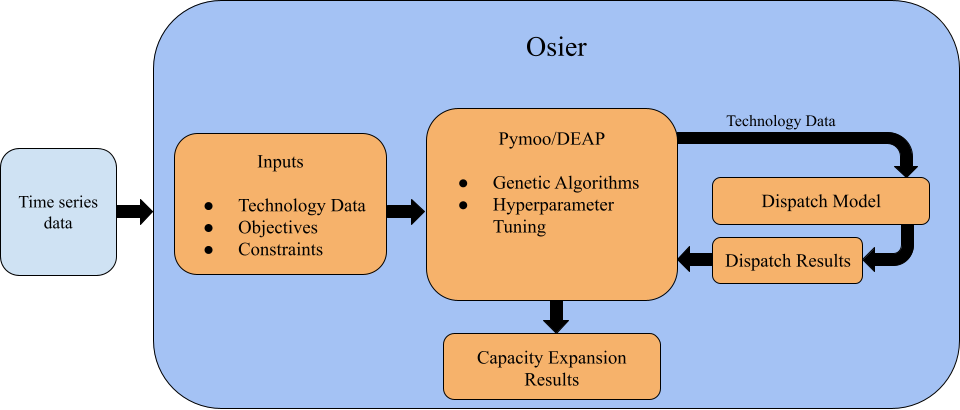
\includegraphics[width=\columnwidth]{figures/osier_flow}
    \caption{The flow of data into and within \ac{osier}}
    \label{fig:osier_flow}
\end{figure}

 Technology data, objectives, constraints, and a dispatch model are all features
within \ac{osier}, while \ac{pymoo} drives the optimization of these objectives.
The dispatch model is independently executable for inspecting specific test
cases and mapping solutions from other solvers onto \ac{osier}'s objective
space. The next section elaborates on the dispatch model's formulation.

\section{Economic Dispatch}
\label{section:dispatch}

 The economic dispatch model minimizes the generation cost subject to physical
 constraints but does not optimize capacity investments. The complete set of
 equations for the model is detailed below.
\begin{align}
    \intertext{Minimize: }
    \label{eq:dispatch-objective}
    &\left(\sum_t^T\sum_g^G \left[C_{g,t}^{fuel} + C_{g,t}^{vom}\right]x_{g,t}
    \right)+\left(\sum_t^T\sum_g^S x_{g,t}c_{g,t}\pi\right)\\
    \intertext{such that,}
    \intertext{1. The generation meets demand, less the amount of energy stored or curtailed, 
    within a user-specified tolerance (undersupply and oversupply),}
    \left[\sum_g^Gx_{g,t}-\sum_g^S c_{g,t}\right] &\geq \left(1-\text{undersupply}\right)\text{D}_t\quad \forall \quad t \in T, S, \\
    \left[\sum_g^Gx_{g,t}-\sum_g^S c_{g,t}\right] &\leq \left(1+\text{oversupply}\right)\text{D}_t \quad \forall \quad t \in T, S,
    \intertext{2. A generator's production, $x_{g}$ does not exceed its capacity at any time, $t$}
    x_{g,t} &\leq \textbf{CAP}_{g}\Delta \tau \quad \forall \quad g,t \in G,T
    \intertext{3. A generator's ramping rate is never exceeded,}
    \frac{x_{r,t} - x_{r,t-1}}{\Delta \tau} = \Delta P_{r,t} &\leq
        \rho^{up}_g\textbf{CAP}_g\Delta\tau \quad \forall \quad r,t
        \in R, T,\\
    \frac{x_{r,t} - x_{r,t-1}}{\Delta \tau} = \Delta P_{r,t} &\leq
        -\rho^{down}_g\textbf{CAP}_g\Delta\tau \quad \forall \quad r,t
        \in R, T,
    \intertext{4. Storage capacity for each storage technology is never exceeded}
    \textbf{SOC}_{s,t} &\leq \textbf{CAP}^S_{s} \quad \forall \quad s,t \in S,T,
    \intertext{5. Storage discharge cannot exceed stored energy.}
    x_{s,t} &\leq \textbf{SOC}_{s,t} \quad \forall \quad s,t \in S,T,
    \intertext{6. Storage charge rate cannot exceed unit capacity}
    c_{s,t} &\leq \textbf{CAP}_{s}\Delta \tau \quad \forall \quad s,t \in S,T,
    \intertext{where,}
    G &= \text{ the set of all generating technologies},\nonumber\\
    R &= \text{ the set of all ramping technologies}, \quad R \subset G,\nonumber\\
    S &= \text{ the set of all storage technologies}, \quad S \subset G,\nonumber\\
    T &= \text{ the set of all time periods in the model},\nonumber\\
    D_t &= \text{ the demand at each time period, \textit{t}},\nonumber\\
    \textbf{CAP}_g &= \text{ the capacity of the \textit{g-th} technology}\quad \left[MW\right],\nonumber\\
    \textbf{CAP}^S_g &= \text{ the storage capacity of the \textit{g-th} technology}\quad \left[MWh\right],\nonumber\\
    \textbf{SOC}_{s,t} &= \text{ the state of charge of the \textit{g-th} technology at time \textit{t}}\quad \left[MWh\right]\nonumber,\\
    \Delta\tau &= t_{i+1} - t_i \quad \forall \quad t_i \in T \quad \left[h\right],\nonumber\\
    x_{g,t} &= \text{ the energy produced by generator, \textit{g}, at time, \textit{t}}\quad \left[MWh\right]\nonumber,\\
    c_{s,t} &= \text{ the energy stored by storage technology, \textit{s}, at time, \textit{t}}\quad \left[MWh\right]\nonumber,\\
    \rho_g &= \text{ the up/down ramp rate for technology, \textit{g}} \quad \left[-\right]\nonumber,\\
    \pi &= \text{ A small penalty for simultaneous charging and discharging.}\nonumber
\end{align}
The second term in the objective function, Equation \ref{eq:dispatch-objective},
represents a minor penalty to prevent the unphysical behavior of simultaneous
charging and discharging from storage technologies. I used this approach because
constraining this behavior requires a binary variable that makes the problem
non-convex and therefore requires a more sophisticated solver. A small but
sufficiently large $\pi$ will always nullify the penalty term. This dispatch
model reflects the minimum physical constraints for an energy system without
considering fine-scale operational details such as frequency control. Equation
\ref{eq:dispatch-objective} assumes that the retail cost for generating
electricity is identical to the marginal cost of producing electricity. 
\section{Genetic Algorithms}
\label{section:genetic-algorithms}

Rather than rely on \ac{lp} to model future capacity requirements, in this
thesis, \acp{ga} assume the role of investment optimizer. \acp{ga} share a
fundamental algorithmic structure, which is \cite{blank_pymoo_2020}
\begin{enumerate}
    \item \textbf{Initialize} a starting population of $N_p$ individuals, where
    each individual has a set of ``genes'' that are randomly chosen from the
    bounds of the decision variables.
    \item Each individual in the population is \textbf{evaluated} for
    ``fitness.'' 
    \item The \textbf{fittest}, $N_f$ individuals ``survive'' and persist in the
    next generation.
    \item A ``selection'' operator \textbf{chooses} among the surviving
    individuals to mate.
    \item The parents are \textbf{combined} using a ``crossover'' operator,
    thereby filling the remaining $N_p - N_f$ individuals for the next
    generation.
    \item The offspring are finally \textbf{mutated} with some probability,
    $\mu$, to improve genetic diversity.
\end{enumerate}
\noindent
Figure \ref{fig:genetic-alg} illustrates the flow of these steps applied to an
energy systems model.

\begin{figure}[ht]
        \centering
        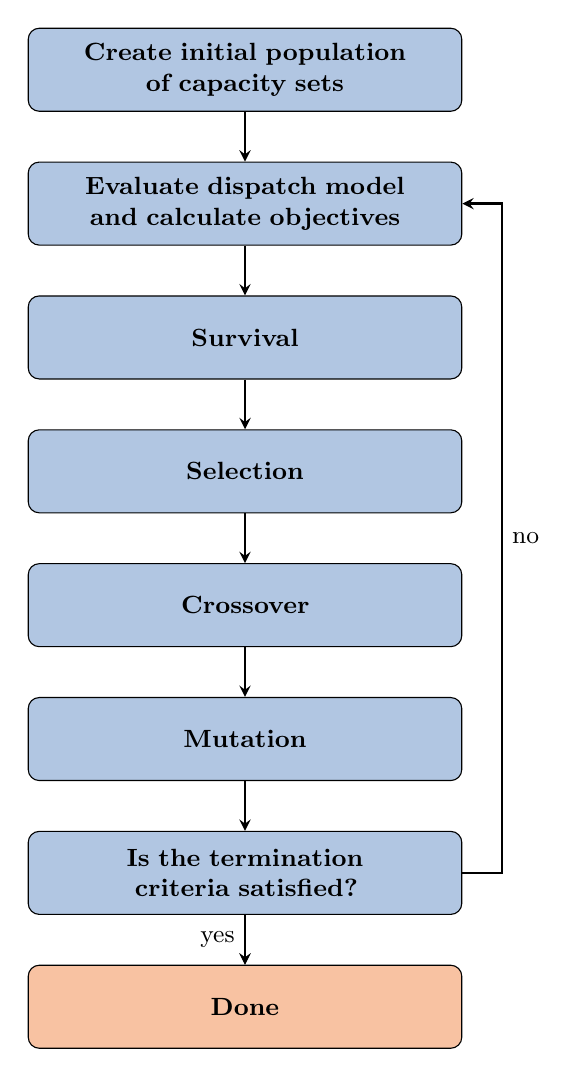
\begin{tikzpicture}[node distance=1.7cm]
                \tikzstyle{every node}=[font=\small] \node (1) [lbblock]
                {\textbf{Create initial population\\ of capacity sets}}; \node
                (2) [lbblock, below of=1] {\textbf{Evaluate dispatch model and
                calculate objectives}}; \node (3) [lbblock, below of=2]
                {\textbf{Survival}}; \node (4) [lbblock, below of=3]
                {\textbf{Selection}}; \node (5) [lbblock, below of=4]
                {\textbf{Crossover}}; \node (6) [lbblock, below of=5]
                {\textbf{Mutation}}; \node (7) [lbblock, below of=6] {\textbf{Is
                the termination \\ criteria satisfied?}}; \node (8) [loblock,
                below of=7] {\textbf{Done}}; \draw [arrow] (1) -- (2); \draw
                [arrow] (2) -- (3); \draw [arrow] (3) -- (4); \draw [arrow] (4)
                -- (5); \draw [arrow] (5) -- (6); \draw [arrow] (6) -- (7);
                \draw [arrow] (7) -- (8); \draw [arrow] (7) -- node[anchor=east]
                {yes} (8); \draw [arrow] (7) -- ([shift={(0.5cm,0cm)}]7.east)--
                node[anchor=west] {no} ([shift={(0.5cm,0cm)}]2.east)--(2);
        \end{tikzpicture}
        \caption{The basic flow of the \ac{ga} used in this thesis.}
        \label{fig:genetic-alg}
\end{figure}

\subsection{Specific \Aclp{ga}} The variety of \acp{ga} comes from different
types of operators being applied to the selection, crossover, and mutation
steps. Section \ref{section:moo-in-energy} showed that \ac{nsga2} is a popular
genetic algorithm choice. However, this algorithm performs poorly with greater
than three objectives \cite{deb_fast_2002, seada_unified_2016}. In this thesis,
I use a more modern algorithm, \ac{unsga3}. \ac{unsga3} builds on its
predecessors \ac{nsga2} and \ac{nsga3} by unifying efficient solutions of mono-,
multi-, and many-objective problems in a single algorithm.


\ac{nsga2} improves on the basic \ac{ga} by introducing a more sophisticated
mating and selection algorithms. Instead of random selection, the individuals
are sorted by rank (i.e. fitness) and crowding distance in binary tournament
mating selection. The crowding distance is simply the Manhattan distance between
individuals. A greater crowding distance is desirable to preserve diversity and
since the extreme points are maximally diverse they should always persist and
are therefore assigned a crowding distance of infinity \cite{deb_fast_2002}.

The successor to \ac{nsga2}, \ac{nsga3}, enhances the many-objective
capabilities of the former by introducing reference directions. Reference
directions are used for initialization and the survival steps. In addition to
fitness, individuals are chosen based on their proximity to a reference line,
thus ensuring population diversity which greatly important for many-objective
problems. Since diversity is handled by reference directions, individuals are
selected randomly for mating. References directions are rays passing through
uniformly spaced points on the unit simplex \cite{seada_unified_2016,
blank_generating_2021}. In this thesis, I use the Riesz s- Energy method
described by Blank et al. to calculate these points for a problem with an
arbitrary number of objectives \cite{blank_generating_2021}. Figure
\ref{fig:ref-dirs} illustrates a set of initialized reference directions.

\begin{figure}[h]
  \centering
  \resizebox{0.6\columnwidth}{!}{%% Creator: Matplotlib, PGF backend
%%
%% To include the figure in your LaTeX document, write
%%   \input{<filename>.pgf}
%%
%% Make sure the required packages are loaded in your preamble
%%   \usepackage{pgf}
%%
%% Also ensure that all the required font packages are loaded; for instance,
%% the lmodern package is sometimes necessary when using math font.
%%   \usepackage{lmodern}
%%
%% Figures using additional raster images can only be included by \input if
%% they are in the same directory as the main LaTeX file. For loading figures
%% from other directories you can use the `import` package
%%   \usepackage{import}
%%
%% and then include the figures with
%%   \import{<path to file>}{<filename>.pgf}
%%
%% Matplotlib used the following preamble
%%   \def\mathdefault#1{#1}
%%   \everymath=\expandafter{\the\everymath\displaystyle}
%%   \IfFileExists{scrextend.sty}{
%%     \usepackage[fontsize=10.000000pt]{scrextend}
%%   }{
%%     \renewcommand{\normalsize}{\fontsize{10.000000}{12.000000}\selectfont}
%%     \normalsize
%%   }
%%   
%%   \makeatletter\@ifpackageloaded{underscore}{}{\usepackage[strings]{underscore}}\makeatother
%%
\begingroup%
\makeatletter%
\begin{pgfpicture}%
\pgfpathrectangle{\pgfpointorigin}{\pgfqpoint{6.454833in}{6.506946in}}%
\pgfusepath{use as bounding box, clip}%
\begin{pgfscope}%
\pgfsetbuttcap%
\pgfsetmiterjoin%
\definecolor{currentfill}{rgb}{1.000000,1.000000,1.000000}%
\pgfsetfillcolor{currentfill}%
\pgfsetlinewidth{0.000000pt}%
\definecolor{currentstroke}{rgb}{0.000000,0.000000,0.000000}%
\pgfsetstrokecolor{currentstroke}%
\pgfsetdash{}{0pt}%
\pgfpathmoveto{\pgfqpoint{0.000000in}{0.000000in}}%
\pgfpathlineto{\pgfqpoint{6.454833in}{0.000000in}}%
\pgfpathlineto{\pgfqpoint{6.454833in}{6.506946in}}%
\pgfpathlineto{\pgfqpoint{0.000000in}{6.506946in}}%
\pgfpathlineto{\pgfqpoint{0.000000in}{0.000000in}}%
\pgfpathclose%
\pgfusepath{fill}%
\end{pgfscope}%
\begin{pgfscope}%
\pgfsetbuttcap%
\pgfsetmiterjoin%
\definecolor{currentfill}{rgb}{1.000000,1.000000,1.000000}%
\pgfsetfillcolor{currentfill}%
\pgfsetlinewidth{0.000000pt}%
\definecolor{currentstroke}{rgb}{0.000000,0.000000,0.000000}%
\pgfsetstrokecolor{currentstroke}%
\pgfsetstrokeopacity{0.000000}%
\pgfsetdash{}{0pt}%
\pgfpathmoveto{\pgfqpoint{0.194833in}{0.246946in}}%
\pgfpathlineto{\pgfqpoint{6.354833in}{0.246946in}}%
\pgfpathlineto{\pgfqpoint{6.354833in}{6.406946in}}%
\pgfpathlineto{\pgfqpoint{0.194833in}{6.406946in}}%
\pgfpathlineto{\pgfqpoint{0.194833in}{0.246946in}}%
\pgfpathclose%
\pgfusepath{fill}%
\end{pgfscope}%
\begin{pgfscope}%
\pgfsetbuttcap%
\pgfsetmiterjoin%
\definecolor{currentfill}{rgb}{0.950000,0.950000,0.950000}%
\pgfsetfillcolor{currentfill}%
\pgfsetfillopacity{0.500000}%
\pgfsetlinewidth{1.003750pt}%
\definecolor{currentstroke}{rgb}{0.950000,0.950000,0.950000}%
\pgfsetstrokecolor{currentstroke}%
\pgfsetstrokeopacity{0.500000}%
\pgfsetdash{}{0pt}%
\pgfpathmoveto{\pgfqpoint{3.358076in}{4.263351in}}%
\pgfpathlineto{\pgfqpoint{6.075248in}{2.391249in}}%
\pgfpathlineto{\pgfqpoint{6.252387in}{4.495556in}}%
\pgfpathlineto{\pgfqpoint{3.358076in}{6.360787in}}%
\pgfusepath{stroke,fill}%
\end{pgfscope}%
\begin{pgfscope}%
\pgfsetbuttcap%
\pgfsetmiterjoin%
\definecolor{currentfill}{rgb}{0.900000,0.900000,0.900000}%
\pgfsetfillcolor{currentfill}%
\pgfsetfillopacity{0.500000}%
\pgfsetlinewidth{1.003750pt}%
\definecolor{currentstroke}{rgb}{0.900000,0.900000,0.900000}%
\pgfsetstrokecolor{currentstroke}%
\pgfsetstrokeopacity{0.500000}%
\pgfsetdash{}{0pt}%
\pgfpathmoveto{\pgfqpoint{3.358076in}{4.263351in}}%
\pgfpathlineto{\pgfqpoint{0.640904in}{2.391249in}}%
\pgfpathlineto{\pgfqpoint{0.463765in}{4.495556in}}%
\pgfpathlineto{\pgfqpoint{3.358076in}{6.360787in}}%
\pgfusepath{stroke,fill}%
\end{pgfscope}%
\begin{pgfscope}%
\pgfsetbuttcap%
\pgfsetmiterjoin%
\definecolor{currentfill}{rgb}{0.925000,0.925000,0.925000}%
\pgfsetfillcolor{currentfill}%
\pgfsetfillopacity{0.500000}%
\pgfsetlinewidth{1.003750pt}%
\definecolor{currentstroke}{rgb}{0.925000,0.925000,0.925000}%
\pgfsetstrokecolor{currentstroke}%
\pgfsetstrokeopacity{0.500000}%
\pgfsetdash{}{0pt}%
\pgfpathmoveto{\pgfqpoint{3.358076in}{4.263351in}}%
\pgfpathlineto{\pgfqpoint{0.640904in}{2.391249in}}%
\pgfpathlineto{\pgfqpoint{3.358076in}{0.289869in}}%
\pgfpathlineto{\pgfqpoint{6.075248in}{2.391249in}}%
\pgfusepath{stroke,fill}%
\end{pgfscope}%
\begin{pgfscope}%
\pgfsetbuttcap%
\pgfsetroundjoin%
\pgfsetlinewidth{0.803000pt}%
\definecolor{currentstroke}{rgb}{0.690196,0.690196,0.690196}%
\pgfsetstrokecolor{currentstroke}%
\pgfsetdash{}{0pt}%
\pgfpathmoveto{\pgfqpoint{5.911714in}{2.264777in}}%
\pgfpathlineto{\pgfqpoint{3.194029in}{4.150324in}}%
\pgfpathlineto{\pgfqpoint{3.183916in}{6.248550in}}%
\pgfusepath{stroke}%
\end{pgfscope}%
\begin{pgfscope}%
\pgfsetbuttcap%
\pgfsetroundjoin%
\pgfsetlinewidth{0.803000pt}%
\definecolor{currentstroke}{rgb}{0.690196,0.690196,0.690196}%
\pgfsetstrokecolor{currentstroke}%
\pgfsetdash{}{0pt}%
\pgfpathmoveto{\pgfqpoint{5.456913in}{1.913047in}}%
\pgfpathlineto{\pgfqpoint{2.738146in}{3.836226in}}%
\pgfpathlineto{\pgfqpoint{2.699539in}{5.936395in}}%
\pgfusepath{stroke}%
\end{pgfscope}%
\begin{pgfscope}%
\pgfsetbuttcap%
\pgfsetroundjoin%
\pgfsetlinewidth{0.803000pt}%
\definecolor{currentstroke}{rgb}{0.690196,0.690196,0.690196}%
\pgfsetstrokecolor{currentstroke}%
\pgfsetdash{}{0pt}%
\pgfpathmoveto{\pgfqpoint{4.992727in}{1.554059in}}%
\pgfpathlineto{\pgfqpoint{2.273382in}{3.516009in}}%
\pgfpathlineto{\pgfqpoint{2.205132in}{5.617775in}}%
\pgfusepath{stroke}%
\end{pgfscope}%
\begin{pgfscope}%
\pgfsetbuttcap%
\pgfsetroundjoin%
\pgfsetlinewidth{0.803000pt}%
\definecolor{currentstroke}{rgb}{0.690196,0.690196,0.690196}%
\pgfsetstrokecolor{currentstroke}%
\pgfsetdash{}{0pt}%
\pgfpathmoveto{\pgfqpoint{4.518863in}{1.187587in}}%
\pgfpathlineto{\pgfqpoint{1.799474in}{3.189491in}}%
\pgfpathlineto{\pgfqpoint{1.700378in}{5.292488in}}%
\pgfusepath{stroke}%
\end{pgfscope}%
\begin{pgfscope}%
\pgfsetbuttcap%
\pgfsetroundjoin%
\pgfsetlinewidth{0.803000pt}%
\definecolor{currentstroke}{rgb}{0.690196,0.690196,0.690196}%
\pgfsetstrokecolor{currentstroke}%
\pgfsetdash{}{0pt}%
\pgfpathmoveto{\pgfqpoint{4.035014in}{0.813393in}}%
\pgfpathlineto{\pgfqpoint{1.316148in}{2.856485in}}%
\pgfpathlineto{\pgfqpoint{1.184951in}{4.960322in}}%
\pgfusepath{stroke}%
\end{pgfscope}%
\begin{pgfscope}%
\pgfsetbuttcap%
\pgfsetroundjoin%
\pgfsetlinewidth{0.803000pt}%
\definecolor{currentstroke}{rgb}{0.690196,0.690196,0.690196}%
\pgfsetstrokecolor{currentstroke}%
\pgfsetdash{}{0pt}%
\pgfpathmoveto{\pgfqpoint{3.540863in}{0.431231in}}%
\pgfpathlineto{\pgfqpoint{0.823123in}{2.516796in}}%
\pgfpathlineto{\pgfqpoint{0.658507in}{4.621057in}}%
\pgfusepath{stroke}%
\end{pgfscope}%
\begin{pgfscope}%
\pgfsetbuttcap%
\pgfsetroundjoin%
\pgfsetlinewidth{0.803000pt}%
\definecolor{currentstroke}{rgb}{0.690196,0.690196,0.690196}%
\pgfsetstrokecolor{currentstroke}%
\pgfsetdash{}{0pt}%
\pgfpathmoveto{\pgfqpoint{3.532236in}{6.248550in}}%
\pgfpathlineto{\pgfqpoint{3.522123in}{4.150324in}}%
\pgfpathlineto{\pgfqpoint{0.804438in}{2.264777in}}%
\pgfusepath{stroke}%
\end{pgfscope}%
\begin{pgfscope}%
\pgfsetbuttcap%
\pgfsetroundjoin%
\pgfsetlinewidth{0.803000pt}%
\definecolor{currentstroke}{rgb}{0.690196,0.690196,0.690196}%
\pgfsetstrokecolor{currentstroke}%
\pgfsetdash{}{0pt}%
\pgfpathmoveto{\pgfqpoint{4.016613in}{5.936395in}}%
\pgfpathlineto{\pgfqpoint{3.978006in}{3.836226in}}%
\pgfpathlineto{\pgfqpoint{1.259239in}{1.913047in}}%
\pgfusepath{stroke}%
\end{pgfscope}%
\begin{pgfscope}%
\pgfsetbuttcap%
\pgfsetroundjoin%
\pgfsetlinewidth{0.803000pt}%
\definecolor{currentstroke}{rgb}{0.690196,0.690196,0.690196}%
\pgfsetstrokecolor{currentstroke}%
\pgfsetdash{}{0pt}%
\pgfpathmoveto{\pgfqpoint{4.511020in}{5.617775in}}%
\pgfpathlineto{\pgfqpoint{4.442770in}{3.516009in}}%
\pgfpathlineto{\pgfqpoint{1.723425in}{1.554059in}}%
\pgfusepath{stroke}%
\end{pgfscope}%
\begin{pgfscope}%
\pgfsetbuttcap%
\pgfsetroundjoin%
\pgfsetlinewidth{0.803000pt}%
\definecolor{currentstroke}{rgb}{0.690196,0.690196,0.690196}%
\pgfsetstrokecolor{currentstroke}%
\pgfsetdash{}{0pt}%
\pgfpathmoveto{\pgfqpoint{5.015774in}{5.292488in}}%
\pgfpathlineto{\pgfqpoint{4.916678in}{3.189491in}}%
\pgfpathlineto{\pgfqpoint{2.197289in}{1.187587in}}%
\pgfusepath{stroke}%
\end{pgfscope}%
\begin{pgfscope}%
\pgfsetbuttcap%
\pgfsetroundjoin%
\pgfsetlinewidth{0.803000pt}%
\definecolor{currentstroke}{rgb}{0.690196,0.690196,0.690196}%
\pgfsetstrokecolor{currentstroke}%
\pgfsetdash{}{0pt}%
\pgfpathmoveto{\pgfqpoint{5.531201in}{4.960322in}}%
\pgfpathlineto{\pgfqpoint{5.400004in}{2.856485in}}%
\pgfpathlineto{\pgfqpoint{2.681138in}{0.813393in}}%
\pgfusepath{stroke}%
\end{pgfscope}%
\begin{pgfscope}%
\pgfsetbuttcap%
\pgfsetroundjoin%
\pgfsetlinewidth{0.803000pt}%
\definecolor{currentstroke}{rgb}{0.690196,0.690196,0.690196}%
\pgfsetstrokecolor{currentstroke}%
\pgfsetdash{}{0pt}%
\pgfpathmoveto{\pgfqpoint{6.057645in}{4.621057in}}%
\pgfpathlineto{\pgfqpoint{5.893029in}{2.516796in}}%
\pgfpathlineto{\pgfqpoint{3.175289in}{0.431231in}}%
\pgfusepath{stroke}%
\end{pgfscope}%
\begin{pgfscope}%
\pgfsetbuttcap%
\pgfsetroundjoin%
\pgfsetlinewidth{0.803000pt}%
\definecolor{currentstroke}{rgb}{0.690196,0.690196,0.690196}%
\pgfsetstrokecolor{currentstroke}%
\pgfsetdash{}{0pt}%
\pgfpathmoveto{\pgfqpoint{0.630280in}{2.517456in}}%
\pgfpathlineto{\pgfqpoint{3.358076in}{4.389566in}}%
\pgfpathlineto{\pgfqpoint{6.085872in}{2.517456in}}%
\pgfusepath{stroke}%
\end{pgfscope}%
\begin{pgfscope}%
\pgfsetbuttcap%
\pgfsetroundjoin%
\pgfsetlinewidth{0.803000pt}%
\definecolor{currentstroke}{rgb}{0.690196,0.690196,0.690196}%
\pgfsetstrokecolor{currentstroke}%
\pgfsetdash{}{0pt}%
\pgfpathmoveto{\pgfqpoint{0.600709in}{2.868742in}}%
\pgfpathlineto{\pgfqpoint{3.358076in}{4.740592in}}%
\pgfpathlineto{\pgfqpoint{6.115443in}{2.868742in}}%
\pgfusepath{stroke}%
\end{pgfscope}%
\begin{pgfscope}%
\pgfsetbuttcap%
\pgfsetroundjoin%
\pgfsetlinewidth{0.803000pt}%
\definecolor{currentstroke}{rgb}{0.690196,0.690196,0.690196}%
\pgfsetstrokecolor{currentstroke}%
\pgfsetdash{}{0pt}%
\pgfpathmoveto{\pgfqpoint{0.570490in}{3.227729in}}%
\pgfpathlineto{\pgfqpoint{3.358076in}{5.098883in}}%
\pgfpathlineto{\pgfqpoint{6.145662in}{3.227729in}}%
\pgfusepath{stroke}%
\end{pgfscope}%
\begin{pgfscope}%
\pgfsetbuttcap%
\pgfsetroundjoin%
\pgfsetlinewidth{0.803000pt}%
\definecolor{currentstroke}{rgb}{0.690196,0.690196,0.690196}%
\pgfsetstrokecolor{currentstroke}%
\pgfsetdash{}{0pt}%
\pgfpathmoveto{\pgfqpoint{0.539601in}{3.594671in}}%
\pgfpathlineto{\pgfqpoint{3.358076in}{5.464666in}}%
\pgfpathlineto{\pgfqpoint{6.176551in}{3.594671in}}%
\pgfusepath{stroke}%
\end{pgfscope}%
\begin{pgfscope}%
\pgfsetbuttcap%
\pgfsetroundjoin%
\pgfsetlinewidth{0.803000pt}%
\definecolor{currentstroke}{rgb}{0.690196,0.690196,0.690196}%
\pgfsetstrokecolor{currentstroke}%
\pgfsetdash{}{0pt}%
\pgfpathmoveto{\pgfqpoint{0.508019in}{3.969836in}}%
\pgfpathlineto{\pgfqpoint{3.358076in}{5.838179in}}%
\pgfpathlineto{\pgfqpoint{6.208133in}{3.969836in}}%
\pgfusepath{stroke}%
\end{pgfscope}%
\begin{pgfscope}%
\pgfsetbuttcap%
\pgfsetroundjoin%
\pgfsetlinewidth{0.803000pt}%
\definecolor{currentstroke}{rgb}{0.690196,0.690196,0.690196}%
\pgfsetstrokecolor{currentstroke}%
\pgfsetdash{}{0pt}%
\pgfpathmoveto{\pgfqpoint{0.475722in}{4.353505in}}%
\pgfpathlineto{\pgfqpoint{3.358076in}{6.219668in}}%
\pgfpathlineto{\pgfqpoint{6.240430in}{4.353505in}}%
\pgfusepath{stroke}%
\end{pgfscope}%
\begin{pgfscope}%
\pgfsetrectcap%
\pgfsetroundjoin%
\pgfsetlinewidth{0.803000pt}%
\definecolor{currentstroke}{rgb}{0.000000,0.000000,0.000000}%
\pgfsetstrokecolor{currentstroke}%
\pgfsetdash{}{0pt}%
\pgfpathmoveto{\pgfqpoint{6.075248in}{2.391249in}}%
\pgfpathlineto{\pgfqpoint{3.358076in}{0.289869in}}%
\pgfusepath{stroke}%
\end{pgfscope}%
\begin{pgfscope}%
\pgfsetrectcap%
\pgfsetroundjoin%
\pgfsetlinewidth{0.803000pt}%
\definecolor{currentstroke}{rgb}{0.000000,0.000000,0.000000}%
\pgfsetstrokecolor{currentstroke}%
\pgfsetdash{}{0pt}%
\pgfpathmoveto{\pgfqpoint{5.888724in}{2.280728in}}%
\pgfpathlineto{\pgfqpoint{5.957758in}{2.232831in}}%
\pgfusepath{stroke}%
\end{pgfscope}%
\begin{pgfscope}%
\definecolor{textcolor}{rgb}{0.000000,0.000000,0.000000}%
\pgfsetstrokecolor{textcolor}%
\pgfsetfillcolor{textcolor}%
\pgftext[x=6.047013in,y=2.067182in,,top]{\color{textcolor}{\rmfamily\fontsize{10.000000}{12.000000}\selectfont\catcode`\^=\active\def^{\ifmmode\sp\else\^{}\fi}\catcode`\%=\active\def%{\%}$\mathdefault{0.0}$}}%
\end{pgfscope}%
\begin{pgfscope}%
\pgfsetrectcap%
\pgfsetroundjoin%
\pgfsetlinewidth{0.803000pt}%
\definecolor{currentstroke}{rgb}{0.000000,0.000000,0.000000}%
\pgfsetstrokecolor{currentstroke}%
\pgfsetdash{}{0pt}%
\pgfpathmoveto{\pgfqpoint{5.433901in}{1.929325in}}%
\pgfpathlineto{\pgfqpoint{5.503001in}{1.880446in}}%
\pgfusepath{stroke}%
\end{pgfscope}%
\begin{pgfscope}%
\definecolor{textcolor}{rgb}{0.000000,0.000000,0.000000}%
\pgfsetstrokecolor{textcolor}%
\pgfsetfillcolor{textcolor}%
\pgftext[x=5.593673in,y=1.713497in,,top]{\color{textcolor}{\rmfamily\fontsize{10.000000}{12.000000}\selectfont\catcode`\^=\active\def^{\ifmmode\sp\else\^{}\fi}\catcode`\%=\active\def%{\%}$\mathdefault{0.2}$}}%
\end{pgfscope}%
\begin{pgfscope}%
\pgfsetrectcap%
\pgfsetroundjoin%
\pgfsetlinewidth{0.803000pt}%
\definecolor{currentstroke}{rgb}{0.000000,0.000000,0.000000}%
\pgfsetstrokecolor{currentstroke}%
\pgfsetdash{}{0pt}%
\pgfpathmoveto{\pgfqpoint{4.969697in}{1.570675in}}%
\pgfpathlineto{\pgfqpoint{5.038852in}{1.520781in}}%
\pgfusepath{stroke}%
\end{pgfscope}%
\begin{pgfscope}%
\definecolor{textcolor}{rgb}{0.000000,0.000000,0.000000}%
\pgfsetstrokecolor{textcolor}%
\pgfsetfillcolor{textcolor}%
\pgftext[x=5.130981in,y=1.352515in,,top]{\color{textcolor}{\rmfamily\fontsize{10.000000}{12.000000}\selectfont\catcode`\^=\active\def^{\ifmmode\sp\else\^{}\fi}\catcode`\%=\active\def%{\%}$\mathdefault{0.4}$}}%
\end{pgfscope}%
\begin{pgfscope}%
\pgfsetrectcap%
\pgfsetroundjoin%
\pgfsetlinewidth{0.803000pt}%
\definecolor{currentstroke}{rgb}{0.000000,0.000000,0.000000}%
\pgfsetstrokecolor{currentstroke}%
\pgfsetdash{}{0pt}%
\pgfpathmoveto{\pgfqpoint{4.495819in}{1.204551in}}%
\pgfpathlineto{\pgfqpoint{4.565016in}{1.153611in}}%
\pgfusepath{stroke}%
\end{pgfscope}%
\begin{pgfscope}%
\definecolor{textcolor}{rgb}{0.000000,0.000000,0.000000}%
\pgfsetstrokecolor{textcolor}%
\pgfsetfillcolor{textcolor}%
\pgftext[x=4.658643in,y=0.984008in,,top]{\color{textcolor}{\rmfamily\fontsize{10.000000}{12.000000}\selectfont\catcode`\^=\active\def^{\ifmmode\sp\else\^{}\fi}\catcode`\%=\active\def%{\%}$\mathdefault{0.6}$}}%
\end{pgfscope}%
\begin{pgfscope}%
\pgfsetrectcap%
\pgfsetroundjoin%
\pgfsetlinewidth{0.803000pt}%
\definecolor{currentstroke}{rgb}{0.000000,0.000000,0.000000}%
\pgfsetstrokecolor{currentstroke}%
\pgfsetdash{}{0pt}%
\pgfpathmoveto{\pgfqpoint{4.011962in}{0.830716in}}%
\pgfpathlineto{\pgfqpoint{4.081186in}{0.778697in}}%
\pgfusepath{stroke}%
\end{pgfscope}%
\begin{pgfscope}%
\definecolor{textcolor}{rgb}{0.000000,0.000000,0.000000}%
\pgfsetstrokecolor{textcolor}%
\pgfsetfillcolor{textcolor}%
\pgftext[x=4.176355in,y=0.607737in,,top]{\color{textcolor}{\rmfamily\fontsize{10.000000}{12.000000}\selectfont\catcode`\^=\active\def^{\ifmmode\sp\else\^{}\fi}\catcode`\%=\active\def%{\%}$\mathdefault{0.8}$}}%
\end{pgfscope}%
\begin{pgfscope}%
\pgfsetrectcap%
\pgfsetroundjoin%
\pgfsetlinewidth{0.803000pt}%
\definecolor{currentstroke}{rgb}{0.000000,0.000000,0.000000}%
\pgfsetstrokecolor{currentstroke}%
\pgfsetdash{}{0pt}%
\pgfpathmoveto{\pgfqpoint{3.517806in}{0.448925in}}%
\pgfpathlineto{\pgfqpoint{3.587044in}{0.395792in}}%
\pgfusepath{stroke}%
\end{pgfscope}%
\begin{pgfscope}%
\definecolor{textcolor}{rgb}{0.000000,0.000000,0.000000}%
\pgfsetstrokecolor{textcolor}%
\pgfsetfillcolor{textcolor}%
\pgftext[x=3.683800in,y=0.223457in,,top]{\color{textcolor}{\rmfamily\fontsize{10.000000}{12.000000}\selectfont\catcode`\^=\active\def^{\ifmmode\sp\else\^{}\fi}\catcode`\%=\active\def%{\%}$\mathdefault{1.0}$}}%
\end{pgfscope}%
\begin{pgfscope}%
\definecolor{textcolor}{rgb}{0.000000,0.000000,0.000000}%
\pgfsetstrokecolor{textcolor}%
\pgfsetfillcolor{textcolor}%
\pgftext[x=5.059162in,y=0.931525in,,,rotate=37.717305]{\color{textcolor}{\rmfamily\fontsize{14.000000}{16.800000}\selectfont\catcode`\^=\active\def^{\ifmmode\sp\else\^{}\fi}\catcode`\%=\active\def%{\%}$f_1$}}%
\end{pgfscope}%
\begin{pgfscope}%
\pgfsetrectcap%
\pgfsetroundjoin%
\pgfsetlinewidth{0.803000pt}%
\definecolor{currentstroke}{rgb}{0.000000,0.000000,0.000000}%
\pgfsetstrokecolor{currentstroke}%
\pgfsetdash{}{0pt}%
\pgfpathmoveto{\pgfqpoint{0.640904in}{2.391249in}}%
\pgfpathlineto{\pgfqpoint{3.358076in}{0.289869in}}%
\pgfusepath{stroke}%
\end{pgfscope}%
\begin{pgfscope}%
\pgfsetrectcap%
\pgfsetroundjoin%
\pgfsetlinewidth{0.803000pt}%
\definecolor{currentstroke}{rgb}{0.000000,0.000000,0.000000}%
\pgfsetstrokecolor{currentstroke}%
\pgfsetdash{}{0pt}%
\pgfpathmoveto{\pgfqpoint{0.827428in}{2.280728in}}%
\pgfpathlineto{\pgfqpoint{0.758394in}{2.232831in}}%
\pgfusepath{stroke}%
\end{pgfscope}%
\begin{pgfscope}%
\definecolor{textcolor}{rgb}{0.000000,0.000000,0.000000}%
\pgfsetstrokecolor{textcolor}%
\pgfsetfillcolor{textcolor}%
\pgftext[x=0.669139in,y=2.067182in,,top]{\color{textcolor}{\rmfamily\fontsize{10.000000}{12.000000}\selectfont\catcode`\^=\active\def^{\ifmmode\sp\else\^{}\fi}\catcode`\%=\active\def%{\%}$\mathdefault{0.0}$}}%
\end{pgfscope}%
\begin{pgfscope}%
\pgfsetrectcap%
\pgfsetroundjoin%
\pgfsetlinewidth{0.803000pt}%
\definecolor{currentstroke}{rgb}{0.000000,0.000000,0.000000}%
\pgfsetstrokecolor{currentstroke}%
\pgfsetdash{}{0pt}%
\pgfpathmoveto{\pgfqpoint{1.282251in}{1.929325in}}%
\pgfpathlineto{\pgfqpoint{1.213151in}{1.880446in}}%
\pgfusepath{stroke}%
\end{pgfscope}%
\begin{pgfscope}%
\definecolor{textcolor}{rgb}{0.000000,0.000000,0.000000}%
\pgfsetstrokecolor{textcolor}%
\pgfsetfillcolor{textcolor}%
\pgftext[x=1.122479in,y=1.713497in,,top]{\color{textcolor}{\rmfamily\fontsize{10.000000}{12.000000}\selectfont\catcode`\^=\active\def^{\ifmmode\sp\else\^{}\fi}\catcode`\%=\active\def%{\%}$\mathdefault{0.2}$}}%
\end{pgfscope}%
\begin{pgfscope}%
\pgfsetrectcap%
\pgfsetroundjoin%
\pgfsetlinewidth{0.803000pt}%
\definecolor{currentstroke}{rgb}{0.000000,0.000000,0.000000}%
\pgfsetstrokecolor{currentstroke}%
\pgfsetdash{}{0pt}%
\pgfpathmoveto{\pgfqpoint{1.746455in}{1.570675in}}%
\pgfpathlineto{\pgfqpoint{1.677300in}{1.520781in}}%
\pgfusepath{stroke}%
\end{pgfscope}%
\begin{pgfscope}%
\definecolor{textcolor}{rgb}{0.000000,0.000000,0.000000}%
\pgfsetstrokecolor{textcolor}%
\pgfsetfillcolor{textcolor}%
\pgftext[x=1.585171in,y=1.352515in,,top]{\color{textcolor}{\rmfamily\fontsize{10.000000}{12.000000}\selectfont\catcode`\^=\active\def^{\ifmmode\sp\else\^{}\fi}\catcode`\%=\active\def%{\%}$\mathdefault{0.4}$}}%
\end{pgfscope}%
\begin{pgfscope}%
\pgfsetrectcap%
\pgfsetroundjoin%
\pgfsetlinewidth{0.803000pt}%
\definecolor{currentstroke}{rgb}{0.000000,0.000000,0.000000}%
\pgfsetstrokecolor{currentstroke}%
\pgfsetdash{}{0pt}%
\pgfpathmoveto{\pgfqpoint{2.220333in}{1.204551in}}%
\pgfpathlineto{\pgfqpoint{2.151136in}{1.153611in}}%
\pgfusepath{stroke}%
\end{pgfscope}%
\begin{pgfscope}%
\definecolor{textcolor}{rgb}{0.000000,0.000000,0.000000}%
\pgfsetstrokecolor{textcolor}%
\pgfsetfillcolor{textcolor}%
\pgftext[x=2.057509in,y=0.984008in,,top]{\color{textcolor}{\rmfamily\fontsize{10.000000}{12.000000}\selectfont\catcode`\^=\active\def^{\ifmmode\sp\else\^{}\fi}\catcode`\%=\active\def%{\%}$\mathdefault{0.6}$}}%
\end{pgfscope}%
\begin{pgfscope}%
\pgfsetrectcap%
\pgfsetroundjoin%
\pgfsetlinewidth{0.803000pt}%
\definecolor{currentstroke}{rgb}{0.000000,0.000000,0.000000}%
\pgfsetstrokecolor{currentstroke}%
\pgfsetdash{}{0pt}%
\pgfpathmoveto{\pgfqpoint{2.704190in}{0.830716in}}%
\pgfpathlineto{\pgfqpoint{2.634966in}{0.778697in}}%
\pgfusepath{stroke}%
\end{pgfscope}%
\begin{pgfscope}%
\definecolor{textcolor}{rgb}{0.000000,0.000000,0.000000}%
\pgfsetstrokecolor{textcolor}%
\pgfsetfillcolor{textcolor}%
\pgftext[x=2.539797in,y=0.607737in,,top]{\color{textcolor}{\rmfamily\fontsize{10.000000}{12.000000}\selectfont\catcode`\^=\active\def^{\ifmmode\sp\else\^{}\fi}\catcode`\%=\active\def%{\%}$\mathdefault{0.8}$}}%
\end{pgfscope}%
\begin{pgfscope}%
\pgfsetrectcap%
\pgfsetroundjoin%
\pgfsetlinewidth{0.803000pt}%
\definecolor{currentstroke}{rgb}{0.000000,0.000000,0.000000}%
\pgfsetstrokecolor{currentstroke}%
\pgfsetdash{}{0pt}%
\pgfpathmoveto{\pgfqpoint{3.198346in}{0.448925in}}%
\pgfpathlineto{\pgfqpoint{3.129108in}{0.395792in}}%
\pgfusepath{stroke}%
\end{pgfscope}%
\begin{pgfscope}%
\definecolor{textcolor}{rgb}{0.000000,0.000000,0.000000}%
\pgfsetstrokecolor{textcolor}%
\pgfsetfillcolor{textcolor}%
\pgftext[x=3.032352in,y=0.223457in,,top]{\color{textcolor}{\rmfamily\fontsize{10.000000}{12.000000}\selectfont\catcode`\^=\active\def^{\ifmmode\sp\else\^{}\fi}\catcode`\%=\active\def%{\%}$\mathdefault{1.0}$}}%
\end{pgfscope}%
\begin{pgfscope}%
\definecolor{textcolor}{rgb}{0.000000,0.000000,0.000000}%
\pgfsetstrokecolor{textcolor}%
\pgfsetfillcolor{textcolor}%
\pgftext[x=1.656990in,y=0.931525in,,,rotate=322.282695]{\color{textcolor}{\rmfamily\fontsize{14.000000}{16.800000}\selectfont\catcode`\^=\active\def^{\ifmmode\sp\else\^{}\fi}\catcode`\%=\active\def%{\%}$f_2$}}%
\end{pgfscope}%
\begin{pgfscope}%
\pgfsetrectcap%
\pgfsetroundjoin%
\pgfsetlinewidth{0.803000pt}%
\definecolor{currentstroke}{rgb}{0.000000,0.000000,0.000000}%
\pgfsetstrokecolor{currentstroke}%
\pgfsetdash{}{0pt}%
\pgfpathmoveto{\pgfqpoint{0.640904in}{2.391249in}}%
\pgfpathlineto{\pgfqpoint{0.463765in}{4.495556in}}%
\pgfusepath{stroke}%
\end{pgfscope}%
\begin{pgfscope}%
\pgfsetrectcap%
\pgfsetroundjoin%
\pgfsetlinewidth{0.803000pt}%
\definecolor{currentstroke}{rgb}{0.000000,0.000000,0.000000}%
\pgfsetstrokecolor{currentstroke}%
\pgfsetdash{}{0pt}%
\pgfpathmoveto{\pgfqpoint{0.653356in}{2.533293in}}%
\pgfpathlineto{\pgfqpoint{0.584064in}{2.485737in}}%
\pgfusepath{stroke}%
\end{pgfscope}%
\begin{pgfscope}%
\definecolor{textcolor}{rgb}{0.000000,0.000000,0.000000}%
\pgfsetstrokecolor{textcolor}%
\pgfsetfillcolor{textcolor}%
\pgftext[x=0.358681in,y=2.517456in,,top]{\color{textcolor}{\rmfamily\fontsize{10.000000}{12.000000}\selectfont\catcode`\^=\active\def^{\ifmmode\sp\else\^{}\fi}\catcode`\%=\active\def%{\%}$\mathdefault{0.0}$}}%
\end{pgfscope}%
\begin{pgfscope}%
\pgfsetrectcap%
\pgfsetroundjoin%
\pgfsetlinewidth{0.803000pt}%
\definecolor{currentstroke}{rgb}{0.000000,0.000000,0.000000}%
\pgfsetstrokecolor{currentstroke}%
\pgfsetdash{}{0pt}%
\pgfpathmoveto{\pgfqpoint{0.624048in}{2.884587in}}%
\pgfpathlineto{\pgfqpoint{0.553964in}{2.837009in}}%
\pgfusepath{stroke}%
\end{pgfscope}%
\begin{pgfscope}%
\definecolor{textcolor}{rgb}{0.000000,0.000000,0.000000}%
\pgfsetstrokecolor{textcolor}%
\pgfsetfillcolor{textcolor}%
\pgftext[x=0.326166in,y=2.868742in,,top]{\color{textcolor}{\rmfamily\fontsize{10.000000}{12.000000}\selectfont\catcode`\^=\active\def^{\ifmmode\sp\else\^{}\fi}\catcode`\%=\active\def%{\%}$\mathdefault{0.2}$}}%
\end{pgfscope}%
\begin{pgfscope}%
\pgfsetrectcap%
\pgfsetroundjoin%
\pgfsetlinewidth{0.803000pt}%
\definecolor{currentstroke}{rgb}{0.000000,0.000000,0.000000}%
\pgfsetstrokecolor{currentstroke}%
\pgfsetdash{}{0pt}%
\pgfpathmoveto{\pgfqpoint{0.594099in}{3.243577in}}%
\pgfpathlineto{\pgfqpoint{0.523203in}{3.195988in}}%
\pgfusepath{stroke}%
\end{pgfscope}%
\begin{pgfscope}%
\definecolor{textcolor}{rgb}{0.000000,0.000000,0.000000}%
\pgfsetstrokecolor{textcolor}%
\pgfsetfillcolor{textcolor}%
\pgftext[x=0.292938in,y=3.227729in,,top]{\color{textcolor}{\rmfamily\fontsize{10.000000}{12.000000}\selectfont\catcode`\^=\active\def^{\ifmmode\sp\else\^{}\fi}\catcode`\%=\active\def%{\%}$\mathdefault{0.4}$}}%
\end{pgfscope}%
\begin{pgfscope}%
\pgfsetrectcap%
\pgfsetroundjoin%
\pgfsetlinewidth{0.803000pt}%
\definecolor{currentstroke}{rgb}{0.000000,0.000000,0.000000}%
\pgfsetstrokecolor{currentstroke}%
\pgfsetdash{}{0pt}%
\pgfpathmoveto{\pgfqpoint{0.563487in}{3.610519in}}%
\pgfpathlineto{\pgfqpoint{0.491760in}{3.562930in}}%
\pgfusepath{stroke}%
\end{pgfscope}%
\begin{pgfscope}%
\definecolor{textcolor}{rgb}{0.000000,0.000000,0.000000}%
\pgfsetstrokecolor{textcolor}%
\pgfsetfillcolor{textcolor}%
\pgftext[x=0.258973in,y=3.594671in,,top]{\color{textcolor}{\rmfamily\fontsize{10.000000}{12.000000}\selectfont\catcode`\^=\active\def^{\ifmmode\sp\else\^{}\fi}\catcode`\%=\active\def%{\%}$\mathdefault{0.6}$}}%
\end{pgfscope}%
\begin{pgfscope}%
\pgfsetrectcap%
\pgfsetroundjoin%
\pgfsetlinewidth{0.803000pt}%
\definecolor{currentstroke}{rgb}{0.000000,0.000000,0.000000}%
\pgfsetstrokecolor{currentstroke}%
\pgfsetdash{}{0pt}%
\pgfpathmoveto{\pgfqpoint{0.532188in}{3.985680in}}%
\pgfpathlineto{\pgfqpoint{0.459612in}{3.938103in}}%
\pgfusepath{stroke}%
\end{pgfscope}%
\begin{pgfscope}%
\definecolor{textcolor}{rgb}{0.000000,0.000000,0.000000}%
\pgfsetstrokecolor{textcolor}%
\pgfsetfillcolor{textcolor}%
\pgftext[x=0.224248in,y=3.969836in,,top]{\color{textcolor}{\rmfamily\fontsize{10.000000}{12.000000}\selectfont\catcode`\^=\active\def^{\ifmmode\sp\else\^{}\fi}\catcode`\%=\active\def%{\%}$\mathdefault{0.8}$}}%
\end{pgfscope}%
\begin{pgfscope}%
\pgfsetrectcap%
\pgfsetroundjoin%
\pgfsetlinewidth{0.803000pt}%
\definecolor{currentstroke}{rgb}{0.000000,0.000000,0.000000}%
\pgfsetstrokecolor{currentstroke}%
\pgfsetdash{}{0pt}%
\pgfpathmoveto{\pgfqpoint{0.500181in}{4.369340in}}%
\pgfpathlineto{\pgfqpoint{0.426734in}{4.321787in}}%
\pgfusepath{stroke}%
\end{pgfscope}%
\begin{pgfscope}%
\definecolor{textcolor}{rgb}{0.000000,0.000000,0.000000}%
\pgfsetstrokecolor{textcolor}%
\pgfsetfillcolor{textcolor}%
\pgftext[x=0.188735in,y=4.353505in,,top]{\color{textcolor}{\rmfamily\fontsize{10.000000}{12.000000}\selectfont\catcode`\^=\active\def^{\ifmmode\sp\else\^{}\fi}\catcode`\%=\active\def%{\%}$\mathdefault{1.0}$}}%
\end{pgfscope}%
\begin{pgfscope}%
\definecolor{textcolor}{rgb}{0.000000,0.000000,0.000000}%
\pgfsetstrokecolor{textcolor}%
\pgfsetfillcolor{textcolor}%
\pgftext[x=-0.051568in,y=3.410189in,,,rotate=274.811779]{\color{textcolor}{\rmfamily\fontsize{14.000000}{16.800000}\selectfont\catcode`\^=\active\def^{\ifmmode\sp\else\^{}\fi}\catcode`\%=\active\def%{\%}$f_3$}}%
\end{pgfscope}%
\begin{pgfscope}%
\pgfpathrectangle{\pgfqpoint{0.194833in}{0.246946in}}{\pgfqpoint{6.160000in}{6.160000in}}%
\pgfusepath{clip}%
\pgfsetbuttcap%
\pgfsetroundjoin%
\definecolor{currentfill}{rgb}{0.121569,0.466667,0.705882}%
\pgfsetfillcolor{currentfill}%
\pgfsetlinewidth{1.003750pt}%
\definecolor{currentstroke}{rgb}{0.121569,0.466667,0.705882}%
\pgfsetstrokecolor{currentstroke}%
\pgfsetdash{}{0pt}%
\pgfpathmoveto{\pgfqpoint{0.977454in}{2.468351in}}%
\pgfpathcurveto{\pgfqpoint{0.990477in}{2.468351in}}{\pgfqpoint{1.002968in}{2.473525in}}{\pgfqpoint{1.012176in}{2.482733in}}%
\pgfpathcurveto{\pgfqpoint{1.021385in}{2.491942in}}{\pgfqpoint{1.026559in}{2.504433in}}{\pgfqpoint{1.026559in}{2.517456in}}%
\pgfpathcurveto{\pgfqpoint{1.026559in}{2.530478in}}{\pgfqpoint{1.021385in}{2.542969in}}{\pgfqpoint{1.012176in}{2.552178in}}%
\pgfpathcurveto{\pgfqpoint{1.002968in}{2.561386in}}{\pgfqpoint{0.990477in}{2.566560in}}{\pgfqpoint{0.977454in}{2.566560in}}%
\pgfpathcurveto{\pgfqpoint{0.964431in}{2.566560in}}{\pgfqpoint{0.951940in}{2.561386in}}{\pgfqpoint{0.942732in}{2.552178in}}%
\pgfpathcurveto{\pgfqpoint{0.933523in}{2.542969in}}{\pgfqpoint{0.928349in}{2.530478in}}{\pgfqpoint{0.928349in}{2.517456in}}%
\pgfpathcurveto{\pgfqpoint{0.928349in}{2.504433in}}{\pgfqpoint{0.933523in}{2.491942in}}{\pgfqpoint{0.942732in}{2.482733in}}%
\pgfpathcurveto{\pgfqpoint{0.951940in}{2.473525in}}{\pgfqpoint{0.964431in}{2.468351in}}{\pgfqpoint{0.977454in}{2.468351in}}%
\pgfpathlineto{\pgfqpoint{0.977454in}{2.468351in}}%
\pgfpathclose%
\pgfusepath{stroke,fill}%
\end{pgfscope}%
\begin{pgfscope}%
\pgfpathrectangle{\pgfqpoint{0.194833in}{0.246946in}}{\pgfqpoint{6.160000in}{6.160000in}}%
\pgfusepath{clip}%
\pgfsetbuttcap%
\pgfsetroundjoin%
\definecolor{currentfill}{rgb}{0.121569,0.466667,0.705882}%
\pgfsetfillcolor{currentfill}%
\pgfsetlinewidth{1.003750pt}%
\definecolor{currentstroke}{rgb}{0.121569,0.466667,0.705882}%
\pgfsetstrokecolor{currentstroke}%
\pgfsetdash{}{0pt}%
\pgfpathmoveto{\pgfqpoint{2.279284in}{2.468351in}}%
\pgfpathcurveto{\pgfqpoint{2.292306in}{2.468351in}}{\pgfqpoint{2.304797in}{2.473525in}}{\pgfqpoint{2.314006in}{2.482733in}}%
\pgfpathcurveto{\pgfqpoint{2.323214in}{2.491942in}}{\pgfqpoint{2.328388in}{2.504433in}}{\pgfqpoint{2.328388in}{2.517456in}}%
\pgfpathcurveto{\pgfqpoint{2.328388in}{2.530478in}}{\pgfqpoint{2.323214in}{2.542969in}}{\pgfqpoint{2.314006in}{2.552178in}}%
\pgfpathcurveto{\pgfqpoint{2.304797in}{2.561386in}}{\pgfqpoint{2.292306in}{2.566560in}}{\pgfqpoint{2.279284in}{2.566560in}}%
\pgfpathcurveto{\pgfqpoint{2.266261in}{2.566560in}}{\pgfqpoint{2.253770in}{2.561386in}}{\pgfqpoint{2.244561in}{2.552178in}}%
\pgfpathcurveto{\pgfqpoint{2.235353in}{2.542969in}}{\pgfqpoint{2.230179in}{2.530478in}}{\pgfqpoint{2.230179in}{2.517456in}}%
\pgfpathcurveto{\pgfqpoint{2.230179in}{2.504433in}}{\pgfqpoint{2.235353in}{2.491942in}}{\pgfqpoint{2.244561in}{2.482733in}}%
\pgfpathcurveto{\pgfqpoint{2.253770in}{2.473525in}}{\pgfqpoint{2.266261in}{2.468351in}}{\pgfqpoint{2.279284in}{2.468351in}}%
\pgfpathlineto{\pgfqpoint{2.279284in}{2.468351in}}%
\pgfpathclose%
\pgfusepath{stroke,fill}%
\end{pgfscope}%
\begin{pgfscope}%
\pgfpathrectangle{\pgfqpoint{0.194833in}{0.246946in}}{\pgfqpoint{6.160000in}{6.160000in}}%
\pgfusepath{clip}%
\pgfsetbuttcap%
\pgfsetroundjoin%
\definecolor{currentfill}{rgb}{0.121569,0.466667,0.705882}%
\pgfsetfillcolor{currentfill}%
\pgfsetlinewidth{1.003750pt}%
\definecolor{currentstroke}{rgb}{0.121569,0.466667,0.705882}%
\pgfsetstrokecolor{currentstroke}%
\pgfsetdash{}{0pt}%
\pgfpathmoveto{\pgfqpoint{4.461082in}{2.468351in}}%
\pgfpathcurveto{\pgfqpoint{4.474105in}{2.468351in}}{\pgfqpoint{4.486596in}{2.473525in}}{\pgfqpoint{4.495804in}{2.482733in}}%
\pgfpathcurveto{\pgfqpoint{4.505013in}{2.491942in}}{\pgfqpoint{4.510187in}{2.504433in}}{\pgfqpoint{4.510187in}{2.517456in}}%
\pgfpathcurveto{\pgfqpoint{4.510187in}{2.530478in}}{\pgfqpoint{4.505013in}{2.542969in}}{\pgfqpoint{4.495804in}{2.552178in}}%
\pgfpathcurveto{\pgfqpoint{4.486596in}{2.561386in}}{\pgfqpoint{4.474105in}{2.566560in}}{\pgfqpoint{4.461082in}{2.566560in}}%
\pgfpathcurveto{\pgfqpoint{4.448059in}{2.566560in}}{\pgfqpoint{4.435568in}{2.561386in}}{\pgfqpoint{4.426360in}{2.552178in}}%
\pgfpathcurveto{\pgfqpoint{4.417151in}{2.542969in}}{\pgfqpoint{4.411977in}{2.530478in}}{\pgfqpoint{4.411977in}{2.517456in}}%
\pgfpathcurveto{\pgfqpoint{4.411977in}{2.504433in}}{\pgfqpoint{4.417151in}{2.491942in}}{\pgfqpoint{4.426360in}{2.482733in}}%
\pgfpathcurveto{\pgfqpoint{4.435568in}{2.473525in}}{\pgfqpoint{4.448059in}{2.468351in}}{\pgfqpoint{4.461082in}{2.468351in}}%
\pgfpathlineto{\pgfqpoint{4.461082in}{2.468351in}}%
\pgfpathclose%
\pgfusepath{stroke,fill}%
\end{pgfscope}%
\begin{pgfscope}%
\pgfpathrectangle{\pgfqpoint{0.194833in}{0.246946in}}{\pgfqpoint{6.160000in}{6.160000in}}%
\pgfusepath{clip}%
\pgfsetbuttcap%
\pgfsetroundjoin%
\definecolor{currentfill}{rgb}{0.121569,0.466667,0.705882}%
\pgfsetfillcolor{currentfill}%
\pgfsetlinewidth{1.003750pt}%
\definecolor{currentstroke}{rgb}{0.121569,0.466667,0.705882}%
\pgfsetstrokecolor{currentstroke}%
\pgfsetdash{}{0pt}%
\pgfpathmoveto{\pgfqpoint{4.885244in}{2.468351in}}%
\pgfpathcurveto{\pgfqpoint{4.898267in}{2.468351in}}{\pgfqpoint{4.910758in}{2.473525in}}{\pgfqpoint{4.919967in}{2.482733in}}%
\pgfpathcurveto{\pgfqpoint{4.929175in}{2.491942in}}{\pgfqpoint{4.934349in}{2.504433in}}{\pgfqpoint{4.934349in}{2.517456in}}%
\pgfpathcurveto{\pgfqpoint{4.934349in}{2.530478in}}{\pgfqpoint{4.929175in}{2.542969in}}{\pgfqpoint{4.919967in}{2.552178in}}%
\pgfpathcurveto{\pgfqpoint{4.910758in}{2.561386in}}{\pgfqpoint{4.898267in}{2.566560in}}{\pgfqpoint{4.885244in}{2.566560in}}%
\pgfpathcurveto{\pgfqpoint{4.872222in}{2.566560in}}{\pgfqpoint{4.859731in}{2.561386in}}{\pgfqpoint{4.850522in}{2.552178in}}%
\pgfpathcurveto{\pgfqpoint{4.841314in}{2.542969in}}{\pgfqpoint{4.836140in}{2.530478in}}{\pgfqpoint{4.836140in}{2.517456in}}%
\pgfpathcurveto{\pgfqpoint{4.836140in}{2.504433in}}{\pgfqpoint{4.841314in}{2.491942in}}{\pgfqpoint{4.850522in}{2.482733in}}%
\pgfpathcurveto{\pgfqpoint{4.859731in}{2.473525in}}{\pgfqpoint{4.872222in}{2.468351in}}{\pgfqpoint{4.885244in}{2.468351in}}%
\pgfpathlineto{\pgfqpoint{4.885244in}{2.468351in}}%
\pgfpathclose%
\pgfusepath{stroke,fill}%
\end{pgfscope}%
\begin{pgfscope}%
\pgfpathrectangle{\pgfqpoint{0.194833in}{0.246946in}}{\pgfqpoint{6.160000in}{6.160000in}}%
\pgfusepath{clip}%
\pgfsetbuttcap%
\pgfsetroundjoin%
\definecolor{currentfill}{rgb}{0.121569,0.466667,0.705882}%
\pgfsetfillcolor{currentfill}%
\pgfsetlinewidth{1.003750pt}%
\definecolor{currentstroke}{rgb}{0.121569,0.466667,0.705882}%
\pgfsetstrokecolor{currentstroke}%
\pgfsetdash{}{0pt}%
\pgfpathmoveto{\pgfqpoint{4.080163in}{2.468351in}}%
\pgfpathcurveto{\pgfqpoint{4.093185in}{2.468351in}}{\pgfqpoint{4.105676in}{2.473525in}}{\pgfqpoint{4.114885in}{2.482733in}}%
\pgfpathcurveto{\pgfqpoint{4.124093in}{2.491942in}}{\pgfqpoint{4.129267in}{2.504433in}}{\pgfqpoint{4.129267in}{2.517456in}}%
\pgfpathcurveto{\pgfqpoint{4.129267in}{2.530478in}}{\pgfqpoint{4.124093in}{2.542969in}}{\pgfqpoint{4.114885in}{2.552178in}}%
\pgfpathcurveto{\pgfqpoint{4.105676in}{2.561386in}}{\pgfqpoint{4.093185in}{2.566560in}}{\pgfqpoint{4.080163in}{2.566560in}}%
\pgfpathcurveto{\pgfqpoint{4.067140in}{2.566560in}}{\pgfqpoint{4.054649in}{2.561386in}}{\pgfqpoint{4.045440in}{2.552178in}}%
\pgfpathcurveto{\pgfqpoint{4.036232in}{2.542969in}}{\pgfqpoint{4.031058in}{2.530478in}}{\pgfqpoint{4.031058in}{2.517456in}}%
\pgfpathcurveto{\pgfqpoint{4.031058in}{2.504433in}}{\pgfqpoint{4.036232in}{2.491942in}}{\pgfqpoint{4.045440in}{2.482733in}}%
\pgfpathcurveto{\pgfqpoint{4.054649in}{2.473525in}}{\pgfqpoint{4.067140in}{2.468351in}}{\pgfqpoint{4.080163in}{2.468351in}}%
\pgfpathlineto{\pgfqpoint{4.080163in}{2.468351in}}%
\pgfpathclose%
\pgfusepath{stroke,fill}%
\end{pgfscope}%
\begin{pgfscope}%
\pgfpathrectangle{\pgfqpoint{0.194833in}{0.246946in}}{\pgfqpoint{6.160000in}{6.160000in}}%
\pgfusepath{clip}%
\pgfsetbuttcap%
\pgfsetroundjoin%
\definecolor{currentfill}{rgb}{0.121569,0.466667,0.705882}%
\pgfsetfillcolor{currentfill}%
\pgfsetlinewidth{1.003750pt}%
\definecolor{currentstroke}{rgb}{0.121569,0.466667,0.705882}%
\pgfsetstrokecolor{currentstroke}%
\pgfsetdash{}{0pt}%
\pgfpathmoveto{\pgfqpoint{5.316558in}{2.468351in}}%
\pgfpathcurveto{\pgfqpoint{5.329581in}{2.468351in}}{\pgfqpoint{5.342072in}{2.473525in}}{\pgfqpoint{5.351280in}{2.482733in}}%
\pgfpathcurveto{\pgfqpoint{5.360488in}{2.491942in}}{\pgfqpoint{5.365662in}{2.504433in}}{\pgfqpoint{5.365662in}{2.517456in}}%
\pgfpathcurveto{\pgfqpoint{5.365662in}{2.530478in}}{\pgfqpoint{5.360488in}{2.542969in}}{\pgfqpoint{5.351280in}{2.552178in}}%
\pgfpathcurveto{\pgfqpoint{5.342072in}{2.561386in}}{\pgfqpoint{5.329581in}{2.566560in}}{\pgfqpoint{5.316558in}{2.566560in}}%
\pgfpathcurveto{\pgfqpoint{5.303535in}{2.566560in}}{\pgfqpoint{5.291044in}{2.561386in}}{\pgfqpoint{5.281836in}{2.552178in}}%
\pgfpathcurveto{\pgfqpoint{5.272627in}{2.542969in}}{\pgfqpoint{5.267453in}{2.530478in}}{\pgfqpoint{5.267453in}{2.517456in}}%
\pgfpathcurveto{\pgfqpoint{5.267453in}{2.504433in}}{\pgfqpoint{5.272627in}{2.491942in}}{\pgfqpoint{5.281836in}{2.482733in}}%
\pgfpathcurveto{\pgfqpoint{5.291044in}{2.473525in}}{\pgfqpoint{5.303535in}{2.468351in}}{\pgfqpoint{5.316558in}{2.468351in}}%
\pgfpathlineto{\pgfqpoint{5.316558in}{2.468351in}}%
\pgfpathclose%
\pgfusepath{stroke,fill}%
\end{pgfscope}%
\begin{pgfscope}%
\pgfpathrectangle{\pgfqpoint{0.194833in}{0.246946in}}{\pgfqpoint{6.160000in}{6.160000in}}%
\pgfusepath{clip}%
\pgfsetbuttcap%
\pgfsetroundjoin%
\definecolor{currentfill}{rgb}{0.121569,0.466667,0.705882}%
\pgfsetfillcolor{currentfill}%
\pgfsetlinewidth{1.003750pt}%
\definecolor{currentstroke}{rgb}{0.121569,0.466667,0.705882}%
\pgfsetstrokecolor{currentstroke}%
\pgfsetdash{}{0pt}%
\pgfpathmoveto{\pgfqpoint{3.654994in}{2.468351in}}%
\pgfpathcurveto{\pgfqpoint{3.668016in}{2.468351in}}{\pgfqpoint{3.680507in}{2.473525in}}{\pgfqpoint{3.689716in}{2.482733in}}%
\pgfpathcurveto{\pgfqpoint{3.698924in}{2.491942in}}{\pgfqpoint{3.704098in}{2.504433in}}{\pgfqpoint{3.704098in}{2.517456in}}%
\pgfpathcurveto{\pgfqpoint{3.704098in}{2.530478in}}{\pgfqpoint{3.698924in}{2.542969in}}{\pgfqpoint{3.689716in}{2.552178in}}%
\pgfpathcurveto{\pgfqpoint{3.680507in}{2.561386in}}{\pgfqpoint{3.668016in}{2.566560in}}{\pgfqpoint{3.654994in}{2.566560in}}%
\pgfpathcurveto{\pgfqpoint{3.641971in}{2.566560in}}{\pgfqpoint{3.629480in}{2.561386in}}{\pgfqpoint{3.620271in}{2.552178in}}%
\pgfpathcurveto{\pgfqpoint{3.611063in}{2.542969in}}{\pgfqpoint{3.605889in}{2.530478in}}{\pgfqpoint{3.605889in}{2.517456in}}%
\pgfpathcurveto{\pgfqpoint{3.605889in}{2.504433in}}{\pgfqpoint{3.611063in}{2.491942in}}{\pgfqpoint{3.620271in}{2.482733in}}%
\pgfpathcurveto{\pgfqpoint{3.629480in}{2.473525in}}{\pgfqpoint{3.641971in}{2.468351in}}{\pgfqpoint{3.654994in}{2.468351in}}%
\pgfpathlineto{\pgfqpoint{3.654994in}{2.468351in}}%
\pgfpathclose%
\pgfusepath{stroke,fill}%
\end{pgfscope}%
\begin{pgfscope}%
\pgfpathrectangle{\pgfqpoint{0.194833in}{0.246946in}}{\pgfqpoint{6.160000in}{6.160000in}}%
\pgfusepath{clip}%
\pgfsetbuttcap%
\pgfsetroundjoin%
\definecolor{currentfill}{rgb}{0.121569,0.466667,0.705882}%
\pgfsetfillcolor{currentfill}%
\pgfsetlinewidth{1.003750pt}%
\definecolor{currentstroke}{rgb}{0.121569,0.466667,0.705882}%
\pgfsetstrokecolor{currentstroke}%
\pgfsetdash{}{0pt}%
\pgfpathmoveto{\pgfqpoint{3.208301in}{2.468351in}}%
\pgfpathcurveto{\pgfqpoint{3.221323in}{2.468351in}}{\pgfqpoint{3.233815in}{2.473525in}}{\pgfqpoint{3.243023in}{2.482733in}}%
\pgfpathcurveto{\pgfqpoint{3.252231in}{2.491942in}}{\pgfqpoint{3.257405in}{2.504433in}}{\pgfqpoint{3.257405in}{2.517456in}}%
\pgfpathcurveto{\pgfqpoint{3.257405in}{2.530478in}}{\pgfqpoint{3.252231in}{2.542969in}}{\pgfqpoint{3.243023in}{2.552178in}}%
\pgfpathcurveto{\pgfqpoint{3.233815in}{2.561386in}}{\pgfqpoint{3.221323in}{2.566560in}}{\pgfqpoint{3.208301in}{2.566560in}}%
\pgfpathcurveto{\pgfqpoint{3.195278in}{2.566560in}}{\pgfqpoint{3.182787in}{2.561386in}}{\pgfqpoint{3.173579in}{2.552178in}}%
\pgfpathcurveto{\pgfqpoint{3.164370in}{2.542969in}}{\pgfqpoint{3.159196in}{2.530478in}}{\pgfqpoint{3.159196in}{2.517456in}}%
\pgfpathcurveto{\pgfqpoint{3.159196in}{2.504433in}}{\pgfqpoint{3.164370in}{2.491942in}}{\pgfqpoint{3.173579in}{2.482733in}}%
\pgfpathcurveto{\pgfqpoint{3.182787in}{2.473525in}}{\pgfqpoint{3.195278in}{2.468351in}}{\pgfqpoint{3.208301in}{2.468351in}}%
\pgfpathlineto{\pgfqpoint{3.208301in}{2.468351in}}%
\pgfpathclose%
\pgfusepath{stroke,fill}%
\end{pgfscope}%
\begin{pgfscope}%
\pgfpathrectangle{\pgfqpoint{0.194833in}{0.246946in}}{\pgfqpoint{6.160000in}{6.160000in}}%
\pgfusepath{clip}%
\pgfsetbuttcap%
\pgfsetroundjoin%
\definecolor{currentfill}{rgb}{0.121569,0.466667,0.705882}%
\pgfsetfillcolor{currentfill}%
\pgfsetlinewidth{1.003750pt}%
\definecolor{currentstroke}{rgb}{0.121569,0.466667,0.705882}%
\pgfsetstrokecolor{currentstroke}%
\pgfsetdash{}{0pt}%
\pgfpathmoveto{\pgfqpoint{2.712527in}{2.468351in}}%
\pgfpathcurveto{\pgfqpoint{2.725550in}{2.468351in}}{\pgfqpoint{2.738041in}{2.473525in}}{\pgfqpoint{2.747250in}{2.482733in}}%
\pgfpathcurveto{\pgfqpoint{2.756458in}{2.491942in}}{\pgfqpoint{2.761632in}{2.504433in}}{\pgfqpoint{2.761632in}{2.517456in}}%
\pgfpathcurveto{\pgfqpoint{2.761632in}{2.530478in}}{\pgfqpoint{2.756458in}{2.542969in}}{\pgfqpoint{2.747250in}{2.552178in}}%
\pgfpathcurveto{\pgfqpoint{2.738041in}{2.561386in}}{\pgfqpoint{2.725550in}{2.566560in}}{\pgfqpoint{2.712527in}{2.566560in}}%
\pgfpathcurveto{\pgfqpoint{2.699505in}{2.566560in}}{\pgfqpoint{2.687014in}{2.561386in}}{\pgfqpoint{2.677805in}{2.552178in}}%
\pgfpathcurveto{\pgfqpoint{2.668597in}{2.542969in}}{\pgfqpoint{2.663423in}{2.530478in}}{\pgfqpoint{2.663423in}{2.517456in}}%
\pgfpathcurveto{\pgfqpoint{2.663423in}{2.504433in}}{\pgfqpoint{2.668597in}{2.491942in}}{\pgfqpoint{2.677805in}{2.482733in}}%
\pgfpathcurveto{\pgfqpoint{2.687014in}{2.473525in}}{\pgfqpoint{2.699505in}{2.468351in}}{\pgfqpoint{2.712527in}{2.468351in}}%
\pgfpathlineto{\pgfqpoint{2.712527in}{2.468351in}}%
\pgfpathclose%
\pgfusepath{stroke,fill}%
\end{pgfscope}%
\begin{pgfscope}%
\pgfpathrectangle{\pgfqpoint{0.194833in}{0.246946in}}{\pgfqpoint{6.160000in}{6.160000in}}%
\pgfusepath{clip}%
\pgfsetbuttcap%
\pgfsetroundjoin%
\definecolor{currentfill}{rgb}{0.121569,0.466667,0.705882}%
\pgfsetfillcolor{currentfill}%
\pgfsetlinewidth{1.003750pt}%
\definecolor{currentstroke}{rgb}{0.121569,0.466667,0.705882}%
\pgfsetstrokecolor{currentstroke}%
\pgfsetdash{}{0pt}%
\pgfpathmoveto{\pgfqpoint{5.738698in}{2.468351in}}%
\pgfpathcurveto{\pgfqpoint{5.751721in}{2.468351in}}{\pgfqpoint{5.764212in}{2.473525in}}{\pgfqpoint{5.773420in}{2.482733in}}%
\pgfpathcurveto{\pgfqpoint{5.782629in}{2.491942in}}{\pgfqpoint{5.787803in}{2.504433in}}{\pgfqpoint{5.787803in}{2.517456in}}%
\pgfpathcurveto{\pgfqpoint{5.787803in}{2.530478in}}{\pgfqpoint{5.782629in}{2.542969in}}{\pgfqpoint{5.773420in}{2.552178in}}%
\pgfpathcurveto{\pgfqpoint{5.764212in}{2.561386in}}{\pgfqpoint{5.751721in}{2.566560in}}{\pgfqpoint{5.738698in}{2.566560in}}%
\pgfpathcurveto{\pgfqpoint{5.725675in}{2.566560in}}{\pgfqpoint{5.713184in}{2.561386in}}{\pgfqpoint{5.703976in}{2.552178in}}%
\pgfpathcurveto{\pgfqpoint{5.694767in}{2.542969in}}{\pgfqpoint{5.689593in}{2.530478in}}{\pgfqpoint{5.689593in}{2.517456in}}%
\pgfpathcurveto{\pgfqpoint{5.689593in}{2.504433in}}{\pgfqpoint{5.694767in}{2.491942in}}{\pgfqpoint{5.703976in}{2.482733in}}%
\pgfpathcurveto{\pgfqpoint{5.713184in}{2.473525in}}{\pgfqpoint{5.725675in}{2.468351in}}{\pgfqpoint{5.738698in}{2.468351in}}%
\pgfpathlineto{\pgfqpoint{5.738698in}{2.468351in}}%
\pgfpathclose%
\pgfusepath{stroke,fill}%
\end{pgfscope}%
\begin{pgfscope}%
\pgfpathrectangle{\pgfqpoint{0.194833in}{0.246946in}}{\pgfqpoint{6.160000in}{6.160000in}}%
\pgfusepath{clip}%
\pgfsetbuttcap%
\pgfsetroundjoin%
\definecolor{currentfill}{rgb}{0.121569,0.466667,0.705882}%
\pgfsetfillcolor{currentfill}%
\pgfsetlinewidth{1.003750pt}%
\definecolor{currentstroke}{rgb}{0.121569,0.466667,0.705882}%
\pgfsetstrokecolor{currentstroke}%
\pgfsetdash{}{0pt}%
\pgfpathmoveto{\pgfqpoint{1.433009in}{2.468351in}}%
\pgfpathcurveto{\pgfqpoint{1.446031in}{2.468351in}}{\pgfqpoint{1.458522in}{2.473525in}}{\pgfqpoint{1.467731in}{2.482733in}}%
\pgfpathcurveto{\pgfqpoint{1.476939in}{2.491942in}}{\pgfqpoint{1.482113in}{2.504433in}}{\pgfqpoint{1.482113in}{2.517456in}}%
\pgfpathcurveto{\pgfqpoint{1.482113in}{2.530478in}}{\pgfqpoint{1.476939in}{2.542969in}}{\pgfqpoint{1.467731in}{2.552178in}}%
\pgfpathcurveto{\pgfqpoint{1.458522in}{2.561386in}}{\pgfqpoint{1.446031in}{2.566560in}}{\pgfqpoint{1.433009in}{2.566560in}}%
\pgfpathcurveto{\pgfqpoint{1.419986in}{2.566560in}}{\pgfqpoint{1.407495in}{2.561386in}}{\pgfqpoint{1.398286in}{2.552178in}}%
\pgfpathcurveto{\pgfqpoint{1.389078in}{2.542969in}}{\pgfqpoint{1.383904in}{2.530478in}}{\pgfqpoint{1.383904in}{2.517456in}}%
\pgfpathcurveto{\pgfqpoint{1.383904in}{2.504433in}}{\pgfqpoint{1.389078in}{2.491942in}}{\pgfqpoint{1.398286in}{2.482733in}}%
\pgfpathcurveto{\pgfqpoint{1.407495in}{2.473525in}}{\pgfqpoint{1.419986in}{2.468351in}}{\pgfqpoint{1.433009in}{2.468351in}}%
\pgfpathlineto{\pgfqpoint{1.433009in}{2.468351in}}%
\pgfpathclose%
\pgfusepath{stroke,fill}%
\end{pgfscope}%
\begin{pgfscope}%
\pgfpathrectangle{\pgfqpoint{0.194833in}{0.246946in}}{\pgfqpoint{6.160000in}{6.160000in}}%
\pgfusepath{clip}%
\pgfsetbuttcap%
\pgfsetroundjoin%
\definecolor{currentfill}{rgb}{0.121569,0.466667,0.705882}%
\pgfsetfillcolor{currentfill}%
\pgfsetlinewidth{1.003750pt}%
\definecolor{currentstroke}{rgb}{0.121569,0.466667,0.705882}%
\pgfsetstrokecolor{currentstroke}%
\pgfsetdash{}{0pt}%
\pgfpathmoveto{\pgfqpoint{1.868054in}{2.468351in}}%
\pgfpathcurveto{\pgfqpoint{1.881077in}{2.468351in}}{\pgfqpoint{1.893568in}{2.473525in}}{\pgfqpoint{1.902776in}{2.482733in}}%
\pgfpathcurveto{\pgfqpoint{1.911985in}{2.491942in}}{\pgfqpoint{1.917159in}{2.504433in}}{\pgfqpoint{1.917159in}{2.517456in}}%
\pgfpathcurveto{\pgfqpoint{1.917159in}{2.530478in}}{\pgfqpoint{1.911985in}{2.542969in}}{\pgfqpoint{1.902776in}{2.552178in}}%
\pgfpathcurveto{\pgfqpoint{1.893568in}{2.561386in}}{\pgfqpoint{1.881077in}{2.566560in}}{\pgfqpoint{1.868054in}{2.566560in}}%
\pgfpathcurveto{\pgfqpoint{1.855031in}{2.566560in}}{\pgfqpoint{1.842540in}{2.561386in}}{\pgfqpoint{1.833332in}{2.552178in}}%
\pgfpathcurveto{\pgfqpoint{1.824123in}{2.542969in}}{\pgfqpoint{1.818949in}{2.530478in}}{\pgfqpoint{1.818949in}{2.517456in}}%
\pgfpathcurveto{\pgfqpoint{1.818949in}{2.504433in}}{\pgfqpoint{1.824123in}{2.491942in}}{\pgfqpoint{1.833332in}{2.482733in}}%
\pgfpathcurveto{\pgfqpoint{1.842540in}{2.473525in}}{\pgfqpoint{1.855031in}{2.468351in}}{\pgfqpoint{1.868054in}{2.468351in}}%
\pgfpathlineto{\pgfqpoint{1.868054in}{2.468351in}}%
\pgfpathclose%
\pgfusepath{stroke,fill}%
\end{pgfscope}%
\begin{pgfscope}%
\pgfpathrectangle{\pgfqpoint{0.194833in}{0.246946in}}{\pgfqpoint{6.160000in}{6.160000in}}%
\pgfusepath{clip}%
\pgfsetbuttcap%
\pgfsetroundjoin%
\definecolor{currentfill}{rgb}{0.121569,0.466667,0.705882}%
\pgfsetfillcolor{currentfill}%
\pgfsetlinewidth{1.003750pt}%
\definecolor{currentstroke}{rgb}{0.121569,0.466667,0.705882}%
\pgfsetstrokecolor{currentstroke}%
\pgfsetdash{}{0pt}%
\pgfpathmoveto{\pgfqpoint{2.963709in}{2.720698in}}%
\pgfpathcurveto{\pgfqpoint{2.976731in}{2.720698in}}{\pgfqpoint{2.989222in}{2.725872in}}{\pgfqpoint{2.998431in}{2.735080in}}%
\pgfpathcurveto{\pgfqpoint{3.007639in}{2.744289in}}{\pgfqpoint{3.012813in}{2.756780in}}{\pgfqpoint{3.012813in}{2.769803in}}%
\pgfpathcurveto{\pgfqpoint{3.012813in}{2.782825in}}{\pgfqpoint{3.007639in}{2.795316in}}{\pgfqpoint{2.998431in}{2.804525in}}%
\pgfpathcurveto{\pgfqpoint{2.989222in}{2.813733in}}{\pgfqpoint{2.976731in}{2.818907in}}{\pgfqpoint{2.963709in}{2.818907in}}%
\pgfpathcurveto{\pgfqpoint{2.950686in}{2.818907in}}{\pgfqpoint{2.938195in}{2.813733in}}{\pgfqpoint{2.928986in}{2.804525in}}%
\pgfpathcurveto{\pgfqpoint{2.919778in}{2.795316in}}{\pgfqpoint{2.914604in}{2.782825in}}{\pgfqpoint{2.914604in}{2.769803in}}%
\pgfpathcurveto{\pgfqpoint{2.914604in}{2.756780in}}{\pgfqpoint{2.919778in}{2.744289in}}{\pgfqpoint{2.928986in}{2.735080in}}%
\pgfpathcurveto{\pgfqpoint{2.938195in}{2.725872in}}{\pgfqpoint{2.950686in}{2.720698in}}{\pgfqpoint{2.963709in}{2.720698in}}%
\pgfpathlineto{\pgfqpoint{2.963709in}{2.720698in}}%
\pgfpathclose%
\pgfusepath{stroke,fill}%
\end{pgfscope}%
\begin{pgfscope}%
\pgfpathrectangle{\pgfqpoint{0.194833in}{0.246946in}}{\pgfqpoint{6.160000in}{6.160000in}}%
\pgfusepath{clip}%
\pgfsetbuttcap%
\pgfsetroundjoin%
\definecolor{currentfill}{rgb}{0.121569,0.466667,0.705882}%
\pgfsetfillcolor{currentfill}%
\pgfsetlinewidth{1.003750pt}%
\definecolor{currentstroke}{rgb}{0.121569,0.466667,0.705882}%
\pgfsetstrokecolor{currentstroke}%
\pgfsetdash{}{0pt}%
\pgfpathmoveto{\pgfqpoint{3.429662in}{2.733538in}}%
\pgfpathcurveto{\pgfqpoint{3.442684in}{2.733538in}}{\pgfqpoint{3.455175in}{2.738712in}}{\pgfqpoint{3.464384in}{2.747920in}}%
\pgfpathcurveto{\pgfqpoint{3.473592in}{2.757129in}}{\pgfqpoint{3.478766in}{2.769620in}}{\pgfqpoint{3.478766in}{2.782642in}}%
\pgfpathcurveto{\pgfqpoint{3.478766in}{2.795665in}}{\pgfqpoint{3.473592in}{2.808156in}}{\pgfqpoint{3.464384in}{2.817365in}}%
\pgfpathcurveto{\pgfqpoint{3.455175in}{2.826573in}}{\pgfqpoint{3.442684in}{2.831747in}}{\pgfqpoint{3.429662in}{2.831747in}}%
\pgfpathcurveto{\pgfqpoint{3.416639in}{2.831747in}}{\pgfqpoint{3.404148in}{2.826573in}}{\pgfqpoint{3.394939in}{2.817365in}}%
\pgfpathcurveto{\pgfqpoint{3.385731in}{2.808156in}}{\pgfqpoint{3.380557in}{2.795665in}}{\pgfqpoint{3.380557in}{2.782642in}}%
\pgfpathcurveto{\pgfqpoint{3.380557in}{2.769620in}}{\pgfqpoint{3.385731in}{2.757129in}}{\pgfqpoint{3.394939in}{2.747920in}}%
\pgfpathcurveto{\pgfqpoint{3.404148in}{2.738712in}}{\pgfqpoint{3.416639in}{2.733538in}}{\pgfqpoint{3.429662in}{2.733538in}}%
\pgfpathlineto{\pgfqpoint{3.429662in}{2.733538in}}%
\pgfpathclose%
\pgfusepath{stroke,fill}%
\end{pgfscope}%
\begin{pgfscope}%
\pgfpathrectangle{\pgfqpoint{0.194833in}{0.246946in}}{\pgfqpoint{6.160000in}{6.160000in}}%
\pgfusepath{clip}%
\pgfsetbuttcap%
\pgfsetroundjoin%
\definecolor{currentfill}{rgb}{0.121569,0.466667,0.705882}%
\pgfsetfillcolor{currentfill}%
\pgfsetlinewidth{1.003750pt}%
\definecolor{currentstroke}{rgb}{0.121569,0.466667,0.705882}%
\pgfsetstrokecolor{currentstroke}%
\pgfsetdash{}{0pt}%
\pgfpathmoveto{\pgfqpoint{5.126949in}{2.739552in}}%
\pgfpathcurveto{\pgfqpoint{5.139971in}{2.739552in}}{\pgfqpoint{5.152463in}{2.744726in}}{\pgfqpoint{5.161671in}{2.753935in}}%
\pgfpathcurveto{\pgfqpoint{5.170879in}{2.763143in}}{\pgfqpoint{5.176053in}{2.775634in}}{\pgfqpoint{5.176053in}{2.788657in}}%
\pgfpathcurveto{\pgfqpoint{5.176053in}{2.801680in}}{\pgfqpoint{5.170879in}{2.814171in}}{\pgfqpoint{5.161671in}{2.823379in}}%
\pgfpathcurveto{\pgfqpoint{5.152463in}{2.832588in}}{\pgfqpoint{5.139971in}{2.837762in}}{\pgfqpoint{5.126949in}{2.837762in}}%
\pgfpathcurveto{\pgfqpoint{5.113926in}{2.837762in}}{\pgfqpoint{5.101435in}{2.832588in}}{\pgfqpoint{5.092227in}{2.823379in}}%
\pgfpathcurveto{\pgfqpoint{5.083018in}{2.814171in}}{\pgfqpoint{5.077844in}{2.801680in}}{\pgfqpoint{5.077844in}{2.788657in}}%
\pgfpathcurveto{\pgfqpoint{5.077844in}{2.775634in}}{\pgfqpoint{5.083018in}{2.763143in}}{\pgfqpoint{5.092227in}{2.753935in}}%
\pgfpathcurveto{\pgfqpoint{5.101435in}{2.744726in}}{\pgfqpoint{5.113926in}{2.739552in}}{\pgfqpoint{5.126949in}{2.739552in}}%
\pgfpathlineto{\pgfqpoint{5.126949in}{2.739552in}}%
\pgfpathclose%
\pgfusepath{stroke,fill}%
\end{pgfscope}%
\begin{pgfscope}%
\pgfpathrectangle{\pgfqpoint{0.194833in}{0.246946in}}{\pgfqpoint{6.160000in}{6.160000in}}%
\pgfusepath{clip}%
\pgfsetbuttcap%
\pgfsetroundjoin%
\definecolor{currentfill}{rgb}{0.121569,0.466667,0.705882}%
\pgfsetfillcolor{currentfill}%
\pgfsetlinewidth{1.003750pt}%
\definecolor{currentstroke}{rgb}{0.121569,0.466667,0.705882}%
\pgfsetstrokecolor{currentstroke}%
\pgfsetdash{}{0pt}%
\pgfpathmoveto{\pgfqpoint{3.866526in}{2.741249in}}%
\pgfpathcurveto{\pgfqpoint{3.879549in}{2.741249in}}{\pgfqpoint{3.892040in}{2.746423in}}{\pgfqpoint{3.901248in}{2.755631in}}%
\pgfpathcurveto{\pgfqpoint{3.910457in}{2.764840in}}{\pgfqpoint{3.915631in}{2.777331in}}{\pgfqpoint{3.915631in}{2.790353in}}%
\pgfpathcurveto{\pgfqpoint{3.915631in}{2.803376in}}{\pgfqpoint{3.910457in}{2.815867in}}{\pgfqpoint{3.901248in}{2.825076in}}%
\pgfpathcurveto{\pgfqpoint{3.892040in}{2.834284in}}{\pgfqpoint{3.879549in}{2.839458in}}{\pgfqpoint{3.866526in}{2.839458in}}%
\pgfpathcurveto{\pgfqpoint{3.853503in}{2.839458in}}{\pgfqpoint{3.841012in}{2.834284in}}{\pgfqpoint{3.831804in}{2.825076in}}%
\pgfpathcurveto{\pgfqpoint{3.822595in}{2.815867in}}{\pgfqpoint{3.817421in}{2.803376in}}{\pgfqpoint{3.817421in}{2.790353in}}%
\pgfpathcurveto{\pgfqpoint{3.817421in}{2.777331in}}{\pgfqpoint{3.822595in}{2.764840in}}{\pgfqpoint{3.831804in}{2.755631in}}%
\pgfpathcurveto{\pgfqpoint{3.841012in}{2.746423in}}{\pgfqpoint{3.853503in}{2.741249in}}{\pgfqpoint{3.866526in}{2.741249in}}%
\pgfpathlineto{\pgfqpoint{3.866526in}{2.741249in}}%
\pgfpathclose%
\pgfusepath{stroke,fill}%
\end{pgfscope}%
\begin{pgfscope}%
\pgfpathrectangle{\pgfqpoint{0.194833in}{0.246946in}}{\pgfqpoint{6.160000in}{6.160000in}}%
\pgfusepath{clip}%
\pgfsetbuttcap%
\pgfsetroundjoin%
\definecolor{currentfill}{rgb}{0.121569,0.466667,0.705882}%
\pgfsetfillcolor{currentfill}%
\pgfsetlinewidth{1.003750pt}%
\definecolor{currentstroke}{rgb}{0.121569,0.466667,0.705882}%
\pgfsetstrokecolor{currentstroke}%
\pgfsetdash{}{0pt}%
\pgfpathmoveto{\pgfqpoint{4.701088in}{2.744822in}}%
\pgfpathcurveto{\pgfqpoint{4.714111in}{2.744822in}}{\pgfqpoint{4.726602in}{2.749996in}}{\pgfqpoint{4.735810in}{2.759204in}}%
\pgfpathcurveto{\pgfqpoint{4.745019in}{2.768412in}}{\pgfqpoint{4.750193in}{2.780904in}}{\pgfqpoint{4.750193in}{2.793926in}}%
\pgfpathcurveto{\pgfqpoint{4.750193in}{2.806949in}}{\pgfqpoint{4.745019in}{2.819440in}}{\pgfqpoint{4.735810in}{2.828648in}}%
\pgfpathcurveto{\pgfqpoint{4.726602in}{2.837857in}}{\pgfqpoint{4.714111in}{2.843031in}}{\pgfqpoint{4.701088in}{2.843031in}}%
\pgfpathcurveto{\pgfqpoint{4.688065in}{2.843031in}}{\pgfqpoint{4.675574in}{2.837857in}}{\pgfqpoint{4.666366in}{2.828648in}}%
\pgfpathcurveto{\pgfqpoint{4.657157in}{2.819440in}}{\pgfqpoint{4.651983in}{2.806949in}}{\pgfqpoint{4.651983in}{2.793926in}}%
\pgfpathcurveto{\pgfqpoint{4.651983in}{2.780904in}}{\pgfqpoint{4.657157in}{2.768412in}}{\pgfqpoint{4.666366in}{2.759204in}}%
\pgfpathcurveto{\pgfqpoint{4.675574in}{2.749996in}}{\pgfqpoint{4.688065in}{2.744822in}}{\pgfqpoint{4.701088in}{2.744822in}}%
\pgfpathlineto{\pgfqpoint{4.701088in}{2.744822in}}%
\pgfpathclose%
\pgfusepath{stroke,fill}%
\end{pgfscope}%
\begin{pgfscope}%
\pgfpathrectangle{\pgfqpoint{0.194833in}{0.246946in}}{\pgfqpoint{6.160000in}{6.160000in}}%
\pgfusepath{clip}%
\pgfsetbuttcap%
\pgfsetroundjoin%
\definecolor{currentfill}{rgb}{0.121569,0.466667,0.705882}%
\pgfsetfillcolor{currentfill}%
\pgfsetlinewidth{1.003750pt}%
\definecolor{currentstroke}{rgb}{0.121569,0.466667,0.705882}%
\pgfsetstrokecolor{currentstroke}%
\pgfsetdash{}{0pt}%
\pgfpathmoveto{\pgfqpoint{2.498856in}{2.746591in}}%
\pgfpathcurveto{\pgfqpoint{2.511879in}{2.746591in}}{\pgfqpoint{2.524370in}{2.751765in}}{\pgfqpoint{2.533578in}{2.760973in}}%
\pgfpathcurveto{\pgfqpoint{2.542787in}{2.770182in}}{\pgfqpoint{2.547961in}{2.782673in}}{\pgfqpoint{2.547961in}{2.795696in}}%
\pgfpathcurveto{\pgfqpoint{2.547961in}{2.808718in}}{\pgfqpoint{2.542787in}{2.821209in}}{\pgfqpoint{2.533578in}{2.830418in}}%
\pgfpathcurveto{\pgfqpoint{2.524370in}{2.839626in}}{\pgfqpoint{2.511879in}{2.844800in}}{\pgfqpoint{2.498856in}{2.844800in}}%
\pgfpathcurveto{\pgfqpoint{2.485833in}{2.844800in}}{\pgfqpoint{2.473342in}{2.839626in}}{\pgfqpoint{2.464134in}{2.830418in}}%
\pgfpathcurveto{\pgfqpoint{2.454925in}{2.821209in}}{\pgfqpoint{2.449751in}{2.808718in}}{\pgfqpoint{2.449751in}{2.795696in}}%
\pgfpathcurveto{\pgfqpoint{2.449751in}{2.782673in}}{\pgfqpoint{2.454925in}{2.770182in}}{\pgfqpoint{2.464134in}{2.760973in}}%
\pgfpathcurveto{\pgfqpoint{2.473342in}{2.751765in}}{\pgfqpoint{2.485833in}{2.746591in}}{\pgfqpoint{2.498856in}{2.746591in}}%
\pgfpathlineto{\pgfqpoint{2.498856in}{2.746591in}}%
\pgfpathclose%
\pgfusepath{stroke,fill}%
\end{pgfscope}%
\begin{pgfscope}%
\pgfpathrectangle{\pgfqpoint{0.194833in}{0.246946in}}{\pgfqpoint{6.160000in}{6.160000in}}%
\pgfusepath{clip}%
\pgfsetbuttcap%
\pgfsetroundjoin%
\definecolor{currentfill}{rgb}{0.121569,0.466667,0.705882}%
\pgfsetfillcolor{currentfill}%
\pgfsetlinewidth{1.003750pt}%
\definecolor{currentstroke}{rgb}{0.121569,0.466667,0.705882}%
\pgfsetstrokecolor{currentstroke}%
\pgfsetdash{}{0pt}%
\pgfpathmoveto{\pgfqpoint{1.608630in}{2.752723in}}%
\pgfpathcurveto{\pgfqpoint{1.621653in}{2.752723in}}{\pgfqpoint{1.634144in}{2.757897in}}{\pgfqpoint{1.643353in}{2.767105in}}%
\pgfpathcurveto{\pgfqpoint{1.652561in}{2.776314in}}{\pgfqpoint{1.657735in}{2.788805in}}{\pgfqpoint{1.657735in}{2.801827in}}%
\pgfpathcurveto{\pgfqpoint{1.657735in}{2.814850in}}{\pgfqpoint{1.652561in}{2.827341in}}{\pgfqpoint{1.643353in}{2.836550in}}%
\pgfpathcurveto{\pgfqpoint{1.634144in}{2.845758in}}{\pgfqpoint{1.621653in}{2.850932in}}{\pgfqpoint{1.608630in}{2.850932in}}%
\pgfpathcurveto{\pgfqpoint{1.595608in}{2.850932in}}{\pgfqpoint{1.583117in}{2.845758in}}{\pgfqpoint{1.573908in}{2.836550in}}%
\pgfpathcurveto{\pgfqpoint{1.564700in}{2.827341in}}{\pgfqpoint{1.559526in}{2.814850in}}{\pgfqpoint{1.559526in}{2.801827in}}%
\pgfpathcurveto{\pgfqpoint{1.559526in}{2.788805in}}{\pgfqpoint{1.564700in}{2.776314in}}{\pgfqpoint{1.573908in}{2.767105in}}%
\pgfpathcurveto{\pgfqpoint{1.583117in}{2.757897in}}{\pgfqpoint{1.595608in}{2.752723in}}{\pgfqpoint{1.608630in}{2.752723in}}%
\pgfpathlineto{\pgfqpoint{1.608630in}{2.752723in}}%
\pgfpathclose%
\pgfusepath{stroke,fill}%
\end{pgfscope}%
\begin{pgfscope}%
\pgfpathrectangle{\pgfqpoint{0.194833in}{0.246946in}}{\pgfqpoint{6.160000in}{6.160000in}}%
\pgfusepath{clip}%
\pgfsetbuttcap%
\pgfsetroundjoin%
\definecolor{currentfill}{rgb}{0.121569,0.466667,0.705882}%
\pgfsetfillcolor{currentfill}%
\pgfsetlinewidth{1.003750pt}%
\definecolor{currentstroke}{rgb}{0.121569,0.466667,0.705882}%
\pgfsetstrokecolor{currentstroke}%
\pgfsetdash{}{0pt}%
\pgfpathmoveto{\pgfqpoint{4.285737in}{2.753257in}}%
\pgfpathcurveto{\pgfqpoint{4.298759in}{2.753257in}}{\pgfqpoint{4.311250in}{2.758431in}}{\pgfqpoint{4.320459in}{2.767639in}}%
\pgfpathcurveto{\pgfqpoint{4.329667in}{2.776848in}}{\pgfqpoint{4.334841in}{2.789339in}}{\pgfqpoint{4.334841in}{2.802361in}}%
\pgfpathcurveto{\pgfqpoint{4.334841in}{2.815384in}}{\pgfqpoint{4.329667in}{2.827875in}}{\pgfqpoint{4.320459in}{2.837084in}}%
\pgfpathcurveto{\pgfqpoint{4.311250in}{2.846292in}}{\pgfqpoint{4.298759in}{2.851466in}}{\pgfqpoint{4.285737in}{2.851466in}}%
\pgfpathcurveto{\pgfqpoint{4.272714in}{2.851466in}}{\pgfqpoint{4.260223in}{2.846292in}}{\pgfqpoint{4.251014in}{2.837084in}}%
\pgfpathcurveto{\pgfqpoint{4.241806in}{2.827875in}}{\pgfqpoint{4.236632in}{2.815384in}}{\pgfqpoint{4.236632in}{2.802361in}}%
\pgfpathcurveto{\pgfqpoint{4.236632in}{2.789339in}}{\pgfqpoint{4.241806in}{2.776848in}}{\pgfqpoint{4.251014in}{2.767639in}}%
\pgfpathcurveto{\pgfqpoint{4.260223in}{2.758431in}}{\pgfqpoint{4.272714in}{2.753257in}}{\pgfqpoint{4.285737in}{2.753257in}}%
\pgfpathlineto{\pgfqpoint{4.285737in}{2.753257in}}%
\pgfpathclose%
\pgfusepath{stroke,fill}%
\end{pgfscope}%
\begin{pgfscope}%
\pgfpathrectangle{\pgfqpoint{0.194833in}{0.246946in}}{\pgfqpoint{6.160000in}{6.160000in}}%
\pgfusepath{clip}%
\pgfsetbuttcap%
\pgfsetroundjoin%
\definecolor{currentfill}{rgb}{0.121569,0.466667,0.705882}%
\pgfsetfillcolor{currentfill}%
\pgfsetlinewidth{1.003750pt}%
\definecolor{currentstroke}{rgb}{0.121569,0.466667,0.705882}%
\pgfsetstrokecolor{currentstroke}%
\pgfsetdash{}{0pt}%
\pgfpathmoveto{\pgfqpoint{2.052955in}{2.754873in}}%
\pgfpathcurveto{\pgfqpoint{2.065977in}{2.754873in}}{\pgfqpoint{2.078468in}{2.760047in}}{\pgfqpoint{2.087677in}{2.769255in}}%
\pgfpathcurveto{\pgfqpoint{2.096885in}{2.778464in}}{\pgfqpoint{2.102059in}{2.790955in}}{\pgfqpoint{2.102059in}{2.803977in}}%
\pgfpathcurveto{\pgfqpoint{2.102059in}{2.817000in}}{\pgfqpoint{2.096885in}{2.829491in}}{\pgfqpoint{2.087677in}{2.838700in}}%
\pgfpathcurveto{\pgfqpoint{2.078468in}{2.847908in}}{\pgfqpoint{2.065977in}{2.853082in}}{\pgfqpoint{2.052955in}{2.853082in}}%
\pgfpathcurveto{\pgfqpoint{2.039932in}{2.853082in}}{\pgfqpoint{2.027441in}{2.847908in}}{\pgfqpoint{2.018232in}{2.838700in}}%
\pgfpathcurveto{\pgfqpoint{2.009024in}{2.829491in}}{\pgfqpoint{2.003850in}{2.817000in}}{\pgfqpoint{2.003850in}{2.803977in}}%
\pgfpathcurveto{\pgfqpoint{2.003850in}{2.790955in}}{\pgfqpoint{2.009024in}{2.778464in}}{\pgfqpoint{2.018232in}{2.769255in}}%
\pgfpathcurveto{\pgfqpoint{2.027441in}{2.760047in}}{\pgfqpoint{2.039932in}{2.754873in}}{\pgfqpoint{2.052955in}{2.754873in}}%
\pgfpathlineto{\pgfqpoint{2.052955in}{2.754873in}}%
\pgfpathclose%
\pgfusepath{stroke,fill}%
\end{pgfscope}%
\begin{pgfscope}%
\pgfpathrectangle{\pgfqpoint{0.194833in}{0.246946in}}{\pgfqpoint{6.160000in}{6.160000in}}%
\pgfusepath{clip}%
\pgfsetbuttcap%
\pgfsetroundjoin%
\definecolor{currentfill}{rgb}{0.121569,0.466667,0.705882}%
\pgfsetfillcolor{currentfill}%
\pgfsetlinewidth{1.003750pt}%
\definecolor{currentstroke}{rgb}{0.121569,0.466667,0.705882}%
\pgfsetstrokecolor{currentstroke}%
\pgfsetdash{}{0pt}%
\pgfpathmoveto{\pgfqpoint{5.540458in}{2.757868in}}%
\pgfpathcurveto{\pgfqpoint{5.553481in}{2.757868in}}{\pgfqpoint{5.565972in}{2.763042in}}{\pgfqpoint{5.575180in}{2.772250in}}%
\pgfpathcurveto{\pgfqpoint{5.584389in}{2.781458in}}{\pgfqpoint{5.589563in}{2.793950in}}{\pgfqpoint{5.589563in}{2.806972in}}%
\pgfpathcurveto{\pgfqpoint{5.589563in}{2.819995in}}{\pgfqpoint{5.584389in}{2.832486in}}{\pgfqpoint{5.575180in}{2.841694in}}%
\pgfpathcurveto{\pgfqpoint{5.565972in}{2.850903in}}{\pgfqpoint{5.553481in}{2.856077in}}{\pgfqpoint{5.540458in}{2.856077in}}%
\pgfpathcurveto{\pgfqpoint{5.527435in}{2.856077in}}{\pgfqpoint{5.514944in}{2.850903in}}{\pgfqpoint{5.505736in}{2.841694in}}%
\pgfpathcurveto{\pgfqpoint{5.496528in}{2.832486in}}{\pgfqpoint{5.491354in}{2.819995in}}{\pgfqpoint{5.491354in}{2.806972in}}%
\pgfpathcurveto{\pgfqpoint{5.491354in}{2.793950in}}{\pgfqpoint{5.496528in}{2.781458in}}{\pgfqpoint{5.505736in}{2.772250in}}%
\pgfpathcurveto{\pgfqpoint{5.514944in}{2.763042in}}{\pgfqpoint{5.527435in}{2.757868in}}{\pgfqpoint{5.540458in}{2.757868in}}%
\pgfpathlineto{\pgfqpoint{5.540458in}{2.757868in}}%
\pgfpathclose%
\pgfusepath{stroke,fill}%
\end{pgfscope}%
\begin{pgfscope}%
\pgfpathrectangle{\pgfqpoint{0.194833in}{0.246946in}}{\pgfqpoint{6.160000in}{6.160000in}}%
\pgfusepath{clip}%
\pgfsetbuttcap%
\pgfsetroundjoin%
\definecolor{currentfill}{rgb}{0.121569,0.466667,0.705882}%
\pgfsetfillcolor{currentfill}%
\pgfsetlinewidth{1.003750pt}%
\definecolor{currentstroke}{rgb}{0.121569,0.466667,0.705882}%
\pgfsetstrokecolor{currentstroke}%
\pgfsetdash{}{0pt}%
\pgfpathmoveto{\pgfqpoint{1.178852in}{2.762479in}}%
\pgfpathcurveto{\pgfqpoint{1.191874in}{2.762479in}}{\pgfqpoint{1.204365in}{2.767653in}}{\pgfqpoint{1.213574in}{2.776862in}}%
\pgfpathcurveto{\pgfqpoint{1.222782in}{2.786070in}}{\pgfqpoint{1.227956in}{2.798561in}}{\pgfqpoint{1.227956in}{2.811584in}}%
\pgfpathcurveto{\pgfqpoint{1.227956in}{2.824607in}}{\pgfqpoint{1.222782in}{2.837098in}}{\pgfqpoint{1.213574in}{2.846306in}}%
\pgfpathcurveto{\pgfqpoint{1.204365in}{2.855515in}}{\pgfqpoint{1.191874in}{2.860689in}}{\pgfqpoint{1.178852in}{2.860689in}}%
\pgfpathcurveto{\pgfqpoint{1.165829in}{2.860689in}}{\pgfqpoint{1.153338in}{2.855515in}}{\pgfqpoint{1.144129in}{2.846306in}}%
\pgfpathcurveto{\pgfqpoint{1.134921in}{2.837098in}}{\pgfqpoint{1.129747in}{2.824607in}}{\pgfqpoint{1.129747in}{2.811584in}}%
\pgfpathcurveto{\pgfqpoint{1.129747in}{2.798561in}}{\pgfqpoint{1.134921in}{2.786070in}}{\pgfqpoint{1.144129in}{2.776862in}}%
\pgfpathcurveto{\pgfqpoint{1.153338in}{2.767653in}}{\pgfqpoint{1.165829in}{2.762479in}}{\pgfqpoint{1.178852in}{2.762479in}}%
\pgfpathlineto{\pgfqpoint{1.178852in}{2.762479in}}%
\pgfpathclose%
\pgfusepath{stroke,fill}%
\end{pgfscope}%
\begin{pgfscope}%
\pgfpathrectangle{\pgfqpoint{0.194833in}{0.246946in}}{\pgfqpoint{6.160000in}{6.160000in}}%
\pgfusepath{clip}%
\pgfsetbuttcap%
\pgfsetroundjoin%
\definecolor{currentfill}{rgb}{0.121569,0.466667,0.705882}%
\pgfsetfillcolor{currentfill}%
\pgfsetlinewidth{1.003750pt}%
\definecolor{currentstroke}{rgb}{0.121569,0.466667,0.705882}%
\pgfsetstrokecolor{currentstroke}%
\pgfsetdash{}{0pt}%
\pgfpathmoveto{\pgfqpoint{3.201090in}{2.992094in}}%
\pgfpathcurveto{\pgfqpoint{3.214112in}{2.992094in}}{\pgfqpoint{3.226603in}{2.997268in}}{\pgfqpoint{3.235812in}{3.006476in}}%
\pgfpathcurveto{\pgfqpoint{3.245020in}{3.015685in}}{\pgfqpoint{3.250194in}{3.028176in}}{\pgfqpoint{3.250194in}{3.041198in}}%
\pgfpathcurveto{\pgfqpoint{3.250194in}{3.054221in}}{\pgfqpoint{3.245020in}{3.066712in}}{\pgfqpoint{3.235812in}{3.075921in}}%
\pgfpathcurveto{\pgfqpoint{3.226603in}{3.085129in}}{\pgfqpoint{3.214112in}{3.090303in}}{\pgfqpoint{3.201090in}{3.090303in}}%
\pgfpathcurveto{\pgfqpoint{3.188067in}{3.090303in}}{\pgfqpoint{3.175576in}{3.085129in}}{\pgfqpoint{3.166367in}{3.075921in}}%
\pgfpathcurveto{\pgfqpoint{3.157159in}{3.066712in}}{\pgfqpoint{3.151985in}{3.054221in}}{\pgfqpoint{3.151985in}{3.041198in}}%
\pgfpathcurveto{\pgfqpoint{3.151985in}{3.028176in}}{\pgfqpoint{3.157159in}{3.015685in}}{\pgfqpoint{3.166367in}{3.006476in}}%
\pgfpathcurveto{\pgfqpoint{3.175576in}{2.997268in}}{\pgfqpoint{3.188067in}{2.992094in}}{\pgfqpoint{3.201090in}{2.992094in}}%
\pgfpathlineto{\pgfqpoint{3.201090in}{2.992094in}}%
\pgfpathclose%
\pgfusepath{stroke,fill}%
\end{pgfscope}%
\begin{pgfscope}%
\pgfpathrectangle{\pgfqpoint{0.194833in}{0.246946in}}{\pgfqpoint{6.160000in}{6.160000in}}%
\pgfusepath{clip}%
\pgfsetbuttcap%
\pgfsetroundjoin%
\definecolor{currentfill}{rgb}{0.121569,0.466667,0.705882}%
\pgfsetfillcolor{currentfill}%
\pgfsetlinewidth{1.003750pt}%
\definecolor{currentstroke}{rgb}{0.121569,0.466667,0.705882}%
\pgfsetstrokecolor{currentstroke}%
\pgfsetdash{}{0pt}%
\pgfpathmoveto{\pgfqpoint{2.754077in}{2.998123in}}%
\pgfpathcurveto{\pgfqpoint{2.767100in}{2.998123in}}{\pgfqpoint{2.779591in}{3.003297in}}{\pgfqpoint{2.788800in}{3.012505in}}%
\pgfpathcurveto{\pgfqpoint{2.798008in}{3.021714in}}{\pgfqpoint{2.803182in}{3.034205in}}{\pgfqpoint{2.803182in}{3.047227in}}%
\pgfpathcurveto{\pgfqpoint{2.803182in}{3.060250in}}{\pgfqpoint{2.798008in}{3.072741in}}{\pgfqpoint{2.788800in}{3.081950in}}%
\pgfpathcurveto{\pgfqpoint{2.779591in}{3.091158in}}{\pgfqpoint{2.767100in}{3.096332in}}{\pgfqpoint{2.754077in}{3.096332in}}%
\pgfpathcurveto{\pgfqpoint{2.741055in}{3.096332in}}{\pgfqpoint{2.728564in}{3.091158in}}{\pgfqpoint{2.719355in}{3.081950in}}%
\pgfpathcurveto{\pgfqpoint{2.710147in}{3.072741in}}{\pgfqpoint{2.704973in}{3.060250in}}{\pgfqpoint{2.704973in}{3.047227in}}%
\pgfpathcurveto{\pgfqpoint{2.704973in}{3.034205in}}{\pgfqpoint{2.710147in}{3.021714in}}{\pgfqpoint{2.719355in}{3.012505in}}%
\pgfpathcurveto{\pgfqpoint{2.728564in}{3.003297in}}{\pgfqpoint{2.741055in}{2.998123in}}{\pgfqpoint{2.754077in}{2.998123in}}%
\pgfpathlineto{\pgfqpoint{2.754077in}{2.998123in}}%
\pgfpathclose%
\pgfusepath{stroke,fill}%
\end{pgfscope}%
\begin{pgfscope}%
\pgfpathrectangle{\pgfqpoint{0.194833in}{0.246946in}}{\pgfqpoint{6.160000in}{6.160000in}}%
\pgfusepath{clip}%
\pgfsetbuttcap%
\pgfsetroundjoin%
\definecolor{currentfill}{rgb}{0.121569,0.466667,0.705882}%
\pgfsetfillcolor{currentfill}%
\pgfsetlinewidth{1.003750pt}%
\definecolor{currentstroke}{rgb}{0.121569,0.466667,0.705882}%
\pgfsetstrokecolor{currentstroke}%
\pgfsetdash{}{0pt}%
\pgfpathmoveto{\pgfqpoint{3.650011in}{3.007005in}}%
\pgfpathcurveto{\pgfqpoint{3.663034in}{3.007005in}}{\pgfqpoint{3.675525in}{3.012179in}}{\pgfqpoint{3.684733in}{3.021387in}}%
\pgfpathcurveto{\pgfqpoint{3.693942in}{3.030596in}}{\pgfqpoint{3.699116in}{3.043087in}}{\pgfqpoint{3.699116in}{3.056110in}}%
\pgfpathcurveto{\pgfqpoint{3.699116in}{3.069132in}}{\pgfqpoint{3.693942in}{3.081623in}}{\pgfqpoint{3.684733in}{3.090832in}}%
\pgfpathcurveto{\pgfqpoint{3.675525in}{3.100040in}}{\pgfqpoint{3.663034in}{3.105214in}}{\pgfqpoint{3.650011in}{3.105214in}}%
\pgfpathcurveto{\pgfqpoint{3.636988in}{3.105214in}}{\pgfqpoint{3.624497in}{3.100040in}}{\pgfqpoint{3.615289in}{3.090832in}}%
\pgfpathcurveto{\pgfqpoint{3.606080in}{3.081623in}}{\pgfqpoint{3.600906in}{3.069132in}}{\pgfqpoint{3.600906in}{3.056110in}}%
\pgfpathcurveto{\pgfqpoint{3.600906in}{3.043087in}}{\pgfqpoint{3.606080in}{3.030596in}}{\pgfqpoint{3.615289in}{3.021387in}}%
\pgfpathcurveto{\pgfqpoint{3.624497in}{3.012179in}}{\pgfqpoint{3.636988in}{3.007005in}}{\pgfqpoint{3.650011in}{3.007005in}}%
\pgfpathlineto{\pgfqpoint{3.650011in}{3.007005in}}%
\pgfpathclose%
\pgfusepath{stroke,fill}%
\end{pgfscope}%
\begin{pgfscope}%
\pgfpathrectangle{\pgfqpoint{0.194833in}{0.246946in}}{\pgfqpoint{6.160000in}{6.160000in}}%
\pgfusepath{clip}%
\pgfsetbuttcap%
\pgfsetroundjoin%
\definecolor{currentfill}{rgb}{0.121569,0.466667,0.705882}%
\pgfsetfillcolor{currentfill}%
\pgfsetlinewidth{1.003750pt}%
\definecolor{currentstroke}{rgb}{0.121569,0.466667,0.705882}%
\pgfsetstrokecolor{currentstroke}%
\pgfsetdash{}{0pt}%
\pgfpathmoveto{\pgfqpoint{4.943998in}{3.013994in}}%
\pgfpathcurveto{\pgfqpoint{4.957021in}{3.013994in}}{\pgfqpoint{4.969512in}{3.019168in}}{\pgfqpoint{4.978720in}{3.028377in}}%
\pgfpathcurveto{\pgfqpoint{4.987929in}{3.037585in}}{\pgfqpoint{4.993102in}{3.050076in}}{\pgfqpoint{4.993102in}{3.063099in}}%
\pgfpathcurveto{\pgfqpoint{4.993102in}{3.076122in}}{\pgfqpoint{4.987929in}{3.088613in}}{\pgfqpoint{4.978720in}{3.097821in}}%
\pgfpathcurveto{\pgfqpoint{4.969512in}{3.107030in}}{\pgfqpoint{4.957021in}{3.112204in}}{\pgfqpoint{4.943998in}{3.112204in}}%
\pgfpathcurveto{\pgfqpoint{4.930975in}{3.112204in}}{\pgfqpoint{4.918484in}{3.107030in}}{\pgfqpoint{4.909276in}{3.097821in}}%
\pgfpathcurveto{\pgfqpoint{4.900067in}{3.088613in}}{\pgfqpoint{4.894893in}{3.076122in}}{\pgfqpoint{4.894893in}{3.063099in}}%
\pgfpathcurveto{\pgfqpoint{4.894893in}{3.050076in}}{\pgfqpoint{4.900067in}{3.037585in}}{\pgfqpoint{4.909276in}{3.028377in}}%
\pgfpathcurveto{\pgfqpoint{4.918484in}{3.019168in}}{\pgfqpoint{4.930975in}{3.013994in}}{\pgfqpoint{4.943998in}{3.013994in}}%
\pgfpathlineto{\pgfqpoint{4.943998in}{3.013994in}}%
\pgfpathclose%
\pgfusepath{stroke,fill}%
\end{pgfscope}%
\begin{pgfscope}%
\pgfpathrectangle{\pgfqpoint{0.194833in}{0.246946in}}{\pgfqpoint{6.160000in}{6.160000in}}%
\pgfusepath{clip}%
\pgfsetbuttcap%
\pgfsetroundjoin%
\definecolor{currentfill}{rgb}{0.121569,0.466667,0.705882}%
\pgfsetfillcolor{currentfill}%
\pgfsetlinewidth{1.003750pt}%
\definecolor{currentstroke}{rgb}{0.121569,0.466667,0.705882}%
\pgfsetstrokecolor{currentstroke}%
\pgfsetdash{}{0pt}%
\pgfpathmoveto{\pgfqpoint{2.277680in}{3.020784in}}%
\pgfpathcurveto{\pgfqpoint{2.290703in}{3.020784in}}{\pgfqpoint{2.303194in}{3.025958in}}{\pgfqpoint{2.312402in}{3.035166in}}%
\pgfpathcurveto{\pgfqpoint{2.321611in}{3.044374in}}{\pgfqpoint{2.326785in}{3.056866in}}{\pgfqpoint{2.326785in}{3.069888in}}%
\pgfpathcurveto{\pgfqpoint{2.326785in}{3.082911in}}{\pgfqpoint{2.321611in}{3.095402in}}{\pgfqpoint{2.312402in}{3.104610in}}%
\pgfpathcurveto{\pgfqpoint{2.303194in}{3.113819in}}{\pgfqpoint{2.290703in}{3.118993in}}{\pgfqpoint{2.277680in}{3.118993in}}%
\pgfpathcurveto{\pgfqpoint{2.264658in}{3.118993in}}{\pgfqpoint{2.252166in}{3.113819in}}{\pgfqpoint{2.242958in}{3.104610in}}%
\pgfpathcurveto{\pgfqpoint{2.233750in}{3.095402in}}{\pgfqpoint{2.228576in}{3.082911in}}{\pgfqpoint{2.228576in}{3.069888in}}%
\pgfpathcurveto{\pgfqpoint{2.228576in}{3.056866in}}{\pgfqpoint{2.233750in}{3.044374in}}{\pgfqpoint{2.242958in}{3.035166in}}%
\pgfpathcurveto{\pgfqpoint{2.252166in}{3.025958in}}{\pgfqpoint{2.264658in}{3.020784in}}{\pgfqpoint{2.277680in}{3.020784in}}%
\pgfpathlineto{\pgfqpoint{2.277680in}{3.020784in}}%
\pgfpathclose%
\pgfusepath{stroke,fill}%
\end{pgfscope}%
\begin{pgfscope}%
\pgfpathrectangle{\pgfqpoint{0.194833in}{0.246946in}}{\pgfqpoint{6.160000in}{6.160000in}}%
\pgfusepath{clip}%
\pgfsetbuttcap%
\pgfsetroundjoin%
\definecolor{currentfill}{rgb}{0.121569,0.466667,0.705882}%
\pgfsetfillcolor{currentfill}%
\pgfsetlinewidth{1.003750pt}%
\definecolor{currentstroke}{rgb}{0.121569,0.466667,0.705882}%
\pgfsetstrokecolor{currentstroke}%
\pgfsetdash{}{0pt}%
\pgfpathmoveto{\pgfqpoint{4.080792in}{3.021669in}}%
\pgfpathcurveto{\pgfqpoint{4.093814in}{3.021669in}}{\pgfqpoint{4.106305in}{3.026843in}}{\pgfqpoint{4.115514in}{3.036052in}}%
\pgfpathcurveto{\pgfqpoint{4.124722in}{3.045260in}}{\pgfqpoint{4.129896in}{3.057751in}}{\pgfqpoint{4.129896in}{3.070774in}}%
\pgfpathcurveto{\pgfqpoint{4.129896in}{3.083796in}}{\pgfqpoint{4.124722in}{3.096288in}}{\pgfqpoint{4.115514in}{3.105496in}}%
\pgfpathcurveto{\pgfqpoint{4.106305in}{3.114704in}}{\pgfqpoint{4.093814in}{3.119878in}}{\pgfqpoint{4.080792in}{3.119878in}}%
\pgfpathcurveto{\pgfqpoint{4.067769in}{3.119878in}}{\pgfqpoint{4.055278in}{3.114704in}}{\pgfqpoint{4.046069in}{3.105496in}}%
\pgfpathcurveto{\pgfqpoint{4.036861in}{3.096288in}}{\pgfqpoint{4.031687in}{3.083796in}}{\pgfqpoint{4.031687in}{3.070774in}}%
\pgfpathcurveto{\pgfqpoint{4.031687in}{3.057751in}}{\pgfqpoint{4.036861in}{3.045260in}}{\pgfqpoint{4.046069in}{3.036052in}}%
\pgfpathcurveto{\pgfqpoint{4.055278in}{3.026843in}}{\pgfqpoint{4.067769in}{3.021669in}}{\pgfqpoint{4.080792in}{3.021669in}}%
\pgfpathlineto{\pgfqpoint{4.080792in}{3.021669in}}%
\pgfpathclose%
\pgfusepath{stroke,fill}%
\end{pgfscope}%
\begin{pgfscope}%
\pgfpathrectangle{\pgfqpoint{0.194833in}{0.246946in}}{\pgfqpoint{6.160000in}{6.160000in}}%
\pgfusepath{clip}%
\pgfsetbuttcap%
\pgfsetroundjoin%
\definecolor{currentfill}{rgb}{0.121569,0.466667,0.705882}%
\pgfsetfillcolor{currentfill}%
\pgfsetlinewidth{1.003750pt}%
\definecolor{currentstroke}{rgb}{0.121569,0.466667,0.705882}%
\pgfsetstrokecolor{currentstroke}%
\pgfsetdash{}{0pt}%
\pgfpathmoveto{\pgfqpoint{4.512778in}{3.024454in}}%
\pgfpathcurveto{\pgfqpoint{4.525800in}{3.024454in}}{\pgfqpoint{4.538292in}{3.029628in}}{\pgfqpoint{4.547500in}{3.038837in}}%
\pgfpathcurveto{\pgfqpoint{4.556708in}{3.048045in}}{\pgfqpoint{4.561882in}{3.060536in}}{\pgfqpoint{4.561882in}{3.073559in}}%
\pgfpathcurveto{\pgfqpoint{4.561882in}{3.086582in}}{\pgfqpoint{4.556708in}{3.099073in}}{\pgfqpoint{4.547500in}{3.108281in}}%
\pgfpathcurveto{\pgfqpoint{4.538292in}{3.117490in}}{\pgfqpoint{4.525800in}{3.122663in}}{\pgfqpoint{4.512778in}{3.122663in}}%
\pgfpathcurveto{\pgfqpoint{4.499755in}{3.122663in}}{\pgfqpoint{4.487264in}{3.117490in}}{\pgfqpoint{4.478056in}{3.108281in}}%
\pgfpathcurveto{\pgfqpoint{4.468847in}{3.099073in}}{\pgfqpoint{4.463673in}{3.086582in}}{\pgfqpoint{4.463673in}{3.073559in}}%
\pgfpathcurveto{\pgfqpoint{4.463673in}{3.060536in}}{\pgfqpoint{4.468847in}{3.048045in}}{\pgfqpoint{4.478056in}{3.038837in}}%
\pgfpathcurveto{\pgfqpoint{4.487264in}{3.029628in}}{\pgfqpoint{4.499755in}{3.024454in}}{\pgfqpoint{4.512778in}{3.024454in}}%
\pgfpathlineto{\pgfqpoint{4.512778in}{3.024454in}}%
\pgfpathclose%
\pgfusepath{stroke,fill}%
\end{pgfscope}%
\begin{pgfscope}%
\pgfpathrectangle{\pgfqpoint{0.194833in}{0.246946in}}{\pgfqpoint{6.160000in}{6.160000in}}%
\pgfusepath{clip}%
\pgfsetbuttcap%
\pgfsetroundjoin%
\definecolor{currentfill}{rgb}{0.121569,0.466667,0.705882}%
\pgfsetfillcolor{currentfill}%
\pgfsetlinewidth{1.003750pt}%
\definecolor{currentstroke}{rgb}{0.121569,0.466667,0.705882}%
\pgfsetstrokecolor{currentstroke}%
\pgfsetdash{}{0pt}%
\pgfpathmoveto{\pgfqpoint{1.811886in}{3.025592in}}%
\pgfpathcurveto{\pgfqpoint{1.824909in}{3.025592in}}{\pgfqpoint{1.837400in}{3.030766in}}{\pgfqpoint{1.846608in}{3.039974in}}%
\pgfpathcurveto{\pgfqpoint{1.855817in}{3.049183in}}{\pgfqpoint{1.860991in}{3.061674in}}{\pgfqpoint{1.860991in}{3.074697in}}%
\pgfpathcurveto{\pgfqpoint{1.860991in}{3.087719in}}{\pgfqpoint{1.855817in}{3.100210in}}{\pgfqpoint{1.846608in}{3.109419in}}%
\pgfpathcurveto{\pgfqpoint{1.837400in}{3.118627in}}{\pgfqpoint{1.824909in}{3.123801in}}{\pgfqpoint{1.811886in}{3.123801in}}%
\pgfpathcurveto{\pgfqpoint{1.798863in}{3.123801in}}{\pgfqpoint{1.786372in}{3.118627in}}{\pgfqpoint{1.777164in}{3.109419in}}%
\pgfpathcurveto{\pgfqpoint{1.767955in}{3.100210in}}{\pgfqpoint{1.762781in}{3.087719in}}{\pgfqpoint{1.762781in}{3.074697in}}%
\pgfpathcurveto{\pgfqpoint{1.762781in}{3.061674in}}{\pgfqpoint{1.767955in}{3.049183in}}{\pgfqpoint{1.777164in}{3.039974in}}%
\pgfpathcurveto{\pgfqpoint{1.786372in}{3.030766in}}{\pgfqpoint{1.798863in}{3.025592in}}{\pgfqpoint{1.811886in}{3.025592in}}%
\pgfpathlineto{\pgfqpoint{1.811886in}{3.025592in}}%
\pgfpathclose%
\pgfusepath{stroke,fill}%
\end{pgfscope}%
\begin{pgfscope}%
\pgfpathrectangle{\pgfqpoint{0.194833in}{0.246946in}}{\pgfqpoint{6.160000in}{6.160000in}}%
\pgfusepath{clip}%
\pgfsetbuttcap%
\pgfsetroundjoin%
\definecolor{currentfill}{rgb}{0.121569,0.466667,0.705882}%
\pgfsetfillcolor{currentfill}%
\pgfsetlinewidth{1.003750pt}%
\definecolor{currentstroke}{rgb}{0.121569,0.466667,0.705882}%
\pgfsetstrokecolor{currentstroke}%
\pgfsetdash{}{0pt}%
\pgfpathmoveto{\pgfqpoint{5.353018in}{3.031612in}}%
\pgfpathcurveto{\pgfqpoint{5.366041in}{3.031612in}}{\pgfqpoint{5.378532in}{3.036786in}}{\pgfqpoint{5.387740in}{3.045994in}}%
\pgfpathcurveto{\pgfqpoint{5.396949in}{3.055203in}}{\pgfqpoint{5.402123in}{3.067694in}}{\pgfqpoint{5.402123in}{3.080716in}}%
\pgfpathcurveto{\pgfqpoint{5.402123in}{3.093739in}}{\pgfqpoint{5.396949in}{3.106230in}}{\pgfqpoint{5.387740in}{3.115439in}}%
\pgfpathcurveto{\pgfqpoint{5.378532in}{3.124647in}}{\pgfqpoint{5.366041in}{3.129821in}}{\pgfqpoint{5.353018in}{3.129821in}}%
\pgfpathcurveto{\pgfqpoint{5.339995in}{3.129821in}}{\pgfqpoint{5.327504in}{3.124647in}}{\pgfqpoint{5.318296in}{3.115439in}}%
\pgfpathcurveto{\pgfqpoint{5.309087in}{3.106230in}}{\pgfqpoint{5.303913in}{3.093739in}}{\pgfqpoint{5.303913in}{3.080716in}}%
\pgfpathcurveto{\pgfqpoint{5.303913in}{3.067694in}}{\pgfqpoint{5.309087in}{3.055203in}}{\pgfqpoint{5.318296in}{3.045994in}}%
\pgfpathcurveto{\pgfqpoint{5.327504in}{3.036786in}}{\pgfqpoint{5.339995in}{3.031612in}}{\pgfqpoint{5.353018in}{3.031612in}}%
\pgfpathlineto{\pgfqpoint{5.353018in}{3.031612in}}%
\pgfpathclose%
\pgfusepath{stroke,fill}%
\end{pgfscope}%
\begin{pgfscope}%
\pgfpathrectangle{\pgfqpoint{0.194833in}{0.246946in}}{\pgfqpoint{6.160000in}{6.160000in}}%
\pgfusepath{clip}%
\pgfsetbuttcap%
\pgfsetroundjoin%
\definecolor{currentfill}{rgb}{0.121569,0.466667,0.705882}%
\pgfsetfillcolor{currentfill}%
\pgfsetlinewidth{1.003750pt}%
\definecolor{currentstroke}{rgb}{0.121569,0.466667,0.705882}%
\pgfsetstrokecolor{currentstroke}%
\pgfsetdash{}{0pt}%
\pgfpathmoveto{\pgfqpoint{1.376996in}{3.051857in}}%
\pgfpathcurveto{\pgfqpoint{1.390019in}{3.051857in}}{\pgfqpoint{1.402510in}{3.057031in}}{\pgfqpoint{1.411718in}{3.066239in}}%
\pgfpathcurveto{\pgfqpoint{1.420927in}{3.075448in}}{\pgfqpoint{1.426101in}{3.087939in}}{\pgfqpoint{1.426101in}{3.100961in}}%
\pgfpathcurveto{\pgfqpoint{1.426101in}{3.113984in}}{\pgfqpoint{1.420927in}{3.126475in}}{\pgfqpoint{1.411718in}{3.135684in}}%
\pgfpathcurveto{\pgfqpoint{1.402510in}{3.144892in}}{\pgfqpoint{1.390019in}{3.150066in}}{\pgfqpoint{1.376996in}{3.150066in}}%
\pgfpathcurveto{\pgfqpoint{1.363973in}{3.150066in}}{\pgfqpoint{1.351482in}{3.144892in}}{\pgfqpoint{1.342274in}{3.135684in}}%
\pgfpathcurveto{\pgfqpoint{1.333066in}{3.126475in}}{\pgfqpoint{1.327892in}{3.113984in}}{\pgfqpoint{1.327892in}{3.100961in}}%
\pgfpathcurveto{\pgfqpoint{1.327892in}{3.087939in}}{\pgfqpoint{1.333066in}{3.075448in}}{\pgfqpoint{1.342274in}{3.066239in}}%
\pgfpathcurveto{\pgfqpoint{1.351482in}{3.057031in}}{\pgfqpoint{1.363973in}{3.051857in}}{\pgfqpoint{1.376996in}{3.051857in}}%
\pgfpathlineto{\pgfqpoint{1.376996in}{3.051857in}}%
\pgfpathclose%
\pgfusepath{stroke,fill}%
\end{pgfscope}%
\begin{pgfscope}%
\pgfpathrectangle{\pgfqpoint{0.194833in}{0.246946in}}{\pgfqpoint{6.160000in}{6.160000in}}%
\pgfusepath{clip}%
\pgfsetbuttcap%
\pgfsetroundjoin%
\definecolor{currentfill}{rgb}{0.121569,0.466667,0.705882}%
\pgfsetfillcolor{currentfill}%
\pgfsetlinewidth{1.003750pt}%
\definecolor{currentstroke}{rgb}{0.121569,0.466667,0.705882}%
\pgfsetstrokecolor{currentstroke}%
\pgfsetdash{}{0pt}%
\pgfpathmoveto{\pgfqpoint{4.755493in}{3.283472in}}%
\pgfpathcurveto{\pgfqpoint{4.768516in}{3.283472in}}{\pgfqpoint{4.781007in}{3.288646in}}{\pgfqpoint{4.790215in}{3.297854in}}%
\pgfpathcurveto{\pgfqpoint{4.799423in}{3.307063in}}{\pgfqpoint{4.804597in}{3.319554in}}{\pgfqpoint{4.804597in}{3.332576in}}%
\pgfpathcurveto{\pgfqpoint{4.804597in}{3.345599in}}{\pgfqpoint{4.799423in}{3.358090in}}{\pgfqpoint{4.790215in}{3.367299in}}%
\pgfpathcurveto{\pgfqpoint{4.781007in}{3.376507in}}{\pgfqpoint{4.768516in}{3.381681in}}{\pgfqpoint{4.755493in}{3.381681in}}%
\pgfpathcurveto{\pgfqpoint{4.742470in}{3.381681in}}{\pgfqpoint{4.729979in}{3.376507in}}{\pgfqpoint{4.720771in}{3.367299in}}%
\pgfpathcurveto{\pgfqpoint{4.711562in}{3.358090in}}{\pgfqpoint{4.706388in}{3.345599in}}{\pgfqpoint{4.706388in}{3.332576in}}%
\pgfpathcurveto{\pgfqpoint{4.706388in}{3.319554in}}{\pgfqpoint{4.711562in}{3.307063in}}{\pgfqpoint{4.720771in}{3.297854in}}%
\pgfpathcurveto{\pgfqpoint{4.729979in}{3.288646in}}{\pgfqpoint{4.742470in}{3.283472in}}{\pgfqpoint{4.755493in}{3.283472in}}%
\pgfpathlineto{\pgfqpoint{4.755493in}{3.283472in}}%
\pgfpathclose%
\pgfusepath{stroke,fill}%
\end{pgfscope}%
\begin{pgfscope}%
\pgfpathrectangle{\pgfqpoint{0.194833in}{0.246946in}}{\pgfqpoint{6.160000in}{6.160000in}}%
\pgfusepath{clip}%
\pgfsetbuttcap%
\pgfsetroundjoin%
\definecolor{currentfill}{rgb}{0.121569,0.466667,0.705882}%
\pgfsetfillcolor{currentfill}%
\pgfsetlinewidth{1.003750pt}%
\definecolor{currentstroke}{rgb}{0.121569,0.466667,0.705882}%
\pgfsetstrokecolor{currentstroke}%
\pgfsetdash{}{0pt}%
\pgfpathmoveto{\pgfqpoint{3.477448in}{3.287021in}}%
\pgfpathcurveto{\pgfqpoint{3.490470in}{3.287021in}}{\pgfqpoint{3.502961in}{3.292195in}}{\pgfqpoint{3.512170in}{3.301403in}}%
\pgfpathcurveto{\pgfqpoint{3.521378in}{3.310612in}}{\pgfqpoint{3.526552in}{3.323103in}}{\pgfqpoint{3.526552in}{3.336125in}}%
\pgfpathcurveto{\pgfqpoint{3.526552in}{3.349148in}}{\pgfqpoint{3.521378in}{3.361639in}}{\pgfqpoint{3.512170in}{3.370848in}}%
\pgfpathcurveto{\pgfqpoint{3.502961in}{3.380056in}}{\pgfqpoint{3.490470in}{3.385230in}}{\pgfqpoint{3.477448in}{3.385230in}}%
\pgfpathcurveto{\pgfqpoint{3.464425in}{3.385230in}}{\pgfqpoint{3.451934in}{3.380056in}}{\pgfqpoint{3.442725in}{3.370848in}}%
\pgfpathcurveto{\pgfqpoint{3.433517in}{3.361639in}}{\pgfqpoint{3.428343in}{3.349148in}}{\pgfqpoint{3.428343in}{3.336125in}}%
\pgfpathcurveto{\pgfqpoint{3.428343in}{3.323103in}}{\pgfqpoint{3.433517in}{3.310612in}}{\pgfqpoint{3.442725in}{3.301403in}}%
\pgfpathcurveto{\pgfqpoint{3.451934in}{3.292195in}}{\pgfqpoint{3.464425in}{3.287021in}}{\pgfqpoint{3.477448in}{3.287021in}}%
\pgfpathlineto{\pgfqpoint{3.477448in}{3.287021in}}%
\pgfpathclose%
\pgfusepath{stroke,fill}%
\end{pgfscope}%
\begin{pgfscope}%
\pgfpathrectangle{\pgfqpoint{0.194833in}{0.246946in}}{\pgfqpoint{6.160000in}{6.160000in}}%
\pgfusepath{clip}%
\pgfsetbuttcap%
\pgfsetroundjoin%
\definecolor{currentfill}{rgb}{0.121569,0.466667,0.705882}%
\pgfsetfillcolor{currentfill}%
\pgfsetlinewidth{1.003750pt}%
\definecolor{currentstroke}{rgb}{0.121569,0.466667,0.705882}%
\pgfsetstrokecolor{currentstroke}%
\pgfsetdash{}{0pt}%
\pgfpathmoveto{\pgfqpoint{3.087302in}{3.292845in}}%
\pgfpathcurveto{\pgfqpoint{3.100325in}{3.292845in}}{\pgfqpoint{3.112816in}{3.298019in}}{\pgfqpoint{3.122024in}{3.307228in}}%
\pgfpathcurveto{\pgfqpoint{3.131233in}{3.316436in}}{\pgfqpoint{3.136407in}{3.328927in}}{\pgfqpoint{3.136407in}{3.341950in}}%
\pgfpathcurveto{\pgfqpoint{3.136407in}{3.354973in}}{\pgfqpoint{3.131233in}{3.367464in}}{\pgfqpoint{3.122024in}{3.376672in}}%
\pgfpathcurveto{\pgfqpoint{3.112816in}{3.385880in}}{\pgfqpoint{3.100325in}{3.391054in}}{\pgfqpoint{3.087302in}{3.391054in}}%
\pgfpathcurveto{\pgfqpoint{3.074280in}{3.391054in}}{\pgfqpoint{3.061788in}{3.385880in}}{\pgfqpoint{3.052580in}{3.376672in}}%
\pgfpathcurveto{\pgfqpoint{3.043372in}{3.367464in}}{\pgfqpoint{3.038198in}{3.354973in}}{\pgfqpoint{3.038198in}{3.341950in}}%
\pgfpathcurveto{\pgfqpoint{3.038198in}{3.328927in}}{\pgfqpoint{3.043372in}{3.316436in}}{\pgfqpoint{3.052580in}{3.307228in}}%
\pgfpathcurveto{\pgfqpoint{3.061788in}{3.298019in}}{\pgfqpoint{3.074280in}{3.292845in}}{\pgfqpoint{3.087302in}{3.292845in}}%
\pgfpathlineto{\pgfqpoint{3.087302in}{3.292845in}}%
\pgfpathclose%
\pgfusepath{stroke,fill}%
\end{pgfscope}%
\begin{pgfscope}%
\pgfpathrectangle{\pgfqpoint{0.194833in}{0.246946in}}{\pgfqpoint{6.160000in}{6.160000in}}%
\pgfusepath{clip}%
\pgfsetbuttcap%
\pgfsetroundjoin%
\definecolor{currentfill}{rgb}{0.121569,0.466667,0.705882}%
\pgfsetfillcolor{currentfill}%
\pgfsetlinewidth{1.003750pt}%
\definecolor{currentstroke}{rgb}{0.121569,0.466667,0.705882}%
\pgfsetstrokecolor{currentstroke}%
\pgfsetdash{}{0pt}%
\pgfpathmoveto{\pgfqpoint{3.885905in}{3.293125in}}%
\pgfpathcurveto{\pgfqpoint{3.898928in}{3.293125in}}{\pgfqpoint{3.911419in}{3.298299in}}{\pgfqpoint{3.920628in}{3.307507in}}%
\pgfpathcurveto{\pgfqpoint{3.929836in}{3.316716in}}{\pgfqpoint{3.935010in}{3.329207in}}{\pgfqpoint{3.935010in}{3.342229in}}%
\pgfpathcurveto{\pgfqpoint{3.935010in}{3.355252in}}{\pgfqpoint{3.929836in}{3.367743in}}{\pgfqpoint{3.920628in}{3.376952in}}%
\pgfpathcurveto{\pgfqpoint{3.911419in}{3.386160in}}{\pgfqpoint{3.898928in}{3.391334in}}{\pgfqpoint{3.885905in}{3.391334in}}%
\pgfpathcurveto{\pgfqpoint{3.872883in}{3.391334in}}{\pgfqpoint{3.860392in}{3.386160in}}{\pgfqpoint{3.851183in}{3.376952in}}%
\pgfpathcurveto{\pgfqpoint{3.841975in}{3.367743in}}{\pgfqpoint{3.836801in}{3.355252in}}{\pgfqpoint{3.836801in}{3.342229in}}%
\pgfpathcurveto{\pgfqpoint{3.836801in}{3.329207in}}{\pgfqpoint{3.841975in}{3.316716in}}{\pgfqpoint{3.851183in}{3.307507in}}%
\pgfpathcurveto{\pgfqpoint{3.860392in}{3.298299in}}{\pgfqpoint{3.872883in}{3.293125in}}{\pgfqpoint{3.885905in}{3.293125in}}%
\pgfpathlineto{\pgfqpoint{3.885905in}{3.293125in}}%
\pgfpathclose%
\pgfusepath{stroke,fill}%
\end{pgfscope}%
\begin{pgfscope}%
\pgfpathrectangle{\pgfqpoint{0.194833in}{0.246946in}}{\pgfqpoint{6.160000in}{6.160000in}}%
\pgfusepath{clip}%
\pgfsetbuttcap%
\pgfsetroundjoin%
\definecolor{currentfill}{rgb}{0.121569,0.466667,0.705882}%
\pgfsetfillcolor{currentfill}%
\pgfsetlinewidth{1.003750pt}%
\definecolor{currentstroke}{rgb}{0.121569,0.466667,0.705882}%
\pgfsetstrokecolor{currentstroke}%
\pgfsetdash{}{0pt}%
\pgfpathmoveto{\pgfqpoint{4.310834in}{3.295879in}}%
\pgfpathcurveto{\pgfqpoint{4.323856in}{3.295879in}}{\pgfqpoint{4.336348in}{3.301053in}}{\pgfqpoint{4.345556in}{3.310261in}}%
\pgfpathcurveto{\pgfqpoint{4.354764in}{3.319470in}}{\pgfqpoint{4.359938in}{3.331961in}}{\pgfqpoint{4.359938in}{3.344984in}}%
\pgfpathcurveto{\pgfqpoint{4.359938in}{3.358006in}}{\pgfqpoint{4.354764in}{3.370497in}}{\pgfqpoint{4.345556in}{3.379706in}}%
\pgfpathcurveto{\pgfqpoint{4.336348in}{3.388914in}}{\pgfqpoint{4.323856in}{3.394088in}}{\pgfqpoint{4.310834in}{3.394088in}}%
\pgfpathcurveto{\pgfqpoint{4.297811in}{3.394088in}}{\pgfqpoint{4.285320in}{3.388914in}}{\pgfqpoint{4.276112in}{3.379706in}}%
\pgfpathcurveto{\pgfqpoint{4.266903in}{3.370497in}}{\pgfqpoint{4.261729in}{3.358006in}}{\pgfqpoint{4.261729in}{3.344984in}}%
\pgfpathcurveto{\pgfqpoint{4.261729in}{3.331961in}}{\pgfqpoint{4.266903in}{3.319470in}}{\pgfqpoint{4.276112in}{3.310261in}}%
\pgfpathcurveto{\pgfqpoint{4.285320in}{3.301053in}}{\pgfqpoint{4.297811in}{3.295879in}}{\pgfqpoint{4.310834in}{3.295879in}}%
\pgfpathlineto{\pgfqpoint{4.310834in}{3.295879in}}%
\pgfpathclose%
\pgfusepath{stroke,fill}%
\end{pgfscope}%
\begin{pgfscope}%
\pgfpathrectangle{\pgfqpoint{0.194833in}{0.246946in}}{\pgfqpoint{6.160000in}{6.160000in}}%
\pgfusepath{clip}%
\pgfsetbuttcap%
\pgfsetroundjoin%
\definecolor{currentfill}{rgb}{0.121569,0.466667,0.705882}%
\pgfsetfillcolor{currentfill}%
\pgfsetlinewidth{1.003750pt}%
\definecolor{currentstroke}{rgb}{0.121569,0.466667,0.705882}%
\pgfsetstrokecolor{currentstroke}%
\pgfsetdash{}{0pt}%
\pgfpathmoveto{\pgfqpoint{5.164221in}{3.307337in}}%
\pgfpathcurveto{\pgfqpoint{5.177244in}{3.307337in}}{\pgfqpoint{5.189735in}{3.312511in}}{\pgfqpoint{5.198943in}{3.321720in}}%
\pgfpathcurveto{\pgfqpoint{5.208152in}{3.330928in}}{\pgfqpoint{5.213326in}{3.343419in}}{\pgfqpoint{5.213326in}{3.356442in}}%
\pgfpathcurveto{\pgfqpoint{5.213326in}{3.369465in}}{\pgfqpoint{5.208152in}{3.381956in}}{\pgfqpoint{5.198943in}{3.391164in}}%
\pgfpathcurveto{\pgfqpoint{5.189735in}{3.400373in}}{\pgfqpoint{5.177244in}{3.405547in}}{\pgfqpoint{5.164221in}{3.405547in}}%
\pgfpathcurveto{\pgfqpoint{5.151198in}{3.405547in}}{\pgfqpoint{5.138707in}{3.400373in}}{\pgfqpoint{5.129499in}{3.391164in}}%
\pgfpathcurveto{\pgfqpoint{5.120291in}{3.381956in}}{\pgfqpoint{5.115117in}{3.369465in}}{\pgfqpoint{5.115117in}{3.356442in}}%
\pgfpathcurveto{\pgfqpoint{5.115117in}{3.343419in}}{\pgfqpoint{5.120291in}{3.330928in}}{\pgfqpoint{5.129499in}{3.321720in}}%
\pgfpathcurveto{\pgfqpoint{5.138707in}{3.312511in}}{\pgfqpoint{5.151198in}{3.307337in}}{\pgfqpoint{5.164221in}{3.307337in}}%
\pgfpathlineto{\pgfqpoint{5.164221in}{3.307337in}}%
\pgfpathclose%
\pgfusepath{stroke,fill}%
\end{pgfscope}%
\begin{pgfscope}%
\pgfpathrectangle{\pgfqpoint{0.194833in}{0.246946in}}{\pgfqpoint{6.160000in}{6.160000in}}%
\pgfusepath{clip}%
\pgfsetbuttcap%
\pgfsetroundjoin%
\definecolor{currentfill}{rgb}{0.121569,0.466667,0.705882}%
\pgfsetfillcolor{currentfill}%
\pgfsetlinewidth{1.003750pt}%
\definecolor{currentstroke}{rgb}{0.121569,0.466667,0.705882}%
\pgfsetstrokecolor{currentstroke}%
\pgfsetdash{}{0pt}%
\pgfpathmoveto{\pgfqpoint{2.709379in}{3.309746in}}%
\pgfpathcurveto{\pgfqpoint{2.722402in}{3.309746in}}{\pgfqpoint{2.734893in}{3.314920in}}{\pgfqpoint{2.744102in}{3.324129in}}%
\pgfpathcurveto{\pgfqpoint{2.753310in}{3.333337in}}{\pgfqpoint{2.758484in}{3.345828in}}{\pgfqpoint{2.758484in}{3.358851in}}%
\pgfpathcurveto{\pgfqpoint{2.758484in}{3.371873in}}{\pgfqpoint{2.753310in}{3.384365in}}{\pgfqpoint{2.744102in}{3.393573in}}%
\pgfpathcurveto{\pgfqpoint{2.734893in}{3.402781in}}{\pgfqpoint{2.722402in}{3.407955in}}{\pgfqpoint{2.709379in}{3.407955in}}%
\pgfpathcurveto{\pgfqpoint{2.696357in}{3.407955in}}{\pgfqpoint{2.683866in}{3.402781in}}{\pgfqpoint{2.674657in}{3.393573in}}%
\pgfpathcurveto{\pgfqpoint{2.665449in}{3.384365in}}{\pgfqpoint{2.660275in}{3.371873in}}{\pgfqpoint{2.660275in}{3.358851in}}%
\pgfpathcurveto{\pgfqpoint{2.660275in}{3.345828in}}{\pgfqpoint{2.665449in}{3.333337in}}{\pgfqpoint{2.674657in}{3.324129in}}%
\pgfpathcurveto{\pgfqpoint{2.683866in}{3.314920in}}{\pgfqpoint{2.696357in}{3.309746in}}{\pgfqpoint{2.709379in}{3.309746in}}%
\pgfpathlineto{\pgfqpoint{2.709379in}{3.309746in}}%
\pgfpathclose%
\pgfusepath{stroke,fill}%
\end{pgfscope}%
\begin{pgfscope}%
\pgfpathrectangle{\pgfqpoint{0.194833in}{0.246946in}}{\pgfqpoint{6.160000in}{6.160000in}}%
\pgfusepath{clip}%
\pgfsetbuttcap%
\pgfsetroundjoin%
\definecolor{currentfill}{rgb}{0.121569,0.466667,0.705882}%
\pgfsetfillcolor{currentfill}%
\pgfsetlinewidth{1.003750pt}%
\definecolor{currentstroke}{rgb}{0.121569,0.466667,0.705882}%
\pgfsetstrokecolor{currentstroke}%
\pgfsetdash{}{0pt}%
\pgfpathmoveto{\pgfqpoint{1.962010in}{3.314907in}}%
\pgfpathcurveto{\pgfqpoint{1.975032in}{3.314907in}}{\pgfqpoint{1.987524in}{3.320081in}}{\pgfqpoint{1.996732in}{3.329289in}}%
\pgfpathcurveto{\pgfqpoint{2.005940in}{3.338498in}}{\pgfqpoint{2.011114in}{3.350989in}}{\pgfqpoint{2.011114in}{3.364011in}}%
\pgfpathcurveto{\pgfqpoint{2.011114in}{3.377034in}}{\pgfqpoint{2.005940in}{3.389525in}}{\pgfqpoint{1.996732in}{3.398734in}}%
\pgfpathcurveto{\pgfqpoint{1.987524in}{3.407942in}}{\pgfqpoint{1.975032in}{3.413116in}}{\pgfqpoint{1.962010in}{3.413116in}}%
\pgfpathcurveto{\pgfqpoint{1.948987in}{3.413116in}}{\pgfqpoint{1.936496in}{3.407942in}}{\pgfqpoint{1.927288in}{3.398734in}}%
\pgfpathcurveto{\pgfqpoint{1.918079in}{3.389525in}}{\pgfqpoint{1.912905in}{3.377034in}}{\pgfqpoint{1.912905in}{3.364011in}}%
\pgfpathcurveto{\pgfqpoint{1.912905in}{3.350989in}}{\pgfqpoint{1.918079in}{3.338498in}}{\pgfqpoint{1.927288in}{3.329289in}}%
\pgfpathcurveto{\pgfqpoint{1.936496in}{3.320081in}}{\pgfqpoint{1.948987in}{3.314907in}}{\pgfqpoint{1.962010in}{3.314907in}}%
\pgfpathlineto{\pgfqpoint{1.962010in}{3.314907in}}%
\pgfpathclose%
\pgfusepath{stroke,fill}%
\end{pgfscope}%
\begin{pgfscope}%
\pgfpathrectangle{\pgfqpoint{0.194833in}{0.246946in}}{\pgfqpoint{6.160000in}{6.160000in}}%
\pgfusepath{clip}%
\pgfsetbuttcap%
\pgfsetroundjoin%
\definecolor{currentfill}{rgb}{0.121569,0.466667,0.705882}%
\pgfsetfillcolor{currentfill}%
\pgfsetlinewidth{1.003750pt}%
\definecolor{currentstroke}{rgb}{0.121569,0.466667,0.705882}%
\pgfsetstrokecolor{currentstroke}%
\pgfsetdash{}{0pt}%
\pgfpathmoveto{\pgfqpoint{1.565319in}{3.326890in}}%
\pgfpathcurveto{\pgfqpoint{1.578342in}{3.326890in}}{\pgfqpoint{1.590833in}{3.332064in}}{\pgfqpoint{1.600041in}{3.341273in}}%
\pgfpathcurveto{\pgfqpoint{1.609250in}{3.350481in}}{\pgfqpoint{1.614424in}{3.362972in}}{\pgfqpoint{1.614424in}{3.375995in}}%
\pgfpathcurveto{\pgfqpoint{1.614424in}{3.389018in}}{\pgfqpoint{1.609250in}{3.401509in}}{\pgfqpoint{1.600041in}{3.410717in}}%
\pgfpathcurveto{\pgfqpoint{1.590833in}{3.419926in}}{\pgfqpoint{1.578342in}{3.425099in}}{\pgfqpoint{1.565319in}{3.425099in}}%
\pgfpathcurveto{\pgfqpoint{1.552296in}{3.425099in}}{\pgfqpoint{1.539805in}{3.419926in}}{\pgfqpoint{1.530597in}{3.410717in}}%
\pgfpathcurveto{\pgfqpoint{1.521388in}{3.401509in}}{\pgfqpoint{1.516214in}{3.389018in}}{\pgfqpoint{1.516214in}{3.375995in}}%
\pgfpathcurveto{\pgfqpoint{1.516214in}{3.362972in}}{\pgfqpoint{1.521388in}{3.350481in}}{\pgfqpoint{1.530597in}{3.341273in}}%
\pgfpathcurveto{\pgfqpoint{1.539805in}{3.332064in}}{\pgfqpoint{1.552296in}{3.326890in}}{\pgfqpoint{1.565319in}{3.326890in}}%
\pgfpathlineto{\pgfqpoint{1.565319in}{3.326890in}}%
\pgfpathclose%
\pgfusepath{stroke,fill}%
\end{pgfscope}%
\begin{pgfscope}%
\pgfpathrectangle{\pgfqpoint{0.194833in}{0.246946in}}{\pgfqpoint{6.160000in}{6.160000in}}%
\pgfusepath{clip}%
\pgfsetbuttcap%
\pgfsetroundjoin%
\definecolor{currentfill}{rgb}{0.121569,0.466667,0.705882}%
\pgfsetfillcolor{currentfill}%
\pgfsetlinewidth{1.003750pt}%
\definecolor{currentstroke}{rgb}{0.121569,0.466667,0.705882}%
\pgfsetstrokecolor{currentstroke}%
\pgfsetdash{}{0pt}%
\pgfpathmoveto{\pgfqpoint{2.338836in}{3.329085in}}%
\pgfpathcurveto{\pgfqpoint{2.351859in}{3.329085in}}{\pgfqpoint{2.364350in}{3.334259in}}{\pgfqpoint{2.373559in}{3.343468in}}%
\pgfpathcurveto{\pgfqpoint{2.382767in}{3.352676in}}{\pgfqpoint{2.387941in}{3.365167in}}{\pgfqpoint{2.387941in}{3.378190in}}%
\pgfpathcurveto{\pgfqpoint{2.387941in}{3.391213in}}{\pgfqpoint{2.382767in}{3.403704in}}{\pgfqpoint{2.373559in}{3.412912in}}%
\pgfpathcurveto{\pgfqpoint{2.364350in}{3.422121in}}{\pgfqpoint{2.351859in}{3.427295in}}{\pgfqpoint{2.338836in}{3.427295in}}%
\pgfpathcurveto{\pgfqpoint{2.325814in}{3.427295in}}{\pgfqpoint{2.313323in}{3.422121in}}{\pgfqpoint{2.304114in}{3.412912in}}%
\pgfpathcurveto{\pgfqpoint{2.294906in}{3.403704in}}{\pgfqpoint{2.289732in}{3.391213in}}{\pgfqpoint{2.289732in}{3.378190in}}%
\pgfpathcurveto{\pgfqpoint{2.289732in}{3.365167in}}{\pgfqpoint{2.294906in}{3.352676in}}{\pgfqpoint{2.304114in}{3.343468in}}%
\pgfpathcurveto{\pgfqpoint{2.313323in}{3.334259in}}{\pgfqpoint{2.325814in}{3.329085in}}{\pgfqpoint{2.338836in}{3.329085in}}%
\pgfpathlineto{\pgfqpoint{2.338836in}{3.329085in}}%
\pgfpathclose%
\pgfusepath{stroke,fill}%
\end{pgfscope}%
\begin{pgfscope}%
\pgfpathrectangle{\pgfqpoint{0.194833in}{0.246946in}}{\pgfqpoint{6.160000in}{6.160000in}}%
\pgfusepath{clip}%
\pgfsetbuttcap%
\pgfsetroundjoin%
\definecolor{currentfill}{rgb}{0.121569,0.466667,0.705882}%
\pgfsetfillcolor{currentfill}%
\pgfsetlinewidth{1.003750pt}%
\definecolor{currentstroke}{rgb}{0.121569,0.466667,0.705882}%
\pgfsetstrokecolor{currentstroke}%
\pgfsetdash{}{0pt}%
\pgfpathmoveto{\pgfqpoint{4.568167in}{3.548094in}}%
\pgfpathcurveto{\pgfqpoint{4.581190in}{3.548094in}}{\pgfqpoint{4.593681in}{3.553268in}}{\pgfqpoint{4.602889in}{3.562477in}}%
\pgfpathcurveto{\pgfqpoint{4.612098in}{3.571685in}}{\pgfqpoint{4.617272in}{3.584176in}}{\pgfqpoint{4.617272in}{3.597199in}}%
\pgfpathcurveto{\pgfqpoint{4.617272in}{3.610221in}}{\pgfqpoint{4.612098in}{3.622713in}}{\pgfqpoint{4.602889in}{3.631921in}}%
\pgfpathcurveto{\pgfqpoint{4.593681in}{3.641129in}}{\pgfqpoint{4.581190in}{3.646303in}}{\pgfqpoint{4.568167in}{3.646303in}}%
\pgfpathcurveto{\pgfqpoint{4.555145in}{3.646303in}}{\pgfqpoint{4.542653in}{3.641129in}}{\pgfqpoint{4.533445in}{3.631921in}}%
\pgfpathcurveto{\pgfqpoint{4.524237in}{3.622713in}}{\pgfqpoint{4.519063in}{3.610221in}}{\pgfqpoint{4.519063in}{3.597199in}}%
\pgfpathcurveto{\pgfqpoint{4.519063in}{3.584176in}}{\pgfqpoint{4.524237in}{3.571685in}}{\pgfqpoint{4.533445in}{3.562477in}}%
\pgfpathcurveto{\pgfqpoint{4.542653in}{3.553268in}}{\pgfqpoint{4.555145in}{3.548094in}}{\pgfqpoint{4.568167in}{3.548094in}}%
\pgfpathlineto{\pgfqpoint{4.568167in}{3.548094in}}%
\pgfpathclose%
\pgfusepath{stroke,fill}%
\end{pgfscope}%
\begin{pgfscope}%
\pgfpathrectangle{\pgfqpoint{0.194833in}{0.246946in}}{\pgfqpoint{6.160000in}{6.160000in}}%
\pgfusepath{clip}%
\pgfsetbuttcap%
\pgfsetroundjoin%
\definecolor{currentfill}{rgb}{0.121569,0.466667,0.705882}%
\pgfsetfillcolor{currentfill}%
\pgfsetlinewidth{1.003750pt}%
\definecolor{currentstroke}{rgb}{0.121569,0.466667,0.705882}%
\pgfsetstrokecolor{currentstroke}%
\pgfsetdash{}{0pt}%
\pgfpathmoveto{\pgfqpoint{4.983798in}{3.570833in}}%
\pgfpathcurveto{\pgfqpoint{4.996821in}{3.570833in}}{\pgfqpoint{5.009312in}{3.576007in}}{\pgfqpoint{5.018521in}{3.585216in}}%
\pgfpathcurveto{\pgfqpoint{5.027729in}{3.594424in}}{\pgfqpoint{5.032903in}{3.606915in}}{\pgfqpoint{5.032903in}{3.619938in}}%
\pgfpathcurveto{\pgfqpoint{5.032903in}{3.632961in}}{\pgfqpoint{5.027729in}{3.645452in}}{\pgfqpoint{5.018521in}{3.654660in}}%
\pgfpathcurveto{\pgfqpoint{5.009312in}{3.663869in}}{\pgfqpoint{4.996821in}{3.669042in}}{\pgfqpoint{4.983798in}{3.669042in}}%
\pgfpathcurveto{\pgfqpoint{4.970776in}{3.669042in}}{\pgfqpoint{4.958285in}{3.663869in}}{\pgfqpoint{4.949076in}{3.654660in}}%
\pgfpathcurveto{\pgfqpoint{4.939868in}{3.645452in}}{\pgfqpoint{4.934694in}{3.632961in}}{\pgfqpoint{4.934694in}{3.619938in}}%
\pgfpathcurveto{\pgfqpoint{4.934694in}{3.606915in}}{\pgfqpoint{4.939868in}{3.594424in}}{\pgfqpoint{4.949076in}{3.585216in}}%
\pgfpathcurveto{\pgfqpoint{4.958285in}{3.576007in}}{\pgfqpoint{4.970776in}{3.570833in}}{\pgfqpoint{4.983798in}{3.570833in}}%
\pgfpathlineto{\pgfqpoint{4.983798in}{3.570833in}}%
\pgfpathclose%
\pgfusepath{stroke,fill}%
\end{pgfscope}%
\begin{pgfscope}%
\pgfpathrectangle{\pgfqpoint{0.194833in}{0.246946in}}{\pgfqpoint{6.160000in}{6.160000in}}%
\pgfusepath{clip}%
\pgfsetbuttcap%
\pgfsetroundjoin%
\definecolor{currentfill}{rgb}{0.121569,0.466667,0.705882}%
\pgfsetfillcolor{currentfill}%
\pgfsetlinewidth{1.003750pt}%
\definecolor{currentstroke}{rgb}{0.121569,0.466667,0.705882}%
\pgfsetstrokecolor{currentstroke}%
\pgfsetdash{}{0pt}%
\pgfpathmoveto{\pgfqpoint{4.120557in}{3.573930in}}%
\pgfpathcurveto{\pgfqpoint{4.133580in}{3.573930in}}{\pgfqpoint{4.146071in}{3.579104in}}{\pgfqpoint{4.155279in}{3.588313in}}%
\pgfpathcurveto{\pgfqpoint{4.164488in}{3.597521in}}{\pgfqpoint{4.169662in}{3.610012in}}{\pgfqpoint{4.169662in}{3.623035in}}%
\pgfpathcurveto{\pgfqpoint{4.169662in}{3.636058in}}{\pgfqpoint{4.164488in}{3.648549in}}{\pgfqpoint{4.155279in}{3.657757in}}%
\pgfpathcurveto{\pgfqpoint{4.146071in}{3.666966in}}{\pgfqpoint{4.133580in}{3.672140in}}{\pgfqpoint{4.120557in}{3.672140in}}%
\pgfpathcurveto{\pgfqpoint{4.107534in}{3.672140in}}{\pgfqpoint{4.095043in}{3.666966in}}{\pgfqpoint{4.085835in}{3.657757in}}%
\pgfpathcurveto{\pgfqpoint{4.076626in}{3.648549in}}{\pgfqpoint{4.071452in}{3.636058in}}{\pgfqpoint{4.071452in}{3.623035in}}%
\pgfpathcurveto{\pgfqpoint{4.071452in}{3.610012in}}{\pgfqpoint{4.076626in}{3.597521in}}{\pgfqpoint{4.085835in}{3.588313in}}%
\pgfpathcurveto{\pgfqpoint{4.095043in}{3.579104in}}{\pgfqpoint{4.107534in}{3.573930in}}{\pgfqpoint{4.120557in}{3.573930in}}%
\pgfpathlineto{\pgfqpoint{4.120557in}{3.573930in}}%
\pgfpathclose%
\pgfusepath{stroke,fill}%
\end{pgfscope}%
\begin{pgfscope}%
\pgfpathrectangle{\pgfqpoint{0.194833in}{0.246946in}}{\pgfqpoint{6.160000in}{6.160000in}}%
\pgfusepath{clip}%
\pgfsetbuttcap%
\pgfsetroundjoin%
\definecolor{currentfill}{rgb}{0.121569,0.466667,0.705882}%
\pgfsetfillcolor{currentfill}%
\pgfsetlinewidth{1.003750pt}%
\definecolor{currentstroke}{rgb}{0.121569,0.466667,0.705882}%
\pgfsetstrokecolor{currentstroke}%
\pgfsetdash{}{0pt}%
\pgfpathmoveto{\pgfqpoint{3.712259in}{3.579256in}}%
\pgfpathcurveto{\pgfqpoint{3.725282in}{3.579256in}}{\pgfqpoint{3.737773in}{3.584430in}}{\pgfqpoint{3.746981in}{3.593638in}}%
\pgfpathcurveto{\pgfqpoint{3.756190in}{3.602847in}}{\pgfqpoint{3.761364in}{3.615338in}}{\pgfqpoint{3.761364in}{3.628360in}}%
\pgfpathcurveto{\pgfqpoint{3.761364in}{3.641383in}}{\pgfqpoint{3.756190in}{3.653874in}}{\pgfqpoint{3.746981in}{3.663083in}}%
\pgfpathcurveto{\pgfqpoint{3.737773in}{3.672291in}}{\pgfqpoint{3.725282in}{3.677465in}}{\pgfqpoint{3.712259in}{3.677465in}}%
\pgfpathcurveto{\pgfqpoint{3.699236in}{3.677465in}}{\pgfqpoint{3.686745in}{3.672291in}}{\pgfqpoint{3.677537in}{3.663083in}}%
\pgfpathcurveto{\pgfqpoint{3.668329in}{3.653874in}}{\pgfqpoint{3.663155in}{3.641383in}}{\pgfqpoint{3.663155in}{3.628360in}}%
\pgfpathcurveto{\pgfqpoint{3.663155in}{3.615338in}}{\pgfqpoint{3.668329in}{3.602847in}}{\pgfqpoint{3.677537in}{3.593638in}}%
\pgfpathcurveto{\pgfqpoint{3.686745in}{3.584430in}}{\pgfqpoint{3.699236in}{3.579256in}}{\pgfqpoint{3.712259in}{3.579256in}}%
\pgfpathlineto{\pgfqpoint{3.712259in}{3.579256in}}%
\pgfpathclose%
\pgfusepath{stroke,fill}%
\end{pgfscope}%
\begin{pgfscope}%
\pgfpathrectangle{\pgfqpoint{0.194833in}{0.246946in}}{\pgfqpoint{6.160000in}{6.160000in}}%
\pgfusepath{clip}%
\pgfsetbuttcap%
\pgfsetroundjoin%
\definecolor{currentfill}{rgb}{0.121569,0.466667,0.705882}%
\pgfsetfillcolor{currentfill}%
\pgfsetlinewidth{1.003750pt}%
\definecolor{currentstroke}{rgb}{0.121569,0.466667,0.705882}%
\pgfsetstrokecolor{currentstroke}%
\pgfsetdash{}{0pt}%
\pgfpathmoveto{\pgfqpoint{3.317181in}{3.584652in}}%
\pgfpathcurveto{\pgfqpoint{3.330204in}{3.584652in}}{\pgfqpoint{3.342695in}{3.589826in}}{\pgfqpoint{3.351903in}{3.599035in}}%
\pgfpathcurveto{\pgfqpoint{3.361112in}{3.608243in}}{\pgfqpoint{3.366286in}{3.620734in}}{\pgfqpoint{3.366286in}{3.633757in}}%
\pgfpathcurveto{\pgfqpoint{3.366286in}{3.646780in}}{\pgfqpoint{3.361112in}{3.659271in}}{\pgfqpoint{3.351903in}{3.668479in}}%
\pgfpathcurveto{\pgfqpoint{3.342695in}{3.677687in}}{\pgfqpoint{3.330204in}{3.682861in}}{\pgfqpoint{3.317181in}{3.682861in}}%
\pgfpathcurveto{\pgfqpoint{3.304158in}{3.682861in}}{\pgfqpoint{3.291667in}{3.677687in}}{\pgfqpoint{3.282459in}{3.668479in}}%
\pgfpathcurveto{\pgfqpoint{3.273250in}{3.659271in}}{\pgfqpoint{3.268076in}{3.646780in}}{\pgfqpoint{3.268076in}{3.633757in}}%
\pgfpathcurveto{\pgfqpoint{3.268076in}{3.620734in}}{\pgfqpoint{3.273250in}{3.608243in}}{\pgfqpoint{3.282459in}{3.599035in}}%
\pgfpathcurveto{\pgfqpoint{3.291667in}{3.589826in}}{\pgfqpoint{3.304158in}{3.584652in}}{\pgfqpoint{3.317181in}{3.584652in}}%
\pgfpathlineto{\pgfqpoint{3.317181in}{3.584652in}}%
\pgfpathclose%
\pgfusepath{stroke,fill}%
\end{pgfscope}%
\begin{pgfscope}%
\pgfpathrectangle{\pgfqpoint{0.194833in}{0.246946in}}{\pgfqpoint{6.160000in}{6.160000in}}%
\pgfusepath{clip}%
\pgfsetbuttcap%
\pgfsetroundjoin%
\definecolor{currentfill}{rgb}{0.121569,0.466667,0.705882}%
\pgfsetfillcolor{currentfill}%
\pgfsetlinewidth{1.003750pt}%
\definecolor{currentstroke}{rgb}{0.121569,0.466667,0.705882}%
\pgfsetstrokecolor{currentstroke}%
\pgfsetdash{}{0pt}%
\pgfpathmoveto{\pgfqpoint{2.926952in}{3.597382in}}%
\pgfpathcurveto{\pgfqpoint{2.939974in}{3.597382in}}{\pgfqpoint{2.952466in}{3.602556in}}{\pgfqpoint{2.961674in}{3.611764in}}%
\pgfpathcurveto{\pgfqpoint{2.970882in}{3.620973in}}{\pgfqpoint{2.976056in}{3.633464in}}{\pgfqpoint{2.976056in}{3.646487in}}%
\pgfpathcurveto{\pgfqpoint{2.976056in}{3.659509in}}{\pgfqpoint{2.970882in}{3.672000in}}{\pgfqpoint{2.961674in}{3.681209in}}%
\pgfpathcurveto{\pgfqpoint{2.952466in}{3.690417in}}{\pgfqpoint{2.939974in}{3.695591in}}{\pgfqpoint{2.926952in}{3.695591in}}%
\pgfpathcurveto{\pgfqpoint{2.913929in}{3.695591in}}{\pgfqpoint{2.901438in}{3.690417in}}{\pgfqpoint{2.892230in}{3.681209in}}%
\pgfpathcurveto{\pgfqpoint{2.883021in}{3.672000in}}{\pgfqpoint{2.877847in}{3.659509in}}{\pgfqpoint{2.877847in}{3.646487in}}%
\pgfpathcurveto{\pgfqpoint{2.877847in}{3.633464in}}{\pgfqpoint{2.883021in}{3.620973in}}{\pgfqpoint{2.892230in}{3.611764in}}%
\pgfpathcurveto{\pgfqpoint{2.901438in}{3.602556in}}{\pgfqpoint{2.913929in}{3.597382in}}{\pgfqpoint{2.926952in}{3.597382in}}%
\pgfpathlineto{\pgfqpoint{2.926952in}{3.597382in}}%
\pgfpathclose%
\pgfusepath{stroke,fill}%
\end{pgfscope}%
\begin{pgfscope}%
\pgfpathrectangle{\pgfqpoint{0.194833in}{0.246946in}}{\pgfqpoint{6.160000in}{6.160000in}}%
\pgfusepath{clip}%
\pgfsetbuttcap%
\pgfsetroundjoin%
\definecolor{currentfill}{rgb}{0.121569,0.466667,0.705882}%
\pgfsetfillcolor{currentfill}%
\pgfsetlinewidth{1.003750pt}%
\definecolor{currentstroke}{rgb}{0.121569,0.466667,0.705882}%
\pgfsetstrokecolor{currentstroke}%
\pgfsetdash{}{0pt}%
\pgfpathmoveto{\pgfqpoint{1.759250in}{3.610114in}}%
\pgfpathcurveto{\pgfqpoint{1.772273in}{3.610114in}}{\pgfqpoint{1.784764in}{3.615288in}}{\pgfqpoint{1.793973in}{3.624497in}}%
\pgfpathcurveto{\pgfqpoint{1.803181in}{3.633705in}}{\pgfqpoint{1.808355in}{3.646196in}}{\pgfqpoint{1.808355in}{3.659219in}}%
\pgfpathcurveto{\pgfqpoint{1.808355in}{3.672242in}}{\pgfqpoint{1.803181in}{3.684733in}}{\pgfqpoint{1.793973in}{3.693941in}}%
\pgfpathcurveto{\pgfqpoint{1.784764in}{3.703150in}}{\pgfqpoint{1.772273in}{3.708324in}}{\pgfqpoint{1.759250in}{3.708324in}}%
\pgfpathcurveto{\pgfqpoint{1.746228in}{3.708324in}}{\pgfqpoint{1.733737in}{3.703150in}}{\pgfqpoint{1.724528in}{3.693941in}}%
\pgfpathcurveto{\pgfqpoint{1.715320in}{3.684733in}}{\pgfqpoint{1.710146in}{3.672242in}}{\pgfqpoint{1.710146in}{3.659219in}}%
\pgfpathcurveto{\pgfqpoint{1.710146in}{3.646196in}}{\pgfqpoint{1.715320in}{3.633705in}}{\pgfqpoint{1.724528in}{3.624497in}}%
\pgfpathcurveto{\pgfqpoint{1.733737in}{3.615288in}}{\pgfqpoint{1.746228in}{3.610114in}}{\pgfqpoint{1.759250in}{3.610114in}}%
\pgfpathlineto{\pgfqpoint{1.759250in}{3.610114in}}%
\pgfpathclose%
\pgfusepath{stroke,fill}%
\end{pgfscope}%
\begin{pgfscope}%
\pgfpathrectangle{\pgfqpoint{0.194833in}{0.246946in}}{\pgfqpoint{6.160000in}{6.160000in}}%
\pgfusepath{clip}%
\pgfsetbuttcap%
\pgfsetroundjoin%
\definecolor{currentfill}{rgb}{0.121569,0.466667,0.705882}%
\pgfsetfillcolor{currentfill}%
\pgfsetlinewidth{1.003750pt}%
\definecolor{currentstroke}{rgb}{0.121569,0.466667,0.705882}%
\pgfsetstrokecolor{currentstroke}%
\pgfsetdash{}{0pt}%
\pgfpathmoveto{\pgfqpoint{2.537892in}{3.615176in}}%
\pgfpathcurveto{\pgfqpoint{2.550915in}{3.615176in}}{\pgfqpoint{2.563406in}{3.620350in}}{\pgfqpoint{2.572614in}{3.629558in}}%
\pgfpathcurveto{\pgfqpoint{2.581823in}{3.638767in}}{\pgfqpoint{2.586997in}{3.651258in}}{\pgfqpoint{2.586997in}{3.664280in}}%
\pgfpathcurveto{\pgfqpoint{2.586997in}{3.677303in}}{\pgfqpoint{2.581823in}{3.689794in}}{\pgfqpoint{2.572614in}{3.699003in}}%
\pgfpathcurveto{\pgfqpoint{2.563406in}{3.708211in}}{\pgfqpoint{2.550915in}{3.713385in}}{\pgfqpoint{2.537892in}{3.713385in}}%
\pgfpathcurveto{\pgfqpoint{2.524869in}{3.713385in}}{\pgfqpoint{2.512378in}{3.708211in}}{\pgfqpoint{2.503170in}{3.699003in}}%
\pgfpathcurveto{\pgfqpoint{2.493962in}{3.689794in}}{\pgfqpoint{2.488788in}{3.677303in}}{\pgfqpoint{2.488788in}{3.664280in}}%
\pgfpathcurveto{\pgfqpoint{2.488788in}{3.651258in}}{\pgfqpoint{2.493962in}{3.638767in}}{\pgfqpoint{2.503170in}{3.629558in}}%
\pgfpathcurveto{\pgfqpoint{2.512378in}{3.620350in}}{\pgfqpoint{2.524869in}{3.615176in}}{\pgfqpoint{2.537892in}{3.615176in}}%
\pgfpathlineto{\pgfqpoint{2.537892in}{3.615176in}}%
\pgfpathclose%
\pgfusepath{stroke,fill}%
\end{pgfscope}%
\begin{pgfscope}%
\pgfpathrectangle{\pgfqpoint{0.194833in}{0.246946in}}{\pgfqpoint{6.160000in}{6.160000in}}%
\pgfusepath{clip}%
\pgfsetbuttcap%
\pgfsetroundjoin%
\definecolor{currentfill}{rgb}{0.121569,0.466667,0.705882}%
\pgfsetfillcolor{currentfill}%
\pgfsetlinewidth{1.003750pt}%
\definecolor{currentstroke}{rgb}{0.121569,0.466667,0.705882}%
\pgfsetstrokecolor{currentstroke}%
\pgfsetdash{}{0pt}%
\pgfpathmoveto{\pgfqpoint{2.144504in}{3.621256in}}%
\pgfpathcurveto{\pgfqpoint{2.157526in}{3.621256in}}{\pgfqpoint{2.170017in}{3.626430in}}{\pgfqpoint{2.179226in}{3.635639in}}%
\pgfpathcurveto{\pgfqpoint{2.188434in}{3.644847in}}{\pgfqpoint{2.193608in}{3.657338in}}{\pgfqpoint{2.193608in}{3.670361in}}%
\pgfpathcurveto{\pgfqpoint{2.193608in}{3.683383in}}{\pgfqpoint{2.188434in}{3.695875in}}{\pgfqpoint{2.179226in}{3.705083in}}%
\pgfpathcurveto{\pgfqpoint{2.170017in}{3.714291in}}{\pgfqpoint{2.157526in}{3.719465in}}{\pgfqpoint{2.144504in}{3.719465in}}%
\pgfpathcurveto{\pgfqpoint{2.131481in}{3.719465in}}{\pgfqpoint{2.118990in}{3.714291in}}{\pgfqpoint{2.109781in}{3.705083in}}%
\pgfpathcurveto{\pgfqpoint{2.100573in}{3.695875in}}{\pgfqpoint{2.095399in}{3.683383in}}{\pgfqpoint{2.095399in}{3.670361in}}%
\pgfpathcurveto{\pgfqpoint{2.095399in}{3.657338in}}{\pgfqpoint{2.100573in}{3.644847in}}{\pgfqpoint{2.109781in}{3.635639in}}%
\pgfpathcurveto{\pgfqpoint{2.118990in}{3.626430in}}{\pgfqpoint{2.131481in}{3.621256in}}{\pgfqpoint{2.144504in}{3.621256in}}%
\pgfpathlineto{\pgfqpoint{2.144504in}{3.621256in}}%
\pgfpathclose%
\pgfusepath{stroke,fill}%
\end{pgfscope}%
\begin{pgfscope}%
\pgfpathrectangle{\pgfqpoint{0.194833in}{0.246946in}}{\pgfqpoint{6.160000in}{6.160000in}}%
\pgfusepath{clip}%
\pgfsetbuttcap%
\pgfsetroundjoin%
\definecolor{currentfill}{rgb}{0.121569,0.466667,0.705882}%
\pgfsetfillcolor{currentfill}%
\pgfsetlinewidth{1.003750pt}%
\definecolor{currentstroke}{rgb}{0.121569,0.466667,0.705882}%
\pgfsetstrokecolor{currentstroke}%
\pgfsetdash{}{0pt}%
\pgfpathmoveto{\pgfqpoint{4.388937in}{3.813208in}}%
\pgfpathcurveto{\pgfqpoint{4.401960in}{3.813208in}}{\pgfqpoint{4.414451in}{3.818382in}}{\pgfqpoint{4.423660in}{3.827590in}}%
\pgfpathcurveto{\pgfqpoint{4.432868in}{3.836799in}}{\pgfqpoint{4.438042in}{3.849290in}}{\pgfqpoint{4.438042in}{3.862312in}}%
\pgfpathcurveto{\pgfqpoint{4.438042in}{3.875335in}}{\pgfqpoint{4.432868in}{3.887826in}}{\pgfqpoint{4.423660in}{3.897035in}}%
\pgfpathcurveto{\pgfqpoint{4.414451in}{3.906243in}}{\pgfqpoint{4.401960in}{3.911417in}}{\pgfqpoint{4.388937in}{3.911417in}}%
\pgfpathcurveto{\pgfqpoint{4.375915in}{3.911417in}}{\pgfqpoint{4.363424in}{3.906243in}}{\pgfqpoint{4.354215in}{3.897035in}}%
\pgfpathcurveto{\pgfqpoint{4.345007in}{3.887826in}}{\pgfqpoint{4.339833in}{3.875335in}}{\pgfqpoint{4.339833in}{3.862312in}}%
\pgfpathcurveto{\pgfqpoint{4.339833in}{3.849290in}}{\pgfqpoint{4.345007in}{3.836799in}}{\pgfqpoint{4.354215in}{3.827590in}}%
\pgfpathcurveto{\pgfqpoint{4.363424in}{3.818382in}}{\pgfqpoint{4.375915in}{3.813208in}}{\pgfqpoint{4.388937in}{3.813208in}}%
\pgfpathlineto{\pgfqpoint{4.388937in}{3.813208in}}%
\pgfpathclose%
\pgfusepath{stroke,fill}%
\end{pgfscope}%
\begin{pgfscope}%
\pgfpathrectangle{\pgfqpoint{0.194833in}{0.246946in}}{\pgfqpoint{6.160000in}{6.160000in}}%
\pgfusepath{clip}%
\pgfsetbuttcap%
\pgfsetroundjoin%
\definecolor{currentfill}{rgb}{0.121569,0.466667,0.705882}%
\pgfsetfillcolor{currentfill}%
\pgfsetlinewidth{1.003750pt}%
\definecolor{currentstroke}{rgb}{0.121569,0.466667,0.705882}%
\pgfsetstrokecolor{currentstroke}%
\pgfsetdash{}{0pt}%
\pgfpathmoveto{\pgfqpoint{4.802832in}{3.835122in}}%
\pgfpathcurveto{\pgfqpoint{4.815855in}{3.835122in}}{\pgfqpoint{4.828346in}{3.840296in}}{\pgfqpoint{4.837555in}{3.849505in}}%
\pgfpathcurveto{\pgfqpoint{4.846763in}{3.858713in}}{\pgfqpoint{4.851937in}{3.871204in}}{\pgfqpoint{4.851937in}{3.884227in}}%
\pgfpathcurveto{\pgfqpoint{4.851937in}{3.897250in}}{\pgfqpoint{4.846763in}{3.909741in}}{\pgfqpoint{4.837555in}{3.918949in}}%
\pgfpathcurveto{\pgfqpoint{4.828346in}{3.928158in}}{\pgfqpoint{4.815855in}{3.933332in}}{\pgfqpoint{4.802832in}{3.933332in}}%
\pgfpathcurveto{\pgfqpoint{4.789810in}{3.933332in}}{\pgfqpoint{4.777319in}{3.928158in}}{\pgfqpoint{4.768110in}{3.918949in}}%
\pgfpathcurveto{\pgfqpoint{4.758902in}{3.909741in}}{\pgfqpoint{4.753728in}{3.897250in}}{\pgfqpoint{4.753728in}{3.884227in}}%
\pgfpathcurveto{\pgfqpoint{4.753728in}{3.871204in}}{\pgfqpoint{4.758902in}{3.858713in}}{\pgfqpoint{4.768110in}{3.849505in}}%
\pgfpathcurveto{\pgfqpoint{4.777319in}{3.840296in}}{\pgfqpoint{4.789810in}{3.835122in}}{\pgfqpoint{4.802832in}{3.835122in}}%
\pgfpathlineto{\pgfqpoint{4.802832in}{3.835122in}}%
\pgfpathclose%
\pgfusepath{stroke,fill}%
\end{pgfscope}%
\begin{pgfscope}%
\pgfpathrectangle{\pgfqpoint{0.194833in}{0.246946in}}{\pgfqpoint{6.160000in}{6.160000in}}%
\pgfusepath{clip}%
\pgfsetbuttcap%
\pgfsetroundjoin%
\definecolor{currentfill}{rgb}{0.121569,0.466667,0.705882}%
\pgfsetfillcolor{currentfill}%
\pgfsetlinewidth{1.003750pt}%
\definecolor{currentstroke}{rgb}{0.121569,0.466667,0.705882}%
\pgfsetstrokecolor{currentstroke}%
\pgfsetdash{}{0pt}%
\pgfpathmoveto{\pgfqpoint{3.934856in}{3.862005in}}%
\pgfpathcurveto{\pgfqpoint{3.947878in}{3.862005in}}{\pgfqpoint{3.960370in}{3.867179in}}{\pgfqpoint{3.969578in}{3.876387in}}%
\pgfpathcurveto{\pgfqpoint{3.978786in}{3.885596in}}{\pgfqpoint{3.983960in}{3.898087in}}{\pgfqpoint{3.983960in}{3.911110in}}%
\pgfpathcurveto{\pgfqpoint{3.983960in}{3.924132in}}{\pgfqpoint{3.978786in}{3.936623in}}{\pgfqpoint{3.969578in}{3.945832in}}%
\pgfpathcurveto{\pgfqpoint{3.960370in}{3.955040in}}{\pgfqpoint{3.947878in}{3.960214in}}{\pgfqpoint{3.934856in}{3.960214in}}%
\pgfpathcurveto{\pgfqpoint{3.921833in}{3.960214in}}{\pgfqpoint{3.909342in}{3.955040in}}{\pgfqpoint{3.900134in}{3.945832in}}%
\pgfpathcurveto{\pgfqpoint{3.890925in}{3.936623in}}{\pgfqpoint{3.885751in}{3.924132in}}{\pgfqpoint{3.885751in}{3.911110in}}%
\pgfpathcurveto{\pgfqpoint{3.885751in}{3.898087in}}{\pgfqpoint{3.890925in}{3.885596in}}{\pgfqpoint{3.900134in}{3.876387in}}%
\pgfpathcurveto{\pgfqpoint{3.909342in}{3.867179in}}{\pgfqpoint{3.921833in}{3.862005in}}{\pgfqpoint{3.934856in}{3.862005in}}%
\pgfpathlineto{\pgfqpoint{3.934856in}{3.862005in}}%
\pgfpathclose%
\pgfusepath{stroke,fill}%
\end{pgfscope}%
\begin{pgfscope}%
\pgfpathrectangle{\pgfqpoint{0.194833in}{0.246946in}}{\pgfqpoint{6.160000in}{6.160000in}}%
\pgfusepath{clip}%
\pgfsetbuttcap%
\pgfsetroundjoin%
\definecolor{currentfill}{rgb}{0.121569,0.466667,0.705882}%
\pgfsetfillcolor{currentfill}%
\pgfsetlinewidth{1.003750pt}%
\definecolor{currentstroke}{rgb}{0.121569,0.466667,0.705882}%
\pgfsetstrokecolor{currentstroke}%
\pgfsetdash{}{0pt}%
\pgfpathmoveto{\pgfqpoint{3.534768in}{3.873168in}}%
\pgfpathcurveto{\pgfqpoint{3.547791in}{3.873168in}}{\pgfqpoint{3.560282in}{3.878342in}}{\pgfqpoint{3.569490in}{3.887550in}}%
\pgfpathcurveto{\pgfqpoint{3.578699in}{3.896759in}}{\pgfqpoint{3.583872in}{3.909250in}}{\pgfqpoint{3.583872in}{3.922272in}}%
\pgfpathcurveto{\pgfqpoint{3.583872in}{3.935295in}}{\pgfqpoint{3.578699in}{3.947786in}}{\pgfqpoint{3.569490in}{3.956995in}}%
\pgfpathcurveto{\pgfqpoint{3.560282in}{3.966203in}}{\pgfqpoint{3.547791in}{3.971377in}}{\pgfqpoint{3.534768in}{3.971377in}}%
\pgfpathcurveto{\pgfqpoint{3.521745in}{3.971377in}}{\pgfqpoint{3.509254in}{3.966203in}}{\pgfqpoint{3.500046in}{3.956995in}}%
\pgfpathcurveto{\pgfqpoint{3.490837in}{3.947786in}}{\pgfqpoint{3.485663in}{3.935295in}}{\pgfqpoint{3.485663in}{3.922272in}}%
\pgfpathcurveto{\pgfqpoint{3.485663in}{3.909250in}}{\pgfqpoint{3.490837in}{3.896759in}}{\pgfqpoint{3.500046in}{3.887550in}}%
\pgfpathcurveto{\pgfqpoint{3.509254in}{3.878342in}}{\pgfqpoint{3.521745in}{3.873168in}}{\pgfqpoint{3.534768in}{3.873168in}}%
\pgfpathlineto{\pgfqpoint{3.534768in}{3.873168in}}%
\pgfpathclose%
\pgfusepath{stroke,fill}%
\end{pgfscope}%
\begin{pgfscope}%
\pgfpathrectangle{\pgfqpoint{0.194833in}{0.246946in}}{\pgfqpoint{6.160000in}{6.160000in}}%
\pgfusepath{clip}%
\pgfsetbuttcap%
\pgfsetroundjoin%
\definecolor{currentfill}{rgb}{0.121569,0.466667,0.705882}%
\pgfsetfillcolor{currentfill}%
\pgfsetlinewidth{1.003750pt}%
\definecolor{currentstroke}{rgb}{0.121569,0.466667,0.705882}%
\pgfsetstrokecolor{currentstroke}%
\pgfsetdash{}{0pt}%
\pgfpathmoveto{\pgfqpoint{3.140420in}{3.883441in}}%
\pgfpathcurveto{\pgfqpoint{3.153443in}{3.883441in}}{\pgfqpoint{3.165934in}{3.888615in}}{\pgfqpoint{3.175142in}{3.897824in}}%
\pgfpathcurveto{\pgfqpoint{3.184351in}{3.907032in}}{\pgfqpoint{3.189525in}{3.919523in}}{\pgfqpoint{3.189525in}{3.932546in}}%
\pgfpathcurveto{\pgfqpoint{3.189525in}{3.945569in}}{\pgfqpoint{3.184351in}{3.958060in}}{\pgfqpoint{3.175142in}{3.967268in}}%
\pgfpathcurveto{\pgfqpoint{3.165934in}{3.976477in}}{\pgfqpoint{3.153443in}{3.981651in}}{\pgfqpoint{3.140420in}{3.981651in}}%
\pgfpathcurveto{\pgfqpoint{3.127397in}{3.981651in}}{\pgfqpoint{3.114906in}{3.976477in}}{\pgfqpoint{3.105698in}{3.967268in}}%
\pgfpathcurveto{\pgfqpoint{3.096489in}{3.958060in}}{\pgfqpoint{3.091315in}{3.945569in}}{\pgfqpoint{3.091315in}{3.932546in}}%
\pgfpathcurveto{\pgfqpoint{3.091315in}{3.919523in}}{\pgfqpoint{3.096489in}{3.907032in}}{\pgfqpoint{3.105698in}{3.897824in}}%
\pgfpathcurveto{\pgfqpoint{3.114906in}{3.888615in}}{\pgfqpoint{3.127397in}{3.883441in}}{\pgfqpoint{3.140420in}{3.883441in}}%
\pgfpathlineto{\pgfqpoint{3.140420in}{3.883441in}}%
\pgfpathclose%
\pgfusepath{stroke,fill}%
\end{pgfscope}%
\begin{pgfscope}%
\pgfpathrectangle{\pgfqpoint{0.194833in}{0.246946in}}{\pgfqpoint{6.160000in}{6.160000in}}%
\pgfusepath{clip}%
\pgfsetbuttcap%
\pgfsetroundjoin%
\definecolor{currentfill}{rgb}{0.121569,0.466667,0.705882}%
\pgfsetfillcolor{currentfill}%
\pgfsetlinewidth{1.003750pt}%
\definecolor{currentstroke}{rgb}{0.121569,0.466667,0.705882}%
\pgfsetstrokecolor{currentstroke}%
\pgfsetdash{}{0pt}%
\pgfpathmoveto{\pgfqpoint{2.748327in}{3.898058in}}%
\pgfpathcurveto{\pgfqpoint{2.761349in}{3.898058in}}{\pgfqpoint{2.773840in}{3.903232in}}{\pgfqpoint{2.783049in}{3.912440in}}%
\pgfpathcurveto{\pgfqpoint{2.792257in}{3.921649in}}{\pgfqpoint{2.797431in}{3.934140in}}{\pgfqpoint{2.797431in}{3.947163in}}%
\pgfpathcurveto{\pgfqpoint{2.797431in}{3.960185in}}{\pgfqpoint{2.792257in}{3.972676in}}{\pgfqpoint{2.783049in}{3.981885in}}%
\pgfpathcurveto{\pgfqpoint{2.773840in}{3.991093in}}{\pgfqpoint{2.761349in}{3.996267in}}{\pgfqpoint{2.748327in}{3.996267in}}%
\pgfpathcurveto{\pgfqpoint{2.735304in}{3.996267in}}{\pgfqpoint{2.722813in}{3.991093in}}{\pgfqpoint{2.713604in}{3.981885in}}%
\pgfpathcurveto{\pgfqpoint{2.704396in}{3.972676in}}{\pgfqpoint{2.699222in}{3.960185in}}{\pgfqpoint{2.699222in}{3.947163in}}%
\pgfpathcurveto{\pgfqpoint{2.699222in}{3.934140in}}{\pgfqpoint{2.704396in}{3.921649in}}{\pgfqpoint{2.713604in}{3.912440in}}%
\pgfpathcurveto{\pgfqpoint{2.722813in}{3.903232in}}{\pgfqpoint{2.735304in}{3.898058in}}{\pgfqpoint{2.748327in}{3.898058in}}%
\pgfpathlineto{\pgfqpoint{2.748327in}{3.898058in}}%
\pgfpathclose%
\pgfusepath{stroke,fill}%
\end{pgfscope}%
\begin{pgfscope}%
\pgfpathrectangle{\pgfqpoint{0.194833in}{0.246946in}}{\pgfqpoint{6.160000in}{6.160000in}}%
\pgfusepath{clip}%
\pgfsetbuttcap%
\pgfsetroundjoin%
\definecolor{currentfill}{rgb}{0.121569,0.466667,0.705882}%
\pgfsetfillcolor{currentfill}%
\pgfsetlinewidth{1.003750pt}%
\definecolor{currentstroke}{rgb}{0.121569,0.466667,0.705882}%
\pgfsetstrokecolor{currentstroke}%
\pgfsetdash{}{0pt}%
\pgfpathmoveto{\pgfqpoint{2.356478in}{3.910376in}}%
\pgfpathcurveto{\pgfqpoint{2.369500in}{3.910376in}}{\pgfqpoint{2.381992in}{3.915550in}}{\pgfqpoint{2.391200in}{3.924758in}}%
\pgfpathcurveto{\pgfqpoint{2.400408in}{3.933966in}}{\pgfqpoint{2.405582in}{3.946458in}}{\pgfqpoint{2.405582in}{3.959480in}}%
\pgfpathcurveto{\pgfqpoint{2.405582in}{3.972503in}}{\pgfqpoint{2.400408in}{3.984994in}}{\pgfqpoint{2.391200in}{3.994202in}}%
\pgfpathcurveto{\pgfqpoint{2.381992in}{4.003411in}}{\pgfqpoint{2.369500in}{4.008585in}}{\pgfqpoint{2.356478in}{4.008585in}}%
\pgfpathcurveto{\pgfqpoint{2.343455in}{4.008585in}}{\pgfqpoint{2.330964in}{4.003411in}}{\pgfqpoint{2.321756in}{3.994202in}}%
\pgfpathcurveto{\pgfqpoint{2.312547in}{3.984994in}}{\pgfqpoint{2.307373in}{3.972503in}}{\pgfqpoint{2.307373in}{3.959480in}}%
\pgfpathcurveto{\pgfqpoint{2.307373in}{3.946458in}}{\pgfqpoint{2.312547in}{3.933966in}}{\pgfqpoint{2.321756in}{3.924758in}}%
\pgfpathcurveto{\pgfqpoint{2.330964in}{3.915550in}}{\pgfqpoint{2.343455in}{3.910376in}}{\pgfqpoint{2.356478in}{3.910376in}}%
\pgfpathlineto{\pgfqpoint{2.356478in}{3.910376in}}%
\pgfpathclose%
\pgfusepath{stroke,fill}%
\end{pgfscope}%
\begin{pgfscope}%
\pgfpathrectangle{\pgfqpoint{0.194833in}{0.246946in}}{\pgfqpoint{6.160000in}{6.160000in}}%
\pgfusepath{clip}%
\pgfsetbuttcap%
\pgfsetroundjoin%
\definecolor{currentfill}{rgb}{0.121569,0.466667,0.705882}%
\pgfsetfillcolor{currentfill}%
\pgfsetlinewidth{1.003750pt}%
\definecolor{currentstroke}{rgb}{0.121569,0.466667,0.705882}%
\pgfsetstrokecolor{currentstroke}%
\pgfsetdash{}{0pt}%
\pgfpathmoveto{\pgfqpoint{1.971924in}{3.920711in}}%
\pgfpathcurveto{\pgfqpoint{1.984947in}{3.920711in}}{\pgfqpoint{1.997438in}{3.925885in}}{\pgfqpoint{2.006647in}{3.935093in}}%
\pgfpathcurveto{\pgfqpoint{2.015855in}{3.944302in}}{\pgfqpoint{2.021029in}{3.956793in}}{\pgfqpoint{2.021029in}{3.969816in}}%
\pgfpathcurveto{\pgfqpoint{2.021029in}{3.982838in}}{\pgfqpoint{2.015855in}{3.995329in}}{\pgfqpoint{2.006647in}{4.004538in}}%
\pgfpathcurveto{\pgfqpoint{1.997438in}{4.013746in}}{\pgfqpoint{1.984947in}{4.018920in}}{\pgfqpoint{1.971924in}{4.018920in}}%
\pgfpathcurveto{\pgfqpoint{1.958902in}{4.018920in}}{\pgfqpoint{1.946411in}{4.013746in}}{\pgfqpoint{1.937202in}{4.004538in}}%
\pgfpathcurveto{\pgfqpoint{1.927994in}{3.995329in}}{\pgfqpoint{1.922820in}{3.982838in}}{\pgfqpoint{1.922820in}{3.969816in}}%
\pgfpathcurveto{\pgfqpoint{1.922820in}{3.956793in}}{\pgfqpoint{1.927994in}{3.944302in}}{\pgfqpoint{1.937202in}{3.935093in}}%
\pgfpathcurveto{\pgfqpoint{1.946411in}{3.925885in}}{\pgfqpoint{1.958902in}{3.920711in}}{\pgfqpoint{1.971924in}{3.920711in}}%
\pgfpathlineto{\pgfqpoint{1.971924in}{3.920711in}}%
\pgfpathclose%
\pgfusepath{stroke,fill}%
\end{pgfscope}%
\begin{pgfscope}%
\pgfpathrectangle{\pgfqpoint{0.194833in}{0.246946in}}{\pgfqpoint{6.160000in}{6.160000in}}%
\pgfusepath{clip}%
\pgfsetbuttcap%
\pgfsetroundjoin%
\definecolor{currentfill}{rgb}{0.121569,0.466667,0.705882}%
\pgfsetfillcolor{currentfill}%
\pgfsetlinewidth{1.003750pt}%
\definecolor{currentstroke}{rgb}{0.121569,0.466667,0.705882}%
\pgfsetstrokecolor{currentstroke}%
\pgfsetdash{}{0pt}%
\pgfpathmoveto{\pgfqpoint{4.216315in}{4.078579in}}%
\pgfpathcurveto{\pgfqpoint{4.229338in}{4.078579in}}{\pgfqpoint{4.241829in}{4.083753in}}{\pgfqpoint{4.251038in}{4.092961in}}%
\pgfpathcurveto{\pgfqpoint{4.260246in}{4.102170in}}{\pgfqpoint{4.265420in}{4.114661in}}{\pgfqpoint{4.265420in}{4.127683in}}%
\pgfpathcurveto{\pgfqpoint{4.265420in}{4.140706in}}{\pgfqpoint{4.260246in}{4.153197in}}{\pgfqpoint{4.251038in}{4.162406in}}%
\pgfpathcurveto{\pgfqpoint{4.241829in}{4.171614in}}{\pgfqpoint{4.229338in}{4.176788in}}{\pgfqpoint{4.216315in}{4.176788in}}%
\pgfpathcurveto{\pgfqpoint{4.203293in}{4.176788in}}{\pgfqpoint{4.190802in}{4.171614in}}{\pgfqpoint{4.181593in}{4.162406in}}%
\pgfpathcurveto{\pgfqpoint{4.172385in}{4.153197in}}{\pgfqpoint{4.167211in}{4.140706in}}{\pgfqpoint{4.167211in}{4.127683in}}%
\pgfpathcurveto{\pgfqpoint{4.167211in}{4.114661in}}{\pgfqpoint{4.172385in}{4.102170in}}{\pgfqpoint{4.181593in}{4.092961in}}%
\pgfpathcurveto{\pgfqpoint{4.190802in}{4.083753in}}{\pgfqpoint{4.203293in}{4.078579in}}{\pgfqpoint{4.216315in}{4.078579in}}%
\pgfpathlineto{\pgfqpoint{4.216315in}{4.078579in}}%
\pgfpathclose%
\pgfusepath{stroke,fill}%
\end{pgfscope}%
\begin{pgfscope}%
\pgfpathrectangle{\pgfqpoint{0.194833in}{0.246946in}}{\pgfqpoint{6.160000in}{6.160000in}}%
\pgfusepath{clip}%
\pgfsetbuttcap%
\pgfsetroundjoin%
\definecolor{currentfill}{rgb}{0.121569,0.466667,0.705882}%
\pgfsetfillcolor{currentfill}%
\pgfsetlinewidth{1.003750pt}%
\definecolor{currentstroke}{rgb}{0.121569,0.466667,0.705882}%
\pgfsetstrokecolor{currentstroke}%
\pgfsetdash{}{0pt}%
\pgfpathmoveto{\pgfqpoint{4.621658in}{4.099715in}}%
\pgfpathcurveto{\pgfqpoint{4.634681in}{4.099715in}}{\pgfqpoint{4.647172in}{4.104889in}}{\pgfqpoint{4.656381in}{4.114098in}}%
\pgfpathcurveto{\pgfqpoint{4.665589in}{4.123306in}}{\pgfqpoint{4.670763in}{4.135797in}}{\pgfqpoint{4.670763in}{4.148820in}}%
\pgfpathcurveto{\pgfqpoint{4.670763in}{4.161843in}}{\pgfqpoint{4.665589in}{4.174334in}}{\pgfqpoint{4.656381in}{4.183542in}}%
\pgfpathcurveto{\pgfqpoint{4.647172in}{4.192751in}}{\pgfqpoint{4.634681in}{4.197925in}}{\pgfqpoint{4.621658in}{4.197925in}}%
\pgfpathcurveto{\pgfqpoint{4.608636in}{4.197925in}}{\pgfqpoint{4.596145in}{4.192751in}}{\pgfqpoint{4.586936in}{4.183542in}}%
\pgfpathcurveto{\pgfqpoint{4.577728in}{4.174334in}}{\pgfqpoint{4.572554in}{4.161843in}}{\pgfqpoint{4.572554in}{4.148820in}}%
\pgfpathcurveto{\pgfqpoint{4.572554in}{4.135797in}}{\pgfqpoint{4.577728in}{4.123306in}}{\pgfqpoint{4.586936in}{4.114098in}}%
\pgfpathcurveto{\pgfqpoint{4.596145in}{4.104889in}}{\pgfqpoint{4.608636in}{4.099715in}}{\pgfqpoint{4.621658in}{4.099715in}}%
\pgfpathlineto{\pgfqpoint{4.621658in}{4.099715in}}%
\pgfpathclose%
\pgfusepath{stroke,fill}%
\end{pgfscope}%
\begin{pgfscope}%
\pgfpathrectangle{\pgfqpoint{0.194833in}{0.246946in}}{\pgfqpoint{6.160000in}{6.160000in}}%
\pgfusepath{clip}%
\pgfsetbuttcap%
\pgfsetroundjoin%
\definecolor{currentfill}{rgb}{0.121569,0.466667,0.705882}%
\pgfsetfillcolor{currentfill}%
\pgfsetlinewidth{1.003750pt}%
\definecolor{currentstroke}{rgb}{0.121569,0.466667,0.705882}%
\pgfsetstrokecolor{currentstroke}%
\pgfsetdash{}{0pt}%
\pgfpathmoveto{\pgfqpoint{3.743097in}{4.158255in}}%
\pgfpathcurveto{\pgfqpoint{3.756120in}{4.158255in}}{\pgfqpoint{3.768611in}{4.163429in}}{\pgfqpoint{3.777819in}{4.172637in}}%
\pgfpathcurveto{\pgfqpoint{3.787028in}{4.181845in}}{\pgfqpoint{3.792202in}{4.194337in}}{\pgfqpoint{3.792202in}{4.207359in}}%
\pgfpathcurveto{\pgfqpoint{3.792202in}{4.220382in}}{\pgfqpoint{3.787028in}{4.232873in}}{\pgfqpoint{3.777819in}{4.242081in}}%
\pgfpathcurveto{\pgfqpoint{3.768611in}{4.251290in}}{\pgfqpoint{3.756120in}{4.256464in}}{\pgfqpoint{3.743097in}{4.256464in}}%
\pgfpathcurveto{\pgfqpoint{3.730075in}{4.256464in}}{\pgfqpoint{3.717583in}{4.251290in}}{\pgfqpoint{3.708375in}{4.242081in}}%
\pgfpathcurveto{\pgfqpoint{3.699167in}{4.232873in}}{\pgfqpoint{3.693993in}{4.220382in}}{\pgfqpoint{3.693993in}{4.207359in}}%
\pgfpathcurveto{\pgfqpoint{3.693993in}{4.194337in}}{\pgfqpoint{3.699167in}{4.181845in}}{\pgfqpoint{3.708375in}{4.172637in}}%
\pgfpathcurveto{\pgfqpoint{3.717583in}{4.163429in}}{\pgfqpoint{3.730075in}{4.158255in}}{\pgfqpoint{3.743097in}{4.158255in}}%
\pgfpathlineto{\pgfqpoint{3.743097in}{4.158255in}}%
\pgfpathclose%
\pgfusepath{stroke,fill}%
\end{pgfscope}%
\begin{pgfscope}%
\pgfpathrectangle{\pgfqpoint{0.194833in}{0.246946in}}{\pgfqpoint{6.160000in}{6.160000in}}%
\pgfusepath{clip}%
\pgfsetbuttcap%
\pgfsetroundjoin%
\definecolor{currentfill}{rgb}{0.121569,0.466667,0.705882}%
\pgfsetfillcolor{currentfill}%
\pgfsetlinewidth{1.003750pt}%
\definecolor{currentstroke}{rgb}{0.121569,0.466667,0.705882}%
\pgfsetstrokecolor{currentstroke}%
\pgfsetdash{}{0pt}%
\pgfpathmoveto{\pgfqpoint{3.346303in}{4.169378in}}%
\pgfpathcurveto{\pgfqpoint{3.359325in}{4.169378in}}{\pgfqpoint{3.371816in}{4.174552in}}{\pgfqpoint{3.381025in}{4.183760in}}%
\pgfpathcurveto{\pgfqpoint{3.390233in}{4.192969in}}{\pgfqpoint{3.395407in}{4.205460in}}{\pgfqpoint{3.395407in}{4.218482in}}%
\pgfpathcurveto{\pgfqpoint{3.395407in}{4.231505in}}{\pgfqpoint{3.390233in}{4.243996in}}{\pgfqpoint{3.381025in}{4.253205in}}%
\pgfpathcurveto{\pgfqpoint{3.371816in}{4.262413in}}{\pgfqpoint{3.359325in}{4.267587in}}{\pgfqpoint{3.346303in}{4.267587in}}%
\pgfpathcurveto{\pgfqpoint{3.333280in}{4.267587in}}{\pgfqpoint{3.320789in}{4.262413in}}{\pgfqpoint{3.311580in}{4.253205in}}%
\pgfpathcurveto{\pgfqpoint{3.302372in}{4.243996in}}{\pgfqpoint{3.297198in}{4.231505in}}{\pgfqpoint{3.297198in}{4.218482in}}%
\pgfpathcurveto{\pgfqpoint{3.297198in}{4.205460in}}{\pgfqpoint{3.302372in}{4.192969in}}{\pgfqpoint{3.311580in}{4.183760in}}%
\pgfpathcurveto{\pgfqpoint{3.320789in}{4.174552in}}{\pgfqpoint{3.333280in}{4.169378in}}{\pgfqpoint{3.346303in}{4.169378in}}%
\pgfpathlineto{\pgfqpoint{3.346303in}{4.169378in}}%
\pgfpathclose%
\pgfusepath{stroke,fill}%
\end{pgfscope}%
\begin{pgfscope}%
\pgfpathrectangle{\pgfqpoint{0.194833in}{0.246946in}}{\pgfqpoint{6.160000in}{6.160000in}}%
\pgfusepath{clip}%
\pgfsetbuttcap%
\pgfsetroundjoin%
\definecolor{currentfill}{rgb}{0.121569,0.466667,0.705882}%
\pgfsetfillcolor{currentfill}%
\pgfsetlinewidth{1.003750pt}%
\definecolor{currentstroke}{rgb}{0.121569,0.466667,0.705882}%
\pgfsetstrokecolor{currentstroke}%
\pgfsetdash{}{0pt}%
\pgfpathmoveto{\pgfqpoint{2.951564in}{4.182346in}}%
\pgfpathcurveto{\pgfqpoint{2.964587in}{4.182346in}}{\pgfqpoint{2.977078in}{4.187520in}}{\pgfqpoint{2.986286in}{4.196728in}}%
\pgfpathcurveto{\pgfqpoint{2.995495in}{4.205936in}}{\pgfqpoint{3.000669in}{4.218428in}}{\pgfqpoint{3.000669in}{4.231450in}}%
\pgfpathcurveto{\pgfqpoint{3.000669in}{4.244473in}}{\pgfqpoint{2.995495in}{4.256964in}}{\pgfqpoint{2.986286in}{4.266172in}}%
\pgfpathcurveto{\pgfqpoint{2.977078in}{4.275381in}}{\pgfqpoint{2.964587in}{4.280555in}}{\pgfqpoint{2.951564in}{4.280555in}}%
\pgfpathcurveto{\pgfqpoint{2.938542in}{4.280555in}}{\pgfqpoint{2.926050in}{4.275381in}}{\pgfqpoint{2.916842in}{4.266172in}}%
\pgfpathcurveto{\pgfqpoint{2.907634in}{4.256964in}}{\pgfqpoint{2.902460in}{4.244473in}}{\pgfqpoint{2.902460in}{4.231450in}}%
\pgfpathcurveto{\pgfqpoint{2.902460in}{4.218428in}}{\pgfqpoint{2.907634in}{4.205936in}}{\pgfqpoint{2.916842in}{4.196728in}}%
\pgfpathcurveto{\pgfqpoint{2.926050in}{4.187520in}}{\pgfqpoint{2.938542in}{4.182346in}}{\pgfqpoint{2.951564in}{4.182346in}}%
\pgfpathlineto{\pgfqpoint{2.951564in}{4.182346in}}%
\pgfpathclose%
\pgfusepath{stroke,fill}%
\end{pgfscope}%
\begin{pgfscope}%
\pgfpathrectangle{\pgfqpoint{0.194833in}{0.246946in}}{\pgfqpoint{6.160000in}{6.160000in}}%
\pgfusepath{clip}%
\pgfsetbuttcap%
\pgfsetroundjoin%
\definecolor{currentfill}{rgb}{0.121569,0.466667,0.705882}%
\pgfsetfillcolor{currentfill}%
\pgfsetlinewidth{1.003750pt}%
\definecolor{currentstroke}{rgb}{0.121569,0.466667,0.705882}%
\pgfsetstrokecolor{currentstroke}%
\pgfsetdash{}{0pt}%
\pgfpathmoveto{\pgfqpoint{2.558587in}{4.196275in}}%
\pgfpathcurveto{\pgfqpoint{2.571610in}{4.196275in}}{\pgfqpoint{2.584101in}{4.201449in}}{\pgfqpoint{2.593309in}{4.210658in}}%
\pgfpathcurveto{\pgfqpoint{2.602518in}{4.219866in}}{\pgfqpoint{2.607692in}{4.232357in}}{\pgfqpoint{2.607692in}{4.245380in}}%
\pgfpathcurveto{\pgfqpoint{2.607692in}{4.258403in}}{\pgfqpoint{2.602518in}{4.270894in}}{\pgfqpoint{2.593309in}{4.280102in}}%
\pgfpathcurveto{\pgfqpoint{2.584101in}{4.289311in}}{\pgfqpoint{2.571610in}{4.294485in}}{\pgfqpoint{2.558587in}{4.294485in}}%
\pgfpathcurveto{\pgfqpoint{2.545565in}{4.294485in}}{\pgfqpoint{2.533073in}{4.289311in}}{\pgfqpoint{2.523865in}{4.280102in}}%
\pgfpathcurveto{\pgfqpoint{2.514657in}{4.270894in}}{\pgfqpoint{2.509483in}{4.258403in}}{\pgfqpoint{2.509483in}{4.245380in}}%
\pgfpathcurveto{\pgfqpoint{2.509483in}{4.232357in}}{\pgfqpoint{2.514657in}{4.219866in}}{\pgfqpoint{2.523865in}{4.210658in}}%
\pgfpathcurveto{\pgfqpoint{2.533073in}{4.201449in}}{\pgfqpoint{2.545565in}{4.196275in}}{\pgfqpoint{2.558587in}{4.196275in}}%
\pgfpathlineto{\pgfqpoint{2.558587in}{4.196275in}}%
\pgfpathclose%
\pgfusepath{stroke,fill}%
\end{pgfscope}%
\begin{pgfscope}%
\pgfpathrectangle{\pgfqpoint{0.194833in}{0.246946in}}{\pgfqpoint{6.160000in}{6.160000in}}%
\pgfusepath{clip}%
\pgfsetbuttcap%
\pgfsetroundjoin%
\definecolor{currentfill}{rgb}{0.121569,0.466667,0.705882}%
\pgfsetfillcolor{currentfill}%
\pgfsetlinewidth{1.003750pt}%
\definecolor{currentstroke}{rgb}{0.121569,0.466667,0.705882}%
\pgfsetstrokecolor{currentstroke}%
\pgfsetdash{}{0pt}%
\pgfpathmoveto{\pgfqpoint{2.170319in}{4.210454in}}%
\pgfpathcurveto{\pgfqpoint{2.183342in}{4.210454in}}{\pgfqpoint{2.195833in}{4.215628in}}{\pgfqpoint{2.205042in}{4.224836in}}%
\pgfpathcurveto{\pgfqpoint{2.214250in}{4.234045in}}{\pgfqpoint{2.219424in}{4.246536in}}{\pgfqpoint{2.219424in}{4.259559in}}%
\pgfpathcurveto{\pgfqpoint{2.219424in}{4.272581in}}{\pgfqpoint{2.214250in}{4.285072in}}{\pgfqpoint{2.205042in}{4.294281in}}%
\pgfpathcurveto{\pgfqpoint{2.195833in}{4.303489in}}{\pgfqpoint{2.183342in}{4.308663in}}{\pgfqpoint{2.170319in}{4.308663in}}%
\pgfpathcurveto{\pgfqpoint{2.157297in}{4.308663in}}{\pgfqpoint{2.144806in}{4.303489in}}{\pgfqpoint{2.135597in}{4.294281in}}%
\pgfpathcurveto{\pgfqpoint{2.126389in}{4.285072in}}{\pgfqpoint{2.121215in}{4.272581in}}{\pgfqpoint{2.121215in}{4.259559in}}%
\pgfpathcurveto{\pgfqpoint{2.121215in}{4.246536in}}{\pgfqpoint{2.126389in}{4.234045in}}{\pgfqpoint{2.135597in}{4.224836in}}%
\pgfpathcurveto{\pgfqpoint{2.144806in}{4.215628in}}{\pgfqpoint{2.157297in}{4.210454in}}{\pgfqpoint{2.170319in}{4.210454in}}%
\pgfpathlineto{\pgfqpoint{2.170319in}{4.210454in}}%
\pgfpathclose%
\pgfusepath{stroke,fill}%
\end{pgfscope}%
\begin{pgfscope}%
\pgfpathrectangle{\pgfqpoint{0.194833in}{0.246946in}}{\pgfqpoint{6.160000in}{6.160000in}}%
\pgfusepath{clip}%
\pgfsetbuttcap%
\pgfsetroundjoin%
\definecolor{currentfill}{rgb}{0.121569,0.466667,0.705882}%
\pgfsetfillcolor{currentfill}%
\pgfsetlinewidth{1.003750pt}%
\definecolor{currentstroke}{rgb}{0.121569,0.466667,0.705882}%
\pgfsetstrokecolor{currentstroke}%
\pgfsetdash{}{0pt}%
\pgfpathmoveto{\pgfqpoint{4.047253in}{4.342537in}}%
\pgfpathcurveto{\pgfqpoint{4.060275in}{4.342537in}}{\pgfqpoint{4.072767in}{4.347711in}}{\pgfqpoint{4.081975in}{4.356920in}}%
\pgfpathcurveto{\pgfqpoint{4.091183in}{4.366128in}}{\pgfqpoint{4.096357in}{4.378619in}}{\pgfqpoint{4.096357in}{4.391642in}}%
\pgfpathcurveto{\pgfqpoint{4.096357in}{4.404665in}}{\pgfqpoint{4.091183in}{4.417156in}}{\pgfqpoint{4.081975in}{4.426364in}}%
\pgfpathcurveto{\pgfqpoint{4.072767in}{4.435573in}}{\pgfqpoint{4.060275in}{4.440747in}}{\pgfqpoint{4.047253in}{4.440747in}}%
\pgfpathcurveto{\pgfqpoint{4.034230in}{4.440747in}}{\pgfqpoint{4.021739in}{4.435573in}}{\pgfqpoint{4.012531in}{4.426364in}}%
\pgfpathcurveto{\pgfqpoint{4.003322in}{4.417156in}}{\pgfqpoint{3.998148in}{4.404665in}}{\pgfqpoint{3.998148in}{4.391642in}}%
\pgfpathcurveto{\pgfqpoint{3.998148in}{4.378619in}}{\pgfqpoint{4.003322in}{4.366128in}}{\pgfqpoint{4.012531in}{4.356920in}}%
\pgfpathcurveto{\pgfqpoint{4.021739in}{4.347711in}}{\pgfqpoint{4.034230in}{4.342537in}}{\pgfqpoint{4.047253in}{4.342537in}}%
\pgfpathlineto{\pgfqpoint{4.047253in}{4.342537in}}%
\pgfpathclose%
\pgfusepath{stroke,fill}%
\end{pgfscope}%
\begin{pgfscope}%
\pgfpathrectangle{\pgfqpoint{0.194833in}{0.246946in}}{\pgfqpoint{6.160000in}{6.160000in}}%
\pgfusepath{clip}%
\pgfsetbuttcap%
\pgfsetroundjoin%
\definecolor{currentfill}{rgb}{0.121569,0.466667,0.705882}%
\pgfsetfillcolor{currentfill}%
\pgfsetlinewidth{1.003750pt}%
\definecolor{currentstroke}{rgb}{0.121569,0.466667,0.705882}%
\pgfsetstrokecolor{currentstroke}%
\pgfsetdash{}{0pt}%
\pgfpathmoveto{\pgfqpoint{4.439248in}{4.366114in}}%
\pgfpathcurveto{\pgfqpoint{4.452271in}{4.366114in}}{\pgfqpoint{4.464762in}{4.371288in}}{\pgfqpoint{4.473970in}{4.380497in}}%
\pgfpathcurveto{\pgfqpoint{4.483178in}{4.389705in}}{\pgfqpoint{4.488352in}{4.402196in}}{\pgfqpoint{4.488352in}{4.415219in}}%
\pgfpathcurveto{\pgfqpoint{4.488352in}{4.428242in}}{\pgfqpoint{4.483178in}{4.440733in}}{\pgfqpoint{4.473970in}{4.449941in}}%
\pgfpathcurveto{\pgfqpoint{4.464762in}{4.459150in}}{\pgfqpoint{4.452271in}{4.464324in}}{\pgfqpoint{4.439248in}{4.464324in}}%
\pgfpathcurveto{\pgfqpoint{4.426225in}{4.464324in}}{\pgfqpoint{4.413734in}{4.459150in}}{\pgfqpoint{4.404526in}{4.449941in}}%
\pgfpathcurveto{\pgfqpoint{4.395317in}{4.440733in}}{\pgfqpoint{4.390143in}{4.428242in}}{\pgfqpoint{4.390143in}{4.415219in}}%
\pgfpathcurveto{\pgfqpoint{4.390143in}{4.402196in}}{\pgfqpoint{4.395317in}{4.389705in}}{\pgfqpoint{4.404526in}{4.380497in}}%
\pgfpathcurveto{\pgfqpoint{4.413734in}{4.371288in}}{\pgfqpoint{4.426225in}{4.366114in}}{\pgfqpoint{4.439248in}{4.366114in}}%
\pgfpathlineto{\pgfqpoint{4.439248in}{4.366114in}}%
\pgfpathclose%
\pgfusepath{stroke,fill}%
\end{pgfscope}%
\begin{pgfscope}%
\pgfpathrectangle{\pgfqpoint{0.194833in}{0.246946in}}{\pgfqpoint{6.160000in}{6.160000in}}%
\pgfusepath{clip}%
\pgfsetbuttcap%
\pgfsetroundjoin%
\definecolor{currentfill}{rgb}{0.121569,0.466667,0.705882}%
\pgfsetfillcolor{currentfill}%
\pgfsetlinewidth{1.003750pt}%
\definecolor{currentstroke}{rgb}{0.121569,0.466667,0.705882}%
\pgfsetstrokecolor{currentstroke}%
\pgfsetdash{}{0pt}%
\pgfpathmoveto{\pgfqpoint{3.540385in}{4.457200in}}%
\pgfpathcurveto{\pgfqpoint{3.553408in}{4.457200in}}{\pgfqpoint{3.565899in}{4.462374in}}{\pgfqpoint{3.575107in}{4.471583in}}%
\pgfpathcurveto{\pgfqpoint{3.584316in}{4.480791in}}{\pgfqpoint{3.589490in}{4.493282in}}{\pgfqpoint{3.589490in}{4.506305in}}%
\pgfpathcurveto{\pgfqpoint{3.589490in}{4.519328in}}{\pgfqpoint{3.584316in}{4.531819in}}{\pgfqpoint{3.575107in}{4.541027in}}%
\pgfpathcurveto{\pgfqpoint{3.565899in}{4.550236in}}{\pgfqpoint{3.553408in}{4.555410in}}{\pgfqpoint{3.540385in}{4.555410in}}%
\pgfpathcurveto{\pgfqpoint{3.527362in}{4.555410in}}{\pgfqpoint{3.514871in}{4.550236in}}{\pgfqpoint{3.505663in}{4.541027in}}%
\pgfpathcurveto{\pgfqpoint{3.496454in}{4.531819in}}{\pgfqpoint{3.491280in}{4.519328in}}{\pgfqpoint{3.491280in}{4.506305in}}%
\pgfpathcurveto{\pgfqpoint{3.491280in}{4.493282in}}{\pgfqpoint{3.496454in}{4.480791in}}{\pgfqpoint{3.505663in}{4.471583in}}%
\pgfpathcurveto{\pgfqpoint{3.514871in}{4.462374in}}{\pgfqpoint{3.527362in}{4.457200in}}{\pgfqpoint{3.540385in}{4.457200in}}%
\pgfpathlineto{\pgfqpoint{3.540385in}{4.457200in}}%
\pgfpathclose%
\pgfusepath{stroke,fill}%
\end{pgfscope}%
\begin{pgfscope}%
\pgfpathrectangle{\pgfqpoint{0.194833in}{0.246946in}}{\pgfqpoint{6.160000in}{6.160000in}}%
\pgfusepath{clip}%
\pgfsetbuttcap%
\pgfsetroundjoin%
\definecolor{currentfill}{rgb}{0.121569,0.466667,0.705882}%
\pgfsetfillcolor{currentfill}%
\pgfsetlinewidth{1.003750pt}%
\definecolor{currentstroke}{rgb}{0.121569,0.466667,0.705882}%
\pgfsetstrokecolor{currentstroke}%
\pgfsetdash{}{0pt}%
\pgfpathmoveto{\pgfqpoint{3.148957in}{4.467171in}}%
\pgfpathcurveto{\pgfqpoint{3.161980in}{4.467171in}}{\pgfqpoint{3.174471in}{4.472345in}}{\pgfqpoint{3.183679in}{4.481553in}}%
\pgfpathcurveto{\pgfqpoint{3.192888in}{4.490762in}}{\pgfqpoint{3.198062in}{4.503253in}}{\pgfqpoint{3.198062in}{4.516275in}}%
\pgfpathcurveto{\pgfqpoint{3.198062in}{4.529298in}}{\pgfqpoint{3.192888in}{4.541789in}}{\pgfqpoint{3.183679in}{4.550998in}}%
\pgfpathcurveto{\pgfqpoint{3.174471in}{4.560206in}}{\pgfqpoint{3.161980in}{4.565380in}}{\pgfqpoint{3.148957in}{4.565380in}}%
\pgfpathcurveto{\pgfqpoint{3.135934in}{4.565380in}}{\pgfqpoint{3.123443in}{4.560206in}}{\pgfqpoint{3.114235in}{4.550998in}}%
\pgfpathcurveto{\pgfqpoint{3.105026in}{4.541789in}}{\pgfqpoint{3.099852in}{4.529298in}}{\pgfqpoint{3.099852in}{4.516275in}}%
\pgfpathcurveto{\pgfqpoint{3.099852in}{4.503253in}}{\pgfqpoint{3.105026in}{4.490762in}}{\pgfqpoint{3.114235in}{4.481553in}}%
\pgfpathcurveto{\pgfqpoint{3.123443in}{4.472345in}}{\pgfqpoint{3.135934in}{4.467171in}}{\pgfqpoint{3.148957in}{4.467171in}}%
\pgfpathlineto{\pgfqpoint{3.148957in}{4.467171in}}%
\pgfpathclose%
\pgfusepath{stroke,fill}%
\end{pgfscope}%
\begin{pgfscope}%
\pgfpathrectangle{\pgfqpoint{0.194833in}{0.246946in}}{\pgfqpoint{6.160000in}{6.160000in}}%
\pgfusepath{clip}%
\pgfsetbuttcap%
\pgfsetroundjoin%
\definecolor{currentfill}{rgb}{0.121569,0.466667,0.705882}%
\pgfsetfillcolor{currentfill}%
\pgfsetlinewidth{1.003750pt}%
\definecolor{currentstroke}{rgb}{0.121569,0.466667,0.705882}%
\pgfsetstrokecolor{currentstroke}%
\pgfsetdash{}{0pt}%
\pgfpathmoveto{\pgfqpoint{2.755923in}{4.480817in}}%
\pgfpathcurveto{\pgfqpoint{2.768946in}{4.480817in}}{\pgfqpoint{2.781437in}{4.485991in}}{\pgfqpoint{2.790646in}{4.495200in}}%
\pgfpathcurveto{\pgfqpoint{2.799854in}{4.504408in}}{\pgfqpoint{2.805028in}{4.516899in}}{\pgfqpoint{2.805028in}{4.529922in}}%
\pgfpathcurveto{\pgfqpoint{2.805028in}{4.542945in}}{\pgfqpoint{2.799854in}{4.555436in}}{\pgfqpoint{2.790646in}{4.564644in}}%
\pgfpathcurveto{\pgfqpoint{2.781437in}{4.573853in}}{\pgfqpoint{2.768946in}{4.579027in}}{\pgfqpoint{2.755923in}{4.579027in}}%
\pgfpathcurveto{\pgfqpoint{2.742901in}{4.579027in}}{\pgfqpoint{2.730410in}{4.573853in}}{\pgfqpoint{2.721201in}{4.564644in}}%
\pgfpathcurveto{\pgfqpoint{2.711993in}{4.555436in}}{\pgfqpoint{2.706819in}{4.542945in}}{\pgfqpoint{2.706819in}{4.529922in}}%
\pgfpathcurveto{\pgfqpoint{2.706819in}{4.516899in}}{\pgfqpoint{2.711993in}{4.504408in}}{\pgfqpoint{2.721201in}{4.495200in}}%
\pgfpathcurveto{\pgfqpoint{2.730410in}{4.485991in}}{\pgfqpoint{2.742901in}{4.480817in}}{\pgfqpoint{2.755923in}{4.480817in}}%
\pgfpathlineto{\pgfqpoint{2.755923in}{4.480817in}}%
\pgfpathclose%
\pgfusepath{stroke,fill}%
\end{pgfscope}%
\begin{pgfscope}%
\pgfpathrectangle{\pgfqpoint{0.194833in}{0.246946in}}{\pgfqpoint{6.160000in}{6.160000in}}%
\pgfusepath{clip}%
\pgfsetbuttcap%
\pgfsetroundjoin%
\definecolor{currentfill}{rgb}{0.121569,0.466667,0.705882}%
\pgfsetfillcolor{currentfill}%
\pgfsetlinewidth{1.003750pt}%
\definecolor{currentstroke}{rgb}{0.121569,0.466667,0.705882}%
\pgfsetstrokecolor{currentstroke}%
\pgfsetdash{}{0pt}%
\pgfpathmoveto{\pgfqpoint{2.366397in}{4.496813in}}%
\pgfpathcurveto{\pgfqpoint{2.379420in}{4.496813in}}{\pgfqpoint{2.391911in}{4.501987in}}{\pgfqpoint{2.401120in}{4.511196in}}%
\pgfpathcurveto{\pgfqpoint{2.410328in}{4.520404in}}{\pgfqpoint{2.415502in}{4.532895in}}{\pgfqpoint{2.415502in}{4.545918in}}%
\pgfpathcurveto{\pgfqpoint{2.415502in}{4.558941in}}{\pgfqpoint{2.410328in}{4.571432in}}{\pgfqpoint{2.401120in}{4.580640in}}%
\pgfpathcurveto{\pgfqpoint{2.391911in}{4.589849in}}{\pgfqpoint{2.379420in}{4.595023in}}{\pgfqpoint{2.366397in}{4.595023in}}%
\pgfpathcurveto{\pgfqpoint{2.353375in}{4.595023in}}{\pgfqpoint{2.340884in}{4.589849in}}{\pgfqpoint{2.331675in}{4.580640in}}%
\pgfpathcurveto{\pgfqpoint{2.322467in}{4.571432in}}{\pgfqpoint{2.317293in}{4.558941in}}{\pgfqpoint{2.317293in}{4.545918in}}%
\pgfpathcurveto{\pgfqpoint{2.317293in}{4.532895in}}{\pgfqpoint{2.322467in}{4.520404in}}{\pgfqpoint{2.331675in}{4.511196in}}%
\pgfpathcurveto{\pgfqpoint{2.340884in}{4.501987in}}{\pgfqpoint{2.353375in}{4.496813in}}{\pgfqpoint{2.366397in}{4.496813in}}%
\pgfpathlineto{\pgfqpoint{2.366397in}{4.496813in}}%
\pgfpathclose%
\pgfusepath{stroke,fill}%
\end{pgfscope}%
\begin{pgfscope}%
\pgfpathrectangle{\pgfqpoint{0.194833in}{0.246946in}}{\pgfqpoint{6.160000in}{6.160000in}}%
\pgfusepath{clip}%
\pgfsetbuttcap%
\pgfsetroundjoin%
\definecolor{currentfill}{rgb}{0.121569,0.466667,0.705882}%
\pgfsetfillcolor{currentfill}%
\pgfsetlinewidth{1.003750pt}%
\definecolor{currentstroke}{rgb}{0.121569,0.466667,0.705882}%
\pgfsetstrokecolor{currentstroke}%
\pgfsetdash{}{0pt}%
\pgfpathmoveto{\pgfqpoint{3.869884in}{4.599537in}}%
\pgfpathcurveto{\pgfqpoint{3.882906in}{4.599537in}}{\pgfqpoint{3.895397in}{4.604711in}}{\pgfqpoint{3.904606in}{4.613920in}}%
\pgfpathcurveto{\pgfqpoint{3.913814in}{4.623128in}}{\pgfqpoint{3.918988in}{4.635619in}}{\pgfqpoint{3.918988in}{4.648642in}}%
\pgfpathcurveto{\pgfqpoint{3.918988in}{4.661665in}}{\pgfqpoint{3.913814in}{4.674156in}}{\pgfqpoint{3.904606in}{4.683364in}}%
\pgfpathcurveto{\pgfqpoint{3.895397in}{4.692573in}}{\pgfqpoint{3.882906in}{4.697747in}}{\pgfqpoint{3.869884in}{4.697747in}}%
\pgfpathcurveto{\pgfqpoint{3.856861in}{4.697747in}}{\pgfqpoint{3.844370in}{4.692573in}}{\pgfqpoint{3.835161in}{4.683364in}}%
\pgfpathcurveto{\pgfqpoint{3.825953in}{4.674156in}}{\pgfqpoint{3.820779in}{4.661665in}}{\pgfqpoint{3.820779in}{4.648642in}}%
\pgfpathcurveto{\pgfqpoint{3.820779in}{4.635619in}}{\pgfqpoint{3.825953in}{4.623128in}}{\pgfqpoint{3.835161in}{4.613920in}}%
\pgfpathcurveto{\pgfqpoint{3.844370in}{4.604711in}}{\pgfqpoint{3.856861in}{4.599537in}}{\pgfqpoint{3.869884in}{4.599537in}}%
\pgfpathlineto{\pgfqpoint{3.869884in}{4.599537in}}%
\pgfpathclose%
\pgfusepath{stroke,fill}%
\end{pgfscope}%
\begin{pgfscope}%
\pgfpathrectangle{\pgfqpoint{0.194833in}{0.246946in}}{\pgfqpoint{6.160000in}{6.160000in}}%
\pgfusepath{clip}%
\pgfsetbuttcap%
\pgfsetroundjoin%
\definecolor{currentfill}{rgb}{0.121569,0.466667,0.705882}%
\pgfsetfillcolor{currentfill}%
\pgfsetlinewidth{1.003750pt}%
\definecolor{currentstroke}{rgb}{0.121569,0.466667,0.705882}%
\pgfsetstrokecolor{currentstroke}%
\pgfsetdash{}{0pt}%
\pgfpathmoveto{\pgfqpoint{4.253926in}{4.636765in}}%
\pgfpathcurveto{\pgfqpoint{4.266948in}{4.636765in}}{\pgfqpoint{4.279440in}{4.641939in}}{\pgfqpoint{4.288648in}{4.651148in}}%
\pgfpathcurveto{\pgfqpoint{4.297856in}{4.660356in}}{\pgfqpoint{4.303030in}{4.672847in}}{\pgfqpoint{4.303030in}{4.685870in}}%
\pgfpathcurveto{\pgfqpoint{4.303030in}{4.698892in}}{\pgfqpoint{4.297856in}{4.711384in}}{\pgfqpoint{4.288648in}{4.720592in}}%
\pgfpathcurveto{\pgfqpoint{4.279440in}{4.729800in}}{\pgfqpoint{4.266948in}{4.734974in}}{\pgfqpoint{4.253926in}{4.734974in}}%
\pgfpathcurveto{\pgfqpoint{4.240903in}{4.734974in}}{\pgfqpoint{4.228412in}{4.729800in}}{\pgfqpoint{4.219204in}{4.720592in}}%
\pgfpathcurveto{\pgfqpoint{4.209995in}{4.711384in}}{\pgfqpoint{4.204821in}{4.698892in}}{\pgfqpoint{4.204821in}{4.685870in}}%
\pgfpathcurveto{\pgfqpoint{4.204821in}{4.672847in}}{\pgfqpoint{4.209995in}{4.660356in}}{\pgfqpoint{4.219204in}{4.651148in}}%
\pgfpathcurveto{\pgfqpoint{4.228412in}{4.641939in}}{\pgfqpoint{4.240903in}{4.636765in}}{\pgfqpoint{4.253926in}{4.636765in}}%
\pgfpathlineto{\pgfqpoint{4.253926in}{4.636765in}}%
\pgfpathclose%
\pgfusepath{stroke,fill}%
\end{pgfscope}%
\begin{pgfscope}%
\pgfpathrectangle{\pgfqpoint{0.194833in}{0.246946in}}{\pgfqpoint{6.160000in}{6.160000in}}%
\pgfusepath{clip}%
\pgfsetbuttcap%
\pgfsetroundjoin%
\definecolor{currentfill}{rgb}{0.121569,0.466667,0.705882}%
\pgfsetfillcolor{currentfill}%
\pgfsetlinewidth{1.003750pt}%
\definecolor{currentstroke}{rgb}{0.121569,0.466667,0.705882}%
\pgfsetstrokecolor{currentstroke}%
\pgfsetdash{}{0pt}%
\pgfpathmoveto{\pgfqpoint{3.338756in}{4.756535in}}%
\pgfpathcurveto{\pgfqpoint{3.351779in}{4.756535in}}{\pgfqpoint{3.364270in}{4.761709in}}{\pgfqpoint{3.373478in}{4.770917in}}%
\pgfpathcurveto{\pgfqpoint{3.382687in}{4.780126in}}{\pgfqpoint{3.387861in}{4.792617in}}{\pgfqpoint{3.387861in}{4.805640in}}%
\pgfpathcurveto{\pgfqpoint{3.387861in}{4.818662in}}{\pgfqpoint{3.382687in}{4.831153in}}{\pgfqpoint{3.373478in}{4.840362in}}%
\pgfpathcurveto{\pgfqpoint{3.364270in}{4.849570in}}{\pgfqpoint{3.351779in}{4.854744in}}{\pgfqpoint{3.338756in}{4.854744in}}%
\pgfpathcurveto{\pgfqpoint{3.325733in}{4.854744in}}{\pgfqpoint{3.313242in}{4.849570in}}{\pgfqpoint{3.304034in}{4.840362in}}%
\pgfpathcurveto{\pgfqpoint{3.294825in}{4.831153in}}{\pgfqpoint{3.289651in}{4.818662in}}{\pgfqpoint{3.289651in}{4.805640in}}%
\pgfpathcurveto{\pgfqpoint{3.289651in}{4.792617in}}{\pgfqpoint{3.294825in}{4.780126in}}{\pgfqpoint{3.304034in}{4.770917in}}%
\pgfpathcurveto{\pgfqpoint{3.313242in}{4.761709in}}{\pgfqpoint{3.325733in}{4.756535in}}{\pgfqpoint{3.338756in}{4.756535in}}%
\pgfpathlineto{\pgfqpoint{3.338756in}{4.756535in}}%
\pgfpathclose%
\pgfusepath{stroke,fill}%
\end{pgfscope}%
\begin{pgfscope}%
\pgfpathrectangle{\pgfqpoint{0.194833in}{0.246946in}}{\pgfqpoint{6.160000in}{6.160000in}}%
\pgfusepath{clip}%
\pgfsetbuttcap%
\pgfsetroundjoin%
\definecolor{currentfill}{rgb}{0.121569,0.466667,0.705882}%
\pgfsetfillcolor{currentfill}%
\pgfsetlinewidth{1.003750pt}%
\definecolor{currentstroke}{rgb}{0.121569,0.466667,0.705882}%
\pgfsetstrokecolor{currentstroke}%
\pgfsetdash{}{0pt}%
\pgfpathmoveto{\pgfqpoint{2.950563in}{4.764973in}}%
\pgfpathcurveto{\pgfqpoint{2.963586in}{4.764973in}}{\pgfqpoint{2.976077in}{4.770147in}}{\pgfqpoint{2.985285in}{4.779356in}}%
\pgfpathcurveto{\pgfqpoint{2.994494in}{4.788564in}}{\pgfqpoint{2.999668in}{4.801055in}}{\pgfqpoint{2.999668in}{4.814078in}}%
\pgfpathcurveto{\pgfqpoint{2.999668in}{4.827100in}}{\pgfqpoint{2.994494in}{4.839592in}}{\pgfqpoint{2.985285in}{4.848800in}}%
\pgfpathcurveto{\pgfqpoint{2.976077in}{4.858008in}}{\pgfqpoint{2.963586in}{4.863182in}}{\pgfqpoint{2.950563in}{4.863182in}}%
\pgfpathcurveto{\pgfqpoint{2.937540in}{4.863182in}}{\pgfqpoint{2.925049in}{4.858008in}}{\pgfqpoint{2.915841in}{4.848800in}}%
\pgfpathcurveto{\pgfqpoint{2.906632in}{4.839592in}}{\pgfqpoint{2.901458in}{4.827100in}}{\pgfqpoint{2.901458in}{4.814078in}}%
\pgfpathcurveto{\pgfqpoint{2.901458in}{4.801055in}}{\pgfqpoint{2.906632in}{4.788564in}}{\pgfqpoint{2.915841in}{4.779356in}}%
\pgfpathcurveto{\pgfqpoint{2.925049in}{4.770147in}}{\pgfqpoint{2.937540in}{4.764973in}}{\pgfqpoint{2.950563in}{4.764973in}}%
\pgfpathlineto{\pgfqpoint{2.950563in}{4.764973in}}%
\pgfpathclose%
\pgfusepath{stroke,fill}%
\end{pgfscope}%
\begin{pgfscope}%
\pgfpathrectangle{\pgfqpoint{0.194833in}{0.246946in}}{\pgfqpoint{6.160000in}{6.160000in}}%
\pgfusepath{clip}%
\pgfsetbuttcap%
\pgfsetroundjoin%
\definecolor{currentfill}{rgb}{0.121569,0.466667,0.705882}%
\pgfsetfillcolor{currentfill}%
\pgfsetlinewidth{1.003750pt}%
\definecolor{currentstroke}{rgb}{0.121569,0.466667,0.705882}%
\pgfsetstrokecolor{currentstroke}%
\pgfsetdash{}{0pt}%
\pgfpathmoveto{\pgfqpoint{2.562580in}{4.783325in}}%
\pgfpathcurveto{\pgfqpoint{2.575603in}{4.783325in}}{\pgfqpoint{2.588094in}{4.788499in}}{\pgfqpoint{2.597302in}{4.797708in}}%
\pgfpathcurveto{\pgfqpoint{2.606511in}{4.806916in}}{\pgfqpoint{2.611685in}{4.819407in}}{\pgfqpoint{2.611685in}{4.832430in}}%
\pgfpathcurveto{\pgfqpoint{2.611685in}{4.845453in}}{\pgfqpoint{2.606511in}{4.857944in}}{\pgfqpoint{2.597302in}{4.867152in}}%
\pgfpathcurveto{\pgfqpoint{2.588094in}{4.876361in}}{\pgfqpoint{2.575603in}{4.881535in}}{\pgfqpoint{2.562580in}{4.881535in}}%
\pgfpathcurveto{\pgfqpoint{2.549557in}{4.881535in}}{\pgfqpoint{2.537066in}{4.876361in}}{\pgfqpoint{2.527858in}{4.867152in}}%
\pgfpathcurveto{\pgfqpoint{2.518649in}{4.857944in}}{\pgfqpoint{2.513475in}{4.845453in}}{\pgfqpoint{2.513475in}{4.832430in}}%
\pgfpathcurveto{\pgfqpoint{2.513475in}{4.819407in}}{\pgfqpoint{2.518649in}{4.806916in}}{\pgfqpoint{2.527858in}{4.797708in}}%
\pgfpathcurveto{\pgfqpoint{2.537066in}{4.788499in}}{\pgfqpoint{2.549557in}{4.783325in}}{\pgfqpoint{2.562580in}{4.783325in}}%
\pgfpathlineto{\pgfqpoint{2.562580in}{4.783325in}}%
\pgfpathclose%
\pgfusepath{stroke,fill}%
\end{pgfscope}%
\begin{pgfscope}%
\pgfpathrectangle{\pgfqpoint{0.194833in}{0.246946in}}{\pgfqpoint{6.160000in}{6.160000in}}%
\pgfusepath{clip}%
\pgfsetbuttcap%
\pgfsetroundjoin%
\definecolor{currentfill}{rgb}{0.121569,0.466667,0.705882}%
\pgfsetfillcolor{currentfill}%
\pgfsetlinewidth{1.003750pt}%
\definecolor{currentstroke}{rgb}{0.121569,0.466667,0.705882}%
\pgfsetstrokecolor{currentstroke}%
\pgfsetdash{}{0pt}%
\pgfpathmoveto{\pgfqpoint{3.690612in}{4.854988in}}%
\pgfpathcurveto{\pgfqpoint{3.703634in}{4.854988in}}{\pgfqpoint{3.716125in}{4.860162in}}{\pgfqpoint{3.725334in}{4.869370in}}%
\pgfpathcurveto{\pgfqpoint{3.734542in}{4.878579in}}{\pgfqpoint{3.739716in}{4.891070in}}{\pgfqpoint{3.739716in}{4.904092in}}%
\pgfpathcurveto{\pgfqpoint{3.739716in}{4.917115in}}{\pgfqpoint{3.734542in}{4.929606in}}{\pgfqpoint{3.725334in}{4.938815in}}%
\pgfpathcurveto{\pgfqpoint{3.716125in}{4.948023in}}{\pgfqpoint{3.703634in}{4.953197in}}{\pgfqpoint{3.690612in}{4.953197in}}%
\pgfpathcurveto{\pgfqpoint{3.677589in}{4.953197in}}{\pgfqpoint{3.665098in}{4.948023in}}{\pgfqpoint{3.655889in}{4.938815in}}%
\pgfpathcurveto{\pgfqpoint{3.646681in}{4.929606in}}{\pgfqpoint{3.641507in}{4.917115in}}{\pgfqpoint{3.641507in}{4.904092in}}%
\pgfpathcurveto{\pgfqpoint{3.641507in}{4.891070in}}{\pgfqpoint{3.646681in}{4.878579in}}{\pgfqpoint{3.655889in}{4.869370in}}%
\pgfpathcurveto{\pgfqpoint{3.665098in}{4.860162in}}{\pgfqpoint{3.677589in}{4.854988in}}{\pgfqpoint{3.690612in}{4.854988in}}%
\pgfpathlineto{\pgfqpoint{3.690612in}{4.854988in}}%
\pgfpathclose%
\pgfusepath{stroke,fill}%
\end{pgfscope}%
\begin{pgfscope}%
\pgfpathrectangle{\pgfqpoint{0.194833in}{0.246946in}}{\pgfqpoint{6.160000in}{6.160000in}}%
\pgfusepath{clip}%
\pgfsetbuttcap%
\pgfsetroundjoin%
\definecolor{currentfill}{rgb}{0.121569,0.466667,0.705882}%
\pgfsetfillcolor{currentfill}%
\pgfsetlinewidth{1.003750pt}%
\definecolor{currentstroke}{rgb}{0.121569,0.466667,0.705882}%
\pgfsetstrokecolor{currentstroke}%
\pgfsetdash{}{0pt}%
\pgfpathmoveto{\pgfqpoint{4.073061in}{4.900907in}}%
\pgfpathcurveto{\pgfqpoint{4.086084in}{4.900907in}}{\pgfqpoint{4.098575in}{4.906081in}}{\pgfqpoint{4.107783in}{4.915289in}}%
\pgfpathcurveto{\pgfqpoint{4.116992in}{4.924497in}}{\pgfqpoint{4.122166in}{4.936989in}}{\pgfqpoint{4.122166in}{4.950011in}}%
\pgfpathcurveto{\pgfqpoint{4.122166in}{4.963034in}}{\pgfqpoint{4.116992in}{4.975525in}}{\pgfqpoint{4.107783in}{4.984733in}}%
\pgfpathcurveto{\pgfqpoint{4.098575in}{4.993942in}}{\pgfqpoint{4.086084in}{4.999116in}}{\pgfqpoint{4.073061in}{4.999116in}}%
\pgfpathcurveto{\pgfqpoint{4.060038in}{4.999116in}}{\pgfqpoint{4.047547in}{4.993942in}}{\pgfqpoint{4.038339in}{4.984733in}}%
\pgfpathcurveto{\pgfqpoint{4.029130in}{4.975525in}}{\pgfqpoint{4.023956in}{4.963034in}}{\pgfqpoint{4.023956in}{4.950011in}}%
\pgfpathcurveto{\pgfqpoint{4.023956in}{4.936989in}}{\pgfqpoint{4.029130in}{4.924497in}}{\pgfqpoint{4.038339in}{4.915289in}}%
\pgfpathcurveto{\pgfqpoint{4.047547in}{4.906081in}}{\pgfqpoint{4.060038in}{4.900907in}}{\pgfqpoint{4.073061in}{4.900907in}}%
\pgfpathlineto{\pgfqpoint{4.073061in}{4.900907in}}%
\pgfpathclose%
\pgfusepath{stroke,fill}%
\end{pgfscope}%
\begin{pgfscope}%
\pgfpathrectangle{\pgfqpoint{0.194833in}{0.246946in}}{\pgfqpoint{6.160000in}{6.160000in}}%
\pgfusepath{clip}%
\pgfsetbuttcap%
\pgfsetroundjoin%
\definecolor{currentfill}{rgb}{0.121569,0.466667,0.705882}%
\pgfsetfillcolor{currentfill}%
\pgfsetlinewidth{1.003750pt}%
\definecolor{currentstroke}{rgb}{0.121569,0.466667,0.705882}%
\pgfsetstrokecolor{currentstroke}%
\pgfsetdash{}{0pt}%
\pgfpathmoveto{\pgfqpoint{3.142786in}{5.052550in}}%
\pgfpathcurveto{\pgfqpoint{3.155809in}{5.052550in}}{\pgfqpoint{3.168300in}{5.057724in}}{\pgfqpoint{3.177508in}{5.066933in}}%
\pgfpathcurveto{\pgfqpoint{3.186717in}{5.076141in}}{\pgfqpoint{3.191891in}{5.088632in}}{\pgfqpoint{3.191891in}{5.101655in}}%
\pgfpathcurveto{\pgfqpoint{3.191891in}{5.114677in}}{\pgfqpoint{3.186717in}{5.127169in}}{\pgfqpoint{3.177508in}{5.136377in}}%
\pgfpathcurveto{\pgfqpoint{3.168300in}{5.145585in}}{\pgfqpoint{3.155809in}{5.150759in}}{\pgfqpoint{3.142786in}{5.150759in}}%
\pgfpathcurveto{\pgfqpoint{3.129763in}{5.150759in}}{\pgfqpoint{3.117272in}{5.145585in}}{\pgfqpoint{3.108064in}{5.136377in}}%
\pgfpathcurveto{\pgfqpoint{3.098855in}{5.127169in}}{\pgfqpoint{3.093682in}{5.114677in}}{\pgfqpoint{3.093682in}{5.101655in}}%
\pgfpathcurveto{\pgfqpoint{3.093682in}{5.088632in}}{\pgfqpoint{3.098855in}{5.076141in}}{\pgfqpoint{3.108064in}{5.066933in}}%
\pgfpathcurveto{\pgfqpoint{3.117272in}{5.057724in}}{\pgfqpoint{3.129763in}{5.052550in}}{\pgfqpoint{3.142786in}{5.052550in}}%
\pgfpathlineto{\pgfqpoint{3.142786in}{5.052550in}}%
\pgfpathclose%
\pgfusepath{stroke,fill}%
\end{pgfscope}%
\begin{pgfscope}%
\pgfpathrectangle{\pgfqpoint{0.194833in}{0.246946in}}{\pgfqpoint{6.160000in}{6.160000in}}%
\pgfusepath{clip}%
\pgfsetbuttcap%
\pgfsetroundjoin%
\definecolor{currentfill}{rgb}{0.121569,0.466667,0.705882}%
\pgfsetfillcolor{currentfill}%
\pgfsetlinewidth{1.003750pt}%
\definecolor{currentstroke}{rgb}{0.121569,0.466667,0.705882}%
\pgfsetstrokecolor{currentstroke}%
\pgfsetdash{}{0pt}%
\pgfpathmoveto{\pgfqpoint{2.754281in}{5.063293in}}%
\pgfpathcurveto{\pgfqpoint{2.767304in}{5.063293in}}{\pgfqpoint{2.779795in}{5.068467in}}{\pgfqpoint{2.789004in}{5.077675in}}%
\pgfpathcurveto{\pgfqpoint{2.798212in}{5.086884in}}{\pgfqpoint{2.803386in}{5.099375in}}{\pgfqpoint{2.803386in}{5.112398in}}%
\pgfpathcurveto{\pgfqpoint{2.803386in}{5.125420in}}{\pgfqpoint{2.798212in}{5.137911in}}{\pgfqpoint{2.789004in}{5.147120in}}%
\pgfpathcurveto{\pgfqpoint{2.779795in}{5.156328in}}{\pgfqpoint{2.767304in}{5.161502in}}{\pgfqpoint{2.754281in}{5.161502in}}%
\pgfpathcurveto{\pgfqpoint{2.741259in}{5.161502in}}{\pgfqpoint{2.728768in}{5.156328in}}{\pgfqpoint{2.719559in}{5.147120in}}%
\pgfpathcurveto{\pgfqpoint{2.710351in}{5.137911in}}{\pgfqpoint{2.705177in}{5.125420in}}{\pgfqpoint{2.705177in}{5.112398in}}%
\pgfpathcurveto{\pgfqpoint{2.705177in}{5.099375in}}{\pgfqpoint{2.710351in}{5.086884in}}{\pgfqpoint{2.719559in}{5.077675in}}%
\pgfpathcurveto{\pgfqpoint{2.728768in}{5.068467in}}{\pgfqpoint{2.741259in}{5.063293in}}{\pgfqpoint{2.754281in}{5.063293in}}%
\pgfpathlineto{\pgfqpoint{2.754281in}{5.063293in}}%
\pgfpathclose%
\pgfusepath{stroke,fill}%
\end{pgfscope}%
\begin{pgfscope}%
\pgfpathrectangle{\pgfqpoint{0.194833in}{0.246946in}}{\pgfqpoint{6.160000in}{6.160000in}}%
\pgfusepath{clip}%
\pgfsetbuttcap%
\pgfsetroundjoin%
\definecolor{currentfill}{rgb}{0.121569,0.466667,0.705882}%
\pgfsetfillcolor{currentfill}%
\pgfsetlinewidth{1.003750pt}%
\definecolor{currentstroke}{rgb}{0.121569,0.466667,0.705882}%
\pgfsetstrokecolor{currentstroke}%
\pgfsetdash{}{0pt}%
\pgfpathmoveto{\pgfqpoint{3.511269in}{5.112564in}}%
\pgfpathcurveto{\pgfqpoint{3.524291in}{5.112564in}}{\pgfqpoint{3.536783in}{5.117738in}}{\pgfqpoint{3.545991in}{5.126947in}}%
\pgfpathcurveto{\pgfqpoint{3.555199in}{5.136155in}}{\pgfqpoint{3.560373in}{5.148646in}}{\pgfqpoint{3.560373in}{5.161669in}}%
\pgfpathcurveto{\pgfqpoint{3.560373in}{5.174691in}}{\pgfqpoint{3.555199in}{5.187183in}}{\pgfqpoint{3.545991in}{5.196391in}}%
\pgfpathcurveto{\pgfqpoint{3.536783in}{5.205599in}}{\pgfqpoint{3.524291in}{5.210773in}}{\pgfqpoint{3.511269in}{5.210773in}}%
\pgfpathcurveto{\pgfqpoint{3.498246in}{5.210773in}}{\pgfqpoint{3.485755in}{5.205599in}}{\pgfqpoint{3.476547in}{5.196391in}}%
\pgfpathcurveto{\pgfqpoint{3.467338in}{5.187183in}}{\pgfqpoint{3.462164in}{5.174691in}}{\pgfqpoint{3.462164in}{5.161669in}}%
\pgfpathcurveto{\pgfqpoint{3.462164in}{5.148646in}}{\pgfqpoint{3.467338in}{5.136155in}}{\pgfqpoint{3.476547in}{5.126947in}}%
\pgfpathcurveto{\pgfqpoint{3.485755in}{5.117738in}}{\pgfqpoint{3.498246in}{5.112564in}}{\pgfqpoint{3.511269in}{5.112564in}}%
\pgfpathlineto{\pgfqpoint{3.511269in}{5.112564in}}%
\pgfpathclose%
\pgfusepath{stroke,fill}%
\end{pgfscope}%
\begin{pgfscope}%
\pgfpathrectangle{\pgfqpoint{0.194833in}{0.246946in}}{\pgfqpoint{6.160000in}{6.160000in}}%
\pgfusepath{clip}%
\pgfsetbuttcap%
\pgfsetroundjoin%
\definecolor{currentfill}{rgb}{0.121569,0.466667,0.705882}%
\pgfsetfillcolor{currentfill}%
\pgfsetlinewidth{1.003750pt}%
\definecolor{currentstroke}{rgb}{0.121569,0.466667,0.705882}%
\pgfsetstrokecolor{currentstroke}%
\pgfsetdash{}{0pt}%
\pgfpathmoveto{\pgfqpoint{3.896537in}{5.158708in}}%
\pgfpathcurveto{\pgfqpoint{3.909560in}{5.158708in}}{\pgfqpoint{3.922051in}{5.163882in}}{\pgfqpoint{3.931259in}{5.173091in}}%
\pgfpathcurveto{\pgfqpoint{3.940468in}{5.182299in}}{\pgfqpoint{3.945642in}{5.194790in}}{\pgfqpoint{3.945642in}{5.207813in}}%
\pgfpathcurveto{\pgfqpoint{3.945642in}{5.220836in}}{\pgfqpoint{3.940468in}{5.233327in}}{\pgfqpoint{3.931259in}{5.242535in}}%
\pgfpathcurveto{\pgfqpoint{3.922051in}{5.251744in}}{\pgfqpoint{3.909560in}{5.256918in}}{\pgfqpoint{3.896537in}{5.256918in}}%
\pgfpathcurveto{\pgfqpoint{3.883514in}{5.256918in}}{\pgfqpoint{3.871023in}{5.251744in}}{\pgfqpoint{3.861815in}{5.242535in}}%
\pgfpathcurveto{\pgfqpoint{3.852606in}{5.233327in}}{\pgfqpoint{3.847432in}{5.220836in}}{\pgfqpoint{3.847432in}{5.207813in}}%
\pgfpathcurveto{\pgfqpoint{3.847432in}{5.194790in}}{\pgfqpoint{3.852606in}{5.182299in}}{\pgfqpoint{3.861815in}{5.173091in}}%
\pgfpathcurveto{\pgfqpoint{3.871023in}{5.163882in}}{\pgfqpoint{3.883514in}{5.158708in}}{\pgfqpoint{3.896537in}{5.158708in}}%
\pgfpathlineto{\pgfqpoint{3.896537in}{5.158708in}}%
\pgfpathclose%
\pgfusepath{stroke,fill}%
\end{pgfscope}%
\begin{pgfscope}%
\pgfpathrectangle{\pgfqpoint{0.194833in}{0.246946in}}{\pgfqpoint{6.160000in}{6.160000in}}%
\pgfusepath{clip}%
\pgfsetbuttcap%
\pgfsetroundjoin%
\definecolor{currentfill}{rgb}{0.121569,0.466667,0.705882}%
\pgfsetfillcolor{currentfill}%
\pgfsetlinewidth{1.003750pt}%
\definecolor{currentstroke}{rgb}{0.121569,0.466667,0.705882}%
\pgfsetstrokecolor{currentstroke}%
\pgfsetdash{}{0pt}%
\pgfpathmoveto{\pgfqpoint{2.942462in}{5.338118in}}%
\pgfpathcurveto{\pgfqpoint{2.955485in}{5.338118in}}{\pgfqpoint{2.967976in}{5.343292in}}{\pgfqpoint{2.977184in}{5.352501in}}%
\pgfpathcurveto{\pgfqpoint{2.986393in}{5.361709in}}{\pgfqpoint{2.991567in}{5.374200in}}{\pgfqpoint{2.991567in}{5.387223in}}%
\pgfpathcurveto{\pgfqpoint{2.991567in}{5.400246in}}{\pgfqpoint{2.986393in}{5.412737in}}{\pgfqpoint{2.977184in}{5.421945in}}%
\pgfpathcurveto{\pgfqpoint{2.967976in}{5.431154in}}{\pgfqpoint{2.955485in}{5.436328in}}{\pgfqpoint{2.942462in}{5.436328in}}%
\pgfpathcurveto{\pgfqpoint{2.929439in}{5.436328in}}{\pgfqpoint{2.916948in}{5.431154in}}{\pgfqpoint{2.907740in}{5.421945in}}%
\pgfpathcurveto{\pgfqpoint{2.898531in}{5.412737in}}{\pgfqpoint{2.893357in}{5.400246in}}{\pgfqpoint{2.893357in}{5.387223in}}%
\pgfpathcurveto{\pgfqpoint{2.893357in}{5.374200in}}{\pgfqpoint{2.898531in}{5.361709in}}{\pgfqpoint{2.907740in}{5.352501in}}%
\pgfpathcurveto{\pgfqpoint{2.916948in}{5.343292in}}{\pgfqpoint{2.929439in}{5.338118in}}{\pgfqpoint{2.942462in}{5.338118in}}%
\pgfpathlineto{\pgfqpoint{2.942462in}{5.338118in}}%
\pgfpathclose%
\pgfusepath{stroke,fill}%
\end{pgfscope}%
\begin{pgfscope}%
\pgfpathrectangle{\pgfqpoint{0.194833in}{0.246946in}}{\pgfqpoint{6.160000in}{6.160000in}}%
\pgfusepath{clip}%
\pgfsetbuttcap%
\pgfsetroundjoin%
\definecolor{currentfill}{rgb}{0.121569,0.466667,0.705882}%
\pgfsetfillcolor{currentfill}%
\pgfsetlinewidth{1.003750pt}%
\definecolor{currentstroke}{rgb}{0.121569,0.466667,0.705882}%
\pgfsetstrokecolor{currentstroke}%
\pgfsetdash{}{0pt}%
\pgfpathmoveto{\pgfqpoint{3.329963in}{5.373944in}}%
\pgfpathcurveto{\pgfqpoint{3.342986in}{5.373944in}}{\pgfqpoint{3.355477in}{5.379118in}}{\pgfqpoint{3.364685in}{5.388326in}}%
\pgfpathcurveto{\pgfqpoint{3.373894in}{5.397535in}}{\pgfqpoint{3.379068in}{5.410026in}}{\pgfqpoint{3.379068in}{5.423048in}}%
\pgfpathcurveto{\pgfqpoint{3.379068in}{5.436071in}}{\pgfqpoint{3.373894in}{5.448562in}}{\pgfqpoint{3.364685in}{5.457771in}}%
\pgfpathcurveto{\pgfqpoint{3.355477in}{5.466979in}}{\pgfqpoint{3.342986in}{5.472153in}}{\pgfqpoint{3.329963in}{5.472153in}}%
\pgfpathcurveto{\pgfqpoint{3.316940in}{5.472153in}}{\pgfqpoint{3.304449in}{5.466979in}}{\pgfqpoint{3.295241in}{5.457771in}}%
\pgfpathcurveto{\pgfqpoint{3.286032in}{5.448562in}}{\pgfqpoint{3.280858in}{5.436071in}}{\pgfqpoint{3.280858in}{5.423048in}}%
\pgfpathcurveto{\pgfqpoint{3.280858in}{5.410026in}}{\pgfqpoint{3.286032in}{5.397535in}}{\pgfqpoint{3.295241in}{5.388326in}}%
\pgfpathcurveto{\pgfqpoint{3.304449in}{5.379118in}}{\pgfqpoint{3.316940in}{5.373944in}}{\pgfqpoint{3.329963in}{5.373944in}}%
\pgfpathlineto{\pgfqpoint{3.329963in}{5.373944in}}%
\pgfpathclose%
\pgfusepath{stroke,fill}%
\end{pgfscope}%
\begin{pgfscope}%
\pgfpathrectangle{\pgfqpoint{0.194833in}{0.246946in}}{\pgfqpoint{6.160000in}{6.160000in}}%
\pgfusepath{clip}%
\pgfsetbuttcap%
\pgfsetroundjoin%
\definecolor{currentfill}{rgb}{0.121569,0.466667,0.705882}%
\pgfsetfillcolor{currentfill}%
\pgfsetlinewidth{1.003750pt}%
\definecolor{currentstroke}{rgb}{0.121569,0.466667,0.705882}%
\pgfsetstrokecolor{currentstroke}%
\pgfsetdash{}{0pt}%
\pgfpathmoveto{\pgfqpoint{3.722911in}{5.412278in}}%
\pgfpathcurveto{\pgfqpoint{3.735934in}{5.412278in}}{\pgfqpoint{3.748425in}{5.417452in}}{\pgfqpoint{3.757633in}{5.426660in}}%
\pgfpathcurveto{\pgfqpoint{3.766842in}{5.435869in}}{\pgfqpoint{3.772016in}{5.448360in}}{\pgfqpoint{3.772016in}{5.461383in}}%
\pgfpathcurveto{\pgfqpoint{3.772016in}{5.474405in}}{\pgfqpoint{3.766842in}{5.486896in}}{\pgfqpoint{3.757633in}{5.496105in}}%
\pgfpathcurveto{\pgfqpoint{3.748425in}{5.505313in}}{\pgfqpoint{3.735934in}{5.510487in}}{\pgfqpoint{3.722911in}{5.510487in}}%
\pgfpathcurveto{\pgfqpoint{3.709888in}{5.510487in}}{\pgfqpoint{3.697397in}{5.505313in}}{\pgfqpoint{3.688189in}{5.496105in}}%
\pgfpathcurveto{\pgfqpoint{3.678980in}{5.486896in}}{\pgfqpoint{3.673806in}{5.474405in}}{\pgfqpoint{3.673806in}{5.461383in}}%
\pgfpathcurveto{\pgfqpoint{3.673806in}{5.448360in}}{\pgfqpoint{3.678980in}{5.435869in}}{\pgfqpoint{3.688189in}{5.426660in}}%
\pgfpathcurveto{\pgfqpoint{3.697397in}{5.417452in}}{\pgfqpoint{3.709888in}{5.412278in}}{\pgfqpoint{3.722911in}{5.412278in}}%
\pgfpathlineto{\pgfqpoint{3.722911in}{5.412278in}}%
\pgfpathclose%
\pgfusepath{stroke,fill}%
\end{pgfscope}%
\begin{pgfscope}%
\pgfpathrectangle{\pgfqpoint{0.194833in}{0.246946in}}{\pgfqpoint{6.160000in}{6.160000in}}%
\pgfusepath{clip}%
\pgfsetbuttcap%
\pgfsetroundjoin%
\definecolor{currentfill}{rgb}{0.121569,0.466667,0.705882}%
\pgfsetfillcolor{currentfill}%
\pgfsetlinewidth{1.003750pt}%
\definecolor{currentstroke}{rgb}{0.121569,0.466667,0.705882}%
\pgfsetstrokecolor{currentstroke}%
\pgfsetdash{}{0pt}%
\pgfpathmoveto{\pgfqpoint{3.146167in}{5.635617in}}%
\pgfpathcurveto{\pgfqpoint{3.159190in}{5.635617in}}{\pgfqpoint{3.171681in}{5.640791in}}{\pgfqpoint{3.180889in}{5.649999in}}%
\pgfpathcurveto{\pgfqpoint{3.190098in}{5.659208in}}{\pgfqpoint{3.195272in}{5.671699in}}{\pgfqpoint{3.195272in}{5.684721in}}%
\pgfpathcurveto{\pgfqpoint{3.195272in}{5.697744in}}{\pgfqpoint{3.190098in}{5.710235in}}{\pgfqpoint{3.180889in}{5.719444in}}%
\pgfpathcurveto{\pgfqpoint{3.171681in}{5.728652in}}{\pgfqpoint{3.159190in}{5.733826in}}{\pgfqpoint{3.146167in}{5.733826in}}%
\pgfpathcurveto{\pgfqpoint{3.133144in}{5.733826in}}{\pgfqpoint{3.120653in}{5.728652in}}{\pgfqpoint{3.111445in}{5.719444in}}%
\pgfpathcurveto{\pgfqpoint{3.102236in}{5.710235in}}{\pgfqpoint{3.097062in}{5.697744in}}{\pgfqpoint{3.097062in}{5.684721in}}%
\pgfpathcurveto{\pgfqpoint{3.097062in}{5.671699in}}{\pgfqpoint{3.102236in}{5.659208in}}{\pgfqpoint{3.111445in}{5.649999in}}%
\pgfpathcurveto{\pgfqpoint{3.120653in}{5.640791in}}{\pgfqpoint{3.133144in}{5.635617in}}{\pgfqpoint{3.146167in}{5.635617in}}%
\pgfpathlineto{\pgfqpoint{3.146167in}{5.635617in}}%
\pgfpathclose%
\pgfusepath{stroke,fill}%
\end{pgfscope}%
\begin{pgfscope}%
\pgfpathrectangle{\pgfqpoint{0.194833in}{0.246946in}}{\pgfqpoint{6.160000in}{6.160000in}}%
\pgfusepath{clip}%
\pgfsetbuttcap%
\pgfsetroundjoin%
\definecolor{currentfill}{rgb}{0.121569,0.466667,0.705882}%
\pgfsetfillcolor{currentfill}%
\pgfsetlinewidth{1.003750pt}%
\definecolor{currentstroke}{rgb}{0.121569,0.466667,0.705882}%
\pgfsetstrokecolor{currentstroke}%
\pgfsetdash{}{0pt}%
\pgfpathmoveto{\pgfqpoint{3.543693in}{5.674014in}}%
\pgfpathcurveto{\pgfqpoint{3.556716in}{5.674014in}}{\pgfqpoint{3.569207in}{5.679188in}}{\pgfqpoint{3.578415in}{5.688397in}}%
\pgfpathcurveto{\pgfqpoint{3.587624in}{5.697605in}}{\pgfqpoint{3.592798in}{5.710096in}}{\pgfqpoint{3.592798in}{5.723119in}}%
\pgfpathcurveto{\pgfqpoint{3.592798in}{5.736142in}}{\pgfqpoint{3.587624in}{5.748633in}}{\pgfqpoint{3.578415in}{5.757841in}}%
\pgfpathcurveto{\pgfqpoint{3.569207in}{5.767050in}}{\pgfqpoint{3.556716in}{5.772224in}}{\pgfqpoint{3.543693in}{5.772224in}}%
\pgfpathcurveto{\pgfqpoint{3.530670in}{5.772224in}}{\pgfqpoint{3.518179in}{5.767050in}}{\pgfqpoint{3.508971in}{5.757841in}}%
\pgfpathcurveto{\pgfqpoint{3.499762in}{5.748633in}}{\pgfqpoint{3.494588in}{5.736142in}}{\pgfqpoint{3.494588in}{5.723119in}}%
\pgfpathcurveto{\pgfqpoint{3.494588in}{5.710096in}}{\pgfqpoint{3.499762in}{5.697605in}}{\pgfqpoint{3.508971in}{5.688397in}}%
\pgfpathcurveto{\pgfqpoint{3.518179in}{5.679188in}}{\pgfqpoint{3.530670in}{5.674014in}}{\pgfqpoint{3.543693in}{5.674014in}}%
\pgfpathlineto{\pgfqpoint{3.543693in}{5.674014in}}%
\pgfpathclose%
\pgfusepath{stroke,fill}%
\end{pgfscope}%
\begin{pgfscope}%
\pgfpathrectangle{\pgfqpoint{0.194833in}{0.246946in}}{\pgfqpoint{6.160000in}{6.160000in}}%
\pgfusepath{clip}%
\pgfsetbuttcap%
\pgfsetroundjoin%
\definecolor{currentfill}{rgb}{0.121569,0.466667,0.705882}%
\pgfsetfillcolor{currentfill}%
\pgfsetlinewidth{1.003750pt}%
\definecolor{currentstroke}{rgb}{0.121569,0.466667,0.705882}%
\pgfsetstrokecolor{currentstroke}%
\pgfsetdash{}{0pt}%
\pgfpathmoveto{\pgfqpoint{3.358076in}{5.945096in}}%
\pgfpathcurveto{\pgfqpoint{3.371099in}{5.945096in}}{\pgfqpoint{3.383590in}{5.950270in}}{\pgfqpoint{3.392798in}{5.959478in}}%
\pgfpathcurveto{\pgfqpoint{3.402007in}{5.968687in}}{\pgfqpoint{3.407181in}{5.981178in}}{\pgfqpoint{3.407181in}{5.994201in}}%
\pgfpathcurveto{\pgfqpoint{3.407181in}{6.007223in}}{\pgfqpoint{3.402007in}{6.019714in}}{\pgfqpoint{3.392798in}{6.028923in}}%
\pgfpathcurveto{\pgfqpoint{3.383590in}{6.038131in}}{\pgfqpoint{3.371099in}{6.043305in}}{\pgfqpoint{3.358076in}{6.043305in}}%
\pgfpathcurveto{\pgfqpoint{3.345053in}{6.043305in}}{\pgfqpoint{3.332562in}{6.038131in}}{\pgfqpoint{3.323354in}{6.028923in}}%
\pgfpathcurveto{\pgfqpoint{3.314145in}{6.019714in}}{\pgfqpoint{3.308971in}{6.007223in}}{\pgfqpoint{3.308971in}{5.994201in}}%
\pgfpathcurveto{\pgfqpoint{3.308971in}{5.981178in}}{\pgfqpoint{3.314145in}{5.968687in}}{\pgfqpoint{3.323354in}{5.959478in}}%
\pgfpathcurveto{\pgfqpoint{3.332562in}{5.950270in}}{\pgfqpoint{3.345053in}{5.945096in}}{\pgfqpoint{3.358076in}{5.945096in}}%
\pgfpathlineto{\pgfqpoint{3.358076in}{5.945096in}}%
\pgfpathclose%
\pgfusepath{stroke,fill}%
\end{pgfscope}%
\end{pgfpicture}%
\makeatother%
\endgroup%
}
  \caption{A set of reference directions for a three-objective problem.}
  \label{fig:ref-dirs}
\end{figure}

\ac{nsga2} is useful for mono- and multi-objective functions while \ac{nsga3} is
better for many-objective problems. \ac{unsga3} can handle any number of
objectives by introducing the binary tournament from \ac{nsga2} and reducing to
the most efficient algorithm for the problem at hand \cite{seada_unified_2016}.
Chapter \ref{chapter:benchmark-results} demonstrates these three algorithms in 

\subsection{Hyperparameter Tuning}
Similar to other machine learning models, \acp{ga} have several hyperparameters
that must be tuned for optimal behavior. These hyperparameters include
probabilities for mutation, crossover, and selection, as well as the number of
parents, number of offspring, and population size. Determining ideal
hyperparameters is often performed using either a grid search or random sampling
\cite{bergstra_random_2012}. This thesis adopts the approach from Blank and Deb
\cite{blank_pymoo_2020} using a genetic algorithm to identify the ideal
hyperparameters. A problem is converted into a single objective problem using
the desired algorithm, then a second genetic algorithm drives the problem where
the decision variables are hyperparameters of the desired algorithm.

\subsection{Convergence}
There are several ways to stop a simulation in \ac{pymoo}. A simulation may end
after reaching
\begin{enumerate}
    \item a specified end time (e.g., 100 minutes),
    \label{it:convergence1}
    \item a specified number of evaluations or iterations (e.g., 500 individual
    evaluations or 20 generations),
    \label{it:convergence2}
    \item a tolerance value in the design space,
    \label{it:convergence3}    
    \item a tolerance value in the objective space.
    \label{it:convergence4}
\end{enumerate}

It is possible that criteria \ref{it:convergence3} and \ref{it:convergence4}
will never be met; therefore, they are often combined with either of the first
two criteria. The fourth convergence criterion is the most interesting due to
the challenge of calculating an appropriate metric. This thesis uses the weakly
Pareto-compliant algorithm \ac{igdp} over the more common hypervolume
calculation due to its reduced computational requirements
\cite{ishibuchi_modified_2015}.

\subsection{\acs{pymoo} and \acs{deap}}

The \ac{esom} framework developed in this thesis is built on top of \ac{pymoo}
and \ac{deap}. \ac{pymoo} is an open-source library for \acp{ga} developed by
the creators of \ac{nsga2} and \ac{unsga3} \cite{blank_pymoo_2020}. This package
implements several \acp{ga} out-of-the-box and offers a set of visualization
tools and hyperparameter tuning. \ac{deap} is another open-source library
offering a toolkit for constructing \acp{ga} and therefore has fewer prepackaged
algorithms than \ac{pymoo}. There are robust reasons to use both libraries, so
\ac{osier} facilitates both.





\section{Objectives}

There are many possible objectives to optimize. This section summarizes a few of
them and how they may be calculated in \ac{osier}. Due to \ac{pymoo}'s
structure, all objectives are minimized. Therefore, if users wish to maximize
some quantity, it must be negated first.

\subsection{Per-unit-capacity}

Some quantities of interest depend on the \textit{capacity} of each technology.
For example, land use of different energy producers is often reported as a power
density $\text{MW}/\text{km}^2$. A general power density may be $\text{MW} /
\text{unit}$. The objective function for these quantities reads
\begin{align}
    \mathcal{K} &= \sum_g^G \textbf{CAP}_g \kappa_g ,
    \intertext{Where}
    \kappa &= \text{the power density of the \textit{g-th} technology} \quad \left[\frac{-}{MW}\right].
\end{align}

Table \ref{tab:objectives-per-capacity} lists some example objectives could be
minimized or maximized.

\begin{table}[h]
    \centering
    \caption{Example objectives on a per-unit-capacity basis.}
    \begin{tabular}{cc}
       \toprule
       Quantity  & Units (per MW)\\
       \midrule
        Land Use & $\left[\text{km$^2$}\right]$\\
        Employment & $\left[\text{jobs}\right]$\\
        Capital Cost & $\left[\text{\$}\right]$\\
        Fixed O\&M Cost & $\left[\text{\$ / year}\right]$\\
        \bottomrule
    \end{tabular}
    \label{tab:objectives-per-capacity}
\end{table}

\subsection{Per-unit-energy}

Some quantities of interest depend on the \textit{amount of energy produced} by
each technology. For example, carbon emissions only occur when a coal or natural
gas plant burns fuel. A general energy density may be in $\text{MWh} /
\text{unit}$. The objective function for these quantities reads
\begin{align}
    \mathcal{E} &= \sum_g^G \xi_g \sum_t^T x_{g,t},
    \intertext{where}
    \xi_g &= \text{the energy density of the \textit{g-th} technology}\quad
    \left[\frac{-}{MWh}\right].
\end{align}

\begin{table}[h]
    \centering
    \caption{Example objectives on a per-unit-energy basis.}
    \begin{tabular}{cc}
       \toprule
       Quantity  & Units (per MWh)\\
       \midrule
        \acs{ghg} Emissions & $\left[\text{kg}\right]$ \\
        Water Use & $\left[\text{L}\right]$\\
        ``Safety'' & $\left[\text{deaths}\right]$\\
        Fuel Cost & $\left[\text{\$}\right]$\\
        Variable O\&M Cost & $\left[\text{\$}\right]$\\
        \bottomrule
    \end{tabular}
    \label{tab:objectives-per-energy}
\end{table}

\subsection{Reliability and Predictability}

Reliability has many definitions in the literature and it also depends heavily
on the dispatch method. A hierarchical flow, which dispatches energy based on a
set of rules (as opposed to true cost minimization), may simply report the
fraction of hours when electricity demand was not met by the model
\cite{donado_hyres_2020,bilil_multiobjective_2014,kamjoo_multi-objective_2016,riou_multi-objective_2021}.
In an \ac{lp} or \ac{milp} problem, electricity demand must be satisfied at all
times. Thus reliability may be translated into a cost by determining consumers'
\ac{wtp} for electricity \cite{gorman_quest_2022, najafi_value_2021}. However,
this thesis relates system reliability to price volatility and net demand
predictability. Since the price of electricity is determined by matching supply
and demand, the price will spike when supply and demand are out of phase. For
instance, geopolitics may cause the supply of natural gas to drop, increasing
the spot price of electricity. Or, more commonly, the availability of solar and
wind resources may fall unexpectedly, leading to a greater demand for backup
energy. Both of those examples are difficult to predict; otherwise, fuel
reserves could be deployed, avoiding the price shock. Thus, I propose that
measuring the predictability and volatility of an energy system is an
appropriate proxy for reliability. Additionally, minimal price volatility is
considered an aspect of energy justice \cite{sovacool_energy_2015,
van_uffelen_revisiting_2022}.

In this thesis, I measure the  predictability of hourly electricity prices and
net demand using a measure from complexity science, \ac{wpe}
\cite{fadlallah_weighted-permutation_2013}. Permutation entropy, the precursor
to \ac{wpe}, is essentially the Shannon entropy for particular sequences of
values called `motifs' \cite{bandt_permutation_2002}. \ac{wpe} expands on this
concept by weighting each instance of a motif by its variance
\cite{fadlallah_weighted-permutation_2013,garland_model-free_2014}. \ac{wpe} is
defined as
\begin{align}
    H_w(m) &= -\sum_{\pi \in \Pi} P_w(\pi)\log_2(P_w(\pi))
    \intertext{where}
    \pi &= \text{a particular motif,}\nonumber\\
    P_w &= \text{the probability of a given motif, $\pi$,}\nonumber\\
    &= \frac{\mathlarger{\sum\limits_{j\leq N}} w\left(x_j^{(m, \tau)}\right)\cdot\delta\left(\phi\left(x_j^{(m, \tau)}\right), \pi_i\right)}{\mathlarger{\sum\limits_{j\leq N}} w\left(x_j^{(m, \tau)}\right)}
    \intertext{and}
    w\left(x_j^{(m, \tau)}\right) &= \text{the weight of a particular vector}\nonumber\\
      &= \frac{1}{m}{\sum_{j}^m} \left(x_j^{(m,\tau)} - \Bar{x}\right)^2,\\\
     \phi(\cdot) &= \text{the ordinal pattern of a vector,}\nonumber\\
     \delta(\cdot) &= \text{Kronecker delta,}\nonumber\\
     m &= \text{the embedding dimension,}\nonumber\\
     \tau &= \text{the time delay}\nonumber.
\end{align}

There are other reliability metrics in the literature, frequently employing some
variation on the ``spread'' of data through standard deviation  or mean squared
error \cite{galvani_optimal_2021, galvani_unified_2014,
delsole_predictability_2004}. However, these metrics are unbounded and do not
contain any information about the underlying dynamics that produce a certain
distribution. Whereas \ac{wpe} can indicate a theoretical ceiling on
predictability \cite{garland_model-free_2014}. Importantly, \ac{wpe} works for
systems where the underlying dynamics are unknown. The Hurst exponent is another
measure of predictability, but it too has drawbacks, such as computational
expense and a stationarity requirement \cite{mesa_hurst_1993,
chandrasekaran_investigation_2019}. This thesis uses the \ac{wpe} implementation
I contributed to the open source package \texttt{PyEntropy}
\cite{donets_pyentropy_2023}.

\subsection{User-defined Objectives}

A key feature of \ac{osier} is the ability for users to define their own
objectives and make it relatively easy to do so. This feature is required
because modelers cannot know \textit{a priori} every objective that users might
be interested in optimizing. While \ac{osier} ships with some standard objective
functions, allowing users to create their own objectives makes every model
bespoke. \textit{Any quantitative metric may be used as an objective in
\ac{osier}.} Every objective function has at least two arguments, the list of
technologies used in the model and the solved dispatch model. Users will never
have to pass these arguments manually since \ac{osier} will automatically call
the function during a simulation. One example of a user-defined objective might
be technology readiness. This objective is independent from the energy produced
and could be weighted by the capacity but is not a per-unit-capacity objective.
The values of the readiness parameter must be passed to each \texttt{Technology}
object, which can be accessed at run-time. Code listing
\ref{listing:user-defined-objective} shows the basic approach to creating a new
objective. 
% Appendix \textbf{??} lists the default accessible attributes for the
% technology list and the solved dispatch model.

\begin{listing}[!ht]
\caption{The fundamental way to create a novel objective in \ac{osier}.}
\label{listing:user-defined-objective}
\begin{minted}
[ frame=lines, framesep=2mm, baselinestretch=1.2, bgcolor=LightGray,
fontsize=\footnotesize, linenos ] {python} 

nuclear.readiness = 9
fusion.readiness = 3

technology_list = [nuclear, fusion]

def osier_objective(technology_list, solved_dispatch_model): 
    """ 
        Calculate the capacity-weighted technology readiness 
        score for this energy mix. 
    """

    total_capacity = np.array([t.capacity for t in technology_list]).sum()
    
    objective_value = np.array([t.readiness*t.capacity 
                                for t in technology_list]).sum()

    return objective_value / total_capacity
\end{minted}
\end{listing}
\noindent
Importantly, because all technologies in \ac{osier} are Python objects, users
can add attributes at will. Such as the technology readiness level as shown in
Code listing \ref{listing:user-defined-objective}. 

\subsection{Constraints}
Besides the physical constraints defined in Section \ref{section:dispatch},
\ac{osier} does not have any default constraints. This is because each
additional constraint corresponds to an additional assumption and will affect
the trade-off analysis that makes \ac{moo} so powerful. However, there are some
circumstances where the optimal solutions are still
infeasible in practice. For instance, if a community wants to determine the best
energy mix according to their unique objectives, this community might not have
the budget for even a least-cost solution because the capital requirements are
too high. Therefore, they must constrain the capital cost for their modeling
problem. Thus, \ac{osier} enables the following:
\begin{enumerate}
    \item Users may define their own constraints.
    \item Any objective function may be transformed into a constraint.
\end{enumerate}
This feature makes \ac{osier} unique among \acp{esom}.
Single-objective \acp{esom} can never account for unique situations such as the
one suggested above, nor any other bespoke considerations. In the case above,
the capital cost may constrain the problem while still minimizing the total
cost. The solutions under these conditions will have a higher total cost but
could be achievable in the near term due to meeting capital cost requirements.

\section{\acs{temoa} and \acs{pygen}}
\label{section:temoa}

This thesis uses the tools \ac{temoa} and \ac{pygen} to establish benchmark
results for a typical \ac{esom}. \ac{temoa} is an open-source \ac{esom}
developed at North Carolina State University that uses \ac{milp} to develop
capacity-expansion scenarios \cite{decarolis_temoa_2010}. The key benefits of
\ac{temoa} are its open-source code, open data, and built-in uncertainty
analysis capabilities. These features address the need for greater transparency
in \ac{esom} modeling and robust assessment of future uncertainties
\cite{hunter_modeling_2013, fattahi_systemic_2020}. 
\ac{pygen} is another
open-source code, developed by this thesis' author, that wraps around \ac{temoa} 
facilitating rapid development of \ac{temoa} models and
enabling sensitivity analyses using a templated approach
\cite{dotson_influence_2022, dotson_python_2021}. These features of \ac{pygen}
reduce the learning curve and the cost of producing unique models in \ac{temoa}
\cite{dotson_influence_2022}.

A single \ac{temoa} run minimizes total system cost \cite{decarolis_temoa_2010},

\begin{align}
  C_{total} &= C_{loans} + C_{fixed} + C_{variable}
  \intertext{where}
  C_{loans} &= \text{the sum of all investment loan costs},\nonumber\\
  C_{fixed} &= \text{the sum of all fixed operating costs},\nonumber\\
  C_{variable} &= \text{the sum of all variable operating costs}.\nonumber
\end{align}

Each of these terms is amortized over the model time horizon. The decision
variables include the generation from each technology at time, $t$, and the
capacity of each technology in year, $y$. The dispatch model deviates slightly
from the model described in Section \ref{section:dispatch} by making the initial
storage level for energy storage technologies a decision variable, whereas the
dispatch model used in this thesis does not optimize initial storage and assumes
energy storage starts at zero. The detailed formulation of \ac{temoa}'s
constraints and equations are available online \cite{decarolis_temoa_2010}.
% (\textcolor{red}{maybe in an appendix?}). 

\subsection{\acl{mga}}
\label{section:mga}
\ac{temoa}'s built-in method for uncertainty analysis is the \ac{hsj}
formulation of \ac{mga}. This algorithm is designed to handle
\textit{structural} uncertainty, which presumes to account for unmodeled
objectives. The steps for \ac{hsj} are \cite{decarolis_using_2011,
dotson_influence_2022}:
\begin{enumerate}
  \item obtain an optimal solution by any method,
  \item add a user-specified amount of slack to the objective function value
  from the first step,
  \item use the adjusted objective function value as an upper bound constraint,
  \item generate a new objective function that minimizes the sum of all decision
  variables,
  \item iterate the procedure,
  \item stop the \ac{mga} when no significant changes are observed.
\end{enumerate}
The mathematical formulation of this algorithm is to
\begin{align}
  \intertext{minimize:}
  p &= \sum_{k\in K} x_k,
  \intertext{subject to:}
  f_j\left(\vec{x}\right) &\leq T_j \quad\forall \quad j,\\
  \vec{x}&\in X,
  \intertext{where}
  p &= \text{the new objective function}\nonumber,\\
  x_k &= \text{the $k^{th}$ decision variable with a nonzero value in previous solutions}\nonumber,\\
  f_j\left(\vec{x}\right) &= \text{the $j^{th}$ original objective function},\nonumber\\
  T_j &= \text{the slack-adjusted target value},\nonumber\\
  X &= \text{the set of all feasible solutions}.\nonumber
\end{align}
This procedure results in a small set of maximally different solutions for
modelers to interpret. In this way, \ac{mga} efficiently proposes alternatives
that may capture unmodeled objectives, such as political expediency or social
acceptance. However, this method depends on a single objective function which
does not guarantee that these alternative solutions will be optimal or 
near-optimal for any other measurable objective.


I created \ac{pygen} as an initial exploration on repeatable analysis and
extending the functionality of an existing \ac{esom}. While successful in
that regard, \ac{pygen} could not overcome \ac{temoa}'s inherent limitations
on optimizing multiple objectives and the inability to modify its objective 
function. Addressing these limits led to my developing \ac{osier}.


\section{\acs{mga} with \acl{moo}}
\label{section:mga-moo}

This thesis applies some ideas from \ac{mga} to the analysis of the sub-optimal
space from a \acl{moo} problem. Due to their iterative process, \acp{ga}
naturally generate many samples in a problem's feasible space. However, this
does not lead to a ``limited set'' of solutions but rather a potentially
infinite set. Some literature developed \acp{ga} that directly use \ac{mga} in
the iterative process
\cite{zechman_evolutionary_2004,zechman_evolutionary_2013}. However, existing
Python libraries such as \ac{pymoo} and \ac{deap} do not implement these
methods, and the challenge is not an inability to sample the sub-optimal space,
but rather to provide a comprehensible subset of solutions. The algorithm I
developed in this thesis to search the near-feasible space is the following:

\begin{enumerate}
    \item Obtain a set of Pareto-optimal solutions \textit{using any \ac{ga}}.
    \item Decide on a slack value (e.g., 10\% or 0.1), which represents an
    acceptable deviation from the Pareto front.
    \item Create a ``near-feasible front'' where the coordinates of each point
    are multiplied by unity plus the slack value. This is equivalent to relaxing
    the objective functions and converting them to a constraint. 
    \item Every individual is checked if all of its coordinates are
    \begin{itemize}
        \item below all of the coordinates for at least one point on the
        near-feasible front and
        \item above all of the coordinates for at least one point on the Pareto
        front.
    \end{itemize}  
    \item Lastly, the set of interior points may be randomly sampled to further
    restrict the number of analyzed solutions.
\end{enumerate}
\noindent
Figure \ref{fig:nd-mga} and Figure \ref{fig:3d-mga} demonstrate this algorithm
with 10 percent slack for a 2-D and 3-D Pareto front, respectively. Figure
\ref{fig:nd-mga} shows clearly that only points within the near-optimal space
(gray) are considered. Illustrating this behavior in three dimensions (and
above) is considerably more difficult. The 3-D interior points should be covered
by both surfaces, obstructing their view. Figure \ref{fig:3d-mga} shows that
this is the case in three panels. First, a top view of an opaque Pareto front
(green) where no interior points can be observed. Second, the same view with a
translucent Pareto front, revealing interior points and the near-optimal front
(blue). Finally, the view from underneath the near-optimal front once again
obscures the interior points, except for two near the edges of the sub-optimal
space. The tested points are omitted for clarity.
 

\begin{figure}[h]
  \centering
  \resizebox{0.6\columnwidth}{!}{%% Creator: Matplotlib, PGF backend
%%
%% To include the figure in your LaTeX document, write
%%   \input{<filename>.pgf}
%%
%% Make sure the required packages are loaded in your preamble
%%   \usepackage{pgf}
%%
%% Also ensure that all the required font packages are loaded; for instance,
%% the lmodern package is sometimes necessary when using math font.
%%   \usepackage{lmodern}
%%
%% Figures using additional raster images can only be included by \input if
%% they are in the same directory as the main LaTeX file. For loading figures
%% from other directories you can use the `import` package
%%   \usepackage{import}
%%
%% and then include the figures with
%%   \import{<path to file>}{<filename>.pgf}
%%
%% Matplotlib used the following preamble
%%   \def\mathdefault#1{#1}
%%   \everymath=\expandafter{\the\everymath\displaystyle}
%%   \IfFileExists{scrextend.sty}{
%%     \usepackage[fontsize=10.000000pt]{scrextend}
%%   }{
%%     \renewcommand{\normalsize}{\fontsize{10.000000}{12.000000}\selectfont}
%%     \normalsize
%%   }
%%   
%%   \makeatletter\@ifpackageloaded{underscore}{}{\usepackage[strings]{underscore}}\makeatother
%%
\begingroup%
\makeatletter%
\begin{pgfpicture}%
\pgfpathrectangle{\pgfpointorigin}{\pgfqpoint{6.951690in}{5.397777in}}%
\pgfusepath{use as bounding box, clip}%
\begin{pgfscope}%
\pgfsetbuttcap%
\pgfsetmiterjoin%
\definecolor{currentfill}{rgb}{1.000000,1.000000,1.000000}%
\pgfsetfillcolor{currentfill}%
\pgfsetlinewidth{0.000000pt}%
\definecolor{currentstroke}{rgb}{0.000000,0.000000,0.000000}%
\pgfsetstrokecolor{currentstroke}%
\pgfsetdash{}{0pt}%
\pgfpathmoveto{\pgfqpoint{0.000000in}{0.000000in}}%
\pgfpathlineto{\pgfqpoint{6.951690in}{0.000000in}}%
\pgfpathlineto{\pgfqpoint{6.951690in}{5.397777in}}%
\pgfpathlineto{\pgfqpoint{0.000000in}{5.397777in}}%
\pgfpathlineto{\pgfqpoint{0.000000in}{0.000000in}}%
\pgfpathclose%
\pgfusepath{fill}%
\end{pgfscope}%
\begin{pgfscope}%
\pgfsetbuttcap%
\pgfsetmiterjoin%
\definecolor{currentfill}{rgb}{1.000000,1.000000,1.000000}%
\pgfsetfillcolor{currentfill}%
\pgfsetlinewidth{0.000000pt}%
\definecolor{currentstroke}{rgb}{0.000000,0.000000,0.000000}%
\pgfsetstrokecolor{currentstroke}%
\pgfsetstrokeopacity{0.000000}%
\pgfsetdash{}{0pt}%
\pgfpathmoveto{\pgfqpoint{0.626386in}{0.608332in}}%
\pgfpathlineto{\pgfqpoint{6.826386in}{0.608332in}}%
\pgfpathlineto{\pgfqpoint{6.826386in}{5.228333in}}%
\pgfpathlineto{\pgfqpoint{0.626386in}{5.228333in}}%
\pgfpathlineto{\pgfqpoint{0.626386in}{0.608332in}}%
\pgfpathclose%
\pgfusepath{fill}%
\end{pgfscope}%
\begin{pgfscope}%
\pgfpathrectangle{\pgfqpoint{0.626386in}{0.608332in}}{\pgfqpoint{6.200000in}{4.620000in}}%
\pgfusepath{clip}%
\pgfsetbuttcap%
\pgfsetroundjoin%
\definecolor{currentfill}{rgb}{0.121569,0.466667,0.705882}%
\pgfsetfillcolor{currentfill}%
\pgfsetlinewidth{1.003750pt}%
\definecolor{currentstroke}{rgb}{0.121569,0.466667,0.705882}%
\pgfsetstrokecolor{currentstroke}%
\pgfsetdash{}{0pt}%
\pgfsys@defobject{currentmarker}{\pgfqpoint{-0.012028in}{-0.012028in}}{\pgfqpoint{0.012028in}{0.012028in}}{%
\pgfpathmoveto{\pgfqpoint{0.000000in}{-0.012028in}}%
\pgfpathcurveto{\pgfqpoint{0.003190in}{-0.012028in}}{\pgfqpoint{0.006250in}{-0.010761in}}{\pgfqpoint{0.008505in}{-0.008505in}}%
\pgfpathcurveto{\pgfqpoint{0.010761in}{-0.006250in}}{\pgfqpoint{0.012028in}{-0.003190in}}{\pgfqpoint{0.012028in}{0.000000in}}%
\pgfpathcurveto{\pgfqpoint{0.012028in}{0.003190in}}{\pgfqpoint{0.010761in}{0.006250in}}{\pgfqpoint{0.008505in}{0.008505in}}%
\pgfpathcurveto{\pgfqpoint{0.006250in}{0.010761in}}{\pgfqpoint{0.003190in}{0.012028in}}{\pgfqpoint{0.000000in}{0.012028in}}%
\pgfpathcurveto{\pgfqpoint{-0.003190in}{0.012028in}}{\pgfqpoint{-0.006250in}{0.010761in}}{\pgfqpoint{-0.008505in}{0.008505in}}%
\pgfpathcurveto{\pgfqpoint{-0.010761in}{0.006250in}}{\pgfqpoint{-0.012028in}{0.003190in}}{\pgfqpoint{-0.012028in}{0.000000in}}%
\pgfpathcurveto{\pgfqpoint{-0.012028in}{-0.003190in}}{\pgfqpoint{-0.010761in}{-0.006250in}}{\pgfqpoint{-0.008505in}{-0.008505in}}%
\pgfpathcurveto{\pgfqpoint{-0.006250in}{-0.010761in}}{\pgfqpoint{-0.003190in}{-0.012028in}}{\pgfqpoint{0.000000in}{-0.012028in}}%
\pgfpathlineto{\pgfqpoint{0.000000in}{-0.012028in}}%
\pgfpathclose%
\pgfusepath{stroke,fill}%
}%
\begin{pgfscope}%
\pgfsys@transformshift{6.748714in}{2.274941in}%
\pgfsys@useobject{currentmarker}{}%
\end{pgfscope}%
\begin{pgfscope}%
\pgfsys@transformshift{6.413646in}{1.630257in}%
\pgfsys@useobject{currentmarker}{}%
\end{pgfscope}%
\begin{pgfscope}%
\pgfsys@transformshift{2.626608in}{0.849035in}%
\pgfsys@useobject{currentmarker}{}%
\end{pgfscope}%
\begin{pgfscope}%
\pgfsys@transformshift{2.141870in}{1.939487in}%
\pgfsys@useobject{currentmarker}{}%
\end{pgfscope}%
\begin{pgfscope}%
\pgfsys@transformshift{6.669603in}{1.640906in}%
\pgfsys@useobject{currentmarker}{}%
\end{pgfscope}%
\begin{pgfscope}%
\pgfsys@transformshift{3.390781in}{3.524423in}%
\pgfsys@useobject{currentmarker}{}%
\end{pgfscope}%
\begin{pgfscope}%
\pgfsys@transformshift{6.039894in}{4.905623in}%
\pgfsys@useobject{currentmarker}{}%
\end{pgfscope}%
\begin{pgfscope}%
\pgfsys@transformshift{4.856800in}{3.796453in}%
\pgfsys@useobject{currentmarker}{}%
\end{pgfscope}%
\begin{pgfscope}%
\pgfsys@transformshift{5.238397in}{1.418422in}%
\pgfsys@useobject{currentmarker}{}%
\end{pgfscope}%
\begin{pgfscope}%
\pgfsys@transformshift{1.704963in}{4.941840in}%
\pgfsys@useobject{currentmarker}{}%
\end{pgfscope}%
\begin{pgfscope}%
\pgfsys@transformshift{1.003358in}{3.926010in}%
\pgfsys@useobject{currentmarker}{}%
\end{pgfscope}%
\begin{pgfscope}%
\pgfsys@transformshift{4.833963in}{3.530664in}%
\pgfsys@useobject{currentmarker}{}%
\end{pgfscope}%
\begin{pgfscope}%
\pgfsys@transformshift{1.003350in}{5.525871in}%
\pgfsys@useobject{currentmarker}{}%
\end{pgfscope}%
\begin{pgfscope}%
\pgfsys@transformshift{3.377903in}{3.104026in}%
\pgfsys@useobject{currentmarker}{}%
\end{pgfscope}%
\begin{pgfscope}%
\pgfsys@transformshift{0.646020in}{1.573541in}%
\pgfsys@useobject{currentmarker}{}%
\end{pgfscope}%
\begin{pgfscope}%
\pgfsys@transformshift{6.007732in}{2.520309in}%
\pgfsys@useobject{currentmarker}{}%
\end{pgfscope}%
\begin{pgfscope}%
\pgfsys@transformshift{5.238781in}{5.222709in}%
\pgfsys@useobject{currentmarker}{}%
\end{pgfscope}%
\begin{pgfscope}%
\pgfsys@transformshift{1.588421in}{5.604699in}%
\pgfsys@useobject{currentmarker}{}%
\end{pgfscope}%
\begin{pgfscope}%
\pgfsys@transformshift{1.769311in}{5.321012in}%
\pgfsys@useobject{currentmarker}{}%
\end{pgfscope}%
\begin{pgfscope}%
\pgfsys@transformshift{1.171002in}{2.753761in}%
\pgfsys@useobject{currentmarker}{}%
\end{pgfscope}%
\begin{pgfscope}%
\pgfsys@transformshift{5.822807in}{1.735579in}%
\pgfsys@useobject{currentmarker}{}%
\end{pgfscope}%
\begin{pgfscope}%
\pgfsys@transformshift{6.074184in}{5.518512in}%
\pgfsys@useobject{currentmarker}{}%
\end{pgfscope}%
\begin{pgfscope}%
\pgfsys@transformshift{5.902569in}{2.648563in}%
\pgfsys@useobject{currentmarker}{}%
\end{pgfscope}%
\begin{pgfscope}%
\pgfsys@transformshift{2.948874in}{2.832420in}%
\pgfsys@useobject{currentmarker}{}%
\end{pgfscope}%
\begin{pgfscope}%
\pgfsys@transformshift{1.204215in}{1.439799in}%
\pgfsys@useobject{currentmarker}{}%
\end{pgfscope}%
\begin{pgfscope}%
\pgfsys@transformshift{3.989788in}{4.195533in}%
\pgfsys@useobject{currentmarker}{}%
\end{pgfscope}%
\begin{pgfscope}%
\pgfsys@transformshift{3.440330in}{1.868584in}%
\pgfsys@useobject{currentmarker}{}%
\end{pgfscope}%
\begin{pgfscope}%
\pgfsys@transformshift{6.564798in}{4.292381in}%
\pgfsys@useobject{currentmarker}{}%
\end{pgfscope}%
\begin{pgfscope}%
\pgfsys@transformshift{3.585366in}{2.694274in}%
\pgfsys@useobject{currentmarker}{}%
\end{pgfscope}%
\begin{pgfscope}%
\pgfsys@transformshift{5.304717in}{4.860155in}%
\pgfsys@useobject{currentmarker}{}%
\end{pgfscope}%
\begin{pgfscope}%
\pgfsys@transformshift{2.466166in}{4.195984in}%
\pgfsys@useobject{currentmarker}{}%
\end{pgfscope}%
\begin{pgfscope}%
\pgfsys@transformshift{5.696446in}{5.032539in}%
\pgfsys@useobject{currentmarker}{}%
\end{pgfscope}%
\begin{pgfscope}%
\pgfsys@transformshift{0.782050in}{2.994974in}%
\pgfsys@useobject{currentmarker}{}%
\end{pgfscope}%
\begin{pgfscope}%
\pgfsys@transformshift{4.467561in}{1.731753in}%
\pgfsys@useobject{currentmarker}{}%
\end{pgfscope}%
\begin{pgfscope}%
\pgfsys@transformshift{3.460521in}{3.096552in}%
\pgfsys@useobject{currentmarker}{}%
\end{pgfscope}%
\begin{pgfscope}%
\pgfsys@transformshift{6.823525in}{0.239116in}%
\pgfsys@useobject{currentmarker}{}%
\end{pgfscope}%
\begin{pgfscope}%
\pgfsys@transformshift{1.888138in}{1.604054in}%
\pgfsys@useobject{currentmarker}{}%
\end{pgfscope}%
\begin{pgfscope}%
\pgfsys@transformshift{2.762305in}{0.494936in}%
\pgfsys@useobject{currentmarker}{}%
\end{pgfscope}%
\begin{pgfscope}%
\pgfsys@transformshift{2.672978in}{1.285705in}%
\pgfsys@useobject{currentmarker}{}%
\end{pgfscope}%
\begin{pgfscope}%
\pgfsys@transformshift{5.824222in}{3.672674in}%
\pgfsys@useobject{currentmarker}{}%
\end{pgfscope}%
\begin{pgfscope}%
\pgfsys@transformshift{1.161961in}{1.404314in}%
\pgfsys@useobject{currentmarker}{}%
\end{pgfscope}%
\begin{pgfscope}%
\pgfsys@transformshift{4.896258in}{0.937813in}%
\pgfsys@useobject{currentmarker}{}%
\end{pgfscope}%
\begin{pgfscope}%
\pgfsys@transformshift{6.622180in}{0.949313in}%
\pgfsys@useobject{currentmarker}{}%
\end{pgfscope}%
\begin{pgfscope}%
\pgfsys@transformshift{5.626688in}{2.917418in}%
\pgfsys@useobject{currentmarker}{}%
\end{pgfscope}%
\begin{pgfscope}%
\pgfsys@transformshift{2.536411in}{1.480725in}%
\pgfsys@useobject{currentmarker}{}%
\end{pgfscope}%
\begin{pgfscope}%
\pgfsys@transformshift{6.224103in}{2.260474in}%
\pgfsys@useobject{currentmarker}{}%
\end{pgfscope}%
\begin{pgfscope}%
\pgfsys@transformshift{1.104948in}{0.390510in}%
\pgfsys@useobject{currentmarker}{}%
\end{pgfscope}%
\begin{pgfscope}%
\pgfsys@transformshift{3.519955in}{4.960386in}%
\pgfsys@useobject{currentmarker}{}%
\end{pgfscope}%
\begin{pgfscope}%
\pgfsys@transformshift{2.824140in}{4.686724in}%
\pgfsys@useobject{currentmarker}{}%
\end{pgfscope}%
\begin{pgfscope}%
\pgfsys@transformshift{6.563792in}{0.571309in}%
\pgfsys@useobject{currentmarker}{}%
\end{pgfscope}%
\begin{pgfscope}%
\pgfsys@transformshift{2.493362in}{3.574964in}%
\pgfsys@useobject{currentmarker}{}%
\end{pgfscope}%
\begin{pgfscope}%
\pgfsys@transformshift{2.517917in}{1.157796in}%
\pgfsys@useobject{currentmarker}{}%
\end{pgfscope}%
\begin{pgfscope}%
\pgfsys@transformshift{3.732402in}{4.344262in}%
\pgfsys@useobject{currentmarker}{}%
\end{pgfscope}%
\begin{pgfscope}%
\pgfsys@transformshift{4.934404in}{1.556609in}%
\pgfsys@useobject{currentmarker}{}%
\end{pgfscope}%
\begin{pgfscope}%
\pgfsys@transformshift{4.525612in}{1.923829in}%
\pgfsys@useobject{currentmarker}{}%
\end{pgfscope}%
\begin{pgfscope}%
\pgfsys@transformshift{2.364084in}{5.265262in}%
\pgfsys@useobject{currentmarker}{}%
\end{pgfscope}%
\begin{pgfscope}%
\pgfsys@transformshift{2.378996in}{5.368462in}%
\pgfsys@useobject{currentmarker}{}%
\end{pgfscope}%
\begin{pgfscope}%
\pgfsys@transformshift{1.892708in}{3.282919in}%
\pgfsys@useobject{currentmarker}{}%
\end{pgfscope}%
\begin{pgfscope}%
\pgfsys@transformshift{3.010271in}{4.602870in}%
\pgfsys@useobject{currentmarker}{}%
\end{pgfscope}%
\begin{pgfscope}%
\pgfsys@transformshift{1.425941in}{5.382087in}%
\pgfsys@useobject{currentmarker}{}%
\end{pgfscope}%
\begin{pgfscope}%
\pgfsys@transformshift{5.194955in}{1.161596in}%
\pgfsys@useobject{currentmarker}{}%
\end{pgfscope}%
\begin{pgfscope}%
\pgfsys@transformshift{4.968865in}{0.711625in}%
\pgfsys@useobject{currentmarker}{}%
\end{pgfscope}%
\begin{pgfscope}%
\pgfsys@transformshift{4.114124in}{0.764184in}%
\pgfsys@useobject{currentmarker}{}%
\end{pgfscope}%
\begin{pgfscope}%
\pgfsys@transformshift{0.900272in}{2.342915in}%
\pgfsys@useobject{currentmarker}{}%
\end{pgfscope}%
\begin{pgfscope}%
\pgfsys@transformshift{4.958177in}{4.161509in}%
\pgfsys@useobject{currentmarker}{}%
\end{pgfscope}%
\begin{pgfscope}%
\pgfsys@transformshift{4.820132in}{3.424780in}%
\pgfsys@useobject{currentmarker}{}%
\end{pgfscope}%
\begin{pgfscope}%
\pgfsys@transformshift{6.136298in}{3.131568in}%
\pgfsys@useobject{currentmarker}{}%
\end{pgfscope}%
\begin{pgfscope}%
\pgfsys@transformshift{1.239574in}{0.975273in}%
\pgfsys@useobject{currentmarker}{}%
\end{pgfscope}%
\begin{pgfscope}%
\pgfsys@transformshift{6.658326in}{4.548452in}%
\pgfsys@useobject{currentmarker}{}%
\end{pgfscope}%
\begin{pgfscope}%
\pgfsys@transformshift{0.668721in}{5.352014in}%
\pgfsys@useobject{currentmarker}{}%
\end{pgfscope}%
\begin{pgfscope}%
\pgfsys@transformshift{4.734825in}{5.160915in}%
\pgfsys@useobject{currentmarker}{}%
\end{pgfscope}%
\begin{pgfscope}%
\pgfsys@transformshift{1.582845in}{3.408881in}%
\pgfsys@useobject{currentmarker}{}%
\end{pgfscope}%
\begin{pgfscope}%
\pgfsys@transformshift{3.784181in}{1.152152in}%
\pgfsys@useobject{currentmarker}{}%
\end{pgfscope}%
\begin{pgfscope}%
\pgfsys@transformshift{1.020356in}{3.821881in}%
\pgfsys@useobject{currentmarker}{}%
\end{pgfscope}%
\begin{pgfscope}%
\pgfsys@transformshift{0.826380in}{1.502212in}%
\pgfsys@useobject{currentmarker}{}%
\end{pgfscope}%
\begin{pgfscope}%
\pgfsys@transformshift{3.857296in}{3.483551in}%
\pgfsys@useobject{currentmarker}{}%
\end{pgfscope}%
\begin{pgfscope}%
\pgfsys@transformshift{2.400085in}{4.793404in}%
\pgfsys@useobject{currentmarker}{}%
\end{pgfscope}%
\begin{pgfscope}%
\pgfsys@transformshift{6.234743in}{4.140911in}%
\pgfsys@useobject{currentmarker}{}%
\end{pgfscope}%
\begin{pgfscope}%
\pgfsys@transformshift{6.434302in}{0.527551in}%
\pgfsys@useobject{currentmarker}{}%
\end{pgfscope}%
\begin{pgfscope}%
\pgfsys@transformshift{0.940729in}{0.880528in}%
\pgfsys@useobject{currentmarker}{}%
\end{pgfscope}%
\begin{pgfscope}%
\pgfsys@transformshift{1.391633in}{3.096166in}%
\pgfsys@useobject{currentmarker}{}%
\end{pgfscope}%
\begin{pgfscope}%
\pgfsys@transformshift{6.350284in}{1.199255in}%
\pgfsys@useobject{currentmarker}{}%
\end{pgfscope}%
\begin{pgfscope}%
\pgfsys@transformshift{6.841479in}{4.993467in}%
\pgfsys@useobject{currentmarker}{}%
\end{pgfscope}%
\begin{pgfscope}%
\pgfsys@transformshift{2.650795in}{1.247392in}%
\pgfsys@useobject{currentmarker}{}%
\end{pgfscope}%
\begin{pgfscope}%
\pgfsys@transformshift{3.740935in}{1.917027in}%
\pgfsys@useobject{currentmarker}{}%
\end{pgfscope}%
\begin{pgfscope}%
\pgfsys@transformshift{0.816347in}{0.710485in}%
\pgfsys@useobject{currentmarker}{}%
\end{pgfscope}%
\begin{pgfscope}%
\pgfsys@transformshift{4.318591in}{3.655900in}%
\pgfsys@useobject{currentmarker}{}%
\end{pgfscope}%
\begin{pgfscope}%
\pgfsys@transformshift{6.683803in}{0.287542in}%
\pgfsys@useobject{currentmarker}{}%
\end{pgfscope}%
\begin{pgfscope}%
\pgfsys@transformshift{5.222113in}{3.649505in}%
\pgfsys@useobject{currentmarker}{}%
\end{pgfscope}%
\begin{pgfscope}%
\pgfsys@transformshift{3.771139in}{0.864515in}%
\pgfsys@useobject{currentmarker}{}%
\end{pgfscope}%
\begin{pgfscope}%
\pgfsys@transformshift{6.004284in}{4.027861in}%
\pgfsys@useobject{currentmarker}{}%
\end{pgfscope}%
\begin{pgfscope}%
\pgfsys@transformshift{4.190676in}{5.543986in}%
\pgfsys@useobject{currentmarker}{}%
\end{pgfscope}%
\begin{pgfscope}%
\pgfsys@transformshift{1.192751in}{4.162065in}%
\pgfsys@useobject{currentmarker}{}%
\end{pgfscope}%
\begin{pgfscope}%
\pgfsys@transformshift{3.689329in}{1.732570in}%
\pgfsys@useobject{currentmarker}{}%
\end{pgfscope}%
\begin{pgfscope}%
\pgfsys@transformshift{6.175975in}{4.600810in}%
\pgfsys@useobject{currentmarker}{}%
\end{pgfscope}%
\begin{pgfscope}%
\pgfsys@transformshift{3.381021in}{3.697299in}%
\pgfsys@useobject{currentmarker}{}%
\end{pgfscope}%
\begin{pgfscope}%
\pgfsys@transformshift{4.581980in}{0.252491in}%
\pgfsys@useobject{currentmarker}{}%
\end{pgfscope}%
\begin{pgfscope}%
\pgfsys@transformshift{2.015825in}{1.386537in}%
\pgfsys@useobject{currentmarker}{}%
\end{pgfscope}%
\begin{pgfscope}%
\pgfsys@transformshift{2.007116in}{4.238541in}%
\pgfsys@useobject{currentmarker}{}%
\end{pgfscope}%
\begin{pgfscope}%
\pgfsys@transformshift{6.528407in}{1.656070in}%
\pgfsys@useobject{currentmarker}{}%
\end{pgfscope}%
\begin{pgfscope}%
\pgfsys@transformshift{5.310581in}{0.217860in}%
\pgfsys@useobject{currentmarker}{}%
\end{pgfscope}%
\begin{pgfscope}%
\pgfsys@transformshift{5.699741in}{4.595809in}%
\pgfsys@useobject{currentmarker}{}%
\end{pgfscope}%
\begin{pgfscope}%
\pgfsys@transformshift{0.968218in}{0.744828in}%
\pgfsys@useobject{currentmarker}{}%
\end{pgfscope}%
\begin{pgfscope}%
\pgfsys@transformshift{4.094222in}{4.356993in}%
\pgfsys@useobject{currentmarker}{}%
\end{pgfscope}%
\begin{pgfscope}%
\pgfsys@transformshift{5.208142in}{3.919384in}%
\pgfsys@useobject{currentmarker}{}%
\end{pgfscope}%
\begin{pgfscope}%
\pgfsys@transformshift{5.406600in}{3.467528in}%
\pgfsys@useobject{currentmarker}{}%
\end{pgfscope}%
\begin{pgfscope}%
\pgfsys@transformshift{2.102448in}{0.359253in}%
\pgfsys@useobject{currentmarker}{}%
\end{pgfscope}%
\begin{pgfscope}%
\pgfsys@transformshift{6.341119in}{2.459282in}%
\pgfsys@useobject{currentmarker}{}%
\end{pgfscope}%
\begin{pgfscope}%
\pgfsys@transformshift{5.161335in}{1.653424in}%
\pgfsys@useobject{currentmarker}{}%
\end{pgfscope}%
\begin{pgfscope}%
\pgfsys@transformshift{6.771717in}{1.175442in}%
\pgfsys@useobject{currentmarker}{}%
\end{pgfscope}%
\begin{pgfscope}%
\pgfsys@transformshift{0.920489in}{2.894691in}%
\pgfsys@useobject{currentmarker}{}%
\end{pgfscope}%
\begin{pgfscope}%
\pgfsys@transformshift{2.949004in}{3.773060in}%
\pgfsys@useobject{currentmarker}{}%
\end{pgfscope}%
\begin{pgfscope}%
\pgfsys@transformshift{0.626675in}{0.984625in}%
\pgfsys@useobject{currentmarker}{}%
\end{pgfscope}%
\begin{pgfscope}%
\pgfsys@transformshift{6.010775in}{3.921228in}%
\pgfsys@useobject{currentmarker}{}%
\end{pgfscope}%
\begin{pgfscope}%
\pgfsys@transformshift{2.707698in}{0.341599in}%
\pgfsys@useobject{currentmarker}{}%
\end{pgfscope}%
\begin{pgfscope}%
\pgfsys@transformshift{0.890930in}{2.326007in}%
\pgfsys@useobject{currentmarker}{}%
\end{pgfscope}%
\begin{pgfscope}%
\pgfsys@transformshift{6.537541in}{5.204043in}%
\pgfsys@useobject{currentmarker}{}%
\end{pgfscope}%
\begin{pgfscope}%
\pgfsys@transformshift{2.599215in}{2.231556in}%
\pgfsys@useobject{currentmarker}{}%
\end{pgfscope}%
\begin{pgfscope}%
\pgfsys@transformshift{2.298475in}{0.978419in}%
\pgfsys@useobject{currentmarker}{}%
\end{pgfscope}%
\begin{pgfscope}%
\pgfsys@transformshift{4.334250in}{2.725847in}%
\pgfsys@useobject{currentmarker}{}%
\end{pgfscope}%
\begin{pgfscope}%
\pgfsys@transformshift{5.862556in}{2.901862in}%
\pgfsys@useobject{currentmarker}{}%
\end{pgfscope}%
\begin{pgfscope}%
\pgfsys@transformshift{0.737427in}{2.588836in}%
\pgfsys@useobject{currentmarker}{}%
\end{pgfscope}%
\begin{pgfscope}%
\pgfsys@transformshift{1.466590in}{2.014927in}%
\pgfsys@useobject{currentmarker}{}%
\end{pgfscope}%
\begin{pgfscope}%
\pgfsys@transformshift{3.768743in}{3.162637in}%
\pgfsys@useobject{currentmarker}{}%
\end{pgfscope}%
\begin{pgfscope}%
\pgfsys@transformshift{4.981965in}{5.452028in}%
\pgfsys@useobject{currentmarker}{}%
\end{pgfscope}%
\begin{pgfscope}%
\pgfsys@transformshift{2.976413in}{4.315850in}%
\pgfsys@useobject{currentmarker}{}%
\end{pgfscope}%
\begin{pgfscope}%
\pgfsys@transformshift{3.939099in}{4.910376in}%
\pgfsys@useobject{currentmarker}{}%
\end{pgfscope}%
\begin{pgfscope}%
\pgfsys@transformshift{4.142002in}{2.285504in}%
\pgfsys@useobject{currentmarker}{}%
\end{pgfscope}%
\begin{pgfscope}%
\pgfsys@transformshift{3.760338in}{3.088483in}%
\pgfsys@useobject{currentmarker}{}%
\end{pgfscope}%
\begin{pgfscope}%
\pgfsys@transformshift{6.804641in}{0.539977in}%
\pgfsys@useobject{currentmarker}{}%
\end{pgfscope}%
\begin{pgfscope}%
\pgfsys@transformshift{0.907503in}{1.263762in}%
\pgfsys@useobject{currentmarker}{}%
\end{pgfscope}%
\begin{pgfscope}%
\pgfsys@transformshift{0.650888in}{0.782229in}%
\pgfsys@useobject{currentmarker}{}%
\end{pgfscope}%
\begin{pgfscope}%
\pgfsys@transformshift{3.098873in}{1.320918in}%
\pgfsys@useobject{currentmarker}{}%
\end{pgfscope}%
\begin{pgfscope}%
\pgfsys@transformshift{3.647529in}{4.805754in}%
\pgfsys@useobject{currentmarker}{}%
\end{pgfscope}%
\begin{pgfscope}%
\pgfsys@transformshift{4.628549in}{4.381591in}%
\pgfsys@useobject{currentmarker}{}%
\end{pgfscope}%
\begin{pgfscope}%
\pgfsys@transformshift{5.832577in}{0.897172in}%
\pgfsys@useobject{currentmarker}{}%
\end{pgfscope}%
\begin{pgfscope}%
\pgfsys@transformshift{0.903870in}{2.644883in}%
\pgfsys@useobject{currentmarker}{}%
\end{pgfscope}%
\begin{pgfscope}%
\pgfsys@transformshift{3.550935in}{5.430657in}%
\pgfsys@useobject{currentmarker}{}%
\end{pgfscope}%
\begin{pgfscope}%
\pgfsys@transformshift{2.242411in}{2.622652in}%
\pgfsys@useobject{currentmarker}{}%
\end{pgfscope}%
\begin{pgfscope}%
\pgfsys@transformshift{4.130464in}{4.830717in}%
\pgfsys@useobject{currentmarker}{}%
\end{pgfscope}%
\begin{pgfscope}%
\pgfsys@transformshift{1.411996in}{5.257843in}%
\pgfsys@useobject{currentmarker}{}%
\end{pgfscope}%
\begin{pgfscope}%
\pgfsys@transformshift{4.260224in}{2.722876in}%
\pgfsys@useobject{currentmarker}{}%
\end{pgfscope}%
\begin{pgfscope}%
\pgfsys@transformshift{3.405747in}{0.478012in}%
\pgfsys@useobject{currentmarker}{}%
\end{pgfscope}%
\begin{pgfscope}%
\pgfsys@transformshift{2.350355in}{3.579143in}%
\pgfsys@useobject{currentmarker}{}%
\end{pgfscope}%
\begin{pgfscope}%
\pgfsys@transformshift{6.387106in}{5.215306in}%
\pgfsys@useobject{currentmarker}{}%
\end{pgfscope}%
\begin{pgfscope}%
\pgfsys@transformshift{2.231490in}{3.123346in}%
\pgfsys@useobject{currentmarker}{}%
\end{pgfscope}%
\begin{pgfscope}%
\pgfsys@transformshift{2.544036in}{2.207787in}%
\pgfsys@useobject{currentmarker}{}%
\end{pgfscope}%
\begin{pgfscope}%
\pgfsys@transformshift{2.827197in}{2.561162in}%
\pgfsys@useobject{currentmarker}{}%
\end{pgfscope}%
\begin{pgfscope}%
\pgfsys@transformshift{0.646834in}{2.681178in}%
\pgfsys@useobject{currentmarker}{}%
\end{pgfscope}%
\begin{pgfscope}%
\pgfsys@transformshift{2.594401in}{1.640905in}%
\pgfsys@useobject{currentmarker}{}%
\end{pgfscope}%
\begin{pgfscope}%
\pgfsys@transformshift{4.214490in}{2.877842in}%
\pgfsys@useobject{currentmarker}{}%
\end{pgfscope}%
\begin{pgfscope}%
\pgfsys@transformshift{5.137671in}{2.729692in}%
\pgfsys@useobject{currentmarker}{}%
\end{pgfscope}%
\begin{pgfscope}%
\pgfsys@transformshift{5.961491in}{4.495294in}%
\pgfsys@useobject{currentmarker}{}%
\end{pgfscope}%
\begin{pgfscope}%
\pgfsys@transformshift{4.017877in}{5.354591in}%
\pgfsys@useobject{currentmarker}{}%
\end{pgfscope}%
\begin{pgfscope}%
\pgfsys@transformshift{4.678181in}{2.499123in}%
\pgfsys@useobject{currentmarker}{}%
\end{pgfscope}%
\begin{pgfscope}%
\pgfsys@transformshift{2.045123in}{1.090396in}%
\pgfsys@useobject{currentmarker}{}%
\end{pgfscope}%
\begin{pgfscope}%
\pgfsys@transformshift{2.850108in}{1.542976in}%
\pgfsys@useobject{currentmarker}{}%
\end{pgfscope}%
\begin{pgfscope}%
\pgfsys@transformshift{3.559126in}{4.430788in}%
\pgfsys@useobject{currentmarker}{}%
\end{pgfscope}%
\begin{pgfscope}%
\pgfsys@transformshift{0.868814in}{4.461062in}%
\pgfsys@useobject{currentmarker}{}%
\end{pgfscope}%
\begin{pgfscope}%
\pgfsys@transformshift{1.680316in}{3.410044in}%
\pgfsys@useobject{currentmarker}{}%
\end{pgfscope}%
\begin{pgfscope}%
\pgfsys@transformshift{0.654024in}{4.739106in}%
\pgfsys@useobject{currentmarker}{}%
\end{pgfscope}%
\begin{pgfscope}%
\pgfsys@transformshift{5.124198in}{1.177305in}%
\pgfsys@useobject{currentmarker}{}%
\end{pgfscope}%
\begin{pgfscope}%
\pgfsys@transformshift{6.386361in}{2.124473in}%
\pgfsys@useobject{currentmarker}{}%
\end{pgfscope}%
\begin{pgfscope}%
\pgfsys@transformshift{4.465022in}{1.382993in}%
\pgfsys@useobject{currentmarker}{}%
\end{pgfscope}%
\begin{pgfscope}%
\pgfsys@transformshift{3.751574in}{3.923941in}%
\pgfsys@useobject{currentmarker}{}%
\end{pgfscope}%
\begin{pgfscope}%
\pgfsys@transformshift{1.865799in}{1.980264in}%
\pgfsys@useobject{currentmarker}{}%
\end{pgfscope}%
\begin{pgfscope}%
\pgfsys@transformshift{3.344360in}{3.226466in}%
\pgfsys@useobject{currentmarker}{}%
\end{pgfscope}%
\begin{pgfscope}%
\pgfsys@transformshift{2.451884in}{2.779128in}%
\pgfsys@useobject{currentmarker}{}%
\end{pgfscope}%
\begin{pgfscope}%
\pgfsys@transformshift{1.279225in}{2.588906in}%
\pgfsys@useobject{currentmarker}{}%
\end{pgfscope}%
\begin{pgfscope}%
\pgfsys@transformshift{0.759148in}{1.180563in}%
\pgfsys@useobject{currentmarker}{}%
\end{pgfscope}%
\begin{pgfscope}%
\pgfsys@transformshift{6.349859in}{1.331878in}%
\pgfsys@useobject{currentmarker}{}%
\end{pgfscope}%
\begin{pgfscope}%
\pgfsys@transformshift{2.908829in}{1.191898in}%
\pgfsys@useobject{currentmarker}{}%
\end{pgfscope}%
\begin{pgfscope}%
\pgfsys@transformshift{4.294240in}{3.406530in}%
\pgfsys@useobject{currentmarker}{}%
\end{pgfscope}%
\begin{pgfscope}%
\pgfsys@transformshift{6.223995in}{4.193718in}%
\pgfsys@useobject{currentmarker}{}%
\end{pgfscope}%
\begin{pgfscope}%
\pgfsys@transformshift{6.541431in}{1.266260in}%
\pgfsys@useobject{currentmarker}{}%
\end{pgfscope}%
\begin{pgfscope}%
\pgfsys@transformshift{2.137565in}{4.917569in}%
\pgfsys@useobject{currentmarker}{}%
\end{pgfscope}%
\begin{pgfscope}%
\pgfsys@transformshift{6.080457in}{0.934593in}%
\pgfsys@useobject{currentmarker}{}%
\end{pgfscope}%
\begin{pgfscope}%
\pgfsys@transformshift{2.901099in}{0.280599in}%
\pgfsys@useobject{currentmarker}{}%
\end{pgfscope}%
\begin{pgfscope}%
\pgfsys@transformshift{2.090748in}{2.087960in}%
\pgfsys@useobject{currentmarker}{}%
\end{pgfscope}%
\begin{pgfscope}%
\pgfsys@transformshift{2.560285in}{0.866113in}%
\pgfsys@useobject{currentmarker}{}%
\end{pgfscope}%
\begin{pgfscope}%
\pgfsys@transformshift{6.601782in}{2.153191in}%
\pgfsys@useobject{currentmarker}{}%
\end{pgfscope}%
\begin{pgfscope}%
\pgfsys@transformshift{3.588372in}{3.986237in}%
\pgfsys@useobject{currentmarker}{}%
\end{pgfscope}%
\begin{pgfscope}%
\pgfsys@transformshift{5.736898in}{5.045594in}%
\pgfsys@useobject{currentmarker}{}%
\end{pgfscope}%
\begin{pgfscope}%
\pgfsys@transformshift{4.309654in}{5.016243in}%
\pgfsys@useobject{currentmarker}{}%
\end{pgfscope}%
\begin{pgfscope}%
\pgfsys@transformshift{4.099087in}{4.534596in}%
\pgfsys@useobject{currentmarker}{}%
\end{pgfscope}%
\begin{pgfscope}%
\pgfsys@transformshift{2.145398in}{4.283886in}%
\pgfsys@useobject{currentmarker}{}%
\end{pgfscope}%
\begin{pgfscope}%
\pgfsys@transformshift{2.250270in}{3.345020in}%
\pgfsys@useobject{currentmarker}{}%
\end{pgfscope}%
\begin{pgfscope}%
\pgfsys@transformshift{6.491615in}{3.548322in}%
\pgfsys@useobject{currentmarker}{}%
\end{pgfscope}%
\begin{pgfscope}%
\pgfsys@transformshift{1.068840in}{5.064836in}%
\pgfsys@useobject{currentmarker}{}%
\end{pgfscope}%
\begin{pgfscope}%
\pgfsys@transformshift{3.883485in}{0.664182in}%
\pgfsys@useobject{currentmarker}{}%
\end{pgfscope}%
\begin{pgfscope}%
\pgfsys@transformshift{2.971665in}{4.192784in}%
\pgfsys@useobject{currentmarker}{}%
\end{pgfscope}%
\begin{pgfscope}%
\pgfsys@transformshift{1.209223in}{3.839503in}%
\pgfsys@useobject{currentmarker}{}%
\end{pgfscope}%
\begin{pgfscope}%
\pgfsys@transformshift{6.871656in}{1.235874in}%
\pgfsys@useobject{currentmarker}{}%
\end{pgfscope}%
\begin{pgfscope}%
\pgfsys@transformshift{4.623291in}{5.231267in}%
\pgfsys@useobject{currentmarker}{}%
\end{pgfscope}%
\begin{pgfscope}%
\pgfsys@transformshift{5.719362in}{1.486985in}%
\pgfsys@useobject{currentmarker}{}%
\end{pgfscope}%
\begin{pgfscope}%
\pgfsys@transformshift{4.762970in}{4.961946in}%
\pgfsys@useobject{currentmarker}{}%
\end{pgfscope}%
\begin{pgfscope}%
\pgfsys@transformshift{4.886365in}{1.147861in}%
\pgfsys@useobject{currentmarker}{}%
\end{pgfscope}%
\begin{pgfscope}%
\pgfsys@transformshift{5.786494in}{4.789347in}%
\pgfsys@useobject{currentmarker}{}%
\end{pgfscope}%
\begin{pgfscope}%
\pgfsys@transformshift{6.112708in}{0.869915in}%
\pgfsys@useobject{currentmarker}{}%
\end{pgfscope}%
\begin{pgfscope}%
\pgfsys@transformshift{3.058098in}{3.065259in}%
\pgfsys@useobject{currentmarker}{}%
\end{pgfscope}%
\begin{pgfscope}%
\pgfsys@transformshift{1.419679in}{2.355247in}%
\pgfsys@useobject{currentmarker}{}%
\end{pgfscope}%
\begin{pgfscope}%
\pgfsys@transformshift{6.365833in}{4.315201in}%
\pgfsys@useobject{currentmarker}{}%
\end{pgfscope}%
\begin{pgfscope}%
\pgfsys@transformshift{1.021013in}{4.198028in}%
\pgfsys@useobject{currentmarker}{}%
\end{pgfscope}%
\begin{pgfscope}%
\pgfsys@transformshift{3.973729in}{5.516341in}%
\pgfsys@useobject{currentmarker}{}%
\end{pgfscope}%
\begin{pgfscope}%
\pgfsys@transformshift{4.944733in}{5.586916in}%
\pgfsys@useobject{currentmarker}{}%
\end{pgfscope}%
\begin{pgfscope}%
\pgfsys@transformshift{3.107162in}{4.467529in}%
\pgfsys@useobject{currentmarker}{}%
\end{pgfscope}%
\begin{pgfscope}%
\pgfsys@transformshift{5.668124in}{0.924856in}%
\pgfsys@useobject{currentmarker}{}%
\end{pgfscope}%
\begin{pgfscope}%
\pgfsys@transformshift{1.849565in}{3.214984in}%
\pgfsys@useobject{currentmarker}{}%
\end{pgfscope}%
\begin{pgfscope}%
\pgfsys@transformshift{5.738722in}{1.604631in}%
\pgfsys@useobject{currentmarker}{}%
\end{pgfscope}%
\begin{pgfscope}%
\pgfsys@transformshift{0.750418in}{1.855157in}%
\pgfsys@useobject{currentmarker}{}%
\end{pgfscope}%
\begin{pgfscope}%
\pgfsys@transformshift{2.910595in}{3.519489in}%
\pgfsys@useobject{currentmarker}{}%
\end{pgfscope}%
\begin{pgfscope}%
\pgfsys@transformshift{1.803510in}{1.618952in}%
\pgfsys@useobject{currentmarker}{}%
\end{pgfscope}%
\begin{pgfscope}%
\pgfsys@transformshift{4.522746in}{0.923843in}%
\pgfsys@useobject{currentmarker}{}%
\end{pgfscope}%
\begin{pgfscope}%
\pgfsys@transformshift{3.232716in}{2.542740in}%
\pgfsys@useobject{currentmarker}{}%
\end{pgfscope}%
\begin{pgfscope}%
\pgfsys@transformshift{1.440932in}{1.007042in}%
\pgfsys@useobject{currentmarker}{}%
\end{pgfscope}%
\begin{pgfscope}%
\pgfsys@transformshift{3.097251in}{4.226800in}%
\pgfsys@useobject{currentmarker}{}%
\end{pgfscope}%
\begin{pgfscope}%
\pgfsys@transformshift{4.639182in}{4.513124in}%
\pgfsys@useobject{currentmarker}{}%
\end{pgfscope}%
\begin{pgfscope}%
\pgfsys@transformshift{4.729855in}{0.475843in}%
\pgfsys@useobject{currentmarker}{}%
\end{pgfscope}%
\begin{pgfscope}%
\pgfsys@transformshift{5.652688in}{1.824843in}%
\pgfsys@useobject{currentmarker}{}%
\end{pgfscope}%
\begin{pgfscope}%
\pgfsys@transformshift{3.226216in}{1.426385in}%
\pgfsys@useobject{currentmarker}{}%
\end{pgfscope}%
\begin{pgfscope}%
\pgfsys@transformshift{5.167749in}{4.568793in}%
\pgfsys@useobject{currentmarker}{}%
\end{pgfscope}%
\begin{pgfscope}%
\pgfsys@transformshift{6.010328in}{1.606239in}%
\pgfsys@useobject{currentmarker}{}%
\end{pgfscope}%
\begin{pgfscope}%
\pgfsys@transformshift{4.470339in}{1.975688in}%
\pgfsys@useobject{currentmarker}{}%
\end{pgfscope}%
\begin{pgfscope}%
\pgfsys@transformshift{5.772001in}{0.915793in}%
\pgfsys@useobject{currentmarker}{}%
\end{pgfscope}%
\begin{pgfscope}%
\pgfsys@transformshift{5.528211in}{3.267157in}%
\pgfsys@useobject{currentmarker}{}%
\end{pgfscope}%
\begin{pgfscope}%
\pgfsys@transformshift{1.920141in}{0.399767in}%
\pgfsys@useobject{currentmarker}{}%
\end{pgfscope}%
\begin{pgfscope}%
\pgfsys@transformshift{1.233618in}{4.969010in}%
\pgfsys@useobject{currentmarker}{}%
\end{pgfscope}%
\begin{pgfscope}%
\pgfsys@transformshift{5.169037in}{4.325928in}%
\pgfsys@useobject{currentmarker}{}%
\end{pgfscope}%
\begin{pgfscope}%
\pgfsys@transformshift{4.070491in}{2.299736in}%
\pgfsys@useobject{currentmarker}{}%
\end{pgfscope}%
\begin{pgfscope}%
\pgfsys@transformshift{3.110229in}{0.525900in}%
\pgfsys@useobject{currentmarker}{}%
\end{pgfscope}%
\begin{pgfscope}%
\pgfsys@transformshift{4.423411in}{3.893190in}%
\pgfsys@useobject{currentmarker}{}%
\end{pgfscope}%
\begin{pgfscope}%
\pgfsys@transformshift{1.296334in}{4.701201in}%
\pgfsys@useobject{currentmarker}{}%
\end{pgfscope}%
\begin{pgfscope}%
\pgfsys@transformshift{4.933271in}{5.359361in}%
\pgfsys@useobject{currentmarker}{}%
\end{pgfscope}%
\begin{pgfscope}%
\pgfsys@transformshift{6.616783in}{4.755727in}%
\pgfsys@useobject{currentmarker}{}%
\end{pgfscope}%
\begin{pgfscope}%
\pgfsys@transformshift{3.774014in}{2.483044in}%
\pgfsys@useobject{currentmarker}{}%
\end{pgfscope}%
\begin{pgfscope}%
\pgfsys@transformshift{0.714621in}{2.239258in}%
\pgfsys@useobject{currentmarker}{}%
\end{pgfscope}%
\begin{pgfscope}%
\pgfsys@transformshift{1.455364in}{0.361922in}%
\pgfsys@useobject{currentmarker}{}%
\end{pgfscope}%
\begin{pgfscope}%
\pgfsys@transformshift{4.502330in}{3.441172in}%
\pgfsys@useobject{currentmarker}{}%
\end{pgfscope}%
\begin{pgfscope}%
\pgfsys@transformshift{5.177961in}{3.455854in}%
\pgfsys@useobject{currentmarker}{}%
\end{pgfscope}%
\begin{pgfscope}%
\pgfsys@transformshift{4.047061in}{3.342995in}%
\pgfsys@useobject{currentmarker}{}%
\end{pgfscope}%
\begin{pgfscope}%
\pgfsys@transformshift{3.295777in}{4.783609in}%
\pgfsys@useobject{currentmarker}{}%
\end{pgfscope}%
\begin{pgfscope}%
\pgfsys@transformshift{1.063543in}{0.413376in}%
\pgfsys@useobject{currentmarker}{}%
\end{pgfscope}%
\begin{pgfscope}%
\pgfsys@transformshift{0.783832in}{2.739907in}%
\pgfsys@useobject{currentmarker}{}%
\end{pgfscope}%
\begin{pgfscope}%
\pgfsys@transformshift{5.078126in}{4.404576in}%
\pgfsys@useobject{currentmarker}{}%
\end{pgfscope}%
\begin{pgfscope}%
\pgfsys@transformshift{4.136988in}{4.658145in}%
\pgfsys@useobject{currentmarker}{}%
\end{pgfscope}%
\begin{pgfscope}%
\pgfsys@transformshift{5.736855in}{1.292936in}%
\pgfsys@useobject{currentmarker}{}%
\end{pgfscope}%
\begin{pgfscope}%
\pgfsys@transformshift{1.983580in}{4.886320in}%
\pgfsys@useobject{currentmarker}{}%
\end{pgfscope}%
\begin{pgfscope}%
\pgfsys@transformshift{6.873462in}{1.295461in}%
\pgfsys@useobject{currentmarker}{}%
\end{pgfscope}%
\begin{pgfscope}%
\pgfsys@transformshift{4.409221in}{1.675381in}%
\pgfsys@useobject{currentmarker}{}%
\end{pgfscope}%
\begin{pgfscope}%
\pgfsys@transformshift{4.047554in}{5.293867in}%
\pgfsys@useobject{currentmarker}{}%
\end{pgfscope}%
\begin{pgfscope}%
\pgfsys@transformshift{1.998868in}{0.481306in}%
\pgfsys@useobject{currentmarker}{}%
\end{pgfscope}%
\begin{pgfscope}%
\pgfsys@transformshift{4.261880in}{4.741855in}%
\pgfsys@useobject{currentmarker}{}%
\end{pgfscope}%
\begin{pgfscope}%
\pgfsys@transformshift{3.995381in}{3.332257in}%
\pgfsys@useobject{currentmarker}{}%
\end{pgfscope}%
\begin{pgfscope}%
\pgfsys@transformshift{4.523514in}{2.854564in}%
\pgfsys@useobject{currentmarker}{}%
\end{pgfscope}%
\begin{pgfscope}%
\pgfsys@transformshift{1.056228in}{2.867376in}%
\pgfsys@useobject{currentmarker}{}%
\end{pgfscope}%
\begin{pgfscope}%
\pgfsys@transformshift{4.359336in}{0.514376in}%
\pgfsys@useobject{currentmarker}{}%
\end{pgfscope}%
\begin{pgfscope}%
\pgfsys@transformshift{4.808662in}{4.480181in}%
\pgfsys@useobject{currentmarker}{}%
\end{pgfscope}%
\begin{pgfscope}%
\pgfsys@transformshift{6.488879in}{4.097878in}%
\pgfsys@useobject{currentmarker}{}%
\end{pgfscope}%
\begin{pgfscope}%
\pgfsys@transformshift{6.287794in}{4.801690in}%
\pgfsys@useobject{currentmarker}{}%
\end{pgfscope}%
\begin{pgfscope}%
\pgfsys@transformshift{4.998063in}{2.004002in}%
\pgfsys@useobject{currentmarker}{}%
\end{pgfscope}%
\begin{pgfscope}%
\pgfsys@transformshift{0.985787in}{5.511862in}%
\pgfsys@useobject{currentmarker}{}%
\end{pgfscope}%
\begin{pgfscope}%
\pgfsys@transformshift{4.566527in}{5.375120in}%
\pgfsys@useobject{currentmarker}{}%
\end{pgfscope}%
\begin{pgfscope}%
\pgfsys@transformshift{1.608226in}{1.416583in}%
\pgfsys@useobject{currentmarker}{}%
\end{pgfscope}%
\begin{pgfscope}%
\pgfsys@transformshift{4.195638in}{1.749215in}%
\pgfsys@useobject{currentmarker}{}%
\end{pgfscope}%
\begin{pgfscope}%
\pgfsys@transformshift{0.763440in}{3.773630in}%
\pgfsys@useobject{currentmarker}{}%
\end{pgfscope}%
\begin{pgfscope}%
\pgfsys@transformshift{1.843265in}{4.852228in}%
\pgfsys@useobject{currentmarker}{}%
\end{pgfscope}%
\begin{pgfscope}%
\pgfsys@transformshift{1.275953in}{2.071698in}%
\pgfsys@useobject{currentmarker}{}%
\end{pgfscope}%
\begin{pgfscope}%
\pgfsys@transformshift{2.621490in}{1.658213in}%
\pgfsys@useobject{currentmarker}{}%
\end{pgfscope}%
\begin{pgfscope}%
\pgfsys@transformshift{4.138927in}{3.125188in}%
\pgfsys@useobject{currentmarker}{}%
\end{pgfscope}%
\begin{pgfscope}%
\pgfsys@transformshift{1.196307in}{2.321273in}%
\pgfsys@useobject{currentmarker}{}%
\end{pgfscope}%
\begin{pgfscope}%
\pgfsys@transformshift{3.514381in}{4.916843in}%
\pgfsys@useobject{currentmarker}{}%
\end{pgfscope}%
\begin{pgfscope}%
\pgfsys@transformshift{5.521781in}{4.691254in}%
\pgfsys@useobject{currentmarker}{}%
\end{pgfscope}%
\begin{pgfscope}%
\pgfsys@transformshift{4.495839in}{2.987808in}%
\pgfsys@useobject{currentmarker}{}%
\end{pgfscope}%
\begin{pgfscope}%
\pgfsys@transformshift{6.548739in}{2.904807in}%
\pgfsys@useobject{currentmarker}{}%
\end{pgfscope}%
\begin{pgfscope}%
\pgfsys@transformshift{3.592530in}{3.343022in}%
\pgfsys@useobject{currentmarker}{}%
\end{pgfscope}%
\begin{pgfscope}%
\pgfsys@transformshift{2.527701in}{5.010536in}%
\pgfsys@useobject{currentmarker}{}%
\end{pgfscope}%
\begin{pgfscope}%
\pgfsys@transformshift{3.904015in}{3.203000in}%
\pgfsys@useobject{currentmarker}{}%
\end{pgfscope}%
\begin{pgfscope}%
\pgfsys@transformshift{2.004440in}{3.186267in}%
\pgfsys@useobject{currentmarker}{}%
\end{pgfscope}%
\begin{pgfscope}%
\pgfsys@transformshift{3.898349in}{1.531822in}%
\pgfsys@useobject{currentmarker}{}%
\end{pgfscope}%
\begin{pgfscope}%
\pgfsys@transformshift{3.307557in}{0.739362in}%
\pgfsys@useobject{currentmarker}{}%
\end{pgfscope}%
\begin{pgfscope}%
\pgfsys@transformshift{2.013122in}{5.165292in}%
\pgfsys@useobject{currentmarker}{}%
\end{pgfscope}%
\begin{pgfscope}%
\pgfsys@transformshift{6.131114in}{4.719844in}%
\pgfsys@useobject{currentmarker}{}%
\end{pgfscope}%
\begin{pgfscope}%
\pgfsys@transformshift{5.146627in}{1.968083in}%
\pgfsys@useobject{currentmarker}{}%
\end{pgfscope}%
\begin{pgfscope}%
\pgfsys@transformshift{1.105166in}{4.174348in}%
\pgfsys@useobject{currentmarker}{}%
\end{pgfscope}%
\begin{pgfscope}%
\pgfsys@transformshift{1.727846in}{3.988167in}%
\pgfsys@useobject{currentmarker}{}%
\end{pgfscope}%
\begin{pgfscope}%
\pgfsys@transformshift{5.477223in}{2.268647in}%
\pgfsys@useobject{currentmarker}{}%
\end{pgfscope}%
\begin{pgfscope}%
\pgfsys@transformshift{0.959381in}{3.622332in}%
\pgfsys@useobject{currentmarker}{}%
\end{pgfscope}%
\begin{pgfscope}%
\pgfsys@transformshift{3.248512in}{0.542400in}%
\pgfsys@useobject{currentmarker}{}%
\end{pgfscope}%
\begin{pgfscope}%
\pgfsys@transformshift{3.129105in}{5.246287in}%
\pgfsys@useobject{currentmarker}{}%
\end{pgfscope}%
\begin{pgfscope}%
\pgfsys@transformshift{1.943354in}{4.893697in}%
\pgfsys@useobject{currentmarker}{}%
\end{pgfscope}%
\begin{pgfscope}%
\pgfsys@transformshift{3.587215in}{3.580868in}%
\pgfsys@useobject{currentmarker}{}%
\end{pgfscope}%
\begin{pgfscope}%
\pgfsys@transformshift{2.342935in}{2.097338in}%
\pgfsys@useobject{currentmarker}{}%
\end{pgfscope}%
\begin{pgfscope}%
\pgfsys@transformshift{1.021497in}{0.690499in}%
\pgfsys@useobject{currentmarker}{}%
\end{pgfscope}%
\begin{pgfscope}%
\pgfsys@transformshift{3.817014in}{1.576762in}%
\pgfsys@useobject{currentmarker}{}%
\end{pgfscope}%
\begin{pgfscope}%
\pgfsys@transformshift{5.442389in}{2.100678in}%
\pgfsys@useobject{currentmarker}{}%
\end{pgfscope}%
\begin{pgfscope}%
\pgfsys@transformshift{6.058288in}{4.673716in}%
\pgfsys@useobject{currentmarker}{}%
\end{pgfscope}%
\begin{pgfscope}%
\pgfsys@transformshift{1.979398in}{0.840928in}%
\pgfsys@useobject{currentmarker}{}%
\end{pgfscope}%
\begin{pgfscope}%
\pgfsys@transformshift{2.648712in}{3.247655in}%
\pgfsys@useobject{currentmarker}{}%
\end{pgfscope}%
\begin{pgfscope}%
\pgfsys@transformshift{5.949050in}{5.533644in}%
\pgfsys@useobject{currentmarker}{}%
\end{pgfscope}%
\begin{pgfscope}%
\pgfsys@transformshift{5.550495in}{1.991920in}%
\pgfsys@useobject{currentmarker}{}%
\end{pgfscope}%
\begin{pgfscope}%
\pgfsys@transformshift{6.755225in}{5.103245in}%
\pgfsys@useobject{currentmarker}{}%
\end{pgfscope}%
\begin{pgfscope}%
\pgfsys@transformshift{3.865731in}{2.334149in}%
\pgfsys@useobject{currentmarker}{}%
\end{pgfscope}%
\begin{pgfscope}%
\pgfsys@transformshift{2.976125in}{5.561992in}%
\pgfsys@useobject{currentmarker}{}%
\end{pgfscope}%
\begin{pgfscope}%
\pgfsys@transformshift{3.081797in}{3.709330in}%
\pgfsys@useobject{currentmarker}{}%
\end{pgfscope}%
\begin{pgfscope}%
\pgfsys@transformshift{1.382073in}{0.821854in}%
\pgfsys@useobject{currentmarker}{}%
\end{pgfscope}%
\begin{pgfscope}%
\pgfsys@transformshift{5.184168in}{4.949794in}%
\pgfsys@useobject{currentmarker}{}%
\end{pgfscope}%
\begin{pgfscope}%
\pgfsys@transformshift{4.142106in}{4.831008in}%
\pgfsys@useobject{currentmarker}{}%
\end{pgfscope}%
\begin{pgfscope}%
\pgfsys@transformshift{0.655059in}{2.256314in}%
\pgfsys@useobject{currentmarker}{}%
\end{pgfscope}%
\begin{pgfscope}%
\pgfsys@transformshift{0.802744in}{2.327255in}%
\pgfsys@useobject{currentmarker}{}%
\end{pgfscope}%
\begin{pgfscope}%
\pgfsys@transformshift{2.579353in}{2.170771in}%
\pgfsys@useobject{currentmarker}{}%
\end{pgfscope}%
\begin{pgfscope}%
\pgfsys@transformshift{1.585746in}{4.271890in}%
\pgfsys@useobject{currentmarker}{}%
\end{pgfscope}%
\begin{pgfscope}%
\pgfsys@transformshift{6.865968in}{0.230952in}%
\pgfsys@useobject{currentmarker}{}%
\end{pgfscope}%
\begin{pgfscope}%
\pgfsys@transformshift{4.662028in}{2.002836in}%
\pgfsys@useobject{currentmarker}{}%
\end{pgfscope}%
\begin{pgfscope}%
\pgfsys@transformshift{4.027602in}{2.510529in}%
\pgfsys@useobject{currentmarker}{}%
\end{pgfscope}%
\begin{pgfscope}%
\pgfsys@transformshift{6.703161in}{1.286896in}%
\pgfsys@useobject{currentmarker}{}%
\end{pgfscope}%
\begin{pgfscope}%
\pgfsys@transformshift{4.412214in}{4.151845in}%
\pgfsys@useobject{currentmarker}{}%
\end{pgfscope}%
\begin{pgfscope}%
\pgfsys@transformshift{1.445357in}{3.910361in}%
\pgfsys@useobject{currentmarker}{}%
\end{pgfscope}%
\begin{pgfscope}%
\pgfsys@transformshift{5.808650in}{2.612827in}%
\pgfsys@useobject{currentmarker}{}%
\end{pgfscope}%
\begin{pgfscope}%
\pgfsys@transformshift{1.220703in}{0.896912in}%
\pgfsys@useobject{currentmarker}{}%
\end{pgfscope}%
\begin{pgfscope}%
\pgfsys@transformshift{3.603961in}{4.178180in}%
\pgfsys@useobject{currentmarker}{}%
\end{pgfscope}%
\begin{pgfscope}%
\pgfsys@transformshift{4.539430in}{0.774317in}%
\pgfsys@useobject{currentmarker}{}%
\end{pgfscope}%
\begin{pgfscope}%
\pgfsys@transformshift{2.716342in}{1.761126in}%
\pgfsys@useobject{currentmarker}{}%
\end{pgfscope}%
\begin{pgfscope}%
\pgfsys@transformshift{2.797144in}{0.838678in}%
\pgfsys@useobject{currentmarker}{}%
\end{pgfscope}%
\begin{pgfscope}%
\pgfsys@transformshift{3.762384in}{2.095525in}%
\pgfsys@useobject{currentmarker}{}%
\end{pgfscope}%
\begin{pgfscope}%
\pgfsys@transformshift{5.164025in}{0.672611in}%
\pgfsys@useobject{currentmarker}{}%
\end{pgfscope}%
\begin{pgfscope}%
\pgfsys@transformshift{1.870542in}{0.457542in}%
\pgfsys@useobject{currentmarker}{}%
\end{pgfscope}%
\begin{pgfscope}%
\pgfsys@transformshift{2.910121in}{4.505037in}%
\pgfsys@useobject{currentmarker}{}%
\end{pgfscope}%
\begin{pgfscope}%
\pgfsys@transformshift{1.411858in}{2.496224in}%
\pgfsys@useobject{currentmarker}{}%
\end{pgfscope}%
\begin{pgfscope}%
\pgfsys@transformshift{4.895000in}{0.989972in}%
\pgfsys@useobject{currentmarker}{}%
\end{pgfscope}%
\begin{pgfscope}%
\pgfsys@transformshift{0.738002in}{0.308557in}%
\pgfsys@useobject{currentmarker}{}%
\end{pgfscope}%
\begin{pgfscope}%
\pgfsys@transformshift{4.221218in}{1.777841in}%
\pgfsys@useobject{currentmarker}{}%
\end{pgfscope}%
\begin{pgfscope}%
\pgfsys@transformshift{4.841482in}{1.341076in}%
\pgfsys@useobject{currentmarker}{}%
\end{pgfscope}%
\begin{pgfscope}%
\pgfsys@transformshift{3.825316in}{5.064443in}%
\pgfsys@useobject{currentmarker}{}%
\end{pgfscope}%
\begin{pgfscope}%
\pgfsys@transformshift{4.349185in}{3.651545in}%
\pgfsys@useobject{currentmarker}{}%
\end{pgfscope}%
\begin{pgfscope}%
\pgfsys@transformshift{6.614449in}{2.078768in}%
\pgfsys@useobject{currentmarker}{}%
\end{pgfscope}%
\begin{pgfscope}%
\pgfsys@transformshift{3.440025in}{3.712999in}%
\pgfsys@useobject{currentmarker}{}%
\end{pgfscope}%
\begin{pgfscope}%
\pgfsys@transformshift{3.524073in}{3.416601in}%
\pgfsys@useobject{currentmarker}{}%
\end{pgfscope}%
\begin{pgfscope}%
\pgfsys@transformshift{0.656534in}{3.158901in}%
\pgfsys@useobject{currentmarker}{}%
\end{pgfscope}%
\begin{pgfscope}%
\pgfsys@transformshift{2.233883in}{2.221251in}%
\pgfsys@useobject{currentmarker}{}%
\end{pgfscope}%
\begin{pgfscope}%
\pgfsys@transformshift{5.568420in}{1.991570in}%
\pgfsys@useobject{currentmarker}{}%
\end{pgfscope}%
\begin{pgfscope}%
\pgfsys@transformshift{6.063286in}{3.907894in}%
\pgfsys@useobject{currentmarker}{}%
\end{pgfscope}%
\begin{pgfscope}%
\pgfsys@transformshift{5.342023in}{3.563392in}%
\pgfsys@useobject{currentmarker}{}%
\end{pgfscope}%
\begin{pgfscope}%
\pgfsys@transformshift{6.739944in}{5.157110in}%
\pgfsys@useobject{currentmarker}{}%
\end{pgfscope}%
\begin{pgfscope}%
\pgfsys@transformshift{6.204109in}{4.336997in}%
\pgfsys@useobject{currentmarker}{}%
\end{pgfscope}%
\begin{pgfscope}%
\pgfsys@transformshift{0.896520in}{0.404529in}%
\pgfsys@useobject{currentmarker}{}%
\end{pgfscope}%
\begin{pgfscope}%
\pgfsys@transformshift{5.692888in}{5.529288in}%
\pgfsys@useobject{currentmarker}{}%
\end{pgfscope}%
\begin{pgfscope}%
\pgfsys@transformshift{4.756665in}{2.321836in}%
\pgfsys@useobject{currentmarker}{}%
\end{pgfscope}%
\begin{pgfscope}%
\pgfsys@transformshift{4.620765in}{1.241046in}%
\pgfsys@useobject{currentmarker}{}%
\end{pgfscope}%
\begin{pgfscope}%
\pgfsys@transformshift{3.198662in}{2.226083in}%
\pgfsys@useobject{currentmarker}{}%
\end{pgfscope}%
\begin{pgfscope}%
\pgfsys@transformshift{2.414933in}{1.108528in}%
\pgfsys@useobject{currentmarker}{}%
\end{pgfscope}%
\begin{pgfscope}%
\pgfsys@transformshift{6.506654in}{5.601735in}%
\pgfsys@useobject{currentmarker}{}%
\end{pgfscope}%
\begin{pgfscope}%
\pgfsys@transformshift{4.142466in}{3.244470in}%
\pgfsys@useobject{currentmarker}{}%
\end{pgfscope}%
\begin{pgfscope}%
\pgfsys@transformshift{6.658868in}{3.905016in}%
\pgfsys@useobject{currentmarker}{}%
\end{pgfscope}%
\begin{pgfscope}%
\pgfsys@transformshift{0.934661in}{1.771176in}%
\pgfsys@useobject{currentmarker}{}%
\end{pgfscope}%
\begin{pgfscope}%
\pgfsys@transformshift{3.154612in}{2.342803in}%
\pgfsys@useobject{currentmarker}{}%
\end{pgfscope}%
\begin{pgfscope}%
\pgfsys@transformshift{2.002356in}{2.343359in}%
\pgfsys@useobject{currentmarker}{}%
\end{pgfscope}%
\begin{pgfscope}%
\pgfsys@transformshift{5.090432in}{4.517353in}%
\pgfsys@useobject{currentmarker}{}%
\end{pgfscope}%
\begin{pgfscope}%
\pgfsys@transformshift{6.080457in}{1.202822in}%
\pgfsys@useobject{currentmarker}{}%
\end{pgfscope}%
\begin{pgfscope}%
\pgfsys@transformshift{3.323354in}{1.022890in}%
\pgfsys@useobject{currentmarker}{}%
\end{pgfscope}%
\begin{pgfscope}%
\pgfsys@transformshift{2.354026in}{0.531485in}%
\pgfsys@useobject{currentmarker}{}%
\end{pgfscope}%
\begin{pgfscope}%
\pgfsys@transformshift{4.593579in}{1.800996in}%
\pgfsys@useobject{currentmarker}{}%
\end{pgfscope}%
\begin{pgfscope}%
\pgfsys@transformshift{6.272463in}{1.782078in}%
\pgfsys@useobject{currentmarker}{}%
\end{pgfscope}%
\begin{pgfscope}%
\pgfsys@transformshift{1.152253in}{2.650657in}%
\pgfsys@useobject{currentmarker}{}%
\end{pgfscope}%
\begin{pgfscope}%
\pgfsys@transformshift{1.944140in}{3.576537in}%
\pgfsys@useobject{currentmarker}{}%
\end{pgfscope}%
\begin{pgfscope}%
\pgfsys@transformshift{3.994197in}{5.242610in}%
\pgfsys@useobject{currentmarker}{}%
\end{pgfscope}%
\begin{pgfscope}%
\pgfsys@transformshift{2.653452in}{4.274385in}%
\pgfsys@useobject{currentmarker}{}%
\end{pgfscope}%
\begin{pgfscope}%
\pgfsys@transformshift{5.626037in}{0.483404in}%
\pgfsys@useobject{currentmarker}{}%
\end{pgfscope}%
\begin{pgfscope}%
\pgfsys@transformshift{2.255638in}{4.246827in}%
\pgfsys@useobject{currentmarker}{}%
\end{pgfscope}%
\begin{pgfscope}%
\pgfsys@transformshift{4.652513in}{3.859054in}%
\pgfsys@useobject{currentmarker}{}%
\end{pgfscope}%
\begin{pgfscope}%
\pgfsys@transformshift{3.277927in}{0.472024in}%
\pgfsys@useobject{currentmarker}{}%
\end{pgfscope}%
\begin{pgfscope}%
\pgfsys@transformshift{2.053643in}{2.791624in}%
\pgfsys@useobject{currentmarker}{}%
\end{pgfscope}%
\begin{pgfscope}%
\pgfsys@transformshift{3.166837in}{4.829729in}%
\pgfsys@useobject{currentmarker}{}%
\end{pgfscope}%
\begin{pgfscope}%
\pgfsys@transformshift{5.976142in}{5.391060in}%
\pgfsys@useobject{currentmarker}{}%
\end{pgfscope}%
\begin{pgfscope}%
\pgfsys@transformshift{6.825375in}{5.032743in}%
\pgfsys@useobject{currentmarker}{}%
\end{pgfscope}%
\begin{pgfscope}%
\pgfsys@transformshift{4.646199in}{2.772443in}%
\pgfsys@useobject{currentmarker}{}%
\end{pgfscope}%
\begin{pgfscope}%
\pgfsys@transformshift{1.824536in}{0.631393in}%
\pgfsys@useobject{currentmarker}{}%
\end{pgfscope}%
\begin{pgfscope}%
\pgfsys@transformshift{4.222637in}{3.845652in}%
\pgfsys@useobject{currentmarker}{}%
\end{pgfscope}%
\begin{pgfscope}%
\pgfsys@transformshift{4.493681in}{0.668277in}%
\pgfsys@useobject{currentmarker}{}%
\end{pgfscope}%
\begin{pgfscope}%
\pgfsys@transformshift{5.758562in}{0.396976in}%
\pgfsys@useobject{currentmarker}{}%
\end{pgfscope}%
\begin{pgfscope}%
\pgfsys@transformshift{4.139112in}{0.785824in}%
\pgfsys@useobject{currentmarker}{}%
\end{pgfscope}%
\begin{pgfscope}%
\pgfsys@transformshift{6.889347in}{3.604728in}%
\pgfsys@useobject{currentmarker}{}%
\end{pgfscope}%
\begin{pgfscope}%
\pgfsys@transformshift{2.493739in}{4.962428in}%
\pgfsys@useobject{currentmarker}{}%
\end{pgfscope}%
\begin{pgfscope}%
\pgfsys@transformshift{4.887080in}{1.597741in}%
\pgfsys@useobject{currentmarker}{}%
\end{pgfscope}%
\begin{pgfscope}%
\pgfsys@transformshift{6.166293in}{5.525876in}%
\pgfsys@useobject{currentmarker}{}%
\end{pgfscope}%
\begin{pgfscope}%
\pgfsys@transformshift{3.989516in}{3.609263in}%
\pgfsys@useobject{currentmarker}{}%
\end{pgfscope}%
\begin{pgfscope}%
\pgfsys@transformshift{3.344430in}{0.694691in}%
\pgfsys@useobject{currentmarker}{}%
\end{pgfscope}%
\begin{pgfscope}%
\pgfsys@transformshift{6.075360in}{0.974671in}%
\pgfsys@useobject{currentmarker}{}%
\end{pgfscope}%
\begin{pgfscope}%
\pgfsys@transformshift{4.786806in}{2.685359in}%
\pgfsys@useobject{currentmarker}{}%
\end{pgfscope}%
\begin{pgfscope}%
\pgfsys@transformshift{2.275116in}{4.214604in}%
\pgfsys@useobject{currentmarker}{}%
\end{pgfscope}%
\begin{pgfscope}%
\pgfsys@transformshift{5.820529in}{4.658387in}%
\pgfsys@useobject{currentmarker}{}%
\end{pgfscope}%
\begin{pgfscope}%
\pgfsys@transformshift{1.870196in}{3.240343in}%
\pgfsys@useobject{currentmarker}{}%
\end{pgfscope}%
\begin{pgfscope}%
\pgfsys@transformshift{1.672379in}{4.284370in}%
\pgfsys@useobject{currentmarker}{}%
\end{pgfscope}%
\begin{pgfscope}%
\pgfsys@transformshift{2.302752in}{4.962718in}%
\pgfsys@useobject{currentmarker}{}%
\end{pgfscope}%
\begin{pgfscope}%
\pgfsys@transformshift{0.673143in}{0.893077in}%
\pgfsys@useobject{currentmarker}{}%
\end{pgfscope}%
\begin{pgfscope}%
\pgfsys@transformshift{1.263833in}{1.611700in}%
\pgfsys@useobject{currentmarker}{}%
\end{pgfscope}%
\begin{pgfscope}%
\pgfsys@transformshift{4.282282in}{4.761581in}%
\pgfsys@useobject{currentmarker}{}%
\end{pgfscope}%
\begin{pgfscope}%
\pgfsys@transformshift{4.622965in}{3.963335in}%
\pgfsys@useobject{currentmarker}{}%
\end{pgfscope}%
\begin{pgfscope}%
\pgfsys@transformshift{1.301933in}{1.347133in}%
\pgfsys@useobject{currentmarker}{}%
\end{pgfscope}%
\begin{pgfscope}%
\pgfsys@transformshift{5.734062in}{3.964222in}%
\pgfsys@useobject{currentmarker}{}%
\end{pgfscope}%
\begin{pgfscope}%
\pgfsys@transformshift{6.543641in}{1.069784in}%
\pgfsys@useobject{currentmarker}{}%
\end{pgfscope}%
\begin{pgfscope}%
\pgfsys@transformshift{1.455448in}{1.633203in}%
\pgfsys@useobject{currentmarker}{}%
\end{pgfscope}%
\begin{pgfscope}%
\pgfsys@transformshift{5.604056in}{2.970101in}%
\pgfsys@useobject{currentmarker}{}%
\end{pgfscope}%
\begin{pgfscope}%
\pgfsys@transformshift{4.489020in}{1.154589in}%
\pgfsys@useobject{currentmarker}{}%
\end{pgfscope}%
\begin{pgfscope}%
\pgfsys@transformshift{4.421605in}{3.229968in}%
\pgfsys@useobject{currentmarker}{}%
\end{pgfscope}%
\begin{pgfscope}%
\pgfsys@transformshift{4.858586in}{2.609125in}%
\pgfsys@useobject{currentmarker}{}%
\end{pgfscope}%
\begin{pgfscope}%
\pgfsys@transformshift{4.648877in}{2.516551in}%
\pgfsys@useobject{currentmarker}{}%
\end{pgfscope}%
\begin{pgfscope}%
\pgfsys@transformshift{4.130094in}{1.571152in}%
\pgfsys@useobject{currentmarker}{}%
\end{pgfscope}%
\begin{pgfscope}%
\pgfsys@transformshift{0.896027in}{1.189427in}%
\pgfsys@useobject{currentmarker}{}%
\end{pgfscope}%
\begin{pgfscope}%
\pgfsys@transformshift{1.847530in}{0.612260in}%
\pgfsys@useobject{currentmarker}{}%
\end{pgfscope}%
\begin{pgfscope}%
\pgfsys@transformshift{6.351608in}{0.972429in}%
\pgfsys@useobject{currentmarker}{}%
\end{pgfscope}%
\begin{pgfscope}%
\pgfsys@transformshift{6.134735in}{5.352141in}%
\pgfsys@useobject{currentmarker}{}%
\end{pgfscope}%
\begin{pgfscope}%
\pgfsys@transformshift{6.182954in}{5.595977in}%
\pgfsys@useobject{currentmarker}{}%
\end{pgfscope}%
\begin{pgfscope}%
\pgfsys@transformshift{6.046383in}{4.049364in}%
\pgfsys@useobject{currentmarker}{}%
\end{pgfscope}%
\begin{pgfscope}%
\pgfsys@transformshift{5.741789in}{2.214999in}%
\pgfsys@useobject{currentmarker}{}%
\end{pgfscope}%
\begin{pgfscope}%
\pgfsys@transformshift{2.504074in}{4.901585in}%
\pgfsys@useobject{currentmarker}{}%
\end{pgfscope}%
\begin{pgfscope}%
\pgfsys@transformshift{4.351859in}{0.591350in}%
\pgfsys@useobject{currentmarker}{}%
\end{pgfscope}%
\begin{pgfscope}%
\pgfsys@transformshift{3.783058in}{2.728852in}%
\pgfsys@useobject{currentmarker}{}%
\end{pgfscope}%
\begin{pgfscope}%
\pgfsys@transformshift{6.770911in}{3.250488in}%
\pgfsys@useobject{currentmarker}{}%
\end{pgfscope}%
\begin{pgfscope}%
\pgfsys@transformshift{6.342129in}{0.486091in}%
\pgfsys@useobject{currentmarker}{}%
\end{pgfscope}%
\begin{pgfscope}%
\pgfsys@transformshift{2.417289in}{3.706067in}%
\pgfsys@useobject{currentmarker}{}%
\end{pgfscope}%
\begin{pgfscope}%
\pgfsys@transformshift{4.438185in}{3.896967in}%
\pgfsys@useobject{currentmarker}{}%
\end{pgfscope}%
\begin{pgfscope}%
\pgfsys@transformshift{1.602751in}{2.048253in}%
\pgfsys@useobject{currentmarker}{}%
\end{pgfscope}%
\begin{pgfscope}%
\pgfsys@transformshift{5.482158in}{0.576145in}%
\pgfsys@useobject{currentmarker}{}%
\end{pgfscope}%
\begin{pgfscope}%
\pgfsys@transformshift{2.180598in}{2.896309in}%
\pgfsys@useobject{currentmarker}{}%
\end{pgfscope}%
\begin{pgfscope}%
\pgfsys@transformshift{1.404368in}{0.948406in}%
\pgfsys@useobject{currentmarker}{}%
\end{pgfscope}%
\begin{pgfscope}%
\pgfsys@transformshift{4.519508in}{2.969509in}%
\pgfsys@useobject{currentmarker}{}%
\end{pgfscope}%
\begin{pgfscope}%
\pgfsys@transformshift{2.527479in}{4.051990in}%
\pgfsys@useobject{currentmarker}{}%
\end{pgfscope}%
\begin{pgfscope}%
\pgfsys@transformshift{3.248174in}{0.965477in}%
\pgfsys@useobject{currentmarker}{}%
\end{pgfscope}%
\begin{pgfscope}%
\pgfsys@transformshift{3.839753in}{0.806067in}%
\pgfsys@useobject{currentmarker}{}%
\end{pgfscope}%
\begin{pgfscope}%
\pgfsys@transformshift{6.845770in}{3.650208in}%
\pgfsys@useobject{currentmarker}{}%
\end{pgfscope}%
\begin{pgfscope}%
\pgfsys@transformshift{1.617632in}{3.341566in}%
\pgfsys@useobject{currentmarker}{}%
\end{pgfscope}%
\begin{pgfscope}%
\pgfsys@transformshift{2.896925in}{4.283457in}%
\pgfsys@useobject{currentmarker}{}%
\end{pgfscope}%
\begin{pgfscope}%
\pgfsys@transformshift{6.327943in}{3.286432in}%
\pgfsys@useobject{currentmarker}{}%
\end{pgfscope}%
\begin{pgfscope}%
\pgfsys@transformshift{3.189071in}{0.912943in}%
\pgfsys@useobject{currentmarker}{}%
\end{pgfscope}%
\begin{pgfscope}%
\pgfsys@transformshift{2.362344in}{2.960396in}%
\pgfsys@useobject{currentmarker}{}%
\end{pgfscope}%
\begin{pgfscope}%
\pgfsys@transformshift{2.429558in}{1.668869in}%
\pgfsys@useobject{currentmarker}{}%
\end{pgfscope}%
\begin{pgfscope}%
\pgfsys@transformshift{3.106341in}{1.308808in}%
\pgfsys@useobject{currentmarker}{}%
\end{pgfscope}%
\begin{pgfscope}%
\pgfsys@transformshift{3.037818in}{3.917910in}%
\pgfsys@useobject{currentmarker}{}%
\end{pgfscope}%
\begin{pgfscope}%
\pgfsys@transformshift{5.310423in}{0.359517in}%
\pgfsys@useobject{currentmarker}{}%
\end{pgfscope}%
\begin{pgfscope}%
\pgfsys@transformshift{5.540275in}{4.582562in}%
\pgfsys@useobject{currentmarker}{}%
\end{pgfscope}%
\begin{pgfscope}%
\pgfsys@transformshift{4.445540in}{2.355851in}%
\pgfsys@useobject{currentmarker}{}%
\end{pgfscope}%
\begin{pgfscope}%
\pgfsys@transformshift{6.144699in}{0.842884in}%
\pgfsys@useobject{currentmarker}{}%
\end{pgfscope}%
\begin{pgfscope}%
\pgfsys@transformshift{5.587596in}{4.316849in}%
\pgfsys@useobject{currentmarker}{}%
\end{pgfscope}%
\begin{pgfscope}%
\pgfsys@transformshift{5.860039in}{4.270332in}%
\pgfsys@useobject{currentmarker}{}%
\end{pgfscope}%
\begin{pgfscope}%
\pgfsys@transformshift{1.327747in}{0.342544in}%
\pgfsys@useobject{currentmarker}{}%
\end{pgfscope}%
\begin{pgfscope}%
\pgfsys@transformshift{5.284133in}{3.990551in}%
\pgfsys@useobject{currentmarker}{}%
\end{pgfscope}%
\begin{pgfscope}%
\pgfsys@transformshift{3.993120in}{0.899747in}%
\pgfsys@useobject{currentmarker}{}%
\end{pgfscope}%
\begin{pgfscope}%
\pgfsys@transformshift{1.820555in}{3.037024in}%
\pgfsys@useobject{currentmarker}{}%
\end{pgfscope}%
\begin{pgfscope}%
\pgfsys@transformshift{4.976421in}{5.467875in}%
\pgfsys@useobject{currentmarker}{}%
\end{pgfscope}%
\begin{pgfscope}%
\pgfsys@transformshift{4.518831in}{5.000925in}%
\pgfsys@useobject{currentmarker}{}%
\end{pgfscope}%
\begin{pgfscope}%
\pgfsys@transformshift{5.758990in}{0.597983in}%
\pgfsys@useobject{currentmarker}{}%
\end{pgfscope}%
\begin{pgfscope}%
\pgfsys@transformshift{5.322391in}{5.195192in}%
\pgfsys@useobject{currentmarker}{}%
\end{pgfscope}%
\begin{pgfscope}%
\pgfsys@transformshift{6.191893in}{3.808835in}%
\pgfsys@useobject{currentmarker}{}%
\end{pgfscope}%
\begin{pgfscope}%
\pgfsys@transformshift{4.112982in}{3.072140in}%
\pgfsys@useobject{currentmarker}{}%
\end{pgfscope}%
\begin{pgfscope}%
\pgfsys@transformshift{4.346249in}{2.073142in}%
\pgfsys@useobject{currentmarker}{}%
\end{pgfscope}%
\begin{pgfscope}%
\pgfsys@transformshift{5.031335in}{4.367788in}%
\pgfsys@useobject{currentmarker}{}%
\end{pgfscope}%
\begin{pgfscope}%
\pgfsys@transformshift{2.320682in}{1.898677in}%
\pgfsys@useobject{currentmarker}{}%
\end{pgfscope}%
\begin{pgfscope}%
\pgfsys@transformshift{2.639656in}{4.074777in}%
\pgfsys@useobject{currentmarker}{}%
\end{pgfscope}%
\begin{pgfscope}%
\pgfsys@transformshift{4.591237in}{3.148890in}%
\pgfsys@useobject{currentmarker}{}%
\end{pgfscope}%
\begin{pgfscope}%
\pgfsys@transformshift{5.707718in}{0.457513in}%
\pgfsys@useobject{currentmarker}{}%
\end{pgfscope}%
\begin{pgfscope}%
\pgfsys@transformshift{2.585349in}{5.586581in}%
\pgfsys@useobject{currentmarker}{}%
\end{pgfscope}%
\begin{pgfscope}%
\pgfsys@transformshift{1.537944in}{5.101799in}%
\pgfsys@useobject{currentmarker}{}%
\end{pgfscope}%
\begin{pgfscope}%
\pgfsys@transformshift{5.052617in}{2.372156in}%
\pgfsys@useobject{currentmarker}{}%
\end{pgfscope}%
\begin{pgfscope}%
\pgfsys@transformshift{3.531247in}{3.288660in}%
\pgfsys@useobject{currentmarker}{}%
\end{pgfscope}%
\begin{pgfscope}%
\pgfsys@transformshift{5.727482in}{2.427963in}%
\pgfsys@useobject{currentmarker}{}%
\end{pgfscope}%
\begin{pgfscope}%
\pgfsys@transformshift{1.090843in}{5.060215in}%
\pgfsys@useobject{currentmarker}{}%
\end{pgfscope}%
\begin{pgfscope}%
\pgfsys@transformshift{0.917944in}{4.411994in}%
\pgfsys@useobject{currentmarker}{}%
\end{pgfscope}%
\begin{pgfscope}%
\pgfsys@transformshift{5.944407in}{4.296100in}%
\pgfsys@useobject{currentmarker}{}%
\end{pgfscope}%
\begin{pgfscope}%
\pgfsys@transformshift{2.400886in}{0.241725in}%
\pgfsys@useobject{currentmarker}{}%
\end{pgfscope}%
\begin{pgfscope}%
\pgfsys@transformshift{3.933951in}{2.423825in}%
\pgfsys@useobject{currentmarker}{}%
\end{pgfscope}%
\begin{pgfscope}%
\pgfsys@transformshift{2.953373in}{0.403868in}%
\pgfsys@useobject{currentmarker}{}%
\end{pgfscope}%
\begin{pgfscope}%
\pgfsys@transformshift{3.684811in}{5.370307in}%
\pgfsys@useobject{currentmarker}{}%
\end{pgfscope}%
\begin{pgfscope}%
\pgfsys@transformshift{4.527017in}{2.440840in}%
\pgfsys@useobject{currentmarker}{}%
\end{pgfscope}%
\begin{pgfscope}%
\pgfsys@transformshift{1.597930in}{3.973651in}%
\pgfsys@useobject{currentmarker}{}%
\end{pgfscope}%
\begin{pgfscope}%
\pgfsys@transformshift{4.244140in}{5.201478in}%
\pgfsys@useobject{currentmarker}{}%
\end{pgfscope}%
\begin{pgfscope}%
\pgfsys@transformshift{2.731012in}{2.446474in}%
\pgfsys@useobject{currentmarker}{}%
\end{pgfscope}%
\begin{pgfscope}%
\pgfsys@transformshift{1.721705in}{3.275660in}%
\pgfsys@useobject{currentmarker}{}%
\end{pgfscope}%
\begin{pgfscope}%
\pgfsys@transformshift{6.883942in}{1.299839in}%
\pgfsys@useobject{currentmarker}{}%
\end{pgfscope}%
\begin{pgfscope}%
\pgfsys@transformshift{1.465171in}{0.970937in}%
\pgfsys@useobject{currentmarker}{}%
\end{pgfscope}%
\begin{pgfscope}%
\pgfsys@transformshift{2.667479in}{5.139195in}%
\pgfsys@useobject{currentmarker}{}%
\end{pgfscope}%
\begin{pgfscope}%
\pgfsys@transformshift{2.701238in}{2.707072in}%
\pgfsys@useobject{currentmarker}{}%
\end{pgfscope}%
\begin{pgfscope}%
\pgfsys@transformshift{6.547016in}{2.283006in}%
\pgfsys@useobject{currentmarker}{}%
\end{pgfscope}%
\begin{pgfscope}%
\pgfsys@transformshift{3.266648in}{5.347777in}%
\pgfsys@useobject{currentmarker}{}%
\end{pgfscope}%
\begin{pgfscope}%
\pgfsys@transformshift{2.378545in}{1.229894in}%
\pgfsys@useobject{currentmarker}{}%
\end{pgfscope}%
\begin{pgfscope}%
\pgfsys@transformshift{5.194616in}{2.453481in}%
\pgfsys@useobject{currentmarker}{}%
\end{pgfscope}%
\begin{pgfscope}%
\pgfsys@transformshift{4.251196in}{5.418875in}%
\pgfsys@useobject{currentmarker}{}%
\end{pgfscope}%
\begin{pgfscope}%
\pgfsys@transformshift{5.395600in}{2.679137in}%
\pgfsys@useobject{currentmarker}{}%
\end{pgfscope}%
\begin{pgfscope}%
\pgfsys@transformshift{1.518682in}{4.800976in}%
\pgfsys@useobject{currentmarker}{}%
\end{pgfscope}%
\begin{pgfscope}%
\pgfsys@transformshift{4.342434in}{0.678690in}%
\pgfsys@useobject{currentmarker}{}%
\end{pgfscope}%
\begin{pgfscope}%
\pgfsys@transformshift{6.703472in}{2.313088in}%
\pgfsys@useobject{currentmarker}{}%
\end{pgfscope}%
\begin{pgfscope}%
\pgfsys@transformshift{0.850509in}{5.345405in}%
\pgfsys@useobject{currentmarker}{}%
\end{pgfscope}%
\begin{pgfscope}%
\pgfsys@transformshift{4.473622in}{2.677575in}%
\pgfsys@useobject{currentmarker}{}%
\end{pgfscope}%
\begin{pgfscope}%
\pgfsys@transformshift{3.497820in}{5.397189in}%
\pgfsys@useobject{currentmarker}{}%
\end{pgfscope}%
\begin{pgfscope}%
\pgfsys@transformshift{2.507566in}{2.142928in}%
\pgfsys@useobject{currentmarker}{}%
\end{pgfscope}%
\begin{pgfscope}%
\pgfsys@transformshift{1.572349in}{1.477577in}%
\pgfsys@useobject{currentmarker}{}%
\end{pgfscope}%
\begin{pgfscope}%
\pgfsys@transformshift{0.918109in}{2.102665in}%
\pgfsys@useobject{currentmarker}{}%
\end{pgfscope}%
\begin{pgfscope}%
\pgfsys@transformshift{5.551334in}{2.724328in}%
\pgfsys@useobject{currentmarker}{}%
\end{pgfscope}%
\begin{pgfscope}%
\pgfsys@transformshift{3.804229in}{3.856476in}%
\pgfsys@useobject{currentmarker}{}%
\end{pgfscope}%
\begin{pgfscope}%
\pgfsys@transformshift{3.405157in}{1.312488in}%
\pgfsys@useobject{currentmarker}{}%
\end{pgfscope}%
\begin{pgfscope}%
\pgfsys@transformshift{6.210793in}{3.665697in}%
\pgfsys@useobject{currentmarker}{}%
\end{pgfscope}%
\begin{pgfscope}%
\pgfsys@transformshift{5.999147in}{3.448027in}%
\pgfsys@useobject{currentmarker}{}%
\end{pgfscope}%
\begin{pgfscope}%
\pgfsys@transformshift{3.648746in}{5.011550in}%
\pgfsys@useobject{currentmarker}{}%
\end{pgfscope}%
\begin{pgfscope}%
\pgfsys@transformshift{0.730912in}{5.317873in}%
\pgfsys@useobject{currentmarker}{}%
\end{pgfscope}%
\begin{pgfscope}%
\pgfsys@transformshift{1.721779in}{0.648734in}%
\pgfsys@useobject{currentmarker}{}%
\end{pgfscope}%
\begin{pgfscope}%
\pgfsys@transformshift{2.297439in}{3.943681in}%
\pgfsys@useobject{currentmarker}{}%
\end{pgfscope}%
\begin{pgfscope}%
\pgfsys@transformshift{4.635825in}{4.998243in}%
\pgfsys@useobject{currentmarker}{}%
\end{pgfscope}%
\begin{pgfscope}%
\pgfsys@transformshift{1.290406in}{1.104941in}%
\pgfsys@useobject{currentmarker}{}%
\end{pgfscope}%
\begin{pgfscope}%
\pgfsys@transformshift{0.954170in}{5.152561in}%
\pgfsys@useobject{currentmarker}{}%
\end{pgfscope}%
\begin{pgfscope}%
\pgfsys@transformshift{3.740532in}{1.895624in}%
\pgfsys@useobject{currentmarker}{}%
\end{pgfscope}%
\begin{pgfscope}%
\pgfsys@transformshift{1.671660in}{5.497159in}%
\pgfsys@useobject{currentmarker}{}%
\end{pgfscope}%
\begin{pgfscope}%
\pgfsys@transformshift{4.359756in}{3.536926in}%
\pgfsys@useobject{currentmarker}{}%
\end{pgfscope}%
\begin{pgfscope}%
\pgfsys@transformshift{4.913462in}{0.591345in}%
\pgfsys@useobject{currentmarker}{}%
\end{pgfscope}%
\begin{pgfscope}%
\pgfsys@transformshift{5.375068in}{1.908884in}%
\pgfsys@useobject{currentmarker}{}%
\end{pgfscope}%
\begin{pgfscope}%
\pgfsys@transformshift{4.581745in}{0.846596in}%
\pgfsys@useobject{currentmarker}{}%
\end{pgfscope}%
\begin{pgfscope}%
\pgfsys@transformshift{5.444748in}{5.453287in}%
\pgfsys@useobject{currentmarker}{}%
\end{pgfscope}%
\begin{pgfscope}%
\pgfsys@transformshift{3.442235in}{3.630797in}%
\pgfsys@useobject{currentmarker}{}%
\end{pgfscope}%
\begin{pgfscope}%
\pgfsys@transformshift{1.615806in}{4.731700in}%
\pgfsys@useobject{currentmarker}{}%
\end{pgfscope}%
\begin{pgfscope}%
\pgfsys@transformshift{3.854399in}{3.314784in}%
\pgfsys@useobject{currentmarker}{}%
\end{pgfscope}%
\begin{pgfscope}%
\pgfsys@transformshift{2.055857in}{1.570616in}%
\pgfsys@useobject{currentmarker}{}%
\end{pgfscope}%
\begin{pgfscope}%
\pgfsys@transformshift{1.436347in}{3.105986in}%
\pgfsys@useobject{currentmarker}{}%
\end{pgfscope}%
\begin{pgfscope}%
\pgfsys@transformshift{4.726454in}{3.149538in}%
\pgfsys@useobject{currentmarker}{}%
\end{pgfscope}%
\begin{pgfscope}%
\pgfsys@transformshift{4.935666in}{4.874458in}%
\pgfsys@useobject{currentmarker}{}%
\end{pgfscope}%
\begin{pgfscope}%
\pgfsys@transformshift{4.924599in}{2.981236in}%
\pgfsys@useobject{currentmarker}{}%
\end{pgfscope}%
\begin{pgfscope}%
\pgfsys@transformshift{5.646671in}{0.236834in}%
\pgfsys@useobject{currentmarker}{}%
\end{pgfscope}%
\begin{pgfscope}%
\pgfsys@transformshift{2.508063in}{5.385651in}%
\pgfsys@useobject{currentmarker}{}%
\end{pgfscope}%
\begin{pgfscope}%
\pgfsys@transformshift{4.318884in}{4.682130in}%
\pgfsys@useobject{currentmarker}{}%
\end{pgfscope}%
\begin{pgfscope}%
\pgfsys@transformshift{3.453664in}{5.476330in}%
\pgfsys@useobject{currentmarker}{}%
\end{pgfscope}%
\begin{pgfscope}%
\pgfsys@transformshift{6.008581in}{1.218234in}%
\pgfsys@useobject{currentmarker}{}%
\end{pgfscope}%
\begin{pgfscope}%
\pgfsys@transformshift{2.172534in}{1.988399in}%
\pgfsys@useobject{currentmarker}{}%
\end{pgfscope}%
\begin{pgfscope}%
\pgfsys@transformshift{4.574985in}{2.093693in}%
\pgfsys@useobject{currentmarker}{}%
\end{pgfscope}%
\begin{pgfscope}%
\pgfsys@transformshift{2.821949in}{0.915201in}%
\pgfsys@useobject{currentmarker}{}%
\end{pgfscope}%
\begin{pgfscope}%
\pgfsys@transformshift{2.291114in}{1.022960in}%
\pgfsys@useobject{currentmarker}{}%
\end{pgfscope}%
\begin{pgfscope}%
\pgfsys@transformshift{3.249111in}{3.451440in}%
\pgfsys@useobject{currentmarker}{}%
\end{pgfscope}%
\begin{pgfscope}%
\pgfsys@transformshift{3.418379in}{4.944464in}%
\pgfsys@useobject{currentmarker}{}%
\end{pgfscope}%
\begin{pgfscope}%
\pgfsys@transformshift{6.721855in}{4.742230in}%
\pgfsys@useobject{currentmarker}{}%
\end{pgfscope}%
\begin{pgfscope}%
\pgfsys@transformshift{3.195830in}{2.139203in}%
\pgfsys@useobject{currentmarker}{}%
\end{pgfscope}%
\begin{pgfscope}%
\pgfsys@transformshift{4.613722in}{3.598510in}%
\pgfsys@useobject{currentmarker}{}%
\end{pgfscope}%
\begin{pgfscope}%
\pgfsys@transformshift{4.571450in}{1.755305in}%
\pgfsys@useobject{currentmarker}{}%
\end{pgfscope}%
\begin{pgfscope}%
\pgfsys@transformshift{2.687764in}{4.679773in}%
\pgfsys@useobject{currentmarker}{}%
\end{pgfscope}%
\begin{pgfscope}%
\pgfsys@transformshift{4.919162in}{1.245477in}%
\pgfsys@useobject{currentmarker}{}%
\end{pgfscope}%
\begin{pgfscope}%
\pgfsys@transformshift{5.478505in}{3.023083in}%
\pgfsys@useobject{currentmarker}{}%
\end{pgfscope}%
\begin{pgfscope}%
\pgfsys@transformshift{5.286372in}{2.644489in}%
\pgfsys@useobject{currentmarker}{}%
\end{pgfscope}%
\begin{pgfscope}%
\pgfsys@transformshift{1.932215in}{3.910854in}%
\pgfsys@useobject{currentmarker}{}%
\end{pgfscope}%
\begin{pgfscope}%
\pgfsys@transformshift{5.826780in}{3.067734in}%
\pgfsys@useobject{currentmarker}{}%
\end{pgfscope}%
\begin{pgfscope}%
\pgfsys@transformshift{6.173009in}{5.541503in}%
\pgfsys@useobject{currentmarker}{}%
\end{pgfscope}%
\begin{pgfscope}%
\pgfsys@transformshift{4.563118in}{4.624819in}%
\pgfsys@useobject{currentmarker}{}%
\end{pgfscope}%
\begin{pgfscope}%
\pgfsys@transformshift{6.081851in}{5.283892in}%
\pgfsys@useobject{currentmarker}{}%
\end{pgfscope}%
\begin{pgfscope}%
\pgfsys@transformshift{3.816489in}{4.911076in}%
\pgfsys@useobject{currentmarker}{}%
\end{pgfscope}%
\begin{pgfscope}%
\pgfsys@transformshift{2.570919in}{0.951181in}%
\pgfsys@useobject{currentmarker}{}%
\end{pgfscope}%
\begin{pgfscope}%
\pgfsys@transformshift{6.077710in}{2.312357in}%
\pgfsys@useobject{currentmarker}{}%
\end{pgfscope}%
\begin{pgfscope}%
\pgfsys@transformshift{3.339419in}{1.969108in}%
\pgfsys@useobject{currentmarker}{}%
\end{pgfscope}%
\begin{pgfscope}%
\pgfsys@transformshift{6.293994in}{0.283070in}%
\pgfsys@useobject{currentmarker}{}%
\end{pgfscope}%
\begin{pgfscope}%
\pgfsys@transformshift{3.755276in}{2.885846in}%
\pgfsys@useobject{currentmarker}{}%
\end{pgfscope}%
\begin{pgfscope}%
\pgfsys@transformshift{6.775032in}{5.131919in}%
\pgfsys@useobject{currentmarker}{}%
\end{pgfscope}%
\begin{pgfscope}%
\pgfsys@transformshift{5.354899in}{1.732918in}%
\pgfsys@useobject{currentmarker}{}%
\end{pgfscope}%
\begin{pgfscope}%
\pgfsys@transformshift{5.345581in}{2.511129in}%
\pgfsys@useobject{currentmarker}{}%
\end{pgfscope}%
\begin{pgfscope}%
\pgfsys@transformshift{2.387974in}{3.463126in}%
\pgfsys@useobject{currentmarker}{}%
\end{pgfscope}%
\begin{pgfscope}%
\pgfsys@transformshift{6.222673in}{3.024721in}%
\pgfsys@useobject{currentmarker}{}%
\end{pgfscope}%
\begin{pgfscope}%
\pgfsys@transformshift{5.708974in}{3.028273in}%
\pgfsys@useobject{currentmarker}{}%
\end{pgfscope}%
\begin{pgfscope}%
\pgfsys@transformshift{2.121233in}{4.570489in}%
\pgfsys@useobject{currentmarker}{}%
\end{pgfscope}%
\begin{pgfscope}%
\pgfsys@transformshift{6.588359in}{2.987668in}%
\pgfsys@useobject{currentmarker}{}%
\end{pgfscope}%
\begin{pgfscope}%
\pgfsys@transformshift{0.660766in}{3.380144in}%
\pgfsys@useobject{currentmarker}{}%
\end{pgfscope}%
\begin{pgfscope}%
\pgfsys@transformshift{0.638422in}{0.377692in}%
\pgfsys@useobject{currentmarker}{}%
\end{pgfscope}%
\begin{pgfscope}%
\pgfsys@transformshift{4.883686in}{2.024349in}%
\pgfsys@useobject{currentmarker}{}%
\end{pgfscope}%
\begin{pgfscope}%
\pgfsys@transformshift{2.740257in}{3.626682in}%
\pgfsys@useobject{currentmarker}{}%
\end{pgfscope}%
\begin{pgfscope}%
\pgfsys@transformshift{0.959435in}{5.629592in}%
\pgfsys@useobject{currentmarker}{}%
\end{pgfscope}%
\begin{pgfscope}%
\pgfsys@transformshift{1.541526in}{4.402371in}%
\pgfsys@useobject{currentmarker}{}%
\end{pgfscope}%
\begin{pgfscope}%
\pgfsys@transformshift{6.276516in}{3.780366in}%
\pgfsys@useobject{currentmarker}{}%
\end{pgfscope}%
\begin{pgfscope}%
\pgfsys@transformshift{4.656231in}{5.099656in}%
\pgfsys@useobject{currentmarker}{}%
\end{pgfscope}%
\begin{pgfscope}%
\pgfsys@transformshift{1.403655in}{3.799710in}%
\pgfsys@useobject{currentmarker}{}%
\end{pgfscope}%
\begin{pgfscope}%
\pgfsys@transformshift{3.077661in}{4.281679in}%
\pgfsys@useobject{currentmarker}{}%
\end{pgfscope}%
\begin{pgfscope}%
\pgfsys@transformshift{3.978488in}{3.094930in}%
\pgfsys@useobject{currentmarker}{}%
\end{pgfscope}%
\begin{pgfscope}%
\pgfsys@transformshift{6.308239in}{1.314485in}%
\pgfsys@useobject{currentmarker}{}%
\end{pgfscope}%
\begin{pgfscope}%
\pgfsys@transformshift{5.665058in}{0.916599in}%
\pgfsys@useobject{currentmarker}{}%
\end{pgfscope}%
\begin{pgfscope}%
\pgfsys@transformshift{4.307675in}{1.537587in}%
\pgfsys@useobject{currentmarker}{}%
\end{pgfscope}%
\begin{pgfscope}%
\pgfsys@transformshift{1.783796in}{5.632632in}%
\pgfsys@useobject{currentmarker}{}%
\end{pgfscope}%
\begin{pgfscope}%
\pgfsys@transformshift{4.003026in}{4.943363in}%
\pgfsys@useobject{currentmarker}{}%
\end{pgfscope}%
\begin{pgfscope}%
\pgfsys@transformshift{5.169143in}{4.312399in}%
\pgfsys@useobject{currentmarker}{}%
\end{pgfscope}%
\begin{pgfscope}%
\pgfsys@transformshift{4.726654in}{2.312508in}%
\pgfsys@useobject{currentmarker}{}%
\end{pgfscope}%
\begin{pgfscope}%
\pgfsys@transformshift{2.266604in}{2.484720in}%
\pgfsys@useobject{currentmarker}{}%
\end{pgfscope}%
\begin{pgfscope}%
\pgfsys@transformshift{4.237641in}{4.877722in}%
\pgfsys@useobject{currentmarker}{}%
\end{pgfscope}%
\begin{pgfscope}%
\pgfsys@transformshift{6.127742in}{2.376750in}%
\pgfsys@useobject{currentmarker}{}%
\end{pgfscope}%
\begin{pgfscope}%
\pgfsys@transformshift{0.685222in}{2.435419in}%
\pgfsys@useobject{currentmarker}{}%
\end{pgfscope}%
\begin{pgfscope}%
\pgfsys@transformshift{3.995462in}{2.932399in}%
\pgfsys@useobject{currentmarker}{}%
\end{pgfscope}%
\begin{pgfscope}%
\pgfsys@transformshift{1.199929in}{4.919594in}%
\pgfsys@useobject{currentmarker}{}%
\end{pgfscope}%
\begin{pgfscope}%
\pgfsys@transformshift{4.786246in}{5.141406in}%
\pgfsys@useobject{currentmarker}{}%
\end{pgfscope}%
\begin{pgfscope}%
\pgfsys@transformshift{4.097274in}{4.381858in}%
\pgfsys@useobject{currentmarker}{}%
\end{pgfscope}%
\begin{pgfscope}%
\pgfsys@transformshift{1.456272in}{2.142124in}%
\pgfsys@useobject{currentmarker}{}%
\end{pgfscope}%
\begin{pgfscope}%
\pgfsys@transformshift{0.983666in}{3.334171in}%
\pgfsys@useobject{currentmarker}{}%
\end{pgfscope}%
\begin{pgfscope}%
\pgfsys@transformshift{4.540991in}{1.982214in}%
\pgfsys@useobject{currentmarker}{}%
\end{pgfscope}%
\begin{pgfscope}%
\pgfsys@transformshift{2.887081in}{2.480684in}%
\pgfsys@useobject{currentmarker}{}%
\end{pgfscope}%
\begin{pgfscope}%
\pgfsys@transformshift{1.974107in}{4.422461in}%
\pgfsys@useobject{currentmarker}{}%
\end{pgfscope}%
\begin{pgfscope}%
\pgfsys@transformshift{3.742329in}{1.808660in}%
\pgfsys@useobject{currentmarker}{}%
\end{pgfscope}%
\begin{pgfscope}%
\pgfsys@transformshift{5.625123in}{5.136882in}%
\pgfsys@useobject{currentmarker}{}%
\end{pgfscope}%
\begin{pgfscope}%
\pgfsys@transformshift{4.970478in}{2.101681in}%
\pgfsys@useobject{currentmarker}{}%
\end{pgfscope}%
\begin{pgfscope}%
\pgfsys@transformshift{4.449601in}{2.118021in}%
\pgfsys@useobject{currentmarker}{}%
\end{pgfscope}%
\begin{pgfscope}%
\pgfsys@transformshift{4.545370in}{1.625933in}%
\pgfsys@useobject{currentmarker}{}%
\end{pgfscope}%
\begin{pgfscope}%
\pgfsys@transformshift{1.701117in}{3.302885in}%
\pgfsys@useobject{currentmarker}{}%
\end{pgfscope}%
\begin{pgfscope}%
\pgfsys@transformshift{3.020819in}{0.698542in}%
\pgfsys@useobject{currentmarker}{}%
\end{pgfscope}%
\begin{pgfscope}%
\pgfsys@transformshift{2.882987in}{3.637747in}%
\pgfsys@useobject{currentmarker}{}%
\end{pgfscope}%
\begin{pgfscope}%
\pgfsys@transformshift{6.173915in}{5.168388in}%
\pgfsys@useobject{currentmarker}{}%
\end{pgfscope}%
\begin{pgfscope}%
\pgfsys@transformshift{6.016951in}{5.527557in}%
\pgfsys@useobject{currentmarker}{}%
\end{pgfscope}%
\begin{pgfscope}%
\pgfsys@transformshift{2.444148in}{5.354277in}%
\pgfsys@useobject{currentmarker}{}%
\end{pgfscope}%
\begin{pgfscope}%
\pgfsys@transformshift{3.541478in}{2.148269in}%
\pgfsys@useobject{currentmarker}{}%
\end{pgfscope}%
\begin{pgfscope}%
\pgfsys@transformshift{2.937770in}{5.471810in}%
\pgfsys@useobject{currentmarker}{}%
\end{pgfscope}%
\begin{pgfscope}%
\pgfsys@transformshift{6.844005in}{5.483905in}%
\pgfsys@useobject{currentmarker}{}%
\end{pgfscope}%
\begin{pgfscope}%
\pgfsys@transformshift{5.545303in}{0.229241in}%
\pgfsys@useobject{currentmarker}{}%
\end{pgfscope}%
\begin{pgfscope}%
\pgfsys@transformshift{2.322194in}{2.891862in}%
\pgfsys@useobject{currentmarker}{}%
\end{pgfscope}%
\begin{pgfscope}%
\pgfsys@transformshift{2.813031in}{1.667116in}%
\pgfsys@useobject{currentmarker}{}%
\end{pgfscope}%
\begin{pgfscope}%
\pgfsys@transformshift{6.512908in}{2.472316in}%
\pgfsys@useobject{currentmarker}{}%
\end{pgfscope}%
\begin{pgfscope}%
\pgfsys@transformshift{2.649575in}{3.713479in}%
\pgfsys@useobject{currentmarker}{}%
\end{pgfscope}%
\begin{pgfscope}%
\pgfsys@transformshift{2.685982in}{5.150939in}%
\pgfsys@useobject{currentmarker}{}%
\end{pgfscope}%
\begin{pgfscope}%
\pgfsys@transformshift{4.611924in}{2.043274in}%
\pgfsys@useobject{currentmarker}{}%
\end{pgfscope}%
\begin{pgfscope}%
\pgfsys@transformshift{1.008702in}{0.812180in}%
\pgfsys@useobject{currentmarker}{}%
\end{pgfscope}%
\begin{pgfscope}%
\pgfsys@transformshift{4.631452in}{4.610566in}%
\pgfsys@useobject{currentmarker}{}%
\end{pgfscope}%
\begin{pgfscope}%
\pgfsys@transformshift{3.566628in}{0.476345in}%
\pgfsys@useobject{currentmarker}{}%
\end{pgfscope}%
\begin{pgfscope}%
\pgfsys@transformshift{3.859542in}{1.606297in}%
\pgfsys@useobject{currentmarker}{}%
\end{pgfscope}%
\begin{pgfscope}%
\pgfsys@transformshift{3.126543in}{3.326074in}%
\pgfsys@useobject{currentmarker}{}%
\end{pgfscope}%
\begin{pgfscope}%
\pgfsys@transformshift{2.071983in}{0.819441in}%
\pgfsys@useobject{currentmarker}{}%
\end{pgfscope}%
\begin{pgfscope}%
\pgfsys@transformshift{2.557020in}{3.165861in}%
\pgfsys@useobject{currentmarker}{}%
\end{pgfscope}%
\begin{pgfscope}%
\pgfsys@transformshift{4.660763in}{3.961684in}%
\pgfsys@useobject{currentmarker}{}%
\end{pgfscope}%
\begin{pgfscope}%
\pgfsys@transformshift{6.095763in}{0.327096in}%
\pgfsys@useobject{currentmarker}{}%
\end{pgfscope}%
\begin{pgfscope}%
\pgfsys@transformshift{4.777143in}{5.321530in}%
\pgfsys@useobject{currentmarker}{}%
\end{pgfscope}%
\begin{pgfscope}%
\pgfsys@transformshift{5.019800in}{2.678550in}%
\pgfsys@useobject{currentmarker}{}%
\end{pgfscope}%
\begin{pgfscope}%
\pgfsys@transformshift{1.096184in}{4.373993in}%
\pgfsys@useobject{currentmarker}{}%
\end{pgfscope}%
\begin{pgfscope}%
\pgfsys@transformshift{4.817608in}{1.764063in}%
\pgfsys@useobject{currentmarker}{}%
\end{pgfscope}%
\begin{pgfscope}%
\pgfsys@transformshift{2.388446in}{2.056302in}%
\pgfsys@useobject{currentmarker}{}%
\end{pgfscope}%
\begin{pgfscope}%
\pgfsys@transformshift{6.638673in}{1.337319in}%
\pgfsys@useobject{currentmarker}{}%
\end{pgfscope}%
\begin{pgfscope}%
\pgfsys@transformshift{3.917515in}{4.306589in}%
\pgfsys@useobject{currentmarker}{}%
\end{pgfscope}%
\begin{pgfscope}%
\pgfsys@transformshift{5.262884in}{2.769688in}%
\pgfsys@useobject{currentmarker}{}%
\end{pgfscope}%
\begin{pgfscope}%
\pgfsys@transformshift{2.540800in}{2.195987in}%
\pgfsys@useobject{currentmarker}{}%
\end{pgfscope}%
\begin{pgfscope}%
\pgfsys@transformshift{2.278667in}{4.273157in}%
\pgfsys@useobject{currentmarker}{}%
\end{pgfscope}%
\begin{pgfscope}%
\pgfsys@transformshift{1.600388in}{5.157514in}%
\pgfsys@useobject{currentmarker}{}%
\end{pgfscope}%
\begin{pgfscope}%
\pgfsys@transformshift{1.256587in}{4.185291in}%
\pgfsys@useobject{currentmarker}{}%
\end{pgfscope}%
\begin{pgfscope}%
\pgfsys@transformshift{1.675103in}{2.367521in}%
\pgfsys@useobject{currentmarker}{}%
\end{pgfscope}%
\begin{pgfscope}%
\pgfsys@transformshift{1.140633in}{1.975087in}%
\pgfsys@useobject{currentmarker}{}%
\end{pgfscope}%
\begin{pgfscope}%
\pgfsys@transformshift{6.150431in}{1.526901in}%
\pgfsys@useobject{currentmarker}{}%
\end{pgfscope}%
\begin{pgfscope}%
\pgfsys@transformshift{2.754860in}{3.534710in}%
\pgfsys@useobject{currentmarker}{}%
\end{pgfscope}%
\begin{pgfscope}%
\pgfsys@transformshift{5.688736in}{3.249390in}%
\pgfsys@useobject{currentmarker}{}%
\end{pgfscope}%
\begin{pgfscope}%
\pgfsys@transformshift{3.462161in}{1.070390in}%
\pgfsys@useobject{currentmarker}{}%
\end{pgfscope}%
\begin{pgfscope}%
\pgfsys@transformshift{4.573148in}{2.042096in}%
\pgfsys@useobject{currentmarker}{}%
\end{pgfscope}%
\begin{pgfscope}%
\pgfsys@transformshift{1.477976in}{1.126700in}%
\pgfsys@useobject{currentmarker}{}%
\end{pgfscope}%
\begin{pgfscope}%
\pgfsys@transformshift{2.059752in}{5.603854in}%
\pgfsys@useobject{currentmarker}{}%
\end{pgfscope}%
\begin{pgfscope}%
\pgfsys@transformshift{3.761870in}{2.737511in}%
\pgfsys@useobject{currentmarker}{}%
\end{pgfscope}%
\begin{pgfscope}%
\pgfsys@transformshift{2.387502in}{2.618844in}%
\pgfsys@useobject{currentmarker}{}%
\end{pgfscope}%
\begin{pgfscope}%
\pgfsys@transformshift{1.177883in}{1.628458in}%
\pgfsys@useobject{currentmarker}{}%
\end{pgfscope}%
\begin{pgfscope}%
\pgfsys@transformshift{1.514227in}{1.497437in}%
\pgfsys@useobject{currentmarker}{}%
\end{pgfscope}%
\begin{pgfscope}%
\pgfsys@transformshift{1.995204in}{3.074388in}%
\pgfsys@useobject{currentmarker}{}%
\end{pgfscope}%
\begin{pgfscope}%
\pgfsys@transformshift{2.698425in}{5.229061in}%
\pgfsys@useobject{currentmarker}{}%
\end{pgfscope}%
\begin{pgfscope}%
\pgfsys@transformshift{2.848675in}{1.640935in}%
\pgfsys@useobject{currentmarker}{}%
\end{pgfscope}%
\begin{pgfscope}%
\pgfsys@transformshift{4.312361in}{4.661572in}%
\pgfsys@useobject{currentmarker}{}%
\end{pgfscope}%
\begin{pgfscope}%
\pgfsys@transformshift{6.711979in}{4.754123in}%
\pgfsys@useobject{currentmarker}{}%
\end{pgfscope}%
\begin{pgfscope}%
\pgfsys@transformshift{4.555861in}{1.916473in}%
\pgfsys@useobject{currentmarker}{}%
\end{pgfscope}%
\begin{pgfscope}%
\pgfsys@transformshift{4.456666in}{4.816556in}%
\pgfsys@useobject{currentmarker}{}%
\end{pgfscope}%
\begin{pgfscope}%
\pgfsys@transformshift{1.955766in}{4.913128in}%
\pgfsys@useobject{currentmarker}{}%
\end{pgfscope}%
\begin{pgfscope}%
\pgfsys@transformshift{4.702284in}{0.728509in}%
\pgfsys@useobject{currentmarker}{}%
\end{pgfscope}%
\begin{pgfscope}%
\pgfsys@transformshift{5.486862in}{1.687828in}%
\pgfsys@useobject{currentmarker}{}%
\end{pgfscope}%
\begin{pgfscope}%
\pgfsys@transformshift{6.662081in}{3.638517in}%
\pgfsys@useobject{currentmarker}{}%
\end{pgfscope}%
\begin{pgfscope}%
\pgfsys@transformshift{2.027746in}{5.261369in}%
\pgfsys@useobject{currentmarker}{}%
\end{pgfscope}%
\begin{pgfscope}%
\pgfsys@transformshift{3.231916in}{0.236334in}%
\pgfsys@useobject{currentmarker}{}%
\end{pgfscope}%
\begin{pgfscope}%
\pgfsys@transformshift{6.714576in}{3.312566in}%
\pgfsys@useobject{currentmarker}{}%
\end{pgfscope}%
\begin{pgfscope}%
\pgfsys@transformshift{2.461026in}{2.860383in}%
\pgfsys@useobject{currentmarker}{}%
\end{pgfscope}%
\begin{pgfscope}%
\pgfsys@transformshift{4.920990in}{3.284783in}%
\pgfsys@useobject{currentmarker}{}%
\end{pgfscope}%
\begin{pgfscope}%
\pgfsys@transformshift{0.633466in}{3.601195in}%
\pgfsys@useobject{currentmarker}{}%
\end{pgfscope}%
\begin{pgfscope}%
\pgfsys@transformshift{6.410720in}{4.771303in}%
\pgfsys@useobject{currentmarker}{}%
\end{pgfscope}%
\begin{pgfscope}%
\pgfsys@transformshift{0.737807in}{5.192324in}%
\pgfsys@useobject{currentmarker}{}%
\end{pgfscope}%
\begin{pgfscope}%
\pgfsys@transformshift{3.030773in}{1.004290in}%
\pgfsys@useobject{currentmarker}{}%
\end{pgfscope}%
\begin{pgfscope}%
\pgfsys@transformshift{5.721762in}{3.184300in}%
\pgfsys@useobject{currentmarker}{}%
\end{pgfscope}%
\begin{pgfscope}%
\pgfsys@transformshift{6.672696in}{1.345201in}%
\pgfsys@useobject{currentmarker}{}%
\end{pgfscope}%
\begin{pgfscope}%
\pgfsys@transformshift{4.262420in}{2.709797in}%
\pgfsys@useobject{currentmarker}{}%
\end{pgfscope}%
\begin{pgfscope}%
\pgfsys@transformshift{0.910133in}{1.575668in}%
\pgfsys@useobject{currentmarker}{}%
\end{pgfscope}%
\begin{pgfscope}%
\pgfsys@transformshift{3.702260in}{3.494981in}%
\pgfsys@useobject{currentmarker}{}%
\end{pgfscope}%
\begin{pgfscope}%
\pgfsys@transformshift{3.848048in}{4.539957in}%
\pgfsys@useobject{currentmarker}{}%
\end{pgfscope}%
\begin{pgfscope}%
\pgfsys@transformshift{0.823245in}{1.736091in}%
\pgfsys@useobject{currentmarker}{}%
\end{pgfscope}%
\begin{pgfscope}%
\pgfsys@transformshift{1.944397in}{5.536021in}%
\pgfsys@useobject{currentmarker}{}%
\end{pgfscope}%
\begin{pgfscope}%
\pgfsys@transformshift{5.748313in}{2.938554in}%
\pgfsys@useobject{currentmarker}{}%
\end{pgfscope}%
\begin{pgfscope}%
\pgfsys@transformshift{0.850308in}{2.263331in}%
\pgfsys@useobject{currentmarker}{}%
\end{pgfscope}%
\begin{pgfscope}%
\pgfsys@transformshift{5.533335in}{2.051328in}%
\pgfsys@useobject{currentmarker}{}%
\end{pgfscope}%
\begin{pgfscope}%
\pgfsys@transformshift{4.920908in}{1.178994in}%
\pgfsys@useobject{currentmarker}{}%
\end{pgfscope}%
\begin{pgfscope}%
\pgfsys@transformshift{3.078704in}{4.308053in}%
\pgfsys@useobject{currentmarker}{}%
\end{pgfscope}%
\begin{pgfscope}%
\pgfsys@transformshift{2.622395in}{4.775882in}%
\pgfsys@useobject{currentmarker}{}%
\end{pgfscope}%
\begin{pgfscope}%
\pgfsys@transformshift{3.070403in}{0.511672in}%
\pgfsys@useobject{currentmarker}{}%
\end{pgfscope}%
\begin{pgfscope}%
\pgfsys@transformshift{2.010159in}{4.587327in}%
\pgfsys@useobject{currentmarker}{}%
\end{pgfscope}%
\begin{pgfscope}%
\pgfsys@transformshift{4.615435in}{1.512341in}%
\pgfsys@useobject{currentmarker}{}%
\end{pgfscope}%
\begin{pgfscope}%
\pgfsys@transformshift{3.283848in}{1.923445in}%
\pgfsys@useobject{currentmarker}{}%
\end{pgfscope}%
\begin{pgfscope}%
\pgfsys@transformshift{3.516931in}{2.372846in}%
\pgfsys@useobject{currentmarker}{}%
\end{pgfscope}%
\begin{pgfscope}%
\pgfsys@transformshift{2.730136in}{4.537345in}%
\pgfsys@useobject{currentmarker}{}%
\end{pgfscope}%
\begin{pgfscope}%
\pgfsys@transformshift{4.197092in}{1.232488in}%
\pgfsys@useobject{currentmarker}{}%
\end{pgfscope}%
\begin{pgfscope}%
\pgfsys@transformshift{1.084735in}{5.441939in}%
\pgfsys@useobject{currentmarker}{}%
\end{pgfscope}%
\begin{pgfscope}%
\pgfsys@transformshift{5.055315in}{4.079259in}%
\pgfsys@useobject{currentmarker}{}%
\end{pgfscope}%
\begin{pgfscope}%
\pgfsys@transformshift{4.998613in}{2.542947in}%
\pgfsys@useobject{currentmarker}{}%
\end{pgfscope}%
\begin{pgfscope}%
\pgfsys@transformshift{3.753514in}{3.592069in}%
\pgfsys@useobject{currentmarker}{}%
\end{pgfscope}%
\begin{pgfscope}%
\pgfsys@transformshift{5.009085in}{1.180972in}%
\pgfsys@useobject{currentmarker}{}%
\end{pgfscope}%
\begin{pgfscope}%
\pgfsys@transformshift{3.916301in}{0.346932in}%
\pgfsys@useobject{currentmarker}{}%
\end{pgfscope}%
\begin{pgfscope}%
\pgfsys@transformshift{3.295930in}{0.419960in}%
\pgfsys@useobject{currentmarker}{}%
\end{pgfscope}%
\begin{pgfscope}%
\pgfsys@transformshift{2.941804in}{4.369959in}%
\pgfsys@useobject{currentmarker}{}%
\end{pgfscope}%
\begin{pgfscope}%
\pgfsys@transformshift{4.725180in}{3.528098in}%
\pgfsys@useobject{currentmarker}{}%
\end{pgfscope}%
\begin{pgfscope}%
\pgfsys@transformshift{2.788343in}{2.740159in}%
\pgfsys@useobject{currentmarker}{}%
\end{pgfscope}%
\begin{pgfscope}%
\pgfsys@transformshift{1.878187in}{1.349408in}%
\pgfsys@useobject{currentmarker}{}%
\end{pgfscope}%
\begin{pgfscope}%
\pgfsys@transformshift{1.664014in}{1.692202in}%
\pgfsys@useobject{currentmarker}{}%
\end{pgfscope}%
\begin{pgfscope}%
\pgfsys@transformshift{6.188220in}{4.797263in}%
\pgfsys@useobject{currentmarker}{}%
\end{pgfscope}%
\begin{pgfscope}%
\pgfsys@transformshift{6.450629in}{4.934804in}%
\pgfsys@useobject{currentmarker}{}%
\end{pgfscope}%
\begin{pgfscope}%
\pgfsys@transformshift{1.258554in}{4.447746in}%
\pgfsys@useobject{currentmarker}{}%
\end{pgfscope}%
\begin{pgfscope}%
\pgfsys@transformshift{3.528620in}{4.236590in}%
\pgfsys@useobject{currentmarker}{}%
\end{pgfscope}%
\begin{pgfscope}%
\pgfsys@transformshift{5.959390in}{4.101922in}%
\pgfsys@useobject{currentmarker}{}%
\end{pgfscope}%
\begin{pgfscope}%
\pgfsys@transformshift{5.097255in}{5.072753in}%
\pgfsys@useobject{currentmarker}{}%
\end{pgfscope}%
\begin{pgfscope}%
\pgfsys@transformshift{2.059371in}{1.976888in}%
\pgfsys@useobject{currentmarker}{}%
\end{pgfscope}%
\begin{pgfscope}%
\pgfsys@transformshift{6.460961in}{0.415587in}%
\pgfsys@useobject{currentmarker}{}%
\end{pgfscope}%
\begin{pgfscope}%
\pgfsys@transformshift{3.758362in}{5.370915in}%
\pgfsys@useobject{currentmarker}{}%
\end{pgfscope}%
\begin{pgfscope}%
\pgfsys@transformshift{3.653366in}{1.443312in}%
\pgfsys@useobject{currentmarker}{}%
\end{pgfscope}%
\begin{pgfscope}%
\pgfsys@transformshift{6.462242in}{4.811799in}%
\pgfsys@useobject{currentmarker}{}%
\end{pgfscope}%
\begin{pgfscope}%
\pgfsys@transformshift{1.189272in}{5.328609in}%
\pgfsys@useobject{currentmarker}{}%
\end{pgfscope}%
\begin{pgfscope}%
\pgfsys@transformshift{0.783360in}{3.137870in}%
\pgfsys@useobject{currentmarker}{}%
\end{pgfscope}%
\begin{pgfscope}%
\pgfsys@transformshift{3.754773in}{4.837084in}%
\pgfsys@useobject{currentmarker}{}%
\end{pgfscope}%
\begin{pgfscope}%
\pgfsys@transformshift{5.897790in}{3.739800in}%
\pgfsys@useobject{currentmarker}{}%
\end{pgfscope}%
\begin{pgfscope}%
\pgfsys@transformshift{3.670624in}{1.499253in}%
\pgfsys@useobject{currentmarker}{}%
\end{pgfscope}%
\begin{pgfscope}%
\pgfsys@transformshift{2.928574in}{1.683345in}%
\pgfsys@useobject{currentmarker}{}%
\end{pgfscope}%
\begin{pgfscope}%
\pgfsys@transformshift{4.163611in}{2.548539in}%
\pgfsys@useobject{currentmarker}{}%
\end{pgfscope}%
\begin{pgfscope}%
\pgfsys@transformshift{2.994857in}{2.965365in}%
\pgfsys@useobject{currentmarker}{}%
\end{pgfscope}%
\begin{pgfscope}%
\pgfsys@transformshift{1.687544in}{3.910411in}%
\pgfsys@useobject{currentmarker}{}%
\end{pgfscope}%
\begin{pgfscope}%
\pgfsys@transformshift{4.119993in}{3.466925in}%
\pgfsys@useobject{currentmarker}{}%
\end{pgfscope}%
\begin{pgfscope}%
\pgfsys@transformshift{2.882721in}{1.955034in}%
\pgfsys@useobject{currentmarker}{}%
\end{pgfscope}%
\begin{pgfscope}%
\pgfsys@transformshift{3.997017in}{3.791505in}%
\pgfsys@useobject{currentmarker}{}%
\end{pgfscope}%
\begin{pgfscope}%
\pgfsys@transformshift{6.666083in}{4.144635in}%
\pgfsys@useobject{currentmarker}{}%
\end{pgfscope}%
\begin{pgfscope}%
\pgfsys@transformshift{1.630066in}{2.230214in}%
\pgfsys@useobject{currentmarker}{}%
\end{pgfscope}%
\begin{pgfscope}%
\pgfsys@transformshift{3.940720in}{0.753932in}%
\pgfsys@useobject{currentmarker}{}%
\end{pgfscope}%
\begin{pgfscope}%
\pgfsys@transformshift{0.671154in}{1.163744in}%
\pgfsys@useobject{currentmarker}{}%
\end{pgfscope}%
\begin{pgfscope}%
\pgfsys@transformshift{3.659008in}{2.878941in}%
\pgfsys@useobject{currentmarker}{}%
\end{pgfscope}%
\begin{pgfscope}%
\pgfsys@transformshift{3.796370in}{0.920318in}%
\pgfsys@useobject{currentmarker}{}%
\end{pgfscope}%
\begin{pgfscope}%
\pgfsys@transformshift{5.193854in}{3.388259in}%
\pgfsys@useobject{currentmarker}{}%
\end{pgfscope}%
\begin{pgfscope}%
\pgfsys@transformshift{1.879139in}{4.064168in}%
\pgfsys@useobject{currentmarker}{}%
\end{pgfscope}%
\begin{pgfscope}%
\pgfsys@transformshift{5.683591in}{4.909548in}%
\pgfsys@useobject{currentmarker}{}%
\end{pgfscope}%
\begin{pgfscope}%
\pgfsys@transformshift{6.267351in}{4.062387in}%
\pgfsys@useobject{currentmarker}{}%
\end{pgfscope}%
\begin{pgfscope}%
\pgfsys@transformshift{5.605500in}{0.456673in}%
\pgfsys@useobject{currentmarker}{}%
\end{pgfscope}%
\begin{pgfscope}%
\pgfsys@transformshift{5.238620in}{2.651835in}%
\pgfsys@useobject{currentmarker}{}%
\end{pgfscope}%
\begin{pgfscope}%
\pgfsys@transformshift{1.665680in}{2.554861in}%
\pgfsys@useobject{currentmarker}{}%
\end{pgfscope}%
\begin{pgfscope}%
\pgfsys@transformshift{3.973932in}{3.794709in}%
\pgfsys@useobject{currentmarker}{}%
\end{pgfscope}%
\begin{pgfscope}%
\pgfsys@transformshift{1.749542in}{0.304289in}%
\pgfsys@useobject{currentmarker}{}%
\end{pgfscope}%
\begin{pgfscope}%
\pgfsys@transformshift{5.210576in}{5.541205in}%
\pgfsys@useobject{currentmarker}{}%
\end{pgfscope}%
\begin{pgfscope}%
\pgfsys@transformshift{3.657671in}{3.972159in}%
\pgfsys@useobject{currentmarker}{}%
\end{pgfscope}%
\begin{pgfscope}%
\pgfsys@transformshift{4.365775in}{1.854875in}%
\pgfsys@useobject{currentmarker}{}%
\end{pgfscope}%
\begin{pgfscope}%
\pgfsys@transformshift{4.581518in}{3.919286in}%
\pgfsys@useobject{currentmarker}{}%
\end{pgfscope}%
\begin{pgfscope}%
\pgfsys@transformshift{6.044030in}{3.977402in}%
\pgfsys@useobject{currentmarker}{}%
\end{pgfscope}%
\begin{pgfscope}%
\pgfsys@transformshift{3.257253in}{4.176009in}%
\pgfsys@useobject{currentmarker}{}%
\end{pgfscope}%
\begin{pgfscope}%
\pgfsys@transformshift{0.728425in}{2.306781in}%
\pgfsys@useobject{currentmarker}{}%
\end{pgfscope}%
\begin{pgfscope}%
\pgfsys@transformshift{0.699212in}{0.644844in}%
\pgfsys@useobject{currentmarker}{}%
\end{pgfscope}%
\begin{pgfscope}%
\pgfsys@transformshift{2.824735in}{3.322079in}%
\pgfsys@useobject{currentmarker}{}%
\end{pgfscope}%
\begin{pgfscope}%
\pgfsys@transformshift{5.575909in}{4.168814in}%
\pgfsys@useobject{currentmarker}{}%
\end{pgfscope}%
\begin{pgfscope}%
\pgfsys@transformshift{2.694993in}{0.745092in}%
\pgfsys@useobject{currentmarker}{}%
\end{pgfscope}%
\begin{pgfscope}%
\pgfsys@transformshift{2.827246in}{2.093276in}%
\pgfsys@useobject{currentmarker}{}%
\end{pgfscope}%
\begin{pgfscope}%
\pgfsys@transformshift{4.860671in}{1.087019in}%
\pgfsys@useobject{currentmarker}{}%
\end{pgfscope}%
\begin{pgfscope}%
\pgfsys@transformshift{2.873589in}{1.278336in}%
\pgfsys@useobject{currentmarker}{}%
\end{pgfscope}%
\begin{pgfscope}%
\pgfsys@transformshift{1.536825in}{0.259268in}%
\pgfsys@useobject{currentmarker}{}%
\end{pgfscope}%
\begin{pgfscope}%
\pgfsys@transformshift{2.764352in}{0.681245in}%
\pgfsys@useobject{currentmarker}{}%
\end{pgfscope}%
\begin{pgfscope}%
\pgfsys@transformshift{6.472715in}{3.118065in}%
\pgfsys@useobject{currentmarker}{}%
\end{pgfscope}%
\begin{pgfscope}%
\pgfsys@transformshift{5.451502in}{0.558177in}%
\pgfsys@useobject{currentmarker}{}%
\end{pgfscope}%
\begin{pgfscope}%
\pgfsys@transformshift{4.521637in}{4.721217in}%
\pgfsys@useobject{currentmarker}{}%
\end{pgfscope}%
\begin{pgfscope}%
\pgfsys@transformshift{5.541218in}{1.493272in}%
\pgfsys@useobject{currentmarker}{}%
\end{pgfscope}%
\begin{pgfscope}%
\pgfsys@transformshift{4.253324in}{3.800007in}%
\pgfsys@useobject{currentmarker}{}%
\end{pgfscope}%
\begin{pgfscope}%
\pgfsys@transformshift{5.895094in}{2.687622in}%
\pgfsys@useobject{currentmarker}{}%
\end{pgfscope}%
\begin{pgfscope}%
\pgfsys@transformshift{6.081673in}{1.079201in}%
\pgfsys@useobject{currentmarker}{}%
\end{pgfscope}%
\begin{pgfscope}%
\pgfsys@transformshift{2.484298in}{1.217911in}%
\pgfsys@useobject{currentmarker}{}%
\end{pgfscope}%
\begin{pgfscope}%
\pgfsys@transformshift{5.425424in}{5.125628in}%
\pgfsys@useobject{currentmarker}{}%
\end{pgfscope}%
\begin{pgfscope}%
\pgfsys@transformshift{2.759490in}{2.627771in}%
\pgfsys@useobject{currentmarker}{}%
\end{pgfscope}%
\begin{pgfscope}%
\pgfsys@transformshift{1.602078in}{5.464114in}%
\pgfsys@useobject{currentmarker}{}%
\end{pgfscope}%
\begin{pgfscope}%
\pgfsys@transformshift{2.916437in}{4.833342in}%
\pgfsys@useobject{currentmarker}{}%
\end{pgfscope}%
\begin{pgfscope}%
\pgfsys@transformshift{5.260685in}{3.002060in}%
\pgfsys@useobject{currentmarker}{}%
\end{pgfscope}%
\begin{pgfscope}%
\pgfsys@transformshift{1.180553in}{0.604540in}%
\pgfsys@useobject{currentmarker}{}%
\end{pgfscope}%
\begin{pgfscope}%
\pgfsys@transformshift{5.687892in}{4.590760in}%
\pgfsys@useobject{currentmarker}{}%
\end{pgfscope}%
\begin{pgfscope}%
\pgfsys@transformshift{0.761716in}{5.353630in}%
\pgfsys@useobject{currentmarker}{}%
\end{pgfscope}%
\begin{pgfscope}%
\pgfsys@transformshift{3.249295in}{1.538378in}%
\pgfsys@useobject{currentmarker}{}%
\end{pgfscope}%
\begin{pgfscope}%
\pgfsys@transformshift{5.306802in}{3.756128in}%
\pgfsys@useobject{currentmarker}{}%
\end{pgfscope}%
\begin{pgfscope}%
\pgfsys@transformshift{5.910930in}{2.450328in}%
\pgfsys@useobject{currentmarker}{}%
\end{pgfscope}%
\begin{pgfscope}%
\pgfsys@transformshift{4.532737in}{4.248805in}%
\pgfsys@useobject{currentmarker}{}%
\end{pgfscope}%
\begin{pgfscope}%
\pgfsys@transformshift{6.161062in}{4.110244in}%
\pgfsys@useobject{currentmarker}{}%
\end{pgfscope}%
\begin{pgfscope}%
\pgfsys@transformshift{0.787277in}{2.876043in}%
\pgfsys@useobject{currentmarker}{}%
\end{pgfscope}%
\begin{pgfscope}%
\pgfsys@transformshift{6.267104in}{3.324397in}%
\pgfsys@useobject{currentmarker}{}%
\end{pgfscope}%
\begin{pgfscope}%
\pgfsys@transformshift{2.836078in}{5.207461in}%
\pgfsys@useobject{currentmarker}{}%
\end{pgfscope}%
\begin{pgfscope}%
\pgfsys@transformshift{1.628938in}{3.940938in}%
\pgfsys@useobject{currentmarker}{}%
\end{pgfscope}%
\begin{pgfscope}%
\pgfsys@transformshift{1.324555in}{2.256327in}%
\pgfsys@useobject{currentmarker}{}%
\end{pgfscope}%
\begin{pgfscope}%
\pgfsys@transformshift{6.296936in}{0.536252in}%
\pgfsys@useobject{currentmarker}{}%
\end{pgfscope}%
\begin{pgfscope}%
\pgfsys@transformshift{1.336231in}{0.735668in}%
\pgfsys@useobject{currentmarker}{}%
\end{pgfscope}%
\begin{pgfscope}%
\pgfsys@transformshift{6.633723in}{4.558885in}%
\pgfsys@useobject{currentmarker}{}%
\end{pgfscope}%
\begin{pgfscope}%
\pgfsys@transformshift{0.911925in}{5.373046in}%
\pgfsys@useobject{currentmarker}{}%
\end{pgfscope}%
\begin{pgfscope}%
\pgfsys@transformshift{5.570592in}{2.806925in}%
\pgfsys@useobject{currentmarker}{}%
\end{pgfscope}%
\begin{pgfscope}%
\pgfsys@transformshift{5.204466in}{4.173171in}%
\pgfsys@useobject{currentmarker}{}%
\end{pgfscope}%
\begin{pgfscope}%
\pgfsys@transformshift{2.411060in}{1.472078in}%
\pgfsys@useobject{currentmarker}{}%
\end{pgfscope}%
\begin{pgfscope}%
\pgfsys@transformshift{4.028813in}{2.990967in}%
\pgfsys@useobject{currentmarker}{}%
\end{pgfscope}%
\begin{pgfscope}%
\pgfsys@transformshift{2.181372in}{1.436556in}%
\pgfsys@useobject{currentmarker}{}%
\end{pgfscope}%
\begin{pgfscope}%
\pgfsys@transformshift{2.042943in}{1.212113in}%
\pgfsys@useobject{currentmarker}{}%
\end{pgfscope}%
\begin{pgfscope}%
\pgfsys@transformshift{3.470396in}{1.039351in}%
\pgfsys@useobject{currentmarker}{}%
\end{pgfscope}%
\begin{pgfscope}%
\pgfsys@transformshift{4.279956in}{1.609999in}%
\pgfsys@useobject{currentmarker}{}%
\end{pgfscope}%
\begin{pgfscope}%
\pgfsys@transformshift{5.419420in}{5.133857in}%
\pgfsys@useobject{currentmarker}{}%
\end{pgfscope}%
\begin{pgfscope}%
\pgfsys@transformshift{1.923650in}{2.529221in}%
\pgfsys@useobject{currentmarker}{}%
\end{pgfscope}%
\begin{pgfscope}%
\pgfsys@transformshift{6.254481in}{2.411960in}%
\pgfsys@useobject{currentmarker}{}%
\end{pgfscope}%
\begin{pgfscope}%
\pgfsys@transformshift{1.386280in}{0.596923in}%
\pgfsys@useobject{currentmarker}{}%
\end{pgfscope}%
\begin{pgfscope}%
\pgfsys@transformshift{1.367933in}{5.261716in}%
\pgfsys@useobject{currentmarker}{}%
\end{pgfscope}%
\begin{pgfscope}%
\pgfsys@transformshift{5.902000in}{1.579038in}%
\pgfsys@useobject{currentmarker}{}%
\end{pgfscope}%
\begin{pgfscope}%
\pgfsys@transformshift{3.800574in}{4.788179in}%
\pgfsys@useobject{currentmarker}{}%
\end{pgfscope}%
\begin{pgfscope}%
\pgfsys@transformshift{3.371569in}{3.312704in}%
\pgfsys@useobject{currentmarker}{}%
\end{pgfscope}%
\begin{pgfscope}%
\pgfsys@transformshift{6.073693in}{4.359344in}%
\pgfsys@useobject{currentmarker}{}%
\end{pgfscope}%
\begin{pgfscope}%
\pgfsys@transformshift{4.193810in}{4.467048in}%
\pgfsys@useobject{currentmarker}{}%
\end{pgfscope}%
\begin{pgfscope}%
\pgfsys@transformshift{2.599471in}{4.124679in}%
\pgfsys@useobject{currentmarker}{}%
\end{pgfscope}%
\begin{pgfscope}%
\pgfsys@transformshift{4.514961in}{4.936874in}%
\pgfsys@useobject{currentmarker}{}%
\end{pgfscope}%
\begin{pgfscope}%
\pgfsys@transformshift{3.272950in}{3.195707in}%
\pgfsys@useobject{currentmarker}{}%
\end{pgfscope}%
\begin{pgfscope}%
\pgfsys@transformshift{1.510721in}{2.354600in}%
\pgfsys@useobject{currentmarker}{}%
\end{pgfscope}%
\begin{pgfscope}%
\pgfsys@transformshift{3.264662in}{0.622165in}%
\pgfsys@useobject{currentmarker}{}%
\end{pgfscope}%
\begin{pgfscope}%
\pgfsys@transformshift{3.625515in}{3.140835in}%
\pgfsys@useobject{currentmarker}{}%
\end{pgfscope}%
\begin{pgfscope}%
\pgfsys@transformshift{2.563533in}{1.864619in}%
\pgfsys@useobject{currentmarker}{}%
\end{pgfscope}%
\begin{pgfscope}%
\pgfsys@transformshift{4.278420in}{1.568148in}%
\pgfsys@useobject{currentmarker}{}%
\end{pgfscope}%
\begin{pgfscope}%
\pgfsys@transformshift{6.133139in}{1.593437in}%
\pgfsys@useobject{currentmarker}{}%
\end{pgfscope}%
\begin{pgfscope}%
\pgfsys@transformshift{4.848546in}{3.568652in}%
\pgfsys@useobject{currentmarker}{}%
\end{pgfscope}%
\begin{pgfscope}%
\pgfsys@transformshift{6.723860in}{3.848760in}%
\pgfsys@useobject{currentmarker}{}%
\end{pgfscope}%
\begin{pgfscope}%
\pgfsys@transformshift{1.457826in}{4.531374in}%
\pgfsys@useobject{currentmarker}{}%
\end{pgfscope}%
\begin{pgfscope}%
\pgfsys@transformshift{6.297737in}{1.887891in}%
\pgfsys@useobject{currentmarker}{}%
\end{pgfscope}%
\begin{pgfscope}%
\pgfsys@transformshift{2.346430in}{0.797244in}%
\pgfsys@useobject{currentmarker}{}%
\end{pgfscope}%
\begin{pgfscope}%
\pgfsys@transformshift{6.648502in}{3.096227in}%
\pgfsys@useobject{currentmarker}{}%
\end{pgfscope}%
\begin{pgfscope}%
\pgfsys@transformshift{4.173255in}{3.519895in}%
\pgfsys@useobject{currentmarker}{}%
\end{pgfscope}%
\begin{pgfscope}%
\pgfsys@transformshift{2.165725in}{1.381293in}%
\pgfsys@useobject{currentmarker}{}%
\end{pgfscope}%
\begin{pgfscope}%
\pgfsys@transformshift{2.721770in}{1.510947in}%
\pgfsys@useobject{currentmarker}{}%
\end{pgfscope}%
\begin{pgfscope}%
\pgfsys@transformshift{3.548642in}{1.282580in}%
\pgfsys@useobject{currentmarker}{}%
\end{pgfscope}%
\begin{pgfscope}%
\pgfsys@transformshift{2.475107in}{4.994021in}%
\pgfsys@useobject{currentmarker}{}%
\end{pgfscope}%
\begin{pgfscope}%
\pgfsys@transformshift{1.470327in}{2.482215in}%
\pgfsys@useobject{currentmarker}{}%
\end{pgfscope}%
\begin{pgfscope}%
\pgfsys@transformshift{6.669199in}{5.298142in}%
\pgfsys@useobject{currentmarker}{}%
\end{pgfscope}%
\begin{pgfscope}%
\pgfsys@transformshift{0.827830in}{1.636520in}%
\pgfsys@useobject{currentmarker}{}%
\end{pgfscope}%
\begin{pgfscope}%
\pgfsys@transformshift{5.032274in}{4.734021in}%
\pgfsys@useobject{currentmarker}{}%
\end{pgfscope}%
\begin{pgfscope}%
\pgfsys@transformshift{4.672835in}{2.191141in}%
\pgfsys@useobject{currentmarker}{}%
\end{pgfscope}%
\begin{pgfscope}%
\pgfsys@transformshift{3.169599in}{2.938631in}%
\pgfsys@useobject{currentmarker}{}%
\end{pgfscope}%
\begin{pgfscope}%
\pgfsys@transformshift{2.953476in}{1.578938in}%
\pgfsys@useobject{currentmarker}{}%
\end{pgfscope}%
\begin{pgfscope}%
\pgfsys@transformshift{2.521981in}{4.095214in}%
\pgfsys@useobject{currentmarker}{}%
\end{pgfscope}%
\begin{pgfscope}%
\pgfsys@transformshift{2.205016in}{0.421058in}%
\pgfsys@useobject{currentmarker}{}%
\end{pgfscope}%
\begin{pgfscope}%
\pgfsys@transformshift{5.352028in}{4.064159in}%
\pgfsys@useobject{currentmarker}{}%
\end{pgfscope}%
\begin{pgfscope}%
\pgfsys@transformshift{4.636411in}{5.380365in}%
\pgfsys@useobject{currentmarker}{}%
\end{pgfscope}%
\begin{pgfscope}%
\pgfsys@transformshift{2.770858in}{1.945693in}%
\pgfsys@useobject{currentmarker}{}%
\end{pgfscope}%
\begin{pgfscope}%
\pgfsys@transformshift{0.782278in}{5.103194in}%
\pgfsys@useobject{currentmarker}{}%
\end{pgfscope}%
\begin{pgfscope}%
\pgfsys@transformshift{1.775147in}{2.990035in}%
\pgfsys@useobject{currentmarker}{}%
\end{pgfscope}%
\begin{pgfscope}%
\pgfsys@transformshift{2.358027in}{3.214200in}%
\pgfsys@useobject{currentmarker}{}%
\end{pgfscope}%
\begin{pgfscope}%
\pgfsys@transformshift{3.922695in}{4.973715in}%
\pgfsys@useobject{currentmarker}{}%
\end{pgfscope}%
\begin{pgfscope}%
\pgfsys@transformshift{3.978582in}{4.103172in}%
\pgfsys@useobject{currentmarker}{}%
\end{pgfscope}%
\begin{pgfscope}%
\pgfsys@transformshift{4.368506in}{5.467180in}%
\pgfsys@useobject{currentmarker}{}%
\end{pgfscope}%
\begin{pgfscope}%
\pgfsys@transformshift{3.193502in}{1.561359in}%
\pgfsys@useobject{currentmarker}{}%
\end{pgfscope}%
\begin{pgfscope}%
\pgfsys@transformshift{6.288622in}{3.614347in}%
\pgfsys@useobject{currentmarker}{}%
\end{pgfscope}%
\begin{pgfscope}%
\pgfsys@transformshift{4.084287in}{3.312912in}%
\pgfsys@useobject{currentmarker}{}%
\end{pgfscope}%
\begin{pgfscope}%
\pgfsys@transformshift{1.347858in}{3.946126in}%
\pgfsys@useobject{currentmarker}{}%
\end{pgfscope}%
\begin{pgfscope}%
\pgfsys@transformshift{4.769809in}{3.591916in}%
\pgfsys@useobject{currentmarker}{}%
\end{pgfscope}%
\begin{pgfscope}%
\pgfsys@transformshift{3.773972in}{0.287757in}%
\pgfsys@useobject{currentmarker}{}%
\end{pgfscope}%
\begin{pgfscope}%
\pgfsys@transformshift{2.176257in}{4.675706in}%
\pgfsys@useobject{currentmarker}{}%
\end{pgfscope}%
\begin{pgfscope}%
\pgfsys@transformshift{4.512409in}{3.576521in}%
\pgfsys@useobject{currentmarker}{}%
\end{pgfscope}%
\begin{pgfscope}%
\pgfsys@transformshift{2.101242in}{4.547340in}%
\pgfsys@useobject{currentmarker}{}%
\end{pgfscope}%
\begin{pgfscope}%
\pgfsys@transformshift{1.753081in}{0.789429in}%
\pgfsys@useobject{currentmarker}{}%
\end{pgfscope}%
\begin{pgfscope}%
\pgfsys@transformshift{4.632241in}{0.212409in}%
\pgfsys@useobject{currentmarker}{}%
\end{pgfscope}%
\begin{pgfscope}%
\pgfsys@transformshift{0.632041in}{2.836243in}%
\pgfsys@useobject{currentmarker}{}%
\end{pgfscope}%
\begin{pgfscope}%
\pgfsys@transformshift{4.936656in}{4.301994in}%
\pgfsys@useobject{currentmarker}{}%
\end{pgfscope}%
\begin{pgfscope}%
\pgfsys@transformshift{6.689590in}{3.328316in}%
\pgfsys@useobject{currentmarker}{}%
\end{pgfscope}%
\begin{pgfscope}%
\pgfsys@transformshift{4.217622in}{4.612652in}%
\pgfsys@useobject{currentmarker}{}%
\end{pgfscope}%
\begin{pgfscope}%
\pgfsys@transformshift{2.619341in}{1.072985in}%
\pgfsys@useobject{currentmarker}{}%
\end{pgfscope}%
\begin{pgfscope}%
\pgfsys@transformshift{5.300125in}{5.145135in}%
\pgfsys@useobject{currentmarker}{}%
\end{pgfscope}%
\begin{pgfscope}%
\pgfsys@transformshift{3.358836in}{5.209199in}%
\pgfsys@useobject{currentmarker}{}%
\end{pgfscope}%
\begin{pgfscope}%
\pgfsys@transformshift{2.044740in}{2.143881in}%
\pgfsys@useobject{currentmarker}{}%
\end{pgfscope}%
\begin{pgfscope}%
\pgfsys@transformshift{5.852632in}{5.298387in}%
\pgfsys@useobject{currentmarker}{}%
\end{pgfscope}%
\begin{pgfscope}%
\pgfsys@transformshift{4.560976in}{5.361356in}%
\pgfsys@useobject{currentmarker}{}%
\end{pgfscope}%
\begin{pgfscope}%
\pgfsys@transformshift{2.888138in}{1.740370in}%
\pgfsys@useobject{currentmarker}{}%
\end{pgfscope}%
\begin{pgfscope}%
\pgfsys@transformshift{3.882673in}{5.078881in}%
\pgfsys@useobject{currentmarker}{}%
\end{pgfscope}%
\begin{pgfscope}%
\pgfsys@transformshift{1.316389in}{2.227657in}%
\pgfsys@useobject{currentmarker}{}%
\end{pgfscope}%
\begin{pgfscope}%
\pgfsys@transformshift{5.300434in}{3.557414in}%
\pgfsys@useobject{currentmarker}{}%
\end{pgfscope}%
\begin{pgfscope}%
\pgfsys@transformshift{1.980597in}{1.453799in}%
\pgfsys@useobject{currentmarker}{}%
\end{pgfscope}%
\begin{pgfscope}%
\pgfsys@transformshift{0.695441in}{3.262340in}%
\pgfsys@useobject{currentmarker}{}%
\end{pgfscope}%
\begin{pgfscope}%
\pgfsys@transformshift{6.706101in}{0.873051in}%
\pgfsys@useobject{currentmarker}{}%
\end{pgfscope}%
\begin{pgfscope}%
\pgfsys@transformshift{5.474031in}{1.664002in}%
\pgfsys@useobject{currentmarker}{}%
\end{pgfscope}%
\begin{pgfscope}%
\pgfsys@transformshift{4.718805in}{5.538386in}%
\pgfsys@useobject{currentmarker}{}%
\end{pgfscope}%
\begin{pgfscope}%
\pgfsys@transformshift{4.886382in}{2.207520in}%
\pgfsys@useobject{currentmarker}{}%
\end{pgfscope}%
\begin{pgfscope}%
\pgfsys@transformshift{2.099852in}{3.710927in}%
\pgfsys@useobject{currentmarker}{}%
\end{pgfscope}%
\begin{pgfscope}%
\pgfsys@transformshift{6.633788in}{4.370551in}%
\pgfsys@useobject{currentmarker}{}%
\end{pgfscope}%
\begin{pgfscope}%
\pgfsys@transformshift{6.665277in}{4.003804in}%
\pgfsys@useobject{currentmarker}{}%
\end{pgfscope}%
\begin{pgfscope}%
\pgfsys@transformshift{6.761160in}{5.179835in}%
\pgfsys@useobject{currentmarker}{}%
\end{pgfscope}%
\begin{pgfscope}%
\pgfsys@transformshift{0.733463in}{4.564859in}%
\pgfsys@useobject{currentmarker}{}%
\end{pgfscope}%
\begin{pgfscope}%
\pgfsys@transformshift{0.844439in}{3.911732in}%
\pgfsys@useobject{currentmarker}{}%
\end{pgfscope}%
\begin{pgfscope}%
\pgfsys@transformshift{5.381436in}{3.192049in}%
\pgfsys@useobject{currentmarker}{}%
\end{pgfscope}%
\begin{pgfscope}%
\pgfsys@transformshift{3.807021in}{0.858638in}%
\pgfsys@useobject{currentmarker}{}%
\end{pgfscope}%
\begin{pgfscope}%
\pgfsys@transformshift{2.391056in}{1.264711in}%
\pgfsys@useobject{currentmarker}{}%
\end{pgfscope}%
\begin{pgfscope}%
\pgfsys@transformshift{2.948632in}{0.706713in}%
\pgfsys@useobject{currentmarker}{}%
\end{pgfscope}%
\begin{pgfscope}%
\pgfsys@transformshift{3.242636in}{0.463250in}%
\pgfsys@useobject{currentmarker}{}%
\end{pgfscope}%
\begin{pgfscope}%
\pgfsys@transformshift{0.758804in}{5.598900in}%
\pgfsys@useobject{currentmarker}{}%
\end{pgfscope}%
\begin{pgfscope}%
\pgfsys@transformshift{2.299802in}{0.900808in}%
\pgfsys@useobject{currentmarker}{}%
\end{pgfscope}%
\begin{pgfscope}%
\pgfsys@transformshift{3.295763in}{1.279436in}%
\pgfsys@useobject{currentmarker}{}%
\end{pgfscope}%
\begin{pgfscope}%
\pgfsys@transformshift{6.553575in}{2.015242in}%
\pgfsys@useobject{currentmarker}{}%
\end{pgfscope}%
\begin{pgfscope}%
\pgfsys@transformshift{4.901427in}{2.011591in}%
\pgfsys@useobject{currentmarker}{}%
\end{pgfscope}%
\begin{pgfscope}%
\pgfsys@transformshift{3.869181in}{0.528128in}%
\pgfsys@useobject{currentmarker}{}%
\end{pgfscope}%
\begin{pgfscope}%
\pgfsys@transformshift{0.816007in}{3.698963in}%
\pgfsys@useobject{currentmarker}{}%
\end{pgfscope}%
\begin{pgfscope}%
\pgfsys@transformshift{3.384732in}{5.596170in}%
\pgfsys@useobject{currentmarker}{}%
\end{pgfscope}%
\begin{pgfscope}%
\pgfsys@transformshift{1.883288in}{5.003959in}%
\pgfsys@useobject{currentmarker}{}%
\end{pgfscope}%
\begin{pgfscope}%
\pgfsys@transformshift{1.174030in}{4.249498in}%
\pgfsys@useobject{currentmarker}{}%
\end{pgfscope}%
\begin{pgfscope}%
\pgfsys@transformshift{3.011708in}{4.125365in}%
\pgfsys@useobject{currentmarker}{}%
\end{pgfscope}%
\begin{pgfscope}%
\pgfsys@transformshift{2.049231in}{1.517104in}%
\pgfsys@useobject{currentmarker}{}%
\end{pgfscope}%
\begin{pgfscope}%
\pgfsys@transformshift{6.343334in}{1.037194in}%
\pgfsys@useobject{currentmarker}{}%
\end{pgfscope}%
\begin{pgfscope}%
\pgfsys@transformshift{6.000403in}{3.813646in}%
\pgfsys@useobject{currentmarker}{}%
\end{pgfscope}%
\begin{pgfscope}%
\pgfsys@transformshift{3.776016in}{5.515685in}%
\pgfsys@useobject{currentmarker}{}%
\end{pgfscope}%
\begin{pgfscope}%
\pgfsys@transformshift{4.647949in}{0.315952in}%
\pgfsys@useobject{currentmarker}{}%
\end{pgfscope}%
\begin{pgfscope}%
\pgfsys@transformshift{4.495272in}{5.387673in}%
\pgfsys@useobject{currentmarker}{}%
\end{pgfscope}%
\begin{pgfscope}%
\pgfsys@transformshift{4.731555in}{2.352484in}%
\pgfsys@useobject{currentmarker}{}%
\end{pgfscope}%
\begin{pgfscope}%
\pgfsys@transformshift{1.649823in}{1.237897in}%
\pgfsys@useobject{currentmarker}{}%
\end{pgfscope}%
\begin{pgfscope}%
\pgfsys@transformshift{1.616021in}{4.337931in}%
\pgfsys@useobject{currentmarker}{}%
\end{pgfscope}%
\begin{pgfscope}%
\pgfsys@transformshift{5.747019in}{4.866110in}%
\pgfsys@useobject{currentmarker}{}%
\end{pgfscope}%
\begin{pgfscope}%
\pgfsys@transformshift{0.883956in}{0.861120in}%
\pgfsys@useobject{currentmarker}{}%
\end{pgfscope}%
\begin{pgfscope}%
\pgfsys@transformshift{2.898364in}{4.087447in}%
\pgfsys@useobject{currentmarker}{}%
\end{pgfscope}%
\begin{pgfscope}%
\pgfsys@transformshift{3.156722in}{2.291898in}%
\pgfsys@useobject{currentmarker}{}%
\end{pgfscope}%
\begin{pgfscope}%
\pgfsys@transformshift{2.298231in}{4.039262in}%
\pgfsys@useobject{currentmarker}{}%
\end{pgfscope}%
\begin{pgfscope}%
\pgfsys@transformshift{1.889708in}{3.986759in}%
\pgfsys@useobject{currentmarker}{}%
\end{pgfscope}%
\begin{pgfscope}%
\pgfsys@transformshift{5.893202in}{3.444348in}%
\pgfsys@useobject{currentmarker}{}%
\end{pgfscope}%
\begin{pgfscope}%
\pgfsys@transformshift{5.171030in}{4.730581in}%
\pgfsys@useobject{currentmarker}{}%
\end{pgfscope}%
\begin{pgfscope}%
\pgfsys@transformshift{6.623684in}{4.946985in}%
\pgfsys@useobject{currentmarker}{}%
\end{pgfscope}%
\begin{pgfscope}%
\pgfsys@transformshift{2.202053in}{3.748833in}%
\pgfsys@useobject{currentmarker}{}%
\end{pgfscope}%
\begin{pgfscope}%
\pgfsys@transformshift{0.806785in}{2.518087in}%
\pgfsys@useobject{currentmarker}{}%
\end{pgfscope}%
\begin{pgfscope}%
\pgfsys@transformshift{6.119562in}{2.890613in}%
\pgfsys@useobject{currentmarker}{}%
\end{pgfscope}%
\begin{pgfscope}%
\pgfsys@transformshift{4.361458in}{2.021060in}%
\pgfsys@useobject{currentmarker}{}%
\end{pgfscope}%
\begin{pgfscope}%
\pgfsys@transformshift{4.079672in}{4.818521in}%
\pgfsys@useobject{currentmarker}{}%
\end{pgfscope}%
\begin{pgfscope}%
\pgfsys@transformshift{5.987951in}{1.287495in}%
\pgfsys@useobject{currentmarker}{}%
\end{pgfscope}%
\begin{pgfscope}%
\pgfsys@transformshift{4.502762in}{1.680264in}%
\pgfsys@useobject{currentmarker}{}%
\end{pgfscope}%
\begin{pgfscope}%
\pgfsys@transformshift{6.715823in}{0.617697in}%
\pgfsys@useobject{currentmarker}{}%
\end{pgfscope}%
\begin{pgfscope}%
\pgfsys@transformshift{4.070039in}{4.771017in}%
\pgfsys@useobject{currentmarker}{}%
\end{pgfscope}%
\begin{pgfscope}%
\pgfsys@transformshift{5.057400in}{2.521292in}%
\pgfsys@useobject{currentmarker}{}%
\end{pgfscope}%
\begin{pgfscope}%
\pgfsys@transformshift{4.514795in}{3.566155in}%
\pgfsys@useobject{currentmarker}{}%
\end{pgfscope}%
\begin{pgfscope}%
\pgfsys@transformshift{6.362345in}{1.868520in}%
\pgfsys@useobject{currentmarker}{}%
\end{pgfscope}%
\begin{pgfscope}%
\pgfsys@transformshift{1.841212in}{0.507564in}%
\pgfsys@useobject{currentmarker}{}%
\end{pgfscope}%
\begin{pgfscope}%
\pgfsys@transformshift{1.487338in}{4.673985in}%
\pgfsys@useobject{currentmarker}{}%
\end{pgfscope}%
\begin{pgfscope}%
\pgfsys@transformshift{6.597316in}{3.374792in}%
\pgfsys@useobject{currentmarker}{}%
\end{pgfscope}%
\begin{pgfscope}%
\pgfsys@transformshift{4.460198in}{3.902970in}%
\pgfsys@useobject{currentmarker}{}%
\end{pgfscope}%
\begin{pgfscope}%
\pgfsys@transformshift{1.318192in}{2.419967in}%
\pgfsys@useobject{currentmarker}{}%
\end{pgfscope}%
\begin{pgfscope}%
\pgfsys@transformshift{1.613930in}{0.413143in}%
\pgfsys@useobject{currentmarker}{}%
\end{pgfscope}%
\begin{pgfscope}%
\pgfsys@transformshift{5.257206in}{1.360614in}%
\pgfsys@useobject{currentmarker}{}%
\end{pgfscope}%
\begin{pgfscope}%
\pgfsys@transformshift{1.440141in}{1.772643in}%
\pgfsys@useobject{currentmarker}{}%
\end{pgfscope}%
\begin{pgfscope}%
\pgfsys@transformshift{2.953166in}{3.772788in}%
\pgfsys@useobject{currentmarker}{}%
\end{pgfscope}%
\begin{pgfscope}%
\pgfsys@transformshift{4.214887in}{4.188086in}%
\pgfsys@useobject{currentmarker}{}%
\end{pgfscope}%
\begin{pgfscope}%
\pgfsys@transformshift{4.789466in}{2.974967in}%
\pgfsys@useobject{currentmarker}{}%
\end{pgfscope}%
\begin{pgfscope}%
\pgfsys@transformshift{5.488053in}{3.383650in}%
\pgfsys@useobject{currentmarker}{}%
\end{pgfscope}%
\begin{pgfscope}%
\pgfsys@transformshift{4.578398in}{2.975727in}%
\pgfsys@useobject{currentmarker}{}%
\end{pgfscope}%
\begin{pgfscope}%
\pgfsys@transformshift{5.907316in}{1.755087in}%
\pgfsys@useobject{currentmarker}{}%
\end{pgfscope}%
\begin{pgfscope}%
\pgfsys@transformshift{0.794864in}{1.561967in}%
\pgfsys@useobject{currentmarker}{}%
\end{pgfscope}%
\begin{pgfscope}%
\pgfsys@transformshift{4.611415in}{0.866224in}%
\pgfsys@useobject{currentmarker}{}%
\end{pgfscope}%
\begin{pgfscope}%
\pgfsys@transformshift{1.024983in}{5.547819in}%
\pgfsys@useobject{currentmarker}{}%
\end{pgfscope}%
\begin{pgfscope}%
\pgfsys@transformshift{2.096234in}{0.799507in}%
\pgfsys@useobject{currentmarker}{}%
\end{pgfscope}%
\begin{pgfscope}%
\pgfsys@transformshift{1.569828in}{0.385262in}%
\pgfsys@useobject{currentmarker}{}%
\end{pgfscope}%
\begin{pgfscope}%
\pgfsys@transformshift{2.777036in}{5.405926in}%
\pgfsys@useobject{currentmarker}{}%
\end{pgfscope}%
\begin{pgfscope}%
\pgfsys@transformshift{2.785162in}{1.086089in}%
\pgfsys@useobject{currentmarker}{}%
\end{pgfscope}%
\begin{pgfscope}%
\pgfsys@transformshift{3.728300in}{1.947660in}%
\pgfsys@useobject{currentmarker}{}%
\end{pgfscope}%
\begin{pgfscope}%
\pgfsys@transformshift{5.521787in}{2.578131in}%
\pgfsys@useobject{currentmarker}{}%
\end{pgfscope}%
\begin{pgfscope}%
\pgfsys@transformshift{3.465046in}{3.551128in}%
\pgfsys@useobject{currentmarker}{}%
\end{pgfscope}%
\begin{pgfscope}%
\pgfsys@transformshift{6.422339in}{4.732718in}%
\pgfsys@useobject{currentmarker}{}%
\end{pgfscope}%
\begin{pgfscope}%
\pgfsys@transformshift{1.621743in}{4.623190in}%
\pgfsys@useobject{currentmarker}{}%
\end{pgfscope}%
\begin{pgfscope}%
\pgfsys@transformshift{0.890611in}{4.445590in}%
\pgfsys@useobject{currentmarker}{}%
\end{pgfscope}%
\begin{pgfscope}%
\pgfsys@transformshift{5.947438in}{4.060954in}%
\pgfsys@useobject{currentmarker}{}%
\end{pgfscope}%
\begin{pgfscope}%
\pgfsys@transformshift{2.512667in}{5.565949in}%
\pgfsys@useobject{currentmarker}{}%
\end{pgfscope}%
\begin{pgfscope}%
\pgfsys@transformshift{4.067232in}{5.013550in}%
\pgfsys@useobject{currentmarker}{}%
\end{pgfscope}%
\begin{pgfscope}%
\pgfsys@transformshift{2.448968in}{2.405912in}%
\pgfsys@useobject{currentmarker}{}%
\end{pgfscope}%
\begin{pgfscope}%
\pgfsys@transformshift{4.072426in}{5.401527in}%
\pgfsys@useobject{currentmarker}{}%
\end{pgfscope}%
\begin{pgfscope}%
\pgfsys@transformshift{0.857677in}{4.708843in}%
\pgfsys@useobject{currentmarker}{}%
\end{pgfscope}%
\begin{pgfscope}%
\pgfsys@transformshift{6.282338in}{2.736996in}%
\pgfsys@useobject{currentmarker}{}%
\end{pgfscope}%
\begin{pgfscope}%
\pgfsys@transformshift{5.093364in}{5.042830in}%
\pgfsys@useobject{currentmarker}{}%
\end{pgfscope}%
\begin{pgfscope}%
\pgfsys@transformshift{3.571786in}{1.453709in}%
\pgfsys@useobject{currentmarker}{}%
\end{pgfscope}%
\begin{pgfscope}%
\pgfsys@transformshift{1.562124in}{0.839372in}%
\pgfsys@useobject{currentmarker}{}%
\end{pgfscope}%
\begin{pgfscope}%
\pgfsys@transformshift{0.816111in}{3.179639in}%
\pgfsys@useobject{currentmarker}{}%
\end{pgfscope}%
\begin{pgfscope}%
\pgfsys@transformshift{2.160495in}{0.629547in}%
\pgfsys@useobject{currentmarker}{}%
\end{pgfscope}%
\begin{pgfscope}%
\pgfsys@transformshift{4.651263in}{3.714401in}%
\pgfsys@useobject{currentmarker}{}%
\end{pgfscope}%
\begin{pgfscope}%
\pgfsys@transformshift{4.577791in}{2.654746in}%
\pgfsys@useobject{currentmarker}{}%
\end{pgfscope}%
\begin{pgfscope}%
\pgfsys@transformshift{6.728982in}{2.689800in}%
\pgfsys@useobject{currentmarker}{}%
\end{pgfscope}%
\begin{pgfscope}%
\pgfsys@transformshift{4.891599in}{4.563249in}%
\pgfsys@useobject{currentmarker}{}%
\end{pgfscope}%
\begin{pgfscope}%
\pgfsys@transformshift{6.740999in}{3.849346in}%
\pgfsys@useobject{currentmarker}{}%
\end{pgfscope}%
\begin{pgfscope}%
\pgfsys@transformshift{4.099947in}{4.262015in}%
\pgfsys@useobject{currentmarker}{}%
\end{pgfscope}%
\begin{pgfscope}%
\pgfsys@transformshift{1.034388in}{0.344090in}%
\pgfsys@useobject{currentmarker}{}%
\end{pgfscope}%
\begin{pgfscope}%
\pgfsys@transformshift{4.420099in}{4.245184in}%
\pgfsys@useobject{currentmarker}{}%
\end{pgfscope}%
\begin{pgfscope}%
\pgfsys@transformshift{5.747745in}{4.768645in}%
\pgfsys@useobject{currentmarker}{}%
\end{pgfscope}%
\begin{pgfscope}%
\pgfsys@transformshift{3.239791in}{1.440911in}%
\pgfsys@useobject{currentmarker}{}%
\end{pgfscope}%
\begin{pgfscope}%
\pgfsys@transformshift{6.718639in}{1.029180in}%
\pgfsys@useobject{currentmarker}{}%
\end{pgfscope}%
\begin{pgfscope}%
\pgfsys@transformshift{6.744954in}{3.132132in}%
\pgfsys@useobject{currentmarker}{}%
\end{pgfscope}%
\begin{pgfscope}%
\pgfsys@transformshift{2.462530in}{4.768330in}%
\pgfsys@useobject{currentmarker}{}%
\end{pgfscope}%
\begin{pgfscope}%
\pgfsys@transformshift{4.109290in}{4.745653in}%
\pgfsys@useobject{currentmarker}{}%
\end{pgfscope}%
\begin{pgfscope}%
\pgfsys@transformshift{3.063840in}{4.490096in}%
\pgfsys@useobject{currentmarker}{}%
\end{pgfscope}%
\begin{pgfscope}%
\pgfsys@transformshift{3.621973in}{5.508516in}%
\pgfsys@useobject{currentmarker}{}%
\end{pgfscope}%
\begin{pgfscope}%
\pgfsys@transformshift{4.459954in}{4.106209in}%
\pgfsys@useobject{currentmarker}{}%
\end{pgfscope}%
\begin{pgfscope}%
\pgfsys@transformshift{6.170199in}{2.008509in}%
\pgfsys@useobject{currentmarker}{}%
\end{pgfscope}%
\begin{pgfscope}%
\pgfsys@transformshift{4.627067in}{0.828684in}%
\pgfsys@useobject{currentmarker}{}%
\end{pgfscope}%
\begin{pgfscope}%
\pgfsys@transformshift{4.432043in}{2.914979in}%
\pgfsys@useobject{currentmarker}{}%
\end{pgfscope}%
\begin{pgfscope}%
\pgfsys@transformshift{4.727994in}{4.194037in}%
\pgfsys@useobject{currentmarker}{}%
\end{pgfscope}%
\begin{pgfscope}%
\pgfsys@transformshift{6.576946in}{3.399158in}%
\pgfsys@useobject{currentmarker}{}%
\end{pgfscope}%
\begin{pgfscope}%
\pgfsys@transformshift{5.099498in}{0.575336in}%
\pgfsys@useobject{currentmarker}{}%
\end{pgfscope}%
\begin{pgfscope}%
\pgfsys@transformshift{3.780532in}{2.528300in}%
\pgfsys@useobject{currentmarker}{}%
\end{pgfscope}%
\begin{pgfscope}%
\pgfsys@transformshift{4.323725in}{2.496238in}%
\pgfsys@useobject{currentmarker}{}%
\end{pgfscope}%
\begin{pgfscope}%
\pgfsys@transformshift{3.260696in}{1.952726in}%
\pgfsys@useobject{currentmarker}{}%
\end{pgfscope}%
\begin{pgfscope}%
\pgfsys@transformshift{1.045688in}{1.410939in}%
\pgfsys@useobject{currentmarker}{}%
\end{pgfscope}%
\begin{pgfscope}%
\pgfsys@transformshift{5.821127in}{4.339093in}%
\pgfsys@useobject{currentmarker}{}%
\end{pgfscope}%
\begin{pgfscope}%
\pgfsys@transformshift{5.566394in}{4.342515in}%
\pgfsys@useobject{currentmarker}{}%
\end{pgfscope}%
\begin{pgfscope}%
\pgfsys@transformshift{3.639947in}{2.206803in}%
\pgfsys@useobject{currentmarker}{}%
\end{pgfscope}%
\begin{pgfscope}%
\pgfsys@transformshift{5.561833in}{4.281859in}%
\pgfsys@useobject{currentmarker}{}%
\end{pgfscope}%
\begin{pgfscope}%
\pgfsys@transformshift{1.847167in}{0.855194in}%
\pgfsys@useobject{currentmarker}{}%
\end{pgfscope}%
\begin{pgfscope}%
\pgfsys@transformshift{6.708460in}{3.253407in}%
\pgfsys@useobject{currentmarker}{}%
\end{pgfscope}%
\begin{pgfscope}%
\pgfsys@transformshift{3.909865in}{2.742576in}%
\pgfsys@useobject{currentmarker}{}%
\end{pgfscope}%
\begin{pgfscope}%
\pgfsys@transformshift{2.269464in}{3.395422in}%
\pgfsys@useobject{currentmarker}{}%
\end{pgfscope}%
\begin{pgfscope}%
\pgfsys@transformshift{6.875543in}{4.279453in}%
\pgfsys@useobject{currentmarker}{}%
\end{pgfscope}%
\begin{pgfscope}%
\pgfsys@transformshift{3.861631in}{2.252622in}%
\pgfsys@useobject{currentmarker}{}%
\end{pgfscope}%
\begin{pgfscope}%
\pgfsys@transformshift{2.729439in}{2.717699in}%
\pgfsys@useobject{currentmarker}{}%
\end{pgfscope}%
\end{pgfscope}%
\begin{pgfscope}%
\pgfpathrectangle{\pgfqpoint{0.626386in}{0.608332in}}{\pgfqpoint{6.200000in}{4.620000in}}%
\pgfusepath{clip}%
\pgfsetbuttcap%
\pgfsetroundjoin%
\definecolor{currentfill}{rgb}{0.839216,0.152941,0.156863}%
\pgfsetfillcolor{currentfill}%
\pgfsetlinewidth{1.003750pt}%
\definecolor{currentstroke}{rgb}{0.839216,0.152941,0.156863}%
\pgfsetstrokecolor{currentstroke}%
\pgfsetdash{}{0pt}%
\pgfsys@defobject{currentmarker}{\pgfqpoint{-0.031056in}{-0.031056in}}{\pgfqpoint{0.031056in}{0.031056in}}{%
\pgfpathmoveto{\pgfqpoint{0.000000in}{-0.031056in}}%
\pgfpathcurveto{\pgfqpoint{0.008236in}{-0.031056in}}{\pgfqpoint{0.016136in}{-0.027784in}}{\pgfqpoint{0.021960in}{-0.021960in}}%
\pgfpathcurveto{\pgfqpoint{0.027784in}{-0.016136in}}{\pgfqpoint{0.031056in}{-0.008236in}}{\pgfqpoint{0.031056in}{0.000000in}}%
\pgfpathcurveto{\pgfqpoint{0.031056in}{0.008236in}}{\pgfqpoint{0.027784in}{0.016136in}}{\pgfqpoint{0.021960in}{0.021960in}}%
\pgfpathcurveto{\pgfqpoint{0.016136in}{0.027784in}}{\pgfqpoint{0.008236in}{0.031056in}}{\pgfqpoint{0.000000in}{0.031056in}}%
\pgfpathcurveto{\pgfqpoint{-0.008236in}{0.031056in}}{\pgfqpoint{-0.016136in}{0.027784in}}{\pgfqpoint{-0.021960in}{0.021960in}}%
\pgfpathcurveto{\pgfqpoint{-0.027784in}{0.016136in}}{\pgfqpoint{-0.031056in}{0.008236in}}{\pgfqpoint{-0.031056in}{0.000000in}}%
\pgfpathcurveto{\pgfqpoint{-0.031056in}{-0.008236in}}{\pgfqpoint{-0.027784in}{-0.016136in}}{\pgfqpoint{-0.021960in}{-0.021960in}}%
\pgfpathcurveto{\pgfqpoint{-0.016136in}{-0.027784in}}{\pgfqpoint{-0.008236in}{-0.031056in}}{\pgfqpoint{0.000000in}{-0.031056in}}%
\pgfpathlineto{\pgfqpoint{0.000000in}{-0.031056in}}%
\pgfpathclose%
\pgfusepath{stroke,fill}%
}%
\begin{pgfscope}%
\pgfsys@transformshift{1.171002in}{2.753761in}%
\pgfsys@useobject{currentmarker}{}%
\end{pgfscope}%
\begin{pgfscope}%
\pgfsys@transformshift{2.672978in}{1.285705in}%
\pgfsys@useobject{currentmarker}{}%
\end{pgfscope}%
\begin{pgfscope}%
\pgfsys@transformshift{2.536411in}{1.480725in}%
\pgfsys@useobject{currentmarker}{}%
\end{pgfscope}%
\begin{pgfscope}%
\pgfsys@transformshift{6.563792in}{0.571309in}%
\pgfsys@useobject{currentmarker}{}%
\end{pgfscope}%
\begin{pgfscope}%
\pgfsys@transformshift{4.968865in}{0.711625in}%
\pgfsys@useobject{currentmarker}{}%
\end{pgfscope}%
\begin{pgfscope}%
\pgfsys@transformshift{4.114124in}{0.764184in}%
\pgfsys@useobject{currentmarker}{}%
\end{pgfscope}%
\begin{pgfscope}%
\pgfsys@transformshift{2.650795in}{1.247392in}%
\pgfsys@useobject{currentmarker}{}%
\end{pgfscope}%
\begin{pgfscope}%
\pgfsys@transformshift{3.771139in}{0.864515in}%
\pgfsys@useobject{currentmarker}{}%
\end{pgfscope}%
\begin{pgfscope}%
\pgfsys@transformshift{3.098873in}{1.320918in}%
\pgfsys@useobject{currentmarker}{}%
\end{pgfscope}%
\begin{pgfscope}%
\pgfsys@transformshift{2.594401in}{1.640905in}%
\pgfsys@useobject{currentmarker}{}%
\end{pgfscope}%
\begin{pgfscope}%
\pgfsys@transformshift{1.865799in}{1.980264in}%
\pgfsys@useobject{currentmarker}{}%
\end{pgfscope}%
\begin{pgfscope}%
\pgfsys@transformshift{1.279225in}{2.588906in}%
\pgfsys@useobject{currentmarker}{}%
\end{pgfscope}%
\begin{pgfscope}%
\pgfsys@transformshift{2.908829in}{1.191898in}%
\pgfsys@useobject{currentmarker}{}%
\end{pgfscope}%
\begin{pgfscope}%
\pgfsys@transformshift{1.419679in}{2.355247in}%
\pgfsys@useobject{currentmarker}{}%
\end{pgfscope}%
\begin{pgfscope}%
\pgfsys@transformshift{1.056228in}{2.867376in}%
\pgfsys@useobject{currentmarker}{}%
\end{pgfscope}%
\begin{pgfscope}%
\pgfsys@transformshift{0.763440in}{3.773630in}%
\pgfsys@useobject{currentmarker}{}%
\end{pgfscope}%
\begin{pgfscope}%
\pgfsys@transformshift{4.539430in}{0.774317in}%
\pgfsys@useobject{currentmarker}{}%
\end{pgfscope}%
\begin{pgfscope}%
\pgfsys@transformshift{5.164025in}{0.672611in}%
\pgfsys@useobject{currentmarker}{}%
\end{pgfscope}%
\begin{pgfscope}%
\pgfsys@transformshift{1.411858in}{2.496224in}%
\pgfsys@useobject{currentmarker}{}%
\end{pgfscope}%
\begin{pgfscope}%
\pgfsys@transformshift{3.323354in}{1.022890in}%
\pgfsys@useobject{currentmarker}{}%
\end{pgfscope}%
\begin{pgfscope}%
\pgfsys@transformshift{1.152253in}{2.650657in}%
\pgfsys@useobject{currentmarker}{}%
\end{pgfscope}%
\begin{pgfscope}%
\pgfsys@transformshift{4.493681in}{0.668277in}%
\pgfsys@useobject{currentmarker}{}%
\end{pgfscope}%
\begin{pgfscope}%
\pgfsys@transformshift{4.139112in}{0.785824in}%
\pgfsys@useobject{currentmarker}{}%
\end{pgfscope}%
\begin{pgfscope}%
\pgfsys@transformshift{1.602751in}{2.048253in}%
\pgfsys@useobject{currentmarker}{}%
\end{pgfscope}%
\begin{pgfscope}%
\pgfsys@transformshift{5.482158in}{0.576145in}%
\pgfsys@useobject{currentmarker}{}%
\end{pgfscope}%
\begin{pgfscope}%
\pgfsys@transformshift{3.248174in}{0.965477in}%
\pgfsys@useobject{currentmarker}{}%
\end{pgfscope}%
\begin{pgfscope}%
\pgfsys@transformshift{3.839753in}{0.806067in}%
\pgfsys@useobject{currentmarker}{}%
\end{pgfscope}%
\begin{pgfscope}%
\pgfsys@transformshift{2.429558in}{1.668869in}%
\pgfsys@useobject{currentmarker}{}%
\end{pgfscope}%
\begin{pgfscope}%
\pgfsys@transformshift{3.106341in}{1.308808in}%
\pgfsys@useobject{currentmarker}{}%
\end{pgfscope}%
\begin{pgfscope}%
\pgfsys@transformshift{3.993120in}{0.899747in}%
\pgfsys@useobject{currentmarker}{}%
\end{pgfscope}%
\begin{pgfscope}%
\pgfsys@transformshift{5.758990in}{0.597983in}%
\pgfsys@useobject{currentmarker}{}%
\end{pgfscope}%
\begin{pgfscope}%
\pgfsys@transformshift{4.342434in}{0.678690in}%
\pgfsys@useobject{currentmarker}{}%
\end{pgfscope}%
\begin{pgfscope}%
\pgfsys@transformshift{4.913462in}{0.591345in}%
\pgfsys@useobject{currentmarker}{}%
\end{pgfscope}%
\begin{pgfscope}%
\pgfsys@transformshift{1.456272in}{2.142124in}%
\pgfsys@useobject{currentmarker}{}%
\end{pgfscope}%
\begin{pgfscope}%
\pgfsys@transformshift{0.983666in}{3.334171in}%
\pgfsys@useobject{currentmarker}{}%
\end{pgfscope}%
\begin{pgfscope}%
\pgfsys@transformshift{1.675103in}{2.367521in}%
\pgfsys@useobject{currentmarker}{}%
\end{pgfscope}%
\begin{pgfscope}%
\pgfsys@transformshift{3.462161in}{1.070390in}%
\pgfsys@useobject{currentmarker}{}%
\end{pgfscope}%
\begin{pgfscope}%
\pgfsys@transformshift{4.702284in}{0.728509in}%
\pgfsys@useobject{currentmarker}{}%
\end{pgfscope}%
\begin{pgfscope}%
\pgfsys@transformshift{2.059371in}{1.976888in}%
\pgfsys@useobject{currentmarker}{}%
\end{pgfscope}%
\begin{pgfscope}%
\pgfsys@transformshift{1.630066in}{2.230214in}%
\pgfsys@useobject{currentmarker}{}%
\end{pgfscope}%
\begin{pgfscope}%
\pgfsys@transformshift{3.940720in}{0.753932in}%
\pgfsys@useobject{currentmarker}{}%
\end{pgfscope}%
\begin{pgfscope}%
\pgfsys@transformshift{3.796370in}{0.920318in}%
\pgfsys@useobject{currentmarker}{}%
\end{pgfscope}%
\begin{pgfscope}%
\pgfsys@transformshift{2.873589in}{1.278336in}%
\pgfsys@useobject{currentmarker}{}%
\end{pgfscope}%
\begin{pgfscope}%
\pgfsys@transformshift{5.451502in}{0.558177in}%
\pgfsys@useobject{currentmarker}{}%
\end{pgfscope}%
\begin{pgfscope}%
\pgfsys@transformshift{1.324555in}{2.256327in}%
\pgfsys@useobject{currentmarker}{}%
\end{pgfscope}%
\begin{pgfscope}%
\pgfsys@transformshift{2.411060in}{1.472078in}%
\pgfsys@useobject{currentmarker}{}%
\end{pgfscope}%
\begin{pgfscope}%
\pgfsys@transformshift{3.470396in}{1.039351in}%
\pgfsys@useobject{currentmarker}{}%
\end{pgfscope}%
\begin{pgfscope}%
\pgfsys@transformshift{1.510721in}{2.354600in}%
\pgfsys@useobject{currentmarker}{}%
\end{pgfscope}%
\begin{pgfscope}%
\pgfsys@transformshift{2.721770in}{1.510947in}%
\pgfsys@useobject{currentmarker}{}%
\end{pgfscope}%
\begin{pgfscope}%
\pgfsys@transformshift{1.470327in}{2.482215in}%
\pgfsys@useobject{currentmarker}{}%
\end{pgfscope}%
\begin{pgfscope}%
\pgfsys@transformshift{3.807021in}{0.858638in}%
\pgfsys@useobject{currentmarker}{}%
\end{pgfscope}%
\begin{pgfscope}%
\pgfsys@transformshift{0.816007in}{3.698963in}%
\pgfsys@useobject{currentmarker}{}%
\end{pgfscope}%
\begin{pgfscope}%
\pgfsys@transformshift{1.318192in}{2.419967in}%
\pgfsys@useobject{currentmarker}{}%
\end{pgfscope}%
\begin{pgfscope}%
\pgfsys@transformshift{5.099498in}{0.575336in}%
\pgfsys@useobject{currentmarker}{}%
\end{pgfscope}%
\end{pgfscope}%
\begin{pgfscope}%
\pgfpathrectangle{\pgfqpoint{0.626386in}{0.608332in}}{\pgfqpoint{6.200000in}{4.620000in}}%
\pgfusepath{clip}%
\pgfsetbuttcap%
\pgfsetmiterjoin%
\definecolor{currentfill}{rgb}{0.501961,0.501961,0.501961}%
\pgfsetfillcolor{currentfill}%
\pgfsetfillopacity{0.200000}%
\pgfsetlinewidth{1.003750pt}%
\definecolor{currentstroke}{rgb}{0.501961,0.501961,0.501961}%
\pgfsetstrokecolor{currentstroke}%
\pgfsetstrokeopacity{0.200000}%
\pgfsetdash{}{0pt}%
\pgfpathmoveto{\pgfqpoint{0.626386in}{4.391376in}}%
\pgfpathlineto{\pgfqpoint{0.627161in}{4.307262in}}%
\pgfpathlineto{\pgfqpoint{0.629487in}{4.224002in}}%
\pgfpathlineto{\pgfqpoint{0.633363in}{4.141596in}}%
\pgfpathlineto{\pgfqpoint{0.638790in}{4.060043in}}%
\pgfpathlineto{\pgfqpoint{0.645767in}{3.979345in}}%
\pgfpathlineto{\pgfqpoint{0.654294in}{3.899501in}}%
\pgfpathlineto{\pgfqpoint{0.664372in}{3.820510in}}%
\pgfpathlineto{\pgfqpoint{0.676001in}{3.742374in}}%
\pgfpathlineto{\pgfqpoint{0.689180in}{3.665091in}}%
\pgfpathlineto{\pgfqpoint{0.703909in}{3.588663in}}%
\pgfpathlineto{\pgfqpoint{0.720189in}{3.513088in}}%
\pgfpathlineto{\pgfqpoint{0.738019in}{3.438368in}}%
\pgfpathlineto{\pgfqpoint{0.757400in}{3.364501in}}%
\pgfpathlineto{\pgfqpoint{0.778331in}{3.291488in}}%
\pgfpathlineto{\pgfqpoint{0.800813in}{3.219329in}}%
\pgfpathlineto{\pgfqpoint{0.824845in}{3.148025in}}%
\pgfpathlineto{\pgfqpoint{0.850428in}{3.077574in}}%
\pgfpathlineto{\pgfqpoint{0.877561in}{3.007977in}}%
\pgfpathlineto{\pgfqpoint{0.906244in}{2.939234in}}%
\pgfpathlineto{\pgfqpoint{0.936478in}{2.871345in}}%
\pgfpathlineto{\pgfqpoint{0.968263in}{2.804310in}}%
\pgfpathlineto{\pgfqpoint{1.001598in}{2.738129in}}%
\pgfpathlineto{\pgfqpoint{1.036483in}{2.672801in}}%
\pgfpathlineto{\pgfqpoint{1.072919in}{2.608328in}}%
\pgfpathlineto{\pgfqpoint{1.110905in}{2.544709in}}%
\pgfpathlineto{\pgfqpoint{1.150442in}{2.481943in}}%
\pgfpathlineto{\pgfqpoint{1.191529in}{2.420032in}}%
\pgfpathlineto{\pgfqpoint{1.234167in}{2.358975in}}%
\pgfpathlineto{\pgfqpoint{1.278355in}{2.298771in}}%
\pgfpathlineto{\pgfqpoint{1.324094in}{2.239422in}}%
\pgfpathlineto{\pgfqpoint{1.371383in}{2.180926in}}%
\pgfpathlineto{\pgfqpoint{1.420223in}{2.123284in}}%
\pgfpathlineto{\pgfqpoint{1.470613in}{2.066497in}}%
\pgfpathlineto{\pgfqpoint{1.522553in}{2.010563in}}%
\pgfpathlineto{\pgfqpoint{1.576044in}{1.955483in}}%
\pgfpathlineto{\pgfqpoint{1.631085in}{1.901257in}}%
\pgfpathlineto{\pgfqpoint{1.687677in}{1.847886in}}%
\pgfpathlineto{\pgfqpoint{1.745820in}{1.795368in}}%
\pgfpathlineto{\pgfqpoint{1.805512in}{1.743704in}}%
\pgfpathlineto{\pgfqpoint{1.866756in}{1.692894in}}%
\pgfpathlineto{\pgfqpoint{1.929549in}{1.642937in}}%
\pgfpathlineto{\pgfqpoint{1.993893in}{1.593835in}}%
\pgfpathlineto{\pgfqpoint{2.059788in}{1.545587in}}%
\pgfpathlineto{\pgfqpoint{2.127233in}{1.498193in}}%
\pgfpathlineto{\pgfqpoint{2.196229in}{1.451653in}}%
\pgfpathlineto{\pgfqpoint{2.266775in}{1.405966in}}%
\pgfpathlineto{\pgfqpoint{2.338871in}{1.361134in}}%
\pgfpathlineto{\pgfqpoint{2.412518in}{1.317156in}}%
\pgfpathlineto{\pgfqpoint{2.487716in}{1.274031in}}%
\pgfpathlineto{\pgfqpoint{2.564464in}{1.231760in}}%
\pgfpathlineto{\pgfqpoint{2.642762in}{1.190344in}}%
\pgfpathlineto{\pgfqpoint{2.722611in}{1.149781in}}%
\pgfpathlineto{\pgfqpoint{2.804010in}{1.110073in}}%
\pgfpathlineto{\pgfqpoint{2.886960in}{1.071218in}}%
\pgfpathlineto{\pgfqpoint{2.971460in}{1.033217in}}%
\pgfpathlineto{\pgfqpoint{3.057510in}{0.996070in}}%
\pgfpathlineto{\pgfqpoint{3.145112in}{0.959777in}}%
\pgfpathlineto{\pgfqpoint{3.234263in}{0.924338in}}%
\pgfpathlineto{\pgfqpoint{3.324965in}{0.889753in}}%
\pgfpathlineto{\pgfqpoint{3.389449in}{0.866091in}}%
\pgfpathlineto{\pgfqpoint{3.436350in}{0.849652in}}%
\pgfpathlineto{\pgfqpoint{3.484027in}{0.833640in}}%
\pgfpathlineto{\pgfqpoint{3.532479in}{0.818056in}}%
\pgfpathlineto{\pgfqpoint{3.581706in}{0.802898in}}%
\pgfpathlineto{\pgfqpoint{3.631709in}{0.788168in}}%
\pgfpathlineto{\pgfqpoint{3.682486in}{0.773864in}}%
\pgfpathlineto{\pgfqpoint{3.734039in}{0.759987in}}%
\pgfpathlineto{\pgfqpoint{3.786367in}{0.746537in}}%
\pgfpathlineto{\pgfqpoint{3.839470in}{0.733515in}}%
\pgfpathlineto{\pgfqpoint{3.893349in}{0.720919in}}%
\pgfpathlineto{\pgfqpoint{3.948003in}{0.708750in}}%
\pgfpathlineto{\pgfqpoint{4.003432in}{0.697008in}}%
\pgfpathlineto{\pgfqpoint{4.059636in}{0.685694in}}%
\pgfpathlineto{\pgfqpoint{4.116616in}{0.674806in}}%
\pgfpathlineto{\pgfqpoint{4.174370in}{0.664345in}}%
\pgfpathlineto{\pgfqpoint{4.232900in}{0.654311in}}%
\pgfpathlineto{\pgfqpoint{4.292205in}{0.644704in}}%
\pgfpathlineto{\pgfqpoint{4.352286in}{0.635524in}}%
\pgfpathlineto{\pgfqpoint{4.413141in}{0.626771in}}%
\pgfpathlineto{\pgfqpoint{4.474772in}{0.618445in}}%
\pgfpathlineto{\pgfqpoint{4.537178in}{0.610546in}}%
\pgfpathlineto{\pgfqpoint{4.600360in}{0.603074in}}%
\pgfpathlineto{\pgfqpoint{4.664316in}{0.596029in}}%
\pgfpathlineto{\pgfqpoint{4.729048in}{0.589411in}}%
\pgfpathlineto{\pgfqpoint{4.794555in}{0.583220in}}%
\pgfpathlineto{\pgfqpoint{4.860837in}{0.577455in}}%
\pgfpathlineto{\pgfqpoint{4.927895in}{0.572118in}}%
\pgfpathlineto{\pgfqpoint{4.995728in}{0.567208in}}%
\pgfpathlineto{\pgfqpoint{5.064335in}{0.562725in}}%
\pgfpathlineto{\pgfqpoint{5.133719in}{0.558668in}}%
\pgfpathlineto{\pgfqpoint{5.203877in}{0.555039in}}%
\pgfpathlineto{\pgfqpoint{5.274811in}{0.551837in}}%
\pgfpathlineto{\pgfqpoint{5.346520in}{0.549062in}}%
\pgfpathlineto{\pgfqpoint{5.419004in}{0.546713in}}%
\pgfpathlineto{\pgfqpoint{5.492263in}{0.544792in}}%
\pgfpathlineto{\pgfqpoint{5.566298in}{0.543297in}}%
\pgfpathlineto{\pgfqpoint{5.641107in}{0.542230in}}%
\pgfpathlineto{\pgfqpoint{5.716692in}{0.541589in}}%
\pgfpathlineto{\pgfqpoint{5.793053in}{0.541376in}}%
\pgfpathlineto{\pgfqpoint{6.826386in}{0.608332in}}%
\pgfpathlineto{\pgfqpoint{6.734754in}{0.608589in}}%
\pgfpathlineto{\pgfqpoint{6.644052in}{0.609357in}}%
\pgfpathlineto{\pgfqpoint{6.554280in}{0.610638in}}%
\pgfpathlineto{\pgfqpoint{6.465438in}{0.612431in}}%
\pgfpathlineto{\pgfqpoint{6.377527in}{0.614737in}}%
\pgfpathlineto{\pgfqpoint{6.290546in}{0.617555in}}%
\pgfpathlineto{\pgfqpoint{6.204496in}{0.620886in}}%
\pgfpathlineto{\pgfqpoint{6.119375in}{0.624728in}}%
\pgfpathlineto{\pgfqpoint{6.035185in}{0.629083in}}%
\pgfpathlineto{\pgfqpoint{5.951925in}{0.633951in}}%
\pgfpathlineto{\pgfqpoint{5.869596in}{0.639331in}}%
\pgfpathlineto{\pgfqpoint{5.788197in}{0.645223in}}%
\pgfpathlineto{\pgfqpoint{5.707728in}{0.651628in}}%
\pgfpathlineto{\pgfqpoint{5.628189in}{0.658545in}}%
\pgfpathlineto{\pgfqpoint{5.549580in}{0.665974in}}%
\pgfpathlineto{\pgfqpoint{5.471902in}{0.673916in}}%
\pgfpathlineto{\pgfqpoint{5.395154in}{0.682370in}}%
\pgfpathlineto{\pgfqpoint{5.319337in}{0.691336in}}%
\pgfpathlineto{\pgfqpoint{5.244450in}{0.700815in}}%
\pgfpathlineto{\pgfqpoint{5.170493in}{0.710807in}}%
\pgfpathlineto{\pgfqpoint{5.097466in}{0.721310in}}%
\pgfpathlineto{\pgfqpoint{5.025369in}{0.732326in}}%
\pgfpathlineto{\pgfqpoint{4.954203in}{0.743854in}}%
\pgfpathlineto{\pgfqpoint{4.883967in}{0.755895in}}%
\pgfpathlineto{\pgfqpoint{4.814661in}{0.768448in}}%
\pgfpathlineto{\pgfqpoint{4.746286in}{0.781514in}}%
\pgfpathlineto{\pgfqpoint{4.678841in}{0.795091in}}%
\pgfpathlineto{\pgfqpoint{4.612326in}{0.809182in}}%
\pgfpathlineto{\pgfqpoint{4.546742in}{0.823784in}}%
\pgfpathlineto{\pgfqpoint{4.482087in}{0.838899in}}%
\pgfpathlineto{\pgfqpoint{4.418363in}{0.854526in}}%
\pgfpathlineto{\pgfqpoint{4.355570in}{0.870666in}}%
\pgfpathlineto{\pgfqpoint{4.293706in}{0.887318in}}%
\pgfpathlineto{\pgfqpoint{4.232773in}{0.904482in}}%
\pgfpathlineto{\pgfqpoint{4.172770in}{0.922159in}}%
\pgfpathlineto{\pgfqpoint{4.113698in}{0.940348in}}%
\pgfpathlineto{\pgfqpoint{4.055555in}{0.959050in}}%
\pgfpathlineto{\pgfqpoint{3.998343in}{0.978264in}}%
\pgfpathlineto{\pgfqpoint{3.942061in}{0.997990in}}%
\pgfpathlineto{\pgfqpoint{3.864681in}{1.026385in}}%
\pgfpathlineto{\pgfqpoint{3.755839in}{1.067887in}}%
\pgfpathlineto{\pgfqpoint{3.648857in}{1.110414in}}%
\pgfpathlineto{\pgfqpoint{3.543735in}{1.153966in}}%
\pgfpathlineto{\pgfqpoint{3.440475in}{1.198542in}}%
\pgfpathlineto{\pgfqpoint{3.339074in}{1.244143in}}%
\pgfpathlineto{\pgfqpoint{3.239535in}{1.290768in}}%
\pgfpathlineto{\pgfqpoint{3.141856in}{1.338419in}}%
\pgfpathlineto{\pgfqpoint{3.046037in}{1.387094in}}%
\pgfpathlineto{\pgfqpoint{2.952079in}{1.436794in}}%
\pgfpathlineto{\pgfqpoint{2.859982in}{1.487519in}}%
\pgfpathlineto{\pgfqpoint{2.769745in}{1.539268in}}%
\pgfpathlineto{\pgfqpoint{2.681368in}{1.592042in}}%
\pgfpathlineto{\pgfqpoint{2.594853in}{1.645841in}}%
\pgfpathlineto{\pgfqpoint{2.510197in}{1.700665in}}%
\pgfpathlineto{\pgfqpoint{2.427403in}{1.756513in}}%
\pgfpathlineto{\pgfqpoint{2.346469in}{1.813386in}}%
\pgfpathlineto{\pgfqpoint{2.267395in}{1.871284in}}%
\pgfpathlineto{\pgfqpoint{2.190182in}{1.930206in}}%
\pgfpathlineto{\pgfqpoint{2.114830in}{1.990154in}}%
\pgfpathlineto{\pgfqpoint{2.041338in}{2.051126in}}%
\pgfpathlineto{\pgfqpoint{1.969706in}{2.113122in}}%
\pgfpathlineto{\pgfqpoint{1.899935in}{2.176144in}}%
\pgfpathlineto{\pgfqpoint{1.832025in}{2.240190in}}%
\pgfpathlineto{\pgfqpoint{1.765976in}{2.305261in}}%
\pgfpathlineto{\pgfqpoint{1.701786in}{2.371357in}}%
\pgfpathlineto{\pgfqpoint{1.639458in}{2.438477in}}%
\pgfpathlineto{\pgfqpoint{1.578990in}{2.506623in}}%
\pgfpathlineto{\pgfqpoint{1.520382in}{2.575793in}}%
\pgfpathlineto{\pgfqpoint{1.463635in}{2.645987in}}%
\pgfpathlineto{\pgfqpoint{1.408749in}{2.717207in}}%
\pgfpathlineto{\pgfqpoint{1.355723in}{2.789451in}}%
\pgfpathlineto{\pgfqpoint{1.304558in}{2.862720in}}%
\pgfpathlineto{\pgfqpoint{1.255253in}{2.937014in}}%
\pgfpathlineto{\pgfqpoint{1.207809in}{3.012332in}}%
\pgfpathlineto{\pgfqpoint{1.162226in}{3.088675in}}%
\pgfpathlineto{\pgfqpoint{1.118503in}{3.166043in}}%
\pgfpathlineto{\pgfqpoint{1.076640in}{3.244436in}}%
\pgfpathlineto{\pgfqpoint{1.036638in}{3.323853in}}%
\pgfpathlineto{\pgfqpoint{0.998497in}{3.404295in}}%
\pgfpathlineto{\pgfqpoint{0.962216in}{3.485762in}}%
\pgfpathlineto{\pgfqpoint{0.927796in}{3.568253in}}%
\pgfpathlineto{\pgfqpoint{0.895236in}{3.651770in}}%
\pgfpathlineto{\pgfqpoint{0.864537in}{3.736311in}}%
\pgfpathlineto{\pgfqpoint{0.835698in}{3.821877in}}%
\pgfpathlineto{\pgfqpoint{0.808720in}{3.908467in}}%
\pgfpathlineto{\pgfqpoint{0.783603in}{3.996082in}}%
\pgfpathlineto{\pgfqpoint{0.760346in}{4.084722in}}%
\pgfpathlineto{\pgfqpoint{0.738950in}{4.174387in}}%
\pgfpathlineto{\pgfqpoint{0.719414in}{4.265077in}}%
\pgfpathlineto{\pgfqpoint{0.701738in}{4.356791in}}%
\pgfpathlineto{\pgfqpoint{0.685924in}{4.449530in}}%
\pgfpathlineto{\pgfqpoint{0.671970in}{4.543294in}}%
\pgfpathlineto{\pgfqpoint{0.659876in}{4.638082in}}%
\pgfpathlineto{\pgfqpoint{0.649643in}{4.733895in}}%
\pgfpathlineto{\pgfqpoint{0.641270in}{4.830733in}}%
\pgfpathlineto{\pgfqpoint{0.634758in}{4.928596in}}%
\pgfpathlineto{\pgfqpoint{0.630107in}{5.027483in}}%
\pgfpathlineto{\pgfqpoint{0.627316in}{5.127396in}}%
\pgfpathlineto{\pgfqpoint{0.626386in}{5.228333in}}%
\pgfpathlineto{\pgfqpoint{0.626386in}{4.391376in}}%
\pgfpathclose%
\pgfusepath{stroke,fill}%
\end{pgfscope}%
\begin{pgfscope}%
\pgfpathrectangle{\pgfqpoint{0.626386in}{0.608332in}}{\pgfqpoint{6.200000in}{4.620000in}}%
\pgfusepath{clip}%
\pgfsetbuttcap%
\pgfsetroundjoin%
\definecolor{currentfill}{rgb}{1.000000,1.000000,1.000000}%
\pgfsetfillcolor{currentfill}%
\pgfsetlinewidth{1.003750pt}%
\definecolor{currentstroke}{rgb}{1.000000,1.000000,1.000000}%
\pgfsetstrokecolor{currentstroke}%
\pgfsetdash{}{0pt}%
\pgfsys@defobject{currentmarker}{\pgfqpoint{0.626386in}{0.206593in}}{\pgfqpoint{5.689719in}{4.307680in}}{%
\pgfpathmoveto{\pgfqpoint{0.626386in}{0.206593in}}%
\pgfpathlineto{\pgfqpoint{0.626386in}{4.307680in}}%
\pgfpathlineto{\pgfqpoint{0.627146in}{4.225249in}}%
\pgfpathlineto{\pgfqpoint{0.629425in}{4.143654in}}%
\pgfpathlineto{\pgfqpoint{0.633224in}{4.062896in}}%
\pgfpathlineto{\pgfqpoint{0.638542in}{3.982974in}}%
\pgfpathlineto{\pgfqpoint{0.645379in}{3.903890in}}%
\pgfpathlineto{\pgfqpoint{0.653736in}{3.825643in}}%
\pgfpathlineto{\pgfqpoint{0.663613in}{3.748232in}}%
\pgfpathlineto{\pgfqpoint{0.675008in}{3.671658in}}%
\pgfpathlineto{\pgfqpoint{0.687924in}{3.595921in}}%
\pgfpathlineto{\pgfqpoint{0.702359in}{3.521021in}}%
\pgfpathlineto{\pgfqpoint{0.718313in}{3.446958in}}%
\pgfpathlineto{\pgfqpoint{0.735787in}{3.373732in}}%
\pgfpathlineto{\pgfqpoint{0.754780in}{3.301343in}}%
\pgfpathlineto{\pgfqpoint{0.775292in}{3.229790in}}%
\pgfpathlineto{\pgfqpoint{0.797324in}{3.159075in}}%
\pgfpathlineto{\pgfqpoint{0.820876in}{3.089196in}}%
\pgfpathlineto{\pgfqpoint{0.845947in}{3.020154in}}%
\pgfpathlineto{\pgfqpoint{0.872537in}{2.951949in}}%
\pgfpathlineto{\pgfqpoint{0.900647in}{2.884581in}}%
\pgfpathlineto{\pgfqpoint{0.930277in}{2.818050in}}%
\pgfpathlineto{\pgfqpoint{0.961425in}{2.752355in}}%
\pgfpathlineto{\pgfqpoint{0.994094in}{2.687498in}}%
\pgfpathlineto{\pgfqpoint{1.028281in}{2.623477in}}%
\pgfpathlineto{\pgfqpoint{1.063988in}{2.560293in}}%
\pgfpathlineto{\pgfqpoint{1.101215in}{2.497947in}}%
\pgfpathlineto{\pgfqpoint{1.139961in}{2.436436in}}%
\pgfpathlineto{\pgfqpoint{1.180227in}{2.375763in}}%
\pgfpathlineto{\pgfqpoint{1.222011in}{2.315927in}}%
\pgfpathlineto{\pgfqpoint{1.265316in}{2.256928in}}%
\pgfpathlineto{\pgfqpoint{1.310140in}{2.198765in}}%
\pgfpathlineto{\pgfqpoint{1.356483in}{2.141439in}}%
\pgfpathlineto{\pgfqpoint{1.404346in}{2.084951in}}%
\pgfpathlineto{\pgfqpoint{1.453728in}{2.029299in}}%
\pgfpathlineto{\pgfqpoint{1.504630in}{1.974484in}}%
\pgfpathlineto{\pgfqpoint{1.557051in}{1.920505in}}%
\pgfpathlineto{\pgfqpoint{1.610991in}{1.867364in}}%
\pgfpathlineto{\pgfqpoint{1.666451in}{1.815060in}}%
\pgfpathlineto{\pgfqpoint{1.723431in}{1.763592in}}%
\pgfpathlineto{\pgfqpoint{1.781930in}{1.712961in}}%
\pgfpathlineto{\pgfqpoint{1.841948in}{1.663168in}}%
\pgfpathlineto{\pgfqpoint{1.903486in}{1.614211in}}%
\pgfpathlineto{\pgfqpoint{1.966543in}{1.566091in}}%
\pgfpathlineto{\pgfqpoint{2.031120in}{1.518807in}}%
\pgfpathlineto{\pgfqpoint{2.097216in}{1.472361in}}%
\pgfpathlineto{\pgfqpoint{2.164832in}{1.426751in}}%
\pgfpathlineto{\pgfqpoint{2.233967in}{1.381979in}}%
\pgfpathlineto{\pgfqpoint{2.304622in}{1.338043in}}%
\pgfpathlineto{\pgfqpoint{2.376796in}{1.294944in}}%
\pgfpathlineto{\pgfqpoint{2.450489in}{1.252682in}}%
\pgfpathlineto{\pgfqpoint{2.525702in}{1.211257in}}%
\pgfpathlineto{\pgfqpoint{2.602434in}{1.170669in}}%
\pgfpathlineto{\pgfqpoint{2.680686in}{1.130918in}}%
\pgfpathlineto{\pgfqpoint{2.760457in}{1.092003in}}%
\pgfpathlineto{\pgfqpoint{2.841748in}{1.053925in}}%
\pgfpathlineto{\pgfqpoint{2.924558in}{1.016685in}}%
\pgfpathlineto{\pgfqpoint{3.008888in}{0.980281in}}%
\pgfpathlineto{\pgfqpoint{3.094737in}{0.944714in}}%
\pgfpathlineto{\pgfqpoint{3.182106in}{0.909984in}}%
\pgfpathlineto{\pgfqpoint{3.270994in}{0.876090in}}%
\pgfpathlineto{\pgfqpoint{3.334188in}{0.852901in}}%
\pgfpathlineto{\pgfqpoint{3.380151in}{0.836791in}}%
\pgfpathlineto{\pgfqpoint{3.426874in}{0.821099in}}%
\pgfpathlineto{\pgfqpoint{3.474357in}{0.805827in}}%
\pgfpathlineto{\pgfqpoint{3.522600in}{0.790972in}}%
\pgfpathlineto{\pgfqpoint{3.571602in}{0.776536in}}%
\pgfpathlineto{\pgfqpoint{3.621364in}{0.762518in}}%
\pgfpathlineto{\pgfqpoint{3.671886in}{0.748919in}}%
\pgfpathlineto{\pgfqpoint{3.723168in}{0.735739in}}%
\pgfpathlineto{\pgfqpoint{3.775209in}{0.722976in}}%
\pgfpathlineto{\pgfqpoint{3.828010in}{0.710632in}}%
\pgfpathlineto{\pgfqpoint{3.881570in}{0.698707in}}%
\pgfpathlineto{\pgfqpoint{3.935891in}{0.687200in}}%
\pgfpathlineto{\pgfqpoint{3.990971in}{0.676112in}}%
\pgfpathlineto{\pgfqpoint{4.046811in}{0.665441in}}%
\pgfpathlineto{\pgfqpoint{4.103411in}{0.655190in}}%
\pgfpathlineto{\pgfqpoint{4.160770in}{0.645357in}}%
\pgfpathlineto{\pgfqpoint{4.218889in}{0.635942in}}%
\pgfpathlineto{\pgfqpoint{4.277768in}{0.626945in}}%
\pgfpathlineto{\pgfqpoint{4.337406in}{0.618367in}}%
\pgfpathlineto{\pgfqpoint{4.397805in}{0.610208in}}%
\pgfpathlineto{\pgfqpoint{4.458963in}{0.602467in}}%
\pgfpathlineto{\pgfqpoint{4.520880in}{0.595144in}}%
\pgfpathlineto{\pgfqpoint{4.583558in}{0.588240in}}%
\pgfpathlineto{\pgfqpoint{4.646995in}{0.581754in}}%
\pgfpathlineto{\pgfqpoint{4.711192in}{0.575687in}}%
\pgfpathlineto{\pgfqpoint{4.776148in}{0.570038in}}%
\pgfpathlineto{\pgfqpoint{4.841865in}{0.564808in}}%
\pgfpathlineto{\pgfqpoint{4.908341in}{0.559996in}}%
\pgfpathlineto{\pgfqpoint{4.975576in}{0.555602in}}%
\pgfpathlineto{\pgfqpoint{5.043572in}{0.551627in}}%
\pgfpathlineto{\pgfqpoint{5.112327in}{0.548070in}}%
\pgfpathlineto{\pgfqpoint{5.181842in}{0.544932in}}%
\pgfpathlineto{\pgfqpoint{5.252117in}{0.542212in}}%
\pgfpathlineto{\pgfqpoint{5.323151in}{0.539911in}}%
\pgfpathlineto{\pgfqpoint{5.394945in}{0.538028in}}%
\pgfpathlineto{\pgfqpoint{5.467499in}{0.536563in}}%
\pgfpathlineto{\pgfqpoint{5.540813in}{0.535517in}}%
\pgfpathlineto{\pgfqpoint{5.614886in}{0.534890in}}%
\pgfpathlineto{\pgfqpoint{5.689719in}{0.534680in}}%
\pgfpathlineto{\pgfqpoint{5.689719in}{0.206593in}}%
\pgfpathlineto{\pgfqpoint{5.689719in}{0.206593in}}%
\pgfpathlineto{\pgfqpoint{5.614886in}{0.206593in}}%
\pgfpathlineto{\pgfqpoint{5.540813in}{0.206593in}}%
\pgfpathlineto{\pgfqpoint{5.467499in}{0.206593in}}%
\pgfpathlineto{\pgfqpoint{5.394945in}{0.206593in}}%
\pgfpathlineto{\pgfqpoint{5.323151in}{0.206593in}}%
\pgfpathlineto{\pgfqpoint{5.252117in}{0.206593in}}%
\pgfpathlineto{\pgfqpoint{5.181842in}{0.206593in}}%
\pgfpathlineto{\pgfqpoint{5.112327in}{0.206593in}}%
\pgfpathlineto{\pgfqpoint{5.043572in}{0.206593in}}%
\pgfpathlineto{\pgfqpoint{4.975576in}{0.206593in}}%
\pgfpathlineto{\pgfqpoint{4.908341in}{0.206593in}}%
\pgfpathlineto{\pgfqpoint{4.841865in}{0.206593in}}%
\pgfpathlineto{\pgfqpoint{4.776148in}{0.206593in}}%
\pgfpathlineto{\pgfqpoint{4.711192in}{0.206593in}}%
\pgfpathlineto{\pgfqpoint{4.646995in}{0.206593in}}%
\pgfpathlineto{\pgfqpoint{4.583558in}{0.206593in}}%
\pgfpathlineto{\pgfqpoint{4.520880in}{0.206593in}}%
\pgfpathlineto{\pgfqpoint{4.458963in}{0.206593in}}%
\pgfpathlineto{\pgfqpoint{4.397805in}{0.206593in}}%
\pgfpathlineto{\pgfqpoint{4.337406in}{0.206593in}}%
\pgfpathlineto{\pgfqpoint{4.277768in}{0.206593in}}%
\pgfpathlineto{\pgfqpoint{4.218889in}{0.206593in}}%
\pgfpathlineto{\pgfqpoint{4.160770in}{0.206593in}}%
\pgfpathlineto{\pgfqpoint{4.103411in}{0.206593in}}%
\pgfpathlineto{\pgfqpoint{4.046811in}{0.206593in}}%
\pgfpathlineto{\pgfqpoint{3.990971in}{0.206593in}}%
\pgfpathlineto{\pgfqpoint{3.935891in}{0.206593in}}%
\pgfpathlineto{\pgfqpoint{3.881570in}{0.206593in}}%
\pgfpathlineto{\pgfqpoint{3.828010in}{0.206593in}}%
\pgfpathlineto{\pgfqpoint{3.775209in}{0.206593in}}%
\pgfpathlineto{\pgfqpoint{3.723168in}{0.206593in}}%
\pgfpathlineto{\pgfqpoint{3.671886in}{0.206593in}}%
\pgfpathlineto{\pgfqpoint{3.621364in}{0.206593in}}%
\pgfpathlineto{\pgfqpoint{3.571602in}{0.206593in}}%
\pgfpathlineto{\pgfqpoint{3.522600in}{0.206593in}}%
\pgfpathlineto{\pgfqpoint{3.474357in}{0.206593in}}%
\pgfpathlineto{\pgfqpoint{3.426874in}{0.206593in}}%
\pgfpathlineto{\pgfqpoint{3.380151in}{0.206593in}}%
\pgfpathlineto{\pgfqpoint{3.334188in}{0.206593in}}%
\pgfpathlineto{\pgfqpoint{3.270994in}{0.206593in}}%
\pgfpathlineto{\pgfqpoint{3.182106in}{0.206593in}}%
\pgfpathlineto{\pgfqpoint{3.094737in}{0.206593in}}%
\pgfpathlineto{\pgfqpoint{3.008888in}{0.206593in}}%
\pgfpathlineto{\pgfqpoint{2.924558in}{0.206593in}}%
\pgfpathlineto{\pgfqpoint{2.841748in}{0.206593in}}%
\pgfpathlineto{\pgfqpoint{2.760457in}{0.206593in}}%
\pgfpathlineto{\pgfqpoint{2.680686in}{0.206593in}}%
\pgfpathlineto{\pgfqpoint{2.602434in}{0.206593in}}%
\pgfpathlineto{\pgfqpoint{2.525702in}{0.206593in}}%
\pgfpathlineto{\pgfqpoint{2.450489in}{0.206593in}}%
\pgfpathlineto{\pgfqpoint{2.376796in}{0.206593in}}%
\pgfpathlineto{\pgfqpoint{2.304622in}{0.206593in}}%
\pgfpathlineto{\pgfqpoint{2.233967in}{0.206593in}}%
\pgfpathlineto{\pgfqpoint{2.164832in}{0.206593in}}%
\pgfpathlineto{\pgfqpoint{2.097216in}{0.206593in}}%
\pgfpathlineto{\pgfqpoint{2.031120in}{0.206593in}}%
\pgfpathlineto{\pgfqpoint{1.966543in}{0.206593in}}%
\pgfpathlineto{\pgfqpoint{1.903486in}{0.206593in}}%
\pgfpathlineto{\pgfqpoint{1.841948in}{0.206593in}}%
\pgfpathlineto{\pgfqpoint{1.781930in}{0.206593in}}%
\pgfpathlineto{\pgfqpoint{1.723431in}{0.206593in}}%
\pgfpathlineto{\pgfqpoint{1.666451in}{0.206593in}}%
\pgfpathlineto{\pgfqpoint{1.610991in}{0.206593in}}%
\pgfpathlineto{\pgfqpoint{1.557051in}{0.206593in}}%
\pgfpathlineto{\pgfqpoint{1.504630in}{0.206593in}}%
\pgfpathlineto{\pgfqpoint{1.453728in}{0.206593in}}%
\pgfpathlineto{\pgfqpoint{1.404346in}{0.206593in}}%
\pgfpathlineto{\pgfqpoint{1.356483in}{0.206593in}}%
\pgfpathlineto{\pgfqpoint{1.310140in}{0.206593in}}%
\pgfpathlineto{\pgfqpoint{1.265316in}{0.206593in}}%
\pgfpathlineto{\pgfqpoint{1.222011in}{0.206593in}}%
\pgfpathlineto{\pgfqpoint{1.180227in}{0.206593in}}%
\pgfpathlineto{\pgfqpoint{1.139961in}{0.206593in}}%
\pgfpathlineto{\pgfqpoint{1.101215in}{0.206593in}}%
\pgfpathlineto{\pgfqpoint{1.063988in}{0.206593in}}%
\pgfpathlineto{\pgfqpoint{1.028281in}{0.206593in}}%
\pgfpathlineto{\pgfqpoint{0.994094in}{0.206593in}}%
\pgfpathlineto{\pgfqpoint{0.961425in}{0.206593in}}%
\pgfpathlineto{\pgfqpoint{0.930277in}{0.206593in}}%
\pgfpathlineto{\pgfqpoint{0.900647in}{0.206593in}}%
\pgfpathlineto{\pgfqpoint{0.872537in}{0.206593in}}%
\pgfpathlineto{\pgfqpoint{0.845947in}{0.206593in}}%
\pgfpathlineto{\pgfqpoint{0.820876in}{0.206593in}}%
\pgfpathlineto{\pgfqpoint{0.797324in}{0.206593in}}%
\pgfpathlineto{\pgfqpoint{0.775292in}{0.206593in}}%
\pgfpathlineto{\pgfqpoint{0.754780in}{0.206593in}}%
\pgfpathlineto{\pgfqpoint{0.735787in}{0.206593in}}%
\pgfpathlineto{\pgfqpoint{0.718313in}{0.206593in}}%
\pgfpathlineto{\pgfqpoint{0.702359in}{0.206593in}}%
\pgfpathlineto{\pgfqpoint{0.687924in}{0.206593in}}%
\pgfpathlineto{\pgfqpoint{0.675008in}{0.206593in}}%
\pgfpathlineto{\pgfqpoint{0.663613in}{0.206593in}}%
\pgfpathlineto{\pgfqpoint{0.653736in}{0.206593in}}%
\pgfpathlineto{\pgfqpoint{0.645379in}{0.206593in}}%
\pgfpathlineto{\pgfqpoint{0.638542in}{0.206593in}}%
\pgfpathlineto{\pgfqpoint{0.633224in}{0.206593in}}%
\pgfpathlineto{\pgfqpoint{0.629425in}{0.206593in}}%
\pgfpathlineto{\pgfqpoint{0.627146in}{0.206593in}}%
\pgfpathlineto{\pgfqpoint{0.626386in}{0.206593in}}%
\pgfpathlineto{\pgfqpoint{0.626386in}{0.206593in}}%
\pgfpathclose%
\pgfusepath{stroke,fill}%
}%
\begin{pgfscope}%
\pgfsys@transformshift{0.000000in}{0.000000in}%
\pgfsys@useobject{currentmarker}{}%
\end{pgfscope}%
\end{pgfscope}%
\begin{pgfscope}%
\pgfsetbuttcap%
\pgfsetroundjoin%
\definecolor{currentfill}{rgb}{0.000000,0.000000,0.000000}%
\pgfsetfillcolor{currentfill}%
\pgfsetlinewidth{0.803000pt}%
\definecolor{currentstroke}{rgb}{0.000000,0.000000,0.000000}%
\pgfsetstrokecolor{currentstroke}%
\pgfsetdash{}{0pt}%
\pgfsys@defobject{currentmarker}{\pgfqpoint{0.000000in}{-0.048611in}}{\pgfqpoint{0.000000in}{0.000000in}}{%
\pgfpathmoveto{\pgfqpoint{0.000000in}{0.000000in}}%
\pgfpathlineto{\pgfqpoint{0.000000in}{-0.048611in}}%
\pgfusepath{stroke,fill}%
}%
\begin{pgfscope}%
\pgfsys@transformshift{0.626386in}{0.608332in}%
\pgfsys@useobject{currentmarker}{}%
\end{pgfscope}%
\end{pgfscope}%
\begin{pgfscope}%
\definecolor{textcolor}{rgb}{0.000000,0.000000,0.000000}%
\pgfsetstrokecolor{textcolor}%
\pgfsetfillcolor{textcolor}%
\pgftext[x=0.626386in,y=0.511110in,,top]{\color{textcolor}{\rmfamily\fontsize{14.000000}{16.800000}\selectfont\catcode`\^=\active\def^{\ifmmode\sp\else\^{}\fi}\catcode`\%=\active\def%{\%}$\mathdefault{0}$}}%
\end{pgfscope}%
\begin{pgfscope}%
\pgfsetbuttcap%
\pgfsetroundjoin%
\definecolor{currentfill}{rgb}{0.000000,0.000000,0.000000}%
\pgfsetfillcolor{currentfill}%
\pgfsetlinewidth{0.803000pt}%
\definecolor{currentstroke}{rgb}{0.000000,0.000000,0.000000}%
\pgfsetstrokecolor{currentstroke}%
\pgfsetdash{}{0pt}%
\pgfsys@defobject{currentmarker}{\pgfqpoint{0.000000in}{-0.048611in}}{\pgfqpoint{0.000000in}{0.000000in}}{%
\pgfpathmoveto{\pgfqpoint{0.000000in}{0.000000in}}%
\pgfpathlineto{\pgfqpoint{0.000000in}{-0.048611in}}%
\pgfusepath{stroke,fill}%
}%
\begin{pgfscope}%
\pgfsys@transformshift{1.386190in}{0.608332in}%
\pgfsys@useobject{currentmarker}{}%
\end{pgfscope}%
\end{pgfscope}%
\begin{pgfscope}%
\definecolor{textcolor}{rgb}{0.000000,0.000000,0.000000}%
\pgfsetstrokecolor{textcolor}%
\pgfsetfillcolor{textcolor}%
\pgftext[x=1.386190in,y=0.511110in,,top]{\color{textcolor}{\rmfamily\fontsize{14.000000}{16.800000}\selectfont\catcode`\^=\active\def^{\ifmmode\sp\else\^{}\fi}\catcode`\%=\active\def%{\%}$\mathdefault{20}$}}%
\end{pgfscope}%
\begin{pgfscope}%
\pgfsetbuttcap%
\pgfsetroundjoin%
\definecolor{currentfill}{rgb}{0.000000,0.000000,0.000000}%
\pgfsetfillcolor{currentfill}%
\pgfsetlinewidth{0.803000pt}%
\definecolor{currentstroke}{rgb}{0.000000,0.000000,0.000000}%
\pgfsetstrokecolor{currentstroke}%
\pgfsetdash{}{0pt}%
\pgfsys@defobject{currentmarker}{\pgfqpoint{0.000000in}{-0.048611in}}{\pgfqpoint{0.000000in}{0.000000in}}{%
\pgfpathmoveto{\pgfqpoint{0.000000in}{0.000000in}}%
\pgfpathlineto{\pgfqpoint{0.000000in}{-0.048611in}}%
\pgfusepath{stroke,fill}%
}%
\begin{pgfscope}%
\pgfsys@transformshift{2.145994in}{0.608332in}%
\pgfsys@useobject{currentmarker}{}%
\end{pgfscope}%
\end{pgfscope}%
\begin{pgfscope}%
\definecolor{textcolor}{rgb}{0.000000,0.000000,0.000000}%
\pgfsetstrokecolor{textcolor}%
\pgfsetfillcolor{textcolor}%
\pgftext[x=2.145994in,y=0.511110in,,top]{\color{textcolor}{\rmfamily\fontsize{14.000000}{16.800000}\selectfont\catcode`\^=\active\def^{\ifmmode\sp\else\^{}\fi}\catcode`\%=\active\def%{\%}$\mathdefault{40}$}}%
\end{pgfscope}%
\begin{pgfscope}%
\pgfsetbuttcap%
\pgfsetroundjoin%
\definecolor{currentfill}{rgb}{0.000000,0.000000,0.000000}%
\pgfsetfillcolor{currentfill}%
\pgfsetlinewidth{0.803000pt}%
\definecolor{currentstroke}{rgb}{0.000000,0.000000,0.000000}%
\pgfsetstrokecolor{currentstroke}%
\pgfsetdash{}{0pt}%
\pgfsys@defobject{currentmarker}{\pgfqpoint{0.000000in}{-0.048611in}}{\pgfqpoint{0.000000in}{0.000000in}}{%
\pgfpathmoveto{\pgfqpoint{0.000000in}{0.000000in}}%
\pgfpathlineto{\pgfqpoint{0.000000in}{-0.048611in}}%
\pgfusepath{stroke,fill}%
}%
\begin{pgfscope}%
\pgfsys@transformshift{2.905798in}{0.608332in}%
\pgfsys@useobject{currentmarker}{}%
\end{pgfscope}%
\end{pgfscope}%
\begin{pgfscope}%
\definecolor{textcolor}{rgb}{0.000000,0.000000,0.000000}%
\pgfsetstrokecolor{textcolor}%
\pgfsetfillcolor{textcolor}%
\pgftext[x=2.905798in,y=0.511110in,,top]{\color{textcolor}{\rmfamily\fontsize{14.000000}{16.800000}\selectfont\catcode`\^=\active\def^{\ifmmode\sp\else\^{}\fi}\catcode`\%=\active\def%{\%}$\mathdefault{60}$}}%
\end{pgfscope}%
\begin{pgfscope}%
\pgfsetbuttcap%
\pgfsetroundjoin%
\definecolor{currentfill}{rgb}{0.000000,0.000000,0.000000}%
\pgfsetfillcolor{currentfill}%
\pgfsetlinewidth{0.803000pt}%
\definecolor{currentstroke}{rgb}{0.000000,0.000000,0.000000}%
\pgfsetstrokecolor{currentstroke}%
\pgfsetdash{}{0pt}%
\pgfsys@defobject{currentmarker}{\pgfqpoint{0.000000in}{-0.048611in}}{\pgfqpoint{0.000000in}{0.000000in}}{%
\pgfpathmoveto{\pgfqpoint{0.000000in}{0.000000in}}%
\pgfpathlineto{\pgfqpoint{0.000000in}{-0.048611in}}%
\pgfusepath{stroke,fill}%
}%
\begin{pgfscope}%
\pgfsys@transformshift{3.665602in}{0.608332in}%
\pgfsys@useobject{currentmarker}{}%
\end{pgfscope}%
\end{pgfscope}%
\begin{pgfscope}%
\definecolor{textcolor}{rgb}{0.000000,0.000000,0.000000}%
\pgfsetstrokecolor{textcolor}%
\pgfsetfillcolor{textcolor}%
\pgftext[x=3.665602in,y=0.511110in,,top]{\color{textcolor}{\rmfamily\fontsize{14.000000}{16.800000}\selectfont\catcode`\^=\active\def^{\ifmmode\sp\else\^{}\fi}\catcode`\%=\active\def%{\%}$\mathdefault{80}$}}%
\end{pgfscope}%
\begin{pgfscope}%
\pgfsetbuttcap%
\pgfsetroundjoin%
\definecolor{currentfill}{rgb}{0.000000,0.000000,0.000000}%
\pgfsetfillcolor{currentfill}%
\pgfsetlinewidth{0.803000pt}%
\definecolor{currentstroke}{rgb}{0.000000,0.000000,0.000000}%
\pgfsetstrokecolor{currentstroke}%
\pgfsetdash{}{0pt}%
\pgfsys@defobject{currentmarker}{\pgfqpoint{0.000000in}{-0.048611in}}{\pgfqpoint{0.000000in}{0.000000in}}{%
\pgfpathmoveto{\pgfqpoint{0.000000in}{0.000000in}}%
\pgfpathlineto{\pgfqpoint{0.000000in}{-0.048611in}}%
\pgfusepath{stroke,fill}%
}%
\begin{pgfscope}%
\pgfsys@transformshift{4.425406in}{0.608332in}%
\pgfsys@useobject{currentmarker}{}%
\end{pgfscope}%
\end{pgfscope}%
\begin{pgfscope}%
\definecolor{textcolor}{rgb}{0.000000,0.000000,0.000000}%
\pgfsetstrokecolor{textcolor}%
\pgfsetfillcolor{textcolor}%
\pgftext[x=4.425406in,y=0.511110in,,top]{\color{textcolor}{\rmfamily\fontsize{14.000000}{16.800000}\selectfont\catcode`\^=\active\def^{\ifmmode\sp\else\^{}\fi}\catcode`\%=\active\def%{\%}$\mathdefault{100}$}}%
\end{pgfscope}%
\begin{pgfscope}%
\pgfsetbuttcap%
\pgfsetroundjoin%
\definecolor{currentfill}{rgb}{0.000000,0.000000,0.000000}%
\pgfsetfillcolor{currentfill}%
\pgfsetlinewidth{0.803000pt}%
\definecolor{currentstroke}{rgb}{0.000000,0.000000,0.000000}%
\pgfsetstrokecolor{currentstroke}%
\pgfsetdash{}{0pt}%
\pgfsys@defobject{currentmarker}{\pgfqpoint{0.000000in}{-0.048611in}}{\pgfqpoint{0.000000in}{0.000000in}}{%
\pgfpathmoveto{\pgfqpoint{0.000000in}{0.000000in}}%
\pgfpathlineto{\pgfqpoint{0.000000in}{-0.048611in}}%
\pgfusepath{stroke,fill}%
}%
\begin{pgfscope}%
\pgfsys@transformshift{5.185210in}{0.608332in}%
\pgfsys@useobject{currentmarker}{}%
\end{pgfscope}%
\end{pgfscope}%
\begin{pgfscope}%
\definecolor{textcolor}{rgb}{0.000000,0.000000,0.000000}%
\pgfsetstrokecolor{textcolor}%
\pgfsetfillcolor{textcolor}%
\pgftext[x=5.185210in,y=0.511110in,,top]{\color{textcolor}{\rmfamily\fontsize{14.000000}{16.800000}\selectfont\catcode`\^=\active\def^{\ifmmode\sp\else\^{}\fi}\catcode`\%=\active\def%{\%}$\mathdefault{120}$}}%
\end{pgfscope}%
\begin{pgfscope}%
\pgfsetbuttcap%
\pgfsetroundjoin%
\definecolor{currentfill}{rgb}{0.000000,0.000000,0.000000}%
\pgfsetfillcolor{currentfill}%
\pgfsetlinewidth{0.803000pt}%
\definecolor{currentstroke}{rgb}{0.000000,0.000000,0.000000}%
\pgfsetstrokecolor{currentstroke}%
\pgfsetdash{}{0pt}%
\pgfsys@defobject{currentmarker}{\pgfqpoint{0.000000in}{-0.048611in}}{\pgfqpoint{0.000000in}{0.000000in}}{%
\pgfpathmoveto{\pgfqpoint{0.000000in}{0.000000in}}%
\pgfpathlineto{\pgfqpoint{0.000000in}{-0.048611in}}%
\pgfusepath{stroke,fill}%
}%
\begin{pgfscope}%
\pgfsys@transformshift{5.945013in}{0.608332in}%
\pgfsys@useobject{currentmarker}{}%
\end{pgfscope}%
\end{pgfscope}%
\begin{pgfscope}%
\definecolor{textcolor}{rgb}{0.000000,0.000000,0.000000}%
\pgfsetstrokecolor{textcolor}%
\pgfsetfillcolor{textcolor}%
\pgftext[x=5.945013in,y=0.511110in,,top]{\color{textcolor}{\rmfamily\fontsize{14.000000}{16.800000}\selectfont\catcode`\^=\active\def^{\ifmmode\sp\else\^{}\fi}\catcode`\%=\active\def%{\%}$\mathdefault{140}$}}%
\end{pgfscope}%
\begin{pgfscope}%
\pgfsetbuttcap%
\pgfsetroundjoin%
\definecolor{currentfill}{rgb}{0.000000,0.000000,0.000000}%
\pgfsetfillcolor{currentfill}%
\pgfsetlinewidth{0.803000pt}%
\definecolor{currentstroke}{rgb}{0.000000,0.000000,0.000000}%
\pgfsetstrokecolor{currentstroke}%
\pgfsetdash{}{0pt}%
\pgfsys@defobject{currentmarker}{\pgfqpoint{0.000000in}{-0.048611in}}{\pgfqpoint{0.000000in}{0.000000in}}{%
\pgfpathmoveto{\pgfqpoint{0.000000in}{0.000000in}}%
\pgfpathlineto{\pgfqpoint{0.000000in}{-0.048611in}}%
\pgfusepath{stroke,fill}%
}%
\begin{pgfscope}%
\pgfsys@transformshift{6.704817in}{0.608332in}%
\pgfsys@useobject{currentmarker}{}%
\end{pgfscope}%
\end{pgfscope}%
\begin{pgfscope}%
\definecolor{textcolor}{rgb}{0.000000,0.000000,0.000000}%
\pgfsetstrokecolor{textcolor}%
\pgfsetfillcolor{textcolor}%
\pgftext[x=6.704817in,y=0.511110in,,top]{\color{textcolor}{\rmfamily\fontsize{14.000000}{16.800000}\selectfont\catcode`\^=\active\def^{\ifmmode\sp\else\^{}\fi}\catcode`\%=\active\def%{\%}$\mathdefault{160}$}}%
\end{pgfscope}%
\begin{pgfscope}%
\definecolor{textcolor}{rgb}{0.000000,0.000000,0.000000}%
\pgfsetstrokecolor{textcolor}%
\pgfsetfillcolor{textcolor}%
\pgftext[x=3.726386in,y=0.277777in,,top]{\color{textcolor}{\rmfamily\fontsize{14.000000}{16.800000}\selectfont\catcode`\^=\active\def^{\ifmmode\sp\else\^{}\fi}\catcode`\%=\active\def%{\%}f1}}%
\end{pgfscope}%
\begin{pgfscope}%
\pgfsetbuttcap%
\pgfsetroundjoin%
\definecolor{currentfill}{rgb}{0.000000,0.000000,0.000000}%
\pgfsetfillcolor{currentfill}%
\pgfsetlinewidth{0.803000pt}%
\definecolor{currentstroke}{rgb}{0.000000,0.000000,0.000000}%
\pgfsetstrokecolor{currentstroke}%
\pgfsetdash{}{0pt}%
\pgfsys@defobject{currentmarker}{\pgfqpoint{-0.048611in}{0.000000in}}{\pgfqpoint{-0.000000in}{0.000000in}}{%
\pgfpathmoveto{\pgfqpoint{-0.000000in}{0.000000in}}%
\pgfpathlineto{\pgfqpoint{-0.048611in}{0.000000in}}%
\pgfusepath{stroke,fill}%
}%
\begin{pgfscope}%
\pgfsys@transformshift{0.626386in}{1.043550in}%
\pgfsys@useobject{currentmarker}{}%
\end{pgfscope}%
\end{pgfscope}%
\begin{pgfscope}%
\definecolor{textcolor}{rgb}{0.000000,0.000000,0.000000}%
\pgfsetstrokecolor{textcolor}%
\pgfsetfillcolor{textcolor}%
\pgftext[x=0.333333in, y=0.974106in, left, base]{\color{textcolor}{\rmfamily\fontsize{14.000000}{16.800000}\selectfont\catcode`\^=\active\def^{\ifmmode\sp\else\^{}\fi}\catcode`\%=\active\def%{\%}$\mathdefault{10}$}}%
\end{pgfscope}%
\begin{pgfscope}%
\pgfsetbuttcap%
\pgfsetroundjoin%
\definecolor{currentfill}{rgb}{0.000000,0.000000,0.000000}%
\pgfsetfillcolor{currentfill}%
\pgfsetlinewidth{0.803000pt}%
\definecolor{currentstroke}{rgb}{0.000000,0.000000,0.000000}%
\pgfsetstrokecolor{currentstroke}%
\pgfsetdash{}{0pt}%
\pgfsys@defobject{currentmarker}{\pgfqpoint{-0.048611in}{0.000000in}}{\pgfqpoint{-0.000000in}{0.000000in}}{%
\pgfpathmoveto{\pgfqpoint{-0.000000in}{0.000000in}}%
\pgfpathlineto{\pgfqpoint{-0.048611in}{0.000000in}}%
\pgfusepath{stroke,fill}%
}%
\begin{pgfscope}%
\pgfsys@transformshift{0.626386in}{1.880506in}%
\pgfsys@useobject{currentmarker}{}%
\end{pgfscope}%
\end{pgfscope}%
\begin{pgfscope}%
\definecolor{textcolor}{rgb}{0.000000,0.000000,0.000000}%
\pgfsetstrokecolor{textcolor}%
\pgfsetfillcolor{textcolor}%
\pgftext[x=0.333333in, y=1.811062in, left, base]{\color{textcolor}{\rmfamily\fontsize{14.000000}{16.800000}\selectfont\catcode`\^=\active\def^{\ifmmode\sp\else\^{}\fi}\catcode`\%=\active\def%{\%}$\mathdefault{20}$}}%
\end{pgfscope}%
\begin{pgfscope}%
\pgfsetbuttcap%
\pgfsetroundjoin%
\definecolor{currentfill}{rgb}{0.000000,0.000000,0.000000}%
\pgfsetfillcolor{currentfill}%
\pgfsetlinewidth{0.803000pt}%
\definecolor{currentstroke}{rgb}{0.000000,0.000000,0.000000}%
\pgfsetstrokecolor{currentstroke}%
\pgfsetdash{}{0pt}%
\pgfsys@defobject{currentmarker}{\pgfqpoint{-0.048611in}{0.000000in}}{\pgfqpoint{-0.000000in}{0.000000in}}{%
\pgfpathmoveto{\pgfqpoint{-0.000000in}{0.000000in}}%
\pgfpathlineto{\pgfqpoint{-0.048611in}{0.000000in}}%
\pgfusepath{stroke,fill}%
}%
\begin{pgfscope}%
\pgfsys@transformshift{0.626386in}{2.717463in}%
\pgfsys@useobject{currentmarker}{}%
\end{pgfscope}%
\end{pgfscope}%
\begin{pgfscope}%
\definecolor{textcolor}{rgb}{0.000000,0.000000,0.000000}%
\pgfsetstrokecolor{textcolor}%
\pgfsetfillcolor{textcolor}%
\pgftext[x=0.333333in, y=2.648019in, left, base]{\color{textcolor}{\rmfamily\fontsize{14.000000}{16.800000}\selectfont\catcode`\^=\active\def^{\ifmmode\sp\else\^{}\fi}\catcode`\%=\active\def%{\%}$\mathdefault{30}$}}%
\end{pgfscope}%
\begin{pgfscope}%
\pgfsetbuttcap%
\pgfsetroundjoin%
\definecolor{currentfill}{rgb}{0.000000,0.000000,0.000000}%
\pgfsetfillcolor{currentfill}%
\pgfsetlinewidth{0.803000pt}%
\definecolor{currentstroke}{rgb}{0.000000,0.000000,0.000000}%
\pgfsetstrokecolor{currentstroke}%
\pgfsetdash{}{0pt}%
\pgfsys@defobject{currentmarker}{\pgfqpoint{-0.048611in}{0.000000in}}{\pgfqpoint{-0.000000in}{0.000000in}}{%
\pgfpathmoveto{\pgfqpoint{-0.000000in}{0.000000in}}%
\pgfpathlineto{\pgfqpoint{-0.048611in}{0.000000in}}%
\pgfusepath{stroke,fill}%
}%
\begin{pgfscope}%
\pgfsys@transformshift{0.626386in}{3.554419in}%
\pgfsys@useobject{currentmarker}{}%
\end{pgfscope}%
\end{pgfscope}%
\begin{pgfscope}%
\definecolor{textcolor}{rgb}{0.000000,0.000000,0.000000}%
\pgfsetstrokecolor{textcolor}%
\pgfsetfillcolor{textcolor}%
\pgftext[x=0.333333in, y=3.484975in, left, base]{\color{textcolor}{\rmfamily\fontsize{14.000000}{16.800000}\selectfont\catcode`\^=\active\def^{\ifmmode\sp\else\^{}\fi}\catcode`\%=\active\def%{\%}$\mathdefault{40}$}}%
\end{pgfscope}%
\begin{pgfscope}%
\pgfsetbuttcap%
\pgfsetroundjoin%
\definecolor{currentfill}{rgb}{0.000000,0.000000,0.000000}%
\pgfsetfillcolor{currentfill}%
\pgfsetlinewidth{0.803000pt}%
\definecolor{currentstroke}{rgb}{0.000000,0.000000,0.000000}%
\pgfsetstrokecolor{currentstroke}%
\pgfsetdash{}{0pt}%
\pgfsys@defobject{currentmarker}{\pgfqpoint{-0.048611in}{0.000000in}}{\pgfqpoint{-0.000000in}{0.000000in}}{%
\pgfpathmoveto{\pgfqpoint{-0.000000in}{0.000000in}}%
\pgfpathlineto{\pgfqpoint{-0.048611in}{0.000000in}}%
\pgfusepath{stroke,fill}%
}%
\begin{pgfscope}%
\pgfsys@transformshift{0.626386in}{4.391376in}%
\pgfsys@useobject{currentmarker}{}%
\end{pgfscope}%
\end{pgfscope}%
\begin{pgfscope}%
\definecolor{textcolor}{rgb}{0.000000,0.000000,0.000000}%
\pgfsetstrokecolor{textcolor}%
\pgfsetfillcolor{textcolor}%
\pgftext[x=0.333333in, y=4.321932in, left, base]{\color{textcolor}{\rmfamily\fontsize{14.000000}{16.800000}\selectfont\catcode`\^=\active\def^{\ifmmode\sp\else\^{}\fi}\catcode`\%=\active\def%{\%}$\mathdefault{50}$}}%
\end{pgfscope}%
\begin{pgfscope}%
\pgfsetbuttcap%
\pgfsetroundjoin%
\definecolor{currentfill}{rgb}{0.000000,0.000000,0.000000}%
\pgfsetfillcolor{currentfill}%
\pgfsetlinewidth{0.803000pt}%
\definecolor{currentstroke}{rgb}{0.000000,0.000000,0.000000}%
\pgfsetstrokecolor{currentstroke}%
\pgfsetdash{}{0pt}%
\pgfsys@defobject{currentmarker}{\pgfqpoint{-0.048611in}{0.000000in}}{\pgfqpoint{-0.000000in}{0.000000in}}{%
\pgfpathmoveto{\pgfqpoint{-0.000000in}{0.000000in}}%
\pgfpathlineto{\pgfqpoint{-0.048611in}{0.000000in}}%
\pgfusepath{stroke,fill}%
}%
\begin{pgfscope}%
\pgfsys@transformshift{0.626386in}{5.228333in}%
\pgfsys@useobject{currentmarker}{}%
\end{pgfscope}%
\end{pgfscope}%
\begin{pgfscope}%
\definecolor{textcolor}{rgb}{0.000000,0.000000,0.000000}%
\pgfsetstrokecolor{textcolor}%
\pgfsetfillcolor{textcolor}%
\pgftext[x=0.333333in, y=5.158888in, left, base]{\color{textcolor}{\rmfamily\fontsize{14.000000}{16.800000}\selectfont\catcode`\^=\active\def^{\ifmmode\sp\else\^{}\fi}\catcode`\%=\active\def%{\%}$\mathdefault{60}$}}%
\end{pgfscope}%
\begin{pgfscope}%
\definecolor{textcolor}{rgb}{0.000000,0.000000,0.000000}%
\pgfsetstrokecolor{textcolor}%
\pgfsetfillcolor{textcolor}%
\pgftext[x=0.277777in,y=2.918332in,,bottom,rotate=90.000000]{\color{textcolor}{\rmfamily\fontsize{14.000000}{16.800000}\selectfont\catcode`\^=\active\def^{\ifmmode\sp\else\^{}\fi}\catcode`\%=\active\def%{\%}f2}}%
\end{pgfscope}%
\begin{pgfscope}%
\pgfpathrectangle{\pgfqpoint{0.626386in}{0.608332in}}{\pgfqpoint{6.200000in}{4.620000in}}%
\pgfusepath{clip}%
\pgfsetrectcap%
\pgfsetroundjoin%
\pgfsetlinewidth{3.011250pt}%
\definecolor{currentstroke}{rgb}{0.000000,0.000000,0.000000}%
\pgfsetstrokecolor{currentstroke}%
\pgfsetdash{}{0pt}%
\pgfpathmoveto{\pgfqpoint{0.626386in}{4.391376in}}%
\pgfpathlineto{\pgfqpoint{0.627161in}{4.307262in}}%
\pgfpathlineto{\pgfqpoint{0.629487in}{4.224002in}}%
\pgfpathlineto{\pgfqpoint{0.633363in}{4.141596in}}%
\pgfpathlineto{\pgfqpoint{0.638790in}{4.060043in}}%
\pgfpathlineto{\pgfqpoint{0.645767in}{3.979345in}}%
\pgfpathlineto{\pgfqpoint{0.654294in}{3.899501in}}%
\pgfpathlineto{\pgfqpoint{0.664372in}{3.820510in}}%
\pgfpathlineto{\pgfqpoint{0.676001in}{3.742374in}}%
\pgfpathlineto{\pgfqpoint{0.689180in}{3.665091in}}%
\pgfpathlineto{\pgfqpoint{0.703909in}{3.588663in}}%
\pgfpathlineto{\pgfqpoint{0.720189in}{3.513088in}}%
\pgfpathlineto{\pgfqpoint{0.738019in}{3.438368in}}%
\pgfpathlineto{\pgfqpoint{0.757400in}{3.364501in}}%
\pgfpathlineto{\pgfqpoint{0.778331in}{3.291488in}}%
\pgfpathlineto{\pgfqpoint{0.800813in}{3.219329in}}%
\pgfpathlineto{\pgfqpoint{0.824845in}{3.148025in}}%
\pgfpathlineto{\pgfqpoint{0.850428in}{3.077574in}}%
\pgfpathlineto{\pgfqpoint{0.877561in}{3.007977in}}%
\pgfpathlineto{\pgfqpoint{0.906244in}{2.939234in}}%
\pgfpathlineto{\pgfqpoint{0.936478in}{2.871345in}}%
\pgfpathlineto{\pgfqpoint{0.968263in}{2.804310in}}%
\pgfpathlineto{\pgfqpoint{1.001598in}{2.738129in}}%
\pgfpathlineto{\pgfqpoint{1.036483in}{2.672801in}}%
\pgfpathlineto{\pgfqpoint{1.072919in}{2.608328in}}%
\pgfpathlineto{\pgfqpoint{1.110905in}{2.544709in}}%
\pgfpathlineto{\pgfqpoint{1.150442in}{2.481943in}}%
\pgfpathlineto{\pgfqpoint{1.191529in}{2.420032in}}%
\pgfpathlineto{\pgfqpoint{1.234167in}{2.358975in}}%
\pgfpathlineto{\pgfqpoint{1.278355in}{2.298771in}}%
\pgfpathlineto{\pgfqpoint{1.324094in}{2.239422in}}%
\pgfpathlineto{\pgfqpoint{1.371383in}{2.180926in}}%
\pgfpathlineto{\pgfqpoint{1.420223in}{2.123284in}}%
\pgfpathlineto{\pgfqpoint{1.470613in}{2.066497in}}%
\pgfpathlineto{\pgfqpoint{1.522553in}{2.010563in}}%
\pgfpathlineto{\pgfqpoint{1.576044in}{1.955483in}}%
\pgfpathlineto{\pgfqpoint{1.631085in}{1.901257in}}%
\pgfpathlineto{\pgfqpoint{1.687677in}{1.847886in}}%
\pgfpathlineto{\pgfqpoint{1.745820in}{1.795368in}}%
\pgfpathlineto{\pgfqpoint{1.805512in}{1.743704in}}%
\pgfpathlineto{\pgfqpoint{1.866756in}{1.692894in}}%
\pgfpathlineto{\pgfqpoint{1.929549in}{1.642937in}}%
\pgfpathlineto{\pgfqpoint{1.993893in}{1.593835in}}%
\pgfpathlineto{\pgfqpoint{2.059788in}{1.545587in}}%
\pgfpathlineto{\pgfqpoint{2.127233in}{1.498193in}}%
\pgfpathlineto{\pgfqpoint{2.196229in}{1.451653in}}%
\pgfpathlineto{\pgfqpoint{2.266775in}{1.405966in}}%
\pgfpathlineto{\pgfqpoint{2.338871in}{1.361134in}}%
\pgfpathlineto{\pgfqpoint{2.412518in}{1.317156in}}%
\pgfpathlineto{\pgfqpoint{2.487716in}{1.274031in}}%
\pgfpathlineto{\pgfqpoint{2.564464in}{1.231760in}}%
\pgfpathlineto{\pgfqpoint{2.642762in}{1.190344in}}%
\pgfpathlineto{\pgfqpoint{2.722611in}{1.149781in}}%
\pgfpathlineto{\pgfqpoint{2.804010in}{1.110073in}}%
\pgfpathlineto{\pgfqpoint{2.886960in}{1.071218in}}%
\pgfpathlineto{\pgfqpoint{2.971460in}{1.033217in}}%
\pgfpathlineto{\pgfqpoint{3.057510in}{0.996070in}}%
\pgfpathlineto{\pgfqpoint{3.145112in}{0.959777in}}%
\pgfpathlineto{\pgfqpoint{3.234263in}{0.924338in}}%
\pgfpathlineto{\pgfqpoint{3.324965in}{0.889753in}}%
\pgfpathlineto{\pgfqpoint{3.389449in}{0.866091in}}%
\pgfpathlineto{\pgfqpoint{3.436350in}{0.849652in}}%
\pgfpathlineto{\pgfqpoint{3.484027in}{0.833640in}}%
\pgfpathlineto{\pgfqpoint{3.532479in}{0.818056in}}%
\pgfpathlineto{\pgfqpoint{3.581706in}{0.802898in}}%
\pgfpathlineto{\pgfqpoint{3.631709in}{0.788168in}}%
\pgfpathlineto{\pgfqpoint{3.682486in}{0.773864in}}%
\pgfpathlineto{\pgfqpoint{3.734039in}{0.759987in}}%
\pgfpathlineto{\pgfqpoint{3.786367in}{0.746537in}}%
\pgfpathlineto{\pgfqpoint{3.839470in}{0.733515in}}%
\pgfpathlineto{\pgfqpoint{3.893349in}{0.720919in}}%
\pgfpathlineto{\pgfqpoint{3.948003in}{0.708750in}}%
\pgfpathlineto{\pgfqpoint{4.003432in}{0.697008in}}%
\pgfpathlineto{\pgfqpoint{4.059636in}{0.685694in}}%
\pgfpathlineto{\pgfqpoint{4.116616in}{0.674806in}}%
\pgfpathlineto{\pgfqpoint{4.174370in}{0.664345in}}%
\pgfpathlineto{\pgfqpoint{4.232900in}{0.654311in}}%
\pgfpathlineto{\pgfqpoint{4.292205in}{0.644704in}}%
\pgfpathlineto{\pgfqpoint{4.352286in}{0.635524in}}%
\pgfpathlineto{\pgfqpoint{4.413141in}{0.626771in}}%
\pgfpathlineto{\pgfqpoint{4.474772in}{0.618445in}}%
\pgfpathlineto{\pgfqpoint{4.537178in}{0.610546in}}%
\pgfpathlineto{\pgfqpoint{4.569987in}{0.606666in}}%
\pgfusepath{stroke}%
\end{pgfscope}%
\begin{pgfscope}%
\pgfpathrectangle{\pgfqpoint{0.626386in}{0.608332in}}{\pgfqpoint{6.200000in}{4.620000in}}%
\pgfusepath{clip}%
\pgfsetrectcap%
\pgfsetroundjoin%
\pgfsetlinewidth{1.003750pt}%
\definecolor{currentstroke}{rgb}{0.000000,0.000000,0.000000}%
\pgfsetstrokecolor{currentstroke}%
\pgfsetstrokeopacity{0.200000}%
\pgfsetdash{}{0pt}%
\pgfpathmoveto{\pgfqpoint{0.626386in}{5.228333in}}%
\pgfpathlineto{\pgfqpoint{0.627316in}{5.127396in}}%
\pgfpathlineto{\pgfqpoint{0.630107in}{5.027483in}}%
\pgfpathlineto{\pgfqpoint{0.634758in}{4.928596in}}%
\pgfpathlineto{\pgfqpoint{0.641270in}{4.830733in}}%
\pgfpathlineto{\pgfqpoint{0.649643in}{4.733895in}}%
\pgfpathlineto{\pgfqpoint{0.659876in}{4.638082in}}%
\pgfpathlineto{\pgfqpoint{0.671970in}{4.543294in}}%
\pgfpathlineto{\pgfqpoint{0.685924in}{4.449530in}}%
\pgfpathlineto{\pgfqpoint{0.701738in}{4.356791in}}%
\pgfpathlineto{\pgfqpoint{0.719414in}{4.265077in}}%
\pgfpathlineto{\pgfqpoint{0.738950in}{4.174387in}}%
\pgfpathlineto{\pgfqpoint{0.760346in}{4.084722in}}%
\pgfpathlineto{\pgfqpoint{0.783603in}{3.996082in}}%
\pgfpathlineto{\pgfqpoint{0.808720in}{3.908467in}}%
\pgfpathlineto{\pgfqpoint{0.835698in}{3.821877in}}%
\pgfpathlineto{\pgfqpoint{0.864537in}{3.736311in}}%
\pgfpathlineto{\pgfqpoint{0.895236in}{3.651770in}}%
\pgfpathlineto{\pgfqpoint{0.927796in}{3.568253in}}%
\pgfpathlineto{\pgfqpoint{0.962216in}{3.485762in}}%
\pgfpathlineto{\pgfqpoint{0.998497in}{3.404295in}}%
\pgfpathlineto{\pgfqpoint{1.036638in}{3.323853in}}%
\pgfpathlineto{\pgfqpoint{1.076640in}{3.244436in}}%
\pgfpathlineto{\pgfqpoint{1.118503in}{3.166043in}}%
\pgfpathlineto{\pgfqpoint{1.162226in}{3.088675in}}%
\pgfpathlineto{\pgfqpoint{1.207809in}{3.012332in}}%
\pgfpathlineto{\pgfqpoint{1.255253in}{2.937014in}}%
\pgfpathlineto{\pgfqpoint{1.304558in}{2.862720in}}%
\pgfpathlineto{\pgfqpoint{1.355723in}{2.789451in}}%
\pgfpathlineto{\pgfqpoint{1.408749in}{2.717207in}}%
\pgfpathlineto{\pgfqpoint{1.463635in}{2.645987in}}%
\pgfpathlineto{\pgfqpoint{1.520382in}{2.575793in}}%
\pgfpathlineto{\pgfqpoint{1.578990in}{2.506623in}}%
\pgfpathlineto{\pgfqpoint{1.639458in}{2.438477in}}%
\pgfpathlineto{\pgfqpoint{1.701786in}{2.371357in}}%
\pgfpathlineto{\pgfqpoint{1.765976in}{2.305261in}}%
\pgfpathlineto{\pgfqpoint{1.832025in}{2.240190in}}%
\pgfpathlineto{\pgfqpoint{1.899935in}{2.176144in}}%
\pgfpathlineto{\pgfqpoint{1.969706in}{2.113122in}}%
\pgfpathlineto{\pgfqpoint{2.041338in}{2.051126in}}%
\pgfpathlineto{\pgfqpoint{2.114830in}{1.990154in}}%
\pgfpathlineto{\pgfqpoint{2.190182in}{1.930206in}}%
\pgfpathlineto{\pgfqpoint{2.267395in}{1.871284in}}%
\pgfpathlineto{\pgfqpoint{2.346469in}{1.813386in}}%
\pgfpathlineto{\pgfqpoint{2.427403in}{1.756513in}}%
\pgfpathlineto{\pgfqpoint{2.510197in}{1.700665in}}%
\pgfpathlineto{\pgfqpoint{2.594853in}{1.645841in}}%
\pgfpathlineto{\pgfqpoint{2.681368in}{1.592042in}}%
\pgfpathlineto{\pgfqpoint{2.769745in}{1.539268in}}%
\pgfpathlineto{\pgfqpoint{2.859982in}{1.487519in}}%
\pgfpathlineto{\pgfqpoint{2.952079in}{1.436794in}}%
\pgfpathlineto{\pgfqpoint{3.046037in}{1.387094in}}%
\pgfpathlineto{\pgfqpoint{3.141856in}{1.338419in}}%
\pgfpathlineto{\pgfqpoint{3.239535in}{1.290768in}}%
\pgfpathlineto{\pgfqpoint{3.339074in}{1.244143in}}%
\pgfpathlineto{\pgfqpoint{3.440475in}{1.198542in}}%
\pgfpathlineto{\pgfqpoint{3.543735in}{1.153966in}}%
\pgfpathlineto{\pgfqpoint{3.648857in}{1.110414in}}%
\pgfpathlineto{\pgfqpoint{3.755839in}{1.067887in}}%
\pgfpathlineto{\pgfqpoint{3.864681in}{1.026385in}}%
\pgfpathlineto{\pgfqpoint{3.942061in}{0.997990in}}%
\pgfpathlineto{\pgfqpoint{3.998343in}{0.978264in}}%
\pgfpathlineto{\pgfqpoint{4.055555in}{0.959050in}}%
\pgfpathlineto{\pgfqpoint{4.113698in}{0.940348in}}%
\pgfpathlineto{\pgfqpoint{4.172770in}{0.922159in}}%
\pgfpathlineto{\pgfqpoint{4.232773in}{0.904482in}}%
\pgfpathlineto{\pgfqpoint{4.293706in}{0.887318in}}%
\pgfpathlineto{\pgfqpoint{4.355570in}{0.870666in}}%
\pgfpathlineto{\pgfqpoint{4.418363in}{0.854526in}}%
\pgfpathlineto{\pgfqpoint{4.482087in}{0.838899in}}%
\pgfpathlineto{\pgfqpoint{4.546742in}{0.823784in}}%
\pgfpathlineto{\pgfqpoint{4.612326in}{0.809182in}}%
\pgfpathlineto{\pgfqpoint{4.678841in}{0.795091in}}%
\pgfpathlineto{\pgfqpoint{4.746286in}{0.781514in}}%
\pgfpathlineto{\pgfqpoint{4.814661in}{0.768448in}}%
\pgfpathlineto{\pgfqpoint{4.883967in}{0.755895in}}%
\pgfpathlineto{\pgfqpoint{4.954203in}{0.743854in}}%
\pgfpathlineto{\pgfqpoint{5.025369in}{0.732326in}}%
\pgfpathlineto{\pgfqpoint{5.097466in}{0.721310in}}%
\pgfpathlineto{\pgfqpoint{5.170493in}{0.710807in}}%
\pgfpathlineto{\pgfqpoint{5.244450in}{0.700815in}}%
\pgfpathlineto{\pgfqpoint{5.319337in}{0.691336in}}%
\pgfpathlineto{\pgfqpoint{5.395154in}{0.682370in}}%
\pgfpathlineto{\pgfqpoint{5.471902in}{0.673916in}}%
\pgfpathlineto{\pgfqpoint{5.549580in}{0.665974in}}%
\pgfpathlineto{\pgfqpoint{5.628189in}{0.658545in}}%
\pgfpathlineto{\pgfqpoint{5.707728in}{0.651628in}}%
\pgfpathlineto{\pgfqpoint{5.788197in}{0.645223in}}%
\pgfpathlineto{\pgfqpoint{5.869596in}{0.639331in}}%
\pgfpathlineto{\pgfqpoint{5.951925in}{0.633951in}}%
\pgfpathlineto{\pgfqpoint{6.035185in}{0.629083in}}%
\pgfpathlineto{\pgfqpoint{6.119375in}{0.624728in}}%
\pgfpathlineto{\pgfqpoint{6.204496in}{0.620886in}}%
\pgfpathlineto{\pgfqpoint{6.290546in}{0.617555in}}%
\pgfpathlineto{\pgfqpoint{6.377527in}{0.614737in}}%
\pgfpathlineto{\pgfqpoint{6.465438in}{0.612431in}}%
\pgfpathlineto{\pgfqpoint{6.554280in}{0.610638in}}%
\pgfpathlineto{\pgfqpoint{6.644052in}{0.609357in}}%
\pgfpathlineto{\pgfqpoint{6.734754in}{0.608589in}}%
\pgfpathlineto{\pgfqpoint{6.826386in}{0.608332in}}%
\pgfusepath{stroke}%
\end{pgfscope}%
\begin{pgfscope}%
\pgfsetrectcap%
\pgfsetmiterjoin%
\pgfsetlinewidth{0.803000pt}%
\definecolor{currentstroke}{rgb}{0.000000,0.000000,0.000000}%
\pgfsetstrokecolor{currentstroke}%
\pgfsetdash{}{0pt}%
\pgfpathmoveto{\pgfqpoint{0.626386in}{0.608332in}}%
\pgfpathlineto{\pgfqpoint{0.626386in}{5.228333in}}%
\pgfusepath{stroke}%
\end{pgfscope}%
\begin{pgfscope}%
\pgfsetrectcap%
\pgfsetmiterjoin%
\pgfsetlinewidth{0.803000pt}%
\definecolor{currentstroke}{rgb}{0.000000,0.000000,0.000000}%
\pgfsetstrokecolor{currentstroke}%
\pgfsetdash{}{0pt}%
\pgfpathmoveto{\pgfqpoint{6.826386in}{0.608332in}}%
\pgfpathlineto{\pgfqpoint{6.826386in}{5.228333in}}%
\pgfusepath{stroke}%
\end{pgfscope}%
\begin{pgfscope}%
\pgfsetrectcap%
\pgfsetmiterjoin%
\pgfsetlinewidth{0.803000pt}%
\definecolor{currentstroke}{rgb}{0.000000,0.000000,0.000000}%
\pgfsetstrokecolor{currentstroke}%
\pgfsetdash{}{0pt}%
\pgfpathmoveto{\pgfqpoint{0.626386in}{0.608332in}}%
\pgfpathlineto{\pgfqpoint{6.826386in}{0.608332in}}%
\pgfusepath{stroke}%
\end{pgfscope}%
\begin{pgfscope}%
\pgfsetrectcap%
\pgfsetmiterjoin%
\pgfsetlinewidth{0.803000pt}%
\definecolor{currentstroke}{rgb}{0.000000,0.000000,0.000000}%
\pgfsetstrokecolor{currentstroke}%
\pgfsetdash{}{0pt}%
\pgfpathmoveto{\pgfqpoint{0.626386in}{5.228333in}}%
\pgfpathlineto{\pgfqpoint{6.826386in}{5.228333in}}%
\pgfusepath{stroke}%
\end{pgfscope}%
\begin{pgfscope}%
\pgfsetbuttcap%
\pgfsetmiterjoin%
\definecolor{currentfill}{rgb}{0.300000,0.300000,0.300000}%
\pgfsetfillcolor{currentfill}%
\pgfsetfillopacity{0.500000}%
\pgfsetlinewidth{1.003750pt}%
\definecolor{currentstroke}{rgb}{0.300000,0.300000,0.300000}%
\pgfsetstrokecolor{currentstroke}%
\pgfsetstrokeopacity{0.500000}%
\pgfsetdash{}{0pt}%
\pgfpathmoveto{\pgfqpoint{4.314927in}{4.220000in}}%
\pgfpathlineto{\pgfqpoint{6.718053in}{4.220000in}}%
\pgfpathquadraticcurveto{\pgfqpoint{6.756942in}{4.220000in}}{\pgfqpoint{6.756942in}{4.258889in}}%
\pgfpathlineto{\pgfqpoint{6.756942in}{5.064444in}}%
\pgfpathquadraticcurveto{\pgfqpoint{6.756942in}{5.103333in}}{\pgfqpoint{6.718053in}{5.103333in}}%
\pgfpathlineto{\pgfqpoint{4.314927in}{5.103333in}}%
\pgfpathquadraticcurveto{\pgfqpoint{4.276038in}{5.103333in}}{\pgfqpoint{4.276038in}{5.064444in}}%
\pgfpathlineto{\pgfqpoint{4.276038in}{4.258889in}}%
\pgfpathquadraticcurveto{\pgfqpoint{4.276038in}{4.220000in}}{\pgfqpoint{4.314927in}{4.220000in}}%
\pgfpathlineto{\pgfqpoint{4.314927in}{4.220000in}}%
\pgfpathclose%
\pgfusepath{stroke,fill}%
\end{pgfscope}%
\begin{pgfscope}%
\pgfsetbuttcap%
\pgfsetmiterjoin%
\definecolor{currentfill}{rgb}{1.000000,1.000000,1.000000}%
\pgfsetfillcolor{currentfill}%
\pgfsetlinewidth{1.003750pt}%
\definecolor{currentstroke}{rgb}{0.800000,0.800000,0.800000}%
\pgfsetstrokecolor{currentstroke}%
\pgfsetdash{}{0pt}%
\pgfpathmoveto{\pgfqpoint{4.287149in}{4.247778in}}%
\pgfpathlineto{\pgfqpoint{6.690275in}{4.247778in}}%
\pgfpathquadraticcurveto{\pgfqpoint{6.729164in}{4.247778in}}{\pgfqpoint{6.729164in}{4.286667in}}%
\pgfpathlineto{\pgfqpoint{6.729164in}{5.092221in}}%
\pgfpathquadraticcurveto{\pgfqpoint{6.729164in}{5.131110in}}{\pgfqpoint{6.690275in}{5.131110in}}%
\pgfpathlineto{\pgfqpoint{4.287149in}{5.131110in}}%
\pgfpathquadraticcurveto{\pgfqpoint{4.248260in}{5.131110in}}{\pgfqpoint{4.248260in}{5.092221in}}%
\pgfpathlineto{\pgfqpoint{4.248260in}{4.286667in}}%
\pgfpathquadraticcurveto{\pgfqpoint{4.248260in}{4.247778in}}{\pgfqpoint{4.287149in}{4.247778in}}%
\pgfpathlineto{\pgfqpoint{4.287149in}{4.247778in}}%
\pgfpathclose%
\pgfusepath{stroke,fill}%
\end{pgfscope}%
\begin{pgfscope}%
\pgfsetrectcap%
\pgfsetroundjoin%
\pgfsetlinewidth{3.011250pt}%
\definecolor{currentstroke}{rgb}{0.000000,0.000000,0.000000}%
\pgfsetstrokecolor{currentstroke}%
\pgfsetdash{}{0pt}%
\pgfpathmoveto{\pgfqpoint{4.326038in}{4.982499in}}%
\pgfpathlineto{\pgfqpoint{4.520482in}{4.982499in}}%
\pgfpathlineto{\pgfqpoint{4.714927in}{4.982499in}}%
\pgfusepath{stroke}%
\end{pgfscope}%
\begin{pgfscope}%
\definecolor{textcolor}{rgb}{0.000000,0.000000,0.000000}%
\pgfsetstrokecolor{textcolor}%
\pgfsetfillcolor{textcolor}%
\pgftext[x=4.870482in,y=4.914444in,left,base]{\color{textcolor}{\rmfamily\fontsize{14.000000}{16.800000}\selectfont\catcode`\^=\active\def^{\ifmmode\sp\else\^{}\fi}\catcode`\%=\active\def%{\%}Pareto Front}}%
\end{pgfscope}%
\begin{pgfscope}%
\pgfsetbuttcap%
\pgfsetroundjoin%
\definecolor{currentfill}{rgb}{0.121569,0.466667,0.705882}%
\pgfsetfillcolor{currentfill}%
\pgfsetlinewidth{1.003750pt}%
\definecolor{currentstroke}{rgb}{0.121569,0.466667,0.705882}%
\pgfsetstrokecolor{currentstroke}%
\pgfsetdash{}{0pt}%
\pgfsys@defobject{currentmarker}{\pgfqpoint{-0.012028in}{-0.012028in}}{\pgfqpoint{0.012028in}{0.012028in}}{%
\pgfpathmoveto{\pgfqpoint{0.000000in}{-0.012028in}}%
\pgfpathcurveto{\pgfqpoint{0.003190in}{-0.012028in}}{\pgfqpoint{0.006250in}{-0.010761in}}{\pgfqpoint{0.008505in}{-0.008505in}}%
\pgfpathcurveto{\pgfqpoint{0.010761in}{-0.006250in}}{\pgfqpoint{0.012028in}{-0.003190in}}{\pgfqpoint{0.012028in}{0.000000in}}%
\pgfpathcurveto{\pgfqpoint{0.012028in}{0.003190in}}{\pgfqpoint{0.010761in}{0.006250in}}{\pgfqpoint{0.008505in}{0.008505in}}%
\pgfpathcurveto{\pgfqpoint{0.006250in}{0.010761in}}{\pgfqpoint{0.003190in}{0.012028in}}{\pgfqpoint{0.000000in}{0.012028in}}%
\pgfpathcurveto{\pgfqpoint{-0.003190in}{0.012028in}}{\pgfqpoint{-0.006250in}{0.010761in}}{\pgfqpoint{-0.008505in}{0.008505in}}%
\pgfpathcurveto{\pgfqpoint{-0.010761in}{0.006250in}}{\pgfqpoint{-0.012028in}{0.003190in}}{\pgfqpoint{-0.012028in}{0.000000in}}%
\pgfpathcurveto{\pgfqpoint{-0.012028in}{-0.003190in}}{\pgfqpoint{-0.010761in}{-0.006250in}}{\pgfqpoint{-0.008505in}{-0.008505in}}%
\pgfpathcurveto{\pgfqpoint{-0.006250in}{-0.010761in}}{\pgfqpoint{-0.003190in}{-0.012028in}}{\pgfqpoint{0.000000in}{-0.012028in}}%
\pgfpathlineto{\pgfqpoint{0.000000in}{-0.012028in}}%
\pgfpathclose%
\pgfusepath{stroke,fill}%
}%
\begin{pgfscope}%
\pgfsys@transformshift{4.520482in}{4.690486in}%
\pgfsys@useobject{currentmarker}{}%
\end{pgfscope}%
\end{pgfscope}%
\begin{pgfscope}%
\definecolor{textcolor}{rgb}{0.000000,0.000000,0.000000}%
\pgfsetstrokecolor{textcolor}%
\pgfsetfillcolor{textcolor}%
\pgftext[x=4.870482in,y=4.639444in,left,base]{\color{textcolor}{\rmfamily\fontsize{14.000000}{16.800000}\selectfont\catcode`\^=\active\def^{\ifmmode\sp\else\^{}\fi}\catcode`\%=\active\def%{\%}Tested points}}%
\end{pgfscope}%
\begin{pgfscope}%
\pgfsetbuttcap%
\pgfsetroundjoin%
\definecolor{currentfill}{rgb}{0.839216,0.152941,0.156863}%
\pgfsetfillcolor{currentfill}%
\pgfsetlinewidth{1.003750pt}%
\definecolor{currentstroke}{rgb}{0.839216,0.152941,0.156863}%
\pgfsetstrokecolor{currentstroke}%
\pgfsetdash{}{0pt}%
\pgfsys@defobject{currentmarker}{\pgfqpoint{-0.031056in}{-0.031056in}}{\pgfqpoint{0.031056in}{0.031056in}}{%
\pgfpathmoveto{\pgfqpoint{0.000000in}{-0.031056in}}%
\pgfpathcurveto{\pgfqpoint{0.008236in}{-0.031056in}}{\pgfqpoint{0.016136in}{-0.027784in}}{\pgfqpoint{0.021960in}{-0.021960in}}%
\pgfpathcurveto{\pgfqpoint{0.027784in}{-0.016136in}}{\pgfqpoint{0.031056in}{-0.008236in}}{\pgfqpoint{0.031056in}{0.000000in}}%
\pgfpathcurveto{\pgfqpoint{0.031056in}{0.008236in}}{\pgfqpoint{0.027784in}{0.016136in}}{\pgfqpoint{0.021960in}{0.021960in}}%
\pgfpathcurveto{\pgfqpoint{0.016136in}{0.027784in}}{\pgfqpoint{0.008236in}{0.031056in}}{\pgfqpoint{0.000000in}{0.031056in}}%
\pgfpathcurveto{\pgfqpoint{-0.008236in}{0.031056in}}{\pgfqpoint{-0.016136in}{0.027784in}}{\pgfqpoint{-0.021960in}{0.021960in}}%
\pgfpathcurveto{\pgfqpoint{-0.027784in}{0.016136in}}{\pgfqpoint{-0.031056in}{0.008236in}}{\pgfqpoint{-0.031056in}{0.000000in}}%
\pgfpathcurveto{\pgfqpoint{-0.031056in}{-0.008236in}}{\pgfqpoint{-0.027784in}{-0.016136in}}{\pgfqpoint{-0.021960in}{-0.021960in}}%
\pgfpathcurveto{\pgfqpoint{-0.016136in}{-0.027784in}}{\pgfqpoint{-0.008236in}{-0.031056in}}{\pgfqpoint{0.000000in}{-0.031056in}}%
\pgfpathlineto{\pgfqpoint{0.000000in}{-0.031056in}}%
\pgfpathclose%
\pgfusepath{stroke,fill}%
}%
\begin{pgfscope}%
\pgfsys@transformshift{4.520482in}{4.415486in}%
\pgfsys@useobject{currentmarker}{}%
\end{pgfscope}%
\end{pgfscope}%
\begin{pgfscope}%
\definecolor{textcolor}{rgb}{0.000000,0.000000,0.000000}%
\pgfsetstrokecolor{textcolor}%
\pgfsetfillcolor{textcolor}%
\pgftext[x=4.870482in,y=4.364445in,left,base]{\color{textcolor}{\rmfamily\fontsize{14.000000}{16.800000}\selectfont\catcode`\^=\active\def^{\ifmmode\sp\else\^{}\fi}\catcode`\%=\active\def%{\%}Alternative solutions}}%
\end{pgfscope}%
\end{pgfpicture}%
\makeatother%
\endgroup%
}
  \caption{All of the alternative points inside the near-feasible space selected
  using the algorithm described in Section \ref{section:mga-moo}.}
  \label{fig:nd-mga}
\end{figure}

\begin{figure}[H]
  \centering
  \resizebox{1\columnwidth}{!}{%% Creator: Matplotlib, PGF backend
%%
%% To include the figure in your LaTeX document, write
%%   \input{<filename>.pgf}
%%
%% Make sure the required packages are loaded in your preamble
%%   \usepackage{pgf}
%%
%% Also ensure that all the required font packages are loaded; for instance,
%% the lmodern package is sometimes necessary when using math font.
%%   \usepackage{lmodern}
%%
%% Figures using additional raster images can only be included by \input if
%% they are in the same directory as the main LaTeX file. For loading figures
%% from other directories you can use the `import` package
%%   \usepackage{import}
%%
%% and then include the figures with
%%   \import{<path to file>}{<filename>.pgf}
%%
%% Matplotlib used the following preamble
%%   \def\mathdefault#1{#1}
%%   \everymath=\expandafter{\the\everymath\displaystyle}
%%   \IfFileExists{scrextend.sty}{
%%     \usepackage[fontsize=10.000000pt]{scrextend}
%%   }{
%%     \renewcommand{\normalsize}{\fontsize{10.000000}{12.000000}\selectfont}
%%     \normalsize
%%   }
%%   
%%   \makeatletter\@ifpackageloaded{underscore}{}{\usepackage[strings]{underscore}}\makeatother
%%
\begingroup%
\makeatletter%
\begin{pgfpicture}%
\pgfpathrectangle{\pgfpointorigin}{\pgfqpoint{9.654231in}{3.182465in}}%
\pgfusepath{use as bounding box, clip}%
\begin{pgfscope}%
\pgfsetbuttcap%
\pgfsetmiterjoin%
\definecolor{currentfill}{rgb}{1.000000,1.000000,1.000000}%
\pgfsetfillcolor{currentfill}%
\pgfsetlinewidth{0.000000pt}%
\definecolor{currentstroke}{rgb}{0.000000,0.000000,0.000000}%
\pgfsetstrokecolor{currentstroke}%
\pgfsetdash{}{0pt}%
\pgfpathmoveto{\pgfqpoint{0.000000in}{0.000000in}}%
\pgfpathlineto{\pgfqpoint{9.654231in}{0.000000in}}%
\pgfpathlineto{\pgfqpoint{9.654231in}{3.182465in}}%
\pgfpathlineto{\pgfqpoint{0.000000in}{3.182465in}}%
\pgfpathlineto{\pgfqpoint{0.000000in}{0.000000in}}%
\pgfpathclose%
\pgfusepath{fill}%
\end{pgfscope}%
\begin{pgfscope}%
\pgfsetbuttcap%
\pgfsetmiterjoin%
\definecolor{currentfill}{rgb}{1.000000,1.000000,1.000000}%
\pgfsetfillcolor{currentfill}%
\pgfsetlinewidth{0.000000pt}%
\definecolor{currentstroke}{rgb}{0.000000,0.000000,0.000000}%
\pgfsetstrokecolor{currentstroke}%
\pgfsetstrokeopacity{0.000000}%
\pgfsetdash{}{0pt}%
\pgfpathmoveto{\pgfqpoint{3.536584in}{0.147348in}}%
\pgfpathlineto{\pgfqpoint{6.271879in}{0.147348in}}%
\pgfpathlineto{\pgfqpoint{6.271879in}{2.882642in}}%
\pgfpathlineto{\pgfqpoint{3.536584in}{2.882642in}}%
\pgfpathlineto{\pgfqpoint{3.536584in}{0.147348in}}%
\pgfpathclose%
\pgfusepath{fill}%
\end{pgfscope}%
\begin{pgfscope}%
\pgfsetbuttcap%
\pgfsetmiterjoin%
\definecolor{currentfill}{rgb}{0.950000,0.950000,0.950000}%
\pgfsetfillcolor{currentfill}%
\pgfsetfillopacity{0.500000}%
\pgfsetlinewidth{1.003750pt}%
\definecolor{currentstroke}{rgb}{0.950000,0.950000,0.950000}%
\pgfsetstrokecolor{currentstroke}%
\pgfsetstrokeopacity{0.500000}%
\pgfsetdash{}{0pt}%
\pgfpathmoveto{\pgfqpoint{4.941195in}{1.930798in}}%
\pgfpathlineto{\pgfqpoint{6.147731in}{1.099507in}}%
\pgfpathlineto{\pgfqpoint{6.226389in}{2.033906in}}%
\pgfpathlineto{\pgfqpoint{4.941195in}{2.862146in}}%
\pgfusepath{stroke,fill}%
\end{pgfscope}%
\begin{pgfscope}%
\pgfsetbuttcap%
\pgfsetmiterjoin%
\definecolor{currentfill}{rgb}{0.900000,0.900000,0.900000}%
\pgfsetfillcolor{currentfill}%
\pgfsetfillopacity{0.500000}%
\pgfsetlinewidth{1.003750pt}%
\definecolor{currentstroke}{rgb}{0.900000,0.900000,0.900000}%
\pgfsetstrokecolor{currentstroke}%
\pgfsetstrokeopacity{0.500000}%
\pgfsetdash{}{0pt}%
\pgfpathmoveto{\pgfqpoint{4.941195in}{1.930798in}}%
\pgfpathlineto{\pgfqpoint{3.734658in}{1.099507in}}%
\pgfpathlineto{\pgfqpoint{3.656001in}{2.033906in}}%
\pgfpathlineto{\pgfqpoint{4.941195in}{2.862146in}}%
\pgfusepath{stroke,fill}%
\end{pgfscope}%
\begin{pgfscope}%
\pgfsetbuttcap%
\pgfsetmiterjoin%
\definecolor{currentfill}{rgb}{0.925000,0.925000,0.925000}%
\pgfsetfillcolor{currentfill}%
\pgfsetfillopacity{0.500000}%
\pgfsetlinewidth{1.003750pt}%
\definecolor{currentstroke}{rgb}{0.925000,0.925000,0.925000}%
\pgfsetstrokecolor{currentstroke}%
\pgfsetstrokeopacity{0.500000}%
\pgfsetdash{}{0pt}%
\pgfpathmoveto{\pgfqpoint{4.941195in}{1.930798in}}%
\pgfpathlineto{\pgfqpoint{3.734658in}{1.099507in}}%
\pgfpathlineto{\pgfqpoint{4.941195in}{0.166408in}}%
\pgfpathlineto{\pgfqpoint{6.147731in}{1.099507in}}%
\pgfusepath{stroke,fill}%
\end{pgfscope}%
\begin{pgfscope}%
\pgfsetbuttcap%
\pgfsetroundjoin%
\pgfsetlinewidth{0.803000pt}%
\definecolor{currentstroke}{rgb}{0.690196,0.690196,0.690196}%
\pgfsetstrokecolor{currentstroke}%
\pgfsetdash{}{0pt}%
\pgfpathmoveto{\pgfqpoint{6.075116in}{1.043348in}}%
\pgfpathlineto{\pgfqpoint{4.868351in}{1.880609in}}%
\pgfpathlineto{\pgfqpoint{4.863861in}{2.812308in}}%
\pgfusepath{stroke}%
\end{pgfscope}%
\begin{pgfscope}%
\pgfsetbuttcap%
\pgfsetroundjoin%
\pgfsetlinewidth{0.803000pt}%
\definecolor{currentstroke}{rgb}{0.690196,0.690196,0.690196}%
\pgfsetstrokecolor{currentstroke}%
\pgfsetdash{}{0pt}%
\pgfpathmoveto{\pgfqpoint{5.845306in}{0.865621in}}%
\pgfpathlineto{\pgfqpoint{4.638013in}{1.721909in}}%
\pgfpathlineto{\pgfqpoint{4.619106in}{2.654576in}}%
\pgfusepath{stroke}%
\end{pgfscope}%
\begin{pgfscope}%
\pgfsetbuttcap%
\pgfsetroundjoin%
\pgfsetlinewidth{0.803000pt}%
\definecolor{currentstroke}{rgb}{0.690196,0.690196,0.690196}%
\pgfsetstrokecolor{currentstroke}%
\pgfsetdash{}{0pt}%
\pgfpathmoveto{\pgfqpoint{5.610093in}{0.683714in}}%
\pgfpathlineto{\pgfqpoint{4.402562in}{1.559686in}}%
\pgfpathlineto{\pgfqpoint{4.368575in}{2.493122in}}%
\pgfusepath{stroke}%
\end{pgfscope}%
\begin{pgfscope}%
\pgfsetbuttcap%
\pgfsetroundjoin%
\pgfsetlinewidth{0.803000pt}%
\definecolor{currentstroke}{rgb}{0.690196,0.690196,0.690196}%
\pgfsetstrokecolor{currentstroke}%
\pgfsetdash{}{0pt}%
\pgfpathmoveto{\pgfqpoint{5.369283in}{0.497478in}}%
\pgfpathlineto{\pgfqpoint{4.161826in}{1.393821in}}%
\pgfpathlineto{\pgfqpoint{4.112061in}{2.327813in}}%
\pgfusepath{stroke}%
\end{pgfscope}%
\begin{pgfscope}%
\pgfsetbuttcap%
\pgfsetroundjoin%
\pgfsetlinewidth{0.803000pt}%
\definecolor{currentstroke}{rgb}{0.690196,0.690196,0.690196}%
\pgfsetstrokecolor{currentstroke}%
\pgfsetdash{}{0pt}%
\pgfpathmoveto{\pgfqpoint{5.122674in}{0.306758in}}%
\pgfpathlineto{\pgfqpoint{3.915624in}{1.224191in}}%
\pgfpathlineto{\pgfqpoint{3.849347in}{2.158507in}}%
\pgfusepath{stroke}%
\end{pgfscope}%
\begin{pgfscope}%
\pgfsetbuttcap%
\pgfsetroundjoin%
\pgfsetlinewidth{0.803000pt}%
\definecolor{currentstroke}{rgb}{0.690196,0.690196,0.690196}%
\pgfsetstrokecolor{currentstroke}%
\pgfsetdash{}{0pt}%
\pgfpathmoveto{\pgfqpoint{5.018529in}{2.812308in}}%
\pgfpathlineto{\pgfqpoint{5.014039in}{1.880609in}}%
\pgfpathlineto{\pgfqpoint{3.807274in}{1.043348in}}%
\pgfusepath{stroke}%
\end{pgfscope}%
\begin{pgfscope}%
\pgfsetbuttcap%
\pgfsetroundjoin%
\pgfsetlinewidth{0.803000pt}%
\definecolor{currentstroke}{rgb}{0.690196,0.690196,0.690196}%
\pgfsetstrokecolor{currentstroke}%
\pgfsetdash{}{0pt}%
\pgfpathmoveto{\pgfqpoint{5.263284in}{2.654576in}}%
\pgfpathlineto{\pgfqpoint{5.244376in}{1.721909in}}%
\pgfpathlineto{\pgfqpoint{4.037084in}{0.865621in}}%
\pgfusepath{stroke}%
\end{pgfscope}%
\begin{pgfscope}%
\pgfsetbuttcap%
\pgfsetroundjoin%
\pgfsetlinewidth{0.803000pt}%
\definecolor{currentstroke}{rgb}{0.690196,0.690196,0.690196}%
\pgfsetstrokecolor{currentstroke}%
\pgfsetdash{}{0pt}%
\pgfpathmoveto{\pgfqpoint{5.513815in}{2.493122in}}%
\pgfpathlineto{\pgfqpoint{5.479827in}{1.559686in}}%
\pgfpathlineto{\pgfqpoint{4.272297in}{0.683714in}}%
\pgfusepath{stroke}%
\end{pgfscope}%
\begin{pgfscope}%
\pgfsetbuttcap%
\pgfsetroundjoin%
\pgfsetlinewidth{0.803000pt}%
\definecolor{currentstroke}{rgb}{0.690196,0.690196,0.690196}%
\pgfsetstrokecolor{currentstroke}%
\pgfsetdash{}{0pt}%
\pgfpathmoveto{\pgfqpoint{5.770329in}{2.327813in}}%
\pgfpathlineto{\pgfqpoint{5.720564in}{1.393821in}}%
\pgfpathlineto{\pgfqpoint{4.513107in}{0.497478in}}%
\pgfusepath{stroke}%
\end{pgfscope}%
\begin{pgfscope}%
\pgfsetbuttcap%
\pgfsetroundjoin%
\pgfsetlinewidth{0.803000pt}%
\definecolor{currentstroke}{rgb}{0.690196,0.690196,0.690196}%
\pgfsetstrokecolor{currentstroke}%
\pgfsetdash{}{0pt}%
\pgfpathmoveto{\pgfqpoint{6.033043in}{2.158507in}}%
\pgfpathlineto{\pgfqpoint{5.966766in}{1.224191in}}%
\pgfpathlineto{\pgfqpoint{4.759716in}{0.306758in}}%
\pgfusepath{stroke}%
\end{pgfscope}%
\begin{pgfscope}%
\pgfsetbuttcap%
\pgfsetroundjoin%
\pgfsetlinewidth{0.803000pt}%
\definecolor{currentstroke}{rgb}{0.690196,0.690196,0.690196}%
\pgfsetstrokecolor{currentstroke}%
\pgfsetdash{}{0pt}%
\pgfpathmoveto{\pgfqpoint{3.729941in}{1.155548in}}%
\pgfpathlineto{\pgfqpoint{4.941195in}{1.986842in}}%
\pgfpathlineto{\pgfqpoint{6.152449in}{1.155548in}}%
\pgfusepath{stroke}%
\end{pgfscope}%
\begin{pgfscope}%
\pgfsetbuttcap%
\pgfsetroundjoin%
\pgfsetlinewidth{0.803000pt}%
\definecolor{currentstroke}{rgb}{0.690196,0.690196,0.690196}%
\pgfsetstrokecolor{currentstroke}%
\pgfsetdash{}{0pt}%
\pgfpathmoveto{\pgfqpoint{3.714997in}{1.333067in}}%
\pgfpathlineto{\pgfqpoint{4.941195in}{2.164215in}}%
\pgfpathlineto{\pgfqpoint{6.167392in}{1.333067in}}%
\pgfusepath{stroke}%
\end{pgfscope}%
\begin{pgfscope}%
\pgfsetbuttcap%
\pgfsetroundjoin%
\pgfsetlinewidth{0.803000pt}%
\definecolor{currentstroke}{rgb}{0.690196,0.690196,0.690196}%
\pgfsetstrokecolor{currentstroke}%
\pgfsetdash{}{0pt}%
\pgfpathmoveto{\pgfqpoint{3.699681in}{1.515021in}}%
\pgfpathlineto{\pgfqpoint{4.941195in}{2.345771in}}%
\pgfpathlineto{\pgfqpoint{6.182709in}{1.515021in}}%
\pgfusepath{stroke}%
\end{pgfscope}%
\begin{pgfscope}%
\pgfsetbuttcap%
\pgfsetroundjoin%
\pgfsetlinewidth{0.803000pt}%
\definecolor{currentstroke}{rgb}{0.690196,0.690196,0.690196}%
\pgfsetstrokecolor{currentstroke}%
\pgfsetdash{}{0pt}%
\pgfpathmoveto{\pgfqpoint{3.683976in}{1.701578in}}%
\pgfpathlineto{\pgfqpoint{4.941195in}{2.531660in}}%
\pgfpathlineto{\pgfqpoint{6.198413in}{1.701578in}}%
\pgfusepath{stroke}%
\end{pgfscope}%
\begin{pgfscope}%
\pgfsetbuttcap%
\pgfsetroundjoin%
\pgfsetlinewidth{0.803000pt}%
\definecolor{currentstroke}{rgb}{0.690196,0.690196,0.690196}%
\pgfsetstrokecolor{currentstroke}%
\pgfsetdash{}{0pt}%
\pgfpathmoveto{\pgfqpoint{3.667870in}{1.892915in}}%
\pgfpathlineto{\pgfqpoint{4.941195in}{2.722038in}}%
\pgfpathlineto{\pgfqpoint{6.214520in}{1.892915in}}%
\pgfusepath{stroke}%
\end{pgfscope}%
\begin{pgfscope}%
\pgfsetrectcap%
\pgfsetroundjoin%
\pgfsetlinewidth{0.803000pt}%
\definecolor{currentstroke}{rgb}{0.000000,0.000000,0.000000}%
\pgfsetstrokecolor{currentstroke}%
\pgfsetdash{}{0pt}%
\pgfpathmoveto{\pgfqpoint{6.147731in}{1.099507in}}%
\pgfpathlineto{\pgfqpoint{4.941195in}{0.166408in}}%
\pgfusepath{stroke}%
\end{pgfscope}%
\begin{pgfscope}%
\pgfsetrectcap%
\pgfsetroundjoin%
\pgfsetlinewidth{0.803000pt}%
\definecolor{currentstroke}{rgb}{0.000000,0.000000,0.000000}%
\pgfsetstrokecolor{currentstroke}%
\pgfsetdash{}{0pt}%
\pgfpathmoveto{\pgfqpoint{6.064907in}{1.050431in}}%
\pgfpathlineto{\pgfqpoint{6.095561in}{1.029163in}}%
\pgfusepath{stroke}%
\end{pgfscope}%
\begin{pgfscope}%
\pgfsetrectcap%
\pgfsetroundjoin%
\pgfsetlinewidth{0.803000pt}%
\definecolor{currentstroke}{rgb}{0.000000,0.000000,0.000000}%
\pgfsetstrokecolor{currentstroke}%
\pgfsetdash{}{0pt}%
\pgfpathmoveto{\pgfqpoint{5.835087in}{0.872869in}}%
\pgfpathlineto{\pgfqpoint{5.865774in}{0.851104in}}%
\pgfusepath{stroke}%
\end{pgfscope}%
\begin{pgfscope}%
\pgfsetrectcap%
\pgfsetroundjoin%
\pgfsetlinewidth{0.803000pt}%
\definecolor{currentstroke}{rgb}{0.000000,0.000000,0.000000}%
\pgfsetstrokecolor{currentstroke}%
\pgfsetdash{}{0pt}%
\pgfpathmoveto{\pgfqpoint{5.599865in}{0.691133in}}%
\pgfpathlineto{\pgfqpoint{5.630578in}{0.668853in}}%
\pgfusepath{stroke}%
\end{pgfscope}%
\begin{pgfscope}%
\pgfsetrectcap%
\pgfsetroundjoin%
\pgfsetlinewidth{0.803000pt}%
\definecolor{currentstroke}{rgb}{0.000000,0.000000,0.000000}%
\pgfsetstrokecolor{currentstroke}%
\pgfsetdash{}{0pt}%
\pgfpathmoveto{\pgfqpoint{5.359049in}{0.505076in}}%
\pgfpathlineto{\pgfqpoint{5.389781in}{0.482262in}}%
\pgfusepath{stroke}%
\end{pgfscope}%
\begin{pgfscope}%
\pgfsetrectcap%
\pgfsetroundjoin%
\pgfsetlinewidth{0.803000pt}%
\definecolor{currentstroke}{rgb}{0.000000,0.000000,0.000000}%
\pgfsetstrokecolor{currentstroke}%
\pgfsetdash{}{0pt}%
\pgfpathmoveto{\pgfqpoint{5.112437in}{0.314540in}}%
\pgfpathlineto{\pgfqpoint{5.143179in}{0.291173in}}%
\pgfusepath{stroke}%
\end{pgfscope}%
\begin{pgfscope}%
\definecolor{textcolor}{rgb}{0.000000,0.000000,0.000000}%
\pgfsetstrokecolor{textcolor}%
\pgfsetfillcolor{textcolor}%
\pgftext[x=5.840237in,y=0.241958in,,]{\color{textcolor}{\rmfamily\fontsize{14.000000}{16.800000}\selectfont\catcode`\^=\active\def^{\ifmmode\sp\else\^{}\fi}\catcode`\%=\active\def%{\%}f1}}%
\end{pgfscope}%
\begin{pgfscope}%
\pgfsetrectcap%
\pgfsetroundjoin%
\pgfsetlinewidth{0.803000pt}%
\definecolor{currentstroke}{rgb}{0.000000,0.000000,0.000000}%
\pgfsetstrokecolor{currentstroke}%
\pgfsetdash{}{0pt}%
\pgfpathmoveto{\pgfqpoint{3.734658in}{1.099507in}}%
\pgfpathlineto{\pgfqpoint{4.941195in}{0.166408in}}%
\pgfusepath{stroke}%
\end{pgfscope}%
\begin{pgfscope}%
\pgfsetrectcap%
\pgfsetroundjoin%
\pgfsetlinewidth{0.803000pt}%
\definecolor{currentstroke}{rgb}{0.000000,0.000000,0.000000}%
\pgfsetstrokecolor{currentstroke}%
\pgfsetdash{}{0pt}%
\pgfpathmoveto{\pgfqpoint{3.817483in}{1.050431in}}%
\pgfpathlineto{\pgfqpoint{3.786829in}{1.029163in}}%
\pgfusepath{stroke}%
\end{pgfscope}%
\begin{pgfscope}%
\pgfsetrectcap%
\pgfsetroundjoin%
\pgfsetlinewidth{0.803000pt}%
\definecolor{currentstroke}{rgb}{0.000000,0.000000,0.000000}%
\pgfsetstrokecolor{currentstroke}%
\pgfsetdash{}{0pt}%
\pgfpathmoveto{\pgfqpoint{4.047303in}{0.872869in}}%
\pgfpathlineto{\pgfqpoint{4.016616in}{0.851104in}}%
\pgfusepath{stroke}%
\end{pgfscope}%
\begin{pgfscope}%
\pgfsetrectcap%
\pgfsetroundjoin%
\pgfsetlinewidth{0.803000pt}%
\definecolor{currentstroke}{rgb}{0.000000,0.000000,0.000000}%
\pgfsetstrokecolor{currentstroke}%
\pgfsetdash{}{0pt}%
\pgfpathmoveto{\pgfqpoint{4.282525in}{0.691133in}}%
\pgfpathlineto{\pgfqpoint{4.251812in}{0.668853in}}%
\pgfusepath{stroke}%
\end{pgfscope}%
\begin{pgfscope}%
\pgfsetrectcap%
\pgfsetroundjoin%
\pgfsetlinewidth{0.803000pt}%
\definecolor{currentstroke}{rgb}{0.000000,0.000000,0.000000}%
\pgfsetstrokecolor{currentstroke}%
\pgfsetdash{}{0pt}%
\pgfpathmoveto{\pgfqpoint{4.523341in}{0.505076in}}%
\pgfpathlineto{\pgfqpoint{4.492609in}{0.482262in}}%
\pgfusepath{stroke}%
\end{pgfscope}%
\begin{pgfscope}%
\pgfsetrectcap%
\pgfsetroundjoin%
\pgfsetlinewidth{0.803000pt}%
\definecolor{currentstroke}{rgb}{0.000000,0.000000,0.000000}%
\pgfsetstrokecolor{currentstroke}%
\pgfsetdash{}{0pt}%
\pgfpathmoveto{\pgfqpoint{4.769953in}{0.314540in}}%
\pgfpathlineto{\pgfqpoint{4.739210in}{0.291173in}}%
\pgfusepath{stroke}%
\end{pgfscope}%
\begin{pgfscope}%
\definecolor{textcolor}{rgb}{0.000000,0.000000,0.000000}%
\pgfsetstrokecolor{textcolor}%
\pgfsetfillcolor{textcolor}%
\pgftext[x=4.042153in,y=0.241958in,,]{\color{textcolor}{\rmfamily\fontsize{14.000000}{16.800000}\selectfont\catcode`\^=\active\def^{\ifmmode\sp\else\^{}\fi}\catcode`\%=\active\def%{\%}f2}}%
\end{pgfscope}%
\begin{pgfscope}%
\pgfsetrectcap%
\pgfsetroundjoin%
\pgfsetlinewidth{0.803000pt}%
\definecolor{currentstroke}{rgb}{0.000000,0.000000,0.000000}%
\pgfsetstrokecolor{currentstroke}%
\pgfsetdash{}{0pt}%
\pgfpathmoveto{\pgfqpoint{3.734658in}{1.099507in}}%
\pgfpathlineto{\pgfqpoint{3.656001in}{2.033906in}}%
\pgfusepath{stroke}%
\end{pgfscope}%
\begin{pgfscope}%
\pgfsetrectcap%
\pgfsetroundjoin%
\pgfsetlinewidth{0.803000pt}%
\definecolor{currentstroke}{rgb}{0.000000,0.000000,0.000000}%
\pgfsetstrokecolor{currentstroke}%
\pgfsetdash{}{0pt}%
\pgfpathmoveto{\pgfqpoint{3.740188in}{1.162580in}}%
\pgfpathlineto{\pgfqpoint{3.709419in}{1.141464in}}%
\pgfusepath{stroke}%
\end{pgfscope}%
\begin{pgfscope}%
\pgfsetrectcap%
\pgfsetroundjoin%
\pgfsetlinewidth{0.803000pt}%
\definecolor{currentstroke}{rgb}{0.000000,0.000000,0.000000}%
\pgfsetstrokecolor{currentstroke}%
\pgfsetdash{}{0pt}%
\pgfpathmoveto{\pgfqpoint{3.725377in}{1.340103in}}%
\pgfpathlineto{\pgfqpoint{3.694208in}{1.318976in}}%
\pgfusepath{stroke}%
\end{pgfscope}%
\begin{pgfscope}%
\pgfsetrectcap%
\pgfsetroundjoin%
\pgfsetlinewidth{0.803000pt}%
\definecolor{currentstroke}{rgb}{0.000000,0.000000,0.000000}%
\pgfsetstrokecolor{currentstroke}%
\pgfsetdash{}{0pt}%
\pgfpathmoveto{\pgfqpoint{3.710198in}{1.522058in}}%
\pgfpathlineto{\pgfqpoint{3.678617in}{1.500926in}}%
\pgfusepath{stroke}%
\end{pgfscope}%
\begin{pgfscope}%
\pgfsetrectcap%
\pgfsetroundjoin%
\pgfsetlinewidth{0.803000pt}%
\definecolor{currentstroke}{rgb}{0.000000,0.000000,0.000000}%
\pgfsetstrokecolor{currentstroke}%
\pgfsetdash{}{0pt}%
\pgfpathmoveto{\pgfqpoint{3.694634in}{1.708614in}}%
\pgfpathlineto{\pgfqpoint{3.662631in}{1.687484in}}%
\pgfusepath{stroke}%
\end{pgfscope}%
\begin{pgfscope}%
\pgfsetrectcap%
\pgfsetroundjoin%
\pgfsetlinewidth{0.803000pt}%
\definecolor{currentstroke}{rgb}{0.000000,0.000000,0.000000}%
\pgfsetstrokecolor{currentstroke}%
\pgfsetdash{}{0pt}%
\pgfpathmoveto{\pgfqpoint{3.678672in}{1.899948in}}%
\pgfpathlineto{\pgfqpoint{3.646235in}{1.878827in}}%
\pgfusepath{stroke}%
\end{pgfscope}%
\begin{pgfscope}%
\definecolor{textcolor}{rgb}{0.000000,0.000000,0.000000}%
\pgfsetstrokecolor{textcolor}%
\pgfsetfillcolor{textcolor}%
\pgftext[x=3.138409in,y=1.551958in,,]{\color{textcolor}{\rmfamily\fontsize{14.000000}{16.800000}\selectfont\catcode`\^=\active\def^{\ifmmode\sp\else\^{}\fi}\catcode`\%=\active\def%{\%}f3}}%
\end{pgfscope}%
\begin{pgfscope}%
\pgfpathrectangle{\pgfqpoint{3.536584in}{0.147348in}}{\pgfqpoint{2.735294in}{2.735294in}}%
\pgfusepath{clip}%
\pgfsetbuttcap%
\pgfsetroundjoin%
\definecolor{currentfill}{rgb}{0.050070,0.192203,0.290728}%
\pgfsetfillcolor{currentfill}%
\pgfsetlinewidth{0.000000pt}%
\definecolor{currentstroke}{rgb}{0.000000,0.000000,0.000000}%
\pgfsetstrokecolor{currentstroke}%
\pgfsetdash{}{0pt}%
\pgfpathmoveto{\pgfqpoint{5.897888in}{1.291641in}}%
\pgfpathlineto{\pgfqpoint{5.810696in}{1.165011in}}%
\pgfpathlineto{\pgfqpoint{5.897793in}{1.225003in}}%
\pgfpathlineto{\pgfqpoint{5.897888in}{1.291641in}}%
\pgfpathclose%
\pgfusepath{fill}%
\end{pgfscope}%
\begin{pgfscope}%
\pgfpathrectangle{\pgfqpoint{3.536584in}{0.147348in}}{\pgfqpoint{2.735294in}{2.735294in}}%
\pgfusepath{clip}%
\pgfsetbuttcap%
\pgfsetroundjoin%
\definecolor{currentfill}{rgb}{0.050070,0.192203,0.290728}%
\pgfsetfillcolor{currentfill}%
\pgfsetlinewidth{0.000000pt}%
\definecolor{currentstroke}{rgb}{0.000000,0.000000,0.000000}%
\pgfsetstrokecolor{currentstroke}%
\pgfsetdash{}{0pt}%
\pgfpathmoveto{\pgfqpoint{4.071693in}{1.165011in}}%
\pgfpathlineto{\pgfqpoint{3.984502in}{1.291641in}}%
\pgfpathlineto{\pgfqpoint{3.984596in}{1.225003in}}%
\pgfpathlineto{\pgfqpoint{4.071693in}{1.165011in}}%
\pgfpathclose%
\pgfusepath{fill}%
\end{pgfscope}%
\begin{pgfscope}%
\pgfpathrectangle{\pgfqpoint{3.536584in}{0.147348in}}{\pgfqpoint{2.735294in}{2.735294in}}%
\pgfusepath{clip}%
\pgfsetbuttcap%
\pgfsetroundjoin%
\definecolor{currentfill}{rgb}{0.090605,0.347808,0.526096}%
\pgfsetfillcolor{currentfill}%
\pgfsetlinewidth{0.000000pt}%
\definecolor{currentstroke}{rgb}{0.000000,0.000000,0.000000}%
\pgfsetstrokecolor{currentstroke}%
\pgfsetdash{}{0pt}%
\pgfpathmoveto{\pgfqpoint{4.854003in}{2.561465in}}%
\pgfpathlineto{\pgfqpoint{5.028387in}{2.561465in}}%
\pgfpathlineto{\pgfqpoint{4.941195in}{2.621838in}}%
\pgfpathlineto{\pgfqpoint{4.854003in}{2.561465in}}%
\pgfpathclose%
\pgfusepath{fill}%
\end{pgfscope}%
\begin{pgfscope}%
\pgfpathrectangle{\pgfqpoint{3.536584in}{0.147348in}}{\pgfqpoint{2.735294in}{2.735294in}}%
\pgfusepath{clip}%
\pgfsetbuttcap%
\pgfsetroundjoin%
\definecolor{currentfill}{rgb}{0.047548,0.182523,0.276086}%
\pgfsetfillcolor{currentfill}%
\pgfsetlinewidth{0.000000pt}%
\definecolor{currentstroke}{rgb}{0.000000,0.000000,0.000000}%
\pgfsetstrokecolor{currentstroke}%
\pgfsetdash{}{0pt}%
\pgfpathmoveto{\pgfqpoint{5.810696in}{1.165011in}}%
\pgfpathlineto{\pgfqpoint{5.801292in}{1.232896in}}%
\pgfpathlineto{\pgfqpoint{5.697728in}{1.101844in}}%
\pgfpathlineto{\pgfqpoint{5.810696in}{1.165011in}}%
\pgfpathclose%
\pgfusepath{fill}%
\end{pgfscope}%
\begin{pgfscope}%
\pgfpathrectangle{\pgfqpoint{3.536584in}{0.147348in}}{\pgfqpoint{2.735294in}{2.735294in}}%
\pgfusepath{clip}%
\pgfsetbuttcap%
\pgfsetroundjoin%
\definecolor{currentfill}{rgb}{0.047548,0.182523,0.276086}%
\pgfsetfillcolor{currentfill}%
\pgfsetlinewidth{0.000000pt}%
\definecolor{currentstroke}{rgb}{0.000000,0.000000,0.000000}%
\pgfsetstrokecolor{currentstroke}%
\pgfsetdash{}{0pt}%
\pgfpathmoveto{\pgfqpoint{4.184662in}{1.101844in}}%
\pgfpathlineto{\pgfqpoint{4.081098in}{1.232896in}}%
\pgfpathlineto{\pgfqpoint{4.071693in}{1.165011in}}%
\pgfpathlineto{\pgfqpoint{4.184662in}{1.101844in}}%
\pgfpathclose%
\pgfusepath{fill}%
\end{pgfscope}%
\begin{pgfscope}%
\pgfpathrectangle{\pgfqpoint{3.536584in}{0.147348in}}{\pgfqpoint{2.735294in}{2.735294in}}%
\pgfusepath{clip}%
\pgfsetbuttcap%
\pgfsetroundjoin%
\definecolor{currentfill}{rgb}{0.048960,0.187944,0.284285}%
\pgfsetfillcolor{currentfill}%
\pgfsetlinewidth{0.000000pt}%
\definecolor{currentstroke}{rgb}{0.000000,0.000000,0.000000}%
\pgfsetstrokecolor{currentstroke}%
\pgfsetdash{}{0pt}%
\pgfpathmoveto{\pgfqpoint{3.984502in}{1.291641in}}%
\pgfpathlineto{\pgfqpoint{4.071693in}{1.165011in}}%
\pgfpathlineto{\pgfqpoint{4.070905in}{1.618388in}}%
\pgfpathlineto{\pgfqpoint{3.984502in}{1.291641in}}%
\pgfpathclose%
\pgfusepath{fill}%
\end{pgfscope}%
\begin{pgfscope}%
\pgfpathrectangle{\pgfqpoint{3.536584in}{0.147348in}}{\pgfqpoint{2.735294in}{2.735294in}}%
\pgfusepath{clip}%
\pgfsetbuttcap%
\pgfsetroundjoin%
\definecolor{currentfill}{rgb}{0.048960,0.187944,0.284285}%
\pgfsetfillcolor{currentfill}%
\pgfsetlinewidth{0.000000pt}%
\definecolor{currentstroke}{rgb}{0.000000,0.000000,0.000000}%
\pgfsetstrokecolor{currentstroke}%
\pgfsetdash{}{0pt}%
\pgfpathmoveto{\pgfqpoint{5.897888in}{1.291641in}}%
\pgfpathlineto{\pgfqpoint{5.811485in}{1.618388in}}%
\pgfpathlineto{\pgfqpoint{5.810696in}{1.165011in}}%
\pgfpathlineto{\pgfqpoint{5.897888in}{1.291641in}}%
\pgfpathclose%
\pgfusepath{fill}%
\end{pgfscope}%
\begin{pgfscope}%
\pgfpathrectangle{\pgfqpoint{3.536584in}{0.147348in}}{\pgfqpoint{2.735294in}{2.735294in}}%
\pgfusepath{clip}%
\pgfsetbuttcap%
\pgfsetroundjoin%
\definecolor{currentfill}{rgb}{0.070254,0.269685,0.407928}%
\pgfsetfillcolor{currentfill}%
\pgfsetlinewidth{0.000000pt}%
\definecolor{currentstroke}{rgb}{0.000000,0.000000,0.000000}%
\pgfsetstrokecolor{currentstroke}%
\pgfsetdash{}{0pt}%
\pgfpathmoveto{\pgfqpoint{5.801292in}{1.232896in}}%
\pgfpathlineto{\pgfqpoint{5.810696in}{1.165011in}}%
\pgfpathlineto{\pgfqpoint{5.811485in}{1.618388in}}%
\pgfpathlineto{\pgfqpoint{5.801292in}{1.232896in}}%
\pgfpathclose%
\pgfusepath{fill}%
\end{pgfscope}%
\begin{pgfscope}%
\pgfpathrectangle{\pgfqpoint{3.536584in}{0.147348in}}{\pgfqpoint{2.735294in}{2.735294in}}%
\pgfusepath{clip}%
\pgfsetbuttcap%
\pgfsetroundjoin%
\definecolor{currentfill}{rgb}{0.070254,0.269685,0.407928}%
\pgfsetfillcolor{currentfill}%
\pgfsetlinewidth{0.000000pt}%
\definecolor{currentstroke}{rgb}{0.000000,0.000000,0.000000}%
\pgfsetstrokecolor{currentstroke}%
\pgfsetdash{}{0pt}%
\pgfpathmoveto{\pgfqpoint{4.070905in}{1.618388in}}%
\pgfpathlineto{\pgfqpoint{4.071693in}{1.165011in}}%
\pgfpathlineto{\pgfqpoint{4.081098in}{1.232896in}}%
\pgfpathlineto{\pgfqpoint{4.070905in}{1.618388in}}%
\pgfpathclose%
\pgfusepath{fill}%
\end{pgfscope}%
\begin{pgfscope}%
\pgfpathrectangle{\pgfqpoint{3.536584in}{0.147348in}}{\pgfqpoint{2.735294in}{2.735294in}}%
\pgfusepath{clip}%
\pgfsetbuttcap%
\pgfsetroundjoin%
\definecolor{currentfill}{rgb}{0.044978,0.172658,0.261163}%
\pgfsetfillcolor{currentfill}%
\pgfsetlinewidth{0.000000pt}%
\definecolor{currentstroke}{rgb}{0.000000,0.000000,0.000000}%
\pgfsetstrokecolor{currentstroke}%
\pgfsetdash{}{0pt}%
\pgfpathmoveto{\pgfqpoint{4.328767in}{1.039603in}}%
\pgfpathlineto{\pgfqpoint{4.209060in}{1.171211in}}%
\pgfpathlineto{\pgfqpoint{4.184662in}{1.101844in}}%
\pgfpathlineto{\pgfqpoint{4.328767in}{1.039603in}}%
\pgfpathclose%
\pgfusepath{fill}%
\end{pgfscope}%
\begin{pgfscope}%
\pgfpathrectangle{\pgfqpoint{3.536584in}{0.147348in}}{\pgfqpoint{2.735294in}{2.735294in}}%
\pgfusepath{clip}%
\pgfsetbuttcap%
\pgfsetroundjoin%
\definecolor{currentfill}{rgb}{0.044978,0.172658,0.261163}%
\pgfsetfillcolor{currentfill}%
\pgfsetlinewidth{0.000000pt}%
\definecolor{currentstroke}{rgb}{0.000000,0.000000,0.000000}%
\pgfsetstrokecolor{currentstroke}%
\pgfsetdash{}{0pt}%
\pgfpathmoveto{\pgfqpoint{5.697728in}{1.101844in}}%
\pgfpathlineto{\pgfqpoint{5.673330in}{1.171211in}}%
\pgfpathlineto{\pgfqpoint{5.553623in}{1.039603in}}%
\pgfpathlineto{\pgfqpoint{5.697728in}{1.101844in}}%
\pgfpathclose%
\pgfusepath{fill}%
\end{pgfscope}%
\begin{pgfscope}%
\pgfpathrectangle{\pgfqpoint{3.536584in}{0.147348in}}{\pgfqpoint{2.735294in}{2.735294in}}%
\pgfusepath{clip}%
\pgfsetbuttcap%
\pgfsetroundjoin%
\definecolor{currentfill}{rgb}{0.081954,0.314596,0.475860}%
\pgfsetfillcolor{currentfill}%
\pgfsetlinewidth{0.000000pt}%
\definecolor{currentstroke}{rgb}{0.000000,0.000000,0.000000}%
\pgfsetstrokecolor{currentstroke}%
\pgfsetdash{}{0pt}%
\pgfpathmoveto{\pgfqpoint{5.028387in}{2.561465in}}%
\pgfpathlineto{\pgfqpoint{4.854003in}{2.561465in}}%
\pgfpathlineto{\pgfqpoint{4.816407in}{2.124855in}}%
\pgfpathlineto{\pgfqpoint{5.028387in}{2.561465in}}%
\pgfpathclose%
\pgfusepath{fill}%
\end{pgfscope}%
\begin{pgfscope}%
\pgfpathrectangle{\pgfqpoint{3.536584in}{0.147348in}}{\pgfqpoint{2.735294in}{2.735294in}}%
\pgfusepath{clip}%
\pgfsetbuttcap%
\pgfsetroundjoin%
\definecolor{currentfill}{rgb}{0.047247,0.181368,0.274339}%
\pgfsetfillcolor{currentfill}%
\pgfsetlinewidth{0.000000pt}%
\definecolor{currentstroke}{rgb}{0.000000,0.000000,0.000000}%
\pgfsetstrokecolor{currentstroke}%
\pgfsetdash{}{0pt}%
\pgfpathmoveto{\pgfqpoint{5.664465in}{1.589448in}}%
\pgfpathlineto{\pgfqpoint{5.697728in}{1.101844in}}%
\pgfpathlineto{\pgfqpoint{5.801292in}{1.232896in}}%
\pgfpathlineto{\pgfqpoint{5.664465in}{1.589448in}}%
\pgfpathclose%
\pgfusepath{fill}%
\end{pgfscope}%
\begin{pgfscope}%
\pgfpathrectangle{\pgfqpoint{3.536584in}{0.147348in}}{\pgfqpoint{2.735294in}{2.735294in}}%
\pgfusepath{clip}%
\pgfsetbuttcap%
\pgfsetroundjoin%
\definecolor{currentfill}{rgb}{0.047247,0.181368,0.274339}%
\pgfsetfillcolor{currentfill}%
\pgfsetlinewidth{0.000000pt}%
\definecolor{currentstroke}{rgb}{0.000000,0.000000,0.000000}%
\pgfsetstrokecolor{currentstroke}%
\pgfsetdash{}{0pt}%
\pgfpathmoveto{\pgfqpoint{4.081098in}{1.232896in}}%
\pgfpathlineto{\pgfqpoint{4.184662in}{1.101844in}}%
\pgfpathlineto{\pgfqpoint{4.217925in}{1.589448in}}%
\pgfpathlineto{\pgfqpoint{4.081098in}{1.232896in}}%
\pgfpathclose%
\pgfusepath{fill}%
\end{pgfscope}%
\begin{pgfscope}%
\pgfpathrectangle{\pgfqpoint{3.536584in}{0.147348in}}{\pgfqpoint{2.735294in}{2.735294in}}%
\pgfusepath{clip}%
\pgfsetbuttcap%
\pgfsetroundjoin%
\definecolor{currentfill}{rgb}{0.067179,0.257880,0.390071}%
\pgfsetfillcolor{currentfill}%
\pgfsetlinewidth{0.000000pt}%
\definecolor{currentstroke}{rgb}{0.000000,0.000000,0.000000}%
\pgfsetstrokecolor{currentstroke}%
\pgfsetdash{}{0pt}%
\pgfpathmoveto{\pgfqpoint{4.217925in}{1.589448in}}%
\pgfpathlineto{\pgfqpoint{4.184662in}{1.101844in}}%
\pgfpathlineto{\pgfqpoint{4.209060in}{1.171211in}}%
\pgfpathlineto{\pgfqpoint{4.217925in}{1.589448in}}%
\pgfpathclose%
\pgfusepath{fill}%
\end{pgfscope}%
\begin{pgfscope}%
\pgfpathrectangle{\pgfqpoint{3.536584in}{0.147348in}}{\pgfqpoint{2.735294in}{2.735294in}}%
\pgfusepath{clip}%
\pgfsetbuttcap%
\pgfsetroundjoin%
\definecolor{currentfill}{rgb}{0.067179,0.257880,0.390071}%
\pgfsetfillcolor{currentfill}%
\pgfsetlinewidth{0.000000pt}%
\definecolor{currentstroke}{rgb}{0.000000,0.000000,0.000000}%
\pgfsetstrokecolor{currentstroke}%
\pgfsetdash{}{0pt}%
\pgfpathmoveto{\pgfqpoint{5.673330in}{1.171211in}}%
\pgfpathlineto{\pgfqpoint{5.697728in}{1.101844in}}%
\pgfpathlineto{\pgfqpoint{5.664465in}{1.589448in}}%
\pgfpathlineto{\pgfqpoint{5.673330in}{1.171211in}}%
\pgfpathclose%
\pgfusepath{fill}%
\end{pgfscope}%
\begin{pgfscope}%
\pgfpathrectangle{\pgfqpoint{3.536584in}{0.147348in}}{\pgfqpoint{2.735294in}{2.735294in}}%
\pgfusepath{clip}%
\pgfsetbuttcap%
\pgfsetroundjoin%
\definecolor{currentfill}{rgb}{0.042579,0.163449,0.247234}%
\pgfsetfillcolor{currentfill}%
\pgfsetlinewidth{0.000000pt}%
\definecolor{currentstroke}{rgb}{0.000000,0.000000,0.000000}%
\pgfsetstrokecolor{currentstroke}%
\pgfsetdash{}{0pt}%
\pgfpathmoveto{\pgfqpoint{4.328767in}{1.039603in}}%
\pgfpathlineto{\pgfqpoint{4.506598in}{0.985051in}}%
\pgfpathlineto{\pgfqpoint{4.374765in}{1.111775in}}%
\pgfpathlineto{\pgfqpoint{4.328767in}{1.039603in}}%
\pgfpathclose%
\pgfusepath{fill}%
\end{pgfscope}%
\begin{pgfscope}%
\pgfpathrectangle{\pgfqpoint{3.536584in}{0.147348in}}{\pgfqpoint{2.735294in}{2.735294in}}%
\pgfusepath{clip}%
\pgfsetbuttcap%
\pgfsetroundjoin%
\definecolor{currentfill}{rgb}{0.042579,0.163449,0.247234}%
\pgfsetfillcolor{currentfill}%
\pgfsetlinewidth{0.000000pt}%
\definecolor{currentstroke}{rgb}{0.000000,0.000000,0.000000}%
\pgfsetstrokecolor{currentstroke}%
\pgfsetdash{}{0pt}%
\pgfpathmoveto{\pgfqpoint{5.507624in}{1.111775in}}%
\pgfpathlineto{\pgfqpoint{5.375791in}{0.985051in}}%
\pgfpathlineto{\pgfqpoint{5.553623in}{1.039603in}}%
\pgfpathlineto{\pgfqpoint{5.507624in}{1.111775in}}%
\pgfpathclose%
\pgfusepath{fill}%
\end{pgfscope}%
\begin{pgfscope}%
\pgfpathrectangle{\pgfqpoint{3.536584in}{0.147348in}}{\pgfqpoint{2.735294in}{2.735294in}}%
\pgfusepath{clip}%
\pgfsetbuttcap%
\pgfsetroundjoin%
\definecolor{currentfill}{rgb}{0.052493,0.201505,0.304798}%
\pgfsetfillcolor{currentfill}%
\pgfsetlinewidth{0.000000pt}%
\definecolor{currentstroke}{rgb}{0.000000,0.000000,0.000000}%
\pgfsetstrokecolor{currentstroke}%
\pgfsetdash{}{0pt}%
\pgfpathmoveto{\pgfqpoint{5.664465in}{1.589448in}}%
\pgfpathlineto{\pgfqpoint{5.801292in}{1.232896in}}%
\pgfpathlineto{\pgfqpoint{5.811485in}{1.618388in}}%
\pgfpathlineto{\pgfqpoint{5.664465in}{1.589448in}}%
\pgfpathclose%
\pgfusepath{fill}%
\end{pgfscope}%
\begin{pgfscope}%
\pgfpathrectangle{\pgfqpoint{3.536584in}{0.147348in}}{\pgfqpoint{2.735294in}{2.735294in}}%
\pgfusepath{clip}%
\pgfsetbuttcap%
\pgfsetroundjoin%
\definecolor{currentfill}{rgb}{0.052493,0.201505,0.304798}%
\pgfsetfillcolor{currentfill}%
\pgfsetlinewidth{0.000000pt}%
\definecolor{currentstroke}{rgb}{0.000000,0.000000,0.000000}%
\pgfsetstrokecolor{currentstroke}%
\pgfsetdash{}{0pt}%
\pgfpathmoveto{\pgfqpoint{4.070905in}{1.618388in}}%
\pgfpathlineto{\pgfqpoint{4.081098in}{1.232896in}}%
\pgfpathlineto{\pgfqpoint{4.217925in}{1.589448in}}%
\pgfpathlineto{\pgfqpoint{4.070905in}{1.618388in}}%
\pgfpathclose%
\pgfusepath{fill}%
\end{pgfscope}%
\begin{pgfscope}%
\pgfpathrectangle{\pgfqpoint{3.536584in}{0.147348in}}{\pgfqpoint{2.735294in}{2.735294in}}%
\pgfusepath{clip}%
\pgfsetbuttcap%
\pgfsetroundjoin%
\definecolor{currentfill}{rgb}{0.082280,0.315849,0.477755}%
\pgfsetfillcolor{currentfill}%
\pgfsetlinewidth{0.000000pt}%
\definecolor{currentstroke}{rgb}{0.000000,0.000000,0.000000}%
\pgfsetstrokecolor{currentstroke}%
\pgfsetdash{}{0pt}%
\pgfpathmoveto{\pgfqpoint{5.376890in}{2.253326in}}%
\pgfpathlineto{\pgfqpoint{5.028387in}{2.561465in}}%
\pgfpathlineto{\pgfqpoint{5.065982in}{2.124855in}}%
\pgfpathlineto{\pgfqpoint{5.376890in}{2.253326in}}%
\pgfpathclose%
\pgfusepath{fill}%
\end{pgfscope}%
\begin{pgfscope}%
\pgfpathrectangle{\pgfqpoint{3.536584in}{0.147348in}}{\pgfqpoint{2.735294in}{2.735294in}}%
\pgfusepath{clip}%
\pgfsetbuttcap%
\pgfsetroundjoin%
\definecolor{currentfill}{rgb}{0.082280,0.315849,0.477755}%
\pgfsetfillcolor{currentfill}%
\pgfsetlinewidth{0.000000pt}%
\definecolor{currentstroke}{rgb}{0.000000,0.000000,0.000000}%
\pgfsetstrokecolor{currentstroke}%
\pgfsetdash{}{0pt}%
\pgfpathmoveto{\pgfqpoint{4.816407in}{2.124855in}}%
\pgfpathlineto{\pgfqpoint{4.854003in}{2.561465in}}%
\pgfpathlineto{\pgfqpoint{4.505500in}{2.253326in}}%
\pgfpathlineto{\pgfqpoint{4.816407in}{2.124855in}}%
\pgfpathclose%
\pgfusepath{fill}%
\end{pgfscope}%
\begin{pgfscope}%
\pgfpathrectangle{\pgfqpoint{3.536584in}{0.147348in}}{\pgfqpoint{2.735294in}{2.735294in}}%
\pgfusepath{clip}%
\pgfsetbuttcap%
\pgfsetroundjoin%
\definecolor{currentfill}{rgb}{0.045702,0.175435,0.265364}%
\pgfsetfillcolor{currentfill}%
\pgfsetlinewidth{0.000000pt}%
\definecolor{currentstroke}{rgb}{0.000000,0.000000,0.000000}%
\pgfsetstrokecolor{currentstroke}%
\pgfsetdash{}{0pt}%
\pgfpathmoveto{\pgfqpoint{4.209060in}{1.171211in}}%
\pgfpathlineto{\pgfqpoint{4.328767in}{1.039603in}}%
\pgfpathlineto{\pgfqpoint{4.414548in}{1.562087in}}%
\pgfpathlineto{\pgfqpoint{4.209060in}{1.171211in}}%
\pgfpathclose%
\pgfusepath{fill}%
\end{pgfscope}%
\begin{pgfscope}%
\pgfpathrectangle{\pgfqpoint{3.536584in}{0.147348in}}{\pgfqpoint{2.735294in}{2.735294in}}%
\pgfusepath{clip}%
\pgfsetbuttcap%
\pgfsetroundjoin%
\definecolor{currentfill}{rgb}{0.045702,0.175435,0.265364}%
\pgfsetfillcolor{currentfill}%
\pgfsetlinewidth{0.000000pt}%
\definecolor{currentstroke}{rgb}{0.000000,0.000000,0.000000}%
\pgfsetstrokecolor{currentstroke}%
\pgfsetdash{}{0pt}%
\pgfpathmoveto{\pgfqpoint{5.467842in}{1.562087in}}%
\pgfpathlineto{\pgfqpoint{5.553623in}{1.039603in}}%
\pgfpathlineto{\pgfqpoint{5.673330in}{1.171211in}}%
\pgfpathlineto{\pgfqpoint{5.467842in}{1.562087in}}%
\pgfpathclose%
\pgfusepath{fill}%
\end{pgfscope}%
\begin{pgfscope}%
\pgfpathrectangle{\pgfqpoint{3.536584in}{0.147348in}}{\pgfqpoint{2.735294in}{2.735294in}}%
\pgfusepath{clip}%
\pgfsetbuttcap%
\pgfsetroundjoin%
\definecolor{currentfill}{rgb}{0.040669,0.156116,0.236142}%
\pgfsetfillcolor{currentfill}%
\pgfsetlinewidth{0.000000pt}%
\definecolor{currentstroke}{rgb}{0.000000,0.000000,0.000000}%
\pgfsetstrokecolor{currentstroke}%
\pgfsetdash{}{0pt}%
\pgfpathmoveto{\pgfqpoint{4.579939in}{1.063020in}}%
\pgfpathlineto{\pgfqpoint{4.506598in}{0.985051in}}%
\pgfpathlineto{\pgfqpoint{4.714698in}{0.946905in}}%
\pgfpathlineto{\pgfqpoint{4.579939in}{1.063020in}}%
\pgfpathclose%
\pgfusepath{fill}%
\end{pgfscope}%
\begin{pgfscope}%
\pgfpathrectangle{\pgfqpoint{3.536584in}{0.147348in}}{\pgfqpoint{2.735294in}{2.735294in}}%
\pgfusepath{clip}%
\pgfsetbuttcap%
\pgfsetroundjoin%
\definecolor{currentfill}{rgb}{0.040669,0.156116,0.236142}%
\pgfsetfillcolor{currentfill}%
\pgfsetlinewidth{0.000000pt}%
\definecolor{currentstroke}{rgb}{0.000000,0.000000,0.000000}%
\pgfsetstrokecolor{currentstroke}%
\pgfsetdash{}{0pt}%
\pgfpathmoveto{\pgfqpoint{5.167692in}{0.946905in}}%
\pgfpathlineto{\pgfqpoint{5.375791in}{0.985051in}}%
\pgfpathlineto{\pgfqpoint{5.302451in}{1.063020in}}%
\pgfpathlineto{\pgfqpoint{5.167692in}{0.946905in}}%
\pgfpathclose%
\pgfusepath{fill}%
\end{pgfscope}%
\begin{pgfscope}%
\pgfpathrectangle{\pgfqpoint{3.536584in}{0.147348in}}{\pgfqpoint{2.735294in}{2.735294in}}%
\pgfusepath{clip}%
\pgfsetbuttcap%
\pgfsetroundjoin%
\definecolor{currentfill}{rgb}{0.063981,0.245604,0.371502}%
\pgfsetfillcolor{currentfill}%
\pgfsetlinewidth{0.000000pt}%
\definecolor{currentstroke}{rgb}{0.000000,0.000000,0.000000}%
\pgfsetstrokecolor{currentstroke}%
\pgfsetdash{}{0pt}%
\pgfpathmoveto{\pgfqpoint{4.414548in}{1.562087in}}%
\pgfpathlineto{\pgfqpoint{4.328767in}{1.039603in}}%
\pgfpathlineto{\pgfqpoint{4.374765in}{1.111775in}}%
\pgfpathlineto{\pgfqpoint{4.414548in}{1.562087in}}%
\pgfpathclose%
\pgfusepath{fill}%
\end{pgfscope}%
\begin{pgfscope}%
\pgfpathrectangle{\pgfqpoint{3.536584in}{0.147348in}}{\pgfqpoint{2.735294in}{2.735294in}}%
\pgfusepath{clip}%
\pgfsetbuttcap%
\pgfsetroundjoin%
\definecolor{currentfill}{rgb}{0.063981,0.245604,0.371502}%
\pgfsetfillcolor{currentfill}%
\pgfsetlinewidth{0.000000pt}%
\definecolor{currentstroke}{rgb}{0.000000,0.000000,0.000000}%
\pgfsetstrokecolor{currentstroke}%
\pgfsetdash{}{0pt}%
\pgfpathmoveto{\pgfqpoint{5.507624in}{1.111775in}}%
\pgfpathlineto{\pgfqpoint{5.553623in}{1.039603in}}%
\pgfpathlineto{\pgfqpoint{5.467842in}{1.562087in}}%
\pgfpathlineto{\pgfqpoint{5.507624in}{1.111775in}}%
\pgfpathclose%
\pgfusepath{fill}%
\end{pgfscope}%
\begin{pgfscope}%
\pgfpathrectangle{\pgfqpoint{3.536584in}{0.147348in}}{\pgfqpoint{2.735294in}{2.735294in}}%
\pgfusepath{clip}%
\pgfsetbuttcap%
\pgfsetroundjoin%
\definecolor{currentfill}{rgb}{0.060942,0.233938,0.353856}%
\pgfsetfillcolor{currentfill}%
\pgfsetlinewidth{0.000000pt}%
\definecolor{currentstroke}{rgb}{0.000000,0.000000,0.000000}%
\pgfsetstrokecolor{currentstroke}%
\pgfsetdash{}{0pt}%
\pgfpathmoveto{\pgfqpoint{4.217925in}{1.589448in}}%
\pgfpathlineto{\pgfqpoint{4.147150in}{1.772344in}}%
\pgfpathlineto{\pgfqpoint{4.070905in}{1.618388in}}%
\pgfpathlineto{\pgfqpoint{4.217925in}{1.589448in}}%
\pgfpathclose%
\pgfusepath{fill}%
\end{pgfscope}%
\begin{pgfscope}%
\pgfpathrectangle{\pgfqpoint{3.536584in}{0.147348in}}{\pgfqpoint{2.735294in}{2.735294in}}%
\pgfusepath{clip}%
\pgfsetbuttcap%
\pgfsetroundjoin%
\definecolor{currentfill}{rgb}{0.060942,0.233938,0.353856}%
\pgfsetfillcolor{currentfill}%
\pgfsetlinewidth{0.000000pt}%
\definecolor{currentstroke}{rgb}{0.000000,0.000000,0.000000}%
\pgfsetstrokecolor{currentstroke}%
\pgfsetdash{}{0pt}%
\pgfpathmoveto{\pgfqpoint{5.811485in}{1.618388in}}%
\pgfpathlineto{\pgfqpoint{5.735240in}{1.772344in}}%
\pgfpathlineto{\pgfqpoint{5.664465in}{1.589448in}}%
\pgfpathlineto{\pgfqpoint{5.811485in}{1.618388in}}%
\pgfpathclose%
\pgfusepath{fill}%
\end{pgfscope}%
\begin{pgfscope}%
\pgfpathrectangle{\pgfqpoint{3.536584in}{0.147348in}}{\pgfqpoint{2.735294in}{2.735294in}}%
\pgfusepath{clip}%
\pgfsetbuttcap%
\pgfsetroundjoin%
\definecolor{currentfill}{rgb}{0.081954,0.314596,0.475860}%
\pgfsetfillcolor{currentfill}%
\pgfsetlinewidth{0.000000pt}%
\definecolor{currentstroke}{rgb}{0.000000,0.000000,0.000000}%
\pgfsetstrokecolor{currentstroke}%
\pgfsetdash{}{0pt}%
\pgfpathmoveto{\pgfqpoint{4.816407in}{2.124855in}}%
\pgfpathlineto{\pgfqpoint{5.065982in}{2.124855in}}%
\pgfpathlineto{\pgfqpoint{5.028387in}{2.561465in}}%
\pgfpathlineto{\pgfqpoint{4.816407in}{2.124855in}}%
\pgfpathclose%
\pgfusepath{fill}%
\end{pgfscope}%
\begin{pgfscope}%
\pgfpathrectangle{\pgfqpoint{3.536584in}{0.147348in}}{\pgfqpoint{2.735294in}{2.735294in}}%
\pgfusepath{clip}%
\pgfsetbuttcap%
\pgfsetroundjoin%
\definecolor{currentfill}{rgb}{0.039595,0.151995,0.229908}%
\pgfsetfillcolor{currentfill}%
\pgfsetlinewidth{0.000000pt}%
\definecolor{currentstroke}{rgb}{0.000000,0.000000,0.000000}%
\pgfsetstrokecolor{currentstroke}%
\pgfsetdash{}{0pt}%
\pgfpathmoveto{\pgfqpoint{4.941195in}{0.933095in}}%
\pgfpathlineto{\pgfqpoint{4.816678in}{1.035006in}}%
\pgfpathlineto{\pgfqpoint{4.714698in}{0.946905in}}%
\pgfpathlineto{\pgfqpoint{4.941195in}{0.933095in}}%
\pgfpathclose%
\pgfusepath{fill}%
\end{pgfscope}%
\begin{pgfscope}%
\pgfpathrectangle{\pgfqpoint{3.536584in}{0.147348in}}{\pgfqpoint{2.735294in}{2.735294in}}%
\pgfusepath{clip}%
\pgfsetbuttcap%
\pgfsetroundjoin%
\definecolor{currentfill}{rgb}{0.039595,0.151995,0.229908}%
\pgfsetfillcolor{currentfill}%
\pgfsetlinewidth{0.000000pt}%
\definecolor{currentstroke}{rgb}{0.000000,0.000000,0.000000}%
\pgfsetstrokecolor{currentstroke}%
\pgfsetdash{}{0pt}%
\pgfpathmoveto{\pgfqpoint{5.167692in}{0.946905in}}%
\pgfpathlineto{\pgfqpoint{5.065712in}{1.035006in}}%
\pgfpathlineto{\pgfqpoint{4.941195in}{0.933095in}}%
\pgfpathlineto{\pgfqpoint{5.167692in}{0.946905in}}%
\pgfpathclose%
\pgfusepath{fill}%
\end{pgfscope}%
\begin{pgfscope}%
\pgfpathrectangle{\pgfqpoint{3.536584in}{0.147348in}}{\pgfqpoint{2.735294in}{2.735294in}}%
\pgfusepath{clip}%
\pgfsetbuttcap%
\pgfsetroundjoin%
\definecolor{currentfill}{rgb}{0.075436,0.289576,0.438014}%
\pgfsetfillcolor{currentfill}%
\pgfsetlinewidth{0.000000pt}%
\definecolor{currentstroke}{rgb}{0.000000,0.000000,0.000000}%
\pgfsetstrokecolor{currentstroke}%
\pgfsetdash{}{0pt}%
\pgfpathmoveto{\pgfqpoint{5.508743in}{2.103280in}}%
\pgfpathlineto{\pgfqpoint{5.376890in}{2.253326in}}%
\pgfpathlineto{\pgfqpoint{5.303210in}{2.116981in}}%
\pgfpathlineto{\pgfqpoint{5.508743in}{2.103280in}}%
\pgfpathclose%
\pgfusepath{fill}%
\end{pgfscope}%
\begin{pgfscope}%
\pgfpathrectangle{\pgfqpoint{3.536584in}{0.147348in}}{\pgfqpoint{2.735294in}{2.735294in}}%
\pgfusepath{clip}%
\pgfsetbuttcap%
\pgfsetroundjoin%
\definecolor{currentfill}{rgb}{0.075436,0.289576,0.438014}%
\pgfsetfillcolor{currentfill}%
\pgfsetlinewidth{0.000000pt}%
\definecolor{currentstroke}{rgb}{0.000000,0.000000,0.000000}%
\pgfsetstrokecolor{currentstroke}%
\pgfsetdash{}{0pt}%
\pgfpathmoveto{\pgfqpoint{4.579180in}{2.116981in}}%
\pgfpathlineto{\pgfqpoint{4.505500in}{2.253326in}}%
\pgfpathlineto{\pgfqpoint{4.373646in}{2.103280in}}%
\pgfpathlineto{\pgfqpoint{4.579180in}{2.116981in}}%
\pgfpathclose%
\pgfusepath{fill}%
\end{pgfscope}%
\begin{pgfscope}%
\pgfpathrectangle{\pgfqpoint{3.536584in}{0.147348in}}{\pgfqpoint{2.735294in}{2.735294in}}%
\pgfusepath{clip}%
\pgfsetbuttcap%
\pgfsetroundjoin%
\definecolor{currentfill}{rgb}{0.062760,0.240916,0.364410}%
\pgfsetfillcolor{currentfill}%
\pgfsetlinewidth{0.000000pt}%
\definecolor{currentstroke}{rgb}{0.000000,0.000000,0.000000}%
\pgfsetstrokecolor{currentstroke}%
\pgfsetdash{}{0pt}%
\pgfpathmoveto{\pgfqpoint{4.217925in}{1.589448in}}%
\pgfpathlineto{\pgfqpoint{4.373646in}{2.103280in}}%
\pgfpathlineto{\pgfqpoint{4.147150in}{1.772344in}}%
\pgfpathlineto{\pgfqpoint{4.217925in}{1.589448in}}%
\pgfpathclose%
\pgfusepath{fill}%
\end{pgfscope}%
\begin{pgfscope}%
\pgfpathrectangle{\pgfqpoint{3.536584in}{0.147348in}}{\pgfqpoint{2.735294in}{2.735294in}}%
\pgfusepath{clip}%
\pgfsetbuttcap%
\pgfsetroundjoin%
\definecolor{currentfill}{rgb}{0.062760,0.240916,0.364410}%
\pgfsetfillcolor{currentfill}%
\pgfsetlinewidth{0.000000pt}%
\definecolor{currentstroke}{rgb}{0.000000,0.000000,0.000000}%
\pgfsetstrokecolor{currentstroke}%
\pgfsetdash{}{0pt}%
\pgfpathmoveto{\pgfqpoint{5.735240in}{1.772344in}}%
\pgfpathlineto{\pgfqpoint{5.508743in}{2.103280in}}%
\pgfpathlineto{\pgfqpoint{5.664465in}{1.589448in}}%
\pgfpathlineto{\pgfqpoint{5.735240in}{1.772344in}}%
\pgfpathclose%
\pgfusepath{fill}%
\end{pgfscope}%
\begin{pgfscope}%
\pgfpathrectangle{\pgfqpoint{3.536584in}{0.147348in}}{\pgfqpoint{2.735294in}{2.735294in}}%
\pgfusepath{clip}%
\pgfsetbuttcap%
\pgfsetroundjoin%
\definecolor{currentfill}{rgb}{0.043508,0.167016,0.252629}%
\pgfsetfillcolor{currentfill}%
\pgfsetlinewidth{0.000000pt}%
\definecolor{currentstroke}{rgb}{0.000000,0.000000,0.000000}%
\pgfsetstrokecolor{currentstroke}%
\pgfsetdash{}{0pt}%
\pgfpathmoveto{\pgfqpoint{4.374765in}{1.111775in}}%
\pgfpathlineto{\pgfqpoint{4.506598in}{0.985051in}}%
\pgfpathlineto{\pgfqpoint{4.538549in}{1.360106in}}%
\pgfpathlineto{\pgfqpoint{4.374765in}{1.111775in}}%
\pgfpathclose%
\pgfusepath{fill}%
\end{pgfscope}%
\begin{pgfscope}%
\pgfpathrectangle{\pgfqpoint{3.536584in}{0.147348in}}{\pgfqpoint{2.735294in}{2.735294in}}%
\pgfusepath{clip}%
\pgfsetbuttcap%
\pgfsetroundjoin%
\definecolor{currentfill}{rgb}{0.043508,0.167016,0.252629}%
\pgfsetfillcolor{currentfill}%
\pgfsetlinewidth{0.000000pt}%
\definecolor{currentstroke}{rgb}{0.000000,0.000000,0.000000}%
\pgfsetstrokecolor{currentstroke}%
\pgfsetdash{}{0pt}%
\pgfpathmoveto{\pgfqpoint{5.343841in}{1.360106in}}%
\pgfpathlineto{\pgfqpoint{5.375791in}{0.985051in}}%
\pgfpathlineto{\pgfqpoint{5.507624in}{1.111775in}}%
\pgfpathlineto{\pgfqpoint{5.343841in}{1.360106in}}%
\pgfpathclose%
\pgfusepath{fill}%
\end{pgfscope}%
\begin{pgfscope}%
\pgfpathrectangle{\pgfqpoint{3.536584in}{0.147348in}}{\pgfqpoint{2.735294in}{2.735294in}}%
\pgfusepath{clip}%
\pgfsetbuttcap%
\pgfsetroundjoin%
\definecolor{currentfill}{rgb}{0.050011,0.191979,0.290388}%
\pgfsetfillcolor{currentfill}%
\pgfsetlinewidth{0.000000pt}%
\definecolor{currentstroke}{rgb}{0.000000,0.000000,0.000000}%
\pgfsetstrokecolor{currentstroke}%
\pgfsetdash{}{0pt}%
\pgfpathmoveto{\pgfqpoint{4.217925in}{1.589448in}}%
\pgfpathlineto{\pgfqpoint{4.209060in}{1.171211in}}%
\pgfpathlineto{\pgfqpoint{4.414548in}{1.562087in}}%
\pgfpathlineto{\pgfqpoint{4.217925in}{1.589448in}}%
\pgfpathclose%
\pgfusepath{fill}%
\end{pgfscope}%
\begin{pgfscope}%
\pgfpathrectangle{\pgfqpoint{3.536584in}{0.147348in}}{\pgfqpoint{2.735294in}{2.735294in}}%
\pgfusepath{clip}%
\pgfsetbuttcap%
\pgfsetroundjoin%
\definecolor{currentfill}{rgb}{0.050011,0.191979,0.290388}%
\pgfsetfillcolor{currentfill}%
\pgfsetlinewidth{0.000000pt}%
\definecolor{currentstroke}{rgb}{0.000000,0.000000,0.000000}%
\pgfsetstrokecolor{currentstroke}%
\pgfsetdash{}{0pt}%
\pgfpathmoveto{\pgfqpoint{5.467842in}{1.562087in}}%
\pgfpathlineto{\pgfqpoint{5.673330in}{1.171211in}}%
\pgfpathlineto{\pgfqpoint{5.664465in}{1.589448in}}%
\pgfpathlineto{\pgfqpoint{5.467842in}{1.562087in}}%
\pgfpathclose%
\pgfusepath{fill}%
\end{pgfscope}%
\begin{pgfscope}%
\pgfpathrectangle{\pgfqpoint{3.536584in}{0.147348in}}{\pgfqpoint{2.735294in}{2.735294in}}%
\pgfusepath{clip}%
\pgfsetbuttcap%
\pgfsetroundjoin%
\definecolor{currentfill}{rgb}{0.049941,0.191710,0.289982}%
\pgfsetfillcolor{currentfill}%
\pgfsetlinewidth{0.000000pt}%
\definecolor{currentstroke}{rgb}{0.000000,0.000000,0.000000}%
\pgfsetstrokecolor{currentstroke}%
\pgfsetdash{}{0pt}%
\pgfpathmoveto{\pgfqpoint{5.302451in}{1.063020in}}%
\pgfpathlineto{\pgfqpoint{5.375791in}{0.985051in}}%
\pgfpathlineto{\pgfqpoint{5.343841in}{1.360106in}}%
\pgfpathlineto{\pgfqpoint{5.302451in}{1.063020in}}%
\pgfpathclose%
\pgfusepath{fill}%
\end{pgfscope}%
\begin{pgfscope}%
\pgfpathrectangle{\pgfqpoint{3.536584in}{0.147348in}}{\pgfqpoint{2.735294in}{2.735294in}}%
\pgfusepath{clip}%
\pgfsetbuttcap%
\pgfsetroundjoin%
\definecolor{currentfill}{rgb}{0.049941,0.191710,0.289982}%
\pgfsetfillcolor{currentfill}%
\pgfsetlinewidth{0.000000pt}%
\definecolor{currentstroke}{rgb}{0.000000,0.000000,0.000000}%
\pgfsetstrokecolor{currentstroke}%
\pgfsetdash{}{0pt}%
\pgfpathmoveto{\pgfqpoint{4.538549in}{1.360106in}}%
\pgfpathlineto{\pgfqpoint{4.506598in}{0.985051in}}%
\pgfpathlineto{\pgfqpoint{4.579939in}{1.063020in}}%
\pgfpathlineto{\pgfqpoint{4.538549in}{1.360106in}}%
\pgfpathclose%
\pgfusepath{fill}%
\end{pgfscope}%
\begin{pgfscope}%
\pgfpathrectangle{\pgfqpoint{3.536584in}{0.147348in}}{\pgfqpoint{2.735294in}{2.735294in}}%
\pgfusepath{clip}%
\pgfsetbuttcap%
\pgfsetroundjoin%
\definecolor{currentfill}{rgb}{0.078663,0.301965,0.456754}%
\pgfsetfillcolor{currentfill}%
\pgfsetlinewidth{0.000000pt}%
\definecolor{currentstroke}{rgb}{0.000000,0.000000,0.000000}%
\pgfsetstrokecolor{currentstroke}%
\pgfsetdash{}{0pt}%
\pgfpathmoveto{\pgfqpoint{4.816407in}{2.124855in}}%
\pgfpathlineto{\pgfqpoint{4.505500in}{2.253326in}}%
\pgfpathlineto{\pgfqpoint{4.579180in}{2.116981in}}%
\pgfpathlineto{\pgfqpoint{4.816407in}{2.124855in}}%
\pgfpathclose%
\pgfusepath{fill}%
\end{pgfscope}%
\begin{pgfscope}%
\pgfpathrectangle{\pgfqpoint{3.536584in}{0.147348in}}{\pgfqpoint{2.735294in}{2.735294in}}%
\pgfusepath{clip}%
\pgfsetbuttcap%
\pgfsetroundjoin%
\definecolor{currentfill}{rgb}{0.078663,0.301965,0.456754}%
\pgfsetfillcolor{currentfill}%
\pgfsetlinewidth{0.000000pt}%
\definecolor{currentstroke}{rgb}{0.000000,0.000000,0.000000}%
\pgfsetstrokecolor{currentstroke}%
\pgfsetdash{}{0pt}%
\pgfpathmoveto{\pgfqpoint{5.303210in}{2.116981in}}%
\pgfpathlineto{\pgfqpoint{5.376890in}{2.253326in}}%
\pgfpathlineto{\pgfqpoint{5.065982in}{2.124855in}}%
\pgfpathlineto{\pgfqpoint{5.303210in}{2.116981in}}%
\pgfpathclose%
\pgfusepath{fill}%
\end{pgfscope}%
\begin{pgfscope}%
\pgfpathrectangle{\pgfqpoint{3.536584in}{0.147348in}}{\pgfqpoint{2.735294in}{2.735294in}}%
\pgfusepath{clip}%
\pgfsetbuttcap%
\pgfsetroundjoin%
\definecolor{currentfill}{rgb}{0.064954,0.249341,0.377155}%
\pgfsetfillcolor{currentfill}%
\pgfsetlinewidth{0.000000pt}%
\definecolor{currentstroke}{rgb}{0.000000,0.000000,0.000000}%
\pgfsetstrokecolor{currentstroke}%
\pgfsetdash{}{0pt}%
\pgfpathmoveto{\pgfqpoint{4.414548in}{1.562087in}}%
\pgfpathlineto{\pgfqpoint{4.373646in}{2.103280in}}%
\pgfpathlineto{\pgfqpoint{4.217925in}{1.589448in}}%
\pgfpathlineto{\pgfqpoint{4.414548in}{1.562087in}}%
\pgfpathclose%
\pgfusepath{fill}%
\end{pgfscope}%
\begin{pgfscope}%
\pgfpathrectangle{\pgfqpoint{3.536584in}{0.147348in}}{\pgfqpoint{2.735294in}{2.735294in}}%
\pgfusepath{clip}%
\pgfsetbuttcap%
\pgfsetroundjoin%
\definecolor{currentfill}{rgb}{0.064954,0.249341,0.377155}%
\pgfsetfillcolor{currentfill}%
\pgfsetlinewidth{0.000000pt}%
\definecolor{currentstroke}{rgb}{0.000000,0.000000,0.000000}%
\pgfsetstrokecolor{currentstroke}%
\pgfsetdash{}{0pt}%
\pgfpathmoveto{\pgfqpoint{5.664465in}{1.589448in}}%
\pgfpathlineto{\pgfqpoint{5.508743in}{2.103280in}}%
\pgfpathlineto{\pgfqpoint{5.467842in}{1.562087in}}%
\pgfpathlineto{\pgfqpoint{5.664465in}{1.589448in}}%
\pgfpathclose%
\pgfusepath{fill}%
\end{pgfscope}%
\begin{pgfscope}%
\pgfpathrectangle{\pgfqpoint{3.536584in}{0.147348in}}{\pgfqpoint{2.735294in}{2.735294in}}%
\pgfusepath{clip}%
\pgfsetbuttcap%
\pgfsetroundjoin%
\definecolor{currentfill}{rgb}{0.042669,0.163794,0.247755}%
\pgfsetfillcolor{currentfill}%
\pgfsetlinewidth{0.000000pt}%
\definecolor{currentstroke}{rgb}{0.000000,0.000000,0.000000}%
\pgfsetstrokecolor{currentstroke}%
\pgfsetdash{}{0pt}%
\pgfpathmoveto{\pgfqpoint{4.714698in}{0.946905in}}%
\pgfpathlineto{\pgfqpoint{4.801285in}{1.337788in}}%
\pgfpathlineto{\pgfqpoint{4.579939in}{1.063020in}}%
\pgfpathlineto{\pgfqpoint{4.714698in}{0.946905in}}%
\pgfpathclose%
\pgfusepath{fill}%
\end{pgfscope}%
\begin{pgfscope}%
\pgfpathrectangle{\pgfqpoint{3.536584in}{0.147348in}}{\pgfqpoint{2.735294in}{2.735294in}}%
\pgfusepath{clip}%
\pgfsetbuttcap%
\pgfsetroundjoin%
\definecolor{currentfill}{rgb}{0.042669,0.163794,0.247755}%
\pgfsetfillcolor{currentfill}%
\pgfsetlinewidth{0.000000pt}%
\definecolor{currentstroke}{rgb}{0.000000,0.000000,0.000000}%
\pgfsetstrokecolor{currentstroke}%
\pgfsetdash{}{0pt}%
\pgfpathmoveto{\pgfqpoint{5.302451in}{1.063020in}}%
\pgfpathlineto{\pgfqpoint{5.081105in}{1.337788in}}%
\pgfpathlineto{\pgfqpoint{5.167692in}{0.946905in}}%
\pgfpathlineto{\pgfqpoint{5.302451in}{1.063020in}}%
\pgfpathclose%
\pgfusepath{fill}%
\end{pgfscope}%
\begin{pgfscope}%
\pgfpathrectangle{\pgfqpoint{3.536584in}{0.147348in}}{\pgfqpoint{2.735294in}{2.735294in}}%
\pgfusepath{clip}%
\pgfsetbuttcap%
\pgfsetroundjoin%
\definecolor{currentfill}{rgb}{0.068541,0.263111,0.397982}%
\pgfsetfillcolor{currentfill}%
\pgfsetlinewidth{0.000000pt}%
\definecolor{currentstroke}{rgb}{0.000000,0.000000,0.000000}%
\pgfsetstrokecolor{currentstroke}%
\pgfsetdash{}{0pt}%
\pgfpathmoveto{\pgfqpoint{4.579180in}{2.116981in}}%
\pgfpathlineto{\pgfqpoint{4.373646in}{2.103280in}}%
\pgfpathlineto{\pgfqpoint{4.677670in}{1.946079in}}%
\pgfpathlineto{\pgfqpoint{4.579180in}{2.116981in}}%
\pgfpathclose%
\pgfusepath{fill}%
\end{pgfscope}%
\begin{pgfscope}%
\pgfpathrectangle{\pgfqpoint{3.536584in}{0.147348in}}{\pgfqpoint{2.735294in}{2.735294in}}%
\pgfusepath{clip}%
\pgfsetbuttcap%
\pgfsetroundjoin%
\definecolor{currentfill}{rgb}{0.068541,0.263111,0.397982}%
\pgfsetfillcolor{currentfill}%
\pgfsetlinewidth{0.000000pt}%
\definecolor{currentstroke}{rgb}{0.000000,0.000000,0.000000}%
\pgfsetstrokecolor{currentstroke}%
\pgfsetdash{}{0pt}%
\pgfpathmoveto{\pgfqpoint{5.204720in}{1.946079in}}%
\pgfpathlineto{\pgfqpoint{5.508743in}{2.103280in}}%
\pgfpathlineto{\pgfqpoint{5.303210in}{2.116981in}}%
\pgfpathlineto{\pgfqpoint{5.204720in}{1.946079in}}%
\pgfpathclose%
\pgfusepath{fill}%
\end{pgfscope}%
\begin{pgfscope}%
\pgfpathrectangle{\pgfqpoint{3.536584in}{0.147348in}}{\pgfqpoint{2.735294in}{2.735294in}}%
\pgfusepath{clip}%
\pgfsetbuttcap%
\pgfsetroundjoin%
\definecolor{currentfill}{rgb}{0.047555,0.182548,0.276123}%
\pgfsetfillcolor{currentfill}%
\pgfsetlinewidth{0.000000pt}%
\definecolor{currentstroke}{rgb}{0.000000,0.000000,0.000000}%
\pgfsetstrokecolor{currentstroke}%
\pgfsetdash{}{0pt}%
\pgfpathmoveto{\pgfqpoint{4.714698in}{0.946905in}}%
\pgfpathlineto{\pgfqpoint{4.816678in}{1.035006in}}%
\pgfpathlineto{\pgfqpoint{4.801285in}{1.337788in}}%
\pgfpathlineto{\pgfqpoint{4.714698in}{0.946905in}}%
\pgfpathclose%
\pgfusepath{fill}%
\end{pgfscope}%
\begin{pgfscope}%
\pgfpathrectangle{\pgfqpoint{3.536584in}{0.147348in}}{\pgfqpoint{2.735294in}{2.735294in}}%
\pgfusepath{clip}%
\pgfsetbuttcap%
\pgfsetroundjoin%
\definecolor{currentfill}{rgb}{0.047555,0.182548,0.276123}%
\pgfsetfillcolor{currentfill}%
\pgfsetlinewidth{0.000000pt}%
\definecolor{currentstroke}{rgb}{0.000000,0.000000,0.000000}%
\pgfsetstrokecolor{currentstroke}%
\pgfsetdash{}{0pt}%
\pgfpathmoveto{\pgfqpoint{5.081105in}{1.337788in}}%
\pgfpathlineto{\pgfqpoint{5.065712in}{1.035006in}}%
\pgfpathlineto{\pgfqpoint{5.167692in}{0.946905in}}%
\pgfpathlineto{\pgfqpoint{5.081105in}{1.337788in}}%
\pgfpathclose%
\pgfusepath{fill}%
\end{pgfscope}%
\begin{pgfscope}%
\pgfpathrectangle{\pgfqpoint{3.536584in}{0.147348in}}{\pgfqpoint{2.735294in}{2.735294in}}%
\pgfusepath{clip}%
\pgfsetbuttcap%
\pgfsetroundjoin%
\definecolor{currentfill}{rgb}{0.046101,0.176968,0.267683}%
\pgfsetfillcolor{currentfill}%
\pgfsetlinewidth{0.000000pt}%
\definecolor{currentstroke}{rgb}{0.000000,0.000000,0.000000}%
\pgfsetstrokecolor{currentstroke}%
\pgfsetdash{}{0pt}%
\pgfpathmoveto{\pgfqpoint{4.941195in}{0.933095in}}%
\pgfpathlineto{\pgfqpoint{4.801285in}{1.337788in}}%
\pgfpathlineto{\pgfqpoint{4.816678in}{1.035006in}}%
\pgfpathlineto{\pgfqpoint{4.941195in}{0.933095in}}%
\pgfpathclose%
\pgfusepath{fill}%
\end{pgfscope}%
\begin{pgfscope}%
\pgfpathrectangle{\pgfqpoint{3.536584in}{0.147348in}}{\pgfqpoint{2.735294in}{2.735294in}}%
\pgfusepath{clip}%
\pgfsetbuttcap%
\pgfsetroundjoin%
\definecolor{currentfill}{rgb}{0.046101,0.176968,0.267683}%
\pgfsetfillcolor{currentfill}%
\pgfsetlinewidth{0.000000pt}%
\definecolor{currentstroke}{rgb}{0.000000,0.000000,0.000000}%
\pgfsetstrokecolor{currentstroke}%
\pgfsetdash{}{0pt}%
\pgfpathmoveto{\pgfqpoint{5.065712in}{1.035006in}}%
\pgfpathlineto{\pgfqpoint{5.081105in}{1.337788in}}%
\pgfpathlineto{\pgfqpoint{4.941195in}{0.933095in}}%
\pgfpathlineto{\pgfqpoint{5.065712in}{1.035006in}}%
\pgfpathclose%
\pgfusepath{fill}%
\end{pgfscope}%
\begin{pgfscope}%
\pgfpathrectangle{\pgfqpoint{3.536584in}{0.147348in}}{\pgfqpoint{2.735294in}{2.735294in}}%
\pgfusepath{clip}%
\pgfsetbuttcap%
\pgfsetroundjoin%
\definecolor{currentfill}{rgb}{0.051850,0.199036,0.301063}%
\pgfsetfillcolor{currentfill}%
\pgfsetlinewidth{0.000000pt}%
\definecolor{currentstroke}{rgb}{0.000000,0.000000,0.000000}%
\pgfsetstrokecolor{currentstroke}%
\pgfsetdash{}{0pt}%
\pgfpathmoveto{\pgfqpoint{4.374765in}{1.111775in}}%
\pgfpathlineto{\pgfqpoint{4.538549in}{1.360106in}}%
\pgfpathlineto{\pgfqpoint{4.414548in}{1.562087in}}%
\pgfpathlineto{\pgfqpoint{4.374765in}{1.111775in}}%
\pgfpathclose%
\pgfusepath{fill}%
\end{pgfscope}%
\begin{pgfscope}%
\pgfpathrectangle{\pgfqpoint{3.536584in}{0.147348in}}{\pgfqpoint{2.735294in}{2.735294in}}%
\pgfusepath{clip}%
\pgfsetbuttcap%
\pgfsetroundjoin%
\definecolor{currentfill}{rgb}{0.051850,0.199036,0.301063}%
\pgfsetfillcolor{currentfill}%
\pgfsetlinewidth{0.000000pt}%
\definecolor{currentstroke}{rgb}{0.000000,0.000000,0.000000}%
\pgfsetstrokecolor{currentstroke}%
\pgfsetdash{}{0pt}%
\pgfpathmoveto{\pgfqpoint{5.467842in}{1.562087in}}%
\pgfpathlineto{\pgfqpoint{5.343841in}{1.360106in}}%
\pgfpathlineto{\pgfqpoint{5.507624in}{1.111775in}}%
\pgfpathlineto{\pgfqpoint{5.467842in}{1.562087in}}%
\pgfpathclose%
\pgfusepath{fill}%
\end{pgfscope}%
\begin{pgfscope}%
\pgfpathrectangle{\pgfqpoint{3.536584in}{0.147348in}}{\pgfqpoint{2.735294in}{2.735294in}}%
\pgfusepath{clip}%
\pgfsetbuttcap%
\pgfsetroundjoin%
\definecolor{currentfill}{rgb}{0.064759,0.248590,0.376018}%
\pgfsetfillcolor{currentfill}%
\pgfsetlinewidth{0.000000pt}%
\definecolor{currentstroke}{rgb}{0.000000,0.000000,0.000000}%
\pgfsetstrokecolor{currentstroke}%
\pgfsetdash{}{0pt}%
\pgfpathmoveto{\pgfqpoint{5.508743in}{2.103280in}}%
\pgfpathlineto{\pgfqpoint{5.204720in}{1.946079in}}%
\pgfpathlineto{\pgfqpoint{5.467842in}{1.562087in}}%
\pgfpathlineto{\pgfqpoint{5.508743in}{2.103280in}}%
\pgfpathclose%
\pgfusepath{fill}%
\end{pgfscope}%
\begin{pgfscope}%
\pgfpathrectangle{\pgfqpoint{3.536584in}{0.147348in}}{\pgfqpoint{2.735294in}{2.735294in}}%
\pgfusepath{clip}%
\pgfsetbuttcap%
\pgfsetroundjoin%
\definecolor{currentfill}{rgb}{0.064759,0.248590,0.376018}%
\pgfsetfillcolor{currentfill}%
\pgfsetlinewidth{0.000000pt}%
\definecolor{currentstroke}{rgb}{0.000000,0.000000,0.000000}%
\pgfsetstrokecolor{currentstroke}%
\pgfsetdash{}{0pt}%
\pgfpathmoveto{\pgfqpoint{4.414548in}{1.562087in}}%
\pgfpathlineto{\pgfqpoint{4.677670in}{1.946079in}}%
\pgfpathlineto{\pgfqpoint{4.373646in}{2.103280in}}%
\pgfpathlineto{\pgfqpoint{4.414548in}{1.562087in}}%
\pgfpathclose%
\pgfusepath{fill}%
\end{pgfscope}%
\begin{pgfscope}%
\pgfpathrectangle{\pgfqpoint{3.536584in}{0.147348in}}{\pgfqpoint{2.735294in}{2.735294in}}%
\pgfusepath{clip}%
\pgfsetbuttcap%
\pgfsetroundjoin%
\definecolor{currentfill}{rgb}{0.071694,0.275212,0.416288}%
\pgfsetfillcolor{currentfill}%
\pgfsetlinewidth{0.000000pt}%
\definecolor{currentstroke}{rgb}{0.000000,0.000000,0.000000}%
\pgfsetstrokecolor{currentstroke}%
\pgfsetdash{}{0pt}%
\pgfpathmoveto{\pgfqpoint{4.677670in}{1.946079in}}%
\pgfpathlineto{\pgfqpoint{4.816407in}{2.124855in}}%
\pgfpathlineto{\pgfqpoint{4.579180in}{2.116981in}}%
\pgfpathlineto{\pgfqpoint{4.677670in}{1.946079in}}%
\pgfpathclose%
\pgfusepath{fill}%
\end{pgfscope}%
\begin{pgfscope}%
\pgfpathrectangle{\pgfqpoint{3.536584in}{0.147348in}}{\pgfqpoint{2.735294in}{2.735294in}}%
\pgfusepath{clip}%
\pgfsetbuttcap%
\pgfsetroundjoin%
\definecolor{currentfill}{rgb}{0.071694,0.275212,0.416288}%
\pgfsetfillcolor{currentfill}%
\pgfsetlinewidth{0.000000pt}%
\definecolor{currentstroke}{rgb}{0.000000,0.000000,0.000000}%
\pgfsetstrokecolor{currentstroke}%
\pgfsetdash{}{0pt}%
\pgfpathmoveto{\pgfqpoint{5.303210in}{2.116981in}}%
\pgfpathlineto{\pgfqpoint{5.065982in}{2.124855in}}%
\pgfpathlineto{\pgfqpoint{5.204720in}{1.946079in}}%
\pgfpathlineto{\pgfqpoint{5.303210in}{2.116981in}}%
\pgfpathclose%
\pgfusepath{fill}%
\end{pgfscope}%
\begin{pgfscope}%
\pgfpathrectangle{\pgfqpoint{3.536584in}{0.147348in}}{\pgfqpoint{2.735294in}{2.735294in}}%
\pgfusepath{clip}%
\pgfsetbuttcap%
\pgfsetroundjoin%
\definecolor{currentfill}{rgb}{0.071636,0.274990,0.415951}%
\pgfsetfillcolor{currentfill}%
\pgfsetlinewidth{0.000000pt}%
\definecolor{currentstroke}{rgb}{0.000000,0.000000,0.000000}%
\pgfsetstrokecolor{currentstroke}%
\pgfsetdash{}{0pt}%
\pgfpathmoveto{\pgfqpoint{4.941195in}{1.947266in}}%
\pgfpathlineto{\pgfqpoint{5.065982in}{2.124855in}}%
\pgfpathlineto{\pgfqpoint{4.816407in}{2.124855in}}%
\pgfpathlineto{\pgfqpoint{4.941195in}{1.947266in}}%
\pgfpathclose%
\pgfusepath{fill}%
\end{pgfscope}%
\begin{pgfscope}%
\pgfpathrectangle{\pgfqpoint{3.536584in}{0.147348in}}{\pgfqpoint{2.735294in}{2.735294in}}%
\pgfusepath{clip}%
\pgfsetbuttcap%
\pgfsetroundjoin%
\definecolor{currentfill}{rgb}{0.045820,0.175891,0.266053}%
\pgfsetfillcolor{currentfill}%
\pgfsetlinewidth{0.000000pt}%
\definecolor{currentstroke}{rgb}{0.000000,0.000000,0.000000}%
\pgfsetstrokecolor{currentstroke}%
\pgfsetdash{}{0pt}%
\pgfpathmoveto{\pgfqpoint{4.579939in}{1.063020in}}%
\pgfpathlineto{\pgfqpoint{4.661262in}{1.541647in}}%
\pgfpathlineto{\pgfqpoint{4.538549in}{1.360106in}}%
\pgfpathlineto{\pgfqpoint{4.579939in}{1.063020in}}%
\pgfpathclose%
\pgfusepath{fill}%
\end{pgfscope}%
\begin{pgfscope}%
\pgfpathrectangle{\pgfqpoint{3.536584in}{0.147348in}}{\pgfqpoint{2.735294in}{2.735294in}}%
\pgfusepath{clip}%
\pgfsetbuttcap%
\pgfsetroundjoin%
\definecolor{currentfill}{rgb}{0.045820,0.175891,0.266053}%
\pgfsetfillcolor{currentfill}%
\pgfsetlinewidth{0.000000pt}%
\definecolor{currentstroke}{rgb}{0.000000,0.000000,0.000000}%
\pgfsetstrokecolor{currentstroke}%
\pgfsetdash{}{0pt}%
\pgfpathmoveto{\pgfqpoint{5.343841in}{1.360106in}}%
\pgfpathlineto{\pgfqpoint{5.221128in}{1.541647in}}%
\pgfpathlineto{\pgfqpoint{5.302451in}{1.063020in}}%
\pgfpathlineto{\pgfqpoint{5.343841in}{1.360106in}}%
\pgfpathclose%
\pgfusepath{fill}%
\end{pgfscope}%
\begin{pgfscope}%
\pgfpathrectangle{\pgfqpoint{3.536584in}{0.147348in}}{\pgfqpoint{2.735294in}{2.735294in}}%
\pgfusepath{clip}%
\pgfsetbuttcap%
\pgfsetroundjoin%
\definecolor{currentfill}{rgb}{0.046814,0.179706,0.271825}%
\pgfsetfillcolor{currentfill}%
\pgfsetlinewidth{0.000000pt}%
\definecolor{currentstroke}{rgb}{0.000000,0.000000,0.000000}%
\pgfsetstrokecolor{currentstroke}%
\pgfsetdash{}{0pt}%
\pgfpathmoveto{\pgfqpoint{4.941195in}{1.533948in}}%
\pgfpathlineto{\pgfqpoint{4.941195in}{0.933095in}}%
\pgfpathlineto{\pgfqpoint{5.081105in}{1.337788in}}%
\pgfpathlineto{\pgfqpoint{4.941195in}{1.533948in}}%
\pgfpathclose%
\pgfusepath{fill}%
\end{pgfscope}%
\begin{pgfscope}%
\pgfpathrectangle{\pgfqpoint{3.536584in}{0.147348in}}{\pgfqpoint{2.735294in}{2.735294in}}%
\pgfusepath{clip}%
\pgfsetbuttcap%
\pgfsetroundjoin%
\definecolor{currentfill}{rgb}{0.046814,0.179706,0.271825}%
\pgfsetfillcolor{currentfill}%
\pgfsetlinewidth{0.000000pt}%
\definecolor{currentstroke}{rgb}{0.000000,0.000000,0.000000}%
\pgfsetstrokecolor{currentstroke}%
\pgfsetdash{}{0pt}%
\pgfpathmoveto{\pgfqpoint{4.801285in}{1.337788in}}%
\pgfpathlineto{\pgfqpoint{4.941195in}{0.933095in}}%
\pgfpathlineto{\pgfqpoint{4.941195in}{1.533948in}}%
\pgfpathlineto{\pgfqpoint{4.801285in}{1.337788in}}%
\pgfpathclose%
\pgfusepath{fill}%
\end{pgfscope}%
\begin{pgfscope}%
\pgfpathrectangle{\pgfqpoint{3.536584in}{0.147348in}}{\pgfqpoint{2.735294in}{2.735294in}}%
\pgfusepath{clip}%
\pgfsetbuttcap%
\pgfsetroundjoin%
\definecolor{currentfill}{rgb}{0.069261,0.265872,0.402159}%
\pgfsetfillcolor{currentfill}%
\pgfsetlinewidth{0.000000pt}%
\definecolor{currentstroke}{rgb}{0.000000,0.000000,0.000000}%
\pgfsetstrokecolor{currentstroke}%
\pgfsetdash{}{0pt}%
\pgfpathmoveto{\pgfqpoint{5.204720in}{1.946079in}}%
\pgfpathlineto{\pgfqpoint{5.065982in}{2.124855in}}%
\pgfpathlineto{\pgfqpoint{4.941195in}{1.947266in}}%
\pgfpathlineto{\pgfqpoint{5.204720in}{1.946079in}}%
\pgfpathclose%
\pgfusepath{fill}%
\end{pgfscope}%
\begin{pgfscope}%
\pgfpathrectangle{\pgfqpoint{3.536584in}{0.147348in}}{\pgfqpoint{2.735294in}{2.735294in}}%
\pgfusepath{clip}%
\pgfsetbuttcap%
\pgfsetroundjoin%
\definecolor{currentfill}{rgb}{0.069261,0.265872,0.402159}%
\pgfsetfillcolor{currentfill}%
\pgfsetlinewidth{0.000000pt}%
\definecolor{currentstroke}{rgb}{0.000000,0.000000,0.000000}%
\pgfsetstrokecolor{currentstroke}%
\pgfsetdash{}{0pt}%
\pgfpathmoveto{\pgfqpoint{4.941195in}{1.947266in}}%
\pgfpathlineto{\pgfqpoint{4.816407in}{2.124855in}}%
\pgfpathlineto{\pgfqpoint{4.677670in}{1.946079in}}%
\pgfpathlineto{\pgfqpoint{4.941195in}{1.947266in}}%
\pgfpathclose%
\pgfusepath{fill}%
\end{pgfscope}%
\begin{pgfscope}%
\pgfpathrectangle{\pgfqpoint{3.536584in}{0.147348in}}{\pgfqpoint{2.735294in}{2.735294in}}%
\pgfusepath{clip}%
\pgfsetbuttcap%
\pgfsetroundjoin%
\definecolor{currentfill}{rgb}{0.049465,0.189883,0.287218}%
\pgfsetfillcolor{currentfill}%
\pgfsetlinewidth{0.000000pt}%
\definecolor{currentstroke}{rgb}{0.000000,0.000000,0.000000}%
\pgfsetstrokecolor{currentstroke}%
\pgfsetdash{}{0pt}%
\pgfpathmoveto{\pgfqpoint{4.579939in}{1.063020in}}%
\pgfpathlineto{\pgfqpoint{4.801285in}{1.337788in}}%
\pgfpathlineto{\pgfqpoint{4.661262in}{1.541647in}}%
\pgfpathlineto{\pgfqpoint{4.579939in}{1.063020in}}%
\pgfpathclose%
\pgfusepath{fill}%
\end{pgfscope}%
\begin{pgfscope}%
\pgfpathrectangle{\pgfqpoint{3.536584in}{0.147348in}}{\pgfqpoint{2.735294in}{2.735294in}}%
\pgfusepath{clip}%
\pgfsetbuttcap%
\pgfsetroundjoin%
\definecolor{currentfill}{rgb}{0.049465,0.189883,0.287218}%
\pgfsetfillcolor{currentfill}%
\pgfsetlinewidth{0.000000pt}%
\definecolor{currentstroke}{rgb}{0.000000,0.000000,0.000000}%
\pgfsetstrokecolor{currentstroke}%
\pgfsetdash{}{0pt}%
\pgfpathmoveto{\pgfqpoint{5.221128in}{1.541647in}}%
\pgfpathlineto{\pgfqpoint{5.081105in}{1.337788in}}%
\pgfpathlineto{\pgfqpoint{5.302451in}{1.063020in}}%
\pgfpathlineto{\pgfqpoint{5.221128in}{1.541647in}}%
\pgfpathclose%
\pgfusepath{fill}%
\end{pgfscope}%
\begin{pgfscope}%
\pgfpathrectangle{\pgfqpoint{3.536584in}{0.147348in}}{\pgfqpoint{2.735294in}{2.735294in}}%
\pgfusepath{clip}%
\pgfsetbuttcap%
\pgfsetroundjoin%
\definecolor{currentfill}{rgb}{0.061576,0.236373,0.357539}%
\pgfsetfillcolor{currentfill}%
\pgfsetlinewidth{0.000000pt}%
\definecolor{currentstroke}{rgb}{0.000000,0.000000,0.000000}%
\pgfsetstrokecolor{currentstroke}%
\pgfsetdash{}{0pt}%
\pgfpathmoveto{\pgfqpoint{4.661262in}{1.541647in}}%
\pgfpathlineto{\pgfqpoint{4.677670in}{1.946079in}}%
\pgfpathlineto{\pgfqpoint{4.414548in}{1.562087in}}%
\pgfpathlineto{\pgfqpoint{4.661262in}{1.541647in}}%
\pgfpathclose%
\pgfusepath{fill}%
\end{pgfscope}%
\begin{pgfscope}%
\pgfpathrectangle{\pgfqpoint{3.536584in}{0.147348in}}{\pgfqpoint{2.735294in}{2.735294in}}%
\pgfusepath{clip}%
\pgfsetbuttcap%
\pgfsetroundjoin%
\definecolor{currentfill}{rgb}{0.061576,0.236373,0.357539}%
\pgfsetfillcolor{currentfill}%
\pgfsetlinewidth{0.000000pt}%
\definecolor{currentstroke}{rgb}{0.000000,0.000000,0.000000}%
\pgfsetstrokecolor{currentstroke}%
\pgfsetdash{}{0pt}%
\pgfpathmoveto{\pgfqpoint{5.467842in}{1.562087in}}%
\pgfpathlineto{\pgfqpoint{5.204720in}{1.946079in}}%
\pgfpathlineto{\pgfqpoint{5.221128in}{1.541647in}}%
\pgfpathlineto{\pgfqpoint{5.467842in}{1.562087in}}%
\pgfpathclose%
\pgfusepath{fill}%
\end{pgfscope}%
\begin{pgfscope}%
\pgfpathrectangle{\pgfqpoint{3.536584in}{0.147348in}}{\pgfqpoint{2.735294in}{2.735294in}}%
\pgfusepath{clip}%
\pgfsetbuttcap%
\pgfsetroundjoin%
\definecolor{currentfill}{rgb}{0.053541,0.205528,0.310883}%
\pgfsetfillcolor{currentfill}%
\pgfsetlinewidth{0.000000pt}%
\definecolor{currentstroke}{rgb}{0.000000,0.000000,0.000000}%
\pgfsetstrokecolor{currentstroke}%
\pgfsetdash{}{0pt}%
\pgfpathmoveto{\pgfqpoint{4.414548in}{1.562087in}}%
\pgfpathlineto{\pgfqpoint{4.538549in}{1.360106in}}%
\pgfpathlineto{\pgfqpoint{4.661262in}{1.541647in}}%
\pgfpathlineto{\pgfqpoint{4.414548in}{1.562087in}}%
\pgfpathclose%
\pgfusepath{fill}%
\end{pgfscope}%
\begin{pgfscope}%
\pgfpathrectangle{\pgfqpoint{3.536584in}{0.147348in}}{\pgfqpoint{2.735294in}{2.735294in}}%
\pgfusepath{clip}%
\pgfsetbuttcap%
\pgfsetroundjoin%
\definecolor{currentfill}{rgb}{0.053541,0.205528,0.310883}%
\pgfsetfillcolor{currentfill}%
\pgfsetlinewidth{0.000000pt}%
\definecolor{currentstroke}{rgb}{0.000000,0.000000,0.000000}%
\pgfsetstrokecolor{currentstroke}%
\pgfsetdash{}{0pt}%
\pgfpathmoveto{\pgfqpoint{5.221128in}{1.541647in}}%
\pgfpathlineto{\pgfqpoint{5.343841in}{1.360106in}}%
\pgfpathlineto{\pgfqpoint{5.467842in}{1.562087in}}%
\pgfpathlineto{\pgfqpoint{5.221128in}{1.541647in}}%
\pgfpathclose%
\pgfusepath{fill}%
\end{pgfscope}%
\begin{pgfscope}%
\pgfpathrectangle{\pgfqpoint{3.536584in}{0.147348in}}{\pgfqpoint{2.735294in}{2.735294in}}%
\pgfusepath{clip}%
\pgfsetbuttcap%
\pgfsetroundjoin%
\definecolor{currentfill}{rgb}{0.060634,0.232757,0.352069}%
\pgfsetfillcolor{currentfill}%
\pgfsetlinewidth{0.000000pt}%
\definecolor{currentstroke}{rgb}{0.000000,0.000000,0.000000}%
\pgfsetstrokecolor{currentstroke}%
\pgfsetdash{}{0pt}%
\pgfpathmoveto{\pgfqpoint{4.677670in}{1.946079in}}%
\pgfpathlineto{\pgfqpoint{4.661262in}{1.541647in}}%
\pgfpathlineto{\pgfqpoint{4.941195in}{1.947266in}}%
\pgfpathlineto{\pgfqpoint{4.677670in}{1.946079in}}%
\pgfpathclose%
\pgfusepath{fill}%
\end{pgfscope}%
\begin{pgfscope}%
\pgfpathrectangle{\pgfqpoint{3.536584in}{0.147348in}}{\pgfqpoint{2.735294in}{2.735294in}}%
\pgfusepath{clip}%
\pgfsetbuttcap%
\pgfsetroundjoin%
\definecolor{currentfill}{rgb}{0.060634,0.232757,0.352069}%
\pgfsetfillcolor{currentfill}%
\pgfsetlinewidth{0.000000pt}%
\definecolor{currentstroke}{rgb}{0.000000,0.000000,0.000000}%
\pgfsetstrokecolor{currentstroke}%
\pgfsetdash{}{0pt}%
\pgfpathmoveto{\pgfqpoint{4.941195in}{1.947266in}}%
\pgfpathlineto{\pgfqpoint{5.221128in}{1.541647in}}%
\pgfpathlineto{\pgfqpoint{5.204720in}{1.946079in}}%
\pgfpathlineto{\pgfqpoint{4.941195in}{1.947266in}}%
\pgfpathclose%
\pgfusepath{fill}%
\end{pgfscope}%
\begin{pgfscope}%
\pgfpathrectangle{\pgfqpoint{3.536584in}{0.147348in}}{\pgfqpoint{2.735294in}{2.735294in}}%
\pgfusepath{clip}%
\pgfsetbuttcap%
\pgfsetroundjoin%
\definecolor{currentfill}{rgb}{0.060773,0.233289,0.352874}%
\pgfsetfillcolor{currentfill}%
\pgfsetlinewidth{0.000000pt}%
\definecolor{currentstroke}{rgb}{0.000000,0.000000,0.000000}%
\pgfsetstrokecolor{currentstroke}%
\pgfsetdash{}{0pt}%
\pgfpathmoveto{\pgfqpoint{4.941195in}{1.533948in}}%
\pgfpathlineto{\pgfqpoint{4.941195in}{1.947266in}}%
\pgfpathlineto{\pgfqpoint{4.661262in}{1.541647in}}%
\pgfpathlineto{\pgfqpoint{4.941195in}{1.533948in}}%
\pgfpathclose%
\pgfusepath{fill}%
\end{pgfscope}%
\begin{pgfscope}%
\pgfpathrectangle{\pgfqpoint{3.536584in}{0.147348in}}{\pgfqpoint{2.735294in}{2.735294in}}%
\pgfusepath{clip}%
\pgfsetbuttcap%
\pgfsetroundjoin%
\definecolor{currentfill}{rgb}{0.060773,0.233289,0.352874}%
\pgfsetfillcolor{currentfill}%
\pgfsetlinewidth{0.000000pt}%
\definecolor{currentstroke}{rgb}{0.000000,0.000000,0.000000}%
\pgfsetstrokecolor{currentstroke}%
\pgfsetdash{}{0pt}%
\pgfpathmoveto{\pgfqpoint{5.221128in}{1.541647in}}%
\pgfpathlineto{\pgfqpoint{4.941195in}{1.947266in}}%
\pgfpathlineto{\pgfqpoint{4.941195in}{1.533948in}}%
\pgfpathlineto{\pgfqpoint{5.221128in}{1.541647in}}%
\pgfpathclose%
\pgfusepath{fill}%
\end{pgfscope}%
\begin{pgfscope}%
\pgfpathrectangle{\pgfqpoint{3.536584in}{0.147348in}}{\pgfqpoint{2.735294in}{2.735294in}}%
\pgfusepath{clip}%
\pgfsetbuttcap%
\pgfsetroundjoin%
\definecolor{currentfill}{rgb}{0.052607,0.201942,0.305459}%
\pgfsetfillcolor{currentfill}%
\pgfsetlinewidth{0.000000pt}%
\definecolor{currentstroke}{rgb}{0.000000,0.000000,0.000000}%
\pgfsetstrokecolor{currentstroke}%
\pgfsetdash{}{0pt}%
\pgfpathmoveto{\pgfqpoint{4.661262in}{1.541647in}}%
\pgfpathlineto{\pgfqpoint{4.801285in}{1.337788in}}%
\pgfpathlineto{\pgfqpoint{4.941195in}{1.533948in}}%
\pgfpathlineto{\pgfqpoint{4.661262in}{1.541647in}}%
\pgfpathclose%
\pgfusepath{fill}%
\end{pgfscope}%
\begin{pgfscope}%
\pgfpathrectangle{\pgfqpoint{3.536584in}{0.147348in}}{\pgfqpoint{2.735294in}{2.735294in}}%
\pgfusepath{clip}%
\pgfsetbuttcap%
\pgfsetroundjoin%
\definecolor{currentfill}{rgb}{0.052607,0.201942,0.305459}%
\pgfsetfillcolor{currentfill}%
\pgfsetlinewidth{0.000000pt}%
\definecolor{currentstroke}{rgb}{0.000000,0.000000,0.000000}%
\pgfsetstrokecolor{currentstroke}%
\pgfsetdash{}{0pt}%
\pgfpathmoveto{\pgfqpoint{4.941195in}{1.533948in}}%
\pgfpathlineto{\pgfqpoint{5.081105in}{1.337788in}}%
\pgfpathlineto{\pgfqpoint{5.221128in}{1.541647in}}%
\pgfpathlineto{\pgfqpoint{4.941195in}{1.533948in}}%
\pgfpathclose%
\pgfusepath{fill}%
\end{pgfscope}%
\begin{pgfscope}%
\pgfpathrectangle{\pgfqpoint{3.536584in}{0.147348in}}{\pgfqpoint{2.735294in}{2.735294in}}%
\pgfusepath{clip}%
\pgfsetbuttcap%
\pgfsetroundjoin%
\definecolor{currentfill}{rgb}{0.839216,0.152941,0.156863}%
\pgfsetfillcolor{currentfill}%
\pgfsetfillopacity{0.300000}%
\pgfsetlinewidth{1.003750pt}%
\definecolor{currentstroke}{rgb}{0.839216,0.152941,0.156863}%
\pgfsetstrokecolor{currentstroke}%
\pgfsetstrokeopacity{0.300000}%
\pgfsetdash{}{0pt}%
\pgfpathmoveto{\pgfqpoint{4.347722in}{0.944929in}}%
\pgfpathcurveto{\pgfqpoint{4.357810in}{0.944929in}}{\pgfqpoint{4.367485in}{0.948937in}}{\pgfqpoint{4.374618in}{0.956070in}}%
\pgfpathcurveto{\pgfqpoint{4.381751in}{0.963203in}}{\pgfqpoint{4.385759in}{0.972878in}}{\pgfqpoint{4.385759in}{0.982966in}}%
\pgfpathcurveto{\pgfqpoint{4.385759in}{0.993053in}}{\pgfqpoint{4.381751in}{1.002729in}}{\pgfqpoint{4.374618in}{1.009861in}}%
\pgfpathcurveto{\pgfqpoint{4.367485in}{1.016994in}}{\pgfqpoint{4.357810in}{1.021002in}}{\pgfqpoint{4.347722in}{1.021002in}}%
\pgfpathcurveto{\pgfqpoint{4.337635in}{1.021002in}}{\pgfqpoint{4.327959in}{1.016994in}}{\pgfqpoint{4.320827in}{1.009861in}}%
\pgfpathcurveto{\pgfqpoint{4.313694in}{1.002729in}}{\pgfqpoint{4.309686in}{0.993053in}}{\pgfqpoint{4.309686in}{0.982966in}}%
\pgfpathcurveto{\pgfqpoint{4.309686in}{0.972878in}}{\pgfqpoint{4.313694in}{0.963203in}}{\pgfqpoint{4.320827in}{0.956070in}}%
\pgfpathcurveto{\pgfqpoint{4.327959in}{0.948937in}}{\pgfqpoint{4.337635in}{0.944929in}}{\pgfqpoint{4.347722in}{0.944929in}}%
\pgfpathlineto{\pgfqpoint{4.347722in}{0.944929in}}%
\pgfpathclose%
\pgfusepath{stroke,fill}%
\end{pgfscope}%
\begin{pgfscope}%
\pgfpathrectangle{\pgfqpoint{3.536584in}{0.147348in}}{\pgfqpoint{2.735294in}{2.735294in}}%
\pgfusepath{clip}%
\pgfsetbuttcap%
\pgfsetroundjoin%
\definecolor{currentfill}{rgb}{0.839216,0.152941,0.156863}%
\pgfsetfillcolor{currentfill}%
\pgfsetfillopacity{0.383610}%
\pgfsetlinewidth{1.003750pt}%
\definecolor{currentstroke}{rgb}{0.839216,0.152941,0.156863}%
\pgfsetstrokecolor{currentstroke}%
\pgfsetstrokeopacity{0.383610}%
\pgfsetdash{}{0pt}%
\pgfpathmoveto{\pgfqpoint{4.327859in}{1.009596in}}%
\pgfpathcurveto{\pgfqpoint{4.337946in}{1.009596in}}{\pgfqpoint{4.347622in}{1.013604in}}{\pgfqpoint{4.354755in}{1.020737in}}%
\pgfpathcurveto{\pgfqpoint{4.361888in}{1.027870in}}{\pgfqpoint{4.365895in}{1.037545in}}{\pgfqpoint{4.365895in}{1.047633in}}%
\pgfpathcurveto{\pgfqpoint{4.365895in}{1.057720in}}{\pgfqpoint{4.361888in}{1.067396in}}{\pgfqpoint{4.354755in}{1.074528in}}%
\pgfpathcurveto{\pgfqpoint{4.347622in}{1.081661in}}{\pgfqpoint{4.337946in}{1.085669in}}{\pgfqpoint{4.327859in}{1.085669in}}%
\pgfpathcurveto{\pgfqpoint{4.317772in}{1.085669in}}{\pgfqpoint{4.308096in}{1.081661in}}{\pgfqpoint{4.300963in}{1.074528in}}%
\pgfpathcurveto{\pgfqpoint{4.293831in}{1.067396in}}{\pgfqpoint{4.289823in}{1.057720in}}{\pgfqpoint{4.289823in}{1.047633in}}%
\pgfpathcurveto{\pgfqpoint{4.289823in}{1.037545in}}{\pgfqpoint{4.293831in}{1.027870in}}{\pgfqpoint{4.300963in}{1.020737in}}%
\pgfpathcurveto{\pgfqpoint{4.308096in}{1.013604in}}{\pgfqpoint{4.317772in}{1.009596in}}{\pgfqpoint{4.327859in}{1.009596in}}%
\pgfpathlineto{\pgfqpoint{4.327859in}{1.009596in}}%
\pgfpathclose%
\pgfusepath{stroke,fill}%
\end{pgfscope}%
\begin{pgfscope}%
\pgfpathrectangle{\pgfqpoint{3.536584in}{0.147348in}}{\pgfqpoint{2.735294in}{2.735294in}}%
\pgfusepath{clip}%
\pgfsetbuttcap%
\pgfsetroundjoin%
\definecolor{currentfill}{rgb}{0.839216,0.152941,0.156863}%
\pgfsetfillcolor{currentfill}%
\pgfsetfillopacity{0.457533}%
\pgfsetlinewidth{1.003750pt}%
\definecolor{currentstroke}{rgb}{0.839216,0.152941,0.156863}%
\pgfsetstrokecolor{currentstroke}%
\pgfsetstrokeopacity{0.457533}%
\pgfsetdash{}{0pt}%
\pgfpathmoveto{\pgfqpoint{4.483875in}{0.962534in}}%
\pgfpathcurveto{\pgfqpoint{4.493962in}{0.962534in}}{\pgfqpoint{4.503637in}{0.966542in}}{\pgfqpoint{4.510770in}{0.973675in}}%
\pgfpathcurveto{\pgfqpoint{4.517903in}{0.980808in}}{\pgfqpoint{4.521911in}{0.990483in}}{\pgfqpoint{4.521911in}{1.000570in}}%
\pgfpathcurveto{\pgfqpoint{4.521911in}{1.010658in}}{\pgfqpoint{4.517903in}{1.020333in}}{\pgfqpoint{4.510770in}{1.027466in}}%
\pgfpathcurveto{\pgfqpoint{4.503637in}{1.034599in}}{\pgfqpoint{4.493962in}{1.038607in}}{\pgfqpoint{4.483875in}{1.038607in}}%
\pgfpathcurveto{\pgfqpoint{4.473787in}{1.038607in}}{\pgfqpoint{4.464112in}{1.034599in}}{\pgfqpoint{4.456979in}{1.027466in}}%
\pgfpathcurveto{\pgfqpoint{4.449846in}{1.020333in}}{\pgfqpoint{4.445838in}{1.010658in}}{\pgfqpoint{4.445838in}{1.000570in}}%
\pgfpathcurveto{\pgfqpoint{4.445838in}{0.990483in}}{\pgfqpoint{4.449846in}{0.980808in}}{\pgfqpoint{4.456979in}{0.973675in}}%
\pgfpathcurveto{\pgfqpoint{4.464112in}{0.966542in}}{\pgfqpoint{4.473787in}{0.962534in}}{\pgfqpoint{4.483875in}{0.962534in}}%
\pgfpathlineto{\pgfqpoint{4.483875in}{0.962534in}}%
\pgfpathclose%
\pgfusepath{stroke,fill}%
\end{pgfscope}%
\begin{pgfscope}%
\pgfpathrectangle{\pgfqpoint{3.536584in}{0.147348in}}{\pgfqpoint{2.735294in}{2.735294in}}%
\pgfusepath{clip}%
\pgfsetbuttcap%
\pgfsetroundjoin%
\definecolor{currentfill}{rgb}{0.839216,0.152941,0.156863}%
\pgfsetfillcolor{currentfill}%
\pgfsetfillopacity{0.492303}%
\pgfsetlinewidth{1.003750pt}%
\definecolor{currentstroke}{rgb}{0.839216,0.152941,0.156863}%
\pgfsetstrokecolor{currentstroke}%
\pgfsetstrokeopacity{0.492303}%
\pgfsetdash{}{0pt}%
\pgfpathmoveto{\pgfqpoint{4.160550in}{1.511653in}}%
\pgfpathcurveto{\pgfqpoint{4.170638in}{1.511653in}}{\pgfqpoint{4.180313in}{1.515661in}}{\pgfqpoint{4.187446in}{1.522794in}}%
\pgfpathcurveto{\pgfqpoint{4.194579in}{1.529927in}}{\pgfqpoint{4.198587in}{1.539602in}}{\pgfqpoint{4.198587in}{1.549689in}}%
\pgfpathcurveto{\pgfqpoint{4.198587in}{1.559777in}}{\pgfqpoint{4.194579in}{1.569452in}}{\pgfqpoint{4.187446in}{1.576585in}}%
\pgfpathcurveto{\pgfqpoint{4.180313in}{1.583718in}}{\pgfqpoint{4.170638in}{1.587726in}}{\pgfqpoint{4.160550in}{1.587726in}}%
\pgfpathcurveto{\pgfqpoint{4.150463in}{1.587726in}}{\pgfqpoint{4.140788in}{1.583718in}}{\pgfqpoint{4.133655in}{1.576585in}}%
\pgfpathcurveto{\pgfqpoint{4.126522in}{1.569452in}}{\pgfqpoint{4.122514in}{1.559777in}}{\pgfqpoint{4.122514in}{1.549689in}}%
\pgfpathcurveto{\pgfqpoint{4.122514in}{1.539602in}}{\pgfqpoint{4.126522in}{1.529927in}}{\pgfqpoint{4.133655in}{1.522794in}}%
\pgfpathcurveto{\pgfqpoint{4.140788in}{1.515661in}}{\pgfqpoint{4.150463in}{1.511653in}}{\pgfqpoint{4.160550in}{1.511653in}}%
\pgfpathlineto{\pgfqpoint{4.160550in}{1.511653in}}%
\pgfpathclose%
\pgfusepath{stroke,fill}%
\end{pgfscope}%
\begin{pgfscope}%
\pgfpathrectangle{\pgfqpoint{3.536584in}{0.147348in}}{\pgfqpoint{2.735294in}{2.735294in}}%
\pgfusepath{clip}%
\pgfsetbuttcap%
\pgfsetroundjoin%
\definecolor{currentfill}{rgb}{0.839216,0.152941,0.156863}%
\pgfsetfillcolor{currentfill}%
\pgfsetfillopacity{0.498590}%
\pgfsetlinewidth{1.003750pt}%
\definecolor{currentstroke}{rgb}{0.839216,0.152941,0.156863}%
\pgfsetstrokecolor{currentstroke}%
\pgfsetstrokeopacity{0.498590}%
\pgfsetdash{}{0pt}%
\pgfpathmoveto{\pgfqpoint{5.807826in}{1.621636in}}%
\pgfpathcurveto{\pgfqpoint{5.817913in}{1.621636in}}{\pgfqpoint{5.827588in}{1.625643in}}{\pgfqpoint{5.834721in}{1.632776in}}%
\pgfpathcurveto{\pgfqpoint{5.841854in}{1.639909in}}{\pgfqpoint{5.845862in}{1.649585in}}{\pgfqpoint{5.845862in}{1.659672in}}%
\pgfpathcurveto{\pgfqpoint{5.845862in}{1.669759in}}{\pgfqpoint{5.841854in}{1.679435in}}{\pgfqpoint{5.834721in}{1.686568in}}%
\pgfpathcurveto{\pgfqpoint{5.827588in}{1.693701in}}{\pgfqpoint{5.817913in}{1.697708in}}{\pgfqpoint{5.807826in}{1.697708in}}%
\pgfpathcurveto{\pgfqpoint{5.797738in}{1.697708in}}{\pgfqpoint{5.788063in}{1.693701in}}{\pgfqpoint{5.780930in}{1.686568in}}%
\pgfpathcurveto{\pgfqpoint{5.773797in}{1.679435in}}{\pgfqpoint{5.769789in}{1.669759in}}{\pgfqpoint{5.769789in}{1.659672in}}%
\pgfpathcurveto{\pgfqpoint{5.769789in}{1.649585in}}{\pgfqpoint{5.773797in}{1.639909in}}{\pgfqpoint{5.780930in}{1.632776in}}%
\pgfpathcurveto{\pgfqpoint{5.788063in}{1.625643in}}{\pgfqpoint{5.797738in}{1.621636in}}{\pgfqpoint{5.807826in}{1.621636in}}%
\pgfpathlineto{\pgfqpoint{5.807826in}{1.621636in}}%
\pgfpathclose%
\pgfusepath{stroke,fill}%
\end{pgfscope}%
\begin{pgfscope}%
\pgfpathrectangle{\pgfqpoint{3.536584in}{0.147348in}}{\pgfqpoint{2.735294in}{2.735294in}}%
\pgfusepath{clip}%
\pgfsetbuttcap%
\pgfsetroundjoin%
\definecolor{currentfill}{rgb}{0.839216,0.152941,0.156863}%
\pgfsetfillcolor{currentfill}%
\pgfsetfillopacity{0.612876}%
\pgfsetlinewidth{1.003750pt}%
\definecolor{currentstroke}{rgb}{0.839216,0.152941,0.156863}%
\pgfsetstrokecolor{currentstroke}%
\pgfsetstrokeopacity{0.612876}%
\pgfsetdash{}{0pt}%
\pgfpathmoveto{\pgfqpoint{4.496123in}{0.979547in}}%
\pgfpathcurveto{\pgfqpoint{4.506210in}{0.979547in}}{\pgfqpoint{4.515886in}{0.983554in}}{\pgfqpoint{4.523019in}{0.990687in}}%
\pgfpathcurveto{\pgfqpoint{4.530151in}{0.997820in}}{\pgfqpoint{4.534159in}{1.007495in}}{\pgfqpoint{4.534159in}{1.017583in}}%
\pgfpathcurveto{\pgfqpoint{4.534159in}{1.027670in}}{\pgfqpoint{4.530151in}{1.037346in}}{\pgfqpoint{4.523019in}{1.044479in}}%
\pgfpathcurveto{\pgfqpoint{4.515886in}{1.051611in}}{\pgfqpoint{4.506210in}{1.055619in}}{\pgfqpoint{4.496123in}{1.055619in}}%
\pgfpathcurveto{\pgfqpoint{4.486036in}{1.055619in}}{\pgfqpoint{4.476360in}{1.051611in}}{\pgfqpoint{4.469227in}{1.044479in}}%
\pgfpathcurveto{\pgfqpoint{4.462094in}{1.037346in}}{\pgfqpoint{4.458087in}{1.027670in}}{\pgfqpoint{4.458087in}{1.017583in}}%
\pgfpathcurveto{\pgfqpoint{4.458087in}{1.007495in}}{\pgfqpoint{4.462094in}{0.997820in}}{\pgfqpoint{4.469227in}{0.990687in}}%
\pgfpathcurveto{\pgfqpoint{4.476360in}{0.983554in}}{\pgfqpoint{4.486036in}{0.979547in}}{\pgfqpoint{4.496123in}{0.979547in}}%
\pgfpathlineto{\pgfqpoint{4.496123in}{0.979547in}}%
\pgfpathclose%
\pgfusepath{stroke,fill}%
\end{pgfscope}%
\begin{pgfscope}%
\pgfpathrectangle{\pgfqpoint{3.536584in}{0.147348in}}{\pgfqpoint{2.735294in}{2.735294in}}%
\pgfusepath{clip}%
\pgfsetbuttcap%
\pgfsetroundjoin%
\definecolor{currentfill}{rgb}{0.839216,0.152941,0.156863}%
\pgfsetfillcolor{currentfill}%
\pgfsetfillopacity{0.625674}%
\pgfsetlinewidth{1.003750pt}%
\definecolor{currentstroke}{rgb}{0.839216,0.152941,0.156863}%
\pgfsetstrokecolor{currentstroke}%
\pgfsetstrokeopacity{0.625674}%
\pgfsetdash{}{0pt}%
\pgfpathmoveto{\pgfqpoint{5.375023in}{2.164239in}}%
\pgfpathcurveto{\pgfqpoint{5.385111in}{2.164239in}}{\pgfqpoint{5.394786in}{2.168247in}}{\pgfqpoint{5.401919in}{2.175380in}}%
\pgfpathcurveto{\pgfqpoint{5.409052in}{2.182513in}}{\pgfqpoint{5.413059in}{2.192188in}}{\pgfqpoint{5.413059in}{2.202275in}}%
\pgfpathcurveto{\pgfqpoint{5.413059in}{2.212363in}}{\pgfqpoint{5.409052in}{2.222038in}}{\pgfqpoint{5.401919in}{2.229171in}}%
\pgfpathcurveto{\pgfqpoint{5.394786in}{2.236304in}}{\pgfqpoint{5.385111in}{2.240312in}}{\pgfqpoint{5.375023in}{2.240312in}}%
\pgfpathcurveto{\pgfqpoint{5.364936in}{2.240312in}}{\pgfqpoint{5.355260in}{2.236304in}}{\pgfqpoint{5.348127in}{2.229171in}}%
\pgfpathcurveto{\pgfqpoint{5.340995in}{2.222038in}}{\pgfqpoint{5.336987in}{2.212363in}}{\pgfqpoint{5.336987in}{2.202275in}}%
\pgfpathcurveto{\pgfqpoint{5.336987in}{2.192188in}}{\pgfqpoint{5.340995in}{2.182513in}}{\pgfqpoint{5.348127in}{2.175380in}}%
\pgfpathcurveto{\pgfqpoint{5.355260in}{2.168247in}}{\pgfqpoint{5.364936in}{2.164239in}}{\pgfqpoint{5.375023in}{2.164239in}}%
\pgfpathlineto{\pgfqpoint{5.375023in}{2.164239in}}%
\pgfpathclose%
\pgfusepath{stroke,fill}%
\end{pgfscope}%
\begin{pgfscope}%
\pgfpathrectangle{\pgfqpoint{3.536584in}{0.147348in}}{\pgfqpoint{2.735294in}{2.735294in}}%
\pgfusepath{clip}%
\pgfsetbuttcap%
\pgfsetroundjoin%
\definecolor{currentfill}{rgb}{0.839216,0.152941,0.156863}%
\pgfsetfillcolor{currentfill}%
\pgfsetfillopacity{0.631635}%
\pgfsetlinewidth{1.003750pt}%
\definecolor{currentstroke}{rgb}{0.839216,0.152941,0.156863}%
\pgfsetstrokecolor{currentstroke}%
\pgfsetstrokeopacity{0.631635}%
\pgfsetdash{}{0pt}%
\pgfpathmoveto{\pgfqpoint{5.366125in}{2.104757in}}%
\pgfpathcurveto{\pgfqpoint{5.376212in}{2.104757in}}{\pgfqpoint{5.385888in}{2.108765in}}{\pgfqpoint{5.393021in}{2.115898in}}%
\pgfpathcurveto{\pgfqpoint{5.400154in}{2.123030in}}{\pgfqpoint{5.404161in}{2.132706in}}{\pgfqpoint{5.404161in}{2.142793in}}%
\pgfpathcurveto{\pgfqpoint{5.404161in}{2.152881in}}{\pgfqpoint{5.400154in}{2.162556in}}{\pgfqpoint{5.393021in}{2.169689in}}%
\pgfpathcurveto{\pgfqpoint{5.385888in}{2.176822in}}{\pgfqpoint{5.376212in}{2.180830in}}{\pgfqpoint{5.366125in}{2.180830in}}%
\pgfpathcurveto{\pgfqpoint{5.356038in}{2.180830in}}{\pgfqpoint{5.346362in}{2.176822in}}{\pgfqpoint{5.339229in}{2.169689in}}%
\pgfpathcurveto{\pgfqpoint{5.332097in}{2.162556in}}{\pgfqpoint{5.328089in}{2.152881in}}{\pgfqpoint{5.328089in}{2.142793in}}%
\pgfpathcurveto{\pgfqpoint{5.328089in}{2.132706in}}{\pgfqpoint{5.332097in}{2.123030in}}{\pgfqpoint{5.339229in}{2.115898in}}%
\pgfpathcurveto{\pgfqpoint{5.346362in}{2.108765in}}{\pgfqpoint{5.356038in}{2.104757in}}{\pgfqpoint{5.366125in}{2.104757in}}%
\pgfpathlineto{\pgfqpoint{5.366125in}{2.104757in}}%
\pgfpathclose%
\pgfusepath{stroke,fill}%
\end{pgfscope}%
\begin{pgfscope}%
\pgfpathrectangle{\pgfqpoint{3.536584in}{0.147348in}}{\pgfqpoint{2.735294in}{2.735294in}}%
\pgfusepath{clip}%
\pgfsetbuttcap%
\pgfsetroundjoin%
\definecolor{currentfill}{rgb}{0.839216,0.152941,0.156863}%
\pgfsetfillcolor{currentfill}%
\pgfsetfillopacity{0.634032}%
\pgfsetlinewidth{1.003750pt}%
\definecolor{currentstroke}{rgb}{0.839216,0.152941,0.156863}%
\pgfsetstrokecolor{currentstroke}%
\pgfsetstrokeopacity{0.634032}%
\pgfsetdash{}{0pt}%
\pgfpathmoveto{\pgfqpoint{5.637120in}{1.533362in}}%
\pgfpathcurveto{\pgfqpoint{5.647207in}{1.533362in}}{\pgfqpoint{5.656883in}{1.537370in}}{\pgfqpoint{5.664016in}{1.544503in}}%
\pgfpathcurveto{\pgfqpoint{5.671149in}{1.551635in}}{\pgfqpoint{5.675156in}{1.561311in}}{\pgfqpoint{5.675156in}{1.571398in}}%
\pgfpathcurveto{\pgfqpoint{5.675156in}{1.581486in}}{\pgfqpoint{5.671149in}{1.591161in}}{\pgfqpoint{5.664016in}{1.598294in}}%
\pgfpathcurveto{\pgfqpoint{5.656883in}{1.605427in}}{\pgfqpoint{5.647207in}{1.609435in}}{\pgfqpoint{5.637120in}{1.609435in}}%
\pgfpathcurveto{\pgfqpoint{5.627033in}{1.609435in}}{\pgfqpoint{5.617357in}{1.605427in}}{\pgfqpoint{5.610224in}{1.598294in}}%
\pgfpathcurveto{\pgfqpoint{5.603091in}{1.591161in}}{\pgfqpoint{5.599084in}{1.581486in}}{\pgfqpoint{5.599084in}{1.571398in}}%
\pgfpathcurveto{\pgfqpoint{5.599084in}{1.561311in}}{\pgfqpoint{5.603091in}{1.551635in}}{\pgfqpoint{5.610224in}{1.544503in}}%
\pgfpathcurveto{\pgfqpoint{5.617357in}{1.537370in}}{\pgfqpoint{5.627033in}{1.533362in}}{\pgfqpoint{5.637120in}{1.533362in}}%
\pgfpathlineto{\pgfqpoint{5.637120in}{1.533362in}}%
\pgfpathclose%
\pgfusepath{stroke,fill}%
\end{pgfscope}%
\begin{pgfscope}%
\pgfpathrectangle{\pgfqpoint{3.536584in}{0.147348in}}{\pgfqpoint{2.735294in}{2.735294in}}%
\pgfusepath{clip}%
\pgfsetbuttcap%
\pgfsetroundjoin%
\definecolor{currentfill}{rgb}{0.839216,0.152941,0.156863}%
\pgfsetfillcolor{currentfill}%
\pgfsetfillopacity{0.652064}%
\pgfsetlinewidth{1.003750pt}%
\definecolor{currentstroke}{rgb}{0.839216,0.152941,0.156863}%
\pgfsetstrokecolor{currentstroke}%
\pgfsetstrokeopacity{0.652064}%
\pgfsetdash{}{0pt}%
\pgfpathmoveto{\pgfqpoint{4.750408in}{0.952320in}}%
\pgfpathcurveto{\pgfqpoint{4.760495in}{0.952320in}}{\pgfqpoint{4.770171in}{0.956328in}}{\pgfqpoint{4.777304in}{0.963461in}}%
\pgfpathcurveto{\pgfqpoint{4.784437in}{0.970593in}}{\pgfqpoint{4.788444in}{0.980269in}}{\pgfqpoint{4.788444in}{0.990356in}}%
\pgfpathcurveto{\pgfqpoint{4.788444in}{1.000444in}}{\pgfqpoint{4.784437in}{1.010119in}}{\pgfqpoint{4.777304in}{1.017252in}}%
\pgfpathcurveto{\pgfqpoint{4.770171in}{1.024385in}}{\pgfqpoint{4.760495in}{1.028393in}}{\pgfqpoint{4.750408in}{1.028393in}}%
\pgfpathcurveto{\pgfqpoint{4.740321in}{1.028393in}}{\pgfqpoint{4.730645in}{1.024385in}}{\pgfqpoint{4.723512in}{1.017252in}}%
\pgfpathcurveto{\pgfqpoint{4.716379in}{1.010119in}}{\pgfqpoint{4.712372in}{1.000444in}}{\pgfqpoint{4.712372in}{0.990356in}}%
\pgfpathcurveto{\pgfqpoint{4.712372in}{0.980269in}}{\pgfqpoint{4.716379in}{0.970593in}}{\pgfqpoint{4.723512in}{0.963461in}}%
\pgfpathcurveto{\pgfqpoint{4.730645in}{0.956328in}}{\pgfqpoint{4.740321in}{0.952320in}}{\pgfqpoint{4.750408in}{0.952320in}}%
\pgfpathlineto{\pgfqpoint{4.750408in}{0.952320in}}%
\pgfpathclose%
\pgfusepath{stroke,fill}%
\end{pgfscope}%
\begin{pgfscope}%
\pgfpathrectangle{\pgfqpoint{3.536584in}{0.147348in}}{\pgfqpoint{2.735294in}{2.735294in}}%
\pgfusepath{clip}%
\pgfsetbuttcap%
\pgfsetroundjoin%
\definecolor{currentfill}{rgb}{0.839216,0.152941,0.156863}%
\pgfsetfillcolor{currentfill}%
\pgfsetfillopacity{0.738747}%
\pgfsetlinewidth{1.003750pt}%
\definecolor{currentstroke}{rgb}{0.839216,0.152941,0.156863}%
\pgfsetstrokecolor{currentstroke}%
\pgfsetstrokeopacity{0.738747}%
\pgfsetdash{}{0pt}%
\pgfpathmoveto{\pgfqpoint{4.140523in}{1.507716in}}%
\pgfpathcurveto{\pgfqpoint{4.150611in}{1.507716in}}{\pgfqpoint{4.160286in}{1.511723in}}{\pgfqpoint{4.167419in}{1.518856in}}%
\pgfpathcurveto{\pgfqpoint{4.174552in}{1.525989in}}{\pgfqpoint{4.178560in}{1.535665in}}{\pgfqpoint{4.178560in}{1.545752in}}%
\pgfpathcurveto{\pgfqpoint{4.178560in}{1.555839in}}{\pgfqpoint{4.174552in}{1.565515in}}{\pgfqpoint{4.167419in}{1.572648in}}%
\pgfpathcurveto{\pgfqpoint{4.160286in}{1.579780in}}{\pgfqpoint{4.150611in}{1.583788in}}{\pgfqpoint{4.140523in}{1.583788in}}%
\pgfpathcurveto{\pgfqpoint{4.130436in}{1.583788in}}{\pgfqpoint{4.120761in}{1.579780in}}{\pgfqpoint{4.113628in}{1.572648in}}%
\pgfpathcurveto{\pgfqpoint{4.106495in}{1.565515in}}{\pgfqpoint{4.102487in}{1.555839in}}{\pgfqpoint{4.102487in}{1.545752in}}%
\pgfpathcurveto{\pgfqpoint{4.102487in}{1.535665in}}{\pgfqpoint{4.106495in}{1.525989in}}{\pgfqpoint{4.113628in}{1.518856in}}%
\pgfpathcurveto{\pgfqpoint{4.120761in}{1.511723in}}{\pgfqpoint{4.130436in}{1.507716in}}{\pgfqpoint{4.140523in}{1.507716in}}%
\pgfpathlineto{\pgfqpoint{4.140523in}{1.507716in}}%
\pgfpathclose%
\pgfusepath{stroke,fill}%
\end{pgfscope}%
\begin{pgfscope}%
\pgfpathrectangle{\pgfqpoint{3.536584in}{0.147348in}}{\pgfqpoint{2.735294in}{2.735294in}}%
\pgfusepath{clip}%
\pgfsetbuttcap%
\pgfsetroundjoin%
\definecolor{currentfill}{rgb}{0.839216,0.152941,0.156863}%
\pgfsetfillcolor{currentfill}%
\pgfsetfillopacity{0.791813}%
\pgfsetlinewidth{1.003750pt}%
\definecolor{currentstroke}{rgb}{0.839216,0.152941,0.156863}%
\pgfsetstrokecolor{currentstroke}%
\pgfsetstrokeopacity{0.791813}%
\pgfsetdash{}{0pt}%
\pgfpathmoveto{\pgfqpoint{4.633661in}{2.014183in}}%
\pgfpathcurveto{\pgfqpoint{4.643748in}{2.014183in}}{\pgfqpoint{4.653424in}{2.018191in}}{\pgfqpoint{4.660557in}{2.025323in}}%
\pgfpathcurveto{\pgfqpoint{4.667690in}{2.032456in}}{\pgfqpoint{4.671697in}{2.042132in}}{\pgfqpoint{4.671697in}{2.052219in}}%
\pgfpathcurveto{\pgfqpoint{4.671697in}{2.062307in}}{\pgfqpoint{4.667690in}{2.071982in}}{\pgfqpoint{4.660557in}{2.079115in}}%
\pgfpathcurveto{\pgfqpoint{4.653424in}{2.086248in}}{\pgfqpoint{4.643748in}{2.090255in}}{\pgfqpoint{4.633661in}{2.090255in}}%
\pgfpathcurveto{\pgfqpoint{4.623574in}{2.090255in}}{\pgfqpoint{4.613898in}{2.086248in}}{\pgfqpoint{4.606765in}{2.079115in}}%
\pgfpathcurveto{\pgfqpoint{4.599632in}{2.071982in}}{\pgfqpoint{4.595625in}{2.062307in}}{\pgfqpoint{4.595625in}{2.052219in}}%
\pgfpathcurveto{\pgfqpoint{4.595625in}{2.042132in}}{\pgfqpoint{4.599632in}{2.032456in}}{\pgfqpoint{4.606765in}{2.025323in}}%
\pgfpathcurveto{\pgfqpoint{4.613898in}{2.018191in}}{\pgfqpoint{4.623574in}{2.014183in}}{\pgfqpoint{4.633661in}{2.014183in}}%
\pgfpathlineto{\pgfqpoint{4.633661in}{2.014183in}}%
\pgfpathclose%
\pgfusepath{stroke,fill}%
\end{pgfscope}%
\begin{pgfscope}%
\pgfpathrectangle{\pgfqpoint{3.536584in}{0.147348in}}{\pgfqpoint{2.735294in}{2.735294in}}%
\pgfusepath{clip}%
\pgfsetbuttcap%
\pgfsetroundjoin%
\definecolor{currentfill}{rgb}{0.839216,0.152941,0.156863}%
\pgfsetfillcolor{currentfill}%
\pgfsetfillopacity{0.864233}%
\pgfsetlinewidth{1.003750pt}%
\definecolor{currentstroke}{rgb}{0.839216,0.152941,0.156863}%
\pgfsetstrokecolor{currentstroke}%
\pgfsetstrokeopacity{0.864233}%
\pgfsetdash{}{0pt}%
\pgfpathmoveto{\pgfqpoint{5.299988in}{1.926870in}}%
\pgfpathcurveto{\pgfqpoint{5.310075in}{1.926870in}}{\pgfqpoint{5.319750in}{1.930878in}}{\pgfqpoint{5.326883in}{1.938011in}}%
\pgfpathcurveto{\pgfqpoint{5.334016in}{1.945143in}}{\pgfqpoint{5.338024in}{1.954819in}}{\pgfqpoint{5.338024in}{1.964906in}}%
\pgfpathcurveto{\pgfqpoint{5.338024in}{1.974994in}}{\pgfqpoint{5.334016in}{1.984669in}}{\pgfqpoint{5.326883in}{1.991802in}}%
\pgfpathcurveto{\pgfqpoint{5.319750in}{1.998935in}}{\pgfqpoint{5.310075in}{2.002943in}}{\pgfqpoint{5.299988in}{2.002943in}}%
\pgfpathcurveto{\pgfqpoint{5.289900in}{2.002943in}}{\pgfqpoint{5.280225in}{1.998935in}}{\pgfqpoint{5.273092in}{1.991802in}}%
\pgfpathcurveto{\pgfqpoint{5.265959in}{1.984669in}}{\pgfqpoint{5.261951in}{1.974994in}}{\pgfqpoint{5.261951in}{1.964906in}}%
\pgfpathcurveto{\pgfqpoint{5.261951in}{1.954819in}}{\pgfqpoint{5.265959in}{1.945143in}}{\pgfqpoint{5.273092in}{1.938011in}}%
\pgfpathcurveto{\pgfqpoint{5.280225in}{1.930878in}}{\pgfqpoint{5.289900in}{1.926870in}}{\pgfqpoint{5.299988in}{1.926870in}}%
\pgfpathlineto{\pgfqpoint{5.299988in}{1.926870in}}%
\pgfpathclose%
\pgfusepath{stroke,fill}%
\end{pgfscope}%
\begin{pgfscope}%
\pgfpathrectangle{\pgfqpoint{3.536584in}{0.147348in}}{\pgfqpoint{2.735294in}{2.735294in}}%
\pgfusepath{clip}%
\pgfsetbuttcap%
\pgfsetroundjoin%
\definecolor{currentfill}{rgb}{0.839216,0.152941,0.156863}%
\pgfsetfillcolor{currentfill}%
\pgfsetfillopacity{0.929084}%
\pgfsetlinewidth{1.003750pt}%
\definecolor{currentstroke}{rgb}{0.839216,0.152941,0.156863}%
\pgfsetstrokecolor{currentstroke}%
\pgfsetstrokeopacity{0.929084}%
\pgfsetdash{}{0pt}%
\pgfpathmoveto{\pgfqpoint{5.359400in}{1.288920in}}%
\pgfpathcurveto{\pgfqpoint{5.369488in}{1.288920in}}{\pgfqpoint{5.379163in}{1.292928in}}{\pgfqpoint{5.386296in}{1.300060in}}%
\pgfpathcurveto{\pgfqpoint{5.393429in}{1.307193in}}{\pgfqpoint{5.397437in}{1.316869in}}{\pgfqpoint{5.397437in}{1.326956in}}%
\pgfpathcurveto{\pgfqpoint{5.397437in}{1.337043in}}{\pgfqpoint{5.393429in}{1.346719in}}{\pgfqpoint{5.386296in}{1.353852in}}%
\pgfpathcurveto{\pgfqpoint{5.379163in}{1.360985in}}{\pgfqpoint{5.369488in}{1.364992in}}{\pgfqpoint{5.359400in}{1.364992in}}%
\pgfpathcurveto{\pgfqpoint{5.349313in}{1.364992in}}{\pgfqpoint{5.339637in}{1.360985in}}{\pgfqpoint{5.332505in}{1.353852in}}%
\pgfpathcurveto{\pgfqpoint{5.325372in}{1.346719in}}{\pgfqpoint{5.321364in}{1.337043in}}{\pgfqpoint{5.321364in}{1.326956in}}%
\pgfpathcurveto{\pgfqpoint{5.321364in}{1.316869in}}{\pgfqpoint{5.325372in}{1.307193in}}{\pgfqpoint{5.332505in}{1.300060in}}%
\pgfpathcurveto{\pgfqpoint{5.339637in}{1.292928in}}{\pgfqpoint{5.349313in}{1.288920in}}{\pgfqpoint{5.359400in}{1.288920in}}%
\pgfpathlineto{\pgfqpoint{5.359400in}{1.288920in}}%
\pgfpathclose%
\pgfusepath{stroke,fill}%
\end{pgfscope}%
\begin{pgfscope}%
\pgfpathrectangle{\pgfqpoint{3.536584in}{0.147348in}}{\pgfqpoint{2.735294in}{2.735294in}}%
\pgfusepath{clip}%
\pgfsetbuttcap%
\pgfsetroundjoin%
\definecolor{currentfill}{rgb}{0.839216,0.152941,0.156863}%
\pgfsetfillcolor{currentfill}%
\pgfsetlinewidth{1.003750pt}%
\definecolor{currentstroke}{rgb}{0.839216,0.152941,0.156863}%
\pgfsetstrokecolor{currentstroke}%
\pgfsetdash{}{0pt}%
\pgfpathmoveto{\pgfqpoint{5.239366in}{1.506712in}}%
\pgfpathcurveto{\pgfqpoint{5.249453in}{1.506712in}}{\pgfqpoint{5.259128in}{1.510720in}}{\pgfqpoint{5.266261in}{1.517853in}}%
\pgfpathcurveto{\pgfqpoint{5.273394in}{1.524986in}}{\pgfqpoint{5.277402in}{1.534661in}}{\pgfqpoint{5.277402in}{1.544748in}}%
\pgfpathcurveto{\pgfqpoint{5.277402in}{1.554836in}}{\pgfqpoint{5.273394in}{1.564511in}}{\pgfqpoint{5.266261in}{1.571644in}}%
\pgfpathcurveto{\pgfqpoint{5.259128in}{1.578777in}}{\pgfqpoint{5.249453in}{1.582785in}}{\pgfqpoint{5.239366in}{1.582785in}}%
\pgfpathcurveto{\pgfqpoint{5.229278in}{1.582785in}}{\pgfqpoint{5.219603in}{1.578777in}}{\pgfqpoint{5.212470in}{1.571644in}}%
\pgfpathcurveto{\pgfqpoint{5.205337in}{1.564511in}}{\pgfqpoint{5.201329in}{1.554836in}}{\pgfqpoint{5.201329in}{1.544748in}}%
\pgfpathcurveto{\pgfqpoint{5.201329in}{1.534661in}}{\pgfqpoint{5.205337in}{1.524986in}}{\pgfqpoint{5.212470in}{1.517853in}}%
\pgfpathcurveto{\pgfqpoint{5.219603in}{1.510720in}}{\pgfqpoint{5.229278in}{1.506712in}}{\pgfqpoint{5.239366in}{1.506712in}}%
\pgfpathlineto{\pgfqpoint{5.239366in}{1.506712in}}%
\pgfpathclose%
\pgfusepath{stroke,fill}%
\end{pgfscope}%
\begin{pgfscope}%
\pgfpathrectangle{\pgfqpoint{3.536584in}{0.147348in}}{\pgfqpoint{2.735294in}{2.735294in}}%
\pgfusepath{clip}%
\pgfsetbuttcap%
\pgfsetroundjoin%
\definecolor{currentfill}{rgb}{0.071067,0.258424,0.071067}%
\pgfsetfillcolor{currentfill}%
\pgfsetfillopacity{0.200000}%
\pgfsetlinewidth{0.000000pt}%
\definecolor{currentstroke}{rgb}{0.000000,0.000000,0.000000}%
\pgfsetstrokecolor{currentstroke}%
\pgfsetdash{}{0pt}%
\pgfpathmoveto{\pgfqpoint{3.979947in}{1.088921in}}%
\pgfpathlineto{\pgfqpoint{3.883527in}{1.228895in}}%
\pgfpathlineto{\pgfqpoint{3.884101in}{1.155548in}}%
\pgfpathlineto{\pgfqpoint{3.979947in}{1.088921in}}%
\pgfpathclose%
\pgfusepath{fill}%
\end{pgfscope}%
\begin{pgfscope}%
\pgfpathrectangle{\pgfqpoint{3.536584in}{0.147348in}}{\pgfqpoint{2.735294in}{2.735294in}}%
\pgfusepath{clip}%
\pgfsetbuttcap%
\pgfsetroundjoin%
\definecolor{currentfill}{rgb}{0.071067,0.258424,0.071067}%
\pgfsetfillcolor{currentfill}%
\pgfsetfillopacity{0.200000}%
\pgfsetlinewidth{0.000000pt}%
\definecolor{currentstroke}{rgb}{0.000000,0.000000,0.000000}%
\pgfsetstrokecolor{currentstroke}%
\pgfsetdash{}{0pt}%
\pgfpathmoveto{\pgfqpoint{5.998863in}{1.228895in}}%
\pgfpathlineto{\pgfqpoint{5.902443in}{1.088921in}}%
\pgfpathlineto{\pgfqpoint{5.998289in}{1.155548in}}%
\pgfpathlineto{\pgfqpoint{5.998863in}{1.228895in}}%
\pgfpathclose%
\pgfusepath{fill}%
\end{pgfscope}%
\begin{pgfscope}%
\pgfpathrectangle{\pgfqpoint{3.536584in}{0.147348in}}{\pgfqpoint{2.735294in}{2.735294in}}%
\pgfusepath{clip}%
\pgfsetbuttcap%
\pgfsetroundjoin%
\definecolor{currentfill}{rgb}{0.128601,0.467641,0.128601}%
\pgfsetfillcolor{currentfill}%
\pgfsetfillopacity{0.200000}%
\pgfsetlinewidth{0.000000pt}%
\definecolor{currentstroke}{rgb}{0.000000,0.000000,0.000000}%
\pgfsetstrokecolor{currentstroke}%
\pgfsetdash{}{0pt}%
\pgfpathmoveto{\pgfqpoint{4.844774in}{2.632943in}}%
\pgfpathlineto{\pgfqpoint{5.037616in}{2.632943in}}%
\pgfpathlineto{\pgfqpoint{4.941195in}{2.699366in}}%
\pgfpathlineto{\pgfqpoint{4.844774in}{2.632943in}}%
\pgfpathclose%
\pgfusepath{fill}%
\end{pgfscope}%
\begin{pgfscope}%
\pgfpathrectangle{\pgfqpoint{3.536584in}{0.147348in}}{\pgfqpoint{2.735294in}{2.735294in}}%
\pgfusepath{clip}%
\pgfsetbuttcap%
\pgfsetroundjoin%
\definecolor{currentfill}{rgb}{0.067488,0.245410,0.067488}%
\pgfsetfillcolor{currentfill}%
\pgfsetfillopacity{0.200000}%
\pgfsetlinewidth{0.000000pt}%
\definecolor{currentstroke}{rgb}{0.000000,0.000000,0.000000}%
\pgfsetstrokecolor{currentstroke}%
\pgfsetdash{}{0pt}%
\pgfpathmoveto{\pgfqpoint{4.104467in}{1.018707in}}%
\pgfpathlineto{\pgfqpoint{3.989844in}{1.163589in}}%
\pgfpathlineto{\pgfqpoint{3.979947in}{1.088921in}}%
\pgfpathlineto{\pgfqpoint{4.104467in}{1.018707in}}%
\pgfpathclose%
\pgfusepath{fill}%
\end{pgfscope}%
\begin{pgfscope}%
\pgfpathrectangle{\pgfqpoint{3.536584in}{0.147348in}}{\pgfqpoint{2.735294in}{2.735294in}}%
\pgfusepath{clip}%
\pgfsetbuttcap%
\pgfsetroundjoin%
\definecolor{currentfill}{rgb}{0.067488,0.245410,0.067488}%
\pgfsetfillcolor{currentfill}%
\pgfsetfillopacity{0.200000}%
\pgfsetlinewidth{0.000000pt}%
\definecolor{currentstroke}{rgb}{0.000000,0.000000,0.000000}%
\pgfsetstrokecolor{currentstroke}%
\pgfsetdash{}{0pt}%
\pgfpathmoveto{\pgfqpoint{5.902443in}{1.088921in}}%
\pgfpathlineto{\pgfqpoint{5.892546in}{1.163589in}}%
\pgfpathlineto{\pgfqpoint{5.777922in}{1.018707in}}%
\pgfpathlineto{\pgfqpoint{5.902443in}{1.088921in}}%
\pgfpathclose%
\pgfusepath{fill}%
\end{pgfscope}%
\begin{pgfscope}%
\pgfpathrectangle{\pgfqpoint{3.536584in}{0.147348in}}{\pgfqpoint{2.735294in}{2.735294in}}%
\pgfusepath{clip}%
\pgfsetbuttcap%
\pgfsetroundjoin%
\definecolor{currentfill}{rgb}{0.069492,0.252698,0.069492}%
\pgfsetfillcolor{currentfill}%
\pgfsetfillopacity{0.200000}%
\pgfsetlinewidth{0.000000pt}%
\definecolor{currentstroke}{rgb}{0.000000,0.000000,0.000000}%
\pgfsetstrokecolor{currentstroke}%
\pgfsetdash{}{0pt}%
\pgfpathmoveto{\pgfqpoint{3.883527in}{1.228895in}}%
\pgfpathlineto{\pgfqpoint{3.979947in}{1.088921in}}%
\pgfpathlineto{\pgfqpoint{3.977739in}{1.589726in}}%
\pgfpathlineto{\pgfqpoint{3.883527in}{1.228895in}}%
\pgfpathclose%
\pgfusepath{fill}%
\end{pgfscope}%
\begin{pgfscope}%
\pgfpathrectangle{\pgfqpoint{3.536584in}{0.147348in}}{\pgfqpoint{2.735294in}{2.735294in}}%
\pgfusepath{clip}%
\pgfsetbuttcap%
\pgfsetroundjoin%
\definecolor{currentfill}{rgb}{0.069492,0.252698,0.069492}%
\pgfsetfillcolor{currentfill}%
\pgfsetfillopacity{0.200000}%
\pgfsetlinewidth{0.000000pt}%
\definecolor{currentstroke}{rgb}{0.000000,0.000000,0.000000}%
\pgfsetstrokecolor{currentstroke}%
\pgfsetdash{}{0pt}%
\pgfpathmoveto{\pgfqpoint{5.998863in}{1.228895in}}%
\pgfpathlineto{\pgfqpoint{5.904651in}{1.589726in}}%
\pgfpathlineto{\pgfqpoint{5.902443in}{1.088921in}}%
\pgfpathlineto{\pgfqpoint{5.998863in}{1.228895in}}%
\pgfpathclose%
\pgfusepath{fill}%
\end{pgfscope}%
\begin{pgfscope}%
\pgfpathrectangle{\pgfqpoint{3.536584in}{0.147348in}}{\pgfqpoint{2.735294in}{2.735294in}}%
\pgfusepath{clip}%
\pgfsetbuttcap%
\pgfsetroundjoin%
\definecolor{currentfill}{rgb}{0.099716,0.362602,0.099716}%
\pgfsetfillcolor{currentfill}%
\pgfsetfillopacity{0.200000}%
\pgfsetlinewidth{0.000000pt}%
\definecolor{currentstroke}{rgb}{0.000000,0.000000,0.000000}%
\pgfsetstrokecolor{currentstroke}%
\pgfsetdash{}{0pt}%
\pgfpathmoveto{\pgfqpoint{3.977739in}{1.589726in}}%
\pgfpathlineto{\pgfqpoint{3.979947in}{1.088921in}}%
\pgfpathlineto{\pgfqpoint{3.989844in}{1.163589in}}%
\pgfpathlineto{\pgfqpoint{3.977739in}{1.589726in}}%
\pgfpathclose%
\pgfusepath{fill}%
\end{pgfscope}%
\begin{pgfscope}%
\pgfpathrectangle{\pgfqpoint{3.536584in}{0.147348in}}{\pgfqpoint{2.735294in}{2.735294in}}%
\pgfusepath{clip}%
\pgfsetbuttcap%
\pgfsetroundjoin%
\definecolor{currentfill}{rgb}{0.099716,0.362602,0.099716}%
\pgfsetfillcolor{currentfill}%
\pgfsetfillopacity{0.200000}%
\pgfsetlinewidth{0.000000pt}%
\definecolor{currentstroke}{rgb}{0.000000,0.000000,0.000000}%
\pgfsetstrokecolor{currentstroke}%
\pgfsetdash{}{0pt}%
\pgfpathmoveto{\pgfqpoint{5.892546in}{1.163589in}}%
\pgfpathlineto{\pgfqpoint{5.902443in}{1.088921in}}%
\pgfpathlineto{\pgfqpoint{5.904651in}{1.589726in}}%
\pgfpathlineto{\pgfqpoint{5.892546in}{1.163589in}}%
\pgfpathclose%
\pgfusepath{fill}%
\end{pgfscope}%
\begin{pgfscope}%
\pgfpathrectangle{\pgfqpoint{3.536584in}{0.147348in}}{\pgfqpoint{2.735294in}{2.735294in}}%
\pgfusepath{clip}%
\pgfsetbuttcap%
\pgfsetroundjoin%
\definecolor{currentfill}{rgb}{0.063840,0.232145,0.063840}%
\pgfsetfillcolor{currentfill}%
\pgfsetfillopacity{0.200000}%
\pgfsetlinewidth{0.000000pt}%
\definecolor{currentstroke}{rgb}{0.000000,0.000000,0.000000}%
\pgfsetstrokecolor{currentstroke}%
\pgfsetdash{}{0pt}%
\pgfpathmoveto{\pgfqpoint{4.263554in}{0.949464in}}%
\pgfpathlineto{\pgfqpoint{4.130959in}{1.094945in}}%
\pgfpathlineto{\pgfqpoint{4.104467in}{1.018707in}}%
\pgfpathlineto{\pgfqpoint{4.263554in}{0.949464in}}%
\pgfpathclose%
\pgfusepath{fill}%
\end{pgfscope}%
\begin{pgfscope}%
\pgfpathrectangle{\pgfqpoint{3.536584in}{0.147348in}}{\pgfqpoint{2.735294in}{2.735294in}}%
\pgfusepath{clip}%
\pgfsetbuttcap%
\pgfsetroundjoin%
\definecolor{currentfill}{rgb}{0.063840,0.232145,0.063840}%
\pgfsetfillcolor{currentfill}%
\pgfsetfillopacity{0.200000}%
\pgfsetlinewidth{0.000000pt}%
\definecolor{currentstroke}{rgb}{0.000000,0.000000,0.000000}%
\pgfsetstrokecolor{currentstroke}%
\pgfsetdash{}{0pt}%
\pgfpathmoveto{\pgfqpoint{5.777922in}{1.018707in}}%
\pgfpathlineto{\pgfqpoint{5.751431in}{1.094945in}}%
\pgfpathlineto{\pgfqpoint{5.618836in}{0.949464in}}%
\pgfpathlineto{\pgfqpoint{5.777922in}{1.018707in}}%
\pgfpathclose%
\pgfusepath{fill}%
\end{pgfscope}%
\begin{pgfscope}%
\pgfpathrectangle{\pgfqpoint{3.536584in}{0.147348in}}{\pgfqpoint{2.735294in}{2.735294in}}%
\pgfusepath{clip}%
\pgfsetbuttcap%
\pgfsetroundjoin%
\definecolor{currentfill}{rgb}{0.116321,0.422987,0.116321}%
\pgfsetfillcolor{currentfill}%
\pgfsetfillopacity{0.200000}%
\pgfsetlinewidth{0.000000pt}%
\definecolor{currentstroke}{rgb}{0.000000,0.000000,0.000000}%
\pgfsetstrokecolor{currentstroke}%
\pgfsetdash{}{0pt}%
\pgfpathmoveto{\pgfqpoint{5.037616in}{2.632943in}}%
\pgfpathlineto{\pgfqpoint{4.844774in}{2.632943in}}%
\pgfpathlineto{\pgfqpoint{4.802903in}{2.150689in}}%
\pgfpathlineto{\pgfqpoint{5.037616in}{2.632943in}}%
\pgfpathclose%
\pgfusepath{fill}%
\end{pgfscope}%
\begin{pgfscope}%
\pgfpathrectangle{\pgfqpoint{3.536584in}{0.147348in}}{\pgfqpoint{2.735294in}{2.735294in}}%
\pgfusepath{clip}%
\pgfsetbuttcap%
\pgfsetroundjoin%
\definecolor{currentfill}{rgb}{0.067061,0.243857,0.067061}%
\pgfsetfillcolor{currentfill}%
\pgfsetfillopacity{0.200000}%
\pgfsetlinewidth{0.000000pt}%
\definecolor{currentstroke}{rgb}{0.000000,0.000000,0.000000}%
\pgfsetstrokecolor{currentstroke}%
\pgfsetdash{}{0pt}%
\pgfpathmoveto{\pgfqpoint{3.989844in}{1.163589in}}%
\pgfpathlineto{\pgfqpoint{4.104467in}{1.018707in}}%
\pgfpathlineto{\pgfqpoint{4.139943in}{1.557460in}}%
\pgfpathlineto{\pgfqpoint{3.989844in}{1.163589in}}%
\pgfpathclose%
\pgfusepath{fill}%
\end{pgfscope}%
\begin{pgfscope}%
\pgfpathrectangle{\pgfqpoint{3.536584in}{0.147348in}}{\pgfqpoint{2.735294in}{2.735294in}}%
\pgfusepath{clip}%
\pgfsetbuttcap%
\pgfsetroundjoin%
\definecolor{currentfill}{rgb}{0.067061,0.243857,0.067061}%
\pgfsetfillcolor{currentfill}%
\pgfsetfillopacity{0.200000}%
\pgfsetlinewidth{0.000000pt}%
\definecolor{currentstroke}{rgb}{0.000000,0.000000,0.000000}%
\pgfsetstrokecolor{currentstroke}%
\pgfsetdash{}{0pt}%
\pgfpathmoveto{\pgfqpoint{5.742447in}{1.557460in}}%
\pgfpathlineto{\pgfqpoint{5.777922in}{1.018707in}}%
\pgfpathlineto{\pgfqpoint{5.892546in}{1.163589in}}%
\pgfpathlineto{\pgfqpoint{5.742447in}{1.557460in}}%
\pgfpathclose%
\pgfusepath{fill}%
\end{pgfscope}%
\begin{pgfscope}%
\pgfpathrectangle{\pgfqpoint{3.536584in}{0.147348in}}{\pgfqpoint{2.735294in}{2.735294in}}%
\pgfusepath{clip}%
\pgfsetbuttcap%
\pgfsetroundjoin%
\definecolor{currentfill}{rgb}{0.095351,0.346729,0.095351}%
\pgfsetfillcolor{currentfill}%
\pgfsetfillopacity{0.200000}%
\pgfsetlinewidth{0.000000pt}%
\definecolor{currentstroke}{rgb}{0.000000,0.000000,0.000000}%
\pgfsetstrokecolor{currentstroke}%
\pgfsetdash{}{0pt}%
\pgfpathmoveto{\pgfqpoint{4.139943in}{1.557460in}}%
\pgfpathlineto{\pgfqpoint{4.104467in}{1.018707in}}%
\pgfpathlineto{\pgfqpoint{4.130959in}{1.094945in}}%
\pgfpathlineto{\pgfqpoint{4.139943in}{1.557460in}}%
\pgfpathclose%
\pgfusepath{fill}%
\end{pgfscope}%
\begin{pgfscope}%
\pgfpathrectangle{\pgfqpoint{3.536584in}{0.147348in}}{\pgfqpoint{2.735294in}{2.735294in}}%
\pgfusepath{clip}%
\pgfsetbuttcap%
\pgfsetroundjoin%
\definecolor{currentfill}{rgb}{0.095351,0.346729,0.095351}%
\pgfsetfillcolor{currentfill}%
\pgfsetfillopacity{0.200000}%
\pgfsetlinewidth{0.000000pt}%
\definecolor{currentstroke}{rgb}{0.000000,0.000000,0.000000}%
\pgfsetstrokecolor{currentstroke}%
\pgfsetdash{}{0pt}%
\pgfpathmoveto{\pgfqpoint{5.751431in}{1.094945in}}%
\pgfpathlineto{\pgfqpoint{5.777922in}{1.018707in}}%
\pgfpathlineto{\pgfqpoint{5.742447in}{1.557460in}}%
\pgfpathlineto{\pgfqpoint{5.751431in}{1.094945in}}%
\pgfpathclose%
\pgfusepath{fill}%
\end{pgfscope}%
\begin{pgfscope}%
\pgfpathrectangle{\pgfqpoint{3.536584in}{0.147348in}}{\pgfqpoint{2.735294in}{2.735294in}}%
\pgfusepath{clip}%
\pgfsetbuttcap%
\pgfsetroundjoin%
\definecolor{currentfill}{rgb}{0.060435,0.219763,0.060435}%
\pgfsetfillcolor{currentfill}%
\pgfsetfillopacity{0.200000}%
\pgfsetlinewidth{0.000000pt}%
\definecolor{currentstroke}{rgb}{0.000000,0.000000,0.000000}%
\pgfsetstrokecolor{currentstroke}%
\pgfsetdash{}{0pt}%
\pgfpathmoveto{\pgfqpoint{5.568365in}{1.028737in}}%
\pgfpathlineto{\pgfqpoint{5.422251in}{0.888724in}}%
\pgfpathlineto{\pgfqpoint{5.618836in}{0.949464in}}%
\pgfpathlineto{\pgfqpoint{5.568365in}{1.028737in}}%
\pgfpathclose%
\pgfusepath{fill}%
\end{pgfscope}%
\begin{pgfscope}%
\pgfpathrectangle{\pgfqpoint{3.536584in}{0.147348in}}{\pgfqpoint{2.735294in}{2.735294in}}%
\pgfusepath{clip}%
\pgfsetbuttcap%
\pgfsetroundjoin%
\definecolor{currentfill}{rgb}{0.060435,0.219763,0.060435}%
\pgfsetfillcolor{currentfill}%
\pgfsetfillopacity{0.200000}%
\pgfsetlinewidth{0.000000pt}%
\definecolor{currentstroke}{rgb}{0.000000,0.000000,0.000000}%
\pgfsetstrokecolor{currentstroke}%
\pgfsetdash{}{0pt}%
\pgfpathmoveto{\pgfqpoint{4.263554in}{0.949464in}}%
\pgfpathlineto{\pgfqpoint{4.460139in}{0.888724in}}%
\pgfpathlineto{\pgfqpoint{4.314024in}{1.028737in}}%
\pgfpathlineto{\pgfqpoint{4.263554in}{0.949464in}}%
\pgfpathclose%
\pgfusepath{fill}%
\end{pgfscope}%
\begin{pgfscope}%
\pgfpathrectangle{\pgfqpoint{3.536584in}{0.147348in}}{\pgfqpoint{2.735294in}{2.735294in}}%
\pgfusepath{clip}%
\pgfsetbuttcap%
\pgfsetroundjoin%
\definecolor{currentfill}{rgb}{0.074506,0.270932,0.074506}%
\pgfsetfillcolor{currentfill}%
\pgfsetfillopacity{0.200000}%
\pgfsetlinewidth{0.000000pt}%
\definecolor{currentstroke}{rgb}{0.000000,0.000000,0.000000}%
\pgfsetstrokecolor{currentstroke}%
\pgfsetdash{}{0pt}%
\pgfpathmoveto{\pgfqpoint{3.977739in}{1.589726in}}%
\pgfpathlineto{\pgfqpoint{3.989844in}{1.163589in}}%
\pgfpathlineto{\pgfqpoint{4.139943in}{1.557460in}}%
\pgfpathlineto{\pgfqpoint{3.977739in}{1.589726in}}%
\pgfpathclose%
\pgfusepath{fill}%
\end{pgfscope}%
\begin{pgfscope}%
\pgfpathrectangle{\pgfqpoint{3.536584in}{0.147348in}}{\pgfqpoint{2.735294in}{2.735294in}}%
\pgfusepath{clip}%
\pgfsetbuttcap%
\pgfsetroundjoin%
\definecolor{currentfill}{rgb}{0.074506,0.270932,0.074506}%
\pgfsetfillcolor{currentfill}%
\pgfsetfillopacity{0.200000}%
\pgfsetlinewidth{0.000000pt}%
\definecolor{currentstroke}{rgb}{0.000000,0.000000,0.000000}%
\pgfsetstrokecolor{currentstroke}%
\pgfsetdash{}{0pt}%
\pgfpathmoveto{\pgfqpoint{5.742447in}{1.557460in}}%
\pgfpathlineto{\pgfqpoint{5.892546in}{1.163589in}}%
\pgfpathlineto{\pgfqpoint{5.904651in}{1.589726in}}%
\pgfpathlineto{\pgfqpoint{5.742447in}{1.557460in}}%
\pgfpathclose%
\pgfusepath{fill}%
\end{pgfscope}%
\begin{pgfscope}%
\pgfpathrectangle{\pgfqpoint{3.536584in}{0.147348in}}{\pgfqpoint{2.735294in}{2.735294in}}%
\pgfusepath{clip}%
\pgfsetbuttcap%
\pgfsetroundjoin%
\definecolor{currentfill}{rgb}{0.116785,0.424671,0.116785}%
\pgfsetfillcolor{currentfill}%
\pgfsetfillopacity{0.200000}%
\pgfsetlinewidth{0.000000pt}%
\definecolor{currentstroke}{rgb}{0.000000,0.000000,0.000000}%
\pgfsetstrokecolor{currentstroke}%
\pgfsetdash{}{0pt}%
\pgfpathmoveto{\pgfqpoint{5.423597in}{2.292690in}}%
\pgfpathlineto{\pgfqpoint{5.037616in}{2.632943in}}%
\pgfpathlineto{\pgfqpoint{5.079487in}{2.150689in}}%
\pgfpathlineto{\pgfqpoint{5.423597in}{2.292690in}}%
\pgfpathclose%
\pgfusepath{fill}%
\end{pgfscope}%
\begin{pgfscope}%
\pgfpathrectangle{\pgfqpoint{3.536584in}{0.147348in}}{\pgfqpoint{2.735294in}{2.735294in}}%
\pgfusepath{clip}%
\pgfsetbuttcap%
\pgfsetroundjoin%
\definecolor{currentfill}{rgb}{0.116785,0.424671,0.116785}%
\pgfsetfillcolor{currentfill}%
\pgfsetfillopacity{0.200000}%
\pgfsetlinewidth{0.000000pt}%
\definecolor{currentstroke}{rgb}{0.000000,0.000000,0.000000}%
\pgfsetstrokecolor{currentstroke}%
\pgfsetdash{}{0pt}%
\pgfpathmoveto{\pgfqpoint{4.802903in}{2.150689in}}%
\pgfpathlineto{\pgfqpoint{4.844774in}{2.632943in}}%
\pgfpathlineto{\pgfqpoint{4.458793in}{2.292690in}}%
\pgfpathlineto{\pgfqpoint{4.802903in}{2.150689in}}%
\pgfpathclose%
\pgfusepath{fill}%
\end{pgfscope}%
\begin{pgfscope}%
\pgfpathrectangle{\pgfqpoint{3.536584in}{0.147348in}}{\pgfqpoint{2.735294in}{2.735294in}}%
\pgfusepath{clip}%
\pgfsetbuttcap%
\pgfsetroundjoin%
\definecolor{currentfill}{rgb}{0.064867,0.235879,0.064867}%
\pgfsetfillcolor{currentfill}%
\pgfsetfillopacity{0.200000}%
\pgfsetlinewidth{0.000000pt}%
\definecolor{currentstroke}{rgb}{0.000000,0.000000,0.000000}%
\pgfsetstrokecolor{currentstroke}%
\pgfsetdash{}{0pt}%
\pgfpathmoveto{\pgfqpoint{4.130959in}{1.094945in}}%
\pgfpathlineto{\pgfqpoint{4.263554in}{0.949464in}}%
\pgfpathlineto{\pgfqpoint{4.357383in}{1.526914in}}%
\pgfpathlineto{\pgfqpoint{4.130959in}{1.094945in}}%
\pgfpathclose%
\pgfusepath{fill}%
\end{pgfscope}%
\begin{pgfscope}%
\pgfpathrectangle{\pgfqpoint{3.536584in}{0.147348in}}{\pgfqpoint{2.735294in}{2.735294in}}%
\pgfusepath{clip}%
\pgfsetbuttcap%
\pgfsetroundjoin%
\definecolor{currentfill}{rgb}{0.064867,0.235879,0.064867}%
\pgfsetfillcolor{currentfill}%
\pgfsetfillopacity{0.200000}%
\pgfsetlinewidth{0.000000pt}%
\definecolor{currentstroke}{rgb}{0.000000,0.000000,0.000000}%
\pgfsetstrokecolor{currentstroke}%
\pgfsetdash{}{0pt}%
\pgfpathmoveto{\pgfqpoint{5.525007in}{1.526914in}}%
\pgfpathlineto{\pgfqpoint{5.618836in}{0.949464in}}%
\pgfpathlineto{\pgfqpoint{5.751431in}{1.094945in}}%
\pgfpathlineto{\pgfqpoint{5.525007in}{1.526914in}}%
\pgfpathclose%
\pgfusepath{fill}%
\end{pgfscope}%
\begin{pgfscope}%
\pgfpathrectangle{\pgfqpoint{3.536584in}{0.147348in}}{\pgfqpoint{2.735294in}{2.735294in}}%
\pgfusepath{clip}%
\pgfsetbuttcap%
\pgfsetroundjoin%
\definecolor{currentfill}{rgb}{0.057724,0.209904,0.057724}%
\pgfsetfillcolor{currentfill}%
\pgfsetfillopacity{0.200000}%
\pgfsetlinewidth{0.000000pt}%
\definecolor{currentstroke}{rgb}{0.000000,0.000000,0.000000}%
\pgfsetstrokecolor{currentstroke}%
\pgfsetdash{}{0pt}%
\pgfpathmoveto{\pgfqpoint{4.541034in}{0.974376in}}%
\pgfpathlineto{\pgfqpoint{4.460139in}{0.888724in}}%
\pgfpathlineto{\pgfqpoint{4.690418in}{0.846223in}}%
\pgfpathlineto{\pgfqpoint{4.541034in}{0.974376in}}%
\pgfpathclose%
\pgfusepath{fill}%
\end{pgfscope}%
\begin{pgfscope}%
\pgfpathrectangle{\pgfqpoint{3.536584in}{0.147348in}}{\pgfqpoint{2.735294in}{2.735294in}}%
\pgfusepath{clip}%
\pgfsetbuttcap%
\pgfsetroundjoin%
\definecolor{currentfill}{rgb}{0.057724,0.209904,0.057724}%
\pgfsetfillcolor{currentfill}%
\pgfsetfillopacity{0.200000}%
\pgfsetlinewidth{0.000000pt}%
\definecolor{currentstroke}{rgb}{0.000000,0.000000,0.000000}%
\pgfsetstrokecolor{currentstroke}%
\pgfsetdash{}{0pt}%
\pgfpathmoveto{\pgfqpoint{5.191972in}{0.846223in}}%
\pgfpathlineto{\pgfqpoint{5.422251in}{0.888724in}}%
\pgfpathlineto{\pgfqpoint{5.341356in}{0.974376in}}%
\pgfpathlineto{\pgfqpoint{5.191972in}{0.846223in}}%
\pgfpathclose%
\pgfusepath{fill}%
\end{pgfscope}%
\begin{pgfscope}%
\pgfpathrectangle{\pgfqpoint{3.536584in}{0.147348in}}{\pgfqpoint{2.735294in}{2.735294in}}%
\pgfusepath{clip}%
\pgfsetbuttcap%
\pgfsetroundjoin%
\definecolor{currentfill}{rgb}{0.086498,0.314539,0.086498}%
\pgfsetfillcolor{currentfill}%
\pgfsetfillopacity{0.200000}%
\pgfsetlinewidth{0.000000pt}%
\definecolor{currentstroke}{rgb}{0.000000,0.000000,0.000000}%
\pgfsetstrokecolor{currentstroke}%
\pgfsetdash{}{0pt}%
\pgfpathmoveto{\pgfqpoint{4.139943in}{1.557460in}}%
\pgfpathlineto{\pgfqpoint{4.061876in}{1.760124in}}%
\pgfpathlineto{\pgfqpoint{3.977739in}{1.589726in}}%
\pgfpathlineto{\pgfqpoint{4.139943in}{1.557460in}}%
\pgfpathclose%
\pgfusepath{fill}%
\end{pgfscope}%
\begin{pgfscope}%
\pgfpathrectangle{\pgfqpoint{3.536584in}{0.147348in}}{\pgfqpoint{2.735294in}{2.735294in}}%
\pgfusepath{clip}%
\pgfsetbuttcap%
\pgfsetroundjoin%
\definecolor{currentfill}{rgb}{0.086498,0.314539,0.086498}%
\pgfsetfillcolor{currentfill}%
\pgfsetfillopacity{0.200000}%
\pgfsetlinewidth{0.000000pt}%
\definecolor{currentstroke}{rgb}{0.000000,0.000000,0.000000}%
\pgfsetstrokecolor{currentstroke}%
\pgfsetdash{}{0pt}%
\pgfpathmoveto{\pgfqpoint{5.904651in}{1.589726in}}%
\pgfpathlineto{\pgfqpoint{5.820514in}{1.760124in}}%
\pgfpathlineto{\pgfqpoint{5.742447in}{1.557460in}}%
\pgfpathlineto{\pgfqpoint{5.904651in}{1.589726in}}%
\pgfpathclose%
\pgfusepath{fill}%
\end{pgfscope}%
\begin{pgfscope}%
\pgfpathrectangle{\pgfqpoint{3.536584in}{0.147348in}}{\pgfqpoint{2.735294in}{2.735294in}}%
\pgfusepath{clip}%
\pgfsetbuttcap%
\pgfsetroundjoin%
\definecolor{currentfill}{rgb}{0.090812,0.330224,0.090812}%
\pgfsetfillcolor{currentfill}%
\pgfsetfillopacity{0.200000}%
\pgfsetlinewidth{0.000000pt}%
\definecolor{currentstroke}{rgb}{0.000000,0.000000,0.000000}%
\pgfsetstrokecolor{currentstroke}%
\pgfsetdash{}{0pt}%
\pgfpathmoveto{\pgfqpoint{4.357383in}{1.526914in}}%
\pgfpathlineto{\pgfqpoint{4.263554in}{0.949464in}}%
\pgfpathlineto{\pgfqpoint{4.314024in}{1.028737in}}%
\pgfpathlineto{\pgfqpoint{4.357383in}{1.526914in}}%
\pgfpathclose%
\pgfusepath{fill}%
\end{pgfscope}%
\begin{pgfscope}%
\pgfpathrectangle{\pgfqpoint{3.536584in}{0.147348in}}{\pgfqpoint{2.735294in}{2.735294in}}%
\pgfusepath{clip}%
\pgfsetbuttcap%
\pgfsetroundjoin%
\definecolor{currentfill}{rgb}{0.090812,0.330224,0.090812}%
\pgfsetfillcolor{currentfill}%
\pgfsetfillopacity{0.200000}%
\pgfsetlinewidth{0.000000pt}%
\definecolor{currentstroke}{rgb}{0.000000,0.000000,0.000000}%
\pgfsetstrokecolor{currentstroke}%
\pgfsetdash{}{0pt}%
\pgfpathmoveto{\pgfqpoint{5.568365in}{1.028737in}}%
\pgfpathlineto{\pgfqpoint{5.618836in}{0.949464in}}%
\pgfpathlineto{\pgfqpoint{5.525007in}{1.526914in}}%
\pgfpathlineto{\pgfqpoint{5.568365in}{1.028737in}}%
\pgfpathclose%
\pgfusepath{fill}%
\end{pgfscope}%
\begin{pgfscope}%
\pgfpathrectangle{\pgfqpoint{3.536584in}{0.147348in}}{\pgfqpoint{2.735294in}{2.735294in}}%
\pgfusepath{clip}%
\pgfsetbuttcap%
\pgfsetroundjoin%
\definecolor{currentfill}{rgb}{0.116321,0.422987,0.116321}%
\pgfsetfillcolor{currentfill}%
\pgfsetfillopacity{0.200000}%
\pgfsetlinewidth{0.000000pt}%
\definecolor{currentstroke}{rgb}{0.000000,0.000000,0.000000}%
\pgfsetstrokecolor{currentstroke}%
\pgfsetdash{}{0pt}%
\pgfpathmoveto{\pgfqpoint{4.802903in}{2.150689in}}%
\pgfpathlineto{\pgfqpoint{5.079487in}{2.150689in}}%
\pgfpathlineto{\pgfqpoint{5.037616in}{2.632943in}}%
\pgfpathlineto{\pgfqpoint{4.802903in}{2.150689in}}%
\pgfpathclose%
\pgfusepath{fill}%
\end{pgfscope}%
\begin{pgfscope}%
\pgfpathrectangle{\pgfqpoint{3.536584in}{0.147348in}}{\pgfqpoint{2.735294in}{2.735294in}}%
\pgfusepath{clip}%
\pgfsetbuttcap%
\pgfsetroundjoin%
\definecolor{currentfill}{rgb}{0.056200,0.204363,0.056200}%
\pgfsetfillcolor{currentfill}%
\pgfsetfillopacity{0.200000}%
\pgfsetlinewidth{0.000000pt}%
\definecolor{currentstroke}{rgb}{0.000000,0.000000,0.000000}%
\pgfsetstrokecolor{currentstroke}%
\pgfsetdash{}{0pt}%
\pgfpathmoveto{\pgfqpoint{4.941195in}{0.830831in}}%
\pgfpathlineto{\pgfqpoint{4.803235in}{0.943120in}}%
\pgfpathlineto{\pgfqpoint{4.690418in}{0.846223in}}%
\pgfpathlineto{\pgfqpoint{4.941195in}{0.830831in}}%
\pgfpathclose%
\pgfusepath{fill}%
\end{pgfscope}%
\begin{pgfscope}%
\pgfpathrectangle{\pgfqpoint{3.536584in}{0.147348in}}{\pgfqpoint{2.735294in}{2.735294in}}%
\pgfusepath{clip}%
\pgfsetbuttcap%
\pgfsetroundjoin%
\definecolor{currentfill}{rgb}{0.056200,0.204363,0.056200}%
\pgfsetfillcolor{currentfill}%
\pgfsetfillopacity{0.200000}%
\pgfsetlinewidth{0.000000pt}%
\definecolor{currentstroke}{rgb}{0.000000,0.000000,0.000000}%
\pgfsetstrokecolor{currentstroke}%
\pgfsetdash{}{0pt}%
\pgfpathmoveto{\pgfqpoint{5.191972in}{0.846223in}}%
\pgfpathlineto{\pgfqpoint{5.079154in}{0.943120in}}%
\pgfpathlineto{\pgfqpoint{4.941195in}{0.830831in}}%
\pgfpathlineto{\pgfqpoint{5.191972in}{0.846223in}}%
\pgfpathclose%
\pgfusepath{fill}%
\end{pgfscope}%
\begin{pgfscope}%
\pgfpathrectangle{\pgfqpoint{3.536584in}{0.147348in}}{\pgfqpoint{2.735294in}{2.735294in}}%
\pgfusepath{clip}%
\pgfsetbuttcap%
\pgfsetroundjoin%
\definecolor{currentfill}{rgb}{0.107070,0.389346,0.107070}%
\pgfsetfillcolor{currentfill}%
\pgfsetfillopacity{0.200000}%
\pgfsetlinewidth{0.000000pt}%
\definecolor{currentstroke}{rgb}{0.000000,0.000000,0.000000}%
\pgfsetstrokecolor{currentstroke}%
\pgfsetdash{}{0pt}%
\pgfpathmoveto{\pgfqpoint{4.540103in}{2.141900in}}%
\pgfpathlineto{\pgfqpoint{4.458793in}{2.292690in}}%
\pgfpathlineto{\pgfqpoint{4.312652in}{2.126617in}}%
\pgfpathlineto{\pgfqpoint{4.540103in}{2.141900in}}%
\pgfpathclose%
\pgfusepath{fill}%
\end{pgfscope}%
\begin{pgfscope}%
\pgfpathrectangle{\pgfqpoint{3.536584in}{0.147348in}}{\pgfqpoint{2.735294in}{2.735294in}}%
\pgfusepath{clip}%
\pgfsetbuttcap%
\pgfsetroundjoin%
\definecolor{currentfill}{rgb}{0.107070,0.389346,0.107070}%
\pgfsetfillcolor{currentfill}%
\pgfsetfillopacity{0.200000}%
\pgfsetlinewidth{0.000000pt}%
\definecolor{currentstroke}{rgb}{0.000000,0.000000,0.000000}%
\pgfsetstrokecolor{currentstroke}%
\pgfsetdash{}{0pt}%
\pgfpathmoveto{\pgfqpoint{5.569738in}{2.126617in}}%
\pgfpathlineto{\pgfqpoint{5.423597in}{2.292690in}}%
\pgfpathlineto{\pgfqpoint{5.342287in}{2.141900in}}%
\pgfpathlineto{\pgfqpoint{5.569738in}{2.126617in}}%
\pgfpathclose%
\pgfusepath{fill}%
\end{pgfscope}%
\begin{pgfscope}%
\pgfpathrectangle{\pgfqpoint{3.536584in}{0.147348in}}{\pgfqpoint{2.735294in}{2.735294in}}%
\pgfusepath{clip}%
\pgfsetbuttcap%
\pgfsetroundjoin%
\definecolor{currentfill}{rgb}{0.089078,0.323920,0.089078}%
\pgfsetfillcolor{currentfill}%
\pgfsetfillopacity{0.200000}%
\pgfsetlinewidth{0.000000pt}%
\definecolor{currentstroke}{rgb}{0.000000,0.000000,0.000000}%
\pgfsetstrokecolor{currentstroke}%
\pgfsetdash{}{0pt}%
\pgfpathmoveto{\pgfqpoint{4.139943in}{1.557460in}}%
\pgfpathlineto{\pgfqpoint{4.312652in}{2.126617in}}%
\pgfpathlineto{\pgfqpoint{4.061876in}{1.760124in}}%
\pgfpathlineto{\pgfqpoint{4.139943in}{1.557460in}}%
\pgfpathclose%
\pgfusepath{fill}%
\end{pgfscope}%
\begin{pgfscope}%
\pgfpathrectangle{\pgfqpoint{3.536584in}{0.147348in}}{\pgfqpoint{2.735294in}{2.735294in}}%
\pgfusepath{clip}%
\pgfsetbuttcap%
\pgfsetroundjoin%
\definecolor{currentfill}{rgb}{0.089078,0.323920,0.089078}%
\pgfsetfillcolor{currentfill}%
\pgfsetfillopacity{0.200000}%
\pgfsetlinewidth{0.000000pt}%
\definecolor{currentstroke}{rgb}{0.000000,0.000000,0.000000}%
\pgfsetstrokecolor{currentstroke}%
\pgfsetdash{}{0pt}%
\pgfpathmoveto{\pgfqpoint{5.820514in}{1.760124in}}%
\pgfpathlineto{\pgfqpoint{5.569738in}{2.126617in}}%
\pgfpathlineto{\pgfqpoint{5.742447in}{1.557460in}}%
\pgfpathlineto{\pgfqpoint{5.820514in}{1.760124in}}%
\pgfpathclose%
\pgfusepath{fill}%
\end{pgfscope}%
\begin{pgfscope}%
\pgfpathrectangle{\pgfqpoint{3.536584in}{0.147348in}}{\pgfqpoint{2.735294in}{2.735294in}}%
\pgfusepath{clip}%
\pgfsetbuttcap%
\pgfsetroundjoin%
\definecolor{currentfill}{rgb}{0.061754,0.224559,0.061754}%
\pgfsetfillcolor{currentfill}%
\pgfsetfillopacity{0.200000}%
\pgfsetlinewidth{0.000000pt}%
\definecolor{currentstroke}{rgb}{0.000000,0.000000,0.000000}%
\pgfsetstrokecolor{currentstroke}%
\pgfsetdash{}{0pt}%
\pgfpathmoveto{\pgfqpoint{4.314024in}{1.028737in}}%
\pgfpathlineto{\pgfqpoint{4.460139in}{0.888724in}}%
\pgfpathlineto{\pgfqpoint{4.494794in}{1.302943in}}%
\pgfpathlineto{\pgfqpoint{4.314024in}{1.028737in}}%
\pgfpathclose%
\pgfusepath{fill}%
\end{pgfscope}%
\begin{pgfscope}%
\pgfpathrectangle{\pgfqpoint{3.536584in}{0.147348in}}{\pgfqpoint{2.735294in}{2.735294in}}%
\pgfusepath{clip}%
\pgfsetbuttcap%
\pgfsetroundjoin%
\definecolor{currentfill}{rgb}{0.061754,0.224559,0.061754}%
\pgfsetfillcolor{currentfill}%
\pgfsetfillopacity{0.200000}%
\pgfsetlinewidth{0.000000pt}%
\definecolor{currentstroke}{rgb}{0.000000,0.000000,0.000000}%
\pgfsetstrokecolor{currentstroke}%
\pgfsetdash{}{0pt}%
\pgfpathmoveto{\pgfqpoint{5.387596in}{1.302943in}}%
\pgfpathlineto{\pgfqpoint{5.422251in}{0.888724in}}%
\pgfpathlineto{\pgfqpoint{5.568365in}{1.028737in}}%
\pgfpathlineto{\pgfqpoint{5.387596in}{1.302943in}}%
\pgfpathclose%
\pgfusepath{fill}%
\end{pgfscope}%
\begin{pgfscope}%
\pgfpathrectangle{\pgfqpoint{3.536584in}{0.147348in}}{\pgfqpoint{2.735294in}{2.735294in}}%
\pgfusepath{clip}%
\pgfsetbuttcap%
\pgfsetroundjoin%
\definecolor{currentfill}{rgb}{0.070984,0.258123,0.070984}%
\pgfsetfillcolor{currentfill}%
\pgfsetfillopacity{0.200000}%
\pgfsetlinewidth{0.000000pt}%
\definecolor{currentstroke}{rgb}{0.000000,0.000000,0.000000}%
\pgfsetstrokecolor{currentstroke}%
\pgfsetdash{}{0pt}%
\pgfpathmoveto{\pgfqpoint{4.139943in}{1.557460in}}%
\pgfpathlineto{\pgfqpoint{4.130959in}{1.094945in}}%
\pgfpathlineto{\pgfqpoint{4.357383in}{1.526914in}}%
\pgfpathlineto{\pgfqpoint{4.139943in}{1.557460in}}%
\pgfpathclose%
\pgfusepath{fill}%
\end{pgfscope}%
\begin{pgfscope}%
\pgfpathrectangle{\pgfqpoint{3.536584in}{0.147348in}}{\pgfqpoint{2.735294in}{2.735294in}}%
\pgfusepath{clip}%
\pgfsetbuttcap%
\pgfsetroundjoin%
\definecolor{currentfill}{rgb}{0.070984,0.258123,0.070984}%
\pgfsetfillcolor{currentfill}%
\pgfsetfillopacity{0.200000}%
\pgfsetlinewidth{0.000000pt}%
\definecolor{currentstroke}{rgb}{0.000000,0.000000,0.000000}%
\pgfsetstrokecolor{currentstroke}%
\pgfsetdash{}{0pt}%
\pgfpathmoveto{\pgfqpoint{5.525007in}{1.526914in}}%
\pgfpathlineto{\pgfqpoint{5.751431in}{1.094945in}}%
\pgfpathlineto{\pgfqpoint{5.742447in}{1.557460in}}%
\pgfpathlineto{\pgfqpoint{5.525007in}{1.526914in}}%
\pgfpathclose%
\pgfusepath{fill}%
\end{pgfscope}%
\begin{pgfscope}%
\pgfpathrectangle{\pgfqpoint{3.536584in}{0.147348in}}{\pgfqpoint{2.735294in}{2.735294in}}%
\pgfusepath{clip}%
\pgfsetbuttcap%
\pgfsetroundjoin%
\definecolor{currentfill}{rgb}{0.070885,0.257762,0.070885}%
\pgfsetfillcolor{currentfill}%
\pgfsetfillopacity{0.200000}%
\pgfsetlinewidth{0.000000pt}%
\definecolor{currentstroke}{rgb}{0.000000,0.000000,0.000000}%
\pgfsetstrokecolor{currentstroke}%
\pgfsetdash{}{0pt}%
\pgfpathmoveto{\pgfqpoint{5.341356in}{0.974376in}}%
\pgfpathlineto{\pgfqpoint{5.422251in}{0.888724in}}%
\pgfpathlineto{\pgfqpoint{5.387596in}{1.302943in}}%
\pgfpathlineto{\pgfqpoint{5.341356in}{0.974376in}}%
\pgfpathclose%
\pgfusepath{fill}%
\end{pgfscope}%
\begin{pgfscope}%
\pgfpathrectangle{\pgfqpoint{3.536584in}{0.147348in}}{\pgfqpoint{2.735294in}{2.735294in}}%
\pgfusepath{clip}%
\pgfsetbuttcap%
\pgfsetroundjoin%
\definecolor{currentfill}{rgb}{0.070885,0.257762,0.070885}%
\pgfsetfillcolor{currentfill}%
\pgfsetfillopacity{0.200000}%
\pgfsetlinewidth{0.000000pt}%
\definecolor{currentstroke}{rgb}{0.000000,0.000000,0.000000}%
\pgfsetstrokecolor{currentstroke}%
\pgfsetdash{}{0pt}%
\pgfpathmoveto{\pgfqpoint{4.494794in}{1.302943in}}%
\pgfpathlineto{\pgfqpoint{4.460139in}{0.888724in}}%
\pgfpathlineto{\pgfqpoint{4.541034in}{0.974376in}}%
\pgfpathlineto{\pgfqpoint{4.494794in}{1.302943in}}%
\pgfpathclose%
\pgfusepath{fill}%
\end{pgfscope}%
\begin{pgfscope}%
\pgfpathrectangle{\pgfqpoint{3.536584in}{0.147348in}}{\pgfqpoint{2.735294in}{2.735294in}}%
\pgfusepath{clip}%
\pgfsetbuttcap%
\pgfsetroundjoin%
\definecolor{currentfill}{rgb}{0.111651,0.406004,0.111651}%
\pgfsetfillcolor{currentfill}%
\pgfsetfillopacity{0.200000}%
\pgfsetlinewidth{0.000000pt}%
\definecolor{currentstroke}{rgb}{0.000000,0.000000,0.000000}%
\pgfsetstrokecolor{currentstroke}%
\pgfsetdash{}{0pt}%
\pgfpathmoveto{\pgfqpoint{5.342287in}{2.141900in}}%
\pgfpathlineto{\pgfqpoint{5.423597in}{2.292690in}}%
\pgfpathlineto{\pgfqpoint{5.079487in}{2.150689in}}%
\pgfpathlineto{\pgfqpoint{5.342287in}{2.141900in}}%
\pgfpathclose%
\pgfusepath{fill}%
\end{pgfscope}%
\begin{pgfscope}%
\pgfpathrectangle{\pgfqpoint{3.536584in}{0.147348in}}{\pgfqpoint{2.735294in}{2.735294in}}%
\pgfusepath{clip}%
\pgfsetbuttcap%
\pgfsetroundjoin%
\definecolor{currentfill}{rgb}{0.111651,0.406004,0.111651}%
\pgfsetfillcolor{currentfill}%
\pgfsetfillopacity{0.200000}%
\pgfsetlinewidth{0.000000pt}%
\definecolor{currentstroke}{rgb}{0.000000,0.000000,0.000000}%
\pgfsetstrokecolor{currentstroke}%
\pgfsetdash{}{0pt}%
\pgfpathmoveto{\pgfqpoint{4.802903in}{2.150689in}}%
\pgfpathlineto{\pgfqpoint{4.458793in}{2.292690in}}%
\pgfpathlineto{\pgfqpoint{4.540103in}{2.141900in}}%
\pgfpathlineto{\pgfqpoint{4.802903in}{2.150689in}}%
\pgfpathclose%
\pgfusepath{fill}%
\end{pgfscope}%
\begin{pgfscope}%
\pgfpathrectangle{\pgfqpoint{3.536584in}{0.147348in}}{\pgfqpoint{2.735294in}{2.735294in}}%
\pgfusepath{clip}%
\pgfsetbuttcap%
\pgfsetroundjoin%
\definecolor{currentfill}{rgb}{0.092193,0.335248,0.092193}%
\pgfsetfillcolor{currentfill}%
\pgfsetfillopacity{0.200000}%
\pgfsetlinewidth{0.000000pt}%
\definecolor{currentstroke}{rgb}{0.000000,0.000000,0.000000}%
\pgfsetstrokecolor{currentstroke}%
\pgfsetdash{}{0pt}%
\pgfpathmoveto{\pgfqpoint{4.357383in}{1.526914in}}%
\pgfpathlineto{\pgfqpoint{4.312652in}{2.126617in}}%
\pgfpathlineto{\pgfqpoint{4.139943in}{1.557460in}}%
\pgfpathlineto{\pgfqpoint{4.357383in}{1.526914in}}%
\pgfpathclose%
\pgfusepath{fill}%
\end{pgfscope}%
\begin{pgfscope}%
\pgfpathrectangle{\pgfqpoint{3.536584in}{0.147348in}}{\pgfqpoint{2.735294in}{2.735294in}}%
\pgfusepath{clip}%
\pgfsetbuttcap%
\pgfsetroundjoin%
\definecolor{currentfill}{rgb}{0.092193,0.335248,0.092193}%
\pgfsetfillcolor{currentfill}%
\pgfsetfillopacity{0.200000}%
\pgfsetlinewidth{0.000000pt}%
\definecolor{currentstroke}{rgb}{0.000000,0.000000,0.000000}%
\pgfsetstrokecolor{currentstroke}%
\pgfsetdash{}{0pt}%
\pgfpathmoveto{\pgfqpoint{5.742447in}{1.557460in}}%
\pgfpathlineto{\pgfqpoint{5.569738in}{2.126617in}}%
\pgfpathlineto{\pgfqpoint{5.525007in}{1.526914in}}%
\pgfpathlineto{\pgfqpoint{5.742447in}{1.557460in}}%
\pgfpathclose%
\pgfusepath{fill}%
\end{pgfscope}%
\begin{pgfscope}%
\pgfpathrectangle{\pgfqpoint{3.536584in}{0.147348in}}{\pgfqpoint{2.735294in}{2.735294in}}%
\pgfusepath{clip}%
\pgfsetbuttcap%
\pgfsetroundjoin%
\definecolor{currentfill}{rgb}{0.060562,0.220227,0.060562}%
\pgfsetfillcolor{currentfill}%
\pgfsetfillopacity{0.200000}%
\pgfsetlinewidth{0.000000pt}%
\definecolor{currentstroke}{rgb}{0.000000,0.000000,0.000000}%
\pgfsetstrokecolor{currentstroke}%
\pgfsetdash{}{0pt}%
\pgfpathmoveto{\pgfqpoint{5.341356in}{0.974376in}}%
\pgfpathlineto{\pgfqpoint{5.096361in}{1.277996in}}%
\pgfpathlineto{\pgfqpoint{5.191972in}{0.846223in}}%
\pgfpathlineto{\pgfqpoint{5.341356in}{0.974376in}}%
\pgfpathclose%
\pgfusepath{fill}%
\end{pgfscope}%
\begin{pgfscope}%
\pgfpathrectangle{\pgfqpoint{3.536584in}{0.147348in}}{\pgfqpoint{2.735294in}{2.735294in}}%
\pgfusepath{clip}%
\pgfsetbuttcap%
\pgfsetroundjoin%
\definecolor{currentfill}{rgb}{0.060562,0.220227,0.060562}%
\pgfsetfillcolor{currentfill}%
\pgfsetfillopacity{0.200000}%
\pgfsetlinewidth{0.000000pt}%
\definecolor{currentstroke}{rgb}{0.000000,0.000000,0.000000}%
\pgfsetstrokecolor{currentstroke}%
\pgfsetdash{}{0pt}%
\pgfpathmoveto{\pgfqpoint{4.690418in}{0.846223in}}%
\pgfpathlineto{\pgfqpoint{4.786029in}{1.277996in}}%
\pgfpathlineto{\pgfqpoint{4.541034in}{0.974376in}}%
\pgfpathlineto{\pgfqpoint{4.690418in}{0.846223in}}%
\pgfpathclose%
\pgfusepath{fill}%
\end{pgfscope}%
\begin{pgfscope}%
\pgfpathrectangle{\pgfqpoint{3.536584in}{0.147348in}}{\pgfqpoint{2.735294in}{2.735294in}}%
\pgfusepath{clip}%
\pgfsetbuttcap%
\pgfsetroundjoin%
\definecolor{currentfill}{rgb}{0.097285,0.353762,0.097285}%
\pgfsetfillcolor{currentfill}%
\pgfsetfillopacity{0.200000}%
\pgfsetlinewidth{0.000000pt}%
\definecolor{currentstroke}{rgb}{0.000000,0.000000,0.000000}%
\pgfsetstrokecolor{currentstroke}%
\pgfsetdash{}{0pt}%
\pgfpathmoveto{\pgfqpoint{4.540103in}{2.141900in}}%
\pgfpathlineto{\pgfqpoint{4.312652in}{2.126617in}}%
\pgfpathlineto{\pgfqpoint{4.649042in}{1.952591in}}%
\pgfpathlineto{\pgfqpoint{4.540103in}{2.141900in}}%
\pgfpathclose%
\pgfusepath{fill}%
\end{pgfscope}%
\begin{pgfscope}%
\pgfpathrectangle{\pgfqpoint{3.536584in}{0.147348in}}{\pgfqpoint{2.735294in}{2.735294in}}%
\pgfusepath{clip}%
\pgfsetbuttcap%
\pgfsetroundjoin%
\definecolor{currentfill}{rgb}{0.097285,0.353762,0.097285}%
\pgfsetfillcolor{currentfill}%
\pgfsetfillopacity{0.200000}%
\pgfsetlinewidth{0.000000pt}%
\definecolor{currentstroke}{rgb}{0.000000,0.000000,0.000000}%
\pgfsetstrokecolor{currentstroke}%
\pgfsetdash{}{0pt}%
\pgfpathmoveto{\pgfqpoint{5.233348in}{1.952591in}}%
\pgfpathlineto{\pgfqpoint{5.569738in}{2.126617in}}%
\pgfpathlineto{\pgfqpoint{5.342287in}{2.141900in}}%
\pgfpathlineto{\pgfqpoint{5.233348in}{1.952591in}}%
\pgfpathclose%
\pgfusepath{fill}%
\end{pgfscope}%
\begin{pgfscope}%
\pgfpathrectangle{\pgfqpoint{3.536584in}{0.147348in}}{\pgfqpoint{2.735294in}{2.735294in}}%
\pgfusepath{clip}%
\pgfsetbuttcap%
\pgfsetroundjoin%
\definecolor{currentfill}{rgb}{0.067497,0.245443,0.067497}%
\pgfsetfillcolor{currentfill}%
\pgfsetfillopacity{0.200000}%
\pgfsetlinewidth{0.000000pt}%
\definecolor{currentstroke}{rgb}{0.000000,0.000000,0.000000}%
\pgfsetstrokecolor{currentstroke}%
\pgfsetdash{}{0pt}%
\pgfpathmoveto{\pgfqpoint{4.690418in}{0.846223in}}%
\pgfpathlineto{\pgfqpoint{4.803235in}{0.943120in}}%
\pgfpathlineto{\pgfqpoint{4.786029in}{1.277996in}}%
\pgfpathlineto{\pgfqpoint{4.690418in}{0.846223in}}%
\pgfpathclose%
\pgfusepath{fill}%
\end{pgfscope}%
\begin{pgfscope}%
\pgfpathrectangle{\pgfqpoint{3.536584in}{0.147348in}}{\pgfqpoint{2.735294in}{2.735294in}}%
\pgfusepath{clip}%
\pgfsetbuttcap%
\pgfsetroundjoin%
\definecolor{currentfill}{rgb}{0.067497,0.245443,0.067497}%
\pgfsetfillcolor{currentfill}%
\pgfsetfillopacity{0.200000}%
\pgfsetlinewidth{0.000000pt}%
\definecolor{currentstroke}{rgb}{0.000000,0.000000,0.000000}%
\pgfsetstrokecolor{currentstroke}%
\pgfsetdash{}{0pt}%
\pgfpathmoveto{\pgfqpoint{5.096361in}{1.277996in}}%
\pgfpathlineto{\pgfqpoint{5.079154in}{0.943120in}}%
\pgfpathlineto{\pgfqpoint{5.191972in}{0.846223in}}%
\pgfpathlineto{\pgfqpoint{5.096361in}{1.277996in}}%
\pgfpathclose%
\pgfusepath{fill}%
\end{pgfscope}%
\begin{pgfscope}%
\pgfpathrectangle{\pgfqpoint{3.536584in}{0.147348in}}{\pgfqpoint{2.735294in}{2.735294in}}%
\pgfusepath{clip}%
\pgfsetbuttcap%
\pgfsetroundjoin%
\definecolor{currentfill}{rgb}{0.065434,0.237940,0.065434}%
\pgfsetfillcolor{currentfill}%
\pgfsetfillopacity{0.200000}%
\pgfsetlinewidth{0.000000pt}%
\definecolor{currentstroke}{rgb}{0.000000,0.000000,0.000000}%
\pgfsetstrokecolor{currentstroke}%
\pgfsetdash{}{0pt}%
\pgfpathmoveto{\pgfqpoint{4.941195in}{0.830831in}}%
\pgfpathlineto{\pgfqpoint{4.786029in}{1.277996in}}%
\pgfpathlineto{\pgfqpoint{4.803235in}{0.943120in}}%
\pgfpathlineto{\pgfqpoint{4.941195in}{0.830831in}}%
\pgfpathclose%
\pgfusepath{fill}%
\end{pgfscope}%
\begin{pgfscope}%
\pgfpathrectangle{\pgfqpoint{3.536584in}{0.147348in}}{\pgfqpoint{2.735294in}{2.735294in}}%
\pgfusepath{clip}%
\pgfsetbuttcap%
\pgfsetroundjoin%
\definecolor{currentfill}{rgb}{0.065434,0.237940,0.065434}%
\pgfsetfillcolor{currentfill}%
\pgfsetfillopacity{0.200000}%
\pgfsetlinewidth{0.000000pt}%
\definecolor{currentstroke}{rgb}{0.000000,0.000000,0.000000}%
\pgfsetstrokecolor{currentstroke}%
\pgfsetdash{}{0pt}%
\pgfpathmoveto{\pgfqpoint{5.079154in}{0.943120in}}%
\pgfpathlineto{\pgfqpoint{5.096361in}{1.277996in}}%
\pgfpathlineto{\pgfqpoint{4.941195in}{0.830831in}}%
\pgfpathlineto{\pgfqpoint{5.079154in}{0.943120in}}%
\pgfpathclose%
\pgfusepath{fill}%
\end{pgfscope}%
\begin{pgfscope}%
\pgfpathrectangle{\pgfqpoint{3.536584in}{0.147348in}}{\pgfqpoint{2.735294in}{2.735294in}}%
\pgfusepath{clip}%
\pgfsetbuttcap%
\pgfsetroundjoin%
\definecolor{currentfill}{rgb}{0.073593,0.267612,0.073593}%
\pgfsetfillcolor{currentfill}%
\pgfsetfillopacity{0.200000}%
\pgfsetlinewidth{0.000000pt}%
\definecolor{currentstroke}{rgb}{0.000000,0.000000,0.000000}%
\pgfsetstrokecolor{currentstroke}%
\pgfsetdash{}{0pt}%
\pgfpathmoveto{\pgfqpoint{4.314024in}{1.028737in}}%
\pgfpathlineto{\pgfqpoint{4.494794in}{1.302943in}}%
\pgfpathlineto{\pgfqpoint{4.357383in}{1.526914in}}%
\pgfpathlineto{\pgfqpoint{4.314024in}{1.028737in}}%
\pgfpathclose%
\pgfusepath{fill}%
\end{pgfscope}%
\begin{pgfscope}%
\pgfpathrectangle{\pgfqpoint{3.536584in}{0.147348in}}{\pgfqpoint{2.735294in}{2.735294in}}%
\pgfusepath{clip}%
\pgfsetbuttcap%
\pgfsetroundjoin%
\definecolor{currentfill}{rgb}{0.073593,0.267612,0.073593}%
\pgfsetfillcolor{currentfill}%
\pgfsetfillopacity{0.200000}%
\pgfsetlinewidth{0.000000pt}%
\definecolor{currentstroke}{rgb}{0.000000,0.000000,0.000000}%
\pgfsetstrokecolor{currentstroke}%
\pgfsetdash{}{0pt}%
\pgfpathmoveto{\pgfqpoint{5.525007in}{1.526914in}}%
\pgfpathlineto{\pgfqpoint{5.387596in}{1.302943in}}%
\pgfpathlineto{\pgfqpoint{5.568365in}{1.028737in}}%
\pgfpathlineto{\pgfqpoint{5.525007in}{1.526914in}}%
\pgfpathclose%
\pgfusepath{fill}%
\end{pgfscope}%
\begin{pgfscope}%
\pgfpathrectangle{\pgfqpoint{3.536584in}{0.147348in}}{\pgfqpoint{2.735294in}{2.735294in}}%
\pgfusepath{clip}%
\pgfsetbuttcap%
\pgfsetroundjoin%
\definecolor{currentfill}{rgb}{0.091915,0.334238,0.091915}%
\pgfsetfillcolor{currentfill}%
\pgfsetfillopacity{0.200000}%
\pgfsetlinewidth{0.000000pt}%
\definecolor{currentstroke}{rgb}{0.000000,0.000000,0.000000}%
\pgfsetstrokecolor{currentstroke}%
\pgfsetdash{}{0pt}%
\pgfpathmoveto{\pgfqpoint{4.357383in}{1.526914in}}%
\pgfpathlineto{\pgfqpoint{4.649042in}{1.952591in}}%
\pgfpathlineto{\pgfqpoint{4.312652in}{2.126617in}}%
\pgfpathlineto{\pgfqpoint{4.357383in}{1.526914in}}%
\pgfpathclose%
\pgfusepath{fill}%
\end{pgfscope}%
\begin{pgfscope}%
\pgfpathrectangle{\pgfqpoint{3.536584in}{0.147348in}}{\pgfqpoint{2.735294in}{2.735294in}}%
\pgfusepath{clip}%
\pgfsetbuttcap%
\pgfsetroundjoin%
\definecolor{currentfill}{rgb}{0.091915,0.334238,0.091915}%
\pgfsetfillcolor{currentfill}%
\pgfsetfillopacity{0.200000}%
\pgfsetlinewidth{0.000000pt}%
\definecolor{currentstroke}{rgb}{0.000000,0.000000,0.000000}%
\pgfsetstrokecolor{currentstroke}%
\pgfsetdash{}{0pt}%
\pgfpathmoveto{\pgfqpoint{5.569738in}{2.126617in}}%
\pgfpathlineto{\pgfqpoint{5.233348in}{1.952591in}}%
\pgfpathlineto{\pgfqpoint{5.525007in}{1.526914in}}%
\pgfpathlineto{\pgfqpoint{5.569738in}{2.126617in}}%
\pgfpathclose%
\pgfusepath{fill}%
\end{pgfscope}%
\begin{pgfscope}%
\pgfpathrectangle{\pgfqpoint{3.536584in}{0.147348in}}{\pgfqpoint{2.735294in}{2.735294in}}%
\pgfusepath{clip}%
\pgfsetbuttcap%
\pgfsetroundjoin%
\definecolor{currentfill}{rgb}{0.101759,0.370033,0.101759}%
\pgfsetfillcolor{currentfill}%
\pgfsetfillopacity{0.200000}%
\pgfsetlinewidth{0.000000pt}%
\definecolor{currentstroke}{rgb}{0.000000,0.000000,0.000000}%
\pgfsetstrokecolor{currentstroke}%
\pgfsetdash{}{0pt}%
\pgfpathmoveto{\pgfqpoint{4.649042in}{1.952591in}}%
\pgfpathlineto{\pgfqpoint{4.802903in}{2.150689in}}%
\pgfpathlineto{\pgfqpoint{4.540103in}{2.141900in}}%
\pgfpathlineto{\pgfqpoint{4.649042in}{1.952591in}}%
\pgfpathclose%
\pgfusepath{fill}%
\end{pgfscope}%
\begin{pgfscope}%
\pgfpathrectangle{\pgfqpoint{3.536584in}{0.147348in}}{\pgfqpoint{2.735294in}{2.735294in}}%
\pgfusepath{clip}%
\pgfsetbuttcap%
\pgfsetroundjoin%
\definecolor{currentfill}{rgb}{0.101759,0.370033,0.101759}%
\pgfsetfillcolor{currentfill}%
\pgfsetfillopacity{0.200000}%
\pgfsetlinewidth{0.000000pt}%
\definecolor{currentstroke}{rgb}{0.000000,0.000000,0.000000}%
\pgfsetstrokecolor{currentstroke}%
\pgfsetdash{}{0pt}%
\pgfpathmoveto{\pgfqpoint{5.342287in}{2.141900in}}%
\pgfpathlineto{\pgfqpoint{5.079487in}{2.150689in}}%
\pgfpathlineto{\pgfqpoint{5.233348in}{1.952591in}}%
\pgfpathlineto{\pgfqpoint{5.342287in}{2.141900in}}%
\pgfpathclose%
\pgfusepath{fill}%
\end{pgfscope}%
\begin{pgfscope}%
\pgfpathrectangle{\pgfqpoint{3.536584in}{0.147348in}}{\pgfqpoint{2.735294in}{2.735294in}}%
\pgfusepath{clip}%
\pgfsetbuttcap%
\pgfsetroundjoin%
\definecolor{currentfill}{rgb}{0.101677,0.369734,0.101677}%
\pgfsetfillcolor{currentfill}%
\pgfsetfillopacity{0.200000}%
\pgfsetlinewidth{0.000000pt}%
\definecolor{currentstroke}{rgb}{0.000000,0.000000,0.000000}%
\pgfsetstrokecolor{currentstroke}%
\pgfsetdash{}{0pt}%
\pgfpathmoveto{\pgfqpoint{4.941195in}{1.953918in}}%
\pgfpathlineto{\pgfqpoint{5.079487in}{2.150689in}}%
\pgfpathlineto{\pgfqpoint{4.802903in}{2.150689in}}%
\pgfpathlineto{\pgfqpoint{4.941195in}{1.953918in}}%
\pgfpathclose%
\pgfusepath{fill}%
\end{pgfscope}%
\begin{pgfscope}%
\pgfpathrectangle{\pgfqpoint{3.536584in}{0.147348in}}{\pgfqpoint{2.735294in}{2.735294in}}%
\pgfusepath{clip}%
\pgfsetbuttcap%
\pgfsetroundjoin%
\definecolor{currentfill}{rgb}{0.065035,0.236492,0.065035}%
\pgfsetfillcolor{currentfill}%
\pgfsetfillopacity{0.200000}%
\pgfsetlinewidth{0.000000pt}%
\definecolor{currentstroke}{rgb}{0.000000,0.000000,0.000000}%
\pgfsetstrokecolor{currentstroke}%
\pgfsetdash{}{0pt}%
\pgfpathmoveto{\pgfqpoint{4.541034in}{0.974376in}}%
\pgfpathlineto{\pgfqpoint{4.630724in}{1.504068in}}%
\pgfpathlineto{\pgfqpoint{4.494794in}{1.302943in}}%
\pgfpathlineto{\pgfqpoint{4.541034in}{0.974376in}}%
\pgfpathclose%
\pgfusepath{fill}%
\end{pgfscope}%
\begin{pgfscope}%
\pgfpathrectangle{\pgfqpoint{3.536584in}{0.147348in}}{\pgfqpoint{2.735294in}{2.735294in}}%
\pgfusepath{clip}%
\pgfsetbuttcap%
\pgfsetroundjoin%
\definecolor{currentfill}{rgb}{0.065035,0.236492,0.065035}%
\pgfsetfillcolor{currentfill}%
\pgfsetfillopacity{0.200000}%
\pgfsetlinewidth{0.000000pt}%
\definecolor{currentstroke}{rgb}{0.000000,0.000000,0.000000}%
\pgfsetstrokecolor{currentstroke}%
\pgfsetdash{}{0pt}%
\pgfpathmoveto{\pgfqpoint{5.387596in}{1.302943in}}%
\pgfpathlineto{\pgfqpoint{5.251666in}{1.504068in}}%
\pgfpathlineto{\pgfqpoint{5.341356in}{0.974376in}}%
\pgfpathlineto{\pgfqpoint{5.387596in}{1.302943in}}%
\pgfpathclose%
\pgfusepath{fill}%
\end{pgfscope}%
\begin{pgfscope}%
\pgfpathrectangle{\pgfqpoint{3.536584in}{0.147348in}}{\pgfqpoint{2.735294in}{2.735294in}}%
\pgfusepath{clip}%
\pgfsetbuttcap%
\pgfsetroundjoin%
\definecolor{currentfill}{rgb}{0.066446,0.241622,0.066446}%
\pgfsetfillcolor{currentfill}%
\pgfsetfillopacity{0.200000}%
\pgfsetlinewidth{0.000000pt}%
\definecolor{currentstroke}{rgb}{0.000000,0.000000,0.000000}%
\pgfsetstrokecolor{currentstroke}%
\pgfsetdash{}{0pt}%
\pgfpathmoveto{\pgfqpoint{4.786029in}{1.277996in}}%
\pgfpathlineto{\pgfqpoint{4.941195in}{0.830831in}}%
\pgfpathlineto{\pgfqpoint{4.941195in}{1.495457in}}%
\pgfpathlineto{\pgfqpoint{4.786029in}{1.277996in}}%
\pgfpathclose%
\pgfusepath{fill}%
\end{pgfscope}%
\begin{pgfscope}%
\pgfpathrectangle{\pgfqpoint{3.536584in}{0.147348in}}{\pgfqpoint{2.735294in}{2.735294in}}%
\pgfusepath{clip}%
\pgfsetbuttcap%
\pgfsetroundjoin%
\definecolor{currentfill}{rgb}{0.066446,0.241622,0.066446}%
\pgfsetfillcolor{currentfill}%
\pgfsetfillopacity{0.200000}%
\pgfsetlinewidth{0.000000pt}%
\definecolor{currentstroke}{rgb}{0.000000,0.000000,0.000000}%
\pgfsetstrokecolor{currentstroke}%
\pgfsetdash{}{0pt}%
\pgfpathmoveto{\pgfqpoint{4.941195in}{1.495457in}}%
\pgfpathlineto{\pgfqpoint{4.941195in}{0.830831in}}%
\pgfpathlineto{\pgfqpoint{5.096361in}{1.277996in}}%
\pgfpathlineto{\pgfqpoint{4.941195in}{1.495457in}}%
\pgfpathclose%
\pgfusepath{fill}%
\end{pgfscope}%
\begin{pgfscope}%
\pgfpathrectangle{\pgfqpoint{3.536584in}{0.147348in}}{\pgfqpoint{2.735294in}{2.735294in}}%
\pgfusepath{clip}%
\pgfsetbuttcap%
\pgfsetroundjoin%
\definecolor{currentfill}{rgb}{0.098306,0.357475,0.098306}%
\pgfsetfillcolor{currentfill}%
\pgfsetfillopacity{0.200000}%
\pgfsetlinewidth{0.000000pt}%
\definecolor{currentstroke}{rgb}{0.000000,0.000000,0.000000}%
\pgfsetstrokecolor{currentstroke}%
\pgfsetdash{}{0pt}%
\pgfpathmoveto{\pgfqpoint{4.941195in}{1.953918in}}%
\pgfpathlineto{\pgfqpoint{4.802903in}{2.150689in}}%
\pgfpathlineto{\pgfqpoint{4.649042in}{1.952591in}}%
\pgfpathlineto{\pgfqpoint{4.941195in}{1.953918in}}%
\pgfpathclose%
\pgfusepath{fill}%
\end{pgfscope}%
\begin{pgfscope}%
\pgfpathrectangle{\pgfqpoint{3.536584in}{0.147348in}}{\pgfqpoint{2.735294in}{2.735294in}}%
\pgfusepath{clip}%
\pgfsetbuttcap%
\pgfsetroundjoin%
\definecolor{currentfill}{rgb}{0.098306,0.357475,0.098306}%
\pgfsetfillcolor{currentfill}%
\pgfsetfillopacity{0.200000}%
\pgfsetlinewidth{0.000000pt}%
\definecolor{currentstroke}{rgb}{0.000000,0.000000,0.000000}%
\pgfsetstrokecolor{currentstroke}%
\pgfsetdash{}{0pt}%
\pgfpathmoveto{\pgfqpoint{5.233348in}{1.952591in}}%
\pgfpathlineto{\pgfqpoint{5.079487in}{2.150689in}}%
\pgfpathlineto{\pgfqpoint{4.941195in}{1.953918in}}%
\pgfpathlineto{\pgfqpoint{5.233348in}{1.952591in}}%
\pgfpathclose%
\pgfusepath{fill}%
\end{pgfscope}%
\begin{pgfscope}%
\pgfpathrectangle{\pgfqpoint{3.536584in}{0.147348in}}{\pgfqpoint{2.735294in}{2.735294in}}%
\pgfusepath{clip}%
\pgfsetbuttcap%
\pgfsetroundjoin%
\definecolor{currentfill}{rgb}{0.070209,0.255305,0.070209}%
\pgfsetfillcolor{currentfill}%
\pgfsetfillopacity{0.200000}%
\pgfsetlinewidth{0.000000pt}%
\definecolor{currentstroke}{rgb}{0.000000,0.000000,0.000000}%
\pgfsetstrokecolor{currentstroke}%
\pgfsetdash{}{0pt}%
\pgfpathmoveto{\pgfqpoint{4.541034in}{0.974376in}}%
\pgfpathlineto{\pgfqpoint{4.786029in}{1.277996in}}%
\pgfpathlineto{\pgfqpoint{4.630724in}{1.504068in}}%
\pgfpathlineto{\pgfqpoint{4.541034in}{0.974376in}}%
\pgfpathclose%
\pgfusepath{fill}%
\end{pgfscope}%
\begin{pgfscope}%
\pgfpathrectangle{\pgfqpoint{3.536584in}{0.147348in}}{\pgfqpoint{2.735294in}{2.735294in}}%
\pgfusepath{clip}%
\pgfsetbuttcap%
\pgfsetroundjoin%
\definecolor{currentfill}{rgb}{0.070209,0.255305,0.070209}%
\pgfsetfillcolor{currentfill}%
\pgfsetfillopacity{0.200000}%
\pgfsetlinewidth{0.000000pt}%
\definecolor{currentstroke}{rgb}{0.000000,0.000000,0.000000}%
\pgfsetstrokecolor{currentstroke}%
\pgfsetdash{}{0pt}%
\pgfpathmoveto{\pgfqpoint{5.251666in}{1.504068in}}%
\pgfpathlineto{\pgfqpoint{5.096361in}{1.277996in}}%
\pgfpathlineto{\pgfqpoint{5.341356in}{0.974376in}}%
\pgfpathlineto{\pgfqpoint{5.251666in}{1.504068in}}%
\pgfpathclose%
\pgfusepath{fill}%
\end{pgfscope}%
\begin{pgfscope}%
\pgfpathrectangle{\pgfqpoint{3.536584in}{0.147348in}}{\pgfqpoint{2.735294in}{2.735294in}}%
\pgfusepath{clip}%
\pgfsetbuttcap%
\pgfsetroundjoin%
\definecolor{currentfill}{rgb}{0.087398,0.317812,0.087398}%
\pgfsetfillcolor{currentfill}%
\pgfsetfillopacity{0.200000}%
\pgfsetlinewidth{0.000000pt}%
\definecolor{currentstroke}{rgb}{0.000000,0.000000,0.000000}%
\pgfsetstrokecolor{currentstroke}%
\pgfsetdash{}{0pt}%
\pgfpathmoveto{\pgfqpoint{5.525007in}{1.526914in}}%
\pgfpathlineto{\pgfqpoint{5.233348in}{1.952591in}}%
\pgfpathlineto{\pgfqpoint{5.251666in}{1.504068in}}%
\pgfpathlineto{\pgfqpoint{5.525007in}{1.526914in}}%
\pgfpathclose%
\pgfusepath{fill}%
\end{pgfscope}%
\begin{pgfscope}%
\pgfpathrectangle{\pgfqpoint{3.536584in}{0.147348in}}{\pgfqpoint{2.735294in}{2.735294in}}%
\pgfusepath{clip}%
\pgfsetbuttcap%
\pgfsetroundjoin%
\definecolor{currentfill}{rgb}{0.087398,0.317812,0.087398}%
\pgfsetfillcolor{currentfill}%
\pgfsetfillopacity{0.200000}%
\pgfsetlinewidth{0.000000pt}%
\definecolor{currentstroke}{rgb}{0.000000,0.000000,0.000000}%
\pgfsetstrokecolor{currentstroke}%
\pgfsetdash{}{0pt}%
\pgfpathmoveto{\pgfqpoint{4.630724in}{1.504068in}}%
\pgfpathlineto{\pgfqpoint{4.649042in}{1.952591in}}%
\pgfpathlineto{\pgfqpoint{4.357383in}{1.526914in}}%
\pgfpathlineto{\pgfqpoint{4.630724in}{1.504068in}}%
\pgfpathclose%
\pgfusepath{fill}%
\end{pgfscope}%
\begin{pgfscope}%
\pgfpathrectangle{\pgfqpoint{3.536584in}{0.147348in}}{\pgfqpoint{2.735294in}{2.735294in}}%
\pgfusepath{clip}%
\pgfsetbuttcap%
\pgfsetroundjoin%
\definecolor{currentfill}{rgb}{0.075994,0.276341,0.075994}%
\pgfsetfillcolor{currentfill}%
\pgfsetfillopacity{0.200000}%
\pgfsetlinewidth{0.000000pt}%
\definecolor{currentstroke}{rgb}{0.000000,0.000000,0.000000}%
\pgfsetstrokecolor{currentstroke}%
\pgfsetdash{}{0pt}%
\pgfpathmoveto{\pgfqpoint{4.357383in}{1.526914in}}%
\pgfpathlineto{\pgfqpoint{4.494794in}{1.302943in}}%
\pgfpathlineto{\pgfqpoint{4.630724in}{1.504068in}}%
\pgfpathlineto{\pgfqpoint{4.357383in}{1.526914in}}%
\pgfpathclose%
\pgfusepath{fill}%
\end{pgfscope}%
\begin{pgfscope}%
\pgfpathrectangle{\pgfqpoint{3.536584in}{0.147348in}}{\pgfqpoint{2.735294in}{2.735294in}}%
\pgfusepath{clip}%
\pgfsetbuttcap%
\pgfsetroundjoin%
\definecolor{currentfill}{rgb}{0.075994,0.276341,0.075994}%
\pgfsetfillcolor{currentfill}%
\pgfsetfillopacity{0.200000}%
\pgfsetlinewidth{0.000000pt}%
\definecolor{currentstroke}{rgb}{0.000000,0.000000,0.000000}%
\pgfsetstrokecolor{currentstroke}%
\pgfsetdash{}{0pt}%
\pgfpathmoveto{\pgfqpoint{5.251666in}{1.504068in}}%
\pgfpathlineto{\pgfqpoint{5.387596in}{1.302943in}}%
\pgfpathlineto{\pgfqpoint{5.525007in}{1.526914in}}%
\pgfpathlineto{\pgfqpoint{5.251666in}{1.504068in}}%
\pgfpathclose%
\pgfusepath{fill}%
\end{pgfscope}%
\begin{pgfscope}%
\pgfpathrectangle{\pgfqpoint{3.536584in}{0.147348in}}{\pgfqpoint{2.735294in}{2.735294in}}%
\pgfusepath{clip}%
\pgfsetbuttcap%
\pgfsetroundjoin%
\definecolor{currentfill}{rgb}{0.086061,0.312950,0.086061}%
\pgfsetfillcolor{currentfill}%
\pgfsetfillopacity{0.200000}%
\pgfsetlinewidth{0.000000pt}%
\definecolor{currentstroke}{rgb}{0.000000,0.000000,0.000000}%
\pgfsetstrokecolor{currentstroke}%
\pgfsetdash{}{0pt}%
\pgfpathmoveto{\pgfqpoint{4.649042in}{1.952591in}}%
\pgfpathlineto{\pgfqpoint{4.630724in}{1.504068in}}%
\pgfpathlineto{\pgfqpoint{4.941195in}{1.953918in}}%
\pgfpathlineto{\pgfqpoint{4.649042in}{1.952591in}}%
\pgfpathclose%
\pgfusepath{fill}%
\end{pgfscope}%
\begin{pgfscope}%
\pgfpathrectangle{\pgfqpoint{3.536584in}{0.147348in}}{\pgfqpoint{2.735294in}{2.735294in}}%
\pgfusepath{clip}%
\pgfsetbuttcap%
\pgfsetroundjoin%
\definecolor{currentfill}{rgb}{0.086061,0.312950,0.086061}%
\pgfsetfillcolor{currentfill}%
\pgfsetfillopacity{0.200000}%
\pgfsetlinewidth{0.000000pt}%
\definecolor{currentstroke}{rgb}{0.000000,0.000000,0.000000}%
\pgfsetstrokecolor{currentstroke}%
\pgfsetdash{}{0pt}%
\pgfpathmoveto{\pgfqpoint{4.941195in}{1.953918in}}%
\pgfpathlineto{\pgfqpoint{5.251666in}{1.504068in}}%
\pgfpathlineto{\pgfqpoint{5.233348in}{1.952591in}}%
\pgfpathlineto{\pgfqpoint{4.941195in}{1.953918in}}%
\pgfpathclose%
\pgfusepath{fill}%
\end{pgfscope}%
\begin{pgfscope}%
\pgfpathrectangle{\pgfqpoint{3.536584in}{0.147348in}}{\pgfqpoint{2.735294in}{2.735294in}}%
\pgfusepath{clip}%
\pgfsetbuttcap%
\pgfsetroundjoin%
\definecolor{currentfill}{rgb}{0.086258,0.313666,0.086258}%
\pgfsetfillcolor{currentfill}%
\pgfsetfillopacity{0.200000}%
\pgfsetlinewidth{0.000000pt}%
\definecolor{currentstroke}{rgb}{0.000000,0.000000,0.000000}%
\pgfsetstrokecolor{currentstroke}%
\pgfsetdash{}{0pt}%
\pgfpathmoveto{\pgfqpoint{4.941195in}{1.495457in}}%
\pgfpathlineto{\pgfqpoint{4.941195in}{1.953918in}}%
\pgfpathlineto{\pgfqpoint{4.630724in}{1.504068in}}%
\pgfpathlineto{\pgfqpoint{4.941195in}{1.495457in}}%
\pgfpathclose%
\pgfusepath{fill}%
\end{pgfscope}%
\begin{pgfscope}%
\pgfpathrectangle{\pgfqpoint{3.536584in}{0.147348in}}{\pgfqpoint{2.735294in}{2.735294in}}%
\pgfusepath{clip}%
\pgfsetbuttcap%
\pgfsetroundjoin%
\definecolor{currentfill}{rgb}{0.086258,0.313666,0.086258}%
\pgfsetfillcolor{currentfill}%
\pgfsetfillopacity{0.200000}%
\pgfsetlinewidth{0.000000pt}%
\definecolor{currentstroke}{rgb}{0.000000,0.000000,0.000000}%
\pgfsetstrokecolor{currentstroke}%
\pgfsetdash{}{0pt}%
\pgfpathmoveto{\pgfqpoint{5.251666in}{1.504068in}}%
\pgfpathlineto{\pgfqpoint{4.941195in}{1.953918in}}%
\pgfpathlineto{\pgfqpoint{4.941195in}{1.495457in}}%
\pgfpathlineto{\pgfqpoint{5.251666in}{1.504068in}}%
\pgfpathclose%
\pgfusepath{fill}%
\end{pgfscope}%
\begin{pgfscope}%
\pgfpathrectangle{\pgfqpoint{3.536584in}{0.147348in}}{\pgfqpoint{2.735294in}{2.735294in}}%
\pgfusepath{clip}%
\pgfsetbuttcap%
\pgfsetroundjoin%
\definecolor{currentfill}{rgb}{0.074668,0.271519,0.074668}%
\pgfsetfillcolor{currentfill}%
\pgfsetfillopacity{0.200000}%
\pgfsetlinewidth{0.000000pt}%
\definecolor{currentstroke}{rgb}{0.000000,0.000000,0.000000}%
\pgfsetstrokecolor{currentstroke}%
\pgfsetdash{}{0pt}%
\pgfpathmoveto{\pgfqpoint{4.630724in}{1.504068in}}%
\pgfpathlineto{\pgfqpoint{4.786029in}{1.277996in}}%
\pgfpathlineto{\pgfqpoint{4.941195in}{1.495457in}}%
\pgfpathlineto{\pgfqpoint{4.630724in}{1.504068in}}%
\pgfpathclose%
\pgfusepath{fill}%
\end{pgfscope}%
\begin{pgfscope}%
\pgfpathrectangle{\pgfqpoint{3.536584in}{0.147348in}}{\pgfqpoint{2.735294in}{2.735294in}}%
\pgfusepath{clip}%
\pgfsetbuttcap%
\pgfsetroundjoin%
\definecolor{currentfill}{rgb}{0.074668,0.271519,0.074668}%
\pgfsetfillcolor{currentfill}%
\pgfsetfillopacity{0.200000}%
\pgfsetlinewidth{0.000000pt}%
\definecolor{currentstroke}{rgb}{0.000000,0.000000,0.000000}%
\pgfsetstrokecolor{currentstroke}%
\pgfsetdash{}{0pt}%
\pgfpathmoveto{\pgfqpoint{4.941195in}{1.495457in}}%
\pgfpathlineto{\pgfqpoint{5.096361in}{1.277996in}}%
\pgfpathlineto{\pgfqpoint{5.251666in}{1.504068in}}%
\pgfpathlineto{\pgfqpoint{4.941195in}{1.495457in}}%
\pgfpathclose%
\pgfusepath{fill}%
\end{pgfscope}%
\begin{pgfscope}%
\pgfsetbuttcap%
\pgfsetmiterjoin%
\definecolor{currentfill}{rgb}{1.000000,1.000000,1.000000}%
\pgfsetfillcolor{currentfill}%
\pgfsetlinewidth{0.000000pt}%
\definecolor{currentstroke}{rgb}{0.000000,0.000000,0.000000}%
\pgfsetstrokecolor{currentstroke}%
\pgfsetstrokeopacity{0.000000}%
\pgfsetdash{}{0pt}%
\pgfpathmoveto{\pgfqpoint{6.818937in}{0.147348in}}%
\pgfpathlineto{\pgfqpoint{9.554231in}{0.147348in}}%
\pgfpathlineto{\pgfqpoint{9.554231in}{2.882642in}}%
\pgfpathlineto{\pgfqpoint{6.818937in}{2.882642in}}%
\pgfpathlineto{\pgfqpoint{6.818937in}{0.147348in}}%
\pgfpathclose%
\pgfusepath{fill}%
\end{pgfscope}%
\begin{pgfscope}%
\pgfsetbuttcap%
\pgfsetmiterjoin%
\definecolor{currentfill}{rgb}{0.950000,0.950000,0.950000}%
\pgfsetfillcolor{currentfill}%
\pgfsetfillopacity{0.500000}%
\pgfsetlinewidth{1.003750pt}%
\definecolor{currentstroke}{rgb}{0.950000,0.950000,0.950000}%
\pgfsetstrokecolor{currentstroke}%
\pgfsetstrokeopacity{0.500000}%
\pgfsetdash{}{0pt}%
\pgfpathmoveto{\pgfqpoint{9.508741in}{1.070011in}}%
\pgfpathlineto{\pgfqpoint{8.223548in}{0.241771in}}%
\pgfpathlineto{\pgfqpoint{8.223548in}{1.173119in}}%
\pgfpathlineto{\pgfqpoint{9.430084in}{2.004410in}}%
\pgfusepath{stroke,fill}%
\end{pgfscope}%
\begin{pgfscope}%
\pgfsetbuttcap%
\pgfsetmiterjoin%
\definecolor{currentfill}{rgb}{0.900000,0.900000,0.900000}%
\pgfsetfillcolor{currentfill}%
\pgfsetfillopacity{0.500000}%
\pgfsetlinewidth{1.003750pt}%
\definecolor{currentstroke}{rgb}{0.900000,0.900000,0.900000}%
\pgfsetstrokecolor{currentstroke}%
\pgfsetstrokeopacity{0.500000}%
\pgfsetdash{}{0pt}%
\pgfpathmoveto{\pgfqpoint{6.938354in}{1.070011in}}%
\pgfpathlineto{\pgfqpoint{8.223548in}{0.241771in}}%
\pgfpathlineto{\pgfqpoint{8.223548in}{1.173119in}}%
\pgfpathlineto{\pgfqpoint{7.017011in}{2.004410in}}%
\pgfusepath{stroke,fill}%
\end{pgfscope}%
\begin{pgfscope}%
\pgfsetbuttcap%
\pgfsetmiterjoin%
\definecolor{currentfill}{rgb}{0.925000,0.925000,0.925000}%
\pgfsetfillcolor{currentfill}%
\pgfsetfillopacity{0.500000}%
\pgfsetlinewidth{1.003750pt}%
\definecolor{currentstroke}{rgb}{0.925000,0.925000,0.925000}%
\pgfsetstrokecolor{currentstroke}%
\pgfsetstrokeopacity{0.500000}%
\pgfsetdash{}{0pt}%
\pgfpathmoveto{\pgfqpoint{8.223548in}{2.937509in}}%
\pgfpathlineto{\pgfqpoint{9.430084in}{2.004410in}}%
\pgfpathlineto{\pgfqpoint{8.223548in}{1.173119in}}%
\pgfpathlineto{\pgfqpoint{7.017011in}{2.004410in}}%
\pgfusepath{stroke,fill}%
\end{pgfscope}%
\begin{pgfscope}%
\pgfsetbuttcap%
\pgfsetroundjoin%
\pgfsetlinewidth{0.803000pt}%
\definecolor{currentstroke}{rgb}{0.690196,0.690196,0.690196}%
\pgfsetstrokecolor{currentstroke}%
\pgfsetdash{}{0pt}%
\pgfpathmoveto{\pgfqpoint{8.304713in}{2.874739in}}%
\pgfpathlineto{\pgfqpoint{7.097924in}{1.948662in}}%
\pgfpathlineto{\pgfqpoint{7.024828in}{1.014283in}}%
\pgfusepath{stroke}%
\end{pgfscope}%
\begin{pgfscope}%
\pgfsetbuttcap%
\pgfsetroundjoin%
\pgfsetlinewidth{0.803000pt}%
\definecolor{currentstroke}{rgb}{0.690196,0.690196,0.690196}%
\pgfsetstrokecolor{currentstroke}%
\pgfsetdash{}{0pt}%
\pgfpathmoveto{\pgfqpoint{8.553700in}{2.682179in}}%
\pgfpathlineto{\pgfqpoint{7.346364in}{1.777489in}}%
\pgfpathlineto{\pgfqpoint{7.290085in}{0.843339in}}%
\pgfusepath{stroke}%
\end{pgfscope}%
\begin{pgfscope}%
\pgfsetbuttcap%
\pgfsetroundjoin%
\pgfsetlinewidth{0.803000pt}%
\definecolor{currentstroke}{rgb}{0.690196,0.690196,0.690196}%
\pgfsetstrokecolor{currentstroke}%
\pgfsetdash{}{0pt}%
\pgfpathmoveto{\pgfqpoint{8.796805in}{2.494169in}}%
\pgfpathlineto{\pgfqpoint{7.589265in}{1.610133in}}%
\pgfpathlineto{\pgfqpoint{7.549052in}{0.676448in}}%
\pgfusepath{stroke}%
\end{pgfscope}%
\begin{pgfscope}%
\pgfsetbuttcap%
\pgfsetroundjoin%
\pgfsetlinewidth{0.803000pt}%
\definecolor{currentstroke}{rgb}{0.690196,0.690196,0.690196}%
\pgfsetstrokecolor{currentstroke}%
\pgfsetdash{}{0pt}%
\pgfpathmoveto{\pgfqpoint{9.034233in}{2.310549in}}%
\pgfpathlineto{\pgfqpoint{7.826809in}{1.446468in}}%
\pgfpathlineto{\pgfqpoint{7.801951in}{0.513468in}}%
\pgfusepath{stroke}%
\end{pgfscope}%
\begin{pgfscope}%
\pgfsetbuttcap%
\pgfsetroundjoin%
\pgfsetlinewidth{0.803000pt}%
\definecolor{currentstroke}{rgb}{0.690196,0.690196,0.690196}%
\pgfsetstrokecolor{currentstroke}%
\pgfsetdash{}{0pt}%
\pgfpathmoveto{\pgfqpoint{9.266181in}{2.131167in}}%
\pgfpathlineto{\pgfqpoint{8.059172in}{1.286373in}}%
\pgfpathlineto{\pgfqpoint{8.048992in}{0.354263in}}%
\pgfusepath{stroke}%
\end{pgfscope}%
\begin{pgfscope}%
\pgfsetbuttcap%
\pgfsetroundjoin%
\pgfsetlinewidth{0.803000pt}%
\definecolor{currentstroke}{rgb}{0.690196,0.690196,0.690196}%
\pgfsetstrokecolor{currentstroke}%
\pgfsetdash{}{0pt}%
\pgfpathmoveto{\pgfqpoint{9.422268in}{1.014283in}}%
\pgfpathlineto{\pgfqpoint{9.349172in}{1.948662in}}%
\pgfpathlineto{\pgfqpoint{8.142383in}{2.874739in}}%
\pgfusepath{stroke}%
\end{pgfscope}%
\begin{pgfscope}%
\pgfsetbuttcap%
\pgfsetroundjoin%
\pgfsetlinewidth{0.803000pt}%
\definecolor{currentstroke}{rgb}{0.690196,0.690196,0.690196}%
\pgfsetstrokecolor{currentstroke}%
\pgfsetdash{}{0pt}%
\pgfpathmoveto{\pgfqpoint{9.157011in}{0.843339in}}%
\pgfpathlineto{\pgfqpoint{9.100731in}{1.777489in}}%
\pgfpathlineto{\pgfqpoint{7.893396in}{2.682179in}}%
\pgfusepath{stroke}%
\end{pgfscope}%
\begin{pgfscope}%
\pgfsetbuttcap%
\pgfsetroundjoin%
\pgfsetlinewidth{0.803000pt}%
\definecolor{currentstroke}{rgb}{0.690196,0.690196,0.690196}%
\pgfsetstrokecolor{currentstroke}%
\pgfsetdash{}{0pt}%
\pgfpathmoveto{\pgfqpoint{8.898044in}{0.676448in}}%
\pgfpathlineto{\pgfqpoint{8.857831in}{1.610133in}}%
\pgfpathlineto{\pgfqpoint{7.650291in}{2.494169in}}%
\pgfusepath{stroke}%
\end{pgfscope}%
\begin{pgfscope}%
\pgfsetbuttcap%
\pgfsetroundjoin%
\pgfsetlinewidth{0.803000pt}%
\definecolor{currentstroke}{rgb}{0.690196,0.690196,0.690196}%
\pgfsetstrokecolor{currentstroke}%
\pgfsetdash{}{0pt}%
\pgfpathmoveto{\pgfqpoint{8.645145in}{0.513468in}}%
\pgfpathlineto{\pgfqpoint{8.620287in}{1.446468in}}%
\pgfpathlineto{\pgfqpoint{7.412863in}{2.310549in}}%
\pgfusepath{stroke}%
\end{pgfscope}%
\begin{pgfscope}%
\pgfsetbuttcap%
\pgfsetroundjoin%
\pgfsetlinewidth{0.803000pt}%
\definecolor{currentstroke}{rgb}{0.690196,0.690196,0.690196}%
\pgfsetstrokecolor{currentstroke}%
\pgfsetdash{}{0pt}%
\pgfpathmoveto{\pgfqpoint{8.398104in}{0.354263in}}%
\pgfpathlineto{\pgfqpoint{8.387924in}{1.286373in}}%
\pgfpathlineto{\pgfqpoint{7.180914in}{2.131167in}}%
\pgfusepath{stroke}%
\end{pgfscope}%
\begin{pgfscope}%
\pgfsetbuttcap%
\pgfsetroundjoin%
\pgfsetlinewidth{0.803000pt}%
\definecolor{currentstroke}{rgb}{0.690196,0.690196,0.690196}%
\pgfsetstrokecolor{currentstroke}%
\pgfsetdash{}{0pt}%
\pgfpathmoveto{\pgfqpoint{6.943664in}{1.133087in}}%
\pgfpathlineto{\pgfqpoint{8.223548in}{0.304434in}}%
\pgfpathlineto{\pgfqpoint{9.503432in}{1.133087in}}%
\pgfusepath{stroke}%
\end{pgfscope}%
\begin{pgfscope}%
\pgfsetbuttcap%
\pgfsetroundjoin%
\pgfsetlinewidth{0.803000pt}%
\definecolor{currentstroke}{rgb}{0.690196,0.690196,0.690196}%
\pgfsetstrokecolor{currentstroke}%
\pgfsetdash{}{0pt}%
\pgfpathmoveto{\pgfqpoint{6.959936in}{1.326388in}}%
\pgfpathlineto{\pgfqpoint{8.223548in}{0.496654in}}%
\pgfpathlineto{\pgfqpoint{9.487160in}{1.326388in}}%
\pgfusepath{stroke}%
\end{pgfscope}%
\begin{pgfscope}%
\pgfsetbuttcap%
\pgfsetroundjoin%
\pgfsetlinewidth{0.803000pt}%
\definecolor{currentstroke}{rgb}{0.690196,0.690196,0.690196}%
\pgfsetstrokecolor{currentstroke}%
\pgfsetdash{}{0pt}%
\pgfpathmoveto{\pgfqpoint{6.975799in}{1.514835in}}%
\pgfpathlineto{\pgfqpoint{8.223548in}{0.684319in}}%
\pgfpathlineto{\pgfqpoint{9.471296in}{1.514835in}}%
\pgfusepath{stroke}%
\end{pgfscope}%
\begin{pgfscope}%
\pgfsetbuttcap%
\pgfsetroundjoin%
\pgfsetlinewidth{0.803000pt}%
\definecolor{currentstroke}{rgb}{0.690196,0.690196,0.690196}%
\pgfsetstrokecolor{currentstroke}%
\pgfsetdash{}{0pt}%
\pgfpathmoveto{\pgfqpoint{6.991269in}{1.698610in}}%
\pgfpathlineto{\pgfqpoint{8.223548in}{0.867589in}}%
\pgfpathlineto{\pgfqpoint{9.455826in}{1.698610in}}%
\pgfusepath{stroke}%
\end{pgfscope}%
\begin{pgfscope}%
\pgfsetbuttcap%
\pgfsetroundjoin%
\pgfsetlinewidth{0.803000pt}%
\definecolor{currentstroke}{rgb}{0.690196,0.690196,0.690196}%
\pgfsetstrokecolor{currentstroke}%
\pgfsetdash{}{0pt}%
\pgfpathmoveto{\pgfqpoint{7.006360in}{1.877883in}}%
\pgfpathlineto{\pgfqpoint{8.223548in}{1.046618in}}%
\pgfpathlineto{\pgfqpoint{9.440735in}{1.877883in}}%
\pgfusepath{stroke}%
\end{pgfscope}%
\begin{pgfscope}%
\pgfsetrectcap%
\pgfsetroundjoin%
\pgfsetlinewidth{0.803000pt}%
\definecolor{currentstroke}{rgb}{0.000000,0.000000,0.000000}%
\pgfsetstrokecolor{currentstroke}%
\pgfsetdash{}{0pt}%
\pgfpathmoveto{\pgfqpoint{9.430084in}{2.004410in}}%
\pgfpathlineto{\pgfqpoint{8.223548in}{2.937509in}}%
\pgfusepath{stroke}%
\end{pgfscope}%
\begin{pgfscope}%
\pgfsetrectcap%
\pgfsetroundjoin%
\pgfsetlinewidth{0.803000pt}%
\definecolor{currentstroke}{rgb}{0.000000,0.000000,0.000000}%
\pgfsetstrokecolor{currentstroke}%
\pgfsetdash{}{0pt}%
\pgfpathmoveto{\pgfqpoint{8.294475in}{2.866882in}}%
\pgfpathlineto{\pgfqpoint{8.325219in}{2.890475in}}%
\pgfusepath{stroke}%
\end{pgfscope}%
\begin{pgfscope}%
\pgfsetrectcap%
\pgfsetroundjoin%
\pgfsetlinewidth{0.803000pt}%
\definecolor{currentstroke}{rgb}{0.000000,0.000000,0.000000}%
\pgfsetstrokecolor{currentstroke}%
\pgfsetdash{}{0pt}%
\pgfpathmoveto{\pgfqpoint{8.543464in}{2.674509in}}%
\pgfpathlineto{\pgfqpoint{8.574201in}{2.697542in}}%
\pgfusepath{stroke}%
\end{pgfscope}%
\begin{pgfscope}%
\pgfsetrectcap%
\pgfsetroundjoin%
\pgfsetlinewidth{0.803000pt}%
\definecolor{currentstroke}{rgb}{0.000000,0.000000,0.000000}%
\pgfsetstrokecolor{currentstroke}%
\pgfsetdash{}{0pt}%
\pgfpathmoveto{\pgfqpoint{8.786574in}{2.486679in}}%
\pgfpathlineto{\pgfqpoint{8.817296in}{2.509171in}}%
\pgfusepath{stroke}%
\end{pgfscope}%
\begin{pgfscope}%
\pgfsetrectcap%
\pgfsetroundjoin%
\pgfsetlinewidth{0.803000pt}%
\definecolor{currentstroke}{rgb}{0.000000,0.000000,0.000000}%
\pgfsetstrokecolor{currentstroke}%
\pgfsetdash{}{0pt}%
\pgfpathmoveto{\pgfqpoint{9.024010in}{2.303233in}}%
\pgfpathlineto{\pgfqpoint{9.054708in}{2.325202in}}%
\pgfusepath{stroke}%
\end{pgfscope}%
\begin{pgfscope}%
\pgfsetrectcap%
\pgfsetroundjoin%
\pgfsetlinewidth{0.803000pt}%
\definecolor{currentstroke}{rgb}{0.000000,0.000000,0.000000}%
\pgfsetstrokecolor{currentstroke}%
\pgfsetdash{}{0pt}%
\pgfpathmoveto{\pgfqpoint{9.255968in}{2.124019in}}%
\pgfpathlineto{\pgfqpoint{9.286636in}{2.145484in}}%
\pgfusepath{stroke}%
\end{pgfscope}%
\begin{pgfscope}%
\definecolor{textcolor}{rgb}{0.000000,0.000000,0.000000}%
\pgfsetstrokecolor{textcolor}%
\pgfsetfillcolor{textcolor}%
\pgftext[x=9.122590in,y=2.861959in,,]{\color{textcolor}{\rmfamily\fontsize{14.000000}{16.800000}\selectfont\catcode`\^=\active\def^{\ifmmode\sp\else\^{}\fi}\catcode`\%=\active\def%{\%}f1}}%
\end{pgfscope}%
\begin{pgfscope}%
\pgfsetrectcap%
\pgfsetroundjoin%
\pgfsetlinewidth{0.803000pt}%
\definecolor{currentstroke}{rgb}{0.000000,0.000000,0.000000}%
\pgfsetstrokecolor{currentstroke}%
\pgfsetdash{}{0pt}%
\pgfpathmoveto{\pgfqpoint{7.017011in}{2.004410in}}%
\pgfpathlineto{\pgfqpoint{8.223548in}{2.937509in}}%
\pgfusepath{stroke}%
\end{pgfscope}%
\begin{pgfscope}%
\pgfsetrectcap%
\pgfsetroundjoin%
\pgfsetlinewidth{0.803000pt}%
\definecolor{currentstroke}{rgb}{0.000000,0.000000,0.000000}%
\pgfsetstrokecolor{currentstroke}%
\pgfsetdash{}{0pt}%
\pgfpathmoveto{\pgfqpoint{8.152621in}{2.866882in}}%
\pgfpathlineto{\pgfqpoint{8.121876in}{2.890475in}}%
\pgfusepath{stroke}%
\end{pgfscope}%
\begin{pgfscope}%
\pgfsetrectcap%
\pgfsetroundjoin%
\pgfsetlinewidth{0.803000pt}%
\definecolor{currentstroke}{rgb}{0.000000,0.000000,0.000000}%
\pgfsetstrokecolor{currentstroke}%
\pgfsetdash{}{0pt}%
\pgfpathmoveto{\pgfqpoint{7.903631in}{2.674509in}}%
\pgfpathlineto{\pgfqpoint{7.872894in}{2.697542in}}%
\pgfusepath{stroke}%
\end{pgfscope}%
\begin{pgfscope}%
\pgfsetrectcap%
\pgfsetroundjoin%
\pgfsetlinewidth{0.803000pt}%
\definecolor{currentstroke}{rgb}{0.000000,0.000000,0.000000}%
\pgfsetstrokecolor{currentstroke}%
\pgfsetdash{}{0pt}%
\pgfpathmoveto{\pgfqpoint{7.660522in}{2.486679in}}%
\pgfpathlineto{\pgfqpoint{7.629800in}{2.509171in}}%
\pgfusepath{stroke}%
\end{pgfscope}%
\begin{pgfscope}%
\pgfsetrectcap%
\pgfsetroundjoin%
\pgfsetlinewidth{0.803000pt}%
\definecolor{currentstroke}{rgb}{0.000000,0.000000,0.000000}%
\pgfsetstrokecolor{currentstroke}%
\pgfsetdash{}{0pt}%
\pgfpathmoveto{\pgfqpoint{7.423086in}{2.303233in}}%
\pgfpathlineto{\pgfqpoint{7.392387in}{2.325202in}}%
\pgfusepath{stroke}%
\end{pgfscope}%
\begin{pgfscope}%
\pgfsetrectcap%
\pgfsetroundjoin%
\pgfsetlinewidth{0.803000pt}%
\definecolor{currentstroke}{rgb}{0.000000,0.000000,0.000000}%
\pgfsetstrokecolor{currentstroke}%
\pgfsetdash{}{0pt}%
\pgfpathmoveto{\pgfqpoint{7.191128in}{2.124019in}}%
\pgfpathlineto{\pgfqpoint{7.160460in}{2.145484in}}%
\pgfusepath{stroke}%
\end{pgfscope}%
\begin{pgfscope}%
\definecolor{textcolor}{rgb}{0.000000,0.000000,0.000000}%
\pgfsetstrokecolor{textcolor}%
\pgfsetfillcolor{textcolor}%
\pgftext[x=7.324506in,y=2.861959in,,]{\color{textcolor}{\rmfamily\fontsize{14.000000}{16.800000}\selectfont\catcode`\^=\active\def^{\ifmmode\sp\else\^{}\fi}\catcode`\%=\active\def%{\%}f2}}%
\end{pgfscope}%
\begin{pgfscope}%
\pgfsetrectcap%
\pgfsetroundjoin%
\pgfsetlinewidth{0.803000pt}%
\definecolor{currentstroke}{rgb}{0.000000,0.000000,0.000000}%
\pgfsetstrokecolor{currentstroke}%
\pgfsetdash{}{0pt}%
\pgfpathmoveto{\pgfqpoint{7.017011in}{2.004410in}}%
\pgfpathlineto{\pgfqpoint{6.938354in}{1.070011in}}%
\pgfusepath{stroke}%
\end{pgfscope}%
\begin{pgfscope}%
\pgfsetrectcap%
\pgfsetroundjoin%
\pgfsetlinewidth{0.803000pt}%
\definecolor{currentstroke}{rgb}{0.000000,0.000000,0.000000}%
\pgfsetstrokecolor{currentstroke}%
\pgfsetdash{}{0pt}%
\pgfpathmoveto{\pgfqpoint{6.954524in}{1.126056in}}%
\pgfpathlineto{\pgfqpoint{6.921911in}{1.147171in}}%
\pgfusepath{stroke}%
\end{pgfscope}%
\begin{pgfscope}%
\pgfsetrectcap%
\pgfsetroundjoin%
\pgfsetlinewidth{0.803000pt}%
\definecolor{currentstroke}{rgb}{0.000000,0.000000,0.000000}%
\pgfsetstrokecolor{currentstroke}%
\pgfsetdash{}{0pt}%
\pgfpathmoveto{\pgfqpoint{6.970651in}{1.319352in}}%
\pgfpathlineto{\pgfqpoint{6.938476in}{1.340480in}}%
\pgfusepath{stroke}%
\end{pgfscope}%
\begin{pgfscope}%
\pgfsetrectcap%
\pgfsetroundjoin%
\pgfsetlinewidth{0.803000pt}%
\definecolor{currentstroke}{rgb}{0.000000,0.000000,0.000000}%
\pgfsetstrokecolor{currentstroke}%
\pgfsetdash{}{0pt}%
\pgfpathmoveto{\pgfqpoint{6.986372in}{1.507798in}}%
\pgfpathlineto{\pgfqpoint{6.954624in}{1.528930in}}%
\pgfusepath{stroke}%
\end{pgfscope}%
\begin{pgfscope}%
\pgfsetrectcap%
\pgfsetroundjoin%
\pgfsetlinewidth{0.803000pt}%
\definecolor{currentstroke}{rgb}{0.000000,0.000000,0.000000}%
\pgfsetstrokecolor{currentstroke}%
\pgfsetdash{}{0pt}%
\pgfpathmoveto{\pgfqpoint{7.001704in}{1.691573in}}%
\pgfpathlineto{\pgfqpoint{6.970371in}{1.712703in}}%
\pgfusepath{stroke}%
\end{pgfscope}%
\begin{pgfscope}%
\pgfsetrectcap%
\pgfsetroundjoin%
\pgfsetlinewidth{0.803000pt}%
\definecolor{currentstroke}{rgb}{0.000000,0.000000,0.000000}%
\pgfsetstrokecolor{currentstroke}%
\pgfsetdash{}{0pt}%
\pgfpathmoveto{\pgfqpoint{7.016660in}{1.870849in}}%
\pgfpathlineto{\pgfqpoint{6.985733in}{1.891971in}}%
\pgfusepath{stroke}%
\end{pgfscope}%
\begin{pgfscope}%
\definecolor{textcolor}{rgb}{0.000000,0.000000,0.000000}%
\pgfsetstrokecolor{textcolor}%
\pgfsetfillcolor{textcolor}%
\pgftext[x=6.420762in,y=1.551958in,,]{\color{textcolor}{\rmfamily\fontsize{14.000000}{16.800000}\selectfont\catcode`\^=\active\def^{\ifmmode\sp\else\^{}\fi}\catcode`\%=\active\def%{\%}f3}}%
\end{pgfscope}%
\begin{pgfscope}%
\pgfpathrectangle{\pgfqpoint{6.818937in}{0.147348in}}{\pgfqpoint{2.735294in}{2.735294in}}%
\pgfusepath{clip}%
\pgfsetbuttcap%
\pgfsetroundjoin%
\definecolor{currentfill}{rgb}{0.839216,0.152941,0.156863}%
\pgfsetfillcolor{currentfill}%
\pgfsetfillopacity{0.300000}%
\pgfsetlinewidth{1.003750pt}%
\definecolor{currentstroke}{rgb}{0.839216,0.152941,0.156863}%
\pgfsetstrokecolor{currentstroke}%
\pgfsetstrokeopacity{0.300000}%
\pgfsetdash{}{0pt}%
\pgfpathmoveto{\pgfqpoint{7.927926in}{1.506774in}}%
\pgfpathcurveto{\pgfqpoint{7.938014in}{1.506774in}}{\pgfqpoint{7.947689in}{1.510782in}}{\pgfqpoint{7.954822in}{1.517914in}}%
\pgfpathcurveto{\pgfqpoint{7.961955in}{1.525047in}}{\pgfqpoint{7.965963in}{1.534723in}}{\pgfqpoint{7.965963in}{1.544810in}}%
\pgfpathcurveto{\pgfqpoint{7.965963in}{1.554897in}}{\pgfqpoint{7.961955in}{1.564573in}}{\pgfqpoint{7.954822in}{1.571706in}}%
\pgfpathcurveto{\pgfqpoint{7.947689in}{1.578839in}}{\pgfqpoint{7.938014in}{1.582846in}}{\pgfqpoint{7.927926in}{1.582846in}}%
\pgfpathcurveto{\pgfqpoint{7.917839in}{1.582846in}}{\pgfqpoint{7.908164in}{1.578839in}}{\pgfqpoint{7.901031in}{1.571706in}}%
\pgfpathcurveto{\pgfqpoint{7.893898in}{1.564573in}}{\pgfqpoint{7.889890in}{1.554897in}}{\pgfqpoint{7.889890in}{1.544810in}}%
\pgfpathcurveto{\pgfqpoint{7.889890in}{1.534723in}}{\pgfqpoint{7.893898in}{1.525047in}}{\pgfqpoint{7.901031in}{1.517914in}}%
\pgfpathcurveto{\pgfqpoint{7.908164in}{1.510782in}}{\pgfqpoint{7.917839in}{1.506774in}}{\pgfqpoint{7.927926in}{1.506774in}}%
\pgfpathlineto{\pgfqpoint{7.927926in}{1.506774in}}%
\pgfpathclose%
\pgfusepath{stroke,fill}%
\end{pgfscope}%
\begin{pgfscope}%
\pgfpathrectangle{\pgfqpoint{6.818937in}{0.147348in}}{\pgfqpoint{2.735294in}{2.735294in}}%
\pgfusepath{clip}%
\pgfsetbuttcap%
\pgfsetroundjoin%
\definecolor{currentfill}{rgb}{0.839216,0.152941,0.156863}%
\pgfsetfillcolor{currentfill}%
\pgfsetfillopacity{0.368519}%
\pgfsetlinewidth{1.003750pt}%
\definecolor{currentstroke}{rgb}{0.839216,0.152941,0.156863}%
\pgfsetstrokecolor{currentstroke}%
\pgfsetstrokeopacity{0.368519}%
\pgfsetdash{}{0pt}%
\pgfpathmoveto{\pgfqpoint{7.807338in}{1.289993in}}%
\pgfpathcurveto{\pgfqpoint{7.817425in}{1.289993in}}{\pgfqpoint{7.827101in}{1.294001in}}{\pgfqpoint{7.834233in}{1.301134in}}%
\pgfpathcurveto{\pgfqpoint{7.841366in}{1.308267in}}{\pgfqpoint{7.845374in}{1.317942in}}{\pgfqpoint{7.845374in}{1.328030in}}%
\pgfpathcurveto{\pgfqpoint{7.845374in}{1.338117in}}{\pgfqpoint{7.841366in}{1.347793in}}{\pgfqpoint{7.834233in}{1.354925in}}%
\pgfpathcurveto{\pgfqpoint{7.827101in}{1.362058in}}{\pgfqpoint{7.817425in}{1.366066in}}{\pgfqpoint{7.807338in}{1.366066in}}%
\pgfpathcurveto{\pgfqpoint{7.797250in}{1.366066in}}{\pgfqpoint{7.787575in}{1.362058in}}{\pgfqpoint{7.780442in}{1.354925in}}%
\pgfpathcurveto{\pgfqpoint{7.773309in}{1.347793in}}{\pgfqpoint{7.769301in}{1.338117in}}{\pgfqpoint{7.769301in}{1.328030in}}%
\pgfpathcurveto{\pgfqpoint{7.769301in}{1.317942in}}{\pgfqpoint{7.773309in}{1.308267in}}{\pgfqpoint{7.780442in}{1.301134in}}%
\pgfpathcurveto{\pgfqpoint{7.787575in}{1.294001in}}{\pgfqpoint{7.797250in}{1.289993in}}{\pgfqpoint{7.807338in}{1.289993in}}%
\pgfpathlineto{\pgfqpoint{7.807338in}{1.289993in}}%
\pgfpathclose%
\pgfusepath{stroke,fill}%
\end{pgfscope}%
\begin{pgfscope}%
\pgfpathrectangle{\pgfqpoint{6.818937in}{0.147348in}}{\pgfqpoint{2.735294in}{2.735294in}}%
\pgfusepath{clip}%
\pgfsetbuttcap%
\pgfsetroundjoin%
\definecolor{currentfill}{rgb}{0.839216,0.152941,0.156863}%
\pgfsetfillcolor{currentfill}%
\pgfsetfillopacity{0.431635}%
\pgfsetlinewidth{1.003750pt}%
\definecolor{currentstroke}{rgb}{0.839216,0.152941,0.156863}%
\pgfsetstrokecolor{currentstroke}%
\pgfsetstrokeopacity{0.431635}%
\pgfsetdash{}{0pt}%
\pgfpathmoveto{\pgfqpoint{7.865218in}{1.926337in}}%
\pgfpathcurveto{\pgfqpoint{7.875306in}{1.926337in}}{\pgfqpoint{7.884981in}{1.930345in}}{\pgfqpoint{7.892114in}{1.937478in}}%
\pgfpathcurveto{\pgfqpoint{7.899247in}{1.944610in}}{\pgfqpoint{7.903255in}{1.954286in}}{\pgfqpoint{7.903255in}{1.964373in}}%
\pgfpathcurveto{\pgfqpoint{7.903255in}{1.974461in}}{\pgfqpoint{7.899247in}{1.984136in}}{\pgfqpoint{7.892114in}{1.991269in}}%
\pgfpathcurveto{\pgfqpoint{7.884981in}{1.998402in}}{\pgfqpoint{7.875306in}{2.002410in}}{\pgfqpoint{7.865218in}{2.002410in}}%
\pgfpathcurveto{\pgfqpoint{7.855131in}{2.002410in}}{\pgfqpoint{7.845455in}{1.998402in}}{\pgfqpoint{7.838323in}{1.991269in}}%
\pgfpathcurveto{\pgfqpoint{7.831190in}{1.984136in}}{\pgfqpoint{7.827182in}{1.974461in}}{\pgfqpoint{7.827182in}{1.964373in}}%
\pgfpathcurveto{\pgfqpoint{7.827182in}{1.954286in}}{\pgfqpoint{7.831190in}{1.944610in}}{\pgfqpoint{7.838323in}{1.937478in}}%
\pgfpathcurveto{\pgfqpoint{7.845455in}{1.930345in}}{\pgfqpoint{7.855131in}{1.926337in}}{\pgfqpoint{7.865218in}{1.926337in}}%
\pgfpathlineto{\pgfqpoint{7.865218in}{1.926337in}}%
\pgfpathclose%
\pgfusepath{stroke,fill}%
\end{pgfscope}%
\begin{pgfscope}%
\pgfpathrectangle{\pgfqpoint{6.818937in}{0.147348in}}{\pgfqpoint{2.735294in}{2.735294in}}%
\pgfusepath{clip}%
\pgfsetbuttcap%
\pgfsetroundjoin%
\definecolor{currentfill}{rgb}{0.839216,0.152941,0.156863}%
\pgfsetfillcolor{currentfill}%
\pgfsetfillopacity{0.502644}%
\pgfsetlinewidth{1.003750pt}%
\definecolor{currentstroke}{rgb}{0.839216,0.152941,0.156863}%
\pgfsetstrokecolor{currentstroke}%
\pgfsetstrokeopacity{0.502644}%
\pgfsetdash{}{0pt}%
\pgfpathmoveto{\pgfqpoint{8.531889in}{2.015496in}}%
\pgfpathcurveto{\pgfqpoint{8.541976in}{2.015496in}}{\pgfqpoint{8.551652in}{2.019504in}}{\pgfqpoint{8.558785in}{2.026637in}}%
\pgfpathcurveto{\pgfqpoint{8.565918in}{2.033769in}}{\pgfqpoint{8.569925in}{2.043445in}}{\pgfqpoint{8.569925in}{2.053532in}}%
\pgfpathcurveto{\pgfqpoint{8.569925in}{2.063620in}}{\pgfqpoint{8.565918in}{2.073295in}}{\pgfqpoint{8.558785in}{2.080428in}}%
\pgfpathcurveto{\pgfqpoint{8.551652in}{2.087561in}}{\pgfqpoint{8.541976in}{2.091569in}}{\pgfqpoint{8.531889in}{2.091569in}}%
\pgfpathcurveto{\pgfqpoint{8.521802in}{2.091569in}}{\pgfqpoint{8.512126in}{2.087561in}}{\pgfqpoint{8.504993in}{2.080428in}}%
\pgfpathcurveto{\pgfqpoint{8.497860in}{2.073295in}}{\pgfqpoint{8.493853in}{2.063620in}}{\pgfqpoint{8.493853in}{2.053532in}}%
\pgfpathcurveto{\pgfqpoint{8.493853in}{2.043445in}}{\pgfqpoint{8.497860in}{2.033769in}}{\pgfqpoint{8.504993in}{2.026637in}}%
\pgfpathcurveto{\pgfqpoint{8.512126in}{2.019504in}}{\pgfqpoint{8.521802in}{2.015496in}}{\pgfqpoint{8.531889in}{2.015496in}}%
\pgfpathlineto{\pgfqpoint{8.531889in}{2.015496in}}%
\pgfpathclose%
\pgfusepath{stroke,fill}%
\end{pgfscope}%
\begin{pgfscope}%
\pgfpathrectangle{\pgfqpoint{6.818937in}{0.147348in}}{\pgfqpoint{2.735294in}{2.735294in}}%
\pgfusepath{clip}%
\pgfsetbuttcap%
\pgfsetroundjoin%
\definecolor{currentfill}{rgb}{0.839216,0.152941,0.156863}%
\pgfsetfillcolor{currentfill}%
\pgfsetfillopacity{0.555030}%
\pgfsetlinewidth{1.003750pt}%
\definecolor{currentstroke}{rgb}{0.839216,0.152941,0.156863}%
\pgfsetstrokecolor{currentstroke}%
\pgfsetstrokeopacity{0.555030}%
\pgfsetdash{}{0pt}%
\pgfpathmoveto{\pgfqpoint{9.028634in}{1.507681in}}%
\pgfpathcurveto{\pgfqpoint{9.038721in}{1.507681in}}{\pgfqpoint{9.048397in}{1.511689in}}{\pgfqpoint{9.055530in}{1.518822in}}%
\pgfpathcurveto{\pgfqpoint{9.062663in}{1.525955in}}{\pgfqpoint{9.066670in}{1.535630in}}{\pgfqpoint{9.066670in}{1.545718in}}%
\pgfpathcurveto{\pgfqpoint{9.066670in}{1.555805in}}{\pgfqpoint{9.062663in}{1.565481in}}{\pgfqpoint{9.055530in}{1.572613in}}%
\pgfpathcurveto{\pgfqpoint{9.048397in}{1.579746in}}{\pgfqpoint{9.038721in}{1.583754in}}{\pgfqpoint{9.028634in}{1.583754in}}%
\pgfpathcurveto{\pgfqpoint{9.018547in}{1.583754in}}{\pgfqpoint{9.008871in}{1.579746in}}{\pgfqpoint{9.001738in}{1.572613in}}%
\pgfpathcurveto{\pgfqpoint{8.994605in}{1.565481in}}{\pgfqpoint{8.990598in}{1.555805in}}{\pgfqpoint{8.990598in}{1.545718in}}%
\pgfpathcurveto{\pgfqpoint{8.990598in}{1.535630in}}{\pgfqpoint{8.994605in}{1.525955in}}{\pgfqpoint{9.001738in}{1.518822in}}%
\pgfpathcurveto{\pgfqpoint{9.008871in}{1.511689in}}{\pgfqpoint{9.018547in}{1.507681in}}{\pgfqpoint{9.028634in}{1.507681in}}%
\pgfpathlineto{\pgfqpoint{9.028634in}{1.507681in}}%
\pgfpathclose%
\pgfusepath{stroke,fill}%
\end{pgfscope}%
\begin{pgfscope}%
\pgfpathrectangle{\pgfqpoint{6.818937in}{0.147348in}}{\pgfqpoint{2.735294in}{2.735294in}}%
\pgfusepath{clip}%
\pgfsetbuttcap%
\pgfsetroundjoin%
\definecolor{currentfill}{rgb}{0.839216,0.152941,0.156863}%
\pgfsetfillcolor{currentfill}%
\pgfsetfillopacity{0.641254}%
\pgfsetlinewidth{1.003750pt}%
\definecolor{currentstroke}{rgb}{0.839216,0.152941,0.156863}%
\pgfsetstrokecolor{currentstroke}%
\pgfsetstrokeopacity{0.641254}%
\pgfsetdash{}{0pt}%
\pgfpathmoveto{\pgfqpoint{8.416294in}{0.946553in}}%
\pgfpathcurveto{\pgfqpoint{8.426381in}{0.946553in}}{\pgfqpoint{8.436057in}{0.950561in}}{\pgfqpoint{8.443190in}{0.957694in}}%
\pgfpathcurveto{\pgfqpoint{8.450322in}{0.964827in}}{\pgfqpoint{8.454330in}{0.974502in}}{\pgfqpoint{8.454330in}{0.984590in}}%
\pgfpathcurveto{\pgfqpoint{8.454330in}{0.994677in}}{\pgfqpoint{8.450322in}{1.004352in}}{\pgfqpoint{8.443190in}{1.011485in}}%
\pgfpathcurveto{\pgfqpoint{8.436057in}{1.018618in}}{\pgfqpoint{8.426381in}{1.022626in}}{\pgfqpoint{8.416294in}{1.022626in}}%
\pgfpathcurveto{\pgfqpoint{8.406207in}{1.022626in}}{\pgfqpoint{8.396531in}{1.018618in}}{\pgfqpoint{8.389398in}{1.011485in}}%
\pgfpathcurveto{\pgfqpoint{8.382265in}{1.004352in}}{\pgfqpoint{8.378258in}{0.994677in}}{\pgfqpoint{8.378258in}{0.984590in}}%
\pgfpathcurveto{\pgfqpoint{8.378258in}{0.974502in}}{\pgfqpoint{8.382265in}{0.964827in}}{\pgfqpoint{8.389398in}{0.957694in}}%
\pgfpathcurveto{\pgfqpoint{8.396531in}{0.950561in}}{\pgfqpoint{8.406207in}{0.946553in}}{\pgfqpoint{8.416294in}{0.946553in}}%
\pgfpathlineto{\pgfqpoint{8.416294in}{0.946553in}}%
\pgfpathclose%
\pgfusepath{stroke,fill}%
\end{pgfscope}%
\begin{pgfscope}%
\pgfpathrectangle{\pgfqpoint{6.818937in}{0.147348in}}{\pgfqpoint{2.735294in}{2.735294in}}%
\pgfusepath{clip}%
\pgfsetbuttcap%
\pgfsetroundjoin%
\definecolor{currentfill}{rgb}{0.839216,0.152941,0.156863}%
\pgfsetfillcolor{currentfill}%
\pgfsetfillopacity{0.659293}%
\pgfsetlinewidth{1.003750pt}%
\definecolor{currentstroke}{rgb}{0.839216,0.152941,0.156863}%
\pgfsetstrokecolor{currentstroke}%
\pgfsetstrokeopacity{0.659293}%
\pgfsetdash{}{0pt}%
\pgfpathmoveto{\pgfqpoint{7.519784in}{1.533581in}}%
\pgfpathcurveto{\pgfqpoint{7.529872in}{1.533581in}}{\pgfqpoint{7.539547in}{1.537589in}}{\pgfqpoint{7.546680in}{1.544722in}}%
\pgfpathcurveto{\pgfqpoint{7.553813in}{1.551854in}}{\pgfqpoint{7.557821in}{1.561530in}}{\pgfqpoint{7.557821in}{1.571617in}}%
\pgfpathcurveto{\pgfqpoint{7.557821in}{1.581705in}}{\pgfqpoint{7.553813in}{1.591380in}}{\pgfqpoint{7.546680in}{1.598513in}}%
\pgfpathcurveto{\pgfqpoint{7.539547in}{1.605646in}}{\pgfqpoint{7.529872in}{1.609654in}}{\pgfqpoint{7.519784in}{1.609654in}}%
\pgfpathcurveto{\pgfqpoint{7.509697in}{1.609654in}}{\pgfqpoint{7.500022in}{1.605646in}}{\pgfqpoint{7.492889in}{1.598513in}}%
\pgfpathcurveto{\pgfqpoint{7.485756in}{1.591380in}}{\pgfqpoint{7.481748in}{1.581705in}}{\pgfqpoint{7.481748in}{1.571617in}}%
\pgfpathcurveto{\pgfqpoint{7.481748in}{1.561530in}}{\pgfqpoint{7.485756in}{1.551854in}}{\pgfqpoint{7.492889in}{1.544722in}}%
\pgfpathcurveto{\pgfqpoint{7.500022in}{1.537589in}}{\pgfqpoint{7.509697in}{1.533581in}}{\pgfqpoint{7.519784in}{1.533581in}}%
\pgfpathlineto{\pgfqpoint{7.519784in}{1.533581in}}%
\pgfpathclose%
\pgfusepath{stroke,fill}%
\end{pgfscope}%
\begin{pgfscope}%
\pgfpathrectangle{\pgfqpoint{6.818937in}{0.147348in}}{\pgfqpoint{2.735294in}{2.735294in}}%
\pgfusepath{clip}%
\pgfsetbuttcap%
\pgfsetroundjoin%
\definecolor{currentfill}{rgb}{0.839216,0.152941,0.156863}%
\pgfsetfillcolor{currentfill}%
\pgfsetfillopacity{0.661693}%
\pgfsetlinewidth{1.003750pt}%
\definecolor{currentstroke}{rgb}{0.839216,0.152941,0.156863}%
\pgfsetstrokecolor{currentstroke}%
\pgfsetstrokeopacity{0.661693}%
\pgfsetdash{}{0pt}%
\pgfpathmoveto{\pgfqpoint{7.793775in}{2.111490in}}%
\pgfpathcurveto{\pgfqpoint{7.803863in}{2.111490in}}{\pgfqpoint{7.813538in}{2.115498in}}{\pgfqpoint{7.820671in}{2.122631in}}%
\pgfpathcurveto{\pgfqpoint{7.827804in}{2.129763in}}{\pgfqpoint{7.831812in}{2.139439in}}{\pgfqpoint{7.831812in}{2.149526in}}%
\pgfpathcurveto{\pgfqpoint{7.831812in}{2.159614in}}{\pgfqpoint{7.827804in}{2.169289in}}{\pgfqpoint{7.820671in}{2.176422in}}%
\pgfpathcurveto{\pgfqpoint{7.813538in}{2.183555in}}{\pgfqpoint{7.803863in}{2.187563in}}{\pgfqpoint{7.793775in}{2.187563in}}%
\pgfpathcurveto{\pgfqpoint{7.783688in}{2.187563in}}{\pgfqpoint{7.774013in}{2.183555in}}{\pgfqpoint{7.766880in}{2.176422in}}%
\pgfpathcurveto{\pgfqpoint{7.759747in}{2.169289in}}{\pgfqpoint{7.755739in}{2.159614in}}{\pgfqpoint{7.755739in}{2.149526in}}%
\pgfpathcurveto{\pgfqpoint{7.755739in}{2.139439in}}{\pgfqpoint{7.759747in}{2.129763in}}{\pgfqpoint{7.766880in}{2.122631in}}%
\pgfpathcurveto{\pgfqpoint{7.774013in}{2.115498in}}{\pgfqpoint{7.783688in}{2.111490in}}{\pgfqpoint{7.793775in}{2.111490in}}%
\pgfpathlineto{\pgfqpoint{7.793775in}{2.111490in}}%
\pgfpathclose%
\pgfusepath{stroke,fill}%
\end{pgfscope}%
\begin{pgfscope}%
\pgfpathrectangle{\pgfqpoint{6.818937in}{0.147348in}}{\pgfqpoint{2.735294in}{2.735294in}}%
\pgfusepath{clip}%
\pgfsetbuttcap%
\pgfsetroundjoin%
\definecolor{currentfill}{rgb}{0.839216,0.152941,0.156863}%
\pgfsetfillcolor{currentfill}%
\pgfsetfillopacity{0.667667}%
\pgfsetlinewidth{1.003750pt}%
\definecolor{currentstroke}{rgb}{0.839216,0.152941,0.156863}%
\pgfsetstrokecolor{currentstroke}%
\pgfsetstrokeopacity{0.667667}%
\pgfsetdash{}{0pt}%
\pgfpathmoveto{\pgfqpoint{7.784633in}{2.171864in}}%
\pgfpathcurveto{\pgfqpoint{7.794720in}{2.171864in}}{\pgfqpoint{7.804396in}{2.175872in}}{\pgfqpoint{7.811529in}{2.183005in}}%
\pgfpathcurveto{\pgfqpoint{7.818661in}{2.190137in}}{\pgfqpoint{7.822669in}{2.199813in}}{\pgfqpoint{7.822669in}{2.209900in}}%
\pgfpathcurveto{\pgfqpoint{7.822669in}{2.219988in}}{\pgfqpoint{7.818661in}{2.229663in}}{\pgfqpoint{7.811529in}{2.236796in}}%
\pgfpathcurveto{\pgfqpoint{7.804396in}{2.243929in}}{\pgfqpoint{7.794720in}{2.247937in}}{\pgfqpoint{7.784633in}{2.247937in}}%
\pgfpathcurveto{\pgfqpoint{7.774546in}{2.247937in}}{\pgfqpoint{7.764870in}{2.243929in}}{\pgfqpoint{7.757737in}{2.236796in}}%
\pgfpathcurveto{\pgfqpoint{7.750604in}{2.229663in}}{\pgfqpoint{7.746597in}{2.219988in}}{\pgfqpoint{7.746597in}{2.209900in}}%
\pgfpathcurveto{\pgfqpoint{7.746597in}{2.199813in}}{\pgfqpoint{7.750604in}{2.190137in}}{\pgfqpoint{7.757737in}{2.183005in}}%
\pgfpathcurveto{\pgfqpoint{7.764870in}{2.175872in}}{\pgfqpoint{7.774546in}{2.171864in}}{\pgfqpoint{7.784633in}{2.171864in}}%
\pgfpathlineto{\pgfqpoint{7.784633in}{2.171864in}}%
\pgfpathclose%
\pgfusepath{stroke,fill}%
\end{pgfscope}%
\begin{pgfscope}%
\pgfpathrectangle{\pgfqpoint{6.818937in}{0.147348in}}{\pgfqpoint{2.735294in}{2.735294in}}%
\pgfusepath{clip}%
\pgfsetbuttcap%
\pgfsetroundjoin%
\definecolor{currentfill}{rgb}{0.839216,0.152941,0.156863}%
\pgfsetfillcolor{currentfill}%
\pgfsetfillopacity{0.680503}%
\pgfsetlinewidth{1.003750pt}%
\definecolor{currentstroke}{rgb}{0.839216,0.152941,0.156863}%
\pgfsetstrokecolor{currentstroke}%
\pgfsetstrokeopacity{0.680503}%
\pgfsetdash{}{0pt}%
\pgfpathmoveto{\pgfqpoint{8.674153in}{0.972903in}}%
\pgfpathcurveto{\pgfqpoint{8.684241in}{0.972903in}}{\pgfqpoint{8.693916in}{0.976910in}}{\pgfqpoint{8.701049in}{0.984043in}}%
\pgfpathcurveto{\pgfqpoint{8.708182in}{0.991176in}}{\pgfqpoint{8.712190in}{1.000852in}}{\pgfqpoint{8.712190in}{1.010939in}}%
\pgfpathcurveto{\pgfqpoint{8.712190in}{1.021026in}}{\pgfqpoint{8.708182in}{1.030702in}}{\pgfqpoint{8.701049in}{1.037835in}}%
\pgfpathcurveto{\pgfqpoint{8.693916in}{1.044968in}}{\pgfqpoint{8.684241in}{1.048975in}}{\pgfqpoint{8.674153in}{1.048975in}}%
\pgfpathcurveto{\pgfqpoint{8.664066in}{1.048975in}}{\pgfqpoint{8.654390in}{1.044968in}}{\pgfqpoint{8.647258in}{1.037835in}}%
\pgfpathcurveto{\pgfqpoint{8.640125in}{1.030702in}}{\pgfqpoint{8.636117in}{1.021026in}}{\pgfqpoint{8.636117in}{1.010939in}}%
\pgfpathcurveto{\pgfqpoint{8.636117in}{1.000852in}}{\pgfqpoint{8.640125in}{0.991176in}}{\pgfqpoint{8.647258in}{0.984043in}}%
\pgfpathcurveto{\pgfqpoint{8.654390in}{0.976910in}}{\pgfqpoint{8.664066in}{0.972903in}}{\pgfqpoint{8.674153in}{0.972903in}}%
\pgfpathlineto{\pgfqpoint{8.674153in}{0.972903in}}%
\pgfpathclose%
\pgfusepath{stroke,fill}%
\end{pgfscope}%
\begin{pgfscope}%
\pgfpathrectangle{\pgfqpoint{6.818937in}{0.147348in}}{\pgfqpoint{2.735294in}{2.735294in}}%
\pgfusepath{clip}%
\pgfsetbuttcap%
\pgfsetroundjoin%
\definecolor{currentfill}{rgb}{0.839216,0.152941,0.156863}%
\pgfsetfillcolor{currentfill}%
\pgfsetfillopacity{0.795933}%
\pgfsetlinewidth{1.003750pt}%
\definecolor{currentstroke}{rgb}{0.839216,0.152941,0.156863}%
\pgfsetstrokecolor{currentstroke}%
\pgfsetstrokeopacity{0.795933}%
\pgfsetdash{}{0pt}%
\pgfpathmoveto{\pgfqpoint{7.340626in}{1.623661in}}%
\pgfpathcurveto{\pgfqpoint{7.350714in}{1.623661in}}{\pgfqpoint{7.360389in}{1.627668in}}{\pgfqpoint{7.367522in}{1.634801in}}%
\pgfpathcurveto{\pgfqpoint{7.374655in}{1.641934in}}{\pgfqpoint{7.378663in}{1.651609in}}{\pgfqpoint{7.378663in}{1.661697in}}%
\pgfpathcurveto{\pgfqpoint{7.378663in}{1.671784in}}{\pgfqpoint{7.374655in}{1.681460in}}{\pgfqpoint{7.367522in}{1.688593in}}%
\pgfpathcurveto{\pgfqpoint{7.360389in}{1.695725in}}{\pgfqpoint{7.350714in}{1.699733in}}{\pgfqpoint{7.340626in}{1.699733in}}%
\pgfpathcurveto{\pgfqpoint{7.330539in}{1.699733in}}{\pgfqpoint{7.320863in}{1.695725in}}{\pgfqpoint{7.313731in}{1.688593in}}%
\pgfpathcurveto{\pgfqpoint{7.306598in}{1.681460in}}{\pgfqpoint{7.302590in}{1.671784in}}{\pgfqpoint{7.302590in}{1.661697in}}%
\pgfpathcurveto{\pgfqpoint{7.302590in}{1.651609in}}{\pgfqpoint{7.306598in}{1.641934in}}{\pgfqpoint{7.313731in}{1.634801in}}%
\pgfpathcurveto{\pgfqpoint{7.320863in}{1.627668in}}{\pgfqpoint{7.330539in}{1.623661in}}{\pgfqpoint{7.340626in}{1.623661in}}%
\pgfpathlineto{\pgfqpoint{7.340626in}{1.623661in}}%
\pgfpathclose%
\pgfusepath{stroke,fill}%
\end{pgfscope}%
\begin{pgfscope}%
\pgfpathrectangle{\pgfqpoint{6.818937in}{0.147348in}}{\pgfqpoint{2.735294in}{2.735294in}}%
\pgfusepath{clip}%
\pgfsetbuttcap%
\pgfsetroundjoin%
\definecolor{currentfill}{rgb}{0.839216,0.152941,0.156863}%
\pgfsetfillcolor{currentfill}%
\pgfsetfillopacity{0.802324}%
\pgfsetlinewidth{1.003750pt}%
\definecolor{currentstroke}{rgb}{0.839216,0.152941,0.156863}%
\pgfsetstrokecolor{currentstroke}%
\pgfsetstrokeopacity{0.802324}%
\pgfsetdash{}{0pt}%
\pgfpathmoveto{\pgfqpoint{9.019142in}{1.511610in}}%
\pgfpathcurveto{\pgfqpoint{9.029229in}{1.511610in}}{\pgfqpoint{9.038905in}{1.515617in}}{\pgfqpoint{9.046038in}{1.522750in}}%
\pgfpathcurveto{\pgfqpoint{9.053171in}{1.529883in}}{\pgfqpoint{9.057178in}{1.539559in}}{\pgfqpoint{9.057178in}{1.549646in}}%
\pgfpathcurveto{\pgfqpoint{9.057178in}{1.559733in}}{\pgfqpoint{9.053171in}{1.569409in}}{\pgfqpoint{9.046038in}{1.576542in}}%
\pgfpathcurveto{\pgfqpoint{9.038905in}{1.583675in}}{\pgfqpoint{9.029229in}{1.587682in}}{\pgfqpoint{9.019142in}{1.587682in}}%
\pgfpathcurveto{\pgfqpoint{9.009055in}{1.587682in}}{\pgfqpoint{8.999379in}{1.583675in}}{\pgfqpoint{8.992246in}{1.576542in}}%
\pgfpathcurveto{\pgfqpoint{8.985114in}{1.569409in}}{\pgfqpoint{8.981106in}{1.559733in}}{\pgfqpoint{8.981106in}{1.549646in}}%
\pgfpathcurveto{\pgfqpoint{8.981106in}{1.539559in}}{\pgfqpoint{8.985114in}{1.529883in}}{\pgfqpoint{8.992246in}{1.522750in}}%
\pgfpathcurveto{\pgfqpoint{8.999379in}{1.515617in}}{\pgfqpoint{9.009055in}{1.511610in}}{\pgfqpoint{9.019142in}{1.511610in}}%
\pgfpathlineto{\pgfqpoint{9.019142in}{1.511610in}}%
\pgfpathclose%
\pgfusepath{stroke,fill}%
\end{pgfscope}%
\begin{pgfscope}%
\pgfpathrectangle{\pgfqpoint{6.818937in}{0.147348in}}{\pgfqpoint{2.735294in}{2.735294in}}%
\pgfusepath{clip}%
\pgfsetbuttcap%
\pgfsetroundjoin%
\definecolor{currentfill}{rgb}{0.839216,0.152941,0.156863}%
\pgfsetfillcolor{currentfill}%
\pgfsetfillopacity{0.837755}%
\pgfsetlinewidth{1.003750pt}%
\definecolor{currentstroke}{rgb}{0.839216,0.152941,0.156863}%
\pgfsetstrokecolor{currentstroke}%
\pgfsetstrokeopacity{0.837755}%
\pgfsetdash{}{0pt}%
\pgfpathmoveto{\pgfqpoint{8.690520in}{0.950898in}}%
\pgfpathcurveto{\pgfqpoint{8.700607in}{0.950898in}}{\pgfqpoint{8.710282in}{0.954905in}}{\pgfqpoint{8.717415in}{0.962038in}}%
\pgfpathcurveto{\pgfqpoint{8.724548in}{0.969171in}}{\pgfqpoint{8.728556in}{0.978846in}}{\pgfqpoint{8.728556in}{0.988934in}}%
\pgfpathcurveto{\pgfqpoint{8.728556in}{0.999021in}}{\pgfqpoint{8.724548in}{1.008697in}}{\pgfqpoint{8.717415in}{1.015830in}}%
\pgfpathcurveto{\pgfqpoint{8.710282in}{1.022962in}}{\pgfqpoint{8.700607in}{1.026970in}}{\pgfqpoint{8.690520in}{1.026970in}}%
\pgfpathcurveto{\pgfqpoint{8.680432in}{1.026970in}}{\pgfqpoint{8.670757in}{1.022962in}}{\pgfqpoint{8.663624in}{1.015830in}}%
\pgfpathcurveto{\pgfqpoint{8.656491in}{1.008697in}}{\pgfqpoint{8.652483in}{0.999021in}}{\pgfqpoint{8.652483in}{0.988934in}}%
\pgfpathcurveto{\pgfqpoint{8.652483in}{0.978846in}}{\pgfqpoint{8.656491in}{0.969171in}}{\pgfqpoint{8.663624in}{0.962038in}}%
\pgfpathcurveto{\pgfqpoint{8.670757in}{0.954905in}}{\pgfqpoint{8.680432in}{0.950898in}}{\pgfqpoint{8.690520in}{0.950898in}}%
\pgfpathlineto{\pgfqpoint{8.690520in}{0.950898in}}%
\pgfpathclose%
\pgfusepath{stroke,fill}%
\end{pgfscope}%
\begin{pgfscope}%
\pgfpathrectangle{\pgfqpoint{6.818937in}{0.147348in}}{\pgfqpoint{2.735294in}{2.735294in}}%
\pgfusepath{clip}%
\pgfsetbuttcap%
\pgfsetroundjoin%
\definecolor{currentfill}{rgb}{0.839216,0.152941,0.156863}%
\pgfsetfillcolor{currentfill}%
\pgfsetfillopacity{0.913537}%
\pgfsetlinewidth{1.003750pt}%
\definecolor{currentstroke}{rgb}{0.839216,0.152941,0.156863}%
\pgfsetstrokecolor{currentstroke}%
\pgfsetstrokeopacity{0.913537}%
\pgfsetdash{}{0pt}%
\pgfpathmoveto{\pgfqpoint{8.852391in}{0.996845in}}%
\pgfpathcurveto{\pgfqpoint{8.862478in}{0.996845in}}{\pgfqpoint{8.872154in}{1.000853in}}{\pgfqpoint{8.879286in}{1.007986in}}%
\pgfpathcurveto{\pgfqpoint{8.886419in}{1.015119in}}{\pgfqpoint{8.890427in}{1.024794in}}{\pgfqpoint{8.890427in}{1.034882in}}%
\pgfpathcurveto{\pgfqpoint{8.890427in}{1.044969in}}{\pgfqpoint{8.886419in}{1.054645in}}{\pgfqpoint{8.879286in}{1.061777in}}%
\pgfpathcurveto{\pgfqpoint{8.872154in}{1.068910in}}{\pgfqpoint{8.862478in}{1.072918in}}{\pgfqpoint{8.852391in}{1.072918in}}%
\pgfpathcurveto{\pgfqpoint{8.842303in}{1.072918in}}{\pgfqpoint{8.832628in}{1.068910in}}{\pgfqpoint{8.825495in}{1.061777in}}%
\pgfpathcurveto{\pgfqpoint{8.818362in}{1.054645in}}{\pgfqpoint{8.814354in}{1.044969in}}{\pgfqpoint{8.814354in}{1.034882in}}%
\pgfpathcurveto{\pgfqpoint{8.814354in}{1.024794in}}{\pgfqpoint{8.818362in}{1.015119in}}{\pgfqpoint{8.825495in}{1.007986in}}%
\pgfpathcurveto{\pgfqpoint{8.832628in}{1.000853in}}{\pgfqpoint{8.842303in}{0.996845in}}{\pgfqpoint{8.852391in}{0.996845in}}%
\pgfpathlineto{\pgfqpoint{8.852391in}{0.996845in}}%
\pgfpathclose%
\pgfusepath{stroke,fill}%
\end{pgfscope}%
\begin{pgfscope}%
\pgfpathrectangle{\pgfqpoint{6.818937in}{0.147348in}}{\pgfqpoint{2.735294in}{2.735294in}}%
\pgfusepath{clip}%
\pgfsetbuttcap%
\pgfsetroundjoin%
\definecolor{currentfill}{rgb}{0.839216,0.152941,0.156863}%
\pgfsetfillcolor{currentfill}%
\pgfsetlinewidth{1.003750pt}%
\definecolor{currentstroke}{rgb}{0.839216,0.152941,0.156863}%
\pgfsetstrokecolor{currentstroke}%
\pgfsetdash{}{0pt}%
\pgfpathmoveto{\pgfqpoint{8.834855in}{0.927831in}}%
\pgfpathcurveto{\pgfqpoint{8.844942in}{0.927831in}}{\pgfqpoint{8.854618in}{0.931838in}}{\pgfqpoint{8.861751in}{0.938971in}}%
\pgfpathcurveto{\pgfqpoint{8.868883in}{0.946104in}}{\pgfqpoint{8.872891in}{0.955779in}}{\pgfqpoint{8.872891in}{0.965867in}}%
\pgfpathcurveto{\pgfqpoint{8.872891in}{0.975954in}}{\pgfqpoint{8.868883in}{0.985630in}}{\pgfqpoint{8.861751in}{0.992763in}}%
\pgfpathcurveto{\pgfqpoint{8.854618in}{0.999895in}}{\pgfqpoint{8.844942in}{1.003903in}}{\pgfqpoint{8.834855in}{1.003903in}}%
\pgfpathcurveto{\pgfqpoint{8.824768in}{1.003903in}}{\pgfqpoint{8.815092in}{0.999895in}}{\pgfqpoint{8.807959in}{0.992763in}}%
\pgfpathcurveto{\pgfqpoint{8.800826in}{0.985630in}}{\pgfqpoint{8.796819in}{0.975954in}}{\pgfqpoint{8.796819in}{0.965867in}}%
\pgfpathcurveto{\pgfqpoint{8.796819in}{0.955779in}}{\pgfqpoint{8.800826in}{0.946104in}}{\pgfqpoint{8.807959in}{0.938971in}}%
\pgfpathcurveto{\pgfqpoint{8.815092in}{0.931838in}}{\pgfqpoint{8.824768in}{0.927831in}}{\pgfqpoint{8.834855in}{0.927831in}}%
\pgfpathlineto{\pgfqpoint{8.834855in}{0.927831in}}%
\pgfpathclose%
\pgfusepath{stroke,fill}%
\end{pgfscope}%
\begin{pgfscope}%
\pgfpathrectangle{\pgfqpoint{6.818937in}{0.147348in}}{\pgfqpoint{2.735294in}{2.735294in}}%
\pgfusepath{clip}%
\pgfsetbuttcap%
\pgfsetroundjoin%
\definecolor{currentfill}{rgb}{0.074668,0.271519,0.074668}%
\pgfsetfillcolor{currentfill}%
\pgfsetfillopacity{0.200000}%
\pgfsetlinewidth{0.000000pt}%
\definecolor{currentstroke}{rgb}{0.000000,0.000000,0.000000}%
\pgfsetstrokecolor{currentstroke}%
\pgfsetdash{}{0pt}%
\pgfpathmoveto{\pgfqpoint{8.527601in}{1.505058in}}%
\pgfpathlineto{\pgfqpoint{8.375641in}{1.283420in}}%
\pgfpathlineto{\pgfqpoint{8.223548in}{1.496830in}}%
\pgfpathlineto{\pgfqpoint{8.527601in}{1.505058in}}%
\pgfpathclose%
\pgfusepath{fill}%
\end{pgfscope}%
\begin{pgfscope}%
\pgfpathrectangle{\pgfqpoint{6.818937in}{0.147348in}}{\pgfqpoint{2.735294in}{2.735294in}}%
\pgfusepath{clip}%
\pgfsetbuttcap%
\pgfsetroundjoin%
\definecolor{currentfill}{rgb}{0.074668,0.271519,0.074668}%
\pgfsetfillcolor{currentfill}%
\pgfsetfillopacity{0.200000}%
\pgfsetlinewidth{0.000000pt}%
\definecolor{currentstroke}{rgb}{0.000000,0.000000,0.000000}%
\pgfsetstrokecolor{currentstroke}%
\pgfsetdash{}{0pt}%
\pgfpathmoveto{\pgfqpoint{8.223548in}{1.496830in}}%
\pgfpathlineto{\pgfqpoint{8.071454in}{1.283420in}}%
\pgfpathlineto{\pgfqpoint{7.919495in}{1.505058in}}%
\pgfpathlineto{\pgfqpoint{8.223548in}{1.496830in}}%
\pgfpathclose%
\pgfusepath{fill}%
\end{pgfscope}%
\begin{pgfscope}%
\pgfpathrectangle{\pgfqpoint{6.818937in}{0.147348in}}{\pgfqpoint{2.735294in}{2.735294in}}%
\pgfusepath{clip}%
\pgfsetbuttcap%
\pgfsetroundjoin%
\definecolor{currentfill}{rgb}{0.086258,0.313666,0.086258}%
\pgfsetfillcolor{currentfill}%
\pgfsetfillopacity{0.200000}%
\pgfsetlinewidth{0.000000pt}%
\definecolor{currentstroke}{rgb}{0.000000,0.000000,0.000000}%
\pgfsetstrokecolor{currentstroke}%
\pgfsetdash{}{0pt}%
\pgfpathmoveto{\pgfqpoint{7.919495in}{1.505058in}}%
\pgfpathlineto{\pgfqpoint{8.223548in}{1.947612in}}%
\pgfpathlineto{\pgfqpoint{8.223548in}{1.496830in}}%
\pgfpathlineto{\pgfqpoint{7.919495in}{1.505058in}}%
\pgfpathclose%
\pgfusepath{fill}%
\end{pgfscope}%
\begin{pgfscope}%
\pgfpathrectangle{\pgfqpoint{6.818937in}{0.147348in}}{\pgfqpoint{2.735294in}{2.735294in}}%
\pgfusepath{clip}%
\pgfsetbuttcap%
\pgfsetroundjoin%
\definecolor{currentfill}{rgb}{0.086258,0.313666,0.086258}%
\pgfsetfillcolor{currentfill}%
\pgfsetfillopacity{0.200000}%
\pgfsetlinewidth{0.000000pt}%
\definecolor{currentstroke}{rgb}{0.000000,0.000000,0.000000}%
\pgfsetstrokecolor{currentstroke}%
\pgfsetdash{}{0pt}%
\pgfpathmoveto{\pgfqpoint{8.223548in}{1.496830in}}%
\pgfpathlineto{\pgfqpoint{8.223548in}{1.947612in}}%
\pgfpathlineto{\pgfqpoint{8.527601in}{1.505058in}}%
\pgfpathlineto{\pgfqpoint{8.223548in}{1.496830in}}%
\pgfpathclose%
\pgfusepath{fill}%
\end{pgfscope}%
\begin{pgfscope}%
\pgfpathrectangle{\pgfqpoint{6.818937in}{0.147348in}}{\pgfqpoint{2.735294in}{2.735294in}}%
\pgfusepath{clip}%
\pgfsetbuttcap%
\pgfsetroundjoin%
\definecolor{currentfill}{rgb}{0.086061,0.312950,0.086061}%
\pgfsetfillcolor{currentfill}%
\pgfsetfillopacity{0.200000}%
\pgfsetlinewidth{0.000000pt}%
\definecolor{currentstroke}{rgb}{0.000000,0.000000,0.000000}%
\pgfsetstrokecolor{currentstroke}%
\pgfsetdash{}{0pt}%
\pgfpathmoveto{\pgfqpoint{8.223548in}{1.947612in}}%
\pgfpathlineto{\pgfqpoint{7.919495in}{1.505058in}}%
\pgfpathlineto{\pgfqpoint{7.935071in}{1.947550in}}%
\pgfpathlineto{\pgfqpoint{8.223548in}{1.947612in}}%
\pgfpathclose%
\pgfusepath{fill}%
\end{pgfscope}%
\begin{pgfscope}%
\pgfpathrectangle{\pgfqpoint{6.818937in}{0.147348in}}{\pgfqpoint{2.735294in}{2.735294in}}%
\pgfusepath{clip}%
\pgfsetbuttcap%
\pgfsetroundjoin%
\definecolor{currentfill}{rgb}{0.086061,0.312950,0.086061}%
\pgfsetfillcolor{currentfill}%
\pgfsetfillopacity{0.200000}%
\pgfsetlinewidth{0.000000pt}%
\definecolor{currentstroke}{rgb}{0.000000,0.000000,0.000000}%
\pgfsetstrokecolor{currentstroke}%
\pgfsetdash{}{0pt}%
\pgfpathmoveto{\pgfqpoint{8.512025in}{1.947550in}}%
\pgfpathlineto{\pgfqpoint{8.527601in}{1.505058in}}%
\pgfpathlineto{\pgfqpoint{8.223548in}{1.947612in}}%
\pgfpathlineto{\pgfqpoint{8.512025in}{1.947550in}}%
\pgfpathclose%
\pgfusepath{fill}%
\end{pgfscope}%
\begin{pgfscope}%
\pgfpathrectangle{\pgfqpoint{6.818937in}{0.147348in}}{\pgfqpoint{2.735294in}{2.735294in}}%
\pgfusepath{clip}%
\pgfsetbuttcap%
\pgfsetroundjoin%
\definecolor{currentfill}{rgb}{0.075994,0.276341,0.075994}%
\pgfsetfillcolor{currentfill}%
\pgfsetfillopacity{0.200000}%
\pgfsetlinewidth{0.000000pt}%
\definecolor{currentstroke}{rgb}{0.000000,0.000000,0.000000}%
\pgfsetstrokecolor{currentstroke}%
\pgfsetdash{}{0pt}%
\pgfpathmoveto{\pgfqpoint{8.800986in}{1.527187in}}%
\pgfpathlineto{\pgfqpoint{8.664078in}{1.306218in}}%
\pgfpathlineto{\pgfqpoint{8.527601in}{1.505058in}}%
\pgfpathlineto{\pgfqpoint{8.800986in}{1.527187in}}%
\pgfpathclose%
\pgfusepath{fill}%
\end{pgfscope}%
\begin{pgfscope}%
\pgfpathrectangle{\pgfqpoint{6.818937in}{0.147348in}}{\pgfqpoint{2.735294in}{2.735294in}}%
\pgfusepath{clip}%
\pgfsetbuttcap%
\pgfsetroundjoin%
\definecolor{currentfill}{rgb}{0.075994,0.276341,0.075994}%
\pgfsetfillcolor{currentfill}%
\pgfsetfillopacity{0.200000}%
\pgfsetlinewidth{0.000000pt}%
\definecolor{currentstroke}{rgb}{0.000000,0.000000,0.000000}%
\pgfsetstrokecolor{currentstroke}%
\pgfsetdash{}{0pt}%
\pgfpathmoveto{\pgfqpoint{7.919495in}{1.505058in}}%
\pgfpathlineto{\pgfqpoint{7.783018in}{1.306218in}}%
\pgfpathlineto{\pgfqpoint{7.646110in}{1.527187in}}%
\pgfpathlineto{\pgfqpoint{7.919495in}{1.505058in}}%
\pgfpathclose%
\pgfusepath{fill}%
\end{pgfscope}%
\begin{pgfscope}%
\pgfpathrectangle{\pgfqpoint{6.818937in}{0.147348in}}{\pgfqpoint{2.735294in}{2.735294in}}%
\pgfusepath{clip}%
\pgfsetbuttcap%
\pgfsetroundjoin%
\definecolor{currentfill}{rgb}{0.087398,0.317812,0.087398}%
\pgfsetfillcolor{currentfill}%
\pgfsetfillopacity{0.200000}%
\pgfsetlinewidth{0.000000pt}%
\definecolor{currentstroke}{rgb}{0.000000,0.000000,0.000000}%
\pgfsetstrokecolor{currentstroke}%
\pgfsetdash{}{0pt}%
\pgfpathmoveto{\pgfqpoint{8.527601in}{1.505058in}}%
\pgfpathlineto{\pgfqpoint{8.512025in}{1.947550in}}%
\pgfpathlineto{\pgfqpoint{8.800986in}{1.527187in}}%
\pgfpathlineto{\pgfqpoint{8.527601in}{1.505058in}}%
\pgfpathclose%
\pgfusepath{fill}%
\end{pgfscope}%
\begin{pgfscope}%
\pgfpathrectangle{\pgfqpoint{6.818937in}{0.147348in}}{\pgfqpoint{2.735294in}{2.735294in}}%
\pgfusepath{clip}%
\pgfsetbuttcap%
\pgfsetroundjoin%
\definecolor{currentfill}{rgb}{0.087398,0.317812,0.087398}%
\pgfsetfillcolor{currentfill}%
\pgfsetfillopacity{0.200000}%
\pgfsetlinewidth{0.000000pt}%
\definecolor{currentstroke}{rgb}{0.000000,0.000000,0.000000}%
\pgfsetstrokecolor{currentstroke}%
\pgfsetdash{}{0pt}%
\pgfpathmoveto{\pgfqpoint{7.646110in}{1.527187in}}%
\pgfpathlineto{\pgfqpoint{7.935071in}{1.947550in}}%
\pgfpathlineto{\pgfqpoint{7.919495in}{1.505058in}}%
\pgfpathlineto{\pgfqpoint{7.646110in}{1.527187in}}%
\pgfpathclose%
\pgfusepath{fill}%
\end{pgfscope}%
\begin{pgfscope}%
\pgfpathrectangle{\pgfqpoint{6.818937in}{0.147348in}}{\pgfqpoint{2.735294in}{2.735294in}}%
\pgfusepath{clip}%
\pgfsetbuttcap%
\pgfsetroundjoin%
\definecolor{currentfill}{rgb}{0.070209,0.255305,0.070209}%
\pgfsetfillcolor{currentfill}%
\pgfsetfillopacity{0.200000}%
\pgfsetlinewidth{0.000000pt}%
\definecolor{currentstroke}{rgb}{0.000000,0.000000,0.000000}%
\pgfsetstrokecolor{currentstroke}%
\pgfsetdash{}{0pt}%
\pgfpathmoveto{\pgfqpoint{8.625616in}{0.971623in}}%
\pgfpathlineto{\pgfqpoint{8.375641in}{1.283420in}}%
\pgfpathlineto{\pgfqpoint{8.527601in}{1.505058in}}%
\pgfpathlineto{\pgfqpoint{8.625616in}{0.971623in}}%
\pgfpathclose%
\pgfusepath{fill}%
\end{pgfscope}%
\begin{pgfscope}%
\pgfpathrectangle{\pgfqpoint{6.818937in}{0.147348in}}{\pgfqpoint{2.735294in}{2.735294in}}%
\pgfusepath{clip}%
\pgfsetbuttcap%
\pgfsetroundjoin%
\definecolor{currentfill}{rgb}{0.070209,0.255305,0.070209}%
\pgfsetfillcolor{currentfill}%
\pgfsetfillopacity{0.200000}%
\pgfsetlinewidth{0.000000pt}%
\definecolor{currentstroke}{rgb}{0.000000,0.000000,0.000000}%
\pgfsetstrokecolor{currentstroke}%
\pgfsetdash{}{0pt}%
\pgfpathmoveto{\pgfqpoint{7.919495in}{1.505058in}}%
\pgfpathlineto{\pgfqpoint{8.071454in}{1.283420in}}%
\pgfpathlineto{\pgfqpoint{7.821480in}{0.971623in}}%
\pgfpathlineto{\pgfqpoint{7.919495in}{1.505058in}}%
\pgfpathclose%
\pgfusepath{fill}%
\end{pgfscope}%
\begin{pgfscope}%
\pgfpathrectangle{\pgfqpoint{6.818937in}{0.147348in}}{\pgfqpoint{2.735294in}{2.735294in}}%
\pgfusepath{clip}%
\pgfsetbuttcap%
\pgfsetroundjoin%
\definecolor{currentfill}{rgb}{0.098306,0.357475,0.098306}%
\pgfsetfillcolor{currentfill}%
\pgfsetfillopacity{0.200000}%
\pgfsetlinewidth{0.000000pt}%
\definecolor{currentstroke}{rgb}{0.000000,0.000000,0.000000}%
\pgfsetstrokecolor{currentstroke}%
\pgfsetdash{}{0pt}%
\pgfpathmoveto{\pgfqpoint{8.223548in}{1.947612in}}%
\pgfpathlineto{\pgfqpoint{8.361157in}{2.147735in}}%
\pgfpathlineto{\pgfqpoint{8.512025in}{1.947550in}}%
\pgfpathlineto{\pgfqpoint{8.223548in}{1.947612in}}%
\pgfpathclose%
\pgfusepath{fill}%
\end{pgfscope}%
\begin{pgfscope}%
\pgfpathrectangle{\pgfqpoint{6.818937in}{0.147348in}}{\pgfqpoint{2.735294in}{2.735294in}}%
\pgfusepath{clip}%
\pgfsetbuttcap%
\pgfsetroundjoin%
\definecolor{currentfill}{rgb}{0.098306,0.357475,0.098306}%
\pgfsetfillcolor{currentfill}%
\pgfsetfillopacity{0.200000}%
\pgfsetlinewidth{0.000000pt}%
\definecolor{currentstroke}{rgb}{0.000000,0.000000,0.000000}%
\pgfsetstrokecolor{currentstroke}%
\pgfsetdash{}{0pt}%
\pgfpathmoveto{\pgfqpoint{7.935071in}{1.947550in}}%
\pgfpathlineto{\pgfqpoint{8.085938in}{2.147735in}}%
\pgfpathlineto{\pgfqpoint{8.223548in}{1.947612in}}%
\pgfpathlineto{\pgfqpoint{7.935071in}{1.947550in}}%
\pgfpathclose%
\pgfusepath{fill}%
\end{pgfscope}%
\begin{pgfscope}%
\pgfpathrectangle{\pgfqpoint{6.818937in}{0.147348in}}{\pgfqpoint{2.735294in}{2.735294in}}%
\pgfusepath{clip}%
\pgfsetbuttcap%
\pgfsetroundjoin%
\definecolor{currentfill}{rgb}{0.066446,0.241622,0.066446}%
\pgfsetfillcolor{currentfill}%
\pgfsetfillopacity{0.200000}%
\pgfsetlinewidth{0.000000pt}%
\definecolor{currentstroke}{rgb}{0.000000,0.000000,0.000000}%
\pgfsetstrokecolor{currentstroke}%
\pgfsetdash{}{0pt}%
\pgfpathmoveto{\pgfqpoint{8.375641in}{1.283420in}}%
\pgfpathlineto{\pgfqpoint{8.223548in}{0.822079in}}%
\pgfpathlineto{\pgfqpoint{8.223548in}{1.496830in}}%
\pgfpathlineto{\pgfqpoint{8.375641in}{1.283420in}}%
\pgfpathclose%
\pgfusepath{fill}%
\end{pgfscope}%
\begin{pgfscope}%
\pgfpathrectangle{\pgfqpoint{6.818937in}{0.147348in}}{\pgfqpoint{2.735294in}{2.735294in}}%
\pgfusepath{clip}%
\pgfsetbuttcap%
\pgfsetroundjoin%
\definecolor{currentfill}{rgb}{0.066446,0.241622,0.066446}%
\pgfsetfillcolor{currentfill}%
\pgfsetfillopacity{0.200000}%
\pgfsetlinewidth{0.000000pt}%
\definecolor{currentstroke}{rgb}{0.000000,0.000000,0.000000}%
\pgfsetstrokecolor{currentstroke}%
\pgfsetdash{}{0pt}%
\pgfpathmoveto{\pgfqpoint{8.223548in}{1.496830in}}%
\pgfpathlineto{\pgfqpoint{8.223548in}{0.822079in}}%
\pgfpathlineto{\pgfqpoint{8.071454in}{1.283420in}}%
\pgfpathlineto{\pgfqpoint{8.223548in}{1.496830in}}%
\pgfpathclose%
\pgfusepath{fill}%
\end{pgfscope}%
\begin{pgfscope}%
\pgfpathrectangle{\pgfqpoint{6.818937in}{0.147348in}}{\pgfqpoint{2.735294in}{2.735294in}}%
\pgfusepath{clip}%
\pgfsetbuttcap%
\pgfsetroundjoin%
\definecolor{currentfill}{rgb}{0.065035,0.236492,0.065035}%
\pgfsetfillcolor{currentfill}%
\pgfsetfillopacity{0.200000}%
\pgfsetlinewidth{0.000000pt}%
\definecolor{currentstroke}{rgb}{0.000000,0.000000,0.000000}%
\pgfsetstrokecolor{currentstroke}%
\pgfsetdash{}{0pt}%
\pgfpathmoveto{\pgfqpoint{8.625616in}{0.971623in}}%
\pgfpathlineto{\pgfqpoint{8.527601in}{1.505058in}}%
\pgfpathlineto{\pgfqpoint{8.664078in}{1.306218in}}%
\pgfpathlineto{\pgfqpoint{8.625616in}{0.971623in}}%
\pgfpathclose%
\pgfusepath{fill}%
\end{pgfscope}%
\begin{pgfscope}%
\pgfpathrectangle{\pgfqpoint{6.818937in}{0.147348in}}{\pgfqpoint{2.735294in}{2.735294in}}%
\pgfusepath{clip}%
\pgfsetbuttcap%
\pgfsetroundjoin%
\definecolor{currentfill}{rgb}{0.065035,0.236492,0.065035}%
\pgfsetfillcolor{currentfill}%
\pgfsetfillopacity{0.200000}%
\pgfsetlinewidth{0.000000pt}%
\definecolor{currentstroke}{rgb}{0.000000,0.000000,0.000000}%
\pgfsetstrokecolor{currentstroke}%
\pgfsetdash{}{0pt}%
\pgfpathmoveto{\pgfqpoint{7.783018in}{1.306218in}}%
\pgfpathlineto{\pgfqpoint{7.919495in}{1.505058in}}%
\pgfpathlineto{\pgfqpoint{7.821480in}{0.971623in}}%
\pgfpathlineto{\pgfqpoint{7.783018in}{1.306218in}}%
\pgfpathclose%
\pgfusepath{fill}%
\end{pgfscope}%
\begin{pgfscope}%
\pgfpathrectangle{\pgfqpoint{6.818937in}{0.147348in}}{\pgfqpoint{2.735294in}{2.735294in}}%
\pgfusepath{clip}%
\pgfsetbuttcap%
\pgfsetroundjoin%
\definecolor{currentfill}{rgb}{0.101677,0.369734,0.101677}%
\pgfsetfillcolor{currentfill}%
\pgfsetfillopacity{0.200000}%
\pgfsetlinewidth{0.000000pt}%
\definecolor{currentstroke}{rgb}{0.000000,0.000000,0.000000}%
\pgfsetstrokecolor{currentstroke}%
\pgfsetdash{}{0pt}%
\pgfpathmoveto{\pgfqpoint{8.223548in}{1.947612in}}%
\pgfpathlineto{\pgfqpoint{8.085938in}{2.147735in}}%
\pgfpathlineto{\pgfqpoint{8.361157in}{2.147735in}}%
\pgfpathlineto{\pgfqpoint{8.223548in}{1.947612in}}%
\pgfpathclose%
\pgfusepath{fill}%
\end{pgfscope}%
\begin{pgfscope}%
\pgfpathrectangle{\pgfqpoint{6.818937in}{0.147348in}}{\pgfqpoint{2.735294in}{2.735294in}}%
\pgfusepath{clip}%
\pgfsetbuttcap%
\pgfsetroundjoin%
\definecolor{currentfill}{rgb}{0.101759,0.370033,0.101759}%
\pgfsetfillcolor{currentfill}%
\pgfsetfillopacity{0.200000}%
\pgfsetlinewidth{0.000000pt}%
\definecolor{currentstroke}{rgb}{0.000000,0.000000,0.000000}%
\pgfsetstrokecolor{currentstroke}%
\pgfsetdash{}{0pt}%
\pgfpathmoveto{\pgfqpoint{8.512025in}{1.947550in}}%
\pgfpathlineto{\pgfqpoint{8.361157in}{2.147735in}}%
\pgfpathlineto{\pgfqpoint{8.624680in}{2.141959in}}%
\pgfpathlineto{\pgfqpoint{8.512025in}{1.947550in}}%
\pgfpathclose%
\pgfusepath{fill}%
\end{pgfscope}%
\begin{pgfscope}%
\pgfpathrectangle{\pgfqpoint{6.818937in}{0.147348in}}{\pgfqpoint{2.735294in}{2.735294in}}%
\pgfusepath{clip}%
\pgfsetbuttcap%
\pgfsetroundjoin%
\definecolor{currentfill}{rgb}{0.101759,0.370033,0.101759}%
\pgfsetfillcolor{currentfill}%
\pgfsetfillopacity{0.200000}%
\pgfsetlinewidth{0.000000pt}%
\definecolor{currentstroke}{rgb}{0.000000,0.000000,0.000000}%
\pgfsetstrokecolor{currentstroke}%
\pgfsetdash{}{0pt}%
\pgfpathmoveto{\pgfqpoint{7.822416in}{2.141959in}}%
\pgfpathlineto{\pgfqpoint{8.085938in}{2.147735in}}%
\pgfpathlineto{\pgfqpoint{7.935071in}{1.947550in}}%
\pgfpathlineto{\pgfqpoint{7.822416in}{2.141959in}}%
\pgfpathclose%
\pgfusepath{fill}%
\end{pgfscope}%
\begin{pgfscope}%
\pgfpathrectangle{\pgfqpoint{6.818937in}{0.147348in}}{\pgfqpoint{2.735294in}{2.735294in}}%
\pgfusepath{clip}%
\pgfsetbuttcap%
\pgfsetroundjoin%
\definecolor{currentfill}{rgb}{0.091915,0.334238,0.091915}%
\pgfsetfillcolor{currentfill}%
\pgfsetfillopacity{0.200000}%
\pgfsetlinewidth{0.000000pt}%
\definecolor{currentstroke}{rgb}{0.000000,0.000000,0.000000}%
\pgfsetstrokecolor{currentstroke}%
\pgfsetdash{}{0pt}%
\pgfpathmoveto{\pgfqpoint{8.800986in}{1.527187in}}%
\pgfpathlineto{\pgfqpoint{8.512025in}{1.947550in}}%
\pgfpathlineto{\pgfqpoint{8.857732in}{2.131775in}}%
\pgfpathlineto{\pgfqpoint{8.800986in}{1.527187in}}%
\pgfpathclose%
\pgfusepath{fill}%
\end{pgfscope}%
\begin{pgfscope}%
\pgfpathrectangle{\pgfqpoint{6.818937in}{0.147348in}}{\pgfqpoint{2.735294in}{2.735294in}}%
\pgfusepath{clip}%
\pgfsetbuttcap%
\pgfsetroundjoin%
\definecolor{currentfill}{rgb}{0.091915,0.334238,0.091915}%
\pgfsetfillcolor{currentfill}%
\pgfsetfillopacity{0.200000}%
\pgfsetlinewidth{0.000000pt}%
\definecolor{currentstroke}{rgb}{0.000000,0.000000,0.000000}%
\pgfsetstrokecolor{currentstroke}%
\pgfsetdash{}{0pt}%
\pgfpathmoveto{\pgfqpoint{7.589364in}{2.131775in}}%
\pgfpathlineto{\pgfqpoint{7.935071in}{1.947550in}}%
\pgfpathlineto{\pgfqpoint{7.646110in}{1.527187in}}%
\pgfpathlineto{\pgfqpoint{7.589364in}{2.131775in}}%
\pgfpathclose%
\pgfusepath{fill}%
\end{pgfscope}%
\begin{pgfscope}%
\pgfpathrectangle{\pgfqpoint{6.818937in}{0.147348in}}{\pgfqpoint{2.735294in}{2.735294in}}%
\pgfusepath{clip}%
\pgfsetbuttcap%
\pgfsetroundjoin%
\definecolor{currentfill}{rgb}{0.073593,0.267612,0.073593}%
\pgfsetfillcolor{currentfill}%
\pgfsetfillopacity{0.200000}%
\pgfsetlinewidth{0.000000pt}%
\definecolor{currentstroke}{rgb}{0.000000,0.000000,0.000000}%
\pgfsetstrokecolor{currentstroke}%
\pgfsetdash{}{0pt}%
\pgfpathmoveto{\pgfqpoint{8.859135in}{1.021716in}}%
\pgfpathlineto{\pgfqpoint{8.664078in}{1.306218in}}%
\pgfpathlineto{\pgfqpoint{8.800986in}{1.527187in}}%
\pgfpathlineto{\pgfqpoint{8.859135in}{1.021716in}}%
\pgfpathclose%
\pgfusepath{fill}%
\end{pgfscope}%
\begin{pgfscope}%
\pgfpathrectangle{\pgfqpoint{6.818937in}{0.147348in}}{\pgfqpoint{2.735294in}{2.735294in}}%
\pgfusepath{clip}%
\pgfsetbuttcap%
\pgfsetroundjoin%
\definecolor{currentfill}{rgb}{0.073593,0.267612,0.073593}%
\pgfsetfillcolor{currentfill}%
\pgfsetfillopacity{0.200000}%
\pgfsetlinewidth{0.000000pt}%
\definecolor{currentstroke}{rgb}{0.000000,0.000000,0.000000}%
\pgfsetstrokecolor{currentstroke}%
\pgfsetdash{}{0pt}%
\pgfpathmoveto{\pgfqpoint{7.646110in}{1.527187in}}%
\pgfpathlineto{\pgfqpoint{7.783018in}{1.306218in}}%
\pgfpathlineto{\pgfqpoint{7.587961in}{1.021716in}}%
\pgfpathlineto{\pgfqpoint{7.646110in}{1.527187in}}%
\pgfpathclose%
\pgfusepath{fill}%
\end{pgfscope}%
\begin{pgfscope}%
\pgfpathrectangle{\pgfqpoint{6.818937in}{0.147348in}}{\pgfqpoint{2.735294in}{2.735294in}}%
\pgfusepath{clip}%
\pgfsetbuttcap%
\pgfsetroundjoin%
\definecolor{currentfill}{rgb}{0.065434,0.237940,0.065434}%
\pgfsetfillcolor{currentfill}%
\pgfsetfillopacity{0.200000}%
\pgfsetlinewidth{0.000000pt}%
\definecolor{currentstroke}{rgb}{0.000000,0.000000,0.000000}%
\pgfsetstrokecolor{currentstroke}%
\pgfsetdash{}{0pt}%
\pgfpathmoveto{\pgfqpoint{8.223548in}{0.822079in}}%
\pgfpathlineto{\pgfqpoint{8.375641in}{1.283420in}}%
\pgfpathlineto{\pgfqpoint{8.361488in}{0.943207in}}%
\pgfpathlineto{\pgfqpoint{8.223548in}{0.822079in}}%
\pgfpathclose%
\pgfusepath{fill}%
\end{pgfscope}%
\begin{pgfscope}%
\pgfpathrectangle{\pgfqpoint{6.818937in}{0.147348in}}{\pgfqpoint{2.735294in}{2.735294in}}%
\pgfusepath{clip}%
\pgfsetbuttcap%
\pgfsetroundjoin%
\definecolor{currentfill}{rgb}{0.065434,0.237940,0.065434}%
\pgfsetfillcolor{currentfill}%
\pgfsetfillopacity{0.200000}%
\pgfsetlinewidth{0.000000pt}%
\definecolor{currentstroke}{rgb}{0.000000,0.000000,0.000000}%
\pgfsetstrokecolor{currentstroke}%
\pgfsetdash{}{0pt}%
\pgfpathmoveto{\pgfqpoint{8.085608in}{0.943207in}}%
\pgfpathlineto{\pgfqpoint{8.071454in}{1.283420in}}%
\pgfpathlineto{\pgfqpoint{8.223548in}{0.822079in}}%
\pgfpathlineto{\pgfqpoint{8.085608in}{0.943207in}}%
\pgfpathclose%
\pgfusepath{fill}%
\end{pgfscope}%
\begin{pgfscope}%
\pgfpathrectangle{\pgfqpoint{6.818937in}{0.147348in}}{\pgfqpoint{2.735294in}{2.735294in}}%
\pgfusepath{clip}%
\pgfsetbuttcap%
\pgfsetroundjoin%
\definecolor{currentfill}{rgb}{0.067497,0.245443,0.067497}%
\pgfsetfillcolor{currentfill}%
\pgfsetfillopacity{0.200000}%
\pgfsetlinewidth{0.000000pt}%
\definecolor{currentstroke}{rgb}{0.000000,0.000000,0.000000}%
\pgfsetstrokecolor{currentstroke}%
\pgfsetdash{}{0pt}%
\pgfpathmoveto{\pgfqpoint{8.477877in}{0.836228in}}%
\pgfpathlineto{\pgfqpoint{8.361488in}{0.943207in}}%
\pgfpathlineto{\pgfqpoint{8.375641in}{1.283420in}}%
\pgfpathlineto{\pgfqpoint{8.477877in}{0.836228in}}%
\pgfpathclose%
\pgfusepath{fill}%
\end{pgfscope}%
\begin{pgfscope}%
\pgfpathrectangle{\pgfqpoint{6.818937in}{0.147348in}}{\pgfqpoint{2.735294in}{2.735294in}}%
\pgfusepath{clip}%
\pgfsetbuttcap%
\pgfsetroundjoin%
\definecolor{currentfill}{rgb}{0.067497,0.245443,0.067497}%
\pgfsetfillcolor{currentfill}%
\pgfsetfillopacity{0.200000}%
\pgfsetlinewidth{0.000000pt}%
\definecolor{currentstroke}{rgb}{0.000000,0.000000,0.000000}%
\pgfsetstrokecolor{currentstroke}%
\pgfsetdash{}{0pt}%
\pgfpathmoveto{\pgfqpoint{8.071454in}{1.283420in}}%
\pgfpathlineto{\pgfqpoint{8.085608in}{0.943207in}}%
\pgfpathlineto{\pgfqpoint{7.969219in}{0.836228in}}%
\pgfpathlineto{\pgfqpoint{8.071454in}{1.283420in}}%
\pgfpathclose%
\pgfusepath{fill}%
\end{pgfscope}%
\begin{pgfscope}%
\pgfpathrectangle{\pgfqpoint{6.818937in}{0.147348in}}{\pgfqpoint{2.735294in}{2.735294in}}%
\pgfusepath{clip}%
\pgfsetbuttcap%
\pgfsetroundjoin%
\definecolor{currentfill}{rgb}{0.097285,0.353762,0.097285}%
\pgfsetfillcolor{currentfill}%
\pgfsetfillopacity{0.200000}%
\pgfsetlinewidth{0.000000pt}%
\definecolor{currentstroke}{rgb}{0.000000,0.000000,0.000000}%
\pgfsetstrokecolor{currentstroke}%
\pgfsetdash{}{0pt}%
\pgfpathmoveto{\pgfqpoint{8.624680in}{2.141959in}}%
\pgfpathlineto{\pgfqpoint{8.857732in}{2.131775in}}%
\pgfpathlineto{\pgfqpoint{8.512025in}{1.947550in}}%
\pgfpathlineto{\pgfqpoint{8.624680in}{2.141959in}}%
\pgfpathclose%
\pgfusepath{fill}%
\end{pgfscope}%
\begin{pgfscope}%
\pgfpathrectangle{\pgfqpoint{6.818937in}{0.147348in}}{\pgfqpoint{2.735294in}{2.735294in}}%
\pgfusepath{clip}%
\pgfsetbuttcap%
\pgfsetroundjoin%
\definecolor{currentfill}{rgb}{0.097285,0.353762,0.097285}%
\pgfsetfillcolor{currentfill}%
\pgfsetfillopacity{0.200000}%
\pgfsetlinewidth{0.000000pt}%
\definecolor{currentstroke}{rgb}{0.000000,0.000000,0.000000}%
\pgfsetstrokecolor{currentstroke}%
\pgfsetdash{}{0pt}%
\pgfpathmoveto{\pgfqpoint{7.935071in}{1.947550in}}%
\pgfpathlineto{\pgfqpoint{7.589364in}{2.131775in}}%
\pgfpathlineto{\pgfqpoint{7.822416in}{2.141959in}}%
\pgfpathlineto{\pgfqpoint{7.935071in}{1.947550in}}%
\pgfpathclose%
\pgfusepath{fill}%
\end{pgfscope}%
\begin{pgfscope}%
\pgfpathrectangle{\pgfqpoint{6.818937in}{0.147348in}}{\pgfqpoint{2.735294in}{2.735294in}}%
\pgfusepath{clip}%
\pgfsetbuttcap%
\pgfsetroundjoin%
\definecolor{currentfill}{rgb}{0.060562,0.220227,0.060562}%
\pgfsetfillcolor{currentfill}%
\pgfsetfillopacity{0.200000}%
\pgfsetlinewidth{0.000000pt}%
\definecolor{currentstroke}{rgb}{0.000000,0.000000,0.000000}%
\pgfsetstrokecolor{currentstroke}%
\pgfsetdash{}{0pt}%
\pgfpathmoveto{\pgfqpoint{8.477877in}{0.836228in}}%
\pgfpathlineto{\pgfqpoint{8.375641in}{1.283420in}}%
\pgfpathlineto{\pgfqpoint{8.625616in}{0.971623in}}%
\pgfpathlineto{\pgfqpoint{8.477877in}{0.836228in}}%
\pgfpathclose%
\pgfusepath{fill}%
\end{pgfscope}%
\begin{pgfscope}%
\pgfpathrectangle{\pgfqpoint{6.818937in}{0.147348in}}{\pgfqpoint{2.735294in}{2.735294in}}%
\pgfusepath{clip}%
\pgfsetbuttcap%
\pgfsetroundjoin%
\definecolor{currentfill}{rgb}{0.060562,0.220227,0.060562}%
\pgfsetfillcolor{currentfill}%
\pgfsetfillopacity{0.200000}%
\pgfsetlinewidth{0.000000pt}%
\definecolor{currentstroke}{rgb}{0.000000,0.000000,0.000000}%
\pgfsetstrokecolor{currentstroke}%
\pgfsetdash{}{0pt}%
\pgfpathmoveto{\pgfqpoint{7.821480in}{0.971623in}}%
\pgfpathlineto{\pgfqpoint{8.071454in}{1.283420in}}%
\pgfpathlineto{\pgfqpoint{7.969219in}{0.836228in}}%
\pgfpathlineto{\pgfqpoint{7.821480in}{0.971623in}}%
\pgfpathclose%
\pgfusepath{fill}%
\end{pgfscope}%
\begin{pgfscope}%
\pgfpathrectangle{\pgfqpoint{6.818937in}{0.147348in}}{\pgfqpoint{2.735294in}{2.735294in}}%
\pgfusepath{clip}%
\pgfsetbuttcap%
\pgfsetroundjoin%
\definecolor{currentfill}{rgb}{0.092193,0.335248,0.092193}%
\pgfsetfillcolor{currentfill}%
\pgfsetfillopacity{0.200000}%
\pgfsetlinewidth{0.000000pt}%
\definecolor{currentstroke}{rgb}{0.000000,0.000000,0.000000}%
\pgfsetstrokecolor{currentstroke}%
\pgfsetdash{}{0pt}%
\pgfpathmoveto{\pgfqpoint{8.800986in}{1.527187in}}%
\pgfpathlineto{\pgfqpoint{8.857732in}{2.131775in}}%
\pgfpathlineto{\pgfqpoint{9.026747in}{1.557473in}}%
\pgfpathlineto{\pgfqpoint{8.800986in}{1.527187in}}%
\pgfpathclose%
\pgfusepath{fill}%
\end{pgfscope}%
\begin{pgfscope}%
\pgfpathrectangle{\pgfqpoint{6.818937in}{0.147348in}}{\pgfqpoint{2.735294in}{2.735294in}}%
\pgfusepath{clip}%
\pgfsetbuttcap%
\pgfsetroundjoin%
\definecolor{currentfill}{rgb}{0.092193,0.335248,0.092193}%
\pgfsetfillcolor{currentfill}%
\pgfsetfillopacity{0.200000}%
\pgfsetlinewidth{0.000000pt}%
\definecolor{currentstroke}{rgb}{0.000000,0.000000,0.000000}%
\pgfsetstrokecolor{currentstroke}%
\pgfsetdash{}{0pt}%
\pgfpathmoveto{\pgfqpoint{7.420349in}{1.557473in}}%
\pgfpathlineto{\pgfqpoint{7.589364in}{2.131775in}}%
\pgfpathlineto{\pgfqpoint{7.646110in}{1.527187in}}%
\pgfpathlineto{\pgfqpoint{7.420349in}{1.557473in}}%
\pgfpathclose%
\pgfusepath{fill}%
\end{pgfscope}%
\begin{pgfscope}%
\pgfpathrectangle{\pgfqpoint{6.818937in}{0.147348in}}{\pgfqpoint{2.735294in}{2.735294in}}%
\pgfusepath{clip}%
\pgfsetbuttcap%
\pgfsetroundjoin%
\definecolor{currentfill}{rgb}{0.111651,0.406004,0.111651}%
\pgfsetfillcolor{currentfill}%
\pgfsetfillopacity{0.200000}%
\pgfsetlinewidth{0.000000pt}%
\definecolor{currentstroke}{rgb}{0.000000,0.000000,0.000000}%
\pgfsetstrokecolor{currentstroke}%
\pgfsetdash{}{0pt}%
\pgfpathmoveto{\pgfqpoint{7.822416in}{2.141959in}}%
\pgfpathlineto{\pgfqpoint{7.734361in}{2.303109in}}%
\pgfpathlineto{\pgfqpoint{8.085938in}{2.147735in}}%
\pgfpathlineto{\pgfqpoint{7.822416in}{2.141959in}}%
\pgfpathclose%
\pgfusepath{fill}%
\end{pgfscope}%
\begin{pgfscope}%
\pgfpathrectangle{\pgfqpoint{6.818937in}{0.147348in}}{\pgfqpoint{2.735294in}{2.735294in}}%
\pgfusepath{clip}%
\pgfsetbuttcap%
\pgfsetroundjoin%
\definecolor{currentfill}{rgb}{0.111651,0.406004,0.111651}%
\pgfsetfillcolor{currentfill}%
\pgfsetfillopacity{0.200000}%
\pgfsetlinewidth{0.000000pt}%
\definecolor{currentstroke}{rgb}{0.000000,0.000000,0.000000}%
\pgfsetstrokecolor{currentstroke}%
\pgfsetdash{}{0pt}%
\pgfpathmoveto{\pgfqpoint{8.361157in}{2.147735in}}%
\pgfpathlineto{\pgfqpoint{8.712735in}{2.303109in}}%
\pgfpathlineto{\pgfqpoint{8.624680in}{2.141959in}}%
\pgfpathlineto{\pgfqpoint{8.361157in}{2.147735in}}%
\pgfpathclose%
\pgfusepath{fill}%
\end{pgfscope}%
\begin{pgfscope}%
\pgfpathrectangle{\pgfqpoint{6.818937in}{0.147348in}}{\pgfqpoint{2.735294in}{2.735294in}}%
\pgfusepath{clip}%
\pgfsetbuttcap%
\pgfsetroundjoin%
\definecolor{currentfill}{rgb}{0.070885,0.257762,0.070885}%
\pgfsetfillcolor{currentfill}%
\pgfsetfillopacity{0.200000}%
\pgfsetlinewidth{0.000000pt}%
\definecolor{currentstroke}{rgb}{0.000000,0.000000,0.000000}%
\pgfsetstrokecolor{currentstroke}%
\pgfsetdash{}{0pt}%
\pgfpathmoveto{\pgfqpoint{8.664078in}{1.306218in}}%
\pgfpathlineto{\pgfqpoint{8.714128in}{0.875593in}}%
\pgfpathlineto{\pgfqpoint{8.625616in}{0.971623in}}%
\pgfpathlineto{\pgfqpoint{8.664078in}{1.306218in}}%
\pgfpathclose%
\pgfusepath{fill}%
\end{pgfscope}%
\begin{pgfscope}%
\pgfpathrectangle{\pgfqpoint{6.818937in}{0.147348in}}{\pgfqpoint{2.735294in}{2.735294in}}%
\pgfusepath{clip}%
\pgfsetbuttcap%
\pgfsetroundjoin%
\definecolor{currentfill}{rgb}{0.070885,0.257762,0.070885}%
\pgfsetfillcolor{currentfill}%
\pgfsetfillopacity{0.200000}%
\pgfsetlinewidth{0.000000pt}%
\definecolor{currentstroke}{rgb}{0.000000,0.000000,0.000000}%
\pgfsetstrokecolor{currentstroke}%
\pgfsetdash{}{0pt}%
\pgfpathmoveto{\pgfqpoint{7.821480in}{0.971623in}}%
\pgfpathlineto{\pgfqpoint{7.732968in}{0.875593in}}%
\pgfpathlineto{\pgfqpoint{7.783018in}{1.306218in}}%
\pgfpathlineto{\pgfqpoint{7.821480in}{0.971623in}}%
\pgfpathclose%
\pgfusepath{fill}%
\end{pgfscope}%
\begin{pgfscope}%
\pgfpathrectangle{\pgfqpoint{6.818937in}{0.147348in}}{\pgfqpoint{2.735294in}{2.735294in}}%
\pgfusepath{clip}%
\pgfsetbuttcap%
\pgfsetroundjoin%
\definecolor{currentfill}{rgb}{0.070984,0.258123,0.070984}%
\pgfsetfillcolor{currentfill}%
\pgfsetfillopacity{0.200000}%
\pgfsetlinewidth{0.000000pt}%
\definecolor{currentstroke}{rgb}{0.000000,0.000000,0.000000}%
\pgfsetstrokecolor{currentstroke}%
\pgfsetdash{}{0pt}%
\pgfpathmoveto{\pgfqpoint{9.026747in}{1.557473in}}%
\pgfpathlineto{\pgfqpoint{9.053362in}{1.083902in}}%
\pgfpathlineto{\pgfqpoint{8.800986in}{1.527187in}}%
\pgfpathlineto{\pgfqpoint{9.026747in}{1.557473in}}%
\pgfpathclose%
\pgfusepath{fill}%
\end{pgfscope}%
\begin{pgfscope}%
\pgfpathrectangle{\pgfqpoint{6.818937in}{0.147348in}}{\pgfqpoint{2.735294in}{2.735294in}}%
\pgfusepath{clip}%
\pgfsetbuttcap%
\pgfsetroundjoin%
\definecolor{currentfill}{rgb}{0.070984,0.258123,0.070984}%
\pgfsetfillcolor{currentfill}%
\pgfsetfillopacity{0.200000}%
\pgfsetlinewidth{0.000000pt}%
\definecolor{currentstroke}{rgb}{0.000000,0.000000,0.000000}%
\pgfsetstrokecolor{currentstroke}%
\pgfsetdash{}{0pt}%
\pgfpathmoveto{\pgfqpoint{7.646110in}{1.527187in}}%
\pgfpathlineto{\pgfqpoint{7.393734in}{1.083902in}}%
\pgfpathlineto{\pgfqpoint{7.420349in}{1.557473in}}%
\pgfpathlineto{\pgfqpoint{7.646110in}{1.527187in}}%
\pgfpathclose%
\pgfusepath{fill}%
\end{pgfscope}%
\begin{pgfscope}%
\pgfpathrectangle{\pgfqpoint{6.818937in}{0.147348in}}{\pgfqpoint{2.735294in}{2.735294in}}%
\pgfusepath{clip}%
\pgfsetbuttcap%
\pgfsetroundjoin%
\definecolor{currentfill}{rgb}{0.061754,0.224559,0.061754}%
\pgfsetfillcolor{currentfill}%
\pgfsetfillopacity{0.200000}%
\pgfsetlinewidth{0.000000pt}%
\definecolor{currentstroke}{rgb}{0.000000,0.000000,0.000000}%
\pgfsetstrokecolor{currentstroke}%
\pgfsetdash{}{0pt}%
\pgfpathmoveto{\pgfqpoint{8.859135in}{1.021716in}}%
\pgfpathlineto{\pgfqpoint{8.714128in}{0.875593in}}%
\pgfpathlineto{\pgfqpoint{8.664078in}{1.306218in}}%
\pgfpathlineto{\pgfqpoint{8.859135in}{1.021716in}}%
\pgfpathclose%
\pgfusepath{fill}%
\end{pgfscope}%
\begin{pgfscope}%
\pgfpathrectangle{\pgfqpoint{6.818937in}{0.147348in}}{\pgfqpoint{2.735294in}{2.735294in}}%
\pgfusepath{clip}%
\pgfsetbuttcap%
\pgfsetroundjoin%
\definecolor{currentfill}{rgb}{0.061754,0.224559,0.061754}%
\pgfsetfillcolor{currentfill}%
\pgfsetfillopacity{0.200000}%
\pgfsetlinewidth{0.000000pt}%
\definecolor{currentstroke}{rgb}{0.000000,0.000000,0.000000}%
\pgfsetstrokecolor{currentstroke}%
\pgfsetdash{}{0pt}%
\pgfpathmoveto{\pgfqpoint{7.783018in}{1.306218in}}%
\pgfpathlineto{\pgfqpoint{7.732968in}{0.875593in}}%
\pgfpathlineto{\pgfqpoint{7.587961in}{1.021716in}}%
\pgfpathlineto{\pgfqpoint{7.783018in}{1.306218in}}%
\pgfpathclose%
\pgfusepath{fill}%
\end{pgfscope}%
\begin{pgfscope}%
\pgfpathrectangle{\pgfqpoint{6.818937in}{0.147348in}}{\pgfqpoint{2.735294in}{2.735294in}}%
\pgfusepath{clip}%
\pgfsetbuttcap%
\pgfsetroundjoin%
\definecolor{currentfill}{rgb}{0.089078,0.323920,0.089078}%
\pgfsetfillcolor{currentfill}%
\pgfsetfillopacity{0.200000}%
\pgfsetlinewidth{0.000000pt}%
\definecolor{currentstroke}{rgb}{0.000000,0.000000,0.000000}%
\pgfsetstrokecolor{currentstroke}%
\pgfsetdash{}{0pt}%
\pgfpathmoveto{\pgfqpoint{9.026747in}{1.557473in}}%
\pgfpathlineto{\pgfqpoint{8.857732in}{2.131775in}}%
\pgfpathlineto{\pgfqpoint{9.112059in}{1.762300in}}%
\pgfpathlineto{\pgfqpoint{9.026747in}{1.557473in}}%
\pgfpathclose%
\pgfusepath{fill}%
\end{pgfscope}%
\begin{pgfscope}%
\pgfpathrectangle{\pgfqpoint{6.818937in}{0.147348in}}{\pgfqpoint{2.735294in}{2.735294in}}%
\pgfusepath{clip}%
\pgfsetbuttcap%
\pgfsetroundjoin%
\definecolor{currentfill}{rgb}{0.089078,0.323920,0.089078}%
\pgfsetfillcolor{currentfill}%
\pgfsetfillopacity{0.200000}%
\pgfsetlinewidth{0.000000pt}%
\definecolor{currentstroke}{rgb}{0.000000,0.000000,0.000000}%
\pgfsetstrokecolor{currentstroke}%
\pgfsetdash{}{0pt}%
\pgfpathmoveto{\pgfqpoint{7.335037in}{1.762300in}}%
\pgfpathlineto{\pgfqpoint{7.589364in}{2.131775in}}%
\pgfpathlineto{\pgfqpoint{7.420349in}{1.557473in}}%
\pgfpathlineto{\pgfqpoint{7.335037in}{1.762300in}}%
\pgfpathclose%
\pgfusepath{fill}%
\end{pgfscope}%
\begin{pgfscope}%
\pgfpathrectangle{\pgfqpoint{6.818937in}{0.147348in}}{\pgfqpoint{2.735294in}{2.735294in}}%
\pgfusepath{clip}%
\pgfsetbuttcap%
\pgfsetroundjoin%
\definecolor{currentfill}{rgb}{0.107070,0.389346,0.107070}%
\pgfsetfillcolor{currentfill}%
\pgfsetfillopacity{0.200000}%
\pgfsetlinewidth{0.000000pt}%
\definecolor{currentstroke}{rgb}{0.000000,0.000000,0.000000}%
\pgfsetstrokecolor{currentstroke}%
\pgfsetdash{}{0pt}%
\pgfpathmoveto{\pgfqpoint{8.624680in}{2.141959in}}%
\pgfpathlineto{\pgfqpoint{8.712735in}{2.303109in}}%
\pgfpathlineto{\pgfqpoint{8.857732in}{2.131775in}}%
\pgfpathlineto{\pgfqpoint{8.624680in}{2.141959in}}%
\pgfpathclose%
\pgfusepath{fill}%
\end{pgfscope}%
\begin{pgfscope}%
\pgfpathrectangle{\pgfqpoint{6.818937in}{0.147348in}}{\pgfqpoint{2.735294in}{2.735294in}}%
\pgfusepath{clip}%
\pgfsetbuttcap%
\pgfsetroundjoin%
\definecolor{currentfill}{rgb}{0.107070,0.389346,0.107070}%
\pgfsetfillcolor{currentfill}%
\pgfsetfillopacity{0.200000}%
\pgfsetlinewidth{0.000000pt}%
\definecolor{currentstroke}{rgb}{0.000000,0.000000,0.000000}%
\pgfsetstrokecolor{currentstroke}%
\pgfsetdash{}{0pt}%
\pgfpathmoveto{\pgfqpoint{7.589364in}{2.131775in}}%
\pgfpathlineto{\pgfqpoint{7.734361in}{2.303109in}}%
\pgfpathlineto{\pgfqpoint{7.822416in}{2.141959in}}%
\pgfpathlineto{\pgfqpoint{7.589364in}{2.131775in}}%
\pgfpathclose%
\pgfusepath{fill}%
\end{pgfscope}%
\begin{pgfscope}%
\pgfpathrectangle{\pgfqpoint{6.818937in}{0.147348in}}{\pgfqpoint{2.735294in}{2.735294in}}%
\pgfusepath{clip}%
\pgfsetbuttcap%
\pgfsetroundjoin%
\definecolor{currentfill}{rgb}{0.056200,0.204363,0.056200}%
\pgfsetfillcolor{currentfill}%
\pgfsetfillopacity{0.200000}%
\pgfsetlinewidth{0.000000pt}%
\definecolor{currentstroke}{rgb}{0.000000,0.000000,0.000000}%
\pgfsetstrokecolor{currentstroke}%
\pgfsetdash{}{0pt}%
\pgfpathmoveto{\pgfqpoint{7.969219in}{0.836228in}}%
\pgfpathlineto{\pgfqpoint{8.085608in}{0.943207in}}%
\pgfpathlineto{\pgfqpoint{8.223548in}{0.822079in}}%
\pgfpathlineto{\pgfqpoint{7.969219in}{0.836228in}}%
\pgfpathclose%
\pgfusepath{fill}%
\end{pgfscope}%
\begin{pgfscope}%
\pgfpathrectangle{\pgfqpoint{6.818937in}{0.147348in}}{\pgfqpoint{2.735294in}{2.735294in}}%
\pgfusepath{clip}%
\pgfsetbuttcap%
\pgfsetroundjoin%
\definecolor{currentfill}{rgb}{0.056200,0.204363,0.056200}%
\pgfsetfillcolor{currentfill}%
\pgfsetfillopacity{0.200000}%
\pgfsetlinewidth{0.000000pt}%
\definecolor{currentstroke}{rgb}{0.000000,0.000000,0.000000}%
\pgfsetstrokecolor{currentstroke}%
\pgfsetdash{}{0pt}%
\pgfpathmoveto{\pgfqpoint{8.223548in}{0.822079in}}%
\pgfpathlineto{\pgfqpoint{8.361488in}{0.943207in}}%
\pgfpathlineto{\pgfqpoint{8.477877in}{0.836228in}}%
\pgfpathlineto{\pgfqpoint{8.223548in}{0.822079in}}%
\pgfpathclose%
\pgfusepath{fill}%
\end{pgfscope}%
\begin{pgfscope}%
\pgfpathrectangle{\pgfqpoint{6.818937in}{0.147348in}}{\pgfqpoint{2.735294in}{2.735294in}}%
\pgfusepath{clip}%
\pgfsetbuttcap%
\pgfsetroundjoin%
\definecolor{currentfill}{rgb}{0.086498,0.314539,0.086498}%
\pgfsetfillcolor{currentfill}%
\pgfsetfillopacity{0.200000}%
\pgfsetlinewidth{0.000000pt}%
\definecolor{currentstroke}{rgb}{0.000000,0.000000,0.000000}%
\pgfsetstrokecolor{currentstroke}%
\pgfsetdash{}{0pt}%
\pgfpathmoveto{\pgfqpoint{9.026747in}{1.557473in}}%
\pgfpathlineto{\pgfqpoint{9.112059in}{1.762300in}}%
\pgfpathlineto{\pgfqpoint{9.203313in}{1.590365in}}%
\pgfpathlineto{\pgfqpoint{9.026747in}{1.557473in}}%
\pgfpathclose%
\pgfusepath{fill}%
\end{pgfscope}%
\begin{pgfscope}%
\pgfpathrectangle{\pgfqpoint{6.818937in}{0.147348in}}{\pgfqpoint{2.735294in}{2.735294in}}%
\pgfusepath{clip}%
\pgfsetbuttcap%
\pgfsetroundjoin%
\definecolor{currentfill}{rgb}{0.086498,0.314539,0.086498}%
\pgfsetfillcolor{currentfill}%
\pgfsetfillopacity{0.200000}%
\pgfsetlinewidth{0.000000pt}%
\definecolor{currentstroke}{rgb}{0.000000,0.000000,0.000000}%
\pgfsetstrokecolor{currentstroke}%
\pgfsetdash{}{0pt}%
\pgfpathmoveto{\pgfqpoint{7.243783in}{1.590365in}}%
\pgfpathlineto{\pgfqpoint{7.335037in}{1.762300in}}%
\pgfpathlineto{\pgfqpoint{7.420349in}{1.557473in}}%
\pgfpathlineto{\pgfqpoint{7.243783in}{1.590365in}}%
\pgfpathclose%
\pgfusepath{fill}%
\end{pgfscope}%
\begin{pgfscope}%
\pgfpathrectangle{\pgfqpoint{6.818937in}{0.147348in}}{\pgfqpoint{2.735294in}{2.735294in}}%
\pgfusepath{clip}%
\pgfsetbuttcap%
\pgfsetroundjoin%
\definecolor{currentfill}{rgb}{0.090812,0.330224,0.090812}%
\pgfsetfillcolor{currentfill}%
\pgfsetfillopacity{0.200000}%
\pgfsetlinewidth{0.000000pt}%
\definecolor{currentstroke}{rgb}{0.000000,0.000000,0.000000}%
\pgfsetstrokecolor{currentstroke}%
\pgfsetdash{}{0pt}%
\pgfpathmoveto{\pgfqpoint{8.800986in}{1.527187in}}%
\pgfpathlineto{\pgfqpoint{8.920136in}{0.932617in}}%
\pgfpathlineto{\pgfqpoint{8.859135in}{1.021716in}}%
\pgfpathlineto{\pgfqpoint{8.800986in}{1.527187in}}%
\pgfpathclose%
\pgfusepath{fill}%
\end{pgfscope}%
\begin{pgfscope}%
\pgfpathrectangle{\pgfqpoint{6.818937in}{0.147348in}}{\pgfqpoint{2.735294in}{2.735294in}}%
\pgfusepath{clip}%
\pgfsetbuttcap%
\pgfsetroundjoin%
\definecolor{currentfill}{rgb}{0.090812,0.330224,0.090812}%
\pgfsetfillcolor{currentfill}%
\pgfsetfillopacity{0.200000}%
\pgfsetlinewidth{0.000000pt}%
\definecolor{currentstroke}{rgb}{0.000000,0.000000,0.000000}%
\pgfsetstrokecolor{currentstroke}%
\pgfsetdash{}{0pt}%
\pgfpathmoveto{\pgfqpoint{7.587961in}{1.021716in}}%
\pgfpathlineto{\pgfqpoint{7.526959in}{0.932617in}}%
\pgfpathlineto{\pgfqpoint{7.646110in}{1.527187in}}%
\pgfpathlineto{\pgfqpoint{7.587961in}{1.021716in}}%
\pgfpathclose%
\pgfusepath{fill}%
\end{pgfscope}%
\begin{pgfscope}%
\pgfpathrectangle{\pgfqpoint{6.818937in}{0.147348in}}{\pgfqpoint{2.735294in}{2.735294in}}%
\pgfusepath{clip}%
\pgfsetbuttcap%
\pgfsetroundjoin%
\definecolor{currentfill}{rgb}{0.116321,0.422987,0.116321}%
\pgfsetfillcolor{currentfill}%
\pgfsetfillopacity{0.200000}%
\pgfsetlinewidth{0.000000pt}%
\definecolor{currentstroke}{rgb}{0.000000,0.000000,0.000000}%
\pgfsetstrokecolor{currentstroke}%
\pgfsetdash{}{0pt}%
\pgfpathmoveto{\pgfqpoint{8.361157in}{2.147735in}}%
\pgfpathlineto{\pgfqpoint{8.085938in}{2.147735in}}%
\pgfpathlineto{\pgfqpoint{8.123207in}{2.676888in}}%
\pgfpathlineto{\pgfqpoint{8.361157in}{2.147735in}}%
\pgfpathclose%
\pgfusepath{fill}%
\end{pgfscope}%
\begin{pgfscope}%
\pgfpathrectangle{\pgfqpoint{6.818937in}{0.147348in}}{\pgfqpoint{2.735294in}{2.735294in}}%
\pgfusepath{clip}%
\pgfsetbuttcap%
\pgfsetroundjoin%
\definecolor{currentfill}{rgb}{0.057724,0.209904,0.057724}%
\pgfsetfillcolor{currentfill}%
\pgfsetfillopacity{0.200000}%
\pgfsetlinewidth{0.000000pt}%
\definecolor{currentstroke}{rgb}{0.000000,0.000000,0.000000}%
\pgfsetstrokecolor{currentstroke}%
\pgfsetdash{}{0pt}%
\pgfpathmoveto{\pgfqpoint{7.969219in}{0.836228in}}%
\pgfpathlineto{\pgfqpoint{7.732968in}{0.875593in}}%
\pgfpathlineto{\pgfqpoint{7.821480in}{0.971623in}}%
\pgfpathlineto{\pgfqpoint{7.969219in}{0.836228in}}%
\pgfpathclose%
\pgfusepath{fill}%
\end{pgfscope}%
\begin{pgfscope}%
\pgfpathrectangle{\pgfqpoint{6.818937in}{0.147348in}}{\pgfqpoint{2.735294in}{2.735294in}}%
\pgfusepath{clip}%
\pgfsetbuttcap%
\pgfsetroundjoin%
\definecolor{currentfill}{rgb}{0.057724,0.209904,0.057724}%
\pgfsetfillcolor{currentfill}%
\pgfsetfillopacity{0.200000}%
\pgfsetlinewidth{0.000000pt}%
\definecolor{currentstroke}{rgb}{0.000000,0.000000,0.000000}%
\pgfsetstrokecolor{currentstroke}%
\pgfsetdash{}{0pt}%
\pgfpathmoveto{\pgfqpoint{8.625616in}{0.971623in}}%
\pgfpathlineto{\pgfqpoint{8.714128in}{0.875593in}}%
\pgfpathlineto{\pgfqpoint{8.477877in}{0.836228in}}%
\pgfpathlineto{\pgfqpoint{8.625616in}{0.971623in}}%
\pgfpathclose%
\pgfusepath{fill}%
\end{pgfscope}%
\begin{pgfscope}%
\pgfpathrectangle{\pgfqpoint{6.818937in}{0.147348in}}{\pgfqpoint{2.735294in}{2.735294in}}%
\pgfusepath{clip}%
\pgfsetbuttcap%
\pgfsetroundjoin%
\definecolor{currentfill}{rgb}{0.064867,0.235879,0.064867}%
\pgfsetfillcolor{currentfill}%
\pgfsetfillopacity{0.200000}%
\pgfsetlinewidth{0.000000pt}%
\definecolor{currentstroke}{rgb}{0.000000,0.000000,0.000000}%
\pgfsetstrokecolor{currentstroke}%
\pgfsetdash{}{0pt}%
\pgfpathmoveto{\pgfqpoint{9.053362in}{1.083902in}}%
\pgfpathlineto{\pgfqpoint{8.920136in}{0.932617in}}%
\pgfpathlineto{\pgfqpoint{8.800986in}{1.527187in}}%
\pgfpathlineto{\pgfqpoint{9.053362in}{1.083902in}}%
\pgfpathclose%
\pgfusepath{fill}%
\end{pgfscope}%
\begin{pgfscope}%
\pgfpathrectangle{\pgfqpoint{6.818937in}{0.147348in}}{\pgfqpoint{2.735294in}{2.735294in}}%
\pgfusepath{clip}%
\pgfsetbuttcap%
\pgfsetroundjoin%
\definecolor{currentfill}{rgb}{0.064867,0.235879,0.064867}%
\pgfsetfillcolor{currentfill}%
\pgfsetfillopacity{0.200000}%
\pgfsetlinewidth{0.000000pt}%
\definecolor{currentstroke}{rgb}{0.000000,0.000000,0.000000}%
\pgfsetstrokecolor{currentstroke}%
\pgfsetdash{}{0pt}%
\pgfpathmoveto{\pgfqpoint{7.646110in}{1.527187in}}%
\pgfpathlineto{\pgfqpoint{7.526959in}{0.932617in}}%
\pgfpathlineto{\pgfqpoint{7.393734in}{1.083902in}}%
\pgfpathlineto{\pgfqpoint{7.646110in}{1.527187in}}%
\pgfpathclose%
\pgfusepath{fill}%
\end{pgfscope}%
\begin{pgfscope}%
\pgfpathrectangle{\pgfqpoint{6.818937in}{0.147348in}}{\pgfqpoint{2.735294in}{2.735294in}}%
\pgfusepath{clip}%
\pgfsetbuttcap%
\pgfsetroundjoin%
\definecolor{currentfill}{rgb}{0.116785,0.424671,0.116785}%
\pgfsetfillcolor{currentfill}%
\pgfsetfillopacity{0.200000}%
\pgfsetlinewidth{0.000000pt}%
\definecolor{currentstroke}{rgb}{0.000000,0.000000,0.000000}%
\pgfsetstrokecolor{currentstroke}%
\pgfsetdash{}{0pt}%
\pgfpathmoveto{\pgfqpoint{8.361157in}{2.147735in}}%
\pgfpathlineto{\pgfqpoint{8.323888in}{2.676888in}}%
\pgfpathlineto{\pgfqpoint{8.712735in}{2.303109in}}%
\pgfpathlineto{\pgfqpoint{8.361157in}{2.147735in}}%
\pgfpathclose%
\pgfusepath{fill}%
\end{pgfscope}%
\begin{pgfscope}%
\pgfpathrectangle{\pgfqpoint{6.818937in}{0.147348in}}{\pgfqpoint{2.735294in}{2.735294in}}%
\pgfusepath{clip}%
\pgfsetbuttcap%
\pgfsetroundjoin%
\definecolor{currentfill}{rgb}{0.116785,0.424671,0.116785}%
\pgfsetfillcolor{currentfill}%
\pgfsetfillopacity{0.200000}%
\pgfsetlinewidth{0.000000pt}%
\definecolor{currentstroke}{rgb}{0.000000,0.000000,0.000000}%
\pgfsetstrokecolor{currentstroke}%
\pgfsetdash{}{0pt}%
\pgfpathmoveto{\pgfqpoint{7.734361in}{2.303109in}}%
\pgfpathlineto{\pgfqpoint{8.123207in}{2.676888in}}%
\pgfpathlineto{\pgfqpoint{8.085938in}{2.147735in}}%
\pgfpathlineto{\pgfqpoint{7.734361in}{2.303109in}}%
\pgfpathclose%
\pgfusepath{fill}%
\end{pgfscope}%
\begin{pgfscope}%
\pgfpathrectangle{\pgfqpoint{6.818937in}{0.147348in}}{\pgfqpoint{2.735294in}{2.735294in}}%
\pgfusepath{clip}%
\pgfsetbuttcap%
\pgfsetroundjoin%
\definecolor{currentfill}{rgb}{0.074506,0.270932,0.074506}%
\pgfsetfillcolor{currentfill}%
\pgfsetfillopacity{0.200000}%
\pgfsetlinewidth{0.000000pt}%
\definecolor{currentstroke}{rgb}{0.000000,0.000000,0.000000}%
\pgfsetstrokecolor{currentstroke}%
\pgfsetdash{}{0pt}%
\pgfpathmoveto{\pgfqpoint{9.203313in}{1.590365in}}%
\pgfpathlineto{\pgfqpoint{9.208715in}{1.149785in}}%
\pgfpathlineto{\pgfqpoint{9.026747in}{1.557473in}}%
\pgfpathlineto{\pgfqpoint{9.203313in}{1.590365in}}%
\pgfpathclose%
\pgfusepath{fill}%
\end{pgfscope}%
\begin{pgfscope}%
\pgfpathrectangle{\pgfqpoint{6.818937in}{0.147348in}}{\pgfqpoint{2.735294in}{2.735294in}}%
\pgfusepath{clip}%
\pgfsetbuttcap%
\pgfsetroundjoin%
\definecolor{currentfill}{rgb}{0.074506,0.270932,0.074506}%
\pgfsetfillcolor{currentfill}%
\pgfsetfillopacity{0.200000}%
\pgfsetlinewidth{0.000000pt}%
\definecolor{currentstroke}{rgb}{0.000000,0.000000,0.000000}%
\pgfsetstrokecolor{currentstroke}%
\pgfsetdash{}{0pt}%
\pgfpathmoveto{\pgfqpoint{7.420349in}{1.557473in}}%
\pgfpathlineto{\pgfqpoint{7.238381in}{1.149785in}}%
\pgfpathlineto{\pgfqpoint{7.243783in}{1.590365in}}%
\pgfpathlineto{\pgfqpoint{7.420349in}{1.557473in}}%
\pgfpathclose%
\pgfusepath{fill}%
\end{pgfscope}%
\begin{pgfscope}%
\pgfpathrectangle{\pgfqpoint{6.818937in}{0.147348in}}{\pgfqpoint{2.735294in}{2.735294in}}%
\pgfusepath{clip}%
\pgfsetbuttcap%
\pgfsetroundjoin%
\definecolor{currentfill}{rgb}{0.060435,0.219763,0.060435}%
\pgfsetfillcolor{currentfill}%
\pgfsetfillopacity{0.200000}%
\pgfsetlinewidth{0.000000pt}%
\definecolor{currentstroke}{rgb}{0.000000,0.000000,0.000000}%
\pgfsetstrokecolor{currentstroke}%
\pgfsetdash{}{0pt}%
\pgfpathmoveto{\pgfqpoint{8.920136in}{0.932617in}}%
\pgfpathlineto{\pgfqpoint{8.714128in}{0.875593in}}%
\pgfpathlineto{\pgfqpoint{8.859135in}{1.021716in}}%
\pgfpathlineto{\pgfqpoint{8.920136in}{0.932617in}}%
\pgfpathclose%
\pgfusepath{fill}%
\end{pgfscope}%
\begin{pgfscope}%
\pgfpathrectangle{\pgfqpoint{6.818937in}{0.147348in}}{\pgfqpoint{2.735294in}{2.735294in}}%
\pgfusepath{clip}%
\pgfsetbuttcap%
\pgfsetroundjoin%
\definecolor{currentfill}{rgb}{0.060435,0.219763,0.060435}%
\pgfsetfillcolor{currentfill}%
\pgfsetfillopacity{0.200000}%
\pgfsetlinewidth{0.000000pt}%
\definecolor{currentstroke}{rgb}{0.000000,0.000000,0.000000}%
\pgfsetstrokecolor{currentstroke}%
\pgfsetdash{}{0pt}%
\pgfpathmoveto{\pgfqpoint{7.587961in}{1.021716in}}%
\pgfpathlineto{\pgfqpoint{7.732968in}{0.875593in}}%
\pgfpathlineto{\pgfqpoint{7.526959in}{0.932617in}}%
\pgfpathlineto{\pgfqpoint{7.587961in}{1.021716in}}%
\pgfpathclose%
\pgfusepath{fill}%
\end{pgfscope}%
\begin{pgfscope}%
\pgfpathrectangle{\pgfqpoint{6.818937in}{0.147348in}}{\pgfqpoint{2.735294in}{2.735294in}}%
\pgfusepath{clip}%
\pgfsetbuttcap%
\pgfsetroundjoin%
\definecolor{currentfill}{rgb}{0.095351,0.346729,0.095351}%
\pgfsetfillcolor{currentfill}%
\pgfsetfillopacity{0.200000}%
\pgfsetlinewidth{0.000000pt}%
\definecolor{currentstroke}{rgb}{0.000000,0.000000,0.000000}%
\pgfsetstrokecolor{currentstroke}%
\pgfsetdash{}{0pt}%
\pgfpathmoveto{\pgfqpoint{9.026747in}{1.557473in}}%
\pgfpathlineto{\pgfqpoint{9.091593in}{0.998749in}}%
\pgfpathlineto{\pgfqpoint{9.053362in}{1.083902in}}%
\pgfpathlineto{\pgfqpoint{9.026747in}{1.557473in}}%
\pgfpathclose%
\pgfusepath{fill}%
\end{pgfscope}%
\begin{pgfscope}%
\pgfpathrectangle{\pgfqpoint{6.818937in}{0.147348in}}{\pgfqpoint{2.735294in}{2.735294in}}%
\pgfusepath{clip}%
\pgfsetbuttcap%
\pgfsetroundjoin%
\definecolor{currentfill}{rgb}{0.095351,0.346729,0.095351}%
\pgfsetfillcolor{currentfill}%
\pgfsetfillopacity{0.200000}%
\pgfsetlinewidth{0.000000pt}%
\definecolor{currentstroke}{rgb}{0.000000,0.000000,0.000000}%
\pgfsetstrokecolor{currentstroke}%
\pgfsetdash{}{0pt}%
\pgfpathmoveto{\pgfqpoint{7.393734in}{1.083902in}}%
\pgfpathlineto{\pgfqpoint{7.355503in}{0.998749in}}%
\pgfpathlineto{\pgfqpoint{7.420349in}{1.557473in}}%
\pgfpathlineto{\pgfqpoint{7.393734in}{1.083902in}}%
\pgfpathclose%
\pgfusepath{fill}%
\end{pgfscope}%
\begin{pgfscope}%
\pgfpathrectangle{\pgfqpoint{6.818937in}{0.147348in}}{\pgfqpoint{2.735294in}{2.735294in}}%
\pgfusepath{clip}%
\pgfsetbuttcap%
\pgfsetroundjoin%
\definecolor{currentfill}{rgb}{0.067061,0.243857,0.067061}%
\pgfsetfillcolor{currentfill}%
\pgfsetfillopacity{0.200000}%
\pgfsetlinewidth{0.000000pt}%
\definecolor{currentstroke}{rgb}{0.000000,0.000000,0.000000}%
\pgfsetstrokecolor{currentstroke}%
\pgfsetdash{}{0pt}%
\pgfpathmoveto{\pgfqpoint{9.208715in}{1.149785in}}%
\pgfpathlineto{\pgfqpoint{9.091593in}{0.998749in}}%
\pgfpathlineto{\pgfqpoint{9.026747in}{1.557473in}}%
\pgfpathlineto{\pgfqpoint{9.208715in}{1.149785in}}%
\pgfpathclose%
\pgfusepath{fill}%
\end{pgfscope}%
\begin{pgfscope}%
\pgfpathrectangle{\pgfqpoint{6.818937in}{0.147348in}}{\pgfqpoint{2.735294in}{2.735294in}}%
\pgfusepath{clip}%
\pgfsetbuttcap%
\pgfsetroundjoin%
\definecolor{currentfill}{rgb}{0.067061,0.243857,0.067061}%
\pgfsetfillcolor{currentfill}%
\pgfsetfillopacity{0.200000}%
\pgfsetlinewidth{0.000000pt}%
\definecolor{currentstroke}{rgb}{0.000000,0.000000,0.000000}%
\pgfsetstrokecolor{currentstroke}%
\pgfsetdash{}{0pt}%
\pgfpathmoveto{\pgfqpoint{7.420349in}{1.557473in}}%
\pgfpathlineto{\pgfqpoint{7.355503in}{0.998749in}}%
\pgfpathlineto{\pgfqpoint{7.238381in}{1.149785in}}%
\pgfpathlineto{\pgfqpoint{7.420349in}{1.557473in}}%
\pgfpathclose%
\pgfusepath{fill}%
\end{pgfscope}%
\begin{pgfscope}%
\pgfpathrectangle{\pgfqpoint{6.818937in}{0.147348in}}{\pgfqpoint{2.735294in}{2.735294in}}%
\pgfusepath{clip}%
\pgfsetbuttcap%
\pgfsetroundjoin%
\definecolor{currentfill}{rgb}{0.116321,0.422987,0.116321}%
\pgfsetfillcolor{currentfill}%
\pgfsetfillopacity{0.200000}%
\pgfsetlinewidth{0.000000pt}%
\definecolor{currentstroke}{rgb}{0.000000,0.000000,0.000000}%
\pgfsetstrokecolor{currentstroke}%
\pgfsetdash{}{0pt}%
\pgfpathmoveto{\pgfqpoint{8.123207in}{2.676888in}}%
\pgfpathlineto{\pgfqpoint{8.323888in}{2.676888in}}%
\pgfpathlineto{\pgfqpoint{8.361157in}{2.147735in}}%
\pgfpathlineto{\pgfqpoint{8.123207in}{2.676888in}}%
\pgfpathclose%
\pgfusepath{fill}%
\end{pgfscope}%
\begin{pgfscope}%
\pgfpathrectangle{\pgfqpoint{6.818937in}{0.147348in}}{\pgfqpoint{2.735294in}{2.735294in}}%
\pgfusepath{clip}%
\pgfsetbuttcap%
\pgfsetroundjoin%
\definecolor{currentfill}{rgb}{0.063840,0.232145,0.063840}%
\pgfsetfillcolor{currentfill}%
\pgfsetfillopacity{0.200000}%
\pgfsetlinewidth{0.000000pt}%
\definecolor{currentstroke}{rgb}{0.000000,0.000000,0.000000}%
\pgfsetstrokecolor{currentstroke}%
\pgfsetdash{}{0pt}%
\pgfpathmoveto{\pgfqpoint{8.920136in}{0.932617in}}%
\pgfpathlineto{\pgfqpoint{9.053362in}{1.083902in}}%
\pgfpathlineto{\pgfqpoint{9.091593in}{0.998749in}}%
\pgfpathlineto{\pgfqpoint{8.920136in}{0.932617in}}%
\pgfpathclose%
\pgfusepath{fill}%
\end{pgfscope}%
\begin{pgfscope}%
\pgfpathrectangle{\pgfqpoint{6.818937in}{0.147348in}}{\pgfqpoint{2.735294in}{2.735294in}}%
\pgfusepath{clip}%
\pgfsetbuttcap%
\pgfsetroundjoin%
\definecolor{currentfill}{rgb}{0.063840,0.232145,0.063840}%
\pgfsetfillcolor{currentfill}%
\pgfsetfillopacity{0.200000}%
\pgfsetlinewidth{0.000000pt}%
\definecolor{currentstroke}{rgb}{0.000000,0.000000,0.000000}%
\pgfsetstrokecolor{currentstroke}%
\pgfsetdash{}{0pt}%
\pgfpathmoveto{\pgfqpoint{7.355503in}{0.998749in}}%
\pgfpathlineto{\pgfqpoint{7.393734in}{1.083902in}}%
\pgfpathlineto{\pgfqpoint{7.526959in}{0.932617in}}%
\pgfpathlineto{\pgfqpoint{7.355503in}{0.998749in}}%
\pgfpathclose%
\pgfusepath{fill}%
\end{pgfscope}%
\begin{pgfscope}%
\pgfpathrectangle{\pgfqpoint{6.818937in}{0.147348in}}{\pgfqpoint{2.735294in}{2.735294in}}%
\pgfusepath{clip}%
\pgfsetbuttcap%
\pgfsetroundjoin%
\definecolor{currentfill}{rgb}{0.099716,0.362602,0.099716}%
\pgfsetfillcolor{currentfill}%
\pgfsetfillopacity{0.200000}%
\pgfsetlinewidth{0.000000pt}%
\definecolor{currentstroke}{rgb}{0.000000,0.000000,0.000000}%
\pgfsetstrokecolor{currentstroke}%
\pgfsetdash{}{0pt}%
\pgfpathmoveto{\pgfqpoint{9.203313in}{1.590365in}}%
\pgfpathlineto{\pgfqpoint{9.230175in}{1.067062in}}%
\pgfpathlineto{\pgfqpoint{9.208715in}{1.149785in}}%
\pgfpathlineto{\pgfqpoint{9.203313in}{1.590365in}}%
\pgfpathclose%
\pgfusepath{fill}%
\end{pgfscope}%
\begin{pgfscope}%
\pgfpathrectangle{\pgfqpoint{6.818937in}{0.147348in}}{\pgfqpoint{2.735294in}{2.735294in}}%
\pgfusepath{clip}%
\pgfsetbuttcap%
\pgfsetroundjoin%
\definecolor{currentfill}{rgb}{0.099716,0.362602,0.099716}%
\pgfsetfillcolor{currentfill}%
\pgfsetfillopacity{0.200000}%
\pgfsetlinewidth{0.000000pt}%
\definecolor{currentstroke}{rgb}{0.000000,0.000000,0.000000}%
\pgfsetstrokecolor{currentstroke}%
\pgfsetdash{}{0pt}%
\pgfpathmoveto{\pgfqpoint{7.238381in}{1.149785in}}%
\pgfpathlineto{\pgfqpoint{7.216921in}{1.067062in}}%
\pgfpathlineto{\pgfqpoint{7.243783in}{1.590365in}}%
\pgfpathlineto{\pgfqpoint{7.238381in}{1.149785in}}%
\pgfpathclose%
\pgfusepath{fill}%
\end{pgfscope}%
\begin{pgfscope}%
\pgfpathrectangle{\pgfqpoint{6.818937in}{0.147348in}}{\pgfqpoint{2.735294in}{2.735294in}}%
\pgfusepath{clip}%
\pgfsetbuttcap%
\pgfsetroundjoin%
\definecolor{currentfill}{rgb}{0.069492,0.252698,0.069492}%
\pgfsetfillcolor{currentfill}%
\pgfsetfillopacity{0.200000}%
\pgfsetlinewidth{0.000000pt}%
\definecolor{currentstroke}{rgb}{0.000000,0.000000,0.000000}%
\pgfsetstrokecolor{currentstroke}%
\pgfsetdash{}{0pt}%
\pgfpathmoveto{\pgfqpoint{9.330515in}{1.213837in}}%
\pgfpathlineto{\pgfqpoint{9.230175in}{1.067062in}}%
\pgfpathlineto{\pgfqpoint{9.203313in}{1.590365in}}%
\pgfpathlineto{\pgfqpoint{9.330515in}{1.213837in}}%
\pgfpathclose%
\pgfusepath{fill}%
\end{pgfscope}%
\begin{pgfscope}%
\pgfpathrectangle{\pgfqpoint{6.818937in}{0.147348in}}{\pgfqpoint{2.735294in}{2.735294in}}%
\pgfusepath{clip}%
\pgfsetbuttcap%
\pgfsetroundjoin%
\definecolor{currentfill}{rgb}{0.069492,0.252698,0.069492}%
\pgfsetfillcolor{currentfill}%
\pgfsetfillopacity{0.200000}%
\pgfsetlinewidth{0.000000pt}%
\definecolor{currentstroke}{rgb}{0.000000,0.000000,0.000000}%
\pgfsetstrokecolor{currentstroke}%
\pgfsetdash{}{0pt}%
\pgfpathmoveto{\pgfqpoint{7.116581in}{1.213837in}}%
\pgfpathlineto{\pgfqpoint{7.243783in}{1.590365in}}%
\pgfpathlineto{\pgfqpoint{7.216921in}{1.067062in}}%
\pgfpathlineto{\pgfqpoint{7.116581in}{1.213837in}}%
\pgfpathclose%
\pgfusepath{fill}%
\end{pgfscope}%
\begin{pgfscope}%
\pgfpathrectangle{\pgfqpoint{6.818937in}{0.147348in}}{\pgfqpoint{2.735294in}{2.735294in}}%
\pgfusepath{clip}%
\pgfsetbuttcap%
\pgfsetroundjoin%
\definecolor{currentfill}{rgb}{0.067488,0.245410,0.067488}%
\pgfsetfillcolor{currentfill}%
\pgfsetfillopacity{0.200000}%
\pgfsetlinewidth{0.000000pt}%
\definecolor{currentstroke}{rgb}{0.000000,0.000000,0.000000}%
\pgfsetstrokecolor{currentstroke}%
\pgfsetdash{}{0pt}%
\pgfpathmoveto{\pgfqpoint{9.091593in}{0.998749in}}%
\pgfpathlineto{\pgfqpoint{9.208715in}{1.149785in}}%
\pgfpathlineto{\pgfqpoint{9.230175in}{1.067062in}}%
\pgfpathlineto{\pgfqpoint{9.091593in}{0.998749in}}%
\pgfpathclose%
\pgfusepath{fill}%
\end{pgfscope}%
\begin{pgfscope}%
\pgfpathrectangle{\pgfqpoint{6.818937in}{0.147348in}}{\pgfqpoint{2.735294in}{2.735294in}}%
\pgfusepath{clip}%
\pgfsetbuttcap%
\pgfsetroundjoin%
\definecolor{currentfill}{rgb}{0.067488,0.245410,0.067488}%
\pgfsetfillcolor{currentfill}%
\pgfsetfillopacity{0.200000}%
\pgfsetlinewidth{0.000000pt}%
\definecolor{currentstroke}{rgb}{0.000000,0.000000,0.000000}%
\pgfsetstrokecolor{currentstroke}%
\pgfsetdash{}{0pt}%
\pgfpathmoveto{\pgfqpoint{7.216921in}{1.067062in}}%
\pgfpathlineto{\pgfqpoint{7.238381in}{1.149785in}}%
\pgfpathlineto{\pgfqpoint{7.355503in}{0.998749in}}%
\pgfpathlineto{\pgfqpoint{7.216921in}{1.067062in}}%
\pgfpathclose%
\pgfusepath{fill}%
\end{pgfscope}%
\begin{pgfscope}%
\pgfpathrectangle{\pgfqpoint{6.818937in}{0.147348in}}{\pgfqpoint{2.735294in}{2.735294in}}%
\pgfusepath{clip}%
\pgfsetbuttcap%
\pgfsetroundjoin%
\definecolor{currentfill}{rgb}{0.128601,0.467641,0.128601}%
\pgfsetfillcolor{currentfill}%
\pgfsetfillopacity{0.200000}%
\pgfsetlinewidth{0.000000pt}%
\definecolor{currentstroke}{rgb}{0.000000,0.000000,0.000000}%
\pgfsetstrokecolor{currentstroke}%
\pgfsetdash{}{0pt}%
\pgfpathmoveto{\pgfqpoint{8.323888in}{2.676888in}}%
\pgfpathlineto{\pgfqpoint{8.123207in}{2.676888in}}%
\pgfpathlineto{\pgfqpoint{8.223548in}{2.756756in}}%
\pgfpathlineto{\pgfqpoint{8.323888in}{2.676888in}}%
\pgfpathclose%
\pgfusepath{fill}%
\end{pgfscope}%
\begin{pgfscope}%
\pgfpathrectangle{\pgfqpoint{6.818937in}{0.147348in}}{\pgfqpoint{2.735294in}{2.735294in}}%
\pgfusepath{clip}%
\pgfsetbuttcap%
\pgfsetroundjoin%
\definecolor{currentfill}{rgb}{0.071067,0.258424,0.071067}%
\pgfsetfillcolor{currentfill}%
\pgfsetfillopacity{0.200000}%
\pgfsetlinewidth{0.000000pt}%
\definecolor{currentstroke}{rgb}{0.000000,0.000000,0.000000}%
\pgfsetstrokecolor{currentstroke}%
\pgfsetdash{}{0pt}%
\pgfpathmoveto{\pgfqpoint{9.230175in}{1.067062in}}%
\pgfpathlineto{\pgfqpoint{9.330515in}{1.213837in}}%
\pgfpathlineto{\pgfqpoint{9.340537in}{1.133087in}}%
\pgfpathlineto{\pgfqpoint{9.230175in}{1.067062in}}%
\pgfpathclose%
\pgfusepath{fill}%
\end{pgfscope}%
\begin{pgfscope}%
\pgfpathrectangle{\pgfqpoint{6.818937in}{0.147348in}}{\pgfqpoint{2.735294in}{2.735294in}}%
\pgfusepath{clip}%
\pgfsetbuttcap%
\pgfsetroundjoin%
\definecolor{currentfill}{rgb}{0.071067,0.258424,0.071067}%
\pgfsetfillcolor{currentfill}%
\pgfsetfillopacity{0.200000}%
\pgfsetlinewidth{0.000000pt}%
\definecolor{currentstroke}{rgb}{0.000000,0.000000,0.000000}%
\pgfsetstrokecolor{currentstroke}%
\pgfsetdash{}{0pt}%
\pgfpathmoveto{\pgfqpoint{7.116581in}{1.213837in}}%
\pgfpathlineto{\pgfqpoint{7.216921in}{1.067062in}}%
\pgfpathlineto{\pgfqpoint{7.106558in}{1.133087in}}%
\pgfpathlineto{\pgfqpoint{7.116581in}{1.213837in}}%
\pgfpathclose%
\pgfusepath{fill}%
\end{pgfscope}%
\begin{pgfscope}%
\pgfpathrectangle{\pgfqpoint{6.818937in}{0.147348in}}{\pgfqpoint{2.735294in}{2.735294in}}%
\pgfusepath{clip}%
\pgfsetbuttcap%
\pgfsetroundjoin%
\definecolor{currentfill}{rgb}{0.052607,0.201942,0.305459}%
\pgfsetfillcolor{currentfill}%
\pgfsetlinewidth{0.000000pt}%
\definecolor{currentstroke}{rgb}{0.000000,0.000000,0.000000}%
\pgfsetstrokecolor{currentstroke}%
\pgfsetdash{}{0pt}%
\pgfpathmoveto{\pgfqpoint{8.502215in}{1.541694in}}%
\pgfpathlineto{\pgfqpoint{8.362938in}{1.338584in}}%
\pgfpathlineto{\pgfqpoint{8.223548in}{1.534090in}}%
\pgfpathlineto{\pgfqpoint{8.502215in}{1.541694in}}%
\pgfpathclose%
\pgfusepath{fill}%
\end{pgfscope}%
\begin{pgfscope}%
\pgfpathrectangle{\pgfqpoint{6.818937in}{0.147348in}}{\pgfqpoint{2.735294in}{2.735294in}}%
\pgfusepath{clip}%
\pgfsetbuttcap%
\pgfsetroundjoin%
\definecolor{currentfill}{rgb}{0.052607,0.201942,0.305459}%
\pgfsetfillcolor{currentfill}%
\pgfsetlinewidth{0.000000pt}%
\definecolor{currentstroke}{rgb}{0.000000,0.000000,0.000000}%
\pgfsetstrokecolor{currentstroke}%
\pgfsetdash{}{0pt}%
\pgfpathmoveto{\pgfqpoint{8.223548in}{1.534090in}}%
\pgfpathlineto{\pgfqpoint{8.084158in}{1.338584in}}%
\pgfpathlineto{\pgfqpoint{7.944881in}{1.541694in}}%
\pgfpathlineto{\pgfqpoint{8.223548in}{1.534090in}}%
\pgfpathclose%
\pgfusepath{fill}%
\end{pgfscope}%
\begin{pgfscope}%
\pgfpathrectangle{\pgfqpoint{6.818937in}{0.147348in}}{\pgfqpoint{2.735294in}{2.735294in}}%
\pgfusepath{clip}%
\pgfsetbuttcap%
\pgfsetroundjoin%
\definecolor{currentfill}{rgb}{0.060773,0.233289,0.352874}%
\pgfsetfillcolor{currentfill}%
\pgfsetlinewidth{0.000000pt}%
\definecolor{currentstroke}{rgb}{0.000000,0.000000,0.000000}%
\pgfsetstrokecolor{currentstroke}%
\pgfsetdash{}{0pt}%
\pgfpathmoveto{\pgfqpoint{8.223548in}{1.534090in}}%
\pgfpathlineto{\pgfqpoint{8.223548in}{1.947297in}}%
\pgfpathlineto{\pgfqpoint{8.502215in}{1.541694in}}%
\pgfpathlineto{\pgfqpoint{8.223548in}{1.534090in}}%
\pgfpathclose%
\pgfusepath{fill}%
\end{pgfscope}%
\begin{pgfscope}%
\pgfpathrectangle{\pgfqpoint{6.818937in}{0.147348in}}{\pgfqpoint{2.735294in}{2.735294in}}%
\pgfusepath{clip}%
\pgfsetbuttcap%
\pgfsetroundjoin%
\definecolor{currentfill}{rgb}{0.060773,0.233289,0.352874}%
\pgfsetfillcolor{currentfill}%
\pgfsetlinewidth{0.000000pt}%
\definecolor{currentstroke}{rgb}{0.000000,0.000000,0.000000}%
\pgfsetstrokecolor{currentstroke}%
\pgfsetdash{}{0pt}%
\pgfpathmoveto{\pgfqpoint{7.944881in}{1.541694in}}%
\pgfpathlineto{\pgfqpoint{8.223548in}{1.947297in}}%
\pgfpathlineto{\pgfqpoint{8.223548in}{1.534090in}}%
\pgfpathlineto{\pgfqpoint{7.944881in}{1.541694in}}%
\pgfpathclose%
\pgfusepath{fill}%
\end{pgfscope}%
\begin{pgfscope}%
\pgfpathrectangle{\pgfqpoint{6.818937in}{0.147348in}}{\pgfqpoint{2.735294in}{2.735294in}}%
\pgfusepath{clip}%
\pgfsetbuttcap%
\pgfsetroundjoin%
\definecolor{currentfill}{rgb}{0.060634,0.232757,0.352069}%
\pgfsetfillcolor{currentfill}%
\pgfsetlinewidth{0.000000pt}%
\definecolor{currentstroke}{rgb}{0.000000,0.000000,0.000000}%
\pgfsetstrokecolor{currentstroke}%
\pgfsetdash{}{0pt}%
\pgfpathmoveto{\pgfqpoint{8.487849in}{1.947240in}}%
\pgfpathlineto{\pgfqpoint{8.502215in}{1.541694in}}%
\pgfpathlineto{\pgfqpoint{8.223548in}{1.947297in}}%
\pgfpathlineto{\pgfqpoint{8.487849in}{1.947240in}}%
\pgfpathclose%
\pgfusepath{fill}%
\end{pgfscope}%
\begin{pgfscope}%
\pgfpathrectangle{\pgfqpoint{6.818937in}{0.147348in}}{\pgfqpoint{2.735294in}{2.735294in}}%
\pgfusepath{clip}%
\pgfsetbuttcap%
\pgfsetroundjoin%
\definecolor{currentfill}{rgb}{0.060634,0.232757,0.352069}%
\pgfsetfillcolor{currentfill}%
\pgfsetlinewidth{0.000000pt}%
\definecolor{currentstroke}{rgb}{0.000000,0.000000,0.000000}%
\pgfsetstrokecolor{currentstroke}%
\pgfsetdash{}{0pt}%
\pgfpathmoveto{\pgfqpoint{8.223548in}{1.947297in}}%
\pgfpathlineto{\pgfqpoint{7.944881in}{1.541694in}}%
\pgfpathlineto{\pgfqpoint{7.959246in}{1.947240in}}%
\pgfpathlineto{\pgfqpoint{8.223548in}{1.947297in}}%
\pgfpathclose%
\pgfusepath{fill}%
\end{pgfscope}%
\begin{pgfscope}%
\pgfpathrectangle{\pgfqpoint{6.818937in}{0.147348in}}{\pgfqpoint{2.735294in}{2.735294in}}%
\pgfusepath{clip}%
\pgfsetbuttcap%
\pgfsetroundjoin%
\definecolor{currentfill}{rgb}{0.053541,0.205528,0.310883}%
\pgfsetfillcolor{currentfill}%
\pgfsetlinewidth{0.000000pt}%
\definecolor{currentstroke}{rgb}{0.000000,0.000000,0.000000}%
\pgfsetstrokecolor{currentstroke}%
\pgfsetdash{}{0pt}%
\pgfpathmoveto{\pgfqpoint{8.752556in}{1.562133in}}%
\pgfpathlineto{\pgfqpoint{8.627169in}{1.359642in}}%
\pgfpathlineto{\pgfqpoint{8.502215in}{1.541694in}}%
\pgfpathlineto{\pgfqpoint{8.752556in}{1.562133in}}%
\pgfpathclose%
\pgfusepath{fill}%
\end{pgfscope}%
\begin{pgfscope}%
\pgfpathrectangle{\pgfqpoint{6.818937in}{0.147348in}}{\pgfqpoint{2.735294in}{2.735294in}}%
\pgfusepath{clip}%
\pgfsetbuttcap%
\pgfsetroundjoin%
\definecolor{currentfill}{rgb}{0.053541,0.205528,0.310883}%
\pgfsetfillcolor{currentfill}%
\pgfsetlinewidth{0.000000pt}%
\definecolor{currentstroke}{rgb}{0.000000,0.000000,0.000000}%
\pgfsetstrokecolor{currentstroke}%
\pgfsetdash{}{0pt}%
\pgfpathmoveto{\pgfqpoint{7.944881in}{1.541694in}}%
\pgfpathlineto{\pgfqpoint{7.819927in}{1.359642in}}%
\pgfpathlineto{\pgfqpoint{7.694540in}{1.562133in}}%
\pgfpathlineto{\pgfqpoint{7.944881in}{1.541694in}}%
\pgfpathclose%
\pgfusepath{fill}%
\end{pgfscope}%
\begin{pgfscope}%
\pgfpathrectangle{\pgfqpoint{6.818937in}{0.147348in}}{\pgfqpoint{2.735294in}{2.735294in}}%
\pgfusepath{clip}%
\pgfsetbuttcap%
\pgfsetroundjoin%
\definecolor{currentfill}{rgb}{0.061576,0.236373,0.357539}%
\pgfsetfillcolor{currentfill}%
\pgfsetlinewidth{0.000000pt}%
\definecolor{currentstroke}{rgb}{0.000000,0.000000,0.000000}%
\pgfsetstrokecolor{currentstroke}%
\pgfsetdash{}{0pt}%
\pgfpathmoveto{\pgfqpoint{7.694540in}{1.562133in}}%
\pgfpathlineto{\pgfqpoint{7.959246in}{1.947240in}}%
\pgfpathlineto{\pgfqpoint{7.944881in}{1.541694in}}%
\pgfpathlineto{\pgfqpoint{7.694540in}{1.562133in}}%
\pgfpathclose%
\pgfusepath{fill}%
\end{pgfscope}%
\begin{pgfscope}%
\pgfpathrectangle{\pgfqpoint{6.818937in}{0.147348in}}{\pgfqpoint{2.735294in}{2.735294in}}%
\pgfusepath{clip}%
\pgfsetbuttcap%
\pgfsetroundjoin%
\definecolor{currentfill}{rgb}{0.061576,0.236373,0.357539}%
\pgfsetfillcolor{currentfill}%
\pgfsetlinewidth{0.000000pt}%
\definecolor{currentstroke}{rgb}{0.000000,0.000000,0.000000}%
\pgfsetstrokecolor{currentstroke}%
\pgfsetdash{}{0pt}%
\pgfpathmoveto{\pgfqpoint{8.502215in}{1.541694in}}%
\pgfpathlineto{\pgfqpoint{8.487849in}{1.947240in}}%
\pgfpathlineto{\pgfqpoint{8.752556in}{1.562133in}}%
\pgfpathlineto{\pgfqpoint{8.502215in}{1.541694in}}%
\pgfpathclose%
\pgfusepath{fill}%
\end{pgfscope}%
\begin{pgfscope}%
\pgfpathrectangle{\pgfqpoint{6.818937in}{0.147348in}}{\pgfqpoint{2.735294in}{2.735294in}}%
\pgfusepath{clip}%
\pgfsetbuttcap%
\pgfsetroundjoin%
\definecolor{currentfill}{rgb}{0.049465,0.189883,0.287218}%
\pgfsetfillcolor{currentfill}%
\pgfsetlinewidth{0.000000pt}%
\definecolor{currentstroke}{rgb}{0.000000,0.000000,0.000000}%
\pgfsetstrokecolor{currentstroke}%
\pgfsetdash{}{0pt}%
\pgfpathmoveto{\pgfqpoint{8.591651in}{1.053752in}}%
\pgfpathlineto{\pgfqpoint{8.362938in}{1.338584in}}%
\pgfpathlineto{\pgfqpoint{8.502215in}{1.541694in}}%
\pgfpathlineto{\pgfqpoint{8.591651in}{1.053752in}}%
\pgfpathclose%
\pgfusepath{fill}%
\end{pgfscope}%
\begin{pgfscope}%
\pgfpathrectangle{\pgfqpoint{6.818937in}{0.147348in}}{\pgfqpoint{2.735294in}{2.735294in}}%
\pgfusepath{clip}%
\pgfsetbuttcap%
\pgfsetroundjoin%
\definecolor{currentfill}{rgb}{0.049465,0.189883,0.287218}%
\pgfsetfillcolor{currentfill}%
\pgfsetlinewidth{0.000000pt}%
\definecolor{currentstroke}{rgb}{0.000000,0.000000,0.000000}%
\pgfsetstrokecolor{currentstroke}%
\pgfsetdash{}{0pt}%
\pgfpathmoveto{\pgfqpoint{7.944881in}{1.541694in}}%
\pgfpathlineto{\pgfqpoint{8.084158in}{1.338584in}}%
\pgfpathlineto{\pgfqpoint{7.855445in}{1.053752in}}%
\pgfpathlineto{\pgfqpoint{7.944881in}{1.541694in}}%
\pgfpathclose%
\pgfusepath{fill}%
\end{pgfscope}%
\begin{pgfscope}%
\pgfpathrectangle{\pgfqpoint{6.818937in}{0.147348in}}{\pgfqpoint{2.735294in}{2.735294in}}%
\pgfusepath{clip}%
\pgfsetbuttcap%
\pgfsetroundjoin%
\definecolor{currentfill}{rgb}{0.069261,0.265872,0.402159}%
\pgfsetfillcolor{currentfill}%
\pgfsetlinewidth{0.000000pt}%
\definecolor{currentstroke}{rgb}{0.000000,0.000000,0.000000}%
\pgfsetstrokecolor{currentstroke}%
\pgfsetdash{}{0pt}%
\pgfpathmoveto{\pgfqpoint{8.223548in}{1.947297in}}%
\pgfpathlineto{\pgfqpoint{8.349584in}{2.130589in}}%
\pgfpathlineto{\pgfqpoint{8.487849in}{1.947240in}}%
\pgfpathlineto{\pgfqpoint{8.223548in}{1.947297in}}%
\pgfpathclose%
\pgfusepath{fill}%
\end{pgfscope}%
\begin{pgfscope}%
\pgfpathrectangle{\pgfqpoint{6.818937in}{0.147348in}}{\pgfqpoint{2.735294in}{2.735294in}}%
\pgfusepath{clip}%
\pgfsetbuttcap%
\pgfsetroundjoin%
\definecolor{currentfill}{rgb}{0.069261,0.265872,0.402159}%
\pgfsetfillcolor{currentfill}%
\pgfsetlinewidth{0.000000pt}%
\definecolor{currentstroke}{rgb}{0.000000,0.000000,0.000000}%
\pgfsetstrokecolor{currentstroke}%
\pgfsetdash{}{0pt}%
\pgfpathmoveto{\pgfqpoint{7.959246in}{1.947240in}}%
\pgfpathlineto{\pgfqpoint{8.097511in}{2.130589in}}%
\pgfpathlineto{\pgfqpoint{8.223548in}{1.947297in}}%
\pgfpathlineto{\pgfqpoint{7.959246in}{1.947240in}}%
\pgfpathclose%
\pgfusepath{fill}%
\end{pgfscope}%
\begin{pgfscope}%
\pgfpathrectangle{\pgfqpoint{6.818937in}{0.147348in}}{\pgfqpoint{2.735294in}{2.735294in}}%
\pgfusepath{clip}%
\pgfsetbuttcap%
\pgfsetroundjoin%
\definecolor{currentfill}{rgb}{0.046814,0.179706,0.271825}%
\pgfsetfillcolor{currentfill}%
\pgfsetlinewidth{0.000000pt}%
\definecolor{currentstroke}{rgb}{0.000000,0.000000,0.000000}%
\pgfsetstrokecolor{currentstroke}%
\pgfsetdash{}{0pt}%
\pgfpathmoveto{\pgfqpoint{8.362938in}{1.338584in}}%
\pgfpathlineto{\pgfqpoint{8.223548in}{0.917160in}}%
\pgfpathlineto{\pgfqpoint{8.223548in}{1.534090in}}%
\pgfpathlineto{\pgfqpoint{8.362938in}{1.338584in}}%
\pgfpathclose%
\pgfusepath{fill}%
\end{pgfscope}%
\begin{pgfscope}%
\pgfpathrectangle{\pgfqpoint{6.818937in}{0.147348in}}{\pgfqpoint{2.735294in}{2.735294in}}%
\pgfusepath{clip}%
\pgfsetbuttcap%
\pgfsetroundjoin%
\definecolor{currentfill}{rgb}{0.046814,0.179706,0.271825}%
\pgfsetfillcolor{currentfill}%
\pgfsetlinewidth{0.000000pt}%
\definecolor{currentstroke}{rgb}{0.000000,0.000000,0.000000}%
\pgfsetstrokecolor{currentstroke}%
\pgfsetdash{}{0pt}%
\pgfpathmoveto{\pgfqpoint{8.223548in}{1.534090in}}%
\pgfpathlineto{\pgfqpoint{8.223548in}{0.917160in}}%
\pgfpathlineto{\pgfqpoint{8.084158in}{1.338584in}}%
\pgfpathlineto{\pgfqpoint{8.223548in}{1.534090in}}%
\pgfpathclose%
\pgfusepath{fill}%
\end{pgfscope}%
\begin{pgfscope}%
\pgfpathrectangle{\pgfqpoint{6.818937in}{0.147348in}}{\pgfqpoint{2.735294in}{2.735294in}}%
\pgfusepath{clip}%
\pgfsetbuttcap%
\pgfsetroundjoin%
\definecolor{currentfill}{rgb}{0.045820,0.175891,0.266053}%
\pgfsetfillcolor{currentfill}%
\pgfsetlinewidth{0.000000pt}%
\definecolor{currentstroke}{rgb}{0.000000,0.000000,0.000000}%
\pgfsetstrokecolor{currentstroke}%
\pgfsetdash{}{0pt}%
\pgfpathmoveto{\pgfqpoint{8.591651in}{1.053752in}}%
\pgfpathlineto{\pgfqpoint{8.502215in}{1.541694in}}%
\pgfpathlineto{\pgfqpoint{8.627169in}{1.359642in}}%
\pgfpathlineto{\pgfqpoint{8.591651in}{1.053752in}}%
\pgfpathclose%
\pgfusepath{fill}%
\end{pgfscope}%
\begin{pgfscope}%
\pgfpathrectangle{\pgfqpoint{6.818937in}{0.147348in}}{\pgfqpoint{2.735294in}{2.735294in}}%
\pgfusepath{clip}%
\pgfsetbuttcap%
\pgfsetroundjoin%
\definecolor{currentfill}{rgb}{0.045820,0.175891,0.266053}%
\pgfsetfillcolor{currentfill}%
\pgfsetlinewidth{0.000000pt}%
\definecolor{currentstroke}{rgb}{0.000000,0.000000,0.000000}%
\pgfsetstrokecolor{currentstroke}%
\pgfsetdash{}{0pt}%
\pgfpathmoveto{\pgfqpoint{7.819927in}{1.359642in}}%
\pgfpathlineto{\pgfqpoint{7.944881in}{1.541694in}}%
\pgfpathlineto{\pgfqpoint{7.855445in}{1.053752in}}%
\pgfpathlineto{\pgfqpoint{7.819927in}{1.359642in}}%
\pgfpathclose%
\pgfusepath{fill}%
\end{pgfscope}%
\begin{pgfscope}%
\pgfpathrectangle{\pgfqpoint{6.818937in}{0.147348in}}{\pgfqpoint{2.735294in}{2.735294in}}%
\pgfusepath{clip}%
\pgfsetbuttcap%
\pgfsetroundjoin%
\definecolor{currentfill}{rgb}{0.071636,0.274990,0.415951}%
\pgfsetfillcolor{currentfill}%
\pgfsetlinewidth{0.000000pt}%
\definecolor{currentstroke}{rgb}{0.000000,0.000000,0.000000}%
\pgfsetstrokecolor{currentstroke}%
\pgfsetdash{}{0pt}%
\pgfpathmoveto{\pgfqpoint{8.223548in}{1.947297in}}%
\pgfpathlineto{\pgfqpoint{8.097511in}{2.130589in}}%
\pgfpathlineto{\pgfqpoint{8.349584in}{2.130589in}}%
\pgfpathlineto{\pgfqpoint{8.223548in}{1.947297in}}%
\pgfpathclose%
\pgfusepath{fill}%
\end{pgfscope}%
\begin{pgfscope}%
\pgfpathrectangle{\pgfqpoint{6.818937in}{0.147348in}}{\pgfqpoint{2.735294in}{2.735294in}}%
\pgfusepath{clip}%
\pgfsetbuttcap%
\pgfsetroundjoin%
\definecolor{currentfill}{rgb}{0.071694,0.275212,0.416288}%
\pgfsetfillcolor{currentfill}%
\pgfsetlinewidth{0.000000pt}%
\definecolor{currentstroke}{rgb}{0.000000,0.000000,0.000000}%
\pgfsetstrokecolor{currentstroke}%
\pgfsetdash{}{0pt}%
\pgfpathmoveto{\pgfqpoint{8.487849in}{1.947240in}}%
\pgfpathlineto{\pgfqpoint{8.349584in}{2.130589in}}%
\pgfpathlineto{\pgfqpoint{8.590867in}{2.125260in}}%
\pgfpathlineto{\pgfqpoint{8.487849in}{1.947240in}}%
\pgfpathclose%
\pgfusepath{fill}%
\end{pgfscope}%
\begin{pgfscope}%
\pgfpathrectangle{\pgfqpoint{6.818937in}{0.147348in}}{\pgfqpoint{2.735294in}{2.735294in}}%
\pgfusepath{clip}%
\pgfsetbuttcap%
\pgfsetroundjoin%
\definecolor{currentfill}{rgb}{0.071694,0.275212,0.416288}%
\pgfsetfillcolor{currentfill}%
\pgfsetlinewidth{0.000000pt}%
\definecolor{currentstroke}{rgb}{0.000000,0.000000,0.000000}%
\pgfsetstrokecolor{currentstroke}%
\pgfsetdash{}{0pt}%
\pgfpathmoveto{\pgfqpoint{7.856229in}{2.125260in}}%
\pgfpathlineto{\pgfqpoint{8.097511in}{2.130589in}}%
\pgfpathlineto{\pgfqpoint{7.959246in}{1.947240in}}%
\pgfpathlineto{\pgfqpoint{7.856229in}{2.125260in}}%
\pgfpathclose%
\pgfusepath{fill}%
\end{pgfscope}%
\begin{pgfscope}%
\pgfpathrectangle{\pgfqpoint{6.818937in}{0.147348in}}{\pgfqpoint{2.735294in}{2.735294in}}%
\pgfusepath{clip}%
\pgfsetbuttcap%
\pgfsetroundjoin%
\definecolor{currentfill}{rgb}{0.064759,0.248590,0.376018}%
\pgfsetfillcolor{currentfill}%
\pgfsetlinewidth{0.000000pt}%
\definecolor{currentstroke}{rgb}{0.000000,0.000000,0.000000}%
\pgfsetstrokecolor{currentstroke}%
\pgfsetdash{}{0pt}%
\pgfpathmoveto{\pgfqpoint{8.752556in}{1.562133in}}%
\pgfpathlineto{\pgfqpoint{8.487849in}{1.947240in}}%
\pgfpathlineto{\pgfqpoint{8.804056in}{2.115869in}}%
\pgfpathlineto{\pgfqpoint{8.752556in}{1.562133in}}%
\pgfpathclose%
\pgfusepath{fill}%
\end{pgfscope}%
\begin{pgfscope}%
\pgfpathrectangle{\pgfqpoint{6.818937in}{0.147348in}}{\pgfqpoint{2.735294in}{2.735294in}}%
\pgfusepath{clip}%
\pgfsetbuttcap%
\pgfsetroundjoin%
\definecolor{currentfill}{rgb}{0.064759,0.248590,0.376018}%
\pgfsetfillcolor{currentfill}%
\pgfsetlinewidth{0.000000pt}%
\definecolor{currentstroke}{rgb}{0.000000,0.000000,0.000000}%
\pgfsetstrokecolor{currentstroke}%
\pgfsetdash{}{0pt}%
\pgfpathmoveto{\pgfqpoint{7.643040in}{2.115869in}}%
\pgfpathlineto{\pgfqpoint{7.959246in}{1.947240in}}%
\pgfpathlineto{\pgfqpoint{7.694540in}{1.562133in}}%
\pgfpathlineto{\pgfqpoint{7.643040in}{2.115869in}}%
\pgfpathclose%
\pgfusepath{fill}%
\end{pgfscope}%
\begin{pgfscope}%
\pgfpathrectangle{\pgfqpoint{6.818937in}{0.147348in}}{\pgfqpoint{2.735294in}{2.735294in}}%
\pgfusepath{clip}%
\pgfsetbuttcap%
\pgfsetroundjoin%
\definecolor{currentfill}{rgb}{0.051850,0.199036,0.301063}%
\pgfsetfillcolor{currentfill}%
\pgfsetlinewidth{0.000000pt}%
\definecolor{currentstroke}{rgb}{0.000000,0.000000,0.000000}%
\pgfsetstrokecolor{currentstroke}%
\pgfsetdash{}{0pt}%
\pgfpathmoveto{\pgfqpoint{8.805232in}{1.099921in}}%
\pgfpathlineto{\pgfqpoint{8.627169in}{1.359642in}}%
\pgfpathlineto{\pgfqpoint{8.752556in}{1.562133in}}%
\pgfpathlineto{\pgfqpoint{8.805232in}{1.099921in}}%
\pgfpathclose%
\pgfusepath{fill}%
\end{pgfscope}%
\begin{pgfscope}%
\pgfpathrectangle{\pgfqpoint{6.818937in}{0.147348in}}{\pgfqpoint{2.735294in}{2.735294in}}%
\pgfusepath{clip}%
\pgfsetbuttcap%
\pgfsetroundjoin%
\definecolor{currentfill}{rgb}{0.051850,0.199036,0.301063}%
\pgfsetfillcolor{currentfill}%
\pgfsetlinewidth{0.000000pt}%
\definecolor{currentstroke}{rgb}{0.000000,0.000000,0.000000}%
\pgfsetstrokecolor{currentstroke}%
\pgfsetdash{}{0pt}%
\pgfpathmoveto{\pgfqpoint{7.694540in}{1.562133in}}%
\pgfpathlineto{\pgfqpoint{7.819927in}{1.359642in}}%
\pgfpathlineto{\pgfqpoint{7.641864in}{1.099921in}}%
\pgfpathlineto{\pgfqpoint{7.694540in}{1.562133in}}%
\pgfpathclose%
\pgfusepath{fill}%
\end{pgfscope}%
\begin{pgfscope}%
\pgfpathrectangle{\pgfqpoint{6.818937in}{0.147348in}}{\pgfqpoint{2.735294in}{2.735294in}}%
\pgfusepath{clip}%
\pgfsetbuttcap%
\pgfsetroundjoin%
\definecolor{currentfill}{rgb}{0.046101,0.176968,0.267683}%
\pgfsetfillcolor{currentfill}%
\pgfsetlinewidth{0.000000pt}%
\definecolor{currentstroke}{rgb}{0.000000,0.000000,0.000000}%
\pgfsetstrokecolor{currentstroke}%
\pgfsetdash{}{0pt}%
\pgfpathmoveto{\pgfqpoint{8.223548in}{0.917160in}}%
\pgfpathlineto{\pgfqpoint{8.362938in}{1.338584in}}%
\pgfpathlineto{\pgfqpoint{8.349861in}{1.027548in}}%
\pgfpathlineto{\pgfqpoint{8.223548in}{0.917160in}}%
\pgfpathclose%
\pgfusepath{fill}%
\end{pgfscope}%
\begin{pgfscope}%
\pgfpathrectangle{\pgfqpoint{6.818937in}{0.147348in}}{\pgfqpoint{2.735294in}{2.735294in}}%
\pgfusepath{clip}%
\pgfsetbuttcap%
\pgfsetroundjoin%
\definecolor{currentfill}{rgb}{0.046101,0.176968,0.267683}%
\pgfsetfillcolor{currentfill}%
\pgfsetlinewidth{0.000000pt}%
\definecolor{currentstroke}{rgb}{0.000000,0.000000,0.000000}%
\pgfsetstrokecolor{currentstroke}%
\pgfsetdash{}{0pt}%
\pgfpathmoveto{\pgfqpoint{8.097234in}{1.027548in}}%
\pgfpathlineto{\pgfqpoint{8.084158in}{1.338584in}}%
\pgfpathlineto{\pgfqpoint{8.223548in}{0.917160in}}%
\pgfpathlineto{\pgfqpoint{8.097234in}{1.027548in}}%
\pgfpathclose%
\pgfusepath{fill}%
\end{pgfscope}%
\begin{pgfscope}%
\pgfpathrectangle{\pgfqpoint{6.818937in}{0.147348in}}{\pgfqpoint{2.735294in}{2.735294in}}%
\pgfusepath{clip}%
\pgfsetbuttcap%
\pgfsetroundjoin%
\definecolor{currentfill}{rgb}{0.047555,0.182548,0.276123}%
\pgfsetfillcolor{currentfill}%
\pgfsetlinewidth{0.000000pt}%
\definecolor{currentstroke}{rgb}{0.000000,0.000000,0.000000}%
\pgfsetstrokecolor{currentstroke}%
\pgfsetdash{}{0pt}%
\pgfpathmoveto{\pgfqpoint{8.456300in}{0.930196in}}%
\pgfpathlineto{\pgfqpoint{8.349861in}{1.027548in}}%
\pgfpathlineto{\pgfqpoint{8.362938in}{1.338584in}}%
\pgfpathlineto{\pgfqpoint{8.456300in}{0.930196in}}%
\pgfpathclose%
\pgfusepath{fill}%
\end{pgfscope}%
\begin{pgfscope}%
\pgfpathrectangle{\pgfqpoint{6.818937in}{0.147348in}}{\pgfqpoint{2.735294in}{2.735294in}}%
\pgfusepath{clip}%
\pgfsetbuttcap%
\pgfsetroundjoin%
\definecolor{currentfill}{rgb}{0.047555,0.182548,0.276123}%
\pgfsetfillcolor{currentfill}%
\pgfsetlinewidth{0.000000pt}%
\definecolor{currentstroke}{rgb}{0.000000,0.000000,0.000000}%
\pgfsetstrokecolor{currentstroke}%
\pgfsetdash{}{0pt}%
\pgfpathmoveto{\pgfqpoint{8.084158in}{1.338584in}}%
\pgfpathlineto{\pgfqpoint{8.097234in}{1.027548in}}%
\pgfpathlineto{\pgfqpoint{7.990796in}{0.930196in}}%
\pgfpathlineto{\pgfqpoint{8.084158in}{1.338584in}}%
\pgfpathclose%
\pgfusepath{fill}%
\end{pgfscope}%
\begin{pgfscope}%
\pgfpathrectangle{\pgfqpoint{6.818937in}{0.147348in}}{\pgfqpoint{2.735294in}{2.735294in}}%
\pgfusepath{clip}%
\pgfsetbuttcap%
\pgfsetroundjoin%
\definecolor{currentfill}{rgb}{0.068541,0.263111,0.397982}%
\pgfsetfillcolor{currentfill}%
\pgfsetlinewidth{0.000000pt}%
\definecolor{currentstroke}{rgb}{0.000000,0.000000,0.000000}%
\pgfsetstrokecolor{currentstroke}%
\pgfsetdash{}{0pt}%
\pgfpathmoveto{\pgfqpoint{8.590867in}{2.125260in}}%
\pgfpathlineto{\pgfqpoint{8.804056in}{2.115869in}}%
\pgfpathlineto{\pgfqpoint{8.487849in}{1.947240in}}%
\pgfpathlineto{\pgfqpoint{8.590867in}{2.125260in}}%
\pgfpathclose%
\pgfusepath{fill}%
\end{pgfscope}%
\begin{pgfscope}%
\pgfpathrectangle{\pgfqpoint{6.818937in}{0.147348in}}{\pgfqpoint{2.735294in}{2.735294in}}%
\pgfusepath{clip}%
\pgfsetbuttcap%
\pgfsetroundjoin%
\definecolor{currentfill}{rgb}{0.068541,0.263111,0.397982}%
\pgfsetfillcolor{currentfill}%
\pgfsetlinewidth{0.000000pt}%
\definecolor{currentstroke}{rgb}{0.000000,0.000000,0.000000}%
\pgfsetstrokecolor{currentstroke}%
\pgfsetdash{}{0pt}%
\pgfpathmoveto{\pgfqpoint{7.959246in}{1.947240in}}%
\pgfpathlineto{\pgfqpoint{7.643040in}{2.115869in}}%
\pgfpathlineto{\pgfqpoint{7.856229in}{2.125260in}}%
\pgfpathlineto{\pgfqpoint{7.959246in}{1.947240in}}%
\pgfpathclose%
\pgfusepath{fill}%
\end{pgfscope}%
\begin{pgfscope}%
\pgfpathrectangle{\pgfqpoint{6.818937in}{0.147348in}}{\pgfqpoint{2.735294in}{2.735294in}}%
\pgfusepath{clip}%
\pgfsetbuttcap%
\pgfsetroundjoin%
\definecolor{currentfill}{rgb}{0.042669,0.163794,0.247755}%
\pgfsetfillcolor{currentfill}%
\pgfsetlinewidth{0.000000pt}%
\definecolor{currentstroke}{rgb}{0.000000,0.000000,0.000000}%
\pgfsetstrokecolor{currentstroke}%
\pgfsetdash{}{0pt}%
\pgfpathmoveto{\pgfqpoint{8.456300in}{0.930196in}}%
\pgfpathlineto{\pgfqpoint{8.362938in}{1.338584in}}%
\pgfpathlineto{\pgfqpoint{8.591651in}{1.053752in}}%
\pgfpathlineto{\pgfqpoint{8.456300in}{0.930196in}}%
\pgfpathclose%
\pgfusepath{fill}%
\end{pgfscope}%
\begin{pgfscope}%
\pgfpathrectangle{\pgfqpoint{6.818937in}{0.147348in}}{\pgfqpoint{2.735294in}{2.735294in}}%
\pgfusepath{clip}%
\pgfsetbuttcap%
\pgfsetroundjoin%
\definecolor{currentfill}{rgb}{0.042669,0.163794,0.247755}%
\pgfsetfillcolor{currentfill}%
\pgfsetlinewidth{0.000000pt}%
\definecolor{currentstroke}{rgb}{0.000000,0.000000,0.000000}%
\pgfsetstrokecolor{currentstroke}%
\pgfsetdash{}{0pt}%
\pgfpathmoveto{\pgfqpoint{7.855445in}{1.053752in}}%
\pgfpathlineto{\pgfqpoint{8.084158in}{1.338584in}}%
\pgfpathlineto{\pgfqpoint{7.990796in}{0.930196in}}%
\pgfpathlineto{\pgfqpoint{7.855445in}{1.053752in}}%
\pgfpathclose%
\pgfusepath{fill}%
\end{pgfscope}%
\begin{pgfscope}%
\pgfpathrectangle{\pgfqpoint{6.818937in}{0.147348in}}{\pgfqpoint{2.735294in}{2.735294in}}%
\pgfusepath{clip}%
\pgfsetbuttcap%
\pgfsetroundjoin%
\definecolor{currentfill}{rgb}{0.064954,0.249341,0.377155}%
\pgfsetfillcolor{currentfill}%
\pgfsetlinewidth{0.000000pt}%
\definecolor{currentstroke}{rgb}{0.000000,0.000000,0.000000}%
\pgfsetstrokecolor{currentstroke}%
\pgfsetdash{}{0pt}%
\pgfpathmoveto{\pgfqpoint{8.752556in}{1.562133in}}%
\pgfpathlineto{\pgfqpoint{8.804056in}{2.115869in}}%
\pgfpathlineto{\pgfqpoint{8.958969in}{1.590078in}}%
\pgfpathlineto{\pgfqpoint{8.752556in}{1.562133in}}%
\pgfpathclose%
\pgfusepath{fill}%
\end{pgfscope}%
\begin{pgfscope}%
\pgfpathrectangle{\pgfqpoint{6.818937in}{0.147348in}}{\pgfqpoint{2.735294in}{2.735294in}}%
\pgfusepath{clip}%
\pgfsetbuttcap%
\pgfsetroundjoin%
\definecolor{currentfill}{rgb}{0.064954,0.249341,0.377155}%
\pgfsetfillcolor{currentfill}%
\pgfsetlinewidth{0.000000pt}%
\definecolor{currentstroke}{rgb}{0.000000,0.000000,0.000000}%
\pgfsetstrokecolor{currentstroke}%
\pgfsetdash{}{0pt}%
\pgfpathmoveto{\pgfqpoint{7.488127in}{1.590078in}}%
\pgfpathlineto{\pgfqpoint{7.643040in}{2.115869in}}%
\pgfpathlineto{\pgfqpoint{7.694540in}{1.562133in}}%
\pgfpathlineto{\pgfqpoint{7.488127in}{1.590078in}}%
\pgfpathclose%
\pgfusepath{fill}%
\end{pgfscope}%
\begin{pgfscope}%
\pgfpathrectangle{\pgfqpoint{6.818937in}{0.147348in}}{\pgfqpoint{2.735294in}{2.735294in}}%
\pgfusepath{clip}%
\pgfsetbuttcap%
\pgfsetroundjoin%
\definecolor{currentfill}{rgb}{0.078663,0.301965,0.456754}%
\pgfsetfillcolor{currentfill}%
\pgfsetlinewidth{0.000000pt}%
\definecolor{currentstroke}{rgb}{0.000000,0.000000,0.000000}%
\pgfsetstrokecolor{currentstroke}%
\pgfsetdash{}{0pt}%
\pgfpathmoveto{\pgfqpoint{7.856229in}{2.125260in}}%
\pgfpathlineto{\pgfqpoint{7.775860in}{2.272632in}}%
\pgfpathlineto{\pgfqpoint{8.097511in}{2.130589in}}%
\pgfpathlineto{\pgfqpoint{7.856229in}{2.125260in}}%
\pgfpathclose%
\pgfusepath{fill}%
\end{pgfscope}%
\begin{pgfscope}%
\pgfpathrectangle{\pgfqpoint{6.818937in}{0.147348in}}{\pgfqpoint{2.735294in}{2.735294in}}%
\pgfusepath{clip}%
\pgfsetbuttcap%
\pgfsetroundjoin%
\definecolor{currentfill}{rgb}{0.078663,0.301965,0.456754}%
\pgfsetfillcolor{currentfill}%
\pgfsetlinewidth{0.000000pt}%
\definecolor{currentstroke}{rgb}{0.000000,0.000000,0.000000}%
\pgfsetstrokecolor{currentstroke}%
\pgfsetdash{}{0pt}%
\pgfpathmoveto{\pgfqpoint{8.349584in}{2.130589in}}%
\pgfpathlineto{\pgfqpoint{8.671236in}{2.272632in}}%
\pgfpathlineto{\pgfqpoint{8.590867in}{2.125260in}}%
\pgfpathlineto{\pgfqpoint{8.349584in}{2.130589in}}%
\pgfpathclose%
\pgfusepath{fill}%
\end{pgfscope}%
\begin{pgfscope}%
\pgfpathrectangle{\pgfqpoint{6.818937in}{0.147348in}}{\pgfqpoint{2.735294in}{2.735294in}}%
\pgfusepath{clip}%
\pgfsetbuttcap%
\pgfsetroundjoin%
\definecolor{currentfill}{rgb}{0.049941,0.191710,0.289982}%
\pgfsetfillcolor{currentfill}%
\pgfsetlinewidth{0.000000pt}%
\definecolor{currentstroke}{rgb}{0.000000,0.000000,0.000000}%
\pgfsetstrokecolor{currentstroke}%
\pgfsetdash{}{0pt}%
\pgfpathmoveto{\pgfqpoint{7.855445in}{1.053752in}}%
\pgfpathlineto{\pgfqpoint{7.774694in}{0.966453in}}%
\pgfpathlineto{\pgfqpoint{7.819927in}{1.359642in}}%
\pgfpathlineto{\pgfqpoint{7.855445in}{1.053752in}}%
\pgfpathclose%
\pgfusepath{fill}%
\end{pgfscope}%
\begin{pgfscope}%
\pgfpathrectangle{\pgfqpoint{6.818937in}{0.147348in}}{\pgfqpoint{2.735294in}{2.735294in}}%
\pgfusepath{clip}%
\pgfsetbuttcap%
\pgfsetroundjoin%
\definecolor{currentfill}{rgb}{0.049941,0.191710,0.289982}%
\pgfsetfillcolor{currentfill}%
\pgfsetlinewidth{0.000000pt}%
\definecolor{currentstroke}{rgb}{0.000000,0.000000,0.000000}%
\pgfsetstrokecolor{currentstroke}%
\pgfsetdash{}{0pt}%
\pgfpathmoveto{\pgfqpoint{8.627169in}{1.359642in}}%
\pgfpathlineto{\pgfqpoint{8.672401in}{0.966453in}}%
\pgfpathlineto{\pgfqpoint{8.591651in}{1.053752in}}%
\pgfpathlineto{\pgfqpoint{8.627169in}{1.359642in}}%
\pgfpathclose%
\pgfusepath{fill}%
\end{pgfscope}%
\begin{pgfscope}%
\pgfpathrectangle{\pgfqpoint{6.818937in}{0.147348in}}{\pgfqpoint{2.735294in}{2.735294in}}%
\pgfusepath{clip}%
\pgfsetbuttcap%
\pgfsetroundjoin%
\definecolor{currentfill}{rgb}{0.050011,0.191979,0.290388}%
\pgfsetfillcolor{currentfill}%
\pgfsetlinewidth{0.000000pt}%
\definecolor{currentstroke}{rgb}{0.000000,0.000000,0.000000}%
\pgfsetstrokecolor{currentstroke}%
\pgfsetdash{}{0pt}%
\pgfpathmoveto{\pgfqpoint{8.958969in}{1.590078in}}%
\pgfpathlineto{\pgfqpoint{8.982643in}{1.157190in}}%
\pgfpathlineto{\pgfqpoint{8.752556in}{1.562133in}}%
\pgfpathlineto{\pgfqpoint{8.958969in}{1.590078in}}%
\pgfpathclose%
\pgfusepath{fill}%
\end{pgfscope}%
\begin{pgfscope}%
\pgfpathrectangle{\pgfqpoint{6.818937in}{0.147348in}}{\pgfqpoint{2.735294in}{2.735294in}}%
\pgfusepath{clip}%
\pgfsetbuttcap%
\pgfsetroundjoin%
\definecolor{currentfill}{rgb}{0.050011,0.191979,0.290388}%
\pgfsetfillcolor{currentfill}%
\pgfsetlinewidth{0.000000pt}%
\definecolor{currentstroke}{rgb}{0.000000,0.000000,0.000000}%
\pgfsetstrokecolor{currentstroke}%
\pgfsetdash{}{0pt}%
\pgfpathmoveto{\pgfqpoint{7.694540in}{1.562133in}}%
\pgfpathlineto{\pgfqpoint{7.464453in}{1.157190in}}%
\pgfpathlineto{\pgfqpoint{7.488127in}{1.590078in}}%
\pgfpathlineto{\pgfqpoint{7.694540in}{1.562133in}}%
\pgfpathclose%
\pgfusepath{fill}%
\end{pgfscope}%
\begin{pgfscope}%
\pgfpathrectangle{\pgfqpoint{6.818937in}{0.147348in}}{\pgfqpoint{2.735294in}{2.735294in}}%
\pgfusepath{clip}%
\pgfsetbuttcap%
\pgfsetroundjoin%
\definecolor{currentfill}{rgb}{0.043508,0.167016,0.252629}%
\pgfsetfillcolor{currentfill}%
\pgfsetlinewidth{0.000000pt}%
\definecolor{currentstroke}{rgb}{0.000000,0.000000,0.000000}%
\pgfsetstrokecolor{currentstroke}%
\pgfsetdash{}{0pt}%
\pgfpathmoveto{\pgfqpoint{8.805232in}{1.099921in}}%
\pgfpathlineto{\pgfqpoint{8.672401in}{0.966453in}}%
\pgfpathlineto{\pgfqpoint{8.627169in}{1.359642in}}%
\pgfpathlineto{\pgfqpoint{8.805232in}{1.099921in}}%
\pgfpathclose%
\pgfusepath{fill}%
\end{pgfscope}%
\begin{pgfscope}%
\pgfpathrectangle{\pgfqpoint{6.818937in}{0.147348in}}{\pgfqpoint{2.735294in}{2.735294in}}%
\pgfusepath{clip}%
\pgfsetbuttcap%
\pgfsetroundjoin%
\definecolor{currentfill}{rgb}{0.043508,0.167016,0.252629}%
\pgfsetfillcolor{currentfill}%
\pgfsetlinewidth{0.000000pt}%
\definecolor{currentstroke}{rgb}{0.000000,0.000000,0.000000}%
\pgfsetstrokecolor{currentstroke}%
\pgfsetdash{}{0pt}%
\pgfpathmoveto{\pgfqpoint{7.819927in}{1.359642in}}%
\pgfpathlineto{\pgfqpoint{7.774694in}{0.966453in}}%
\pgfpathlineto{\pgfqpoint{7.641864in}{1.099921in}}%
\pgfpathlineto{\pgfqpoint{7.819927in}{1.359642in}}%
\pgfpathclose%
\pgfusepath{fill}%
\end{pgfscope}%
\begin{pgfscope}%
\pgfpathrectangle{\pgfqpoint{6.818937in}{0.147348in}}{\pgfqpoint{2.735294in}{2.735294in}}%
\pgfusepath{clip}%
\pgfsetbuttcap%
\pgfsetroundjoin%
\definecolor{currentfill}{rgb}{0.062760,0.240916,0.364410}%
\pgfsetfillcolor{currentfill}%
\pgfsetlinewidth{0.000000pt}%
\definecolor{currentstroke}{rgb}{0.000000,0.000000,0.000000}%
\pgfsetstrokecolor{currentstroke}%
\pgfsetdash{}{0pt}%
\pgfpathmoveto{\pgfqpoint{8.958969in}{1.590078in}}%
\pgfpathlineto{\pgfqpoint{8.804056in}{2.115869in}}%
\pgfpathlineto{\pgfqpoint{9.036807in}{1.777676in}}%
\pgfpathlineto{\pgfqpoint{8.958969in}{1.590078in}}%
\pgfpathclose%
\pgfusepath{fill}%
\end{pgfscope}%
\begin{pgfscope}%
\pgfpathrectangle{\pgfqpoint{6.818937in}{0.147348in}}{\pgfqpoint{2.735294in}{2.735294in}}%
\pgfusepath{clip}%
\pgfsetbuttcap%
\pgfsetroundjoin%
\definecolor{currentfill}{rgb}{0.062760,0.240916,0.364410}%
\pgfsetfillcolor{currentfill}%
\pgfsetlinewidth{0.000000pt}%
\definecolor{currentstroke}{rgb}{0.000000,0.000000,0.000000}%
\pgfsetstrokecolor{currentstroke}%
\pgfsetdash{}{0pt}%
\pgfpathmoveto{\pgfqpoint{7.410289in}{1.777676in}}%
\pgfpathlineto{\pgfqpoint{7.643040in}{2.115869in}}%
\pgfpathlineto{\pgfqpoint{7.488127in}{1.590078in}}%
\pgfpathlineto{\pgfqpoint{7.410289in}{1.777676in}}%
\pgfpathclose%
\pgfusepath{fill}%
\end{pgfscope}%
\begin{pgfscope}%
\pgfpathrectangle{\pgfqpoint{6.818937in}{0.147348in}}{\pgfqpoint{2.735294in}{2.735294in}}%
\pgfusepath{clip}%
\pgfsetbuttcap%
\pgfsetroundjoin%
\definecolor{currentfill}{rgb}{0.075436,0.289576,0.438014}%
\pgfsetfillcolor{currentfill}%
\pgfsetlinewidth{0.000000pt}%
\definecolor{currentstroke}{rgb}{0.000000,0.000000,0.000000}%
\pgfsetstrokecolor{currentstroke}%
\pgfsetdash{}{0pt}%
\pgfpathmoveto{\pgfqpoint{8.590867in}{2.125260in}}%
\pgfpathlineto{\pgfqpoint{8.671236in}{2.272632in}}%
\pgfpathlineto{\pgfqpoint{8.804056in}{2.115869in}}%
\pgfpathlineto{\pgfqpoint{8.590867in}{2.125260in}}%
\pgfpathclose%
\pgfusepath{fill}%
\end{pgfscope}%
\begin{pgfscope}%
\pgfpathrectangle{\pgfqpoint{6.818937in}{0.147348in}}{\pgfqpoint{2.735294in}{2.735294in}}%
\pgfusepath{clip}%
\pgfsetbuttcap%
\pgfsetroundjoin%
\definecolor{currentfill}{rgb}{0.075436,0.289576,0.438014}%
\pgfsetfillcolor{currentfill}%
\pgfsetlinewidth{0.000000pt}%
\definecolor{currentstroke}{rgb}{0.000000,0.000000,0.000000}%
\pgfsetstrokecolor{currentstroke}%
\pgfsetdash{}{0pt}%
\pgfpathmoveto{\pgfqpoint{7.643040in}{2.115869in}}%
\pgfpathlineto{\pgfqpoint{7.775860in}{2.272632in}}%
\pgfpathlineto{\pgfqpoint{7.856229in}{2.125260in}}%
\pgfpathlineto{\pgfqpoint{7.643040in}{2.115869in}}%
\pgfpathclose%
\pgfusepath{fill}%
\end{pgfscope}%
\begin{pgfscope}%
\pgfpathrectangle{\pgfqpoint{6.818937in}{0.147348in}}{\pgfqpoint{2.735294in}{2.735294in}}%
\pgfusepath{clip}%
\pgfsetbuttcap%
\pgfsetroundjoin%
\definecolor{currentfill}{rgb}{0.039595,0.151995,0.229908}%
\pgfsetfillcolor{currentfill}%
\pgfsetlinewidth{0.000000pt}%
\definecolor{currentstroke}{rgb}{0.000000,0.000000,0.000000}%
\pgfsetstrokecolor{currentstroke}%
\pgfsetdash{}{0pt}%
\pgfpathmoveto{\pgfqpoint{8.223548in}{0.917160in}}%
\pgfpathlineto{\pgfqpoint{8.349861in}{1.027548in}}%
\pgfpathlineto{\pgfqpoint{8.456300in}{0.930196in}}%
\pgfpathlineto{\pgfqpoint{8.223548in}{0.917160in}}%
\pgfpathclose%
\pgfusepath{fill}%
\end{pgfscope}%
\begin{pgfscope}%
\pgfpathrectangle{\pgfqpoint{6.818937in}{0.147348in}}{\pgfqpoint{2.735294in}{2.735294in}}%
\pgfusepath{clip}%
\pgfsetbuttcap%
\pgfsetroundjoin%
\definecolor{currentfill}{rgb}{0.039595,0.151995,0.229908}%
\pgfsetfillcolor{currentfill}%
\pgfsetlinewidth{0.000000pt}%
\definecolor{currentstroke}{rgb}{0.000000,0.000000,0.000000}%
\pgfsetstrokecolor{currentstroke}%
\pgfsetdash{}{0pt}%
\pgfpathmoveto{\pgfqpoint{7.990796in}{0.930196in}}%
\pgfpathlineto{\pgfqpoint{8.097234in}{1.027548in}}%
\pgfpathlineto{\pgfqpoint{8.223548in}{0.917160in}}%
\pgfpathlineto{\pgfqpoint{7.990796in}{0.930196in}}%
\pgfpathclose%
\pgfusepath{fill}%
\end{pgfscope}%
\begin{pgfscope}%
\pgfpathrectangle{\pgfqpoint{6.818937in}{0.147348in}}{\pgfqpoint{2.735294in}{2.735294in}}%
\pgfusepath{clip}%
\pgfsetbuttcap%
\pgfsetroundjoin%
\definecolor{currentfill}{rgb}{0.060942,0.233938,0.353856}%
\pgfsetfillcolor{currentfill}%
\pgfsetlinewidth{0.000000pt}%
\definecolor{currentstroke}{rgb}{0.000000,0.000000,0.000000}%
\pgfsetstrokecolor{currentstroke}%
\pgfsetdash{}{0pt}%
\pgfpathmoveto{\pgfqpoint{7.327008in}{1.620392in}}%
\pgfpathlineto{\pgfqpoint{7.410289in}{1.777676in}}%
\pgfpathlineto{\pgfqpoint{7.488127in}{1.590078in}}%
\pgfpathlineto{\pgfqpoint{7.327008in}{1.620392in}}%
\pgfpathclose%
\pgfusepath{fill}%
\end{pgfscope}%
\begin{pgfscope}%
\pgfpathrectangle{\pgfqpoint{6.818937in}{0.147348in}}{\pgfqpoint{2.735294in}{2.735294in}}%
\pgfusepath{clip}%
\pgfsetbuttcap%
\pgfsetroundjoin%
\definecolor{currentfill}{rgb}{0.060942,0.233938,0.353856}%
\pgfsetfillcolor{currentfill}%
\pgfsetlinewidth{0.000000pt}%
\definecolor{currentstroke}{rgb}{0.000000,0.000000,0.000000}%
\pgfsetstrokecolor{currentstroke}%
\pgfsetdash{}{0pt}%
\pgfpathmoveto{\pgfqpoint{8.958969in}{1.590078in}}%
\pgfpathlineto{\pgfqpoint{9.036807in}{1.777676in}}%
\pgfpathlineto{\pgfqpoint{9.120088in}{1.620392in}}%
\pgfpathlineto{\pgfqpoint{8.958969in}{1.590078in}}%
\pgfpathclose%
\pgfusepath{fill}%
\end{pgfscope}%
\begin{pgfscope}%
\pgfpathrectangle{\pgfqpoint{6.818937in}{0.147348in}}{\pgfqpoint{2.735294in}{2.735294in}}%
\pgfusepath{clip}%
\pgfsetbuttcap%
\pgfsetroundjoin%
\definecolor{currentfill}{rgb}{0.063981,0.245604,0.371502}%
\pgfsetfillcolor{currentfill}%
\pgfsetlinewidth{0.000000pt}%
\definecolor{currentstroke}{rgb}{0.000000,0.000000,0.000000}%
\pgfsetstrokecolor{currentstroke}%
\pgfsetdash{}{0pt}%
\pgfpathmoveto{\pgfqpoint{7.641864in}{1.099921in}}%
\pgfpathlineto{\pgfqpoint{7.586426in}{1.018945in}}%
\pgfpathlineto{\pgfqpoint{7.694540in}{1.562133in}}%
\pgfpathlineto{\pgfqpoint{7.641864in}{1.099921in}}%
\pgfpathclose%
\pgfusepath{fill}%
\end{pgfscope}%
\begin{pgfscope}%
\pgfpathrectangle{\pgfqpoint{6.818937in}{0.147348in}}{\pgfqpoint{2.735294in}{2.735294in}}%
\pgfusepath{clip}%
\pgfsetbuttcap%
\pgfsetroundjoin%
\definecolor{currentfill}{rgb}{0.063981,0.245604,0.371502}%
\pgfsetfillcolor{currentfill}%
\pgfsetlinewidth{0.000000pt}%
\definecolor{currentstroke}{rgb}{0.000000,0.000000,0.000000}%
\pgfsetstrokecolor{currentstroke}%
\pgfsetdash{}{0pt}%
\pgfpathmoveto{\pgfqpoint{8.752556in}{1.562133in}}%
\pgfpathlineto{\pgfqpoint{8.860669in}{1.018945in}}%
\pgfpathlineto{\pgfqpoint{8.805232in}{1.099921in}}%
\pgfpathlineto{\pgfqpoint{8.752556in}{1.562133in}}%
\pgfpathclose%
\pgfusepath{fill}%
\end{pgfscope}%
\begin{pgfscope}%
\pgfpathrectangle{\pgfqpoint{6.818937in}{0.147348in}}{\pgfqpoint{2.735294in}{2.735294in}}%
\pgfusepath{clip}%
\pgfsetbuttcap%
\pgfsetroundjoin%
\definecolor{currentfill}{rgb}{0.081954,0.314596,0.475860}%
\pgfsetfillcolor{currentfill}%
\pgfsetlinewidth{0.000000pt}%
\definecolor{currentstroke}{rgb}{0.000000,0.000000,0.000000}%
\pgfsetstrokecolor{currentstroke}%
\pgfsetdash{}{0pt}%
\pgfpathmoveto{\pgfqpoint{8.349584in}{2.130589in}}%
\pgfpathlineto{\pgfqpoint{8.097511in}{2.130589in}}%
\pgfpathlineto{\pgfqpoint{8.131822in}{2.613951in}}%
\pgfpathlineto{\pgfqpoint{8.349584in}{2.130589in}}%
\pgfpathclose%
\pgfusepath{fill}%
\end{pgfscope}%
\begin{pgfscope}%
\pgfpathrectangle{\pgfqpoint{6.818937in}{0.147348in}}{\pgfqpoint{2.735294in}{2.735294in}}%
\pgfusepath{clip}%
\pgfsetbuttcap%
\pgfsetroundjoin%
\definecolor{currentfill}{rgb}{0.040669,0.156116,0.236142}%
\pgfsetfillcolor{currentfill}%
\pgfsetlinewidth{0.000000pt}%
\definecolor{currentstroke}{rgb}{0.000000,0.000000,0.000000}%
\pgfsetstrokecolor{currentstroke}%
\pgfsetdash{}{0pt}%
\pgfpathmoveto{\pgfqpoint{8.591651in}{1.053752in}}%
\pgfpathlineto{\pgfqpoint{8.672401in}{0.966453in}}%
\pgfpathlineto{\pgfqpoint{8.456300in}{0.930196in}}%
\pgfpathlineto{\pgfqpoint{8.591651in}{1.053752in}}%
\pgfpathclose%
\pgfusepath{fill}%
\end{pgfscope}%
\begin{pgfscope}%
\pgfpathrectangle{\pgfqpoint{6.818937in}{0.147348in}}{\pgfqpoint{2.735294in}{2.735294in}}%
\pgfusepath{clip}%
\pgfsetbuttcap%
\pgfsetroundjoin%
\definecolor{currentfill}{rgb}{0.040669,0.156116,0.236142}%
\pgfsetfillcolor{currentfill}%
\pgfsetlinewidth{0.000000pt}%
\definecolor{currentstroke}{rgb}{0.000000,0.000000,0.000000}%
\pgfsetstrokecolor{currentstroke}%
\pgfsetdash{}{0pt}%
\pgfpathmoveto{\pgfqpoint{7.990796in}{0.930196in}}%
\pgfpathlineto{\pgfqpoint{7.774694in}{0.966453in}}%
\pgfpathlineto{\pgfqpoint{7.855445in}{1.053752in}}%
\pgfpathlineto{\pgfqpoint{7.990796in}{0.930196in}}%
\pgfpathclose%
\pgfusepath{fill}%
\end{pgfscope}%
\begin{pgfscope}%
\pgfpathrectangle{\pgfqpoint{6.818937in}{0.147348in}}{\pgfqpoint{2.735294in}{2.735294in}}%
\pgfusepath{clip}%
\pgfsetbuttcap%
\pgfsetroundjoin%
\definecolor{currentfill}{rgb}{0.045702,0.175435,0.265364}%
\pgfsetfillcolor{currentfill}%
\pgfsetlinewidth{0.000000pt}%
\definecolor{currentstroke}{rgb}{0.000000,0.000000,0.000000}%
\pgfsetstrokecolor{currentstroke}%
\pgfsetdash{}{0pt}%
\pgfpathmoveto{\pgfqpoint{8.982643in}{1.157190in}}%
\pgfpathlineto{\pgfqpoint{8.860669in}{1.018945in}}%
\pgfpathlineto{\pgfqpoint{8.752556in}{1.562133in}}%
\pgfpathlineto{\pgfqpoint{8.982643in}{1.157190in}}%
\pgfpathclose%
\pgfusepath{fill}%
\end{pgfscope}%
\begin{pgfscope}%
\pgfpathrectangle{\pgfqpoint{6.818937in}{0.147348in}}{\pgfqpoint{2.735294in}{2.735294in}}%
\pgfusepath{clip}%
\pgfsetbuttcap%
\pgfsetroundjoin%
\definecolor{currentfill}{rgb}{0.045702,0.175435,0.265364}%
\pgfsetfillcolor{currentfill}%
\pgfsetlinewidth{0.000000pt}%
\definecolor{currentstroke}{rgb}{0.000000,0.000000,0.000000}%
\pgfsetstrokecolor{currentstroke}%
\pgfsetdash{}{0pt}%
\pgfpathmoveto{\pgfqpoint{7.694540in}{1.562133in}}%
\pgfpathlineto{\pgfqpoint{7.586426in}{1.018945in}}%
\pgfpathlineto{\pgfqpoint{7.464453in}{1.157190in}}%
\pgfpathlineto{\pgfqpoint{7.694540in}{1.562133in}}%
\pgfpathclose%
\pgfusepath{fill}%
\end{pgfscope}%
\begin{pgfscope}%
\pgfpathrectangle{\pgfqpoint{6.818937in}{0.147348in}}{\pgfqpoint{2.735294in}{2.735294in}}%
\pgfusepath{clip}%
\pgfsetbuttcap%
\pgfsetroundjoin%
\definecolor{currentfill}{rgb}{0.082280,0.315849,0.477755}%
\pgfsetfillcolor{currentfill}%
\pgfsetlinewidth{0.000000pt}%
\definecolor{currentstroke}{rgb}{0.000000,0.000000,0.000000}%
\pgfsetstrokecolor{currentstroke}%
\pgfsetdash{}{0pt}%
\pgfpathmoveto{\pgfqpoint{8.349584in}{2.130589in}}%
\pgfpathlineto{\pgfqpoint{8.315273in}{2.613951in}}%
\pgfpathlineto{\pgfqpoint{8.671236in}{2.272632in}}%
\pgfpathlineto{\pgfqpoint{8.349584in}{2.130589in}}%
\pgfpathclose%
\pgfusepath{fill}%
\end{pgfscope}%
\begin{pgfscope}%
\pgfpathrectangle{\pgfqpoint{6.818937in}{0.147348in}}{\pgfqpoint{2.735294in}{2.735294in}}%
\pgfusepath{clip}%
\pgfsetbuttcap%
\pgfsetroundjoin%
\definecolor{currentfill}{rgb}{0.082280,0.315849,0.477755}%
\pgfsetfillcolor{currentfill}%
\pgfsetlinewidth{0.000000pt}%
\definecolor{currentstroke}{rgb}{0.000000,0.000000,0.000000}%
\pgfsetstrokecolor{currentstroke}%
\pgfsetdash{}{0pt}%
\pgfpathmoveto{\pgfqpoint{7.775860in}{2.272632in}}%
\pgfpathlineto{\pgfqpoint{8.131822in}{2.613951in}}%
\pgfpathlineto{\pgfqpoint{8.097511in}{2.130589in}}%
\pgfpathlineto{\pgfqpoint{7.775860in}{2.272632in}}%
\pgfpathclose%
\pgfusepath{fill}%
\end{pgfscope}%
\begin{pgfscope}%
\pgfpathrectangle{\pgfqpoint{6.818937in}{0.147348in}}{\pgfqpoint{2.735294in}{2.735294in}}%
\pgfusepath{clip}%
\pgfsetbuttcap%
\pgfsetroundjoin%
\definecolor{currentfill}{rgb}{0.052493,0.201505,0.304798}%
\pgfsetfillcolor{currentfill}%
\pgfsetlinewidth{0.000000pt}%
\definecolor{currentstroke}{rgb}{0.000000,0.000000,0.000000}%
\pgfsetstrokecolor{currentstroke}%
\pgfsetdash{}{0pt}%
\pgfpathmoveto{\pgfqpoint{9.120088in}{1.620392in}}%
\pgfpathlineto{\pgfqpoint{9.124324in}{1.217806in}}%
\pgfpathlineto{\pgfqpoint{8.958969in}{1.590078in}}%
\pgfpathlineto{\pgfqpoint{9.120088in}{1.620392in}}%
\pgfpathclose%
\pgfusepath{fill}%
\end{pgfscope}%
\begin{pgfscope}%
\pgfpathrectangle{\pgfqpoint{6.818937in}{0.147348in}}{\pgfqpoint{2.735294in}{2.735294in}}%
\pgfusepath{clip}%
\pgfsetbuttcap%
\pgfsetroundjoin%
\definecolor{currentfill}{rgb}{0.052493,0.201505,0.304798}%
\pgfsetfillcolor{currentfill}%
\pgfsetlinewidth{0.000000pt}%
\definecolor{currentstroke}{rgb}{0.000000,0.000000,0.000000}%
\pgfsetstrokecolor{currentstroke}%
\pgfsetdash{}{0pt}%
\pgfpathmoveto{\pgfqpoint{7.488127in}{1.590078in}}%
\pgfpathlineto{\pgfqpoint{7.322771in}{1.217806in}}%
\pgfpathlineto{\pgfqpoint{7.327008in}{1.620392in}}%
\pgfpathlineto{\pgfqpoint{7.488127in}{1.590078in}}%
\pgfpathclose%
\pgfusepath{fill}%
\end{pgfscope}%
\begin{pgfscope}%
\pgfpathrectangle{\pgfqpoint{6.818937in}{0.147348in}}{\pgfqpoint{2.735294in}{2.735294in}}%
\pgfusepath{clip}%
\pgfsetbuttcap%
\pgfsetroundjoin%
\definecolor{currentfill}{rgb}{0.042579,0.163449,0.247234}%
\pgfsetfillcolor{currentfill}%
\pgfsetlinewidth{0.000000pt}%
\definecolor{currentstroke}{rgb}{0.000000,0.000000,0.000000}%
\pgfsetstrokecolor{currentstroke}%
\pgfsetdash{}{0pt}%
\pgfpathmoveto{\pgfqpoint{8.860669in}{1.018945in}}%
\pgfpathlineto{\pgfqpoint{8.672401in}{0.966453in}}%
\pgfpathlineto{\pgfqpoint{8.805232in}{1.099921in}}%
\pgfpathlineto{\pgfqpoint{8.860669in}{1.018945in}}%
\pgfpathclose%
\pgfusepath{fill}%
\end{pgfscope}%
\begin{pgfscope}%
\pgfpathrectangle{\pgfqpoint{6.818937in}{0.147348in}}{\pgfqpoint{2.735294in}{2.735294in}}%
\pgfusepath{clip}%
\pgfsetbuttcap%
\pgfsetroundjoin%
\definecolor{currentfill}{rgb}{0.042579,0.163449,0.247234}%
\pgfsetfillcolor{currentfill}%
\pgfsetlinewidth{0.000000pt}%
\definecolor{currentstroke}{rgb}{0.000000,0.000000,0.000000}%
\pgfsetstrokecolor{currentstroke}%
\pgfsetdash{}{0pt}%
\pgfpathmoveto{\pgfqpoint{7.641864in}{1.099921in}}%
\pgfpathlineto{\pgfqpoint{7.774694in}{0.966453in}}%
\pgfpathlineto{\pgfqpoint{7.586426in}{1.018945in}}%
\pgfpathlineto{\pgfqpoint{7.641864in}{1.099921in}}%
\pgfpathclose%
\pgfusepath{fill}%
\end{pgfscope}%
\begin{pgfscope}%
\pgfpathrectangle{\pgfqpoint{6.818937in}{0.147348in}}{\pgfqpoint{2.735294in}{2.735294in}}%
\pgfusepath{clip}%
\pgfsetbuttcap%
\pgfsetroundjoin%
\definecolor{currentfill}{rgb}{0.067179,0.257880,0.390071}%
\pgfsetfillcolor{currentfill}%
\pgfsetlinewidth{0.000000pt}%
\definecolor{currentstroke}{rgb}{0.000000,0.000000,0.000000}%
\pgfsetstrokecolor{currentstroke}%
\pgfsetdash{}{0pt}%
\pgfpathmoveto{\pgfqpoint{8.958969in}{1.590078in}}%
\pgfpathlineto{\pgfqpoint{9.017173in}{1.079776in}}%
\pgfpathlineto{\pgfqpoint{8.982643in}{1.157190in}}%
\pgfpathlineto{\pgfqpoint{8.958969in}{1.590078in}}%
\pgfpathclose%
\pgfusepath{fill}%
\end{pgfscope}%
\begin{pgfscope}%
\pgfpathrectangle{\pgfqpoint{6.818937in}{0.147348in}}{\pgfqpoint{2.735294in}{2.735294in}}%
\pgfusepath{clip}%
\pgfsetbuttcap%
\pgfsetroundjoin%
\definecolor{currentfill}{rgb}{0.067179,0.257880,0.390071}%
\pgfsetfillcolor{currentfill}%
\pgfsetlinewidth{0.000000pt}%
\definecolor{currentstroke}{rgb}{0.000000,0.000000,0.000000}%
\pgfsetstrokecolor{currentstroke}%
\pgfsetdash{}{0pt}%
\pgfpathmoveto{\pgfqpoint{7.464453in}{1.157190in}}%
\pgfpathlineto{\pgfqpoint{7.429923in}{1.079776in}}%
\pgfpathlineto{\pgfqpoint{7.488127in}{1.590078in}}%
\pgfpathlineto{\pgfqpoint{7.464453in}{1.157190in}}%
\pgfpathclose%
\pgfusepath{fill}%
\end{pgfscope}%
\begin{pgfscope}%
\pgfpathrectangle{\pgfqpoint{6.818937in}{0.147348in}}{\pgfqpoint{2.735294in}{2.735294in}}%
\pgfusepath{clip}%
\pgfsetbuttcap%
\pgfsetroundjoin%
\definecolor{currentfill}{rgb}{0.047247,0.181368,0.274339}%
\pgfsetfillcolor{currentfill}%
\pgfsetlinewidth{0.000000pt}%
\definecolor{currentstroke}{rgb}{0.000000,0.000000,0.000000}%
\pgfsetstrokecolor{currentstroke}%
\pgfsetdash{}{0pt}%
\pgfpathmoveto{\pgfqpoint{9.124324in}{1.217806in}}%
\pgfpathlineto{\pgfqpoint{9.017173in}{1.079776in}}%
\pgfpathlineto{\pgfqpoint{8.958969in}{1.590078in}}%
\pgfpathlineto{\pgfqpoint{9.124324in}{1.217806in}}%
\pgfpathclose%
\pgfusepath{fill}%
\end{pgfscope}%
\begin{pgfscope}%
\pgfpathrectangle{\pgfqpoint{6.818937in}{0.147348in}}{\pgfqpoint{2.735294in}{2.735294in}}%
\pgfusepath{clip}%
\pgfsetbuttcap%
\pgfsetroundjoin%
\definecolor{currentfill}{rgb}{0.047247,0.181368,0.274339}%
\pgfsetfillcolor{currentfill}%
\pgfsetlinewidth{0.000000pt}%
\definecolor{currentstroke}{rgb}{0.000000,0.000000,0.000000}%
\pgfsetstrokecolor{currentstroke}%
\pgfsetdash{}{0pt}%
\pgfpathmoveto{\pgfqpoint{7.488127in}{1.590078in}}%
\pgfpathlineto{\pgfqpoint{7.429923in}{1.079776in}}%
\pgfpathlineto{\pgfqpoint{7.322771in}{1.217806in}}%
\pgfpathlineto{\pgfqpoint{7.488127in}{1.590078in}}%
\pgfpathclose%
\pgfusepath{fill}%
\end{pgfscope}%
\begin{pgfscope}%
\pgfpathrectangle{\pgfqpoint{6.818937in}{0.147348in}}{\pgfqpoint{2.735294in}{2.735294in}}%
\pgfusepath{clip}%
\pgfsetbuttcap%
\pgfsetroundjoin%
\definecolor{currentfill}{rgb}{0.081954,0.314596,0.475860}%
\pgfsetfillcolor{currentfill}%
\pgfsetlinewidth{0.000000pt}%
\definecolor{currentstroke}{rgb}{0.000000,0.000000,0.000000}%
\pgfsetstrokecolor{currentstroke}%
\pgfsetdash{}{0pt}%
\pgfpathmoveto{\pgfqpoint{8.131822in}{2.613951in}}%
\pgfpathlineto{\pgfqpoint{8.315273in}{2.613951in}}%
\pgfpathlineto{\pgfqpoint{8.349584in}{2.130589in}}%
\pgfpathlineto{\pgfqpoint{8.131822in}{2.613951in}}%
\pgfpathclose%
\pgfusepath{fill}%
\end{pgfscope}%
\begin{pgfscope}%
\pgfpathrectangle{\pgfqpoint{6.818937in}{0.147348in}}{\pgfqpoint{2.735294in}{2.735294in}}%
\pgfusepath{clip}%
\pgfsetbuttcap%
\pgfsetroundjoin%
\definecolor{currentfill}{rgb}{0.044978,0.172658,0.261163}%
\pgfsetfillcolor{currentfill}%
\pgfsetlinewidth{0.000000pt}%
\definecolor{currentstroke}{rgb}{0.000000,0.000000,0.000000}%
\pgfsetstrokecolor{currentstroke}%
\pgfsetdash{}{0pt}%
\pgfpathmoveto{\pgfqpoint{8.860669in}{1.018945in}}%
\pgfpathlineto{\pgfqpoint{8.982643in}{1.157190in}}%
\pgfpathlineto{\pgfqpoint{9.017173in}{1.079776in}}%
\pgfpathlineto{\pgfqpoint{8.860669in}{1.018945in}}%
\pgfpathclose%
\pgfusepath{fill}%
\end{pgfscope}%
\begin{pgfscope}%
\pgfpathrectangle{\pgfqpoint{6.818937in}{0.147348in}}{\pgfqpoint{2.735294in}{2.735294in}}%
\pgfusepath{clip}%
\pgfsetbuttcap%
\pgfsetroundjoin%
\definecolor{currentfill}{rgb}{0.044978,0.172658,0.261163}%
\pgfsetfillcolor{currentfill}%
\pgfsetlinewidth{0.000000pt}%
\definecolor{currentstroke}{rgb}{0.000000,0.000000,0.000000}%
\pgfsetstrokecolor{currentstroke}%
\pgfsetdash{}{0pt}%
\pgfpathmoveto{\pgfqpoint{7.429923in}{1.079776in}}%
\pgfpathlineto{\pgfqpoint{7.464453in}{1.157190in}}%
\pgfpathlineto{\pgfqpoint{7.586426in}{1.018945in}}%
\pgfpathlineto{\pgfqpoint{7.429923in}{1.079776in}}%
\pgfpathclose%
\pgfusepath{fill}%
\end{pgfscope}%
\begin{pgfscope}%
\pgfpathrectangle{\pgfqpoint{6.818937in}{0.147348in}}{\pgfqpoint{2.735294in}{2.735294in}}%
\pgfusepath{clip}%
\pgfsetbuttcap%
\pgfsetroundjoin%
\definecolor{currentfill}{rgb}{0.070254,0.269685,0.407928}%
\pgfsetfillcolor{currentfill}%
\pgfsetlinewidth{0.000000pt}%
\definecolor{currentstroke}{rgb}{0.000000,0.000000,0.000000}%
\pgfsetstrokecolor{currentstroke}%
\pgfsetdash{}{0pt}%
\pgfpathmoveto{\pgfqpoint{9.120088in}{1.620392in}}%
\pgfpathlineto{\pgfqpoint{9.143495in}{1.142562in}}%
\pgfpathlineto{\pgfqpoint{9.124324in}{1.217806in}}%
\pgfpathlineto{\pgfqpoint{9.120088in}{1.620392in}}%
\pgfpathclose%
\pgfusepath{fill}%
\end{pgfscope}%
\begin{pgfscope}%
\pgfpathrectangle{\pgfqpoint{6.818937in}{0.147348in}}{\pgfqpoint{2.735294in}{2.735294in}}%
\pgfusepath{clip}%
\pgfsetbuttcap%
\pgfsetroundjoin%
\definecolor{currentfill}{rgb}{0.070254,0.269685,0.407928}%
\pgfsetfillcolor{currentfill}%
\pgfsetlinewidth{0.000000pt}%
\definecolor{currentstroke}{rgb}{0.000000,0.000000,0.000000}%
\pgfsetstrokecolor{currentstroke}%
\pgfsetdash{}{0pt}%
\pgfpathmoveto{\pgfqpoint{7.322771in}{1.217806in}}%
\pgfpathlineto{\pgfqpoint{7.303601in}{1.142562in}}%
\pgfpathlineto{\pgfqpoint{7.327008in}{1.620392in}}%
\pgfpathlineto{\pgfqpoint{7.322771in}{1.217806in}}%
\pgfpathclose%
\pgfusepath{fill}%
\end{pgfscope}%
\begin{pgfscope}%
\pgfpathrectangle{\pgfqpoint{6.818937in}{0.147348in}}{\pgfqpoint{2.735294in}{2.735294in}}%
\pgfusepath{clip}%
\pgfsetbuttcap%
\pgfsetroundjoin%
\definecolor{currentfill}{rgb}{0.048960,0.187944,0.284285}%
\pgfsetfillcolor{currentfill}%
\pgfsetlinewidth{0.000000pt}%
\definecolor{currentstroke}{rgb}{0.000000,0.000000,0.000000}%
\pgfsetstrokecolor{currentstroke}%
\pgfsetdash{}{0pt}%
\pgfpathmoveto{\pgfqpoint{9.235220in}{1.276682in}}%
\pgfpathlineto{\pgfqpoint{9.143495in}{1.142562in}}%
\pgfpathlineto{\pgfqpoint{9.120088in}{1.620392in}}%
\pgfpathlineto{\pgfqpoint{9.235220in}{1.276682in}}%
\pgfpathclose%
\pgfusepath{fill}%
\end{pgfscope}%
\begin{pgfscope}%
\pgfpathrectangle{\pgfqpoint{6.818937in}{0.147348in}}{\pgfqpoint{2.735294in}{2.735294in}}%
\pgfusepath{clip}%
\pgfsetbuttcap%
\pgfsetroundjoin%
\definecolor{currentfill}{rgb}{0.048960,0.187944,0.284285}%
\pgfsetfillcolor{currentfill}%
\pgfsetlinewidth{0.000000pt}%
\definecolor{currentstroke}{rgb}{0.000000,0.000000,0.000000}%
\pgfsetstrokecolor{currentstroke}%
\pgfsetdash{}{0pt}%
\pgfpathmoveto{\pgfqpoint{7.211876in}{1.276682in}}%
\pgfpathlineto{\pgfqpoint{7.327008in}{1.620392in}}%
\pgfpathlineto{\pgfqpoint{7.303601in}{1.142562in}}%
\pgfpathlineto{\pgfqpoint{7.211876in}{1.276682in}}%
\pgfpathclose%
\pgfusepath{fill}%
\end{pgfscope}%
\begin{pgfscope}%
\pgfpathrectangle{\pgfqpoint{6.818937in}{0.147348in}}{\pgfqpoint{2.735294in}{2.735294in}}%
\pgfusepath{clip}%
\pgfsetbuttcap%
\pgfsetroundjoin%
\definecolor{currentfill}{rgb}{0.047548,0.182523,0.276086}%
\pgfsetfillcolor{currentfill}%
\pgfsetlinewidth{0.000000pt}%
\definecolor{currentstroke}{rgb}{0.000000,0.000000,0.000000}%
\pgfsetstrokecolor{currentstroke}%
\pgfsetdash{}{0pt}%
\pgfpathmoveto{\pgfqpoint{9.017173in}{1.079776in}}%
\pgfpathlineto{\pgfqpoint{9.124324in}{1.217806in}}%
\pgfpathlineto{\pgfqpoint{9.143495in}{1.142562in}}%
\pgfpathlineto{\pgfqpoint{9.017173in}{1.079776in}}%
\pgfpathclose%
\pgfusepath{fill}%
\end{pgfscope}%
\begin{pgfscope}%
\pgfpathrectangle{\pgfqpoint{6.818937in}{0.147348in}}{\pgfqpoint{2.735294in}{2.735294in}}%
\pgfusepath{clip}%
\pgfsetbuttcap%
\pgfsetroundjoin%
\definecolor{currentfill}{rgb}{0.047548,0.182523,0.276086}%
\pgfsetfillcolor{currentfill}%
\pgfsetlinewidth{0.000000pt}%
\definecolor{currentstroke}{rgb}{0.000000,0.000000,0.000000}%
\pgfsetstrokecolor{currentstroke}%
\pgfsetdash{}{0pt}%
\pgfpathmoveto{\pgfqpoint{7.303601in}{1.142562in}}%
\pgfpathlineto{\pgfqpoint{7.322771in}{1.217806in}}%
\pgfpathlineto{\pgfqpoint{7.429923in}{1.079776in}}%
\pgfpathlineto{\pgfqpoint{7.303601in}{1.142562in}}%
\pgfpathclose%
\pgfusepath{fill}%
\end{pgfscope}%
\begin{pgfscope}%
\pgfpathrectangle{\pgfqpoint{6.818937in}{0.147348in}}{\pgfqpoint{2.735294in}{2.735294in}}%
\pgfusepath{clip}%
\pgfsetbuttcap%
\pgfsetroundjoin%
\definecolor{currentfill}{rgb}{0.090605,0.347808,0.526096}%
\pgfsetfillcolor{currentfill}%
\pgfsetlinewidth{0.000000pt}%
\definecolor{currentstroke}{rgb}{0.000000,0.000000,0.000000}%
\pgfsetstrokecolor{currentstroke}%
\pgfsetdash{}{0pt}%
\pgfpathmoveto{\pgfqpoint{8.315273in}{2.613951in}}%
\pgfpathlineto{\pgfqpoint{8.131822in}{2.613951in}}%
\pgfpathlineto{\pgfqpoint{8.223548in}{2.686670in}}%
\pgfpathlineto{\pgfqpoint{8.315273in}{2.613951in}}%
\pgfpathclose%
\pgfusepath{fill}%
\end{pgfscope}%
\begin{pgfscope}%
\pgfpathrectangle{\pgfqpoint{6.818937in}{0.147348in}}{\pgfqpoint{2.735294in}{2.735294in}}%
\pgfusepath{clip}%
\pgfsetbuttcap%
\pgfsetroundjoin%
\definecolor{currentfill}{rgb}{0.050070,0.192203,0.290728}%
\pgfsetfillcolor{currentfill}%
\pgfsetlinewidth{0.000000pt}%
\definecolor{currentstroke}{rgb}{0.000000,0.000000,0.000000}%
\pgfsetstrokecolor{currentstroke}%
\pgfsetdash{}{0pt}%
\pgfpathmoveto{\pgfqpoint{9.143495in}{1.142562in}}%
\pgfpathlineto{\pgfqpoint{9.235220in}{1.276682in}}%
\pgfpathlineto{\pgfqpoint{9.243948in}{1.203196in}}%
\pgfpathlineto{\pgfqpoint{9.143495in}{1.142562in}}%
\pgfpathclose%
\pgfusepath{fill}%
\end{pgfscope}%
\begin{pgfscope}%
\pgfpathrectangle{\pgfqpoint{6.818937in}{0.147348in}}{\pgfqpoint{2.735294in}{2.735294in}}%
\pgfusepath{clip}%
\pgfsetbuttcap%
\pgfsetroundjoin%
\definecolor{currentfill}{rgb}{0.050070,0.192203,0.290728}%
\pgfsetfillcolor{currentfill}%
\pgfsetlinewidth{0.000000pt}%
\definecolor{currentstroke}{rgb}{0.000000,0.000000,0.000000}%
\pgfsetstrokecolor{currentstroke}%
\pgfsetdash{}{0pt}%
\pgfpathmoveto{\pgfqpoint{7.211876in}{1.276682in}}%
\pgfpathlineto{\pgfqpoint{7.303601in}{1.142562in}}%
\pgfpathlineto{\pgfqpoint{7.203147in}{1.203196in}}%
\pgfpathlineto{\pgfqpoint{7.211876in}{1.276682in}}%
\pgfpathclose%
\pgfusepath{fill}%
\end{pgfscope}%
\begin{pgfscope}%
\pgfsetbuttcap%
\pgfsetmiterjoin%
\definecolor{currentfill}{rgb}{1.000000,1.000000,1.000000}%
\pgfsetfillcolor{currentfill}%
\pgfsetlinewidth{0.000000pt}%
\definecolor{currentstroke}{rgb}{0.000000,0.000000,0.000000}%
\pgfsetstrokecolor{currentstroke}%
\pgfsetstrokeopacity{0.000000}%
\pgfsetdash{}{0pt}%
\pgfpathmoveto{\pgfqpoint{0.254231in}{0.147348in}}%
\pgfpathlineto{\pgfqpoint{2.989526in}{0.147348in}}%
\pgfpathlineto{\pgfqpoint{2.989526in}{2.882642in}}%
\pgfpathlineto{\pgfqpoint{0.254231in}{2.882642in}}%
\pgfpathlineto{\pgfqpoint{0.254231in}{0.147348in}}%
\pgfpathclose%
\pgfusepath{fill}%
\end{pgfscope}%
\begin{pgfscope}%
\pgfsetbuttcap%
\pgfsetmiterjoin%
\definecolor{currentfill}{rgb}{0.950000,0.950000,0.950000}%
\pgfsetfillcolor{currentfill}%
\pgfsetfillopacity{0.500000}%
\pgfsetlinewidth{1.003750pt}%
\definecolor{currentstroke}{rgb}{0.950000,0.950000,0.950000}%
\pgfsetstrokecolor{currentstroke}%
\pgfsetstrokeopacity{0.500000}%
\pgfsetdash{}{0pt}%
\pgfpathmoveto{\pgfqpoint{1.658842in}{1.930798in}}%
\pgfpathlineto{\pgfqpoint{2.865378in}{1.099507in}}%
\pgfpathlineto{\pgfqpoint{2.944036in}{2.033906in}}%
\pgfpathlineto{\pgfqpoint{1.658842in}{2.862146in}}%
\pgfusepath{stroke,fill}%
\end{pgfscope}%
\begin{pgfscope}%
\pgfsetbuttcap%
\pgfsetmiterjoin%
\definecolor{currentfill}{rgb}{0.900000,0.900000,0.900000}%
\pgfsetfillcolor{currentfill}%
\pgfsetfillopacity{0.500000}%
\pgfsetlinewidth{1.003750pt}%
\definecolor{currentstroke}{rgb}{0.900000,0.900000,0.900000}%
\pgfsetstrokecolor{currentstroke}%
\pgfsetstrokeopacity{0.500000}%
\pgfsetdash{}{0pt}%
\pgfpathmoveto{\pgfqpoint{1.658842in}{1.930798in}}%
\pgfpathlineto{\pgfqpoint{0.452305in}{1.099507in}}%
\pgfpathlineto{\pgfqpoint{0.373648in}{2.033906in}}%
\pgfpathlineto{\pgfqpoint{1.658842in}{2.862146in}}%
\pgfusepath{stroke,fill}%
\end{pgfscope}%
\begin{pgfscope}%
\pgfsetbuttcap%
\pgfsetmiterjoin%
\definecolor{currentfill}{rgb}{0.925000,0.925000,0.925000}%
\pgfsetfillcolor{currentfill}%
\pgfsetfillopacity{0.500000}%
\pgfsetlinewidth{1.003750pt}%
\definecolor{currentstroke}{rgb}{0.925000,0.925000,0.925000}%
\pgfsetstrokecolor{currentstroke}%
\pgfsetstrokeopacity{0.500000}%
\pgfsetdash{}{0pt}%
\pgfpathmoveto{\pgfqpoint{1.658842in}{1.930798in}}%
\pgfpathlineto{\pgfqpoint{0.452305in}{1.099507in}}%
\pgfpathlineto{\pgfqpoint{1.658842in}{0.166408in}}%
\pgfpathlineto{\pgfqpoint{2.865378in}{1.099507in}}%
\pgfusepath{stroke,fill}%
\end{pgfscope}%
\begin{pgfscope}%
\pgfsetbuttcap%
\pgfsetroundjoin%
\pgfsetlinewidth{0.803000pt}%
\definecolor{currentstroke}{rgb}{0.690196,0.690196,0.690196}%
\pgfsetstrokecolor{currentstroke}%
\pgfsetdash{}{0pt}%
\pgfpathmoveto{\pgfqpoint{2.792763in}{1.043348in}}%
\pgfpathlineto{\pgfqpoint{1.585998in}{1.880609in}}%
\pgfpathlineto{\pgfqpoint{1.581508in}{2.812308in}}%
\pgfusepath{stroke}%
\end{pgfscope}%
\begin{pgfscope}%
\pgfsetbuttcap%
\pgfsetroundjoin%
\pgfsetlinewidth{0.803000pt}%
\definecolor{currentstroke}{rgb}{0.690196,0.690196,0.690196}%
\pgfsetstrokecolor{currentstroke}%
\pgfsetdash{}{0pt}%
\pgfpathmoveto{\pgfqpoint{2.562953in}{0.865621in}}%
\pgfpathlineto{\pgfqpoint{1.355660in}{1.721909in}}%
\pgfpathlineto{\pgfqpoint{1.336753in}{2.654576in}}%
\pgfusepath{stroke}%
\end{pgfscope}%
\begin{pgfscope}%
\pgfsetbuttcap%
\pgfsetroundjoin%
\pgfsetlinewidth{0.803000pt}%
\definecolor{currentstroke}{rgb}{0.690196,0.690196,0.690196}%
\pgfsetstrokecolor{currentstroke}%
\pgfsetdash{}{0pt}%
\pgfpathmoveto{\pgfqpoint{2.327740in}{0.683714in}}%
\pgfpathlineto{\pgfqpoint{1.120209in}{1.559686in}}%
\pgfpathlineto{\pgfqpoint{1.086222in}{2.493122in}}%
\pgfusepath{stroke}%
\end{pgfscope}%
\begin{pgfscope}%
\pgfsetbuttcap%
\pgfsetroundjoin%
\pgfsetlinewidth{0.803000pt}%
\definecolor{currentstroke}{rgb}{0.690196,0.690196,0.690196}%
\pgfsetstrokecolor{currentstroke}%
\pgfsetdash{}{0pt}%
\pgfpathmoveto{\pgfqpoint{2.086930in}{0.497478in}}%
\pgfpathlineto{\pgfqpoint{0.879473in}{1.393821in}}%
\pgfpathlineto{\pgfqpoint{0.829708in}{2.327813in}}%
\pgfusepath{stroke}%
\end{pgfscope}%
\begin{pgfscope}%
\pgfsetbuttcap%
\pgfsetroundjoin%
\pgfsetlinewidth{0.803000pt}%
\definecolor{currentstroke}{rgb}{0.690196,0.690196,0.690196}%
\pgfsetstrokecolor{currentstroke}%
\pgfsetdash{}{0pt}%
\pgfpathmoveto{\pgfqpoint{1.840321in}{0.306758in}}%
\pgfpathlineto{\pgfqpoint{0.633271in}{1.224191in}}%
\pgfpathlineto{\pgfqpoint{0.566994in}{2.158507in}}%
\pgfusepath{stroke}%
\end{pgfscope}%
\begin{pgfscope}%
\pgfsetbuttcap%
\pgfsetroundjoin%
\pgfsetlinewidth{0.803000pt}%
\definecolor{currentstroke}{rgb}{0.690196,0.690196,0.690196}%
\pgfsetstrokecolor{currentstroke}%
\pgfsetdash{}{0pt}%
\pgfpathmoveto{\pgfqpoint{1.736176in}{2.812308in}}%
\pgfpathlineto{\pgfqpoint{1.731686in}{1.880609in}}%
\pgfpathlineto{\pgfqpoint{0.524921in}{1.043348in}}%
\pgfusepath{stroke}%
\end{pgfscope}%
\begin{pgfscope}%
\pgfsetbuttcap%
\pgfsetroundjoin%
\pgfsetlinewidth{0.803000pt}%
\definecolor{currentstroke}{rgb}{0.690196,0.690196,0.690196}%
\pgfsetstrokecolor{currentstroke}%
\pgfsetdash{}{0pt}%
\pgfpathmoveto{\pgfqpoint{1.980931in}{2.654576in}}%
\pgfpathlineto{\pgfqpoint{1.962024in}{1.721909in}}%
\pgfpathlineto{\pgfqpoint{0.754731in}{0.865621in}}%
\pgfusepath{stroke}%
\end{pgfscope}%
\begin{pgfscope}%
\pgfsetbuttcap%
\pgfsetroundjoin%
\pgfsetlinewidth{0.803000pt}%
\definecolor{currentstroke}{rgb}{0.690196,0.690196,0.690196}%
\pgfsetstrokecolor{currentstroke}%
\pgfsetdash{}{0pt}%
\pgfpathmoveto{\pgfqpoint{2.231462in}{2.493122in}}%
\pgfpathlineto{\pgfqpoint{2.197475in}{1.559686in}}%
\pgfpathlineto{\pgfqpoint{0.989944in}{0.683714in}}%
\pgfusepath{stroke}%
\end{pgfscope}%
\begin{pgfscope}%
\pgfsetbuttcap%
\pgfsetroundjoin%
\pgfsetlinewidth{0.803000pt}%
\definecolor{currentstroke}{rgb}{0.690196,0.690196,0.690196}%
\pgfsetstrokecolor{currentstroke}%
\pgfsetdash{}{0pt}%
\pgfpathmoveto{\pgfqpoint{2.487976in}{2.327813in}}%
\pgfpathlineto{\pgfqpoint{2.438211in}{1.393821in}}%
\pgfpathlineto{\pgfqpoint{1.230754in}{0.497478in}}%
\pgfusepath{stroke}%
\end{pgfscope}%
\begin{pgfscope}%
\pgfsetbuttcap%
\pgfsetroundjoin%
\pgfsetlinewidth{0.803000pt}%
\definecolor{currentstroke}{rgb}{0.690196,0.690196,0.690196}%
\pgfsetstrokecolor{currentstroke}%
\pgfsetdash{}{0pt}%
\pgfpathmoveto{\pgfqpoint{2.750690in}{2.158507in}}%
\pgfpathlineto{\pgfqpoint{2.684413in}{1.224191in}}%
\pgfpathlineto{\pgfqpoint{1.477363in}{0.306758in}}%
\pgfusepath{stroke}%
\end{pgfscope}%
\begin{pgfscope}%
\pgfsetbuttcap%
\pgfsetroundjoin%
\pgfsetlinewidth{0.803000pt}%
\definecolor{currentstroke}{rgb}{0.690196,0.690196,0.690196}%
\pgfsetstrokecolor{currentstroke}%
\pgfsetdash{}{0pt}%
\pgfpathmoveto{\pgfqpoint{0.447588in}{1.155548in}}%
\pgfpathlineto{\pgfqpoint{1.658842in}{1.986842in}}%
\pgfpathlineto{\pgfqpoint{2.870096in}{1.155548in}}%
\pgfusepath{stroke}%
\end{pgfscope}%
\begin{pgfscope}%
\pgfsetbuttcap%
\pgfsetroundjoin%
\pgfsetlinewidth{0.803000pt}%
\definecolor{currentstroke}{rgb}{0.690196,0.690196,0.690196}%
\pgfsetstrokecolor{currentstroke}%
\pgfsetdash{}{0pt}%
\pgfpathmoveto{\pgfqpoint{0.432645in}{1.333067in}}%
\pgfpathlineto{\pgfqpoint{1.658842in}{2.164215in}}%
\pgfpathlineto{\pgfqpoint{2.885039in}{1.333067in}}%
\pgfusepath{stroke}%
\end{pgfscope}%
\begin{pgfscope}%
\pgfsetbuttcap%
\pgfsetroundjoin%
\pgfsetlinewidth{0.803000pt}%
\definecolor{currentstroke}{rgb}{0.690196,0.690196,0.690196}%
\pgfsetstrokecolor{currentstroke}%
\pgfsetdash{}{0pt}%
\pgfpathmoveto{\pgfqpoint{0.417328in}{1.515021in}}%
\pgfpathlineto{\pgfqpoint{1.658842in}{2.345771in}}%
\pgfpathlineto{\pgfqpoint{2.900356in}{1.515021in}}%
\pgfusepath{stroke}%
\end{pgfscope}%
\begin{pgfscope}%
\pgfsetbuttcap%
\pgfsetroundjoin%
\pgfsetlinewidth{0.803000pt}%
\definecolor{currentstroke}{rgb}{0.690196,0.690196,0.690196}%
\pgfsetstrokecolor{currentstroke}%
\pgfsetdash{}{0pt}%
\pgfpathmoveto{\pgfqpoint{0.401624in}{1.701578in}}%
\pgfpathlineto{\pgfqpoint{1.658842in}{2.531660in}}%
\pgfpathlineto{\pgfqpoint{2.916060in}{1.701578in}}%
\pgfusepath{stroke}%
\end{pgfscope}%
\begin{pgfscope}%
\pgfsetbuttcap%
\pgfsetroundjoin%
\pgfsetlinewidth{0.803000pt}%
\definecolor{currentstroke}{rgb}{0.690196,0.690196,0.690196}%
\pgfsetstrokecolor{currentstroke}%
\pgfsetdash{}{0pt}%
\pgfpathmoveto{\pgfqpoint{0.385517in}{1.892915in}}%
\pgfpathlineto{\pgfqpoint{1.658842in}{2.722038in}}%
\pgfpathlineto{\pgfqpoint{2.932167in}{1.892915in}}%
\pgfusepath{stroke}%
\end{pgfscope}%
\begin{pgfscope}%
\pgfsetrectcap%
\pgfsetroundjoin%
\pgfsetlinewidth{0.803000pt}%
\definecolor{currentstroke}{rgb}{0.000000,0.000000,0.000000}%
\pgfsetstrokecolor{currentstroke}%
\pgfsetdash{}{0pt}%
\pgfpathmoveto{\pgfqpoint{2.865378in}{1.099507in}}%
\pgfpathlineto{\pgfqpoint{1.658842in}{0.166408in}}%
\pgfusepath{stroke}%
\end{pgfscope}%
\begin{pgfscope}%
\pgfsetrectcap%
\pgfsetroundjoin%
\pgfsetlinewidth{0.803000pt}%
\definecolor{currentstroke}{rgb}{0.000000,0.000000,0.000000}%
\pgfsetstrokecolor{currentstroke}%
\pgfsetdash{}{0pt}%
\pgfpathmoveto{\pgfqpoint{2.782554in}{1.050431in}}%
\pgfpathlineto{\pgfqpoint{2.813208in}{1.029163in}}%
\pgfusepath{stroke}%
\end{pgfscope}%
\begin{pgfscope}%
\pgfsetrectcap%
\pgfsetroundjoin%
\pgfsetlinewidth{0.803000pt}%
\definecolor{currentstroke}{rgb}{0.000000,0.000000,0.000000}%
\pgfsetstrokecolor{currentstroke}%
\pgfsetdash{}{0pt}%
\pgfpathmoveto{\pgfqpoint{2.552734in}{0.872869in}}%
\pgfpathlineto{\pgfqpoint{2.583421in}{0.851104in}}%
\pgfusepath{stroke}%
\end{pgfscope}%
\begin{pgfscope}%
\pgfsetrectcap%
\pgfsetroundjoin%
\pgfsetlinewidth{0.803000pt}%
\definecolor{currentstroke}{rgb}{0.000000,0.000000,0.000000}%
\pgfsetstrokecolor{currentstroke}%
\pgfsetdash{}{0pt}%
\pgfpathmoveto{\pgfqpoint{2.317512in}{0.691133in}}%
\pgfpathlineto{\pgfqpoint{2.348225in}{0.668853in}}%
\pgfusepath{stroke}%
\end{pgfscope}%
\begin{pgfscope}%
\pgfsetrectcap%
\pgfsetroundjoin%
\pgfsetlinewidth{0.803000pt}%
\definecolor{currentstroke}{rgb}{0.000000,0.000000,0.000000}%
\pgfsetstrokecolor{currentstroke}%
\pgfsetdash{}{0pt}%
\pgfpathmoveto{\pgfqpoint{2.076696in}{0.505076in}}%
\pgfpathlineto{\pgfqpoint{2.107428in}{0.482262in}}%
\pgfusepath{stroke}%
\end{pgfscope}%
\begin{pgfscope}%
\pgfsetrectcap%
\pgfsetroundjoin%
\pgfsetlinewidth{0.803000pt}%
\definecolor{currentstroke}{rgb}{0.000000,0.000000,0.000000}%
\pgfsetstrokecolor{currentstroke}%
\pgfsetdash{}{0pt}%
\pgfpathmoveto{\pgfqpoint{1.830084in}{0.314540in}}%
\pgfpathlineto{\pgfqpoint{1.860826in}{0.291173in}}%
\pgfusepath{stroke}%
\end{pgfscope}%
\begin{pgfscope}%
\definecolor{textcolor}{rgb}{0.000000,0.000000,0.000000}%
\pgfsetstrokecolor{textcolor}%
\pgfsetfillcolor{textcolor}%
\pgftext[x=2.557884in,y=0.241958in,,]{\color{textcolor}{\rmfamily\fontsize{14.000000}{16.800000}\selectfont\catcode`\^=\active\def^{\ifmmode\sp\else\^{}\fi}\catcode`\%=\active\def%{\%}f1}}%
\end{pgfscope}%
\begin{pgfscope}%
\pgfsetrectcap%
\pgfsetroundjoin%
\pgfsetlinewidth{0.803000pt}%
\definecolor{currentstroke}{rgb}{0.000000,0.000000,0.000000}%
\pgfsetstrokecolor{currentstroke}%
\pgfsetdash{}{0pt}%
\pgfpathmoveto{\pgfqpoint{0.452305in}{1.099507in}}%
\pgfpathlineto{\pgfqpoint{1.658842in}{0.166408in}}%
\pgfusepath{stroke}%
\end{pgfscope}%
\begin{pgfscope}%
\pgfsetrectcap%
\pgfsetroundjoin%
\pgfsetlinewidth{0.803000pt}%
\definecolor{currentstroke}{rgb}{0.000000,0.000000,0.000000}%
\pgfsetstrokecolor{currentstroke}%
\pgfsetdash{}{0pt}%
\pgfpathmoveto{\pgfqpoint{0.535130in}{1.050431in}}%
\pgfpathlineto{\pgfqpoint{0.504476in}{1.029163in}}%
\pgfusepath{stroke}%
\end{pgfscope}%
\begin{pgfscope}%
\pgfsetrectcap%
\pgfsetroundjoin%
\pgfsetlinewidth{0.803000pt}%
\definecolor{currentstroke}{rgb}{0.000000,0.000000,0.000000}%
\pgfsetstrokecolor{currentstroke}%
\pgfsetdash{}{0pt}%
\pgfpathmoveto{\pgfqpoint{0.764950in}{0.872869in}}%
\pgfpathlineto{\pgfqpoint{0.734263in}{0.851104in}}%
\pgfusepath{stroke}%
\end{pgfscope}%
\begin{pgfscope}%
\pgfsetrectcap%
\pgfsetroundjoin%
\pgfsetlinewidth{0.803000pt}%
\definecolor{currentstroke}{rgb}{0.000000,0.000000,0.000000}%
\pgfsetstrokecolor{currentstroke}%
\pgfsetdash{}{0pt}%
\pgfpathmoveto{\pgfqpoint{1.000172in}{0.691133in}}%
\pgfpathlineto{\pgfqpoint{0.969459in}{0.668853in}}%
\pgfusepath{stroke}%
\end{pgfscope}%
\begin{pgfscope}%
\pgfsetrectcap%
\pgfsetroundjoin%
\pgfsetlinewidth{0.803000pt}%
\definecolor{currentstroke}{rgb}{0.000000,0.000000,0.000000}%
\pgfsetstrokecolor{currentstroke}%
\pgfsetdash{}{0pt}%
\pgfpathmoveto{\pgfqpoint{1.240988in}{0.505076in}}%
\pgfpathlineto{\pgfqpoint{1.210256in}{0.482262in}}%
\pgfusepath{stroke}%
\end{pgfscope}%
\begin{pgfscope}%
\pgfsetrectcap%
\pgfsetroundjoin%
\pgfsetlinewidth{0.803000pt}%
\definecolor{currentstroke}{rgb}{0.000000,0.000000,0.000000}%
\pgfsetstrokecolor{currentstroke}%
\pgfsetdash{}{0pt}%
\pgfpathmoveto{\pgfqpoint{1.487600in}{0.314540in}}%
\pgfpathlineto{\pgfqpoint{1.456858in}{0.291173in}}%
\pgfusepath{stroke}%
\end{pgfscope}%
\begin{pgfscope}%
\definecolor{textcolor}{rgb}{0.000000,0.000000,0.000000}%
\pgfsetstrokecolor{textcolor}%
\pgfsetfillcolor{textcolor}%
\pgftext[x=0.759800in,y=0.241958in,,]{\color{textcolor}{\rmfamily\fontsize{14.000000}{16.800000}\selectfont\catcode`\^=\active\def^{\ifmmode\sp\else\^{}\fi}\catcode`\%=\active\def%{\%}f2}}%
\end{pgfscope}%
\begin{pgfscope}%
\pgfsetrectcap%
\pgfsetroundjoin%
\pgfsetlinewidth{0.803000pt}%
\definecolor{currentstroke}{rgb}{0.000000,0.000000,0.000000}%
\pgfsetstrokecolor{currentstroke}%
\pgfsetdash{}{0pt}%
\pgfpathmoveto{\pgfqpoint{0.452305in}{1.099507in}}%
\pgfpathlineto{\pgfqpoint{0.373648in}{2.033906in}}%
\pgfusepath{stroke}%
\end{pgfscope}%
\begin{pgfscope}%
\pgfsetrectcap%
\pgfsetroundjoin%
\pgfsetlinewidth{0.803000pt}%
\definecolor{currentstroke}{rgb}{0.000000,0.000000,0.000000}%
\pgfsetstrokecolor{currentstroke}%
\pgfsetdash{}{0pt}%
\pgfpathmoveto{\pgfqpoint{0.457835in}{1.162580in}}%
\pgfpathlineto{\pgfqpoint{0.427066in}{1.141464in}}%
\pgfusepath{stroke}%
\end{pgfscope}%
\begin{pgfscope}%
\pgfsetrectcap%
\pgfsetroundjoin%
\pgfsetlinewidth{0.803000pt}%
\definecolor{currentstroke}{rgb}{0.000000,0.000000,0.000000}%
\pgfsetstrokecolor{currentstroke}%
\pgfsetdash{}{0pt}%
\pgfpathmoveto{\pgfqpoint{0.443025in}{1.340103in}}%
\pgfpathlineto{\pgfqpoint{0.411855in}{1.318976in}}%
\pgfusepath{stroke}%
\end{pgfscope}%
\begin{pgfscope}%
\pgfsetrectcap%
\pgfsetroundjoin%
\pgfsetlinewidth{0.803000pt}%
\definecolor{currentstroke}{rgb}{0.000000,0.000000,0.000000}%
\pgfsetstrokecolor{currentstroke}%
\pgfsetdash{}{0pt}%
\pgfpathmoveto{\pgfqpoint{0.427845in}{1.522058in}}%
\pgfpathlineto{\pgfqpoint{0.396264in}{1.500926in}}%
\pgfusepath{stroke}%
\end{pgfscope}%
\begin{pgfscope}%
\pgfsetrectcap%
\pgfsetroundjoin%
\pgfsetlinewidth{0.803000pt}%
\definecolor{currentstroke}{rgb}{0.000000,0.000000,0.000000}%
\pgfsetstrokecolor{currentstroke}%
\pgfsetdash{}{0pt}%
\pgfpathmoveto{\pgfqpoint{0.412281in}{1.708614in}}%
\pgfpathlineto{\pgfqpoint{0.380278in}{1.687484in}}%
\pgfusepath{stroke}%
\end{pgfscope}%
\begin{pgfscope}%
\pgfsetrectcap%
\pgfsetroundjoin%
\pgfsetlinewidth{0.803000pt}%
\definecolor{currentstroke}{rgb}{0.000000,0.000000,0.000000}%
\pgfsetstrokecolor{currentstroke}%
\pgfsetdash{}{0pt}%
\pgfpathmoveto{\pgfqpoint{0.396319in}{1.899948in}}%
\pgfpathlineto{\pgfqpoint{0.363882in}{1.878827in}}%
\pgfusepath{stroke}%
\end{pgfscope}%
\begin{pgfscope}%
\definecolor{textcolor}{rgb}{0.000000,0.000000,0.000000}%
\pgfsetstrokecolor{textcolor}%
\pgfsetfillcolor{textcolor}%
\pgftext[x=-0.143944in,y=1.551958in,,]{\color{textcolor}{\rmfamily\fontsize{14.000000}{16.800000}\selectfont\catcode`\^=\active\def^{\ifmmode\sp\else\^{}\fi}\catcode`\%=\active\def%{\%}f3}}%
\end{pgfscope}%
\begin{pgfscope}%
\pgfpathrectangle{\pgfqpoint{0.254231in}{0.147348in}}{\pgfqpoint{2.735294in}{2.735294in}}%
\pgfusepath{clip}%
\pgfsetbuttcap%
\pgfsetroundjoin%
\definecolor{currentfill}{rgb}{0.050070,0.192203,0.290728}%
\pgfsetfillcolor{currentfill}%
\pgfsetlinewidth{0.000000pt}%
\definecolor{currentstroke}{rgb}{0.000000,0.000000,0.000000}%
\pgfsetstrokecolor{currentstroke}%
\pgfsetdash{}{0pt}%
\pgfpathmoveto{\pgfqpoint{2.615535in}{1.291641in}}%
\pgfpathlineto{\pgfqpoint{2.528344in}{1.165011in}}%
\pgfpathlineto{\pgfqpoint{2.615440in}{1.225003in}}%
\pgfpathlineto{\pgfqpoint{2.615535in}{1.291641in}}%
\pgfpathclose%
\pgfusepath{fill}%
\end{pgfscope}%
\begin{pgfscope}%
\pgfpathrectangle{\pgfqpoint{0.254231in}{0.147348in}}{\pgfqpoint{2.735294in}{2.735294in}}%
\pgfusepath{clip}%
\pgfsetbuttcap%
\pgfsetroundjoin%
\definecolor{currentfill}{rgb}{0.050070,0.192203,0.290728}%
\pgfsetfillcolor{currentfill}%
\pgfsetlinewidth{0.000000pt}%
\definecolor{currentstroke}{rgb}{0.000000,0.000000,0.000000}%
\pgfsetstrokecolor{currentstroke}%
\pgfsetdash{}{0pt}%
\pgfpathmoveto{\pgfqpoint{0.789340in}{1.165011in}}%
\pgfpathlineto{\pgfqpoint{0.702149in}{1.291641in}}%
\pgfpathlineto{\pgfqpoint{0.702244in}{1.225003in}}%
\pgfpathlineto{\pgfqpoint{0.789340in}{1.165011in}}%
\pgfpathclose%
\pgfusepath{fill}%
\end{pgfscope}%
\begin{pgfscope}%
\pgfpathrectangle{\pgfqpoint{0.254231in}{0.147348in}}{\pgfqpoint{2.735294in}{2.735294in}}%
\pgfusepath{clip}%
\pgfsetbuttcap%
\pgfsetroundjoin%
\definecolor{currentfill}{rgb}{0.090605,0.347808,0.526096}%
\pgfsetfillcolor{currentfill}%
\pgfsetlinewidth{0.000000pt}%
\definecolor{currentstroke}{rgb}{0.000000,0.000000,0.000000}%
\pgfsetstrokecolor{currentstroke}%
\pgfsetdash{}{0pt}%
\pgfpathmoveto{\pgfqpoint{1.571650in}{2.561465in}}%
\pgfpathlineto{\pgfqpoint{1.746034in}{2.561465in}}%
\pgfpathlineto{\pgfqpoint{1.658842in}{2.621838in}}%
\pgfpathlineto{\pgfqpoint{1.571650in}{2.561465in}}%
\pgfpathclose%
\pgfusepath{fill}%
\end{pgfscope}%
\begin{pgfscope}%
\pgfpathrectangle{\pgfqpoint{0.254231in}{0.147348in}}{\pgfqpoint{2.735294in}{2.735294in}}%
\pgfusepath{clip}%
\pgfsetbuttcap%
\pgfsetroundjoin%
\definecolor{currentfill}{rgb}{0.047548,0.182523,0.276086}%
\pgfsetfillcolor{currentfill}%
\pgfsetlinewidth{0.000000pt}%
\definecolor{currentstroke}{rgb}{0.000000,0.000000,0.000000}%
\pgfsetstrokecolor{currentstroke}%
\pgfsetdash{}{0pt}%
\pgfpathmoveto{\pgfqpoint{2.528344in}{1.165011in}}%
\pgfpathlineto{\pgfqpoint{2.518939in}{1.232896in}}%
\pgfpathlineto{\pgfqpoint{2.415375in}{1.101844in}}%
\pgfpathlineto{\pgfqpoint{2.528344in}{1.165011in}}%
\pgfpathclose%
\pgfusepath{fill}%
\end{pgfscope}%
\begin{pgfscope}%
\pgfpathrectangle{\pgfqpoint{0.254231in}{0.147348in}}{\pgfqpoint{2.735294in}{2.735294in}}%
\pgfusepath{clip}%
\pgfsetbuttcap%
\pgfsetroundjoin%
\definecolor{currentfill}{rgb}{0.047548,0.182523,0.276086}%
\pgfsetfillcolor{currentfill}%
\pgfsetlinewidth{0.000000pt}%
\definecolor{currentstroke}{rgb}{0.000000,0.000000,0.000000}%
\pgfsetstrokecolor{currentstroke}%
\pgfsetdash{}{0pt}%
\pgfpathmoveto{\pgfqpoint{0.902309in}{1.101844in}}%
\pgfpathlineto{\pgfqpoint{0.798745in}{1.232896in}}%
\pgfpathlineto{\pgfqpoint{0.789340in}{1.165011in}}%
\pgfpathlineto{\pgfqpoint{0.902309in}{1.101844in}}%
\pgfpathclose%
\pgfusepath{fill}%
\end{pgfscope}%
\begin{pgfscope}%
\pgfpathrectangle{\pgfqpoint{0.254231in}{0.147348in}}{\pgfqpoint{2.735294in}{2.735294in}}%
\pgfusepath{clip}%
\pgfsetbuttcap%
\pgfsetroundjoin%
\definecolor{currentfill}{rgb}{0.048960,0.187944,0.284285}%
\pgfsetfillcolor{currentfill}%
\pgfsetlinewidth{0.000000pt}%
\definecolor{currentstroke}{rgb}{0.000000,0.000000,0.000000}%
\pgfsetstrokecolor{currentstroke}%
\pgfsetdash{}{0pt}%
\pgfpathmoveto{\pgfqpoint{0.702149in}{1.291641in}}%
\pgfpathlineto{\pgfqpoint{0.789340in}{1.165011in}}%
\pgfpathlineto{\pgfqpoint{0.788552in}{1.618388in}}%
\pgfpathlineto{\pgfqpoint{0.702149in}{1.291641in}}%
\pgfpathclose%
\pgfusepath{fill}%
\end{pgfscope}%
\begin{pgfscope}%
\pgfpathrectangle{\pgfqpoint{0.254231in}{0.147348in}}{\pgfqpoint{2.735294in}{2.735294in}}%
\pgfusepath{clip}%
\pgfsetbuttcap%
\pgfsetroundjoin%
\definecolor{currentfill}{rgb}{0.048960,0.187944,0.284285}%
\pgfsetfillcolor{currentfill}%
\pgfsetlinewidth{0.000000pt}%
\definecolor{currentstroke}{rgb}{0.000000,0.000000,0.000000}%
\pgfsetstrokecolor{currentstroke}%
\pgfsetdash{}{0pt}%
\pgfpathmoveto{\pgfqpoint{2.615535in}{1.291641in}}%
\pgfpathlineto{\pgfqpoint{2.529132in}{1.618388in}}%
\pgfpathlineto{\pgfqpoint{2.528344in}{1.165011in}}%
\pgfpathlineto{\pgfqpoint{2.615535in}{1.291641in}}%
\pgfpathclose%
\pgfusepath{fill}%
\end{pgfscope}%
\begin{pgfscope}%
\pgfpathrectangle{\pgfqpoint{0.254231in}{0.147348in}}{\pgfqpoint{2.735294in}{2.735294in}}%
\pgfusepath{clip}%
\pgfsetbuttcap%
\pgfsetroundjoin%
\definecolor{currentfill}{rgb}{0.070254,0.269685,0.407928}%
\pgfsetfillcolor{currentfill}%
\pgfsetlinewidth{0.000000pt}%
\definecolor{currentstroke}{rgb}{0.000000,0.000000,0.000000}%
\pgfsetstrokecolor{currentstroke}%
\pgfsetdash{}{0pt}%
\pgfpathmoveto{\pgfqpoint{2.518939in}{1.232896in}}%
\pgfpathlineto{\pgfqpoint{2.528344in}{1.165011in}}%
\pgfpathlineto{\pgfqpoint{2.529132in}{1.618388in}}%
\pgfpathlineto{\pgfqpoint{2.518939in}{1.232896in}}%
\pgfpathclose%
\pgfusepath{fill}%
\end{pgfscope}%
\begin{pgfscope}%
\pgfpathrectangle{\pgfqpoint{0.254231in}{0.147348in}}{\pgfqpoint{2.735294in}{2.735294in}}%
\pgfusepath{clip}%
\pgfsetbuttcap%
\pgfsetroundjoin%
\definecolor{currentfill}{rgb}{0.070254,0.269685,0.407928}%
\pgfsetfillcolor{currentfill}%
\pgfsetlinewidth{0.000000pt}%
\definecolor{currentstroke}{rgb}{0.000000,0.000000,0.000000}%
\pgfsetstrokecolor{currentstroke}%
\pgfsetdash{}{0pt}%
\pgfpathmoveto{\pgfqpoint{0.788552in}{1.618388in}}%
\pgfpathlineto{\pgfqpoint{0.789340in}{1.165011in}}%
\pgfpathlineto{\pgfqpoint{0.798745in}{1.232896in}}%
\pgfpathlineto{\pgfqpoint{0.788552in}{1.618388in}}%
\pgfpathclose%
\pgfusepath{fill}%
\end{pgfscope}%
\begin{pgfscope}%
\pgfpathrectangle{\pgfqpoint{0.254231in}{0.147348in}}{\pgfqpoint{2.735294in}{2.735294in}}%
\pgfusepath{clip}%
\pgfsetbuttcap%
\pgfsetroundjoin%
\definecolor{currentfill}{rgb}{0.044978,0.172658,0.261163}%
\pgfsetfillcolor{currentfill}%
\pgfsetlinewidth{0.000000pt}%
\definecolor{currentstroke}{rgb}{0.000000,0.000000,0.000000}%
\pgfsetstrokecolor{currentstroke}%
\pgfsetdash{}{0pt}%
\pgfpathmoveto{\pgfqpoint{1.046414in}{1.039603in}}%
\pgfpathlineto{\pgfqpoint{0.926707in}{1.171211in}}%
\pgfpathlineto{\pgfqpoint{0.902309in}{1.101844in}}%
\pgfpathlineto{\pgfqpoint{1.046414in}{1.039603in}}%
\pgfpathclose%
\pgfusepath{fill}%
\end{pgfscope}%
\begin{pgfscope}%
\pgfpathrectangle{\pgfqpoint{0.254231in}{0.147348in}}{\pgfqpoint{2.735294in}{2.735294in}}%
\pgfusepath{clip}%
\pgfsetbuttcap%
\pgfsetroundjoin%
\definecolor{currentfill}{rgb}{0.044978,0.172658,0.261163}%
\pgfsetfillcolor{currentfill}%
\pgfsetlinewidth{0.000000pt}%
\definecolor{currentstroke}{rgb}{0.000000,0.000000,0.000000}%
\pgfsetstrokecolor{currentstroke}%
\pgfsetdash{}{0pt}%
\pgfpathmoveto{\pgfqpoint{2.415375in}{1.101844in}}%
\pgfpathlineto{\pgfqpoint{2.390977in}{1.171211in}}%
\pgfpathlineto{\pgfqpoint{2.271270in}{1.039603in}}%
\pgfpathlineto{\pgfqpoint{2.415375in}{1.101844in}}%
\pgfpathclose%
\pgfusepath{fill}%
\end{pgfscope}%
\begin{pgfscope}%
\pgfpathrectangle{\pgfqpoint{0.254231in}{0.147348in}}{\pgfqpoint{2.735294in}{2.735294in}}%
\pgfusepath{clip}%
\pgfsetbuttcap%
\pgfsetroundjoin%
\definecolor{currentfill}{rgb}{0.081954,0.314596,0.475860}%
\pgfsetfillcolor{currentfill}%
\pgfsetlinewidth{0.000000pt}%
\definecolor{currentstroke}{rgb}{0.000000,0.000000,0.000000}%
\pgfsetstrokecolor{currentstroke}%
\pgfsetdash{}{0pt}%
\pgfpathmoveto{\pgfqpoint{1.746034in}{2.561465in}}%
\pgfpathlineto{\pgfqpoint{1.571650in}{2.561465in}}%
\pgfpathlineto{\pgfqpoint{1.534055in}{2.124855in}}%
\pgfpathlineto{\pgfqpoint{1.746034in}{2.561465in}}%
\pgfpathclose%
\pgfusepath{fill}%
\end{pgfscope}%
\begin{pgfscope}%
\pgfpathrectangle{\pgfqpoint{0.254231in}{0.147348in}}{\pgfqpoint{2.735294in}{2.735294in}}%
\pgfusepath{clip}%
\pgfsetbuttcap%
\pgfsetroundjoin%
\definecolor{currentfill}{rgb}{0.047247,0.181368,0.274339}%
\pgfsetfillcolor{currentfill}%
\pgfsetlinewidth{0.000000pt}%
\definecolor{currentstroke}{rgb}{0.000000,0.000000,0.000000}%
\pgfsetstrokecolor{currentstroke}%
\pgfsetdash{}{0pt}%
\pgfpathmoveto{\pgfqpoint{2.382112in}{1.589448in}}%
\pgfpathlineto{\pgfqpoint{2.415375in}{1.101844in}}%
\pgfpathlineto{\pgfqpoint{2.518939in}{1.232896in}}%
\pgfpathlineto{\pgfqpoint{2.382112in}{1.589448in}}%
\pgfpathclose%
\pgfusepath{fill}%
\end{pgfscope}%
\begin{pgfscope}%
\pgfpathrectangle{\pgfqpoint{0.254231in}{0.147348in}}{\pgfqpoint{2.735294in}{2.735294in}}%
\pgfusepath{clip}%
\pgfsetbuttcap%
\pgfsetroundjoin%
\definecolor{currentfill}{rgb}{0.047247,0.181368,0.274339}%
\pgfsetfillcolor{currentfill}%
\pgfsetlinewidth{0.000000pt}%
\definecolor{currentstroke}{rgb}{0.000000,0.000000,0.000000}%
\pgfsetstrokecolor{currentstroke}%
\pgfsetdash{}{0pt}%
\pgfpathmoveto{\pgfqpoint{0.798745in}{1.232896in}}%
\pgfpathlineto{\pgfqpoint{0.902309in}{1.101844in}}%
\pgfpathlineto{\pgfqpoint{0.935572in}{1.589448in}}%
\pgfpathlineto{\pgfqpoint{0.798745in}{1.232896in}}%
\pgfpathclose%
\pgfusepath{fill}%
\end{pgfscope}%
\begin{pgfscope}%
\pgfpathrectangle{\pgfqpoint{0.254231in}{0.147348in}}{\pgfqpoint{2.735294in}{2.735294in}}%
\pgfusepath{clip}%
\pgfsetbuttcap%
\pgfsetroundjoin%
\definecolor{currentfill}{rgb}{0.067179,0.257880,0.390071}%
\pgfsetfillcolor{currentfill}%
\pgfsetlinewidth{0.000000pt}%
\definecolor{currentstroke}{rgb}{0.000000,0.000000,0.000000}%
\pgfsetstrokecolor{currentstroke}%
\pgfsetdash{}{0pt}%
\pgfpathmoveto{\pgfqpoint{0.935572in}{1.589448in}}%
\pgfpathlineto{\pgfqpoint{0.902309in}{1.101844in}}%
\pgfpathlineto{\pgfqpoint{0.926707in}{1.171211in}}%
\pgfpathlineto{\pgfqpoint{0.935572in}{1.589448in}}%
\pgfpathclose%
\pgfusepath{fill}%
\end{pgfscope}%
\begin{pgfscope}%
\pgfpathrectangle{\pgfqpoint{0.254231in}{0.147348in}}{\pgfqpoint{2.735294in}{2.735294in}}%
\pgfusepath{clip}%
\pgfsetbuttcap%
\pgfsetroundjoin%
\definecolor{currentfill}{rgb}{0.067179,0.257880,0.390071}%
\pgfsetfillcolor{currentfill}%
\pgfsetlinewidth{0.000000pt}%
\definecolor{currentstroke}{rgb}{0.000000,0.000000,0.000000}%
\pgfsetstrokecolor{currentstroke}%
\pgfsetdash{}{0pt}%
\pgfpathmoveto{\pgfqpoint{2.390977in}{1.171211in}}%
\pgfpathlineto{\pgfqpoint{2.415375in}{1.101844in}}%
\pgfpathlineto{\pgfqpoint{2.382112in}{1.589448in}}%
\pgfpathlineto{\pgfqpoint{2.390977in}{1.171211in}}%
\pgfpathclose%
\pgfusepath{fill}%
\end{pgfscope}%
\begin{pgfscope}%
\pgfpathrectangle{\pgfqpoint{0.254231in}{0.147348in}}{\pgfqpoint{2.735294in}{2.735294in}}%
\pgfusepath{clip}%
\pgfsetbuttcap%
\pgfsetroundjoin%
\definecolor{currentfill}{rgb}{0.042579,0.163449,0.247234}%
\pgfsetfillcolor{currentfill}%
\pgfsetlinewidth{0.000000pt}%
\definecolor{currentstroke}{rgb}{0.000000,0.000000,0.000000}%
\pgfsetstrokecolor{currentstroke}%
\pgfsetdash{}{0pt}%
\pgfpathmoveto{\pgfqpoint{1.046414in}{1.039603in}}%
\pgfpathlineto{\pgfqpoint{1.224246in}{0.985051in}}%
\pgfpathlineto{\pgfqpoint{1.092413in}{1.111775in}}%
\pgfpathlineto{\pgfqpoint{1.046414in}{1.039603in}}%
\pgfpathclose%
\pgfusepath{fill}%
\end{pgfscope}%
\begin{pgfscope}%
\pgfpathrectangle{\pgfqpoint{0.254231in}{0.147348in}}{\pgfqpoint{2.735294in}{2.735294in}}%
\pgfusepath{clip}%
\pgfsetbuttcap%
\pgfsetroundjoin%
\definecolor{currentfill}{rgb}{0.042579,0.163449,0.247234}%
\pgfsetfillcolor{currentfill}%
\pgfsetlinewidth{0.000000pt}%
\definecolor{currentstroke}{rgb}{0.000000,0.000000,0.000000}%
\pgfsetstrokecolor{currentstroke}%
\pgfsetdash{}{0pt}%
\pgfpathmoveto{\pgfqpoint{2.225271in}{1.111775in}}%
\pgfpathlineto{\pgfqpoint{2.093438in}{0.985051in}}%
\pgfpathlineto{\pgfqpoint{2.271270in}{1.039603in}}%
\pgfpathlineto{\pgfqpoint{2.225271in}{1.111775in}}%
\pgfpathclose%
\pgfusepath{fill}%
\end{pgfscope}%
\begin{pgfscope}%
\pgfpathrectangle{\pgfqpoint{0.254231in}{0.147348in}}{\pgfqpoint{2.735294in}{2.735294in}}%
\pgfusepath{clip}%
\pgfsetbuttcap%
\pgfsetroundjoin%
\definecolor{currentfill}{rgb}{0.052493,0.201505,0.304798}%
\pgfsetfillcolor{currentfill}%
\pgfsetlinewidth{0.000000pt}%
\definecolor{currentstroke}{rgb}{0.000000,0.000000,0.000000}%
\pgfsetstrokecolor{currentstroke}%
\pgfsetdash{}{0pt}%
\pgfpathmoveto{\pgfqpoint{2.382112in}{1.589448in}}%
\pgfpathlineto{\pgfqpoint{2.518939in}{1.232896in}}%
\pgfpathlineto{\pgfqpoint{2.529132in}{1.618388in}}%
\pgfpathlineto{\pgfqpoint{2.382112in}{1.589448in}}%
\pgfpathclose%
\pgfusepath{fill}%
\end{pgfscope}%
\begin{pgfscope}%
\pgfpathrectangle{\pgfqpoint{0.254231in}{0.147348in}}{\pgfqpoint{2.735294in}{2.735294in}}%
\pgfusepath{clip}%
\pgfsetbuttcap%
\pgfsetroundjoin%
\definecolor{currentfill}{rgb}{0.052493,0.201505,0.304798}%
\pgfsetfillcolor{currentfill}%
\pgfsetlinewidth{0.000000pt}%
\definecolor{currentstroke}{rgb}{0.000000,0.000000,0.000000}%
\pgfsetstrokecolor{currentstroke}%
\pgfsetdash{}{0pt}%
\pgfpathmoveto{\pgfqpoint{0.788552in}{1.618388in}}%
\pgfpathlineto{\pgfqpoint{0.798745in}{1.232896in}}%
\pgfpathlineto{\pgfqpoint{0.935572in}{1.589448in}}%
\pgfpathlineto{\pgfqpoint{0.788552in}{1.618388in}}%
\pgfpathclose%
\pgfusepath{fill}%
\end{pgfscope}%
\begin{pgfscope}%
\pgfpathrectangle{\pgfqpoint{0.254231in}{0.147348in}}{\pgfqpoint{2.735294in}{2.735294in}}%
\pgfusepath{clip}%
\pgfsetbuttcap%
\pgfsetroundjoin%
\definecolor{currentfill}{rgb}{0.082280,0.315849,0.477755}%
\pgfsetfillcolor{currentfill}%
\pgfsetlinewidth{0.000000pt}%
\definecolor{currentstroke}{rgb}{0.000000,0.000000,0.000000}%
\pgfsetstrokecolor{currentstroke}%
\pgfsetdash{}{0pt}%
\pgfpathmoveto{\pgfqpoint{2.094537in}{2.253326in}}%
\pgfpathlineto{\pgfqpoint{1.746034in}{2.561465in}}%
\pgfpathlineto{\pgfqpoint{1.783629in}{2.124855in}}%
\pgfpathlineto{\pgfqpoint{2.094537in}{2.253326in}}%
\pgfpathclose%
\pgfusepath{fill}%
\end{pgfscope}%
\begin{pgfscope}%
\pgfpathrectangle{\pgfqpoint{0.254231in}{0.147348in}}{\pgfqpoint{2.735294in}{2.735294in}}%
\pgfusepath{clip}%
\pgfsetbuttcap%
\pgfsetroundjoin%
\definecolor{currentfill}{rgb}{0.082280,0.315849,0.477755}%
\pgfsetfillcolor{currentfill}%
\pgfsetlinewidth{0.000000pt}%
\definecolor{currentstroke}{rgb}{0.000000,0.000000,0.000000}%
\pgfsetstrokecolor{currentstroke}%
\pgfsetdash{}{0pt}%
\pgfpathmoveto{\pgfqpoint{1.534055in}{2.124855in}}%
\pgfpathlineto{\pgfqpoint{1.571650in}{2.561465in}}%
\pgfpathlineto{\pgfqpoint{1.223147in}{2.253326in}}%
\pgfpathlineto{\pgfqpoint{1.534055in}{2.124855in}}%
\pgfpathclose%
\pgfusepath{fill}%
\end{pgfscope}%
\begin{pgfscope}%
\pgfpathrectangle{\pgfqpoint{0.254231in}{0.147348in}}{\pgfqpoint{2.735294in}{2.735294in}}%
\pgfusepath{clip}%
\pgfsetbuttcap%
\pgfsetroundjoin%
\definecolor{currentfill}{rgb}{0.045702,0.175435,0.265364}%
\pgfsetfillcolor{currentfill}%
\pgfsetlinewidth{0.000000pt}%
\definecolor{currentstroke}{rgb}{0.000000,0.000000,0.000000}%
\pgfsetstrokecolor{currentstroke}%
\pgfsetdash{}{0pt}%
\pgfpathmoveto{\pgfqpoint{0.926707in}{1.171211in}}%
\pgfpathlineto{\pgfqpoint{1.046414in}{1.039603in}}%
\pgfpathlineto{\pgfqpoint{1.132195in}{1.562087in}}%
\pgfpathlineto{\pgfqpoint{0.926707in}{1.171211in}}%
\pgfpathclose%
\pgfusepath{fill}%
\end{pgfscope}%
\begin{pgfscope}%
\pgfpathrectangle{\pgfqpoint{0.254231in}{0.147348in}}{\pgfqpoint{2.735294in}{2.735294in}}%
\pgfusepath{clip}%
\pgfsetbuttcap%
\pgfsetroundjoin%
\definecolor{currentfill}{rgb}{0.045702,0.175435,0.265364}%
\pgfsetfillcolor{currentfill}%
\pgfsetlinewidth{0.000000pt}%
\definecolor{currentstroke}{rgb}{0.000000,0.000000,0.000000}%
\pgfsetstrokecolor{currentstroke}%
\pgfsetdash{}{0pt}%
\pgfpathmoveto{\pgfqpoint{2.185489in}{1.562087in}}%
\pgfpathlineto{\pgfqpoint{2.271270in}{1.039603in}}%
\pgfpathlineto{\pgfqpoint{2.390977in}{1.171211in}}%
\pgfpathlineto{\pgfqpoint{2.185489in}{1.562087in}}%
\pgfpathclose%
\pgfusepath{fill}%
\end{pgfscope}%
\begin{pgfscope}%
\pgfpathrectangle{\pgfqpoint{0.254231in}{0.147348in}}{\pgfqpoint{2.735294in}{2.735294in}}%
\pgfusepath{clip}%
\pgfsetbuttcap%
\pgfsetroundjoin%
\definecolor{currentfill}{rgb}{0.040669,0.156116,0.236142}%
\pgfsetfillcolor{currentfill}%
\pgfsetlinewidth{0.000000pt}%
\definecolor{currentstroke}{rgb}{0.000000,0.000000,0.000000}%
\pgfsetstrokecolor{currentstroke}%
\pgfsetdash{}{0pt}%
\pgfpathmoveto{\pgfqpoint{1.297586in}{1.063020in}}%
\pgfpathlineto{\pgfqpoint{1.224246in}{0.985051in}}%
\pgfpathlineto{\pgfqpoint{1.432345in}{0.946905in}}%
\pgfpathlineto{\pgfqpoint{1.297586in}{1.063020in}}%
\pgfpathclose%
\pgfusepath{fill}%
\end{pgfscope}%
\begin{pgfscope}%
\pgfpathrectangle{\pgfqpoint{0.254231in}{0.147348in}}{\pgfqpoint{2.735294in}{2.735294in}}%
\pgfusepath{clip}%
\pgfsetbuttcap%
\pgfsetroundjoin%
\definecolor{currentfill}{rgb}{0.040669,0.156116,0.236142}%
\pgfsetfillcolor{currentfill}%
\pgfsetlinewidth{0.000000pt}%
\definecolor{currentstroke}{rgb}{0.000000,0.000000,0.000000}%
\pgfsetstrokecolor{currentstroke}%
\pgfsetdash{}{0pt}%
\pgfpathmoveto{\pgfqpoint{1.885339in}{0.946905in}}%
\pgfpathlineto{\pgfqpoint{2.093438in}{0.985051in}}%
\pgfpathlineto{\pgfqpoint{2.020098in}{1.063020in}}%
\pgfpathlineto{\pgfqpoint{1.885339in}{0.946905in}}%
\pgfpathclose%
\pgfusepath{fill}%
\end{pgfscope}%
\begin{pgfscope}%
\pgfpathrectangle{\pgfqpoint{0.254231in}{0.147348in}}{\pgfqpoint{2.735294in}{2.735294in}}%
\pgfusepath{clip}%
\pgfsetbuttcap%
\pgfsetroundjoin%
\definecolor{currentfill}{rgb}{0.063981,0.245604,0.371502}%
\pgfsetfillcolor{currentfill}%
\pgfsetlinewidth{0.000000pt}%
\definecolor{currentstroke}{rgb}{0.000000,0.000000,0.000000}%
\pgfsetstrokecolor{currentstroke}%
\pgfsetdash{}{0pt}%
\pgfpathmoveto{\pgfqpoint{1.132195in}{1.562087in}}%
\pgfpathlineto{\pgfqpoint{1.046414in}{1.039603in}}%
\pgfpathlineto{\pgfqpoint{1.092413in}{1.111775in}}%
\pgfpathlineto{\pgfqpoint{1.132195in}{1.562087in}}%
\pgfpathclose%
\pgfusepath{fill}%
\end{pgfscope}%
\begin{pgfscope}%
\pgfpathrectangle{\pgfqpoint{0.254231in}{0.147348in}}{\pgfqpoint{2.735294in}{2.735294in}}%
\pgfusepath{clip}%
\pgfsetbuttcap%
\pgfsetroundjoin%
\definecolor{currentfill}{rgb}{0.063981,0.245604,0.371502}%
\pgfsetfillcolor{currentfill}%
\pgfsetlinewidth{0.000000pt}%
\definecolor{currentstroke}{rgb}{0.000000,0.000000,0.000000}%
\pgfsetstrokecolor{currentstroke}%
\pgfsetdash{}{0pt}%
\pgfpathmoveto{\pgfqpoint{2.225271in}{1.111775in}}%
\pgfpathlineto{\pgfqpoint{2.271270in}{1.039603in}}%
\pgfpathlineto{\pgfqpoint{2.185489in}{1.562087in}}%
\pgfpathlineto{\pgfqpoint{2.225271in}{1.111775in}}%
\pgfpathclose%
\pgfusepath{fill}%
\end{pgfscope}%
\begin{pgfscope}%
\pgfpathrectangle{\pgfqpoint{0.254231in}{0.147348in}}{\pgfqpoint{2.735294in}{2.735294in}}%
\pgfusepath{clip}%
\pgfsetbuttcap%
\pgfsetroundjoin%
\definecolor{currentfill}{rgb}{0.060942,0.233938,0.353856}%
\pgfsetfillcolor{currentfill}%
\pgfsetlinewidth{0.000000pt}%
\definecolor{currentstroke}{rgb}{0.000000,0.000000,0.000000}%
\pgfsetstrokecolor{currentstroke}%
\pgfsetdash{}{0pt}%
\pgfpathmoveto{\pgfqpoint{0.935572in}{1.589448in}}%
\pgfpathlineto{\pgfqpoint{0.864797in}{1.772344in}}%
\pgfpathlineto{\pgfqpoint{0.788552in}{1.618388in}}%
\pgfpathlineto{\pgfqpoint{0.935572in}{1.589448in}}%
\pgfpathclose%
\pgfusepath{fill}%
\end{pgfscope}%
\begin{pgfscope}%
\pgfpathrectangle{\pgfqpoint{0.254231in}{0.147348in}}{\pgfqpoint{2.735294in}{2.735294in}}%
\pgfusepath{clip}%
\pgfsetbuttcap%
\pgfsetroundjoin%
\definecolor{currentfill}{rgb}{0.060942,0.233938,0.353856}%
\pgfsetfillcolor{currentfill}%
\pgfsetlinewidth{0.000000pt}%
\definecolor{currentstroke}{rgb}{0.000000,0.000000,0.000000}%
\pgfsetstrokecolor{currentstroke}%
\pgfsetdash{}{0pt}%
\pgfpathmoveto{\pgfqpoint{2.529132in}{1.618388in}}%
\pgfpathlineto{\pgfqpoint{2.452887in}{1.772344in}}%
\pgfpathlineto{\pgfqpoint{2.382112in}{1.589448in}}%
\pgfpathlineto{\pgfqpoint{2.529132in}{1.618388in}}%
\pgfpathclose%
\pgfusepath{fill}%
\end{pgfscope}%
\begin{pgfscope}%
\pgfpathrectangle{\pgfqpoint{0.254231in}{0.147348in}}{\pgfqpoint{2.735294in}{2.735294in}}%
\pgfusepath{clip}%
\pgfsetbuttcap%
\pgfsetroundjoin%
\definecolor{currentfill}{rgb}{0.081954,0.314596,0.475860}%
\pgfsetfillcolor{currentfill}%
\pgfsetlinewidth{0.000000pt}%
\definecolor{currentstroke}{rgb}{0.000000,0.000000,0.000000}%
\pgfsetstrokecolor{currentstroke}%
\pgfsetdash{}{0pt}%
\pgfpathmoveto{\pgfqpoint{1.534055in}{2.124855in}}%
\pgfpathlineto{\pgfqpoint{1.783629in}{2.124855in}}%
\pgfpathlineto{\pgfqpoint{1.746034in}{2.561465in}}%
\pgfpathlineto{\pgfqpoint{1.534055in}{2.124855in}}%
\pgfpathclose%
\pgfusepath{fill}%
\end{pgfscope}%
\begin{pgfscope}%
\pgfpathrectangle{\pgfqpoint{0.254231in}{0.147348in}}{\pgfqpoint{2.735294in}{2.735294in}}%
\pgfusepath{clip}%
\pgfsetbuttcap%
\pgfsetroundjoin%
\definecolor{currentfill}{rgb}{0.039595,0.151995,0.229908}%
\pgfsetfillcolor{currentfill}%
\pgfsetlinewidth{0.000000pt}%
\definecolor{currentstroke}{rgb}{0.000000,0.000000,0.000000}%
\pgfsetstrokecolor{currentstroke}%
\pgfsetdash{}{0pt}%
\pgfpathmoveto{\pgfqpoint{1.658842in}{0.933095in}}%
\pgfpathlineto{\pgfqpoint{1.534325in}{1.035006in}}%
\pgfpathlineto{\pgfqpoint{1.432345in}{0.946905in}}%
\pgfpathlineto{\pgfqpoint{1.658842in}{0.933095in}}%
\pgfpathclose%
\pgfusepath{fill}%
\end{pgfscope}%
\begin{pgfscope}%
\pgfpathrectangle{\pgfqpoint{0.254231in}{0.147348in}}{\pgfqpoint{2.735294in}{2.735294in}}%
\pgfusepath{clip}%
\pgfsetbuttcap%
\pgfsetroundjoin%
\definecolor{currentfill}{rgb}{0.039595,0.151995,0.229908}%
\pgfsetfillcolor{currentfill}%
\pgfsetlinewidth{0.000000pt}%
\definecolor{currentstroke}{rgb}{0.000000,0.000000,0.000000}%
\pgfsetstrokecolor{currentstroke}%
\pgfsetdash{}{0pt}%
\pgfpathmoveto{\pgfqpoint{1.885339in}{0.946905in}}%
\pgfpathlineto{\pgfqpoint{1.783359in}{1.035006in}}%
\pgfpathlineto{\pgfqpoint{1.658842in}{0.933095in}}%
\pgfpathlineto{\pgfqpoint{1.885339in}{0.946905in}}%
\pgfpathclose%
\pgfusepath{fill}%
\end{pgfscope}%
\begin{pgfscope}%
\pgfpathrectangle{\pgfqpoint{0.254231in}{0.147348in}}{\pgfqpoint{2.735294in}{2.735294in}}%
\pgfusepath{clip}%
\pgfsetbuttcap%
\pgfsetroundjoin%
\definecolor{currentfill}{rgb}{0.075436,0.289576,0.438014}%
\pgfsetfillcolor{currentfill}%
\pgfsetlinewidth{0.000000pt}%
\definecolor{currentstroke}{rgb}{0.000000,0.000000,0.000000}%
\pgfsetstrokecolor{currentstroke}%
\pgfsetdash{}{0pt}%
\pgfpathmoveto{\pgfqpoint{2.226391in}{2.103280in}}%
\pgfpathlineto{\pgfqpoint{2.094537in}{2.253326in}}%
\pgfpathlineto{\pgfqpoint{2.020857in}{2.116981in}}%
\pgfpathlineto{\pgfqpoint{2.226391in}{2.103280in}}%
\pgfpathclose%
\pgfusepath{fill}%
\end{pgfscope}%
\begin{pgfscope}%
\pgfpathrectangle{\pgfqpoint{0.254231in}{0.147348in}}{\pgfqpoint{2.735294in}{2.735294in}}%
\pgfusepath{clip}%
\pgfsetbuttcap%
\pgfsetroundjoin%
\definecolor{currentfill}{rgb}{0.075436,0.289576,0.438014}%
\pgfsetfillcolor{currentfill}%
\pgfsetlinewidth{0.000000pt}%
\definecolor{currentstroke}{rgb}{0.000000,0.000000,0.000000}%
\pgfsetstrokecolor{currentstroke}%
\pgfsetdash{}{0pt}%
\pgfpathmoveto{\pgfqpoint{1.296827in}{2.116981in}}%
\pgfpathlineto{\pgfqpoint{1.223147in}{2.253326in}}%
\pgfpathlineto{\pgfqpoint{1.091293in}{2.103280in}}%
\pgfpathlineto{\pgfqpoint{1.296827in}{2.116981in}}%
\pgfpathclose%
\pgfusepath{fill}%
\end{pgfscope}%
\begin{pgfscope}%
\pgfpathrectangle{\pgfqpoint{0.254231in}{0.147348in}}{\pgfqpoint{2.735294in}{2.735294in}}%
\pgfusepath{clip}%
\pgfsetbuttcap%
\pgfsetroundjoin%
\definecolor{currentfill}{rgb}{0.062760,0.240916,0.364410}%
\pgfsetfillcolor{currentfill}%
\pgfsetlinewidth{0.000000pt}%
\definecolor{currentstroke}{rgb}{0.000000,0.000000,0.000000}%
\pgfsetstrokecolor{currentstroke}%
\pgfsetdash{}{0pt}%
\pgfpathmoveto{\pgfqpoint{0.935572in}{1.589448in}}%
\pgfpathlineto{\pgfqpoint{1.091293in}{2.103280in}}%
\pgfpathlineto{\pgfqpoint{0.864797in}{1.772344in}}%
\pgfpathlineto{\pgfqpoint{0.935572in}{1.589448in}}%
\pgfpathclose%
\pgfusepath{fill}%
\end{pgfscope}%
\begin{pgfscope}%
\pgfpathrectangle{\pgfqpoint{0.254231in}{0.147348in}}{\pgfqpoint{2.735294in}{2.735294in}}%
\pgfusepath{clip}%
\pgfsetbuttcap%
\pgfsetroundjoin%
\definecolor{currentfill}{rgb}{0.062760,0.240916,0.364410}%
\pgfsetfillcolor{currentfill}%
\pgfsetlinewidth{0.000000pt}%
\definecolor{currentstroke}{rgb}{0.000000,0.000000,0.000000}%
\pgfsetstrokecolor{currentstroke}%
\pgfsetdash{}{0pt}%
\pgfpathmoveto{\pgfqpoint{2.452887in}{1.772344in}}%
\pgfpathlineto{\pgfqpoint{2.226391in}{2.103280in}}%
\pgfpathlineto{\pgfqpoint{2.382112in}{1.589448in}}%
\pgfpathlineto{\pgfqpoint{2.452887in}{1.772344in}}%
\pgfpathclose%
\pgfusepath{fill}%
\end{pgfscope}%
\begin{pgfscope}%
\pgfpathrectangle{\pgfqpoint{0.254231in}{0.147348in}}{\pgfqpoint{2.735294in}{2.735294in}}%
\pgfusepath{clip}%
\pgfsetbuttcap%
\pgfsetroundjoin%
\definecolor{currentfill}{rgb}{0.043508,0.167016,0.252629}%
\pgfsetfillcolor{currentfill}%
\pgfsetlinewidth{0.000000pt}%
\definecolor{currentstroke}{rgb}{0.000000,0.000000,0.000000}%
\pgfsetstrokecolor{currentstroke}%
\pgfsetdash{}{0pt}%
\pgfpathmoveto{\pgfqpoint{1.092413in}{1.111775in}}%
\pgfpathlineto{\pgfqpoint{1.224246in}{0.985051in}}%
\pgfpathlineto{\pgfqpoint{1.256196in}{1.360106in}}%
\pgfpathlineto{\pgfqpoint{1.092413in}{1.111775in}}%
\pgfpathclose%
\pgfusepath{fill}%
\end{pgfscope}%
\begin{pgfscope}%
\pgfpathrectangle{\pgfqpoint{0.254231in}{0.147348in}}{\pgfqpoint{2.735294in}{2.735294in}}%
\pgfusepath{clip}%
\pgfsetbuttcap%
\pgfsetroundjoin%
\definecolor{currentfill}{rgb}{0.043508,0.167016,0.252629}%
\pgfsetfillcolor{currentfill}%
\pgfsetlinewidth{0.000000pt}%
\definecolor{currentstroke}{rgb}{0.000000,0.000000,0.000000}%
\pgfsetstrokecolor{currentstroke}%
\pgfsetdash{}{0pt}%
\pgfpathmoveto{\pgfqpoint{2.061488in}{1.360106in}}%
\pgfpathlineto{\pgfqpoint{2.093438in}{0.985051in}}%
\pgfpathlineto{\pgfqpoint{2.225271in}{1.111775in}}%
\pgfpathlineto{\pgfqpoint{2.061488in}{1.360106in}}%
\pgfpathclose%
\pgfusepath{fill}%
\end{pgfscope}%
\begin{pgfscope}%
\pgfpathrectangle{\pgfqpoint{0.254231in}{0.147348in}}{\pgfqpoint{2.735294in}{2.735294in}}%
\pgfusepath{clip}%
\pgfsetbuttcap%
\pgfsetroundjoin%
\definecolor{currentfill}{rgb}{0.050011,0.191979,0.290388}%
\pgfsetfillcolor{currentfill}%
\pgfsetlinewidth{0.000000pt}%
\definecolor{currentstroke}{rgb}{0.000000,0.000000,0.000000}%
\pgfsetstrokecolor{currentstroke}%
\pgfsetdash{}{0pt}%
\pgfpathmoveto{\pgfqpoint{0.935572in}{1.589448in}}%
\pgfpathlineto{\pgfqpoint{0.926707in}{1.171211in}}%
\pgfpathlineto{\pgfqpoint{1.132195in}{1.562087in}}%
\pgfpathlineto{\pgfqpoint{0.935572in}{1.589448in}}%
\pgfpathclose%
\pgfusepath{fill}%
\end{pgfscope}%
\begin{pgfscope}%
\pgfpathrectangle{\pgfqpoint{0.254231in}{0.147348in}}{\pgfqpoint{2.735294in}{2.735294in}}%
\pgfusepath{clip}%
\pgfsetbuttcap%
\pgfsetroundjoin%
\definecolor{currentfill}{rgb}{0.050011,0.191979,0.290388}%
\pgfsetfillcolor{currentfill}%
\pgfsetlinewidth{0.000000pt}%
\definecolor{currentstroke}{rgb}{0.000000,0.000000,0.000000}%
\pgfsetstrokecolor{currentstroke}%
\pgfsetdash{}{0pt}%
\pgfpathmoveto{\pgfqpoint{2.185489in}{1.562087in}}%
\pgfpathlineto{\pgfqpoint{2.390977in}{1.171211in}}%
\pgfpathlineto{\pgfqpoint{2.382112in}{1.589448in}}%
\pgfpathlineto{\pgfqpoint{2.185489in}{1.562087in}}%
\pgfpathclose%
\pgfusepath{fill}%
\end{pgfscope}%
\begin{pgfscope}%
\pgfpathrectangle{\pgfqpoint{0.254231in}{0.147348in}}{\pgfqpoint{2.735294in}{2.735294in}}%
\pgfusepath{clip}%
\pgfsetbuttcap%
\pgfsetroundjoin%
\definecolor{currentfill}{rgb}{0.049941,0.191710,0.289982}%
\pgfsetfillcolor{currentfill}%
\pgfsetlinewidth{0.000000pt}%
\definecolor{currentstroke}{rgb}{0.000000,0.000000,0.000000}%
\pgfsetstrokecolor{currentstroke}%
\pgfsetdash{}{0pt}%
\pgfpathmoveto{\pgfqpoint{2.020098in}{1.063020in}}%
\pgfpathlineto{\pgfqpoint{2.093438in}{0.985051in}}%
\pgfpathlineto{\pgfqpoint{2.061488in}{1.360106in}}%
\pgfpathlineto{\pgfqpoint{2.020098in}{1.063020in}}%
\pgfpathclose%
\pgfusepath{fill}%
\end{pgfscope}%
\begin{pgfscope}%
\pgfpathrectangle{\pgfqpoint{0.254231in}{0.147348in}}{\pgfqpoint{2.735294in}{2.735294in}}%
\pgfusepath{clip}%
\pgfsetbuttcap%
\pgfsetroundjoin%
\definecolor{currentfill}{rgb}{0.049941,0.191710,0.289982}%
\pgfsetfillcolor{currentfill}%
\pgfsetlinewidth{0.000000pt}%
\definecolor{currentstroke}{rgb}{0.000000,0.000000,0.000000}%
\pgfsetstrokecolor{currentstroke}%
\pgfsetdash{}{0pt}%
\pgfpathmoveto{\pgfqpoint{1.256196in}{1.360106in}}%
\pgfpathlineto{\pgfqpoint{1.224246in}{0.985051in}}%
\pgfpathlineto{\pgfqpoint{1.297586in}{1.063020in}}%
\pgfpathlineto{\pgfqpoint{1.256196in}{1.360106in}}%
\pgfpathclose%
\pgfusepath{fill}%
\end{pgfscope}%
\begin{pgfscope}%
\pgfpathrectangle{\pgfqpoint{0.254231in}{0.147348in}}{\pgfqpoint{2.735294in}{2.735294in}}%
\pgfusepath{clip}%
\pgfsetbuttcap%
\pgfsetroundjoin%
\definecolor{currentfill}{rgb}{0.078663,0.301965,0.456754}%
\pgfsetfillcolor{currentfill}%
\pgfsetlinewidth{0.000000pt}%
\definecolor{currentstroke}{rgb}{0.000000,0.000000,0.000000}%
\pgfsetstrokecolor{currentstroke}%
\pgfsetdash{}{0pt}%
\pgfpathmoveto{\pgfqpoint{1.534055in}{2.124855in}}%
\pgfpathlineto{\pgfqpoint{1.223147in}{2.253326in}}%
\pgfpathlineto{\pgfqpoint{1.296827in}{2.116981in}}%
\pgfpathlineto{\pgfqpoint{1.534055in}{2.124855in}}%
\pgfpathclose%
\pgfusepath{fill}%
\end{pgfscope}%
\begin{pgfscope}%
\pgfpathrectangle{\pgfqpoint{0.254231in}{0.147348in}}{\pgfqpoint{2.735294in}{2.735294in}}%
\pgfusepath{clip}%
\pgfsetbuttcap%
\pgfsetroundjoin%
\definecolor{currentfill}{rgb}{0.078663,0.301965,0.456754}%
\pgfsetfillcolor{currentfill}%
\pgfsetlinewidth{0.000000pt}%
\definecolor{currentstroke}{rgb}{0.000000,0.000000,0.000000}%
\pgfsetstrokecolor{currentstroke}%
\pgfsetdash{}{0pt}%
\pgfpathmoveto{\pgfqpoint{2.020857in}{2.116981in}}%
\pgfpathlineto{\pgfqpoint{2.094537in}{2.253326in}}%
\pgfpathlineto{\pgfqpoint{1.783629in}{2.124855in}}%
\pgfpathlineto{\pgfqpoint{2.020857in}{2.116981in}}%
\pgfpathclose%
\pgfusepath{fill}%
\end{pgfscope}%
\begin{pgfscope}%
\pgfpathrectangle{\pgfqpoint{0.254231in}{0.147348in}}{\pgfqpoint{2.735294in}{2.735294in}}%
\pgfusepath{clip}%
\pgfsetbuttcap%
\pgfsetroundjoin%
\definecolor{currentfill}{rgb}{0.064954,0.249341,0.377155}%
\pgfsetfillcolor{currentfill}%
\pgfsetlinewidth{0.000000pt}%
\definecolor{currentstroke}{rgb}{0.000000,0.000000,0.000000}%
\pgfsetstrokecolor{currentstroke}%
\pgfsetdash{}{0pt}%
\pgfpathmoveto{\pgfqpoint{1.132195in}{1.562087in}}%
\pgfpathlineto{\pgfqpoint{1.091293in}{2.103280in}}%
\pgfpathlineto{\pgfqpoint{0.935572in}{1.589448in}}%
\pgfpathlineto{\pgfqpoint{1.132195in}{1.562087in}}%
\pgfpathclose%
\pgfusepath{fill}%
\end{pgfscope}%
\begin{pgfscope}%
\pgfpathrectangle{\pgfqpoint{0.254231in}{0.147348in}}{\pgfqpoint{2.735294in}{2.735294in}}%
\pgfusepath{clip}%
\pgfsetbuttcap%
\pgfsetroundjoin%
\definecolor{currentfill}{rgb}{0.064954,0.249341,0.377155}%
\pgfsetfillcolor{currentfill}%
\pgfsetlinewidth{0.000000pt}%
\definecolor{currentstroke}{rgb}{0.000000,0.000000,0.000000}%
\pgfsetstrokecolor{currentstroke}%
\pgfsetdash{}{0pt}%
\pgfpathmoveto{\pgfqpoint{2.382112in}{1.589448in}}%
\pgfpathlineto{\pgfqpoint{2.226391in}{2.103280in}}%
\pgfpathlineto{\pgfqpoint{2.185489in}{1.562087in}}%
\pgfpathlineto{\pgfqpoint{2.382112in}{1.589448in}}%
\pgfpathclose%
\pgfusepath{fill}%
\end{pgfscope}%
\begin{pgfscope}%
\pgfpathrectangle{\pgfqpoint{0.254231in}{0.147348in}}{\pgfqpoint{2.735294in}{2.735294in}}%
\pgfusepath{clip}%
\pgfsetbuttcap%
\pgfsetroundjoin%
\definecolor{currentfill}{rgb}{0.042669,0.163794,0.247755}%
\pgfsetfillcolor{currentfill}%
\pgfsetlinewidth{0.000000pt}%
\definecolor{currentstroke}{rgb}{0.000000,0.000000,0.000000}%
\pgfsetstrokecolor{currentstroke}%
\pgfsetdash{}{0pt}%
\pgfpathmoveto{\pgfqpoint{1.432345in}{0.946905in}}%
\pgfpathlineto{\pgfqpoint{1.518932in}{1.337788in}}%
\pgfpathlineto{\pgfqpoint{1.297586in}{1.063020in}}%
\pgfpathlineto{\pgfqpoint{1.432345in}{0.946905in}}%
\pgfpathclose%
\pgfusepath{fill}%
\end{pgfscope}%
\begin{pgfscope}%
\pgfpathrectangle{\pgfqpoint{0.254231in}{0.147348in}}{\pgfqpoint{2.735294in}{2.735294in}}%
\pgfusepath{clip}%
\pgfsetbuttcap%
\pgfsetroundjoin%
\definecolor{currentfill}{rgb}{0.042669,0.163794,0.247755}%
\pgfsetfillcolor{currentfill}%
\pgfsetlinewidth{0.000000pt}%
\definecolor{currentstroke}{rgb}{0.000000,0.000000,0.000000}%
\pgfsetstrokecolor{currentstroke}%
\pgfsetdash{}{0pt}%
\pgfpathmoveto{\pgfqpoint{2.020098in}{1.063020in}}%
\pgfpathlineto{\pgfqpoint{1.798752in}{1.337788in}}%
\pgfpathlineto{\pgfqpoint{1.885339in}{0.946905in}}%
\pgfpathlineto{\pgfqpoint{2.020098in}{1.063020in}}%
\pgfpathclose%
\pgfusepath{fill}%
\end{pgfscope}%
\begin{pgfscope}%
\pgfpathrectangle{\pgfqpoint{0.254231in}{0.147348in}}{\pgfqpoint{2.735294in}{2.735294in}}%
\pgfusepath{clip}%
\pgfsetbuttcap%
\pgfsetroundjoin%
\definecolor{currentfill}{rgb}{0.068541,0.263111,0.397982}%
\pgfsetfillcolor{currentfill}%
\pgfsetlinewidth{0.000000pt}%
\definecolor{currentstroke}{rgb}{0.000000,0.000000,0.000000}%
\pgfsetstrokecolor{currentstroke}%
\pgfsetdash{}{0pt}%
\pgfpathmoveto{\pgfqpoint{1.296827in}{2.116981in}}%
\pgfpathlineto{\pgfqpoint{1.091293in}{2.103280in}}%
\pgfpathlineto{\pgfqpoint{1.395317in}{1.946079in}}%
\pgfpathlineto{\pgfqpoint{1.296827in}{2.116981in}}%
\pgfpathclose%
\pgfusepath{fill}%
\end{pgfscope}%
\begin{pgfscope}%
\pgfpathrectangle{\pgfqpoint{0.254231in}{0.147348in}}{\pgfqpoint{2.735294in}{2.735294in}}%
\pgfusepath{clip}%
\pgfsetbuttcap%
\pgfsetroundjoin%
\definecolor{currentfill}{rgb}{0.068541,0.263111,0.397982}%
\pgfsetfillcolor{currentfill}%
\pgfsetlinewidth{0.000000pt}%
\definecolor{currentstroke}{rgb}{0.000000,0.000000,0.000000}%
\pgfsetstrokecolor{currentstroke}%
\pgfsetdash{}{0pt}%
\pgfpathmoveto{\pgfqpoint{1.922367in}{1.946079in}}%
\pgfpathlineto{\pgfqpoint{2.226391in}{2.103280in}}%
\pgfpathlineto{\pgfqpoint{2.020857in}{2.116981in}}%
\pgfpathlineto{\pgfqpoint{1.922367in}{1.946079in}}%
\pgfpathclose%
\pgfusepath{fill}%
\end{pgfscope}%
\begin{pgfscope}%
\pgfpathrectangle{\pgfqpoint{0.254231in}{0.147348in}}{\pgfqpoint{2.735294in}{2.735294in}}%
\pgfusepath{clip}%
\pgfsetbuttcap%
\pgfsetroundjoin%
\definecolor{currentfill}{rgb}{0.047555,0.182548,0.276123}%
\pgfsetfillcolor{currentfill}%
\pgfsetlinewidth{0.000000pt}%
\definecolor{currentstroke}{rgb}{0.000000,0.000000,0.000000}%
\pgfsetstrokecolor{currentstroke}%
\pgfsetdash{}{0pt}%
\pgfpathmoveto{\pgfqpoint{1.432345in}{0.946905in}}%
\pgfpathlineto{\pgfqpoint{1.534325in}{1.035006in}}%
\pgfpathlineto{\pgfqpoint{1.518932in}{1.337788in}}%
\pgfpathlineto{\pgfqpoint{1.432345in}{0.946905in}}%
\pgfpathclose%
\pgfusepath{fill}%
\end{pgfscope}%
\begin{pgfscope}%
\pgfpathrectangle{\pgfqpoint{0.254231in}{0.147348in}}{\pgfqpoint{2.735294in}{2.735294in}}%
\pgfusepath{clip}%
\pgfsetbuttcap%
\pgfsetroundjoin%
\definecolor{currentfill}{rgb}{0.047555,0.182548,0.276123}%
\pgfsetfillcolor{currentfill}%
\pgfsetlinewidth{0.000000pt}%
\definecolor{currentstroke}{rgb}{0.000000,0.000000,0.000000}%
\pgfsetstrokecolor{currentstroke}%
\pgfsetdash{}{0pt}%
\pgfpathmoveto{\pgfqpoint{1.798752in}{1.337788in}}%
\pgfpathlineto{\pgfqpoint{1.783359in}{1.035006in}}%
\pgfpathlineto{\pgfqpoint{1.885339in}{0.946905in}}%
\pgfpathlineto{\pgfqpoint{1.798752in}{1.337788in}}%
\pgfpathclose%
\pgfusepath{fill}%
\end{pgfscope}%
\begin{pgfscope}%
\pgfpathrectangle{\pgfqpoint{0.254231in}{0.147348in}}{\pgfqpoint{2.735294in}{2.735294in}}%
\pgfusepath{clip}%
\pgfsetbuttcap%
\pgfsetroundjoin%
\definecolor{currentfill}{rgb}{0.046101,0.176968,0.267683}%
\pgfsetfillcolor{currentfill}%
\pgfsetlinewidth{0.000000pt}%
\definecolor{currentstroke}{rgb}{0.000000,0.000000,0.000000}%
\pgfsetstrokecolor{currentstroke}%
\pgfsetdash{}{0pt}%
\pgfpathmoveto{\pgfqpoint{1.658842in}{0.933095in}}%
\pgfpathlineto{\pgfqpoint{1.518932in}{1.337788in}}%
\pgfpathlineto{\pgfqpoint{1.534325in}{1.035006in}}%
\pgfpathlineto{\pgfqpoint{1.658842in}{0.933095in}}%
\pgfpathclose%
\pgfusepath{fill}%
\end{pgfscope}%
\begin{pgfscope}%
\pgfpathrectangle{\pgfqpoint{0.254231in}{0.147348in}}{\pgfqpoint{2.735294in}{2.735294in}}%
\pgfusepath{clip}%
\pgfsetbuttcap%
\pgfsetroundjoin%
\definecolor{currentfill}{rgb}{0.046101,0.176968,0.267683}%
\pgfsetfillcolor{currentfill}%
\pgfsetlinewidth{0.000000pt}%
\definecolor{currentstroke}{rgb}{0.000000,0.000000,0.000000}%
\pgfsetstrokecolor{currentstroke}%
\pgfsetdash{}{0pt}%
\pgfpathmoveto{\pgfqpoint{1.783359in}{1.035006in}}%
\pgfpathlineto{\pgfqpoint{1.798752in}{1.337788in}}%
\pgfpathlineto{\pgfqpoint{1.658842in}{0.933095in}}%
\pgfpathlineto{\pgfqpoint{1.783359in}{1.035006in}}%
\pgfpathclose%
\pgfusepath{fill}%
\end{pgfscope}%
\begin{pgfscope}%
\pgfpathrectangle{\pgfqpoint{0.254231in}{0.147348in}}{\pgfqpoint{2.735294in}{2.735294in}}%
\pgfusepath{clip}%
\pgfsetbuttcap%
\pgfsetroundjoin%
\definecolor{currentfill}{rgb}{0.051850,0.199036,0.301063}%
\pgfsetfillcolor{currentfill}%
\pgfsetlinewidth{0.000000pt}%
\definecolor{currentstroke}{rgb}{0.000000,0.000000,0.000000}%
\pgfsetstrokecolor{currentstroke}%
\pgfsetdash{}{0pt}%
\pgfpathmoveto{\pgfqpoint{1.092413in}{1.111775in}}%
\pgfpathlineto{\pgfqpoint{1.256196in}{1.360106in}}%
\pgfpathlineto{\pgfqpoint{1.132195in}{1.562087in}}%
\pgfpathlineto{\pgfqpoint{1.092413in}{1.111775in}}%
\pgfpathclose%
\pgfusepath{fill}%
\end{pgfscope}%
\begin{pgfscope}%
\pgfpathrectangle{\pgfqpoint{0.254231in}{0.147348in}}{\pgfqpoint{2.735294in}{2.735294in}}%
\pgfusepath{clip}%
\pgfsetbuttcap%
\pgfsetroundjoin%
\definecolor{currentfill}{rgb}{0.051850,0.199036,0.301063}%
\pgfsetfillcolor{currentfill}%
\pgfsetlinewidth{0.000000pt}%
\definecolor{currentstroke}{rgb}{0.000000,0.000000,0.000000}%
\pgfsetstrokecolor{currentstroke}%
\pgfsetdash{}{0pt}%
\pgfpathmoveto{\pgfqpoint{2.185489in}{1.562087in}}%
\pgfpathlineto{\pgfqpoint{2.061488in}{1.360106in}}%
\pgfpathlineto{\pgfqpoint{2.225271in}{1.111775in}}%
\pgfpathlineto{\pgfqpoint{2.185489in}{1.562087in}}%
\pgfpathclose%
\pgfusepath{fill}%
\end{pgfscope}%
\begin{pgfscope}%
\pgfpathrectangle{\pgfqpoint{0.254231in}{0.147348in}}{\pgfqpoint{2.735294in}{2.735294in}}%
\pgfusepath{clip}%
\pgfsetbuttcap%
\pgfsetroundjoin%
\definecolor{currentfill}{rgb}{0.064759,0.248590,0.376018}%
\pgfsetfillcolor{currentfill}%
\pgfsetlinewidth{0.000000pt}%
\definecolor{currentstroke}{rgb}{0.000000,0.000000,0.000000}%
\pgfsetstrokecolor{currentstroke}%
\pgfsetdash{}{0pt}%
\pgfpathmoveto{\pgfqpoint{2.226391in}{2.103280in}}%
\pgfpathlineto{\pgfqpoint{1.922367in}{1.946079in}}%
\pgfpathlineto{\pgfqpoint{2.185489in}{1.562087in}}%
\pgfpathlineto{\pgfqpoint{2.226391in}{2.103280in}}%
\pgfpathclose%
\pgfusepath{fill}%
\end{pgfscope}%
\begin{pgfscope}%
\pgfpathrectangle{\pgfqpoint{0.254231in}{0.147348in}}{\pgfqpoint{2.735294in}{2.735294in}}%
\pgfusepath{clip}%
\pgfsetbuttcap%
\pgfsetroundjoin%
\definecolor{currentfill}{rgb}{0.064759,0.248590,0.376018}%
\pgfsetfillcolor{currentfill}%
\pgfsetlinewidth{0.000000pt}%
\definecolor{currentstroke}{rgb}{0.000000,0.000000,0.000000}%
\pgfsetstrokecolor{currentstroke}%
\pgfsetdash{}{0pt}%
\pgfpathmoveto{\pgfqpoint{1.132195in}{1.562087in}}%
\pgfpathlineto{\pgfqpoint{1.395317in}{1.946079in}}%
\pgfpathlineto{\pgfqpoint{1.091293in}{2.103280in}}%
\pgfpathlineto{\pgfqpoint{1.132195in}{1.562087in}}%
\pgfpathclose%
\pgfusepath{fill}%
\end{pgfscope}%
\begin{pgfscope}%
\pgfpathrectangle{\pgfqpoint{0.254231in}{0.147348in}}{\pgfqpoint{2.735294in}{2.735294in}}%
\pgfusepath{clip}%
\pgfsetbuttcap%
\pgfsetroundjoin%
\definecolor{currentfill}{rgb}{0.071694,0.275212,0.416288}%
\pgfsetfillcolor{currentfill}%
\pgfsetlinewidth{0.000000pt}%
\definecolor{currentstroke}{rgb}{0.000000,0.000000,0.000000}%
\pgfsetstrokecolor{currentstroke}%
\pgfsetdash{}{0pt}%
\pgfpathmoveto{\pgfqpoint{1.395317in}{1.946079in}}%
\pgfpathlineto{\pgfqpoint{1.534055in}{2.124855in}}%
\pgfpathlineto{\pgfqpoint{1.296827in}{2.116981in}}%
\pgfpathlineto{\pgfqpoint{1.395317in}{1.946079in}}%
\pgfpathclose%
\pgfusepath{fill}%
\end{pgfscope}%
\begin{pgfscope}%
\pgfpathrectangle{\pgfqpoint{0.254231in}{0.147348in}}{\pgfqpoint{2.735294in}{2.735294in}}%
\pgfusepath{clip}%
\pgfsetbuttcap%
\pgfsetroundjoin%
\definecolor{currentfill}{rgb}{0.071694,0.275212,0.416288}%
\pgfsetfillcolor{currentfill}%
\pgfsetlinewidth{0.000000pt}%
\definecolor{currentstroke}{rgb}{0.000000,0.000000,0.000000}%
\pgfsetstrokecolor{currentstroke}%
\pgfsetdash{}{0pt}%
\pgfpathmoveto{\pgfqpoint{2.020857in}{2.116981in}}%
\pgfpathlineto{\pgfqpoint{1.783629in}{2.124855in}}%
\pgfpathlineto{\pgfqpoint{1.922367in}{1.946079in}}%
\pgfpathlineto{\pgfqpoint{2.020857in}{2.116981in}}%
\pgfpathclose%
\pgfusepath{fill}%
\end{pgfscope}%
\begin{pgfscope}%
\pgfpathrectangle{\pgfqpoint{0.254231in}{0.147348in}}{\pgfqpoint{2.735294in}{2.735294in}}%
\pgfusepath{clip}%
\pgfsetbuttcap%
\pgfsetroundjoin%
\definecolor{currentfill}{rgb}{0.071636,0.274990,0.415951}%
\pgfsetfillcolor{currentfill}%
\pgfsetlinewidth{0.000000pt}%
\definecolor{currentstroke}{rgb}{0.000000,0.000000,0.000000}%
\pgfsetstrokecolor{currentstroke}%
\pgfsetdash{}{0pt}%
\pgfpathmoveto{\pgfqpoint{1.658842in}{1.947266in}}%
\pgfpathlineto{\pgfqpoint{1.783629in}{2.124855in}}%
\pgfpathlineto{\pgfqpoint{1.534055in}{2.124855in}}%
\pgfpathlineto{\pgfqpoint{1.658842in}{1.947266in}}%
\pgfpathclose%
\pgfusepath{fill}%
\end{pgfscope}%
\begin{pgfscope}%
\pgfpathrectangle{\pgfqpoint{0.254231in}{0.147348in}}{\pgfqpoint{2.735294in}{2.735294in}}%
\pgfusepath{clip}%
\pgfsetbuttcap%
\pgfsetroundjoin%
\definecolor{currentfill}{rgb}{0.045820,0.175891,0.266053}%
\pgfsetfillcolor{currentfill}%
\pgfsetlinewidth{0.000000pt}%
\definecolor{currentstroke}{rgb}{0.000000,0.000000,0.000000}%
\pgfsetstrokecolor{currentstroke}%
\pgfsetdash{}{0pt}%
\pgfpathmoveto{\pgfqpoint{1.297586in}{1.063020in}}%
\pgfpathlineto{\pgfqpoint{1.378909in}{1.541647in}}%
\pgfpathlineto{\pgfqpoint{1.256196in}{1.360106in}}%
\pgfpathlineto{\pgfqpoint{1.297586in}{1.063020in}}%
\pgfpathclose%
\pgfusepath{fill}%
\end{pgfscope}%
\begin{pgfscope}%
\pgfpathrectangle{\pgfqpoint{0.254231in}{0.147348in}}{\pgfqpoint{2.735294in}{2.735294in}}%
\pgfusepath{clip}%
\pgfsetbuttcap%
\pgfsetroundjoin%
\definecolor{currentfill}{rgb}{0.045820,0.175891,0.266053}%
\pgfsetfillcolor{currentfill}%
\pgfsetlinewidth{0.000000pt}%
\definecolor{currentstroke}{rgb}{0.000000,0.000000,0.000000}%
\pgfsetstrokecolor{currentstroke}%
\pgfsetdash{}{0pt}%
\pgfpathmoveto{\pgfqpoint{2.061488in}{1.360106in}}%
\pgfpathlineto{\pgfqpoint{1.938775in}{1.541647in}}%
\pgfpathlineto{\pgfqpoint{2.020098in}{1.063020in}}%
\pgfpathlineto{\pgfqpoint{2.061488in}{1.360106in}}%
\pgfpathclose%
\pgfusepath{fill}%
\end{pgfscope}%
\begin{pgfscope}%
\pgfpathrectangle{\pgfqpoint{0.254231in}{0.147348in}}{\pgfqpoint{2.735294in}{2.735294in}}%
\pgfusepath{clip}%
\pgfsetbuttcap%
\pgfsetroundjoin%
\definecolor{currentfill}{rgb}{0.046814,0.179706,0.271825}%
\pgfsetfillcolor{currentfill}%
\pgfsetlinewidth{0.000000pt}%
\definecolor{currentstroke}{rgb}{0.000000,0.000000,0.000000}%
\pgfsetstrokecolor{currentstroke}%
\pgfsetdash{}{0pt}%
\pgfpathmoveto{\pgfqpoint{1.658842in}{1.533948in}}%
\pgfpathlineto{\pgfqpoint{1.658842in}{0.933095in}}%
\pgfpathlineto{\pgfqpoint{1.798752in}{1.337788in}}%
\pgfpathlineto{\pgfqpoint{1.658842in}{1.533948in}}%
\pgfpathclose%
\pgfusepath{fill}%
\end{pgfscope}%
\begin{pgfscope}%
\pgfpathrectangle{\pgfqpoint{0.254231in}{0.147348in}}{\pgfqpoint{2.735294in}{2.735294in}}%
\pgfusepath{clip}%
\pgfsetbuttcap%
\pgfsetroundjoin%
\definecolor{currentfill}{rgb}{0.046814,0.179706,0.271825}%
\pgfsetfillcolor{currentfill}%
\pgfsetlinewidth{0.000000pt}%
\definecolor{currentstroke}{rgb}{0.000000,0.000000,0.000000}%
\pgfsetstrokecolor{currentstroke}%
\pgfsetdash{}{0pt}%
\pgfpathmoveto{\pgfqpoint{1.518932in}{1.337788in}}%
\pgfpathlineto{\pgfqpoint{1.658842in}{0.933095in}}%
\pgfpathlineto{\pgfqpoint{1.658842in}{1.533948in}}%
\pgfpathlineto{\pgfqpoint{1.518932in}{1.337788in}}%
\pgfpathclose%
\pgfusepath{fill}%
\end{pgfscope}%
\begin{pgfscope}%
\pgfpathrectangle{\pgfqpoint{0.254231in}{0.147348in}}{\pgfqpoint{2.735294in}{2.735294in}}%
\pgfusepath{clip}%
\pgfsetbuttcap%
\pgfsetroundjoin%
\definecolor{currentfill}{rgb}{0.069261,0.265872,0.402159}%
\pgfsetfillcolor{currentfill}%
\pgfsetlinewidth{0.000000pt}%
\definecolor{currentstroke}{rgb}{0.000000,0.000000,0.000000}%
\pgfsetstrokecolor{currentstroke}%
\pgfsetdash{}{0pt}%
\pgfpathmoveto{\pgfqpoint{1.922367in}{1.946079in}}%
\pgfpathlineto{\pgfqpoint{1.783629in}{2.124855in}}%
\pgfpathlineto{\pgfqpoint{1.658842in}{1.947266in}}%
\pgfpathlineto{\pgfqpoint{1.922367in}{1.946079in}}%
\pgfpathclose%
\pgfusepath{fill}%
\end{pgfscope}%
\begin{pgfscope}%
\pgfpathrectangle{\pgfqpoint{0.254231in}{0.147348in}}{\pgfqpoint{2.735294in}{2.735294in}}%
\pgfusepath{clip}%
\pgfsetbuttcap%
\pgfsetroundjoin%
\definecolor{currentfill}{rgb}{0.069261,0.265872,0.402159}%
\pgfsetfillcolor{currentfill}%
\pgfsetlinewidth{0.000000pt}%
\definecolor{currentstroke}{rgb}{0.000000,0.000000,0.000000}%
\pgfsetstrokecolor{currentstroke}%
\pgfsetdash{}{0pt}%
\pgfpathmoveto{\pgfqpoint{1.658842in}{1.947266in}}%
\pgfpathlineto{\pgfqpoint{1.534055in}{2.124855in}}%
\pgfpathlineto{\pgfqpoint{1.395317in}{1.946079in}}%
\pgfpathlineto{\pgfqpoint{1.658842in}{1.947266in}}%
\pgfpathclose%
\pgfusepath{fill}%
\end{pgfscope}%
\begin{pgfscope}%
\pgfpathrectangle{\pgfqpoint{0.254231in}{0.147348in}}{\pgfqpoint{2.735294in}{2.735294in}}%
\pgfusepath{clip}%
\pgfsetbuttcap%
\pgfsetroundjoin%
\definecolor{currentfill}{rgb}{0.049465,0.189883,0.287218}%
\pgfsetfillcolor{currentfill}%
\pgfsetlinewidth{0.000000pt}%
\definecolor{currentstroke}{rgb}{0.000000,0.000000,0.000000}%
\pgfsetstrokecolor{currentstroke}%
\pgfsetdash{}{0pt}%
\pgfpathmoveto{\pgfqpoint{1.297586in}{1.063020in}}%
\pgfpathlineto{\pgfqpoint{1.518932in}{1.337788in}}%
\pgfpathlineto{\pgfqpoint{1.378909in}{1.541647in}}%
\pgfpathlineto{\pgfqpoint{1.297586in}{1.063020in}}%
\pgfpathclose%
\pgfusepath{fill}%
\end{pgfscope}%
\begin{pgfscope}%
\pgfpathrectangle{\pgfqpoint{0.254231in}{0.147348in}}{\pgfqpoint{2.735294in}{2.735294in}}%
\pgfusepath{clip}%
\pgfsetbuttcap%
\pgfsetroundjoin%
\definecolor{currentfill}{rgb}{0.049465,0.189883,0.287218}%
\pgfsetfillcolor{currentfill}%
\pgfsetlinewidth{0.000000pt}%
\definecolor{currentstroke}{rgb}{0.000000,0.000000,0.000000}%
\pgfsetstrokecolor{currentstroke}%
\pgfsetdash{}{0pt}%
\pgfpathmoveto{\pgfqpoint{1.938775in}{1.541647in}}%
\pgfpathlineto{\pgfqpoint{1.798752in}{1.337788in}}%
\pgfpathlineto{\pgfqpoint{2.020098in}{1.063020in}}%
\pgfpathlineto{\pgfqpoint{1.938775in}{1.541647in}}%
\pgfpathclose%
\pgfusepath{fill}%
\end{pgfscope}%
\begin{pgfscope}%
\pgfpathrectangle{\pgfqpoint{0.254231in}{0.147348in}}{\pgfqpoint{2.735294in}{2.735294in}}%
\pgfusepath{clip}%
\pgfsetbuttcap%
\pgfsetroundjoin%
\definecolor{currentfill}{rgb}{0.061576,0.236373,0.357539}%
\pgfsetfillcolor{currentfill}%
\pgfsetlinewidth{0.000000pt}%
\definecolor{currentstroke}{rgb}{0.000000,0.000000,0.000000}%
\pgfsetstrokecolor{currentstroke}%
\pgfsetdash{}{0pt}%
\pgfpathmoveto{\pgfqpoint{1.378909in}{1.541647in}}%
\pgfpathlineto{\pgfqpoint{1.395317in}{1.946079in}}%
\pgfpathlineto{\pgfqpoint{1.132195in}{1.562087in}}%
\pgfpathlineto{\pgfqpoint{1.378909in}{1.541647in}}%
\pgfpathclose%
\pgfusepath{fill}%
\end{pgfscope}%
\begin{pgfscope}%
\pgfpathrectangle{\pgfqpoint{0.254231in}{0.147348in}}{\pgfqpoint{2.735294in}{2.735294in}}%
\pgfusepath{clip}%
\pgfsetbuttcap%
\pgfsetroundjoin%
\definecolor{currentfill}{rgb}{0.061576,0.236373,0.357539}%
\pgfsetfillcolor{currentfill}%
\pgfsetlinewidth{0.000000pt}%
\definecolor{currentstroke}{rgb}{0.000000,0.000000,0.000000}%
\pgfsetstrokecolor{currentstroke}%
\pgfsetdash{}{0pt}%
\pgfpathmoveto{\pgfqpoint{2.185489in}{1.562087in}}%
\pgfpathlineto{\pgfqpoint{1.922367in}{1.946079in}}%
\pgfpathlineto{\pgfqpoint{1.938775in}{1.541647in}}%
\pgfpathlineto{\pgfqpoint{2.185489in}{1.562087in}}%
\pgfpathclose%
\pgfusepath{fill}%
\end{pgfscope}%
\begin{pgfscope}%
\pgfpathrectangle{\pgfqpoint{0.254231in}{0.147348in}}{\pgfqpoint{2.735294in}{2.735294in}}%
\pgfusepath{clip}%
\pgfsetbuttcap%
\pgfsetroundjoin%
\definecolor{currentfill}{rgb}{0.053541,0.205528,0.310883}%
\pgfsetfillcolor{currentfill}%
\pgfsetlinewidth{0.000000pt}%
\definecolor{currentstroke}{rgb}{0.000000,0.000000,0.000000}%
\pgfsetstrokecolor{currentstroke}%
\pgfsetdash{}{0pt}%
\pgfpathmoveto{\pgfqpoint{1.132195in}{1.562087in}}%
\pgfpathlineto{\pgfqpoint{1.256196in}{1.360106in}}%
\pgfpathlineto{\pgfqpoint{1.378909in}{1.541647in}}%
\pgfpathlineto{\pgfqpoint{1.132195in}{1.562087in}}%
\pgfpathclose%
\pgfusepath{fill}%
\end{pgfscope}%
\begin{pgfscope}%
\pgfpathrectangle{\pgfqpoint{0.254231in}{0.147348in}}{\pgfqpoint{2.735294in}{2.735294in}}%
\pgfusepath{clip}%
\pgfsetbuttcap%
\pgfsetroundjoin%
\definecolor{currentfill}{rgb}{0.053541,0.205528,0.310883}%
\pgfsetfillcolor{currentfill}%
\pgfsetlinewidth{0.000000pt}%
\definecolor{currentstroke}{rgb}{0.000000,0.000000,0.000000}%
\pgfsetstrokecolor{currentstroke}%
\pgfsetdash{}{0pt}%
\pgfpathmoveto{\pgfqpoint{1.938775in}{1.541647in}}%
\pgfpathlineto{\pgfqpoint{2.061488in}{1.360106in}}%
\pgfpathlineto{\pgfqpoint{2.185489in}{1.562087in}}%
\pgfpathlineto{\pgfqpoint{1.938775in}{1.541647in}}%
\pgfpathclose%
\pgfusepath{fill}%
\end{pgfscope}%
\begin{pgfscope}%
\pgfpathrectangle{\pgfqpoint{0.254231in}{0.147348in}}{\pgfqpoint{2.735294in}{2.735294in}}%
\pgfusepath{clip}%
\pgfsetbuttcap%
\pgfsetroundjoin%
\definecolor{currentfill}{rgb}{0.060634,0.232757,0.352069}%
\pgfsetfillcolor{currentfill}%
\pgfsetlinewidth{0.000000pt}%
\definecolor{currentstroke}{rgb}{0.000000,0.000000,0.000000}%
\pgfsetstrokecolor{currentstroke}%
\pgfsetdash{}{0pt}%
\pgfpathmoveto{\pgfqpoint{1.395317in}{1.946079in}}%
\pgfpathlineto{\pgfqpoint{1.378909in}{1.541647in}}%
\pgfpathlineto{\pgfqpoint{1.658842in}{1.947266in}}%
\pgfpathlineto{\pgfqpoint{1.395317in}{1.946079in}}%
\pgfpathclose%
\pgfusepath{fill}%
\end{pgfscope}%
\begin{pgfscope}%
\pgfpathrectangle{\pgfqpoint{0.254231in}{0.147348in}}{\pgfqpoint{2.735294in}{2.735294in}}%
\pgfusepath{clip}%
\pgfsetbuttcap%
\pgfsetroundjoin%
\definecolor{currentfill}{rgb}{0.060634,0.232757,0.352069}%
\pgfsetfillcolor{currentfill}%
\pgfsetlinewidth{0.000000pt}%
\definecolor{currentstroke}{rgb}{0.000000,0.000000,0.000000}%
\pgfsetstrokecolor{currentstroke}%
\pgfsetdash{}{0pt}%
\pgfpathmoveto{\pgfqpoint{1.658842in}{1.947266in}}%
\pgfpathlineto{\pgfqpoint{1.938775in}{1.541647in}}%
\pgfpathlineto{\pgfqpoint{1.922367in}{1.946079in}}%
\pgfpathlineto{\pgfqpoint{1.658842in}{1.947266in}}%
\pgfpathclose%
\pgfusepath{fill}%
\end{pgfscope}%
\begin{pgfscope}%
\pgfpathrectangle{\pgfqpoint{0.254231in}{0.147348in}}{\pgfqpoint{2.735294in}{2.735294in}}%
\pgfusepath{clip}%
\pgfsetbuttcap%
\pgfsetroundjoin%
\definecolor{currentfill}{rgb}{0.060773,0.233289,0.352874}%
\pgfsetfillcolor{currentfill}%
\pgfsetlinewidth{0.000000pt}%
\definecolor{currentstroke}{rgb}{0.000000,0.000000,0.000000}%
\pgfsetstrokecolor{currentstroke}%
\pgfsetdash{}{0pt}%
\pgfpathmoveto{\pgfqpoint{1.658842in}{1.533948in}}%
\pgfpathlineto{\pgfqpoint{1.658842in}{1.947266in}}%
\pgfpathlineto{\pgfqpoint{1.378909in}{1.541647in}}%
\pgfpathlineto{\pgfqpoint{1.658842in}{1.533948in}}%
\pgfpathclose%
\pgfusepath{fill}%
\end{pgfscope}%
\begin{pgfscope}%
\pgfpathrectangle{\pgfqpoint{0.254231in}{0.147348in}}{\pgfqpoint{2.735294in}{2.735294in}}%
\pgfusepath{clip}%
\pgfsetbuttcap%
\pgfsetroundjoin%
\definecolor{currentfill}{rgb}{0.060773,0.233289,0.352874}%
\pgfsetfillcolor{currentfill}%
\pgfsetlinewidth{0.000000pt}%
\definecolor{currentstroke}{rgb}{0.000000,0.000000,0.000000}%
\pgfsetstrokecolor{currentstroke}%
\pgfsetdash{}{0pt}%
\pgfpathmoveto{\pgfqpoint{1.938775in}{1.541647in}}%
\pgfpathlineto{\pgfqpoint{1.658842in}{1.947266in}}%
\pgfpathlineto{\pgfqpoint{1.658842in}{1.533948in}}%
\pgfpathlineto{\pgfqpoint{1.938775in}{1.541647in}}%
\pgfpathclose%
\pgfusepath{fill}%
\end{pgfscope}%
\begin{pgfscope}%
\pgfpathrectangle{\pgfqpoint{0.254231in}{0.147348in}}{\pgfqpoint{2.735294in}{2.735294in}}%
\pgfusepath{clip}%
\pgfsetbuttcap%
\pgfsetroundjoin%
\definecolor{currentfill}{rgb}{0.052607,0.201942,0.305459}%
\pgfsetfillcolor{currentfill}%
\pgfsetlinewidth{0.000000pt}%
\definecolor{currentstroke}{rgb}{0.000000,0.000000,0.000000}%
\pgfsetstrokecolor{currentstroke}%
\pgfsetdash{}{0pt}%
\pgfpathmoveto{\pgfqpoint{1.378909in}{1.541647in}}%
\pgfpathlineto{\pgfqpoint{1.518932in}{1.337788in}}%
\pgfpathlineto{\pgfqpoint{1.658842in}{1.533948in}}%
\pgfpathlineto{\pgfqpoint{1.378909in}{1.541647in}}%
\pgfpathclose%
\pgfusepath{fill}%
\end{pgfscope}%
\begin{pgfscope}%
\pgfpathrectangle{\pgfqpoint{0.254231in}{0.147348in}}{\pgfqpoint{2.735294in}{2.735294in}}%
\pgfusepath{clip}%
\pgfsetbuttcap%
\pgfsetroundjoin%
\definecolor{currentfill}{rgb}{0.052607,0.201942,0.305459}%
\pgfsetfillcolor{currentfill}%
\pgfsetlinewidth{0.000000pt}%
\definecolor{currentstroke}{rgb}{0.000000,0.000000,0.000000}%
\pgfsetstrokecolor{currentstroke}%
\pgfsetdash{}{0pt}%
\pgfpathmoveto{\pgfqpoint{1.658842in}{1.533948in}}%
\pgfpathlineto{\pgfqpoint{1.798752in}{1.337788in}}%
\pgfpathlineto{\pgfqpoint{1.938775in}{1.541647in}}%
\pgfpathlineto{\pgfqpoint{1.658842in}{1.533948in}}%
\pgfpathclose%
\pgfusepath{fill}%
\end{pgfscope}%
\begin{pgfscope}%
\pgfpathrectangle{\pgfqpoint{0.254231in}{0.147348in}}{\pgfqpoint{2.735294in}{2.735294in}}%
\pgfusepath{clip}%
\pgfsetbuttcap%
\pgfsetroundjoin%
\definecolor{currentfill}{rgb}{0.839216,0.152941,0.156863}%
\pgfsetfillcolor{currentfill}%
\pgfsetfillopacity{0.300000}%
\pgfsetlinewidth{1.003750pt}%
\definecolor{currentstroke}{rgb}{0.839216,0.152941,0.156863}%
\pgfsetstrokecolor{currentstroke}%
\pgfsetstrokeopacity{0.300000}%
\pgfsetdash{}{0pt}%
\pgfpathmoveto{\pgfqpoint{1.065369in}{0.944929in}}%
\pgfpathcurveto{\pgfqpoint{1.075457in}{0.944929in}}{\pgfqpoint{1.085132in}{0.948937in}}{\pgfqpoint{1.092265in}{0.956070in}}%
\pgfpathcurveto{\pgfqpoint{1.099398in}{0.963203in}}{\pgfqpoint{1.103406in}{0.972878in}}{\pgfqpoint{1.103406in}{0.982966in}}%
\pgfpathcurveto{\pgfqpoint{1.103406in}{0.993053in}}{\pgfqpoint{1.099398in}{1.002729in}}{\pgfqpoint{1.092265in}{1.009861in}}%
\pgfpathcurveto{\pgfqpoint{1.085132in}{1.016994in}}{\pgfqpoint{1.075457in}{1.021002in}}{\pgfqpoint{1.065369in}{1.021002in}}%
\pgfpathcurveto{\pgfqpoint{1.055282in}{1.021002in}}{\pgfqpoint{1.045607in}{1.016994in}}{\pgfqpoint{1.038474in}{1.009861in}}%
\pgfpathcurveto{\pgfqpoint{1.031341in}{1.002729in}}{\pgfqpoint{1.027333in}{0.993053in}}{\pgfqpoint{1.027333in}{0.982966in}}%
\pgfpathcurveto{\pgfqpoint{1.027333in}{0.972878in}}{\pgfqpoint{1.031341in}{0.963203in}}{\pgfqpoint{1.038474in}{0.956070in}}%
\pgfpathcurveto{\pgfqpoint{1.045607in}{0.948937in}}{\pgfqpoint{1.055282in}{0.944929in}}{\pgfqpoint{1.065369in}{0.944929in}}%
\pgfpathlineto{\pgfqpoint{1.065369in}{0.944929in}}%
\pgfpathclose%
\pgfusepath{stroke,fill}%
\end{pgfscope}%
\begin{pgfscope}%
\pgfpathrectangle{\pgfqpoint{0.254231in}{0.147348in}}{\pgfqpoint{2.735294in}{2.735294in}}%
\pgfusepath{clip}%
\pgfsetbuttcap%
\pgfsetroundjoin%
\definecolor{currentfill}{rgb}{0.839216,0.152941,0.156863}%
\pgfsetfillcolor{currentfill}%
\pgfsetfillopacity{0.383610}%
\pgfsetlinewidth{1.003750pt}%
\definecolor{currentstroke}{rgb}{0.839216,0.152941,0.156863}%
\pgfsetstrokecolor{currentstroke}%
\pgfsetstrokeopacity{0.383610}%
\pgfsetdash{}{0pt}%
\pgfpathmoveto{\pgfqpoint{1.045506in}{1.009596in}}%
\pgfpathcurveto{\pgfqpoint{1.055594in}{1.009596in}}{\pgfqpoint{1.065269in}{1.013604in}}{\pgfqpoint{1.072402in}{1.020737in}}%
\pgfpathcurveto{\pgfqpoint{1.079535in}{1.027870in}}{\pgfqpoint{1.083543in}{1.037545in}}{\pgfqpoint{1.083543in}{1.047633in}}%
\pgfpathcurveto{\pgfqpoint{1.083543in}{1.057720in}}{\pgfqpoint{1.079535in}{1.067396in}}{\pgfqpoint{1.072402in}{1.074528in}}%
\pgfpathcurveto{\pgfqpoint{1.065269in}{1.081661in}}{\pgfqpoint{1.055594in}{1.085669in}}{\pgfqpoint{1.045506in}{1.085669in}}%
\pgfpathcurveto{\pgfqpoint{1.035419in}{1.085669in}}{\pgfqpoint{1.025743in}{1.081661in}}{\pgfqpoint{1.018610in}{1.074528in}}%
\pgfpathcurveto{\pgfqpoint{1.011478in}{1.067396in}}{\pgfqpoint{1.007470in}{1.057720in}}{\pgfqpoint{1.007470in}{1.047633in}}%
\pgfpathcurveto{\pgfqpoint{1.007470in}{1.037545in}}{\pgfqpoint{1.011478in}{1.027870in}}{\pgfqpoint{1.018610in}{1.020737in}}%
\pgfpathcurveto{\pgfqpoint{1.025743in}{1.013604in}}{\pgfqpoint{1.035419in}{1.009596in}}{\pgfqpoint{1.045506in}{1.009596in}}%
\pgfpathlineto{\pgfqpoint{1.045506in}{1.009596in}}%
\pgfpathclose%
\pgfusepath{stroke,fill}%
\end{pgfscope}%
\begin{pgfscope}%
\pgfpathrectangle{\pgfqpoint{0.254231in}{0.147348in}}{\pgfqpoint{2.735294in}{2.735294in}}%
\pgfusepath{clip}%
\pgfsetbuttcap%
\pgfsetroundjoin%
\definecolor{currentfill}{rgb}{0.839216,0.152941,0.156863}%
\pgfsetfillcolor{currentfill}%
\pgfsetfillopacity{0.457533}%
\pgfsetlinewidth{1.003750pt}%
\definecolor{currentstroke}{rgb}{0.839216,0.152941,0.156863}%
\pgfsetstrokecolor{currentstroke}%
\pgfsetstrokeopacity{0.457533}%
\pgfsetdash{}{0pt}%
\pgfpathmoveto{\pgfqpoint{1.201522in}{0.962534in}}%
\pgfpathcurveto{\pgfqpoint{1.211609in}{0.962534in}}{\pgfqpoint{1.221285in}{0.966542in}}{\pgfqpoint{1.228417in}{0.973675in}}%
\pgfpathcurveto{\pgfqpoint{1.235550in}{0.980808in}}{\pgfqpoint{1.239558in}{0.990483in}}{\pgfqpoint{1.239558in}{1.000570in}}%
\pgfpathcurveto{\pgfqpoint{1.239558in}{1.010658in}}{\pgfqpoint{1.235550in}{1.020333in}}{\pgfqpoint{1.228417in}{1.027466in}}%
\pgfpathcurveto{\pgfqpoint{1.221285in}{1.034599in}}{\pgfqpoint{1.211609in}{1.038607in}}{\pgfqpoint{1.201522in}{1.038607in}}%
\pgfpathcurveto{\pgfqpoint{1.191434in}{1.038607in}}{\pgfqpoint{1.181759in}{1.034599in}}{\pgfqpoint{1.174626in}{1.027466in}}%
\pgfpathcurveto{\pgfqpoint{1.167493in}{1.020333in}}{\pgfqpoint{1.163485in}{1.010658in}}{\pgfqpoint{1.163485in}{1.000570in}}%
\pgfpathcurveto{\pgfqpoint{1.163485in}{0.990483in}}{\pgfqpoint{1.167493in}{0.980808in}}{\pgfqpoint{1.174626in}{0.973675in}}%
\pgfpathcurveto{\pgfqpoint{1.181759in}{0.966542in}}{\pgfqpoint{1.191434in}{0.962534in}}{\pgfqpoint{1.201522in}{0.962534in}}%
\pgfpathlineto{\pgfqpoint{1.201522in}{0.962534in}}%
\pgfpathclose%
\pgfusepath{stroke,fill}%
\end{pgfscope}%
\begin{pgfscope}%
\pgfpathrectangle{\pgfqpoint{0.254231in}{0.147348in}}{\pgfqpoint{2.735294in}{2.735294in}}%
\pgfusepath{clip}%
\pgfsetbuttcap%
\pgfsetroundjoin%
\definecolor{currentfill}{rgb}{0.839216,0.152941,0.156863}%
\pgfsetfillcolor{currentfill}%
\pgfsetfillopacity{0.492303}%
\pgfsetlinewidth{1.003750pt}%
\definecolor{currentstroke}{rgb}{0.839216,0.152941,0.156863}%
\pgfsetstrokecolor{currentstroke}%
\pgfsetstrokeopacity{0.492303}%
\pgfsetdash{}{0pt}%
\pgfpathmoveto{\pgfqpoint{0.878198in}{1.511653in}}%
\pgfpathcurveto{\pgfqpoint{0.888285in}{1.511653in}}{\pgfqpoint{0.897960in}{1.515661in}}{\pgfqpoint{0.905093in}{1.522794in}}%
\pgfpathcurveto{\pgfqpoint{0.912226in}{1.529927in}}{\pgfqpoint{0.916234in}{1.539602in}}{\pgfqpoint{0.916234in}{1.549689in}}%
\pgfpathcurveto{\pgfqpoint{0.916234in}{1.559777in}}{\pgfqpoint{0.912226in}{1.569452in}}{\pgfqpoint{0.905093in}{1.576585in}}%
\pgfpathcurveto{\pgfqpoint{0.897960in}{1.583718in}}{\pgfqpoint{0.888285in}{1.587726in}}{\pgfqpoint{0.878198in}{1.587726in}}%
\pgfpathcurveto{\pgfqpoint{0.868110in}{1.587726in}}{\pgfqpoint{0.858435in}{1.583718in}}{\pgfqpoint{0.851302in}{1.576585in}}%
\pgfpathcurveto{\pgfqpoint{0.844169in}{1.569452in}}{\pgfqpoint{0.840161in}{1.559777in}}{\pgfqpoint{0.840161in}{1.549689in}}%
\pgfpathcurveto{\pgfqpoint{0.840161in}{1.539602in}}{\pgfqpoint{0.844169in}{1.529927in}}{\pgfqpoint{0.851302in}{1.522794in}}%
\pgfpathcurveto{\pgfqpoint{0.858435in}{1.515661in}}{\pgfqpoint{0.868110in}{1.511653in}}{\pgfqpoint{0.878198in}{1.511653in}}%
\pgfpathlineto{\pgfqpoint{0.878198in}{1.511653in}}%
\pgfpathclose%
\pgfusepath{stroke,fill}%
\end{pgfscope}%
\begin{pgfscope}%
\pgfpathrectangle{\pgfqpoint{0.254231in}{0.147348in}}{\pgfqpoint{2.735294in}{2.735294in}}%
\pgfusepath{clip}%
\pgfsetbuttcap%
\pgfsetroundjoin%
\definecolor{currentfill}{rgb}{0.839216,0.152941,0.156863}%
\pgfsetfillcolor{currentfill}%
\pgfsetfillopacity{0.498590}%
\pgfsetlinewidth{1.003750pt}%
\definecolor{currentstroke}{rgb}{0.839216,0.152941,0.156863}%
\pgfsetstrokecolor{currentstroke}%
\pgfsetstrokeopacity{0.498590}%
\pgfsetdash{}{0pt}%
\pgfpathmoveto{\pgfqpoint{2.525473in}{1.621636in}}%
\pgfpathcurveto{\pgfqpoint{2.535560in}{1.621636in}}{\pgfqpoint{2.545236in}{1.625643in}}{\pgfqpoint{2.552368in}{1.632776in}}%
\pgfpathcurveto{\pgfqpoint{2.559501in}{1.639909in}}{\pgfqpoint{2.563509in}{1.649585in}}{\pgfqpoint{2.563509in}{1.659672in}}%
\pgfpathcurveto{\pgfqpoint{2.563509in}{1.669759in}}{\pgfqpoint{2.559501in}{1.679435in}}{\pgfqpoint{2.552368in}{1.686568in}}%
\pgfpathcurveto{\pgfqpoint{2.545236in}{1.693701in}}{\pgfqpoint{2.535560in}{1.697708in}}{\pgfqpoint{2.525473in}{1.697708in}}%
\pgfpathcurveto{\pgfqpoint{2.515385in}{1.697708in}}{\pgfqpoint{2.505710in}{1.693701in}}{\pgfqpoint{2.498577in}{1.686568in}}%
\pgfpathcurveto{\pgfqpoint{2.491444in}{1.679435in}}{\pgfqpoint{2.487436in}{1.669759in}}{\pgfqpoint{2.487436in}{1.659672in}}%
\pgfpathcurveto{\pgfqpoint{2.487436in}{1.649585in}}{\pgfqpoint{2.491444in}{1.639909in}}{\pgfqpoint{2.498577in}{1.632776in}}%
\pgfpathcurveto{\pgfqpoint{2.505710in}{1.625643in}}{\pgfqpoint{2.515385in}{1.621636in}}{\pgfqpoint{2.525473in}{1.621636in}}%
\pgfpathlineto{\pgfqpoint{2.525473in}{1.621636in}}%
\pgfpathclose%
\pgfusepath{stroke,fill}%
\end{pgfscope}%
\begin{pgfscope}%
\pgfpathrectangle{\pgfqpoint{0.254231in}{0.147348in}}{\pgfqpoint{2.735294in}{2.735294in}}%
\pgfusepath{clip}%
\pgfsetbuttcap%
\pgfsetroundjoin%
\definecolor{currentfill}{rgb}{0.839216,0.152941,0.156863}%
\pgfsetfillcolor{currentfill}%
\pgfsetfillopacity{0.612876}%
\pgfsetlinewidth{1.003750pt}%
\definecolor{currentstroke}{rgb}{0.839216,0.152941,0.156863}%
\pgfsetstrokecolor{currentstroke}%
\pgfsetstrokeopacity{0.612876}%
\pgfsetdash{}{0pt}%
\pgfpathmoveto{\pgfqpoint{1.213770in}{0.979547in}}%
\pgfpathcurveto{\pgfqpoint{1.223857in}{0.979547in}}{\pgfqpoint{1.233533in}{0.983554in}}{\pgfqpoint{1.240666in}{0.990687in}}%
\pgfpathcurveto{\pgfqpoint{1.247798in}{0.997820in}}{\pgfqpoint{1.251806in}{1.007495in}}{\pgfqpoint{1.251806in}{1.017583in}}%
\pgfpathcurveto{\pgfqpoint{1.251806in}{1.027670in}}{\pgfqpoint{1.247798in}{1.037346in}}{\pgfqpoint{1.240666in}{1.044479in}}%
\pgfpathcurveto{\pgfqpoint{1.233533in}{1.051611in}}{\pgfqpoint{1.223857in}{1.055619in}}{\pgfqpoint{1.213770in}{1.055619in}}%
\pgfpathcurveto{\pgfqpoint{1.203683in}{1.055619in}}{\pgfqpoint{1.194007in}{1.051611in}}{\pgfqpoint{1.186874in}{1.044479in}}%
\pgfpathcurveto{\pgfqpoint{1.179741in}{1.037346in}}{\pgfqpoint{1.175734in}{1.027670in}}{\pgfqpoint{1.175734in}{1.017583in}}%
\pgfpathcurveto{\pgfqpoint{1.175734in}{1.007495in}}{\pgfqpoint{1.179741in}{0.997820in}}{\pgfqpoint{1.186874in}{0.990687in}}%
\pgfpathcurveto{\pgfqpoint{1.194007in}{0.983554in}}{\pgfqpoint{1.203683in}{0.979547in}}{\pgfqpoint{1.213770in}{0.979547in}}%
\pgfpathlineto{\pgfqpoint{1.213770in}{0.979547in}}%
\pgfpathclose%
\pgfusepath{stroke,fill}%
\end{pgfscope}%
\begin{pgfscope}%
\pgfpathrectangle{\pgfqpoint{0.254231in}{0.147348in}}{\pgfqpoint{2.735294in}{2.735294in}}%
\pgfusepath{clip}%
\pgfsetbuttcap%
\pgfsetroundjoin%
\definecolor{currentfill}{rgb}{0.839216,0.152941,0.156863}%
\pgfsetfillcolor{currentfill}%
\pgfsetfillopacity{0.625674}%
\pgfsetlinewidth{1.003750pt}%
\definecolor{currentstroke}{rgb}{0.839216,0.152941,0.156863}%
\pgfsetstrokecolor{currentstroke}%
\pgfsetstrokeopacity{0.625674}%
\pgfsetdash{}{0pt}%
\pgfpathmoveto{\pgfqpoint{2.092670in}{2.164239in}}%
\pgfpathcurveto{\pgfqpoint{2.102758in}{2.164239in}}{\pgfqpoint{2.112433in}{2.168247in}}{\pgfqpoint{2.119566in}{2.175380in}}%
\pgfpathcurveto{\pgfqpoint{2.126699in}{2.182513in}}{\pgfqpoint{2.130707in}{2.192188in}}{\pgfqpoint{2.130707in}{2.202275in}}%
\pgfpathcurveto{\pgfqpoint{2.130707in}{2.212363in}}{\pgfqpoint{2.126699in}{2.222038in}}{\pgfqpoint{2.119566in}{2.229171in}}%
\pgfpathcurveto{\pgfqpoint{2.112433in}{2.236304in}}{\pgfqpoint{2.102758in}{2.240312in}}{\pgfqpoint{2.092670in}{2.240312in}}%
\pgfpathcurveto{\pgfqpoint{2.082583in}{2.240312in}}{\pgfqpoint{2.072907in}{2.236304in}}{\pgfqpoint{2.065775in}{2.229171in}}%
\pgfpathcurveto{\pgfqpoint{2.058642in}{2.222038in}}{\pgfqpoint{2.054634in}{2.212363in}}{\pgfqpoint{2.054634in}{2.202275in}}%
\pgfpathcurveto{\pgfqpoint{2.054634in}{2.192188in}}{\pgfqpoint{2.058642in}{2.182513in}}{\pgfqpoint{2.065775in}{2.175380in}}%
\pgfpathcurveto{\pgfqpoint{2.072907in}{2.168247in}}{\pgfqpoint{2.082583in}{2.164239in}}{\pgfqpoint{2.092670in}{2.164239in}}%
\pgfpathlineto{\pgfqpoint{2.092670in}{2.164239in}}%
\pgfpathclose%
\pgfusepath{stroke,fill}%
\end{pgfscope}%
\begin{pgfscope}%
\pgfpathrectangle{\pgfqpoint{0.254231in}{0.147348in}}{\pgfqpoint{2.735294in}{2.735294in}}%
\pgfusepath{clip}%
\pgfsetbuttcap%
\pgfsetroundjoin%
\definecolor{currentfill}{rgb}{0.839216,0.152941,0.156863}%
\pgfsetfillcolor{currentfill}%
\pgfsetfillopacity{0.631635}%
\pgfsetlinewidth{1.003750pt}%
\definecolor{currentstroke}{rgb}{0.839216,0.152941,0.156863}%
\pgfsetstrokecolor{currentstroke}%
\pgfsetstrokeopacity{0.631635}%
\pgfsetdash{}{0pt}%
\pgfpathmoveto{\pgfqpoint{2.083772in}{2.104757in}}%
\pgfpathcurveto{\pgfqpoint{2.093859in}{2.104757in}}{\pgfqpoint{2.103535in}{2.108765in}}{\pgfqpoint{2.110668in}{2.115898in}}%
\pgfpathcurveto{\pgfqpoint{2.117801in}{2.123030in}}{\pgfqpoint{2.121808in}{2.132706in}}{\pgfqpoint{2.121808in}{2.142793in}}%
\pgfpathcurveto{\pgfqpoint{2.121808in}{2.152881in}}{\pgfqpoint{2.117801in}{2.162556in}}{\pgfqpoint{2.110668in}{2.169689in}}%
\pgfpathcurveto{\pgfqpoint{2.103535in}{2.176822in}}{\pgfqpoint{2.093859in}{2.180830in}}{\pgfqpoint{2.083772in}{2.180830in}}%
\pgfpathcurveto{\pgfqpoint{2.073685in}{2.180830in}}{\pgfqpoint{2.064009in}{2.176822in}}{\pgfqpoint{2.056876in}{2.169689in}}%
\pgfpathcurveto{\pgfqpoint{2.049744in}{2.162556in}}{\pgfqpoint{2.045736in}{2.152881in}}{\pgfqpoint{2.045736in}{2.142793in}}%
\pgfpathcurveto{\pgfqpoint{2.045736in}{2.132706in}}{\pgfqpoint{2.049744in}{2.123030in}}{\pgfqpoint{2.056876in}{2.115898in}}%
\pgfpathcurveto{\pgfqpoint{2.064009in}{2.108765in}}{\pgfqpoint{2.073685in}{2.104757in}}{\pgfqpoint{2.083772in}{2.104757in}}%
\pgfpathlineto{\pgfqpoint{2.083772in}{2.104757in}}%
\pgfpathclose%
\pgfusepath{stroke,fill}%
\end{pgfscope}%
\begin{pgfscope}%
\pgfpathrectangle{\pgfqpoint{0.254231in}{0.147348in}}{\pgfqpoint{2.735294in}{2.735294in}}%
\pgfusepath{clip}%
\pgfsetbuttcap%
\pgfsetroundjoin%
\definecolor{currentfill}{rgb}{0.839216,0.152941,0.156863}%
\pgfsetfillcolor{currentfill}%
\pgfsetfillopacity{0.634032}%
\pgfsetlinewidth{1.003750pt}%
\definecolor{currentstroke}{rgb}{0.839216,0.152941,0.156863}%
\pgfsetstrokecolor{currentstroke}%
\pgfsetstrokeopacity{0.634032}%
\pgfsetdash{}{0pt}%
\pgfpathmoveto{\pgfqpoint{2.354767in}{1.533362in}}%
\pgfpathcurveto{\pgfqpoint{2.364854in}{1.533362in}}{\pgfqpoint{2.374530in}{1.537370in}}{\pgfqpoint{2.381663in}{1.544503in}}%
\pgfpathcurveto{\pgfqpoint{2.388796in}{1.551635in}}{\pgfqpoint{2.392803in}{1.561311in}}{\pgfqpoint{2.392803in}{1.571398in}}%
\pgfpathcurveto{\pgfqpoint{2.392803in}{1.581486in}}{\pgfqpoint{2.388796in}{1.591161in}}{\pgfqpoint{2.381663in}{1.598294in}}%
\pgfpathcurveto{\pgfqpoint{2.374530in}{1.605427in}}{\pgfqpoint{2.364854in}{1.609435in}}{\pgfqpoint{2.354767in}{1.609435in}}%
\pgfpathcurveto{\pgfqpoint{2.344680in}{1.609435in}}{\pgfqpoint{2.335004in}{1.605427in}}{\pgfqpoint{2.327871in}{1.598294in}}%
\pgfpathcurveto{\pgfqpoint{2.320739in}{1.591161in}}{\pgfqpoint{2.316731in}{1.581486in}}{\pgfqpoint{2.316731in}{1.571398in}}%
\pgfpathcurveto{\pgfqpoint{2.316731in}{1.561311in}}{\pgfqpoint{2.320739in}{1.551635in}}{\pgfqpoint{2.327871in}{1.544503in}}%
\pgfpathcurveto{\pgfqpoint{2.335004in}{1.537370in}}{\pgfqpoint{2.344680in}{1.533362in}}{\pgfqpoint{2.354767in}{1.533362in}}%
\pgfpathlineto{\pgfqpoint{2.354767in}{1.533362in}}%
\pgfpathclose%
\pgfusepath{stroke,fill}%
\end{pgfscope}%
\begin{pgfscope}%
\pgfpathrectangle{\pgfqpoint{0.254231in}{0.147348in}}{\pgfqpoint{2.735294in}{2.735294in}}%
\pgfusepath{clip}%
\pgfsetbuttcap%
\pgfsetroundjoin%
\definecolor{currentfill}{rgb}{0.839216,0.152941,0.156863}%
\pgfsetfillcolor{currentfill}%
\pgfsetfillopacity{0.652064}%
\pgfsetlinewidth{1.003750pt}%
\definecolor{currentstroke}{rgb}{0.839216,0.152941,0.156863}%
\pgfsetstrokecolor{currentstroke}%
\pgfsetstrokeopacity{0.652064}%
\pgfsetdash{}{0pt}%
\pgfpathmoveto{\pgfqpoint{1.468055in}{0.952320in}}%
\pgfpathcurveto{\pgfqpoint{1.478142in}{0.952320in}}{\pgfqpoint{1.487818in}{0.956328in}}{\pgfqpoint{1.494951in}{0.963461in}}%
\pgfpathcurveto{\pgfqpoint{1.502084in}{0.970593in}}{\pgfqpoint{1.506091in}{0.980269in}}{\pgfqpoint{1.506091in}{0.990356in}}%
\pgfpathcurveto{\pgfqpoint{1.506091in}{1.000444in}}{\pgfqpoint{1.502084in}{1.010119in}}{\pgfqpoint{1.494951in}{1.017252in}}%
\pgfpathcurveto{\pgfqpoint{1.487818in}{1.024385in}}{\pgfqpoint{1.478142in}{1.028393in}}{\pgfqpoint{1.468055in}{1.028393in}}%
\pgfpathcurveto{\pgfqpoint{1.457968in}{1.028393in}}{\pgfqpoint{1.448292in}{1.024385in}}{\pgfqpoint{1.441159in}{1.017252in}}%
\pgfpathcurveto{\pgfqpoint{1.434027in}{1.010119in}}{\pgfqpoint{1.430019in}{1.000444in}}{\pgfqpoint{1.430019in}{0.990356in}}%
\pgfpathcurveto{\pgfqpoint{1.430019in}{0.980269in}}{\pgfqpoint{1.434027in}{0.970593in}}{\pgfqpoint{1.441159in}{0.963461in}}%
\pgfpathcurveto{\pgfqpoint{1.448292in}{0.956328in}}{\pgfqpoint{1.457968in}{0.952320in}}{\pgfqpoint{1.468055in}{0.952320in}}%
\pgfpathlineto{\pgfqpoint{1.468055in}{0.952320in}}%
\pgfpathclose%
\pgfusepath{stroke,fill}%
\end{pgfscope}%
\begin{pgfscope}%
\pgfpathrectangle{\pgfqpoint{0.254231in}{0.147348in}}{\pgfqpoint{2.735294in}{2.735294in}}%
\pgfusepath{clip}%
\pgfsetbuttcap%
\pgfsetroundjoin%
\definecolor{currentfill}{rgb}{0.839216,0.152941,0.156863}%
\pgfsetfillcolor{currentfill}%
\pgfsetfillopacity{0.738747}%
\pgfsetlinewidth{1.003750pt}%
\definecolor{currentstroke}{rgb}{0.839216,0.152941,0.156863}%
\pgfsetstrokecolor{currentstroke}%
\pgfsetstrokeopacity{0.738747}%
\pgfsetdash{}{0pt}%
\pgfpathmoveto{\pgfqpoint{0.858170in}{1.507716in}}%
\pgfpathcurveto{\pgfqpoint{0.868258in}{1.507716in}}{\pgfqpoint{0.877933in}{1.511723in}}{\pgfqpoint{0.885066in}{1.518856in}}%
\pgfpathcurveto{\pgfqpoint{0.892199in}{1.525989in}}{\pgfqpoint{0.896207in}{1.535665in}}{\pgfqpoint{0.896207in}{1.545752in}}%
\pgfpathcurveto{\pgfqpoint{0.896207in}{1.555839in}}{\pgfqpoint{0.892199in}{1.565515in}}{\pgfqpoint{0.885066in}{1.572648in}}%
\pgfpathcurveto{\pgfqpoint{0.877933in}{1.579780in}}{\pgfqpoint{0.868258in}{1.583788in}}{\pgfqpoint{0.858170in}{1.583788in}}%
\pgfpathcurveto{\pgfqpoint{0.848083in}{1.583788in}}{\pgfqpoint{0.838408in}{1.579780in}}{\pgfqpoint{0.831275in}{1.572648in}}%
\pgfpathcurveto{\pgfqpoint{0.824142in}{1.565515in}}{\pgfqpoint{0.820134in}{1.555839in}}{\pgfqpoint{0.820134in}{1.545752in}}%
\pgfpathcurveto{\pgfqpoint{0.820134in}{1.535665in}}{\pgfqpoint{0.824142in}{1.525989in}}{\pgfqpoint{0.831275in}{1.518856in}}%
\pgfpathcurveto{\pgfqpoint{0.838408in}{1.511723in}}{\pgfqpoint{0.848083in}{1.507716in}}{\pgfqpoint{0.858170in}{1.507716in}}%
\pgfpathlineto{\pgfqpoint{0.858170in}{1.507716in}}%
\pgfpathclose%
\pgfusepath{stroke,fill}%
\end{pgfscope}%
\begin{pgfscope}%
\pgfpathrectangle{\pgfqpoint{0.254231in}{0.147348in}}{\pgfqpoint{2.735294in}{2.735294in}}%
\pgfusepath{clip}%
\pgfsetbuttcap%
\pgfsetroundjoin%
\definecolor{currentfill}{rgb}{0.839216,0.152941,0.156863}%
\pgfsetfillcolor{currentfill}%
\pgfsetfillopacity{0.791813}%
\pgfsetlinewidth{1.003750pt}%
\definecolor{currentstroke}{rgb}{0.839216,0.152941,0.156863}%
\pgfsetstrokecolor{currentstroke}%
\pgfsetstrokeopacity{0.791813}%
\pgfsetdash{}{0pt}%
\pgfpathmoveto{\pgfqpoint{1.351308in}{2.014183in}}%
\pgfpathcurveto{\pgfqpoint{1.361395in}{2.014183in}}{\pgfqpoint{1.371071in}{2.018191in}}{\pgfqpoint{1.378204in}{2.025323in}}%
\pgfpathcurveto{\pgfqpoint{1.385337in}{2.032456in}}{\pgfqpoint{1.389344in}{2.042132in}}{\pgfqpoint{1.389344in}{2.052219in}}%
\pgfpathcurveto{\pgfqpoint{1.389344in}{2.062307in}}{\pgfqpoint{1.385337in}{2.071982in}}{\pgfqpoint{1.378204in}{2.079115in}}%
\pgfpathcurveto{\pgfqpoint{1.371071in}{2.086248in}}{\pgfqpoint{1.361395in}{2.090255in}}{\pgfqpoint{1.351308in}{2.090255in}}%
\pgfpathcurveto{\pgfqpoint{1.341221in}{2.090255in}}{\pgfqpoint{1.331545in}{2.086248in}}{\pgfqpoint{1.324412in}{2.079115in}}%
\pgfpathcurveto{\pgfqpoint{1.317280in}{2.071982in}}{\pgfqpoint{1.313272in}{2.062307in}}{\pgfqpoint{1.313272in}{2.052219in}}%
\pgfpathcurveto{\pgfqpoint{1.313272in}{2.042132in}}{\pgfqpoint{1.317280in}{2.032456in}}{\pgfqpoint{1.324412in}{2.025323in}}%
\pgfpathcurveto{\pgfqpoint{1.331545in}{2.018191in}}{\pgfqpoint{1.341221in}{2.014183in}}{\pgfqpoint{1.351308in}{2.014183in}}%
\pgfpathlineto{\pgfqpoint{1.351308in}{2.014183in}}%
\pgfpathclose%
\pgfusepath{stroke,fill}%
\end{pgfscope}%
\begin{pgfscope}%
\pgfpathrectangle{\pgfqpoint{0.254231in}{0.147348in}}{\pgfqpoint{2.735294in}{2.735294in}}%
\pgfusepath{clip}%
\pgfsetbuttcap%
\pgfsetroundjoin%
\definecolor{currentfill}{rgb}{0.839216,0.152941,0.156863}%
\pgfsetfillcolor{currentfill}%
\pgfsetfillopacity{0.864233}%
\pgfsetlinewidth{1.003750pt}%
\definecolor{currentstroke}{rgb}{0.839216,0.152941,0.156863}%
\pgfsetstrokecolor{currentstroke}%
\pgfsetstrokeopacity{0.864233}%
\pgfsetdash{}{0pt}%
\pgfpathmoveto{\pgfqpoint{2.017635in}{1.926870in}}%
\pgfpathcurveto{\pgfqpoint{2.027722in}{1.926870in}}{\pgfqpoint{2.037397in}{1.930878in}}{\pgfqpoint{2.044530in}{1.938011in}}%
\pgfpathcurveto{\pgfqpoint{2.051663in}{1.945143in}}{\pgfqpoint{2.055671in}{1.954819in}}{\pgfqpoint{2.055671in}{1.964906in}}%
\pgfpathcurveto{\pgfqpoint{2.055671in}{1.974994in}}{\pgfqpoint{2.051663in}{1.984669in}}{\pgfqpoint{2.044530in}{1.991802in}}%
\pgfpathcurveto{\pgfqpoint{2.037397in}{1.998935in}}{\pgfqpoint{2.027722in}{2.002943in}}{\pgfqpoint{2.017635in}{2.002943in}}%
\pgfpathcurveto{\pgfqpoint{2.007547in}{2.002943in}}{\pgfqpoint{1.997872in}{1.998935in}}{\pgfqpoint{1.990739in}{1.991802in}}%
\pgfpathcurveto{\pgfqpoint{1.983606in}{1.984669in}}{\pgfqpoint{1.979598in}{1.974994in}}{\pgfqpoint{1.979598in}{1.964906in}}%
\pgfpathcurveto{\pgfqpoint{1.979598in}{1.954819in}}{\pgfqpoint{1.983606in}{1.945143in}}{\pgfqpoint{1.990739in}{1.938011in}}%
\pgfpathcurveto{\pgfqpoint{1.997872in}{1.930878in}}{\pgfqpoint{2.007547in}{1.926870in}}{\pgfqpoint{2.017635in}{1.926870in}}%
\pgfpathlineto{\pgfqpoint{2.017635in}{1.926870in}}%
\pgfpathclose%
\pgfusepath{stroke,fill}%
\end{pgfscope}%
\begin{pgfscope}%
\pgfpathrectangle{\pgfqpoint{0.254231in}{0.147348in}}{\pgfqpoint{2.735294in}{2.735294in}}%
\pgfusepath{clip}%
\pgfsetbuttcap%
\pgfsetroundjoin%
\definecolor{currentfill}{rgb}{0.839216,0.152941,0.156863}%
\pgfsetfillcolor{currentfill}%
\pgfsetfillopacity{0.929084}%
\pgfsetlinewidth{1.003750pt}%
\definecolor{currentstroke}{rgb}{0.839216,0.152941,0.156863}%
\pgfsetstrokecolor{currentstroke}%
\pgfsetstrokeopacity{0.929084}%
\pgfsetdash{}{0pt}%
\pgfpathmoveto{\pgfqpoint{2.077047in}{1.288920in}}%
\pgfpathcurveto{\pgfqpoint{2.087135in}{1.288920in}}{\pgfqpoint{2.096810in}{1.292928in}}{\pgfqpoint{2.103943in}{1.300060in}}%
\pgfpathcurveto{\pgfqpoint{2.111076in}{1.307193in}}{\pgfqpoint{2.115084in}{1.316869in}}{\pgfqpoint{2.115084in}{1.326956in}}%
\pgfpathcurveto{\pgfqpoint{2.115084in}{1.337043in}}{\pgfqpoint{2.111076in}{1.346719in}}{\pgfqpoint{2.103943in}{1.353852in}}%
\pgfpathcurveto{\pgfqpoint{2.096810in}{1.360985in}}{\pgfqpoint{2.087135in}{1.364992in}}{\pgfqpoint{2.077047in}{1.364992in}}%
\pgfpathcurveto{\pgfqpoint{2.066960in}{1.364992in}}{\pgfqpoint{2.057285in}{1.360985in}}{\pgfqpoint{2.050152in}{1.353852in}}%
\pgfpathcurveto{\pgfqpoint{2.043019in}{1.346719in}}{\pgfqpoint{2.039011in}{1.337043in}}{\pgfqpoint{2.039011in}{1.326956in}}%
\pgfpathcurveto{\pgfqpoint{2.039011in}{1.316869in}}{\pgfqpoint{2.043019in}{1.307193in}}{\pgfqpoint{2.050152in}{1.300060in}}%
\pgfpathcurveto{\pgfqpoint{2.057285in}{1.292928in}}{\pgfqpoint{2.066960in}{1.288920in}}{\pgfqpoint{2.077047in}{1.288920in}}%
\pgfpathlineto{\pgfqpoint{2.077047in}{1.288920in}}%
\pgfpathclose%
\pgfusepath{stroke,fill}%
\end{pgfscope}%
\begin{pgfscope}%
\pgfpathrectangle{\pgfqpoint{0.254231in}{0.147348in}}{\pgfqpoint{2.735294in}{2.735294in}}%
\pgfusepath{clip}%
\pgfsetbuttcap%
\pgfsetroundjoin%
\definecolor{currentfill}{rgb}{0.839216,0.152941,0.156863}%
\pgfsetfillcolor{currentfill}%
\pgfsetlinewidth{1.003750pt}%
\definecolor{currentstroke}{rgb}{0.839216,0.152941,0.156863}%
\pgfsetstrokecolor{currentstroke}%
\pgfsetdash{}{0pt}%
\pgfpathmoveto{\pgfqpoint{1.957013in}{1.506712in}}%
\pgfpathcurveto{\pgfqpoint{1.967100in}{1.506712in}}{\pgfqpoint{1.976776in}{1.510720in}}{\pgfqpoint{1.983908in}{1.517853in}}%
\pgfpathcurveto{\pgfqpoint{1.991041in}{1.524986in}}{\pgfqpoint{1.995049in}{1.534661in}}{\pgfqpoint{1.995049in}{1.544748in}}%
\pgfpathcurveto{\pgfqpoint{1.995049in}{1.554836in}}{\pgfqpoint{1.991041in}{1.564511in}}{\pgfqpoint{1.983908in}{1.571644in}}%
\pgfpathcurveto{\pgfqpoint{1.976776in}{1.578777in}}{\pgfqpoint{1.967100in}{1.582785in}}{\pgfqpoint{1.957013in}{1.582785in}}%
\pgfpathcurveto{\pgfqpoint{1.946925in}{1.582785in}}{\pgfqpoint{1.937250in}{1.578777in}}{\pgfqpoint{1.930117in}{1.571644in}}%
\pgfpathcurveto{\pgfqpoint{1.922984in}{1.564511in}}{\pgfqpoint{1.918976in}{1.554836in}}{\pgfqpoint{1.918976in}{1.544748in}}%
\pgfpathcurveto{\pgfqpoint{1.918976in}{1.534661in}}{\pgfqpoint{1.922984in}{1.524986in}}{\pgfqpoint{1.930117in}{1.517853in}}%
\pgfpathcurveto{\pgfqpoint{1.937250in}{1.510720in}}{\pgfqpoint{1.946925in}{1.506712in}}{\pgfqpoint{1.957013in}{1.506712in}}%
\pgfpathlineto{\pgfqpoint{1.957013in}{1.506712in}}%
\pgfpathclose%
\pgfusepath{stroke,fill}%
\end{pgfscope}%
\begin{pgfscope}%
\pgfpathrectangle{\pgfqpoint{0.254231in}{0.147348in}}{\pgfqpoint{2.735294in}{2.735294in}}%
\pgfusepath{clip}%
\pgfsetbuttcap%
\pgfsetroundjoin%
\definecolor{currentfill}{rgb}{0.071067,0.258424,0.071067}%
\pgfsetfillcolor{currentfill}%
\pgfsetlinewidth{0.000000pt}%
\definecolor{currentstroke}{rgb}{0.000000,0.000000,0.000000}%
\pgfsetstrokecolor{currentstroke}%
\pgfsetdash{}{0pt}%
\pgfpathmoveto{\pgfqpoint{0.697594in}{1.088921in}}%
\pgfpathlineto{\pgfqpoint{0.601174in}{1.228895in}}%
\pgfpathlineto{\pgfqpoint{0.601748in}{1.155548in}}%
\pgfpathlineto{\pgfqpoint{0.697594in}{1.088921in}}%
\pgfpathclose%
\pgfusepath{fill}%
\end{pgfscope}%
\begin{pgfscope}%
\pgfpathrectangle{\pgfqpoint{0.254231in}{0.147348in}}{\pgfqpoint{2.735294in}{2.735294in}}%
\pgfusepath{clip}%
\pgfsetbuttcap%
\pgfsetroundjoin%
\definecolor{currentfill}{rgb}{0.071067,0.258424,0.071067}%
\pgfsetfillcolor{currentfill}%
\pgfsetlinewidth{0.000000pt}%
\definecolor{currentstroke}{rgb}{0.000000,0.000000,0.000000}%
\pgfsetstrokecolor{currentstroke}%
\pgfsetdash{}{0pt}%
\pgfpathmoveto{\pgfqpoint{2.716510in}{1.228895in}}%
\pgfpathlineto{\pgfqpoint{2.620090in}{1.088921in}}%
\pgfpathlineto{\pgfqpoint{2.715936in}{1.155548in}}%
\pgfpathlineto{\pgfqpoint{2.716510in}{1.228895in}}%
\pgfpathclose%
\pgfusepath{fill}%
\end{pgfscope}%
\begin{pgfscope}%
\pgfpathrectangle{\pgfqpoint{0.254231in}{0.147348in}}{\pgfqpoint{2.735294in}{2.735294in}}%
\pgfusepath{clip}%
\pgfsetbuttcap%
\pgfsetroundjoin%
\definecolor{currentfill}{rgb}{0.128601,0.467641,0.128601}%
\pgfsetfillcolor{currentfill}%
\pgfsetlinewidth{0.000000pt}%
\definecolor{currentstroke}{rgb}{0.000000,0.000000,0.000000}%
\pgfsetstrokecolor{currentstroke}%
\pgfsetdash{}{0pt}%
\pgfpathmoveto{\pgfqpoint{1.562421in}{2.632943in}}%
\pgfpathlineto{\pgfqpoint{1.755263in}{2.632943in}}%
\pgfpathlineto{\pgfqpoint{1.658842in}{2.699366in}}%
\pgfpathlineto{\pgfqpoint{1.562421in}{2.632943in}}%
\pgfpathclose%
\pgfusepath{fill}%
\end{pgfscope}%
\begin{pgfscope}%
\pgfpathrectangle{\pgfqpoint{0.254231in}{0.147348in}}{\pgfqpoint{2.735294in}{2.735294in}}%
\pgfusepath{clip}%
\pgfsetbuttcap%
\pgfsetroundjoin%
\definecolor{currentfill}{rgb}{0.067488,0.245410,0.067488}%
\pgfsetfillcolor{currentfill}%
\pgfsetlinewidth{0.000000pt}%
\definecolor{currentstroke}{rgb}{0.000000,0.000000,0.000000}%
\pgfsetstrokecolor{currentstroke}%
\pgfsetdash{}{0pt}%
\pgfpathmoveto{\pgfqpoint{0.822114in}{1.018707in}}%
\pgfpathlineto{\pgfqpoint{0.707491in}{1.163589in}}%
\pgfpathlineto{\pgfqpoint{0.697594in}{1.088921in}}%
\pgfpathlineto{\pgfqpoint{0.822114in}{1.018707in}}%
\pgfpathclose%
\pgfusepath{fill}%
\end{pgfscope}%
\begin{pgfscope}%
\pgfpathrectangle{\pgfqpoint{0.254231in}{0.147348in}}{\pgfqpoint{2.735294in}{2.735294in}}%
\pgfusepath{clip}%
\pgfsetbuttcap%
\pgfsetroundjoin%
\definecolor{currentfill}{rgb}{0.067488,0.245410,0.067488}%
\pgfsetfillcolor{currentfill}%
\pgfsetlinewidth{0.000000pt}%
\definecolor{currentstroke}{rgb}{0.000000,0.000000,0.000000}%
\pgfsetstrokecolor{currentstroke}%
\pgfsetdash{}{0pt}%
\pgfpathmoveto{\pgfqpoint{2.620090in}{1.088921in}}%
\pgfpathlineto{\pgfqpoint{2.610193in}{1.163589in}}%
\pgfpathlineto{\pgfqpoint{2.495569in}{1.018707in}}%
\pgfpathlineto{\pgfqpoint{2.620090in}{1.088921in}}%
\pgfpathclose%
\pgfusepath{fill}%
\end{pgfscope}%
\begin{pgfscope}%
\pgfpathrectangle{\pgfqpoint{0.254231in}{0.147348in}}{\pgfqpoint{2.735294in}{2.735294in}}%
\pgfusepath{clip}%
\pgfsetbuttcap%
\pgfsetroundjoin%
\definecolor{currentfill}{rgb}{0.069492,0.252698,0.069492}%
\pgfsetfillcolor{currentfill}%
\pgfsetlinewidth{0.000000pt}%
\definecolor{currentstroke}{rgb}{0.000000,0.000000,0.000000}%
\pgfsetstrokecolor{currentstroke}%
\pgfsetdash{}{0pt}%
\pgfpathmoveto{\pgfqpoint{0.601174in}{1.228895in}}%
\pgfpathlineto{\pgfqpoint{0.697594in}{1.088921in}}%
\pgfpathlineto{\pgfqpoint{0.695386in}{1.589726in}}%
\pgfpathlineto{\pgfqpoint{0.601174in}{1.228895in}}%
\pgfpathclose%
\pgfusepath{fill}%
\end{pgfscope}%
\begin{pgfscope}%
\pgfpathrectangle{\pgfqpoint{0.254231in}{0.147348in}}{\pgfqpoint{2.735294in}{2.735294in}}%
\pgfusepath{clip}%
\pgfsetbuttcap%
\pgfsetroundjoin%
\definecolor{currentfill}{rgb}{0.069492,0.252698,0.069492}%
\pgfsetfillcolor{currentfill}%
\pgfsetlinewidth{0.000000pt}%
\definecolor{currentstroke}{rgb}{0.000000,0.000000,0.000000}%
\pgfsetstrokecolor{currentstroke}%
\pgfsetdash{}{0pt}%
\pgfpathmoveto{\pgfqpoint{2.716510in}{1.228895in}}%
\pgfpathlineto{\pgfqpoint{2.622298in}{1.589726in}}%
\pgfpathlineto{\pgfqpoint{2.620090in}{1.088921in}}%
\pgfpathlineto{\pgfqpoint{2.716510in}{1.228895in}}%
\pgfpathclose%
\pgfusepath{fill}%
\end{pgfscope}%
\begin{pgfscope}%
\pgfpathrectangle{\pgfqpoint{0.254231in}{0.147348in}}{\pgfqpoint{2.735294in}{2.735294in}}%
\pgfusepath{clip}%
\pgfsetbuttcap%
\pgfsetroundjoin%
\definecolor{currentfill}{rgb}{0.099716,0.362602,0.099716}%
\pgfsetfillcolor{currentfill}%
\pgfsetlinewidth{0.000000pt}%
\definecolor{currentstroke}{rgb}{0.000000,0.000000,0.000000}%
\pgfsetstrokecolor{currentstroke}%
\pgfsetdash{}{0pt}%
\pgfpathmoveto{\pgfqpoint{0.695386in}{1.589726in}}%
\pgfpathlineto{\pgfqpoint{0.697594in}{1.088921in}}%
\pgfpathlineto{\pgfqpoint{0.707491in}{1.163589in}}%
\pgfpathlineto{\pgfqpoint{0.695386in}{1.589726in}}%
\pgfpathclose%
\pgfusepath{fill}%
\end{pgfscope}%
\begin{pgfscope}%
\pgfpathrectangle{\pgfqpoint{0.254231in}{0.147348in}}{\pgfqpoint{2.735294in}{2.735294in}}%
\pgfusepath{clip}%
\pgfsetbuttcap%
\pgfsetroundjoin%
\definecolor{currentfill}{rgb}{0.099716,0.362602,0.099716}%
\pgfsetfillcolor{currentfill}%
\pgfsetlinewidth{0.000000pt}%
\definecolor{currentstroke}{rgb}{0.000000,0.000000,0.000000}%
\pgfsetstrokecolor{currentstroke}%
\pgfsetdash{}{0pt}%
\pgfpathmoveto{\pgfqpoint{2.610193in}{1.163589in}}%
\pgfpathlineto{\pgfqpoint{2.620090in}{1.088921in}}%
\pgfpathlineto{\pgfqpoint{2.622298in}{1.589726in}}%
\pgfpathlineto{\pgfqpoint{2.610193in}{1.163589in}}%
\pgfpathclose%
\pgfusepath{fill}%
\end{pgfscope}%
\begin{pgfscope}%
\pgfpathrectangle{\pgfqpoint{0.254231in}{0.147348in}}{\pgfqpoint{2.735294in}{2.735294in}}%
\pgfusepath{clip}%
\pgfsetbuttcap%
\pgfsetroundjoin%
\definecolor{currentfill}{rgb}{0.063840,0.232145,0.063840}%
\pgfsetfillcolor{currentfill}%
\pgfsetlinewidth{0.000000pt}%
\definecolor{currentstroke}{rgb}{0.000000,0.000000,0.000000}%
\pgfsetstrokecolor{currentstroke}%
\pgfsetdash{}{0pt}%
\pgfpathmoveto{\pgfqpoint{0.981201in}{0.949464in}}%
\pgfpathlineto{\pgfqpoint{0.848606in}{1.094945in}}%
\pgfpathlineto{\pgfqpoint{0.822114in}{1.018707in}}%
\pgfpathlineto{\pgfqpoint{0.981201in}{0.949464in}}%
\pgfpathclose%
\pgfusepath{fill}%
\end{pgfscope}%
\begin{pgfscope}%
\pgfpathrectangle{\pgfqpoint{0.254231in}{0.147348in}}{\pgfqpoint{2.735294in}{2.735294in}}%
\pgfusepath{clip}%
\pgfsetbuttcap%
\pgfsetroundjoin%
\definecolor{currentfill}{rgb}{0.063840,0.232145,0.063840}%
\pgfsetfillcolor{currentfill}%
\pgfsetlinewidth{0.000000pt}%
\definecolor{currentstroke}{rgb}{0.000000,0.000000,0.000000}%
\pgfsetstrokecolor{currentstroke}%
\pgfsetdash{}{0pt}%
\pgfpathmoveto{\pgfqpoint{2.495569in}{1.018707in}}%
\pgfpathlineto{\pgfqpoint{2.469078in}{1.094945in}}%
\pgfpathlineto{\pgfqpoint{2.336483in}{0.949464in}}%
\pgfpathlineto{\pgfqpoint{2.495569in}{1.018707in}}%
\pgfpathclose%
\pgfusepath{fill}%
\end{pgfscope}%
\begin{pgfscope}%
\pgfpathrectangle{\pgfqpoint{0.254231in}{0.147348in}}{\pgfqpoint{2.735294in}{2.735294in}}%
\pgfusepath{clip}%
\pgfsetbuttcap%
\pgfsetroundjoin%
\definecolor{currentfill}{rgb}{0.116321,0.422987,0.116321}%
\pgfsetfillcolor{currentfill}%
\pgfsetlinewidth{0.000000pt}%
\definecolor{currentstroke}{rgb}{0.000000,0.000000,0.000000}%
\pgfsetstrokecolor{currentstroke}%
\pgfsetdash{}{0pt}%
\pgfpathmoveto{\pgfqpoint{1.755263in}{2.632943in}}%
\pgfpathlineto{\pgfqpoint{1.562421in}{2.632943in}}%
\pgfpathlineto{\pgfqpoint{1.520550in}{2.150689in}}%
\pgfpathlineto{\pgfqpoint{1.755263in}{2.632943in}}%
\pgfpathclose%
\pgfusepath{fill}%
\end{pgfscope}%
\begin{pgfscope}%
\pgfpathrectangle{\pgfqpoint{0.254231in}{0.147348in}}{\pgfqpoint{2.735294in}{2.735294in}}%
\pgfusepath{clip}%
\pgfsetbuttcap%
\pgfsetroundjoin%
\definecolor{currentfill}{rgb}{0.067061,0.243857,0.067061}%
\pgfsetfillcolor{currentfill}%
\pgfsetlinewidth{0.000000pt}%
\definecolor{currentstroke}{rgb}{0.000000,0.000000,0.000000}%
\pgfsetstrokecolor{currentstroke}%
\pgfsetdash{}{0pt}%
\pgfpathmoveto{\pgfqpoint{0.707491in}{1.163589in}}%
\pgfpathlineto{\pgfqpoint{0.822114in}{1.018707in}}%
\pgfpathlineto{\pgfqpoint{0.857590in}{1.557460in}}%
\pgfpathlineto{\pgfqpoint{0.707491in}{1.163589in}}%
\pgfpathclose%
\pgfusepath{fill}%
\end{pgfscope}%
\begin{pgfscope}%
\pgfpathrectangle{\pgfqpoint{0.254231in}{0.147348in}}{\pgfqpoint{2.735294in}{2.735294in}}%
\pgfusepath{clip}%
\pgfsetbuttcap%
\pgfsetroundjoin%
\definecolor{currentfill}{rgb}{0.067061,0.243857,0.067061}%
\pgfsetfillcolor{currentfill}%
\pgfsetlinewidth{0.000000pt}%
\definecolor{currentstroke}{rgb}{0.000000,0.000000,0.000000}%
\pgfsetstrokecolor{currentstroke}%
\pgfsetdash{}{0pt}%
\pgfpathmoveto{\pgfqpoint{2.460094in}{1.557460in}}%
\pgfpathlineto{\pgfqpoint{2.495569in}{1.018707in}}%
\pgfpathlineto{\pgfqpoint{2.610193in}{1.163589in}}%
\pgfpathlineto{\pgfqpoint{2.460094in}{1.557460in}}%
\pgfpathclose%
\pgfusepath{fill}%
\end{pgfscope}%
\begin{pgfscope}%
\pgfpathrectangle{\pgfqpoint{0.254231in}{0.147348in}}{\pgfqpoint{2.735294in}{2.735294in}}%
\pgfusepath{clip}%
\pgfsetbuttcap%
\pgfsetroundjoin%
\definecolor{currentfill}{rgb}{0.095351,0.346729,0.095351}%
\pgfsetfillcolor{currentfill}%
\pgfsetlinewidth{0.000000pt}%
\definecolor{currentstroke}{rgb}{0.000000,0.000000,0.000000}%
\pgfsetstrokecolor{currentstroke}%
\pgfsetdash{}{0pt}%
\pgfpathmoveto{\pgfqpoint{0.857590in}{1.557460in}}%
\pgfpathlineto{\pgfqpoint{0.822114in}{1.018707in}}%
\pgfpathlineto{\pgfqpoint{0.848606in}{1.094945in}}%
\pgfpathlineto{\pgfqpoint{0.857590in}{1.557460in}}%
\pgfpathclose%
\pgfusepath{fill}%
\end{pgfscope}%
\begin{pgfscope}%
\pgfpathrectangle{\pgfqpoint{0.254231in}{0.147348in}}{\pgfqpoint{2.735294in}{2.735294in}}%
\pgfusepath{clip}%
\pgfsetbuttcap%
\pgfsetroundjoin%
\definecolor{currentfill}{rgb}{0.095351,0.346729,0.095351}%
\pgfsetfillcolor{currentfill}%
\pgfsetlinewidth{0.000000pt}%
\definecolor{currentstroke}{rgb}{0.000000,0.000000,0.000000}%
\pgfsetstrokecolor{currentstroke}%
\pgfsetdash{}{0pt}%
\pgfpathmoveto{\pgfqpoint{2.469078in}{1.094945in}}%
\pgfpathlineto{\pgfqpoint{2.495569in}{1.018707in}}%
\pgfpathlineto{\pgfqpoint{2.460094in}{1.557460in}}%
\pgfpathlineto{\pgfqpoint{2.469078in}{1.094945in}}%
\pgfpathclose%
\pgfusepath{fill}%
\end{pgfscope}%
\begin{pgfscope}%
\pgfpathrectangle{\pgfqpoint{0.254231in}{0.147348in}}{\pgfqpoint{2.735294in}{2.735294in}}%
\pgfusepath{clip}%
\pgfsetbuttcap%
\pgfsetroundjoin%
\definecolor{currentfill}{rgb}{0.060435,0.219763,0.060435}%
\pgfsetfillcolor{currentfill}%
\pgfsetlinewidth{0.000000pt}%
\definecolor{currentstroke}{rgb}{0.000000,0.000000,0.000000}%
\pgfsetstrokecolor{currentstroke}%
\pgfsetdash{}{0pt}%
\pgfpathmoveto{\pgfqpoint{2.286012in}{1.028737in}}%
\pgfpathlineto{\pgfqpoint{2.139898in}{0.888724in}}%
\pgfpathlineto{\pgfqpoint{2.336483in}{0.949464in}}%
\pgfpathlineto{\pgfqpoint{2.286012in}{1.028737in}}%
\pgfpathclose%
\pgfusepath{fill}%
\end{pgfscope}%
\begin{pgfscope}%
\pgfpathrectangle{\pgfqpoint{0.254231in}{0.147348in}}{\pgfqpoint{2.735294in}{2.735294in}}%
\pgfusepath{clip}%
\pgfsetbuttcap%
\pgfsetroundjoin%
\definecolor{currentfill}{rgb}{0.060435,0.219763,0.060435}%
\pgfsetfillcolor{currentfill}%
\pgfsetlinewidth{0.000000pt}%
\definecolor{currentstroke}{rgb}{0.000000,0.000000,0.000000}%
\pgfsetstrokecolor{currentstroke}%
\pgfsetdash{}{0pt}%
\pgfpathmoveto{\pgfqpoint{0.981201in}{0.949464in}}%
\pgfpathlineto{\pgfqpoint{1.177786in}{0.888724in}}%
\pgfpathlineto{\pgfqpoint{1.031671in}{1.028737in}}%
\pgfpathlineto{\pgfqpoint{0.981201in}{0.949464in}}%
\pgfpathclose%
\pgfusepath{fill}%
\end{pgfscope}%
\begin{pgfscope}%
\pgfpathrectangle{\pgfqpoint{0.254231in}{0.147348in}}{\pgfqpoint{2.735294in}{2.735294in}}%
\pgfusepath{clip}%
\pgfsetbuttcap%
\pgfsetroundjoin%
\definecolor{currentfill}{rgb}{0.074506,0.270932,0.074506}%
\pgfsetfillcolor{currentfill}%
\pgfsetlinewidth{0.000000pt}%
\definecolor{currentstroke}{rgb}{0.000000,0.000000,0.000000}%
\pgfsetstrokecolor{currentstroke}%
\pgfsetdash{}{0pt}%
\pgfpathmoveto{\pgfqpoint{0.695386in}{1.589726in}}%
\pgfpathlineto{\pgfqpoint{0.707491in}{1.163589in}}%
\pgfpathlineto{\pgfqpoint{0.857590in}{1.557460in}}%
\pgfpathlineto{\pgfqpoint{0.695386in}{1.589726in}}%
\pgfpathclose%
\pgfusepath{fill}%
\end{pgfscope}%
\begin{pgfscope}%
\pgfpathrectangle{\pgfqpoint{0.254231in}{0.147348in}}{\pgfqpoint{2.735294in}{2.735294in}}%
\pgfusepath{clip}%
\pgfsetbuttcap%
\pgfsetroundjoin%
\definecolor{currentfill}{rgb}{0.074506,0.270932,0.074506}%
\pgfsetfillcolor{currentfill}%
\pgfsetlinewidth{0.000000pt}%
\definecolor{currentstroke}{rgb}{0.000000,0.000000,0.000000}%
\pgfsetstrokecolor{currentstroke}%
\pgfsetdash{}{0pt}%
\pgfpathmoveto{\pgfqpoint{2.460094in}{1.557460in}}%
\pgfpathlineto{\pgfqpoint{2.610193in}{1.163589in}}%
\pgfpathlineto{\pgfqpoint{2.622298in}{1.589726in}}%
\pgfpathlineto{\pgfqpoint{2.460094in}{1.557460in}}%
\pgfpathclose%
\pgfusepath{fill}%
\end{pgfscope}%
\begin{pgfscope}%
\pgfpathrectangle{\pgfqpoint{0.254231in}{0.147348in}}{\pgfqpoint{2.735294in}{2.735294in}}%
\pgfusepath{clip}%
\pgfsetbuttcap%
\pgfsetroundjoin%
\definecolor{currentfill}{rgb}{0.116785,0.424671,0.116785}%
\pgfsetfillcolor{currentfill}%
\pgfsetlinewidth{0.000000pt}%
\definecolor{currentstroke}{rgb}{0.000000,0.000000,0.000000}%
\pgfsetstrokecolor{currentstroke}%
\pgfsetdash{}{0pt}%
\pgfpathmoveto{\pgfqpoint{2.141244in}{2.292690in}}%
\pgfpathlineto{\pgfqpoint{1.755263in}{2.632943in}}%
\pgfpathlineto{\pgfqpoint{1.797134in}{2.150689in}}%
\pgfpathlineto{\pgfqpoint{2.141244in}{2.292690in}}%
\pgfpathclose%
\pgfusepath{fill}%
\end{pgfscope}%
\begin{pgfscope}%
\pgfpathrectangle{\pgfqpoint{0.254231in}{0.147348in}}{\pgfqpoint{2.735294in}{2.735294in}}%
\pgfusepath{clip}%
\pgfsetbuttcap%
\pgfsetroundjoin%
\definecolor{currentfill}{rgb}{0.116785,0.424671,0.116785}%
\pgfsetfillcolor{currentfill}%
\pgfsetlinewidth{0.000000pt}%
\definecolor{currentstroke}{rgb}{0.000000,0.000000,0.000000}%
\pgfsetstrokecolor{currentstroke}%
\pgfsetdash{}{0pt}%
\pgfpathmoveto{\pgfqpoint{1.520550in}{2.150689in}}%
\pgfpathlineto{\pgfqpoint{1.562421in}{2.632943in}}%
\pgfpathlineto{\pgfqpoint{1.176440in}{2.292690in}}%
\pgfpathlineto{\pgfqpoint{1.520550in}{2.150689in}}%
\pgfpathclose%
\pgfusepath{fill}%
\end{pgfscope}%
\begin{pgfscope}%
\pgfpathrectangle{\pgfqpoint{0.254231in}{0.147348in}}{\pgfqpoint{2.735294in}{2.735294in}}%
\pgfusepath{clip}%
\pgfsetbuttcap%
\pgfsetroundjoin%
\definecolor{currentfill}{rgb}{0.064867,0.235879,0.064867}%
\pgfsetfillcolor{currentfill}%
\pgfsetlinewidth{0.000000pt}%
\definecolor{currentstroke}{rgb}{0.000000,0.000000,0.000000}%
\pgfsetstrokecolor{currentstroke}%
\pgfsetdash{}{0pt}%
\pgfpathmoveto{\pgfqpoint{0.848606in}{1.094945in}}%
\pgfpathlineto{\pgfqpoint{0.981201in}{0.949464in}}%
\pgfpathlineto{\pgfqpoint{1.075030in}{1.526914in}}%
\pgfpathlineto{\pgfqpoint{0.848606in}{1.094945in}}%
\pgfpathclose%
\pgfusepath{fill}%
\end{pgfscope}%
\begin{pgfscope}%
\pgfpathrectangle{\pgfqpoint{0.254231in}{0.147348in}}{\pgfqpoint{2.735294in}{2.735294in}}%
\pgfusepath{clip}%
\pgfsetbuttcap%
\pgfsetroundjoin%
\definecolor{currentfill}{rgb}{0.064867,0.235879,0.064867}%
\pgfsetfillcolor{currentfill}%
\pgfsetlinewidth{0.000000pt}%
\definecolor{currentstroke}{rgb}{0.000000,0.000000,0.000000}%
\pgfsetstrokecolor{currentstroke}%
\pgfsetdash{}{0pt}%
\pgfpathmoveto{\pgfqpoint{2.242654in}{1.526914in}}%
\pgfpathlineto{\pgfqpoint{2.336483in}{0.949464in}}%
\pgfpathlineto{\pgfqpoint{2.469078in}{1.094945in}}%
\pgfpathlineto{\pgfqpoint{2.242654in}{1.526914in}}%
\pgfpathclose%
\pgfusepath{fill}%
\end{pgfscope}%
\begin{pgfscope}%
\pgfpathrectangle{\pgfqpoint{0.254231in}{0.147348in}}{\pgfqpoint{2.735294in}{2.735294in}}%
\pgfusepath{clip}%
\pgfsetbuttcap%
\pgfsetroundjoin%
\definecolor{currentfill}{rgb}{0.057724,0.209904,0.057724}%
\pgfsetfillcolor{currentfill}%
\pgfsetlinewidth{0.000000pt}%
\definecolor{currentstroke}{rgb}{0.000000,0.000000,0.000000}%
\pgfsetstrokecolor{currentstroke}%
\pgfsetdash{}{0pt}%
\pgfpathmoveto{\pgfqpoint{1.258681in}{0.974376in}}%
\pgfpathlineto{\pgfqpoint{1.177786in}{0.888724in}}%
\pgfpathlineto{\pgfqpoint{1.408065in}{0.846223in}}%
\pgfpathlineto{\pgfqpoint{1.258681in}{0.974376in}}%
\pgfpathclose%
\pgfusepath{fill}%
\end{pgfscope}%
\begin{pgfscope}%
\pgfpathrectangle{\pgfqpoint{0.254231in}{0.147348in}}{\pgfqpoint{2.735294in}{2.735294in}}%
\pgfusepath{clip}%
\pgfsetbuttcap%
\pgfsetroundjoin%
\definecolor{currentfill}{rgb}{0.057724,0.209904,0.057724}%
\pgfsetfillcolor{currentfill}%
\pgfsetlinewidth{0.000000pt}%
\definecolor{currentstroke}{rgb}{0.000000,0.000000,0.000000}%
\pgfsetstrokecolor{currentstroke}%
\pgfsetdash{}{0pt}%
\pgfpathmoveto{\pgfqpoint{1.909619in}{0.846223in}}%
\pgfpathlineto{\pgfqpoint{2.139898in}{0.888724in}}%
\pgfpathlineto{\pgfqpoint{2.059003in}{0.974376in}}%
\pgfpathlineto{\pgfqpoint{1.909619in}{0.846223in}}%
\pgfpathclose%
\pgfusepath{fill}%
\end{pgfscope}%
\begin{pgfscope}%
\pgfpathrectangle{\pgfqpoint{0.254231in}{0.147348in}}{\pgfqpoint{2.735294in}{2.735294in}}%
\pgfusepath{clip}%
\pgfsetbuttcap%
\pgfsetroundjoin%
\definecolor{currentfill}{rgb}{0.086498,0.314539,0.086498}%
\pgfsetfillcolor{currentfill}%
\pgfsetlinewidth{0.000000pt}%
\definecolor{currentstroke}{rgb}{0.000000,0.000000,0.000000}%
\pgfsetstrokecolor{currentstroke}%
\pgfsetdash{}{0pt}%
\pgfpathmoveto{\pgfqpoint{0.857590in}{1.557460in}}%
\pgfpathlineto{\pgfqpoint{0.779523in}{1.760124in}}%
\pgfpathlineto{\pgfqpoint{0.695386in}{1.589726in}}%
\pgfpathlineto{\pgfqpoint{0.857590in}{1.557460in}}%
\pgfpathclose%
\pgfusepath{fill}%
\end{pgfscope}%
\begin{pgfscope}%
\pgfpathrectangle{\pgfqpoint{0.254231in}{0.147348in}}{\pgfqpoint{2.735294in}{2.735294in}}%
\pgfusepath{clip}%
\pgfsetbuttcap%
\pgfsetroundjoin%
\definecolor{currentfill}{rgb}{0.086498,0.314539,0.086498}%
\pgfsetfillcolor{currentfill}%
\pgfsetlinewidth{0.000000pt}%
\definecolor{currentstroke}{rgb}{0.000000,0.000000,0.000000}%
\pgfsetstrokecolor{currentstroke}%
\pgfsetdash{}{0pt}%
\pgfpathmoveto{\pgfqpoint{2.622298in}{1.589726in}}%
\pgfpathlineto{\pgfqpoint{2.538161in}{1.760124in}}%
\pgfpathlineto{\pgfqpoint{2.460094in}{1.557460in}}%
\pgfpathlineto{\pgfqpoint{2.622298in}{1.589726in}}%
\pgfpathclose%
\pgfusepath{fill}%
\end{pgfscope}%
\begin{pgfscope}%
\pgfpathrectangle{\pgfqpoint{0.254231in}{0.147348in}}{\pgfqpoint{2.735294in}{2.735294in}}%
\pgfusepath{clip}%
\pgfsetbuttcap%
\pgfsetroundjoin%
\definecolor{currentfill}{rgb}{0.090812,0.330224,0.090812}%
\pgfsetfillcolor{currentfill}%
\pgfsetlinewidth{0.000000pt}%
\definecolor{currentstroke}{rgb}{0.000000,0.000000,0.000000}%
\pgfsetstrokecolor{currentstroke}%
\pgfsetdash{}{0pt}%
\pgfpathmoveto{\pgfqpoint{1.075030in}{1.526914in}}%
\pgfpathlineto{\pgfqpoint{0.981201in}{0.949464in}}%
\pgfpathlineto{\pgfqpoint{1.031671in}{1.028737in}}%
\pgfpathlineto{\pgfqpoint{1.075030in}{1.526914in}}%
\pgfpathclose%
\pgfusepath{fill}%
\end{pgfscope}%
\begin{pgfscope}%
\pgfpathrectangle{\pgfqpoint{0.254231in}{0.147348in}}{\pgfqpoint{2.735294in}{2.735294in}}%
\pgfusepath{clip}%
\pgfsetbuttcap%
\pgfsetroundjoin%
\definecolor{currentfill}{rgb}{0.090812,0.330224,0.090812}%
\pgfsetfillcolor{currentfill}%
\pgfsetlinewidth{0.000000pt}%
\definecolor{currentstroke}{rgb}{0.000000,0.000000,0.000000}%
\pgfsetstrokecolor{currentstroke}%
\pgfsetdash{}{0pt}%
\pgfpathmoveto{\pgfqpoint{2.286012in}{1.028737in}}%
\pgfpathlineto{\pgfqpoint{2.336483in}{0.949464in}}%
\pgfpathlineto{\pgfqpoint{2.242654in}{1.526914in}}%
\pgfpathlineto{\pgfqpoint{2.286012in}{1.028737in}}%
\pgfpathclose%
\pgfusepath{fill}%
\end{pgfscope}%
\begin{pgfscope}%
\pgfpathrectangle{\pgfqpoint{0.254231in}{0.147348in}}{\pgfqpoint{2.735294in}{2.735294in}}%
\pgfusepath{clip}%
\pgfsetbuttcap%
\pgfsetroundjoin%
\definecolor{currentfill}{rgb}{0.116321,0.422987,0.116321}%
\pgfsetfillcolor{currentfill}%
\pgfsetlinewidth{0.000000pt}%
\definecolor{currentstroke}{rgb}{0.000000,0.000000,0.000000}%
\pgfsetstrokecolor{currentstroke}%
\pgfsetdash{}{0pt}%
\pgfpathmoveto{\pgfqpoint{1.520550in}{2.150689in}}%
\pgfpathlineto{\pgfqpoint{1.797134in}{2.150689in}}%
\pgfpathlineto{\pgfqpoint{1.755263in}{2.632943in}}%
\pgfpathlineto{\pgfqpoint{1.520550in}{2.150689in}}%
\pgfpathclose%
\pgfusepath{fill}%
\end{pgfscope}%
\begin{pgfscope}%
\pgfpathrectangle{\pgfqpoint{0.254231in}{0.147348in}}{\pgfqpoint{2.735294in}{2.735294in}}%
\pgfusepath{clip}%
\pgfsetbuttcap%
\pgfsetroundjoin%
\definecolor{currentfill}{rgb}{0.056200,0.204363,0.056200}%
\pgfsetfillcolor{currentfill}%
\pgfsetlinewidth{0.000000pt}%
\definecolor{currentstroke}{rgb}{0.000000,0.000000,0.000000}%
\pgfsetstrokecolor{currentstroke}%
\pgfsetdash{}{0pt}%
\pgfpathmoveto{\pgfqpoint{1.658842in}{0.830831in}}%
\pgfpathlineto{\pgfqpoint{1.520882in}{0.943120in}}%
\pgfpathlineto{\pgfqpoint{1.408065in}{0.846223in}}%
\pgfpathlineto{\pgfqpoint{1.658842in}{0.830831in}}%
\pgfpathclose%
\pgfusepath{fill}%
\end{pgfscope}%
\begin{pgfscope}%
\pgfpathrectangle{\pgfqpoint{0.254231in}{0.147348in}}{\pgfqpoint{2.735294in}{2.735294in}}%
\pgfusepath{clip}%
\pgfsetbuttcap%
\pgfsetroundjoin%
\definecolor{currentfill}{rgb}{0.056200,0.204363,0.056200}%
\pgfsetfillcolor{currentfill}%
\pgfsetlinewidth{0.000000pt}%
\definecolor{currentstroke}{rgb}{0.000000,0.000000,0.000000}%
\pgfsetstrokecolor{currentstroke}%
\pgfsetdash{}{0pt}%
\pgfpathmoveto{\pgfqpoint{1.909619in}{0.846223in}}%
\pgfpathlineto{\pgfqpoint{1.796802in}{0.943120in}}%
\pgfpathlineto{\pgfqpoint{1.658842in}{0.830831in}}%
\pgfpathlineto{\pgfqpoint{1.909619in}{0.846223in}}%
\pgfpathclose%
\pgfusepath{fill}%
\end{pgfscope}%
\begin{pgfscope}%
\pgfpathrectangle{\pgfqpoint{0.254231in}{0.147348in}}{\pgfqpoint{2.735294in}{2.735294in}}%
\pgfusepath{clip}%
\pgfsetbuttcap%
\pgfsetroundjoin%
\definecolor{currentfill}{rgb}{0.107070,0.389346,0.107070}%
\pgfsetfillcolor{currentfill}%
\pgfsetlinewidth{0.000000pt}%
\definecolor{currentstroke}{rgb}{0.000000,0.000000,0.000000}%
\pgfsetstrokecolor{currentstroke}%
\pgfsetdash{}{0pt}%
\pgfpathmoveto{\pgfqpoint{1.257750in}{2.141900in}}%
\pgfpathlineto{\pgfqpoint{1.176440in}{2.292690in}}%
\pgfpathlineto{\pgfqpoint{1.030299in}{2.126617in}}%
\pgfpathlineto{\pgfqpoint{1.257750in}{2.141900in}}%
\pgfpathclose%
\pgfusepath{fill}%
\end{pgfscope}%
\begin{pgfscope}%
\pgfpathrectangle{\pgfqpoint{0.254231in}{0.147348in}}{\pgfqpoint{2.735294in}{2.735294in}}%
\pgfusepath{clip}%
\pgfsetbuttcap%
\pgfsetroundjoin%
\definecolor{currentfill}{rgb}{0.107070,0.389346,0.107070}%
\pgfsetfillcolor{currentfill}%
\pgfsetlinewidth{0.000000pt}%
\definecolor{currentstroke}{rgb}{0.000000,0.000000,0.000000}%
\pgfsetstrokecolor{currentstroke}%
\pgfsetdash{}{0pt}%
\pgfpathmoveto{\pgfqpoint{2.287385in}{2.126617in}}%
\pgfpathlineto{\pgfqpoint{2.141244in}{2.292690in}}%
\pgfpathlineto{\pgfqpoint{2.059934in}{2.141900in}}%
\pgfpathlineto{\pgfqpoint{2.287385in}{2.126617in}}%
\pgfpathclose%
\pgfusepath{fill}%
\end{pgfscope}%
\begin{pgfscope}%
\pgfpathrectangle{\pgfqpoint{0.254231in}{0.147348in}}{\pgfqpoint{2.735294in}{2.735294in}}%
\pgfusepath{clip}%
\pgfsetbuttcap%
\pgfsetroundjoin%
\definecolor{currentfill}{rgb}{0.089078,0.323920,0.089078}%
\pgfsetfillcolor{currentfill}%
\pgfsetlinewidth{0.000000pt}%
\definecolor{currentstroke}{rgb}{0.000000,0.000000,0.000000}%
\pgfsetstrokecolor{currentstroke}%
\pgfsetdash{}{0pt}%
\pgfpathmoveto{\pgfqpoint{0.857590in}{1.557460in}}%
\pgfpathlineto{\pgfqpoint{1.030299in}{2.126617in}}%
\pgfpathlineto{\pgfqpoint{0.779523in}{1.760124in}}%
\pgfpathlineto{\pgfqpoint{0.857590in}{1.557460in}}%
\pgfpathclose%
\pgfusepath{fill}%
\end{pgfscope}%
\begin{pgfscope}%
\pgfpathrectangle{\pgfqpoint{0.254231in}{0.147348in}}{\pgfqpoint{2.735294in}{2.735294in}}%
\pgfusepath{clip}%
\pgfsetbuttcap%
\pgfsetroundjoin%
\definecolor{currentfill}{rgb}{0.089078,0.323920,0.089078}%
\pgfsetfillcolor{currentfill}%
\pgfsetlinewidth{0.000000pt}%
\definecolor{currentstroke}{rgb}{0.000000,0.000000,0.000000}%
\pgfsetstrokecolor{currentstroke}%
\pgfsetdash{}{0pt}%
\pgfpathmoveto{\pgfqpoint{2.538161in}{1.760124in}}%
\pgfpathlineto{\pgfqpoint{2.287385in}{2.126617in}}%
\pgfpathlineto{\pgfqpoint{2.460094in}{1.557460in}}%
\pgfpathlineto{\pgfqpoint{2.538161in}{1.760124in}}%
\pgfpathclose%
\pgfusepath{fill}%
\end{pgfscope}%
\begin{pgfscope}%
\pgfpathrectangle{\pgfqpoint{0.254231in}{0.147348in}}{\pgfqpoint{2.735294in}{2.735294in}}%
\pgfusepath{clip}%
\pgfsetbuttcap%
\pgfsetroundjoin%
\definecolor{currentfill}{rgb}{0.061754,0.224559,0.061754}%
\pgfsetfillcolor{currentfill}%
\pgfsetlinewidth{0.000000pt}%
\definecolor{currentstroke}{rgb}{0.000000,0.000000,0.000000}%
\pgfsetstrokecolor{currentstroke}%
\pgfsetdash{}{0pt}%
\pgfpathmoveto{\pgfqpoint{1.031671in}{1.028737in}}%
\pgfpathlineto{\pgfqpoint{1.177786in}{0.888724in}}%
\pgfpathlineto{\pgfqpoint{1.212441in}{1.302943in}}%
\pgfpathlineto{\pgfqpoint{1.031671in}{1.028737in}}%
\pgfpathclose%
\pgfusepath{fill}%
\end{pgfscope}%
\begin{pgfscope}%
\pgfpathrectangle{\pgfqpoint{0.254231in}{0.147348in}}{\pgfqpoint{2.735294in}{2.735294in}}%
\pgfusepath{clip}%
\pgfsetbuttcap%
\pgfsetroundjoin%
\definecolor{currentfill}{rgb}{0.061754,0.224559,0.061754}%
\pgfsetfillcolor{currentfill}%
\pgfsetlinewidth{0.000000pt}%
\definecolor{currentstroke}{rgb}{0.000000,0.000000,0.000000}%
\pgfsetstrokecolor{currentstroke}%
\pgfsetdash{}{0pt}%
\pgfpathmoveto{\pgfqpoint{2.105243in}{1.302943in}}%
\pgfpathlineto{\pgfqpoint{2.139898in}{0.888724in}}%
\pgfpathlineto{\pgfqpoint{2.286012in}{1.028737in}}%
\pgfpathlineto{\pgfqpoint{2.105243in}{1.302943in}}%
\pgfpathclose%
\pgfusepath{fill}%
\end{pgfscope}%
\begin{pgfscope}%
\pgfpathrectangle{\pgfqpoint{0.254231in}{0.147348in}}{\pgfqpoint{2.735294in}{2.735294in}}%
\pgfusepath{clip}%
\pgfsetbuttcap%
\pgfsetroundjoin%
\definecolor{currentfill}{rgb}{0.070984,0.258123,0.070984}%
\pgfsetfillcolor{currentfill}%
\pgfsetlinewidth{0.000000pt}%
\definecolor{currentstroke}{rgb}{0.000000,0.000000,0.000000}%
\pgfsetstrokecolor{currentstroke}%
\pgfsetdash{}{0pt}%
\pgfpathmoveto{\pgfqpoint{0.857590in}{1.557460in}}%
\pgfpathlineto{\pgfqpoint{0.848606in}{1.094945in}}%
\pgfpathlineto{\pgfqpoint{1.075030in}{1.526914in}}%
\pgfpathlineto{\pgfqpoint{0.857590in}{1.557460in}}%
\pgfpathclose%
\pgfusepath{fill}%
\end{pgfscope}%
\begin{pgfscope}%
\pgfpathrectangle{\pgfqpoint{0.254231in}{0.147348in}}{\pgfqpoint{2.735294in}{2.735294in}}%
\pgfusepath{clip}%
\pgfsetbuttcap%
\pgfsetroundjoin%
\definecolor{currentfill}{rgb}{0.070984,0.258123,0.070984}%
\pgfsetfillcolor{currentfill}%
\pgfsetlinewidth{0.000000pt}%
\definecolor{currentstroke}{rgb}{0.000000,0.000000,0.000000}%
\pgfsetstrokecolor{currentstroke}%
\pgfsetdash{}{0pt}%
\pgfpathmoveto{\pgfqpoint{2.242654in}{1.526914in}}%
\pgfpathlineto{\pgfqpoint{2.469078in}{1.094945in}}%
\pgfpathlineto{\pgfqpoint{2.460094in}{1.557460in}}%
\pgfpathlineto{\pgfqpoint{2.242654in}{1.526914in}}%
\pgfpathclose%
\pgfusepath{fill}%
\end{pgfscope}%
\begin{pgfscope}%
\pgfpathrectangle{\pgfqpoint{0.254231in}{0.147348in}}{\pgfqpoint{2.735294in}{2.735294in}}%
\pgfusepath{clip}%
\pgfsetbuttcap%
\pgfsetroundjoin%
\definecolor{currentfill}{rgb}{0.070885,0.257762,0.070885}%
\pgfsetfillcolor{currentfill}%
\pgfsetlinewidth{0.000000pt}%
\definecolor{currentstroke}{rgb}{0.000000,0.000000,0.000000}%
\pgfsetstrokecolor{currentstroke}%
\pgfsetdash{}{0pt}%
\pgfpathmoveto{\pgfqpoint{2.059003in}{0.974376in}}%
\pgfpathlineto{\pgfqpoint{2.139898in}{0.888724in}}%
\pgfpathlineto{\pgfqpoint{2.105243in}{1.302943in}}%
\pgfpathlineto{\pgfqpoint{2.059003in}{0.974376in}}%
\pgfpathclose%
\pgfusepath{fill}%
\end{pgfscope}%
\begin{pgfscope}%
\pgfpathrectangle{\pgfqpoint{0.254231in}{0.147348in}}{\pgfqpoint{2.735294in}{2.735294in}}%
\pgfusepath{clip}%
\pgfsetbuttcap%
\pgfsetroundjoin%
\definecolor{currentfill}{rgb}{0.070885,0.257762,0.070885}%
\pgfsetfillcolor{currentfill}%
\pgfsetlinewidth{0.000000pt}%
\definecolor{currentstroke}{rgb}{0.000000,0.000000,0.000000}%
\pgfsetstrokecolor{currentstroke}%
\pgfsetdash{}{0pt}%
\pgfpathmoveto{\pgfqpoint{1.212441in}{1.302943in}}%
\pgfpathlineto{\pgfqpoint{1.177786in}{0.888724in}}%
\pgfpathlineto{\pgfqpoint{1.258681in}{0.974376in}}%
\pgfpathlineto{\pgfqpoint{1.212441in}{1.302943in}}%
\pgfpathclose%
\pgfusepath{fill}%
\end{pgfscope}%
\begin{pgfscope}%
\pgfpathrectangle{\pgfqpoint{0.254231in}{0.147348in}}{\pgfqpoint{2.735294in}{2.735294in}}%
\pgfusepath{clip}%
\pgfsetbuttcap%
\pgfsetroundjoin%
\definecolor{currentfill}{rgb}{0.111651,0.406004,0.111651}%
\pgfsetfillcolor{currentfill}%
\pgfsetlinewidth{0.000000pt}%
\definecolor{currentstroke}{rgb}{0.000000,0.000000,0.000000}%
\pgfsetstrokecolor{currentstroke}%
\pgfsetdash{}{0pt}%
\pgfpathmoveto{\pgfqpoint{2.059934in}{2.141900in}}%
\pgfpathlineto{\pgfqpoint{2.141244in}{2.292690in}}%
\pgfpathlineto{\pgfqpoint{1.797134in}{2.150689in}}%
\pgfpathlineto{\pgfqpoint{2.059934in}{2.141900in}}%
\pgfpathclose%
\pgfusepath{fill}%
\end{pgfscope}%
\begin{pgfscope}%
\pgfpathrectangle{\pgfqpoint{0.254231in}{0.147348in}}{\pgfqpoint{2.735294in}{2.735294in}}%
\pgfusepath{clip}%
\pgfsetbuttcap%
\pgfsetroundjoin%
\definecolor{currentfill}{rgb}{0.111651,0.406004,0.111651}%
\pgfsetfillcolor{currentfill}%
\pgfsetlinewidth{0.000000pt}%
\definecolor{currentstroke}{rgb}{0.000000,0.000000,0.000000}%
\pgfsetstrokecolor{currentstroke}%
\pgfsetdash{}{0pt}%
\pgfpathmoveto{\pgfqpoint{1.520550in}{2.150689in}}%
\pgfpathlineto{\pgfqpoint{1.176440in}{2.292690in}}%
\pgfpathlineto{\pgfqpoint{1.257750in}{2.141900in}}%
\pgfpathlineto{\pgfqpoint{1.520550in}{2.150689in}}%
\pgfpathclose%
\pgfusepath{fill}%
\end{pgfscope}%
\begin{pgfscope}%
\pgfpathrectangle{\pgfqpoint{0.254231in}{0.147348in}}{\pgfqpoint{2.735294in}{2.735294in}}%
\pgfusepath{clip}%
\pgfsetbuttcap%
\pgfsetroundjoin%
\definecolor{currentfill}{rgb}{0.092193,0.335248,0.092193}%
\pgfsetfillcolor{currentfill}%
\pgfsetlinewidth{0.000000pt}%
\definecolor{currentstroke}{rgb}{0.000000,0.000000,0.000000}%
\pgfsetstrokecolor{currentstroke}%
\pgfsetdash{}{0pt}%
\pgfpathmoveto{\pgfqpoint{1.075030in}{1.526914in}}%
\pgfpathlineto{\pgfqpoint{1.030299in}{2.126617in}}%
\pgfpathlineto{\pgfqpoint{0.857590in}{1.557460in}}%
\pgfpathlineto{\pgfqpoint{1.075030in}{1.526914in}}%
\pgfpathclose%
\pgfusepath{fill}%
\end{pgfscope}%
\begin{pgfscope}%
\pgfpathrectangle{\pgfqpoint{0.254231in}{0.147348in}}{\pgfqpoint{2.735294in}{2.735294in}}%
\pgfusepath{clip}%
\pgfsetbuttcap%
\pgfsetroundjoin%
\definecolor{currentfill}{rgb}{0.092193,0.335248,0.092193}%
\pgfsetfillcolor{currentfill}%
\pgfsetlinewidth{0.000000pt}%
\definecolor{currentstroke}{rgb}{0.000000,0.000000,0.000000}%
\pgfsetstrokecolor{currentstroke}%
\pgfsetdash{}{0pt}%
\pgfpathmoveto{\pgfqpoint{2.460094in}{1.557460in}}%
\pgfpathlineto{\pgfqpoint{2.287385in}{2.126617in}}%
\pgfpathlineto{\pgfqpoint{2.242654in}{1.526914in}}%
\pgfpathlineto{\pgfqpoint{2.460094in}{1.557460in}}%
\pgfpathclose%
\pgfusepath{fill}%
\end{pgfscope}%
\begin{pgfscope}%
\pgfpathrectangle{\pgfqpoint{0.254231in}{0.147348in}}{\pgfqpoint{2.735294in}{2.735294in}}%
\pgfusepath{clip}%
\pgfsetbuttcap%
\pgfsetroundjoin%
\definecolor{currentfill}{rgb}{0.060562,0.220227,0.060562}%
\pgfsetfillcolor{currentfill}%
\pgfsetlinewidth{0.000000pt}%
\definecolor{currentstroke}{rgb}{0.000000,0.000000,0.000000}%
\pgfsetstrokecolor{currentstroke}%
\pgfsetdash{}{0pt}%
\pgfpathmoveto{\pgfqpoint{2.059003in}{0.974376in}}%
\pgfpathlineto{\pgfqpoint{1.814008in}{1.277996in}}%
\pgfpathlineto{\pgfqpoint{1.909619in}{0.846223in}}%
\pgfpathlineto{\pgfqpoint{2.059003in}{0.974376in}}%
\pgfpathclose%
\pgfusepath{fill}%
\end{pgfscope}%
\begin{pgfscope}%
\pgfpathrectangle{\pgfqpoint{0.254231in}{0.147348in}}{\pgfqpoint{2.735294in}{2.735294in}}%
\pgfusepath{clip}%
\pgfsetbuttcap%
\pgfsetroundjoin%
\definecolor{currentfill}{rgb}{0.060562,0.220227,0.060562}%
\pgfsetfillcolor{currentfill}%
\pgfsetlinewidth{0.000000pt}%
\definecolor{currentstroke}{rgb}{0.000000,0.000000,0.000000}%
\pgfsetstrokecolor{currentstroke}%
\pgfsetdash{}{0pt}%
\pgfpathmoveto{\pgfqpoint{1.408065in}{0.846223in}}%
\pgfpathlineto{\pgfqpoint{1.503676in}{1.277996in}}%
\pgfpathlineto{\pgfqpoint{1.258681in}{0.974376in}}%
\pgfpathlineto{\pgfqpoint{1.408065in}{0.846223in}}%
\pgfpathclose%
\pgfusepath{fill}%
\end{pgfscope}%
\begin{pgfscope}%
\pgfpathrectangle{\pgfqpoint{0.254231in}{0.147348in}}{\pgfqpoint{2.735294in}{2.735294in}}%
\pgfusepath{clip}%
\pgfsetbuttcap%
\pgfsetroundjoin%
\definecolor{currentfill}{rgb}{0.097285,0.353762,0.097285}%
\pgfsetfillcolor{currentfill}%
\pgfsetlinewidth{0.000000pt}%
\definecolor{currentstroke}{rgb}{0.000000,0.000000,0.000000}%
\pgfsetstrokecolor{currentstroke}%
\pgfsetdash{}{0pt}%
\pgfpathmoveto{\pgfqpoint{1.257750in}{2.141900in}}%
\pgfpathlineto{\pgfqpoint{1.030299in}{2.126617in}}%
\pgfpathlineto{\pgfqpoint{1.366689in}{1.952591in}}%
\pgfpathlineto{\pgfqpoint{1.257750in}{2.141900in}}%
\pgfpathclose%
\pgfusepath{fill}%
\end{pgfscope}%
\begin{pgfscope}%
\pgfpathrectangle{\pgfqpoint{0.254231in}{0.147348in}}{\pgfqpoint{2.735294in}{2.735294in}}%
\pgfusepath{clip}%
\pgfsetbuttcap%
\pgfsetroundjoin%
\definecolor{currentfill}{rgb}{0.097285,0.353762,0.097285}%
\pgfsetfillcolor{currentfill}%
\pgfsetlinewidth{0.000000pt}%
\definecolor{currentstroke}{rgb}{0.000000,0.000000,0.000000}%
\pgfsetstrokecolor{currentstroke}%
\pgfsetdash{}{0pt}%
\pgfpathmoveto{\pgfqpoint{1.950995in}{1.952591in}}%
\pgfpathlineto{\pgfqpoint{2.287385in}{2.126617in}}%
\pgfpathlineto{\pgfqpoint{2.059934in}{2.141900in}}%
\pgfpathlineto{\pgfqpoint{1.950995in}{1.952591in}}%
\pgfpathclose%
\pgfusepath{fill}%
\end{pgfscope}%
\begin{pgfscope}%
\pgfpathrectangle{\pgfqpoint{0.254231in}{0.147348in}}{\pgfqpoint{2.735294in}{2.735294in}}%
\pgfusepath{clip}%
\pgfsetbuttcap%
\pgfsetroundjoin%
\definecolor{currentfill}{rgb}{0.067497,0.245443,0.067497}%
\pgfsetfillcolor{currentfill}%
\pgfsetlinewidth{0.000000pt}%
\definecolor{currentstroke}{rgb}{0.000000,0.000000,0.000000}%
\pgfsetstrokecolor{currentstroke}%
\pgfsetdash{}{0pt}%
\pgfpathmoveto{\pgfqpoint{1.408065in}{0.846223in}}%
\pgfpathlineto{\pgfqpoint{1.520882in}{0.943120in}}%
\pgfpathlineto{\pgfqpoint{1.503676in}{1.277996in}}%
\pgfpathlineto{\pgfqpoint{1.408065in}{0.846223in}}%
\pgfpathclose%
\pgfusepath{fill}%
\end{pgfscope}%
\begin{pgfscope}%
\pgfpathrectangle{\pgfqpoint{0.254231in}{0.147348in}}{\pgfqpoint{2.735294in}{2.735294in}}%
\pgfusepath{clip}%
\pgfsetbuttcap%
\pgfsetroundjoin%
\definecolor{currentfill}{rgb}{0.067497,0.245443,0.067497}%
\pgfsetfillcolor{currentfill}%
\pgfsetlinewidth{0.000000pt}%
\definecolor{currentstroke}{rgb}{0.000000,0.000000,0.000000}%
\pgfsetstrokecolor{currentstroke}%
\pgfsetdash{}{0pt}%
\pgfpathmoveto{\pgfqpoint{1.814008in}{1.277996in}}%
\pgfpathlineto{\pgfqpoint{1.796802in}{0.943120in}}%
\pgfpathlineto{\pgfqpoint{1.909619in}{0.846223in}}%
\pgfpathlineto{\pgfqpoint{1.814008in}{1.277996in}}%
\pgfpathclose%
\pgfusepath{fill}%
\end{pgfscope}%
\begin{pgfscope}%
\pgfpathrectangle{\pgfqpoint{0.254231in}{0.147348in}}{\pgfqpoint{2.735294in}{2.735294in}}%
\pgfusepath{clip}%
\pgfsetbuttcap%
\pgfsetroundjoin%
\definecolor{currentfill}{rgb}{0.065434,0.237940,0.065434}%
\pgfsetfillcolor{currentfill}%
\pgfsetlinewidth{0.000000pt}%
\definecolor{currentstroke}{rgb}{0.000000,0.000000,0.000000}%
\pgfsetstrokecolor{currentstroke}%
\pgfsetdash{}{0pt}%
\pgfpathmoveto{\pgfqpoint{1.658842in}{0.830831in}}%
\pgfpathlineto{\pgfqpoint{1.503676in}{1.277996in}}%
\pgfpathlineto{\pgfqpoint{1.520882in}{0.943120in}}%
\pgfpathlineto{\pgfqpoint{1.658842in}{0.830831in}}%
\pgfpathclose%
\pgfusepath{fill}%
\end{pgfscope}%
\begin{pgfscope}%
\pgfpathrectangle{\pgfqpoint{0.254231in}{0.147348in}}{\pgfqpoint{2.735294in}{2.735294in}}%
\pgfusepath{clip}%
\pgfsetbuttcap%
\pgfsetroundjoin%
\definecolor{currentfill}{rgb}{0.065434,0.237940,0.065434}%
\pgfsetfillcolor{currentfill}%
\pgfsetlinewidth{0.000000pt}%
\definecolor{currentstroke}{rgb}{0.000000,0.000000,0.000000}%
\pgfsetstrokecolor{currentstroke}%
\pgfsetdash{}{0pt}%
\pgfpathmoveto{\pgfqpoint{1.796802in}{0.943120in}}%
\pgfpathlineto{\pgfqpoint{1.814008in}{1.277996in}}%
\pgfpathlineto{\pgfqpoint{1.658842in}{0.830831in}}%
\pgfpathlineto{\pgfqpoint{1.796802in}{0.943120in}}%
\pgfpathclose%
\pgfusepath{fill}%
\end{pgfscope}%
\begin{pgfscope}%
\pgfpathrectangle{\pgfqpoint{0.254231in}{0.147348in}}{\pgfqpoint{2.735294in}{2.735294in}}%
\pgfusepath{clip}%
\pgfsetbuttcap%
\pgfsetroundjoin%
\definecolor{currentfill}{rgb}{0.073593,0.267612,0.073593}%
\pgfsetfillcolor{currentfill}%
\pgfsetlinewidth{0.000000pt}%
\definecolor{currentstroke}{rgb}{0.000000,0.000000,0.000000}%
\pgfsetstrokecolor{currentstroke}%
\pgfsetdash{}{0pt}%
\pgfpathmoveto{\pgfqpoint{1.031671in}{1.028737in}}%
\pgfpathlineto{\pgfqpoint{1.212441in}{1.302943in}}%
\pgfpathlineto{\pgfqpoint{1.075030in}{1.526914in}}%
\pgfpathlineto{\pgfqpoint{1.031671in}{1.028737in}}%
\pgfpathclose%
\pgfusepath{fill}%
\end{pgfscope}%
\begin{pgfscope}%
\pgfpathrectangle{\pgfqpoint{0.254231in}{0.147348in}}{\pgfqpoint{2.735294in}{2.735294in}}%
\pgfusepath{clip}%
\pgfsetbuttcap%
\pgfsetroundjoin%
\definecolor{currentfill}{rgb}{0.073593,0.267612,0.073593}%
\pgfsetfillcolor{currentfill}%
\pgfsetlinewidth{0.000000pt}%
\definecolor{currentstroke}{rgb}{0.000000,0.000000,0.000000}%
\pgfsetstrokecolor{currentstroke}%
\pgfsetdash{}{0pt}%
\pgfpathmoveto{\pgfqpoint{2.242654in}{1.526914in}}%
\pgfpathlineto{\pgfqpoint{2.105243in}{1.302943in}}%
\pgfpathlineto{\pgfqpoint{2.286012in}{1.028737in}}%
\pgfpathlineto{\pgfqpoint{2.242654in}{1.526914in}}%
\pgfpathclose%
\pgfusepath{fill}%
\end{pgfscope}%
\begin{pgfscope}%
\pgfpathrectangle{\pgfqpoint{0.254231in}{0.147348in}}{\pgfqpoint{2.735294in}{2.735294in}}%
\pgfusepath{clip}%
\pgfsetbuttcap%
\pgfsetroundjoin%
\definecolor{currentfill}{rgb}{0.091915,0.334238,0.091915}%
\pgfsetfillcolor{currentfill}%
\pgfsetlinewidth{0.000000pt}%
\definecolor{currentstroke}{rgb}{0.000000,0.000000,0.000000}%
\pgfsetstrokecolor{currentstroke}%
\pgfsetdash{}{0pt}%
\pgfpathmoveto{\pgfqpoint{1.075030in}{1.526914in}}%
\pgfpathlineto{\pgfqpoint{1.366689in}{1.952591in}}%
\pgfpathlineto{\pgfqpoint{1.030299in}{2.126617in}}%
\pgfpathlineto{\pgfqpoint{1.075030in}{1.526914in}}%
\pgfpathclose%
\pgfusepath{fill}%
\end{pgfscope}%
\begin{pgfscope}%
\pgfpathrectangle{\pgfqpoint{0.254231in}{0.147348in}}{\pgfqpoint{2.735294in}{2.735294in}}%
\pgfusepath{clip}%
\pgfsetbuttcap%
\pgfsetroundjoin%
\definecolor{currentfill}{rgb}{0.091915,0.334238,0.091915}%
\pgfsetfillcolor{currentfill}%
\pgfsetlinewidth{0.000000pt}%
\definecolor{currentstroke}{rgb}{0.000000,0.000000,0.000000}%
\pgfsetstrokecolor{currentstroke}%
\pgfsetdash{}{0pt}%
\pgfpathmoveto{\pgfqpoint{2.287385in}{2.126617in}}%
\pgfpathlineto{\pgfqpoint{1.950995in}{1.952591in}}%
\pgfpathlineto{\pgfqpoint{2.242654in}{1.526914in}}%
\pgfpathlineto{\pgfqpoint{2.287385in}{2.126617in}}%
\pgfpathclose%
\pgfusepath{fill}%
\end{pgfscope}%
\begin{pgfscope}%
\pgfpathrectangle{\pgfqpoint{0.254231in}{0.147348in}}{\pgfqpoint{2.735294in}{2.735294in}}%
\pgfusepath{clip}%
\pgfsetbuttcap%
\pgfsetroundjoin%
\definecolor{currentfill}{rgb}{0.101759,0.370033,0.101759}%
\pgfsetfillcolor{currentfill}%
\pgfsetlinewidth{0.000000pt}%
\definecolor{currentstroke}{rgb}{0.000000,0.000000,0.000000}%
\pgfsetstrokecolor{currentstroke}%
\pgfsetdash{}{0pt}%
\pgfpathmoveto{\pgfqpoint{1.366689in}{1.952591in}}%
\pgfpathlineto{\pgfqpoint{1.520550in}{2.150689in}}%
\pgfpathlineto{\pgfqpoint{1.257750in}{2.141900in}}%
\pgfpathlineto{\pgfqpoint{1.366689in}{1.952591in}}%
\pgfpathclose%
\pgfusepath{fill}%
\end{pgfscope}%
\begin{pgfscope}%
\pgfpathrectangle{\pgfqpoint{0.254231in}{0.147348in}}{\pgfqpoint{2.735294in}{2.735294in}}%
\pgfusepath{clip}%
\pgfsetbuttcap%
\pgfsetroundjoin%
\definecolor{currentfill}{rgb}{0.101759,0.370033,0.101759}%
\pgfsetfillcolor{currentfill}%
\pgfsetlinewidth{0.000000pt}%
\definecolor{currentstroke}{rgb}{0.000000,0.000000,0.000000}%
\pgfsetstrokecolor{currentstroke}%
\pgfsetdash{}{0pt}%
\pgfpathmoveto{\pgfqpoint{2.059934in}{2.141900in}}%
\pgfpathlineto{\pgfqpoint{1.797134in}{2.150689in}}%
\pgfpathlineto{\pgfqpoint{1.950995in}{1.952591in}}%
\pgfpathlineto{\pgfqpoint{2.059934in}{2.141900in}}%
\pgfpathclose%
\pgfusepath{fill}%
\end{pgfscope}%
\begin{pgfscope}%
\pgfpathrectangle{\pgfqpoint{0.254231in}{0.147348in}}{\pgfqpoint{2.735294in}{2.735294in}}%
\pgfusepath{clip}%
\pgfsetbuttcap%
\pgfsetroundjoin%
\definecolor{currentfill}{rgb}{0.101677,0.369734,0.101677}%
\pgfsetfillcolor{currentfill}%
\pgfsetlinewidth{0.000000pt}%
\definecolor{currentstroke}{rgb}{0.000000,0.000000,0.000000}%
\pgfsetstrokecolor{currentstroke}%
\pgfsetdash{}{0pt}%
\pgfpathmoveto{\pgfqpoint{1.658842in}{1.953918in}}%
\pgfpathlineto{\pgfqpoint{1.797134in}{2.150689in}}%
\pgfpathlineto{\pgfqpoint{1.520550in}{2.150689in}}%
\pgfpathlineto{\pgfqpoint{1.658842in}{1.953918in}}%
\pgfpathclose%
\pgfusepath{fill}%
\end{pgfscope}%
\begin{pgfscope}%
\pgfpathrectangle{\pgfqpoint{0.254231in}{0.147348in}}{\pgfqpoint{2.735294in}{2.735294in}}%
\pgfusepath{clip}%
\pgfsetbuttcap%
\pgfsetroundjoin%
\definecolor{currentfill}{rgb}{0.065035,0.236492,0.065035}%
\pgfsetfillcolor{currentfill}%
\pgfsetlinewidth{0.000000pt}%
\definecolor{currentstroke}{rgb}{0.000000,0.000000,0.000000}%
\pgfsetstrokecolor{currentstroke}%
\pgfsetdash{}{0pt}%
\pgfpathmoveto{\pgfqpoint{1.258681in}{0.974376in}}%
\pgfpathlineto{\pgfqpoint{1.348371in}{1.504068in}}%
\pgfpathlineto{\pgfqpoint{1.212441in}{1.302943in}}%
\pgfpathlineto{\pgfqpoint{1.258681in}{0.974376in}}%
\pgfpathclose%
\pgfusepath{fill}%
\end{pgfscope}%
\begin{pgfscope}%
\pgfpathrectangle{\pgfqpoint{0.254231in}{0.147348in}}{\pgfqpoint{2.735294in}{2.735294in}}%
\pgfusepath{clip}%
\pgfsetbuttcap%
\pgfsetroundjoin%
\definecolor{currentfill}{rgb}{0.065035,0.236492,0.065035}%
\pgfsetfillcolor{currentfill}%
\pgfsetlinewidth{0.000000pt}%
\definecolor{currentstroke}{rgb}{0.000000,0.000000,0.000000}%
\pgfsetstrokecolor{currentstroke}%
\pgfsetdash{}{0pt}%
\pgfpathmoveto{\pgfqpoint{2.105243in}{1.302943in}}%
\pgfpathlineto{\pgfqpoint{1.969313in}{1.504068in}}%
\pgfpathlineto{\pgfqpoint{2.059003in}{0.974376in}}%
\pgfpathlineto{\pgfqpoint{2.105243in}{1.302943in}}%
\pgfpathclose%
\pgfusepath{fill}%
\end{pgfscope}%
\begin{pgfscope}%
\pgfpathrectangle{\pgfqpoint{0.254231in}{0.147348in}}{\pgfqpoint{2.735294in}{2.735294in}}%
\pgfusepath{clip}%
\pgfsetbuttcap%
\pgfsetroundjoin%
\definecolor{currentfill}{rgb}{0.066446,0.241622,0.066446}%
\pgfsetfillcolor{currentfill}%
\pgfsetlinewidth{0.000000pt}%
\definecolor{currentstroke}{rgb}{0.000000,0.000000,0.000000}%
\pgfsetstrokecolor{currentstroke}%
\pgfsetdash{}{0pt}%
\pgfpathmoveto{\pgfqpoint{1.503676in}{1.277996in}}%
\pgfpathlineto{\pgfqpoint{1.658842in}{0.830831in}}%
\pgfpathlineto{\pgfqpoint{1.658842in}{1.495457in}}%
\pgfpathlineto{\pgfqpoint{1.503676in}{1.277996in}}%
\pgfpathclose%
\pgfusepath{fill}%
\end{pgfscope}%
\begin{pgfscope}%
\pgfpathrectangle{\pgfqpoint{0.254231in}{0.147348in}}{\pgfqpoint{2.735294in}{2.735294in}}%
\pgfusepath{clip}%
\pgfsetbuttcap%
\pgfsetroundjoin%
\definecolor{currentfill}{rgb}{0.066446,0.241622,0.066446}%
\pgfsetfillcolor{currentfill}%
\pgfsetlinewidth{0.000000pt}%
\definecolor{currentstroke}{rgb}{0.000000,0.000000,0.000000}%
\pgfsetstrokecolor{currentstroke}%
\pgfsetdash{}{0pt}%
\pgfpathmoveto{\pgfqpoint{1.658842in}{1.495457in}}%
\pgfpathlineto{\pgfqpoint{1.658842in}{0.830831in}}%
\pgfpathlineto{\pgfqpoint{1.814008in}{1.277996in}}%
\pgfpathlineto{\pgfqpoint{1.658842in}{1.495457in}}%
\pgfpathclose%
\pgfusepath{fill}%
\end{pgfscope}%
\begin{pgfscope}%
\pgfpathrectangle{\pgfqpoint{0.254231in}{0.147348in}}{\pgfqpoint{2.735294in}{2.735294in}}%
\pgfusepath{clip}%
\pgfsetbuttcap%
\pgfsetroundjoin%
\definecolor{currentfill}{rgb}{0.098306,0.357475,0.098306}%
\pgfsetfillcolor{currentfill}%
\pgfsetlinewidth{0.000000pt}%
\definecolor{currentstroke}{rgb}{0.000000,0.000000,0.000000}%
\pgfsetstrokecolor{currentstroke}%
\pgfsetdash{}{0pt}%
\pgfpathmoveto{\pgfqpoint{1.658842in}{1.953918in}}%
\pgfpathlineto{\pgfqpoint{1.520550in}{2.150689in}}%
\pgfpathlineto{\pgfqpoint{1.366689in}{1.952591in}}%
\pgfpathlineto{\pgfqpoint{1.658842in}{1.953918in}}%
\pgfpathclose%
\pgfusepath{fill}%
\end{pgfscope}%
\begin{pgfscope}%
\pgfpathrectangle{\pgfqpoint{0.254231in}{0.147348in}}{\pgfqpoint{2.735294in}{2.735294in}}%
\pgfusepath{clip}%
\pgfsetbuttcap%
\pgfsetroundjoin%
\definecolor{currentfill}{rgb}{0.098306,0.357475,0.098306}%
\pgfsetfillcolor{currentfill}%
\pgfsetlinewidth{0.000000pt}%
\definecolor{currentstroke}{rgb}{0.000000,0.000000,0.000000}%
\pgfsetstrokecolor{currentstroke}%
\pgfsetdash{}{0pt}%
\pgfpathmoveto{\pgfqpoint{1.950995in}{1.952591in}}%
\pgfpathlineto{\pgfqpoint{1.797134in}{2.150689in}}%
\pgfpathlineto{\pgfqpoint{1.658842in}{1.953918in}}%
\pgfpathlineto{\pgfqpoint{1.950995in}{1.952591in}}%
\pgfpathclose%
\pgfusepath{fill}%
\end{pgfscope}%
\begin{pgfscope}%
\pgfpathrectangle{\pgfqpoint{0.254231in}{0.147348in}}{\pgfqpoint{2.735294in}{2.735294in}}%
\pgfusepath{clip}%
\pgfsetbuttcap%
\pgfsetroundjoin%
\definecolor{currentfill}{rgb}{0.070209,0.255305,0.070209}%
\pgfsetfillcolor{currentfill}%
\pgfsetlinewidth{0.000000pt}%
\definecolor{currentstroke}{rgb}{0.000000,0.000000,0.000000}%
\pgfsetstrokecolor{currentstroke}%
\pgfsetdash{}{0pt}%
\pgfpathmoveto{\pgfqpoint{1.258681in}{0.974376in}}%
\pgfpathlineto{\pgfqpoint{1.503676in}{1.277996in}}%
\pgfpathlineto{\pgfqpoint{1.348371in}{1.504068in}}%
\pgfpathlineto{\pgfqpoint{1.258681in}{0.974376in}}%
\pgfpathclose%
\pgfusepath{fill}%
\end{pgfscope}%
\begin{pgfscope}%
\pgfpathrectangle{\pgfqpoint{0.254231in}{0.147348in}}{\pgfqpoint{2.735294in}{2.735294in}}%
\pgfusepath{clip}%
\pgfsetbuttcap%
\pgfsetroundjoin%
\definecolor{currentfill}{rgb}{0.070209,0.255305,0.070209}%
\pgfsetfillcolor{currentfill}%
\pgfsetlinewidth{0.000000pt}%
\definecolor{currentstroke}{rgb}{0.000000,0.000000,0.000000}%
\pgfsetstrokecolor{currentstroke}%
\pgfsetdash{}{0pt}%
\pgfpathmoveto{\pgfqpoint{1.969313in}{1.504068in}}%
\pgfpathlineto{\pgfqpoint{1.814008in}{1.277996in}}%
\pgfpathlineto{\pgfqpoint{2.059003in}{0.974376in}}%
\pgfpathlineto{\pgfqpoint{1.969313in}{1.504068in}}%
\pgfpathclose%
\pgfusepath{fill}%
\end{pgfscope}%
\begin{pgfscope}%
\pgfpathrectangle{\pgfqpoint{0.254231in}{0.147348in}}{\pgfqpoint{2.735294in}{2.735294in}}%
\pgfusepath{clip}%
\pgfsetbuttcap%
\pgfsetroundjoin%
\definecolor{currentfill}{rgb}{0.087398,0.317812,0.087398}%
\pgfsetfillcolor{currentfill}%
\pgfsetlinewidth{0.000000pt}%
\definecolor{currentstroke}{rgb}{0.000000,0.000000,0.000000}%
\pgfsetstrokecolor{currentstroke}%
\pgfsetdash{}{0pt}%
\pgfpathmoveto{\pgfqpoint{2.242654in}{1.526914in}}%
\pgfpathlineto{\pgfqpoint{1.950995in}{1.952591in}}%
\pgfpathlineto{\pgfqpoint{1.969313in}{1.504068in}}%
\pgfpathlineto{\pgfqpoint{2.242654in}{1.526914in}}%
\pgfpathclose%
\pgfusepath{fill}%
\end{pgfscope}%
\begin{pgfscope}%
\pgfpathrectangle{\pgfqpoint{0.254231in}{0.147348in}}{\pgfqpoint{2.735294in}{2.735294in}}%
\pgfusepath{clip}%
\pgfsetbuttcap%
\pgfsetroundjoin%
\definecolor{currentfill}{rgb}{0.087398,0.317812,0.087398}%
\pgfsetfillcolor{currentfill}%
\pgfsetlinewidth{0.000000pt}%
\definecolor{currentstroke}{rgb}{0.000000,0.000000,0.000000}%
\pgfsetstrokecolor{currentstroke}%
\pgfsetdash{}{0pt}%
\pgfpathmoveto{\pgfqpoint{1.348371in}{1.504068in}}%
\pgfpathlineto{\pgfqpoint{1.366689in}{1.952591in}}%
\pgfpathlineto{\pgfqpoint{1.075030in}{1.526914in}}%
\pgfpathlineto{\pgfqpoint{1.348371in}{1.504068in}}%
\pgfpathclose%
\pgfusepath{fill}%
\end{pgfscope}%
\begin{pgfscope}%
\pgfpathrectangle{\pgfqpoint{0.254231in}{0.147348in}}{\pgfqpoint{2.735294in}{2.735294in}}%
\pgfusepath{clip}%
\pgfsetbuttcap%
\pgfsetroundjoin%
\definecolor{currentfill}{rgb}{0.075994,0.276341,0.075994}%
\pgfsetfillcolor{currentfill}%
\pgfsetlinewidth{0.000000pt}%
\definecolor{currentstroke}{rgb}{0.000000,0.000000,0.000000}%
\pgfsetstrokecolor{currentstroke}%
\pgfsetdash{}{0pt}%
\pgfpathmoveto{\pgfqpoint{1.075030in}{1.526914in}}%
\pgfpathlineto{\pgfqpoint{1.212441in}{1.302943in}}%
\pgfpathlineto{\pgfqpoint{1.348371in}{1.504068in}}%
\pgfpathlineto{\pgfqpoint{1.075030in}{1.526914in}}%
\pgfpathclose%
\pgfusepath{fill}%
\end{pgfscope}%
\begin{pgfscope}%
\pgfpathrectangle{\pgfqpoint{0.254231in}{0.147348in}}{\pgfqpoint{2.735294in}{2.735294in}}%
\pgfusepath{clip}%
\pgfsetbuttcap%
\pgfsetroundjoin%
\definecolor{currentfill}{rgb}{0.075994,0.276341,0.075994}%
\pgfsetfillcolor{currentfill}%
\pgfsetlinewidth{0.000000pt}%
\definecolor{currentstroke}{rgb}{0.000000,0.000000,0.000000}%
\pgfsetstrokecolor{currentstroke}%
\pgfsetdash{}{0pt}%
\pgfpathmoveto{\pgfqpoint{1.969313in}{1.504068in}}%
\pgfpathlineto{\pgfqpoint{2.105243in}{1.302943in}}%
\pgfpathlineto{\pgfqpoint{2.242654in}{1.526914in}}%
\pgfpathlineto{\pgfqpoint{1.969313in}{1.504068in}}%
\pgfpathclose%
\pgfusepath{fill}%
\end{pgfscope}%
\begin{pgfscope}%
\pgfpathrectangle{\pgfqpoint{0.254231in}{0.147348in}}{\pgfqpoint{2.735294in}{2.735294in}}%
\pgfusepath{clip}%
\pgfsetbuttcap%
\pgfsetroundjoin%
\definecolor{currentfill}{rgb}{0.086061,0.312950,0.086061}%
\pgfsetfillcolor{currentfill}%
\pgfsetlinewidth{0.000000pt}%
\definecolor{currentstroke}{rgb}{0.000000,0.000000,0.000000}%
\pgfsetstrokecolor{currentstroke}%
\pgfsetdash{}{0pt}%
\pgfpathmoveto{\pgfqpoint{1.366689in}{1.952591in}}%
\pgfpathlineto{\pgfqpoint{1.348371in}{1.504068in}}%
\pgfpathlineto{\pgfqpoint{1.658842in}{1.953918in}}%
\pgfpathlineto{\pgfqpoint{1.366689in}{1.952591in}}%
\pgfpathclose%
\pgfusepath{fill}%
\end{pgfscope}%
\begin{pgfscope}%
\pgfpathrectangle{\pgfqpoint{0.254231in}{0.147348in}}{\pgfqpoint{2.735294in}{2.735294in}}%
\pgfusepath{clip}%
\pgfsetbuttcap%
\pgfsetroundjoin%
\definecolor{currentfill}{rgb}{0.086061,0.312950,0.086061}%
\pgfsetfillcolor{currentfill}%
\pgfsetlinewidth{0.000000pt}%
\definecolor{currentstroke}{rgb}{0.000000,0.000000,0.000000}%
\pgfsetstrokecolor{currentstroke}%
\pgfsetdash{}{0pt}%
\pgfpathmoveto{\pgfqpoint{1.658842in}{1.953918in}}%
\pgfpathlineto{\pgfqpoint{1.969313in}{1.504068in}}%
\pgfpathlineto{\pgfqpoint{1.950995in}{1.952591in}}%
\pgfpathlineto{\pgfqpoint{1.658842in}{1.953918in}}%
\pgfpathclose%
\pgfusepath{fill}%
\end{pgfscope}%
\begin{pgfscope}%
\pgfpathrectangle{\pgfqpoint{0.254231in}{0.147348in}}{\pgfqpoint{2.735294in}{2.735294in}}%
\pgfusepath{clip}%
\pgfsetbuttcap%
\pgfsetroundjoin%
\definecolor{currentfill}{rgb}{0.086258,0.313666,0.086258}%
\pgfsetfillcolor{currentfill}%
\pgfsetlinewidth{0.000000pt}%
\definecolor{currentstroke}{rgb}{0.000000,0.000000,0.000000}%
\pgfsetstrokecolor{currentstroke}%
\pgfsetdash{}{0pt}%
\pgfpathmoveto{\pgfqpoint{1.658842in}{1.495457in}}%
\pgfpathlineto{\pgfqpoint{1.658842in}{1.953918in}}%
\pgfpathlineto{\pgfqpoint{1.348371in}{1.504068in}}%
\pgfpathlineto{\pgfqpoint{1.658842in}{1.495457in}}%
\pgfpathclose%
\pgfusepath{fill}%
\end{pgfscope}%
\begin{pgfscope}%
\pgfpathrectangle{\pgfqpoint{0.254231in}{0.147348in}}{\pgfqpoint{2.735294in}{2.735294in}}%
\pgfusepath{clip}%
\pgfsetbuttcap%
\pgfsetroundjoin%
\definecolor{currentfill}{rgb}{0.086258,0.313666,0.086258}%
\pgfsetfillcolor{currentfill}%
\pgfsetlinewidth{0.000000pt}%
\definecolor{currentstroke}{rgb}{0.000000,0.000000,0.000000}%
\pgfsetstrokecolor{currentstroke}%
\pgfsetdash{}{0pt}%
\pgfpathmoveto{\pgfqpoint{1.969313in}{1.504068in}}%
\pgfpathlineto{\pgfqpoint{1.658842in}{1.953918in}}%
\pgfpathlineto{\pgfqpoint{1.658842in}{1.495457in}}%
\pgfpathlineto{\pgfqpoint{1.969313in}{1.504068in}}%
\pgfpathclose%
\pgfusepath{fill}%
\end{pgfscope}%
\begin{pgfscope}%
\pgfpathrectangle{\pgfqpoint{0.254231in}{0.147348in}}{\pgfqpoint{2.735294in}{2.735294in}}%
\pgfusepath{clip}%
\pgfsetbuttcap%
\pgfsetroundjoin%
\definecolor{currentfill}{rgb}{0.074668,0.271519,0.074668}%
\pgfsetfillcolor{currentfill}%
\pgfsetlinewidth{0.000000pt}%
\definecolor{currentstroke}{rgb}{0.000000,0.000000,0.000000}%
\pgfsetstrokecolor{currentstroke}%
\pgfsetdash{}{0pt}%
\pgfpathmoveto{\pgfqpoint{1.348371in}{1.504068in}}%
\pgfpathlineto{\pgfqpoint{1.503676in}{1.277996in}}%
\pgfpathlineto{\pgfqpoint{1.658842in}{1.495457in}}%
\pgfpathlineto{\pgfqpoint{1.348371in}{1.504068in}}%
\pgfpathclose%
\pgfusepath{fill}%
\end{pgfscope}%
\begin{pgfscope}%
\pgfpathrectangle{\pgfqpoint{0.254231in}{0.147348in}}{\pgfqpoint{2.735294in}{2.735294in}}%
\pgfusepath{clip}%
\pgfsetbuttcap%
\pgfsetroundjoin%
\definecolor{currentfill}{rgb}{0.074668,0.271519,0.074668}%
\pgfsetfillcolor{currentfill}%
\pgfsetlinewidth{0.000000pt}%
\definecolor{currentstroke}{rgb}{0.000000,0.000000,0.000000}%
\pgfsetstrokecolor{currentstroke}%
\pgfsetdash{}{0pt}%
\pgfpathmoveto{\pgfqpoint{1.658842in}{1.495457in}}%
\pgfpathlineto{\pgfqpoint{1.814008in}{1.277996in}}%
\pgfpathlineto{\pgfqpoint{1.969313in}{1.504068in}}%
\pgfpathlineto{\pgfqpoint{1.658842in}{1.495457in}}%
\pgfpathclose%
\pgfusepath{fill}%
\end{pgfscope}%
\end{pgfpicture}%
\makeatother%
\endgroup%
}
  \caption{From left to right: An opaque Pareto front; a translucent Pareto front showing the interior points above a sub-optimal front; and the sub-optimal front hiding the interior points from a different angle.}
  \label{fig:3d-mga}
\end{figure}
\section{Model Data}
So far, this chapter introduced the open-source model I developed, \ac{osier},
and discussed its motivations and structure. This chapter elaborated on the
standard \ac{mga} algorithm used to handle structural uncertainty and
established a method to extend \ac{mga} into higher dimensional spaces. In order
to verify \ac{osier}'s accuracy, I analyze an energy system and compare the
results against a representative \ac{esom}, \ac{temoa}. For this problem, I
chose to model the state of Illinois broadly and using weather data from the
Champaign-Urbana region due to its geographic centrality. Chapter
\ref{chapter:benchmark-results} presents the results from this problem, with a
variety of optimization criteria. This section describes the data used in both
models. The basic inputs for \ac{osier} and \ac{temoa} are
\begin{enumerate}
    \item Time series data for
    \begin{itemize}
      \item electricity demand
      \item \ac{vre} production (e.g., solar or wind),
    \end{itemize} 
    \item and technology data.
\end{enumerate}
\noindent
The time series data for electricity demand, wind energy, and solar energy, come
from \ac{uiuc}. All of the time series are averaged across several years to
simulate a ``typical'' year. I re-scaled the demand data by the total energy
demand for Illinois in order for the hourly demand to be on the same scale as
the default power units (MW) for \ac{osier} technologies. However, this
normalization choice is somewhat arbitrary. \ac{osier} automatically normalizes
the \ac{vre} time series because \ac{vre} capacity is a decision variable.
Figure \ref{fig:normalized_ldc} shows the normalized demand and load duration
curves.


 \begin{figure}[h]
  \centering
  \resizebox{1\columnwidth}{!}{%% Creator: Matplotlib, PGF backend
%%
%% To include the figure in your LaTeX document, write
%%   \input{<filename>.pgf}
%%
%% Make sure the required packages are loaded in your preamble
%%   \usepackage{pgf}
%%
%% Also ensure that all the required font packages are loaded; for instance,
%% the lmodern package is sometimes necessary when using math font.
%%   \usepackage{lmodern}
%%
%% Figures using additional raster images can only be included by \input if
%% they are in the same directory as the main LaTeX file. For loading figures
%% from other directories you can use the `import` package
%%   \usepackage{import}
%%
%% and then include the figures with
%%   \import{<path to file>}{<filename>.pgf}
%%
%% Matplotlib used the following preamble
%%
\begingroup%
\makeatletter%
\begin{pgfpicture}%
\pgfpathrectangle{\pgfpointorigin}{\pgfqpoint{14.891111in}{8.900000in}}%
\pgfusepath{use as bounding box, clip}%
\begin{pgfscope}%
\pgfsetbuttcap%
\pgfsetmiterjoin%
\definecolor{currentfill}{rgb}{1.000000,1.000000,1.000000}%
\pgfsetfillcolor{currentfill}%
\pgfsetlinewidth{0.000000pt}%
\definecolor{currentstroke}{rgb}{0.000000,0.000000,0.000000}%
\pgfsetstrokecolor{currentstroke}%
\pgfsetdash{}{0pt}%
\pgfpathmoveto{\pgfqpoint{0.000000in}{0.000000in}}%
\pgfpathlineto{\pgfqpoint{14.891111in}{0.000000in}}%
\pgfpathlineto{\pgfqpoint{14.891111in}{8.900000in}}%
\pgfpathlineto{\pgfqpoint{0.000000in}{8.900000in}}%
\pgfpathlineto{\pgfqpoint{0.000000in}{0.000000in}}%
\pgfpathclose%
\pgfusepath{fill}%
\end{pgfscope}%
\begin{pgfscope}%
\pgfsetbuttcap%
\pgfsetmiterjoin%
\definecolor{currentfill}{rgb}{0.827451,0.827451,0.827451}%
\pgfsetfillcolor{currentfill}%
\pgfsetlinewidth{0.000000pt}%
\definecolor{currentstroke}{rgb}{0.000000,0.000000,0.000000}%
\pgfsetstrokecolor{currentstroke}%
\pgfsetstrokeopacity{0.000000}%
\pgfsetdash{}{0pt}%
\pgfpathmoveto{\pgfqpoint{0.742589in}{0.670138in}}%
\pgfpathlineto{\pgfqpoint{10.557967in}{0.670138in}}%
\pgfpathlineto{\pgfqpoint{10.557967in}{8.516628in}}%
\pgfpathlineto{\pgfqpoint{0.742589in}{8.516628in}}%
\pgfpathlineto{\pgfqpoint{0.742589in}{0.670138in}}%
\pgfpathclose%
\pgfusepath{fill}%
\end{pgfscope}%
\begin{pgfscope}%
\pgfpathrectangle{\pgfqpoint{0.742589in}{0.670138in}}{\pgfqpoint{9.815378in}{7.846490in}}%
\pgfusepath{clip}%
\pgfsetrectcap%
\pgfsetroundjoin%
\pgfsetlinewidth{0.803000pt}%
\definecolor{currentstroke}{rgb}{1.000000,1.000000,1.000000}%
\pgfsetstrokecolor{currentstroke}%
\pgfsetdash{}{0pt}%
\pgfpathmoveto{\pgfqpoint{0.742589in}{0.670138in}}%
\pgfpathlineto{\pgfqpoint{0.742589in}{8.516628in}}%
\pgfusepath{stroke}%
\end{pgfscope}%
\begin{pgfscope}%
\pgfsetbuttcap%
\pgfsetroundjoin%
\definecolor{currentfill}{rgb}{0.000000,0.000000,0.000000}%
\pgfsetfillcolor{currentfill}%
\pgfsetlinewidth{0.803000pt}%
\definecolor{currentstroke}{rgb}{0.000000,0.000000,0.000000}%
\pgfsetstrokecolor{currentstroke}%
\pgfsetdash{}{0pt}%
\pgfsys@defobject{currentmarker}{\pgfqpoint{0.000000in}{-0.048611in}}{\pgfqpoint{0.000000in}{0.000000in}}{%
\pgfpathmoveto{\pgfqpoint{0.000000in}{0.000000in}}%
\pgfpathlineto{\pgfqpoint{0.000000in}{-0.048611in}}%
\pgfusepath{stroke,fill}%
}%
\begin{pgfscope}%
\pgfsys@transformshift{0.742589in}{0.670138in}%
\pgfsys@useobject{currentmarker}{}%
\end{pgfscope}%
\end{pgfscope}%
\begin{pgfscope}%
\definecolor{textcolor}{rgb}{0.000000,0.000000,0.000000}%
\pgfsetstrokecolor{textcolor}%
\pgfsetfillcolor{textcolor}%
\pgftext[x=0.742589in,y=0.572916in,,top]{\color{textcolor}\rmfamily\fontsize{14.000000}{16.800000}\selectfont \(\displaystyle {0}\)}%
\end{pgfscope}%
\begin{pgfscope}%
\pgfpathrectangle{\pgfqpoint{0.742589in}{0.670138in}}{\pgfqpoint{9.815378in}{7.846490in}}%
\pgfusepath{clip}%
\pgfsetrectcap%
\pgfsetroundjoin%
\pgfsetlinewidth{0.803000pt}%
\definecolor{currentstroke}{rgb}{1.000000,1.000000,1.000000}%
\pgfsetstrokecolor{currentstroke}%
\pgfsetdash{}{0pt}%
\pgfpathmoveto{\pgfqpoint{1.863066in}{0.670138in}}%
\pgfpathlineto{\pgfqpoint{1.863066in}{8.516628in}}%
\pgfusepath{stroke}%
\end{pgfscope}%
\begin{pgfscope}%
\pgfsetbuttcap%
\pgfsetroundjoin%
\definecolor{currentfill}{rgb}{0.000000,0.000000,0.000000}%
\pgfsetfillcolor{currentfill}%
\pgfsetlinewidth{0.803000pt}%
\definecolor{currentstroke}{rgb}{0.000000,0.000000,0.000000}%
\pgfsetstrokecolor{currentstroke}%
\pgfsetdash{}{0pt}%
\pgfsys@defobject{currentmarker}{\pgfqpoint{0.000000in}{-0.048611in}}{\pgfqpoint{0.000000in}{0.000000in}}{%
\pgfpathmoveto{\pgfqpoint{0.000000in}{0.000000in}}%
\pgfpathlineto{\pgfqpoint{0.000000in}{-0.048611in}}%
\pgfusepath{stroke,fill}%
}%
\begin{pgfscope}%
\pgfsys@transformshift{1.863066in}{0.670138in}%
\pgfsys@useobject{currentmarker}{}%
\end{pgfscope}%
\end{pgfscope}%
\begin{pgfscope}%
\definecolor{textcolor}{rgb}{0.000000,0.000000,0.000000}%
\pgfsetstrokecolor{textcolor}%
\pgfsetfillcolor{textcolor}%
\pgftext[x=1.863066in,y=0.572916in,,top]{\color{textcolor}\rmfamily\fontsize{14.000000}{16.800000}\selectfont \(\displaystyle {1000}\)}%
\end{pgfscope}%
\begin{pgfscope}%
\pgfpathrectangle{\pgfqpoint{0.742589in}{0.670138in}}{\pgfqpoint{9.815378in}{7.846490in}}%
\pgfusepath{clip}%
\pgfsetrectcap%
\pgfsetroundjoin%
\pgfsetlinewidth{0.803000pt}%
\definecolor{currentstroke}{rgb}{1.000000,1.000000,1.000000}%
\pgfsetstrokecolor{currentstroke}%
\pgfsetdash{}{0pt}%
\pgfpathmoveto{\pgfqpoint{2.983543in}{0.670138in}}%
\pgfpathlineto{\pgfqpoint{2.983543in}{8.516628in}}%
\pgfusepath{stroke}%
\end{pgfscope}%
\begin{pgfscope}%
\pgfsetbuttcap%
\pgfsetroundjoin%
\definecolor{currentfill}{rgb}{0.000000,0.000000,0.000000}%
\pgfsetfillcolor{currentfill}%
\pgfsetlinewidth{0.803000pt}%
\definecolor{currentstroke}{rgb}{0.000000,0.000000,0.000000}%
\pgfsetstrokecolor{currentstroke}%
\pgfsetdash{}{0pt}%
\pgfsys@defobject{currentmarker}{\pgfqpoint{0.000000in}{-0.048611in}}{\pgfqpoint{0.000000in}{0.000000in}}{%
\pgfpathmoveto{\pgfqpoint{0.000000in}{0.000000in}}%
\pgfpathlineto{\pgfqpoint{0.000000in}{-0.048611in}}%
\pgfusepath{stroke,fill}%
}%
\begin{pgfscope}%
\pgfsys@transformshift{2.983543in}{0.670138in}%
\pgfsys@useobject{currentmarker}{}%
\end{pgfscope}%
\end{pgfscope}%
\begin{pgfscope}%
\definecolor{textcolor}{rgb}{0.000000,0.000000,0.000000}%
\pgfsetstrokecolor{textcolor}%
\pgfsetfillcolor{textcolor}%
\pgftext[x=2.983543in,y=0.572916in,,top]{\color{textcolor}\rmfamily\fontsize{14.000000}{16.800000}\selectfont \(\displaystyle {2000}\)}%
\end{pgfscope}%
\begin{pgfscope}%
\pgfpathrectangle{\pgfqpoint{0.742589in}{0.670138in}}{\pgfqpoint{9.815378in}{7.846490in}}%
\pgfusepath{clip}%
\pgfsetrectcap%
\pgfsetroundjoin%
\pgfsetlinewidth{0.803000pt}%
\definecolor{currentstroke}{rgb}{1.000000,1.000000,1.000000}%
\pgfsetstrokecolor{currentstroke}%
\pgfsetdash{}{0pt}%
\pgfpathmoveto{\pgfqpoint{4.104020in}{0.670138in}}%
\pgfpathlineto{\pgfqpoint{4.104020in}{8.516628in}}%
\pgfusepath{stroke}%
\end{pgfscope}%
\begin{pgfscope}%
\pgfsetbuttcap%
\pgfsetroundjoin%
\definecolor{currentfill}{rgb}{0.000000,0.000000,0.000000}%
\pgfsetfillcolor{currentfill}%
\pgfsetlinewidth{0.803000pt}%
\definecolor{currentstroke}{rgb}{0.000000,0.000000,0.000000}%
\pgfsetstrokecolor{currentstroke}%
\pgfsetdash{}{0pt}%
\pgfsys@defobject{currentmarker}{\pgfqpoint{0.000000in}{-0.048611in}}{\pgfqpoint{0.000000in}{0.000000in}}{%
\pgfpathmoveto{\pgfqpoint{0.000000in}{0.000000in}}%
\pgfpathlineto{\pgfqpoint{0.000000in}{-0.048611in}}%
\pgfusepath{stroke,fill}%
}%
\begin{pgfscope}%
\pgfsys@transformshift{4.104020in}{0.670138in}%
\pgfsys@useobject{currentmarker}{}%
\end{pgfscope}%
\end{pgfscope}%
\begin{pgfscope}%
\definecolor{textcolor}{rgb}{0.000000,0.000000,0.000000}%
\pgfsetstrokecolor{textcolor}%
\pgfsetfillcolor{textcolor}%
\pgftext[x=4.104020in,y=0.572916in,,top]{\color{textcolor}\rmfamily\fontsize{14.000000}{16.800000}\selectfont \(\displaystyle {3000}\)}%
\end{pgfscope}%
\begin{pgfscope}%
\pgfpathrectangle{\pgfqpoint{0.742589in}{0.670138in}}{\pgfqpoint{9.815378in}{7.846490in}}%
\pgfusepath{clip}%
\pgfsetrectcap%
\pgfsetroundjoin%
\pgfsetlinewidth{0.803000pt}%
\definecolor{currentstroke}{rgb}{1.000000,1.000000,1.000000}%
\pgfsetstrokecolor{currentstroke}%
\pgfsetdash{}{0pt}%
\pgfpathmoveto{\pgfqpoint{5.224497in}{0.670138in}}%
\pgfpathlineto{\pgfqpoint{5.224497in}{8.516628in}}%
\pgfusepath{stroke}%
\end{pgfscope}%
\begin{pgfscope}%
\pgfsetbuttcap%
\pgfsetroundjoin%
\definecolor{currentfill}{rgb}{0.000000,0.000000,0.000000}%
\pgfsetfillcolor{currentfill}%
\pgfsetlinewidth{0.803000pt}%
\definecolor{currentstroke}{rgb}{0.000000,0.000000,0.000000}%
\pgfsetstrokecolor{currentstroke}%
\pgfsetdash{}{0pt}%
\pgfsys@defobject{currentmarker}{\pgfqpoint{0.000000in}{-0.048611in}}{\pgfqpoint{0.000000in}{0.000000in}}{%
\pgfpathmoveto{\pgfqpoint{0.000000in}{0.000000in}}%
\pgfpathlineto{\pgfqpoint{0.000000in}{-0.048611in}}%
\pgfusepath{stroke,fill}%
}%
\begin{pgfscope}%
\pgfsys@transformshift{5.224497in}{0.670138in}%
\pgfsys@useobject{currentmarker}{}%
\end{pgfscope}%
\end{pgfscope}%
\begin{pgfscope}%
\definecolor{textcolor}{rgb}{0.000000,0.000000,0.000000}%
\pgfsetstrokecolor{textcolor}%
\pgfsetfillcolor{textcolor}%
\pgftext[x=5.224497in,y=0.572916in,,top]{\color{textcolor}\rmfamily\fontsize{14.000000}{16.800000}\selectfont \(\displaystyle {4000}\)}%
\end{pgfscope}%
\begin{pgfscope}%
\pgfpathrectangle{\pgfqpoint{0.742589in}{0.670138in}}{\pgfqpoint{9.815378in}{7.846490in}}%
\pgfusepath{clip}%
\pgfsetrectcap%
\pgfsetroundjoin%
\pgfsetlinewidth{0.803000pt}%
\definecolor{currentstroke}{rgb}{1.000000,1.000000,1.000000}%
\pgfsetstrokecolor{currentstroke}%
\pgfsetdash{}{0pt}%
\pgfpathmoveto{\pgfqpoint{6.344974in}{0.670138in}}%
\pgfpathlineto{\pgfqpoint{6.344974in}{8.516628in}}%
\pgfusepath{stroke}%
\end{pgfscope}%
\begin{pgfscope}%
\pgfsetbuttcap%
\pgfsetroundjoin%
\definecolor{currentfill}{rgb}{0.000000,0.000000,0.000000}%
\pgfsetfillcolor{currentfill}%
\pgfsetlinewidth{0.803000pt}%
\definecolor{currentstroke}{rgb}{0.000000,0.000000,0.000000}%
\pgfsetstrokecolor{currentstroke}%
\pgfsetdash{}{0pt}%
\pgfsys@defobject{currentmarker}{\pgfqpoint{0.000000in}{-0.048611in}}{\pgfqpoint{0.000000in}{0.000000in}}{%
\pgfpathmoveto{\pgfqpoint{0.000000in}{0.000000in}}%
\pgfpathlineto{\pgfqpoint{0.000000in}{-0.048611in}}%
\pgfusepath{stroke,fill}%
}%
\begin{pgfscope}%
\pgfsys@transformshift{6.344974in}{0.670138in}%
\pgfsys@useobject{currentmarker}{}%
\end{pgfscope}%
\end{pgfscope}%
\begin{pgfscope}%
\definecolor{textcolor}{rgb}{0.000000,0.000000,0.000000}%
\pgfsetstrokecolor{textcolor}%
\pgfsetfillcolor{textcolor}%
\pgftext[x=6.344974in,y=0.572916in,,top]{\color{textcolor}\rmfamily\fontsize{14.000000}{16.800000}\selectfont \(\displaystyle {5000}\)}%
\end{pgfscope}%
\begin{pgfscope}%
\pgfpathrectangle{\pgfqpoint{0.742589in}{0.670138in}}{\pgfqpoint{9.815378in}{7.846490in}}%
\pgfusepath{clip}%
\pgfsetrectcap%
\pgfsetroundjoin%
\pgfsetlinewidth{0.803000pt}%
\definecolor{currentstroke}{rgb}{1.000000,1.000000,1.000000}%
\pgfsetstrokecolor{currentstroke}%
\pgfsetdash{}{0pt}%
\pgfpathmoveto{\pgfqpoint{7.465451in}{0.670138in}}%
\pgfpathlineto{\pgfqpoint{7.465451in}{8.516628in}}%
\pgfusepath{stroke}%
\end{pgfscope}%
\begin{pgfscope}%
\pgfsetbuttcap%
\pgfsetroundjoin%
\definecolor{currentfill}{rgb}{0.000000,0.000000,0.000000}%
\pgfsetfillcolor{currentfill}%
\pgfsetlinewidth{0.803000pt}%
\definecolor{currentstroke}{rgb}{0.000000,0.000000,0.000000}%
\pgfsetstrokecolor{currentstroke}%
\pgfsetdash{}{0pt}%
\pgfsys@defobject{currentmarker}{\pgfqpoint{0.000000in}{-0.048611in}}{\pgfqpoint{0.000000in}{0.000000in}}{%
\pgfpathmoveto{\pgfqpoint{0.000000in}{0.000000in}}%
\pgfpathlineto{\pgfqpoint{0.000000in}{-0.048611in}}%
\pgfusepath{stroke,fill}%
}%
\begin{pgfscope}%
\pgfsys@transformshift{7.465451in}{0.670138in}%
\pgfsys@useobject{currentmarker}{}%
\end{pgfscope}%
\end{pgfscope}%
\begin{pgfscope}%
\definecolor{textcolor}{rgb}{0.000000,0.000000,0.000000}%
\pgfsetstrokecolor{textcolor}%
\pgfsetfillcolor{textcolor}%
\pgftext[x=7.465451in,y=0.572916in,,top]{\color{textcolor}\rmfamily\fontsize{14.000000}{16.800000}\selectfont \(\displaystyle {6000}\)}%
\end{pgfscope}%
\begin{pgfscope}%
\pgfpathrectangle{\pgfqpoint{0.742589in}{0.670138in}}{\pgfqpoint{9.815378in}{7.846490in}}%
\pgfusepath{clip}%
\pgfsetrectcap%
\pgfsetroundjoin%
\pgfsetlinewidth{0.803000pt}%
\definecolor{currentstroke}{rgb}{1.000000,1.000000,1.000000}%
\pgfsetstrokecolor{currentstroke}%
\pgfsetdash{}{0pt}%
\pgfpathmoveto{\pgfqpoint{8.585928in}{0.670138in}}%
\pgfpathlineto{\pgfqpoint{8.585928in}{8.516628in}}%
\pgfusepath{stroke}%
\end{pgfscope}%
\begin{pgfscope}%
\pgfsetbuttcap%
\pgfsetroundjoin%
\definecolor{currentfill}{rgb}{0.000000,0.000000,0.000000}%
\pgfsetfillcolor{currentfill}%
\pgfsetlinewidth{0.803000pt}%
\definecolor{currentstroke}{rgb}{0.000000,0.000000,0.000000}%
\pgfsetstrokecolor{currentstroke}%
\pgfsetdash{}{0pt}%
\pgfsys@defobject{currentmarker}{\pgfqpoint{0.000000in}{-0.048611in}}{\pgfqpoint{0.000000in}{0.000000in}}{%
\pgfpathmoveto{\pgfqpoint{0.000000in}{0.000000in}}%
\pgfpathlineto{\pgfqpoint{0.000000in}{-0.048611in}}%
\pgfusepath{stroke,fill}%
}%
\begin{pgfscope}%
\pgfsys@transformshift{8.585928in}{0.670138in}%
\pgfsys@useobject{currentmarker}{}%
\end{pgfscope}%
\end{pgfscope}%
\begin{pgfscope}%
\definecolor{textcolor}{rgb}{0.000000,0.000000,0.000000}%
\pgfsetstrokecolor{textcolor}%
\pgfsetfillcolor{textcolor}%
\pgftext[x=8.585928in,y=0.572916in,,top]{\color{textcolor}\rmfamily\fontsize{14.000000}{16.800000}\selectfont \(\displaystyle {7000}\)}%
\end{pgfscope}%
\begin{pgfscope}%
\pgfpathrectangle{\pgfqpoint{0.742589in}{0.670138in}}{\pgfqpoint{9.815378in}{7.846490in}}%
\pgfusepath{clip}%
\pgfsetrectcap%
\pgfsetroundjoin%
\pgfsetlinewidth{0.803000pt}%
\definecolor{currentstroke}{rgb}{1.000000,1.000000,1.000000}%
\pgfsetstrokecolor{currentstroke}%
\pgfsetdash{}{0pt}%
\pgfpathmoveto{\pgfqpoint{9.706405in}{0.670138in}}%
\pgfpathlineto{\pgfqpoint{9.706405in}{8.516628in}}%
\pgfusepath{stroke}%
\end{pgfscope}%
\begin{pgfscope}%
\pgfsetbuttcap%
\pgfsetroundjoin%
\definecolor{currentfill}{rgb}{0.000000,0.000000,0.000000}%
\pgfsetfillcolor{currentfill}%
\pgfsetlinewidth{0.803000pt}%
\definecolor{currentstroke}{rgb}{0.000000,0.000000,0.000000}%
\pgfsetstrokecolor{currentstroke}%
\pgfsetdash{}{0pt}%
\pgfsys@defobject{currentmarker}{\pgfqpoint{0.000000in}{-0.048611in}}{\pgfqpoint{0.000000in}{0.000000in}}{%
\pgfpathmoveto{\pgfqpoint{0.000000in}{0.000000in}}%
\pgfpathlineto{\pgfqpoint{0.000000in}{-0.048611in}}%
\pgfusepath{stroke,fill}%
}%
\begin{pgfscope}%
\pgfsys@transformshift{9.706405in}{0.670138in}%
\pgfsys@useobject{currentmarker}{}%
\end{pgfscope}%
\end{pgfscope}%
\begin{pgfscope}%
\definecolor{textcolor}{rgb}{0.000000,0.000000,0.000000}%
\pgfsetstrokecolor{textcolor}%
\pgfsetfillcolor{textcolor}%
\pgftext[x=9.706405in,y=0.572916in,,top]{\color{textcolor}\rmfamily\fontsize{14.000000}{16.800000}\selectfont \(\displaystyle {8000}\)}%
\end{pgfscope}%
\begin{pgfscope}%
\pgfsetbuttcap%
\pgfsetroundjoin%
\definecolor{currentfill}{rgb}{0.000000,0.000000,0.000000}%
\pgfsetfillcolor{currentfill}%
\pgfsetlinewidth{0.602250pt}%
\definecolor{currentstroke}{rgb}{0.000000,0.000000,0.000000}%
\pgfsetstrokecolor{currentstroke}%
\pgfsetdash{}{0pt}%
\pgfsys@defobject{currentmarker}{\pgfqpoint{0.000000in}{-0.027778in}}{\pgfqpoint{0.000000in}{0.000000in}}{%
\pgfpathmoveto{\pgfqpoint{0.000000in}{0.000000in}}%
\pgfpathlineto{\pgfqpoint{0.000000in}{-0.027778in}}%
\pgfusepath{stroke,fill}%
}%
\begin{pgfscope}%
\pgfsys@transformshift{0.966684in}{0.670138in}%
\pgfsys@useobject{currentmarker}{}%
\end{pgfscope}%
\end{pgfscope}%
\begin{pgfscope}%
\pgfsetbuttcap%
\pgfsetroundjoin%
\definecolor{currentfill}{rgb}{0.000000,0.000000,0.000000}%
\pgfsetfillcolor{currentfill}%
\pgfsetlinewidth{0.602250pt}%
\definecolor{currentstroke}{rgb}{0.000000,0.000000,0.000000}%
\pgfsetstrokecolor{currentstroke}%
\pgfsetdash{}{0pt}%
\pgfsys@defobject{currentmarker}{\pgfqpoint{0.000000in}{-0.027778in}}{\pgfqpoint{0.000000in}{0.000000in}}{%
\pgfpathmoveto{\pgfqpoint{0.000000in}{0.000000in}}%
\pgfpathlineto{\pgfqpoint{0.000000in}{-0.027778in}}%
\pgfusepath{stroke,fill}%
}%
\begin{pgfscope}%
\pgfsys@transformshift{1.190780in}{0.670138in}%
\pgfsys@useobject{currentmarker}{}%
\end{pgfscope}%
\end{pgfscope}%
\begin{pgfscope}%
\pgfsetbuttcap%
\pgfsetroundjoin%
\definecolor{currentfill}{rgb}{0.000000,0.000000,0.000000}%
\pgfsetfillcolor{currentfill}%
\pgfsetlinewidth{0.602250pt}%
\definecolor{currentstroke}{rgb}{0.000000,0.000000,0.000000}%
\pgfsetstrokecolor{currentstroke}%
\pgfsetdash{}{0pt}%
\pgfsys@defobject{currentmarker}{\pgfqpoint{0.000000in}{-0.027778in}}{\pgfqpoint{0.000000in}{0.000000in}}{%
\pgfpathmoveto{\pgfqpoint{0.000000in}{0.000000in}}%
\pgfpathlineto{\pgfqpoint{0.000000in}{-0.027778in}}%
\pgfusepath{stroke,fill}%
}%
\begin{pgfscope}%
\pgfsys@transformshift{1.414875in}{0.670138in}%
\pgfsys@useobject{currentmarker}{}%
\end{pgfscope}%
\end{pgfscope}%
\begin{pgfscope}%
\pgfsetbuttcap%
\pgfsetroundjoin%
\definecolor{currentfill}{rgb}{0.000000,0.000000,0.000000}%
\pgfsetfillcolor{currentfill}%
\pgfsetlinewidth{0.602250pt}%
\definecolor{currentstroke}{rgb}{0.000000,0.000000,0.000000}%
\pgfsetstrokecolor{currentstroke}%
\pgfsetdash{}{0pt}%
\pgfsys@defobject{currentmarker}{\pgfqpoint{0.000000in}{-0.027778in}}{\pgfqpoint{0.000000in}{0.000000in}}{%
\pgfpathmoveto{\pgfqpoint{0.000000in}{0.000000in}}%
\pgfpathlineto{\pgfqpoint{0.000000in}{-0.027778in}}%
\pgfusepath{stroke,fill}%
}%
\begin{pgfscope}%
\pgfsys@transformshift{1.638970in}{0.670138in}%
\pgfsys@useobject{currentmarker}{}%
\end{pgfscope}%
\end{pgfscope}%
\begin{pgfscope}%
\pgfsetbuttcap%
\pgfsetroundjoin%
\definecolor{currentfill}{rgb}{0.000000,0.000000,0.000000}%
\pgfsetfillcolor{currentfill}%
\pgfsetlinewidth{0.602250pt}%
\definecolor{currentstroke}{rgb}{0.000000,0.000000,0.000000}%
\pgfsetstrokecolor{currentstroke}%
\pgfsetdash{}{0pt}%
\pgfsys@defobject{currentmarker}{\pgfqpoint{0.000000in}{-0.027778in}}{\pgfqpoint{0.000000in}{0.000000in}}{%
\pgfpathmoveto{\pgfqpoint{0.000000in}{0.000000in}}%
\pgfpathlineto{\pgfqpoint{0.000000in}{-0.027778in}}%
\pgfusepath{stroke,fill}%
}%
\begin{pgfscope}%
\pgfsys@transformshift{2.087161in}{0.670138in}%
\pgfsys@useobject{currentmarker}{}%
\end{pgfscope}%
\end{pgfscope}%
\begin{pgfscope}%
\pgfsetbuttcap%
\pgfsetroundjoin%
\definecolor{currentfill}{rgb}{0.000000,0.000000,0.000000}%
\pgfsetfillcolor{currentfill}%
\pgfsetlinewidth{0.602250pt}%
\definecolor{currentstroke}{rgb}{0.000000,0.000000,0.000000}%
\pgfsetstrokecolor{currentstroke}%
\pgfsetdash{}{0pt}%
\pgfsys@defobject{currentmarker}{\pgfqpoint{0.000000in}{-0.027778in}}{\pgfqpoint{0.000000in}{0.000000in}}{%
\pgfpathmoveto{\pgfqpoint{0.000000in}{0.000000in}}%
\pgfpathlineto{\pgfqpoint{0.000000in}{-0.027778in}}%
\pgfusepath{stroke,fill}%
}%
\begin{pgfscope}%
\pgfsys@transformshift{2.311257in}{0.670138in}%
\pgfsys@useobject{currentmarker}{}%
\end{pgfscope}%
\end{pgfscope}%
\begin{pgfscope}%
\pgfsetbuttcap%
\pgfsetroundjoin%
\definecolor{currentfill}{rgb}{0.000000,0.000000,0.000000}%
\pgfsetfillcolor{currentfill}%
\pgfsetlinewidth{0.602250pt}%
\definecolor{currentstroke}{rgb}{0.000000,0.000000,0.000000}%
\pgfsetstrokecolor{currentstroke}%
\pgfsetdash{}{0pt}%
\pgfsys@defobject{currentmarker}{\pgfqpoint{0.000000in}{-0.027778in}}{\pgfqpoint{0.000000in}{0.000000in}}{%
\pgfpathmoveto{\pgfqpoint{0.000000in}{0.000000in}}%
\pgfpathlineto{\pgfqpoint{0.000000in}{-0.027778in}}%
\pgfusepath{stroke,fill}%
}%
\begin{pgfscope}%
\pgfsys@transformshift{2.535352in}{0.670138in}%
\pgfsys@useobject{currentmarker}{}%
\end{pgfscope}%
\end{pgfscope}%
\begin{pgfscope}%
\pgfsetbuttcap%
\pgfsetroundjoin%
\definecolor{currentfill}{rgb}{0.000000,0.000000,0.000000}%
\pgfsetfillcolor{currentfill}%
\pgfsetlinewidth{0.602250pt}%
\definecolor{currentstroke}{rgb}{0.000000,0.000000,0.000000}%
\pgfsetstrokecolor{currentstroke}%
\pgfsetdash{}{0pt}%
\pgfsys@defobject{currentmarker}{\pgfqpoint{0.000000in}{-0.027778in}}{\pgfqpoint{0.000000in}{0.000000in}}{%
\pgfpathmoveto{\pgfqpoint{0.000000in}{0.000000in}}%
\pgfpathlineto{\pgfqpoint{0.000000in}{-0.027778in}}%
\pgfusepath{stroke,fill}%
}%
\begin{pgfscope}%
\pgfsys@transformshift{2.759447in}{0.670138in}%
\pgfsys@useobject{currentmarker}{}%
\end{pgfscope}%
\end{pgfscope}%
\begin{pgfscope}%
\pgfsetbuttcap%
\pgfsetroundjoin%
\definecolor{currentfill}{rgb}{0.000000,0.000000,0.000000}%
\pgfsetfillcolor{currentfill}%
\pgfsetlinewidth{0.602250pt}%
\definecolor{currentstroke}{rgb}{0.000000,0.000000,0.000000}%
\pgfsetstrokecolor{currentstroke}%
\pgfsetdash{}{0pt}%
\pgfsys@defobject{currentmarker}{\pgfqpoint{0.000000in}{-0.027778in}}{\pgfqpoint{0.000000in}{0.000000in}}{%
\pgfpathmoveto{\pgfqpoint{0.000000in}{0.000000in}}%
\pgfpathlineto{\pgfqpoint{0.000000in}{-0.027778in}}%
\pgfusepath{stroke,fill}%
}%
\begin{pgfscope}%
\pgfsys@transformshift{3.207638in}{0.670138in}%
\pgfsys@useobject{currentmarker}{}%
\end{pgfscope}%
\end{pgfscope}%
\begin{pgfscope}%
\pgfsetbuttcap%
\pgfsetroundjoin%
\definecolor{currentfill}{rgb}{0.000000,0.000000,0.000000}%
\pgfsetfillcolor{currentfill}%
\pgfsetlinewidth{0.602250pt}%
\definecolor{currentstroke}{rgb}{0.000000,0.000000,0.000000}%
\pgfsetstrokecolor{currentstroke}%
\pgfsetdash{}{0pt}%
\pgfsys@defobject{currentmarker}{\pgfqpoint{0.000000in}{-0.027778in}}{\pgfqpoint{0.000000in}{0.000000in}}{%
\pgfpathmoveto{\pgfqpoint{0.000000in}{0.000000in}}%
\pgfpathlineto{\pgfqpoint{0.000000in}{-0.027778in}}%
\pgfusepath{stroke,fill}%
}%
\begin{pgfscope}%
\pgfsys@transformshift{3.431734in}{0.670138in}%
\pgfsys@useobject{currentmarker}{}%
\end{pgfscope}%
\end{pgfscope}%
\begin{pgfscope}%
\pgfsetbuttcap%
\pgfsetroundjoin%
\definecolor{currentfill}{rgb}{0.000000,0.000000,0.000000}%
\pgfsetfillcolor{currentfill}%
\pgfsetlinewidth{0.602250pt}%
\definecolor{currentstroke}{rgb}{0.000000,0.000000,0.000000}%
\pgfsetstrokecolor{currentstroke}%
\pgfsetdash{}{0pt}%
\pgfsys@defobject{currentmarker}{\pgfqpoint{0.000000in}{-0.027778in}}{\pgfqpoint{0.000000in}{0.000000in}}{%
\pgfpathmoveto{\pgfqpoint{0.000000in}{0.000000in}}%
\pgfpathlineto{\pgfqpoint{0.000000in}{-0.027778in}}%
\pgfusepath{stroke,fill}%
}%
\begin{pgfscope}%
\pgfsys@transformshift{3.655829in}{0.670138in}%
\pgfsys@useobject{currentmarker}{}%
\end{pgfscope}%
\end{pgfscope}%
\begin{pgfscope}%
\pgfsetbuttcap%
\pgfsetroundjoin%
\definecolor{currentfill}{rgb}{0.000000,0.000000,0.000000}%
\pgfsetfillcolor{currentfill}%
\pgfsetlinewidth{0.602250pt}%
\definecolor{currentstroke}{rgb}{0.000000,0.000000,0.000000}%
\pgfsetstrokecolor{currentstroke}%
\pgfsetdash{}{0pt}%
\pgfsys@defobject{currentmarker}{\pgfqpoint{0.000000in}{-0.027778in}}{\pgfqpoint{0.000000in}{0.000000in}}{%
\pgfpathmoveto{\pgfqpoint{0.000000in}{0.000000in}}%
\pgfpathlineto{\pgfqpoint{0.000000in}{-0.027778in}}%
\pgfusepath{stroke,fill}%
}%
\begin{pgfscope}%
\pgfsys@transformshift{3.879924in}{0.670138in}%
\pgfsys@useobject{currentmarker}{}%
\end{pgfscope}%
\end{pgfscope}%
\begin{pgfscope}%
\pgfsetbuttcap%
\pgfsetroundjoin%
\definecolor{currentfill}{rgb}{0.000000,0.000000,0.000000}%
\pgfsetfillcolor{currentfill}%
\pgfsetlinewidth{0.602250pt}%
\definecolor{currentstroke}{rgb}{0.000000,0.000000,0.000000}%
\pgfsetstrokecolor{currentstroke}%
\pgfsetdash{}{0pt}%
\pgfsys@defobject{currentmarker}{\pgfqpoint{0.000000in}{-0.027778in}}{\pgfqpoint{0.000000in}{0.000000in}}{%
\pgfpathmoveto{\pgfqpoint{0.000000in}{0.000000in}}%
\pgfpathlineto{\pgfqpoint{0.000000in}{-0.027778in}}%
\pgfusepath{stroke,fill}%
}%
\begin{pgfscope}%
\pgfsys@transformshift{4.328115in}{0.670138in}%
\pgfsys@useobject{currentmarker}{}%
\end{pgfscope}%
\end{pgfscope}%
\begin{pgfscope}%
\pgfsetbuttcap%
\pgfsetroundjoin%
\definecolor{currentfill}{rgb}{0.000000,0.000000,0.000000}%
\pgfsetfillcolor{currentfill}%
\pgfsetlinewidth{0.602250pt}%
\definecolor{currentstroke}{rgb}{0.000000,0.000000,0.000000}%
\pgfsetstrokecolor{currentstroke}%
\pgfsetdash{}{0pt}%
\pgfsys@defobject{currentmarker}{\pgfqpoint{0.000000in}{-0.027778in}}{\pgfqpoint{0.000000in}{0.000000in}}{%
\pgfpathmoveto{\pgfqpoint{0.000000in}{0.000000in}}%
\pgfpathlineto{\pgfqpoint{0.000000in}{-0.027778in}}%
\pgfusepath{stroke,fill}%
}%
\begin{pgfscope}%
\pgfsys@transformshift{4.552211in}{0.670138in}%
\pgfsys@useobject{currentmarker}{}%
\end{pgfscope}%
\end{pgfscope}%
\begin{pgfscope}%
\pgfsetbuttcap%
\pgfsetroundjoin%
\definecolor{currentfill}{rgb}{0.000000,0.000000,0.000000}%
\pgfsetfillcolor{currentfill}%
\pgfsetlinewidth{0.602250pt}%
\definecolor{currentstroke}{rgb}{0.000000,0.000000,0.000000}%
\pgfsetstrokecolor{currentstroke}%
\pgfsetdash{}{0pt}%
\pgfsys@defobject{currentmarker}{\pgfqpoint{0.000000in}{-0.027778in}}{\pgfqpoint{0.000000in}{0.000000in}}{%
\pgfpathmoveto{\pgfqpoint{0.000000in}{0.000000in}}%
\pgfpathlineto{\pgfqpoint{0.000000in}{-0.027778in}}%
\pgfusepath{stroke,fill}%
}%
\begin{pgfscope}%
\pgfsys@transformshift{4.776306in}{0.670138in}%
\pgfsys@useobject{currentmarker}{}%
\end{pgfscope}%
\end{pgfscope}%
\begin{pgfscope}%
\pgfsetbuttcap%
\pgfsetroundjoin%
\definecolor{currentfill}{rgb}{0.000000,0.000000,0.000000}%
\pgfsetfillcolor{currentfill}%
\pgfsetlinewidth{0.602250pt}%
\definecolor{currentstroke}{rgb}{0.000000,0.000000,0.000000}%
\pgfsetstrokecolor{currentstroke}%
\pgfsetdash{}{0pt}%
\pgfsys@defobject{currentmarker}{\pgfqpoint{0.000000in}{-0.027778in}}{\pgfqpoint{0.000000in}{0.000000in}}{%
\pgfpathmoveto{\pgfqpoint{0.000000in}{0.000000in}}%
\pgfpathlineto{\pgfqpoint{0.000000in}{-0.027778in}}%
\pgfusepath{stroke,fill}%
}%
\begin{pgfscope}%
\pgfsys@transformshift{5.000401in}{0.670138in}%
\pgfsys@useobject{currentmarker}{}%
\end{pgfscope}%
\end{pgfscope}%
\begin{pgfscope}%
\pgfsetbuttcap%
\pgfsetroundjoin%
\definecolor{currentfill}{rgb}{0.000000,0.000000,0.000000}%
\pgfsetfillcolor{currentfill}%
\pgfsetlinewidth{0.602250pt}%
\definecolor{currentstroke}{rgb}{0.000000,0.000000,0.000000}%
\pgfsetstrokecolor{currentstroke}%
\pgfsetdash{}{0pt}%
\pgfsys@defobject{currentmarker}{\pgfqpoint{0.000000in}{-0.027778in}}{\pgfqpoint{0.000000in}{0.000000in}}{%
\pgfpathmoveto{\pgfqpoint{0.000000in}{0.000000in}}%
\pgfpathlineto{\pgfqpoint{0.000000in}{-0.027778in}}%
\pgfusepath{stroke,fill}%
}%
\begin{pgfscope}%
\pgfsys@transformshift{5.448592in}{0.670138in}%
\pgfsys@useobject{currentmarker}{}%
\end{pgfscope}%
\end{pgfscope}%
\begin{pgfscope}%
\pgfsetbuttcap%
\pgfsetroundjoin%
\definecolor{currentfill}{rgb}{0.000000,0.000000,0.000000}%
\pgfsetfillcolor{currentfill}%
\pgfsetlinewidth{0.602250pt}%
\definecolor{currentstroke}{rgb}{0.000000,0.000000,0.000000}%
\pgfsetstrokecolor{currentstroke}%
\pgfsetdash{}{0pt}%
\pgfsys@defobject{currentmarker}{\pgfqpoint{0.000000in}{-0.027778in}}{\pgfqpoint{0.000000in}{0.000000in}}{%
\pgfpathmoveto{\pgfqpoint{0.000000in}{0.000000in}}%
\pgfpathlineto{\pgfqpoint{0.000000in}{-0.027778in}}%
\pgfusepath{stroke,fill}%
}%
\begin{pgfscope}%
\pgfsys@transformshift{5.672688in}{0.670138in}%
\pgfsys@useobject{currentmarker}{}%
\end{pgfscope}%
\end{pgfscope}%
\begin{pgfscope}%
\pgfsetbuttcap%
\pgfsetroundjoin%
\definecolor{currentfill}{rgb}{0.000000,0.000000,0.000000}%
\pgfsetfillcolor{currentfill}%
\pgfsetlinewidth{0.602250pt}%
\definecolor{currentstroke}{rgb}{0.000000,0.000000,0.000000}%
\pgfsetstrokecolor{currentstroke}%
\pgfsetdash{}{0pt}%
\pgfsys@defobject{currentmarker}{\pgfqpoint{0.000000in}{-0.027778in}}{\pgfqpoint{0.000000in}{0.000000in}}{%
\pgfpathmoveto{\pgfqpoint{0.000000in}{0.000000in}}%
\pgfpathlineto{\pgfqpoint{0.000000in}{-0.027778in}}%
\pgfusepath{stroke,fill}%
}%
\begin{pgfscope}%
\pgfsys@transformshift{5.896783in}{0.670138in}%
\pgfsys@useobject{currentmarker}{}%
\end{pgfscope}%
\end{pgfscope}%
\begin{pgfscope}%
\pgfsetbuttcap%
\pgfsetroundjoin%
\definecolor{currentfill}{rgb}{0.000000,0.000000,0.000000}%
\pgfsetfillcolor{currentfill}%
\pgfsetlinewidth{0.602250pt}%
\definecolor{currentstroke}{rgb}{0.000000,0.000000,0.000000}%
\pgfsetstrokecolor{currentstroke}%
\pgfsetdash{}{0pt}%
\pgfsys@defobject{currentmarker}{\pgfqpoint{0.000000in}{-0.027778in}}{\pgfqpoint{0.000000in}{0.000000in}}{%
\pgfpathmoveto{\pgfqpoint{0.000000in}{0.000000in}}%
\pgfpathlineto{\pgfqpoint{0.000000in}{-0.027778in}}%
\pgfusepath{stroke,fill}%
}%
\begin{pgfscope}%
\pgfsys@transformshift{6.120878in}{0.670138in}%
\pgfsys@useobject{currentmarker}{}%
\end{pgfscope}%
\end{pgfscope}%
\begin{pgfscope}%
\pgfsetbuttcap%
\pgfsetroundjoin%
\definecolor{currentfill}{rgb}{0.000000,0.000000,0.000000}%
\pgfsetfillcolor{currentfill}%
\pgfsetlinewidth{0.602250pt}%
\definecolor{currentstroke}{rgb}{0.000000,0.000000,0.000000}%
\pgfsetstrokecolor{currentstroke}%
\pgfsetdash{}{0pt}%
\pgfsys@defobject{currentmarker}{\pgfqpoint{0.000000in}{-0.027778in}}{\pgfqpoint{0.000000in}{0.000000in}}{%
\pgfpathmoveto{\pgfqpoint{0.000000in}{0.000000in}}%
\pgfpathlineto{\pgfqpoint{0.000000in}{-0.027778in}}%
\pgfusepath{stroke,fill}%
}%
\begin{pgfscope}%
\pgfsys@transformshift{6.569069in}{0.670138in}%
\pgfsys@useobject{currentmarker}{}%
\end{pgfscope}%
\end{pgfscope}%
\begin{pgfscope}%
\pgfsetbuttcap%
\pgfsetroundjoin%
\definecolor{currentfill}{rgb}{0.000000,0.000000,0.000000}%
\pgfsetfillcolor{currentfill}%
\pgfsetlinewidth{0.602250pt}%
\definecolor{currentstroke}{rgb}{0.000000,0.000000,0.000000}%
\pgfsetstrokecolor{currentstroke}%
\pgfsetdash{}{0pt}%
\pgfsys@defobject{currentmarker}{\pgfqpoint{0.000000in}{-0.027778in}}{\pgfqpoint{0.000000in}{0.000000in}}{%
\pgfpathmoveto{\pgfqpoint{0.000000in}{0.000000in}}%
\pgfpathlineto{\pgfqpoint{0.000000in}{-0.027778in}}%
\pgfusepath{stroke,fill}%
}%
\begin{pgfscope}%
\pgfsys@transformshift{6.793165in}{0.670138in}%
\pgfsys@useobject{currentmarker}{}%
\end{pgfscope}%
\end{pgfscope}%
\begin{pgfscope}%
\pgfsetbuttcap%
\pgfsetroundjoin%
\definecolor{currentfill}{rgb}{0.000000,0.000000,0.000000}%
\pgfsetfillcolor{currentfill}%
\pgfsetlinewidth{0.602250pt}%
\definecolor{currentstroke}{rgb}{0.000000,0.000000,0.000000}%
\pgfsetstrokecolor{currentstroke}%
\pgfsetdash{}{0pt}%
\pgfsys@defobject{currentmarker}{\pgfqpoint{0.000000in}{-0.027778in}}{\pgfqpoint{0.000000in}{0.000000in}}{%
\pgfpathmoveto{\pgfqpoint{0.000000in}{0.000000in}}%
\pgfpathlineto{\pgfqpoint{0.000000in}{-0.027778in}}%
\pgfusepath{stroke,fill}%
}%
\begin{pgfscope}%
\pgfsys@transformshift{7.017260in}{0.670138in}%
\pgfsys@useobject{currentmarker}{}%
\end{pgfscope}%
\end{pgfscope}%
\begin{pgfscope}%
\pgfsetbuttcap%
\pgfsetroundjoin%
\definecolor{currentfill}{rgb}{0.000000,0.000000,0.000000}%
\pgfsetfillcolor{currentfill}%
\pgfsetlinewidth{0.602250pt}%
\definecolor{currentstroke}{rgb}{0.000000,0.000000,0.000000}%
\pgfsetstrokecolor{currentstroke}%
\pgfsetdash{}{0pt}%
\pgfsys@defobject{currentmarker}{\pgfqpoint{0.000000in}{-0.027778in}}{\pgfqpoint{0.000000in}{0.000000in}}{%
\pgfpathmoveto{\pgfqpoint{0.000000in}{0.000000in}}%
\pgfpathlineto{\pgfqpoint{0.000000in}{-0.027778in}}%
\pgfusepath{stroke,fill}%
}%
\begin{pgfscope}%
\pgfsys@transformshift{7.241355in}{0.670138in}%
\pgfsys@useobject{currentmarker}{}%
\end{pgfscope}%
\end{pgfscope}%
\begin{pgfscope}%
\pgfsetbuttcap%
\pgfsetroundjoin%
\definecolor{currentfill}{rgb}{0.000000,0.000000,0.000000}%
\pgfsetfillcolor{currentfill}%
\pgfsetlinewidth{0.602250pt}%
\definecolor{currentstroke}{rgb}{0.000000,0.000000,0.000000}%
\pgfsetstrokecolor{currentstroke}%
\pgfsetdash{}{0pt}%
\pgfsys@defobject{currentmarker}{\pgfqpoint{0.000000in}{-0.027778in}}{\pgfqpoint{0.000000in}{0.000000in}}{%
\pgfpathmoveto{\pgfqpoint{0.000000in}{0.000000in}}%
\pgfpathlineto{\pgfqpoint{0.000000in}{-0.027778in}}%
\pgfusepath{stroke,fill}%
}%
\begin{pgfscope}%
\pgfsys@transformshift{7.689546in}{0.670138in}%
\pgfsys@useobject{currentmarker}{}%
\end{pgfscope}%
\end{pgfscope}%
\begin{pgfscope}%
\pgfsetbuttcap%
\pgfsetroundjoin%
\definecolor{currentfill}{rgb}{0.000000,0.000000,0.000000}%
\pgfsetfillcolor{currentfill}%
\pgfsetlinewidth{0.602250pt}%
\definecolor{currentstroke}{rgb}{0.000000,0.000000,0.000000}%
\pgfsetstrokecolor{currentstroke}%
\pgfsetdash{}{0pt}%
\pgfsys@defobject{currentmarker}{\pgfqpoint{0.000000in}{-0.027778in}}{\pgfqpoint{0.000000in}{0.000000in}}{%
\pgfpathmoveto{\pgfqpoint{0.000000in}{0.000000in}}%
\pgfpathlineto{\pgfqpoint{0.000000in}{-0.027778in}}%
\pgfusepath{stroke,fill}%
}%
\begin{pgfscope}%
\pgfsys@transformshift{7.913642in}{0.670138in}%
\pgfsys@useobject{currentmarker}{}%
\end{pgfscope}%
\end{pgfscope}%
\begin{pgfscope}%
\pgfsetbuttcap%
\pgfsetroundjoin%
\definecolor{currentfill}{rgb}{0.000000,0.000000,0.000000}%
\pgfsetfillcolor{currentfill}%
\pgfsetlinewidth{0.602250pt}%
\definecolor{currentstroke}{rgb}{0.000000,0.000000,0.000000}%
\pgfsetstrokecolor{currentstroke}%
\pgfsetdash{}{0pt}%
\pgfsys@defobject{currentmarker}{\pgfqpoint{0.000000in}{-0.027778in}}{\pgfqpoint{0.000000in}{0.000000in}}{%
\pgfpathmoveto{\pgfqpoint{0.000000in}{0.000000in}}%
\pgfpathlineto{\pgfqpoint{0.000000in}{-0.027778in}}%
\pgfusepath{stroke,fill}%
}%
\begin{pgfscope}%
\pgfsys@transformshift{8.137737in}{0.670138in}%
\pgfsys@useobject{currentmarker}{}%
\end{pgfscope}%
\end{pgfscope}%
\begin{pgfscope}%
\pgfsetbuttcap%
\pgfsetroundjoin%
\definecolor{currentfill}{rgb}{0.000000,0.000000,0.000000}%
\pgfsetfillcolor{currentfill}%
\pgfsetlinewidth{0.602250pt}%
\definecolor{currentstroke}{rgb}{0.000000,0.000000,0.000000}%
\pgfsetstrokecolor{currentstroke}%
\pgfsetdash{}{0pt}%
\pgfsys@defobject{currentmarker}{\pgfqpoint{0.000000in}{-0.027778in}}{\pgfqpoint{0.000000in}{0.000000in}}{%
\pgfpathmoveto{\pgfqpoint{0.000000in}{0.000000in}}%
\pgfpathlineto{\pgfqpoint{0.000000in}{-0.027778in}}%
\pgfusepath{stroke,fill}%
}%
\begin{pgfscope}%
\pgfsys@transformshift{8.361832in}{0.670138in}%
\pgfsys@useobject{currentmarker}{}%
\end{pgfscope}%
\end{pgfscope}%
\begin{pgfscope}%
\pgfsetbuttcap%
\pgfsetroundjoin%
\definecolor{currentfill}{rgb}{0.000000,0.000000,0.000000}%
\pgfsetfillcolor{currentfill}%
\pgfsetlinewidth{0.602250pt}%
\definecolor{currentstroke}{rgb}{0.000000,0.000000,0.000000}%
\pgfsetstrokecolor{currentstroke}%
\pgfsetdash{}{0pt}%
\pgfsys@defobject{currentmarker}{\pgfqpoint{0.000000in}{-0.027778in}}{\pgfqpoint{0.000000in}{0.000000in}}{%
\pgfpathmoveto{\pgfqpoint{0.000000in}{0.000000in}}%
\pgfpathlineto{\pgfqpoint{0.000000in}{-0.027778in}}%
\pgfusepath{stroke,fill}%
}%
\begin{pgfscope}%
\pgfsys@transformshift{8.810023in}{0.670138in}%
\pgfsys@useobject{currentmarker}{}%
\end{pgfscope}%
\end{pgfscope}%
\begin{pgfscope}%
\pgfsetbuttcap%
\pgfsetroundjoin%
\definecolor{currentfill}{rgb}{0.000000,0.000000,0.000000}%
\pgfsetfillcolor{currentfill}%
\pgfsetlinewidth{0.602250pt}%
\definecolor{currentstroke}{rgb}{0.000000,0.000000,0.000000}%
\pgfsetstrokecolor{currentstroke}%
\pgfsetdash{}{0pt}%
\pgfsys@defobject{currentmarker}{\pgfqpoint{0.000000in}{-0.027778in}}{\pgfqpoint{0.000000in}{0.000000in}}{%
\pgfpathmoveto{\pgfqpoint{0.000000in}{0.000000in}}%
\pgfpathlineto{\pgfqpoint{0.000000in}{-0.027778in}}%
\pgfusepath{stroke,fill}%
}%
\begin{pgfscope}%
\pgfsys@transformshift{9.034119in}{0.670138in}%
\pgfsys@useobject{currentmarker}{}%
\end{pgfscope}%
\end{pgfscope}%
\begin{pgfscope}%
\pgfsetbuttcap%
\pgfsetroundjoin%
\definecolor{currentfill}{rgb}{0.000000,0.000000,0.000000}%
\pgfsetfillcolor{currentfill}%
\pgfsetlinewidth{0.602250pt}%
\definecolor{currentstroke}{rgb}{0.000000,0.000000,0.000000}%
\pgfsetstrokecolor{currentstroke}%
\pgfsetdash{}{0pt}%
\pgfsys@defobject{currentmarker}{\pgfqpoint{0.000000in}{-0.027778in}}{\pgfqpoint{0.000000in}{0.000000in}}{%
\pgfpathmoveto{\pgfqpoint{0.000000in}{0.000000in}}%
\pgfpathlineto{\pgfqpoint{0.000000in}{-0.027778in}}%
\pgfusepath{stroke,fill}%
}%
\begin{pgfscope}%
\pgfsys@transformshift{9.258214in}{0.670138in}%
\pgfsys@useobject{currentmarker}{}%
\end{pgfscope}%
\end{pgfscope}%
\begin{pgfscope}%
\pgfsetbuttcap%
\pgfsetroundjoin%
\definecolor{currentfill}{rgb}{0.000000,0.000000,0.000000}%
\pgfsetfillcolor{currentfill}%
\pgfsetlinewidth{0.602250pt}%
\definecolor{currentstroke}{rgb}{0.000000,0.000000,0.000000}%
\pgfsetstrokecolor{currentstroke}%
\pgfsetdash{}{0pt}%
\pgfsys@defobject{currentmarker}{\pgfqpoint{0.000000in}{-0.027778in}}{\pgfqpoint{0.000000in}{0.000000in}}{%
\pgfpathmoveto{\pgfqpoint{0.000000in}{0.000000in}}%
\pgfpathlineto{\pgfqpoint{0.000000in}{-0.027778in}}%
\pgfusepath{stroke,fill}%
}%
\begin{pgfscope}%
\pgfsys@transformshift{9.482309in}{0.670138in}%
\pgfsys@useobject{currentmarker}{}%
\end{pgfscope}%
\end{pgfscope}%
\begin{pgfscope}%
\pgfsetbuttcap%
\pgfsetroundjoin%
\definecolor{currentfill}{rgb}{0.000000,0.000000,0.000000}%
\pgfsetfillcolor{currentfill}%
\pgfsetlinewidth{0.602250pt}%
\definecolor{currentstroke}{rgb}{0.000000,0.000000,0.000000}%
\pgfsetstrokecolor{currentstroke}%
\pgfsetdash{}{0pt}%
\pgfsys@defobject{currentmarker}{\pgfqpoint{0.000000in}{-0.027778in}}{\pgfqpoint{0.000000in}{0.000000in}}{%
\pgfpathmoveto{\pgfqpoint{0.000000in}{0.000000in}}%
\pgfpathlineto{\pgfqpoint{0.000000in}{-0.027778in}}%
\pgfusepath{stroke,fill}%
}%
\begin{pgfscope}%
\pgfsys@transformshift{9.930500in}{0.670138in}%
\pgfsys@useobject{currentmarker}{}%
\end{pgfscope}%
\end{pgfscope}%
\begin{pgfscope}%
\pgfsetbuttcap%
\pgfsetroundjoin%
\definecolor{currentfill}{rgb}{0.000000,0.000000,0.000000}%
\pgfsetfillcolor{currentfill}%
\pgfsetlinewidth{0.602250pt}%
\definecolor{currentstroke}{rgb}{0.000000,0.000000,0.000000}%
\pgfsetstrokecolor{currentstroke}%
\pgfsetdash{}{0pt}%
\pgfsys@defobject{currentmarker}{\pgfqpoint{0.000000in}{-0.027778in}}{\pgfqpoint{0.000000in}{0.000000in}}{%
\pgfpathmoveto{\pgfqpoint{0.000000in}{0.000000in}}%
\pgfpathlineto{\pgfqpoint{0.000000in}{-0.027778in}}%
\pgfusepath{stroke,fill}%
}%
\begin{pgfscope}%
\pgfsys@transformshift{10.154595in}{0.670138in}%
\pgfsys@useobject{currentmarker}{}%
\end{pgfscope}%
\end{pgfscope}%
\begin{pgfscope}%
\pgfsetbuttcap%
\pgfsetroundjoin%
\definecolor{currentfill}{rgb}{0.000000,0.000000,0.000000}%
\pgfsetfillcolor{currentfill}%
\pgfsetlinewidth{0.602250pt}%
\definecolor{currentstroke}{rgb}{0.000000,0.000000,0.000000}%
\pgfsetstrokecolor{currentstroke}%
\pgfsetdash{}{0pt}%
\pgfsys@defobject{currentmarker}{\pgfqpoint{0.000000in}{-0.027778in}}{\pgfqpoint{0.000000in}{0.000000in}}{%
\pgfpathmoveto{\pgfqpoint{0.000000in}{0.000000in}}%
\pgfpathlineto{\pgfqpoint{0.000000in}{-0.027778in}}%
\pgfusepath{stroke,fill}%
}%
\begin{pgfscope}%
\pgfsys@transformshift{10.378691in}{0.670138in}%
\pgfsys@useobject{currentmarker}{}%
\end{pgfscope}%
\end{pgfscope}%
\begin{pgfscope}%
\definecolor{textcolor}{rgb}{0.000000,0.000000,0.000000}%
\pgfsetstrokecolor{textcolor}%
\pgfsetfillcolor{textcolor}%
\pgftext[x=5.650278in,y=0.339583in,,top]{\color{textcolor}\rmfamily\fontsize{18.000000}{21.600000}\selectfont Time [hours]}%
\end{pgfscope}%
\begin{pgfscope}%
\pgfpathrectangle{\pgfqpoint{0.742589in}{0.670138in}}{\pgfqpoint{9.815378in}{7.846490in}}%
\pgfusepath{clip}%
\pgfsetrectcap%
\pgfsetroundjoin%
\pgfsetlinewidth{0.803000pt}%
\definecolor{currentstroke}{rgb}{1.000000,1.000000,1.000000}%
\pgfsetstrokecolor{currentstroke}%
\pgfsetdash{}{0pt}%
\pgfpathmoveto{\pgfqpoint{0.742589in}{1.713336in}}%
\pgfpathlineto{\pgfqpoint{10.557967in}{1.713336in}}%
\pgfusepath{stroke}%
\end{pgfscope}%
\begin{pgfscope}%
\pgfsetbuttcap%
\pgfsetroundjoin%
\definecolor{currentfill}{rgb}{0.000000,0.000000,0.000000}%
\pgfsetfillcolor{currentfill}%
\pgfsetlinewidth{0.803000pt}%
\definecolor{currentstroke}{rgb}{0.000000,0.000000,0.000000}%
\pgfsetstrokecolor{currentstroke}%
\pgfsetdash{}{0pt}%
\pgfsys@defobject{currentmarker}{\pgfqpoint{-0.048611in}{0.000000in}}{\pgfqpoint{-0.000000in}{0.000000in}}{%
\pgfpathmoveto{\pgfqpoint{-0.000000in}{0.000000in}}%
\pgfpathlineto{\pgfqpoint{-0.048611in}{0.000000in}}%
\pgfusepath{stroke,fill}%
}%
\begin{pgfscope}%
\pgfsys@transformshift{0.742589in}{1.713336in}%
\pgfsys@useobject{currentmarker}{}%
\end{pgfscope}%
\end{pgfscope}%
\begin{pgfscope}%
\definecolor{textcolor}{rgb}{0.000000,0.000000,0.000000}%
\pgfsetstrokecolor{textcolor}%
\pgfsetfillcolor{textcolor}%
\pgftext[x=0.395138in, y=1.643891in, left, base]{\color{textcolor}\rmfamily\fontsize{14.000000}{16.800000}\selectfont \(\displaystyle {0.6}\)}%
\end{pgfscope}%
\begin{pgfscope}%
\pgfpathrectangle{\pgfqpoint{0.742589in}{0.670138in}}{\pgfqpoint{9.815378in}{7.846490in}}%
\pgfusepath{clip}%
\pgfsetrectcap%
\pgfsetroundjoin%
\pgfsetlinewidth{0.803000pt}%
\definecolor{currentstroke}{rgb}{1.000000,1.000000,1.000000}%
\pgfsetstrokecolor{currentstroke}%
\pgfsetdash{}{0pt}%
\pgfpathmoveto{\pgfqpoint{0.742589in}{3.414159in}}%
\pgfpathlineto{\pgfqpoint{10.557967in}{3.414159in}}%
\pgfusepath{stroke}%
\end{pgfscope}%
\begin{pgfscope}%
\pgfsetbuttcap%
\pgfsetroundjoin%
\definecolor{currentfill}{rgb}{0.000000,0.000000,0.000000}%
\pgfsetfillcolor{currentfill}%
\pgfsetlinewidth{0.803000pt}%
\definecolor{currentstroke}{rgb}{0.000000,0.000000,0.000000}%
\pgfsetstrokecolor{currentstroke}%
\pgfsetdash{}{0pt}%
\pgfsys@defobject{currentmarker}{\pgfqpoint{-0.048611in}{0.000000in}}{\pgfqpoint{-0.000000in}{0.000000in}}{%
\pgfpathmoveto{\pgfqpoint{-0.000000in}{0.000000in}}%
\pgfpathlineto{\pgfqpoint{-0.048611in}{0.000000in}}%
\pgfusepath{stroke,fill}%
}%
\begin{pgfscope}%
\pgfsys@transformshift{0.742589in}{3.414159in}%
\pgfsys@useobject{currentmarker}{}%
\end{pgfscope}%
\end{pgfscope}%
\begin{pgfscope}%
\definecolor{textcolor}{rgb}{0.000000,0.000000,0.000000}%
\pgfsetstrokecolor{textcolor}%
\pgfsetfillcolor{textcolor}%
\pgftext[x=0.395138in, y=3.344714in, left, base]{\color{textcolor}\rmfamily\fontsize{14.000000}{16.800000}\selectfont \(\displaystyle {0.7}\)}%
\end{pgfscope}%
\begin{pgfscope}%
\pgfpathrectangle{\pgfqpoint{0.742589in}{0.670138in}}{\pgfqpoint{9.815378in}{7.846490in}}%
\pgfusepath{clip}%
\pgfsetrectcap%
\pgfsetroundjoin%
\pgfsetlinewidth{0.803000pt}%
\definecolor{currentstroke}{rgb}{1.000000,1.000000,1.000000}%
\pgfsetstrokecolor{currentstroke}%
\pgfsetdash{}{0pt}%
\pgfpathmoveto{\pgfqpoint{0.742589in}{5.114982in}}%
\pgfpathlineto{\pgfqpoint{10.557967in}{5.114982in}}%
\pgfusepath{stroke}%
\end{pgfscope}%
\begin{pgfscope}%
\pgfsetbuttcap%
\pgfsetroundjoin%
\definecolor{currentfill}{rgb}{0.000000,0.000000,0.000000}%
\pgfsetfillcolor{currentfill}%
\pgfsetlinewidth{0.803000pt}%
\definecolor{currentstroke}{rgb}{0.000000,0.000000,0.000000}%
\pgfsetstrokecolor{currentstroke}%
\pgfsetdash{}{0pt}%
\pgfsys@defobject{currentmarker}{\pgfqpoint{-0.048611in}{0.000000in}}{\pgfqpoint{-0.000000in}{0.000000in}}{%
\pgfpathmoveto{\pgfqpoint{-0.000000in}{0.000000in}}%
\pgfpathlineto{\pgfqpoint{-0.048611in}{0.000000in}}%
\pgfusepath{stroke,fill}%
}%
\begin{pgfscope}%
\pgfsys@transformshift{0.742589in}{5.114982in}%
\pgfsys@useobject{currentmarker}{}%
\end{pgfscope}%
\end{pgfscope}%
\begin{pgfscope}%
\definecolor{textcolor}{rgb}{0.000000,0.000000,0.000000}%
\pgfsetstrokecolor{textcolor}%
\pgfsetfillcolor{textcolor}%
\pgftext[x=0.395138in, y=5.045538in, left, base]{\color{textcolor}\rmfamily\fontsize{14.000000}{16.800000}\selectfont \(\displaystyle {0.8}\)}%
\end{pgfscope}%
\begin{pgfscope}%
\pgfpathrectangle{\pgfqpoint{0.742589in}{0.670138in}}{\pgfqpoint{9.815378in}{7.846490in}}%
\pgfusepath{clip}%
\pgfsetrectcap%
\pgfsetroundjoin%
\pgfsetlinewidth{0.803000pt}%
\definecolor{currentstroke}{rgb}{1.000000,1.000000,1.000000}%
\pgfsetstrokecolor{currentstroke}%
\pgfsetdash{}{0pt}%
\pgfpathmoveto{\pgfqpoint{0.742589in}{6.815805in}}%
\pgfpathlineto{\pgfqpoint{10.557967in}{6.815805in}}%
\pgfusepath{stroke}%
\end{pgfscope}%
\begin{pgfscope}%
\pgfsetbuttcap%
\pgfsetroundjoin%
\definecolor{currentfill}{rgb}{0.000000,0.000000,0.000000}%
\pgfsetfillcolor{currentfill}%
\pgfsetlinewidth{0.803000pt}%
\definecolor{currentstroke}{rgb}{0.000000,0.000000,0.000000}%
\pgfsetstrokecolor{currentstroke}%
\pgfsetdash{}{0pt}%
\pgfsys@defobject{currentmarker}{\pgfqpoint{-0.048611in}{0.000000in}}{\pgfqpoint{-0.000000in}{0.000000in}}{%
\pgfpathmoveto{\pgfqpoint{-0.000000in}{0.000000in}}%
\pgfpathlineto{\pgfqpoint{-0.048611in}{0.000000in}}%
\pgfusepath{stroke,fill}%
}%
\begin{pgfscope}%
\pgfsys@transformshift{0.742589in}{6.815805in}%
\pgfsys@useobject{currentmarker}{}%
\end{pgfscope}%
\end{pgfscope}%
\begin{pgfscope}%
\definecolor{textcolor}{rgb}{0.000000,0.000000,0.000000}%
\pgfsetstrokecolor{textcolor}%
\pgfsetfillcolor{textcolor}%
\pgftext[x=0.395138in, y=6.746361in, left, base]{\color{textcolor}\rmfamily\fontsize{14.000000}{16.800000}\selectfont \(\displaystyle {0.9}\)}%
\end{pgfscope}%
\begin{pgfscope}%
\pgfpathrectangle{\pgfqpoint{0.742589in}{0.670138in}}{\pgfqpoint{9.815378in}{7.846490in}}%
\pgfusepath{clip}%
\pgfsetrectcap%
\pgfsetroundjoin%
\pgfsetlinewidth{0.803000pt}%
\definecolor{currentstroke}{rgb}{1.000000,1.000000,1.000000}%
\pgfsetstrokecolor{currentstroke}%
\pgfsetdash{}{0pt}%
\pgfpathmoveto{\pgfqpoint{0.742589in}{8.516628in}}%
\pgfpathlineto{\pgfqpoint{10.557967in}{8.516628in}}%
\pgfusepath{stroke}%
\end{pgfscope}%
\begin{pgfscope}%
\pgfsetbuttcap%
\pgfsetroundjoin%
\definecolor{currentfill}{rgb}{0.000000,0.000000,0.000000}%
\pgfsetfillcolor{currentfill}%
\pgfsetlinewidth{0.803000pt}%
\definecolor{currentstroke}{rgb}{0.000000,0.000000,0.000000}%
\pgfsetstrokecolor{currentstroke}%
\pgfsetdash{}{0pt}%
\pgfsys@defobject{currentmarker}{\pgfqpoint{-0.048611in}{0.000000in}}{\pgfqpoint{-0.000000in}{0.000000in}}{%
\pgfpathmoveto{\pgfqpoint{-0.000000in}{0.000000in}}%
\pgfpathlineto{\pgfqpoint{-0.048611in}{0.000000in}}%
\pgfusepath{stroke,fill}%
}%
\begin{pgfscope}%
\pgfsys@transformshift{0.742589in}{8.516628in}%
\pgfsys@useobject{currentmarker}{}%
\end{pgfscope}%
\end{pgfscope}%
\begin{pgfscope}%
\definecolor{textcolor}{rgb}{0.000000,0.000000,0.000000}%
\pgfsetstrokecolor{textcolor}%
\pgfsetfillcolor{textcolor}%
\pgftext[x=0.395138in, y=8.447184in, left, base]{\color{textcolor}\rmfamily\fontsize{14.000000}{16.800000}\selectfont \(\displaystyle {1.0}\)}%
\end{pgfscope}%
\begin{pgfscope}%
\pgfsetbuttcap%
\pgfsetroundjoin%
\definecolor{currentfill}{rgb}{0.000000,0.000000,0.000000}%
\pgfsetfillcolor{currentfill}%
\pgfsetlinewidth{0.602250pt}%
\definecolor{currentstroke}{rgb}{0.000000,0.000000,0.000000}%
\pgfsetstrokecolor{currentstroke}%
\pgfsetdash{}{0pt}%
\pgfsys@defobject{currentmarker}{\pgfqpoint{-0.027778in}{0.000000in}}{\pgfqpoint{-0.000000in}{0.000000in}}{%
\pgfpathmoveto{\pgfqpoint{-0.000000in}{0.000000in}}%
\pgfpathlineto{\pgfqpoint{-0.027778in}{0.000000in}}%
\pgfusepath{stroke,fill}%
}%
\begin{pgfscope}%
\pgfsys@transformshift{0.742589in}{0.692842in}%
\pgfsys@useobject{currentmarker}{}%
\end{pgfscope}%
\end{pgfscope}%
\begin{pgfscope}%
\pgfsetbuttcap%
\pgfsetroundjoin%
\definecolor{currentfill}{rgb}{0.000000,0.000000,0.000000}%
\pgfsetfillcolor{currentfill}%
\pgfsetlinewidth{0.602250pt}%
\definecolor{currentstroke}{rgb}{0.000000,0.000000,0.000000}%
\pgfsetstrokecolor{currentstroke}%
\pgfsetdash{}{0pt}%
\pgfsys@defobject{currentmarker}{\pgfqpoint{-0.027778in}{0.000000in}}{\pgfqpoint{-0.000000in}{0.000000in}}{%
\pgfpathmoveto{\pgfqpoint{-0.000000in}{0.000000in}}%
\pgfpathlineto{\pgfqpoint{-0.027778in}{0.000000in}}%
\pgfusepath{stroke,fill}%
}%
\begin{pgfscope}%
\pgfsys@transformshift{0.742589in}{1.033006in}%
\pgfsys@useobject{currentmarker}{}%
\end{pgfscope}%
\end{pgfscope}%
\begin{pgfscope}%
\pgfsetbuttcap%
\pgfsetroundjoin%
\definecolor{currentfill}{rgb}{0.000000,0.000000,0.000000}%
\pgfsetfillcolor{currentfill}%
\pgfsetlinewidth{0.602250pt}%
\definecolor{currentstroke}{rgb}{0.000000,0.000000,0.000000}%
\pgfsetstrokecolor{currentstroke}%
\pgfsetdash{}{0pt}%
\pgfsys@defobject{currentmarker}{\pgfqpoint{-0.027778in}{0.000000in}}{\pgfqpoint{-0.000000in}{0.000000in}}{%
\pgfpathmoveto{\pgfqpoint{-0.000000in}{0.000000in}}%
\pgfpathlineto{\pgfqpoint{-0.027778in}{0.000000in}}%
\pgfusepath{stroke,fill}%
}%
\begin{pgfscope}%
\pgfsys@transformshift{0.742589in}{1.373171in}%
\pgfsys@useobject{currentmarker}{}%
\end{pgfscope}%
\end{pgfscope}%
\begin{pgfscope}%
\pgfsetbuttcap%
\pgfsetroundjoin%
\definecolor{currentfill}{rgb}{0.000000,0.000000,0.000000}%
\pgfsetfillcolor{currentfill}%
\pgfsetlinewidth{0.602250pt}%
\definecolor{currentstroke}{rgb}{0.000000,0.000000,0.000000}%
\pgfsetstrokecolor{currentstroke}%
\pgfsetdash{}{0pt}%
\pgfsys@defobject{currentmarker}{\pgfqpoint{-0.027778in}{0.000000in}}{\pgfqpoint{-0.000000in}{0.000000in}}{%
\pgfpathmoveto{\pgfqpoint{-0.000000in}{0.000000in}}%
\pgfpathlineto{\pgfqpoint{-0.027778in}{0.000000in}}%
\pgfusepath{stroke,fill}%
}%
\begin{pgfscope}%
\pgfsys@transformshift{0.742589in}{2.053500in}%
\pgfsys@useobject{currentmarker}{}%
\end{pgfscope}%
\end{pgfscope}%
\begin{pgfscope}%
\pgfsetbuttcap%
\pgfsetroundjoin%
\definecolor{currentfill}{rgb}{0.000000,0.000000,0.000000}%
\pgfsetfillcolor{currentfill}%
\pgfsetlinewidth{0.602250pt}%
\definecolor{currentstroke}{rgb}{0.000000,0.000000,0.000000}%
\pgfsetstrokecolor{currentstroke}%
\pgfsetdash{}{0pt}%
\pgfsys@defobject{currentmarker}{\pgfqpoint{-0.027778in}{0.000000in}}{\pgfqpoint{-0.000000in}{0.000000in}}{%
\pgfpathmoveto{\pgfqpoint{-0.000000in}{0.000000in}}%
\pgfpathlineto{\pgfqpoint{-0.027778in}{0.000000in}}%
\pgfusepath{stroke,fill}%
}%
\begin{pgfscope}%
\pgfsys@transformshift{0.742589in}{2.393665in}%
\pgfsys@useobject{currentmarker}{}%
\end{pgfscope}%
\end{pgfscope}%
\begin{pgfscope}%
\pgfsetbuttcap%
\pgfsetroundjoin%
\definecolor{currentfill}{rgb}{0.000000,0.000000,0.000000}%
\pgfsetfillcolor{currentfill}%
\pgfsetlinewidth{0.602250pt}%
\definecolor{currentstroke}{rgb}{0.000000,0.000000,0.000000}%
\pgfsetstrokecolor{currentstroke}%
\pgfsetdash{}{0pt}%
\pgfsys@defobject{currentmarker}{\pgfqpoint{-0.027778in}{0.000000in}}{\pgfqpoint{-0.000000in}{0.000000in}}{%
\pgfpathmoveto{\pgfqpoint{-0.000000in}{0.000000in}}%
\pgfpathlineto{\pgfqpoint{-0.027778in}{0.000000in}}%
\pgfusepath{stroke,fill}%
}%
\begin{pgfscope}%
\pgfsys@transformshift{0.742589in}{2.733830in}%
\pgfsys@useobject{currentmarker}{}%
\end{pgfscope}%
\end{pgfscope}%
\begin{pgfscope}%
\pgfsetbuttcap%
\pgfsetroundjoin%
\definecolor{currentfill}{rgb}{0.000000,0.000000,0.000000}%
\pgfsetfillcolor{currentfill}%
\pgfsetlinewidth{0.602250pt}%
\definecolor{currentstroke}{rgb}{0.000000,0.000000,0.000000}%
\pgfsetstrokecolor{currentstroke}%
\pgfsetdash{}{0pt}%
\pgfsys@defobject{currentmarker}{\pgfqpoint{-0.027778in}{0.000000in}}{\pgfqpoint{-0.000000in}{0.000000in}}{%
\pgfpathmoveto{\pgfqpoint{-0.000000in}{0.000000in}}%
\pgfpathlineto{\pgfqpoint{-0.027778in}{0.000000in}}%
\pgfusepath{stroke,fill}%
}%
\begin{pgfscope}%
\pgfsys@transformshift{0.742589in}{3.073994in}%
\pgfsys@useobject{currentmarker}{}%
\end{pgfscope}%
\end{pgfscope}%
\begin{pgfscope}%
\pgfsetbuttcap%
\pgfsetroundjoin%
\definecolor{currentfill}{rgb}{0.000000,0.000000,0.000000}%
\pgfsetfillcolor{currentfill}%
\pgfsetlinewidth{0.602250pt}%
\definecolor{currentstroke}{rgb}{0.000000,0.000000,0.000000}%
\pgfsetstrokecolor{currentstroke}%
\pgfsetdash{}{0pt}%
\pgfsys@defobject{currentmarker}{\pgfqpoint{-0.027778in}{0.000000in}}{\pgfqpoint{-0.000000in}{0.000000in}}{%
\pgfpathmoveto{\pgfqpoint{-0.000000in}{0.000000in}}%
\pgfpathlineto{\pgfqpoint{-0.027778in}{0.000000in}}%
\pgfusepath{stroke,fill}%
}%
\begin{pgfscope}%
\pgfsys@transformshift{0.742589in}{3.754323in}%
\pgfsys@useobject{currentmarker}{}%
\end{pgfscope}%
\end{pgfscope}%
\begin{pgfscope}%
\pgfsetbuttcap%
\pgfsetroundjoin%
\definecolor{currentfill}{rgb}{0.000000,0.000000,0.000000}%
\pgfsetfillcolor{currentfill}%
\pgfsetlinewidth{0.602250pt}%
\definecolor{currentstroke}{rgb}{0.000000,0.000000,0.000000}%
\pgfsetstrokecolor{currentstroke}%
\pgfsetdash{}{0pt}%
\pgfsys@defobject{currentmarker}{\pgfqpoint{-0.027778in}{0.000000in}}{\pgfqpoint{-0.000000in}{0.000000in}}{%
\pgfpathmoveto{\pgfqpoint{-0.000000in}{0.000000in}}%
\pgfpathlineto{\pgfqpoint{-0.027778in}{0.000000in}}%
\pgfusepath{stroke,fill}%
}%
\begin{pgfscope}%
\pgfsys@transformshift{0.742589in}{4.094488in}%
\pgfsys@useobject{currentmarker}{}%
\end{pgfscope}%
\end{pgfscope}%
\begin{pgfscope}%
\pgfsetbuttcap%
\pgfsetroundjoin%
\definecolor{currentfill}{rgb}{0.000000,0.000000,0.000000}%
\pgfsetfillcolor{currentfill}%
\pgfsetlinewidth{0.602250pt}%
\definecolor{currentstroke}{rgb}{0.000000,0.000000,0.000000}%
\pgfsetstrokecolor{currentstroke}%
\pgfsetdash{}{0pt}%
\pgfsys@defobject{currentmarker}{\pgfqpoint{-0.027778in}{0.000000in}}{\pgfqpoint{-0.000000in}{0.000000in}}{%
\pgfpathmoveto{\pgfqpoint{-0.000000in}{0.000000in}}%
\pgfpathlineto{\pgfqpoint{-0.027778in}{0.000000in}}%
\pgfusepath{stroke,fill}%
}%
\begin{pgfscope}%
\pgfsys@transformshift{0.742589in}{4.434653in}%
\pgfsys@useobject{currentmarker}{}%
\end{pgfscope}%
\end{pgfscope}%
\begin{pgfscope}%
\pgfsetbuttcap%
\pgfsetroundjoin%
\definecolor{currentfill}{rgb}{0.000000,0.000000,0.000000}%
\pgfsetfillcolor{currentfill}%
\pgfsetlinewidth{0.602250pt}%
\definecolor{currentstroke}{rgb}{0.000000,0.000000,0.000000}%
\pgfsetstrokecolor{currentstroke}%
\pgfsetdash{}{0pt}%
\pgfsys@defobject{currentmarker}{\pgfqpoint{-0.027778in}{0.000000in}}{\pgfqpoint{-0.000000in}{0.000000in}}{%
\pgfpathmoveto{\pgfqpoint{-0.000000in}{0.000000in}}%
\pgfpathlineto{\pgfqpoint{-0.027778in}{0.000000in}}%
\pgfusepath{stroke,fill}%
}%
\begin{pgfscope}%
\pgfsys@transformshift{0.742589in}{4.774817in}%
\pgfsys@useobject{currentmarker}{}%
\end{pgfscope}%
\end{pgfscope}%
\begin{pgfscope}%
\pgfsetbuttcap%
\pgfsetroundjoin%
\definecolor{currentfill}{rgb}{0.000000,0.000000,0.000000}%
\pgfsetfillcolor{currentfill}%
\pgfsetlinewidth{0.602250pt}%
\definecolor{currentstroke}{rgb}{0.000000,0.000000,0.000000}%
\pgfsetstrokecolor{currentstroke}%
\pgfsetdash{}{0pt}%
\pgfsys@defobject{currentmarker}{\pgfqpoint{-0.027778in}{0.000000in}}{\pgfqpoint{-0.000000in}{0.000000in}}{%
\pgfpathmoveto{\pgfqpoint{-0.000000in}{0.000000in}}%
\pgfpathlineto{\pgfqpoint{-0.027778in}{0.000000in}}%
\pgfusepath{stroke,fill}%
}%
\begin{pgfscope}%
\pgfsys@transformshift{0.742589in}{5.455147in}%
\pgfsys@useobject{currentmarker}{}%
\end{pgfscope}%
\end{pgfscope}%
\begin{pgfscope}%
\pgfsetbuttcap%
\pgfsetroundjoin%
\definecolor{currentfill}{rgb}{0.000000,0.000000,0.000000}%
\pgfsetfillcolor{currentfill}%
\pgfsetlinewidth{0.602250pt}%
\definecolor{currentstroke}{rgb}{0.000000,0.000000,0.000000}%
\pgfsetstrokecolor{currentstroke}%
\pgfsetdash{}{0pt}%
\pgfsys@defobject{currentmarker}{\pgfqpoint{-0.027778in}{0.000000in}}{\pgfqpoint{-0.000000in}{0.000000in}}{%
\pgfpathmoveto{\pgfqpoint{-0.000000in}{0.000000in}}%
\pgfpathlineto{\pgfqpoint{-0.027778in}{0.000000in}}%
\pgfusepath{stroke,fill}%
}%
\begin{pgfscope}%
\pgfsys@transformshift{0.742589in}{5.795311in}%
\pgfsys@useobject{currentmarker}{}%
\end{pgfscope}%
\end{pgfscope}%
\begin{pgfscope}%
\pgfsetbuttcap%
\pgfsetroundjoin%
\definecolor{currentfill}{rgb}{0.000000,0.000000,0.000000}%
\pgfsetfillcolor{currentfill}%
\pgfsetlinewidth{0.602250pt}%
\definecolor{currentstroke}{rgb}{0.000000,0.000000,0.000000}%
\pgfsetstrokecolor{currentstroke}%
\pgfsetdash{}{0pt}%
\pgfsys@defobject{currentmarker}{\pgfqpoint{-0.027778in}{0.000000in}}{\pgfqpoint{-0.000000in}{0.000000in}}{%
\pgfpathmoveto{\pgfqpoint{-0.000000in}{0.000000in}}%
\pgfpathlineto{\pgfqpoint{-0.027778in}{0.000000in}}%
\pgfusepath{stroke,fill}%
}%
\begin{pgfscope}%
\pgfsys@transformshift{0.742589in}{6.135476in}%
\pgfsys@useobject{currentmarker}{}%
\end{pgfscope}%
\end{pgfscope}%
\begin{pgfscope}%
\pgfsetbuttcap%
\pgfsetroundjoin%
\definecolor{currentfill}{rgb}{0.000000,0.000000,0.000000}%
\pgfsetfillcolor{currentfill}%
\pgfsetlinewidth{0.602250pt}%
\definecolor{currentstroke}{rgb}{0.000000,0.000000,0.000000}%
\pgfsetstrokecolor{currentstroke}%
\pgfsetdash{}{0pt}%
\pgfsys@defobject{currentmarker}{\pgfqpoint{-0.027778in}{0.000000in}}{\pgfqpoint{-0.000000in}{0.000000in}}{%
\pgfpathmoveto{\pgfqpoint{-0.000000in}{0.000000in}}%
\pgfpathlineto{\pgfqpoint{-0.027778in}{0.000000in}}%
\pgfusepath{stroke,fill}%
}%
\begin{pgfscope}%
\pgfsys@transformshift{0.742589in}{6.475640in}%
\pgfsys@useobject{currentmarker}{}%
\end{pgfscope}%
\end{pgfscope}%
\begin{pgfscope}%
\pgfsetbuttcap%
\pgfsetroundjoin%
\definecolor{currentfill}{rgb}{0.000000,0.000000,0.000000}%
\pgfsetfillcolor{currentfill}%
\pgfsetlinewidth{0.602250pt}%
\definecolor{currentstroke}{rgb}{0.000000,0.000000,0.000000}%
\pgfsetstrokecolor{currentstroke}%
\pgfsetdash{}{0pt}%
\pgfsys@defobject{currentmarker}{\pgfqpoint{-0.027778in}{0.000000in}}{\pgfqpoint{-0.000000in}{0.000000in}}{%
\pgfpathmoveto{\pgfqpoint{-0.000000in}{0.000000in}}%
\pgfpathlineto{\pgfqpoint{-0.027778in}{0.000000in}}%
\pgfusepath{stroke,fill}%
}%
\begin{pgfscope}%
\pgfsys@transformshift{0.742589in}{7.155970in}%
\pgfsys@useobject{currentmarker}{}%
\end{pgfscope}%
\end{pgfscope}%
\begin{pgfscope}%
\pgfsetbuttcap%
\pgfsetroundjoin%
\definecolor{currentfill}{rgb}{0.000000,0.000000,0.000000}%
\pgfsetfillcolor{currentfill}%
\pgfsetlinewidth{0.602250pt}%
\definecolor{currentstroke}{rgb}{0.000000,0.000000,0.000000}%
\pgfsetstrokecolor{currentstroke}%
\pgfsetdash{}{0pt}%
\pgfsys@defobject{currentmarker}{\pgfqpoint{-0.027778in}{0.000000in}}{\pgfqpoint{-0.000000in}{0.000000in}}{%
\pgfpathmoveto{\pgfqpoint{-0.000000in}{0.000000in}}%
\pgfpathlineto{\pgfqpoint{-0.027778in}{0.000000in}}%
\pgfusepath{stroke,fill}%
}%
\begin{pgfscope}%
\pgfsys@transformshift{0.742589in}{7.496134in}%
\pgfsys@useobject{currentmarker}{}%
\end{pgfscope}%
\end{pgfscope}%
\begin{pgfscope}%
\pgfsetbuttcap%
\pgfsetroundjoin%
\definecolor{currentfill}{rgb}{0.000000,0.000000,0.000000}%
\pgfsetfillcolor{currentfill}%
\pgfsetlinewidth{0.602250pt}%
\definecolor{currentstroke}{rgb}{0.000000,0.000000,0.000000}%
\pgfsetstrokecolor{currentstroke}%
\pgfsetdash{}{0pt}%
\pgfsys@defobject{currentmarker}{\pgfqpoint{-0.027778in}{0.000000in}}{\pgfqpoint{-0.000000in}{0.000000in}}{%
\pgfpathmoveto{\pgfqpoint{-0.000000in}{0.000000in}}%
\pgfpathlineto{\pgfqpoint{-0.027778in}{0.000000in}}%
\pgfusepath{stroke,fill}%
}%
\begin{pgfscope}%
\pgfsys@transformshift{0.742589in}{7.836299in}%
\pgfsys@useobject{currentmarker}{}%
\end{pgfscope}%
\end{pgfscope}%
\begin{pgfscope}%
\pgfsetbuttcap%
\pgfsetroundjoin%
\definecolor{currentfill}{rgb}{0.000000,0.000000,0.000000}%
\pgfsetfillcolor{currentfill}%
\pgfsetlinewidth{0.602250pt}%
\definecolor{currentstroke}{rgb}{0.000000,0.000000,0.000000}%
\pgfsetstrokecolor{currentstroke}%
\pgfsetdash{}{0pt}%
\pgfsys@defobject{currentmarker}{\pgfqpoint{-0.027778in}{0.000000in}}{\pgfqpoint{-0.000000in}{0.000000in}}{%
\pgfpathmoveto{\pgfqpoint{-0.000000in}{0.000000in}}%
\pgfpathlineto{\pgfqpoint{-0.027778in}{0.000000in}}%
\pgfusepath{stroke,fill}%
}%
\begin{pgfscope}%
\pgfsys@transformshift{0.742589in}{8.176464in}%
\pgfsys@useobject{currentmarker}{}%
\end{pgfscope}%
\end{pgfscope}%
\begin{pgfscope}%
\definecolor{textcolor}{rgb}{0.000000,0.000000,0.000000}%
\pgfsetstrokecolor{textcolor}%
\pgfsetfillcolor{textcolor}%
\pgftext[x=0.339583in,y=4.593383in,,bottom,rotate=90.000000]{\color{textcolor}\rmfamily\fontsize{18.000000}{21.600000}\selectfont Demand (--)}%
\end{pgfscope}%
\begin{pgfscope}%
\pgfpathrectangle{\pgfqpoint{0.742589in}{0.670138in}}{\pgfqpoint{9.815378in}{7.846490in}}%
\pgfusepath{clip}%
\pgfsetrectcap%
\pgfsetroundjoin%
\pgfsetlinewidth{1.505625pt}%
\definecolor{currentstroke}{rgb}{0.121569,0.466667,0.705882}%
\pgfsetstrokecolor{currentstroke}%
\pgfsetdash{}{0pt}%
\pgfpathmoveto{\pgfqpoint{0.742589in}{1.417979in}}%
\pgfpathlineto{\pgfqpoint{0.743709in}{1.602103in}}%
\pgfpathlineto{\pgfqpoint{0.744830in}{1.554438in}}%
\pgfpathlineto{\pgfqpoint{0.745950in}{1.562393in}}%
\pgfpathlineto{\pgfqpoint{0.747071in}{1.464451in}}%
\pgfpathlineto{\pgfqpoint{0.748191in}{1.472165in}}%
\pgfpathlineto{\pgfqpoint{0.750432in}{1.672623in}}%
\pgfpathlineto{\pgfqpoint{0.751553in}{1.693333in}}%
\pgfpathlineto{\pgfqpoint{0.752673in}{1.675753in}}%
\pgfpathlineto{\pgfqpoint{0.753794in}{1.604249in}}%
\pgfpathlineto{\pgfqpoint{0.754914in}{1.591902in}}%
\pgfpathlineto{\pgfqpoint{0.756035in}{1.588417in}}%
\pgfpathlineto{\pgfqpoint{0.757155in}{1.644211in}}%
\pgfpathlineto{\pgfqpoint{0.758276in}{1.748000in}}%
\pgfpathlineto{\pgfqpoint{0.759396in}{1.696355in}}%
\pgfpathlineto{\pgfqpoint{0.760517in}{1.713865in}}%
\pgfpathlineto{\pgfqpoint{0.761637in}{1.929614in}}%
\pgfpathlineto{\pgfqpoint{0.762757in}{1.836696in}}%
\pgfpathlineto{\pgfqpoint{0.763878in}{1.793416in}}%
\pgfpathlineto{\pgfqpoint{0.766119in}{1.637363in}}%
\pgfpathlineto{\pgfqpoint{0.767239in}{1.539506in}}%
\pgfpathlineto{\pgfqpoint{0.768360in}{1.517450in}}%
\pgfpathlineto{\pgfqpoint{0.769480in}{1.348047in}}%
\pgfpathlineto{\pgfqpoint{0.770601in}{1.276695in}}%
\pgfpathlineto{\pgfqpoint{0.771721in}{1.253221in}}%
\pgfpathlineto{\pgfqpoint{0.772842in}{1.206176in}}%
\pgfpathlineto{\pgfqpoint{0.773962in}{1.274886in}}%
\pgfpathlineto{\pgfqpoint{0.775083in}{1.370347in}}%
\pgfpathlineto{\pgfqpoint{0.776203in}{1.417888in}}%
\pgfpathlineto{\pgfqpoint{0.778444in}{1.994907in}}%
\pgfpathlineto{\pgfqpoint{0.779565in}{2.057211in}}%
\pgfpathlineto{\pgfqpoint{0.781806in}{2.315825in}}%
\pgfpathlineto{\pgfqpoint{0.782926in}{2.288685in}}%
\pgfpathlineto{\pgfqpoint{0.784047in}{2.343048in}}%
\pgfpathlineto{\pgfqpoint{0.785167in}{2.471332in}}%
\pgfpathlineto{\pgfqpoint{0.786287in}{2.480262in}}%
\pgfpathlineto{\pgfqpoint{0.787408in}{2.422540in}}%
\pgfpathlineto{\pgfqpoint{0.788528in}{2.459196in}}%
\pgfpathlineto{\pgfqpoint{0.789649in}{2.391525in}}%
\pgfpathlineto{\pgfqpoint{0.791890in}{2.142110in}}%
\pgfpathlineto{\pgfqpoint{0.793010in}{2.090557in}}%
\pgfpathlineto{\pgfqpoint{0.794131in}{2.130903in}}%
\pgfpathlineto{\pgfqpoint{0.795251in}{2.145721in}}%
\pgfpathlineto{\pgfqpoint{0.796372in}{1.925702in}}%
\pgfpathlineto{\pgfqpoint{0.797492in}{1.861447in}}%
\pgfpathlineto{\pgfqpoint{0.798613in}{1.828529in}}%
\pgfpathlineto{\pgfqpoint{0.799733in}{1.882079in}}%
\pgfpathlineto{\pgfqpoint{0.800854in}{1.786716in}}%
\pgfpathlineto{\pgfqpoint{0.801974in}{1.808479in}}%
\pgfpathlineto{\pgfqpoint{0.803095in}{1.813666in}}%
\pgfpathlineto{\pgfqpoint{0.804215in}{1.918855in}}%
\pgfpathlineto{\pgfqpoint{0.805336in}{2.195251in}}%
\pgfpathlineto{\pgfqpoint{0.806456in}{2.325231in}}%
\pgfpathlineto{\pgfqpoint{0.807577in}{2.403807in}}%
\pgfpathlineto{\pgfqpoint{0.808697in}{2.509682in}}%
\pgfpathlineto{\pgfqpoint{0.809818in}{2.452847in}}%
\pgfpathlineto{\pgfqpoint{0.810938in}{2.504087in}}%
\pgfpathlineto{\pgfqpoint{0.812058in}{2.617117in}}%
\pgfpathlineto{\pgfqpoint{0.813179in}{2.585561in}}%
\pgfpathlineto{\pgfqpoint{0.814299in}{2.524055in}}%
\pgfpathlineto{\pgfqpoint{0.815420in}{2.420220in}}%
\pgfpathlineto{\pgfqpoint{0.817661in}{1.919833in}}%
\pgfpathlineto{\pgfqpoint{0.818781in}{1.877189in}}%
\pgfpathlineto{\pgfqpoint{0.819902in}{1.747935in}}%
\pgfpathlineto{\pgfqpoint{0.821022in}{1.664456in}}%
\pgfpathlineto{\pgfqpoint{0.822143in}{1.624012in}}%
\pgfpathlineto{\pgfqpoint{0.823263in}{1.566110in}}%
\pgfpathlineto{\pgfqpoint{0.824384in}{1.486543in}}%
\pgfpathlineto{\pgfqpoint{0.825504in}{1.500529in}}%
\pgfpathlineto{\pgfqpoint{0.826625in}{1.542098in}}%
\pgfpathlineto{\pgfqpoint{0.827745in}{1.449523in}}%
\pgfpathlineto{\pgfqpoint{0.828866in}{1.430646in}}%
\pgfpathlineto{\pgfqpoint{0.829986in}{1.493438in}}%
\pgfpathlineto{\pgfqpoint{0.833348in}{2.541138in}}%
\pgfpathlineto{\pgfqpoint{0.834468in}{2.670138in}}%
\pgfpathlineto{\pgfqpoint{0.835588in}{2.347162in}}%
\pgfpathlineto{\pgfqpoint{0.836709in}{2.360819in}}%
\pgfpathlineto{\pgfqpoint{0.838950in}{2.783028in}}%
\pgfpathlineto{\pgfqpoint{0.840070in}{2.809911in}}%
\pgfpathlineto{\pgfqpoint{0.841191in}{2.760840in}}%
\pgfpathlineto{\pgfqpoint{0.842311in}{2.768857in}}%
\pgfpathlineto{\pgfqpoint{0.843432in}{2.370631in}}%
\pgfpathlineto{\pgfqpoint{0.845673in}{2.021065in}}%
\pgfpathlineto{\pgfqpoint{0.846793in}{2.008398in}}%
\pgfpathlineto{\pgfqpoint{0.849034in}{1.713018in}}%
\pgfpathlineto{\pgfqpoint{0.850155in}{1.542489in}}%
\pgfpathlineto{\pgfqpoint{0.851275in}{1.565719in}}%
\pgfpathlineto{\pgfqpoint{0.852396in}{1.506838in}}%
\pgfpathlineto{\pgfqpoint{0.853516in}{1.410155in}}%
\pgfpathlineto{\pgfqpoint{0.854637in}{1.406976in}}%
\pgfpathlineto{\pgfqpoint{0.855757in}{1.532757in}}%
\pgfpathlineto{\pgfqpoint{0.856878in}{1.712382in}}%
\pgfpathlineto{\pgfqpoint{0.857998in}{2.088406in}}%
\pgfpathlineto{\pgfqpoint{0.859118in}{2.271151in}}%
\pgfpathlineto{\pgfqpoint{0.860239in}{2.613824in}}%
\pgfpathlineto{\pgfqpoint{0.861359in}{2.769019in}}%
\pgfpathlineto{\pgfqpoint{0.862480in}{3.086384in}}%
\pgfpathlineto{\pgfqpoint{0.863600in}{3.067491in}}%
\pgfpathlineto{\pgfqpoint{0.864721in}{2.990721in}}%
\pgfpathlineto{\pgfqpoint{0.865841in}{2.967793in}}%
\pgfpathlineto{\pgfqpoint{0.866962in}{2.863029in}}%
\pgfpathlineto{\pgfqpoint{0.869203in}{2.509470in}}%
\pgfpathlineto{\pgfqpoint{0.870323in}{2.095741in}}%
\pgfpathlineto{\pgfqpoint{0.871444in}{1.864083in}}%
\pgfpathlineto{\pgfqpoint{0.872564in}{1.797524in}}%
\pgfpathlineto{\pgfqpoint{0.874805in}{1.728374in}}%
\pgfpathlineto{\pgfqpoint{0.875926in}{1.594963in}}%
\pgfpathlineto{\pgfqpoint{0.877046in}{1.542049in}}%
\pgfpathlineto{\pgfqpoint{0.878167in}{1.462140in}}%
\pgfpathlineto{\pgfqpoint{0.879287in}{1.472605in}}%
\pgfpathlineto{\pgfqpoint{0.880408in}{1.410155in}}%
\pgfpathlineto{\pgfqpoint{0.881528in}{1.460575in}}%
\pgfpathlineto{\pgfqpoint{0.882649in}{1.585818in}}%
\pgfpathlineto{\pgfqpoint{0.883769in}{1.605380in}}%
\pgfpathlineto{\pgfqpoint{0.884889in}{1.786667in}}%
\pgfpathlineto{\pgfqpoint{0.886010in}{2.347701in}}%
\pgfpathlineto{\pgfqpoint{0.887130in}{2.528021in}}%
\pgfpathlineto{\pgfqpoint{0.888251in}{2.434218in}}%
\pgfpathlineto{\pgfqpoint{0.889371in}{2.718935in}}%
\pgfpathlineto{\pgfqpoint{0.890492in}{2.720483in}}%
\pgfpathlineto{\pgfqpoint{0.891612in}{2.799403in}}%
\pgfpathlineto{\pgfqpoint{0.892733in}{2.767108in}}%
\pgfpathlineto{\pgfqpoint{0.893853in}{2.922146in}}%
\pgfpathlineto{\pgfqpoint{0.894974in}{2.774579in}}%
\pgfpathlineto{\pgfqpoint{0.896094in}{2.703423in}}%
\pgfpathlineto{\pgfqpoint{0.898335in}{2.206264in}}%
\pgfpathlineto{\pgfqpoint{0.899456in}{2.156187in}}%
\pgfpathlineto{\pgfqpoint{0.900576in}{2.061948in}}%
\pgfpathlineto{\pgfqpoint{0.901697in}{2.039159in}}%
\pgfpathlineto{\pgfqpoint{0.902817in}{1.932402in}}%
\pgfpathlineto{\pgfqpoint{0.903938in}{1.733509in}}%
\pgfpathlineto{\pgfqpoint{0.905058in}{1.774784in}}%
\pgfpathlineto{\pgfqpoint{0.906179in}{1.673210in}}%
\pgfpathlineto{\pgfqpoint{0.907299in}{1.664652in}}%
\pgfpathlineto{\pgfqpoint{0.908419in}{1.597457in}}%
\pgfpathlineto{\pgfqpoint{0.909540in}{1.618291in}}%
\pgfpathlineto{\pgfqpoint{0.914022in}{2.651575in}}%
\pgfpathlineto{\pgfqpoint{0.915142in}{2.612594in}}%
\pgfpathlineto{\pgfqpoint{0.916263in}{2.825203in}}%
\pgfpathlineto{\pgfqpoint{0.917383in}{2.834148in}}%
\pgfpathlineto{\pgfqpoint{0.918504in}{2.737714in}}%
\pgfpathlineto{\pgfqpoint{0.919624in}{2.868499in}}%
\pgfpathlineto{\pgfqpoint{0.920745in}{2.913774in}}%
\pgfpathlineto{\pgfqpoint{0.921865in}{2.903801in}}%
\pgfpathlineto{\pgfqpoint{0.922986in}{2.832432in}}%
\pgfpathlineto{\pgfqpoint{0.925227in}{2.243040in}}%
\pgfpathlineto{\pgfqpoint{0.926347in}{2.193305in}}%
\pgfpathlineto{\pgfqpoint{0.928588in}{1.898022in}}%
\pgfpathlineto{\pgfqpoint{0.929709in}{1.898022in}}%
\pgfpathlineto{\pgfqpoint{0.930829in}{1.864327in}}%
\pgfpathlineto{\pgfqpoint{0.933070in}{1.686952in}}%
\pgfpathlineto{\pgfqpoint{0.934190in}{1.720989in}}%
\pgfpathlineto{\pgfqpoint{0.935311in}{1.668760in}}%
\pgfpathlineto{\pgfqpoint{0.936431in}{1.596382in}}%
\pgfpathlineto{\pgfqpoint{0.937552in}{1.706758in}}%
\pgfpathlineto{\pgfqpoint{0.938672in}{1.965118in}}%
\pgfpathlineto{\pgfqpoint{0.939793in}{2.479753in}}%
\pgfpathlineto{\pgfqpoint{0.940913in}{2.772389in}}%
\pgfpathlineto{\pgfqpoint{0.943154in}{2.987784in}}%
\pgfpathlineto{\pgfqpoint{0.944275in}{2.973093in}}%
\pgfpathlineto{\pgfqpoint{0.945395in}{2.835916in}}%
\pgfpathlineto{\pgfqpoint{0.946516in}{3.063286in}}%
\pgfpathlineto{\pgfqpoint{0.947636in}{3.145781in}}%
\pgfpathlineto{\pgfqpoint{0.948757in}{3.152982in}}%
\pgfpathlineto{\pgfqpoint{0.949877in}{2.844120in}}%
\pgfpathlineto{\pgfqpoint{0.952118in}{2.477291in}}%
\pgfpathlineto{\pgfqpoint{0.953239in}{2.386965in}}%
\pgfpathlineto{\pgfqpoint{0.954359in}{2.238443in}}%
\pgfpathlineto{\pgfqpoint{0.955480in}{2.127138in}}%
\pgfpathlineto{\pgfqpoint{0.956600in}{2.104055in}}%
\pgfpathlineto{\pgfqpoint{0.957720in}{1.920860in}}%
\pgfpathlineto{\pgfqpoint{0.959961in}{1.815423in}}%
\pgfpathlineto{\pgfqpoint{0.961082in}{1.695559in}}%
\pgfpathlineto{\pgfqpoint{0.962202in}{1.643134in}}%
\pgfpathlineto{\pgfqpoint{0.964443in}{1.896261in}}%
\pgfpathlineto{\pgfqpoint{0.965564in}{2.233504in}}%
\pgfpathlineto{\pgfqpoint{0.966684in}{2.780988in}}%
\pgfpathlineto{\pgfqpoint{0.967805in}{3.098410in}}%
\pgfpathlineto{\pgfqpoint{0.968925in}{3.047793in}}%
\pgfpathlineto{\pgfqpoint{0.970046in}{2.646212in}}%
\pgfpathlineto{\pgfqpoint{0.971166in}{2.924183in}}%
\pgfpathlineto{\pgfqpoint{0.972287in}{3.091520in}}%
\pgfpathlineto{\pgfqpoint{0.973407in}{3.209209in}}%
\pgfpathlineto{\pgfqpoint{0.975648in}{3.060885in}}%
\pgfpathlineto{\pgfqpoint{0.976769in}{2.932979in}}%
\pgfpathlineto{\pgfqpoint{0.977889in}{2.607523in}}%
\pgfpathlineto{\pgfqpoint{0.979010in}{2.189246in}}%
\pgfpathlineto{\pgfqpoint{0.980130in}{2.163767in}}%
\pgfpathlineto{\pgfqpoint{0.982371in}{1.781239in}}%
\pgfpathlineto{\pgfqpoint{0.983491in}{1.833175in}}%
\pgfpathlineto{\pgfqpoint{0.984612in}{1.869315in}}%
\pgfpathlineto{\pgfqpoint{0.986853in}{1.790286in}}%
\pgfpathlineto{\pgfqpoint{0.987973in}{1.736883in}}%
\pgfpathlineto{\pgfqpoint{0.989094in}{1.734095in}}%
\pgfpathlineto{\pgfqpoint{0.990214in}{1.793905in}}%
\pgfpathlineto{\pgfqpoint{0.991335in}{1.924381in}}%
\pgfpathlineto{\pgfqpoint{0.992455in}{2.189099in}}%
\pgfpathlineto{\pgfqpoint{0.993576in}{2.587480in}}%
\pgfpathlineto{\pgfqpoint{0.994696in}{2.799675in}}%
\pgfpathlineto{\pgfqpoint{0.995817in}{3.123355in}}%
\pgfpathlineto{\pgfqpoint{0.996937in}{3.106044in}}%
\pgfpathlineto{\pgfqpoint{0.998058in}{3.108314in}}%
\pgfpathlineto{\pgfqpoint{0.999178in}{3.055319in}}%
\pgfpathlineto{\pgfqpoint{1.000299in}{3.058851in}}%
\pgfpathlineto{\pgfqpoint{1.001419in}{3.266082in}}%
\pgfpathlineto{\pgfqpoint{1.002540in}{3.342220in}}%
\pgfpathlineto{\pgfqpoint{1.003660in}{3.247530in}}%
\pgfpathlineto{\pgfqpoint{1.004781in}{2.874001in}}%
\pgfpathlineto{\pgfqpoint{1.007021in}{2.537296in}}%
\pgfpathlineto{\pgfqpoint{1.008142in}{2.264900in}}%
\pgfpathlineto{\pgfqpoint{1.010383in}{1.959005in}}%
\pgfpathlineto{\pgfqpoint{1.012624in}{1.782119in}}%
\pgfpathlineto{\pgfqpoint{1.013744in}{1.759868in}}%
\pgfpathlineto{\pgfqpoint{1.014865in}{1.779234in}}%
\pgfpathlineto{\pgfqpoint{1.015985in}{1.827453in}}%
\pgfpathlineto{\pgfqpoint{1.017106in}{1.835229in}}%
\pgfpathlineto{\pgfqpoint{1.018226in}{1.982088in}}%
\pgfpathlineto{\pgfqpoint{1.021588in}{2.969633in}}%
\pgfpathlineto{\pgfqpoint{1.022708in}{3.115601in}}%
\pgfpathlineto{\pgfqpoint{1.023829in}{3.419827in}}%
\pgfpathlineto{\pgfqpoint{1.024949in}{3.414325in}}%
\pgfpathlineto{\pgfqpoint{1.026070in}{3.345602in}}%
\pgfpathlineto{\pgfqpoint{1.027190in}{3.478668in}}%
\pgfpathlineto{\pgfqpoint{1.028311in}{3.387067in}}%
\pgfpathlineto{\pgfqpoint{1.029431in}{3.395912in}}%
\pgfpathlineto{\pgfqpoint{1.030551in}{3.288903in}}%
\pgfpathlineto{\pgfqpoint{1.031672in}{2.766216in}}%
\pgfpathlineto{\pgfqpoint{1.032792in}{2.496266in}}%
\pgfpathlineto{\pgfqpoint{1.033913in}{2.411173in}}%
\pgfpathlineto{\pgfqpoint{1.035033in}{2.352145in}}%
\pgfpathlineto{\pgfqpoint{1.036154in}{2.202303in}}%
\pgfpathlineto{\pgfqpoint{1.037274in}{1.891420in}}%
\pgfpathlineto{\pgfqpoint{1.038395in}{1.725782in}}%
\pgfpathlineto{\pgfqpoint{1.039515in}{1.748180in}}%
\pgfpathlineto{\pgfqpoint{1.040636in}{1.604353in}}%
\pgfpathlineto{\pgfqpoint{1.041756in}{1.642596in}}%
\pgfpathlineto{\pgfqpoint{1.042877in}{1.644259in}}%
\pgfpathlineto{\pgfqpoint{1.043997in}{1.563616in}}%
\pgfpathlineto{\pgfqpoint{1.045118in}{1.694679in}}%
\pgfpathlineto{\pgfqpoint{1.046238in}{1.926142in}}%
\pgfpathlineto{\pgfqpoint{1.047359in}{2.341181in}}%
\pgfpathlineto{\pgfqpoint{1.048479in}{2.933339in}}%
\pgfpathlineto{\pgfqpoint{1.049600in}{3.035636in}}%
\pgfpathlineto{\pgfqpoint{1.050720in}{3.201256in}}%
\pgfpathlineto{\pgfqpoint{1.051841in}{3.191367in}}%
\pgfpathlineto{\pgfqpoint{1.052961in}{3.137878in}}%
\pgfpathlineto{\pgfqpoint{1.054081in}{3.399209in}}%
\pgfpathlineto{\pgfqpoint{1.055202in}{3.353762in}}%
\pgfpathlineto{\pgfqpoint{1.056322in}{3.236225in}}%
\pgfpathlineto{\pgfqpoint{1.057443in}{3.066194in}}%
\pgfpathlineto{\pgfqpoint{1.058563in}{2.733451in}}%
\pgfpathlineto{\pgfqpoint{1.059684in}{2.694474in}}%
\pgfpathlineto{\pgfqpoint{1.060804in}{2.620971in}}%
\pgfpathlineto{\pgfqpoint{1.064166in}{2.264216in}}%
\pgfpathlineto{\pgfqpoint{1.067527in}{2.001259in}}%
\pgfpathlineto{\pgfqpoint{1.068648in}{1.936852in}}%
\pgfpathlineto{\pgfqpoint{1.069768in}{1.905651in}}%
\pgfpathlineto{\pgfqpoint{1.070889in}{1.859779in}}%
\pgfpathlineto{\pgfqpoint{1.072009in}{1.897924in}}%
\pgfpathlineto{\pgfqpoint{1.073130in}{2.199222in}}%
\pgfpathlineto{\pgfqpoint{1.074250in}{2.635345in}}%
\pgfpathlineto{\pgfqpoint{1.075371in}{2.904804in}}%
\pgfpathlineto{\pgfqpoint{1.076491in}{3.064453in}}%
\pgfpathlineto{\pgfqpoint{1.077612in}{3.263786in}}%
\pgfpathlineto{\pgfqpoint{1.078732in}{3.258637in}}%
\pgfpathlineto{\pgfqpoint{1.079852in}{3.186391in}}%
\pgfpathlineto{\pgfqpoint{1.080973in}{3.015745in}}%
\pgfpathlineto{\pgfqpoint{1.082093in}{3.198752in}}%
\pgfpathlineto{\pgfqpoint{1.083214in}{3.153773in}}%
\pgfpathlineto{\pgfqpoint{1.084334in}{3.009025in}}%
\pgfpathlineto{\pgfqpoint{1.085455in}{2.675793in}}%
\pgfpathlineto{\pgfqpoint{1.086575in}{2.476753in}}%
\pgfpathlineto{\pgfqpoint{1.087696in}{2.404717in}}%
\pgfpathlineto{\pgfqpoint{1.088816in}{2.156676in}}%
\pgfpathlineto{\pgfqpoint{1.091057in}{1.952599in}}%
\pgfpathlineto{\pgfqpoint{1.092178in}{1.750527in}}%
\pgfpathlineto{\pgfqpoint{1.093298in}{1.677122in}}%
\pgfpathlineto{\pgfqpoint{1.094419in}{1.687099in}}%
\pgfpathlineto{\pgfqpoint{1.096660in}{1.622056in}}%
\pgfpathlineto{\pgfqpoint{1.097780in}{1.603913in}}%
\pgfpathlineto{\pgfqpoint{1.098901in}{1.694581in}}%
\pgfpathlineto{\pgfqpoint{1.100021in}{1.949420in}}%
\pgfpathlineto{\pgfqpoint{1.102262in}{2.731939in}}%
\pgfpathlineto{\pgfqpoint{1.104503in}{3.005930in}}%
\pgfpathlineto{\pgfqpoint{1.105623in}{3.027770in}}%
\pgfpathlineto{\pgfqpoint{1.106744in}{2.966873in}}%
\pgfpathlineto{\pgfqpoint{1.107864in}{3.121557in}}%
\pgfpathlineto{\pgfqpoint{1.108985in}{3.107107in}}%
\pgfpathlineto{\pgfqpoint{1.110105in}{2.858014in}}%
\pgfpathlineto{\pgfqpoint{1.111226in}{2.895959in}}%
\pgfpathlineto{\pgfqpoint{1.112346in}{2.600823in}}%
\pgfpathlineto{\pgfqpoint{1.113467in}{2.405108in}}%
\pgfpathlineto{\pgfqpoint{1.114587in}{1.873814in}}%
\pgfpathlineto{\pgfqpoint{1.115708in}{1.823737in}}%
\pgfpathlineto{\pgfqpoint{1.116828in}{1.712675in}}%
\pgfpathlineto{\pgfqpoint{1.117949in}{1.732188in}}%
\pgfpathlineto{\pgfqpoint{1.119069in}{1.590709in}}%
\pgfpathlineto{\pgfqpoint{1.120190in}{1.493536in}}%
\pgfpathlineto{\pgfqpoint{1.121310in}{1.474561in}}%
\pgfpathlineto{\pgfqpoint{1.122431in}{1.390495in}}%
\pgfpathlineto{\pgfqpoint{1.123551in}{1.416757in}}%
\pgfpathlineto{\pgfqpoint{1.124672in}{1.429178in}}%
\pgfpathlineto{\pgfqpoint{1.125792in}{1.579021in}}%
\pgfpathlineto{\pgfqpoint{1.129153in}{2.612372in}}%
\pgfpathlineto{\pgfqpoint{1.131394in}{2.910614in}}%
\pgfpathlineto{\pgfqpoint{1.132515in}{2.872962in}}%
\pgfpathlineto{\pgfqpoint{1.133635in}{2.881909in}}%
\pgfpathlineto{\pgfqpoint{1.135876in}{3.207055in}}%
\pgfpathlineto{\pgfqpoint{1.136997in}{3.176839in}}%
\pgfpathlineto{\pgfqpoint{1.138117in}{3.075730in}}%
\pgfpathlineto{\pgfqpoint{1.139238in}{2.830623in}}%
\pgfpathlineto{\pgfqpoint{1.140358in}{2.758832in}}%
\pgfpathlineto{\pgfqpoint{1.141479in}{2.644054in}}%
\pgfpathlineto{\pgfqpoint{1.142599in}{2.568644in}}%
\pgfpathlineto{\pgfqpoint{1.143720in}{2.421785in}}%
\pgfpathlineto{\pgfqpoint{1.145961in}{1.900761in}}%
\pgfpathlineto{\pgfqpoint{1.147081in}{1.792829in}}%
\pgfpathlineto{\pgfqpoint{1.148202in}{1.799774in}}%
\pgfpathlineto{\pgfqpoint{1.149322in}{1.819727in}}%
\pgfpathlineto{\pgfqpoint{1.150443in}{1.663429in}}%
\pgfpathlineto{\pgfqpoint{1.151563in}{1.693847in}}%
\pgfpathlineto{\pgfqpoint{1.152683in}{1.502828in}}%
\pgfpathlineto{\pgfqpoint{1.153804in}{1.849313in}}%
\pgfpathlineto{\pgfqpoint{1.156045in}{2.883194in}}%
\pgfpathlineto{\pgfqpoint{1.157165in}{2.727711in}}%
\pgfpathlineto{\pgfqpoint{1.159406in}{2.881785in}}%
\pgfpathlineto{\pgfqpoint{1.160527in}{3.073309in}}%
\pgfpathlineto{\pgfqpoint{1.161647in}{3.206808in}}%
\pgfpathlineto{\pgfqpoint{1.162768in}{3.473774in}}%
\pgfpathlineto{\pgfqpoint{1.163888in}{3.442711in}}%
\pgfpathlineto{\pgfqpoint{1.166129in}{3.029125in}}%
\pgfpathlineto{\pgfqpoint{1.167250in}{2.979732in}}%
\pgfpathlineto{\pgfqpoint{1.168370in}{2.790766in}}%
\pgfpathlineto{\pgfqpoint{1.169491in}{2.795950in}}%
\pgfpathlineto{\pgfqpoint{1.170611in}{2.700342in}}%
\pgfpathlineto{\pgfqpoint{1.171732in}{2.431957in}}%
\pgfpathlineto{\pgfqpoint{1.173973in}{2.119460in}}%
\pgfpathlineto{\pgfqpoint{1.175093in}{2.126306in}}%
\pgfpathlineto{\pgfqpoint{1.176213in}{2.079554in}}%
\pgfpathlineto{\pgfqpoint{1.178454in}{1.892691in}}%
\pgfpathlineto{\pgfqpoint{1.179575in}{2.047424in}}%
\pgfpathlineto{\pgfqpoint{1.180695in}{2.272481in}}%
\pgfpathlineto{\pgfqpoint{1.182936in}{3.091791in}}%
\pgfpathlineto{\pgfqpoint{1.185177in}{3.416197in}}%
\pgfpathlineto{\pgfqpoint{1.186298in}{3.457978in}}%
\pgfpathlineto{\pgfqpoint{1.187418in}{3.466402in}}%
\pgfpathlineto{\pgfqpoint{1.188539in}{3.491727in}}%
\pgfpathlineto{\pgfqpoint{1.189659in}{3.547384in}}%
\pgfpathlineto{\pgfqpoint{1.190780in}{3.462085in}}%
\pgfpathlineto{\pgfqpoint{1.193021in}{3.045459in}}%
\pgfpathlineto{\pgfqpoint{1.195262in}{2.746410in}}%
\pgfpathlineto{\pgfqpoint{1.196382in}{2.683519in}}%
\pgfpathlineto{\pgfqpoint{1.198623in}{2.354542in}}%
\pgfpathlineto{\pgfqpoint{1.199743in}{2.049771in}}%
\pgfpathlineto{\pgfqpoint{1.200864in}{1.915774in}}%
\pgfpathlineto{\pgfqpoint{1.203105in}{1.732384in}}%
\pgfpathlineto{\pgfqpoint{1.204225in}{1.696439in}}%
\pgfpathlineto{\pgfqpoint{1.205346in}{1.729401in}}%
\pgfpathlineto{\pgfqpoint{1.206466in}{1.665776in}}%
\pgfpathlineto{\pgfqpoint{1.209828in}{2.925629in}}%
\pgfpathlineto{\pgfqpoint{1.210948in}{3.161710in}}%
\pgfpathlineto{\pgfqpoint{1.212069in}{3.128677in}}%
\pgfpathlineto{\pgfqpoint{1.213189in}{3.362059in}}%
\pgfpathlineto{\pgfqpoint{1.214310in}{3.329111in}}%
\pgfpathlineto{\pgfqpoint{1.215430in}{3.270338in}}%
\pgfpathlineto{\pgfqpoint{1.216551in}{3.283988in}}%
\pgfpathlineto{\pgfqpoint{1.217671in}{3.451438in}}%
\pgfpathlineto{\pgfqpoint{1.218792in}{3.321424in}}%
\pgfpathlineto{\pgfqpoint{1.223274in}{2.458512in}}%
\pgfpathlineto{\pgfqpoint{1.225514in}{2.092122in}}%
\pgfpathlineto{\pgfqpoint{1.226635in}{1.804028in}}%
\pgfpathlineto{\pgfqpoint{1.228876in}{1.532953in}}%
\pgfpathlineto{\pgfqpoint{1.229996in}{1.503024in}}%
\pgfpathlineto{\pgfqpoint{1.233358in}{1.821389in}}%
\pgfpathlineto{\pgfqpoint{1.237840in}{3.228049in}}%
\pgfpathlineto{\pgfqpoint{1.240081in}{3.448166in}}%
\pgfpathlineto{\pgfqpoint{1.241201in}{3.615418in}}%
\pgfpathlineto{\pgfqpoint{1.242322in}{3.677575in}}%
\pgfpathlineto{\pgfqpoint{1.243442in}{3.792598in}}%
\pgfpathlineto{\pgfqpoint{1.244563in}{3.756898in}}%
\pgfpathlineto{\pgfqpoint{1.245683in}{3.594145in}}%
\pgfpathlineto{\pgfqpoint{1.246804in}{3.304210in}}%
\pgfpathlineto{\pgfqpoint{1.247924in}{3.147717in}}%
\pgfpathlineto{\pgfqpoint{1.249044in}{3.035678in}}%
\pgfpathlineto{\pgfqpoint{1.250165in}{2.989415in}}%
\pgfpathlineto{\pgfqpoint{1.251285in}{2.820598in}}%
\pgfpathlineto{\pgfqpoint{1.252406in}{2.454061in}}%
\pgfpathlineto{\pgfqpoint{1.254647in}{2.075691in}}%
\pgfpathlineto{\pgfqpoint{1.255767in}{2.002872in}}%
\pgfpathlineto{\pgfqpoint{1.256888in}{1.830877in}}%
\pgfpathlineto{\pgfqpoint{1.258008in}{1.837234in}}%
\pgfpathlineto{\pgfqpoint{1.259129in}{1.856258in}}%
\pgfpathlineto{\pgfqpoint{1.260249in}{2.037105in}}%
\pgfpathlineto{\pgfqpoint{1.261370in}{2.332046in}}%
\pgfpathlineto{\pgfqpoint{1.263611in}{3.082772in}}%
\pgfpathlineto{\pgfqpoint{1.265852in}{3.563017in}}%
\pgfpathlineto{\pgfqpoint{1.266972in}{3.570102in}}%
\pgfpathlineto{\pgfqpoint{1.269213in}{3.736955in}}%
\pgfpathlineto{\pgfqpoint{1.270334in}{3.774318in}}%
\pgfpathlineto{\pgfqpoint{1.271454in}{3.667176in}}%
\pgfpathlineto{\pgfqpoint{1.272574in}{3.480069in}}%
\pgfpathlineto{\pgfqpoint{1.273695in}{3.352674in}}%
\pgfpathlineto{\pgfqpoint{1.274815in}{3.067710in}}%
\pgfpathlineto{\pgfqpoint{1.275936in}{2.931806in}}%
\pgfpathlineto{\pgfqpoint{1.278177in}{2.612168in}}%
\pgfpathlineto{\pgfqpoint{1.280418in}{2.088992in}}%
\pgfpathlineto{\pgfqpoint{1.281538in}{1.999107in}}%
\pgfpathlineto{\pgfqpoint{1.282659in}{1.984435in}}%
\pgfpathlineto{\pgfqpoint{1.284900in}{1.806180in}}%
\pgfpathlineto{\pgfqpoint{1.286020in}{1.773268in}}%
\pgfpathlineto{\pgfqpoint{1.288261in}{2.146650in}}%
\pgfpathlineto{\pgfqpoint{1.289382in}{2.578669in}}%
\pgfpathlineto{\pgfqpoint{1.290502in}{2.901993in}}%
\pgfpathlineto{\pgfqpoint{1.291623in}{2.986768in}}%
\pgfpathlineto{\pgfqpoint{1.292743in}{3.206750in}}%
\pgfpathlineto{\pgfqpoint{1.293864in}{3.309721in}}%
\pgfpathlineto{\pgfqpoint{1.296105in}{3.563406in}}%
\pgfpathlineto{\pgfqpoint{1.297225in}{3.630329in}}%
\pgfpathlineto{\pgfqpoint{1.298345in}{3.624776in}}%
\pgfpathlineto{\pgfqpoint{1.300586in}{3.438599in}}%
\pgfpathlineto{\pgfqpoint{1.301707in}{3.224301in}}%
\pgfpathlineto{\pgfqpoint{1.303948in}{3.025652in}}%
\pgfpathlineto{\pgfqpoint{1.306189in}{2.550941in}}%
\pgfpathlineto{\pgfqpoint{1.307309in}{2.331166in}}%
\pgfpathlineto{\pgfqpoint{1.309550in}{2.066497in}}%
\pgfpathlineto{\pgfqpoint{1.310671in}{2.048109in}}%
\pgfpathlineto{\pgfqpoint{1.311791in}{1.982039in}}%
\pgfpathlineto{\pgfqpoint{1.314032in}{2.134718in}}%
\pgfpathlineto{\pgfqpoint{1.315153in}{2.481741in}}%
\pgfpathlineto{\pgfqpoint{1.316273in}{2.668115in}}%
\pgfpathlineto{\pgfqpoint{1.317394in}{3.360041in}}%
\pgfpathlineto{\pgfqpoint{1.318514in}{3.645273in}}%
\pgfpathlineto{\pgfqpoint{1.319635in}{3.679369in}}%
\pgfpathlineto{\pgfqpoint{1.320755in}{3.703106in}}%
\pgfpathlineto{\pgfqpoint{1.321875in}{3.800753in}}%
\pgfpathlineto{\pgfqpoint{1.322996in}{4.173525in}}%
\pgfpathlineto{\pgfqpoint{1.324116in}{4.165570in}}%
\pgfpathlineto{\pgfqpoint{1.325237in}{4.159787in}}%
\pgfpathlineto{\pgfqpoint{1.326357in}{4.059192in}}%
\pgfpathlineto{\pgfqpoint{1.328598in}{3.484520in}}%
\pgfpathlineto{\pgfqpoint{1.329719in}{3.286409in}}%
\pgfpathlineto{\pgfqpoint{1.330839in}{3.164442in}}%
\pgfpathlineto{\pgfqpoint{1.331960in}{3.008829in}}%
\pgfpathlineto{\pgfqpoint{1.333080in}{2.958849in}}%
\pgfpathlineto{\pgfqpoint{1.334201in}{2.649091in}}%
\pgfpathlineto{\pgfqpoint{1.336442in}{2.368577in}}%
\pgfpathlineto{\pgfqpoint{1.337562in}{2.300845in}}%
\pgfpathlineto{\pgfqpoint{1.338683in}{2.214823in}}%
\pgfpathlineto{\pgfqpoint{1.339803in}{2.269057in}}%
\pgfpathlineto{\pgfqpoint{1.340924in}{2.305051in}}%
\pgfpathlineto{\pgfqpoint{1.342044in}{2.588108in}}%
\pgfpathlineto{\pgfqpoint{1.343165in}{3.275993in}}%
\pgfpathlineto{\pgfqpoint{1.345406in}{3.969452in}}%
\pgfpathlineto{\pgfqpoint{1.346526in}{3.949255in}}%
\pgfpathlineto{\pgfqpoint{1.347646in}{4.050870in}}%
\pgfpathlineto{\pgfqpoint{1.348767in}{4.081847in}}%
\pgfpathlineto{\pgfqpoint{1.349887in}{4.177303in}}%
\pgfpathlineto{\pgfqpoint{1.351008in}{4.134579in}}%
\pgfpathlineto{\pgfqpoint{1.352128in}{4.037253in}}%
\pgfpathlineto{\pgfqpoint{1.353249in}{3.893504in}}%
\pgfpathlineto{\pgfqpoint{1.355490in}{3.375023in}}%
\pgfpathlineto{\pgfqpoint{1.357731in}{3.006727in}}%
\pgfpathlineto{\pgfqpoint{1.359972in}{2.704793in}}%
\pgfpathlineto{\pgfqpoint{1.361092in}{2.391856in}}%
\pgfpathlineto{\pgfqpoint{1.362213in}{2.262553in}}%
\pgfpathlineto{\pgfqpoint{1.363333in}{2.177215in}}%
\pgfpathlineto{\pgfqpoint{1.364454in}{2.128996in}}%
\pgfpathlineto{\pgfqpoint{1.365574in}{2.026102in}}%
\pgfpathlineto{\pgfqpoint{1.366695in}{1.637216in}}%
\pgfpathlineto{\pgfqpoint{1.368936in}{2.452007in}}%
\pgfpathlineto{\pgfqpoint{1.372297in}{3.468752in}}%
\pgfpathlineto{\pgfqpoint{1.375658in}{3.804771in}}%
\pgfpathlineto{\pgfqpoint{1.376779in}{3.899664in}}%
\pgfpathlineto{\pgfqpoint{1.377899in}{3.837984in}}%
\pgfpathlineto{\pgfqpoint{1.379020in}{3.742935in}}%
\pgfpathlineto{\pgfqpoint{1.380140in}{3.728024in}}%
\pgfpathlineto{\pgfqpoint{1.381261in}{3.622185in}}%
\pgfpathlineto{\pgfqpoint{1.382381in}{3.326413in}}%
\pgfpathlineto{\pgfqpoint{1.383502in}{3.239070in}}%
\pgfpathlineto{\pgfqpoint{1.384622in}{3.100329in}}%
\pgfpathlineto{\pgfqpoint{1.385743in}{3.039248in}}%
\pgfpathlineto{\pgfqpoint{1.386863in}{2.889993in}}%
\pgfpathlineto{\pgfqpoint{1.387984in}{2.612217in}}%
\pgfpathlineto{\pgfqpoint{1.389104in}{2.527760in}}%
\pgfpathlineto{\pgfqpoint{1.390225in}{2.379287in}}%
\pgfpathlineto{\pgfqpoint{1.391345in}{2.278251in}}%
\pgfpathlineto{\pgfqpoint{1.392466in}{2.247539in}}%
\pgfpathlineto{\pgfqpoint{1.393586in}{2.253848in}}%
\pgfpathlineto{\pgfqpoint{1.394706in}{2.451959in}}%
\pgfpathlineto{\pgfqpoint{1.398068in}{3.449959in}}%
\pgfpathlineto{\pgfqpoint{1.399188in}{3.566709in}}%
\pgfpathlineto{\pgfqpoint{1.400309in}{3.525813in}}%
\pgfpathlineto{\pgfqpoint{1.401429in}{3.707955in}}%
\pgfpathlineto{\pgfqpoint{1.402550in}{3.801089in}}%
\pgfpathlineto{\pgfqpoint{1.403670in}{4.143949in}}%
\pgfpathlineto{\pgfqpoint{1.404791in}{4.149141in}}%
\pgfpathlineto{\pgfqpoint{1.405911in}{4.218909in}}%
\pgfpathlineto{\pgfqpoint{1.407032in}{4.030338in}}%
\pgfpathlineto{\pgfqpoint{1.408152in}{3.685466in}}%
\pgfpathlineto{\pgfqpoint{1.409273in}{3.457084in}}%
\pgfpathlineto{\pgfqpoint{1.410393in}{3.452096in}}%
\pgfpathlineto{\pgfqpoint{1.411514in}{3.379180in}}%
\pgfpathlineto{\pgfqpoint{1.412634in}{3.175397in}}%
\pgfpathlineto{\pgfqpoint{1.414875in}{2.675695in}}%
\pgfpathlineto{\pgfqpoint{1.415996in}{2.619308in}}%
\pgfpathlineto{\pgfqpoint{1.417116in}{2.594514in}}%
\pgfpathlineto{\pgfqpoint{1.418237in}{2.459343in}}%
\pgfpathlineto{\pgfqpoint{1.419357in}{2.402712in}}%
\pgfpathlineto{\pgfqpoint{1.420477in}{2.463353in}}%
\pgfpathlineto{\pgfqpoint{1.421598in}{2.588254in}}%
\pgfpathlineto{\pgfqpoint{1.422718in}{2.830672in}}%
\pgfpathlineto{\pgfqpoint{1.424959in}{3.541185in}}%
\pgfpathlineto{\pgfqpoint{1.426080in}{3.644032in}}%
\pgfpathlineto{\pgfqpoint{1.427200in}{3.692664in}}%
\pgfpathlineto{\pgfqpoint{1.428321in}{3.776381in}}%
\pgfpathlineto{\pgfqpoint{1.429441in}{3.771620in}}%
\pgfpathlineto{\pgfqpoint{1.430562in}{4.091807in}}%
\pgfpathlineto{\pgfqpoint{1.431682in}{4.043500in}}%
\pgfpathlineto{\pgfqpoint{1.432803in}{3.920577in}}%
\pgfpathlineto{\pgfqpoint{1.433923in}{3.731387in}}%
\pgfpathlineto{\pgfqpoint{1.436164in}{3.245868in}}%
\pgfpathlineto{\pgfqpoint{1.437285in}{3.152363in}}%
\pgfpathlineto{\pgfqpoint{1.439526in}{2.887939in}}%
\pgfpathlineto{\pgfqpoint{1.440646in}{2.655693in}}%
\pgfpathlineto{\pgfqpoint{1.441767in}{2.234678in}}%
\pgfpathlineto{\pgfqpoint{1.442887in}{2.006051in}}%
\pgfpathlineto{\pgfqpoint{1.444007in}{1.920518in}}%
\pgfpathlineto{\pgfqpoint{1.445128in}{1.857432in}}%
\pgfpathlineto{\pgfqpoint{1.446248in}{1.854693in}}%
\pgfpathlineto{\pgfqpoint{1.447369in}{1.809261in}}%
\pgfpathlineto{\pgfqpoint{1.448489in}{2.002530in}}%
\pgfpathlineto{\pgfqpoint{1.451851in}{2.878769in}}%
\pgfpathlineto{\pgfqpoint{1.452971in}{3.009076in}}%
\pgfpathlineto{\pgfqpoint{1.454092in}{2.936704in}}%
\pgfpathlineto{\pgfqpoint{1.455212in}{3.056420in}}%
\pgfpathlineto{\pgfqpoint{1.456333in}{3.135081in}}%
\pgfpathlineto{\pgfqpoint{1.457453in}{3.365390in}}%
\pgfpathlineto{\pgfqpoint{1.458574in}{3.432030in}}%
\pgfpathlineto{\pgfqpoint{1.459694in}{3.638637in}}%
\pgfpathlineto{\pgfqpoint{1.461935in}{3.284648in}}%
\pgfpathlineto{\pgfqpoint{1.463056in}{3.015774in}}%
\pgfpathlineto{\pgfqpoint{1.464176in}{2.839572in}}%
\pgfpathlineto{\pgfqpoint{1.466417in}{2.587912in}}%
\pgfpathlineto{\pgfqpoint{1.467537in}{2.494065in}}%
\pgfpathlineto{\pgfqpoint{1.469778in}{2.047522in}}%
\pgfpathlineto{\pgfqpoint{1.472019in}{1.821585in}}%
\pgfpathlineto{\pgfqpoint{1.473140in}{1.832442in}}%
\pgfpathlineto{\pgfqpoint{1.474260in}{1.723630in}}%
\pgfpathlineto{\pgfqpoint{1.476501in}{2.056373in}}%
\pgfpathlineto{\pgfqpoint{1.477622in}{2.384975in}}%
\pgfpathlineto{\pgfqpoint{1.478742in}{2.821923in}}%
\pgfpathlineto{\pgfqpoint{1.480983in}{3.141689in}}%
\pgfpathlineto{\pgfqpoint{1.483224in}{3.213152in}}%
\pgfpathlineto{\pgfqpoint{1.484345in}{3.366718in}}%
\pgfpathlineto{\pgfqpoint{1.485465in}{3.621274in}}%
\pgfpathlineto{\pgfqpoint{1.486586in}{3.534516in}}%
\pgfpathlineto{\pgfqpoint{1.488827in}{3.285382in}}%
\pgfpathlineto{\pgfqpoint{1.489947in}{3.083848in}}%
\pgfpathlineto{\pgfqpoint{1.493308in}{2.638626in}}%
\pgfpathlineto{\pgfqpoint{1.495549in}{2.130414in}}%
\pgfpathlineto{\pgfqpoint{1.497790in}{1.775370in}}%
\pgfpathlineto{\pgfqpoint{1.498911in}{1.652768in}}%
\pgfpathlineto{\pgfqpoint{1.500031in}{1.634722in}}%
\pgfpathlineto{\pgfqpoint{1.501152in}{1.682942in}}%
\pgfpathlineto{\pgfqpoint{1.503393in}{2.176384in}}%
\pgfpathlineto{\pgfqpoint{1.504513in}{2.778741in}}%
\pgfpathlineto{\pgfqpoint{1.505634in}{3.121775in}}%
\pgfpathlineto{\pgfqpoint{1.506754in}{3.306699in}}%
\pgfpathlineto{\pgfqpoint{1.507875in}{3.394992in}}%
\pgfpathlineto{\pgfqpoint{1.508995in}{3.372726in}}%
\pgfpathlineto{\pgfqpoint{1.510116in}{3.544101in}}%
\pgfpathlineto{\pgfqpoint{1.511236in}{3.204468in}}%
\pgfpathlineto{\pgfqpoint{1.512357in}{3.673377in}}%
\pgfpathlineto{\pgfqpoint{1.513477in}{3.731290in}}%
\pgfpathlineto{\pgfqpoint{1.514598in}{3.727154in}}%
\pgfpathlineto{\pgfqpoint{1.515718in}{3.725910in}}%
\pgfpathlineto{\pgfqpoint{1.520200in}{3.096319in}}%
\pgfpathlineto{\pgfqpoint{1.521320in}{2.725773in}}%
\pgfpathlineto{\pgfqpoint{1.523561in}{2.325835in}}%
\pgfpathlineto{\pgfqpoint{1.524682in}{2.325444in}}%
\pgfpathlineto{\pgfqpoint{1.526923in}{2.110070in}}%
\pgfpathlineto{\pgfqpoint{1.528043in}{2.168755in}}%
\pgfpathlineto{\pgfqpoint{1.529164in}{2.329160in}}%
\pgfpathlineto{\pgfqpoint{1.530284in}{2.637109in}}%
\pgfpathlineto{\pgfqpoint{1.532525in}{3.508100in}}%
\pgfpathlineto{\pgfqpoint{1.533646in}{3.649301in}}%
\pgfpathlineto{\pgfqpoint{1.534766in}{3.636423in}}%
\pgfpathlineto{\pgfqpoint{1.535887in}{3.356495in}}%
\pgfpathlineto{\pgfqpoint{1.537007in}{3.548181in}}%
\pgfpathlineto{\pgfqpoint{1.538128in}{3.521515in}}%
\pgfpathlineto{\pgfqpoint{1.539248in}{3.588998in}}%
\pgfpathlineto{\pgfqpoint{1.540368in}{3.777844in}}%
\pgfpathlineto{\pgfqpoint{1.541489in}{3.619152in}}%
\pgfpathlineto{\pgfqpoint{1.542609in}{3.514009in}}%
\pgfpathlineto{\pgfqpoint{1.543730in}{3.254866in}}%
\pgfpathlineto{\pgfqpoint{1.545971in}{2.914102in}}%
\pgfpathlineto{\pgfqpoint{1.547091in}{2.958458in}}%
\pgfpathlineto{\pgfqpoint{1.550453in}{2.324270in}}%
\pgfpathlineto{\pgfqpoint{1.553814in}{2.057743in}}%
\pgfpathlineto{\pgfqpoint{1.554935in}{2.090949in}}%
\pgfpathlineto{\pgfqpoint{1.556055in}{2.140293in}}%
\pgfpathlineto{\pgfqpoint{1.557176in}{2.476068in}}%
\pgfpathlineto{\pgfqpoint{1.558296in}{3.054050in}}%
\pgfpathlineto{\pgfqpoint{1.559417in}{3.120833in}}%
\pgfpathlineto{\pgfqpoint{1.560537in}{3.164105in}}%
\pgfpathlineto{\pgfqpoint{1.562778in}{3.740567in}}%
\pgfpathlineto{\pgfqpoint{1.563899in}{3.733629in}}%
\pgfpathlineto{\pgfqpoint{1.565019in}{3.847929in}}%
\pgfpathlineto{\pgfqpoint{1.567260in}{3.774448in}}%
\pgfpathlineto{\pgfqpoint{1.569501in}{3.515525in}}%
\pgfpathlineto{\pgfqpoint{1.570621in}{3.214129in}}%
\pgfpathlineto{\pgfqpoint{1.571742in}{3.081110in}}%
\pgfpathlineto{\pgfqpoint{1.572862in}{2.882950in}}%
\pgfpathlineto{\pgfqpoint{1.573983in}{2.765923in}}%
\pgfpathlineto{\pgfqpoint{1.576224in}{2.235900in}}%
\pgfpathlineto{\pgfqpoint{1.577344in}{2.098040in}}%
\pgfpathlineto{\pgfqpoint{1.578465in}{2.032704in}}%
\pgfpathlineto{\pgfqpoint{1.579585in}{1.917926in}}%
\pgfpathlineto{\pgfqpoint{1.580706in}{1.836598in}}%
\pgfpathlineto{\pgfqpoint{1.581826in}{1.828040in}}%
\pgfpathlineto{\pgfqpoint{1.582947in}{1.970204in}}%
\pgfpathlineto{\pgfqpoint{1.584067in}{2.228565in}}%
\pgfpathlineto{\pgfqpoint{1.586308in}{3.016984in}}%
\pgfpathlineto{\pgfqpoint{1.587429in}{2.922155in}}%
\pgfpathlineto{\pgfqpoint{1.588549in}{3.194155in}}%
\pgfpathlineto{\pgfqpoint{1.589669in}{3.371157in}}%
\pgfpathlineto{\pgfqpoint{1.590790in}{3.216950in}}%
\pgfpathlineto{\pgfqpoint{1.591910in}{3.313173in}}%
\pgfpathlineto{\pgfqpoint{1.593031in}{3.498814in}}%
\pgfpathlineto{\pgfqpoint{1.594151in}{3.489202in}}%
\pgfpathlineto{\pgfqpoint{1.595272in}{3.416077in}}%
\pgfpathlineto{\pgfqpoint{1.597513in}{3.028000in}}%
\pgfpathlineto{\pgfqpoint{1.598633in}{2.903588in}}%
\pgfpathlineto{\pgfqpoint{1.599754in}{2.733940in}}%
\pgfpathlineto{\pgfqpoint{1.601995in}{2.307300in}}%
\pgfpathlineto{\pgfqpoint{1.604236in}{2.122932in}}%
\pgfpathlineto{\pgfqpoint{1.605356in}{2.011235in}}%
\pgfpathlineto{\pgfqpoint{1.606477in}{1.993825in}}%
\pgfpathlineto{\pgfqpoint{1.607597in}{1.941547in}}%
\pgfpathlineto{\pgfqpoint{1.608718in}{1.923257in}}%
\pgfpathlineto{\pgfqpoint{1.609838in}{1.975828in}}%
\pgfpathlineto{\pgfqpoint{1.613199in}{2.958553in}}%
\pgfpathlineto{\pgfqpoint{1.614320in}{3.132164in}}%
\pgfpathlineto{\pgfqpoint{1.615440in}{3.186923in}}%
\pgfpathlineto{\pgfqpoint{1.616561in}{3.261573in}}%
\pgfpathlineto{\pgfqpoint{1.617681in}{3.271086in}}%
\pgfpathlineto{\pgfqpoint{1.618802in}{3.344553in}}%
\pgfpathlineto{\pgfqpoint{1.619922in}{3.735260in}}%
\pgfpathlineto{\pgfqpoint{1.621043in}{3.782168in}}%
\pgfpathlineto{\pgfqpoint{1.623284in}{3.525941in}}%
\pgfpathlineto{\pgfqpoint{1.625525in}{3.144245in}}%
\pgfpathlineto{\pgfqpoint{1.626645in}{3.077393in}}%
\pgfpathlineto{\pgfqpoint{1.627766in}{2.903050in}}%
\pgfpathlineto{\pgfqpoint{1.628886in}{2.811501in}}%
\pgfpathlineto{\pgfqpoint{1.630007in}{2.281626in}}%
\pgfpathlineto{\pgfqpoint{1.631127in}{2.166065in}}%
\pgfpathlineto{\pgfqpoint{1.632248in}{2.139902in}}%
\pgfpathlineto{\pgfqpoint{1.633368in}{2.139999in}}%
\pgfpathlineto{\pgfqpoint{1.634489in}{2.039550in}}%
\pgfpathlineto{\pgfqpoint{1.635609in}{2.027178in}}%
\pgfpathlineto{\pgfqpoint{1.636730in}{1.996906in}}%
\pgfpathlineto{\pgfqpoint{1.637850in}{2.184747in}}%
\pgfpathlineto{\pgfqpoint{1.638970in}{2.324493in}}%
\pgfpathlineto{\pgfqpoint{1.640091in}{2.191758in}}%
\pgfpathlineto{\pgfqpoint{1.641211in}{2.232430in}}%
\pgfpathlineto{\pgfqpoint{1.642332in}{2.364258in}}%
\pgfpathlineto{\pgfqpoint{1.643452in}{2.273709in}}%
\pgfpathlineto{\pgfqpoint{1.644573in}{2.230643in}}%
\pgfpathlineto{\pgfqpoint{1.645693in}{2.424669in}}%
\pgfpathlineto{\pgfqpoint{1.646814in}{2.464681in}}%
\pgfpathlineto{\pgfqpoint{1.647934in}{2.701661in}}%
\pgfpathlineto{\pgfqpoint{1.649055in}{2.792820in}}%
\pgfpathlineto{\pgfqpoint{1.650175in}{2.590015in}}%
\pgfpathlineto{\pgfqpoint{1.651296in}{2.578229in}}%
\pgfpathlineto{\pgfqpoint{1.653537in}{2.325835in}}%
\pgfpathlineto{\pgfqpoint{1.654657in}{2.360459in}}%
\pgfpathlineto{\pgfqpoint{1.655778in}{2.139755in}}%
\pgfpathlineto{\pgfqpoint{1.656898in}{2.080288in}}%
\pgfpathlineto{\pgfqpoint{1.658019in}{2.051532in}}%
\pgfpathlineto{\pgfqpoint{1.659139in}{2.112369in}}%
\pgfpathlineto{\pgfqpoint{1.660260in}{2.016028in}}%
\pgfpathlineto{\pgfqpoint{1.661380in}{1.957783in}}%
\pgfpathlineto{\pgfqpoint{1.662500in}{1.985365in}}%
\pgfpathlineto{\pgfqpoint{1.663621in}{2.039648in}}%
\pgfpathlineto{\pgfqpoint{1.664741in}{2.220740in}}%
\pgfpathlineto{\pgfqpoint{1.665862in}{2.333703in}}%
\pgfpathlineto{\pgfqpoint{1.666982in}{2.483384in}}%
\pgfpathlineto{\pgfqpoint{1.668103in}{2.739419in}}%
\pgfpathlineto{\pgfqpoint{1.669223in}{2.928777in}}%
\pgfpathlineto{\pgfqpoint{1.671464in}{3.129863in}}%
\pgfpathlineto{\pgfqpoint{1.672585in}{3.958892in}}%
\pgfpathlineto{\pgfqpoint{1.673705in}{3.853994in}}%
\pgfpathlineto{\pgfqpoint{1.674826in}{3.904143in}}%
\pgfpathlineto{\pgfqpoint{1.675946in}{3.770198in}}%
\pgfpathlineto{\pgfqpoint{1.678187in}{3.398546in}}%
\pgfpathlineto{\pgfqpoint{1.681549in}{3.071769in}}%
\pgfpathlineto{\pgfqpoint{1.684910in}{2.518321in}}%
\pgfpathlineto{\pgfqpoint{1.686031in}{2.440075in}}%
\pgfpathlineto{\pgfqpoint{1.687151in}{2.310186in}}%
\pgfpathlineto{\pgfqpoint{1.688271in}{2.265976in}}%
\pgfpathlineto{\pgfqpoint{1.689392in}{2.299084in}}%
\pgfpathlineto{\pgfqpoint{1.690512in}{2.460126in}}%
\pgfpathlineto{\pgfqpoint{1.691633in}{2.722447in}}%
\pgfpathlineto{\pgfqpoint{1.692753in}{2.906749in}}%
\pgfpathlineto{\pgfqpoint{1.693874in}{3.279241in}}%
\pgfpathlineto{\pgfqpoint{1.694994in}{3.412363in}}%
\pgfpathlineto{\pgfqpoint{1.696115in}{3.460764in}}%
\pgfpathlineto{\pgfqpoint{1.697235in}{3.453581in}}%
\pgfpathlineto{\pgfqpoint{1.698356in}{3.579575in}}%
\pgfpathlineto{\pgfqpoint{1.699476in}{3.616482in}}%
\pgfpathlineto{\pgfqpoint{1.700597in}{3.806281in}}%
\pgfpathlineto{\pgfqpoint{1.701717in}{3.829722in}}%
\pgfpathlineto{\pgfqpoint{1.702838in}{3.721696in}}%
\pgfpathlineto{\pgfqpoint{1.703958in}{3.553230in}}%
\pgfpathlineto{\pgfqpoint{1.705079in}{3.321033in}}%
\pgfpathlineto{\pgfqpoint{1.706199in}{3.149722in}}%
\pgfpathlineto{\pgfqpoint{1.707320in}{3.056951in}}%
\pgfpathlineto{\pgfqpoint{1.708440in}{2.903050in}}%
\pgfpathlineto{\pgfqpoint{1.709561in}{2.603904in}}%
\pgfpathlineto{\pgfqpoint{1.710681in}{2.544192in}}%
\pgfpathlineto{\pgfqpoint{1.712922in}{2.146993in}}%
\pgfpathlineto{\pgfqpoint{1.714042in}{2.137945in}}%
\pgfpathlineto{\pgfqpoint{1.715163in}{2.152421in}}%
\pgfpathlineto{\pgfqpoint{1.716283in}{2.148313in}}%
\pgfpathlineto{\pgfqpoint{1.717404in}{2.331068in}}%
\pgfpathlineto{\pgfqpoint{1.718524in}{2.796537in}}%
\pgfpathlineto{\pgfqpoint{1.719645in}{3.123390in}}%
\pgfpathlineto{\pgfqpoint{1.720765in}{3.698576in}}%
\pgfpathlineto{\pgfqpoint{1.721886in}{3.971264in}}%
\pgfpathlineto{\pgfqpoint{1.723006in}{3.974389in}}%
\pgfpathlineto{\pgfqpoint{1.724127in}{3.969267in}}%
\pgfpathlineto{\pgfqpoint{1.727488in}{4.188392in}}%
\pgfpathlineto{\pgfqpoint{1.728609in}{4.244627in}}%
\pgfpathlineto{\pgfqpoint{1.729729in}{3.929004in}}%
\pgfpathlineto{\pgfqpoint{1.731970in}{3.426226in}}%
\pgfpathlineto{\pgfqpoint{1.733091in}{3.349642in}}%
\pgfpathlineto{\pgfqpoint{1.734211in}{3.397959in}}%
\pgfpathlineto{\pgfqpoint{1.735331in}{3.235353in}}%
\pgfpathlineto{\pgfqpoint{1.736452in}{2.999244in}}%
\pgfpathlineto{\pgfqpoint{1.738693in}{2.697848in}}%
\pgfpathlineto{\pgfqpoint{1.739813in}{2.702886in}}%
\pgfpathlineto{\pgfqpoint{1.740934in}{2.666892in}}%
\pgfpathlineto{\pgfqpoint{1.742054in}{2.566492in}}%
\pgfpathlineto{\pgfqpoint{1.743175in}{2.521745in}}%
\pgfpathlineto{\pgfqpoint{1.744295in}{2.765581in}}%
\pgfpathlineto{\pgfqpoint{1.748777in}{4.142496in}}%
\pgfpathlineto{\pgfqpoint{1.749898in}{4.215436in}}%
\pgfpathlineto{\pgfqpoint{1.751018in}{4.250107in}}%
\pgfpathlineto{\pgfqpoint{1.752139in}{4.338000in}}%
\pgfpathlineto{\pgfqpoint{1.753259in}{4.398442in}}%
\pgfpathlineto{\pgfqpoint{1.754380in}{4.380947in}}%
\pgfpathlineto{\pgfqpoint{1.755500in}{4.389420in}}%
\pgfpathlineto{\pgfqpoint{1.756621in}{4.154538in}}%
\pgfpathlineto{\pgfqpoint{1.757741in}{3.861423in}}%
\pgfpathlineto{\pgfqpoint{1.758862in}{3.688156in}}%
\pgfpathlineto{\pgfqpoint{1.759982in}{3.419428in}}%
\pgfpathlineto{\pgfqpoint{1.761102in}{3.433170in}}%
\pgfpathlineto{\pgfqpoint{1.762223in}{3.255600in}}%
\pgfpathlineto{\pgfqpoint{1.764464in}{2.829596in}}%
\pgfpathlineto{\pgfqpoint{1.765584in}{2.673299in}}%
\pgfpathlineto{\pgfqpoint{1.766705in}{2.638088in}}%
\pgfpathlineto{\pgfqpoint{1.767825in}{2.538274in}}%
\pgfpathlineto{\pgfqpoint{1.768946in}{2.473916in}}%
\pgfpathlineto{\pgfqpoint{1.770066in}{2.485164in}}%
\pgfpathlineto{\pgfqpoint{1.771187in}{2.578131in}}%
\pgfpathlineto{\pgfqpoint{1.774548in}{3.586256in}}%
\pgfpathlineto{\pgfqpoint{1.775669in}{3.653883in}}%
\pgfpathlineto{\pgfqpoint{1.776789in}{3.951056in}}%
\pgfpathlineto{\pgfqpoint{1.777910in}{4.132542in}}%
\pgfpathlineto{\pgfqpoint{1.779030in}{4.232766in}}%
\pgfpathlineto{\pgfqpoint{1.780151in}{4.155477in}}%
\pgfpathlineto{\pgfqpoint{1.781271in}{4.181941in}}%
\pgfpathlineto{\pgfqpoint{1.782392in}{4.077419in}}%
\pgfpathlineto{\pgfqpoint{1.783512in}{3.946136in}}%
\pgfpathlineto{\pgfqpoint{1.784632in}{3.766452in}}%
\pgfpathlineto{\pgfqpoint{1.785753in}{3.490192in}}%
\pgfpathlineto{\pgfqpoint{1.787994in}{3.138963in}}%
\pgfpathlineto{\pgfqpoint{1.789114in}{3.018708in}}%
\pgfpathlineto{\pgfqpoint{1.790235in}{2.752670in}}%
\pgfpathlineto{\pgfqpoint{1.793596in}{2.288619in}}%
\pgfpathlineto{\pgfqpoint{1.794717in}{2.201912in}}%
\pgfpathlineto{\pgfqpoint{1.795837in}{2.183866in}}%
\pgfpathlineto{\pgfqpoint{1.796958in}{2.182399in}}%
\pgfpathlineto{\pgfqpoint{1.798078in}{2.320407in}}%
\pgfpathlineto{\pgfqpoint{1.801440in}{3.525878in}}%
\pgfpathlineto{\pgfqpoint{1.802560in}{3.605062in}}%
\pgfpathlineto{\pgfqpoint{1.803681in}{3.714676in}}%
\pgfpathlineto{\pgfqpoint{1.804801in}{3.761728in}}%
\pgfpathlineto{\pgfqpoint{1.805922in}{3.690878in}}%
\pgfpathlineto{\pgfqpoint{1.807042in}{4.046302in}}%
\pgfpathlineto{\pgfqpoint{1.808162in}{4.121954in}}%
\pgfpathlineto{\pgfqpoint{1.809283in}{3.964709in}}%
\pgfpathlineto{\pgfqpoint{1.810403in}{3.971066in}}%
\pgfpathlineto{\pgfqpoint{1.811524in}{3.843133in}}%
\pgfpathlineto{\pgfqpoint{1.812644in}{3.583404in}}%
\pgfpathlineto{\pgfqpoint{1.813765in}{3.450531in}}%
\pgfpathlineto{\pgfqpoint{1.814885in}{3.366465in}}%
\pgfpathlineto{\pgfqpoint{1.816006in}{3.312964in}}%
\pgfpathlineto{\pgfqpoint{1.817126in}{3.200387in}}%
\pgfpathlineto{\pgfqpoint{1.818247in}{2.760984in}}%
\pgfpathlineto{\pgfqpoint{1.819367in}{2.739319in}}%
\pgfpathlineto{\pgfqpoint{1.820488in}{2.732717in}}%
\pgfpathlineto{\pgfqpoint{1.821608in}{2.641022in}}%
\pgfpathlineto{\pgfqpoint{1.822729in}{2.597595in}}%
\pgfpathlineto{\pgfqpoint{1.823849in}{2.827835in}}%
\pgfpathlineto{\pgfqpoint{1.824970in}{2.938163in}}%
\pgfpathlineto{\pgfqpoint{1.826090in}{3.128938in}}%
\pgfpathlineto{\pgfqpoint{1.827211in}{3.055850in}}%
\pgfpathlineto{\pgfqpoint{1.828331in}{3.430283in}}%
\pgfpathlineto{\pgfqpoint{1.829452in}{3.670710in}}%
\pgfpathlineto{\pgfqpoint{1.830572in}{3.793389in}}%
\pgfpathlineto{\pgfqpoint{1.831693in}{3.750702in}}%
\pgfpathlineto{\pgfqpoint{1.832813in}{3.640785in}}%
\pgfpathlineto{\pgfqpoint{1.833933in}{3.642639in}}%
\pgfpathlineto{\pgfqpoint{1.835054in}{3.766702in}}%
\pgfpathlineto{\pgfqpoint{1.836174in}{3.756030in}}%
\pgfpathlineto{\pgfqpoint{1.837295in}{3.657415in}}%
\pgfpathlineto{\pgfqpoint{1.838415in}{3.456546in}}%
\pgfpathlineto{\pgfqpoint{1.839536in}{3.181021in}}%
\pgfpathlineto{\pgfqpoint{1.840656in}{3.137056in}}%
\pgfpathlineto{\pgfqpoint{1.841777in}{3.054457in}}%
\pgfpathlineto{\pgfqpoint{1.842897in}{2.871507in}}%
\pgfpathlineto{\pgfqpoint{1.844018in}{2.629138in}}%
\pgfpathlineto{\pgfqpoint{1.849620in}{1.997102in}}%
\pgfpathlineto{\pgfqpoint{1.850741in}{1.970351in}}%
\pgfpathlineto{\pgfqpoint{1.851861in}{2.084542in}}%
\pgfpathlineto{\pgfqpoint{1.854102in}{2.747910in}}%
\pgfpathlineto{\pgfqpoint{1.857463in}{3.417516in}}%
\pgfpathlineto{\pgfqpoint{1.858584in}{3.398348in}}%
\pgfpathlineto{\pgfqpoint{1.859704in}{3.415649in}}%
\pgfpathlineto{\pgfqpoint{1.860825in}{3.492354in}}%
\pgfpathlineto{\pgfqpoint{1.863066in}{3.901255in}}%
\pgfpathlineto{\pgfqpoint{1.864186in}{3.860374in}}%
\pgfpathlineto{\pgfqpoint{1.865307in}{3.682630in}}%
\pgfpathlineto{\pgfqpoint{1.866427in}{3.050789in}}%
\pgfpathlineto{\pgfqpoint{1.867548in}{3.265674in}}%
\pgfpathlineto{\pgfqpoint{1.868668in}{3.099009in}}%
\pgfpathlineto{\pgfqpoint{1.872030in}{2.257320in}}%
\pgfpathlineto{\pgfqpoint{1.873150in}{2.218001in}}%
\pgfpathlineto{\pgfqpoint{1.874271in}{2.198293in}}%
\pgfpathlineto{\pgfqpoint{1.875391in}{2.122541in}}%
\pgfpathlineto{\pgfqpoint{1.876512in}{2.076815in}}%
\pgfpathlineto{\pgfqpoint{1.878753in}{2.269742in}}%
\pgfpathlineto{\pgfqpoint{1.879873in}{2.548887in}}%
\pgfpathlineto{\pgfqpoint{1.882114in}{3.286258in}}%
\pgfpathlineto{\pgfqpoint{1.883234in}{3.311501in}}%
\pgfpathlineto{\pgfqpoint{1.885475in}{3.541895in}}%
\pgfpathlineto{\pgfqpoint{1.886596in}{3.556453in}}%
\pgfpathlineto{\pgfqpoint{1.887716in}{3.743371in}}%
\pgfpathlineto{\pgfqpoint{1.888837in}{3.821594in}}%
\pgfpathlineto{\pgfqpoint{1.889957in}{4.019938in}}%
\pgfpathlineto{\pgfqpoint{1.892198in}{3.610252in}}%
\pgfpathlineto{\pgfqpoint{1.893319in}{3.493518in}}%
\pgfpathlineto{\pgfqpoint{1.894439in}{3.581252in}}%
\pgfpathlineto{\pgfqpoint{1.895560in}{3.549122in}}%
\pgfpathlineto{\pgfqpoint{1.896680in}{3.383435in}}%
\pgfpathlineto{\pgfqpoint{1.898921in}{2.820793in}}%
\pgfpathlineto{\pgfqpoint{1.900042in}{2.763429in}}%
\pgfpathlineto{\pgfqpoint{1.901162in}{2.538812in}}%
\pgfpathlineto{\pgfqpoint{1.902283in}{2.444819in}}%
\pgfpathlineto{\pgfqpoint{1.903403in}{2.422958in}}%
\pgfpathlineto{\pgfqpoint{1.904524in}{2.344418in}}%
\pgfpathlineto{\pgfqpoint{1.905644in}{2.502379in}}%
\pgfpathlineto{\pgfqpoint{1.907885in}{3.196995in}}%
\pgfpathlineto{\pgfqpoint{1.909005in}{3.387403in}}%
\pgfpathlineto{\pgfqpoint{1.910126in}{3.411717in}}%
\pgfpathlineto{\pgfqpoint{1.911246in}{3.719031in}}%
\pgfpathlineto{\pgfqpoint{1.912367in}{3.784550in}}%
\pgfpathlineto{\pgfqpoint{1.913487in}{3.575468in}}%
\pgfpathlineto{\pgfqpoint{1.914608in}{3.632103in}}%
\pgfpathlineto{\pgfqpoint{1.915728in}{3.796850in}}%
\pgfpathlineto{\pgfqpoint{1.916849in}{4.039131in}}%
\pgfpathlineto{\pgfqpoint{1.917969in}{3.917510in}}%
\pgfpathlineto{\pgfqpoint{1.920210in}{3.440164in}}%
\pgfpathlineto{\pgfqpoint{1.923572in}{2.866470in}}%
\pgfpathlineto{\pgfqpoint{1.924692in}{2.578376in}}%
\pgfpathlineto{\pgfqpoint{1.925813in}{2.390535in}}%
\pgfpathlineto{\pgfqpoint{1.926933in}{2.336643in}}%
\pgfpathlineto{\pgfqpoint{1.928054in}{2.060090in}}%
\pgfpathlineto{\pgfqpoint{1.929174in}{1.662695in}}%
\pgfpathlineto{\pgfqpoint{1.930294in}{1.558579in}}%
\pgfpathlineto{\pgfqpoint{1.931415in}{1.602348in}}%
\pgfpathlineto{\pgfqpoint{1.932535in}{1.874744in}}%
\pgfpathlineto{\pgfqpoint{1.933656in}{2.327302in}}%
\pgfpathlineto{\pgfqpoint{1.935897in}{2.979031in}}%
\pgfpathlineto{\pgfqpoint{1.937017in}{3.092915in}}%
\pgfpathlineto{\pgfqpoint{1.938138in}{3.019203in}}%
\pgfpathlineto{\pgfqpoint{1.939258in}{3.007000in}}%
\pgfpathlineto{\pgfqpoint{1.940379in}{3.089294in}}%
\pgfpathlineto{\pgfqpoint{1.941499in}{3.301653in}}%
\pgfpathlineto{\pgfqpoint{1.942620in}{3.366422in}}%
\pgfpathlineto{\pgfqpoint{1.943740in}{3.857485in}}%
\pgfpathlineto{\pgfqpoint{1.945981in}{3.485351in}}%
\pgfpathlineto{\pgfqpoint{1.947102in}{3.485253in}}%
\pgfpathlineto{\pgfqpoint{1.948222in}{3.287289in}}%
\pgfpathlineto{\pgfqpoint{1.949343in}{2.975428in}}%
\pgfpathlineto{\pgfqpoint{1.950463in}{3.030543in}}%
\pgfpathlineto{\pgfqpoint{1.953824in}{2.185774in}}%
\pgfpathlineto{\pgfqpoint{1.954945in}{2.023608in}}%
\pgfpathlineto{\pgfqpoint{1.956065in}{1.963456in}}%
\pgfpathlineto{\pgfqpoint{1.957186in}{1.929761in}}%
\pgfpathlineto{\pgfqpoint{1.959427in}{2.342854in}}%
\pgfpathlineto{\pgfqpoint{1.961668in}{2.673524in}}%
\pgfpathlineto{\pgfqpoint{1.962788in}{3.020688in}}%
\pgfpathlineto{\pgfqpoint{1.965029in}{3.331130in}}%
\pgfpathlineto{\pgfqpoint{1.966150in}{3.376304in}}%
\pgfpathlineto{\pgfqpoint{1.967270in}{3.441564in}}%
\pgfpathlineto{\pgfqpoint{1.968391in}{3.677670in}}%
\pgfpathlineto{\pgfqpoint{1.969511in}{3.159769in}}%
\pgfpathlineto{\pgfqpoint{1.970632in}{3.377394in}}%
\pgfpathlineto{\pgfqpoint{1.971752in}{3.394579in}}%
\pgfpathlineto{\pgfqpoint{1.972873in}{3.218970in}}%
\pgfpathlineto{\pgfqpoint{1.973993in}{2.843191in}}%
\pgfpathlineto{\pgfqpoint{1.975114in}{2.757609in}}%
\pgfpathlineto{\pgfqpoint{1.976234in}{2.581554in}}%
\pgfpathlineto{\pgfqpoint{1.977355in}{2.561846in}}%
\pgfpathlineto{\pgfqpoint{1.978475in}{2.234042in}}%
\pgfpathlineto{\pgfqpoint{1.979595in}{2.121514in}}%
\pgfpathlineto{\pgfqpoint{1.981836in}{1.858752in}}%
\pgfpathlineto{\pgfqpoint{1.982957in}{1.813320in}}%
\pgfpathlineto{\pgfqpoint{1.984077in}{1.783684in}}%
\pgfpathlineto{\pgfqpoint{1.985198in}{1.761677in}}%
\pgfpathlineto{\pgfqpoint{1.986318in}{1.978567in}}%
\pgfpathlineto{\pgfqpoint{1.987439in}{2.265188in}}%
\pgfpathlineto{\pgfqpoint{1.988559in}{2.671501in}}%
\pgfpathlineto{\pgfqpoint{1.990800in}{3.218622in}}%
\pgfpathlineto{\pgfqpoint{1.991921in}{3.269342in}}%
\pgfpathlineto{\pgfqpoint{1.993041in}{3.337914in}}%
\pgfpathlineto{\pgfqpoint{1.994162in}{3.341128in}}%
\pgfpathlineto{\pgfqpoint{1.995282in}{3.233085in}}%
\pgfpathlineto{\pgfqpoint{1.996403in}{3.330177in}}%
\pgfpathlineto{\pgfqpoint{1.997523in}{3.244022in}}%
\pgfpathlineto{\pgfqpoint{1.998644in}{3.227401in}}%
\pgfpathlineto{\pgfqpoint{1.999764in}{3.041351in}}%
\pgfpathlineto{\pgfqpoint{2.000885in}{2.770031in}}%
\pgfpathlineto{\pgfqpoint{2.002005in}{2.594269in}}%
\pgfpathlineto{\pgfqpoint{2.004246in}{2.375570in}}%
\pgfpathlineto{\pgfqpoint{2.005366in}{2.156187in}}%
\pgfpathlineto{\pgfqpoint{2.006487in}{1.993434in}}%
\pgfpathlineto{\pgfqpoint{2.009848in}{1.711942in}}%
\pgfpathlineto{\pgfqpoint{2.010969in}{1.667048in}}%
\pgfpathlineto{\pgfqpoint{2.012089in}{1.679421in}}%
\pgfpathlineto{\pgfqpoint{2.013210in}{1.785347in}}%
\pgfpathlineto{\pgfqpoint{2.016571in}{2.641633in}}%
\pgfpathlineto{\pgfqpoint{2.018812in}{2.796008in}}%
\pgfpathlineto{\pgfqpoint{2.019933in}{2.607302in}}%
\pgfpathlineto{\pgfqpoint{2.021053in}{2.716155in}}%
\pgfpathlineto{\pgfqpoint{2.022174in}{2.770574in}}%
\pgfpathlineto{\pgfqpoint{2.023294in}{2.923987in}}%
\pgfpathlineto{\pgfqpoint{2.024415in}{2.896213in}}%
\pgfpathlineto{\pgfqpoint{2.025535in}{2.733232in}}%
\pgfpathlineto{\pgfqpoint{2.026656in}{2.617548in}}%
\pgfpathlineto{\pgfqpoint{2.027776in}{2.340848in}}%
\pgfpathlineto{\pgfqpoint{2.028896in}{2.177020in}}%
\pgfpathlineto{\pgfqpoint{2.031137in}{2.019108in}}%
\pgfpathlineto{\pgfqpoint{2.033378in}{1.584449in}}%
\pgfpathlineto{\pgfqpoint{2.034499in}{1.498055in}}%
\pgfpathlineto{\pgfqpoint{2.035619in}{1.382367in}}%
\pgfpathlineto{\pgfqpoint{2.037860in}{1.257457in}}%
\pgfpathlineto{\pgfqpoint{2.038981in}{1.328387in}}%
\pgfpathlineto{\pgfqpoint{2.040101in}{1.420963in}}%
\pgfpathlineto{\pgfqpoint{2.042342in}{1.773279in}}%
\pgfpathlineto{\pgfqpoint{2.043463in}{2.114240in}}%
\pgfpathlineto{\pgfqpoint{2.044583in}{2.156987in}}%
\pgfpathlineto{\pgfqpoint{2.045704in}{2.342698in}}%
\pgfpathlineto{\pgfqpoint{2.046824in}{2.439218in}}%
\pgfpathlineto{\pgfqpoint{2.047945in}{2.437582in}}%
\pgfpathlineto{\pgfqpoint{2.049065in}{2.537462in}}%
\pgfpathlineto{\pgfqpoint{2.050186in}{2.821371in}}%
\pgfpathlineto{\pgfqpoint{2.051306in}{2.778949in}}%
\pgfpathlineto{\pgfqpoint{2.052426in}{2.808419in}}%
\pgfpathlineto{\pgfqpoint{2.053547in}{2.754577in}}%
\pgfpathlineto{\pgfqpoint{2.055788in}{2.549180in}}%
\pgfpathlineto{\pgfqpoint{2.056908in}{2.508932in}}%
\pgfpathlineto{\pgfqpoint{2.058029in}{2.376793in}}%
\pgfpathlineto{\pgfqpoint{2.060270in}{2.069969in}}%
\pgfpathlineto{\pgfqpoint{2.063631in}{1.786863in}}%
\pgfpathlineto{\pgfqpoint{2.064752in}{1.751407in}}%
\pgfpathlineto{\pgfqpoint{2.065872in}{1.640640in}}%
\pgfpathlineto{\pgfqpoint{2.066993in}{1.799871in}}%
\pgfpathlineto{\pgfqpoint{2.069234in}{2.443551in}}%
\pgfpathlineto{\pgfqpoint{2.070354in}{2.834519in}}%
\pgfpathlineto{\pgfqpoint{2.071475in}{3.355634in}}%
\pgfpathlineto{\pgfqpoint{2.072595in}{3.422210in}}%
\pgfpathlineto{\pgfqpoint{2.073716in}{3.255090in}}%
\pgfpathlineto{\pgfqpoint{2.075956in}{3.614046in}}%
\pgfpathlineto{\pgfqpoint{2.077077in}{3.659177in}}%
\pgfpathlineto{\pgfqpoint{2.078197in}{3.980484in}}%
\pgfpathlineto{\pgfqpoint{2.080438in}{3.583110in}}%
\pgfpathlineto{\pgfqpoint{2.081559in}{3.479385in}}%
\pgfpathlineto{\pgfqpoint{2.082679in}{3.275993in}}%
\pgfpathlineto{\pgfqpoint{2.083800in}{3.297853in}}%
\pgfpathlineto{\pgfqpoint{2.084920in}{3.356000in}}%
\pgfpathlineto{\pgfqpoint{2.086041in}{3.335607in}}%
\pgfpathlineto{\pgfqpoint{2.087161in}{3.366807in}}%
\pgfpathlineto{\pgfqpoint{2.088282in}{3.076904in}}%
\pgfpathlineto{\pgfqpoint{2.089402in}{2.952590in}}%
\pgfpathlineto{\pgfqpoint{2.090523in}{2.929898in}}%
\pgfpathlineto{\pgfqpoint{2.091643in}{2.861286in}}%
\pgfpathlineto{\pgfqpoint{2.092764in}{2.837567in}}%
\pgfpathlineto{\pgfqpoint{2.093884in}{2.987018in}}%
\pgfpathlineto{\pgfqpoint{2.097246in}{4.385910in}}%
\pgfpathlineto{\pgfqpoint{2.098366in}{4.509087in}}%
\pgfpathlineto{\pgfqpoint{2.099487in}{4.716690in}}%
\pgfpathlineto{\pgfqpoint{2.100607in}{4.687785in}}%
\pgfpathlineto{\pgfqpoint{2.101727in}{4.771673in}}%
\pgfpathlineto{\pgfqpoint{2.103968in}{4.978583in}}%
\pgfpathlineto{\pgfqpoint{2.105089in}{4.915845in}}%
\pgfpathlineto{\pgfqpoint{2.107330in}{4.281314in}}%
\pgfpathlineto{\pgfqpoint{2.108450in}{3.710750in}}%
\pgfpathlineto{\pgfqpoint{2.109571in}{3.543058in}}%
\pgfpathlineto{\pgfqpoint{2.110691in}{3.607905in}}%
\pgfpathlineto{\pgfqpoint{2.111812in}{3.561495in}}%
\pgfpathlineto{\pgfqpoint{2.112932in}{3.253252in}}%
\pgfpathlineto{\pgfqpoint{2.115173in}{2.886129in}}%
\pgfpathlineto{\pgfqpoint{2.116294in}{2.645912in}}%
\pgfpathlineto{\pgfqpoint{2.119655in}{2.395328in}}%
\pgfpathlineto{\pgfqpoint{2.121896in}{2.813220in}}%
\pgfpathlineto{\pgfqpoint{2.125257in}{3.718311in}}%
\pgfpathlineto{\pgfqpoint{2.126378in}{3.737733in}}%
\pgfpathlineto{\pgfqpoint{2.127498in}{3.803125in}}%
\pgfpathlineto{\pgfqpoint{2.128619in}{3.832471in}}%
\pgfpathlineto{\pgfqpoint{2.129739in}{4.054510in}}%
\pgfpathlineto{\pgfqpoint{2.130860in}{4.070696in}}%
\pgfpathlineto{\pgfqpoint{2.131980in}{4.039800in}}%
\pgfpathlineto{\pgfqpoint{2.134221in}{3.669621in}}%
\pgfpathlineto{\pgfqpoint{2.136462in}{3.365732in}}%
\pgfpathlineto{\pgfqpoint{2.137583in}{3.183221in}}%
\pgfpathlineto{\pgfqpoint{2.139824in}{2.714036in}}%
\pgfpathlineto{\pgfqpoint{2.140944in}{2.414938in}}%
\pgfpathlineto{\pgfqpoint{2.142065in}{2.306469in}}%
\pgfpathlineto{\pgfqpoint{2.143185in}{2.072365in}}%
\pgfpathlineto{\pgfqpoint{2.144306in}{2.023754in}}%
\pgfpathlineto{\pgfqpoint{2.145426in}{1.897191in}}%
\pgfpathlineto{\pgfqpoint{2.146547in}{1.903988in}}%
\pgfpathlineto{\pgfqpoint{2.147667in}{1.971574in}}%
\pgfpathlineto{\pgfqpoint{2.151028in}{3.028563in}}%
\pgfpathlineto{\pgfqpoint{2.153269in}{3.452552in}}%
\pgfpathlineto{\pgfqpoint{2.154390in}{3.044805in}}%
\pgfpathlineto{\pgfqpoint{2.155510in}{3.248826in}}%
\pgfpathlineto{\pgfqpoint{2.157751in}{3.762530in}}%
\pgfpathlineto{\pgfqpoint{2.158872in}{3.801850in}}%
\pgfpathlineto{\pgfqpoint{2.159992in}{3.707024in}}%
\pgfpathlineto{\pgfqpoint{2.162233in}{3.112800in}}%
\pgfpathlineto{\pgfqpoint{2.163354in}{2.866616in}}%
\pgfpathlineto{\pgfqpoint{2.164474in}{2.508932in}}%
\pgfpathlineto{\pgfqpoint{2.165595in}{2.352879in}}%
\pgfpathlineto{\pgfqpoint{2.166715in}{2.119166in}}%
\pgfpathlineto{\pgfqpoint{2.171197in}{1.443067in}}%
\pgfpathlineto{\pgfqpoint{2.172318in}{1.689642in}}%
\pgfpathlineto{\pgfqpoint{2.173438in}{1.645628in}}%
\pgfpathlineto{\pgfqpoint{2.174558in}{1.786178in}}%
\pgfpathlineto{\pgfqpoint{2.176799in}{2.626833in}}%
\pgfpathlineto{\pgfqpoint{2.177920in}{3.177103in}}%
\pgfpathlineto{\pgfqpoint{2.181281in}{3.978640in}}%
\pgfpathlineto{\pgfqpoint{2.182402in}{3.920498in}}%
\pgfpathlineto{\pgfqpoint{2.183522in}{3.970741in}}%
\pgfpathlineto{\pgfqpoint{2.184643in}{4.055989in}}%
\pgfpathlineto{\pgfqpoint{2.185763in}{4.026572in}}%
\pgfpathlineto{\pgfqpoint{2.190245in}{2.897964in}}%
\pgfpathlineto{\pgfqpoint{2.191366in}{2.691784in}}%
\pgfpathlineto{\pgfqpoint{2.192486in}{2.641804in}}%
\pgfpathlineto{\pgfqpoint{2.194727in}{1.993776in}}%
\pgfpathlineto{\pgfqpoint{2.195848in}{1.816401in}}%
\pgfpathlineto{\pgfqpoint{2.196968in}{1.801387in}}%
\pgfpathlineto{\pgfqpoint{2.198088in}{1.665434in}}%
\pgfpathlineto{\pgfqpoint{2.199209in}{1.843249in}}%
\pgfpathlineto{\pgfqpoint{2.200329in}{1.739328in}}%
\pgfpathlineto{\pgfqpoint{2.201450in}{1.879487in}}%
\pgfpathlineto{\pgfqpoint{2.202570in}{2.313951in}}%
\pgfpathlineto{\pgfqpoint{2.204811in}{2.906919in}}%
\pgfpathlineto{\pgfqpoint{2.207052in}{3.197021in}}%
\pgfpathlineto{\pgfqpoint{2.208173in}{3.227703in}}%
\pgfpathlineto{\pgfqpoint{2.209293in}{3.207418in}}%
\pgfpathlineto{\pgfqpoint{2.210414in}{3.258258in}}%
\pgfpathlineto{\pgfqpoint{2.211534in}{3.566639in}}%
\pgfpathlineto{\pgfqpoint{2.212655in}{3.619587in}}%
\pgfpathlineto{\pgfqpoint{2.216016in}{3.027755in}}%
\pgfpathlineto{\pgfqpoint{2.217137in}{2.940021in}}%
\pgfpathlineto{\pgfqpoint{2.218257in}{2.612413in}}%
\pgfpathlineto{\pgfqpoint{2.219378in}{2.400316in}}%
\pgfpathlineto{\pgfqpoint{2.220498in}{2.027031in}}%
\pgfpathlineto{\pgfqpoint{2.222739in}{1.614721in}}%
\pgfpathlineto{\pgfqpoint{2.224980in}{1.368537in}}%
\pgfpathlineto{\pgfqpoint{2.226100in}{1.370934in}}%
\pgfpathlineto{\pgfqpoint{2.227221in}{1.301783in}}%
\pgfpathlineto{\pgfqpoint{2.228341in}{1.417393in}}%
\pgfpathlineto{\pgfqpoint{2.231703in}{2.324883in}}%
\pgfpathlineto{\pgfqpoint{2.232823in}{2.424147in}}%
\pgfpathlineto{\pgfqpoint{2.233944in}{2.717446in}}%
\pgfpathlineto{\pgfqpoint{2.235064in}{2.473655in}}%
\pgfpathlineto{\pgfqpoint{2.236185in}{2.447710in}}%
\pgfpathlineto{\pgfqpoint{2.237305in}{2.637618in}}%
\pgfpathlineto{\pgfqpoint{2.238426in}{2.905554in}}%
\pgfpathlineto{\pgfqpoint{2.240667in}{3.031761in}}%
\pgfpathlineto{\pgfqpoint{2.241787in}{2.848131in}}%
\pgfpathlineto{\pgfqpoint{2.244028in}{2.376206in}}%
\pgfpathlineto{\pgfqpoint{2.245149in}{2.360410in}}%
\pgfpathlineto{\pgfqpoint{2.246269in}{2.379091in}}%
\pgfpathlineto{\pgfqpoint{2.247389in}{1.996613in}}%
\pgfpathlineto{\pgfqpoint{2.249630in}{1.589144in}}%
\pgfpathlineto{\pgfqpoint{2.250751in}{1.449082in}}%
\pgfpathlineto{\pgfqpoint{2.251871in}{1.411475in}}%
\pgfpathlineto{\pgfqpoint{2.252992in}{1.356947in}}%
\pgfpathlineto{\pgfqpoint{2.254112in}{1.230530in}}%
\pgfpathlineto{\pgfqpoint{2.255233in}{1.610221in}}%
\pgfpathlineto{\pgfqpoint{2.256353in}{1.865612in}}%
\pgfpathlineto{\pgfqpoint{2.257474in}{1.902115in}}%
\pgfpathlineto{\pgfqpoint{2.258594in}{2.185470in}}%
\pgfpathlineto{\pgfqpoint{2.259715in}{2.287166in}}%
\pgfpathlineto{\pgfqpoint{2.260835in}{2.320780in}}%
\pgfpathlineto{\pgfqpoint{2.261956in}{2.284755in}}%
\pgfpathlineto{\pgfqpoint{2.263076in}{2.473957in}}%
\pgfpathlineto{\pgfqpoint{2.265317in}{2.956248in}}%
\pgfpathlineto{\pgfqpoint{2.266438in}{3.156261in}}%
\pgfpathlineto{\pgfqpoint{2.267558in}{3.055671in}}%
\pgfpathlineto{\pgfqpoint{2.269799in}{2.451323in}}%
\pgfpathlineto{\pgfqpoint{2.270919in}{2.321825in}}%
\pgfpathlineto{\pgfqpoint{2.272040in}{2.408727in}}%
\pgfpathlineto{\pgfqpoint{2.274281in}{1.836990in}}%
\pgfpathlineto{\pgfqpoint{2.275401in}{1.600147in}}%
\pgfpathlineto{\pgfqpoint{2.276522in}{1.430548in}}%
\pgfpathlineto{\pgfqpoint{2.277642in}{1.396413in}}%
\pgfpathlineto{\pgfqpoint{2.278763in}{1.247646in}}%
\pgfpathlineto{\pgfqpoint{2.279883in}{1.221092in}}%
\pgfpathlineto{\pgfqpoint{2.281004in}{1.319487in}}%
\pgfpathlineto{\pgfqpoint{2.282124in}{1.544739in}}%
\pgfpathlineto{\pgfqpoint{2.285486in}{2.653319in}}%
\pgfpathlineto{\pgfqpoint{2.287727in}{3.140858in}}%
\pgfpathlineto{\pgfqpoint{2.288847in}{3.171250in}}%
\pgfpathlineto{\pgfqpoint{2.289968in}{3.372389in}}%
\pgfpathlineto{\pgfqpoint{2.291088in}{3.834121in}}%
\pgfpathlineto{\pgfqpoint{2.292209in}{4.105104in}}%
\pgfpathlineto{\pgfqpoint{2.293329in}{4.038338in}}%
\pgfpathlineto{\pgfqpoint{2.294449in}{3.891868in}}%
\pgfpathlineto{\pgfqpoint{2.296690in}{3.245379in}}%
\pgfpathlineto{\pgfqpoint{2.298931in}{3.027413in}}%
\pgfpathlineto{\pgfqpoint{2.300052in}{2.840795in}}%
\pgfpathlineto{\pgfqpoint{2.301172in}{2.448780in}}%
\pgfpathlineto{\pgfqpoint{2.302293in}{2.214627in}}%
\pgfpathlineto{\pgfqpoint{2.303413in}{2.041311in}}%
\pgfpathlineto{\pgfqpoint{2.304534in}{1.926142in}}%
\pgfpathlineto{\pgfqpoint{2.305654in}{1.700987in}}%
\pgfpathlineto{\pgfqpoint{2.306775in}{1.690131in}}%
\pgfpathlineto{\pgfqpoint{2.307895in}{1.604500in}}%
\pgfpathlineto{\pgfqpoint{2.309016in}{1.764074in}}%
\pgfpathlineto{\pgfqpoint{2.310136in}{2.059632in}}%
\pgfpathlineto{\pgfqpoint{2.311257in}{2.434336in}}%
\pgfpathlineto{\pgfqpoint{2.312377in}{2.924731in}}%
\pgfpathlineto{\pgfqpoint{2.313498in}{3.057470in}}%
\pgfpathlineto{\pgfqpoint{2.314618in}{3.369415in}}%
\pgfpathlineto{\pgfqpoint{2.316859in}{3.537732in}}%
\pgfpathlineto{\pgfqpoint{2.317980in}{3.817458in}}%
\pgfpathlineto{\pgfqpoint{2.319100in}{3.806444in}}%
\pgfpathlineto{\pgfqpoint{2.320220in}{3.958443in}}%
\pgfpathlineto{\pgfqpoint{2.322461in}{3.702192in}}%
\pgfpathlineto{\pgfqpoint{2.323582in}{3.446032in}}%
\pgfpathlineto{\pgfqpoint{2.324702in}{3.365878in}}%
\pgfpathlineto{\pgfqpoint{2.325823in}{3.159258in}}%
\pgfpathlineto{\pgfqpoint{2.326943in}{3.009367in}}%
\pgfpathlineto{\pgfqpoint{2.331425in}{1.913525in}}%
\pgfpathlineto{\pgfqpoint{2.332546in}{1.850830in}}%
\pgfpathlineto{\pgfqpoint{2.333666in}{1.703384in}}%
\pgfpathlineto{\pgfqpoint{2.334787in}{1.688126in}}%
\pgfpathlineto{\pgfqpoint{2.335907in}{1.685436in}}%
\pgfpathlineto{\pgfqpoint{2.337028in}{2.088962in}}%
\pgfpathlineto{\pgfqpoint{2.338148in}{2.294975in}}%
\pgfpathlineto{\pgfqpoint{2.339269in}{2.813727in}}%
\pgfpathlineto{\pgfqpoint{2.340389in}{2.821341in}}%
\pgfpathlineto{\pgfqpoint{2.342630in}{3.258190in}}%
\pgfpathlineto{\pgfqpoint{2.343750in}{3.210147in}}%
\pgfpathlineto{\pgfqpoint{2.344871in}{3.317070in}}%
\pgfpathlineto{\pgfqpoint{2.345991in}{3.502935in}}%
\pgfpathlineto{\pgfqpoint{2.347112in}{3.508958in}}%
\pgfpathlineto{\pgfqpoint{2.348232in}{3.477071in}}%
\pgfpathlineto{\pgfqpoint{2.349353in}{3.144343in}}%
\pgfpathlineto{\pgfqpoint{2.350473in}{2.182546in}}%
\pgfpathlineto{\pgfqpoint{2.351594in}{2.801232in}}%
\pgfpathlineto{\pgfqpoint{2.352714in}{2.764113in}}%
\pgfpathlineto{\pgfqpoint{2.353835in}{2.755555in}}%
\pgfpathlineto{\pgfqpoint{2.354955in}{2.359677in}}%
\pgfpathlineto{\pgfqpoint{2.357196in}{1.906091in}}%
\pgfpathlineto{\pgfqpoint{2.358317in}{1.805838in}}%
\pgfpathlineto{\pgfqpoint{2.359437in}{1.770578in}}%
\pgfpathlineto{\pgfqpoint{2.360558in}{1.607874in}}%
\pgfpathlineto{\pgfqpoint{2.361678in}{1.626409in}}%
\pgfpathlineto{\pgfqpoint{2.362799in}{1.824519in}}%
\pgfpathlineto{\pgfqpoint{2.366160in}{2.745970in}}%
\pgfpathlineto{\pgfqpoint{2.367281in}{2.925972in}}%
\pgfpathlineto{\pgfqpoint{2.368401in}{3.021784in}}%
\pgfpathlineto{\pgfqpoint{2.369521in}{3.030145in}}%
\pgfpathlineto{\pgfqpoint{2.370642in}{3.033672in}}%
\pgfpathlineto{\pgfqpoint{2.371762in}{3.218237in}}%
\pgfpathlineto{\pgfqpoint{2.372883in}{3.261735in}}%
\pgfpathlineto{\pgfqpoint{2.374003in}{3.193459in}}%
\pgfpathlineto{\pgfqpoint{2.375124in}{3.080462in}}%
\pgfpathlineto{\pgfqpoint{2.377365in}{2.671391in}}%
\pgfpathlineto{\pgfqpoint{2.378485in}{2.536807in}}%
\pgfpathlineto{\pgfqpoint{2.379606in}{2.264411in}}%
\pgfpathlineto{\pgfqpoint{2.380726in}{2.195701in}}%
\pgfpathlineto{\pgfqpoint{2.382967in}{1.630908in}}%
\pgfpathlineto{\pgfqpoint{2.386329in}{1.139128in}}%
\pgfpathlineto{\pgfqpoint{2.387449in}{1.129347in}}%
\pgfpathlineto{\pgfqpoint{2.388570in}{1.145143in}}%
\pgfpathlineto{\pgfqpoint{2.389690in}{1.307309in}}%
\pgfpathlineto{\pgfqpoint{2.391931in}{1.907183in}}%
\pgfpathlineto{\pgfqpoint{2.393051in}{2.217991in}}%
\pgfpathlineto{\pgfqpoint{2.394172in}{2.435936in}}%
\pgfpathlineto{\pgfqpoint{2.395292in}{2.514146in}}%
\pgfpathlineto{\pgfqpoint{2.396413in}{2.546774in}}%
\pgfpathlineto{\pgfqpoint{2.398654in}{2.713075in}}%
\pgfpathlineto{\pgfqpoint{2.399774in}{2.887163in}}%
\pgfpathlineto{\pgfqpoint{2.400895in}{2.958574in}}%
\pgfpathlineto{\pgfqpoint{2.402015in}{2.836326in}}%
\pgfpathlineto{\pgfqpoint{2.403136in}{2.880065in}}%
\pgfpathlineto{\pgfqpoint{2.405377in}{2.573436in}}%
\pgfpathlineto{\pgfqpoint{2.406497in}{2.484089in}}%
\pgfpathlineto{\pgfqpoint{2.407618in}{2.295025in}}%
\pgfpathlineto{\pgfqpoint{2.409859in}{1.719424in}}%
\pgfpathlineto{\pgfqpoint{2.410979in}{1.488939in}}%
\pgfpathlineto{\pgfqpoint{2.412100in}{1.425266in}}%
\pgfpathlineto{\pgfqpoint{2.413220in}{1.408406in}}%
\pgfpathlineto{\pgfqpoint{2.414341in}{1.383869in}}%
\pgfpathlineto{\pgfqpoint{2.415461in}{1.488487in}}%
\pgfpathlineto{\pgfqpoint{2.416581in}{1.483266in}}%
\pgfpathlineto{\pgfqpoint{2.417702in}{1.765142in}}%
\pgfpathlineto{\pgfqpoint{2.418822in}{1.961968in}}%
\pgfpathlineto{\pgfqpoint{2.419943in}{2.301967in}}%
\pgfpathlineto{\pgfqpoint{2.421063in}{2.401481in}}%
\pgfpathlineto{\pgfqpoint{2.422184in}{2.623318in}}%
\pgfpathlineto{\pgfqpoint{2.423304in}{2.674551in}}%
\pgfpathlineto{\pgfqpoint{2.427786in}{3.311496in}}%
\pgfpathlineto{\pgfqpoint{2.428907in}{3.095627in}}%
\pgfpathlineto{\pgfqpoint{2.430027in}{2.994794in}}%
\pgfpathlineto{\pgfqpoint{2.431148in}{2.751741in}}%
\pgfpathlineto{\pgfqpoint{2.432268in}{2.608598in}}%
\pgfpathlineto{\pgfqpoint{2.433389in}{2.381439in}}%
\pgfpathlineto{\pgfqpoint{2.434509in}{2.246219in}}%
\pgfpathlineto{\pgfqpoint{2.437871in}{1.520189in}}%
\pgfpathlineto{\pgfqpoint{2.440112in}{1.369075in}}%
\pgfpathlineto{\pgfqpoint{2.441232in}{1.341934in}}%
\pgfpathlineto{\pgfqpoint{2.442352in}{1.361349in}}%
\pgfpathlineto{\pgfqpoint{2.443473in}{1.523710in}}%
\pgfpathlineto{\pgfqpoint{2.444593in}{1.818758in}}%
\pgfpathlineto{\pgfqpoint{2.445714in}{2.345749in}}%
\pgfpathlineto{\pgfqpoint{2.446834in}{2.723050in}}%
\pgfpathlineto{\pgfqpoint{2.447955in}{2.921380in}}%
\pgfpathlineto{\pgfqpoint{2.449075in}{3.225966in}}%
\pgfpathlineto{\pgfqpoint{2.451316in}{3.412455in}}%
\pgfpathlineto{\pgfqpoint{2.452437in}{3.389002in}}%
\pgfpathlineto{\pgfqpoint{2.453557in}{3.677259in}}%
\pgfpathlineto{\pgfqpoint{2.454678in}{3.633652in}}%
\pgfpathlineto{\pgfqpoint{2.455798in}{3.335462in}}%
\pgfpathlineto{\pgfqpoint{2.460280in}{2.542236in}}%
\pgfpathlineto{\pgfqpoint{2.461401in}{2.415281in}}%
\pgfpathlineto{\pgfqpoint{2.462521in}{2.052314in}}%
\pgfpathlineto{\pgfqpoint{2.463642in}{1.877042in}}%
\pgfpathlineto{\pgfqpoint{2.465882in}{1.439644in}}%
\pgfpathlineto{\pgfqpoint{2.467003in}{1.361348in}}%
\pgfpathlineto{\pgfqpoint{2.468123in}{1.303935in}}%
\pgfpathlineto{\pgfqpoint{2.469244in}{1.324426in}}%
\pgfpathlineto{\pgfqpoint{2.470364in}{1.522634in}}%
\pgfpathlineto{\pgfqpoint{2.473726in}{2.443010in}}%
\pgfpathlineto{\pgfqpoint{2.474846in}{2.590052in}}%
\pgfpathlineto{\pgfqpoint{2.477087in}{3.216285in}}%
\pgfpathlineto{\pgfqpoint{2.478208in}{3.168066in}}%
\pgfpathlineto{\pgfqpoint{2.479328in}{3.546964in}}%
\pgfpathlineto{\pgfqpoint{2.480449in}{3.572253in}}%
\pgfpathlineto{\pgfqpoint{2.481569in}{3.709230in}}%
\pgfpathlineto{\pgfqpoint{2.482690in}{3.578273in}}%
\pgfpathlineto{\pgfqpoint{2.484931in}{3.061157in}}%
\pgfpathlineto{\pgfqpoint{2.486051in}{2.987312in}}%
\pgfpathlineto{\pgfqpoint{2.487172in}{2.967799in}}%
\pgfpathlineto{\pgfqpoint{2.488292in}{2.894247in}}%
\pgfpathlineto{\pgfqpoint{2.490533in}{2.319380in}}%
\pgfpathlineto{\pgfqpoint{2.491653in}{2.092709in}}%
\pgfpathlineto{\pgfqpoint{2.492774in}{1.936461in}}%
\pgfpathlineto{\pgfqpoint{2.493894in}{1.717224in}}%
\pgfpathlineto{\pgfqpoint{2.496135in}{1.532268in}}%
\pgfpathlineto{\pgfqpoint{2.497256in}{1.608070in}}%
\pgfpathlineto{\pgfqpoint{2.498376in}{1.949647in}}%
\pgfpathlineto{\pgfqpoint{2.499497in}{2.176678in}}%
\pgfpathlineto{\pgfqpoint{2.500617in}{2.301226in}}%
\pgfpathlineto{\pgfqpoint{2.501738in}{2.574367in}}%
\pgfpathlineto{\pgfqpoint{2.502858in}{2.611193in}}%
\pgfpathlineto{\pgfqpoint{2.505099in}{2.881820in}}%
\pgfpathlineto{\pgfqpoint{2.506220in}{3.253533in}}%
\pgfpathlineto{\pgfqpoint{2.508461in}{3.557251in}}%
\pgfpathlineto{\pgfqpoint{2.510702in}{3.208554in}}%
\pgfpathlineto{\pgfqpoint{2.511822in}{3.121456in}}%
\pgfpathlineto{\pgfqpoint{2.512943in}{2.812577in}}%
\pgfpathlineto{\pgfqpoint{2.514063in}{2.706309in}}%
\pgfpathlineto{\pgfqpoint{2.517424in}{1.948784in}}%
\pgfpathlineto{\pgfqpoint{2.518545in}{1.735856in}}%
\pgfpathlineto{\pgfqpoint{2.521906in}{1.392305in}}%
\pgfpathlineto{\pgfqpoint{2.523027in}{1.460673in}}%
\pgfpathlineto{\pgfqpoint{2.524147in}{1.615356in}}%
\pgfpathlineto{\pgfqpoint{2.525268in}{2.007052in}}%
\pgfpathlineto{\pgfqpoint{2.527509in}{2.603478in}}%
\pgfpathlineto{\pgfqpoint{2.528629in}{2.943893in}}%
\pgfpathlineto{\pgfqpoint{2.529750in}{3.125625in}}%
\pgfpathlineto{\pgfqpoint{2.530870in}{3.150338in}}%
\pgfpathlineto{\pgfqpoint{2.531991in}{3.255844in}}%
\pgfpathlineto{\pgfqpoint{2.533111in}{3.483575in}}%
\pgfpathlineto{\pgfqpoint{2.534232in}{3.649104in}}%
\pgfpathlineto{\pgfqpoint{2.535352in}{3.693829in}}%
\pgfpathlineto{\pgfqpoint{2.536473in}{3.485634in}}%
\pgfpathlineto{\pgfqpoint{2.539834in}{2.680536in}}%
\pgfpathlineto{\pgfqpoint{2.540954in}{2.534215in}}%
\pgfpathlineto{\pgfqpoint{2.546557in}{1.261389in}}%
\pgfpathlineto{\pgfqpoint{2.547677in}{1.153066in}}%
\pgfpathlineto{\pgfqpoint{2.548798in}{1.136977in}}%
\pgfpathlineto{\pgfqpoint{2.549918in}{1.141671in}}%
\pgfpathlineto{\pgfqpoint{2.551039in}{1.325942in}}%
\pgfpathlineto{\pgfqpoint{2.553280in}{1.993297in}}%
\pgfpathlineto{\pgfqpoint{2.554400in}{2.564240in}}%
\pgfpathlineto{\pgfqpoint{2.555521in}{2.460694in}}%
\pgfpathlineto{\pgfqpoint{2.556641in}{3.050614in}}%
\pgfpathlineto{\pgfqpoint{2.557762in}{3.102551in}}%
\pgfpathlineto{\pgfqpoint{2.558882in}{3.761348in}}%
\pgfpathlineto{\pgfqpoint{2.560003in}{3.993765in}}%
\pgfpathlineto{\pgfqpoint{2.561123in}{4.122335in}}%
\pgfpathlineto{\pgfqpoint{2.562243in}{4.106579in}}%
\pgfpathlineto{\pgfqpoint{2.563364in}{3.745627in}}%
\pgfpathlineto{\pgfqpoint{2.564484in}{3.262691in}}%
\pgfpathlineto{\pgfqpoint{2.566725in}{3.049078in}}%
\pgfpathlineto{\pgfqpoint{2.567846in}{2.917819in}}%
\pgfpathlineto{\pgfqpoint{2.568966in}{2.707287in}}%
\pgfpathlineto{\pgfqpoint{2.571207in}{2.084298in}}%
\pgfpathlineto{\pgfqpoint{2.572328in}{1.997542in}}%
\pgfpathlineto{\pgfqpoint{2.573448in}{1.808527in}}%
\pgfpathlineto{\pgfqpoint{2.574569in}{1.785836in}}%
\pgfpathlineto{\pgfqpoint{2.575689in}{1.649736in}}%
\pgfpathlineto{\pgfqpoint{2.576810in}{1.755662in}}%
\pgfpathlineto{\pgfqpoint{2.577930in}{1.962526in}}%
\pgfpathlineto{\pgfqpoint{2.580171in}{2.659033in}}%
\pgfpathlineto{\pgfqpoint{2.581292in}{2.780365in}}%
\pgfpathlineto{\pgfqpoint{2.582412in}{2.958378in}}%
\pgfpathlineto{\pgfqpoint{2.583533in}{2.968901in}}%
\pgfpathlineto{\pgfqpoint{2.584653in}{3.031444in}}%
\pgfpathlineto{\pgfqpoint{2.585774in}{3.371257in}}%
\pgfpathlineto{\pgfqpoint{2.586894in}{3.380754in}}%
\pgfpathlineto{\pgfqpoint{2.588014in}{3.445958in}}%
\pgfpathlineto{\pgfqpoint{2.589135in}{3.548679in}}%
\pgfpathlineto{\pgfqpoint{2.591376in}{3.252078in}}%
\pgfpathlineto{\pgfqpoint{2.592496in}{3.024625in}}%
\pgfpathlineto{\pgfqpoint{2.593617in}{2.918357in}}%
\pgfpathlineto{\pgfqpoint{2.594737in}{2.904419in}}%
\pgfpathlineto{\pgfqpoint{2.595858in}{2.698191in}}%
\pgfpathlineto{\pgfqpoint{2.598099in}{2.082488in}}%
\pgfpathlineto{\pgfqpoint{2.600340in}{1.608021in}}%
\pgfpathlineto{\pgfqpoint{2.602581in}{1.405362in}}%
\pgfpathlineto{\pgfqpoint{2.603701in}{1.488255in}}%
\pgfpathlineto{\pgfqpoint{2.605942in}{1.934807in}}%
\pgfpathlineto{\pgfqpoint{2.608183in}{2.673680in}}%
\pgfpathlineto{\pgfqpoint{2.609304in}{2.670982in}}%
\pgfpathlineto{\pgfqpoint{2.611544in}{3.031643in}}%
\pgfpathlineto{\pgfqpoint{2.612665in}{3.218924in}}%
\pgfpathlineto{\pgfqpoint{2.613785in}{3.312367in}}%
\pgfpathlineto{\pgfqpoint{2.614906in}{3.301403in}}%
\pgfpathlineto{\pgfqpoint{2.617147in}{3.050342in}}%
\pgfpathlineto{\pgfqpoint{2.618267in}{2.902512in}}%
\pgfpathlineto{\pgfqpoint{2.619388in}{2.821380in}}%
\pgfpathlineto{\pgfqpoint{2.620508in}{2.624297in}}%
\pgfpathlineto{\pgfqpoint{2.621629in}{2.348478in}}%
\pgfpathlineto{\pgfqpoint{2.622749in}{2.179612in}}%
\pgfpathlineto{\pgfqpoint{2.623870in}{1.844472in}}%
\pgfpathlineto{\pgfqpoint{2.626111in}{1.440426in}}%
\pgfpathlineto{\pgfqpoint{2.627231in}{1.360762in}}%
\pgfpathlineto{\pgfqpoint{2.628352in}{1.184316in}}%
\pgfpathlineto{\pgfqpoint{2.629472in}{1.227498in}}%
\pgfpathlineto{\pgfqpoint{2.630593in}{1.449082in}}%
\pgfpathlineto{\pgfqpoint{2.635075in}{2.763116in}}%
\pgfpathlineto{\pgfqpoint{2.636195in}{2.872122in}}%
\pgfpathlineto{\pgfqpoint{2.637315in}{2.891736in}}%
\pgfpathlineto{\pgfqpoint{2.638436in}{3.111082in}}%
\pgfpathlineto{\pgfqpoint{2.639556in}{3.205330in}}%
\pgfpathlineto{\pgfqpoint{2.640677in}{3.464506in}}%
\pgfpathlineto{\pgfqpoint{2.641797in}{3.648405in}}%
\pgfpathlineto{\pgfqpoint{2.644038in}{3.225666in}}%
\pgfpathlineto{\pgfqpoint{2.649641in}{2.117552in}}%
\pgfpathlineto{\pgfqpoint{2.650761in}{1.785396in}}%
\pgfpathlineto{\pgfqpoint{2.653002in}{1.373477in}}%
\pgfpathlineto{\pgfqpoint{2.654123in}{1.288824in}}%
\pgfpathlineto{\pgfqpoint{2.655243in}{1.258210in}}%
\pgfpathlineto{\pgfqpoint{2.656364in}{1.300561in}}%
\pgfpathlineto{\pgfqpoint{2.657484in}{1.517646in}}%
\pgfpathlineto{\pgfqpoint{2.659725in}{2.258121in}}%
\pgfpathlineto{\pgfqpoint{2.660845in}{2.768183in}}%
\pgfpathlineto{\pgfqpoint{2.661966in}{3.011302in}}%
\pgfpathlineto{\pgfqpoint{2.663086in}{3.100689in}}%
\pgfpathlineto{\pgfqpoint{2.664207in}{3.474074in}}%
\pgfpathlineto{\pgfqpoint{2.665327in}{3.613486in}}%
\pgfpathlineto{\pgfqpoint{2.666448in}{3.520428in}}%
\pgfpathlineto{\pgfqpoint{2.667568in}{3.917578in}}%
\pgfpathlineto{\pgfqpoint{2.668689in}{3.854607in}}%
\pgfpathlineto{\pgfqpoint{2.670930in}{3.385767in}}%
\pgfpathlineto{\pgfqpoint{2.672050in}{3.320935in}}%
\pgfpathlineto{\pgfqpoint{2.673171in}{3.407055in}}%
\pgfpathlineto{\pgfqpoint{2.674291in}{3.223910in}}%
\pgfpathlineto{\pgfqpoint{2.675412in}{3.159356in}}%
\pgfpathlineto{\pgfqpoint{2.677653in}{2.531085in}}%
\pgfpathlineto{\pgfqpoint{2.678773in}{2.370973in}}%
\pgfpathlineto{\pgfqpoint{2.679894in}{2.154426in}}%
\pgfpathlineto{\pgfqpoint{2.682135in}{1.931521in}}%
\pgfpathlineto{\pgfqpoint{2.684375in}{1.979790in}}%
\pgfpathlineto{\pgfqpoint{2.685496in}{2.200983in}}%
\pgfpathlineto{\pgfqpoint{2.686616in}{2.479869in}}%
\pgfpathlineto{\pgfqpoint{2.687737in}{2.904268in}}%
\pgfpathlineto{\pgfqpoint{2.689978in}{3.388612in}}%
\pgfpathlineto{\pgfqpoint{2.693339in}{4.011642in}}%
\pgfpathlineto{\pgfqpoint{2.694460in}{4.063372in}}%
\pgfpathlineto{\pgfqpoint{2.695580in}{3.805345in}}%
\pgfpathlineto{\pgfqpoint{2.696701in}{3.671062in}}%
\pgfpathlineto{\pgfqpoint{2.697821in}{3.417612in}}%
\pgfpathlineto{\pgfqpoint{2.702303in}{2.799569in}}%
\pgfpathlineto{\pgfqpoint{2.705665in}{1.932939in}}%
\pgfpathlineto{\pgfqpoint{2.709026in}{1.555351in}}%
\pgfpathlineto{\pgfqpoint{2.710146in}{1.529481in}}%
\pgfpathlineto{\pgfqpoint{2.711267in}{1.781532in}}%
\pgfpathlineto{\pgfqpoint{2.712387in}{2.174721in}}%
\pgfpathlineto{\pgfqpoint{2.713508in}{2.666378in}}%
\pgfpathlineto{\pgfqpoint{2.714628in}{2.985645in}}%
\pgfpathlineto{\pgfqpoint{2.715749in}{3.191793in}}%
\pgfpathlineto{\pgfqpoint{2.716869in}{3.463306in}}%
\pgfpathlineto{\pgfqpoint{2.717990in}{3.432940in}}%
\pgfpathlineto{\pgfqpoint{2.719110in}{3.481333in}}%
\pgfpathlineto{\pgfqpoint{2.720231in}{3.630907in}}%
\pgfpathlineto{\pgfqpoint{2.721351in}{3.609267in}}%
\pgfpathlineto{\pgfqpoint{2.722472in}{3.621502in}}%
\pgfpathlineto{\pgfqpoint{2.723592in}{3.458826in}}%
\pgfpathlineto{\pgfqpoint{2.724713in}{3.380343in}}%
\pgfpathlineto{\pgfqpoint{2.725833in}{3.229827in}}%
\pgfpathlineto{\pgfqpoint{2.726954in}{3.263522in}}%
\pgfpathlineto{\pgfqpoint{2.728074in}{3.058565in}}%
\pgfpathlineto{\pgfqpoint{2.729195in}{2.979878in}}%
\pgfpathlineto{\pgfqpoint{2.731436in}{2.510595in}}%
\pgfpathlineto{\pgfqpoint{2.732556in}{2.329845in}}%
\pgfpathlineto{\pgfqpoint{2.733676in}{2.259766in}}%
\pgfpathlineto{\pgfqpoint{2.734797in}{2.110412in}}%
\pgfpathlineto{\pgfqpoint{2.735917in}{2.012213in}}%
\pgfpathlineto{\pgfqpoint{2.737038in}{2.005464in}}%
\pgfpathlineto{\pgfqpoint{2.738158in}{2.162006in}}%
\pgfpathlineto{\pgfqpoint{2.739279in}{2.490984in}}%
\pgfpathlineto{\pgfqpoint{2.740399in}{2.688025in}}%
\pgfpathlineto{\pgfqpoint{2.741520in}{2.952768in}}%
\pgfpathlineto{\pgfqpoint{2.742640in}{3.142141in}}%
\pgfpathlineto{\pgfqpoint{2.743761in}{3.245413in}}%
\pgfpathlineto{\pgfqpoint{2.744881in}{3.424629in}}%
\pgfpathlineto{\pgfqpoint{2.746002in}{3.659540in}}%
\pgfpathlineto{\pgfqpoint{2.747122in}{3.632228in}}%
\pgfpathlineto{\pgfqpoint{2.748243in}{3.497369in}}%
\pgfpathlineto{\pgfqpoint{2.749363in}{3.642365in}}%
\pgfpathlineto{\pgfqpoint{2.750484in}{3.620855in}}%
\pgfpathlineto{\pgfqpoint{2.751604in}{3.441005in}}%
\pgfpathlineto{\pgfqpoint{2.752725in}{3.333650in}}%
\pgfpathlineto{\pgfqpoint{2.753845in}{3.167963in}}%
\pgfpathlineto{\pgfqpoint{2.754966in}{2.940902in}}%
\pgfpathlineto{\pgfqpoint{2.756086in}{2.785582in}}%
\pgfpathlineto{\pgfqpoint{2.757206in}{2.742351in}}%
\pgfpathlineto{\pgfqpoint{2.758327in}{2.497048in}}%
\pgfpathlineto{\pgfqpoint{2.759447in}{2.324710in}}%
\pgfpathlineto{\pgfqpoint{2.760568in}{2.205678in}}%
\pgfpathlineto{\pgfqpoint{2.761688in}{2.052021in}}%
\pgfpathlineto{\pgfqpoint{2.762809in}{1.985511in}}%
\pgfpathlineto{\pgfqpoint{2.763929in}{1.991184in}}%
\pgfpathlineto{\pgfqpoint{2.765050in}{2.131930in}}%
\pgfpathlineto{\pgfqpoint{2.766170in}{2.338305in}}%
\pgfpathlineto{\pgfqpoint{2.768411in}{2.916589in}}%
\pgfpathlineto{\pgfqpoint{2.769532in}{2.971297in}}%
\pgfpathlineto{\pgfqpoint{2.770652in}{3.166632in}}%
\pgfpathlineto{\pgfqpoint{2.771773in}{3.280868in}}%
\pgfpathlineto{\pgfqpoint{2.772893in}{3.145406in}}%
\pgfpathlineto{\pgfqpoint{2.774014in}{3.260003in}}%
\pgfpathlineto{\pgfqpoint{2.775134in}{3.086405in}}%
\pgfpathlineto{\pgfqpoint{2.776255in}{3.192648in}}%
\pgfpathlineto{\pgfqpoint{2.777375in}{3.013924in}}%
\pgfpathlineto{\pgfqpoint{2.778496in}{2.744876in}}%
\pgfpathlineto{\pgfqpoint{2.779616in}{2.683898in}}%
\pgfpathlineto{\pgfqpoint{2.780737in}{2.739710in}}%
\pgfpathlineto{\pgfqpoint{2.784098in}{2.380510in}}%
\pgfpathlineto{\pgfqpoint{2.786339in}{2.069969in}}%
\pgfpathlineto{\pgfqpoint{2.787459in}{2.030992in}}%
\pgfpathlineto{\pgfqpoint{2.788580in}{1.945214in}}%
\pgfpathlineto{\pgfqpoint{2.789700in}{1.967955in}}%
\pgfpathlineto{\pgfqpoint{2.790821in}{1.980083in}}%
\pgfpathlineto{\pgfqpoint{2.791941in}{2.048695in}}%
\pgfpathlineto{\pgfqpoint{2.794182in}{2.564055in}}%
\pgfpathlineto{\pgfqpoint{2.795303in}{2.649856in}}%
\pgfpathlineto{\pgfqpoint{2.796423in}{2.619574in}}%
\pgfpathlineto{\pgfqpoint{2.797544in}{2.554490in}}%
\pgfpathlineto{\pgfqpoint{2.798664in}{2.717599in}}%
\pgfpathlineto{\pgfqpoint{2.799785in}{2.572086in}}%
\pgfpathlineto{\pgfqpoint{2.800905in}{2.940745in}}%
\pgfpathlineto{\pgfqpoint{2.802026in}{2.948285in}}%
\pgfpathlineto{\pgfqpoint{2.803146in}{2.939598in}}%
\pgfpathlineto{\pgfqpoint{2.805387in}{2.442449in}}%
\pgfpathlineto{\pgfqpoint{2.806507in}{2.280403in}}%
\pgfpathlineto{\pgfqpoint{2.807628in}{2.288619in}}%
\pgfpathlineto{\pgfqpoint{2.809869in}{1.898022in}}%
\pgfpathlineto{\pgfqpoint{2.810989in}{1.638781in}}%
\pgfpathlineto{\pgfqpoint{2.813230in}{1.301343in}}%
\pgfpathlineto{\pgfqpoint{2.814351in}{1.185196in}}%
\pgfpathlineto{\pgfqpoint{2.815471in}{1.135509in}}%
\pgfpathlineto{\pgfqpoint{2.816592in}{1.053742in}}%
\pgfpathlineto{\pgfqpoint{2.817712in}{1.087779in}}%
\pgfpathlineto{\pgfqpoint{2.818833in}{1.304473in}}%
\pgfpathlineto{\pgfqpoint{2.819953in}{1.631055in}}%
\pgfpathlineto{\pgfqpoint{2.822194in}{2.056939in}}%
\pgfpathlineto{\pgfqpoint{2.823315in}{2.185961in}}%
\pgfpathlineto{\pgfqpoint{2.824435in}{2.246285in}}%
\pgfpathlineto{\pgfqpoint{2.825556in}{2.135960in}}%
\pgfpathlineto{\pgfqpoint{2.827797in}{2.671601in}}%
\pgfpathlineto{\pgfqpoint{2.828917in}{2.659826in}}%
\pgfpathlineto{\pgfqpoint{2.830037in}{2.723413in}}%
\pgfpathlineto{\pgfqpoint{2.831158in}{2.541537in}}%
\pgfpathlineto{\pgfqpoint{2.832278in}{2.263781in}}%
\pgfpathlineto{\pgfqpoint{2.834519in}{1.931423in}}%
\pgfpathlineto{\pgfqpoint{2.836760in}{1.744854in}}%
\pgfpathlineto{\pgfqpoint{2.839001in}{1.362669in}}%
\pgfpathlineto{\pgfqpoint{2.840122in}{1.240409in}}%
\pgfpathlineto{\pgfqpoint{2.842363in}{1.101032in}}%
\pgfpathlineto{\pgfqpoint{2.843483in}{1.104162in}}%
\pgfpathlineto{\pgfqpoint{2.844604in}{1.132331in}}%
\pgfpathlineto{\pgfqpoint{2.845724in}{1.196591in}}%
\pgfpathlineto{\pgfqpoint{2.847965in}{1.879127in}}%
\pgfpathlineto{\pgfqpoint{2.849086in}{2.085788in}}%
\pgfpathlineto{\pgfqpoint{2.850206in}{2.871425in}}%
\pgfpathlineto{\pgfqpoint{2.851327in}{2.574002in}}%
\pgfpathlineto{\pgfqpoint{2.852447in}{2.629118in}}%
\pgfpathlineto{\pgfqpoint{2.853568in}{2.569345in}}%
\pgfpathlineto{\pgfqpoint{2.854688in}{2.538999in}}%
\pgfpathlineto{\pgfqpoint{2.855808in}{2.705142in}}%
\pgfpathlineto{\pgfqpoint{2.856929in}{2.683976in}}%
\pgfpathlineto{\pgfqpoint{2.858049in}{2.521175in}}%
\pgfpathlineto{\pgfqpoint{2.859170in}{2.265734in}}%
\pgfpathlineto{\pgfqpoint{2.860290in}{2.164451in}}%
\pgfpathlineto{\pgfqpoint{2.861411in}{2.034464in}}%
\pgfpathlineto{\pgfqpoint{2.863652in}{1.676095in}}%
\pgfpathlineto{\pgfqpoint{2.864772in}{1.687539in}}%
\pgfpathlineto{\pgfqpoint{2.869254in}{1.244125in}}%
\pgfpathlineto{\pgfqpoint{2.870375in}{1.246522in}}%
\pgfpathlineto{\pgfqpoint{2.871495in}{1.164167in}}%
\pgfpathlineto{\pgfqpoint{2.872616in}{1.345993in}}%
\pgfpathlineto{\pgfqpoint{2.874857in}{1.771282in}}%
\pgfpathlineto{\pgfqpoint{2.875977in}{1.914485in}}%
\pgfpathlineto{\pgfqpoint{2.877098in}{2.158874in}}%
\pgfpathlineto{\pgfqpoint{2.878218in}{1.974671in}}%
\pgfpathlineto{\pgfqpoint{2.879338in}{1.979261in}}%
\pgfpathlineto{\pgfqpoint{2.880459in}{1.966564in}}%
\pgfpathlineto{\pgfqpoint{2.881579in}{2.029473in}}%
\pgfpathlineto{\pgfqpoint{2.882700in}{2.148630in}}%
\pgfpathlineto{\pgfqpoint{2.883820in}{2.148412in}}%
\pgfpathlineto{\pgfqpoint{2.886061in}{1.751229in}}%
\pgfpathlineto{\pgfqpoint{2.887182in}{1.739504in}}%
\pgfpathlineto{\pgfqpoint{2.888302in}{1.707100in}}%
\pgfpathlineto{\pgfqpoint{2.889423in}{1.644112in}}%
\pgfpathlineto{\pgfqpoint{2.890543in}{1.532073in}}%
\pgfpathlineto{\pgfqpoint{2.891664in}{1.365212in}}%
\pgfpathlineto{\pgfqpoint{2.893905in}{1.154484in}}%
\pgfpathlineto{\pgfqpoint{2.895025in}{1.071298in}}%
\pgfpathlineto{\pgfqpoint{2.896146in}{1.063131in}}%
\pgfpathlineto{\pgfqpoint{2.897266in}{1.133407in}}%
\pgfpathlineto{\pgfqpoint{2.898387in}{1.084454in}}%
\pgfpathlineto{\pgfqpoint{2.899507in}{1.165194in}}%
\pgfpathlineto{\pgfqpoint{2.900628in}{1.600832in}}%
\pgfpathlineto{\pgfqpoint{2.901748in}{1.759849in}}%
\pgfpathlineto{\pgfqpoint{2.902868in}{1.967451in}}%
\pgfpathlineto{\pgfqpoint{2.903989in}{1.900275in}}%
\pgfpathlineto{\pgfqpoint{2.905109in}{1.720569in}}%
\pgfpathlineto{\pgfqpoint{2.906230in}{1.838064in}}%
\pgfpathlineto{\pgfqpoint{2.907350in}{1.831399in}}%
\pgfpathlineto{\pgfqpoint{2.909591in}{2.184030in}}%
\pgfpathlineto{\pgfqpoint{2.910712in}{2.095454in}}%
\pgfpathlineto{\pgfqpoint{2.911832in}{1.946352in}}%
\pgfpathlineto{\pgfqpoint{2.912953in}{2.024506in}}%
\pgfpathlineto{\pgfqpoint{2.914073in}{1.466601in}}%
\pgfpathlineto{\pgfqpoint{2.915194in}{1.513764in}}%
\pgfpathlineto{\pgfqpoint{2.917435in}{1.160884in}}%
\pgfpathlineto{\pgfqpoint{2.919676in}{0.965720in}}%
\pgfpathlineto{\pgfqpoint{2.920796in}{0.811801in}}%
\pgfpathlineto{\pgfqpoint{2.923037in}{0.695617in}}%
\pgfpathlineto{\pgfqpoint{2.924158in}{0.716432in}}%
\pgfpathlineto{\pgfqpoint{2.925278in}{0.758178in}}%
\pgfpathlineto{\pgfqpoint{2.926399in}{0.835085in}}%
\pgfpathlineto{\pgfqpoint{2.929760in}{1.539977in}}%
\pgfpathlineto{\pgfqpoint{2.930880in}{1.525500in}}%
\pgfpathlineto{\pgfqpoint{2.932001in}{1.712444in}}%
\pgfpathlineto{\pgfqpoint{2.934242in}{1.817230in}}%
\pgfpathlineto{\pgfqpoint{2.935362in}{2.663018in}}%
\pgfpathlineto{\pgfqpoint{2.936483in}{3.097359in}}%
\pgfpathlineto{\pgfqpoint{2.937603in}{2.994892in}}%
\pgfpathlineto{\pgfqpoint{2.938724in}{2.863603in}}%
\pgfpathlineto{\pgfqpoint{2.939844in}{2.584644in}}%
\pgfpathlineto{\pgfqpoint{2.940965in}{2.442373in}}%
\pgfpathlineto{\pgfqpoint{2.942085in}{2.362953in}}%
\pgfpathlineto{\pgfqpoint{2.946567in}{1.633206in}}%
\pgfpathlineto{\pgfqpoint{2.947688in}{1.582591in}}%
\pgfpathlineto{\pgfqpoint{2.949929in}{1.426391in}}%
\pgfpathlineto{\pgfqpoint{2.951049in}{1.404140in}}%
\pgfpathlineto{\pgfqpoint{2.952169in}{1.351421in}}%
\pgfpathlineto{\pgfqpoint{2.953290in}{1.496764in}}%
\pgfpathlineto{\pgfqpoint{2.954410in}{1.860610in}}%
\pgfpathlineto{\pgfqpoint{2.956651in}{2.157381in}}%
\pgfpathlineto{\pgfqpoint{2.957772in}{2.385758in}}%
\pgfpathlineto{\pgfqpoint{2.958892in}{2.691370in}}%
\pgfpathlineto{\pgfqpoint{2.960013in}{2.845044in}}%
\pgfpathlineto{\pgfqpoint{2.961133in}{2.885458in}}%
\pgfpathlineto{\pgfqpoint{2.962254in}{3.051372in}}%
\pgfpathlineto{\pgfqpoint{2.963374in}{2.995475in}}%
\pgfpathlineto{\pgfqpoint{2.964495in}{3.073489in}}%
\pgfpathlineto{\pgfqpoint{2.965615in}{2.927429in}}%
\pgfpathlineto{\pgfqpoint{2.966736in}{2.571828in}}%
\pgfpathlineto{\pgfqpoint{2.967856in}{2.408189in}}%
\pgfpathlineto{\pgfqpoint{2.968977in}{2.555146in}}%
\pgfpathlineto{\pgfqpoint{2.970097in}{2.444525in}}%
\pgfpathlineto{\pgfqpoint{2.971218in}{2.504286in}}%
\pgfpathlineto{\pgfqpoint{2.972338in}{2.269644in}}%
\pgfpathlineto{\pgfqpoint{2.973459in}{1.824568in}}%
\pgfpathlineto{\pgfqpoint{2.974579in}{1.871565in}}%
\pgfpathlineto{\pgfqpoint{2.975700in}{1.715218in}}%
\pgfpathlineto{\pgfqpoint{2.976820in}{1.647291in}}%
\pgfpathlineto{\pgfqpoint{2.977940in}{1.765150in}}%
\pgfpathlineto{\pgfqpoint{2.979061in}{1.755956in}}%
\pgfpathlineto{\pgfqpoint{2.980181in}{1.760797in}}%
\pgfpathlineto{\pgfqpoint{2.982422in}{2.342658in}}%
\pgfpathlineto{\pgfqpoint{2.984663in}{2.844159in}}%
\pgfpathlineto{\pgfqpoint{2.985784in}{2.872284in}}%
\pgfpathlineto{\pgfqpoint{2.986904in}{3.105844in}}%
\pgfpathlineto{\pgfqpoint{2.988025in}{2.805527in}}%
\pgfpathlineto{\pgfqpoint{2.989145in}{2.612517in}}%
\pgfpathlineto{\pgfqpoint{2.990266in}{2.646084in}}%
\pgfpathlineto{\pgfqpoint{2.991386in}{2.457477in}}%
\pgfpathlineto{\pgfqpoint{2.992507in}{2.321217in}}%
\pgfpathlineto{\pgfqpoint{2.993627in}{2.230935in}}%
\pgfpathlineto{\pgfqpoint{2.994748in}{2.079603in}}%
\pgfpathlineto{\pgfqpoint{2.995868in}{2.169000in}}%
\pgfpathlineto{\pgfqpoint{2.996989in}{2.001503in}}%
\pgfpathlineto{\pgfqpoint{2.998109in}{1.916899in}}%
\pgfpathlineto{\pgfqpoint{2.999230in}{1.629245in}}%
\pgfpathlineto{\pgfqpoint{3.000350in}{1.495395in}}%
\pgfpathlineto{\pgfqpoint{3.001470in}{1.408345in}}%
\pgfpathlineto{\pgfqpoint{3.002591in}{1.367608in}}%
\pgfpathlineto{\pgfqpoint{3.003711in}{1.289459in}}%
\pgfpathlineto{\pgfqpoint{3.004832in}{1.352595in}}%
\pgfpathlineto{\pgfqpoint{3.005952in}{1.223879in}}%
\pgfpathlineto{\pgfqpoint{3.007073in}{1.325942in}}%
\pgfpathlineto{\pgfqpoint{3.009314in}{1.885356in}}%
\pgfpathlineto{\pgfqpoint{3.010434in}{2.306049in}}%
\pgfpathlineto{\pgfqpoint{3.011555in}{2.382668in}}%
\pgfpathlineto{\pgfqpoint{3.012675in}{2.429090in}}%
\pgfpathlineto{\pgfqpoint{3.013796in}{2.684352in}}%
\pgfpathlineto{\pgfqpoint{3.014916in}{2.702354in}}%
\pgfpathlineto{\pgfqpoint{3.017157in}{2.831698in}}%
\pgfpathlineto{\pgfqpoint{3.018278in}{2.796356in}}%
\pgfpathlineto{\pgfqpoint{3.019398in}{2.720310in}}%
\pgfpathlineto{\pgfqpoint{3.020519in}{2.439512in}}%
\pgfpathlineto{\pgfqpoint{3.021639in}{2.399039in}}%
\pgfpathlineto{\pgfqpoint{3.022760in}{2.409608in}}%
\pgfpathlineto{\pgfqpoint{3.023880in}{2.407358in}}%
\pgfpathlineto{\pgfqpoint{3.025000in}{2.289304in}}%
\pgfpathlineto{\pgfqpoint{3.028362in}{1.696831in}}%
\pgfpathlineto{\pgfqpoint{3.029482in}{1.471187in}}%
\pgfpathlineto{\pgfqpoint{3.030603in}{1.455929in}}%
\pgfpathlineto{\pgfqpoint{3.031723in}{1.339244in}}%
\pgfpathlineto{\pgfqpoint{3.032844in}{1.160988in}}%
\pgfpathlineto{\pgfqpoint{3.033964in}{1.223048in}}%
\pgfpathlineto{\pgfqpoint{3.037326in}{2.599759in}}%
\pgfpathlineto{\pgfqpoint{3.038446in}{2.809466in}}%
\pgfpathlineto{\pgfqpoint{3.039567in}{2.895020in}}%
\pgfpathlineto{\pgfqpoint{3.042928in}{3.514320in}}%
\pgfpathlineto{\pgfqpoint{3.044049in}{3.472963in}}%
\pgfpathlineto{\pgfqpoint{3.045169in}{3.599412in}}%
\pgfpathlineto{\pgfqpoint{3.046290in}{3.380149in}}%
\pgfpathlineto{\pgfqpoint{3.047410in}{3.059376in}}%
\pgfpathlineto{\pgfqpoint{3.049651in}{2.895959in}}%
\pgfpathlineto{\pgfqpoint{3.050771in}{2.504433in}}%
\pgfpathlineto{\pgfqpoint{3.051892in}{2.291260in}}%
\pgfpathlineto{\pgfqpoint{3.054133in}{1.675753in}}%
\pgfpathlineto{\pgfqpoint{3.056374in}{1.278114in}}%
\pgfpathlineto{\pgfqpoint{3.057494in}{1.156538in}}%
\pgfpathlineto{\pgfqpoint{3.058615in}{0.670138in}}%
\pgfpathlineto{\pgfqpoint{3.059735in}{0.703051in}}%
\pgfpathlineto{\pgfqpoint{3.060856in}{0.815872in}}%
\pgfpathlineto{\pgfqpoint{3.061976in}{1.058153in}}%
\pgfpathlineto{\pgfqpoint{3.063097in}{1.598838in}}%
\pgfpathlineto{\pgfqpoint{3.064217in}{1.975335in}}%
\pgfpathlineto{\pgfqpoint{3.065338in}{2.134242in}}%
\pgfpathlineto{\pgfqpoint{3.066458in}{2.166959in}}%
\pgfpathlineto{\pgfqpoint{3.067579in}{2.304705in}}%
\pgfpathlineto{\pgfqpoint{3.068699in}{2.218280in}}%
\pgfpathlineto{\pgfqpoint{3.069820in}{2.495822in}}%
\pgfpathlineto{\pgfqpoint{3.070940in}{2.861199in}}%
\pgfpathlineto{\pgfqpoint{3.072061in}{2.793450in}}%
\pgfpathlineto{\pgfqpoint{3.074301in}{2.180247in}}%
\pgfpathlineto{\pgfqpoint{3.075422in}{2.066888in}}%
\pgfpathlineto{\pgfqpoint{3.076542in}{2.287396in}}%
\pgfpathlineto{\pgfqpoint{3.077663in}{2.311115in}}%
\pgfpathlineto{\pgfqpoint{3.078783in}{2.294634in}}%
\pgfpathlineto{\pgfqpoint{3.079904in}{2.051385in}}%
\pgfpathlineto{\pgfqpoint{3.081024in}{1.728276in}}%
\pgfpathlineto{\pgfqpoint{3.082145in}{1.622643in}}%
\pgfpathlineto{\pgfqpoint{3.083265in}{1.457787in}}%
\pgfpathlineto{\pgfqpoint{3.084386in}{1.533931in}}%
\pgfpathlineto{\pgfqpoint{3.085506in}{1.495981in}}%
\pgfpathlineto{\pgfqpoint{3.086627in}{1.419006in}}%
\pgfpathlineto{\pgfqpoint{3.087747in}{1.432162in}}%
\pgfpathlineto{\pgfqpoint{3.091109in}{2.978839in}}%
\pgfpathlineto{\pgfqpoint{3.092229in}{3.174096in}}%
\pgfpathlineto{\pgfqpoint{3.093350in}{2.972026in}}%
\pgfpathlineto{\pgfqpoint{3.094470in}{3.361151in}}%
\pgfpathlineto{\pgfqpoint{3.095591in}{3.382912in}}%
\pgfpathlineto{\pgfqpoint{3.096711in}{3.332012in}}%
\pgfpathlineto{\pgfqpoint{3.097831in}{3.389977in}}%
\pgfpathlineto{\pgfqpoint{3.098952in}{3.143934in}}%
\pgfpathlineto{\pgfqpoint{3.100072in}{3.032578in}}%
\pgfpathlineto{\pgfqpoint{3.102313in}{2.624695in}}%
\pgfpathlineto{\pgfqpoint{3.103434in}{2.672565in}}%
\pgfpathlineto{\pgfqpoint{3.107916in}{1.785151in}}%
\pgfpathlineto{\pgfqpoint{3.109036in}{1.703481in}}%
\pgfpathlineto{\pgfqpoint{3.112398in}{1.349709in}}%
\pgfpathlineto{\pgfqpoint{3.113518in}{1.197422in}}%
\pgfpathlineto{\pgfqpoint{3.114639in}{1.392158in}}%
\pgfpathlineto{\pgfqpoint{3.118000in}{2.358243in}}%
\pgfpathlineto{\pgfqpoint{3.119121in}{2.364505in}}%
\pgfpathlineto{\pgfqpoint{3.120241in}{3.141821in}}%
\pgfpathlineto{\pgfqpoint{3.121362in}{3.522829in}}%
\pgfpathlineto{\pgfqpoint{3.122482in}{3.712067in}}%
\pgfpathlineto{\pgfqpoint{3.123602in}{3.700295in}}%
\pgfpathlineto{\pgfqpoint{3.124723in}{4.006439in}}%
\pgfpathlineto{\pgfqpoint{3.125843in}{4.083261in}}%
\pgfpathlineto{\pgfqpoint{3.126964in}{3.815601in}}%
\pgfpathlineto{\pgfqpoint{3.128084in}{3.279661in}}%
\pgfpathlineto{\pgfqpoint{3.129205in}{2.986563in}}%
\pgfpathlineto{\pgfqpoint{3.130325in}{3.015138in}}%
\pgfpathlineto{\pgfqpoint{3.133687in}{2.034953in}}%
\pgfpathlineto{\pgfqpoint{3.137048in}{1.418762in}}%
\pgfpathlineto{\pgfqpoint{3.138169in}{1.359001in}}%
\pgfpathlineto{\pgfqpoint{3.139289in}{1.264763in}}%
\pgfpathlineto{\pgfqpoint{3.140410in}{1.074339in}}%
\pgfpathlineto{\pgfqpoint{3.141530in}{1.205752in}}%
\pgfpathlineto{\pgfqpoint{3.142651in}{1.479183in}}%
\pgfpathlineto{\pgfqpoint{3.143771in}{1.857891in}}%
\pgfpathlineto{\pgfqpoint{3.146012in}{2.374898in}}%
\pgfpathlineto{\pgfqpoint{3.147132in}{2.410890in}}%
\pgfpathlineto{\pgfqpoint{3.148253in}{2.859298in}}%
\pgfpathlineto{\pgfqpoint{3.149373in}{2.817151in}}%
\pgfpathlineto{\pgfqpoint{3.150494in}{3.077248in}}%
\pgfpathlineto{\pgfqpoint{3.151614in}{2.982733in}}%
\pgfpathlineto{\pgfqpoint{3.152735in}{3.044056in}}%
\pgfpathlineto{\pgfqpoint{3.153855in}{2.804624in}}%
\pgfpathlineto{\pgfqpoint{3.154976in}{2.635209in}}%
\pgfpathlineto{\pgfqpoint{3.156096in}{2.819375in}}%
\pgfpathlineto{\pgfqpoint{3.157217in}{2.782746in}}%
\pgfpathlineto{\pgfqpoint{3.158337in}{2.726017in}}%
\pgfpathlineto{\pgfqpoint{3.159458in}{2.498075in}}%
\pgfpathlineto{\pgfqpoint{3.160578in}{2.140342in}}%
\pgfpathlineto{\pgfqpoint{3.161699in}{1.974361in}}%
\pgfpathlineto{\pgfqpoint{3.162819in}{1.650763in}}%
\pgfpathlineto{\pgfqpoint{3.165060in}{1.426244in}}%
\pgfpathlineto{\pgfqpoint{3.166181in}{1.407661in}}%
\pgfpathlineto{\pgfqpoint{3.167301in}{1.380666in}}%
\pgfpathlineto{\pgfqpoint{3.168422in}{1.522683in}}%
\pgfpathlineto{\pgfqpoint{3.169542in}{1.896946in}}%
\pgfpathlineto{\pgfqpoint{3.170662in}{2.050134in}}%
\pgfpathlineto{\pgfqpoint{3.171783in}{2.380156in}}%
\pgfpathlineto{\pgfqpoint{3.172903in}{2.522770in}}%
\pgfpathlineto{\pgfqpoint{3.174024in}{2.772837in}}%
\pgfpathlineto{\pgfqpoint{3.175144in}{3.104576in}}%
\pgfpathlineto{\pgfqpoint{3.176265in}{3.213409in}}%
\pgfpathlineto{\pgfqpoint{3.177385in}{3.073731in}}%
\pgfpathlineto{\pgfqpoint{3.178506in}{3.104201in}}%
\pgfpathlineto{\pgfqpoint{3.179626in}{3.586546in}}%
\pgfpathlineto{\pgfqpoint{3.180747in}{3.401221in}}%
\pgfpathlineto{\pgfqpoint{3.181867in}{3.107693in}}%
\pgfpathlineto{\pgfqpoint{3.182988in}{2.905300in}}%
\pgfpathlineto{\pgfqpoint{3.184108in}{2.985111in}}%
\pgfpathlineto{\pgfqpoint{3.185229in}{2.747241in}}%
\pgfpathlineto{\pgfqpoint{3.186349in}{2.404326in}}%
\pgfpathlineto{\pgfqpoint{3.189711in}{1.697271in}}%
\pgfpathlineto{\pgfqpoint{3.191952in}{1.305696in}}%
\pgfpathlineto{\pgfqpoint{3.193072in}{1.283787in}}%
\pgfpathlineto{\pgfqpoint{3.194193in}{1.218891in}}%
\pgfpathlineto{\pgfqpoint{3.196433in}{1.659615in}}%
\pgfpathlineto{\pgfqpoint{3.198674in}{2.613245in}}%
\pgfpathlineto{\pgfqpoint{3.199795in}{2.928704in}}%
\pgfpathlineto{\pgfqpoint{3.200915in}{3.084879in}}%
\pgfpathlineto{\pgfqpoint{3.202036in}{2.960221in}}%
\pgfpathlineto{\pgfqpoint{3.203156in}{3.149711in}}%
\pgfpathlineto{\pgfqpoint{3.205397in}{3.694449in}}%
\pgfpathlineto{\pgfqpoint{3.206518in}{3.547982in}}%
\pgfpathlineto{\pgfqpoint{3.207638in}{3.523220in}}%
\pgfpathlineto{\pgfqpoint{3.211000in}{2.845441in}}%
\pgfpathlineto{\pgfqpoint{3.212120in}{2.742742in}}%
\pgfpathlineto{\pgfqpoint{3.213241in}{2.484871in}}%
\pgfpathlineto{\pgfqpoint{3.215482in}{1.700425in}}%
\pgfpathlineto{\pgfqpoint{3.217723in}{1.405441in}}%
\pgfpathlineto{\pgfqpoint{3.218843in}{1.294361in}}%
\pgfpathlineto{\pgfqpoint{3.219963in}{1.277275in}}%
\pgfpathlineto{\pgfqpoint{3.221084in}{1.322639in}}%
\pgfpathlineto{\pgfqpoint{3.222204in}{1.456910in}}%
\pgfpathlineto{\pgfqpoint{3.224445in}{2.306826in}}%
\pgfpathlineto{\pgfqpoint{3.225566in}{2.591010in}}%
\pgfpathlineto{\pgfqpoint{3.226686in}{2.733177in}}%
\pgfpathlineto{\pgfqpoint{3.228927in}{3.097694in}}%
\pgfpathlineto{\pgfqpoint{3.230048in}{3.594437in}}%
\pgfpathlineto{\pgfqpoint{3.231168in}{3.965037in}}%
\pgfpathlineto{\pgfqpoint{3.232289in}{4.060985in}}%
\pgfpathlineto{\pgfqpoint{3.233409in}{4.219534in}}%
\pgfpathlineto{\pgfqpoint{3.234530in}{3.795136in}}%
\pgfpathlineto{\pgfqpoint{3.236771in}{3.166406in}}%
\pgfpathlineto{\pgfqpoint{3.237891in}{3.152412in}}%
\pgfpathlineto{\pgfqpoint{3.239012in}{2.879380in}}%
\pgfpathlineto{\pgfqpoint{3.240132in}{2.693740in}}%
\pgfpathlineto{\pgfqpoint{3.241253in}{2.291162in}}%
\pgfpathlineto{\pgfqpoint{3.243493in}{1.854102in}}%
\pgfpathlineto{\pgfqpoint{3.244614in}{1.765852in}}%
\pgfpathlineto{\pgfqpoint{3.245734in}{1.718437in}}%
\pgfpathlineto{\pgfqpoint{3.247975in}{1.651924in}}%
\pgfpathlineto{\pgfqpoint{3.249096in}{1.748678in}}%
\pgfpathlineto{\pgfqpoint{3.252457in}{2.516392in}}%
\pgfpathlineto{\pgfqpoint{3.254698in}{2.849924in}}%
\pgfpathlineto{\pgfqpoint{3.255819in}{2.830288in}}%
\pgfpathlineto{\pgfqpoint{3.256939in}{2.951782in}}%
\pgfpathlineto{\pgfqpoint{3.258060in}{3.308160in}}%
\pgfpathlineto{\pgfqpoint{3.259180in}{3.505344in}}%
\pgfpathlineto{\pgfqpoint{3.260301in}{3.550383in}}%
\pgfpathlineto{\pgfqpoint{3.261421in}{3.328936in}}%
\pgfpathlineto{\pgfqpoint{3.262542in}{3.225672in}}%
\pgfpathlineto{\pgfqpoint{3.263662in}{3.003731in}}%
\pgfpathlineto{\pgfqpoint{3.264783in}{2.941489in}}%
\pgfpathlineto{\pgfqpoint{3.267024in}{2.556809in}}%
\pgfpathlineto{\pgfqpoint{3.269264in}{1.977100in}}%
\pgfpathlineto{\pgfqpoint{3.271505in}{1.633402in}}%
\pgfpathlineto{\pgfqpoint{3.272626in}{1.606211in}}%
\pgfpathlineto{\pgfqpoint{3.273746in}{1.420963in}}%
\pgfpathlineto{\pgfqpoint{3.274867in}{1.496434in}}%
\pgfpathlineto{\pgfqpoint{3.275987in}{1.677782in}}%
\pgfpathlineto{\pgfqpoint{3.279349in}{2.632847in}}%
\pgfpathlineto{\pgfqpoint{3.280469in}{2.768014in}}%
\pgfpathlineto{\pgfqpoint{3.281590in}{2.682002in}}%
\pgfpathlineto{\pgfqpoint{3.282710in}{2.893690in}}%
\pgfpathlineto{\pgfqpoint{3.283831in}{2.807460in}}%
\pgfpathlineto{\pgfqpoint{3.286072in}{3.202357in}}%
\pgfpathlineto{\pgfqpoint{3.287192in}{3.277076in}}%
\pgfpathlineto{\pgfqpoint{3.289433in}{2.779986in}}%
\pgfpathlineto{\pgfqpoint{3.290554in}{2.637368in}}%
\pgfpathlineto{\pgfqpoint{3.291674in}{2.662589in}}%
\pgfpathlineto{\pgfqpoint{3.292794in}{2.617597in}}%
\pgfpathlineto{\pgfqpoint{3.293915in}{2.194038in}}%
\pgfpathlineto{\pgfqpoint{3.295035in}{2.125279in}}%
\pgfpathlineto{\pgfqpoint{3.297276in}{1.731617in}}%
\pgfpathlineto{\pgfqpoint{3.298397in}{1.632790in}}%
\pgfpathlineto{\pgfqpoint{3.301758in}{1.464681in}}%
\pgfpathlineto{\pgfqpoint{3.302879in}{1.635755in}}%
\pgfpathlineto{\pgfqpoint{3.303999in}{1.716503in}}%
\pgfpathlineto{\pgfqpoint{3.305120in}{1.687902in}}%
\pgfpathlineto{\pgfqpoint{3.307361in}{2.159928in}}%
\pgfpathlineto{\pgfqpoint{3.308481in}{2.197706in}}%
\pgfpathlineto{\pgfqpoint{3.309602in}{2.464592in}}%
\pgfpathlineto{\pgfqpoint{3.310722in}{2.438403in}}%
\pgfpathlineto{\pgfqpoint{3.311843in}{2.478332in}}%
\pgfpathlineto{\pgfqpoint{3.312963in}{2.817864in}}%
\pgfpathlineto{\pgfqpoint{3.314084in}{2.864428in}}%
\pgfpathlineto{\pgfqpoint{3.315204in}{2.835863in}}%
\pgfpathlineto{\pgfqpoint{3.316325in}{2.539876in}}%
\pgfpathlineto{\pgfqpoint{3.317445in}{2.562692in}}%
\pgfpathlineto{\pgfqpoint{3.318565in}{2.537198in}}%
\pgfpathlineto{\pgfqpoint{3.320806in}{1.824079in}}%
\pgfpathlineto{\pgfqpoint{3.321927in}{1.655604in}}%
\pgfpathlineto{\pgfqpoint{3.323047in}{1.292247in}}%
\pgfpathlineto{\pgfqpoint{3.324168in}{1.416210in}}%
\pgfpathlineto{\pgfqpoint{3.325288in}{1.364509in}}%
\pgfpathlineto{\pgfqpoint{3.326409in}{1.348312in}}%
\pgfpathlineto{\pgfqpoint{3.328650in}{1.283496in}}%
\pgfpathlineto{\pgfqpoint{3.329770in}{1.289160in}}%
\pgfpathlineto{\pgfqpoint{3.330891in}{1.698771in}}%
\pgfpathlineto{\pgfqpoint{3.332011in}{1.774319in}}%
\pgfpathlineto{\pgfqpoint{3.333132in}{2.028588in}}%
\pgfpathlineto{\pgfqpoint{3.334252in}{2.134458in}}%
\pgfpathlineto{\pgfqpoint{3.335373in}{2.158959in}}%
\pgfpathlineto{\pgfqpoint{3.336493in}{2.395612in}}%
\pgfpathlineto{\pgfqpoint{3.337614in}{2.449208in}}%
\pgfpathlineto{\pgfqpoint{3.338734in}{2.525857in}}%
\pgfpathlineto{\pgfqpoint{3.339855in}{2.461558in}}%
\pgfpathlineto{\pgfqpoint{3.340975in}{2.804053in}}%
\pgfpathlineto{\pgfqpoint{3.342095in}{2.836341in}}%
\pgfpathlineto{\pgfqpoint{3.343216in}{2.653683in}}%
\pgfpathlineto{\pgfqpoint{3.344336in}{2.702348in}}%
\pgfpathlineto{\pgfqpoint{3.346577in}{2.748953in}}%
\pgfpathlineto{\pgfqpoint{3.347698in}{2.619406in}}%
\pgfpathlineto{\pgfqpoint{3.348818in}{2.343196in}}%
\pgfpathlineto{\pgfqpoint{3.351059in}{2.121220in}}%
\pgfpathlineto{\pgfqpoint{3.352180in}{1.886187in}}%
\pgfpathlineto{\pgfqpoint{3.353300in}{1.902228in}}%
\pgfpathlineto{\pgfqpoint{3.354421in}{1.826964in}}%
\pgfpathlineto{\pgfqpoint{3.355541in}{1.676046in}}%
\pgfpathlineto{\pgfqpoint{3.356662in}{1.627387in}}%
\pgfpathlineto{\pgfqpoint{3.357782in}{1.612935in}}%
\pgfpathlineto{\pgfqpoint{3.358903in}{1.580969in}}%
\pgfpathlineto{\pgfqpoint{3.360023in}{2.053532in}}%
\pgfpathlineto{\pgfqpoint{3.362264in}{2.306323in}}%
\pgfpathlineto{\pgfqpoint{3.365625in}{3.017076in}}%
\pgfpathlineto{\pgfqpoint{3.366746in}{3.591315in}}%
\pgfpathlineto{\pgfqpoint{3.367866in}{4.018526in}}%
\pgfpathlineto{\pgfqpoint{3.368987in}{3.890217in}}%
\pgfpathlineto{\pgfqpoint{3.370107in}{3.936396in}}%
\pgfpathlineto{\pgfqpoint{3.371228in}{3.780658in}}%
\pgfpathlineto{\pgfqpoint{3.372348in}{3.853256in}}%
\pgfpathlineto{\pgfqpoint{3.373469in}{3.688352in}}%
\pgfpathlineto{\pgfqpoint{3.374589in}{3.698573in}}%
\pgfpathlineto{\pgfqpoint{3.375710in}{3.279563in}}%
\pgfpathlineto{\pgfqpoint{3.377951in}{2.702543in}}%
\pgfpathlineto{\pgfqpoint{3.379071in}{2.479443in}}%
\pgfpathlineto{\pgfqpoint{3.380192in}{2.388237in}}%
\pgfpathlineto{\pgfqpoint{3.381312in}{2.346766in}}%
\pgfpathlineto{\pgfqpoint{3.382433in}{2.338452in}}%
\pgfpathlineto{\pgfqpoint{3.383553in}{2.374739in}}%
\pgfpathlineto{\pgfqpoint{3.385794in}{2.829482in}}%
\pgfpathlineto{\pgfqpoint{3.386915in}{3.413827in}}%
\pgfpathlineto{\pgfqpoint{3.388035in}{3.776805in}}%
\pgfpathlineto{\pgfqpoint{3.390276in}{4.060436in}}%
\pgfpathlineto{\pgfqpoint{3.391396in}{4.043823in}}%
\pgfpathlineto{\pgfqpoint{3.392517in}{4.368461in}}%
\pgfpathlineto{\pgfqpoint{3.393637in}{4.436008in}}%
\pgfpathlineto{\pgfqpoint{3.394758in}{4.461701in}}%
\pgfpathlineto{\pgfqpoint{3.395878in}{4.386094in}}%
\pgfpathlineto{\pgfqpoint{3.398119in}{3.940193in}}%
\pgfpathlineto{\pgfqpoint{3.399240in}{3.766990in}}%
\pgfpathlineto{\pgfqpoint{3.400360in}{3.663557in}}%
\pgfpathlineto{\pgfqpoint{3.401481in}{3.657444in}}%
\pgfpathlineto{\pgfqpoint{3.402601in}{3.197599in}}%
\pgfpathlineto{\pgfqpoint{3.403722in}{3.055142in}}%
\pgfpathlineto{\pgfqpoint{3.404842in}{2.696919in}}%
\pgfpathlineto{\pgfqpoint{3.405963in}{2.471080in}}%
\pgfpathlineto{\pgfqpoint{3.407083in}{2.301579in}}%
\pgfpathlineto{\pgfqpoint{3.408204in}{1.944236in}}%
\pgfpathlineto{\pgfqpoint{3.410445in}{2.130903in}}%
\pgfpathlineto{\pgfqpoint{3.413806in}{3.294132in}}%
\pgfpathlineto{\pgfqpoint{3.414926in}{3.456162in}}%
\pgfpathlineto{\pgfqpoint{3.416047in}{3.516865in}}%
\pgfpathlineto{\pgfqpoint{3.418288in}{3.757043in}}%
\pgfpathlineto{\pgfqpoint{3.419408in}{3.926623in}}%
\pgfpathlineto{\pgfqpoint{3.420529in}{4.147475in}}%
\pgfpathlineto{\pgfqpoint{3.421649in}{3.880157in}}%
\pgfpathlineto{\pgfqpoint{3.422770in}{3.926172in}}%
\pgfpathlineto{\pgfqpoint{3.423890in}{3.717151in}}%
\pgfpathlineto{\pgfqpoint{3.425011in}{3.597856in}}%
\pgfpathlineto{\pgfqpoint{3.426131in}{3.582572in}}%
\pgfpathlineto{\pgfqpoint{3.427252in}{3.377566in}}%
\pgfpathlineto{\pgfqpoint{3.431734in}{2.268177in}}%
\pgfpathlineto{\pgfqpoint{3.432854in}{2.162789in}}%
\pgfpathlineto{\pgfqpoint{3.435095in}{1.861784in}}%
\pgfpathlineto{\pgfqpoint{3.436216in}{1.813076in}}%
\pgfpathlineto{\pgfqpoint{3.437336in}{1.950203in}}%
\pgfpathlineto{\pgfqpoint{3.438456in}{2.163480in}}%
\pgfpathlineto{\pgfqpoint{3.439577in}{2.610507in}}%
\pgfpathlineto{\pgfqpoint{3.440697in}{2.641671in}}%
\pgfpathlineto{\pgfqpoint{3.441818in}{3.156941in}}%
\pgfpathlineto{\pgfqpoint{3.442938in}{3.340889in}}%
\pgfpathlineto{\pgfqpoint{3.444059in}{3.638357in}}%
\pgfpathlineto{\pgfqpoint{3.445179in}{3.800758in}}%
\pgfpathlineto{\pgfqpoint{3.446300in}{4.142141in}}%
\pgfpathlineto{\pgfqpoint{3.447420in}{4.111148in}}%
\pgfpathlineto{\pgfqpoint{3.448541in}{4.330060in}}%
\pgfpathlineto{\pgfqpoint{3.450782in}{3.928638in}}%
\pgfpathlineto{\pgfqpoint{3.451902in}{4.042222in}}%
\pgfpathlineto{\pgfqpoint{3.454143in}{3.813497in}}%
\pgfpathlineto{\pgfqpoint{3.455264in}{3.518361in}}%
\pgfpathlineto{\pgfqpoint{3.457505in}{2.615738in}}%
\pgfpathlineto{\pgfqpoint{3.458625in}{2.358992in}}%
\pgfpathlineto{\pgfqpoint{3.461987in}{1.949225in}}%
\pgfpathlineto{\pgfqpoint{3.463107in}{1.951963in}}%
\pgfpathlineto{\pgfqpoint{3.464227in}{2.070409in}}%
\pgfpathlineto{\pgfqpoint{3.466468in}{2.801771in}}%
\pgfpathlineto{\pgfqpoint{3.467589in}{3.168169in}}%
\pgfpathlineto{\pgfqpoint{3.468709in}{3.329273in}}%
\pgfpathlineto{\pgfqpoint{3.469830in}{3.446706in}}%
\pgfpathlineto{\pgfqpoint{3.470950in}{3.616686in}}%
\pgfpathlineto{\pgfqpoint{3.472071in}{3.862827in}}%
\pgfpathlineto{\pgfqpoint{3.473191in}{3.909268in}}%
\pgfpathlineto{\pgfqpoint{3.474312in}{4.398522in}}%
\pgfpathlineto{\pgfqpoint{3.475432in}{4.363575in}}%
\pgfpathlineto{\pgfqpoint{3.476553in}{4.248365in}}%
\pgfpathlineto{\pgfqpoint{3.477673in}{4.318439in}}%
\pgfpathlineto{\pgfqpoint{3.478794in}{4.198898in}}%
\pgfpathlineto{\pgfqpoint{3.479914in}{4.176464in}}%
\pgfpathlineto{\pgfqpoint{3.481035in}{4.081883in}}%
\pgfpathlineto{\pgfqpoint{3.482155in}{3.861815in}}%
\pgfpathlineto{\pgfqpoint{3.484396in}{3.008732in}}%
\pgfpathlineto{\pgfqpoint{3.485517in}{2.734967in}}%
\pgfpathlineto{\pgfqpoint{3.486637in}{2.662442in}}%
\pgfpathlineto{\pgfqpoint{3.487757in}{2.496168in}}%
\pgfpathlineto{\pgfqpoint{3.488878in}{2.406233in}}%
\pgfpathlineto{\pgfqpoint{3.489998in}{2.409363in}}%
\pgfpathlineto{\pgfqpoint{3.491119in}{2.469368in}}%
\pgfpathlineto{\pgfqpoint{3.492239in}{2.759185in}}%
\pgfpathlineto{\pgfqpoint{3.493360in}{3.126851in}}%
\pgfpathlineto{\pgfqpoint{3.494480in}{3.713727in}}%
\pgfpathlineto{\pgfqpoint{3.495601in}{3.876860in}}%
\pgfpathlineto{\pgfqpoint{3.496721in}{4.085829in}}%
\pgfpathlineto{\pgfqpoint{3.497842in}{4.613750in}}%
\pgfpathlineto{\pgfqpoint{3.498962in}{4.697361in}}%
\pgfpathlineto{\pgfqpoint{3.500083in}{4.718606in}}%
\pgfpathlineto{\pgfqpoint{3.501203in}{4.852887in}}%
\pgfpathlineto{\pgfqpoint{3.502324in}{4.672101in}}%
\pgfpathlineto{\pgfqpoint{3.503444in}{4.596738in}}%
\pgfpathlineto{\pgfqpoint{3.504565in}{4.660612in}}%
\pgfpathlineto{\pgfqpoint{3.505685in}{4.491619in}}%
\pgfpathlineto{\pgfqpoint{3.506806in}{4.423380in}}%
\pgfpathlineto{\pgfqpoint{3.507926in}{4.379513in}}%
\pgfpathlineto{\pgfqpoint{3.510167in}{3.940355in}}%
\pgfpathlineto{\pgfqpoint{3.511287in}{3.588587in}}%
\pgfpathlineto{\pgfqpoint{3.513528in}{3.153194in}}%
\pgfpathlineto{\pgfqpoint{3.514649in}{3.075632in}}%
\pgfpathlineto{\pgfqpoint{3.515769in}{2.803970in}}%
\pgfpathlineto{\pgfqpoint{3.516890in}{2.624688in}}%
\pgfpathlineto{\pgfqpoint{3.518010in}{2.548104in}}%
\pgfpathlineto{\pgfqpoint{3.519131in}{2.716292in}}%
\pgfpathlineto{\pgfqpoint{3.520251in}{3.074948in}}%
\pgfpathlineto{\pgfqpoint{3.521372in}{3.598233in}}%
\pgfpathlineto{\pgfqpoint{3.523613in}{4.096937in}}%
\pgfpathlineto{\pgfqpoint{3.524733in}{3.947042in}}%
\pgfpathlineto{\pgfqpoint{3.526974in}{4.630589in}}%
\pgfpathlineto{\pgfqpoint{3.528095in}{4.732273in}}%
\pgfpathlineto{\pgfqpoint{3.529215in}{4.595774in}}%
\pgfpathlineto{\pgfqpoint{3.530336in}{4.640737in}}%
\pgfpathlineto{\pgfqpoint{3.531456in}{4.465439in}}%
\pgfpathlineto{\pgfqpoint{3.532577in}{4.167175in}}%
\pgfpathlineto{\pgfqpoint{3.533697in}{4.117876in}}%
\pgfpathlineto{\pgfqpoint{3.535938in}{3.477673in}}%
\pgfpathlineto{\pgfqpoint{3.537058in}{2.914542in}}%
\pgfpathlineto{\pgfqpoint{3.540420in}{2.020233in}}%
\pgfpathlineto{\pgfqpoint{3.542661in}{1.873472in}}%
\pgfpathlineto{\pgfqpoint{3.543781in}{1.870489in}}%
\pgfpathlineto{\pgfqpoint{3.544902in}{1.929418in}}%
\pgfpathlineto{\pgfqpoint{3.546022in}{2.168581in}}%
\pgfpathlineto{\pgfqpoint{3.547143in}{2.545963in}}%
\pgfpathlineto{\pgfqpoint{3.548263in}{3.047618in}}%
\pgfpathlineto{\pgfqpoint{3.550504in}{3.313436in}}%
\pgfpathlineto{\pgfqpoint{3.551625in}{3.494179in}}%
\pgfpathlineto{\pgfqpoint{3.552745in}{3.850870in}}%
\pgfpathlineto{\pgfqpoint{3.553866in}{3.860048in}}%
\pgfpathlineto{\pgfqpoint{3.554986in}{4.143912in}}%
\pgfpathlineto{\pgfqpoint{3.556107in}{4.180200in}}%
\pgfpathlineto{\pgfqpoint{3.557227in}{4.150642in}}%
\pgfpathlineto{\pgfqpoint{3.559468in}{3.850475in}}%
\pgfpathlineto{\pgfqpoint{3.560588in}{3.908958in}}%
\pgfpathlineto{\pgfqpoint{3.562829in}{3.588636in}}%
\pgfpathlineto{\pgfqpoint{3.563950in}{3.124048in}}%
\pgfpathlineto{\pgfqpoint{3.566191in}{2.515143in}}%
\pgfpathlineto{\pgfqpoint{3.567311in}{2.321874in}}%
\pgfpathlineto{\pgfqpoint{3.568432in}{2.277175in}}%
\pgfpathlineto{\pgfqpoint{3.569552in}{2.181959in}}%
\pgfpathlineto{\pgfqpoint{3.570673in}{2.126453in}}%
\pgfpathlineto{\pgfqpoint{3.571793in}{2.194234in}}%
\pgfpathlineto{\pgfqpoint{3.572914in}{2.523818in}}%
\pgfpathlineto{\pgfqpoint{3.574034in}{3.076447in}}%
\pgfpathlineto{\pgfqpoint{3.575155in}{3.836860in}}%
\pgfpathlineto{\pgfqpoint{3.576275in}{3.915677in}}%
\pgfpathlineto{\pgfqpoint{3.578516in}{4.809303in}}%
\pgfpathlineto{\pgfqpoint{3.579637in}{4.848422in}}%
\pgfpathlineto{\pgfqpoint{3.580757in}{5.194657in}}%
\pgfpathlineto{\pgfqpoint{3.581878in}{5.362273in}}%
\pgfpathlineto{\pgfqpoint{3.582998in}{5.587530in}}%
\pgfpathlineto{\pgfqpoint{3.585239in}{4.994994in}}%
\pgfpathlineto{\pgfqpoint{3.586359in}{4.866878in}}%
\pgfpathlineto{\pgfqpoint{3.587480in}{4.857795in}}%
\pgfpathlineto{\pgfqpoint{3.589721in}{4.182625in}}%
\pgfpathlineto{\pgfqpoint{3.590841in}{3.596265in}}%
\pgfpathlineto{\pgfqpoint{3.593082in}{2.691491in}}%
\pgfpathlineto{\pgfqpoint{3.595323in}{2.334051in}}%
\pgfpathlineto{\pgfqpoint{3.597564in}{2.110559in}}%
\pgfpathlineto{\pgfqpoint{3.598685in}{2.215361in}}%
\pgfpathlineto{\pgfqpoint{3.599805in}{2.624621in}}%
\pgfpathlineto{\pgfqpoint{3.600926in}{3.249029in}}%
\pgfpathlineto{\pgfqpoint{3.604287in}{4.450683in}}%
\pgfpathlineto{\pgfqpoint{3.605408in}{4.484409in}}%
\pgfpathlineto{\pgfqpoint{3.608769in}{5.018958in}}%
\pgfpathlineto{\pgfqpoint{3.609889in}{5.084862in}}%
\pgfpathlineto{\pgfqpoint{3.611010in}{5.029714in}}%
\pgfpathlineto{\pgfqpoint{3.613251in}{4.370739in}}%
\pgfpathlineto{\pgfqpoint{3.614371in}{4.667118in}}%
\pgfpathlineto{\pgfqpoint{3.615492in}{4.521482in}}%
\pgfpathlineto{\pgfqpoint{3.616612in}{4.487934in}}%
\pgfpathlineto{\pgfqpoint{3.618853in}{3.559000in}}%
\pgfpathlineto{\pgfqpoint{3.619974in}{3.145810in}}%
\pgfpathlineto{\pgfqpoint{3.622215in}{2.795559in}}%
\pgfpathlineto{\pgfqpoint{3.623335in}{2.690953in}}%
\pgfpathlineto{\pgfqpoint{3.624456in}{2.516805in}}%
\pgfpathlineto{\pgfqpoint{3.626697in}{2.810681in}}%
\pgfpathlineto{\pgfqpoint{3.627817in}{3.565902in}}%
\pgfpathlineto{\pgfqpoint{3.630058in}{4.158169in}}%
\pgfpathlineto{\pgfqpoint{3.631179in}{4.144849in}}%
\pgfpathlineto{\pgfqpoint{3.632299in}{4.458316in}}%
\pgfpathlineto{\pgfqpoint{3.633419in}{4.607799in}}%
\pgfpathlineto{\pgfqpoint{3.634540in}{4.959038in}}%
\pgfpathlineto{\pgfqpoint{3.635660in}{4.997351in}}%
\pgfpathlineto{\pgfqpoint{3.636781in}{4.937573in}}%
\pgfpathlineto{\pgfqpoint{3.639022in}{4.619870in}}%
\pgfpathlineto{\pgfqpoint{3.640142in}{4.487349in}}%
\pgfpathlineto{\pgfqpoint{3.641263in}{4.666580in}}%
\pgfpathlineto{\pgfqpoint{3.642383in}{4.726390in}}%
\pgfpathlineto{\pgfqpoint{3.643504in}{4.518254in}}%
\pgfpathlineto{\pgfqpoint{3.645745in}{3.710456in}}%
\pgfpathlineto{\pgfqpoint{3.646865in}{3.355119in}}%
\pgfpathlineto{\pgfqpoint{3.649106in}{3.037194in}}%
\pgfpathlineto{\pgfqpoint{3.650227in}{2.923247in}}%
\pgfpathlineto{\pgfqpoint{3.651347in}{2.854684in}}%
\pgfpathlineto{\pgfqpoint{3.652468in}{2.867741in}}%
\pgfpathlineto{\pgfqpoint{3.653588in}{3.008955in}}%
\pgfpathlineto{\pgfqpoint{3.654709in}{3.260791in}}%
\pgfpathlineto{\pgfqpoint{3.656950in}{4.442807in}}%
\pgfpathlineto{\pgfqpoint{3.658070in}{4.650459in}}%
\pgfpathlineto{\pgfqpoint{3.659190in}{4.676568in}}%
\pgfpathlineto{\pgfqpoint{3.660311in}{4.739737in}}%
\pgfpathlineto{\pgfqpoint{3.661431in}{4.989232in}}%
\pgfpathlineto{\pgfqpoint{3.662552in}{5.003679in}}%
\pgfpathlineto{\pgfqpoint{3.664793in}{4.696901in}}%
\pgfpathlineto{\pgfqpoint{3.665913in}{4.613143in}}%
\pgfpathlineto{\pgfqpoint{3.667034in}{4.408092in}}%
\pgfpathlineto{\pgfqpoint{3.668154in}{4.476784in}}%
\pgfpathlineto{\pgfqpoint{3.669275in}{4.487493in}}%
\pgfpathlineto{\pgfqpoint{3.670395in}{4.215978in}}%
\pgfpathlineto{\pgfqpoint{3.672636in}{3.291691in}}%
\pgfpathlineto{\pgfqpoint{3.673757in}{3.004232in}}%
\pgfpathlineto{\pgfqpoint{3.677118in}{2.634029in}}%
\pgfpathlineto{\pgfqpoint{3.678239in}{2.489175in}}%
\pgfpathlineto{\pgfqpoint{3.679359in}{2.556320in}}%
\pgfpathlineto{\pgfqpoint{3.681600in}{3.240535in}}%
\pgfpathlineto{\pgfqpoint{3.682720in}{3.801633in}}%
\pgfpathlineto{\pgfqpoint{3.683841in}{3.488420in}}%
\pgfpathlineto{\pgfqpoint{3.687202in}{4.451532in}}%
\pgfpathlineto{\pgfqpoint{3.688323in}{4.680255in}}%
\pgfpathlineto{\pgfqpoint{3.689443in}{4.655439in}}%
\pgfpathlineto{\pgfqpoint{3.692805in}{3.801019in}}%
\pgfpathlineto{\pgfqpoint{3.693925in}{3.763166in}}%
\pgfpathlineto{\pgfqpoint{3.695046in}{3.774178in}}%
\pgfpathlineto{\pgfqpoint{3.696166in}{3.484079in}}%
\pgfpathlineto{\pgfqpoint{3.697287in}{3.315165in}}%
\pgfpathlineto{\pgfqpoint{3.698407in}{2.671342in}}%
\pgfpathlineto{\pgfqpoint{3.699528in}{2.274583in}}%
\pgfpathlineto{\pgfqpoint{3.700648in}{2.228222in}}%
\pgfpathlineto{\pgfqpoint{3.704010in}{1.814396in}}%
\pgfpathlineto{\pgfqpoint{3.706250in}{1.770529in}}%
\pgfpathlineto{\pgfqpoint{3.707371in}{1.842860in}}%
\pgfpathlineto{\pgfqpoint{3.708491in}{2.178550in}}%
\pgfpathlineto{\pgfqpoint{3.709612in}{2.831425in}}%
\pgfpathlineto{\pgfqpoint{3.710732in}{3.025985in}}%
\pgfpathlineto{\pgfqpoint{3.711853in}{3.133690in}}%
\pgfpathlineto{\pgfqpoint{3.712973in}{3.344305in}}%
\pgfpathlineto{\pgfqpoint{3.714094in}{3.375878in}}%
\pgfpathlineto{\pgfqpoint{3.715214in}{3.669940in}}%
\pgfpathlineto{\pgfqpoint{3.716335in}{3.734781in}}%
\pgfpathlineto{\pgfqpoint{3.717455in}{3.872097in}}%
\pgfpathlineto{\pgfqpoint{3.718576in}{3.803988in}}%
\pgfpathlineto{\pgfqpoint{3.719696in}{3.626007in}}%
\pgfpathlineto{\pgfqpoint{3.720817in}{3.591522in}}%
\pgfpathlineto{\pgfqpoint{3.721937in}{3.583697in}}%
\pgfpathlineto{\pgfqpoint{3.723058in}{3.759947in}}%
\pgfpathlineto{\pgfqpoint{3.724178in}{3.552594in}}%
\pgfpathlineto{\pgfqpoint{3.725299in}{3.098324in}}%
\pgfpathlineto{\pgfqpoint{3.726419in}{2.789250in}}%
\pgfpathlineto{\pgfqpoint{3.727540in}{2.361779in}}%
\pgfpathlineto{\pgfqpoint{3.728660in}{2.116721in}}%
\pgfpathlineto{\pgfqpoint{3.730901in}{1.949469in}}%
\pgfpathlineto{\pgfqpoint{3.732021in}{1.916459in}}%
\pgfpathlineto{\pgfqpoint{3.733142in}{1.967026in}}%
\pgfpathlineto{\pgfqpoint{3.734262in}{2.074451in}}%
\pgfpathlineto{\pgfqpoint{3.735383in}{2.445171in}}%
\pgfpathlineto{\pgfqpoint{3.737624in}{2.899349in}}%
\pgfpathlineto{\pgfqpoint{3.738744in}{3.394001in}}%
\pgfpathlineto{\pgfqpoint{3.739865in}{3.630019in}}%
\pgfpathlineto{\pgfqpoint{3.740985in}{3.585652in}}%
\pgfpathlineto{\pgfqpoint{3.742106in}{3.906260in}}%
\pgfpathlineto{\pgfqpoint{3.743226in}{4.067096in}}%
\pgfpathlineto{\pgfqpoint{3.744347in}{4.275259in}}%
\pgfpathlineto{\pgfqpoint{3.746588in}{4.139423in}}%
\pgfpathlineto{\pgfqpoint{3.747708in}{3.773592in}}%
\pgfpathlineto{\pgfqpoint{3.748829in}{3.754666in}}%
\pgfpathlineto{\pgfqpoint{3.751070in}{3.309932in}}%
\pgfpathlineto{\pgfqpoint{3.752190in}{2.794923in}}%
\pgfpathlineto{\pgfqpoint{3.754431in}{2.206900in}}%
\pgfpathlineto{\pgfqpoint{3.755551in}{1.960717in}}%
\pgfpathlineto{\pgfqpoint{3.756672in}{1.828187in}}%
\pgfpathlineto{\pgfqpoint{3.757792in}{1.740111in}}%
\pgfpathlineto{\pgfqpoint{3.758913in}{1.595648in}}%
\pgfpathlineto{\pgfqpoint{3.760033in}{1.690131in}}%
\pgfpathlineto{\pgfqpoint{3.761154in}{2.063960in}}%
\pgfpathlineto{\pgfqpoint{3.762274in}{2.342700in}}%
\pgfpathlineto{\pgfqpoint{3.764515in}{3.398946in}}%
\pgfpathlineto{\pgfqpoint{3.765636in}{3.605563in}}%
\pgfpathlineto{\pgfqpoint{3.766756in}{3.946829in}}%
\pgfpathlineto{\pgfqpoint{3.767877in}{3.829127in}}%
\pgfpathlineto{\pgfqpoint{3.770118in}{4.300394in}}%
\pgfpathlineto{\pgfqpoint{3.774600in}{3.610357in}}%
\pgfpathlineto{\pgfqpoint{3.775720in}{3.530392in}}%
\pgfpathlineto{\pgfqpoint{3.776841in}{3.303721in}}%
\pgfpathlineto{\pgfqpoint{3.777961in}{3.376490in}}%
\pgfpathlineto{\pgfqpoint{3.779081in}{3.064189in}}%
\pgfpathlineto{\pgfqpoint{3.780202in}{2.566199in}}%
\pgfpathlineto{\pgfqpoint{3.782443in}{1.921251in}}%
\pgfpathlineto{\pgfqpoint{3.783563in}{1.884084in}}%
\pgfpathlineto{\pgfqpoint{3.784684in}{1.745686in}}%
\pgfpathlineto{\pgfqpoint{3.785804in}{1.514907in}}%
\pgfpathlineto{\pgfqpoint{3.786925in}{1.516081in}}%
\pgfpathlineto{\pgfqpoint{3.788045in}{1.818370in}}%
\pgfpathlineto{\pgfqpoint{3.790286in}{2.755957in}}%
\pgfpathlineto{\pgfqpoint{3.791407in}{2.952934in}}%
\pgfpathlineto{\pgfqpoint{3.792527in}{3.458653in}}%
\pgfpathlineto{\pgfqpoint{3.793648in}{3.617539in}}%
\pgfpathlineto{\pgfqpoint{3.794768in}{3.902038in}}%
\pgfpathlineto{\pgfqpoint{3.795889in}{4.281186in}}%
\pgfpathlineto{\pgfqpoint{3.797009in}{4.200504in}}%
\pgfpathlineto{\pgfqpoint{3.798130in}{4.240052in}}%
\pgfpathlineto{\pgfqpoint{3.799250in}{4.159170in}}%
\pgfpathlineto{\pgfqpoint{3.800371in}{3.825714in}}%
\pgfpathlineto{\pgfqpoint{3.801491in}{3.814665in}}%
\pgfpathlineto{\pgfqpoint{3.802612in}{4.047552in}}%
\pgfpathlineto{\pgfqpoint{3.803732in}{4.028040in}}%
\pgfpathlineto{\pgfqpoint{3.804852in}{3.946272in}}%
\pgfpathlineto{\pgfqpoint{3.805973in}{3.417814in}}%
\pgfpathlineto{\pgfqpoint{3.809334in}{2.479589in}}%
\pgfpathlineto{\pgfqpoint{3.810455in}{2.382906in}}%
\pgfpathlineto{\pgfqpoint{3.811575in}{2.257712in}}%
\pgfpathlineto{\pgfqpoint{3.813816in}{1.944676in}}%
\pgfpathlineto{\pgfqpoint{3.814937in}{2.037756in}}%
\pgfpathlineto{\pgfqpoint{3.817178in}{2.858815in}}%
\pgfpathlineto{\pgfqpoint{3.818298in}{3.122196in}}%
\pgfpathlineto{\pgfqpoint{3.819419in}{3.480291in}}%
\pgfpathlineto{\pgfqpoint{3.820539in}{3.730302in}}%
\pgfpathlineto{\pgfqpoint{3.822780in}{3.985953in}}%
\pgfpathlineto{\pgfqpoint{3.823901in}{4.239482in}}%
\pgfpathlineto{\pgfqpoint{3.825021in}{4.326085in}}%
\pgfpathlineto{\pgfqpoint{3.826142in}{4.166839in}}%
\pgfpathlineto{\pgfqpoint{3.827262in}{3.910670in}}%
\pgfpathlineto{\pgfqpoint{3.828382in}{3.853912in}}%
\pgfpathlineto{\pgfqpoint{3.829503in}{3.980016in}}%
\pgfpathlineto{\pgfqpoint{3.830623in}{3.839465in}}%
\pgfpathlineto{\pgfqpoint{3.831744in}{3.750705in}}%
\pgfpathlineto{\pgfqpoint{3.833985in}{2.799618in}}%
\pgfpathlineto{\pgfqpoint{3.835105in}{2.514409in}}%
\pgfpathlineto{\pgfqpoint{3.836226in}{2.329649in}}%
\pgfpathlineto{\pgfqpoint{3.837346in}{2.204259in}}%
\pgfpathlineto{\pgfqpoint{3.838467in}{2.032068in}}%
\pgfpathlineto{\pgfqpoint{3.839587in}{2.022874in}}%
\pgfpathlineto{\pgfqpoint{3.840708in}{2.041262in}}%
\pgfpathlineto{\pgfqpoint{3.842949in}{2.866196in}}%
\pgfpathlineto{\pgfqpoint{3.844069in}{3.383815in}}%
\pgfpathlineto{\pgfqpoint{3.846310in}{3.690959in}}%
\pgfpathlineto{\pgfqpoint{3.848551in}{4.114291in}}%
\pgfpathlineto{\pgfqpoint{3.849672in}{4.367989in}}%
\pgfpathlineto{\pgfqpoint{3.850792in}{4.421708in}}%
\pgfpathlineto{\pgfqpoint{3.851912in}{4.945018in}}%
\pgfpathlineto{\pgfqpoint{3.853033in}{4.835031in}}%
\pgfpathlineto{\pgfqpoint{3.854153in}{4.626830in}}%
\pgfpathlineto{\pgfqpoint{3.855274in}{4.556687in}}%
\pgfpathlineto{\pgfqpoint{3.856394in}{4.465829in}}%
\pgfpathlineto{\pgfqpoint{3.857515in}{4.303859in}}%
\pgfpathlineto{\pgfqpoint{3.858635in}{3.970382in}}%
\pgfpathlineto{\pgfqpoint{3.860876in}{3.136811in}}%
\pgfpathlineto{\pgfqpoint{3.861997in}{2.782893in}}%
\pgfpathlineto{\pgfqpoint{3.864238in}{2.348037in}}%
\pgfpathlineto{\pgfqpoint{3.865358in}{2.252821in}}%
\pgfpathlineto{\pgfqpoint{3.866479in}{1.948735in}}%
\pgfpathlineto{\pgfqpoint{3.868720in}{2.526132in}}%
\pgfpathlineto{\pgfqpoint{3.869840in}{3.214707in}}%
\pgfpathlineto{\pgfqpoint{3.872081in}{3.966742in}}%
\pgfpathlineto{\pgfqpoint{3.873202in}{4.267589in}}%
\pgfpathlineto{\pgfqpoint{3.874322in}{4.486515in}}%
\pgfpathlineto{\pgfqpoint{3.875443in}{4.504253in}}%
\pgfpathlineto{\pgfqpoint{3.876563in}{4.651754in}}%
\pgfpathlineto{\pgfqpoint{3.877683in}{4.760314in}}%
\pgfpathlineto{\pgfqpoint{3.878804in}{4.538625in}}%
\pgfpathlineto{\pgfqpoint{3.881045in}{4.196866in}}%
\pgfpathlineto{\pgfqpoint{3.882165in}{3.971739in}}%
\pgfpathlineto{\pgfqpoint{3.884406in}{3.634166in}}%
\pgfpathlineto{\pgfqpoint{3.885527in}{3.341866in}}%
\pgfpathlineto{\pgfqpoint{3.887768in}{2.484186in}}%
\pgfpathlineto{\pgfqpoint{3.888888in}{2.193941in}}%
\pgfpathlineto{\pgfqpoint{3.890009in}{1.980572in}}%
\pgfpathlineto{\pgfqpoint{3.891129in}{1.967759in}}%
\pgfpathlineto{\pgfqpoint{3.892250in}{2.010599in}}%
\pgfpathlineto{\pgfqpoint{3.893370in}{2.008692in}}%
\pgfpathlineto{\pgfqpoint{3.894491in}{2.147090in}}%
\pgfpathlineto{\pgfqpoint{3.895611in}{2.466410in}}%
\pgfpathlineto{\pgfqpoint{3.896732in}{2.650626in}}%
\pgfpathlineto{\pgfqpoint{3.898973in}{3.187136in}}%
\pgfpathlineto{\pgfqpoint{3.903454in}{3.939802in}}%
\pgfpathlineto{\pgfqpoint{3.904575in}{4.305294in}}%
\pgfpathlineto{\pgfqpoint{3.906816in}{4.089327in}}%
\pgfpathlineto{\pgfqpoint{3.909057in}{3.807776in}}%
\pgfpathlineto{\pgfqpoint{3.910177in}{3.772173in}}%
\pgfpathlineto{\pgfqpoint{3.911298in}{3.725030in}}%
\pgfpathlineto{\pgfqpoint{3.914659in}{2.453719in}}%
\pgfpathlineto{\pgfqpoint{3.915780in}{2.298449in}}%
\pgfpathlineto{\pgfqpoint{3.918021in}{1.824470in}}%
\pgfpathlineto{\pgfqpoint{3.919141in}{1.702895in}}%
\pgfpathlineto{\pgfqpoint{3.920262in}{1.718153in}}%
\pgfpathlineto{\pgfqpoint{3.921382in}{1.739133in}}%
\pgfpathlineto{\pgfqpoint{3.922503in}{1.966232in}}%
\pgfpathlineto{\pgfqpoint{3.923623in}{2.276547in}}%
\pgfpathlineto{\pgfqpoint{3.924743in}{2.923480in}}%
\pgfpathlineto{\pgfqpoint{3.928105in}{3.688075in}}%
\pgfpathlineto{\pgfqpoint{3.930346in}{3.982509in}}%
\pgfpathlineto{\pgfqpoint{3.931466in}{4.484708in}}%
\pgfpathlineto{\pgfqpoint{3.932587in}{4.531437in}}%
\pgfpathlineto{\pgfqpoint{3.934828in}{4.183178in}}%
\pgfpathlineto{\pgfqpoint{3.935948in}{4.042899in}}%
\pgfpathlineto{\pgfqpoint{3.937069in}{4.109220in}}%
\pgfpathlineto{\pgfqpoint{3.938189in}{3.968474in}}%
\pgfpathlineto{\pgfqpoint{3.939310in}{3.614556in}}%
\pgfpathlineto{\pgfqpoint{3.941551in}{2.683324in}}%
\pgfpathlineto{\pgfqpoint{3.943792in}{2.136527in}}%
\pgfpathlineto{\pgfqpoint{3.944912in}{1.938906in}}%
\pgfpathlineto{\pgfqpoint{3.946033in}{1.827698in}}%
\pgfpathlineto{\pgfqpoint{3.947153in}{1.779576in}}%
\pgfpathlineto{\pgfqpoint{3.948274in}{1.848580in}}%
\pgfpathlineto{\pgfqpoint{3.952755in}{3.816046in}}%
\pgfpathlineto{\pgfqpoint{3.954996in}{4.324079in}}%
\pgfpathlineto{\pgfqpoint{3.956117in}{4.411746in}}%
\pgfpathlineto{\pgfqpoint{3.957237in}{4.441404in}}%
\pgfpathlineto{\pgfqpoint{3.958358in}{5.063405in}}%
\pgfpathlineto{\pgfqpoint{3.959478in}{5.018625in}}%
\pgfpathlineto{\pgfqpoint{3.962840in}{4.173076in}}%
\pgfpathlineto{\pgfqpoint{3.963960in}{4.129809in}}%
\pgfpathlineto{\pgfqpoint{3.965081in}{4.112399in}}%
\pgfpathlineto{\pgfqpoint{3.966201in}{3.923483in}}%
\pgfpathlineto{\pgfqpoint{3.967322in}{3.663411in}}%
\pgfpathlineto{\pgfqpoint{3.969563in}{2.863193in}}%
\pgfpathlineto{\pgfqpoint{3.970683in}{2.630018in}}%
\pgfpathlineto{\pgfqpoint{3.971804in}{2.523359in}}%
\pgfpathlineto{\pgfqpoint{3.972924in}{2.486387in}}%
\pgfpathlineto{\pgfqpoint{3.974044in}{2.400267in}}%
\pgfpathlineto{\pgfqpoint{3.975165in}{2.366719in}}%
\pgfpathlineto{\pgfqpoint{3.976285in}{2.717713in}}%
\pgfpathlineto{\pgfqpoint{3.978526in}{3.857520in}}%
\pgfpathlineto{\pgfqpoint{3.979647in}{3.953094in}}%
\pgfpathlineto{\pgfqpoint{3.980767in}{4.418331in}}%
\pgfpathlineto{\pgfqpoint{3.981888in}{4.497660in}}%
\pgfpathlineto{\pgfqpoint{3.983008in}{4.636090in}}%
\pgfpathlineto{\pgfqpoint{3.984129in}{4.693387in}}%
\pgfpathlineto{\pgfqpoint{3.986370in}{4.855895in}}%
\pgfpathlineto{\pgfqpoint{3.987490in}{4.807739in}}%
\pgfpathlineto{\pgfqpoint{3.989731in}{4.268194in}}%
\pgfpathlineto{\pgfqpoint{3.990852in}{4.335011in}}%
\pgfpathlineto{\pgfqpoint{3.991972in}{4.471795in}}%
\pgfpathlineto{\pgfqpoint{3.993093in}{4.648779in}}%
\pgfpathlineto{\pgfqpoint{3.994213in}{4.411105in}}%
\pgfpathlineto{\pgfqpoint{3.995334in}{3.790219in}}%
\pgfpathlineto{\pgfqpoint{3.996454in}{3.451656in}}%
\pgfpathlineto{\pgfqpoint{3.998695in}{3.089375in}}%
\pgfpathlineto{\pgfqpoint{3.999815in}{2.907500in}}%
\pgfpathlineto{\pgfqpoint{4.000936in}{2.662246in}}%
\pgfpathlineto{\pgfqpoint{4.002056in}{2.589624in}}%
\pgfpathlineto{\pgfqpoint{4.003177in}{2.794339in}}%
\pgfpathlineto{\pgfqpoint{4.004297in}{3.438493in}}%
\pgfpathlineto{\pgfqpoint{4.005418in}{3.789911in}}%
\pgfpathlineto{\pgfqpoint{4.007659in}{4.326345in}}%
\pgfpathlineto{\pgfqpoint{4.008779in}{4.396796in}}%
\pgfpathlineto{\pgfqpoint{4.009900in}{4.770917in}}%
\pgfpathlineto{\pgfqpoint{4.012141in}{5.249344in}}%
\pgfpathlineto{\pgfqpoint{4.013261in}{5.284135in}}%
\pgfpathlineto{\pgfqpoint{4.014382in}{5.140632in}}%
\pgfpathlineto{\pgfqpoint{4.016623in}{4.432480in}}%
\pgfpathlineto{\pgfqpoint{4.017743in}{4.231970in}}%
\pgfpathlineto{\pgfqpoint{4.018864in}{4.104428in}}%
\pgfpathlineto{\pgfqpoint{4.019984in}{4.097924in}}%
\pgfpathlineto{\pgfqpoint{4.022225in}{3.109816in}}%
\pgfpathlineto{\pgfqpoint{4.023345in}{3.056022in}}%
\pgfpathlineto{\pgfqpoint{4.024466in}{2.874392in}}%
\pgfpathlineto{\pgfqpoint{4.025586in}{2.748660in}}%
\pgfpathlineto{\pgfqpoint{4.026707in}{2.725137in}}%
\pgfpathlineto{\pgfqpoint{4.027827in}{2.581359in}}%
\pgfpathlineto{\pgfqpoint{4.028948in}{2.609576in}}%
\pgfpathlineto{\pgfqpoint{4.030068in}{2.934619in}}%
\pgfpathlineto{\pgfqpoint{4.032309in}{3.997014in}}%
\pgfpathlineto{\pgfqpoint{4.033430in}{4.199946in}}%
\pgfpathlineto{\pgfqpoint{4.034550in}{4.525974in}}%
\pgfpathlineto{\pgfqpoint{4.035671in}{4.647007in}}%
\pgfpathlineto{\pgfqpoint{4.036791in}{5.032867in}}%
\pgfpathlineto{\pgfqpoint{4.037912in}{5.077994in}}%
\pgfpathlineto{\pgfqpoint{4.039032in}{5.259191in}}%
\pgfpathlineto{\pgfqpoint{4.040153in}{5.164638in}}%
\pgfpathlineto{\pgfqpoint{4.043514in}{4.239370in}}%
\pgfpathlineto{\pgfqpoint{4.044635in}{4.313786in}}%
\pgfpathlineto{\pgfqpoint{4.045755in}{4.090881in}}%
\pgfpathlineto{\pgfqpoint{4.046875in}{4.137927in}}%
\pgfpathlineto{\pgfqpoint{4.049116in}{3.385538in}}%
\pgfpathlineto{\pgfqpoint{4.050237in}{3.348615in}}%
\pgfpathlineto{\pgfqpoint{4.052478in}{3.030249in}}%
\pgfpathlineto{\pgfqpoint{4.053598in}{2.965011in}}%
\pgfpathlineto{\pgfqpoint{4.054719in}{2.837470in}}%
\pgfpathlineto{\pgfqpoint{4.055839in}{2.947895in}}%
\pgfpathlineto{\pgfqpoint{4.056960in}{3.282191in}}%
\pgfpathlineto{\pgfqpoint{4.058080in}{3.761571in}}%
\pgfpathlineto{\pgfqpoint{4.059201in}{4.363895in}}%
\pgfpathlineto{\pgfqpoint{4.061442in}{4.829811in}}%
\pgfpathlineto{\pgfqpoint{4.062562in}{4.730182in}}%
\pgfpathlineto{\pgfqpoint{4.063683in}{5.090113in}}%
\pgfpathlineto{\pgfqpoint{4.064803in}{5.007987in}}%
\pgfpathlineto{\pgfqpoint{4.065924in}{5.205627in}}%
\pgfpathlineto{\pgfqpoint{4.067044in}{4.926973in}}%
\pgfpathlineto{\pgfqpoint{4.068165in}{4.763396in}}%
\pgfpathlineto{\pgfqpoint{4.071526in}{3.958400in}}%
\pgfpathlineto{\pgfqpoint{4.072646in}{3.928422in}}%
\pgfpathlineto{\pgfqpoint{4.073767in}{3.840492in}}%
\pgfpathlineto{\pgfqpoint{4.074887in}{3.322794in}}%
\pgfpathlineto{\pgfqpoint{4.077128in}{2.589135in}}%
\pgfpathlineto{\pgfqpoint{4.078249in}{2.372978in}}%
\pgfpathlineto{\pgfqpoint{4.080490in}{2.192033in}}%
\pgfpathlineto{\pgfqpoint{4.081610in}{2.098186in}}%
\pgfpathlineto{\pgfqpoint{4.082731in}{2.217023in}}%
\pgfpathlineto{\pgfqpoint{4.084972in}{2.996545in}}%
\pgfpathlineto{\pgfqpoint{4.086092in}{3.568675in}}%
\pgfpathlineto{\pgfqpoint{4.087213in}{3.835439in}}%
\pgfpathlineto{\pgfqpoint{4.088333in}{3.838574in}}%
\pgfpathlineto{\pgfqpoint{4.089454in}{4.213078in}}%
\pgfpathlineto{\pgfqpoint{4.090574in}{4.200618in}}%
\pgfpathlineto{\pgfqpoint{4.092815in}{4.584043in}}%
\pgfpathlineto{\pgfqpoint{4.093936in}{4.675335in}}%
\pgfpathlineto{\pgfqpoint{4.095056in}{4.592766in}}%
\pgfpathlineto{\pgfqpoint{4.096176in}{4.466168in}}%
\pgfpathlineto{\pgfqpoint{4.097297in}{4.272298in}}%
\pgfpathlineto{\pgfqpoint{4.098417in}{4.239452in}}%
\pgfpathlineto{\pgfqpoint{4.099538in}{4.007891in}}%
\pgfpathlineto{\pgfqpoint{4.100658in}{3.699062in}}%
\pgfpathlineto{\pgfqpoint{4.102899in}{2.954350in}}%
\pgfpathlineto{\pgfqpoint{4.105140in}{2.324515in}}%
\pgfpathlineto{\pgfqpoint{4.106261in}{2.207340in}}%
\pgfpathlineto{\pgfqpoint{4.107381in}{2.025075in}}%
\pgfpathlineto{\pgfqpoint{4.109622in}{2.385058in}}%
\pgfpathlineto{\pgfqpoint{4.110743in}{2.868566in}}%
\pgfpathlineto{\pgfqpoint{4.111863in}{3.191446in}}%
\pgfpathlineto{\pgfqpoint{4.114104in}{4.119316in}}%
\pgfpathlineto{\pgfqpoint{4.115225in}{4.199188in}}%
\pgfpathlineto{\pgfqpoint{4.116345in}{4.544376in}}%
\pgfpathlineto{\pgfqpoint{4.117466in}{4.718826in}}%
\pgfpathlineto{\pgfqpoint{4.118586in}{4.676916in}}%
\pgfpathlineto{\pgfqpoint{4.119706in}{5.072665in}}%
\pgfpathlineto{\pgfqpoint{4.120827in}{5.021560in}}%
\pgfpathlineto{\pgfqpoint{4.121947in}{4.870941in}}%
\pgfpathlineto{\pgfqpoint{4.123068in}{4.874107in}}%
\pgfpathlineto{\pgfqpoint{4.124188in}{4.817569in}}%
\pgfpathlineto{\pgfqpoint{4.125309in}{4.632201in}}%
\pgfpathlineto{\pgfqpoint{4.126429in}{4.535420in}}%
\pgfpathlineto{\pgfqpoint{4.127550in}{4.224487in}}%
\pgfpathlineto{\pgfqpoint{4.128670in}{3.695247in}}%
\pgfpathlineto{\pgfqpoint{4.129791in}{3.492882in}}%
\pgfpathlineto{\pgfqpoint{4.130911in}{3.128253in}}%
\pgfpathlineto{\pgfqpoint{4.133152in}{2.663126in}}%
\pgfpathlineto{\pgfqpoint{4.135393in}{2.388285in}}%
\pgfpathlineto{\pgfqpoint{4.136514in}{2.367795in}}%
\pgfpathlineto{\pgfqpoint{4.137634in}{2.700331in}}%
\pgfpathlineto{\pgfqpoint{4.138755in}{3.454797in}}%
\pgfpathlineto{\pgfqpoint{4.139875in}{3.937444in}}%
\pgfpathlineto{\pgfqpoint{4.140996in}{3.997647in}}%
\pgfpathlineto{\pgfqpoint{4.146598in}{5.144924in}}%
\pgfpathlineto{\pgfqpoint{4.147718in}{5.463873in}}%
\pgfpathlineto{\pgfqpoint{4.148839in}{5.395733in}}%
\pgfpathlineto{\pgfqpoint{4.149959in}{5.263887in}}%
\pgfpathlineto{\pgfqpoint{4.152200in}{4.739594in}}%
\pgfpathlineto{\pgfqpoint{4.153321in}{4.791970in}}%
\pgfpathlineto{\pgfqpoint{4.154441in}{4.658462in}}%
\pgfpathlineto{\pgfqpoint{4.157803in}{3.748015in}}%
\pgfpathlineto{\pgfqpoint{4.158923in}{3.533081in}}%
\pgfpathlineto{\pgfqpoint{4.160044in}{3.381723in}}%
\pgfpathlineto{\pgfqpoint{4.161164in}{3.335118in}}%
\pgfpathlineto{\pgfqpoint{4.162285in}{3.264353in}}%
\pgfpathlineto{\pgfqpoint{4.163405in}{3.213640in}}%
\pgfpathlineto{\pgfqpoint{4.164526in}{3.376865in}}%
\pgfpathlineto{\pgfqpoint{4.165646in}{3.880292in}}%
\pgfpathlineto{\pgfqpoint{4.166767in}{4.057186in}}%
\pgfpathlineto{\pgfqpoint{4.167887in}{4.867987in}}%
\pgfpathlineto{\pgfqpoint{4.169007in}{4.919152in}}%
\pgfpathlineto{\pgfqpoint{4.170128in}{5.144401in}}%
\pgfpathlineto{\pgfqpoint{4.171248in}{5.248531in}}%
\pgfpathlineto{\pgfqpoint{4.172369in}{5.175275in}}%
\pgfpathlineto{\pgfqpoint{4.173489in}{5.332288in}}%
\pgfpathlineto{\pgfqpoint{4.174610in}{5.861785in}}%
\pgfpathlineto{\pgfqpoint{4.175730in}{5.898357in}}%
\pgfpathlineto{\pgfqpoint{4.176851in}{5.633993in}}%
\pgfpathlineto{\pgfqpoint{4.177971in}{5.443985in}}%
\pgfpathlineto{\pgfqpoint{4.179092in}{5.638843in}}%
\pgfpathlineto{\pgfqpoint{4.180212in}{5.723936in}}%
\pgfpathlineto{\pgfqpoint{4.181333in}{5.659725in}}%
\pgfpathlineto{\pgfqpoint{4.183574in}{5.223207in}}%
\pgfpathlineto{\pgfqpoint{4.184694in}{4.898777in}}%
\pgfpathlineto{\pgfqpoint{4.185815in}{4.791579in}}%
\pgfpathlineto{\pgfqpoint{4.186935in}{4.597039in}}%
\pgfpathlineto{\pgfqpoint{4.188056in}{4.517667in}}%
\pgfpathlineto{\pgfqpoint{4.189176in}{4.378829in}}%
\pgfpathlineto{\pgfqpoint{4.190297in}{4.286693in}}%
\pgfpathlineto{\pgfqpoint{4.191417in}{4.412083in}}%
\pgfpathlineto{\pgfqpoint{4.192537in}{4.765492in}}%
\pgfpathlineto{\pgfqpoint{4.194778in}{5.151246in}}%
\pgfpathlineto{\pgfqpoint{4.195899in}{5.595141in}}%
\pgfpathlineto{\pgfqpoint{4.197019in}{5.777906in}}%
\pgfpathlineto{\pgfqpoint{4.198140in}{5.728156in}}%
\pgfpathlineto{\pgfqpoint{4.201501in}{6.361093in}}%
\pgfpathlineto{\pgfqpoint{4.202622in}{5.922272in}}%
\pgfpathlineto{\pgfqpoint{4.203742in}{5.767750in}}%
\pgfpathlineto{\pgfqpoint{4.205983in}{5.411390in}}%
\pgfpathlineto{\pgfqpoint{4.207104in}{5.462788in}}%
\pgfpathlineto{\pgfqpoint{4.208224in}{5.482692in}}%
\pgfpathlineto{\pgfqpoint{4.209345in}{4.917507in}}%
\pgfpathlineto{\pgfqpoint{4.210465in}{4.586329in}}%
\pgfpathlineto{\pgfqpoint{4.213827in}{4.046965in}}%
\pgfpathlineto{\pgfqpoint{4.214947in}{3.879469in}}%
\pgfpathlineto{\pgfqpoint{4.216068in}{3.877562in}}%
\pgfpathlineto{\pgfqpoint{4.217188in}{3.887489in}}%
\pgfpathlineto{\pgfqpoint{4.218308in}{4.191541in}}%
\pgfpathlineto{\pgfqpoint{4.219429in}{4.595989in}}%
\pgfpathlineto{\pgfqpoint{4.220549in}{5.144561in}}%
\pgfpathlineto{\pgfqpoint{4.221670in}{5.448990in}}%
\pgfpathlineto{\pgfqpoint{4.222790in}{5.630793in}}%
\pgfpathlineto{\pgfqpoint{4.223911in}{5.713797in}}%
\pgfpathlineto{\pgfqpoint{4.226152in}{6.626367in}}%
\pgfpathlineto{\pgfqpoint{4.227272in}{6.707648in}}%
\pgfpathlineto{\pgfqpoint{4.228393in}{6.732449in}}%
\pgfpathlineto{\pgfqpoint{4.229513in}{6.497509in}}%
\pgfpathlineto{\pgfqpoint{4.230634in}{6.168801in}}%
\pgfpathlineto{\pgfqpoint{4.231754in}{5.932805in}}%
\pgfpathlineto{\pgfqpoint{4.232875in}{5.839838in}}%
\pgfpathlineto{\pgfqpoint{4.233995in}{5.655470in}}%
\pgfpathlineto{\pgfqpoint{4.235116in}{5.185355in}}%
\pgfpathlineto{\pgfqpoint{4.236236in}{4.929293in}}%
\pgfpathlineto{\pgfqpoint{4.237357in}{4.490232in}}%
\pgfpathlineto{\pgfqpoint{4.238477in}{4.198226in}}%
\pgfpathlineto{\pgfqpoint{4.239598in}{3.828560in}}%
\pgfpathlineto{\pgfqpoint{4.240718in}{3.756133in}}%
\pgfpathlineto{\pgfqpoint{4.241838in}{3.623358in}}%
\pgfpathlineto{\pgfqpoint{4.242959in}{3.579687in}}%
\pgfpathlineto{\pgfqpoint{4.244079in}{3.761463in}}%
\pgfpathlineto{\pgfqpoint{4.246320in}{4.658127in}}%
\pgfpathlineto{\pgfqpoint{4.247441in}{5.128705in}}%
\pgfpathlineto{\pgfqpoint{4.249682in}{5.700824in}}%
\pgfpathlineto{\pgfqpoint{4.250802in}{5.888413in}}%
\pgfpathlineto{\pgfqpoint{4.251923in}{5.859671in}}%
\pgfpathlineto{\pgfqpoint{4.254164in}{5.981735in}}%
\pgfpathlineto{\pgfqpoint{4.259766in}{4.967194in}}%
\pgfpathlineto{\pgfqpoint{4.260887in}{5.209318in}}%
\pgfpathlineto{\pgfqpoint{4.262007in}{4.996438in}}%
\pgfpathlineto{\pgfqpoint{4.265368in}{3.667861in}}%
\pgfpathlineto{\pgfqpoint{4.266489in}{3.422558in}}%
\pgfpathlineto{\pgfqpoint{4.267609in}{3.291397in}}%
\pgfpathlineto{\pgfqpoint{4.268730in}{3.329494in}}%
\pgfpathlineto{\pgfqpoint{4.269850in}{3.237016in}}%
\pgfpathlineto{\pgfqpoint{4.270971in}{3.244551in}}%
\pgfpathlineto{\pgfqpoint{4.272091in}{3.444323in}}%
\pgfpathlineto{\pgfqpoint{4.273212in}{4.001787in}}%
\pgfpathlineto{\pgfqpoint{4.276573in}{4.588228in}}%
\pgfpathlineto{\pgfqpoint{4.277694in}{4.945479in}}%
\pgfpathlineto{\pgfqpoint{4.279935in}{5.213609in}}%
\pgfpathlineto{\pgfqpoint{4.281055in}{5.184971in}}%
\pgfpathlineto{\pgfqpoint{4.282176in}{5.043386in}}%
\pgfpathlineto{\pgfqpoint{4.284417in}{3.926140in}}%
\pgfpathlineto{\pgfqpoint{4.285537in}{4.133028in}}%
\pgfpathlineto{\pgfqpoint{4.286658in}{3.993611in}}%
\pgfpathlineto{\pgfqpoint{4.287778in}{4.111128in}}%
\pgfpathlineto{\pgfqpoint{4.288899in}{3.911746in}}%
\pgfpathlineto{\pgfqpoint{4.290019in}{3.762050in}}%
\pgfpathlineto{\pgfqpoint{4.292260in}{3.164491in}}%
\pgfpathlineto{\pgfqpoint{4.293380in}{3.044725in}}%
\pgfpathlineto{\pgfqpoint{4.294501in}{2.965305in}}%
\pgfpathlineto{\pgfqpoint{4.295621in}{2.824363in}}%
\pgfpathlineto{\pgfqpoint{4.296742in}{2.580185in}}%
\pgfpathlineto{\pgfqpoint{4.297862in}{2.671003in}}%
\pgfpathlineto{\pgfqpoint{4.298983in}{2.934600in}}%
\pgfpathlineto{\pgfqpoint{4.300103in}{3.354774in}}%
\pgfpathlineto{\pgfqpoint{4.302344in}{3.963067in}}%
\pgfpathlineto{\pgfqpoint{4.303465in}{4.293441in}}%
\pgfpathlineto{\pgfqpoint{4.304585in}{4.466445in}}%
\pgfpathlineto{\pgfqpoint{4.305706in}{4.473899in}}%
\pgfpathlineto{\pgfqpoint{4.307947in}{4.939537in}}%
\pgfpathlineto{\pgfqpoint{4.309067in}{4.883023in}}%
\pgfpathlineto{\pgfqpoint{4.310188in}{4.926493in}}%
\pgfpathlineto{\pgfqpoint{4.312429in}{4.454162in}}%
\pgfpathlineto{\pgfqpoint{4.313549in}{4.298235in}}%
\pgfpathlineto{\pgfqpoint{4.315790in}{3.861179in}}%
\pgfpathlineto{\pgfqpoint{4.318031in}{3.266456in}}%
\pgfpathlineto{\pgfqpoint{4.319151in}{2.844120in}}%
\pgfpathlineto{\pgfqpoint{4.320272in}{2.564585in}}%
\pgfpathlineto{\pgfqpoint{4.321392in}{2.496070in}}%
\pgfpathlineto{\pgfqpoint{4.322513in}{2.448878in}}%
\pgfpathlineto{\pgfqpoint{4.323633in}{2.618330in}}%
\pgfpathlineto{\pgfqpoint{4.324754in}{2.708894in}}%
\pgfpathlineto{\pgfqpoint{4.326995in}{3.531443in}}%
\pgfpathlineto{\pgfqpoint{4.328115in}{4.302439in}}%
\pgfpathlineto{\pgfqpoint{4.329236in}{4.496295in}}%
\pgfpathlineto{\pgfqpoint{4.331477in}{4.727245in}}%
\pgfpathlineto{\pgfqpoint{4.332597in}{4.996100in}}%
\pgfpathlineto{\pgfqpoint{4.333718in}{5.099809in}}%
\pgfpathlineto{\pgfqpoint{4.334838in}{5.427087in}}%
\pgfpathlineto{\pgfqpoint{4.335959in}{5.320004in}}%
\pgfpathlineto{\pgfqpoint{4.338200in}{4.847323in}}%
\pgfpathlineto{\pgfqpoint{4.339320in}{4.565592in}}%
\pgfpathlineto{\pgfqpoint{4.340440in}{4.433944in}}%
\pgfpathlineto{\pgfqpoint{4.341561in}{4.426021in}}%
\pgfpathlineto{\pgfqpoint{4.343802in}{4.079487in}}%
\pgfpathlineto{\pgfqpoint{4.344922in}{3.673387in}}%
\pgfpathlineto{\pgfqpoint{4.347163in}{3.306949in}}%
\pgfpathlineto{\pgfqpoint{4.348284in}{3.251785in}}%
\pgfpathlineto{\pgfqpoint{4.349404in}{3.088445in}}%
\pgfpathlineto{\pgfqpoint{4.350525in}{3.099791in}}%
\pgfpathlineto{\pgfqpoint{4.351645in}{3.207893in}}%
\pgfpathlineto{\pgfqpoint{4.353886in}{4.188686in}}%
\pgfpathlineto{\pgfqpoint{4.355007in}{4.481892in}}%
\pgfpathlineto{\pgfqpoint{4.356127in}{4.612142in}}%
\pgfpathlineto{\pgfqpoint{4.357248in}{4.865636in}}%
\pgfpathlineto{\pgfqpoint{4.358368in}{4.963589in}}%
\pgfpathlineto{\pgfqpoint{4.359489in}{5.339477in}}%
\pgfpathlineto{\pgfqpoint{4.360609in}{5.456943in}}%
\pgfpathlineto{\pgfqpoint{4.361730in}{5.476106in}}%
\pgfpathlineto{\pgfqpoint{4.362850in}{5.413773in}}%
\pgfpathlineto{\pgfqpoint{4.363970in}{5.323117in}}%
\pgfpathlineto{\pgfqpoint{4.365091in}{4.783530in}}%
\pgfpathlineto{\pgfqpoint{4.366211in}{4.399876in}}%
\pgfpathlineto{\pgfqpoint{4.367332in}{4.210452in}}%
\pgfpathlineto{\pgfqpoint{4.368452in}{4.208104in}}%
\pgfpathlineto{\pgfqpoint{4.369573in}{4.277695in}}%
\pgfpathlineto{\pgfqpoint{4.370693in}{4.161157in}}%
\pgfpathlineto{\pgfqpoint{4.371814in}{3.787431in}}%
\pgfpathlineto{\pgfqpoint{4.374055in}{3.419135in}}%
\pgfpathlineto{\pgfqpoint{4.375175in}{3.153194in}}%
\pgfpathlineto{\pgfqpoint{4.376296in}{3.094705in}}%
\pgfpathlineto{\pgfqpoint{4.377416in}{2.964620in}}%
\pgfpathlineto{\pgfqpoint{4.378537in}{3.133448in}}%
\pgfpathlineto{\pgfqpoint{4.380778in}{3.686501in}}%
\pgfpathlineto{\pgfqpoint{4.381898in}{4.103661in}}%
\pgfpathlineto{\pgfqpoint{4.383019in}{4.098391in}}%
\pgfpathlineto{\pgfqpoint{4.384139in}{4.409221in}}%
\pgfpathlineto{\pgfqpoint{4.385260in}{4.523271in}}%
\pgfpathlineto{\pgfqpoint{4.386380in}{4.580273in}}%
\pgfpathlineto{\pgfqpoint{4.387500in}{4.769329in}}%
\pgfpathlineto{\pgfqpoint{4.388621in}{4.743103in}}%
\pgfpathlineto{\pgfqpoint{4.389741in}{4.734530in}}%
\pgfpathlineto{\pgfqpoint{4.390862in}{4.641449in}}%
\pgfpathlineto{\pgfqpoint{4.391982in}{4.655382in}}%
\pgfpathlineto{\pgfqpoint{4.393103in}{4.457856in}}%
\pgfpathlineto{\pgfqpoint{4.394223in}{4.381665in}}%
\pgfpathlineto{\pgfqpoint{4.395344in}{4.678660in}}%
\pgfpathlineto{\pgfqpoint{4.396464in}{4.584862in}}%
\pgfpathlineto{\pgfqpoint{4.397585in}{4.609803in}}%
\pgfpathlineto{\pgfqpoint{4.398705in}{4.366554in}}%
\pgfpathlineto{\pgfqpoint{4.399826in}{3.949402in}}%
\pgfpathlineto{\pgfqpoint{4.402067in}{3.698866in}}%
\pgfpathlineto{\pgfqpoint{4.404308in}{3.596999in}}%
\pgfpathlineto{\pgfqpoint{4.405428in}{3.679615in}}%
\pgfpathlineto{\pgfqpoint{4.407669in}{4.481463in}}%
\pgfpathlineto{\pgfqpoint{4.408790in}{4.967042in}}%
\pgfpathlineto{\pgfqpoint{4.409910in}{5.018372in}}%
\pgfpathlineto{\pgfqpoint{4.411031in}{5.519200in}}%
\pgfpathlineto{\pgfqpoint{4.412151in}{5.303145in}}%
\pgfpathlineto{\pgfqpoint{4.413271in}{5.330262in}}%
\pgfpathlineto{\pgfqpoint{4.414392in}{5.455019in}}%
\pgfpathlineto{\pgfqpoint{4.415512in}{5.536498in}}%
\pgfpathlineto{\pgfqpoint{4.416633in}{5.372458in}}%
\pgfpathlineto{\pgfqpoint{4.417753in}{5.254377in}}%
\pgfpathlineto{\pgfqpoint{4.419994in}{4.527461in}}%
\pgfpathlineto{\pgfqpoint{4.421115in}{4.329778in}}%
\pgfpathlineto{\pgfqpoint{4.422235in}{4.717441in}}%
\pgfpathlineto{\pgfqpoint{4.423356in}{4.629804in}}%
\pgfpathlineto{\pgfqpoint{4.425597in}{4.240283in}}%
\pgfpathlineto{\pgfqpoint{4.426717in}{4.030045in}}%
\pgfpathlineto{\pgfqpoint{4.427838in}{4.011070in}}%
\pgfpathlineto{\pgfqpoint{4.428958in}{3.985689in}}%
\pgfpathlineto{\pgfqpoint{4.430079in}{3.992780in}}%
\pgfpathlineto{\pgfqpoint{4.431199in}{3.852816in}}%
\pgfpathlineto{\pgfqpoint{4.432320in}{3.474240in}}%
\pgfpathlineto{\pgfqpoint{4.433440in}{3.780649in}}%
\pgfpathlineto{\pgfqpoint{4.434561in}{3.934479in}}%
\pgfpathlineto{\pgfqpoint{4.435681in}{4.201476in}}%
\pgfpathlineto{\pgfqpoint{4.436801in}{4.353787in}}%
\pgfpathlineto{\pgfqpoint{4.437922in}{4.607619in}}%
\pgfpathlineto{\pgfqpoint{4.439042in}{4.684725in}}%
\pgfpathlineto{\pgfqpoint{4.440163in}{4.710888in}}%
\pgfpathlineto{\pgfqpoint{4.441283in}{4.813436in}}%
\pgfpathlineto{\pgfqpoint{4.442404in}{4.874559in}}%
\pgfpathlineto{\pgfqpoint{4.443524in}{4.869546in}}%
\pgfpathlineto{\pgfqpoint{4.444645in}{4.537132in}}%
\pgfpathlineto{\pgfqpoint{4.445765in}{4.482970in}}%
\pgfpathlineto{\pgfqpoint{4.446886in}{4.166560in}}%
\pgfpathlineto{\pgfqpoint{4.448006in}{4.241359in}}%
\pgfpathlineto{\pgfqpoint{4.449127in}{4.265860in}}%
\pgfpathlineto{\pgfqpoint{4.450247in}{4.173921in}}%
\pgfpathlineto{\pgfqpoint{4.452488in}{3.902503in}}%
\pgfpathlineto{\pgfqpoint{4.454729in}{3.362210in}}%
\pgfpathlineto{\pgfqpoint{4.455850in}{3.337905in}}%
\pgfpathlineto{\pgfqpoint{4.459211in}{2.876170in}}%
\pgfpathlineto{\pgfqpoint{4.461452in}{3.226593in}}%
\pgfpathlineto{\pgfqpoint{4.462572in}{3.574193in}}%
\pgfpathlineto{\pgfqpoint{4.463693in}{3.670191in}}%
\pgfpathlineto{\pgfqpoint{4.464813in}{3.941436in}}%
\pgfpathlineto{\pgfqpoint{4.465934in}{3.997750in}}%
\pgfpathlineto{\pgfqpoint{4.467054in}{4.324510in}}%
\pgfpathlineto{\pgfqpoint{4.468175in}{4.457681in}}%
\pgfpathlineto{\pgfqpoint{4.469295in}{4.206467in}}%
\pgfpathlineto{\pgfqpoint{4.470416in}{4.201202in}}%
\pgfpathlineto{\pgfqpoint{4.471536in}{4.134770in}}%
\pgfpathlineto{\pgfqpoint{4.473777in}{3.641692in}}%
\pgfpathlineto{\pgfqpoint{4.474898in}{3.669485in}}%
\pgfpathlineto{\pgfqpoint{4.476018in}{3.591375in}}%
\pgfpathlineto{\pgfqpoint{4.482741in}{2.097697in}}%
\pgfpathlineto{\pgfqpoint{4.483862in}{2.145232in}}%
\pgfpathlineto{\pgfqpoint{4.484982in}{2.119655in}}%
\pgfpathlineto{\pgfqpoint{4.486102in}{2.064534in}}%
\pgfpathlineto{\pgfqpoint{4.488343in}{2.625078in}}%
\pgfpathlineto{\pgfqpoint{4.489464in}{3.420959in}}%
\pgfpathlineto{\pgfqpoint{4.490584in}{3.551364in}}%
\pgfpathlineto{\pgfqpoint{4.491705in}{3.719333in}}%
\pgfpathlineto{\pgfqpoint{4.492825in}{3.994108in}}%
\pgfpathlineto{\pgfqpoint{4.493946in}{3.879203in}}%
\pgfpathlineto{\pgfqpoint{4.495066in}{4.178108in}}%
\pgfpathlineto{\pgfqpoint{4.496187in}{4.162806in}}%
\pgfpathlineto{\pgfqpoint{4.497307in}{4.391674in}}%
\pgfpathlineto{\pgfqpoint{4.498428in}{3.821119in}}%
\pgfpathlineto{\pgfqpoint{4.499548in}{3.722072in}}%
\pgfpathlineto{\pgfqpoint{4.500669in}{3.308095in}}%
\pgfpathlineto{\pgfqpoint{4.501789in}{3.277215in}}%
\pgfpathlineto{\pgfqpoint{4.502910in}{3.414391in}}%
\pgfpathlineto{\pgfqpoint{4.505151in}{3.072894in}}%
\pgfpathlineto{\pgfqpoint{4.507392in}{2.538666in}}%
\pgfpathlineto{\pgfqpoint{4.508512in}{2.339968in}}%
\pgfpathlineto{\pgfqpoint{4.511873in}{2.116721in}}%
\pgfpathlineto{\pgfqpoint{4.514114in}{2.678901in}}%
\pgfpathlineto{\pgfqpoint{4.515235in}{3.024052in}}%
\pgfpathlineto{\pgfqpoint{4.516355in}{3.489085in}}%
\pgfpathlineto{\pgfqpoint{4.517476in}{3.492893in}}%
\pgfpathlineto{\pgfqpoint{4.519717in}{3.987178in}}%
\pgfpathlineto{\pgfqpoint{4.520837in}{4.010121in}}%
\pgfpathlineto{\pgfqpoint{4.521958in}{4.164818in}}%
\pgfpathlineto{\pgfqpoint{4.523078in}{4.236183in}}%
\pgfpathlineto{\pgfqpoint{4.524199in}{4.240659in}}%
\pgfpathlineto{\pgfqpoint{4.525319in}{3.980627in}}%
\pgfpathlineto{\pgfqpoint{4.527560in}{3.242592in}}%
\pgfpathlineto{\pgfqpoint{4.528681in}{3.229485in}}%
\pgfpathlineto{\pgfqpoint{4.529801in}{3.453612in}}%
\pgfpathlineto{\pgfqpoint{4.533162in}{3.125026in}}%
\pgfpathlineto{\pgfqpoint{4.534283in}{2.968728in}}%
\pgfpathlineto{\pgfqpoint{4.535403in}{2.686600in}}%
\pgfpathlineto{\pgfqpoint{4.537644in}{2.570013in}}%
\pgfpathlineto{\pgfqpoint{4.538765in}{2.596910in}}%
\pgfpathlineto{\pgfqpoint{4.539885in}{2.591973in}}%
\pgfpathlineto{\pgfqpoint{4.542126in}{3.427861in}}%
\pgfpathlineto{\pgfqpoint{4.543247in}{3.592363in}}%
\pgfpathlineto{\pgfqpoint{4.545488in}{4.057502in}}%
\pgfpathlineto{\pgfqpoint{4.546608in}{4.064330in}}%
\pgfpathlineto{\pgfqpoint{4.547729in}{4.220232in}}%
\pgfpathlineto{\pgfqpoint{4.548849in}{4.292642in}}%
\pgfpathlineto{\pgfqpoint{4.549970in}{4.588924in}}%
\pgfpathlineto{\pgfqpoint{4.551090in}{4.663578in}}%
\pgfpathlineto{\pgfqpoint{4.552211in}{4.513315in}}%
\pgfpathlineto{\pgfqpoint{4.554452in}{3.930497in}}%
\pgfpathlineto{\pgfqpoint{4.555572in}{3.903996in}}%
\pgfpathlineto{\pgfqpoint{4.556693in}{3.965687in}}%
\pgfpathlineto{\pgfqpoint{4.557813in}{3.742048in}}%
\pgfpathlineto{\pgfqpoint{4.558933in}{3.899373in}}%
\pgfpathlineto{\pgfqpoint{4.563415in}{2.924176in}}%
\pgfpathlineto{\pgfqpoint{4.564536in}{2.941342in}}%
\pgfpathlineto{\pgfqpoint{4.565656in}{2.986431in}}%
\pgfpathlineto{\pgfqpoint{4.566777in}{3.087042in}}%
\pgfpathlineto{\pgfqpoint{4.567897in}{3.107739in}}%
\pgfpathlineto{\pgfqpoint{4.570138in}{3.982245in}}%
\pgfpathlineto{\pgfqpoint{4.571259in}{4.038572in}}%
\pgfpathlineto{\pgfqpoint{4.572379in}{4.027037in}}%
\pgfpathlineto{\pgfqpoint{4.573500in}{4.095918in}}%
\pgfpathlineto{\pgfqpoint{4.574620in}{4.106385in}}%
\pgfpathlineto{\pgfqpoint{4.575741in}{4.373904in}}%
\pgfpathlineto{\pgfqpoint{4.577982in}{4.233634in}}%
\pgfpathlineto{\pgfqpoint{4.579102in}{4.014423in}}%
\pgfpathlineto{\pgfqpoint{4.580223in}{4.041894in}}%
\pgfpathlineto{\pgfqpoint{4.581343in}{3.840738in}}%
\pgfpathlineto{\pgfqpoint{4.582463in}{3.800768in}}%
\pgfpathlineto{\pgfqpoint{4.583584in}{3.929204in}}%
\pgfpathlineto{\pgfqpoint{4.584704in}{3.778091in}}%
\pgfpathlineto{\pgfqpoint{4.585825in}{3.699355in}}%
\pgfpathlineto{\pgfqpoint{4.586945in}{3.451411in}}%
\pgfpathlineto{\pgfqpoint{4.591427in}{2.974792in}}%
\pgfpathlineto{\pgfqpoint{4.592548in}{2.929849in}}%
\pgfpathlineto{\pgfqpoint{4.594789in}{3.253171in}}%
\pgfpathlineto{\pgfqpoint{4.595909in}{3.551193in}}%
\pgfpathlineto{\pgfqpoint{4.597030in}{4.062982in}}%
\pgfpathlineto{\pgfqpoint{4.598150in}{4.262221in}}%
\pgfpathlineto{\pgfqpoint{4.599271in}{4.339344in}}%
\pgfpathlineto{\pgfqpoint{4.600391in}{4.264577in}}%
\pgfpathlineto{\pgfqpoint{4.601512in}{4.438147in}}%
\pgfpathlineto{\pgfqpoint{4.602632in}{4.565758in}}%
\pgfpathlineto{\pgfqpoint{4.603753in}{4.355374in}}%
\pgfpathlineto{\pgfqpoint{4.604873in}{4.532213in}}%
\pgfpathlineto{\pgfqpoint{4.608234in}{3.960687in}}%
\pgfpathlineto{\pgfqpoint{4.610475in}{4.227862in}}%
\pgfpathlineto{\pgfqpoint{4.611596in}{4.257253in}}%
\pgfpathlineto{\pgfqpoint{4.612716in}{4.196954in}}%
\pgfpathlineto{\pgfqpoint{4.613837in}{4.161841in}}%
\pgfpathlineto{\pgfqpoint{4.614957in}{4.021780in}}%
\pgfpathlineto{\pgfqpoint{4.616078in}{3.818926in}}%
\pgfpathlineto{\pgfqpoint{4.617198in}{3.677055in}}%
\pgfpathlineto{\pgfqpoint{4.618319in}{3.660672in}}%
\pgfpathlineto{\pgfqpoint{4.619439in}{3.638861in}}%
\pgfpathlineto{\pgfqpoint{4.620560in}{3.786225in}}%
\pgfpathlineto{\pgfqpoint{4.621680in}{4.060115in}}%
\pgfpathlineto{\pgfqpoint{4.622801in}{4.001156in}}%
\pgfpathlineto{\pgfqpoint{4.625042in}{4.350950in}}%
\pgfpathlineto{\pgfqpoint{4.626162in}{4.308266in}}%
\pgfpathlineto{\pgfqpoint{4.627283in}{4.077630in}}%
\pgfpathlineto{\pgfqpoint{4.628403in}{4.066065in}}%
\pgfpathlineto{\pgfqpoint{4.629524in}{4.251875in}}%
\pgfpathlineto{\pgfqpoint{4.630644in}{4.081058in}}%
\pgfpathlineto{\pgfqpoint{4.631764in}{4.311740in}}%
\pgfpathlineto{\pgfqpoint{4.632885in}{4.315554in}}%
\pgfpathlineto{\pgfqpoint{4.634005in}{4.269616in}}%
\pgfpathlineto{\pgfqpoint{4.635126in}{4.037302in}}%
\pgfpathlineto{\pgfqpoint{4.636246in}{4.088831in}}%
\pgfpathlineto{\pgfqpoint{4.637367in}{4.181305in}}%
\pgfpathlineto{\pgfqpoint{4.638487in}{4.220282in}}%
\pgfpathlineto{\pgfqpoint{4.639608in}{4.283661in}}%
\pgfpathlineto{\pgfqpoint{4.640728in}{4.097532in}}%
\pgfpathlineto{\pgfqpoint{4.641849in}{3.958302in}}%
\pgfpathlineto{\pgfqpoint{4.642969in}{3.678229in}}%
\pgfpathlineto{\pgfqpoint{4.645210in}{3.595630in}}%
\pgfpathlineto{\pgfqpoint{4.646331in}{3.634459in}}%
\pgfpathlineto{\pgfqpoint{4.647451in}{3.770896in}}%
\pgfpathlineto{\pgfqpoint{4.648572in}{4.184233in}}%
\pgfpathlineto{\pgfqpoint{4.649692in}{4.237860in}}%
\pgfpathlineto{\pgfqpoint{4.650813in}{4.241747in}}%
\pgfpathlineto{\pgfqpoint{4.651933in}{4.371866in}}%
\pgfpathlineto{\pgfqpoint{4.653054in}{4.435220in}}%
\pgfpathlineto{\pgfqpoint{4.654174in}{4.468591in}}%
\pgfpathlineto{\pgfqpoint{4.655294in}{4.701136in}}%
\pgfpathlineto{\pgfqpoint{4.656415in}{4.677980in}}%
\pgfpathlineto{\pgfqpoint{4.658656in}{4.898083in}}%
\pgfpathlineto{\pgfqpoint{4.659776in}{4.807414in}}%
\pgfpathlineto{\pgfqpoint{4.660897in}{4.456819in}}%
\pgfpathlineto{\pgfqpoint{4.662017in}{4.258802in}}%
\pgfpathlineto{\pgfqpoint{4.664258in}{4.536202in}}%
\pgfpathlineto{\pgfqpoint{4.665379in}{4.578015in}}%
\pgfpathlineto{\pgfqpoint{4.666499in}{4.526079in}}%
\pgfpathlineto{\pgfqpoint{4.667620in}{4.352763in}}%
\pgfpathlineto{\pgfqpoint{4.668740in}{4.070293in}}%
\pgfpathlineto{\pgfqpoint{4.669861in}{3.901085in}}%
\pgfpathlineto{\pgfqpoint{4.670981in}{3.826359in}}%
\pgfpathlineto{\pgfqpoint{4.672102in}{3.858538in}}%
\pgfpathlineto{\pgfqpoint{4.673222in}{3.811737in}}%
\pgfpathlineto{\pgfqpoint{4.674343in}{3.643128in}}%
\pgfpathlineto{\pgfqpoint{4.675463in}{3.969747in}}%
\pgfpathlineto{\pgfqpoint{4.676584in}{3.983796in}}%
\pgfpathlineto{\pgfqpoint{4.678825in}{4.316037in}}%
\pgfpathlineto{\pgfqpoint{4.679945in}{4.384811in}}%
\pgfpathlineto{\pgfqpoint{4.681065in}{4.532117in}}%
\pgfpathlineto{\pgfqpoint{4.682186in}{4.506265in}}%
\pgfpathlineto{\pgfqpoint{4.683306in}{4.345956in}}%
\pgfpathlineto{\pgfqpoint{4.684427in}{4.450584in}}%
\pgfpathlineto{\pgfqpoint{4.685547in}{4.607275in}}%
\pgfpathlineto{\pgfqpoint{4.686668in}{4.658033in}}%
\pgfpathlineto{\pgfqpoint{4.690029in}{4.076504in}}%
\pgfpathlineto{\pgfqpoint{4.691150in}{4.218228in}}%
\pgfpathlineto{\pgfqpoint{4.692270in}{4.149175in}}%
\pgfpathlineto{\pgfqpoint{4.693391in}{4.285862in}}%
\pgfpathlineto{\pgfqpoint{4.695632in}{3.929351in}}%
\pgfpathlineto{\pgfqpoint{4.696752in}{3.813742in}}%
\pgfpathlineto{\pgfqpoint{4.697873in}{3.734860in}}%
\pgfpathlineto{\pgfqpoint{4.698993in}{3.575041in}}%
\pgfpathlineto{\pgfqpoint{4.700114in}{3.605459in}}%
\pgfpathlineto{\pgfqpoint{4.701234in}{3.956751in}}%
\pgfpathlineto{\pgfqpoint{4.703475in}{4.901666in}}%
\pgfpathlineto{\pgfqpoint{4.704595in}{5.034677in}}%
\pgfpathlineto{\pgfqpoint{4.705716in}{5.087026in}}%
\pgfpathlineto{\pgfqpoint{4.706836in}{5.015707in}}%
\pgfpathlineto{\pgfqpoint{4.707957in}{5.161351in}}%
\pgfpathlineto{\pgfqpoint{4.709077in}{5.233608in}}%
\pgfpathlineto{\pgfqpoint{4.710198in}{5.159432in}}%
\pgfpathlineto{\pgfqpoint{4.711318in}{5.323365in}}%
\pgfpathlineto{\pgfqpoint{4.712439in}{5.144392in}}%
\pgfpathlineto{\pgfqpoint{4.713559in}{5.140862in}}%
\pgfpathlineto{\pgfqpoint{4.714680in}{4.844894in}}%
\pgfpathlineto{\pgfqpoint{4.715800in}{4.884840in}}%
\pgfpathlineto{\pgfqpoint{4.716921in}{5.012723in}}%
\pgfpathlineto{\pgfqpoint{4.718041in}{5.210785in}}%
\pgfpathlineto{\pgfqpoint{4.719162in}{4.928560in}}%
\pgfpathlineto{\pgfqpoint{4.720282in}{4.796323in}}%
\pgfpathlineto{\pgfqpoint{4.721403in}{4.445289in}}%
\pgfpathlineto{\pgfqpoint{4.722523in}{4.415947in}}%
\pgfpathlineto{\pgfqpoint{4.723644in}{4.467883in}}%
\pgfpathlineto{\pgfqpoint{4.724764in}{4.367874in}}%
\pgfpathlineto{\pgfqpoint{4.725885in}{4.313835in}}%
\pgfpathlineto{\pgfqpoint{4.727005in}{4.232557in}}%
\pgfpathlineto{\pgfqpoint{4.728125in}{4.471787in}}%
\pgfpathlineto{\pgfqpoint{4.729246in}{5.013753in}}%
\pgfpathlineto{\pgfqpoint{4.730366in}{5.261188in}}%
\pgfpathlineto{\pgfqpoint{4.731487in}{5.407334in}}%
\pgfpathlineto{\pgfqpoint{4.732607in}{5.251992in}}%
\pgfpathlineto{\pgfqpoint{4.733728in}{5.143607in}}%
\pgfpathlineto{\pgfqpoint{4.734848in}{5.531383in}}%
\pgfpathlineto{\pgfqpoint{4.735969in}{5.596172in}}%
\pgfpathlineto{\pgfqpoint{4.737089in}{5.677600in}}%
\pgfpathlineto{\pgfqpoint{4.738210in}{4.729470in}}%
\pgfpathlineto{\pgfqpoint{4.740451in}{4.416965in}}%
\pgfpathlineto{\pgfqpoint{4.741571in}{4.334505in}}%
\pgfpathlineto{\pgfqpoint{4.742692in}{4.051956in}}%
\pgfpathlineto{\pgfqpoint{4.743812in}{3.973165in}}%
\pgfpathlineto{\pgfqpoint{4.744933in}{4.206686in}}%
\pgfpathlineto{\pgfqpoint{4.746053in}{4.090539in}}%
\pgfpathlineto{\pgfqpoint{4.747174in}{3.945245in}}%
\pgfpathlineto{\pgfqpoint{4.748294in}{3.673436in}}%
\pgfpathlineto{\pgfqpoint{4.749415in}{3.289050in}}%
\pgfpathlineto{\pgfqpoint{4.750535in}{3.263864in}}%
\pgfpathlineto{\pgfqpoint{4.751656in}{3.295359in}}%
\pgfpathlineto{\pgfqpoint{4.752776in}{3.274036in}}%
\pgfpathlineto{\pgfqpoint{4.753896in}{3.228898in}}%
\pgfpathlineto{\pgfqpoint{4.755017in}{3.317920in}}%
\pgfpathlineto{\pgfqpoint{4.756137in}{3.516773in}}%
\pgfpathlineto{\pgfqpoint{4.757258in}{3.514804in}}%
\pgfpathlineto{\pgfqpoint{4.758378in}{3.978295in}}%
\pgfpathlineto{\pgfqpoint{4.759499in}{3.365180in}}%
\pgfpathlineto{\pgfqpoint{4.760619in}{3.496143in}}%
\pgfpathlineto{\pgfqpoint{4.762860in}{3.854160in}}%
\pgfpathlineto{\pgfqpoint{4.763981in}{4.016634in}}%
\pgfpathlineto{\pgfqpoint{4.765101in}{3.758681in}}%
\pgfpathlineto{\pgfqpoint{4.766222in}{3.770161in}}%
\pgfpathlineto{\pgfqpoint{4.767342in}{3.855369in}}%
\pgfpathlineto{\pgfqpoint{4.768463in}{3.111687in}}%
\pgfpathlineto{\pgfqpoint{4.769583in}{2.902512in}}%
\pgfpathlineto{\pgfqpoint{4.770704in}{2.878780in}}%
\pgfpathlineto{\pgfqpoint{4.771824in}{2.897622in}}%
\pgfpathlineto{\pgfqpoint{4.772945in}{2.880994in}}%
\pgfpathlineto{\pgfqpoint{4.774065in}{2.747535in}}%
\pgfpathlineto{\pgfqpoint{4.776306in}{2.593047in}}%
\pgfpathlineto{\pgfqpoint{4.777426in}{2.449122in}}%
\pgfpathlineto{\pgfqpoint{4.778547in}{2.440466in}}%
\pgfpathlineto{\pgfqpoint{4.779667in}{2.342218in}}%
\pgfpathlineto{\pgfqpoint{4.780788in}{2.271551in}}%
\pgfpathlineto{\pgfqpoint{4.781908in}{2.315540in}}%
\pgfpathlineto{\pgfqpoint{4.783029in}{2.641732in}}%
\pgfpathlineto{\pgfqpoint{4.784149in}{2.647502in}}%
\pgfpathlineto{\pgfqpoint{4.785270in}{3.009186in}}%
\pgfpathlineto{\pgfqpoint{4.786390in}{3.194485in}}%
\pgfpathlineto{\pgfqpoint{4.787511in}{3.192172in}}%
\pgfpathlineto{\pgfqpoint{4.788631in}{2.996352in}}%
\pgfpathlineto{\pgfqpoint{4.789752in}{3.092606in}}%
\pgfpathlineto{\pgfqpoint{4.790872in}{3.292432in}}%
\pgfpathlineto{\pgfqpoint{4.791993in}{3.600580in}}%
\pgfpathlineto{\pgfqpoint{4.793113in}{3.647854in}}%
\pgfpathlineto{\pgfqpoint{4.794234in}{3.570972in}}%
\pgfpathlineto{\pgfqpoint{4.795354in}{2.995463in}}%
\pgfpathlineto{\pgfqpoint{4.796475in}{2.632326in}}%
\pgfpathlineto{\pgfqpoint{4.797595in}{2.602388in}}%
\pgfpathlineto{\pgfqpoint{4.798716in}{2.708265in}}%
\pgfpathlineto{\pgfqpoint{4.799836in}{2.501890in}}%
\pgfpathlineto{\pgfqpoint{4.800956in}{2.410292in}}%
\pgfpathlineto{\pgfqpoint{4.802077in}{2.384178in}}%
\pgfpathlineto{\pgfqpoint{4.807679in}{2.052314in}}%
\pgfpathlineto{\pgfqpoint{4.808800in}{2.133550in}}%
\pgfpathlineto{\pgfqpoint{4.809920in}{2.409278in}}%
\pgfpathlineto{\pgfqpoint{4.811041in}{2.612349in}}%
\pgfpathlineto{\pgfqpoint{4.812161in}{2.870289in}}%
\pgfpathlineto{\pgfqpoint{4.813282in}{3.027891in}}%
\pgfpathlineto{\pgfqpoint{4.814402in}{3.261377in}}%
\pgfpathlineto{\pgfqpoint{4.815523in}{3.419730in}}%
\pgfpathlineto{\pgfqpoint{4.816643in}{3.679135in}}%
\pgfpathlineto{\pgfqpoint{4.817764in}{4.199549in}}%
\pgfpathlineto{\pgfqpoint{4.818884in}{4.277877in}}%
\pgfpathlineto{\pgfqpoint{4.820005in}{4.222859in}}%
\pgfpathlineto{\pgfqpoint{4.821125in}{3.865042in}}%
\pgfpathlineto{\pgfqpoint{4.822246in}{3.723106in}}%
\pgfpathlineto{\pgfqpoint{4.823366in}{3.301975in}}%
\pgfpathlineto{\pgfqpoint{4.824487in}{3.301325in}}%
\pgfpathlineto{\pgfqpoint{4.825607in}{3.416934in}}%
\pgfpathlineto{\pgfqpoint{4.826727in}{3.277557in}}%
\pgfpathlineto{\pgfqpoint{4.827848in}{3.093971in}}%
\pgfpathlineto{\pgfqpoint{4.828968in}{2.842409in}}%
\pgfpathlineto{\pgfqpoint{4.830089in}{2.744112in}}%
\pgfpathlineto{\pgfqpoint{4.833450in}{2.575588in}}%
\pgfpathlineto{\pgfqpoint{4.834571in}{2.499493in}}%
\pgfpathlineto{\pgfqpoint{4.835691in}{2.371118in}}%
\pgfpathlineto{\pgfqpoint{4.837932in}{3.130052in}}%
\pgfpathlineto{\pgfqpoint{4.840173in}{3.395827in}}%
\pgfpathlineto{\pgfqpoint{4.841294in}{3.452591in}}%
\pgfpathlineto{\pgfqpoint{4.842414in}{3.523869in}}%
\pgfpathlineto{\pgfqpoint{4.843535in}{3.844583in}}%
\pgfpathlineto{\pgfqpoint{4.844655in}{3.733097in}}%
\pgfpathlineto{\pgfqpoint{4.845776in}{3.916882in}}%
\pgfpathlineto{\pgfqpoint{4.846896in}{3.847170in}}%
\pgfpathlineto{\pgfqpoint{4.848017in}{3.755710in}}%
\pgfpathlineto{\pgfqpoint{4.850257in}{3.488126in}}%
\pgfpathlineto{\pgfqpoint{4.851378in}{3.524745in}}%
\pgfpathlineto{\pgfqpoint{4.852498in}{3.626498in}}%
\pgfpathlineto{\pgfqpoint{4.854739in}{3.340875in}}%
\pgfpathlineto{\pgfqpoint{4.855860in}{3.111088in}}%
\pgfpathlineto{\pgfqpoint{4.856980in}{2.967897in}}%
\pgfpathlineto{\pgfqpoint{4.858101in}{2.643809in}}%
\pgfpathlineto{\pgfqpoint{4.859221in}{2.497782in}}%
\pgfpathlineto{\pgfqpoint{4.860342in}{2.435527in}}%
\pgfpathlineto{\pgfqpoint{4.861462in}{2.401734in}}%
\pgfpathlineto{\pgfqpoint{4.862583in}{2.306481in}}%
\pgfpathlineto{\pgfqpoint{4.864824in}{3.207682in}}%
\pgfpathlineto{\pgfqpoint{4.865944in}{3.649616in}}%
\pgfpathlineto{\pgfqpoint{4.867065in}{3.658192in}}%
\pgfpathlineto{\pgfqpoint{4.868185in}{3.658376in}}%
\pgfpathlineto{\pgfqpoint{4.869306in}{3.686984in}}%
\pgfpathlineto{\pgfqpoint{4.870426in}{3.818101in}}%
\pgfpathlineto{\pgfqpoint{4.871547in}{3.883555in}}%
\pgfpathlineto{\pgfqpoint{4.872667in}{4.016119in}}%
\pgfpathlineto{\pgfqpoint{4.874908in}{3.879803in}}%
\pgfpathlineto{\pgfqpoint{4.876028in}{3.588963in}}%
\pgfpathlineto{\pgfqpoint{4.877149in}{3.399428in}}%
\pgfpathlineto{\pgfqpoint{4.878269in}{3.473446in}}%
\pgfpathlineto{\pgfqpoint{4.879390in}{3.569906in}}%
\pgfpathlineto{\pgfqpoint{4.880510in}{3.705727in}}%
\pgfpathlineto{\pgfqpoint{4.881631in}{3.670139in}}%
\pgfpathlineto{\pgfqpoint{4.882751in}{3.504025in}}%
\pgfpathlineto{\pgfqpoint{4.883872in}{3.455086in}}%
\pgfpathlineto{\pgfqpoint{4.884992in}{3.321690in}}%
\pgfpathlineto{\pgfqpoint{4.886113in}{3.343417in}}%
\pgfpathlineto{\pgfqpoint{4.887233in}{3.283622in}}%
\pgfpathlineto{\pgfqpoint{4.888354in}{3.362616in}}%
\pgfpathlineto{\pgfqpoint{4.889474in}{3.470125in}}%
\pgfpathlineto{\pgfqpoint{4.890595in}{4.011683in}}%
\pgfpathlineto{\pgfqpoint{4.892836in}{4.701573in}}%
\pgfpathlineto{\pgfqpoint{4.893956in}{4.945669in}}%
\pgfpathlineto{\pgfqpoint{4.895077in}{5.408930in}}%
\pgfpathlineto{\pgfqpoint{4.896197in}{5.375328in}}%
\pgfpathlineto{\pgfqpoint{4.898438in}{5.609193in}}%
\pgfpathlineto{\pgfqpoint{4.899558in}{5.882065in}}%
\pgfpathlineto{\pgfqpoint{4.900679in}{5.700845in}}%
\pgfpathlineto{\pgfqpoint{4.901799in}{5.647194in}}%
\pgfpathlineto{\pgfqpoint{4.902920in}{5.311678in}}%
\pgfpathlineto{\pgfqpoint{4.904040in}{5.067040in}}%
\pgfpathlineto{\pgfqpoint{4.905161in}{5.049830in}}%
\pgfpathlineto{\pgfqpoint{4.906281in}{5.307468in}}%
\pgfpathlineto{\pgfqpoint{4.907402in}{5.249028in}}%
\pgfpathlineto{\pgfqpoint{4.908522in}{5.511447in}}%
\pgfpathlineto{\pgfqpoint{4.909643in}{5.360040in}}%
\pgfpathlineto{\pgfqpoint{4.910763in}{5.080602in}}%
\pgfpathlineto{\pgfqpoint{4.913004in}{4.722576in}}%
\pgfpathlineto{\pgfqpoint{4.914125in}{4.693135in}}%
\pgfpathlineto{\pgfqpoint{4.915245in}{4.772702in}}%
\pgfpathlineto{\pgfqpoint{4.916366in}{4.635135in}}%
\pgfpathlineto{\pgfqpoint{4.917486in}{5.012826in}}%
\pgfpathlineto{\pgfqpoint{4.918607in}{5.272245in}}%
\pgfpathlineto{\pgfqpoint{4.919727in}{5.767916in}}%
\pgfpathlineto{\pgfqpoint{4.920848in}{5.696204in}}%
\pgfpathlineto{\pgfqpoint{4.923088in}{5.837857in}}%
\pgfpathlineto{\pgfqpoint{4.924209in}{6.167703in}}%
\pgfpathlineto{\pgfqpoint{4.925329in}{6.169766in}}%
\pgfpathlineto{\pgfqpoint{4.926450in}{5.950818in}}%
\pgfpathlineto{\pgfqpoint{4.927570in}{6.071474in}}%
\pgfpathlineto{\pgfqpoint{4.928691in}{6.279016in}}%
\pgfpathlineto{\pgfqpoint{4.929811in}{5.871374in}}%
\pgfpathlineto{\pgfqpoint{4.932052in}{5.457053in}}%
\pgfpathlineto{\pgfqpoint{4.933173in}{5.384297in}}%
\pgfpathlineto{\pgfqpoint{4.934293in}{5.205699in}}%
\pgfpathlineto{\pgfqpoint{4.936534in}{4.710741in}}%
\pgfpathlineto{\pgfqpoint{4.937655in}{4.756417in}}%
\pgfpathlineto{\pgfqpoint{4.938775in}{4.534148in}}%
\pgfpathlineto{\pgfqpoint{4.941016in}{4.249673in}}%
\pgfpathlineto{\pgfqpoint{4.942137in}{4.206442in}}%
\pgfpathlineto{\pgfqpoint{4.943257in}{3.955416in}}%
\pgfpathlineto{\pgfqpoint{4.945498in}{4.591902in}}%
\pgfpathlineto{\pgfqpoint{4.946619in}{5.051911in}}%
\pgfpathlineto{\pgfqpoint{4.948859in}{5.416867in}}%
\pgfpathlineto{\pgfqpoint{4.949980in}{5.505370in}}%
\pgfpathlineto{\pgfqpoint{4.951100in}{5.435740in}}%
\pgfpathlineto{\pgfqpoint{4.952221in}{5.445519in}}%
\pgfpathlineto{\pgfqpoint{4.953341in}{5.634274in}}%
\pgfpathlineto{\pgfqpoint{4.954462in}{5.629025in}}%
\pgfpathlineto{\pgfqpoint{4.956703in}{4.960909in}}%
\pgfpathlineto{\pgfqpoint{4.957823in}{4.953582in}}%
\pgfpathlineto{\pgfqpoint{4.958944in}{5.068132in}}%
\pgfpathlineto{\pgfqpoint{4.960064in}{5.003432in}}%
\pgfpathlineto{\pgfqpoint{4.961185in}{4.669172in}}%
\pgfpathlineto{\pgfqpoint{4.962305in}{4.929049in}}%
\pgfpathlineto{\pgfqpoint{4.963426in}{4.746196in}}%
\pgfpathlineto{\pgfqpoint{4.964546in}{4.516102in}}%
\pgfpathlineto{\pgfqpoint{4.966787in}{4.271093in}}%
\pgfpathlineto{\pgfqpoint{4.967908in}{4.126092in}}%
\pgfpathlineto{\pgfqpoint{4.969028in}{4.045352in}}%
\pgfpathlineto{\pgfqpoint{4.970149in}{4.087448in}}%
\pgfpathlineto{\pgfqpoint{4.971269in}{4.587416in}}%
\pgfpathlineto{\pgfqpoint{4.972389in}{5.282943in}}%
\pgfpathlineto{\pgfqpoint{4.973510in}{5.132925in}}%
\pgfpathlineto{\pgfqpoint{4.975751in}{5.825034in}}%
\pgfpathlineto{\pgfqpoint{4.977992in}{5.565769in}}%
\pgfpathlineto{\pgfqpoint{4.979112in}{5.330268in}}%
\pgfpathlineto{\pgfqpoint{4.980233in}{5.620040in}}%
\pgfpathlineto{\pgfqpoint{4.981353in}{5.701994in}}%
\pgfpathlineto{\pgfqpoint{4.982474in}{5.135721in}}%
\pgfpathlineto{\pgfqpoint{4.983594in}{5.003323in}}%
\pgfpathlineto{\pgfqpoint{4.984715in}{4.972500in}}%
\pgfpathlineto{\pgfqpoint{4.985835in}{4.887157in}}%
\pgfpathlineto{\pgfqpoint{4.986956in}{5.127599in}}%
\pgfpathlineto{\pgfqpoint{4.989197in}{4.746832in}}%
\pgfpathlineto{\pgfqpoint{4.991438in}{4.155190in}}%
\pgfpathlineto{\pgfqpoint{4.992558in}{3.998746in}}%
\pgfpathlineto{\pgfqpoint{4.994799in}{3.814524in}}%
\pgfpathlineto{\pgfqpoint{4.995919in}{3.798239in}}%
\pgfpathlineto{\pgfqpoint{4.997040in}{3.792796in}}%
\pgfpathlineto{\pgfqpoint{4.998160in}{4.162774in}}%
\pgfpathlineto{\pgfqpoint{4.999281in}{4.414120in}}%
\pgfpathlineto{\pgfqpoint{5.001522in}{5.356521in}}%
\pgfpathlineto{\pgfqpoint{5.002642in}{5.420208in}}%
\pgfpathlineto{\pgfqpoint{5.003763in}{5.846767in}}%
\pgfpathlineto{\pgfqpoint{5.004883in}{5.536126in}}%
\pgfpathlineto{\pgfqpoint{5.006004in}{5.715227in}}%
\pgfpathlineto{\pgfqpoint{5.007124in}{6.021334in}}%
\pgfpathlineto{\pgfqpoint{5.008245in}{5.953748in}}%
\pgfpathlineto{\pgfqpoint{5.009365in}{5.459468in}}%
\pgfpathlineto{\pgfqpoint{5.011606in}{4.884210in}}%
\pgfpathlineto{\pgfqpoint{5.012727in}{4.929899in}}%
\pgfpathlineto{\pgfqpoint{5.013847in}{5.031649in}}%
\pgfpathlineto{\pgfqpoint{5.019450in}{3.917565in}}%
\pgfpathlineto{\pgfqpoint{5.020570in}{3.835113in}}%
\pgfpathlineto{\pgfqpoint{5.021690in}{3.679940in}}%
\pgfpathlineto{\pgfqpoint{5.022811in}{3.664829in}}%
\pgfpathlineto{\pgfqpoint{5.023931in}{3.762578in}}%
\pgfpathlineto{\pgfqpoint{5.027293in}{5.231900in}}%
\pgfpathlineto{\pgfqpoint{5.028413in}{5.218151in}}%
\pgfpathlineto{\pgfqpoint{5.029534in}{5.107805in}}%
\pgfpathlineto{\pgfqpoint{5.030654in}{5.098778in}}%
\pgfpathlineto{\pgfqpoint{5.031775in}{5.295593in}}%
\pgfpathlineto{\pgfqpoint{5.032895in}{5.431972in}}%
\pgfpathlineto{\pgfqpoint{5.034016in}{5.405446in}}%
\pgfpathlineto{\pgfqpoint{5.035136in}{5.565189in}}%
\pgfpathlineto{\pgfqpoint{5.036257in}{5.359083in}}%
\pgfpathlineto{\pgfqpoint{5.037377in}{5.238177in}}%
\pgfpathlineto{\pgfqpoint{5.038498in}{4.896796in}}%
\pgfpathlineto{\pgfqpoint{5.039618in}{4.824859in}}%
\pgfpathlineto{\pgfqpoint{5.040739in}{4.964749in}}%
\pgfpathlineto{\pgfqpoint{5.041859in}{4.986364in}}%
\pgfpathlineto{\pgfqpoint{5.042980in}{4.879313in}}%
\pgfpathlineto{\pgfqpoint{5.045220in}{4.276766in}}%
\pgfpathlineto{\pgfqpoint{5.046341in}{4.133526in}}%
\pgfpathlineto{\pgfqpoint{5.047461in}{4.049264in}}%
\pgfpathlineto{\pgfqpoint{5.049702in}{3.698426in}}%
\pgfpathlineto{\pgfqpoint{5.050823in}{3.596045in}}%
\pgfpathlineto{\pgfqpoint{5.051943in}{4.146922in}}%
\pgfpathlineto{\pgfqpoint{5.054184in}{4.704568in}}%
\pgfpathlineto{\pgfqpoint{5.055305in}{4.706946in}}%
\pgfpathlineto{\pgfqpoint{5.056425in}{4.885257in}}%
\pgfpathlineto{\pgfqpoint{5.057546in}{4.887296in}}%
\pgfpathlineto{\pgfqpoint{5.058666in}{5.056019in}}%
\pgfpathlineto{\pgfqpoint{5.059787in}{5.488118in}}%
\pgfpathlineto{\pgfqpoint{5.060907in}{5.365423in}}%
\pgfpathlineto{\pgfqpoint{5.062028in}{5.519534in}}%
\pgfpathlineto{\pgfqpoint{5.063148in}{5.341522in}}%
\pgfpathlineto{\pgfqpoint{5.065389in}{4.841569in}}%
\pgfpathlineto{\pgfqpoint{5.066510in}{4.709168in}}%
\pgfpathlineto{\pgfqpoint{5.067630in}{5.042164in}}%
\pgfpathlineto{\pgfqpoint{5.068750in}{4.769670in}}%
\pgfpathlineto{\pgfqpoint{5.069871in}{4.775832in}}%
\pgfpathlineto{\pgfqpoint{5.073232in}{4.134357in}}%
\pgfpathlineto{\pgfqpoint{5.074353in}{3.938350in}}%
\pgfpathlineto{\pgfqpoint{5.075473in}{4.038065in}}%
\pgfpathlineto{\pgfqpoint{5.076594in}{3.946614in}}%
\pgfpathlineto{\pgfqpoint{5.077714in}{4.212777in}}%
\pgfpathlineto{\pgfqpoint{5.079955in}{5.474116in}}%
\pgfpathlineto{\pgfqpoint{5.081076in}{5.981729in}}%
\pgfpathlineto{\pgfqpoint{5.082196in}{5.846207in}}%
\pgfpathlineto{\pgfqpoint{5.083317in}{6.117216in}}%
\pgfpathlineto{\pgfqpoint{5.084437in}{6.187181in}}%
\pgfpathlineto{\pgfqpoint{5.085558in}{6.159175in}}%
\pgfpathlineto{\pgfqpoint{5.086678in}{6.302765in}}%
\pgfpathlineto{\pgfqpoint{5.087799in}{6.312898in}}%
\pgfpathlineto{\pgfqpoint{5.088919in}{6.263659in}}%
\pgfpathlineto{\pgfqpoint{5.091160in}{5.661151in}}%
\pgfpathlineto{\pgfqpoint{5.092281in}{5.509274in}}%
\pgfpathlineto{\pgfqpoint{5.093401in}{5.608767in}}%
\pgfpathlineto{\pgfqpoint{5.094521in}{6.207744in}}%
\pgfpathlineto{\pgfqpoint{5.095642in}{6.093162in}}%
\pgfpathlineto{\pgfqpoint{5.097883in}{5.702516in}}%
\pgfpathlineto{\pgfqpoint{5.099003in}{5.348646in}}%
\pgfpathlineto{\pgfqpoint{5.100124in}{5.211763in}}%
\pgfpathlineto{\pgfqpoint{5.101244in}{5.005437in}}%
\pgfpathlineto{\pgfqpoint{5.102365in}{4.490623in}}%
\pgfpathlineto{\pgfqpoint{5.103485in}{4.392326in}}%
\pgfpathlineto{\pgfqpoint{5.104606in}{4.380142in}}%
\pgfpathlineto{\pgfqpoint{5.105726in}{5.047363in}}%
\pgfpathlineto{\pgfqpoint{5.107967in}{5.992850in}}%
\pgfpathlineto{\pgfqpoint{5.109088in}{6.209940in}}%
\pgfpathlineto{\pgfqpoint{5.110208in}{6.540092in}}%
\pgfpathlineto{\pgfqpoint{5.111329in}{6.658647in}}%
\pgfpathlineto{\pgfqpoint{5.112449in}{6.581908in}}%
\pgfpathlineto{\pgfqpoint{5.113570in}{6.795004in}}%
\pgfpathlineto{\pgfqpoint{5.114690in}{6.902220in}}%
\pgfpathlineto{\pgfqpoint{5.115811in}{6.831699in}}%
\pgfpathlineto{\pgfqpoint{5.116931in}{6.295590in}}%
\pgfpathlineto{\pgfqpoint{5.119172in}{5.672397in}}%
\pgfpathlineto{\pgfqpoint{5.120292in}{5.585025in}}%
\pgfpathlineto{\pgfqpoint{5.121413in}{5.796705in}}%
\pgfpathlineto{\pgfqpoint{5.122533in}{5.803796in}}%
\pgfpathlineto{\pgfqpoint{5.127015in}{4.965238in}}%
\pgfpathlineto{\pgfqpoint{5.128136in}{4.861610in}}%
\pgfpathlineto{\pgfqpoint{5.129256in}{4.724727in}}%
\pgfpathlineto{\pgfqpoint{5.130377in}{4.708785in}}%
\pgfpathlineto{\pgfqpoint{5.131497in}{4.906859in}}%
\pgfpathlineto{\pgfqpoint{5.132618in}{5.373853in}}%
\pgfpathlineto{\pgfqpoint{5.133738in}{5.722582in}}%
\pgfpathlineto{\pgfqpoint{5.134859in}{5.879249in}}%
\pgfpathlineto{\pgfqpoint{5.135979in}{5.811074in}}%
\pgfpathlineto{\pgfqpoint{5.137100in}{6.149362in}}%
\pgfpathlineto{\pgfqpoint{5.138220in}{6.128593in}}%
\pgfpathlineto{\pgfqpoint{5.141581in}{5.686763in}}%
\pgfpathlineto{\pgfqpoint{5.142702in}{5.840524in}}%
\pgfpathlineto{\pgfqpoint{5.143822in}{5.528881in}}%
\pgfpathlineto{\pgfqpoint{5.144943in}{5.306927in}}%
\pgfpathlineto{\pgfqpoint{5.146063in}{5.160022in}}%
\pgfpathlineto{\pgfqpoint{5.147184in}{5.091266in}}%
\pgfpathlineto{\pgfqpoint{5.148304in}{4.973453in}}%
\pgfpathlineto{\pgfqpoint{5.149425in}{4.932178in}}%
\pgfpathlineto{\pgfqpoint{5.150545in}{4.803218in}}%
\pgfpathlineto{\pgfqpoint{5.151666in}{4.451745in}}%
\pgfpathlineto{\pgfqpoint{5.152786in}{4.275201in}}%
\pgfpathlineto{\pgfqpoint{5.153907in}{4.232410in}}%
\pgfpathlineto{\pgfqpoint{5.155027in}{4.083644in}}%
\pgfpathlineto{\pgfqpoint{5.156148in}{4.045449in}}%
\pgfpathlineto{\pgfqpoint{5.157268in}{3.929498in}}%
\pgfpathlineto{\pgfqpoint{5.158389in}{4.102187in}}%
\pgfpathlineto{\pgfqpoint{5.159509in}{4.629704in}}%
\pgfpathlineto{\pgfqpoint{5.161750in}{5.213375in}}%
\pgfpathlineto{\pgfqpoint{5.162871in}{5.267060in}}%
\pgfpathlineto{\pgfqpoint{5.163991in}{5.600094in}}%
\pgfpathlineto{\pgfqpoint{5.165112in}{5.608937in}}%
\pgfpathlineto{\pgfqpoint{5.166232in}{5.452666in}}%
\pgfpathlineto{\pgfqpoint{5.167352in}{5.675615in}}%
\pgfpathlineto{\pgfqpoint{5.168473in}{5.623566in}}%
\pgfpathlineto{\pgfqpoint{5.169593in}{5.831972in}}%
\pgfpathlineto{\pgfqpoint{5.170714in}{5.353903in}}%
\pgfpathlineto{\pgfqpoint{5.171834in}{4.688713in}}%
\pgfpathlineto{\pgfqpoint{5.172955in}{5.188438in}}%
\pgfpathlineto{\pgfqpoint{5.174075in}{4.454013in}}%
\pgfpathlineto{\pgfqpoint{5.176316in}{4.862979in}}%
\pgfpathlineto{\pgfqpoint{5.178557in}{4.710839in}}%
\pgfpathlineto{\pgfqpoint{5.179678in}{4.546716in}}%
\pgfpathlineto{\pgfqpoint{5.180798in}{4.443529in}}%
\pgfpathlineto{\pgfqpoint{5.181919in}{4.377997in}}%
\pgfpathlineto{\pgfqpoint{5.183039in}{4.369928in}}%
\pgfpathlineto{\pgfqpoint{5.184160in}{4.341124in}}%
\pgfpathlineto{\pgfqpoint{5.185280in}{4.546364in}}%
\pgfpathlineto{\pgfqpoint{5.186401in}{5.203792in}}%
\pgfpathlineto{\pgfqpoint{5.188642in}{5.780815in}}%
\pgfpathlineto{\pgfqpoint{5.189762in}{5.969295in}}%
\pgfpathlineto{\pgfqpoint{5.190882in}{6.088843in}}%
\pgfpathlineto{\pgfqpoint{5.192003in}{5.949857in}}%
\pgfpathlineto{\pgfqpoint{5.193123in}{6.053942in}}%
\pgfpathlineto{\pgfqpoint{5.194244in}{6.055587in}}%
\pgfpathlineto{\pgfqpoint{5.195364in}{6.175959in}}%
\pgfpathlineto{\pgfqpoint{5.197605in}{5.848203in}}%
\pgfpathlineto{\pgfqpoint{5.198726in}{5.678348in}}%
\pgfpathlineto{\pgfqpoint{5.199846in}{5.423226in}}%
\pgfpathlineto{\pgfqpoint{5.200967in}{5.277797in}}%
\pgfpathlineto{\pgfqpoint{5.202087in}{5.315049in}}%
\pgfpathlineto{\pgfqpoint{5.203208in}{5.500591in}}%
\pgfpathlineto{\pgfqpoint{5.204328in}{5.304681in}}%
\pgfpathlineto{\pgfqpoint{5.205449in}{5.199244in}}%
\pgfpathlineto{\pgfqpoint{5.207690in}{4.725901in}}%
\pgfpathlineto{\pgfqpoint{5.208810in}{4.530334in}}%
\pgfpathlineto{\pgfqpoint{5.209931in}{4.393353in}}%
\pgfpathlineto{\pgfqpoint{5.211051in}{4.409736in}}%
\pgfpathlineto{\pgfqpoint{5.212172in}{4.615622in}}%
\pgfpathlineto{\pgfqpoint{5.213292in}{4.940166in}}%
\pgfpathlineto{\pgfqpoint{5.214412in}{5.037897in}}%
\pgfpathlineto{\pgfqpoint{5.215533in}{5.260282in}}%
\pgfpathlineto{\pgfqpoint{5.216653in}{5.585646in}}%
\pgfpathlineto{\pgfqpoint{5.217774in}{5.430940in}}%
\pgfpathlineto{\pgfqpoint{5.218894in}{5.370888in}}%
\pgfpathlineto{\pgfqpoint{5.221135in}{5.653900in}}%
\pgfpathlineto{\pgfqpoint{5.222256in}{5.689870in}}%
\pgfpathlineto{\pgfqpoint{5.223376in}{5.709643in}}%
\pgfpathlineto{\pgfqpoint{5.225617in}{4.985170in}}%
\pgfpathlineto{\pgfqpoint{5.226738in}{4.874693in}}%
\pgfpathlineto{\pgfqpoint{5.227858in}{4.900854in}}%
\pgfpathlineto{\pgfqpoint{5.228979in}{5.055906in}}%
\pgfpathlineto{\pgfqpoint{5.230099in}{5.089161in}}%
\pgfpathlineto{\pgfqpoint{5.231220in}{5.072582in}}%
\pgfpathlineto{\pgfqpoint{5.232340in}{4.579824in}}%
\pgfpathlineto{\pgfqpoint{5.233461in}{4.490134in}}%
\pgfpathlineto{\pgfqpoint{5.234581in}{4.348459in}}%
\pgfpathlineto{\pgfqpoint{5.235702in}{4.148246in}}%
\pgfpathlineto{\pgfqpoint{5.236822in}{4.052443in}}%
\pgfpathlineto{\pgfqpoint{5.237943in}{4.032979in}}%
\pgfpathlineto{\pgfqpoint{5.239063in}{4.064197in}}%
\pgfpathlineto{\pgfqpoint{5.240183in}{4.637107in}}%
\pgfpathlineto{\pgfqpoint{5.241304in}{4.994568in}}%
\pgfpathlineto{\pgfqpoint{5.242424in}{5.232811in}}%
\pgfpathlineto{\pgfqpoint{5.243545in}{5.268148in}}%
\pgfpathlineto{\pgfqpoint{5.244665in}{5.286159in}}%
\pgfpathlineto{\pgfqpoint{5.245786in}{5.320733in}}%
\pgfpathlineto{\pgfqpoint{5.246906in}{5.204797in}}%
\pgfpathlineto{\pgfqpoint{5.248027in}{5.379902in}}%
\pgfpathlineto{\pgfqpoint{5.249147in}{5.670845in}}%
\pgfpathlineto{\pgfqpoint{5.250268in}{5.381752in}}%
\pgfpathlineto{\pgfqpoint{5.251388in}{5.338286in}}%
\pgfpathlineto{\pgfqpoint{5.253629in}{4.846011in}}%
\pgfpathlineto{\pgfqpoint{5.255870in}{5.294704in}}%
\pgfpathlineto{\pgfqpoint{5.256991in}{5.202325in}}%
\pgfpathlineto{\pgfqpoint{5.258111in}{5.225701in}}%
\pgfpathlineto{\pgfqpoint{5.259232in}{5.001867in}}%
\pgfpathlineto{\pgfqpoint{5.260352in}{4.673965in}}%
\pgfpathlineto{\pgfqpoint{5.261473in}{4.553318in}}%
\pgfpathlineto{\pgfqpoint{5.262593in}{4.507935in}}%
\pgfpathlineto{\pgfqpoint{5.263713in}{4.500013in}}%
\pgfpathlineto{\pgfqpoint{5.264834in}{4.541337in}}%
\pgfpathlineto{\pgfqpoint{5.265954in}{4.539802in}}%
\pgfpathlineto{\pgfqpoint{5.267075in}{5.196527in}}%
\pgfpathlineto{\pgfqpoint{5.269316in}{5.631354in}}%
\pgfpathlineto{\pgfqpoint{5.270436in}{5.740227in}}%
\pgfpathlineto{\pgfqpoint{5.271557in}{5.676932in}}%
\pgfpathlineto{\pgfqpoint{5.272677in}{5.680495in}}%
\pgfpathlineto{\pgfqpoint{5.273798in}{5.626699in}}%
\pgfpathlineto{\pgfqpoint{5.274918in}{5.331891in}}%
\pgfpathlineto{\pgfqpoint{5.276039in}{5.579240in}}%
\pgfpathlineto{\pgfqpoint{5.277159in}{5.582004in}}%
\pgfpathlineto{\pgfqpoint{5.278280in}{5.379634in}}%
\pgfpathlineto{\pgfqpoint{5.280521in}{4.479741in}}%
\pgfpathlineto{\pgfqpoint{5.281641in}{4.486403in}}%
\pgfpathlineto{\pgfqpoint{5.282762in}{5.000595in}}%
\pgfpathlineto{\pgfqpoint{5.283882in}{4.857893in}}%
\pgfpathlineto{\pgfqpoint{5.285003in}{5.220713in}}%
\pgfpathlineto{\pgfqpoint{5.286123in}{4.930369in}}%
\pgfpathlineto{\pgfqpoint{5.289484in}{4.326012in}}%
\pgfpathlineto{\pgfqpoint{5.290605in}{4.320242in}}%
\pgfpathlineto{\pgfqpoint{5.291725in}{4.319263in}}%
\pgfpathlineto{\pgfqpoint{5.292846in}{4.190872in}}%
\pgfpathlineto{\pgfqpoint{5.293966in}{4.617388in}}%
\pgfpathlineto{\pgfqpoint{5.295087in}{4.929121in}}%
\pgfpathlineto{\pgfqpoint{5.296207in}{5.519803in}}%
\pgfpathlineto{\pgfqpoint{5.297328in}{5.542062in}}%
\pgfpathlineto{\pgfqpoint{5.298448in}{5.769292in}}%
\pgfpathlineto{\pgfqpoint{5.299569in}{5.551308in}}%
\pgfpathlineto{\pgfqpoint{5.300689in}{5.674190in}}%
\pgfpathlineto{\pgfqpoint{5.301810in}{5.736221in}}%
\pgfpathlineto{\pgfqpoint{5.304051in}{5.501123in}}%
\pgfpathlineto{\pgfqpoint{5.305171in}{5.137734in}}%
\pgfpathlineto{\pgfqpoint{5.306292in}{4.678740in}}%
\pgfpathlineto{\pgfqpoint{5.307412in}{4.382049in}}%
\pgfpathlineto{\pgfqpoint{5.308533in}{4.202856in}}%
\pgfpathlineto{\pgfqpoint{5.309653in}{4.514929in}}%
\pgfpathlineto{\pgfqpoint{5.310774in}{4.226248in}}%
\pgfpathlineto{\pgfqpoint{5.311894in}{4.152843in}}%
\pgfpathlineto{\pgfqpoint{5.313014in}{4.123647in}}%
\pgfpathlineto{\pgfqpoint{5.314135in}{3.854332in}}%
\pgfpathlineto{\pgfqpoint{5.315255in}{3.818045in}}%
\pgfpathlineto{\pgfqpoint{5.316376in}{3.715396in}}%
\pgfpathlineto{\pgfqpoint{5.317496in}{3.663362in}}%
\pgfpathlineto{\pgfqpoint{5.318617in}{3.578367in}}%
\pgfpathlineto{\pgfqpoint{5.319737in}{3.797233in}}%
\pgfpathlineto{\pgfqpoint{5.320858in}{4.239147in}}%
\pgfpathlineto{\pgfqpoint{5.321978in}{4.192781in}}%
\pgfpathlineto{\pgfqpoint{5.323099in}{4.555554in}}%
\pgfpathlineto{\pgfqpoint{5.324219in}{4.761539in}}%
\pgfpathlineto{\pgfqpoint{5.325340in}{5.118677in}}%
\pgfpathlineto{\pgfqpoint{5.326460in}{5.058643in}}%
\pgfpathlineto{\pgfqpoint{5.327581in}{4.938481in}}%
\pgfpathlineto{\pgfqpoint{5.328701in}{5.066356in}}%
\pgfpathlineto{\pgfqpoint{5.329822in}{5.226417in}}%
\pgfpathlineto{\pgfqpoint{5.330942in}{5.212717in}}%
\pgfpathlineto{\pgfqpoint{5.332063in}{4.872918in}}%
\pgfpathlineto{\pgfqpoint{5.335424in}{4.327919in}}%
\pgfpathlineto{\pgfqpoint{5.336544in}{4.609363in}}%
\pgfpathlineto{\pgfqpoint{5.337665in}{4.449788in}}%
\pgfpathlineto{\pgfqpoint{5.338785in}{4.483141in}}%
\pgfpathlineto{\pgfqpoint{5.339906in}{4.201160in}}%
\pgfpathlineto{\pgfqpoint{5.344388in}{3.704295in}}%
\pgfpathlineto{\pgfqpoint{5.345508in}{3.673974in}}%
\pgfpathlineto{\pgfqpoint{5.346629in}{3.827387in}}%
\pgfpathlineto{\pgfqpoint{5.347749in}{4.429645in}}%
\pgfpathlineto{\pgfqpoint{5.348870in}{4.473595in}}%
\pgfpathlineto{\pgfqpoint{5.349990in}{4.746148in}}%
\pgfpathlineto{\pgfqpoint{5.351111in}{4.928578in}}%
\pgfpathlineto{\pgfqpoint{5.353352in}{5.174638in}}%
\pgfpathlineto{\pgfqpoint{5.354472in}{5.383699in}}%
\pgfpathlineto{\pgfqpoint{5.355593in}{5.705661in}}%
\pgfpathlineto{\pgfqpoint{5.356713in}{6.608703in}}%
\pgfpathlineto{\pgfqpoint{5.357834in}{6.320389in}}%
\pgfpathlineto{\pgfqpoint{5.358954in}{5.810611in}}%
\pgfpathlineto{\pgfqpoint{5.361195in}{5.374951in}}%
\pgfpathlineto{\pgfqpoint{5.362315in}{5.480030in}}%
\pgfpathlineto{\pgfqpoint{5.363436in}{5.513501in}}%
\pgfpathlineto{\pgfqpoint{5.365677in}{5.281403in}}%
\pgfpathlineto{\pgfqpoint{5.366797in}{5.114835in}}%
\pgfpathlineto{\pgfqpoint{5.369038in}{4.508571in}}%
\pgfpathlineto{\pgfqpoint{5.370159in}{4.328751in}}%
\pgfpathlineto{\pgfqpoint{5.372400in}{4.144138in}}%
\pgfpathlineto{\pgfqpoint{5.373520in}{4.165874in}}%
\pgfpathlineto{\pgfqpoint{5.374641in}{4.839791in}}%
\pgfpathlineto{\pgfqpoint{5.376882in}{5.693218in}}%
\pgfpathlineto{\pgfqpoint{5.378002in}{5.671898in}}%
\pgfpathlineto{\pgfqpoint{5.380243in}{6.191533in}}%
\pgfpathlineto{\pgfqpoint{5.381364in}{6.283306in}}%
\pgfpathlineto{\pgfqpoint{5.382484in}{6.664649in}}%
\pgfpathlineto{\pgfqpoint{5.383605in}{6.618508in}}%
\pgfpathlineto{\pgfqpoint{5.384725in}{6.233623in}}%
\pgfpathlineto{\pgfqpoint{5.385845in}{6.106483in}}%
\pgfpathlineto{\pgfqpoint{5.388086in}{5.406631in}}%
\pgfpathlineto{\pgfqpoint{5.389207in}{5.316578in}}%
\pgfpathlineto{\pgfqpoint{5.390327in}{5.628719in}}%
\pgfpathlineto{\pgfqpoint{5.391448in}{5.675325in}}%
\pgfpathlineto{\pgfqpoint{5.392568in}{5.526412in}}%
\pgfpathlineto{\pgfqpoint{5.393689in}{5.456479in}}%
\pgfpathlineto{\pgfqpoint{5.397050in}{4.670053in}}%
\pgfpathlineto{\pgfqpoint{5.398171in}{4.679051in}}%
\pgfpathlineto{\pgfqpoint{5.399291in}{4.655235in}}%
\pgfpathlineto{\pgfqpoint{5.400412in}{4.618508in}}%
\pgfpathlineto{\pgfqpoint{5.401532in}{5.186186in}}%
\pgfpathlineto{\pgfqpoint{5.402653in}{5.100962in}}%
\pgfpathlineto{\pgfqpoint{5.403773in}{5.181961in}}%
\pgfpathlineto{\pgfqpoint{5.404894in}{5.679928in}}%
\pgfpathlineto{\pgfqpoint{5.406014in}{5.652758in}}%
\pgfpathlineto{\pgfqpoint{5.407135in}{5.916296in}}%
\pgfpathlineto{\pgfqpoint{5.408255in}{5.861906in}}%
\pgfpathlineto{\pgfqpoint{5.409375in}{5.712859in}}%
\pgfpathlineto{\pgfqpoint{5.410496in}{5.702540in}}%
\pgfpathlineto{\pgfqpoint{5.411616in}{5.786197in}}%
\pgfpathlineto{\pgfqpoint{5.412737in}{5.802090in}}%
\pgfpathlineto{\pgfqpoint{5.413857in}{5.830721in}}%
\pgfpathlineto{\pgfqpoint{5.414978in}{5.456526in}}%
\pgfpathlineto{\pgfqpoint{5.416098in}{5.540759in}}%
\pgfpathlineto{\pgfqpoint{5.417219in}{5.732347in}}%
\pgfpathlineto{\pgfqpoint{5.418339in}{5.699728in}}%
\pgfpathlineto{\pgfqpoint{5.419460in}{5.536144in}}%
\pgfpathlineto{\pgfqpoint{5.420580in}{5.509247in}}%
\pgfpathlineto{\pgfqpoint{5.422821in}{5.105348in}}%
\pgfpathlineto{\pgfqpoint{5.423942in}{5.143689in}}%
\pgfpathlineto{\pgfqpoint{5.425062in}{5.092975in}}%
\pgfpathlineto{\pgfqpoint{5.426183in}{4.955848in}}%
\pgfpathlineto{\pgfqpoint{5.427303in}{5.183947in}}%
\pgfpathlineto{\pgfqpoint{5.428424in}{5.968395in}}%
\pgfpathlineto{\pgfqpoint{5.429544in}{6.407355in}}%
\pgfpathlineto{\pgfqpoint{5.430665in}{6.529058in}}%
\pgfpathlineto{\pgfqpoint{5.431785in}{6.603933in}}%
\pgfpathlineto{\pgfqpoint{5.432906in}{6.474968in}}%
\pgfpathlineto{\pgfqpoint{5.434026in}{6.471904in}}%
\pgfpathlineto{\pgfqpoint{5.435146in}{6.290079in}}%
\pgfpathlineto{\pgfqpoint{5.436267in}{6.513495in}}%
\pgfpathlineto{\pgfqpoint{5.438508in}{6.255033in}}%
\pgfpathlineto{\pgfqpoint{5.439628in}{6.072787in}}%
\pgfpathlineto{\pgfqpoint{5.440749in}{5.743238in}}%
\pgfpathlineto{\pgfqpoint{5.441869in}{5.553661in}}%
\pgfpathlineto{\pgfqpoint{5.442990in}{5.486373in}}%
\pgfpathlineto{\pgfqpoint{5.444110in}{5.836708in}}%
\pgfpathlineto{\pgfqpoint{5.445231in}{5.706624in}}%
\pgfpathlineto{\pgfqpoint{5.446351in}{5.508709in}}%
\pgfpathlineto{\pgfqpoint{5.449713in}{5.118063in}}%
\pgfpathlineto{\pgfqpoint{5.450833in}{3.960894in}}%
\pgfpathlineto{\pgfqpoint{5.451954in}{4.189472in}}%
\pgfpathlineto{\pgfqpoint{5.453074in}{4.019579in}}%
\pgfpathlineto{\pgfqpoint{5.454195in}{4.168847in}}%
\pgfpathlineto{\pgfqpoint{5.455315in}{4.910275in}}%
\pgfpathlineto{\pgfqpoint{5.457556in}{5.933465in}}%
\pgfpathlineto{\pgfqpoint{5.458676in}{6.144911in}}%
\pgfpathlineto{\pgfqpoint{5.459797in}{6.192066in}}%
\pgfpathlineto{\pgfqpoint{5.460917in}{6.486482in}}%
\pgfpathlineto{\pgfqpoint{5.463158in}{6.647059in}}%
\pgfpathlineto{\pgfqpoint{5.464279in}{6.921264in}}%
\pgfpathlineto{\pgfqpoint{5.465399in}{6.874432in}}%
\pgfpathlineto{\pgfqpoint{5.467640in}{6.186931in}}%
\pgfpathlineto{\pgfqpoint{5.468761in}{5.902740in}}%
\pgfpathlineto{\pgfqpoint{5.469881in}{5.891530in}}%
\pgfpathlineto{\pgfqpoint{5.471002in}{6.034966in}}%
\pgfpathlineto{\pgfqpoint{5.472122in}{5.941363in}}%
\pgfpathlineto{\pgfqpoint{5.473243in}{5.519663in}}%
\pgfpathlineto{\pgfqpoint{5.474363in}{5.365224in}}%
\pgfpathlineto{\pgfqpoint{5.475484in}{5.103098in}}%
\pgfpathlineto{\pgfqpoint{5.476604in}{4.983626in}}%
\pgfpathlineto{\pgfqpoint{5.477725in}{4.832218in}}%
\pgfpathlineto{\pgfqpoint{5.478845in}{4.843858in}}%
\pgfpathlineto{\pgfqpoint{5.479966in}{4.833441in}}%
\pgfpathlineto{\pgfqpoint{5.481086in}{5.058431in}}%
\pgfpathlineto{\pgfqpoint{5.482206in}{5.712259in}}%
\pgfpathlineto{\pgfqpoint{5.484447in}{6.593271in}}%
\pgfpathlineto{\pgfqpoint{5.485568in}{6.887448in}}%
\pgfpathlineto{\pgfqpoint{5.486688in}{6.798118in}}%
\pgfpathlineto{\pgfqpoint{5.487809in}{6.906300in}}%
\pgfpathlineto{\pgfqpoint{5.488929in}{6.611156in}}%
\pgfpathlineto{\pgfqpoint{5.490050in}{6.685847in}}%
\pgfpathlineto{\pgfqpoint{5.491170in}{5.995086in}}%
\pgfpathlineto{\pgfqpoint{5.492291in}{6.077440in}}%
\pgfpathlineto{\pgfqpoint{5.493411in}{5.934447in}}%
\pgfpathlineto{\pgfqpoint{5.494532in}{5.466407in}}%
\pgfpathlineto{\pgfqpoint{5.495652in}{5.200583in}}%
\pgfpathlineto{\pgfqpoint{5.496773in}{5.407456in}}%
\pgfpathlineto{\pgfqpoint{5.497893in}{5.428310in}}%
\pgfpathlineto{\pgfqpoint{5.499014in}{5.258222in}}%
\pgfpathlineto{\pgfqpoint{5.503496in}{4.378780in}}%
\pgfpathlineto{\pgfqpoint{5.504616in}{4.248597in}}%
\pgfpathlineto{\pgfqpoint{5.505737in}{4.164433in}}%
\pgfpathlineto{\pgfqpoint{5.506857in}{4.157782in}}%
\pgfpathlineto{\pgfqpoint{5.507977in}{4.276221in}}%
\pgfpathlineto{\pgfqpoint{5.509098in}{4.632456in}}%
\pgfpathlineto{\pgfqpoint{5.510218in}{4.825543in}}%
\pgfpathlineto{\pgfqpoint{5.511339in}{5.185645in}}%
\pgfpathlineto{\pgfqpoint{5.512459in}{5.414442in}}%
\pgfpathlineto{\pgfqpoint{5.513580in}{5.415237in}}%
\pgfpathlineto{\pgfqpoint{5.514700in}{5.421827in}}%
\pgfpathlineto{\pgfqpoint{5.515821in}{5.444469in}}%
\pgfpathlineto{\pgfqpoint{5.516941in}{5.648913in}}%
\pgfpathlineto{\pgfqpoint{5.518062in}{5.614009in}}%
\pgfpathlineto{\pgfqpoint{5.519182in}{5.542131in}}%
\pgfpathlineto{\pgfqpoint{5.522544in}{4.843860in}}%
\pgfpathlineto{\pgfqpoint{5.523664in}{4.892265in}}%
\pgfpathlineto{\pgfqpoint{5.524785in}{5.229955in}}%
\pgfpathlineto{\pgfqpoint{5.527026in}{5.003481in}}%
\pgfpathlineto{\pgfqpoint{5.530387in}{4.459471in}}%
\pgfpathlineto{\pgfqpoint{5.531507in}{4.356969in}}%
\pgfpathlineto{\pgfqpoint{5.532628in}{4.153870in}}%
\pgfpathlineto{\pgfqpoint{5.533748in}{4.094794in}}%
\pgfpathlineto{\pgfqpoint{5.534869in}{4.278158in}}%
\pgfpathlineto{\pgfqpoint{5.537110in}{5.353032in}}%
\pgfpathlineto{\pgfqpoint{5.538230in}{5.704877in}}%
\pgfpathlineto{\pgfqpoint{5.539351in}{5.741608in}}%
\pgfpathlineto{\pgfqpoint{5.541592in}{5.667788in}}%
\pgfpathlineto{\pgfqpoint{5.543833in}{6.064061in}}%
\pgfpathlineto{\pgfqpoint{5.544953in}{6.209967in}}%
\pgfpathlineto{\pgfqpoint{5.546074in}{6.309068in}}%
\pgfpathlineto{\pgfqpoint{5.547194in}{6.035018in}}%
\pgfpathlineto{\pgfqpoint{5.548315in}{5.584622in}}%
\pgfpathlineto{\pgfqpoint{5.549435in}{5.429625in}}%
\pgfpathlineto{\pgfqpoint{5.550556in}{5.394412in}}%
\pgfpathlineto{\pgfqpoint{5.551676in}{5.642413in}}%
\pgfpathlineto{\pgfqpoint{5.552797in}{5.537318in}}%
\pgfpathlineto{\pgfqpoint{5.553917in}{5.591992in}}%
\pgfpathlineto{\pgfqpoint{5.555037in}{5.471444in}}%
\pgfpathlineto{\pgfqpoint{5.556158in}{5.314168in}}%
\pgfpathlineto{\pgfqpoint{5.558399in}{4.875694in}}%
\pgfpathlineto{\pgfqpoint{5.560640in}{4.920882in}}%
\pgfpathlineto{\pgfqpoint{5.561760in}{5.195875in}}%
\pgfpathlineto{\pgfqpoint{5.562881in}{5.869514in}}%
\pgfpathlineto{\pgfqpoint{5.565122in}{6.458311in}}%
\pgfpathlineto{\pgfqpoint{5.567363in}{6.314157in}}%
\pgfpathlineto{\pgfqpoint{5.568483in}{6.368187in}}%
\pgfpathlineto{\pgfqpoint{5.569604in}{6.375233in}}%
\pgfpathlineto{\pgfqpoint{5.570724in}{6.300206in}}%
\pgfpathlineto{\pgfqpoint{5.571845in}{6.615954in}}%
\pgfpathlineto{\pgfqpoint{5.572965in}{6.632574in}}%
\pgfpathlineto{\pgfqpoint{5.575206in}{5.792012in}}%
\pgfpathlineto{\pgfqpoint{5.576327in}{5.673276in}}%
\pgfpathlineto{\pgfqpoint{5.577447in}{5.708696in}}%
\pgfpathlineto{\pgfqpoint{5.578568in}{5.821988in}}%
\pgfpathlineto{\pgfqpoint{5.579688in}{5.590427in}}%
\pgfpathlineto{\pgfqpoint{5.580808in}{5.519076in}}%
\pgfpathlineto{\pgfqpoint{5.581929in}{5.466113in}}%
\pgfpathlineto{\pgfqpoint{5.583049in}{5.177481in}}%
\pgfpathlineto{\pgfqpoint{5.584170in}{5.074294in}}%
\pgfpathlineto{\pgfqpoint{5.585290in}{4.828013in}}%
\pgfpathlineto{\pgfqpoint{5.586411in}{4.782434in}}%
\pgfpathlineto{\pgfqpoint{5.587531in}{4.879020in}}%
\pgfpathlineto{\pgfqpoint{5.588652in}{5.011631in}}%
\pgfpathlineto{\pgfqpoint{5.589772in}{5.518645in}}%
\pgfpathlineto{\pgfqpoint{5.590893in}{5.666194in}}%
\pgfpathlineto{\pgfqpoint{5.592013in}{6.145826in}}%
\pgfpathlineto{\pgfqpoint{5.593134in}{6.379977in}}%
\pgfpathlineto{\pgfqpoint{5.594254in}{6.266051in}}%
\pgfpathlineto{\pgfqpoint{5.595375in}{6.371320in}}%
\pgfpathlineto{\pgfqpoint{5.596495in}{6.068366in}}%
\pgfpathlineto{\pgfqpoint{5.597616in}{6.369379in}}%
\pgfpathlineto{\pgfqpoint{5.598736in}{6.467034in}}%
\pgfpathlineto{\pgfqpoint{5.599857in}{6.445314in}}%
\pgfpathlineto{\pgfqpoint{5.602098in}{5.428189in}}%
\pgfpathlineto{\pgfqpoint{5.603218in}{5.160382in}}%
\pgfpathlineto{\pgfqpoint{5.604338in}{5.530427in}}%
\pgfpathlineto{\pgfqpoint{5.605459in}{5.661779in}}%
\pgfpathlineto{\pgfqpoint{5.606579in}{5.631409in}}%
\pgfpathlineto{\pgfqpoint{5.607700in}{5.375836in}}%
\pgfpathlineto{\pgfqpoint{5.608820in}{5.482741in}}%
\pgfpathlineto{\pgfqpoint{5.609941in}{5.132343in}}%
\pgfpathlineto{\pgfqpoint{5.611061in}{5.006782in}}%
\pgfpathlineto{\pgfqpoint{5.612182in}{4.829321in}}%
\pgfpathlineto{\pgfqpoint{5.613302in}{4.783840in}}%
\pgfpathlineto{\pgfqpoint{5.614423in}{4.797533in}}%
\pgfpathlineto{\pgfqpoint{5.615543in}{4.696539in}}%
\pgfpathlineto{\pgfqpoint{5.616664in}{5.076215in}}%
\pgfpathlineto{\pgfqpoint{5.617784in}{5.268101in}}%
\pgfpathlineto{\pgfqpoint{5.618905in}{5.583289in}}%
\pgfpathlineto{\pgfqpoint{5.620025in}{5.439592in}}%
\pgfpathlineto{\pgfqpoint{5.621146in}{5.513038in}}%
\pgfpathlineto{\pgfqpoint{5.622266in}{5.338361in}}%
\pgfpathlineto{\pgfqpoint{5.623387in}{5.593130in}}%
\pgfpathlineto{\pgfqpoint{5.624507in}{5.677924in}}%
\pgfpathlineto{\pgfqpoint{5.625628in}{5.496667in}}%
\pgfpathlineto{\pgfqpoint{5.626748in}{5.401976in}}%
\pgfpathlineto{\pgfqpoint{5.627869in}{5.263669in}}%
\pgfpathlineto{\pgfqpoint{5.630109in}{4.835802in}}%
\pgfpathlineto{\pgfqpoint{5.631230in}{4.888846in}}%
\pgfpathlineto{\pgfqpoint{5.632350in}{5.260838in}}%
\pgfpathlineto{\pgfqpoint{5.633471in}{5.318423in}}%
\pgfpathlineto{\pgfqpoint{5.634591in}{5.267868in}}%
\pgfpathlineto{\pgfqpoint{5.636832in}{4.794538in}}%
\pgfpathlineto{\pgfqpoint{5.637953in}{4.710301in}}%
\pgfpathlineto{\pgfqpoint{5.639073in}{4.526299in}}%
\pgfpathlineto{\pgfqpoint{5.640194in}{4.534735in}}%
\pgfpathlineto{\pgfqpoint{5.642435in}{4.724856in}}%
\pgfpathlineto{\pgfqpoint{5.643555in}{5.068948in}}%
\pgfpathlineto{\pgfqpoint{5.644676in}{5.119948in}}%
\pgfpathlineto{\pgfqpoint{5.645796in}{5.412566in}}%
\pgfpathlineto{\pgfqpoint{5.646917in}{5.087992in}}%
\pgfpathlineto{\pgfqpoint{5.648037in}{5.174116in}}%
\pgfpathlineto{\pgfqpoint{5.649158in}{5.154233in}}%
\pgfpathlineto{\pgfqpoint{5.650278in}{5.315952in}}%
\pgfpathlineto{\pgfqpoint{5.651399in}{5.628866in}}%
\pgfpathlineto{\pgfqpoint{5.652519in}{5.666248in}}%
\pgfpathlineto{\pgfqpoint{5.653639in}{5.538135in}}%
\pgfpathlineto{\pgfqpoint{5.655880in}{4.962325in}}%
\pgfpathlineto{\pgfqpoint{5.657001in}{4.652941in}}%
\pgfpathlineto{\pgfqpoint{5.658121in}{4.684929in}}%
\pgfpathlineto{\pgfqpoint{5.659242in}{4.788731in}}%
\pgfpathlineto{\pgfqpoint{5.660362in}{4.933181in}}%
\pgfpathlineto{\pgfqpoint{5.661483in}{5.184303in}}%
\pgfpathlineto{\pgfqpoint{5.663724in}{4.617322in}}%
\pgfpathlineto{\pgfqpoint{5.664844in}{4.533207in}}%
\pgfpathlineto{\pgfqpoint{5.667085in}{4.302379in}}%
\pgfpathlineto{\pgfqpoint{5.668206in}{4.386189in}}%
\pgfpathlineto{\pgfqpoint{5.669326in}{4.406156in}}%
\pgfpathlineto{\pgfqpoint{5.670447in}{5.038176in}}%
\pgfpathlineto{\pgfqpoint{5.671567in}{4.894986in}}%
\pgfpathlineto{\pgfqpoint{5.672688in}{5.172787in}}%
\pgfpathlineto{\pgfqpoint{5.673808in}{5.243504in}}%
\pgfpathlineto{\pgfqpoint{5.674929in}{5.237689in}}%
\pgfpathlineto{\pgfqpoint{5.676049in}{5.245298in}}%
\pgfpathlineto{\pgfqpoint{5.677169in}{5.531281in}}%
\pgfpathlineto{\pgfqpoint{5.678290in}{5.380063in}}%
\pgfpathlineto{\pgfqpoint{5.679410in}{5.411181in}}%
\pgfpathlineto{\pgfqpoint{5.681651in}{5.532450in}}%
\pgfpathlineto{\pgfqpoint{5.683892in}{4.894006in}}%
\pgfpathlineto{\pgfqpoint{5.685013in}{4.736634in}}%
\pgfpathlineto{\pgfqpoint{5.686133in}{5.237853in}}%
\pgfpathlineto{\pgfqpoint{5.687254in}{5.451748in}}%
\pgfpathlineto{\pgfqpoint{5.688374in}{5.387011in}}%
\pgfpathlineto{\pgfqpoint{5.690615in}{4.807192in}}%
\pgfpathlineto{\pgfqpoint{5.691736in}{4.688538in}}%
\pgfpathlineto{\pgfqpoint{5.692856in}{4.615793in}}%
\pgfpathlineto{\pgfqpoint{5.695097in}{4.402388in}}%
\pgfpathlineto{\pgfqpoint{5.696218in}{4.347004in}}%
\pgfpathlineto{\pgfqpoint{5.697338in}{4.649141in}}%
\pgfpathlineto{\pgfqpoint{5.698459in}{4.662130in}}%
\pgfpathlineto{\pgfqpoint{5.699579in}{4.611086in}}%
\pgfpathlineto{\pgfqpoint{5.700700in}{4.499000in}}%
\pgfpathlineto{\pgfqpoint{5.701820in}{4.355606in}}%
\pgfpathlineto{\pgfqpoint{5.702940in}{4.489005in}}%
\pgfpathlineto{\pgfqpoint{5.704061in}{4.677762in}}%
\pgfpathlineto{\pgfqpoint{5.705181in}{4.662494in}}%
\pgfpathlineto{\pgfqpoint{5.706302in}{4.560128in}}%
\pgfpathlineto{\pgfqpoint{5.707422in}{4.893063in}}%
\pgfpathlineto{\pgfqpoint{5.708543in}{4.761904in}}%
\pgfpathlineto{\pgfqpoint{5.709663in}{4.746588in}}%
\pgfpathlineto{\pgfqpoint{5.710784in}{4.668106in}}%
\pgfpathlineto{\pgfqpoint{5.711904in}{4.670659in}}%
\pgfpathlineto{\pgfqpoint{5.713025in}{5.004336in}}%
\pgfpathlineto{\pgfqpoint{5.714145in}{5.230640in}}%
\pgfpathlineto{\pgfqpoint{5.715266in}{5.339085in}}%
\pgfpathlineto{\pgfqpoint{5.716386in}{5.248857in}}%
\pgfpathlineto{\pgfqpoint{5.718627in}{4.836167in}}%
\pgfpathlineto{\pgfqpoint{5.719748in}{4.804991in}}%
\pgfpathlineto{\pgfqpoint{5.720868in}{4.735731in}}%
\pgfpathlineto{\pgfqpoint{5.721989in}{4.708344in}}%
\pgfpathlineto{\pgfqpoint{5.723109in}{4.853048in}}%
\pgfpathlineto{\pgfqpoint{5.724230in}{5.426315in}}%
\pgfpathlineto{\pgfqpoint{5.726470in}{5.715231in}}%
\pgfpathlineto{\pgfqpoint{5.727591in}{5.797298in}}%
\pgfpathlineto{\pgfqpoint{5.728711in}{5.852480in}}%
\pgfpathlineto{\pgfqpoint{5.729832in}{6.040186in}}%
\pgfpathlineto{\pgfqpoint{5.730952in}{6.160541in}}%
\pgfpathlineto{\pgfqpoint{5.732073in}{6.164970in}}%
\pgfpathlineto{\pgfqpoint{5.734314in}{6.062892in}}%
\pgfpathlineto{\pgfqpoint{5.735434in}{5.811863in}}%
\pgfpathlineto{\pgfqpoint{5.737675in}{5.181295in}}%
\pgfpathlineto{\pgfqpoint{5.738796in}{5.121705in}}%
\pgfpathlineto{\pgfqpoint{5.739916in}{5.134605in}}%
\pgfpathlineto{\pgfqpoint{5.741037in}{5.788024in}}%
\pgfpathlineto{\pgfqpoint{5.742157in}{5.760577in}}%
\pgfpathlineto{\pgfqpoint{5.743278in}{5.501508in}}%
\pgfpathlineto{\pgfqpoint{5.745519in}{5.170671in}}%
\pgfpathlineto{\pgfqpoint{5.746639in}{5.149459in}}%
\pgfpathlineto{\pgfqpoint{5.747760in}{5.082705in}}%
\pgfpathlineto{\pgfqpoint{5.748880in}{5.143224in}}%
\pgfpathlineto{\pgfqpoint{5.750000in}{5.308760in}}%
\pgfpathlineto{\pgfqpoint{5.751121in}{6.102153in}}%
\pgfpathlineto{\pgfqpoint{5.752241in}{6.676466in}}%
\pgfpathlineto{\pgfqpoint{5.753362in}{7.022096in}}%
\pgfpathlineto{\pgfqpoint{5.754482in}{6.859199in}}%
\pgfpathlineto{\pgfqpoint{5.755603in}{6.640859in}}%
\pgfpathlineto{\pgfqpoint{5.756723in}{6.765654in}}%
\pgfpathlineto{\pgfqpoint{5.757844in}{7.055387in}}%
\pgfpathlineto{\pgfqpoint{5.758964in}{6.827908in}}%
\pgfpathlineto{\pgfqpoint{5.760085in}{6.886883in}}%
\pgfpathlineto{\pgfqpoint{5.761205in}{6.988831in}}%
\pgfpathlineto{\pgfqpoint{5.762326in}{6.502540in}}%
\pgfpathlineto{\pgfqpoint{5.763446in}{6.296781in}}%
\pgfpathlineto{\pgfqpoint{5.764567in}{5.944065in}}%
\pgfpathlineto{\pgfqpoint{5.765687in}{5.728661in}}%
\pgfpathlineto{\pgfqpoint{5.766808in}{5.760455in}}%
\pgfpathlineto{\pgfqpoint{5.767928in}{5.968664in}}%
\pgfpathlineto{\pgfqpoint{5.769049in}{5.721943in}}%
\pgfpathlineto{\pgfqpoint{5.770169in}{5.400032in}}%
\pgfpathlineto{\pgfqpoint{5.771290in}{5.369772in}}%
\pgfpathlineto{\pgfqpoint{5.772410in}{5.288897in}}%
\pgfpathlineto{\pgfqpoint{5.773531in}{5.238465in}}%
\pgfpathlineto{\pgfqpoint{5.774651in}{5.235225in}}%
\pgfpathlineto{\pgfqpoint{5.775771in}{5.090530in}}%
\pgfpathlineto{\pgfqpoint{5.776892in}{4.982574in}}%
\pgfpathlineto{\pgfqpoint{5.778012in}{5.769808in}}%
\pgfpathlineto{\pgfqpoint{5.779133in}{5.837570in}}%
\pgfpathlineto{\pgfqpoint{5.780253in}{6.227261in}}%
\pgfpathlineto{\pgfqpoint{5.781374in}{6.306126in}}%
\pgfpathlineto{\pgfqpoint{5.782494in}{6.078483in}}%
\pgfpathlineto{\pgfqpoint{5.783615in}{5.789599in}}%
\pgfpathlineto{\pgfqpoint{5.784735in}{5.700938in}}%
\pgfpathlineto{\pgfqpoint{5.785856in}{5.796616in}}%
\pgfpathlineto{\pgfqpoint{5.786976in}{6.350890in}}%
\pgfpathlineto{\pgfqpoint{5.788097in}{5.994437in}}%
\pgfpathlineto{\pgfqpoint{5.789217in}{5.986881in}}%
\pgfpathlineto{\pgfqpoint{5.790338in}{5.479886in}}%
\pgfpathlineto{\pgfqpoint{5.791458in}{5.131678in}}%
\pgfpathlineto{\pgfqpoint{5.792579in}{5.165826in}}%
\pgfpathlineto{\pgfqpoint{5.793699in}{5.161502in}}%
\pgfpathlineto{\pgfqpoint{5.794820in}{4.834639in}}%
\pgfpathlineto{\pgfqpoint{5.797061in}{4.572024in}}%
\pgfpathlineto{\pgfqpoint{5.798181in}{4.349877in}}%
\pgfpathlineto{\pgfqpoint{5.799301in}{4.224438in}}%
\pgfpathlineto{\pgfqpoint{5.800422in}{4.054436in}}%
\pgfpathlineto{\pgfqpoint{5.802663in}{3.850261in}}%
\pgfpathlineto{\pgfqpoint{5.803783in}{3.699951in}}%
\pgfpathlineto{\pgfqpoint{5.804904in}{4.054707in}}%
\pgfpathlineto{\pgfqpoint{5.806024in}{4.214398in}}%
\pgfpathlineto{\pgfqpoint{5.807145in}{4.659847in}}%
\pgfpathlineto{\pgfqpoint{5.808265in}{4.819111in}}%
\pgfpathlineto{\pgfqpoint{5.809386in}{5.169147in}}%
\pgfpathlineto{\pgfqpoint{5.810506in}{4.736056in}}%
\pgfpathlineto{\pgfqpoint{5.811627in}{4.727418in}}%
\pgfpathlineto{\pgfqpoint{5.812747in}{4.828608in}}%
\pgfpathlineto{\pgfqpoint{5.813868in}{5.077871in}}%
\pgfpathlineto{\pgfqpoint{5.814988in}{5.128480in}}%
\pgfpathlineto{\pgfqpoint{5.816109in}{4.940951in}}%
\pgfpathlineto{\pgfqpoint{5.817229in}{4.881406in}}%
\pgfpathlineto{\pgfqpoint{5.818350in}{4.674615in}}%
\pgfpathlineto{\pgfqpoint{5.819470in}{4.679438in}}%
\pgfpathlineto{\pgfqpoint{5.820591in}{4.838552in}}%
\pgfpathlineto{\pgfqpoint{5.821711in}{4.771859in}}%
\pgfpathlineto{\pgfqpoint{5.822831in}{4.756454in}}%
\pgfpathlineto{\pgfqpoint{5.826193in}{4.358130in}}%
\pgfpathlineto{\pgfqpoint{5.828434in}{4.130787in}}%
\pgfpathlineto{\pgfqpoint{5.829554in}{4.064583in}}%
\pgfpathlineto{\pgfqpoint{5.830675in}{4.142914in}}%
\pgfpathlineto{\pgfqpoint{5.832916in}{5.476646in}}%
\pgfpathlineto{\pgfqpoint{5.834036in}{5.977535in}}%
\pgfpathlineto{\pgfqpoint{5.835157in}{5.908256in}}%
\pgfpathlineto{\pgfqpoint{5.836277in}{5.949339in}}%
\pgfpathlineto{\pgfqpoint{5.837398in}{6.105636in}}%
\pgfpathlineto{\pgfqpoint{5.838518in}{5.798112in}}%
\pgfpathlineto{\pgfqpoint{5.839639in}{6.347674in}}%
\pgfpathlineto{\pgfqpoint{5.841880in}{6.523711in}}%
\pgfpathlineto{\pgfqpoint{5.843000in}{6.168513in}}%
\pgfpathlineto{\pgfqpoint{5.845241in}{5.327123in}}%
\pgfpathlineto{\pgfqpoint{5.846362in}{5.474637in}}%
\pgfpathlineto{\pgfqpoint{5.847482in}{5.996478in}}%
\pgfpathlineto{\pgfqpoint{5.848602in}{5.872384in}}%
\pgfpathlineto{\pgfqpoint{5.849723in}{5.906495in}}%
\pgfpathlineto{\pgfqpoint{5.850843in}{5.691867in}}%
\pgfpathlineto{\pgfqpoint{5.851964in}{5.343058in}}%
\pgfpathlineto{\pgfqpoint{5.853084in}{5.253442in}}%
\pgfpathlineto{\pgfqpoint{5.854205in}{5.030500in}}%
\pgfpathlineto{\pgfqpoint{5.855325in}{5.304974in}}%
\pgfpathlineto{\pgfqpoint{5.856446in}{5.170549in}}%
\pgfpathlineto{\pgfqpoint{5.857566in}{5.351776in}}%
\pgfpathlineto{\pgfqpoint{5.859807in}{6.077235in}}%
\pgfpathlineto{\pgfqpoint{5.860928in}{6.242836in}}%
\pgfpathlineto{\pgfqpoint{5.862048in}{6.135459in}}%
\pgfpathlineto{\pgfqpoint{5.864289in}{6.395365in}}%
\pgfpathlineto{\pgfqpoint{5.865410in}{6.261723in}}%
\pgfpathlineto{\pgfqpoint{5.868771in}{6.871924in}}%
\pgfpathlineto{\pgfqpoint{5.869892in}{6.280947in}}%
\pgfpathlineto{\pgfqpoint{5.871012in}{5.928365in}}%
\pgfpathlineto{\pgfqpoint{5.872132in}{5.476461in}}%
\pgfpathlineto{\pgfqpoint{5.873253in}{5.485402in}}%
\pgfpathlineto{\pgfqpoint{5.875494in}{5.280094in}}%
\pgfpathlineto{\pgfqpoint{5.877735in}{4.824125in}}%
\pgfpathlineto{\pgfqpoint{5.878855in}{4.258305in}}%
\pgfpathlineto{\pgfqpoint{5.879976in}{4.172111in}}%
\pgfpathlineto{\pgfqpoint{5.881096in}{4.059754in}}%
\pgfpathlineto{\pgfqpoint{5.882217in}{4.083534in}}%
\pgfpathlineto{\pgfqpoint{5.883337in}{4.156401in}}%
\pgfpathlineto{\pgfqpoint{5.884458in}{4.177975in}}%
\pgfpathlineto{\pgfqpoint{5.885578in}{4.573955in}}%
\pgfpathlineto{\pgfqpoint{5.887819in}{5.613350in}}%
\pgfpathlineto{\pgfqpoint{5.888940in}{5.711799in}}%
\pgfpathlineto{\pgfqpoint{5.890060in}{5.582292in}}%
\pgfpathlineto{\pgfqpoint{5.891181in}{5.527257in}}%
\pgfpathlineto{\pgfqpoint{5.893422in}{6.022242in}}%
\pgfpathlineto{\pgfqpoint{5.894542in}{6.046442in}}%
\pgfpathlineto{\pgfqpoint{5.895662in}{6.229253in}}%
\pgfpathlineto{\pgfqpoint{5.897903in}{5.991071in}}%
\pgfpathlineto{\pgfqpoint{5.899024in}{5.713781in}}%
\pgfpathlineto{\pgfqpoint{5.900144in}{5.663554in}}%
\pgfpathlineto{\pgfqpoint{5.901265in}{5.729767in}}%
\pgfpathlineto{\pgfqpoint{5.902385in}{5.568384in}}%
\pgfpathlineto{\pgfqpoint{5.903506in}{5.492827in}}%
\pgfpathlineto{\pgfqpoint{5.905747in}{4.969676in}}%
\pgfpathlineto{\pgfqpoint{5.906867in}{4.713174in}}%
\pgfpathlineto{\pgfqpoint{5.909108in}{4.488337in}}%
\pgfpathlineto{\pgfqpoint{5.910229in}{4.537608in}}%
\pgfpathlineto{\pgfqpoint{5.911349in}{4.497938in}}%
\pgfpathlineto{\pgfqpoint{5.914711in}{6.831921in}}%
\pgfpathlineto{\pgfqpoint{5.915831in}{7.109506in}}%
\pgfpathlineto{\pgfqpoint{5.916952in}{7.077613in}}%
\pgfpathlineto{\pgfqpoint{5.919193in}{7.197385in}}%
\pgfpathlineto{\pgfqpoint{5.920313in}{7.550438in}}%
\pgfpathlineto{\pgfqpoint{5.921433in}{7.771279in}}%
\pgfpathlineto{\pgfqpoint{5.923674in}{7.224094in}}%
\pgfpathlineto{\pgfqpoint{5.924795in}{7.027719in}}%
\pgfpathlineto{\pgfqpoint{5.927036in}{6.232318in}}%
\pgfpathlineto{\pgfqpoint{5.928156in}{6.080410in}}%
\pgfpathlineto{\pgfqpoint{5.929277in}{6.235375in}}%
\pgfpathlineto{\pgfqpoint{5.931518in}{5.876969in}}%
\pgfpathlineto{\pgfqpoint{5.932638in}{5.559581in}}%
\pgfpathlineto{\pgfqpoint{5.933759in}{5.617044in}}%
\pgfpathlineto{\pgfqpoint{5.934879in}{5.522108in}}%
\pgfpathlineto{\pgfqpoint{5.936000in}{5.315122in}}%
\pgfpathlineto{\pgfqpoint{5.937120in}{5.358158in}}%
\pgfpathlineto{\pgfqpoint{5.938241in}{5.738332in}}%
\pgfpathlineto{\pgfqpoint{5.939361in}{6.757444in}}%
\pgfpathlineto{\pgfqpoint{5.942723in}{8.044030in}}%
\pgfpathlineto{\pgfqpoint{5.943843in}{7.531066in}}%
\pgfpathlineto{\pgfqpoint{5.944963in}{7.651812in}}%
\pgfpathlineto{\pgfqpoint{5.946084in}{7.593162in}}%
\pgfpathlineto{\pgfqpoint{5.947204in}{7.797381in}}%
\pgfpathlineto{\pgfqpoint{5.948325in}{8.094540in}}%
\pgfpathlineto{\pgfqpoint{5.949445in}{7.800483in}}%
\pgfpathlineto{\pgfqpoint{5.950566in}{7.431574in}}%
\pgfpathlineto{\pgfqpoint{5.952807in}{6.477060in}}%
\pgfpathlineto{\pgfqpoint{5.955048in}{6.738965in}}%
\pgfpathlineto{\pgfqpoint{5.956168in}{7.036790in}}%
\pgfpathlineto{\pgfqpoint{5.957289in}{6.828276in}}%
\pgfpathlineto{\pgfqpoint{5.958409in}{6.541086in}}%
\pgfpathlineto{\pgfqpoint{5.959530in}{6.113726in}}%
\pgfpathlineto{\pgfqpoint{5.960650in}{5.897753in}}%
\pgfpathlineto{\pgfqpoint{5.962891in}{5.637339in}}%
\pgfpathlineto{\pgfqpoint{5.964012in}{5.663564in}}%
\pgfpathlineto{\pgfqpoint{5.965132in}{5.671351in}}%
\pgfpathlineto{\pgfqpoint{5.966253in}{6.259415in}}%
\pgfpathlineto{\pgfqpoint{5.967373in}{6.679825in}}%
\pgfpathlineto{\pgfqpoint{5.968494in}{7.397509in}}%
\pgfpathlineto{\pgfqpoint{5.969614in}{7.148969in}}%
\pgfpathlineto{\pgfqpoint{5.970734in}{6.545930in}}%
\pgfpathlineto{\pgfqpoint{5.971855in}{6.911949in}}%
\pgfpathlineto{\pgfqpoint{5.972975in}{6.776673in}}%
\pgfpathlineto{\pgfqpoint{5.974096in}{6.181143in}}%
\pgfpathlineto{\pgfqpoint{5.975216in}{6.286450in}}%
\pgfpathlineto{\pgfqpoint{5.976337in}{6.665301in}}%
\pgfpathlineto{\pgfqpoint{5.977457in}{6.347546in}}%
\pgfpathlineto{\pgfqpoint{5.978578in}{6.214774in}}%
\pgfpathlineto{\pgfqpoint{5.979698in}{5.747801in}}%
\pgfpathlineto{\pgfqpoint{5.980819in}{5.585011in}}%
\pgfpathlineto{\pgfqpoint{5.981939in}{5.572663in}}%
\pgfpathlineto{\pgfqpoint{5.983060in}{5.409507in}}%
\pgfpathlineto{\pgfqpoint{5.984180in}{5.418737in}}%
\pgfpathlineto{\pgfqpoint{5.985301in}{5.282662in}}%
\pgfpathlineto{\pgfqpoint{5.986421in}{4.903900in}}%
\pgfpathlineto{\pgfqpoint{5.988662in}{4.543721in}}%
\pgfpathlineto{\pgfqpoint{5.989783in}{4.522325in}}%
\pgfpathlineto{\pgfqpoint{5.990903in}{4.488337in}}%
\pgfpathlineto{\pgfqpoint{5.992024in}{4.364578in}}%
\pgfpathlineto{\pgfqpoint{5.993144in}{5.179805in}}%
\pgfpathlineto{\pgfqpoint{5.994264in}{5.414213in}}%
\pgfpathlineto{\pgfqpoint{5.995385in}{5.562018in}}%
\pgfpathlineto{\pgfqpoint{5.997626in}{5.708836in}}%
\pgfpathlineto{\pgfqpoint{5.998746in}{5.758728in}}%
\pgfpathlineto{\pgfqpoint{5.999867in}{6.244662in}}%
\pgfpathlineto{\pgfqpoint{6.002108in}{5.948438in}}%
\pgfpathlineto{\pgfqpoint{6.003228in}{6.235610in}}%
\pgfpathlineto{\pgfqpoint{6.005469in}{5.539894in}}%
\pgfpathlineto{\pgfqpoint{6.006590in}{5.211249in}}%
\pgfpathlineto{\pgfqpoint{6.007710in}{5.090847in}}%
\pgfpathlineto{\pgfqpoint{6.008831in}{5.278444in}}%
\pgfpathlineto{\pgfqpoint{6.009951in}{6.011455in}}%
\pgfpathlineto{\pgfqpoint{6.011072in}{5.956132in}}%
\pgfpathlineto{\pgfqpoint{6.012192in}{5.607752in}}%
\pgfpathlineto{\pgfqpoint{6.013313in}{5.397097in}}%
\pgfpathlineto{\pgfqpoint{6.014433in}{5.238709in}}%
\pgfpathlineto{\pgfqpoint{6.015554in}{4.883971in}}%
\pgfpathlineto{\pgfqpoint{6.016674in}{4.781395in}}%
\pgfpathlineto{\pgfqpoint{6.017794in}{4.827304in}}%
\pgfpathlineto{\pgfqpoint{6.018915in}{5.008445in}}%
\pgfpathlineto{\pgfqpoint{6.020035in}{5.632268in}}%
\pgfpathlineto{\pgfqpoint{6.021156in}{5.806042in}}%
\pgfpathlineto{\pgfqpoint{6.022276in}{6.400522in}}%
\pgfpathlineto{\pgfqpoint{6.023397in}{6.585042in}}%
\pgfpathlineto{\pgfqpoint{6.024517in}{6.048487in}}%
\pgfpathlineto{\pgfqpoint{6.025638in}{6.133861in}}%
\pgfpathlineto{\pgfqpoint{6.026758in}{6.468454in}}%
\pgfpathlineto{\pgfqpoint{6.027879in}{6.418218in}}%
\pgfpathlineto{\pgfqpoint{6.028999in}{6.717138in}}%
\pgfpathlineto{\pgfqpoint{6.030120in}{6.376646in}}%
\pgfpathlineto{\pgfqpoint{6.032361in}{5.977161in}}%
\pgfpathlineto{\pgfqpoint{6.033481in}{5.635077in}}%
\pgfpathlineto{\pgfqpoint{6.034602in}{5.700914in}}%
\pgfpathlineto{\pgfqpoint{6.035722in}{5.674445in}}%
\pgfpathlineto{\pgfqpoint{6.036843in}{6.134510in}}%
\pgfpathlineto{\pgfqpoint{6.037963in}{6.098871in}}%
\pgfpathlineto{\pgfqpoint{6.039084in}{5.983335in}}%
\pgfpathlineto{\pgfqpoint{6.040204in}{5.528466in}}%
\pgfpathlineto{\pgfqpoint{6.041325in}{5.225750in}}%
\pgfpathlineto{\pgfqpoint{6.042445in}{5.116694in}}%
\pgfpathlineto{\pgfqpoint{6.043565in}{5.044560in}}%
\pgfpathlineto{\pgfqpoint{6.044686in}{5.097010in}}%
\pgfpathlineto{\pgfqpoint{6.048047in}{5.857101in}}%
\pgfpathlineto{\pgfqpoint{6.049168in}{5.934737in}}%
\pgfpathlineto{\pgfqpoint{6.050288in}{6.133715in}}%
\pgfpathlineto{\pgfqpoint{6.051409in}{6.065861in}}%
\pgfpathlineto{\pgfqpoint{6.052529in}{6.144841in}}%
\pgfpathlineto{\pgfqpoint{6.053650in}{5.974166in}}%
\pgfpathlineto{\pgfqpoint{6.054770in}{5.981134in}}%
\pgfpathlineto{\pgfqpoint{6.055891in}{5.946596in}}%
\pgfpathlineto{\pgfqpoint{6.057011in}{6.014756in}}%
\pgfpathlineto{\pgfqpoint{6.058132in}{5.738448in}}%
\pgfpathlineto{\pgfqpoint{6.059252in}{5.612520in}}%
\pgfpathlineto{\pgfqpoint{6.060373in}{5.443067in}}%
\pgfpathlineto{\pgfqpoint{6.061493in}{6.001980in}}%
\pgfpathlineto{\pgfqpoint{6.062614in}{6.112075in}}%
\pgfpathlineto{\pgfqpoint{6.063734in}{6.194173in}}%
\pgfpathlineto{\pgfqpoint{6.064855in}{5.787535in}}%
\pgfpathlineto{\pgfqpoint{6.065975in}{5.212851in}}%
\pgfpathlineto{\pgfqpoint{6.069336in}{4.295961in}}%
\pgfpathlineto{\pgfqpoint{6.070457in}{4.169177in}}%
\pgfpathlineto{\pgfqpoint{6.071577in}{4.322308in}}%
\pgfpathlineto{\pgfqpoint{6.072698in}{4.386861in}}%
\pgfpathlineto{\pgfqpoint{6.073818in}{5.021881in}}%
\pgfpathlineto{\pgfqpoint{6.074939in}{5.240910in}}%
\pgfpathlineto{\pgfqpoint{6.076059in}{5.745233in}}%
\pgfpathlineto{\pgfqpoint{6.077180in}{5.682331in}}%
\pgfpathlineto{\pgfqpoint{6.078300in}{5.761739in}}%
\pgfpathlineto{\pgfqpoint{6.079421in}{5.871284in}}%
\pgfpathlineto{\pgfqpoint{6.080541in}{5.489710in}}%
\pgfpathlineto{\pgfqpoint{6.081662in}{5.738081in}}%
\pgfpathlineto{\pgfqpoint{6.082782in}{5.668698in}}%
\pgfpathlineto{\pgfqpoint{6.083903in}{5.842308in}}%
\pgfpathlineto{\pgfqpoint{6.085023in}{5.795910in}}%
\pgfpathlineto{\pgfqpoint{6.086144in}{5.349294in}}%
\pgfpathlineto{\pgfqpoint{6.087264in}{5.345076in}}%
\pgfpathlineto{\pgfqpoint{6.089505in}{6.047644in}}%
\pgfpathlineto{\pgfqpoint{6.090625in}{5.861503in}}%
\pgfpathlineto{\pgfqpoint{6.091746in}{5.755687in}}%
\pgfpathlineto{\pgfqpoint{6.092866in}{5.549189in}}%
\pgfpathlineto{\pgfqpoint{6.093987in}{5.491116in}}%
\pgfpathlineto{\pgfqpoint{6.095107in}{5.337618in}}%
\pgfpathlineto{\pgfqpoint{6.096228in}{5.381204in}}%
\pgfpathlineto{\pgfqpoint{6.097348in}{5.353634in}}%
\pgfpathlineto{\pgfqpoint{6.098469in}{5.435548in}}%
\pgfpathlineto{\pgfqpoint{6.099589in}{5.364821in}}%
\pgfpathlineto{\pgfqpoint{6.100710in}{6.237331in}}%
\pgfpathlineto{\pgfqpoint{6.101830in}{6.360997in}}%
\pgfpathlineto{\pgfqpoint{6.102951in}{6.414364in}}%
\pgfpathlineto{\pgfqpoint{6.104071in}{6.597204in}}%
\pgfpathlineto{\pgfqpoint{6.105192in}{6.311420in}}%
\pgfpathlineto{\pgfqpoint{6.106312in}{6.107246in}}%
\pgfpathlineto{\pgfqpoint{6.107433in}{6.162019in}}%
\pgfpathlineto{\pgfqpoint{6.108553in}{6.269241in}}%
\pgfpathlineto{\pgfqpoint{6.109674in}{6.608757in}}%
\pgfpathlineto{\pgfqpoint{6.113035in}{6.013106in}}%
\pgfpathlineto{\pgfqpoint{6.114156in}{6.042265in}}%
\pgfpathlineto{\pgfqpoint{6.115276in}{6.090985in}}%
\pgfpathlineto{\pgfqpoint{6.116396in}{6.467852in}}%
\pgfpathlineto{\pgfqpoint{6.117517in}{6.417726in}}%
\pgfpathlineto{\pgfqpoint{6.118637in}{6.510521in}}%
\pgfpathlineto{\pgfqpoint{6.119758in}{6.400120in}}%
\pgfpathlineto{\pgfqpoint{6.120878in}{5.953565in}}%
\pgfpathlineto{\pgfqpoint{6.121999in}{5.682697in}}%
\pgfpathlineto{\pgfqpoint{6.123119in}{5.550473in}}%
\pgfpathlineto{\pgfqpoint{6.124240in}{5.320562in}}%
\pgfpathlineto{\pgfqpoint{6.125360in}{5.454926in}}%
\pgfpathlineto{\pgfqpoint{6.126481in}{5.661974in}}%
\pgfpathlineto{\pgfqpoint{6.129842in}{7.821151in}}%
\pgfpathlineto{\pgfqpoint{6.130963in}{7.640450in}}%
\pgfpathlineto{\pgfqpoint{6.132083in}{7.542398in}}%
\pgfpathlineto{\pgfqpoint{6.133204in}{7.539586in}}%
\pgfpathlineto{\pgfqpoint{6.134324in}{7.483407in}}%
\pgfpathlineto{\pgfqpoint{6.135445in}{7.591546in}}%
\pgfpathlineto{\pgfqpoint{6.136565in}{7.177329in}}%
\pgfpathlineto{\pgfqpoint{6.137686in}{6.970281in}}%
\pgfpathlineto{\pgfqpoint{6.138806in}{6.863731in}}%
\pgfpathlineto{\pgfqpoint{6.141047in}{6.433008in}}%
\pgfpathlineto{\pgfqpoint{6.142167in}{6.216913in}}%
\pgfpathlineto{\pgfqpoint{6.143288in}{6.222965in}}%
\pgfpathlineto{\pgfqpoint{6.144408in}{6.017324in}}%
\pgfpathlineto{\pgfqpoint{6.145529in}{6.078882in}}%
\pgfpathlineto{\pgfqpoint{6.146649in}{5.849093in}}%
\pgfpathlineto{\pgfqpoint{6.151131in}{5.205088in}}%
\pgfpathlineto{\pgfqpoint{6.152252in}{5.112109in}}%
\pgfpathlineto{\pgfqpoint{6.153372in}{5.211384in}}%
\pgfpathlineto{\pgfqpoint{6.154493in}{5.879047in}}%
\pgfpathlineto{\pgfqpoint{6.156734in}{6.515717in}}%
\pgfpathlineto{\pgfqpoint{6.157854in}{6.519569in}}%
\pgfpathlineto{\pgfqpoint{6.160095in}{6.595981in}}%
\pgfpathlineto{\pgfqpoint{6.161216in}{6.927184in}}%
\pgfpathlineto{\pgfqpoint{6.162336in}{6.960806in}}%
\pgfpathlineto{\pgfqpoint{6.163456in}{6.532956in}}%
\pgfpathlineto{\pgfqpoint{6.164577in}{6.436554in}}%
\pgfpathlineto{\pgfqpoint{6.165697in}{6.091108in}}%
\pgfpathlineto{\pgfqpoint{6.166818in}{5.850194in}}%
\pgfpathlineto{\pgfqpoint{6.167938in}{5.275387in}}%
\pgfpathlineto{\pgfqpoint{6.169059in}{5.572235in}}%
\pgfpathlineto{\pgfqpoint{6.171300in}{5.413847in}}%
\pgfpathlineto{\pgfqpoint{6.172420in}{5.253075in}}%
\pgfpathlineto{\pgfqpoint{6.173541in}{5.195918in}}%
\pgfpathlineto{\pgfqpoint{6.174661in}{5.198241in}}%
\pgfpathlineto{\pgfqpoint{6.175782in}{5.148237in}}%
\pgfpathlineto{\pgfqpoint{6.178023in}{4.770942in}}%
\pgfpathlineto{\pgfqpoint{6.179143in}{4.688294in}}%
\pgfpathlineto{\pgfqpoint{6.183625in}{6.370105in}}%
\pgfpathlineto{\pgfqpoint{6.184746in}{6.303412in}}%
\pgfpathlineto{\pgfqpoint{6.185866in}{6.209883in}}%
\pgfpathlineto{\pgfqpoint{6.186987in}{6.088479in}}%
\pgfpathlineto{\pgfqpoint{6.188107in}{6.385449in}}%
\pgfpathlineto{\pgfqpoint{6.189227in}{6.424695in}}%
\pgfpathlineto{\pgfqpoint{6.190348in}{6.717080in}}%
\pgfpathlineto{\pgfqpoint{6.191468in}{6.764395in}}%
\pgfpathlineto{\pgfqpoint{6.192589in}{6.633393in}}%
\pgfpathlineto{\pgfqpoint{6.194830in}{5.908879in}}%
\pgfpathlineto{\pgfqpoint{6.195950in}{6.169476in}}%
\pgfpathlineto{\pgfqpoint{6.197071in}{6.177484in}}%
\pgfpathlineto{\pgfqpoint{6.198191in}{6.166175in}}%
\pgfpathlineto{\pgfqpoint{6.199312in}{6.120633in}}%
\pgfpathlineto{\pgfqpoint{6.200432in}{6.215080in}}%
\pgfpathlineto{\pgfqpoint{6.201553in}{5.700425in}}%
\pgfpathlineto{\pgfqpoint{6.202673in}{5.333461in}}%
\pgfpathlineto{\pgfqpoint{6.204914in}{5.096337in}}%
\pgfpathlineto{\pgfqpoint{6.206035in}{5.172077in}}%
\pgfpathlineto{\pgfqpoint{6.207155in}{5.340430in}}%
\pgfpathlineto{\pgfqpoint{6.211637in}{6.358919in}}%
\pgfpathlineto{\pgfqpoint{6.212757in}{6.319979in}}%
\pgfpathlineto{\pgfqpoint{6.213878in}{6.492916in}}%
\pgfpathlineto{\pgfqpoint{6.214998in}{6.168559in}}%
\pgfpathlineto{\pgfqpoint{6.216119in}{6.341069in}}%
\pgfpathlineto{\pgfqpoint{6.217239in}{6.441872in}}%
\pgfpathlineto{\pgfqpoint{6.220601in}{5.932719in}}%
\pgfpathlineto{\pgfqpoint{6.221721in}{5.822808in}}%
\pgfpathlineto{\pgfqpoint{6.222842in}{5.830754in}}%
\pgfpathlineto{\pgfqpoint{6.223962in}{6.010294in}}%
\pgfpathlineto{\pgfqpoint{6.226203in}{5.959617in}}%
\pgfpathlineto{\pgfqpoint{6.227324in}{5.985414in}}%
\pgfpathlineto{\pgfqpoint{6.228444in}{5.664725in}}%
\pgfpathlineto{\pgfqpoint{6.229565in}{5.457861in}}%
\pgfpathlineto{\pgfqpoint{6.231806in}{5.147564in}}%
\pgfpathlineto{\pgfqpoint{6.234047in}{5.619428in}}%
\pgfpathlineto{\pgfqpoint{6.237408in}{6.869049in}}%
\pgfpathlineto{\pgfqpoint{6.238528in}{6.830048in}}%
\pgfpathlineto{\pgfqpoint{6.239649in}{6.822224in}}%
\pgfpathlineto{\pgfqpoint{6.241890in}{6.545366in}}%
\pgfpathlineto{\pgfqpoint{6.243010in}{6.406478in}}%
\pgfpathlineto{\pgfqpoint{6.245251in}{6.571896in}}%
\pgfpathlineto{\pgfqpoint{6.247492in}{5.961145in}}%
\pgfpathlineto{\pgfqpoint{6.248613in}{5.735269in}}%
\pgfpathlineto{\pgfqpoint{6.249733in}{5.709350in}}%
\pgfpathlineto{\pgfqpoint{6.250854in}{5.886138in}}%
\pgfpathlineto{\pgfqpoint{6.251974in}{5.857346in}}%
\pgfpathlineto{\pgfqpoint{6.253095in}{5.882471in}}%
\pgfpathlineto{\pgfqpoint{6.254215in}{5.763572in}}%
\pgfpathlineto{\pgfqpoint{6.256456in}{5.401743in}}%
\pgfpathlineto{\pgfqpoint{6.257577in}{5.382610in}}%
\pgfpathlineto{\pgfqpoint{6.258697in}{5.295316in}}%
\pgfpathlineto{\pgfqpoint{6.259818in}{5.253442in}}%
\pgfpathlineto{\pgfqpoint{6.260938in}{5.148603in}}%
\pgfpathlineto{\pgfqpoint{6.262058in}{5.573335in}}%
\pgfpathlineto{\pgfqpoint{6.263179in}{5.623890in}}%
\pgfpathlineto{\pgfqpoint{6.264299in}{5.732213in}}%
\pgfpathlineto{\pgfqpoint{6.265420in}{5.901176in}}%
\pgfpathlineto{\pgfqpoint{6.266540in}{5.844264in}}%
\pgfpathlineto{\pgfqpoint{6.267661in}{5.890112in}}%
\pgfpathlineto{\pgfqpoint{6.268781in}{5.742910in}}%
\pgfpathlineto{\pgfqpoint{6.269902in}{6.369066in}}%
\pgfpathlineto{\pgfqpoint{6.271022in}{6.474760in}}%
\pgfpathlineto{\pgfqpoint{6.272143in}{6.183353in}}%
\pgfpathlineto{\pgfqpoint{6.273263in}{6.277004in}}%
\pgfpathlineto{\pgfqpoint{6.274384in}{6.054674in}}%
\pgfpathlineto{\pgfqpoint{6.275504in}{5.892557in}}%
\pgfpathlineto{\pgfqpoint{6.276625in}{5.783073in}}%
\pgfpathlineto{\pgfqpoint{6.277745in}{6.020930in}}%
\pgfpathlineto{\pgfqpoint{6.278866in}{5.633793in}}%
\pgfpathlineto{\pgfqpoint{6.279986in}{5.715708in}}%
\pgfpathlineto{\pgfqpoint{6.281107in}{5.770602in}}%
\pgfpathlineto{\pgfqpoint{6.282227in}{5.771580in}}%
\pgfpathlineto{\pgfqpoint{6.284468in}{5.516301in}}%
\pgfpathlineto{\pgfqpoint{6.285588in}{5.422711in}}%
\pgfpathlineto{\pgfqpoint{6.286709in}{5.411463in}}%
\pgfpathlineto{\pgfqpoint{6.287829in}{5.479134in}}%
\pgfpathlineto{\pgfqpoint{6.290070in}{6.354028in}}%
\pgfpathlineto{\pgfqpoint{6.291191in}{6.734319in}}%
\pgfpathlineto{\pgfqpoint{6.292311in}{6.816050in}}%
\pgfpathlineto{\pgfqpoint{6.293432in}{7.101833in}}%
\pgfpathlineto{\pgfqpoint{6.294552in}{7.176778in}}%
\pgfpathlineto{\pgfqpoint{6.296793in}{6.968386in}}%
\pgfpathlineto{\pgfqpoint{6.297914in}{6.858413in}}%
\pgfpathlineto{\pgfqpoint{6.299034in}{7.250135in}}%
\pgfpathlineto{\pgfqpoint{6.300155in}{6.923027in}}%
\pgfpathlineto{\pgfqpoint{6.301275in}{6.410696in}}%
\pgfpathlineto{\pgfqpoint{6.302396in}{6.206582in}}%
\pgfpathlineto{\pgfqpoint{6.303516in}{6.160674in}}%
\pgfpathlineto{\pgfqpoint{6.304637in}{6.312276in}}%
\pgfpathlineto{\pgfqpoint{6.305757in}{6.189894in}}%
\pgfpathlineto{\pgfqpoint{6.306878in}{6.182864in}}%
\pgfpathlineto{\pgfqpoint{6.307998in}{5.862420in}}%
\pgfpathlineto{\pgfqpoint{6.309119in}{5.776838in}}%
\pgfpathlineto{\pgfqpoint{6.310239in}{5.667476in}}%
\pgfpathlineto{\pgfqpoint{6.311359in}{5.623340in}}%
\pgfpathlineto{\pgfqpoint{6.312480in}{5.547477in}}%
\pgfpathlineto{\pgfqpoint{6.313600in}{5.549617in}}%
\pgfpathlineto{\pgfqpoint{6.314721in}{5.577553in}}%
\pgfpathlineto{\pgfqpoint{6.315841in}{6.007604in}}%
\pgfpathlineto{\pgfqpoint{6.318082in}{7.120600in}}%
\pgfpathlineto{\pgfqpoint{6.319203in}{6.856762in}}%
\pgfpathlineto{\pgfqpoint{6.320323in}{7.076525in}}%
\pgfpathlineto{\pgfqpoint{6.321444in}{7.188699in}}%
\pgfpathlineto{\pgfqpoint{6.322564in}{7.225438in}}%
\pgfpathlineto{\pgfqpoint{6.323685in}{6.891729in}}%
\pgfpathlineto{\pgfqpoint{6.324805in}{6.684192in}}%
\pgfpathlineto{\pgfqpoint{6.327046in}{6.344736in}}%
\pgfpathlineto{\pgfqpoint{6.328167in}{5.812049in}}%
\pgfpathlineto{\pgfqpoint{6.330408in}{5.406206in}}%
\pgfpathlineto{\pgfqpoint{6.331528in}{5.955276in}}%
\pgfpathlineto{\pgfqpoint{6.332649in}{5.768218in}}%
\pgfpathlineto{\pgfqpoint{6.333769in}{5.698224in}}%
\pgfpathlineto{\pgfqpoint{6.334889in}{5.740649in}}%
\pgfpathlineto{\pgfqpoint{6.336010in}{5.453459in}}%
\pgfpathlineto{\pgfqpoint{6.338251in}{5.210345in}}%
\pgfpathlineto{\pgfqpoint{6.339371in}{5.146831in}}%
\pgfpathlineto{\pgfqpoint{6.341612in}{5.238098in}}%
\pgfpathlineto{\pgfqpoint{6.342733in}{5.984558in}}%
\pgfpathlineto{\pgfqpoint{6.344974in}{6.945462in}}%
\pgfpathlineto{\pgfqpoint{6.346094in}{6.970892in}}%
\pgfpathlineto{\pgfqpoint{6.347215in}{6.789947in}}%
\pgfpathlineto{\pgfqpoint{6.348335in}{6.682175in}}%
\pgfpathlineto{\pgfqpoint{6.349456in}{6.493038in}}%
\pgfpathlineto{\pgfqpoint{6.350576in}{6.097037in}}%
\pgfpathlineto{\pgfqpoint{6.351697in}{6.270402in}}%
\pgfpathlineto{\pgfqpoint{6.355058in}{5.023226in}}%
\pgfpathlineto{\pgfqpoint{6.356179in}{4.949136in}}%
\pgfpathlineto{\pgfqpoint{6.357299in}{4.965519in}}%
\pgfpathlineto{\pgfqpoint{6.358419in}{5.057825in}}%
\pgfpathlineto{\pgfqpoint{6.359540in}{4.884216in}}%
\pgfpathlineto{\pgfqpoint{6.360660in}{5.073902in}}%
\pgfpathlineto{\pgfqpoint{6.361781in}{5.127575in}}%
\pgfpathlineto{\pgfqpoint{6.362901in}{4.978295in}}%
\pgfpathlineto{\pgfqpoint{6.364022in}{4.962034in}}%
\pgfpathlineto{\pgfqpoint{6.365142in}{4.988137in}}%
\pgfpathlineto{\pgfqpoint{6.366263in}{5.059415in}}%
\pgfpathlineto{\pgfqpoint{6.367383in}{5.048595in}}%
\pgfpathlineto{\pgfqpoint{6.368504in}{5.141084in}}%
\pgfpathlineto{\pgfqpoint{6.369624in}{5.625052in}}%
\pgfpathlineto{\pgfqpoint{6.370745in}{5.713751in}}%
\pgfpathlineto{\pgfqpoint{6.371865in}{5.610441in}}%
\pgfpathlineto{\pgfqpoint{6.372986in}{5.682697in}}%
\pgfpathlineto{\pgfqpoint{6.374106in}{5.644124in}}%
\pgfpathlineto{\pgfqpoint{6.375227in}{5.581771in}}%
\pgfpathlineto{\pgfqpoint{6.376347in}{5.811376in}}%
\pgfpathlineto{\pgfqpoint{6.377468in}{5.496189in}}%
\pgfpathlineto{\pgfqpoint{6.378588in}{5.558236in}}%
\pgfpathlineto{\pgfqpoint{6.379709in}{5.594303in}}%
\pgfpathlineto{\pgfqpoint{6.380829in}{5.315305in}}%
\pgfpathlineto{\pgfqpoint{6.381950in}{4.917837in}}%
\pgfpathlineto{\pgfqpoint{6.383070in}{4.707061in}}%
\pgfpathlineto{\pgfqpoint{6.384190in}{4.672033in}}%
\pgfpathlineto{\pgfqpoint{6.385311in}{4.931469in}}%
\pgfpathlineto{\pgfqpoint{6.387552in}{5.301368in}}%
\pgfpathlineto{\pgfqpoint{6.388672in}{5.204843in}}%
\pgfpathlineto{\pgfqpoint{6.389793in}{5.163641in}}%
\pgfpathlineto{\pgfqpoint{6.390913in}{5.020842in}}%
\pgfpathlineto{\pgfqpoint{6.392034in}{4.959895in}}%
\pgfpathlineto{\pgfqpoint{6.393154in}{4.771614in}}%
\pgfpathlineto{\pgfqpoint{6.394275in}{4.745695in}}%
\pgfpathlineto{\pgfqpoint{6.395395in}{4.708100in}}%
\pgfpathlineto{\pgfqpoint{6.398757in}{5.934492in}}%
\pgfpathlineto{\pgfqpoint{6.399877in}{6.091719in}}%
\pgfpathlineto{\pgfqpoint{6.400998in}{5.917865in}}%
\pgfpathlineto{\pgfqpoint{6.402118in}{5.604267in}}%
\pgfpathlineto{\pgfqpoint{6.403239in}{5.574619in}}%
\pgfpathlineto{\pgfqpoint{6.404359in}{5.639539in}}%
\pgfpathlineto{\pgfqpoint{6.405480in}{5.819079in}}%
\pgfpathlineto{\pgfqpoint{6.406600in}{5.945618in}}%
\pgfpathlineto{\pgfqpoint{6.409961in}{4.868994in}}%
\pgfpathlineto{\pgfqpoint{6.411082in}{5.042726in}}%
\pgfpathlineto{\pgfqpoint{6.412202in}{5.090591in}}%
\pgfpathlineto{\pgfqpoint{6.413323in}{5.119078in}}%
\pgfpathlineto{\pgfqpoint{6.414443in}{5.366227in}}%
\pgfpathlineto{\pgfqpoint{6.415564in}{5.329365in}}%
\pgfpathlineto{\pgfqpoint{6.416684in}{5.158017in}}%
\pgfpathlineto{\pgfqpoint{6.417805in}{4.933609in}}%
\pgfpathlineto{\pgfqpoint{6.418925in}{4.901271in}}%
\pgfpathlineto{\pgfqpoint{6.420046in}{4.908484in}}%
\pgfpathlineto{\pgfqpoint{6.421166in}{4.838063in}}%
\pgfpathlineto{\pgfqpoint{6.422287in}{5.128553in}}%
\pgfpathlineto{\pgfqpoint{6.423407in}{5.562515in}}%
\pgfpathlineto{\pgfqpoint{6.424528in}{5.760883in}}%
\pgfpathlineto{\pgfqpoint{6.426769in}{6.265634in}}%
\pgfpathlineto{\pgfqpoint{6.427889in}{6.240693in}}%
\pgfpathlineto{\pgfqpoint{6.429010in}{5.940116in}}%
\pgfpathlineto{\pgfqpoint{6.430130in}{5.903071in}}%
\pgfpathlineto{\pgfqpoint{6.431250in}{5.945924in}}%
\pgfpathlineto{\pgfqpoint{6.433491in}{5.802207in}}%
\pgfpathlineto{\pgfqpoint{6.434612in}{5.482618in}}%
\pgfpathlineto{\pgfqpoint{6.436853in}{5.016196in}}%
\pgfpathlineto{\pgfqpoint{6.437973in}{5.010633in}}%
\pgfpathlineto{\pgfqpoint{6.439094in}{5.316100in}}%
\pgfpathlineto{\pgfqpoint{6.440214in}{5.237670in}}%
\pgfpathlineto{\pgfqpoint{6.441335in}{5.346849in}}%
\pgfpathlineto{\pgfqpoint{6.442455in}{5.259004in}}%
\pgfpathlineto{\pgfqpoint{6.445817in}{4.598188in}}%
\pgfpathlineto{\pgfqpoint{6.446937in}{4.652227in}}%
\pgfpathlineto{\pgfqpoint{6.448058in}{4.635172in}}%
\pgfpathlineto{\pgfqpoint{6.449178in}{4.751074in}}%
\pgfpathlineto{\pgfqpoint{6.450299in}{5.133565in}}%
\pgfpathlineto{\pgfqpoint{6.451419in}{5.125619in}}%
\pgfpathlineto{\pgfqpoint{6.452540in}{5.442945in}}%
\pgfpathlineto{\pgfqpoint{6.453660in}{5.222815in}}%
\pgfpathlineto{\pgfqpoint{6.454781in}{5.091019in}}%
\pgfpathlineto{\pgfqpoint{6.457021in}{5.177579in}}%
\pgfpathlineto{\pgfqpoint{6.458142in}{5.412135in}}%
\pgfpathlineto{\pgfqpoint{6.459262in}{5.554202in}}%
\pgfpathlineto{\pgfqpoint{6.460383in}{5.620711in}}%
\pgfpathlineto{\pgfqpoint{6.462624in}{5.062104in}}%
\pgfpathlineto{\pgfqpoint{6.463744in}{5.055258in}}%
\pgfpathlineto{\pgfqpoint{6.464865in}{5.014240in}}%
\pgfpathlineto{\pgfqpoint{6.465985in}{5.388784in}}%
\pgfpathlineto{\pgfqpoint{6.467106in}{5.392879in}}%
\pgfpathlineto{\pgfqpoint{6.468226in}{5.343670in}}%
\pgfpathlineto{\pgfqpoint{6.469347in}{5.145180in}}%
\pgfpathlineto{\pgfqpoint{6.470467in}{5.064488in}}%
\pgfpathlineto{\pgfqpoint{6.471588in}{4.875719in}}%
\pgfpathlineto{\pgfqpoint{6.472708in}{4.494144in}}%
\pgfpathlineto{\pgfqpoint{6.473829in}{4.541459in}}%
\pgfpathlineto{\pgfqpoint{6.474949in}{4.530456in}}%
\pgfpathlineto{\pgfqpoint{6.476070in}{4.733224in}}%
\pgfpathlineto{\pgfqpoint{6.478311in}{5.768463in}}%
\pgfpathlineto{\pgfqpoint{6.480551in}{6.450736in}}%
\pgfpathlineto{\pgfqpoint{6.481672in}{6.154194in}}%
\pgfpathlineto{\pgfqpoint{6.482792in}{6.467058in}}%
\pgfpathlineto{\pgfqpoint{6.483913in}{6.563643in}}%
\pgfpathlineto{\pgfqpoint{6.485033in}{6.475433in}}%
\pgfpathlineto{\pgfqpoint{6.486154in}{6.744099in}}%
\pgfpathlineto{\pgfqpoint{6.487274in}{6.450308in}}%
\pgfpathlineto{\pgfqpoint{6.488395in}{6.697702in}}%
\pgfpathlineto{\pgfqpoint{6.489515in}{6.362158in}}%
\pgfpathlineto{\pgfqpoint{6.490636in}{6.226878in}}%
\pgfpathlineto{\pgfqpoint{6.491756in}{6.256342in}}%
\pgfpathlineto{\pgfqpoint{6.492877in}{6.396330in}}%
\pgfpathlineto{\pgfqpoint{6.493997in}{6.416564in}}%
\pgfpathlineto{\pgfqpoint{6.495118in}{6.501902in}}%
\pgfpathlineto{\pgfqpoint{6.496238in}{6.409657in}}%
\pgfpathlineto{\pgfqpoint{6.497359in}{6.129986in}}%
\pgfpathlineto{\pgfqpoint{6.498479in}{5.736553in}}%
\pgfpathlineto{\pgfqpoint{6.499600in}{5.615638in}}%
\pgfpathlineto{\pgfqpoint{6.500720in}{5.662035in}}%
\pgfpathlineto{\pgfqpoint{6.501841in}{5.557381in}}%
\pgfpathlineto{\pgfqpoint{6.502961in}{5.846709in}}%
\pgfpathlineto{\pgfqpoint{6.504081in}{6.537235in}}%
\pgfpathlineto{\pgfqpoint{6.506322in}{7.051156in}}%
\pgfpathlineto{\pgfqpoint{6.507443in}{6.964535in}}%
\pgfpathlineto{\pgfqpoint{6.509684in}{7.443672in}}%
\pgfpathlineto{\pgfqpoint{6.510804in}{7.451008in}}%
\pgfpathlineto{\pgfqpoint{6.511925in}{7.537935in}}%
\pgfpathlineto{\pgfqpoint{6.513045in}{7.414941in}}%
\pgfpathlineto{\pgfqpoint{6.514166in}{7.088996in}}%
\pgfpathlineto{\pgfqpoint{6.515286in}{7.025115in}}%
\pgfpathlineto{\pgfqpoint{6.517527in}{6.162508in}}%
\pgfpathlineto{\pgfqpoint{6.518648in}{5.908695in}}%
\pgfpathlineto{\pgfqpoint{6.519768in}{5.872873in}}%
\pgfpathlineto{\pgfqpoint{6.520889in}{6.448169in}}%
\pgfpathlineto{\pgfqpoint{6.522009in}{6.449819in}}%
\pgfpathlineto{\pgfqpoint{6.523130in}{6.326397in}}%
\pgfpathlineto{\pgfqpoint{6.524250in}{5.881431in}}%
\pgfpathlineto{\pgfqpoint{6.525371in}{5.622362in}}%
\pgfpathlineto{\pgfqpoint{6.526491in}{5.551634in}}%
\pgfpathlineto{\pgfqpoint{6.527612in}{5.368794in}}%
\pgfpathlineto{\pgfqpoint{6.528732in}{5.279789in}}%
\pgfpathlineto{\pgfqpoint{6.529852in}{5.221715in}}%
\pgfpathlineto{\pgfqpoint{6.530973in}{5.636238in}}%
\pgfpathlineto{\pgfqpoint{6.532093in}{5.792059in}}%
\pgfpathlineto{\pgfqpoint{6.533214in}{5.860647in}}%
\pgfpathlineto{\pgfqpoint{6.534334in}{5.060943in}}%
\pgfpathlineto{\pgfqpoint{6.535455in}{5.206249in}}%
\pgfpathlineto{\pgfqpoint{6.536575in}{5.159301in}}%
\pgfpathlineto{\pgfqpoint{6.537696in}{5.340308in}}%
\pgfpathlineto{\pgfqpoint{6.538816in}{5.348132in}}%
\pgfpathlineto{\pgfqpoint{6.539937in}{5.286574in}}%
\pgfpathlineto{\pgfqpoint{6.541057in}{5.130020in}}%
\pgfpathlineto{\pgfqpoint{6.542178in}{5.334072in}}%
\pgfpathlineto{\pgfqpoint{6.544419in}{4.992661in}}%
\pgfpathlineto{\pgfqpoint{6.545539in}{4.891429in}}%
\pgfpathlineto{\pgfqpoint{6.546660in}{4.915453in}}%
\pgfpathlineto{\pgfqpoint{6.547780in}{5.267440in}}%
\pgfpathlineto{\pgfqpoint{6.550021in}{4.949319in}}%
\pgfpathlineto{\pgfqpoint{6.551142in}{4.834395in}}%
\pgfpathlineto{\pgfqpoint{6.552262in}{4.775465in}}%
\pgfpathlineto{\pgfqpoint{6.553382in}{4.582905in}}%
\pgfpathlineto{\pgfqpoint{6.554503in}{4.549712in}}%
\pgfpathlineto{\pgfqpoint{6.555623in}{4.482163in}}%
\pgfpathlineto{\pgfqpoint{6.556744in}{4.579971in}}%
\pgfpathlineto{\pgfqpoint{6.557864in}{4.923584in}}%
\pgfpathlineto{\pgfqpoint{6.558985in}{5.037469in}}%
\pgfpathlineto{\pgfqpoint{6.560105in}{5.201053in}}%
\pgfpathlineto{\pgfqpoint{6.561226in}{5.212851in}}%
\pgfpathlineto{\pgfqpoint{6.562346in}{5.071702in}}%
\pgfpathlineto{\pgfqpoint{6.563467in}{5.022370in}}%
\pgfpathlineto{\pgfqpoint{6.564587in}{5.110703in}}%
\pgfpathlineto{\pgfqpoint{6.565708in}{5.086129in}}%
\pgfpathlineto{\pgfqpoint{6.567949in}{5.371362in}}%
\pgfpathlineto{\pgfqpoint{6.569069in}{5.430658in}}%
\pgfpathlineto{\pgfqpoint{6.570190in}{5.169449in}}%
\pgfpathlineto{\pgfqpoint{6.571310in}{5.208633in}}%
\pgfpathlineto{\pgfqpoint{6.572431in}{5.357118in}}%
\pgfpathlineto{\pgfqpoint{6.573551in}{5.326370in}}%
\pgfpathlineto{\pgfqpoint{6.574672in}{5.834361in}}%
\pgfpathlineto{\pgfqpoint{6.575792in}{5.890662in}}%
\pgfpathlineto{\pgfqpoint{6.576912in}{5.700242in}}%
\pgfpathlineto{\pgfqpoint{6.578033in}{5.321968in}}%
\pgfpathlineto{\pgfqpoint{6.579153in}{5.364943in}}%
\pgfpathlineto{\pgfqpoint{6.580274in}{5.342447in}}%
\pgfpathlineto{\pgfqpoint{6.581394in}{5.274226in}}%
\pgfpathlineto{\pgfqpoint{6.582515in}{5.173178in}}%
\pgfpathlineto{\pgfqpoint{6.583635in}{5.369956in}}%
\pgfpathlineto{\pgfqpoint{6.584756in}{5.914075in}}%
\pgfpathlineto{\pgfqpoint{6.585876in}{5.961145in}}%
\pgfpathlineto{\pgfqpoint{6.586997in}{5.987186in}}%
\pgfpathlineto{\pgfqpoint{6.588117in}{5.885405in}}%
\pgfpathlineto{\pgfqpoint{6.589238in}{5.631226in}}%
\pgfpathlineto{\pgfqpoint{6.590358in}{6.007359in}}%
\pgfpathlineto{\pgfqpoint{6.591479in}{5.931313in}}%
\pgfpathlineto{\pgfqpoint{6.592599in}{6.113665in}}%
\pgfpathlineto{\pgfqpoint{6.593720in}{6.170943in}}%
\pgfpathlineto{\pgfqpoint{6.594840in}{6.444134in}}%
\pgfpathlineto{\pgfqpoint{6.595961in}{6.057914in}}%
\pgfpathlineto{\pgfqpoint{6.597081in}{5.482068in}}%
\pgfpathlineto{\pgfqpoint{6.598202in}{5.320073in}}%
\pgfpathlineto{\pgfqpoint{6.599322in}{5.224221in}}%
\pgfpathlineto{\pgfqpoint{6.601563in}{5.496556in}}%
\pgfpathlineto{\pgfqpoint{6.602683in}{5.556464in}}%
\pgfpathlineto{\pgfqpoint{6.603804in}{5.405717in}}%
\pgfpathlineto{\pgfqpoint{6.604924in}{5.039425in}}%
\pgfpathlineto{\pgfqpoint{6.607165in}{4.760488in}}%
\pgfpathlineto{\pgfqpoint{6.608286in}{4.852978in}}%
\pgfpathlineto{\pgfqpoint{6.609406in}{4.686765in}}%
\pgfpathlineto{\pgfqpoint{6.610527in}{4.852122in}}%
\pgfpathlineto{\pgfqpoint{6.611647in}{5.085639in}}%
\pgfpathlineto{\pgfqpoint{6.615009in}{5.334989in}}%
\pgfpathlineto{\pgfqpoint{6.616129in}{5.036185in}}%
\pgfpathlineto{\pgfqpoint{6.617250in}{5.489404in}}%
\pgfpathlineto{\pgfqpoint{6.618370in}{5.676340in}}%
\pgfpathlineto{\pgfqpoint{6.619491in}{5.582077in}}%
\pgfpathlineto{\pgfqpoint{6.620611in}{5.673956in}}%
\pgfpathlineto{\pgfqpoint{6.621732in}{5.559459in}}%
\pgfpathlineto{\pgfqpoint{6.623973in}{4.704860in}}%
\pgfpathlineto{\pgfqpoint{6.625093in}{4.527155in}}%
\pgfpathlineto{\pgfqpoint{6.627334in}{4.922300in}}%
\pgfpathlineto{\pgfqpoint{6.628454in}{5.278444in}}%
\pgfpathlineto{\pgfqpoint{6.629575in}{5.194696in}}%
\pgfpathlineto{\pgfqpoint{6.630695in}{5.049389in}}%
\pgfpathlineto{\pgfqpoint{6.632936in}{4.584739in}}%
\pgfpathlineto{\pgfqpoint{6.634057in}{4.422011in}}%
\pgfpathlineto{\pgfqpoint{6.636298in}{4.202676in}}%
\pgfpathlineto{\pgfqpoint{6.637418in}{4.335756in}}%
\pgfpathlineto{\pgfqpoint{6.638539in}{4.768252in}}%
\pgfpathlineto{\pgfqpoint{6.639659in}{4.843320in}}%
\pgfpathlineto{\pgfqpoint{6.640780in}{5.007699in}}%
\pgfpathlineto{\pgfqpoint{6.641900in}{4.682058in}}%
\pgfpathlineto{\pgfqpoint{6.643021in}{5.027872in}}%
\pgfpathlineto{\pgfqpoint{6.644141in}{4.973099in}}%
\pgfpathlineto{\pgfqpoint{6.645262in}{4.844359in}}%
\pgfpathlineto{\pgfqpoint{6.646382in}{5.179535in}}%
\pgfpathlineto{\pgfqpoint{6.647503in}{5.128308in}}%
\pgfpathlineto{\pgfqpoint{6.648623in}{5.372584in}}%
\pgfpathlineto{\pgfqpoint{6.650864in}{4.772959in}}%
\pgfpathlineto{\pgfqpoint{6.651984in}{4.847232in}}%
\pgfpathlineto{\pgfqpoint{6.653105in}{4.805358in}}%
\pgfpathlineto{\pgfqpoint{6.654225in}{5.382915in}}%
\pgfpathlineto{\pgfqpoint{6.655346in}{5.357363in}}%
\pgfpathlineto{\pgfqpoint{6.656466in}{5.066506in}}%
\pgfpathlineto{\pgfqpoint{6.657587in}{5.024020in}}%
\pgfpathlineto{\pgfqpoint{6.659828in}{4.595070in}}%
\pgfpathlineto{\pgfqpoint{6.660948in}{4.512117in}}%
\pgfpathlineto{\pgfqpoint{6.663189in}{4.441511in}}%
\pgfpathlineto{\pgfqpoint{6.664310in}{4.610597in}}%
\pgfpathlineto{\pgfqpoint{6.665430in}{4.989726in}}%
\pgfpathlineto{\pgfqpoint{6.666551in}{5.130937in}}%
\pgfpathlineto{\pgfqpoint{6.667671in}{5.444290in}}%
\pgfpathlineto{\pgfqpoint{6.668792in}{5.464830in}}%
\pgfpathlineto{\pgfqpoint{6.669912in}{5.642657in}}%
\pgfpathlineto{\pgfqpoint{6.671033in}{5.144019in}}%
\pgfpathlineto{\pgfqpoint{6.674394in}{5.704398in}}%
\pgfpathlineto{\pgfqpoint{6.675514in}{5.746395in}}%
\pgfpathlineto{\pgfqpoint{6.677755in}{5.150560in}}%
\pgfpathlineto{\pgfqpoint{6.678876in}{5.179658in}}%
\pgfpathlineto{\pgfqpoint{6.679996in}{5.168471in}}%
\pgfpathlineto{\pgfqpoint{6.682237in}{5.606407in}}%
\pgfpathlineto{\pgfqpoint{6.683358in}{5.730684in}}%
\pgfpathlineto{\pgfqpoint{6.684478in}{5.548761in}}%
\pgfpathlineto{\pgfqpoint{6.685599in}{5.248429in}}%
\pgfpathlineto{\pgfqpoint{6.686719in}{5.042054in}}%
\pgfpathlineto{\pgfqpoint{6.687840in}{4.943879in}}%
\pgfpathlineto{\pgfqpoint{6.688960in}{4.947119in}}%
\pgfpathlineto{\pgfqpoint{6.690081in}{4.809698in}}%
\pgfpathlineto{\pgfqpoint{6.691201in}{5.018947in}}%
\pgfpathlineto{\pgfqpoint{6.692322in}{5.378147in}}%
\pgfpathlineto{\pgfqpoint{6.694563in}{6.457644in}}%
\pgfpathlineto{\pgfqpoint{6.695683in}{6.599894in}}%
\pgfpathlineto{\pgfqpoint{6.696804in}{6.483135in}}%
\pgfpathlineto{\pgfqpoint{6.697924in}{6.696357in}}%
\pgfpathlineto{\pgfqpoint{6.699044in}{6.749479in}}%
\pgfpathlineto{\pgfqpoint{6.700165in}{7.047183in}}%
\pgfpathlineto{\pgfqpoint{6.701285in}{6.781450in}}%
\pgfpathlineto{\pgfqpoint{6.702406in}{6.869355in}}%
\pgfpathlineto{\pgfqpoint{6.703526in}{6.579232in}}%
\pgfpathlineto{\pgfqpoint{6.705767in}{5.793648in}}%
\pgfpathlineto{\pgfqpoint{6.706888in}{5.801718in}}%
\pgfpathlineto{\pgfqpoint{6.708008in}{5.926484in}}%
\pgfpathlineto{\pgfqpoint{6.709129in}{6.096120in}}%
\pgfpathlineto{\pgfqpoint{6.710249in}{5.878191in}}%
\pgfpathlineto{\pgfqpoint{6.711370in}{5.742972in}}%
\pgfpathlineto{\pgfqpoint{6.713611in}{5.198547in}}%
\pgfpathlineto{\pgfqpoint{6.714731in}{5.108135in}}%
\pgfpathlineto{\pgfqpoint{6.715852in}{5.250507in}}%
\pgfpathlineto{\pgfqpoint{6.716972in}{5.307542in}}%
\pgfpathlineto{\pgfqpoint{6.718093in}{5.488365in}}%
\pgfpathlineto{\pgfqpoint{6.719213in}{6.042448in}}%
\pgfpathlineto{\pgfqpoint{6.722575in}{6.663713in}}%
\pgfpathlineto{\pgfqpoint{6.723695in}{6.640301in}}%
\pgfpathlineto{\pgfqpoint{6.724815in}{6.555696in}}%
\pgfpathlineto{\pgfqpoint{6.725936in}{6.135060in}}%
\pgfpathlineto{\pgfqpoint{6.727056in}{6.091046in}}%
\pgfpathlineto{\pgfqpoint{6.728177in}{6.296566in}}%
\pgfpathlineto{\pgfqpoint{6.729297in}{6.159451in}}%
\pgfpathlineto{\pgfqpoint{6.732659in}{5.232535in}}%
\pgfpathlineto{\pgfqpoint{6.733779in}{5.284496in}}%
\pgfpathlineto{\pgfqpoint{6.734900in}{5.841208in}}%
\pgfpathlineto{\pgfqpoint{6.737141in}{5.456699in}}%
\pgfpathlineto{\pgfqpoint{6.738261in}{5.332727in}}%
\pgfpathlineto{\pgfqpoint{6.739382in}{5.015707in}}%
\pgfpathlineto{\pgfqpoint{6.740502in}{4.837146in}}%
\pgfpathlineto{\pgfqpoint{6.741623in}{4.582600in}}%
\pgfpathlineto{\pgfqpoint{6.742743in}{4.455816in}}%
\pgfpathlineto{\pgfqpoint{6.743864in}{4.394930in}}%
\pgfpathlineto{\pgfqpoint{6.744984in}{4.297550in}}%
\pgfpathlineto{\pgfqpoint{6.748345in}{5.174400in}}%
\pgfpathlineto{\pgfqpoint{6.749466in}{5.253931in}}%
\pgfpathlineto{\pgfqpoint{6.750586in}{5.534640in}}%
\pgfpathlineto{\pgfqpoint{6.751707in}{5.589963in}}%
\pgfpathlineto{\pgfqpoint{6.752827in}{5.292565in}}%
\pgfpathlineto{\pgfqpoint{6.753948in}{5.331627in}}%
\pgfpathlineto{\pgfqpoint{6.755068in}{5.677379in}}%
\pgfpathlineto{\pgfqpoint{6.756189in}{5.535802in}}%
\pgfpathlineto{\pgfqpoint{6.757309in}{5.129286in}}%
\pgfpathlineto{\pgfqpoint{6.758430in}{5.062166in}}%
\pgfpathlineto{\pgfqpoint{6.759550in}{5.039058in}}%
\pgfpathlineto{\pgfqpoint{6.760671in}{5.299778in}}%
\pgfpathlineto{\pgfqpoint{6.761791in}{5.474427in}}%
\pgfpathlineto{\pgfqpoint{6.762912in}{5.418432in}}%
\pgfpathlineto{\pgfqpoint{6.764032in}{5.281561in}}%
\pgfpathlineto{\pgfqpoint{6.765153in}{5.266646in}}%
\pgfpathlineto{\pgfqpoint{6.766273in}{4.944490in}}%
\pgfpathlineto{\pgfqpoint{6.767394in}{4.846498in}}%
\pgfpathlineto{\pgfqpoint{6.768514in}{4.702415in}}%
\pgfpathlineto{\pgfqpoint{6.769635in}{4.611575in}}%
\pgfpathlineto{\pgfqpoint{6.770755in}{4.559126in}}%
\pgfpathlineto{\pgfqpoint{6.771875in}{4.706327in}}%
\pgfpathlineto{\pgfqpoint{6.772996in}{5.405228in}}%
\pgfpathlineto{\pgfqpoint{6.774116in}{5.713935in}}%
\pgfpathlineto{\pgfqpoint{6.775237in}{5.825192in}}%
\pgfpathlineto{\pgfqpoint{6.776357in}{6.290269in}}%
\pgfpathlineto{\pgfqpoint{6.777478in}{6.022031in}}%
\pgfpathlineto{\pgfqpoint{6.778598in}{5.971354in}}%
\pgfpathlineto{\pgfqpoint{6.779719in}{5.908023in}}%
\pgfpathlineto{\pgfqpoint{6.780839in}{6.184392in}}%
\pgfpathlineto{\pgfqpoint{6.781960in}{6.128030in}}%
\pgfpathlineto{\pgfqpoint{6.783080in}{5.958516in}}%
\pgfpathlineto{\pgfqpoint{6.785321in}{5.507987in}}%
\pgfpathlineto{\pgfqpoint{6.786442in}{5.151293in}}%
\pgfpathlineto{\pgfqpoint{6.787562in}{5.288591in}}%
\pgfpathlineto{\pgfqpoint{6.788683in}{5.639967in}}%
\pgfpathlineto{\pgfqpoint{6.789803in}{5.636422in}}%
\pgfpathlineto{\pgfqpoint{6.790924in}{5.391045in}}%
\pgfpathlineto{\pgfqpoint{6.792044in}{5.275143in}}%
\pgfpathlineto{\pgfqpoint{6.793165in}{5.050856in}}%
\pgfpathlineto{\pgfqpoint{6.794285in}{4.888617in}}%
\pgfpathlineto{\pgfqpoint{6.795406in}{4.981290in}}%
\pgfpathlineto{\pgfqpoint{6.797646in}{4.929330in}}%
\pgfpathlineto{\pgfqpoint{6.798767in}{5.080260in}}%
\pgfpathlineto{\pgfqpoint{6.803249in}{6.594331in}}%
\pgfpathlineto{\pgfqpoint{6.805490in}{6.040736in}}%
\pgfpathlineto{\pgfqpoint{6.806610in}{6.043548in}}%
\pgfpathlineto{\pgfqpoint{6.807731in}{6.274376in}}%
\pgfpathlineto{\pgfqpoint{6.808851in}{6.320162in}}%
\pgfpathlineto{\pgfqpoint{6.809972in}{6.279388in}}%
\pgfpathlineto{\pgfqpoint{6.811092in}{6.135671in}}%
\pgfpathlineto{\pgfqpoint{6.812213in}{5.542159in}}%
\pgfpathlineto{\pgfqpoint{6.813333in}{5.461651in}}%
\pgfpathlineto{\pgfqpoint{6.814454in}{5.448813in}}%
\pgfpathlineto{\pgfqpoint{6.815574in}{5.655739in}}%
\pgfpathlineto{\pgfqpoint{6.816695in}{6.166359in}}%
\pgfpathlineto{\pgfqpoint{6.818936in}{6.069101in}}%
\pgfpathlineto{\pgfqpoint{6.821176in}{5.650482in}}%
\pgfpathlineto{\pgfqpoint{6.822297in}{5.473204in}}%
\pgfpathlineto{\pgfqpoint{6.824538in}{5.225566in}}%
\pgfpathlineto{\pgfqpoint{6.825658in}{5.403577in}}%
\pgfpathlineto{\pgfqpoint{6.826779in}{5.845242in}}%
\pgfpathlineto{\pgfqpoint{6.827899in}{6.013350in}}%
\pgfpathlineto{\pgfqpoint{6.829020in}{6.368699in}}%
\pgfpathlineto{\pgfqpoint{6.830140in}{6.350666in}}%
\pgfpathlineto{\pgfqpoint{6.832381in}{6.541698in}}%
\pgfpathlineto{\pgfqpoint{6.833502in}{6.475983in}}%
\pgfpathlineto{\pgfqpoint{6.834622in}{6.596226in}}%
\pgfpathlineto{\pgfqpoint{6.835743in}{6.674778in}}%
\pgfpathlineto{\pgfqpoint{6.836863in}{6.339051in}}%
\pgfpathlineto{\pgfqpoint{6.837984in}{6.198635in}}%
\pgfpathlineto{\pgfqpoint{6.839104in}{5.869511in}}%
\pgfpathlineto{\pgfqpoint{6.840225in}{5.711123in}}%
\pgfpathlineto{\pgfqpoint{6.841345in}{5.719375in}}%
\pgfpathlineto{\pgfqpoint{6.842466in}{6.277493in}}%
\pgfpathlineto{\pgfqpoint{6.843586in}{6.497745in}}%
\pgfpathlineto{\pgfqpoint{6.844706in}{6.208844in}}%
\pgfpathlineto{\pgfqpoint{6.845827in}{6.028327in}}%
\pgfpathlineto{\pgfqpoint{6.846947in}{5.508843in}}%
\pgfpathlineto{\pgfqpoint{6.848068in}{5.526265in}}%
\pgfpathlineto{\pgfqpoint{6.849188in}{5.341958in}}%
\pgfpathlineto{\pgfqpoint{6.850309in}{5.374296in}}%
\pgfpathlineto{\pgfqpoint{6.851429in}{5.188032in}}%
\pgfpathlineto{\pgfqpoint{6.853670in}{5.990671in}}%
\pgfpathlineto{\pgfqpoint{6.854791in}{6.603133in}}%
\pgfpathlineto{\pgfqpoint{6.857032in}{7.437559in}}%
\pgfpathlineto{\pgfqpoint{6.858152in}{7.254780in}}%
\pgfpathlineto{\pgfqpoint{6.859273in}{7.191083in}}%
\pgfpathlineto{\pgfqpoint{6.860393in}{6.961600in}}%
\pgfpathlineto{\pgfqpoint{6.861514in}{7.109352in}}%
\pgfpathlineto{\pgfqpoint{6.862634in}{7.151898in}}%
\pgfpathlineto{\pgfqpoint{6.863755in}{7.035018in}}%
\pgfpathlineto{\pgfqpoint{6.864875in}{6.824241in}}%
\pgfpathlineto{\pgfqpoint{6.865996in}{6.280305in}}%
\pgfpathlineto{\pgfqpoint{6.867116in}{6.027471in}}%
\pgfpathlineto{\pgfqpoint{6.868237in}{6.141846in}}%
\pgfpathlineto{\pgfqpoint{6.869357in}{6.822163in}}%
\pgfpathlineto{\pgfqpoint{6.870477in}{7.030005in}}%
\pgfpathlineto{\pgfqpoint{6.871598in}{6.712006in}}%
\pgfpathlineto{\pgfqpoint{6.872718in}{6.296933in}}%
\pgfpathlineto{\pgfqpoint{6.873839in}{6.055224in}}%
\pgfpathlineto{\pgfqpoint{6.874959in}{5.511227in}}%
\pgfpathlineto{\pgfqpoint{6.876080in}{5.484208in}}%
\pgfpathlineto{\pgfqpoint{6.877200in}{5.430536in}}%
\pgfpathlineto{\pgfqpoint{6.878321in}{5.394224in}}%
\pgfpathlineto{\pgfqpoint{6.879441in}{5.501997in}}%
\pgfpathlineto{\pgfqpoint{6.881682in}{6.649164in}}%
\pgfpathlineto{\pgfqpoint{6.882803in}{7.460728in}}%
\pgfpathlineto{\pgfqpoint{6.883923in}{7.491904in}}%
\pgfpathlineto{\pgfqpoint{6.885044in}{7.769557in}}%
\pgfpathlineto{\pgfqpoint{6.886164in}{7.442389in}}%
\pgfpathlineto{\pgfqpoint{6.887285in}{7.451191in}}%
\pgfpathlineto{\pgfqpoint{6.888405in}{7.634460in}}%
\pgfpathlineto{\pgfqpoint{6.890646in}{7.569723in}}%
\pgfpathlineto{\pgfqpoint{6.894007in}{6.196007in}}%
\pgfpathlineto{\pgfqpoint{6.895128in}{6.187082in}}%
\pgfpathlineto{\pgfqpoint{6.896248in}{6.388689in}}%
\pgfpathlineto{\pgfqpoint{6.897369in}{6.477511in}}%
\pgfpathlineto{\pgfqpoint{6.898489in}{6.378541in}}%
\pgfpathlineto{\pgfqpoint{6.899610in}{6.171371in}}%
\pgfpathlineto{\pgfqpoint{6.900730in}{5.777021in}}%
\pgfpathlineto{\pgfqpoint{6.901851in}{5.690705in}}%
\pgfpathlineto{\pgfqpoint{6.902971in}{5.579510in}}%
\pgfpathlineto{\pgfqpoint{6.904092in}{5.361825in}}%
\pgfpathlineto{\pgfqpoint{6.905212in}{5.388111in}}%
\pgfpathlineto{\pgfqpoint{6.906333in}{5.640701in}}%
\pgfpathlineto{\pgfqpoint{6.907453in}{6.232563in}}%
\pgfpathlineto{\pgfqpoint{6.909694in}{6.918687in}}%
\pgfpathlineto{\pgfqpoint{6.910815in}{7.018879in}}%
\pgfpathlineto{\pgfqpoint{6.911935in}{6.913124in}}%
\pgfpathlineto{\pgfqpoint{6.913056in}{6.754981in}}%
\pgfpathlineto{\pgfqpoint{6.914176in}{6.782856in}}%
\pgfpathlineto{\pgfqpoint{6.915297in}{6.859513in}}%
\pgfpathlineto{\pgfqpoint{6.916417in}{6.972604in}}%
\pgfpathlineto{\pgfqpoint{6.917537in}{7.214679in}}%
\pgfpathlineto{\pgfqpoint{6.918658in}{7.143890in}}%
\pgfpathlineto{\pgfqpoint{6.919778in}{6.563888in}}%
\pgfpathlineto{\pgfqpoint{6.920899in}{6.387283in}}%
\pgfpathlineto{\pgfqpoint{6.922019in}{6.331166in}}%
\pgfpathlineto{\pgfqpoint{6.923140in}{6.162752in}}%
\pgfpathlineto{\pgfqpoint{6.924260in}{6.644213in}}%
\pgfpathlineto{\pgfqpoint{6.925381in}{6.206521in}}%
\pgfpathlineto{\pgfqpoint{6.928742in}{5.471126in}}%
\pgfpathlineto{\pgfqpoint{6.929863in}{5.362559in}}%
\pgfpathlineto{\pgfqpoint{6.930983in}{5.412991in}}%
\pgfpathlineto{\pgfqpoint{6.932104in}{5.392696in}}%
\pgfpathlineto{\pgfqpoint{6.933224in}{5.435487in}}%
\pgfpathlineto{\pgfqpoint{6.934345in}{5.836684in}}%
\pgfpathlineto{\pgfqpoint{6.935465in}{5.950447in}}%
\pgfpathlineto{\pgfqpoint{6.936586in}{6.155416in}}%
\pgfpathlineto{\pgfqpoint{6.937706in}{6.183047in}}%
\pgfpathlineto{\pgfqpoint{6.938827in}{6.499640in}}%
\pgfpathlineto{\pgfqpoint{6.939947in}{6.192767in}}%
\pgfpathlineto{\pgfqpoint{6.941068in}{6.257259in}}%
\pgfpathlineto{\pgfqpoint{6.942188in}{6.200958in}}%
\pgfpathlineto{\pgfqpoint{6.943308in}{6.629419in}}%
\pgfpathlineto{\pgfqpoint{6.945549in}{6.325969in}}%
\pgfpathlineto{\pgfqpoint{6.946670in}{5.854351in}}%
\pgfpathlineto{\pgfqpoint{6.947790in}{5.699569in}}%
\pgfpathlineto{\pgfqpoint{6.948911in}{5.819751in}}%
\pgfpathlineto{\pgfqpoint{6.951152in}{6.357879in}}%
\pgfpathlineto{\pgfqpoint{6.952272in}{6.024231in}}%
\pgfpathlineto{\pgfqpoint{6.953393in}{5.830388in}}%
\pgfpathlineto{\pgfqpoint{6.954513in}{5.186076in}}%
\pgfpathlineto{\pgfqpoint{6.956754in}{4.938560in}}%
\pgfpathlineto{\pgfqpoint{6.957875in}{5.047739in}}%
\pgfpathlineto{\pgfqpoint{6.958995in}{5.043949in}}%
\pgfpathlineto{\pgfqpoint{6.960116in}{5.212851in}}%
\pgfpathlineto{\pgfqpoint{6.961236in}{5.895124in}}%
\pgfpathlineto{\pgfqpoint{6.962357in}{6.146491in}}%
\pgfpathlineto{\pgfqpoint{6.963477in}{6.605517in}}%
\pgfpathlineto{\pgfqpoint{6.964598in}{6.637427in}}%
\pgfpathlineto{\pgfqpoint{6.965718in}{7.018451in}}%
\pgfpathlineto{\pgfqpoint{6.966838in}{7.157094in}}%
\pgfpathlineto{\pgfqpoint{6.967959in}{7.017045in}}%
\pgfpathlineto{\pgfqpoint{6.969079in}{7.174150in}}%
\pgfpathlineto{\pgfqpoint{6.970200in}{7.208138in}}%
\pgfpathlineto{\pgfqpoint{6.972441in}{7.006042in}}%
\pgfpathlineto{\pgfqpoint{6.973561in}{6.408128in}}%
\pgfpathlineto{\pgfqpoint{6.974682in}{6.360936in}}%
\pgfpathlineto{\pgfqpoint{6.975802in}{6.504041in}}%
\pgfpathlineto{\pgfqpoint{6.976923in}{6.611447in}}%
\pgfpathlineto{\pgfqpoint{6.978043in}{6.540903in}}%
\pgfpathlineto{\pgfqpoint{6.979164in}{6.317167in}}%
\pgfpathlineto{\pgfqpoint{6.980284in}{5.951058in}}%
\pgfpathlineto{\pgfqpoint{6.981405in}{5.711734in}}%
\pgfpathlineto{\pgfqpoint{6.982525in}{5.366960in}}%
\pgfpathlineto{\pgfqpoint{6.983646in}{5.356446in}}%
\pgfpathlineto{\pgfqpoint{6.984766in}{5.258577in}}%
\pgfpathlineto{\pgfqpoint{6.985887in}{5.325086in}}%
\pgfpathlineto{\pgfqpoint{6.987007in}{5.312616in}}%
\pgfpathlineto{\pgfqpoint{6.990369in}{6.875162in}}%
\pgfpathlineto{\pgfqpoint{6.991489in}{7.056413in}}%
\pgfpathlineto{\pgfqpoint{6.992609in}{6.944056in}}%
\pgfpathlineto{\pgfqpoint{6.993730in}{6.353233in}}%
\pgfpathlineto{\pgfqpoint{6.994850in}{6.286052in}}%
\pgfpathlineto{\pgfqpoint{6.995971in}{6.168315in}}%
\pgfpathlineto{\pgfqpoint{6.997091in}{6.530511in}}%
\pgfpathlineto{\pgfqpoint{6.998212in}{6.307692in}}%
\pgfpathlineto{\pgfqpoint{6.999332in}{6.289903in}}%
\pgfpathlineto{\pgfqpoint{7.000453in}{6.058525in}}%
\pgfpathlineto{\pgfqpoint{7.001573in}{5.741077in}}%
\pgfpathlineto{\pgfqpoint{7.002694in}{5.827942in}}%
\pgfpathlineto{\pgfqpoint{7.003814in}{5.860036in}}%
\pgfpathlineto{\pgfqpoint{7.004935in}{5.953626in}}%
\pgfpathlineto{\pgfqpoint{7.006055in}{5.740282in}}%
\pgfpathlineto{\pgfqpoint{7.007176in}{5.434815in}}%
\pgfpathlineto{\pgfqpoint{7.008296in}{5.031906in}}%
\pgfpathlineto{\pgfqpoint{7.009417in}{4.811471in}}%
\pgfpathlineto{\pgfqpoint{7.010537in}{4.858663in}}%
\pgfpathlineto{\pgfqpoint{7.011658in}{4.703332in}}%
\pgfpathlineto{\pgfqpoint{7.012778in}{4.600205in}}%
\pgfpathlineto{\pgfqpoint{7.013899in}{4.585106in}}%
\pgfpathlineto{\pgfqpoint{7.015019in}{4.727050in}}%
\pgfpathlineto{\pgfqpoint{7.016139in}{4.737076in}}%
\pgfpathlineto{\pgfqpoint{7.017260in}{5.048106in}}%
\pgfpathlineto{\pgfqpoint{7.018380in}{5.099944in}}%
\pgfpathlineto{\pgfqpoint{7.019501in}{5.343731in}}%
\pgfpathlineto{\pgfqpoint{7.020621in}{5.139617in}}%
\pgfpathlineto{\pgfqpoint{7.021742in}{5.270008in}}%
\pgfpathlineto{\pgfqpoint{7.022862in}{5.442395in}}%
\pgfpathlineto{\pgfqpoint{7.023983in}{5.904783in}}%
\pgfpathlineto{\pgfqpoint{7.025103in}{5.540448in}}%
\pgfpathlineto{\pgfqpoint{7.026224in}{5.602250in}}%
\pgfpathlineto{\pgfqpoint{7.027344in}{5.102022in}}%
\pgfpathlineto{\pgfqpoint{7.029585in}{4.869972in}}%
\pgfpathlineto{\pgfqpoint{7.031826in}{5.089980in}}%
\pgfpathlineto{\pgfqpoint{7.032947in}{5.049512in}}%
\pgfpathlineto{\pgfqpoint{7.036308in}{4.146375in}}%
\pgfpathlineto{\pgfqpoint{7.037429in}{4.107558in}}%
\pgfpathlineto{\pgfqpoint{7.039669in}{3.745729in}}%
\pgfpathlineto{\pgfqpoint{7.040790in}{3.855579in}}%
\pgfpathlineto{\pgfqpoint{7.041910in}{4.045755in}}%
\pgfpathlineto{\pgfqpoint{7.043031in}{4.371884in}}%
\pgfpathlineto{\pgfqpoint{7.044151in}{4.946324in}}%
\pgfpathlineto{\pgfqpoint{7.045272in}{5.362131in}}%
\pgfpathlineto{\pgfqpoint{7.046392in}{5.250507in}}%
\pgfpathlineto{\pgfqpoint{7.047513in}{5.257415in}}%
\pgfpathlineto{\pgfqpoint{7.048633in}{5.304669in}}%
\pgfpathlineto{\pgfqpoint{7.049754in}{5.782462in}}%
\pgfpathlineto{\pgfqpoint{7.050874in}{5.545888in}}%
\pgfpathlineto{\pgfqpoint{7.051995in}{5.484269in}}%
\pgfpathlineto{\pgfqpoint{7.053115in}{5.379675in}}%
\pgfpathlineto{\pgfqpoint{7.054236in}{5.163519in}}%
\pgfpathlineto{\pgfqpoint{7.055356in}{5.022798in}}%
\pgfpathlineto{\pgfqpoint{7.056477in}{5.031784in}}%
\pgfpathlineto{\pgfqpoint{7.057597in}{5.228990in}}%
\pgfpathlineto{\pgfqpoint{7.058718in}{5.522659in}}%
\pgfpathlineto{\pgfqpoint{7.059838in}{5.421794in}}%
\pgfpathlineto{\pgfqpoint{7.062079in}{4.525321in}}%
\pgfpathlineto{\pgfqpoint{7.063200in}{4.339730in}}%
\pgfpathlineto{\pgfqpoint{7.064320in}{4.236420in}}%
\pgfpathlineto{\pgfqpoint{7.067681in}{4.023504in}}%
\pgfpathlineto{\pgfqpoint{7.068802in}{4.634316in}}%
\pgfpathlineto{\pgfqpoint{7.069922in}{5.090163in}}%
\pgfpathlineto{\pgfqpoint{7.071043in}{5.829532in}}%
\pgfpathlineto{\pgfqpoint{7.072163in}{5.807831in}}%
\pgfpathlineto{\pgfqpoint{7.073284in}{5.823113in}}%
\pgfpathlineto{\pgfqpoint{7.074404in}{6.060726in}}%
\pgfpathlineto{\pgfqpoint{7.075525in}{6.053879in}}%
\pgfpathlineto{\pgfqpoint{7.076645in}{6.457094in}}%
\pgfpathlineto{\pgfqpoint{7.077766in}{6.732607in}}%
\pgfpathlineto{\pgfqpoint{7.078886in}{6.774175in}}%
\pgfpathlineto{\pgfqpoint{7.081127in}{5.930580in}}%
\pgfpathlineto{\pgfqpoint{7.082248in}{5.579693in}}%
\pgfpathlineto{\pgfqpoint{7.083368in}{5.766996in}}%
\pgfpathlineto{\pgfqpoint{7.084489in}{5.725855in}}%
\pgfpathlineto{\pgfqpoint{7.085609in}{5.595587in}}%
\pgfpathlineto{\pgfqpoint{7.088970in}{4.478067in}}%
\pgfpathlineto{\pgfqpoint{7.090091in}{4.239660in}}%
\pgfpathlineto{\pgfqpoint{7.091211in}{4.213557in}}%
\pgfpathlineto{\pgfqpoint{7.092332in}{4.284346in}}%
\pgfpathlineto{\pgfqpoint{7.093452in}{4.263134in}}%
\pgfpathlineto{\pgfqpoint{7.094573in}{4.268697in}}%
\pgfpathlineto{\pgfqpoint{7.096814in}{5.252219in}}%
\pgfpathlineto{\pgfqpoint{7.097934in}{6.040247in}}%
\pgfpathlineto{\pgfqpoint{7.099055in}{6.419926in}}%
\pgfpathlineto{\pgfqpoint{7.100175in}{6.544999in}}%
\pgfpathlineto{\pgfqpoint{7.103537in}{7.304724in}}%
\pgfpathlineto{\pgfqpoint{7.104657in}{7.259182in}}%
\pgfpathlineto{\pgfqpoint{7.105778in}{7.416347in}}%
\pgfpathlineto{\pgfqpoint{7.106898in}{7.280211in}}%
\pgfpathlineto{\pgfqpoint{7.108019in}{6.851077in}}%
\pgfpathlineto{\pgfqpoint{7.109139in}{6.639689in}}%
\pgfpathlineto{\pgfqpoint{7.111380in}{6.807675in}}%
\pgfpathlineto{\pgfqpoint{7.116982in}{5.600905in}}%
\pgfpathlineto{\pgfqpoint{7.118103in}{5.535007in}}%
\pgfpathlineto{\pgfqpoint{7.119223in}{5.426501in}}%
\pgfpathlineto{\pgfqpoint{7.120344in}{5.101472in}}%
\pgfpathlineto{\pgfqpoint{7.121464in}{5.040648in}}%
\pgfpathlineto{\pgfqpoint{7.123705in}{6.068123in}}%
\pgfpathlineto{\pgfqpoint{7.124826in}{6.471520in}}%
\pgfpathlineto{\pgfqpoint{7.125946in}{6.458927in}}%
\pgfpathlineto{\pgfqpoint{7.127067in}{6.492182in}}%
\pgfpathlineto{\pgfqpoint{7.128187in}{6.621839in}}%
\pgfpathlineto{\pgfqpoint{7.129308in}{6.560709in}}%
\pgfpathlineto{\pgfqpoint{7.130428in}{6.922355in}}%
\pgfpathlineto{\pgfqpoint{7.131549in}{7.077931in}}%
\pgfpathlineto{\pgfqpoint{7.132669in}{6.886533in}}%
\pgfpathlineto{\pgfqpoint{7.133790in}{6.777782in}}%
\pgfpathlineto{\pgfqpoint{7.134910in}{6.639445in}}%
\pgfpathlineto{\pgfqpoint{7.136031in}{6.432091in}}%
\pgfpathlineto{\pgfqpoint{7.137151in}{6.557041in}}%
\pgfpathlineto{\pgfqpoint{7.138271in}{6.850588in}}%
\pgfpathlineto{\pgfqpoint{7.139392in}{6.776437in}}%
\pgfpathlineto{\pgfqpoint{7.140512in}{6.382698in}}%
\pgfpathlineto{\pgfqpoint{7.141633in}{6.093064in}}%
\pgfpathlineto{\pgfqpoint{7.142753in}{5.511105in}}%
\pgfpathlineto{\pgfqpoint{7.143874in}{5.357179in}}%
\pgfpathlineto{\pgfqpoint{7.144994in}{5.149826in}}%
\pgfpathlineto{\pgfqpoint{7.146115in}{5.077387in}}%
\pgfpathlineto{\pgfqpoint{7.147235in}{4.974811in}}%
\pgfpathlineto{\pgfqpoint{7.148356in}{5.008249in}}%
\pgfpathlineto{\pgfqpoint{7.149476in}{5.120117in}}%
\pgfpathlineto{\pgfqpoint{7.150597in}{5.462812in}}%
\pgfpathlineto{\pgfqpoint{7.151717in}{6.456788in}}%
\pgfpathlineto{\pgfqpoint{7.152838in}{6.649042in}}%
\pgfpathlineto{\pgfqpoint{7.153958in}{7.014784in}}%
\pgfpathlineto{\pgfqpoint{7.155079in}{6.933481in}}%
\pgfpathlineto{\pgfqpoint{7.156199in}{6.984341in}}%
\pgfpathlineto{\pgfqpoint{7.158440in}{7.421543in}}%
\pgfpathlineto{\pgfqpoint{7.159561in}{7.253436in}}%
\pgfpathlineto{\pgfqpoint{7.160681in}{7.299894in}}%
\pgfpathlineto{\pgfqpoint{7.161801in}{6.753147in}}%
\pgfpathlineto{\pgfqpoint{7.162922in}{6.468769in}}%
\pgfpathlineto{\pgfqpoint{7.164042in}{6.714512in}}%
\pgfpathlineto{\pgfqpoint{7.166283in}{7.034284in}}%
\pgfpathlineto{\pgfqpoint{7.167404in}{6.942222in}}%
\pgfpathlineto{\pgfqpoint{7.168524in}{6.683397in}}%
\pgfpathlineto{\pgfqpoint{7.169645in}{6.173755in}}%
\pgfpathlineto{\pgfqpoint{7.170765in}{5.949652in}}%
\pgfpathlineto{\pgfqpoint{7.171886in}{5.849521in}}%
\pgfpathlineto{\pgfqpoint{7.173006in}{5.638256in}}%
\pgfpathlineto{\pgfqpoint{7.174127in}{5.614232in}}%
\pgfpathlineto{\pgfqpoint{7.175247in}{5.747128in}}%
\pgfpathlineto{\pgfqpoint{7.176368in}{6.196557in}}%
\pgfpathlineto{\pgfqpoint{7.177488in}{6.449269in}}%
\pgfpathlineto{\pgfqpoint{7.178609in}{6.982385in}}%
\pgfpathlineto{\pgfqpoint{7.179729in}{7.374473in}}%
\pgfpathlineto{\pgfqpoint{7.180850in}{7.251541in}}%
\pgfpathlineto{\pgfqpoint{7.181970in}{7.289991in}}%
\pgfpathlineto{\pgfqpoint{7.183091in}{7.462073in}}%
\pgfpathlineto{\pgfqpoint{7.184211in}{7.996839in}}%
\pgfpathlineto{\pgfqpoint{7.187572in}{7.516112in}}%
\pgfpathlineto{\pgfqpoint{7.188693in}{7.041620in}}%
\pgfpathlineto{\pgfqpoint{7.189813in}{6.844414in}}%
\pgfpathlineto{\pgfqpoint{7.190934in}{6.816844in}}%
\pgfpathlineto{\pgfqpoint{7.192054in}{6.764945in}}%
\pgfpathlineto{\pgfqpoint{7.193175in}{6.729245in}}%
\pgfpathlineto{\pgfqpoint{7.195416in}{6.077842in}}%
\pgfpathlineto{\pgfqpoint{7.197657in}{5.637155in}}%
\pgfpathlineto{\pgfqpoint{7.198777in}{5.494539in}}%
\pgfpathlineto{\pgfqpoint{7.199898in}{5.422283in}}%
\pgfpathlineto{\pgfqpoint{7.201018in}{5.377903in}}%
\pgfpathlineto{\pgfqpoint{7.202139in}{5.404188in}}%
\pgfpathlineto{\pgfqpoint{7.203259in}{5.527549in}}%
\pgfpathlineto{\pgfqpoint{7.204380in}{5.614537in}}%
\pgfpathlineto{\pgfqpoint{7.205500in}{6.173450in}}%
\pgfpathlineto{\pgfqpoint{7.206621in}{6.405683in}}%
\pgfpathlineto{\pgfqpoint{7.207741in}{6.405622in}}%
\pgfpathlineto{\pgfqpoint{7.208862in}{6.847165in}}%
\pgfpathlineto{\pgfqpoint{7.209982in}{6.905972in}}%
\pgfpathlineto{\pgfqpoint{7.211102in}{6.897169in}}%
\pgfpathlineto{\pgfqpoint{7.212223in}{6.914347in}}%
\pgfpathlineto{\pgfqpoint{7.213343in}{7.117299in}}%
\pgfpathlineto{\pgfqpoint{7.214464in}{6.874735in}}%
\pgfpathlineto{\pgfqpoint{7.215584in}{6.862875in}}%
\pgfpathlineto{\pgfqpoint{7.216705in}{6.596776in}}%
\pgfpathlineto{\pgfqpoint{7.217825in}{6.838301in}}%
\pgfpathlineto{\pgfqpoint{7.218946in}{7.150920in}}%
\pgfpathlineto{\pgfqpoint{7.220066in}{7.214801in}}%
\pgfpathlineto{\pgfqpoint{7.222307in}{6.586506in}}%
\pgfpathlineto{\pgfqpoint{7.223428in}{6.083222in}}%
\pgfpathlineto{\pgfqpoint{7.225669in}{5.729156in}}%
\pgfpathlineto{\pgfqpoint{7.226789in}{5.486959in}}%
\pgfpathlineto{\pgfqpoint{7.227910in}{5.440989in}}%
\pgfpathlineto{\pgfqpoint{7.229030in}{5.516301in}}%
\pgfpathlineto{\pgfqpoint{7.230151in}{5.778488in}}%
\pgfpathlineto{\pgfqpoint{7.231271in}{5.941522in}}%
\pgfpathlineto{\pgfqpoint{7.232392in}{6.476594in}}%
\pgfpathlineto{\pgfqpoint{7.234632in}{6.714451in}}%
\pgfpathlineto{\pgfqpoint{7.235753in}{7.017718in}}%
\pgfpathlineto{\pgfqpoint{7.236873in}{7.064177in}}%
\pgfpathlineto{\pgfqpoint{7.237994in}{7.483652in}}%
\pgfpathlineto{\pgfqpoint{7.239114in}{7.603161in}}%
\pgfpathlineto{\pgfqpoint{7.241355in}{7.437498in}}%
\pgfpathlineto{\pgfqpoint{7.242476in}{7.100733in}}%
\pgfpathlineto{\pgfqpoint{7.243596in}{7.091135in}}%
\pgfpathlineto{\pgfqpoint{7.244717in}{7.128180in}}%
\pgfpathlineto{\pgfqpoint{7.245837in}{7.473443in}}%
\pgfpathlineto{\pgfqpoint{7.246958in}{7.378324in}}%
\pgfpathlineto{\pgfqpoint{7.248078in}{7.013194in}}%
\pgfpathlineto{\pgfqpoint{7.249199in}{6.755836in}}%
\pgfpathlineto{\pgfqpoint{7.250319in}{6.175039in}}%
\pgfpathlineto{\pgfqpoint{7.251440in}{5.980584in}}%
\pgfpathlineto{\pgfqpoint{7.252560in}{5.730318in}}%
\pgfpathlineto{\pgfqpoint{7.253681in}{5.688260in}}%
\pgfpathlineto{\pgfqpoint{7.254801in}{5.600538in}}%
\pgfpathlineto{\pgfqpoint{7.255922in}{5.745906in}}%
\pgfpathlineto{\pgfqpoint{7.257042in}{6.392540in}}%
\pgfpathlineto{\pgfqpoint{7.258163in}{6.692261in}}%
\pgfpathlineto{\pgfqpoint{7.259283in}{7.520391in}}%
\pgfpathlineto{\pgfqpoint{7.260403in}{8.018234in}}%
\pgfpathlineto{\pgfqpoint{7.261524in}{8.220330in}}%
\pgfpathlineto{\pgfqpoint{7.262644in}{8.343263in}}%
\pgfpathlineto{\pgfqpoint{7.263765in}{8.252913in}}%
\pgfpathlineto{\pgfqpoint{7.264885in}{8.472187in}}%
\pgfpathlineto{\pgfqpoint{7.266006in}{8.412829in}}%
\pgfpathlineto{\pgfqpoint{7.267126in}{8.516628in}}%
\pgfpathlineto{\pgfqpoint{7.268247in}{8.075269in}}%
\pgfpathlineto{\pgfqpoint{7.269367in}{7.461095in}}%
\pgfpathlineto{\pgfqpoint{7.270488in}{7.112959in}}%
\pgfpathlineto{\pgfqpoint{7.271608in}{7.497528in}}%
\pgfpathlineto{\pgfqpoint{7.272729in}{7.424661in}}%
\pgfpathlineto{\pgfqpoint{7.273849in}{7.465863in}}%
\pgfpathlineto{\pgfqpoint{7.274970in}{7.122800in}}%
\pgfpathlineto{\pgfqpoint{7.277211in}{6.294977in}}%
\pgfpathlineto{\pgfqpoint{7.279452in}{5.764856in}}%
\pgfpathlineto{\pgfqpoint{7.280572in}{5.605368in}}%
\pgfpathlineto{\pgfqpoint{7.282813in}{5.779772in}}%
\pgfpathlineto{\pgfqpoint{7.285054in}{6.183170in}}%
\pgfpathlineto{\pgfqpoint{7.287295in}{6.940205in}}%
\pgfpathlineto{\pgfqpoint{7.288415in}{7.020408in}}%
\pgfpathlineto{\pgfqpoint{7.289536in}{6.979206in}}%
\pgfpathlineto{\pgfqpoint{7.290656in}{7.247995in}}%
\pgfpathlineto{\pgfqpoint{7.291777in}{7.731290in}}%
\pgfpathlineto{\pgfqpoint{7.292897in}{7.717902in}}%
\pgfpathlineto{\pgfqpoint{7.294018in}{7.799694in}}%
\pgfpathlineto{\pgfqpoint{7.295138in}{7.588734in}}%
\pgfpathlineto{\pgfqpoint{7.296259in}{7.053785in}}%
\pgfpathlineto{\pgfqpoint{7.298500in}{6.635288in}}%
\pgfpathlineto{\pgfqpoint{7.299620in}{6.582166in}}%
\pgfpathlineto{\pgfqpoint{7.300741in}{6.449819in}}%
\pgfpathlineto{\pgfqpoint{7.301861in}{6.111464in}}%
\pgfpathlineto{\pgfqpoint{7.304102in}{5.209611in}}%
\pgfpathlineto{\pgfqpoint{7.305223in}{4.940394in}}%
\pgfpathlineto{\pgfqpoint{7.306343in}{4.846009in}}%
\pgfpathlineto{\pgfqpoint{7.307463in}{4.693429in}}%
\pgfpathlineto{\pgfqpoint{7.309704in}{4.583761in}}%
\pgfpathlineto{\pgfqpoint{7.310825in}{4.946446in}}%
\pgfpathlineto{\pgfqpoint{7.311945in}{5.017907in}}%
\pgfpathlineto{\pgfqpoint{7.313066in}{5.501080in}}%
\pgfpathlineto{\pgfqpoint{7.314186in}{5.655739in}}%
\pgfpathlineto{\pgfqpoint{7.315307in}{6.058709in}}%
\pgfpathlineto{\pgfqpoint{7.316427in}{6.105412in}}%
\pgfpathlineto{\pgfqpoint{7.317548in}{6.123445in}}%
\pgfpathlineto{\pgfqpoint{7.318668in}{6.515412in}}%
\pgfpathlineto{\pgfqpoint{7.319789in}{6.693300in}}%
\pgfpathlineto{\pgfqpoint{7.320909in}{6.370839in}}%
\pgfpathlineto{\pgfqpoint{7.322030in}{6.542676in}}%
\pgfpathlineto{\pgfqpoint{7.323150in}{6.358552in}}%
\pgfpathlineto{\pgfqpoint{7.324271in}{6.341252in}}%
\pgfpathlineto{\pgfqpoint{7.325391in}{6.340029in}}%
\pgfpathlineto{\pgfqpoint{7.326512in}{6.489065in}}%
\pgfpathlineto{\pgfqpoint{7.327632in}{6.394619in}}%
\pgfpathlineto{\pgfqpoint{7.330994in}{5.297089in}}%
\pgfpathlineto{\pgfqpoint{7.332114in}{5.136011in}}%
\pgfpathlineto{\pgfqpoint{7.333234in}{5.100677in}}%
\pgfpathlineto{\pgfqpoint{7.334355in}{4.999629in}}%
\pgfpathlineto{\pgfqpoint{7.335475in}{5.037530in}}%
\pgfpathlineto{\pgfqpoint{7.336596in}{4.993578in}}%
\pgfpathlineto{\pgfqpoint{7.339957in}{6.435943in}}%
\pgfpathlineto{\pgfqpoint{7.341078in}{6.732179in}}%
\pgfpathlineto{\pgfqpoint{7.343319in}{7.086611in}}%
\pgfpathlineto{\pgfqpoint{7.344439in}{7.011972in}}%
\pgfpathlineto{\pgfqpoint{7.345560in}{7.119805in}}%
\pgfpathlineto{\pgfqpoint{7.346680in}{7.278010in}}%
\pgfpathlineto{\pgfqpoint{7.347801in}{7.233996in}}%
\pgfpathlineto{\pgfqpoint{7.348921in}{6.990759in}}%
\pgfpathlineto{\pgfqpoint{7.350042in}{6.825464in}}%
\pgfpathlineto{\pgfqpoint{7.351162in}{6.600505in}}%
\pgfpathlineto{\pgfqpoint{7.352283in}{6.651732in}}%
\pgfpathlineto{\pgfqpoint{7.353403in}{6.648798in}}%
\pgfpathlineto{\pgfqpoint{7.354524in}{6.534973in}}%
\pgfpathlineto{\pgfqpoint{7.356764in}{5.836623in}}%
\pgfpathlineto{\pgfqpoint{7.357885in}{5.206310in}}%
\pgfpathlineto{\pgfqpoint{7.359005in}{5.043460in}}%
\pgfpathlineto{\pgfqpoint{7.360126in}{4.828343in}}%
\pgfpathlineto{\pgfqpoint{7.361246in}{4.670199in}}%
\pgfpathlineto{\pgfqpoint{7.362367in}{4.623496in}}%
\pgfpathlineto{\pgfqpoint{7.363487in}{4.853773in}}%
\pgfpathlineto{\pgfqpoint{7.366849in}{6.185492in}}%
\pgfpathlineto{\pgfqpoint{7.367969in}{6.576053in}}%
\pgfpathlineto{\pgfqpoint{7.369090in}{6.825830in}}%
\pgfpathlineto{\pgfqpoint{7.371331in}{7.144563in}}%
\pgfpathlineto{\pgfqpoint{7.372451in}{6.860124in}}%
\pgfpathlineto{\pgfqpoint{7.373572in}{7.163391in}}%
\pgfpathlineto{\pgfqpoint{7.374692in}{7.152632in}}%
\pgfpathlineto{\pgfqpoint{7.375813in}{7.174700in}}%
\pgfpathlineto{\pgfqpoint{7.376933in}{6.714451in}}%
\pgfpathlineto{\pgfqpoint{7.378054in}{6.607474in}}%
\pgfpathlineto{\pgfqpoint{7.379174in}{6.723193in}}%
\pgfpathlineto{\pgfqpoint{7.380294in}{6.957505in}}%
\pgfpathlineto{\pgfqpoint{7.381415in}{6.976088in}}%
\pgfpathlineto{\pgfqpoint{7.382535in}{6.757854in}}%
\pgfpathlineto{\pgfqpoint{7.384776in}{5.334072in}}%
\pgfpathlineto{\pgfqpoint{7.385897in}{5.285107in}}%
\pgfpathlineto{\pgfqpoint{7.387017in}{5.130020in}}%
\pgfpathlineto{\pgfqpoint{7.388138in}{4.928535in}}%
\pgfpathlineto{\pgfqpoint{7.389258in}{4.836045in}}%
\pgfpathlineto{\pgfqpoint{7.390379in}{5.159179in}}%
\pgfpathlineto{\pgfqpoint{7.391499in}{5.084967in}}%
\pgfpathlineto{\pgfqpoint{7.392620in}{5.086801in}}%
\pgfpathlineto{\pgfqpoint{7.394861in}{6.002958in}}%
\pgfpathlineto{\pgfqpoint{7.395981in}{6.115315in}}%
\pgfpathlineto{\pgfqpoint{7.397102in}{6.299439in}}%
\pgfpathlineto{\pgfqpoint{7.398222in}{6.359774in}}%
\pgfpathlineto{\pgfqpoint{7.399343in}{6.476961in}}%
\pgfpathlineto{\pgfqpoint{7.400463in}{6.871067in}}%
\pgfpathlineto{\pgfqpoint{7.401584in}{6.814949in}}%
\pgfpathlineto{\pgfqpoint{7.403825in}{6.655644in}}%
\pgfpathlineto{\pgfqpoint{7.404945in}{6.494872in}}%
\pgfpathlineto{\pgfqpoint{7.406065in}{6.491326in}}%
\pgfpathlineto{\pgfqpoint{7.407186in}{6.563399in}}%
\pgfpathlineto{\pgfqpoint{7.408306in}{6.673127in}}%
\pgfpathlineto{\pgfqpoint{7.409427in}{6.290942in}}%
\pgfpathlineto{\pgfqpoint{7.411668in}{5.404800in}}%
\pgfpathlineto{\pgfqpoint{7.412788in}{5.190172in}}%
\pgfpathlineto{\pgfqpoint{7.413909in}{4.904817in}}%
\pgfpathlineto{\pgfqpoint{7.415029in}{4.708222in}}%
\pgfpathlineto{\pgfqpoint{7.416150in}{4.738298in}}%
\pgfpathlineto{\pgfqpoint{7.417270in}{4.805297in}}%
\pgfpathlineto{\pgfqpoint{7.418391in}{5.312616in}}%
\pgfpathlineto{\pgfqpoint{7.419511in}{5.587090in}}%
\pgfpathlineto{\pgfqpoint{7.420632in}{5.939933in}}%
\pgfpathlineto{\pgfqpoint{7.421752in}{6.063721in}}%
\pgfpathlineto{\pgfqpoint{7.422873in}{6.368272in}}%
\pgfpathlineto{\pgfqpoint{7.423993in}{6.480995in}}%
\pgfpathlineto{\pgfqpoint{7.425114in}{6.772219in}}%
\pgfpathlineto{\pgfqpoint{7.426234in}{6.829315in}}%
\pgfpathlineto{\pgfqpoint{7.427355in}{7.242677in}}%
\pgfpathlineto{\pgfqpoint{7.428475in}{7.090707in}}%
\pgfpathlineto{\pgfqpoint{7.429595in}{6.829254in}}%
\pgfpathlineto{\pgfqpoint{7.430716in}{6.673005in}}%
\pgfpathlineto{\pgfqpoint{7.431836in}{6.448230in}}%
\pgfpathlineto{\pgfqpoint{7.432957in}{6.629847in}}%
\pgfpathlineto{\pgfqpoint{7.435198in}{6.841174in}}%
\pgfpathlineto{\pgfqpoint{7.436318in}{6.500374in}}%
\pgfpathlineto{\pgfqpoint{7.437439in}{6.074358in}}%
\pgfpathlineto{\pgfqpoint{7.438559in}{5.438849in}}%
\pgfpathlineto{\pgfqpoint{7.439680in}{5.342753in}}%
\pgfpathlineto{\pgfqpoint{7.440800in}{5.154350in}}%
\pgfpathlineto{\pgfqpoint{7.441921in}{5.074208in}}%
\pgfpathlineto{\pgfqpoint{7.443041in}{4.751502in}}%
\pgfpathlineto{\pgfqpoint{7.444162in}{5.244456in}}%
\pgfpathlineto{\pgfqpoint{7.445282in}{5.896469in}}%
\pgfpathlineto{\pgfqpoint{7.446403in}{6.362525in}}%
\pgfpathlineto{\pgfqpoint{7.447523in}{7.108129in}}%
\pgfpathlineto{\pgfqpoint{7.448644in}{7.243043in}}%
\pgfpathlineto{\pgfqpoint{7.449764in}{7.446973in}}%
\pgfpathlineto{\pgfqpoint{7.450885in}{7.335044in}}%
\pgfpathlineto{\pgfqpoint{7.452005in}{7.440860in}}%
\pgfpathlineto{\pgfqpoint{7.453125in}{7.383765in}}%
\pgfpathlineto{\pgfqpoint{7.454246in}{7.251479in}}%
\pgfpathlineto{\pgfqpoint{7.455366in}{7.253191in}}%
\pgfpathlineto{\pgfqpoint{7.456487in}{6.780533in}}%
\pgfpathlineto{\pgfqpoint{7.457607in}{6.627341in}}%
\pgfpathlineto{\pgfqpoint{7.458728in}{6.346142in}}%
\pgfpathlineto{\pgfqpoint{7.459848in}{6.512355in}}%
\pgfpathlineto{\pgfqpoint{7.462089in}{7.206610in}}%
\pgfpathlineto{\pgfqpoint{7.465451in}{5.658673in}}%
\pgfpathlineto{\pgfqpoint{7.468812in}{4.967475in}}%
\pgfpathlineto{\pgfqpoint{7.469933in}{4.955677in}}%
\pgfpathlineto{\pgfqpoint{7.471053in}{5.043949in}}%
\pgfpathlineto{\pgfqpoint{7.473294in}{5.731601in}}%
\pgfpathlineto{\pgfqpoint{7.475535in}{7.047244in}}%
\pgfpathlineto{\pgfqpoint{7.476656in}{7.082210in}}%
\pgfpathlineto{\pgfqpoint{7.477776in}{7.531639in}}%
\pgfpathlineto{\pgfqpoint{7.478896in}{7.331438in}}%
\pgfpathlineto{\pgfqpoint{7.480017in}{7.489153in}}%
\pgfpathlineto{\pgfqpoint{7.481137in}{7.380525in}}%
\pgfpathlineto{\pgfqpoint{7.482258in}{7.067783in}}%
\pgfpathlineto{\pgfqpoint{7.483378in}{6.986480in}}%
\pgfpathlineto{\pgfqpoint{7.485619in}{6.188182in}}%
\pgfpathlineto{\pgfqpoint{7.486740in}{6.192095in}}%
\pgfpathlineto{\pgfqpoint{7.487860in}{6.402015in}}%
\pgfpathlineto{\pgfqpoint{7.488981in}{6.495544in}}%
\pgfpathlineto{\pgfqpoint{7.491222in}{5.650971in}}%
\pgfpathlineto{\pgfqpoint{7.492342in}{5.226667in}}%
\pgfpathlineto{\pgfqpoint{7.494583in}{4.730963in}}%
\pgfpathlineto{\pgfqpoint{7.495704in}{4.696057in}}%
\pgfpathlineto{\pgfqpoint{7.496824in}{4.738237in}}%
\pgfpathlineto{\pgfqpoint{7.497945in}{4.935932in}}%
\pgfpathlineto{\pgfqpoint{7.499065in}{5.208328in}}%
\pgfpathlineto{\pgfqpoint{7.500186in}{5.337557in}}%
\pgfpathlineto{\pgfqpoint{7.501306in}{5.682820in}}%
\pgfpathlineto{\pgfqpoint{7.502426in}{5.855145in}}%
\pgfpathlineto{\pgfqpoint{7.503547in}{6.305735in}}%
\pgfpathlineto{\pgfqpoint{7.504667in}{6.211228in}}%
\pgfpathlineto{\pgfqpoint{7.506908in}{6.339174in}}%
\pgfpathlineto{\pgfqpoint{7.509149in}{6.976700in}}%
\pgfpathlineto{\pgfqpoint{7.510270in}{6.743549in}}%
\pgfpathlineto{\pgfqpoint{7.512511in}{6.082855in}}%
\pgfpathlineto{\pgfqpoint{7.514752in}{6.524031in}}%
\pgfpathlineto{\pgfqpoint{7.515872in}{6.403544in}}%
\pgfpathlineto{\pgfqpoint{7.516993in}{5.739915in}}%
\pgfpathlineto{\pgfqpoint{7.519234in}{4.677963in}}%
\pgfpathlineto{\pgfqpoint{7.520354in}{4.430875in}}%
\pgfpathlineto{\pgfqpoint{7.521475in}{4.104562in}}%
\pgfpathlineto{\pgfqpoint{7.522595in}{4.023809in}}%
\pgfpathlineto{\pgfqpoint{7.523716in}{3.996240in}}%
\pgfpathlineto{\pgfqpoint{7.524836in}{4.050829in}}%
\pgfpathlineto{\pgfqpoint{7.527077in}{4.804135in}}%
\pgfpathlineto{\pgfqpoint{7.528197in}{5.414030in}}%
\pgfpathlineto{\pgfqpoint{7.529318in}{5.830327in}}%
\pgfpathlineto{\pgfqpoint{7.531559in}{6.097343in}}%
\pgfpathlineto{\pgfqpoint{7.532679in}{6.030283in}}%
\pgfpathlineto{\pgfqpoint{7.533800in}{6.088601in}}%
\pgfpathlineto{\pgfqpoint{7.534920in}{6.386611in}}%
\pgfpathlineto{\pgfqpoint{7.536041in}{6.367293in}}%
\pgfpathlineto{\pgfqpoint{7.537161in}{6.326275in}}%
\pgfpathlineto{\pgfqpoint{7.538282in}{6.100155in}}%
\pgfpathlineto{\pgfqpoint{7.539402in}{5.810337in}}%
\pgfpathlineto{\pgfqpoint{7.540523in}{6.138728in}}%
\pgfpathlineto{\pgfqpoint{7.541643in}{6.034623in}}%
\pgfpathlineto{\pgfqpoint{7.542764in}{5.812966in}}%
\pgfpathlineto{\pgfqpoint{7.545005in}{4.894547in}}%
\pgfpathlineto{\pgfqpoint{7.546125in}{4.423234in}}%
\pgfpathlineto{\pgfqpoint{7.549487in}{3.994589in}}%
\pgfpathlineto{\pgfqpoint{7.550607in}{3.962251in}}%
\pgfpathlineto{\pgfqpoint{7.551727in}{4.048995in}}%
\pgfpathlineto{\pgfqpoint{7.552848in}{4.472932in}}%
\pgfpathlineto{\pgfqpoint{7.553968in}{4.759571in}}%
\pgfpathlineto{\pgfqpoint{7.555089in}{5.426256in}}%
\pgfpathlineto{\pgfqpoint{7.556209in}{5.806119in}}%
\pgfpathlineto{\pgfqpoint{7.557330in}{5.698713in}}%
\pgfpathlineto{\pgfqpoint{7.558450in}{5.998190in}}%
\pgfpathlineto{\pgfqpoint{7.559571in}{6.035235in}}%
\pgfpathlineto{\pgfqpoint{7.560691in}{6.052168in}}%
\pgfpathlineto{\pgfqpoint{7.561812in}{5.912669in}}%
\pgfpathlineto{\pgfqpoint{7.562932in}{5.984069in}}%
\pgfpathlineto{\pgfqpoint{7.564053in}{5.895186in}}%
\pgfpathlineto{\pgfqpoint{7.565173in}{5.654944in}}%
\pgfpathlineto{\pgfqpoint{7.566294in}{5.635077in}}%
\pgfpathlineto{\pgfqpoint{7.567414in}{5.712345in}}%
\pgfpathlineto{\pgfqpoint{7.568535in}{5.751041in}}%
\pgfpathlineto{\pgfqpoint{7.569655in}{5.693334in}}%
\pgfpathlineto{\pgfqpoint{7.570776in}{5.317200in}}%
\pgfpathlineto{\pgfqpoint{7.571896in}{4.725766in}}%
\pgfpathlineto{\pgfqpoint{7.574137in}{4.027477in}}%
\pgfpathlineto{\pgfqpoint{7.575257in}{3.802824in}}%
\pgfpathlineto{\pgfqpoint{7.576378in}{3.806675in}}%
\pgfpathlineto{\pgfqpoint{7.577498in}{3.762723in}}%
\pgfpathlineto{\pgfqpoint{7.578619in}{3.664303in}}%
\pgfpathlineto{\pgfqpoint{7.579739in}{3.697558in}}%
\pgfpathlineto{\pgfqpoint{7.580860in}{3.742672in}}%
\pgfpathlineto{\pgfqpoint{7.581980in}{4.232752in}}%
\pgfpathlineto{\pgfqpoint{7.583101in}{4.546288in}}%
\pgfpathlineto{\pgfqpoint{7.584221in}{4.567378in}}%
\pgfpathlineto{\pgfqpoint{7.585342in}{4.551179in}}%
\pgfpathlineto{\pgfqpoint{7.586462in}{4.559187in}}%
\pgfpathlineto{\pgfqpoint{7.587583in}{4.840263in}}%
\pgfpathlineto{\pgfqpoint{7.588703in}{5.222265in}}%
\pgfpathlineto{\pgfqpoint{7.589824in}{5.299045in}}%
\pgfpathlineto{\pgfqpoint{7.590944in}{5.178557in}}%
\pgfpathlineto{\pgfqpoint{7.592065in}{5.115165in}}%
\pgfpathlineto{\pgfqpoint{7.593185in}{5.099699in}}%
\pgfpathlineto{\pgfqpoint{7.594306in}{5.210162in}}%
\pgfpathlineto{\pgfqpoint{7.595426in}{5.033985in}}%
\pgfpathlineto{\pgfqpoint{7.596547in}{5.088574in}}%
\pgfpathlineto{\pgfqpoint{7.597667in}{4.976522in}}%
\pgfpathlineto{\pgfqpoint{7.598788in}{4.608702in}}%
\pgfpathlineto{\pgfqpoint{7.599908in}{4.149554in}}%
\pgfpathlineto{\pgfqpoint{7.602149in}{3.736804in}}%
\pgfpathlineto{\pgfqpoint{7.603269in}{3.601461in}}%
\pgfpathlineto{\pgfqpoint{7.604390in}{3.506649in}}%
\pgfpathlineto{\pgfqpoint{7.605510in}{3.868111in}}%
\pgfpathlineto{\pgfqpoint{7.606631in}{4.039092in}}%
\pgfpathlineto{\pgfqpoint{7.607751in}{4.350733in}}%
\pgfpathlineto{\pgfqpoint{7.608872in}{5.047311in}}%
\pgfpathlineto{\pgfqpoint{7.609992in}{5.311821in}}%
\pgfpathlineto{\pgfqpoint{7.611113in}{5.438849in}}%
\pgfpathlineto{\pgfqpoint{7.612233in}{5.436098in}}%
\pgfpathlineto{\pgfqpoint{7.613354in}{5.521253in}}%
\pgfpathlineto{\pgfqpoint{7.615595in}{6.046055in}}%
\pgfpathlineto{\pgfqpoint{7.616715in}{6.059870in}}%
\pgfpathlineto{\pgfqpoint{7.617836in}{5.769685in}}%
\pgfpathlineto{\pgfqpoint{7.618956in}{5.558359in}}%
\pgfpathlineto{\pgfqpoint{7.620077in}{5.473632in}}%
\pgfpathlineto{\pgfqpoint{7.621197in}{5.709595in}}%
\pgfpathlineto{\pgfqpoint{7.622318in}{5.651399in}}%
\pgfpathlineto{\pgfqpoint{7.623438in}{5.797622in}}%
\pgfpathlineto{\pgfqpoint{7.624558in}{5.592286in}}%
\pgfpathlineto{\pgfqpoint{7.625679in}{5.174889in}}%
\pgfpathlineto{\pgfqpoint{7.626799in}{5.305402in}}%
\pgfpathlineto{\pgfqpoint{7.627920in}{5.039119in}}%
\pgfpathlineto{\pgfqpoint{7.629040in}{4.842586in}}%
\pgfpathlineto{\pgfqpoint{7.630161in}{4.818073in}}%
\pgfpathlineto{\pgfqpoint{7.631281in}{4.780906in}}%
\pgfpathlineto{\pgfqpoint{7.632402in}{5.072680in}}%
\pgfpathlineto{\pgfqpoint{7.634643in}{5.864437in}}%
\pgfpathlineto{\pgfqpoint{7.635763in}{6.545916in}}%
\pgfpathlineto{\pgfqpoint{7.636884in}{6.705832in}}%
\pgfpathlineto{\pgfqpoint{7.638004in}{6.155111in}}%
\pgfpathlineto{\pgfqpoint{7.639125in}{6.403849in}}%
\pgfpathlineto{\pgfqpoint{7.640245in}{6.400487in}}%
\pgfpathlineto{\pgfqpoint{7.641366in}{6.711456in}}%
\pgfpathlineto{\pgfqpoint{7.642486in}{6.880420in}}%
\pgfpathlineto{\pgfqpoint{7.643607in}{7.151776in}}%
\pgfpathlineto{\pgfqpoint{7.644727in}{6.748562in}}%
\pgfpathlineto{\pgfqpoint{7.645848in}{6.482218in}}%
\pgfpathlineto{\pgfqpoint{7.646968in}{6.326214in}}%
\pgfpathlineto{\pgfqpoint{7.648088in}{6.595981in}}%
\pgfpathlineto{\pgfqpoint{7.649209in}{6.625996in}}%
\pgfpathlineto{\pgfqpoint{7.650329in}{6.553740in}}%
\pgfpathlineto{\pgfqpoint{7.652570in}{5.919149in}}%
\pgfpathlineto{\pgfqpoint{7.653691in}{5.356751in}}%
\pgfpathlineto{\pgfqpoint{7.654811in}{5.207350in}}%
\pgfpathlineto{\pgfqpoint{7.655932in}{4.928413in}}%
\pgfpathlineto{\pgfqpoint{7.658173in}{4.654000in}}%
\pgfpathlineto{\pgfqpoint{7.659293in}{4.821068in}}%
\pgfpathlineto{\pgfqpoint{7.660414in}{5.219820in}}%
\pgfpathlineto{\pgfqpoint{7.661534in}{5.307236in}}%
\pgfpathlineto{\pgfqpoint{7.662655in}{5.960106in}}%
\pgfpathlineto{\pgfqpoint{7.664896in}{6.342964in}}%
\pgfpathlineto{\pgfqpoint{7.666016in}{6.273153in}}%
\pgfpathlineto{\pgfqpoint{7.667137in}{6.332510in}}%
\pgfpathlineto{\pgfqpoint{7.668257in}{6.447435in}}%
\pgfpathlineto{\pgfqpoint{7.669378in}{6.484785in}}%
\pgfpathlineto{\pgfqpoint{7.670498in}{6.760299in}}%
\pgfpathlineto{\pgfqpoint{7.672739in}{6.179318in}}%
\pgfpathlineto{\pgfqpoint{7.673859in}{6.019830in}}%
\pgfpathlineto{\pgfqpoint{7.674980in}{6.053574in}}%
\pgfpathlineto{\pgfqpoint{7.676100in}{6.119411in}}%
\pgfpathlineto{\pgfqpoint{7.677221in}{6.319306in}}%
\pgfpathlineto{\pgfqpoint{7.679462in}{5.578043in}}%
\pgfpathlineto{\pgfqpoint{7.680582in}{5.107524in}}%
\pgfpathlineto{\pgfqpoint{7.682823in}{4.583700in}}%
\pgfpathlineto{\pgfqpoint{7.683944in}{4.653450in}}%
\pgfpathlineto{\pgfqpoint{7.686185in}{4.591403in}}%
\pgfpathlineto{\pgfqpoint{7.687305in}{4.731574in}}%
\pgfpathlineto{\pgfqpoint{7.688426in}{4.728884in}}%
\pgfpathlineto{\pgfqpoint{7.691787in}{6.143129in}}%
\pgfpathlineto{\pgfqpoint{7.692908in}{5.706110in}}%
\pgfpathlineto{\pgfqpoint{7.694028in}{6.214529in}}%
\pgfpathlineto{\pgfqpoint{7.695149in}{6.123568in}}%
\pgfpathlineto{\pgfqpoint{7.696269in}{6.162569in}}%
\pgfpathlineto{\pgfqpoint{7.697389in}{6.422433in}}%
\pgfpathlineto{\pgfqpoint{7.698510in}{6.268202in}}%
\pgfpathlineto{\pgfqpoint{7.699630in}{6.228773in}}%
\pgfpathlineto{\pgfqpoint{7.700751in}{6.170332in}}%
\pgfpathlineto{\pgfqpoint{7.701871in}{6.411552in}}%
\pgfpathlineto{\pgfqpoint{7.702992in}{6.720503in}}%
\pgfpathlineto{\pgfqpoint{7.704112in}{6.715002in}}%
\pgfpathlineto{\pgfqpoint{7.705233in}{6.422861in}}%
\pgfpathlineto{\pgfqpoint{7.706353in}{6.014022in}}%
\pgfpathlineto{\pgfqpoint{7.707474in}{5.438238in}}%
\pgfpathlineto{\pgfqpoint{7.708594in}{5.338779in}}%
\pgfpathlineto{\pgfqpoint{7.710835in}{4.932875in}}%
\pgfpathlineto{\pgfqpoint{7.711956in}{4.831277in}}%
\pgfpathlineto{\pgfqpoint{7.713076in}{5.166392in}}%
\pgfpathlineto{\pgfqpoint{7.714197in}{5.643696in}}%
\pgfpathlineto{\pgfqpoint{7.715317in}{5.642474in}}%
\pgfpathlineto{\pgfqpoint{7.716438in}{6.387100in}}%
\pgfpathlineto{\pgfqpoint{7.717558in}{6.716346in}}%
\pgfpathlineto{\pgfqpoint{7.718679in}{7.136738in}}%
\pgfpathlineto{\pgfqpoint{7.719799in}{6.985991in}}%
\pgfpathlineto{\pgfqpoint{7.720919in}{7.148659in}}%
\pgfpathlineto{\pgfqpoint{7.722040in}{6.989537in}}%
\pgfpathlineto{\pgfqpoint{7.723160in}{7.144624in}}%
\pgfpathlineto{\pgfqpoint{7.724281in}{6.994855in}}%
\pgfpathlineto{\pgfqpoint{7.725401in}{6.891301in}}%
\pgfpathlineto{\pgfqpoint{7.726522in}{6.570307in}}%
\pgfpathlineto{\pgfqpoint{7.727642in}{6.519324in}}%
\pgfpathlineto{\pgfqpoint{7.728763in}{6.572202in}}%
\pgfpathlineto{\pgfqpoint{7.731004in}{7.131970in}}%
\pgfpathlineto{\pgfqpoint{7.732124in}{6.773564in}}%
\pgfpathlineto{\pgfqpoint{7.735486in}{5.366716in}}%
\pgfpathlineto{\pgfqpoint{7.736606in}{5.305524in}}%
\pgfpathlineto{\pgfqpoint{7.737727in}{5.178618in}}%
\pgfpathlineto{\pgfqpoint{7.738847in}{5.133932in}}%
\pgfpathlineto{\pgfqpoint{7.739968in}{5.395080in}}%
\pgfpathlineto{\pgfqpoint{7.741088in}{5.920004in}}%
\pgfpathlineto{\pgfqpoint{7.742209in}{6.006503in}}%
\pgfpathlineto{\pgfqpoint{7.743329in}{6.143374in}}%
\pgfpathlineto{\pgfqpoint{7.744450in}{6.345837in}}%
\pgfpathlineto{\pgfqpoint{7.745570in}{6.632476in}}%
\pgfpathlineto{\pgfqpoint{7.746690in}{6.784812in}}%
\pgfpathlineto{\pgfqpoint{7.747811in}{7.147497in}}%
\pgfpathlineto{\pgfqpoint{7.748931in}{7.119072in}}%
\pgfpathlineto{\pgfqpoint{7.750052in}{7.434564in}}%
\pgfpathlineto{\pgfqpoint{7.751172in}{7.318967in}}%
\pgfpathlineto{\pgfqpoint{7.753413in}{6.787991in}}%
\pgfpathlineto{\pgfqpoint{7.754534in}{6.703509in}}%
\pgfpathlineto{\pgfqpoint{7.755654in}{6.867032in}}%
\pgfpathlineto{\pgfqpoint{7.757895in}{7.384499in}}%
\pgfpathlineto{\pgfqpoint{7.762377in}{5.642535in}}%
\pgfpathlineto{\pgfqpoint{7.763498in}{5.303629in}}%
\pgfpathlineto{\pgfqpoint{7.764618in}{5.375641in}}%
\pgfpathlineto{\pgfqpoint{7.765739in}{5.151232in}}%
\pgfpathlineto{\pgfqpoint{7.766859in}{5.246351in}}%
\pgfpathlineto{\pgfqpoint{7.767980in}{5.516729in}}%
\pgfpathlineto{\pgfqpoint{7.769100in}{5.405839in}}%
\pgfpathlineto{\pgfqpoint{7.770220in}{5.525532in}}%
\pgfpathlineto{\pgfqpoint{7.771341in}{5.434020in}}%
\pgfpathlineto{\pgfqpoint{7.772461in}{5.801901in}}%
\pgfpathlineto{\pgfqpoint{7.773582in}{5.886750in}}%
\pgfpathlineto{\pgfqpoint{7.774702in}{5.865660in}}%
\pgfpathlineto{\pgfqpoint{7.775823in}{5.868288in}}%
\pgfpathlineto{\pgfqpoint{7.776943in}{5.745967in}}%
\pgfpathlineto{\pgfqpoint{7.778064in}{5.838151in}}%
\pgfpathlineto{\pgfqpoint{7.779184in}{6.087745in}}%
\pgfpathlineto{\pgfqpoint{7.781425in}{5.729034in}}%
\pgfpathlineto{\pgfqpoint{7.782546in}{5.900259in}}%
\pgfpathlineto{\pgfqpoint{7.784787in}{6.413569in}}%
\pgfpathlineto{\pgfqpoint{7.785907in}{5.982540in}}%
\pgfpathlineto{\pgfqpoint{7.787028in}{5.436526in}}%
\pgfpathlineto{\pgfqpoint{7.788148in}{5.031234in}}%
\pgfpathlineto{\pgfqpoint{7.790389in}{4.600022in}}%
\pgfpathlineto{\pgfqpoint{7.791510in}{4.525137in}}%
\pgfpathlineto{\pgfqpoint{7.792630in}{4.548428in}}%
\pgfpathlineto{\pgfqpoint{7.793750in}{4.744472in}}%
\pgfpathlineto{\pgfqpoint{7.794871in}{5.014423in}}%
\pgfpathlineto{\pgfqpoint{7.795991in}{5.474366in}}%
\pgfpathlineto{\pgfqpoint{7.797112in}{6.055041in}}%
\pgfpathlineto{\pgfqpoint{7.799353in}{6.795632in}}%
\pgfpathlineto{\pgfqpoint{7.800473in}{6.892095in}}%
\pgfpathlineto{\pgfqpoint{7.801594in}{6.880848in}}%
\pgfpathlineto{\pgfqpoint{7.802714in}{6.788541in}}%
\pgfpathlineto{\pgfqpoint{7.803835in}{7.098165in}}%
\pgfpathlineto{\pgfqpoint{7.804955in}{6.868927in}}%
\pgfpathlineto{\pgfqpoint{7.806076in}{6.773259in}}%
\pgfpathlineto{\pgfqpoint{7.808317in}{6.338746in}}%
\pgfpathlineto{\pgfqpoint{7.809437in}{6.421149in}}%
\pgfpathlineto{\pgfqpoint{7.810558in}{6.633698in}}%
\pgfpathlineto{\pgfqpoint{7.811678in}{6.969792in}}%
\pgfpathlineto{\pgfqpoint{7.813919in}{5.914319in}}%
\pgfpathlineto{\pgfqpoint{7.815040in}{5.446857in}}%
\pgfpathlineto{\pgfqpoint{7.816160in}{5.256926in}}%
\pgfpathlineto{\pgfqpoint{7.817281in}{4.928474in}}%
\pgfpathlineto{\pgfqpoint{7.819521in}{4.587001in}}%
\pgfpathlineto{\pgfqpoint{7.820642in}{4.914597in}}%
\pgfpathlineto{\pgfqpoint{7.821762in}{5.709350in}}%
\pgfpathlineto{\pgfqpoint{7.822883in}{6.061459in}}%
\pgfpathlineto{\pgfqpoint{7.825124in}{7.569662in}}%
\pgfpathlineto{\pgfqpoint{7.826244in}{7.553523in}}%
\pgfpathlineto{\pgfqpoint{7.827365in}{7.673583in}}%
\pgfpathlineto{\pgfqpoint{7.828485in}{7.463356in}}%
\pgfpathlineto{\pgfqpoint{7.829606in}{7.810820in}}%
\pgfpathlineto{\pgfqpoint{7.830726in}{7.560370in}}%
\pgfpathlineto{\pgfqpoint{7.831847in}{7.597170in}}%
\pgfpathlineto{\pgfqpoint{7.832967in}{7.033428in}}%
\pgfpathlineto{\pgfqpoint{7.834088in}{6.693423in}}%
\pgfpathlineto{\pgfqpoint{7.835208in}{6.545549in}}%
\pgfpathlineto{\pgfqpoint{7.836329in}{6.574952in}}%
\pgfpathlineto{\pgfqpoint{7.837449in}{6.805535in}}%
\pgfpathlineto{\pgfqpoint{7.838570in}{6.650631in}}%
\pgfpathlineto{\pgfqpoint{7.840811in}{5.531095in}}%
\pgfpathlineto{\pgfqpoint{7.841931in}{5.019191in}}%
\pgfpathlineto{\pgfqpoint{7.843051in}{4.659074in}}%
\pgfpathlineto{\pgfqpoint{7.845292in}{4.311182in}}%
\pgfpathlineto{\pgfqpoint{7.846413in}{4.327687in}}%
\pgfpathlineto{\pgfqpoint{7.847533in}{4.402144in}}%
\pgfpathlineto{\pgfqpoint{7.848654in}{4.614999in}}%
\pgfpathlineto{\pgfqpoint{7.849774in}{4.945529in}}%
\pgfpathlineto{\pgfqpoint{7.852015in}{6.064027in}}%
\pgfpathlineto{\pgfqpoint{7.853136in}{6.219359in}}%
\pgfpathlineto{\pgfqpoint{7.854256in}{6.138178in}}%
\pgfpathlineto{\pgfqpoint{7.855377in}{6.180419in}}%
\pgfpathlineto{\pgfqpoint{7.856497in}{6.455260in}}%
\pgfpathlineto{\pgfqpoint{7.857618in}{6.492794in}}%
\pgfpathlineto{\pgfqpoint{7.858738in}{6.628441in}}%
\pgfpathlineto{\pgfqpoint{7.859859in}{6.468158in}}%
\pgfpathlineto{\pgfqpoint{7.860979in}{6.246256in}}%
\pgfpathlineto{\pgfqpoint{7.862100in}{6.105229in}}%
\pgfpathlineto{\pgfqpoint{7.863220in}{6.034257in}}%
\pgfpathlineto{\pgfqpoint{7.864341in}{6.061459in}}%
\pgfpathlineto{\pgfqpoint{7.865461in}{5.864254in}}%
\pgfpathlineto{\pgfqpoint{7.868822in}{4.454227in}}%
\pgfpathlineto{\pgfqpoint{7.872184in}{3.988904in}}%
\pgfpathlineto{\pgfqpoint{7.873304in}{3.935599in}}%
\pgfpathlineto{\pgfqpoint{7.874425in}{3.900265in}}%
\pgfpathlineto{\pgfqpoint{7.875545in}{4.008405in}}%
\pgfpathlineto{\pgfqpoint{7.876666in}{4.246873in}}%
\pgfpathlineto{\pgfqpoint{7.877786in}{4.790748in}}%
\pgfpathlineto{\pgfqpoint{7.880027in}{5.446368in}}%
\pgfpathlineto{\pgfqpoint{7.881148in}{5.512083in}}%
\pgfpathlineto{\pgfqpoint{7.883389in}{5.748351in}}%
\pgfpathlineto{\pgfqpoint{7.884509in}{5.890601in}}%
\pgfpathlineto{\pgfqpoint{7.885630in}{6.134571in}}%
\pgfpathlineto{\pgfqpoint{7.886750in}{6.070507in}}%
\pgfpathlineto{\pgfqpoint{7.887871in}{5.735575in}}%
\pgfpathlineto{\pgfqpoint{7.888991in}{5.627680in}}%
\pgfpathlineto{\pgfqpoint{7.890112in}{5.713629in}}%
\pgfpathlineto{\pgfqpoint{7.891232in}{5.719375in}}%
\pgfpathlineto{\pgfqpoint{7.892352in}{6.005281in}}%
\pgfpathlineto{\pgfqpoint{7.894593in}{5.048044in}}%
\pgfpathlineto{\pgfqpoint{7.895714in}{4.618972in}}%
\pgfpathlineto{\pgfqpoint{7.896834in}{4.333372in}}%
\pgfpathlineto{\pgfqpoint{7.897955in}{4.230001in}}%
\pgfpathlineto{\pgfqpoint{7.899075in}{4.061527in}}%
\pgfpathlineto{\pgfqpoint{7.900196in}{3.959439in}}%
\pgfpathlineto{\pgfqpoint{7.901316in}{4.152305in}}%
\pgfpathlineto{\pgfqpoint{7.902437in}{4.633582in}}%
\pgfpathlineto{\pgfqpoint{7.903557in}{4.844787in}}%
\pgfpathlineto{\pgfqpoint{7.904678in}{5.399420in}}%
\pgfpathlineto{\pgfqpoint{7.905798in}{6.145391in}}%
\pgfpathlineto{\pgfqpoint{7.906919in}{6.492243in}}%
\pgfpathlineto{\pgfqpoint{7.908039in}{6.340946in}}%
\pgfpathlineto{\pgfqpoint{7.909160in}{6.448596in}}%
\pgfpathlineto{\pgfqpoint{7.910280in}{6.778760in}}%
\pgfpathlineto{\pgfqpoint{7.911401in}{6.691100in}}%
\pgfpathlineto{\pgfqpoint{7.912521in}{6.870822in}}%
\pgfpathlineto{\pgfqpoint{7.913642in}{6.686698in}}%
\pgfpathlineto{\pgfqpoint{7.914762in}{6.362097in}}%
\pgfpathlineto{\pgfqpoint{7.915882in}{6.279327in}}%
\pgfpathlineto{\pgfqpoint{7.917003in}{6.165625in}}%
\pgfpathlineto{\pgfqpoint{7.918123in}{6.407517in}}%
\pgfpathlineto{\pgfqpoint{7.919244in}{6.789275in}}%
\pgfpathlineto{\pgfqpoint{7.920364in}{6.418948in}}%
\pgfpathlineto{\pgfqpoint{7.922605in}{5.554630in}}%
\pgfpathlineto{\pgfqpoint{7.923726in}{5.375824in}}%
\pgfpathlineto{\pgfqpoint{7.924846in}{5.082827in}}%
\pgfpathlineto{\pgfqpoint{7.925967in}{5.039364in}}%
\pgfpathlineto{\pgfqpoint{7.927087in}{4.898031in}}%
\pgfpathlineto{\pgfqpoint{7.928208in}{5.120300in}}%
\pgfpathlineto{\pgfqpoint{7.929328in}{5.664664in}}%
\pgfpathlineto{\pgfqpoint{7.930449in}{5.972821in}}%
\pgfpathlineto{\pgfqpoint{7.932690in}{6.854745in}}%
\pgfpathlineto{\pgfqpoint{7.933810in}{6.843803in}}%
\pgfpathlineto{\pgfqpoint{7.934931in}{6.990393in}}%
\pgfpathlineto{\pgfqpoint{7.936051in}{6.876446in}}%
\pgfpathlineto{\pgfqpoint{7.937172in}{6.907011in}}%
\pgfpathlineto{\pgfqpoint{7.938292in}{7.279049in}}%
\pgfpathlineto{\pgfqpoint{7.939413in}{7.167609in}}%
\pgfpathlineto{\pgfqpoint{7.940533in}{7.017534in}}%
\pgfpathlineto{\pgfqpoint{7.941653in}{6.654177in}}%
\pgfpathlineto{\pgfqpoint{7.942774in}{6.432214in}}%
\pgfpathlineto{\pgfqpoint{7.943894in}{6.564255in}}%
\pgfpathlineto{\pgfqpoint{7.945015in}{6.592619in}}%
\pgfpathlineto{\pgfqpoint{7.946135in}{6.743427in}}%
\pgfpathlineto{\pgfqpoint{7.947256in}{6.311115in}}%
\pgfpathlineto{\pgfqpoint{7.948376in}{5.652560in}}%
\pgfpathlineto{\pgfqpoint{7.949497in}{5.167126in}}%
\pgfpathlineto{\pgfqpoint{7.950617in}{4.967658in}}%
\pgfpathlineto{\pgfqpoint{7.951738in}{4.673011in}}%
\pgfpathlineto{\pgfqpoint{7.953979in}{4.444935in}}%
\pgfpathlineto{\pgfqpoint{7.955099in}{4.577954in}}%
\pgfpathlineto{\pgfqpoint{7.956220in}{4.662558in}}%
\pgfpathlineto{\pgfqpoint{7.957340in}{4.697158in}}%
\pgfpathlineto{\pgfqpoint{7.958461in}{5.091325in}}%
\pgfpathlineto{\pgfqpoint{7.960702in}{5.227522in}}%
\pgfpathlineto{\pgfqpoint{7.961822in}{5.307542in}}%
\pgfpathlineto{\pgfqpoint{7.962943in}{5.353389in}}%
\pgfpathlineto{\pgfqpoint{7.964063in}{5.777999in}}%
\pgfpathlineto{\pgfqpoint{7.965183in}{5.855451in}}%
\pgfpathlineto{\pgfqpoint{7.966304in}{5.904538in}}%
\pgfpathlineto{\pgfqpoint{7.967424in}{5.903866in}}%
\pgfpathlineto{\pgfqpoint{7.968545in}{5.678540in}}%
\pgfpathlineto{\pgfqpoint{7.969665in}{5.679396in}}%
\pgfpathlineto{\pgfqpoint{7.970786in}{5.674200in}}%
\pgfpathlineto{\pgfqpoint{7.971906in}{5.816022in}}%
\pgfpathlineto{\pgfqpoint{7.973027in}{6.162691in}}%
\pgfpathlineto{\pgfqpoint{7.974147in}{5.752691in}}%
\pgfpathlineto{\pgfqpoint{7.975268in}{5.069318in}}%
\pgfpathlineto{\pgfqpoint{7.976388in}{4.628325in}}%
\pgfpathlineto{\pgfqpoint{7.977509in}{4.458139in}}%
\pgfpathlineto{\pgfqpoint{7.979750in}{3.914264in}}%
\pgfpathlineto{\pgfqpoint{7.980870in}{3.807592in}}%
\pgfpathlineto{\pgfqpoint{7.981991in}{3.859125in}}%
\pgfpathlineto{\pgfqpoint{7.983111in}{4.363143in}}%
\pgfpathlineto{\pgfqpoint{7.984232in}{4.444140in}}%
\pgfpathlineto{\pgfqpoint{7.985352in}{4.630281in}}%
\pgfpathlineto{\pgfqpoint{7.986473in}{4.556008in}}%
\pgfpathlineto{\pgfqpoint{7.987593in}{4.753214in}}%
\pgfpathlineto{\pgfqpoint{7.988713in}{5.010816in}}%
\pgfpathlineto{\pgfqpoint{7.989834in}{5.035696in}}%
\pgfpathlineto{\pgfqpoint{7.990954in}{5.292748in}}%
\pgfpathlineto{\pgfqpoint{7.992075in}{5.247145in}}%
\pgfpathlineto{\pgfqpoint{7.993195in}{5.346359in}}%
\pgfpathlineto{\pgfqpoint{7.994316in}{5.350394in}}%
\pgfpathlineto{\pgfqpoint{7.995436in}{5.177457in}}%
\pgfpathlineto{\pgfqpoint{7.996557in}{5.166270in}}%
\pgfpathlineto{\pgfqpoint{7.997677in}{4.881037in}}%
\pgfpathlineto{\pgfqpoint{7.998798in}{5.044866in}}%
\pgfpathlineto{\pgfqpoint{7.999918in}{5.025426in}}%
\pgfpathlineto{\pgfqpoint{8.002159in}{4.021242in}}%
\pgfpathlineto{\pgfqpoint{8.003280in}{3.835957in}}%
\pgfpathlineto{\pgfqpoint{8.004400in}{3.133021in}}%
\pgfpathlineto{\pgfqpoint{8.005521in}{3.192807in}}%
\pgfpathlineto{\pgfqpoint{8.007762in}{3.057159in}}%
\pgfpathlineto{\pgfqpoint{8.008882in}{3.183148in}}%
\pgfpathlineto{\pgfqpoint{8.010003in}{3.982241in}}%
\pgfpathlineto{\pgfqpoint{8.011123in}{4.305986in}}%
\pgfpathlineto{\pgfqpoint{8.013364in}{5.261633in}}%
\pgfpathlineto{\pgfqpoint{8.014484in}{5.291892in}}%
\pgfpathlineto{\pgfqpoint{8.015605in}{5.475222in}}%
\pgfpathlineto{\pgfqpoint{8.016725in}{5.528649in}}%
\pgfpathlineto{\pgfqpoint{8.017846in}{5.615515in}}%
\pgfpathlineto{\pgfqpoint{8.018966in}{5.828431in}}%
\pgfpathlineto{\pgfqpoint{8.020087in}{6.123201in}}%
\pgfpathlineto{\pgfqpoint{8.022328in}{5.307420in}}%
\pgfpathlineto{\pgfqpoint{8.023448in}{5.109419in}}%
\pgfpathlineto{\pgfqpoint{8.025689in}{5.241521in}}%
\pgfpathlineto{\pgfqpoint{8.027930in}{4.913314in}}%
\pgfpathlineto{\pgfqpoint{8.030171in}{3.886633in}}%
\pgfpathlineto{\pgfqpoint{8.032412in}{3.527861in}}%
\pgfpathlineto{\pgfqpoint{8.033533in}{3.521626in}}%
\pgfpathlineto{\pgfqpoint{8.034653in}{3.508299in}}%
\pgfpathlineto{\pgfqpoint{8.035774in}{3.574197in}}%
\pgfpathlineto{\pgfqpoint{8.038014in}{3.901916in}}%
\pgfpathlineto{\pgfqpoint{8.039135in}{4.489743in}}%
\pgfpathlineto{\pgfqpoint{8.041376in}{4.408807in}}%
\pgfpathlineto{\pgfqpoint{8.042496in}{4.725889in}}%
\pgfpathlineto{\pgfqpoint{8.043617in}{4.858602in}}%
\pgfpathlineto{\pgfqpoint{8.044737in}{4.699358in}}%
\pgfpathlineto{\pgfqpoint{8.045858in}{4.910685in}}%
\pgfpathlineto{\pgfqpoint{8.046978in}{4.809820in}}%
\pgfpathlineto{\pgfqpoint{8.048099in}{4.761711in}}%
\pgfpathlineto{\pgfqpoint{8.049219in}{4.350917in}}%
\pgfpathlineto{\pgfqpoint{8.050340in}{4.181709in}}%
\pgfpathlineto{\pgfqpoint{8.051460in}{4.081149in}}%
\pgfpathlineto{\pgfqpoint{8.052581in}{4.129320in}}%
\pgfpathlineto{\pgfqpoint{8.053701in}{4.120823in}}%
\pgfpathlineto{\pgfqpoint{8.055942in}{3.454077in}}%
\pgfpathlineto{\pgfqpoint{8.057063in}{3.044077in}}%
\pgfpathlineto{\pgfqpoint{8.058183in}{3.002692in}}%
\pgfpathlineto{\pgfqpoint{8.059304in}{2.949509in}}%
\pgfpathlineto{\pgfqpoint{8.061544in}{2.575270in}}%
\pgfpathlineto{\pgfqpoint{8.062665in}{2.748391in}}%
\pgfpathlineto{\pgfqpoint{8.063785in}{3.087541in}}%
\pgfpathlineto{\pgfqpoint{8.064906in}{3.004709in}}%
\pgfpathlineto{\pgfqpoint{8.068267in}{3.739004in}}%
\pgfpathlineto{\pgfqpoint{8.069388in}{3.915181in}}%
\pgfpathlineto{\pgfqpoint{8.070508in}{3.997585in}}%
\pgfpathlineto{\pgfqpoint{8.071629in}{4.545127in}}%
\pgfpathlineto{\pgfqpoint{8.072749in}{4.530272in}}%
\pgfpathlineto{\pgfqpoint{8.073870in}{4.499463in}}%
\pgfpathlineto{\pgfqpoint{8.074990in}{4.794293in}}%
\pgfpathlineto{\pgfqpoint{8.076111in}{4.338140in}}%
\pgfpathlineto{\pgfqpoint{8.077231in}{4.406851in}}%
\pgfpathlineto{\pgfqpoint{8.078352in}{4.416937in}}%
\pgfpathlineto{\pgfqpoint{8.079472in}{4.574286in}}%
\pgfpathlineto{\pgfqpoint{8.080593in}{4.641468in}}%
\pgfpathlineto{\pgfqpoint{8.081713in}{4.363754in}}%
\pgfpathlineto{\pgfqpoint{8.082834in}{3.909863in}}%
\pgfpathlineto{\pgfqpoint{8.083954in}{3.708256in}}%
\pgfpathlineto{\pgfqpoint{8.085075in}{3.449370in}}%
\pgfpathlineto{\pgfqpoint{8.086195in}{3.367517in}}%
\pgfpathlineto{\pgfqpoint{8.087315in}{3.194152in}}%
\pgfpathlineto{\pgfqpoint{8.088436in}{3.194946in}}%
\pgfpathlineto{\pgfqpoint{8.089556in}{3.106308in}}%
\pgfpathlineto{\pgfqpoint{8.091797in}{3.623040in}}%
\pgfpathlineto{\pgfqpoint{8.094038in}{4.615793in}}%
\pgfpathlineto{\pgfqpoint{8.095159in}{4.756698in}}%
\pgfpathlineto{\pgfqpoint{8.097400in}{4.950909in}}%
\pgfpathlineto{\pgfqpoint{8.098520in}{5.015340in}}%
\pgfpathlineto{\pgfqpoint{8.099641in}{5.361825in}}%
\pgfpathlineto{\pgfqpoint{8.100761in}{5.354184in}}%
\pgfpathlineto{\pgfqpoint{8.101882in}{5.210773in}}%
\pgfpathlineto{\pgfqpoint{8.103002in}{4.889167in}}%
\pgfpathlineto{\pgfqpoint{8.104123in}{4.723688in}}%
\pgfpathlineto{\pgfqpoint{8.105243in}{4.633093in}}%
\pgfpathlineto{\pgfqpoint{8.106364in}{4.758838in}}%
\pgfpathlineto{\pgfqpoint{8.107484in}{5.118650in}}%
\pgfpathlineto{\pgfqpoint{8.108605in}{5.026710in}}%
\pgfpathlineto{\pgfqpoint{8.110845in}{4.202860in}}%
\pgfpathlineto{\pgfqpoint{8.111966in}{4.035974in}}%
\pgfpathlineto{\pgfqpoint{8.113086in}{4.012867in}}%
\pgfpathlineto{\pgfqpoint{8.114207in}{3.953021in}}%
\pgfpathlineto{\pgfqpoint{8.115327in}{3.852278in}}%
\pgfpathlineto{\pgfqpoint{8.116448in}{3.876425in}}%
\pgfpathlineto{\pgfqpoint{8.117568in}{4.260994in}}%
\pgfpathlineto{\pgfqpoint{8.118689in}{4.512545in}}%
\pgfpathlineto{\pgfqpoint{8.120930in}{5.235469in}}%
\pgfpathlineto{\pgfqpoint{8.122050in}{5.718886in}}%
\pgfpathlineto{\pgfqpoint{8.123171in}{5.396242in}}%
\pgfpathlineto{\pgfqpoint{8.124291in}{5.305586in}}%
\pgfpathlineto{\pgfqpoint{8.125412in}{5.436282in}}%
\pgfpathlineto{\pgfqpoint{8.127653in}{6.012433in}}%
\pgfpathlineto{\pgfqpoint{8.128773in}{5.705254in}}%
\pgfpathlineto{\pgfqpoint{8.129894in}{5.221715in}}%
\pgfpathlineto{\pgfqpoint{8.131014in}{4.953537in}}%
\pgfpathlineto{\pgfqpoint{8.132135in}{4.765623in}}%
\pgfpathlineto{\pgfqpoint{8.133255in}{4.768985in}}%
\pgfpathlineto{\pgfqpoint{8.134375in}{4.809026in}}%
\pgfpathlineto{\pgfqpoint{8.135496in}{4.773265in}}%
\pgfpathlineto{\pgfqpoint{8.136616in}{4.587735in}}%
\pgfpathlineto{\pgfqpoint{8.137737in}{4.227189in}}%
\pgfpathlineto{\pgfqpoint{8.138857in}{3.963963in}}%
\pgfpathlineto{\pgfqpoint{8.139978in}{3.861998in}}%
\pgfpathlineto{\pgfqpoint{8.141098in}{3.710273in}}%
\pgfpathlineto{\pgfqpoint{8.142219in}{3.744628in}}%
\pgfpathlineto{\pgfqpoint{8.143339in}{3.808326in}}%
\pgfpathlineto{\pgfqpoint{8.144460in}{4.208850in}}%
\pgfpathlineto{\pgfqpoint{8.145580in}{4.342725in}}%
\pgfpathlineto{\pgfqpoint{8.146701in}{4.650943in}}%
\pgfpathlineto{\pgfqpoint{8.147821in}{5.122868in}}%
\pgfpathlineto{\pgfqpoint{8.148942in}{5.393613in}}%
\pgfpathlineto{\pgfqpoint{8.150062in}{5.221960in}}%
\pgfpathlineto{\pgfqpoint{8.152303in}{5.427357in}}%
\pgfpathlineto{\pgfqpoint{8.153424in}{5.619733in}}%
\pgfpathlineto{\pgfqpoint{8.154544in}{5.602922in}}%
\pgfpathlineto{\pgfqpoint{8.155665in}{5.354795in}}%
\pgfpathlineto{\pgfqpoint{8.156785in}{5.019313in}}%
\pgfpathlineto{\pgfqpoint{8.157906in}{5.077142in}}%
\pgfpathlineto{\pgfqpoint{8.159026in}{5.077631in}}%
\pgfpathlineto{\pgfqpoint{8.160146in}{5.231313in}}%
\pgfpathlineto{\pgfqpoint{8.161267in}{5.280461in}}%
\pgfpathlineto{\pgfqpoint{8.162387in}{5.207166in}}%
\pgfpathlineto{\pgfqpoint{8.164628in}{4.617994in}}%
\pgfpathlineto{\pgfqpoint{8.165749in}{4.316500in}}%
\pgfpathlineto{\pgfqpoint{8.166869in}{4.246201in}}%
\pgfpathlineto{\pgfqpoint{8.167990in}{4.202187in}}%
\pgfpathlineto{\pgfqpoint{8.169110in}{4.271631in}}%
\pgfpathlineto{\pgfqpoint{8.170231in}{4.309226in}}%
\pgfpathlineto{\pgfqpoint{8.171351in}{4.450314in}}%
\pgfpathlineto{\pgfqpoint{8.172472in}{4.746245in}}%
\pgfpathlineto{\pgfqpoint{8.173592in}{5.136805in}}%
\pgfpathlineto{\pgfqpoint{8.174713in}{5.180575in}}%
\pgfpathlineto{\pgfqpoint{8.175833in}{5.303813in}}%
\pgfpathlineto{\pgfqpoint{8.176954in}{5.374724in}}%
\pgfpathlineto{\pgfqpoint{8.178074in}{5.389517in}}%
\pgfpathlineto{\pgfqpoint{8.179195in}{5.560559in}}%
\pgfpathlineto{\pgfqpoint{8.180315in}{5.435304in}}%
\pgfpathlineto{\pgfqpoint{8.181436in}{5.582872in}}%
\pgfpathlineto{\pgfqpoint{8.183676in}{4.908851in}}%
\pgfpathlineto{\pgfqpoint{8.184797in}{4.741355in}}%
\pgfpathlineto{\pgfqpoint{8.185917in}{4.760672in}}%
\pgfpathlineto{\pgfqpoint{8.187038in}{4.745573in}}%
\pgfpathlineto{\pgfqpoint{8.188158in}{4.985692in}}%
\pgfpathlineto{\pgfqpoint{8.189279in}{4.860681in}}%
\pgfpathlineto{\pgfqpoint{8.191520in}{4.045755in}}%
\pgfpathlineto{\pgfqpoint{8.193761in}{3.526333in}}%
\pgfpathlineto{\pgfqpoint{8.194881in}{3.459151in}}%
\pgfpathlineto{\pgfqpoint{8.196002in}{3.438244in}}%
\pgfpathlineto{\pgfqpoint{8.197122in}{3.545894in}}%
\pgfpathlineto{\pgfqpoint{8.198243in}{4.211601in}}%
\pgfpathlineto{\pgfqpoint{8.199363in}{4.403183in}}%
\pgfpathlineto{\pgfqpoint{8.200484in}{5.129103in}}%
\pgfpathlineto{\pgfqpoint{8.201604in}{5.281378in}}%
\pgfpathlineto{\pgfqpoint{8.202725in}{5.479562in}}%
\pgfpathlineto{\pgfqpoint{8.203845in}{5.559520in}}%
\pgfpathlineto{\pgfqpoint{8.204966in}{6.097526in}}%
\pgfpathlineto{\pgfqpoint{8.207206in}{6.812260in}}%
\pgfpathlineto{\pgfqpoint{8.209447in}{6.628625in}}%
\pgfpathlineto{\pgfqpoint{8.210568in}{6.076070in}}%
\pgfpathlineto{\pgfqpoint{8.211688in}{5.921899in}}%
\pgfpathlineto{\pgfqpoint{8.212809in}{5.712590in}}%
\pgfpathlineto{\pgfqpoint{8.213929in}{5.833261in}}%
\pgfpathlineto{\pgfqpoint{8.215050in}{5.854351in}}%
\pgfpathlineto{\pgfqpoint{8.216170in}{5.661363in}}%
\pgfpathlineto{\pgfqpoint{8.217291in}{5.298433in}}%
\pgfpathlineto{\pgfqpoint{8.218411in}{5.185954in}}%
\pgfpathlineto{\pgfqpoint{8.219532in}{4.875474in}}%
\pgfpathlineto{\pgfqpoint{8.220652in}{4.869728in}}%
\pgfpathlineto{\pgfqpoint{8.222893in}{4.773937in}}%
\pgfpathlineto{\pgfqpoint{8.224014in}{5.040281in}}%
\pgfpathlineto{\pgfqpoint{8.225134in}{5.480173in}}%
\pgfpathlineto{\pgfqpoint{8.226255in}{5.531645in}}%
\pgfpathlineto{\pgfqpoint{8.227375in}{5.879292in}}%
\pgfpathlineto{\pgfqpoint{8.228496in}{6.069223in}}%
\pgfpathlineto{\pgfqpoint{8.229616in}{6.009866in}}%
\pgfpathlineto{\pgfqpoint{8.230737in}{6.337340in}}%
\pgfpathlineto{\pgfqpoint{8.231857in}{6.448291in}}%
\pgfpathlineto{\pgfqpoint{8.232977in}{6.295771in}}%
\pgfpathlineto{\pgfqpoint{8.234098in}{6.291248in}}%
\pgfpathlineto{\pgfqpoint{8.235218in}{6.263678in}}%
\pgfpathlineto{\pgfqpoint{8.236339in}{6.078882in}}%
\pgfpathlineto{\pgfqpoint{8.237459in}{5.750063in}}%
\pgfpathlineto{\pgfqpoint{8.238580in}{5.595831in}}%
\pgfpathlineto{\pgfqpoint{8.239700in}{5.516790in}}%
\pgfpathlineto{\pgfqpoint{8.240821in}{5.373196in}}%
\pgfpathlineto{\pgfqpoint{8.241941in}{5.412747in}}%
\pgfpathlineto{\pgfqpoint{8.245303in}{4.353729in}}%
\pgfpathlineto{\pgfqpoint{8.246423in}{4.235503in}}%
\pgfpathlineto{\pgfqpoint{8.247544in}{4.187944in}}%
\pgfpathlineto{\pgfqpoint{8.249785in}{3.950148in}}%
\pgfpathlineto{\pgfqpoint{8.250905in}{4.139284in}}%
\pgfpathlineto{\pgfqpoint{8.252026in}{4.382765in}}%
\pgfpathlineto{\pgfqpoint{8.253146in}{4.540665in}}%
\pgfpathlineto{\pgfqpoint{8.254267in}{5.137967in}}%
\pgfpathlineto{\pgfqpoint{8.256507in}{5.777755in}}%
\pgfpathlineto{\pgfqpoint{8.257628in}{5.625235in}}%
\pgfpathlineto{\pgfqpoint{8.258748in}{5.866882in}}%
\pgfpathlineto{\pgfqpoint{8.259869in}{6.353050in}}%
\pgfpathlineto{\pgfqpoint{8.260989in}{6.576970in}}%
\pgfpathlineto{\pgfqpoint{8.262110in}{6.408801in}}%
\pgfpathlineto{\pgfqpoint{8.263230in}{5.900810in}}%
\pgfpathlineto{\pgfqpoint{8.264351in}{5.259249in}}%
\pgfpathlineto{\pgfqpoint{8.265471in}{5.352411in}}%
\pgfpathlineto{\pgfqpoint{8.266592in}{5.378269in}}%
\pgfpathlineto{\pgfqpoint{8.267712in}{5.547844in}}%
\pgfpathlineto{\pgfqpoint{8.269953in}{5.267685in}}%
\pgfpathlineto{\pgfqpoint{8.273315in}{4.286486in}}%
\pgfpathlineto{\pgfqpoint{8.274435in}{4.197908in}}%
\pgfpathlineto{\pgfqpoint{8.275556in}{4.047406in}}%
\pgfpathlineto{\pgfqpoint{8.276676in}{3.781429in}}%
\pgfpathlineto{\pgfqpoint{8.277797in}{4.113732in}}%
\pgfpathlineto{\pgfqpoint{8.278917in}{4.229696in}}%
\pgfpathlineto{\pgfqpoint{8.280038in}{4.541704in}}%
\pgfpathlineto{\pgfqpoint{8.281158in}{5.336640in}}%
\pgfpathlineto{\pgfqpoint{8.282278in}{5.652193in}}%
\pgfpathlineto{\pgfqpoint{8.283399in}{5.860586in}}%
\pgfpathlineto{\pgfqpoint{8.284519in}{5.685998in}}%
\pgfpathlineto{\pgfqpoint{8.285640in}{5.685815in}}%
\pgfpathlineto{\pgfqpoint{8.286760in}{5.962734in}}%
\pgfpathlineto{\pgfqpoint{8.287881in}{5.988409in}}%
\pgfpathlineto{\pgfqpoint{8.289001in}{5.794260in}}%
\pgfpathlineto{\pgfqpoint{8.290122in}{5.710756in}}%
\pgfpathlineto{\pgfqpoint{8.291242in}{5.413969in}}%
\pgfpathlineto{\pgfqpoint{8.292363in}{5.572480in}}%
\pgfpathlineto{\pgfqpoint{8.293483in}{5.431269in}}%
\pgfpathlineto{\pgfqpoint{8.294604in}{5.347765in}}%
\pgfpathlineto{\pgfqpoint{8.295724in}{5.548517in}}%
\pgfpathlineto{\pgfqpoint{8.296845in}{5.403577in}}%
\pgfpathlineto{\pgfqpoint{8.297965in}{5.074697in}}%
\pgfpathlineto{\pgfqpoint{8.299086in}{4.579482in}}%
\pgfpathlineto{\pgfqpoint{8.300206in}{4.272303in}}%
\pgfpathlineto{\pgfqpoint{8.302447in}{4.144358in}}%
\pgfpathlineto{\pgfqpoint{8.303568in}{4.020692in}}%
\pgfpathlineto{\pgfqpoint{8.308049in}{5.312004in}}%
\pgfpathlineto{\pgfqpoint{8.309170in}{5.352350in}}%
\pgfpathlineto{\pgfqpoint{8.310290in}{5.212851in}}%
\pgfpathlineto{\pgfqpoint{8.311411in}{5.391718in}}%
\pgfpathlineto{\pgfqpoint{8.312531in}{5.482313in}}%
\pgfpathlineto{\pgfqpoint{8.313652in}{5.715830in}}%
\pgfpathlineto{\pgfqpoint{8.314772in}{5.797805in}}%
\pgfpathlineto{\pgfqpoint{8.315893in}{5.797866in}}%
\pgfpathlineto{\pgfqpoint{8.317013in}{5.903988in}}%
\pgfpathlineto{\pgfqpoint{8.318134in}{5.470331in}}%
\pgfpathlineto{\pgfqpoint{8.320375in}{5.071213in}}%
\pgfpathlineto{\pgfqpoint{8.321495in}{5.157345in}}%
\pgfpathlineto{\pgfqpoint{8.322616in}{5.156673in}}%
\pgfpathlineto{\pgfqpoint{8.324857in}{4.488887in}}%
\pgfpathlineto{\pgfqpoint{8.327098in}{3.757343in}}%
\pgfpathlineto{\pgfqpoint{8.328218in}{3.600178in}}%
\pgfpathlineto{\pgfqpoint{8.329338in}{3.376869in}}%
\pgfpathlineto{\pgfqpoint{8.330459in}{3.355352in}}%
\pgfpathlineto{\pgfqpoint{8.331579in}{3.653972in}}%
\pgfpathlineto{\pgfqpoint{8.332700in}{4.224255in}}%
\pgfpathlineto{\pgfqpoint{8.333820in}{4.121373in}}%
\pgfpathlineto{\pgfqpoint{8.334941in}{4.528866in}}%
\pgfpathlineto{\pgfqpoint{8.336061in}{4.707244in}}%
\pgfpathlineto{\pgfqpoint{8.337182in}{4.815567in}}%
\pgfpathlineto{\pgfqpoint{8.338302in}{5.183814in}}%
\pgfpathlineto{\pgfqpoint{8.339423in}{5.275387in}}%
\pgfpathlineto{\pgfqpoint{8.340543in}{5.547355in}}%
\pgfpathlineto{\pgfqpoint{8.342784in}{5.672611in}}%
\pgfpathlineto{\pgfqpoint{8.343905in}{5.615576in}}%
\pgfpathlineto{\pgfqpoint{8.345025in}{5.256315in}}%
\pgfpathlineto{\pgfqpoint{8.346146in}{5.083317in}}%
\pgfpathlineto{\pgfqpoint{8.347266in}{4.758593in}}%
\pgfpathlineto{\pgfqpoint{8.348387in}{4.639206in}}%
\pgfpathlineto{\pgfqpoint{8.349507in}{4.442184in}}%
\pgfpathlineto{\pgfqpoint{8.352869in}{3.071341in}}%
\pgfpathlineto{\pgfqpoint{8.355109in}{2.451665in}}%
\pgfpathlineto{\pgfqpoint{8.356230in}{2.343954in}}%
\pgfpathlineto{\pgfqpoint{8.357350in}{2.359787in}}%
\pgfpathlineto{\pgfqpoint{8.358471in}{2.482230in}}%
\pgfpathlineto{\pgfqpoint{8.359591in}{2.841064in}}%
\pgfpathlineto{\pgfqpoint{8.360712in}{2.832139in}}%
\pgfpathlineto{\pgfqpoint{8.362953in}{3.935965in}}%
\pgfpathlineto{\pgfqpoint{8.366314in}{4.530211in}}%
\pgfpathlineto{\pgfqpoint{8.367435in}{4.819846in}}%
\pgfpathlineto{\pgfqpoint{8.368555in}{4.969003in}}%
\pgfpathlineto{\pgfqpoint{8.369676in}{5.015156in}}%
\pgfpathlineto{\pgfqpoint{8.370796in}{4.888739in}}%
\pgfpathlineto{\pgfqpoint{8.371917in}{4.653694in}}%
\pgfpathlineto{\pgfqpoint{8.373037in}{4.670688in}}%
\pgfpathlineto{\pgfqpoint{8.374158in}{4.336184in}}%
\pgfpathlineto{\pgfqpoint{8.375278in}{4.215269in}}%
\pgfpathlineto{\pgfqpoint{8.376399in}{4.258366in}}%
\pgfpathlineto{\pgfqpoint{8.377519in}{3.935782in}}%
\pgfpathlineto{\pgfqpoint{8.378639in}{3.456216in}}%
\pgfpathlineto{\pgfqpoint{8.379760in}{3.124647in}}%
\pgfpathlineto{\pgfqpoint{8.382001in}{2.687016in}}%
\pgfpathlineto{\pgfqpoint{8.384242in}{2.534313in}}%
\pgfpathlineto{\pgfqpoint{8.385362in}{2.729012in}}%
\pgfpathlineto{\pgfqpoint{8.388724in}{4.138306in}}%
\pgfpathlineto{\pgfqpoint{8.389844in}{4.693918in}}%
\pgfpathlineto{\pgfqpoint{8.390965in}{4.901943in}}%
\pgfpathlineto{\pgfqpoint{8.392085in}{5.201542in}}%
\pgfpathlineto{\pgfqpoint{8.393206in}{5.325453in}}%
\pgfpathlineto{\pgfqpoint{8.394326in}{5.166820in}}%
\pgfpathlineto{\pgfqpoint{8.395447in}{5.287002in}}%
\pgfpathlineto{\pgfqpoint{8.397688in}{4.943573in}}%
\pgfpathlineto{\pgfqpoint{8.398808in}{4.436743in}}%
\pgfpathlineto{\pgfqpoint{8.401049in}{4.201270in}}%
\pgfpathlineto{\pgfqpoint{8.402169in}{4.099488in}}%
\pgfpathlineto{\pgfqpoint{8.403290in}{3.803619in}}%
\pgfpathlineto{\pgfqpoint{8.404410in}{3.617355in}}%
\pgfpathlineto{\pgfqpoint{8.406651in}{2.820769in}}%
\pgfpathlineto{\pgfqpoint{8.407772in}{2.589697in}}%
\pgfpathlineto{\pgfqpoint{8.410013in}{2.440845in}}%
\pgfpathlineto{\pgfqpoint{8.411133in}{2.451787in}}%
\pgfpathlineto{\pgfqpoint{8.412254in}{2.579305in}}%
\pgfpathlineto{\pgfqpoint{8.414495in}{3.187122in}}%
\pgfpathlineto{\pgfqpoint{8.415615in}{3.916343in}}%
\pgfpathlineto{\pgfqpoint{8.416736in}{4.392241in}}%
\pgfpathlineto{\pgfqpoint{8.418977in}{4.507838in}}%
\pgfpathlineto{\pgfqpoint{8.420097in}{4.512667in}}%
\pgfpathlineto{\pgfqpoint{8.421218in}{4.758654in}}%
\pgfpathlineto{\pgfqpoint{8.422338in}{5.127758in}}%
\pgfpathlineto{\pgfqpoint{8.423459in}{5.219270in}}%
\pgfpathlineto{\pgfqpoint{8.425700in}{4.357213in}}%
\pgfpathlineto{\pgfqpoint{8.426820in}{4.141974in}}%
\pgfpathlineto{\pgfqpoint{8.429061in}{3.816945in}}%
\pgfpathlineto{\pgfqpoint{8.430181in}{3.799523in}}%
\pgfpathlineto{\pgfqpoint{8.432422in}{3.319040in}}%
\pgfpathlineto{\pgfqpoint{8.433543in}{2.946330in}}%
\pgfpathlineto{\pgfqpoint{8.435784in}{2.691968in}}%
\pgfpathlineto{\pgfqpoint{8.436904in}{2.627047in}}%
\pgfpathlineto{\pgfqpoint{8.438025in}{2.607180in}}%
\pgfpathlineto{\pgfqpoint{8.439145in}{2.617083in}}%
\pgfpathlineto{\pgfqpoint{8.441386in}{2.921389in}}%
\pgfpathlineto{\pgfqpoint{8.442507in}{2.984903in}}%
\pgfpathlineto{\pgfqpoint{8.443627in}{3.090658in}}%
\pgfpathlineto{\pgfqpoint{8.444748in}{3.259928in}}%
\pgfpathlineto{\pgfqpoint{8.445868in}{3.496318in}}%
\pgfpathlineto{\pgfqpoint{8.446989in}{3.573036in}}%
\pgfpathlineto{\pgfqpoint{8.448109in}{4.080171in}}%
\pgfpathlineto{\pgfqpoint{8.450350in}{4.466697in}}%
\pgfpathlineto{\pgfqpoint{8.451470in}{4.367177in}}%
\pgfpathlineto{\pgfqpoint{8.452591in}{4.120945in}}%
\pgfpathlineto{\pgfqpoint{8.453711in}{4.083106in}}%
\pgfpathlineto{\pgfqpoint{8.454832in}{3.896781in}}%
\pgfpathlineto{\pgfqpoint{8.455952in}{3.866216in}}%
\pgfpathlineto{\pgfqpoint{8.457073in}{3.884433in}}%
\pgfpathlineto{\pgfqpoint{8.458193in}{3.603784in}}%
\pgfpathlineto{\pgfqpoint{8.459314in}{3.114621in}}%
\pgfpathlineto{\pgfqpoint{8.461555in}{2.669288in}}%
\pgfpathlineto{\pgfqpoint{8.462675in}{2.338819in}}%
\pgfpathlineto{\pgfqpoint{8.463796in}{2.325554in}}%
\pgfpathlineto{\pgfqpoint{8.464916in}{2.226462in}}%
\pgfpathlineto{\pgfqpoint{8.466037in}{2.328305in}}%
\pgfpathlineto{\pgfqpoint{8.467157in}{2.616716in}}%
\pgfpathlineto{\pgfqpoint{8.468278in}{2.753037in}}%
\pgfpathlineto{\pgfqpoint{8.469398in}{3.046461in}}%
\pgfpathlineto{\pgfqpoint{8.470519in}{2.627536in}}%
\pgfpathlineto{\pgfqpoint{8.472760in}{3.375341in}}%
\pgfpathlineto{\pgfqpoint{8.473880in}{3.342514in}}%
\pgfpathlineto{\pgfqpoint{8.475000in}{3.370267in}}%
\pgfpathlineto{\pgfqpoint{8.476121in}{3.572914in}}%
\pgfpathlineto{\pgfqpoint{8.477241in}{3.686860in}}%
\pgfpathlineto{\pgfqpoint{8.478362in}{3.652750in}}%
\pgfpathlineto{\pgfqpoint{8.479482in}{3.513617in}}%
\pgfpathlineto{\pgfqpoint{8.480603in}{3.530061in}}%
\pgfpathlineto{\pgfqpoint{8.481723in}{3.282118in}}%
\pgfpathlineto{\pgfqpoint{8.482844in}{3.406212in}}%
\pgfpathlineto{\pgfqpoint{8.483964in}{3.389157in}}%
\pgfpathlineto{\pgfqpoint{8.485085in}{3.178747in}}%
\pgfpathlineto{\pgfqpoint{8.486205in}{2.690990in}}%
\pgfpathlineto{\pgfqpoint{8.487326in}{2.501853in}}%
\pgfpathlineto{\pgfqpoint{8.488446in}{2.379776in}}%
\pgfpathlineto{\pgfqpoint{8.489567in}{2.323536in}}%
\pgfpathlineto{\pgfqpoint{8.491808in}{2.140513in}}%
\pgfpathlineto{\pgfqpoint{8.492928in}{2.332767in}}%
\pgfpathlineto{\pgfqpoint{8.494049in}{2.728096in}}%
\pgfpathlineto{\pgfqpoint{8.495169in}{3.011128in}}%
\pgfpathlineto{\pgfqpoint{8.496290in}{3.424245in}}%
\pgfpathlineto{\pgfqpoint{8.497410in}{3.430053in}}%
\pgfpathlineto{\pgfqpoint{8.498531in}{3.574992in}}%
\pgfpathlineto{\pgfqpoint{8.499651in}{3.552374in}}%
\pgfpathlineto{\pgfqpoint{8.501892in}{3.864993in}}%
\pgfpathlineto{\pgfqpoint{8.503012in}{3.983953in}}%
\pgfpathlineto{\pgfqpoint{8.504133in}{4.311243in}}%
\pgfpathlineto{\pgfqpoint{8.505253in}{4.232691in}}%
\pgfpathlineto{\pgfqpoint{8.506374in}{3.858330in}}%
\pgfpathlineto{\pgfqpoint{8.507494in}{3.595471in}}%
\pgfpathlineto{\pgfqpoint{8.508615in}{3.406762in}}%
\pgfpathlineto{\pgfqpoint{8.509735in}{3.500169in}}%
\pgfpathlineto{\pgfqpoint{8.510856in}{3.555064in}}%
\pgfpathlineto{\pgfqpoint{8.513097in}{2.775288in}}%
\pgfpathlineto{\pgfqpoint{8.515338in}{2.551124in}}%
\pgfpathlineto{\pgfqpoint{8.516458in}{2.363393in}}%
\pgfpathlineto{\pgfqpoint{8.517579in}{2.344810in}}%
\pgfpathlineto{\pgfqpoint{8.518699in}{2.260145in}}%
\pgfpathlineto{\pgfqpoint{8.519820in}{2.631938in}}%
\pgfpathlineto{\pgfqpoint{8.520940in}{2.790326in}}%
\pgfpathlineto{\pgfqpoint{8.522061in}{3.058626in}}%
\pgfpathlineto{\pgfqpoint{8.524301in}{3.138890in}}%
\pgfpathlineto{\pgfqpoint{8.525422in}{3.299662in}}%
\pgfpathlineto{\pgfqpoint{8.526542in}{3.283768in}}%
\pgfpathlineto{\pgfqpoint{8.527663in}{3.385122in}}%
\pgfpathlineto{\pgfqpoint{8.529904in}{3.806798in}}%
\pgfpathlineto{\pgfqpoint{8.531024in}{3.965614in}}%
\pgfpathlineto{\pgfqpoint{8.533265in}{3.639240in}}%
\pgfpathlineto{\pgfqpoint{8.534386in}{3.585996in}}%
\pgfpathlineto{\pgfqpoint{8.535506in}{3.420883in}}%
\pgfpathlineto{\pgfqpoint{8.536627in}{3.359570in}}%
\pgfpathlineto{\pgfqpoint{8.537747in}{3.426690in}}%
\pgfpathlineto{\pgfqpoint{8.538868in}{3.231258in}}%
\pgfpathlineto{\pgfqpoint{8.539988in}{2.876642in}}%
\pgfpathlineto{\pgfqpoint{8.541109in}{2.671245in}}%
\pgfpathlineto{\pgfqpoint{8.543350in}{2.365655in}}%
\pgfpathlineto{\pgfqpoint{8.544470in}{2.306542in}}%
\pgfpathlineto{\pgfqpoint{8.545591in}{2.273410in}}%
\pgfpathlineto{\pgfqpoint{8.546711in}{2.443779in}}%
\pgfpathlineto{\pgfqpoint{8.548952in}{3.264268in}}%
\pgfpathlineto{\pgfqpoint{8.550072in}{3.584284in}}%
\pgfpathlineto{\pgfqpoint{8.551193in}{3.682826in}}%
\pgfpathlineto{\pgfqpoint{8.552313in}{3.742061in}}%
\pgfpathlineto{\pgfqpoint{8.553434in}{3.874591in}}%
\pgfpathlineto{\pgfqpoint{8.554554in}{4.155912in}}%
\pgfpathlineto{\pgfqpoint{8.555675in}{4.168138in}}%
\pgfpathlineto{\pgfqpoint{8.556795in}{4.851878in}}%
\pgfpathlineto{\pgfqpoint{8.557916in}{5.111742in}}%
\pgfpathlineto{\pgfqpoint{8.560157in}{4.648437in}}%
\pgfpathlineto{\pgfqpoint{8.561277in}{4.291498in}}%
\pgfpathlineto{\pgfqpoint{8.562398in}{4.189044in}}%
\pgfpathlineto{\pgfqpoint{8.563518in}{4.113793in}}%
\pgfpathlineto{\pgfqpoint{8.564639in}{4.080477in}}%
\pgfpathlineto{\pgfqpoint{8.565759in}{3.804352in}}%
\pgfpathlineto{\pgfqpoint{8.568000in}{3.023721in}}%
\pgfpathlineto{\pgfqpoint{8.570241in}{2.736348in}}%
\pgfpathlineto{\pgfqpoint{8.571362in}{2.817835in}}%
\pgfpathlineto{\pgfqpoint{8.572482in}{2.722838in}}%
\pgfpathlineto{\pgfqpoint{8.573602in}{2.809276in}}%
\pgfpathlineto{\pgfqpoint{8.576964in}{4.340463in}}%
\pgfpathlineto{\pgfqpoint{8.578084in}{4.511872in}}%
\pgfpathlineto{\pgfqpoint{8.580325in}{5.217314in}}%
\pgfpathlineto{\pgfqpoint{8.581446in}{5.405289in}}%
\pgfpathlineto{\pgfqpoint{8.582566in}{5.719864in}}%
\pgfpathlineto{\pgfqpoint{8.583687in}{5.791570in}}%
\pgfpathlineto{\pgfqpoint{8.584807in}{5.704704in}}%
\pgfpathlineto{\pgfqpoint{8.585928in}{5.515934in}}%
\pgfpathlineto{\pgfqpoint{8.587048in}{5.048595in}}%
\pgfpathlineto{\pgfqpoint{8.588169in}{4.829932in}}%
\pgfpathlineto{\pgfqpoint{8.589289in}{4.444262in}}%
\pgfpathlineto{\pgfqpoint{8.590410in}{4.312344in}}%
\pgfpathlineto{\pgfqpoint{8.591530in}{4.070696in}}%
\pgfpathlineto{\pgfqpoint{8.594892in}{2.793688in}}%
\pgfpathlineto{\pgfqpoint{8.596012in}{2.531440in}}%
\pgfpathlineto{\pgfqpoint{8.597132in}{2.335762in}}%
\pgfpathlineto{\pgfqpoint{8.598253in}{2.197914in}}%
\pgfpathlineto{\pgfqpoint{8.599373in}{2.008655in}}%
\pgfpathlineto{\pgfqpoint{8.600494in}{2.303669in}}%
\pgfpathlineto{\pgfqpoint{8.602735in}{3.185349in}}%
\pgfpathlineto{\pgfqpoint{8.603855in}{3.609592in}}%
\pgfpathlineto{\pgfqpoint{8.604976in}{4.318090in}}%
\pgfpathlineto{\pgfqpoint{8.606096in}{4.666104in}}%
\pgfpathlineto{\pgfqpoint{8.607217in}{4.646175in}}%
\pgfpathlineto{\pgfqpoint{8.608337in}{4.751625in}}%
\pgfpathlineto{\pgfqpoint{8.610578in}{5.239993in}}%
\pgfpathlineto{\pgfqpoint{8.611699in}{5.027138in}}%
\pgfpathlineto{\pgfqpoint{8.612819in}{4.918999in}}%
\pgfpathlineto{\pgfqpoint{8.616181in}{4.016046in}}%
\pgfpathlineto{\pgfqpoint{8.617301in}{4.026744in}}%
\pgfpathlineto{\pgfqpoint{8.618422in}{3.855274in}}%
\pgfpathlineto{\pgfqpoint{8.619542in}{3.608186in}}%
\pgfpathlineto{\pgfqpoint{8.621783in}{2.770764in}}%
\pgfpathlineto{\pgfqpoint{8.624024in}{2.555036in}}%
\pgfpathlineto{\pgfqpoint{8.625144in}{2.370729in}}%
\pgfpathlineto{\pgfqpoint{8.626265in}{2.328121in}}%
\pgfpathlineto{\pgfqpoint{8.627385in}{2.424157in}}%
\pgfpathlineto{\pgfqpoint{8.629626in}{2.888684in}}%
\pgfpathlineto{\pgfqpoint{8.631867in}{3.625119in}}%
\pgfpathlineto{\pgfqpoint{8.632988in}{3.763762in}}%
\pgfpathlineto{\pgfqpoint{8.634108in}{4.027233in}}%
\pgfpathlineto{\pgfqpoint{8.636349in}{4.709200in}}%
\pgfpathlineto{\pgfqpoint{8.637470in}{4.721365in}}%
\pgfpathlineto{\pgfqpoint{8.638590in}{4.834334in}}%
\pgfpathlineto{\pgfqpoint{8.639711in}{4.652777in}}%
\pgfpathlineto{\pgfqpoint{8.640831in}{4.609069in}}%
\pgfpathlineto{\pgfqpoint{8.641952in}{4.460523in}}%
\pgfpathlineto{\pgfqpoint{8.643072in}{4.154506in}}%
\pgfpathlineto{\pgfqpoint{8.644193in}{3.928752in}}%
\pgfpathlineto{\pgfqpoint{8.646433in}{3.248252in}}%
\pgfpathlineto{\pgfqpoint{8.647554in}{2.807015in}}%
\pgfpathlineto{\pgfqpoint{8.648674in}{2.489321in}}%
\pgfpathlineto{\pgfqpoint{8.649795in}{2.286247in}}%
\pgfpathlineto{\pgfqpoint{8.650915in}{2.233125in}}%
\pgfpathlineto{\pgfqpoint{8.652036in}{2.196630in}}%
\pgfpathlineto{\pgfqpoint{8.653156in}{2.175113in}}%
\pgfpathlineto{\pgfqpoint{8.654277in}{2.393225in}}%
\pgfpathlineto{\pgfqpoint{8.656518in}{3.354435in}}%
\pgfpathlineto{\pgfqpoint{8.657638in}{3.463796in}}%
\pgfpathlineto{\pgfqpoint{8.658759in}{3.471071in}}%
\pgfpathlineto{\pgfqpoint{8.661000in}{4.169544in}}%
\pgfpathlineto{\pgfqpoint{8.663241in}{4.742761in}}%
\pgfpathlineto{\pgfqpoint{8.664361in}{4.546716in}}%
\pgfpathlineto{\pgfqpoint{8.665482in}{4.628936in}}%
\pgfpathlineto{\pgfqpoint{8.667723in}{4.007365in}}%
\pgfpathlineto{\pgfqpoint{8.668843in}{3.825075in}}%
\pgfpathlineto{\pgfqpoint{8.669963in}{3.845371in}}%
\pgfpathlineto{\pgfqpoint{8.671084in}{3.743833in}}%
\pgfpathlineto{\pgfqpoint{8.673325in}{3.371123in}}%
\pgfpathlineto{\pgfqpoint{8.675566in}{2.700709in}}%
\pgfpathlineto{\pgfqpoint{8.676686in}{2.396098in}}%
\pgfpathlineto{\pgfqpoint{8.677807in}{2.300552in}}%
\pgfpathlineto{\pgfqpoint{8.678927in}{2.135378in}}%
\pgfpathlineto{\pgfqpoint{8.680048in}{2.066056in}}%
\pgfpathlineto{\pgfqpoint{8.681168in}{2.098455in}}%
\pgfpathlineto{\pgfqpoint{8.682289in}{2.397015in}}%
\pgfpathlineto{\pgfqpoint{8.683409in}{2.800840in}}%
\pgfpathlineto{\pgfqpoint{8.684530in}{3.079777in}}%
\pgfpathlineto{\pgfqpoint{8.685650in}{3.232847in}}%
\pgfpathlineto{\pgfqpoint{8.686771in}{3.185104in}}%
\pgfpathlineto{\pgfqpoint{8.687891in}{3.277288in}}%
\pgfpathlineto{\pgfqpoint{8.689012in}{3.534279in}}%
\pgfpathlineto{\pgfqpoint{8.690132in}{3.683192in}}%
\pgfpathlineto{\pgfqpoint{8.691253in}{3.742733in}}%
\pgfpathlineto{\pgfqpoint{8.692373in}{3.932542in}}%
\pgfpathlineto{\pgfqpoint{8.693494in}{3.899960in}}%
\pgfpathlineto{\pgfqpoint{8.695734in}{3.797689in}}%
\pgfpathlineto{\pgfqpoint{8.696855in}{3.569490in}}%
\pgfpathlineto{\pgfqpoint{8.697975in}{3.609592in}}%
\pgfpathlineto{\pgfqpoint{8.699096in}{3.501208in}}%
\pgfpathlineto{\pgfqpoint{8.701337in}{2.842042in}}%
\pgfpathlineto{\pgfqpoint{8.702457in}{2.586702in}}%
\pgfpathlineto{\pgfqpoint{8.703578in}{2.420550in}}%
\pgfpathlineto{\pgfqpoint{8.704698in}{2.308193in}}%
\pgfpathlineto{\pgfqpoint{8.705819in}{2.247002in}}%
\pgfpathlineto{\pgfqpoint{8.706939in}{2.244740in}}%
\pgfpathlineto{\pgfqpoint{8.708060in}{2.698020in}}%
\pgfpathlineto{\pgfqpoint{8.709180in}{2.869795in}}%
\pgfpathlineto{\pgfqpoint{8.710301in}{3.208945in}}%
\pgfpathlineto{\pgfqpoint{8.712542in}{3.513128in}}%
\pgfpathlineto{\pgfqpoint{8.714783in}{4.125469in}}%
\pgfpathlineto{\pgfqpoint{8.715903in}{3.923556in}}%
\pgfpathlineto{\pgfqpoint{8.717024in}{3.916954in}}%
\pgfpathlineto{\pgfqpoint{8.718144in}{4.075831in}}%
\pgfpathlineto{\pgfqpoint{8.719264in}{4.170033in}}%
\pgfpathlineto{\pgfqpoint{8.720385in}{4.098327in}}%
\pgfpathlineto{\pgfqpoint{8.721505in}{4.059509in}}%
\pgfpathlineto{\pgfqpoint{8.722626in}{4.044838in}}%
\pgfpathlineto{\pgfqpoint{8.723746in}{3.822202in}}%
\pgfpathlineto{\pgfqpoint{8.724867in}{3.845432in}}%
\pgfpathlineto{\pgfqpoint{8.725987in}{3.977901in}}%
\pgfpathlineto{\pgfqpoint{8.728228in}{3.394047in}}%
\pgfpathlineto{\pgfqpoint{8.729349in}{3.035397in}}%
\pgfpathlineto{\pgfqpoint{8.730469in}{2.774616in}}%
\pgfpathlineto{\pgfqpoint{8.731590in}{2.667760in}}%
\pgfpathlineto{\pgfqpoint{8.733831in}{2.328855in}}%
\pgfpathlineto{\pgfqpoint{8.737192in}{2.687872in}}%
\pgfpathlineto{\pgfqpoint{8.738313in}{3.043527in}}%
\pgfpathlineto{\pgfqpoint{8.739433in}{2.966075in}}%
\pgfpathlineto{\pgfqpoint{8.740554in}{3.134794in}}%
\pgfpathlineto{\pgfqpoint{8.741674in}{3.395331in}}%
\pgfpathlineto{\pgfqpoint{8.742794in}{3.438489in}}%
\pgfpathlineto{\pgfqpoint{8.743915in}{3.546261in}}%
\pgfpathlineto{\pgfqpoint{8.745035in}{4.069351in}}%
\pgfpathlineto{\pgfqpoint{8.747276in}{4.253108in}}%
\pgfpathlineto{\pgfqpoint{8.748397in}{4.015007in}}%
\pgfpathlineto{\pgfqpoint{8.749517in}{3.976006in}}%
\pgfpathlineto{\pgfqpoint{8.751758in}{3.302902in}}%
\pgfpathlineto{\pgfqpoint{8.752879in}{3.226123in}}%
\pgfpathlineto{\pgfqpoint{8.753999in}{3.014490in}}%
\pgfpathlineto{\pgfqpoint{8.755120in}{2.477462in}}%
\pgfpathlineto{\pgfqpoint{8.756240in}{2.271087in}}%
\pgfpathlineto{\pgfqpoint{8.757361in}{2.009083in}}%
\pgfpathlineto{\pgfqpoint{8.758481in}{2.057620in}}%
\pgfpathlineto{\pgfqpoint{8.760722in}{2.037203in}}%
\pgfpathlineto{\pgfqpoint{8.761843in}{2.167655in}}%
\pgfpathlineto{\pgfqpoint{8.762963in}{2.500019in}}%
\pgfpathlineto{\pgfqpoint{8.764084in}{3.076659in}}%
\pgfpathlineto{\pgfqpoint{8.765204in}{3.097199in}}%
\pgfpathlineto{\pgfqpoint{8.767445in}{3.598833in}}%
\pgfpathlineto{\pgfqpoint{8.769686in}{4.591403in}}%
\pgfpathlineto{\pgfqpoint{8.771927in}{4.980740in}}%
\pgfpathlineto{\pgfqpoint{8.773047in}{4.966864in}}%
\pgfpathlineto{\pgfqpoint{8.776409in}{4.120456in}}%
\pgfpathlineto{\pgfqpoint{8.778650in}{3.516674in}}%
\pgfpathlineto{\pgfqpoint{8.779770in}{3.514045in}}%
\pgfpathlineto{\pgfqpoint{8.780891in}{3.191095in}}%
\pgfpathlineto{\pgfqpoint{8.782011in}{2.771376in}}%
\pgfpathlineto{\pgfqpoint{8.783132in}{2.562678in}}%
\pgfpathlineto{\pgfqpoint{8.784252in}{2.417677in}}%
\pgfpathlineto{\pgfqpoint{8.785373in}{2.408691in}}%
\pgfpathlineto{\pgfqpoint{8.786493in}{2.226401in}}%
\pgfpathlineto{\pgfqpoint{8.787614in}{2.284719in}}%
\pgfpathlineto{\pgfqpoint{8.788734in}{2.493417in}}%
\pgfpathlineto{\pgfqpoint{8.790975in}{3.443257in}}%
\pgfpathlineto{\pgfqpoint{8.792095in}{3.742855in}}%
\pgfpathlineto{\pgfqpoint{8.793216in}{3.877708in}}%
\pgfpathlineto{\pgfqpoint{8.794336in}{3.801235in}}%
\pgfpathlineto{\pgfqpoint{8.795457in}{4.027172in}}%
\pgfpathlineto{\pgfqpoint{8.796577in}{4.318946in}}%
\pgfpathlineto{\pgfqpoint{8.797698in}{4.425190in}}%
\pgfpathlineto{\pgfqpoint{8.798818in}{4.570251in}}%
\pgfpathlineto{\pgfqpoint{8.799939in}{4.783596in}}%
\pgfpathlineto{\pgfqpoint{8.801059in}{4.541215in}}%
\pgfpathlineto{\pgfqpoint{8.802180in}{4.361981in}}%
\pgfpathlineto{\pgfqpoint{8.803300in}{4.249502in}}%
\pgfpathlineto{\pgfqpoint{8.804421in}{4.018674in}}%
\pgfpathlineto{\pgfqpoint{8.807782in}{3.811015in}}%
\pgfpathlineto{\pgfqpoint{8.810023in}{3.229546in}}%
\pgfpathlineto{\pgfqpoint{8.811144in}{3.054897in}}%
\pgfpathlineto{\pgfqpoint{8.812264in}{3.035641in}}%
\pgfpathlineto{\pgfqpoint{8.813385in}{2.724122in}}%
\pgfpathlineto{\pgfqpoint{8.814505in}{2.686955in}}%
\pgfpathlineto{\pgfqpoint{8.815625in}{2.913748in}}%
\pgfpathlineto{\pgfqpoint{8.818987in}{3.899960in}}%
\pgfpathlineto{\pgfqpoint{8.820107in}{3.723233in}}%
\pgfpathlineto{\pgfqpoint{8.821228in}{3.908029in}}%
\pgfpathlineto{\pgfqpoint{8.822348in}{4.012623in}}%
\pgfpathlineto{\pgfqpoint{8.823469in}{4.052418in}}%
\pgfpathlineto{\pgfqpoint{8.824589in}{4.034079in}}%
\pgfpathlineto{\pgfqpoint{8.825710in}{4.293515in}}%
\pgfpathlineto{\pgfqpoint{8.826830in}{4.174740in}}%
\pgfpathlineto{\pgfqpoint{8.827951in}{4.014212in}}%
\pgfpathlineto{\pgfqpoint{8.829071in}{3.901182in}}%
\pgfpathlineto{\pgfqpoint{8.830192in}{3.861692in}}%
\pgfpathlineto{\pgfqpoint{8.831312in}{3.602012in}}%
\pgfpathlineto{\pgfqpoint{8.832433in}{3.661552in}}%
\pgfpathlineto{\pgfqpoint{8.833553in}{3.763089in}}%
\pgfpathlineto{\pgfqpoint{8.836915in}{2.825598in}}%
\pgfpathlineto{\pgfqpoint{8.840276in}{2.451176in}}%
\pgfpathlineto{\pgfqpoint{8.841396in}{2.392675in}}%
\pgfpathlineto{\pgfqpoint{8.842517in}{2.581689in}}%
\pgfpathlineto{\pgfqpoint{8.843637in}{2.969682in}}%
\pgfpathlineto{\pgfqpoint{8.844758in}{3.197453in}}%
\pgfpathlineto{\pgfqpoint{8.845878in}{3.156312in}}%
\pgfpathlineto{\pgfqpoint{8.846999in}{2.989977in}}%
\pgfpathlineto{\pgfqpoint{8.848119in}{3.128498in}}%
\pgfpathlineto{\pgfqpoint{8.849240in}{3.389768in}}%
\pgfpathlineto{\pgfqpoint{8.850360in}{3.540392in}}%
\pgfpathlineto{\pgfqpoint{8.851481in}{3.860898in}}%
\pgfpathlineto{\pgfqpoint{8.852601in}{3.962068in}}%
\pgfpathlineto{\pgfqpoint{8.853722in}{3.998746in}}%
\pgfpathlineto{\pgfqpoint{8.854842in}{4.201943in}}%
\pgfpathlineto{\pgfqpoint{8.855963in}{4.098938in}}%
\pgfpathlineto{\pgfqpoint{8.858204in}{3.762600in}}%
\pgfpathlineto{\pgfqpoint{8.859324in}{3.765901in}}%
\pgfpathlineto{\pgfqpoint{8.860445in}{3.934315in}}%
\pgfpathlineto{\pgfqpoint{8.862686in}{3.649815in}}%
\pgfpathlineto{\pgfqpoint{8.864926in}{3.499252in}}%
\pgfpathlineto{\pgfqpoint{8.866047in}{3.405784in}}%
\pgfpathlineto{\pgfqpoint{8.867167in}{3.338724in}}%
\pgfpathlineto{\pgfqpoint{8.868288in}{3.363115in}}%
\pgfpathlineto{\pgfqpoint{8.869408in}{3.530489in}}%
\pgfpathlineto{\pgfqpoint{8.871649in}{4.067334in}}%
\pgfpathlineto{\pgfqpoint{8.872770in}{4.433931in}}%
\pgfpathlineto{\pgfqpoint{8.873890in}{4.352262in}}%
\pgfpathlineto{\pgfqpoint{8.875011in}{4.549895in}}%
\pgfpathlineto{\pgfqpoint{8.876131in}{4.666898in}}%
\pgfpathlineto{\pgfqpoint{8.877252in}{4.879386in}}%
\pgfpathlineto{\pgfqpoint{8.878372in}{4.849066in}}%
\pgfpathlineto{\pgfqpoint{8.879493in}{4.989787in}}%
\pgfpathlineto{\pgfqpoint{8.880613in}{4.872540in}}%
\pgfpathlineto{\pgfqpoint{8.881734in}{4.626613in}}%
\pgfpathlineto{\pgfqpoint{8.883975in}{4.300545in}}%
\pgfpathlineto{\pgfqpoint{8.885095in}{4.321452in}}%
\pgfpathlineto{\pgfqpoint{8.886216in}{4.295594in}}%
\pgfpathlineto{\pgfqpoint{8.887336in}{4.174251in}}%
\pgfpathlineto{\pgfqpoint{8.888456in}{4.022342in}}%
\pgfpathlineto{\pgfqpoint{8.889577in}{3.712963in}}%
\pgfpathlineto{\pgfqpoint{8.891818in}{3.423573in}}%
\pgfpathlineto{\pgfqpoint{8.892938in}{3.370695in}}%
\pgfpathlineto{\pgfqpoint{8.894059in}{3.197330in}}%
\pgfpathlineto{\pgfqpoint{8.895179in}{3.182231in}}%
\pgfpathlineto{\pgfqpoint{8.896300in}{3.235537in}}%
\pgfpathlineto{\pgfqpoint{8.897420in}{3.385183in}}%
\pgfpathlineto{\pgfqpoint{8.898541in}{3.458906in}}%
\pgfpathlineto{\pgfqpoint{8.899661in}{3.724272in}}%
\pgfpathlineto{\pgfqpoint{8.900782in}{3.836262in}}%
\pgfpathlineto{\pgfqpoint{8.901902in}{3.873857in}}%
\pgfpathlineto{\pgfqpoint{8.903023in}{4.041782in}}%
\pgfpathlineto{\pgfqpoint{8.904143in}{3.966103in}}%
\pgfpathlineto{\pgfqpoint{8.905264in}{4.067212in}}%
\pgfpathlineto{\pgfqpoint{8.906384in}{4.114343in}}%
\pgfpathlineto{\pgfqpoint{8.907505in}{4.252742in}}%
\pgfpathlineto{\pgfqpoint{8.908625in}{4.268697in}}%
\pgfpathlineto{\pgfqpoint{8.909746in}{3.955099in}}%
\pgfpathlineto{\pgfqpoint{8.910866in}{3.884066in}}%
\pgfpathlineto{\pgfqpoint{8.913107in}{3.909190in}}%
\pgfpathlineto{\pgfqpoint{8.914227in}{4.212518in}}%
\pgfpathlineto{\pgfqpoint{8.917589in}{3.616377in}}%
\pgfpathlineto{\pgfqpoint{8.918709in}{3.604090in}}%
\pgfpathlineto{\pgfqpoint{8.919830in}{3.519303in}}%
\pgfpathlineto{\pgfqpoint{8.920950in}{3.492894in}}%
\pgfpathlineto{\pgfqpoint{8.922071in}{3.535074in}}%
\pgfpathlineto{\pgfqpoint{8.923191in}{3.329799in}}%
\pgfpathlineto{\pgfqpoint{8.924312in}{3.449492in}}%
\pgfpathlineto{\pgfqpoint{8.927673in}{4.060487in}}%
\pgfpathlineto{\pgfqpoint{8.929914in}{4.528011in}}%
\pgfpathlineto{\pgfqpoint{8.931035in}{4.477089in}}%
\pgfpathlineto{\pgfqpoint{8.932155in}{4.697586in}}%
\pgfpathlineto{\pgfqpoint{8.933276in}{4.811654in}}%
\pgfpathlineto{\pgfqpoint{8.934396in}{4.734264in}}%
\pgfpathlineto{\pgfqpoint{8.935517in}{4.804869in}}%
\pgfpathlineto{\pgfqpoint{8.937757in}{4.206894in}}%
\pgfpathlineto{\pgfqpoint{8.938878in}{4.138979in}}%
\pgfpathlineto{\pgfqpoint{8.939998in}{4.268574in}}%
\pgfpathlineto{\pgfqpoint{8.941119in}{4.063911in}}%
\pgfpathlineto{\pgfqpoint{8.942239in}{3.991044in}}%
\pgfpathlineto{\pgfqpoint{8.943360in}{3.643947in}}%
\pgfpathlineto{\pgfqpoint{8.944480in}{3.428708in}}%
\pgfpathlineto{\pgfqpoint{8.945601in}{3.327721in}}%
\pgfpathlineto{\pgfqpoint{8.946721in}{3.065717in}}%
\pgfpathlineto{\pgfqpoint{8.947842in}{3.030690in}}%
\pgfpathlineto{\pgfqpoint{8.948962in}{3.156923in}}%
\pgfpathlineto{\pgfqpoint{8.950083in}{3.374669in}}%
\pgfpathlineto{\pgfqpoint{8.951203in}{3.866277in}}%
\pgfpathlineto{\pgfqpoint{8.952324in}{4.101384in}}%
\pgfpathlineto{\pgfqpoint{8.953444in}{4.796372in}}%
\pgfpathlineto{\pgfqpoint{8.954565in}{4.969676in}}%
\pgfpathlineto{\pgfqpoint{8.955685in}{5.446063in}}%
\pgfpathlineto{\pgfqpoint{8.956806in}{5.587151in}}%
\pgfpathlineto{\pgfqpoint{8.957926in}{5.808748in}}%
\pgfpathlineto{\pgfqpoint{8.959047in}{5.937488in}}%
\pgfpathlineto{\pgfqpoint{8.960167in}{6.264900in}}%
\pgfpathlineto{\pgfqpoint{8.961288in}{6.414975in}}%
\pgfpathlineto{\pgfqpoint{8.962408in}{6.164219in}}%
\pgfpathlineto{\pgfqpoint{8.965769in}{4.806275in}}%
\pgfpathlineto{\pgfqpoint{8.966890in}{4.781334in}}%
\pgfpathlineto{\pgfqpoint{8.969131in}{4.222482in}}%
\pgfpathlineto{\pgfqpoint{8.971372in}{3.400405in}}%
\pgfpathlineto{\pgfqpoint{8.972492in}{3.133021in}}%
\pgfpathlineto{\pgfqpoint{8.973613in}{3.155578in}}%
\pgfpathlineto{\pgfqpoint{8.976974in}{3.052758in}}%
\pgfpathlineto{\pgfqpoint{8.978095in}{3.312316in}}%
\pgfpathlineto{\pgfqpoint{8.979215in}{3.658863in}}%
\pgfpathlineto{\pgfqpoint{8.980336in}{4.267413in}}%
\pgfpathlineto{\pgfqpoint{8.981456in}{4.578076in}}%
\pgfpathlineto{\pgfqpoint{8.983697in}{4.907201in}}%
\pgfpathlineto{\pgfqpoint{8.984818in}{5.214196in}}%
\pgfpathlineto{\pgfqpoint{8.985938in}{5.328937in}}%
\pgfpathlineto{\pgfqpoint{8.987058in}{5.374418in}}%
\pgfpathlineto{\pgfqpoint{8.988179in}{5.530483in}}%
\pgfpathlineto{\pgfqpoint{8.989299in}{5.258515in}}%
\pgfpathlineto{\pgfqpoint{8.991540in}{4.534062in}}%
\pgfpathlineto{\pgfqpoint{8.992661in}{4.433931in}}%
\pgfpathlineto{\pgfqpoint{8.993781in}{4.303785in}}%
\pgfpathlineto{\pgfqpoint{8.994902in}{4.242166in}}%
\pgfpathlineto{\pgfqpoint{8.998263in}{3.354679in}}%
\pgfpathlineto{\pgfqpoint{8.999384in}{3.198553in}}%
\pgfpathlineto{\pgfqpoint{9.001625in}{2.965219in}}%
\pgfpathlineto{\pgfqpoint{9.002745in}{2.969682in}}%
\pgfpathlineto{\pgfqpoint{9.003866in}{3.095732in}}%
\pgfpathlineto{\pgfqpoint{9.004986in}{3.296911in}}%
\pgfpathlineto{\pgfqpoint{9.006107in}{3.363421in}}%
\pgfpathlineto{\pgfqpoint{9.007227in}{3.494789in}}%
\pgfpathlineto{\pgfqpoint{9.008348in}{3.707644in}}%
\pgfpathlineto{\pgfqpoint{9.009468in}{3.805208in}}%
\pgfpathlineto{\pgfqpoint{9.010588in}{3.857658in}}%
\pgfpathlineto{\pgfqpoint{9.011709in}{3.975150in}}%
\pgfpathlineto{\pgfqpoint{9.012829in}{4.157990in}}%
\pgfpathlineto{\pgfqpoint{9.013950in}{4.051929in}}%
\pgfpathlineto{\pgfqpoint{9.016191in}{4.199436in}}%
\pgfpathlineto{\pgfqpoint{9.017311in}{4.168138in}}%
\pgfpathlineto{\pgfqpoint{9.018432in}{4.608152in}}%
\pgfpathlineto{\pgfqpoint{9.019552in}{4.221688in}}%
\pgfpathlineto{\pgfqpoint{9.020673in}{4.368767in}}%
\pgfpathlineto{\pgfqpoint{9.021793in}{4.362592in}}%
\pgfpathlineto{\pgfqpoint{9.022914in}{4.199069in}}%
\pgfpathlineto{\pgfqpoint{9.024034in}{3.859553in}}%
\pgfpathlineto{\pgfqpoint{9.025155in}{3.718403in}}%
\pgfpathlineto{\pgfqpoint{9.027396in}{3.236698in}}%
\pgfpathlineto{\pgfqpoint{9.028516in}{3.140663in}}%
\pgfpathlineto{\pgfqpoint{9.029637in}{3.096710in}}%
\pgfpathlineto{\pgfqpoint{9.030757in}{2.834340in}}%
\pgfpathlineto{\pgfqpoint{9.031878in}{2.819607in}}%
\pgfpathlineto{\pgfqpoint{9.032998in}{3.126786in}}%
\pgfpathlineto{\pgfqpoint{9.034119in}{3.330044in}}%
\pgfpathlineto{\pgfqpoint{9.035239in}{4.226761in}}%
\pgfpathlineto{\pgfqpoint{9.036359in}{4.486259in}}%
\pgfpathlineto{\pgfqpoint{9.037480in}{4.590913in}}%
\pgfpathlineto{\pgfqpoint{9.038600in}{4.561816in}}%
\pgfpathlineto{\pgfqpoint{9.039721in}{4.769658in}}%
\pgfpathlineto{\pgfqpoint{9.040841in}{4.795760in}}%
\pgfpathlineto{\pgfqpoint{9.041962in}{4.912030in}}%
\pgfpathlineto{\pgfqpoint{9.043082in}{4.809331in}}%
\pgfpathlineto{\pgfqpoint{9.044203in}{4.852122in}}%
\pgfpathlineto{\pgfqpoint{9.045323in}{4.127547in}}%
\pgfpathlineto{\pgfqpoint{9.046444in}{3.877586in}}%
\pgfpathlineto{\pgfqpoint{9.048685in}{4.186354in}}%
\pgfpathlineto{\pgfqpoint{9.049805in}{3.845493in}}%
\pgfpathlineto{\pgfqpoint{9.050926in}{3.704588in}}%
\pgfpathlineto{\pgfqpoint{9.052046in}{3.781673in}}%
\pgfpathlineto{\pgfqpoint{9.053167in}{3.250941in}}%
\pgfpathlineto{\pgfqpoint{9.054287in}{3.160652in}}%
\pgfpathlineto{\pgfqpoint{9.055408in}{3.132593in}}%
\pgfpathlineto{\pgfqpoint{9.056528in}{2.913809in}}%
\pgfpathlineto{\pgfqpoint{9.057649in}{2.621118in}}%
\pgfpathlineto{\pgfqpoint{9.058769in}{2.866250in}}%
\pgfpathlineto{\pgfqpoint{9.059889in}{3.025371in}}%
\pgfpathlineto{\pgfqpoint{9.061010in}{3.468137in}}%
\pgfpathlineto{\pgfqpoint{9.063251in}{4.080477in}}%
\pgfpathlineto{\pgfqpoint{9.064371in}{4.223032in}}%
\pgfpathlineto{\pgfqpoint{9.065492in}{4.031512in}}%
\pgfpathlineto{\pgfqpoint{9.066612in}{4.247668in}}%
\pgfpathlineto{\pgfqpoint{9.067733in}{4.396336in}}%
\pgfpathlineto{\pgfqpoint{9.068853in}{4.363204in}}%
\pgfpathlineto{\pgfqpoint{9.069974in}{4.264845in}}%
\pgfpathlineto{\pgfqpoint{9.071094in}{4.238987in}}%
\pgfpathlineto{\pgfqpoint{9.072215in}{4.016902in}}%
\pgfpathlineto{\pgfqpoint{9.073335in}{3.711435in}}%
\pgfpathlineto{\pgfqpoint{9.074456in}{3.726473in}}%
\pgfpathlineto{\pgfqpoint{9.076697in}{3.351256in}}%
\pgfpathlineto{\pgfqpoint{9.077817in}{2.898771in}}%
\pgfpathlineto{\pgfqpoint{9.078938in}{2.945046in}}%
\pgfpathlineto{\pgfqpoint{9.080058in}{2.862154in}}%
\pgfpathlineto{\pgfqpoint{9.081179in}{2.840086in}}%
\pgfpathlineto{\pgfqpoint{9.083419in}{2.602962in}}%
\pgfpathlineto{\pgfqpoint{9.084540in}{2.558643in}}%
\pgfpathlineto{\pgfqpoint{9.085660in}{2.652783in}}%
\pgfpathlineto{\pgfqpoint{9.086781in}{2.645875in}}%
\pgfpathlineto{\pgfqpoint{9.087901in}{3.046828in}}%
\pgfpathlineto{\pgfqpoint{9.089022in}{3.163403in}}%
\pgfpathlineto{\pgfqpoint{9.090142in}{3.469787in}}%
\pgfpathlineto{\pgfqpoint{9.091263in}{3.547545in}}%
\pgfpathlineto{\pgfqpoint{9.093504in}{3.898982in}}%
\pgfpathlineto{\pgfqpoint{9.094624in}{4.009199in}}%
\pgfpathlineto{\pgfqpoint{9.095745in}{4.234158in}}%
\pgfpathlineto{\pgfqpoint{9.096865in}{4.165326in}}%
\pgfpathlineto{\pgfqpoint{9.097986in}{4.152794in}}%
\pgfpathlineto{\pgfqpoint{9.100227in}{3.773726in}}%
\pgfpathlineto{\pgfqpoint{9.101347in}{3.632577in}}%
\pgfpathlineto{\pgfqpoint{9.102468in}{3.644742in}}%
\pgfpathlineto{\pgfqpoint{9.103588in}{3.448514in}}%
\pgfpathlineto{\pgfqpoint{9.104709in}{3.374546in}}%
\pgfpathlineto{\pgfqpoint{9.105829in}{3.020481in}}%
\pgfpathlineto{\pgfqpoint{9.106950in}{2.860014in}}%
\pgfpathlineto{\pgfqpoint{9.108070in}{2.835134in}}%
\pgfpathlineto{\pgfqpoint{9.110311in}{2.508700in}}%
\pgfpathlineto{\pgfqpoint{9.111431in}{2.461996in}}%
\pgfpathlineto{\pgfqpoint{9.112552in}{2.611031in}}%
\pgfpathlineto{\pgfqpoint{9.113672in}{2.821869in}}%
\pgfpathlineto{\pgfqpoint{9.114793in}{2.785313in}}%
\pgfpathlineto{\pgfqpoint{9.115913in}{3.335607in}}%
\pgfpathlineto{\pgfqpoint{9.117034in}{3.691995in}}%
\pgfpathlineto{\pgfqpoint{9.118154in}{3.654033in}}%
\pgfpathlineto{\pgfqpoint{9.119275in}{3.743222in}}%
\pgfpathlineto{\pgfqpoint{9.120395in}{3.963168in}}%
\pgfpathlineto{\pgfqpoint{9.121516in}{4.028944in}}%
\pgfpathlineto{\pgfqpoint{9.122636in}{4.020814in}}%
\pgfpathlineto{\pgfqpoint{9.123757in}{4.360086in}}%
\pgfpathlineto{\pgfqpoint{9.124877in}{4.203257in}}%
\pgfpathlineto{\pgfqpoint{9.127118in}{3.569979in}}%
\pgfpathlineto{\pgfqpoint{9.128239in}{5.384321in}}%
\pgfpathlineto{\pgfqpoint{9.129359in}{5.587395in}}%
\pgfpathlineto{\pgfqpoint{9.130480in}{5.437810in}}%
\pgfpathlineto{\pgfqpoint{9.131600in}{5.353450in}}%
\pgfpathlineto{\pgfqpoint{9.132720in}{5.157528in}}%
\pgfpathlineto{\pgfqpoint{9.133841in}{4.900048in}}%
\pgfpathlineto{\pgfqpoint{9.134961in}{4.796372in}}%
\pgfpathlineto{\pgfqpoint{9.136082in}{4.881465in}}%
\pgfpathlineto{\pgfqpoint{9.137202in}{4.564261in}}%
\pgfpathlineto{\pgfqpoint{9.138323in}{4.388817in}}%
\pgfpathlineto{\pgfqpoint{9.139443in}{4.873946in}}%
\pgfpathlineto{\pgfqpoint{9.140564in}{5.194145in}}%
\pgfpathlineto{\pgfqpoint{9.141684in}{5.211354in}}%
\pgfpathlineto{\pgfqpoint{9.142805in}{5.958272in}}%
\pgfpathlineto{\pgfqpoint{9.143925in}{3.766329in}}%
\pgfpathlineto{\pgfqpoint{9.145046in}{4.945835in}}%
\pgfpathlineto{\pgfqpoint{9.146166in}{4.264112in}}%
\pgfpathlineto{\pgfqpoint{9.147287in}{4.100894in}}%
\pgfpathlineto{\pgfqpoint{9.148407in}{4.290948in}}%
\pgfpathlineto{\pgfqpoint{9.149528in}{4.267413in}}%
\pgfpathlineto{\pgfqpoint{9.151769in}{3.895558in}}%
\pgfpathlineto{\pgfqpoint{9.154010in}{3.116333in}}%
\pgfpathlineto{\pgfqpoint{9.155130in}{3.191296in}}%
\pgfpathlineto{\pgfqpoint{9.156250in}{3.343833in}}%
\pgfpathlineto{\pgfqpoint{9.157371in}{3.146706in}}%
\pgfpathlineto{\pgfqpoint{9.158491in}{3.093785in}}%
\pgfpathlineto{\pgfqpoint{9.161853in}{3.560932in}}%
\pgfpathlineto{\pgfqpoint{9.162973in}{3.637179in}}%
\pgfpathlineto{\pgfqpoint{9.164094in}{3.817163in}}%
\pgfpathlineto{\pgfqpoint{9.165214in}{3.783620in}}%
\pgfpathlineto{\pgfqpoint{9.166335in}{4.024735in}}%
\pgfpathlineto{\pgfqpoint{9.168576in}{4.798005in}}%
\pgfpathlineto{\pgfqpoint{9.170817in}{5.401621in}}%
\pgfpathlineto{\pgfqpoint{9.171937in}{3.738943in}}%
\pgfpathlineto{\pgfqpoint{9.173058in}{3.861692in}}%
\pgfpathlineto{\pgfqpoint{9.174178in}{3.850506in}}%
\pgfpathlineto{\pgfqpoint{9.176419in}{4.389857in}}%
\pgfpathlineto{\pgfqpoint{9.177540in}{4.325487in}}%
\pgfpathlineto{\pgfqpoint{9.178660in}{4.360575in}}%
\pgfpathlineto{\pgfqpoint{9.180901in}{3.657396in}}%
\pgfpathlineto{\pgfqpoint{9.184262in}{3.088152in}}%
\pgfpathlineto{\pgfqpoint{9.186503in}{2.635422in}}%
\pgfpathlineto{\pgfqpoint{9.187624in}{2.403372in}}%
\pgfpathlineto{\pgfqpoint{9.188744in}{2.464747in}}%
\pgfpathlineto{\pgfqpoint{9.189865in}{2.172423in}}%
\pgfpathlineto{\pgfqpoint{9.190985in}{2.106158in}}%
\pgfpathlineto{\pgfqpoint{9.193226in}{2.464992in}}%
\pgfpathlineto{\pgfqpoint{9.194347in}{2.794911in}}%
\pgfpathlineto{\pgfqpoint{9.195467in}{3.026716in}}%
\pgfpathlineto{\pgfqpoint{9.196588in}{3.328210in}}%
\pgfpathlineto{\pgfqpoint{9.197708in}{3.421372in}}%
\pgfpathlineto{\pgfqpoint{9.199949in}{3.964146in}}%
\pgfpathlineto{\pgfqpoint{9.201070in}{3.959317in}}%
\pgfpathlineto{\pgfqpoint{9.202190in}{4.196930in}}%
\pgfpathlineto{\pgfqpoint{9.203311in}{4.329277in}}%
\pgfpathlineto{\pgfqpoint{9.204431in}{4.424640in}}%
\pgfpathlineto{\pgfqpoint{9.205551in}{4.405811in}}%
\pgfpathlineto{\pgfqpoint{9.206672in}{3.894091in}}%
\pgfpathlineto{\pgfqpoint{9.210033in}{3.274538in}}%
\pgfpathlineto{\pgfqpoint{9.211154in}{3.322341in}}%
\pgfpathlineto{\pgfqpoint{9.213395in}{2.821380in}}%
\pgfpathlineto{\pgfqpoint{9.214515in}{2.467070in}}%
\pgfpathlineto{\pgfqpoint{9.216756in}{2.251709in}}%
\pgfpathlineto{\pgfqpoint{9.217877in}{2.083417in}}%
\pgfpathlineto{\pgfqpoint{9.218997in}{2.161786in}}%
\pgfpathlineto{\pgfqpoint{9.220118in}{2.314367in}}%
\pgfpathlineto{\pgfqpoint{9.222359in}{2.964852in}}%
\pgfpathlineto{\pgfqpoint{9.223479in}{3.173917in}}%
\pgfpathlineto{\pgfqpoint{9.224600in}{3.538314in}}%
\pgfpathlineto{\pgfqpoint{9.225720in}{3.760033in}}%
\pgfpathlineto{\pgfqpoint{9.226841in}{3.749335in}}%
\pgfpathlineto{\pgfqpoint{9.227961in}{4.011278in}}%
\pgfpathlineto{\pgfqpoint{9.229081in}{3.956322in}}%
\pgfpathlineto{\pgfqpoint{9.230202in}{4.171439in}}%
\pgfpathlineto{\pgfqpoint{9.231322in}{4.313505in}}%
\pgfpathlineto{\pgfqpoint{9.232443in}{4.327198in}}%
\pgfpathlineto{\pgfqpoint{9.233563in}{3.930097in}}%
\pgfpathlineto{\pgfqpoint{9.234684in}{3.638873in}}%
\pgfpathlineto{\pgfqpoint{9.236925in}{3.411775in}}%
\pgfpathlineto{\pgfqpoint{9.238045in}{3.465508in}}%
\pgfpathlineto{\pgfqpoint{9.241407in}{2.674912in}}%
\pgfpathlineto{\pgfqpoint{9.242527in}{2.655290in}}%
\pgfpathlineto{\pgfqpoint{9.243648in}{2.623257in}}%
\pgfpathlineto{\pgfqpoint{9.244768in}{2.559315in}}%
\pgfpathlineto{\pgfqpoint{9.245889in}{2.514201in}}%
\pgfpathlineto{\pgfqpoint{9.247009in}{2.631327in}}%
\pgfpathlineto{\pgfqpoint{9.248130in}{3.037964in}}%
\pgfpathlineto{\pgfqpoint{9.249250in}{3.147020in}}%
\pgfpathlineto{\pgfqpoint{9.250371in}{3.333100in}}%
\pgfpathlineto{\pgfqpoint{9.251491in}{3.383410in}}%
\pgfpathlineto{\pgfqpoint{9.252612in}{3.567106in}}%
\pgfpathlineto{\pgfqpoint{9.253732in}{3.477551in}}%
\pgfpathlineto{\pgfqpoint{9.254852in}{3.511233in}}%
\pgfpathlineto{\pgfqpoint{9.255973in}{3.676040in}}%
\pgfpathlineto{\pgfqpoint{9.257093in}{3.570835in}}%
\pgfpathlineto{\pgfqpoint{9.259334in}{3.940245in}}%
\pgfpathlineto{\pgfqpoint{9.260455in}{3.689794in}}%
\pgfpathlineto{\pgfqpoint{9.261575in}{3.515207in}}%
\pgfpathlineto{\pgfqpoint{9.262696in}{3.396553in}}%
\pgfpathlineto{\pgfqpoint{9.264937in}{2.996946in}}%
\pgfpathlineto{\pgfqpoint{9.267178in}{2.400622in}}%
\pgfpathlineto{\pgfqpoint{9.270539in}{2.159769in}}%
\pgfpathlineto{\pgfqpoint{9.271660in}{2.098944in}}%
\pgfpathlineto{\pgfqpoint{9.272780in}{1.995084in}}%
\pgfpathlineto{\pgfqpoint{9.273901in}{2.090081in}}%
\pgfpathlineto{\pgfqpoint{9.276142in}{2.354224in}}%
\pgfpathlineto{\pgfqpoint{9.277262in}{2.321030in}}%
\pgfpathlineto{\pgfqpoint{9.278382in}{2.506193in}}%
\pgfpathlineto{\pgfqpoint{9.279503in}{2.797723in}}%
\pgfpathlineto{\pgfqpoint{9.283985in}{4.318640in}}%
\pgfpathlineto{\pgfqpoint{9.285105in}{4.442734in}}%
\pgfpathlineto{\pgfqpoint{9.286226in}{4.461562in}}%
\pgfpathlineto{\pgfqpoint{9.287346in}{4.231224in}}%
\pgfpathlineto{\pgfqpoint{9.288467in}{3.897270in}}%
\pgfpathlineto{\pgfqpoint{9.289587in}{3.762050in}}%
\pgfpathlineto{\pgfqpoint{9.292949in}{3.042854in}}%
\pgfpathlineto{\pgfqpoint{9.294069in}{2.743378in}}%
\pgfpathlineto{\pgfqpoint{9.295190in}{2.640863in}}%
\pgfpathlineto{\pgfqpoint{9.297431in}{2.322925in}}%
\pgfpathlineto{\pgfqpoint{9.298551in}{2.293094in}}%
\pgfpathlineto{\pgfqpoint{9.299672in}{2.213074in}}%
\pgfpathlineto{\pgfqpoint{9.306394in}{3.862609in}}%
\pgfpathlineto{\pgfqpoint{9.307515in}{3.927040in}}%
\pgfpathlineto{\pgfqpoint{9.309756in}{4.387595in}}%
\pgfpathlineto{\pgfqpoint{9.310876in}{4.676312in}}%
\pgfpathlineto{\pgfqpoint{9.311997in}{4.853834in}}%
\pgfpathlineto{\pgfqpoint{9.313117in}{4.843442in}}%
\pgfpathlineto{\pgfqpoint{9.315358in}{4.069474in}}%
\pgfpathlineto{\pgfqpoint{9.316479in}{3.955038in}}%
\pgfpathlineto{\pgfqpoint{9.317599in}{3.665587in}}%
\pgfpathlineto{\pgfqpoint{9.318720in}{3.561054in}}%
\pgfpathlineto{\pgfqpoint{9.319840in}{3.209190in}}%
\pgfpathlineto{\pgfqpoint{9.320961in}{3.041938in}}%
\pgfpathlineto{\pgfqpoint{9.322081in}{2.787331in}}%
\pgfpathlineto{\pgfqpoint{9.324322in}{2.476239in}}%
\pgfpathlineto{\pgfqpoint{9.325443in}{2.367428in}}%
\pgfpathlineto{\pgfqpoint{9.326563in}{2.366022in}}%
\pgfpathlineto{\pgfqpoint{9.327683in}{2.473061in}}%
\pgfpathlineto{\pgfqpoint{9.331045in}{3.938716in}}%
\pgfpathlineto{\pgfqpoint{9.332165in}{4.463457in}}%
\pgfpathlineto{\pgfqpoint{9.333286in}{4.400310in}}%
\pgfpathlineto{\pgfqpoint{9.334406in}{4.551729in}}%
\pgfpathlineto{\pgfqpoint{9.335527in}{4.504965in}}%
\pgfpathlineto{\pgfqpoint{9.336647in}{4.804747in}}%
\pgfpathlineto{\pgfqpoint{9.337768in}{4.948891in}}%
\pgfpathlineto{\pgfqpoint{9.338888in}{4.865693in}}%
\pgfpathlineto{\pgfqpoint{9.340009in}{4.708467in}}%
\pgfpathlineto{\pgfqpoint{9.342250in}{4.094720in}}%
\pgfpathlineto{\pgfqpoint{9.343370in}{3.875141in}}%
\pgfpathlineto{\pgfqpoint{9.344491in}{3.734847in}}%
\pgfpathlineto{\pgfqpoint{9.345611in}{3.529389in}}%
\pgfpathlineto{\pgfqpoint{9.346732in}{3.156312in}}%
\pgfpathlineto{\pgfqpoint{9.347852in}{2.982152in}}%
\pgfpathlineto{\pgfqpoint{9.348973in}{2.742461in}}%
\pgfpathlineto{\pgfqpoint{9.351213in}{2.577593in}}%
\pgfpathlineto{\pgfqpoint{9.352334in}{2.511756in}}%
\pgfpathlineto{\pgfqpoint{9.353454in}{2.547395in}}%
\pgfpathlineto{\pgfqpoint{9.354575in}{2.731763in}}%
\pgfpathlineto{\pgfqpoint{9.355695in}{3.002631in}}%
\pgfpathlineto{\pgfqpoint{9.356816in}{3.398020in}}%
\pgfpathlineto{\pgfqpoint{9.357936in}{3.637712in}}%
\pgfpathlineto{\pgfqpoint{9.359057in}{3.976434in}}%
\pgfpathlineto{\pgfqpoint{9.360177in}{4.227556in}}%
\pgfpathlineto{\pgfqpoint{9.361298in}{4.375246in}}%
\pgfpathlineto{\pgfqpoint{9.362418in}{4.423172in}}%
\pgfpathlineto{\pgfqpoint{9.364659in}{4.868016in}}%
\pgfpathlineto{\pgfqpoint{9.365780in}{4.836167in}}%
\pgfpathlineto{\pgfqpoint{9.366900in}{4.903472in}}%
\pgfpathlineto{\pgfqpoint{9.369141in}{4.139040in}}%
\pgfpathlineto{\pgfqpoint{9.370262in}{3.941834in}}%
\pgfpathlineto{\pgfqpoint{9.371382in}{3.824464in}}%
\pgfpathlineto{\pgfqpoint{9.373623in}{3.255526in}}%
\pgfpathlineto{\pgfqpoint{9.374744in}{3.067612in}}%
\pgfpathlineto{\pgfqpoint{9.375864in}{2.827126in}}%
\pgfpathlineto{\pgfqpoint{9.378105in}{2.615372in}}%
\pgfpathlineto{\pgfqpoint{9.379225in}{2.725161in}}%
\pgfpathlineto{\pgfqpoint{9.380346in}{2.588841in}}%
\pgfpathlineto{\pgfqpoint{9.381466in}{2.852984in}}%
\pgfpathlineto{\pgfqpoint{9.382587in}{3.194946in}}%
\pgfpathlineto{\pgfqpoint{9.383707in}{3.294772in}}%
\pgfpathlineto{\pgfqpoint{9.384828in}{3.597916in}}%
\pgfpathlineto{\pgfqpoint{9.387069in}{4.008588in}}%
\pgfpathlineto{\pgfqpoint{9.388189in}{4.073814in}}%
\pgfpathlineto{\pgfqpoint{9.389310in}{4.056942in}}%
\pgfpathlineto{\pgfqpoint{9.390430in}{4.124002in}}%
\pgfpathlineto{\pgfqpoint{9.391551in}{4.089463in}}%
\pgfpathlineto{\pgfqpoint{9.392671in}{4.110309in}}%
\pgfpathlineto{\pgfqpoint{9.393792in}{4.007488in}}%
\pgfpathlineto{\pgfqpoint{9.394912in}{3.515574in}}%
\pgfpathlineto{\pgfqpoint{9.397153in}{2.972066in}}%
\pgfpathlineto{\pgfqpoint{9.398274in}{2.905434in}}%
\pgfpathlineto{\pgfqpoint{9.399394in}{2.721004in}}%
\pgfpathlineto{\pgfqpoint{9.400514in}{2.463219in}}%
\pgfpathlineto{\pgfqpoint{9.403876in}{1.940067in}}%
\pgfpathlineto{\pgfqpoint{9.404996in}{1.837308in}}%
\pgfpathlineto{\pgfqpoint{9.406117in}{1.769942in}}%
\pgfpathlineto{\pgfqpoint{9.407237in}{1.653856in}}%
\pgfpathlineto{\pgfqpoint{9.408358in}{1.861026in}}%
\pgfpathlineto{\pgfqpoint{9.409478in}{2.166738in}}%
\pgfpathlineto{\pgfqpoint{9.410599in}{2.380632in}}%
\pgfpathlineto{\pgfqpoint{9.411719in}{2.743684in}}%
\pgfpathlineto{\pgfqpoint{9.412840in}{2.776266in}}%
\pgfpathlineto{\pgfqpoint{9.413960in}{3.115294in}}%
\pgfpathlineto{\pgfqpoint{9.415081in}{3.557448in}}%
\pgfpathlineto{\pgfqpoint{9.416201in}{3.677568in}}%
\pgfpathlineto{\pgfqpoint{9.417322in}{3.593209in}}%
\pgfpathlineto{\pgfqpoint{9.418442in}{3.999174in}}%
\pgfpathlineto{\pgfqpoint{9.419563in}{3.432987in}}%
\pgfpathlineto{\pgfqpoint{9.420683in}{3.716203in}}%
\pgfpathlineto{\pgfqpoint{9.421804in}{3.249413in}}%
\pgfpathlineto{\pgfqpoint{9.422924in}{2.655045in}}%
\pgfpathlineto{\pgfqpoint{9.424044in}{2.586763in}}%
\pgfpathlineto{\pgfqpoint{9.426285in}{2.224078in}}%
\pgfpathlineto{\pgfqpoint{9.427406in}{2.116366in}}%
\pgfpathlineto{\pgfqpoint{9.428526in}{1.858336in}}%
\pgfpathlineto{\pgfqpoint{9.429647in}{1.695180in}}%
\pgfpathlineto{\pgfqpoint{9.430767in}{1.665593in}}%
\pgfpathlineto{\pgfqpoint{9.431888in}{1.666755in}}%
\pgfpathlineto{\pgfqpoint{9.433008in}{1.625920in}}%
\pgfpathlineto{\pgfqpoint{9.434129in}{1.630260in}}%
\pgfpathlineto{\pgfqpoint{9.435249in}{1.774527in}}%
\pgfpathlineto{\pgfqpoint{9.437490in}{2.278117in}}%
\pgfpathlineto{\pgfqpoint{9.438611in}{2.388823in}}%
\pgfpathlineto{\pgfqpoint{9.439731in}{2.413520in}}%
\pgfpathlineto{\pgfqpoint{9.440852in}{2.497024in}}%
\pgfpathlineto{\pgfqpoint{9.441972in}{2.611337in}}%
\pgfpathlineto{\pgfqpoint{9.444213in}{2.677969in}}%
\pgfpathlineto{\pgfqpoint{9.445334in}{2.800840in}}%
\pgfpathlineto{\pgfqpoint{9.446454in}{2.768747in}}%
\pgfpathlineto{\pgfqpoint{9.447575in}{2.613660in}}%
\pgfpathlineto{\pgfqpoint{9.448695in}{2.592448in}}%
\pgfpathlineto{\pgfqpoint{9.450936in}{2.288998in}}%
\pgfpathlineto{\pgfqpoint{9.452056in}{2.325554in}}%
\pgfpathlineto{\pgfqpoint{9.454297in}{1.995329in}}%
\pgfpathlineto{\pgfqpoint{9.455418in}{1.885539in}}%
\pgfpathlineto{\pgfqpoint{9.456538in}{1.825082in}}%
\pgfpathlineto{\pgfqpoint{9.457659in}{1.802830in}}%
\pgfpathlineto{\pgfqpoint{9.458779in}{1.660458in}}%
\pgfpathlineto{\pgfqpoint{9.459900in}{1.708873in}}%
\pgfpathlineto{\pgfqpoint{9.461020in}{1.714069in}}%
\pgfpathlineto{\pgfqpoint{9.462141in}{1.761751in}}%
\pgfpathlineto{\pgfqpoint{9.463261in}{1.864510in}}%
\pgfpathlineto{\pgfqpoint{9.464382in}{1.840120in}}%
\pgfpathlineto{\pgfqpoint{9.465502in}{2.006393in}}%
\pgfpathlineto{\pgfqpoint{9.466623in}{1.962013in}}%
\pgfpathlineto{\pgfqpoint{9.467743in}{2.099556in}}%
\pgfpathlineto{\pgfqpoint{9.468864in}{2.061533in}}%
\pgfpathlineto{\pgfqpoint{9.469984in}{2.103162in}}%
\pgfpathlineto{\pgfqpoint{9.471105in}{2.273165in}}%
\pgfpathlineto{\pgfqpoint{9.472225in}{2.353246in}}%
\pgfpathlineto{\pgfqpoint{9.473345in}{2.348050in}}%
\pgfpathlineto{\pgfqpoint{9.474466in}{2.355202in}}%
\pgfpathlineto{\pgfqpoint{9.475586in}{2.102307in}}%
\pgfpathlineto{\pgfqpoint{9.476707in}{2.063244in}}%
\pgfpathlineto{\pgfqpoint{9.477827in}{1.996001in}}%
\pgfpathlineto{\pgfqpoint{9.478948in}{2.071191in}}%
\pgfpathlineto{\pgfqpoint{9.480068in}{1.929675in}}%
\pgfpathlineto{\pgfqpoint{9.481189in}{1.864572in}}%
\pgfpathlineto{\pgfqpoint{9.482309in}{1.622802in}}%
\pgfpathlineto{\pgfqpoint{9.483430in}{1.566134in}}%
\pgfpathlineto{\pgfqpoint{9.484550in}{1.591870in}}%
\pgfpathlineto{\pgfqpoint{9.485671in}{1.752092in}}%
\pgfpathlineto{\pgfqpoint{9.486791in}{1.817318in}}%
\pgfpathlineto{\pgfqpoint{9.487912in}{1.846783in}}%
\pgfpathlineto{\pgfqpoint{9.489032in}{1.892264in}}%
\pgfpathlineto{\pgfqpoint{9.491273in}{2.454294in}}%
\pgfpathlineto{\pgfqpoint{9.492394in}{2.533457in}}%
\pgfpathlineto{\pgfqpoint{9.493514in}{2.533824in}}%
\pgfpathlineto{\pgfqpoint{9.494635in}{2.542138in}}%
\pgfpathlineto{\pgfqpoint{9.495755in}{2.667882in}}%
\pgfpathlineto{\pgfqpoint{9.496875in}{2.723878in}}%
\pgfpathlineto{\pgfqpoint{9.497996in}{2.800046in}}%
\pgfpathlineto{\pgfqpoint{9.499116in}{2.973777in}}%
\pgfpathlineto{\pgfqpoint{9.500237in}{2.947981in}}%
\pgfpathlineto{\pgfqpoint{9.501357in}{3.000369in}}%
\pgfpathlineto{\pgfqpoint{9.502478in}{2.796256in}}%
\pgfpathlineto{\pgfqpoint{9.503598in}{2.717459in}}%
\pgfpathlineto{\pgfqpoint{9.504719in}{2.570441in}}%
\pgfpathlineto{\pgfqpoint{9.505839in}{2.529789in}}%
\pgfpathlineto{\pgfqpoint{9.506960in}{2.400499in}}%
\pgfpathlineto{\pgfqpoint{9.508080in}{2.313389in}}%
\pgfpathlineto{\pgfqpoint{9.509201in}{2.198403in}}%
\pgfpathlineto{\pgfqpoint{9.510321in}{2.021248in}}%
\pgfpathlineto{\pgfqpoint{9.511442in}{2.144364in}}%
\pgfpathlineto{\pgfqpoint{9.512562in}{2.020025in}}%
\pgfpathlineto{\pgfqpoint{9.513683in}{2.105913in}}%
\pgfpathlineto{\pgfqpoint{9.514803in}{2.021493in}}%
\pgfpathlineto{\pgfqpoint{9.515924in}{2.169366in}}%
\pgfpathlineto{\pgfqpoint{9.517044in}{2.428130in}}%
\pgfpathlineto{\pgfqpoint{9.518165in}{2.615127in}}%
\pgfpathlineto{\pgfqpoint{9.519285in}{2.709451in}}%
\pgfpathlineto{\pgfqpoint{9.520406in}{2.740138in}}%
\pgfpathlineto{\pgfqpoint{9.521526in}{2.753220in}}%
\pgfpathlineto{\pgfqpoint{9.522646in}{2.945596in}}%
\pgfpathlineto{\pgfqpoint{9.524887in}{2.769542in}}%
\pgfpathlineto{\pgfqpoint{9.526008in}{3.045116in}}%
\pgfpathlineto{\pgfqpoint{9.527128in}{3.155212in}}%
\pgfpathlineto{\pgfqpoint{9.528249in}{3.159246in}}%
\pgfpathlineto{\pgfqpoint{9.529369in}{2.813433in}}%
\pgfpathlineto{\pgfqpoint{9.532731in}{2.472816in}}%
\pgfpathlineto{\pgfqpoint{9.533851in}{2.238504in}}%
\pgfpathlineto{\pgfqpoint{9.534972in}{2.176824in}}%
\pgfpathlineto{\pgfqpoint{9.536092in}{2.054319in}}%
\pgfpathlineto{\pgfqpoint{9.537213in}{1.979007in}}%
\pgfpathlineto{\pgfqpoint{9.538333in}{1.951560in}}%
\pgfpathlineto{\pgfqpoint{9.539454in}{1.899721in}}%
\pgfpathlineto{\pgfqpoint{9.541695in}{2.097416in}}%
\pgfpathlineto{\pgfqpoint{9.542815in}{2.157324in}}%
\pgfpathlineto{\pgfqpoint{9.543936in}{2.424095in}}%
\pgfpathlineto{\pgfqpoint{9.545056in}{2.818874in}}%
\pgfpathlineto{\pgfqpoint{9.546176in}{2.886361in}}%
\pgfpathlineto{\pgfqpoint{9.547297in}{2.904456in}}%
\pgfpathlineto{\pgfqpoint{9.548417in}{2.850906in}}%
\pgfpathlineto{\pgfqpoint{9.549538in}{2.917354in}}%
\pgfpathlineto{\pgfqpoint{9.551779in}{3.380721in}}%
\pgfpathlineto{\pgfqpoint{9.552899in}{3.445457in}}%
\pgfpathlineto{\pgfqpoint{9.554020in}{3.422962in}}%
\pgfpathlineto{\pgfqpoint{9.555140in}{3.334078in}}%
\pgfpathlineto{\pgfqpoint{9.558502in}{2.661708in}}%
\pgfpathlineto{\pgfqpoint{9.559622in}{2.600456in}}%
\pgfpathlineto{\pgfqpoint{9.560743in}{2.619101in}}%
\pgfpathlineto{\pgfqpoint{9.561863in}{2.393041in}}%
\pgfpathlineto{\pgfqpoint{9.562984in}{2.245045in}}%
\pgfpathlineto{\pgfqpoint{9.564104in}{2.191801in}}%
\pgfpathlineto{\pgfqpoint{9.565225in}{2.096499in}}%
\pgfpathlineto{\pgfqpoint{9.566345in}{2.073759in}}%
\pgfpathlineto{\pgfqpoint{9.567466in}{2.036958in}}%
\pgfpathlineto{\pgfqpoint{9.568586in}{2.019903in}}%
\pgfpathlineto{\pgfqpoint{9.569707in}{2.117161in}}%
\pgfpathlineto{\pgfqpoint{9.570827in}{2.315162in}}%
\pgfpathlineto{\pgfqpoint{9.573068in}{2.477462in}}%
\pgfpathlineto{\pgfqpoint{9.574188in}{2.451482in}}%
\pgfpathlineto{\pgfqpoint{9.576429in}{2.690134in}}%
\pgfpathlineto{\pgfqpoint{9.577550in}{2.883977in}}%
\pgfpathlineto{\pgfqpoint{9.578670in}{2.936121in}}%
\pgfpathlineto{\pgfqpoint{9.579791in}{2.914848in}}%
\pgfpathlineto{\pgfqpoint{9.580911in}{3.023293in}}%
\pgfpathlineto{\pgfqpoint{9.582032in}{2.995295in}}%
\pgfpathlineto{\pgfqpoint{9.583152in}{2.825048in}}%
\pgfpathlineto{\pgfqpoint{9.584273in}{2.565306in}}%
\pgfpathlineto{\pgfqpoint{9.585393in}{2.485592in}}%
\pgfpathlineto{\pgfqpoint{9.586514in}{2.283802in}}%
\pgfpathlineto{\pgfqpoint{9.587634in}{2.376108in}}%
\pgfpathlineto{\pgfqpoint{9.588755in}{2.206778in}}%
\pgfpathlineto{\pgfqpoint{9.589875in}{2.120646in}}%
\pgfpathlineto{\pgfqpoint{9.590996in}{2.062144in}}%
\pgfpathlineto{\pgfqpoint{9.592116in}{2.117711in}}%
\pgfpathlineto{\pgfqpoint{9.593237in}{1.991967in}}%
\pgfpathlineto{\pgfqpoint{9.594357in}{2.054442in}}%
\pgfpathlineto{\pgfqpoint{9.595477in}{2.063244in}}%
\pgfpathlineto{\pgfqpoint{9.596598in}{2.221510in}}%
\pgfpathlineto{\pgfqpoint{9.597718in}{2.466764in}}%
\pgfpathlineto{\pgfqpoint{9.598839in}{2.531012in}}%
\pgfpathlineto{\pgfqpoint{9.599959in}{2.637684in}}%
\pgfpathlineto{\pgfqpoint{9.601080in}{2.572397in}}%
\pgfpathlineto{\pgfqpoint{9.602200in}{2.601189in}}%
\pgfpathlineto{\pgfqpoint{9.603321in}{2.738916in}}%
\pgfpathlineto{\pgfqpoint{9.604441in}{2.819791in}}%
\pgfpathlineto{\pgfqpoint{9.605562in}{3.000125in}}%
\pgfpathlineto{\pgfqpoint{9.606682in}{3.071708in}}%
\pgfpathlineto{\pgfqpoint{9.607803in}{3.086135in}}%
\pgfpathlineto{\pgfqpoint{9.608923in}{3.135589in}}%
\pgfpathlineto{\pgfqpoint{9.610044in}{3.056181in}}%
\pgfpathlineto{\pgfqpoint{9.611164in}{2.855552in}}%
\pgfpathlineto{\pgfqpoint{9.612285in}{2.799557in}}%
\pgfpathlineto{\pgfqpoint{9.613405in}{2.626681in}}%
\pgfpathlineto{\pgfqpoint{9.614526in}{2.664826in}}%
\pgfpathlineto{\pgfqpoint{9.615646in}{2.640068in}}%
\pgfpathlineto{\pgfqpoint{9.616767in}{2.468537in}}%
\pgfpathlineto{\pgfqpoint{9.617887in}{2.390657in}}%
\pgfpathlineto{\pgfqpoint{9.619007in}{2.339247in}}%
\pgfpathlineto{\pgfqpoint{9.621248in}{2.215275in}}%
\pgfpathlineto{\pgfqpoint{9.622369in}{2.162825in}}%
\pgfpathlineto{\pgfqpoint{9.623489in}{2.219065in}}%
\pgfpathlineto{\pgfqpoint{9.624610in}{2.314856in}}%
\pgfpathlineto{\pgfqpoint{9.625730in}{2.795033in}}%
\pgfpathlineto{\pgfqpoint{9.626851in}{2.941440in}}%
\pgfpathlineto{\pgfqpoint{9.627971in}{2.947858in}}%
\pgfpathlineto{\pgfqpoint{9.629092in}{3.072075in}}%
\pgfpathlineto{\pgfqpoint{9.630212in}{3.266835in}}%
\pgfpathlineto{\pgfqpoint{9.631333in}{3.239082in}}%
\pgfpathlineto{\pgfqpoint{9.632453in}{3.439589in}}%
\pgfpathlineto{\pgfqpoint{9.633574in}{3.571447in}}%
\pgfpathlineto{\pgfqpoint{9.634694in}{3.544366in}}%
\pgfpathlineto{\pgfqpoint{9.635815in}{3.459151in}}%
\pgfpathlineto{\pgfqpoint{9.638056in}{3.054225in}}%
\pgfpathlineto{\pgfqpoint{9.639176in}{2.927074in}}%
\pgfpathlineto{\pgfqpoint{9.640297in}{2.987226in}}%
\pgfpathlineto{\pgfqpoint{9.641417in}{2.896509in}}%
\pgfpathlineto{\pgfqpoint{9.644778in}{2.435282in}}%
\pgfpathlineto{\pgfqpoint{9.645899in}{2.388212in}}%
\pgfpathlineto{\pgfqpoint{9.647019in}{2.230863in}}%
\pgfpathlineto{\pgfqpoint{9.648140in}{2.193024in}}%
\pgfpathlineto{\pgfqpoint{9.649260in}{2.233920in}}%
\pgfpathlineto{\pgfqpoint{9.650381in}{2.455578in}}%
\pgfpathlineto{\pgfqpoint{9.651501in}{2.591592in}}%
\pgfpathlineto{\pgfqpoint{9.652622in}{2.591959in}}%
\pgfpathlineto{\pgfqpoint{9.654863in}{3.228140in}}%
\pgfpathlineto{\pgfqpoint{9.655983in}{3.503348in}}%
\pgfpathlineto{\pgfqpoint{9.657104in}{3.686371in}}%
\pgfpathlineto{\pgfqpoint{9.658224in}{3.800073in}}%
\pgfpathlineto{\pgfqpoint{9.659345in}{3.820430in}}%
\pgfpathlineto{\pgfqpoint{9.660465in}{3.863282in}}%
\pgfpathlineto{\pgfqpoint{9.661586in}{3.956322in}}%
\pgfpathlineto{\pgfqpoint{9.662706in}{3.993856in}}%
\pgfpathlineto{\pgfqpoint{9.664947in}{3.643274in}}%
\pgfpathlineto{\pgfqpoint{9.666068in}{3.500597in}}%
\pgfpathlineto{\pgfqpoint{9.667188in}{3.234559in}}%
\pgfpathlineto{\pgfqpoint{9.668308in}{3.169577in}}%
\pgfpathlineto{\pgfqpoint{9.669429in}{2.957333in}}%
\pgfpathlineto{\pgfqpoint{9.671670in}{2.467865in}}%
\pgfpathlineto{\pgfqpoint{9.672790in}{2.385584in}}%
\pgfpathlineto{\pgfqpoint{9.673911in}{2.330811in}}%
\pgfpathlineto{\pgfqpoint{9.675031in}{2.261061in}}%
\pgfpathlineto{\pgfqpoint{9.676152in}{2.260267in}}%
\pgfpathlineto{\pgfqpoint{9.678393in}{2.526427in}}%
\pgfpathlineto{\pgfqpoint{9.679513in}{2.859525in}}%
\pgfpathlineto{\pgfqpoint{9.680634in}{3.285358in}}%
\pgfpathlineto{\pgfqpoint{9.681754in}{3.488676in}}%
\pgfpathlineto{\pgfqpoint{9.682875in}{3.523826in}}%
\pgfpathlineto{\pgfqpoint{9.683995in}{3.675979in}}%
\pgfpathlineto{\pgfqpoint{9.685116in}{3.594920in}}%
\pgfpathlineto{\pgfqpoint{9.686236in}{3.809854in}}%
\pgfpathlineto{\pgfqpoint{9.687357in}{3.959745in}}%
\pgfpathlineto{\pgfqpoint{9.688477in}{3.942201in}}%
\pgfpathlineto{\pgfqpoint{9.689598in}{3.875080in}}%
\pgfpathlineto{\pgfqpoint{9.691838in}{3.280712in}}%
\pgfpathlineto{\pgfqpoint{9.692959in}{3.251003in}}%
\pgfpathlineto{\pgfqpoint{9.695200in}{3.119206in}}%
\pgfpathlineto{\pgfqpoint{9.696320in}{2.871507in}}%
\pgfpathlineto{\pgfqpoint{9.700802in}{2.172545in}}%
\pgfpathlineto{\pgfqpoint{9.701923in}{2.134278in}}%
\pgfpathlineto{\pgfqpoint{9.703043in}{2.125536in}}%
\pgfpathlineto{\pgfqpoint{9.704164in}{2.322864in}}%
\pgfpathlineto{\pgfqpoint{9.706405in}{3.109425in}}%
\pgfpathlineto{\pgfqpoint{9.707525in}{3.683254in}}%
\pgfpathlineto{\pgfqpoint{9.708646in}{3.531040in}}%
\pgfpathlineto{\pgfqpoint{9.709766in}{3.858697in}}%
\pgfpathlineto{\pgfqpoint{9.710887in}{4.099794in}}%
\pgfpathlineto{\pgfqpoint{9.712007in}{4.080171in}}%
\pgfpathlineto{\pgfqpoint{9.714248in}{4.439616in}}%
\pgfpathlineto{\pgfqpoint{9.715369in}{4.514990in}}%
\pgfpathlineto{\pgfqpoint{9.716489in}{4.450375in}}%
\pgfpathlineto{\pgfqpoint{9.717609in}{3.898921in}}%
\pgfpathlineto{\pgfqpoint{9.718730in}{3.693218in}}%
\pgfpathlineto{\pgfqpoint{9.719850in}{3.754287in}}%
\pgfpathlineto{\pgfqpoint{9.720971in}{3.676774in}}%
\pgfpathlineto{\pgfqpoint{9.722091in}{3.640340in}}%
\pgfpathlineto{\pgfqpoint{9.725453in}{2.788064in}}%
\pgfpathlineto{\pgfqpoint{9.727694in}{2.558154in}}%
\pgfpathlineto{\pgfqpoint{9.729935in}{2.409852in}}%
\pgfpathlineto{\pgfqpoint{9.731055in}{2.428130in}}%
\pgfpathlineto{\pgfqpoint{9.732176in}{2.755421in}}%
\pgfpathlineto{\pgfqpoint{9.734417in}{3.545222in}}%
\pgfpathlineto{\pgfqpoint{9.735537in}{3.706911in}}%
\pgfpathlineto{\pgfqpoint{9.736658in}{3.636856in}}%
\pgfpathlineto{\pgfqpoint{9.737778in}{3.897820in}}%
\pgfpathlineto{\pgfqpoint{9.738899in}{3.984808in}}%
\pgfpathlineto{\pgfqpoint{9.740019in}{4.191917in}}%
\pgfpathlineto{\pgfqpoint{9.741139in}{4.325444in}}%
\pgfpathlineto{\pgfqpoint{9.742260in}{4.264214in}}%
\pgfpathlineto{\pgfqpoint{9.743380in}{4.146925in}}%
\pgfpathlineto{\pgfqpoint{9.744501in}{3.808754in}}%
\pgfpathlineto{\pgfqpoint{9.746742in}{3.573892in}}%
\pgfpathlineto{\pgfqpoint{9.747862in}{3.415748in}}%
\pgfpathlineto{\pgfqpoint{9.748983in}{3.140357in}}%
\pgfpathlineto{\pgfqpoint{9.750103in}{2.986676in}}%
\pgfpathlineto{\pgfqpoint{9.751224in}{2.666415in}}%
\pgfpathlineto{\pgfqpoint{9.752344in}{2.471655in}}%
\pgfpathlineto{\pgfqpoint{9.754585in}{2.299512in}}%
\pgfpathlineto{\pgfqpoint{9.755706in}{2.238688in}}%
\pgfpathlineto{\pgfqpoint{9.756826in}{2.253909in}}%
\pgfpathlineto{\pgfqpoint{9.757947in}{2.353918in}}%
\pgfpathlineto{\pgfqpoint{9.759067in}{2.596177in}}%
\pgfpathlineto{\pgfqpoint{9.761308in}{3.278663in}}%
\pgfpathlineto{\pgfqpoint{9.762429in}{3.430023in}}%
\pgfpathlineto{\pgfqpoint{9.763549in}{3.728833in}}%
\pgfpathlineto{\pgfqpoint{9.764669in}{3.950521in}}%
\pgfpathlineto{\pgfqpoint{9.765790in}{3.923624in}}%
\pgfpathlineto{\pgfqpoint{9.766910in}{4.130913in}}%
\pgfpathlineto{\pgfqpoint{9.769151in}{4.203010in}}%
\pgfpathlineto{\pgfqpoint{9.770272in}{4.087935in}}%
\pgfpathlineto{\pgfqpoint{9.771392in}{3.693218in}}%
\pgfpathlineto{\pgfqpoint{9.772513in}{3.396553in}}%
\pgfpathlineto{\pgfqpoint{9.773633in}{3.312194in}}%
\pgfpathlineto{\pgfqpoint{9.774754in}{3.265552in}}%
\pgfpathlineto{\pgfqpoint{9.775874in}{3.384022in}}%
\pgfpathlineto{\pgfqpoint{9.779236in}{2.626069in}}%
\pgfpathlineto{\pgfqpoint{9.780356in}{2.467804in}}%
\pgfpathlineto{\pgfqpoint{9.781477in}{2.247429in}}%
\pgfpathlineto{\pgfqpoint{9.782597in}{2.127859in}}%
\pgfpathlineto{\pgfqpoint{9.783718in}{2.360642in}}%
\pgfpathlineto{\pgfqpoint{9.784838in}{2.317240in}}%
\pgfpathlineto{\pgfqpoint{9.785959in}{2.806281in}}%
\pgfpathlineto{\pgfqpoint{9.787079in}{2.993915in}}%
\pgfpathlineto{\pgfqpoint{9.788200in}{3.454344in}}%
\pgfpathlineto{\pgfqpoint{9.789320in}{3.628617in}}%
\pgfpathlineto{\pgfqpoint{9.790440in}{3.883871in}}%
\pgfpathlineto{\pgfqpoint{9.791561in}{3.952174in}}%
\pgfpathlineto{\pgfqpoint{9.792681in}{3.993017in}}%
\pgfpathlineto{\pgfqpoint{9.793802in}{4.075226in}}%
\pgfpathlineto{\pgfqpoint{9.794922in}{3.963913in}}%
\pgfpathlineto{\pgfqpoint{9.796043in}{3.959026in}}%
\pgfpathlineto{\pgfqpoint{9.797163in}{3.846104in}}%
\pgfpathlineto{\pgfqpoint{9.798284in}{3.797139in}}%
\pgfpathlineto{\pgfqpoint{9.799404in}{3.614177in}}%
\pgfpathlineto{\pgfqpoint{9.800525in}{3.570896in}}%
\pgfpathlineto{\pgfqpoint{9.802766in}{3.411041in}}%
\pgfpathlineto{\pgfqpoint{9.803886in}{3.186021in}}%
\pgfpathlineto{\pgfqpoint{9.805007in}{3.148854in}}%
\pgfpathlineto{\pgfqpoint{9.806127in}{3.156190in}}%
\pgfpathlineto{\pgfqpoint{9.807248in}{3.224533in}}%
\pgfpathlineto{\pgfqpoint{9.808368in}{3.088519in}}%
\pgfpathlineto{\pgfqpoint{9.809489in}{3.032401in}}%
\pgfpathlineto{\pgfqpoint{9.810609in}{3.088213in}}%
\pgfpathlineto{\pgfqpoint{9.811730in}{3.109181in}}%
\pgfpathlineto{\pgfqpoint{9.812850in}{3.235965in}}%
\pgfpathlineto{\pgfqpoint{9.813970in}{3.514996in}}%
\pgfpathlineto{\pgfqpoint{9.815091in}{4.045247in}}%
\pgfpathlineto{\pgfqpoint{9.816211in}{4.085227in}}%
\pgfpathlineto{\pgfqpoint{9.817332in}{4.244870in}}%
\pgfpathlineto{\pgfqpoint{9.818452in}{4.213548in}}%
\pgfpathlineto{\pgfqpoint{9.819573in}{4.408263in}}%
\pgfpathlineto{\pgfqpoint{9.820693in}{4.426594in}}%
\pgfpathlineto{\pgfqpoint{9.821814in}{4.538201in}}%
\pgfpathlineto{\pgfqpoint{9.822934in}{4.464638in}}%
\pgfpathlineto{\pgfqpoint{9.825175in}{4.121801in}}%
\pgfpathlineto{\pgfqpoint{9.826296in}{4.097227in}}%
\pgfpathlineto{\pgfqpoint{9.827416in}{3.939694in}}%
\pgfpathlineto{\pgfqpoint{9.828537in}{4.170766in}}%
\pgfpathlineto{\pgfqpoint{9.830778in}{3.776660in}}%
\pgfpathlineto{\pgfqpoint{9.831898in}{3.372285in}}%
\pgfpathlineto{\pgfqpoint{9.833019in}{3.219826in}}%
\pgfpathlineto{\pgfqpoint{9.834139in}{3.149465in}}%
\pgfpathlineto{\pgfqpoint{9.835260in}{3.121346in}}%
\pgfpathlineto{\pgfqpoint{9.836380in}{3.142863in}}%
\pgfpathlineto{\pgfqpoint{9.837500in}{3.270809in}}%
\pgfpathlineto{\pgfqpoint{9.838621in}{3.258155in}}%
\pgfpathlineto{\pgfqpoint{9.839741in}{3.414770in}}%
\pgfpathlineto{\pgfqpoint{9.841982in}{3.986177in}}%
\pgfpathlineto{\pgfqpoint{9.843103in}{4.246067in}}%
\pgfpathlineto{\pgfqpoint{9.844223in}{4.415355in}}%
\pgfpathlineto{\pgfqpoint{9.845344in}{4.349917in}}%
\pgfpathlineto{\pgfqpoint{9.846464in}{4.464670in}}%
\pgfpathlineto{\pgfqpoint{9.847585in}{4.310658in}}%
\pgfpathlineto{\pgfqpoint{9.848705in}{4.452777in}}%
\pgfpathlineto{\pgfqpoint{9.849826in}{4.717507in}}%
\pgfpathlineto{\pgfqpoint{9.850946in}{4.498362in}}%
\pgfpathlineto{\pgfqpoint{9.852067in}{4.405995in}}%
\pgfpathlineto{\pgfqpoint{9.853187in}{4.345537in}}%
\pgfpathlineto{\pgfqpoint{9.854308in}{4.325853in}}%
\pgfpathlineto{\pgfqpoint{9.855428in}{4.369989in}}%
\pgfpathlineto{\pgfqpoint{9.856549in}{4.092275in}}%
\pgfpathlineto{\pgfqpoint{9.857669in}{4.029067in}}%
\pgfpathlineto{\pgfqpoint{9.858790in}{3.879298in}}%
\pgfpathlineto{\pgfqpoint{9.859910in}{3.613015in}}%
\pgfpathlineto{\pgfqpoint{9.861031in}{3.624569in}}%
\pgfpathlineto{\pgfqpoint{9.862151in}{3.532446in}}%
\pgfpathlineto{\pgfqpoint{9.863271in}{3.379559in}}%
\pgfpathlineto{\pgfqpoint{9.864392in}{3.349055in}}%
\pgfpathlineto{\pgfqpoint{9.865512in}{3.416726in}}%
\pgfpathlineto{\pgfqpoint{9.866633in}{3.766635in}}%
\pgfpathlineto{\pgfqpoint{9.867753in}{3.721198in}}%
\pgfpathlineto{\pgfqpoint{9.868874in}{4.054182in}}%
\pgfpathlineto{\pgfqpoint{9.869994in}{3.888073in}}%
\pgfpathlineto{\pgfqpoint{9.871115in}{3.810421in}}%
\pgfpathlineto{\pgfqpoint{9.872235in}{4.093979in}}%
\pgfpathlineto{\pgfqpoint{9.873356in}{4.276317in}}%
\pgfpathlineto{\pgfqpoint{9.874476in}{4.334005in}}%
\pgfpathlineto{\pgfqpoint{9.875597in}{4.326451in}}%
\pgfpathlineto{\pgfqpoint{9.876717in}{4.624535in}}%
\pgfpathlineto{\pgfqpoint{9.877838in}{4.452943in}}%
\pgfpathlineto{\pgfqpoint{9.878958in}{4.144297in}}%
\pgfpathlineto{\pgfqpoint{9.880079in}{3.940611in}}%
\pgfpathlineto{\pgfqpoint{9.881199in}{3.857108in}}%
\pgfpathlineto{\pgfqpoint{9.882320in}{3.854601in}}%
\pgfpathlineto{\pgfqpoint{9.883440in}{3.707217in}}%
\pgfpathlineto{\pgfqpoint{9.884561in}{3.792004in}}%
\pgfpathlineto{\pgfqpoint{9.885681in}{3.919216in}}%
\pgfpathlineto{\pgfqpoint{9.887922in}{3.724700in}}%
\pgfpathlineto{\pgfqpoint{9.890163in}{3.419477in}}%
\pgfpathlineto{\pgfqpoint{9.891283in}{3.404011in}}%
\pgfpathlineto{\pgfqpoint{9.893524in}{3.540148in}}%
\pgfpathlineto{\pgfqpoint{9.894645in}{3.838769in}}%
\pgfpathlineto{\pgfqpoint{9.895765in}{4.266374in}}%
\pgfpathlineto{\pgfqpoint{9.896886in}{4.504842in}}%
\pgfpathlineto{\pgfqpoint{9.898006in}{4.554235in}}%
\pgfpathlineto{\pgfqpoint{9.899127in}{4.678574in}}%
\pgfpathlineto{\pgfqpoint{9.900247in}{4.562794in}}%
\pgfpathlineto{\pgfqpoint{9.901368in}{4.946935in}}%
\pgfpathlineto{\pgfqpoint{9.902488in}{5.010144in}}%
\pgfpathlineto{\pgfqpoint{9.903609in}{4.336490in}}%
\pgfpathlineto{\pgfqpoint{9.906970in}{3.724639in}}%
\pgfpathlineto{\pgfqpoint{9.908091in}{3.666443in}}%
\pgfpathlineto{\pgfqpoint{9.909211in}{4.260444in}}%
\pgfpathlineto{\pgfqpoint{9.910332in}{4.140568in}}%
\pgfpathlineto{\pgfqpoint{9.911452in}{4.070024in}}%
\pgfpathlineto{\pgfqpoint{9.912572in}{3.792982in}}%
\pgfpathlineto{\pgfqpoint{9.913693in}{3.687655in}}%
\pgfpathlineto{\pgfqpoint{9.914813in}{3.666993in}}%
\pgfpathlineto{\pgfqpoint{9.915934in}{3.206378in}}%
\pgfpathlineto{\pgfqpoint{9.917054in}{3.061438in}}%
\pgfpathlineto{\pgfqpoint{9.918175in}{2.994684in}}%
\pgfpathlineto{\pgfqpoint{9.919295in}{3.129109in}}%
\pgfpathlineto{\pgfqpoint{9.920416in}{3.419049in}}%
\pgfpathlineto{\pgfqpoint{9.921536in}{3.845309in}}%
\pgfpathlineto{\pgfqpoint{9.922657in}{3.635878in}}%
\pgfpathlineto{\pgfqpoint{9.923777in}{3.802090in}}%
\pgfpathlineto{\pgfqpoint{9.924898in}{3.631537in}}%
\pgfpathlineto{\pgfqpoint{9.926018in}{3.749335in}}%
\pgfpathlineto{\pgfqpoint{9.927139in}{3.931625in}}%
\pgfpathlineto{\pgfqpoint{9.928259in}{4.278355in}}%
\pgfpathlineto{\pgfqpoint{9.929380in}{4.247118in}}%
\pgfpathlineto{\pgfqpoint{9.930500in}{4.365405in}}%
\pgfpathlineto{\pgfqpoint{9.931621in}{4.356602in}}%
\pgfpathlineto{\pgfqpoint{9.932741in}{3.966958in}}%
\pgfpathlineto{\pgfqpoint{9.934982in}{3.603540in}}%
\pgfpathlineto{\pgfqpoint{9.936102in}{3.616989in}}%
\pgfpathlineto{\pgfqpoint{9.941705in}{2.757927in}}%
\pgfpathlineto{\pgfqpoint{9.942825in}{2.701749in}}%
\pgfpathlineto{\pgfqpoint{9.943946in}{2.587129in}}%
\pgfpathlineto{\pgfqpoint{9.945066in}{2.542749in}}%
\pgfpathlineto{\pgfqpoint{9.946187in}{2.616044in}}%
\pgfpathlineto{\pgfqpoint{9.947307in}{2.727301in}}%
\pgfpathlineto{\pgfqpoint{9.949548in}{3.356024in}}%
\pgfpathlineto{\pgfqpoint{9.951789in}{3.433293in}}%
\pgfpathlineto{\pgfqpoint{9.952910in}{3.488554in}}%
\pgfpathlineto{\pgfqpoint{9.956271in}{4.007732in}}%
\pgfpathlineto{\pgfqpoint{9.957392in}{4.174067in}}%
\pgfpathlineto{\pgfqpoint{9.958512in}{4.147414in}}%
\pgfpathlineto{\pgfqpoint{9.959632in}{3.883821in}}%
\pgfpathlineto{\pgfqpoint{9.960753in}{3.719626in}}%
\pgfpathlineto{\pgfqpoint{9.961873in}{3.677079in}}%
\pgfpathlineto{\pgfqpoint{9.962994in}{3.703304in}}%
\pgfpathlineto{\pgfqpoint{9.964114in}{3.382921in}}%
\pgfpathlineto{\pgfqpoint{9.965235in}{3.183759in}}%
\pgfpathlineto{\pgfqpoint{9.966355in}{2.924201in}}%
\pgfpathlineto{\pgfqpoint{9.968596in}{2.598439in}}%
\pgfpathlineto{\pgfqpoint{9.969717in}{2.478073in}}%
\pgfpathlineto{\pgfqpoint{9.970837in}{2.465542in}}%
\pgfpathlineto{\pgfqpoint{9.971958in}{2.420917in}}%
\pgfpathlineto{\pgfqpoint{9.973078in}{2.453805in}}%
\pgfpathlineto{\pgfqpoint{9.975319in}{2.970232in}}%
\pgfpathlineto{\pgfqpoint{9.976440in}{3.329616in}}%
\pgfpathlineto{\pgfqpoint{9.979801in}{3.650793in}}%
\pgfpathlineto{\pgfqpoint{9.980922in}{3.823669in}}%
\pgfpathlineto{\pgfqpoint{9.982042in}{3.906012in}}%
\pgfpathlineto{\pgfqpoint{9.983163in}{4.038909in}}%
\pgfpathlineto{\pgfqpoint{9.985403in}{4.241494in}}%
\pgfpathlineto{\pgfqpoint{9.986524in}{3.954549in}}%
\pgfpathlineto{\pgfqpoint{9.987644in}{3.870679in}}%
\pgfpathlineto{\pgfqpoint{9.988765in}{3.671028in}}%
\pgfpathlineto{\pgfqpoint{9.989885in}{3.586240in}}%
\pgfpathlineto{\pgfqpoint{9.992126in}{3.269158in}}%
\pgfpathlineto{\pgfqpoint{9.993247in}{3.014123in}}%
\pgfpathlineto{\pgfqpoint{9.994367in}{2.915459in}}%
\pgfpathlineto{\pgfqpoint{9.996608in}{2.582850in}}%
\pgfpathlineto{\pgfqpoint{9.997729in}{2.527222in}}%
\pgfpathlineto{\pgfqpoint{9.998849in}{2.560416in}}%
\pgfpathlineto{\pgfqpoint{9.999970in}{2.642085in}}%
\pgfpathlineto{\pgfqpoint{10.001090in}{2.823214in}}%
\pgfpathlineto{\pgfqpoint{10.003331in}{3.440628in}}%
\pgfpathlineto{\pgfqpoint{10.004452in}{3.653789in}}%
\pgfpathlineto{\pgfqpoint{10.005572in}{3.750497in}}%
\pgfpathlineto{\pgfqpoint{10.006693in}{3.776734in}}%
\pgfpathlineto{\pgfqpoint{10.007813in}{3.848807in}}%
\pgfpathlineto{\pgfqpoint{10.008933in}{4.123899in}}%
\pgfpathlineto{\pgfqpoint{10.010054in}{4.070206in}}%
\pgfpathlineto{\pgfqpoint{10.011174in}{4.149806in}}%
\pgfpathlineto{\pgfqpoint{10.012295in}{4.132866in}}%
\pgfpathlineto{\pgfqpoint{10.013415in}{3.839258in}}%
\pgfpathlineto{\pgfqpoint{10.014536in}{3.753186in}}%
\pgfpathlineto{\pgfqpoint{10.015656in}{3.591986in}}%
\pgfpathlineto{\pgfqpoint{10.016777in}{3.515757in}}%
\pgfpathlineto{\pgfqpoint{10.019018in}{3.161019in}}%
\pgfpathlineto{\pgfqpoint{10.020138in}{2.778956in}}%
\pgfpathlineto{\pgfqpoint{10.021259in}{2.647587in}}%
\pgfpathlineto{\pgfqpoint{10.022379in}{2.482475in}}%
\pgfpathlineto{\pgfqpoint{10.023500in}{2.394753in}}%
\pgfpathlineto{\pgfqpoint{10.024620in}{2.657368in}}%
\pgfpathlineto{\pgfqpoint{10.025741in}{2.482230in}}%
\pgfpathlineto{\pgfqpoint{10.027982in}{2.881226in}}%
\pgfpathlineto{\pgfqpoint{10.029102in}{2.972764in}}%
\pgfpathlineto{\pgfqpoint{10.030223in}{3.640676in}}%
\pgfpathlineto{\pgfqpoint{10.031343in}{3.892664in}}%
\pgfpathlineto{\pgfqpoint{10.033584in}{4.151793in}}%
\pgfpathlineto{\pgfqpoint{10.034704in}{4.364842in}}%
\pgfpathlineto{\pgfqpoint{10.035825in}{3.854814in}}%
\pgfpathlineto{\pgfqpoint{10.036945in}{3.928163in}}%
\pgfpathlineto{\pgfqpoint{10.038066in}{3.855753in}}%
\pgfpathlineto{\pgfqpoint{10.039186in}{3.972277in}}%
\pgfpathlineto{\pgfqpoint{10.040307in}{3.590214in}}%
\pgfpathlineto{\pgfqpoint{10.041427in}{3.378948in}}%
\pgfpathlineto{\pgfqpoint{10.042548in}{3.470582in}}%
\pgfpathlineto{\pgfqpoint{10.043668in}{3.384694in}}%
\pgfpathlineto{\pgfqpoint{10.049271in}{2.247796in}}%
\pgfpathlineto{\pgfqpoint{10.050391in}{2.192290in}}%
\pgfpathlineto{\pgfqpoint{10.052632in}{2.030907in}}%
\pgfpathlineto{\pgfqpoint{10.053753in}{1.981819in}}%
\pgfpathlineto{\pgfqpoint{10.054873in}{2.295661in}}%
\pgfpathlineto{\pgfqpoint{10.057114in}{3.148072in}}%
\pgfpathlineto{\pgfqpoint{10.058234in}{3.255553in}}%
\pgfpathlineto{\pgfqpoint{10.059355in}{3.487195in}}%
\pgfpathlineto{\pgfqpoint{10.060475in}{3.386715in}}%
\pgfpathlineto{\pgfqpoint{10.061596in}{3.522033in}}%
\pgfpathlineto{\pgfqpoint{10.062716in}{3.852814in}}%
\pgfpathlineto{\pgfqpoint{10.063837in}{3.871482in}}%
\pgfpathlineto{\pgfqpoint{10.064957in}{3.803007in}}%
\pgfpathlineto{\pgfqpoint{10.066078in}{3.783690in}}%
\pgfpathlineto{\pgfqpoint{10.067198in}{3.788153in}}%
\pgfpathlineto{\pgfqpoint{10.069439in}{3.413364in}}%
\pgfpathlineto{\pgfqpoint{10.070560in}{3.264940in}}%
\pgfpathlineto{\pgfqpoint{10.071680in}{3.207906in}}%
\pgfpathlineto{\pgfqpoint{10.073921in}{2.695880in}}%
\pgfpathlineto{\pgfqpoint{10.075042in}{2.523799in}}%
\pgfpathlineto{\pgfqpoint{10.077283in}{2.128715in}}%
\pgfpathlineto{\pgfqpoint{10.079524in}{2.016174in}}%
\pgfpathlineto{\pgfqpoint{10.080644in}{2.205311in}}%
\pgfpathlineto{\pgfqpoint{10.081764in}{2.613415in}}%
\pgfpathlineto{\pgfqpoint{10.085126in}{4.165469in}}%
\pgfpathlineto{\pgfqpoint{10.086246in}{4.218732in}}%
\pgfpathlineto{\pgfqpoint{10.087367in}{4.363811in}}%
\pgfpathlineto{\pgfqpoint{10.088487in}{4.282460in}}%
\pgfpathlineto{\pgfqpoint{10.089608in}{4.357041in}}%
\pgfpathlineto{\pgfqpoint{10.090728in}{4.342524in}}%
\pgfpathlineto{\pgfqpoint{10.091849in}{4.150914in}}%
\pgfpathlineto{\pgfqpoint{10.095210in}{3.194763in}}%
\pgfpathlineto{\pgfqpoint{10.096331in}{3.020114in}}%
\pgfpathlineto{\pgfqpoint{10.097451in}{2.778222in}}%
\pgfpathlineto{\pgfqpoint{10.098572in}{2.746924in}}%
\pgfpathlineto{\pgfqpoint{10.100813in}{2.248041in}}%
\pgfpathlineto{\pgfqpoint{10.101933in}{2.000892in}}%
\pgfpathlineto{\pgfqpoint{10.103054in}{1.924235in}}%
\pgfpathlineto{\pgfqpoint{10.104174in}{1.817073in}}%
\pgfpathlineto{\pgfqpoint{10.106415in}{1.677758in}}%
\pgfpathlineto{\pgfqpoint{10.107535in}{1.798734in}}%
\pgfpathlineto{\pgfqpoint{10.110897in}{3.007838in}}%
\pgfpathlineto{\pgfqpoint{10.112017in}{3.120064in}}%
\pgfpathlineto{\pgfqpoint{10.113138in}{3.297804in}}%
\pgfpathlineto{\pgfqpoint{10.114258in}{3.293957in}}%
\pgfpathlineto{\pgfqpoint{10.115379in}{3.329939in}}%
\pgfpathlineto{\pgfqpoint{10.116499in}{3.343616in}}%
\pgfpathlineto{\pgfqpoint{10.117620in}{3.450620in}}%
\pgfpathlineto{\pgfqpoint{10.118740in}{3.504940in}}%
\pgfpathlineto{\pgfqpoint{10.119861in}{3.355168in}}%
\pgfpathlineto{\pgfqpoint{10.120981in}{2.977323in}}%
\pgfpathlineto{\pgfqpoint{10.122102in}{2.797723in}}%
\pgfpathlineto{\pgfqpoint{10.123222in}{2.750591in}}%
\pgfpathlineto{\pgfqpoint{10.124343in}{2.757132in}}%
\pgfpathlineto{\pgfqpoint{10.125463in}{2.476239in}}%
\pgfpathlineto{\pgfqpoint{10.126584in}{2.285024in}}%
\pgfpathlineto{\pgfqpoint{10.128825in}{1.797940in}}%
\pgfpathlineto{\pgfqpoint{10.129945in}{1.730269in}}%
\pgfpathlineto{\pgfqpoint{10.131065in}{1.607642in}}%
\pgfpathlineto{\pgfqpoint{10.132186in}{1.443202in}}%
\pgfpathlineto{\pgfqpoint{10.133306in}{1.532146in}}%
\pgfpathlineto{\pgfqpoint{10.134427in}{1.662414in}}%
\pgfpathlineto{\pgfqpoint{10.137788in}{2.520418in}}%
\pgfpathlineto{\pgfqpoint{10.138909in}{2.564684in}}%
\pgfpathlineto{\pgfqpoint{10.141150in}{2.827673in}}%
\pgfpathlineto{\pgfqpoint{10.142270in}{2.879601in}}%
\pgfpathlineto{\pgfqpoint{10.143391in}{3.292305in}}%
\pgfpathlineto{\pgfqpoint{10.144511in}{3.397647in}}%
\pgfpathlineto{\pgfqpoint{10.145632in}{3.339139in}}%
\pgfpathlineto{\pgfqpoint{10.146752in}{3.244706in}}%
\pgfpathlineto{\pgfqpoint{10.148993in}{2.739405in}}%
\pgfpathlineto{\pgfqpoint{10.152355in}{2.421834in}}%
\pgfpathlineto{\pgfqpoint{10.153475in}{2.255376in}}%
\pgfpathlineto{\pgfqpoint{10.154595in}{2.014890in}}%
\pgfpathlineto{\pgfqpoint{10.157957in}{1.636189in}}%
\pgfpathlineto{\pgfqpoint{10.159077in}{1.551708in}}%
\pgfpathlineto{\pgfqpoint{10.160198in}{1.561916in}}%
\pgfpathlineto{\pgfqpoint{10.161318in}{1.661131in}}%
\pgfpathlineto{\pgfqpoint{10.163559in}{2.549691in}}%
\pgfpathlineto{\pgfqpoint{10.164680in}{2.871164in}}%
\pgfpathlineto{\pgfqpoint{10.165800in}{3.104442in}}%
\pgfpathlineto{\pgfqpoint{10.166921in}{3.231310in}}%
\pgfpathlineto{\pgfqpoint{10.168041in}{3.245396in}}%
\pgfpathlineto{\pgfqpoint{10.169162in}{3.241147in}}%
\pgfpathlineto{\pgfqpoint{10.170282in}{3.460675in}}%
\pgfpathlineto{\pgfqpoint{10.172523in}{3.527009in}}%
\pgfpathlineto{\pgfqpoint{10.173644in}{3.420088in}}%
\pgfpathlineto{\pgfqpoint{10.174764in}{3.085095in}}%
\pgfpathlineto{\pgfqpoint{10.179246in}{2.361559in}}%
\pgfpathlineto{\pgfqpoint{10.180366in}{2.111659in}}%
\pgfpathlineto{\pgfqpoint{10.182607in}{1.785347in}}%
\pgfpathlineto{\pgfqpoint{10.183728in}{1.726662in}}%
\pgfpathlineto{\pgfqpoint{10.184848in}{1.614855in}}%
\pgfpathlineto{\pgfqpoint{10.185969in}{1.580378in}}%
\pgfpathlineto{\pgfqpoint{10.187089in}{1.645053in}}%
\pgfpathlineto{\pgfqpoint{10.188210in}{1.872885in}}%
\pgfpathlineto{\pgfqpoint{10.191571in}{3.031733in}}%
\pgfpathlineto{\pgfqpoint{10.192692in}{3.140883in}}%
\pgfpathlineto{\pgfqpoint{10.193812in}{3.166165in}}%
\pgfpathlineto{\pgfqpoint{10.194933in}{3.162153in}}%
\pgfpathlineto{\pgfqpoint{10.196053in}{3.185877in}}%
\pgfpathlineto{\pgfqpoint{10.197174in}{3.252644in}}%
\pgfpathlineto{\pgfqpoint{10.198294in}{3.336788in}}%
\pgfpathlineto{\pgfqpoint{10.199415in}{3.286632in}}%
\pgfpathlineto{\pgfqpoint{10.200535in}{3.219643in}}%
\pgfpathlineto{\pgfqpoint{10.201656in}{2.850845in}}%
\pgfpathlineto{\pgfqpoint{10.202776in}{2.625947in}}%
\pgfpathlineto{\pgfqpoint{10.203896in}{2.464319in}}%
\pgfpathlineto{\pgfqpoint{10.205017in}{2.393408in}}%
\pgfpathlineto{\pgfqpoint{10.206137in}{2.299146in}}%
\pgfpathlineto{\pgfqpoint{10.207258in}{2.147910in}}%
\pgfpathlineto{\pgfqpoint{10.208378in}{1.903573in}}%
\pgfpathlineto{\pgfqpoint{10.209499in}{1.822575in}}%
\pgfpathlineto{\pgfqpoint{10.210619in}{1.686683in}}%
\pgfpathlineto{\pgfqpoint{10.211740in}{1.669261in}}%
\pgfpathlineto{\pgfqpoint{10.212860in}{1.643158in}}%
\pgfpathlineto{\pgfqpoint{10.213981in}{1.654956in}}%
\pgfpathlineto{\pgfqpoint{10.215101in}{1.805275in}}%
\pgfpathlineto{\pgfqpoint{10.216222in}{2.030356in}}%
\pgfpathlineto{\pgfqpoint{10.217342in}{2.332488in}}%
\pgfpathlineto{\pgfqpoint{10.218463in}{2.500959in}}%
\pgfpathlineto{\pgfqpoint{10.219583in}{2.366744in}}%
\pgfpathlineto{\pgfqpoint{10.220704in}{2.543789in}}%
\pgfpathlineto{\pgfqpoint{10.221824in}{2.528115in}}%
\pgfpathlineto{\pgfqpoint{10.222945in}{2.595870in}}%
\pgfpathlineto{\pgfqpoint{10.224065in}{2.768537in}}%
\pgfpathlineto{\pgfqpoint{10.225186in}{2.823033in}}%
\pgfpathlineto{\pgfqpoint{10.227426in}{2.683715in}}%
\pgfpathlineto{\pgfqpoint{10.228547in}{2.563839in}}%
\pgfpathlineto{\pgfqpoint{10.230788in}{2.096683in}}%
\pgfpathlineto{\pgfqpoint{10.231908in}{2.214664in}}%
\pgfpathlineto{\pgfqpoint{10.233029in}{2.008533in}}%
\pgfpathlineto{\pgfqpoint{10.234149in}{1.951193in}}%
\pgfpathlineto{\pgfqpoint{10.235270in}{1.700865in}}%
\pgfpathlineto{\pgfqpoint{10.237511in}{1.446503in}}%
\pgfpathlineto{\pgfqpoint{10.238631in}{1.469793in}}%
\pgfpathlineto{\pgfqpoint{10.239752in}{1.416060in}}%
\pgfpathlineto{\pgfqpoint{10.240872in}{1.457017in}}%
\pgfpathlineto{\pgfqpoint{10.241993in}{1.585879in}}%
\pgfpathlineto{\pgfqpoint{10.243113in}{1.829972in}}%
\pgfpathlineto{\pgfqpoint{10.244234in}{2.169291in}}%
\pgfpathlineto{\pgfqpoint{10.245354in}{2.403469in}}%
\pgfpathlineto{\pgfqpoint{10.246475in}{2.501459in}}%
\pgfpathlineto{\pgfqpoint{10.247595in}{2.777110in}}%
\pgfpathlineto{\pgfqpoint{10.248716in}{2.757639in}}%
\pgfpathlineto{\pgfqpoint{10.249836in}{2.798332in}}%
\pgfpathlineto{\pgfqpoint{10.252077in}{3.155825in}}%
\pgfpathlineto{\pgfqpoint{10.253197in}{3.044771in}}%
\pgfpathlineto{\pgfqpoint{10.254318in}{2.779139in}}%
\pgfpathlineto{\pgfqpoint{10.256559in}{1.832906in}}%
\pgfpathlineto{\pgfqpoint{10.257679in}{1.448337in}}%
\pgfpathlineto{\pgfqpoint{10.258800in}{1.534347in}}%
\pgfpathlineto{\pgfqpoint{10.262161in}{1.004715in}}%
\pgfpathlineto{\pgfqpoint{10.265523in}{0.794183in}}%
\pgfpathlineto{\pgfqpoint{10.267764in}{1.461174in}}%
\pgfpathlineto{\pgfqpoint{10.268884in}{1.493023in}}%
\pgfpathlineto{\pgfqpoint{10.272246in}{2.953074in}}%
\pgfpathlineto{\pgfqpoint{10.273366in}{2.997274in}}%
\pgfpathlineto{\pgfqpoint{10.274487in}{3.024158in}}%
\pgfpathlineto{\pgfqpoint{10.275607in}{3.100897in}}%
\pgfpathlineto{\pgfqpoint{10.276727in}{3.140080in}}%
\pgfpathlineto{\pgfqpoint{10.277848in}{3.224489in}}%
\pgfpathlineto{\pgfqpoint{10.278968in}{3.235445in}}%
\pgfpathlineto{\pgfqpoint{10.280089in}{3.162632in}}%
\pgfpathlineto{\pgfqpoint{10.281209in}{2.965586in}}%
\pgfpathlineto{\pgfqpoint{10.282330in}{2.483942in}}%
\pgfpathlineto{\pgfqpoint{10.283450in}{2.223405in}}%
\pgfpathlineto{\pgfqpoint{10.285691in}{1.827343in}}%
\pgfpathlineto{\pgfqpoint{10.289053in}{1.459829in}}%
\pgfpathlineto{\pgfqpoint{10.290173in}{1.350712in}}%
\pgfpathlineto{\pgfqpoint{10.291294in}{1.271182in}}%
\pgfpathlineto{\pgfqpoint{10.292414in}{1.232303in}}%
\pgfpathlineto{\pgfqpoint{10.294655in}{1.375836in}}%
\pgfpathlineto{\pgfqpoint{10.295776in}{1.429142in}}%
\pgfpathlineto{\pgfqpoint{10.296896in}{1.704411in}}%
\pgfpathlineto{\pgfqpoint{10.298017in}{2.049370in}}%
\pgfpathlineto{\pgfqpoint{10.299137in}{2.161499in}}%
\pgfpathlineto{\pgfqpoint{10.300257in}{2.387563in}}%
\pgfpathlineto{\pgfqpoint{10.301378in}{2.336697in}}%
\pgfpathlineto{\pgfqpoint{10.302498in}{2.185647in}}%
\pgfpathlineto{\pgfqpoint{10.303619in}{2.366101in}}%
\pgfpathlineto{\pgfqpoint{10.304739in}{2.486619in}}%
\pgfpathlineto{\pgfqpoint{10.305860in}{2.672963in}}%
\pgfpathlineto{\pgfqpoint{10.306980in}{2.534372in}}%
\pgfpathlineto{\pgfqpoint{10.308101in}{2.447875in}}%
\pgfpathlineto{\pgfqpoint{10.309221in}{2.144609in}}%
\pgfpathlineto{\pgfqpoint{10.311462in}{1.868545in}}%
\pgfpathlineto{\pgfqpoint{10.312583in}{1.929797in}}%
\pgfpathlineto{\pgfqpoint{10.313703in}{1.815056in}}%
\pgfpathlineto{\pgfqpoint{10.314824in}{1.785164in}}%
\pgfpathlineto{\pgfqpoint{10.315944in}{1.641447in}}%
\pgfpathlineto{\pgfqpoint{10.318185in}{1.531046in}}%
\pgfpathlineto{\pgfqpoint{10.319306in}{1.531901in}}%
\pgfpathlineto{\pgfqpoint{10.320426in}{1.511239in}}%
\pgfpathlineto{\pgfqpoint{10.321547in}{1.544617in}}%
\pgfpathlineto{\pgfqpoint{10.323788in}{1.777339in}}%
\pgfpathlineto{\pgfqpoint{10.324908in}{2.126927in}}%
\pgfpathlineto{\pgfqpoint{10.326028in}{2.266262in}}%
\pgfpathlineto{\pgfqpoint{10.327149in}{2.339166in}}%
\pgfpathlineto{\pgfqpoint{10.328269in}{2.340073in}}%
\pgfpathlineto{\pgfqpoint{10.329390in}{2.171356in}}%
\pgfpathlineto{\pgfqpoint{10.330510in}{2.137380in}}%
\pgfpathlineto{\pgfqpoint{10.331631in}{2.039557in}}%
\pgfpathlineto{\pgfqpoint{10.332751in}{2.046723in}}%
\pgfpathlineto{\pgfqpoint{10.333872in}{1.978118in}}%
\pgfpathlineto{\pgfqpoint{10.334992in}{2.182509in}}%
\pgfpathlineto{\pgfqpoint{10.337233in}{1.863104in}}%
\pgfpathlineto{\pgfqpoint{10.338354in}{1.771165in}}%
\pgfpathlineto{\pgfqpoint{10.339474in}{1.750808in}}%
\pgfpathlineto{\pgfqpoint{10.340595in}{1.724095in}}%
\pgfpathlineto{\pgfqpoint{10.341715in}{1.558554in}}%
\pgfpathlineto{\pgfqpoint{10.342836in}{1.464964in}}%
\pgfpathlineto{\pgfqpoint{10.343956in}{1.341848in}}%
\pgfpathlineto{\pgfqpoint{10.346197in}{1.269101in}}%
\pgfpathlineto{\pgfqpoint{10.347318in}{1.230469in}}%
\pgfpathlineto{\pgfqpoint{10.349558in}{1.396559in}}%
\pgfpathlineto{\pgfqpoint{10.350679in}{1.562467in}}%
\pgfpathlineto{\pgfqpoint{10.351799in}{1.577933in}}%
\pgfpathlineto{\pgfqpoint{10.352920in}{1.489468in}}%
\pgfpathlineto{\pgfqpoint{10.354040in}{1.468595in}}%
\pgfpathlineto{\pgfqpoint{10.355161in}{1.457826in}}%
\pgfpathlineto{\pgfqpoint{10.356281in}{1.384348in}}%
\pgfpathlineto{\pgfqpoint{10.357402in}{1.491233in}}%
\pgfpathlineto{\pgfqpoint{10.360763in}{1.684808in}}%
\pgfpathlineto{\pgfqpoint{10.361884in}{1.898560in}}%
\pgfpathlineto{\pgfqpoint{10.363004in}{1.860231in}}%
\pgfpathlineto{\pgfqpoint{10.365245in}{1.527378in}}%
\pgfpathlineto{\pgfqpoint{10.367486in}{1.424374in}}%
\pgfpathlineto{\pgfqpoint{10.369727in}{1.123552in}}%
\pgfpathlineto{\pgfqpoint{10.370848in}{1.054353in}}%
\pgfpathlineto{\pgfqpoint{10.373088in}{1.142258in}}%
\pgfpathlineto{\pgfqpoint{10.374209in}{1.131499in}}%
\pgfpathlineto{\pgfqpoint{10.375329in}{1.117500in}}%
\pgfpathlineto{\pgfqpoint{10.376450in}{1.213047in}}%
\pgfpathlineto{\pgfqpoint{10.378691in}{1.539651in}}%
\pgfpathlineto{\pgfqpoint{10.379811in}{1.477101in}}%
\pgfpathlineto{\pgfqpoint{10.380932in}{1.632133in}}%
\pgfpathlineto{\pgfqpoint{10.382052in}{1.427198in}}%
\pgfpathlineto{\pgfqpoint{10.383173in}{1.425126in}}%
\pgfpathlineto{\pgfqpoint{10.384293in}{1.502300in}}%
\pgfpathlineto{\pgfqpoint{10.385414in}{1.503073in}}%
\pgfpathlineto{\pgfqpoint{10.386534in}{1.501977in}}%
\pgfpathlineto{\pgfqpoint{10.387655in}{1.645997in}}%
\pgfpathlineto{\pgfqpoint{10.388775in}{1.749158in}}%
\pgfpathlineto{\pgfqpoint{10.389896in}{1.665593in}}%
\pgfpathlineto{\pgfqpoint{10.392137in}{1.454694in}}%
\pgfpathlineto{\pgfqpoint{10.393257in}{1.440145in}}%
\pgfpathlineto{\pgfqpoint{10.395498in}{1.260851in}}%
\pgfpathlineto{\pgfqpoint{10.396619in}{1.178508in}}%
\pgfpathlineto{\pgfqpoint{10.397739in}{1.223378in}}%
\pgfpathlineto{\pgfqpoint{10.398859in}{1.228968in}}%
\pgfpathlineto{\pgfqpoint{10.399980in}{1.127544in}}%
\pgfpathlineto{\pgfqpoint{10.401100in}{1.067243in}}%
\pgfpathlineto{\pgfqpoint{10.402221in}{1.122778in}}%
\pgfpathlineto{\pgfqpoint{10.403341in}{1.203164in}}%
\pgfpathlineto{\pgfqpoint{10.404462in}{1.398027in}}%
\pgfpathlineto{\pgfqpoint{10.405582in}{1.432794in}}%
\pgfpathlineto{\pgfqpoint{10.406703in}{1.291820in}}%
\pgfpathlineto{\pgfqpoint{10.408944in}{1.531750in}}%
\pgfpathlineto{\pgfqpoint{10.410064in}{1.621803in}}%
\pgfpathlineto{\pgfqpoint{10.411185in}{1.618576in}}%
\pgfpathlineto{\pgfqpoint{10.412305in}{1.661855in}}%
\pgfpathlineto{\pgfqpoint{10.413426in}{1.786987in}}%
\pgfpathlineto{\pgfqpoint{10.414546in}{1.742739in}}%
\pgfpathlineto{\pgfqpoint{10.415667in}{1.880954in}}%
\pgfpathlineto{\pgfqpoint{10.416787in}{1.783146in}}%
\pgfpathlineto{\pgfqpoint{10.417908in}{1.788648in}}%
\pgfpathlineto{\pgfqpoint{10.420149in}{1.664432in}}%
\pgfpathlineto{\pgfqpoint{10.421269in}{1.547245in}}%
\pgfpathlineto{\pgfqpoint{10.422389in}{1.505188in}}%
\pgfpathlineto{\pgfqpoint{10.423510in}{1.368073in}}%
\pgfpathlineto{\pgfqpoint{10.424630in}{1.291110in}}%
\pgfpathlineto{\pgfqpoint{10.425751in}{1.338472in}}%
\pgfpathlineto{\pgfqpoint{10.426871in}{1.344599in}}%
\pgfpathlineto{\pgfqpoint{10.427992in}{1.360432in}}%
\pgfpathlineto{\pgfqpoint{10.429112in}{1.260484in}}%
\pgfpathlineto{\pgfqpoint{10.432474in}{1.757073in}}%
\pgfpathlineto{\pgfqpoint{10.433594in}{1.764406in}}%
\pgfpathlineto{\pgfqpoint{10.434715in}{1.731411in}}%
\pgfpathlineto{\pgfqpoint{10.435835in}{1.707620in}}%
\pgfpathlineto{\pgfqpoint{10.436956in}{1.778399in}}%
\pgfpathlineto{\pgfqpoint{10.438076in}{1.705225in}}%
\pgfpathlineto{\pgfqpoint{10.439197in}{1.563796in}}%
\pgfpathlineto{\pgfqpoint{10.440317in}{1.625623in}}%
\pgfpathlineto{\pgfqpoint{10.441438in}{1.458884in}}%
\pgfpathlineto{\pgfqpoint{10.442558in}{1.418199in}}%
\pgfpathlineto{\pgfqpoint{10.443679in}{1.629526in}}%
\pgfpathlineto{\pgfqpoint{10.444799in}{1.635884in}}%
\pgfpathlineto{\pgfqpoint{10.445919in}{1.612532in}}%
\pgfpathlineto{\pgfqpoint{10.447040in}{1.538993in}}%
\pgfpathlineto{\pgfqpoint{10.448160in}{1.494429in}}%
\pgfpathlineto{\pgfqpoint{10.449281in}{1.408419in}}%
\pgfpathlineto{\pgfqpoint{10.450401in}{1.483548in}}%
\pgfpathlineto{\pgfqpoint{10.451522in}{1.508244in}}%
\pgfpathlineto{\pgfqpoint{10.452642in}{1.463313in}}%
\pgfpathlineto{\pgfqpoint{10.453763in}{1.505310in}}%
\pgfpathlineto{\pgfqpoint{10.454883in}{1.408980in}}%
\pgfpathlineto{\pgfqpoint{10.456004in}{1.370090in}}%
\pgfpathlineto{\pgfqpoint{10.457124in}{1.412575in}}%
\pgfpathlineto{\pgfqpoint{10.458245in}{1.720121in}}%
\pgfpathlineto{\pgfqpoint{10.459365in}{1.865149in}}%
\pgfpathlineto{\pgfqpoint{10.460486in}{1.965580in}}%
\pgfpathlineto{\pgfqpoint{10.461606in}{1.973469in}}%
\pgfpathlineto{\pgfqpoint{10.462727in}{2.016149in}}%
\pgfpathlineto{\pgfqpoint{10.463847in}{2.096639in}}%
\pgfpathlineto{\pgfqpoint{10.464968in}{2.021675in}}%
\pgfpathlineto{\pgfqpoint{10.466088in}{2.013378in}}%
\pgfpathlineto{\pgfqpoint{10.467209in}{2.052009in}}%
\pgfpathlineto{\pgfqpoint{10.468329in}{2.009055in}}%
\pgfpathlineto{\pgfqpoint{10.469450in}{2.062755in}}%
\pgfpathlineto{\pgfqpoint{10.472811in}{1.636801in}}%
\pgfpathlineto{\pgfqpoint{10.473931in}{1.652878in}}%
\pgfpathlineto{\pgfqpoint{10.475052in}{1.628670in}}%
\pgfpathlineto{\pgfqpoint{10.476172in}{1.579400in}}%
\pgfpathlineto{\pgfqpoint{10.477293in}{1.466370in}}%
\pgfpathlineto{\pgfqpoint{10.478413in}{1.482508in}}%
\pgfpathlineto{\pgfqpoint{10.479534in}{1.411108in}}%
\pgfpathlineto{\pgfqpoint{10.480654in}{1.426697in}}%
\pgfpathlineto{\pgfqpoint{10.481775in}{1.315745in}}%
\pgfpathlineto{\pgfqpoint{10.482895in}{1.252231in}}%
\pgfpathlineto{\pgfqpoint{10.484016in}{1.276457in}}%
\pgfpathlineto{\pgfqpoint{10.485136in}{1.480063in}}%
\pgfpathlineto{\pgfqpoint{10.486257in}{1.609637in}}%
\pgfpathlineto{\pgfqpoint{10.487377in}{1.596384in}}%
\pgfpathlineto{\pgfqpoint{10.488498in}{1.600557in}}%
\pgfpathlineto{\pgfqpoint{10.489618in}{1.624423in}}%
\pgfpathlineto{\pgfqpoint{10.490739in}{1.620451in}}%
\pgfpathlineto{\pgfqpoint{10.491859in}{1.693257in}}%
\pgfpathlineto{\pgfqpoint{10.492980in}{2.125593in}}%
\pgfpathlineto{\pgfqpoint{10.494100in}{1.880633in}}%
\pgfpathlineto{\pgfqpoint{10.495220in}{2.003639in}}%
\pgfpathlineto{\pgfqpoint{10.496341in}{2.018375in}}%
\pgfpathlineto{\pgfqpoint{10.497461in}{1.882727in}}%
\pgfpathlineto{\pgfqpoint{10.498582in}{1.649210in}}%
\pgfpathlineto{\pgfqpoint{10.499702in}{1.563139in}}%
\pgfpathlineto{\pgfqpoint{10.500823in}{1.447297in}}%
\pgfpathlineto{\pgfqpoint{10.501943in}{1.412637in}}%
\pgfpathlineto{\pgfqpoint{10.503064in}{1.390080in}}%
\pgfpathlineto{\pgfqpoint{10.504184in}{1.390385in}}%
\pgfpathlineto{\pgfqpoint{10.505305in}{1.310672in}}%
\pgfpathlineto{\pgfqpoint{10.506425in}{1.174046in}}%
\pgfpathlineto{\pgfqpoint{10.507546in}{1.174046in}}%
\pgfpathlineto{\pgfqpoint{10.508666in}{1.214269in}}%
\pgfpathlineto{\pgfqpoint{10.510907in}{1.332556in}}%
\pgfpathlineto{\pgfqpoint{10.512028in}{1.484954in}}%
\pgfpathlineto{\pgfqpoint{10.513148in}{1.585193in}}%
\pgfpathlineto{\pgfqpoint{10.514269in}{1.635837in}}%
\pgfpathlineto{\pgfqpoint{10.515389in}{1.575880in}}%
\pgfpathlineto{\pgfqpoint{10.516510in}{1.653337in}}%
\pgfpathlineto{\pgfqpoint{10.517630in}{1.552447in}}%
\pgfpathlineto{\pgfqpoint{10.520991in}{1.955318in}}%
\pgfpathlineto{\pgfqpoint{10.523232in}{2.067401in}}%
\pgfpathlineto{\pgfqpoint{10.524353in}{1.890674in}}%
\pgfpathlineto{\pgfqpoint{10.527714in}{1.532513in}}%
\pgfpathlineto{\pgfqpoint{10.528835in}{1.472850in}}%
\pgfpathlineto{\pgfqpoint{10.529955in}{1.369846in}}%
\pgfpathlineto{\pgfqpoint{10.531076in}{1.199537in}}%
\pgfpathlineto{\pgfqpoint{10.532196in}{1.211824in}}%
\pgfpathlineto{\pgfqpoint{10.533317in}{1.199598in}}%
\pgfpathlineto{\pgfqpoint{10.534437in}{1.235176in}}%
\pgfpathlineto{\pgfqpoint{10.535558in}{1.124225in}}%
\pgfpathlineto{\pgfqpoint{10.536678in}{1.128687in}}%
\pgfpathlineto{\pgfqpoint{10.537799in}{1.166588in}}%
\pgfpathlineto{\pgfqpoint{10.538919in}{1.352362in}}%
\pgfpathlineto{\pgfqpoint{10.540040in}{1.590558in}}%
\pgfpathlineto{\pgfqpoint{10.541160in}{1.588075in}}%
\pgfpathlineto{\pgfqpoint{10.542281in}{1.580495in}}%
\pgfpathlineto{\pgfqpoint{10.543401in}{1.784037in}}%
\pgfpathlineto{\pgfqpoint{10.544521in}{1.618124in}}%
\pgfpathlineto{\pgfqpoint{10.545642in}{1.768107in}}%
\pgfpathlineto{\pgfqpoint{10.546762in}{1.800174in}}%
\pgfpathlineto{\pgfqpoint{10.547883in}{1.758789in}}%
\pgfpathlineto{\pgfqpoint{10.549003in}{1.748221in}}%
\pgfpathlineto{\pgfqpoint{10.550124in}{1.959201in}}%
\pgfpathlineto{\pgfqpoint{10.551244in}{1.892325in}}%
\pgfpathlineto{\pgfqpoint{10.552365in}{1.726662in}}%
\pgfpathlineto{\pgfqpoint{10.553485in}{1.641691in}}%
\pgfpathlineto{\pgfqpoint{10.554606in}{1.373147in}}%
\pgfpathlineto{\pgfqpoint{10.555726in}{1.445830in}}%
\pgfpathlineto{\pgfqpoint{10.556847in}{1.299118in}}%
\pgfpathlineto{\pgfqpoint{10.557967in}{1.560633in}}%
\pgfpathlineto{\pgfqpoint{10.559088in}{1.462824in}}%
\pgfpathlineto{\pgfqpoint{10.559088in}{1.462824in}}%
\pgfusepath{stroke}%
\end{pgfscope}%
\begin{pgfscope}%
\pgfsetrectcap%
\pgfsetmiterjoin%
\pgfsetlinewidth{0.803000pt}%
\definecolor{currentstroke}{rgb}{0.000000,0.000000,0.000000}%
\pgfsetstrokecolor{currentstroke}%
\pgfsetdash{}{0pt}%
\pgfpathmoveto{\pgfqpoint{0.742589in}{0.670138in}}%
\pgfpathlineto{\pgfqpoint{0.742589in}{8.516628in}}%
\pgfusepath{stroke}%
\end{pgfscope}%
\begin{pgfscope}%
\pgfsetrectcap%
\pgfsetmiterjoin%
\pgfsetlinewidth{0.803000pt}%
\definecolor{currentstroke}{rgb}{0.000000,0.000000,0.000000}%
\pgfsetstrokecolor{currentstroke}%
\pgfsetdash{}{0pt}%
\pgfpathmoveto{\pgfqpoint{10.557967in}{0.670138in}}%
\pgfpathlineto{\pgfqpoint{10.557967in}{8.516628in}}%
\pgfusepath{stroke}%
\end{pgfscope}%
\begin{pgfscope}%
\pgfsetrectcap%
\pgfsetmiterjoin%
\pgfsetlinewidth{0.803000pt}%
\definecolor{currentstroke}{rgb}{0.000000,0.000000,0.000000}%
\pgfsetstrokecolor{currentstroke}%
\pgfsetdash{}{0pt}%
\pgfpathmoveto{\pgfqpoint{0.742589in}{0.670138in}}%
\pgfpathlineto{\pgfqpoint{10.557967in}{0.670138in}}%
\pgfusepath{stroke}%
\end{pgfscope}%
\begin{pgfscope}%
\pgfsetrectcap%
\pgfsetmiterjoin%
\pgfsetlinewidth{0.803000pt}%
\definecolor{currentstroke}{rgb}{0.000000,0.000000,0.000000}%
\pgfsetstrokecolor{currentstroke}%
\pgfsetdash{}{0pt}%
\pgfpathmoveto{\pgfqpoint{0.742589in}{8.516628in}}%
\pgfpathlineto{\pgfqpoint{10.557967in}{8.516628in}}%
\pgfusepath{stroke}%
\end{pgfscope}%
\begin{pgfscope}%
\definecolor{textcolor}{rgb}{0.000000,0.000000,0.000000}%
\pgfsetstrokecolor{textcolor}%
\pgfsetfillcolor{textcolor}%
\pgftext[x=5.650278in,y=8.599962in,,base]{\color{textcolor}\rmfamily\fontsize{20.000000}{24.000000}\selectfont Normalized Demand Curve}%
\end{pgfscope}%
\begin{pgfscope}%
\pgfsetbuttcap%
\pgfsetmiterjoin%
\definecolor{currentfill}{rgb}{0.827451,0.827451,0.827451}%
\pgfsetfillcolor{currentfill}%
\pgfsetlinewidth{0.000000pt}%
\definecolor{currentstroke}{rgb}{0.000000,0.000000,0.000000}%
\pgfsetstrokecolor{currentstroke}%
\pgfsetstrokeopacity{0.000000}%
\pgfsetdash{}{0pt}%
\pgfpathmoveto{\pgfqpoint{10.756578in}{0.670138in}}%
\pgfpathlineto{\pgfqpoint{14.682730in}{0.670138in}}%
\pgfpathlineto{\pgfqpoint{14.682730in}{8.516628in}}%
\pgfpathlineto{\pgfqpoint{10.756578in}{8.516628in}}%
\pgfpathlineto{\pgfqpoint{10.756578in}{0.670138in}}%
\pgfpathclose%
\pgfusepath{fill}%
\end{pgfscope}%
\begin{pgfscope}%
\pgfpathrectangle{\pgfqpoint{10.756578in}{0.670138in}}{\pgfqpoint{3.926151in}{7.846490in}}%
\pgfusepath{clip}%
\pgfsetrectcap%
\pgfsetroundjoin%
\pgfsetlinewidth{0.803000pt}%
\definecolor{currentstroke}{rgb}{1.000000,1.000000,1.000000}%
\pgfsetstrokecolor{currentstroke}%
\pgfsetdash{}{0pt}%
\pgfpathmoveto{\pgfqpoint{10.795070in}{0.670138in}}%
\pgfpathlineto{\pgfqpoint{10.795070in}{8.516628in}}%
\pgfusepath{stroke}%
\end{pgfscope}%
\begin{pgfscope}%
\pgfsetbuttcap%
\pgfsetroundjoin%
\definecolor{currentfill}{rgb}{0.000000,0.000000,0.000000}%
\pgfsetfillcolor{currentfill}%
\pgfsetlinewidth{0.803000pt}%
\definecolor{currentstroke}{rgb}{0.000000,0.000000,0.000000}%
\pgfsetstrokecolor{currentstroke}%
\pgfsetdash{}{0pt}%
\pgfsys@defobject{currentmarker}{\pgfqpoint{0.000000in}{-0.048611in}}{\pgfqpoint{0.000000in}{0.000000in}}{%
\pgfpathmoveto{\pgfqpoint{0.000000in}{0.000000in}}%
\pgfpathlineto{\pgfqpoint{0.000000in}{-0.048611in}}%
\pgfusepath{stroke,fill}%
}%
\begin{pgfscope}%
\pgfsys@transformshift{10.795070in}{0.670138in}%
\pgfsys@useobject{currentmarker}{}%
\end{pgfscope}%
\end{pgfscope}%
\begin{pgfscope}%
\definecolor{textcolor}{rgb}{0.000000,0.000000,0.000000}%
\pgfsetstrokecolor{textcolor}%
\pgfsetfillcolor{textcolor}%
\pgftext[x=10.795070in,y=0.572916in,,top]{\color{textcolor}\rmfamily\fontsize{14.000000}{16.800000}\selectfont \(\displaystyle {0}\)}%
\end{pgfscope}%
\begin{pgfscope}%
\pgfpathrectangle{\pgfqpoint{10.756578in}{0.670138in}}{\pgfqpoint{3.926151in}{7.846490in}}%
\pgfusepath{clip}%
\pgfsetrectcap%
\pgfsetroundjoin%
\pgfsetlinewidth{0.803000pt}%
\definecolor{currentstroke}{rgb}{1.000000,1.000000,1.000000}%
\pgfsetstrokecolor{currentstroke}%
\pgfsetdash{}{0pt}%
\pgfpathmoveto{\pgfqpoint{11.564904in}{0.670138in}}%
\pgfpathlineto{\pgfqpoint{11.564904in}{8.516628in}}%
\pgfusepath{stroke}%
\end{pgfscope}%
\begin{pgfscope}%
\pgfsetbuttcap%
\pgfsetroundjoin%
\definecolor{currentfill}{rgb}{0.000000,0.000000,0.000000}%
\pgfsetfillcolor{currentfill}%
\pgfsetlinewidth{0.803000pt}%
\definecolor{currentstroke}{rgb}{0.000000,0.000000,0.000000}%
\pgfsetstrokecolor{currentstroke}%
\pgfsetdash{}{0pt}%
\pgfsys@defobject{currentmarker}{\pgfqpoint{0.000000in}{-0.048611in}}{\pgfqpoint{0.000000in}{0.000000in}}{%
\pgfpathmoveto{\pgfqpoint{0.000000in}{0.000000in}}%
\pgfpathlineto{\pgfqpoint{0.000000in}{-0.048611in}}%
\pgfusepath{stroke,fill}%
}%
\begin{pgfscope}%
\pgfsys@transformshift{11.564904in}{0.670138in}%
\pgfsys@useobject{currentmarker}{}%
\end{pgfscope}%
\end{pgfscope}%
\begin{pgfscope}%
\definecolor{textcolor}{rgb}{0.000000,0.000000,0.000000}%
\pgfsetstrokecolor{textcolor}%
\pgfsetfillcolor{textcolor}%
\pgftext[x=11.564904in,y=0.572916in,,top]{\color{textcolor}\rmfamily\fontsize{14.000000}{16.800000}\selectfont \(\displaystyle {20}\)}%
\end{pgfscope}%
\begin{pgfscope}%
\pgfpathrectangle{\pgfqpoint{10.756578in}{0.670138in}}{\pgfqpoint{3.926151in}{7.846490in}}%
\pgfusepath{clip}%
\pgfsetrectcap%
\pgfsetroundjoin%
\pgfsetlinewidth{0.803000pt}%
\definecolor{currentstroke}{rgb}{1.000000,1.000000,1.000000}%
\pgfsetstrokecolor{currentstroke}%
\pgfsetdash{}{0pt}%
\pgfpathmoveto{\pgfqpoint{12.334737in}{0.670138in}}%
\pgfpathlineto{\pgfqpoint{12.334737in}{8.516628in}}%
\pgfusepath{stroke}%
\end{pgfscope}%
\begin{pgfscope}%
\pgfsetbuttcap%
\pgfsetroundjoin%
\definecolor{currentfill}{rgb}{0.000000,0.000000,0.000000}%
\pgfsetfillcolor{currentfill}%
\pgfsetlinewidth{0.803000pt}%
\definecolor{currentstroke}{rgb}{0.000000,0.000000,0.000000}%
\pgfsetstrokecolor{currentstroke}%
\pgfsetdash{}{0pt}%
\pgfsys@defobject{currentmarker}{\pgfqpoint{0.000000in}{-0.048611in}}{\pgfqpoint{0.000000in}{0.000000in}}{%
\pgfpathmoveto{\pgfqpoint{0.000000in}{0.000000in}}%
\pgfpathlineto{\pgfqpoint{0.000000in}{-0.048611in}}%
\pgfusepath{stroke,fill}%
}%
\begin{pgfscope}%
\pgfsys@transformshift{12.334737in}{0.670138in}%
\pgfsys@useobject{currentmarker}{}%
\end{pgfscope}%
\end{pgfscope}%
\begin{pgfscope}%
\definecolor{textcolor}{rgb}{0.000000,0.000000,0.000000}%
\pgfsetstrokecolor{textcolor}%
\pgfsetfillcolor{textcolor}%
\pgftext[x=12.334737in,y=0.572916in,,top]{\color{textcolor}\rmfamily\fontsize{14.000000}{16.800000}\selectfont \(\displaystyle {40}\)}%
\end{pgfscope}%
\begin{pgfscope}%
\pgfpathrectangle{\pgfqpoint{10.756578in}{0.670138in}}{\pgfqpoint{3.926151in}{7.846490in}}%
\pgfusepath{clip}%
\pgfsetrectcap%
\pgfsetroundjoin%
\pgfsetlinewidth{0.803000pt}%
\definecolor{currentstroke}{rgb}{1.000000,1.000000,1.000000}%
\pgfsetstrokecolor{currentstroke}%
\pgfsetdash{}{0pt}%
\pgfpathmoveto{\pgfqpoint{13.104571in}{0.670138in}}%
\pgfpathlineto{\pgfqpoint{13.104571in}{8.516628in}}%
\pgfusepath{stroke}%
\end{pgfscope}%
\begin{pgfscope}%
\pgfsetbuttcap%
\pgfsetroundjoin%
\definecolor{currentfill}{rgb}{0.000000,0.000000,0.000000}%
\pgfsetfillcolor{currentfill}%
\pgfsetlinewidth{0.803000pt}%
\definecolor{currentstroke}{rgb}{0.000000,0.000000,0.000000}%
\pgfsetstrokecolor{currentstroke}%
\pgfsetdash{}{0pt}%
\pgfsys@defobject{currentmarker}{\pgfqpoint{0.000000in}{-0.048611in}}{\pgfqpoint{0.000000in}{0.000000in}}{%
\pgfpathmoveto{\pgfqpoint{0.000000in}{0.000000in}}%
\pgfpathlineto{\pgfqpoint{0.000000in}{-0.048611in}}%
\pgfusepath{stroke,fill}%
}%
\begin{pgfscope}%
\pgfsys@transformshift{13.104571in}{0.670138in}%
\pgfsys@useobject{currentmarker}{}%
\end{pgfscope}%
\end{pgfscope}%
\begin{pgfscope}%
\definecolor{textcolor}{rgb}{0.000000,0.000000,0.000000}%
\pgfsetstrokecolor{textcolor}%
\pgfsetfillcolor{textcolor}%
\pgftext[x=13.104571in,y=0.572916in,,top]{\color{textcolor}\rmfamily\fontsize{14.000000}{16.800000}\selectfont \(\displaystyle {60}\)}%
\end{pgfscope}%
\begin{pgfscope}%
\pgfpathrectangle{\pgfqpoint{10.756578in}{0.670138in}}{\pgfqpoint{3.926151in}{7.846490in}}%
\pgfusepath{clip}%
\pgfsetrectcap%
\pgfsetroundjoin%
\pgfsetlinewidth{0.803000pt}%
\definecolor{currentstroke}{rgb}{1.000000,1.000000,1.000000}%
\pgfsetstrokecolor{currentstroke}%
\pgfsetdash{}{0pt}%
\pgfpathmoveto{\pgfqpoint{13.874404in}{0.670138in}}%
\pgfpathlineto{\pgfqpoint{13.874404in}{8.516628in}}%
\pgfusepath{stroke}%
\end{pgfscope}%
\begin{pgfscope}%
\pgfsetbuttcap%
\pgfsetroundjoin%
\definecolor{currentfill}{rgb}{0.000000,0.000000,0.000000}%
\pgfsetfillcolor{currentfill}%
\pgfsetlinewidth{0.803000pt}%
\definecolor{currentstroke}{rgb}{0.000000,0.000000,0.000000}%
\pgfsetstrokecolor{currentstroke}%
\pgfsetdash{}{0pt}%
\pgfsys@defobject{currentmarker}{\pgfqpoint{0.000000in}{-0.048611in}}{\pgfqpoint{0.000000in}{0.000000in}}{%
\pgfpathmoveto{\pgfqpoint{0.000000in}{0.000000in}}%
\pgfpathlineto{\pgfqpoint{0.000000in}{-0.048611in}}%
\pgfusepath{stroke,fill}%
}%
\begin{pgfscope}%
\pgfsys@transformshift{13.874404in}{0.670138in}%
\pgfsys@useobject{currentmarker}{}%
\end{pgfscope}%
\end{pgfscope}%
\begin{pgfscope}%
\definecolor{textcolor}{rgb}{0.000000,0.000000,0.000000}%
\pgfsetstrokecolor{textcolor}%
\pgfsetfillcolor{textcolor}%
\pgftext[x=13.874404in,y=0.572916in,,top]{\color{textcolor}\rmfamily\fontsize{14.000000}{16.800000}\selectfont \(\displaystyle {80}\)}%
\end{pgfscope}%
\begin{pgfscope}%
\pgfpathrectangle{\pgfqpoint{10.756578in}{0.670138in}}{\pgfqpoint{3.926151in}{7.846490in}}%
\pgfusepath{clip}%
\pgfsetrectcap%
\pgfsetroundjoin%
\pgfsetlinewidth{0.803000pt}%
\definecolor{currentstroke}{rgb}{1.000000,1.000000,1.000000}%
\pgfsetstrokecolor{currentstroke}%
\pgfsetdash{}{0pt}%
\pgfpathmoveto{\pgfqpoint{14.644238in}{0.670138in}}%
\pgfpathlineto{\pgfqpoint{14.644238in}{8.516628in}}%
\pgfusepath{stroke}%
\end{pgfscope}%
\begin{pgfscope}%
\pgfsetbuttcap%
\pgfsetroundjoin%
\definecolor{currentfill}{rgb}{0.000000,0.000000,0.000000}%
\pgfsetfillcolor{currentfill}%
\pgfsetlinewidth{0.803000pt}%
\definecolor{currentstroke}{rgb}{0.000000,0.000000,0.000000}%
\pgfsetstrokecolor{currentstroke}%
\pgfsetdash{}{0pt}%
\pgfsys@defobject{currentmarker}{\pgfqpoint{0.000000in}{-0.048611in}}{\pgfqpoint{0.000000in}{0.000000in}}{%
\pgfpathmoveto{\pgfqpoint{0.000000in}{0.000000in}}%
\pgfpathlineto{\pgfqpoint{0.000000in}{-0.048611in}}%
\pgfusepath{stroke,fill}%
}%
\begin{pgfscope}%
\pgfsys@transformshift{14.644238in}{0.670138in}%
\pgfsys@useobject{currentmarker}{}%
\end{pgfscope}%
\end{pgfscope}%
\begin{pgfscope}%
\definecolor{textcolor}{rgb}{0.000000,0.000000,0.000000}%
\pgfsetstrokecolor{textcolor}%
\pgfsetfillcolor{textcolor}%
\pgftext[x=14.644238in,y=0.572916in,,top]{\color{textcolor}\rmfamily\fontsize{14.000000}{16.800000}\selectfont \(\displaystyle {100}\)}%
\end{pgfscope}%
\begin{pgfscope}%
\pgfsetbuttcap%
\pgfsetroundjoin%
\definecolor{currentfill}{rgb}{0.000000,0.000000,0.000000}%
\pgfsetfillcolor{currentfill}%
\pgfsetlinewidth{0.602250pt}%
\definecolor{currentstroke}{rgb}{0.000000,0.000000,0.000000}%
\pgfsetstrokecolor{currentstroke}%
\pgfsetdash{}{0pt}%
\pgfsys@defobject{currentmarker}{\pgfqpoint{0.000000in}{-0.027778in}}{\pgfqpoint{0.000000in}{0.000000in}}{%
\pgfpathmoveto{\pgfqpoint{0.000000in}{0.000000in}}%
\pgfpathlineto{\pgfqpoint{0.000000in}{-0.027778in}}%
\pgfusepath{stroke,fill}%
}%
\begin{pgfscope}%
\pgfsys@transformshift{10.987528in}{0.670138in}%
\pgfsys@useobject{currentmarker}{}%
\end{pgfscope}%
\end{pgfscope}%
\begin{pgfscope}%
\pgfsetbuttcap%
\pgfsetroundjoin%
\definecolor{currentfill}{rgb}{0.000000,0.000000,0.000000}%
\pgfsetfillcolor{currentfill}%
\pgfsetlinewidth{0.602250pt}%
\definecolor{currentstroke}{rgb}{0.000000,0.000000,0.000000}%
\pgfsetstrokecolor{currentstroke}%
\pgfsetdash{}{0pt}%
\pgfsys@defobject{currentmarker}{\pgfqpoint{0.000000in}{-0.027778in}}{\pgfqpoint{0.000000in}{0.000000in}}{%
\pgfpathmoveto{\pgfqpoint{0.000000in}{0.000000in}}%
\pgfpathlineto{\pgfqpoint{0.000000in}{-0.027778in}}%
\pgfusepath{stroke,fill}%
}%
\begin{pgfscope}%
\pgfsys@transformshift{11.179987in}{0.670138in}%
\pgfsys@useobject{currentmarker}{}%
\end{pgfscope}%
\end{pgfscope}%
\begin{pgfscope}%
\pgfsetbuttcap%
\pgfsetroundjoin%
\definecolor{currentfill}{rgb}{0.000000,0.000000,0.000000}%
\pgfsetfillcolor{currentfill}%
\pgfsetlinewidth{0.602250pt}%
\definecolor{currentstroke}{rgb}{0.000000,0.000000,0.000000}%
\pgfsetstrokecolor{currentstroke}%
\pgfsetdash{}{0pt}%
\pgfsys@defobject{currentmarker}{\pgfqpoint{0.000000in}{-0.027778in}}{\pgfqpoint{0.000000in}{0.000000in}}{%
\pgfpathmoveto{\pgfqpoint{0.000000in}{0.000000in}}%
\pgfpathlineto{\pgfqpoint{0.000000in}{-0.027778in}}%
\pgfusepath{stroke,fill}%
}%
\begin{pgfscope}%
\pgfsys@transformshift{11.372445in}{0.670138in}%
\pgfsys@useobject{currentmarker}{}%
\end{pgfscope}%
\end{pgfscope}%
\begin{pgfscope}%
\pgfsetbuttcap%
\pgfsetroundjoin%
\definecolor{currentfill}{rgb}{0.000000,0.000000,0.000000}%
\pgfsetfillcolor{currentfill}%
\pgfsetlinewidth{0.602250pt}%
\definecolor{currentstroke}{rgb}{0.000000,0.000000,0.000000}%
\pgfsetstrokecolor{currentstroke}%
\pgfsetdash{}{0pt}%
\pgfsys@defobject{currentmarker}{\pgfqpoint{0.000000in}{-0.027778in}}{\pgfqpoint{0.000000in}{0.000000in}}{%
\pgfpathmoveto{\pgfqpoint{0.000000in}{0.000000in}}%
\pgfpathlineto{\pgfqpoint{0.000000in}{-0.027778in}}%
\pgfusepath{stroke,fill}%
}%
\begin{pgfscope}%
\pgfsys@transformshift{11.757362in}{0.670138in}%
\pgfsys@useobject{currentmarker}{}%
\end{pgfscope}%
\end{pgfscope}%
\begin{pgfscope}%
\pgfsetbuttcap%
\pgfsetroundjoin%
\definecolor{currentfill}{rgb}{0.000000,0.000000,0.000000}%
\pgfsetfillcolor{currentfill}%
\pgfsetlinewidth{0.602250pt}%
\definecolor{currentstroke}{rgb}{0.000000,0.000000,0.000000}%
\pgfsetstrokecolor{currentstroke}%
\pgfsetdash{}{0pt}%
\pgfsys@defobject{currentmarker}{\pgfqpoint{0.000000in}{-0.027778in}}{\pgfqpoint{0.000000in}{0.000000in}}{%
\pgfpathmoveto{\pgfqpoint{0.000000in}{0.000000in}}%
\pgfpathlineto{\pgfqpoint{0.000000in}{-0.027778in}}%
\pgfusepath{stroke,fill}%
}%
\begin{pgfscope}%
\pgfsys@transformshift{11.949820in}{0.670138in}%
\pgfsys@useobject{currentmarker}{}%
\end{pgfscope}%
\end{pgfscope}%
\begin{pgfscope}%
\pgfsetbuttcap%
\pgfsetroundjoin%
\definecolor{currentfill}{rgb}{0.000000,0.000000,0.000000}%
\pgfsetfillcolor{currentfill}%
\pgfsetlinewidth{0.602250pt}%
\definecolor{currentstroke}{rgb}{0.000000,0.000000,0.000000}%
\pgfsetstrokecolor{currentstroke}%
\pgfsetdash{}{0pt}%
\pgfsys@defobject{currentmarker}{\pgfqpoint{0.000000in}{-0.027778in}}{\pgfqpoint{0.000000in}{0.000000in}}{%
\pgfpathmoveto{\pgfqpoint{0.000000in}{0.000000in}}%
\pgfpathlineto{\pgfqpoint{0.000000in}{-0.027778in}}%
\pgfusepath{stroke,fill}%
}%
\begin{pgfscope}%
\pgfsys@transformshift{12.142279in}{0.670138in}%
\pgfsys@useobject{currentmarker}{}%
\end{pgfscope}%
\end{pgfscope}%
\begin{pgfscope}%
\pgfsetbuttcap%
\pgfsetroundjoin%
\definecolor{currentfill}{rgb}{0.000000,0.000000,0.000000}%
\pgfsetfillcolor{currentfill}%
\pgfsetlinewidth{0.602250pt}%
\definecolor{currentstroke}{rgb}{0.000000,0.000000,0.000000}%
\pgfsetstrokecolor{currentstroke}%
\pgfsetdash{}{0pt}%
\pgfsys@defobject{currentmarker}{\pgfqpoint{0.000000in}{-0.027778in}}{\pgfqpoint{0.000000in}{0.000000in}}{%
\pgfpathmoveto{\pgfqpoint{0.000000in}{0.000000in}}%
\pgfpathlineto{\pgfqpoint{0.000000in}{-0.027778in}}%
\pgfusepath{stroke,fill}%
}%
\begin{pgfscope}%
\pgfsys@transformshift{12.527196in}{0.670138in}%
\pgfsys@useobject{currentmarker}{}%
\end{pgfscope}%
\end{pgfscope}%
\begin{pgfscope}%
\pgfsetbuttcap%
\pgfsetroundjoin%
\definecolor{currentfill}{rgb}{0.000000,0.000000,0.000000}%
\pgfsetfillcolor{currentfill}%
\pgfsetlinewidth{0.602250pt}%
\definecolor{currentstroke}{rgb}{0.000000,0.000000,0.000000}%
\pgfsetstrokecolor{currentstroke}%
\pgfsetdash{}{0pt}%
\pgfsys@defobject{currentmarker}{\pgfqpoint{0.000000in}{-0.027778in}}{\pgfqpoint{0.000000in}{0.000000in}}{%
\pgfpathmoveto{\pgfqpoint{0.000000in}{0.000000in}}%
\pgfpathlineto{\pgfqpoint{0.000000in}{-0.027778in}}%
\pgfusepath{stroke,fill}%
}%
\begin{pgfscope}%
\pgfsys@transformshift{12.719654in}{0.670138in}%
\pgfsys@useobject{currentmarker}{}%
\end{pgfscope}%
\end{pgfscope}%
\begin{pgfscope}%
\pgfsetbuttcap%
\pgfsetroundjoin%
\definecolor{currentfill}{rgb}{0.000000,0.000000,0.000000}%
\pgfsetfillcolor{currentfill}%
\pgfsetlinewidth{0.602250pt}%
\definecolor{currentstroke}{rgb}{0.000000,0.000000,0.000000}%
\pgfsetstrokecolor{currentstroke}%
\pgfsetdash{}{0pt}%
\pgfsys@defobject{currentmarker}{\pgfqpoint{0.000000in}{-0.027778in}}{\pgfqpoint{0.000000in}{0.000000in}}{%
\pgfpathmoveto{\pgfqpoint{0.000000in}{0.000000in}}%
\pgfpathlineto{\pgfqpoint{0.000000in}{-0.027778in}}%
\pgfusepath{stroke,fill}%
}%
\begin{pgfscope}%
\pgfsys@transformshift{12.912112in}{0.670138in}%
\pgfsys@useobject{currentmarker}{}%
\end{pgfscope}%
\end{pgfscope}%
\begin{pgfscope}%
\pgfsetbuttcap%
\pgfsetroundjoin%
\definecolor{currentfill}{rgb}{0.000000,0.000000,0.000000}%
\pgfsetfillcolor{currentfill}%
\pgfsetlinewidth{0.602250pt}%
\definecolor{currentstroke}{rgb}{0.000000,0.000000,0.000000}%
\pgfsetstrokecolor{currentstroke}%
\pgfsetdash{}{0pt}%
\pgfsys@defobject{currentmarker}{\pgfqpoint{0.000000in}{-0.027778in}}{\pgfqpoint{0.000000in}{0.000000in}}{%
\pgfpathmoveto{\pgfqpoint{0.000000in}{0.000000in}}%
\pgfpathlineto{\pgfqpoint{0.000000in}{-0.027778in}}%
\pgfusepath{stroke,fill}%
}%
\begin{pgfscope}%
\pgfsys@transformshift{13.297029in}{0.670138in}%
\pgfsys@useobject{currentmarker}{}%
\end{pgfscope}%
\end{pgfscope}%
\begin{pgfscope}%
\pgfsetbuttcap%
\pgfsetroundjoin%
\definecolor{currentfill}{rgb}{0.000000,0.000000,0.000000}%
\pgfsetfillcolor{currentfill}%
\pgfsetlinewidth{0.602250pt}%
\definecolor{currentstroke}{rgb}{0.000000,0.000000,0.000000}%
\pgfsetstrokecolor{currentstroke}%
\pgfsetdash{}{0pt}%
\pgfsys@defobject{currentmarker}{\pgfqpoint{0.000000in}{-0.027778in}}{\pgfqpoint{0.000000in}{0.000000in}}{%
\pgfpathmoveto{\pgfqpoint{0.000000in}{0.000000in}}%
\pgfpathlineto{\pgfqpoint{0.000000in}{-0.027778in}}%
\pgfusepath{stroke,fill}%
}%
\begin{pgfscope}%
\pgfsys@transformshift{13.489488in}{0.670138in}%
\pgfsys@useobject{currentmarker}{}%
\end{pgfscope}%
\end{pgfscope}%
\begin{pgfscope}%
\pgfsetbuttcap%
\pgfsetroundjoin%
\definecolor{currentfill}{rgb}{0.000000,0.000000,0.000000}%
\pgfsetfillcolor{currentfill}%
\pgfsetlinewidth{0.602250pt}%
\definecolor{currentstroke}{rgb}{0.000000,0.000000,0.000000}%
\pgfsetstrokecolor{currentstroke}%
\pgfsetdash{}{0pt}%
\pgfsys@defobject{currentmarker}{\pgfqpoint{0.000000in}{-0.027778in}}{\pgfqpoint{0.000000in}{0.000000in}}{%
\pgfpathmoveto{\pgfqpoint{0.000000in}{0.000000in}}%
\pgfpathlineto{\pgfqpoint{0.000000in}{-0.027778in}}%
\pgfusepath{stroke,fill}%
}%
\begin{pgfscope}%
\pgfsys@transformshift{13.681946in}{0.670138in}%
\pgfsys@useobject{currentmarker}{}%
\end{pgfscope}%
\end{pgfscope}%
\begin{pgfscope}%
\pgfsetbuttcap%
\pgfsetroundjoin%
\definecolor{currentfill}{rgb}{0.000000,0.000000,0.000000}%
\pgfsetfillcolor{currentfill}%
\pgfsetlinewidth{0.602250pt}%
\definecolor{currentstroke}{rgb}{0.000000,0.000000,0.000000}%
\pgfsetstrokecolor{currentstroke}%
\pgfsetdash{}{0pt}%
\pgfsys@defobject{currentmarker}{\pgfqpoint{0.000000in}{-0.027778in}}{\pgfqpoint{0.000000in}{0.000000in}}{%
\pgfpathmoveto{\pgfqpoint{0.000000in}{0.000000in}}%
\pgfpathlineto{\pgfqpoint{0.000000in}{-0.027778in}}%
\pgfusepath{stroke,fill}%
}%
\begin{pgfscope}%
\pgfsys@transformshift{14.066863in}{0.670138in}%
\pgfsys@useobject{currentmarker}{}%
\end{pgfscope}%
\end{pgfscope}%
\begin{pgfscope}%
\pgfsetbuttcap%
\pgfsetroundjoin%
\definecolor{currentfill}{rgb}{0.000000,0.000000,0.000000}%
\pgfsetfillcolor{currentfill}%
\pgfsetlinewidth{0.602250pt}%
\definecolor{currentstroke}{rgb}{0.000000,0.000000,0.000000}%
\pgfsetstrokecolor{currentstroke}%
\pgfsetdash{}{0pt}%
\pgfsys@defobject{currentmarker}{\pgfqpoint{0.000000in}{-0.027778in}}{\pgfqpoint{0.000000in}{0.000000in}}{%
\pgfpathmoveto{\pgfqpoint{0.000000in}{0.000000in}}%
\pgfpathlineto{\pgfqpoint{0.000000in}{-0.027778in}}%
\pgfusepath{stroke,fill}%
}%
\begin{pgfscope}%
\pgfsys@transformshift{14.259321in}{0.670138in}%
\pgfsys@useobject{currentmarker}{}%
\end{pgfscope}%
\end{pgfscope}%
\begin{pgfscope}%
\pgfsetbuttcap%
\pgfsetroundjoin%
\definecolor{currentfill}{rgb}{0.000000,0.000000,0.000000}%
\pgfsetfillcolor{currentfill}%
\pgfsetlinewidth{0.602250pt}%
\definecolor{currentstroke}{rgb}{0.000000,0.000000,0.000000}%
\pgfsetstrokecolor{currentstroke}%
\pgfsetdash{}{0pt}%
\pgfsys@defobject{currentmarker}{\pgfqpoint{0.000000in}{-0.027778in}}{\pgfqpoint{0.000000in}{0.000000in}}{%
\pgfpathmoveto{\pgfqpoint{0.000000in}{0.000000in}}%
\pgfpathlineto{\pgfqpoint{0.000000in}{-0.027778in}}%
\pgfusepath{stroke,fill}%
}%
\begin{pgfscope}%
\pgfsys@transformshift{14.451780in}{0.670138in}%
\pgfsys@useobject{currentmarker}{}%
\end{pgfscope}%
\end{pgfscope}%
\begin{pgfscope}%
\definecolor{textcolor}{rgb}{0.000000,0.000000,0.000000}%
\pgfsetstrokecolor{textcolor}%
\pgfsetfillcolor{textcolor}%
\pgftext[x=12.719654in,y=0.339583in,,top]{\color{textcolor}\rmfamily\fontsize{18.000000}{21.600000}\selectfont Time [\%]}%
\end{pgfscope}%
\begin{pgfscope}%
\pgfpathrectangle{\pgfqpoint{10.756578in}{0.670138in}}{\pgfqpoint{3.926151in}{7.846490in}}%
\pgfusepath{clip}%
\pgfsetrectcap%
\pgfsetroundjoin%
\pgfsetlinewidth{0.803000pt}%
\definecolor{currentstroke}{rgb}{1.000000,1.000000,1.000000}%
\pgfsetstrokecolor{currentstroke}%
\pgfsetdash{}{0pt}%
\pgfpathmoveto{\pgfqpoint{10.756578in}{1.713336in}}%
\pgfpathlineto{\pgfqpoint{14.682730in}{1.713336in}}%
\pgfusepath{stroke}%
\end{pgfscope}%
\begin{pgfscope}%
\pgfsetbuttcap%
\pgfsetroundjoin%
\definecolor{currentfill}{rgb}{0.000000,0.000000,0.000000}%
\pgfsetfillcolor{currentfill}%
\pgfsetlinewidth{0.803000pt}%
\definecolor{currentstroke}{rgb}{0.000000,0.000000,0.000000}%
\pgfsetstrokecolor{currentstroke}%
\pgfsetdash{}{0pt}%
\pgfsys@defobject{currentmarker}{\pgfqpoint{-0.048611in}{0.000000in}}{\pgfqpoint{-0.000000in}{0.000000in}}{%
\pgfpathmoveto{\pgfqpoint{-0.000000in}{0.000000in}}%
\pgfpathlineto{\pgfqpoint{-0.048611in}{0.000000in}}%
\pgfusepath{stroke,fill}%
}%
\begin{pgfscope}%
\pgfsys@transformshift{10.756578in}{1.713336in}%
\pgfsys@useobject{currentmarker}{}%
\end{pgfscope}%
\end{pgfscope}%
\begin{pgfscope}%
\pgfpathrectangle{\pgfqpoint{10.756578in}{0.670138in}}{\pgfqpoint{3.926151in}{7.846490in}}%
\pgfusepath{clip}%
\pgfsetrectcap%
\pgfsetroundjoin%
\pgfsetlinewidth{0.803000pt}%
\definecolor{currentstroke}{rgb}{1.000000,1.000000,1.000000}%
\pgfsetstrokecolor{currentstroke}%
\pgfsetdash{}{0pt}%
\pgfpathmoveto{\pgfqpoint{10.756578in}{3.414159in}}%
\pgfpathlineto{\pgfqpoint{14.682730in}{3.414159in}}%
\pgfusepath{stroke}%
\end{pgfscope}%
\begin{pgfscope}%
\pgfsetbuttcap%
\pgfsetroundjoin%
\definecolor{currentfill}{rgb}{0.000000,0.000000,0.000000}%
\pgfsetfillcolor{currentfill}%
\pgfsetlinewidth{0.803000pt}%
\definecolor{currentstroke}{rgb}{0.000000,0.000000,0.000000}%
\pgfsetstrokecolor{currentstroke}%
\pgfsetdash{}{0pt}%
\pgfsys@defobject{currentmarker}{\pgfqpoint{-0.048611in}{0.000000in}}{\pgfqpoint{-0.000000in}{0.000000in}}{%
\pgfpathmoveto{\pgfqpoint{-0.000000in}{0.000000in}}%
\pgfpathlineto{\pgfqpoint{-0.048611in}{0.000000in}}%
\pgfusepath{stroke,fill}%
}%
\begin{pgfscope}%
\pgfsys@transformshift{10.756578in}{3.414159in}%
\pgfsys@useobject{currentmarker}{}%
\end{pgfscope}%
\end{pgfscope}%
\begin{pgfscope}%
\pgfpathrectangle{\pgfqpoint{10.756578in}{0.670138in}}{\pgfqpoint{3.926151in}{7.846490in}}%
\pgfusepath{clip}%
\pgfsetrectcap%
\pgfsetroundjoin%
\pgfsetlinewidth{0.803000pt}%
\definecolor{currentstroke}{rgb}{1.000000,1.000000,1.000000}%
\pgfsetstrokecolor{currentstroke}%
\pgfsetdash{}{0pt}%
\pgfpathmoveto{\pgfqpoint{10.756578in}{5.114982in}}%
\pgfpathlineto{\pgfqpoint{14.682730in}{5.114982in}}%
\pgfusepath{stroke}%
\end{pgfscope}%
\begin{pgfscope}%
\pgfsetbuttcap%
\pgfsetroundjoin%
\definecolor{currentfill}{rgb}{0.000000,0.000000,0.000000}%
\pgfsetfillcolor{currentfill}%
\pgfsetlinewidth{0.803000pt}%
\definecolor{currentstroke}{rgb}{0.000000,0.000000,0.000000}%
\pgfsetstrokecolor{currentstroke}%
\pgfsetdash{}{0pt}%
\pgfsys@defobject{currentmarker}{\pgfqpoint{-0.048611in}{0.000000in}}{\pgfqpoint{-0.000000in}{0.000000in}}{%
\pgfpathmoveto{\pgfqpoint{-0.000000in}{0.000000in}}%
\pgfpathlineto{\pgfqpoint{-0.048611in}{0.000000in}}%
\pgfusepath{stroke,fill}%
}%
\begin{pgfscope}%
\pgfsys@transformshift{10.756578in}{5.114982in}%
\pgfsys@useobject{currentmarker}{}%
\end{pgfscope}%
\end{pgfscope}%
\begin{pgfscope}%
\pgfpathrectangle{\pgfqpoint{10.756578in}{0.670138in}}{\pgfqpoint{3.926151in}{7.846490in}}%
\pgfusepath{clip}%
\pgfsetrectcap%
\pgfsetroundjoin%
\pgfsetlinewidth{0.803000pt}%
\definecolor{currentstroke}{rgb}{1.000000,1.000000,1.000000}%
\pgfsetstrokecolor{currentstroke}%
\pgfsetdash{}{0pt}%
\pgfpathmoveto{\pgfqpoint{10.756578in}{6.815805in}}%
\pgfpathlineto{\pgfqpoint{14.682730in}{6.815805in}}%
\pgfusepath{stroke}%
\end{pgfscope}%
\begin{pgfscope}%
\pgfsetbuttcap%
\pgfsetroundjoin%
\definecolor{currentfill}{rgb}{0.000000,0.000000,0.000000}%
\pgfsetfillcolor{currentfill}%
\pgfsetlinewidth{0.803000pt}%
\definecolor{currentstroke}{rgb}{0.000000,0.000000,0.000000}%
\pgfsetstrokecolor{currentstroke}%
\pgfsetdash{}{0pt}%
\pgfsys@defobject{currentmarker}{\pgfqpoint{-0.048611in}{0.000000in}}{\pgfqpoint{-0.000000in}{0.000000in}}{%
\pgfpathmoveto{\pgfqpoint{-0.000000in}{0.000000in}}%
\pgfpathlineto{\pgfqpoint{-0.048611in}{0.000000in}}%
\pgfusepath{stroke,fill}%
}%
\begin{pgfscope}%
\pgfsys@transformshift{10.756578in}{6.815805in}%
\pgfsys@useobject{currentmarker}{}%
\end{pgfscope}%
\end{pgfscope}%
\begin{pgfscope}%
\pgfpathrectangle{\pgfqpoint{10.756578in}{0.670138in}}{\pgfqpoint{3.926151in}{7.846490in}}%
\pgfusepath{clip}%
\pgfsetrectcap%
\pgfsetroundjoin%
\pgfsetlinewidth{0.803000pt}%
\definecolor{currentstroke}{rgb}{1.000000,1.000000,1.000000}%
\pgfsetstrokecolor{currentstroke}%
\pgfsetdash{}{0pt}%
\pgfpathmoveto{\pgfqpoint{10.756578in}{8.516628in}}%
\pgfpathlineto{\pgfqpoint{14.682730in}{8.516628in}}%
\pgfusepath{stroke}%
\end{pgfscope}%
\begin{pgfscope}%
\pgfsetbuttcap%
\pgfsetroundjoin%
\definecolor{currentfill}{rgb}{0.000000,0.000000,0.000000}%
\pgfsetfillcolor{currentfill}%
\pgfsetlinewidth{0.803000pt}%
\definecolor{currentstroke}{rgb}{0.000000,0.000000,0.000000}%
\pgfsetstrokecolor{currentstroke}%
\pgfsetdash{}{0pt}%
\pgfsys@defobject{currentmarker}{\pgfqpoint{-0.048611in}{0.000000in}}{\pgfqpoint{-0.000000in}{0.000000in}}{%
\pgfpathmoveto{\pgfqpoint{-0.000000in}{0.000000in}}%
\pgfpathlineto{\pgfqpoint{-0.048611in}{0.000000in}}%
\pgfusepath{stroke,fill}%
}%
\begin{pgfscope}%
\pgfsys@transformshift{10.756578in}{8.516628in}%
\pgfsys@useobject{currentmarker}{}%
\end{pgfscope}%
\end{pgfscope}%
\begin{pgfscope}%
\pgfsetbuttcap%
\pgfsetroundjoin%
\definecolor{currentfill}{rgb}{0.000000,0.000000,0.000000}%
\pgfsetfillcolor{currentfill}%
\pgfsetlinewidth{0.602250pt}%
\definecolor{currentstroke}{rgb}{0.000000,0.000000,0.000000}%
\pgfsetstrokecolor{currentstroke}%
\pgfsetdash{}{0pt}%
\pgfsys@defobject{currentmarker}{\pgfqpoint{-0.027778in}{0.000000in}}{\pgfqpoint{-0.000000in}{0.000000in}}{%
\pgfpathmoveto{\pgfqpoint{-0.000000in}{0.000000in}}%
\pgfpathlineto{\pgfqpoint{-0.027778in}{0.000000in}}%
\pgfusepath{stroke,fill}%
}%
\begin{pgfscope}%
\pgfsys@transformshift{10.756578in}{0.692842in}%
\pgfsys@useobject{currentmarker}{}%
\end{pgfscope}%
\end{pgfscope}%
\begin{pgfscope}%
\pgfsetbuttcap%
\pgfsetroundjoin%
\definecolor{currentfill}{rgb}{0.000000,0.000000,0.000000}%
\pgfsetfillcolor{currentfill}%
\pgfsetlinewidth{0.602250pt}%
\definecolor{currentstroke}{rgb}{0.000000,0.000000,0.000000}%
\pgfsetstrokecolor{currentstroke}%
\pgfsetdash{}{0pt}%
\pgfsys@defobject{currentmarker}{\pgfqpoint{-0.027778in}{0.000000in}}{\pgfqpoint{-0.000000in}{0.000000in}}{%
\pgfpathmoveto{\pgfqpoint{-0.000000in}{0.000000in}}%
\pgfpathlineto{\pgfqpoint{-0.027778in}{0.000000in}}%
\pgfusepath{stroke,fill}%
}%
\begin{pgfscope}%
\pgfsys@transformshift{10.756578in}{1.033006in}%
\pgfsys@useobject{currentmarker}{}%
\end{pgfscope}%
\end{pgfscope}%
\begin{pgfscope}%
\pgfsetbuttcap%
\pgfsetroundjoin%
\definecolor{currentfill}{rgb}{0.000000,0.000000,0.000000}%
\pgfsetfillcolor{currentfill}%
\pgfsetlinewidth{0.602250pt}%
\definecolor{currentstroke}{rgb}{0.000000,0.000000,0.000000}%
\pgfsetstrokecolor{currentstroke}%
\pgfsetdash{}{0pt}%
\pgfsys@defobject{currentmarker}{\pgfqpoint{-0.027778in}{0.000000in}}{\pgfqpoint{-0.000000in}{0.000000in}}{%
\pgfpathmoveto{\pgfqpoint{-0.000000in}{0.000000in}}%
\pgfpathlineto{\pgfqpoint{-0.027778in}{0.000000in}}%
\pgfusepath{stroke,fill}%
}%
\begin{pgfscope}%
\pgfsys@transformshift{10.756578in}{1.373171in}%
\pgfsys@useobject{currentmarker}{}%
\end{pgfscope}%
\end{pgfscope}%
\begin{pgfscope}%
\pgfsetbuttcap%
\pgfsetroundjoin%
\definecolor{currentfill}{rgb}{0.000000,0.000000,0.000000}%
\pgfsetfillcolor{currentfill}%
\pgfsetlinewidth{0.602250pt}%
\definecolor{currentstroke}{rgb}{0.000000,0.000000,0.000000}%
\pgfsetstrokecolor{currentstroke}%
\pgfsetdash{}{0pt}%
\pgfsys@defobject{currentmarker}{\pgfqpoint{-0.027778in}{0.000000in}}{\pgfqpoint{-0.000000in}{0.000000in}}{%
\pgfpathmoveto{\pgfqpoint{-0.000000in}{0.000000in}}%
\pgfpathlineto{\pgfqpoint{-0.027778in}{0.000000in}}%
\pgfusepath{stroke,fill}%
}%
\begin{pgfscope}%
\pgfsys@transformshift{10.756578in}{2.053500in}%
\pgfsys@useobject{currentmarker}{}%
\end{pgfscope}%
\end{pgfscope}%
\begin{pgfscope}%
\pgfsetbuttcap%
\pgfsetroundjoin%
\definecolor{currentfill}{rgb}{0.000000,0.000000,0.000000}%
\pgfsetfillcolor{currentfill}%
\pgfsetlinewidth{0.602250pt}%
\definecolor{currentstroke}{rgb}{0.000000,0.000000,0.000000}%
\pgfsetstrokecolor{currentstroke}%
\pgfsetdash{}{0pt}%
\pgfsys@defobject{currentmarker}{\pgfqpoint{-0.027778in}{0.000000in}}{\pgfqpoint{-0.000000in}{0.000000in}}{%
\pgfpathmoveto{\pgfqpoint{-0.000000in}{0.000000in}}%
\pgfpathlineto{\pgfqpoint{-0.027778in}{0.000000in}}%
\pgfusepath{stroke,fill}%
}%
\begin{pgfscope}%
\pgfsys@transformshift{10.756578in}{2.393665in}%
\pgfsys@useobject{currentmarker}{}%
\end{pgfscope}%
\end{pgfscope}%
\begin{pgfscope}%
\pgfsetbuttcap%
\pgfsetroundjoin%
\definecolor{currentfill}{rgb}{0.000000,0.000000,0.000000}%
\pgfsetfillcolor{currentfill}%
\pgfsetlinewidth{0.602250pt}%
\definecolor{currentstroke}{rgb}{0.000000,0.000000,0.000000}%
\pgfsetstrokecolor{currentstroke}%
\pgfsetdash{}{0pt}%
\pgfsys@defobject{currentmarker}{\pgfqpoint{-0.027778in}{0.000000in}}{\pgfqpoint{-0.000000in}{0.000000in}}{%
\pgfpathmoveto{\pgfqpoint{-0.000000in}{0.000000in}}%
\pgfpathlineto{\pgfqpoint{-0.027778in}{0.000000in}}%
\pgfusepath{stroke,fill}%
}%
\begin{pgfscope}%
\pgfsys@transformshift{10.756578in}{2.733830in}%
\pgfsys@useobject{currentmarker}{}%
\end{pgfscope}%
\end{pgfscope}%
\begin{pgfscope}%
\pgfsetbuttcap%
\pgfsetroundjoin%
\definecolor{currentfill}{rgb}{0.000000,0.000000,0.000000}%
\pgfsetfillcolor{currentfill}%
\pgfsetlinewidth{0.602250pt}%
\definecolor{currentstroke}{rgb}{0.000000,0.000000,0.000000}%
\pgfsetstrokecolor{currentstroke}%
\pgfsetdash{}{0pt}%
\pgfsys@defobject{currentmarker}{\pgfqpoint{-0.027778in}{0.000000in}}{\pgfqpoint{-0.000000in}{0.000000in}}{%
\pgfpathmoveto{\pgfqpoint{-0.000000in}{0.000000in}}%
\pgfpathlineto{\pgfqpoint{-0.027778in}{0.000000in}}%
\pgfusepath{stroke,fill}%
}%
\begin{pgfscope}%
\pgfsys@transformshift{10.756578in}{3.073994in}%
\pgfsys@useobject{currentmarker}{}%
\end{pgfscope}%
\end{pgfscope}%
\begin{pgfscope}%
\pgfsetbuttcap%
\pgfsetroundjoin%
\definecolor{currentfill}{rgb}{0.000000,0.000000,0.000000}%
\pgfsetfillcolor{currentfill}%
\pgfsetlinewidth{0.602250pt}%
\definecolor{currentstroke}{rgb}{0.000000,0.000000,0.000000}%
\pgfsetstrokecolor{currentstroke}%
\pgfsetdash{}{0pt}%
\pgfsys@defobject{currentmarker}{\pgfqpoint{-0.027778in}{0.000000in}}{\pgfqpoint{-0.000000in}{0.000000in}}{%
\pgfpathmoveto{\pgfqpoint{-0.000000in}{0.000000in}}%
\pgfpathlineto{\pgfqpoint{-0.027778in}{0.000000in}}%
\pgfusepath{stroke,fill}%
}%
\begin{pgfscope}%
\pgfsys@transformshift{10.756578in}{3.754323in}%
\pgfsys@useobject{currentmarker}{}%
\end{pgfscope}%
\end{pgfscope}%
\begin{pgfscope}%
\pgfsetbuttcap%
\pgfsetroundjoin%
\definecolor{currentfill}{rgb}{0.000000,0.000000,0.000000}%
\pgfsetfillcolor{currentfill}%
\pgfsetlinewidth{0.602250pt}%
\definecolor{currentstroke}{rgb}{0.000000,0.000000,0.000000}%
\pgfsetstrokecolor{currentstroke}%
\pgfsetdash{}{0pt}%
\pgfsys@defobject{currentmarker}{\pgfqpoint{-0.027778in}{0.000000in}}{\pgfqpoint{-0.000000in}{0.000000in}}{%
\pgfpathmoveto{\pgfqpoint{-0.000000in}{0.000000in}}%
\pgfpathlineto{\pgfqpoint{-0.027778in}{0.000000in}}%
\pgfusepath{stroke,fill}%
}%
\begin{pgfscope}%
\pgfsys@transformshift{10.756578in}{4.094488in}%
\pgfsys@useobject{currentmarker}{}%
\end{pgfscope}%
\end{pgfscope}%
\begin{pgfscope}%
\pgfsetbuttcap%
\pgfsetroundjoin%
\definecolor{currentfill}{rgb}{0.000000,0.000000,0.000000}%
\pgfsetfillcolor{currentfill}%
\pgfsetlinewidth{0.602250pt}%
\definecolor{currentstroke}{rgb}{0.000000,0.000000,0.000000}%
\pgfsetstrokecolor{currentstroke}%
\pgfsetdash{}{0pt}%
\pgfsys@defobject{currentmarker}{\pgfqpoint{-0.027778in}{0.000000in}}{\pgfqpoint{-0.000000in}{0.000000in}}{%
\pgfpathmoveto{\pgfqpoint{-0.000000in}{0.000000in}}%
\pgfpathlineto{\pgfqpoint{-0.027778in}{0.000000in}}%
\pgfusepath{stroke,fill}%
}%
\begin{pgfscope}%
\pgfsys@transformshift{10.756578in}{4.434653in}%
\pgfsys@useobject{currentmarker}{}%
\end{pgfscope}%
\end{pgfscope}%
\begin{pgfscope}%
\pgfsetbuttcap%
\pgfsetroundjoin%
\definecolor{currentfill}{rgb}{0.000000,0.000000,0.000000}%
\pgfsetfillcolor{currentfill}%
\pgfsetlinewidth{0.602250pt}%
\definecolor{currentstroke}{rgb}{0.000000,0.000000,0.000000}%
\pgfsetstrokecolor{currentstroke}%
\pgfsetdash{}{0pt}%
\pgfsys@defobject{currentmarker}{\pgfqpoint{-0.027778in}{0.000000in}}{\pgfqpoint{-0.000000in}{0.000000in}}{%
\pgfpathmoveto{\pgfqpoint{-0.000000in}{0.000000in}}%
\pgfpathlineto{\pgfqpoint{-0.027778in}{0.000000in}}%
\pgfusepath{stroke,fill}%
}%
\begin{pgfscope}%
\pgfsys@transformshift{10.756578in}{4.774817in}%
\pgfsys@useobject{currentmarker}{}%
\end{pgfscope}%
\end{pgfscope}%
\begin{pgfscope}%
\pgfsetbuttcap%
\pgfsetroundjoin%
\definecolor{currentfill}{rgb}{0.000000,0.000000,0.000000}%
\pgfsetfillcolor{currentfill}%
\pgfsetlinewidth{0.602250pt}%
\definecolor{currentstroke}{rgb}{0.000000,0.000000,0.000000}%
\pgfsetstrokecolor{currentstroke}%
\pgfsetdash{}{0pt}%
\pgfsys@defobject{currentmarker}{\pgfqpoint{-0.027778in}{0.000000in}}{\pgfqpoint{-0.000000in}{0.000000in}}{%
\pgfpathmoveto{\pgfqpoint{-0.000000in}{0.000000in}}%
\pgfpathlineto{\pgfqpoint{-0.027778in}{0.000000in}}%
\pgfusepath{stroke,fill}%
}%
\begin{pgfscope}%
\pgfsys@transformshift{10.756578in}{5.455147in}%
\pgfsys@useobject{currentmarker}{}%
\end{pgfscope}%
\end{pgfscope}%
\begin{pgfscope}%
\pgfsetbuttcap%
\pgfsetroundjoin%
\definecolor{currentfill}{rgb}{0.000000,0.000000,0.000000}%
\pgfsetfillcolor{currentfill}%
\pgfsetlinewidth{0.602250pt}%
\definecolor{currentstroke}{rgb}{0.000000,0.000000,0.000000}%
\pgfsetstrokecolor{currentstroke}%
\pgfsetdash{}{0pt}%
\pgfsys@defobject{currentmarker}{\pgfqpoint{-0.027778in}{0.000000in}}{\pgfqpoint{-0.000000in}{0.000000in}}{%
\pgfpathmoveto{\pgfqpoint{-0.000000in}{0.000000in}}%
\pgfpathlineto{\pgfqpoint{-0.027778in}{0.000000in}}%
\pgfusepath{stroke,fill}%
}%
\begin{pgfscope}%
\pgfsys@transformshift{10.756578in}{5.795311in}%
\pgfsys@useobject{currentmarker}{}%
\end{pgfscope}%
\end{pgfscope}%
\begin{pgfscope}%
\pgfsetbuttcap%
\pgfsetroundjoin%
\definecolor{currentfill}{rgb}{0.000000,0.000000,0.000000}%
\pgfsetfillcolor{currentfill}%
\pgfsetlinewidth{0.602250pt}%
\definecolor{currentstroke}{rgb}{0.000000,0.000000,0.000000}%
\pgfsetstrokecolor{currentstroke}%
\pgfsetdash{}{0pt}%
\pgfsys@defobject{currentmarker}{\pgfqpoint{-0.027778in}{0.000000in}}{\pgfqpoint{-0.000000in}{0.000000in}}{%
\pgfpathmoveto{\pgfqpoint{-0.000000in}{0.000000in}}%
\pgfpathlineto{\pgfqpoint{-0.027778in}{0.000000in}}%
\pgfusepath{stroke,fill}%
}%
\begin{pgfscope}%
\pgfsys@transformshift{10.756578in}{6.135476in}%
\pgfsys@useobject{currentmarker}{}%
\end{pgfscope}%
\end{pgfscope}%
\begin{pgfscope}%
\pgfsetbuttcap%
\pgfsetroundjoin%
\definecolor{currentfill}{rgb}{0.000000,0.000000,0.000000}%
\pgfsetfillcolor{currentfill}%
\pgfsetlinewidth{0.602250pt}%
\definecolor{currentstroke}{rgb}{0.000000,0.000000,0.000000}%
\pgfsetstrokecolor{currentstroke}%
\pgfsetdash{}{0pt}%
\pgfsys@defobject{currentmarker}{\pgfqpoint{-0.027778in}{0.000000in}}{\pgfqpoint{-0.000000in}{0.000000in}}{%
\pgfpathmoveto{\pgfqpoint{-0.000000in}{0.000000in}}%
\pgfpathlineto{\pgfqpoint{-0.027778in}{0.000000in}}%
\pgfusepath{stroke,fill}%
}%
\begin{pgfscope}%
\pgfsys@transformshift{10.756578in}{6.475640in}%
\pgfsys@useobject{currentmarker}{}%
\end{pgfscope}%
\end{pgfscope}%
\begin{pgfscope}%
\pgfsetbuttcap%
\pgfsetroundjoin%
\definecolor{currentfill}{rgb}{0.000000,0.000000,0.000000}%
\pgfsetfillcolor{currentfill}%
\pgfsetlinewidth{0.602250pt}%
\definecolor{currentstroke}{rgb}{0.000000,0.000000,0.000000}%
\pgfsetstrokecolor{currentstroke}%
\pgfsetdash{}{0pt}%
\pgfsys@defobject{currentmarker}{\pgfqpoint{-0.027778in}{0.000000in}}{\pgfqpoint{-0.000000in}{0.000000in}}{%
\pgfpathmoveto{\pgfqpoint{-0.000000in}{0.000000in}}%
\pgfpathlineto{\pgfqpoint{-0.027778in}{0.000000in}}%
\pgfusepath{stroke,fill}%
}%
\begin{pgfscope}%
\pgfsys@transformshift{10.756578in}{7.155970in}%
\pgfsys@useobject{currentmarker}{}%
\end{pgfscope}%
\end{pgfscope}%
\begin{pgfscope}%
\pgfsetbuttcap%
\pgfsetroundjoin%
\definecolor{currentfill}{rgb}{0.000000,0.000000,0.000000}%
\pgfsetfillcolor{currentfill}%
\pgfsetlinewidth{0.602250pt}%
\definecolor{currentstroke}{rgb}{0.000000,0.000000,0.000000}%
\pgfsetstrokecolor{currentstroke}%
\pgfsetdash{}{0pt}%
\pgfsys@defobject{currentmarker}{\pgfqpoint{-0.027778in}{0.000000in}}{\pgfqpoint{-0.000000in}{0.000000in}}{%
\pgfpathmoveto{\pgfqpoint{-0.000000in}{0.000000in}}%
\pgfpathlineto{\pgfqpoint{-0.027778in}{0.000000in}}%
\pgfusepath{stroke,fill}%
}%
\begin{pgfscope}%
\pgfsys@transformshift{10.756578in}{7.496134in}%
\pgfsys@useobject{currentmarker}{}%
\end{pgfscope}%
\end{pgfscope}%
\begin{pgfscope}%
\pgfsetbuttcap%
\pgfsetroundjoin%
\definecolor{currentfill}{rgb}{0.000000,0.000000,0.000000}%
\pgfsetfillcolor{currentfill}%
\pgfsetlinewidth{0.602250pt}%
\definecolor{currentstroke}{rgb}{0.000000,0.000000,0.000000}%
\pgfsetstrokecolor{currentstroke}%
\pgfsetdash{}{0pt}%
\pgfsys@defobject{currentmarker}{\pgfqpoint{-0.027778in}{0.000000in}}{\pgfqpoint{-0.000000in}{0.000000in}}{%
\pgfpathmoveto{\pgfqpoint{-0.000000in}{0.000000in}}%
\pgfpathlineto{\pgfqpoint{-0.027778in}{0.000000in}}%
\pgfusepath{stroke,fill}%
}%
\begin{pgfscope}%
\pgfsys@transformshift{10.756578in}{7.836299in}%
\pgfsys@useobject{currentmarker}{}%
\end{pgfscope}%
\end{pgfscope}%
\begin{pgfscope}%
\pgfsetbuttcap%
\pgfsetroundjoin%
\definecolor{currentfill}{rgb}{0.000000,0.000000,0.000000}%
\pgfsetfillcolor{currentfill}%
\pgfsetlinewidth{0.602250pt}%
\definecolor{currentstroke}{rgb}{0.000000,0.000000,0.000000}%
\pgfsetstrokecolor{currentstroke}%
\pgfsetdash{}{0pt}%
\pgfsys@defobject{currentmarker}{\pgfqpoint{-0.027778in}{0.000000in}}{\pgfqpoint{-0.000000in}{0.000000in}}{%
\pgfpathmoveto{\pgfqpoint{-0.000000in}{0.000000in}}%
\pgfpathlineto{\pgfqpoint{-0.027778in}{0.000000in}}%
\pgfusepath{stroke,fill}%
}%
\begin{pgfscope}%
\pgfsys@transformshift{10.756578in}{8.176464in}%
\pgfsys@useobject{currentmarker}{}%
\end{pgfscope}%
\end{pgfscope}%
\begin{pgfscope}%
\pgfpathrectangle{\pgfqpoint{10.756578in}{0.670138in}}{\pgfqpoint{3.926151in}{7.846490in}}%
\pgfusepath{clip}%
\pgfsetrectcap%
\pgfsetroundjoin%
\pgfsetlinewidth{1.505625pt}%
\definecolor{currentstroke}{rgb}{0.839216,0.152941,0.156863}%
\pgfsetstrokecolor{currentstroke}%
\pgfsetdash{}{0pt}%
\pgfpathmoveto{\pgfqpoint{10.795508in}{8.516628in}}%
\pgfpathlineto{\pgfqpoint{10.796385in}{8.412829in}}%
\pgfpathlineto{\pgfqpoint{10.798576in}{8.075269in}}%
\pgfpathlineto{\pgfqpoint{10.799890in}{7.996839in}}%
\pgfpathlineto{\pgfqpoint{10.800328in}{7.834905in}}%
\pgfpathlineto{\pgfqpoint{10.801643in}{7.800483in}}%
\pgfpathlineto{\pgfqpoint{10.802081in}{7.799694in}}%
\pgfpathlineto{\pgfqpoint{10.802519in}{7.797381in}}%
\pgfpathlineto{\pgfqpoint{10.802958in}{7.771279in}}%
\pgfpathlineto{\pgfqpoint{10.803396in}{7.769737in}}%
\pgfpathlineto{\pgfqpoint{10.803834in}{7.769557in}}%
\pgfpathlineto{\pgfqpoint{10.804272in}{7.731290in}}%
\pgfpathlineto{\pgfqpoint{10.804710in}{7.717902in}}%
\pgfpathlineto{\pgfqpoint{10.805149in}{7.673583in}}%
\pgfpathlineto{\pgfqpoint{10.805587in}{7.665453in}}%
\pgfpathlineto{\pgfqpoint{10.806463in}{7.640450in}}%
\pgfpathlineto{\pgfqpoint{10.806901in}{7.634460in}}%
\pgfpathlineto{\pgfqpoint{10.807340in}{7.603161in}}%
\pgfpathlineto{\pgfqpoint{10.807778in}{7.602000in}}%
\pgfpathlineto{\pgfqpoint{10.808654in}{7.593162in}}%
\pgfpathlineto{\pgfqpoint{10.809092in}{7.591546in}}%
\pgfpathlineto{\pgfqpoint{10.809531in}{7.588734in}}%
\pgfpathlineto{\pgfqpoint{10.809969in}{7.569723in}}%
\pgfpathlineto{\pgfqpoint{10.810407in}{7.569662in}}%
\pgfpathlineto{\pgfqpoint{10.811283in}{7.553523in}}%
\pgfpathlineto{\pgfqpoint{10.811722in}{7.550438in}}%
\pgfpathlineto{\pgfqpoint{10.812160in}{7.542398in}}%
\pgfpathlineto{\pgfqpoint{10.813036in}{7.537935in}}%
\pgfpathlineto{\pgfqpoint{10.813474in}{7.531639in}}%
\pgfpathlineto{\pgfqpoint{10.813913in}{7.531066in}}%
\pgfpathlineto{\pgfqpoint{10.814789in}{7.516112in}}%
\pgfpathlineto{\pgfqpoint{10.815227in}{7.514767in}}%
\pgfpathlineto{\pgfqpoint{10.815665in}{7.500884in}}%
\pgfpathlineto{\pgfqpoint{10.816104in}{7.497528in}}%
\pgfpathlineto{\pgfqpoint{10.817418in}{7.483652in}}%
\pgfpathlineto{\pgfqpoint{10.817856in}{7.483407in}}%
\pgfpathlineto{\pgfqpoint{10.818733in}{7.465863in}}%
\pgfpathlineto{\pgfqpoint{10.819609in}{7.462073in}}%
\pgfpathlineto{\pgfqpoint{10.820486in}{7.460728in}}%
\pgfpathlineto{\pgfqpoint{10.820924in}{7.451191in}}%
\pgfpathlineto{\pgfqpoint{10.821362in}{7.451008in}}%
\pgfpathlineto{\pgfqpoint{10.822239in}{7.443672in}}%
\pgfpathlineto{\pgfqpoint{10.823115in}{7.440860in}}%
\pgfpathlineto{\pgfqpoint{10.823553in}{7.437559in}}%
\pgfpathlineto{\pgfqpoint{10.823991in}{7.437498in}}%
\pgfpathlineto{\pgfqpoint{10.824868in}{7.431574in}}%
\pgfpathlineto{\pgfqpoint{10.825744in}{7.421543in}}%
\pgfpathlineto{\pgfqpoint{10.826182in}{7.416347in}}%
\pgfpathlineto{\pgfqpoint{10.826621in}{7.414941in}}%
\pgfpathlineto{\pgfqpoint{10.827497in}{7.384499in}}%
\pgfpathlineto{\pgfqpoint{10.827935in}{7.383765in}}%
\pgfpathlineto{\pgfqpoint{10.829250in}{7.374473in}}%
\pgfpathlineto{\pgfqpoint{10.829688in}{7.335044in}}%
\pgfpathlineto{\pgfqpoint{10.830126in}{7.331438in}}%
\pgfpathlineto{\pgfqpoint{10.831441in}{7.299894in}}%
\pgfpathlineto{\pgfqpoint{10.832317in}{7.280211in}}%
\pgfpathlineto{\pgfqpoint{10.833194in}{7.278010in}}%
\pgfpathlineto{\pgfqpoint{10.833632in}{7.259182in}}%
\pgfpathlineto{\pgfqpoint{10.834070in}{7.254780in}}%
\pgfpathlineto{\pgfqpoint{10.834508in}{7.253436in}}%
\pgfpathlineto{\pgfqpoint{10.834946in}{7.253191in}}%
\pgfpathlineto{\pgfqpoint{10.835385in}{7.251541in}}%
\pgfpathlineto{\pgfqpoint{10.835823in}{7.251479in}}%
\pgfpathlineto{\pgfqpoint{10.836699in}{7.247995in}}%
\pgfpathlineto{\pgfqpoint{10.837137in}{7.243043in}}%
\pgfpathlineto{\pgfqpoint{10.837576in}{7.242677in}}%
\pgfpathlineto{\pgfqpoint{10.838452in}{7.225438in}}%
\pgfpathlineto{\pgfqpoint{10.838890in}{7.224094in}}%
\pgfpathlineto{\pgfqpoint{10.839328in}{7.220130in}}%
\pgfpathlineto{\pgfqpoint{10.839767in}{7.219692in}}%
\pgfpathlineto{\pgfqpoint{10.840205in}{7.214801in}}%
\pgfpathlineto{\pgfqpoint{10.840643in}{7.214679in}}%
\pgfpathlineto{\pgfqpoint{10.841081in}{7.208138in}}%
\pgfpathlineto{\pgfqpoint{10.841519in}{7.206610in}}%
\pgfpathlineto{\pgfqpoint{10.842396in}{7.191083in}}%
\pgfpathlineto{\pgfqpoint{10.842834in}{7.188699in}}%
\pgfpathlineto{\pgfqpoint{10.843710in}{7.177329in}}%
\pgfpathlineto{\pgfqpoint{10.844149in}{7.176778in}}%
\pgfpathlineto{\pgfqpoint{10.844587in}{7.174700in}}%
\pgfpathlineto{\pgfqpoint{10.845025in}{7.174150in}}%
\pgfpathlineto{\pgfqpoint{10.846340in}{7.157094in}}%
\pgfpathlineto{\pgfqpoint{10.846778in}{7.152632in}}%
\pgfpathlineto{\pgfqpoint{10.847216in}{7.151898in}}%
\pgfpathlineto{\pgfqpoint{10.847654in}{7.151776in}}%
\pgfpathlineto{\pgfqpoint{10.848092in}{7.150920in}}%
\pgfpathlineto{\pgfqpoint{10.848531in}{7.148969in}}%
\pgfpathlineto{\pgfqpoint{10.848969in}{7.148659in}}%
\pgfpathlineto{\pgfqpoint{10.849407in}{7.147497in}}%
\pgfpathlineto{\pgfqpoint{10.849845in}{7.144624in}}%
\pgfpathlineto{\pgfqpoint{10.850283in}{7.144563in}}%
\pgfpathlineto{\pgfqpoint{10.851160in}{7.143340in}}%
\pgfpathlineto{\pgfqpoint{10.852036in}{7.132479in}}%
\pgfpathlineto{\pgfqpoint{10.852474in}{7.131970in}}%
\pgfpathlineto{\pgfqpoint{10.853789in}{7.120600in}}%
\pgfpathlineto{\pgfqpoint{10.854665in}{7.119072in}}%
\pgfpathlineto{\pgfqpoint{10.855104in}{7.117299in}}%
\pgfpathlineto{\pgfqpoint{10.855542in}{7.113937in}}%
\pgfpathlineto{\pgfqpoint{10.855980in}{7.112959in}}%
\pgfpathlineto{\pgfqpoint{10.856418in}{7.109506in}}%
\pgfpathlineto{\pgfqpoint{10.856856in}{7.109352in}}%
\pgfpathlineto{\pgfqpoint{10.857295in}{7.108129in}}%
\pgfpathlineto{\pgfqpoint{10.857733in}{7.101833in}}%
\pgfpathlineto{\pgfqpoint{10.858171in}{7.100733in}}%
\pgfpathlineto{\pgfqpoint{10.859048in}{7.095475in}}%
\pgfpathlineto{\pgfqpoint{10.859486in}{7.091135in}}%
\pgfpathlineto{\pgfqpoint{10.859924in}{7.090707in}}%
\pgfpathlineto{\pgfqpoint{10.860800in}{7.086611in}}%
\pgfpathlineto{\pgfqpoint{10.861677in}{7.077931in}}%
\pgfpathlineto{\pgfqpoint{10.862115in}{7.077613in}}%
\pgfpathlineto{\pgfqpoint{10.862553in}{7.076525in}}%
\pgfpathlineto{\pgfqpoint{10.863430in}{7.064177in}}%
\pgfpathlineto{\pgfqpoint{10.864306in}{7.059347in}}%
\pgfpathlineto{\pgfqpoint{10.864744in}{7.056413in}}%
\pgfpathlineto{\pgfqpoint{10.865621in}{7.053785in}}%
\pgfpathlineto{\pgfqpoint{10.866935in}{7.047244in}}%
\pgfpathlineto{\pgfqpoint{10.867373in}{7.047183in}}%
\pgfpathlineto{\pgfqpoint{10.868250in}{7.036790in}}%
\pgfpathlineto{\pgfqpoint{10.869126in}{7.034284in}}%
\pgfpathlineto{\pgfqpoint{10.870003in}{7.033123in}}%
\pgfpathlineto{\pgfqpoint{10.870879in}{7.027719in}}%
\pgfpathlineto{\pgfqpoint{10.873070in}{7.018879in}}%
\pgfpathlineto{\pgfqpoint{10.874823in}{7.017045in}}%
\pgfpathlineto{\pgfqpoint{10.875699in}{7.013194in}}%
\pgfpathlineto{\pgfqpoint{10.876137in}{7.011972in}}%
\pgfpathlineto{\pgfqpoint{10.876576in}{7.006042in}}%
\pgfpathlineto{\pgfqpoint{10.877452in}{6.990759in}}%
\pgfpathlineto{\pgfqpoint{10.877890in}{6.990393in}}%
\pgfpathlineto{\pgfqpoint{10.878767in}{6.988831in}}%
\pgfpathlineto{\pgfqpoint{10.879205in}{6.986480in}}%
\pgfpathlineto{\pgfqpoint{10.879643in}{6.985991in}}%
\pgfpathlineto{\pgfqpoint{10.880519in}{6.982385in}}%
\pgfpathlineto{\pgfqpoint{10.881396in}{6.976700in}}%
\pgfpathlineto{\pgfqpoint{10.881834in}{6.976088in}}%
\pgfpathlineto{\pgfqpoint{10.882710in}{6.970892in}}%
\pgfpathlineto{\pgfqpoint{10.883587in}{6.969792in}}%
\pgfpathlineto{\pgfqpoint{10.884025in}{6.968386in}}%
\pgfpathlineto{\pgfqpoint{10.884463in}{6.968141in}}%
\pgfpathlineto{\pgfqpoint{10.885340in}{6.961600in}}%
\pgfpathlineto{\pgfqpoint{10.885778in}{6.960806in}}%
\pgfpathlineto{\pgfqpoint{10.886216in}{6.957505in}}%
\pgfpathlineto{\pgfqpoint{10.886654in}{6.945462in}}%
\pgfpathlineto{\pgfqpoint{10.887092in}{6.944239in}}%
\pgfpathlineto{\pgfqpoint{10.887531in}{6.944056in}}%
\pgfpathlineto{\pgfqpoint{10.888407in}{6.940205in}}%
\pgfpathlineto{\pgfqpoint{10.888845in}{6.934985in}}%
\pgfpathlineto{\pgfqpoint{10.889283in}{6.933481in}}%
\pgfpathlineto{\pgfqpoint{10.889722in}{6.927184in}}%
\pgfpathlineto{\pgfqpoint{10.890598in}{6.923027in}}%
\pgfpathlineto{\pgfqpoint{10.891474in}{6.921264in}}%
\pgfpathlineto{\pgfqpoint{10.891913in}{6.918687in}}%
\pgfpathlineto{\pgfqpoint{10.892351in}{6.914347in}}%
\pgfpathlineto{\pgfqpoint{10.893227in}{6.912513in}}%
\pgfpathlineto{\pgfqpoint{10.893665in}{6.911949in}}%
\pgfpathlineto{\pgfqpoint{10.894104in}{6.907011in}}%
\pgfpathlineto{\pgfqpoint{10.895418in}{6.904566in}}%
\pgfpathlineto{\pgfqpoint{10.895856in}{6.902220in}}%
\pgfpathlineto{\pgfqpoint{10.896733in}{6.892095in}}%
\pgfpathlineto{\pgfqpoint{10.897609in}{6.891301in}}%
\pgfpathlineto{\pgfqpoint{10.898047in}{6.887448in}}%
\pgfpathlineto{\pgfqpoint{10.898924in}{6.886533in}}%
\pgfpathlineto{\pgfqpoint{10.899362in}{6.880848in}}%
\pgfpathlineto{\pgfqpoint{10.900239in}{6.879931in}}%
\pgfpathlineto{\pgfqpoint{10.901115in}{6.875162in}}%
\pgfpathlineto{\pgfqpoint{10.901991in}{6.874432in}}%
\pgfpathlineto{\pgfqpoint{10.902430in}{6.871924in}}%
\pgfpathlineto{\pgfqpoint{10.902868in}{6.871067in}}%
\pgfpathlineto{\pgfqpoint{10.903306in}{6.870822in}}%
\pgfpathlineto{\pgfqpoint{10.903744in}{6.869355in}}%
\pgfpathlineto{\pgfqpoint{10.904621in}{6.868927in}}%
\pgfpathlineto{\pgfqpoint{10.905059in}{6.867032in}}%
\pgfpathlineto{\pgfqpoint{10.905497in}{6.863731in}}%
\pgfpathlineto{\pgfqpoint{10.905935in}{6.862875in}}%
\pgfpathlineto{\pgfqpoint{10.906373in}{6.860124in}}%
\pgfpathlineto{\pgfqpoint{10.906812in}{6.860124in}}%
\pgfpathlineto{\pgfqpoint{10.908126in}{6.858413in}}%
\pgfpathlineto{\pgfqpoint{10.909003in}{6.854745in}}%
\pgfpathlineto{\pgfqpoint{10.909441in}{6.851199in}}%
\pgfpathlineto{\pgfqpoint{10.909879in}{6.851077in}}%
\pgfpathlineto{\pgfqpoint{10.910317in}{6.850588in}}%
\pgfpathlineto{\pgfqpoint{10.911194in}{6.844414in}}%
\pgfpathlineto{\pgfqpoint{10.911632in}{6.843803in}}%
\pgfpathlineto{\pgfqpoint{10.912508in}{6.839279in}}%
\pgfpathlineto{\pgfqpoint{10.912946in}{6.838301in}}%
\pgfpathlineto{\pgfqpoint{10.913385in}{6.831921in}}%
\pgfpathlineto{\pgfqpoint{10.913823in}{6.831699in}}%
\pgfpathlineto{\pgfqpoint{10.914699in}{6.829315in}}%
\pgfpathlineto{\pgfqpoint{10.915137in}{6.829254in}}%
\pgfpathlineto{\pgfqpoint{10.918205in}{6.822224in}}%
\pgfpathlineto{\pgfqpoint{10.918643in}{6.822163in}}%
\pgfpathlineto{\pgfqpoint{10.919081in}{6.816844in}}%
\pgfpathlineto{\pgfqpoint{10.919958in}{6.814949in}}%
\pgfpathlineto{\pgfqpoint{10.920396in}{6.812260in}}%
\pgfpathlineto{\pgfqpoint{10.921710in}{6.798118in}}%
\pgfpathlineto{\pgfqpoint{10.922149in}{6.798077in}}%
\pgfpathlineto{\pgfqpoint{10.922587in}{6.795632in}}%
\pgfpathlineto{\pgfqpoint{10.923025in}{6.795004in}}%
\pgfpathlineto{\pgfqpoint{10.923463in}{6.789947in}}%
\pgfpathlineto{\pgfqpoint{10.924778in}{6.787991in}}%
\pgfpathlineto{\pgfqpoint{10.925654in}{6.782856in}}%
\pgfpathlineto{\pgfqpoint{10.927845in}{6.776673in}}%
\pgfpathlineto{\pgfqpoint{10.928283in}{6.776437in}}%
\pgfpathlineto{\pgfqpoint{10.928722in}{6.774175in}}%
\pgfpathlineto{\pgfqpoint{10.930036in}{6.772219in}}%
\pgfpathlineto{\pgfqpoint{10.930474in}{6.765654in}}%
\pgfpathlineto{\pgfqpoint{10.931351in}{6.764395in}}%
\pgfpathlineto{\pgfqpoint{10.932227in}{6.757854in}}%
\pgfpathlineto{\pgfqpoint{10.932665in}{6.757444in}}%
\pgfpathlineto{\pgfqpoint{10.933980in}{6.753147in}}%
\pgfpathlineto{\pgfqpoint{10.934418in}{6.749479in}}%
\pgfpathlineto{\pgfqpoint{10.934856in}{6.748562in}}%
\pgfpathlineto{\pgfqpoint{10.935295in}{6.748317in}}%
\pgfpathlineto{\pgfqpoint{10.935733in}{6.744099in}}%
\pgfpathlineto{\pgfqpoint{10.936609in}{6.743427in}}%
\pgfpathlineto{\pgfqpoint{10.937486in}{6.734319in}}%
\pgfpathlineto{\pgfqpoint{10.937924in}{6.734013in}}%
\pgfpathlineto{\pgfqpoint{10.938362in}{6.732607in}}%
\pgfpathlineto{\pgfqpoint{10.939239in}{6.732179in}}%
\pgfpathlineto{\pgfqpoint{10.941430in}{6.718730in}}%
\pgfpathlineto{\pgfqpoint{10.941868in}{6.717138in}}%
\pgfpathlineto{\pgfqpoint{10.942306in}{6.717080in}}%
\pgfpathlineto{\pgfqpoint{10.942744in}{6.716346in}}%
\pgfpathlineto{\pgfqpoint{10.943621in}{6.714512in}}%
\pgfpathlineto{\pgfqpoint{10.944497in}{6.714451in}}%
\pgfpathlineto{\pgfqpoint{10.944935in}{6.712006in}}%
\pgfpathlineto{\pgfqpoint{10.945373in}{6.711456in}}%
\pgfpathlineto{\pgfqpoint{10.946250in}{6.705832in}}%
\pgfpathlineto{\pgfqpoint{10.946688in}{6.703509in}}%
\pgfpathlineto{\pgfqpoint{10.947126in}{6.697702in}}%
\pgfpathlineto{\pgfqpoint{10.947564in}{6.696357in}}%
\pgfpathlineto{\pgfqpoint{10.948003in}{6.693423in}}%
\pgfpathlineto{\pgfqpoint{10.948441in}{6.693300in}}%
\pgfpathlineto{\pgfqpoint{10.949317in}{6.691100in}}%
\pgfpathlineto{\pgfqpoint{10.949755in}{6.686698in}}%
\pgfpathlineto{\pgfqpoint{10.950194in}{6.685847in}}%
\pgfpathlineto{\pgfqpoint{10.951070in}{6.683397in}}%
\pgfpathlineto{\pgfqpoint{10.951508in}{6.682175in}}%
\pgfpathlineto{\pgfqpoint{10.953261in}{6.673127in}}%
\pgfpathlineto{\pgfqpoint{10.953699in}{6.673005in}}%
\pgfpathlineto{\pgfqpoint{10.955452in}{6.664649in}}%
\pgfpathlineto{\pgfqpoint{10.955890in}{6.663713in}}%
\pgfpathlineto{\pgfqpoint{10.956767in}{6.658647in}}%
\pgfpathlineto{\pgfqpoint{10.957643in}{6.654177in}}%
\pgfpathlineto{\pgfqpoint{10.958081in}{6.651732in}}%
\pgfpathlineto{\pgfqpoint{10.958519in}{6.651671in}}%
\pgfpathlineto{\pgfqpoint{10.959396in}{6.649808in}}%
\pgfpathlineto{\pgfqpoint{10.960272in}{6.649164in}}%
\pgfpathlineto{\pgfqpoint{10.961149in}{6.648798in}}%
\pgfpathlineto{\pgfqpoint{10.962025in}{6.644213in}}%
\pgfpathlineto{\pgfqpoint{10.962463in}{6.640859in}}%
\pgfpathlineto{\pgfqpoint{10.963778in}{6.639445in}}%
\pgfpathlineto{\pgfqpoint{10.965092in}{6.633698in}}%
\pgfpathlineto{\pgfqpoint{10.965531in}{6.633393in}}%
\pgfpathlineto{\pgfqpoint{10.965969in}{6.632574in}}%
\pgfpathlineto{\pgfqpoint{10.966407in}{6.632476in}}%
\pgfpathlineto{\pgfqpoint{10.966845in}{6.629847in}}%
\pgfpathlineto{\pgfqpoint{10.968160in}{6.628441in}}%
\pgfpathlineto{\pgfqpoint{10.968598in}{6.627341in}}%
\pgfpathlineto{\pgfqpoint{10.969036in}{6.627158in}}%
\pgfpathlineto{\pgfqpoint{10.970351in}{6.625227in}}%
\pgfpathlineto{\pgfqpoint{10.970789in}{6.622084in}}%
\pgfpathlineto{\pgfqpoint{10.971665in}{6.621656in}}%
\pgfpathlineto{\pgfqpoint{10.972980in}{6.611447in}}%
\pgfpathlineto{\pgfqpoint{10.973418in}{6.611156in}}%
\pgfpathlineto{\pgfqpoint{10.973856in}{6.608757in}}%
\pgfpathlineto{\pgfqpoint{10.974295in}{6.608703in}}%
\pgfpathlineto{\pgfqpoint{10.975171in}{6.605517in}}%
\pgfpathlineto{\pgfqpoint{10.977362in}{6.597366in}}%
\pgfpathlineto{\pgfqpoint{10.978238in}{6.596776in}}%
\pgfpathlineto{\pgfqpoint{10.979115in}{6.595981in}}%
\pgfpathlineto{\pgfqpoint{10.979553in}{6.595981in}}%
\pgfpathlineto{\pgfqpoint{10.980430in}{6.594331in}}%
\pgfpathlineto{\pgfqpoint{10.981306in}{6.592619in}}%
\pgfpathlineto{\pgfqpoint{10.981744in}{6.587484in}}%
\pgfpathlineto{\pgfqpoint{10.982621in}{6.585042in}}%
\pgfpathlineto{\pgfqpoint{10.983059in}{6.582166in}}%
\pgfpathlineto{\pgfqpoint{10.983497in}{6.581908in}}%
\pgfpathlineto{\pgfqpoint{10.984373in}{6.576970in}}%
\pgfpathlineto{\pgfqpoint{10.984812in}{6.576114in}}%
\pgfpathlineto{\pgfqpoint{10.985250in}{6.576053in}}%
\pgfpathlineto{\pgfqpoint{10.985688in}{6.574952in}}%
\pgfpathlineto{\pgfqpoint{10.986126in}{6.572202in}}%
\pgfpathlineto{\pgfqpoint{10.986564in}{6.571896in}}%
\pgfpathlineto{\pgfqpoint{10.987003in}{6.570307in}}%
\pgfpathlineto{\pgfqpoint{10.987441in}{6.564316in}}%
\pgfpathlineto{\pgfqpoint{10.987879in}{6.564255in}}%
\pgfpathlineto{\pgfqpoint{10.989194in}{6.563399in}}%
\pgfpathlineto{\pgfqpoint{10.990508in}{6.559242in}}%
\pgfpathlineto{\pgfqpoint{10.991385in}{6.556063in}}%
\pgfpathlineto{\pgfqpoint{10.991823in}{6.555696in}}%
\pgfpathlineto{\pgfqpoint{10.992261in}{6.553740in}}%
\pgfpathlineto{\pgfqpoint{10.992699in}{6.545930in}}%
\pgfpathlineto{\pgfqpoint{10.993137in}{6.545916in}}%
\pgfpathlineto{\pgfqpoint{10.994452in}{6.544999in}}%
\pgfpathlineto{\pgfqpoint{10.995328in}{6.541698in}}%
\pgfpathlineto{\pgfqpoint{10.995767in}{6.541575in}}%
\pgfpathlineto{\pgfqpoint{10.997081in}{6.540092in}}%
\pgfpathlineto{\pgfqpoint{10.997519in}{6.537541in}}%
\pgfpathlineto{\pgfqpoint{10.997958in}{6.537235in}}%
\pgfpathlineto{\pgfqpoint{10.999272in}{6.530572in}}%
\pgfpathlineto{\pgfqpoint{10.999710in}{6.530511in}}%
\pgfpathlineto{\pgfqpoint{11.000149in}{6.529058in}}%
\pgfpathlineto{\pgfqpoint{11.000587in}{6.524031in}}%
\pgfpathlineto{\pgfqpoint{11.001025in}{6.523711in}}%
\pgfpathlineto{\pgfqpoint{11.001463in}{6.519569in}}%
\pgfpathlineto{\pgfqpoint{11.001901in}{6.519324in}}%
\pgfpathlineto{\pgfqpoint{11.002340in}{6.518340in}}%
\pgfpathlineto{\pgfqpoint{11.002778in}{6.515717in}}%
\pgfpathlineto{\pgfqpoint{11.003216in}{6.515412in}}%
\pgfpathlineto{\pgfqpoint{11.004531in}{6.510521in}}%
\pgfpathlineto{\pgfqpoint{11.004969in}{6.504041in}}%
\pgfpathlineto{\pgfqpoint{11.006283in}{6.500374in}}%
\pgfpathlineto{\pgfqpoint{11.006722in}{6.499640in}}%
\pgfpathlineto{\pgfqpoint{11.007160in}{6.497745in}}%
\pgfpathlineto{\pgfqpoint{11.007598in}{6.497509in}}%
\pgfpathlineto{\pgfqpoint{11.008036in}{6.495544in}}%
\pgfpathlineto{\pgfqpoint{11.008474in}{6.494872in}}%
\pgfpathlineto{\pgfqpoint{11.008913in}{6.493038in}}%
\pgfpathlineto{\pgfqpoint{11.009789in}{6.492794in}}%
\pgfpathlineto{\pgfqpoint{11.010227in}{6.492243in}}%
\pgfpathlineto{\pgfqpoint{11.010665in}{6.492182in}}%
\pgfpathlineto{\pgfqpoint{11.011104in}{6.491326in}}%
\pgfpathlineto{\pgfqpoint{11.011542in}{6.489248in}}%
\pgfpathlineto{\pgfqpoint{11.011980in}{6.489065in}}%
\pgfpathlineto{\pgfqpoint{11.012856in}{6.485275in}}%
\pgfpathlineto{\pgfqpoint{11.013295in}{6.484785in}}%
\pgfpathlineto{\pgfqpoint{11.014171in}{6.482218in}}%
\pgfpathlineto{\pgfqpoint{11.014609in}{6.480995in}}%
\pgfpathlineto{\pgfqpoint{11.015047in}{6.477511in}}%
\pgfpathlineto{\pgfqpoint{11.015924in}{6.476961in}}%
\pgfpathlineto{\pgfqpoint{11.016800in}{6.475983in}}%
\pgfpathlineto{\pgfqpoint{11.018115in}{6.474760in}}%
\pgfpathlineto{\pgfqpoint{11.018553in}{6.471904in}}%
\pgfpathlineto{\pgfqpoint{11.018991in}{6.471520in}}%
\pgfpathlineto{\pgfqpoint{11.019868in}{6.468769in}}%
\pgfpathlineto{\pgfqpoint{11.021182in}{6.467852in}}%
\pgfpathlineto{\pgfqpoint{11.021621in}{6.467058in}}%
\pgfpathlineto{\pgfqpoint{11.022059in}{6.467034in}}%
\pgfpathlineto{\pgfqpoint{11.022497in}{6.466141in}}%
\pgfpathlineto{\pgfqpoint{11.022935in}{6.458927in}}%
\pgfpathlineto{\pgfqpoint{11.023812in}{6.458311in}}%
\pgfpathlineto{\pgfqpoint{11.024250in}{6.458255in}}%
\pgfpathlineto{\pgfqpoint{11.026441in}{6.455260in}}%
\pgfpathlineto{\pgfqpoint{11.026879in}{6.450736in}}%
\pgfpathlineto{\pgfqpoint{11.029070in}{6.448658in}}%
\pgfpathlineto{\pgfqpoint{11.030823in}{6.448169in}}%
\pgfpathlineto{\pgfqpoint{11.031261in}{6.447435in}}%
\pgfpathlineto{\pgfqpoint{11.031699in}{6.445357in}}%
\pgfpathlineto{\pgfqpoint{11.032137in}{6.445314in}}%
\pgfpathlineto{\pgfqpoint{11.033452in}{6.441872in}}%
\pgfpathlineto{\pgfqpoint{11.033890in}{6.436554in}}%
\pgfpathlineto{\pgfqpoint{11.035205in}{6.435576in}}%
\pgfpathlineto{\pgfqpoint{11.035643in}{6.433008in}}%
\pgfpathlineto{\pgfqpoint{11.036081in}{6.432214in}}%
\pgfpathlineto{\pgfqpoint{11.036519in}{6.432091in}}%
\pgfpathlineto{\pgfqpoint{11.036958in}{6.424695in}}%
\pgfpathlineto{\pgfqpoint{11.037396in}{6.422861in}}%
\pgfpathlineto{\pgfqpoint{11.037834in}{6.422433in}}%
\pgfpathlineto{\pgfqpoint{11.039149in}{6.418948in}}%
\pgfpathlineto{\pgfqpoint{11.040463in}{6.416564in}}%
\pgfpathlineto{\pgfqpoint{11.041340in}{6.414364in}}%
\pgfpathlineto{\pgfqpoint{11.041778in}{6.413569in}}%
\pgfpathlineto{\pgfqpoint{11.042216in}{6.411552in}}%
\pgfpathlineto{\pgfqpoint{11.043092in}{6.411063in}}%
\pgfpathlineto{\pgfqpoint{11.043969in}{6.410696in}}%
\pgfpathlineto{\pgfqpoint{11.045283in}{6.408128in}}%
\pgfpathlineto{\pgfqpoint{11.046160in}{6.407355in}}%
\pgfpathlineto{\pgfqpoint{11.047913in}{6.405622in}}%
\pgfpathlineto{\pgfqpoint{11.048351in}{6.403849in}}%
\pgfpathlineto{\pgfqpoint{11.048789in}{6.403849in}}%
\pgfpathlineto{\pgfqpoint{11.049227in}{6.403544in}}%
\pgfpathlineto{\pgfqpoint{11.050104in}{6.400522in}}%
\pgfpathlineto{\pgfqpoint{11.050542in}{6.400487in}}%
\pgfpathlineto{\pgfqpoint{11.050980in}{6.400120in}}%
\pgfpathlineto{\pgfqpoint{11.051418in}{6.396330in}}%
\pgfpathlineto{\pgfqpoint{11.052295in}{6.394619in}}%
\pgfpathlineto{\pgfqpoint{11.052733in}{6.392540in}}%
\pgfpathlineto{\pgfqpoint{11.053609in}{6.387283in}}%
\pgfpathlineto{\pgfqpoint{11.054047in}{6.387100in}}%
\pgfpathlineto{\pgfqpoint{11.054486in}{6.386611in}}%
\pgfpathlineto{\pgfqpoint{11.054924in}{6.385449in}}%
\pgfpathlineto{\pgfqpoint{11.055362in}{6.385272in}}%
\pgfpathlineto{\pgfqpoint{11.056238in}{6.382698in}}%
\pgfpathlineto{\pgfqpoint{11.056677in}{6.382552in}}%
\pgfpathlineto{\pgfqpoint{11.057553in}{6.378541in}}%
\pgfpathlineto{\pgfqpoint{11.058429in}{6.375233in}}%
\pgfpathlineto{\pgfqpoint{11.058868in}{6.371320in}}%
\pgfpathlineto{\pgfqpoint{11.059744in}{6.370105in}}%
\pgfpathlineto{\pgfqpoint{11.060621in}{6.369066in}}%
\pgfpathlineto{\pgfqpoint{11.062373in}{6.367293in}}%
\pgfpathlineto{\pgfqpoint{11.062812in}{6.362525in}}%
\pgfpathlineto{\pgfqpoint{11.065003in}{6.360936in}}%
\pgfpathlineto{\pgfqpoint{11.065879in}{6.358919in}}%
\pgfpathlineto{\pgfqpoint{11.066755in}{6.357879in}}%
\pgfpathlineto{\pgfqpoint{11.067194in}{6.354028in}}%
\pgfpathlineto{\pgfqpoint{11.067632in}{6.353233in}}%
\pgfpathlineto{\pgfqpoint{11.068070in}{6.353050in}}%
\pgfpathlineto{\pgfqpoint{11.068508in}{6.350890in}}%
\pgfpathlineto{\pgfqpoint{11.068946in}{6.350666in}}%
\pgfpathlineto{\pgfqpoint{11.069385in}{6.347674in}}%
\pgfpathlineto{\pgfqpoint{11.069823in}{6.347546in}}%
\pgfpathlineto{\pgfqpoint{11.070261in}{6.346142in}}%
\pgfpathlineto{\pgfqpoint{11.070699in}{6.345837in}}%
\pgfpathlineto{\pgfqpoint{11.071576in}{6.342964in}}%
\pgfpathlineto{\pgfqpoint{11.072014in}{6.341252in}}%
\pgfpathlineto{\pgfqpoint{11.072890in}{6.340946in}}%
\pgfpathlineto{\pgfqpoint{11.073328in}{6.340029in}}%
\pgfpathlineto{\pgfqpoint{11.073767in}{6.339907in}}%
\pgfpathlineto{\pgfqpoint{11.074205in}{6.339174in}}%
\pgfpathlineto{\pgfqpoint{11.075081in}{6.338746in}}%
\pgfpathlineto{\pgfqpoint{11.075519in}{6.337340in}}%
\pgfpathlineto{\pgfqpoint{11.075958in}{6.332510in}}%
\pgfpathlineto{\pgfqpoint{11.076396in}{6.331166in}}%
\pgfpathlineto{\pgfqpoint{11.076834in}{6.326397in}}%
\pgfpathlineto{\pgfqpoint{11.078149in}{6.325969in}}%
\pgfpathlineto{\pgfqpoint{11.079025in}{6.320389in}}%
\pgfpathlineto{\pgfqpoint{11.079901in}{6.319979in}}%
\pgfpathlineto{\pgfqpoint{11.080340in}{6.319306in}}%
\pgfpathlineto{\pgfqpoint{11.080778in}{6.317350in}}%
\pgfpathlineto{\pgfqpoint{11.081216in}{6.317167in}}%
\pgfpathlineto{\pgfqpoint{11.082092in}{6.312898in}}%
\pgfpathlineto{\pgfqpoint{11.083407in}{6.311115in}}%
\pgfpathlineto{\pgfqpoint{11.084283in}{6.307692in}}%
\pgfpathlineto{\pgfqpoint{11.085598in}{6.305735in}}%
\pgfpathlineto{\pgfqpoint{11.086036in}{6.303412in}}%
\pgfpathlineto{\pgfqpoint{11.086474in}{6.302765in}}%
\pgfpathlineto{\pgfqpoint{11.086913in}{6.300206in}}%
\pgfpathlineto{\pgfqpoint{11.087351in}{6.299439in}}%
\pgfpathlineto{\pgfqpoint{11.087789in}{6.296933in}}%
\pgfpathlineto{\pgfqpoint{11.088665in}{6.296566in}}%
\pgfpathlineto{\pgfqpoint{11.089104in}{6.295771in}}%
\pgfpathlineto{\pgfqpoint{11.089542in}{6.295590in}}%
\pgfpathlineto{\pgfqpoint{11.089980in}{6.294977in}}%
\pgfpathlineto{\pgfqpoint{11.090418in}{6.291248in}}%
\pgfpathlineto{\pgfqpoint{11.090856in}{6.290942in}}%
\pgfpathlineto{\pgfqpoint{11.091733in}{6.290079in}}%
\pgfpathlineto{\pgfqpoint{11.092171in}{6.289903in}}%
\pgfpathlineto{\pgfqpoint{11.092609in}{6.286450in}}%
\pgfpathlineto{\pgfqpoint{11.093047in}{6.286052in}}%
\pgfpathlineto{\pgfqpoint{11.093924in}{6.280947in}}%
\pgfpathlineto{\pgfqpoint{11.095238in}{6.279327in}}%
\pgfpathlineto{\pgfqpoint{11.095677in}{6.279016in}}%
\pgfpathlineto{\pgfqpoint{11.096115in}{6.277493in}}%
\pgfpathlineto{\pgfqpoint{11.096553in}{6.277004in}}%
\pgfpathlineto{\pgfqpoint{11.097429in}{6.273153in}}%
\pgfpathlineto{\pgfqpoint{11.097868in}{6.273092in}}%
\pgfpathlineto{\pgfqpoint{11.098306in}{6.272419in}}%
\pgfpathlineto{\pgfqpoint{11.098744in}{6.270647in}}%
\pgfpathlineto{\pgfqpoint{11.099182in}{6.270402in}}%
\pgfpathlineto{\pgfqpoint{11.100059in}{6.268202in}}%
\pgfpathlineto{\pgfqpoint{11.100497in}{6.267896in}}%
\pgfpathlineto{\pgfqpoint{11.100935in}{6.266051in}}%
\pgfpathlineto{\pgfqpoint{11.101812in}{6.264900in}}%
\pgfpathlineto{\pgfqpoint{11.102250in}{6.263678in}}%
\pgfpathlineto{\pgfqpoint{11.102688in}{6.263659in}}%
\pgfpathlineto{\pgfqpoint{11.104441in}{6.256342in}}%
\pgfpathlineto{\pgfqpoint{11.105317in}{6.255033in}}%
\pgfpathlineto{\pgfqpoint{11.105755in}{6.254997in}}%
\pgfpathlineto{\pgfqpoint{11.106194in}{6.254447in}}%
\pgfpathlineto{\pgfqpoint{11.106632in}{6.247234in}}%
\pgfpathlineto{\pgfqpoint{11.107508in}{6.244662in}}%
\pgfpathlineto{\pgfqpoint{11.107946in}{6.243260in}}%
\pgfpathlineto{\pgfqpoint{11.108385in}{6.242836in}}%
\pgfpathlineto{\pgfqpoint{11.110137in}{6.235375in}}%
\pgfpathlineto{\pgfqpoint{11.111014in}{6.232563in}}%
\pgfpathlineto{\pgfqpoint{11.111452in}{6.232318in}}%
\pgfpathlineto{\pgfqpoint{11.113643in}{6.226878in}}%
\pgfpathlineto{\pgfqpoint{11.114081in}{6.223760in}}%
\pgfpathlineto{\pgfqpoint{11.114519in}{6.222965in}}%
\pgfpathlineto{\pgfqpoint{11.115396in}{6.217036in}}%
\pgfpathlineto{\pgfqpoint{11.115834in}{6.216913in}}%
\pgfpathlineto{\pgfqpoint{11.116272in}{6.215080in}}%
\pgfpathlineto{\pgfqpoint{11.117149in}{6.214774in}}%
\pgfpathlineto{\pgfqpoint{11.117587in}{6.214529in}}%
\pgfpathlineto{\pgfqpoint{11.118463in}{6.209967in}}%
\pgfpathlineto{\pgfqpoint{11.119340in}{6.209883in}}%
\pgfpathlineto{\pgfqpoint{11.121531in}{6.206521in}}%
\pgfpathlineto{\pgfqpoint{11.123283in}{6.196557in}}%
\pgfpathlineto{\pgfqpoint{11.123722in}{6.196007in}}%
\pgfpathlineto{\pgfqpoint{11.124598in}{6.192767in}}%
\pgfpathlineto{\pgfqpoint{11.125036in}{6.192095in}}%
\pgfpathlineto{\pgfqpoint{11.125474in}{6.192066in}}%
\pgfpathlineto{\pgfqpoint{11.125913in}{6.191533in}}%
\pgfpathlineto{\pgfqpoint{11.126789in}{6.188488in}}%
\pgfpathlineto{\pgfqpoint{11.127227in}{6.188182in}}%
\pgfpathlineto{\pgfqpoint{11.127665in}{6.187181in}}%
\pgfpathlineto{\pgfqpoint{11.128542in}{6.186931in}}%
\pgfpathlineto{\pgfqpoint{11.129856in}{6.183353in}}%
\pgfpathlineto{\pgfqpoint{11.131609in}{6.182558in}}%
\pgfpathlineto{\pgfqpoint{11.132047in}{6.181143in}}%
\pgfpathlineto{\pgfqpoint{11.132924in}{6.180419in}}%
\pgfpathlineto{\pgfqpoint{11.133800in}{6.177484in}}%
\pgfpathlineto{\pgfqpoint{11.135115in}{6.173755in}}%
\pgfpathlineto{\pgfqpoint{11.135553in}{6.173450in}}%
\pgfpathlineto{\pgfqpoint{11.135991in}{6.171371in}}%
\pgfpathlineto{\pgfqpoint{11.139059in}{6.168559in}}%
\pgfpathlineto{\pgfqpoint{11.139935in}{6.168315in}}%
\pgfpathlineto{\pgfqpoint{11.140373in}{6.167703in}}%
\pgfpathlineto{\pgfqpoint{11.140812in}{6.166359in}}%
\pgfpathlineto{\pgfqpoint{11.141250in}{6.166175in}}%
\pgfpathlineto{\pgfqpoint{11.142564in}{6.164219in}}%
\pgfpathlineto{\pgfqpoint{11.143003in}{6.162752in}}%
\pgfpathlineto{\pgfqpoint{11.144317in}{6.162508in}}%
\pgfpathlineto{\pgfqpoint{11.144755in}{6.162019in}}%
\pgfpathlineto{\pgfqpoint{11.145194in}{6.160674in}}%
\pgfpathlineto{\pgfqpoint{11.145632in}{6.160541in}}%
\pgfpathlineto{\pgfqpoint{11.146070in}{6.159451in}}%
\pgfpathlineto{\pgfqpoint{11.146508in}{6.159175in}}%
\pgfpathlineto{\pgfqpoint{11.146946in}{6.155416in}}%
\pgfpathlineto{\pgfqpoint{11.147823in}{6.155111in}}%
\pgfpathlineto{\pgfqpoint{11.148261in}{6.154194in}}%
\pgfpathlineto{\pgfqpoint{11.149137in}{6.146491in}}%
\pgfpathlineto{\pgfqpoint{11.150452in}{6.144911in}}%
\pgfpathlineto{\pgfqpoint{11.150890in}{6.144841in}}%
\pgfpathlineto{\pgfqpoint{11.151328in}{6.143374in}}%
\pgfpathlineto{\pgfqpoint{11.151767in}{6.143129in}}%
\pgfpathlineto{\pgfqpoint{11.152205in}{6.141846in}}%
\pgfpathlineto{\pgfqpoint{11.152643in}{6.138728in}}%
\pgfpathlineto{\pgfqpoint{11.153519in}{6.137841in}}%
\pgfpathlineto{\pgfqpoint{11.153958in}{6.137811in}}%
\pgfpathlineto{\pgfqpoint{11.155710in}{6.135060in}}%
\pgfpathlineto{\pgfqpoint{11.156149in}{6.134571in}}%
\pgfpathlineto{\pgfqpoint{11.156587in}{6.134510in}}%
\pgfpathlineto{\pgfqpoint{11.157025in}{6.133861in}}%
\pgfpathlineto{\pgfqpoint{11.157463in}{6.133715in}}%
\pgfpathlineto{\pgfqpoint{11.157901in}{6.130047in}}%
\pgfpathlineto{\pgfqpoint{11.158340in}{6.129986in}}%
\pgfpathlineto{\pgfqpoint{11.159216in}{6.128030in}}%
\pgfpathlineto{\pgfqpoint{11.159654in}{6.123568in}}%
\pgfpathlineto{\pgfqpoint{11.160531in}{6.123201in}}%
\pgfpathlineto{\pgfqpoint{11.160969in}{6.121673in}}%
\pgfpathlineto{\pgfqpoint{11.161845in}{6.120633in}}%
\pgfpathlineto{\pgfqpoint{11.162283in}{6.119655in}}%
\pgfpathlineto{\pgfqpoint{11.162722in}{6.119411in}}%
\pgfpathlineto{\pgfqpoint{11.164036in}{6.113726in}}%
\pgfpathlineto{\pgfqpoint{11.164474in}{6.113665in}}%
\pgfpathlineto{\pgfqpoint{11.165351in}{6.111464in}}%
\pgfpathlineto{\pgfqpoint{11.165789in}{6.110923in}}%
\pgfpathlineto{\pgfqpoint{11.166227in}{6.107246in}}%
\pgfpathlineto{\pgfqpoint{11.167104in}{6.105731in}}%
\pgfpathlineto{\pgfqpoint{11.168418in}{6.105229in}}%
\pgfpathlineto{\pgfqpoint{11.168856in}{6.102233in}}%
\pgfpathlineto{\pgfqpoint{11.169295in}{6.102153in}}%
\pgfpathlineto{\pgfqpoint{11.170171in}{6.099405in}}%
\pgfpathlineto{\pgfqpoint{11.172800in}{6.096120in}}%
\pgfpathlineto{\pgfqpoint{11.173238in}{6.093162in}}%
\pgfpathlineto{\pgfqpoint{11.173677in}{6.093064in}}%
\pgfpathlineto{\pgfqpoint{11.174553in}{6.091108in}}%
\pgfpathlineto{\pgfqpoint{11.175429in}{6.090985in}}%
\pgfpathlineto{\pgfqpoint{11.175868in}{6.088843in}}%
\pgfpathlineto{\pgfqpoint{11.176744in}{6.088479in}}%
\pgfpathlineto{\pgfqpoint{11.177182in}{6.087745in}}%
\pgfpathlineto{\pgfqpoint{11.178059in}{6.083222in}}%
\pgfpathlineto{\pgfqpoint{11.178497in}{6.082855in}}%
\pgfpathlineto{\pgfqpoint{11.179373in}{6.078882in}}%
\pgfpathlineto{\pgfqpoint{11.179811in}{6.078882in}}%
\pgfpathlineto{\pgfqpoint{11.181564in}{6.077235in}}%
\pgfpathlineto{\pgfqpoint{11.182441in}{6.074358in}}%
\pgfpathlineto{\pgfqpoint{11.183755in}{6.070507in}}%
\pgfpathlineto{\pgfqpoint{11.184194in}{6.069223in}}%
\pgfpathlineto{\pgfqpoint{11.184632in}{6.069101in}}%
\pgfpathlineto{\pgfqpoint{11.185508in}{6.068123in}}%
\pgfpathlineto{\pgfqpoint{11.185946in}{6.067817in}}%
\pgfpathlineto{\pgfqpoint{11.186385in}{6.065861in}}%
\pgfpathlineto{\pgfqpoint{11.187699in}{6.064027in}}%
\pgfpathlineto{\pgfqpoint{11.188137in}{6.063721in}}%
\pgfpathlineto{\pgfqpoint{11.188576in}{6.062892in}}%
\pgfpathlineto{\pgfqpoint{11.189014in}{6.061459in}}%
\pgfpathlineto{\pgfqpoint{11.189452in}{6.061459in}}%
\pgfpathlineto{\pgfqpoint{11.192519in}{6.057914in}}%
\pgfpathlineto{\pgfqpoint{11.192958in}{6.055587in}}%
\pgfpathlineto{\pgfqpoint{11.195587in}{6.053574in}}%
\pgfpathlineto{\pgfqpoint{11.198216in}{6.046055in}}%
\pgfpathlineto{\pgfqpoint{11.198654in}{6.045749in}}%
\pgfpathlineto{\pgfqpoint{11.199531in}{6.042448in}}%
\pgfpathlineto{\pgfqpoint{11.199969in}{6.042265in}}%
\pgfpathlineto{\pgfqpoint{11.200407in}{6.040736in}}%
\pgfpathlineto{\pgfqpoint{11.200845in}{6.040247in}}%
\pgfpathlineto{\pgfqpoint{11.201283in}{6.040186in}}%
\pgfpathlineto{\pgfqpoint{11.201722in}{6.035235in}}%
\pgfpathlineto{\pgfqpoint{11.203474in}{6.034257in}}%
\pgfpathlineto{\pgfqpoint{11.203913in}{6.030283in}}%
\pgfpathlineto{\pgfqpoint{11.205227in}{6.027471in}}%
\pgfpathlineto{\pgfqpoint{11.206104in}{6.022242in}}%
\pgfpathlineto{\pgfqpoint{11.206542in}{6.022031in}}%
\pgfpathlineto{\pgfqpoint{11.207856in}{6.019830in}}%
\pgfpathlineto{\pgfqpoint{11.208733in}{6.014756in}}%
\pgfpathlineto{\pgfqpoint{11.209609in}{6.013350in}}%
\pgfpathlineto{\pgfqpoint{11.210486in}{6.013106in}}%
\pgfpathlineto{\pgfqpoint{11.211362in}{6.011455in}}%
\pgfpathlineto{\pgfqpoint{11.212677in}{6.008509in}}%
\pgfpathlineto{\pgfqpoint{11.213115in}{6.007604in}}%
\pgfpathlineto{\pgfqpoint{11.213553in}{6.007359in}}%
\pgfpathlineto{\pgfqpoint{11.214868in}{6.005159in}}%
\pgfpathlineto{\pgfqpoint{11.217059in}{5.995086in}}%
\pgfpathlineto{\pgfqpoint{11.218373in}{5.992850in}}%
\pgfpathlineto{\pgfqpoint{11.218811in}{5.991071in}}%
\pgfpathlineto{\pgfqpoint{11.219250in}{5.990671in}}%
\pgfpathlineto{\pgfqpoint{11.220126in}{5.987186in}}%
\pgfpathlineto{\pgfqpoint{11.220564in}{5.986881in}}%
\pgfpathlineto{\pgfqpoint{11.221441in}{5.984680in}}%
\pgfpathlineto{\pgfqpoint{11.221879in}{5.984558in}}%
\pgfpathlineto{\pgfqpoint{11.225385in}{5.980584in}}%
\pgfpathlineto{\pgfqpoint{11.225823in}{5.977711in}}%
\pgfpathlineto{\pgfqpoint{11.226699in}{5.977161in}}%
\pgfpathlineto{\pgfqpoint{11.227576in}{5.972821in}}%
\pgfpathlineto{\pgfqpoint{11.229767in}{5.968664in}}%
\pgfpathlineto{\pgfqpoint{11.230205in}{5.968395in}}%
\pgfpathlineto{\pgfqpoint{11.231081in}{5.962734in}}%
\pgfpathlineto{\pgfqpoint{11.231519in}{5.961145in}}%
\pgfpathlineto{\pgfqpoint{11.231958in}{5.961145in}}%
\pgfpathlineto{\pgfqpoint{11.233272in}{5.958516in}}%
\pgfpathlineto{\pgfqpoint{11.234149in}{5.958272in}}%
\pgfpathlineto{\pgfqpoint{11.235025in}{5.955276in}}%
\pgfpathlineto{\pgfqpoint{11.235463in}{5.953748in}}%
\pgfpathlineto{\pgfqpoint{11.236340in}{5.953565in}}%
\pgfpathlineto{\pgfqpoint{11.236778in}{5.951058in}}%
\pgfpathlineto{\pgfqpoint{11.237654in}{5.950447in}}%
\pgfpathlineto{\pgfqpoint{11.238531in}{5.949652in}}%
\pgfpathlineto{\pgfqpoint{11.238969in}{5.949339in}}%
\pgfpathlineto{\pgfqpoint{11.239845in}{5.948438in}}%
\pgfpathlineto{\pgfqpoint{11.240722in}{5.945924in}}%
\pgfpathlineto{\pgfqpoint{11.241160in}{5.945618in}}%
\pgfpathlineto{\pgfqpoint{11.243789in}{5.941363in}}%
\pgfpathlineto{\pgfqpoint{11.244227in}{5.941210in}}%
\pgfpathlineto{\pgfqpoint{11.244665in}{5.940116in}}%
\pgfpathlineto{\pgfqpoint{11.245104in}{5.939933in}}%
\pgfpathlineto{\pgfqpoint{11.245980in}{5.934737in}}%
\pgfpathlineto{\pgfqpoint{11.246856in}{5.934447in}}%
\pgfpathlineto{\pgfqpoint{11.247733in}{5.932805in}}%
\pgfpathlineto{\pgfqpoint{11.248171in}{5.932719in}}%
\pgfpathlineto{\pgfqpoint{11.248609in}{5.932306in}}%
\pgfpathlineto{\pgfqpoint{11.249486in}{5.930580in}}%
\pgfpathlineto{\pgfqpoint{11.250362in}{5.927470in}}%
\pgfpathlineto{\pgfqpoint{11.250800in}{5.927279in}}%
\pgfpathlineto{\pgfqpoint{11.251677in}{5.925790in}}%
\pgfpathlineto{\pgfqpoint{11.252115in}{5.922272in}}%
\pgfpathlineto{\pgfqpoint{11.252553in}{5.921899in}}%
\pgfpathlineto{\pgfqpoint{11.253429in}{5.919149in}}%
\pgfpathlineto{\pgfqpoint{11.253868in}{5.918965in}}%
\pgfpathlineto{\pgfqpoint{11.256497in}{5.912669in}}%
\pgfpathlineto{\pgfqpoint{11.256935in}{5.908879in}}%
\pgfpathlineto{\pgfqpoint{11.257811in}{5.908256in}}%
\pgfpathlineto{\pgfqpoint{11.258250in}{5.908023in}}%
\pgfpathlineto{\pgfqpoint{11.259126in}{5.904783in}}%
\pgfpathlineto{\pgfqpoint{11.260879in}{5.903866in}}%
\pgfpathlineto{\pgfqpoint{11.263070in}{5.900259in}}%
\pgfpathlineto{\pgfqpoint{11.263508in}{5.898357in}}%
\pgfpathlineto{\pgfqpoint{11.263946in}{5.897753in}}%
\pgfpathlineto{\pgfqpoint{11.264823in}{5.895186in}}%
\pgfpathlineto{\pgfqpoint{11.265261in}{5.895124in}}%
\pgfpathlineto{\pgfqpoint{11.266137in}{5.891530in}}%
\pgfpathlineto{\pgfqpoint{11.266576in}{5.890662in}}%
\pgfpathlineto{\pgfqpoint{11.267014in}{5.890601in}}%
\pgfpathlineto{\pgfqpoint{11.267452in}{5.890112in}}%
\pgfpathlineto{\pgfqpoint{11.267890in}{5.888413in}}%
\pgfpathlineto{\pgfqpoint{11.268328in}{5.888278in}}%
\pgfpathlineto{\pgfqpoint{11.269205in}{5.886138in}}%
\pgfpathlineto{\pgfqpoint{11.269643in}{5.885405in}}%
\pgfpathlineto{\pgfqpoint{11.270081in}{5.882471in}}%
\pgfpathlineto{\pgfqpoint{11.270958in}{5.881431in}}%
\pgfpathlineto{\pgfqpoint{11.271834in}{5.879292in}}%
\pgfpathlineto{\pgfqpoint{11.273587in}{5.878925in}}%
\pgfpathlineto{\pgfqpoint{11.274463in}{5.876969in}}%
\pgfpathlineto{\pgfqpoint{11.275340in}{5.872873in}}%
\pgfpathlineto{\pgfqpoint{11.275778in}{5.872384in}}%
\pgfpathlineto{\pgfqpoint{11.276216in}{5.871374in}}%
\pgfpathlineto{\pgfqpoint{11.276654in}{5.871284in}}%
\pgfpathlineto{\pgfqpoint{11.277092in}{5.869514in}}%
\pgfpathlineto{\pgfqpoint{11.277531in}{5.869511in}}%
\pgfpathlineto{\pgfqpoint{11.278845in}{5.867868in}}%
\pgfpathlineto{\pgfqpoint{11.279283in}{5.867677in}}%
\pgfpathlineto{\pgfqpoint{11.280160in}{5.865660in}}%
\pgfpathlineto{\pgfqpoint{11.280598in}{5.864437in}}%
\pgfpathlineto{\pgfqpoint{11.281036in}{5.864254in}}%
\pgfpathlineto{\pgfqpoint{11.281474in}{5.862420in}}%
\pgfpathlineto{\pgfqpoint{11.282351in}{5.861785in}}%
\pgfpathlineto{\pgfqpoint{11.282789in}{5.861503in}}%
\pgfpathlineto{\pgfqpoint{11.283227in}{5.860647in}}%
\pgfpathlineto{\pgfqpoint{11.283665in}{5.860586in}}%
\pgfpathlineto{\pgfqpoint{11.284542in}{5.859671in}}%
\pgfpathlineto{\pgfqpoint{11.284980in}{5.857346in}}%
\pgfpathlineto{\pgfqpoint{11.285418in}{5.857101in}}%
\pgfpathlineto{\pgfqpoint{11.287171in}{5.854351in}}%
\pgfpathlineto{\pgfqpoint{11.287609in}{5.854351in}}%
\pgfpathlineto{\pgfqpoint{11.288924in}{5.849521in}}%
\pgfpathlineto{\pgfqpoint{11.289362in}{5.849093in}}%
\pgfpathlineto{\pgfqpoint{11.290677in}{5.846767in}}%
\pgfpathlineto{\pgfqpoint{11.291115in}{5.846709in}}%
\pgfpathlineto{\pgfqpoint{11.292429in}{5.845242in}}%
\pgfpathlineto{\pgfqpoint{11.292868in}{5.844264in}}%
\pgfpathlineto{\pgfqpoint{11.293744in}{5.841208in}}%
\pgfpathlineto{\pgfqpoint{11.294620in}{5.839838in}}%
\pgfpathlineto{\pgfqpoint{11.295059in}{5.838151in}}%
\pgfpathlineto{\pgfqpoint{11.295935in}{5.837570in}}%
\pgfpathlineto{\pgfqpoint{11.296373in}{5.836708in}}%
\pgfpathlineto{\pgfqpoint{11.297250in}{5.836623in}}%
\pgfpathlineto{\pgfqpoint{11.298126in}{5.833261in}}%
\pgfpathlineto{\pgfqpoint{11.299002in}{5.830754in}}%
\pgfpathlineto{\pgfqpoint{11.299441in}{5.830721in}}%
\pgfpathlineto{\pgfqpoint{11.300755in}{5.829532in}}%
\pgfpathlineto{\pgfqpoint{11.301632in}{5.827942in}}%
\pgfpathlineto{\pgfqpoint{11.302070in}{5.825192in}}%
\pgfpathlineto{\pgfqpoint{11.302508in}{5.825034in}}%
\pgfpathlineto{\pgfqpoint{11.302946in}{5.823113in}}%
\pgfpathlineto{\pgfqpoint{11.303385in}{5.822808in}}%
\pgfpathlineto{\pgfqpoint{11.303823in}{5.821988in}}%
\pgfpathlineto{\pgfqpoint{11.304261in}{5.819751in}}%
\pgfpathlineto{\pgfqpoint{11.304699in}{5.819079in}}%
\pgfpathlineto{\pgfqpoint{11.305576in}{5.812966in}}%
\pgfpathlineto{\pgfqpoint{11.306014in}{5.812049in}}%
\pgfpathlineto{\pgfqpoint{11.306452in}{5.811863in}}%
\pgfpathlineto{\pgfqpoint{11.307767in}{5.810611in}}%
\pgfpathlineto{\pgfqpoint{11.308205in}{5.810337in}}%
\pgfpathlineto{\pgfqpoint{11.309519in}{5.806119in}}%
\pgfpathlineto{\pgfqpoint{11.309958in}{5.806042in}}%
\pgfpathlineto{\pgfqpoint{11.310834in}{5.803796in}}%
\pgfpathlineto{\pgfqpoint{11.311272in}{5.802207in}}%
\pgfpathlineto{\pgfqpoint{11.313025in}{5.801718in}}%
\pgfpathlineto{\pgfqpoint{11.313463in}{5.798112in}}%
\pgfpathlineto{\pgfqpoint{11.316092in}{5.796616in}}%
\pgfpathlineto{\pgfqpoint{11.316531in}{5.795910in}}%
\pgfpathlineto{\pgfqpoint{11.317407in}{5.793648in}}%
\pgfpathlineto{\pgfqpoint{11.317845in}{5.792059in}}%
\pgfpathlineto{\pgfqpoint{11.318283in}{5.792012in}}%
\pgfpathlineto{\pgfqpoint{11.318722in}{5.791570in}}%
\pgfpathlineto{\pgfqpoint{11.319598in}{5.788024in}}%
\pgfpathlineto{\pgfqpoint{11.320036in}{5.787535in}}%
\pgfpathlineto{\pgfqpoint{11.320474in}{5.786197in}}%
\pgfpathlineto{\pgfqpoint{11.320913in}{5.785982in}}%
\pgfpathlineto{\pgfqpoint{11.322227in}{5.783073in}}%
\pgfpathlineto{\pgfqpoint{11.322665in}{5.782462in}}%
\pgfpathlineto{\pgfqpoint{11.323980in}{5.778488in}}%
\pgfpathlineto{\pgfqpoint{11.324856in}{5.777906in}}%
\pgfpathlineto{\pgfqpoint{11.325295in}{5.777755in}}%
\pgfpathlineto{\pgfqpoint{11.325733in}{5.777021in}}%
\pgfpathlineto{\pgfqpoint{11.326171in}{5.776838in}}%
\pgfpathlineto{\pgfqpoint{11.326609in}{5.771580in}}%
\pgfpathlineto{\pgfqpoint{11.327047in}{5.771316in}}%
\pgfpathlineto{\pgfqpoint{11.327924in}{5.770079in}}%
\pgfpathlineto{\pgfqpoint{11.329238in}{5.769292in}}%
\pgfpathlineto{\pgfqpoint{11.330115in}{5.768218in}}%
\pgfpathlineto{\pgfqpoint{11.331429in}{5.766996in}}%
\pgfpathlineto{\pgfqpoint{11.331868in}{5.764856in}}%
\pgfpathlineto{\pgfqpoint{11.332306in}{5.764673in}}%
\pgfpathlineto{\pgfqpoint{11.334059in}{5.760883in}}%
\pgfpathlineto{\pgfqpoint{11.334935in}{5.760455in}}%
\pgfpathlineto{\pgfqpoint{11.338002in}{5.748351in}}%
\pgfpathlineto{\pgfqpoint{11.339317in}{5.747679in}}%
\pgfpathlineto{\pgfqpoint{11.341508in}{5.745233in}}%
\pgfpathlineto{\pgfqpoint{11.341946in}{5.743238in}}%
\pgfpathlineto{\pgfqpoint{11.342823in}{5.742910in}}%
\pgfpathlineto{\pgfqpoint{11.343699in}{5.741077in}}%
\pgfpathlineto{\pgfqpoint{11.344576in}{5.740282in}}%
\pgfpathlineto{\pgfqpoint{11.345452in}{5.739915in}}%
\pgfpathlineto{\pgfqpoint{11.345890in}{5.738448in}}%
\pgfpathlineto{\pgfqpoint{11.346767in}{5.738081in}}%
\pgfpathlineto{\pgfqpoint{11.347205in}{5.736553in}}%
\pgfpathlineto{\pgfqpoint{11.348519in}{5.735269in}}%
\pgfpathlineto{\pgfqpoint{11.348958in}{5.732347in}}%
\pgfpathlineto{\pgfqpoint{11.349396in}{5.732213in}}%
\pgfpathlineto{\pgfqpoint{11.350710in}{5.730684in}}%
\pgfpathlineto{\pgfqpoint{11.351587in}{5.729767in}}%
\pgfpathlineto{\pgfqpoint{11.352025in}{5.729156in}}%
\pgfpathlineto{\pgfqpoint{11.352901in}{5.728661in}}%
\pgfpathlineto{\pgfqpoint{11.353340in}{5.728156in}}%
\pgfpathlineto{\pgfqpoint{11.354654in}{5.722582in}}%
\pgfpathlineto{\pgfqpoint{11.355531in}{5.721449in}}%
\pgfpathlineto{\pgfqpoint{11.355969in}{5.719864in}}%
\pgfpathlineto{\pgfqpoint{11.356407in}{5.719375in}}%
\pgfpathlineto{\pgfqpoint{11.356845in}{5.719375in}}%
\pgfpathlineto{\pgfqpoint{11.357283in}{5.718886in}}%
\pgfpathlineto{\pgfqpoint{11.357722in}{5.715830in}}%
\pgfpathlineto{\pgfqpoint{11.358160in}{5.715708in}}%
\pgfpathlineto{\pgfqpoint{11.358598in}{5.715231in}}%
\pgfpathlineto{\pgfqpoint{11.359036in}{5.715227in}}%
\pgfpathlineto{\pgfqpoint{11.359474in}{5.713935in}}%
\pgfpathlineto{\pgfqpoint{11.361227in}{5.713629in}}%
\pgfpathlineto{\pgfqpoint{11.362104in}{5.712590in}}%
\pgfpathlineto{\pgfqpoint{11.364295in}{5.711123in}}%
\pgfpathlineto{\pgfqpoint{11.364733in}{5.710756in}}%
\pgfpathlineto{\pgfqpoint{11.365171in}{5.709643in}}%
\pgfpathlineto{\pgfqpoint{11.366924in}{5.709337in}}%
\pgfpathlineto{\pgfqpoint{11.367800in}{5.708696in}}%
\pgfpathlineto{\pgfqpoint{11.368677in}{5.706624in}}%
\pgfpathlineto{\pgfqpoint{11.369553in}{5.706110in}}%
\pgfpathlineto{\pgfqpoint{11.371306in}{5.704704in}}%
\pgfpathlineto{\pgfqpoint{11.371744in}{5.704398in}}%
\pgfpathlineto{\pgfqpoint{11.372620in}{5.702540in}}%
\pgfpathlineto{\pgfqpoint{11.373059in}{5.702516in}}%
\pgfpathlineto{\pgfqpoint{11.373497in}{5.701994in}}%
\pgfpathlineto{\pgfqpoint{11.373935in}{5.700938in}}%
\pgfpathlineto{\pgfqpoint{11.375250in}{5.700824in}}%
\pgfpathlineto{\pgfqpoint{11.378317in}{5.698224in}}%
\pgfpathlineto{\pgfqpoint{11.379632in}{5.693218in}}%
\pgfpathlineto{\pgfqpoint{11.380070in}{5.692172in}}%
\pgfpathlineto{\pgfqpoint{11.380508in}{5.691867in}}%
\pgfpathlineto{\pgfqpoint{11.381385in}{5.689870in}}%
\pgfpathlineto{\pgfqpoint{11.382261in}{5.688260in}}%
\pgfpathlineto{\pgfqpoint{11.382699in}{5.686763in}}%
\pgfpathlineto{\pgfqpoint{11.383137in}{5.686610in}}%
\pgfpathlineto{\pgfqpoint{11.384014in}{5.685815in}}%
\pgfpathlineto{\pgfqpoint{11.384452in}{5.682820in}}%
\pgfpathlineto{\pgfqpoint{11.385767in}{5.682331in}}%
\pgfpathlineto{\pgfqpoint{11.386205in}{5.680495in}}%
\pgfpathlineto{\pgfqpoint{11.386643in}{5.679928in}}%
\pgfpathlineto{\pgfqpoint{11.387519in}{5.679638in}}%
\pgfpathlineto{\pgfqpoint{11.387958in}{5.679396in}}%
\pgfpathlineto{\pgfqpoint{11.388396in}{5.678540in}}%
\pgfpathlineto{\pgfqpoint{11.389272in}{5.677924in}}%
\pgfpathlineto{\pgfqpoint{11.391025in}{5.676340in}}%
\pgfpathlineto{\pgfqpoint{11.392340in}{5.674445in}}%
\pgfpathlineto{\pgfqpoint{11.394092in}{5.673276in}}%
\pgfpathlineto{\pgfqpoint{11.394969in}{5.672397in}}%
\pgfpathlineto{\pgfqpoint{11.396283in}{5.670845in}}%
\pgfpathlineto{\pgfqpoint{11.396722in}{5.668916in}}%
\pgfpathlineto{\pgfqpoint{11.397160in}{5.668698in}}%
\pgfpathlineto{\pgfqpoint{11.398474in}{5.666248in}}%
\pgfpathlineto{\pgfqpoint{11.398913in}{5.666194in}}%
\pgfpathlineto{\pgfqpoint{11.401104in}{5.663554in}}%
\pgfpathlineto{\pgfqpoint{11.401542in}{5.662035in}}%
\pgfpathlineto{\pgfqpoint{11.402418in}{5.661779in}}%
\pgfpathlineto{\pgfqpoint{11.403295in}{5.661151in}}%
\pgfpathlineto{\pgfqpoint{11.403733in}{5.661057in}}%
\pgfpathlineto{\pgfqpoint{11.404609in}{5.658673in}}%
\pgfpathlineto{\pgfqpoint{11.405047in}{5.655739in}}%
\pgfpathlineto{\pgfqpoint{11.405924in}{5.655470in}}%
\pgfpathlineto{\pgfqpoint{11.406362in}{5.654944in}}%
\pgfpathlineto{\pgfqpoint{11.407238in}{5.652758in}}%
\pgfpathlineto{\pgfqpoint{11.408115in}{5.652193in}}%
\pgfpathlineto{\pgfqpoint{11.408991in}{5.650971in}}%
\pgfpathlineto{\pgfqpoint{11.409429in}{5.650482in}}%
\pgfpathlineto{\pgfqpoint{11.411182in}{5.644124in}}%
\pgfpathlineto{\pgfqpoint{11.411620in}{5.643696in}}%
\pgfpathlineto{\pgfqpoint{11.412059in}{5.642657in}}%
\pgfpathlineto{\pgfqpoint{11.413811in}{5.642413in}}%
\pgfpathlineto{\pgfqpoint{11.414688in}{5.639967in}}%
\pgfpathlineto{\pgfqpoint{11.415564in}{5.638843in}}%
\pgfpathlineto{\pgfqpoint{11.419508in}{5.633993in}}%
\pgfpathlineto{\pgfqpoint{11.419946in}{5.633793in}}%
\pgfpathlineto{\pgfqpoint{11.420823in}{5.631409in}}%
\pgfpathlineto{\pgfqpoint{11.421699in}{5.631226in}}%
\pgfpathlineto{\pgfqpoint{11.422137in}{5.630793in}}%
\pgfpathlineto{\pgfqpoint{11.422576in}{5.629025in}}%
\pgfpathlineto{\pgfqpoint{11.423890in}{5.628719in}}%
\pgfpathlineto{\pgfqpoint{11.424767in}{5.627008in}}%
\pgfpathlineto{\pgfqpoint{11.425643in}{5.626699in}}%
\pgfpathlineto{\pgfqpoint{11.426081in}{5.625235in}}%
\pgfpathlineto{\pgfqpoint{11.426519in}{5.625052in}}%
\pgfpathlineto{\pgfqpoint{11.426958in}{5.623890in}}%
\pgfpathlineto{\pgfqpoint{11.427834in}{5.623340in}}%
\pgfpathlineto{\pgfqpoint{11.429587in}{5.619733in}}%
\pgfpathlineto{\pgfqpoint{11.430025in}{5.619428in}}%
\pgfpathlineto{\pgfqpoint{11.430901in}{5.615638in}}%
\pgfpathlineto{\pgfqpoint{11.431778in}{5.615515in}}%
\pgfpathlineto{\pgfqpoint{11.432654in}{5.614232in}}%
\pgfpathlineto{\pgfqpoint{11.433092in}{5.614009in}}%
\pgfpathlineto{\pgfqpoint{11.433969in}{5.612520in}}%
\pgfpathlineto{\pgfqpoint{11.434845in}{5.609193in}}%
\pgfpathlineto{\pgfqpoint{11.436160in}{5.608669in}}%
\pgfpathlineto{\pgfqpoint{11.437474in}{5.605368in}}%
\pgfpathlineto{\pgfqpoint{11.438351in}{5.603436in}}%
\pgfpathlineto{\pgfqpoint{11.439665in}{5.601578in}}%
\pgfpathlineto{\pgfqpoint{11.440542in}{5.600538in}}%
\pgfpathlineto{\pgfqpoint{11.440980in}{5.600094in}}%
\pgfpathlineto{\pgfqpoint{11.441418in}{5.596172in}}%
\pgfpathlineto{\pgfqpoint{11.442733in}{5.595141in}}%
\pgfpathlineto{\pgfqpoint{11.445362in}{5.589963in}}%
\pgfpathlineto{\pgfqpoint{11.446238in}{5.587530in}}%
\pgfpathlineto{\pgfqpoint{11.447991in}{5.587090in}}%
\pgfpathlineto{\pgfqpoint{11.448429in}{5.586112in}}%
\pgfpathlineto{\pgfqpoint{11.448868in}{5.586051in}}%
\pgfpathlineto{\pgfqpoint{11.450182in}{5.585025in}}%
\pgfpathlineto{\pgfqpoint{11.450620in}{5.585011in}}%
\pgfpathlineto{\pgfqpoint{11.451059in}{5.584622in}}%
\pgfpathlineto{\pgfqpoint{11.451497in}{5.583289in}}%
\pgfpathlineto{\pgfqpoint{11.452373in}{5.582872in}}%
\pgfpathlineto{\pgfqpoint{11.453250in}{5.582077in}}%
\pgfpathlineto{\pgfqpoint{11.454126in}{5.581771in}}%
\pgfpathlineto{\pgfqpoint{11.454564in}{5.579693in}}%
\pgfpathlineto{\pgfqpoint{11.455441in}{5.579240in}}%
\pgfpathlineto{\pgfqpoint{11.456317in}{5.577553in}}%
\pgfpathlineto{\pgfqpoint{11.456755in}{5.574619in}}%
\pgfpathlineto{\pgfqpoint{11.457632in}{5.573338in}}%
\pgfpathlineto{\pgfqpoint{11.458070in}{5.573335in}}%
\pgfpathlineto{\pgfqpoint{11.458946in}{5.572480in}}%
\pgfpathlineto{\pgfqpoint{11.459823in}{5.572201in}}%
\pgfpathlineto{\pgfqpoint{11.460261in}{5.569056in}}%
\pgfpathlineto{\pgfqpoint{11.460699in}{5.568384in}}%
\pgfpathlineto{\pgfqpoint{11.461137in}{5.565769in}}%
\pgfpathlineto{\pgfqpoint{11.461576in}{5.565189in}}%
\pgfpathlineto{\pgfqpoint{11.462014in}{5.562515in}}%
\pgfpathlineto{\pgfqpoint{11.462452in}{5.562018in}}%
\pgfpathlineto{\pgfqpoint{11.463328in}{5.559581in}}%
\pgfpathlineto{\pgfqpoint{11.464205in}{5.559459in}}%
\pgfpathlineto{\pgfqpoint{11.464643in}{5.558359in}}%
\pgfpathlineto{\pgfqpoint{11.465081in}{5.558236in}}%
\pgfpathlineto{\pgfqpoint{11.465958in}{5.556464in}}%
\pgfpathlineto{\pgfqpoint{11.466396in}{5.554630in}}%
\pgfpathlineto{\pgfqpoint{11.467710in}{5.553661in}}%
\pgfpathlineto{\pgfqpoint{11.468149in}{5.551634in}}%
\pgfpathlineto{\pgfqpoint{11.468587in}{5.551308in}}%
\pgfpathlineto{\pgfqpoint{11.469901in}{5.549189in}}%
\pgfpathlineto{\pgfqpoint{11.472092in}{5.547355in}}%
\pgfpathlineto{\pgfqpoint{11.472531in}{5.545888in}}%
\pgfpathlineto{\pgfqpoint{11.472969in}{5.542159in}}%
\pgfpathlineto{\pgfqpoint{11.473845in}{5.542062in}}%
\pgfpathlineto{\pgfqpoint{11.475160in}{5.540448in}}%
\pgfpathlineto{\pgfqpoint{11.475598in}{5.539894in}}%
\pgfpathlineto{\pgfqpoint{11.476474in}{5.538135in}}%
\pgfpathlineto{\pgfqpoint{11.477789in}{5.536144in}}%
\pgfpathlineto{\pgfqpoint{11.478227in}{5.536126in}}%
\pgfpathlineto{\pgfqpoint{11.478665in}{5.535802in}}%
\pgfpathlineto{\pgfqpoint{11.479542in}{5.534640in}}%
\pgfpathlineto{\pgfqpoint{11.480418in}{5.531645in}}%
\pgfpathlineto{\pgfqpoint{11.482609in}{5.530483in}}%
\pgfpathlineto{\pgfqpoint{11.483047in}{5.530427in}}%
\pgfpathlineto{\pgfqpoint{11.483486in}{5.528881in}}%
\pgfpathlineto{\pgfqpoint{11.484362in}{5.528466in}}%
\pgfpathlineto{\pgfqpoint{11.485238in}{5.527257in}}%
\pgfpathlineto{\pgfqpoint{11.485677in}{5.526412in}}%
\pgfpathlineto{\pgfqpoint{11.486115in}{5.526265in}}%
\pgfpathlineto{\pgfqpoint{11.486553in}{5.525532in}}%
\pgfpathlineto{\pgfqpoint{11.486991in}{5.522659in}}%
\pgfpathlineto{\pgfqpoint{11.489620in}{5.519663in}}%
\pgfpathlineto{\pgfqpoint{11.490935in}{5.519076in}}%
\pgfpathlineto{\pgfqpoint{11.491373in}{5.518645in}}%
\pgfpathlineto{\pgfqpoint{11.491811in}{5.516790in}}%
\pgfpathlineto{\pgfqpoint{11.492250in}{5.516729in}}%
\pgfpathlineto{\pgfqpoint{11.492688in}{5.516301in}}%
\pgfpathlineto{\pgfqpoint{11.493126in}{5.516301in}}%
\pgfpathlineto{\pgfqpoint{11.493564in}{5.515934in}}%
\pgfpathlineto{\pgfqpoint{11.494002in}{5.513520in}}%
\pgfpathlineto{\pgfqpoint{11.494441in}{5.513501in}}%
\pgfpathlineto{\pgfqpoint{11.494879in}{5.513038in}}%
\pgfpathlineto{\pgfqpoint{11.495755in}{5.511447in}}%
\pgfpathlineto{\pgfqpoint{11.496632in}{5.511105in}}%
\pgfpathlineto{\pgfqpoint{11.497946in}{5.509247in}}%
\pgfpathlineto{\pgfqpoint{11.499261in}{5.507987in}}%
\pgfpathlineto{\pgfqpoint{11.500575in}{5.501508in}}%
\pgfpathlineto{\pgfqpoint{11.501452in}{5.501080in}}%
\pgfpathlineto{\pgfqpoint{11.502328in}{5.500591in}}%
\pgfpathlineto{\pgfqpoint{11.503643in}{5.496667in}}%
\pgfpathlineto{\pgfqpoint{11.504519in}{5.496189in}}%
\pgfpathlineto{\pgfqpoint{11.505834in}{5.491482in}}%
\pgfpathlineto{\pgfqpoint{11.506272in}{5.491116in}}%
\pgfpathlineto{\pgfqpoint{11.506710in}{5.489710in}}%
\pgfpathlineto{\pgfqpoint{11.507149in}{5.489404in}}%
\pgfpathlineto{\pgfqpoint{11.507587in}{5.488365in}}%
\pgfpathlineto{\pgfqpoint{11.508025in}{5.488118in}}%
\pgfpathlineto{\pgfqpoint{11.509340in}{5.485402in}}%
\pgfpathlineto{\pgfqpoint{11.509778in}{5.484269in}}%
\pgfpathlineto{\pgfqpoint{11.510654in}{5.484208in}}%
\pgfpathlineto{\pgfqpoint{11.511531in}{5.483780in}}%
\pgfpathlineto{\pgfqpoint{11.511969in}{5.482741in}}%
\pgfpathlineto{\pgfqpoint{11.513283in}{5.482618in}}%
\pgfpathlineto{\pgfqpoint{11.514160in}{5.482068in}}%
\pgfpathlineto{\pgfqpoint{11.514598in}{5.480173in}}%
\pgfpathlineto{\pgfqpoint{11.515913in}{5.479562in}}%
\pgfpathlineto{\pgfqpoint{11.516351in}{5.479134in}}%
\pgfpathlineto{\pgfqpoint{11.517227in}{5.476646in}}%
\pgfpathlineto{\pgfqpoint{11.518104in}{5.476106in}}%
\pgfpathlineto{\pgfqpoint{11.518980in}{5.474733in}}%
\pgfpathlineto{\pgfqpoint{11.520733in}{5.474116in}}%
\pgfpathlineto{\pgfqpoint{11.521609in}{5.473368in}}%
\pgfpathlineto{\pgfqpoint{11.522486in}{5.473204in}}%
\pgfpathlineto{\pgfqpoint{11.522924in}{5.471444in}}%
\pgfpathlineto{\pgfqpoint{11.523362in}{5.471126in}}%
\pgfpathlineto{\pgfqpoint{11.523800in}{5.470331in}}%
\pgfpathlineto{\pgfqpoint{11.524238in}{5.466407in}}%
\pgfpathlineto{\pgfqpoint{11.524677in}{5.466113in}}%
\pgfpathlineto{\pgfqpoint{11.525553in}{5.464035in}}%
\pgfpathlineto{\pgfqpoint{11.525991in}{5.463873in}}%
\pgfpathlineto{\pgfqpoint{11.526429in}{5.462812in}}%
\pgfpathlineto{\pgfqpoint{11.526868in}{5.462788in}}%
\pgfpathlineto{\pgfqpoint{11.527306in}{5.461651in}}%
\pgfpathlineto{\pgfqpoint{11.527744in}{5.459634in}}%
\pgfpathlineto{\pgfqpoint{11.528182in}{5.459468in}}%
\pgfpathlineto{\pgfqpoint{11.529935in}{5.456943in}}%
\pgfpathlineto{\pgfqpoint{11.531250in}{5.456479in}}%
\pgfpathlineto{\pgfqpoint{11.531688in}{5.455019in}}%
\pgfpathlineto{\pgfqpoint{11.532126in}{5.454926in}}%
\pgfpathlineto{\pgfqpoint{11.533002in}{5.452666in}}%
\pgfpathlineto{\pgfqpoint{11.533441in}{5.451748in}}%
\pgfpathlineto{\pgfqpoint{11.533879in}{5.448990in}}%
\pgfpathlineto{\pgfqpoint{11.534317in}{5.448813in}}%
\pgfpathlineto{\pgfqpoint{11.534755in}{5.446857in}}%
\pgfpathlineto{\pgfqpoint{11.536070in}{5.445519in}}%
\pgfpathlineto{\pgfqpoint{11.536508in}{5.444469in}}%
\pgfpathlineto{\pgfqpoint{11.537384in}{5.443985in}}%
\pgfpathlineto{\pgfqpoint{11.537823in}{5.443067in}}%
\pgfpathlineto{\pgfqpoint{11.538261in}{5.442945in}}%
\pgfpathlineto{\pgfqpoint{11.538699in}{5.442395in}}%
\pgfpathlineto{\pgfqpoint{11.539575in}{5.439592in}}%
\pgfpathlineto{\pgfqpoint{11.540452in}{5.438849in}}%
\pgfpathlineto{\pgfqpoint{11.540890in}{5.438849in}}%
\pgfpathlineto{\pgfqpoint{11.542643in}{5.436526in}}%
\pgfpathlineto{\pgfqpoint{11.545710in}{5.434815in}}%
\pgfpathlineto{\pgfqpoint{11.546149in}{5.434020in}}%
\pgfpathlineto{\pgfqpoint{11.546587in}{5.431972in}}%
\pgfpathlineto{\pgfqpoint{11.547463in}{5.430940in}}%
\pgfpathlineto{\pgfqpoint{11.548340in}{5.430536in}}%
\pgfpathlineto{\pgfqpoint{11.550092in}{5.427357in}}%
\pgfpathlineto{\pgfqpoint{11.552283in}{5.426256in}}%
\pgfpathlineto{\pgfqpoint{11.553160in}{5.423226in}}%
\pgfpathlineto{\pgfqpoint{11.554474in}{5.421827in}}%
\pgfpathlineto{\pgfqpoint{11.555351in}{5.421488in}}%
\pgfpathlineto{\pgfqpoint{11.556665in}{5.418432in}}%
\pgfpathlineto{\pgfqpoint{11.557104in}{5.417882in}}%
\pgfpathlineto{\pgfqpoint{11.558856in}{5.414442in}}%
\pgfpathlineto{\pgfqpoint{11.560171in}{5.413969in}}%
\pgfpathlineto{\pgfqpoint{11.561047in}{5.413773in}}%
\pgfpathlineto{\pgfqpoint{11.561924in}{5.412747in}}%
\pgfpathlineto{\pgfqpoint{11.562800in}{5.412135in}}%
\pgfpathlineto{\pgfqpoint{11.563238in}{5.411463in}}%
\pgfpathlineto{\pgfqpoint{11.564115in}{5.411181in}}%
\pgfpathlineto{\pgfqpoint{11.564553in}{5.409507in}}%
\pgfpathlineto{\pgfqpoint{11.564991in}{5.408957in}}%
\pgfpathlineto{\pgfqpoint{11.565429in}{5.408930in}}%
\pgfpathlineto{\pgfqpoint{11.565868in}{5.407456in}}%
\pgfpathlineto{\pgfqpoint{11.566306in}{5.407334in}}%
\pgfpathlineto{\pgfqpoint{11.567182in}{5.406206in}}%
\pgfpathlineto{\pgfqpoint{11.568497in}{5.405468in}}%
\pgfpathlineto{\pgfqpoint{11.569811in}{5.405228in}}%
\pgfpathlineto{\pgfqpoint{11.571564in}{5.403577in}}%
\pgfpathlineto{\pgfqpoint{11.572002in}{5.401976in}}%
\pgfpathlineto{\pgfqpoint{11.573755in}{5.401621in}}%
\pgfpathlineto{\pgfqpoint{11.574193in}{5.400032in}}%
\pgfpathlineto{\pgfqpoint{11.575070in}{5.399420in}}%
\pgfpathlineto{\pgfqpoint{11.575946in}{5.396242in}}%
\pgfpathlineto{\pgfqpoint{11.579014in}{5.392696in}}%
\pgfpathlineto{\pgfqpoint{11.581643in}{5.387011in}}%
\pgfpathlineto{\pgfqpoint{11.582081in}{5.384321in}}%
\pgfpathlineto{\pgfqpoint{11.582519in}{5.384297in}}%
\pgfpathlineto{\pgfqpoint{11.584710in}{5.381204in}}%
\pgfpathlineto{\pgfqpoint{11.585149in}{5.380063in}}%
\pgfpathlineto{\pgfqpoint{11.586463in}{5.379634in}}%
\pgfpathlineto{\pgfqpoint{11.586901in}{5.378269in}}%
\pgfpathlineto{\pgfqpoint{11.587778in}{5.377903in}}%
\pgfpathlineto{\pgfqpoint{11.588654in}{5.375836in}}%
\pgfpathlineto{\pgfqpoint{11.589531in}{5.375641in}}%
\pgfpathlineto{\pgfqpoint{11.592598in}{5.373196in}}%
\pgfpathlineto{\pgfqpoint{11.593036in}{5.372584in}}%
\pgfpathlineto{\pgfqpoint{11.593913in}{5.372458in}}%
\pgfpathlineto{\pgfqpoint{11.594789in}{5.370888in}}%
\pgfpathlineto{\pgfqpoint{11.595227in}{5.369956in}}%
\pgfpathlineto{\pgfqpoint{11.595665in}{5.369772in}}%
\pgfpathlineto{\pgfqpoint{11.596542in}{5.368794in}}%
\pgfpathlineto{\pgfqpoint{11.596980in}{5.366960in}}%
\pgfpathlineto{\pgfqpoint{11.597856in}{5.366227in}}%
\pgfpathlineto{\pgfqpoint{11.598295in}{5.365423in}}%
\pgfpathlineto{\pgfqpoint{11.600047in}{5.364421in}}%
\pgfpathlineto{\pgfqpoint{11.600486in}{5.362559in}}%
\pgfpathlineto{\pgfqpoint{11.601800in}{5.361825in}}%
\pgfpathlineto{\pgfqpoint{11.602238in}{5.361825in}}%
\pgfpathlineto{\pgfqpoint{11.602677in}{5.360236in}}%
\pgfpathlineto{\pgfqpoint{11.603115in}{5.360040in}}%
\pgfpathlineto{\pgfqpoint{11.604429in}{5.357363in}}%
\pgfpathlineto{\pgfqpoint{11.606620in}{5.356446in}}%
\pgfpathlineto{\pgfqpoint{11.607059in}{5.354795in}}%
\pgfpathlineto{\pgfqpoint{11.607935in}{5.354184in}}%
\pgfpathlineto{\pgfqpoint{11.611441in}{5.351776in}}%
\pgfpathlineto{\pgfqpoint{11.612317in}{5.350470in}}%
\pgfpathlineto{\pgfqpoint{11.612755in}{5.350394in}}%
\pgfpathlineto{\pgfqpoint{11.613632in}{5.348646in}}%
\pgfpathlineto{\pgfqpoint{11.615384in}{5.346359in}}%
\pgfpathlineto{\pgfqpoint{11.615823in}{5.345076in}}%
\pgfpathlineto{\pgfqpoint{11.616261in}{5.344831in}}%
\pgfpathlineto{\pgfqpoint{11.616699in}{5.343731in}}%
\pgfpathlineto{\pgfqpoint{11.617137in}{5.343670in}}%
\pgfpathlineto{\pgfqpoint{11.618014in}{5.342753in}}%
\pgfpathlineto{\pgfqpoint{11.619328in}{5.341522in}}%
\pgfpathlineto{\pgfqpoint{11.619766in}{5.340430in}}%
\pgfpathlineto{\pgfqpoint{11.620205in}{5.340308in}}%
\pgfpathlineto{\pgfqpoint{11.621081in}{5.339085in}}%
\pgfpathlineto{\pgfqpoint{11.623272in}{5.337557in}}%
\pgfpathlineto{\pgfqpoint{11.625025in}{5.334072in}}%
\pgfpathlineto{\pgfqpoint{11.625463in}{5.334072in}}%
\pgfpathlineto{\pgfqpoint{11.627216in}{5.331891in}}%
\pgfpathlineto{\pgfqpoint{11.627654in}{5.331627in}}%
\pgfpathlineto{\pgfqpoint{11.628092in}{5.330268in}}%
\pgfpathlineto{\pgfqpoint{11.628531in}{5.330262in}}%
\pgfpathlineto{\pgfqpoint{11.631160in}{5.325453in}}%
\pgfpathlineto{\pgfqpoint{11.631598in}{5.325086in}}%
\pgfpathlineto{\pgfqpoint{11.632474in}{5.323365in}}%
\pgfpathlineto{\pgfqpoint{11.632913in}{5.323117in}}%
\pgfpathlineto{\pgfqpoint{11.633789in}{5.320733in}}%
\pgfpathlineto{\pgfqpoint{11.634227in}{5.320562in}}%
\pgfpathlineto{\pgfqpoint{11.634665in}{5.320073in}}%
\pgfpathlineto{\pgfqpoint{11.635104in}{5.320004in}}%
\pgfpathlineto{\pgfqpoint{11.635980in}{5.317506in}}%
\pgfpathlineto{\pgfqpoint{11.638171in}{5.315952in}}%
\pgfpathlineto{\pgfqpoint{11.639047in}{5.315122in}}%
\pgfpathlineto{\pgfqpoint{11.639486in}{5.315049in}}%
\pgfpathlineto{\pgfqpoint{11.640800in}{5.312616in}}%
\pgfpathlineto{\pgfqpoint{11.641238in}{5.312616in}}%
\pgfpathlineto{\pgfqpoint{11.642115in}{5.311821in}}%
\pgfpathlineto{\pgfqpoint{11.642553in}{5.311678in}}%
\pgfpathlineto{\pgfqpoint{11.642991in}{5.310603in}}%
\pgfpathlineto{\pgfqpoint{11.643868in}{5.307542in}}%
\pgfpathlineto{\pgfqpoint{11.645182in}{5.307420in}}%
\pgfpathlineto{\pgfqpoint{11.646059in}{5.306927in}}%
\pgfpathlineto{\pgfqpoint{11.646497in}{5.305586in}}%
\pgfpathlineto{\pgfqpoint{11.647373in}{5.305402in}}%
\pgfpathlineto{\pgfqpoint{11.648250in}{5.304681in}}%
\pgfpathlineto{\pgfqpoint{11.648688in}{5.304669in}}%
\pgfpathlineto{\pgfqpoint{11.649126in}{5.303922in}}%
\pgfpathlineto{\pgfqpoint{11.650441in}{5.303629in}}%
\pgfpathlineto{\pgfqpoint{11.650879in}{5.303145in}}%
\pgfpathlineto{\pgfqpoint{11.651755in}{5.299778in}}%
\pgfpathlineto{\pgfqpoint{11.654384in}{5.295563in}}%
\pgfpathlineto{\pgfqpoint{11.654823in}{5.295316in}}%
\pgfpathlineto{\pgfqpoint{11.655261in}{5.294704in}}%
\pgfpathlineto{\pgfqpoint{11.655699in}{5.292748in}}%
\pgfpathlineto{\pgfqpoint{11.656137in}{5.292565in}}%
\pgfpathlineto{\pgfqpoint{11.656575in}{5.291892in}}%
\pgfpathlineto{\pgfqpoint{11.657014in}{5.288897in}}%
\pgfpathlineto{\pgfqpoint{11.657452in}{5.288591in}}%
\pgfpathlineto{\pgfqpoint{11.657890in}{5.287002in}}%
\pgfpathlineto{\pgfqpoint{11.658766in}{5.286159in}}%
\pgfpathlineto{\pgfqpoint{11.659643in}{5.284496in}}%
\pgfpathlineto{\pgfqpoint{11.660081in}{5.284135in}}%
\pgfpathlineto{\pgfqpoint{11.660519in}{5.282943in}}%
\pgfpathlineto{\pgfqpoint{11.661396in}{5.282601in}}%
\pgfpathlineto{\pgfqpoint{11.661834in}{5.281561in}}%
\pgfpathlineto{\pgfqpoint{11.662710in}{5.281378in}}%
\pgfpathlineto{\pgfqpoint{11.663587in}{5.280094in}}%
\pgfpathlineto{\pgfqpoint{11.664025in}{5.279789in}}%
\pgfpathlineto{\pgfqpoint{11.664463in}{5.278444in}}%
\pgfpathlineto{\pgfqpoint{11.664901in}{5.278444in}}%
\pgfpathlineto{\pgfqpoint{11.665340in}{5.277797in}}%
\pgfpathlineto{\pgfqpoint{11.665778in}{5.275387in}}%
\pgfpathlineto{\pgfqpoint{11.666654in}{5.275143in}}%
\pgfpathlineto{\pgfqpoint{11.667092in}{5.274226in}}%
\pgfpathlineto{\pgfqpoint{11.668407in}{5.268148in}}%
\pgfpathlineto{\pgfqpoint{11.670160in}{5.267685in}}%
\pgfpathlineto{\pgfqpoint{11.671474in}{5.266646in}}%
\pgfpathlineto{\pgfqpoint{11.671913in}{5.263887in}}%
\pgfpathlineto{\pgfqpoint{11.672351in}{5.263669in}}%
\pgfpathlineto{\pgfqpoint{11.672789in}{5.261633in}}%
\pgfpathlineto{\pgfqpoint{11.674104in}{5.260388in}}%
\pgfpathlineto{\pgfqpoint{11.674542in}{5.260282in}}%
\pgfpathlineto{\pgfqpoint{11.675856in}{5.259249in}}%
\pgfpathlineto{\pgfqpoint{11.676733in}{5.259004in}}%
\pgfpathlineto{\pgfqpoint{11.677609in}{5.258515in}}%
\pgfpathlineto{\pgfqpoint{11.678047in}{5.258222in}}%
\pgfpathlineto{\pgfqpoint{11.679362in}{5.256315in}}%
\pgfpathlineto{\pgfqpoint{11.679800in}{5.254377in}}%
\pgfpathlineto{\pgfqpoint{11.680677in}{5.253442in}}%
\pgfpathlineto{\pgfqpoint{11.681553in}{5.253319in}}%
\pgfpathlineto{\pgfqpoint{11.681991in}{5.253075in}}%
\pgfpathlineto{\pgfqpoint{11.682429in}{5.252319in}}%
\pgfpathlineto{\pgfqpoint{11.683744in}{5.251852in}}%
\pgfpathlineto{\pgfqpoint{11.684182in}{5.250507in}}%
\pgfpathlineto{\pgfqpoint{11.684620in}{5.250507in}}%
\pgfpathlineto{\pgfqpoint{11.685059in}{5.249344in}}%
\pgfpathlineto{\pgfqpoint{11.686373in}{5.248531in}}%
\pgfpathlineto{\pgfqpoint{11.686811in}{5.248429in}}%
\pgfpathlineto{\pgfqpoint{11.687688in}{5.246351in}}%
\pgfpathlineto{\pgfqpoint{11.688126in}{5.246045in}}%
\pgfpathlineto{\pgfqpoint{11.689441in}{5.243504in}}%
\pgfpathlineto{\pgfqpoint{11.689879in}{5.241521in}}%
\pgfpathlineto{\pgfqpoint{11.690755in}{5.239993in}}%
\pgfpathlineto{\pgfqpoint{11.691193in}{5.238709in}}%
\pgfpathlineto{\pgfqpoint{11.693384in}{5.237689in}}%
\pgfpathlineto{\pgfqpoint{11.693823in}{5.237670in}}%
\pgfpathlineto{\pgfqpoint{11.694261in}{5.235469in}}%
\pgfpathlineto{\pgfqpoint{11.694699in}{5.235225in}}%
\pgfpathlineto{\pgfqpoint{11.695137in}{5.233819in}}%
\pgfpathlineto{\pgfqpoint{11.696014in}{5.233232in}}%
\pgfpathlineto{\pgfqpoint{11.697766in}{5.231313in}}%
\pgfpathlineto{\pgfqpoint{11.698643in}{5.230090in}}%
\pgfpathlineto{\pgfqpoint{11.699081in}{5.229955in}}%
\pgfpathlineto{\pgfqpoint{11.699957in}{5.228990in}}%
\pgfpathlineto{\pgfqpoint{11.700834in}{5.226789in}}%
\pgfpathlineto{\pgfqpoint{11.701710in}{5.226417in}}%
\pgfpathlineto{\pgfqpoint{11.702148in}{5.225750in}}%
\pgfpathlineto{\pgfqpoint{11.703025in}{5.225566in}}%
\pgfpathlineto{\pgfqpoint{11.703901in}{5.223207in}}%
\pgfpathlineto{\pgfqpoint{11.705654in}{5.221715in}}%
\pgfpathlineto{\pgfqpoint{11.706092in}{5.221715in}}%
\pgfpathlineto{\pgfqpoint{11.708283in}{5.217314in}}%
\pgfpathlineto{\pgfqpoint{11.710036in}{5.213609in}}%
\pgfpathlineto{\pgfqpoint{11.711789in}{5.212851in}}%
\pgfpathlineto{\pgfqpoint{11.712665in}{5.212717in}}%
\pgfpathlineto{\pgfqpoint{11.713542in}{5.211384in}}%
\pgfpathlineto{\pgfqpoint{11.714418in}{5.211249in}}%
\pgfpathlineto{\pgfqpoint{11.714856in}{5.210785in}}%
\pgfpathlineto{\pgfqpoint{11.715295in}{5.210773in}}%
\pgfpathlineto{\pgfqpoint{11.720553in}{5.205699in}}%
\pgfpathlineto{\pgfqpoint{11.720991in}{5.205627in}}%
\pgfpathlineto{\pgfqpoint{11.721868in}{5.204843in}}%
\pgfpathlineto{\pgfqpoint{11.722306in}{5.204797in}}%
\pgfpathlineto{\pgfqpoint{11.724059in}{5.201053in}}%
\pgfpathlineto{\pgfqpoint{11.724497in}{5.200583in}}%
\pgfpathlineto{\pgfqpoint{11.725373in}{5.198547in}}%
\pgfpathlineto{\pgfqpoint{11.725811in}{5.198241in}}%
\pgfpathlineto{\pgfqpoint{11.726688in}{5.195918in}}%
\pgfpathlineto{\pgfqpoint{11.727564in}{5.195576in}}%
\pgfpathlineto{\pgfqpoint{11.728002in}{5.194696in}}%
\pgfpathlineto{\pgfqpoint{11.728441in}{5.194657in}}%
\pgfpathlineto{\pgfqpoint{11.728879in}{5.194145in}}%
\pgfpathlineto{\pgfqpoint{11.730193in}{5.190172in}}%
\pgfpathlineto{\pgfqpoint{11.730632in}{5.188438in}}%
\pgfpathlineto{\pgfqpoint{11.731070in}{5.188032in}}%
\pgfpathlineto{\pgfqpoint{11.731508in}{5.186186in}}%
\pgfpathlineto{\pgfqpoint{11.732823in}{5.185645in}}%
\pgfpathlineto{\pgfqpoint{11.735452in}{5.183814in}}%
\pgfpathlineto{\pgfqpoint{11.736328in}{5.181295in}}%
\pgfpathlineto{\pgfqpoint{11.737643in}{5.179658in}}%
\pgfpathlineto{\pgfqpoint{11.738081in}{5.179535in}}%
\pgfpathlineto{\pgfqpoint{11.738519in}{5.178618in}}%
\pgfpathlineto{\pgfqpoint{11.738957in}{5.178557in}}%
\pgfpathlineto{\pgfqpoint{11.739396in}{5.177579in}}%
\pgfpathlineto{\pgfqpoint{11.740272in}{5.177457in}}%
\pgfpathlineto{\pgfqpoint{11.740710in}{5.175275in}}%
\pgfpathlineto{\pgfqpoint{11.742025in}{5.174400in}}%
\pgfpathlineto{\pgfqpoint{11.742901in}{5.173526in}}%
\pgfpathlineto{\pgfqpoint{11.743778in}{5.172787in}}%
\pgfpathlineto{\pgfqpoint{11.744216in}{5.172077in}}%
\pgfpathlineto{\pgfqpoint{11.744654in}{5.172077in}}%
\pgfpathlineto{\pgfqpoint{11.745092in}{5.170671in}}%
\pgfpathlineto{\pgfqpoint{11.745969in}{5.170549in}}%
\pgfpathlineto{\pgfqpoint{11.746407in}{5.169449in}}%
\pgfpathlineto{\pgfqpoint{11.747283in}{5.169147in}}%
\pgfpathlineto{\pgfqpoint{11.747722in}{5.168471in}}%
\pgfpathlineto{\pgfqpoint{11.748160in}{5.167126in}}%
\pgfpathlineto{\pgfqpoint{11.749913in}{5.165826in}}%
\pgfpathlineto{\pgfqpoint{11.750789in}{5.163641in}}%
\pgfpathlineto{\pgfqpoint{11.751227in}{5.163519in}}%
\pgfpathlineto{\pgfqpoint{11.751665in}{5.161502in}}%
\pgfpathlineto{\pgfqpoint{11.752104in}{5.161351in}}%
\pgfpathlineto{\pgfqpoint{11.752980in}{5.160022in}}%
\pgfpathlineto{\pgfqpoint{11.753856in}{5.159301in}}%
\pgfpathlineto{\pgfqpoint{11.754295in}{5.159179in}}%
\pgfpathlineto{\pgfqpoint{11.755171in}{5.157528in}}%
\pgfpathlineto{\pgfqpoint{11.755609in}{5.157345in}}%
\pgfpathlineto{\pgfqpoint{11.756047in}{5.156673in}}%
\pgfpathlineto{\pgfqpoint{11.756486in}{5.154350in}}%
\pgfpathlineto{\pgfqpoint{11.757362in}{5.153983in}}%
\pgfpathlineto{\pgfqpoint{11.758238in}{5.151293in}}%
\pgfpathlineto{\pgfqpoint{11.759115in}{5.151232in}}%
\pgfpathlineto{\pgfqpoint{11.762182in}{5.146953in}}%
\pgfpathlineto{\pgfqpoint{11.762620in}{5.146831in}}%
\pgfpathlineto{\pgfqpoint{11.763497in}{5.145180in}}%
\pgfpathlineto{\pgfqpoint{11.767002in}{5.143224in}}%
\pgfpathlineto{\pgfqpoint{11.767441in}{5.141084in}}%
\pgfpathlineto{\pgfqpoint{11.768317in}{5.140632in}}%
\pgfpathlineto{\pgfqpoint{11.770070in}{5.136805in}}%
\pgfpathlineto{\pgfqpoint{11.770946in}{5.136011in}}%
\pgfpathlineto{\pgfqpoint{11.771384in}{5.135721in}}%
\pgfpathlineto{\pgfqpoint{11.772261in}{5.133932in}}%
\pgfpathlineto{\pgfqpoint{11.773137in}{5.132925in}}%
\pgfpathlineto{\pgfqpoint{11.774452in}{5.130937in}}%
\pgfpathlineto{\pgfqpoint{11.774890in}{5.130020in}}%
\pgfpathlineto{\pgfqpoint{11.775328in}{5.130020in}}%
\pgfpathlineto{\pgfqpoint{11.775766in}{5.129286in}}%
\pgfpathlineto{\pgfqpoint{11.780148in}{5.127219in}}%
\pgfpathlineto{\pgfqpoint{11.780587in}{5.125619in}}%
\pgfpathlineto{\pgfqpoint{11.781463in}{5.121705in}}%
\pgfpathlineto{\pgfqpoint{11.781901in}{5.120300in}}%
\pgfpathlineto{\pgfqpoint{11.782778in}{5.119948in}}%
\pgfpathlineto{\pgfqpoint{11.783654in}{5.118677in}}%
\pgfpathlineto{\pgfqpoint{11.784092in}{5.118650in}}%
\pgfpathlineto{\pgfqpoint{11.784531in}{5.118063in}}%
\pgfpathlineto{\pgfqpoint{11.785407in}{5.115165in}}%
\pgfpathlineto{\pgfqpoint{11.786283in}{5.114835in}}%
\pgfpathlineto{\pgfqpoint{11.786722in}{5.112109in}}%
\pgfpathlineto{\pgfqpoint{11.788474in}{5.110397in}}%
\pgfpathlineto{\pgfqpoint{11.788913in}{5.109419in}}%
\pgfpathlineto{\pgfqpoint{11.789351in}{5.109419in}}%
\pgfpathlineto{\pgfqpoint{11.789789in}{5.108135in}}%
\pgfpathlineto{\pgfqpoint{11.790665in}{5.107524in}}%
\pgfpathlineto{\pgfqpoint{11.791104in}{5.105820in}}%
\pgfpathlineto{\pgfqpoint{11.791980in}{5.105079in}}%
\pgfpathlineto{\pgfqpoint{11.792856in}{5.102022in}}%
\pgfpathlineto{\pgfqpoint{11.794609in}{5.099944in}}%
\pgfpathlineto{\pgfqpoint{11.795486in}{5.099699in}}%
\pgfpathlineto{\pgfqpoint{11.796362in}{5.098778in}}%
\pgfpathlineto{\pgfqpoint{11.797677in}{5.093464in}}%
\pgfpathlineto{\pgfqpoint{11.798553in}{5.092486in}}%
\pgfpathlineto{\pgfqpoint{11.798991in}{5.091325in}}%
\pgfpathlineto{\pgfqpoint{11.799868in}{5.091019in}}%
\pgfpathlineto{\pgfqpoint{11.802497in}{5.089980in}}%
\pgfpathlineto{\pgfqpoint{11.803373in}{5.088879in}}%
\pgfpathlineto{\pgfqpoint{11.804250in}{5.087992in}}%
\pgfpathlineto{\pgfqpoint{11.804688in}{5.087026in}}%
\pgfpathlineto{\pgfqpoint{11.805126in}{5.086801in}}%
\pgfpathlineto{\pgfqpoint{11.806441in}{5.084967in}}%
\pgfpathlineto{\pgfqpoint{11.807317in}{5.084862in}}%
\pgfpathlineto{\pgfqpoint{11.808193in}{5.084111in}}%
\pgfpathlineto{\pgfqpoint{11.809070in}{5.082827in}}%
\pgfpathlineto{\pgfqpoint{11.809508in}{5.082705in}}%
\pgfpathlineto{\pgfqpoint{11.810384in}{5.080602in}}%
\pgfpathlineto{\pgfqpoint{11.810823in}{5.080260in}}%
\pgfpathlineto{\pgfqpoint{11.811261in}{5.078487in}}%
\pgfpathlineto{\pgfqpoint{11.812137in}{5.077871in}}%
\pgfpathlineto{\pgfqpoint{11.813452in}{5.077142in}}%
\pgfpathlineto{\pgfqpoint{11.814766in}{5.074294in}}%
\pgfpathlineto{\pgfqpoint{11.815643in}{5.073902in}}%
\pgfpathlineto{\pgfqpoint{11.816081in}{5.072680in}}%
\pgfpathlineto{\pgfqpoint{11.816957in}{5.072582in}}%
\pgfpathlineto{\pgfqpoint{11.818710in}{5.070724in}}%
\pgfpathlineto{\pgfqpoint{11.819148in}{5.069623in}}%
\pgfpathlineto{\pgfqpoint{11.820025in}{5.068948in}}%
\pgfpathlineto{\pgfqpoint{11.821339in}{5.066506in}}%
\pgfpathlineto{\pgfqpoint{11.821778in}{5.066356in}}%
\pgfpathlineto{\pgfqpoint{11.822216in}{5.064685in}}%
\pgfpathlineto{\pgfqpoint{11.822654in}{5.064488in}}%
\pgfpathlineto{\pgfqpoint{11.823531in}{5.062166in}}%
\pgfpathlineto{\pgfqpoint{11.823969in}{5.062104in}}%
\pgfpathlineto{\pgfqpoint{11.824845in}{5.060943in}}%
\pgfpathlineto{\pgfqpoint{11.825283in}{5.060625in}}%
\pgfpathlineto{\pgfqpoint{11.826160in}{5.058643in}}%
\pgfpathlineto{\pgfqpoint{11.826598in}{5.058431in}}%
\pgfpathlineto{\pgfqpoint{11.827036in}{5.057825in}}%
\pgfpathlineto{\pgfqpoint{11.827474in}{5.056019in}}%
\pgfpathlineto{\pgfqpoint{11.827913in}{5.055906in}}%
\pgfpathlineto{\pgfqpoint{11.828789in}{5.054157in}}%
\pgfpathlineto{\pgfqpoint{11.829665in}{5.050856in}}%
\pgfpathlineto{\pgfqpoint{11.830104in}{5.050001in}}%
\pgfpathlineto{\pgfqpoint{11.832295in}{5.049133in}}%
\pgfpathlineto{\pgfqpoint{11.832733in}{5.048595in}}%
\pgfpathlineto{\pgfqpoint{11.833171in}{5.048595in}}%
\pgfpathlineto{\pgfqpoint{11.833609in}{5.048106in}}%
\pgfpathlineto{\pgfqpoint{11.834486in}{5.047739in}}%
\pgfpathlineto{\pgfqpoint{11.835362in}{5.047311in}}%
\pgfpathlineto{\pgfqpoint{11.835800in}{5.044866in}}%
\pgfpathlineto{\pgfqpoint{11.838429in}{5.042726in}}%
\pgfpathlineto{\pgfqpoint{11.838868in}{5.042164in}}%
\pgfpathlineto{\pgfqpoint{11.839306in}{5.042054in}}%
\pgfpathlineto{\pgfqpoint{11.839744in}{5.040648in}}%
\pgfpathlineto{\pgfqpoint{11.840182in}{5.040281in}}%
\pgfpathlineto{\pgfqpoint{11.840620in}{5.039425in}}%
\pgfpathlineto{\pgfqpoint{11.841935in}{5.039058in}}%
\pgfpathlineto{\pgfqpoint{11.842811in}{5.037897in}}%
\pgfpathlineto{\pgfqpoint{11.843688in}{5.037530in}}%
\pgfpathlineto{\pgfqpoint{11.844126in}{5.037469in}}%
\pgfpathlineto{\pgfqpoint{11.845002in}{5.035696in}}%
\pgfpathlineto{\pgfqpoint{11.845879in}{5.033985in}}%
\pgfpathlineto{\pgfqpoint{11.846317in}{5.033783in}}%
\pgfpathlineto{\pgfqpoint{11.847193in}{5.031906in}}%
\pgfpathlineto{\pgfqpoint{11.848070in}{5.031649in}}%
\pgfpathlineto{\pgfqpoint{11.848946in}{5.030500in}}%
\pgfpathlineto{\pgfqpoint{11.849384in}{5.029767in}}%
\pgfpathlineto{\pgfqpoint{11.849823in}{5.029714in}}%
\pgfpathlineto{\pgfqpoint{11.850699in}{5.027138in}}%
\pgfpathlineto{\pgfqpoint{11.851137in}{5.026710in}}%
\pgfpathlineto{\pgfqpoint{11.852890in}{5.023226in}}%
\pgfpathlineto{\pgfqpoint{11.855081in}{5.020842in}}%
\pgfpathlineto{\pgfqpoint{11.855519in}{5.019313in}}%
\pgfpathlineto{\pgfqpoint{11.857272in}{5.018625in}}%
\pgfpathlineto{\pgfqpoint{11.858148in}{5.017907in}}%
\pgfpathlineto{\pgfqpoint{11.858587in}{5.016196in}}%
\pgfpathlineto{\pgfqpoint{11.859025in}{5.015707in}}%
\pgfpathlineto{\pgfqpoint{11.859463in}{5.015707in}}%
\pgfpathlineto{\pgfqpoint{11.861654in}{5.013753in}}%
\pgfpathlineto{\pgfqpoint{11.862092in}{5.012826in}}%
\pgfpathlineto{\pgfqpoint{11.862530in}{5.012723in}}%
\pgfpathlineto{\pgfqpoint{11.863407in}{5.010816in}}%
\pgfpathlineto{\pgfqpoint{11.863845in}{5.010633in}}%
\pgfpathlineto{\pgfqpoint{11.864283in}{5.010144in}}%
\pgfpathlineto{\pgfqpoint{11.864722in}{5.008445in}}%
\pgfpathlineto{\pgfqpoint{11.866036in}{5.007699in}}%
\pgfpathlineto{\pgfqpoint{11.868227in}{5.003481in}}%
\pgfpathlineto{\pgfqpoint{11.869104in}{5.003323in}}%
\pgfpathlineto{\pgfqpoint{11.869980in}{5.001867in}}%
\pgfpathlineto{\pgfqpoint{11.871733in}{4.997351in}}%
\pgfpathlineto{\pgfqpoint{11.873047in}{4.994994in}}%
\pgfpathlineto{\pgfqpoint{11.873486in}{4.994568in}}%
\pgfpathlineto{\pgfqpoint{11.874362in}{4.992661in}}%
\pgfpathlineto{\pgfqpoint{11.874800in}{4.992600in}}%
\pgfpathlineto{\pgfqpoint{11.875238in}{4.989787in}}%
\pgfpathlineto{\pgfqpoint{11.875677in}{4.989726in}}%
\pgfpathlineto{\pgfqpoint{11.876115in}{4.989232in}}%
\pgfpathlineto{\pgfqpoint{11.879620in}{4.980740in}}%
\pgfpathlineto{\pgfqpoint{11.880059in}{4.978583in}}%
\pgfpathlineto{\pgfqpoint{11.880497in}{4.978295in}}%
\pgfpathlineto{\pgfqpoint{11.881373in}{4.976522in}}%
\pgfpathlineto{\pgfqpoint{11.882250in}{4.974016in}}%
\pgfpathlineto{\pgfqpoint{11.883126in}{4.973160in}}%
\pgfpathlineto{\pgfqpoint{11.883564in}{4.973099in}}%
\pgfpathlineto{\pgfqpoint{11.884002in}{4.972500in}}%
\pgfpathlineto{\pgfqpoint{11.884879in}{4.969676in}}%
\pgfpathlineto{\pgfqpoint{11.885317in}{4.969676in}}%
\pgfpathlineto{\pgfqpoint{11.885755in}{4.969003in}}%
\pgfpathlineto{\pgfqpoint{11.886193in}{4.967658in}}%
\pgfpathlineto{\pgfqpoint{11.887946in}{4.966864in}}%
\pgfpathlineto{\pgfqpoint{11.888384in}{4.965519in}}%
\pgfpathlineto{\pgfqpoint{11.889261in}{4.964749in}}%
\pgfpathlineto{\pgfqpoint{11.889699in}{4.963589in}}%
\pgfpathlineto{\pgfqpoint{11.890137in}{4.963563in}}%
\pgfpathlineto{\pgfqpoint{11.890575in}{4.962325in}}%
\pgfpathlineto{\pgfqpoint{11.891014in}{4.962034in}}%
\pgfpathlineto{\pgfqpoint{11.891890in}{4.960058in}}%
\pgfpathlineto{\pgfqpoint{11.892328in}{4.959895in}}%
\pgfpathlineto{\pgfqpoint{11.892766in}{4.959038in}}%
\pgfpathlineto{\pgfqpoint{11.893205in}{4.956410in}}%
\pgfpathlineto{\pgfqpoint{11.894081in}{4.955677in}}%
\pgfpathlineto{\pgfqpoint{11.894519in}{4.953582in}}%
\pgfpathlineto{\pgfqpoint{11.894957in}{4.953537in}}%
\pgfpathlineto{\pgfqpoint{11.895834in}{4.949319in}}%
\pgfpathlineto{\pgfqpoint{11.897148in}{4.948586in}}%
\pgfpathlineto{\pgfqpoint{11.897587in}{4.947119in}}%
\pgfpathlineto{\pgfqpoint{11.898025in}{4.946935in}}%
\pgfpathlineto{\pgfqpoint{11.899339in}{4.945835in}}%
\pgfpathlineto{\pgfqpoint{11.901092in}{4.945018in}}%
\pgfpathlineto{\pgfqpoint{11.901969in}{4.943915in}}%
\pgfpathlineto{\pgfqpoint{11.902845in}{4.943573in}}%
\pgfpathlineto{\pgfqpoint{11.903283in}{4.940951in}}%
\pgfpathlineto{\pgfqpoint{11.905913in}{4.937573in}}%
\pgfpathlineto{\pgfqpoint{11.907227in}{4.933181in}}%
\pgfpathlineto{\pgfqpoint{11.907665in}{4.932875in}}%
\pgfpathlineto{\pgfqpoint{11.909856in}{4.929899in}}%
\pgfpathlineto{\pgfqpoint{11.910295in}{4.929330in}}%
\pgfpathlineto{\pgfqpoint{11.911609in}{4.929049in}}%
\pgfpathlineto{\pgfqpoint{11.912047in}{4.928578in}}%
\pgfpathlineto{\pgfqpoint{11.913800in}{4.928413in}}%
\pgfpathlineto{\pgfqpoint{11.914238in}{4.927007in}}%
\pgfpathlineto{\pgfqpoint{11.914677in}{4.926973in}}%
\pgfpathlineto{\pgfqpoint{11.915115in}{4.926493in}}%
\pgfpathlineto{\pgfqpoint{11.915553in}{4.924500in}}%
\pgfpathlineto{\pgfqpoint{11.916429in}{4.923584in}}%
\pgfpathlineto{\pgfqpoint{11.918620in}{4.917837in}}%
\pgfpathlineto{\pgfqpoint{11.919497in}{4.917507in}}%
\pgfpathlineto{\pgfqpoint{11.919935in}{4.915845in}}%
\pgfpathlineto{\pgfqpoint{11.920373in}{4.915453in}}%
\pgfpathlineto{\pgfqpoint{11.920811in}{4.915453in}}%
\pgfpathlineto{\pgfqpoint{11.921688in}{4.913314in}}%
\pgfpathlineto{\pgfqpoint{11.923441in}{4.908851in}}%
\pgfpathlineto{\pgfqpoint{11.923879in}{4.908484in}}%
\pgfpathlineto{\pgfqpoint{11.924317in}{4.907201in}}%
\pgfpathlineto{\pgfqpoint{11.925193in}{4.906513in}}%
\pgfpathlineto{\pgfqpoint{11.926070in}{4.903900in}}%
\pgfpathlineto{\pgfqpoint{11.926946in}{4.903411in}}%
\pgfpathlineto{\pgfqpoint{11.927384in}{4.901943in}}%
\pgfpathlineto{\pgfqpoint{11.929137in}{4.900854in}}%
\pgfpathlineto{\pgfqpoint{11.930890in}{4.898083in}}%
\pgfpathlineto{\pgfqpoint{11.931328in}{4.898031in}}%
\pgfpathlineto{\pgfqpoint{11.931766in}{4.896821in}}%
\pgfpathlineto{\pgfqpoint{11.932205in}{4.896796in}}%
\pgfpathlineto{\pgfqpoint{11.932643in}{4.894986in}}%
\pgfpathlineto{\pgfqpoint{11.935272in}{4.892265in}}%
\pgfpathlineto{\pgfqpoint{11.935710in}{4.891429in}}%
\pgfpathlineto{\pgfqpoint{11.936148in}{4.889167in}}%
\pgfpathlineto{\pgfqpoint{11.937025in}{4.888739in}}%
\pgfpathlineto{\pgfqpoint{11.937463in}{4.888617in}}%
\pgfpathlineto{\pgfqpoint{11.938339in}{4.887296in}}%
\pgfpathlineto{\pgfqpoint{11.938778in}{4.887157in}}%
\pgfpathlineto{\pgfqpoint{11.939654in}{4.885372in}}%
\pgfpathlineto{\pgfqpoint{11.940092in}{4.885257in}}%
\pgfpathlineto{\pgfqpoint{11.942283in}{4.883023in}}%
\pgfpathlineto{\pgfqpoint{11.942721in}{4.881465in}}%
\pgfpathlineto{\pgfqpoint{11.943160in}{4.881406in}}%
\pgfpathlineto{\pgfqpoint{11.943598in}{4.881037in}}%
\pgfpathlineto{\pgfqpoint{11.944036in}{4.879852in}}%
\pgfpathlineto{\pgfqpoint{11.944474in}{4.879814in}}%
\pgfpathlineto{\pgfqpoint{11.945351in}{4.879313in}}%
\pgfpathlineto{\pgfqpoint{11.946227in}{4.878726in}}%
\pgfpathlineto{\pgfqpoint{11.946665in}{4.877980in}}%
\pgfpathlineto{\pgfqpoint{11.947104in}{4.875719in}}%
\pgfpathlineto{\pgfqpoint{11.947980in}{4.875474in}}%
\pgfpathlineto{\pgfqpoint{11.948418in}{4.874693in}}%
\pgfpathlineto{\pgfqpoint{11.948856in}{4.874559in}}%
\pgfpathlineto{\pgfqpoint{11.950609in}{4.872540in}}%
\pgfpathlineto{\pgfqpoint{11.951486in}{4.869972in}}%
\pgfpathlineto{\pgfqpoint{11.952800in}{4.868994in}}%
\pgfpathlineto{\pgfqpoint{11.953238in}{4.868016in}}%
\pgfpathlineto{\pgfqpoint{11.954115in}{4.867790in}}%
\pgfpathlineto{\pgfqpoint{11.955429in}{4.865693in}}%
\pgfpathlineto{\pgfqpoint{11.955868in}{4.865636in}}%
\pgfpathlineto{\pgfqpoint{11.956306in}{4.862979in}}%
\pgfpathlineto{\pgfqpoint{11.956744in}{4.862637in}}%
\pgfpathlineto{\pgfqpoint{11.957182in}{4.861610in}}%
\pgfpathlineto{\pgfqpoint{11.958497in}{4.860681in}}%
\pgfpathlineto{\pgfqpoint{11.958935in}{4.858663in}}%
\pgfpathlineto{\pgfqpoint{11.959373in}{4.858602in}}%
\pgfpathlineto{\pgfqpoint{11.959811in}{4.857893in}}%
\pgfpathlineto{\pgfqpoint{11.960250in}{4.857795in}}%
\pgfpathlineto{\pgfqpoint{11.962441in}{4.853048in}}%
\pgfpathlineto{\pgfqpoint{11.963317in}{4.852887in}}%
\pgfpathlineto{\pgfqpoint{11.963755in}{4.852122in}}%
\pgfpathlineto{\pgfqpoint{11.964632in}{4.851878in}}%
\pgfpathlineto{\pgfqpoint{11.965070in}{4.849066in}}%
\pgfpathlineto{\pgfqpoint{11.966823in}{4.846605in}}%
\pgfpathlineto{\pgfqpoint{11.968575in}{4.846009in}}%
\pgfpathlineto{\pgfqpoint{11.969014in}{4.844894in}}%
\pgfpathlineto{\pgfqpoint{11.969452in}{4.844787in}}%
\pgfpathlineto{\pgfqpoint{11.971205in}{4.843442in}}%
\pgfpathlineto{\pgfqpoint{11.971643in}{4.843320in}}%
\pgfpathlineto{\pgfqpoint{11.972081in}{4.842586in}}%
\pgfpathlineto{\pgfqpoint{11.972519in}{4.842525in}}%
\pgfpathlineto{\pgfqpoint{11.975587in}{4.836448in}}%
\pgfpathlineto{\pgfqpoint{11.976463in}{4.836167in}}%
\pgfpathlineto{\pgfqpoint{11.977339in}{4.835802in}}%
\pgfpathlineto{\pgfqpoint{11.978216in}{4.834639in}}%
\pgfpathlineto{\pgfqpoint{11.979092in}{4.834395in}}%
\pgfpathlineto{\pgfqpoint{11.979530in}{4.834334in}}%
\pgfpathlineto{\pgfqpoint{11.980845in}{4.831277in}}%
\pgfpathlineto{\pgfqpoint{11.981283in}{4.829932in}}%
\pgfpathlineto{\pgfqpoint{11.981721in}{4.829811in}}%
\pgfpathlineto{\pgfqpoint{11.984351in}{4.827304in}}%
\pgfpathlineto{\pgfqpoint{11.985227in}{4.825568in}}%
\pgfpathlineto{\pgfqpoint{11.985665in}{4.825543in}}%
\pgfpathlineto{\pgfqpoint{11.986980in}{4.824125in}}%
\pgfpathlineto{\pgfqpoint{11.987856in}{4.819846in}}%
\pgfpathlineto{\pgfqpoint{11.989171in}{4.817569in}}%
\pgfpathlineto{\pgfqpoint{11.989609in}{4.815811in}}%
\pgfpathlineto{\pgfqpoint{11.990047in}{4.815567in}}%
\pgfpathlineto{\pgfqpoint{11.991362in}{4.811654in}}%
\pgfpathlineto{\pgfqpoint{11.991800in}{4.811471in}}%
\pgfpathlineto{\pgfqpoint{11.992238in}{4.809820in}}%
\pgfpathlineto{\pgfqpoint{11.994429in}{4.809026in}}%
\pgfpathlineto{\pgfqpoint{11.994868in}{4.807739in}}%
\pgfpathlineto{\pgfqpoint{11.995744in}{4.807192in}}%
\pgfpathlineto{\pgfqpoint{11.996620in}{4.805358in}}%
\pgfpathlineto{\pgfqpoint{11.998373in}{4.804869in}}%
\pgfpathlineto{\pgfqpoint{11.998811in}{4.804747in}}%
\pgfpathlineto{\pgfqpoint{11.999688in}{4.803218in}}%
\pgfpathlineto{\pgfqpoint{12.001002in}{4.798083in}}%
\pgfpathlineto{\pgfqpoint{12.001441in}{4.798005in}}%
\pgfpathlineto{\pgfqpoint{12.001879in}{4.797533in}}%
\pgfpathlineto{\pgfqpoint{12.002317in}{4.796372in}}%
\pgfpathlineto{\pgfqpoint{12.003193in}{4.796323in}}%
\pgfpathlineto{\pgfqpoint{12.003632in}{4.795760in}}%
\pgfpathlineto{\pgfqpoint{12.004070in}{4.794589in}}%
\pgfpathlineto{\pgfqpoint{12.004946in}{4.794293in}}%
\pgfpathlineto{\pgfqpoint{12.005823in}{4.791970in}}%
\pgfpathlineto{\pgfqpoint{12.006261in}{4.791579in}}%
\pgfpathlineto{\pgfqpoint{12.007575in}{4.788731in}}%
\pgfpathlineto{\pgfqpoint{12.008014in}{4.783840in}}%
\pgfpathlineto{\pgfqpoint{12.008890in}{4.783530in}}%
\pgfpathlineto{\pgfqpoint{12.009328in}{4.782434in}}%
\pgfpathlineto{\pgfqpoint{12.009766in}{4.782231in}}%
\pgfpathlineto{\pgfqpoint{12.010205in}{4.781395in}}%
\pgfpathlineto{\pgfqpoint{12.010643in}{4.781334in}}%
\pgfpathlineto{\pgfqpoint{12.011519in}{4.780371in}}%
\pgfpathlineto{\pgfqpoint{12.012396in}{4.775832in}}%
\pgfpathlineto{\pgfqpoint{12.012834in}{4.775465in}}%
\pgfpathlineto{\pgfqpoint{12.013710in}{4.773937in}}%
\pgfpathlineto{\pgfqpoint{12.014587in}{4.772959in}}%
\pgfpathlineto{\pgfqpoint{12.015025in}{4.772702in}}%
\pgfpathlineto{\pgfqpoint{12.015463in}{4.771859in}}%
\pgfpathlineto{\pgfqpoint{12.016778in}{4.771614in}}%
\pgfpathlineto{\pgfqpoint{12.017216in}{4.770942in}}%
\pgfpathlineto{\pgfqpoint{12.017654in}{4.770917in}}%
\pgfpathlineto{\pgfqpoint{12.018092in}{4.769929in}}%
\pgfpathlineto{\pgfqpoint{12.019845in}{4.768985in}}%
\pgfpathlineto{\pgfqpoint{12.020283in}{4.768252in}}%
\pgfpathlineto{\pgfqpoint{12.020721in}{4.765623in}}%
\pgfpathlineto{\pgfqpoint{12.021160in}{4.765492in}}%
\pgfpathlineto{\pgfqpoint{12.022036in}{4.761904in}}%
\pgfpathlineto{\pgfqpoint{12.022912in}{4.761539in}}%
\pgfpathlineto{\pgfqpoint{12.023351in}{4.760672in}}%
\pgfpathlineto{\pgfqpoint{12.024227in}{4.760314in}}%
\pgfpathlineto{\pgfqpoint{12.025104in}{4.758838in}}%
\pgfpathlineto{\pgfqpoint{12.025980in}{4.758593in}}%
\pgfpathlineto{\pgfqpoint{12.026418in}{4.756698in}}%
\pgfpathlineto{\pgfqpoint{12.027295in}{4.756417in}}%
\pgfpathlineto{\pgfqpoint{12.028171in}{4.751625in}}%
\pgfpathlineto{\pgfqpoint{12.029047in}{4.751502in}}%
\pgfpathlineto{\pgfqpoint{12.029924in}{4.750280in}}%
\pgfpathlineto{\pgfqpoint{12.030362in}{4.749363in}}%
\pgfpathlineto{\pgfqpoint{12.030800in}{4.746832in}}%
\pgfpathlineto{\pgfqpoint{12.033429in}{4.745573in}}%
\pgfpathlineto{\pgfqpoint{12.036497in}{4.738298in}}%
\pgfpathlineto{\pgfqpoint{12.036935in}{4.738237in}}%
\pgfpathlineto{\pgfqpoint{12.037811in}{4.736634in}}%
\pgfpathlineto{\pgfqpoint{12.041317in}{4.731574in}}%
\pgfpathlineto{\pgfqpoint{12.043508in}{4.728884in}}%
\pgfpathlineto{\pgfqpoint{12.043946in}{4.728583in}}%
\pgfpathlineto{\pgfqpoint{12.044384in}{4.727418in}}%
\pgfpathlineto{\pgfqpoint{12.045261in}{4.727050in}}%
\pgfpathlineto{\pgfqpoint{12.046137in}{4.725901in}}%
\pgfpathlineto{\pgfqpoint{12.047014in}{4.725766in}}%
\pgfpathlineto{\pgfqpoint{12.047452in}{4.724856in}}%
\pgfpathlineto{\pgfqpoint{12.047890in}{4.724727in}}%
\pgfpathlineto{\pgfqpoint{12.049205in}{4.721365in}}%
\pgfpathlineto{\pgfqpoint{12.050081in}{4.718826in}}%
\pgfpathlineto{\pgfqpoint{12.050519in}{4.718606in}}%
\pgfpathlineto{\pgfqpoint{12.050957in}{4.717507in}}%
\pgfpathlineto{\pgfqpoint{12.051396in}{4.717441in}}%
\pgfpathlineto{\pgfqpoint{12.051834in}{4.716690in}}%
\pgfpathlineto{\pgfqpoint{12.052710in}{4.710888in}}%
\pgfpathlineto{\pgfqpoint{12.053587in}{4.710741in}}%
\pgfpathlineto{\pgfqpoint{12.054025in}{4.710301in}}%
\pgfpathlineto{\pgfqpoint{12.054463in}{4.709200in}}%
\pgfpathlineto{\pgfqpoint{12.055339in}{4.708996in}}%
\pgfpathlineto{\pgfqpoint{12.059283in}{4.706946in}}%
\pgfpathlineto{\pgfqpoint{12.059721in}{4.706327in}}%
\pgfpathlineto{\pgfqpoint{12.060160in}{4.704860in}}%
\pgfpathlineto{\pgfqpoint{12.060598in}{4.704568in}}%
\pgfpathlineto{\pgfqpoint{12.061474in}{4.702415in}}%
\pgfpathlineto{\pgfqpoint{12.061912in}{4.702293in}}%
\pgfpathlineto{\pgfqpoint{12.062789in}{4.701136in}}%
\pgfpathlineto{\pgfqpoint{12.063665in}{4.697586in}}%
\pgfpathlineto{\pgfqpoint{12.064980in}{4.697158in}}%
\pgfpathlineto{\pgfqpoint{12.065856in}{4.696539in}}%
\pgfpathlineto{\pgfqpoint{12.066295in}{4.696057in}}%
\pgfpathlineto{\pgfqpoint{12.066733in}{4.693918in}}%
\pgfpathlineto{\pgfqpoint{12.067171in}{4.693429in}}%
\pgfpathlineto{\pgfqpoint{12.068047in}{4.693135in}}%
\pgfpathlineto{\pgfqpoint{12.068486in}{4.692023in}}%
\pgfpathlineto{\pgfqpoint{12.068924in}{4.688713in}}%
\pgfpathlineto{\pgfqpoint{12.069800in}{4.688294in}}%
\pgfpathlineto{\pgfqpoint{12.070238in}{4.687785in}}%
\pgfpathlineto{\pgfqpoint{12.070677in}{4.686765in}}%
\pgfpathlineto{\pgfqpoint{12.071115in}{4.684929in}}%
\pgfpathlineto{\pgfqpoint{12.071553in}{4.684725in}}%
\pgfpathlineto{\pgfqpoint{12.072429in}{4.682058in}}%
\pgfpathlineto{\pgfqpoint{12.073306in}{4.679438in}}%
\pgfpathlineto{\pgfqpoint{12.074182in}{4.678740in}}%
\pgfpathlineto{\pgfqpoint{12.075059in}{4.678574in}}%
\pgfpathlineto{\pgfqpoint{12.075497in}{4.677980in}}%
\pgfpathlineto{\pgfqpoint{12.076373in}{4.677762in}}%
\pgfpathlineto{\pgfqpoint{12.077250in}{4.676568in}}%
\pgfpathlineto{\pgfqpoint{12.077688in}{4.676312in}}%
\pgfpathlineto{\pgfqpoint{12.079879in}{4.672101in}}%
\pgfpathlineto{\pgfqpoint{12.080317in}{4.672033in}}%
\pgfpathlineto{\pgfqpoint{12.080755in}{4.670688in}}%
\pgfpathlineto{\pgfqpoint{12.081193in}{4.670659in}}%
\pgfpathlineto{\pgfqpoint{12.082508in}{4.669172in}}%
\pgfpathlineto{\pgfqpoint{12.083384in}{4.667118in}}%
\pgfpathlineto{\pgfqpoint{12.084261in}{4.666580in}}%
\pgfpathlineto{\pgfqpoint{12.084699in}{4.666104in}}%
\pgfpathlineto{\pgfqpoint{12.085575in}{4.662558in}}%
\pgfpathlineto{\pgfqpoint{12.086014in}{4.662494in}}%
\pgfpathlineto{\pgfqpoint{12.086452in}{4.662130in}}%
\pgfpathlineto{\pgfqpoint{12.087328in}{4.659847in}}%
\pgfpathlineto{\pgfqpoint{12.088205in}{4.658587in}}%
\pgfpathlineto{\pgfqpoint{12.089519in}{4.658033in}}%
\pgfpathlineto{\pgfqpoint{12.089957in}{4.657484in}}%
\pgfpathlineto{\pgfqpoint{12.090396in}{4.655439in}}%
\pgfpathlineto{\pgfqpoint{12.091272in}{4.655235in}}%
\pgfpathlineto{\pgfqpoint{12.091710in}{4.654000in}}%
\pgfpathlineto{\pgfqpoint{12.093901in}{4.652227in}}%
\pgfpathlineto{\pgfqpoint{12.095654in}{4.650457in}}%
\pgfpathlineto{\pgfqpoint{12.096092in}{4.649141in}}%
\pgfpathlineto{\pgfqpoint{12.096969in}{4.648437in}}%
\pgfpathlineto{\pgfqpoint{12.097845in}{4.646236in}}%
\pgfpathlineto{\pgfqpoint{12.098283in}{4.646175in}}%
\pgfpathlineto{\pgfqpoint{12.098721in}{4.641468in}}%
\pgfpathlineto{\pgfqpoint{12.099160in}{4.641449in}}%
\pgfpathlineto{\pgfqpoint{12.099598in}{4.640737in}}%
\pgfpathlineto{\pgfqpoint{12.100036in}{4.639206in}}%
\pgfpathlineto{\pgfqpoint{12.100474in}{4.639206in}}%
\pgfpathlineto{\pgfqpoint{12.100912in}{4.637107in}}%
\pgfpathlineto{\pgfqpoint{12.101789in}{4.636333in}}%
\pgfpathlineto{\pgfqpoint{12.102227in}{4.636090in}}%
\pgfpathlineto{\pgfqpoint{12.102665in}{4.635172in}}%
\pgfpathlineto{\pgfqpoint{12.103103in}{4.635135in}}%
\pgfpathlineto{\pgfqpoint{12.103542in}{4.634316in}}%
\pgfpathlineto{\pgfqpoint{12.103980in}{4.634316in}}%
\pgfpathlineto{\pgfqpoint{12.105295in}{4.632456in}}%
\pgfpathlineto{\pgfqpoint{12.105733in}{4.632201in}}%
\pgfpathlineto{\pgfqpoint{12.106171in}{4.630589in}}%
\pgfpathlineto{\pgfqpoint{12.107486in}{4.629704in}}%
\pgfpathlineto{\pgfqpoint{12.108362in}{4.628325in}}%
\pgfpathlineto{\pgfqpoint{12.108800in}{4.626830in}}%
\pgfpathlineto{\pgfqpoint{12.109677in}{4.626613in}}%
\pgfpathlineto{\pgfqpoint{12.110115in}{4.624535in}}%
\pgfpathlineto{\pgfqpoint{12.110991in}{4.623496in}}%
\pgfpathlineto{\pgfqpoint{12.111868in}{4.619870in}}%
\pgfpathlineto{\pgfqpoint{12.112306in}{4.619094in}}%
\pgfpathlineto{\pgfqpoint{12.112744in}{4.618972in}}%
\pgfpathlineto{\pgfqpoint{12.114497in}{4.617322in}}%
\pgfpathlineto{\pgfqpoint{12.114935in}{4.615793in}}%
\pgfpathlineto{\pgfqpoint{12.115811in}{4.615622in}}%
\pgfpathlineto{\pgfqpoint{12.116250in}{4.614999in}}%
\pgfpathlineto{\pgfqpoint{12.116688in}{4.613750in}}%
\pgfpathlineto{\pgfqpoint{12.117564in}{4.613143in}}%
\pgfpathlineto{\pgfqpoint{12.118441in}{4.611575in}}%
\pgfpathlineto{\pgfqpoint{12.119317in}{4.610818in}}%
\pgfpathlineto{\pgfqpoint{12.119755in}{4.610597in}}%
\pgfpathlineto{\pgfqpoint{12.120632in}{4.609363in}}%
\pgfpathlineto{\pgfqpoint{12.124137in}{4.606807in}}%
\pgfpathlineto{\pgfqpoint{12.125452in}{4.600022in}}%
\pgfpathlineto{\pgfqpoint{12.126328in}{4.597039in}}%
\pgfpathlineto{\pgfqpoint{12.126766in}{4.596738in}}%
\pgfpathlineto{\pgfqpoint{12.127205in}{4.596074in}}%
\pgfpathlineto{\pgfqpoint{12.128081in}{4.595774in}}%
\pgfpathlineto{\pgfqpoint{12.128519in}{4.595070in}}%
\pgfpathlineto{\pgfqpoint{12.129396in}{4.591902in}}%
\pgfpathlineto{\pgfqpoint{12.129834in}{4.591403in}}%
\pgfpathlineto{\pgfqpoint{12.130272in}{4.591403in}}%
\pgfpathlineto{\pgfqpoint{12.130710in}{4.590913in}}%
\pgfpathlineto{\pgfqpoint{12.131148in}{4.588924in}}%
\pgfpathlineto{\pgfqpoint{12.132025in}{4.587735in}}%
\pgfpathlineto{\pgfqpoint{12.132901in}{4.587001in}}%
\pgfpathlineto{\pgfqpoint{12.133339in}{4.586329in}}%
\pgfpathlineto{\pgfqpoint{12.133778in}{4.585106in}}%
\pgfpathlineto{\pgfqpoint{12.134654in}{4.584739in}}%
\pgfpathlineto{\pgfqpoint{12.135530in}{4.583761in}}%
\pgfpathlineto{\pgfqpoint{12.135969in}{4.583700in}}%
\pgfpathlineto{\pgfqpoint{12.136845in}{4.582600in}}%
\pgfpathlineto{\pgfqpoint{12.137283in}{4.580273in}}%
\pgfpathlineto{\pgfqpoint{12.139036in}{4.578993in}}%
\pgfpathlineto{\pgfqpoint{12.139474in}{4.578076in}}%
\pgfpathlineto{\pgfqpoint{12.140351in}{4.577954in}}%
\pgfpathlineto{\pgfqpoint{12.140789in}{4.574286in}}%
\pgfpathlineto{\pgfqpoint{12.141227in}{4.573955in}}%
\pgfpathlineto{\pgfqpoint{12.142103in}{4.570728in}}%
\pgfpathlineto{\pgfqpoint{12.142542in}{4.570251in}}%
\pgfpathlineto{\pgfqpoint{12.142980in}{4.567378in}}%
\pgfpathlineto{\pgfqpoint{12.143418in}{4.567129in}}%
\pgfpathlineto{\pgfqpoint{12.143856in}{4.565758in}}%
\pgfpathlineto{\pgfqpoint{12.144295in}{4.565592in}}%
\pgfpathlineto{\pgfqpoint{12.146486in}{4.559187in}}%
\pgfpathlineto{\pgfqpoint{12.146924in}{4.559126in}}%
\pgfpathlineto{\pgfqpoint{12.147362in}{4.556687in}}%
\pgfpathlineto{\pgfqpoint{12.148677in}{4.555554in}}%
\pgfpathlineto{\pgfqpoint{12.149991in}{4.552291in}}%
\pgfpathlineto{\pgfqpoint{12.150868in}{4.551179in}}%
\pgfpathlineto{\pgfqpoint{12.151306in}{4.549895in}}%
\pgfpathlineto{\pgfqpoint{12.151744in}{4.549712in}}%
\pgfpathlineto{\pgfqpoint{12.152182in}{4.548526in}}%
\pgfpathlineto{\pgfqpoint{12.152620in}{4.548428in}}%
\pgfpathlineto{\pgfqpoint{12.153497in}{4.546716in}}%
\pgfpathlineto{\pgfqpoint{12.153935in}{4.546716in}}%
\pgfpathlineto{\pgfqpoint{12.154811in}{4.546288in}}%
\pgfpathlineto{\pgfqpoint{12.155250in}{4.545127in}}%
\pgfpathlineto{\pgfqpoint{12.156126in}{4.544376in}}%
\pgfpathlineto{\pgfqpoint{12.156564in}{4.543721in}}%
\pgfpathlineto{\pgfqpoint{12.157002in}{4.541704in}}%
\pgfpathlineto{\pgfqpoint{12.158755in}{4.540665in}}%
\pgfpathlineto{\pgfqpoint{12.160508in}{4.537608in}}%
\pgfpathlineto{\pgfqpoint{12.160946in}{4.537132in}}%
\pgfpathlineto{\pgfqpoint{12.162261in}{4.534735in}}%
\pgfpathlineto{\pgfqpoint{12.162699in}{4.534148in}}%
\pgfpathlineto{\pgfqpoint{12.163137in}{4.534062in}}%
\pgfpathlineto{\pgfqpoint{12.163575in}{4.533207in}}%
\pgfpathlineto{\pgfqpoint{12.164014in}{4.533146in}}%
\pgfpathlineto{\pgfqpoint{12.164452in}{4.532213in}}%
\pgfpathlineto{\pgfqpoint{12.164890in}{4.532117in}}%
\pgfpathlineto{\pgfqpoint{12.166205in}{4.530334in}}%
\pgfpathlineto{\pgfqpoint{12.167081in}{4.530211in}}%
\pgfpathlineto{\pgfqpoint{12.167957in}{4.528011in}}%
\pgfpathlineto{\pgfqpoint{12.169710in}{4.526079in}}%
\pgfpathlineto{\pgfqpoint{12.170148in}{4.525974in}}%
\pgfpathlineto{\pgfqpoint{12.172339in}{4.522325in}}%
\pgfpathlineto{\pgfqpoint{12.172778in}{4.521482in}}%
\pgfpathlineto{\pgfqpoint{12.173216in}{4.518254in}}%
\pgfpathlineto{\pgfqpoint{12.173654in}{4.517667in}}%
\pgfpathlineto{\pgfqpoint{12.174530in}{4.514990in}}%
\pgfpathlineto{\pgfqpoint{12.174969in}{4.514929in}}%
\pgfpathlineto{\pgfqpoint{12.175845in}{4.512667in}}%
\pgfpathlineto{\pgfqpoint{12.176283in}{4.512545in}}%
\pgfpathlineto{\pgfqpoint{12.177160in}{4.511872in}}%
\pgfpathlineto{\pgfqpoint{12.177598in}{4.509594in}}%
\pgfpathlineto{\pgfqpoint{12.179351in}{4.507838in}}%
\pgfpathlineto{\pgfqpoint{12.180227in}{4.505087in}}%
\pgfpathlineto{\pgfqpoint{12.181103in}{4.504842in}}%
\pgfpathlineto{\pgfqpoint{12.181542in}{4.504253in}}%
\pgfpathlineto{\pgfqpoint{12.182856in}{4.500196in}}%
\pgfpathlineto{\pgfqpoint{12.183294in}{4.500013in}}%
\pgfpathlineto{\pgfqpoint{12.185924in}{4.496295in}}%
\pgfpathlineto{\pgfqpoint{12.187238in}{4.490623in}}%
\pgfpathlineto{\pgfqpoint{12.188553in}{4.489804in}}%
\pgfpathlineto{\pgfqpoint{12.188991in}{4.489743in}}%
\pgfpathlineto{\pgfqpoint{12.189429in}{4.489005in}}%
\pgfpathlineto{\pgfqpoint{12.189868in}{4.488887in}}%
\pgfpathlineto{\pgfqpoint{12.190306in}{4.488337in}}%
\pgfpathlineto{\pgfqpoint{12.190744in}{4.488337in}}%
\pgfpathlineto{\pgfqpoint{12.193373in}{4.486271in}}%
\pgfpathlineto{\pgfqpoint{12.194250in}{4.486032in}}%
\pgfpathlineto{\pgfqpoint{12.194688in}{4.484708in}}%
\pgfpathlineto{\pgfqpoint{12.195126in}{4.484409in}}%
\pgfpathlineto{\pgfqpoint{12.195564in}{4.483141in}}%
\pgfpathlineto{\pgfqpoint{12.196002in}{4.482970in}}%
\pgfpathlineto{\pgfqpoint{12.196879in}{4.481892in}}%
\pgfpathlineto{\pgfqpoint{12.197317in}{4.481463in}}%
\pgfpathlineto{\pgfqpoint{12.198632in}{4.477089in}}%
\pgfpathlineto{\pgfqpoint{12.199508in}{4.476233in}}%
\pgfpathlineto{\pgfqpoint{12.199946in}{4.473930in}}%
\pgfpathlineto{\pgfqpoint{12.200823in}{4.473595in}}%
\pgfpathlineto{\pgfqpoint{12.201699in}{4.472932in}}%
\pgfpathlineto{\pgfqpoint{12.202137in}{4.472810in}}%
\pgfpathlineto{\pgfqpoint{12.202575in}{4.471810in}}%
\pgfpathlineto{\pgfqpoint{12.203452in}{4.471787in}}%
\pgfpathlineto{\pgfqpoint{12.203890in}{4.468591in}}%
\pgfpathlineto{\pgfqpoint{12.204328in}{4.467981in}}%
\pgfpathlineto{\pgfqpoint{12.204766in}{4.467883in}}%
\pgfpathlineto{\pgfqpoint{12.205205in}{4.466697in}}%
\pgfpathlineto{\pgfqpoint{12.206957in}{4.465439in}}%
\pgfpathlineto{\pgfqpoint{12.207396in}{4.464670in}}%
\pgfpathlineto{\pgfqpoint{12.207834in}{4.464638in}}%
\pgfpathlineto{\pgfqpoint{12.209148in}{4.461562in}}%
\pgfpathlineto{\pgfqpoint{12.211339in}{4.458139in}}%
\pgfpathlineto{\pgfqpoint{12.212216in}{4.457681in}}%
\pgfpathlineto{\pgfqpoint{12.213092in}{4.456474in}}%
\pgfpathlineto{\pgfqpoint{12.213530in}{4.456339in}}%
\pgfpathlineto{\pgfqpoint{12.213969in}{4.455816in}}%
\pgfpathlineto{\pgfqpoint{12.214407in}{4.454385in}}%
\pgfpathlineto{\pgfqpoint{12.215721in}{4.454013in}}%
\pgfpathlineto{\pgfqpoint{12.216160in}{4.452943in}}%
\pgfpathlineto{\pgfqpoint{12.216598in}{4.452777in}}%
\pgfpathlineto{\pgfqpoint{12.217036in}{4.451745in}}%
\pgfpathlineto{\pgfqpoint{12.217474in}{4.451532in}}%
\pgfpathlineto{\pgfqpoint{12.217912in}{4.450683in}}%
\pgfpathlineto{\pgfqpoint{12.219227in}{4.450314in}}%
\pgfpathlineto{\pgfqpoint{12.219665in}{4.449788in}}%
\pgfpathlineto{\pgfqpoint{12.220103in}{4.449764in}}%
\pgfpathlineto{\pgfqpoint{12.220980in}{4.445485in}}%
\pgfpathlineto{\pgfqpoint{12.221856in}{4.444935in}}%
\pgfpathlineto{\pgfqpoint{12.222294in}{4.444262in}}%
\pgfpathlineto{\pgfqpoint{12.222733in}{4.444140in}}%
\pgfpathlineto{\pgfqpoint{12.224047in}{4.442734in}}%
\pgfpathlineto{\pgfqpoint{12.225362in}{4.441511in}}%
\pgfpathlineto{\pgfqpoint{12.225800in}{4.441404in}}%
\pgfpathlineto{\pgfqpoint{12.226238in}{4.439616in}}%
\pgfpathlineto{\pgfqpoint{12.226677in}{4.439189in}}%
\pgfpathlineto{\pgfqpoint{12.228868in}{4.433944in}}%
\pgfpathlineto{\pgfqpoint{12.230182in}{4.433931in}}%
\pgfpathlineto{\pgfqpoint{12.232811in}{4.426021in}}%
\pgfpathlineto{\pgfqpoint{12.234126in}{4.423478in}}%
\pgfpathlineto{\pgfqpoint{12.235441in}{4.423172in}}%
\pgfpathlineto{\pgfqpoint{12.235879in}{4.422011in}}%
\pgfpathlineto{\pgfqpoint{12.236317in}{4.421708in}}%
\pgfpathlineto{\pgfqpoint{12.236755in}{4.420911in}}%
\pgfpathlineto{\pgfqpoint{12.237632in}{4.416965in}}%
\pgfpathlineto{\pgfqpoint{12.238508in}{4.416632in}}%
\pgfpathlineto{\pgfqpoint{12.239384in}{4.415719in}}%
\pgfpathlineto{\pgfqpoint{12.239823in}{4.415355in}}%
\pgfpathlineto{\pgfqpoint{12.241137in}{4.412083in}}%
\pgfpathlineto{\pgfqpoint{12.242452in}{4.411105in}}%
\pgfpathlineto{\pgfqpoint{12.243328in}{4.409221in}}%
\pgfpathlineto{\pgfqpoint{12.244205in}{4.408807in}}%
\pgfpathlineto{\pgfqpoint{12.245519in}{4.406851in}}%
\pgfpathlineto{\pgfqpoint{12.245957in}{4.406156in}}%
\pgfpathlineto{\pgfqpoint{12.246834in}{4.405811in}}%
\pgfpathlineto{\pgfqpoint{12.247710in}{4.403183in}}%
\pgfpathlineto{\pgfqpoint{12.248148in}{4.402388in}}%
\pgfpathlineto{\pgfqpoint{12.249463in}{4.401765in}}%
\pgfpathlineto{\pgfqpoint{12.251654in}{4.398511in}}%
\pgfpathlineto{\pgfqpoint{12.252530in}{4.398415in}}%
\pgfpathlineto{\pgfqpoint{12.252969in}{4.396796in}}%
\pgfpathlineto{\pgfqpoint{12.253407in}{4.396336in}}%
\pgfpathlineto{\pgfqpoint{12.254283in}{4.394441in}}%
\pgfpathlineto{\pgfqpoint{12.255160in}{4.392326in}}%
\pgfpathlineto{\pgfqpoint{12.255598in}{4.392241in}}%
\pgfpathlineto{\pgfqpoint{12.256474in}{4.390810in}}%
\pgfpathlineto{\pgfqpoint{12.257351in}{4.389420in}}%
\pgfpathlineto{\pgfqpoint{12.257789in}{4.388817in}}%
\pgfpathlineto{\pgfqpoint{12.258227in}{4.387660in}}%
\pgfpathlineto{\pgfqpoint{12.258665in}{4.387595in}}%
\pgfpathlineto{\pgfqpoint{12.259542in}{4.386189in}}%
\pgfpathlineto{\pgfqpoint{12.260418in}{4.385910in}}%
\pgfpathlineto{\pgfqpoint{12.260856in}{4.384811in}}%
\pgfpathlineto{\pgfqpoint{12.261294in}{4.382765in}}%
\pgfpathlineto{\pgfqpoint{12.262609in}{4.380947in}}%
\pgfpathlineto{\pgfqpoint{12.263924in}{4.379513in}}%
\pgfpathlineto{\pgfqpoint{12.264362in}{4.378829in}}%
\pgfpathlineto{\pgfqpoint{12.265238in}{4.378486in}}%
\pgfpathlineto{\pgfqpoint{12.265677in}{4.377997in}}%
\pgfpathlineto{\pgfqpoint{12.266115in}{4.375246in}}%
\pgfpathlineto{\pgfqpoint{12.266553in}{4.374887in}}%
\pgfpathlineto{\pgfqpoint{12.266991in}{4.373904in}}%
\pgfpathlineto{\pgfqpoint{12.267429in}{4.371884in}}%
\pgfpathlineto{\pgfqpoint{12.267868in}{4.371866in}}%
\pgfpathlineto{\pgfqpoint{12.268744in}{4.369989in}}%
\pgfpathlineto{\pgfqpoint{12.269182in}{4.369928in}}%
\pgfpathlineto{\pgfqpoint{12.269620in}{4.368767in}}%
\pgfpathlineto{\pgfqpoint{12.270935in}{4.367874in}}%
\pgfpathlineto{\pgfqpoint{12.273564in}{4.363895in}}%
\pgfpathlineto{\pgfqpoint{12.274879in}{4.363575in}}%
\pgfpathlineto{\pgfqpoint{12.276632in}{4.361981in}}%
\pgfpathlineto{\pgfqpoint{12.277070in}{4.360820in}}%
\pgfpathlineto{\pgfqpoint{12.278384in}{4.360086in}}%
\pgfpathlineto{\pgfqpoint{12.279261in}{4.357213in}}%
\pgfpathlineto{\pgfqpoint{12.280575in}{4.356602in}}%
\pgfpathlineto{\pgfqpoint{12.281014in}{4.355606in}}%
\pgfpathlineto{\pgfqpoint{12.281452in}{4.355374in}}%
\pgfpathlineto{\pgfqpoint{12.281890in}{4.353787in}}%
\pgfpathlineto{\pgfqpoint{12.282328in}{4.353729in}}%
\pgfpathlineto{\pgfqpoint{12.283643in}{4.350950in}}%
\pgfpathlineto{\pgfqpoint{12.284519in}{4.350733in}}%
\pgfpathlineto{\pgfqpoint{12.285834in}{4.349877in}}%
\pgfpathlineto{\pgfqpoint{12.287148in}{4.345956in}}%
\pgfpathlineto{\pgfqpoint{12.287587in}{4.345537in}}%
\pgfpathlineto{\pgfqpoint{12.289778in}{4.340537in}}%
\pgfpathlineto{\pgfqpoint{12.290654in}{4.340280in}}%
\pgfpathlineto{\pgfqpoint{12.291530in}{4.339344in}}%
\pgfpathlineto{\pgfqpoint{12.291969in}{4.338140in}}%
\pgfpathlineto{\pgfqpoint{12.292407in}{4.338000in}}%
\pgfpathlineto{\pgfqpoint{12.292845in}{4.336490in}}%
\pgfpathlineto{\pgfqpoint{12.293721in}{4.335756in}}%
\pgfpathlineto{\pgfqpoint{12.295036in}{4.334005in}}%
\pgfpathlineto{\pgfqpoint{12.295912in}{4.333372in}}%
\pgfpathlineto{\pgfqpoint{12.296351in}{4.330819in}}%
\pgfpathlineto{\pgfqpoint{12.297227in}{4.329778in}}%
\pgfpathlineto{\pgfqpoint{12.299418in}{4.327687in}}%
\pgfpathlineto{\pgfqpoint{12.300733in}{4.326451in}}%
\pgfpathlineto{\pgfqpoint{12.302485in}{4.325853in}}%
\pgfpathlineto{\pgfqpoint{12.303362in}{4.325487in}}%
\pgfpathlineto{\pgfqpoint{12.303800in}{4.325444in}}%
\pgfpathlineto{\pgfqpoint{12.306868in}{4.319007in}}%
\pgfpathlineto{\pgfqpoint{12.307744in}{4.318640in}}%
\pgfpathlineto{\pgfqpoint{12.308620in}{4.318090in}}%
\pgfpathlineto{\pgfqpoint{12.309059in}{4.316867in}}%
\pgfpathlineto{\pgfqpoint{12.310373in}{4.315554in}}%
\pgfpathlineto{\pgfqpoint{12.310811in}{4.313835in}}%
\pgfpathlineto{\pgfqpoint{12.311688in}{4.313505in}}%
\pgfpathlineto{\pgfqpoint{12.312126in}{4.312466in}}%
\pgfpathlineto{\pgfqpoint{12.312564in}{4.312344in}}%
\pgfpathlineto{\pgfqpoint{12.313441in}{4.311243in}}%
\pgfpathlineto{\pgfqpoint{12.313879in}{4.311182in}}%
\pgfpathlineto{\pgfqpoint{12.314317in}{4.310658in}}%
\pgfpathlineto{\pgfqpoint{12.316508in}{4.304213in}}%
\pgfpathlineto{\pgfqpoint{12.317384in}{4.303785in}}%
\pgfpathlineto{\pgfqpoint{12.317823in}{4.302439in}}%
\pgfpathlineto{\pgfqpoint{12.318261in}{4.302379in}}%
\pgfpathlineto{\pgfqpoint{12.318699in}{4.300545in}}%
\pgfpathlineto{\pgfqpoint{12.319137in}{4.300394in}}%
\pgfpathlineto{\pgfqpoint{12.319575in}{4.298538in}}%
\pgfpathlineto{\pgfqpoint{12.320014in}{4.298235in}}%
\pgfpathlineto{\pgfqpoint{12.320452in}{4.297550in}}%
\pgfpathlineto{\pgfqpoint{12.320890in}{4.295961in}}%
\pgfpathlineto{\pgfqpoint{12.321766in}{4.295594in}}%
\pgfpathlineto{\pgfqpoint{12.322205in}{4.293515in}}%
\pgfpathlineto{\pgfqpoint{12.322643in}{4.293441in}}%
\pgfpathlineto{\pgfqpoint{12.323957in}{4.291498in}}%
\pgfpathlineto{\pgfqpoint{12.324396in}{4.290948in}}%
\pgfpathlineto{\pgfqpoint{12.324834in}{4.286693in}}%
\pgfpathlineto{\pgfqpoint{12.325272in}{4.286486in}}%
\pgfpathlineto{\pgfqpoint{12.325710in}{4.285862in}}%
\pgfpathlineto{\pgfqpoint{12.326587in}{4.283661in}}%
\pgfpathlineto{\pgfqpoint{12.327025in}{4.282634in}}%
\pgfpathlineto{\pgfqpoint{12.327463in}{4.282460in}}%
\pgfpathlineto{\pgfqpoint{12.327901in}{4.281314in}}%
\pgfpathlineto{\pgfqpoint{12.328339in}{4.281186in}}%
\pgfpathlineto{\pgfqpoint{12.328778in}{4.278920in}}%
\pgfpathlineto{\pgfqpoint{12.329654in}{4.278158in}}%
\pgfpathlineto{\pgfqpoint{12.330530in}{4.277695in}}%
\pgfpathlineto{\pgfqpoint{12.331407in}{4.276317in}}%
\pgfpathlineto{\pgfqpoint{12.331845in}{4.276221in}}%
\pgfpathlineto{\pgfqpoint{12.332283in}{4.275259in}}%
\pgfpathlineto{\pgfqpoint{12.332721in}{4.275201in}}%
\pgfpathlineto{\pgfqpoint{12.333160in}{4.272303in}}%
\pgfpathlineto{\pgfqpoint{12.334036in}{4.272161in}}%
\pgfpathlineto{\pgfqpoint{12.335351in}{4.271093in}}%
\pgfpathlineto{\pgfqpoint{12.336227in}{4.268697in}}%
\pgfpathlineto{\pgfqpoint{12.337103in}{4.268574in}}%
\pgfpathlineto{\pgfqpoint{12.338856in}{4.267413in}}%
\pgfpathlineto{\pgfqpoint{12.339294in}{4.267413in}}%
\pgfpathlineto{\pgfqpoint{12.340609in}{4.264845in}}%
\pgfpathlineto{\pgfqpoint{12.341924in}{4.264112in}}%
\pgfpathlineto{\pgfqpoint{12.344553in}{4.258366in}}%
\pgfpathlineto{\pgfqpoint{12.344991in}{4.258305in}}%
\pgfpathlineto{\pgfqpoint{12.345868in}{4.255676in}}%
\pgfpathlineto{\pgfqpoint{12.346306in}{4.253108in}}%
\pgfpathlineto{\pgfqpoint{12.347620in}{4.251875in}}%
\pgfpathlineto{\pgfqpoint{12.348059in}{4.250107in}}%
\pgfpathlineto{\pgfqpoint{12.351126in}{4.246873in}}%
\pgfpathlineto{\pgfqpoint{12.351564in}{4.246201in}}%
\pgfpathlineto{\pgfqpoint{12.352002in}{4.246067in}}%
\pgfpathlineto{\pgfqpoint{12.352441in}{4.244870in}}%
\pgfpathlineto{\pgfqpoint{12.353317in}{4.244098in}}%
\pgfpathlineto{\pgfqpoint{12.353755in}{4.242435in}}%
\pgfpathlineto{\pgfqpoint{12.355508in}{4.241359in}}%
\pgfpathlineto{\pgfqpoint{12.356384in}{4.240283in}}%
\pgfpathlineto{\pgfqpoint{12.359014in}{4.239147in}}%
\pgfpathlineto{\pgfqpoint{12.359452in}{4.238987in}}%
\pgfpathlineto{\pgfqpoint{12.360766in}{4.236183in}}%
\pgfpathlineto{\pgfqpoint{12.361205in}{4.235503in}}%
\pgfpathlineto{\pgfqpoint{12.362081in}{4.233634in}}%
\pgfpathlineto{\pgfqpoint{12.362519in}{4.232766in}}%
\pgfpathlineto{\pgfqpoint{12.363834in}{4.232557in}}%
\pgfpathlineto{\pgfqpoint{12.364272in}{4.232410in}}%
\pgfpathlineto{\pgfqpoint{12.365587in}{4.230918in}}%
\pgfpathlineto{\pgfqpoint{12.367339in}{4.227556in}}%
\pgfpathlineto{\pgfqpoint{12.368654in}{4.226248in}}%
\pgfpathlineto{\pgfqpoint{12.369092in}{4.224829in}}%
\pgfpathlineto{\pgfqpoint{12.369969in}{4.224438in}}%
\pgfpathlineto{\pgfqpoint{12.370407in}{4.224255in}}%
\pgfpathlineto{\pgfqpoint{12.370845in}{4.223032in}}%
\pgfpathlineto{\pgfqpoint{12.371721in}{4.222482in}}%
\pgfpathlineto{\pgfqpoint{12.372160in}{4.221688in}}%
\pgfpathlineto{\pgfqpoint{12.372598in}{4.220282in}}%
\pgfpathlineto{\pgfqpoint{12.373036in}{4.220232in}}%
\pgfpathlineto{\pgfqpoint{12.373912in}{4.218909in}}%
\pgfpathlineto{\pgfqpoint{12.374351in}{4.218732in}}%
\pgfpathlineto{\pgfqpoint{12.374789in}{4.218228in}}%
\pgfpathlineto{\pgfqpoint{12.375227in}{4.215978in}}%
\pgfpathlineto{\pgfqpoint{12.377856in}{4.213129in}}%
\pgfpathlineto{\pgfqpoint{12.378733in}{4.212777in}}%
\pgfpathlineto{\pgfqpoint{12.379609in}{4.212518in}}%
\pgfpathlineto{\pgfqpoint{12.380485in}{4.211601in}}%
\pgfpathlineto{\pgfqpoint{12.380924in}{4.210452in}}%
\pgfpathlineto{\pgfqpoint{12.381362in}{4.210317in}}%
\pgfpathlineto{\pgfqpoint{12.382238in}{4.208104in}}%
\pgfpathlineto{\pgfqpoint{12.382676in}{4.207802in}}%
\pgfpathlineto{\pgfqpoint{12.383115in}{4.206894in}}%
\pgfpathlineto{\pgfqpoint{12.384429in}{4.206442in}}%
\pgfpathlineto{\pgfqpoint{12.384867in}{4.203257in}}%
\pgfpathlineto{\pgfqpoint{12.385744in}{4.202860in}}%
\pgfpathlineto{\pgfqpoint{12.386620in}{4.202676in}}%
\pgfpathlineto{\pgfqpoint{12.387497in}{4.201943in}}%
\pgfpathlineto{\pgfqpoint{12.389688in}{4.201160in}}%
\pgfpathlineto{\pgfqpoint{12.391002in}{4.199946in}}%
\pgfpathlineto{\pgfqpoint{12.391879in}{4.199436in}}%
\pgfpathlineto{\pgfqpoint{12.394070in}{4.197908in}}%
\pgfpathlineto{\pgfqpoint{12.394508in}{4.196954in}}%
\pgfpathlineto{\pgfqpoint{12.395384in}{4.196866in}}%
\pgfpathlineto{\pgfqpoint{12.395823in}{4.192781in}}%
\pgfpathlineto{\pgfqpoint{12.396261in}{4.192566in}}%
\pgfpathlineto{\pgfqpoint{12.397575in}{4.190872in}}%
\pgfpathlineto{\pgfqpoint{12.398014in}{4.189472in}}%
\pgfpathlineto{\pgfqpoint{12.399328in}{4.188392in}}%
\pgfpathlineto{\pgfqpoint{12.399766in}{4.188311in}}%
\pgfpathlineto{\pgfqpoint{12.400205in}{4.187944in}}%
\pgfpathlineto{\pgfqpoint{12.401957in}{4.182625in}}%
\pgfpathlineto{\pgfqpoint{12.402834in}{4.181709in}}%
\pgfpathlineto{\pgfqpoint{12.403272in}{4.181305in}}%
\pgfpathlineto{\pgfqpoint{12.403710in}{4.180200in}}%
\pgfpathlineto{\pgfqpoint{12.404148in}{4.178108in}}%
\pgfpathlineto{\pgfqpoint{12.404587in}{4.177975in}}%
\pgfpathlineto{\pgfqpoint{12.405463in}{4.176464in}}%
\pgfpathlineto{\pgfqpoint{12.405901in}{4.174740in}}%
\pgfpathlineto{\pgfqpoint{12.406778in}{4.174067in}}%
\pgfpathlineto{\pgfqpoint{12.408969in}{4.173076in}}%
\pgfpathlineto{\pgfqpoint{12.410283in}{4.170766in}}%
\pgfpathlineto{\pgfqpoint{12.412036in}{4.169177in}}%
\pgfpathlineto{\pgfqpoint{12.413789in}{4.168138in}}%
\pgfpathlineto{\pgfqpoint{12.414665in}{4.166839in}}%
\pgfpathlineto{\pgfqpoint{12.415103in}{4.166560in}}%
\pgfpathlineto{\pgfqpoint{12.415980in}{4.165570in}}%
\pgfpathlineto{\pgfqpoint{12.416856in}{4.165326in}}%
\pgfpathlineto{\pgfqpoint{12.418171in}{4.163537in}}%
\pgfpathlineto{\pgfqpoint{12.418609in}{4.162806in}}%
\pgfpathlineto{\pgfqpoint{12.419047in}{4.162774in}}%
\pgfpathlineto{\pgfqpoint{12.421238in}{4.158169in}}%
\pgfpathlineto{\pgfqpoint{12.422115in}{4.157782in}}%
\pgfpathlineto{\pgfqpoint{12.422991in}{4.155912in}}%
\pgfpathlineto{\pgfqpoint{12.425182in}{4.153870in}}%
\pgfpathlineto{\pgfqpoint{12.425620in}{4.152843in}}%
\pgfpathlineto{\pgfqpoint{12.426059in}{4.152794in}}%
\pgfpathlineto{\pgfqpoint{12.428250in}{4.150642in}}%
\pgfpathlineto{\pgfqpoint{12.428688in}{4.150471in}}%
\pgfpathlineto{\pgfqpoint{12.429564in}{4.149554in}}%
\pgfpathlineto{\pgfqpoint{12.430879in}{4.148246in}}%
\pgfpathlineto{\pgfqpoint{12.431317in}{4.147475in}}%
\pgfpathlineto{\pgfqpoint{12.431755in}{4.147414in}}%
\pgfpathlineto{\pgfqpoint{12.432193in}{4.146925in}}%
\pgfpathlineto{\pgfqpoint{12.432632in}{4.146922in}}%
\pgfpathlineto{\pgfqpoint{12.433070in}{4.146375in}}%
\pgfpathlineto{\pgfqpoint{12.433508in}{4.144849in}}%
\pgfpathlineto{\pgfqpoint{12.433946in}{4.144358in}}%
\pgfpathlineto{\pgfqpoint{12.436137in}{4.143912in}}%
\pgfpathlineto{\pgfqpoint{12.437014in}{4.142496in}}%
\pgfpathlineto{\pgfqpoint{12.437890in}{4.141974in}}%
\pgfpathlineto{\pgfqpoint{12.438328in}{4.140629in}}%
\pgfpathlineto{\pgfqpoint{12.438766in}{4.140568in}}%
\pgfpathlineto{\pgfqpoint{12.439205in}{4.139423in}}%
\pgfpathlineto{\pgfqpoint{12.440519in}{4.138979in}}%
\pgfpathlineto{\pgfqpoint{12.441834in}{4.137206in}}%
\pgfpathlineto{\pgfqpoint{12.442272in}{4.136799in}}%
\pgfpathlineto{\pgfqpoint{12.442710in}{4.134770in}}%
\pgfpathlineto{\pgfqpoint{12.443587in}{4.134357in}}%
\pgfpathlineto{\pgfqpoint{12.444463in}{4.133028in}}%
\pgfpathlineto{\pgfqpoint{12.445339in}{4.132542in}}%
\pgfpathlineto{\pgfqpoint{12.445778in}{4.132089in}}%
\pgfpathlineto{\pgfqpoint{12.446216in}{4.132071in}}%
\pgfpathlineto{\pgfqpoint{12.446654in}{4.130913in}}%
\pgfpathlineto{\pgfqpoint{12.447092in}{4.130787in}}%
\pgfpathlineto{\pgfqpoint{12.449283in}{4.126508in}}%
\pgfpathlineto{\pgfqpoint{12.450160in}{4.125469in}}%
\pgfpathlineto{\pgfqpoint{12.450598in}{4.124234in}}%
\pgfpathlineto{\pgfqpoint{12.451912in}{4.123647in}}%
\pgfpathlineto{\pgfqpoint{12.452351in}{4.122596in}}%
\pgfpathlineto{\pgfqpoint{12.454103in}{4.121373in}}%
\pgfpathlineto{\pgfqpoint{12.456294in}{4.119316in}}%
\pgfpathlineto{\pgfqpoint{12.456733in}{4.117876in}}%
\pgfpathlineto{\pgfqpoint{12.457171in}{4.114343in}}%
\pgfpathlineto{\pgfqpoint{12.458047in}{4.114033in}}%
\pgfpathlineto{\pgfqpoint{12.458924in}{4.113732in}}%
\pgfpathlineto{\pgfqpoint{12.459800in}{4.111148in}}%
\pgfpathlineto{\pgfqpoint{12.460238in}{4.111128in}}%
\pgfpathlineto{\pgfqpoint{12.462429in}{4.107558in}}%
\pgfpathlineto{\pgfqpoint{12.463306in}{4.106579in}}%
\pgfpathlineto{\pgfqpoint{12.463744in}{4.106385in}}%
\pgfpathlineto{\pgfqpoint{12.464182in}{4.105354in}}%
\pgfpathlineto{\pgfqpoint{12.465497in}{4.104428in}}%
\pgfpathlineto{\pgfqpoint{12.465935in}{4.103661in}}%
\pgfpathlineto{\pgfqpoint{12.466811in}{4.101384in}}%
\pgfpathlineto{\pgfqpoint{12.467250in}{4.100894in}}%
\pgfpathlineto{\pgfqpoint{12.467688in}{4.099794in}}%
\pgfpathlineto{\pgfqpoint{12.468564in}{4.098938in}}%
\pgfpathlineto{\pgfqpoint{12.469002in}{4.098391in}}%
\pgfpathlineto{\pgfqpoint{12.469441in}{4.098327in}}%
\pgfpathlineto{\pgfqpoint{12.472070in}{4.095918in}}%
\pgfpathlineto{\pgfqpoint{12.472508in}{4.094794in}}%
\pgfpathlineto{\pgfqpoint{12.472946in}{4.094720in}}%
\pgfpathlineto{\pgfqpoint{12.476452in}{4.089327in}}%
\pgfpathlineto{\pgfqpoint{12.478205in}{4.087448in}}%
\pgfpathlineto{\pgfqpoint{12.479519in}{4.083644in}}%
\pgfpathlineto{\pgfqpoint{12.480834in}{4.083106in}}%
\pgfpathlineto{\pgfqpoint{12.481272in}{4.081883in}}%
\pgfpathlineto{\pgfqpoint{12.481710in}{4.081847in}}%
\pgfpathlineto{\pgfqpoint{12.482148in}{4.081149in}}%
\pgfpathlineto{\pgfqpoint{12.483025in}{4.080722in}}%
\pgfpathlineto{\pgfqpoint{12.483901in}{4.080477in}}%
\pgfpathlineto{\pgfqpoint{12.485216in}{4.080171in}}%
\pgfpathlineto{\pgfqpoint{12.486969in}{4.077630in}}%
\pgfpathlineto{\pgfqpoint{12.487407in}{4.077419in}}%
\pgfpathlineto{\pgfqpoint{12.489160in}{4.073814in}}%
\pgfpathlineto{\pgfqpoint{12.489598in}{4.070696in}}%
\pgfpathlineto{\pgfqpoint{12.490474in}{4.070488in}}%
\pgfpathlineto{\pgfqpoint{12.492665in}{4.069351in}}%
\pgfpathlineto{\pgfqpoint{12.493103in}{4.067334in}}%
\pgfpathlineto{\pgfqpoint{12.494418in}{4.067096in}}%
\pgfpathlineto{\pgfqpoint{12.494856in}{4.066308in}}%
\pgfpathlineto{\pgfqpoint{12.495733in}{4.066065in}}%
\pgfpathlineto{\pgfqpoint{12.496171in}{4.064583in}}%
\pgfpathlineto{\pgfqpoint{12.498800in}{4.062982in}}%
\pgfpathlineto{\pgfqpoint{12.499676in}{4.061527in}}%
\pgfpathlineto{\pgfqpoint{12.500553in}{4.060487in}}%
\pgfpathlineto{\pgfqpoint{12.501867in}{4.060115in}}%
\pgfpathlineto{\pgfqpoint{12.503620in}{4.058409in}}%
\pgfpathlineto{\pgfqpoint{12.504497in}{4.057186in}}%
\pgfpathlineto{\pgfqpoint{12.504935in}{4.056942in}}%
\pgfpathlineto{\pgfqpoint{12.506250in}{4.054510in}}%
\pgfpathlineto{\pgfqpoint{12.507126in}{4.054182in}}%
\pgfpathlineto{\pgfqpoint{12.507564in}{4.052443in}}%
\pgfpathlineto{\pgfqpoint{12.508002in}{4.052418in}}%
\pgfpathlineto{\pgfqpoint{12.508441in}{4.051956in}}%
\pgfpathlineto{\pgfqpoint{12.508879in}{4.051929in}}%
\pgfpathlineto{\pgfqpoint{12.509755in}{4.050870in}}%
\pgfpathlineto{\pgfqpoint{12.510193in}{4.050829in}}%
\pgfpathlineto{\pgfqpoint{12.510632in}{4.049264in}}%
\pgfpathlineto{\pgfqpoint{12.511070in}{4.048995in}}%
\pgfpathlineto{\pgfqpoint{12.511508in}{4.047552in}}%
\pgfpathlineto{\pgfqpoint{12.512823in}{4.046965in}}%
\pgfpathlineto{\pgfqpoint{12.513699in}{4.045755in}}%
\pgfpathlineto{\pgfqpoint{12.514137in}{4.045755in}}%
\pgfpathlineto{\pgfqpoint{12.515014in}{4.045352in}}%
\pgfpathlineto{\pgfqpoint{12.516328in}{4.044838in}}%
\pgfpathlineto{\pgfqpoint{12.517205in}{4.043500in}}%
\pgfpathlineto{\pgfqpoint{12.518519in}{4.041894in}}%
\pgfpathlineto{\pgfqpoint{12.518957in}{4.041782in}}%
\pgfpathlineto{\pgfqpoint{12.519396in}{4.039800in}}%
\pgfpathlineto{\pgfqpoint{12.519834in}{4.039131in}}%
\pgfpathlineto{\pgfqpoint{12.520710in}{4.038909in}}%
\pgfpathlineto{\pgfqpoint{12.522901in}{4.037253in}}%
\pgfpathlineto{\pgfqpoint{12.523339in}{4.035974in}}%
\pgfpathlineto{\pgfqpoint{12.523778in}{4.035571in}}%
\pgfpathlineto{\pgfqpoint{12.525530in}{4.030338in}}%
\pgfpathlineto{\pgfqpoint{12.525969in}{4.030045in}}%
\pgfpathlineto{\pgfqpoint{12.526407in}{4.029067in}}%
\pgfpathlineto{\pgfqpoint{12.526845in}{4.028944in}}%
\pgfpathlineto{\pgfqpoint{12.527721in}{4.027477in}}%
\pgfpathlineto{\pgfqpoint{12.529912in}{4.026572in}}%
\pgfpathlineto{\pgfqpoint{12.530789in}{4.023809in}}%
\pgfpathlineto{\pgfqpoint{12.531227in}{4.023504in}}%
\pgfpathlineto{\pgfqpoint{12.532103in}{4.021780in}}%
\pgfpathlineto{\pgfqpoint{12.532980in}{4.020814in}}%
\pgfpathlineto{\pgfqpoint{12.533418in}{4.020692in}}%
\pgfpathlineto{\pgfqpoint{12.534733in}{4.018674in}}%
\pgfpathlineto{\pgfqpoint{12.535171in}{4.018526in}}%
\pgfpathlineto{\pgfqpoint{12.535609in}{4.016902in}}%
\pgfpathlineto{\pgfqpoint{12.536924in}{4.016046in}}%
\pgfpathlineto{\pgfqpoint{12.537800in}{4.014423in}}%
\pgfpathlineto{\pgfqpoint{12.538238in}{4.014212in}}%
\pgfpathlineto{\pgfqpoint{12.538676in}{4.012867in}}%
\pgfpathlineto{\pgfqpoint{12.539115in}{4.012623in}}%
\pgfpathlineto{\pgfqpoint{12.539553in}{4.011683in}}%
\pgfpathlineto{\pgfqpoint{12.539991in}{4.011642in}}%
\pgfpathlineto{\pgfqpoint{12.541744in}{4.010121in}}%
\pgfpathlineto{\pgfqpoint{12.542620in}{4.008588in}}%
\pgfpathlineto{\pgfqpoint{12.543058in}{4.008405in}}%
\pgfpathlineto{\pgfqpoint{12.543935in}{4.007732in}}%
\pgfpathlineto{\pgfqpoint{12.544811in}{4.007365in}}%
\pgfpathlineto{\pgfqpoint{12.546126in}{4.004676in}}%
\pgfpathlineto{\pgfqpoint{12.546564in}{4.001787in}}%
\pgfpathlineto{\pgfqpoint{12.547002in}{4.001156in}}%
\pgfpathlineto{\pgfqpoint{12.547441in}{3.999174in}}%
\pgfpathlineto{\pgfqpoint{12.547879in}{3.998746in}}%
\pgfpathlineto{\pgfqpoint{12.548317in}{3.998746in}}%
\pgfpathlineto{\pgfqpoint{12.548755in}{3.997750in}}%
\pgfpathlineto{\pgfqpoint{12.549632in}{3.997585in}}%
\pgfpathlineto{\pgfqpoint{12.550508in}{3.996240in}}%
\pgfpathlineto{\pgfqpoint{12.550946in}{3.994589in}}%
\pgfpathlineto{\pgfqpoint{12.551823in}{3.993856in}}%
\pgfpathlineto{\pgfqpoint{12.552699in}{3.993611in}}%
\pgfpathlineto{\pgfqpoint{12.553575in}{3.993017in}}%
\pgfpathlineto{\pgfqpoint{12.554014in}{3.992780in}}%
\pgfpathlineto{\pgfqpoint{12.555328in}{3.987987in}}%
\pgfpathlineto{\pgfqpoint{12.556643in}{3.985953in}}%
\pgfpathlineto{\pgfqpoint{12.557081in}{3.985689in}}%
\pgfpathlineto{\pgfqpoint{12.557957in}{3.983953in}}%
\pgfpathlineto{\pgfqpoint{12.558396in}{3.983796in}}%
\pgfpathlineto{\pgfqpoint{12.558834in}{3.982509in}}%
\pgfpathlineto{\pgfqpoint{12.559710in}{3.982241in}}%
\pgfpathlineto{\pgfqpoint{12.560148in}{3.980627in}}%
\pgfpathlineto{\pgfqpoint{12.560587in}{3.980484in}}%
\pgfpathlineto{\pgfqpoint{12.561025in}{3.980016in}}%
\pgfpathlineto{\pgfqpoint{12.561463in}{3.978640in}}%
\pgfpathlineto{\pgfqpoint{12.562339in}{3.977901in}}%
\pgfpathlineto{\pgfqpoint{12.562778in}{3.976434in}}%
\pgfpathlineto{\pgfqpoint{12.563216in}{3.976006in}}%
\pgfpathlineto{\pgfqpoint{12.563654in}{3.975150in}}%
\pgfpathlineto{\pgfqpoint{12.564092in}{3.975073in}}%
\pgfpathlineto{\pgfqpoint{12.564530in}{3.974389in}}%
\pgfpathlineto{\pgfqpoint{12.565407in}{3.972277in}}%
\pgfpathlineto{\pgfqpoint{12.566283in}{3.971604in}}%
\pgfpathlineto{\pgfqpoint{12.567160in}{3.971115in}}%
\pgfpathlineto{\pgfqpoint{12.568036in}{3.970741in}}%
\pgfpathlineto{\pgfqpoint{12.569789in}{3.969267in}}%
\pgfpathlineto{\pgfqpoint{12.570227in}{3.968474in}}%
\pgfpathlineto{\pgfqpoint{12.570665in}{3.966958in}}%
\pgfpathlineto{\pgfqpoint{12.571980in}{3.966103in}}%
\pgfpathlineto{\pgfqpoint{12.574609in}{3.963963in}}%
\pgfpathlineto{\pgfqpoint{12.575047in}{3.963913in}}%
\pgfpathlineto{\pgfqpoint{12.575485in}{3.963168in}}%
\pgfpathlineto{\pgfqpoint{12.575924in}{3.963067in}}%
\pgfpathlineto{\pgfqpoint{12.576362in}{3.962251in}}%
\pgfpathlineto{\pgfqpoint{12.576800in}{3.962068in}}%
\pgfpathlineto{\pgfqpoint{12.577238in}{3.960894in}}%
\pgfpathlineto{\pgfqpoint{12.577676in}{3.960687in}}%
\pgfpathlineto{\pgfqpoint{12.578553in}{3.959439in}}%
\pgfpathlineto{\pgfqpoint{12.579867in}{3.958892in}}%
\pgfpathlineto{\pgfqpoint{12.580306in}{3.958443in}}%
\pgfpathlineto{\pgfqpoint{12.581182in}{3.958302in}}%
\pgfpathlineto{\pgfqpoint{12.581620in}{3.956751in}}%
\pgfpathlineto{\pgfqpoint{12.582058in}{3.956322in}}%
\pgfpathlineto{\pgfqpoint{12.582935in}{3.956261in}}%
\pgfpathlineto{\pgfqpoint{12.583811in}{3.955099in}}%
\pgfpathlineto{\pgfqpoint{12.584249in}{3.955038in}}%
\pgfpathlineto{\pgfqpoint{12.584688in}{3.954549in}}%
\pgfpathlineto{\pgfqpoint{12.585126in}{3.954549in}}%
\pgfpathlineto{\pgfqpoint{12.585564in}{3.953094in}}%
\pgfpathlineto{\pgfqpoint{12.586002in}{3.953021in}}%
\pgfpathlineto{\pgfqpoint{12.587755in}{3.950148in}}%
\pgfpathlineto{\pgfqpoint{12.588632in}{3.949612in}}%
\pgfpathlineto{\pgfqpoint{12.589508in}{3.949255in}}%
\pgfpathlineto{\pgfqpoint{12.589946in}{3.947042in}}%
\pgfpathlineto{\pgfqpoint{12.591699in}{3.946136in}}%
\pgfpathlineto{\pgfqpoint{12.593890in}{3.941895in}}%
\pgfpathlineto{\pgfqpoint{12.594328in}{3.941834in}}%
\pgfpathlineto{\pgfqpoint{12.596081in}{3.940355in}}%
\pgfpathlineto{\pgfqpoint{12.597834in}{3.939694in}}%
\pgfpathlineto{\pgfqpoint{12.598710in}{3.938350in}}%
\pgfpathlineto{\pgfqpoint{12.599148in}{3.937444in}}%
\pgfpathlineto{\pgfqpoint{12.599587in}{3.937249in}}%
\pgfpathlineto{\pgfqpoint{12.600463in}{3.935965in}}%
\pgfpathlineto{\pgfqpoint{12.601339in}{3.935599in}}%
\pgfpathlineto{\pgfqpoint{12.601778in}{3.934479in}}%
\pgfpathlineto{\pgfqpoint{12.602216in}{3.934315in}}%
\pgfpathlineto{\pgfqpoint{12.602654in}{3.933767in}}%
\pgfpathlineto{\pgfqpoint{12.603969in}{3.930497in}}%
\pgfpathlineto{\pgfqpoint{12.605721in}{3.929204in}}%
\pgfpathlineto{\pgfqpoint{12.607912in}{3.928163in}}%
\pgfpathlineto{\pgfqpoint{12.608789in}{3.926623in}}%
\pgfpathlineto{\pgfqpoint{12.609227in}{3.926172in}}%
\pgfpathlineto{\pgfqpoint{12.609665in}{3.926140in}}%
\pgfpathlineto{\pgfqpoint{12.610103in}{3.924021in}}%
\pgfpathlineto{\pgfqpoint{12.610980in}{3.923556in}}%
\pgfpathlineto{\pgfqpoint{12.611418in}{3.923483in}}%
\pgfpathlineto{\pgfqpoint{12.611856in}{3.920577in}}%
\pgfpathlineto{\pgfqpoint{12.612294in}{3.920498in}}%
\pgfpathlineto{\pgfqpoint{12.612733in}{3.920133in}}%
\pgfpathlineto{\pgfqpoint{12.614047in}{3.917578in}}%
\pgfpathlineto{\pgfqpoint{12.614924in}{3.917510in}}%
\pgfpathlineto{\pgfqpoint{12.615362in}{3.916954in}}%
\pgfpathlineto{\pgfqpoint{12.615800in}{3.916882in}}%
\pgfpathlineto{\pgfqpoint{12.617115in}{3.915181in}}%
\pgfpathlineto{\pgfqpoint{12.617991in}{3.913832in}}%
\pgfpathlineto{\pgfqpoint{12.618867in}{3.910998in}}%
\pgfpathlineto{\pgfqpoint{12.619306in}{3.910670in}}%
\pgfpathlineto{\pgfqpoint{12.620182in}{3.909268in}}%
\pgfpathlineto{\pgfqpoint{12.621058in}{3.908958in}}%
\pgfpathlineto{\pgfqpoint{12.622373in}{3.906736in}}%
\pgfpathlineto{\pgfqpoint{12.623688in}{3.906012in}}%
\pgfpathlineto{\pgfqpoint{12.624126in}{3.904143in}}%
\pgfpathlineto{\pgfqpoint{12.624564in}{3.903996in}}%
\pgfpathlineto{\pgfqpoint{12.625002in}{3.902503in}}%
\pgfpathlineto{\pgfqpoint{12.626317in}{3.901255in}}%
\pgfpathlineto{\pgfqpoint{12.627632in}{3.901085in}}%
\pgfpathlineto{\pgfqpoint{12.628508in}{3.899960in}}%
\pgfpathlineto{\pgfqpoint{12.628946in}{3.899960in}}%
\pgfpathlineto{\pgfqpoint{12.630699in}{3.898921in}}%
\pgfpathlineto{\pgfqpoint{12.631575in}{3.897331in}}%
\pgfpathlineto{\pgfqpoint{12.632014in}{3.897270in}}%
\pgfpathlineto{\pgfqpoint{12.633328in}{3.895558in}}%
\pgfpathlineto{\pgfqpoint{12.634205in}{3.893504in}}%
\pgfpathlineto{\pgfqpoint{12.635519in}{3.891868in}}%
\pgfpathlineto{\pgfqpoint{12.638148in}{3.885533in}}%
\pgfpathlineto{\pgfqpoint{12.638587in}{3.885462in}}%
\pgfpathlineto{\pgfqpoint{12.639025in}{3.884555in}}%
\pgfpathlineto{\pgfqpoint{12.639901in}{3.884066in}}%
\pgfpathlineto{\pgfqpoint{12.641216in}{3.883555in}}%
\pgfpathlineto{\pgfqpoint{12.641654in}{3.880292in}}%
\pgfpathlineto{\pgfqpoint{12.642530in}{3.879803in}}%
\pgfpathlineto{\pgfqpoint{12.643407in}{3.879298in}}%
\pgfpathlineto{\pgfqpoint{12.643845in}{3.879203in}}%
\pgfpathlineto{\pgfqpoint{12.644283in}{3.877708in}}%
\pgfpathlineto{\pgfqpoint{12.645160in}{3.877562in}}%
\pgfpathlineto{\pgfqpoint{12.646912in}{3.875117in}}%
\pgfpathlineto{\pgfqpoint{12.647351in}{3.875080in}}%
\pgfpathlineto{\pgfqpoint{12.648665in}{3.873857in}}%
\pgfpathlineto{\pgfqpoint{12.649542in}{3.871482in}}%
\pgfpathlineto{\pgfqpoint{12.649980in}{3.870679in}}%
\pgfpathlineto{\pgfqpoint{12.650856in}{3.866277in}}%
\pgfpathlineto{\pgfqpoint{12.651294in}{3.866216in}}%
\pgfpathlineto{\pgfqpoint{12.651733in}{3.865042in}}%
\pgfpathlineto{\pgfqpoint{12.652171in}{3.864993in}}%
\pgfpathlineto{\pgfqpoint{12.652609in}{3.863282in}}%
\pgfpathlineto{\pgfqpoint{12.654362in}{3.861815in}}%
\pgfpathlineto{\pgfqpoint{12.656115in}{3.861179in}}%
\pgfpathlineto{\pgfqpoint{12.657429in}{3.860048in}}%
\pgfpathlineto{\pgfqpoint{12.658744in}{3.858697in}}%
\pgfpathlineto{\pgfqpoint{12.659620in}{3.858330in}}%
\pgfpathlineto{\pgfqpoint{12.660058in}{3.857658in}}%
\pgfpathlineto{\pgfqpoint{12.661373in}{3.857108in}}%
\pgfpathlineto{\pgfqpoint{12.661811in}{3.855753in}}%
\pgfpathlineto{\pgfqpoint{12.667508in}{3.853256in}}%
\pgfpathlineto{\pgfqpoint{12.667946in}{3.852816in}}%
\pgfpathlineto{\pgfqpoint{12.668384in}{3.852814in}}%
\pgfpathlineto{\pgfqpoint{12.668823in}{3.852278in}}%
\pgfpathlineto{\pgfqpoint{12.669261in}{3.850870in}}%
\pgfpathlineto{\pgfqpoint{12.670137in}{3.850475in}}%
\pgfpathlineto{\pgfqpoint{12.670575in}{3.850261in}}%
\pgfpathlineto{\pgfqpoint{12.671452in}{3.848807in}}%
\pgfpathlineto{\pgfqpoint{12.672328in}{3.847327in}}%
\pgfpathlineto{\pgfqpoint{12.672766in}{3.847170in}}%
\pgfpathlineto{\pgfqpoint{12.674519in}{3.845432in}}%
\pgfpathlineto{\pgfqpoint{12.675396in}{3.845309in}}%
\pgfpathlineto{\pgfqpoint{12.675834in}{3.844583in}}%
\pgfpathlineto{\pgfqpoint{12.676272in}{3.843133in}}%
\pgfpathlineto{\pgfqpoint{12.676710in}{3.843012in}}%
\pgfpathlineto{\pgfqpoint{12.677148in}{3.840738in}}%
\pgfpathlineto{\pgfqpoint{12.677587in}{3.840492in}}%
\pgfpathlineto{\pgfqpoint{12.678025in}{3.839465in}}%
\pgfpathlineto{\pgfqpoint{12.679778in}{3.838574in}}%
\pgfpathlineto{\pgfqpoint{12.680216in}{3.837984in}}%
\pgfpathlineto{\pgfqpoint{12.681092in}{3.836262in}}%
\pgfpathlineto{\pgfqpoint{12.682845in}{3.834993in}}%
\pgfpathlineto{\pgfqpoint{12.684160in}{3.832471in}}%
\pgfpathlineto{\pgfqpoint{12.684598in}{3.829722in}}%
\pgfpathlineto{\pgfqpoint{12.685036in}{3.829196in}}%
\pgfpathlineto{\pgfqpoint{12.685474in}{3.829127in}}%
\pgfpathlineto{\pgfqpoint{12.686789in}{3.827387in}}%
\pgfpathlineto{\pgfqpoint{12.687665in}{3.825714in}}%
\pgfpathlineto{\pgfqpoint{12.688980in}{3.823669in}}%
\pgfpathlineto{\pgfqpoint{12.689856in}{3.821594in}}%
\pgfpathlineto{\pgfqpoint{12.691171in}{3.820430in}}%
\pgfpathlineto{\pgfqpoint{12.692047in}{3.818101in}}%
\pgfpathlineto{\pgfqpoint{12.692485in}{3.818045in}}%
\pgfpathlineto{\pgfqpoint{12.692924in}{3.817495in}}%
\pgfpathlineto{\pgfqpoint{12.693800in}{3.817163in}}%
\pgfpathlineto{\pgfqpoint{12.694676in}{3.816872in}}%
\pgfpathlineto{\pgfqpoint{12.695115in}{3.816046in}}%
\pgfpathlineto{\pgfqpoint{12.695991in}{3.815601in}}%
\pgfpathlineto{\pgfqpoint{12.696429in}{3.814665in}}%
\pgfpathlineto{\pgfqpoint{12.696867in}{3.814524in}}%
\pgfpathlineto{\pgfqpoint{12.699058in}{3.811062in}}%
\pgfpathlineto{\pgfqpoint{12.699497in}{3.811015in}}%
\pgfpathlineto{\pgfqpoint{12.700373in}{3.809854in}}%
\pgfpathlineto{\pgfqpoint{12.701249in}{3.808326in}}%
\pgfpathlineto{\pgfqpoint{12.702564in}{3.807006in}}%
\pgfpathlineto{\pgfqpoint{12.703879in}{3.806675in}}%
\pgfpathlineto{\pgfqpoint{12.705193in}{3.805697in}}%
\pgfpathlineto{\pgfqpoint{12.706508in}{3.804841in}}%
\pgfpathlineto{\pgfqpoint{12.706946in}{3.804771in}}%
\pgfpathlineto{\pgfqpoint{12.709137in}{3.803007in}}%
\pgfpathlineto{\pgfqpoint{12.709575in}{3.802824in}}%
\pgfpathlineto{\pgfqpoint{12.710452in}{3.801850in}}%
\pgfpathlineto{\pgfqpoint{12.713081in}{3.800768in}}%
\pgfpathlineto{\pgfqpoint{12.713957in}{3.800753in}}%
\pgfpathlineto{\pgfqpoint{12.716148in}{3.797359in}}%
\pgfpathlineto{\pgfqpoint{12.718339in}{3.796850in}}%
\pgfpathlineto{\pgfqpoint{12.719216in}{3.793389in}}%
\pgfpathlineto{\pgfqpoint{12.720092in}{3.792796in}}%
\pgfpathlineto{\pgfqpoint{12.720530in}{3.792598in}}%
\pgfpathlineto{\pgfqpoint{12.720969in}{3.792004in}}%
\pgfpathlineto{\pgfqpoint{12.721407in}{3.790219in}}%
\pgfpathlineto{\pgfqpoint{12.721845in}{3.789911in}}%
\pgfpathlineto{\pgfqpoint{12.722283in}{3.788275in}}%
\pgfpathlineto{\pgfqpoint{12.722721in}{3.788153in}}%
\pgfpathlineto{\pgfqpoint{12.724036in}{3.786225in}}%
\pgfpathlineto{\pgfqpoint{12.724912in}{3.783690in}}%
\pgfpathlineto{\pgfqpoint{12.725351in}{3.783620in}}%
\pgfpathlineto{\pgfqpoint{12.726227in}{3.781673in}}%
\pgfpathlineto{\pgfqpoint{12.726665in}{3.781429in}}%
\pgfpathlineto{\pgfqpoint{12.727103in}{3.780658in}}%
\pgfpathlineto{\pgfqpoint{12.727542in}{3.780649in}}%
\pgfpathlineto{\pgfqpoint{12.727980in}{3.779778in}}%
\pgfpathlineto{\pgfqpoint{12.728418in}{3.778091in}}%
\pgfpathlineto{\pgfqpoint{12.728856in}{3.777844in}}%
\pgfpathlineto{\pgfqpoint{12.729294in}{3.776805in}}%
\pgfpathlineto{\pgfqpoint{12.730609in}{3.776381in}}%
\pgfpathlineto{\pgfqpoint{12.731485in}{3.775621in}}%
\pgfpathlineto{\pgfqpoint{12.731924in}{3.774448in}}%
\pgfpathlineto{\pgfqpoint{12.732800in}{3.774178in}}%
\pgfpathlineto{\pgfqpoint{12.733676in}{3.773592in}}%
\pgfpathlineto{\pgfqpoint{12.734115in}{3.772198in}}%
\pgfpathlineto{\pgfqpoint{12.734553in}{3.772173in}}%
\pgfpathlineto{\pgfqpoint{12.734991in}{3.771770in}}%
\pgfpathlineto{\pgfqpoint{12.735867in}{3.771620in}}%
\pgfpathlineto{\pgfqpoint{12.736744in}{3.770198in}}%
\pgfpathlineto{\pgfqpoint{12.737182in}{3.770161in}}%
\pgfpathlineto{\pgfqpoint{12.737620in}{3.766990in}}%
\pgfpathlineto{\pgfqpoint{12.738935in}{3.766452in}}%
\pgfpathlineto{\pgfqpoint{12.740249in}{3.765901in}}%
\pgfpathlineto{\pgfqpoint{12.740688in}{3.764104in}}%
\pgfpathlineto{\pgfqpoint{12.742879in}{3.762600in}}%
\pgfpathlineto{\pgfqpoint{12.743755in}{3.762530in}}%
\pgfpathlineto{\pgfqpoint{12.744193in}{3.762050in}}%
\pgfpathlineto{\pgfqpoint{12.744631in}{3.762050in}}%
\pgfpathlineto{\pgfqpoint{12.745508in}{3.761571in}}%
\pgfpathlineto{\pgfqpoint{12.746384in}{3.761348in}}%
\pgfpathlineto{\pgfqpoint{12.746822in}{3.760033in}}%
\pgfpathlineto{\pgfqpoint{12.747261in}{3.759947in}}%
\pgfpathlineto{\pgfqpoint{12.748137in}{3.757343in}}%
\pgfpathlineto{\pgfqpoint{12.750328in}{3.755710in}}%
\pgfpathlineto{\pgfqpoint{12.751643in}{3.753186in}}%
\pgfpathlineto{\pgfqpoint{12.752081in}{3.750705in}}%
\pgfpathlineto{\pgfqpoint{12.752957in}{3.750497in}}%
\pgfpathlineto{\pgfqpoint{12.753834in}{3.749335in}}%
\pgfpathlineto{\pgfqpoint{12.754272in}{3.749335in}}%
\pgfpathlineto{\pgfqpoint{12.754710in}{3.748015in}}%
\pgfpathlineto{\pgfqpoint{12.755148in}{3.745729in}}%
\pgfpathlineto{\pgfqpoint{12.755587in}{3.745627in}}%
\pgfpathlineto{\pgfqpoint{12.756463in}{3.743833in}}%
\pgfpathlineto{\pgfqpoint{12.757339in}{3.743222in}}%
\pgfpathlineto{\pgfqpoint{12.757778in}{3.743222in}}%
\pgfpathlineto{\pgfqpoint{12.758654in}{3.742855in}}%
\pgfpathlineto{\pgfqpoint{12.759530in}{3.742672in}}%
\pgfpathlineto{\pgfqpoint{12.759969in}{3.742097in}}%
\pgfpathlineto{\pgfqpoint{12.760845in}{3.742048in}}%
\pgfpathlineto{\pgfqpoint{12.762598in}{3.739004in}}%
\pgfpathlineto{\pgfqpoint{12.763036in}{3.738943in}}%
\pgfpathlineto{\pgfqpoint{12.763912in}{3.736955in}}%
\pgfpathlineto{\pgfqpoint{12.764351in}{3.736804in}}%
\pgfpathlineto{\pgfqpoint{12.766103in}{3.734847in}}%
\pgfpathlineto{\pgfqpoint{12.766542in}{3.734781in}}%
\pgfpathlineto{\pgfqpoint{12.767418in}{3.733097in}}%
\pgfpathlineto{\pgfqpoint{12.767856in}{3.732518in}}%
\pgfpathlineto{\pgfqpoint{12.768294in}{3.731387in}}%
\pgfpathlineto{\pgfqpoint{12.768733in}{3.731290in}}%
\pgfpathlineto{\pgfqpoint{12.770047in}{3.728123in}}%
\pgfpathlineto{\pgfqpoint{12.770924in}{3.727911in}}%
\pgfpathlineto{\pgfqpoint{12.772676in}{3.725910in}}%
\pgfpathlineto{\pgfqpoint{12.773553in}{3.724700in}}%
\pgfpathlineto{\pgfqpoint{12.773991in}{3.724639in}}%
\pgfpathlineto{\pgfqpoint{12.774429in}{3.724272in}}%
\pgfpathlineto{\pgfqpoint{12.774867in}{3.723233in}}%
\pgfpathlineto{\pgfqpoint{12.775306in}{3.723106in}}%
\pgfpathlineto{\pgfqpoint{12.778373in}{3.719333in}}%
\pgfpathlineto{\pgfqpoint{12.779688in}{3.718311in}}%
\pgfpathlineto{\pgfqpoint{12.781002in}{3.715591in}}%
\pgfpathlineto{\pgfqpoint{12.781440in}{3.715396in}}%
\pgfpathlineto{\pgfqpoint{12.784508in}{3.710456in}}%
\pgfpathlineto{\pgfqpoint{12.784946in}{3.710273in}}%
\pgfpathlineto{\pgfqpoint{12.785822in}{3.708745in}}%
\pgfpathlineto{\pgfqpoint{12.787137in}{3.707644in}}%
\pgfpathlineto{\pgfqpoint{12.788014in}{3.707024in}}%
\pgfpathlineto{\pgfqpoint{12.788452in}{3.706911in}}%
\pgfpathlineto{\pgfqpoint{12.788890in}{3.705727in}}%
\pgfpathlineto{\pgfqpoint{12.789328in}{3.705687in}}%
\pgfpathlineto{\pgfqpoint{12.789766in}{3.704588in}}%
\pgfpathlineto{\pgfqpoint{12.790643in}{3.703762in}}%
\pgfpathlineto{\pgfqpoint{12.791957in}{3.702192in}}%
\pgfpathlineto{\pgfqpoint{12.793710in}{3.699575in}}%
\pgfpathlineto{\pgfqpoint{12.796339in}{3.698426in}}%
\pgfpathlineto{\pgfqpoint{12.796778in}{3.697558in}}%
\pgfpathlineto{\pgfqpoint{12.797216in}{3.695247in}}%
\pgfpathlineto{\pgfqpoint{12.798530in}{3.693218in}}%
\pgfpathlineto{\pgfqpoint{12.799407in}{3.693144in}}%
\pgfpathlineto{\pgfqpoint{12.801598in}{3.690878in}}%
\pgfpathlineto{\pgfqpoint{12.802912in}{3.688352in}}%
\pgfpathlineto{\pgfqpoint{12.804227in}{3.687655in}}%
\pgfpathlineto{\pgfqpoint{12.804665in}{3.686984in}}%
\pgfpathlineto{\pgfqpoint{12.806418in}{3.686208in}}%
\pgfpathlineto{\pgfqpoint{12.806856in}{3.685466in}}%
\pgfpathlineto{\pgfqpoint{12.807294in}{3.683254in}}%
\pgfpathlineto{\pgfqpoint{12.807733in}{3.683192in}}%
\pgfpathlineto{\pgfqpoint{12.808609in}{3.682630in}}%
\pgfpathlineto{\pgfqpoint{12.809047in}{3.679940in}}%
\pgfpathlineto{\pgfqpoint{12.810362in}{3.679135in}}%
\pgfpathlineto{\pgfqpoint{12.811238in}{3.677670in}}%
\pgfpathlineto{\pgfqpoint{12.813429in}{3.677055in}}%
\pgfpathlineto{\pgfqpoint{12.815182in}{3.675979in}}%
\pgfpathlineto{\pgfqpoint{12.816058in}{3.673974in}}%
\pgfpathlineto{\pgfqpoint{12.816935in}{3.673436in}}%
\pgfpathlineto{\pgfqpoint{12.817811in}{3.673377in}}%
\pgfpathlineto{\pgfqpoint{12.818249in}{3.671883in}}%
\pgfpathlineto{\pgfqpoint{12.818688in}{3.671758in}}%
\pgfpathlineto{\pgfqpoint{12.819126in}{3.671062in}}%
\pgfpathlineto{\pgfqpoint{12.819564in}{3.671028in}}%
\pgfpathlineto{\pgfqpoint{12.821755in}{3.669621in}}%
\pgfpathlineto{\pgfqpoint{12.822193in}{3.669485in}}%
\pgfpathlineto{\pgfqpoint{12.823070in}{3.667176in}}%
\pgfpathlineto{\pgfqpoint{12.824384in}{3.666443in}}%
\pgfpathlineto{\pgfqpoint{12.825261in}{3.665234in}}%
\pgfpathlineto{\pgfqpoint{12.826137in}{3.664303in}}%
\pgfpathlineto{\pgfqpoint{12.826575in}{3.663557in}}%
\pgfpathlineto{\pgfqpoint{12.827452in}{3.663362in}}%
\pgfpathlineto{\pgfqpoint{12.828766in}{3.660672in}}%
\pgfpathlineto{\pgfqpoint{12.829205in}{3.659540in}}%
\pgfpathlineto{\pgfqpoint{12.831834in}{3.657415in}}%
\pgfpathlineto{\pgfqpoint{12.832272in}{3.657396in}}%
\pgfpathlineto{\pgfqpoint{12.833148in}{3.654033in}}%
\pgfpathlineto{\pgfqpoint{12.834901in}{3.653789in}}%
\pgfpathlineto{\pgfqpoint{12.835778in}{3.652750in}}%
\pgfpathlineto{\pgfqpoint{12.836216in}{3.650793in}}%
\pgfpathlineto{\pgfqpoint{12.836654in}{3.650745in}}%
\pgfpathlineto{\pgfqpoint{12.837092in}{3.649815in}}%
\pgfpathlineto{\pgfqpoint{12.838845in}{3.648837in}}%
\pgfpathlineto{\pgfqpoint{12.840160in}{3.647854in}}%
\pgfpathlineto{\pgfqpoint{12.840598in}{3.645876in}}%
\pgfpathlineto{\pgfqpoint{12.841912in}{3.644032in}}%
\pgfpathlineto{\pgfqpoint{12.842351in}{3.643947in}}%
\pgfpathlineto{\pgfqpoint{12.842789in}{3.643274in}}%
\pgfpathlineto{\pgfqpoint{12.843227in}{3.643128in}}%
\pgfpathlineto{\pgfqpoint{12.844542in}{3.641991in}}%
\pgfpathlineto{\pgfqpoint{12.847171in}{3.640133in}}%
\pgfpathlineto{\pgfqpoint{12.847609in}{3.639240in}}%
\pgfpathlineto{\pgfqpoint{12.848047in}{3.639203in}}%
\pgfpathlineto{\pgfqpoint{12.848924in}{3.638861in}}%
\pgfpathlineto{\pgfqpoint{12.849800in}{3.638357in}}%
\pgfpathlineto{\pgfqpoint{12.851115in}{3.636856in}}%
\pgfpathlineto{\pgfqpoint{12.851991in}{3.635878in}}%
\pgfpathlineto{\pgfqpoint{12.852429in}{3.634459in}}%
\pgfpathlineto{\pgfqpoint{12.853306in}{3.633652in}}%
\pgfpathlineto{\pgfqpoint{12.854182in}{3.632228in}}%
\pgfpathlineto{\pgfqpoint{12.855935in}{3.631537in}}%
\pgfpathlineto{\pgfqpoint{12.856373in}{3.630939in}}%
\pgfpathlineto{\pgfqpoint{12.856811in}{3.630907in}}%
\pgfpathlineto{\pgfqpoint{12.857688in}{3.630019in}}%
\pgfpathlineto{\pgfqpoint{12.859440in}{3.625119in}}%
\pgfpathlineto{\pgfqpoint{12.860755in}{3.623777in}}%
\pgfpathlineto{\pgfqpoint{12.862070in}{3.622185in}}%
\pgfpathlineto{\pgfqpoint{12.862946in}{3.621274in}}%
\pgfpathlineto{\pgfqpoint{12.863384in}{3.620855in}}%
\pgfpathlineto{\pgfqpoint{12.864261in}{3.619152in}}%
\pgfpathlineto{\pgfqpoint{12.865137in}{3.617539in}}%
\pgfpathlineto{\pgfqpoint{12.866013in}{3.616989in}}%
\pgfpathlineto{\pgfqpoint{12.867328in}{3.616377in}}%
\pgfpathlineto{\pgfqpoint{12.868205in}{3.614556in}}%
\pgfpathlineto{\pgfqpoint{12.869957in}{3.613015in}}%
\pgfpathlineto{\pgfqpoint{12.870396in}{3.610357in}}%
\pgfpathlineto{\pgfqpoint{12.870834in}{3.610252in}}%
\pgfpathlineto{\pgfqpoint{12.871272in}{3.609592in}}%
\pgfpathlineto{\pgfqpoint{12.871710in}{3.609592in}}%
\pgfpathlineto{\pgfqpoint{12.872148in}{3.609267in}}%
\pgfpathlineto{\pgfqpoint{12.872587in}{3.608186in}}%
\pgfpathlineto{\pgfqpoint{12.873463in}{3.607758in}}%
\pgfpathlineto{\pgfqpoint{12.874339in}{3.605563in}}%
\pgfpathlineto{\pgfqpoint{12.874778in}{3.605459in}}%
\pgfpathlineto{\pgfqpoint{12.875216in}{3.605062in}}%
\pgfpathlineto{\pgfqpoint{12.876092in}{3.603784in}}%
\pgfpathlineto{\pgfqpoint{12.876530in}{3.603540in}}%
\pgfpathlineto{\pgfqpoint{12.877407in}{3.601461in}}%
\pgfpathlineto{\pgfqpoint{12.877845in}{3.600606in}}%
\pgfpathlineto{\pgfqpoint{12.878283in}{3.600580in}}%
\pgfpathlineto{\pgfqpoint{12.879160in}{3.599412in}}%
\pgfpathlineto{\pgfqpoint{12.880474in}{3.597977in}}%
\pgfpathlineto{\pgfqpoint{12.881351in}{3.597856in}}%
\pgfpathlineto{\pgfqpoint{12.883980in}{3.595630in}}%
\pgfpathlineto{\pgfqpoint{12.884418in}{3.595471in}}%
\pgfpathlineto{\pgfqpoint{12.885733in}{3.594145in}}%
\pgfpathlineto{\pgfqpoint{12.888800in}{3.591375in}}%
\pgfpathlineto{\pgfqpoint{12.889238in}{3.591315in}}%
\pgfpathlineto{\pgfqpoint{12.890115in}{3.588998in}}%
\pgfpathlineto{\pgfqpoint{12.890553in}{3.588963in}}%
\pgfpathlineto{\pgfqpoint{12.891429in}{3.588587in}}%
\pgfpathlineto{\pgfqpoint{12.891867in}{3.586730in}}%
\pgfpathlineto{\pgfqpoint{12.894058in}{3.585652in}}%
\pgfpathlineto{\pgfqpoint{12.894497in}{3.584434in}}%
\pgfpathlineto{\pgfqpoint{12.894935in}{3.584284in}}%
\pgfpathlineto{\pgfqpoint{12.895811in}{3.583404in}}%
\pgfpathlineto{\pgfqpoint{12.897126in}{3.582572in}}%
\pgfpathlineto{\pgfqpoint{12.900193in}{3.576582in}}%
\pgfpathlineto{\pgfqpoint{12.900631in}{3.575468in}}%
\pgfpathlineto{\pgfqpoint{12.901070in}{3.575464in}}%
\pgfpathlineto{\pgfqpoint{12.902384in}{3.574381in}}%
\pgfpathlineto{\pgfqpoint{12.904137in}{3.573892in}}%
\pgfpathlineto{\pgfqpoint{12.904575in}{3.573036in}}%
\pgfpathlineto{\pgfqpoint{12.905013in}{3.572914in}}%
\pgfpathlineto{\pgfqpoint{12.906328in}{3.570972in}}%
\pgfpathlineto{\pgfqpoint{12.907204in}{3.570835in}}%
\pgfpathlineto{\pgfqpoint{12.907643in}{3.570102in}}%
\pgfpathlineto{\pgfqpoint{12.909396in}{3.569490in}}%
\pgfpathlineto{\pgfqpoint{12.909834in}{3.568675in}}%
\pgfpathlineto{\pgfqpoint{12.910272in}{3.567106in}}%
\pgfpathlineto{\pgfqpoint{12.911587in}{3.566238in}}%
\pgfpathlineto{\pgfqpoint{12.912025in}{3.565902in}}%
\pgfpathlineto{\pgfqpoint{12.912463in}{3.563406in}}%
\pgfpathlineto{\pgfqpoint{12.913339in}{3.562326in}}%
\pgfpathlineto{\pgfqpoint{12.914216in}{3.561054in}}%
\pgfpathlineto{\pgfqpoint{12.914654in}{3.560932in}}%
\pgfpathlineto{\pgfqpoint{12.915530in}{3.557448in}}%
\pgfpathlineto{\pgfqpoint{12.917283in}{3.556453in}}%
\pgfpathlineto{\pgfqpoint{12.918598in}{3.552594in}}%
\pgfpathlineto{\pgfqpoint{12.919036in}{3.552374in}}%
\pgfpathlineto{\pgfqpoint{12.919474in}{3.551364in}}%
\pgfpathlineto{\pgfqpoint{12.919912in}{3.551193in}}%
\pgfpathlineto{\pgfqpoint{12.921665in}{3.548181in}}%
\pgfpathlineto{\pgfqpoint{12.922980in}{3.547384in}}%
\pgfpathlineto{\pgfqpoint{12.925609in}{3.545099in}}%
\pgfpathlineto{\pgfqpoint{12.926047in}{3.544916in}}%
\pgfpathlineto{\pgfqpoint{12.927362in}{3.543058in}}%
\pgfpathlineto{\pgfqpoint{12.927800in}{3.541895in}}%
\pgfpathlineto{\pgfqpoint{12.928676in}{3.541185in}}%
\pgfpathlineto{\pgfqpoint{12.929553in}{3.540148in}}%
\pgfpathlineto{\pgfqpoint{12.929991in}{3.540087in}}%
\pgfpathlineto{\pgfqpoint{12.930429in}{3.539720in}}%
\pgfpathlineto{\pgfqpoint{12.931306in}{3.537732in}}%
\pgfpathlineto{\pgfqpoint{12.932182in}{3.537385in}}%
\pgfpathlineto{\pgfqpoint{12.932620in}{3.535074in}}%
\pgfpathlineto{\pgfqpoint{12.936564in}{3.530392in}}%
\pgfpathlineto{\pgfqpoint{12.937440in}{3.529389in}}%
\pgfpathlineto{\pgfqpoint{12.937879in}{3.527969in}}%
\pgfpathlineto{\pgfqpoint{12.938317in}{3.527861in}}%
\pgfpathlineto{\pgfqpoint{12.939193in}{3.526333in}}%
\pgfpathlineto{\pgfqpoint{12.940070in}{3.525878in}}%
\pgfpathlineto{\pgfqpoint{12.940508in}{3.525813in}}%
\pgfpathlineto{\pgfqpoint{12.941384in}{3.523869in}}%
\pgfpathlineto{\pgfqpoint{12.941822in}{3.523826in}}%
\pgfpathlineto{\pgfqpoint{12.942699in}{3.523220in}}%
\pgfpathlineto{\pgfqpoint{12.943137in}{3.522829in}}%
\pgfpathlineto{\pgfqpoint{12.944013in}{3.521626in}}%
\pgfpathlineto{\pgfqpoint{12.944452in}{3.521515in}}%
\pgfpathlineto{\pgfqpoint{12.945328in}{3.520428in}}%
\pgfpathlineto{\pgfqpoint{12.945766in}{3.520171in}}%
\pgfpathlineto{\pgfqpoint{12.946643in}{3.518361in}}%
\pgfpathlineto{\pgfqpoint{12.947081in}{3.516865in}}%
\pgfpathlineto{\pgfqpoint{12.947957in}{3.516674in}}%
\pgfpathlineto{\pgfqpoint{12.948396in}{3.515757in}}%
\pgfpathlineto{\pgfqpoint{12.952339in}{3.514009in}}%
\pgfpathlineto{\pgfqpoint{12.953216in}{3.513128in}}%
\pgfpathlineto{\pgfqpoint{12.953654in}{3.511233in}}%
\pgfpathlineto{\pgfqpoint{12.954092in}{3.511111in}}%
\pgfpathlineto{\pgfqpoint{12.955845in}{3.508299in}}%
\pgfpathlineto{\pgfqpoint{12.956283in}{3.508100in}}%
\pgfpathlineto{\pgfqpoint{12.957160in}{3.505344in}}%
\pgfpathlineto{\pgfqpoint{12.957598in}{3.504940in}}%
\pgfpathlineto{\pgfqpoint{12.958474in}{3.503348in}}%
\pgfpathlineto{\pgfqpoint{12.958912in}{3.502935in}}%
\pgfpathlineto{\pgfqpoint{12.959789in}{3.500597in}}%
\pgfpathlineto{\pgfqpoint{12.960227in}{3.500169in}}%
\pgfpathlineto{\pgfqpoint{12.961542in}{3.497942in}}%
\pgfpathlineto{\pgfqpoint{12.962418in}{3.497369in}}%
\pgfpathlineto{\pgfqpoint{12.962856in}{3.496318in}}%
\pgfpathlineto{\pgfqpoint{12.963733in}{3.495876in}}%
\pgfpathlineto{\pgfqpoint{12.964609in}{3.494179in}}%
\pgfpathlineto{\pgfqpoint{12.965485in}{3.492894in}}%
\pgfpathlineto{\pgfqpoint{12.966362in}{3.492882in}}%
\pgfpathlineto{\pgfqpoint{12.967238in}{3.491727in}}%
\pgfpathlineto{\pgfqpoint{12.968115in}{3.490292in}}%
\pgfpathlineto{\pgfqpoint{12.968553in}{3.490192in}}%
\pgfpathlineto{\pgfqpoint{12.968991in}{3.489202in}}%
\pgfpathlineto{\pgfqpoint{12.969429in}{3.489085in}}%
\pgfpathlineto{\pgfqpoint{12.970306in}{3.488554in}}%
\pgfpathlineto{\pgfqpoint{12.971182in}{3.488126in}}%
\pgfpathlineto{\pgfqpoint{12.972497in}{3.485620in}}%
\pgfpathlineto{\pgfqpoint{12.973373in}{3.485314in}}%
\pgfpathlineto{\pgfqpoint{12.973811in}{3.485253in}}%
\pgfpathlineto{\pgfqpoint{12.974688in}{3.484079in}}%
\pgfpathlineto{\pgfqpoint{12.975126in}{3.483603in}}%
\pgfpathlineto{\pgfqpoint{12.975564in}{3.483575in}}%
\pgfpathlineto{\pgfqpoint{12.976440in}{3.480291in}}%
\pgfpathlineto{\pgfqpoint{12.976879in}{3.480069in}}%
\pgfpathlineto{\pgfqpoint{12.979070in}{3.477071in}}%
\pgfpathlineto{\pgfqpoint{12.979508in}{3.474934in}}%
\pgfpathlineto{\pgfqpoint{12.979946in}{3.474240in}}%
\pgfpathlineto{\pgfqpoint{12.981261in}{3.473446in}}%
\pgfpathlineto{\pgfqpoint{12.981699in}{3.472963in}}%
\pgfpathlineto{\pgfqpoint{12.982137in}{3.471413in}}%
\pgfpathlineto{\pgfqpoint{12.983890in}{3.469787in}}%
\pgfpathlineto{\pgfqpoint{12.984766in}{3.468137in}}%
\pgfpathlineto{\pgfqpoint{12.986957in}{3.465508in}}%
\pgfpathlineto{\pgfqpoint{12.987395in}{3.464506in}}%
\pgfpathlineto{\pgfqpoint{12.988272in}{3.464322in}}%
\pgfpathlineto{\pgfqpoint{12.990025in}{3.462085in}}%
\pgfpathlineto{\pgfqpoint{12.990463in}{3.460764in}}%
\pgfpathlineto{\pgfqpoint{12.990901in}{3.460675in}}%
\pgfpathlineto{\pgfqpoint{12.991339in}{3.459151in}}%
\pgfpathlineto{\pgfqpoint{12.992654in}{3.458906in}}%
\pgfpathlineto{\pgfqpoint{12.993969in}{3.458444in}}%
\pgfpathlineto{\pgfqpoint{12.994845in}{3.457978in}}%
\pgfpathlineto{\pgfqpoint{12.995283in}{3.457084in}}%
\pgfpathlineto{\pgfqpoint{12.995721in}{3.457075in}}%
\pgfpathlineto{\pgfqpoint{12.996598in}{3.456216in}}%
\pgfpathlineto{\pgfqpoint{12.997474in}{3.456058in}}%
\pgfpathlineto{\pgfqpoint{12.997912in}{3.455207in}}%
\pgfpathlineto{\pgfqpoint{12.998789in}{3.454797in}}%
\pgfpathlineto{\pgfqpoint{13.000103in}{3.453612in}}%
\pgfpathlineto{\pgfqpoint{13.000542in}{3.453581in}}%
\pgfpathlineto{\pgfqpoint{13.000980in}{3.452591in}}%
\pgfpathlineto{\pgfqpoint{13.001418in}{3.452552in}}%
\pgfpathlineto{\pgfqpoint{13.002733in}{3.451438in}}%
\pgfpathlineto{\pgfqpoint{13.003171in}{3.451411in}}%
\pgfpathlineto{\pgfqpoint{13.003609in}{3.450620in}}%
\pgfpathlineto{\pgfqpoint{13.004047in}{3.450531in}}%
\pgfpathlineto{\pgfqpoint{13.004924in}{3.449492in}}%
\pgfpathlineto{\pgfqpoint{13.006238in}{3.448881in}}%
\pgfpathlineto{\pgfqpoint{13.008429in}{3.446706in}}%
\pgfpathlineto{\pgfqpoint{13.008867in}{3.446032in}}%
\pgfpathlineto{\pgfqpoint{13.009306in}{3.445958in}}%
\pgfpathlineto{\pgfqpoint{13.009744in}{3.445457in}}%
\pgfpathlineto{\pgfqpoint{13.011497in}{3.441564in}}%
\pgfpathlineto{\pgfqpoint{13.012811in}{3.440322in}}%
\pgfpathlineto{\pgfqpoint{13.013249in}{3.440164in}}%
\pgfpathlineto{\pgfqpoint{13.014564in}{3.438599in}}%
\pgfpathlineto{\pgfqpoint{13.015879in}{3.438244in}}%
\pgfpathlineto{\pgfqpoint{13.016755in}{3.433293in}}%
\pgfpathlineto{\pgfqpoint{13.018508in}{3.432803in}}%
\pgfpathlineto{\pgfqpoint{13.018946in}{3.432030in}}%
\pgfpathlineto{\pgfqpoint{13.019384in}{3.430283in}}%
\pgfpathlineto{\pgfqpoint{13.020261in}{3.430023in}}%
\pgfpathlineto{\pgfqpoint{13.021137in}{3.427861in}}%
\pgfpathlineto{\pgfqpoint{13.022013in}{3.426764in}}%
\pgfpathlineto{\pgfqpoint{13.022452in}{3.426690in}}%
\pgfpathlineto{\pgfqpoint{13.022890in}{3.426226in}}%
\pgfpathlineto{\pgfqpoint{13.023766in}{3.424629in}}%
\pgfpathlineto{\pgfqpoint{13.024643in}{3.423573in}}%
\pgfpathlineto{\pgfqpoint{13.026834in}{3.420959in}}%
\pgfpathlineto{\pgfqpoint{13.027272in}{3.420883in}}%
\pgfpathlineto{\pgfqpoint{13.028148in}{3.420088in}}%
\pgfpathlineto{\pgfqpoint{13.029463in}{3.419477in}}%
\pgfpathlineto{\pgfqpoint{13.030339in}{3.419135in}}%
\pgfpathlineto{\pgfqpoint{13.030778in}{3.419049in}}%
\pgfpathlineto{\pgfqpoint{13.031216in}{3.417814in}}%
\pgfpathlineto{\pgfqpoint{13.032969in}{3.416726in}}%
\pgfpathlineto{\pgfqpoint{13.033845in}{3.416077in}}%
\pgfpathlineto{\pgfqpoint{13.035160in}{3.414770in}}%
\pgfpathlineto{\pgfqpoint{13.036912in}{3.413364in}}%
\pgfpathlineto{\pgfqpoint{13.037351in}{3.412455in}}%
\pgfpathlineto{\pgfqpoint{13.038665in}{3.411922in}}%
\pgfpathlineto{\pgfqpoint{13.039542in}{3.411717in}}%
\pgfpathlineto{\pgfqpoint{13.039980in}{3.411041in}}%
\pgfpathlineto{\pgfqpoint{13.040418in}{3.409396in}}%
\pgfpathlineto{\pgfqpoint{13.041294in}{3.408718in}}%
\pgfpathlineto{\pgfqpoint{13.041733in}{3.407055in}}%
\pgfpathlineto{\pgfqpoint{13.042609in}{3.406212in}}%
\pgfpathlineto{\pgfqpoint{13.043047in}{3.405784in}}%
\pgfpathlineto{\pgfqpoint{13.044800in}{3.399428in}}%
\pgfpathlineto{\pgfqpoint{13.046553in}{3.398348in}}%
\pgfpathlineto{\pgfqpoint{13.047867in}{3.397647in}}%
\pgfpathlineto{\pgfqpoint{13.048306in}{3.396553in}}%
\pgfpathlineto{\pgfqpoint{13.048744in}{3.396553in}}%
\pgfpathlineto{\pgfqpoint{13.049182in}{3.395912in}}%
\pgfpathlineto{\pgfqpoint{13.049620in}{3.395827in}}%
\pgfpathlineto{\pgfqpoint{13.050497in}{3.395208in}}%
\pgfpathlineto{\pgfqpoint{13.051373in}{3.394579in}}%
\pgfpathlineto{\pgfqpoint{13.051811in}{3.394047in}}%
\pgfpathlineto{\pgfqpoint{13.052249in}{3.394001in}}%
\pgfpathlineto{\pgfqpoint{13.052688in}{3.393411in}}%
\pgfpathlineto{\pgfqpoint{13.053126in}{3.389977in}}%
\pgfpathlineto{\pgfqpoint{13.053564in}{3.389768in}}%
\pgfpathlineto{\pgfqpoint{13.054440in}{3.389002in}}%
\pgfpathlineto{\pgfqpoint{13.055317in}{3.388240in}}%
\pgfpathlineto{\pgfqpoint{13.056193in}{3.387067in}}%
\pgfpathlineto{\pgfqpoint{13.058822in}{3.385183in}}%
\pgfpathlineto{\pgfqpoint{13.059261in}{3.385122in}}%
\pgfpathlineto{\pgfqpoint{13.061013in}{3.383435in}}%
\pgfpathlineto{\pgfqpoint{13.061452in}{3.383410in}}%
\pgfpathlineto{\pgfqpoint{13.061890in}{3.382921in}}%
\pgfpathlineto{\pgfqpoint{13.062328in}{3.382912in}}%
\pgfpathlineto{\pgfqpoint{13.062766in}{3.382127in}}%
\pgfpathlineto{\pgfqpoint{13.063204in}{3.382065in}}%
\pgfpathlineto{\pgfqpoint{13.063643in}{3.381723in}}%
\pgfpathlineto{\pgfqpoint{13.064081in}{3.380754in}}%
\pgfpathlineto{\pgfqpoint{13.064519in}{3.380721in}}%
\pgfpathlineto{\pgfqpoint{13.065395in}{3.380305in}}%
\pgfpathlineto{\pgfqpoint{13.065834in}{3.380149in}}%
\pgfpathlineto{\pgfqpoint{13.066710in}{3.379180in}}%
\pgfpathlineto{\pgfqpoint{13.067148in}{3.378948in}}%
\pgfpathlineto{\pgfqpoint{13.067586in}{3.377566in}}%
\pgfpathlineto{\pgfqpoint{13.068025in}{3.377394in}}%
\pgfpathlineto{\pgfqpoint{13.068463in}{3.376869in}}%
\pgfpathlineto{\pgfqpoint{13.068901in}{3.376865in}}%
\pgfpathlineto{\pgfqpoint{13.071530in}{3.374781in}}%
\pgfpathlineto{\pgfqpoint{13.072407in}{3.374546in}}%
\pgfpathlineto{\pgfqpoint{13.072845in}{3.372726in}}%
\pgfpathlineto{\pgfqpoint{13.073721in}{3.372285in}}%
\pgfpathlineto{\pgfqpoint{13.074160in}{3.371257in}}%
\pgfpathlineto{\pgfqpoint{13.075474in}{3.370695in}}%
\pgfpathlineto{\pgfqpoint{13.077227in}{3.368984in}}%
\pgfpathlineto{\pgfqpoint{13.078103in}{3.366807in}}%
\pgfpathlineto{\pgfqpoint{13.079856in}{3.366422in}}%
\pgfpathlineto{\pgfqpoint{13.080733in}{3.365732in}}%
\pgfpathlineto{\pgfqpoint{13.081609in}{3.365180in}}%
\pgfpathlineto{\pgfqpoint{13.082047in}{3.363421in}}%
\pgfpathlineto{\pgfqpoint{13.083800in}{3.362059in}}%
\pgfpathlineto{\pgfqpoint{13.084238in}{3.361220in}}%
\pgfpathlineto{\pgfqpoint{13.084676in}{3.361151in}}%
\pgfpathlineto{\pgfqpoint{13.085553in}{3.359570in}}%
\pgfpathlineto{\pgfqpoint{13.085991in}{3.356495in}}%
\pgfpathlineto{\pgfqpoint{13.086429in}{3.356024in}}%
\pgfpathlineto{\pgfqpoint{13.086867in}{3.356000in}}%
\pgfpathlineto{\pgfqpoint{13.088182in}{3.355168in}}%
\pgfpathlineto{\pgfqpoint{13.088620in}{3.355119in}}%
\pgfpathlineto{\pgfqpoint{13.090373in}{3.353762in}}%
\pgfpathlineto{\pgfqpoint{13.090811in}{3.352674in}}%
\pgfpathlineto{\pgfqpoint{13.091249in}{3.352674in}}%
\pgfpathlineto{\pgfqpoint{13.091688in}{3.351500in}}%
\pgfpathlineto{\pgfqpoint{13.092126in}{3.351256in}}%
\pgfpathlineto{\pgfqpoint{13.093002in}{3.349055in}}%
\pgfpathlineto{\pgfqpoint{13.093440in}{3.348615in}}%
\pgfpathlineto{\pgfqpoint{13.094317in}{3.345602in}}%
\pgfpathlineto{\pgfqpoint{13.094755in}{3.344553in}}%
\pgfpathlineto{\pgfqpoint{13.096946in}{3.343187in}}%
\pgfpathlineto{\pgfqpoint{13.097822in}{3.342220in}}%
\pgfpathlineto{\pgfqpoint{13.098699in}{3.341866in}}%
\pgfpathlineto{\pgfqpoint{13.099575in}{3.340889in}}%
\pgfpathlineto{\pgfqpoint{13.100013in}{3.340875in}}%
\pgfpathlineto{\pgfqpoint{13.100452in}{3.339139in}}%
\pgfpathlineto{\pgfqpoint{13.100890in}{3.338724in}}%
\pgfpathlineto{\pgfqpoint{13.101328in}{3.338724in}}%
\pgfpathlineto{\pgfqpoint{13.101766in}{3.337914in}}%
\pgfpathlineto{\pgfqpoint{13.102204in}{3.337905in}}%
\pgfpathlineto{\pgfqpoint{13.103081in}{3.335607in}}%
\pgfpathlineto{\pgfqpoint{13.103957in}{3.335462in}}%
\pgfpathlineto{\pgfqpoint{13.107025in}{3.333100in}}%
\pgfpathlineto{\pgfqpoint{13.108339in}{3.330177in}}%
\pgfpathlineto{\pgfqpoint{13.111845in}{3.328936in}}%
\pgfpathlineto{\pgfqpoint{13.113598in}{3.326011in}}%
\pgfpathlineto{\pgfqpoint{13.114912in}{3.322341in}}%
\pgfpathlineto{\pgfqpoint{13.115789in}{3.321424in}}%
\pgfpathlineto{\pgfqpoint{13.116665in}{3.320935in}}%
\pgfpathlineto{\pgfqpoint{13.117542in}{3.317920in}}%
\pgfpathlineto{\pgfqpoint{13.117980in}{3.317070in}}%
\pgfpathlineto{\pgfqpoint{13.118856in}{3.313436in}}%
\pgfpathlineto{\pgfqpoint{13.121047in}{3.312194in}}%
\pgfpathlineto{\pgfqpoint{13.121485in}{3.311501in}}%
\pgfpathlineto{\pgfqpoint{13.121924in}{3.311496in}}%
\pgfpathlineto{\pgfqpoint{13.122800in}{3.309932in}}%
\pgfpathlineto{\pgfqpoint{13.123238in}{3.309721in}}%
\pgfpathlineto{\pgfqpoint{13.123676in}{3.308160in}}%
\pgfpathlineto{\pgfqpoint{13.124553in}{3.307920in}}%
\pgfpathlineto{\pgfqpoint{13.124991in}{3.306949in}}%
\pgfpathlineto{\pgfqpoint{13.125429in}{3.306699in}}%
\pgfpathlineto{\pgfqpoint{13.125867in}{3.304210in}}%
\pgfpathlineto{\pgfqpoint{13.126744in}{3.303721in}}%
\pgfpathlineto{\pgfqpoint{13.128058in}{3.301653in}}%
\pgfpathlineto{\pgfqpoint{13.129373in}{3.301007in}}%
\pgfpathlineto{\pgfqpoint{13.130688in}{3.297804in}}%
\pgfpathlineto{\pgfqpoint{13.131126in}{3.296911in}}%
\pgfpathlineto{\pgfqpoint{13.131564in}{3.295359in}}%
\pgfpathlineto{\pgfqpoint{13.132440in}{3.294772in}}%
\pgfpathlineto{\pgfqpoint{13.134193in}{3.292432in}}%
\pgfpathlineto{\pgfqpoint{13.134631in}{3.292305in}}%
\pgfpathlineto{\pgfqpoint{13.135508in}{3.291397in}}%
\pgfpathlineto{\pgfqpoint{13.135946in}{3.289050in}}%
\pgfpathlineto{\pgfqpoint{13.136822in}{3.288610in}}%
\pgfpathlineto{\pgfqpoint{13.137261in}{3.288109in}}%
\pgfpathlineto{\pgfqpoint{13.137699in}{3.288032in}}%
\pgfpathlineto{\pgfqpoint{13.138575in}{3.286849in}}%
\pgfpathlineto{\pgfqpoint{13.140328in}{3.286258in}}%
\pgfpathlineto{\pgfqpoint{13.140766in}{3.285382in}}%
\pgfpathlineto{\pgfqpoint{13.141204in}{3.285358in}}%
\pgfpathlineto{\pgfqpoint{13.142081in}{3.283988in}}%
\pgfpathlineto{\pgfqpoint{13.143395in}{3.283622in}}%
\pgfpathlineto{\pgfqpoint{13.143834in}{3.282191in}}%
\pgfpathlineto{\pgfqpoint{13.144272in}{3.282118in}}%
\pgfpathlineto{\pgfqpoint{13.144710in}{3.280868in}}%
\pgfpathlineto{\pgfqpoint{13.145148in}{3.280712in}}%
\pgfpathlineto{\pgfqpoint{13.145586in}{3.279661in}}%
\pgfpathlineto{\pgfqpoint{13.146901in}{3.279241in}}%
\pgfpathlineto{\pgfqpoint{13.147339in}{3.278663in}}%
\pgfpathlineto{\pgfqpoint{13.147777in}{3.277557in}}%
\pgfpathlineto{\pgfqpoint{13.149092in}{3.277076in}}%
\pgfpathlineto{\pgfqpoint{13.149530in}{3.276922in}}%
\pgfpathlineto{\pgfqpoint{13.149969in}{3.275993in}}%
\pgfpathlineto{\pgfqpoint{13.150407in}{3.275993in}}%
\pgfpathlineto{\pgfqpoint{13.152160in}{3.270809in}}%
\pgfpathlineto{\pgfqpoint{13.152598in}{3.270338in}}%
\pgfpathlineto{\pgfqpoint{13.153036in}{3.269342in}}%
\pgfpathlineto{\pgfqpoint{13.153474in}{3.269158in}}%
\pgfpathlineto{\pgfqpoint{13.154351in}{3.266835in}}%
\pgfpathlineto{\pgfqpoint{13.158294in}{3.263786in}}%
\pgfpathlineto{\pgfqpoint{13.159609in}{3.262691in}}%
\pgfpathlineto{\pgfqpoint{13.160047in}{3.261735in}}%
\pgfpathlineto{\pgfqpoint{13.160924in}{3.261377in}}%
\pgfpathlineto{\pgfqpoint{13.163553in}{3.258258in}}%
\pgfpathlineto{\pgfqpoint{13.164867in}{3.257947in}}%
\pgfpathlineto{\pgfqpoint{13.165306in}{3.256235in}}%
\pgfpathlineto{\pgfqpoint{13.166182in}{3.255600in}}%
\pgfpathlineto{\pgfqpoint{13.167058in}{3.255526in}}%
\pgfpathlineto{\pgfqpoint{13.171440in}{3.251537in}}%
\pgfpathlineto{\pgfqpoint{13.172755in}{3.251003in}}%
\pgfpathlineto{\pgfqpoint{13.173193in}{3.250941in}}%
\pgfpathlineto{\pgfqpoint{13.174070in}{3.249413in}}%
\pgfpathlineto{\pgfqpoint{13.174946in}{3.249029in}}%
\pgfpathlineto{\pgfqpoint{13.175384in}{3.248826in}}%
\pgfpathlineto{\pgfqpoint{13.176699in}{3.247447in}}%
\pgfpathlineto{\pgfqpoint{13.177137in}{3.245868in}}%
\pgfpathlineto{\pgfqpoint{13.177575in}{3.245413in}}%
\pgfpathlineto{\pgfqpoint{13.178452in}{3.245379in}}%
\pgfpathlineto{\pgfqpoint{13.178890in}{3.244706in}}%
\pgfpathlineto{\pgfqpoint{13.179328in}{3.244551in}}%
\pgfpathlineto{\pgfqpoint{13.179766in}{3.244022in}}%
\pgfpathlineto{\pgfqpoint{13.180204in}{3.242592in}}%
\pgfpathlineto{\pgfqpoint{13.180643in}{3.242505in}}%
\pgfpathlineto{\pgfqpoint{13.181081in}{3.241320in}}%
\pgfpathlineto{\pgfqpoint{13.182395in}{3.241147in}}%
\pgfpathlineto{\pgfqpoint{13.182834in}{3.240535in}}%
\pgfpathlineto{\pgfqpoint{13.183272in}{3.239117in}}%
\pgfpathlineto{\pgfqpoint{13.184148in}{3.239070in}}%
\pgfpathlineto{\pgfqpoint{13.184586in}{3.237016in}}%
\pgfpathlineto{\pgfqpoint{13.187654in}{3.234559in}}%
\pgfpathlineto{\pgfqpoint{13.188092in}{3.233085in}}%
\pgfpathlineto{\pgfqpoint{13.188969in}{3.232847in}}%
\pgfpathlineto{\pgfqpoint{13.191160in}{3.229546in}}%
\pgfpathlineto{\pgfqpoint{13.192036in}{3.229424in}}%
\pgfpathlineto{\pgfqpoint{13.193789in}{3.227703in}}%
\pgfpathlineto{\pgfqpoint{13.194227in}{3.227401in}}%
\pgfpathlineto{\pgfqpoint{13.195103in}{3.226367in}}%
\pgfpathlineto{\pgfqpoint{13.196856in}{3.225666in}}%
\pgfpathlineto{\pgfqpoint{13.197294in}{3.224533in}}%
\pgfpathlineto{\pgfqpoint{13.198171in}{3.224301in}}%
\pgfpathlineto{\pgfqpoint{13.198609in}{3.223910in}}%
\pgfpathlineto{\pgfqpoint{13.199485in}{3.219826in}}%
\pgfpathlineto{\pgfqpoint{13.199924in}{3.219643in}}%
\pgfpathlineto{\pgfqpoint{13.200362in}{3.218970in}}%
\pgfpathlineto{\pgfqpoint{13.201238in}{3.218622in}}%
\pgfpathlineto{\pgfqpoint{13.201676in}{3.218237in}}%
\pgfpathlineto{\pgfqpoint{13.202991in}{3.214707in}}%
\pgfpathlineto{\pgfqpoint{13.204306in}{3.213409in}}%
\pgfpathlineto{\pgfqpoint{13.204744in}{3.213152in}}%
\pgfpathlineto{\pgfqpoint{13.205182in}{3.210147in}}%
\pgfpathlineto{\pgfqpoint{13.205620in}{3.209209in}}%
\pgfpathlineto{\pgfqpoint{13.206497in}{3.208945in}}%
\pgfpathlineto{\pgfqpoint{13.207811in}{3.207906in}}%
\pgfpathlineto{\pgfqpoint{13.208688in}{3.207682in}}%
\pgfpathlineto{\pgfqpoint{13.212193in}{3.205330in}}%
\pgfpathlineto{\pgfqpoint{13.216575in}{3.198752in}}%
\pgfpathlineto{\pgfqpoint{13.217013in}{3.198553in}}%
\pgfpathlineto{\pgfqpoint{13.217452in}{3.197599in}}%
\pgfpathlineto{\pgfqpoint{13.219204in}{3.196995in}}%
\pgfpathlineto{\pgfqpoint{13.219643in}{3.194946in}}%
\pgfpathlineto{\pgfqpoint{13.220519in}{3.194763in}}%
\pgfpathlineto{\pgfqpoint{13.223586in}{3.192648in}}%
\pgfpathlineto{\pgfqpoint{13.224901in}{3.191446in}}%
\pgfpathlineto{\pgfqpoint{13.226216in}{3.191095in}}%
\pgfpathlineto{\pgfqpoint{13.227092in}{3.189579in}}%
\pgfpathlineto{\pgfqpoint{13.227530in}{3.187136in}}%
\pgfpathlineto{\pgfqpoint{13.228407in}{3.186923in}}%
\pgfpathlineto{\pgfqpoint{13.229283in}{3.186021in}}%
\pgfpathlineto{\pgfqpoint{13.230598in}{3.185349in}}%
\pgfpathlineto{\pgfqpoint{13.231036in}{3.185104in}}%
\pgfpathlineto{\pgfqpoint{13.231474in}{3.184200in}}%
\pgfpathlineto{\pgfqpoint{13.231912in}{3.184183in}}%
\pgfpathlineto{\pgfqpoint{13.233227in}{3.183221in}}%
\pgfpathlineto{\pgfqpoint{13.233665in}{3.183148in}}%
\pgfpathlineto{\pgfqpoint{13.234980in}{3.181021in}}%
\pgfpathlineto{\pgfqpoint{13.235418in}{3.180891in}}%
\pgfpathlineto{\pgfqpoint{13.235856in}{3.179175in}}%
\pgfpathlineto{\pgfqpoint{13.236733in}{3.178258in}}%
\pgfpathlineto{\pgfqpoint{13.237171in}{3.177103in}}%
\pgfpathlineto{\pgfqpoint{13.238047in}{3.176522in}}%
\pgfpathlineto{\pgfqpoint{13.238924in}{3.174370in}}%
\pgfpathlineto{\pgfqpoint{13.240238in}{3.173705in}}%
\pgfpathlineto{\pgfqpoint{13.240676in}{3.171790in}}%
\pgfpathlineto{\pgfqpoint{13.241115in}{3.171250in}}%
\pgfpathlineto{\pgfqpoint{13.241553in}{3.171240in}}%
\pgfpathlineto{\pgfqpoint{13.241991in}{3.169577in}}%
\pgfpathlineto{\pgfqpoint{13.242429in}{3.169476in}}%
\pgfpathlineto{\pgfqpoint{13.242867in}{3.168169in}}%
\pgfpathlineto{\pgfqpoint{13.244620in}{3.167719in}}%
\pgfpathlineto{\pgfqpoint{13.245058in}{3.166632in}}%
\pgfpathlineto{\pgfqpoint{13.245935in}{3.166165in}}%
\pgfpathlineto{\pgfqpoint{13.246373in}{3.164491in}}%
\pgfpathlineto{\pgfqpoint{13.247688in}{3.164105in}}%
\pgfpathlineto{\pgfqpoint{13.249879in}{3.161019in}}%
\pgfpathlineto{\pgfqpoint{13.250317in}{3.160652in}}%
\pgfpathlineto{\pgfqpoint{13.251193in}{3.159356in}}%
\pgfpathlineto{\pgfqpoint{13.252070in}{3.159246in}}%
\pgfpathlineto{\pgfqpoint{13.252508in}{3.156941in}}%
\pgfpathlineto{\pgfqpoint{13.252946in}{3.156923in}}%
\pgfpathlineto{\pgfqpoint{13.253384in}{3.156312in}}%
\pgfpathlineto{\pgfqpoint{13.254699in}{3.156190in}}%
\pgfpathlineto{\pgfqpoint{13.256013in}{3.155212in}}%
\pgfpathlineto{\pgfqpoint{13.256890in}{3.153194in}}%
\pgfpathlineto{\pgfqpoint{13.257766in}{3.152982in}}%
\pgfpathlineto{\pgfqpoint{13.259081in}{3.152363in}}%
\pgfpathlineto{\pgfqpoint{13.259519in}{3.150688in}}%
\pgfpathlineto{\pgfqpoint{13.260834in}{3.149722in}}%
\pgfpathlineto{\pgfqpoint{13.261710in}{3.149465in}}%
\pgfpathlineto{\pgfqpoint{13.263901in}{3.146706in}}%
\pgfpathlineto{\pgfqpoint{13.264339in}{3.146540in}}%
\pgfpathlineto{\pgfqpoint{13.264777in}{3.145810in}}%
\pgfpathlineto{\pgfqpoint{13.265216in}{3.145781in}}%
\pgfpathlineto{\pgfqpoint{13.265654in}{3.145406in}}%
\pgfpathlineto{\pgfqpoint{13.266092in}{3.144343in}}%
\pgfpathlineto{\pgfqpoint{13.266968in}{3.143934in}}%
\pgfpathlineto{\pgfqpoint{13.267845in}{3.142141in}}%
\pgfpathlineto{\pgfqpoint{13.270912in}{3.140186in}}%
\pgfpathlineto{\pgfqpoint{13.271351in}{3.140080in}}%
\pgfpathlineto{\pgfqpoint{13.271789in}{3.138963in}}%
\pgfpathlineto{\pgfqpoint{13.272227in}{3.138890in}}%
\pgfpathlineto{\pgfqpoint{13.273103in}{3.137056in}}%
\pgfpathlineto{\pgfqpoint{13.273542in}{3.136811in}}%
\pgfpathlineto{\pgfqpoint{13.274418in}{3.135081in}}%
\pgfpathlineto{\pgfqpoint{13.275294in}{3.134305in}}%
\pgfpathlineto{\pgfqpoint{13.276171in}{3.133448in}}%
\pgfpathlineto{\pgfqpoint{13.276609in}{3.133021in}}%
\pgfpathlineto{\pgfqpoint{13.277047in}{3.133021in}}%
\pgfpathlineto{\pgfqpoint{13.277924in}{3.132164in}}%
\pgfpathlineto{\pgfqpoint{13.278362in}{3.130052in}}%
\pgfpathlineto{\pgfqpoint{13.278800in}{3.129863in}}%
\pgfpathlineto{\pgfqpoint{13.279676in}{3.129109in}}%
\pgfpathlineto{\pgfqpoint{13.281429in}{3.128253in}}%
\pgfpathlineto{\pgfqpoint{13.282306in}{3.126851in}}%
\pgfpathlineto{\pgfqpoint{13.282744in}{3.126786in}}%
\pgfpathlineto{\pgfqpoint{13.283620in}{3.125221in}}%
\pgfpathlineto{\pgfqpoint{13.285373in}{3.124647in}}%
\pgfpathlineto{\pgfqpoint{13.285811in}{3.124048in}}%
\pgfpathlineto{\pgfqpoint{13.286249in}{3.124048in}}%
\pgfpathlineto{\pgfqpoint{13.287564in}{3.123355in}}%
\pgfpathlineto{\pgfqpoint{13.288002in}{3.122196in}}%
\pgfpathlineto{\pgfqpoint{13.290631in}{3.120833in}}%
\pgfpathlineto{\pgfqpoint{13.291946in}{3.118306in}}%
\pgfpathlineto{\pgfqpoint{13.292822in}{3.116333in}}%
\pgfpathlineto{\pgfqpoint{13.293699in}{3.115294in}}%
\pgfpathlineto{\pgfqpoint{13.294137in}{3.115171in}}%
\pgfpathlineto{\pgfqpoint{13.294575in}{3.114621in}}%
\pgfpathlineto{\pgfqpoint{13.295013in}{3.112800in}}%
\pgfpathlineto{\pgfqpoint{13.296328in}{3.111088in}}%
\pgfpathlineto{\pgfqpoint{13.296766in}{3.111082in}}%
\pgfpathlineto{\pgfqpoint{13.297204in}{3.109816in}}%
\pgfpathlineto{\pgfqpoint{13.299834in}{3.107739in}}%
\pgfpathlineto{\pgfqpoint{13.300272in}{3.107693in}}%
\pgfpathlineto{\pgfqpoint{13.301586in}{3.106044in}}%
\pgfpathlineto{\pgfqpoint{13.302463in}{3.105815in}}%
\pgfpathlineto{\pgfqpoint{13.302901in}{3.104576in}}%
\pgfpathlineto{\pgfqpoint{13.303777in}{3.104201in}}%
\pgfpathlineto{\pgfqpoint{13.304654in}{3.100897in}}%
\pgfpathlineto{\pgfqpoint{13.306845in}{3.099791in}}%
\pgfpathlineto{\pgfqpoint{13.308159in}{3.098410in}}%
\pgfpathlineto{\pgfqpoint{13.308598in}{3.098324in}}%
\pgfpathlineto{\pgfqpoint{13.309474in}{3.097694in}}%
\pgfpathlineto{\pgfqpoint{13.314733in}{3.093785in}}%
\pgfpathlineto{\pgfqpoint{13.316047in}{3.091791in}}%
\pgfpathlineto{\pgfqpoint{13.316485in}{3.091520in}}%
\pgfpathlineto{\pgfqpoint{13.318238in}{3.088519in}}%
\pgfpathlineto{\pgfqpoint{13.319553in}{3.088152in}}%
\pgfpathlineto{\pgfqpoint{13.320429in}{3.087682in}}%
\pgfpathlineto{\pgfqpoint{13.320867in}{3.087541in}}%
\pgfpathlineto{\pgfqpoint{13.322182in}{3.086384in}}%
\pgfpathlineto{\pgfqpoint{13.322620in}{3.086135in}}%
\pgfpathlineto{\pgfqpoint{13.323058in}{3.085095in}}%
\pgfpathlineto{\pgfqpoint{13.323935in}{3.084362in}}%
\pgfpathlineto{\pgfqpoint{13.324373in}{3.083848in}}%
\pgfpathlineto{\pgfqpoint{13.325249in}{3.082235in}}%
\pgfpathlineto{\pgfqpoint{13.327002in}{3.079777in}}%
\pgfpathlineto{\pgfqpoint{13.327440in}{3.077576in}}%
\pgfpathlineto{\pgfqpoint{13.329631in}{3.076447in}}%
\pgfpathlineto{\pgfqpoint{13.330070in}{3.075730in}}%
\pgfpathlineto{\pgfqpoint{13.330508in}{3.075632in}}%
\pgfpathlineto{\pgfqpoint{13.330946in}{3.074948in}}%
\pgfpathlineto{\pgfqpoint{13.331384in}{3.073731in}}%
\pgfpathlineto{\pgfqpoint{13.332699in}{3.072894in}}%
\pgfpathlineto{\pgfqpoint{13.333575in}{3.071769in}}%
\pgfpathlineto{\pgfqpoint{13.334890in}{3.071341in}}%
\pgfpathlineto{\pgfqpoint{13.335328in}{3.070957in}}%
\pgfpathlineto{\pgfqpoint{13.335766in}{3.067710in}}%
\pgfpathlineto{\pgfqpoint{13.336643in}{3.067491in}}%
\pgfpathlineto{\pgfqpoint{13.337081in}{3.066487in}}%
\pgfpathlineto{\pgfqpoint{13.337957in}{3.065717in}}%
\pgfpathlineto{\pgfqpoint{13.340148in}{3.063286in}}%
\pgfpathlineto{\pgfqpoint{13.340586in}{3.061696in}}%
\pgfpathlineto{\pgfqpoint{13.342339in}{3.060885in}}%
\pgfpathlineto{\pgfqpoint{13.342777in}{3.059494in}}%
\pgfpathlineto{\pgfqpoint{13.343216in}{3.059376in}}%
\pgfpathlineto{\pgfqpoint{13.344092in}{3.058626in}}%
\pgfpathlineto{\pgfqpoint{13.344530in}{3.058565in}}%
\pgfpathlineto{\pgfqpoint{13.344968in}{3.057470in}}%
\pgfpathlineto{\pgfqpoint{13.347598in}{3.055850in}}%
\pgfpathlineto{\pgfqpoint{13.349350in}{3.054897in}}%
\pgfpathlineto{\pgfqpoint{13.350227in}{3.054225in}}%
\pgfpathlineto{\pgfqpoint{13.350665in}{3.054050in}}%
\pgfpathlineto{\pgfqpoint{13.351980in}{3.050789in}}%
\pgfpathlineto{\pgfqpoint{13.352856in}{3.050342in}}%
\pgfpathlineto{\pgfqpoint{13.353733in}{3.047793in}}%
\pgfpathlineto{\pgfqpoint{13.354171in}{3.047618in}}%
\pgfpathlineto{\pgfqpoint{13.354609in}{3.046828in}}%
\pgfpathlineto{\pgfqpoint{13.355485in}{3.046461in}}%
\pgfpathlineto{\pgfqpoint{13.356362in}{3.045116in}}%
\pgfpathlineto{\pgfqpoint{13.357238in}{3.044771in}}%
\pgfpathlineto{\pgfqpoint{13.357676in}{3.044725in}}%
\pgfpathlineto{\pgfqpoint{13.358115in}{3.044077in}}%
\pgfpathlineto{\pgfqpoint{13.358553in}{3.044056in}}%
\pgfpathlineto{\pgfqpoint{13.361182in}{3.040462in}}%
\pgfpathlineto{\pgfqpoint{13.361620in}{3.039248in}}%
\pgfpathlineto{\pgfqpoint{13.362058in}{3.039165in}}%
\pgfpathlineto{\pgfqpoint{13.363373in}{3.035678in}}%
\pgfpathlineto{\pgfqpoint{13.364688in}{3.035397in}}%
\pgfpathlineto{\pgfqpoint{13.365564in}{3.032578in}}%
\pgfpathlineto{\pgfqpoint{13.366002in}{3.032401in}}%
\pgfpathlineto{\pgfqpoint{13.366440in}{3.031761in}}%
\pgfpathlineto{\pgfqpoint{13.367755in}{3.031444in}}%
\pgfpathlineto{\pgfqpoint{13.368193in}{3.030690in}}%
\pgfpathlineto{\pgfqpoint{13.369508in}{3.030145in}}%
\pgfpathlineto{\pgfqpoint{13.370384in}{3.028563in}}%
\pgfpathlineto{\pgfqpoint{13.370822in}{3.028000in}}%
\pgfpathlineto{\pgfqpoint{13.373013in}{3.027413in}}%
\pgfpathlineto{\pgfqpoint{13.373890in}{3.026227in}}%
\pgfpathlineto{\pgfqpoint{13.375204in}{3.025371in}}%
\pgfpathlineto{\pgfqpoint{13.375643in}{3.024634in}}%
\pgfpathlineto{\pgfqpoint{13.376081in}{3.024625in}}%
\pgfpathlineto{\pgfqpoint{13.376519in}{3.024158in}}%
\pgfpathlineto{\pgfqpoint{13.377395in}{3.024052in}}%
\pgfpathlineto{\pgfqpoint{13.378710in}{3.023293in}}%
\pgfpathlineto{\pgfqpoint{13.379586in}{3.020688in}}%
\pgfpathlineto{\pgfqpoint{13.380463in}{3.020114in}}%
\pgfpathlineto{\pgfqpoint{13.381339in}{3.018708in}}%
\pgfpathlineto{\pgfqpoint{13.383968in}{3.015236in}}%
\pgfpathlineto{\pgfqpoint{13.384845in}{3.015138in}}%
\pgfpathlineto{\pgfqpoint{13.385721in}{3.014123in}}%
\pgfpathlineto{\pgfqpoint{13.386159in}{3.013924in}}%
\pgfpathlineto{\pgfqpoint{13.386598in}{3.011302in}}%
\pgfpathlineto{\pgfqpoint{13.387474in}{3.011067in}}%
\pgfpathlineto{\pgfqpoint{13.387912in}{3.009367in}}%
\pgfpathlineto{\pgfqpoint{13.389227in}{3.009025in}}%
\pgfpathlineto{\pgfqpoint{13.390542in}{3.008732in}}%
\pgfpathlineto{\pgfqpoint{13.391418in}{3.007000in}}%
\pgfpathlineto{\pgfqpoint{13.391856in}{3.006727in}}%
\pgfpathlineto{\pgfqpoint{13.393171in}{3.004655in}}%
\pgfpathlineto{\pgfqpoint{13.394047in}{3.003731in}}%
\pgfpathlineto{\pgfqpoint{13.394485in}{3.002692in}}%
\pgfpathlineto{\pgfqpoint{13.394924in}{3.002631in}}%
\pgfpathlineto{\pgfqpoint{13.397115in}{3.000125in}}%
\pgfpathlineto{\pgfqpoint{13.397553in}{2.999244in}}%
\pgfpathlineto{\pgfqpoint{13.397991in}{2.997274in}}%
\pgfpathlineto{\pgfqpoint{13.399306in}{2.996352in}}%
\pgfpathlineto{\pgfqpoint{13.399744in}{2.995475in}}%
\pgfpathlineto{\pgfqpoint{13.400620in}{2.995295in}}%
\pgfpathlineto{\pgfqpoint{13.401497in}{2.994794in}}%
\pgfpathlineto{\pgfqpoint{13.401935in}{2.994684in}}%
\pgfpathlineto{\pgfqpoint{13.402373in}{2.993915in}}%
\pgfpathlineto{\pgfqpoint{13.403249in}{2.990721in}}%
\pgfpathlineto{\pgfqpoint{13.405002in}{2.987784in}}%
\pgfpathlineto{\pgfqpoint{13.406755in}{2.987018in}}%
\pgfpathlineto{\pgfqpoint{13.408070in}{2.986563in}}%
\pgfpathlineto{\pgfqpoint{13.408508in}{2.986431in}}%
\pgfpathlineto{\pgfqpoint{13.409384in}{2.985331in}}%
\pgfpathlineto{\pgfqpoint{13.410261in}{2.984903in}}%
\pgfpathlineto{\pgfqpoint{13.410699in}{2.982733in}}%
\pgfpathlineto{\pgfqpoint{13.411137in}{2.982152in}}%
\pgfpathlineto{\pgfqpoint{13.411575in}{2.980172in}}%
\pgfpathlineto{\pgfqpoint{13.413766in}{2.978839in}}%
\pgfpathlineto{\pgfqpoint{13.415081in}{2.974792in}}%
\pgfpathlineto{\pgfqpoint{13.415519in}{2.974705in}}%
\pgfpathlineto{\pgfqpoint{13.416395in}{2.973093in}}%
\pgfpathlineto{\pgfqpoint{13.418148in}{2.972026in}}%
\pgfpathlineto{\pgfqpoint{13.419463in}{2.969682in}}%
\pgfpathlineto{\pgfqpoint{13.420339in}{2.969633in}}%
\pgfpathlineto{\pgfqpoint{13.420777in}{2.968901in}}%
\pgfpathlineto{\pgfqpoint{13.421216in}{2.968728in}}%
\pgfpathlineto{\pgfqpoint{13.421654in}{2.967897in}}%
\pgfpathlineto{\pgfqpoint{13.422968in}{2.967536in}}%
\pgfpathlineto{\pgfqpoint{13.424721in}{2.965305in}}%
\pgfpathlineto{\pgfqpoint{13.426912in}{2.964620in}}%
\pgfpathlineto{\pgfqpoint{13.427350in}{2.960757in}}%
\pgfpathlineto{\pgfqpoint{13.427789in}{2.960221in}}%
\pgfpathlineto{\pgfqpoint{13.428227in}{2.958849in}}%
\pgfpathlineto{\pgfqpoint{13.429103in}{2.958553in}}%
\pgfpathlineto{\pgfqpoint{13.429980in}{2.958378in}}%
\pgfpathlineto{\pgfqpoint{13.432171in}{2.953666in}}%
\pgfpathlineto{\pgfqpoint{13.433047in}{2.952934in}}%
\pgfpathlineto{\pgfqpoint{13.433924in}{2.952590in}}%
\pgfpathlineto{\pgfqpoint{13.434362in}{2.951782in}}%
\pgfpathlineto{\pgfqpoint{13.435238in}{2.948285in}}%
\pgfpathlineto{\pgfqpoint{13.436115in}{2.947895in}}%
\pgfpathlineto{\pgfqpoint{13.436553in}{2.947858in}}%
\pgfpathlineto{\pgfqpoint{13.437429in}{2.945596in}}%
\pgfpathlineto{\pgfqpoint{13.438306in}{2.945046in}}%
\pgfpathlineto{\pgfqpoint{13.438744in}{2.944129in}}%
\pgfpathlineto{\pgfqpoint{13.439182in}{2.943893in}}%
\pgfpathlineto{\pgfqpoint{13.440058in}{2.941489in}}%
\pgfpathlineto{\pgfqpoint{13.440935in}{2.941342in}}%
\pgfpathlineto{\pgfqpoint{13.442249in}{2.940217in}}%
\pgfpathlineto{\pgfqpoint{13.443126in}{2.939598in}}%
\pgfpathlineto{\pgfqpoint{13.444879in}{2.934619in}}%
\pgfpathlineto{\pgfqpoint{13.445755in}{2.934544in}}%
\pgfpathlineto{\pgfqpoint{13.446193in}{2.934184in}}%
\pgfpathlineto{\pgfqpoint{13.447070in}{2.932979in}}%
\pgfpathlineto{\pgfqpoint{13.447508in}{2.932871in}}%
\pgfpathlineto{\pgfqpoint{13.448822in}{2.929898in}}%
\pgfpathlineto{\pgfqpoint{13.449261in}{2.929849in}}%
\pgfpathlineto{\pgfqpoint{13.449699in}{2.928777in}}%
\pgfpathlineto{\pgfqpoint{13.450137in}{2.928704in}}%
\pgfpathlineto{\pgfqpoint{13.450575in}{2.927429in}}%
\pgfpathlineto{\pgfqpoint{13.451013in}{2.927074in}}%
\pgfpathlineto{\pgfqpoint{13.451452in}{2.925972in}}%
\pgfpathlineto{\pgfqpoint{13.452766in}{2.925629in}}%
\pgfpathlineto{\pgfqpoint{13.453643in}{2.924201in}}%
\pgfpathlineto{\pgfqpoint{13.454957in}{2.923987in}}%
\pgfpathlineto{\pgfqpoint{13.456710in}{2.922146in}}%
\pgfpathlineto{\pgfqpoint{13.457148in}{2.921982in}}%
\pgfpathlineto{\pgfqpoint{13.457586in}{2.921389in}}%
\pgfpathlineto{\pgfqpoint{13.458025in}{2.921380in}}%
\pgfpathlineto{\pgfqpoint{13.458463in}{2.920839in}}%
\pgfpathlineto{\pgfqpoint{13.458901in}{2.918357in}}%
\pgfpathlineto{\pgfqpoint{13.460216in}{2.916589in}}%
\pgfpathlineto{\pgfqpoint{13.460654in}{2.915459in}}%
\pgfpathlineto{\pgfqpoint{13.461092in}{2.915398in}}%
\pgfpathlineto{\pgfqpoint{13.462407in}{2.914102in}}%
\pgfpathlineto{\pgfqpoint{13.463283in}{2.913774in}}%
\pgfpathlineto{\pgfqpoint{13.463721in}{2.913748in}}%
\pgfpathlineto{\pgfqpoint{13.464159in}{2.910614in}}%
\pgfpathlineto{\pgfqpoint{13.464598in}{2.910288in}}%
\pgfpathlineto{\pgfqpoint{13.465036in}{2.909407in}}%
\pgfpathlineto{\pgfqpoint{13.465474in}{2.909359in}}%
\pgfpathlineto{\pgfqpoint{13.468103in}{2.905554in}}%
\pgfpathlineto{\pgfqpoint{13.468980in}{2.905300in}}%
\pgfpathlineto{\pgfqpoint{13.469856in}{2.904517in}}%
\pgfpathlineto{\pgfqpoint{13.471171in}{2.904268in}}%
\pgfpathlineto{\pgfqpoint{13.472485in}{2.903050in}}%
\pgfpathlineto{\pgfqpoint{13.472924in}{2.903050in}}%
\pgfpathlineto{\pgfqpoint{13.473362in}{2.902512in}}%
\pgfpathlineto{\pgfqpoint{13.473800in}{2.902512in}}%
\pgfpathlineto{\pgfqpoint{13.474238in}{2.902011in}}%
\pgfpathlineto{\pgfqpoint{13.474676in}{2.901993in}}%
\pgfpathlineto{\pgfqpoint{13.475115in}{2.900067in}}%
\pgfpathlineto{\pgfqpoint{13.476429in}{2.898969in}}%
\pgfpathlineto{\pgfqpoint{13.476867in}{2.898771in}}%
\pgfpathlineto{\pgfqpoint{13.477744in}{2.897622in}}%
\pgfpathlineto{\pgfqpoint{13.478182in}{2.897426in}}%
\pgfpathlineto{\pgfqpoint{13.479058in}{2.896624in}}%
\pgfpathlineto{\pgfqpoint{13.479935in}{2.896213in}}%
\pgfpathlineto{\pgfqpoint{13.480811in}{2.895959in}}%
\pgfpathlineto{\pgfqpoint{13.484317in}{2.889063in}}%
\pgfpathlineto{\pgfqpoint{13.485631in}{2.887939in}}%
\pgfpathlineto{\pgfqpoint{13.486508in}{2.886361in}}%
\pgfpathlineto{\pgfqpoint{13.487384in}{2.886129in}}%
\pgfpathlineto{\pgfqpoint{13.487822in}{2.885458in}}%
\pgfpathlineto{\pgfqpoint{13.488261in}{2.883977in}}%
\pgfpathlineto{\pgfqpoint{13.490890in}{2.881820in}}%
\pgfpathlineto{\pgfqpoint{13.491328in}{2.881785in}}%
\pgfpathlineto{\pgfqpoint{13.493957in}{2.878780in}}%
\pgfpathlineto{\pgfqpoint{13.494395in}{2.878769in}}%
\pgfpathlineto{\pgfqpoint{13.494834in}{2.876642in}}%
\pgfpathlineto{\pgfqpoint{13.495710in}{2.875566in}}%
\pgfpathlineto{\pgfqpoint{13.496586in}{2.874392in}}%
\pgfpathlineto{\pgfqpoint{13.497025in}{2.874001in}}%
\pgfpathlineto{\pgfqpoint{13.497901in}{2.872583in}}%
\pgfpathlineto{\pgfqpoint{13.500092in}{2.871425in}}%
\pgfpathlineto{\pgfqpoint{13.500530in}{2.871164in}}%
\pgfpathlineto{\pgfqpoint{13.501407in}{2.869795in}}%
\pgfpathlineto{\pgfqpoint{13.501845in}{2.869523in}}%
\pgfpathlineto{\pgfqpoint{13.502721in}{2.868566in}}%
\pgfpathlineto{\pgfqpoint{13.503159in}{2.868499in}}%
\pgfpathlineto{\pgfqpoint{13.504474in}{2.866470in}}%
\pgfpathlineto{\pgfqpoint{13.505350in}{2.866196in}}%
\pgfpathlineto{\pgfqpoint{13.506227in}{2.864428in}}%
\pgfpathlineto{\pgfqpoint{13.507103in}{2.863193in}}%
\pgfpathlineto{\pgfqpoint{13.507980in}{2.862851in}}%
\pgfpathlineto{\pgfqpoint{13.510171in}{2.859525in}}%
\pgfpathlineto{\pgfqpoint{13.511485in}{2.858743in}}%
\pgfpathlineto{\pgfqpoint{13.511924in}{2.858014in}}%
\pgfpathlineto{\pgfqpoint{13.512362in}{2.855552in}}%
\pgfpathlineto{\pgfqpoint{13.512800in}{2.854684in}}%
\pgfpathlineto{\pgfqpoint{13.513238in}{2.854587in}}%
\pgfpathlineto{\pgfqpoint{13.515867in}{2.848131in}}%
\pgfpathlineto{\pgfqpoint{13.516744in}{2.845441in}}%
\pgfpathlineto{\pgfqpoint{13.517182in}{2.845044in}}%
\pgfpathlineto{\pgfqpoint{13.517620in}{2.844159in}}%
\pgfpathlineto{\pgfqpoint{13.518497in}{2.844120in}}%
\pgfpathlineto{\pgfqpoint{13.519373in}{2.842409in}}%
\pgfpathlineto{\pgfqpoint{13.519811in}{2.842042in}}%
\pgfpathlineto{\pgfqpoint{13.520249in}{2.841064in}}%
\pgfpathlineto{\pgfqpoint{13.520688in}{2.840795in}}%
\pgfpathlineto{\pgfqpoint{13.523755in}{2.836326in}}%
\pgfpathlineto{\pgfqpoint{13.526384in}{2.834148in}}%
\pgfpathlineto{\pgfqpoint{13.527261in}{2.832432in}}%
\pgfpathlineto{\pgfqpoint{13.528575in}{2.831425in}}%
\pgfpathlineto{\pgfqpoint{13.529013in}{2.830672in}}%
\pgfpathlineto{\pgfqpoint{13.530328in}{2.830288in}}%
\pgfpathlineto{\pgfqpoint{13.530766in}{2.829596in}}%
\pgfpathlineto{\pgfqpoint{13.531204in}{2.829482in}}%
\pgfpathlineto{\pgfqpoint{13.531643in}{2.827835in}}%
\pgfpathlineto{\pgfqpoint{13.532081in}{2.827673in}}%
\pgfpathlineto{\pgfqpoint{13.533834in}{2.825598in}}%
\pgfpathlineto{\pgfqpoint{13.534272in}{2.825586in}}%
\pgfpathlineto{\pgfqpoint{13.536025in}{2.823972in}}%
\pgfpathlineto{\pgfqpoint{13.536463in}{2.823214in}}%
\pgfpathlineto{\pgfqpoint{13.536901in}{2.823033in}}%
\pgfpathlineto{\pgfqpoint{13.537339in}{2.821923in}}%
\pgfpathlineto{\pgfqpoint{13.537777in}{2.821869in}}%
\pgfpathlineto{\pgfqpoint{13.538216in}{2.821380in}}%
\pgfpathlineto{\pgfqpoint{13.539530in}{2.821341in}}%
\pgfpathlineto{\pgfqpoint{13.539968in}{2.820793in}}%
\pgfpathlineto{\pgfqpoint{13.540845in}{2.820598in}}%
\pgfpathlineto{\pgfqpoint{13.541283in}{2.819791in}}%
\pgfpathlineto{\pgfqpoint{13.542598in}{2.819375in}}%
\pgfpathlineto{\pgfqpoint{13.543036in}{2.818874in}}%
\pgfpathlineto{\pgfqpoint{13.543474in}{2.817864in}}%
\pgfpathlineto{\pgfqpoint{13.543912in}{2.817835in}}%
\pgfpathlineto{\pgfqpoint{13.544350in}{2.817151in}}%
\pgfpathlineto{\pgfqpoint{13.545227in}{2.814289in}}%
\pgfpathlineto{\pgfqpoint{13.546103in}{2.813433in}}%
\pgfpathlineto{\pgfqpoint{13.547418in}{2.812577in}}%
\pgfpathlineto{\pgfqpoint{13.548294in}{2.811106in}}%
\pgfpathlineto{\pgfqpoint{13.550924in}{2.808419in}}%
\pgfpathlineto{\pgfqpoint{13.551800in}{2.807015in}}%
\pgfpathlineto{\pgfqpoint{13.553553in}{2.804053in}}%
\pgfpathlineto{\pgfqpoint{13.553991in}{2.803970in}}%
\pgfpathlineto{\pgfqpoint{13.554429in}{2.803530in}}%
\pgfpathlineto{\pgfqpoint{13.554867in}{2.801771in}}%
\pgfpathlineto{\pgfqpoint{13.555744in}{2.800840in}}%
\pgfpathlineto{\pgfqpoint{13.556182in}{2.800840in}}%
\pgfpathlineto{\pgfqpoint{13.557058in}{2.799675in}}%
\pgfpathlineto{\pgfqpoint{13.558811in}{2.799403in}}%
\pgfpathlineto{\pgfqpoint{13.559688in}{2.797723in}}%
\pgfpathlineto{\pgfqpoint{13.560564in}{2.797662in}}%
\pgfpathlineto{\pgfqpoint{13.561002in}{2.796537in}}%
\pgfpathlineto{\pgfqpoint{13.563193in}{2.795559in}}%
\pgfpathlineto{\pgfqpoint{13.564070in}{2.794923in}}%
\pgfpathlineto{\pgfqpoint{13.564508in}{2.794911in}}%
\pgfpathlineto{\pgfqpoint{13.566261in}{2.792820in}}%
\pgfpathlineto{\pgfqpoint{13.566699in}{2.790766in}}%
\pgfpathlineto{\pgfqpoint{13.567137in}{2.790326in}}%
\pgfpathlineto{\pgfqpoint{13.568452in}{2.787331in}}%
\pgfpathlineto{\pgfqpoint{13.568890in}{2.787331in}}%
\pgfpathlineto{\pgfqpoint{13.569328in}{2.785582in}}%
\pgfpathlineto{\pgfqpoint{13.570204in}{2.785313in}}%
\pgfpathlineto{\pgfqpoint{13.570643in}{2.783028in}}%
\pgfpathlineto{\pgfqpoint{13.571519in}{2.782746in}}%
\pgfpathlineto{\pgfqpoint{13.571957in}{2.781034in}}%
\pgfpathlineto{\pgfqpoint{13.572834in}{2.780988in}}%
\pgfpathlineto{\pgfqpoint{13.574148in}{2.779176in}}%
\pgfpathlineto{\pgfqpoint{13.575463in}{2.778949in}}%
\pgfpathlineto{\pgfqpoint{13.575901in}{2.778741in}}%
\pgfpathlineto{\pgfqpoint{13.576339in}{2.778222in}}%
\pgfpathlineto{\pgfqpoint{13.577654in}{2.775288in}}%
\pgfpathlineto{\pgfqpoint{13.578092in}{2.775264in}}%
\pgfpathlineto{\pgfqpoint{13.578530in}{2.774616in}}%
\pgfpathlineto{\pgfqpoint{13.578968in}{2.774579in}}%
\pgfpathlineto{\pgfqpoint{13.579407in}{2.772837in}}%
\pgfpathlineto{\pgfqpoint{13.579845in}{2.772784in}}%
\pgfpathlineto{\pgfqpoint{13.581159in}{2.771376in}}%
\pgfpathlineto{\pgfqpoint{13.582036in}{2.770574in}}%
\pgfpathlineto{\pgfqpoint{13.583350in}{2.769019in}}%
\pgfpathlineto{\pgfqpoint{13.586418in}{2.767708in}}%
\pgfpathlineto{\pgfqpoint{13.588171in}{2.765581in}}%
\pgfpathlineto{\pgfqpoint{13.588609in}{2.765183in}}%
\pgfpathlineto{\pgfqpoint{13.589485in}{2.763429in}}%
\pgfpathlineto{\pgfqpoint{13.590362in}{2.763116in}}%
\pgfpathlineto{\pgfqpoint{13.591238in}{2.760984in}}%
\pgfpathlineto{\pgfqpoint{13.591676in}{2.760840in}}%
\pgfpathlineto{\pgfqpoint{13.592115in}{2.759185in}}%
\pgfpathlineto{\pgfqpoint{13.592553in}{2.758832in}}%
\pgfpathlineto{\pgfqpoint{13.593429in}{2.757639in}}%
\pgfpathlineto{\pgfqpoint{13.593867in}{2.757609in}}%
\pgfpathlineto{\pgfqpoint{13.594306in}{2.757132in}}%
\pgfpathlineto{\pgfqpoint{13.595182in}{2.755555in}}%
\pgfpathlineto{\pgfqpoint{13.595620in}{2.755421in}}%
\pgfpathlineto{\pgfqpoint{13.596935in}{2.753037in}}%
\pgfpathlineto{\pgfqpoint{13.598249in}{2.751741in}}%
\pgfpathlineto{\pgfqpoint{13.599126in}{2.749797in}}%
\pgfpathlineto{\pgfqpoint{13.600440in}{2.748953in}}%
\pgfpathlineto{\pgfqpoint{13.603946in}{2.746410in}}%
\pgfpathlineto{\pgfqpoint{13.604384in}{2.745970in}}%
\pgfpathlineto{\pgfqpoint{13.604822in}{2.745967in}}%
\pgfpathlineto{\pgfqpoint{13.605261in}{2.745063in}}%
\pgfpathlineto{\pgfqpoint{13.605699in}{2.744876in}}%
\pgfpathlineto{\pgfqpoint{13.606575in}{2.743684in}}%
\pgfpathlineto{\pgfqpoint{13.608328in}{2.742351in}}%
\pgfpathlineto{\pgfqpoint{13.608766in}{2.740138in}}%
\pgfpathlineto{\pgfqpoint{13.609643in}{2.739419in}}%
\pgfpathlineto{\pgfqpoint{13.610519in}{2.739319in}}%
\pgfpathlineto{\pgfqpoint{13.611395in}{2.738916in}}%
\pgfpathlineto{\pgfqpoint{13.611834in}{2.738830in}}%
\pgfpathlineto{\pgfqpoint{13.612272in}{2.737714in}}%
\pgfpathlineto{\pgfqpoint{13.612710in}{2.737412in}}%
\pgfpathlineto{\pgfqpoint{13.613586in}{2.735258in}}%
\pgfpathlineto{\pgfqpoint{13.614463in}{2.734967in}}%
\pgfpathlineto{\pgfqpoint{13.615339in}{2.733451in}}%
\pgfpathlineto{\pgfqpoint{13.616654in}{2.732717in}}%
\pgfpathlineto{\pgfqpoint{13.617092in}{2.731939in}}%
\pgfpathlineto{\pgfqpoint{13.617530in}{2.731763in}}%
\pgfpathlineto{\pgfqpoint{13.617968in}{2.730785in}}%
\pgfpathlineto{\pgfqpoint{13.618407in}{2.730761in}}%
\pgfpathlineto{\pgfqpoint{13.619283in}{2.728096in}}%
\pgfpathlineto{\pgfqpoint{13.620598in}{2.727301in}}%
\pgfpathlineto{\pgfqpoint{13.621036in}{2.727044in}}%
\pgfpathlineto{\pgfqpoint{13.621912in}{2.726017in}}%
\pgfpathlineto{\pgfqpoint{13.623665in}{2.725137in}}%
\pgfpathlineto{\pgfqpoint{13.624103in}{2.725137in}}%
\pgfpathlineto{\pgfqpoint{13.624980in}{2.724122in}}%
\pgfpathlineto{\pgfqpoint{13.625856in}{2.723413in}}%
\pgfpathlineto{\pgfqpoint{13.627171in}{2.722447in}}%
\pgfpathlineto{\pgfqpoint{13.628047in}{2.720483in}}%
\pgfpathlineto{\pgfqpoint{13.628485in}{2.720310in}}%
\pgfpathlineto{\pgfqpoint{13.628923in}{2.719293in}}%
\pgfpathlineto{\pgfqpoint{13.630238in}{2.718935in}}%
\pgfpathlineto{\pgfqpoint{13.630676in}{2.717713in}}%
\pgfpathlineto{\pgfqpoint{13.631991in}{2.717446in}}%
\pgfpathlineto{\pgfqpoint{13.632429in}{2.716292in}}%
\pgfpathlineto{\pgfqpoint{13.632867in}{2.716155in}}%
\pgfpathlineto{\pgfqpoint{13.633744in}{2.713075in}}%
\pgfpathlineto{\pgfqpoint{13.634182in}{2.712764in}}%
\pgfpathlineto{\pgfqpoint{13.634620in}{2.709451in}}%
\pgfpathlineto{\pgfqpoint{13.636373in}{2.707434in}}%
\pgfpathlineto{\pgfqpoint{13.636811in}{2.707287in}}%
\pgfpathlineto{\pgfqpoint{13.637688in}{2.706309in}}%
\pgfpathlineto{\pgfqpoint{13.639002in}{2.705142in}}%
\pgfpathlineto{\pgfqpoint{13.639440in}{2.704793in}}%
\pgfpathlineto{\pgfqpoint{13.640755in}{2.702886in}}%
\pgfpathlineto{\pgfqpoint{13.642070in}{2.702354in}}%
\pgfpathlineto{\pgfqpoint{13.642508in}{2.702348in}}%
\pgfpathlineto{\pgfqpoint{13.642946in}{2.701749in}}%
\pgfpathlineto{\pgfqpoint{13.643822in}{2.701517in}}%
\pgfpathlineto{\pgfqpoint{13.644699in}{2.700342in}}%
\pgfpathlineto{\pgfqpoint{13.645137in}{2.700331in}}%
\pgfpathlineto{\pgfqpoint{13.645575in}{2.698191in}}%
\pgfpathlineto{\pgfqpoint{13.646452in}{2.697848in}}%
\pgfpathlineto{\pgfqpoint{13.648643in}{2.693740in}}%
\pgfpathlineto{\pgfqpoint{13.649081in}{2.693286in}}%
\pgfpathlineto{\pgfqpoint{13.649519in}{2.691968in}}%
\pgfpathlineto{\pgfqpoint{13.651710in}{2.690953in}}%
\pgfpathlineto{\pgfqpoint{13.653025in}{2.688486in}}%
\pgfpathlineto{\pgfqpoint{13.655216in}{2.687823in}}%
\pgfpathlineto{\pgfqpoint{13.655654in}{2.687041in}}%
\pgfpathlineto{\pgfqpoint{13.656530in}{2.686955in}}%
\pgfpathlineto{\pgfqpoint{13.656968in}{2.686600in}}%
\pgfpathlineto{\pgfqpoint{13.657407in}{2.684425in}}%
\pgfpathlineto{\pgfqpoint{13.657845in}{2.684352in}}%
\pgfpathlineto{\pgfqpoint{13.658721in}{2.683898in}}%
\pgfpathlineto{\pgfqpoint{13.660474in}{2.683324in}}%
\pgfpathlineto{\pgfqpoint{13.661350in}{2.680536in}}%
\pgfpathlineto{\pgfqpoint{13.662227in}{2.680231in}}%
\pgfpathlineto{\pgfqpoint{13.662665in}{2.678901in}}%
\pgfpathlineto{\pgfqpoint{13.663103in}{2.678727in}}%
\pgfpathlineto{\pgfqpoint{13.663541in}{2.677969in}}%
\pgfpathlineto{\pgfqpoint{13.663980in}{2.675793in}}%
\pgfpathlineto{\pgfqpoint{13.664856in}{2.675695in}}%
\pgfpathlineto{\pgfqpoint{13.665732in}{2.674551in}}%
\pgfpathlineto{\pgfqpoint{13.666609in}{2.673680in}}%
\pgfpathlineto{\pgfqpoint{13.667923in}{2.672963in}}%
\pgfpathlineto{\pgfqpoint{13.669676in}{2.671501in}}%
\pgfpathlineto{\pgfqpoint{13.672744in}{2.670939in}}%
\pgfpathlineto{\pgfqpoint{13.674497in}{2.668115in}}%
\pgfpathlineto{\pgfqpoint{13.675373in}{2.667760in}}%
\pgfpathlineto{\pgfqpoint{13.676249in}{2.666415in}}%
\pgfpathlineto{\pgfqpoint{13.676688in}{2.666378in}}%
\pgfpathlineto{\pgfqpoint{13.677126in}{2.664826in}}%
\pgfpathlineto{\pgfqpoint{13.677564in}{2.664704in}}%
\pgfpathlineto{\pgfqpoint{13.678002in}{2.663126in}}%
\pgfpathlineto{\pgfqpoint{13.678440in}{2.663018in}}%
\pgfpathlineto{\pgfqpoint{13.679317in}{2.662442in}}%
\pgfpathlineto{\pgfqpoint{13.681070in}{2.661525in}}%
\pgfpathlineto{\pgfqpoint{13.681946in}{2.659033in}}%
\pgfpathlineto{\pgfqpoint{13.682822in}{2.657709in}}%
\pgfpathlineto{\pgfqpoint{13.683261in}{2.657368in}}%
\pgfpathlineto{\pgfqpoint{13.686328in}{2.652783in}}%
\pgfpathlineto{\pgfqpoint{13.686766in}{2.652600in}}%
\pgfpathlineto{\pgfqpoint{13.687204in}{2.651585in}}%
\pgfpathlineto{\pgfqpoint{13.687643in}{2.651575in}}%
\pgfpathlineto{\pgfqpoint{13.689395in}{2.648382in}}%
\pgfpathlineto{\pgfqpoint{13.689834in}{2.647587in}}%
\pgfpathlineto{\pgfqpoint{13.690272in}{2.647502in}}%
\pgfpathlineto{\pgfqpoint{13.690710in}{2.646212in}}%
\pgfpathlineto{\pgfqpoint{13.692025in}{2.645875in}}%
\pgfpathlineto{\pgfqpoint{13.692463in}{2.644054in}}%
\pgfpathlineto{\pgfqpoint{13.692901in}{2.643809in}}%
\pgfpathlineto{\pgfqpoint{13.693339in}{2.642085in}}%
\pgfpathlineto{\pgfqpoint{13.694216in}{2.641732in}}%
\pgfpathlineto{\pgfqpoint{13.695092in}{2.641633in}}%
\pgfpathlineto{\pgfqpoint{13.695968in}{2.641022in}}%
\pgfpathlineto{\pgfqpoint{13.696407in}{2.640863in}}%
\pgfpathlineto{\pgfqpoint{13.696845in}{2.640068in}}%
\pgfpathlineto{\pgfqpoint{13.697283in}{2.639946in}}%
\pgfpathlineto{\pgfqpoint{13.698159in}{2.638088in}}%
\pgfpathlineto{\pgfqpoint{13.699036in}{2.637618in}}%
\pgfpathlineto{\pgfqpoint{13.699912in}{2.637368in}}%
\pgfpathlineto{\pgfqpoint{13.700350in}{2.637109in}}%
\pgfpathlineto{\pgfqpoint{13.700789in}{2.635422in}}%
\pgfpathlineto{\pgfqpoint{13.701665in}{2.635209in}}%
\pgfpathlineto{\pgfqpoint{13.702541in}{2.633527in}}%
\pgfpathlineto{\pgfqpoint{13.704732in}{2.631938in}}%
\pgfpathlineto{\pgfqpoint{13.705171in}{2.631327in}}%
\pgfpathlineto{\pgfqpoint{13.705609in}{2.630203in}}%
\pgfpathlineto{\pgfqpoint{13.706485in}{2.629774in}}%
\pgfpathlineto{\pgfqpoint{13.706923in}{2.629138in}}%
\pgfpathlineto{\pgfqpoint{13.707362in}{2.629118in}}%
\pgfpathlineto{\pgfqpoint{13.707800in}{2.627536in}}%
\pgfpathlineto{\pgfqpoint{13.709991in}{2.626681in}}%
\pgfpathlineto{\pgfqpoint{13.710429in}{2.626069in}}%
\pgfpathlineto{\pgfqpoint{13.710867in}{2.625947in}}%
\pgfpathlineto{\pgfqpoint{13.711744in}{2.625078in}}%
\pgfpathlineto{\pgfqpoint{13.712182in}{2.624695in}}%
\pgfpathlineto{\pgfqpoint{13.713058in}{2.624621in}}%
\pgfpathlineto{\pgfqpoint{13.713497in}{2.624297in}}%
\pgfpathlineto{\pgfqpoint{13.713935in}{2.623318in}}%
\pgfpathlineto{\pgfqpoint{13.714373in}{2.623257in}}%
\pgfpathlineto{\pgfqpoint{13.715249in}{2.621118in}}%
\pgfpathlineto{\pgfqpoint{13.715688in}{2.620971in}}%
\pgfpathlineto{\pgfqpoint{13.716126in}{2.619574in}}%
\pgfpathlineto{\pgfqpoint{13.718755in}{2.618330in}}%
\pgfpathlineto{\pgfqpoint{13.719193in}{2.617597in}}%
\pgfpathlineto{\pgfqpoint{13.719631in}{2.617548in}}%
\pgfpathlineto{\pgfqpoint{13.720070in}{2.617117in}}%
\pgfpathlineto{\pgfqpoint{13.720508in}{2.617083in}}%
\pgfpathlineto{\pgfqpoint{13.722699in}{2.615127in}}%
\pgfpathlineto{\pgfqpoint{13.723137in}{2.614075in}}%
\pgfpathlineto{\pgfqpoint{13.726204in}{2.612517in}}%
\pgfpathlineto{\pgfqpoint{13.728395in}{2.612168in}}%
\pgfpathlineto{\pgfqpoint{13.728834in}{2.611337in}}%
\pgfpathlineto{\pgfqpoint{13.729710in}{2.611031in}}%
\pgfpathlineto{\pgfqpoint{13.730586in}{2.609576in}}%
\pgfpathlineto{\pgfqpoint{13.731901in}{2.607302in}}%
\pgfpathlineto{\pgfqpoint{13.732339in}{2.607180in}}%
\pgfpathlineto{\pgfqpoint{13.734092in}{2.603904in}}%
\pgfpathlineto{\pgfqpoint{13.735407in}{2.602962in}}%
\pgfpathlineto{\pgfqpoint{13.736283in}{2.602388in}}%
\pgfpathlineto{\pgfqpoint{13.736721in}{2.601189in}}%
\pgfpathlineto{\pgfqpoint{13.738036in}{2.599759in}}%
\pgfpathlineto{\pgfqpoint{13.738912in}{2.597958in}}%
\pgfpathlineto{\pgfqpoint{13.739789in}{2.596910in}}%
\pgfpathlineto{\pgfqpoint{13.742856in}{2.591973in}}%
\pgfpathlineto{\pgfqpoint{13.743294in}{2.591959in}}%
\pgfpathlineto{\pgfqpoint{13.744609in}{2.590605in}}%
\pgfpathlineto{\pgfqpoint{13.745047in}{2.590052in}}%
\pgfpathlineto{\pgfqpoint{13.745485in}{2.590015in}}%
\pgfpathlineto{\pgfqpoint{13.747238in}{2.588841in}}%
\pgfpathlineto{\pgfqpoint{13.747676in}{2.588792in}}%
\pgfpathlineto{\pgfqpoint{13.748553in}{2.588108in}}%
\pgfpathlineto{\pgfqpoint{13.749429in}{2.587480in}}%
\pgfpathlineto{\pgfqpoint{13.750744in}{2.586702in}}%
\pgfpathlineto{\pgfqpoint{13.751182in}{2.586445in}}%
\pgfpathlineto{\pgfqpoint{13.752497in}{2.584644in}}%
\pgfpathlineto{\pgfqpoint{13.753373in}{2.584256in}}%
\pgfpathlineto{\pgfqpoint{13.754688in}{2.581689in}}%
\pgfpathlineto{\pgfqpoint{13.755564in}{2.581359in}}%
\pgfpathlineto{\pgfqpoint{13.756440in}{2.579305in}}%
\pgfpathlineto{\pgfqpoint{13.757317in}{2.578376in}}%
\pgfpathlineto{\pgfqpoint{13.759070in}{2.577593in}}%
\pgfpathlineto{\pgfqpoint{13.759508in}{2.575588in}}%
\pgfpathlineto{\pgfqpoint{13.759946in}{2.575270in}}%
\pgfpathlineto{\pgfqpoint{13.760822in}{2.574002in}}%
\pgfpathlineto{\pgfqpoint{13.761261in}{2.573436in}}%
\pgfpathlineto{\pgfqpoint{13.761699in}{2.572397in}}%
\pgfpathlineto{\pgfqpoint{13.762575in}{2.571828in}}%
\pgfpathlineto{\pgfqpoint{13.763013in}{2.570441in}}%
\pgfpathlineto{\pgfqpoint{13.763890in}{2.569345in}}%
\pgfpathlineto{\pgfqpoint{13.764766in}{2.567874in}}%
\pgfpathlineto{\pgfqpoint{13.765204in}{2.566492in}}%
\pgfpathlineto{\pgfqpoint{13.765643in}{2.566199in}}%
\pgfpathlineto{\pgfqpoint{13.766519in}{2.564684in}}%
\pgfpathlineto{\pgfqpoint{13.767395in}{2.564240in}}%
\pgfpathlineto{\pgfqpoint{13.768272in}{2.563839in}}%
\pgfpathlineto{\pgfqpoint{13.768710in}{2.562692in}}%
\pgfpathlineto{\pgfqpoint{13.769148in}{2.562678in}}%
\pgfpathlineto{\pgfqpoint{13.769586in}{2.561846in}}%
\pgfpathlineto{\pgfqpoint{13.770463in}{2.559315in}}%
\pgfpathlineto{\pgfqpoint{13.771339in}{2.558276in}}%
\pgfpathlineto{\pgfqpoint{13.771777in}{2.558154in}}%
\pgfpathlineto{\pgfqpoint{13.772654in}{2.556320in}}%
\pgfpathlineto{\pgfqpoint{13.773092in}{2.555146in}}%
\pgfpathlineto{\pgfqpoint{13.773530in}{2.555036in}}%
\pgfpathlineto{\pgfqpoint{13.774407in}{2.553859in}}%
\pgfpathlineto{\pgfqpoint{13.774845in}{2.551689in}}%
\pgfpathlineto{\pgfqpoint{13.778350in}{2.546774in}}%
\pgfpathlineto{\pgfqpoint{13.778789in}{2.545963in}}%
\pgfpathlineto{\pgfqpoint{13.779227in}{2.544192in}}%
\pgfpathlineto{\pgfqpoint{13.782294in}{2.541138in}}%
\pgfpathlineto{\pgfqpoint{13.783609in}{2.538999in}}%
\pgfpathlineto{\pgfqpoint{13.785362in}{2.538274in}}%
\pgfpathlineto{\pgfqpoint{13.785800in}{2.537462in}}%
\pgfpathlineto{\pgfqpoint{13.787114in}{2.537198in}}%
\pgfpathlineto{\pgfqpoint{13.787553in}{2.536807in}}%
\pgfpathlineto{\pgfqpoint{13.787991in}{2.534949in}}%
\pgfpathlineto{\pgfqpoint{13.788867in}{2.534372in}}%
\pgfpathlineto{\pgfqpoint{13.790182in}{2.533971in}}%
\pgfpathlineto{\pgfqpoint{13.791058in}{2.533457in}}%
\pgfpathlineto{\pgfqpoint{13.791935in}{2.531440in}}%
\pgfpathlineto{\pgfqpoint{13.792811in}{2.531012in}}%
\pgfpathlineto{\pgfqpoint{13.793249in}{2.529814in}}%
\pgfpathlineto{\pgfqpoint{13.793688in}{2.529789in}}%
\pgfpathlineto{\pgfqpoint{13.794126in}{2.528115in}}%
\pgfpathlineto{\pgfqpoint{13.795002in}{2.527760in}}%
\pgfpathlineto{\pgfqpoint{13.796317in}{2.526427in}}%
\pgfpathlineto{\pgfqpoint{13.797193in}{2.525857in}}%
\pgfpathlineto{\pgfqpoint{13.798070in}{2.524055in}}%
\pgfpathlineto{\pgfqpoint{13.798946in}{2.523799in}}%
\pgfpathlineto{\pgfqpoint{13.799822in}{2.523359in}}%
\pgfpathlineto{\pgfqpoint{13.800699in}{2.522770in}}%
\pgfpathlineto{\pgfqpoint{13.801575in}{2.521175in}}%
\pgfpathlineto{\pgfqpoint{13.802452in}{2.519336in}}%
\pgfpathlineto{\pgfqpoint{13.804643in}{2.514409in}}%
\pgfpathlineto{\pgfqpoint{13.805519in}{2.514146in}}%
\pgfpathlineto{\pgfqpoint{13.805957in}{2.511939in}}%
\pgfpathlineto{\pgfqpoint{13.806395in}{2.511756in}}%
\pgfpathlineto{\pgfqpoint{13.807272in}{2.509682in}}%
\pgfpathlineto{\pgfqpoint{13.807710in}{2.509470in}}%
\pgfpathlineto{\pgfqpoint{13.808148in}{2.508932in}}%
\pgfpathlineto{\pgfqpoint{13.809025in}{2.508700in}}%
\pgfpathlineto{\pgfqpoint{13.811216in}{2.504433in}}%
\pgfpathlineto{\pgfqpoint{13.812092in}{2.504087in}}%
\pgfpathlineto{\pgfqpoint{13.812530in}{2.502379in}}%
\pgfpathlineto{\pgfqpoint{13.812968in}{2.502342in}}%
\pgfpathlineto{\pgfqpoint{13.813407in}{2.501890in}}%
\pgfpathlineto{\pgfqpoint{13.813845in}{2.501853in}}%
\pgfpathlineto{\pgfqpoint{13.816474in}{2.499493in}}%
\pgfpathlineto{\pgfqpoint{13.817350in}{2.498075in}}%
\pgfpathlineto{\pgfqpoint{13.818227in}{2.497782in}}%
\pgfpathlineto{\pgfqpoint{13.818665in}{2.497048in}}%
\pgfpathlineto{\pgfqpoint{13.819103in}{2.497024in}}%
\pgfpathlineto{\pgfqpoint{13.819541in}{2.496266in}}%
\pgfpathlineto{\pgfqpoint{13.821294in}{2.495679in}}%
\pgfpathlineto{\pgfqpoint{13.821732in}{2.495190in}}%
\pgfpathlineto{\pgfqpoint{13.823485in}{2.491131in}}%
\pgfpathlineto{\pgfqpoint{13.824362in}{2.490911in}}%
\pgfpathlineto{\pgfqpoint{13.824800in}{2.489321in}}%
\pgfpathlineto{\pgfqpoint{13.825238in}{2.489175in}}%
\pgfpathlineto{\pgfqpoint{13.826114in}{2.486619in}}%
\pgfpathlineto{\pgfqpoint{13.827429in}{2.486020in}}%
\pgfpathlineto{\pgfqpoint{13.829182in}{2.484871in}}%
\pgfpathlineto{\pgfqpoint{13.829620in}{2.484186in}}%
\pgfpathlineto{\pgfqpoint{13.830496in}{2.483942in}}%
\pgfpathlineto{\pgfqpoint{13.831811in}{2.482230in}}%
\pgfpathlineto{\pgfqpoint{13.832249in}{2.482230in}}%
\pgfpathlineto{\pgfqpoint{13.832688in}{2.481741in}}%
\pgfpathlineto{\pgfqpoint{13.833564in}{2.480262in}}%
\pgfpathlineto{\pgfqpoint{13.834440in}{2.479753in}}%
\pgfpathlineto{\pgfqpoint{13.835317in}{2.479443in}}%
\pgfpathlineto{\pgfqpoint{13.835755in}{2.478332in}}%
\pgfpathlineto{\pgfqpoint{13.836193in}{2.478073in}}%
\pgfpathlineto{\pgfqpoint{13.836631in}{2.477462in}}%
\pgfpathlineto{\pgfqpoint{13.837508in}{2.477291in}}%
\pgfpathlineto{\pgfqpoint{13.838384in}{2.476239in}}%
\pgfpathlineto{\pgfqpoint{13.839261in}{2.476068in}}%
\pgfpathlineto{\pgfqpoint{13.839699in}{2.474344in}}%
\pgfpathlineto{\pgfqpoint{13.840575in}{2.473916in}}%
\pgfpathlineto{\pgfqpoint{13.841013in}{2.473655in}}%
\pgfpathlineto{\pgfqpoint{13.842766in}{2.471655in}}%
\pgfpathlineto{\pgfqpoint{13.843643in}{2.471080in}}%
\pgfpathlineto{\pgfqpoint{13.844519in}{2.468537in}}%
\pgfpathlineto{\pgfqpoint{13.844957in}{2.467865in}}%
\pgfpathlineto{\pgfqpoint{13.845395in}{2.467804in}}%
\pgfpathlineto{\pgfqpoint{13.846272in}{2.466764in}}%
\pgfpathlineto{\pgfqpoint{13.846710in}{2.466410in}}%
\pgfpathlineto{\pgfqpoint{13.847586in}{2.464992in}}%
\pgfpathlineto{\pgfqpoint{13.848463in}{2.464681in}}%
\pgfpathlineto{\pgfqpoint{13.849339in}{2.464319in}}%
\pgfpathlineto{\pgfqpoint{13.849777in}{2.463353in}}%
\pgfpathlineto{\pgfqpoint{13.850216in}{2.463219in}}%
\pgfpathlineto{\pgfqpoint{13.851092in}{2.461558in}}%
\pgfpathlineto{\pgfqpoint{13.852407in}{2.459343in}}%
\pgfpathlineto{\pgfqpoint{13.852845in}{2.459196in}}%
\pgfpathlineto{\pgfqpoint{13.853721in}{2.457477in}}%
\pgfpathlineto{\pgfqpoint{13.854159in}{2.455724in}}%
\pgfpathlineto{\pgfqpoint{13.854598in}{2.455578in}}%
\pgfpathlineto{\pgfqpoint{13.855036in}{2.454294in}}%
\pgfpathlineto{\pgfqpoint{13.856350in}{2.453719in}}%
\pgfpathlineto{\pgfqpoint{13.856789in}{2.452847in}}%
\pgfpathlineto{\pgfqpoint{13.857227in}{2.452643in}}%
\pgfpathlineto{\pgfqpoint{13.857665in}{2.452007in}}%
\pgfpathlineto{\pgfqpoint{13.858980in}{2.451665in}}%
\pgfpathlineto{\pgfqpoint{13.860294in}{2.451176in}}%
\pgfpathlineto{\pgfqpoint{13.861171in}{2.449360in}}%
\pgfpathlineto{\pgfqpoint{13.863800in}{2.448437in}}%
\pgfpathlineto{\pgfqpoint{13.864676in}{2.447710in}}%
\pgfpathlineto{\pgfqpoint{13.865114in}{2.445171in}}%
\pgfpathlineto{\pgfqpoint{13.865991in}{2.444819in}}%
\pgfpathlineto{\pgfqpoint{13.866429in}{2.444816in}}%
\pgfpathlineto{\pgfqpoint{13.866867in}{2.444525in}}%
\pgfpathlineto{\pgfqpoint{13.867744in}{2.443551in}}%
\pgfpathlineto{\pgfqpoint{13.868620in}{2.442449in}}%
\pgfpathlineto{\pgfqpoint{13.869058in}{2.442373in}}%
\pgfpathlineto{\pgfqpoint{13.869496in}{2.440845in}}%
\pgfpathlineto{\pgfqpoint{13.872564in}{2.438403in}}%
\pgfpathlineto{\pgfqpoint{13.873002in}{2.438265in}}%
\pgfpathlineto{\pgfqpoint{13.875631in}{2.434336in}}%
\pgfpathlineto{\pgfqpoint{13.876070in}{2.434218in}}%
\pgfpathlineto{\pgfqpoint{13.876508in}{2.432495in}}%
\pgfpathlineto{\pgfqpoint{13.876946in}{2.431957in}}%
\pgfpathlineto{\pgfqpoint{13.877384in}{2.429090in}}%
\pgfpathlineto{\pgfqpoint{13.878261in}{2.428130in}}%
\pgfpathlineto{\pgfqpoint{13.878699in}{2.428130in}}%
\pgfpathlineto{\pgfqpoint{13.879137in}{2.425093in}}%
\pgfpathlineto{\pgfqpoint{13.880452in}{2.424147in}}%
\pgfpathlineto{\pgfqpoint{13.880890in}{2.424095in}}%
\pgfpathlineto{\pgfqpoint{13.881766in}{2.422540in}}%
\pgfpathlineto{\pgfqpoint{13.882204in}{2.421834in}}%
\pgfpathlineto{\pgfqpoint{13.882643in}{2.421785in}}%
\pgfpathlineto{\pgfqpoint{13.883519in}{2.420550in}}%
\pgfpathlineto{\pgfqpoint{13.883957in}{2.420220in}}%
\pgfpathlineto{\pgfqpoint{13.884395in}{2.419310in}}%
\pgfpathlineto{\pgfqpoint{13.884834in}{2.417691in}}%
\pgfpathlineto{\pgfqpoint{13.885272in}{2.417677in}}%
\pgfpathlineto{\pgfqpoint{13.885710in}{2.415281in}}%
\pgfpathlineto{\pgfqpoint{13.886148in}{2.414938in}}%
\pgfpathlineto{\pgfqpoint{13.887463in}{2.410890in}}%
\pgfpathlineto{\pgfqpoint{13.888339in}{2.409852in}}%
\pgfpathlineto{\pgfqpoint{13.891407in}{2.408189in}}%
\pgfpathlineto{\pgfqpoint{13.893159in}{2.405108in}}%
\pgfpathlineto{\pgfqpoint{13.895350in}{2.403469in}}%
\pgfpathlineto{\pgfqpoint{13.895789in}{2.403372in}}%
\pgfpathlineto{\pgfqpoint{13.897980in}{2.400499in}}%
\pgfpathlineto{\pgfqpoint{13.898856in}{2.400267in}}%
\pgfpathlineto{\pgfqpoint{13.900609in}{2.396098in}}%
\pgfpathlineto{\pgfqpoint{13.901923in}{2.394753in}}%
\pgfpathlineto{\pgfqpoint{13.902362in}{2.393408in}}%
\pgfpathlineto{\pgfqpoint{13.904114in}{2.392675in}}%
\pgfpathlineto{\pgfqpoint{13.904991in}{2.391525in}}%
\pgfpathlineto{\pgfqpoint{13.906744in}{2.390193in}}%
\pgfpathlineto{\pgfqpoint{13.907620in}{2.388285in}}%
\pgfpathlineto{\pgfqpoint{13.908496in}{2.388212in}}%
\pgfpathlineto{\pgfqpoint{13.909373in}{2.386965in}}%
\pgfpathlineto{\pgfqpoint{13.909811in}{2.385758in}}%
\pgfpathlineto{\pgfqpoint{13.910249in}{2.385584in}}%
\pgfpathlineto{\pgfqpoint{13.910687in}{2.385058in}}%
\pgfpathlineto{\pgfqpoint{13.911126in}{2.384975in}}%
\pgfpathlineto{\pgfqpoint{13.911564in}{2.384226in}}%
\pgfpathlineto{\pgfqpoint{13.912002in}{2.384178in}}%
\pgfpathlineto{\pgfqpoint{13.912440in}{2.382906in}}%
\pgfpathlineto{\pgfqpoint{13.913317in}{2.382640in}}%
\pgfpathlineto{\pgfqpoint{13.914193in}{2.380632in}}%
\pgfpathlineto{\pgfqpoint{13.915508in}{2.380156in}}%
\pgfpathlineto{\pgfqpoint{13.916822in}{2.379091in}}%
\pgfpathlineto{\pgfqpoint{13.917261in}{2.376793in}}%
\pgfpathlineto{\pgfqpoint{13.918575in}{2.376108in}}%
\pgfpathlineto{\pgfqpoint{13.919890in}{2.374739in}}%
\pgfpathlineto{\pgfqpoint{13.920766in}{2.371707in}}%
\pgfpathlineto{\pgfqpoint{13.921643in}{2.370973in}}%
\pgfpathlineto{\pgfqpoint{13.922957in}{2.369983in}}%
\pgfpathlineto{\pgfqpoint{13.923834in}{2.368577in}}%
\pgfpathlineto{\pgfqpoint{13.925148in}{2.366744in}}%
\pgfpathlineto{\pgfqpoint{13.926025in}{2.366610in}}%
\pgfpathlineto{\pgfqpoint{13.926463in}{2.366101in}}%
\pgfpathlineto{\pgfqpoint{13.926901in}{2.366022in}}%
\pgfpathlineto{\pgfqpoint{13.927339in}{2.365655in}}%
\pgfpathlineto{\pgfqpoint{13.927777in}{2.364505in}}%
\pgfpathlineto{\pgfqpoint{13.928654in}{2.364188in}}%
\pgfpathlineto{\pgfqpoint{13.929530in}{2.362953in}}%
\pgfpathlineto{\pgfqpoint{13.929968in}{2.362953in}}%
\pgfpathlineto{\pgfqpoint{13.930407in}{2.361779in}}%
\pgfpathlineto{\pgfqpoint{13.930845in}{2.361559in}}%
\pgfpathlineto{\pgfqpoint{13.931283in}{2.360819in}}%
\pgfpathlineto{\pgfqpoint{13.933912in}{2.359677in}}%
\pgfpathlineto{\pgfqpoint{13.935227in}{2.358068in}}%
\pgfpathlineto{\pgfqpoint{13.935665in}{2.358014in}}%
\pgfpathlineto{\pgfqpoint{13.936103in}{2.357182in}}%
\pgfpathlineto{\pgfqpoint{13.936541in}{2.355202in}}%
\pgfpathlineto{\pgfqpoint{13.937418in}{2.354224in}}%
\pgfpathlineto{\pgfqpoint{13.937856in}{2.353918in}}%
\pgfpathlineto{\pgfqpoint{13.938732in}{2.352985in}}%
\pgfpathlineto{\pgfqpoint{13.939171in}{2.352879in}}%
\pgfpathlineto{\pgfqpoint{13.939609in}{2.352145in}}%
\pgfpathlineto{\pgfqpoint{13.940047in}{2.348478in}}%
\pgfpathlineto{\pgfqpoint{13.940485in}{2.348050in}}%
\pgfpathlineto{\pgfqpoint{13.940923in}{2.348037in}}%
\pgfpathlineto{\pgfqpoint{13.942238in}{2.346766in}}%
\pgfpathlineto{\pgfqpoint{13.945305in}{2.343196in}}%
\pgfpathlineto{\pgfqpoint{13.948373in}{2.342133in}}%
\pgfpathlineto{\pgfqpoint{13.949249in}{2.340848in}}%
\pgfpathlineto{\pgfqpoint{13.949687in}{2.340073in}}%
\pgfpathlineto{\pgfqpoint{13.950126in}{2.339968in}}%
\pgfpathlineto{\pgfqpoint{13.951002in}{2.339247in}}%
\pgfpathlineto{\pgfqpoint{13.951878in}{2.338819in}}%
\pgfpathlineto{\pgfqpoint{13.952755in}{2.338305in}}%
\pgfpathlineto{\pgfqpoint{13.953193in}{2.336697in}}%
\pgfpathlineto{\pgfqpoint{13.953631in}{2.336643in}}%
\pgfpathlineto{\pgfqpoint{13.954946in}{2.334562in}}%
\pgfpathlineto{\pgfqpoint{13.956699in}{2.332535in}}%
\pgfpathlineto{\pgfqpoint{13.957137in}{2.332488in}}%
\pgfpathlineto{\pgfqpoint{13.957575in}{2.332046in}}%
\pgfpathlineto{\pgfqpoint{13.958013in}{2.331166in}}%
\pgfpathlineto{\pgfqpoint{13.959328in}{2.330811in}}%
\pgfpathlineto{\pgfqpoint{13.959766in}{2.329845in}}%
\pgfpathlineto{\pgfqpoint{13.960643in}{2.329160in}}%
\pgfpathlineto{\pgfqpoint{13.961957in}{2.328121in}}%
\pgfpathlineto{\pgfqpoint{13.962395in}{2.327302in}}%
\pgfpathlineto{\pgfqpoint{13.962834in}{2.325835in}}%
\pgfpathlineto{\pgfqpoint{13.963272in}{2.325835in}}%
\pgfpathlineto{\pgfqpoint{13.964148in}{2.325554in}}%
\pgfpathlineto{\pgfqpoint{13.965025in}{2.325231in}}%
\pgfpathlineto{\pgfqpoint{13.965901in}{2.324710in}}%
\pgfpathlineto{\pgfqpoint{13.967216in}{2.324493in}}%
\pgfpathlineto{\pgfqpoint{13.967654in}{2.324270in}}%
\pgfpathlineto{\pgfqpoint{13.968530in}{2.322925in}}%
\pgfpathlineto{\pgfqpoint{13.968968in}{2.322864in}}%
\pgfpathlineto{\pgfqpoint{13.969407in}{2.321874in}}%
\pgfpathlineto{\pgfqpoint{13.969845in}{2.321825in}}%
\pgfpathlineto{\pgfqpoint{13.970721in}{2.321030in}}%
\pgfpathlineto{\pgfqpoint{13.972036in}{2.320407in}}%
\pgfpathlineto{\pgfqpoint{13.972474in}{2.319380in}}%
\pgfpathlineto{\pgfqpoint{13.973350in}{2.316384in}}%
\pgfpathlineto{\pgfqpoint{13.974227in}{2.315540in}}%
\pgfpathlineto{\pgfqpoint{13.975103in}{2.315027in}}%
\pgfpathlineto{\pgfqpoint{13.975541in}{2.314856in}}%
\pgfpathlineto{\pgfqpoint{13.976856in}{2.313389in}}%
\pgfpathlineto{\pgfqpoint{13.977732in}{2.310186in}}%
\pgfpathlineto{\pgfqpoint{13.978171in}{2.310027in}}%
\pgfpathlineto{\pgfqpoint{13.979047in}{2.307300in}}%
\pgfpathlineto{\pgfqpoint{13.979923in}{2.306661in}}%
\pgfpathlineto{\pgfqpoint{13.982553in}{2.305686in}}%
\pgfpathlineto{\pgfqpoint{13.983867in}{2.303669in}}%
\pgfpathlineto{\pgfqpoint{13.984305in}{2.301967in}}%
\pgfpathlineto{\pgfqpoint{13.985182in}{2.301346in}}%
\pgfpathlineto{\pgfqpoint{13.987811in}{2.300552in}}%
\pgfpathlineto{\pgfqpoint{13.988687in}{2.299146in}}%
\pgfpathlineto{\pgfqpoint{13.989126in}{2.299084in}}%
\pgfpathlineto{\pgfqpoint{13.990002in}{2.298210in}}%
\pgfpathlineto{\pgfqpoint{13.990440in}{2.295955in}}%
\pgfpathlineto{\pgfqpoint{13.990878in}{2.295661in}}%
\pgfpathlineto{\pgfqpoint{13.991317in}{2.295025in}}%
\pgfpathlineto{\pgfqpoint{13.991755in}{2.294975in}}%
\pgfpathlineto{\pgfqpoint{13.992193in}{2.294634in}}%
\pgfpathlineto{\pgfqpoint{13.993070in}{2.291260in}}%
\pgfpathlineto{\pgfqpoint{13.993508in}{2.291162in}}%
\pgfpathlineto{\pgfqpoint{13.993946in}{2.289304in}}%
\pgfpathlineto{\pgfqpoint{13.995261in}{2.288619in}}%
\pgfpathlineto{\pgfqpoint{13.995699in}{2.288619in}}%
\pgfpathlineto{\pgfqpoint{13.996137in}{2.287396in}}%
\pgfpathlineto{\pgfqpoint{13.996575in}{2.287166in}}%
\pgfpathlineto{\pgfqpoint{13.997890in}{2.284755in}}%
\pgfpathlineto{\pgfqpoint{13.998328in}{2.284719in}}%
\pgfpathlineto{\pgfqpoint{13.998766in}{2.283802in}}%
\pgfpathlineto{\pgfqpoint{13.999643in}{2.280403in}}%
\pgfpathlineto{\pgfqpoint{14.000081in}{2.280061in}}%
\pgfpathlineto{\pgfqpoint{14.000957in}{2.278251in}}%
\pgfpathlineto{\pgfqpoint{14.001395in}{2.278117in}}%
\pgfpathlineto{\pgfqpoint{14.003148in}{2.274681in}}%
\pgfpathlineto{\pgfqpoint{14.003586in}{2.274583in}}%
\pgfpathlineto{\pgfqpoint{14.004025in}{2.273850in}}%
\pgfpathlineto{\pgfqpoint{14.005339in}{2.273165in}}%
\pgfpathlineto{\pgfqpoint{14.006654in}{2.271151in}}%
\pgfpathlineto{\pgfqpoint{14.007530in}{2.270867in}}%
\pgfpathlineto{\pgfqpoint{14.007968in}{2.269742in}}%
\pgfpathlineto{\pgfqpoint{14.008845in}{2.269644in}}%
\pgfpathlineto{\pgfqpoint{14.009721in}{2.268617in}}%
\pgfpathlineto{\pgfqpoint{14.010598in}{2.268177in}}%
\pgfpathlineto{\pgfqpoint{14.011036in}{2.267981in}}%
\pgfpathlineto{\pgfqpoint{14.011474in}{2.266262in}}%
\pgfpathlineto{\pgfqpoint{14.013227in}{2.264900in}}%
\pgfpathlineto{\pgfqpoint{14.014103in}{2.264216in}}%
\pgfpathlineto{\pgfqpoint{14.014980in}{2.263781in}}%
\pgfpathlineto{\pgfqpoint{14.015418in}{2.262553in}}%
\pgfpathlineto{\pgfqpoint{14.016294in}{2.262211in}}%
\pgfpathlineto{\pgfqpoint{14.017609in}{2.260267in}}%
\pgfpathlineto{\pgfqpoint{14.018485in}{2.259766in}}%
\pgfpathlineto{\pgfqpoint{14.018923in}{2.258121in}}%
\pgfpathlineto{\pgfqpoint{14.019800in}{2.257320in}}%
\pgfpathlineto{\pgfqpoint{14.020676in}{2.253909in}}%
\pgfpathlineto{\pgfqpoint{14.021114in}{2.253848in}}%
\pgfpathlineto{\pgfqpoint{14.022429in}{2.252821in}}%
\pgfpathlineto{\pgfqpoint{14.022867in}{2.252809in}}%
\pgfpathlineto{\pgfqpoint{14.023305in}{2.251843in}}%
\pgfpathlineto{\pgfqpoint{14.023744in}{2.251709in}}%
\pgfpathlineto{\pgfqpoint{14.024182in}{2.248469in}}%
\pgfpathlineto{\pgfqpoint{14.025496in}{2.247539in}}%
\pgfpathlineto{\pgfqpoint{14.025935in}{2.247429in}}%
\pgfpathlineto{\pgfqpoint{14.027249in}{2.246219in}}%
\pgfpathlineto{\pgfqpoint{14.027687in}{2.245045in}}%
\pgfpathlineto{\pgfqpoint{14.028126in}{2.244740in}}%
\pgfpathlineto{\pgfqpoint{14.029440in}{2.240399in}}%
\pgfpathlineto{\pgfqpoint{14.030317in}{2.238688in}}%
\pgfpathlineto{\pgfqpoint{14.031193in}{2.238443in}}%
\pgfpathlineto{\pgfqpoint{14.032069in}{2.234678in}}%
\pgfpathlineto{\pgfqpoint{14.032508in}{2.234580in}}%
\pgfpathlineto{\pgfqpoint{14.033384in}{2.234042in}}%
\pgfpathlineto{\pgfqpoint{14.033822in}{2.233920in}}%
\pgfpathlineto{\pgfqpoint{14.034699in}{2.233125in}}%
\pgfpathlineto{\pgfqpoint{14.035137in}{2.233064in}}%
\pgfpathlineto{\pgfqpoint{14.035575in}{2.232430in}}%
\pgfpathlineto{\pgfqpoint{14.036013in}{2.232391in}}%
\pgfpathlineto{\pgfqpoint{14.036890in}{2.230935in}}%
\pgfpathlineto{\pgfqpoint{14.037766in}{2.230643in}}%
\pgfpathlineto{\pgfqpoint{14.038204in}{2.228565in}}%
\pgfpathlineto{\pgfqpoint{14.039081in}{2.227868in}}%
\pgfpathlineto{\pgfqpoint{14.039519in}{2.226462in}}%
\pgfpathlineto{\pgfqpoint{14.039957in}{2.226401in}}%
\pgfpathlineto{\pgfqpoint{14.040395in}{2.224078in}}%
\pgfpathlineto{\pgfqpoint{14.040834in}{2.223405in}}%
\pgfpathlineto{\pgfqpoint{14.041272in}{2.221510in}}%
\pgfpathlineto{\pgfqpoint{14.041710in}{2.221368in}}%
\pgfpathlineto{\pgfqpoint{14.042148in}{2.220740in}}%
\pgfpathlineto{\pgfqpoint{14.042586in}{2.219322in}}%
\pgfpathlineto{\pgfqpoint{14.043025in}{2.219065in}}%
\pgfpathlineto{\pgfqpoint{14.043901in}{2.218001in}}%
\pgfpathlineto{\pgfqpoint{14.044339in}{2.217991in}}%
\pgfpathlineto{\pgfqpoint{14.044777in}{2.217023in}}%
\pgfpathlineto{\pgfqpoint{14.045216in}{2.216926in}}%
\pgfpathlineto{\pgfqpoint{14.045654in}{2.216485in}}%
\pgfpathlineto{\pgfqpoint{14.046092in}{2.215361in}}%
\pgfpathlineto{\pgfqpoint{14.046530in}{2.215275in}}%
\pgfpathlineto{\pgfqpoint{14.047407in}{2.214664in}}%
\pgfpathlineto{\pgfqpoint{14.048283in}{2.214578in}}%
\pgfpathlineto{\pgfqpoint{14.048721in}{2.213074in}}%
\pgfpathlineto{\pgfqpoint{14.049159in}{2.212964in}}%
\pgfpathlineto{\pgfqpoint{14.050036in}{2.210372in}}%
\pgfpathlineto{\pgfqpoint{14.050474in}{2.207340in}}%
\pgfpathlineto{\pgfqpoint{14.053541in}{2.204259in}}%
\pgfpathlineto{\pgfqpoint{14.054418in}{2.202303in}}%
\pgfpathlineto{\pgfqpoint{14.055732in}{2.200983in}}%
\pgfpathlineto{\pgfqpoint{14.056609in}{2.198403in}}%
\pgfpathlineto{\pgfqpoint{14.057485in}{2.197914in}}%
\pgfpathlineto{\pgfqpoint{14.057923in}{2.197706in}}%
\pgfpathlineto{\pgfqpoint{14.058800in}{2.195701in}}%
\pgfpathlineto{\pgfqpoint{14.059238in}{2.195261in}}%
\pgfpathlineto{\pgfqpoint{14.059676in}{2.195251in}}%
\pgfpathlineto{\pgfqpoint{14.060114in}{2.194935in}}%
\pgfpathlineto{\pgfqpoint{14.060991in}{2.194038in}}%
\pgfpathlineto{\pgfqpoint{14.061429in}{2.193941in}}%
\pgfpathlineto{\pgfqpoint{14.062305in}{2.193158in}}%
\pgfpathlineto{\pgfqpoint{14.062744in}{2.193024in}}%
\pgfpathlineto{\pgfqpoint{14.063620in}{2.192033in}}%
\pgfpathlineto{\pgfqpoint{14.064496in}{2.191758in}}%
\pgfpathlineto{\pgfqpoint{14.064935in}{2.189246in}}%
\pgfpathlineto{\pgfqpoint{14.065373in}{2.189099in}}%
\pgfpathlineto{\pgfqpoint{14.065811in}{2.185961in}}%
\pgfpathlineto{\pgfqpoint{14.067126in}{2.185470in}}%
\pgfpathlineto{\pgfqpoint{14.068002in}{2.184062in}}%
\pgfpathlineto{\pgfqpoint{14.068878in}{2.183866in}}%
\pgfpathlineto{\pgfqpoint{14.069317in}{2.182546in}}%
\pgfpathlineto{\pgfqpoint{14.070193in}{2.182399in}}%
\pgfpathlineto{\pgfqpoint{14.070631in}{2.181959in}}%
\pgfpathlineto{\pgfqpoint{14.071508in}{2.179612in}}%
\pgfpathlineto{\pgfqpoint{14.071946in}{2.178550in}}%
\pgfpathlineto{\pgfqpoint{14.072384in}{2.178448in}}%
\pgfpathlineto{\pgfqpoint{14.072822in}{2.177362in}}%
\pgfpathlineto{\pgfqpoint{14.075452in}{2.176384in}}%
\pgfpathlineto{\pgfqpoint{14.076766in}{2.174721in}}%
\pgfpathlineto{\pgfqpoint{14.077204in}{2.172545in}}%
\pgfpathlineto{\pgfqpoint{14.078081in}{2.172200in}}%
\pgfpathlineto{\pgfqpoint{14.078519in}{2.171494in}}%
\pgfpathlineto{\pgfqpoint{14.079395in}{2.171356in}}%
\pgfpathlineto{\pgfqpoint{14.079834in}{2.169366in}}%
\pgfpathlineto{\pgfqpoint{14.080710in}{2.169000in}}%
\pgfpathlineto{\pgfqpoint{14.081586in}{2.168581in}}%
\pgfpathlineto{\pgfqpoint{14.082901in}{2.166959in}}%
\pgfpathlineto{\pgfqpoint{14.083339in}{2.166738in}}%
\pgfpathlineto{\pgfqpoint{14.083777in}{2.166065in}}%
\pgfpathlineto{\pgfqpoint{14.084654in}{2.163767in}}%
\pgfpathlineto{\pgfqpoint{14.085092in}{2.163480in}}%
\pgfpathlineto{\pgfqpoint{14.085530in}{2.162825in}}%
\pgfpathlineto{\pgfqpoint{14.085968in}{2.162789in}}%
\pgfpathlineto{\pgfqpoint{14.086845in}{2.161786in}}%
\pgfpathlineto{\pgfqpoint{14.087283in}{2.161499in}}%
\pgfpathlineto{\pgfqpoint{14.087721in}{2.159928in}}%
\pgfpathlineto{\pgfqpoint{14.088159in}{2.159769in}}%
\pgfpathlineto{\pgfqpoint{14.088598in}{2.158959in}}%
\pgfpathlineto{\pgfqpoint{14.089036in}{2.158874in}}%
\pgfpathlineto{\pgfqpoint{14.089474in}{2.157381in}}%
\pgfpathlineto{\pgfqpoint{14.090350in}{2.156987in}}%
\pgfpathlineto{\pgfqpoint{14.091665in}{2.156187in}}%
\pgfpathlineto{\pgfqpoint{14.092541in}{2.155013in}}%
\pgfpathlineto{\pgfqpoint{14.092980in}{2.154426in}}%
\pgfpathlineto{\pgfqpoint{14.094294in}{2.148630in}}%
\pgfpathlineto{\pgfqpoint{14.096047in}{2.147910in}}%
\pgfpathlineto{\pgfqpoint{14.096485in}{2.147090in}}%
\pgfpathlineto{\pgfqpoint{14.097362in}{2.146650in}}%
\pgfpathlineto{\pgfqpoint{14.097800in}{2.146504in}}%
\pgfpathlineto{\pgfqpoint{14.098676in}{2.145232in}}%
\pgfpathlineto{\pgfqpoint{14.100429in}{2.143631in}}%
\pgfpathlineto{\pgfqpoint{14.100867in}{2.142110in}}%
\pgfpathlineto{\pgfqpoint{14.101744in}{2.142034in}}%
\pgfpathlineto{\pgfqpoint{14.102182in}{2.141662in}}%
\pgfpathlineto{\pgfqpoint{14.103058in}{2.140513in}}%
\pgfpathlineto{\pgfqpoint{14.105249in}{2.139755in}}%
\pgfpathlineto{\pgfqpoint{14.105687in}{2.137945in}}%
\pgfpathlineto{\pgfqpoint{14.108755in}{2.134278in}}%
\pgfpathlineto{\pgfqpoint{14.109193in}{2.134242in}}%
\pgfpathlineto{\pgfqpoint{14.110508in}{2.133351in}}%
\pgfpathlineto{\pgfqpoint{14.110946in}{2.131930in}}%
\pgfpathlineto{\pgfqpoint{14.112699in}{2.130414in}}%
\pgfpathlineto{\pgfqpoint{14.113137in}{2.128996in}}%
\pgfpathlineto{\pgfqpoint{14.113575in}{2.128715in}}%
\pgfpathlineto{\pgfqpoint{14.114452in}{2.127138in}}%
\pgfpathlineto{\pgfqpoint{14.115766in}{2.126306in}}%
\pgfpathlineto{\pgfqpoint{14.116204in}{2.125593in}}%
\pgfpathlineto{\pgfqpoint{14.117081in}{2.125279in}}%
\pgfpathlineto{\pgfqpoint{14.117519in}{2.122932in}}%
\pgfpathlineto{\pgfqpoint{14.117957in}{2.122541in}}%
\pgfpathlineto{\pgfqpoint{14.118395in}{2.121514in}}%
\pgfpathlineto{\pgfqpoint{14.119272in}{2.120646in}}%
\pgfpathlineto{\pgfqpoint{14.119710in}{2.119655in}}%
\pgfpathlineto{\pgfqpoint{14.120586in}{2.119166in}}%
\pgfpathlineto{\pgfqpoint{14.121025in}{2.117711in}}%
\pgfpathlineto{\pgfqpoint{14.121901in}{2.117161in}}%
\pgfpathlineto{\pgfqpoint{14.122339in}{2.116721in}}%
\pgfpathlineto{\pgfqpoint{14.122777in}{2.116721in}}%
\pgfpathlineto{\pgfqpoint{14.123216in}{2.116366in}}%
\pgfpathlineto{\pgfqpoint{14.123654in}{2.114240in}}%
\pgfpathlineto{\pgfqpoint{14.124092in}{2.113982in}}%
\pgfpathlineto{\pgfqpoint{14.124968in}{2.112369in}}%
\pgfpathlineto{\pgfqpoint{14.126283in}{2.110412in}}%
\pgfpathlineto{\pgfqpoint{14.126721in}{2.110070in}}%
\pgfpathlineto{\pgfqpoint{14.127159in}{2.106158in}}%
\pgfpathlineto{\pgfqpoint{14.127598in}{2.105913in}}%
\pgfpathlineto{\pgfqpoint{14.128474in}{2.104055in}}%
\pgfpathlineto{\pgfqpoint{14.129789in}{2.101805in}}%
\pgfpathlineto{\pgfqpoint{14.130227in}{2.101805in}}%
\pgfpathlineto{\pgfqpoint{14.130665in}{2.101512in}}%
\pgfpathlineto{\pgfqpoint{14.131541in}{2.099556in}}%
\pgfpathlineto{\pgfqpoint{14.132856in}{2.098186in}}%
\pgfpathlineto{\pgfqpoint{14.133732in}{2.097697in}}%
\pgfpathlineto{\pgfqpoint{14.134171in}{2.097416in}}%
\pgfpathlineto{\pgfqpoint{14.134609in}{2.096683in}}%
\pgfpathlineto{\pgfqpoint{14.135485in}{2.096499in}}%
\pgfpathlineto{\pgfqpoint{14.135923in}{2.095790in}}%
\pgfpathlineto{\pgfqpoint{14.136800in}{2.095454in}}%
\pgfpathlineto{\pgfqpoint{14.137238in}{2.092709in}}%
\pgfpathlineto{\pgfqpoint{14.137676in}{2.092122in}}%
\pgfpathlineto{\pgfqpoint{14.138114in}{2.090949in}}%
\pgfpathlineto{\pgfqpoint{14.139867in}{2.090081in}}%
\pgfpathlineto{\pgfqpoint{14.140305in}{2.088992in}}%
\pgfpathlineto{\pgfqpoint{14.140744in}{2.088962in}}%
\pgfpathlineto{\pgfqpoint{14.141620in}{2.088406in}}%
\pgfpathlineto{\pgfqpoint{14.142496in}{2.085788in}}%
\pgfpathlineto{\pgfqpoint{14.142935in}{2.084542in}}%
\pgfpathlineto{\pgfqpoint{14.143811in}{2.084298in}}%
\pgfpathlineto{\pgfqpoint{14.145126in}{2.082537in}}%
\pgfpathlineto{\pgfqpoint{14.145564in}{2.082488in}}%
\pgfpathlineto{\pgfqpoint{14.146440in}{2.080706in}}%
\pgfpathlineto{\pgfqpoint{14.148193in}{2.079016in}}%
\pgfpathlineto{\pgfqpoint{14.149069in}{2.075691in}}%
\pgfpathlineto{\pgfqpoint{14.150384in}{2.072365in}}%
\pgfpathlineto{\pgfqpoint{14.150822in}{2.072047in}}%
\pgfpathlineto{\pgfqpoint{14.152137in}{2.069969in}}%
\pgfpathlineto{\pgfqpoint{14.152575in}{2.069969in}}%
\pgfpathlineto{\pgfqpoint{14.153013in}{2.069578in}}%
\pgfpathlineto{\pgfqpoint{14.153452in}{2.067401in}}%
\pgfpathlineto{\pgfqpoint{14.154766in}{2.066056in}}%
\pgfpathlineto{\pgfqpoint{14.155643in}{2.063960in}}%
\pgfpathlineto{\pgfqpoint{14.156081in}{2.063844in}}%
\pgfpathlineto{\pgfqpoint{14.156519in}{2.063244in}}%
\pgfpathlineto{\pgfqpoint{14.156957in}{2.063244in}}%
\pgfpathlineto{\pgfqpoint{14.158710in}{2.061533in}}%
\pgfpathlineto{\pgfqpoint{14.159148in}{2.061508in}}%
\pgfpathlineto{\pgfqpoint{14.159586in}{2.060090in}}%
\pgfpathlineto{\pgfqpoint{14.160025in}{2.059632in}}%
\pgfpathlineto{\pgfqpoint{14.160463in}{2.057743in}}%
\pgfpathlineto{\pgfqpoint{14.161339in}{2.057620in}}%
\pgfpathlineto{\pgfqpoint{14.162654in}{2.056373in}}%
\pgfpathlineto{\pgfqpoint{14.163092in}{2.054442in}}%
\pgfpathlineto{\pgfqpoint{14.163530in}{2.054319in}}%
\pgfpathlineto{\pgfqpoint{14.164845in}{2.052314in}}%
\pgfpathlineto{\pgfqpoint{14.166159in}{2.051679in}}%
\pgfpathlineto{\pgfqpoint{14.167036in}{2.051385in}}%
\pgfpathlineto{\pgfqpoint{14.168350in}{2.049771in}}%
\pgfpathlineto{\pgfqpoint{14.169227in}{2.048695in}}%
\pgfpathlineto{\pgfqpoint{14.169665in}{2.048109in}}%
\pgfpathlineto{\pgfqpoint{14.170541in}{2.047826in}}%
\pgfpathlineto{\pgfqpoint{14.171856in}{2.046723in}}%
\pgfpathlineto{\pgfqpoint{14.172294in}{2.046152in}}%
\pgfpathlineto{\pgfqpoint{14.173171in}{2.041311in}}%
\pgfpathlineto{\pgfqpoint{14.173609in}{2.041262in}}%
\pgfpathlineto{\pgfqpoint{14.174485in}{2.039648in}}%
\pgfpathlineto{\pgfqpoint{14.175800in}{2.039159in}}%
\pgfpathlineto{\pgfqpoint{14.176676in}{2.037203in}}%
\pgfpathlineto{\pgfqpoint{14.177553in}{2.036958in}}%
\pgfpathlineto{\pgfqpoint{14.177991in}{2.034953in}}%
\pgfpathlineto{\pgfqpoint{14.179744in}{2.032704in}}%
\pgfpathlineto{\pgfqpoint{14.181058in}{2.030992in}}%
\pgfpathlineto{\pgfqpoint{14.181496in}{2.030907in}}%
\pgfpathlineto{\pgfqpoint{14.183687in}{2.028588in}}%
\pgfpathlineto{\pgfqpoint{14.184126in}{2.028523in}}%
\pgfpathlineto{\pgfqpoint{14.184564in}{2.027178in}}%
\pgfpathlineto{\pgfqpoint{14.185002in}{2.027031in}}%
\pgfpathlineto{\pgfqpoint{14.186755in}{2.023754in}}%
\pgfpathlineto{\pgfqpoint{14.187193in}{2.023608in}}%
\pgfpathlineto{\pgfqpoint{14.188508in}{2.021493in}}%
\pgfpathlineto{\pgfqpoint{14.191137in}{2.019903in}}%
\pgfpathlineto{\pgfqpoint{14.191575in}{2.019108in}}%
\pgfpathlineto{\pgfqpoint{14.192013in}{2.018986in}}%
\pgfpathlineto{\pgfqpoint{14.192451in}{2.018375in}}%
\pgfpathlineto{\pgfqpoint{14.192890in}{2.016174in}}%
\pgfpathlineto{\pgfqpoint{14.193766in}{2.016028in}}%
\pgfpathlineto{\pgfqpoint{14.195519in}{2.012249in}}%
\pgfpathlineto{\pgfqpoint{14.195957in}{2.012213in}}%
\pgfpathlineto{\pgfqpoint{14.197272in}{2.009083in}}%
\pgfpathlineto{\pgfqpoint{14.197710in}{2.009055in}}%
\pgfpathlineto{\pgfqpoint{14.198586in}{2.008655in}}%
\pgfpathlineto{\pgfqpoint{14.199463in}{2.008398in}}%
\pgfpathlineto{\pgfqpoint{14.200777in}{2.006393in}}%
\pgfpathlineto{\pgfqpoint{14.202092in}{2.005349in}}%
\pgfpathlineto{\pgfqpoint{14.202530in}{2.003639in}}%
\pgfpathlineto{\pgfqpoint{14.206474in}{1.999107in}}%
\pgfpathlineto{\pgfqpoint{14.206912in}{1.997542in}}%
\pgfpathlineto{\pgfqpoint{14.208665in}{1.996172in}}%
\pgfpathlineto{\pgfqpoint{14.209103in}{1.996001in}}%
\pgfpathlineto{\pgfqpoint{14.209541in}{1.995329in}}%
\pgfpathlineto{\pgfqpoint{14.210418in}{1.995084in}}%
\pgfpathlineto{\pgfqpoint{14.210856in}{1.994907in}}%
\pgfpathlineto{\pgfqpoint{14.211294in}{1.993825in}}%
\pgfpathlineto{\pgfqpoint{14.211732in}{1.993776in}}%
\pgfpathlineto{\pgfqpoint{14.212609in}{1.993297in}}%
\pgfpathlineto{\pgfqpoint{14.213485in}{1.991184in}}%
\pgfpathlineto{\pgfqpoint{14.213923in}{1.987565in}}%
\pgfpathlineto{\pgfqpoint{14.214362in}{1.987272in}}%
\pgfpathlineto{\pgfqpoint{14.214800in}{1.985511in}}%
\pgfpathlineto{\pgfqpoint{14.215676in}{1.985365in}}%
\pgfpathlineto{\pgfqpoint{14.216114in}{1.984435in}}%
\pgfpathlineto{\pgfqpoint{14.216553in}{1.982333in}}%
\pgfpathlineto{\pgfqpoint{14.217867in}{1.981819in}}%
\pgfpathlineto{\pgfqpoint{14.218744in}{1.980083in}}%
\pgfpathlineto{\pgfqpoint{14.220058in}{1.979007in}}%
\pgfpathlineto{\pgfqpoint{14.220935in}{1.978118in}}%
\pgfpathlineto{\pgfqpoint{14.222249in}{1.975682in}}%
\pgfpathlineto{\pgfqpoint{14.223564in}{1.974361in}}%
\pgfpathlineto{\pgfqpoint{14.224002in}{1.973566in}}%
\pgfpathlineto{\pgfqpoint{14.224440in}{1.973469in}}%
\pgfpathlineto{\pgfqpoint{14.224878in}{1.972845in}}%
\pgfpathlineto{\pgfqpoint{14.225755in}{1.970351in}}%
\pgfpathlineto{\pgfqpoint{14.226193in}{1.970204in}}%
\pgfpathlineto{\pgfqpoint{14.226631in}{1.967955in}}%
\pgfpathlineto{\pgfqpoint{14.227508in}{1.967451in}}%
\pgfpathlineto{\pgfqpoint{14.229699in}{1.965118in}}%
\pgfpathlineto{\pgfqpoint{14.231013in}{1.962526in}}%
\pgfpathlineto{\pgfqpoint{14.232328in}{1.961968in}}%
\pgfpathlineto{\pgfqpoint{14.233643in}{1.959005in}}%
\pgfpathlineto{\pgfqpoint{14.235395in}{1.955688in}}%
\pgfpathlineto{\pgfqpoint{14.236272in}{1.955318in}}%
\pgfpathlineto{\pgfqpoint{14.236710in}{1.954115in}}%
\pgfpathlineto{\pgfqpoint{14.237148in}{1.954017in}}%
\pgfpathlineto{\pgfqpoint{14.238025in}{1.951963in}}%
\pgfpathlineto{\pgfqpoint{14.238901in}{1.951193in}}%
\pgfpathlineto{\pgfqpoint{14.239777in}{1.949647in}}%
\pgfpathlineto{\pgfqpoint{14.241968in}{1.948735in}}%
\pgfpathlineto{\pgfqpoint{14.243283in}{1.945410in}}%
\pgfpathlineto{\pgfqpoint{14.243721in}{1.945214in}}%
\pgfpathlineto{\pgfqpoint{14.244159in}{1.944676in}}%
\pgfpathlineto{\pgfqpoint{14.245036in}{1.944628in}}%
\pgfpathlineto{\pgfqpoint{14.245912in}{1.944041in}}%
\pgfpathlineto{\pgfqpoint{14.246789in}{1.940067in}}%
\pgfpathlineto{\pgfqpoint{14.248103in}{1.936852in}}%
\pgfpathlineto{\pgfqpoint{14.249418in}{1.935971in}}%
\pgfpathlineto{\pgfqpoint{14.251171in}{1.931521in}}%
\pgfpathlineto{\pgfqpoint{14.251609in}{1.931423in}}%
\pgfpathlineto{\pgfqpoint{14.252485in}{1.929797in}}%
\pgfpathlineto{\pgfqpoint{14.254238in}{1.929418in}}%
\pgfpathlineto{\pgfqpoint{14.254676in}{1.926142in}}%
\pgfpathlineto{\pgfqpoint{14.255114in}{1.926142in}}%
\pgfpathlineto{\pgfqpoint{14.255553in}{1.925702in}}%
\pgfpathlineto{\pgfqpoint{14.255991in}{1.924381in}}%
\pgfpathlineto{\pgfqpoint{14.256429in}{1.924235in}}%
\pgfpathlineto{\pgfqpoint{14.258182in}{1.920860in}}%
\pgfpathlineto{\pgfqpoint{14.259496in}{1.919833in}}%
\pgfpathlineto{\pgfqpoint{14.261249in}{1.916459in}}%
\pgfpathlineto{\pgfqpoint{14.263878in}{1.912529in}}%
\pgfpathlineto{\pgfqpoint{14.264317in}{1.907183in}}%
\pgfpathlineto{\pgfqpoint{14.265193in}{1.905651in}}%
\pgfpathlineto{\pgfqpoint{14.265631in}{1.905512in}}%
\pgfpathlineto{\pgfqpoint{14.266069in}{1.903988in}}%
\pgfpathlineto{\pgfqpoint{14.266508in}{1.903573in}}%
\pgfpathlineto{\pgfqpoint{14.266946in}{1.902228in}}%
\pgfpathlineto{\pgfqpoint{14.267384in}{1.902115in}}%
\pgfpathlineto{\pgfqpoint{14.268260in}{1.900275in}}%
\pgfpathlineto{\pgfqpoint{14.268699in}{1.899721in}}%
\pgfpathlineto{\pgfqpoint{14.269575in}{1.898022in}}%
\pgfpathlineto{\pgfqpoint{14.270890in}{1.897924in}}%
\pgfpathlineto{\pgfqpoint{14.272204in}{1.896261in}}%
\pgfpathlineto{\pgfqpoint{14.273081in}{1.892691in}}%
\pgfpathlineto{\pgfqpoint{14.273957in}{1.892264in}}%
\pgfpathlineto{\pgfqpoint{14.274395in}{1.892202in}}%
\pgfpathlineto{\pgfqpoint{14.275710in}{1.889904in}}%
\pgfpathlineto{\pgfqpoint{14.276148in}{1.886187in}}%
\pgfpathlineto{\pgfqpoint{14.280968in}{1.879487in}}%
\pgfpathlineto{\pgfqpoint{14.281845in}{1.879127in}}%
\pgfpathlineto{\pgfqpoint{14.282283in}{1.877189in}}%
\pgfpathlineto{\pgfqpoint{14.282721in}{1.877042in}}%
\pgfpathlineto{\pgfqpoint{14.283598in}{1.873814in}}%
\pgfpathlineto{\pgfqpoint{14.286227in}{1.871565in}}%
\pgfpathlineto{\pgfqpoint{14.287541in}{1.868545in}}%
\pgfpathlineto{\pgfqpoint{14.287980in}{1.865612in}}%
\pgfpathlineto{\pgfqpoint{14.290609in}{1.864083in}}%
\pgfpathlineto{\pgfqpoint{14.291923in}{1.861784in}}%
\pgfpathlineto{\pgfqpoint{14.297182in}{1.857432in}}%
\pgfpathlineto{\pgfqpoint{14.298496in}{1.854102in}}%
\pgfpathlineto{\pgfqpoint{14.298935in}{1.853552in}}%
\pgfpathlineto{\pgfqpoint{14.299811in}{1.849313in}}%
\pgfpathlineto{\pgfqpoint{14.300249in}{1.848580in}}%
\pgfpathlineto{\pgfqpoint{14.301564in}{1.843249in}}%
\pgfpathlineto{\pgfqpoint{14.302002in}{1.842860in}}%
\pgfpathlineto{\pgfqpoint{14.302878in}{1.838064in}}%
\pgfpathlineto{\pgfqpoint{14.303317in}{1.837308in}}%
\pgfpathlineto{\pgfqpoint{14.304193in}{1.836990in}}%
\pgfpathlineto{\pgfqpoint{14.305069in}{1.836598in}}%
\pgfpathlineto{\pgfqpoint{14.305508in}{1.835523in}}%
\pgfpathlineto{\pgfqpoint{14.305946in}{1.835229in}}%
\pgfpathlineto{\pgfqpoint{14.306384in}{1.833175in}}%
\pgfpathlineto{\pgfqpoint{14.307699in}{1.832442in}}%
\pgfpathlineto{\pgfqpoint{14.309451in}{1.828529in}}%
\pgfpathlineto{\pgfqpoint{14.311204in}{1.827453in}}%
\pgfpathlineto{\pgfqpoint{14.312081in}{1.827343in}}%
\pgfpathlineto{\pgfqpoint{14.312519in}{1.826964in}}%
\pgfpathlineto{\pgfqpoint{14.312957in}{1.825082in}}%
\pgfpathlineto{\pgfqpoint{14.314272in}{1.824519in}}%
\pgfpathlineto{\pgfqpoint{14.314710in}{1.824470in}}%
\pgfpathlineto{\pgfqpoint{14.315586in}{1.823737in}}%
\pgfpathlineto{\pgfqpoint{14.316463in}{1.821585in}}%
\pgfpathlineto{\pgfqpoint{14.316901in}{1.821389in}}%
\pgfpathlineto{\pgfqpoint{14.317777in}{1.818758in}}%
\pgfpathlineto{\pgfqpoint{14.318654in}{1.818370in}}%
\pgfpathlineto{\pgfqpoint{14.319092in}{1.817318in}}%
\pgfpathlineto{\pgfqpoint{14.320407in}{1.817037in}}%
\pgfpathlineto{\pgfqpoint{14.323474in}{1.813076in}}%
\pgfpathlineto{\pgfqpoint{14.323912in}{1.809261in}}%
\pgfpathlineto{\pgfqpoint{14.325665in}{1.808479in}}%
\pgfpathlineto{\pgfqpoint{14.326103in}{1.806376in}}%
\pgfpathlineto{\pgfqpoint{14.326980in}{1.805838in}}%
\pgfpathlineto{\pgfqpoint{14.327418in}{1.805275in}}%
\pgfpathlineto{\pgfqpoint{14.329609in}{1.799871in}}%
\pgfpathlineto{\pgfqpoint{14.330047in}{1.799774in}}%
\pgfpathlineto{\pgfqpoint{14.330923in}{1.797940in}}%
\pgfpathlineto{\pgfqpoint{14.331362in}{1.797524in}}%
\pgfpathlineto{\pgfqpoint{14.331800in}{1.793905in}}%
\pgfpathlineto{\pgfqpoint{14.332676in}{1.792829in}}%
\pgfpathlineto{\pgfqpoint{14.333114in}{1.790433in}}%
\pgfpathlineto{\pgfqpoint{14.333553in}{1.790286in}}%
\pgfpathlineto{\pgfqpoint{14.334429in}{1.786987in}}%
\pgfpathlineto{\pgfqpoint{14.335744in}{1.786667in}}%
\pgfpathlineto{\pgfqpoint{14.337058in}{1.785396in}}%
\pgfpathlineto{\pgfqpoint{14.338811in}{1.785151in}}%
\pgfpathlineto{\pgfqpoint{14.339687in}{1.784037in}}%
\pgfpathlineto{\pgfqpoint{14.340564in}{1.783146in}}%
\pgfpathlineto{\pgfqpoint{14.341440in}{1.782266in}}%
\pgfpathlineto{\pgfqpoint{14.341878in}{1.782119in}}%
\pgfpathlineto{\pgfqpoint{14.342755in}{1.781239in}}%
\pgfpathlineto{\pgfqpoint{14.343193in}{1.779576in}}%
\pgfpathlineto{\pgfqpoint{14.343631in}{1.779234in}}%
\pgfpathlineto{\pgfqpoint{14.346260in}{1.774527in}}%
\pgfpathlineto{\pgfqpoint{14.346699in}{1.774319in}}%
\pgfpathlineto{\pgfqpoint{14.347137in}{1.773279in}}%
\pgfpathlineto{\pgfqpoint{14.347575in}{1.773268in}}%
\pgfpathlineto{\pgfqpoint{14.348013in}{1.771282in}}%
\pgfpathlineto{\pgfqpoint{14.348890in}{1.771165in}}%
\pgfpathlineto{\pgfqpoint{14.349328in}{1.770578in}}%
\pgfpathlineto{\pgfqpoint{14.350204in}{1.770529in}}%
\pgfpathlineto{\pgfqpoint{14.350642in}{1.769942in}}%
\pgfpathlineto{\pgfqpoint{14.351957in}{1.765150in}}%
\pgfpathlineto{\pgfqpoint{14.352395in}{1.765142in}}%
\pgfpathlineto{\pgfqpoint{14.353272in}{1.764123in}}%
\pgfpathlineto{\pgfqpoint{14.353710in}{1.764074in}}%
\pgfpathlineto{\pgfqpoint{14.354586in}{1.761751in}}%
\pgfpathlineto{\pgfqpoint{14.355025in}{1.761677in}}%
\pgfpathlineto{\pgfqpoint{14.355901in}{1.760797in}}%
\pgfpathlineto{\pgfqpoint{14.356339in}{1.759868in}}%
\pgfpathlineto{\pgfqpoint{14.356777in}{1.759849in}}%
\pgfpathlineto{\pgfqpoint{14.358530in}{1.755956in}}%
\pgfpathlineto{\pgfqpoint{14.358968in}{1.755662in}}%
\pgfpathlineto{\pgfqpoint{14.359407in}{1.752398in}}%
\pgfpathlineto{\pgfqpoint{14.359845in}{1.752092in}}%
\pgfpathlineto{\pgfqpoint{14.360721in}{1.751229in}}%
\pgfpathlineto{\pgfqpoint{14.361598in}{1.750527in}}%
\pgfpathlineto{\pgfqpoint{14.362474in}{1.748678in}}%
\pgfpathlineto{\pgfqpoint{14.362912in}{1.748221in}}%
\pgfpathlineto{\pgfqpoint{14.364227in}{1.747935in}}%
\pgfpathlineto{\pgfqpoint{14.365980in}{1.742739in}}%
\pgfpathlineto{\pgfqpoint{14.366418in}{1.740111in}}%
\pgfpathlineto{\pgfqpoint{14.367294in}{1.739328in}}%
\pgfpathlineto{\pgfqpoint{14.368171in}{1.739133in}}%
\pgfpathlineto{\pgfqpoint{14.369047in}{1.735856in}}%
\pgfpathlineto{\pgfqpoint{14.369485in}{1.734242in}}%
\pgfpathlineto{\pgfqpoint{14.369923in}{1.734095in}}%
\pgfpathlineto{\pgfqpoint{14.370362in}{1.733509in}}%
\pgfpathlineto{\pgfqpoint{14.370800in}{1.732384in}}%
\pgfpathlineto{\pgfqpoint{14.371238in}{1.732188in}}%
\pgfpathlineto{\pgfqpoint{14.372114in}{1.731455in}}%
\pgfpathlineto{\pgfqpoint{14.372553in}{1.731411in}}%
\pgfpathlineto{\pgfqpoint{14.373867in}{1.728374in}}%
\pgfpathlineto{\pgfqpoint{14.374305in}{1.728276in}}%
\pgfpathlineto{\pgfqpoint{14.374744in}{1.726662in}}%
\pgfpathlineto{\pgfqpoint{14.375620in}{1.726613in}}%
\pgfpathlineto{\pgfqpoint{14.376058in}{1.725782in}}%
\pgfpathlineto{\pgfqpoint{14.376496in}{1.725562in}}%
\pgfpathlineto{\pgfqpoint{14.376935in}{1.724095in}}%
\pgfpathlineto{\pgfqpoint{14.377373in}{1.723630in}}%
\pgfpathlineto{\pgfqpoint{14.378249in}{1.720989in}}%
\pgfpathlineto{\pgfqpoint{14.379564in}{1.719424in}}%
\pgfpathlineto{\pgfqpoint{14.380002in}{1.718437in}}%
\pgfpathlineto{\pgfqpoint{14.380440in}{1.718153in}}%
\pgfpathlineto{\pgfqpoint{14.383069in}{1.713018in}}%
\pgfpathlineto{\pgfqpoint{14.383946in}{1.712492in}}%
\pgfpathlineto{\pgfqpoint{14.385260in}{1.712382in}}%
\pgfpathlineto{\pgfqpoint{14.385699in}{1.711942in}}%
\pgfpathlineto{\pgfqpoint{14.386575in}{1.707620in}}%
\pgfpathlineto{\pgfqpoint{14.387451in}{1.706758in}}%
\pgfpathlineto{\pgfqpoint{14.388328in}{1.704411in}}%
\pgfpathlineto{\pgfqpoint{14.388766in}{1.703481in}}%
\pgfpathlineto{\pgfqpoint{14.389204in}{1.703384in}}%
\pgfpathlineto{\pgfqpoint{14.389642in}{1.702895in}}%
\pgfpathlineto{\pgfqpoint{14.390081in}{1.700987in}}%
\pgfpathlineto{\pgfqpoint{14.390519in}{1.700865in}}%
\pgfpathlineto{\pgfqpoint{14.390957in}{1.700425in}}%
\pgfpathlineto{\pgfqpoint{14.391395in}{1.698771in}}%
\pgfpathlineto{\pgfqpoint{14.391833in}{1.698530in}}%
\pgfpathlineto{\pgfqpoint{14.392710in}{1.696831in}}%
\pgfpathlineto{\pgfqpoint{14.393586in}{1.696403in}}%
\pgfpathlineto{\pgfqpoint{14.394024in}{1.696355in}}%
\pgfpathlineto{\pgfqpoint{14.394901in}{1.695180in}}%
\pgfpathlineto{\pgfqpoint{14.396654in}{1.693333in}}%
\pgfpathlineto{\pgfqpoint{14.397092in}{1.693257in}}%
\pgfpathlineto{\pgfqpoint{14.397530in}{1.692136in}}%
\pgfpathlineto{\pgfqpoint{14.397968in}{1.690131in}}%
\pgfpathlineto{\pgfqpoint{14.398407in}{1.690131in}}%
\pgfpathlineto{\pgfqpoint{14.398845in}{1.689642in}}%
\pgfpathlineto{\pgfqpoint{14.399283in}{1.688126in}}%
\pgfpathlineto{\pgfqpoint{14.402350in}{1.686683in}}%
\pgfpathlineto{\pgfqpoint{14.404541in}{1.682942in}}%
\pgfpathlineto{\pgfqpoint{14.406294in}{1.677782in}}%
\pgfpathlineto{\pgfqpoint{14.406732in}{1.677758in}}%
\pgfpathlineto{\pgfqpoint{14.408047in}{1.676046in}}%
\pgfpathlineto{\pgfqpoint{14.408923in}{1.675753in}}%
\pgfpathlineto{\pgfqpoint{14.409362in}{1.673210in}}%
\pgfpathlineto{\pgfqpoint{14.409800in}{1.672623in}}%
\pgfpathlineto{\pgfqpoint{14.410676in}{1.669261in}}%
\pgfpathlineto{\pgfqpoint{14.411114in}{1.668760in}}%
\pgfpathlineto{\pgfqpoint{14.411553in}{1.667048in}}%
\pgfpathlineto{\pgfqpoint{14.411991in}{1.666755in}}%
\pgfpathlineto{\pgfqpoint{14.412429in}{1.665776in}}%
\pgfpathlineto{\pgfqpoint{14.413744in}{1.665434in}}%
\pgfpathlineto{\pgfqpoint{14.414182in}{1.664652in}}%
\pgfpathlineto{\pgfqpoint{14.415058in}{1.664432in}}%
\pgfpathlineto{\pgfqpoint{14.415935in}{1.662695in}}%
\pgfpathlineto{\pgfqpoint{14.416811in}{1.661855in}}%
\pgfpathlineto{\pgfqpoint{14.418126in}{1.659615in}}%
\pgfpathlineto{\pgfqpoint{14.418564in}{1.656729in}}%
\pgfpathlineto{\pgfqpoint{14.419002in}{1.656387in}}%
\pgfpathlineto{\pgfqpoint{14.420755in}{1.653795in}}%
\pgfpathlineto{\pgfqpoint{14.422508in}{1.651924in}}%
\pgfpathlineto{\pgfqpoint{14.422946in}{1.650763in}}%
\pgfpathlineto{\pgfqpoint{14.423384in}{1.650616in}}%
\pgfpathlineto{\pgfqpoint{14.424260in}{1.649210in}}%
\pgfpathlineto{\pgfqpoint{14.425137in}{1.645997in}}%
\pgfpathlineto{\pgfqpoint{14.426013in}{1.645053in}}%
\pgfpathlineto{\pgfqpoint{14.426451in}{1.644259in}}%
\pgfpathlineto{\pgfqpoint{14.427328in}{1.644112in}}%
\pgfpathlineto{\pgfqpoint{14.427766in}{1.643158in}}%
\pgfpathlineto{\pgfqpoint{14.428204in}{1.643134in}}%
\pgfpathlineto{\pgfqpoint{14.429957in}{1.640640in}}%
\pgfpathlineto{\pgfqpoint{14.431710in}{1.637216in}}%
\pgfpathlineto{\pgfqpoint{14.433463in}{1.635837in}}%
\pgfpathlineto{\pgfqpoint{14.433901in}{1.635755in}}%
\pgfpathlineto{\pgfqpoint{14.435216in}{1.633206in}}%
\pgfpathlineto{\pgfqpoint{14.436092in}{1.632133in}}%
\pgfpathlineto{\pgfqpoint{14.436530in}{1.631055in}}%
\pgfpathlineto{\pgfqpoint{14.436968in}{1.630908in}}%
\pgfpathlineto{\pgfqpoint{14.438283in}{1.629294in}}%
\pgfpathlineto{\pgfqpoint{14.438721in}{1.629245in}}%
\pgfpathlineto{\pgfqpoint{14.439159in}{1.628670in}}%
\pgfpathlineto{\pgfqpoint{14.440036in}{1.626409in}}%
\pgfpathlineto{\pgfqpoint{14.440912in}{1.625623in}}%
\pgfpathlineto{\pgfqpoint{14.441350in}{1.624423in}}%
\pgfpathlineto{\pgfqpoint{14.442665in}{1.623719in}}%
\pgfpathlineto{\pgfqpoint{14.443103in}{1.622802in}}%
\pgfpathlineto{\pgfqpoint{14.443541in}{1.622643in}}%
\pgfpathlineto{\pgfqpoint{14.444856in}{1.620451in}}%
\pgfpathlineto{\pgfqpoint{14.445294in}{1.618576in}}%
\pgfpathlineto{\pgfqpoint{14.446609in}{1.618124in}}%
\pgfpathlineto{\pgfqpoint{14.447047in}{1.615894in}}%
\pgfpathlineto{\pgfqpoint{14.447923in}{1.614855in}}%
\pgfpathlineto{\pgfqpoint{14.448362in}{1.614721in}}%
\pgfpathlineto{\pgfqpoint{14.448800in}{1.612935in}}%
\pgfpathlineto{\pgfqpoint{14.449238in}{1.612532in}}%
\pgfpathlineto{\pgfqpoint{14.449676in}{1.610221in}}%
\pgfpathlineto{\pgfqpoint{14.450114in}{1.610087in}}%
\pgfpathlineto{\pgfqpoint{14.450553in}{1.609637in}}%
\pgfpathlineto{\pgfqpoint{14.450991in}{1.608070in}}%
\pgfpathlineto{\pgfqpoint{14.451867in}{1.607874in}}%
\pgfpathlineto{\pgfqpoint{14.452305in}{1.607642in}}%
\pgfpathlineto{\pgfqpoint{14.453182in}{1.605380in}}%
\pgfpathlineto{\pgfqpoint{14.454058in}{1.605229in}}%
\pgfpathlineto{\pgfqpoint{14.454496in}{1.604500in}}%
\pgfpathlineto{\pgfqpoint{14.455811in}{1.604249in}}%
\pgfpathlineto{\pgfqpoint{14.456249in}{1.603913in}}%
\pgfpathlineto{\pgfqpoint{14.456687in}{1.602348in}}%
\pgfpathlineto{\pgfqpoint{14.457126in}{1.602103in}}%
\pgfpathlineto{\pgfqpoint{14.457564in}{1.600832in}}%
\pgfpathlineto{\pgfqpoint{14.458440in}{1.600147in}}%
\pgfpathlineto{\pgfqpoint{14.459755in}{1.596384in}}%
\pgfpathlineto{\pgfqpoint{14.460193in}{1.596382in}}%
\pgfpathlineto{\pgfqpoint{14.461069in}{1.594963in}}%
\pgfpathlineto{\pgfqpoint{14.461508in}{1.591902in}}%
\pgfpathlineto{\pgfqpoint{14.461946in}{1.591870in}}%
\pgfpathlineto{\pgfqpoint{14.462384in}{1.590709in}}%
\pgfpathlineto{\pgfqpoint{14.462822in}{1.590558in}}%
\pgfpathlineto{\pgfqpoint{14.463260in}{1.589144in}}%
\pgfpathlineto{\pgfqpoint{14.464575in}{1.588075in}}%
\pgfpathlineto{\pgfqpoint{14.465451in}{1.585879in}}%
\pgfpathlineto{\pgfqpoint{14.465890in}{1.585818in}}%
\pgfpathlineto{\pgfqpoint{14.466328in}{1.585193in}}%
\pgfpathlineto{\pgfqpoint{14.466766in}{1.585085in}}%
\pgfpathlineto{\pgfqpoint{14.467642in}{1.584172in}}%
\pgfpathlineto{\pgfqpoint{14.468081in}{1.582591in}}%
\pgfpathlineto{\pgfqpoint{14.468519in}{1.582591in}}%
\pgfpathlineto{\pgfqpoint{14.468957in}{1.580977in}}%
\pgfpathlineto{\pgfqpoint{14.469395in}{1.580969in}}%
\pgfpathlineto{\pgfqpoint{14.472024in}{1.577933in}}%
\pgfpathlineto{\pgfqpoint{14.473777in}{1.570560in}}%
\pgfpathlineto{\pgfqpoint{14.474215in}{1.566134in}}%
\pgfpathlineto{\pgfqpoint{14.474654in}{1.566110in}}%
\pgfpathlineto{\pgfqpoint{14.475092in}{1.565719in}}%
\pgfpathlineto{\pgfqpoint{14.475530in}{1.563796in}}%
\pgfpathlineto{\pgfqpoint{14.476407in}{1.563139in}}%
\pgfpathlineto{\pgfqpoint{14.476845in}{1.562467in}}%
\pgfpathlineto{\pgfqpoint{14.477283in}{1.562393in}}%
\pgfpathlineto{\pgfqpoint{14.478598in}{1.560633in}}%
\pgfpathlineto{\pgfqpoint{14.479036in}{1.558579in}}%
\pgfpathlineto{\pgfqpoint{14.479474in}{1.558554in}}%
\pgfpathlineto{\pgfqpoint{14.479912in}{1.555351in}}%
\pgfpathlineto{\pgfqpoint{14.480350in}{1.554438in}}%
\pgfpathlineto{\pgfqpoint{14.480789in}{1.554214in}}%
\pgfpathlineto{\pgfqpoint{14.481227in}{1.552447in}}%
\pgfpathlineto{\pgfqpoint{14.482541in}{1.551708in}}%
\pgfpathlineto{\pgfqpoint{14.483418in}{1.548993in}}%
\pgfpathlineto{\pgfqpoint{14.483856in}{1.547526in}}%
\pgfpathlineto{\pgfqpoint{14.484294in}{1.547245in}}%
\pgfpathlineto{\pgfqpoint{14.484732in}{1.544739in}}%
\pgfpathlineto{\pgfqpoint{14.485171in}{1.544617in}}%
\pgfpathlineto{\pgfqpoint{14.485609in}{1.542489in}}%
\pgfpathlineto{\pgfqpoint{14.486485in}{1.542049in}}%
\pgfpathlineto{\pgfqpoint{14.486923in}{1.539977in}}%
\pgfpathlineto{\pgfqpoint{14.488238in}{1.538993in}}%
\pgfpathlineto{\pgfqpoint{14.488676in}{1.534347in}}%
\pgfpathlineto{\pgfqpoint{14.491305in}{1.532268in}}%
\pgfpathlineto{\pgfqpoint{14.493496in}{1.531750in}}%
\pgfpathlineto{\pgfqpoint{14.493935in}{1.531046in}}%
\pgfpathlineto{\pgfqpoint{14.495249in}{1.525500in}}%
\pgfpathlineto{\pgfqpoint{14.496126in}{1.522683in}}%
\pgfpathlineto{\pgfqpoint{14.496564in}{1.522634in}}%
\pgfpathlineto{\pgfqpoint{14.497002in}{1.522047in}}%
\pgfpathlineto{\pgfqpoint{14.498317in}{1.517646in}}%
\pgfpathlineto{\pgfqpoint{14.498755in}{1.517450in}}%
\pgfpathlineto{\pgfqpoint{14.500946in}{1.510750in}}%
\pgfpathlineto{\pgfqpoint{14.501384in}{1.508244in}}%
\pgfpathlineto{\pgfqpoint{14.502260in}{1.506838in}}%
\pgfpathlineto{\pgfqpoint{14.502699in}{1.505310in}}%
\pgfpathlineto{\pgfqpoint{14.503137in}{1.505188in}}%
\pgfpathlineto{\pgfqpoint{14.504013in}{1.503073in}}%
\pgfpathlineto{\pgfqpoint{14.504890in}{1.502828in}}%
\pgfpathlineto{\pgfqpoint{14.505766in}{1.501977in}}%
\pgfpathlineto{\pgfqpoint{14.506204in}{1.500529in}}%
\pgfpathlineto{\pgfqpoint{14.507081in}{1.496764in}}%
\pgfpathlineto{\pgfqpoint{14.507957in}{1.495981in}}%
\pgfpathlineto{\pgfqpoint{14.508833in}{1.494429in}}%
\pgfpathlineto{\pgfqpoint{14.509272in}{1.493536in}}%
\pgfpathlineto{\pgfqpoint{14.510586in}{1.493023in}}%
\pgfpathlineto{\pgfqpoint{14.511463in}{1.489820in}}%
\pgfpathlineto{\pgfqpoint{14.513215in}{1.488255in}}%
\pgfpathlineto{\pgfqpoint{14.514092in}{1.485858in}}%
\pgfpathlineto{\pgfqpoint{14.514968in}{1.484954in}}%
\pgfpathlineto{\pgfqpoint{14.515407in}{1.483548in}}%
\pgfpathlineto{\pgfqpoint{14.515845in}{1.483266in}}%
\pgfpathlineto{\pgfqpoint{14.516283in}{1.482508in}}%
\pgfpathlineto{\pgfqpoint{14.517159in}{1.479183in}}%
\pgfpathlineto{\pgfqpoint{14.518036in}{1.475601in}}%
\pgfpathlineto{\pgfqpoint{14.519350in}{1.472605in}}%
\pgfpathlineto{\pgfqpoint{14.519789in}{1.472165in}}%
\pgfpathlineto{\pgfqpoint{14.523294in}{1.464681in}}%
\pgfpathlineto{\pgfqpoint{14.523732in}{1.464451in}}%
\pgfpathlineto{\pgfqpoint{14.524609in}{1.462824in}}%
\pgfpathlineto{\pgfqpoint{14.525923in}{1.461174in}}%
\pgfpathlineto{\pgfqpoint{14.527238in}{1.459890in}}%
\pgfpathlineto{\pgfqpoint{14.527676in}{1.459829in}}%
\pgfpathlineto{\pgfqpoint{14.528553in}{1.457826in}}%
\pgfpathlineto{\pgfqpoint{14.528991in}{1.457787in}}%
\pgfpathlineto{\pgfqpoint{14.529429in}{1.457017in}}%
\pgfpathlineto{\pgfqpoint{14.529867in}{1.456910in}}%
\pgfpathlineto{\pgfqpoint{14.531620in}{1.452848in}}%
\pgfpathlineto{\pgfqpoint{14.532058in}{1.449523in}}%
\pgfpathlineto{\pgfqpoint{14.532496in}{1.449082in}}%
\pgfpathlineto{\pgfqpoint{14.532935in}{1.449082in}}%
\pgfpathlineto{\pgfqpoint{14.535126in}{1.445830in}}%
\pgfpathlineto{\pgfqpoint{14.535564in}{1.443801in}}%
\pgfpathlineto{\pgfqpoint{14.536440in}{1.443067in}}%
\pgfpathlineto{\pgfqpoint{14.536878in}{1.440426in}}%
\pgfpathlineto{\pgfqpoint{14.537755in}{1.439644in}}%
\pgfpathlineto{\pgfqpoint{14.538193in}{1.432794in}}%
\pgfpathlineto{\pgfqpoint{14.538631in}{1.432162in}}%
\pgfpathlineto{\pgfqpoint{14.539069in}{1.430646in}}%
\pgfpathlineto{\pgfqpoint{14.539508in}{1.430548in}}%
\pgfpathlineto{\pgfqpoint{14.539946in}{1.429178in}}%
\pgfpathlineto{\pgfqpoint{14.540384in}{1.429142in}}%
\pgfpathlineto{\pgfqpoint{14.541260in}{1.427369in}}%
\pgfpathlineto{\pgfqpoint{14.543451in}{1.426244in}}%
\pgfpathlineto{\pgfqpoint{14.543890in}{1.425266in}}%
\pgfpathlineto{\pgfqpoint{14.544328in}{1.425126in}}%
\pgfpathlineto{\pgfqpoint{14.545642in}{1.422723in}}%
\pgfpathlineto{\pgfqpoint{14.546081in}{1.421011in}}%
\pgfpathlineto{\pgfqpoint{14.546957in}{1.420963in}}%
\pgfpathlineto{\pgfqpoint{14.547395in}{1.419055in}}%
\pgfpathlineto{\pgfqpoint{14.548272in}{1.418762in}}%
\pgfpathlineto{\pgfqpoint{14.549148in}{1.417979in}}%
\pgfpathlineto{\pgfqpoint{14.549586in}{1.417888in}}%
\pgfpathlineto{\pgfqpoint{14.551339in}{1.416060in}}%
\pgfpathlineto{\pgfqpoint{14.551777in}{1.412637in}}%
\pgfpathlineto{\pgfqpoint{14.552215in}{1.412575in}}%
\pgfpathlineto{\pgfqpoint{14.553092in}{1.411108in}}%
\pgfpathlineto{\pgfqpoint{14.553530in}{1.410155in}}%
\pgfpathlineto{\pgfqpoint{14.553968in}{1.410155in}}%
\pgfpathlineto{\pgfqpoint{14.554845in}{1.408419in}}%
\pgfpathlineto{\pgfqpoint{14.555721in}{1.408345in}}%
\pgfpathlineto{\pgfqpoint{14.556598in}{1.406976in}}%
\pgfpathlineto{\pgfqpoint{14.557036in}{1.405441in}}%
\pgfpathlineto{\pgfqpoint{14.557474in}{1.405362in}}%
\pgfpathlineto{\pgfqpoint{14.557912in}{1.404140in}}%
\pgfpathlineto{\pgfqpoint{14.559227in}{1.396559in}}%
\pgfpathlineto{\pgfqpoint{14.559665in}{1.396413in}}%
\pgfpathlineto{\pgfqpoint{14.560103in}{1.392305in}}%
\pgfpathlineto{\pgfqpoint{14.560541in}{1.392158in}}%
\pgfpathlineto{\pgfqpoint{14.560980in}{1.390495in}}%
\pgfpathlineto{\pgfqpoint{14.561856in}{1.390080in}}%
\pgfpathlineto{\pgfqpoint{14.562294in}{1.384348in}}%
\pgfpathlineto{\pgfqpoint{14.562732in}{1.383869in}}%
\pgfpathlineto{\pgfqpoint{14.563609in}{1.381032in}}%
\pgfpathlineto{\pgfqpoint{14.564047in}{1.380666in}}%
\pgfpathlineto{\pgfqpoint{14.564923in}{1.373477in}}%
\pgfpathlineto{\pgfqpoint{14.565362in}{1.373147in}}%
\pgfpathlineto{\pgfqpoint{14.565800in}{1.370934in}}%
\pgfpathlineto{\pgfqpoint{14.566676in}{1.370090in}}%
\pgfpathlineto{\pgfqpoint{14.567114in}{1.369846in}}%
\pgfpathlineto{\pgfqpoint{14.568429in}{1.368073in}}%
\pgfpathlineto{\pgfqpoint{14.568867in}{1.367608in}}%
\pgfpathlineto{\pgfqpoint{14.569305in}{1.365212in}}%
\pgfpathlineto{\pgfqpoint{14.572373in}{1.360762in}}%
\pgfpathlineto{\pgfqpoint{14.572811in}{1.360432in}}%
\pgfpathlineto{\pgfqpoint{14.573687in}{1.356947in}}%
\pgfpathlineto{\pgfqpoint{14.574126in}{1.352595in}}%
\pgfpathlineto{\pgfqpoint{14.574564in}{1.352362in}}%
\pgfpathlineto{\pgfqpoint{14.576755in}{1.348047in}}%
\pgfpathlineto{\pgfqpoint{14.577193in}{1.347472in}}%
\pgfpathlineto{\pgfqpoint{14.578069in}{1.344599in}}%
\pgfpathlineto{\pgfqpoint{14.578508in}{1.344110in}}%
\pgfpathlineto{\pgfqpoint{14.578946in}{1.341934in}}%
\pgfpathlineto{\pgfqpoint{14.579822in}{1.341848in}}%
\pgfpathlineto{\pgfqpoint{14.580260in}{1.339244in}}%
\pgfpathlineto{\pgfqpoint{14.580699in}{1.338472in}}%
\pgfpathlineto{\pgfqpoint{14.581575in}{1.328387in}}%
\pgfpathlineto{\pgfqpoint{14.582013in}{1.325942in}}%
\pgfpathlineto{\pgfqpoint{14.582451in}{1.325942in}}%
\pgfpathlineto{\pgfqpoint{14.583328in}{1.322639in}}%
\pgfpathlineto{\pgfqpoint{14.584204in}{1.316564in}}%
\pgfpathlineto{\pgfqpoint{14.585081in}{1.314889in}}%
\pgfpathlineto{\pgfqpoint{14.587272in}{1.307309in}}%
\pgfpathlineto{\pgfqpoint{14.589024in}{1.303935in}}%
\pgfpathlineto{\pgfqpoint{14.589463in}{1.301783in}}%
\pgfpathlineto{\pgfqpoint{14.590777in}{1.300561in}}%
\pgfpathlineto{\pgfqpoint{14.591215in}{1.299118in}}%
\pgfpathlineto{\pgfqpoint{14.592092in}{1.292247in}}%
\pgfpathlineto{\pgfqpoint{14.592968in}{1.291110in}}%
\pgfpathlineto{\pgfqpoint{14.593406in}{1.289459in}}%
\pgfpathlineto{\pgfqpoint{14.594283in}{1.288824in}}%
\pgfpathlineto{\pgfqpoint{14.594721in}{1.283787in}}%
\pgfpathlineto{\pgfqpoint{14.595598in}{1.282946in}}%
\pgfpathlineto{\pgfqpoint{14.596036in}{1.278114in}}%
\pgfpathlineto{\pgfqpoint{14.596912in}{1.276695in}}%
\pgfpathlineto{\pgfqpoint{14.597350in}{1.276457in}}%
\pgfpathlineto{\pgfqpoint{14.599103in}{1.271072in}}%
\pgfpathlineto{\pgfqpoint{14.599980in}{1.269101in}}%
\pgfpathlineto{\pgfqpoint{14.600418in}{1.265252in}}%
\pgfpathlineto{\pgfqpoint{14.600856in}{1.264763in}}%
\pgfpathlineto{\pgfqpoint{14.601294in}{1.261389in}}%
\pgfpathlineto{\pgfqpoint{14.602171in}{1.260484in}}%
\pgfpathlineto{\pgfqpoint{14.602609in}{1.258210in}}%
\pgfpathlineto{\pgfqpoint{14.603047in}{1.257457in}}%
\pgfpathlineto{\pgfqpoint{14.603485in}{1.253515in}}%
\pgfpathlineto{\pgfqpoint{14.603923in}{1.253221in}}%
\pgfpathlineto{\pgfqpoint{14.604362in}{1.252231in}}%
\pgfpathlineto{\pgfqpoint{14.605238in}{1.247646in}}%
\pgfpathlineto{\pgfqpoint{14.605676in}{1.246522in}}%
\pgfpathlineto{\pgfqpoint{14.606553in}{1.240409in}}%
\pgfpathlineto{\pgfqpoint{14.607429in}{1.232303in}}%
\pgfpathlineto{\pgfqpoint{14.607867in}{1.230530in}}%
\pgfpathlineto{\pgfqpoint{14.608305in}{1.230469in}}%
\pgfpathlineto{\pgfqpoint{14.608744in}{1.229307in}}%
\pgfpathlineto{\pgfqpoint{14.609182in}{1.228968in}}%
\pgfpathlineto{\pgfqpoint{14.610935in}{1.223378in}}%
\pgfpathlineto{\pgfqpoint{14.611373in}{1.223048in}}%
\pgfpathlineto{\pgfqpoint{14.612249in}{1.218891in}}%
\pgfpathlineto{\pgfqpoint{14.612687in}{1.214269in}}%
\pgfpathlineto{\pgfqpoint{14.613564in}{1.211824in}}%
\pgfpathlineto{\pgfqpoint{14.614002in}{1.206176in}}%
\pgfpathlineto{\pgfqpoint{14.614440in}{1.205752in}}%
\pgfpathlineto{\pgfqpoint{14.615755in}{1.199537in}}%
\pgfpathlineto{\pgfqpoint{14.616631in}{1.196591in}}%
\pgfpathlineto{\pgfqpoint{14.617508in}{1.185196in}}%
\pgfpathlineto{\pgfqpoint{14.617946in}{1.184316in}}%
\pgfpathlineto{\pgfqpoint{14.618822in}{1.174046in}}%
\pgfpathlineto{\pgfqpoint{14.619260in}{1.174046in}}%
\pgfpathlineto{\pgfqpoint{14.619699in}{1.172628in}}%
\pgfpathlineto{\pgfqpoint{14.620137in}{1.166588in}}%
\pgfpathlineto{\pgfqpoint{14.621013in}{1.164167in}}%
\pgfpathlineto{\pgfqpoint{14.621451in}{1.160988in}}%
\pgfpathlineto{\pgfqpoint{14.621890in}{1.160884in}}%
\pgfpathlineto{\pgfqpoint{14.622766in}{1.154484in}}%
\pgfpathlineto{\pgfqpoint{14.623204in}{1.153066in}}%
\pgfpathlineto{\pgfqpoint{14.623642in}{1.145143in}}%
\pgfpathlineto{\pgfqpoint{14.624081in}{1.142258in}}%
\pgfpathlineto{\pgfqpoint{14.624519in}{1.141671in}}%
\pgfpathlineto{\pgfqpoint{14.625833in}{1.135509in}}%
\pgfpathlineto{\pgfqpoint{14.626710in}{1.132331in}}%
\pgfpathlineto{\pgfqpoint{14.627148in}{1.131499in}}%
\pgfpathlineto{\pgfqpoint{14.627586in}{1.129347in}}%
\pgfpathlineto{\pgfqpoint{14.628463in}{1.127544in}}%
\pgfpathlineto{\pgfqpoint{14.628901in}{1.124225in}}%
\pgfpathlineto{\pgfqpoint{14.629777in}{1.122778in}}%
\pgfpathlineto{\pgfqpoint{14.630215in}{1.117500in}}%
\pgfpathlineto{\pgfqpoint{14.630654in}{1.104162in}}%
\pgfpathlineto{\pgfqpoint{14.631530in}{1.097847in}}%
\pgfpathlineto{\pgfqpoint{14.631968in}{1.097511in}}%
\pgfpathlineto{\pgfqpoint{14.632406in}{1.096044in}}%
\pgfpathlineto{\pgfqpoint{14.633721in}{1.075724in}}%
\pgfpathlineto{\pgfqpoint{14.634159in}{1.074339in}}%
\pgfpathlineto{\pgfqpoint{14.635036in}{1.067243in}}%
\pgfpathlineto{\pgfqpoint{14.636350in}{1.054353in}}%
\pgfpathlineto{\pgfqpoint{14.637227in}{1.053742in}}%
\pgfpathlineto{\pgfqpoint{14.639418in}{0.835085in}}%
\pgfpathlineto{\pgfqpoint{14.639856in}{0.815872in}}%
\pgfpathlineto{\pgfqpoint{14.640294in}{0.811801in}}%
\pgfpathlineto{\pgfqpoint{14.640732in}{0.810933in}}%
\pgfpathlineto{\pgfqpoint{14.641609in}{0.794183in}}%
\pgfpathlineto{\pgfqpoint{14.642047in}{0.758178in}}%
\pgfpathlineto{\pgfqpoint{14.642485in}{0.755494in}}%
\pgfpathlineto{\pgfqpoint{14.642923in}{0.716432in}}%
\pgfpathlineto{\pgfqpoint{14.644238in}{0.670138in}}%
\pgfpathlineto{\pgfqpoint{14.644238in}{0.670138in}}%
\pgfusepath{stroke}%
\end{pgfscope}%
\begin{pgfscope}%
\pgfsetrectcap%
\pgfsetmiterjoin%
\pgfsetlinewidth{0.803000pt}%
\definecolor{currentstroke}{rgb}{0.000000,0.000000,0.000000}%
\pgfsetstrokecolor{currentstroke}%
\pgfsetdash{}{0pt}%
\pgfpathmoveto{\pgfqpoint{10.756578in}{0.670138in}}%
\pgfpathlineto{\pgfqpoint{10.756578in}{8.516628in}}%
\pgfusepath{stroke}%
\end{pgfscope}%
\begin{pgfscope}%
\pgfsetrectcap%
\pgfsetmiterjoin%
\pgfsetlinewidth{0.803000pt}%
\definecolor{currentstroke}{rgb}{0.000000,0.000000,0.000000}%
\pgfsetstrokecolor{currentstroke}%
\pgfsetdash{}{0pt}%
\pgfpathmoveto{\pgfqpoint{14.682730in}{0.670138in}}%
\pgfpathlineto{\pgfqpoint{14.682730in}{8.516628in}}%
\pgfusepath{stroke}%
\end{pgfscope}%
\begin{pgfscope}%
\pgfsetrectcap%
\pgfsetmiterjoin%
\pgfsetlinewidth{0.803000pt}%
\definecolor{currentstroke}{rgb}{0.000000,0.000000,0.000000}%
\pgfsetstrokecolor{currentstroke}%
\pgfsetdash{}{0pt}%
\pgfpathmoveto{\pgfqpoint{10.756578in}{0.670138in}}%
\pgfpathlineto{\pgfqpoint{14.682730in}{0.670138in}}%
\pgfusepath{stroke}%
\end{pgfscope}%
\begin{pgfscope}%
\pgfsetrectcap%
\pgfsetmiterjoin%
\pgfsetlinewidth{0.803000pt}%
\definecolor{currentstroke}{rgb}{0.000000,0.000000,0.000000}%
\pgfsetstrokecolor{currentstroke}%
\pgfsetdash{}{0pt}%
\pgfpathmoveto{\pgfqpoint{10.756578in}{8.516628in}}%
\pgfpathlineto{\pgfqpoint{14.682730in}{8.516628in}}%
\pgfusepath{stroke}%
\end{pgfscope}%
\begin{pgfscope}%
\definecolor{textcolor}{rgb}{0.000000,0.000000,0.000000}%
\pgfsetstrokecolor{textcolor}%
\pgfsetfillcolor{textcolor}%
\pgftext[x=12.719654in,y=8.599962in,,base]{\color{textcolor}\rmfamily\fontsize{20.000000}{24.000000}\selectfont Load Duration Curve}%
\end{pgfscope}%
\end{pgfpicture}%
\makeatother%
\endgroup%
}
  \caption{The normalized demand and load duration curves that are used in this thesis.}
  \label{fig:normalized_ldc}
\end{figure}

\noindent
Another feature of \ac{osier} is automatically exporting technology data to a
\texttt{pandas} dataframe or a \LaTeX table. Table \ref{tab:tech-table}
summarizes the technology data used in this thesis and was generated by
\ac{osier}. 



\begin{sidewaystable}[!ht]
  \centering
  \caption{Summary of Technologies and Parameters available in \ac{osier}.}
  \label{tab:tech-table}
  \resizebox{\textheight}{!}{
  \begin{tabular}{lllllllllll}
\toprule
technology\_name & Battery & Biomass & Coal\_Conv & Coal\_Adv & NaturalGas\_Conv & NaturalGas\_Adv & Nuclear & Nuclear\_Adv & SolarPanel & WindTurbine \\
\midrule
technology\_category & base & thermal & thermal & thermal & thermal & thermal & thermal & thermal & base & base \\
technology\_type & storage & production & production & production & production & production & production & production & production & production \\
dispatchable & True & True & True & True & True & True & True & True & False & False \\
renewable & False & True & False & False & False & False & False & False & True & True \\
fuel\_type & None & None & None & None & None & None & None & None & solar & wind \\
lifetime & 25 & 25 & 25 & 25 & 25 & 25 & 25 & 25 & 25 & 25 \\
capacity (MW) & 250 & 0 & 0 & 0 & 500 & 0 & 500 & 0 & 0 & 1000 \\
capacity\_factor & 1 & 1 & 1 & 1 & 1 & 1 & 1 & 1 & 1 & 1 \\
capacity\_credit & 0.5 & 1 & 1 & 1 & 1 & 1 & 1 & 1 & 0.19 & 0.35 \\
efficiency & 0.85 & 1 & 1 & 1 & 1 & 1 & 1 & 1 & 1 & 1 \\
capital\_cost (1/kW) & 0.000613 & 0.00344 & 0.001 & 0.00492 & 0.00096 & 0.00189 & 5e-05 & 0.00492 & 0.000673 & 0.00118 \\
om\_cost\_fixed (1/kW) & 1.53e-05 & 0.000123 & 4.07e-05 & 5.82e-05 & 1.12e-05 & 2.7e-05 & 0.000178 & 0.000119 & 8.05e-06 & 3.31e-05 \\
om\_cost\_variable (1/(MW*hr)) & 0 & 0 & 0 & 0 & 0 & 0 & 0 & 0 & 0 & 0 \\
fuel\_cost (1/(MW*hr)) & 0 & 4.7e-05 & 2.14e-05 & 3.66e-05 & 2.24e-05 & 2.75e-05 & 5.81e-06 & 9.16e-06 & 0 & 0 \\
co2\_rate (megatonnes/(MW*hr)) & 0 & 0 & 0 & 0 & 0 & 0 & 0 & 0 & 0 & 0 \\
lifecycle\_co2\_rate (megatonnes/(GW*hr)) & 2.32e-05 & 0.00023 & 0.00082 & 0.00022 & 0.00049 & 4.9e-05 & 1.2e-05 & 1.2e-05 & 4.8e-05 & 1.1e-05 \\
land\_intensity (km/MW**2) & 0 & 0 & 0 & 0 & 0 & 0 & 0 & 0 & 0 & 0 \\
storage\_duration (hr) & 4 & nan & nan & nan & nan & nan & nan & nan & nan & nan \\
initial\_storage (MW*hr) & 0 & nan & nan & nan & nan & nan & nan & nan & nan & nan \\
land\_use (km**2/GW) & 0.006 & 0.006 & 0.0051 & 0.0051 & 0.0032 & 0.0032 & 0.0044 & 0.0044 & 4.4 & 12.3 \\
ramp\_up\_rate (1/hr) & nan & 1 & 0.5 & 0.5 & 1 & 1 & 0 & 0.25 & nan & nan \\
ramp\_down\_rate (1/hr) & nan & 1 & 0.5 & 0.5 & 1 & 1 & 0 & 0.25 & nan & nan \\
heat\_rate & nan & None & None & None & None & None & None & None & nan & nan \\
\bottomrule
\end{tabular}

  } % end resize box
\end{sidewaystable}
% \ac{osier} is a key tool that will be leveraged in the analysis of subsequent
work. Accordingly, it must be shown that \ac{osier} generates reproducible and
reliable, results consistent with the results from an established framework.
This chapter has three objectives, the first is to illustrate some of the
differences between the two dispatch algorithms introduced in Section
\ref{section:dispatch_model}. The logical and optimal dispatch algorithms will
be tested on some simple cases. Then the time scaling of the two algorithms will
be compared. The second goal of this chapter, is to show that solutions
calculated by \ac{osier} agree with a more established \ac{esom}, \ac{temoa}.
Finally, this chapter demonstrates some of \ac{osier}'s advanced features, such
as many-objective objective problems and combining \ac{moo} with \ac{mga}.
The next section introduce some of the data and methods used to prepare the 
example problems that follow.

\section{Data for the dispatch algorithm comparison}
\subsection{Technology Data}
Another feature of \ac{osier} is automatically exporting technology data to a
\texttt{pandas} dataframe or a \LaTeX table. Table \ref{tab:tech-table}
summarizes the technology data used in this thesis and was generated by
\ac{osier}. The cost data comes from \ac{nrel}'s \ac{atb}
\cite{national_renewable_energy_laboratory_2023_2023}. Carbon intensity data
come from a life cycle analysis from the \ac{unece}
\cite{united_nations_economic_commission_for_europe_carbon_2022}.

\textcolor{red}{CITE OTHER SOURCES HERE!}

\begin{sidewaystable}[!ht]
  \centering
  \caption{Summary of Technologies and Parameters available in \ac{osier}. This
  table was generated by \ac{osier}.}
  \label{tab:tech-table}
  \resizebox{\textheight}{!}{
  \begin{tabular}{lllllllllll}
\toprule
technology\_name & Battery & Biomass & Coal\_Conv & Coal\_Adv & NaturalGas\_Conv & NaturalGas\_Adv & Nuclear & Nuclear\_Adv & SolarPanel & WindTurbine \\
\midrule
technology\_category & base & thermal & thermal & thermal & thermal & thermal & thermal & thermal & base & base \\
technology\_type & storage & production & production & production & production & production & production & production & production & production \\
dispatchable & True & True & True & True & True & True & True & True & False & False \\
renewable & False & True & False & False & False & False & False & False & True & True \\
fuel\_type & None & None & None & None & None & None & None & None & solar & wind \\
lifetime & 25 & 25 & 25 & 25 & 25 & 25 & 25 & 25 & 25 & 25 \\
capacity (MW) & 250 & 0 & 0 & 0 & 500 & 0 & 500 & 0 & 0 & 1000 \\
capacity\_factor & 1 & 1 & 1 & 1 & 1 & 1 & 1 & 1 & 1 & 1 \\
capacity\_credit & 0.5 & 1 & 1 & 1 & 1 & 1 & 1 & 1 & 0.19 & 0.35 \\
efficiency & 0.85 & 1 & 1 & 1 & 1 & 1 & 1 & 1 & 1 & 1 \\
capital\_cost (1/kW) & 0.000613 & 0.00344 & 0.001 & 0.00492 & 0.00096 & 0.00189 & 5e-05 & 0.00492 & 0.000673 & 0.00118 \\
om\_cost\_fixed (1/kW) & 1.53e-05 & 0.000123 & 4.07e-05 & 5.82e-05 & 1.12e-05 & 2.7e-05 & 0.000178 & 0.000119 & 8.05e-06 & 3.31e-05 \\
om\_cost\_variable (1/(MW*hr)) & 0 & 0 & 0 & 0 & 0 & 0 & 0 & 0 & 0 & 0 \\
fuel\_cost (1/(MW*hr)) & 0 & 4.7e-05 & 2.14e-05 & 3.66e-05 & 2.24e-05 & 2.75e-05 & 5.81e-06 & 9.16e-06 & 0 & 0 \\
co2\_rate (megatonnes/(MW*hr)) & 0 & 0 & 0 & 0 & 0 & 0 & 0 & 0 & 0 & 0 \\
lifecycle\_co2\_rate (megatonnes/(GW*hr)) & 2.32e-05 & 0.00023 & 0.00082 & 0.00022 & 0.00049 & 4.9e-05 & 1.2e-05 & 1.2e-05 & 4.8e-05 & 1.1e-05 \\
land\_intensity (km/MW**2) & 0 & 0 & 0 & 0 & 0 & 0 & 0 & 0 & 0 & 0 \\
storage\_duration (hr) & 4 & nan & nan & nan & nan & nan & nan & nan & nan & nan \\
initial\_storage (MW*hr) & 0 & nan & nan & nan & nan & nan & nan & nan & nan & nan \\
land\_use (km**2/GW) & 0.006 & 0.006 & 0.0051 & 0.0051 & 0.0032 & 0.0032 & 0.0044 & 0.0044 & 4.4 & 12.3 \\
ramp\_up\_rate (1/hr) & nan & 1 & 0.5 & 0.5 & 1 & 1 & 0 & 0.25 & nan & nan \\
ramp\_down\_rate (1/hr) & nan & 1 & 0.5 & 0.5 & 1 & 1 & 0 & 0.25 & nan & nan \\
heat\_rate & nan & None & None & None & None & None & None & None & nan & nan \\
\bottomrule
\end{tabular}

  } % end resize box
\end{sidewaystable}

\FloatBarrier

\subsection{Energy Demand}
The dispatch comparison studies were modeled with synthetic demand data. The
data for these exercises were generated with

\begin{align}
    E(t) &= -\sin\left(\frac{2\pi t}{N_{\text{day}}}\right) + \sigma\sin\left(\frac{\pi t}{N_{\text{year}}}\right) + \delta + \chi,
    \intertext{where}
    E &= \text{electricity demand} \quad \left[\text{MWh}\right] \\
    t &= \text{the indendent variable, time} \quad \left[\text{hours}\right],\nonumber\\
    N_{i} &= \text{the total number of hours in a given period (day/year)},\nonumber\\
    \sigma &= \text{a scaling factor} \quad \left[-\right],\nonumber\\
    \delta &= \text{a vertical shift, representing base load power} \quad \left[-\right],\nonumber\\
    \chi &= \text{a normally distributed random variable}\in \left[0,0.05\right]\nonumber.
\end{align}

\noindent The first term represents the diurnal fluctuation in energy demand and
the second term corresponds to an annual change in demand. The vertical shift,
$\delta$, represents the base load throughout the year. The random variable,
$\chi$, simulates fluctuations in demand caused by unpredictable human behavior,
thereby adding some ``realism'' to the data. The data were subsequently
normalized with the L$_{\infty}$-norm, and then multiplied by some peak demand
value. Figure \ref{fig:demand-plot} shows the normalized demand data for a seven
day period.
 
\begin{figure}[ht!]
    \centering
    \resizebox{0.75\columnwidth}{!}{%% Creator: Matplotlib, PGF backend
%%
%% To include the figure in your LaTeX document, write
%%   \input{<filename>.pgf}
%%
%% Make sure the required packages are loaded in your preamble
%%   \usepackage{pgf}
%%
%% Also ensure that all the required font packages are loaded; for instance,
%% the lmodern package is sometimes necessary when using math font.
%%   \usepackage{lmodern}
%%
%% Figures using additional raster images can only be included by \input if
%% they are in the same directory as the main LaTeX file. For loading figures
%% from other directories you can use the `import` package
%%   \usepackage{import}
%%
%% and then include the figures with
%%   \import{<path to file>}{<filename>.pgf}
%%
%% Matplotlib used the following preamble
%%   \def\mathdefault#1{#1}
%%   \everymath=\expandafter{\the\everymath\displaystyle}
%%   \IfFileExists{scrextend.sty}{
%%     \usepackage[fontsize=10.000000pt]{scrextend}
%%   }{
%%     \renewcommand{\normalsize}{\fontsize{10.000000}{12.000000}\selectfont}
%%     \normalsize
%%   }
%%   
%%   \makeatletter\@ifpackageloaded{underscore}{}{\usepackage[strings]{underscore}}\makeatother
%%
\begingroup%
\makeatletter%
\begin{pgfpicture}%
\pgfpathrectangle{\pgfpointorigin}{\pgfqpoint{5.947842in}{4.466138in}}%
\pgfusepath{use as bounding box, clip}%
\begin{pgfscope}%
\pgfsetbuttcap%
\pgfsetmiterjoin%
\definecolor{currentfill}{rgb}{1.000000,1.000000,1.000000}%
\pgfsetfillcolor{currentfill}%
\pgfsetlinewidth{0.000000pt}%
\definecolor{currentstroke}{rgb}{0.000000,0.000000,0.000000}%
\pgfsetstrokecolor{currentstroke}%
\pgfsetdash{}{0pt}%
\pgfpathmoveto{\pgfqpoint{0.000000in}{0.000000in}}%
\pgfpathlineto{\pgfqpoint{5.947842in}{0.000000in}}%
\pgfpathlineto{\pgfqpoint{5.947842in}{4.466138in}}%
\pgfpathlineto{\pgfqpoint{0.000000in}{4.466138in}}%
\pgfpathlineto{\pgfqpoint{0.000000in}{0.000000in}}%
\pgfpathclose%
\pgfusepath{fill}%
\end{pgfscope}%
\begin{pgfscope}%
\pgfsetbuttcap%
\pgfsetmiterjoin%
\definecolor{currentfill}{rgb}{1.000000,1.000000,1.000000}%
\pgfsetfillcolor{currentfill}%
\pgfsetlinewidth{0.000000pt}%
\definecolor{currentstroke}{rgb}{0.000000,0.000000,0.000000}%
\pgfsetstrokecolor{currentstroke}%
\pgfsetstrokeopacity{0.000000}%
\pgfsetdash{}{0pt}%
\pgfpathmoveto{\pgfqpoint{0.887842in}{0.670138in}}%
\pgfpathlineto{\pgfqpoint{5.847842in}{0.670138in}}%
\pgfpathlineto{\pgfqpoint{5.847842in}{4.366138in}}%
\pgfpathlineto{\pgfqpoint{0.887842in}{4.366138in}}%
\pgfpathlineto{\pgfqpoint{0.887842in}{0.670138in}}%
\pgfpathclose%
\pgfusepath{fill}%
\end{pgfscope}%
\begin{pgfscope}%
\pgfpathrectangle{\pgfqpoint{0.887842in}{0.670138in}}{\pgfqpoint{4.960000in}{3.696000in}}%
\pgfusepath{clip}%
\pgfsetrectcap%
\pgfsetroundjoin%
\pgfsetlinewidth{0.803000pt}%
\definecolor{currentstroke}{rgb}{0.690196,0.690196,0.690196}%
\pgfsetstrokecolor{currentstroke}%
\pgfsetdash{}{0pt}%
\pgfpathmoveto{\pgfqpoint{0.887842in}{0.670138in}}%
\pgfpathlineto{\pgfqpoint{0.887842in}{4.366138in}}%
\pgfusepath{stroke}%
\end{pgfscope}%
\begin{pgfscope}%
\pgfsetbuttcap%
\pgfsetroundjoin%
\definecolor{currentfill}{rgb}{0.000000,0.000000,0.000000}%
\pgfsetfillcolor{currentfill}%
\pgfsetlinewidth{0.803000pt}%
\definecolor{currentstroke}{rgb}{0.000000,0.000000,0.000000}%
\pgfsetstrokecolor{currentstroke}%
\pgfsetdash{}{0pt}%
\pgfsys@defobject{currentmarker}{\pgfqpoint{0.000000in}{-0.048611in}}{\pgfqpoint{0.000000in}{0.000000in}}{%
\pgfpathmoveto{\pgfqpoint{0.000000in}{0.000000in}}%
\pgfpathlineto{\pgfqpoint{0.000000in}{-0.048611in}}%
\pgfusepath{stroke,fill}%
}%
\begin{pgfscope}%
\pgfsys@transformshift{0.887842in}{0.670138in}%
\pgfsys@useobject{currentmarker}{}%
\end{pgfscope}%
\end{pgfscope}%
\begin{pgfscope}%
\definecolor{textcolor}{rgb}{0.000000,0.000000,0.000000}%
\pgfsetstrokecolor{textcolor}%
\pgfsetfillcolor{textcolor}%
\pgftext[x=0.887842in,y=0.572916in,,top]{\color{textcolor}{\rmfamily\fontsize{14.000000}{16.800000}\selectfont\catcode`\^=\active\def^{\ifmmode\sp\else\^{}\fi}\catcode`\%=\active\def%{\%}$\mathdefault{0}$}}%
\end{pgfscope}%
\begin{pgfscope}%
\pgfpathrectangle{\pgfqpoint{0.887842in}{0.670138in}}{\pgfqpoint{4.960000in}{3.696000in}}%
\pgfusepath{clip}%
\pgfsetrectcap%
\pgfsetroundjoin%
\pgfsetlinewidth{0.803000pt}%
\definecolor{currentstroke}{rgb}{0.690196,0.690196,0.690196}%
\pgfsetstrokecolor{currentstroke}%
\pgfsetdash{}{0pt}%
\pgfpathmoveto{\pgfqpoint{1.625937in}{0.670138in}}%
\pgfpathlineto{\pgfqpoint{1.625937in}{4.366138in}}%
\pgfusepath{stroke}%
\end{pgfscope}%
\begin{pgfscope}%
\pgfsetbuttcap%
\pgfsetroundjoin%
\definecolor{currentfill}{rgb}{0.000000,0.000000,0.000000}%
\pgfsetfillcolor{currentfill}%
\pgfsetlinewidth{0.803000pt}%
\definecolor{currentstroke}{rgb}{0.000000,0.000000,0.000000}%
\pgfsetstrokecolor{currentstroke}%
\pgfsetdash{}{0pt}%
\pgfsys@defobject{currentmarker}{\pgfqpoint{0.000000in}{-0.048611in}}{\pgfqpoint{0.000000in}{0.000000in}}{%
\pgfpathmoveto{\pgfqpoint{0.000000in}{0.000000in}}%
\pgfpathlineto{\pgfqpoint{0.000000in}{-0.048611in}}%
\pgfusepath{stroke,fill}%
}%
\begin{pgfscope}%
\pgfsys@transformshift{1.625937in}{0.670138in}%
\pgfsys@useobject{currentmarker}{}%
\end{pgfscope}%
\end{pgfscope}%
\begin{pgfscope}%
\definecolor{textcolor}{rgb}{0.000000,0.000000,0.000000}%
\pgfsetstrokecolor{textcolor}%
\pgfsetfillcolor{textcolor}%
\pgftext[x=1.625937in,y=0.572916in,,top]{\color{textcolor}{\rmfamily\fontsize{14.000000}{16.800000}\selectfont\catcode`\^=\active\def^{\ifmmode\sp\else\^{}\fi}\catcode`\%=\active\def%{\%}$\mathdefault{25}$}}%
\end{pgfscope}%
\begin{pgfscope}%
\pgfpathrectangle{\pgfqpoint{0.887842in}{0.670138in}}{\pgfqpoint{4.960000in}{3.696000in}}%
\pgfusepath{clip}%
\pgfsetrectcap%
\pgfsetroundjoin%
\pgfsetlinewidth{0.803000pt}%
\definecolor{currentstroke}{rgb}{0.690196,0.690196,0.690196}%
\pgfsetstrokecolor{currentstroke}%
\pgfsetdash{}{0pt}%
\pgfpathmoveto{\pgfqpoint{2.364033in}{0.670138in}}%
\pgfpathlineto{\pgfqpoint{2.364033in}{4.366138in}}%
\pgfusepath{stroke}%
\end{pgfscope}%
\begin{pgfscope}%
\pgfsetbuttcap%
\pgfsetroundjoin%
\definecolor{currentfill}{rgb}{0.000000,0.000000,0.000000}%
\pgfsetfillcolor{currentfill}%
\pgfsetlinewidth{0.803000pt}%
\definecolor{currentstroke}{rgb}{0.000000,0.000000,0.000000}%
\pgfsetstrokecolor{currentstroke}%
\pgfsetdash{}{0pt}%
\pgfsys@defobject{currentmarker}{\pgfqpoint{0.000000in}{-0.048611in}}{\pgfqpoint{0.000000in}{0.000000in}}{%
\pgfpathmoveto{\pgfqpoint{0.000000in}{0.000000in}}%
\pgfpathlineto{\pgfqpoint{0.000000in}{-0.048611in}}%
\pgfusepath{stroke,fill}%
}%
\begin{pgfscope}%
\pgfsys@transformshift{2.364033in}{0.670138in}%
\pgfsys@useobject{currentmarker}{}%
\end{pgfscope}%
\end{pgfscope}%
\begin{pgfscope}%
\definecolor{textcolor}{rgb}{0.000000,0.000000,0.000000}%
\pgfsetstrokecolor{textcolor}%
\pgfsetfillcolor{textcolor}%
\pgftext[x=2.364033in,y=0.572916in,,top]{\color{textcolor}{\rmfamily\fontsize{14.000000}{16.800000}\selectfont\catcode`\^=\active\def^{\ifmmode\sp\else\^{}\fi}\catcode`\%=\active\def%{\%}$\mathdefault{50}$}}%
\end{pgfscope}%
\begin{pgfscope}%
\pgfpathrectangle{\pgfqpoint{0.887842in}{0.670138in}}{\pgfqpoint{4.960000in}{3.696000in}}%
\pgfusepath{clip}%
\pgfsetrectcap%
\pgfsetroundjoin%
\pgfsetlinewidth{0.803000pt}%
\definecolor{currentstroke}{rgb}{0.690196,0.690196,0.690196}%
\pgfsetstrokecolor{currentstroke}%
\pgfsetdash{}{0pt}%
\pgfpathmoveto{\pgfqpoint{3.102128in}{0.670138in}}%
\pgfpathlineto{\pgfqpoint{3.102128in}{4.366138in}}%
\pgfusepath{stroke}%
\end{pgfscope}%
\begin{pgfscope}%
\pgfsetbuttcap%
\pgfsetroundjoin%
\definecolor{currentfill}{rgb}{0.000000,0.000000,0.000000}%
\pgfsetfillcolor{currentfill}%
\pgfsetlinewidth{0.803000pt}%
\definecolor{currentstroke}{rgb}{0.000000,0.000000,0.000000}%
\pgfsetstrokecolor{currentstroke}%
\pgfsetdash{}{0pt}%
\pgfsys@defobject{currentmarker}{\pgfqpoint{0.000000in}{-0.048611in}}{\pgfqpoint{0.000000in}{0.000000in}}{%
\pgfpathmoveto{\pgfqpoint{0.000000in}{0.000000in}}%
\pgfpathlineto{\pgfqpoint{0.000000in}{-0.048611in}}%
\pgfusepath{stroke,fill}%
}%
\begin{pgfscope}%
\pgfsys@transformshift{3.102128in}{0.670138in}%
\pgfsys@useobject{currentmarker}{}%
\end{pgfscope}%
\end{pgfscope}%
\begin{pgfscope}%
\definecolor{textcolor}{rgb}{0.000000,0.000000,0.000000}%
\pgfsetstrokecolor{textcolor}%
\pgfsetfillcolor{textcolor}%
\pgftext[x=3.102128in,y=0.572916in,,top]{\color{textcolor}{\rmfamily\fontsize{14.000000}{16.800000}\selectfont\catcode`\^=\active\def^{\ifmmode\sp\else\^{}\fi}\catcode`\%=\active\def%{\%}$\mathdefault{75}$}}%
\end{pgfscope}%
\begin{pgfscope}%
\pgfpathrectangle{\pgfqpoint{0.887842in}{0.670138in}}{\pgfqpoint{4.960000in}{3.696000in}}%
\pgfusepath{clip}%
\pgfsetrectcap%
\pgfsetroundjoin%
\pgfsetlinewidth{0.803000pt}%
\definecolor{currentstroke}{rgb}{0.690196,0.690196,0.690196}%
\pgfsetstrokecolor{currentstroke}%
\pgfsetdash{}{0pt}%
\pgfpathmoveto{\pgfqpoint{3.840223in}{0.670138in}}%
\pgfpathlineto{\pgfqpoint{3.840223in}{4.366138in}}%
\pgfusepath{stroke}%
\end{pgfscope}%
\begin{pgfscope}%
\pgfsetbuttcap%
\pgfsetroundjoin%
\definecolor{currentfill}{rgb}{0.000000,0.000000,0.000000}%
\pgfsetfillcolor{currentfill}%
\pgfsetlinewidth{0.803000pt}%
\definecolor{currentstroke}{rgb}{0.000000,0.000000,0.000000}%
\pgfsetstrokecolor{currentstroke}%
\pgfsetdash{}{0pt}%
\pgfsys@defobject{currentmarker}{\pgfqpoint{0.000000in}{-0.048611in}}{\pgfqpoint{0.000000in}{0.000000in}}{%
\pgfpathmoveto{\pgfqpoint{0.000000in}{0.000000in}}%
\pgfpathlineto{\pgfqpoint{0.000000in}{-0.048611in}}%
\pgfusepath{stroke,fill}%
}%
\begin{pgfscope}%
\pgfsys@transformshift{3.840223in}{0.670138in}%
\pgfsys@useobject{currentmarker}{}%
\end{pgfscope}%
\end{pgfscope}%
\begin{pgfscope}%
\definecolor{textcolor}{rgb}{0.000000,0.000000,0.000000}%
\pgfsetstrokecolor{textcolor}%
\pgfsetfillcolor{textcolor}%
\pgftext[x=3.840223in,y=0.572916in,,top]{\color{textcolor}{\rmfamily\fontsize{14.000000}{16.800000}\selectfont\catcode`\^=\active\def^{\ifmmode\sp\else\^{}\fi}\catcode`\%=\active\def%{\%}$\mathdefault{100}$}}%
\end{pgfscope}%
\begin{pgfscope}%
\pgfpathrectangle{\pgfqpoint{0.887842in}{0.670138in}}{\pgfqpoint{4.960000in}{3.696000in}}%
\pgfusepath{clip}%
\pgfsetrectcap%
\pgfsetroundjoin%
\pgfsetlinewidth{0.803000pt}%
\definecolor{currentstroke}{rgb}{0.690196,0.690196,0.690196}%
\pgfsetstrokecolor{currentstroke}%
\pgfsetdash{}{0pt}%
\pgfpathmoveto{\pgfqpoint{4.578318in}{0.670138in}}%
\pgfpathlineto{\pgfqpoint{4.578318in}{4.366138in}}%
\pgfusepath{stroke}%
\end{pgfscope}%
\begin{pgfscope}%
\pgfsetbuttcap%
\pgfsetroundjoin%
\definecolor{currentfill}{rgb}{0.000000,0.000000,0.000000}%
\pgfsetfillcolor{currentfill}%
\pgfsetlinewidth{0.803000pt}%
\definecolor{currentstroke}{rgb}{0.000000,0.000000,0.000000}%
\pgfsetstrokecolor{currentstroke}%
\pgfsetdash{}{0pt}%
\pgfsys@defobject{currentmarker}{\pgfqpoint{0.000000in}{-0.048611in}}{\pgfqpoint{0.000000in}{0.000000in}}{%
\pgfpathmoveto{\pgfqpoint{0.000000in}{0.000000in}}%
\pgfpathlineto{\pgfqpoint{0.000000in}{-0.048611in}}%
\pgfusepath{stroke,fill}%
}%
\begin{pgfscope}%
\pgfsys@transformshift{4.578318in}{0.670138in}%
\pgfsys@useobject{currentmarker}{}%
\end{pgfscope}%
\end{pgfscope}%
\begin{pgfscope}%
\definecolor{textcolor}{rgb}{0.000000,0.000000,0.000000}%
\pgfsetstrokecolor{textcolor}%
\pgfsetfillcolor{textcolor}%
\pgftext[x=4.578318in,y=0.572916in,,top]{\color{textcolor}{\rmfamily\fontsize{14.000000}{16.800000}\selectfont\catcode`\^=\active\def^{\ifmmode\sp\else\^{}\fi}\catcode`\%=\active\def%{\%}$\mathdefault{125}$}}%
\end{pgfscope}%
\begin{pgfscope}%
\pgfpathrectangle{\pgfqpoint{0.887842in}{0.670138in}}{\pgfqpoint{4.960000in}{3.696000in}}%
\pgfusepath{clip}%
\pgfsetrectcap%
\pgfsetroundjoin%
\pgfsetlinewidth{0.803000pt}%
\definecolor{currentstroke}{rgb}{0.690196,0.690196,0.690196}%
\pgfsetstrokecolor{currentstroke}%
\pgfsetdash{}{0pt}%
\pgfpathmoveto{\pgfqpoint{5.316414in}{0.670138in}}%
\pgfpathlineto{\pgfqpoint{5.316414in}{4.366138in}}%
\pgfusepath{stroke}%
\end{pgfscope}%
\begin{pgfscope}%
\pgfsetbuttcap%
\pgfsetroundjoin%
\definecolor{currentfill}{rgb}{0.000000,0.000000,0.000000}%
\pgfsetfillcolor{currentfill}%
\pgfsetlinewidth{0.803000pt}%
\definecolor{currentstroke}{rgb}{0.000000,0.000000,0.000000}%
\pgfsetstrokecolor{currentstroke}%
\pgfsetdash{}{0pt}%
\pgfsys@defobject{currentmarker}{\pgfqpoint{0.000000in}{-0.048611in}}{\pgfqpoint{0.000000in}{0.000000in}}{%
\pgfpathmoveto{\pgfqpoint{0.000000in}{0.000000in}}%
\pgfpathlineto{\pgfqpoint{0.000000in}{-0.048611in}}%
\pgfusepath{stroke,fill}%
}%
\begin{pgfscope}%
\pgfsys@transformshift{5.316414in}{0.670138in}%
\pgfsys@useobject{currentmarker}{}%
\end{pgfscope}%
\end{pgfscope}%
\begin{pgfscope}%
\definecolor{textcolor}{rgb}{0.000000,0.000000,0.000000}%
\pgfsetstrokecolor{textcolor}%
\pgfsetfillcolor{textcolor}%
\pgftext[x=5.316414in,y=0.572916in,,top]{\color{textcolor}{\rmfamily\fontsize{14.000000}{16.800000}\selectfont\catcode`\^=\active\def^{\ifmmode\sp\else\^{}\fi}\catcode`\%=\active\def%{\%}$\mathdefault{150}$}}%
\end{pgfscope}%
\begin{pgfscope}%
\definecolor{textcolor}{rgb}{0.000000,0.000000,0.000000}%
\pgfsetstrokecolor{textcolor}%
\pgfsetfillcolor{textcolor}%
\pgftext[x=3.367842in,y=0.339583in,,top]{\color{textcolor}{\rmfamily\fontsize{18.000000}{21.600000}\selectfont\catcode`\^=\active\def^{\ifmmode\sp\else\^{}\fi}\catcode`\%=\active\def%{\%}Time [hours]}}%
\end{pgfscope}%
\begin{pgfscope}%
\pgfpathrectangle{\pgfqpoint{0.887842in}{0.670138in}}{\pgfqpoint{4.960000in}{3.696000in}}%
\pgfusepath{clip}%
\pgfsetrectcap%
\pgfsetroundjoin%
\pgfsetlinewidth{0.803000pt}%
\definecolor{currentstroke}{rgb}{0.690196,0.690196,0.690196}%
\pgfsetstrokecolor{currentstroke}%
\pgfsetdash{}{0pt}%
\pgfpathmoveto{\pgfqpoint{0.887842in}{1.123110in}}%
\pgfpathlineto{\pgfqpoint{5.847842in}{1.123110in}}%
\pgfusepath{stroke}%
\end{pgfscope}%
\begin{pgfscope}%
\pgfsetbuttcap%
\pgfsetroundjoin%
\definecolor{currentfill}{rgb}{0.000000,0.000000,0.000000}%
\pgfsetfillcolor{currentfill}%
\pgfsetlinewidth{0.803000pt}%
\definecolor{currentstroke}{rgb}{0.000000,0.000000,0.000000}%
\pgfsetstrokecolor{currentstroke}%
\pgfsetdash{}{0pt}%
\pgfsys@defobject{currentmarker}{\pgfqpoint{-0.048611in}{0.000000in}}{\pgfqpoint{-0.000000in}{0.000000in}}{%
\pgfpathmoveto{\pgfqpoint{-0.000000in}{0.000000in}}%
\pgfpathlineto{\pgfqpoint{-0.048611in}{0.000000in}}%
\pgfusepath{stroke,fill}%
}%
\begin{pgfscope}%
\pgfsys@transformshift{0.887842in}{1.123110in}%
\pgfsys@useobject{currentmarker}{}%
\end{pgfscope}%
\end{pgfscope}%
\begin{pgfscope}%
\definecolor{textcolor}{rgb}{0.000000,0.000000,0.000000}%
\pgfsetstrokecolor{textcolor}%
\pgfsetfillcolor{textcolor}%
\pgftext[x=0.395138in, y=1.039776in, left, base]{\color{textcolor}{\rmfamily\fontsize{16.000000}{19.200000}\selectfont\catcode`\^=\active\def^{\ifmmode\sp\else\^{}\fi}\catcode`\%=\active\def%{\%}$\mathdefault{0.75}$}}%
\end{pgfscope}%
\begin{pgfscope}%
\pgfpathrectangle{\pgfqpoint{0.887842in}{0.670138in}}{\pgfqpoint{4.960000in}{3.696000in}}%
\pgfusepath{clip}%
\pgfsetrectcap%
\pgfsetroundjoin%
\pgfsetlinewidth{0.803000pt}%
\definecolor{currentstroke}{rgb}{0.690196,0.690196,0.690196}%
\pgfsetstrokecolor{currentstroke}%
\pgfsetdash{}{0pt}%
\pgfpathmoveto{\pgfqpoint{0.887842in}{1.738115in}}%
\pgfpathlineto{\pgfqpoint{5.847842in}{1.738115in}}%
\pgfusepath{stroke}%
\end{pgfscope}%
\begin{pgfscope}%
\pgfsetbuttcap%
\pgfsetroundjoin%
\definecolor{currentfill}{rgb}{0.000000,0.000000,0.000000}%
\pgfsetfillcolor{currentfill}%
\pgfsetlinewidth{0.803000pt}%
\definecolor{currentstroke}{rgb}{0.000000,0.000000,0.000000}%
\pgfsetstrokecolor{currentstroke}%
\pgfsetdash{}{0pt}%
\pgfsys@defobject{currentmarker}{\pgfqpoint{-0.048611in}{0.000000in}}{\pgfqpoint{-0.000000in}{0.000000in}}{%
\pgfpathmoveto{\pgfqpoint{-0.000000in}{0.000000in}}%
\pgfpathlineto{\pgfqpoint{-0.048611in}{0.000000in}}%
\pgfusepath{stroke,fill}%
}%
\begin{pgfscope}%
\pgfsys@transformshift{0.887842in}{1.738115in}%
\pgfsys@useobject{currentmarker}{}%
\end{pgfscope}%
\end{pgfscope}%
\begin{pgfscope}%
\definecolor{textcolor}{rgb}{0.000000,0.000000,0.000000}%
\pgfsetstrokecolor{textcolor}%
\pgfsetfillcolor{textcolor}%
\pgftext[x=0.395138in, y=1.654782in, left, base]{\color{textcolor}{\rmfamily\fontsize{16.000000}{19.200000}\selectfont\catcode`\^=\active\def^{\ifmmode\sp\else\^{}\fi}\catcode`\%=\active\def%{\%}$\mathdefault{0.80}$}}%
\end{pgfscope}%
\begin{pgfscope}%
\pgfpathrectangle{\pgfqpoint{0.887842in}{0.670138in}}{\pgfqpoint{4.960000in}{3.696000in}}%
\pgfusepath{clip}%
\pgfsetrectcap%
\pgfsetroundjoin%
\pgfsetlinewidth{0.803000pt}%
\definecolor{currentstroke}{rgb}{0.690196,0.690196,0.690196}%
\pgfsetstrokecolor{currentstroke}%
\pgfsetdash{}{0pt}%
\pgfpathmoveto{\pgfqpoint{0.887842in}{2.353121in}}%
\pgfpathlineto{\pgfqpoint{5.847842in}{2.353121in}}%
\pgfusepath{stroke}%
\end{pgfscope}%
\begin{pgfscope}%
\pgfsetbuttcap%
\pgfsetroundjoin%
\definecolor{currentfill}{rgb}{0.000000,0.000000,0.000000}%
\pgfsetfillcolor{currentfill}%
\pgfsetlinewidth{0.803000pt}%
\definecolor{currentstroke}{rgb}{0.000000,0.000000,0.000000}%
\pgfsetstrokecolor{currentstroke}%
\pgfsetdash{}{0pt}%
\pgfsys@defobject{currentmarker}{\pgfqpoint{-0.048611in}{0.000000in}}{\pgfqpoint{-0.000000in}{0.000000in}}{%
\pgfpathmoveto{\pgfqpoint{-0.000000in}{0.000000in}}%
\pgfpathlineto{\pgfqpoint{-0.048611in}{0.000000in}}%
\pgfusepath{stroke,fill}%
}%
\begin{pgfscope}%
\pgfsys@transformshift{0.887842in}{2.353121in}%
\pgfsys@useobject{currentmarker}{}%
\end{pgfscope}%
\end{pgfscope}%
\begin{pgfscope}%
\definecolor{textcolor}{rgb}{0.000000,0.000000,0.000000}%
\pgfsetstrokecolor{textcolor}%
\pgfsetfillcolor{textcolor}%
\pgftext[x=0.395138in, y=2.269788in, left, base]{\color{textcolor}{\rmfamily\fontsize{16.000000}{19.200000}\selectfont\catcode`\^=\active\def^{\ifmmode\sp\else\^{}\fi}\catcode`\%=\active\def%{\%}$\mathdefault{0.85}$}}%
\end{pgfscope}%
\begin{pgfscope}%
\pgfpathrectangle{\pgfqpoint{0.887842in}{0.670138in}}{\pgfqpoint{4.960000in}{3.696000in}}%
\pgfusepath{clip}%
\pgfsetrectcap%
\pgfsetroundjoin%
\pgfsetlinewidth{0.803000pt}%
\definecolor{currentstroke}{rgb}{0.690196,0.690196,0.690196}%
\pgfsetstrokecolor{currentstroke}%
\pgfsetdash{}{0pt}%
\pgfpathmoveto{\pgfqpoint{0.887842in}{2.968127in}}%
\pgfpathlineto{\pgfqpoint{5.847842in}{2.968127in}}%
\pgfusepath{stroke}%
\end{pgfscope}%
\begin{pgfscope}%
\pgfsetbuttcap%
\pgfsetroundjoin%
\definecolor{currentfill}{rgb}{0.000000,0.000000,0.000000}%
\pgfsetfillcolor{currentfill}%
\pgfsetlinewidth{0.803000pt}%
\definecolor{currentstroke}{rgb}{0.000000,0.000000,0.000000}%
\pgfsetstrokecolor{currentstroke}%
\pgfsetdash{}{0pt}%
\pgfsys@defobject{currentmarker}{\pgfqpoint{-0.048611in}{0.000000in}}{\pgfqpoint{-0.000000in}{0.000000in}}{%
\pgfpathmoveto{\pgfqpoint{-0.000000in}{0.000000in}}%
\pgfpathlineto{\pgfqpoint{-0.048611in}{0.000000in}}%
\pgfusepath{stroke,fill}%
}%
\begin{pgfscope}%
\pgfsys@transformshift{0.887842in}{2.968127in}%
\pgfsys@useobject{currentmarker}{}%
\end{pgfscope}%
\end{pgfscope}%
\begin{pgfscope}%
\definecolor{textcolor}{rgb}{0.000000,0.000000,0.000000}%
\pgfsetstrokecolor{textcolor}%
\pgfsetfillcolor{textcolor}%
\pgftext[x=0.395138in, y=2.884793in, left, base]{\color{textcolor}{\rmfamily\fontsize{16.000000}{19.200000}\selectfont\catcode`\^=\active\def^{\ifmmode\sp\else\^{}\fi}\catcode`\%=\active\def%{\%}$\mathdefault{0.90}$}}%
\end{pgfscope}%
\begin{pgfscope}%
\pgfpathrectangle{\pgfqpoint{0.887842in}{0.670138in}}{\pgfqpoint{4.960000in}{3.696000in}}%
\pgfusepath{clip}%
\pgfsetrectcap%
\pgfsetroundjoin%
\pgfsetlinewidth{0.803000pt}%
\definecolor{currentstroke}{rgb}{0.690196,0.690196,0.690196}%
\pgfsetstrokecolor{currentstroke}%
\pgfsetdash{}{0pt}%
\pgfpathmoveto{\pgfqpoint{0.887842in}{3.583132in}}%
\pgfpathlineto{\pgfqpoint{5.847842in}{3.583132in}}%
\pgfusepath{stroke}%
\end{pgfscope}%
\begin{pgfscope}%
\pgfsetbuttcap%
\pgfsetroundjoin%
\definecolor{currentfill}{rgb}{0.000000,0.000000,0.000000}%
\pgfsetfillcolor{currentfill}%
\pgfsetlinewidth{0.803000pt}%
\definecolor{currentstroke}{rgb}{0.000000,0.000000,0.000000}%
\pgfsetstrokecolor{currentstroke}%
\pgfsetdash{}{0pt}%
\pgfsys@defobject{currentmarker}{\pgfqpoint{-0.048611in}{0.000000in}}{\pgfqpoint{-0.000000in}{0.000000in}}{%
\pgfpathmoveto{\pgfqpoint{-0.000000in}{0.000000in}}%
\pgfpathlineto{\pgfqpoint{-0.048611in}{0.000000in}}%
\pgfusepath{stroke,fill}%
}%
\begin{pgfscope}%
\pgfsys@transformshift{0.887842in}{3.583132in}%
\pgfsys@useobject{currentmarker}{}%
\end{pgfscope}%
\end{pgfscope}%
\begin{pgfscope}%
\definecolor{textcolor}{rgb}{0.000000,0.000000,0.000000}%
\pgfsetstrokecolor{textcolor}%
\pgfsetfillcolor{textcolor}%
\pgftext[x=0.395138in, y=3.499799in, left, base]{\color{textcolor}{\rmfamily\fontsize{16.000000}{19.200000}\selectfont\catcode`\^=\active\def^{\ifmmode\sp\else\^{}\fi}\catcode`\%=\active\def%{\%}$\mathdefault{0.95}$}}%
\end{pgfscope}%
\begin{pgfscope}%
\pgfpathrectangle{\pgfqpoint{0.887842in}{0.670138in}}{\pgfqpoint{4.960000in}{3.696000in}}%
\pgfusepath{clip}%
\pgfsetrectcap%
\pgfsetroundjoin%
\pgfsetlinewidth{0.803000pt}%
\definecolor{currentstroke}{rgb}{0.690196,0.690196,0.690196}%
\pgfsetstrokecolor{currentstroke}%
\pgfsetdash{}{0pt}%
\pgfpathmoveto{\pgfqpoint{0.887842in}{4.198138in}}%
\pgfpathlineto{\pgfqpoint{5.847842in}{4.198138in}}%
\pgfusepath{stroke}%
\end{pgfscope}%
\begin{pgfscope}%
\pgfsetbuttcap%
\pgfsetroundjoin%
\definecolor{currentfill}{rgb}{0.000000,0.000000,0.000000}%
\pgfsetfillcolor{currentfill}%
\pgfsetlinewidth{0.803000pt}%
\definecolor{currentstroke}{rgb}{0.000000,0.000000,0.000000}%
\pgfsetstrokecolor{currentstroke}%
\pgfsetdash{}{0pt}%
\pgfsys@defobject{currentmarker}{\pgfqpoint{-0.048611in}{0.000000in}}{\pgfqpoint{-0.000000in}{0.000000in}}{%
\pgfpathmoveto{\pgfqpoint{-0.000000in}{0.000000in}}%
\pgfpathlineto{\pgfqpoint{-0.048611in}{0.000000in}}%
\pgfusepath{stroke,fill}%
}%
\begin{pgfscope}%
\pgfsys@transformshift{0.887842in}{4.198138in}%
\pgfsys@useobject{currentmarker}{}%
\end{pgfscope}%
\end{pgfscope}%
\begin{pgfscope}%
\definecolor{textcolor}{rgb}{0.000000,0.000000,0.000000}%
\pgfsetstrokecolor{textcolor}%
\pgfsetfillcolor{textcolor}%
\pgftext[x=0.395138in, y=4.114805in, left, base]{\color{textcolor}{\rmfamily\fontsize{16.000000}{19.200000}\selectfont\catcode`\^=\active\def^{\ifmmode\sp\else\^{}\fi}\catcode`\%=\active\def%{\%}$\mathdefault{1.00}$}}%
\end{pgfscope}%
\begin{pgfscope}%
\definecolor{textcolor}{rgb}{0.000000,0.000000,0.000000}%
\pgfsetstrokecolor{textcolor}%
\pgfsetfillcolor{textcolor}%
\pgftext[x=0.339583in,y=2.518138in,,bottom,rotate=90.000000]{\color{textcolor}{\rmfamily\fontsize{18.000000}{21.600000}\selectfont\catcode`\^=\active\def^{\ifmmode\sp\else\^{}\fi}\catcode`\%=\active\def%{\%}Normalized Demand [-]}}%
\end{pgfscope}%
\begin{pgfscope}%
\pgfpathrectangle{\pgfqpoint{0.887842in}{0.670138in}}{\pgfqpoint{4.960000in}{3.696000in}}%
\pgfusepath{clip}%
\pgfsetbuttcap%
\pgfsetroundjoin%
\pgfsetlinewidth{1.505625pt}%
\definecolor{currentstroke}{rgb}{0.000000,0.000000,0.000000}%
\pgfsetstrokecolor{currentstroke}%
\pgfsetdash{{5.550000pt}{2.400000pt}}{0.000000pt}%
\pgfpathmoveto{\pgfqpoint{0.887842in}{1.958176in}}%
\pgfpathlineto{\pgfqpoint{0.917543in}{2.044758in}}%
\pgfpathlineto{\pgfqpoint{0.947243in}{1.922382in}}%
\pgfpathlineto{\pgfqpoint{0.976944in}{1.546920in}}%
\pgfpathlineto{\pgfqpoint{1.006645in}{1.529475in}}%
\pgfpathlineto{\pgfqpoint{1.036345in}{1.891733in}}%
\pgfpathlineto{\pgfqpoint{1.066046in}{0.838138in}}%
\pgfpathlineto{\pgfqpoint{1.095746in}{1.444618in}}%
\pgfpathlineto{\pgfqpoint{1.125447in}{0.960647in}}%
\pgfpathlineto{\pgfqpoint{1.155148in}{1.616754in}}%
\pgfpathlineto{\pgfqpoint{1.184848in}{1.664165in}}%
\pgfpathlineto{\pgfqpoint{1.214549in}{2.374606in}}%
\pgfpathlineto{\pgfqpoint{1.244249in}{2.172424in}}%
\pgfpathlineto{\pgfqpoint{1.273950in}{2.794906in}}%
\pgfpathlineto{\pgfqpoint{1.303651in}{2.661553in}}%
\pgfpathlineto{\pgfqpoint{1.333351in}{2.693192in}}%
\pgfpathlineto{\pgfqpoint{1.363052in}{3.475558in}}%
\pgfpathlineto{\pgfqpoint{1.392752in}{3.887435in}}%
\pgfpathlineto{\pgfqpoint{1.422453in}{3.639311in}}%
\pgfpathlineto{\pgfqpoint{1.452154in}{3.239617in}}%
\pgfpathlineto{\pgfqpoint{1.481854in}{3.410796in}}%
\pgfpathlineto{\pgfqpoint{1.511555in}{3.335144in}}%
\pgfpathlineto{\pgfqpoint{1.541255in}{3.187536in}}%
\pgfpathlineto{\pgfqpoint{1.570956in}{2.359582in}}%
\pgfpathlineto{\pgfqpoint{1.600657in}{2.487936in}}%
\pgfpathlineto{\pgfqpoint{1.630357in}{2.109618in}}%
\pgfpathlineto{\pgfqpoint{1.660058in}{1.745980in}}%
\pgfpathlineto{\pgfqpoint{1.689758in}{1.524639in}}%
\pgfpathlineto{\pgfqpoint{1.719459in}{1.191070in}}%
\pgfpathlineto{\pgfqpoint{1.749160in}{1.102547in}}%
\pgfpathlineto{\pgfqpoint{1.778860in}{1.530939in}}%
\pgfpathlineto{\pgfqpoint{1.808561in}{1.338121in}}%
\pgfpathlineto{\pgfqpoint{1.838261in}{1.298395in}}%
\pgfpathlineto{\pgfqpoint{1.867962in}{1.031394in}}%
\pgfpathlineto{\pgfqpoint{1.897663in}{1.658393in}}%
\pgfpathlineto{\pgfqpoint{1.927363in}{2.033188in}}%
\pgfpathlineto{\pgfqpoint{1.957064in}{2.158119in}}%
\pgfpathlineto{\pgfqpoint{1.986764in}{2.447869in}}%
\pgfpathlineto{\pgfqpoint{2.016465in}{3.223311in}}%
\pgfpathlineto{\pgfqpoint{2.046166in}{3.206063in}}%
\pgfpathlineto{\pgfqpoint{2.075866in}{3.041018in}}%
\pgfpathlineto{\pgfqpoint{2.105567in}{3.225609in}}%
\pgfpathlineto{\pgfqpoint{2.135267in}{3.487362in}}%
\pgfpathlineto{\pgfqpoint{2.164968in}{3.757199in}}%
\pgfpathlineto{\pgfqpoint{2.194669in}{3.015842in}}%
\pgfpathlineto{\pgfqpoint{2.224369in}{3.533672in}}%
\pgfpathlineto{\pgfqpoint{2.254070in}{2.799670in}}%
\pgfpathlineto{\pgfqpoint{2.283770in}{2.228690in}}%
\pgfpathlineto{\pgfqpoint{2.313471in}{2.442073in}}%
\pgfpathlineto{\pgfqpoint{2.343172in}{2.360054in}}%
\pgfpathlineto{\pgfqpoint{2.372872in}{1.705816in}}%
\pgfpathlineto{\pgfqpoint{2.402573in}{1.683240in}}%
\pgfpathlineto{\pgfqpoint{2.432273in}{1.295588in}}%
\pgfpathlineto{\pgfqpoint{2.461974in}{1.275437in}}%
\pgfpathlineto{\pgfqpoint{2.491675in}{1.651424in}}%
\pgfpathlineto{\pgfqpoint{2.521375in}{1.540018in}}%
\pgfpathlineto{\pgfqpoint{2.551076in}{1.195720in}}%
\pgfpathlineto{\pgfqpoint{2.580776in}{2.331129in}}%
\pgfpathlineto{\pgfqpoint{2.610477in}{1.704241in}}%
\pgfpathlineto{\pgfqpoint{2.640178in}{2.429962in}}%
\pgfpathlineto{\pgfqpoint{2.669878in}{2.654665in}}%
\pgfpathlineto{\pgfqpoint{2.699579in}{2.817962in}}%
\pgfpathlineto{\pgfqpoint{2.729279in}{3.154851in}}%
\pgfpathlineto{\pgfqpoint{2.758980in}{3.293811in}}%
\pgfpathlineto{\pgfqpoint{2.788681in}{3.687888in}}%
\pgfpathlineto{\pgfqpoint{2.818381in}{3.417856in}}%
\pgfpathlineto{\pgfqpoint{2.848082in}{3.321083in}}%
\pgfpathlineto{\pgfqpoint{2.877782in}{3.634206in}}%
\pgfpathlineto{\pgfqpoint{2.907483in}{3.782931in}}%
\pgfpathlineto{\pgfqpoint{2.937184in}{3.140046in}}%
\pgfpathlineto{\pgfqpoint{2.966884in}{3.308055in}}%
\pgfpathlineto{\pgfqpoint{2.996585in}{2.602061in}}%
\pgfpathlineto{\pgfqpoint{3.026285in}{2.680850in}}%
\pgfpathlineto{\pgfqpoint{3.055986in}{2.249528in}}%
\pgfpathlineto{\pgfqpoint{3.085687in}{1.883078in}}%
\pgfpathlineto{\pgfqpoint{3.115387in}{1.762572in}}%
\pgfpathlineto{\pgfqpoint{3.145088in}{1.197491in}}%
\pgfpathlineto{\pgfqpoint{3.174788in}{1.333907in}}%
\pgfpathlineto{\pgfqpoint{3.204489in}{0.945895in}}%
\pgfpathlineto{\pgfqpoint{3.234190in}{0.975515in}}%
\pgfpathlineto{\pgfqpoint{3.263890in}{1.753345in}}%
\pgfpathlineto{\pgfqpoint{3.293591in}{1.721675in}}%
\pgfpathlineto{\pgfqpoint{3.323291in}{2.254162in}}%
\pgfpathlineto{\pgfqpoint{3.352992in}{2.346972in}}%
\pgfpathlineto{\pgfqpoint{3.382693in}{2.443451in}}%
\pgfpathlineto{\pgfqpoint{3.412393in}{3.589187in}}%
\pgfpathlineto{\pgfqpoint{3.442094in}{3.502263in}}%
\pgfpathlineto{\pgfqpoint{3.471794in}{3.438667in}}%
\pgfpathlineto{\pgfqpoint{3.501495in}{3.556286in}}%
\pgfpathlineto{\pgfqpoint{3.531196in}{4.012404in}}%
\pgfpathlineto{\pgfqpoint{3.560896in}{3.553468in}}%
\pgfpathlineto{\pgfqpoint{3.590597in}{3.901181in}}%
\pgfpathlineto{\pgfqpoint{3.620297in}{3.545689in}}%
\pgfpathlineto{\pgfqpoint{3.649998in}{2.870931in}}%
\pgfpathlineto{\pgfqpoint{3.679699in}{3.085369in}}%
\pgfpathlineto{\pgfqpoint{3.709399in}{2.878441in}}%
\pgfpathlineto{\pgfqpoint{3.739100in}{2.443426in}}%
\pgfpathlineto{\pgfqpoint{3.768800in}{2.249554in}}%
\pgfpathlineto{\pgfqpoint{3.798501in}{2.086236in}}%
\pgfpathlineto{\pgfqpoint{3.828202in}{1.445200in}}%
\pgfpathlineto{\pgfqpoint{3.857902in}{1.937734in}}%
\pgfpathlineto{\pgfqpoint{3.887603in}{1.383444in}}%
\pgfpathlineto{\pgfqpoint{3.917303in}{1.549526in}}%
\pgfpathlineto{\pgfqpoint{3.947004in}{1.079110in}}%
\pgfpathlineto{\pgfqpoint{3.976704in}{1.841743in}}%
\pgfpathlineto{\pgfqpoint{4.006405in}{1.998687in}}%
\pgfpathlineto{\pgfqpoint{4.036106in}{1.966415in}}%
\pgfpathlineto{\pgfqpoint{4.065806in}{2.558349in}}%
\pgfpathlineto{\pgfqpoint{4.095507in}{2.823050in}}%
\pgfpathlineto{\pgfqpoint{4.125207in}{3.230431in}}%
\pgfpathlineto{\pgfqpoint{4.154908in}{3.423068in}}%
\pgfpathlineto{\pgfqpoint{4.184609in}{3.336224in}}%
\pgfpathlineto{\pgfqpoint{4.214309in}{3.619612in}}%
\pgfpathlineto{\pgfqpoint{4.244010in}{3.280117in}}%
\pgfpathlineto{\pgfqpoint{4.273710in}{3.666236in}}%
\pgfpathlineto{\pgfqpoint{4.303411in}{3.450406in}}%
\pgfpathlineto{\pgfqpoint{4.333112in}{3.654189in}}%
\pgfpathlineto{\pgfqpoint{4.362812in}{3.493241in}}%
\pgfpathlineto{\pgfqpoint{4.392513in}{3.061002in}}%
\pgfpathlineto{\pgfqpoint{4.422213in}{2.186800in}}%
\pgfpathlineto{\pgfqpoint{4.451914in}{2.434646in}}%
\pgfpathlineto{\pgfqpoint{4.481615in}{1.770448in}}%
\pgfpathlineto{\pgfqpoint{4.511315in}{1.875688in}}%
\pgfpathlineto{\pgfqpoint{4.541016in}{1.610861in}}%
\pgfpathlineto{\pgfqpoint{4.570716in}{1.187651in}}%
\pgfpathlineto{\pgfqpoint{4.600417in}{1.076465in}}%
\pgfpathlineto{\pgfqpoint{4.630118in}{1.598518in}}%
\pgfpathlineto{\pgfqpoint{4.659818in}{1.995586in}}%
\pgfpathlineto{\pgfqpoint{4.689519in}{1.664359in}}%
\pgfpathlineto{\pgfqpoint{4.719219in}{1.982897in}}%
\pgfpathlineto{\pgfqpoint{4.748920in}{2.055840in}}%
\pgfpathlineto{\pgfqpoint{4.778621in}{2.420977in}}%
\pgfpathlineto{\pgfqpoint{4.808321in}{2.401049in}}%
\pgfpathlineto{\pgfqpoint{4.838022in}{3.096819in}}%
\pgfpathlineto{\pgfqpoint{4.867722in}{3.374260in}}%
\pgfpathlineto{\pgfqpoint{4.897423in}{3.457749in}}%
\pgfpathlineto{\pgfqpoint{4.927124in}{3.685918in}}%
\pgfpathlineto{\pgfqpoint{4.956824in}{3.634117in}}%
\pgfpathlineto{\pgfqpoint{4.986525in}{4.002873in}}%
\pgfpathlineto{\pgfqpoint{5.016225in}{3.573000in}}%
\pgfpathlineto{\pgfqpoint{5.045926in}{3.478674in}}%
\pgfpathlineto{\pgfqpoint{5.075627in}{3.408471in}}%
\pgfpathlineto{\pgfqpoint{5.105327in}{2.955125in}}%
\pgfpathlineto{\pgfqpoint{5.135028in}{2.706344in}}%
\pgfpathlineto{\pgfqpoint{5.164728in}{1.888140in}}%
\pgfpathlineto{\pgfqpoint{5.194429in}{1.970116in}}%
\pgfpathlineto{\pgfqpoint{5.224130in}{2.225714in}}%
\pgfpathlineto{\pgfqpoint{5.253830in}{1.681150in}}%
\pgfpathlineto{\pgfqpoint{5.283531in}{1.704615in}}%
\pgfpathlineto{\pgfqpoint{5.313231in}{1.511578in}}%
\pgfpathlineto{\pgfqpoint{5.342932in}{1.889828in}}%
\pgfpathlineto{\pgfqpoint{5.372633in}{1.390937in}}%
\pgfpathlineto{\pgfqpoint{5.402333in}{1.558361in}}%
\pgfpathlineto{\pgfqpoint{5.432034in}{2.136725in}}%
\pgfpathlineto{\pgfqpoint{5.461734in}{2.446965in}}%
\pgfpathlineto{\pgfqpoint{5.491435in}{2.640863in}}%
\pgfpathlineto{\pgfqpoint{5.521136in}{2.940073in}}%
\pgfpathlineto{\pgfqpoint{5.550836in}{3.001889in}}%
\pgfpathlineto{\pgfqpoint{5.580537in}{3.642115in}}%
\pgfpathlineto{\pgfqpoint{5.610237in}{3.600702in}}%
\pgfpathlineto{\pgfqpoint{5.639938in}{3.829289in}}%
\pgfpathlineto{\pgfqpoint{5.669639in}{3.647381in}}%
\pgfpathlineto{\pgfqpoint{5.699339in}{4.198138in}}%
\pgfpathlineto{\pgfqpoint{5.729040in}{3.505597in}}%
\pgfpathlineto{\pgfqpoint{5.758740in}{3.466256in}}%
\pgfpathlineto{\pgfqpoint{5.788441in}{2.932889in}}%
\pgfpathlineto{\pgfqpoint{5.818142in}{2.721003in}}%
\pgfpathlineto{\pgfqpoint{5.847842in}{2.598559in}}%
\pgfpathlineto{\pgfqpoint{5.847842in}{2.598559in}}%
\pgfusepath{stroke}%
\end{pgfscope}%
\begin{pgfscope}%
\pgfsetrectcap%
\pgfsetmiterjoin%
\pgfsetlinewidth{0.803000pt}%
\definecolor{currentstroke}{rgb}{0.000000,0.000000,0.000000}%
\pgfsetstrokecolor{currentstroke}%
\pgfsetdash{}{0pt}%
\pgfpathmoveto{\pgfqpoint{0.887842in}{0.670138in}}%
\pgfpathlineto{\pgfqpoint{0.887842in}{4.366138in}}%
\pgfusepath{stroke}%
\end{pgfscope}%
\begin{pgfscope}%
\pgfsetrectcap%
\pgfsetmiterjoin%
\pgfsetlinewidth{0.803000pt}%
\definecolor{currentstroke}{rgb}{0.000000,0.000000,0.000000}%
\pgfsetstrokecolor{currentstroke}%
\pgfsetdash{}{0pt}%
\pgfpathmoveto{\pgfqpoint{5.847842in}{0.670138in}}%
\pgfpathlineto{\pgfqpoint{5.847842in}{4.366138in}}%
\pgfusepath{stroke}%
\end{pgfscope}%
\begin{pgfscope}%
\pgfsetrectcap%
\pgfsetmiterjoin%
\pgfsetlinewidth{0.803000pt}%
\definecolor{currentstroke}{rgb}{0.000000,0.000000,0.000000}%
\pgfsetstrokecolor{currentstroke}%
\pgfsetdash{}{0pt}%
\pgfpathmoveto{\pgfqpoint{0.887842in}{0.670138in}}%
\pgfpathlineto{\pgfqpoint{5.847842in}{0.670138in}}%
\pgfusepath{stroke}%
\end{pgfscope}%
\begin{pgfscope}%
\pgfsetrectcap%
\pgfsetmiterjoin%
\pgfsetlinewidth{0.803000pt}%
\definecolor{currentstroke}{rgb}{0.000000,0.000000,0.000000}%
\pgfsetstrokecolor{currentstroke}%
\pgfsetdash{}{0pt}%
\pgfpathmoveto{\pgfqpoint{0.887842in}{4.366138in}}%
\pgfpathlineto{\pgfqpoint{5.847842in}{4.366138in}}%
\pgfusepath{stroke}%
\end{pgfscope}%
\end{pgfpicture}%
\makeatother%
\endgroup%
}
    \caption{A plot of the synthetic demand data for this example over a seven day period.}
    \label{fig:demand-plot}
\end{figure}
\FloatBarrier

\subsection{Wind Speed}

Similar to demand data, the dispatch examples use synthetically generated wind
power data. First, wind speeds are drawn from a Weibull distribution
\cite{manwell_wind_2009}, given by 
\begin{align}
    U &= \left(-\ln\left(X\right)\right)^{\frac{1}{\alpha}},
    \intertext{where}
    X &= \text{A uniformly distributed random variable} \in \text{(0,1]},\nonumber\\
    \alpha &= \text{a scale factor}\quad \left[-\right].\nonumber
\end{align}
\noindent Then the wind speed data are transformed into a turbine power with 

\begin{align}
  \label{eqn:windpower}
  P_{turbine} &= \begin{cases}
    0 & U \notin [U_{\text{in}}, U_{\text{out}}]\\
    \frac{1}{2}\eta\rho U^3 \left(\frac{\pi D^2}{4}\right) & U \in [U_{\text{in}}, U_{\text{rated}}]\\
    P_{\text{rated}} & U \in [U_{\text{rated}}, U_{\text{out}}]
\end{cases}
  \intertext{where}
  P_{turbine} &= \text{power generated by the wind turbine [MW]},\nonumber\\
  P_{\text{rated}} &= \text{the rated power of the turbine [MW]},\nonumber\\
  U_{\text{in}} &= \text{the turbine cut-in speed $\left[\frac{m}{s}\right]$},\nonumber\\
  U_{\text{out}} &= \text{the turbine cut-out speed $\left[\frac{m}{s}\right]$},\nonumber\\
  U_{\text{rated}} &= \text{the turbine rated speed $\left[\frac{m}{s}\right]$},\nonumber\\
  D &= \text{wind turbine diameter [m]}\nonumber\\
  \eta &= \text{wind turbine efficiency} \approx 0.35 \text{ } [-], \nonumber\\
  U &= \text{wind speed at the hub height of the turbine $\left[\frac{m}{s}\right]$}\nonumber\\
  \rho &= \text{air density $\left[\frac{kg}{m^3}\right]$}. \nonumber
  \label{eqn:airdensity}
\end{align}
\noindent Wind turbines have three operating regimes as shown in Equation
\ref{eqn:windpower}. Turbines capture no energy at wind speeds below the cut-in
speed, and, for safety reasons, brakes are applied at wind speeds above the
cut-out wind speed and capture no energy. A wind turbine generates its rated
power between the rated and cut-out speed. Table \ref{tab:turbine} summarizes
the wind turbine data and assumptions used for this analysis. Figure
\ref{fig:wind-plot} shows the normalized wind speed and turbine power over 48
hours. 

\begin{table}[H]
  \centering
  \caption{Summary of wind turbine data and assumptions \cite{bauer_ge_2010}.}
  \label{tab:turbine}

  \resizebox{\textwidth}{!}{  \begin{tabular}{lrrrrrr|r}
    \toprule
    Turbine Model & Rated Power & Cut-in Speed & Rated Speed & Cut-out Speed &
    Rotor Height & Diameter & Air Density\\
     & [MW] & [m/s] & [m/s] & [m/s] & [m] & [m] & [kg/m$^3$]\\
    \midrule
    GE 2.75 MW Series & 2.75 & 3.0 & 13 & 25 & 98.5 & 103 & 1.225\\
    \bottomrule
  \end{tabular}}
\end{table}


\begin{figure}[ht!]
    \centering
    \resizebox{0.75\columnwidth}{!}{%% Creator: Matplotlib, PGF backend
%%
%% To include the figure in your LaTeX document, write
%%   \input{<filename>.pgf}
%%
%% Make sure the required packages are loaded in your preamble
%%   \usepackage{pgf}
%%
%% Also ensure that all the required font packages are loaded; for instance,
%% the lmodern package is sometimes necessary when using math font.
%%   \usepackage{lmodern}
%%
%% Figures using additional raster images can only be included by \input if
%% they are in the same directory as the main LaTeX file. For loading figures
%% from other directories you can use the `import` package
%%   \usepackage{import}
%%
%% and then include the figures with
%%   \import{<path to file>}{<filename>.pgf}
%%
%% Matplotlib used the following preamble
%%   \def\mathdefault#1{#1}
%%   \everymath=\expandafter{\the\everymath\displaystyle}
%%   \IfFileExists{scrextend.sty}{
%%     \usepackage[fontsize=10.000000pt]{scrextend}
%%   }{
%%     \renewcommand{\normalsize}{\fontsize{10.000000}{12.000000}\selectfont}
%%     \normalsize
%%   }
%%   
%%   \makeatletter\@ifpackageloaded{underscore}{}{\usepackage[strings]{underscore}}\makeatother
%%
\begingroup%
\makeatletter%
\begin{pgfpicture}%
\pgfpathrectangle{\pgfpointorigin}{\pgfqpoint{5.501283in}{4.116679in}}%
\pgfusepath{use as bounding box, clip}%
\begin{pgfscope}%
\pgfsetbuttcap%
\pgfsetmiterjoin%
\definecolor{currentfill}{rgb}{1.000000,1.000000,1.000000}%
\pgfsetfillcolor{currentfill}%
\pgfsetlinewidth{0.000000pt}%
\definecolor{currentstroke}{rgb}{0.000000,0.000000,0.000000}%
\pgfsetstrokecolor{currentstroke}%
\pgfsetdash{}{0pt}%
\pgfpathmoveto{\pgfqpoint{0.000000in}{0.000000in}}%
\pgfpathlineto{\pgfqpoint{5.501283in}{0.000000in}}%
\pgfpathlineto{\pgfqpoint{5.501283in}{4.116679in}}%
\pgfpathlineto{\pgfqpoint{0.000000in}{4.116679in}}%
\pgfpathlineto{\pgfqpoint{0.000000in}{0.000000in}}%
\pgfpathclose%
\pgfusepath{fill}%
\end{pgfscope}%
\begin{pgfscope}%
\pgfsetbuttcap%
\pgfsetmiterjoin%
\definecolor{currentfill}{rgb}{1.000000,1.000000,1.000000}%
\pgfsetfillcolor{currentfill}%
\pgfsetlinewidth{0.000000pt}%
\definecolor{currentstroke}{rgb}{0.000000,0.000000,0.000000}%
\pgfsetstrokecolor{currentstroke}%
\pgfsetstrokeopacity{0.000000}%
\pgfsetdash{}{0pt}%
\pgfpathmoveto{\pgfqpoint{0.374692in}{0.320679in}}%
\pgfpathlineto{\pgfqpoint{5.334692in}{0.320679in}}%
\pgfpathlineto{\pgfqpoint{5.334692in}{4.016679in}}%
\pgfpathlineto{\pgfqpoint{0.374692in}{4.016679in}}%
\pgfpathlineto{\pgfqpoint{0.374692in}{0.320679in}}%
\pgfpathclose%
\pgfusepath{fill}%
\end{pgfscope}%
\begin{pgfscope}%
\pgfpathrectangle{\pgfqpoint{0.374692in}{0.320679in}}{\pgfqpoint{4.960000in}{3.696000in}}%
\pgfusepath{clip}%
\pgfsetrectcap%
\pgfsetroundjoin%
\pgfsetlinewidth{0.803000pt}%
\definecolor{currentstroke}{rgb}{0.690196,0.690196,0.690196}%
\pgfsetstrokecolor{currentstroke}%
\pgfsetdash{}{0pt}%
\pgfpathmoveto{\pgfqpoint{0.600146in}{0.320679in}}%
\pgfpathlineto{\pgfqpoint{0.600146in}{4.016679in}}%
\pgfusepath{stroke}%
\end{pgfscope}%
\begin{pgfscope}%
\pgfsetbuttcap%
\pgfsetroundjoin%
\definecolor{currentfill}{rgb}{0.000000,0.000000,0.000000}%
\pgfsetfillcolor{currentfill}%
\pgfsetlinewidth{0.803000pt}%
\definecolor{currentstroke}{rgb}{0.000000,0.000000,0.000000}%
\pgfsetstrokecolor{currentstroke}%
\pgfsetdash{}{0pt}%
\pgfsys@defobject{currentmarker}{\pgfqpoint{0.000000in}{-0.048611in}}{\pgfqpoint{0.000000in}{0.000000in}}{%
\pgfpathmoveto{\pgfqpoint{0.000000in}{0.000000in}}%
\pgfpathlineto{\pgfqpoint{0.000000in}{-0.048611in}}%
\pgfusepath{stroke,fill}%
}%
\begin{pgfscope}%
\pgfsys@transformshift{0.600146in}{0.320679in}%
\pgfsys@useobject{currentmarker}{}%
\end{pgfscope}%
\end{pgfscope}%
\begin{pgfscope}%
\definecolor{textcolor}{rgb}{0.000000,0.000000,0.000000}%
\pgfsetstrokecolor{textcolor}%
\pgfsetfillcolor{textcolor}%
\pgftext[x=0.600146in,y=0.223457in,,top]{\color{textcolor}{\rmfamily\fontsize{10.000000}{12.000000}\selectfont\catcode`\^=\active\def^{\ifmmode\sp\else\^{}\fi}\catcode`\%=\active\def%{\%}$\mathdefault{0}$}}%
\end{pgfscope}%
\begin{pgfscope}%
\pgfpathrectangle{\pgfqpoint{0.374692in}{0.320679in}}{\pgfqpoint{4.960000in}{3.696000in}}%
\pgfusepath{clip}%
\pgfsetrectcap%
\pgfsetroundjoin%
\pgfsetlinewidth{0.803000pt}%
\definecolor{currentstroke}{rgb}{0.690196,0.690196,0.690196}%
\pgfsetstrokecolor{currentstroke}%
\pgfsetdash{}{0pt}%
\pgfpathmoveto{\pgfqpoint{1.271142in}{0.320679in}}%
\pgfpathlineto{\pgfqpoint{1.271142in}{4.016679in}}%
\pgfusepath{stroke}%
\end{pgfscope}%
\begin{pgfscope}%
\pgfsetbuttcap%
\pgfsetroundjoin%
\definecolor{currentfill}{rgb}{0.000000,0.000000,0.000000}%
\pgfsetfillcolor{currentfill}%
\pgfsetlinewidth{0.803000pt}%
\definecolor{currentstroke}{rgb}{0.000000,0.000000,0.000000}%
\pgfsetstrokecolor{currentstroke}%
\pgfsetdash{}{0pt}%
\pgfsys@defobject{currentmarker}{\pgfqpoint{0.000000in}{-0.048611in}}{\pgfqpoint{0.000000in}{0.000000in}}{%
\pgfpathmoveto{\pgfqpoint{0.000000in}{0.000000in}}%
\pgfpathlineto{\pgfqpoint{0.000000in}{-0.048611in}}%
\pgfusepath{stroke,fill}%
}%
\begin{pgfscope}%
\pgfsys@transformshift{1.271142in}{0.320679in}%
\pgfsys@useobject{currentmarker}{}%
\end{pgfscope}%
\end{pgfscope}%
\begin{pgfscope}%
\definecolor{textcolor}{rgb}{0.000000,0.000000,0.000000}%
\pgfsetstrokecolor{textcolor}%
\pgfsetfillcolor{textcolor}%
\pgftext[x=1.271142in,y=0.223457in,,top]{\color{textcolor}{\rmfamily\fontsize{10.000000}{12.000000}\selectfont\catcode`\^=\active\def^{\ifmmode\sp\else\^{}\fi}\catcode`\%=\active\def%{\%}$\mathdefault{25}$}}%
\end{pgfscope}%
\begin{pgfscope}%
\pgfpathrectangle{\pgfqpoint{0.374692in}{0.320679in}}{\pgfqpoint{4.960000in}{3.696000in}}%
\pgfusepath{clip}%
\pgfsetrectcap%
\pgfsetroundjoin%
\pgfsetlinewidth{0.803000pt}%
\definecolor{currentstroke}{rgb}{0.690196,0.690196,0.690196}%
\pgfsetstrokecolor{currentstroke}%
\pgfsetdash{}{0pt}%
\pgfpathmoveto{\pgfqpoint{1.942138in}{0.320679in}}%
\pgfpathlineto{\pgfqpoint{1.942138in}{4.016679in}}%
\pgfusepath{stroke}%
\end{pgfscope}%
\begin{pgfscope}%
\pgfsetbuttcap%
\pgfsetroundjoin%
\definecolor{currentfill}{rgb}{0.000000,0.000000,0.000000}%
\pgfsetfillcolor{currentfill}%
\pgfsetlinewidth{0.803000pt}%
\definecolor{currentstroke}{rgb}{0.000000,0.000000,0.000000}%
\pgfsetstrokecolor{currentstroke}%
\pgfsetdash{}{0pt}%
\pgfsys@defobject{currentmarker}{\pgfqpoint{0.000000in}{-0.048611in}}{\pgfqpoint{0.000000in}{0.000000in}}{%
\pgfpathmoveto{\pgfqpoint{0.000000in}{0.000000in}}%
\pgfpathlineto{\pgfqpoint{0.000000in}{-0.048611in}}%
\pgfusepath{stroke,fill}%
}%
\begin{pgfscope}%
\pgfsys@transformshift{1.942138in}{0.320679in}%
\pgfsys@useobject{currentmarker}{}%
\end{pgfscope}%
\end{pgfscope}%
\begin{pgfscope}%
\definecolor{textcolor}{rgb}{0.000000,0.000000,0.000000}%
\pgfsetstrokecolor{textcolor}%
\pgfsetfillcolor{textcolor}%
\pgftext[x=1.942138in,y=0.223457in,,top]{\color{textcolor}{\rmfamily\fontsize{10.000000}{12.000000}\selectfont\catcode`\^=\active\def^{\ifmmode\sp\else\^{}\fi}\catcode`\%=\active\def%{\%}$\mathdefault{50}$}}%
\end{pgfscope}%
\begin{pgfscope}%
\pgfpathrectangle{\pgfqpoint{0.374692in}{0.320679in}}{\pgfqpoint{4.960000in}{3.696000in}}%
\pgfusepath{clip}%
\pgfsetrectcap%
\pgfsetroundjoin%
\pgfsetlinewidth{0.803000pt}%
\definecolor{currentstroke}{rgb}{0.690196,0.690196,0.690196}%
\pgfsetstrokecolor{currentstroke}%
\pgfsetdash{}{0pt}%
\pgfpathmoveto{\pgfqpoint{2.613134in}{0.320679in}}%
\pgfpathlineto{\pgfqpoint{2.613134in}{4.016679in}}%
\pgfusepath{stroke}%
\end{pgfscope}%
\begin{pgfscope}%
\pgfsetbuttcap%
\pgfsetroundjoin%
\definecolor{currentfill}{rgb}{0.000000,0.000000,0.000000}%
\pgfsetfillcolor{currentfill}%
\pgfsetlinewidth{0.803000pt}%
\definecolor{currentstroke}{rgb}{0.000000,0.000000,0.000000}%
\pgfsetstrokecolor{currentstroke}%
\pgfsetdash{}{0pt}%
\pgfsys@defobject{currentmarker}{\pgfqpoint{0.000000in}{-0.048611in}}{\pgfqpoint{0.000000in}{0.000000in}}{%
\pgfpathmoveto{\pgfqpoint{0.000000in}{0.000000in}}%
\pgfpathlineto{\pgfqpoint{0.000000in}{-0.048611in}}%
\pgfusepath{stroke,fill}%
}%
\begin{pgfscope}%
\pgfsys@transformshift{2.613134in}{0.320679in}%
\pgfsys@useobject{currentmarker}{}%
\end{pgfscope}%
\end{pgfscope}%
\begin{pgfscope}%
\definecolor{textcolor}{rgb}{0.000000,0.000000,0.000000}%
\pgfsetstrokecolor{textcolor}%
\pgfsetfillcolor{textcolor}%
\pgftext[x=2.613134in,y=0.223457in,,top]{\color{textcolor}{\rmfamily\fontsize{10.000000}{12.000000}\selectfont\catcode`\^=\active\def^{\ifmmode\sp\else\^{}\fi}\catcode`\%=\active\def%{\%}$\mathdefault{75}$}}%
\end{pgfscope}%
\begin{pgfscope}%
\pgfpathrectangle{\pgfqpoint{0.374692in}{0.320679in}}{\pgfqpoint{4.960000in}{3.696000in}}%
\pgfusepath{clip}%
\pgfsetrectcap%
\pgfsetroundjoin%
\pgfsetlinewidth{0.803000pt}%
\definecolor{currentstroke}{rgb}{0.690196,0.690196,0.690196}%
\pgfsetstrokecolor{currentstroke}%
\pgfsetdash{}{0pt}%
\pgfpathmoveto{\pgfqpoint{3.284129in}{0.320679in}}%
\pgfpathlineto{\pgfqpoint{3.284129in}{4.016679in}}%
\pgfusepath{stroke}%
\end{pgfscope}%
\begin{pgfscope}%
\pgfsetbuttcap%
\pgfsetroundjoin%
\definecolor{currentfill}{rgb}{0.000000,0.000000,0.000000}%
\pgfsetfillcolor{currentfill}%
\pgfsetlinewidth{0.803000pt}%
\definecolor{currentstroke}{rgb}{0.000000,0.000000,0.000000}%
\pgfsetstrokecolor{currentstroke}%
\pgfsetdash{}{0pt}%
\pgfsys@defobject{currentmarker}{\pgfqpoint{0.000000in}{-0.048611in}}{\pgfqpoint{0.000000in}{0.000000in}}{%
\pgfpathmoveto{\pgfqpoint{0.000000in}{0.000000in}}%
\pgfpathlineto{\pgfqpoint{0.000000in}{-0.048611in}}%
\pgfusepath{stroke,fill}%
}%
\begin{pgfscope}%
\pgfsys@transformshift{3.284129in}{0.320679in}%
\pgfsys@useobject{currentmarker}{}%
\end{pgfscope}%
\end{pgfscope}%
\begin{pgfscope}%
\definecolor{textcolor}{rgb}{0.000000,0.000000,0.000000}%
\pgfsetstrokecolor{textcolor}%
\pgfsetfillcolor{textcolor}%
\pgftext[x=3.284129in,y=0.223457in,,top]{\color{textcolor}{\rmfamily\fontsize{10.000000}{12.000000}\selectfont\catcode`\^=\active\def^{\ifmmode\sp\else\^{}\fi}\catcode`\%=\active\def%{\%}$\mathdefault{100}$}}%
\end{pgfscope}%
\begin{pgfscope}%
\pgfpathrectangle{\pgfqpoint{0.374692in}{0.320679in}}{\pgfqpoint{4.960000in}{3.696000in}}%
\pgfusepath{clip}%
\pgfsetrectcap%
\pgfsetroundjoin%
\pgfsetlinewidth{0.803000pt}%
\definecolor{currentstroke}{rgb}{0.690196,0.690196,0.690196}%
\pgfsetstrokecolor{currentstroke}%
\pgfsetdash{}{0pt}%
\pgfpathmoveto{\pgfqpoint{3.955125in}{0.320679in}}%
\pgfpathlineto{\pgfqpoint{3.955125in}{4.016679in}}%
\pgfusepath{stroke}%
\end{pgfscope}%
\begin{pgfscope}%
\pgfsetbuttcap%
\pgfsetroundjoin%
\definecolor{currentfill}{rgb}{0.000000,0.000000,0.000000}%
\pgfsetfillcolor{currentfill}%
\pgfsetlinewidth{0.803000pt}%
\definecolor{currentstroke}{rgb}{0.000000,0.000000,0.000000}%
\pgfsetstrokecolor{currentstroke}%
\pgfsetdash{}{0pt}%
\pgfsys@defobject{currentmarker}{\pgfqpoint{0.000000in}{-0.048611in}}{\pgfqpoint{0.000000in}{0.000000in}}{%
\pgfpathmoveto{\pgfqpoint{0.000000in}{0.000000in}}%
\pgfpathlineto{\pgfqpoint{0.000000in}{-0.048611in}}%
\pgfusepath{stroke,fill}%
}%
\begin{pgfscope}%
\pgfsys@transformshift{3.955125in}{0.320679in}%
\pgfsys@useobject{currentmarker}{}%
\end{pgfscope}%
\end{pgfscope}%
\begin{pgfscope}%
\definecolor{textcolor}{rgb}{0.000000,0.000000,0.000000}%
\pgfsetstrokecolor{textcolor}%
\pgfsetfillcolor{textcolor}%
\pgftext[x=3.955125in,y=0.223457in,,top]{\color{textcolor}{\rmfamily\fontsize{10.000000}{12.000000}\selectfont\catcode`\^=\active\def^{\ifmmode\sp\else\^{}\fi}\catcode`\%=\active\def%{\%}$\mathdefault{125}$}}%
\end{pgfscope}%
\begin{pgfscope}%
\pgfpathrectangle{\pgfqpoint{0.374692in}{0.320679in}}{\pgfqpoint{4.960000in}{3.696000in}}%
\pgfusepath{clip}%
\pgfsetrectcap%
\pgfsetroundjoin%
\pgfsetlinewidth{0.803000pt}%
\definecolor{currentstroke}{rgb}{0.690196,0.690196,0.690196}%
\pgfsetstrokecolor{currentstroke}%
\pgfsetdash{}{0pt}%
\pgfpathmoveto{\pgfqpoint{4.626121in}{0.320679in}}%
\pgfpathlineto{\pgfqpoint{4.626121in}{4.016679in}}%
\pgfusepath{stroke}%
\end{pgfscope}%
\begin{pgfscope}%
\pgfsetbuttcap%
\pgfsetroundjoin%
\definecolor{currentfill}{rgb}{0.000000,0.000000,0.000000}%
\pgfsetfillcolor{currentfill}%
\pgfsetlinewidth{0.803000pt}%
\definecolor{currentstroke}{rgb}{0.000000,0.000000,0.000000}%
\pgfsetstrokecolor{currentstroke}%
\pgfsetdash{}{0pt}%
\pgfsys@defobject{currentmarker}{\pgfqpoint{0.000000in}{-0.048611in}}{\pgfqpoint{0.000000in}{0.000000in}}{%
\pgfpathmoveto{\pgfqpoint{0.000000in}{0.000000in}}%
\pgfpathlineto{\pgfqpoint{0.000000in}{-0.048611in}}%
\pgfusepath{stroke,fill}%
}%
\begin{pgfscope}%
\pgfsys@transformshift{4.626121in}{0.320679in}%
\pgfsys@useobject{currentmarker}{}%
\end{pgfscope}%
\end{pgfscope}%
\begin{pgfscope}%
\definecolor{textcolor}{rgb}{0.000000,0.000000,0.000000}%
\pgfsetstrokecolor{textcolor}%
\pgfsetfillcolor{textcolor}%
\pgftext[x=4.626121in,y=0.223457in,,top]{\color{textcolor}{\rmfamily\fontsize{10.000000}{12.000000}\selectfont\catcode`\^=\active\def^{\ifmmode\sp\else\^{}\fi}\catcode`\%=\active\def%{\%}$\mathdefault{150}$}}%
\end{pgfscope}%
\begin{pgfscope}%
\pgfpathrectangle{\pgfqpoint{0.374692in}{0.320679in}}{\pgfqpoint{4.960000in}{3.696000in}}%
\pgfusepath{clip}%
\pgfsetrectcap%
\pgfsetroundjoin%
\pgfsetlinewidth{0.803000pt}%
\definecolor{currentstroke}{rgb}{0.690196,0.690196,0.690196}%
\pgfsetstrokecolor{currentstroke}%
\pgfsetdash{}{0pt}%
\pgfpathmoveto{\pgfqpoint{5.297116in}{0.320679in}}%
\pgfpathlineto{\pgfqpoint{5.297116in}{4.016679in}}%
\pgfusepath{stroke}%
\end{pgfscope}%
\begin{pgfscope}%
\pgfsetbuttcap%
\pgfsetroundjoin%
\definecolor{currentfill}{rgb}{0.000000,0.000000,0.000000}%
\pgfsetfillcolor{currentfill}%
\pgfsetlinewidth{0.803000pt}%
\definecolor{currentstroke}{rgb}{0.000000,0.000000,0.000000}%
\pgfsetstrokecolor{currentstroke}%
\pgfsetdash{}{0pt}%
\pgfsys@defobject{currentmarker}{\pgfqpoint{0.000000in}{-0.048611in}}{\pgfqpoint{0.000000in}{0.000000in}}{%
\pgfpathmoveto{\pgfqpoint{0.000000in}{0.000000in}}%
\pgfpathlineto{\pgfqpoint{0.000000in}{-0.048611in}}%
\pgfusepath{stroke,fill}%
}%
\begin{pgfscope}%
\pgfsys@transformshift{5.297116in}{0.320679in}%
\pgfsys@useobject{currentmarker}{}%
\end{pgfscope}%
\end{pgfscope}%
\begin{pgfscope}%
\definecolor{textcolor}{rgb}{0.000000,0.000000,0.000000}%
\pgfsetstrokecolor{textcolor}%
\pgfsetfillcolor{textcolor}%
\pgftext[x=5.297116in,y=0.223457in,,top]{\color{textcolor}{\rmfamily\fontsize{10.000000}{12.000000}\selectfont\catcode`\^=\active\def^{\ifmmode\sp\else\^{}\fi}\catcode`\%=\active\def%{\%}$\mathdefault{175}$}}%
\end{pgfscope}%
\begin{pgfscope}%
\pgfpathrectangle{\pgfqpoint{0.374692in}{0.320679in}}{\pgfqpoint{4.960000in}{3.696000in}}%
\pgfusepath{clip}%
\pgfsetrectcap%
\pgfsetroundjoin%
\pgfsetlinewidth{0.803000pt}%
\definecolor{currentstroke}{rgb}{0.690196,0.690196,0.690196}%
\pgfsetstrokecolor{currentstroke}%
\pgfsetdash{}{0pt}%
\pgfpathmoveto{\pgfqpoint{0.374692in}{0.474065in}}%
\pgfpathlineto{\pgfqpoint{5.334692in}{0.474065in}}%
\pgfusepath{stroke}%
\end{pgfscope}%
\begin{pgfscope}%
\pgfsetbuttcap%
\pgfsetroundjoin%
\definecolor{currentfill}{rgb}{0.000000,0.000000,0.000000}%
\pgfsetfillcolor{currentfill}%
\pgfsetlinewidth{0.803000pt}%
\definecolor{currentstroke}{rgb}{0.000000,0.000000,0.000000}%
\pgfsetstrokecolor{currentstroke}%
\pgfsetdash{}{0pt}%
\pgfsys@defobject{currentmarker}{\pgfqpoint{-0.048611in}{0.000000in}}{\pgfqpoint{-0.000000in}{0.000000in}}{%
\pgfpathmoveto{\pgfqpoint{-0.000000in}{0.000000in}}%
\pgfpathlineto{\pgfqpoint{-0.048611in}{0.000000in}}%
\pgfusepath{stroke,fill}%
}%
\begin{pgfscope}%
\pgfsys@transformshift{0.374692in}{0.474065in}%
\pgfsys@useobject{currentmarker}{}%
\end{pgfscope}%
\end{pgfscope}%
\begin{pgfscope}%
\definecolor{textcolor}{rgb}{0.000000,0.000000,0.000000}%
\pgfsetstrokecolor{textcolor}%
\pgfsetfillcolor{textcolor}%
\pgftext[x=0.100000in, y=0.425840in, left, base]{\color{textcolor}{\rmfamily\fontsize{10.000000}{12.000000}\selectfont\catcode`\^=\active\def^{\ifmmode\sp\else\^{}\fi}\catcode`\%=\active\def%{\%}$\mathdefault{0.0}$}}%
\end{pgfscope}%
\begin{pgfscope}%
\pgfpathrectangle{\pgfqpoint{0.374692in}{0.320679in}}{\pgfqpoint{4.960000in}{3.696000in}}%
\pgfusepath{clip}%
\pgfsetrectcap%
\pgfsetroundjoin%
\pgfsetlinewidth{0.803000pt}%
\definecolor{currentstroke}{rgb}{0.690196,0.690196,0.690196}%
\pgfsetstrokecolor{currentstroke}%
\pgfsetdash{}{0pt}%
\pgfpathmoveto{\pgfqpoint{0.374692in}{1.148988in}}%
\pgfpathlineto{\pgfqpoint{5.334692in}{1.148988in}}%
\pgfusepath{stroke}%
\end{pgfscope}%
\begin{pgfscope}%
\pgfsetbuttcap%
\pgfsetroundjoin%
\definecolor{currentfill}{rgb}{0.000000,0.000000,0.000000}%
\pgfsetfillcolor{currentfill}%
\pgfsetlinewidth{0.803000pt}%
\definecolor{currentstroke}{rgb}{0.000000,0.000000,0.000000}%
\pgfsetstrokecolor{currentstroke}%
\pgfsetdash{}{0pt}%
\pgfsys@defobject{currentmarker}{\pgfqpoint{-0.048611in}{0.000000in}}{\pgfqpoint{-0.000000in}{0.000000in}}{%
\pgfpathmoveto{\pgfqpoint{-0.000000in}{0.000000in}}%
\pgfpathlineto{\pgfqpoint{-0.048611in}{0.000000in}}%
\pgfusepath{stroke,fill}%
}%
\begin{pgfscope}%
\pgfsys@transformshift{0.374692in}{1.148988in}%
\pgfsys@useobject{currentmarker}{}%
\end{pgfscope}%
\end{pgfscope}%
\begin{pgfscope}%
\definecolor{textcolor}{rgb}{0.000000,0.000000,0.000000}%
\pgfsetstrokecolor{textcolor}%
\pgfsetfillcolor{textcolor}%
\pgftext[x=0.100000in, y=1.100762in, left, base]{\color{textcolor}{\rmfamily\fontsize{10.000000}{12.000000}\selectfont\catcode`\^=\active\def^{\ifmmode\sp\else\^{}\fi}\catcode`\%=\active\def%{\%}$\mathdefault{0.2}$}}%
\end{pgfscope}%
\begin{pgfscope}%
\pgfpathrectangle{\pgfqpoint{0.374692in}{0.320679in}}{\pgfqpoint{4.960000in}{3.696000in}}%
\pgfusepath{clip}%
\pgfsetrectcap%
\pgfsetroundjoin%
\pgfsetlinewidth{0.803000pt}%
\definecolor{currentstroke}{rgb}{0.690196,0.690196,0.690196}%
\pgfsetstrokecolor{currentstroke}%
\pgfsetdash{}{0pt}%
\pgfpathmoveto{\pgfqpoint{0.374692in}{1.823910in}}%
\pgfpathlineto{\pgfqpoint{5.334692in}{1.823910in}}%
\pgfusepath{stroke}%
\end{pgfscope}%
\begin{pgfscope}%
\pgfsetbuttcap%
\pgfsetroundjoin%
\definecolor{currentfill}{rgb}{0.000000,0.000000,0.000000}%
\pgfsetfillcolor{currentfill}%
\pgfsetlinewidth{0.803000pt}%
\definecolor{currentstroke}{rgb}{0.000000,0.000000,0.000000}%
\pgfsetstrokecolor{currentstroke}%
\pgfsetdash{}{0pt}%
\pgfsys@defobject{currentmarker}{\pgfqpoint{-0.048611in}{0.000000in}}{\pgfqpoint{-0.000000in}{0.000000in}}{%
\pgfpathmoveto{\pgfqpoint{-0.000000in}{0.000000in}}%
\pgfpathlineto{\pgfqpoint{-0.048611in}{0.000000in}}%
\pgfusepath{stroke,fill}%
}%
\begin{pgfscope}%
\pgfsys@transformshift{0.374692in}{1.823910in}%
\pgfsys@useobject{currentmarker}{}%
\end{pgfscope}%
\end{pgfscope}%
\begin{pgfscope}%
\definecolor{textcolor}{rgb}{0.000000,0.000000,0.000000}%
\pgfsetstrokecolor{textcolor}%
\pgfsetfillcolor{textcolor}%
\pgftext[x=0.100000in, y=1.775685in, left, base]{\color{textcolor}{\rmfamily\fontsize{10.000000}{12.000000}\selectfont\catcode`\^=\active\def^{\ifmmode\sp\else\^{}\fi}\catcode`\%=\active\def%{\%}$\mathdefault{0.4}$}}%
\end{pgfscope}%
\begin{pgfscope}%
\pgfpathrectangle{\pgfqpoint{0.374692in}{0.320679in}}{\pgfqpoint{4.960000in}{3.696000in}}%
\pgfusepath{clip}%
\pgfsetrectcap%
\pgfsetroundjoin%
\pgfsetlinewidth{0.803000pt}%
\definecolor{currentstroke}{rgb}{0.690196,0.690196,0.690196}%
\pgfsetstrokecolor{currentstroke}%
\pgfsetdash{}{0pt}%
\pgfpathmoveto{\pgfqpoint{0.374692in}{2.498833in}}%
\pgfpathlineto{\pgfqpoint{5.334692in}{2.498833in}}%
\pgfusepath{stroke}%
\end{pgfscope}%
\begin{pgfscope}%
\pgfsetbuttcap%
\pgfsetroundjoin%
\definecolor{currentfill}{rgb}{0.000000,0.000000,0.000000}%
\pgfsetfillcolor{currentfill}%
\pgfsetlinewidth{0.803000pt}%
\definecolor{currentstroke}{rgb}{0.000000,0.000000,0.000000}%
\pgfsetstrokecolor{currentstroke}%
\pgfsetdash{}{0pt}%
\pgfsys@defobject{currentmarker}{\pgfqpoint{-0.048611in}{0.000000in}}{\pgfqpoint{-0.000000in}{0.000000in}}{%
\pgfpathmoveto{\pgfqpoint{-0.000000in}{0.000000in}}%
\pgfpathlineto{\pgfqpoint{-0.048611in}{0.000000in}}%
\pgfusepath{stroke,fill}%
}%
\begin{pgfscope}%
\pgfsys@transformshift{0.374692in}{2.498833in}%
\pgfsys@useobject{currentmarker}{}%
\end{pgfscope}%
\end{pgfscope}%
\begin{pgfscope}%
\definecolor{textcolor}{rgb}{0.000000,0.000000,0.000000}%
\pgfsetstrokecolor{textcolor}%
\pgfsetfillcolor{textcolor}%
\pgftext[x=0.100000in, y=2.450608in, left, base]{\color{textcolor}{\rmfamily\fontsize{10.000000}{12.000000}\selectfont\catcode`\^=\active\def^{\ifmmode\sp\else\^{}\fi}\catcode`\%=\active\def%{\%}$\mathdefault{0.6}$}}%
\end{pgfscope}%
\begin{pgfscope}%
\pgfpathrectangle{\pgfqpoint{0.374692in}{0.320679in}}{\pgfqpoint{4.960000in}{3.696000in}}%
\pgfusepath{clip}%
\pgfsetrectcap%
\pgfsetroundjoin%
\pgfsetlinewidth{0.803000pt}%
\definecolor{currentstroke}{rgb}{0.690196,0.690196,0.690196}%
\pgfsetstrokecolor{currentstroke}%
\pgfsetdash{}{0pt}%
\pgfpathmoveto{\pgfqpoint{0.374692in}{3.173756in}}%
\pgfpathlineto{\pgfqpoint{5.334692in}{3.173756in}}%
\pgfusepath{stroke}%
\end{pgfscope}%
\begin{pgfscope}%
\pgfsetbuttcap%
\pgfsetroundjoin%
\definecolor{currentfill}{rgb}{0.000000,0.000000,0.000000}%
\pgfsetfillcolor{currentfill}%
\pgfsetlinewidth{0.803000pt}%
\definecolor{currentstroke}{rgb}{0.000000,0.000000,0.000000}%
\pgfsetstrokecolor{currentstroke}%
\pgfsetdash{}{0pt}%
\pgfsys@defobject{currentmarker}{\pgfqpoint{-0.048611in}{0.000000in}}{\pgfqpoint{-0.000000in}{0.000000in}}{%
\pgfpathmoveto{\pgfqpoint{-0.000000in}{0.000000in}}%
\pgfpathlineto{\pgfqpoint{-0.048611in}{0.000000in}}%
\pgfusepath{stroke,fill}%
}%
\begin{pgfscope}%
\pgfsys@transformshift{0.374692in}{3.173756in}%
\pgfsys@useobject{currentmarker}{}%
\end{pgfscope}%
\end{pgfscope}%
\begin{pgfscope}%
\definecolor{textcolor}{rgb}{0.000000,0.000000,0.000000}%
\pgfsetstrokecolor{textcolor}%
\pgfsetfillcolor{textcolor}%
\pgftext[x=0.100000in, y=3.125531in, left, base]{\color{textcolor}{\rmfamily\fontsize{10.000000}{12.000000}\selectfont\catcode`\^=\active\def^{\ifmmode\sp\else\^{}\fi}\catcode`\%=\active\def%{\%}$\mathdefault{0.8}$}}%
\end{pgfscope}%
\begin{pgfscope}%
\pgfpathrectangle{\pgfqpoint{0.374692in}{0.320679in}}{\pgfqpoint{4.960000in}{3.696000in}}%
\pgfusepath{clip}%
\pgfsetrectcap%
\pgfsetroundjoin%
\pgfsetlinewidth{0.803000pt}%
\definecolor{currentstroke}{rgb}{0.690196,0.690196,0.690196}%
\pgfsetstrokecolor{currentstroke}%
\pgfsetdash{}{0pt}%
\pgfpathmoveto{\pgfqpoint{0.374692in}{3.848679in}}%
\pgfpathlineto{\pgfqpoint{5.334692in}{3.848679in}}%
\pgfusepath{stroke}%
\end{pgfscope}%
\begin{pgfscope}%
\pgfsetbuttcap%
\pgfsetroundjoin%
\definecolor{currentfill}{rgb}{0.000000,0.000000,0.000000}%
\pgfsetfillcolor{currentfill}%
\pgfsetlinewidth{0.803000pt}%
\definecolor{currentstroke}{rgb}{0.000000,0.000000,0.000000}%
\pgfsetstrokecolor{currentstroke}%
\pgfsetdash{}{0pt}%
\pgfsys@defobject{currentmarker}{\pgfqpoint{-0.048611in}{0.000000in}}{\pgfqpoint{-0.000000in}{0.000000in}}{%
\pgfpathmoveto{\pgfqpoint{-0.000000in}{0.000000in}}%
\pgfpathlineto{\pgfqpoint{-0.048611in}{0.000000in}}%
\pgfusepath{stroke,fill}%
}%
\begin{pgfscope}%
\pgfsys@transformshift{0.374692in}{3.848679in}%
\pgfsys@useobject{currentmarker}{}%
\end{pgfscope}%
\end{pgfscope}%
\begin{pgfscope}%
\definecolor{textcolor}{rgb}{0.000000,0.000000,0.000000}%
\pgfsetstrokecolor{textcolor}%
\pgfsetfillcolor{textcolor}%
\pgftext[x=0.100000in, y=3.800454in, left, base]{\color{textcolor}{\rmfamily\fontsize{10.000000}{12.000000}\selectfont\catcode`\^=\active\def^{\ifmmode\sp\else\^{}\fi}\catcode`\%=\active\def%{\%}$\mathdefault{1.0}$}}%
\end{pgfscope}%
\begin{pgfscope}%
\pgfpathrectangle{\pgfqpoint{0.374692in}{0.320679in}}{\pgfqpoint{4.960000in}{3.696000in}}%
\pgfusepath{clip}%
\pgfsetrectcap%
\pgfsetroundjoin%
\pgfsetlinewidth{1.505625pt}%
\definecolor{currentstroke}{rgb}{0.090196,0.745098,0.811765}%
\pgfsetstrokecolor{currentstroke}%
\pgfsetdash{}{0pt}%
\pgfpathmoveto{\pgfqpoint{0.600146in}{3.461565in}}%
\pgfpathlineto{\pgfqpoint{0.627147in}{0.563974in}}%
\pgfpathlineto{\pgfqpoint{0.654148in}{1.538694in}}%
\pgfpathlineto{\pgfqpoint{0.681148in}{1.305655in}}%
\pgfpathlineto{\pgfqpoint{0.708149in}{1.998115in}}%
\pgfpathlineto{\pgfqpoint{0.735149in}{1.021774in}}%
\pgfpathlineto{\pgfqpoint{0.762150in}{1.574270in}}%
\pgfpathlineto{\pgfqpoint{0.789150in}{3.282706in}}%
\pgfpathlineto{\pgfqpoint{0.816151in}{1.472954in}}%
\pgfpathlineto{\pgfqpoint{0.843151in}{2.920698in}}%
\pgfpathlineto{\pgfqpoint{0.870152in}{0.918133in}}%
\pgfpathlineto{\pgfqpoint{0.897152in}{1.810272in}}%
\pgfpathlineto{\pgfqpoint{0.924153in}{1.994653in}}%
\pgfpathlineto{\pgfqpoint{0.951154in}{1.455339in}}%
\pgfpathlineto{\pgfqpoint{0.978154in}{2.904543in}}%
\pgfpathlineto{\pgfqpoint{1.005155in}{1.591524in}}%
\pgfpathlineto{\pgfqpoint{1.032155in}{1.569491in}}%
\pgfpathlineto{\pgfqpoint{1.059156in}{2.321666in}}%
\pgfpathlineto{\pgfqpoint{1.086156in}{2.436252in}}%
\pgfpathlineto{\pgfqpoint{1.113157in}{0.807365in}}%
\pgfpathlineto{\pgfqpoint{1.140157in}{2.129907in}}%
\pgfpathlineto{\pgfqpoint{1.167158in}{1.677054in}}%
\pgfpathlineto{\pgfqpoint{1.194158in}{1.581096in}}%
\pgfpathlineto{\pgfqpoint{1.221159in}{1.433432in}}%
\pgfpathlineto{\pgfqpoint{1.248160in}{2.600253in}}%
\pgfpathlineto{\pgfqpoint{1.275160in}{1.545001in}}%
\pgfpathlineto{\pgfqpoint{1.302161in}{2.617785in}}%
\pgfpathlineto{\pgfqpoint{1.329161in}{0.550988in}}%
\pgfpathlineto{\pgfqpoint{1.356162in}{1.926139in}}%
\pgfpathlineto{\pgfqpoint{1.383162in}{1.838263in}}%
\pgfpathlineto{\pgfqpoint{1.410163in}{1.020771in}}%
\pgfpathlineto{\pgfqpoint{1.437163in}{0.832588in}}%
\pgfpathlineto{\pgfqpoint{1.464164in}{2.490890in}}%
\pgfpathlineto{\pgfqpoint{1.491164in}{1.727084in}}%
\pgfpathlineto{\pgfqpoint{1.518165in}{2.347408in}}%
\pgfpathlineto{\pgfqpoint{1.545166in}{2.572833in}}%
\pgfpathlineto{\pgfqpoint{1.572166in}{1.301782in}}%
\pgfpathlineto{\pgfqpoint{1.599167in}{2.005106in}}%
\pgfpathlineto{\pgfqpoint{1.626167in}{1.477184in}}%
\pgfpathlineto{\pgfqpoint{1.653168in}{0.623115in}}%
\pgfpathlineto{\pgfqpoint{1.680168in}{1.916391in}}%
\pgfpathlineto{\pgfqpoint{1.707169in}{0.837545in}}%
\pgfpathlineto{\pgfqpoint{1.734169in}{1.432860in}}%
\pgfpathlineto{\pgfqpoint{1.761170in}{1.768354in}}%
\pgfpathlineto{\pgfqpoint{1.788170in}{1.814012in}}%
\pgfpathlineto{\pgfqpoint{1.842172in}{1.146096in}}%
\pgfpathlineto{\pgfqpoint{1.869172in}{1.013742in}}%
\pgfpathlineto{\pgfqpoint{1.896173in}{1.427946in}}%
\pgfpathlineto{\pgfqpoint{1.923173in}{3.004538in}}%
\pgfpathlineto{\pgfqpoint{1.950174in}{0.488679in}}%
\pgfpathlineto{\pgfqpoint{1.977174in}{1.196879in}}%
\pgfpathlineto{\pgfqpoint{2.004175in}{1.736980in}}%
\pgfpathlineto{\pgfqpoint{2.031175in}{1.666648in}}%
\pgfpathlineto{\pgfqpoint{2.058176in}{1.571198in}}%
\pgfpathlineto{\pgfqpoint{2.085176in}{0.799711in}}%
\pgfpathlineto{\pgfqpoint{2.112177in}{1.053262in}}%
\pgfpathlineto{\pgfqpoint{2.139178in}{1.603080in}}%
\pgfpathlineto{\pgfqpoint{2.166178in}{2.187747in}}%
\pgfpathlineto{\pgfqpoint{2.193179in}{3.122812in}}%
\pgfpathlineto{\pgfqpoint{2.220179in}{1.812428in}}%
\pgfpathlineto{\pgfqpoint{2.247180in}{1.951989in}}%
\pgfpathlineto{\pgfqpoint{2.274180in}{1.087540in}}%
\pgfpathlineto{\pgfqpoint{2.301181in}{1.116379in}}%
\pgfpathlineto{\pgfqpoint{2.328181in}{2.274633in}}%
\pgfpathlineto{\pgfqpoint{2.355182in}{2.122529in}}%
\pgfpathlineto{\pgfqpoint{2.382182in}{3.216088in}}%
\pgfpathlineto{\pgfqpoint{2.409183in}{2.115773in}}%
\pgfpathlineto{\pgfqpoint{2.436184in}{0.663837in}}%
\pgfpathlineto{\pgfqpoint{2.463184in}{2.401050in}}%
\pgfpathlineto{\pgfqpoint{2.490185in}{1.480969in}}%
\pgfpathlineto{\pgfqpoint{2.517185in}{1.661524in}}%
\pgfpathlineto{\pgfqpoint{2.544186in}{1.858541in}}%
\pgfpathlineto{\pgfqpoint{2.571186in}{1.185820in}}%
\pgfpathlineto{\pgfqpoint{2.598187in}{2.134832in}}%
\pgfpathlineto{\pgfqpoint{2.625187in}{1.882716in}}%
\pgfpathlineto{\pgfqpoint{2.652188in}{1.881120in}}%
\pgfpathlineto{\pgfqpoint{2.679188in}{1.975589in}}%
\pgfpathlineto{\pgfqpoint{2.706189in}{2.669000in}}%
\pgfpathlineto{\pgfqpoint{2.733189in}{1.659456in}}%
\pgfpathlineto{\pgfqpoint{2.760190in}{1.561354in}}%
\pgfpathlineto{\pgfqpoint{2.787191in}{2.057557in}}%
\pgfpathlineto{\pgfqpoint{2.814191in}{2.200229in}}%
\pgfpathlineto{\pgfqpoint{2.841192in}{1.940381in}}%
\pgfpathlineto{\pgfqpoint{2.868192in}{3.049380in}}%
\pgfpathlineto{\pgfqpoint{2.895193in}{0.683436in}}%
\pgfpathlineto{\pgfqpoint{2.922193in}{0.804237in}}%
\pgfpathlineto{\pgfqpoint{2.949194in}{0.976528in}}%
\pgfpathlineto{\pgfqpoint{2.976194in}{0.592189in}}%
\pgfpathlineto{\pgfqpoint{3.003195in}{0.867841in}}%
\pgfpathlineto{\pgfqpoint{3.030195in}{3.130188in}}%
\pgfpathlineto{\pgfqpoint{3.057196in}{1.815274in}}%
\pgfpathlineto{\pgfqpoint{3.084197in}{1.469995in}}%
\pgfpathlineto{\pgfqpoint{3.111197in}{1.345564in}}%
\pgfpathlineto{\pgfqpoint{3.138198in}{2.358811in}}%
\pgfpathlineto{\pgfqpoint{3.165198in}{2.443263in}}%
\pgfpathlineto{\pgfqpoint{3.192199in}{1.577295in}}%
\pgfpathlineto{\pgfqpoint{3.219199in}{1.218688in}}%
\pgfpathlineto{\pgfqpoint{3.246200in}{0.865425in}}%
\pgfpathlineto{\pgfqpoint{3.273200in}{2.264632in}}%
\pgfpathlineto{\pgfqpoint{3.300201in}{2.952631in}}%
\pgfpathlineto{\pgfqpoint{3.327201in}{2.984230in}}%
\pgfpathlineto{\pgfqpoint{3.354202in}{1.796797in}}%
\pgfpathlineto{\pgfqpoint{3.381203in}{1.590452in}}%
\pgfpathlineto{\pgfqpoint{3.408203in}{1.760217in}}%
\pgfpathlineto{\pgfqpoint{3.435204in}{2.422082in}}%
\pgfpathlineto{\pgfqpoint{3.462204in}{1.580476in}}%
\pgfpathlineto{\pgfqpoint{3.489205in}{2.315802in}}%
\pgfpathlineto{\pgfqpoint{3.516205in}{1.312535in}}%
\pgfpathlineto{\pgfqpoint{3.543206in}{2.650038in}}%
\pgfpathlineto{\pgfqpoint{3.570206in}{0.730559in}}%
\pgfpathlineto{\pgfqpoint{3.597207in}{1.522798in}}%
\pgfpathlineto{\pgfqpoint{3.624207in}{2.162079in}}%
\pgfpathlineto{\pgfqpoint{3.651208in}{2.507019in}}%
\pgfpathlineto{\pgfqpoint{3.678209in}{2.407155in}}%
\pgfpathlineto{\pgfqpoint{3.705209in}{1.624132in}}%
\pgfpathlineto{\pgfqpoint{3.732210in}{2.398095in}}%
\pgfpathlineto{\pgfqpoint{3.759210in}{1.987991in}}%
\pgfpathlineto{\pgfqpoint{3.786211in}{1.385246in}}%
\pgfpathlineto{\pgfqpoint{3.813211in}{1.223307in}}%
\pgfpathlineto{\pgfqpoint{3.840212in}{2.545713in}}%
\pgfpathlineto{\pgfqpoint{3.867212in}{0.628220in}}%
\pgfpathlineto{\pgfqpoint{3.894213in}{1.525584in}}%
\pgfpathlineto{\pgfqpoint{3.921213in}{1.594572in}}%
\pgfpathlineto{\pgfqpoint{3.948214in}{1.417895in}}%
\pgfpathlineto{\pgfqpoint{3.975215in}{1.591787in}}%
\pgfpathlineto{\pgfqpoint{4.002215in}{2.648101in}}%
\pgfpathlineto{\pgfqpoint{4.029216in}{2.286233in}}%
\pgfpathlineto{\pgfqpoint{4.056216in}{1.290792in}}%
\pgfpathlineto{\pgfqpoint{4.083217in}{2.941523in}}%
\pgfpathlineto{\pgfqpoint{4.110217in}{2.739038in}}%
\pgfpathlineto{\pgfqpoint{4.137218in}{1.858421in}}%
\pgfpathlineto{\pgfqpoint{4.164218in}{2.383392in}}%
\pgfpathlineto{\pgfqpoint{4.191219in}{2.392084in}}%
\pgfpathlineto{\pgfqpoint{4.218219in}{2.627419in}}%
\pgfpathlineto{\pgfqpoint{4.245220in}{1.583690in}}%
\pgfpathlineto{\pgfqpoint{4.272221in}{1.200178in}}%
\pgfpathlineto{\pgfqpoint{4.299221in}{2.074306in}}%
\pgfpathlineto{\pgfqpoint{4.326222in}{1.289288in}}%
\pgfpathlineto{\pgfqpoint{4.353222in}{3.127980in}}%
\pgfpathlineto{\pgfqpoint{4.380223in}{2.514084in}}%
\pgfpathlineto{\pgfqpoint{4.407223in}{0.924324in}}%
\pgfpathlineto{\pgfqpoint{4.434224in}{2.787753in}}%
\pgfpathlineto{\pgfqpoint{4.461224in}{1.167151in}}%
\pgfpathlineto{\pgfqpoint{4.488225in}{1.991552in}}%
\pgfpathlineto{\pgfqpoint{4.515225in}{0.650867in}}%
\pgfpathlineto{\pgfqpoint{4.542226in}{3.848679in}}%
\pgfpathlineto{\pgfqpoint{4.569227in}{3.083601in}}%
\pgfpathlineto{\pgfqpoint{4.596227in}{1.741364in}}%
\pgfpathlineto{\pgfqpoint{4.623228in}{2.760924in}}%
\pgfpathlineto{\pgfqpoint{4.650228in}{1.304843in}}%
\pgfpathlineto{\pgfqpoint{4.677229in}{2.938284in}}%
\pgfpathlineto{\pgfqpoint{4.704229in}{1.665239in}}%
\pgfpathlineto{\pgfqpoint{4.731230in}{1.366895in}}%
\pgfpathlineto{\pgfqpoint{4.758230in}{1.501863in}}%
\pgfpathlineto{\pgfqpoint{4.785231in}{1.271859in}}%
\pgfpathlineto{\pgfqpoint{4.812231in}{1.603217in}}%
\pgfpathlineto{\pgfqpoint{4.839232in}{2.488697in}}%
\pgfpathlineto{\pgfqpoint{4.866232in}{1.562140in}}%
\pgfpathlineto{\pgfqpoint{4.893233in}{1.485765in}}%
\pgfpathlineto{\pgfqpoint{4.920234in}{1.880025in}}%
\pgfpathlineto{\pgfqpoint{4.947234in}{1.004881in}}%
\pgfpathlineto{\pgfqpoint{4.974235in}{1.521507in}}%
\pgfpathlineto{\pgfqpoint{5.001235in}{0.870531in}}%
\pgfpathlineto{\pgfqpoint{5.028236in}{1.236318in}}%
\pgfpathlineto{\pgfqpoint{5.055236in}{2.060329in}}%
\pgfpathlineto{\pgfqpoint{5.082237in}{1.463399in}}%
\pgfpathlineto{\pgfqpoint{5.109237in}{1.122144in}}%
\pgfpathlineto{\pgfqpoint{5.109237in}{1.122144in}}%
\pgfusepath{stroke}%
\end{pgfscope}%
\begin{pgfscope}%
\pgfsetrectcap%
\pgfsetmiterjoin%
\pgfsetlinewidth{0.803000pt}%
\definecolor{currentstroke}{rgb}{0.000000,0.000000,0.000000}%
\pgfsetstrokecolor{currentstroke}%
\pgfsetdash{}{0pt}%
\pgfpathmoveto{\pgfqpoint{0.374692in}{0.320679in}}%
\pgfpathlineto{\pgfqpoint{0.374692in}{4.016679in}}%
\pgfusepath{stroke}%
\end{pgfscope}%
\begin{pgfscope}%
\pgfsetrectcap%
\pgfsetmiterjoin%
\pgfsetlinewidth{0.803000pt}%
\definecolor{currentstroke}{rgb}{0.000000,0.000000,0.000000}%
\pgfsetstrokecolor{currentstroke}%
\pgfsetdash{}{0pt}%
\pgfpathmoveto{\pgfqpoint{5.334692in}{0.320679in}}%
\pgfpathlineto{\pgfqpoint{5.334692in}{4.016679in}}%
\pgfusepath{stroke}%
\end{pgfscope}%
\begin{pgfscope}%
\pgfsetrectcap%
\pgfsetmiterjoin%
\pgfsetlinewidth{0.803000pt}%
\definecolor{currentstroke}{rgb}{0.000000,0.000000,0.000000}%
\pgfsetstrokecolor{currentstroke}%
\pgfsetdash{}{0pt}%
\pgfpathmoveto{\pgfqpoint{0.374692in}{0.320679in}}%
\pgfpathlineto{\pgfqpoint{5.334692in}{0.320679in}}%
\pgfusepath{stroke}%
\end{pgfscope}%
\begin{pgfscope}%
\pgfsetrectcap%
\pgfsetmiterjoin%
\pgfsetlinewidth{0.803000pt}%
\definecolor{currentstroke}{rgb}{0.000000,0.000000,0.000000}%
\pgfsetstrokecolor{currentstroke}%
\pgfsetdash{}{0pt}%
\pgfpathmoveto{\pgfqpoint{0.374692in}{4.016679in}}%
\pgfpathlineto{\pgfqpoint{5.334692in}{4.016679in}}%
\pgfusepath{stroke}%
\end{pgfscope}%
\end{pgfpicture}%
\makeatother%
\endgroup%
}
    \caption{A plot of the synthetic wind speed data used for this example over
    a two day period. $\alpha = 2$}
    \label{fig:wind-plot}
\end{figure}

\FloatBarrier
\section{Comparing dispatch algorithms}
The first exercise in this section directly compares the results of two dispatch algorithms
introduced in Section \ref{section:dispatch_model} to confirm that the two algorithms
give similar answers. The next exercise shows how the two algorithms scale. The final exercise
focuses on the logical dispatch algorithm and investigates how that algorithm scales with the
number of threads used for parallelization.
% \section{Exercise 0: Demonstrating \ac{osier}}
\textcolor{red}{This section is new in the dissertation!}

This section demonstrates some of the basic features of Osier. This section should be based 
on the examples in \ac{osier}'s documentation.

\subsection{Exercise 1: Validating a Simplified Approach}

This exercise considers three different cases with different technology mixes.
The first case includes natural gas and nuclear resources, the second case adds
a wind resource, and the last case adds battery storage. Each case had seven
days with an hourly resolution (168 timesteps). Both algorithms were allowed to
curtail excess energy and both were required to meet demand at all time steps.
Table \ref{tab:dispatch-results} summarizes the technologies available, the
optimizer used, and the value of the objective function. 

\begin{table}[ht!]
    \centering
    \caption{Summary results for the three dispatch test cases.}
    \label{tab:dispatch-results}
    \begin{tabular}{llllllr}
\toprule
Case & Natural Gas & Nuclear & Wind & Storage & Optimizer & Value \\
\midrule
1&\checkmark&\checkmark&&& Logical & 1.84954 \\
1&\checkmark&\checkmark&&& Optimal & 1.84954 \\
2&\checkmark&\checkmark&\checkmark&& Logical & 0.85499 \\
2&\checkmark&\checkmark&\checkmark&& Optimal & 0.85499 \\
3&\checkmark&\checkmark&\checkmark&\checkmark& Logical & 0.73009 \\
3&\checkmark&\checkmark&\checkmark&\checkmark& Optimal & 0.58797 \\
\bottomrule
\end{tabular}

\end{table}

% \noindent
The first two cases in Table \ref{tab:dispatch-results} show perfect agreement between 
the two algorithms. However, they disagree on the final case
with a battery storage technology. Figure \ref{fig:dispatch-comparison} compares
the dispatch results for the two methods. Figure
\ref{fig:dispatch-comparison}a was calculated with the logical dispatch
algorithm and Figure \ref{fig:dispatch-comparison}b was calculated with the
optimal dispatch algorithm. These plots show that the two
algorithms dispatch the same amounts of wind and nuclear energy. However, the
two algorithms differ in their usage of battery storage which causes further
differences in the dispatch of natural gas and total curtailment.

\begin{figure}[ht!]
    \centering
    \resizebox{0.95\columnwidth}{!}{%% Creator: Matplotlib, PGF backend
%%
%% To include the figure in your LaTeX document, write
%%   \input{<filename>.pgf}
%%
%% Make sure the required packages are loaded in your preamble
%%   \usepackage{pgf}
%%
%% Also ensure that all the required font packages are loaded; for instance,
%% the lmodern package is sometimes necessary when using math font.
%%   \usepackage{lmodern}
%%
%% Figures using additional raster images can only be included by \input if
%% they are in the same directory as the main LaTeX file. For loading figures
%% from other directories you can use the `import` package
%%   \usepackage{import}
%%
%% and then include the figures with
%%   \import{<path to file>}{<filename>.pgf}
%%
%% Matplotlib used the following preamble
%%   \def\mathdefault#1{#1}
%%   \everymath=\expandafter{\the\everymath\displaystyle}
%%   \IfFileExists{scrextend.sty}{
%%     \usepackage[fontsize=10.000000pt]{scrextend}
%%   }{
%%     \renewcommand{\normalsize}{\fontsize{10.000000}{12.000000}\selectfont}
%%     \normalsize
%%   }
%%   
%%   \makeatletter\@ifpackageloaded{underscore}{}{\usepackage[strings]{underscore}}\makeatother
%%
\begingroup%
\makeatletter%
\begin{pgfpicture}%
\pgfpathrectangle{\pgfpointorigin}{\pgfqpoint{9.900000in}{7.900000in}}%
\pgfusepath{use as bounding box, clip}%
\begin{pgfscope}%
\pgfsetbuttcap%
\pgfsetmiterjoin%
\definecolor{currentfill}{rgb}{1.000000,1.000000,1.000000}%
\pgfsetfillcolor{currentfill}%
\pgfsetlinewidth{0.000000pt}%
\definecolor{currentstroke}{rgb}{0.000000,0.000000,0.000000}%
\pgfsetstrokecolor{currentstroke}%
\pgfsetdash{}{0pt}%
\pgfpathmoveto{\pgfqpoint{0.000000in}{0.000000in}}%
\pgfpathlineto{\pgfqpoint{9.900000in}{0.000000in}}%
\pgfpathlineto{\pgfqpoint{9.900000in}{7.900000in}}%
\pgfpathlineto{\pgfqpoint{0.000000in}{7.900000in}}%
\pgfpathlineto{\pgfqpoint{0.000000in}{0.000000in}}%
\pgfpathclose%
\pgfusepath{fill}%
\end{pgfscope}%
\begin{pgfscope}%
\pgfsetbuttcap%
\pgfsetmiterjoin%
\definecolor{currentfill}{rgb}{1.000000,1.000000,1.000000}%
\pgfsetfillcolor{currentfill}%
\pgfsetlinewidth{0.000000pt}%
\definecolor{currentstroke}{rgb}{0.000000,0.000000,0.000000}%
\pgfsetstrokecolor{currentstroke}%
\pgfsetstrokeopacity{0.000000}%
\pgfsetdash{}{0pt}%
\pgfpathmoveto{\pgfqpoint{0.941663in}{4.334375in}}%
\pgfpathlineto{\pgfqpoint{9.800000in}{4.334375in}}%
\pgfpathlineto{\pgfqpoint{9.800000in}{7.800000in}}%
\pgfpathlineto{\pgfqpoint{0.941663in}{7.800000in}}%
\pgfpathlineto{\pgfqpoint{0.941663in}{4.334375in}}%
\pgfpathclose%
\pgfusepath{fill}%
\end{pgfscope}%
\begin{pgfscope}%
\pgfpathrectangle{\pgfqpoint{0.941663in}{4.334375in}}{\pgfqpoint{8.858337in}{3.465625in}}%
\pgfusepath{clip}%
\pgfsetrectcap%
\pgfsetroundjoin%
\pgfsetlinewidth{0.803000pt}%
\definecolor{currentstroke}{rgb}{0.690196,0.690196,0.690196}%
\pgfsetstrokecolor{currentstroke}%
\pgfsetdash{}{0pt}%
\pgfpathmoveto{\pgfqpoint{0.941663in}{4.334375in}}%
\pgfpathlineto{\pgfqpoint{0.941663in}{7.800000in}}%
\pgfusepath{stroke}%
\end{pgfscope}%
\begin{pgfscope}%
\pgfsetbuttcap%
\pgfsetroundjoin%
\definecolor{currentfill}{rgb}{0.000000,0.000000,0.000000}%
\pgfsetfillcolor{currentfill}%
\pgfsetlinewidth{0.803000pt}%
\definecolor{currentstroke}{rgb}{0.000000,0.000000,0.000000}%
\pgfsetstrokecolor{currentstroke}%
\pgfsetdash{}{0pt}%
\pgfsys@defobject{currentmarker}{\pgfqpoint{0.000000in}{-0.048611in}}{\pgfqpoint{0.000000in}{0.000000in}}{%
\pgfpathmoveto{\pgfqpoint{0.000000in}{0.000000in}}%
\pgfpathlineto{\pgfqpoint{0.000000in}{-0.048611in}}%
\pgfusepath{stroke,fill}%
}%
\begin{pgfscope}%
\pgfsys@transformshift{0.941663in}{4.334375in}%
\pgfsys@useobject{currentmarker}{}%
\end{pgfscope}%
\end{pgfscope}%
\begin{pgfscope}%
\pgfpathrectangle{\pgfqpoint{0.941663in}{4.334375in}}{\pgfqpoint{8.858337in}{3.465625in}}%
\pgfusepath{clip}%
\pgfsetrectcap%
\pgfsetroundjoin%
\pgfsetlinewidth{0.803000pt}%
\definecolor{currentstroke}{rgb}{0.690196,0.690196,0.690196}%
\pgfsetstrokecolor{currentstroke}%
\pgfsetdash{}{0pt}%
\pgfpathmoveto{\pgfqpoint{2.002542in}{4.334375in}}%
\pgfpathlineto{\pgfqpoint{2.002542in}{7.800000in}}%
\pgfusepath{stroke}%
\end{pgfscope}%
\begin{pgfscope}%
\pgfsetbuttcap%
\pgfsetroundjoin%
\definecolor{currentfill}{rgb}{0.000000,0.000000,0.000000}%
\pgfsetfillcolor{currentfill}%
\pgfsetlinewidth{0.803000pt}%
\definecolor{currentstroke}{rgb}{0.000000,0.000000,0.000000}%
\pgfsetstrokecolor{currentstroke}%
\pgfsetdash{}{0pt}%
\pgfsys@defobject{currentmarker}{\pgfqpoint{0.000000in}{-0.048611in}}{\pgfqpoint{0.000000in}{0.000000in}}{%
\pgfpathmoveto{\pgfqpoint{0.000000in}{0.000000in}}%
\pgfpathlineto{\pgfqpoint{0.000000in}{-0.048611in}}%
\pgfusepath{stroke,fill}%
}%
\begin{pgfscope}%
\pgfsys@transformshift{2.002542in}{4.334375in}%
\pgfsys@useobject{currentmarker}{}%
\end{pgfscope}%
\end{pgfscope}%
\begin{pgfscope}%
\pgfpathrectangle{\pgfqpoint{0.941663in}{4.334375in}}{\pgfqpoint{8.858337in}{3.465625in}}%
\pgfusepath{clip}%
\pgfsetrectcap%
\pgfsetroundjoin%
\pgfsetlinewidth{0.803000pt}%
\definecolor{currentstroke}{rgb}{0.690196,0.690196,0.690196}%
\pgfsetstrokecolor{currentstroke}%
\pgfsetdash{}{0pt}%
\pgfpathmoveto{\pgfqpoint{3.063420in}{4.334375in}}%
\pgfpathlineto{\pgfqpoint{3.063420in}{7.800000in}}%
\pgfusepath{stroke}%
\end{pgfscope}%
\begin{pgfscope}%
\pgfsetbuttcap%
\pgfsetroundjoin%
\definecolor{currentfill}{rgb}{0.000000,0.000000,0.000000}%
\pgfsetfillcolor{currentfill}%
\pgfsetlinewidth{0.803000pt}%
\definecolor{currentstroke}{rgb}{0.000000,0.000000,0.000000}%
\pgfsetstrokecolor{currentstroke}%
\pgfsetdash{}{0pt}%
\pgfsys@defobject{currentmarker}{\pgfqpoint{0.000000in}{-0.048611in}}{\pgfqpoint{0.000000in}{0.000000in}}{%
\pgfpathmoveto{\pgfqpoint{0.000000in}{0.000000in}}%
\pgfpathlineto{\pgfqpoint{0.000000in}{-0.048611in}}%
\pgfusepath{stroke,fill}%
}%
\begin{pgfscope}%
\pgfsys@transformshift{3.063420in}{4.334375in}%
\pgfsys@useobject{currentmarker}{}%
\end{pgfscope}%
\end{pgfscope}%
\begin{pgfscope}%
\pgfpathrectangle{\pgfqpoint{0.941663in}{4.334375in}}{\pgfqpoint{8.858337in}{3.465625in}}%
\pgfusepath{clip}%
\pgfsetrectcap%
\pgfsetroundjoin%
\pgfsetlinewidth{0.803000pt}%
\definecolor{currentstroke}{rgb}{0.690196,0.690196,0.690196}%
\pgfsetstrokecolor{currentstroke}%
\pgfsetdash{}{0pt}%
\pgfpathmoveto{\pgfqpoint{4.124299in}{4.334375in}}%
\pgfpathlineto{\pgfqpoint{4.124299in}{7.800000in}}%
\pgfusepath{stroke}%
\end{pgfscope}%
\begin{pgfscope}%
\pgfsetbuttcap%
\pgfsetroundjoin%
\definecolor{currentfill}{rgb}{0.000000,0.000000,0.000000}%
\pgfsetfillcolor{currentfill}%
\pgfsetlinewidth{0.803000pt}%
\definecolor{currentstroke}{rgb}{0.000000,0.000000,0.000000}%
\pgfsetstrokecolor{currentstroke}%
\pgfsetdash{}{0pt}%
\pgfsys@defobject{currentmarker}{\pgfqpoint{0.000000in}{-0.048611in}}{\pgfqpoint{0.000000in}{0.000000in}}{%
\pgfpathmoveto{\pgfqpoint{0.000000in}{0.000000in}}%
\pgfpathlineto{\pgfqpoint{0.000000in}{-0.048611in}}%
\pgfusepath{stroke,fill}%
}%
\begin{pgfscope}%
\pgfsys@transformshift{4.124299in}{4.334375in}%
\pgfsys@useobject{currentmarker}{}%
\end{pgfscope}%
\end{pgfscope}%
\begin{pgfscope}%
\pgfpathrectangle{\pgfqpoint{0.941663in}{4.334375in}}{\pgfqpoint{8.858337in}{3.465625in}}%
\pgfusepath{clip}%
\pgfsetrectcap%
\pgfsetroundjoin%
\pgfsetlinewidth{0.803000pt}%
\definecolor{currentstroke}{rgb}{0.690196,0.690196,0.690196}%
\pgfsetstrokecolor{currentstroke}%
\pgfsetdash{}{0pt}%
\pgfpathmoveto{\pgfqpoint{5.185178in}{4.334375in}}%
\pgfpathlineto{\pgfqpoint{5.185178in}{7.800000in}}%
\pgfusepath{stroke}%
\end{pgfscope}%
\begin{pgfscope}%
\pgfsetbuttcap%
\pgfsetroundjoin%
\definecolor{currentfill}{rgb}{0.000000,0.000000,0.000000}%
\pgfsetfillcolor{currentfill}%
\pgfsetlinewidth{0.803000pt}%
\definecolor{currentstroke}{rgb}{0.000000,0.000000,0.000000}%
\pgfsetstrokecolor{currentstroke}%
\pgfsetdash{}{0pt}%
\pgfsys@defobject{currentmarker}{\pgfqpoint{0.000000in}{-0.048611in}}{\pgfqpoint{0.000000in}{0.000000in}}{%
\pgfpathmoveto{\pgfqpoint{0.000000in}{0.000000in}}%
\pgfpathlineto{\pgfqpoint{0.000000in}{-0.048611in}}%
\pgfusepath{stroke,fill}%
}%
\begin{pgfscope}%
\pgfsys@transformshift{5.185178in}{4.334375in}%
\pgfsys@useobject{currentmarker}{}%
\end{pgfscope}%
\end{pgfscope}%
\begin{pgfscope}%
\pgfpathrectangle{\pgfqpoint{0.941663in}{4.334375in}}{\pgfqpoint{8.858337in}{3.465625in}}%
\pgfusepath{clip}%
\pgfsetrectcap%
\pgfsetroundjoin%
\pgfsetlinewidth{0.803000pt}%
\definecolor{currentstroke}{rgb}{0.690196,0.690196,0.690196}%
\pgfsetstrokecolor{currentstroke}%
\pgfsetdash{}{0pt}%
\pgfpathmoveto{\pgfqpoint{6.246056in}{4.334375in}}%
\pgfpathlineto{\pgfqpoint{6.246056in}{7.800000in}}%
\pgfusepath{stroke}%
\end{pgfscope}%
\begin{pgfscope}%
\pgfsetbuttcap%
\pgfsetroundjoin%
\definecolor{currentfill}{rgb}{0.000000,0.000000,0.000000}%
\pgfsetfillcolor{currentfill}%
\pgfsetlinewidth{0.803000pt}%
\definecolor{currentstroke}{rgb}{0.000000,0.000000,0.000000}%
\pgfsetstrokecolor{currentstroke}%
\pgfsetdash{}{0pt}%
\pgfsys@defobject{currentmarker}{\pgfqpoint{0.000000in}{-0.048611in}}{\pgfqpoint{0.000000in}{0.000000in}}{%
\pgfpathmoveto{\pgfqpoint{0.000000in}{0.000000in}}%
\pgfpathlineto{\pgfqpoint{0.000000in}{-0.048611in}}%
\pgfusepath{stroke,fill}%
}%
\begin{pgfscope}%
\pgfsys@transformshift{6.246056in}{4.334375in}%
\pgfsys@useobject{currentmarker}{}%
\end{pgfscope}%
\end{pgfscope}%
\begin{pgfscope}%
\pgfpathrectangle{\pgfqpoint{0.941663in}{4.334375in}}{\pgfqpoint{8.858337in}{3.465625in}}%
\pgfusepath{clip}%
\pgfsetrectcap%
\pgfsetroundjoin%
\pgfsetlinewidth{0.803000pt}%
\definecolor{currentstroke}{rgb}{0.690196,0.690196,0.690196}%
\pgfsetstrokecolor{currentstroke}%
\pgfsetdash{}{0pt}%
\pgfpathmoveto{\pgfqpoint{7.306935in}{4.334375in}}%
\pgfpathlineto{\pgfqpoint{7.306935in}{7.800000in}}%
\pgfusepath{stroke}%
\end{pgfscope}%
\begin{pgfscope}%
\pgfsetbuttcap%
\pgfsetroundjoin%
\definecolor{currentfill}{rgb}{0.000000,0.000000,0.000000}%
\pgfsetfillcolor{currentfill}%
\pgfsetlinewidth{0.803000pt}%
\definecolor{currentstroke}{rgb}{0.000000,0.000000,0.000000}%
\pgfsetstrokecolor{currentstroke}%
\pgfsetdash{}{0pt}%
\pgfsys@defobject{currentmarker}{\pgfqpoint{0.000000in}{-0.048611in}}{\pgfqpoint{0.000000in}{0.000000in}}{%
\pgfpathmoveto{\pgfqpoint{0.000000in}{0.000000in}}%
\pgfpathlineto{\pgfqpoint{0.000000in}{-0.048611in}}%
\pgfusepath{stroke,fill}%
}%
\begin{pgfscope}%
\pgfsys@transformshift{7.306935in}{4.334375in}%
\pgfsys@useobject{currentmarker}{}%
\end{pgfscope}%
\end{pgfscope}%
\begin{pgfscope}%
\pgfpathrectangle{\pgfqpoint{0.941663in}{4.334375in}}{\pgfqpoint{8.858337in}{3.465625in}}%
\pgfusepath{clip}%
\pgfsetrectcap%
\pgfsetroundjoin%
\pgfsetlinewidth{0.803000pt}%
\definecolor{currentstroke}{rgb}{0.690196,0.690196,0.690196}%
\pgfsetstrokecolor{currentstroke}%
\pgfsetdash{}{0pt}%
\pgfpathmoveto{\pgfqpoint{8.367814in}{4.334375in}}%
\pgfpathlineto{\pgfqpoint{8.367814in}{7.800000in}}%
\pgfusepath{stroke}%
\end{pgfscope}%
\begin{pgfscope}%
\pgfsetbuttcap%
\pgfsetroundjoin%
\definecolor{currentfill}{rgb}{0.000000,0.000000,0.000000}%
\pgfsetfillcolor{currentfill}%
\pgfsetlinewidth{0.803000pt}%
\definecolor{currentstroke}{rgb}{0.000000,0.000000,0.000000}%
\pgfsetstrokecolor{currentstroke}%
\pgfsetdash{}{0pt}%
\pgfsys@defobject{currentmarker}{\pgfqpoint{0.000000in}{-0.048611in}}{\pgfqpoint{0.000000in}{0.000000in}}{%
\pgfpathmoveto{\pgfqpoint{0.000000in}{0.000000in}}%
\pgfpathlineto{\pgfqpoint{0.000000in}{-0.048611in}}%
\pgfusepath{stroke,fill}%
}%
\begin{pgfscope}%
\pgfsys@transformshift{8.367814in}{4.334375in}%
\pgfsys@useobject{currentmarker}{}%
\end{pgfscope}%
\end{pgfscope}%
\begin{pgfscope}%
\pgfpathrectangle{\pgfqpoint{0.941663in}{4.334375in}}{\pgfqpoint{8.858337in}{3.465625in}}%
\pgfusepath{clip}%
\pgfsetrectcap%
\pgfsetroundjoin%
\pgfsetlinewidth{0.803000pt}%
\definecolor{currentstroke}{rgb}{0.690196,0.690196,0.690196}%
\pgfsetstrokecolor{currentstroke}%
\pgfsetdash{}{0pt}%
\pgfpathmoveto{\pgfqpoint{9.428692in}{4.334375in}}%
\pgfpathlineto{\pgfqpoint{9.428692in}{7.800000in}}%
\pgfusepath{stroke}%
\end{pgfscope}%
\begin{pgfscope}%
\pgfsetbuttcap%
\pgfsetroundjoin%
\definecolor{currentfill}{rgb}{0.000000,0.000000,0.000000}%
\pgfsetfillcolor{currentfill}%
\pgfsetlinewidth{0.803000pt}%
\definecolor{currentstroke}{rgb}{0.000000,0.000000,0.000000}%
\pgfsetstrokecolor{currentstroke}%
\pgfsetdash{}{0pt}%
\pgfsys@defobject{currentmarker}{\pgfqpoint{0.000000in}{-0.048611in}}{\pgfqpoint{0.000000in}{0.000000in}}{%
\pgfpathmoveto{\pgfqpoint{0.000000in}{0.000000in}}%
\pgfpathlineto{\pgfqpoint{0.000000in}{-0.048611in}}%
\pgfusepath{stroke,fill}%
}%
\begin{pgfscope}%
\pgfsys@transformshift{9.428692in}{4.334375in}%
\pgfsys@useobject{currentmarker}{}%
\end{pgfscope}%
\end{pgfscope}%
\begin{pgfscope}%
\pgfpathrectangle{\pgfqpoint{0.941663in}{4.334375in}}{\pgfqpoint{8.858337in}{3.465625in}}%
\pgfusepath{clip}%
\pgfsetrectcap%
\pgfsetroundjoin%
\pgfsetlinewidth{0.803000pt}%
\definecolor{currentstroke}{rgb}{0.690196,0.690196,0.690196}%
\pgfsetstrokecolor{currentstroke}%
\pgfsetdash{}{0pt}%
\pgfpathmoveto{\pgfqpoint{0.941663in}{4.859785in}}%
\pgfpathlineto{\pgfqpoint{9.800000in}{4.859785in}}%
\pgfusepath{stroke}%
\end{pgfscope}%
\begin{pgfscope}%
\pgfsetbuttcap%
\pgfsetroundjoin%
\definecolor{currentfill}{rgb}{0.000000,0.000000,0.000000}%
\pgfsetfillcolor{currentfill}%
\pgfsetlinewidth{0.803000pt}%
\definecolor{currentstroke}{rgb}{0.000000,0.000000,0.000000}%
\pgfsetstrokecolor{currentstroke}%
\pgfsetdash{}{0pt}%
\pgfsys@defobject{currentmarker}{\pgfqpoint{-0.048611in}{0.000000in}}{\pgfqpoint{-0.000000in}{0.000000in}}{%
\pgfpathmoveto{\pgfqpoint{-0.000000in}{0.000000in}}%
\pgfpathlineto{\pgfqpoint{-0.048611in}{0.000000in}}%
\pgfusepath{stroke,fill}%
}%
\begin{pgfscope}%
\pgfsys@transformshift{0.941663in}{4.859785in}%
\pgfsys@useobject{currentmarker}{}%
\end{pgfscope}%
\end{pgfscope}%
\begin{pgfscope}%
\definecolor{textcolor}{rgb}{0.000000,0.000000,0.000000}%
\pgfsetstrokecolor{textcolor}%
\pgfsetfillcolor{textcolor}%
\pgftext[x=0.395138in, y=4.790340in, left, base]{\color{textcolor}{\rmfamily\fontsize{14.000000}{16.800000}\selectfont\catcode`\^=\active\def^{\ifmmode\sp\else\^{}\fi}\catcode`\%=\active\def%{\%}$\mathdefault{\ensuremath{-}500}$}}%
\end{pgfscope}%
\begin{pgfscope}%
\pgfpathrectangle{\pgfqpoint{0.941663in}{4.334375in}}{\pgfqpoint{8.858337in}{3.465625in}}%
\pgfusepath{clip}%
\pgfsetrectcap%
\pgfsetroundjoin%
\pgfsetlinewidth{0.803000pt}%
\definecolor{currentstroke}{rgb}{0.690196,0.690196,0.690196}%
\pgfsetstrokecolor{currentstroke}%
\pgfsetdash{}{0pt}%
\pgfpathmoveto{\pgfqpoint{0.941663in}{5.555456in}}%
\pgfpathlineto{\pgfqpoint{9.800000in}{5.555456in}}%
\pgfusepath{stroke}%
\end{pgfscope}%
\begin{pgfscope}%
\pgfsetbuttcap%
\pgfsetroundjoin%
\definecolor{currentfill}{rgb}{0.000000,0.000000,0.000000}%
\pgfsetfillcolor{currentfill}%
\pgfsetlinewidth{0.803000pt}%
\definecolor{currentstroke}{rgb}{0.000000,0.000000,0.000000}%
\pgfsetstrokecolor{currentstroke}%
\pgfsetdash{}{0pt}%
\pgfsys@defobject{currentmarker}{\pgfqpoint{-0.048611in}{0.000000in}}{\pgfqpoint{-0.000000in}{0.000000in}}{%
\pgfpathmoveto{\pgfqpoint{-0.000000in}{0.000000in}}%
\pgfpathlineto{\pgfqpoint{-0.048611in}{0.000000in}}%
\pgfusepath{stroke,fill}%
}%
\begin{pgfscope}%
\pgfsys@transformshift{0.941663in}{5.555456in}%
\pgfsys@useobject{currentmarker}{}%
\end{pgfscope}%
\end{pgfscope}%
\begin{pgfscope}%
\definecolor{textcolor}{rgb}{0.000000,0.000000,0.000000}%
\pgfsetstrokecolor{textcolor}%
\pgfsetfillcolor{textcolor}%
\pgftext[x=0.746525in, y=5.486012in, left, base]{\color{textcolor}{\rmfamily\fontsize{14.000000}{16.800000}\selectfont\catcode`\^=\active\def^{\ifmmode\sp\else\^{}\fi}\catcode`\%=\active\def%{\%}$\mathdefault{0}$}}%
\end{pgfscope}%
\begin{pgfscope}%
\pgfpathrectangle{\pgfqpoint{0.941663in}{4.334375in}}{\pgfqpoint{8.858337in}{3.465625in}}%
\pgfusepath{clip}%
\pgfsetrectcap%
\pgfsetroundjoin%
\pgfsetlinewidth{0.803000pt}%
\definecolor{currentstroke}{rgb}{0.690196,0.690196,0.690196}%
\pgfsetstrokecolor{currentstroke}%
\pgfsetdash{}{0pt}%
\pgfpathmoveto{\pgfqpoint{0.941663in}{6.251128in}}%
\pgfpathlineto{\pgfqpoint{9.800000in}{6.251128in}}%
\pgfusepath{stroke}%
\end{pgfscope}%
\begin{pgfscope}%
\pgfsetbuttcap%
\pgfsetroundjoin%
\definecolor{currentfill}{rgb}{0.000000,0.000000,0.000000}%
\pgfsetfillcolor{currentfill}%
\pgfsetlinewidth{0.803000pt}%
\definecolor{currentstroke}{rgb}{0.000000,0.000000,0.000000}%
\pgfsetstrokecolor{currentstroke}%
\pgfsetdash{}{0pt}%
\pgfsys@defobject{currentmarker}{\pgfqpoint{-0.048611in}{0.000000in}}{\pgfqpoint{-0.000000in}{0.000000in}}{%
\pgfpathmoveto{\pgfqpoint{-0.000000in}{0.000000in}}%
\pgfpathlineto{\pgfqpoint{-0.048611in}{0.000000in}}%
\pgfusepath{stroke,fill}%
}%
\begin{pgfscope}%
\pgfsys@transformshift{0.941663in}{6.251128in}%
\pgfsys@useobject{currentmarker}{}%
\end{pgfscope}%
\end{pgfscope}%
\begin{pgfscope}%
\definecolor{textcolor}{rgb}{0.000000,0.000000,0.000000}%
\pgfsetstrokecolor{textcolor}%
\pgfsetfillcolor{textcolor}%
\pgftext[x=0.550694in, y=6.181684in, left, base]{\color{textcolor}{\rmfamily\fontsize{14.000000}{16.800000}\selectfont\catcode`\^=\active\def^{\ifmmode\sp\else\^{}\fi}\catcode`\%=\active\def%{\%}$\mathdefault{500}$}}%
\end{pgfscope}%
\begin{pgfscope}%
\pgfpathrectangle{\pgfqpoint{0.941663in}{4.334375in}}{\pgfqpoint{8.858337in}{3.465625in}}%
\pgfusepath{clip}%
\pgfsetrectcap%
\pgfsetroundjoin%
\pgfsetlinewidth{0.803000pt}%
\definecolor{currentstroke}{rgb}{0.690196,0.690196,0.690196}%
\pgfsetstrokecolor{currentstroke}%
\pgfsetdash{}{0pt}%
\pgfpathmoveto{\pgfqpoint{0.941663in}{6.946800in}}%
\pgfpathlineto{\pgfqpoint{9.800000in}{6.946800in}}%
\pgfusepath{stroke}%
\end{pgfscope}%
\begin{pgfscope}%
\pgfsetbuttcap%
\pgfsetroundjoin%
\definecolor{currentfill}{rgb}{0.000000,0.000000,0.000000}%
\pgfsetfillcolor{currentfill}%
\pgfsetlinewidth{0.803000pt}%
\definecolor{currentstroke}{rgb}{0.000000,0.000000,0.000000}%
\pgfsetstrokecolor{currentstroke}%
\pgfsetdash{}{0pt}%
\pgfsys@defobject{currentmarker}{\pgfqpoint{-0.048611in}{0.000000in}}{\pgfqpoint{-0.000000in}{0.000000in}}{%
\pgfpathmoveto{\pgfqpoint{-0.000000in}{0.000000in}}%
\pgfpathlineto{\pgfqpoint{-0.048611in}{0.000000in}}%
\pgfusepath{stroke,fill}%
}%
\begin{pgfscope}%
\pgfsys@transformshift{0.941663in}{6.946800in}%
\pgfsys@useobject{currentmarker}{}%
\end{pgfscope}%
\end{pgfscope}%
\begin{pgfscope}%
\definecolor{textcolor}{rgb}{0.000000,0.000000,0.000000}%
\pgfsetstrokecolor{textcolor}%
\pgfsetfillcolor{textcolor}%
\pgftext[x=0.452779in, y=6.877356in, left, base]{\color{textcolor}{\rmfamily\fontsize{14.000000}{16.800000}\selectfont\catcode`\^=\active\def^{\ifmmode\sp\else\^{}\fi}\catcode`\%=\active\def%{\%}$\mathdefault{1000}$}}%
\end{pgfscope}%
\begin{pgfscope}%
\pgfpathrectangle{\pgfqpoint{0.941663in}{4.334375in}}{\pgfqpoint{8.858337in}{3.465625in}}%
\pgfusepath{clip}%
\pgfsetrectcap%
\pgfsetroundjoin%
\pgfsetlinewidth{0.803000pt}%
\definecolor{currentstroke}{rgb}{0.690196,0.690196,0.690196}%
\pgfsetstrokecolor{currentstroke}%
\pgfsetdash{}{0pt}%
\pgfpathmoveto{\pgfqpoint{0.941663in}{7.642472in}}%
\pgfpathlineto{\pgfqpoint{9.800000in}{7.642472in}}%
\pgfusepath{stroke}%
\end{pgfscope}%
\begin{pgfscope}%
\pgfsetbuttcap%
\pgfsetroundjoin%
\definecolor{currentfill}{rgb}{0.000000,0.000000,0.000000}%
\pgfsetfillcolor{currentfill}%
\pgfsetlinewidth{0.803000pt}%
\definecolor{currentstroke}{rgb}{0.000000,0.000000,0.000000}%
\pgfsetstrokecolor{currentstroke}%
\pgfsetdash{}{0pt}%
\pgfsys@defobject{currentmarker}{\pgfqpoint{-0.048611in}{0.000000in}}{\pgfqpoint{-0.000000in}{0.000000in}}{%
\pgfpathmoveto{\pgfqpoint{-0.000000in}{0.000000in}}%
\pgfpathlineto{\pgfqpoint{-0.048611in}{0.000000in}}%
\pgfusepath{stroke,fill}%
}%
\begin{pgfscope}%
\pgfsys@transformshift{0.941663in}{7.642472in}%
\pgfsys@useobject{currentmarker}{}%
\end{pgfscope}%
\end{pgfscope}%
\begin{pgfscope}%
\definecolor{textcolor}{rgb}{0.000000,0.000000,0.000000}%
\pgfsetstrokecolor{textcolor}%
\pgfsetfillcolor{textcolor}%
\pgftext[x=0.452779in, y=7.573027in, left, base]{\color{textcolor}{\rmfamily\fontsize{14.000000}{16.800000}\selectfont\catcode`\^=\active\def^{\ifmmode\sp\else\^{}\fi}\catcode`\%=\active\def%{\%}$\mathdefault{1500}$}}%
\end{pgfscope}%
\begin{pgfscope}%
\definecolor{textcolor}{rgb}{0.000000,0.000000,0.000000}%
\pgfsetstrokecolor{textcolor}%
\pgfsetfillcolor{textcolor}%
\pgftext[x=0.339583in,y=6.067187in,,bottom,rotate=90.000000]{\color{textcolor}{\rmfamily\fontsize{18.000000}{21.600000}\selectfont\catcode`\^=\active\def^{\ifmmode\sp\else\^{}\fi}\catcode`\%=\active\def%{\%}Energy [MWh]}}%
\end{pgfscope}%
\begin{pgfscope}%
\pgfpathrectangle{\pgfqpoint{0.941663in}{4.334375in}}{\pgfqpoint{8.858337in}{3.465625in}}%
\pgfusepath{clip}%
\pgfsetrectcap%
\pgfsetroundjoin%
\pgfsetlinewidth{1.505625pt}%
\definecolor{currentstroke}{rgb}{0.121569,0.466667,0.705882}%
\pgfsetstrokecolor{currentstroke}%
\pgfsetdash{}{0pt}%
\pgfpathmoveto{\pgfqpoint{0.941663in}{6.251128in}}%
\pgfpathlineto{\pgfqpoint{9.800000in}{6.251128in}}%
\pgfpathlineto{\pgfqpoint{9.800000in}{6.251128in}}%
\pgfusepath{stroke}%
\end{pgfscope}%
\begin{pgfscope}%
\pgfpathrectangle{\pgfqpoint{0.941663in}{4.334375in}}{\pgfqpoint{8.858337in}{3.465625in}}%
\pgfusepath{clip}%
\pgfsetbuttcap%
\pgfsetroundjoin%
\definecolor{currentfill}{rgb}{0.121569,0.466667,0.705882}%
\pgfsetfillcolor{currentfill}%
\pgfsetlinewidth{1.003750pt}%
\definecolor{currentstroke}{rgb}{0.121569,0.466667,0.705882}%
\pgfsetstrokecolor{currentstroke}%
\pgfsetdash{}{0pt}%
\pgfsys@defobject{currentmarker}{\pgfqpoint{0.941663in}{5.555456in}}{\pgfqpoint{9.800000in}{6.251128in}}{%
\pgfpathmoveto{\pgfqpoint{0.941663in}{6.251128in}}%
\pgfpathlineto{\pgfqpoint{0.941663in}{5.555456in}}%
\pgfpathlineto{\pgfqpoint{0.994707in}{5.555456in}}%
\pgfpathlineto{\pgfqpoint{1.047751in}{5.555456in}}%
\pgfpathlineto{\pgfqpoint{1.100795in}{5.555456in}}%
\pgfpathlineto{\pgfqpoint{1.153839in}{5.555456in}}%
\pgfpathlineto{\pgfqpoint{1.206883in}{5.555456in}}%
\pgfpathlineto{\pgfqpoint{1.259927in}{5.555456in}}%
\pgfpathlineto{\pgfqpoint{1.312970in}{5.555456in}}%
\pgfpathlineto{\pgfqpoint{1.366014in}{5.555456in}}%
\pgfpathlineto{\pgfqpoint{1.419058in}{5.555456in}}%
\pgfpathlineto{\pgfqpoint{1.472102in}{5.555456in}}%
\pgfpathlineto{\pgfqpoint{1.525146in}{5.555456in}}%
\pgfpathlineto{\pgfqpoint{1.578190in}{5.555456in}}%
\pgfpathlineto{\pgfqpoint{1.631234in}{5.555456in}}%
\pgfpathlineto{\pgfqpoint{1.684278in}{5.555456in}}%
\pgfpathlineto{\pgfqpoint{1.737322in}{5.555456in}}%
\pgfpathlineto{\pgfqpoint{1.790366in}{5.555456in}}%
\pgfpathlineto{\pgfqpoint{1.843410in}{5.555456in}}%
\pgfpathlineto{\pgfqpoint{1.896454in}{5.555456in}}%
\pgfpathlineto{\pgfqpoint{1.949498in}{5.555456in}}%
\pgfpathlineto{\pgfqpoint{2.002542in}{5.555456in}}%
\pgfpathlineto{\pgfqpoint{2.055586in}{5.555456in}}%
\pgfpathlineto{\pgfqpoint{2.108629in}{5.555456in}}%
\pgfpathlineto{\pgfqpoint{2.161673in}{5.555456in}}%
\pgfpathlineto{\pgfqpoint{2.214717in}{5.555456in}}%
\pgfpathlineto{\pgfqpoint{2.267761in}{5.555456in}}%
\pgfpathlineto{\pgfqpoint{2.320805in}{5.555456in}}%
\pgfpathlineto{\pgfqpoint{2.373849in}{5.555456in}}%
\pgfpathlineto{\pgfqpoint{2.426893in}{5.555456in}}%
\pgfpathlineto{\pgfqpoint{2.479937in}{5.555456in}}%
\pgfpathlineto{\pgfqpoint{2.532981in}{5.555456in}}%
\pgfpathlineto{\pgfqpoint{2.586025in}{5.555456in}}%
\pgfpathlineto{\pgfqpoint{2.639069in}{5.555456in}}%
\pgfpathlineto{\pgfqpoint{2.692113in}{5.555456in}}%
\pgfpathlineto{\pgfqpoint{2.745157in}{5.555456in}}%
\pgfpathlineto{\pgfqpoint{2.798201in}{5.555456in}}%
\pgfpathlineto{\pgfqpoint{2.851245in}{5.555456in}}%
\pgfpathlineto{\pgfqpoint{2.904288in}{5.555456in}}%
\pgfpathlineto{\pgfqpoint{2.957332in}{5.555456in}}%
\pgfpathlineto{\pgfqpoint{3.010376in}{5.555456in}}%
\pgfpathlineto{\pgfqpoint{3.063420in}{5.555456in}}%
\pgfpathlineto{\pgfqpoint{3.116464in}{5.555456in}}%
\pgfpathlineto{\pgfqpoint{3.169508in}{5.555456in}}%
\pgfpathlineto{\pgfqpoint{3.222552in}{5.555456in}}%
\pgfpathlineto{\pgfqpoint{3.275596in}{5.555456in}}%
\pgfpathlineto{\pgfqpoint{3.328640in}{5.555456in}}%
\pgfpathlineto{\pgfqpoint{3.381684in}{5.555456in}}%
\pgfpathlineto{\pgfqpoint{3.434728in}{5.555456in}}%
\pgfpathlineto{\pgfqpoint{3.487772in}{5.555456in}}%
\pgfpathlineto{\pgfqpoint{3.540816in}{5.555456in}}%
\pgfpathlineto{\pgfqpoint{3.593860in}{5.555456in}}%
\pgfpathlineto{\pgfqpoint{3.646904in}{5.555456in}}%
\pgfpathlineto{\pgfqpoint{3.699948in}{5.555456in}}%
\pgfpathlineto{\pgfqpoint{3.752991in}{5.555456in}}%
\pgfpathlineto{\pgfqpoint{3.806035in}{5.555456in}}%
\pgfpathlineto{\pgfqpoint{3.859079in}{5.555456in}}%
\pgfpathlineto{\pgfqpoint{3.912123in}{5.555456in}}%
\pgfpathlineto{\pgfqpoint{3.965167in}{5.555456in}}%
\pgfpathlineto{\pgfqpoint{4.018211in}{5.555456in}}%
\pgfpathlineto{\pgfqpoint{4.071255in}{5.555456in}}%
\pgfpathlineto{\pgfqpoint{4.124299in}{5.555456in}}%
\pgfpathlineto{\pgfqpoint{4.177343in}{5.555456in}}%
\pgfpathlineto{\pgfqpoint{4.230387in}{5.555456in}}%
\pgfpathlineto{\pgfqpoint{4.283431in}{5.555456in}}%
\pgfpathlineto{\pgfqpoint{4.336475in}{5.555456in}}%
\pgfpathlineto{\pgfqpoint{4.389519in}{5.555456in}}%
\pgfpathlineto{\pgfqpoint{4.442563in}{5.555456in}}%
\pgfpathlineto{\pgfqpoint{4.495607in}{5.555456in}}%
\pgfpathlineto{\pgfqpoint{4.548650in}{5.555456in}}%
\pgfpathlineto{\pgfqpoint{4.601694in}{5.555456in}}%
\pgfpathlineto{\pgfqpoint{4.654738in}{5.555456in}}%
\pgfpathlineto{\pgfqpoint{4.707782in}{5.555456in}}%
\pgfpathlineto{\pgfqpoint{4.760826in}{5.555456in}}%
\pgfpathlineto{\pgfqpoint{4.813870in}{5.555456in}}%
\pgfpathlineto{\pgfqpoint{4.866914in}{5.555456in}}%
\pgfpathlineto{\pgfqpoint{4.919958in}{5.555456in}}%
\pgfpathlineto{\pgfqpoint{4.973002in}{5.555456in}}%
\pgfpathlineto{\pgfqpoint{5.026046in}{5.555456in}}%
\pgfpathlineto{\pgfqpoint{5.079090in}{5.555456in}}%
\pgfpathlineto{\pgfqpoint{5.132134in}{5.555456in}}%
\pgfpathlineto{\pgfqpoint{5.185178in}{5.555456in}}%
\pgfpathlineto{\pgfqpoint{5.238222in}{5.555456in}}%
\pgfpathlineto{\pgfqpoint{5.291266in}{5.555456in}}%
\pgfpathlineto{\pgfqpoint{5.344309in}{5.555456in}}%
\pgfpathlineto{\pgfqpoint{5.397353in}{5.555456in}}%
\pgfpathlineto{\pgfqpoint{5.450397in}{5.555456in}}%
\pgfpathlineto{\pgfqpoint{5.503441in}{5.555456in}}%
\pgfpathlineto{\pgfqpoint{5.556485in}{5.555456in}}%
\pgfpathlineto{\pgfqpoint{5.609529in}{5.555456in}}%
\pgfpathlineto{\pgfqpoint{5.662573in}{5.555456in}}%
\pgfpathlineto{\pgfqpoint{5.715617in}{5.555456in}}%
\pgfpathlineto{\pgfqpoint{5.768661in}{5.555456in}}%
\pgfpathlineto{\pgfqpoint{5.821705in}{5.555456in}}%
\pgfpathlineto{\pgfqpoint{5.874749in}{5.555456in}}%
\pgfpathlineto{\pgfqpoint{5.927793in}{5.555456in}}%
\pgfpathlineto{\pgfqpoint{5.980837in}{5.555456in}}%
\pgfpathlineto{\pgfqpoint{6.033881in}{5.555456in}}%
\pgfpathlineto{\pgfqpoint{6.086925in}{5.555456in}}%
\pgfpathlineto{\pgfqpoint{6.139969in}{5.555456in}}%
\pgfpathlineto{\pgfqpoint{6.193012in}{5.555456in}}%
\pgfpathlineto{\pgfqpoint{6.246056in}{5.555456in}}%
\pgfpathlineto{\pgfqpoint{6.299100in}{5.555456in}}%
\pgfpathlineto{\pgfqpoint{6.352144in}{5.555456in}}%
\pgfpathlineto{\pgfqpoint{6.405188in}{5.555456in}}%
\pgfpathlineto{\pgfqpoint{6.458232in}{5.555456in}}%
\pgfpathlineto{\pgfqpoint{6.511276in}{5.555456in}}%
\pgfpathlineto{\pgfqpoint{6.564320in}{5.555456in}}%
\pgfpathlineto{\pgfqpoint{6.617364in}{5.555456in}}%
\pgfpathlineto{\pgfqpoint{6.670408in}{5.555456in}}%
\pgfpathlineto{\pgfqpoint{6.723452in}{5.555456in}}%
\pgfpathlineto{\pgfqpoint{6.776496in}{5.555456in}}%
\pgfpathlineto{\pgfqpoint{6.829540in}{5.555456in}}%
\pgfpathlineto{\pgfqpoint{6.882584in}{5.555456in}}%
\pgfpathlineto{\pgfqpoint{6.935628in}{5.555456in}}%
\pgfpathlineto{\pgfqpoint{6.988671in}{5.555456in}}%
\pgfpathlineto{\pgfqpoint{7.041715in}{5.555456in}}%
\pgfpathlineto{\pgfqpoint{7.094759in}{5.555456in}}%
\pgfpathlineto{\pgfqpoint{7.147803in}{5.555456in}}%
\pgfpathlineto{\pgfqpoint{7.200847in}{5.555456in}}%
\pgfpathlineto{\pgfqpoint{7.253891in}{5.555456in}}%
\pgfpathlineto{\pgfqpoint{7.306935in}{5.555456in}}%
\pgfpathlineto{\pgfqpoint{7.359979in}{5.555456in}}%
\pgfpathlineto{\pgfqpoint{7.413023in}{5.555456in}}%
\pgfpathlineto{\pgfqpoint{7.466067in}{5.555456in}}%
\pgfpathlineto{\pgfqpoint{7.519111in}{5.555456in}}%
\pgfpathlineto{\pgfqpoint{7.572155in}{5.555456in}}%
\pgfpathlineto{\pgfqpoint{7.625199in}{5.555456in}}%
\pgfpathlineto{\pgfqpoint{7.678243in}{5.555456in}}%
\pgfpathlineto{\pgfqpoint{7.731287in}{5.555456in}}%
\pgfpathlineto{\pgfqpoint{7.784330in}{5.555456in}}%
\pgfpathlineto{\pgfqpoint{7.837374in}{5.555456in}}%
\pgfpathlineto{\pgfqpoint{7.890418in}{5.555456in}}%
\pgfpathlineto{\pgfqpoint{7.943462in}{5.555456in}}%
\pgfpathlineto{\pgfqpoint{7.996506in}{5.555456in}}%
\pgfpathlineto{\pgfqpoint{8.049550in}{5.555456in}}%
\pgfpathlineto{\pgfqpoint{8.102594in}{5.555456in}}%
\pgfpathlineto{\pgfqpoint{8.155638in}{5.555456in}}%
\pgfpathlineto{\pgfqpoint{8.208682in}{5.555456in}}%
\pgfpathlineto{\pgfqpoint{8.261726in}{5.555456in}}%
\pgfpathlineto{\pgfqpoint{8.314770in}{5.555456in}}%
\pgfpathlineto{\pgfqpoint{8.367814in}{5.555456in}}%
\pgfpathlineto{\pgfqpoint{8.420858in}{5.555456in}}%
\pgfpathlineto{\pgfqpoint{8.473902in}{5.555456in}}%
\pgfpathlineto{\pgfqpoint{8.526946in}{5.555456in}}%
\pgfpathlineto{\pgfqpoint{8.579990in}{5.555456in}}%
\pgfpathlineto{\pgfqpoint{8.633033in}{5.555456in}}%
\pgfpathlineto{\pgfqpoint{8.686077in}{5.555456in}}%
\pgfpathlineto{\pgfqpoint{8.739121in}{5.555456in}}%
\pgfpathlineto{\pgfqpoint{8.792165in}{5.555456in}}%
\pgfpathlineto{\pgfqpoint{8.845209in}{5.555456in}}%
\pgfpathlineto{\pgfqpoint{8.898253in}{5.555456in}}%
\pgfpathlineto{\pgfqpoint{8.951297in}{5.555456in}}%
\pgfpathlineto{\pgfqpoint{9.004341in}{5.555456in}}%
\pgfpathlineto{\pgfqpoint{9.057385in}{5.555456in}}%
\pgfpathlineto{\pgfqpoint{9.110429in}{5.555456in}}%
\pgfpathlineto{\pgfqpoint{9.163473in}{5.555456in}}%
\pgfpathlineto{\pgfqpoint{9.216517in}{5.555456in}}%
\pgfpathlineto{\pgfqpoint{9.269561in}{5.555456in}}%
\pgfpathlineto{\pgfqpoint{9.322605in}{5.555456in}}%
\pgfpathlineto{\pgfqpoint{9.375649in}{5.555456in}}%
\pgfpathlineto{\pgfqpoint{9.428692in}{5.555456in}}%
\pgfpathlineto{\pgfqpoint{9.481736in}{5.555456in}}%
\pgfpathlineto{\pgfqpoint{9.534780in}{5.555456in}}%
\pgfpathlineto{\pgfqpoint{9.587824in}{5.555456in}}%
\pgfpathlineto{\pgfqpoint{9.640868in}{5.555456in}}%
\pgfpathlineto{\pgfqpoint{9.693912in}{5.555456in}}%
\pgfpathlineto{\pgfqpoint{9.746956in}{5.555456in}}%
\pgfpathlineto{\pgfqpoint{9.800000in}{5.555456in}}%
\pgfpathlineto{\pgfqpoint{9.800000in}{6.251128in}}%
\pgfpathlineto{\pgfqpoint{9.800000in}{6.251128in}}%
\pgfpathlineto{\pgfqpoint{9.746956in}{6.251128in}}%
\pgfpathlineto{\pgfqpoint{9.693912in}{6.251128in}}%
\pgfpathlineto{\pgfqpoint{9.640868in}{6.251128in}}%
\pgfpathlineto{\pgfqpoint{9.587824in}{6.251128in}}%
\pgfpathlineto{\pgfqpoint{9.534780in}{6.251128in}}%
\pgfpathlineto{\pgfqpoint{9.481736in}{6.251128in}}%
\pgfpathlineto{\pgfqpoint{9.428692in}{6.251128in}}%
\pgfpathlineto{\pgfqpoint{9.375649in}{6.251128in}}%
\pgfpathlineto{\pgfqpoint{9.322605in}{6.251128in}}%
\pgfpathlineto{\pgfqpoint{9.269561in}{6.251128in}}%
\pgfpathlineto{\pgfqpoint{9.216517in}{6.251128in}}%
\pgfpathlineto{\pgfqpoint{9.163473in}{6.251128in}}%
\pgfpathlineto{\pgfqpoint{9.110429in}{6.251128in}}%
\pgfpathlineto{\pgfqpoint{9.057385in}{6.251128in}}%
\pgfpathlineto{\pgfqpoint{9.004341in}{6.251128in}}%
\pgfpathlineto{\pgfqpoint{8.951297in}{6.251128in}}%
\pgfpathlineto{\pgfqpoint{8.898253in}{6.251128in}}%
\pgfpathlineto{\pgfqpoint{8.845209in}{6.251128in}}%
\pgfpathlineto{\pgfqpoint{8.792165in}{6.251128in}}%
\pgfpathlineto{\pgfqpoint{8.739121in}{6.251128in}}%
\pgfpathlineto{\pgfqpoint{8.686077in}{6.251128in}}%
\pgfpathlineto{\pgfqpoint{8.633033in}{6.251128in}}%
\pgfpathlineto{\pgfqpoint{8.579990in}{6.251128in}}%
\pgfpathlineto{\pgfqpoint{8.526946in}{6.251128in}}%
\pgfpathlineto{\pgfqpoint{8.473902in}{6.251128in}}%
\pgfpathlineto{\pgfqpoint{8.420858in}{6.251128in}}%
\pgfpathlineto{\pgfqpoint{8.367814in}{6.251128in}}%
\pgfpathlineto{\pgfqpoint{8.314770in}{6.251128in}}%
\pgfpathlineto{\pgfqpoint{8.261726in}{6.251128in}}%
\pgfpathlineto{\pgfqpoint{8.208682in}{6.251128in}}%
\pgfpathlineto{\pgfqpoint{8.155638in}{6.251128in}}%
\pgfpathlineto{\pgfqpoint{8.102594in}{6.251128in}}%
\pgfpathlineto{\pgfqpoint{8.049550in}{6.251128in}}%
\pgfpathlineto{\pgfqpoint{7.996506in}{6.251128in}}%
\pgfpathlineto{\pgfqpoint{7.943462in}{6.251128in}}%
\pgfpathlineto{\pgfqpoint{7.890418in}{6.251128in}}%
\pgfpathlineto{\pgfqpoint{7.837374in}{6.251128in}}%
\pgfpathlineto{\pgfqpoint{7.784330in}{6.251128in}}%
\pgfpathlineto{\pgfqpoint{7.731287in}{6.251128in}}%
\pgfpathlineto{\pgfqpoint{7.678243in}{6.251128in}}%
\pgfpathlineto{\pgfqpoint{7.625199in}{6.251128in}}%
\pgfpathlineto{\pgfqpoint{7.572155in}{6.251128in}}%
\pgfpathlineto{\pgfqpoint{7.519111in}{6.251128in}}%
\pgfpathlineto{\pgfqpoint{7.466067in}{6.251128in}}%
\pgfpathlineto{\pgfqpoint{7.413023in}{6.251128in}}%
\pgfpathlineto{\pgfqpoint{7.359979in}{6.251128in}}%
\pgfpathlineto{\pgfqpoint{7.306935in}{6.251128in}}%
\pgfpathlineto{\pgfqpoint{7.253891in}{6.251128in}}%
\pgfpathlineto{\pgfqpoint{7.200847in}{6.251128in}}%
\pgfpathlineto{\pgfqpoint{7.147803in}{6.251128in}}%
\pgfpathlineto{\pgfqpoint{7.094759in}{6.251128in}}%
\pgfpathlineto{\pgfqpoint{7.041715in}{6.251128in}}%
\pgfpathlineto{\pgfqpoint{6.988671in}{6.251128in}}%
\pgfpathlineto{\pgfqpoint{6.935628in}{6.251128in}}%
\pgfpathlineto{\pgfqpoint{6.882584in}{6.251128in}}%
\pgfpathlineto{\pgfqpoint{6.829540in}{6.251128in}}%
\pgfpathlineto{\pgfqpoint{6.776496in}{6.251128in}}%
\pgfpathlineto{\pgfqpoint{6.723452in}{6.251128in}}%
\pgfpathlineto{\pgfqpoint{6.670408in}{6.251128in}}%
\pgfpathlineto{\pgfqpoint{6.617364in}{6.251128in}}%
\pgfpathlineto{\pgfqpoint{6.564320in}{6.251128in}}%
\pgfpathlineto{\pgfqpoint{6.511276in}{6.251128in}}%
\pgfpathlineto{\pgfqpoint{6.458232in}{6.251128in}}%
\pgfpathlineto{\pgfqpoint{6.405188in}{6.251128in}}%
\pgfpathlineto{\pgfqpoint{6.352144in}{6.251128in}}%
\pgfpathlineto{\pgfqpoint{6.299100in}{6.251128in}}%
\pgfpathlineto{\pgfqpoint{6.246056in}{6.251128in}}%
\pgfpathlineto{\pgfqpoint{6.193012in}{6.251128in}}%
\pgfpathlineto{\pgfqpoint{6.139969in}{6.251128in}}%
\pgfpathlineto{\pgfqpoint{6.086925in}{6.251128in}}%
\pgfpathlineto{\pgfqpoint{6.033881in}{6.251128in}}%
\pgfpathlineto{\pgfqpoint{5.980837in}{6.251128in}}%
\pgfpathlineto{\pgfqpoint{5.927793in}{6.251128in}}%
\pgfpathlineto{\pgfqpoint{5.874749in}{6.251128in}}%
\pgfpathlineto{\pgfqpoint{5.821705in}{6.251128in}}%
\pgfpathlineto{\pgfqpoint{5.768661in}{6.251128in}}%
\pgfpathlineto{\pgfqpoint{5.715617in}{6.251128in}}%
\pgfpathlineto{\pgfqpoint{5.662573in}{6.251128in}}%
\pgfpathlineto{\pgfqpoint{5.609529in}{6.251128in}}%
\pgfpathlineto{\pgfqpoint{5.556485in}{6.251128in}}%
\pgfpathlineto{\pgfqpoint{5.503441in}{6.251128in}}%
\pgfpathlineto{\pgfqpoint{5.450397in}{6.251128in}}%
\pgfpathlineto{\pgfqpoint{5.397353in}{6.251128in}}%
\pgfpathlineto{\pgfqpoint{5.344309in}{6.251128in}}%
\pgfpathlineto{\pgfqpoint{5.291266in}{6.251128in}}%
\pgfpathlineto{\pgfqpoint{5.238222in}{6.251128in}}%
\pgfpathlineto{\pgfqpoint{5.185178in}{6.251128in}}%
\pgfpathlineto{\pgfqpoint{5.132134in}{6.251128in}}%
\pgfpathlineto{\pgfqpoint{5.079090in}{6.251128in}}%
\pgfpathlineto{\pgfqpoint{5.026046in}{6.251128in}}%
\pgfpathlineto{\pgfqpoint{4.973002in}{6.251128in}}%
\pgfpathlineto{\pgfqpoint{4.919958in}{6.251128in}}%
\pgfpathlineto{\pgfqpoint{4.866914in}{6.251128in}}%
\pgfpathlineto{\pgfqpoint{4.813870in}{6.251128in}}%
\pgfpathlineto{\pgfqpoint{4.760826in}{6.251128in}}%
\pgfpathlineto{\pgfqpoint{4.707782in}{6.251128in}}%
\pgfpathlineto{\pgfqpoint{4.654738in}{6.251128in}}%
\pgfpathlineto{\pgfqpoint{4.601694in}{6.251128in}}%
\pgfpathlineto{\pgfqpoint{4.548650in}{6.251128in}}%
\pgfpathlineto{\pgfqpoint{4.495607in}{6.251128in}}%
\pgfpathlineto{\pgfqpoint{4.442563in}{6.251128in}}%
\pgfpathlineto{\pgfqpoint{4.389519in}{6.251128in}}%
\pgfpathlineto{\pgfqpoint{4.336475in}{6.251128in}}%
\pgfpathlineto{\pgfqpoint{4.283431in}{6.251128in}}%
\pgfpathlineto{\pgfqpoint{4.230387in}{6.251128in}}%
\pgfpathlineto{\pgfqpoint{4.177343in}{6.251128in}}%
\pgfpathlineto{\pgfqpoint{4.124299in}{6.251128in}}%
\pgfpathlineto{\pgfqpoint{4.071255in}{6.251128in}}%
\pgfpathlineto{\pgfqpoint{4.018211in}{6.251128in}}%
\pgfpathlineto{\pgfqpoint{3.965167in}{6.251128in}}%
\pgfpathlineto{\pgfqpoint{3.912123in}{6.251128in}}%
\pgfpathlineto{\pgfqpoint{3.859079in}{6.251128in}}%
\pgfpathlineto{\pgfqpoint{3.806035in}{6.251128in}}%
\pgfpathlineto{\pgfqpoint{3.752991in}{6.251128in}}%
\pgfpathlineto{\pgfqpoint{3.699948in}{6.251128in}}%
\pgfpathlineto{\pgfqpoint{3.646904in}{6.251128in}}%
\pgfpathlineto{\pgfqpoint{3.593860in}{6.251128in}}%
\pgfpathlineto{\pgfqpoint{3.540816in}{6.251128in}}%
\pgfpathlineto{\pgfqpoint{3.487772in}{6.251128in}}%
\pgfpathlineto{\pgfqpoint{3.434728in}{6.251128in}}%
\pgfpathlineto{\pgfqpoint{3.381684in}{6.251128in}}%
\pgfpathlineto{\pgfqpoint{3.328640in}{6.251128in}}%
\pgfpathlineto{\pgfqpoint{3.275596in}{6.251128in}}%
\pgfpathlineto{\pgfqpoint{3.222552in}{6.251128in}}%
\pgfpathlineto{\pgfqpoint{3.169508in}{6.251128in}}%
\pgfpathlineto{\pgfqpoint{3.116464in}{6.251128in}}%
\pgfpathlineto{\pgfqpoint{3.063420in}{6.251128in}}%
\pgfpathlineto{\pgfqpoint{3.010376in}{6.251128in}}%
\pgfpathlineto{\pgfqpoint{2.957332in}{6.251128in}}%
\pgfpathlineto{\pgfqpoint{2.904288in}{6.251128in}}%
\pgfpathlineto{\pgfqpoint{2.851245in}{6.251128in}}%
\pgfpathlineto{\pgfqpoint{2.798201in}{6.251128in}}%
\pgfpathlineto{\pgfqpoint{2.745157in}{6.251128in}}%
\pgfpathlineto{\pgfqpoint{2.692113in}{6.251128in}}%
\pgfpathlineto{\pgfqpoint{2.639069in}{6.251128in}}%
\pgfpathlineto{\pgfqpoint{2.586025in}{6.251128in}}%
\pgfpathlineto{\pgfqpoint{2.532981in}{6.251128in}}%
\pgfpathlineto{\pgfqpoint{2.479937in}{6.251128in}}%
\pgfpathlineto{\pgfqpoint{2.426893in}{6.251128in}}%
\pgfpathlineto{\pgfqpoint{2.373849in}{6.251128in}}%
\pgfpathlineto{\pgfqpoint{2.320805in}{6.251128in}}%
\pgfpathlineto{\pgfqpoint{2.267761in}{6.251128in}}%
\pgfpathlineto{\pgfqpoint{2.214717in}{6.251128in}}%
\pgfpathlineto{\pgfqpoint{2.161673in}{6.251128in}}%
\pgfpathlineto{\pgfqpoint{2.108629in}{6.251128in}}%
\pgfpathlineto{\pgfqpoint{2.055586in}{6.251128in}}%
\pgfpathlineto{\pgfqpoint{2.002542in}{6.251128in}}%
\pgfpathlineto{\pgfqpoint{1.949498in}{6.251128in}}%
\pgfpathlineto{\pgfqpoint{1.896454in}{6.251128in}}%
\pgfpathlineto{\pgfqpoint{1.843410in}{6.251128in}}%
\pgfpathlineto{\pgfqpoint{1.790366in}{6.251128in}}%
\pgfpathlineto{\pgfqpoint{1.737322in}{6.251128in}}%
\pgfpathlineto{\pgfqpoint{1.684278in}{6.251128in}}%
\pgfpathlineto{\pgfqpoint{1.631234in}{6.251128in}}%
\pgfpathlineto{\pgfqpoint{1.578190in}{6.251128in}}%
\pgfpathlineto{\pgfqpoint{1.525146in}{6.251128in}}%
\pgfpathlineto{\pgfqpoint{1.472102in}{6.251128in}}%
\pgfpathlineto{\pgfqpoint{1.419058in}{6.251128in}}%
\pgfpathlineto{\pgfqpoint{1.366014in}{6.251128in}}%
\pgfpathlineto{\pgfqpoint{1.312970in}{6.251128in}}%
\pgfpathlineto{\pgfqpoint{1.259927in}{6.251128in}}%
\pgfpathlineto{\pgfqpoint{1.206883in}{6.251128in}}%
\pgfpathlineto{\pgfqpoint{1.153839in}{6.251128in}}%
\pgfpathlineto{\pgfqpoint{1.100795in}{6.251128in}}%
\pgfpathlineto{\pgfqpoint{1.047751in}{6.251128in}}%
\pgfpathlineto{\pgfqpoint{0.994707in}{6.251128in}}%
\pgfpathlineto{\pgfqpoint{0.941663in}{6.251128in}}%
\pgfpathlineto{\pgfqpoint{0.941663in}{6.251128in}}%
\pgfpathclose%
\pgfusepath{stroke,fill}%
}%
\begin{pgfscope}%
\pgfsys@transformshift{0.000000in}{0.000000in}%
\pgfsys@useobject{currentmarker}{}%
\end{pgfscope}%
\end{pgfscope}%
\begin{pgfscope}%
\pgfpathrectangle{\pgfqpoint{0.941663in}{4.334375in}}{\pgfqpoint{8.858337in}{3.465625in}}%
\pgfusepath{clip}%
\pgfsetrectcap%
\pgfsetroundjoin%
\pgfsetlinewidth{1.505625pt}%
\definecolor{currentstroke}{rgb}{0.501961,0.000000,0.501961}%
\pgfsetstrokecolor{currentstroke}%
\pgfsetdash{}{0pt}%
\pgfpathmoveto{\pgfqpoint{0.941663in}{6.251128in}}%
\pgfpathlineto{\pgfqpoint{0.994707in}{6.261680in}}%
\pgfpathlineto{\pgfqpoint{1.047751in}{6.251128in}}%
\pgfpathlineto{\pgfqpoint{1.153839in}{6.251128in}}%
\pgfpathlineto{\pgfqpoint{1.206883in}{6.598964in}}%
\pgfpathlineto{\pgfqpoint{1.312970in}{6.598964in}}%
\pgfpathlineto{\pgfqpoint{1.366014in}{6.251128in}}%
\pgfpathlineto{\pgfqpoint{1.578190in}{6.251128in}}%
\pgfpathlineto{\pgfqpoint{1.631234in}{6.598964in}}%
\pgfpathlineto{\pgfqpoint{1.684278in}{6.598964in}}%
\pgfpathlineto{\pgfqpoint{1.737322in}{6.251128in}}%
\pgfpathlineto{\pgfqpoint{1.790366in}{6.251128in}}%
\pgfpathlineto{\pgfqpoint{1.843410in}{6.598964in}}%
\pgfpathlineto{\pgfqpoint{1.896454in}{6.598964in}}%
\pgfpathlineto{\pgfqpoint{1.949498in}{6.251128in}}%
\pgfpathlineto{\pgfqpoint{2.002542in}{6.505445in}}%
\pgfpathlineto{\pgfqpoint{2.055586in}{6.251128in}}%
\pgfpathlineto{\pgfqpoint{2.108629in}{6.348747in}}%
\pgfpathlineto{\pgfqpoint{2.161673in}{6.251128in}}%
\pgfpathlineto{\pgfqpoint{2.214717in}{6.459099in}}%
\pgfpathlineto{\pgfqpoint{2.267761in}{6.251128in}}%
\pgfpathlineto{\pgfqpoint{2.320805in}{6.251128in}}%
\pgfpathlineto{\pgfqpoint{2.373849in}{6.541500in}}%
\pgfpathlineto{\pgfqpoint{2.426893in}{6.251128in}}%
\pgfpathlineto{\pgfqpoint{2.798201in}{6.251128in}}%
\pgfpathlineto{\pgfqpoint{2.851245in}{6.598964in}}%
\pgfpathlineto{\pgfqpoint{2.904288in}{6.251128in}}%
\pgfpathlineto{\pgfqpoint{2.957332in}{6.598964in}}%
\pgfpathlineto{\pgfqpoint{3.010376in}{6.251128in}}%
\pgfpathlineto{\pgfqpoint{3.063420in}{6.598964in}}%
\pgfpathlineto{\pgfqpoint{3.116464in}{6.598964in}}%
\pgfpathlineto{\pgfqpoint{3.169508in}{6.251128in}}%
\pgfpathlineto{\pgfqpoint{3.328640in}{6.251128in}}%
\pgfpathlineto{\pgfqpoint{3.381684in}{6.598964in}}%
\pgfpathlineto{\pgfqpoint{3.434728in}{6.251128in}}%
\pgfpathlineto{\pgfqpoint{3.487772in}{6.598964in}}%
\pgfpathlineto{\pgfqpoint{3.540816in}{6.427614in}}%
\pgfpathlineto{\pgfqpoint{3.593860in}{6.251128in}}%
\pgfpathlineto{\pgfqpoint{3.699948in}{6.251128in}}%
\pgfpathlineto{\pgfqpoint{3.752991in}{6.510498in}}%
\pgfpathlineto{\pgfqpoint{3.806035in}{6.251128in}}%
\pgfpathlineto{\pgfqpoint{3.859079in}{6.572998in}}%
\pgfpathlineto{\pgfqpoint{3.912123in}{6.481634in}}%
\pgfpathlineto{\pgfqpoint{3.965167in}{6.340259in}}%
\pgfpathlineto{\pgfqpoint{4.018211in}{6.251128in}}%
\pgfpathlineto{\pgfqpoint{4.283431in}{6.251128in}}%
\pgfpathlineto{\pgfqpoint{4.336475in}{6.598964in}}%
\pgfpathlineto{\pgfqpoint{4.389519in}{6.299258in}}%
\pgfpathlineto{\pgfqpoint{4.442563in}{6.598964in}}%
\pgfpathlineto{\pgfqpoint{4.495607in}{6.437705in}}%
\pgfpathlineto{\pgfqpoint{4.548650in}{6.251128in}}%
\pgfpathlineto{\pgfqpoint{4.654738in}{6.251128in}}%
\pgfpathlineto{\pgfqpoint{4.707782in}{6.351811in}}%
\pgfpathlineto{\pgfqpoint{4.760826in}{6.251128in}}%
\pgfpathlineto{\pgfqpoint{4.813870in}{6.251128in}}%
\pgfpathlineto{\pgfqpoint{4.866914in}{6.471548in}}%
\pgfpathlineto{\pgfqpoint{4.919958in}{6.251128in}}%
\pgfpathlineto{\pgfqpoint{4.973002in}{6.251128in}}%
\pgfpathlineto{\pgfqpoint{5.026046in}{6.590550in}}%
\pgfpathlineto{\pgfqpoint{5.079090in}{6.251128in}}%
\pgfpathlineto{\pgfqpoint{5.132134in}{6.598964in}}%
\pgfpathlineto{\pgfqpoint{5.185178in}{6.251128in}}%
\pgfpathlineto{\pgfqpoint{5.291266in}{6.251128in}}%
\pgfpathlineto{\pgfqpoint{5.344309in}{6.471024in}}%
\pgfpathlineto{\pgfqpoint{5.397353in}{6.251128in}}%
\pgfpathlineto{\pgfqpoint{5.503441in}{6.251128in}}%
\pgfpathlineto{\pgfqpoint{5.556485in}{6.329843in}}%
\pgfpathlineto{\pgfqpoint{5.609529in}{6.251128in}}%
\pgfpathlineto{\pgfqpoint{5.715617in}{6.251128in}}%
\pgfpathlineto{\pgfqpoint{5.768661in}{6.324051in}}%
\pgfpathlineto{\pgfqpoint{5.821705in}{6.251128in}}%
\pgfpathlineto{\pgfqpoint{5.980837in}{6.251128in}}%
\pgfpathlineto{\pgfqpoint{6.033881in}{6.400407in}}%
\pgfpathlineto{\pgfqpoint{6.086925in}{6.251128in}}%
\pgfpathlineto{\pgfqpoint{6.139969in}{6.251128in}}%
\pgfpathlineto{\pgfqpoint{6.193012in}{6.598964in}}%
\pgfpathlineto{\pgfqpoint{6.246056in}{6.362599in}}%
\pgfpathlineto{\pgfqpoint{6.299100in}{6.251128in}}%
\pgfpathlineto{\pgfqpoint{6.352144in}{6.569516in}}%
\pgfpathlineto{\pgfqpoint{6.405188in}{6.251128in}}%
\pgfpathlineto{\pgfqpoint{6.723452in}{6.251128in}}%
\pgfpathlineto{\pgfqpoint{6.776496in}{6.385890in}}%
\pgfpathlineto{\pgfqpoint{6.829540in}{6.251128in}}%
\pgfpathlineto{\pgfqpoint{6.882584in}{6.598964in}}%
\pgfpathlineto{\pgfqpoint{6.935628in}{6.251128in}}%
\pgfpathlineto{\pgfqpoint{6.988671in}{6.598964in}}%
\pgfpathlineto{\pgfqpoint{7.041715in}{6.251128in}}%
\pgfpathlineto{\pgfqpoint{7.147803in}{6.251128in}}%
\pgfpathlineto{\pgfqpoint{7.200847in}{6.598964in}}%
\pgfpathlineto{\pgfqpoint{7.253891in}{6.451777in}}%
\pgfpathlineto{\pgfqpoint{7.306935in}{6.251128in}}%
\pgfpathlineto{\pgfqpoint{7.359979in}{6.350974in}}%
\pgfpathlineto{\pgfqpoint{7.413023in}{6.251128in}}%
\pgfpathlineto{\pgfqpoint{7.996506in}{6.251128in}}%
\pgfpathlineto{\pgfqpoint{8.049550in}{6.598964in}}%
\pgfpathlineto{\pgfqpoint{8.102594in}{6.598964in}}%
\pgfpathlineto{\pgfqpoint{8.155638in}{6.251128in}}%
\pgfpathlineto{\pgfqpoint{8.208682in}{6.251128in}}%
\pgfpathlineto{\pgfqpoint{8.261726in}{6.598964in}}%
\pgfpathlineto{\pgfqpoint{8.314770in}{6.598964in}}%
\pgfpathlineto{\pgfqpoint{8.367814in}{6.251128in}}%
\pgfpathlineto{\pgfqpoint{8.420858in}{6.371312in}}%
\pgfpathlineto{\pgfqpoint{8.473902in}{6.251128in}}%
\pgfpathlineto{\pgfqpoint{8.526946in}{6.251128in}}%
\pgfpathlineto{\pgfqpoint{8.579990in}{6.560479in}}%
\pgfpathlineto{\pgfqpoint{8.633033in}{6.251128in}}%
\pgfpathlineto{\pgfqpoint{8.951297in}{6.251128in}}%
\pgfpathlineto{\pgfqpoint{9.004341in}{6.568668in}}%
\pgfpathlineto{\pgfqpoint{9.057385in}{6.251128in}}%
\pgfpathlineto{\pgfqpoint{9.110429in}{6.251128in}}%
\pgfpathlineto{\pgfqpoint{9.163473in}{6.598964in}}%
\pgfpathlineto{\pgfqpoint{9.216517in}{6.334558in}}%
\pgfpathlineto{\pgfqpoint{9.269561in}{6.251128in}}%
\pgfpathlineto{\pgfqpoint{9.428692in}{6.251128in}}%
\pgfpathlineto{\pgfqpoint{9.481736in}{6.256205in}}%
\pgfpathlineto{\pgfqpoint{9.534780in}{6.287774in}}%
\pgfpathlineto{\pgfqpoint{9.587824in}{6.251128in}}%
\pgfpathlineto{\pgfqpoint{9.800000in}{6.251128in}}%
\pgfpathlineto{\pgfqpoint{9.800000in}{6.251128in}}%
\pgfusepath{stroke}%
\end{pgfscope}%
\begin{pgfscope}%
\pgfpathrectangle{\pgfqpoint{0.941663in}{4.334375in}}{\pgfqpoint{8.858337in}{3.465625in}}%
\pgfusepath{clip}%
\pgfsetbuttcap%
\pgfsetroundjoin%
\definecolor{currentfill}{rgb}{0.501961,0.000000,0.501961}%
\pgfsetfillcolor{currentfill}%
\pgfsetlinewidth{1.003750pt}%
\definecolor{currentstroke}{rgb}{0.501961,0.000000,0.501961}%
\pgfsetstrokecolor{currentstroke}%
\pgfsetdash{}{0pt}%
\pgfsys@defobject{currentmarker}{\pgfqpoint{0.941663in}{6.251128in}}{\pgfqpoint{9.800000in}{6.598964in}}{%
\pgfpathmoveto{\pgfqpoint{0.941663in}{6.251128in}}%
\pgfpathlineto{\pgfqpoint{0.941663in}{6.251128in}}%
\pgfpathlineto{\pgfqpoint{0.994707in}{6.251128in}}%
\pgfpathlineto{\pgfqpoint{1.047751in}{6.251128in}}%
\pgfpathlineto{\pgfqpoint{1.100795in}{6.251128in}}%
\pgfpathlineto{\pgfqpoint{1.153839in}{6.251128in}}%
\pgfpathlineto{\pgfqpoint{1.206883in}{6.251128in}}%
\pgfpathlineto{\pgfqpoint{1.259927in}{6.251128in}}%
\pgfpathlineto{\pgfqpoint{1.312970in}{6.251128in}}%
\pgfpathlineto{\pgfqpoint{1.366014in}{6.251128in}}%
\pgfpathlineto{\pgfqpoint{1.419058in}{6.251128in}}%
\pgfpathlineto{\pgfqpoint{1.472102in}{6.251128in}}%
\pgfpathlineto{\pgfqpoint{1.525146in}{6.251128in}}%
\pgfpathlineto{\pgfqpoint{1.578190in}{6.251128in}}%
\pgfpathlineto{\pgfqpoint{1.631234in}{6.251128in}}%
\pgfpathlineto{\pgfqpoint{1.684278in}{6.251128in}}%
\pgfpathlineto{\pgfqpoint{1.737322in}{6.251128in}}%
\pgfpathlineto{\pgfqpoint{1.790366in}{6.251128in}}%
\pgfpathlineto{\pgfqpoint{1.843410in}{6.251128in}}%
\pgfpathlineto{\pgfqpoint{1.896454in}{6.251128in}}%
\pgfpathlineto{\pgfqpoint{1.949498in}{6.251128in}}%
\pgfpathlineto{\pgfqpoint{2.002542in}{6.251128in}}%
\pgfpathlineto{\pgfqpoint{2.055586in}{6.251128in}}%
\pgfpathlineto{\pgfqpoint{2.108629in}{6.251128in}}%
\pgfpathlineto{\pgfqpoint{2.161673in}{6.251128in}}%
\pgfpathlineto{\pgfqpoint{2.214717in}{6.251128in}}%
\pgfpathlineto{\pgfqpoint{2.267761in}{6.251128in}}%
\pgfpathlineto{\pgfqpoint{2.320805in}{6.251128in}}%
\pgfpathlineto{\pgfqpoint{2.373849in}{6.251128in}}%
\pgfpathlineto{\pgfqpoint{2.426893in}{6.251128in}}%
\pgfpathlineto{\pgfqpoint{2.479937in}{6.251128in}}%
\pgfpathlineto{\pgfqpoint{2.532981in}{6.251128in}}%
\pgfpathlineto{\pgfqpoint{2.586025in}{6.251128in}}%
\pgfpathlineto{\pgfqpoint{2.639069in}{6.251128in}}%
\pgfpathlineto{\pgfqpoint{2.692113in}{6.251128in}}%
\pgfpathlineto{\pgfqpoint{2.745157in}{6.251128in}}%
\pgfpathlineto{\pgfqpoint{2.798201in}{6.251128in}}%
\pgfpathlineto{\pgfqpoint{2.851245in}{6.251128in}}%
\pgfpathlineto{\pgfqpoint{2.904288in}{6.251128in}}%
\pgfpathlineto{\pgfqpoint{2.957332in}{6.251128in}}%
\pgfpathlineto{\pgfqpoint{3.010376in}{6.251128in}}%
\pgfpathlineto{\pgfqpoint{3.063420in}{6.251128in}}%
\pgfpathlineto{\pgfqpoint{3.116464in}{6.251128in}}%
\pgfpathlineto{\pgfqpoint{3.169508in}{6.251128in}}%
\pgfpathlineto{\pgfqpoint{3.222552in}{6.251128in}}%
\pgfpathlineto{\pgfqpoint{3.275596in}{6.251128in}}%
\pgfpathlineto{\pgfqpoint{3.328640in}{6.251128in}}%
\pgfpathlineto{\pgfqpoint{3.381684in}{6.251128in}}%
\pgfpathlineto{\pgfqpoint{3.434728in}{6.251128in}}%
\pgfpathlineto{\pgfqpoint{3.487772in}{6.251128in}}%
\pgfpathlineto{\pgfqpoint{3.540816in}{6.251128in}}%
\pgfpathlineto{\pgfqpoint{3.593860in}{6.251128in}}%
\pgfpathlineto{\pgfqpoint{3.646904in}{6.251128in}}%
\pgfpathlineto{\pgfqpoint{3.699948in}{6.251128in}}%
\pgfpathlineto{\pgfqpoint{3.752991in}{6.251128in}}%
\pgfpathlineto{\pgfqpoint{3.806035in}{6.251128in}}%
\pgfpathlineto{\pgfqpoint{3.859079in}{6.251128in}}%
\pgfpathlineto{\pgfqpoint{3.912123in}{6.251128in}}%
\pgfpathlineto{\pgfqpoint{3.965167in}{6.251128in}}%
\pgfpathlineto{\pgfqpoint{4.018211in}{6.251128in}}%
\pgfpathlineto{\pgfqpoint{4.071255in}{6.251128in}}%
\pgfpathlineto{\pgfqpoint{4.124299in}{6.251128in}}%
\pgfpathlineto{\pgfqpoint{4.177343in}{6.251128in}}%
\pgfpathlineto{\pgfqpoint{4.230387in}{6.251128in}}%
\pgfpathlineto{\pgfqpoint{4.283431in}{6.251128in}}%
\pgfpathlineto{\pgfqpoint{4.336475in}{6.251128in}}%
\pgfpathlineto{\pgfqpoint{4.389519in}{6.251128in}}%
\pgfpathlineto{\pgfqpoint{4.442563in}{6.251128in}}%
\pgfpathlineto{\pgfqpoint{4.495607in}{6.251128in}}%
\pgfpathlineto{\pgfqpoint{4.548650in}{6.251128in}}%
\pgfpathlineto{\pgfqpoint{4.601694in}{6.251128in}}%
\pgfpathlineto{\pgfqpoint{4.654738in}{6.251128in}}%
\pgfpathlineto{\pgfqpoint{4.707782in}{6.251128in}}%
\pgfpathlineto{\pgfqpoint{4.760826in}{6.251128in}}%
\pgfpathlineto{\pgfqpoint{4.813870in}{6.251128in}}%
\pgfpathlineto{\pgfqpoint{4.866914in}{6.251128in}}%
\pgfpathlineto{\pgfqpoint{4.919958in}{6.251128in}}%
\pgfpathlineto{\pgfqpoint{4.973002in}{6.251128in}}%
\pgfpathlineto{\pgfqpoint{5.026046in}{6.251128in}}%
\pgfpathlineto{\pgfqpoint{5.079090in}{6.251128in}}%
\pgfpathlineto{\pgfqpoint{5.132134in}{6.251128in}}%
\pgfpathlineto{\pgfqpoint{5.185178in}{6.251128in}}%
\pgfpathlineto{\pgfqpoint{5.238222in}{6.251128in}}%
\pgfpathlineto{\pgfqpoint{5.291266in}{6.251128in}}%
\pgfpathlineto{\pgfqpoint{5.344309in}{6.251128in}}%
\pgfpathlineto{\pgfqpoint{5.397353in}{6.251128in}}%
\pgfpathlineto{\pgfqpoint{5.450397in}{6.251128in}}%
\pgfpathlineto{\pgfqpoint{5.503441in}{6.251128in}}%
\pgfpathlineto{\pgfqpoint{5.556485in}{6.251128in}}%
\pgfpathlineto{\pgfqpoint{5.609529in}{6.251128in}}%
\pgfpathlineto{\pgfqpoint{5.662573in}{6.251128in}}%
\pgfpathlineto{\pgfqpoint{5.715617in}{6.251128in}}%
\pgfpathlineto{\pgfqpoint{5.768661in}{6.251128in}}%
\pgfpathlineto{\pgfqpoint{5.821705in}{6.251128in}}%
\pgfpathlineto{\pgfqpoint{5.874749in}{6.251128in}}%
\pgfpathlineto{\pgfqpoint{5.927793in}{6.251128in}}%
\pgfpathlineto{\pgfqpoint{5.980837in}{6.251128in}}%
\pgfpathlineto{\pgfqpoint{6.033881in}{6.251128in}}%
\pgfpathlineto{\pgfqpoint{6.086925in}{6.251128in}}%
\pgfpathlineto{\pgfqpoint{6.139969in}{6.251128in}}%
\pgfpathlineto{\pgfqpoint{6.193012in}{6.251128in}}%
\pgfpathlineto{\pgfqpoint{6.246056in}{6.251128in}}%
\pgfpathlineto{\pgfqpoint{6.299100in}{6.251128in}}%
\pgfpathlineto{\pgfqpoint{6.352144in}{6.251128in}}%
\pgfpathlineto{\pgfqpoint{6.405188in}{6.251128in}}%
\pgfpathlineto{\pgfqpoint{6.458232in}{6.251128in}}%
\pgfpathlineto{\pgfqpoint{6.511276in}{6.251128in}}%
\pgfpathlineto{\pgfqpoint{6.564320in}{6.251128in}}%
\pgfpathlineto{\pgfqpoint{6.617364in}{6.251128in}}%
\pgfpathlineto{\pgfqpoint{6.670408in}{6.251128in}}%
\pgfpathlineto{\pgfqpoint{6.723452in}{6.251128in}}%
\pgfpathlineto{\pgfqpoint{6.776496in}{6.251128in}}%
\pgfpathlineto{\pgfqpoint{6.829540in}{6.251128in}}%
\pgfpathlineto{\pgfqpoint{6.882584in}{6.251128in}}%
\pgfpathlineto{\pgfqpoint{6.935628in}{6.251128in}}%
\pgfpathlineto{\pgfqpoint{6.988671in}{6.251128in}}%
\pgfpathlineto{\pgfqpoint{7.041715in}{6.251128in}}%
\pgfpathlineto{\pgfqpoint{7.094759in}{6.251128in}}%
\pgfpathlineto{\pgfqpoint{7.147803in}{6.251128in}}%
\pgfpathlineto{\pgfqpoint{7.200847in}{6.251128in}}%
\pgfpathlineto{\pgfqpoint{7.253891in}{6.251128in}}%
\pgfpathlineto{\pgfqpoint{7.306935in}{6.251128in}}%
\pgfpathlineto{\pgfqpoint{7.359979in}{6.251128in}}%
\pgfpathlineto{\pgfqpoint{7.413023in}{6.251128in}}%
\pgfpathlineto{\pgfqpoint{7.466067in}{6.251128in}}%
\pgfpathlineto{\pgfqpoint{7.519111in}{6.251128in}}%
\pgfpathlineto{\pgfqpoint{7.572155in}{6.251128in}}%
\pgfpathlineto{\pgfqpoint{7.625199in}{6.251128in}}%
\pgfpathlineto{\pgfqpoint{7.678243in}{6.251128in}}%
\pgfpathlineto{\pgfqpoint{7.731287in}{6.251128in}}%
\pgfpathlineto{\pgfqpoint{7.784330in}{6.251128in}}%
\pgfpathlineto{\pgfqpoint{7.837374in}{6.251128in}}%
\pgfpathlineto{\pgfqpoint{7.890418in}{6.251128in}}%
\pgfpathlineto{\pgfqpoint{7.943462in}{6.251128in}}%
\pgfpathlineto{\pgfqpoint{7.996506in}{6.251128in}}%
\pgfpathlineto{\pgfqpoint{8.049550in}{6.251128in}}%
\pgfpathlineto{\pgfqpoint{8.102594in}{6.251128in}}%
\pgfpathlineto{\pgfqpoint{8.155638in}{6.251128in}}%
\pgfpathlineto{\pgfqpoint{8.208682in}{6.251128in}}%
\pgfpathlineto{\pgfqpoint{8.261726in}{6.251128in}}%
\pgfpathlineto{\pgfqpoint{8.314770in}{6.251128in}}%
\pgfpathlineto{\pgfqpoint{8.367814in}{6.251128in}}%
\pgfpathlineto{\pgfqpoint{8.420858in}{6.251128in}}%
\pgfpathlineto{\pgfqpoint{8.473902in}{6.251128in}}%
\pgfpathlineto{\pgfqpoint{8.526946in}{6.251128in}}%
\pgfpathlineto{\pgfqpoint{8.579990in}{6.251128in}}%
\pgfpathlineto{\pgfqpoint{8.633033in}{6.251128in}}%
\pgfpathlineto{\pgfqpoint{8.686077in}{6.251128in}}%
\pgfpathlineto{\pgfqpoint{8.739121in}{6.251128in}}%
\pgfpathlineto{\pgfqpoint{8.792165in}{6.251128in}}%
\pgfpathlineto{\pgfqpoint{8.845209in}{6.251128in}}%
\pgfpathlineto{\pgfqpoint{8.898253in}{6.251128in}}%
\pgfpathlineto{\pgfqpoint{8.951297in}{6.251128in}}%
\pgfpathlineto{\pgfqpoint{9.004341in}{6.251128in}}%
\pgfpathlineto{\pgfqpoint{9.057385in}{6.251128in}}%
\pgfpathlineto{\pgfqpoint{9.110429in}{6.251128in}}%
\pgfpathlineto{\pgfqpoint{9.163473in}{6.251128in}}%
\pgfpathlineto{\pgfqpoint{9.216517in}{6.251128in}}%
\pgfpathlineto{\pgfqpoint{9.269561in}{6.251128in}}%
\pgfpathlineto{\pgfqpoint{9.322605in}{6.251128in}}%
\pgfpathlineto{\pgfqpoint{9.375649in}{6.251128in}}%
\pgfpathlineto{\pgfqpoint{9.428692in}{6.251128in}}%
\pgfpathlineto{\pgfqpoint{9.481736in}{6.251128in}}%
\pgfpathlineto{\pgfqpoint{9.534780in}{6.251128in}}%
\pgfpathlineto{\pgfqpoint{9.587824in}{6.251128in}}%
\pgfpathlineto{\pgfqpoint{9.640868in}{6.251128in}}%
\pgfpathlineto{\pgfqpoint{9.693912in}{6.251128in}}%
\pgfpathlineto{\pgfqpoint{9.746956in}{6.251128in}}%
\pgfpathlineto{\pgfqpoint{9.800000in}{6.251128in}}%
\pgfpathlineto{\pgfqpoint{9.800000in}{6.251128in}}%
\pgfpathlineto{\pgfqpoint{9.800000in}{6.251128in}}%
\pgfpathlineto{\pgfqpoint{9.746956in}{6.251128in}}%
\pgfpathlineto{\pgfqpoint{9.693912in}{6.251128in}}%
\pgfpathlineto{\pgfqpoint{9.640868in}{6.251128in}}%
\pgfpathlineto{\pgfqpoint{9.587824in}{6.251128in}}%
\pgfpathlineto{\pgfqpoint{9.534780in}{6.287774in}}%
\pgfpathlineto{\pgfqpoint{9.481736in}{6.256205in}}%
\pgfpathlineto{\pgfqpoint{9.428692in}{6.251128in}}%
\pgfpathlineto{\pgfqpoint{9.375649in}{6.251128in}}%
\pgfpathlineto{\pgfqpoint{9.322605in}{6.251128in}}%
\pgfpathlineto{\pgfqpoint{9.269561in}{6.251128in}}%
\pgfpathlineto{\pgfqpoint{9.216517in}{6.334558in}}%
\pgfpathlineto{\pgfqpoint{9.163473in}{6.598964in}}%
\pgfpathlineto{\pgfqpoint{9.110429in}{6.251128in}}%
\pgfpathlineto{\pgfqpoint{9.057385in}{6.251128in}}%
\pgfpathlineto{\pgfqpoint{9.004341in}{6.568668in}}%
\pgfpathlineto{\pgfqpoint{8.951297in}{6.251128in}}%
\pgfpathlineto{\pgfqpoint{8.898253in}{6.251128in}}%
\pgfpathlineto{\pgfqpoint{8.845209in}{6.251128in}}%
\pgfpathlineto{\pgfqpoint{8.792165in}{6.251128in}}%
\pgfpathlineto{\pgfqpoint{8.739121in}{6.251128in}}%
\pgfpathlineto{\pgfqpoint{8.686077in}{6.251128in}}%
\pgfpathlineto{\pgfqpoint{8.633033in}{6.251128in}}%
\pgfpathlineto{\pgfqpoint{8.579990in}{6.560479in}}%
\pgfpathlineto{\pgfqpoint{8.526946in}{6.251128in}}%
\pgfpathlineto{\pgfqpoint{8.473902in}{6.251128in}}%
\pgfpathlineto{\pgfqpoint{8.420858in}{6.371312in}}%
\pgfpathlineto{\pgfqpoint{8.367814in}{6.251128in}}%
\pgfpathlineto{\pgfqpoint{8.314770in}{6.598964in}}%
\pgfpathlineto{\pgfqpoint{8.261726in}{6.598964in}}%
\pgfpathlineto{\pgfqpoint{8.208682in}{6.251128in}}%
\pgfpathlineto{\pgfqpoint{8.155638in}{6.251128in}}%
\pgfpathlineto{\pgfqpoint{8.102594in}{6.598964in}}%
\pgfpathlineto{\pgfqpoint{8.049550in}{6.598964in}}%
\pgfpathlineto{\pgfqpoint{7.996506in}{6.251128in}}%
\pgfpathlineto{\pgfqpoint{7.943462in}{6.251128in}}%
\pgfpathlineto{\pgfqpoint{7.890418in}{6.251128in}}%
\pgfpathlineto{\pgfqpoint{7.837374in}{6.251128in}}%
\pgfpathlineto{\pgfqpoint{7.784330in}{6.251128in}}%
\pgfpathlineto{\pgfqpoint{7.731287in}{6.251128in}}%
\pgfpathlineto{\pgfqpoint{7.678243in}{6.251128in}}%
\pgfpathlineto{\pgfqpoint{7.625199in}{6.251128in}}%
\pgfpathlineto{\pgfqpoint{7.572155in}{6.251128in}}%
\pgfpathlineto{\pgfqpoint{7.519111in}{6.251128in}}%
\pgfpathlineto{\pgfqpoint{7.466067in}{6.251128in}}%
\pgfpathlineto{\pgfqpoint{7.413023in}{6.251128in}}%
\pgfpathlineto{\pgfqpoint{7.359979in}{6.350974in}}%
\pgfpathlineto{\pgfqpoint{7.306935in}{6.251128in}}%
\pgfpathlineto{\pgfqpoint{7.253891in}{6.451777in}}%
\pgfpathlineto{\pgfqpoint{7.200847in}{6.598964in}}%
\pgfpathlineto{\pgfqpoint{7.147803in}{6.251128in}}%
\pgfpathlineto{\pgfqpoint{7.094759in}{6.251128in}}%
\pgfpathlineto{\pgfqpoint{7.041715in}{6.251128in}}%
\pgfpathlineto{\pgfqpoint{6.988671in}{6.598964in}}%
\pgfpathlineto{\pgfqpoint{6.935628in}{6.251128in}}%
\pgfpathlineto{\pgfqpoint{6.882584in}{6.598964in}}%
\pgfpathlineto{\pgfqpoint{6.829540in}{6.251128in}}%
\pgfpathlineto{\pgfqpoint{6.776496in}{6.385890in}}%
\pgfpathlineto{\pgfqpoint{6.723452in}{6.251128in}}%
\pgfpathlineto{\pgfqpoint{6.670408in}{6.251128in}}%
\pgfpathlineto{\pgfqpoint{6.617364in}{6.251128in}}%
\pgfpathlineto{\pgfqpoint{6.564320in}{6.251128in}}%
\pgfpathlineto{\pgfqpoint{6.511276in}{6.251128in}}%
\pgfpathlineto{\pgfqpoint{6.458232in}{6.251128in}}%
\pgfpathlineto{\pgfqpoint{6.405188in}{6.251128in}}%
\pgfpathlineto{\pgfqpoint{6.352144in}{6.569516in}}%
\pgfpathlineto{\pgfqpoint{6.299100in}{6.251128in}}%
\pgfpathlineto{\pgfqpoint{6.246056in}{6.362599in}}%
\pgfpathlineto{\pgfqpoint{6.193012in}{6.598964in}}%
\pgfpathlineto{\pgfqpoint{6.139969in}{6.251128in}}%
\pgfpathlineto{\pgfqpoint{6.086925in}{6.251128in}}%
\pgfpathlineto{\pgfqpoint{6.033881in}{6.400407in}}%
\pgfpathlineto{\pgfqpoint{5.980837in}{6.251128in}}%
\pgfpathlineto{\pgfqpoint{5.927793in}{6.251128in}}%
\pgfpathlineto{\pgfqpoint{5.874749in}{6.251128in}}%
\pgfpathlineto{\pgfqpoint{5.821705in}{6.251128in}}%
\pgfpathlineto{\pgfqpoint{5.768661in}{6.324051in}}%
\pgfpathlineto{\pgfqpoint{5.715617in}{6.251128in}}%
\pgfpathlineto{\pgfqpoint{5.662573in}{6.251128in}}%
\pgfpathlineto{\pgfqpoint{5.609529in}{6.251128in}}%
\pgfpathlineto{\pgfqpoint{5.556485in}{6.329843in}}%
\pgfpathlineto{\pgfqpoint{5.503441in}{6.251128in}}%
\pgfpathlineto{\pgfqpoint{5.450397in}{6.251128in}}%
\pgfpathlineto{\pgfqpoint{5.397353in}{6.251128in}}%
\pgfpathlineto{\pgfqpoint{5.344309in}{6.471024in}}%
\pgfpathlineto{\pgfqpoint{5.291266in}{6.251128in}}%
\pgfpathlineto{\pgfqpoint{5.238222in}{6.251128in}}%
\pgfpathlineto{\pgfqpoint{5.185178in}{6.251128in}}%
\pgfpathlineto{\pgfqpoint{5.132134in}{6.598964in}}%
\pgfpathlineto{\pgfqpoint{5.079090in}{6.251128in}}%
\pgfpathlineto{\pgfqpoint{5.026046in}{6.590550in}}%
\pgfpathlineto{\pgfqpoint{4.973002in}{6.251128in}}%
\pgfpathlineto{\pgfqpoint{4.919958in}{6.251128in}}%
\pgfpathlineto{\pgfqpoint{4.866914in}{6.471548in}}%
\pgfpathlineto{\pgfqpoint{4.813870in}{6.251128in}}%
\pgfpathlineto{\pgfqpoint{4.760826in}{6.251128in}}%
\pgfpathlineto{\pgfqpoint{4.707782in}{6.351811in}}%
\pgfpathlineto{\pgfqpoint{4.654738in}{6.251128in}}%
\pgfpathlineto{\pgfqpoint{4.601694in}{6.251128in}}%
\pgfpathlineto{\pgfqpoint{4.548650in}{6.251128in}}%
\pgfpathlineto{\pgfqpoint{4.495607in}{6.437705in}}%
\pgfpathlineto{\pgfqpoint{4.442563in}{6.598964in}}%
\pgfpathlineto{\pgfqpoint{4.389519in}{6.299258in}}%
\pgfpathlineto{\pgfqpoint{4.336475in}{6.598964in}}%
\pgfpathlineto{\pgfqpoint{4.283431in}{6.251128in}}%
\pgfpathlineto{\pgfqpoint{4.230387in}{6.251128in}}%
\pgfpathlineto{\pgfqpoint{4.177343in}{6.251128in}}%
\pgfpathlineto{\pgfqpoint{4.124299in}{6.251128in}}%
\pgfpathlineto{\pgfqpoint{4.071255in}{6.251128in}}%
\pgfpathlineto{\pgfqpoint{4.018211in}{6.251128in}}%
\pgfpathlineto{\pgfqpoint{3.965167in}{6.340259in}}%
\pgfpathlineto{\pgfqpoint{3.912123in}{6.481634in}}%
\pgfpathlineto{\pgfqpoint{3.859079in}{6.572998in}}%
\pgfpathlineto{\pgfqpoint{3.806035in}{6.251128in}}%
\pgfpathlineto{\pgfqpoint{3.752991in}{6.510498in}}%
\pgfpathlineto{\pgfqpoint{3.699948in}{6.251128in}}%
\pgfpathlineto{\pgfqpoint{3.646904in}{6.251128in}}%
\pgfpathlineto{\pgfqpoint{3.593860in}{6.251128in}}%
\pgfpathlineto{\pgfqpoint{3.540816in}{6.427614in}}%
\pgfpathlineto{\pgfqpoint{3.487772in}{6.598964in}}%
\pgfpathlineto{\pgfqpoint{3.434728in}{6.251128in}}%
\pgfpathlineto{\pgfqpoint{3.381684in}{6.598964in}}%
\pgfpathlineto{\pgfqpoint{3.328640in}{6.251128in}}%
\pgfpathlineto{\pgfqpoint{3.275596in}{6.251128in}}%
\pgfpathlineto{\pgfqpoint{3.222552in}{6.251128in}}%
\pgfpathlineto{\pgfqpoint{3.169508in}{6.251128in}}%
\pgfpathlineto{\pgfqpoint{3.116464in}{6.598964in}}%
\pgfpathlineto{\pgfqpoint{3.063420in}{6.598964in}}%
\pgfpathlineto{\pgfqpoint{3.010376in}{6.251128in}}%
\pgfpathlineto{\pgfqpoint{2.957332in}{6.598964in}}%
\pgfpathlineto{\pgfqpoint{2.904288in}{6.251128in}}%
\pgfpathlineto{\pgfqpoint{2.851245in}{6.598964in}}%
\pgfpathlineto{\pgfqpoint{2.798201in}{6.251128in}}%
\pgfpathlineto{\pgfqpoint{2.745157in}{6.251128in}}%
\pgfpathlineto{\pgfqpoint{2.692113in}{6.251128in}}%
\pgfpathlineto{\pgfqpoint{2.639069in}{6.251128in}}%
\pgfpathlineto{\pgfqpoint{2.586025in}{6.251128in}}%
\pgfpathlineto{\pgfqpoint{2.532981in}{6.251128in}}%
\pgfpathlineto{\pgfqpoint{2.479937in}{6.251128in}}%
\pgfpathlineto{\pgfqpoint{2.426893in}{6.251128in}}%
\pgfpathlineto{\pgfqpoint{2.373849in}{6.541500in}}%
\pgfpathlineto{\pgfqpoint{2.320805in}{6.251128in}}%
\pgfpathlineto{\pgfqpoint{2.267761in}{6.251128in}}%
\pgfpathlineto{\pgfqpoint{2.214717in}{6.459099in}}%
\pgfpathlineto{\pgfqpoint{2.161673in}{6.251128in}}%
\pgfpathlineto{\pgfqpoint{2.108629in}{6.348747in}}%
\pgfpathlineto{\pgfqpoint{2.055586in}{6.251128in}}%
\pgfpathlineto{\pgfqpoint{2.002542in}{6.505445in}}%
\pgfpathlineto{\pgfqpoint{1.949498in}{6.251128in}}%
\pgfpathlineto{\pgfqpoint{1.896454in}{6.598964in}}%
\pgfpathlineto{\pgfqpoint{1.843410in}{6.598964in}}%
\pgfpathlineto{\pgfqpoint{1.790366in}{6.251128in}}%
\pgfpathlineto{\pgfqpoint{1.737322in}{6.251128in}}%
\pgfpathlineto{\pgfqpoint{1.684278in}{6.598964in}}%
\pgfpathlineto{\pgfqpoint{1.631234in}{6.598964in}}%
\pgfpathlineto{\pgfqpoint{1.578190in}{6.251128in}}%
\pgfpathlineto{\pgfqpoint{1.525146in}{6.251128in}}%
\pgfpathlineto{\pgfqpoint{1.472102in}{6.251128in}}%
\pgfpathlineto{\pgfqpoint{1.419058in}{6.251128in}}%
\pgfpathlineto{\pgfqpoint{1.366014in}{6.251128in}}%
\pgfpathlineto{\pgfqpoint{1.312970in}{6.598964in}}%
\pgfpathlineto{\pgfqpoint{1.259927in}{6.598964in}}%
\pgfpathlineto{\pgfqpoint{1.206883in}{6.598964in}}%
\pgfpathlineto{\pgfqpoint{1.153839in}{6.251128in}}%
\pgfpathlineto{\pgfqpoint{1.100795in}{6.251128in}}%
\pgfpathlineto{\pgfqpoint{1.047751in}{6.251128in}}%
\pgfpathlineto{\pgfqpoint{0.994707in}{6.261680in}}%
\pgfpathlineto{\pgfqpoint{0.941663in}{6.251128in}}%
\pgfpathlineto{\pgfqpoint{0.941663in}{6.251128in}}%
\pgfpathclose%
\pgfusepath{stroke,fill}%
}%
\begin{pgfscope}%
\pgfsys@transformshift{0.000000in}{0.000000in}%
\pgfsys@useobject{currentmarker}{}%
\end{pgfscope}%
\end{pgfscope}%
\begin{pgfscope}%
\pgfpathrectangle{\pgfqpoint{0.941663in}{4.334375in}}{\pgfqpoint{8.858337in}{3.465625in}}%
\pgfusepath{clip}%
\pgfsetrectcap%
\pgfsetroundjoin%
\pgfsetlinewidth{1.505625pt}%
\definecolor{currentstroke}{rgb}{0.549020,0.337255,0.294118}%
\pgfsetstrokecolor{currentstroke}%
\pgfsetdash{}{0pt}%
\pgfpathmoveto{\pgfqpoint{0.941663in}{6.251128in}}%
\pgfpathlineto{\pgfqpoint{0.994707in}{6.261680in}}%
\pgfpathlineto{\pgfqpoint{1.047751in}{6.251128in}}%
\pgfpathlineto{\pgfqpoint{1.153839in}{6.251128in}}%
\pgfpathlineto{\pgfqpoint{1.206883in}{6.598964in}}%
\pgfpathlineto{\pgfqpoint{1.312970in}{6.598964in}}%
\pgfpathlineto{\pgfqpoint{1.366014in}{6.251128in}}%
\pgfpathlineto{\pgfqpoint{1.578190in}{6.251128in}}%
\pgfpathlineto{\pgfqpoint{1.631234in}{6.598964in}}%
\pgfpathlineto{\pgfqpoint{1.684278in}{6.598964in}}%
\pgfpathlineto{\pgfqpoint{1.737322in}{6.251128in}}%
\pgfpathlineto{\pgfqpoint{1.790366in}{6.251128in}}%
\pgfpathlineto{\pgfqpoint{1.843410in}{6.734592in}}%
\pgfpathlineto{\pgfqpoint{1.896454in}{6.883587in}}%
\pgfpathlineto{\pgfqpoint{1.949498in}{6.251128in}}%
\pgfpathlineto{\pgfqpoint{2.002542in}{6.724358in}}%
\pgfpathlineto{\pgfqpoint{2.055586in}{6.251128in}}%
\pgfpathlineto{\pgfqpoint{2.108629in}{6.348747in}}%
\pgfpathlineto{\pgfqpoint{2.161673in}{6.251128in}}%
\pgfpathlineto{\pgfqpoint{2.214717in}{6.574971in}}%
\pgfpathlineto{\pgfqpoint{2.267761in}{6.251128in}}%
\pgfpathlineto{\pgfqpoint{2.320805in}{6.251128in}}%
\pgfpathlineto{\pgfqpoint{2.373849in}{6.541500in}}%
\pgfpathlineto{\pgfqpoint{2.426893in}{6.606651in}}%
\pgfpathlineto{\pgfqpoint{2.479937in}{6.251128in}}%
\pgfpathlineto{\pgfqpoint{2.798201in}{6.251128in}}%
\pgfpathlineto{\pgfqpoint{2.851245in}{6.598964in}}%
\pgfpathlineto{\pgfqpoint{2.904288in}{6.251128in}}%
\pgfpathlineto{\pgfqpoint{2.957332in}{6.744748in}}%
\pgfpathlineto{\pgfqpoint{3.010376in}{6.251128in}}%
\pgfpathlineto{\pgfqpoint{3.063420in}{6.598964in}}%
\pgfpathlineto{\pgfqpoint{3.116464in}{6.598964in}}%
\pgfpathlineto{\pgfqpoint{3.169508in}{6.251128in}}%
\pgfpathlineto{\pgfqpoint{3.328640in}{6.251128in}}%
\pgfpathlineto{\pgfqpoint{3.381684in}{6.598964in}}%
\pgfpathlineto{\pgfqpoint{3.434728in}{6.251128in}}%
\pgfpathlineto{\pgfqpoint{3.487772in}{6.598964in}}%
\pgfpathlineto{\pgfqpoint{3.540816in}{6.572638in}}%
\pgfpathlineto{\pgfqpoint{3.593860in}{6.251128in}}%
\pgfpathlineto{\pgfqpoint{3.699948in}{6.251128in}}%
\pgfpathlineto{\pgfqpoint{3.752991in}{6.510498in}}%
\pgfpathlineto{\pgfqpoint{3.806035in}{6.251128in}}%
\pgfpathlineto{\pgfqpoint{3.859079in}{6.572998in}}%
\pgfpathlineto{\pgfqpoint{3.912123in}{6.481634in}}%
\pgfpathlineto{\pgfqpoint{3.965167in}{6.340259in}}%
\pgfpathlineto{\pgfqpoint{4.018211in}{6.251128in}}%
\pgfpathlineto{\pgfqpoint{4.283431in}{6.251128in}}%
\pgfpathlineto{\pgfqpoint{4.336475in}{6.889082in}}%
\pgfpathlineto{\pgfqpoint{4.389519in}{6.299258in}}%
\pgfpathlineto{\pgfqpoint{4.442563in}{6.598964in}}%
\pgfpathlineto{\pgfqpoint{4.495607in}{6.633012in}}%
\pgfpathlineto{\pgfqpoint{4.548650in}{6.251128in}}%
\pgfpathlineto{\pgfqpoint{4.601694in}{6.592100in}}%
\pgfpathlineto{\pgfqpoint{4.654738in}{6.251128in}}%
\pgfpathlineto{\pgfqpoint{4.707782in}{6.766257in}}%
\pgfpathlineto{\pgfqpoint{4.760826in}{6.251128in}}%
\pgfpathlineto{\pgfqpoint{4.813870in}{6.251128in}}%
\pgfpathlineto{\pgfqpoint{4.866914in}{6.548881in}}%
\pgfpathlineto{\pgfqpoint{4.919958in}{6.528186in}}%
\pgfpathlineto{\pgfqpoint{4.973002in}{6.251128in}}%
\pgfpathlineto{\pgfqpoint{5.026046in}{6.590550in}}%
\pgfpathlineto{\pgfqpoint{5.079090in}{6.251128in}}%
\pgfpathlineto{\pgfqpoint{5.132134in}{6.598964in}}%
\pgfpathlineto{\pgfqpoint{5.185178in}{6.574350in}}%
\pgfpathlineto{\pgfqpoint{5.238222in}{6.501650in}}%
\pgfpathlineto{\pgfqpoint{5.291266in}{6.251128in}}%
\pgfpathlineto{\pgfqpoint{5.344309in}{6.471024in}}%
\pgfpathlineto{\pgfqpoint{5.397353in}{6.325005in}}%
\pgfpathlineto{\pgfqpoint{5.450397in}{6.770026in}}%
\pgfpathlineto{\pgfqpoint{5.503441in}{6.251128in}}%
\pgfpathlineto{\pgfqpoint{5.556485in}{6.329843in}}%
\pgfpathlineto{\pgfqpoint{5.609529in}{6.514446in}}%
\pgfpathlineto{\pgfqpoint{5.662573in}{6.375963in}}%
\pgfpathlineto{\pgfqpoint{5.715617in}{6.251128in}}%
\pgfpathlineto{\pgfqpoint{5.768661in}{6.913209in}}%
\pgfpathlineto{\pgfqpoint{5.821705in}{6.872997in}}%
\pgfpathlineto{\pgfqpoint{5.874749in}{6.702075in}}%
\pgfpathlineto{\pgfqpoint{5.927793in}{6.598351in}}%
\pgfpathlineto{\pgfqpoint{5.980837in}{6.251128in}}%
\pgfpathlineto{\pgfqpoint{6.033881in}{6.400407in}}%
\pgfpathlineto{\pgfqpoint{6.086925in}{6.251128in}}%
\pgfpathlineto{\pgfqpoint{6.139969in}{6.251128in}}%
\pgfpathlineto{\pgfqpoint{6.193012in}{6.635398in}}%
\pgfpathlineto{\pgfqpoint{6.246056in}{6.691111in}}%
\pgfpathlineto{\pgfqpoint{6.299100in}{6.251128in}}%
\pgfpathlineto{\pgfqpoint{6.352144in}{6.569516in}}%
\pgfpathlineto{\pgfqpoint{6.405188in}{6.364054in}}%
\pgfpathlineto{\pgfqpoint{6.458232in}{6.251128in}}%
\pgfpathlineto{\pgfqpoint{6.723452in}{6.251128in}}%
\pgfpathlineto{\pgfqpoint{6.776496in}{6.385890in}}%
\pgfpathlineto{\pgfqpoint{6.829540in}{6.251128in}}%
\pgfpathlineto{\pgfqpoint{6.882584in}{6.780238in}}%
\pgfpathlineto{\pgfqpoint{6.935628in}{6.251128in}}%
\pgfpathlineto{\pgfqpoint{6.988671in}{6.598964in}}%
\pgfpathlineto{\pgfqpoint{7.041715in}{6.251128in}}%
\pgfpathlineto{\pgfqpoint{7.147803in}{6.251128in}}%
\pgfpathlineto{\pgfqpoint{7.200847in}{6.729225in}}%
\pgfpathlineto{\pgfqpoint{7.253891in}{6.451777in}}%
\pgfpathlineto{\pgfqpoint{7.306935in}{6.251128in}}%
\pgfpathlineto{\pgfqpoint{7.359979in}{6.470643in}}%
\pgfpathlineto{\pgfqpoint{7.413023in}{6.529690in}}%
\pgfpathlineto{\pgfqpoint{7.466067in}{6.251128in}}%
\pgfpathlineto{\pgfqpoint{7.519111in}{6.251128in}}%
\pgfpathlineto{\pgfqpoint{7.572155in}{6.487962in}}%
\pgfpathlineto{\pgfqpoint{7.625199in}{6.652740in}}%
\pgfpathlineto{\pgfqpoint{7.678243in}{6.251128in}}%
\pgfpathlineto{\pgfqpoint{7.996506in}{6.251128in}}%
\pgfpathlineto{\pgfqpoint{8.049550in}{6.766484in}}%
\pgfpathlineto{\pgfqpoint{8.102594in}{6.782745in}}%
\pgfpathlineto{\pgfqpoint{8.155638in}{6.251128in}}%
\pgfpathlineto{\pgfqpoint{8.208682in}{6.251128in}}%
\pgfpathlineto{\pgfqpoint{8.261726in}{6.924712in}}%
\pgfpathlineto{\pgfqpoint{8.314770in}{6.876087in}}%
\pgfpathlineto{\pgfqpoint{8.367814in}{6.251128in}}%
\pgfpathlineto{\pgfqpoint{8.420858in}{6.653636in}}%
\pgfpathlineto{\pgfqpoint{8.473902in}{6.251128in}}%
\pgfpathlineto{\pgfqpoint{8.526946in}{6.251128in}}%
\pgfpathlineto{\pgfqpoint{8.579990in}{6.685501in}}%
\pgfpathlineto{\pgfqpoint{8.633033in}{6.520595in}}%
\pgfpathlineto{\pgfqpoint{8.686077in}{6.723687in}}%
\pgfpathlineto{\pgfqpoint{8.739121in}{6.489640in}}%
\pgfpathlineto{\pgfqpoint{8.792165in}{6.251128in}}%
\pgfpathlineto{\pgfqpoint{8.845209in}{6.299108in}}%
\pgfpathlineto{\pgfqpoint{8.898253in}{6.354195in}}%
\pgfpathlineto{\pgfqpoint{8.951297in}{6.251128in}}%
\pgfpathlineto{\pgfqpoint{9.004341in}{6.568668in}}%
\pgfpathlineto{\pgfqpoint{9.057385in}{6.251128in}}%
\pgfpathlineto{\pgfqpoint{9.110429in}{6.251128in}}%
\pgfpathlineto{\pgfqpoint{9.163473in}{6.668425in}}%
\pgfpathlineto{\pgfqpoint{9.216517in}{6.804492in}}%
\pgfpathlineto{\pgfqpoint{9.269561in}{6.628250in}}%
\pgfpathlineto{\pgfqpoint{9.322605in}{6.727450in}}%
\pgfpathlineto{\pgfqpoint{9.375649in}{6.754769in}}%
\pgfpathlineto{\pgfqpoint{9.428692in}{6.251128in}}%
\pgfpathlineto{\pgfqpoint{9.481736in}{6.256205in}}%
\pgfpathlineto{\pgfqpoint{9.534780in}{6.946800in}}%
\pgfpathlineto{\pgfqpoint{9.587824in}{6.621011in}}%
\pgfpathlineto{\pgfqpoint{9.640868in}{6.251128in}}%
\pgfpathlineto{\pgfqpoint{9.693912in}{6.632876in}}%
\pgfpathlineto{\pgfqpoint{9.746956in}{6.779712in}}%
\pgfpathlineto{\pgfqpoint{9.800000in}{6.573653in}}%
\pgfpathlineto{\pgfqpoint{9.800000in}{6.573653in}}%
\pgfusepath{stroke}%
\end{pgfscope}%
\begin{pgfscope}%
\pgfpathrectangle{\pgfqpoint{0.941663in}{4.334375in}}{\pgfqpoint{8.858337in}{3.465625in}}%
\pgfusepath{clip}%
\pgfsetbuttcap%
\pgfsetroundjoin%
\definecolor{currentfill}{rgb}{0.549020,0.337255,0.294118}%
\pgfsetfillcolor{currentfill}%
\pgfsetlinewidth{1.003750pt}%
\definecolor{currentstroke}{rgb}{0.549020,0.337255,0.294118}%
\pgfsetstrokecolor{currentstroke}%
\pgfsetdash{}{0pt}%
\pgfsys@defobject{currentmarker}{\pgfqpoint{0.941663in}{6.251128in}}{\pgfqpoint{9.800000in}{6.946800in}}{%
\pgfpathmoveto{\pgfqpoint{0.941663in}{6.251128in}}%
\pgfpathlineto{\pgfqpoint{0.941663in}{6.251128in}}%
\pgfpathlineto{\pgfqpoint{0.994707in}{6.261680in}}%
\pgfpathlineto{\pgfqpoint{1.047751in}{6.251128in}}%
\pgfpathlineto{\pgfqpoint{1.100795in}{6.251128in}}%
\pgfpathlineto{\pgfqpoint{1.153839in}{6.251128in}}%
\pgfpathlineto{\pgfqpoint{1.206883in}{6.598964in}}%
\pgfpathlineto{\pgfqpoint{1.259927in}{6.598964in}}%
\pgfpathlineto{\pgfqpoint{1.312970in}{6.598964in}}%
\pgfpathlineto{\pgfqpoint{1.366014in}{6.251128in}}%
\pgfpathlineto{\pgfqpoint{1.419058in}{6.251128in}}%
\pgfpathlineto{\pgfqpoint{1.472102in}{6.251128in}}%
\pgfpathlineto{\pgfqpoint{1.525146in}{6.251128in}}%
\pgfpathlineto{\pgfqpoint{1.578190in}{6.251128in}}%
\pgfpathlineto{\pgfqpoint{1.631234in}{6.598964in}}%
\pgfpathlineto{\pgfqpoint{1.684278in}{6.598964in}}%
\pgfpathlineto{\pgfqpoint{1.737322in}{6.251128in}}%
\pgfpathlineto{\pgfqpoint{1.790366in}{6.251128in}}%
\pgfpathlineto{\pgfqpoint{1.843410in}{6.598964in}}%
\pgfpathlineto{\pgfqpoint{1.896454in}{6.598964in}}%
\pgfpathlineto{\pgfqpoint{1.949498in}{6.251128in}}%
\pgfpathlineto{\pgfqpoint{2.002542in}{6.505445in}}%
\pgfpathlineto{\pgfqpoint{2.055586in}{6.251128in}}%
\pgfpathlineto{\pgfqpoint{2.108629in}{6.348747in}}%
\pgfpathlineto{\pgfqpoint{2.161673in}{6.251128in}}%
\pgfpathlineto{\pgfqpoint{2.214717in}{6.459099in}}%
\pgfpathlineto{\pgfqpoint{2.267761in}{6.251128in}}%
\pgfpathlineto{\pgfqpoint{2.320805in}{6.251128in}}%
\pgfpathlineto{\pgfqpoint{2.373849in}{6.541500in}}%
\pgfpathlineto{\pgfqpoint{2.426893in}{6.251128in}}%
\pgfpathlineto{\pgfqpoint{2.479937in}{6.251128in}}%
\pgfpathlineto{\pgfqpoint{2.532981in}{6.251128in}}%
\pgfpathlineto{\pgfqpoint{2.586025in}{6.251128in}}%
\pgfpathlineto{\pgfqpoint{2.639069in}{6.251128in}}%
\pgfpathlineto{\pgfqpoint{2.692113in}{6.251128in}}%
\pgfpathlineto{\pgfqpoint{2.745157in}{6.251128in}}%
\pgfpathlineto{\pgfqpoint{2.798201in}{6.251128in}}%
\pgfpathlineto{\pgfqpoint{2.851245in}{6.598964in}}%
\pgfpathlineto{\pgfqpoint{2.904288in}{6.251128in}}%
\pgfpathlineto{\pgfqpoint{2.957332in}{6.598964in}}%
\pgfpathlineto{\pgfqpoint{3.010376in}{6.251128in}}%
\pgfpathlineto{\pgfqpoint{3.063420in}{6.598964in}}%
\pgfpathlineto{\pgfqpoint{3.116464in}{6.598964in}}%
\pgfpathlineto{\pgfqpoint{3.169508in}{6.251128in}}%
\pgfpathlineto{\pgfqpoint{3.222552in}{6.251128in}}%
\pgfpathlineto{\pgfqpoint{3.275596in}{6.251128in}}%
\pgfpathlineto{\pgfqpoint{3.328640in}{6.251128in}}%
\pgfpathlineto{\pgfqpoint{3.381684in}{6.598964in}}%
\pgfpathlineto{\pgfqpoint{3.434728in}{6.251128in}}%
\pgfpathlineto{\pgfqpoint{3.487772in}{6.598964in}}%
\pgfpathlineto{\pgfqpoint{3.540816in}{6.427614in}}%
\pgfpathlineto{\pgfqpoint{3.593860in}{6.251128in}}%
\pgfpathlineto{\pgfqpoint{3.646904in}{6.251128in}}%
\pgfpathlineto{\pgfqpoint{3.699948in}{6.251128in}}%
\pgfpathlineto{\pgfqpoint{3.752991in}{6.510498in}}%
\pgfpathlineto{\pgfqpoint{3.806035in}{6.251128in}}%
\pgfpathlineto{\pgfqpoint{3.859079in}{6.572998in}}%
\pgfpathlineto{\pgfqpoint{3.912123in}{6.481634in}}%
\pgfpathlineto{\pgfqpoint{3.965167in}{6.340259in}}%
\pgfpathlineto{\pgfqpoint{4.018211in}{6.251128in}}%
\pgfpathlineto{\pgfqpoint{4.071255in}{6.251128in}}%
\pgfpathlineto{\pgfqpoint{4.124299in}{6.251128in}}%
\pgfpathlineto{\pgfqpoint{4.177343in}{6.251128in}}%
\pgfpathlineto{\pgfqpoint{4.230387in}{6.251128in}}%
\pgfpathlineto{\pgfqpoint{4.283431in}{6.251128in}}%
\pgfpathlineto{\pgfqpoint{4.336475in}{6.598964in}}%
\pgfpathlineto{\pgfqpoint{4.389519in}{6.299258in}}%
\pgfpathlineto{\pgfqpoint{4.442563in}{6.598964in}}%
\pgfpathlineto{\pgfqpoint{4.495607in}{6.437705in}}%
\pgfpathlineto{\pgfqpoint{4.548650in}{6.251128in}}%
\pgfpathlineto{\pgfqpoint{4.601694in}{6.251128in}}%
\pgfpathlineto{\pgfqpoint{4.654738in}{6.251128in}}%
\pgfpathlineto{\pgfqpoint{4.707782in}{6.351811in}}%
\pgfpathlineto{\pgfqpoint{4.760826in}{6.251128in}}%
\pgfpathlineto{\pgfqpoint{4.813870in}{6.251128in}}%
\pgfpathlineto{\pgfqpoint{4.866914in}{6.471548in}}%
\pgfpathlineto{\pgfqpoint{4.919958in}{6.251128in}}%
\pgfpathlineto{\pgfqpoint{4.973002in}{6.251128in}}%
\pgfpathlineto{\pgfqpoint{5.026046in}{6.590550in}}%
\pgfpathlineto{\pgfqpoint{5.079090in}{6.251128in}}%
\pgfpathlineto{\pgfqpoint{5.132134in}{6.598964in}}%
\pgfpathlineto{\pgfqpoint{5.185178in}{6.251128in}}%
\pgfpathlineto{\pgfqpoint{5.238222in}{6.251128in}}%
\pgfpathlineto{\pgfqpoint{5.291266in}{6.251128in}}%
\pgfpathlineto{\pgfqpoint{5.344309in}{6.471024in}}%
\pgfpathlineto{\pgfqpoint{5.397353in}{6.251128in}}%
\pgfpathlineto{\pgfqpoint{5.450397in}{6.251128in}}%
\pgfpathlineto{\pgfqpoint{5.503441in}{6.251128in}}%
\pgfpathlineto{\pgfqpoint{5.556485in}{6.329843in}}%
\pgfpathlineto{\pgfqpoint{5.609529in}{6.251128in}}%
\pgfpathlineto{\pgfqpoint{5.662573in}{6.251128in}}%
\pgfpathlineto{\pgfqpoint{5.715617in}{6.251128in}}%
\pgfpathlineto{\pgfqpoint{5.768661in}{6.324051in}}%
\pgfpathlineto{\pgfqpoint{5.821705in}{6.251128in}}%
\pgfpathlineto{\pgfqpoint{5.874749in}{6.251128in}}%
\pgfpathlineto{\pgfqpoint{5.927793in}{6.251128in}}%
\pgfpathlineto{\pgfqpoint{5.980837in}{6.251128in}}%
\pgfpathlineto{\pgfqpoint{6.033881in}{6.400407in}}%
\pgfpathlineto{\pgfqpoint{6.086925in}{6.251128in}}%
\pgfpathlineto{\pgfqpoint{6.139969in}{6.251128in}}%
\pgfpathlineto{\pgfqpoint{6.193012in}{6.598964in}}%
\pgfpathlineto{\pgfqpoint{6.246056in}{6.362599in}}%
\pgfpathlineto{\pgfqpoint{6.299100in}{6.251128in}}%
\pgfpathlineto{\pgfqpoint{6.352144in}{6.569516in}}%
\pgfpathlineto{\pgfqpoint{6.405188in}{6.251128in}}%
\pgfpathlineto{\pgfqpoint{6.458232in}{6.251128in}}%
\pgfpathlineto{\pgfqpoint{6.511276in}{6.251128in}}%
\pgfpathlineto{\pgfqpoint{6.564320in}{6.251128in}}%
\pgfpathlineto{\pgfqpoint{6.617364in}{6.251128in}}%
\pgfpathlineto{\pgfqpoint{6.670408in}{6.251128in}}%
\pgfpathlineto{\pgfqpoint{6.723452in}{6.251128in}}%
\pgfpathlineto{\pgfqpoint{6.776496in}{6.385890in}}%
\pgfpathlineto{\pgfqpoint{6.829540in}{6.251128in}}%
\pgfpathlineto{\pgfqpoint{6.882584in}{6.598964in}}%
\pgfpathlineto{\pgfqpoint{6.935628in}{6.251128in}}%
\pgfpathlineto{\pgfqpoint{6.988671in}{6.598964in}}%
\pgfpathlineto{\pgfqpoint{7.041715in}{6.251128in}}%
\pgfpathlineto{\pgfqpoint{7.094759in}{6.251128in}}%
\pgfpathlineto{\pgfqpoint{7.147803in}{6.251128in}}%
\pgfpathlineto{\pgfqpoint{7.200847in}{6.598964in}}%
\pgfpathlineto{\pgfqpoint{7.253891in}{6.451777in}}%
\pgfpathlineto{\pgfqpoint{7.306935in}{6.251128in}}%
\pgfpathlineto{\pgfqpoint{7.359979in}{6.350974in}}%
\pgfpathlineto{\pgfqpoint{7.413023in}{6.251128in}}%
\pgfpathlineto{\pgfqpoint{7.466067in}{6.251128in}}%
\pgfpathlineto{\pgfqpoint{7.519111in}{6.251128in}}%
\pgfpathlineto{\pgfqpoint{7.572155in}{6.251128in}}%
\pgfpathlineto{\pgfqpoint{7.625199in}{6.251128in}}%
\pgfpathlineto{\pgfqpoint{7.678243in}{6.251128in}}%
\pgfpathlineto{\pgfqpoint{7.731287in}{6.251128in}}%
\pgfpathlineto{\pgfqpoint{7.784330in}{6.251128in}}%
\pgfpathlineto{\pgfqpoint{7.837374in}{6.251128in}}%
\pgfpathlineto{\pgfqpoint{7.890418in}{6.251128in}}%
\pgfpathlineto{\pgfqpoint{7.943462in}{6.251128in}}%
\pgfpathlineto{\pgfqpoint{7.996506in}{6.251128in}}%
\pgfpathlineto{\pgfqpoint{8.049550in}{6.598964in}}%
\pgfpathlineto{\pgfqpoint{8.102594in}{6.598964in}}%
\pgfpathlineto{\pgfqpoint{8.155638in}{6.251128in}}%
\pgfpathlineto{\pgfqpoint{8.208682in}{6.251128in}}%
\pgfpathlineto{\pgfqpoint{8.261726in}{6.598964in}}%
\pgfpathlineto{\pgfqpoint{8.314770in}{6.598964in}}%
\pgfpathlineto{\pgfqpoint{8.367814in}{6.251128in}}%
\pgfpathlineto{\pgfqpoint{8.420858in}{6.371312in}}%
\pgfpathlineto{\pgfqpoint{8.473902in}{6.251128in}}%
\pgfpathlineto{\pgfqpoint{8.526946in}{6.251128in}}%
\pgfpathlineto{\pgfqpoint{8.579990in}{6.560479in}}%
\pgfpathlineto{\pgfqpoint{8.633033in}{6.251128in}}%
\pgfpathlineto{\pgfqpoint{8.686077in}{6.251128in}}%
\pgfpathlineto{\pgfqpoint{8.739121in}{6.251128in}}%
\pgfpathlineto{\pgfqpoint{8.792165in}{6.251128in}}%
\pgfpathlineto{\pgfqpoint{8.845209in}{6.251128in}}%
\pgfpathlineto{\pgfqpoint{8.898253in}{6.251128in}}%
\pgfpathlineto{\pgfqpoint{8.951297in}{6.251128in}}%
\pgfpathlineto{\pgfqpoint{9.004341in}{6.568668in}}%
\pgfpathlineto{\pgfqpoint{9.057385in}{6.251128in}}%
\pgfpathlineto{\pgfqpoint{9.110429in}{6.251128in}}%
\pgfpathlineto{\pgfqpoint{9.163473in}{6.598964in}}%
\pgfpathlineto{\pgfqpoint{9.216517in}{6.334558in}}%
\pgfpathlineto{\pgfqpoint{9.269561in}{6.251128in}}%
\pgfpathlineto{\pgfqpoint{9.322605in}{6.251128in}}%
\pgfpathlineto{\pgfqpoint{9.375649in}{6.251128in}}%
\pgfpathlineto{\pgfqpoint{9.428692in}{6.251128in}}%
\pgfpathlineto{\pgfqpoint{9.481736in}{6.256205in}}%
\pgfpathlineto{\pgfqpoint{9.534780in}{6.287774in}}%
\pgfpathlineto{\pgfqpoint{9.587824in}{6.251128in}}%
\pgfpathlineto{\pgfqpoint{9.640868in}{6.251128in}}%
\pgfpathlineto{\pgfqpoint{9.693912in}{6.251128in}}%
\pgfpathlineto{\pgfqpoint{9.746956in}{6.251128in}}%
\pgfpathlineto{\pgfqpoint{9.800000in}{6.251128in}}%
\pgfpathlineto{\pgfqpoint{9.800000in}{6.573653in}}%
\pgfpathlineto{\pgfqpoint{9.800000in}{6.573653in}}%
\pgfpathlineto{\pgfqpoint{9.746956in}{6.779712in}}%
\pgfpathlineto{\pgfqpoint{9.693912in}{6.632876in}}%
\pgfpathlineto{\pgfqpoint{9.640868in}{6.251128in}}%
\pgfpathlineto{\pgfqpoint{9.587824in}{6.621011in}}%
\pgfpathlineto{\pgfqpoint{9.534780in}{6.946800in}}%
\pgfpathlineto{\pgfqpoint{9.481736in}{6.256205in}}%
\pgfpathlineto{\pgfqpoint{9.428692in}{6.251128in}}%
\pgfpathlineto{\pgfqpoint{9.375649in}{6.754769in}}%
\pgfpathlineto{\pgfqpoint{9.322605in}{6.727450in}}%
\pgfpathlineto{\pgfqpoint{9.269561in}{6.628250in}}%
\pgfpathlineto{\pgfqpoint{9.216517in}{6.804492in}}%
\pgfpathlineto{\pgfqpoint{9.163473in}{6.668425in}}%
\pgfpathlineto{\pgfqpoint{9.110429in}{6.251128in}}%
\pgfpathlineto{\pgfqpoint{9.057385in}{6.251128in}}%
\pgfpathlineto{\pgfqpoint{9.004341in}{6.568668in}}%
\pgfpathlineto{\pgfqpoint{8.951297in}{6.251128in}}%
\pgfpathlineto{\pgfqpoint{8.898253in}{6.354195in}}%
\pgfpathlineto{\pgfqpoint{8.845209in}{6.299108in}}%
\pgfpathlineto{\pgfqpoint{8.792165in}{6.251128in}}%
\pgfpathlineto{\pgfqpoint{8.739121in}{6.489640in}}%
\pgfpathlineto{\pgfqpoint{8.686077in}{6.723687in}}%
\pgfpathlineto{\pgfqpoint{8.633033in}{6.520595in}}%
\pgfpathlineto{\pgfqpoint{8.579990in}{6.685501in}}%
\pgfpathlineto{\pgfqpoint{8.526946in}{6.251128in}}%
\pgfpathlineto{\pgfqpoint{8.473902in}{6.251128in}}%
\pgfpathlineto{\pgfqpoint{8.420858in}{6.653636in}}%
\pgfpathlineto{\pgfqpoint{8.367814in}{6.251128in}}%
\pgfpathlineto{\pgfqpoint{8.314770in}{6.876087in}}%
\pgfpathlineto{\pgfqpoint{8.261726in}{6.924712in}}%
\pgfpathlineto{\pgfqpoint{8.208682in}{6.251128in}}%
\pgfpathlineto{\pgfqpoint{8.155638in}{6.251128in}}%
\pgfpathlineto{\pgfqpoint{8.102594in}{6.782745in}}%
\pgfpathlineto{\pgfqpoint{8.049550in}{6.766484in}}%
\pgfpathlineto{\pgfqpoint{7.996506in}{6.251128in}}%
\pgfpathlineto{\pgfqpoint{7.943462in}{6.251128in}}%
\pgfpathlineto{\pgfqpoint{7.890418in}{6.251128in}}%
\pgfpathlineto{\pgfqpoint{7.837374in}{6.251128in}}%
\pgfpathlineto{\pgfqpoint{7.784330in}{6.251128in}}%
\pgfpathlineto{\pgfqpoint{7.731287in}{6.251128in}}%
\pgfpathlineto{\pgfqpoint{7.678243in}{6.251128in}}%
\pgfpathlineto{\pgfqpoint{7.625199in}{6.652740in}}%
\pgfpathlineto{\pgfqpoint{7.572155in}{6.487962in}}%
\pgfpathlineto{\pgfqpoint{7.519111in}{6.251128in}}%
\pgfpathlineto{\pgfqpoint{7.466067in}{6.251128in}}%
\pgfpathlineto{\pgfqpoint{7.413023in}{6.529690in}}%
\pgfpathlineto{\pgfqpoint{7.359979in}{6.470643in}}%
\pgfpathlineto{\pgfqpoint{7.306935in}{6.251128in}}%
\pgfpathlineto{\pgfqpoint{7.253891in}{6.451777in}}%
\pgfpathlineto{\pgfqpoint{7.200847in}{6.729225in}}%
\pgfpathlineto{\pgfqpoint{7.147803in}{6.251128in}}%
\pgfpathlineto{\pgfqpoint{7.094759in}{6.251128in}}%
\pgfpathlineto{\pgfqpoint{7.041715in}{6.251128in}}%
\pgfpathlineto{\pgfqpoint{6.988671in}{6.598964in}}%
\pgfpathlineto{\pgfqpoint{6.935628in}{6.251128in}}%
\pgfpathlineto{\pgfqpoint{6.882584in}{6.780238in}}%
\pgfpathlineto{\pgfqpoint{6.829540in}{6.251128in}}%
\pgfpathlineto{\pgfqpoint{6.776496in}{6.385890in}}%
\pgfpathlineto{\pgfqpoint{6.723452in}{6.251128in}}%
\pgfpathlineto{\pgfqpoint{6.670408in}{6.251128in}}%
\pgfpathlineto{\pgfqpoint{6.617364in}{6.251128in}}%
\pgfpathlineto{\pgfqpoint{6.564320in}{6.251128in}}%
\pgfpathlineto{\pgfqpoint{6.511276in}{6.251128in}}%
\pgfpathlineto{\pgfqpoint{6.458232in}{6.251128in}}%
\pgfpathlineto{\pgfqpoint{6.405188in}{6.364054in}}%
\pgfpathlineto{\pgfqpoint{6.352144in}{6.569516in}}%
\pgfpathlineto{\pgfqpoint{6.299100in}{6.251128in}}%
\pgfpathlineto{\pgfqpoint{6.246056in}{6.691111in}}%
\pgfpathlineto{\pgfqpoint{6.193012in}{6.635398in}}%
\pgfpathlineto{\pgfqpoint{6.139969in}{6.251128in}}%
\pgfpathlineto{\pgfqpoint{6.086925in}{6.251128in}}%
\pgfpathlineto{\pgfqpoint{6.033881in}{6.400407in}}%
\pgfpathlineto{\pgfqpoint{5.980837in}{6.251128in}}%
\pgfpathlineto{\pgfqpoint{5.927793in}{6.598351in}}%
\pgfpathlineto{\pgfqpoint{5.874749in}{6.702075in}}%
\pgfpathlineto{\pgfqpoint{5.821705in}{6.872997in}}%
\pgfpathlineto{\pgfqpoint{5.768661in}{6.913209in}}%
\pgfpathlineto{\pgfqpoint{5.715617in}{6.251128in}}%
\pgfpathlineto{\pgfqpoint{5.662573in}{6.375963in}}%
\pgfpathlineto{\pgfqpoint{5.609529in}{6.514446in}}%
\pgfpathlineto{\pgfqpoint{5.556485in}{6.329843in}}%
\pgfpathlineto{\pgfqpoint{5.503441in}{6.251128in}}%
\pgfpathlineto{\pgfqpoint{5.450397in}{6.770026in}}%
\pgfpathlineto{\pgfqpoint{5.397353in}{6.325005in}}%
\pgfpathlineto{\pgfqpoint{5.344309in}{6.471024in}}%
\pgfpathlineto{\pgfqpoint{5.291266in}{6.251128in}}%
\pgfpathlineto{\pgfqpoint{5.238222in}{6.501650in}}%
\pgfpathlineto{\pgfqpoint{5.185178in}{6.574350in}}%
\pgfpathlineto{\pgfqpoint{5.132134in}{6.598964in}}%
\pgfpathlineto{\pgfqpoint{5.079090in}{6.251128in}}%
\pgfpathlineto{\pgfqpoint{5.026046in}{6.590550in}}%
\pgfpathlineto{\pgfqpoint{4.973002in}{6.251128in}}%
\pgfpathlineto{\pgfqpoint{4.919958in}{6.528186in}}%
\pgfpathlineto{\pgfqpoint{4.866914in}{6.548881in}}%
\pgfpathlineto{\pgfqpoint{4.813870in}{6.251128in}}%
\pgfpathlineto{\pgfqpoint{4.760826in}{6.251128in}}%
\pgfpathlineto{\pgfqpoint{4.707782in}{6.766257in}}%
\pgfpathlineto{\pgfqpoint{4.654738in}{6.251128in}}%
\pgfpathlineto{\pgfqpoint{4.601694in}{6.592100in}}%
\pgfpathlineto{\pgfqpoint{4.548650in}{6.251128in}}%
\pgfpathlineto{\pgfqpoint{4.495607in}{6.633012in}}%
\pgfpathlineto{\pgfqpoint{4.442563in}{6.598964in}}%
\pgfpathlineto{\pgfqpoint{4.389519in}{6.299258in}}%
\pgfpathlineto{\pgfqpoint{4.336475in}{6.889082in}}%
\pgfpathlineto{\pgfqpoint{4.283431in}{6.251128in}}%
\pgfpathlineto{\pgfqpoint{4.230387in}{6.251128in}}%
\pgfpathlineto{\pgfqpoint{4.177343in}{6.251128in}}%
\pgfpathlineto{\pgfqpoint{4.124299in}{6.251128in}}%
\pgfpathlineto{\pgfqpoint{4.071255in}{6.251128in}}%
\pgfpathlineto{\pgfqpoint{4.018211in}{6.251128in}}%
\pgfpathlineto{\pgfqpoint{3.965167in}{6.340259in}}%
\pgfpathlineto{\pgfqpoint{3.912123in}{6.481634in}}%
\pgfpathlineto{\pgfqpoint{3.859079in}{6.572998in}}%
\pgfpathlineto{\pgfqpoint{3.806035in}{6.251128in}}%
\pgfpathlineto{\pgfqpoint{3.752991in}{6.510498in}}%
\pgfpathlineto{\pgfqpoint{3.699948in}{6.251128in}}%
\pgfpathlineto{\pgfqpoint{3.646904in}{6.251128in}}%
\pgfpathlineto{\pgfqpoint{3.593860in}{6.251128in}}%
\pgfpathlineto{\pgfqpoint{3.540816in}{6.572638in}}%
\pgfpathlineto{\pgfqpoint{3.487772in}{6.598964in}}%
\pgfpathlineto{\pgfqpoint{3.434728in}{6.251128in}}%
\pgfpathlineto{\pgfqpoint{3.381684in}{6.598964in}}%
\pgfpathlineto{\pgfqpoint{3.328640in}{6.251128in}}%
\pgfpathlineto{\pgfqpoint{3.275596in}{6.251128in}}%
\pgfpathlineto{\pgfqpoint{3.222552in}{6.251128in}}%
\pgfpathlineto{\pgfqpoint{3.169508in}{6.251128in}}%
\pgfpathlineto{\pgfqpoint{3.116464in}{6.598964in}}%
\pgfpathlineto{\pgfqpoint{3.063420in}{6.598964in}}%
\pgfpathlineto{\pgfqpoint{3.010376in}{6.251128in}}%
\pgfpathlineto{\pgfqpoint{2.957332in}{6.744748in}}%
\pgfpathlineto{\pgfqpoint{2.904288in}{6.251128in}}%
\pgfpathlineto{\pgfqpoint{2.851245in}{6.598964in}}%
\pgfpathlineto{\pgfqpoint{2.798201in}{6.251128in}}%
\pgfpathlineto{\pgfqpoint{2.745157in}{6.251128in}}%
\pgfpathlineto{\pgfqpoint{2.692113in}{6.251128in}}%
\pgfpathlineto{\pgfqpoint{2.639069in}{6.251128in}}%
\pgfpathlineto{\pgfqpoint{2.586025in}{6.251128in}}%
\pgfpathlineto{\pgfqpoint{2.532981in}{6.251128in}}%
\pgfpathlineto{\pgfqpoint{2.479937in}{6.251128in}}%
\pgfpathlineto{\pgfqpoint{2.426893in}{6.606651in}}%
\pgfpathlineto{\pgfqpoint{2.373849in}{6.541500in}}%
\pgfpathlineto{\pgfqpoint{2.320805in}{6.251128in}}%
\pgfpathlineto{\pgfqpoint{2.267761in}{6.251128in}}%
\pgfpathlineto{\pgfqpoint{2.214717in}{6.574971in}}%
\pgfpathlineto{\pgfqpoint{2.161673in}{6.251128in}}%
\pgfpathlineto{\pgfqpoint{2.108629in}{6.348747in}}%
\pgfpathlineto{\pgfqpoint{2.055586in}{6.251128in}}%
\pgfpathlineto{\pgfqpoint{2.002542in}{6.724358in}}%
\pgfpathlineto{\pgfqpoint{1.949498in}{6.251128in}}%
\pgfpathlineto{\pgfqpoint{1.896454in}{6.883587in}}%
\pgfpathlineto{\pgfqpoint{1.843410in}{6.734592in}}%
\pgfpathlineto{\pgfqpoint{1.790366in}{6.251128in}}%
\pgfpathlineto{\pgfqpoint{1.737322in}{6.251128in}}%
\pgfpathlineto{\pgfqpoint{1.684278in}{6.598964in}}%
\pgfpathlineto{\pgfqpoint{1.631234in}{6.598964in}}%
\pgfpathlineto{\pgfqpoint{1.578190in}{6.251128in}}%
\pgfpathlineto{\pgfqpoint{1.525146in}{6.251128in}}%
\pgfpathlineto{\pgfqpoint{1.472102in}{6.251128in}}%
\pgfpathlineto{\pgfqpoint{1.419058in}{6.251128in}}%
\pgfpathlineto{\pgfqpoint{1.366014in}{6.251128in}}%
\pgfpathlineto{\pgfqpoint{1.312970in}{6.598964in}}%
\pgfpathlineto{\pgfqpoint{1.259927in}{6.598964in}}%
\pgfpathlineto{\pgfqpoint{1.206883in}{6.598964in}}%
\pgfpathlineto{\pgfqpoint{1.153839in}{6.251128in}}%
\pgfpathlineto{\pgfqpoint{1.100795in}{6.251128in}}%
\pgfpathlineto{\pgfqpoint{1.047751in}{6.251128in}}%
\pgfpathlineto{\pgfqpoint{0.994707in}{6.261680in}}%
\pgfpathlineto{\pgfqpoint{0.941663in}{6.251128in}}%
\pgfpathlineto{\pgfqpoint{0.941663in}{6.251128in}}%
\pgfpathclose%
\pgfusepath{stroke,fill}%
}%
\begin{pgfscope}%
\pgfsys@transformshift{0.000000in}{0.000000in}%
\pgfsys@useobject{currentmarker}{}%
\end{pgfscope}%
\end{pgfscope}%
\begin{pgfscope}%
\pgfpathrectangle{\pgfqpoint{0.941663in}{4.334375in}}{\pgfqpoint{8.858337in}{3.465625in}}%
\pgfusepath{clip}%
\pgfsetrectcap%
\pgfsetroundjoin%
\pgfsetlinewidth{1.505625pt}%
\definecolor{currentstroke}{rgb}{1.000000,0.647059,0.000000}%
\pgfsetstrokecolor{currentstroke}%
\pgfsetdash{}{0pt}%
\pgfpathmoveto{\pgfqpoint{0.941663in}{5.302080in}}%
\pgfpathlineto{\pgfqpoint{0.994707in}{5.555456in}}%
\pgfpathlineto{\pgfqpoint{1.047751in}{5.298031in}}%
\pgfpathlineto{\pgfqpoint{1.100795in}{5.267250in}}%
\pgfpathlineto{\pgfqpoint{1.153839in}{5.253587in}}%
\pgfpathlineto{\pgfqpoint{1.206883in}{5.555456in}}%
\pgfpathlineto{\pgfqpoint{1.312970in}{5.555456in}}%
\pgfpathlineto{\pgfqpoint{1.366014in}{5.207621in}}%
\pgfpathlineto{\pgfqpoint{1.419058in}{5.263460in}}%
\pgfpathlineto{\pgfqpoint{1.472102in}{5.268823in}}%
\pgfpathlineto{\pgfqpoint{1.525146in}{5.349185in}}%
\pgfpathlineto{\pgfqpoint{1.578190in}{5.343668in}}%
\pgfpathlineto{\pgfqpoint{1.631234in}{5.555456in}}%
\pgfpathlineto{\pgfqpoint{1.684278in}{5.555456in}}%
\pgfpathlineto{\pgfqpoint{1.737322in}{5.491300in}}%
\pgfpathlineto{\pgfqpoint{1.790366in}{5.473721in}}%
\pgfpathlineto{\pgfqpoint{1.843410in}{5.555456in}}%
\pgfpathlineto{\pgfqpoint{1.896454in}{5.555456in}}%
\pgfpathlineto{\pgfqpoint{1.949498in}{5.447032in}}%
\pgfpathlineto{\pgfqpoint{2.002542in}{5.555456in}}%
\pgfpathlineto{\pgfqpoint{2.055586in}{5.457838in}}%
\pgfpathlineto{\pgfqpoint{2.108629in}{5.555456in}}%
\pgfpathlineto{\pgfqpoint{2.161673in}{5.347486in}}%
\pgfpathlineto{\pgfqpoint{2.214717in}{5.555456in}}%
\pgfpathlineto{\pgfqpoint{2.267761in}{5.542464in}}%
\pgfpathlineto{\pgfqpoint{2.320805in}{5.278077in}}%
\pgfpathlineto{\pgfqpoint{2.373849in}{5.555456in}}%
\pgfpathlineto{\pgfqpoint{2.426893in}{5.555456in}}%
\pgfpathlineto{\pgfqpoint{2.479937in}{5.397997in}}%
\pgfpathlineto{\pgfqpoint{2.532981in}{5.253753in}}%
\pgfpathlineto{\pgfqpoint{2.586025in}{5.231942in}}%
\pgfpathlineto{\pgfqpoint{2.639069in}{5.227448in}}%
\pgfpathlineto{\pgfqpoint{2.692113in}{5.274799in}}%
\pgfpathlineto{\pgfqpoint{2.745157in}{5.555456in}}%
\pgfpathlineto{\pgfqpoint{2.851245in}{5.555456in}}%
\pgfpathlineto{\pgfqpoint{2.904288in}{5.357472in}}%
\pgfpathlineto{\pgfqpoint{2.957332in}{5.555456in}}%
\pgfpathlineto{\pgfqpoint{3.010376in}{5.443237in}}%
\pgfpathlineto{\pgfqpoint{3.063420in}{5.555456in}}%
\pgfpathlineto{\pgfqpoint{3.116464in}{5.555456in}}%
\pgfpathlineto{\pgfqpoint{3.169508in}{5.475056in}}%
\pgfpathlineto{\pgfqpoint{3.222552in}{5.505579in}}%
\pgfpathlineto{\pgfqpoint{3.275596in}{5.421720in}}%
\pgfpathlineto{\pgfqpoint{3.328640in}{5.480294in}}%
\pgfpathlineto{\pgfqpoint{3.381684in}{5.555456in}}%
\pgfpathlineto{\pgfqpoint{3.434728in}{5.332680in}}%
\pgfpathlineto{\pgfqpoint{3.487772in}{5.555456in}}%
\pgfpathlineto{\pgfqpoint{3.593860in}{5.555456in}}%
\pgfpathlineto{\pgfqpoint{3.646904in}{5.270980in}}%
\pgfpathlineto{\pgfqpoint{3.699948in}{5.227131in}}%
\pgfpathlineto{\pgfqpoint{3.752991in}{5.555456in}}%
\pgfpathlineto{\pgfqpoint{3.806035in}{5.267382in}}%
\pgfpathlineto{\pgfqpoint{3.859079in}{5.555456in}}%
\pgfpathlineto{\pgfqpoint{3.965167in}{5.555456in}}%
\pgfpathlineto{\pgfqpoint{4.018211in}{5.273356in}}%
\pgfpathlineto{\pgfqpoint{4.071255in}{5.355447in}}%
\pgfpathlineto{\pgfqpoint{4.124299in}{5.483615in}}%
\pgfpathlineto{\pgfqpoint{4.177343in}{5.399336in}}%
\pgfpathlineto{\pgfqpoint{4.230387in}{5.437444in}}%
\pgfpathlineto{\pgfqpoint{4.283431in}{5.453162in}}%
\pgfpathlineto{\pgfqpoint{4.336475in}{5.555456in}}%
\pgfpathlineto{\pgfqpoint{4.601694in}{5.555456in}}%
\pgfpathlineto{\pgfqpoint{4.654738in}{5.454774in}}%
\pgfpathlineto{\pgfqpoint{4.707782in}{5.555456in}}%
\pgfpathlineto{\pgfqpoint{4.760826in}{5.555456in}}%
\pgfpathlineto{\pgfqpoint{4.813870in}{5.335037in}}%
\pgfpathlineto{\pgfqpoint{4.866914in}{5.555456in}}%
\pgfpathlineto{\pgfqpoint{4.919958in}{5.555456in}}%
\pgfpathlineto{\pgfqpoint{4.973002in}{5.216034in}}%
\pgfpathlineto{\pgfqpoint{5.026046in}{5.555456in}}%
\pgfpathlineto{\pgfqpoint{5.079090in}{5.207621in}}%
\pgfpathlineto{\pgfqpoint{5.132134in}{5.555456in}}%
\pgfpathlineto{\pgfqpoint{5.238222in}{5.555456in}}%
\pgfpathlineto{\pgfqpoint{5.291266in}{5.335561in}}%
\pgfpathlineto{\pgfqpoint{5.344309in}{5.555456in}}%
\pgfpathlineto{\pgfqpoint{5.450397in}{5.555456in}}%
\pgfpathlineto{\pgfqpoint{5.503441in}{5.476742in}}%
\pgfpathlineto{\pgfqpoint{5.556485in}{5.555456in}}%
\pgfpathlineto{\pgfqpoint{5.662573in}{5.555456in}}%
\pgfpathlineto{\pgfqpoint{5.715617in}{5.482534in}}%
\pgfpathlineto{\pgfqpoint{5.768661in}{5.555456in}}%
\pgfpathlineto{\pgfqpoint{5.927793in}{5.555456in}}%
\pgfpathlineto{\pgfqpoint{5.980837in}{5.406177in}}%
\pgfpathlineto{\pgfqpoint{6.033881in}{5.555456in}}%
\pgfpathlineto{\pgfqpoint{6.086925in}{5.335040in}}%
\pgfpathlineto{\pgfqpoint{6.139969in}{5.316566in}}%
\pgfpathlineto{\pgfqpoint{6.193012in}{5.555456in}}%
\pgfpathlineto{\pgfqpoint{6.246056in}{5.555456in}}%
\pgfpathlineto{\pgfqpoint{6.299100in}{5.237069in}}%
\pgfpathlineto{\pgfqpoint{6.352144in}{5.555456in}}%
\pgfpathlineto{\pgfqpoint{6.458232in}{5.555456in}}%
\pgfpathlineto{\pgfqpoint{6.511276in}{5.306663in}}%
\pgfpathlineto{\pgfqpoint{6.564320in}{5.303012in}}%
\pgfpathlineto{\pgfqpoint{6.617364in}{5.369970in}}%
\pgfpathlineto{\pgfqpoint{6.670408in}{5.399912in}}%
\pgfpathlineto{\pgfqpoint{6.723452in}{5.445993in}}%
\pgfpathlineto{\pgfqpoint{6.776496in}{5.555456in}}%
\pgfpathlineto{\pgfqpoint{6.829540in}{5.457960in}}%
\pgfpathlineto{\pgfqpoint{6.882584in}{5.555456in}}%
\pgfpathlineto{\pgfqpoint{6.935628in}{5.451613in}}%
\pgfpathlineto{\pgfqpoint{6.988671in}{5.555456in}}%
\pgfpathlineto{\pgfqpoint{7.041715in}{5.470876in}}%
\pgfpathlineto{\pgfqpoint{7.094759in}{5.493927in}}%
\pgfpathlineto{\pgfqpoint{7.147803in}{5.475721in}}%
\pgfpathlineto{\pgfqpoint{7.200847in}{5.555456in}}%
\pgfpathlineto{\pgfqpoint{7.253891in}{5.555456in}}%
\pgfpathlineto{\pgfqpoint{7.306935in}{5.455611in}}%
\pgfpathlineto{\pgfqpoint{7.359979in}{5.555456in}}%
\pgfpathlineto{\pgfqpoint{7.678243in}{5.555456in}}%
\pgfpathlineto{\pgfqpoint{7.731287in}{5.268845in}}%
\pgfpathlineto{\pgfqpoint{7.784330in}{5.304877in}}%
\pgfpathlineto{\pgfqpoint{7.837374in}{5.313128in}}%
\pgfpathlineto{\pgfqpoint{7.890418in}{5.354431in}}%
\pgfpathlineto{\pgfqpoint{7.943462in}{5.352176in}}%
\pgfpathlineto{\pgfqpoint{7.996506in}{5.430879in}}%
\pgfpathlineto{\pgfqpoint{8.049550in}{5.555456in}}%
\pgfpathlineto{\pgfqpoint{8.102594in}{5.555456in}}%
\pgfpathlineto{\pgfqpoint{8.155638in}{5.497516in}}%
\pgfpathlineto{\pgfqpoint{8.208682in}{5.491656in}}%
\pgfpathlineto{\pgfqpoint{8.261726in}{5.555456in}}%
\pgfpathlineto{\pgfqpoint{8.314770in}{5.555456in}}%
\pgfpathlineto{\pgfqpoint{8.367814in}{5.474073in}}%
\pgfpathlineto{\pgfqpoint{8.420858in}{5.555456in}}%
\pgfpathlineto{\pgfqpoint{8.473902in}{5.414851in}}%
\pgfpathlineto{\pgfqpoint{8.526946in}{5.386710in}}%
\pgfpathlineto{\pgfqpoint{8.579990in}{5.555456in}}%
\pgfpathlineto{\pgfqpoint{8.898253in}{5.555456in}}%
\pgfpathlineto{\pgfqpoint{8.951297in}{5.237916in}}%
\pgfpathlineto{\pgfqpoint{9.004341in}{5.555456in}}%
\pgfpathlineto{\pgfqpoint{9.057385in}{5.322277in}}%
\pgfpathlineto{\pgfqpoint{9.110429in}{5.357370in}}%
\pgfpathlineto{\pgfqpoint{9.163473in}{5.555456in}}%
\pgfpathlineto{\pgfqpoint{9.375649in}{5.555456in}}%
\pgfpathlineto{\pgfqpoint{9.428692in}{5.513734in}}%
\pgfpathlineto{\pgfqpoint{9.481736in}{5.555456in}}%
\pgfpathlineto{\pgfqpoint{9.800000in}{5.555456in}}%
\pgfpathlineto{\pgfqpoint{9.800000in}{5.555456in}}%
\pgfusepath{stroke}%
\end{pgfscope}%
\begin{pgfscope}%
\pgfpathrectangle{\pgfqpoint{0.941663in}{4.334375in}}{\pgfqpoint{8.858337in}{3.465625in}}%
\pgfusepath{clip}%
\pgfsetbuttcap%
\pgfsetroundjoin%
\definecolor{currentfill}{rgb}{1.000000,0.647059,0.000000}%
\pgfsetfillcolor{currentfill}%
\pgfsetlinewidth{1.003750pt}%
\definecolor{currentstroke}{rgb}{1.000000,0.647059,0.000000}%
\pgfsetstrokecolor{currentstroke}%
\pgfsetdash{}{0pt}%
\pgfsys@defobject{currentmarker}{\pgfqpoint{0.941663in}{5.207621in}}{\pgfqpoint{9.800000in}{5.555456in}}{%
\pgfpathmoveto{\pgfqpoint{0.941663in}{5.302080in}}%
\pgfpathlineto{\pgfqpoint{0.941663in}{5.555456in}}%
\pgfpathlineto{\pgfqpoint{0.994707in}{5.555456in}}%
\pgfpathlineto{\pgfqpoint{1.047751in}{5.555456in}}%
\pgfpathlineto{\pgfqpoint{1.100795in}{5.555456in}}%
\pgfpathlineto{\pgfqpoint{1.153839in}{5.555456in}}%
\pgfpathlineto{\pgfqpoint{1.206883in}{5.555456in}}%
\pgfpathlineto{\pgfqpoint{1.259927in}{5.555456in}}%
\pgfpathlineto{\pgfqpoint{1.312970in}{5.555456in}}%
\pgfpathlineto{\pgfqpoint{1.366014in}{5.555456in}}%
\pgfpathlineto{\pgfqpoint{1.419058in}{5.555456in}}%
\pgfpathlineto{\pgfqpoint{1.472102in}{5.555456in}}%
\pgfpathlineto{\pgfqpoint{1.525146in}{5.555456in}}%
\pgfpathlineto{\pgfqpoint{1.578190in}{5.555456in}}%
\pgfpathlineto{\pgfqpoint{1.631234in}{5.555456in}}%
\pgfpathlineto{\pgfqpoint{1.684278in}{5.555456in}}%
\pgfpathlineto{\pgfqpoint{1.737322in}{5.555456in}}%
\pgfpathlineto{\pgfqpoint{1.790366in}{5.555456in}}%
\pgfpathlineto{\pgfqpoint{1.843410in}{5.555456in}}%
\pgfpathlineto{\pgfqpoint{1.896454in}{5.555456in}}%
\pgfpathlineto{\pgfqpoint{1.949498in}{5.555456in}}%
\pgfpathlineto{\pgfqpoint{2.002542in}{5.555456in}}%
\pgfpathlineto{\pgfqpoint{2.055586in}{5.555456in}}%
\pgfpathlineto{\pgfqpoint{2.108629in}{5.555456in}}%
\pgfpathlineto{\pgfqpoint{2.161673in}{5.555456in}}%
\pgfpathlineto{\pgfqpoint{2.214717in}{5.555456in}}%
\pgfpathlineto{\pgfqpoint{2.267761in}{5.555456in}}%
\pgfpathlineto{\pgfqpoint{2.320805in}{5.555456in}}%
\pgfpathlineto{\pgfqpoint{2.373849in}{5.555456in}}%
\pgfpathlineto{\pgfqpoint{2.426893in}{5.555456in}}%
\pgfpathlineto{\pgfqpoint{2.479937in}{5.555456in}}%
\pgfpathlineto{\pgfqpoint{2.532981in}{5.555456in}}%
\pgfpathlineto{\pgfqpoint{2.586025in}{5.555456in}}%
\pgfpathlineto{\pgfqpoint{2.639069in}{5.555456in}}%
\pgfpathlineto{\pgfqpoint{2.692113in}{5.555456in}}%
\pgfpathlineto{\pgfqpoint{2.745157in}{5.555456in}}%
\pgfpathlineto{\pgfqpoint{2.798201in}{5.555456in}}%
\pgfpathlineto{\pgfqpoint{2.851245in}{5.555456in}}%
\pgfpathlineto{\pgfqpoint{2.904288in}{5.555456in}}%
\pgfpathlineto{\pgfqpoint{2.957332in}{5.555456in}}%
\pgfpathlineto{\pgfqpoint{3.010376in}{5.555456in}}%
\pgfpathlineto{\pgfqpoint{3.063420in}{5.555456in}}%
\pgfpathlineto{\pgfqpoint{3.116464in}{5.555456in}}%
\pgfpathlineto{\pgfqpoint{3.169508in}{5.555456in}}%
\pgfpathlineto{\pgfqpoint{3.222552in}{5.555456in}}%
\pgfpathlineto{\pgfqpoint{3.275596in}{5.555456in}}%
\pgfpathlineto{\pgfqpoint{3.328640in}{5.555456in}}%
\pgfpathlineto{\pgfqpoint{3.381684in}{5.555456in}}%
\pgfpathlineto{\pgfqpoint{3.434728in}{5.555456in}}%
\pgfpathlineto{\pgfqpoint{3.487772in}{5.555456in}}%
\pgfpathlineto{\pgfqpoint{3.540816in}{5.555456in}}%
\pgfpathlineto{\pgfqpoint{3.593860in}{5.555456in}}%
\pgfpathlineto{\pgfqpoint{3.646904in}{5.555456in}}%
\pgfpathlineto{\pgfqpoint{3.699948in}{5.555456in}}%
\pgfpathlineto{\pgfqpoint{3.752991in}{5.555456in}}%
\pgfpathlineto{\pgfqpoint{3.806035in}{5.555456in}}%
\pgfpathlineto{\pgfqpoint{3.859079in}{5.555456in}}%
\pgfpathlineto{\pgfqpoint{3.912123in}{5.555456in}}%
\pgfpathlineto{\pgfqpoint{3.965167in}{5.555456in}}%
\pgfpathlineto{\pgfqpoint{4.018211in}{5.555456in}}%
\pgfpathlineto{\pgfqpoint{4.071255in}{5.555456in}}%
\pgfpathlineto{\pgfqpoint{4.124299in}{5.555456in}}%
\pgfpathlineto{\pgfqpoint{4.177343in}{5.555456in}}%
\pgfpathlineto{\pgfqpoint{4.230387in}{5.555456in}}%
\pgfpathlineto{\pgfqpoint{4.283431in}{5.555456in}}%
\pgfpathlineto{\pgfqpoint{4.336475in}{5.555456in}}%
\pgfpathlineto{\pgfqpoint{4.389519in}{5.555456in}}%
\pgfpathlineto{\pgfqpoint{4.442563in}{5.555456in}}%
\pgfpathlineto{\pgfqpoint{4.495607in}{5.555456in}}%
\pgfpathlineto{\pgfqpoint{4.548650in}{5.555456in}}%
\pgfpathlineto{\pgfqpoint{4.601694in}{5.555456in}}%
\pgfpathlineto{\pgfqpoint{4.654738in}{5.555456in}}%
\pgfpathlineto{\pgfqpoint{4.707782in}{5.555456in}}%
\pgfpathlineto{\pgfqpoint{4.760826in}{5.555456in}}%
\pgfpathlineto{\pgfqpoint{4.813870in}{5.555456in}}%
\pgfpathlineto{\pgfqpoint{4.866914in}{5.555456in}}%
\pgfpathlineto{\pgfqpoint{4.919958in}{5.555456in}}%
\pgfpathlineto{\pgfqpoint{4.973002in}{5.555456in}}%
\pgfpathlineto{\pgfqpoint{5.026046in}{5.555456in}}%
\pgfpathlineto{\pgfqpoint{5.079090in}{5.555456in}}%
\pgfpathlineto{\pgfqpoint{5.132134in}{5.555456in}}%
\pgfpathlineto{\pgfqpoint{5.185178in}{5.555456in}}%
\pgfpathlineto{\pgfqpoint{5.238222in}{5.555456in}}%
\pgfpathlineto{\pgfqpoint{5.291266in}{5.555456in}}%
\pgfpathlineto{\pgfqpoint{5.344309in}{5.555456in}}%
\pgfpathlineto{\pgfqpoint{5.397353in}{5.555456in}}%
\pgfpathlineto{\pgfqpoint{5.450397in}{5.555456in}}%
\pgfpathlineto{\pgfqpoint{5.503441in}{5.555456in}}%
\pgfpathlineto{\pgfqpoint{5.556485in}{5.555456in}}%
\pgfpathlineto{\pgfqpoint{5.609529in}{5.555456in}}%
\pgfpathlineto{\pgfqpoint{5.662573in}{5.555456in}}%
\pgfpathlineto{\pgfqpoint{5.715617in}{5.555456in}}%
\pgfpathlineto{\pgfqpoint{5.768661in}{5.555456in}}%
\pgfpathlineto{\pgfqpoint{5.821705in}{5.555456in}}%
\pgfpathlineto{\pgfqpoint{5.874749in}{5.555456in}}%
\pgfpathlineto{\pgfqpoint{5.927793in}{5.555456in}}%
\pgfpathlineto{\pgfqpoint{5.980837in}{5.555456in}}%
\pgfpathlineto{\pgfqpoint{6.033881in}{5.555456in}}%
\pgfpathlineto{\pgfqpoint{6.086925in}{5.555456in}}%
\pgfpathlineto{\pgfqpoint{6.139969in}{5.555456in}}%
\pgfpathlineto{\pgfqpoint{6.193012in}{5.555456in}}%
\pgfpathlineto{\pgfqpoint{6.246056in}{5.555456in}}%
\pgfpathlineto{\pgfqpoint{6.299100in}{5.555456in}}%
\pgfpathlineto{\pgfqpoint{6.352144in}{5.555456in}}%
\pgfpathlineto{\pgfqpoint{6.405188in}{5.555456in}}%
\pgfpathlineto{\pgfqpoint{6.458232in}{5.555456in}}%
\pgfpathlineto{\pgfqpoint{6.511276in}{5.555456in}}%
\pgfpathlineto{\pgfqpoint{6.564320in}{5.555456in}}%
\pgfpathlineto{\pgfqpoint{6.617364in}{5.555456in}}%
\pgfpathlineto{\pgfqpoint{6.670408in}{5.555456in}}%
\pgfpathlineto{\pgfqpoint{6.723452in}{5.555456in}}%
\pgfpathlineto{\pgfqpoint{6.776496in}{5.555456in}}%
\pgfpathlineto{\pgfqpoint{6.829540in}{5.555456in}}%
\pgfpathlineto{\pgfqpoint{6.882584in}{5.555456in}}%
\pgfpathlineto{\pgfqpoint{6.935628in}{5.555456in}}%
\pgfpathlineto{\pgfqpoint{6.988671in}{5.555456in}}%
\pgfpathlineto{\pgfqpoint{7.041715in}{5.555456in}}%
\pgfpathlineto{\pgfqpoint{7.094759in}{5.555456in}}%
\pgfpathlineto{\pgfqpoint{7.147803in}{5.555456in}}%
\pgfpathlineto{\pgfqpoint{7.200847in}{5.555456in}}%
\pgfpathlineto{\pgfqpoint{7.253891in}{5.555456in}}%
\pgfpathlineto{\pgfqpoint{7.306935in}{5.555456in}}%
\pgfpathlineto{\pgfqpoint{7.359979in}{5.555456in}}%
\pgfpathlineto{\pgfqpoint{7.413023in}{5.555456in}}%
\pgfpathlineto{\pgfqpoint{7.466067in}{5.555456in}}%
\pgfpathlineto{\pgfqpoint{7.519111in}{5.555456in}}%
\pgfpathlineto{\pgfqpoint{7.572155in}{5.555456in}}%
\pgfpathlineto{\pgfqpoint{7.625199in}{5.555456in}}%
\pgfpathlineto{\pgfqpoint{7.678243in}{5.555456in}}%
\pgfpathlineto{\pgfqpoint{7.731287in}{5.555456in}}%
\pgfpathlineto{\pgfqpoint{7.784330in}{5.555456in}}%
\pgfpathlineto{\pgfqpoint{7.837374in}{5.555456in}}%
\pgfpathlineto{\pgfqpoint{7.890418in}{5.555456in}}%
\pgfpathlineto{\pgfqpoint{7.943462in}{5.555456in}}%
\pgfpathlineto{\pgfqpoint{7.996506in}{5.555456in}}%
\pgfpathlineto{\pgfqpoint{8.049550in}{5.555456in}}%
\pgfpathlineto{\pgfqpoint{8.102594in}{5.555456in}}%
\pgfpathlineto{\pgfqpoint{8.155638in}{5.555456in}}%
\pgfpathlineto{\pgfqpoint{8.208682in}{5.555456in}}%
\pgfpathlineto{\pgfqpoint{8.261726in}{5.555456in}}%
\pgfpathlineto{\pgfqpoint{8.314770in}{5.555456in}}%
\pgfpathlineto{\pgfqpoint{8.367814in}{5.555456in}}%
\pgfpathlineto{\pgfqpoint{8.420858in}{5.555456in}}%
\pgfpathlineto{\pgfqpoint{8.473902in}{5.555456in}}%
\pgfpathlineto{\pgfqpoint{8.526946in}{5.555456in}}%
\pgfpathlineto{\pgfqpoint{8.579990in}{5.555456in}}%
\pgfpathlineto{\pgfqpoint{8.633033in}{5.555456in}}%
\pgfpathlineto{\pgfqpoint{8.686077in}{5.555456in}}%
\pgfpathlineto{\pgfqpoint{8.739121in}{5.555456in}}%
\pgfpathlineto{\pgfqpoint{8.792165in}{5.555456in}}%
\pgfpathlineto{\pgfqpoint{8.845209in}{5.555456in}}%
\pgfpathlineto{\pgfqpoint{8.898253in}{5.555456in}}%
\pgfpathlineto{\pgfqpoint{8.951297in}{5.555456in}}%
\pgfpathlineto{\pgfqpoint{9.004341in}{5.555456in}}%
\pgfpathlineto{\pgfqpoint{9.057385in}{5.555456in}}%
\pgfpathlineto{\pgfqpoint{9.110429in}{5.555456in}}%
\pgfpathlineto{\pgfqpoint{9.163473in}{5.555456in}}%
\pgfpathlineto{\pgfqpoint{9.216517in}{5.555456in}}%
\pgfpathlineto{\pgfqpoint{9.269561in}{5.555456in}}%
\pgfpathlineto{\pgfqpoint{9.322605in}{5.555456in}}%
\pgfpathlineto{\pgfqpoint{9.375649in}{5.555456in}}%
\pgfpathlineto{\pgfqpoint{9.428692in}{5.555456in}}%
\pgfpathlineto{\pgfqpoint{9.481736in}{5.555456in}}%
\pgfpathlineto{\pgfqpoint{9.534780in}{5.555456in}}%
\pgfpathlineto{\pgfqpoint{9.587824in}{5.555456in}}%
\pgfpathlineto{\pgfqpoint{9.640868in}{5.555456in}}%
\pgfpathlineto{\pgfqpoint{9.693912in}{5.555456in}}%
\pgfpathlineto{\pgfqpoint{9.746956in}{5.555456in}}%
\pgfpathlineto{\pgfqpoint{9.800000in}{5.555456in}}%
\pgfpathlineto{\pgfqpoint{9.800000in}{5.555456in}}%
\pgfpathlineto{\pgfqpoint{9.800000in}{5.555456in}}%
\pgfpathlineto{\pgfqpoint{9.746956in}{5.555456in}}%
\pgfpathlineto{\pgfqpoint{9.693912in}{5.555456in}}%
\pgfpathlineto{\pgfqpoint{9.640868in}{5.555456in}}%
\pgfpathlineto{\pgfqpoint{9.587824in}{5.555456in}}%
\pgfpathlineto{\pgfqpoint{9.534780in}{5.555456in}}%
\pgfpathlineto{\pgfqpoint{9.481736in}{5.555456in}}%
\pgfpathlineto{\pgfqpoint{9.428692in}{5.513734in}}%
\pgfpathlineto{\pgfqpoint{9.375649in}{5.555456in}}%
\pgfpathlineto{\pgfqpoint{9.322605in}{5.555456in}}%
\pgfpathlineto{\pgfqpoint{9.269561in}{5.555456in}}%
\pgfpathlineto{\pgfqpoint{9.216517in}{5.555456in}}%
\pgfpathlineto{\pgfqpoint{9.163473in}{5.555456in}}%
\pgfpathlineto{\pgfqpoint{9.110429in}{5.357370in}}%
\pgfpathlineto{\pgfqpoint{9.057385in}{5.322277in}}%
\pgfpathlineto{\pgfqpoint{9.004341in}{5.555456in}}%
\pgfpathlineto{\pgfqpoint{8.951297in}{5.237916in}}%
\pgfpathlineto{\pgfqpoint{8.898253in}{5.555456in}}%
\pgfpathlineto{\pgfqpoint{8.845209in}{5.555456in}}%
\pgfpathlineto{\pgfqpoint{8.792165in}{5.555456in}}%
\pgfpathlineto{\pgfqpoint{8.739121in}{5.555456in}}%
\pgfpathlineto{\pgfqpoint{8.686077in}{5.555456in}}%
\pgfpathlineto{\pgfqpoint{8.633033in}{5.555456in}}%
\pgfpathlineto{\pgfqpoint{8.579990in}{5.555456in}}%
\pgfpathlineto{\pgfqpoint{8.526946in}{5.386710in}}%
\pgfpathlineto{\pgfqpoint{8.473902in}{5.414851in}}%
\pgfpathlineto{\pgfqpoint{8.420858in}{5.555456in}}%
\pgfpathlineto{\pgfqpoint{8.367814in}{5.474073in}}%
\pgfpathlineto{\pgfqpoint{8.314770in}{5.555456in}}%
\pgfpathlineto{\pgfqpoint{8.261726in}{5.555456in}}%
\pgfpathlineto{\pgfqpoint{8.208682in}{5.491656in}}%
\pgfpathlineto{\pgfqpoint{8.155638in}{5.497516in}}%
\pgfpathlineto{\pgfqpoint{8.102594in}{5.555456in}}%
\pgfpathlineto{\pgfqpoint{8.049550in}{5.555456in}}%
\pgfpathlineto{\pgfqpoint{7.996506in}{5.430879in}}%
\pgfpathlineto{\pgfqpoint{7.943462in}{5.352176in}}%
\pgfpathlineto{\pgfqpoint{7.890418in}{5.354431in}}%
\pgfpathlineto{\pgfqpoint{7.837374in}{5.313128in}}%
\pgfpathlineto{\pgfqpoint{7.784330in}{5.304877in}}%
\pgfpathlineto{\pgfqpoint{7.731287in}{5.268845in}}%
\pgfpathlineto{\pgfqpoint{7.678243in}{5.555456in}}%
\pgfpathlineto{\pgfqpoint{7.625199in}{5.555456in}}%
\pgfpathlineto{\pgfqpoint{7.572155in}{5.555456in}}%
\pgfpathlineto{\pgfqpoint{7.519111in}{5.555456in}}%
\pgfpathlineto{\pgfqpoint{7.466067in}{5.555456in}}%
\pgfpathlineto{\pgfqpoint{7.413023in}{5.555456in}}%
\pgfpathlineto{\pgfqpoint{7.359979in}{5.555456in}}%
\pgfpathlineto{\pgfqpoint{7.306935in}{5.455611in}}%
\pgfpathlineto{\pgfqpoint{7.253891in}{5.555456in}}%
\pgfpathlineto{\pgfqpoint{7.200847in}{5.555456in}}%
\pgfpathlineto{\pgfqpoint{7.147803in}{5.475721in}}%
\pgfpathlineto{\pgfqpoint{7.094759in}{5.493927in}}%
\pgfpathlineto{\pgfqpoint{7.041715in}{5.470876in}}%
\pgfpathlineto{\pgfqpoint{6.988671in}{5.555456in}}%
\pgfpathlineto{\pgfqpoint{6.935628in}{5.451613in}}%
\pgfpathlineto{\pgfqpoint{6.882584in}{5.555456in}}%
\pgfpathlineto{\pgfqpoint{6.829540in}{5.457960in}}%
\pgfpathlineto{\pgfqpoint{6.776496in}{5.555456in}}%
\pgfpathlineto{\pgfqpoint{6.723452in}{5.445993in}}%
\pgfpathlineto{\pgfqpoint{6.670408in}{5.399912in}}%
\pgfpathlineto{\pgfqpoint{6.617364in}{5.369970in}}%
\pgfpathlineto{\pgfqpoint{6.564320in}{5.303012in}}%
\pgfpathlineto{\pgfqpoint{6.511276in}{5.306663in}}%
\pgfpathlineto{\pgfqpoint{6.458232in}{5.555456in}}%
\pgfpathlineto{\pgfqpoint{6.405188in}{5.555456in}}%
\pgfpathlineto{\pgfqpoint{6.352144in}{5.555456in}}%
\pgfpathlineto{\pgfqpoint{6.299100in}{5.237069in}}%
\pgfpathlineto{\pgfqpoint{6.246056in}{5.555456in}}%
\pgfpathlineto{\pgfqpoint{6.193012in}{5.555456in}}%
\pgfpathlineto{\pgfqpoint{6.139969in}{5.316566in}}%
\pgfpathlineto{\pgfqpoint{6.086925in}{5.335040in}}%
\pgfpathlineto{\pgfqpoint{6.033881in}{5.555456in}}%
\pgfpathlineto{\pgfqpoint{5.980837in}{5.406177in}}%
\pgfpathlineto{\pgfqpoint{5.927793in}{5.555456in}}%
\pgfpathlineto{\pgfqpoint{5.874749in}{5.555456in}}%
\pgfpathlineto{\pgfqpoint{5.821705in}{5.555456in}}%
\pgfpathlineto{\pgfqpoint{5.768661in}{5.555456in}}%
\pgfpathlineto{\pgfqpoint{5.715617in}{5.482534in}}%
\pgfpathlineto{\pgfqpoint{5.662573in}{5.555456in}}%
\pgfpathlineto{\pgfqpoint{5.609529in}{5.555456in}}%
\pgfpathlineto{\pgfqpoint{5.556485in}{5.555456in}}%
\pgfpathlineto{\pgfqpoint{5.503441in}{5.476742in}}%
\pgfpathlineto{\pgfqpoint{5.450397in}{5.555456in}}%
\pgfpathlineto{\pgfqpoint{5.397353in}{5.555456in}}%
\pgfpathlineto{\pgfqpoint{5.344309in}{5.555456in}}%
\pgfpathlineto{\pgfqpoint{5.291266in}{5.335561in}}%
\pgfpathlineto{\pgfqpoint{5.238222in}{5.555456in}}%
\pgfpathlineto{\pgfqpoint{5.185178in}{5.555456in}}%
\pgfpathlineto{\pgfqpoint{5.132134in}{5.555456in}}%
\pgfpathlineto{\pgfqpoint{5.079090in}{5.207621in}}%
\pgfpathlineto{\pgfqpoint{5.026046in}{5.555456in}}%
\pgfpathlineto{\pgfqpoint{4.973002in}{5.216034in}}%
\pgfpathlineto{\pgfqpoint{4.919958in}{5.555456in}}%
\pgfpathlineto{\pgfqpoint{4.866914in}{5.555456in}}%
\pgfpathlineto{\pgfqpoint{4.813870in}{5.335037in}}%
\pgfpathlineto{\pgfqpoint{4.760826in}{5.555456in}}%
\pgfpathlineto{\pgfqpoint{4.707782in}{5.555456in}}%
\pgfpathlineto{\pgfqpoint{4.654738in}{5.454774in}}%
\pgfpathlineto{\pgfqpoint{4.601694in}{5.555456in}}%
\pgfpathlineto{\pgfqpoint{4.548650in}{5.555456in}}%
\pgfpathlineto{\pgfqpoint{4.495607in}{5.555456in}}%
\pgfpathlineto{\pgfqpoint{4.442563in}{5.555456in}}%
\pgfpathlineto{\pgfqpoint{4.389519in}{5.555456in}}%
\pgfpathlineto{\pgfqpoint{4.336475in}{5.555456in}}%
\pgfpathlineto{\pgfqpoint{4.283431in}{5.453162in}}%
\pgfpathlineto{\pgfqpoint{4.230387in}{5.437444in}}%
\pgfpathlineto{\pgfqpoint{4.177343in}{5.399336in}}%
\pgfpathlineto{\pgfqpoint{4.124299in}{5.483615in}}%
\pgfpathlineto{\pgfqpoint{4.071255in}{5.355447in}}%
\pgfpathlineto{\pgfqpoint{4.018211in}{5.273356in}}%
\pgfpathlineto{\pgfqpoint{3.965167in}{5.555456in}}%
\pgfpathlineto{\pgfqpoint{3.912123in}{5.555456in}}%
\pgfpathlineto{\pgfqpoint{3.859079in}{5.555456in}}%
\pgfpathlineto{\pgfqpoint{3.806035in}{5.267382in}}%
\pgfpathlineto{\pgfqpoint{3.752991in}{5.555456in}}%
\pgfpathlineto{\pgfqpoint{3.699948in}{5.227131in}}%
\pgfpathlineto{\pgfqpoint{3.646904in}{5.270980in}}%
\pgfpathlineto{\pgfqpoint{3.593860in}{5.555456in}}%
\pgfpathlineto{\pgfqpoint{3.540816in}{5.555456in}}%
\pgfpathlineto{\pgfqpoint{3.487772in}{5.555456in}}%
\pgfpathlineto{\pgfqpoint{3.434728in}{5.332680in}}%
\pgfpathlineto{\pgfqpoint{3.381684in}{5.555456in}}%
\pgfpathlineto{\pgfqpoint{3.328640in}{5.480294in}}%
\pgfpathlineto{\pgfqpoint{3.275596in}{5.421720in}}%
\pgfpathlineto{\pgfqpoint{3.222552in}{5.505579in}}%
\pgfpathlineto{\pgfqpoint{3.169508in}{5.475056in}}%
\pgfpathlineto{\pgfqpoint{3.116464in}{5.555456in}}%
\pgfpathlineto{\pgfqpoint{3.063420in}{5.555456in}}%
\pgfpathlineto{\pgfqpoint{3.010376in}{5.443237in}}%
\pgfpathlineto{\pgfqpoint{2.957332in}{5.555456in}}%
\pgfpathlineto{\pgfqpoint{2.904288in}{5.357472in}}%
\pgfpathlineto{\pgfqpoint{2.851245in}{5.555456in}}%
\pgfpathlineto{\pgfqpoint{2.798201in}{5.555456in}}%
\pgfpathlineto{\pgfqpoint{2.745157in}{5.555456in}}%
\pgfpathlineto{\pgfqpoint{2.692113in}{5.274799in}}%
\pgfpathlineto{\pgfqpoint{2.639069in}{5.227448in}}%
\pgfpathlineto{\pgfqpoint{2.586025in}{5.231942in}}%
\pgfpathlineto{\pgfqpoint{2.532981in}{5.253753in}}%
\pgfpathlineto{\pgfqpoint{2.479937in}{5.397997in}}%
\pgfpathlineto{\pgfqpoint{2.426893in}{5.555456in}}%
\pgfpathlineto{\pgfqpoint{2.373849in}{5.555456in}}%
\pgfpathlineto{\pgfqpoint{2.320805in}{5.278077in}}%
\pgfpathlineto{\pgfqpoint{2.267761in}{5.542464in}}%
\pgfpathlineto{\pgfqpoint{2.214717in}{5.555456in}}%
\pgfpathlineto{\pgfqpoint{2.161673in}{5.347486in}}%
\pgfpathlineto{\pgfqpoint{2.108629in}{5.555456in}}%
\pgfpathlineto{\pgfqpoint{2.055586in}{5.457838in}}%
\pgfpathlineto{\pgfqpoint{2.002542in}{5.555456in}}%
\pgfpathlineto{\pgfqpoint{1.949498in}{5.447032in}}%
\pgfpathlineto{\pgfqpoint{1.896454in}{5.555456in}}%
\pgfpathlineto{\pgfqpoint{1.843410in}{5.555456in}}%
\pgfpathlineto{\pgfqpoint{1.790366in}{5.473721in}}%
\pgfpathlineto{\pgfqpoint{1.737322in}{5.491300in}}%
\pgfpathlineto{\pgfqpoint{1.684278in}{5.555456in}}%
\pgfpathlineto{\pgfqpoint{1.631234in}{5.555456in}}%
\pgfpathlineto{\pgfqpoint{1.578190in}{5.343668in}}%
\pgfpathlineto{\pgfqpoint{1.525146in}{5.349185in}}%
\pgfpathlineto{\pgfqpoint{1.472102in}{5.268823in}}%
\pgfpathlineto{\pgfqpoint{1.419058in}{5.263460in}}%
\pgfpathlineto{\pgfqpoint{1.366014in}{5.207621in}}%
\pgfpathlineto{\pgfqpoint{1.312970in}{5.555456in}}%
\pgfpathlineto{\pgfqpoint{1.259927in}{5.555456in}}%
\pgfpathlineto{\pgfqpoint{1.206883in}{5.555456in}}%
\pgfpathlineto{\pgfqpoint{1.153839in}{5.253587in}}%
\pgfpathlineto{\pgfqpoint{1.100795in}{5.267250in}}%
\pgfpathlineto{\pgfqpoint{1.047751in}{5.298031in}}%
\pgfpathlineto{\pgfqpoint{0.994707in}{5.555456in}}%
\pgfpathlineto{\pgfqpoint{0.941663in}{5.302080in}}%
\pgfpathlineto{\pgfqpoint{0.941663in}{5.302080in}}%
\pgfpathclose%
\pgfusepath{stroke,fill}%
}%
\begin{pgfscope}%
\pgfsys@transformshift{0.000000in}{0.000000in}%
\pgfsys@useobject{currentmarker}{}%
\end{pgfscope}%
\end{pgfscope}%
\begin{pgfscope}%
\pgfpathrectangle{\pgfqpoint{0.941663in}{4.334375in}}{\pgfqpoint{8.858337in}{3.465625in}}%
\pgfusepath{clip}%
\pgfsetrectcap%
\pgfsetroundjoin%
\pgfsetlinewidth{1.505625pt}%
\definecolor{currentstroke}{rgb}{0.501961,0.501961,0.501961}%
\pgfsetstrokecolor{currentstroke}%
\pgfsetdash{}{0pt}%
\pgfpathmoveto{\pgfqpoint{0.941663in}{4.606409in}}%
\pgfpathlineto{\pgfqpoint{0.994707in}{4.859785in}}%
\pgfpathlineto{\pgfqpoint{1.047751in}{4.602360in}}%
\pgfpathlineto{\pgfqpoint{1.100795in}{4.571579in}}%
\pgfpathlineto{\pgfqpoint{1.153839in}{4.557915in}}%
\pgfpathlineto{\pgfqpoint{1.206883in}{5.127392in}}%
\pgfpathlineto{\pgfqpoint{1.259927in}{5.369914in}}%
\pgfpathlineto{\pgfqpoint{1.312970in}{5.172617in}}%
\pgfpathlineto{\pgfqpoint{1.366014in}{4.493572in}}%
\pgfpathlineto{\pgfqpoint{1.419058in}{4.567788in}}%
\pgfpathlineto{\pgfqpoint{1.472102in}{4.573151in}}%
\pgfpathlineto{\pgfqpoint{1.525146in}{4.653514in}}%
\pgfpathlineto{\pgfqpoint{1.578190in}{4.630644in}}%
\pgfpathlineto{\pgfqpoint{1.631234in}{5.423055in}}%
\pgfpathlineto{\pgfqpoint{1.684278in}{4.875476in}}%
\pgfpathlineto{\pgfqpoint{1.737322in}{4.795628in}}%
\pgfpathlineto{\pgfqpoint{1.790366in}{4.778049in}}%
\pgfpathlineto{\pgfqpoint{1.843410in}{5.555456in}}%
\pgfpathlineto{\pgfqpoint{1.896454in}{5.555456in}}%
\pgfpathlineto{\pgfqpoint{1.949498in}{4.751360in}}%
\pgfpathlineto{\pgfqpoint{2.002542in}{5.555456in}}%
\pgfpathlineto{\pgfqpoint{2.055586in}{4.762166in}}%
\pgfpathlineto{\pgfqpoint{2.108629in}{5.048281in}}%
\pgfpathlineto{\pgfqpoint{2.161673in}{4.651814in}}%
\pgfpathlineto{\pgfqpoint{2.214717in}{5.555456in}}%
\pgfpathlineto{\pgfqpoint{2.267761in}{4.846792in}}%
\pgfpathlineto{\pgfqpoint{2.320805in}{4.582406in}}%
\pgfpathlineto{\pgfqpoint{2.373849in}{5.523078in}}%
\pgfpathlineto{\pgfqpoint{2.426893in}{5.555456in}}%
\pgfpathlineto{\pgfqpoint{2.479937in}{4.702326in}}%
\pgfpathlineto{\pgfqpoint{2.532981in}{4.558081in}}%
\pgfpathlineto{\pgfqpoint{2.586025in}{4.536270in}}%
\pgfpathlineto{\pgfqpoint{2.639069in}{4.531777in}}%
\pgfpathlineto{\pgfqpoint{2.692113in}{4.501574in}}%
\pgfpathlineto{\pgfqpoint{2.745157in}{4.572498in}}%
\pgfpathlineto{\pgfqpoint{2.798201in}{4.614894in}}%
\pgfpathlineto{\pgfqpoint{2.851245in}{5.097809in}}%
\pgfpathlineto{\pgfqpoint{2.904288in}{4.661801in}}%
\pgfpathlineto{\pgfqpoint{2.957332in}{5.555456in}}%
\pgfpathlineto{\pgfqpoint{3.010376in}{4.747565in}}%
\pgfpathlineto{\pgfqpoint{3.063420in}{5.529745in}}%
\pgfpathlineto{\pgfqpoint{3.116464in}{4.873985in}}%
\pgfpathlineto{\pgfqpoint{3.169508in}{4.779384in}}%
\pgfpathlineto{\pgfqpoint{3.222552in}{4.809907in}}%
\pgfpathlineto{\pgfqpoint{3.275596in}{4.726048in}}%
\pgfpathlineto{\pgfqpoint{3.328640in}{4.784623in}}%
\pgfpathlineto{\pgfqpoint{3.381684in}{4.982873in}}%
\pgfpathlineto{\pgfqpoint{3.434728in}{4.637008in}}%
\pgfpathlineto{\pgfqpoint{3.487772in}{5.331044in}}%
\pgfpathlineto{\pgfqpoint{3.540816in}{5.555456in}}%
\pgfpathlineto{\pgfqpoint{3.593860in}{5.052711in}}%
\pgfpathlineto{\pgfqpoint{3.646904in}{4.575309in}}%
\pgfpathlineto{\pgfqpoint{3.699948in}{4.531459in}}%
\pgfpathlineto{\pgfqpoint{3.752991in}{4.859785in}}%
\pgfpathlineto{\pgfqpoint{3.806035in}{4.571710in}}%
\pgfpathlineto{\pgfqpoint{3.859079in}{4.859785in}}%
\pgfpathlineto{\pgfqpoint{3.912123in}{4.859785in}}%
\pgfpathlineto{\pgfqpoint{3.965167in}{5.299182in}}%
\pgfpathlineto{\pgfqpoint{4.018211in}{4.577684in}}%
\pgfpathlineto{\pgfqpoint{4.071255in}{4.659775in}}%
\pgfpathlineto{\pgfqpoint{4.124299in}{4.787943in}}%
\pgfpathlineto{\pgfqpoint{4.177343in}{4.703664in}}%
\pgfpathlineto{\pgfqpoint{4.230387in}{4.741772in}}%
\pgfpathlineto{\pgfqpoint{4.283431in}{4.757491in}}%
\pgfpathlineto{\pgfqpoint{4.336475in}{5.555456in}}%
\pgfpathlineto{\pgfqpoint{4.389519in}{4.859785in}}%
\pgfpathlineto{\pgfqpoint{4.442563in}{4.896628in}}%
\pgfpathlineto{\pgfqpoint{4.495607in}{5.555456in}}%
\pgfpathlineto{\pgfqpoint{4.548650in}{5.101868in}}%
\pgfpathlineto{\pgfqpoint{4.601694in}{5.555456in}}%
\pgfpathlineto{\pgfqpoint{4.654738in}{4.759102in}}%
\pgfpathlineto{\pgfqpoint{4.707782in}{5.555456in}}%
\pgfpathlineto{\pgfqpoint{4.760826in}{4.951917in}}%
\pgfpathlineto{\pgfqpoint{4.813870in}{4.639365in}}%
\pgfpathlineto{\pgfqpoint{4.866914in}{5.555456in}}%
\pgfpathlineto{\pgfqpoint{4.919958in}{5.555456in}}%
\pgfpathlineto{\pgfqpoint{4.973002in}{4.520363in}}%
\pgfpathlineto{\pgfqpoint{5.026046in}{5.387465in}}%
\pgfpathlineto{\pgfqpoint{5.079090in}{4.491903in}}%
\pgfpathlineto{\pgfqpoint{5.132134in}{5.444876in}}%
\pgfpathlineto{\pgfqpoint{5.185178in}{5.555456in}}%
\pgfpathlineto{\pgfqpoint{5.238222in}{5.555456in}}%
\pgfpathlineto{\pgfqpoint{5.291266in}{4.639889in}}%
\pgfpathlineto{\pgfqpoint{5.344309in}{5.453871in}}%
\pgfpathlineto{\pgfqpoint{5.397353in}{5.555456in}}%
\pgfpathlineto{\pgfqpoint{5.450397in}{5.555456in}}%
\pgfpathlineto{\pgfqpoint{5.503441in}{4.781070in}}%
\pgfpathlineto{\pgfqpoint{5.556485in}{5.135041in}}%
\pgfpathlineto{\pgfqpoint{5.609529in}{5.555456in}}%
\pgfpathlineto{\pgfqpoint{5.662573in}{5.555456in}}%
\pgfpathlineto{\pgfqpoint{5.715617in}{4.786862in}}%
\pgfpathlineto{\pgfqpoint{5.768661in}{5.555456in}}%
\pgfpathlineto{\pgfqpoint{5.927793in}{5.555456in}}%
\pgfpathlineto{\pgfqpoint{5.980837in}{4.710506in}}%
\pgfpathlineto{\pgfqpoint{6.033881in}{5.193362in}}%
\pgfpathlineto{\pgfqpoint{6.086925in}{4.639368in}}%
\pgfpathlineto{\pgfqpoint{6.139969in}{4.620894in}}%
\pgfpathlineto{\pgfqpoint{6.193012in}{5.555456in}}%
\pgfpathlineto{\pgfqpoint{6.246056in}{5.555456in}}%
\pgfpathlineto{\pgfqpoint{6.299100in}{4.541397in}}%
\pgfpathlineto{\pgfqpoint{6.352144in}{5.178906in}}%
\pgfpathlineto{\pgfqpoint{6.405188in}{5.555456in}}%
\pgfpathlineto{\pgfqpoint{6.458232in}{5.077516in}}%
\pgfpathlineto{\pgfqpoint{6.511276in}{4.610991in}}%
\pgfpathlineto{\pgfqpoint{6.564320in}{4.607341in}}%
\pgfpathlineto{\pgfqpoint{6.617364in}{4.674298in}}%
\pgfpathlineto{\pgfqpoint{6.670408in}{4.704240in}}%
\pgfpathlineto{\pgfqpoint{6.723452in}{4.750321in}}%
\pgfpathlineto{\pgfqpoint{6.776496in}{4.859785in}}%
\pgfpathlineto{\pgfqpoint{6.829540in}{4.762288in}}%
\pgfpathlineto{\pgfqpoint{6.882584in}{5.555456in}}%
\pgfpathlineto{\pgfqpoint{6.935628in}{4.755942in}}%
\pgfpathlineto{\pgfqpoint{6.988671in}{5.000909in}}%
\pgfpathlineto{\pgfqpoint{7.041715in}{4.775204in}}%
\pgfpathlineto{\pgfqpoint{7.094759in}{4.798255in}}%
\pgfpathlineto{\pgfqpoint{7.147803in}{4.780049in}}%
\pgfpathlineto{\pgfqpoint{7.200847in}{5.555456in}}%
\pgfpathlineto{\pgfqpoint{7.253891in}{4.923953in}}%
\pgfpathlineto{\pgfqpoint{7.306935in}{4.759939in}}%
\pgfpathlineto{\pgfqpoint{7.359979in}{5.555456in}}%
\pgfpathlineto{\pgfqpoint{7.413023in}{5.555456in}}%
\pgfpathlineto{\pgfqpoint{7.466067in}{5.147602in}}%
\pgfpathlineto{\pgfqpoint{7.519111in}{5.074761in}}%
\pgfpathlineto{\pgfqpoint{7.572155in}{5.555456in}}%
\pgfpathlineto{\pgfqpoint{7.625199in}{5.555456in}}%
\pgfpathlineto{\pgfqpoint{7.678243in}{5.513983in}}%
\pgfpathlineto{\pgfqpoint{7.731287in}{4.573173in}}%
\pgfpathlineto{\pgfqpoint{7.784330in}{4.609205in}}%
\pgfpathlineto{\pgfqpoint{7.837374in}{4.617456in}}%
\pgfpathlineto{\pgfqpoint{7.890418in}{4.658759in}}%
\pgfpathlineto{\pgfqpoint{7.943462in}{4.656505in}}%
\pgfpathlineto{\pgfqpoint{7.996506in}{4.735208in}}%
\pgfpathlineto{\pgfqpoint{8.049550in}{5.555456in}}%
\pgfpathlineto{\pgfqpoint{8.102594in}{5.555456in}}%
\pgfpathlineto{\pgfqpoint{8.155638in}{4.801844in}}%
\pgfpathlineto{\pgfqpoint{8.208682in}{4.795985in}}%
\pgfpathlineto{\pgfqpoint{8.261726in}{5.555456in}}%
\pgfpathlineto{\pgfqpoint{8.314770in}{5.555456in}}%
\pgfpathlineto{\pgfqpoint{8.367814in}{4.778402in}}%
\pgfpathlineto{\pgfqpoint{8.420858in}{5.555456in}}%
\pgfpathlineto{\pgfqpoint{8.473902in}{4.719180in}}%
\pgfpathlineto{\pgfqpoint{8.526946in}{4.691039in}}%
\pgfpathlineto{\pgfqpoint{8.579990in}{5.555456in}}%
\pgfpathlineto{\pgfqpoint{8.739121in}{5.555456in}}%
\pgfpathlineto{\pgfqpoint{8.792165in}{5.420011in}}%
\pgfpathlineto{\pgfqpoint{8.845209in}{5.555456in}}%
\pgfpathlineto{\pgfqpoint{8.898253in}{5.555456in}}%
\pgfpathlineto{\pgfqpoint{8.951297in}{4.542245in}}%
\pgfpathlineto{\pgfqpoint{9.004341in}{4.990837in}}%
\pgfpathlineto{\pgfqpoint{9.057385in}{4.626605in}}%
\pgfpathlineto{\pgfqpoint{9.110429in}{4.661699in}}%
\pgfpathlineto{\pgfqpoint{9.163473in}{5.555456in}}%
\pgfpathlineto{\pgfqpoint{9.375649in}{5.555456in}}%
\pgfpathlineto{\pgfqpoint{9.428692in}{4.818062in}}%
\pgfpathlineto{\pgfqpoint{9.481736in}{4.859785in}}%
\pgfpathlineto{\pgfqpoint{9.534780in}{5.555456in}}%
\pgfpathlineto{\pgfqpoint{9.587824in}{5.555456in}}%
\pgfpathlineto{\pgfqpoint{9.640868in}{5.281518in}}%
\pgfpathlineto{\pgfqpoint{9.693912in}{5.555456in}}%
\pgfpathlineto{\pgfqpoint{9.800000in}{5.555456in}}%
\pgfpathlineto{\pgfqpoint{9.800000in}{5.555456in}}%
\pgfusepath{stroke}%
\end{pgfscope}%
\begin{pgfscope}%
\pgfpathrectangle{\pgfqpoint{0.941663in}{4.334375in}}{\pgfqpoint{8.858337in}{3.465625in}}%
\pgfusepath{clip}%
\pgfsetbuttcap%
\pgfsetroundjoin%
\definecolor{currentfill}{rgb}{0.501961,0.501961,0.501961}%
\pgfsetfillcolor{currentfill}%
\pgfsetlinewidth{1.003750pt}%
\definecolor{currentstroke}{rgb}{0.501961,0.501961,0.501961}%
\pgfsetstrokecolor{currentstroke}%
\pgfsetdash{}{0pt}%
\pgfsys@defobject{currentmarker}{\pgfqpoint{0.941663in}{4.491903in}}{\pgfqpoint{9.800000in}{5.555456in}}{%
\pgfpathmoveto{\pgfqpoint{0.941663in}{4.606409in}}%
\pgfpathlineto{\pgfqpoint{0.941663in}{5.302080in}}%
\pgfpathlineto{\pgfqpoint{0.994707in}{5.555456in}}%
\pgfpathlineto{\pgfqpoint{1.047751in}{5.298031in}}%
\pgfpathlineto{\pgfqpoint{1.100795in}{5.267250in}}%
\pgfpathlineto{\pgfqpoint{1.153839in}{5.253587in}}%
\pgfpathlineto{\pgfqpoint{1.206883in}{5.555456in}}%
\pgfpathlineto{\pgfqpoint{1.259927in}{5.555456in}}%
\pgfpathlineto{\pgfqpoint{1.312970in}{5.555456in}}%
\pgfpathlineto{\pgfqpoint{1.366014in}{5.207621in}}%
\pgfpathlineto{\pgfqpoint{1.419058in}{5.263460in}}%
\pgfpathlineto{\pgfqpoint{1.472102in}{5.268823in}}%
\pgfpathlineto{\pgfqpoint{1.525146in}{5.349185in}}%
\pgfpathlineto{\pgfqpoint{1.578190in}{5.343668in}}%
\pgfpathlineto{\pgfqpoint{1.631234in}{5.555456in}}%
\pgfpathlineto{\pgfqpoint{1.684278in}{5.555456in}}%
\pgfpathlineto{\pgfqpoint{1.737322in}{5.491300in}}%
\pgfpathlineto{\pgfqpoint{1.790366in}{5.473721in}}%
\pgfpathlineto{\pgfqpoint{1.843410in}{5.555456in}}%
\pgfpathlineto{\pgfqpoint{1.896454in}{5.555456in}}%
\pgfpathlineto{\pgfqpoint{1.949498in}{5.447032in}}%
\pgfpathlineto{\pgfqpoint{2.002542in}{5.555456in}}%
\pgfpathlineto{\pgfqpoint{2.055586in}{5.457838in}}%
\pgfpathlineto{\pgfqpoint{2.108629in}{5.555456in}}%
\pgfpathlineto{\pgfqpoint{2.161673in}{5.347486in}}%
\pgfpathlineto{\pgfqpoint{2.214717in}{5.555456in}}%
\pgfpathlineto{\pgfqpoint{2.267761in}{5.542464in}}%
\pgfpathlineto{\pgfqpoint{2.320805in}{5.278077in}}%
\pgfpathlineto{\pgfqpoint{2.373849in}{5.555456in}}%
\pgfpathlineto{\pgfqpoint{2.426893in}{5.555456in}}%
\pgfpathlineto{\pgfqpoint{2.479937in}{5.397997in}}%
\pgfpathlineto{\pgfqpoint{2.532981in}{5.253753in}}%
\pgfpathlineto{\pgfqpoint{2.586025in}{5.231942in}}%
\pgfpathlineto{\pgfqpoint{2.639069in}{5.227448in}}%
\pgfpathlineto{\pgfqpoint{2.692113in}{5.274799in}}%
\pgfpathlineto{\pgfqpoint{2.745157in}{5.555456in}}%
\pgfpathlineto{\pgfqpoint{2.798201in}{5.555456in}}%
\pgfpathlineto{\pgfqpoint{2.851245in}{5.555456in}}%
\pgfpathlineto{\pgfqpoint{2.904288in}{5.357472in}}%
\pgfpathlineto{\pgfqpoint{2.957332in}{5.555456in}}%
\pgfpathlineto{\pgfqpoint{3.010376in}{5.443237in}}%
\pgfpathlineto{\pgfqpoint{3.063420in}{5.555456in}}%
\pgfpathlineto{\pgfqpoint{3.116464in}{5.555456in}}%
\pgfpathlineto{\pgfqpoint{3.169508in}{5.475056in}}%
\pgfpathlineto{\pgfqpoint{3.222552in}{5.505579in}}%
\pgfpathlineto{\pgfqpoint{3.275596in}{5.421720in}}%
\pgfpathlineto{\pgfqpoint{3.328640in}{5.480294in}}%
\pgfpathlineto{\pgfqpoint{3.381684in}{5.555456in}}%
\pgfpathlineto{\pgfqpoint{3.434728in}{5.332680in}}%
\pgfpathlineto{\pgfqpoint{3.487772in}{5.555456in}}%
\pgfpathlineto{\pgfqpoint{3.540816in}{5.555456in}}%
\pgfpathlineto{\pgfqpoint{3.593860in}{5.555456in}}%
\pgfpathlineto{\pgfqpoint{3.646904in}{5.270980in}}%
\pgfpathlineto{\pgfqpoint{3.699948in}{5.227131in}}%
\pgfpathlineto{\pgfqpoint{3.752991in}{5.555456in}}%
\pgfpathlineto{\pgfqpoint{3.806035in}{5.267382in}}%
\pgfpathlineto{\pgfqpoint{3.859079in}{5.555456in}}%
\pgfpathlineto{\pgfqpoint{3.912123in}{5.555456in}}%
\pgfpathlineto{\pgfqpoint{3.965167in}{5.555456in}}%
\pgfpathlineto{\pgfqpoint{4.018211in}{5.273356in}}%
\pgfpathlineto{\pgfqpoint{4.071255in}{5.355447in}}%
\pgfpathlineto{\pgfqpoint{4.124299in}{5.483615in}}%
\pgfpathlineto{\pgfqpoint{4.177343in}{5.399336in}}%
\pgfpathlineto{\pgfqpoint{4.230387in}{5.437444in}}%
\pgfpathlineto{\pgfqpoint{4.283431in}{5.453162in}}%
\pgfpathlineto{\pgfqpoint{4.336475in}{5.555456in}}%
\pgfpathlineto{\pgfqpoint{4.389519in}{5.555456in}}%
\pgfpathlineto{\pgfqpoint{4.442563in}{5.555456in}}%
\pgfpathlineto{\pgfqpoint{4.495607in}{5.555456in}}%
\pgfpathlineto{\pgfqpoint{4.548650in}{5.555456in}}%
\pgfpathlineto{\pgfqpoint{4.601694in}{5.555456in}}%
\pgfpathlineto{\pgfqpoint{4.654738in}{5.454774in}}%
\pgfpathlineto{\pgfqpoint{4.707782in}{5.555456in}}%
\pgfpathlineto{\pgfqpoint{4.760826in}{5.555456in}}%
\pgfpathlineto{\pgfqpoint{4.813870in}{5.335037in}}%
\pgfpathlineto{\pgfqpoint{4.866914in}{5.555456in}}%
\pgfpathlineto{\pgfqpoint{4.919958in}{5.555456in}}%
\pgfpathlineto{\pgfqpoint{4.973002in}{5.216034in}}%
\pgfpathlineto{\pgfqpoint{5.026046in}{5.555456in}}%
\pgfpathlineto{\pgfqpoint{5.079090in}{5.207621in}}%
\pgfpathlineto{\pgfqpoint{5.132134in}{5.555456in}}%
\pgfpathlineto{\pgfqpoint{5.185178in}{5.555456in}}%
\pgfpathlineto{\pgfqpoint{5.238222in}{5.555456in}}%
\pgfpathlineto{\pgfqpoint{5.291266in}{5.335561in}}%
\pgfpathlineto{\pgfqpoint{5.344309in}{5.555456in}}%
\pgfpathlineto{\pgfqpoint{5.397353in}{5.555456in}}%
\pgfpathlineto{\pgfqpoint{5.450397in}{5.555456in}}%
\pgfpathlineto{\pgfqpoint{5.503441in}{5.476742in}}%
\pgfpathlineto{\pgfqpoint{5.556485in}{5.555456in}}%
\pgfpathlineto{\pgfqpoint{5.609529in}{5.555456in}}%
\pgfpathlineto{\pgfqpoint{5.662573in}{5.555456in}}%
\pgfpathlineto{\pgfqpoint{5.715617in}{5.482534in}}%
\pgfpathlineto{\pgfqpoint{5.768661in}{5.555456in}}%
\pgfpathlineto{\pgfqpoint{5.821705in}{5.555456in}}%
\pgfpathlineto{\pgfqpoint{5.874749in}{5.555456in}}%
\pgfpathlineto{\pgfqpoint{5.927793in}{5.555456in}}%
\pgfpathlineto{\pgfqpoint{5.980837in}{5.406177in}}%
\pgfpathlineto{\pgfqpoint{6.033881in}{5.555456in}}%
\pgfpathlineto{\pgfqpoint{6.086925in}{5.335040in}}%
\pgfpathlineto{\pgfqpoint{6.139969in}{5.316566in}}%
\pgfpathlineto{\pgfqpoint{6.193012in}{5.555456in}}%
\pgfpathlineto{\pgfqpoint{6.246056in}{5.555456in}}%
\pgfpathlineto{\pgfqpoint{6.299100in}{5.237069in}}%
\pgfpathlineto{\pgfqpoint{6.352144in}{5.555456in}}%
\pgfpathlineto{\pgfqpoint{6.405188in}{5.555456in}}%
\pgfpathlineto{\pgfqpoint{6.458232in}{5.555456in}}%
\pgfpathlineto{\pgfqpoint{6.511276in}{5.306663in}}%
\pgfpathlineto{\pgfqpoint{6.564320in}{5.303012in}}%
\pgfpathlineto{\pgfqpoint{6.617364in}{5.369970in}}%
\pgfpathlineto{\pgfqpoint{6.670408in}{5.399912in}}%
\pgfpathlineto{\pgfqpoint{6.723452in}{5.445993in}}%
\pgfpathlineto{\pgfqpoint{6.776496in}{5.555456in}}%
\pgfpathlineto{\pgfqpoint{6.829540in}{5.457960in}}%
\pgfpathlineto{\pgfqpoint{6.882584in}{5.555456in}}%
\pgfpathlineto{\pgfqpoint{6.935628in}{5.451613in}}%
\pgfpathlineto{\pgfqpoint{6.988671in}{5.555456in}}%
\pgfpathlineto{\pgfqpoint{7.041715in}{5.470876in}}%
\pgfpathlineto{\pgfqpoint{7.094759in}{5.493927in}}%
\pgfpathlineto{\pgfqpoint{7.147803in}{5.475721in}}%
\pgfpathlineto{\pgfqpoint{7.200847in}{5.555456in}}%
\pgfpathlineto{\pgfqpoint{7.253891in}{5.555456in}}%
\pgfpathlineto{\pgfqpoint{7.306935in}{5.455611in}}%
\pgfpathlineto{\pgfqpoint{7.359979in}{5.555456in}}%
\pgfpathlineto{\pgfqpoint{7.413023in}{5.555456in}}%
\pgfpathlineto{\pgfqpoint{7.466067in}{5.555456in}}%
\pgfpathlineto{\pgfqpoint{7.519111in}{5.555456in}}%
\pgfpathlineto{\pgfqpoint{7.572155in}{5.555456in}}%
\pgfpathlineto{\pgfqpoint{7.625199in}{5.555456in}}%
\pgfpathlineto{\pgfqpoint{7.678243in}{5.555456in}}%
\pgfpathlineto{\pgfqpoint{7.731287in}{5.268845in}}%
\pgfpathlineto{\pgfqpoint{7.784330in}{5.304877in}}%
\pgfpathlineto{\pgfqpoint{7.837374in}{5.313128in}}%
\pgfpathlineto{\pgfqpoint{7.890418in}{5.354431in}}%
\pgfpathlineto{\pgfqpoint{7.943462in}{5.352176in}}%
\pgfpathlineto{\pgfqpoint{7.996506in}{5.430879in}}%
\pgfpathlineto{\pgfqpoint{8.049550in}{5.555456in}}%
\pgfpathlineto{\pgfqpoint{8.102594in}{5.555456in}}%
\pgfpathlineto{\pgfqpoint{8.155638in}{5.497516in}}%
\pgfpathlineto{\pgfqpoint{8.208682in}{5.491656in}}%
\pgfpathlineto{\pgfqpoint{8.261726in}{5.555456in}}%
\pgfpathlineto{\pgfqpoint{8.314770in}{5.555456in}}%
\pgfpathlineto{\pgfqpoint{8.367814in}{5.474073in}}%
\pgfpathlineto{\pgfqpoint{8.420858in}{5.555456in}}%
\pgfpathlineto{\pgfqpoint{8.473902in}{5.414851in}}%
\pgfpathlineto{\pgfqpoint{8.526946in}{5.386710in}}%
\pgfpathlineto{\pgfqpoint{8.579990in}{5.555456in}}%
\pgfpathlineto{\pgfqpoint{8.633033in}{5.555456in}}%
\pgfpathlineto{\pgfqpoint{8.686077in}{5.555456in}}%
\pgfpathlineto{\pgfqpoint{8.739121in}{5.555456in}}%
\pgfpathlineto{\pgfqpoint{8.792165in}{5.555456in}}%
\pgfpathlineto{\pgfqpoint{8.845209in}{5.555456in}}%
\pgfpathlineto{\pgfqpoint{8.898253in}{5.555456in}}%
\pgfpathlineto{\pgfqpoint{8.951297in}{5.237916in}}%
\pgfpathlineto{\pgfqpoint{9.004341in}{5.555456in}}%
\pgfpathlineto{\pgfqpoint{9.057385in}{5.322277in}}%
\pgfpathlineto{\pgfqpoint{9.110429in}{5.357370in}}%
\pgfpathlineto{\pgfqpoint{9.163473in}{5.555456in}}%
\pgfpathlineto{\pgfqpoint{9.216517in}{5.555456in}}%
\pgfpathlineto{\pgfqpoint{9.269561in}{5.555456in}}%
\pgfpathlineto{\pgfqpoint{9.322605in}{5.555456in}}%
\pgfpathlineto{\pgfqpoint{9.375649in}{5.555456in}}%
\pgfpathlineto{\pgfqpoint{9.428692in}{5.513734in}}%
\pgfpathlineto{\pgfqpoint{9.481736in}{5.555456in}}%
\pgfpathlineto{\pgfqpoint{9.534780in}{5.555456in}}%
\pgfpathlineto{\pgfqpoint{9.587824in}{5.555456in}}%
\pgfpathlineto{\pgfqpoint{9.640868in}{5.555456in}}%
\pgfpathlineto{\pgfqpoint{9.693912in}{5.555456in}}%
\pgfpathlineto{\pgfqpoint{9.746956in}{5.555456in}}%
\pgfpathlineto{\pgfqpoint{9.800000in}{5.555456in}}%
\pgfpathlineto{\pgfqpoint{9.800000in}{5.555456in}}%
\pgfpathlineto{\pgfqpoint{9.800000in}{5.555456in}}%
\pgfpathlineto{\pgfqpoint{9.746956in}{5.555456in}}%
\pgfpathlineto{\pgfqpoint{9.693912in}{5.555456in}}%
\pgfpathlineto{\pgfqpoint{9.640868in}{5.281518in}}%
\pgfpathlineto{\pgfqpoint{9.587824in}{5.555456in}}%
\pgfpathlineto{\pgfqpoint{9.534780in}{5.555456in}}%
\pgfpathlineto{\pgfqpoint{9.481736in}{4.859785in}}%
\pgfpathlineto{\pgfqpoint{9.428692in}{4.818062in}}%
\pgfpathlineto{\pgfqpoint{9.375649in}{5.555456in}}%
\pgfpathlineto{\pgfqpoint{9.322605in}{5.555456in}}%
\pgfpathlineto{\pgfqpoint{9.269561in}{5.555456in}}%
\pgfpathlineto{\pgfqpoint{9.216517in}{5.555456in}}%
\pgfpathlineto{\pgfqpoint{9.163473in}{5.555456in}}%
\pgfpathlineto{\pgfqpoint{9.110429in}{4.661699in}}%
\pgfpathlineto{\pgfqpoint{9.057385in}{4.626605in}}%
\pgfpathlineto{\pgfqpoint{9.004341in}{4.990837in}}%
\pgfpathlineto{\pgfqpoint{8.951297in}{4.542245in}}%
\pgfpathlineto{\pgfqpoint{8.898253in}{5.555456in}}%
\pgfpathlineto{\pgfqpoint{8.845209in}{5.555456in}}%
\pgfpathlineto{\pgfqpoint{8.792165in}{5.420011in}}%
\pgfpathlineto{\pgfqpoint{8.739121in}{5.555456in}}%
\pgfpathlineto{\pgfqpoint{8.686077in}{5.555456in}}%
\pgfpathlineto{\pgfqpoint{8.633033in}{5.555456in}}%
\pgfpathlineto{\pgfqpoint{8.579990in}{5.555456in}}%
\pgfpathlineto{\pgfqpoint{8.526946in}{4.691039in}}%
\pgfpathlineto{\pgfqpoint{8.473902in}{4.719180in}}%
\pgfpathlineto{\pgfqpoint{8.420858in}{5.555456in}}%
\pgfpathlineto{\pgfqpoint{8.367814in}{4.778402in}}%
\pgfpathlineto{\pgfqpoint{8.314770in}{5.555456in}}%
\pgfpathlineto{\pgfqpoint{8.261726in}{5.555456in}}%
\pgfpathlineto{\pgfqpoint{8.208682in}{4.795985in}}%
\pgfpathlineto{\pgfqpoint{8.155638in}{4.801844in}}%
\pgfpathlineto{\pgfqpoint{8.102594in}{5.555456in}}%
\pgfpathlineto{\pgfqpoint{8.049550in}{5.555456in}}%
\pgfpathlineto{\pgfqpoint{7.996506in}{4.735208in}}%
\pgfpathlineto{\pgfqpoint{7.943462in}{4.656505in}}%
\pgfpathlineto{\pgfqpoint{7.890418in}{4.658759in}}%
\pgfpathlineto{\pgfqpoint{7.837374in}{4.617456in}}%
\pgfpathlineto{\pgfqpoint{7.784330in}{4.609205in}}%
\pgfpathlineto{\pgfqpoint{7.731287in}{4.573173in}}%
\pgfpathlineto{\pgfqpoint{7.678243in}{5.513983in}}%
\pgfpathlineto{\pgfqpoint{7.625199in}{5.555456in}}%
\pgfpathlineto{\pgfqpoint{7.572155in}{5.555456in}}%
\pgfpathlineto{\pgfqpoint{7.519111in}{5.074761in}}%
\pgfpathlineto{\pgfqpoint{7.466067in}{5.147602in}}%
\pgfpathlineto{\pgfqpoint{7.413023in}{5.555456in}}%
\pgfpathlineto{\pgfqpoint{7.359979in}{5.555456in}}%
\pgfpathlineto{\pgfqpoint{7.306935in}{4.759939in}}%
\pgfpathlineto{\pgfqpoint{7.253891in}{4.923953in}}%
\pgfpathlineto{\pgfqpoint{7.200847in}{5.555456in}}%
\pgfpathlineto{\pgfqpoint{7.147803in}{4.780049in}}%
\pgfpathlineto{\pgfqpoint{7.094759in}{4.798255in}}%
\pgfpathlineto{\pgfqpoint{7.041715in}{4.775204in}}%
\pgfpathlineto{\pgfqpoint{6.988671in}{5.000909in}}%
\pgfpathlineto{\pgfqpoint{6.935628in}{4.755942in}}%
\pgfpathlineto{\pgfqpoint{6.882584in}{5.555456in}}%
\pgfpathlineto{\pgfqpoint{6.829540in}{4.762288in}}%
\pgfpathlineto{\pgfqpoint{6.776496in}{4.859785in}}%
\pgfpathlineto{\pgfqpoint{6.723452in}{4.750321in}}%
\pgfpathlineto{\pgfqpoint{6.670408in}{4.704240in}}%
\pgfpathlineto{\pgfqpoint{6.617364in}{4.674298in}}%
\pgfpathlineto{\pgfqpoint{6.564320in}{4.607341in}}%
\pgfpathlineto{\pgfqpoint{6.511276in}{4.610991in}}%
\pgfpathlineto{\pgfqpoint{6.458232in}{5.077516in}}%
\pgfpathlineto{\pgfqpoint{6.405188in}{5.555456in}}%
\pgfpathlineto{\pgfqpoint{6.352144in}{5.178906in}}%
\pgfpathlineto{\pgfqpoint{6.299100in}{4.541397in}}%
\pgfpathlineto{\pgfqpoint{6.246056in}{5.555456in}}%
\pgfpathlineto{\pgfqpoint{6.193012in}{5.555456in}}%
\pgfpathlineto{\pgfqpoint{6.139969in}{4.620894in}}%
\pgfpathlineto{\pgfqpoint{6.086925in}{4.639368in}}%
\pgfpathlineto{\pgfqpoint{6.033881in}{5.193362in}}%
\pgfpathlineto{\pgfqpoint{5.980837in}{4.710506in}}%
\pgfpathlineto{\pgfqpoint{5.927793in}{5.555456in}}%
\pgfpathlineto{\pgfqpoint{5.874749in}{5.555456in}}%
\pgfpathlineto{\pgfqpoint{5.821705in}{5.555456in}}%
\pgfpathlineto{\pgfqpoint{5.768661in}{5.555456in}}%
\pgfpathlineto{\pgfqpoint{5.715617in}{4.786862in}}%
\pgfpathlineto{\pgfqpoint{5.662573in}{5.555456in}}%
\pgfpathlineto{\pgfqpoint{5.609529in}{5.555456in}}%
\pgfpathlineto{\pgfqpoint{5.556485in}{5.135041in}}%
\pgfpathlineto{\pgfqpoint{5.503441in}{4.781070in}}%
\pgfpathlineto{\pgfqpoint{5.450397in}{5.555456in}}%
\pgfpathlineto{\pgfqpoint{5.397353in}{5.555456in}}%
\pgfpathlineto{\pgfqpoint{5.344309in}{5.453871in}}%
\pgfpathlineto{\pgfqpoint{5.291266in}{4.639889in}}%
\pgfpathlineto{\pgfqpoint{5.238222in}{5.555456in}}%
\pgfpathlineto{\pgfqpoint{5.185178in}{5.555456in}}%
\pgfpathlineto{\pgfqpoint{5.132134in}{5.444876in}}%
\pgfpathlineto{\pgfqpoint{5.079090in}{4.491903in}}%
\pgfpathlineto{\pgfqpoint{5.026046in}{5.387465in}}%
\pgfpathlineto{\pgfqpoint{4.973002in}{4.520363in}}%
\pgfpathlineto{\pgfqpoint{4.919958in}{5.555456in}}%
\pgfpathlineto{\pgfqpoint{4.866914in}{5.555456in}}%
\pgfpathlineto{\pgfqpoint{4.813870in}{4.639365in}}%
\pgfpathlineto{\pgfqpoint{4.760826in}{4.951917in}}%
\pgfpathlineto{\pgfqpoint{4.707782in}{5.555456in}}%
\pgfpathlineto{\pgfqpoint{4.654738in}{4.759102in}}%
\pgfpathlineto{\pgfqpoint{4.601694in}{5.555456in}}%
\pgfpathlineto{\pgfqpoint{4.548650in}{5.101868in}}%
\pgfpathlineto{\pgfqpoint{4.495607in}{5.555456in}}%
\pgfpathlineto{\pgfqpoint{4.442563in}{4.896628in}}%
\pgfpathlineto{\pgfqpoint{4.389519in}{4.859785in}}%
\pgfpathlineto{\pgfqpoint{4.336475in}{5.555456in}}%
\pgfpathlineto{\pgfqpoint{4.283431in}{4.757491in}}%
\pgfpathlineto{\pgfqpoint{4.230387in}{4.741772in}}%
\pgfpathlineto{\pgfqpoint{4.177343in}{4.703664in}}%
\pgfpathlineto{\pgfqpoint{4.124299in}{4.787943in}}%
\pgfpathlineto{\pgfqpoint{4.071255in}{4.659775in}}%
\pgfpathlineto{\pgfqpoint{4.018211in}{4.577684in}}%
\pgfpathlineto{\pgfqpoint{3.965167in}{5.299182in}}%
\pgfpathlineto{\pgfqpoint{3.912123in}{4.859785in}}%
\pgfpathlineto{\pgfqpoint{3.859079in}{4.859785in}}%
\pgfpathlineto{\pgfqpoint{3.806035in}{4.571710in}}%
\pgfpathlineto{\pgfqpoint{3.752991in}{4.859785in}}%
\pgfpathlineto{\pgfqpoint{3.699948in}{4.531459in}}%
\pgfpathlineto{\pgfqpoint{3.646904in}{4.575309in}}%
\pgfpathlineto{\pgfqpoint{3.593860in}{5.052711in}}%
\pgfpathlineto{\pgfqpoint{3.540816in}{5.555456in}}%
\pgfpathlineto{\pgfqpoint{3.487772in}{5.331044in}}%
\pgfpathlineto{\pgfqpoint{3.434728in}{4.637008in}}%
\pgfpathlineto{\pgfqpoint{3.381684in}{4.982873in}}%
\pgfpathlineto{\pgfqpoint{3.328640in}{4.784623in}}%
\pgfpathlineto{\pgfqpoint{3.275596in}{4.726048in}}%
\pgfpathlineto{\pgfqpoint{3.222552in}{4.809907in}}%
\pgfpathlineto{\pgfqpoint{3.169508in}{4.779384in}}%
\pgfpathlineto{\pgfqpoint{3.116464in}{4.873985in}}%
\pgfpathlineto{\pgfqpoint{3.063420in}{5.529745in}}%
\pgfpathlineto{\pgfqpoint{3.010376in}{4.747565in}}%
\pgfpathlineto{\pgfqpoint{2.957332in}{5.555456in}}%
\pgfpathlineto{\pgfqpoint{2.904288in}{4.661801in}}%
\pgfpathlineto{\pgfqpoint{2.851245in}{5.097809in}}%
\pgfpathlineto{\pgfqpoint{2.798201in}{4.614894in}}%
\pgfpathlineto{\pgfqpoint{2.745157in}{4.572498in}}%
\pgfpathlineto{\pgfqpoint{2.692113in}{4.501574in}}%
\pgfpathlineto{\pgfqpoint{2.639069in}{4.531777in}}%
\pgfpathlineto{\pgfqpoint{2.586025in}{4.536270in}}%
\pgfpathlineto{\pgfqpoint{2.532981in}{4.558081in}}%
\pgfpathlineto{\pgfqpoint{2.479937in}{4.702326in}}%
\pgfpathlineto{\pgfqpoint{2.426893in}{5.555456in}}%
\pgfpathlineto{\pgfqpoint{2.373849in}{5.523078in}}%
\pgfpathlineto{\pgfqpoint{2.320805in}{4.582406in}}%
\pgfpathlineto{\pgfqpoint{2.267761in}{4.846792in}}%
\pgfpathlineto{\pgfqpoint{2.214717in}{5.555456in}}%
\pgfpathlineto{\pgfqpoint{2.161673in}{4.651814in}}%
\pgfpathlineto{\pgfqpoint{2.108629in}{5.048281in}}%
\pgfpathlineto{\pgfqpoint{2.055586in}{4.762166in}}%
\pgfpathlineto{\pgfqpoint{2.002542in}{5.555456in}}%
\pgfpathlineto{\pgfqpoint{1.949498in}{4.751360in}}%
\pgfpathlineto{\pgfqpoint{1.896454in}{5.555456in}}%
\pgfpathlineto{\pgfqpoint{1.843410in}{5.555456in}}%
\pgfpathlineto{\pgfqpoint{1.790366in}{4.778049in}}%
\pgfpathlineto{\pgfqpoint{1.737322in}{4.795628in}}%
\pgfpathlineto{\pgfqpoint{1.684278in}{4.875476in}}%
\pgfpathlineto{\pgfqpoint{1.631234in}{5.423055in}}%
\pgfpathlineto{\pgfqpoint{1.578190in}{4.630644in}}%
\pgfpathlineto{\pgfqpoint{1.525146in}{4.653514in}}%
\pgfpathlineto{\pgfqpoint{1.472102in}{4.573151in}}%
\pgfpathlineto{\pgfqpoint{1.419058in}{4.567788in}}%
\pgfpathlineto{\pgfqpoint{1.366014in}{4.493572in}}%
\pgfpathlineto{\pgfqpoint{1.312970in}{5.172617in}}%
\pgfpathlineto{\pgfqpoint{1.259927in}{5.369914in}}%
\pgfpathlineto{\pgfqpoint{1.206883in}{5.127392in}}%
\pgfpathlineto{\pgfqpoint{1.153839in}{4.557915in}}%
\pgfpathlineto{\pgfqpoint{1.100795in}{4.571579in}}%
\pgfpathlineto{\pgfqpoint{1.047751in}{4.602360in}}%
\pgfpathlineto{\pgfqpoint{0.994707in}{4.859785in}}%
\pgfpathlineto{\pgfqpoint{0.941663in}{4.606409in}}%
\pgfpathlineto{\pgfqpoint{0.941663in}{4.606409in}}%
\pgfpathclose%
\pgfusepath{stroke,fill}%
}%
\begin{pgfscope}%
\pgfsys@transformshift{0.000000in}{0.000000in}%
\pgfsys@useobject{currentmarker}{}%
\end{pgfscope}%
\end{pgfscope}%
\begin{pgfscope}%
\pgfpathrectangle{\pgfqpoint{0.941663in}{4.334375in}}{\pgfqpoint{8.858337in}{3.465625in}}%
\pgfusepath{clip}%
\pgfsetrectcap%
\pgfsetroundjoin%
\pgfsetlinewidth{1.505625pt}%
\definecolor{currentstroke}{rgb}{0.090196,0.745098,0.811765}%
\pgfsetstrokecolor{currentstroke}%
\pgfsetdash{}{0pt}%
\pgfpathmoveto{\pgfqpoint{0.941663in}{7.642472in}}%
\pgfpathlineto{\pgfqpoint{0.994707in}{7.398889in}}%
\pgfpathlineto{\pgfqpoint{1.047751in}{7.642472in}}%
\pgfpathlineto{\pgfqpoint{1.100795in}{7.630782in}}%
\pgfpathlineto{\pgfqpoint{1.153839in}{7.642472in}}%
\pgfpathlineto{\pgfqpoint{1.206883in}{7.113972in}}%
\pgfpathlineto{\pgfqpoint{1.259927in}{6.752271in}}%
\pgfpathlineto{\pgfqpoint{1.312970in}{7.018171in}}%
\pgfpathlineto{\pgfqpoint{1.366014in}{7.642472in}}%
\pgfpathlineto{\pgfqpoint{1.578190in}{7.642472in}}%
\pgfpathlineto{\pgfqpoint{1.631234in}{6.920473in}}%
\pgfpathlineto{\pgfqpoint{1.684278in}{7.452967in}}%
\pgfpathlineto{\pgfqpoint{1.737322in}{7.536394in}}%
\pgfpathlineto{\pgfqpoint{1.790366in}{7.642472in}}%
\pgfpathlineto{\pgfqpoint{1.843410in}{6.911654in}}%
\pgfpathlineto{\pgfqpoint{1.896454in}{6.883587in}}%
\pgfpathlineto{\pgfqpoint{1.949498in}{7.642472in}}%
\pgfpathlineto{\pgfqpoint{2.002542in}{6.857739in}}%
\pgfpathlineto{\pgfqpoint{2.055586in}{7.642472in}}%
\pgfpathlineto{\pgfqpoint{2.108629in}{7.339659in}}%
\pgfpathlineto{\pgfqpoint{2.161673in}{7.642472in}}%
\pgfpathlineto{\pgfqpoint{2.214717in}{6.753348in}}%
\pgfpathlineto{\pgfqpoint{2.267761in}{7.419218in}}%
\pgfpathlineto{\pgfqpoint{2.320805in}{7.642472in}}%
\pgfpathlineto{\pgfqpoint{2.373849in}{6.676762in}}%
\pgfpathlineto{\pgfqpoint{2.426893in}{6.606651in}}%
\pgfpathlineto{\pgfqpoint{2.479937in}{7.449769in}}%
\pgfpathlineto{\pgfqpoint{2.532981in}{7.642472in}}%
\pgfpathlineto{\pgfqpoint{2.798201in}{7.642472in}}%
\pgfpathlineto{\pgfqpoint{2.851245in}{7.173688in}}%
\pgfpathlineto{\pgfqpoint{2.904288in}{7.642472in}}%
\pgfpathlineto{\pgfqpoint{2.957332in}{6.836531in}}%
\pgfpathlineto{\pgfqpoint{3.010376in}{7.642472in}}%
\pgfpathlineto{\pgfqpoint{3.063420in}{6.841623in}}%
\pgfpathlineto{\pgfqpoint{3.116464in}{7.518262in}}%
\pgfpathlineto{\pgfqpoint{3.169508in}{7.642472in}}%
\pgfpathlineto{\pgfqpoint{3.328640in}{7.642472in}}%
\pgfpathlineto{\pgfqpoint{3.381684in}{7.361194in}}%
\pgfpathlineto{\pgfqpoint{3.434728in}{7.642472in}}%
\pgfpathlineto{\pgfqpoint{3.487772in}{6.972573in}}%
\pgfpathlineto{\pgfqpoint{3.540816in}{6.738883in}}%
\pgfpathlineto{\pgfqpoint{3.593860in}{7.167623in}}%
\pgfpathlineto{\pgfqpoint{3.646904in}{7.642472in}}%
\pgfpathlineto{\pgfqpoint{3.699948in}{7.642472in}}%
\pgfpathlineto{\pgfqpoint{3.752991in}{7.311866in}}%
\pgfpathlineto{\pgfqpoint{3.806035in}{7.642472in}}%
\pgfpathlineto{\pgfqpoint{3.859079in}{7.341795in}}%
\pgfpathlineto{\pgfqpoint{3.912123in}{7.302849in}}%
\pgfpathlineto{\pgfqpoint{3.965167in}{6.991885in}}%
\pgfpathlineto{\pgfqpoint{4.018211in}{7.642472in}}%
\pgfpathlineto{\pgfqpoint{4.071255in}{7.642472in}}%
\pgfpathlineto{\pgfqpoint{4.124299in}{7.539721in}}%
\pgfpathlineto{\pgfqpoint{4.177343in}{7.642472in}}%
\pgfpathlineto{\pgfqpoint{4.283431in}{7.642472in}}%
\pgfpathlineto{\pgfqpoint{4.336475in}{6.889082in}}%
\pgfpathlineto{\pgfqpoint{4.389519in}{7.554209in}}%
\pgfpathlineto{\pgfqpoint{4.442563in}{7.506419in}}%
\pgfpathlineto{\pgfqpoint{4.495607in}{6.883010in}}%
\pgfpathlineto{\pgfqpoint{4.548650in}{7.353421in}}%
\pgfpathlineto{\pgfqpoint{4.601694in}{6.827112in}}%
\pgfpathlineto{\pgfqpoint{4.654738in}{7.642472in}}%
\pgfpathlineto{\pgfqpoint{4.707782in}{6.766257in}}%
\pgfpathlineto{\pgfqpoint{4.760826in}{7.378709in}}%
\pgfpathlineto{\pgfqpoint{4.813870in}{7.642472in}}%
\pgfpathlineto{\pgfqpoint{4.866914in}{6.684929in}}%
\pgfpathlineto{\pgfqpoint{4.919958in}{6.671298in}}%
\pgfpathlineto{\pgfqpoint{4.973002in}{7.642472in}}%
\pgfpathlineto{\pgfqpoint{5.026046in}{6.790800in}}%
\pgfpathlineto{\pgfqpoint{5.079090in}{7.642472in}}%
\pgfpathlineto{\pgfqpoint{5.132134in}{6.692849in}}%
\pgfpathlineto{\pgfqpoint{5.185178in}{6.670254in}}%
\pgfpathlineto{\pgfqpoint{5.238222in}{6.666672in}}%
\pgfpathlineto{\pgfqpoint{5.291266in}{7.642472in}}%
\pgfpathlineto{\pgfqpoint{5.344309in}{6.838988in}}%
\pgfpathlineto{\pgfqpoint{5.397353in}{6.748316in}}%
\pgfpathlineto{\pgfqpoint{5.450397in}{6.877918in}}%
\pgfpathlineto{\pgfqpoint{5.503441in}{7.642472in}}%
\pgfpathlineto{\pgfqpoint{5.556485in}{7.281307in}}%
\pgfpathlineto{\pgfqpoint{5.609529in}{6.874196in}}%
\pgfpathlineto{\pgfqpoint{5.662573in}{6.925790in}}%
\pgfpathlineto{\pgfqpoint{5.715617in}{7.642472in}}%
\pgfpathlineto{\pgfqpoint{5.768661in}{6.913209in}}%
\pgfpathlineto{\pgfqpoint{5.821705in}{6.872997in}}%
\pgfpathlineto{\pgfqpoint{5.874749in}{6.796671in}}%
\pgfpathlineto{\pgfqpoint{5.927793in}{6.820928in}}%
\pgfpathlineto{\pgfqpoint{5.980837in}{7.642472in}}%
\pgfpathlineto{\pgfqpoint{6.033881in}{7.110408in}}%
\pgfpathlineto{\pgfqpoint{6.086925in}{7.642472in}}%
\pgfpathlineto{\pgfqpoint{6.139969in}{7.642472in}}%
\pgfpathlineto{\pgfqpoint{6.193012in}{6.635398in}}%
\pgfpathlineto{\pgfqpoint{6.246056in}{6.691111in}}%
\pgfpathlineto{\pgfqpoint{6.299100in}{7.642472in}}%
\pgfpathlineto{\pgfqpoint{6.352144in}{7.023749in}}%
\pgfpathlineto{\pgfqpoint{6.405188in}{6.593987in}}%
\pgfpathlineto{\pgfqpoint{6.458232in}{7.158194in}}%
\pgfpathlineto{\pgfqpoint{6.511276in}{7.642472in}}%
\pgfpathlineto{\pgfqpoint{6.723452in}{7.642472in}}%
\pgfpathlineto{\pgfqpoint{6.776496in}{7.554798in}}%
\pgfpathlineto{\pgfqpoint{6.829540in}{7.642472in}}%
\pgfpathlineto{\pgfqpoint{6.882584in}{6.881359in}}%
\pgfpathlineto{\pgfqpoint{6.935628in}{7.642472in}}%
\pgfpathlineto{\pgfqpoint{6.988671in}{7.441180in}}%
\pgfpathlineto{\pgfqpoint{7.041715in}{7.642472in}}%
\pgfpathlineto{\pgfqpoint{7.147803in}{7.642472in}}%
\pgfpathlineto{\pgfqpoint{7.200847in}{6.818171in}}%
\pgfpathlineto{\pgfqpoint{7.253891in}{7.350789in}}%
\pgfpathlineto{\pgfqpoint{7.306935in}{7.542837in}}%
\pgfpathlineto{\pgfqpoint{7.359979in}{6.672189in}}%
\pgfpathlineto{\pgfqpoint{7.413023in}{6.684093in}}%
\pgfpathlineto{\pgfqpoint{7.466067in}{7.061991in}}%
\pgfpathlineto{\pgfqpoint{7.519111in}{7.086960in}}%
\pgfpathlineto{\pgfqpoint{7.572155in}{6.593688in}}%
\pgfpathlineto{\pgfqpoint{7.625199in}{6.652740in}}%
\pgfpathlineto{\pgfqpoint{7.678243in}{6.739129in}}%
\pgfpathlineto{\pgfqpoint{7.731287in}{7.642472in}}%
\pgfpathlineto{\pgfqpoint{7.996506in}{7.642472in}}%
\pgfpathlineto{\pgfqpoint{8.049550in}{6.853606in}}%
\pgfpathlineto{\pgfqpoint{8.102594in}{6.863050in}}%
\pgfpathlineto{\pgfqpoint{8.155638in}{7.642472in}}%
\pgfpathlineto{\pgfqpoint{8.208682in}{7.642472in}}%
\pgfpathlineto{\pgfqpoint{8.261726in}{6.924712in}}%
\pgfpathlineto{\pgfqpoint{8.314770in}{6.876087in}}%
\pgfpathlineto{\pgfqpoint{8.367814in}{7.642472in}}%
\pgfpathlineto{\pgfqpoint{8.420858in}{6.857476in}}%
\pgfpathlineto{\pgfqpoint{8.473902in}{7.642472in}}%
\pgfpathlineto{\pgfqpoint{8.526946in}{7.642472in}}%
\pgfpathlineto{\pgfqpoint{8.579990in}{6.685501in}}%
\pgfpathlineto{\pgfqpoint{8.633033in}{6.694774in}}%
\pgfpathlineto{\pgfqpoint{8.686077in}{6.723687in}}%
\pgfpathlineto{\pgfqpoint{8.739121in}{6.662088in}}%
\pgfpathlineto{\pgfqpoint{8.792165in}{6.800188in}}%
\pgfpathlineto{\pgfqpoint{8.845209in}{6.642906in}}%
\pgfpathlineto{\pgfqpoint{8.898253in}{6.685692in}}%
\pgfpathlineto{\pgfqpoint{8.951297in}{7.642472in}}%
\pgfpathlineto{\pgfqpoint{9.004341in}{7.212818in}}%
\pgfpathlineto{\pgfqpoint{9.057385in}{7.642472in}}%
\pgfpathlineto{\pgfqpoint{9.110429in}{7.642472in}}%
\pgfpathlineto{\pgfqpoint{9.163473in}{6.770647in}}%
\pgfpathlineto{\pgfqpoint{9.216517in}{6.804492in}}%
\pgfpathlineto{\pgfqpoint{9.269561in}{6.811485in}}%
\pgfpathlineto{\pgfqpoint{9.322605in}{6.883905in}}%
\pgfpathlineto{\pgfqpoint{9.375649in}{6.879220in}}%
\pgfpathlineto{\pgfqpoint{9.428692in}{7.642472in}}%
\pgfpathlineto{\pgfqpoint{9.481736in}{7.580172in}}%
\pgfpathlineto{\pgfqpoint{9.534780in}{6.946800in}}%
\pgfpathlineto{\pgfqpoint{9.587824in}{6.868462in}}%
\pgfpathlineto{\pgfqpoint{9.640868in}{7.137950in}}%
\pgfpathlineto{\pgfqpoint{9.693912in}{6.803680in}}%
\pgfpathlineto{\pgfqpoint{9.746956in}{6.779712in}}%
\pgfpathlineto{\pgfqpoint{9.800000in}{6.765861in}}%
\pgfpathlineto{\pgfqpoint{9.800000in}{6.765861in}}%
\pgfusepath{stroke}%
\end{pgfscope}%
\begin{pgfscope}%
\pgfpathrectangle{\pgfqpoint{0.941663in}{4.334375in}}{\pgfqpoint{8.858337in}{3.465625in}}%
\pgfusepath{clip}%
\pgfsetbuttcap%
\pgfsetroundjoin%
\definecolor{currentfill}{rgb}{0.090196,0.745098,0.811765}%
\pgfsetfillcolor{currentfill}%
\pgfsetlinewidth{1.003750pt}%
\definecolor{currentstroke}{rgb}{0.090196,0.745098,0.811765}%
\pgfsetstrokecolor{currentstroke}%
\pgfsetdash{}{0pt}%
\pgfsys@defobject{currentmarker}{\pgfqpoint{0.941663in}{6.251128in}}{\pgfqpoint{9.800000in}{7.642472in}}{%
\pgfpathmoveto{\pgfqpoint{0.941663in}{7.642472in}}%
\pgfpathlineto{\pgfqpoint{0.941663in}{6.251128in}}%
\pgfpathlineto{\pgfqpoint{0.994707in}{6.261680in}}%
\pgfpathlineto{\pgfqpoint{1.047751in}{6.251128in}}%
\pgfpathlineto{\pgfqpoint{1.100795in}{6.251128in}}%
\pgfpathlineto{\pgfqpoint{1.153839in}{6.251128in}}%
\pgfpathlineto{\pgfqpoint{1.206883in}{6.598964in}}%
\pgfpathlineto{\pgfqpoint{1.259927in}{6.598964in}}%
\pgfpathlineto{\pgfqpoint{1.312970in}{6.598964in}}%
\pgfpathlineto{\pgfqpoint{1.366014in}{6.251128in}}%
\pgfpathlineto{\pgfqpoint{1.419058in}{6.251128in}}%
\pgfpathlineto{\pgfqpoint{1.472102in}{6.251128in}}%
\pgfpathlineto{\pgfqpoint{1.525146in}{6.251128in}}%
\pgfpathlineto{\pgfqpoint{1.578190in}{6.251128in}}%
\pgfpathlineto{\pgfqpoint{1.631234in}{6.598964in}}%
\pgfpathlineto{\pgfqpoint{1.684278in}{6.598964in}}%
\pgfpathlineto{\pgfqpoint{1.737322in}{6.251128in}}%
\pgfpathlineto{\pgfqpoint{1.790366in}{6.251128in}}%
\pgfpathlineto{\pgfqpoint{1.843410in}{6.734592in}}%
\pgfpathlineto{\pgfqpoint{1.896454in}{6.883587in}}%
\pgfpathlineto{\pgfqpoint{1.949498in}{6.251128in}}%
\pgfpathlineto{\pgfqpoint{2.002542in}{6.724358in}}%
\pgfpathlineto{\pgfqpoint{2.055586in}{6.251128in}}%
\pgfpathlineto{\pgfqpoint{2.108629in}{6.348747in}}%
\pgfpathlineto{\pgfqpoint{2.161673in}{6.251128in}}%
\pgfpathlineto{\pgfqpoint{2.214717in}{6.574971in}}%
\pgfpathlineto{\pgfqpoint{2.267761in}{6.251128in}}%
\pgfpathlineto{\pgfqpoint{2.320805in}{6.251128in}}%
\pgfpathlineto{\pgfqpoint{2.373849in}{6.541500in}}%
\pgfpathlineto{\pgfqpoint{2.426893in}{6.606651in}}%
\pgfpathlineto{\pgfqpoint{2.479937in}{6.251128in}}%
\pgfpathlineto{\pgfqpoint{2.532981in}{6.251128in}}%
\pgfpathlineto{\pgfqpoint{2.586025in}{6.251128in}}%
\pgfpathlineto{\pgfqpoint{2.639069in}{6.251128in}}%
\pgfpathlineto{\pgfqpoint{2.692113in}{6.251128in}}%
\pgfpathlineto{\pgfqpoint{2.745157in}{6.251128in}}%
\pgfpathlineto{\pgfqpoint{2.798201in}{6.251128in}}%
\pgfpathlineto{\pgfqpoint{2.851245in}{6.598964in}}%
\pgfpathlineto{\pgfqpoint{2.904288in}{6.251128in}}%
\pgfpathlineto{\pgfqpoint{2.957332in}{6.744748in}}%
\pgfpathlineto{\pgfqpoint{3.010376in}{6.251128in}}%
\pgfpathlineto{\pgfqpoint{3.063420in}{6.598964in}}%
\pgfpathlineto{\pgfqpoint{3.116464in}{6.598964in}}%
\pgfpathlineto{\pgfqpoint{3.169508in}{6.251128in}}%
\pgfpathlineto{\pgfqpoint{3.222552in}{6.251128in}}%
\pgfpathlineto{\pgfqpoint{3.275596in}{6.251128in}}%
\pgfpathlineto{\pgfqpoint{3.328640in}{6.251128in}}%
\pgfpathlineto{\pgfqpoint{3.381684in}{6.598964in}}%
\pgfpathlineto{\pgfqpoint{3.434728in}{6.251128in}}%
\pgfpathlineto{\pgfqpoint{3.487772in}{6.598964in}}%
\pgfpathlineto{\pgfqpoint{3.540816in}{6.572638in}}%
\pgfpathlineto{\pgfqpoint{3.593860in}{6.251128in}}%
\pgfpathlineto{\pgfqpoint{3.646904in}{6.251128in}}%
\pgfpathlineto{\pgfqpoint{3.699948in}{6.251128in}}%
\pgfpathlineto{\pgfqpoint{3.752991in}{6.510498in}}%
\pgfpathlineto{\pgfqpoint{3.806035in}{6.251128in}}%
\pgfpathlineto{\pgfqpoint{3.859079in}{6.572998in}}%
\pgfpathlineto{\pgfqpoint{3.912123in}{6.481634in}}%
\pgfpathlineto{\pgfqpoint{3.965167in}{6.340259in}}%
\pgfpathlineto{\pgfqpoint{4.018211in}{6.251128in}}%
\pgfpathlineto{\pgfqpoint{4.071255in}{6.251128in}}%
\pgfpathlineto{\pgfqpoint{4.124299in}{6.251128in}}%
\pgfpathlineto{\pgfqpoint{4.177343in}{6.251128in}}%
\pgfpathlineto{\pgfqpoint{4.230387in}{6.251128in}}%
\pgfpathlineto{\pgfqpoint{4.283431in}{6.251128in}}%
\pgfpathlineto{\pgfqpoint{4.336475in}{6.889082in}}%
\pgfpathlineto{\pgfqpoint{4.389519in}{6.299258in}}%
\pgfpathlineto{\pgfqpoint{4.442563in}{6.598964in}}%
\pgfpathlineto{\pgfqpoint{4.495607in}{6.633012in}}%
\pgfpathlineto{\pgfqpoint{4.548650in}{6.251128in}}%
\pgfpathlineto{\pgfqpoint{4.601694in}{6.592100in}}%
\pgfpathlineto{\pgfqpoint{4.654738in}{6.251128in}}%
\pgfpathlineto{\pgfqpoint{4.707782in}{6.766257in}}%
\pgfpathlineto{\pgfqpoint{4.760826in}{6.251128in}}%
\pgfpathlineto{\pgfqpoint{4.813870in}{6.251128in}}%
\pgfpathlineto{\pgfqpoint{4.866914in}{6.548881in}}%
\pgfpathlineto{\pgfqpoint{4.919958in}{6.528186in}}%
\pgfpathlineto{\pgfqpoint{4.973002in}{6.251128in}}%
\pgfpathlineto{\pgfqpoint{5.026046in}{6.590550in}}%
\pgfpathlineto{\pgfqpoint{5.079090in}{6.251128in}}%
\pgfpathlineto{\pgfqpoint{5.132134in}{6.598964in}}%
\pgfpathlineto{\pgfqpoint{5.185178in}{6.574350in}}%
\pgfpathlineto{\pgfqpoint{5.238222in}{6.501650in}}%
\pgfpathlineto{\pgfqpoint{5.291266in}{6.251128in}}%
\pgfpathlineto{\pgfqpoint{5.344309in}{6.471024in}}%
\pgfpathlineto{\pgfqpoint{5.397353in}{6.325005in}}%
\pgfpathlineto{\pgfqpoint{5.450397in}{6.770026in}}%
\pgfpathlineto{\pgfqpoint{5.503441in}{6.251128in}}%
\pgfpathlineto{\pgfqpoint{5.556485in}{6.329843in}}%
\pgfpathlineto{\pgfqpoint{5.609529in}{6.514446in}}%
\pgfpathlineto{\pgfqpoint{5.662573in}{6.375963in}}%
\pgfpathlineto{\pgfqpoint{5.715617in}{6.251128in}}%
\pgfpathlineto{\pgfqpoint{5.768661in}{6.913209in}}%
\pgfpathlineto{\pgfqpoint{5.821705in}{6.872997in}}%
\pgfpathlineto{\pgfqpoint{5.874749in}{6.702075in}}%
\pgfpathlineto{\pgfqpoint{5.927793in}{6.598351in}}%
\pgfpathlineto{\pgfqpoint{5.980837in}{6.251128in}}%
\pgfpathlineto{\pgfqpoint{6.033881in}{6.400407in}}%
\pgfpathlineto{\pgfqpoint{6.086925in}{6.251128in}}%
\pgfpathlineto{\pgfqpoint{6.139969in}{6.251128in}}%
\pgfpathlineto{\pgfqpoint{6.193012in}{6.635398in}}%
\pgfpathlineto{\pgfqpoint{6.246056in}{6.691111in}}%
\pgfpathlineto{\pgfqpoint{6.299100in}{6.251128in}}%
\pgfpathlineto{\pgfqpoint{6.352144in}{6.569516in}}%
\pgfpathlineto{\pgfqpoint{6.405188in}{6.364054in}}%
\pgfpathlineto{\pgfqpoint{6.458232in}{6.251128in}}%
\pgfpathlineto{\pgfqpoint{6.511276in}{6.251128in}}%
\pgfpathlineto{\pgfqpoint{6.564320in}{6.251128in}}%
\pgfpathlineto{\pgfqpoint{6.617364in}{6.251128in}}%
\pgfpathlineto{\pgfqpoint{6.670408in}{6.251128in}}%
\pgfpathlineto{\pgfqpoint{6.723452in}{6.251128in}}%
\pgfpathlineto{\pgfqpoint{6.776496in}{6.385890in}}%
\pgfpathlineto{\pgfqpoint{6.829540in}{6.251128in}}%
\pgfpathlineto{\pgfqpoint{6.882584in}{6.780238in}}%
\pgfpathlineto{\pgfqpoint{6.935628in}{6.251128in}}%
\pgfpathlineto{\pgfqpoint{6.988671in}{6.598964in}}%
\pgfpathlineto{\pgfqpoint{7.041715in}{6.251128in}}%
\pgfpathlineto{\pgfqpoint{7.094759in}{6.251128in}}%
\pgfpathlineto{\pgfqpoint{7.147803in}{6.251128in}}%
\pgfpathlineto{\pgfqpoint{7.200847in}{6.729225in}}%
\pgfpathlineto{\pgfqpoint{7.253891in}{6.451777in}}%
\pgfpathlineto{\pgfqpoint{7.306935in}{6.251128in}}%
\pgfpathlineto{\pgfqpoint{7.359979in}{6.470643in}}%
\pgfpathlineto{\pgfqpoint{7.413023in}{6.529690in}}%
\pgfpathlineto{\pgfqpoint{7.466067in}{6.251128in}}%
\pgfpathlineto{\pgfqpoint{7.519111in}{6.251128in}}%
\pgfpathlineto{\pgfqpoint{7.572155in}{6.487962in}}%
\pgfpathlineto{\pgfqpoint{7.625199in}{6.652740in}}%
\pgfpathlineto{\pgfqpoint{7.678243in}{6.251128in}}%
\pgfpathlineto{\pgfqpoint{7.731287in}{6.251128in}}%
\pgfpathlineto{\pgfqpoint{7.784330in}{6.251128in}}%
\pgfpathlineto{\pgfqpoint{7.837374in}{6.251128in}}%
\pgfpathlineto{\pgfqpoint{7.890418in}{6.251128in}}%
\pgfpathlineto{\pgfqpoint{7.943462in}{6.251128in}}%
\pgfpathlineto{\pgfqpoint{7.996506in}{6.251128in}}%
\pgfpathlineto{\pgfqpoint{8.049550in}{6.766484in}}%
\pgfpathlineto{\pgfqpoint{8.102594in}{6.782745in}}%
\pgfpathlineto{\pgfqpoint{8.155638in}{6.251128in}}%
\pgfpathlineto{\pgfqpoint{8.208682in}{6.251128in}}%
\pgfpathlineto{\pgfqpoint{8.261726in}{6.924712in}}%
\pgfpathlineto{\pgfqpoint{8.314770in}{6.876087in}}%
\pgfpathlineto{\pgfqpoint{8.367814in}{6.251128in}}%
\pgfpathlineto{\pgfqpoint{8.420858in}{6.653636in}}%
\pgfpathlineto{\pgfqpoint{8.473902in}{6.251128in}}%
\pgfpathlineto{\pgfqpoint{8.526946in}{6.251128in}}%
\pgfpathlineto{\pgfqpoint{8.579990in}{6.685501in}}%
\pgfpathlineto{\pgfqpoint{8.633033in}{6.520595in}}%
\pgfpathlineto{\pgfqpoint{8.686077in}{6.723687in}}%
\pgfpathlineto{\pgfqpoint{8.739121in}{6.489640in}}%
\pgfpathlineto{\pgfqpoint{8.792165in}{6.251128in}}%
\pgfpathlineto{\pgfqpoint{8.845209in}{6.299108in}}%
\pgfpathlineto{\pgfqpoint{8.898253in}{6.354195in}}%
\pgfpathlineto{\pgfqpoint{8.951297in}{6.251128in}}%
\pgfpathlineto{\pgfqpoint{9.004341in}{6.568668in}}%
\pgfpathlineto{\pgfqpoint{9.057385in}{6.251128in}}%
\pgfpathlineto{\pgfqpoint{9.110429in}{6.251128in}}%
\pgfpathlineto{\pgfqpoint{9.163473in}{6.668425in}}%
\pgfpathlineto{\pgfqpoint{9.216517in}{6.804492in}}%
\pgfpathlineto{\pgfqpoint{9.269561in}{6.628250in}}%
\pgfpathlineto{\pgfqpoint{9.322605in}{6.727450in}}%
\pgfpathlineto{\pgfqpoint{9.375649in}{6.754769in}}%
\pgfpathlineto{\pgfqpoint{9.428692in}{6.251128in}}%
\pgfpathlineto{\pgfqpoint{9.481736in}{6.256205in}}%
\pgfpathlineto{\pgfqpoint{9.534780in}{6.946800in}}%
\pgfpathlineto{\pgfqpoint{9.587824in}{6.621011in}}%
\pgfpathlineto{\pgfqpoint{9.640868in}{6.251128in}}%
\pgfpathlineto{\pgfqpoint{9.693912in}{6.632876in}}%
\pgfpathlineto{\pgfqpoint{9.746956in}{6.779712in}}%
\pgfpathlineto{\pgfqpoint{9.800000in}{6.573653in}}%
\pgfpathlineto{\pgfqpoint{9.800000in}{6.765861in}}%
\pgfpathlineto{\pgfqpoint{9.800000in}{6.765861in}}%
\pgfpathlineto{\pgfqpoint{9.746956in}{6.779712in}}%
\pgfpathlineto{\pgfqpoint{9.693912in}{6.803680in}}%
\pgfpathlineto{\pgfqpoint{9.640868in}{7.137950in}}%
\pgfpathlineto{\pgfqpoint{9.587824in}{6.868462in}}%
\pgfpathlineto{\pgfqpoint{9.534780in}{6.946800in}}%
\pgfpathlineto{\pgfqpoint{9.481736in}{7.580172in}}%
\pgfpathlineto{\pgfqpoint{9.428692in}{7.642472in}}%
\pgfpathlineto{\pgfqpoint{9.375649in}{6.879220in}}%
\pgfpathlineto{\pgfqpoint{9.322605in}{6.883905in}}%
\pgfpathlineto{\pgfqpoint{9.269561in}{6.811485in}}%
\pgfpathlineto{\pgfqpoint{9.216517in}{6.804492in}}%
\pgfpathlineto{\pgfqpoint{9.163473in}{6.770647in}}%
\pgfpathlineto{\pgfqpoint{9.110429in}{7.642472in}}%
\pgfpathlineto{\pgfqpoint{9.057385in}{7.642472in}}%
\pgfpathlineto{\pgfqpoint{9.004341in}{7.212818in}}%
\pgfpathlineto{\pgfqpoint{8.951297in}{7.642472in}}%
\pgfpathlineto{\pgfqpoint{8.898253in}{6.685692in}}%
\pgfpathlineto{\pgfqpoint{8.845209in}{6.642906in}}%
\pgfpathlineto{\pgfqpoint{8.792165in}{6.800188in}}%
\pgfpathlineto{\pgfqpoint{8.739121in}{6.662088in}}%
\pgfpathlineto{\pgfqpoint{8.686077in}{6.723687in}}%
\pgfpathlineto{\pgfqpoint{8.633033in}{6.694774in}}%
\pgfpathlineto{\pgfqpoint{8.579990in}{6.685501in}}%
\pgfpathlineto{\pgfqpoint{8.526946in}{7.642472in}}%
\pgfpathlineto{\pgfqpoint{8.473902in}{7.642472in}}%
\pgfpathlineto{\pgfqpoint{8.420858in}{6.857476in}}%
\pgfpathlineto{\pgfqpoint{8.367814in}{7.642472in}}%
\pgfpathlineto{\pgfqpoint{8.314770in}{6.876087in}}%
\pgfpathlineto{\pgfqpoint{8.261726in}{6.924712in}}%
\pgfpathlineto{\pgfqpoint{8.208682in}{7.642472in}}%
\pgfpathlineto{\pgfqpoint{8.155638in}{7.642472in}}%
\pgfpathlineto{\pgfqpoint{8.102594in}{6.863050in}}%
\pgfpathlineto{\pgfqpoint{8.049550in}{6.853606in}}%
\pgfpathlineto{\pgfqpoint{7.996506in}{7.642472in}}%
\pgfpathlineto{\pgfqpoint{7.943462in}{7.642472in}}%
\pgfpathlineto{\pgfqpoint{7.890418in}{7.642472in}}%
\pgfpathlineto{\pgfqpoint{7.837374in}{7.642472in}}%
\pgfpathlineto{\pgfqpoint{7.784330in}{7.642472in}}%
\pgfpathlineto{\pgfqpoint{7.731287in}{7.642472in}}%
\pgfpathlineto{\pgfqpoint{7.678243in}{6.739129in}}%
\pgfpathlineto{\pgfqpoint{7.625199in}{6.652740in}}%
\pgfpathlineto{\pgfqpoint{7.572155in}{6.593688in}}%
\pgfpathlineto{\pgfqpoint{7.519111in}{7.086960in}}%
\pgfpathlineto{\pgfqpoint{7.466067in}{7.061991in}}%
\pgfpathlineto{\pgfqpoint{7.413023in}{6.684093in}}%
\pgfpathlineto{\pgfqpoint{7.359979in}{6.672189in}}%
\pgfpathlineto{\pgfqpoint{7.306935in}{7.542837in}}%
\pgfpathlineto{\pgfqpoint{7.253891in}{7.350789in}}%
\pgfpathlineto{\pgfqpoint{7.200847in}{6.818171in}}%
\pgfpathlineto{\pgfqpoint{7.147803in}{7.642472in}}%
\pgfpathlineto{\pgfqpoint{7.094759in}{7.642472in}}%
\pgfpathlineto{\pgfqpoint{7.041715in}{7.642472in}}%
\pgfpathlineto{\pgfqpoint{6.988671in}{7.441180in}}%
\pgfpathlineto{\pgfqpoint{6.935628in}{7.642472in}}%
\pgfpathlineto{\pgfqpoint{6.882584in}{6.881359in}}%
\pgfpathlineto{\pgfqpoint{6.829540in}{7.642472in}}%
\pgfpathlineto{\pgfqpoint{6.776496in}{7.554798in}}%
\pgfpathlineto{\pgfqpoint{6.723452in}{7.642472in}}%
\pgfpathlineto{\pgfqpoint{6.670408in}{7.642472in}}%
\pgfpathlineto{\pgfqpoint{6.617364in}{7.642472in}}%
\pgfpathlineto{\pgfqpoint{6.564320in}{7.642472in}}%
\pgfpathlineto{\pgfqpoint{6.511276in}{7.642472in}}%
\pgfpathlineto{\pgfqpoint{6.458232in}{7.158194in}}%
\pgfpathlineto{\pgfqpoint{6.405188in}{6.593987in}}%
\pgfpathlineto{\pgfqpoint{6.352144in}{7.023749in}}%
\pgfpathlineto{\pgfqpoint{6.299100in}{7.642472in}}%
\pgfpathlineto{\pgfqpoint{6.246056in}{6.691111in}}%
\pgfpathlineto{\pgfqpoint{6.193012in}{6.635398in}}%
\pgfpathlineto{\pgfqpoint{6.139969in}{7.642472in}}%
\pgfpathlineto{\pgfqpoint{6.086925in}{7.642472in}}%
\pgfpathlineto{\pgfqpoint{6.033881in}{7.110408in}}%
\pgfpathlineto{\pgfqpoint{5.980837in}{7.642472in}}%
\pgfpathlineto{\pgfqpoint{5.927793in}{6.820928in}}%
\pgfpathlineto{\pgfqpoint{5.874749in}{6.796671in}}%
\pgfpathlineto{\pgfqpoint{5.821705in}{6.872997in}}%
\pgfpathlineto{\pgfqpoint{5.768661in}{6.913209in}}%
\pgfpathlineto{\pgfqpoint{5.715617in}{7.642472in}}%
\pgfpathlineto{\pgfqpoint{5.662573in}{6.925790in}}%
\pgfpathlineto{\pgfqpoint{5.609529in}{6.874196in}}%
\pgfpathlineto{\pgfqpoint{5.556485in}{7.281307in}}%
\pgfpathlineto{\pgfqpoint{5.503441in}{7.642472in}}%
\pgfpathlineto{\pgfqpoint{5.450397in}{6.877918in}}%
\pgfpathlineto{\pgfqpoint{5.397353in}{6.748316in}}%
\pgfpathlineto{\pgfqpoint{5.344309in}{6.838988in}}%
\pgfpathlineto{\pgfqpoint{5.291266in}{7.642472in}}%
\pgfpathlineto{\pgfqpoint{5.238222in}{6.666672in}}%
\pgfpathlineto{\pgfqpoint{5.185178in}{6.670254in}}%
\pgfpathlineto{\pgfqpoint{5.132134in}{6.692849in}}%
\pgfpathlineto{\pgfqpoint{5.079090in}{7.642472in}}%
\pgfpathlineto{\pgfqpoint{5.026046in}{6.790800in}}%
\pgfpathlineto{\pgfqpoint{4.973002in}{7.642472in}}%
\pgfpathlineto{\pgfqpoint{4.919958in}{6.671298in}}%
\pgfpathlineto{\pgfqpoint{4.866914in}{6.684929in}}%
\pgfpathlineto{\pgfqpoint{4.813870in}{7.642472in}}%
\pgfpathlineto{\pgfqpoint{4.760826in}{7.378709in}}%
\pgfpathlineto{\pgfqpoint{4.707782in}{6.766257in}}%
\pgfpathlineto{\pgfqpoint{4.654738in}{7.642472in}}%
\pgfpathlineto{\pgfqpoint{4.601694in}{6.827112in}}%
\pgfpathlineto{\pgfqpoint{4.548650in}{7.353421in}}%
\pgfpathlineto{\pgfqpoint{4.495607in}{6.883010in}}%
\pgfpathlineto{\pgfqpoint{4.442563in}{7.506419in}}%
\pgfpathlineto{\pgfqpoint{4.389519in}{7.554209in}}%
\pgfpathlineto{\pgfqpoint{4.336475in}{6.889082in}}%
\pgfpathlineto{\pgfqpoint{4.283431in}{7.642472in}}%
\pgfpathlineto{\pgfqpoint{4.230387in}{7.642472in}}%
\pgfpathlineto{\pgfqpoint{4.177343in}{7.642472in}}%
\pgfpathlineto{\pgfqpoint{4.124299in}{7.539721in}}%
\pgfpathlineto{\pgfqpoint{4.071255in}{7.642472in}}%
\pgfpathlineto{\pgfqpoint{4.018211in}{7.642472in}}%
\pgfpathlineto{\pgfqpoint{3.965167in}{6.991885in}}%
\pgfpathlineto{\pgfqpoint{3.912123in}{7.302849in}}%
\pgfpathlineto{\pgfqpoint{3.859079in}{7.341795in}}%
\pgfpathlineto{\pgfqpoint{3.806035in}{7.642472in}}%
\pgfpathlineto{\pgfqpoint{3.752991in}{7.311866in}}%
\pgfpathlineto{\pgfqpoint{3.699948in}{7.642472in}}%
\pgfpathlineto{\pgfqpoint{3.646904in}{7.642472in}}%
\pgfpathlineto{\pgfqpoint{3.593860in}{7.167623in}}%
\pgfpathlineto{\pgfqpoint{3.540816in}{6.738883in}}%
\pgfpathlineto{\pgfqpoint{3.487772in}{6.972573in}}%
\pgfpathlineto{\pgfqpoint{3.434728in}{7.642472in}}%
\pgfpathlineto{\pgfqpoint{3.381684in}{7.361194in}}%
\pgfpathlineto{\pgfqpoint{3.328640in}{7.642472in}}%
\pgfpathlineto{\pgfqpoint{3.275596in}{7.642472in}}%
\pgfpathlineto{\pgfqpoint{3.222552in}{7.642472in}}%
\pgfpathlineto{\pgfqpoint{3.169508in}{7.642472in}}%
\pgfpathlineto{\pgfqpoint{3.116464in}{7.518262in}}%
\pgfpathlineto{\pgfqpoint{3.063420in}{6.841623in}}%
\pgfpathlineto{\pgfqpoint{3.010376in}{7.642472in}}%
\pgfpathlineto{\pgfqpoint{2.957332in}{6.836531in}}%
\pgfpathlineto{\pgfqpoint{2.904288in}{7.642472in}}%
\pgfpathlineto{\pgfqpoint{2.851245in}{7.173688in}}%
\pgfpathlineto{\pgfqpoint{2.798201in}{7.642472in}}%
\pgfpathlineto{\pgfqpoint{2.745157in}{7.642472in}}%
\pgfpathlineto{\pgfqpoint{2.692113in}{7.642472in}}%
\pgfpathlineto{\pgfqpoint{2.639069in}{7.642472in}}%
\pgfpathlineto{\pgfqpoint{2.586025in}{7.642472in}}%
\pgfpathlineto{\pgfqpoint{2.532981in}{7.642472in}}%
\pgfpathlineto{\pgfqpoint{2.479937in}{7.449769in}}%
\pgfpathlineto{\pgfqpoint{2.426893in}{6.606651in}}%
\pgfpathlineto{\pgfqpoint{2.373849in}{6.676762in}}%
\pgfpathlineto{\pgfqpoint{2.320805in}{7.642472in}}%
\pgfpathlineto{\pgfqpoint{2.267761in}{7.419218in}}%
\pgfpathlineto{\pgfqpoint{2.214717in}{6.753348in}}%
\pgfpathlineto{\pgfqpoint{2.161673in}{7.642472in}}%
\pgfpathlineto{\pgfqpoint{2.108629in}{7.339659in}}%
\pgfpathlineto{\pgfqpoint{2.055586in}{7.642472in}}%
\pgfpathlineto{\pgfqpoint{2.002542in}{6.857739in}}%
\pgfpathlineto{\pgfqpoint{1.949498in}{7.642472in}}%
\pgfpathlineto{\pgfqpoint{1.896454in}{6.883587in}}%
\pgfpathlineto{\pgfqpoint{1.843410in}{6.911654in}}%
\pgfpathlineto{\pgfqpoint{1.790366in}{7.642472in}}%
\pgfpathlineto{\pgfqpoint{1.737322in}{7.536394in}}%
\pgfpathlineto{\pgfqpoint{1.684278in}{7.452967in}}%
\pgfpathlineto{\pgfqpoint{1.631234in}{6.920473in}}%
\pgfpathlineto{\pgfqpoint{1.578190in}{7.642472in}}%
\pgfpathlineto{\pgfqpoint{1.525146in}{7.642472in}}%
\pgfpathlineto{\pgfqpoint{1.472102in}{7.642472in}}%
\pgfpathlineto{\pgfqpoint{1.419058in}{7.642472in}}%
\pgfpathlineto{\pgfqpoint{1.366014in}{7.642472in}}%
\pgfpathlineto{\pgfqpoint{1.312970in}{7.018171in}}%
\pgfpathlineto{\pgfqpoint{1.259927in}{6.752271in}}%
\pgfpathlineto{\pgfqpoint{1.206883in}{7.113972in}}%
\pgfpathlineto{\pgfqpoint{1.153839in}{7.642472in}}%
\pgfpathlineto{\pgfqpoint{1.100795in}{7.630782in}}%
\pgfpathlineto{\pgfqpoint{1.047751in}{7.642472in}}%
\pgfpathlineto{\pgfqpoint{0.994707in}{7.398889in}}%
\pgfpathlineto{\pgfqpoint{0.941663in}{7.642472in}}%
\pgfpathlineto{\pgfqpoint{0.941663in}{7.642472in}}%
\pgfpathclose%
\pgfusepath{stroke,fill}%
}%
\begin{pgfscope}%
\pgfsys@transformshift{0.000000in}{0.000000in}%
\pgfsys@useobject{currentmarker}{}%
\end{pgfscope}%
\end{pgfscope}%
\begin{pgfscope}%
\pgfsetrectcap%
\pgfsetmiterjoin%
\pgfsetlinewidth{0.803000pt}%
\definecolor{currentstroke}{rgb}{0.000000,0.000000,0.000000}%
\pgfsetstrokecolor{currentstroke}%
\pgfsetdash{}{0pt}%
\pgfpathmoveto{\pgfqpoint{0.941663in}{4.334375in}}%
\pgfpathlineto{\pgfqpoint{0.941663in}{7.800000in}}%
\pgfusepath{stroke}%
\end{pgfscope}%
\begin{pgfscope}%
\pgfsetrectcap%
\pgfsetmiterjoin%
\pgfsetlinewidth{0.803000pt}%
\definecolor{currentstroke}{rgb}{0.000000,0.000000,0.000000}%
\pgfsetstrokecolor{currentstroke}%
\pgfsetdash{}{0pt}%
\pgfpathmoveto{\pgfqpoint{9.800000in}{4.334375in}}%
\pgfpathlineto{\pgfqpoint{9.800000in}{7.800000in}}%
\pgfusepath{stroke}%
\end{pgfscope}%
\begin{pgfscope}%
\pgfsetrectcap%
\pgfsetmiterjoin%
\pgfsetlinewidth{0.803000pt}%
\definecolor{currentstroke}{rgb}{0.000000,0.000000,0.000000}%
\pgfsetstrokecolor{currentstroke}%
\pgfsetdash{}{0pt}%
\pgfpathmoveto{\pgfqpoint{0.941663in}{4.334375in}}%
\pgfpathlineto{\pgfqpoint{9.800000in}{4.334375in}}%
\pgfusepath{stroke}%
\end{pgfscope}%
\begin{pgfscope}%
\pgfsetrectcap%
\pgfsetmiterjoin%
\pgfsetlinewidth{0.803000pt}%
\definecolor{currentstroke}{rgb}{0.000000,0.000000,0.000000}%
\pgfsetstrokecolor{currentstroke}%
\pgfsetdash{}{0pt}%
\pgfpathmoveto{\pgfqpoint{0.941663in}{7.800000in}}%
\pgfpathlineto{\pgfqpoint{9.800000in}{7.800000in}}%
\pgfusepath{stroke}%
\end{pgfscope}%
\begin{pgfscope}%
\pgfpathrectangle{\pgfqpoint{0.941663in}{4.334375in}}{\pgfqpoint{8.858337in}{3.465625in}}%
\pgfusepath{clip}%
\pgfsetbuttcap%
\pgfsetroundjoin%
\pgfsetlinewidth{1.505625pt}%
\definecolor{currentstroke}{rgb}{0.000000,0.000000,0.000000}%
\pgfsetstrokecolor{currentstroke}%
\pgfsetdash{{5.550000pt}{2.400000pt}}{0.000000pt}%
\pgfpathmoveto{\pgfqpoint{0.941663in}{6.693424in}}%
\pgfpathlineto{\pgfqpoint{0.994707in}{6.703217in}}%
\pgfpathlineto{\pgfqpoint{1.047751in}{6.689375in}}%
\pgfpathlineto{\pgfqpoint{1.100795in}{6.646904in}}%
\pgfpathlineto{\pgfqpoint{1.153839in}{6.644931in}}%
\pgfpathlineto{\pgfqpoint{1.206883in}{6.685908in}}%
\pgfpathlineto{\pgfqpoint{1.259927in}{6.566729in}}%
\pgfpathlineto{\pgfqpoint{1.312970in}{6.635332in}}%
\pgfpathlineto{\pgfqpoint{1.366014in}{6.580587in}}%
\pgfpathlineto{\pgfqpoint{1.419058in}{6.654803in}}%
\pgfpathlineto{\pgfqpoint{1.472102in}{6.660166in}}%
\pgfpathlineto{\pgfqpoint{1.525146in}{6.740529in}}%
\pgfpathlineto{\pgfqpoint{1.578190in}{6.717659in}}%
\pgfpathlineto{\pgfqpoint{1.631234in}{6.788071in}}%
\pgfpathlineto{\pgfqpoint{1.684278in}{6.772987in}}%
\pgfpathlineto{\pgfqpoint{1.737322in}{6.776566in}}%
\pgfpathlineto{\pgfqpoint{1.790366in}{6.865064in}}%
\pgfpathlineto{\pgfqpoint{1.843410in}{6.911654in}}%
\pgfpathlineto{\pgfqpoint{1.896454in}{6.883587in}}%
\pgfpathlineto{\pgfqpoint{1.949498in}{6.838375in}}%
\pgfpathlineto{\pgfqpoint{2.002542in}{6.857739in}}%
\pgfpathlineto{\pgfqpoint{2.055586in}{6.849181in}}%
\pgfpathlineto{\pgfqpoint{2.108629in}{6.832484in}}%
\pgfpathlineto{\pgfqpoint{2.161673in}{6.738829in}}%
\pgfpathlineto{\pgfqpoint{2.214717in}{6.753348in}}%
\pgfpathlineto{\pgfqpoint{2.267761in}{6.710554in}}%
\pgfpathlineto{\pgfqpoint{2.320805in}{6.669421in}}%
\pgfpathlineto{\pgfqpoint{2.373849in}{6.644384in}}%
\pgfpathlineto{\pgfqpoint{2.426893in}{6.606651in}}%
\pgfpathlineto{\pgfqpoint{2.479937in}{6.596638in}}%
\pgfpathlineto{\pgfqpoint{2.532981in}{6.645096in}}%
\pgfpathlineto{\pgfqpoint{2.586025in}{6.623285in}}%
\pgfpathlineto{\pgfqpoint{2.639069in}{6.618792in}}%
\pgfpathlineto{\pgfqpoint{2.692113in}{6.588590in}}%
\pgfpathlineto{\pgfqpoint{2.745157in}{6.659513in}}%
\pgfpathlineto{\pgfqpoint{2.798201in}{6.701909in}}%
\pgfpathlineto{\pgfqpoint{2.851245in}{6.716040in}}%
\pgfpathlineto{\pgfqpoint{2.904288in}{6.748816in}}%
\pgfpathlineto{\pgfqpoint{2.957332in}{6.836531in}}%
\pgfpathlineto{\pgfqpoint{3.010376in}{6.834580in}}%
\pgfpathlineto{\pgfqpoint{3.063420in}{6.815911in}}%
\pgfpathlineto{\pgfqpoint{3.116464in}{6.836791in}}%
\pgfpathlineto{\pgfqpoint{3.169508in}{6.866400in}}%
\pgfpathlineto{\pgfqpoint{3.222552in}{6.896923in}}%
\pgfpathlineto{\pgfqpoint{3.275596in}{6.813063in}}%
\pgfpathlineto{\pgfqpoint{3.328640in}{6.871638in}}%
\pgfpathlineto{\pgfqpoint{3.381684in}{6.788610in}}%
\pgfpathlineto{\pgfqpoint{3.434728in}{6.724023in}}%
\pgfpathlineto{\pgfqpoint{3.487772in}{6.748160in}}%
\pgfpathlineto{\pgfqpoint{3.540816in}{6.738883in}}%
\pgfpathlineto{\pgfqpoint{3.593860in}{6.664878in}}%
\pgfpathlineto{\pgfqpoint{3.646904in}{6.662324in}}%
\pgfpathlineto{\pgfqpoint{3.699948in}{6.618474in}}%
\pgfpathlineto{\pgfqpoint{3.752991in}{6.616195in}}%
\pgfpathlineto{\pgfqpoint{3.806035in}{6.658725in}}%
\pgfpathlineto{\pgfqpoint{3.859079in}{6.646123in}}%
\pgfpathlineto{\pgfqpoint{3.912123in}{6.607177in}}%
\pgfpathlineto{\pgfqpoint{3.965167in}{6.735611in}}%
\pgfpathlineto{\pgfqpoint{4.018211in}{6.664699in}}%
\pgfpathlineto{\pgfqpoint{4.071255in}{6.746790in}}%
\pgfpathlineto{\pgfqpoint{4.124299in}{6.772208in}}%
\pgfpathlineto{\pgfqpoint{4.177343in}{6.790679in}}%
\pgfpathlineto{\pgfqpoint{4.230387in}{6.828787in}}%
\pgfpathlineto{\pgfqpoint{4.283431in}{6.844506in}}%
\pgfpathlineto{\pgfqpoint{4.336475in}{6.889082in}}%
\pgfpathlineto{\pgfqpoint{4.389519in}{6.858537in}}%
\pgfpathlineto{\pgfqpoint{4.442563in}{6.847591in}}%
\pgfpathlineto{\pgfqpoint{4.495607in}{6.883010in}}%
\pgfpathlineto{\pgfqpoint{4.548650in}{6.899833in}}%
\pgfpathlineto{\pgfqpoint{4.601694in}{6.827112in}}%
\pgfpathlineto{\pgfqpoint{4.654738in}{6.846117in}}%
\pgfpathlineto{\pgfqpoint{4.707782in}{6.766257in}}%
\pgfpathlineto{\pgfqpoint{4.760826in}{6.775170in}}%
\pgfpathlineto{\pgfqpoint{4.813870in}{6.726380in}}%
\pgfpathlineto{\pgfqpoint{4.866914in}{6.684929in}}%
\pgfpathlineto{\pgfqpoint{4.919958in}{6.671298in}}%
\pgfpathlineto{\pgfqpoint{4.973002in}{6.607378in}}%
\pgfpathlineto{\pgfqpoint{5.026046in}{6.622809in}}%
\pgfpathlineto{\pgfqpoint{5.079090in}{6.578918in}}%
\pgfpathlineto{\pgfqpoint{5.132134in}{6.582269in}}%
\pgfpathlineto{\pgfqpoint{5.185178in}{6.670254in}}%
\pgfpathlineto{\pgfqpoint{5.238222in}{6.666672in}}%
\pgfpathlineto{\pgfqpoint{5.291266in}{6.726904in}}%
\pgfpathlineto{\pgfqpoint{5.344309in}{6.737403in}}%
\pgfpathlineto{\pgfqpoint{5.397353in}{6.748316in}}%
\pgfpathlineto{\pgfqpoint{5.450397in}{6.877918in}}%
\pgfpathlineto{\pgfqpoint{5.503441in}{6.868085in}}%
\pgfpathlineto{\pgfqpoint{5.556485in}{6.860891in}}%
\pgfpathlineto{\pgfqpoint{5.609529in}{6.874196in}}%
\pgfpathlineto{\pgfqpoint{5.662573in}{6.925790in}}%
\pgfpathlineto{\pgfqpoint{5.715617in}{6.873877in}}%
\pgfpathlineto{\pgfqpoint{5.768661in}{6.913209in}}%
\pgfpathlineto{\pgfqpoint{5.821705in}{6.872997in}}%
\pgfpathlineto{\pgfqpoint{5.874749in}{6.796671in}}%
\pgfpathlineto{\pgfqpoint{5.927793in}{6.820928in}}%
\pgfpathlineto{\pgfqpoint{5.980837in}{6.797521in}}%
\pgfpathlineto{\pgfqpoint{6.033881in}{6.748313in}}%
\pgfpathlineto{\pgfqpoint{6.086925in}{6.726383in}}%
\pgfpathlineto{\pgfqpoint{6.139969in}{6.707909in}}%
\pgfpathlineto{\pgfqpoint{6.193012in}{6.635398in}}%
\pgfpathlineto{\pgfqpoint{6.246056in}{6.691111in}}%
\pgfpathlineto{\pgfqpoint{6.299100in}{6.628412in}}%
\pgfpathlineto{\pgfqpoint{6.352144in}{6.647199in}}%
\pgfpathlineto{\pgfqpoint{6.405188in}{6.593987in}}%
\pgfpathlineto{\pgfqpoint{6.458232in}{6.680253in}}%
\pgfpathlineto{\pgfqpoint{6.511276in}{6.698006in}}%
\pgfpathlineto{\pgfqpoint{6.564320in}{6.694356in}}%
\pgfpathlineto{\pgfqpoint{6.617364in}{6.761313in}}%
\pgfpathlineto{\pgfqpoint{6.670408in}{6.791255in}}%
\pgfpathlineto{\pgfqpoint{6.723452in}{6.837336in}}%
\pgfpathlineto{\pgfqpoint{6.776496in}{6.859127in}}%
\pgfpathlineto{\pgfqpoint{6.829540in}{6.849303in}}%
\pgfpathlineto{\pgfqpoint{6.882584in}{6.881359in}}%
\pgfpathlineto{\pgfqpoint{6.935628in}{6.842957in}}%
\pgfpathlineto{\pgfqpoint{6.988671in}{6.886633in}}%
\pgfpathlineto{\pgfqpoint{7.041715in}{6.862219in}}%
\pgfpathlineto{\pgfqpoint{7.094759in}{6.885270in}}%
\pgfpathlineto{\pgfqpoint{7.147803in}{6.867065in}}%
\pgfpathlineto{\pgfqpoint{7.200847in}{6.818171in}}%
\pgfpathlineto{\pgfqpoint{7.253891in}{6.719285in}}%
\pgfpathlineto{\pgfqpoint{7.306935in}{6.747320in}}%
\pgfpathlineto{\pgfqpoint{7.359979in}{6.672189in}}%
\pgfpathlineto{\pgfqpoint{7.413023in}{6.684093in}}%
\pgfpathlineto{\pgfqpoint{7.466067in}{6.654137in}}%
\pgfpathlineto{\pgfqpoint{7.519111in}{6.606265in}}%
\pgfpathlineto{\pgfqpoint{7.572155in}{6.593688in}}%
\pgfpathlineto{\pgfqpoint{7.625199in}{6.652740in}}%
\pgfpathlineto{\pgfqpoint{7.678243in}{6.697655in}}%
\pgfpathlineto{\pgfqpoint{7.731287in}{6.660188in}}%
\pgfpathlineto{\pgfqpoint{7.784330in}{6.696220in}}%
\pgfpathlineto{\pgfqpoint{7.837374in}{6.704471in}}%
\pgfpathlineto{\pgfqpoint{7.890418in}{6.745774in}}%
\pgfpathlineto{\pgfqpoint{7.943462in}{6.743520in}}%
\pgfpathlineto{\pgfqpoint{7.996506in}{6.822223in}}%
\pgfpathlineto{\pgfqpoint{8.049550in}{6.853606in}}%
\pgfpathlineto{\pgfqpoint{8.102594in}{6.863050in}}%
\pgfpathlineto{\pgfqpoint{8.155638in}{6.888859in}}%
\pgfpathlineto{\pgfqpoint{8.208682in}{6.883000in}}%
\pgfpathlineto{\pgfqpoint{8.261726in}{6.924712in}}%
\pgfpathlineto{\pgfqpoint{8.314770in}{6.876087in}}%
\pgfpathlineto{\pgfqpoint{8.367814in}{6.865417in}}%
\pgfpathlineto{\pgfqpoint{8.420858in}{6.857476in}}%
\pgfpathlineto{\pgfqpoint{8.473902in}{6.806195in}}%
\pgfpathlineto{\pgfqpoint{8.526946in}{6.778054in}}%
\pgfpathlineto{\pgfqpoint{8.579990in}{6.685501in}}%
\pgfpathlineto{\pgfqpoint{8.633033in}{6.694774in}}%
\pgfpathlineto{\pgfqpoint{8.686077in}{6.723687in}}%
\pgfpathlineto{\pgfqpoint{8.739121in}{6.662088in}}%
\pgfpathlineto{\pgfqpoint{8.792165in}{6.664742in}}%
\pgfpathlineto{\pgfqpoint{8.845209in}{6.642906in}}%
\pgfpathlineto{\pgfqpoint{8.898253in}{6.685692in}}%
\pgfpathlineto{\pgfqpoint{8.951297in}{6.629260in}}%
\pgfpathlineto{\pgfqpoint{9.004341in}{6.648198in}}%
\pgfpathlineto{\pgfqpoint{9.057385in}{6.713621in}}%
\pgfpathlineto{\pgfqpoint{9.110429in}{6.748714in}}%
\pgfpathlineto{\pgfqpoint{9.163473in}{6.770647in}}%
\pgfpathlineto{\pgfqpoint{9.216517in}{6.804492in}}%
\pgfpathlineto{\pgfqpoint{9.269561in}{6.811485in}}%
\pgfpathlineto{\pgfqpoint{9.322605in}{6.883905in}}%
\pgfpathlineto{\pgfqpoint{9.375649in}{6.879220in}}%
\pgfpathlineto{\pgfqpoint{9.428692in}{6.905077in}}%
\pgfpathlineto{\pgfqpoint{9.481736in}{6.884500in}}%
\pgfpathlineto{\pgfqpoint{9.534780in}{6.946800in}}%
\pgfpathlineto{\pgfqpoint{9.587824in}{6.868462in}}%
\pgfpathlineto{\pgfqpoint{9.640868in}{6.864012in}}%
\pgfpathlineto{\pgfqpoint{9.693912in}{6.803680in}}%
\pgfpathlineto{\pgfqpoint{9.746956in}{6.779712in}}%
\pgfpathlineto{\pgfqpoint{9.800000in}{6.765861in}}%
\pgfpathlineto{\pgfqpoint{9.800000in}{6.765861in}}%
\pgfusepath{stroke}%
\end{pgfscope}%
\begin{pgfscope}%
\pgfsetbuttcap%
\pgfsetmiterjoin%
\definecolor{currentfill}{rgb}{1.000000,1.000000,1.000000}%
\pgfsetfillcolor{currentfill}%
\pgfsetlinewidth{1.003750pt}%
\definecolor{currentstroke}{rgb}{0.000000,0.000000,0.000000}%
\pgfsetstrokecolor{currentstroke}%
\pgfsetdash{}{0pt}%
\pgfpathmoveto{\pgfqpoint{1.017884in}{7.466516in}}%
\pgfpathlineto{\pgfqpoint{1.304733in}{7.466516in}}%
\pgfpathlineto{\pgfqpoint{1.304733in}{7.779293in}}%
\pgfpathlineto{\pgfqpoint{1.017884in}{7.779293in}}%
\pgfpathlineto{\pgfqpoint{1.017884in}{7.466516in}}%
\pgfpathclose%
\pgfusepath{stroke,fill}%
\end{pgfscope}%
\begin{pgfscope}%
\definecolor{textcolor}{rgb}{0.000000,0.000000,0.000000}%
\pgfsetstrokecolor{textcolor}%
\pgfsetfillcolor{textcolor}%
\pgftext[x=1.074273in,y=7.572904in,left,base]{\color{textcolor}{\rmfamily\fontsize{14.000000}{16.800000}\selectfont\catcode`\^=\active\def^{\ifmmode\sp\else\^{}\fi}\catcode`\%=\active\def%{\%}a)}}%
\end{pgfscope}%
\begin{pgfscope}%
\pgfsetbuttcap%
\pgfsetmiterjoin%
\definecolor{currentfill}{rgb}{1.000000,1.000000,1.000000}%
\pgfsetfillcolor{currentfill}%
\pgfsetlinewidth{0.000000pt}%
\definecolor{currentstroke}{rgb}{0.000000,0.000000,0.000000}%
\pgfsetstrokecolor{currentstroke}%
\pgfsetstrokeopacity{0.000000}%
\pgfsetdash{}{0pt}%
\pgfpathmoveto{\pgfqpoint{0.941663in}{0.670138in}}%
\pgfpathlineto{\pgfqpoint{9.800000in}{0.670138in}}%
\pgfpathlineto{\pgfqpoint{9.800000in}{4.135763in}}%
\pgfpathlineto{\pgfqpoint{0.941663in}{4.135763in}}%
\pgfpathlineto{\pgfqpoint{0.941663in}{0.670138in}}%
\pgfpathclose%
\pgfusepath{fill}%
\end{pgfscope}%
\begin{pgfscope}%
\pgfpathrectangle{\pgfqpoint{0.941663in}{0.670138in}}{\pgfqpoint{8.858337in}{3.465625in}}%
\pgfusepath{clip}%
\pgfsetrectcap%
\pgfsetroundjoin%
\pgfsetlinewidth{0.803000pt}%
\definecolor{currentstroke}{rgb}{0.690196,0.690196,0.690196}%
\pgfsetstrokecolor{currentstroke}%
\pgfsetdash{}{0pt}%
\pgfpathmoveto{\pgfqpoint{0.941663in}{0.670138in}}%
\pgfpathlineto{\pgfqpoint{0.941663in}{4.135763in}}%
\pgfusepath{stroke}%
\end{pgfscope}%
\begin{pgfscope}%
\pgfsetbuttcap%
\pgfsetroundjoin%
\definecolor{currentfill}{rgb}{0.000000,0.000000,0.000000}%
\pgfsetfillcolor{currentfill}%
\pgfsetlinewidth{0.803000pt}%
\definecolor{currentstroke}{rgb}{0.000000,0.000000,0.000000}%
\pgfsetstrokecolor{currentstroke}%
\pgfsetdash{}{0pt}%
\pgfsys@defobject{currentmarker}{\pgfqpoint{0.000000in}{-0.048611in}}{\pgfqpoint{0.000000in}{0.000000in}}{%
\pgfpathmoveto{\pgfqpoint{0.000000in}{0.000000in}}%
\pgfpathlineto{\pgfqpoint{0.000000in}{-0.048611in}}%
\pgfusepath{stroke,fill}%
}%
\begin{pgfscope}%
\pgfsys@transformshift{0.941663in}{0.670138in}%
\pgfsys@useobject{currentmarker}{}%
\end{pgfscope}%
\end{pgfscope}%
\begin{pgfscope}%
\definecolor{textcolor}{rgb}{0.000000,0.000000,0.000000}%
\pgfsetstrokecolor{textcolor}%
\pgfsetfillcolor{textcolor}%
\pgftext[x=0.941663in,y=0.572916in,,top]{\color{textcolor}{\rmfamily\fontsize{14.000000}{16.800000}\selectfont\catcode`\^=\active\def^{\ifmmode\sp\else\^{}\fi}\catcode`\%=\active\def%{\%}$\mathdefault{0}$}}%
\end{pgfscope}%
\begin{pgfscope}%
\pgfpathrectangle{\pgfqpoint{0.941663in}{0.670138in}}{\pgfqpoint{8.858337in}{3.465625in}}%
\pgfusepath{clip}%
\pgfsetrectcap%
\pgfsetroundjoin%
\pgfsetlinewidth{0.803000pt}%
\definecolor{currentstroke}{rgb}{0.690196,0.690196,0.690196}%
\pgfsetstrokecolor{currentstroke}%
\pgfsetdash{}{0pt}%
\pgfpathmoveto{\pgfqpoint{2.002542in}{0.670138in}}%
\pgfpathlineto{\pgfqpoint{2.002542in}{4.135763in}}%
\pgfusepath{stroke}%
\end{pgfscope}%
\begin{pgfscope}%
\pgfsetbuttcap%
\pgfsetroundjoin%
\definecolor{currentfill}{rgb}{0.000000,0.000000,0.000000}%
\pgfsetfillcolor{currentfill}%
\pgfsetlinewidth{0.803000pt}%
\definecolor{currentstroke}{rgb}{0.000000,0.000000,0.000000}%
\pgfsetstrokecolor{currentstroke}%
\pgfsetdash{}{0pt}%
\pgfsys@defobject{currentmarker}{\pgfqpoint{0.000000in}{-0.048611in}}{\pgfqpoint{0.000000in}{0.000000in}}{%
\pgfpathmoveto{\pgfqpoint{0.000000in}{0.000000in}}%
\pgfpathlineto{\pgfqpoint{0.000000in}{-0.048611in}}%
\pgfusepath{stroke,fill}%
}%
\begin{pgfscope}%
\pgfsys@transformshift{2.002542in}{0.670138in}%
\pgfsys@useobject{currentmarker}{}%
\end{pgfscope}%
\end{pgfscope}%
\begin{pgfscope}%
\definecolor{textcolor}{rgb}{0.000000,0.000000,0.000000}%
\pgfsetstrokecolor{textcolor}%
\pgfsetfillcolor{textcolor}%
\pgftext[x=2.002542in,y=0.572916in,,top]{\color{textcolor}{\rmfamily\fontsize{14.000000}{16.800000}\selectfont\catcode`\^=\active\def^{\ifmmode\sp\else\^{}\fi}\catcode`\%=\active\def%{\%}$\mathdefault{20}$}}%
\end{pgfscope}%
\begin{pgfscope}%
\pgfpathrectangle{\pgfqpoint{0.941663in}{0.670138in}}{\pgfqpoint{8.858337in}{3.465625in}}%
\pgfusepath{clip}%
\pgfsetrectcap%
\pgfsetroundjoin%
\pgfsetlinewidth{0.803000pt}%
\definecolor{currentstroke}{rgb}{0.690196,0.690196,0.690196}%
\pgfsetstrokecolor{currentstroke}%
\pgfsetdash{}{0pt}%
\pgfpathmoveto{\pgfqpoint{3.063420in}{0.670138in}}%
\pgfpathlineto{\pgfqpoint{3.063420in}{4.135763in}}%
\pgfusepath{stroke}%
\end{pgfscope}%
\begin{pgfscope}%
\pgfsetbuttcap%
\pgfsetroundjoin%
\definecolor{currentfill}{rgb}{0.000000,0.000000,0.000000}%
\pgfsetfillcolor{currentfill}%
\pgfsetlinewidth{0.803000pt}%
\definecolor{currentstroke}{rgb}{0.000000,0.000000,0.000000}%
\pgfsetstrokecolor{currentstroke}%
\pgfsetdash{}{0pt}%
\pgfsys@defobject{currentmarker}{\pgfqpoint{0.000000in}{-0.048611in}}{\pgfqpoint{0.000000in}{0.000000in}}{%
\pgfpathmoveto{\pgfqpoint{0.000000in}{0.000000in}}%
\pgfpathlineto{\pgfqpoint{0.000000in}{-0.048611in}}%
\pgfusepath{stroke,fill}%
}%
\begin{pgfscope}%
\pgfsys@transformshift{3.063420in}{0.670138in}%
\pgfsys@useobject{currentmarker}{}%
\end{pgfscope}%
\end{pgfscope}%
\begin{pgfscope}%
\definecolor{textcolor}{rgb}{0.000000,0.000000,0.000000}%
\pgfsetstrokecolor{textcolor}%
\pgfsetfillcolor{textcolor}%
\pgftext[x=3.063420in,y=0.572916in,,top]{\color{textcolor}{\rmfamily\fontsize{14.000000}{16.800000}\selectfont\catcode`\^=\active\def^{\ifmmode\sp\else\^{}\fi}\catcode`\%=\active\def%{\%}$\mathdefault{40}$}}%
\end{pgfscope}%
\begin{pgfscope}%
\pgfpathrectangle{\pgfqpoint{0.941663in}{0.670138in}}{\pgfqpoint{8.858337in}{3.465625in}}%
\pgfusepath{clip}%
\pgfsetrectcap%
\pgfsetroundjoin%
\pgfsetlinewidth{0.803000pt}%
\definecolor{currentstroke}{rgb}{0.690196,0.690196,0.690196}%
\pgfsetstrokecolor{currentstroke}%
\pgfsetdash{}{0pt}%
\pgfpathmoveto{\pgfqpoint{4.124299in}{0.670138in}}%
\pgfpathlineto{\pgfqpoint{4.124299in}{4.135763in}}%
\pgfusepath{stroke}%
\end{pgfscope}%
\begin{pgfscope}%
\pgfsetbuttcap%
\pgfsetroundjoin%
\definecolor{currentfill}{rgb}{0.000000,0.000000,0.000000}%
\pgfsetfillcolor{currentfill}%
\pgfsetlinewidth{0.803000pt}%
\definecolor{currentstroke}{rgb}{0.000000,0.000000,0.000000}%
\pgfsetstrokecolor{currentstroke}%
\pgfsetdash{}{0pt}%
\pgfsys@defobject{currentmarker}{\pgfqpoint{0.000000in}{-0.048611in}}{\pgfqpoint{0.000000in}{0.000000in}}{%
\pgfpathmoveto{\pgfqpoint{0.000000in}{0.000000in}}%
\pgfpathlineto{\pgfqpoint{0.000000in}{-0.048611in}}%
\pgfusepath{stroke,fill}%
}%
\begin{pgfscope}%
\pgfsys@transformshift{4.124299in}{0.670138in}%
\pgfsys@useobject{currentmarker}{}%
\end{pgfscope}%
\end{pgfscope}%
\begin{pgfscope}%
\definecolor{textcolor}{rgb}{0.000000,0.000000,0.000000}%
\pgfsetstrokecolor{textcolor}%
\pgfsetfillcolor{textcolor}%
\pgftext[x=4.124299in,y=0.572916in,,top]{\color{textcolor}{\rmfamily\fontsize{14.000000}{16.800000}\selectfont\catcode`\^=\active\def^{\ifmmode\sp\else\^{}\fi}\catcode`\%=\active\def%{\%}$\mathdefault{60}$}}%
\end{pgfscope}%
\begin{pgfscope}%
\pgfpathrectangle{\pgfqpoint{0.941663in}{0.670138in}}{\pgfqpoint{8.858337in}{3.465625in}}%
\pgfusepath{clip}%
\pgfsetrectcap%
\pgfsetroundjoin%
\pgfsetlinewidth{0.803000pt}%
\definecolor{currentstroke}{rgb}{0.690196,0.690196,0.690196}%
\pgfsetstrokecolor{currentstroke}%
\pgfsetdash{}{0pt}%
\pgfpathmoveto{\pgfqpoint{5.185178in}{0.670138in}}%
\pgfpathlineto{\pgfqpoint{5.185178in}{4.135763in}}%
\pgfusepath{stroke}%
\end{pgfscope}%
\begin{pgfscope}%
\pgfsetbuttcap%
\pgfsetroundjoin%
\definecolor{currentfill}{rgb}{0.000000,0.000000,0.000000}%
\pgfsetfillcolor{currentfill}%
\pgfsetlinewidth{0.803000pt}%
\definecolor{currentstroke}{rgb}{0.000000,0.000000,0.000000}%
\pgfsetstrokecolor{currentstroke}%
\pgfsetdash{}{0pt}%
\pgfsys@defobject{currentmarker}{\pgfqpoint{0.000000in}{-0.048611in}}{\pgfqpoint{0.000000in}{0.000000in}}{%
\pgfpathmoveto{\pgfqpoint{0.000000in}{0.000000in}}%
\pgfpathlineto{\pgfqpoint{0.000000in}{-0.048611in}}%
\pgfusepath{stroke,fill}%
}%
\begin{pgfscope}%
\pgfsys@transformshift{5.185178in}{0.670138in}%
\pgfsys@useobject{currentmarker}{}%
\end{pgfscope}%
\end{pgfscope}%
\begin{pgfscope}%
\definecolor{textcolor}{rgb}{0.000000,0.000000,0.000000}%
\pgfsetstrokecolor{textcolor}%
\pgfsetfillcolor{textcolor}%
\pgftext[x=5.185178in,y=0.572916in,,top]{\color{textcolor}{\rmfamily\fontsize{14.000000}{16.800000}\selectfont\catcode`\^=\active\def^{\ifmmode\sp\else\^{}\fi}\catcode`\%=\active\def%{\%}$\mathdefault{80}$}}%
\end{pgfscope}%
\begin{pgfscope}%
\pgfpathrectangle{\pgfqpoint{0.941663in}{0.670138in}}{\pgfqpoint{8.858337in}{3.465625in}}%
\pgfusepath{clip}%
\pgfsetrectcap%
\pgfsetroundjoin%
\pgfsetlinewidth{0.803000pt}%
\definecolor{currentstroke}{rgb}{0.690196,0.690196,0.690196}%
\pgfsetstrokecolor{currentstroke}%
\pgfsetdash{}{0pt}%
\pgfpathmoveto{\pgfqpoint{6.246056in}{0.670138in}}%
\pgfpathlineto{\pgfqpoint{6.246056in}{4.135763in}}%
\pgfusepath{stroke}%
\end{pgfscope}%
\begin{pgfscope}%
\pgfsetbuttcap%
\pgfsetroundjoin%
\definecolor{currentfill}{rgb}{0.000000,0.000000,0.000000}%
\pgfsetfillcolor{currentfill}%
\pgfsetlinewidth{0.803000pt}%
\definecolor{currentstroke}{rgb}{0.000000,0.000000,0.000000}%
\pgfsetstrokecolor{currentstroke}%
\pgfsetdash{}{0pt}%
\pgfsys@defobject{currentmarker}{\pgfqpoint{0.000000in}{-0.048611in}}{\pgfqpoint{0.000000in}{0.000000in}}{%
\pgfpathmoveto{\pgfqpoint{0.000000in}{0.000000in}}%
\pgfpathlineto{\pgfqpoint{0.000000in}{-0.048611in}}%
\pgfusepath{stroke,fill}%
}%
\begin{pgfscope}%
\pgfsys@transformshift{6.246056in}{0.670138in}%
\pgfsys@useobject{currentmarker}{}%
\end{pgfscope}%
\end{pgfscope}%
\begin{pgfscope}%
\definecolor{textcolor}{rgb}{0.000000,0.000000,0.000000}%
\pgfsetstrokecolor{textcolor}%
\pgfsetfillcolor{textcolor}%
\pgftext[x=6.246056in,y=0.572916in,,top]{\color{textcolor}{\rmfamily\fontsize{14.000000}{16.800000}\selectfont\catcode`\^=\active\def^{\ifmmode\sp\else\^{}\fi}\catcode`\%=\active\def%{\%}$\mathdefault{100}$}}%
\end{pgfscope}%
\begin{pgfscope}%
\pgfpathrectangle{\pgfqpoint{0.941663in}{0.670138in}}{\pgfqpoint{8.858337in}{3.465625in}}%
\pgfusepath{clip}%
\pgfsetrectcap%
\pgfsetroundjoin%
\pgfsetlinewidth{0.803000pt}%
\definecolor{currentstroke}{rgb}{0.690196,0.690196,0.690196}%
\pgfsetstrokecolor{currentstroke}%
\pgfsetdash{}{0pt}%
\pgfpathmoveto{\pgfqpoint{7.306935in}{0.670138in}}%
\pgfpathlineto{\pgfqpoint{7.306935in}{4.135763in}}%
\pgfusepath{stroke}%
\end{pgfscope}%
\begin{pgfscope}%
\pgfsetbuttcap%
\pgfsetroundjoin%
\definecolor{currentfill}{rgb}{0.000000,0.000000,0.000000}%
\pgfsetfillcolor{currentfill}%
\pgfsetlinewidth{0.803000pt}%
\definecolor{currentstroke}{rgb}{0.000000,0.000000,0.000000}%
\pgfsetstrokecolor{currentstroke}%
\pgfsetdash{}{0pt}%
\pgfsys@defobject{currentmarker}{\pgfqpoint{0.000000in}{-0.048611in}}{\pgfqpoint{0.000000in}{0.000000in}}{%
\pgfpathmoveto{\pgfqpoint{0.000000in}{0.000000in}}%
\pgfpathlineto{\pgfqpoint{0.000000in}{-0.048611in}}%
\pgfusepath{stroke,fill}%
}%
\begin{pgfscope}%
\pgfsys@transformshift{7.306935in}{0.670138in}%
\pgfsys@useobject{currentmarker}{}%
\end{pgfscope}%
\end{pgfscope}%
\begin{pgfscope}%
\definecolor{textcolor}{rgb}{0.000000,0.000000,0.000000}%
\pgfsetstrokecolor{textcolor}%
\pgfsetfillcolor{textcolor}%
\pgftext[x=7.306935in,y=0.572916in,,top]{\color{textcolor}{\rmfamily\fontsize{14.000000}{16.800000}\selectfont\catcode`\^=\active\def^{\ifmmode\sp\else\^{}\fi}\catcode`\%=\active\def%{\%}$\mathdefault{120}$}}%
\end{pgfscope}%
\begin{pgfscope}%
\pgfpathrectangle{\pgfqpoint{0.941663in}{0.670138in}}{\pgfqpoint{8.858337in}{3.465625in}}%
\pgfusepath{clip}%
\pgfsetrectcap%
\pgfsetroundjoin%
\pgfsetlinewidth{0.803000pt}%
\definecolor{currentstroke}{rgb}{0.690196,0.690196,0.690196}%
\pgfsetstrokecolor{currentstroke}%
\pgfsetdash{}{0pt}%
\pgfpathmoveto{\pgfqpoint{8.367814in}{0.670138in}}%
\pgfpathlineto{\pgfqpoint{8.367814in}{4.135763in}}%
\pgfusepath{stroke}%
\end{pgfscope}%
\begin{pgfscope}%
\pgfsetbuttcap%
\pgfsetroundjoin%
\definecolor{currentfill}{rgb}{0.000000,0.000000,0.000000}%
\pgfsetfillcolor{currentfill}%
\pgfsetlinewidth{0.803000pt}%
\definecolor{currentstroke}{rgb}{0.000000,0.000000,0.000000}%
\pgfsetstrokecolor{currentstroke}%
\pgfsetdash{}{0pt}%
\pgfsys@defobject{currentmarker}{\pgfqpoint{0.000000in}{-0.048611in}}{\pgfqpoint{0.000000in}{0.000000in}}{%
\pgfpathmoveto{\pgfqpoint{0.000000in}{0.000000in}}%
\pgfpathlineto{\pgfqpoint{0.000000in}{-0.048611in}}%
\pgfusepath{stroke,fill}%
}%
\begin{pgfscope}%
\pgfsys@transformshift{8.367814in}{0.670138in}%
\pgfsys@useobject{currentmarker}{}%
\end{pgfscope}%
\end{pgfscope}%
\begin{pgfscope}%
\definecolor{textcolor}{rgb}{0.000000,0.000000,0.000000}%
\pgfsetstrokecolor{textcolor}%
\pgfsetfillcolor{textcolor}%
\pgftext[x=8.367814in,y=0.572916in,,top]{\color{textcolor}{\rmfamily\fontsize{14.000000}{16.800000}\selectfont\catcode`\^=\active\def^{\ifmmode\sp\else\^{}\fi}\catcode`\%=\active\def%{\%}$\mathdefault{140}$}}%
\end{pgfscope}%
\begin{pgfscope}%
\pgfpathrectangle{\pgfqpoint{0.941663in}{0.670138in}}{\pgfqpoint{8.858337in}{3.465625in}}%
\pgfusepath{clip}%
\pgfsetrectcap%
\pgfsetroundjoin%
\pgfsetlinewidth{0.803000pt}%
\definecolor{currentstroke}{rgb}{0.690196,0.690196,0.690196}%
\pgfsetstrokecolor{currentstroke}%
\pgfsetdash{}{0pt}%
\pgfpathmoveto{\pgfqpoint{9.428692in}{0.670138in}}%
\pgfpathlineto{\pgfqpoint{9.428692in}{4.135763in}}%
\pgfusepath{stroke}%
\end{pgfscope}%
\begin{pgfscope}%
\pgfsetbuttcap%
\pgfsetroundjoin%
\definecolor{currentfill}{rgb}{0.000000,0.000000,0.000000}%
\pgfsetfillcolor{currentfill}%
\pgfsetlinewidth{0.803000pt}%
\definecolor{currentstroke}{rgb}{0.000000,0.000000,0.000000}%
\pgfsetstrokecolor{currentstroke}%
\pgfsetdash{}{0pt}%
\pgfsys@defobject{currentmarker}{\pgfqpoint{0.000000in}{-0.048611in}}{\pgfqpoint{0.000000in}{0.000000in}}{%
\pgfpathmoveto{\pgfqpoint{0.000000in}{0.000000in}}%
\pgfpathlineto{\pgfqpoint{0.000000in}{-0.048611in}}%
\pgfusepath{stroke,fill}%
}%
\begin{pgfscope}%
\pgfsys@transformshift{9.428692in}{0.670138in}%
\pgfsys@useobject{currentmarker}{}%
\end{pgfscope}%
\end{pgfscope}%
\begin{pgfscope}%
\definecolor{textcolor}{rgb}{0.000000,0.000000,0.000000}%
\pgfsetstrokecolor{textcolor}%
\pgfsetfillcolor{textcolor}%
\pgftext[x=9.428692in,y=0.572916in,,top]{\color{textcolor}{\rmfamily\fontsize{14.000000}{16.800000}\selectfont\catcode`\^=\active\def^{\ifmmode\sp\else\^{}\fi}\catcode`\%=\active\def%{\%}$\mathdefault{160}$}}%
\end{pgfscope}%
\begin{pgfscope}%
\definecolor{textcolor}{rgb}{0.000000,0.000000,0.000000}%
\pgfsetstrokecolor{textcolor}%
\pgfsetfillcolor{textcolor}%
\pgftext[x=5.370831in,y=0.339583in,,top]{\color{textcolor}{\rmfamily\fontsize{18.000000}{21.600000}\selectfont\catcode`\^=\active\def^{\ifmmode\sp\else\^{}\fi}\catcode`\%=\active\def%{\%}Time [hours]}}%
\end{pgfscope}%
\begin{pgfscope}%
\pgfpathrectangle{\pgfqpoint{0.941663in}{0.670138in}}{\pgfqpoint{8.858337in}{3.465625in}}%
\pgfusepath{clip}%
\pgfsetrectcap%
\pgfsetroundjoin%
\pgfsetlinewidth{0.803000pt}%
\definecolor{currentstroke}{rgb}{0.690196,0.690196,0.690196}%
\pgfsetstrokecolor{currentstroke}%
\pgfsetdash{}{0pt}%
\pgfpathmoveto{\pgfqpoint{0.941663in}{1.195548in}}%
\pgfpathlineto{\pgfqpoint{9.800000in}{1.195548in}}%
\pgfusepath{stroke}%
\end{pgfscope}%
\begin{pgfscope}%
\pgfsetbuttcap%
\pgfsetroundjoin%
\definecolor{currentfill}{rgb}{0.000000,0.000000,0.000000}%
\pgfsetfillcolor{currentfill}%
\pgfsetlinewidth{0.803000pt}%
\definecolor{currentstroke}{rgb}{0.000000,0.000000,0.000000}%
\pgfsetstrokecolor{currentstroke}%
\pgfsetdash{}{0pt}%
\pgfsys@defobject{currentmarker}{\pgfqpoint{-0.048611in}{0.000000in}}{\pgfqpoint{-0.000000in}{0.000000in}}{%
\pgfpathmoveto{\pgfqpoint{-0.000000in}{0.000000in}}%
\pgfpathlineto{\pgfqpoint{-0.048611in}{0.000000in}}%
\pgfusepath{stroke,fill}%
}%
\begin{pgfscope}%
\pgfsys@transformshift{0.941663in}{1.195548in}%
\pgfsys@useobject{currentmarker}{}%
\end{pgfscope}%
\end{pgfscope}%
\begin{pgfscope}%
\definecolor{textcolor}{rgb}{0.000000,0.000000,0.000000}%
\pgfsetstrokecolor{textcolor}%
\pgfsetfillcolor{textcolor}%
\pgftext[x=0.395138in, y=1.126104in, left, base]{\color{textcolor}{\rmfamily\fontsize{14.000000}{16.800000}\selectfont\catcode`\^=\active\def^{\ifmmode\sp\else\^{}\fi}\catcode`\%=\active\def%{\%}$\mathdefault{\ensuremath{-}500}$}}%
\end{pgfscope}%
\begin{pgfscope}%
\pgfpathrectangle{\pgfqpoint{0.941663in}{0.670138in}}{\pgfqpoint{8.858337in}{3.465625in}}%
\pgfusepath{clip}%
\pgfsetrectcap%
\pgfsetroundjoin%
\pgfsetlinewidth{0.803000pt}%
\definecolor{currentstroke}{rgb}{0.690196,0.690196,0.690196}%
\pgfsetstrokecolor{currentstroke}%
\pgfsetdash{}{0pt}%
\pgfpathmoveto{\pgfqpoint{0.941663in}{1.891220in}}%
\pgfpathlineto{\pgfqpoint{9.800000in}{1.891220in}}%
\pgfusepath{stroke}%
\end{pgfscope}%
\begin{pgfscope}%
\pgfsetbuttcap%
\pgfsetroundjoin%
\definecolor{currentfill}{rgb}{0.000000,0.000000,0.000000}%
\pgfsetfillcolor{currentfill}%
\pgfsetlinewidth{0.803000pt}%
\definecolor{currentstroke}{rgb}{0.000000,0.000000,0.000000}%
\pgfsetstrokecolor{currentstroke}%
\pgfsetdash{}{0pt}%
\pgfsys@defobject{currentmarker}{\pgfqpoint{-0.048611in}{0.000000in}}{\pgfqpoint{-0.000000in}{0.000000in}}{%
\pgfpathmoveto{\pgfqpoint{-0.000000in}{0.000000in}}%
\pgfpathlineto{\pgfqpoint{-0.048611in}{0.000000in}}%
\pgfusepath{stroke,fill}%
}%
\begin{pgfscope}%
\pgfsys@transformshift{0.941663in}{1.891220in}%
\pgfsys@useobject{currentmarker}{}%
\end{pgfscope}%
\end{pgfscope}%
\begin{pgfscope}%
\definecolor{textcolor}{rgb}{0.000000,0.000000,0.000000}%
\pgfsetstrokecolor{textcolor}%
\pgfsetfillcolor{textcolor}%
\pgftext[x=0.746525in, y=1.821776in, left, base]{\color{textcolor}{\rmfamily\fontsize{14.000000}{16.800000}\selectfont\catcode`\^=\active\def^{\ifmmode\sp\else\^{}\fi}\catcode`\%=\active\def%{\%}$\mathdefault{0}$}}%
\end{pgfscope}%
\begin{pgfscope}%
\pgfpathrectangle{\pgfqpoint{0.941663in}{0.670138in}}{\pgfqpoint{8.858337in}{3.465625in}}%
\pgfusepath{clip}%
\pgfsetrectcap%
\pgfsetroundjoin%
\pgfsetlinewidth{0.803000pt}%
\definecolor{currentstroke}{rgb}{0.690196,0.690196,0.690196}%
\pgfsetstrokecolor{currentstroke}%
\pgfsetdash{}{0pt}%
\pgfpathmoveto{\pgfqpoint{0.941663in}{2.586892in}}%
\pgfpathlineto{\pgfqpoint{9.800000in}{2.586892in}}%
\pgfusepath{stroke}%
\end{pgfscope}%
\begin{pgfscope}%
\pgfsetbuttcap%
\pgfsetroundjoin%
\definecolor{currentfill}{rgb}{0.000000,0.000000,0.000000}%
\pgfsetfillcolor{currentfill}%
\pgfsetlinewidth{0.803000pt}%
\definecolor{currentstroke}{rgb}{0.000000,0.000000,0.000000}%
\pgfsetstrokecolor{currentstroke}%
\pgfsetdash{}{0pt}%
\pgfsys@defobject{currentmarker}{\pgfqpoint{-0.048611in}{0.000000in}}{\pgfqpoint{-0.000000in}{0.000000in}}{%
\pgfpathmoveto{\pgfqpoint{-0.000000in}{0.000000in}}%
\pgfpathlineto{\pgfqpoint{-0.048611in}{0.000000in}}%
\pgfusepath{stroke,fill}%
}%
\begin{pgfscope}%
\pgfsys@transformshift{0.941663in}{2.586892in}%
\pgfsys@useobject{currentmarker}{}%
\end{pgfscope}%
\end{pgfscope}%
\begin{pgfscope}%
\definecolor{textcolor}{rgb}{0.000000,0.000000,0.000000}%
\pgfsetstrokecolor{textcolor}%
\pgfsetfillcolor{textcolor}%
\pgftext[x=0.550694in, y=2.517447in, left, base]{\color{textcolor}{\rmfamily\fontsize{14.000000}{16.800000}\selectfont\catcode`\^=\active\def^{\ifmmode\sp\else\^{}\fi}\catcode`\%=\active\def%{\%}$\mathdefault{500}$}}%
\end{pgfscope}%
\begin{pgfscope}%
\pgfpathrectangle{\pgfqpoint{0.941663in}{0.670138in}}{\pgfqpoint{8.858337in}{3.465625in}}%
\pgfusepath{clip}%
\pgfsetrectcap%
\pgfsetroundjoin%
\pgfsetlinewidth{0.803000pt}%
\definecolor{currentstroke}{rgb}{0.690196,0.690196,0.690196}%
\pgfsetstrokecolor{currentstroke}%
\pgfsetdash{}{0pt}%
\pgfpathmoveto{\pgfqpoint{0.941663in}{3.282563in}}%
\pgfpathlineto{\pgfqpoint{9.800000in}{3.282563in}}%
\pgfusepath{stroke}%
\end{pgfscope}%
\begin{pgfscope}%
\pgfsetbuttcap%
\pgfsetroundjoin%
\definecolor{currentfill}{rgb}{0.000000,0.000000,0.000000}%
\pgfsetfillcolor{currentfill}%
\pgfsetlinewidth{0.803000pt}%
\definecolor{currentstroke}{rgb}{0.000000,0.000000,0.000000}%
\pgfsetstrokecolor{currentstroke}%
\pgfsetdash{}{0pt}%
\pgfsys@defobject{currentmarker}{\pgfqpoint{-0.048611in}{0.000000in}}{\pgfqpoint{-0.000000in}{0.000000in}}{%
\pgfpathmoveto{\pgfqpoint{-0.000000in}{0.000000in}}%
\pgfpathlineto{\pgfqpoint{-0.048611in}{0.000000in}}%
\pgfusepath{stroke,fill}%
}%
\begin{pgfscope}%
\pgfsys@transformshift{0.941663in}{3.282563in}%
\pgfsys@useobject{currentmarker}{}%
\end{pgfscope}%
\end{pgfscope}%
\begin{pgfscope}%
\definecolor{textcolor}{rgb}{0.000000,0.000000,0.000000}%
\pgfsetstrokecolor{textcolor}%
\pgfsetfillcolor{textcolor}%
\pgftext[x=0.452779in, y=3.213119in, left, base]{\color{textcolor}{\rmfamily\fontsize{14.000000}{16.800000}\selectfont\catcode`\^=\active\def^{\ifmmode\sp\else\^{}\fi}\catcode`\%=\active\def%{\%}$\mathdefault{1000}$}}%
\end{pgfscope}%
\begin{pgfscope}%
\pgfpathrectangle{\pgfqpoint{0.941663in}{0.670138in}}{\pgfqpoint{8.858337in}{3.465625in}}%
\pgfusepath{clip}%
\pgfsetrectcap%
\pgfsetroundjoin%
\pgfsetlinewidth{0.803000pt}%
\definecolor{currentstroke}{rgb}{0.690196,0.690196,0.690196}%
\pgfsetstrokecolor{currentstroke}%
\pgfsetdash{}{0pt}%
\pgfpathmoveto{\pgfqpoint{0.941663in}{3.978235in}}%
\pgfpathlineto{\pgfqpoint{9.800000in}{3.978235in}}%
\pgfusepath{stroke}%
\end{pgfscope}%
\begin{pgfscope}%
\pgfsetbuttcap%
\pgfsetroundjoin%
\definecolor{currentfill}{rgb}{0.000000,0.000000,0.000000}%
\pgfsetfillcolor{currentfill}%
\pgfsetlinewidth{0.803000pt}%
\definecolor{currentstroke}{rgb}{0.000000,0.000000,0.000000}%
\pgfsetstrokecolor{currentstroke}%
\pgfsetdash{}{0pt}%
\pgfsys@defobject{currentmarker}{\pgfqpoint{-0.048611in}{0.000000in}}{\pgfqpoint{-0.000000in}{0.000000in}}{%
\pgfpathmoveto{\pgfqpoint{-0.000000in}{0.000000in}}%
\pgfpathlineto{\pgfqpoint{-0.048611in}{0.000000in}}%
\pgfusepath{stroke,fill}%
}%
\begin{pgfscope}%
\pgfsys@transformshift{0.941663in}{3.978235in}%
\pgfsys@useobject{currentmarker}{}%
\end{pgfscope}%
\end{pgfscope}%
\begin{pgfscope}%
\definecolor{textcolor}{rgb}{0.000000,0.000000,0.000000}%
\pgfsetstrokecolor{textcolor}%
\pgfsetfillcolor{textcolor}%
\pgftext[x=0.452779in, y=3.908791in, left, base]{\color{textcolor}{\rmfamily\fontsize{14.000000}{16.800000}\selectfont\catcode`\^=\active\def^{\ifmmode\sp\else\^{}\fi}\catcode`\%=\active\def%{\%}$\mathdefault{1500}$}}%
\end{pgfscope}%
\begin{pgfscope}%
\definecolor{textcolor}{rgb}{0.000000,0.000000,0.000000}%
\pgfsetstrokecolor{textcolor}%
\pgfsetfillcolor{textcolor}%
\pgftext[x=0.339583in,y=2.402951in,,bottom,rotate=90.000000]{\color{textcolor}{\rmfamily\fontsize{18.000000}{21.600000}\selectfont\catcode`\^=\active\def^{\ifmmode\sp\else\^{}\fi}\catcode`\%=\active\def%{\%}Energy [MWh]}}%
\end{pgfscope}%
\begin{pgfscope}%
\pgfpathrectangle{\pgfqpoint{0.941663in}{0.670138in}}{\pgfqpoint{8.858337in}{3.465625in}}%
\pgfusepath{clip}%
\pgfsetrectcap%
\pgfsetroundjoin%
\pgfsetlinewidth{1.505625pt}%
\definecolor{currentstroke}{rgb}{0.121569,0.466667,0.705882}%
\pgfsetstrokecolor{currentstroke}%
\pgfsetdash{}{0pt}%
\pgfpathmoveto{\pgfqpoint{0.941663in}{2.586892in}}%
\pgfpathlineto{\pgfqpoint{9.800000in}{2.586892in}}%
\pgfpathlineto{\pgfqpoint{9.800000in}{2.586892in}}%
\pgfusepath{stroke}%
\end{pgfscope}%
\begin{pgfscope}%
\pgfpathrectangle{\pgfqpoint{0.941663in}{0.670138in}}{\pgfqpoint{8.858337in}{3.465625in}}%
\pgfusepath{clip}%
\pgfsetbuttcap%
\pgfsetroundjoin%
\definecolor{currentfill}{rgb}{0.121569,0.466667,0.705882}%
\pgfsetfillcolor{currentfill}%
\pgfsetlinewidth{1.003750pt}%
\definecolor{currentstroke}{rgb}{0.121569,0.466667,0.705882}%
\pgfsetstrokecolor{currentstroke}%
\pgfsetdash{}{0pt}%
\pgfsys@defobject{currentmarker}{\pgfqpoint{0.941663in}{1.891220in}}{\pgfqpoint{9.800000in}{2.586892in}}{%
\pgfpathmoveto{\pgfqpoint{0.941663in}{2.586892in}}%
\pgfpathlineto{\pgfqpoint{0.941663in}{1.891220in}}%
\pgfpathlineto{\pgfqpoint{0.994707in}{1.891220in}}%
\pgfpathlineto{\pgfqpoint{1.047751in}{1.891220in}}%
\pgfpathlineto{\pgfqpoint{1.100795in}{1.891220in}}%
\pgfpathlineto{\pgfqpoint{1.153839in}{1.891220in}}%
\pgfpathlineto{\pgfqpoint{1.206883in}{1.891220in}}%
\pgfpathlineto{\pgfqpoint{1.259927in}{1.891220in}}%
\pgfpathlineto{\pgfqpoint{1.312970in}{1.891220in}}%
\pgfpathlineto{\pgfqpoint{1.366014in}{1.891220in}}%
\pgfpathlineto{\pgfqpoint{1.419058in}{1.891220in}}%
\pgfpathlineto{\pgfqpoint{1.472102in}{1.891220in}}%
\pgfpathlineto{\pgfqpoint{1.525146in}{1.891220in}}%
\pgfpathlineto{\pgfqpoint{1.578190in}{1.891220in}}%
\pgfpathlineto{\pgfqpoint{1.631234in}{1.891220in}}%
\pgfpathlineto{\pgfqpoint{1.684278in}{1.891220in}}%
\pgfpathlineto{\pgfqpoint{1.737322in}{1.891220in}}%
\pgfpathlineto{\pgfqpoint{1.790366in}{1.891220in}}%
\pgfpathlineto{\pgfqpoint{1.843410in}{1.891220in}}%
\pgfpathlineto{\pgfqpoint{1.896454in}{1.891220in}}%
\pgfpathlineto{\pgfqpoint{1.949498in}{1.891220in}}%
\pgfpathlineto{\pgfqpoint{2.002542in}{1.891220in}}%
\pgfpathlineto{\pgfqpoint{2.055586in}{1.891220in}}%
\pgfpathlineto{\pgfqpoint{2.108629in}{1.891220in}}%
\pgfpathlineto{\pgfqpoint{2.161673in}{1.891220in}}%
\pgfpathlineto{\pgfqpoint{2.214717in}{1.891220in}}%
\pgfpathlineto{\pgfqpoint{2.267761in}{1.891220in}}%
\pgfpathlineto{\pgfqpoint{2.320805in}{1.891220in}}%
\pgfpathlineto{\pgfqpoint{2.373849in}{1.891220in}}%
\pgfpathlineto{\pgfqpoint{2.426893in}{1.891220in}}%
\pgfpathlineto{\pgfqpoint{2.479937in}{1.891220in}}%
\pgfpathlineto{\pgfqpoint{2.532981in}{1.891220in}}%
\pgfpathlineto{\pgfqpoint{2.586025in}{1.891220in}}%
\pgfpathlineto{\pgfqpoint{2.639069in}{1.891220in}}%
\pgfpathlineto{\pgfqpoint{2.692113in}{1.891220in}}%
\pgfpathlineto{\pgfqpoint{2.745157in}{1.891220in}}%
\pgfpathlineto{\pgfqpoint{2.798201in}{1.891220in}}%
\pgfpathlineto{\pgfqpoint{2.851245in}{1.891220in}}%
\pgfpathlineto{\pgfqpoint{2.904288in}{1.891220in}}%
\pgfpathlineto{\pgfqpoint{2.957332in}{1.891220in}}%
\pgfpathlineto{\pgfqpoint{3.010376in}{1.891220in}}%
\pgfpathlineto{\pgfqpoint{3.063420in}{1.891220in}}%
\pgfpathlineto{\pgfqpoint{3.116464in}{1.891220in}}%
\pgfpathlineto{\pgfqpoint{3.169508in}{1.891220in}}%
\pgfpathlineto{\pgfqpoint{3.222552in}{1.891220in}}%
\pgfpathlineto{\pgfqpoint{3.275596in}{1.891220in}}%
\pgfpathlineto{\pgfqpoint{3.328640in}{1.891220in}}%
\pgfpathlineto{\pgfqpoint{3.381684in}{1.891220in}}%
\pgfpathlineto{\pgfqpoint{3.434728in}{1.891220in}}%
\pgfpathlineto{\pgfqpoint{3.487772in}{1.891220in}}%
\pgfpathlineto{\pgfqpoint{3.540816in}{1.891220in}}%
\pgfpathlineto{\pgfqpoint{3.593860in}{1.891220in}}%
\pgfpathlineto{\pgfqpoint{3.646904in}{1.891220in}}%
\pgfpathlineto{\pgfqpoint{3.699948in}{1.891220in}}%
\pgfpathlineto{\pgfqpoint{3.752991in}{1.891220in}}%
\pgfpathlineto{\pgfqpoint{3.806035in}{1.891220in}}%
\pgfpathlineto{\pgfqpoint{3.859079in}{1.891220in}}%
\pgfpathlineto{\pgfqpoint{3.912123in}{1.891220in}}%
\pgfpathlineto{\pgfqpoint{3.965167in}{1.891220in}}%
\pgfpathlineto{\pgfqpoint{4.018211in}{1.891220in}}%
\pgfpathlineto{\pgfqpoint{4.071255in}{1.891220in}}%
\pgfpathlineto{\pgfqpoint{4.124299in}{1.891220in}}%
\pgfpathlineto{\pgfqpoint{4.177343in}{1.891220in}}%
\pgfpathlineto{\pgfqpoint{4.230387in}{1.891220in}}%
\pgfpathlineto{\pgfqpoint{4.283431in}{1.891220in}}%
\pgfpathlineto{\pgfqpoint{4.336475in}{1.891220in}}%
\pgfpathlineto{\pgfqpoint{4.389519in}{1.891220in}}%
\pgfpathlineto{\pgfqpoint{4.442563in}{1.891220in}}%
\pgfpathlineto{\pgfqpoint{4.495607in}{1.891220in}}%
\pgfpathlineto{\pgfqpoint{4.548650in}{1.891220in}}%
\pgfpathlineto{\pgfqpoint{4.601694in}{1.891220in}}%
\pgfpathlineto{\pgfqpoint{4.654738in}{1.891220in}}%
\pgfpathlineto{\pgfqpoint{4.707782in}{1.891220in}}%
\pgfpathlineto{\pgfqpoint{4.760826in}{1.891220in}}%
\pgfpathlineto{\pgfqpoint{4.813870in}{1.891220in}}%
\pgfpathlineto{\pgfqpoint{4.866914in}{1.891220in}}%
\pgfpathlineto{\pgfqpoint{4.919958in}{1.891220in}}%
\pgfpathlineto{\pgfqpoint{4.973002in}{1.891220in}}%
\pgfpathlineto{\pgfqpoint{5.026046in}{1.891220in}}%
\pgfpathlineto{\pgfqpoint{5.079090in}{1.891220in}}%
\pgfpathlineto{\pgfqpoint{5.132134in}{1.891220in}}%
\pgfpathlineto{\pgfqpoint{5.185178in}{1.891220in}}%
\pgfpathlineto{\pgfqpoint{5.238222in}{1.891220in}}%
\pgfpathlineto{\pgfqpoint{5.291266in}{1.891220in}}%
\pgfpathlineto{\pgfqpoint{5.344309in}{1.891220in}}%
\pgfpathlineto{\pgfqpoint{5.397353in}{1.891220in}}%
\pgfpathlineto{\pgfqpoint{5.450397in}{1.891220in}}%
\pgfpathlineto{\pgfqpoint{5.503441in}{1.891220in}}%
\pgfpathlineto{\pgfqpoint{5.556485in}{1.891220in}}%
\pgfpathlineto{\pgfqpoint{5.609529in}{1.891220in}}%
\pgfpathlineto{\pgfqpoint{5.662573in}{1.891220in}}%
\pgfpathlineto{\pgfqpoint{5.715617in}{1.891220in}}%
\pgfpathlineto{\pgfqpoint{5.768661in}{1.891220in}}%
\pgfpathlineto{\pgfqpoint{5.821705in}{1.891220in}}%
\pgfpathlineto{\pgfqpoint{5.874749in}{1.891220in}}%
\pgfpathlineto{\pgfqpoint{5.927793in}{1.891220in}}%
\pgfpathlineto{\pgfqpoint{5.980837in}{1.891220in}}%
\pgfpathlineto{\pgfqpoint{6.033881in}{1.891220in}}%
\pgfpathlineto{\pgfqpoint{6.086925in}{1.891220in}}%
\pgfpathlineto{\pgfqpoint{6.139969in}{1.891220in}}%
\pgfpathlineto{\pgfqpoint{6.193012in}{1.891220in}}%
\pgfpathlineto{\pgfqpoint{6.246056in}{1.891220in}}%
\pgfpathlineto{\pgfqpoint{6.299100in}{1.891220in}}%
\pgfpathlineto{\pgfqpoint{6.352144in}{1.891220in}}%
\pgfpathlineto{\pgfqpoint{6.405188in}{1.891220in}}%
\pgfpathlineto{\pgfqpoint{6.458232in}{1.891220in}}%
\pgfpathlineto{\pgfqpoint{6.511276in}{1.891220in}}%
\pgfpathlineto{\pgfqpoint{6.564320in}{1.891220in}}%
\pgfpathlineto{\pgfqpoint{6.617364in}{1.891220in}}%
\pgfpathlineto{\pgfqpoint{6.670408in}{1.891220in}}%
\pgfpathlineto{\pgfqpoint{6.723452in}{1.891220in}}%
\pgfpathlineto{\pgfqpoint{6.776496in}{1.891220in}}%
\pgfpathlineto{\pgfqpoint{6.829540in}{1.891220in}}%
\pgfpathlineto{\pgfqpoint{6.882584in}{1.891220in}}%
\pgfpathlineto{\pgfqpoint{6.935628in}{1.891220in}}%
\pgfpathlineto{\pgfqpoint{6.988671in}{1.891220in}}%
\pgfpathlineto{\pgfqpoint{7.041715in}{1.891220in}}%
\pgfpathlineto{\pgfqpoint{7.094759in}{1.891220in}}%
\pgfpathlineto{\pgfqpoint{7.147803in}{1.891220in}}%
\pgfpathlineto{\pgfqpoint{7.200847in}{1.891220in}}%
\pgfpathlineto{\pgfqpoint{7.253891in}{1.891220in}}%
\pgfpathlineto{\pgfqpoint{7.306935in}{1.891220in}}%
\pgfpathlineto{\pgfqpoint{7.359979in}{1.891220in}}%
\pgfpathlineto{\pgfqpoint{7.413023in}{1.891220in}}%
\pgfpathlineto{\pgfqpoint{7.466067in}{1.891220in}}%
\pgfpathlineto{\pgfqpoint{7.519111in}{1.891220in}}%
\pgfpathlineto{\pgfqpoint{7.572155in}{1.891220in}}%
\pgfpathlineto{\pgfqpoint{7.625199in}{1.891220in}}%
\pgfpathlineto{\pgfqpoint{7.678243in}{1.891220in}}%
\pgfpathlineto{\pgfqpoint{7.731287in}{1.891220in}}%
\pgfpathlineto{\pgfqpoint{7.784330in}{1.891220in}}%
\pgfpathlineto{\pgfqpoint{7.837374in}{1.891220in}}%
\pgfpathlineto{\pgfqpoint{7.890418in}{1.891220in}}%
\pgfpathlineto{\pgfqpoint{7.943462in}{1.891220in}}%
\pgfpathlineto{\pgfqpoint{7.996506in}{1.891220in}}%
\pgfpathlineto{\pgfqpoint{8.049550in}{1.891220in}}%
\pgfpathlineto{\pgfqpoint{8.102594in}{1.891220in}}%
\pgfpathlineto{\pgfqpoint{8.155638in}{1.891220in}}%
\pgfpathlineto{\pgfqpoint{8.208682in}{1.891220in}}%
\pgfpathlineto{\pgfqpoint{8.261726in}{1.891220in}}%
\pgfpathlineto{\pgfqpoint{8.314770in}{1.891220in}}%
\pgfpathlineto{\pgfqpoint{8.367814in}{1.891220in}}%
\pgfpathlineto{\pgfqpoint{8.420858in}{1.891220in}}%
\pgfpathlineto{\pgfqpoint{8.473902in}{1.891220in}}%
\pgfpathlineto{\pgfqpoint{8.526946in}{1.891220in}}%
\pgfpathlineto{\pgfqpoint{8.579990in}{1.891220in}}%
\pgfpathlineto{\pgfqpoint{8.633033in}{1.891220in}}%
\pgfpathlineto{\pgfqpoint{8.686077in}{1.891220in}}%
\pgfpathlineto{\pgfqpoint{8.739121in}{1.891220in}}%
\pgfpathlineto{\pgfqpoint{8.792165in}{1.891220in}}%
\pgfpathlineto{\pgfqpoint{8.845209in}{1.891220in}}%
\pgfpathlineto{\pgfqpoint{8.898253in}{1.891220in}}%
\pgfpathlineto{\pgfqpoint{8.951297in}{1.891220in}}%
\pgfpathlineto{\pgfqpoint{9.004341in}{1.891220in}}%
\pgfpathlineto{\pgfqpoint{9.057385in}{1.891220in}}%
\pgfpathlineto{\pgfqpoint{9.110429in}{1.891220in}}%
\pgfpathlineto{\pgfqpoint{9.163473in}{1.891220in}}%
\pgfpathlineto{\pgfqpoint{9.216517in}{1.891220in}}%
\pgfpathlineto{\pgfqpoint{9.269561in}{1.891220in}}%
\pgfpathlineto{\pgfqpoint{9.322605in}{1.891220in}}%
\pgfpathlineto{\pgfqpoint{9.375649in}{1.891220in}}%
\pgfpathlineto{\pgfqpoint{9.428692in}{1.891220in}}%
\pgfpathlineto{\pgfqpoint{9.481736in}{1.891220in}}%
\pgfpathlineto{\pgfqpoint{9.534780in}{1.891220in}}%
\pgfpathlineto{\pgfqpoint{9.587824in}{1.891220in}}%
\pgfpathlineto{\pgfqpoint{9.640868in}{1.891220in}}%
\pgfpathlineto{\pgfqpoint{9.693912in}{1.891220in}}%
\pgfpathlineto{\pgfqpoint{9.746956in}{1.891220in}}%
\pgfpathlineto{\pgfqpoint{9.800000in}{1.891220in}}%
\pgfpathlineto{\pgfqpoint{9.800000in}{2.586892in}}%
\pgfpathlineto{\pgfqpoint{9.800000in}{2.586892in}}%
\pgfpathlineto{\pgfqpoint{9.746956in}{2.586892in}}%
\pgfpathlineto{\pgfqpoint{9.693912in}{2.586892in}}%
\pgfpathlineto{\pgfqpoint{9.640868in}{2.586892in}}%
\pgfpathlineto{\pgfqpoint{9.587824in}{2.586892in}}%
\pgfpathlineto{\pgfqpoint{9.534780in}{2.586892in}}%
\pgfpathlineto{\pgfqpoint{9.481736in}{2.586892in}}%
\pgfpathlineto{\pgfqpoint{9.428692in}{2.586892in}}%
\pgfpathlineto{\pgfqpoint{9.375649in}{2.586892in}}%
\pgfpathlineto{\pgfqpoint{9.322605in}{2.586892in}}%
\pgfpathlineto{\pgfqpoint{9.269561in}{2.586892in}}%
\pgfpathlineto{\pgfqpoint{9.216517in}{2.586892in}}%
\pgfpathlineto{\pgfqpoint{9.163473in}{2.586892in}}%
\pgfpathlineto{\pgfqpoint{9.110429in}{2.586892in}}%
\pgfpathlineto{\pgfqpoint{9.057385in}{2.586892in}}%
\pgfpathlineto{\pgfqpoint{9.004341in}{2.586892in}}%
\pgfpathlineto{\pgfqpoint{8.951297in}{2.586892in}}%
\pgfpathlineto{\pgfqpoint{8.898253in}{2.586892in}}%
\pgfpathlineto{\pgfqpoint{8.845209in}{2.586892in}}%
\pgfpathlineto{\pgfqpoint{8.792165in}{2.586892in}}%
\pgfpathlineto{\pgfqpoint{8.739121in}{2.586892in}}%
\pgfpathlineto{\pgfqpoint{8.686077in}{2.586892in}}%
\pgfpathlineto{\pgfqpoint{8.633033in}{2.586892in}}%
\pgfpathlineto{\pgfqpoint{8.579990in}{2.586892in}}%
\pgfpathlineto{\pgfqpoint{8.526946in}{2.586892in}}%
\pgfpathlineto{\pgfqpoint{8.473902in}{2.586892in}}%
\pgfpathlineto{\pgfqpoint{8.420858in}{2.586892in}}%
\pgfpathlineto{\pgfqpoint{8.367814in}{2.586892in}}%
\pgfpathlineto{\pgfqpoint{8.314770in}{2.586892in}}%
\pgfpathlineto{\pgfqpoint{8.261726in}{2.586892in}}%
\pgfpathlineto{\pgfqpoint{8.208682in}{2.586892in}}%
\pgfpathlineto{\pgfqpoint{8.155638in}{2.586892in}}%
\pgfpathlineto{\pgfqpoint{8.102594in}{2.586892in}}%
\pgfpathlineto{\pgfqpoint{8.049550in}{2.586892in}}%
\pgfpathlineto{\pgfqpoint{7.996506in}{2.586892in}}%
\pgfpathlineto{\pgfqpoint{7.943462in}{2.586892in}}%
\pgfpathlineto{\pgfqpoint{7.890418in}{2.586892in}}%
\pgfpathlineto{\pgfqpoint{7.837374in}{2.586892in}}%
\pgfpathlineto{\pgfqpoint{7.784330in}{2.586892in}}%
\pgfpathlineto{\pgfqpoint{7.731287in}{2.586892in}}%
\pgfpathlineto{\pgfqpoint{7.678243in}{2.586892in}}%
\pgfpathlineto{\pgfqpoint{7.625199in}{2.586892in}}%
\pgfpathlineto{\pgfqpoint{7.572155in}{2.586892in}}%
\pgfpathlineto{\pgfqpoint{7.519111in}{2.586892in}}%
\pgfpathlineto{\pgfqpoint{7.466067in}{2.586892in}}%
\pgfpathlineto{\pgfqpoint{7.413023in}{2.586892in}}%
\pgfpathlineto{\pgfqpoint{7.359979in}{2.586892in}}%
\pgfpathlineto{\pgfqpoint{7.306935in}{2.586892in}}%
\pgfpathlineto{\pgfqpoint{7.253891in}{2.586892in}}%
\pgfpathlineto{\pgfqpoint{7.200847in}{2.586892in}}%
\pgfpathlineto{\pgfqpoint{7.147803in}{2.586892in}}%
\pgfpathlineto{\pgfqpoint{7.094759in}{2.586892in}}%
\pgfpathlineto{\pgfqpoint{7.041715in}{2.586892in}}%
\pgfpathlineto{\pgfqpoint{6.988671in}{2.586892in}}%
\pgfpathlineto{\pgfqpoint{6.935628in}{2.586892in}}%
\pgfpathlineto{\pgfqpoint{6.882584in}{2.586892in}}%
\pgfpathlineto{\pgfqpoint{6.829540in}{2.586892in}}%
\pgfpathlineto{\pgfqpoint{6.776496in}{2.586892in}}%
\pgfpathlineto{\pgfqpoint{6.723452in}{2.586892in}}%
\pgfpathlineto{\pgfqpoint{6.670408in}{2.586892in}}%
\pgfpathlineto{\pgfqpoint{6.617364in}{2.586892in}}%
\pgfpathlineto{\pgfqpoint{6.564320in}{2.586892in}}%
\pgfpathlineto{\pgfqpoint{6.511276in}{2.586892in}}%
\pgfpathlineto{\pgfqpoint{6.458232in}{2.586892in}}%
\pgfpathlineto{\pgfqpoint{6.405188in}{2.586892in}}%
\pgfpathlineto{\pgfqpoint{6.352144in}{2.586892in}}%
\pgfpathlineto{\pgfqpoint{6.299100in}{2.586892in}}%
\pgfpathlineto{\pgfqpoint{6.246056in}{2.586892in}}%
\pgfpathlineto{\pgfqpoint{6.193012in}{2.586892in}}%
\pgfpathlineto{\pgfqpoint{6.139969in}{2.586892in}}%
\pgfpathlineto{\pgfqpoint{6.086925in}{2.586892in}}%
\pgfpathlineto{\pgfqpoint{6.033881in}{2.586892in}}%
\pgfpathlineto{\pgfqpoint{5.980837in}{2.586892in}}%
\pgfpathlineto{\pgfqpoint{5.927793in}{2.586892in}}%
\pgfpathlineto{\pgfqpoint{5.874749in}{2.586892in}}%
\pgfpathlineto{\pgfqpoint{5.821705in}{2.586892in}}%
\pgfpathlineto{\pgfqpoint{5.768661in}{2.586892in}}%
\pgfpathlineto{\pgfqpoint{5.715617in}{2.586892in}}%
\pgfpathlineto{\pgfqpoint{5.662573in}{2.586892in}}%
\pgfpathlineto{\pgfqpoint{5.609529in}{2.586892in}}%
\pgfpathlineto{\pgfqpoint{5.556485in}{2.586892in}}%
\pgfpathlineto{\pgfqpoint{5.503441in}{2.586892in}}%
\pgfpathlineto{\pgfqpoint{5.450397in}{2.586892in}}%
\pgfpathlineto{\pgfqpoint{5.397353in}{2.586892in}}%
\pgfpathlineto{\pgfqpoint{5.344309in}{2.586892in}}%
\pgfpathlineto{\pgfqpoint{5.291266in}{2.586892in}}%
\pgfpathlineto{\pgfqpoint{5.238222in}{2.586892in}}%
\pgfpathlineto{\pgfqpoint{5.185178in}{2.586892in}}%
\pgfpathlineto{\pgfqpoint{5.132134in}{2.586892in}}%
\pgfpathlineto{\pgfqpoint{5.079090in}{2.586892in}}%
\pgfpathlineto{\pgfqpoint{5.026046in}{2.586892in}}%
\pgfpathlineto{\pgfqpoint{4.973002in}{2.586892in}}%
\pgfpathlineto{\pgfqpoint{4.919958in}{2.586892in}}%
\pgfpathlineto{\pgfqpoint{4.866914in}{2.586892in}}%
\pgfpathlineto{\pgfqpoint{4.813870in}{2.586892in}}%
\pgfpathlineto{\pgfqpoint{4.760826in}{2.586892in}}%
\pgfpathlineto{\pgfqpoint{4.707782in}{2.586892in}}%
\pgfpathlineto{\pgfqpoint{4.654738in}{2.586892in}}%
\pgfpathlineto{\pgfqpoint{4.601694in}{2.586892in}}%
\pgfpathlineto{\pgfqpoint{4.548650in}{2.586892in}}%
\pgfpathlineto{\pgfqpoint{4.495607in}{2.586892in}}%
\pgfpathlineto{\pgfqpoint{4.442563in}{2.586892in}}%
\pgfpathlineto{\pgfqpoint{4.389519in}{2.586892in}}%
\pgfpathlineto{\pgfqpoint{4.336475in}{2.586892in}}%
\pgfpathlineto{\pgfqpoint{4.283431in}{2.586892in}}%
\pgfpathlineto{\pgfqpoint{4.230387in}{2.586892in}}%
\pgfpathlineto{\pgfqpoint{4.177343in}{2.586892in}}%
\pgfpathlineto{\pgfqpoint{4.124299in}{2.586892in}}%
\pgfpathlineto{\pgfqpoint{4.071255in}{2.586892in}}%
\pgfpathlineto{\pgfqpoint{4.018211in}{2.586892in}}%
\pgfpathlineto{\pgfqpoint{3.965167in}{2.586892in}}%
\pgfpathlineto{\pgfqpoint{3.912123in}{2.586892in}}%
\pgfpathlineto{\pgfqpoint{3.859079in}{2.586892in}}%
\pgfpathlineto{\pgfqpoint{3.806035in}{2.586892in}}%
\pgfpathlineto{\pgfqpoint{3.752991in}{2.586892in}}%
\pgfpathlineto{\pgfqpoint{3.699948in}{2.586892in}}%
\pgfpathlineto{\pgfqpoint{3.646904in}{2.586892in}}%
\pgfpathlineto{\pgfqpoint{3.593860in}{2.586892in}}%
\pgfpathlineto{\pgfqpoint{3.540816in}{2.586892in}}%
\pgfpathlineto{\pgfqpoint{3.487772in}{2.586892in}}%
\pgfpathlineto{\pgfqpoint{3.434728in}{2.586892in}}%
\pgfpathlineto{\pgfqpoint{3.381684in}{2.586892in}}%
\pgfpathlineto{\pgfqpoint{3.328640in}{2.586892in}}%
\pgfpathlineto{\pgfqpoint{3.275596in}{2.586892in}}%
\pgfpathlineto{\pgfqpoint{3.222552in}{2.586892in}}%
\pgfpathlineto{\pgfqpoint{3.169508in}{2.586892in}}%
\pgfpathlineto{\pgfqpoint{3.116464in}{2.586892in}}%
\pgfpathlineto{\pgfqpoint{3.063420in}{2.586892in}}%
\pgfpathlineto{\pgfqpoint{3.010376in}{2.586892in}}%
\pgfpathlineto{\pgfqpoint{2.957332in}{2.586892in}}%
\pgfpathlineto{\pgfqpoint{2.904288in}{2.586892in}}%
\pgfpathlineto{\pgfqpoint{2.851245in}{2.586892in}}%
\pgfpathlineto{\pgfqpoint{2.798201in}{2.586892in}}%
\pgfpathlineto{\pgfqpoint{2.745157in}{2.586892in}}%
\pgfpathlineto{\pgfqpoint{2.692113in}{2.586892in}}%
\pgfpathlineto{\pgfqpoint{2.639069in}{2.586892in}}%
\pgfpathlineto{\pgfqpoint{2.586025in}{2.586892in}}%
\pgfpathlineto{\pgfqpoint{2.532981in}{2.586892in}}%
\pgfpathlineto{\pgfqpoint{2.479937in}{2.586892in}}%
\pgfpathlineto{\pgfqpoint{2.426893in}{2.586892in}}%
\pgfpathlineto{\pgfqpoint{2.373849in}{2.586892in}}%
\pgfpathlineto{\pgfqpoint{2.320805in}{2.586892in}}%
\pgfpathlineto{\pgfqpoint{2.267761in}{2.586892in}}%
\pgfpathlineto{\pgfqpoint{2.214717in}{2.586892in}}%
\pgfpathlineto{\pgfqpoint{2.161673in}{2.586892in}}%
\pgfpathlineto{\pgfqpoint{2.108629in}{2.586892in}}%
\pgfpathlineto{\pgfqpoint{2.055586in}{2.586892in}}%
\pgfpathlineto{\pgfqpoint{2.002542in}{2.586892in}}%
\pgfpathlineto{\pgfqpoint{1.949498in}{2.586892in}}%
\pgfpathlineto{\pgfqpoint{1.896454in}{2.586892in}}%
\pgfpathlineto{\pgfqpoint{1.843410in}{2.586892in}}%
\pgfpathlineto{\pgfqpoint{1.790366in}{2.586892in}}%
\pgfpathlineto{\pgfqpoint{1.737322in}{2.586892in}}%
\pgfpathlineto{\pgfqpoint{1.684278in}{2.586892in}}%
\pgfpathlineto{\pgfqpoint{1.631234in}{2.586892in}}%
\pgfpathlineto{\pgfqpoint{1.578190in}{2.586892in}}%
\pgfpathlineto{\pgfqpoint{1.525146in}{2.586892in}}%
\pgfpathlineto{\pgfqpoint{1.472102in}{2.586892in}}%
\pgfpathlineto{\pgfqpoint{1.419058in}{2.586892in}}%
\pgfpathlineto{\pgfqpoint{1.366014in}{2.586892in}}%
\pgfpathlineto{\pgfqpoint{1.312970in}{2.586892in}}%
\pgfpathlineto{\pgfqpoint{1.259927in}{2.586892in}}%
\pgfpathlineto{\pgfqpoint{1.206883in}{2.586892in}}%
\pgfpathlineto{\pgfqpoint{1.153839in}{2.586892in}}%
\pgfpathlineto{\pgfqpoint{1.100795in}{2.586892in}}%
\pgfpathlineto{\pgfqpoint{1.047751in}{2.586892in}}%
\pgfpathlineto{\pgfqpoint{0.994707in}{2.586892in}}%
\pgfpathlineto{\pgfqpoint{0.941663in}{2.586892in}}%
\pgfpathlineto{\pgfqpoint{0.941663in}{2.586892in}}%
\pgfpathclose%
\pgfusepath{stroke,fill}%
}%
\begin{pgfscope}%
\pgfsys@transformshift{0.000000in}{0.000000in}%
\pgfsys@useobject{currentmarker}{}%
\end{pgfscope}%
\end{pgfscope}%
\begin{pgfscope}%
\pgfpathrectangle{\pgfqpoint{0.941663in}{0.670138in}}{\pgfqpoint{8.858337in}{3.465625in}}%
\pgfusepath{clip}%
\pgfsetrectcap%
\pgfsetroundjoin%
\pgfsetlinewidth{1.505625pt}%
\definecolor{currentstroke}{rgb}{0.501961,0.000000,0.501961}%
\pgfsetstrokecolor{currentstroke}%
\pgfsetdash{}{0pt}%
\pgfpathmoveto{\pgfqpoint{0.941663in}{2.586892in}}%
\pgfpathlineto{\pgfqpoint{1.206883in}{2.586892in}}%
\pgfpathlineto{\pgfqpoint{1.259927in}{2.749185in}}%
\pgfpathlineto{\pgfqpoint{1.312970in}{2.586892in}}%
\pgfpathlineto{\pgfqpoint{1.578190in}{2.586892in}}%
\pgfpathlineto{\pgfqpoint{1.631234in}{2.802326in}}%
\pgfpathlineto{\pgfqpoint{1.684278in}{2.586892in}}%
\pgfpathlineto{\pgfqpoint{1.790366in}{2.586892in}}%
\pgfpathlineto{\pgfqpoint{1.843410in}{2.934727in}}%
\pgfpathlineto{\pgfqpoint{1.896454in}{2.934727in}}%
\pgfpathlineto{\pgfqpoint{1.949498in}{2.586892in}}%
\pgfpathlineto{\pgfqpoint{2.002542in}{2.934727in}}%
\pgfpathlineto{\pgfqpoint{2.055586in}{2.586892in}}%
\pgfpathlineto{\pgfqpoint{2.161673in}{2.586892in}}%
\pgfpathlineto{\pgfqpoint{2.214717in}{2.910735in}}%
\pgfpathlineto{\pgfqpoint{2.267761in}{2.586892in}}%
\pgfpathlineto{\pgfqpoint{2.320805in}{2.586892in}}%
\pgfpathlineto{\pgfqpoint{2.373849in}{2.844885in}}%
\pgfpathlineto{\pgfqpoint{2.426893in}{2.934727in}}%
\pgfpathlineto{\pgfqpoint{2.479937in}{2.586892in}}%
\pgfpathlineto{\pgfqpoint{2.904288in}{2.586892in}}%
\pgfpathlineto{\pgfqpoint{2.957332in}{2.934727in}}%
\pgfpathlineto{\pgfqpoint{3.010376in}{2.586892in}}%
\pgfpathlineto{\pgfqpoint{3.063420in}{2.909016in}}%
\pgfpathlineto{\pgfqpoint{3.116464in}{2.586892in}}%
\pgfpathlineto{\pgfqpoint{3.434728in}{2.586892in}}%
\pgfpathlineto{\pgfqpoint{3.487772in}{2.710315in}}%
\pgfpathlineto{\pgfqpoint{3.540816in}{2.908402in}}%
\pgfpathlineto{\pgfqpoint{3.593860in}{2.586892in}}%
\pgfpathlineto{\pgfqpoint{4.283431in}{2.586892in}}%
\pgfpathlineto{\pgfqpoint{4.336475in}{2.934727in}}%
\pgfpathlineto{\pgfqpoint{4.389519in}{2.586892in}}%
\pgfpathlineto{\pgfqpoint{4.442563in}{2.586892in}}%
\pgfpathlineto{\pgfqpoint{4.495607in}{2.934727in}}%
\pgfpathlineto{\pgfqpoint{4.548650in}{2.586892in}}%
\pgfpathlineto{\pgfqpoint{4.601694in}{2.927863in}}%
\pgfpathlineto{\pgfqpoint{4.654738in}{2.586892in}}%
\pgfpathlineto{\pgfqpoint{4.707782in}{2.934727in}}%
\pgfpathlineto{\pgfqpoint{4.760826in}{2.586892in}}%
\pgfpathlineto{\pgfqpoint{4.813870in}{2.586892in}}%
\pgfpathlineto{\pgfqpoint{4.866914in}{2.884645in}}%
\pgfpathlineto{\pgfqpoint{4.919958in}{2.863950in}}%
\pgfpathlineto{\pgfqpoint{4.973002in}{2.586892in}}%
\pgfpathlineto{\pgfqpoint{5.026046in}{2.758322in}}%
\pgfpathlineto{\pgfqpoint{5.079090in}{2.586892in}}%
\pgfpathlineto{\pgfqpoint{5.132134in}{2.824147in}}%
\pgfpathlineto{\pgfqpoint{5.185178in}{2.910114in}}%
\pgfpathlineto{\pgfqpoint{5.238222in}{2.837414in}}%
\pgfpathlineto{\pgfqpoint{5.291266in}{2.586892in}}%
\pgfpathlineto{\pgfqpoint{5.344309in}{2.705202in}}%
\pgfpathlineto{\pgfqpoint{5.397353in}{2.660769in}}%
\pgfpathlineto{\pgfqpoint{5.450397in}{2.934727in}}%
\pgfpathlineto{\pgfqpoint{5.503441in}{2.586892in}}%
\pgfpathlineto{\pgfqpoint{5.556485in}{2.586892in}}%
\pgfpathlineto{\pgfqpoint{5.609529in}{2.850209in}}%
\pgfpathlineto{\pgfqpoint{5.662573in}{2.711726in}}%
\pgfpathlineto{\pgfqpoint{5.715617in}{2.586892in}}%
\pgfpathlineto{\pgfqpoint{5.768661in}{2.934727in}}%
\pgfpathlineto{\pgfqpoint{5.874749in}{2.934727in}}%
\pgfpathlineto{\pgfqpoint{5.927793in}{2.643205in}}%
\pgfpathlineto{\pgfqpoint{5.980837in}{2.586892in}}%
\pgfpathlineto{\pgfqpoint{6.139969in}{2.586892in}}%
\pgfpathlineto{\pgfqpoint{6.193012in}{2.934727in}}%
\pgfpathlineto{\pgfqpoint{6.246056in}{2.934727in}}%
\pgfpathlineto{\pgfqpoint{6.299100in}{2.586892in}}%
\pgfpathlineto{\pgfqpoint{6.352144in}{2.586892in}}%
\pgfpathlineto{\pgfqpoint{6.405188in}{2.699818in}}%
\pgfpathlineto{\pgfqpoint{6.458232in}{2.586892in}}%
\pgfpathlineto{\pgfqpoint{6.829540in}{2.586892in}}%
\pgfpathlineto{\pgfqpoint{6.882584in}{2.934727in}}%
\pgfpathlineto{\pgfqpoint{6.935628in}{2.586892in}}%
\pgfpathlineto{\pgfqpoint{7.147803in}{2.586892in}}%
\pgfpathlineto{\pgfqpoint{7.200847in}{2.934727in}}%
\pgfpathlineto{\pgfqpoint{7.253891in}{2.586892in}}%
\pgfpathlineto{\pgfqpoint{7.306935in}{2.586892in}}%
\pgfpathlineto{\pgfqpoint{7.359979in}{2.806406in}}%
\pgfpathlineto{\pgfqpoint{7.413023in}{2.865454in}}%
\pgfpathlineto{\pgfqpoint{7.466067in}{2.586892in}}%
\pgfpathlineto{\pgfqpoint{7.519111in}{2.586892in}}%
\pgfpathlineto{\pgfqpoint{7.572155in}{2.823725in}}%
\pgfpathlineto{\pgfqpoint{7.625199in}{2.934727in}}%
\pgfpathlineto{\pgfqpoint{7.678243in}{2.586892in}}%
\pgfpathlineto{\pgfqpoint{7.996506in}{2.586892in}}%
\pgfpathlineto{\pgfqpoint{8.049550in}{2.934727in}}%
\pgfpathlineto{\pgfqpoint{8.102594in}{2.934727in}}%
\pgfpathlineto{\pgfqpoint{8.155638in}{2.586892in}}%
\pgfpathlineto{\pgfqpoint{8.208682in}{2.586892in}}%
\pgfpathlineto{\pgfqpoint{8.261726in}{2.934727in}}%
\pgfpathlineto{\pgfqpoint{8.314770in}{2.934727in}}%
\pgfpathlineto{\pgfqpoint{8.367814in}{2.586892in}}%
\pgfpathlineto{\pgfqpoint{8.420858in}{2.934727in}}%
\pgfpathlineto{\pgfqpoint{8.473902in}{2.586892in}}%
\pgfpathlineto{\pgfqpoint{8.526946in}{2.586892in}}%
\pgfpathlineto{\pgfqpoint{8.579990in}{2.934727in}}%
\pgfpathlineto{\pgfqpoint{8.633033in}{2.856358in}}%
\pgfpathlineto{\pgfqpoint{8.686077in}{2.934727in}}%
\pgfpathlineto{\pgfqpoint{8.739121in}{2.825404in}}%
\pgfpathlineto{\pgfqpoint{8.792165in}{2.586892in}}%
\pgfpathlineto{\pgfqpoint{8.845209in}{2.634872in}}%
\pgfpathlineto{\pgfqpoint{8.898253in}{2.689958in}}%
\pgfpathlineto{\pgfqpoint{8.951297in}{2.586892in}}%
\pgfpathlineto{\pgfqpoint{9.110429in}{2.586892in}}%
\pgfpathlineto{\pgfqpoint{9.163473in}{2.934727in}}%
\pgfpathlineto{\pgfqpoint{9.322605in}{2.934727in}}%
\pgfpathlineto{\pgfqpoint{9.375649in}{2.695480in}}%
\pgfpathlineto{\pgfqpoint{9.428692in}{2.586892in}}%
\pgfpathlineto{\pgfqpoint{9.481736in}{2.586892in}}%
\pgfpathlineto{\pgfqpoint{9.534780in}{2.934727in}}%
\pgfpathlineto{\pgfqpoint{9.587824in}{2.916055in}}%
\pgfpathlineto{\pgfqpoint{9.640868in}{2.586892in}}%
\pgfpathlineto{\pgfqpoint{9.693912in}{2.865140in}}%
\pgfpathlineto{\pgfqpoint{9.746956in}{2.608608in}}%
\pgfpathlineto{\pgfqpoint{9.800000in}{2.588586in}}%
\pgfpathlineto{\pgfqpoint{9.800000in}{2.588586in}}%
\pgfusepath{stroke}%
\end{pgfscope}%
\begin{pgfscope}%
\pgfpathrectangle{\pgfqpoint{0.941663in}{0.670138in}}{\pgfqpoint{8.858337in}{3.465625in}}%
\pgfusepath{clip}%
\pgfsetbuttcap%
\pgfsetroundjoin%
\definecolor{currentfill}{rgb}{0.501961,0.000000,0.501961}%
\pgfsetfillcolor{currentfill}%
\pgfsetlinewidth{1.003750pt}%
\definecolor{currentstroke}{rgb}{0.501961,0.000000,0.501961}%
\pgfsetstrokecolor{currentstroke}%
\pgfsetdash{}{0pt}%
\pgfsys@defobject{currentmarker}{\pgfqpoint{0.941663in}{2.586892in}}{\pgfqpoint{9.800000in}{2.934727in}}{%
\pgfpathmoveto{\pgfqpoint{0.941663in}{2.586892in}}%
\pgfpathlineto{\pgfqpoint{0.941663in}{2.586892in}}%
\pgfpathlineto{\pgfqpoint{0.994707in}{2.586892in}}%
\pgfpathlineto{\pgfqpoint{1.047751in}{2.586892in}}%
\pgfpathlineto{\pgfqpoint{1.100795in}{2.586892in}}%
\pgfpathlineto{\pgfqpoint{1.153839in}{2.586892in}}%
\pgfpathlineto{\pgfqpoint{1.206883in}{2.586892in}}%
\pgfpathlineto{\pgfqpoint{1.259927in}{2.586892in}}%
\pgfpathlineto{\pgfqpoint{1.312970in}{2.586892in}}%
\pgfpathlineto{\pgfqpoint{1.366014in}{2.586892in}}%
\pgfpathlineto{\pgfqpoint{1.419058in}{2.586892in}}%
\pgfpathlineto{\pgfqpoint{1.472102in}{2.586892in}}%
\pgfpathlineto{\pgfqpoint{1.525146in}{2.586892in}}%
\pgfpathlineto{\pgfqpoint{1.578190in}{2.586892in}}%
\pgfpathlineto{\pgfqpoint{1.631234in}{2.586892in}}%
\pgfpathlineto{\pgfqpoint{1.684278in}{2.586892in}}%
\pgfpathlineto{\pgfqpoint{1.737322in}{2.586892in}}%
\pgfpathlineto{\pgfqpoint{1.790366in}{2.586892in}}%
\pgfpathlineto{\pgfqpoint{1.843410in}{2.586892in}}%
\pgfpathlineto{\pgfqpoint{1.896454in}{2.586892in}}%
\pgfpathlineto{\pgfqpoint{1.949498in}{2.586892in}}%
\pgfpathlineto{\pgfqpoint{2.002542in}{2.586892in}}%
\pgfpathlineto{\pgfqpoint{2.055586in}{2.586892in}}%
\pgfpathlineto{\pgfqpoint{2.108629in}{2.586892in}}%
\pgfpathlineto{\pgfqpoint{2.161673in}{2.586892in}}%
\pgfpathlineto{\pgfqpoint{2.214717in}{2.586892in}}%
\pgfpathlineto{\pgfqpoint{2.267761in}{2.586892in}}%
\pgfpathlineto{\pgfqpoint{2.320805in}{2.586892in}}%
\pgfpathlineto{\pgfqpoint{2.373849in}{2.586892in}}%
\pgfpathlineto{\pgfqpoint{2.426893in}{2.586892in}}%
\pgfpathlineto{\pgfqpoint{2.479937in}{2.586892in}}%
\pgfpathlineto{\pgfqpoint{2.532981in}{2.586892in}}%
\pgfpathlineto{\pgfqpoint{2.586025in}{2.586892in}}%
\pgfpathlineto{\pgfqpoint{2.639069in}{2.586892in}}%
\pgfpathlineto{\pgfqpoint{2.692113in}{2.586892in}}%
\pgfpathlineto{\pgfqpoint{2.745157in}{2.586892in}}%
\pgfpathlineto{\pgfqpoint{2.798201in}{2.586892in}}%
\pgfpathlineto{\pgfqpoint{2.851245in}{2.586892in}}%
\pgfpathlineto{\pgfqpoint{2.904288in}{2.586892in}}%
\pgfpathlineto{\pgfqpoint{2.957332in}{2.586892in}}%
\pgfpathlineto{\pgfqpoint{3.010376in}{2.586892in}}%
\pgfpathlineto{\pgfqpoint{3.063420in}{2.586892in}}%
\pgfpathlineto{\pgfqpoint{3.116464in}{2.586892in}}%
\pgfpathlineto{\pgfqpoint{3.169508in}{2.586892in}}%
\pgfpathlineto{\pgfqpoint{3.222552in}{2.586892in}}%
\pgfpathlineto{\pgfqpoint{3.275596in}{2.586892in}}%
\pgfpathlineto{\pgfqpoint{3.328640in}{2.586892in}}%
\pgfpathlineto{\pgfqpoint{3.381684in}{2.586892in}}%
\pgfpathlineto{\pgfqpoint{3.434728in}{2.586892in}}%
\pgfpathlineto{\pgfqpoint{3.487772in}{2.586892in}}%
\pgfpathlineto{\pgfqpoint{3.540816in}{2.586892in}}%
\pgfpathlineto{\pgfqpoint{3.593860in}{2.586892in}}%
\pgfpathlineto{\pgfqpoint{3.646904in}{2.586892in}}%
\pgfpathlineto{\pgfqpoint{3.699948in}{2.586892in}}%
\pgfpathlineto{\pgfqpoint{3.752991in}{2.586892in}}%
\pgfpathlineto{\pgfqpoint{3.806035in}{2.586892in}}%
\pgfpathlineto{\pgfqpoint{3.859079in}{2.586892in}}%
\pgfpathlineto{\pgfqpoint{3.912123in}{2.586892in}}%
\pgfpathlineto{\pgfqpoint{3.965167in}{2.586892in}}%
\pgfpathlineto{\pgfqpoint{4.018211in}{2.586892in}}%
\pgfpathlineto{\pgfqpoint{4.071255in}{2.586892in}}%
\pgfpathlineto{\pgfqpoint{4.124299in}{2.586892in}}%
\pgfpathlineto{\pgfqpoint{4.177343in}{2.586892in}}%
\pgfpathlineto{\pgfqpoint{4.230387in}{2.586892in}}%
\pgfpathlineto{\pgfqpoint{4.283431in}{2.586892in}}%
\pgfpathlineto{\pgfqpoint{4.336475in}{2.586892in}}%
\pgfpathlineto{\pgfqpoint{4.389519in}{2.586892in}}%
\pgfpathlineto{\pgfqpoint{4.442563in}{2.586892in}}%
\pgfpathlineto{\pgfqpoint{4.495607in}{2.586892in}}%
\pgfpathlineto{\pgfqpoint{4.548650in}{2.586892in}}%
\pgfpathlineto{\pgfqpoint{4.601694in}{2.586892in}}%
\pgfpathlineto{\pgfqpoint{4.654738in}{2.586892in}}%
\pgfpathlineto{\pgfqpoint{4.707782in}{2.586892in}}%
\pgfpathlineto{\pgfqpoint{4.760826in}{2.586892in}}%
\pgfpathlineto{\pgfqpoint{4.813870in}{2.586892in}}%
\pgfpathlineto{\pgfqpoint{4.866914in}{2.586892in}}%
\pgfpathlineto{\pgfqpoint{4.919958in}{2.586892in}}%
\pgfpathlineto{\pgfqpoint{4.973002in}{2.586892in}}%
\pgfpathlineto{\pgfqpoint{5.026046in}{2.586892in}}%
\pgfpathlineto{\pgfqpoint{5.079090in}{2.586892in}}%
\pgfpathlineto{\pgfqpoint{5.132134in}{2.586892in}}%
\pgfpathlineto{\pgfqpoint{5.185178in}{2.586892in}}%
\pgfpathlineto{\pgfqpoint{5.238222in}{2.586892in}}%
\pgfpathlineto{\pgfqpoint{5.291266in}{2.586892in}}%
\pgfpathlineto{\pgfqpoint{5.344309in}{2.586892in}}%
\pgfpathlineto{\pgfqpoint{5.397353in}{2.586892in}}%
\pgfpathlineto{\pgfqpoint{5.450397in}{2.586892in}}%
\pgfpathlineto{\pgfqpoint{5.503441in}{2.586892in}}%
\pgfpathlineto{\pgfqpoint{5.556485in}{2.586892in}}%
\pgfpathlineto{\pgfqpoint{5.609529in}{2.586892in}}%
\pgfpathlineto{\pgfqpoint{5.662573in}{2.586892in}}%
\pgfpathlineto{\pgfqpoint{5.715617in}{2.586892in}}%
\pgfpathlineto{\pgfqpoint{5.768661in}{2.586892in}}%
\pgfpathlineto{\pgfqpoint{5.821705in}{2.586892in}}%
\pgfpathlineto{\pgfqpoint{5.874749in}{2.586892in}}%
\pgfpathlineto{\pgfqpoint{5.927793in}{2.586892in}}%
\pgfpathlineto{\pgfqpoint{5.980837in}{2.586892in}}%
\pgfpathlineto{\pgfqpoint{6.033881in}{2.586892in}}%
\pgfpathlineto{\pgfqpoint{6.086925in}{2.586892in}}%
\pgfpathlineto{\pgfqpoint{6.139969in}{2.586892in}}%
\pgfpathlineto{\pgfqpoint{6.193012in}{2.586892in}}%
\pgfpathlineto{\pgfqpoint{6.246056in}{2.586892in}}%
\pgfpathlineto{\pgfqpoint{6.299100in}{2.586892in}}%
\pgfpathlineto{\pgfqpoint{6.352144in}{2.586892in}}%
\pgfpathlineto{\pgfqpoint{6.405188in}{2.586892in}}%
\pgfpathlineto{\pgfqpoint{6.458232in}{2.586892in}}%
\pgfpathlineto{\pgfqpoint{6.511276in}{2.586892in}}%
\pgfpathlineto{\pgfqpoint{6.564320in}{2.586892in}}%
\pgfpathlineto{\pgfqpoint{6.617364in}{2.586892in}}%
\pgfpathlineto{\pgfqpoint{6.670408in}{2.586892in}}%
\pgfpathlineto{\pgfqpoint{6.723452in}{2.586892in}}%
\pgfpathlineto{\pgfqpoint{6.776496in}{2.586892in}}%
\pgfpathlineto{\pgfqpoint{6.829540in}{2.586892in}}%
\pgfpathlineto{\pgfqpoint{6.882584in}{2.586892in}}%
\pgfpathlineto{\pgfqpoint{6.935628in}{2.586892in}}%
\pgfpathlineto{\pgfqpoint{6.988671in}{2.586892in}}%
\pgfpathlineto{\pgfqpoint{7.041715in}{2.586892in}}%
\pgfpathlineto{\pgfqpoint{7.094759in}{2.586892in}}%
\pgfpathlineto{\pgfqpoint{7.147803in}{2.586892in}}%
\pgfpathlineto{\pgfqpoint{7.200847in}{2.586892in}}%
\pgfpathlineto{\pgfqpoint{7.253891in}{2.586892in}}%
\pgfpathlineto{\pgfqpoint{7.306935in}{2.586892in}}%
\pgfpathlineto{\pgfqpoint{7.359979in}{2.586892in}}%
\pgfpathlineto{\pgfqpoint{7.413023in}{2.586892in}}%
\pgfpathlineto{\pgfqpoint{7.466067in}{2.586892in}}%
\pgfpathlineto{\pgfqpoint{7.519111in}{2.586892in}}%
\pgfpathlineto{\pgfqpoint{7.572155in}{2.586892in}}%
\pgfpathlineto{\pgfqpoint{7.625199in}{2.586892in}}%
\pgfpathlineto{\pgfqpoint{7.678243in}{2.586892in}}%
\pgfpathlineto{\pgfqpoint{7.731287in}{2.586892in}}%
\pgfpathlineto{\pgfqpoint{7.784330in}{2.586892in}}%
\pgfpathlineto{\pgfqpoint{7.837374in}{2.586892in}}%
\pgfpathlineto{\pgfqpoint{7.890418in}{2.586892in}}%
\pgfpathlineto{\pgfqpoint{7.943462in}{2.586892in}}%
\pgfpathlineto{\pgfqpoint{7.996506in}{2.586892in}}%
\pgfpathlineto{\pgfqpoint{8.049550in}{2.586892in}}%
\pgfpathlineto{\pgfqpoint{8.102594in}{2.586892in}}%
\pgfpathlineto{\pgfqpoint{8.155638in}{2.586892in}}%
\pgfpathlineto{\pgfqpoint{8.208682in}{2.586892in}}%
\pgfpathlineto{\pgfqpoint{8.261726in}{2.586892in}}%
\pgfpathlineto{\pgfqpoint{8.314770in}{2.586892in}}%
\pgfpathlineto{\pgfqpoint{8.367814in}{2.586892in}}%
\pgfpathlineto{\pgfqpoint{8.420858in}{2.586892in}}%
\pgfpathlineto{\pgfqpoint{8.473902in}{2.586892in}}%
\pgfpathlineto{\pgfqpoint{8.526946in}{2.586892in}}%
\pgfpathlineto{\pgfqpoint{8.579990in}{2.586892in}}%
\pgfpathlineto{\pgfqpoint{8.633033in}{2.586892in}}%
\pgfpathlineto{\pgfqpoint{8.686077in}{2.586892in}}%
\pgfpathlineto{\pgfqpoint{8.739121in}{2.586892in}}%
\pgfpathlineto{\pgfqpoint{8.792165in}{2.586892in}}%
\pgfpathlineto{\pgfqpoint{8.845209in}{2.586892in}}%
\pgfpathlineto{\pgfqpoint{8.898253in}{2.586892in}}%
\pgfpathlineto{\pgfqpoint{8.951297in}{2.586892in}}%
\pgfpathlineto{\pgfqpoint{9.004341in}{2.586892in}}%
\pgfpathlineto{\pgfqpoint{9.057385in}{2.586892in}}%
\pgfpathlineto{\pgfqpoint{9.110429in}{2.586892in}}%
\pgfpathlineto{\pgfqpoint{9.163473in}{2.586892in}}%
\pgfpathlineto{\pgfqpoint{9.216517in}{2.586892in}}%
\pgfpathlineto{\pgfqpoint{9.269561in}{2.586892in}}%
\pgfpathlineto{\pgfqpoint{9.322605in}{2.586892in}}%
\pgfpathlineto{\pgfqpoint{9.375649in}{2.586892in}}%
\pgfpathlineto{\pgfqpoint{9.428692in}{2.586892in}}%
\pgfpathlineto{\pgfqpoint{9.481736in}{2.586892in}}%
\pgfpathlineto{\pgfqpoint{9.534780in}{2.586892in}}%
\pgfpathlineto{\pgfqpoint{9.587824in}{2.586892in}}%
\pgfpathlineto{\pgfqpoint{9.640868in}{2.586892in}}%
\pgfpathlineto{\pgfqpoint{9.693912in}{2.586892in}}%
\pgfpathlineto{\pgfqpoint{9.746956in}{2.586892in}}%
\pgfpathlineto{\pgfqpoint{9.800000in}{2.586892in}}%
\pgfpathlineto{\pgfqpoint{9.800000in}{2.588586in}}%
\pgfpathlineto{\pgfqpoint{9.800000in}{2.588586in}}%
\pgfpathlineto{\pgfqpoint{9.746956in}{2.608608in}}%
\pgfpathlineto{\pgfqpoint{9.693912in}{2.865140in}}%
\pgfpathlineto{\pgfqpoint{9.640868in}{2.586892in}}%
\pgfpathlineto{\pgfqpoint{9.587824in}{2.916055in}}%
\pgfpathlineto{\pgfqpoint{9.534780in}{2.934727in}}%
\pgfpathlineto{\pgfqpoint{9.481736in}{2.586892in}}%
\pgfpathlineto{\pgfqpoint{9.428692in}{2.586892in}}%
\pgfpathlineto{\pgfqpoint{9.375649in}{2.695480in}}%
\pgfpathlineto{\pgfqpoint{9.322605in}{2.934727in}}%
\pgfpathlineto{\pgfqpoint{9.269561in}{2.934727in}}%
\pgfpathlineto{\pgfqpoint{9.216517in}{2.934727in}}%
\pgfpathlineto{\pgfqpoint{9.163473in}{2.934727in}}%
\pgfpathlineto{\pgfqpoint{9.110429in}{2.586892in}}%
\pgfpathlineto{\pgfqpoint{9.057385in}{2.586892in}}%
\pgfpathlineto{\pgfqpoint{9.004341in}{2.586892in}}%
\pgfpathlineto{\pgfqpoint{8.951297in}{2.586892in}}%
\pgfpathlineto{\pgfqpoint{8.898253in}{2.689958in}}%
\pgfpathlineto{\pgfqpoint{8.845209in}{2.634872in}}%
\pgfpathlineto{\pgfqpoint{8.792165in}{2.586892in}}%
\pgfpathlineto{\pgfqpoint{8.739121in}{2.825404in}}%
\pgfpathlineto{\pgfqpoint{8.686077in}{2.934727in}}%
\pgfpathlineto{\pgfqpoint{8.633033in}{2.856358in}}%
\pgfpathlineto{\pgfqpoint{8.579990in}{2.934727in}}%
\pgfpathlineto{\pgfqpoint{8.526946in}{2.586892in}}%
\pgfpathlineto{\pgfqpoint{8.473902in}{2.586892in}}%
\pgfpathlineto{\pgfqpoint{8.420858in}{2.934727in}}%
\pgfpathlineto{\pgfqpoint{8.367814in}{2.586892in}}%
\pgfpathlineto{\pgfqpoint{8.314770in}{2.934727in}}%
\pgfpathlineto{\pgfqpoint{8.261726in}{2.934727in}}%
\pgfpathlineto{\pgfqpoint{8.208682in}{2.586892in}}%
\pgfpathlineto{\pgfqpoint{8.155638in}{2.586892in}}%
\pgfpathlineto{\pgfqpoint{8.102594in}{2.934727in}}%
\pgfpathlineto{\pgfqpoint{8.049550in}{2.934727in}}%
\pgfpathlineto{\pgfqpoint{7.996506in}{2.586892in}}%
\pgfpathlineto{\pgfqpoint{7.943462in}{2.586892in}}%
\pgfpathlineto{\pgfqpoint{7.890418in}{2.586892in}}%
\pgfpathlineto{\pgfqpoint{7.837374in}{2.586892in}}%
\pgfpathlineto{\pgfqpoint{7.784330in}{2.586892in}}%
\pgfpathlineto{\pgfqpoint{7.731287in}{2.586892in}}%
\pgfpathlineto{\pgfqpoint{7.678243in}{2.586892in}}%
\pgfpathlineto{\pgfqpoint{7.625199in}{2.934727in}}%
\pgfpathlineto{\pgfqpoint{7.572155in}{2.823725in}}%
\pgfpathlineto{\pgfqpoint{7.519111in}{2.586892in}}%
\pgfpathlineto{\pgfqpoint{7.466067in}{2.586892in}}%
\pgfpathlineto{\pgfqpoint{7.413023in}{2.865454in}}%
\pgfpathlineto{\pgfqpoint{7.359979in}{2.806406in}}%
\pgfpathlineto{\pgfqpoint{7.306935in}{2.586892in}}%
\pgfpathlineto{\pgfqpoint{7.253891in}{2.586892in}}%
\pgfpathlineto{\pgfqpoint{7.200847in}{2.934727in}}%
\pgfpathlineto{\pgfqpoint{7.147803in}{2.586892in}}%
\pgfpathlineto{\pgfqpoint{7.094759in}{2.586892in}}%
\pgfpathlineto{\pgfqpoint{7.041715in}{2.586892in}}%
\pgfpathlineto{\pgfqpoint{6.988671in}{2.586892in}}%
\pgfpathlineto{\pgfqpoint{6.935628in}{2.586892in}}%
\pgfpathlineto{\pgfqpoint{6.882584in}{2.934727in}}%
\pgfpathlineto{\pgfqpoint{6.829540in}{2.586892in}}%
\pgfpathlineto{\pgfqpoint{6.776496in}{2.586892in}}%
\pgfpathlineto{\pgfqpoint{6.723452in}{2.586892in}}%
\pgfpathlineto{\pgfqpoint{6.670408in}{2.586892in}}%
\pgfpathlineto{\pgfqpoint{6.617364in}{2.586892in}}%
\pgfpathlineto{\pgfqpoint{6.564320in}{2.586892in}}%
\pgfpathlineto{\pgfqpoint{6.511276in}{2.586892in}}%
\pgfpathlineto{\pgfqpoint{6.458232in}{2.586892in}}%
\pgfpathlineto{\pgfqpoint{6.405188in}{2.699818in}}%
\pgfpathlineto{\pgfqpoint{6.352144in}{2.586892in}}%
\pgfpathlineto{\pgfqpoint{6.299100in}{2.586892in}}%
\pgfpathlineto{\pgfqpoint{6.246056in}{2.934727in}}%
\pgfpathlineto{\pgfqpoint{6.193012in}{2.934727in}}%
\pgfpathlineto{\pgfqpoint{6.139969in}{2.586892in}}%
\pgfpathlineto{\pgfqpoint{6.086925in}{2.586892in}}%
\pgfpathlineto{\pgfqpoint{6.033881in}{2.586892in}}%
\pgfpathlineto{\pgfqpoint{5.980837in}{2.586892in}}%
\pgfpathlineto{\pgfqpoint{5.927793in}{2.643205in}}%
\pgfpathlineto{\pgfqpoint{5.874749in}{2.934727in}}%
\pgfpathlineto{\pgfqpoint{5.821705in}{2.934727in}}%
\pgfpathlineto{\pgfqpoint{5.768661in}{2.934727in}}%
\pgfpathlineto{\pgfqpoint{5.715617in}{2.586892in}}%
\pgfpathlineto{\pgfqpoint{5.662573in}{2.711726in}}%
\pgfpathlineto{\pgfqpoint{5.609529in}{2.850209in}}%
\pgfpathlineto{\pgfqpoint{5.556485in}{2.586892in}}%
\pgfpathlineto{\pgfqpoint{5.503441in}{2.586892in}}%
\pgfpathlineto{\pgfqpoint{5.450397in}{2.934727in}}%
\pgfpathlineto{\pgfqpoint{5.397353in}{2.660769in}}%
\pgfpathlineto{\pgfqpoint{5.344309in}{2.705202in}}%
\pgfpathlineto{\pgfqpoint{5.291266in}{2.586892in}}%
\pgfpathlineto{\pgfqpoint{5.238222in}{2.837414in}}%
\pgfpathlineto{\pgfqpoint{5.185178in}{2.910114in}}%
\pgfpathlineto{\pgfqpoint{5.132134in}{2.824147in}}%
\pgfpathlineto{\pgfqpoint{5.079090in}{2.586892in}}%
\pgfpathlineto{\pgfqpoint{5.026046in}{2.758322in}}%
\pgfpathlineto{\pgfqpoint{4.973002in}{2.586892in}}%
\pgfpathlineto{\pgfqpoint{4.919958in}{2.863950in}}%
\pgfpathlineto{\pgfqpoint{4.866914in}{2.884645in}}%
\pgfpathlineto{\pgfqpoint{4.813870in}{2.586892in}}%
\pgfpathlineto{\pgfqpoint{4.760826in}{2.586892in}}%
\pgfpathlineto{\pgfqpoint{4.707782in}{2.934727in}}%
\pgfpathlineto{\pgfqpoint{4.654738in}{2.586892in}}%
\pgfpathlineto{\pgfqpoint{4.601694in}{2.927863in}}%
\pgfpathlineto{\pgfqpoint{4.548650in}{2.586892in}}%
\pgfpathlineto{\pgfqpoint{4.495607in}{2.934727in}}%
\pgfpathlineto{\pgfqpoint{4.442563in}{2.586892in}}%
\pgfpathlineto{\pgfqpoint{4.389519in}{2.586892in}}%
\pgfpathlineto{\pgfqpoint{4.336475in}{2.934727in}}%
\pgfpathlineto{\pgfqpoint{4.283431in}{2.586892in}}%
\pgfpathlineto{\pgfqpoint{4.230387in}{2.586892in}}%
\pgfpathlineto{\pgfqpoint{4.177343in}{2.586892in}}%
\pgfpathlineto{\pgfqpoint{4.124299in}{2.586892in}}%
\pgfpathlineto{\pgfqpoint{4.071255in}{2.586892in}}%
\pgfpathlineto{\pgfqpoint{4.018211in}{2.586892in}}%
\pgfpathlineto{\pgfqpoint{3.965167in}{2.586892in}}%
\pgfpathlineto{\pgfqpoint{3.912123in}{2.586892in}}%
\pgfpathlineto{\pgfqpoint{3.859079in}{2.586892in}}%
\pgfpathlineto{\pgfqpoint{3.806035in}{2.586892in}}%
\pgfpathlineto{\pgfqpoint{3.752991in}{2.586892in}}%
\pgfpathlineto{\pgfqpoint{3.699948in}{2.586892in}}%
\pgfpathlineto{\pgfqpoint{3.646904in}{2.586892in}}%
\pgfpathlineto{\pgfqpoint{3.593860in}{2.586892in}}%
\pgfpathlineto{\pgfqpoint{3.540816in}{2.908402in}}%
\pgfpathlineto{\pgfqpoint{3.487772in}{2.710315in}}%
\pgfpathlineto{\pgfqpoint{3.434728in}{2.586892in}}%
\pgfpathlineto{\pgfqpoint{3.381684in}{2.586892in}}%
\pgfpathlineto{\pgfqpoint{3.328640in}{2.586892in}}%
\pgfpathlineto{\pgfqpoint{3.275596in}{2.586892in}}%
\pgfpathlineto{\pgfqpoint{3.222552in}{2.586892in}}%
\pgfpathlineto{\pgfqpoint{3.169508in}{2.586892in}}%
\pgfpathlineto{\pgfqpoint{3.116464in}{2.586892in}}%
\pgfpathlineto{\pgfqpoint{3.063420in}{2.909016in}}%
\pgfpathlineto{\pgfqpoint{3.010376in}{2.586892in}}%
\pgfpathlineto{\pgfqpoint{2.957332in}{2.934727in}}%
\pgfpathlineto{\pgfqpoint{2.904288in}{2.586892in}}%
\pgfpathlineto{\pgfqpoint{2.851245in}{2.586892in}}%
\pgfpathlineto{\pgfqpoint{2.798201in}{2.586892in}}%
\pgfpathlineto{\pgfqpoint{2.745157in}{2.586892in}}%
\pgfpathlineto{\pgfqpoint{2.692113in}{2.586892in}}%
\pgfpathlineto{\pgfqpoint{2.639069in}{2.586892in}}%
\pgfpathlineto{\pgfqpoint{2.586025in}{2.586892in}}%
\pgfpathlineto{\pgfqpoint{2.532981in}{2.586892in}}%
\pgfpathlineto{\pgfqpoint{2.479937in}{2.586892in}}%
\pgfpathlineto{\pgfqpoint{2.426893in}{2.934727in}}%
\pgfpathlineto{\pgfqpoint{2.373849in}{2.844885in}}%
\pgfpathlineto{\pgfqpoint{2.320805in}{2.586892in}}%
\pgfpathlineto{\pgfqpoint{2.267761in}{2.586892in}}%
\pgfpathlineto{\pgfqpoint{2.214717in}{2.910735in}}%
\pgfpathlineto{\pgfqpoint{2.161673in}{2.586892in}}%
\pgfpathlineto{\pgfqpoint{2.108629in}{2.586892in}}%
\pgfpathlineto{\pgfqpoint{2.055586in}{2.586892in}}%
\pgfpathlineto{\pgfqpoint{2.002542in}{2.934727in}}%
\pgfpathlineto{\pgfqpoint{1.949498in}{2.586892in}}%
\pgfpathlineto{\pgfqpoint{1.896454in}{2.934727in}}%
\pgfpathlineto{\pgfqpoint{1.843410in}{2.934727in}}%
\pgfpathlineto{\pgfqpoint{1.790366in}{2.586892in}}%
\pgfpathlineto{\pgfqpoint{1.737322in}{2.586892in}}%
\pgfpathlineto{\pgfqpoint{1.684278in}{2.586892in}}%
\pgfpathlineto{\pgfqpoint{1.631234in}{2.802326in}}%
\pgfpathlineto{\pgfqpoint{1.578190in}{2.586892in}}%
\pgfpathlineto{\pgfqpoint{1.525146in}{2.586892in}}%
\pgfpathlineto{\pgfqpoint{1.472102in}{2.586892in}}%
\pgfpathlineto{\pgfqpoint{1.419058in}{2.586892in}}%
\pgfpathlineto{\pgfqpoint{1.366014in}{2.586892in}}%
\pgfpathlineto{\pgfqpoint{1.312970in}{2.586892in}}%
\pgfpathlineto{\pgfqpoint{1.259927in}{2.749185in}}%
\pgfpathlineto{\pgfqpoint{1.206883in}{2.586892in}}%
\pgfpathlineto{\pgfqpoint{1.153839in}{2.586892in}}%
\pgfpathlineto{\pgfqpoint{1.100795in}{2.586892in}}%
\pgfpathlineto{\pgfqpoint{1.047751in}{2.586892in}}%
\pgfpathlineto{\pgfqpoint{0.994707in}{2.586892in}}%
\pgfpathlineto{\pgfqpoint{0.941663in}{2.586892in}}%
\pgfpathlineto{\pgfqpoint{0.941663in}{2.586892in}}%
\pgfpathclose%
\pgfusepath{stroke,fill}%
}%
\begin{pgfscope}%
\pgfsys@transformshift{0.000000in}{0.000000in}%
\pgfsys@useobject{currentmarker}{}%
\end{pgfscope}%
\end{pgfscope}%
\begin{pgfscope}%
\pgfpathrectangle{\pgfqpoint{0.941663in}{0.670138in}}{\pgfqpoint{8.858337in}{3.465625in}}%
\pgfusepath{clip}%
\pgfsetrectcap%
\pgfsetroundjoin%
\pgfsetlinewidth{1.505625pt}%
\definecolor{currentstroke}{rgb}{0.549020,0.337255,0.294118}%
\pgfsetstrokecolor{currentstroke}%
\pgfsetdash{}{0pt}%
\pgfpathmoveto{\pgfqpoint{0.941663in}{2.586892in}}%
\pgfpathlineto{\pgfqpoint{1.206883in}{2.586892in}}%
\pgfpathlineto{\pgfqpoint{1.259927in}{2.749185in}}%
\pgfpathlineto{\pgfqpoint{1.312970in}{2.586892in}}%
\pgfpathlineto{\pgfqpoint{1.578190in}{2.586892in}}%
\pgfpathlineto{\pgfqpoint{1.631234in}{2.802326in}}%
\pgfpathlineto{\pgfqpoint{1.684278in}{2.586892in}}%
\pgfpathlineto{\pgfqpoint{1.790366in}{2.586892in}}%
\pgfpathlineto{\pgfqpoint{1.843410in}{3.070356in}}%
\pgfpathlineto{\pgfqpoint{1.896454in}{3.219351in}}%
\pgfpathlineto{\pgfqpoint{1.949498in}{2.586892in}}%
\pgfpathlineto{\pgfqpoint{2.002542in}{3.060121in}}%
\pgfpathlineto{\pgfqpoint{2.055586in}{2.586892in}}%
\pgfpathlineto{\pgfqpoint{2.161673in}{2.586892in}}%
\pgfpathlineto{\pgfqpoint{2.214717in}{2.910735in}}%
\pgfpathlineto{\pgfqpoint{2.267761in}{2.586892in}}%
\pgfpathlineto{\pgfqpoint{2.320805in}{2.586892in}}%
\pgfpathlineto{\pgfqpoint{2.373849in}{2.844885in}}%
\pgfpathlineto{\pgfqpoint{2.426893in}{2.942415in}}%
\pgfpathlineto{\pgfqpoint{2.479937in}{2.586892in}}%
\pgfpathlineto{\pgfqpoint{2.904288in}{2.586892in}}%
\pgfpathlineto{\pgfqpoint{2.957332in}{3.080511in}}%
\pgfpathlineto{\pgfqpoint{3.010376in}{2.586892in}}%
\pgfpathlineto{\pgfqpoint{3.063420in}{2.909016in}}%
\pgfpathlineto{\pgfqpoint{3.116464in}{2.586892in}}%
\pgfpathlineto{\pgfqpoint{3.434728in}{2.586892in}}%
\pgfpathlineto{\pgfqpoint{3.487772in}{2.710315in}}%
\pgfpathlineto{\pgfqpoint{3.540816in}{2.908402in}}%
\pgfpathlineto{\pgfqpoint{3.593860in}{2.586892in}}%
\pgfpathlineto{\pgfqpoint{4.283431in}{2.586892in}}%
\pgfpathlineto{\pgfqpoint{4.336475in}{3.224846in}}%
\pgfpathlineto{\pgfqpoint{4.389519in}{2.586892in}}%
\pgfpathlineto{\pgfqpoint{4.442563in}{2.586892in}}%
\pgfpathlineto{\pgfqpoint{4.495607in}{2.968775in}}%
\pgfpathlineto{\pgfqpoint{4.548650in}{2.586892in}}%
\pgfpathlineto{\pgfqpoint{4.601694in}{2.927863in}}%
\pgfpathlineto{\pgfqpoint{4.654738in}{2.586892in}}%
\pgfpathlineto{\pgfqpoint{4.707782in}{3.102021in}}%
\pgfpathlineto{\pgfqpoint{4.760826in}{2.586892in}}%
\pgfpathlineto{\pgfqpoint{4.813870in}{2.586892in}}%
\pgfpathlineto{\pgfqpoint{4.866914in}{2.884645in}}%
\pgfpathlineto{\pgfqpoint{4.919958in}{2.863950in}}%
\pgfpathlineto{\pgfqpoint{4.973002in}{2.586892in}}%
\pgfpathlineto{\pgfqpoint{5.026046in}{2.758322in}}%
\pgfpathlineto{\pgfqpoint{5.079090in}{2.586892in}}%
\pgfpathlineto{\pgfqpoint{5.132134in}{2.824147in}}%
\pgfpathlineto{\pgfqpoint{5.185178in}{2.910114in}}%
\pgfpathlineto{\pgfqpoint{5.238222in}{2.837414in}}%
\pgfpathlineto{\pgfqpoint{5.291266in}{2.586892in}}%
\pgfpathlineto{\pgfqpoint{5.344309in}{2.705202in}}%
\pgfpathlineto{\pgfqpoint{5.397353in}{2.660769in}}%
\pgfpathlineto{\pgfqpoint{5.450397in}{3.105789in}}%
\pgfpathlineto{\pgfqpoint{5.503441in}{2.586892in}}%
\pgfpathlineto{\pgfqpoint{5.556485in}{2.586892in}}%
\pgfpathlineto{\pgfqpoint{5.609529in}{2.850209in}}%
\pgfpathlineto{\pgfqpoint{5.662573in}{2.711726in}}%
\pgfpathlineto{\pgfqpoint{5.715617in}{2.586892in}}%
\pgfpathlineto{\pgfqpoint{5.768661in}{3.248973in}}%
\pgfpathlineto{\pgfqpoint{5.821705in}{3.208761in}}%
\pgfpathlineto{\pgfqpoint{5.874749in}{3.037838in}}%
\pgfpathlineto{\pgfqpoint{5.927793in}{2.934114in}}%
\pgfpathlineto{\pgfqpoint{5.980837in}{2.586892in}}%
\pgfpathlineto{\pgfqpoint{6.139969in}{2.586892in}}%
\pgfpathlineto{\pgfqpoint{6.193012in}{2.971161in}}%
\pgfpathlineto{\pgfqpoint{6.246056in}{3.026875in}}%
\pgfpathlineto{\pgfqpoint{6.299100in}{2.586892in}}%
\pgfpathlineto{\pgfqpoint{6.352144in}{2.586892in}}%
\pgfpathlineto{\pgfqpoint{6.405188in}{2.699818in}}%
\pgfpathlineto{\pgfqpoint{6.458232in}{2.586892in}}%
\pgfpathlineto{\pgfqpoint{6.829540in}{2.586892in}}%
\pgfpathlineto{\pgfqpoint{6.882584in}{3.116001in}}%
\pgfpathlineto{\pgfqpoint{6.935628in}{2.586892in}}%
\pgfpathlineto{\pgfqpoint{7.147803in}{2.586892in}}%
\pgfpathlineto{\pgfqpoint{7.200847in}{3.064989in}}%
\pgfpathlineto{\pgfqpoint{7.253891in}{2.586892in}}%
\pgfpathlineto{\pgfqpoint{7.306935in}{2.586892in}}%
\pgfpathlineto{\pgfqpoint{7.359979in}{2.806406in}}%
\pgfpathlineto{\pgfqpoint{7.413023in}{2.865454in}}%
\pgfpathlineto{\pgfqpoint{7.466067in}{2.586892in}}%
\pgfpathlineto{\pgfqpoint{7.519111in}{2.586892in}}%
\pgfpathlineto{\pgfqpoint{7.572155in}{2.823725in}}%
\pgfpathlineto{\pgfqpoint{7.625199in}{2.988504in}}%
\pgfpathlineto{\pgfqpoint{7.678243in}{2.586892in}}%
\pgfpathlineto{\pgfqpoint{7.996506in}{2.586892in}}%
\pgfpathlineto{\pgfqpoint{8.049550in}{3.102247in}}%
\pgfpathlineto{\pgfqpoint{8.102594in}{3.118508in}}%
\pgfpathlineto{\pgfqpoint{8.155638in}{2.586892in}}%
\pgfpathlineto{\pgfqpoint{8.208682in}{2.586892in}}%
\pgfpathlineto{\pgfqpoint{8.261726in}{3.260476in}}%
\pgfpathlineto{\pgfqpoint{8.314770in}{3.211850in}}%
\pgfpathlineto{\pgfqpoint{8.367814in}{2.586892in}}%
\pgfpathlineto{\pgfqpoint{8.420858in}{2.989399in}}%
\pgfpathlineto{\pgfqpoint{8.473902in}{2.586892in}}%
\pgfpathlineto{\pgfqpoint{8.526946in}{2.586892in}}%
\pgfpathlineto{\pgfqpoint{8.579990in}{3.021265in}}%
\pgfpathlineto{\pgfqpoint{8.633033in}{2.856358in}}%
\pgfpathlineto{\pgfqpoint{8.686077in}{3.059450in}}%
\pgfpathlineto{\pgfqpoint{8.739121in}{2.825404in}}%
\pgfpathlineto{\pgfqpoint{8.792165in}{2.586892in}}%
\pgfpathlineto{\pgfqpoint{8.845209in}{2.634872in}}%
\pgfpathlineto{\pgfqpoint{8.898253in}{2.689958in}}%
\pgfpathlineto{\pgfqpoint{8.951297in}{2.586892in}}%
\pgfpathlineto{\pgfqpoint{9.110429in}{2.586892in}}%
\pgfpathlineto{\pgfqpoint{9.163473in}{3.004188in}}%
\pgfpathlineto{\pgfqpoint{9.216517in}{3.140256in}}%
\pgfpathlineto{\pgfqpoint{9.269561in}{2.964013in}}%
\pgfpathlineto{\pgfqpoint{9.322605in}{3.063213in}}%
\pgfpathlineto{\pgfqpoint{9.375649in}{3.090533in}}%
\pgfpathlineto{\pgfqpoint{9.428692in}{2.586892in}}%
\pgfpathlineto{\pgfqpoint{9.481736in}{2.586892in}}%
\pgfpathlineto{\pgfqpoint{9.534780in}{3.282563in}}%
\pgfpathlineto{\pgfqpoint{9.587824in}{2.956774in}}%
\pgfpathlineto{\pgfqpoint{9.640868in}{2.586892in}}%
\pgfpathlineto{\pgfqpoint{9.693912in}{2.968640in}}%
\pgfpathlineto{\pgfqpoint{9.746956in}{3.115475in}}%
\pgfpathlineto{\pgfqpoint{9.800000in}{2.909416in}}%
\pgfpathlineto{\pgfqpoint{9.800000in}{2.909416in}}%
\pgfusepath{stroke}%
\end{pgfscope}%
\begin{pgfscope}%
\pgfpathrectangle{\pgfqpoint{0.941663in}{0.670138in}}{\pgfqpoint{8.858337in}{3.465625in}}%
\pgfusepath{clip}%
\pgfsetbuttcap%
\pgfsetroundjoin%
\definecolor{currentfill}{rgb}{0.549020,0.337255,0.294118}%
\pgfsetfillcolor{currentfill}%
\pgfsetlinewidth{1.003750pt}%
\definecolor{currentstroke}{rgb}{0.549020,0.337255,0.294118}%
\pgfsetstrokecolor{currentstroke}%
\pgfsetdash{}{0pt}%
\pgfsys@defobject{currentmarker}{\pgfqpoint{0.941663in}{2.586892in}}{\pgfqpoint{9.800000in}{3.282563in}}{%
\pgfpathmoveto{\pgfqpoint{0.941663in}{2.586892in}}%
\pgfpathlineto{\pgfqpoint{0.941663in}{2.586892in}}%
\pgfpathlineto{\pgfqpoint{0.994707in}{2.586892in}}%
\pgfpathlineto{\pgfqpoint{1.047751in}{2.586892in}}%
\pgfpathlineto{\pgfqpoint{1.100795in}{2.586892in}}%
\pgfpathlineto{\pgfqpoint{1.153839in}{2.586892in}}%
\pgfpathlineto{\pgfqpoint{1.206883in}{2.586892in}}%
\pgfpathlineto{\pgfqpoint{1.259927in}{2.749185in}}%
\pgfpathlineto{\pgfqpoint{1.312970in}{2.586892in}}%
\pgfpathlineto{\pgfqpoint{1.366014in}{2.586892in}}%
\pgfpathlineto{\pgfqpoint{1.419058in}{2.586892in}}%
\pgfpathlineto{\pgfqpoint{1.472102in}{2.586892in}}%
\pgfpathlineto{\pgfqpoint{1.525146in}{2.586892in}}%
\pgfpathlineto{\pgfqpoint{1.578190in}{2.586892in}}%
\pgfpathlineto{\pgfqpoint{1.631234in}{2.802326in}}%
\pgfpathlineto{\pgfqpoint{1.684278in}{2.586892in}}%
\pgfpathlineto{\pgfqpoint{1.737322in}{2.586892in}}%
\pgfpathlineto{\pgfqpoint{1.790366in}{2.586892in}}%
\pgfpathlineto{\pgfqpoint{1.843410in}{2.934727in}}%
\pgfpathlineto{\pgfqpoint{1.896454in}{2.934727in}}%
\pgfpathlineto{\pgfqpoint{1.949498in}{2.586892in}}%
\pgfpathlineto{\pgfqpoint{2.002542in}{2.934727in}}%
\pgfpathlineto{\pgfqpoint{2.055586in}{2.586892in}}%
\pgfpathlineto{\pgfqpoint{2.108629in}{2.586892in}}%
\pgfpathlineto{\pgfqpoint{2.161673in}{2.586892in}}%
\pgfpathlineto{\pgfqpoint{2.214717in}{2.910735in}}%
\pgfpathlineto{\pgfqpoint{2.267761in}{2.586892in}}%
\pgfpathlineto{\pgfqpoint{2.320805in}{2.586892in}}%
\pgfpathlineto{\pgfqpoint{2.373849in}{2.844885in}}%
\pgfpathlineto{\pgfqpoint{2.426893in}{2.934727in}}%
\pgfpathlineto{\pgfqpoint{2.479937in}{2.586892in}}%
\pgfpathlineto{\pgfqpoint{2.532981in}{2.586892in}}%
\pgfpathlineto{\pgfqpoint{2.586025in}{2.586892in}}%
\pgfpathlineto{\pgfqpoint{2.639069in}{2.586892in}}%
\pgfpathlineto{\pgfqpoint{2.692113in}{2.586892in}}%
\pgfpathlineto{\pgfqpoint{2.745157in}{2.586892in}}%
\pgfpathlineto{\pgfqpoint{2.798201in}{2.586892in}}%
\pgfpathlineto{\pgfqpoint{2.851245in}{2.586892in}}%
\pgfpathlineto{\pgfqpoint{2.904288in}{2.586892in}}%
\pgfpathlineto{\pgfqpoint{2.957332in}{2.934727in}}%
\pgfpathlineto{\pgfqpoint{3.010376in}{2.586892in}}%
\pgfpathlineto{\pgfqpoint{3.063420in}{2.909016in}}%
\pgfpathlineto{\pgfqpoint{3.116464in}{2.586892in}}%
\pgfpathlineto{\pgfqpoint{3.169508in}{2.586892in}}%
\pgfpathlineto{\pgfqpoint{3.222552in}{2.586892in}}%
\pgfpathlineto{\pgfqpoint{3.275596in}{2.586892in}}%
\pgfpathlineto{\pgfqpoint{3.328640in}{2.586892in}}%
\pgfpathlineto{\pgfqpoint{3.381684in}{2.586892in}}%
\pgfpathlineto{\pgfqpoint{3.434728in}{2.586892in}}%
\pgfpathlineto{\pgfqpoint{3.487772in}{2.710315in}}%
\pgfpathlineto{\pgfqpoint{3.540816in}{2.908402in}}%
\pgfpathlineto{\pgfqpoint{3.593860in}{2.586892in}}%
\pgfpathlineto{\pgfqpoint{3.646904in}{2.586892in}}%
\pgfpathlineto{\pgfqpoint{3.699948in}{2.586892in}}%
\pgfpathlineto{\pgfqpoint{3.752991in}{2.586892in}}%
\pgfpathlineto{\pgfqpoint{3.806035in}{2.586892in}}%
\pgfpathlineto{\pgfqpoint{3.859079in}{2.586892in}}%
\pgfpathlineto{\pgfqpoint{3.912123in}{2.586892in}}%
\pgfpathlineto{\pgfqpoint{3.965167in}{2.586892in}}%
\pgfpathlineto{\pgfqpoint{4.018211in}{2.586892in}}%
\pgfpathlineto{\pgfqpoint{4.071255in}{2.586892in}}%
\pgfpathlineto{\pgfqpoint{4.124299in}{2.586892in}}%
\pgfpathlineto{\pgfqpoint{4.177343in}{2.586892in}}%
\pgfpathlineto{\pgfqpoint{4.230387in}{2.586892in}}%
\pgfpathlineto{\pgfqpoint{4.283431in}{2.586892in}}%
\pgfpathlineto{\pgfqpoint{4.336475in}{2.934727in}}%
\pgfpathlineto{\pgfqpoint{4.389519in}{2.586892in}}%
\pgfpathlineto{\pgfqpoint{4.442563in}{2.586892in}}%
\pgfpathlineto{\pgfqpoint{4.495607in}{2.934727in}}%
\pgfpathlineto{\pgfqpoint{4.548650in}{2.586892in}}%
\pgfpathlineto{\pgfqpoint{4.601694in}{2.927863in}}%
\pgfpathlineto{\pgfqpoint{4.654738in}{2.586892in}}%
\pgfpathlineto{\pgfqpoint{4.707782in}{2.934727in}}%
\pgfpathlineto{\pgfqpoint{4.760826in}{2.586892in}}%
\pgfpathlineto{\pgfqpoint{4.813870in}{2.586892in}}%
\pgfpathlineto{\pgfqpoint{4.866914in}{2.884645in}}%
\pgfpathlineto{\pgfqpoint{4.919958in}{2.863950in}}%
\pgfpathlineto{\pgfqpoint{4.973002in}{2.586892in}}%
\pgfpathlineto{\pgfqpoint{5.026046in}{2.758322in}}%
\pgfpathlineto{\pgfqpoint{5.079090in}{2.586892in}}%
\pgfpathlineto{\pgfqpoint{5.132134in}{2.824147in}}%
\pgfpathlineto{\pgfqpoint{5.185178in}{2.910114in}}%
\pgfpathlineto{\pgfqpoint{5.238222in}{2.837414in}}%
\pgfpathlineto{\pgfqpoint{5.291266in}{2.586892in}}%
\pgfpathlineto{\pgfqpoint{5.344309in}{2.705202in}}%
\pgfpathlineto{\pgfqpoint{5.397353in}{2.660769in}}%
\pgfpathlineto{\pgfqpoint{5.450397in}{2.934727in}}%
\pgfpathlineto{\pgfqpoint{5.503441in}{2.586892in}}%
\pgfpathlineto{\pgfqpoint{5.556485in}{2.586892in}}%
\pgfpathlineto{\pgfqpoint{5.609529in}{2.850209in}}%
\pgfpathlineto{\pgfqpoint{5.662573in}{2.711726in}}%
\pgfpathlineto{\pgfqpoint{5.715617in}{2.586892in}}%
\pgfpathlineto{\pgfqpoint{5.768661in}{2.934727in}}%
\pgfpathlineto{\pgfqpoint{5.821705in}{2.934727in}}%
\pgfpathlineto{\pgfqpoint{5.874749in}{2.934727in}}%
\pgfpathlineto{\pgfqpoint{5.927793in}{2.643205in}}%
\pgfpathlineto{\pgfqpoint{5.980837in}{2.586892in}}%
\pgfpathlineto{\pgfqpoint{6.033881in}{2.586892in}}%
\pgfpathlineto{\pgfqpoint{6.086925in}{2.586892in}}%
\pgfpathlineto{\pgfqpoint{6.139969in}{2.586892in}}%
\pgfpathlineto{\pgfqpoint{6.193012in}{2.934727in}}%
\pgfpathlineto{\pgfqpoint{6.246056in}{2.934727in}}%
\pgfpathlineto{\pgfqpoint{6.299100in}{2.586892in}}%
\pgfpathlineto{\pgfqpoint{6.352144in}{2.586892in}}%
\pgfpathlineto{\pgfqpoint{6.405188in}{2.699818in}}%
\pgfpathlineto{\pgfqpoint{6.458232in}{2.586892in}}%
\pgfpathlineto{\pgfqpoint{6.511276in}{2.586892in}}%
\pgfpathlineto{\pgfqpoint{6.564320in}{2.586892in}}%
\pgfpathlineto{\pgfqpoint{6.617364in}{2.586892in}}%
\pgfpathlineto{\pgfqpoint{6.670408in}{2.586892in}}%
\pgfpathlineto{\pgfqpoint{6.723452in}{2.586892in}}%
\pgfpathlineto{\pgfqpoint{6.776496in}{2.586892in}}%
\pgfpathlineto{\pgfqpoint{6.829540in}{2.586892in}}%
\pgfpathlineto{\pgfqpoint{6.882584in}{2.934727in}}%
\pgfpathlineto{\pgfqpoint{6.935628in}{2.586892in}}%
\pgfpathlineto{\pgfqpoint{6.988671in}{2.586892in}}%
\pgfpathlineto{\pgfqpoint{7.041715in}{2.586892in}}%
\pgfpathlineto{\pgfqpoint{7.094759in}{2.586892in}}%
\pgfpathlineto{\pgfqpoint{7.147803in}{2.586892in}}%
\pgfpathlineto{\pgfqpoint{7.200847in}{2.934727in}}%
\pgfpathlineto{\pgfqpoint{7.253891in}{2.586892in}}%
\pgfpathlineto{\pgfqpoint{7.306935in}{2.586892in}}%
\pgfpathlineto{\pgfqpoint{7.359979in}{2.806406in}}%
\pgfpathlineto{\pgfqpoint{7.413023in}{2.865454in}}%
\pgfpathlineto{\pgfqpoint{7.466067in}{2.586892in}}%
\pgfpathlineto{\pgfqpoint{7.519111in}{2.586892in}}%
\pgfpathlineto{\pgfqpoint{7.572155in}{2.823725in}}%
\pgfpathlineto{\pgfqpoint{7.625199in}{2.934727in}}%
\pgfpathlineto{\pgfqpoint{7.678243in}{2.586892in}}%
\pgfpathlineto{\pgfqpoint{7.731287in}{2.586892in}}%
\pgfpathlineto{\pgfqpoint{7.784330in}{2.586892in}}%
\pgfpathlineto{\pgfqpoint{7.837374in}{2.586892in}}%
\pgfpathlineto{\pgfqpoint{7.890418in}{2.586892in}}%
\pgfpathlineto{\pgfqpoint{7.943462in}{2.586892in}}%
\pgfpathlineto{\pgfqpoint{7.996506in}{2.586892in}}%
\pgfpathlineto{\pgfqpoint{8.049550in}{2.934727in}}%
\pgfpathlineto{\pgfqpoint{8.102594in}{2.934727in}}%
\pgfpathlineto{\pgfqpoint{8.155638in}{2.586892in}}%
\pgfpathlineto{\pgfqpoint{8.208682in}{2.586892in}}%
\pgfpathlineto{\pgfqpoint{8.261726in}{2.934727in}}%
\pgfpathlineto{\pgfqpoint{8.314770in}{2.934727in}}%
\pgfpathlineto{\pgfqpoint{8.367814in}{2.586892in}}%
\pgfpathlineto{\pgfqpoint{8.420858in}{2.934727in}}%
\pgfpathlineto{\pgfqpoint{8.473902in}{2.586892in}}%
\pgfpathlineto{\pgfqpoint{8.526946in}{2.586892in}}%
\pgfpathlineto{\pgfqpoint{8.579990in}{2.934727in}}%
\pgfpathlineto{\pgfqpoint{8.633033in}{2.856358in}}%
\pgfpathlineto{\pgfqpoint{8.686077in}{2.934727in}}%
\pgfpathlineto{\pgfqpoint{8.739121in}{2.825404in}}%
\pgfpathlineto{\pgfqpoint{8.792165in}{2.586892in}}%
\pgfpathlineto{\pgfqpoint{8.845209in}{2.634872in}}%
\pgfpathlineto{\pgfqpoint{8.898253in}{2.689958in}}%
\pgfpathlineto{\pgfqpoint{8.951297in}{2.586892in}}%
\pgfpathlineto{\pgfqpoint{9.004341in}{2.586892in}}%
\pgfpathlineto{\pgfqpoint{9.057385in}{2.586892in}}%
\pgfpathlineto{\pgfqpoint{9.110429in}{2.586892in}}%
\pgfpathlineto{\pgfqpoint{9.163473in}{2.934727in}}%
\pgfpathlineto{\pgfqpoint{9.216517in}{2.934727in}}%
\pgfpathlineto{\pgfqpoint{9.269561in}{2.934727in}}%
\pgfpathlineto{\pgfqpoint{9.322605in}{2.934727in}}%
\pgfpathlineto{\pgfqpoint{9.375649in}{2.695480in}}%
\pgfpathlineto{\pgfqpoint{9.428692in}{2.586892in}}%
\pgfpathlineto{\pgfqpoint{9.481736in}{2.586892in}}%
\pgfpathlineto{\pgfqpoint{9.534780in}{2.934727in}}%
\pgfpathlineto{\pgfqpoint{9.587824in}{2.916055in}}%
\pgfpathlineto{\pgfqpoint{9.640868in}{2.586892in}}%
\pgfpathlineto{\pgfqpoint{9.693912in}{2.865140in}}%
\pgfpathlineto{\pgfqpoint{9.746956in}{2.608608in}}%
\pgfpathlineto{\pgfqpoint{9.800000in}{2.588586in}}%
\pgfpathlineto{\pgfqpoint{9.800000in}{2.909416in}}%
\pgfpathlineto{\pgfqpoint{9.800000in}{2.909416in}}%
\pgfpathlineto{\pgfqpoint{9.746956in}{3.115475in}}%
\pgfpathlineto{\pgfqpoint{9.693912in}{2.968640in}}%
\pgfpathlineto{\pgfqpoint{9.640868in}{2.586892in}}%
\pgfpathlineto{\pgfqpoint{9.587824in}{2.956774in}}%
\pgfpathlineto{\pgfqpoint{9.534780in}{3.282563in}}%
\pgfpathlineto{\pgfqpoint{9.481736in}{2.586892in}}%
\pgfpathlineto{\pgfqpoint{9.428692in}{2.586892in}}%
\pgfpathlineto{\pgfqpoint{9.375649in}{3.090533in}}%
\pgfpathlineto{\pgfqpoint{9.322605in}{3.063213in}}%
\pgfpathlineto{\pgfqpoint{9.269561in}{2.964013in}}%
\pgfpathlineto{\pgfqpoint{9.216517in}{3.140256in}}%
\pgfpathlineto{\pgfqpoint{9.163473in}{3.004188in}}%
\pgfpathlineto{\pgfqpoint{9.110429in}{2.586892in}}%
\pgfpathlineto{\pgfqpoint{9.057385in}{2.586892in}}%
\pgfpathlineto{\pgfqpoint{9.004341in}{2.586892in}}%
\pgfpathlineto{\pgfqpoint{8.951297in}{2.586892in}}%
\pgfpathlineto{\pgfqpoint{8.898253in}{2.689958in}}%
\pgfpathlineto{\pgfqpoint{8.845209in}{2.634872in}}%
\pgfpathlineto{\pgfqpoint{8.792165in}{2.586892in}}%
\pgfpathlineto{\pgfqpoint{8.739121in}{2.825404in}}%
\pgfpathlineto{\pgfqpoint{8.686077in}{3.059450in}}%
\pgfpathlineto{\pgfqpoint{8.633033in}{2.856358in}}%
\pgfpathlineto{\pgfqpoint{8.579990in}{3.021265in}}%
\pgfpathlineto{\pgfqpoint{8.526946in}{2.586892in}}%
\pgfpathlineto{\pgfqpoint{8.473902in}{2.586892in}}%
\pgfpathlineto{\pgfqpoint{8.420858in}{2.989399in}}%
\pgfpathlineto{\pgfqpoint{8.367814in}{2.586892in}}%
\pgfpathlineto{\pgfqpoint{8.314770in}{3.211850in}}%
\pgfpathlineto{\pgfqpoint{8.261726in}{3.260476in}}%
\pgfpathlineto{\pgfqpoint{8.208682in}{2.586892in}}%
\pgfpathlineto{\pgfqpoint{8.155638in}{2.586892in}}%
\pgfpathlineto{\pgfqpoint{8.102594in}{3.118508in}}%
\pgfpathlineto{\pgfqpoint{8.049550in}{3.102247in}}%
\pgfpathlineto{\pgfqpoint{7.996506in}{2.586892in}}%
\pgfpathlineto{\pgfqpoint{7.943462in}{2.586892in}}%
\pgfpathlineto{\pgfqpoint{7.890418in}{2.586892in}}%
\pgfpathlineto{\pgfqpoint{7.837374in}{2.586892in}}%
\pgfpathlineto{\pgfqpoint{7.784330in}{2.586892in}}%
\pgfpathlineto{\pgfqpoint{7.731287in}{2.586892in}}%
\pgfpathlineto{\pgfqpoint{7.678243in}{2.586892in}}%
\pgfpathlineto{\pgfqpoint{7.625199in}{2.988504in}}%
\pgfpathlineto{\pgfqpoint{7.572155in}{2.823725in}}%
\pgfpathlineto{\pgfqpoint{7.519111in}{2.586892in}}%
\pgfpathlineto{\pgfqpoint{7.466067in}{2.586892in}}%
\pgfpathlineto{\pgfqpoint{7.413023in}{2.865454in}}%
\pgfpathlineto{\pgfqpoint{7.359979in}{2.806406in}}%
\pgfpathlineto{\pgfqpoint{7.306935in}{2.586892in}}%
\pgfpathlineto{\pgfqpoint{7.253891in}{2.586892in}}%
\pgfpathlineto{\pgfqpoint{7.200847in}{3.064989in}}%
\pgfpathlineto{\pgfqpoint{7.147803in}{2.586892in}}%
\pgfpathlineto{\pgfqpoint{7.094759in}{2.586892in}}%
\pgfpathlineto{\pgfqpoint{7.041715in}{2.586892in}}%
\pgfpathlineto{\pgfqpoint{6.988671in}{2.586892in}}%
\pgfpathlineto{\pgfqpoint{6.935628in}{2.586892in}}%
\pgfpathlineto{\pgfqpoint{6.882584in}{3.116001in}}%
\pgfpathlineto{\pgfqpoint{6.829540in}{2.586892in}}%
\pgfpathlineto{\pgfqpoint{6.776496in}{2.586892in}}%
\pgfpathlineto{\pgfqpoint{6.723452in}{2.586892in}}%
\pgfpathlineto{\pgfqpoint{6.670408in}{2.586892in}}%
\pgfpathlineto{\pgfqpoint{6.617364in}{2.586892in}}%
\pgfpathlineto{\pgfqpoint{6.564320in}{2.586892in}}%
\pgfpathlineto{\pgfqpoint{6.511276in}{2.586892in}}%
\pgfpathlineto{\pgfqpoint{6.458232in}{2.586892in}}%
\pgfpathlineto{\pgfqpoint{6.405188in}{2.699818in}}%
\pgfpathlineto{\pgfqpoint{6.352144in}{2.586892in}}%
\pgfpathlineto{\pgfqpoint{6.299100in}{2.586892in}}%
\pgfpathlineto{\pgfqpoint{6.246056in}{3.026875in}}%
\pgfpathlineto{\pgfqpoint{6.193012in}{2.971161in}}%
\pgfpathlineto{\pgfqpoint{6.139969in}{2.586892in}}%
\pgfpathlineto{\pgfqpoint{6.086925in}{2.586892in}}%
\pgfpathlineto{\pgfqpoint{6.033881in}{2.586892in}}%
\pgfpathlineto{\pgfqpoint{5.980837in}{2.586892in}}%
\pgfpathlineto{\pgfqpoint{5.927793in}{2.934114in}}%
\pgfpathlineto{\pgfqpoint{5.874749in}{3.037838in}}%
\pgfpathlineto{\pgfqpoint{5.821705in}{3.208761in}}%
\pgfpathlineto{\pgfqpoint{5.768661in}{3.248973in}}%
\pgfpathlineto{\pgfqpoint{5.715617in}{2.586892in}}%
\pgfpathlineto{\pgfqpoint{5.662573in}{2.711726in}}%
\pgfpathlineto{\pgfqpoint{5.609529in}{2.850209in}}%
\pgfpathlineto{\pgfqpoint{5.556485in}{2.586892in}}%
\pgfpathlineto{\pgfqpoint{5.503441in}{2.586892in}}%
\pgfpathlineto{\pgfqpoint{5.450397in}{3.105789in}}%
\pgfpathlineto{\pgfqpoint{5.397353in}{2.660769in}}%
\pgfpathlineto{\pgfqpoint{5.344309in}{2.705202in}}%
\pgfpathlineto{\pgfqpoint{5.291266in}{2.586892in}}%
\pgfpathlineto{\pgfqpoint{5.238222in}{2.837414in}}%
\pgfpathlineto{\pgfqpoint{5.185178in}{2.910114in}}%
\pgfpathlineto{\pgfqpoint{5.132134in}{2.824147in}}%
\pgfpathlineto{\pgfqpoint{5.079090in}{2.586892in}}%
\pgfpathlineto{\pgfqpoint{5.026046in}{2.758322in}}%
\pgfpathlineto{\pgfqpoint{4.973002in}{2.586892in}}%
\pgfpathlineto{\pgfqpoint{4.919958in}{2.863950in}}%
\pgfpathlineto{\pgfqpoint{4.866914in}{2.884645in}}%
\pgfpathlineto{\pgfqpoint{4.813870in}{2.586892in}}%
\pgfpathlineto{\pgfqpoint{4.760826in}{2.586892in}}%
\pgfpathlineto{\pgfqpoint{4.707782in}{3.102021in}}%
\pgfpathlineto{\pgfqpoint{4.654738in}{2.586892in}}%
\pgfpathlineto{\pgfqpoint{4.601694in}{2.927863in}}%
\pgfpathlineto{\pgfqpoint{4.548650in}{2.586892in}}%
\pgfpathlineto{\pgfqpoint{4.495607in}{2.968775in}}%
\pgfpathlineto{\pgfqpoint{4.442563in}{2.586892in}}%
\pgfpathlineto{\pgfqpoint{4.389519in}{2.586892in}}%
\pgfpathlineto{\pgfqpoint{4.336475in}{3.224846in}}%
\pgfpathlineto{\pgfqpoint{4.283431in}{2.586892in}}%
\pgfpathlineto{\pgfqpoint{4.230387in}{2.586892in}}%
\pgfpathlineto{\pgfqpoint{4.177343in}{2.586892in}}%
\pgfpathlineto{\pgfqpoint{4.124299in}{2.586892in}}%
\pgfpathlineto{\pgfqpoint{4.071255in}{2.586892in}}%
\pgfpathlineto{\pgfqpoint{4.018211in}{2.586892in}}%
\pgfpathlineto{\pgfqpoint{3.965167in}{2.586892in}}%
\pgfpathlineto{\pgfqpoint{3.912123in}{2.586892in}}%
\pgfpathlineto{\pgfqpoint{3.859079in}{2.586892in}}%
\pgfpathlineto{\pgfqpoint{3.806035in}{2.586892in}}%
\pgfpathlineto{\pgfqpoint{3.752991in}{2.586892in}}%
\pgfpathlineto{\pgfqpoint{3.699948in}{2.586892in}}%
\pgfpathlineto{\pgfqpoint{3.646904in}{2.586892in}}%
\pgfpathlineto{\pgfqpoint{3.593860in}{2.586892in}}%
\pgfpathlineto{\pgfqpoint{3.540816in}{2.908402in}}%
\pgfpathlineto{\pgfqpoint{3.487772in}{2.710315in}}%
\pgfpathlineto{\pgfqpoint{3.434728in}{2.586892in}}%
\pgfpathlineto{\pgfqpoint{3.381684in}{2.586892in}}%
\pgfpathlineto{\pgfqpoint{3.328640in}{2.586892in}}%
\pgfpathlineto{\pgfqpoint{3.275596in}{2.586892in}}%
\pgfpathlineto{\pgfqpoint{3.222552in}{2.586892in}}%
\pgfpathlineto{\pgfqpoint{3.169508in}{2.586892in}}%
\pgfpathlineto{\pgfqpoint{3.116464in}{2.586892in}}%
\pgfpathlineto{\pgfqpoint{3.063420in}{2.909016in}}%
\pgfpathlineto{\pgfqpoint{3.010376in}{2.586892in}}%
\pgfpathlineto{\pgfqpoint{2.957332in}{3.080511in}}%
\pgfpathlineto{\pgfqpoint{2.904288in}{2.586892in}}%
\pgfpathlineto{\pgfqpoint{2.851245in}{2.586892in}}%
\pgfpathlineto{\pgfqpoint{2.798201in}{2.586892in}}%
\pgfpathlineto{\pgfqpoint{2.745157in}{2.586892in}}%
\pgfpathlineto{\pgfqpoint{2.692113in}{2.586892in}}%
\pgfpathlineto{\pgfqpoint{2.639069in}{2.586892in}}%
\pgfpathlineto{\pgfqpoint{2.586025in}{2.586892in}}%
\pgfpathlineto{\pgfqpoint{2.532981in}{2.586892in}}%
\pgfpathlineto{\pgfqpoint{2.479937in}{2.586892in}}%
\pgfpathlineto{\pgfqpoint{2.426893in}{2.942415in}}%
\pgfpathlineto{\pgfqpoint{2.373849in}{2.844885in}}%
\pgfpathlineto{\pgfqpoint{2.320805in}{2.586892in}}%
\pgfpathlineto{\pgfqpoint{2.267761in}{2.586892in}}%
\pgfpathlineto{\pgfqpoint{2.214717in}{2.910735in}}%
\pgfpathlineto{\pgfqpoint{2.161673in}{2.586892in}}%
\pgfpathlineto{\pgfqpoint{2.108629in}{2.586892in}}%
\pgfpathlineto{\pgfqpoint{2.055586in}{2.586892in}}%
\pgfpathlineto{\pgfqpoint{2.002542in}{3.060121in}}%
\pgfpathlineto{\pgfqpoint{1.949498in}{2.586892in}}%
\pgfpathlineto{\pgfqpoint{1.896454in}{3.219351in}}%
\pgfpathlineto{\pgfqpoint{1.843410in}{3.070356in}}%
\pgfpathlineto{\pgfqpoint{1.790366in}{2.586892in}}%
\pgfpathlineto{\pgfqpoint{1.737322in}{2.586892in}}%
\pgfpathlineto{\pgfqpoint{1.684278in}{2.586892in}}%
\pgfpathlineto{\pgfqpoint{1.631234in}{2.802326in}}%
\pgfpathlineto{\pgfqpoint{1.578190in}{2.586892in}}%
\pgfpathlineto{\pgfqpoint{1.525146in}{2.586892in}}%
\pgfpathlineto{\pgfqpoint{1.472102in}{2.586892in}}%
\pgfpathlineto{\pgfqpoint{1.419058in}{2.586892in}}%
\pgfpathlineto{\pgfqpoint{1.366014in}{2.586892in}}%
\pgfpathlineto{\pgfqpoint{1.312970in}{2.586892in}}%
\pgfpathlineto{\pgfqpoint{1.259927in}{2.749185in}}%
\pgfpathlineto{\pgfqpoint{1.206883in}{2.586892in}}%
\pgfpathlineto{\pgfqpoint{1.153839in}{2.586892in}}%
\pgfpathlineto{\pgfqpoint{1.100795in}{2.586892in}}%
\pgfpathlineto{\pgfqpoint{1.047751in}{2.586892in}}%
\pgfpathlineto{\pgfqpoint{0.994707in}{2.586892in}}%
\pgfpathlineto{\pgfqpoint{0.941663in}{2.586892in}}%
\pgfpathlineto{\pgfqpoint{0.941663in}{2.586892in}}%
\pgfpathclose%
\pgfusepath{stroke,fill}%
}%
\begin{pgfscope}%
\pgfsys@transformshift{0.000000in}{0.000000in}%
\pgfsys@useobject{currentmarker}{}%
\end{pgfscope}%
\end{pgfscope}%
\begin{pgfscope}%
\pgfpathrectangle{\pgfqpoint{0.941663in}{0.670138in}}{\pgfqpoint{8.858337in}{3.465625in}}%
\pgfusepath{clip}%
\pgfsetrectcap%
\pgfsetroundjoin%
\pgfsetlinewidth{1.505625pt}%
\definecolor{currentstroke}{rgb}{1.000000,0.647059,0.000000}%
\pgfsetstrokecolor{currentstroke}%
\pgfsetdash{}{0pt}%
\pgfpathmoveto{\pgfqpoint{0.941663in}{1.891220in}}%
\pgfpathlineto{\pgfqpoint{0.994707in}{1.543384in}}%
\pgfpathlineto{\pgfqpoint{1.047751in}{1.891220in}}%
\pgfpathlineto{\pgfqpoint{1.419058in}{1.891220in}}%
\pgfpathlineto{\pgfqpoint{1.472102in}{1.843091in}}%
\pgfpathlineto{\pgfqpoint{1.525146in}{1.891220in}}%
\pgfpathlineto{\pgfqpoint{1.631234in}{1.891220in}}%
\pgfpathlineto{\pgfqpoint{1.684278in}{1.880012in}}%
\pgfpathlineto{\pgfqpoint{1.737322in}{1.543384in}}%
\pgfpathlineto{\pgfqpoint{1.790366in}{1.543384in}}%
\pgfpathlineto{\pgfqpoint{1.843410in}{1.891220in}}%
\pgfpathlineto{\pgfqpoint{1.896454in}{1.891220in}}%
\pgfpathlineto{\pgfqpoint{1.949498in}{1.543384in}}%
\pgfpathlineto{\pgfqpoint{2.002542in}{1.891220in}}%
\pgfpathlineto{\pgfqpoint{2.055586in}{1.891220in}}%
\pgfpathlineto{\pgfqpoint{2.108629in}{1.569408in}}%
\pgfpathlineto{\pgfqpoint{2.161673in}{1.891220in}}%
\pgfpathlineto{\pgfqpoint{2.214717in}{1.891220in}}%
\pgfpathlineto{\pgfqpoint{2.267761in}{1.631196in}}%
\pgfpathlineto{\pgfqpoint{2.320805in}{1.543384in}}%
\pgfpathlineto{\pgfqpoint{2.373849in}{1.891220in}}%
\pgfpathlineto{\pgfqpoint{2.851245in}{1.891220in}}%
\pgfpathlineto{\pgfqpoint{2.904288in}{1.543384in}}%
\pgfpathlineto{\pgfqpoint{2.957332in}{1.891220in}}%
\pgfpathlineto{\pgfqpoint{3.010376in}{1.571272in}}%
\pgfpathlineto{\pgfqpoint{3.063420in}{1.891220in}}%
\pgfpathlineto{\pgfqpoint{3.328640in}{1.891220in}}%
\pgfpathlineto{\pgfqpoint{3.381684in}{1.794175in}}%
\pgfpathlineto{\pgfqpoint{3.434728in}{1.543384in}}%
\pgfpathlineto{\pgfqpoint{3.487772in}{1.891220in}}%
\pgfpathlineto{\pgfqpoint{4.071255in}{1.891220in}}%
\pgfpathlineto{\pgfqpoint{4.124299in}{1.770677in}}%
\pgfpathlineto{\pgfqpoint{4.177343in}{1.891220in}}%
\pgfpathlineto{\pgfqpoint{4.230387in}{1.543384in}}%
\pgfpathlineto{\pgfqpoint{4.283431in}{1.543384in}}%
\pgfpathlineto{\pgfqpoint{4.336475in}{1.891220in}}%
\pgfpathlineto{\pgfqpoint{4.389519in}{1.543384in}}%
\pgfpathlineto{\pgfqpoint{4.442563in}{1.580227in}}%
\pgfpathlineto{\pgfqpoint{4.495607in}{1.891220in}}%
\pgfpathlineto{\pgfqpoint{4.548650in}{1.543384in}}%
\pgfpathlineto{\pgfqpoint{4.601694in}{1.891220in}}%
\pgfpathlineto{\pgfqpoint{4.654738in}{1.543384in}}%
\pgfpathlineto{\pgfqpoint{4.707782in}{1.891220in}}%
\pgfpathlineto{\pgfqpoint{4.760826in}{1.543384in}}%
\pgfpathlineto{\pgfqpoint{4.813870in}{1.543384in}}%
\pgfpathlineto{\pgfqpoint{4.866914in}{1.891220in}}%
\pgfpathlineto{\pgfqpoint{4.919958in}{1.891220in}}%
\pgfpathlineto{\pgfqpoint{4.973002in}{1.543384in}}%
\pgfpathlineto{\pgfqpoint{5.026046in}{1.891220in}}%
\pgfpathlineto{\pgfqpoint{5.079090in}{1.543384in}}%
\pgfpathlineto{\pgfqpoint{5.132134in}{1.891220in}}%
\pgfpathlineto{\pgfqpoint{5.238222in}{1.891220in}}%
\pgfpathlineto{\pgfqpoint{5.291266in}{1.543384in}}%
\pgfpathlineto{\pgfqpoint{5.344309in}{1.891220in}}%
\pgfpathlineto{\pgfqpoint{5.450397in}{1.891220in}}%
\pgfpathlineto{\pgfqpoint{5.503441in}{1.543384in}}%
\pgfpathlineto{\pgfqpoint{5.556485in}{1.549519in}}%
\pgfpathlineto{\pgfqpoint{5.609529in}{1.891220in}}%
\pgfpathlineto{\pgfqpoint{5.662573in}{1.891220in}}%
\pgfpathlineto{\pgfqpoint{5.715617in}{1.543384in}}%
\pgfpathlineto{\pgfqpoint{5.768661in}{1.891220in}}%
\pgfpathlineto{\pgfqpoint{5.980837in}{1.891220in}}%
\pgfpathlineto{\pgfqpoint{6.033881in}{1.678405in}}%
\pgfpathlineto{\pgfqpoint{6.086925in}{1.543384in}}%
\pgfpathlineto{\pgfqpoint{6.139969in}{1.731521in}}%
\pgfpathlineto{\pgfqpoint{6.193012in}{1.891220in}}%
\pgfpathlineto{\pgfqpoint{6.246056in}{1.891220in}}%
\pgfpathlineto{\pgfqpoint{6.299100in}{1.798179in}}%
\pgfpathlineto{\pgfqpoint{6.352144in}{1.891220in}}%
\pgfpathlineto{\pgfqpoint{6.670408in}{1.891220in}}%
\pgfpathlineto{\pgfqpoint{6.723452in}{1.871334in}}%
\pgfpathlineto{\pgfqpoint{6.776496in}{1.543384in}}%
\pgfpathlineto{\pgfqpoint{6.829540in}{1.891220in}}%
\pgfpathlineto{\pgfqpoint{7.041715in}{1.891220in}}%
\pgfpathlineto{\pgfqpoint{7.094759in}{1.543384in}}%
\pgfpathlineto{\pgfqpoint{7.147803in}{1.891220in}}%
\pgfpathlineto{\pgfqpoint{7.200847in}{1.891220in}}%
\pgfpathlineto{\pgfqpoint{7.253891in}{1.543384in}}%
\pgfpathlineto{\pgfqpoint{7.306935in}{1.746843in}}%
\pgfpathlineto{\pgfqpoint{7.359979in}{1.891220in}}%
\pgfpathlineto{\pgfqpoint{7.413023in}{1.891220in}}%
\pgfpathlineto{\pgfqpoint{7.466067in}{1.648522in}}%
\pgfpathlineto{\pgfqpoint{7.519111in}{1.543384in}}%
\pgfpathlineto{\pgfqpoint{7.572155in}{1.891220in}}%
\pgfpathlineto{\pgfqpoint{7.625199in}{1.891220in}}%
\pgfpathlineto{\pgfqpoint{7.678243in}{1.849746in}}%
\pgfpathlineto{\pgfqpoint{7.731287in}{1.891220in}}%
\pgfpathlineto{\pgfqpoint{7.784330in}{1.567858in}}%
\pgfpathlineto{\pgfqpoint{7.837374in}{1.543384in}}%
\pgfpathlineto{\pgfqpoint{7.890418in}{1.891220in}}%
\pgfpathlineto{\pgfqpoint{7.943462in}{1.543384in}}%
\pgfpathlineto{\pgfqpoint{7.996506in}{1.543384in}}%
\pgfpathlineto{\pgfqpoint{8.049550in}{1.891220in}}%
\pgfpathlineto{\pgfqpoint{8.102594in}{1.891220in}}%
\pgfpathlineto{\pgfqpoint{8.155638in}{1.543384in}}%
\pgfpathlineto{\pgfqpoint{8.208682in}{1.543384in}}%
\pgfpathlineto{\pgfqpoint{8.261726in}{1.891220in}}%
\pgfpathlineto{\pgfqpoint{8.314770in}{1.891220in}}%
\pgfpathlineto{\pgfqpoint{8.367814in}{1.543384in}}%
\pgfpathlineto{\pgfqpoint{8.420858in}{1.891220in}}%
\pgfpathlineto{\pgfqpoint{8.473902in}{1.543384in}}%
\pgfpathlineto{\pgfqpoint{8.526946in}{1.543384in}}%
\pgfpathlineto{\pgfqpoint{8.579990in}{1.891220in}}%
\pgfpathlineto{\pgfqpoint{8.739121in}{1.891220in}}%
\pgfpathlineto{\pgfqpoint{8.792165in}{1.755774in}}%
\pgfpathlineto{\pgfqpoint{8.845209in}{1.891220in}}%
\pgfpathlineto{\pgfqpoint{8.898253in}{1.891220in}}%
\pgfpathlineto{\pgfqpoint{8.951297in}{1.543384in}}%
\pgfpathlineto{\pgfqpoint{9.004341in}{1.644141in}}%
\pgfpathlineto{\pgfqpoint{9.057385in}{1.543384in}}%
\pgfpathlineto{\pgfqpoint{9.110429in}{1.543384in}}%
\pgfpathlineto{\pgfqpoint{9.163473in}{1.891220in}}%
\pgfpathlineto{\pgfqpoint{9.375649in}{1.891220in}}%
\pgfpathlineto{\pgfqpoint{9.428692in}{1.543384in}}%
\pgfpathlineto{\pgfqpoint{9.481736in}{1.543384in}}%
\pgfpathlineto{\pgfqpoint{9.534780in}{1.891220in}}%
\pgfpathlineto{\pgfqpoint{9.587824in}{1.891220in}}%
\pgfpathlineto{\pgfqpoint{9.640868in}{1.617282in}}%
\pgfpathlineto{\pgfqpoint{9.693912in}{1.891220in}}%
\pgfpathlineto{\pgfqpoint{9.800000in}{1.891220in}}%
\pgfpathlineto{\pgfqpoint{9.800000in}{1.891220in}}%
\pgfusepath{stroke}%
\end{pgfscope}%
\begin{pgfscope}%
\pgfpathrectangle{\pgfqpoint{0.941663in}{0.670138in}}{\pgfqpoint{8.858337in}{3.465625in}}%
\pgfusepath{clip}%
\pgfsetbuttcap%
\pgfsetroundjoin%
\definecolor{currentfill}{rgb}{1.000000,0.647059,0.000000}%
\pgfsetfillcolor{currentfill}%
\pgfsetlinewidth{1.003750pt}%
\definecolor{currentstroke}{rgb}{1.000000,0.647059,0.000000}%
\pgfsetstrokecolor{currentstroke}%
\pgfsetdash{}{0pt}%
\pgfsys@defobject{currentmarker}{\pgfqpoint{0.941663in}{1.543384in}}{\pgfqpoint{9.800000in}{1.891220in}}{%
\pgfpathmoveto{\pgfqpoint{0.941663in}{1.891220in}}%
\pgfpathlineto{\pgfqpoint{0.941663in}{1.891220in}}%
\pgfpathlineto{\pgfqpoint{0.994707in}{1.891220in}}%
\pgfpathlineto{\pgfqpoint{1.047751in}{1.891220in}}%
\pgfpathlineto{\pgfqpoint{1.100795in}{1.891220in}}%
\pgfpathlineto{\pgfqpoint{1.153839in}{1.891220in}}%
\pgfpathlineto{\pgfqpoint{1.206883in}{1.891220in}}%
\pgfpathlineto{\pgfqpoint{1.259927in}{1.891220in}}%
\pgfpathlineto{\pgfqpoint{1.312970in}{1.891220in}}%
\pgfpathlineto{\pgfqpoint{1.366014in}{1.891220in}}%
\pgfpathlineto{\pgfqpoint{1.419058in}{1.891220in}}%
\pgfpathlineto{\pgfqpoint{1.472102in}{1.891220in}}%
\pgfpathlineto{\pgfqpoint{1.525146in}{1.891220in}}%
\pgfpathlineto{\pgfqpoint{1.578190in}{1.891220in}}%
\pgfpathlineto{\pgfqpoint{1.631234in}{1.891220in}}%
\pgfpathlineto{\pgfqpoint{1.684278in}{1.891220in}}%
\pgfpathlineto{\pgfqpoint{1.737322in}{1.891220in}}%
\pgfpathlineto{\pgfqpoint{1.790366in}{1.891220in}}%
\pgfpathlineto{\pgfqpoint{1.843410in}{1.891220in}}%
\pgfpathlineto{\pgfqpoint{1.896454in}{1.891220in}}%
\pgfpathlineto{\pgfqpoint{1.949498in}{1.891220in}}%
\pgfpathlineto{\pgfqpoint{2.002542in}{1.891220in}}%
\pgfpathlineto{\pgfqpoint{2.055586in}{1.891220in}}%
\pgfpathlineto{\pgfqpoint{2.108629in}{1.891220in}}%
\pgfpathlineto{\pgfqpoint{2.161673in}{1.891220in}}%
\pgfpathlineto{\pgfqpoint{2.214717in}{1.891220in}}%
\pgfpathlineto{\pgfqpoint{2.267761in}{1.891220in}}%
\pgfpathlineto{\pgfqpoint{2.320805in}{1.891220in}}%
\pgfpathlineto{\pgfqpoint{2.373849in}{1.891220in}}%
\pgfpathlineto{\pgfqpoint{2.426893in}{1.891220in}}%
\pgfpathlineto{\pgfqpoint{2.479937in}{1.891220in}}%
\pgfpathlineto{\pgfqpoint{2.532981in}{1.891220in}}%
\pgfpathlineto{\pgfqpoint{2.586025in}{1.891220in}}%
\pgfpathlineto{\pgfqpoint{2.639069in}{1.891220in}}%
\pgfpathlineto{\pgfqpoint{2.692113in}{1.891220in}}%
\pgfpathlineto{\pgfqpoint{2.745157in}{1.891220in}}%
\pgfpathlineto{\pgfqpoint{2.798201in}{1.891220in}}%
\pgfpathlineto{\pgfqpoint{2.851245in}{1.891220in}}%
\pgfpathlineto{\pgfqpoint{2.904288in}{1.891220in}}%
\pgfpathlineto{\pgfqpoint{2.957332in}{1.891220in}}%
\pgfpathlineto{\pgfqpoint{3.010376in}{1.891220in}}%
\pgfpathlineto{\pgfqpoint{3.063420in}{1.891220in}}%
\pgfpathlineto{\pgfqpoint{3.116464in}{1.891220in}}%
\pgfpathlineto{\pgfqpoint{3.169508in}{1.891220in}}%
\pgfpathlineto{\pgfqpoint{3.222552in}{1.891220in}}%
\pgfpathlineto{\pgfqpoint{3.275596in}{1.891220in}}%
\pgfpathlineto{\pgfqpoint{3.328640in}{1.891220in}}%
\pgfpathlineto{\pgfqpoint{3.381684in}{1.891220in}}%
\pgfpathlineto{\pgfqpoint{3.434728in}{1.891220in}}%
\pgfpathlineto{\pgfqpoint{3.487772in}{1.891220in}}%
\pgfpathlineto{\pgfqpoint{3.540816in}{1.891220in}}%
\pgfpathlineto{\pgfqpoint{3.593860in}{1.891220in}}%
\pgfpathlineto{\pgfqpoint{3.646904in}{1.891220in}}%
\pgfpathlineto{\pgfqpoint{3.699948in}{1.891220in}}%
\pgfpathlineto{\pgfqpoint{3.752991in}{1.891220in}}%
\pgfpathlineto{\pgfqpoint{3.806035in}{1.891220in}}%
\pgfpathlineto{\pgfqpoint{3.859079in}{1.891220in}}%
\pgfpathlineto{\pgfqpoint{3.912123in}{1.891220in}}%
\pgfpathlineto{\pgfqpoint{3.965167in}{1.891220in}}%
\pgfpathlineto{\pgfqpoint{4.018211in}{1.891220in}}%
\pgfpathlineto{\pgfqpoint{4.071255in}{1.891220in}}%
\pgfpathlineto{\pgfqpoint{4.124299in}{1.891220in}}%
\pgfpathlineto{\pgfqpoint{4.177343in}{1.891220in}}%
\pgfpathlineto{\pgfqpoint{4.230387in}{1.891220in}}%
\pgfpathlineto{\pgfqpoint{4.283431in}{1.891220in}}%
\pgfpathlineto{\pgfqpoint{4.336475in}{1.891220in}}%
\pgfpathlineto{\pgfqpoint{4.389519in}{1.891220in}}%
\pgfpathlineto{\pgfqpoint{4.442563in}{1.891220in}}%
\pgfpathlineto{\pgfqpoint{4.495607in}{1.891220in}}%
\pgfpathlineto{\pgfqpoint{4.548650in}{1.891220in}}%
\pgfpathlineto{\pgfqpoint{4.601694in}{1.891220in}}%
\pgfpathlineto{\pgfqpoint{4.654738in}{1.891220in}}%
\pgfpathlineto{\pgfqpoint{4.707782in}{1.891220in}}%
\pgfpathlineto{\pgfqpoint{4.760826in}{1.891220in}}%
\pgfpathlineto{\pgfqpoint{4.813870in}{1.891220in}}%
\pgfpathlineto{\pgfqpoint{4.866914in}{1.891220in}}%
\pgfpathlineto{\pgfqpoint{4.919958in}{1.891220in}}%
\pgfpathlineto{\pgfqpoint{4.973002in}{1.891220in}}%
\pgfpathlineto{\pgfqpoint{5.026046in}{1.891220in}}%
\pgfpathlineto{\pgfqpoint{5.079090in}{1.891220in}}%
\pgfpathlineto{\pgfqpoint{5.132134in}{1.891220in}}%
\pgfpathlineto{\pgfqpoint{5.185178in}{1.891220in}}%
\pgfpathlineto{\pgfqpoint{5.238222in}{1.891220in}}%
\pgfpathlineto{\pgfqpoint{5.291266in}{1.891220in}}%
\pgfpathlineto{\pgfqpoint{5.344309in}{1.891220in}}%
\pgfpathlineto{\pgfqpoint{5.397353in}{1.891220in}}%
\pgfpathlineto{\pgfqpoint{5.450397in}{1.891220in}}%
\pgfpathlineto{\pgfqpoint{5.503441in}{1.891220in}}%
\pgfpathlineto{\pgfqpoint{5.556485in}{1.891220in}}%
\pgfpathlineto{\pgfqpoint{5.609529in}{1.891220in}}%
\pgfpathlineto{\pgfqpoint{5.662573in}{1.891220in}}%
\pgfpathlineto{\pgfqpoint{5.715617in}{1.891220in}}%
\pgfpathlineto{\pgfqpoint{5.768661in}{1.891220in}}%
\pgfpathlineto{\pgfqpoint{5.821705in}{1.891220in}}%
\pgfpathlineto{\pgfqpoint{5.874749in}{1.891220in}}%
\pgfpathlineto{\pgfqpoint{5.927793in}{1.891220in}}%
\pgfpathlineto{\pgfqpoint{5.980837in}{1.891220in}}%
\pgfpathlineto{\pgfqpoint{6.033881in}{1.891220in}}%
\pgfpathlineto{\pgfqpoint{6.086925in}{1.891220in}}%
\pgfpathlineto{\pgfqpoint{6.139969in}{1.891220in}}%
\pgfpathlineto{\pgfqpoint{6.193012in}{1.891220in}}%
\pgfpathlineto{\pgfqpoint{6.246056in}{1.891220in}}%
\pgfpathlineto{\pgfqpoint{6.299100in}{1.891220in}}%
\pgfpathlineto{\pgfqpoint{6.352144in}{1.891220in}}%
\pgfpathlineto{\pgfqpoint{6.405188in}{1.891220in}}%
\pgfpathlineto{\pgfqpoint{6.458232in}{1.891220in}}%
\pgfpathlineto{\pgfqpoint{6.511276in}{1.891220in}}%
\pgfpathlineto{\pgfqpoint{6.564320in}{1.891220in}}%
\pgfpathlineto{\pgfqpoint{6.617364in}{1.891220in}}%
\pgfpathlineto{\pgfqpoint{6.670408in}{1.891220in}}%
\pgfpathlineto{\pgfqpoint{6.723452in}{1.891220in}}%
\pgfpathlineto{\pgfqpoint{6.776496in}{1.891220in}}%
\pgfpathlineto{\pgfqpoint{6.829540in}{1.891220in}}%
\pgfpathlineto{\pgfqpoint{6.882584in}{1.891220in}}%
\pgfpathlineto{\pgfqpoint{6.935628in}{1.891220in}}%
\pgfpathlineto{\pgfqpoint{6.988671in}{1.891220in}}%
\pgfpathlineto{\pgfqpoint{7.041715in}{1.891220in}}%
\pgfpathlineto{\pgfqpoint{7.094759in}{1.891220in}}%
\pgfpathlineto{\pgfqpoint{7.147803in}{1.891220in}}%
\pgfpathlineto{\pgfqpoint{7.200847in}{1.891220in}}%
\pgfpathlineto{\pgfqpoint{7.253891in}{1.891220in}}%
\pgfpathlineto{\pgfqpoint{7.306935in}{1.891220in}}%
\pgfpathlineto{\pgfqpoint{7.359979in}{1.891220in}}%
\pgfpathlineto{\pgfqpoint{7.413023in}{1.891220in}}%
\pgfpathlineto{\pgfqpoint{7.466067in}{1.891220in}}%
\pgfpathlineto{\pgfqpoint{7.519111in}{1.891220in}}%
\pgfpathlineto{\pgfqpoint{7.572155in}{1.891220in}}%
\pgfpathlineto{\pgfqpoint{7.625199in}{1.891220in}}%
\pgfpathlineto{\pgfqpoint{7.678243in}{1.891220in}}%
\pgfpathlineto{\pgfqpoint{7.731287in}{1.891220in}}%
\pgfpathlineto{\pgfqpoint{7.784330in}{1.891220in}}%
\pgfpathlineto{\pgfqpoint{7.837374in}{1.891220in}}%
\pgfpathlineto{\pgfqpoint{7.890418in}{1.891220in}}%
\pgfpathlineto{\pgfqpoint{7.943462in}{1.891220in}}%
\pgfpathlineto{\pgfqpoint{7.996506in}{1.891220in}}%
\pgfpathlineto{\pgfqpoint{8.049550in}{1.891220in}}%
\pgfpathlineto{\pgfqpoint{8.102594in}{1.891220in}}%
\pgfpathlineto{\pgfqpoint{8.155638in}{1.891220in}}%
\pgfpathlineto{\pgfqpoint{8.208682in}{1.891220in}}%
\pgfpathlineto{\pgfqpoint{8.261726in}{1.891220in}}%
\pgfpathlineto{\pgfqpoint{8.314770in}{1.891220in}}%
\pgfpathlineto{\pgfqpoint{8.367814in}{1.891220in}}%
\pgfpathlineto{\pgfqpoint{8.420858in}{1.891220in}}%
\pgfpathlineto{\pgfqpoint{8.473902in}{1.891220in}}%
\pgfpathlineto{\pgfqpoint{8.526946in}{1.891220in}}%
\pgfpathlineto{\pgfqpoint{8.579990in}{1.891220in}}%
\pgfpathlineto{\pgfqpoint{8.633033in}{1.891220in}}%
\pgfpathlineto{\pgfqpoint{8.686077in}{1.891220in}}%
\pgfpathlineto{\pgfqpoint{8.739121in}{1.891220in}}%
\pgfpathlineto{\pgfqpoint{8.792165in}{1.891220in}}%
\pgfpathlineto{\pgfqpoint{8.845209in}{1.891220in}}%
\pgfpathlineto{\pgfqpoint{8.898253in}{1.891220in}}%
\pgfpathlineto{\pgfqpoint{8.951297in}{1.891220in}}%
\pgfpathlineto{\pgfqpoint{9.004341in}{1.891220in}}%
\pgfpathlineto{\pgfqpoint{9.057385in}{1.891220in}}%
\pgfpathlineto{\pgfqpoint{9.110429in}{1.891220in}}%
\pgfpathlineto{\pgfqpoint{9.163473in}{1.891220in}}%
\pgfpathlineto{\pgfqpoint{9.216517in}{1.891220in}}%
\pgfpathlineto{\pgfqpoint{9.269561in}{1.891220in}}%
\pgfpathlineto{\pgfqpoint{9.322605in}{1.891220in}}%
\pgfpathlineto{\pgfqpoint{9.375649in}{1.891220in}}%
\pgfpathlineto{\pgfqpoint{9.428692in}{1.891220in}}%
\pgfpathlineto{\pgfqpoint{9.481736in}{1.891220in}}%
\pgfpathlineto{\pgfqpoint{9.534780in}{1.891220in}}%
\pgfpathlineto{\pgfqpoint{9.587824in}{1.891220in}}%
\pgfpathlineto{\pgfqpoint{9.640868in}{1.891220in}}%
\pgfpathlineto{\pgfqpoint{9.693912in}{1.891220in}}%
\pgfpathlineto{\pgfqpoint{9.746956in}{1.891220in}}%
\pgfpathlineto{\pgfqpoint{9.800000in}{1.891220in}}%
\pgfpathlineto{\pgfqpoint{9.800000in}{1.891220in}}%
\pgfpathlineto{\pgfqpoint{9.800000in}{1.891220in}}%
\pgfpathlineto{\pgfqpoint{9.746956in}{1.891220in}}%
\pgfpathlineto{\pgfqpoint{9.693912in}{1.891220in}}%
\pgfpathlineto{\pgfqpoint{9.640868in}{1.617282in}}%
\pgfpathlineto{\pgfqpoint{9.587824in}{1.891220in}}%
\pgfpathlineto{\pgfqpoint{9.534780in}{1.891220in}}%
\pgfpathlineto{\pgfqpoint{9.481736in}{1.543384in}}%
\pgfpathlineto{\pgfqpoint{9.428692in}{1.543384in}}%
\pgfpathlineto{\pgfqpoint{9.375649in}{1.891220in}}%
\pgfpathlineto{\pgfqpoint{9.322605in}{1.891220in}}%
\pgfpathlineto{\pgfqpoint{9.269561in}{1.891220in}}%
\pgfpathlineto{\pgfqpoint{9.216517in}{1.891220in}}%
\pgfpathlineto{\pgfqpoint{9.163473in}{1.891220in}}%
\pgfpathlineto{\pgfqpoint{9.110429in}{1.543384in}}%
\pgfpathlineto{\pgfqpoint{9.057385in}{1.543384in}}%
\pgfpathlineto{\pgfqpoint{9.004341in}{1.644141in}}%
\pgfpathlineto{\pgfqpoint{8.951297in}{1.543384in}}%
\pgfpathlineto{\pgfqpoint{8.898253in}{1.891220in}}%
\pgfpathlineto{\pgfqpoint{8.845209in}{1.891220in}}%
\pgfpathlineto{\pgfqpoint{8.792165in}{1.755774in}}%
\pgfpathlineto{\pgfqpoint{8.739121in}{1.891220in}}%
\pgfpathlineto{\pgfqpoint{8.686077in}{1.891220in}}%
\pgfpathlineto{\pgfqpoint{8.633033in}{1.891220in}}%
\pgfpathlineto{\pgfqpoint{8.579990in}{1.891220in}}%
\pgfpathlineto{\pgfqpoint{8.526946in}{1.543384in}}%
\pgfpathlineto{\pgfqpoint{8.473902in}{1.543384in}}%
\pgfpathlineto{\pgfqpoint{8.420858in}{1.891220in}}%
\pgfpathlineto{\pgfqpoint{8.367814in}{1.543384in}}%
\pgfpathlineto{\pgfqpoint{8.314770in}{1.891220in}}%
\pgfpathlineto{\pgfqpoint{8.261726in}{1.891220in}}%
\pgfpathlineto{\pgfqpoint{8.208682in}{1.543384in}}%
\pgfpathlineto{\pgfqpoint{8.155638in}{1.543384in}}%
\pgfpathlineto{\pgfqpoint{8.102594in}{1.891220in}}%
\pgfpathlineto{\pgfqpoint{8.049550in}{1.891220in}}%
\pgfpathlineto{\pgfqpoint{7.996506in}{1.543384in}}%
\pgfpathlineto{\pgfqpoint{7.943462in}{1.543384in}}%
\pgfpathlineto{\pgfqpoint{7.890418in}{1.891220in}}%
\pgfpathlineto{\pgfqpoint{7.837374in}{1.543384in}}%
\pgfpathlineto{\pgfqpoint{7.784330in}{1.567858in}}%
\pgfpathlineto{\pgfqpoint{7.731287in}{1.891220in}}%
\pgfpathlineto{\pgfqpoint{7.678243in}{1.849746in}}%
\pgfpathlineto{\pgfqpoint{7.625199in}{1.891220in}}%
\pgfpathlineto{\pgfqpoint{7.572155in}{1.891220in}}%
\pgfpathlineto{\pgfqpoint{7.519111in}{1.543384in}}%
\pgfpathlineto{\pgfqpoint{7.466067in}{1.648522in}}%
\pgfpathlineto{\pgfqpoint{7.413023in}{1.891220in}}%
\pgfpathlineto{\pgfqpoint{7.359979in}{1.891220in}}%
\pgfpathlineto{\pgfqpoint{7.306935in}{1.746843in}}%
\pgfpathlineto{\pgfqpoint{7.253891in}{1.543384in}}%
\pgfpathlineto{\pgfqpoint{7.200847in}{1.891220in}}%
\pgfpathlineto{\pgfqpoint{7.147803in}{1.891220in}}%
\pgfpathlineto{\pgfqpoint{7.094759in}{1.543384in}}%
\pgfpathlineto{\pgfqpoint{7.041715in}{1.891220in}}%
\pgfpathlineto{\pgfqpoint{6.988671in}{1.891220in}}%
\pgfpathlineto{\pgfqpoint{6.935628in}{1.891220in}}%
\pgfpathlineto{\pgfqpoint{6.882584in}{1.891220in}}%
\pgfpathlineto{\pgfqpoint{6.829540in}{1.891220in}}%
\pgfpathlineto{\pgfqpoint{6.776496in}{1.543384in}}%
\pgfpathlineto{\pgfqpoint{6.723452in}{1.871334in}}%
\pgfpathlineto{\pgfqpoint{6.670408in}{1.891220in}}%
\pgfpathlineto{\pgfqpoint{6.617364in}{1.891220in}}%
\pgfpathlineto{\pgfqpoint{6.564320in}{1.891220in}}%
\pgfpathlineto{\pgfqpoint{6.511276in}{1.891220in}}%
\pgfpathlineto{\pgfqpoint{6.458232in}{1.891220in}}%
\pgfpathlineto{\pgfqpoint{6.405188in}{1.891220in}}%
\pgfpathlineto{\pgfqpoint{6.352144in}{1.891220in}}%
\pgfpathlineto{\pgfqpoint{6.299100in}{1.798179in}}%
\pgfpathlineto{\pgfqpoint{6.246056in}{1.891220in}}%
\pgfpathlineto{\pgfqpoint{6.193012in}{1.891220in}}%
\pgfpathlineto{\pgfqpoint{6.139969in}{1.731521in}}%
\pgfpathlineto{\pgfqpoint{6.086925in}{1.543384in}}%
\pgfpathlineto{\pgfqpoint{6.033881in}{1.678405in}}%
\pgfpathlineto{\pgfqpoint{5.980837in}{1.891220in}}%
\pgfpathlineto{\pgfqpoint{5.927793in}{1.891220in}}%
\pgfpathlineto{\pgfqpoint{5.874749in}{1.891220in}}%
\pgfpathlineto{\pgfqpoint{5.821705in}{1.891220in}}%
\pgfpathlineto{\pgfqpoint{5.768661in}{1.891220in}}%
\pgfpathlineto{\pgfqpoint{5.715617in}{1.543384in}}%
\pgfpathlineto{\pgfqpoint{5.662573in}{1.891220in}}%
\pgfpathlineto{\pgfqpoint{5.609529in}{1.891220in}}%
\pgfpathlineto{\pgfqpoint{5.556485in}{1.549519in}}%
\pgfpathlineto{\pgfqpoint{5.503441in}{1.543384in}}%
\pgfpathlineto{\pgfqpoint{5.450397in}{1.891220in}}%
\pgfpathlineto{\pgfqpoint{5.397353in}{1.891220in}}%
\pgfpathlineto{\pgfqpoint{5.344309in}{1.891220in}}%
\pgfpathlineto{\pgfqpoint{5.291266in}{1.543384in}}%
\pgfpathlineto{\pgfqpoint{5.238222in}{1.891220in}}%
\pgfpathlineto{\pgfqpoint{5.185178in}{1.891220in}}%
\pgfpathlineto{\pgfqpoint{5.132134in}{1.891220in}}%
\pgfpathlineto{\pgfqpoint{5.079090in}{1.543384in}}%
\pgfpathlineto{\pgfqpoint{5.026046in}{1.891220in}}%
\pgfpathlineto{\pgfqpoint{4.973002in}{1.543384in}}%
\pgfpathlineto{\pgfqpoint{4.919958in}{1.891220in}}%
\pgfpathlineto{\pgfqpoint{4.866914in}{1.891220in}}%
\pgfpathlineto{\pgfqpoint{4.813870in}{1.543384in}}%
\pgfpathlineto{\pgfqpoint{4.760826in}{1.543384in}}%
\pgfpathlineto{\pgfqpoint{4.707782in}{1.891220in}}%
\pgfpathlineto{\pgfqpoint{4.654738in}{1.543384in}}%
\pgfpathlineto{\pgfqpoint{4.601694in}{1.891220in}}%
\pgfpathlineto{\pgfqpoint{4.548650in}{1.543384in}}%
\pgfpathlineto{\pgfqpoint{4.495607in}{1.891220in}}%
\pgfpathlineto{\pgfqpoint{4.442563in}{1.580227in}}%
\pgfpathlineto{\pgfqpoint{4.389519in}{1.543384in}}%
\pgfpathlineto{\pgfqpoint{4.336475in}{1.891220in}}%
\pgfpathlineto{\pgfqpoint{4.283431in}{1.543384in}}%
\pgfpathlineto{\pgfqpoint{4.230387in}{1.543384in}}%
\pgfpathlineto{\pgfqpoint{4.177343in}{1.891220in}}%
\pgfpathlineto{\pgfqpoint{4.124299in}{1.770677in}}%
\pgfpathlineto{\pgfqpoint{4.071255in}{1.891220in}}%
\pgfpathlineto{\pgfqpoint{4.018211in}{1.891220in}}%
\pgfpathlineto{\pgfqpoint{3.965167in}{1.891220in}}%
\pgfpathlineto{\pgfqpoint{3.912123in}{1.891220in}}%
\pgfpathlineto{\pgfqpoint{3.859079in}{1.891220in}}%
\pgfpathlineto{\pgfqpoint{3.806035in}{1.891220in}}%
\pgfpathlineto{\pgfqpoint{3.752991in}{1.891220in}}%
\pgfpathlineto{\pgfqpoint{3.699948in}{1.891220in}}%
\pgfpathlineto{\pgfqpoint{3.646904in}{1.891220in}}%
\pgfpathlineto{\pgfqpoint{3.593860in}{1.891220in}}%
\pgfpathlineto{\pgfqpoint{3.540816in}{1.891220in}}%
\pgfpathlineto{\pgfqpoint{3.487772in}{1.891220in}}%
\pgfpathlineto{\pgfqpoint{3.434728in}{1.543384in}}%
\pgfpathlineto{\pgfqpoint{3.381684in}{1.794175in}}%
\pgfpathlineto{\pgfqpoint{3.328640in}{1.891220in}}%
\pgfpathlineto{\pgfqpoint{3.275596in}{1.891220in}}%
\pgfpathlineto{\pgfqpoint{3.222552in}{1.891220in}}%
\pgfpathlineto{\pgfqpoint{3.169508in}{1.891220in}}%
\pgfpathlineto{\pgfqpoint{3.116464in}{1.891220in}}%
\pgfpathlineto{\pgfqpoint{3.063420in}{1.891220in}}%
\pgfpathlineto{\pgfqpoint{3.010376in}{1.571272in}}%
\pgfpathlineto{\pgfqpoint{2.957332in}{1.891220in}}%
\pgfpathlineto{\pgfqpoint{2.904288in}{1.543384in}}%
\pgfpathlineto{\pgfqpoint{2.851245in}{1.891220in}}%
\pgfpathlineto{\pgfqpoint{2.798201in}{1.891220in}}%
\pgfpathlineto{\pgfqpoint{2.745157in}{1.891220in}}%
\pgfpathlineto{\pgfqpoint{2.692113in}{1.891220in}}%
\pgfpathlineto{\pgfqpoint{2.639069in}{1.891220in}}%
\pgfpathlineto{\pgfqpoint{2.586025in}{1.891220in}}%
\pgfpathlineto{\pgfqpoint{2.532981in}{1.891220in}}%
\pgfpathlineto{\pgfqpoint{2.479937in}{1.891220in}}%
\pgfpathlineto{\pgfqpoint{2.426893in}{1.891220in}}%
\pgfpathlineto{\pgfqpoint{2.373849in}{1.891220in}}%
\pgfpathlineto{\pgfqpoint{2.320805in}{1.543384in}}%
\pgfpathlineto{\pgfqpoint{2.267761in}{1.631196in}}%
\pgfpathlineto{\pgfqpoint{2.214717in}{1.891220in}}%
\pgfpathlineto{\pgfqpoint{2.161673in}{1.891220in}}%
\pgfpathlineto{\pgfqpoint{2.108629in}{1.569408in}}%
\pgfpathlineto{\pgfqpoint{2.055586in}{1.891220in}}%
\pgfpathlineto{\pgfqpoint{2.002542in}{1.891220in}}%
\pgfpathlineto{\pgfqpoint{1.949498in}{1.543384in}}%
\pgfpathlineto{\pgfqpoint{1.896454in}{1.891220in}}%
\pgfpathlineto{\pgfqpoint{1.843410in}{1.891220in}}%
\pgfpathlineto{\pgfqpoint{1.790366in}{1.543384in}}%
\pgfpathlineto{\pgfqpoint{1.737322in}{1.543384in}}%
\pgfpathlineto{\pgfqpoint{1.684278in}{1.880012in}}%
\pgfpathlineto{\pgfqpoint{1.631234in}{1.891220in}}%
\pgfpathlineto{\pgfqpoint{1.578190in}{1.891220in}}%
\pgfpathlineto{\pgfqpoint{1.525146in}{1.891220in}}%
\pgfpathlineto{\pgfqpoint{1.472102in}{1.843091in}}%
\pgfpathlineto{\pgfqpoint{1.419058in}{1.891220in}}%
\pgfpathlineto{\pgfqpoint{1.366014in}{1.891220in}}%
\pgfpathlineto{\pgfqpoint{1.312970in}{1.891220in}}%
\pgfpathlineto{\pgfqpoint{1.259927in}{1.891220in}}%
\pgfpathlineto{\pgfqpoint{1.206883in}{1.891220in}}%
\pgfpathlineto{\pgfqpoint{1.153839in}{1.891220in}}%
\pgfpathlineto{\pgfqpoint{1.100795in}{1.891220in}}%
\pgfpathlineto{\pgfqpoint{1.047751in}{1.891220in}}%
\pgfpathlineto{\pgfqpoint{0.994707in}{1.543384in}}%
\pgfpathlineto{\pgfqpoint{0.941663in}{1.891220in}}%
\pgfpathlineto{\pgfqpoint{0.941663in}{1.891220in}}%
\pgfpathclose%
\pgfusepath{stroke,fill}%
}%
\begin{pgfscope}%
\pgfsys@transformshift{0.000000in}{0.000000in}%
\pgfsys@useobject{currentmarker}{}%
\end{pgfscope}%
\end{pgfscope}%
\begin{pgfscope}%
\pgfpathrectangle{\pgfqpoint{0.941663in}{0.670138in}}{\pgfqpoint{8.858337in}{3.465625in}}%
\pgfusepath{clip}%
\pgfsetrectcap%
\pgfsetroundjoin%
\pgfsetlinewidth{1.505625pt}%
\definecolor{currentstroke}{rgb}{0.501961,0.501961,0.501961}%
\pgfsetstrokecolor{currentstroke}%
\pgfsetdash{}{0pt}%
\pgfpathmoveto{\pgfqpoint{0.941663in}{0.942172in}}%
\pgfpathlineto{\pgfqpoint{0.994707in}{1.206100in}}%
\pgfpathlineto{\pgfqpoint{1.047751in}{0.938123in}}%
\pgfpathlineto{\pgfqpoint{1.100795in}{0.907342in}}%
\pgfpathlineto{\pgfqpoint{1.153839in}{0.893679in}}%
\pgfpathlineto{\pgfqpoint{1.206883in}{1.810992in}}%
\pgfpathlineto{\pgfqpoint{1.259927in}{1.891220in}}%
\pgfpathlineto{\pgfqpoint{1.312970in}{1.856216in}}%
\pgfpathlineto{\pgfqpoint{1.366014in}{0.829335in}}%
\pgfpathlineto{\pgfqpoint{1.419058in}{0.903552in}}%
\pgfpathlineto{\pgfqpoint{1.472102in}{0.908915in}}%
\pgfpathlineto{\pgfqpoint{1.525146in}{0.989277in}}%
\pgfpathlineto{\pgfqpoint{1.578190in}{0.966407in}}%
\pgfpathlineto{\pgfqpoint{1.631234in}{1.891220in}}%
\pgfpathlineto{\pgfqpoint{1.684278in}{1.559075in}}%
\pgfpathlineto{\pgfqpoint{1.737322in}{1.131392in}}%
\pgfpathlineto{\pgfqpoint{1.790366in}{1.113813in}}%
\pgfpathlineto{\pgfqpoint{1.843410in}{1.891220in}}%
\pgfpathlineto{\pgfqpoint{1.896454in}{1.891220in}}%
\pgfpathlineto{\pgfqpoint{1.949498in}{1.087124in}}%
\pgfpathlineto{\pgfqpoint{2.002542in}{1.891220in}}%
\pgfpathlineto{\pgfqpoint{2.055586in}{1.097929in}}%
\pgfpathlineto{\pgfqpoint{2.108629in}{1.481664in}}%
\pgfpathlineto{\pgfqpoint{2.161673in}{0.987578in}}%
\pgfpathlineto{\pgfqpoint{2.214717in}{1.891220in}}%
\pgfpathlineto{\pgfqpoint{2.267761in}{1.182556in}}%
\pgfpathlineto{\pgfqpoint{2.320805in}{0.918169in}}%
\pgfpathlineto{\pgfqpoint{2.373849in}{1.891220in}}%
\pgfpathlineto{\pgfqpoint{2.426893in}{1.891220in}}%
\pgfpathlineto{\pgfqpoint{2.479937in}{1.038089in}}%
\pgfpathlineto{\pgfqpoint{2.532981in}{0.893845in}}%
\pgfpathlineto{\pgfqpoint{2.586025in}{0.872034in}}%
\pgfpathlineto{\pgfqpoint{2.639069in}{0.867540in}}%
\pgfpathlineto{\pgfqpoint{2.692113in}{0.837338in}}%
\pgfpathlineto{\pgfqpoint{2.745157in}{0.908262in}}%
\pgfpathlineto{\pgfqpoint{2.798201in}{0.950657in}}%
\pgfpathlineto{\pgfqpoint{2.851245in}{1.781408in}}%
\pgfpathlineto{\pgfqpoint{2.904288in}{0.997564in}}%
\pgfpathlineto{\pgfqpoint{2.957332in}{1.891220in}}%
\pgfpathlineto{\pgfqpoint{3.010376in}{1.083328in}}%
\pgfpathlineto{\pgfqpoint{3.063420in}{1.891220in}}%
\pgfpathlineto{\pgfqpoint{3.116464in}{1.557584in}}%
\pgfpathlineto{\pgfqpoint{3.169508in}{1.115148in}}%
\pgfpathlineto{\pgfqpoint{3.222552in}{1.145671in}}%
\pgfpathlineto{\pgfqpoint{3.275596in}{1.061811in}}%
\pgfpathlineto{\pgfqpoint{3.328640in}{1.120386in}}%
\pgfpathlineto{\pgfqpoint{3.381684in}{1.666472in}}%
\pgfpathlineto{\pgfqpoint{3.434728in}{0.972772in}}%
\pgfpathlineto{\pgfqpoint{3.487772in}{1.891220in}}%
\pgfpathlineto{\pgfqpoint{3.540816in}{1.891220in}}%
\pgfpathlineto{\pgfqpoint{3.593860in}{1.388474in}}%
\pgfpathlineto{\pgfqpoint{3.646904in}{0.911072in}}%
\pgfpathlineto{\pgfqpoint{3.699948in}{0.867222in}}%
\pgfpathlineto{\pgfqpoint{3.752991in}{1.454919in}}%
\pgfpathlineto{\pgfqpoint{3.806035in}{0.907473in}}%
\pgfpathlineto{\pgfqpoint{3.859079in}{1.517418in}}%
\pgfpathlineto{\pgfqpoint{3.912123in}{1.426054in}}%
\pgfpathlineto{\pgfqpoint{3.965167in}{1.724076in}}%
\pgfpathlineto{\pgfqpoint{4.018211in}{0.913448in}}%
\pgfpathlineto{\pgfqpoint{4.071255in}{0.995539in}}%
\pgfpathlineto{\pgfqpoint{4.124299in}{1.123707in}}%
\pgfpathlineto{\pgfqpoint{4.177343in}{1.039428in}}%
\pgfpathlineto{\pgfqpoint{4.230387in}{1.077535in}}%
\pgfpathlineto{\pgfqpoint{4.283431in}{1.093254in}}%
\pgfpathlineto{\pgfqpoint{4.336475in}{1.891220in}}%
\pgfpathlineto{\pgfqpoint{4.389519in}{1.243678in}}%
\pgfpathlineto{\pgfqpoint{4.442563in}{1.580227in}}%
\pgfpathlineto{\pgfqpoint{4.495607in}{1.891220in}}%
\pgfpathlineto{\pgfqpoint{4.548650in}{1.437632in}}%
\pgfpathlineto{\pgfqpoint{4.601694in}{1.891220in}}%
\pgfpathlineto{\pgfqpoint{4.654738in}{1.094865in}}%
\pgfpathlineto{\pgfqpoint{4.707782in}{1.891220in}}%
\pgfpathlineto{\pgfqpoint{4.760826in}{1.287681in}}%
\pgfpathlineto{\pgfqpoint{4.813870in}{0.975129in}}%
\pgfpathlineto{\pgfqpoint{4.866914in}{1.891220in}}%
\pgfpathlineto{\pgfqpoint{4.919958in}{1.891220in}}%
\pgfpathlineto{\pgfqpoint{4.973002in}{0.856126in}}%
\pgfpathlineto{\pgfqpoint{5.026046in}{1.891220in}}%
\pgfpathlineto{\pgfqpoint{5.079090in}{0.827666in}}%
\pgfpathlineto{\pgfqpoint{5.132134in}{1.891220in}}%
\pgfpathlineto{\pgfqpoint{5.238222in}{1.891220in}}%
\pgfpathlineto{\pgfqpoint{5.291266in}{0.975653in}}%
\pgfpathlineto{\pgfqpoint{5.344309in}{1.891220in}}%
\pgfpathlineto{\pgfqpoint{5.450397in}{1.891220in}}%
\pgfpathlineto{\pgfqpoint{5.503441in}{1.116833in}}%
\pgfpathlineto{\pgfqpoint{5.556485in}{1.549519in}}%
\pgfpathlineto{\pgfqpoint{5.609529in}{1.891220in}}%
\pgfpathlineto{\pgfqpoint{5.662573in}{1.891220in}}%
\pgfpathlineto{\pgfqpoint{5.715617in}{1.122626in}}%
\pgfpathlineto{\pgfqpoint{5.768661in}{1.891220in}}%
\pgfpathlineto{\pgfqpoint{5.927793in}{1.891220in}}%
\pgfpathlineto{\pgfqpoint{5.980837in}{1.046269in}}%
\pgfpathlineto{\pgfqpoint{6.033881in}{1.678405in}}%
\pgfpathlineto{\pgfqpoint{6.086925in}{0.975132in}}%
\pgfpathlineto{\pgfqpoint{6.139969in}{0.956658in}}%
\pgfpathlineto{\pgfqpoint{6.193012in}{1.891220in}}%
\pgfpathlineto{\pgfqpoint{6.246056in}{1.891220in}}%
\pgfpathlineto{\pgfqpoint{6.299100in}{0.877160in}}%
\pgfpathlineto{\pgfqpoint{6.352144in}{1.833058in}}%
\pgfpathlineto{\pgfqpoint{6.405188in}{1.891220in}}%
\pgfpathlineto{\pgfqpoint{6.458232in}{1.413279in}}%
\pgfpathlineto{\pgfqpoint{6.511276in}{0.946754in}}%
\pgfpathlineto{\pgfqpoint{6.564320in}{0.943104in}}%
\pgfpathlineto{\pgfqpoint{6.617364in}{1.010061in}}%
\pgfpathlineto{\pgfqpoint{6.670408in}{1.040003in}}%
\pgfpathlineto{\pgfqpoint{6.723452in}{1.086085in}}%
\pgfpathlineto{\pgfqpoint{6.776496in}{1.330310in}}%
\pgfpathlineto{\pgfqpoint{6.829540in}{1.098052in}}%
\pgfpathlineto{\pgfqpoint{6.882584in}{1.891220in}}%
\pgfpathlineto{\pgfqpoint{6.935628in}{1.091705in}}%
\pgfpathlineto{\pgfqpoint{6.988671in}{1.684508in}}%
\pgfpathlineto{\pgfqpoint{7.041715in}{1.110968in}}%
\pgfpathlineto{\pgfqpoint{7.094759in}{1.134019in}}%
\pgfpathlineto{\pgfqpoint{7.147803in}{1.115813in}}%
\pgfpathlineto{\pgfqpoint{7.200847in}{1.891220in}}%
\pgfpathlineto{\pgfqpoint{7.253891in}{1.460365in}}%
\pgfpathlineto{\pgfqpoint{7.306935in}{1.095703in}}%
\pgfpathlineto{\pgfqpoint{7.359979in}{1.891220in}}%
\pgfpathlineto{\pgfqpoint{7.413023in}{1.891220in}}%
\pgfpathlineto{\pgfqpoint{7.466067in}{1.483365in}}%
\pgfpathlineto{\pgfqpoint{7.519111in}{1.410524in}}%
\pgfpathlineto{\pgfqpoint{7.572155in}{1.891220in}}%
\pgfpathlineto{\pgfqpoint{7.625199in}{1.891220in}}%
\pgfpathlineto{\pgfqpoint{7.678243in}{1.849746in}}%
\pgfpathlineto{\pgfqpoint{7.731287in}{0.908937in}}%
\pgfpathlineto{\pgfqpoint{7.784330in}{0.944968in}}%
\pgfpathlineto{\pgfqpoint{7.837374in}{0.953219in}}%
\pgfpathlineto{\pgfqpoint{7.890418in}{0.994522in}}%
\pgfpathlineto{\pgfqpoint{7.943462in}{0.992268in}}%
\pgfpathlineto{\pgfqpoint{7.996506in}{1.070971in}}%
\pgfpathlineto{\pgfqpoint{8.049550in}{1.891220in}}%
\pgfpathlineto{\pgfqpoint{8.102594in}{1.891220in}}%
\pgfpathlineto{\pgfqpoint{8.155638in}{1.137608in}}%
\pgfpathlineto{\pgfqpoint{8.208682in}{1.131748in}}%
\pgfpathlineto{\pgfqpoint{8.261726in}{1.891220in}}%
\pgfpathlineto{\pgfqpoint{8.314770in}{1.891220in}}%
\pgfpathlineto{\pgfqpoint{8.367814in}{1.114165in}}%
\pgfpathlineto{\pgfqpoint{8.420858in}{1.891220in}}%
\pgfpathlineto{\pgfqpoint{8.473902in}{1.054943in}}%
\pgfpathlineto{\pgfqpoint{8.526946in}{1.026802in}}%
\pgfpathlineto{\pgfqpoint{8.579990in}{1.891220in}}%
\pgfpathlineto{\pgfqpoint{8.739121in}{1.891220in}}%
\pgfpathlineto{\pgfqpoint{8.792165in}{1.755774in}}%
\pgfpathlineto{\pgfqpoint{8.845209in}{1.891220in}}%
\pgfpathlineto{\pgfqpoint{8.898253in}{1.891220in}}%
\pgfpathlineto{\pgfqpoint{8.951297in}{0.878008in}}%
\pgfpathlineto{\pgfqpoint{9.004341in}{1.644141in}}%
\pgfpathlineto{\pgfqpoint{9.057385in}{0.962369in}}%
\pgfpathlineto{\pgfqpoint{9.110429in}{0.997462in}}%
\pgfpathlineto{\pgfqpoint{9.163473in}{1.891220in}}%
\pgfpathlineto{\pgfqpoint{9.375649in}{1.891220in}}%
\pgfpathlineto{\pgfqpoint{9.428692in}{1.153825in}}%
\pgfpathlineto{\pgfqpoint{9.481736in}{1.200625in}}%
\pgfpathlineto{\pgfqpoint{9.534780in}{1.891220in}}%
\pgfpathlineto{\pgfqpoint{9.587824in}{1.891220in}}%
\pgfpathlineto{\pgfqpoint{9.640868in}{1.617282in}}%
\pgfpathlineto{\pgfqpoint{9.693912in}{1.891220in}}%
\pgfpathlineto{\pgfqpoint{9.800000in}{1.891220in}}%
\pgfpathlineto{\pgfqpoint{9.800000in}{1.891220in}}%
\pgfusepath{stroke}%
\end{pgfscope}%
\begin{pgfscope}%
\pgfpathrectangle{\pgfqpoint{0.941663in}{0.670138in}}{\pgfqpoint{8.858337in}{3.465625in}}%
\pgfusepath{clip}%
\pgfsetbuttcap%
\pgfsetroundjoin%
\definecolor{currentfill}{rgb}{0.501961,0.501961,0.501961}%
\pgfsetfillcolor{currentfill}%
\pgfsetlinewidth{1.003750pt}%
\definecolor{currentstroke}{rgb}{0.501961,0.501961,0.501961}%
\pgfsetstrokecolor{currentstroke}%
\pgfsetdash{}{0pt}%
\pgfsys@defobject{currentmarker}{\pgfqpoint{0.941663in}{0.827666in}}{\pgfqpoint{9.800000in}{1.891220in}}{%
\pgfpathmoveto{\pgfqpoint{0.941663in}{0.942172in}}%
\pgfpathlineto{\pgfqpoint{0.941663in}{1.891220in}}%
\pgfpathlineto{\pgfqpoint{0.994707in}{1.543384in}}%
\pgfpathlineto{\pgfqpoint{1.047751in}{1.891220in}}%
\pgfpathlineto{\pgfqpoint{1.100795in}{1.891220in}}%
\pgfpathlineto{\pgfqpoint{1.153839in}{1.891220in}}%
\pgfpathlineto{\pgfqpoint{1.206883in}{1.891220in}}%
\pgfpathlineto{\pgfqpoint{1.259927in}{1.891220in}}%
\pgfpathlineto{\pgfqpoint{1.312970in}{1.891220in}}%
\pgfpathlineto{\pgfqpoint{1.366014in}{1.891220in}}%
\pgfpathlineto{\pgfqpoint{1.419058in}{1.891220in}}%
\pgfpathlineto{\pgfqpoint{1.472102in}{1.843091in}}%
\pgfpathlineto{\pgfqpoint{1.525146in}{1.891220in}}%
\pgfpathlineto{\pgfqpoint{1.578190in}{1.891220in}}%
\pgfpathlineto{\pgfqpoint{1.631234in}{1.891220in}}%
\pgfpathlineto{\pgfqpoint{1.684278in}{1.880012in}}%
\pgfpathlineto{\pgfqpoint{1.737322in}{1.543384in}}%
\pgfpathlineto{\pgfqpoint{1.790366in}{1.543384in}}%
\pgfpathlineto{\pgfqpoint{1.843410in}{1.891220in}}%
\pgfpathlineto{\pgfqpoint{1.896454in}{1.891220in}}%
\pgfpathlineto{\pgfqpoint{1.949498in}{1.543384in}}%
\pgfpathlineto{\pgfqpoint{2.002542in}{1.891220in}}%
\pgfpathlineto{\pgfqpoint{2.055586in}{1.891220in}}%
\pgfpathlineto{\pgfqpoint{2.108629in}{1.569408in}}%
\pgfpathlineto{\pgfqpoint{2.161673in}{1.891220in}}%
\pgfpathlineto{\pgfqpoint{2.214717in}{1.891220in}}%
\pgfpathlineto{\pgfqpoint{2.267761in}{1.631196in}}%
\pgfpathlineto{\pgfqpoint{2.320805in}{1.543384in}}%
\pgfpathlineto{\pgfqpoint{2.373849in}{1.891220in}}%
\pgfpathlineto{\pgfqpoint{2.426893in}{1.891220in}}%
\pgfpathlineto{\pgfqpoint{2.479937in}{1.891220in}}%
\pgfpathlineto{\pgfqpoint{2.532981in}{1.891220in}}%
\pgfpathlineto{\pgfqpoint{2.586025in}{1.891220in}}%
\pgfpathlineto{\pgfqpoint{2.639069in}{1.891220in}}%
\pgfpathlineto{\pgfqpoint{2.692113in}{1.891220in}}%
\pgfpathlineto{\pgfqpoint{2.745157in}{1.891220in}}%
\pgfpathlineto{\pgfqpoint{2.798201in}{1.891220in}}%
\pgfpathlineto{\pgfqpoint{2.851245in}{1.891220in}}%
\pgfpathlineto{\pgfqpoint{2.904288in}{1.543384in}}%
\pgfpathlineto{\pgfqpoint{2.957332in}{1.891220in}}%
\pgfpathlineto{\pgfqpoint{3.010376in}{1.571272in}}%
\pgfpathlineto{\pgfqpoint{3.063420in}{1.891220in}}%
\pgfpathlineto{\pgfqpoint{3.116464in}{1.891220in}}%
\pgfpathlineto{\pgfqpoint{3.169508in}{1.891220in}}%
\pgfpathlineto{\pgfqpoint{3.222552in}{1.891220in}}%
\pgfpathlineto{\pgfqpoint{3.275596in}{1.891220in}}%
\pgfpathlineto{\pgfqpoint{3.328640in}{1.891220in}}%
\pgfpathlineto{\pgfqpoint{3.381684in}{1.794175in}}%
\pgfpathlineto{\pgfqpoint{3.434728in}{1.543384in}}%
\pgfpathlineto{\pgfqpoint{3.487772in}{1.891220in}}%
\pgfpathlineto{\pgfqpoint{3.540816in}{1.891220in}}%
\pgfpathlineto{\pgfqpoint{3.593860in}{1.891220in}}%
\pgfpathlineto{\pgfqpoint{3.646904in}{1.891220in}}%
\pgfpathlineto{\pgfqpoint{3.699948in}{1.891220in}}%
\pgfpathlineto{\pgfqpoint{3.752991in}{1.891220in}}%
\pgfpathlineto{\pgfqpoint{3.806035in}{1.891220in}}%
\pgfpathlineto{\pgfqpoint{3.859079in}{1.891220in}}%
\pgfpathlineto{\pgfqpoint{3.912123in}{1.891220in}}%
\pgfpathlineto{\pgfqpoint{3.965167in}{1.891220in}}%
\pgfpathlineto{\pgfqpoint{4.018211in}{1.891220in}}%
\pgfpathlineto{\pgfqpoint{4.071255in}{1.891220in}}%
\pgfpathlineto{\pgfqpoint{4.124299in}{1.770677in}}%
\pgfpathlineto{\pgfqpoint{4.177343in}{1.891220in}}%
\pgfpathlineto{\pgfqpoint{4.230387in}{1.543384in}}%
\pgfpathlineto{\pgfqpoint{4.283431in}{1.543384in}}%
\pgfpathlineto{\pgfqpoint{4.336475in}{1.891220in}}%
\pgfpathlineto{\pgfqpoint{4.389519in}{1.543384in}}%
\pgfpathlineto{\pgfqpoint{4.442563in}{1.580227in}}%
\pgfpathlineto{\pgfqpoint{4.495607in}{1.891220in}}%
\pgfpathlineto{\pgfqpoint{4.548650in}{1.543384in}}%
\pgfpathlineto{\pgfqpoint{4.601694in}{1.891220in}}%
\pgfpathlineto{\pgfqpoint{4.654738in}{1.543384in}}%
\pgfpathlineto{\pgfqpoint{4.707782in}{1.891220in}}%
\pgfpathlineto{\pgfqpoint{4.760826in}{1.543384in}}%
\pgfpathlineto{\pgfqpoint{4.813870in}{1.543384in}}%
\pgfpathlineto{\pgfqpoint{4.866914in}{1.891220in}}%
\pgfpathlineto{\pgfqpoint{4.919958in}{1.891220in}}%
\pgfpathlineto{\pgfqpoint{4.973002in}{1.543384in}}%
\pgfpathlineto{\pgfqpoint{5.026046in}{1.891220in}}%
\pgfpathlineto{\pgfqpoint{5.079090in}{1.543384in}}%
\pgfpathlineto{\pgfqpoint{5.132134in}{1.891220in}}%
\pgfpathlineto{\pgfqpoint{5.185178in}{1.891220in}}%
\pgfpathlineto{\pgfqpoint{5.238222in}{1.891220in}}%
\pgfpathlineto{\pgfqpoint{5.291266in}{1.543384in}}%
\pgfpathlineto{\pgfqpoint{5.344309in}{1.891220in}}%
\pgfpathlineto{\pgfqpoint{5.397353in}{1.891220in}}%
\pgfpathlineto{\pgfqpoint{5.450397in}{1.891220in}}%
\pgfpathlineto{\pgfqpoint{5.503441in}{1.543384in}}%
\pgfpathlineto{\pgfqpoint{5.556485in}{1.549519in}}%
\pgfpathlineto{\pgfqpoint{5.609529in}{1.891220in}}%
\pgfpathlineto{\pgfqpoint{5.662573in}{1.891220in}}%
\pgfpathlineto{\pgfqpoint{5.715617in}{1.543384in}}%
\pgfpathlineto{\pgfqpoint{5.768661in}{1.891220in}}%
\pgfpathlineto{\pgfqpoint{5.821705in}{1.891220in}}%
\pgfpathlineto{\pgfqpoint{5.874749in}{1.891220in}}%
\pgfpathlineto{\pgfqpoint{5.927793in}{1.891220in}}%
\pgfpathlineto{\pgfqpoint{5.980837in}{1.891220in}}%
\pgfpathlineto{\pgfqpoint{6.033881in}{1.678405in}}%
\pgfpathlineto{\pgfqpoint{6.086925in}{1.543384in}}%
\pgfpathlineto{\pgfqpoint{6.139969in}{1.731521in}}%
\pgfpathlineto{\pgfqpoint{6.193012in}{1.891220in}}%
\pgfpathlineto{\pgfqpoint{6.246056in}{1.891220in}}%
\pgfpathlineto{\pgfqpoint{6.299100in}{1.798179in}}%
\pgfpathlineto{\pgfqpoint{6.352144in}{1.891220in}}%
\pgfpathlineto{\pgfqpoint{6.405188in}{1.891220in}}%
\pgfpathlineto{\pgfqpoint{6.458232in}{1.891220in}}%
\pgfpathlineto{\pgfqpoint{6.511276in}{1.891220in}}%
\pgfpathlineto{\pgfqpoint{6.564320in}{1.891220in}}%
\pgfpathlineto{\pgfqpoint{6.617364in}{1.891220in}}%
\pgfpathlineto{\pgfqpoint{6.670408in}{1.891220in}}%
\pgfpathlineto{\pgfqpoint{6.723452in}{1.871334in}}%
\pgfpathlineto{\pgfqpoint{6.776496in}{1.543384in}}%
\pgfpathlineto{\pgfqpoint{6.829540in}{1.891220in}}%
\pgfpathlineto{\pgfqpoint{6.882584in}{1.891220in}}%
\pgfpathlineto{\pgfqpoint{6.935628in}{1.891220in}}%
\pgfpathlineto{\pgfqpoint{6.988671in}{1.891220in}}%
\pgfpathlineto{\pgfqpoint{7.041715in}{1.891220in}}%
\pgfpathlineto{\pgfqpoint{7.094759in}{1.543384in}}%
\pgfpathlineto{\pgfqpoint{7.147803in}{1.891220in}}%
\pgfpathlineto{\pgfqpoint{7.200847in}{1.891220in}}%
\pgfpathlineto{\pgfqpoint{7.253891in}{1.543384in}}%
\pgfpathlineto{\pgfqpoint{7.306935in}{1.746843in}}%
\pgfpathlineto{\pgfqpoint{7.359979in}{1.891220in}}%
\pgfpathlineto{\pgfqpoint{7.413023in}{1.891220in}}%
\pgfpathlineto{\pgfqpoint{7.466067in}{1.648522in}}%
\pgfpathlineto{\pgfqpoint{7.519111in}{1.543384in}}%
\pgfpathlineto{\pgfqpoint{7.572155in}{1.891220in}}%
\pgfpathlineto{\pgfqpoint{7.625199in}{1.891220in}}%
\pgfpathlineto{\pgfqpoint{7.678243in}{1.849746in}}%
\pgfpathlineto{\pgfqpoint{7.731287in}{1.891220in}}%
\pgfpathlineto{\pgfqpoint{7.784330in}{1.567858in}}%
\pgfpathlineto{\pgfqpoint{7.837374in}{1.543384in}}%
\pgfpathlineto{\pgfqpoint{7.890418in}{1.891220in}}%
\pgfpathlineto{\pgfqpoint{7.943462in}{1.543384in}}%
\pgfpathlineto{\pgfqpoint{7.996506in}{1.543384in}}%
\pgfpathlineto{\pgfqpoint{8.049550in}{1.891220in}}%
\pgfpathlineto{\pgfqpoint{8.102594in}{1.891220in}}%
\pgfpathlineto{\pgfqpoint{8.155638in}{1.543384in}}%
\pgfpathlineto{\pgfqpoint{8.208682in}{1.543384in}}%
\pgfpathlineto{\pgfqpoint{8.261726in}{1.891220in}}%
\pgfpathlineto{\pgfqpoint{8.314770in}{1.891220in}}%
\pgfpathlineto{\pgfqpoint{8.367814in}{1.543384in}}%
\pgfpathlineto{\pgfqpoint{8.420858in}{1.891220in}}%
\pgfpathlineto{\pgfqpoint{8.473902in}{1.543384in}}%
\pgfpathlineto{\pgfqpoint{8.526946in}{1.543384in}}%
\pgfpathlineto{\pgfqpoint{8.579990in}{1.891220in}}%
\pgfpathlineto{\pgfqpoint{8.633033in}{1.891220in}}%
\pgfpathlineto{\pgfqpoint{8.686077in}{1.891220in}}%
\pgfpathlineto{\pgfqpoint{8.739121in}{1.891220in}}%
\pgfpathlineto{\pgfqpoint{8.792165in}{1.755774in}}%
\pgfpathlineto{\pgfqpoint{8.845209in}{1.891220in}}%
\pgfpathlineto{\pgfqpoint{8.898253in}{1.891220in}}%
\pgfpathlineto{\pgfqpoint{8.951297in}{1.543384in}}%
\pgfpathlineto{\pgfqpoint{9.004341in}{1.644141in}}%
\pgfpathlineto{\pgfqpoint{9.057385in}{1.543384in}}%
\pgfpathlineto{\pgfqpoint{9.110429in}{1.543384in}}%
\pgfpathlineto{\pgfqpoint{9.163473in}{1.891220in}}%
\pgfpathlineto{\pgfqpoint{9.216517in}{1.891220in}}%
\pgfpathlineto{\pgfqpoint{9.269561in}{1.891220in}}%
\pgfpathlineto{\pgfqpoint{9.322605in}{1.891220in}}%
\pgfpathlineto{\pgfqpoint{9.375649in}{1.891220in}}%
\pgfpathlineto{\pgfqpoint{9.428692in}{1.543384in}}%
\pgfpathlineto{\pgfqpoint{9.481736in}{1.543384in}}%
\pgfpathlineto{\pgfqpoint{9.534780in}{1.891220in}}%
\pgfpathlineto{\pgfqpoint{9.587824in}{1.891220in}}%
\pgfpathlineto{\pgfqpoint{9.640868in}{1.617282in}}%
\pgfpathlineto{\pgfqpoint{9.693912in}{1.891220in}}%
\pgfpathlineto{\pgfqpoint{9.746956in}{1.891220in}}%
\pgfpathlineto{\pgfqpoint{9.800000in}{1.891220in}}%
\pgfpathlineto{\pgfqpoint{9.800000in}{1.891220in}}%
\pgfpathlineto{\pgfqpoint{9.800000in}{1.891220in}}%
\pgfpathlineto{\pgfqpoint{9.746956in}{1.891220in}}%
\pgfpathlineto{\pgfqpoint{9.693912in}{1.891220in}}%
\pgfpathlineto{\pgfqpoint{9.640868in}{1.617282in}}%
\pgfpathlineto{\pgfqpoint{9.587824in}{1.891220in}}%
\pgfpathlineto{\pgfqpoint{9.534780in}{1.891220in}}%
\pgfpathlineto{\pgfqpoint{9.481736in}{1.200625in}}%
\pgfpathlineto{\pgfqpoint{9.428692in}{1.153825in}}%
\pgfpathlineto{\pgfqpoint{9.375649in}{1.891220in}}%
\pgfpathlineto{\pgfqpoint{9.322605in}{1.891220in}}%
\pgfpathlineto{\pgfqpoint{9.269561in}{1.891220in}}%
\pgfpathlineto{\pgfqpoint{9.216517in}{1.891220in}}%
\pgfpathlineto{\pgfqpoint{9.163473in}{1.891220in}}%
\pgfpathlineto{\pgfqpoint{9.110429in}{0.997462in}}%
\pgfpathlineto{\pgfqpoint{9.057385in}{0.962369in}}%
\pgfpathlineto{\pgfqpoint{9.004341in}{1.644141in}}%
\pgfpathlineto{\pgfqpoint{8.951297in}{0.878008in}}%
\pgfpathlineto{\pgfqpoint{8.898253in}{1.891220in}}%
\pgfpathlineto{\pgfqpoint{8.845209in}{1.891220in}}%
\pgfpathlineto{\pgfqpoint{8.792165in}{1.755774in}}%
\pgfpathlineto{\pgfqpoint{8.739121in}{1.891220in}}%
\pgfpathlineto{\pgfqpoint{8.686077in}{1.891220in}}%
\pgfpathlineto{\pgfqpoint{8.633033in}{1.891220in}}%
\pgfpathlineto{\pgfqpoint{8.579990in}{1.891220in}}%
\pgfpathlineto{\pgfqpoint{8.526946in}{1.026802in}}%
\pgfpathlineto{\pgfqpoint{8.473902in}{1.054943in}}%
\pgfpathlineto{\pgfqpoint{8.420858in}{1.891220in}}%
\pgfpathlineto{\pgfqpoint{8.367814in}{1.114165in}}%
\pgfpathlineto{\pgfqpoint{8.314770in}{1.891220in}}%
\pgfpathlineto{\pgfqpoint{8.261726in}{1.891220in}}%
\pgfpathlineto{\pgfqpoint{8.208682in}{1.131748in}}%
\pgfpathlineto{\pgfqpoint{8.155638in}{1.137608in}}%
\pgfpathlineto{\pgfqpoint{8.102594in}{1.891220in}}%
\pgfpathlineto{\pgfqpoint{8.049550in}{1.891220in}}%
\pgfpathlineto{\pgfqpoint{7.996506in}{1.070971in}}%
\pgfpathlineto{\pgfqpoint{7.943462in}{0.992268in}}%
\pgfpathlineto{\pgfqpoint{7.890418in}{0.994522in}}%
\pgfpathlineto{\pgfqpoint{7.837374in}{0.953219in}}%
\pgfpathlineto{\pgfqpoint{7.784330in}{0.944968in}}%
\pgfpathlineto{\pgfqpoint{7.731287in}{0.908937in}}%
\pgfpathlineto{\pgfqpoint{7.678243in}{1.849746in}}%
\pgfpathlineto{\pgfqpoint{7.625199in}{1.891220in}}%
\pgfpathlineto{\pgfqpoint{7.572155in}{1.891220in}}%
\pgfpathlineto{\pgfqpoint{7.519111in}{1.410524in}}%
\pgfpathlineto{\pgfqpoint{7.466067in}{1.483365in}}%
\pgfpathlineto{\pgfqpoint{7.413023in}{1.891220in}}%
\pgfpathlineto{\pgfqpoint{7.359979in}{1.891220in}}%
\pgfpathlineto{\pgfqpoint{7.306935in}{1.095703in}}%
\pgfpathlineto{\pgfqpoint{7.253891in}{1.460365in}}%
\pgfpathlineto{\pgfqpoint{7.200847in}{1.891220in}}%
\pgfpathlineto{\pgfqpoint{7.147803in}{1.115813in}}%
\pgfpathlineto{\pgfqpoint{7.094759in}{1.134019in}}%
\pgfpathlineto{\pgfqpoint{7.041715in}{1.110968in}}%
\pgfpathlineto{\pgfqpoint{6.988671in}{1.684508in}}%
\pgfpathlineto{\pgfqpoint{6.935628in}{1.091705in}}%
\pgfpathlineto{\pgfqpoint{6.882584in}{1.891220in}}%
\pgfpathlineto{\pgfqpoint{6.829540in}{1.098052in}}%
\pgfpathlineto{\pgfqpoint{6.776496in}{1.330310in}}%
\pgfpathlineto{\pgfqpoint{6.723452in}{1.086085in}}%
\pgfpathlineto{\pgfqpoint{6.670408in}{1.040003in}}%
\pgfpathlineto{\pgfqpoint{6.617364in}{1.010061in}}%
\pgfpathlineto{\pgfqpoint{6.564320in}{0.943104in}}%
\pgfpathlineto{\pgfqpoint{6.511276in}{0.946754in}}%
\pgfpathlineto{\pgfqpoint{6.458232in}{1.413279in}}%
\pgfpathlineto{\pgfqpoint{6.405188in}{1.891220in}}%
\pgfpathlineto{\pgfqpoint{6.352144in}{1.833058in}}%
\pgfpathlineto{\pgfqpoint{6.299100in}{0.877160in}}%
\pgfpathlineto{\pgfqpoint{6.246056in}{1.891220in}}%
\pgfpathlineto{\pgfqpoint{6.193012in}{1.891220in}}%
\pgfpathlineto{\pgfqpoint{6.139969in}{0.956658in}}%
\pgfpathlineto{\pgfqpoint{6.086925in}{0.975132in}}%
\pgfpathlineto{\pgfqpoint{6.033881in}{1.678405in}}%
\pgfpathlineto{\pgfqpoint{5.980837in}{1.046269in}}%
\pgfpathlineto{\pgfqpoint{5.927793in}{1.891220in}}%
\pgfpathlineto{\pgfqpoint{5.874749in}{1.891220in}}%
\pgfpathlineto{\pgfqpoint{5.821705in}{1.891220in}}%
\pgfpathlineto{\pgfqpoint{5.768661in}{1.891220in}}%
\pgfpathlineto{\pgfqpoint{5.715617in}{1.122626in}}%
\pgfpathlineto{\pgfqpoint{5.662573in}{1.891220in}}%
\pgfpathlineto{\pgfqpoint{5.609529in}{1.891220in}}%
\pgfpathlineto{\pgfqpoint{5.556485in}{1.549519in}}%
\pgfpathlineto{\pgfqpoint{5.503441in}{1.116833in}}%
\pgfpathlineto{\pgfqpoint{5.450397in}{1.891220in}}%
\pgfpathlineto{\pgfqpoint{5.397353in}{1.891220in}}%
\pgfpathlineto{\pgfqpoint{5.344309in}{1.891220in}}%
\pgfpathlineto{\pgfqpoint{5.291266in}{0.975653in}}%
\pgfpathlineto{\pgfqpoint{5.238222in}{1.891220in}}%
\pgfpathlineto{\pgfqpoint{5.185178in}{1.891220in}}%
\pgfpathlineto{\pgfqpoint{5.132134in}{1.891220in}}%
\pgfpathlineto{\pgfqpoint{5.079090in}{0.827666in}}%
\pgfpathlineto{\pgfqpoint{5.026046in}{1.891220in}}%
\pgfpathlineto{\pgfqpoint{4.973002in}{0.856126in}}%
\pgfpathlineto{\pgfqpoint{4.919958in}{1.891220in}}%
\pgfpathlineto{\pgfqpoint{4.866914in}{1.891220in}}%
\pgfpathlineto{\pgfqpoint{4.813870in}{0.975129in}}%
\pgfpathlineto{\pgfqpoint{4.760826in}{1.287681in}}%
\pgfpathlineto{\pgfqpoint{4.707782in}{1.891220in}}%
\pgfpathlineto{\pgfqpoint{4.654738in}{1.094865in}}%
\pgfpathlineto{\pgfqpoint{4.601694in}{1.891220in}}%
\pgfpathlineto{\pgfqpoint{4.548650in}{1.437632in}}%
\pgfpathlineto{\pgfqpoint{4.495607in}{1.891220in}}%
\pgfpathlineto{\pgfqpoint{4.442563in}{1.580227in}}%
\pgfpathlineto{\pgfqpoint{4.389519in}{1.243678in}}%
\pgfpathlineto{\pgfqpoint{4.336475in}{1.891220in}}%
\pgfpathlineto{\pgfqpoint{4.283431in}{1.093254in}}%
\pgfpathlineto{\pgfqpoint{4.230387in}{1.077535in}}%
\pgfpathlineto{\pgfqpoint{4.177343in}{1.039428in}}%
\pgfpathlineto{\pgfqpoint{4.124299in}{1.123707in}}%
\pgfpathlineto{\pgfqpoint{4.071255in}{0.995539in}}%
\pgfpathlineto{\pgfqpoint{4.018211in}{0.913448in}}%
\pgfpathlineto{\pgfqpoint{3.965167in}{1.724076in}}%
\pgfpathlineto{\pgfqpoint{3.912123in}{1.426054in}}%
\pgfpathlineto{\pgfqpoint{3.859079in}{1.517418in}}%
\pgfpathlineto{\pgfqpoint{3.806035in}{0.907473in}}%
\pgfpathlineto{\pgfqpoint{3.752991in}{1.454919in}}%
\pgfpathlineto{\pgfqpoint{3.699948in}{0.867222in}}%
\pgfpathlineto{\pgfqpoint{3.646904in}{0.911072in}}%
\pgfpathlineto{\pgfqpoint{3.593860in}{1.388474in}}%
\pgfpathlineto{\pgfqpoint{3.540816in}{1.891220in}}%
\pgfpathlineto{\pgfqpoint{3.487772in}{1.891220in}}%
\pgfpathlineto{\pgfqpoint{3.434728in}{0.972772in}}%
\pgfpathlineto{\pgfqpoint{3.381684in}{1.666472in}}%
\pgfpathlineto{\pgfqpoint{3.328640in}{1.120386in}}%
\pgfpathlineto{\pgfqpoint{3.275596in}{1.061811in}}%
\pgfpathlineto{\pgfqpoint{3.222552in}{1.145671in}}%
\pgfpathlineto{\pgfqpoint{3.169508in}{1.115148in}}%
\pgfpathlineto{\pgfqpoint{3.116464in}{1.557584in}}%
\pgfpathlineto{\pgfqpoint{3.063420in}{1.891220in}}%
\pgfpathlineto{\pgfqpoint{3.010376in}{1.083328in}}%
\pgfpathlineto{\pgfqpoint{2.957332in}{1.891220in}}%
\pgfpathlineto{\pgfqpoint{2.904288in}{0.997564in}}%
\pgfpathlineto{\pgfqpoint{2.851245in}{1.781408in}}%
\pgfpathlineto{\pgfqpoint{2.798201in}{0.950657in}}%
\pgfpathlineto{\pgfqpoint{2.745157in}{0.908262in}}%
\pgfpathlineto{\pgfqpoint{2.692113in}{0.837338in}}%
\pgfpathlineto{\pgfqpoint{2.639069in}{0.867540in}}%
\pgfpathlineto{\pgfqpoint{2.586025in}{0.872034in}}%
\pgfpathlineto{\pgfqpoint{2.532981in}{0.893845in}}%
\pgfpathlineto{\pgfqpoint{2.479937in}{1.038089in}}%
\pgfpathlineto{\pgfqpoint{2.426893in}{1.891220in}}%
\pgfpathlineto{\pgfqpoint{2.373849in}{1.891220in}}%
\pgfpathlineto{\pgfqpoint{2.320805in}{0.918169in}}%
\pgfpathlineto{\pgfqpoint{2.267761in}{1.182556in}}%
\pgfpathlineto{\pgfqpoint{2.214717in}{1.891220in}}%
\pgfpathlineto{\pgfqpoint{2.161673in}{0.987578in}}%
\pgfpathlineto{\pgfqpoint{2.108629in}{1.481664in}}%
\pgfpathlineto{\pgfqpoint{2.055586in}{1.097929in}}%
\pgfpathlineto{\pgfqpoint{2.002542in}{1.891220in}}%
\pgfpathlineto{\pgfqpoint{1.949498in}{1.087124in}}%
\pgfpathlineto{\pgfqpoint{1.896454in}{1.891220in}}%
\pgfpathlineto{\pgfqpoint{1.843410in}{1.891220in}}%
\pgfpathlineto{\pgfqpoint{1.790366in}{1.113813in}}%
\pgfpathlineto{\pgfqpoint{1.737322in}{1.131392in}}%
\pgfpathlineto{\pgfqpoint{1.684278in}{1.559075in}}%
\pgfpathlineto{\pgfqpoint{1.631234in}{1.891220in}}%
\pgfpathlineto{\pgfqpoint{1.578190in}{0.966407in}}%
\pgfpathlineto{\pgfqpoint{1.525146in}{0.989277in}}%
\pgfpathlineto{\pgfqpoint{1.472102in}{0.908915in}}%
\pgfpathlineto{\pgfqpoint{1.419058in}{0.903552in}}%
\pgfpathlineto{\pgfqpoint{1.366014in}{0.829335in}}%
\pgfpathlineto{\pgfqpoint{1.312970in}{1.856216in}}%
\pgfpathlineto{\pgfqpoint{1.259927in}{1.891220in}}%
\pgfpathlineto{\pgfqpoint{1.206883in}{1.810992in}}%
\pgfpathlineto{\pgfqpoint{1.153839in}{0.893679in}}%
\pgfpathlineto{\pgfqpoint{1.100795in}{0.907342in}}%
\pgfpathlineto{\pgfqpoint{1.047751in}{0.938123in}}%
\pgfpathlineto{\pgfqpoint{0.994707in}{1.206100in}}%
\pgfpathlineto{\pgfqpoint{0.941663in}{0.942172in}}%
\pgfpathlineto{\pgfqpoint{0.941663in}{0.942172in}}%
\pgfpathclose%
\pgfusepath{stroke,fill}%
}%
\begin{pgfscope}%
\pgfsys@transformshift{0.000000in}{0.000000in}%
\pgfsys@useobject{currentmarker}{}%
\end{pgfscope}%
\end{pgfscope}%
\begin{pgfscope}%
\pgfpathrectangle{\pgfqpoint{0.941663in}{0.670138in}}{\pgfqpoint{8.858337in}{3.465625in}}%
\pgfusepath{clip}%
\pgfsetrectcap%
\pgfsetroundjoin%
\pgfsetlinewidth{1.505625pt}%
\definecolor{currentstroke}{rgb}{0.090196,0.745098,0.811765}%
\pgfsetstrokecolor{currentstroke}%
\pgfsetdash{}{0pt}%
\pgfpathmoveto{\pgfqpoint{0.941663in}{3.978235in}}%
\pgfpathlineto{\pgfqpoint{0.994707in}{3.724101in}}%
\pgfpathlineto{\pgfqpoint{1.047751in}{3.978235in}}%
\pgfpathlineto{\pgfqpoint{1.100795in}{3.966545in}}%
\pgfpathlineto{\pgfqpoint{1.153839in}{3.978235in}}%
\pgfpathlineto{\pgfqpoint{1.206883in}{3.101900in}}%
\pgfpathlineto{\pgfqpoint{1.259927in}{2.902493in}}%
\pgfpathlineto{\pgfqpoint{1.312970in}{3.006099in}}%
\pgfpathlineto{\pgfqpoint{1.366014in}{3.978235in}}%
\pgfpathlineto{\pgfqpoint{1.578190in}{3.978235in}}%
\pgfpathlineto{\pgfqpoint{1.631234in}{3.123835in}}%
\pgfpathlineto{\pgfqpoint{1.684278in}{3.440895in}}%
\pgfpathlineto{\pgfqpoint{1.737322in}{3.872158in}}%
\pgfpathlineto{\pgfqpoint{1.790366in}{3.978235in}}%
\pgfpathlineto{\pgfqpoint{1.843410in}{3.247418in}}%
\pgfpathlineto{\pgfqpoint{1.896454in}{3.219351in}}%
\pgfpathlineto{\pgfqpoint{1.949498in}{3.978235in}}%
\pgfpathlineto{\pgfqpoint{2.002542in}{3.193502in}}%
\pgfpathlineto{\pgfqpoint{2.055586in}{3.978235in}}%
\pgfpathlineto{\pgfqpoint{2.108629in}{3.577804in}}%
\pgfpathlineto{\pgfqpoint{2.161673in}{3.978235in}}%
\pgfpathlineto{\pgfqpoint{2.214717in}{3.089112in}}%
\pgfpathlineto{\pgfqpoint{2.267761in}{3.754982in}}%
\pgfpathlineto{\pgfqpoint{2.320805in}{3.978235in}}%
\pgfpathlineto{\pgfqpoint{2.373849in}{2.980147in}}%
\pgfpathlineto{\pgfqpoint{2.426893in}{2.942415in}}%
\pgfpathlineto{\pgfqpoint{2.479937in}{3.785532in}}%
\pgfpathlineto{\pgfqpoint{2.532981in}{3.978235in}}%
\pgfpathlineto{\pgfqpoint{2.798201in}{3.978235in}}%
\pgfpathlineto{\pgfqpoint{2.851245in}{3.161616in}}%
\pgfpathlineto{\pgfqpoint{2.904288in}{3.978235in}}%
\pgfpathlineto{\pgfqpoint{2.957332in}{3.172295in}}%
\pgfpathlineto{\pgfqpoint{3.010376in}{3.978235in}}%
\pgfpathlineto{\pgfqpoint{3.063420in}{3.151674in}}%
\pgfpathlineto{\pgfqpoint{3.116464in}{3.506190in}}%
\pgfpathlineto{\pgfqpoint{3.169508in}{3.978235in}}%
\pgfpathlineto{\pgfqpoint{3.328640in}{3.978235in}}%
\pgfpathlineto{\pgfqpoint{3.381684in}{3.349122in}}%
\pgfpathlineto{\pgfqpoint{3.434728in}{3.978235in}}%
\pgfpathlineto{\pgfqpoint{3.487772in}{3.083924in}}%
\pgfpathlineto{\pgfqpoint{3.540816in}{3.074646in}}%
\pgfpathlineto{\pgfqpoint{3.593860in}{3.503387in}}%
\pgfpathlineto{\pgfqpoint{3.646904in}{3.978235in}}%
\pgfpathlineto{\pgfqpoint{3.699948in}{3.978235in}}%
\pgfpathlineto{\pgfqpoint{3.752991in}{3.388260in}}%
\pgfpathlineto{\pgfqpoint{3.806035in}{3.978235in}}%
\pgfpathlineto{\pgfqpoint{3.859079in}{3.355689in}}%
\pgfpathlineto{\pgfqpoint{3.912123in}{3.408107in}}%
\pgfpathlineto{\pgfqpoint{3.965167in}{3.238518in}}%
\pgfpathlineto{\pgfqpoint{4.018211in}{3.978235in}}%
\pgfpathlineto{\pgfqpoint{4.071255in}{3.978235in}}%
\pgfpathlineto{\pgfqpoint{4.124299in}{3.875484in}}%
\pgfpathlineto{\pgfqpoint{4.177343in}{3.978235in}}%
\pgfpathlineto{\pgfqpoint{4.283431in}{3.978235in}}%
\pgfpathlineto{\pgfqpoint{4.336475in}{3.224846in}}%
\pgfpathlineto{\pgfqpoint{4.389519in}{3.841843in}}%
\pgfpathlineto{\pgfqpoint{4.442563in}{3.494347in}}%
\pgfpathlineto{\pgfqpoint{4.495607in}{3.218773in}}%
\pgfpathlineto{\pgfqpoint{4.548650in}{3.689185in}}%
\pgfpathlineto{\pgfqpoint{4.601694in}{3.162876in}}%
\pgfpathlineto{\pgfqpoint{4.654738in}{3.978235in}}%
\pgfpathlineto{\pgfqpoint{4.707782in}{3.102021in}}%
\pgfpathlineto{\pgfqpoint{4.760826in}{3.714472in}}%
\pgfpathlineto{\pgfqpoint{4.813870in}{3.978235in}}%
\pgfpathlineto{\pgfqpoint{4.866914in}{3.020692in}}%
\pgfpathlineto{\pgfqpoint{4.919958in}{3.007061in}}%
\pgfpathlineto{\pgfqpoint{4.973002in}{3.978235in}}%
\pgfpathlineto{\pgfqpoint{5.026046in}{2.958572in}}%
\pgfpathlineto{\pgfqpoint{5.079090in}{3.978235in}}%
\pgfpathlineto{\pgfqpoint{5.132134in}{2.918032in}}%
\pgfpathlineto{\pgfqpoint{5.185178in}{3.006017in}}%
\pgfpathlineto{\pgfqpoint{5.238222in}{3.002435in}}%
\pgfpathlineto{\pgfqpoint{5.291266in}{3.978235in}}%
\pgfpathlineto{\pgfqpoint{5.344309in}{3.073166in}}%
\pgfpathlineto{\pgfqpoint{5.397353in}{3.084080in}}%
\pgfpathlineto{\pgfqpoint{5.450397in}{3.213681in}}%
\pgfpathlineto{\pgfqpoint{5.503441in}{3.978235in}}%
\pgfpathlineto{\pgfqpoint{5.556485in}{3.538355in}}%
\pgfpathlineto{\pgfqpoint{5.609529in}{3.209959in}}%
\pgfpathlineto{\pgfqpoint{5.662573in}{3.261554in}}%
\pgfpathlineto{\pgfqpoint{5.715617in}{3.978235in}}%
\pgfpathlineto{\pgfqpoint{5.768661in}{3.248973in}}%
\pgfpathlineto{\pgfqpoint{5.821705in}{3.208761in}}%
\pgfpathlineto{\pgfqpoint{5.874749in}{3.132435in}}%
\pgfpathlineto{\pgfqpoint{5.927793in}{3.156691in}}%
\pgfpathlineto{\pgfqpoint{5.980837in}{3.978235in}}%
\pgfpathlineto{\pgfqpoint{6.033881in}{3.296892in}}%
\pgfpathlineto{\pgfqpoint{6.086925in}{3.978235in}}%
\pgfpathlineto{\pgfqpoint{6.139969in}{3.978235in}}%
\pgfpathlineto{\pgfqpoint{6.193012in}{2.971161in}}%
\pgfpathlineto{\pgfqpoint{6.246056in}{3.026875in}}%
\pgfpathlineto{\pgfqpoint{6.299100in}{3.978235in}}%
\pgfpathlineto{\pgfqpoint{6.352144in}{3.041125in}}%
\pgfpathlineto{\pgfqpoint{6.405188in}{2.929750in}}%
\pgfpathlineto{\pgfqpoint{6.458232in}{3.493957in}}%
\pgfpathlineto{\pgfqpoint{6.511276in}{3.978235in}}%
\pgfpathlineto{\pgfqpoint{6.723452in}{3.978235in}}%
\pgfpathlineto{\pgfqpoint{6.776496in}{3.755800in}}%
\pgfpathlineto{\pgfqpoint{6.829540in}{3.978235in}}%
\pgfpathlineto{\pgfqpoint{6.882584in}{3.217123in}}%
\pgfpathlineto{\pgfqpoint{6.935628in}{3.978235in}}%
\pgfpathlineto{\pgfqpoint{6.988671in}{3.429108in}}%
\pgfpathlineto{\pgfqpoint{7.041715in}{3.978235in}}%
\pgfpathlineto{\pgfqpoint{7.147803in}{3.978235in}}%
\pgfpathlineto{\pgfqpoint{7.200847in}{3.153935in}}%
\pgfpathlineto{\pgfqpoint{7.253891in}{3.485903in}}%
\pgfpathlineto{\pgfqpoint{7.306935in}{3.878601in}}%
\pgfpathlineto{\pgfqpoint{7.359979in}{3.007952in}}%
\pgfpathlineto{\pgfqpoint{7.413023in}{3.019856in}}%
\pgfpathlineto{\pgfqpoint{7.466067in}{3.397755in}}%
\pgfpathlineto{\pgfqpoint{7.519111in}{3.422724in}}%
\pgfpathlineto{\pgfqpoint{7.572155in}{2.929451in}}%
\pgfpathlineto{\pgfqpoint{7.625199in}{2.988504in}}%
\pgfpathlineto{\pgfqpoint{7.678243in}{3.074893in}}%
\pgfpathlineto{\pgfqpoint{7.731287in}{3.978235in}}%
\pgfpathlineto{\pgfqpoint{7.996506in}{3.978235in}}%
\pgfpathlineto{\pgfqpoint{8.049550in}{3.189369in}}%
\pgfpathlineto{\pgfqpoint{8.102594in}{3.198813in}}%
\pgfpathlineto{\pgfqpoint{8.155638in}{3.978235in}}%
\pgfpathlineto{\pgfqpoint{8.208682in}{3.978235in}}%
\pgfpathlineto{\pgfqpoint{8.261726in}{3.260476in}}%
\pgfpathlineto{\pgfqpoint{8.314770in}{3.211850in}}%
\pgfpathlineto{\pgfqpoint{8.367814in}{3.978235in}}%
\pgfpathlineto{\pgfqpoint{8.420858in}{3.193239in}}%
\pgfpathlineto{\pgfqpoint{8.473902in}{3.978235in}}%
\pgfpathlineto{\pgfqpoint{8.526946in}{3.978235in}}%
\pgfpathlineto{\pgfqpoint{8.579990in}{3.021265in}}%
\pgfpathlineto{\pgfqpoint{8.633033in}{3.030538in}}%
\pgfpathlineto{\pgfqpoint{8.686077in}{3.059450in}}%
\pgfpathlineto{\pgfqpoint{8.739121in}{2.997851in}}%
\pgfpathlineto{\pgfqpoint{8.792165in}{3.135951in}}%
\pgfpathlineto{\pgfqpoint{8.845209in}{2.978670in}}%
\pgfpathlineto{\pgfqpoint{8.898253in}{3.021456in}}%
\pgfpathlineto{\pgfqpoint{8.951297in}{3.978235in}}%
\pgfpathlineto{\pgfqpoint{9.004341in}{3.231041in}}%
\pgfpathlineto{\pgfqpoint{9.057385in}{3.978235in}}%
\pgfpathlineto{\pgfqpoint{9.110429in}{3.978235in}}%
\pgfpathlineto{\pgfqpoint{9.163473in}{3.106410in}}%
\pgfpathlineto{\pgfqpoint{9.216517in}{3.140256in}}%
\pgfpathlineto{\pgfqpoint{9.269561in}{3.147248in}}%
\pgfpathlineto{\pgfqpoint{9.322605in}{3.219668in}}%
\pgfpathlineto{\pgfqpoint{9.375649in}{3.214984in}}%
\pgfpathlineto{\pgfqpoint{9.428692in}{3.978235in}}%
\pgfpathlineto{\pgfqpoint{9.481736in}{3.910858in}}%
\pgfpathlineto{\pgfqpoint{9.534780in}{3.282563in}}%
\pgfpathlineto{\pgfqpoint{9.587824in}{3.204226in}}%
\pgfpathlineto{\pgfqpoint{9.640868in}{3.473714in}}%
\pgfpathlineto{\pgfqpoint{9.693912in}{3.139443in}}%
\pgfpathlineto{\pgfqpoint{9.746956in}{3.115475in}}%
\pgfpathlineto{\pgfqpoint{9.800000in}{3.101625in}}%
\pgfpathlineto{\pgfqpoint{9.800000in}{3.101625in}}%
\pgfusepath{stroke}%
\end{pgfscope}%
\begin{pgfscope}%
\pgfpathrectangle{\pgfqpoint{0.941663in}{0.670138in}}{\pgfqpoint{8.858337in}{3.465625in}}%
\pgfusepath{clip}%
\pgfsetbuttcap%
\pgfsetroundjoin%
\definecolor{currentfill}{rgb}{0.090196,0.745098,0.811765}%
\pgfsetfillcolor{currentfill}%
\pgfsetlinewidth{1.003750pt}%
\definecolor{currentstroke}{rgb}{0.090196,0.745098,0.811765}%
\pgfsetstrokecolor{currentstroke}%
\pgfsetdash{}{0pt}%
\pgfsys@defobject{currentmarker}{\pgfqpoint{0.941663in}{2.586892in}}{\pgfqpoint{9.800000in}{3.978235in}}{%
\pgfpathmoveto{\pgfqpoint{0.941663in}{3.978235in}}%
\pgfpathlineto{\pgfqpoint{0.941663in}{2.586892in}}%
\pgfpathlineto{\pgfqpoint{0.994707in}{2.586892in}}%
\pgfpathlineto{\pgfqpoint{1.047751in}{2.586892in}}%
\pgfpathlineto{\pgfqpoint{1.100795in}{2.586892in}}%
\pgfpathlineto{\pgfqpoint{1.153839in}{2.586892in}}%
\pgfpathlineto{\pgfqpoint{1.206883in}{2.586892in}}%
\pgfpathlineto{\pgfqpoint{1.259927in}{2.749185in}}%
\pgfpathlineto{\pgfqpoint{1.312970in}{2.586892in}}%
\pgfpathlineto{\pgfqpoint{1.366014in}{2.586892in}}%
\pgfpathlineto{\pgfqpoint{1.419058in}{2.586892in}}%
\pgfpathlineto{\pgfqpoint{1.472102in}{2.586892in}}%
\pgfpathlineto{\pgfqpoint{1.525146in}{2.586892in}}%
\pgfpathlineto{\pgfqpoint{1.578190in}{2.586892in}}%
\pgfpathlineto{\pgfqpoint{1.631234in}{2.802326in}}%
\pgfpathlineto{\pgfqpoint{1.684278in}{2.586892in}}%
\pgfpathlineto{\pgfqpoint{1.737322in}{2.586892in}}%
\pgfpathlineto{\pgfqpoint{1.790366in}{2.586892in}}%
\pgfpathlineto{\pgfqpoint{1.843410in}{3.070356in}}%
\pgfpathlineto{\pgfqpoint{1.896454in}{3.219351in}}%
\pgfpathlineto{\pgfqpoint{1.949498in}{2.586892in}}%
\pgfpathlineto{\pgfqpoint{2.002542in}{3.060121in}}%
\pgfpathlineto{\pgfqpoint{2.055586in}{2.586892in}}%
\pgfpathlineto{\pgfqpoint{2.108629in}{2.586892in}}%
\pgfpathlineto{\pgfqpoint{2.161673in}{2.586892in}}%
\pgfpathlineto{\pgfqpoint{2.214717in}{2.910735in}}%
\pgfpathlineto{\pgfqpoint{2.267761in}{2.586892in}}%
\pgfpathlineto{\pgfqpoint{2.320805in}{2.586892in}}%
\pgfpathlineto{\pgfqpoint{2.373849in}{2.844885in}}%
\pgfpathlineto{\pgfqpoint{2.426893in}{2.942415in}}%
\pgfpathlineto{\pgfqpoint{2.479937in}{2.586892in}}%
\pgfpathlineto{\pgfqpoint{2.532981in}{2.586892in}}%
\pgfpathlineto{\pgfqpoint{2.586025in}{2.586892in}}%
\pgfpathlineto{\pgfqpoint{2.639069in}{2.586892in}}%
\pgfpathlineto{\pgfqpoint{2.692113in}{2.586892in}}%
\pgfpathlineto{\pgfqpoint{2.745157in}{2.586892in}}%
\pgfpathlineto{\pgfqpoint{2.798201in}{2.586892in}}%
\pgfpathlineto{\pgfqpoint{2.851245in}{2.586892in}}%
\pgfpathlineto{\pgfqpoint{2.904288in}{2.586892in}}%
\pgfpathlineto{\pgfqpoint{2.957332in}{3.080511in}}%
\pgfpathlineto{\pgfqpoint{3.010376in}{2.586892in}}%
\pgfpathlineto{\pgfqpoint{3.063420in}{2.909016in}}%
\pgfpathlineto{\pgfqpoint{3.116464in}{2.586892in}}%
\pgfpathlineto{\pgfqpoint{3.169508in}{2.586892in}}%
\pgfpathlineto{\pgfqpoint{3.222552in}{2.586892in}}%
\pgfpathlineto{\pgfqpoint{3.275596in}{2.586892in}}%
\pgfpathlineto{\pgfqpoint{3.328640in}{2.586892in}}%
\pgfpathlineto{\pgfqpoint{3.381684in}{2.586892in}}%
\pgfpathlineto{\pgfqpoint{3.434728in}{2.586892in}}%
\pgfpathlineto{\pgfqpoint{3.487772in}{2.710315in}}%
\pgfpathlineto{\pgfqpoint{3.540816in}{2.908402in}}%
\pgfpathlineto{\pgfqpoint{3.593860in}{2.586892in}}%
\pgfpathlineto{\pgfqpoint{3.646904in}{2.586892in}}%
\pgfpathlineto{\pgfqpoint{3.699948in}{2.586892in}}%
\pgfpathlineto{\pgfqpoint{3.752991in}{2.586892in}}%
\pgfpathlineto{\pgfqpoint{3.806035in}{2.586892in}}%
\pgfpathlineto{\pgfqpoint{3.859079in}{2.586892in}}%
\pgfpathlineto{\pgfqpoint{3.912123in}{2.586892in}}%
\pgfpathlineto{\pgfqpoint{3.965167in}{2.586892in}}%
\pgfpathlineto{\pgfqpoint{4.018211in}{2.586892in}}%
\pgfpathlineto{\pgfqpoint{4.071255in}{2.586892in}}%
\pgfpathlineto{\pgfqpoint{4.124299in}{2.586892in}}%
\pgfpathlineto{\pgfqpoint{4.177343in}{2.586892in}}%
\pgfpathlineto{\pgfqpoint{4.230387in}{2.586892in}}%
\pgfpathlineto{\pgfqpoint{4.283431in}{2.586892in}}%
\pgfpathlineto{\pgfqpoint{4.336475in}{3.224846in}}%
\pgfpathlineto{\pgfqpoint{4.389519in}{2.586892in}}%
\pgfpathlineto{\pgfqpoint{4.442563in}{2.586892in}}%
\pgfpathlineto{\pgfqpoint{4.495607in}{2.968775in}}%
\pgfpathlineto{\pgfqpoint{4.548650in}{2.586892in}}%
\pgfpathlineto{\pgfqpoint{4.601694in}{2.927863in}}%
\pgfpathlineto{\pgfqpoint{4.654738in}{2.586892in}}%
\pgfpathlineto{\pgfqpoint{4.707782in}{3.102021in}}%
\pgfpathlineto{\pgfqpoint{4.760826in}{2.586892in}}%
\pgfpathlineto{\pgfqpoint{4.813870in}{2.586892in}}%
\pgfpathlineto{\pgfqpoint{4.866914in}{2.884645in}}%
\pgfpathlineto{\pgfqpoint{4.919958in}{2.863950in}}%
\pgfpathlineto{\pgfqpoint{4.973002in}{2.586892in}}%
\pgfpathlineto{\pgfqpoint{5.026046in}{2.758322in}}%
\pgfpathlineto{\pgfqpoint{5.079090in}{2.586892in}}%
\pgfpathlineto{\pgfqpoint{5.132134in}{2.824147in}}%
\pgfpathlineto{\pgfqpoint{5.185178in}{2.910114in}}%
\pgfpathlineto{\pgfqpoint{5.238222in}{2.837414in}}%
\pgfpathlineto{\pgfqpoint{5.291266in}{2.586892in}}%
\pgfpathlineto{\pgfqpoint{5.344309in}{2.705202in}}%
\pgfpathlineto{\pgfqpoint{5.397353in}{2.660769in}}%
\pgfpathlineto{\pgfqpoint{5.450397in}{3.105789in}}%
\pgfpathlineto{\pgfqpoint{5.503441in}{2.586892in}}%
\pgfpathlineto{\pgfqpoint{5.556485in}{2.586892in}}%
\pgfpathlineto{\pgfqpoint{5.609529in}{2.850209in}}%
\pgfpathlineto{\pgfqpoint{5.662573in}{2.711726in}}%
\pgfpathlineto{\pgfqpoint{5.715617in}{2.586892in}}%
\pgfpathlineto{\pgfqpoint{5.768661in}{3.248973in}}%
\pgfpathlineto{\pgfqpoint{5.821705in}{3.208761in}}%
\pgfpathlineto{\pgfqpoint{5.874749in}{3.037838in}}%
\pgfpathlineto{\pgfqpoint{5.927793in}{2.934114in}}%
\pgfpathlineto{\pgfqpoint{5.980837in}{2.586892in}}%
\pgfpathlineto{\pgfqpoint{6.033881in}{2.586892in}}%
\pgfpathlineto{\pgfqpoint{6.086925in}{2.586892in}}%
\pgfpathlineto{\pgfqpoint{6.139969in}{2.586892in}}%
\pgfpathlineto{\pgfqpoint{6.193012in}{2.971161in}}%
\pgfpathlineto{\pgfqpoint{6.246056in}{3.026875in}}%
\pgfpathlineto{\pgfqpoint{6.299100in}{2.586892in}}%
\pgfpathlineto{\pgfqpoint{6.352144in}{2.586892in}}%
\pgfpathlineto{\pgfqpoint{6.405188in}{2.699818in}}%
\pgfpathlineto{\pgfqpoint{6.458232in}{2.586892in}}%
\pgfpathlineto{\pgfqpoint{6.511276in}{2.586892in}}%
\pgfpathlineto{\pgfqpoint{6.564320in}{2.586892in}}%
\pgfpathlineto{\pgfqpoint{6.617364in}{2.586892in}}%
\pgfpathlineto{\pgfqpoint{6.670408in}{2.586892in}}%
\pgfpathlineto{\pgfqpoint{6.723452in}{2.586892in}}%
\pgfpathlineto{\pgfqpoint{6.776496in}{2.586892in}}%
\pgfpathlineto{\pgfqpoint{6.829540in}{2.586892in}}%
\pgfpathlineto{\pgfqpoint{6.882584in}{3.116001in}}%
\pgfpathlineto{\pgfqpoint{6.935628in}{2.586892in}}%
\pgfpathlineto{\pgfqpoint{6.988671in}{2.586892in}}%
\pgfpathlineto{\pgfqpoint{7.041715in}{2.586892in}}%
\pgfpathlineto{\pgfqpoint{7.094759in}{2.586892in}}%
\pgfpathlineto{\pgfqpoint{7.147803in}{2.586892in}}%
\pgfpathlineto{\pgfqpoint{7.200847in}{3.064989in}}%
\pgfpathlineto{\pgfqpoint{7.253891in}{2.586892in}}%
\pgfpathlineto{\pgfqpoint{7.306935in}{2.586892in}}%
\pgfpathlineto{\pgfqpoint{7.359979in}{2.806406in}}%
\pgfpathlineto{\pgfqpoint{7.413023in}{2.865454in}}%
\pgfpathlineto{\pgfqpoint{7.466067in}{2.586892in}}%
\pgfpathlineto{\pgfqpoint{7.519111in}{2.586892in}}%
\pgfpathlineto{\pgfqpoint{7.572155in}{2.823725in}}%
\pgfpathlineto{\pgfqpoint{7.625199in}{2.988504in}}%
\pgfpathlineto{\pgfqpoint{7.678243in}{2.586892in}}%
\pgfpathlineto{\pgfqpoint{7.731287in}{2.586892in}}%
\pgfpathlineto{\pgfqpoint{7.784330in}{2.586892in}}%
\pgfpathlineto{\pgfqpoint{7.837374in}{2.586892in}}%
\pgfpathlineto{\pgfqpoint{7.890418in}{2.586892in}}%
\pgfpathlineto{\pgfqpoint{7.943462in}{2.586892in}}%
\pgfpathlineto{\pgfqpoint{7.996506in}{2.586892in}}%
\pgfpathlineto{\pgfqpoint{8.049550in}{3.102247in}}%
\pgfpathlineto{\pgfqpoint{8.102594in}{3.118508in}}%
\pgfpathlineto{\pgfqpoint{8.155638in}{2.586892in}}%
\pgfpathlineto{\pgfqpoint{8.208682in}{2.586892in}}%
\pgfpathlineto{\pgfqpoint{8.261726in}{3.260476in}}%
\pgfpathlineto{\pgfqpoint{8.314770in}{3.211850in}}%
\pgfpathlineto{\pgfqpoint{8.367814in}{2.586892in}}%
\pgfpathlineto{\pgfqpoint{8.420858in}{2.989399in}}%
\pgfpathlineto{\pgfqpoint{8.473902in}{2.586892in}}%
\pgfpathlineto{\pgfqpoint{8.526946in}{2.586892in}}%
\pgfpathlineto{\pgfqpoint{8.579990in}{3.021265in}}%
\pgfpathlineto{\pgfqpoint{8.633033in}{2.856358in}}%
\pgfpathlineto{\pgfqpoint{8.686077in}{3.059450in}}%
\pgfpathlineto{\pgfqpoint{8.739121in}{2.825404in}}%
\pgfpathlineto{\pgfqpoint{8.792165in}{2.586892in}}%
\pgfpathlineto{\pgfqpoint{8.845209in}{2.634872in}}%
\pgfpathlineto{\pgfqpoint{8.898253in}{2.689958in}}%
\pgfpathlineto{\pgfqpoint{8.951297in}{2.586892in}}%
\pgfpathlineto{\pgfqpoint{9.004341in}{2.586892in}}%
\pgfpathlineto{\pgfqpoint{9.057385in}{2.586892in}}%
\pgfpathlineto{\pgfqpoint{9.110429in}{2.586892in}}%
\pgfpathlineto{\pgfqpoint{9.163473in}{3.004188in}}%
\pgfpathlineto{\pgfqpoint{9.216517in}{3.140256in}}%
\pgfpathlineto{\pgfqpoint{9.269561in}{2.964013in}}%
\pgfpathlineto{\pgfqpoint{9.322605in}{3.063213in}}%
\pgfpathlineto{\pgfqpoint{9.375649in}{3.090533in}}%
\pgfpathlineto{\pgfqpoint{9.428692in}{2.586892in}}%
\pgfpathlineto{\pgfqpoint{9.481736in}{2.586892in}}%
\pgfpathlineto{\pgfqpoint{9.534780in}{3.282563in}}%
\pgfpathlineto{\pgfqpoint{9.587824in}{2.956774in}}%
\pgfpathlineto{\pgfqpoint{9.640868in}{2.586892in}}%
\pgfpathlineto{\pgfqpoint{9.693912in}{2.968640in}}%
\pgfpathlineto{\pgfqpoint{9.746956in}{3.115475in}}%
\pgfpathlineto{\pgfqpoint{9.800000in}{2.909416in}}%
\pgfpathlineto{\pgfqpoint{9.800000in}{3.101625in}}%
\pgfpathlineto{\pgfqpoint{9.800000in}{3.101625in}}%
\pgfpathlineto{\pgfqpoint{9.746956in}{3.115475in}}%
\pgfpathlineto{\pgfqpoint{9.693912in}{3.139443in}}%
\pgfpathlineto{\pgfqpoint{9.640868in}{3.473714in}}%
\pgfpathlineto{\pgfqpoint{9.587824in}{3.204226in}}%
\pgfpathlineto{\pgfqpoint{9.534780in}{3.282563in}}%
\pgfpathlineto{\pgfqpoint{9.481736in}{3.910858in}}%
\pgfpathlineto{\pgfqpoint{9.428692in}{3.978235in}}%
\pgfpathlineto{\pgfqpoint{9.375649in}{3.214984in}}%
\pgfpathlineto{\pgfqpoint{9.322605in}{3.219668in}}%
\pgfpathlineto{\pgfqpoint{9.269561in}{3.147248in}}%
\pgfpathlineto{\pgfqpoint{9.216517in}{3.140256in}}%
\pgfpathlineto{\pgfqpoint{9.163473in}{3.106410in}}%
\pgfpathlineto{\pgfqpoint{9.110429in}{3.978235in}}%
\pgfpathlineto{\pgfqpoint{9.057385in}{3.978235in}}%
\pgfpathlineto{\pgfqpoint{9.004341in}{3.231041in}}%
\pgfpathlineto{\pgfqpoint{8.951297in}{3.978235in}}%
\pgfpathlineto{\pgfqpoint{8.898253in}{3.021456in}}%
\pgfpathlineto{\pgfqpoint{8.845209in}{2.978670in}}%
\pgfpathlineto{\pgfqpoint{8.792165in}{3.135951in}}%
\pgfpathlineto{\pgfqpoint{8.739121in}{2.997851in}}%
\pgfpathlineto{\pgfqpoint{8.686077in}{3.059450in}}%
\pgfpathlineto{\pgfqpoint{8.633033in}{3.030538in}}%
\pgfpathlineto{\pgfqpoint{8.579990in}{3.021265in}}%
\pgfpathlineto{\pgfqpoint{8.526946in}{3.978235in}}%
\pgfpathlineto{\pgfqpoint{8.473902in}{3.978235in}}%
\pgfpathlineto{\pgfqpoint{8.420858in}{3.193239in}}%
\pgfpathlineto{\pgfqpoint{8.367814in}{3.978235in}}%
\pgfpathlineto{\pgfqpoint{8.314770in}{3.211850in}}%
\pgfpathlineto{\pgfqpoint{8.261726in}{3.260476in}}%
\pgfpathlineto{\pgfqpoint{8.208682in}{3.978235in}}%
\pgfpathlineto{\pgfqpoint{8.155638in}{3.978235in}}%
\pgfpathlineto{\pgfqpoint{8.102594in}{3.198813in}}%
\pgfpathlineto{\pgfqpoint{8.049550in}{3.189369in}}%
\pgfpathlineto{\pgfqpoint{7.996506in}{3.978235in}}%
\pgfpathlineto{\pgfqpoint{7.943462in}{3.978235in}}%
\pgfpathlineto{\pgfqpoint{7.890418in}{3.978235in}}%
\pgfpathlineto{\pgfqpoint{7.837374in}{3.978235in}}%
\pgfpathlineto{\pgfqpoint{7.784330in}{3.978235in}}%
\pgfpathlineto{\pgfqpoint{7.731287in}{3.978235in}}%
\pgfpathlineto{\pgfqpoint{7.678243in}{3.074893in}}%
\pgfpathlineto{\pgfqpoint{7.625199in}{2.988504in}}%
\pgfpathlineto{\pgfqpoint{7.572155in}{2.929451in}}%
\pgfpathlineto{\pgfqpoint{7.519111in}{3.422724in}}%
\pgfpathlineto{\pgfqpoint{7.466067in}{3.397755in}}%
\pgfpathlineto{\pgfqpoint{7.413023in}{3.019856in}}%
\pgfpathlineto{\pgfqpoint{7.359979in}{3.007952in}}%
\pgfpathlineto{\pgfqpoint{7.306935in}{3.878601in}}%
\pgfpathlineto{\pgfqpoint{7.253891in}{3.485903in}}%
\pgfpathlineto{\pgfqpoint{7.200847in}{3.153935in}}%
\pgfpathlineto{\pgfqpoint{7.147803in}{3.978235in}}%
\pgfpathlineto{\pgfqpoint{7.094759in}{3.978235in}}%
\pgfpathlineto{\pgfqpoint{7.041715in}{3.978235in}}%
\pgfpathlineto{\pgfqpoint{6.988671in}{3.429108in}}%
\pgfpathlineto{\pgfqpoint{6.935628in}{3.978235in}}%
\pgfpathlineto{\pgfqpoint{6.882584in}{3.217123in}}%
\pgfpathlineto{\pgfqpoint{6.829540in}{3.978235in}}%
\pgfpathlineto{\pgfqpoint{6.776496in}{3.755800in}}%
\pgfpathlineto{\pgfqpoint{6.723452in}{3.978235in}}%
\pgfpathlineto{\pgfqpoint{6.670408in}{3.978235in}}%
\pgfpathlineto{\pgfqpoint{6.617364in}{3.978235in}}%
\pgfpathlineto{\pgfqpoint{6.564320in}{3.978235in}}%
\pgfpathlineto{\pgfqpoint{6.511276in}{3.978235in}}%
\pgfpathlineto{\pgfqpoint{6.458232in}{3.493957in}}%
\pgfpathlineto{\pgfqpoint{6.405188in}{2.929750in}}%
\pgfpathlineto{\pgfqpoint{6.352144in}{3.041125in}}%
\pgfpathlineto{\pgfqpoint{6.299100in}{3.978235in}}%
\pgfpathlineto{\pgfqpoint{6.246056in}{3.026875in}}%
\pgfpathlineto{\pgfqpoint{6.193012in}{2.971161in}}%
\pgfpathlineto{\pgfqpoint{6.139969in}{3.978235in}}%
\pgfpathlineto{\pgfqpoint{6.086925in}{3.978235in}}%
\pgfpathlineto{\pgfqpoint{6.033881in}{3.296892in}}%
\pgfpathlineto{\pgfqpoint{5.980837in}{3.978235in}}%
\pgfpathlineto{\pgfqpoint{5.927793in}{3.156691in}}%
\pgfpathlineto{\pgfqpoint{5.874749in}{3.132435in}}%
\pgfpathlineto{\pgfqpoint{5.821705in}{3.208761in}}%
\pgfpathlineto{\pgfqpoint{5.768661in}{3.248973in}}%
\pgfpathlineto{\pgfqpoint{5.715617in}{3.978235in}}%
\pgfpathlineto{\pgfqpoint{5.662573in}{3.261554in}}%
\pgfpathlineto{\pgfqpoint{5.609529in}{3.209959in}}%
\pgfpathlineto{\pgfqpoint{5.556485in}{3.538355in}}%
\pgfpathlineto{\pgfqpoint{5.503441in}{3.978235in}}%
\pgfpathlineto{\pgfqpoint{5.450397in}{3.213681in}}%
\pgfpathlineto{\pgfqpoint{5.397353in}{3.084080in}}%
\pgfpathlineto{\pgfqpoint{5.344309in}{3.073166in}}%
\pgfpathlineto{\pgfqpoint{5.291266in}{3.978235in}}%
\pgfpathlineto{\pgfqpoint{5.238222in}{3.002435in}}%
\pgfpathlineto{\pgfqpoint{5.185178in}{3.006017in}}%
\pgfpathlineto{\pgfqpoint{5.132134in}{2.918032in}}%
\pgfpathlineto{\pgfqpoint{5.079090in}{3.978235in}}%
\pgfpathlineto{\pgfqpoint{5.026046in}{2.958572in}}%
\pgfpathlineto{\pgfqpoint{4.973002in}{3.978235in}}%
\pgfpathlineto{\pgfqpoint{4.919958in}{3.007061in}}%
\pgfpathlineto{\pgfqpoint{4.866914in}{3.020692in}}%
\pgfpathlineto{\pgfqpoint{4.813870in}{3.978235in}}%
\pgfpathlineto{\pgfqpoint{4.760826in}{3.714472in}}%
\pgfpathlineto{\pgfqpoint{4.707782in}{3.102021in}}%
\pgfpathlineto{\pgfqpoint{4.654738in}{3.978235in}}%
\pgfpathlineto{\pgfqpoint{4.601694in}{3.162876in}}%
\pgfpathlineto{\pgfqpoint{4.548650in}{3.689185in}}%
\pgfpathlineto{\pgfqpoint{4.495607in}{3.218773in}}%
\pgfpathlineto{\pgfqpoint{4.442563in}{3.494347in}}%
\pgfpathlineto{\pgfqpoint{4.389519in}{3.841843in}}%
\pgfpathlineto{\pgfqpoint{4.336475in}{3.224846in}}%
\pgfpathlineto{\pgfqpoint{4.283431in}{3.978235in}}%
\pgfpathlineto{\pgfqpoint{4.230387in}{3.978235in}}%
\pgfpathlineto{\pgfqpoint{4.177343in}{3.978235in}}%
\pgfpathlineto{\pgfqpoint{4.124299in}{3.875484in}}%
\pgfpathlineto{\pgfqpoint{4.071255in}{3.978235in}}%
\pgfpathlineto{\pgfqpoint{4.018211in}{3.978235in}}%
\pgfpathlineto{\pgfqpoint{3.965167in}{3.238518in}}%
\pgfpathlineto{\pgfqpoint{3.912123in}{3.408107in}}%
\pgfpathlineto{\pgfqpoint{3.859079in}{3.355689in}}%
\pgfpathlineto{\pgfqpoint{3.806035in}{3.978235in}}%
\pgfpathlineto{\pgfqpoint{3.752991in}{3.388260in}}%
\pgfpathlineto{\pgfqpoint{3.699948in}{3.978235in}}%
\pgfpathlineto{\pgfqpoint{3.646904in}{3.978235in}}%
\pgfpathlineto{\pgfqpoint{3.593860in}{3.503387in}}%
\pgfpathlineto{\pgfqpoint{3.540816in}{3.074646in}}%
\pgfpathlineto{\pgfqpoint{3.487772in}{3.083924in}}%
\pgfpathlineto{\pgfqpoint{3.434728in}{3.978235in}}%
\pgfpathlineto{\pgfqpoint{3.381684in}{3.349122in}}%
\pgfpathlineto{\pgfqpoint{3.328640in}{3.978235in}}%
\pgfpathlineto{\pgfqpoint{3.275596in}{3.978235in}}%
\pgfpathlineto{\pgfqpoint{3.222552in}{3.978235in}}%
\pgfpathlineto{\pgfqpoint{3.169508in}{3.978235in}}%
\pgfpathlineto{\pgfqpoint{3.116464in}{3.506190in}}%
\pgfpathlineto{\pgfqpoint{3.063420in}{3.151674in}}%
\pgfpathlineto{\pgfqpoint{3.010376in}{3.978235in}}%
\pgfpathlineto{\pgfqpoint{2.957332in}{3.172295in}}%
\pgfpathlineto{\pgfqpoint{2.904288in}{3.978235in}}%
\pgfpathlineto{\pgfqpoint{2.851245in}{3.161616in}}%
\pgfpathlineto{\pgfqpoint{2.798201in}{3.978235in}}%
\pgfpathlineto{\pgfqpoint{2.745157in}{3.978235in}}%
\pgfpathlineto{\pgfqpoint{2.692113in}{3.978235in}}%
\pgfpathlineto{\pgfqpoint{2.639069in}{3.978235in}}%
\pgfpathlineto{\pgfqpoint{2.586025in}{3.978235in}}%
\pgfpathlineto{\pgfqpoint{2.532981in}{3.978235in}}%
\pgfpathlineto{\pgfqpoint{2.479937in}{3.785532in}}%
\pgfpathlineto{\pgfqpoint{2.426893in}{2.942415in}}%
\pgfpathlineto{\pgfqpoint{2.373849in}{2.980147in}}%
\pgfpathlineto{\pgfqpoint{2.320805in}{3.978235in}}%
\pgfpathlineto{\pgfqpoint{2.267761in}{3.754982in}}%
\pgfpathlineto{\pgfqpoint{2.214717in}{3.089112in}}%
\pgfpathlineto{\pgfqpoint{2.161673in}{3.978235in}}%
\pgfpathlineto{\pgfqpoint{2.108629in}{3.577804in}}%
\pgfpathlineto{\pgfqpoint{2.055586in}{3.978235in}}%
\pgfpathlineto{\pgfqpoint{2.002542in}{3.193502in}}%
\pgfpathlineto{\pgfqpoint{1.949498in}{3.978235in}}%
\pgfpathlineto{\pgfqpoint{1.896454in}{3.219351in}}%
\pgfpathlineto{\pgfqpoint{1.843410in}{3.247418in}}%
\pgfpathlineto{\pgfqpoint{1.790366in}{3.978235in}}%
\pgfpathlineto{\pgfqpoint{1.737322in}{3.872158in}}%
\pgfpathlineto{\pgfqpoint{1.684278in}{3.440895in}}%
\pgfpathlineto{\pgfqpoint{1.631234in}{3.123835in}}%
\pgfpathlineto{\pgfqpoint{1.578190in}{3.978235in}}%
\pgfpathlineto{\pgfqpoint{1.525146in}{3.978235in}}%
\pgfpathlineto{\pgfqpoint{1.472102in}{3.978235in}}%
\pgfpathlineto{\pgfqpoint{1.419058in}{3.978235in}}%
\pgfpathlineto{\pgfqpoint{1.366014in}{3.978235in}}%
\pgfpathlineto{\pgfqpoint{1.312970in}{3.006099in}}%
\pgfpathlineto{\pgfqpoint{1.259927in}{2.902493in}}%
\pgfpathlineto{\pgfqpoint{1.206883in}{3.101900in}}%
\pgfpathlineto{\pgfqpoint{1.153839in}{3.978235in}}%
\pgfpathlineto{\pgfqpoint{1.100795in}{3.966545in}}%
\pgfpathlineto{\pgfqpoint{1.047751in}{3.978235in}}%
\pgfpathlineto{\pgfqpoint{0.994707in}{3.724101in}}%
\pgfpathlineto{\pgfqpoint{0.941663in}{3.978235in}}%
\pgfpathlineto{\pgfqpoint{0.941663in}{3.978235in}}%
\pgfpathclose%
\pgfusepath{stroke,fill}%
}%
\begin{pgfscope}%
\pgfsys@transformshift{0.000000in}{0.000000in}%
\pgfsys@useobject{currentmarker}{}%
\end{pgfscope}%
\end{pgfscope}%
\begin{pgfscope}%
\pgfsetrectcap%
\pgfsetmiterjoin%
\pgfsetlinewidth{0.803000pt}%
\definecolor{currentstroke}{rgb}{0.000000,0.000000,0.000000}%
\pgfsetstrokecolor{currentstroke}%
\pgfsetdash{}{0pt}%
\pgfpathmoveto{\pgfqpoint{0.941663in}{0.670138in}}%
\pgfpathlineto{\pgfqpoint{0.941663in}{4.135763in}}%
\pgfusepath{stroke}%
\end{pgfscope}%
\begin{pgfscope}%
\pgfsetrectcap%
\pgfsetmiterjoin%
\pgfsetlinewidth{0.803000pt}%
\definecolor{currentstroke}{rgb}{0.000000,0.000000,0.000000}%
\pgfsetstrokecolor{currentstroke}%
\pgfsetdash{}{0pt}%
\pgfpathmoveto{\pgfqpoint{9.800000in}{0.670138in}}%
\pgfpathlineto{\pgfqpoint{9.800000in}{4.135763in}}%
\pgfusepath{stroke}%
\end{pgfscope}%
\begin{pgfscope}%
\pgfsetrectcap%
\pgfsetmiterjoin%
\pgfsetlinewidth{0.803000pt}%
\definecolor{currentstroke}{rgb}{0.000000,0.000000,0.000000}%
\pgfsetstrokecolor{currentstroke}%
\pgfsetdash{}{0pt}%
\pgfpathmoveto{\pgfqpoint{0.941663in}{0.670138in}}%
\pgfpathlineto{\pgfqpoint{9.800000in}{0.670138in}}%
\pgfusepath{stroke}%
\end{pgfscope}%
\begin{pgfscope}%
\pgfsetrectcap%
\pgfsetmiterjoin%
\pgfsetlinewidth{0.803000pt}%
\definecolor{currentstroke}{rgb}{0.000000,0.000000,0.000000}%
\pgfsetstrokecolor{currentstroke}%
\pgfsetdash{}{0pt}%
\pgfpathmoveto{\pgfqpoint{0.941663in}{4.135763in}}%
\pgfpathlineto{\pgfqpoint{9.800000in}{4.135763in}}%
\pgfusepath{stroke}%
\end{pgfscope}%
\begin{pgfscope}%
\pgfpathrectangle{\pgfqpoint{0.941663in}{0.670138in}}{\pgfqpoint{8.858337in}{3.465625in}}%
\pgfusepath{clip}%
\pgfsetbuttcap%
\pgfsetroundjoin%
\pgfsetlinewidth{1.505625pt}%
\definecolor{currentstroke}{rgb}{0.000000,0.000000,0.000000}%
\pgfsetstrokecolor{currentstroke}%
\pgfsetdash{{5.550000pt}{2.400000pt}}{0.000000pt}%
\pgfpathmoveto{\pgfqpoint{0.941663in}{3.029187in}}%
\pgfpathlineto{\pgfqpoint{0.994707in}{3.038981in}}%
\pgfpathlineto{\pgfqpoint{1.047751in}{3.025138in}}%
\pgfpathlineto{\pgfqpoint{1.100795in}{2.982667in}}%
\pgfpathlineto{\pgfqpoint{1.153839in}{2.980694in}}%
\pgfpathlineto{\pgfqpoint{1.206883in}{3.021671in}}%
\pgfpathlineto{\pgfqpoint{1.259927in}{2.902493in}}%
\pgfpathlineto{\pgfqpoint{1.312970in}{2.971095in}}%
\pgfpathlineto{\pgfqpoint{1.366014in}{2.916350in}}%
\pgfpathlineto{\pgfqpoint{1.419058in}{2.990567in}}%
\pgfpathlineto{\pgfqpoint{1.472102in}{2.995930in}}%
\pgfpathlineto{\pgfqpoint{1.525146in}{3.076292in}}%
\pgfpathlineto{\pgfqpoint{1.578190in}{3.053422in}}%
\pgfpathlineto{\pgfqpoint{1.631234in}{3.123835in}}%
\pgfpathlineto{\pgfqpoint{1.684278in}{3.108750in}}%
\pgfpathlineto{\pgfqpoint{1.737322in}{3.112329in}}%
\pgfpathlineto{\pgfqpoint{1.790366in}{3.200828in}}%
\pgfpathlineto{\pgfqpoint{1.843410in}{3.247418in}}%
\pgfpathlineto{\pgfqpoint{1.896454in}{3.219351in}}%
\pgfpathlineto{\pgfqpoint{1.949498in}{3.174139in}}%
\pgfpathlineto{\pgfqpoint{2.002542in}{3.193502in}}%
\pgfpathlineto{\pgfqpoint{2.055586in}{3.184945in}}%
\pgfpathlineto{\pgfqpoint{2.108629in}{3.168248in}}%
\pgfpathlineto{\pgfqpoint{2.161673in}{3.074593in}}%
\pgfpathlineto{\pgfqpoint{2.214717in}{3.089112in}}%
\pgfpathlineto{\pgfqpoint{2.267761in}{3.046318in}}%
\pgfpathlineto{\pgfqpoint{2.320805in}{3.005184in}}%
\pgfpathlineto{\pgfqpoint{2.373849in}{2.980147in}}%
\pgfpathlineto{\pgfqpoint{2.426893in}{2.942415in}}%
\pgfpathlineto{\pgfqpoint{2.479937in}{2.932402in}}%
\pgfpathlineto{\pgfqpoint{2.532981in}{2.980860in}}%
\pgfpathlineto{\pgfqpoint{2.586025in}{2.959049in}}%
\pgfpathlineto{\pgfqpoint{2.639069in}{2.954555in}}%
\pgfpathlineto{\pgfqpoint{2.692113in}{2.924353in}}%
\pgfpathlineto{\pgfqpoint{2.745157in}{2.995277in}}%
\pgfpathlineto{\pgfqpoint{2.798201in}{3.037672in}}%
\pgfpathlineto{\pgfqpoint{2.851245in}{3.051804in}}%
\pgfpathlineto{\pgfqpoint{2.904288in}{3.084579in}}%
\pgfpathlineto{\pgfqpoint{2.957332in}{3.172295in}}%
\pgfpathlineto{\pgfqpoint{3.010376in}{3.170343in}}%
\pgfpathlineto{\pgfqpoint{3.063420in}{3.151674in}}%
\pgfpathlineto{\pgfqpoint{3.116464in}{3.172554in}}%
\pgfpathlineto{\pgfqpoint{3.169508in}{3.202163in}}%
\pgfpathlineto{\pgfqpoint{3.222552in}{3.232686in}}%
\pgfpathlineto{\pgfqpoint{3.275596in}{3.148826in}}%
\pgfpathlineto{\pgfqpoint{3.328640in}{3.207401in}}%
\pgfpathlineto{\pgfqpoint{3.381684in}{3.124374in}}%
\pgfpathlineto{\pgfqpoint{3.434728in}{3.059787in}}%
\pgfpathlineto{\pgfqpoint{3.487772in}{3.083924in}}%
\pgfpathlineto{\pgfqpoint{3.540816in}{3.074646in}}%
\pgfpathlineto{\pgfqpoint{3.593860in}{3.000641in}}%
\pgfpathlineto{\pgfqpoint{3.646904in}{2.998087in}}%
\pgfpathlineto{\pgfqpoint{3.699948in}{2.954238in}}%
\pgfpathlineto{\pgfqpoint{3.752991in}{2.951958in}}%
\pgfpathlineto{\pgfqpoint{3.806035in}{2.994488in}}%
\pgfpathlineto{\pgfqpoint{3.859079in}{2.981887in}}%
\pgfpathlineto{\pgfqpoint{3.912123in}{2.942941in}}%
\pgfpathlineto{\pgfqpoint{3.965167in}{3.071374in}}%
\pgfpathlineto{\pgfqpoint{4.018211in}{3.000463in}}%
\pgfpathlineto{\pgfqpoint{4.071255in}{3.082554in}}%
\pgfpathlineto{\pgfqpoint{4.124299in}{3.107971in}}%
\pgfpathlineto{\pgfqpoint{4.177343in}{3.126443in}}%
\pgfpathlineto{\pgfqpoint{4.230387in}{3.164551in}}%
\pgfpathlineto{\pgfqpoint{4.283431in}{3.180269in}}%
\pgfpathlineto{\pgfqpoint{4.336475in}{3.224846in}}%
\pgfpathlineto{\pgfqpoint{4.389519in}{3.194301in}}%
\pgfpathlineto{\pgfqpoint{4.442563in}{3.183354in}}%
\pgfpathlineto{\pgfqpoint{4.495607in}{3.218773in}}%
\pgfpathlineto{\pgfqpoint{4.548650in}{3.235597in}}%
\pgfpathlineto{\pgfqpoint{4.601694in}{3.162876in}}%
\pgfpathlineto{\pgfqpoint{4.654738in}{3.181880in}}%
\pgfpathlineto{\pgfqpoint{4.707782in}{3.102021in}}%
\pgfpathlineto{\pgfqpoint{4.760826in}{3.110933in}}%
\pgfpathlineto{\pgfqpoint{4.813870in}{3.062144in}}%
\pgfpathlineto{\pgfqpoint{4.866914in}{3.020692in}}%
\pgfpathlineto{\pgfqpoint{4.919958in}{3.007061in}}%
\pgfpathlineto{\pgfqpoint{4.973002in}{2.943141in}}%
\pgfpathlineto{\pgfqpoint{5.026046in}{2.958572in}}%
\pgfpathlineto{\pgfqpoint{5.079090in}{2.914682in}}%
\pgfpathlineto{\pgfqpoint{5.132134in}{2.918032in}}%
\pgfpathlineto{\pgfqpoint{5.185178in}{3.006017in}}%
\pgfpathlineto{\pgfqpoint{5.238222in}{3.002435in}}%
\pgfpathlineto{\pgfqpoint{5.291266in}{3.062668in}}%
\pgfpathlineto{\pgfqpoint{5.344309in}{3.073166in}}%
\pgfpathlineto{\pgfqpoint{5.397353in}{3.084080in}}%
\pgfpathlineto{\pgfqpoint{5.450397in}{3.213681in}}%
\pgfpathlineto{\pgfqpoint{5.503441in}{3.203849in}}%
\pgfpathlineto{\pgfqpoint{5.556485in}{3.196655in}}%
\pgfpathlineto{\pgfqpoint{5.609529in}{3.209959in}}%
\pgfpathlineto{\pgfqpoint{5.662573in}{3.261554in}}%
\pgfpathlineto{\pgfqpoint{5.715617in}{3.209641in}}%
\pgfpathlineto{\pgfqpoint{5.768661in}{3.248973in}}%
\pgfpathlineto{\pgfqpoint{5.821705in}{3.208761in}}%
\pgfpathlineto{\pgfqpoint{5.874749in}{3.132435in}}%
\pgfpathlineto{\pgfqpoint{5.927793in}{3.156691in}}%
\pgfpathlineto{\pgfqpoint{5.980837in}{3.133284in}}%
\pgfpathlineto{\pgfqpoint{6.033881in}{3.084077in}}%
\pgfpathlineto{\pgfqpoint{6.086925in}{3.062147in}}%
\pgfpathlineto{\pgfqpoint{6.139969in}{3.043673in}}%
\pgfpathlineto{\pgfqpoint{6.193012in}{2.971161in}}%
\pgfpathlineto{\pgfqpoint{6.246056in}{3.026875in}}%
\pgfpathlineto{\pgfqpoint{6.299100in}{2.964176in}}%
\pgfpathlineto{\pgfqpoint{6.352144in}{2.982962in}}%
\pgfpathlineto{\pgfqpoint{6.405188in}{2.929750in}}%
\pgfpathlineto{\pgfqpoint{6.458232in}{3.016017in}}%
\pgfpathlineto{\pgfqpoint{6.511276in}{3.033770in}}%
\pgfpathlineto{\pgfqpoint{6.564320in}{3.030119in}}%
\pgfpathlineto{\pgfqpoint{6.617364in}{3.097076in}}%
\pgfpathlineto{\pgfqpoint{6.670408in}{3.127018in}}%
\pgfpathlineto{\pgfqpoint{6.723452in}{3.173100in}}%
\pgfpathlineto{\pgfqpoint{6.776496in}{3.194890in}}%
\pgfpathlineto{\pgfqpoint{6.829540in}{3.185067in}}%
\pgfpathlineto{\pgfqpoint{6.882584in}{3.217123in}}%
\pgfpathlineto{\pgfqpoint{6.935628in}{3.178720in}}%
\pgfpathlineto{\pgfqpoint{6.988671in}{3.222397in}}%
\pgfpathlineto{\pgfqpoint{7.041715in}{3.197983in}}%
\pgfpathlineto{\pgfqpoint{7.094759in}{3.221034in}}%
\pgfpathlineto{\pgfqpoint{7.147803in}{3.202828in}}%
\pgfpathlineto{\pgfqpoint{7.200847in}{3.153935in}}%
\pgfpathlineto{\pgfqpoint{7.253891in}{3.055048in}}%
\pgfpathlineto{\pgfqpoint{7.306935in}{3.083084in}}%
\pgfpathlineto{\pgfqpoint{7.359979in}{3.007952in}}%
\pgfpathlineto{\pgfqpoint{7.413023in}{3.019856in}}%
\pgfpathlineto{\pgfqpoint{7.466067in}{2.989900in}}%
\pgfpathlineto{\pgfqpoint{7.519111in}{2.942028in}}%
\pgfpathlineto{\pgfqpoint{7.572155in}{2.929451in}}%
\pgfpathlineto{\pgfqpoint{7.625199in}{2.988504in}}%
\pgfpathlineto{\pgfqpoint{7.678243in}{3.033419in}}%
\pgfpathlineto{\pgfqpoint{7.731287in}{2.995952in}}%
\pgfpathlineto{\pgfqpoint{7.784330in}{3.031983in}}%
\pgfpathlineto{\pgfqpoint{7.837374in}{3.040235in}}%
\pgfpathlineto{\pgfqpoint{7.890418in}{3.081537in}}%
\pgfpathlineto{\pgfqpoint{7.943462in}{3.079283in}}%
\pgfpathlineto{\pgfqpoint{7.996506in}{3.157986in}}%
\pgfpathlineto{\pgfqpoint{8.049550in}{3.189369in}}%
\pgfpathlineto{\pgfqpoint{8.102594in}{3.198813in}}%
\pgfpathlineto{\pgfqpoint{8.155638in}{3.224623in}}%
\pgfpathlineto{\pgfqpoint{8.208682in}{3.218763in}}%
\pgfpathlineto{\pgfqpoint{8.261726in}{3.260476in}}%
\pgfpathlineto{\pgfqpoint{8.314770in}{3.211850in}}%
\pgfpathlineto{\pgfqpoint{8.367814in}{3.201180in}}%
\pgfpathlineto{\pgfqpoint{8.420858in}{3.193239in}}%
\pgfpathlineto{\pgfqpoint{8.473902in}{3.141958in}}%
\pgfpathlineto{\pgfqpoint{8.526946in}{3.113817in}}%
\pgfpathlineto{\pgfqpoint{8.579990in}{3.021265in}}%
\pgfpathlineto{\pgfqpoint{8.633033in}{3.030538in}}%
\pgfpathlineto{\pgfqpoint{8.686077in}{3.059450in}}%
\pgfpathlineto{\pgfqpoint{8.739121in}{2.997851in}}%
\pgfpathlineto{\pgfqpoint{8.792165in}{3.000505in}}%
\pgfpathlineto{\pgfqpoint{8.845209in}{2.978670in}}%
\pgfpathlineto{\pgfqpoint{8.898253in}{3.021456in}}%
\pgfpathlineto{\pgfqpoint{8.951297in}{2.965023in}}%
\pgfpathlineto{\pgfqpoint{9.004341in}{2.983962in}}%
\pgfpathlineto{\pgfqpoint{9.057385in}{3.049384in}}%
\pgfpathlineto{\pgfqpoint{9.110429in}{3.084477in}}%
\pgfpathlineto{\pgfqpoint{9.163473in}{3.106410in}}%
\pgfpathlineto{\pgfqpoint{9.216517in}{3.140256in}}%
\pgfpathlineto{\pgfqpoint{9.269561in}{3.147248in}}%
\pgfpathlineto{\pgfqpoint{9.322605in}{3.219668in}}%
\pgfpathlineto{\pgfqpoint{9.375649in}{3.214984in}}%
\pgfpathlineto{\pgfqpoint{9.428692in}{3.240840in}}%
\pgfpathlineto{\pgfqpoint{9.481736in}{3.220264in}}%
\pgfpathlineto{\pgfqpoint{9.534780in}{3.282563in}}%
\pgfpathlineto{\pgfqpoint{9.587824in}{3.204226in}}%
\pgfpathlineto{\pgfqpoint{9.640868in}{3.199776in}}%
\pgfpathlineto{\pgfqpoint{9.693912in}{3.139443in}}%
\pgfpathlineto{\pgfqpoint{9.746956in}{3.115475in}}%
\pgfpathlineto{\pgfqpoint{9.800000in}{3.101625in}}%
\pgfpathlineto{\pgfqpoint{9.800000in}{3.101625in}}%
\pgfusepath{stroke}%
\end{pgfscope}%
\begin{pgfscope}%
\pgfsetbuttcap%
\pgfsetmiterjoin%
\definecolor{currentfill}{rgb}{1.000000,1.000000,1.000000}%
\pgfsetfillcolor{currentfill}%
\pgfsetlinewidth{1.003750pt}%
\definecolor{currentstroke}{rgb}{0.000000,0.000000,0.000000}%
\pgfsetstrokecolor{currentstroke}%
\pgfsetdash{}{0pt}%
\pgfpathmoveto{\pgfqpoint{1.017884in}{3.802279in}}%
\pgfpathlineto{\pgfqpoint{1.315613in}{3.802279in}}%
\pgfpathlineto{\pgfqpoint{1.315613in}{4.115057in}}%
\pgfpathlineto{\pgfqpoint{1.017884in}{4.115057in}}%
\pgfpathlineto{\pgfqpoint{1.017884in}{3.802279in}}%
\pgfpathclose%
\pgfusepath{stroke,fill}%
\end{pgfscope}%
\begin{pgfscope}%
\definecolor{textcolor}{rgb}{0.000000,0.000000,0.000000}%
\pgfsetstrokecolor{textcolor}%
\pgfsetfillcolor{textcolor}%
\pgftext[x=1.074273in,y=3.908668in,left,base]{\color{textcolor}{\rmfamily\fontsize{14.000000}{16.800000}\selectfont\catcode`\^=\active\def^{\ifmmode\sp\else\^{}\fi}\catcode`\%=\active\def%{\%}b)}}%
\end{pgfscope}%
\begin{pgfscope}%
\pgfsetbuttcap%
\pgfsetmiterjoin%
\definecolor{currentfill}{rgb}{1.000000,1.000000,1.000000}%
\pgfsetfillcolor{currentfill}%
\pgfsetfillopacity{0.800000}%
\pgfsetlinewidth{1.003750pt}%
\definecolor{currentstroke}{rgb}{0.800000,0.800000,0.800000}%
\pgfsetstrokecolor{currentstroke}%
\pgfsetstrokeopacity{0.800000}%
\pgfsetdash{}{0pt}%
\pgfpathmoveto{\pgfqpoint{1.058330in}{0.753471in}}%
\pgfpathlineto{\pgfqpoint{6.450599in}{0.753471in}}%
\pgfpathquadraticcurveto{\pgfqpoint{6.483933in}{0.753471in}}{\pgfqpoint{6.483933in}{0.786805in}}%
\pgfpathlineto{\pgfqpoint{6.483933in}{1.467359in}}%
\pgfpathquadraticcurveto{\pgfqpoint{6.483933in}{1.500693in}}{\pgfqpoint{6.450599in}{1.500693in}}%
\pgfpathlineto{\pgfqpoint{1.058330in}{1.500693in}}%
\pgfpathquadraticcurveto{\pgfqpoint{1.024996in}{1.500693in}}{\pgfqpoint{1.024996in}{1.467359in}}%
\pgfpathlineto{\pgfqpoint{1.024996in}{0.786805in}}%
\pgfpathquadraticcurveto{\pgfqpoint{1.024996in}{0.753471in}}{\pgfqpoint{1.058330in}{0.753471in}}%
\pgfpathlineto{\pgfqpoint{1.058330in}{0.753471in}}%
\pgfpathclose%
\pgfusepath{stroke,fill}%
\end{pgfscope}%
\begin{pgfscope}%
\pgfsetbuttcap%
\pgfsetmiterjoin%
\definecolor{currentfill}{rgb}{0.121569,0.466667,0.705882}%
\pgfsetfillcolor{currentfill}%
\pgfsetlinewidth{1.003750pt}%
\definecolor{currentstroke}{rgb}{0.121569,0.466667,0.705882}%
\pgfsetstrokecolor{currentstroke}%
\pgfsetdash{}{0pt}%
\pgfpathmoveto{\pgfqpoint{1.091663in}{1.317359in}}%
\pgfpathlineto{\pgfqpoint{1.424996in}{1.317359in}}%
\pgfpathlineto{\pgfqpoint{1.424996in}{1.434026in}}%
\pgfpathlineto{\pgfqpoint{1.091663in}{1.434026in}}%
\pgfpathlineto{\pgfqpoint{1.091663in}{1.317359in}}%
\pgfpathclose%
\pgfusepath{stroke,fill}%
\end{pgfscope}%
\begin{pgfscope}%
\definecolor{textcolor}{rgb}{0.000000,0.000000,0.000000}%
\pgfsetstrokecolor{textcolor}%
\pgfsetfillcolor{textcolor}%
\pgftext[x=1.558330in,y=1.317359in,left,base]{\color{textcolor}{\rmfamily\fontsize{12.000000}{14.400000}\selectfont\catcode`\^=\active\def^{\ifmmode\sp\else\^{}\fi}\catcode`\%=\active\def%{\%}Nuclear}}%
\end{pgfscope}%
\begin{pgfscope}%
\pgfsetbuttcap%
\pgfsetmiterjoin%
\definecolor{currentfill}{rgb}{0.501961,0.000000,0.501961}%
\pgfsetfillcolor{currentfill}%
\pgfsetlinewidth{1.003750pt}%
\definecolor{currentstroke}{rgb}{0.501961,0.000000,0.501961}%
\pgfsetstrokecolor{currentstroke}%
\pgfsetdash{}{0pt}%
\pgfpathmoveto{\pgfqpoint{1.091663in}{1.084952in}}%
\pgfpathlineto{\pgfqpoint{1.424996in}{1.084952in}}%
\pgfpathlineto{\pgfqpoint{1.424996in}{1.201619in}}%
\pgfpathlineto{\pgfqpoint{1.091663in}{1.201619in}}%
\pgfpathlineto{\pgfqpoint{1.091663in}{1.084952in}}%
\pgfpathclose%
\pgfusepath{stroke,fill}%
\end{pgfscope}%
\begin{pgfscope}%
\definecolor{textcolor}{rgb}{0.000000,0.000000,0.000000}%
\pgfsetstrokecolor{textcolor}%
\pgfsetfillcolor{textcolor}%
\pgftext[x=1.558330in,y=1.084952in,left,base]{\color{textcolor}{\rmfamily\fontsize{12.000000}{14.400000}\selectfont\catcode`\^=\active\def^{\ifmmode\sp\else\^{}\fi}\catcode`\%=\active\def%{\%}Battery}}%
\end{pgfscope}%
\begin{pgfscope}%
\pgfsetbuttcap%
\pgfsetmiterjoin%
\definecolor{currentfill}{rgb}{0.549020,0.337255,0.294118}%
\pgfsetfillcolor{currentfill}%
\pgfsetlinewidth{1.003750pt}%
\definecolor{currentstroke}{rgb}{0.549020,0.337255,0.294118}%
\pgfsetstrokecolor{currentstroke}%
\pgfsetdash{}{0pt}%
\pgfpathmoveto{\pgfqpoint{1.091663in}{0.852545in}}%
\pgfpathlineto{\pgfqpoint{1.424996in}{0.852545in}}%
\pgfpathlineto{\pgfqpoint{1.424996in}{0.969212in}}%
\pgfpathlineto{\pgfqpoint{1.091663in}{0.969212in}}%
\pgfpathlineto{\pgfqpoint{1.091663in}{0.852545in}}%
\pgfpathclose%
\pgfusepath{stroke,fill}%
\end{pgfscope}%
\begin{pgfscope}%
\definecolor{textcolor}{rgb}{0.000000,0.000000,0.000000}%
\pgfsetstrokecolor{textcolor}%
\pgfsetfillcolor{textcolor}%
\pgftext[x=1.558330in,y=0.852545in,left,base]{\color{textcolor}{\rmfamily\fontsize{12.000000}{14.400000}\selectfont\catcode`\^=\active\def^{\ifmmode\sp\else\^{}\fi}\catcode`\%=\active\def%{\%}NaturalGas Conv}}%
\end{pgfscope}%
\begin{pgfscope}%
\pgfsetbuttcap%
\pgfsetmiterjoin%
\definecolor{currentfill}{rgb}{1.000000,0.647059,0.000000}%
\pgfsetfillcolor{currentfill}%
\pgfsetlinewidth{1.003750pt}%
\definecolor{currentstroke}{rgb}{1.000000,0.647059,0.000000}%
\pgfsetstrokecolor{currentstroke}%
\pgfsetdash{}{0pt}%
\pgfpathmoveto{\pgfqpoint{3.140242in}{1.317359in}}%
\pgfpathlineto{\pgfqpoint{3.473575in}{1.317359in}}%
\pgfpathlineto{\pgfqpoint{3.473575in}{1.434026in}}%
\pgfpathlineto{\pgfqpoint{3.140242in}{1.434026in}}%
\pgfpathlineto{\pgfqpoint{3.140242in}{1.317359in}}%
\pgfpathclose%
\pgfusepath{stroke,fill}%
\end{pgfscope}%
\begin{pgfscope}%
\definecolor{textcolor}{rgb}{0.000000,0.000000,0.000000}%
\pgfsetstrokecolor{textcolor}%
\pgfsetfillcolor{textcolor}%
\pgftext[x=3.606909in,y=1.317359in,left,base]{\color{textcolor}{\rmfamily\fontsize{12.000000}{14.400000}\selectfont\catcode`\^=\active\def^{\ifmmode\sp\else\^{}\fi}\catcode`\%=\active\def%{\%}Battery charge}}%
\end{pgfscope}%
\begin{pgfscope}%
\pgfsetbuttcap%
\pgfsetmiterjoin%
\definecolor{currentfill}{rgb}{0.501961,0.501961,0.501961}%
\pgfsetfillcolor{currentfill}%
\pgfsetlinewidth{1.003750pt}%
\definecolor{currentstroke}{rgb}{0.501961,0.501961,0.501961}%
\pgfsetstrokecolor{currentstroke}%
\pgfsetdash{}{0pt}%
\pgfpathmoveto{\pgfqpoint{3.140242in}{1.084952in}}%
\pgfpathlineto{\pgfqpoint{3.473575in}{1.084952in}}%
\pgfpathlineto{\pgfqpoint{3.473575in}{1.201619in}}%
\pgfpathlineto{\pgfqpoint{3.140242in}{1.201619in}}%
\pgfpathlineto{\pgfqpoint{3.140242in}{1.084952in}}%
\pgfpathclose%
\pgfusepath{stroke,fill}%
\end{pgfscope}%
\begin{pgfscope}%
\definecolor{textcolor}{rgb}{0.000000,0.000000,0.000000}%
\pgfsetstrokecolor{textcolor}%
\pgfsetfillcolor{textcolor}%
\pgftext[x=3.606909in,y=1.084952in,left,base]{\color{textcolor}{\rmfamily\fontsize{12.000000}{14.400000}\selectfont\catcode`\^=\active\def^{\ifmmode\sp\else\^{}\fi}\catcode`\%=\active\def%{\%}Curtailment}}%
\end{pgfscope}%
\begin{pgfscope}%
\pgfsetbuttcap%
\pgfsetmiterjoin%
\definecolor{currentfill}{rgb}{0.090196,0.745098,0.811765}%
\pgfsetfillcolor{currentfill}%
\pgfsetlinewidth{1.003750pt}%
\definecolor{currentstroke}{rgb}{0.090196,0.745098,0.811765}%
\pgfsetstrokecolor{currentstroke}%
\pgfsetdash{}{0pt}%
\pgfpathmoveto{\pgfqpoint{4.998699in}{1.317359in}}%
\pgfpathlineto{\pgfqpoint{5.332033in}{1.317359in}}%
\pgfpathlineto{\pgfqpoint{5.332033in}{1.434026in}}%
\pgfpathlineto{\pgfqpoint{4.998699in}{1.434026in}}%
\pgfpathlineto{\pgfqpoint{4.998699in}{1.317359in}}%
\pgfpathclose%
\pgfusepath{stroke,fill}%
\end{pgfscope}%
\begin{pgfscope}%
\definecolor{textcolor}{rgb}{0.000000,0.000000,0.000000}%
\pgfsetstrokecolor{textcolor}%
\pgfsetfillcolor{textcolor}%
\pgftext[x=5.465366in,y=1.317359in,left,base]{\color{textcolor}{\rmfamily\fontsize{12.000000}{14.400000}\selectfont\catcode`\^=\active\def^{\ifmmode\sp\else\^{}\fi}\catcode`\%=\active\def%{\%}WindTurbine}}%
\end{pgfscope}%
\begin{pgfscope}%
\pgfsetbuttcap%
\pgfsetroundjoin%
\pgfsetlinewidth{1.505625pt}%
\definecolor{currentstroke}{rgb}{0.000000,0.000000,0.000000}%
\pgfsetstrokecolor{currentstroke}%
\pgfsetdash{{5.550000pt}{2.400000pt}}{0.000000pt}%
\pgfpathmoveto{\pgfqpoint{4.998699in}{1.143286in}}%
\pgfpathlineto{\pgfqpoint{5.165366in}{1.143286in}}%
\pgfpathlineto{\pgfqpoint{5.332033in}{1.143286in}}%
\pgfusepath{stroke}%
\end{pgfscope}%
\begin{pgfscope}%
\definecolor{textcolor}{rgb}{0.000000,0.000000,0.000000}%
\pgfsetstrokecolor{textcolor}%
\pgfsetfillcolor{textcolor}%
\pgftext[x=5.465366in,y=1.084952in,left,base]{\color{textcolor}{\rmfamily\fontsize{12.000000}{14.400000}\selectfont\catcode`\^=\active\def^{\ifmmode\sp\else\^{}\fi}\catcode`\%=\active\def%{\%}Demand}}%
\end{pgfscope}%
\end{pgfpicture}%
\makeatother%
\endgroup%
}
    \caption{Comparison between dispatch results for two algorithms. Plot a) was
    calculated with a logical dispatch algorithm and plot b) was calculated with
    optimal dispatch.}
    \label{fig:dispatch-comparison}
\end{figure}

The optimal dispatch algorithm uses a linear programming formulation to arrive
at an optimal solution with perfect foresight. The logical dispatch algorithm
uses a rule-based approach to dispatch energy according to merit order.
However, this algorithm is myopic since dispatch is calculated serially. These
differences totally account for the differences in their dispatch results. The
optimal dispatch algorithm uses battery storage more effectively than its
rule-based counterpart because it optimizes the entire time series at once.
Since the logical algorithm uses battery storage imperfectly, it fills the
energy gaps with natural gas and more energy is curtailed rather than used.
Although, the optimal dispatch solution performs better on a pure cost basis, the
myopia of the logical dispatch algorithm is possibly more realistic.
Further, since the logical dispatch algorithm does not have an energy balance
constraint for all time steps, users can more easily estimate reliability and
calculate costs from energy shortfalls.


\FloatBarrier

\subsection{Exercise 2: Time Scaling}

This exercise considers how the two dispatch algorithms scale with simulation duration.
For this exercise, the two algorithms were placed within a
\texttt{CapacityExpansion} problem with the parameters described in Table
\ref{tab:scaling-ga-params}.

\begin{table}[htbp!]
    \centering
    \caption{Capacity expansion parameters for the algorithm comparison exercise.}
    \label{tab:scaling-ga-params}
    \begin{tabular}{ll}
        \toprule
        Parameter & Value \\
        \midrule
        Algorithm & \acs{nsga2}\\
        Termination Criterion & Maximum generations\\
        Generations & 10 \\
        Population Size & 20 \\
        Objectives & 2 (cost, emissions)\\
        Threads & 1 \\
        \bottomrule
    \end{tabular}
\end{table}

\noindent The available technologies were the same four as in the previous
exercise. Rather than scaling the problem by number of objectives, technologies,
or population size, this exercise scales the problem by the length of the time
series. This is preferred because time series data typically increases the
problem size more dramatically than the number of objectives or number of
technologies. Further, scaling by population size would obfuscate the
differences between the two algorithms since neither are affected by population
size. Figure \ref{fig:alg-scaling} shows results of this scaling study. The
x-axis measures the number of modeled days at an hourly resolution.

\begin{figure}[htbp!]
    \centering
    \resizebox{0.75\columnwidth}{!}{%% Creator: Matplotlib, PGF backend
%%
%% To include the figure in your LaTeX document, write
%%   \input{<filename>.pgf}
%%
%% Make sure the required packages are loaded in your preamble
%%   \usepackage{pgf}
%%
%% Also ensure that all the required font packages are loaded; for instance,
%% the lmodern package is sometimes necessary when using math font.
%%   \usepackage{lmodern}
%%
%% Figures using additional raster images can only be included by \input if
%% they are in the same directory as the main LaTeX file. For loading figures
%% from other directories you can use the `import` package
%%   \usepackage{import}
%%
%% and then include the figures with
%%   \import{<path to file>}{<filename>.pgf}
%%
%% Matplotlib used the following preamble
%%   \def\mathdefault#1{#1}
%%   \everymath=\expandafter{\the\everymath\displaystyle}
%%   \IfFileExists{scrextend.sty}{
%%     \usepackage[fontsize=10.000000pt]{scrextend}
%%   }{
%%     \renewcommand{\normalsize}{\fontsize{10.000000}{12.000000}\selectfont}
%%     \normalsize
%%   }
%%   
%%   \makeatletter\@ifpackageloaded{underscore}{}{\usepackage[strings]{underscore}}\makeatother
%%
\begingroup%
\makeatletter%
\begin{pgfpicture}%
\pgfpathrectangle{\pgfpointorigin}{\pgfqpoint{7.064581in}{5.411797in}}%
\pgfusepath{use as bounding box, clip}%
\begin{pgfscope}%
\pgfsetbuttcap%
\pgfsetmiterjoin%
\definecolor{currentfill}{rgb}{1.000000,1.000000,1.000000}%
\pgfsetfillcolor{currentfill}%
\pgfsetlinewidth{0.000000pt}%
\definecolor{currentstroke}{rgb}{0.000000,0.000000,0.000000}%
\pgfsetstrokecolor{currentstroke}%
\pgfsetdash{}{0pt}%
\pgfpathmoveto{\pgfqpoint{0.000000in}{0.000000in}}%
\pgfpathlineto{\pgfqpoint{7.064581in}{0.000000in}}%
\pgfpathlineto{\pgfqpoint{7.064581in}{5.411797in}}%
\pgfpathlineto{\pgfqpoint{0.000000in}{5.411797in}}%
\pgfpathlineto{\pgfqpoint{0.000000in}{0.000000in}}%
\pgfpathclose%
\pgfusepath{fill}%
\end{pgfscope}%
\begin{pgfscope}%
\pgfsetbuttcap%
\pgfsetmiterjoin%
\definecolor{currentfill}{rgb}{1.000000,1.000000,1.000000}%
\pgfsetfillcolor{currentfill}%
\pgfsetlinewidth{0.000000pt}%
\definecolor{currentstroke}{rgb}{0.000000,0.000000,0.000000}%
\pgfsetstrokecolor{currentstroke}%
\pgfsetstrokeopacity{0.000000}%
\pgfsetdash{}{0pt}%
\pgfpathmoveto{\pgfqpoint{0.764581in}{0.643904in}}%
\pgfpathlineto{\pgfqpoint{6.964581in}{0.643904in}}%
\pgfpathlineto{\pgfqpoint{6.964581in}{5.263904in}}%
\pgfpathlineto{\pgfqpoint{0.764581in}{5.263904in}}%
\pgfpathlineto{\pgfqpoint{0.764581in}{0.643904in}}%
\pgfpathclose%
\pgfusepath{fill}%
\end{pgfscope}%
\begin{pgfscope}%
\pgfpathrectangle{\pgfqpoint{0.764581in}{0.643904in}}{\pgfqpoint{6.200000in}{4.620000in}}%
\pgfusepath{clip}%
\pgfsetrectcap%
\pgfsetroundjoin%
\pgfsetlinewidth{0.803000pt}%
\definecolor{currentstroke}{rgb}{0.690196,0.690196,0.690196}%
\pgfsetstrokecolor{currentstroke}%
\pgfsetdash{}{0pt}%
\pgfpathmoveto{\pgfqpoint{0.764581in}{0.643904in}}%
\pgfpathlineto{\pgfqpoint{0.764581in}{5.263904in}}%
\pgfusepath{stroke}%
\end{pgfscope}%
\begin{pgfscope}%
\pgfsetbuttcap%
\pgfsetroundjoin%
\definecolor{currentfill}{rgb}{0.000000,0.000000,0.000000}%
\pgfsetfillcolor{currentfill}%
\pgfsetlinewidth{0.803000pt}%
\definecolor{currentstroke}{rgb}{0.000000,0.000000,0.000000}%
\pgfsetstrokecolor{currentstroke}%
\pgfsetdash{}{0pt}%
\pgfsys@defobject{currentmarker}{\pgfqpoint{0.000000in}{-0.048611in}}{\pgfqpoint{0.000000in}{0.000000in}}{%
\pgfpathmoveto{\pgfqpoint{0.000000in}{0.000000in}}%
\pgfpathlineto{\pgfqpoint{0.000000in}{-0.048611in}}%
\pgfusepath{stroke,fill}%
}%
\begin{pgfscope}%
\pgfsys@transformshift{0.764581in}{0.643904in}%
\pgfsys@useobject{currentmarker}{}%
\end{pgfscope}%
\end{pgfscope}%
\begin{pgfscope}%
\definecolor{textcolor}{rgb}{0.000000,0.000000,0.000000}%
\pgfsetstrokecolor{textcolor}%
\pgfsetfillcolor{textcolor}%
\pgftext[x=0.764581in,y=0.546682in,,top]{\color{textcolor}{\rmfamily\fontsize{14.000000}{16.800000}\selectfont\catcode`\^=\active\def^{\ifmmode\sp\else\^{}\fi}\catcode`\%=\active\def%{\%}$\mathdefault{10^{0}}$}}%
\end{pgfscope}%
\begin{pgfscope}%
\pgfpathrectangle{\pgfqpoint{0.764581in}{0.643904in}}{\pgfqpoint{6.200000in}{4.620000in}}%
\pgfusepath{clip}%
\pgfsetrectcap%
\pgfsetroundjoin%
\pgfsetlinewidth{0.803000pt}%
\definecolor{currentstroke}{rgb}{0.690196,0.690196,0.690196}%
\pgfsetstrokecolor{currentstroke}%
\pgfsetdash{}{0pt}%
\pgfpathmoveto{\pgfqpoint{3.184288in}{0.643904in}}%
\pgfpathlineto{\pgfqpoint{3.184288in}{5.263904in}}%
\pgfusepath{stroke}%
\end{pgfscope}%
\begin{pgfscope}%
\pgfsetbuttcap%
\pgfsetroundjoin%
\definecolor{currentfill}{rgb}{0.000000,0.000000,0.000000}%
\pgfsetfillcolor{currentfill}%
\pgfsetlinewidth{0.803000pt}%
\definecolor{currentstroke}{rgb}{0.000000,0.000000,0.000000}%
\pgfsetstrokecolor{currentstroke}%
\pgfsetdash{}{0pt}%
\pgfsys@defobject{currentmarker}{\pgfqpoint{0.000000in}{-0.048611in}}{\pgfqpoint{0.000000in}{0.000000in}}{%
\pgfpathmoveto{\pgfqpoint{0.000000in}{0.000000in}}%
\pgfpathlineto{\pgfqpoint{0.000000in}{-0.048611in}}%
\pgfusepath{stroke,fill}%
}%
\begin{pgfscope}%
\pgfsys@transformshift{3.184288in}{0.643904in}%
\pgfsys@useobject{currentmarker}{}%
\end{pgfscope}%
\end{pgfscope}%
\begin{pgfscope}%
\definecolor{textcolor}{rgb}{0.000000,0.000000,0.000000}%
\pgfsetstrokecolor{textcolor}%
\pgfsetfillcolor{textcolor}%
\pgftext[x=3.184288in,y=0.546682in,,top]{\color{textcolor}{\rmfamily\fontsize{14.000000}{16.800000}\selectfont\catcode`\^=\active\def^{\ifmmode\sp\else\^{}\fi}\catcode`\%=\active\def%{\%}$\mathdefault{10^{1}}$}}%
\end{pgfscope}%
\begin{pgfscope}%
\pgfpathrectangle{\pgfqpoint{0.764581in}{0.643904in}}{\pgfqpoint{6.200000in}{4.620000in}}%
\pgfusepath{clip}%
\pgfsetrectcap%
\pgfsetroundjoin%
\pgfsetlinewidth{0.803000pt}%
\definecolor{currentstroke}{rgb}{0.690196,0.690196,0.690196}%
\pgfsetstrokecolor{currentstroke}%
\pgfsetdash{}{0pt}%
\pgfpathmoveto{\pgfqpoint{5.603996in}{0.643904in}}%
\pgfpathlineto{\pgfqpoint{5.603996in}{5.263904in}}%
\pgfusepath{stroke}%
\end{pgfscope}%
\begin{pgfscope}%
\pgfsetbuttcap%
\pgfsetroundjoin%
\definecolor{currentfill}{rgb}{0.000000,0.000000,0.000000}%
\pgfsetfillcolor{currentfill}%
\pgfsetlinewidth{0.803000pt}%
\definecolor{currentstroke}{rgb}{0.000000,0.000000,0.000000}%
\pgfsetstrokecolor{currentstroke}%
\pgfsetdash{}{0pt}%
\pgfsys@defobject{currentmarker}{\pgfqpoint{0.000000in}{-0.048611in}}{\pgfqpoint{0.000000in}{0.000000in}}{%
\pgfpathmoveto{\pgfqpoint{0.000000in}{0.000000in}}%
\pgfpathlineto{\pgfqpoint{0.000000in}{-0.048611in}}%
\pgfusepath{stroke,fill}%
}%
\begin{pgfscope}%
\pgfsys@transformshift{5.603996in}{0.643904in}%
\pgfsys@useobject{currentmarker}{}%
\end{pgfscope}%
\end{pgfscope}%
\begin{pgfscope}%
\definecolor{textcolor}{rgb}{0.000000,0.000000,0.000000}%
\pgfsetstrokecolor{textcolor}%
\pgfsetfillcolor{textcolor}%
\pgftext[x=5.603996in,y=0.546682in,,top]{\color{textcolor}{\rmfamily\fontsize{14.000000}{16.800000}\selectfont\catcode`\^=\active\def^{\ifmmode\sp\else\^{}\fi}\catcode`\%=\active\def%{\%}$\mathdefault{10^{2}}$}}%
\end{pgfscope}%
\begin{pgfscope}%
\pgfpathrectangle{\pgfqpoint{0.764581in}{0.643904in}}{\pgfqpoint{6.200000in}{4.620000in}}%
\pgfusepath{clip}%
\pgfsetbuttcap%
\pgfsetroundjoin%
\pgfsetlinewidth{0.803000pt}%
\definecolor{currentstroke}{rgb}{0.690196,0.690196,0.690196}%
\pgfsetstrokecolor{currentstroke}%
\pgfsetstrokeopacity{0.200000}%
\pgfsetdash{{2.960000pt}{1.280000pt}}{0.000000pt}%
\pgfpathmoveto{\pgfqpoint{1.492985in}{0.643904in}}%
\pgfpathlineto{\pgfqpoint{1.492985in}{5.263904in}}%
\pgfusepath{stroke}%
\end{pgfscope}%
\begin{pgfscope}%
\pgfsetbuttcap%
\pgfsetroundjoin%
\definecolor{currentfill}{rgb}{0.000000,0.000000,0.000000}%
\pgfsetfillcolor{currentfill}%
\pgfsetlinewidth{0.602250pt}%
\definecolor{currentstroke}{rgb}{0.000000,0.000000,0.000000}%
\pgfsetstrokecolor{currentstroke}%
\pgfsetdash{}{0pt}%
\pgfsys@defobject{currentmarker}{\pgfqpoint{0.000000in}{-0.027778in}}{\pgfqpoint{0.000000in}{0.000000in}}{%
\pgfpathmoveto{\pgfqpoint{0.000000in}{0.000000in}}%
\pgfpathlineto{\pgfqpoint{0.000000in}{-0.027778in}}%
\pgfusepath{stroke,fill}%
}%
\begin{pgfscope}%
\pgfsys@transformshift{1.492985in}{0.643904in}%
\pgfsys@useobject{currentmarker}{}%
\end{pgfscope}%
\end{pgfscope}%
\begin{pgfscope}%
\pgfpathrectangle{\pgfqpoint{0.764581in}{0.643904in}}{\pgfqpoint{6.200000in}{4.620000in}}%
\pgfusepath{clip}%
\pgfsetbuttcap%
\pgfsetroundjoin%
\pgfsetlinewidth{0.803000pt}%
\definecolor{currentstroke}{rgb}{0.690196,0.690196,0.690196}%
\pgfsetstrokecolor{currentstroke}%
\pgfsetstrokeopacity{0.200000}%
\pgfsetdash{{2.960000pt}{1.280000pt}}{0.000000pt}%
\pgfpathmoveto{\pgfqpoint{1.919075in}{0.643904in}}%
\pgfpathlineto{\pgfqpoint{1.919075in}{5.263904in}}%
\pgfusepath{stroke}%
\end{pgfscope}%
\begin{pgfscope}%
\pgfsetbuttcap%
\pgfsetroundjoin%
\definecolor{currentfill}{rgb}{0.000000,0.000000,0.000000}%
\pgfsetfillcolor{currentfill}%
\pgfsetlinewidth{0.602250pt}%
\definecolor{currentstroke}{rgb}{0.000000,0.000000,0.000000}%
\pgfsetstrokecolor{currentstroke}%
\pgfsetdash{}{0pt}%
\pgfsys@defobject{currentmarker}{\pgfqpoint{0.000000in}{-0.027778in}}{\pgfqpoint{0.000000in}{0.000000in}}{%
\pgfpathmoveto{\pgfqpoint{0.000000in}{0.000000in}}%
\pgfpathlineto{\pgfqpoint{0.000000in}{-0.027778in}}%
\pgfusepath{stroke,fill}%
}%
\begin{pgfscope}%
\pgfsys@transformshift{1.919075in}{0.643904in}%
\pgfsys@useobject{currentmarker}{}%
\end{pgfscope}%
\end{pgfscope}%
\begin{pgfscope}%
\pgfpathrectangle{\pgfqpoint{0.764581in}{0.643904in}}{\pgfqpoint{6.200000in}{4.620000in}}%
\pgfusepath{clip}%
\pgfsetbuttcap%
\pgfsetroundjoin%
\pgfsetlinewidth{0.803000pt}%
\definecolor{currentstroke}{rgb}{0.690196,0.690196,0.690196}%
\pgfsetstrokecolor{currentstroke}%
\pgfsetstrokeopacity{0.200000}%
\pgfsetdash{{2.960000pt}{1.280000pt}}{0.000000pt}%
\pgfpathmoveto{\pgfqpoint{2.221390in}{0.643904in}}%
\pgfpathlineto{\pgfqpoint{2.221390in}{5.263904in}}%
\pgfusepath{stroke}%
\end{pgfscope}%
\begin{pgfscope}%
\pgfsetbuttcap%
\pgfsetroundjoin%
\definecolor{currentfill}{rgb}{0.000000,0.000000,0.000000}%
\pgfsetfillcolor{currentfill}%
\pgfsetlinewidth{0.602250pt}%
\definecolor{currentstroke}{rgb}{0.000000,0.000000,0.000000}%
\pgfsetstrokecolor{currentstroke}%
\pgfsetdash{}{0pt}%
\pgfsys@defobject{currentmarker}{\pgfqpoint{0.000000in}{-0.027778in}}{\pgfqpoint{0.000000in}{0.000000in}}{%
\pgfpathmoveto{\pgfqpoint{0.000000in}{0.000000in}}%
\pgfpathlineto{\pgfqpoint{0.000000in}{-0.027778in}}%
\pgfusepath{stroke,fill}%
}%
\begin{pgfscope}%
\pgfsys@transformshift{2.221390in}{0.643904in}%
\pgfsys@useobject{currentmarker}{}%
\end{pgfscope}%
\end{pgfscope}%
\begin{pgfscope}%
\pgfpathrectangle{\pgfqpoint{0.764581in}{0.643904in}}{\pgfqpoint{6.200000in}{4.620000in}}%
\pgfusepath{clip}%
\pgfsetbuttcap%
\pgfsetroundjoin%
\pgfsetlinewidth{0.803000pt}%
\definecolor{currentstroke}{rgb}{0.690196,0.690196,0.690196}%
\pgfsetstrokecolor{currentstroke}%
\pgfsetstrokeopacity{0.200000}%
\pgfsetdash{{2.960000pt}{1.280000pt}}{0.000000pt}%
\pgfpathmoveto{\pgfqpoint{2.455884in}{0.643904in}}%
\pgfpathlineto{\pgfqpoint{2.455884in}{5.263904in}}%
\pgfusepath{stroke}%
\end{pgfscope}%
\begin{pgfscope}%
\pgfsetbuttcap%
\pgfsetroundjoin%
\definecolor{currentfill}{rgb}{0.000000,0.000000,0.000000}%
\pgfsetfillcolor{currentfill}%
\pgfsetlinewidth{0.602250pt}%
\definecolor{currentstroke}{rgb}{0.000000,0.000000,0.000000}%
\pgfsetstrokecolor{currentstroke}%
\pgfsetdash{}{0pt}%
\pgfsys@defobject{currentmarker}{\pgfqpoint{0.000000in}{-0.027778in}}{\pgfqpoint{0.000000in}{0.000000in}}{%
\pgfpathmoveto{\pgfqpoint{0.000000in}{0.000000in}}%
\pgfpathlineto{\pgfqpoint{0.000000in}{-0.027778in}}%
\pgfusepath{stroke,fill}%
}%
\begin{pgfscope}%
\pgfsys@transformshift{2.455884in}{0.643904in}%
\pgfsys@useobject{currentmarker}{}%
\end{pgfscope}%
\end{pgfscope}%
\begin{pgfscope}%
\pgfpathrectangle{\pgfqpoint{0.764581in}{0.643904in}}{\pgfqpoint{6.200000in}{4.620000in}}%
\pgfusepath{clip}%
\pgfsetbuttcap%
\pgfsetroundjoin%
\pgfsetlinewidth{0.803000pt}%
\definecolor{currentstroke}{rgb}{0.690196,0.690196,0.690196}%
\pgfsetstrokecolor{currentstroke}%
\pgfsetstrokeopacity{0.200000}%
\pgfsetdash{{2.960000pt}{1.280000pt}}{0.000000pt}%
\pgfpathmoveto{\pgfqpoint{2.647479in}{0.643904in}}%
\pgfpathlineto{\pgfqpoint{2.647479in}{5.263904in}}%
\pgfusepath{stroke}%
\end{pgfscope}%
\begin{pgfscope}%
\pgfsetbuttcap%
\pgfsetroundjoin%
\definecolor{currentfill}{rgb}{0.000000,0.000000,0.000000}%
\pgfsetfillcolor{currentfill}%
\pgfsetlinewidth{0.602250pt}%
\definecolor{currentstroke}{rgb}{0.000000,0.000000,0.000000}%
\pgfsetstrokecolor{currentstroke}%
\pgfsetdash{}{0pt}%
\pgfsys@defobject{currentmarker}{\pgfqpoint{0.000000in}{-0.027778in}}{\pgfqpoint{0.000000in}{0.000000in}}{%
\pgfpathmoveto{\pgfqpoint{0.000000in}{0.000000in}}%
\pgfpathlineto{\pgfqpoint{0.000000in}{-0.027778in}}%
\pgfusepath{stroke,fill}%
}%
\begin{pgfscope}%
\pgfsys@transformshift{2.647479in}{0.643904in}%
\pgfsys@useobject{currentmarker}{}%
\end{pgfscope}%
\end{pgfscope}%
\begin{pgfscope}%
\pgfpathrectangle{\pgfqpoint{0.764581in}{0.643904in}}{\pgfqpoint{6.200000in}{4.620000in}}%
\pgfusepath{clip}%
\pgfsetbuttcap%
\pgfsetroundjoin%
\pgfsetlinewidth{0.803000pt}%
\definecolor{currentstroke}{rgb}{0.690196,0.690196,0.690196}%
\pgfsetstrokecolor{currentstroke}%
\pgfsetstrokeopacity{0.200000}%
\pgfsetdash{{2.960000pt}{1.280000pt}}{0.000000pt}%
\pgfpathmoveto{\pgfqpoint{2.809471in}{0.643904in}}%
\pgfpathlineto{\pgfqpoint{2.809471in}{5.263904in}}%
\pgfusepath{stroke}%
\end{pgfscope}%
\begin{pgfscope}%
\pgfsetbuttcap%
\pgfsetroundjoin%
\definecolor{currentfill}{rgb}{0.000000,0.000000,0.000000}%
\pgfsetfillcolor{currentfill}%
\pgfsetlinewidth{0.602250pt}%
\definecolor{currentstroke}{rgb}{0.000000,0.000000,0.000000}%
\pgfsetstrokecolor{currentstroke}%
\pgfsetdash{}{0pt}%
\pgfsys@defobject{currentmarker}{\pgfqpoint{0.000000in}{-0.027778in}}{\pgfqpoint{0.000000in}{0.000000in}}{%
\pgfpathmoveto{\pgfqpoint{0.000000in}{0.000000in}}%
\pgfpathlineto{\pgfqpoint{0.000000in}{-0.027778in}}%
\pgfusepath{stroke,fill}%
}%
\begin{pgfscope}%
\pgfsys@transformshift{2.809471in}{0.643904in}%
\pgfsys@useobject{currentmarker}{}%
\end{pgfscope}%
\end{pgfscope}%
\begin{pgfscope}%
\pgfpathrectangle{\pgfqpoint{0.764581in}{0.643904in}}{\pgfqpoint{6.200000in}{4.620000in}}%
\pgfusepath{clip}%
\pgfsetbuttcap%
\pgfsetroundjoin%
\pgfsetlinewidth{0.803000pt}%
\definecolor{currentstroke}{rgb}{0.690196,0.690196,0.690196}%
\pgfsetstrokecolor{currentstroke}%
\pgfsetstrokeopacity{0.200000}%
\pgfsetdash{{2.960000pt}{1.280000pt}}{0.000000pt}%
\pgfpathmoveto{\pgfqpoint{2.949795in}{0.643904in}}%
\pgfpathlineto{\pgfqpoint{2.949795in}{5.263904in}}%
\pgfusepath{stroke}%
\end{pgfscope}%
\begin{pgfscope}%
\pgfsetbuttcap%
\pgfsetroundjoin%
\definecolor{currentfill}{rgb}{0.000000,0.000000,0.000000}%
\pgfsetfillcolor{currentfill}%
\pgfsetlinewidth{0.602250pt}%
\definecolor{currentstroke}{rgb}{0.000000,0.000000,0.000000}%
\pgfsetstrokecolor{currentstroke}%
\pgfsetdash{}{0pt}%
\pgfsys@defobject{currentmarker}{\pgfqpoint{0.000000in}{-0.027778in}}{\pgfqpoint{0.000000in}{0.000000in}}{%
\pgfpathmoveto{\pgfqpoint{0.000000in}{0.000000in}}%
\pgfpathlineto{\pgfqpoint{0.000000in}{-0.027778in}}%
\pgfusepath{stroke,fill}%
}%
\begin{pgfscope}%
\pgfsys@transformshift{2.949795in}{0.643904in}%
\pgfsys@useobject{currentmarker}{}%
\end{pgfscope}%
\end{pgfscope}%
\begin{pgfscope}%
\pgfpathrectangle{\pgfqpoint{0.764581in}{0.643904in}}{\pgfqpoint{6.200000in}{4.620000in}}%
\pgfusepath{clip}%
\pgfsetbuttcap%
\pgfsetroundjoin%
\pgfsetlinewidth{0.803000pt}%
\definecolor{currentstroke}{rgb}{0.690196,0.690196,0.690196}%
\pgfsetstrokecolor{currentstroke}%
\pgfsetstrokeopacity{0.200000}%
\pgfsetdash{{2.960000pt}{1.280000pt}}{0.000000pt}%
\pgfpathmoveto{\pgfqpoint{3.073569in}{0.643904in}}%
\pgfpathlineto{\pgfqpoint{3.073569in}{5.263904in}}%
\pgfusepath{stroke}%
\end{pgfscope}%
\begin{pgfscope}%
\pgfsetbuttcap%
\pgfsetroundjoin%
\definecolor{currentfill}{rgb}{0.000000,0.000000,0.000000}%
\pgfsetfillcolor{currentfill}%
\pgfsetlinewidth{0.602250pt}%
\definecolor{currentstroke}{rgb}{0.000000,0.000000,0.000000}%
\pgfsetstrokecolor{currentstroke}%
\pgfsetdash{}{0pt}%
\pgfsys@defobject{currentmarker}{\pgfqpoint{0.000000in}{-0.027778in}}{\pgfqpoint{0.000000in}{0.000000in}}{%
\pgfpathmoveto{\pgfqpoint{0.000000in}{0.000000in}}%
\pgfpathlineto{\pgfqpoint{0.000000in}{-0.027778in}}%
\pgfusepath{stroke,fill}%
}%
\begin{pgfscope}%
\pgfsys@transformshift{3.073569in}{0.643904in}%
\pgfsys@useobject{currentmarker}{}%
\end{pgfscope}%
\end{pgfscope}%
\begin{pgfscope}%
\pgfpathrectangle{\pgfqpoint{0.764581in}{0.643904in}}{\pgfqpoint{6.200000in}{4.620000in}}%
\pgfusepath{clip}%
\pgfsetbuttcap%
\pgfsetroundjoin%
\pgfsetlinewidth{0.803000pt}%
\definecolor{currentstroke}{rgb}{0.690196,0.690196,0.690196}%
\pgfsetstrokecolor{currentstroke}%
\pgfsetstrokeopacity{0.200000}%
\pgfsetdash{{2.960000pt}{1.280000pt}}{0.000000pt}%
\pgfpathmoveto{\pgfqpoint{3.912693in}{0.643904in}}%
\pgfpathlineto{\pgfqpoint{3.912693in}{5.263904in}}%
\pgfusepath{stroke}%
\end{pgfscope}%
\begin{pgfscope}%
\pgfsetbuttcap%
\pgfsetroundjoin%
\definecolor{currentfill}{rgb}{0.000000,0.000000,0.000000}%
\pgfsetfillcolor{currentfill}%
\pgfsetlinewidth{0.602250pt}%
\definecolor{currentstroke}{rgb}{0.000000,0.000000,0.000000}%
\pgfsetstrokecolor{currentstroke}%
\pgfsetdash{}{0pt}%
\pgfsys@defobject{currentmarker}{\pgfqpoint{0.000000in}{-0.027778in}}{\pgfqpoint{0.000000in}{0.000000in}}{%
\pgfpathmoveto{\pgfqpoint{0.000000in}{0.000000in}}%
\pgfpathlineto{\pgfqpoint{0.000000in}{-0.027778in}}%
\pgfusepath{stroke,fill}%
}%
\begin{pgfscope}%
\pgfsys@transformshift{3.912693in}{0.643904in}%
\pgfsys@useobject{currentmarker}{}%
\end{pgfscope}%
\end{pgfscope}%
\begin{pgfscope}%
\pgfpathrectangle{\pgfqpoint{0.764581in}{0.643904in}}{\pgfqpoint{6.200000in}{4.620000in}}%
\pgfusepath{clip}%
\pgfsetbuttcap%
\pgfsetroundjoin%
\pgfsetlinewidth{0.803000pt}%
\definecolor{currentstroke}{rgb}{0.690196,0.690196,0.690196}%
\pgfsetstrokecolor{currentstroke}%
\pgfsetstrokeopacity{0.200000}%
\pgfsetdash{{2.960000pt}{1.280000pt}}{0.000000pt}%
\pgfpathmoveto{\pgfqpoint{4.338782in}{0.643904in}}%
\pgfpathlineto{\pgfqpoint{4.338782in}{5.263904in}}%
\pgfusepath{stroke}%
\end{pgfscope}%
\begin{pgfscope}%
\pgfsetbuttcap%
\pgfsetroundjoin%
\definecolor{currentfill}{rgb}{0.000000,0.000000,0.000000}%
\pgfsetfillcolor{currentfill}%
\pgfsetlinewidth{0.602250pt}%
\definecolor{currentstroke}{rgb}{0.000000,0.000000,0.000000}%
\pgfsetstrokecolor{currentstroke}%
\pgfsetdash{}{0pt}%
\pgfsys@defobject{currentmarker}{\pgfqpoint{0.000000in}{-0.027778in}}{\pgfqpoint{0.000000in}{0.000000in}}{%
\pgfpathmoveto{\pgfqpoint{0.000000in}{0.000000in}}%
\pgfpathlineto{\pgfqpoint{0.000000in}{-0.027778in}}%
\pgfusepath{stroke,fill}%
}%
\begin{pgfscope}%
\pgfsys@transformshift{4.338782in}{0.643904in}%
\pgfsys@useobject{currentmarker}{}%
\end{pgfscope}%
\end{pgfscope}%
\begin{pgfscope}%
\pgfpathrectangle{\pgfqpoint{0.764581in}{0.643904in}}{\pgfqpoint{6.200000in}{4.620000in}}%
\pgfusepath{clip}%
\pgfsetbuttcap%
\pgfsetroundjoin%
\pgfsetlinewidth{0.803000pt}%
\definecolor{currentstroke}{rgb}{0.690196,0.690196,0.690196}%
\pgfsetstrokecolor{currentstroke}%
\pgfsetstrokeopacity{0.200000}%
\pgfsetdash{{2.960000pt}{1.280000pt}}{0.000000pt}%
\pgfpathmoveto{\pgfqpoint{4.641098in}{0.643904in}}%
\pgfpathlineto{\pgfqpoint{4.641098in}{5.263904in}}%
\pgfusepath{stroke}%
\end{pgfscope}%
\begin{pgfscope}%
\pgfsetbuttcap%
\pgfsetroundjoin%
\definecolor{currentfill}{rgb}{0.000000,0.000000,0.000000}%
\pgfsetfillcolor{currentfill}%
\pgfsetlinewidth{0.602250pt}%
\definecolor{currentstroke}{rgb}{0.000000,0.000000,0.000000}%
\pgfsetstrokecolor{currentstroke}%
\pgfsetdash{}{0pt}%
\pgfsys@defobject{currentmarker}{\pgfqpoint{0.000000in}{-0.027778in}}{\pgfqpoint{0.000000in}{0.000000in}}{%
\pgfpathmoveto{\pgfqpoint{0.000000in}{0.000000in}}%
\pgfpathlineto{\pgfqpoint{0.000000in}{-0.027778in}}%
\pgfusepath{stroke,fill}%
}%
\begin{pgfscope}%
\pgfsys@transformshift{4.641098in}{0.643904in}%
\pgfsys@useobject{currentmarker}{}%
\end{pgfscope}%
\end{pgfscope}%
\begin{pgfscope}%
\pgfpathrectangle{\pgfqpoint{0.764581in}{0.643904in}}{\pgfqpoint{6.200000in}{4.620000in}}%
\pgfusepath{clip}%
\pgfsetbuttcap%
\pgfsetroundjoin%
\pgfsetlinewidth{0.803000pt}%
\definecolor{currentstroke}{rgb}{0.690196,0.690196,0.690196}%
\pgfsetstrokecolor{currentstroke}%
\pgfsetstrokeopacity{0.200000}%
\pgfsetdash{{2.960000pt}{1.280000pt}}{0.000000pt}%
\pgfpathmoveto{\pgfqpoint{4.875592in}{0.643904in}}%
\pgfpathlineto{\pgfqpoint{4.875592in}{5.263904in}}%
\pgfusepath{stroke}%
\end{pgfscope}%
\begin{pgfscope}%
\pgfsetbuttcap%
\pgfsetroundjoin%
\definecolor{currentfill}{rgb}{0.000000,0.000000,0.000000}%
\pgfsetfillcolor{currentfill}%
\pgfsetlinewidth{0.602250pt}%
\definecolor{currentstroke}{rgb}{0.000000,0.000000,0.000000}%
\pgfsetstrokecolor{currentstroke}%
\pgfsetdash{}{0pt}%
\pgfsys@defobject{currentmarker}{\pgfqpoint{0.000000in}{-0.027778in}}{\pgfqpoint{0.000000in}{0.000000in}}{%
\pgfpathmoveto{\pgfqpoint{0.000000in}{0.000000in}}%
\pgfpathlineto{\pgfqpoint{0.000000in}{-0.027778in}}%
\pgfusepath{stroke,fill}%
}%
\begin{pgfscope}%
\pgfsys@transformshift{4.875592in}{0.643904in}%
\pgfsys@useobject{currentmarker}{}%
\end{pgfscope}%
\end{pgfscope}%
\begin{pgfscope}%
\pgfpathrectangle{\pgfqpoint{0.764581in}{0.643904in}}{\pgfqpoint{6.200000in}{4.620000in}}%
\pgfusepath{clip}%
\pgfsetbuttcap%
\pgfsetroundjoin%
\pgfsetlinewidth{0.803000pt}%
\definecolor{currentstroke}{rgb}{0.690196,0.690196,0.690196}%
\pgfsetstrokecolor{currentstroke}%
\pgfsetstrokeopacity{0.200000}%
\pgfsetdash{{2.960000pt}{1.280000pt}}{0.000000pt}%
\pgfpathmoveto{\pgfqpoint{5.067187in}{0.643904in}}%
\pgfpathlineto{\pgfqpoint{5.067187in}{5.263904in}}%
\pgfusepath{stroke}%
\end{pgfscope}%
\begin{pgfscope}%
\pgfsetbuttcap%
\pgfsetroundjoin%
\definecolor{currentfill}{rgb}{0.000000,0.000000,0.000000}%
\pgfsetfillcolor{currentfill}%
\pgfsetlinewidth{0.602250pt}%
\definecolor{currentstroke}{rgb}{0.000000,0.000000,0.000000}%
\pgfsetstrokecolor{currentstroke}%
\pgfsetdash{}{0pt}%
\pgfsys@defobject{currentmarker}{\pgfqpoint{0.000000in}{-0.027778in}}{\pgfqpoint{0.000000in}{0.000000in}}{%
\pgfpathmoveto{\pgfqpoint{0.000000in}{0.000000in}}%
\pgfpathlineto{\pgfqpoint{0.000000in}{-0.027778in}}%
\pgfusepath{stroke,fill}%
}%
\begin{pgfscope}%
\pgfsys@transformshift{5.067187in}{0.643904in}%
\pgfsys@useobject{currentmarker}{}%
\end{pgfscope}%
\end{pgfscope}%
\begin{pgfscope}%
\pgfpathrectangle{\pgfqpoint{0.764581in}{0.643904in}}{\pgfqpoint{6.200000in}{4.620000in}}%
\pgfusepath{clip}%
\pgfsetbuttcap%
\pgfsetroundjoin%
\pgfsetlinewidth{0.803000pt}%
\definecolor{currentstroke}{rgb}{0.690196,0.690196,0.690196}%
\pgfsetstrokecolor{currentstroke}%
\pgfsetstrokeopacity{0.200000}%
\pgfsetdash{{2.960000pt}{1.280000pt}}{0.000000pt}%
\pgfpathmoveto{\pgfqpoint{5.229179in}{0.643904in}}%
\pgfpathlineto{\pgfqpoint{5.229179in}{5.263904in}}%
\pgfusepath{stroke}%
\end{pgfscope}%
\begin{pgfscope}%
\pgfsetbuttcap%
\pgfsetroundjoin%
\definecolor{currentfill}{rgb}{0.000000,0.000000,0.000000}%
\pgfsetfillcolor{currentfill}%
\pgfsetlinewidth{0.602250pt}%
\definecolor{currentstroke}{rgb}{0.000000,0.000000,0.000000}%
\pgfsetstrokecolor{currentstroke}%
\pgfsetdash{}{0pt}%
\pgfsys@defobject{currentmarker}{\pgfqpoint{0.000000in}{-0.027778in}}{\pgfqpoint{0.000000in}{0.000000in}}{%
\pgfpathmoveto{\pgfqpoint{0.000000in}{0.000000in}}%
\pgfpathlineto{\pgfqpoint{0.000000in}{-0.027778in}}%
\pgfusepath{stroke,fill}%
}%
\begin{pgfscope}%
\pgfsys@transformshift{5.229179in}{0.643904in}%
\pgfsys@useobject{currentmarker}{}%
\end{pgfscope}%
\end{pgfscope}%
\begin{pgfscope}%
\pgfpathrectangle{\pgfqpoint{0.764581in}{0.643904in}}{\pgfqpoint{6.200000in}{4.620000in}}%
\pgfusepath{clip}%
\pgfsetbuttcap%
\pgfsetroundjoin%
\pgfsetlinewidth{0.803000pt}%
\definecolor{currentstroke}{rgb}{0.690196,0.690196,0.690196}%
\pgfsetstrokecolor{currentstroke}%
\pgfsetstrokeopacity{0.200000}%
\pgfsetdash{{2.960000pt}{1.280000pt}}{0.000000pt}%
\pgfpathmoveto{\pgfqpoint{5.369502in}{0.643904in}}%
\pgfpathlineto{\pgfqpoint{5.369502in}{5.263904in}}%
\pgfusepath{stroke}%
\end{pgfscope}%
\begin{pgfscope}%
\pgfsetbuttcap%
\pgfsetroundjoin%
\definecolor{currentfill}{rgb}{0.000000,0.000000,0.000000}%
\pgfsetfillcolor{currentfill}%
\pgfsetlinewidth{0.602250pt}%
\definecolor{currentstroke}{rgb}{0.000000,0.000000,0.000000}%
\pgfsetstrokecolor{currentstroke}%
\pgfsetdash{}{0pt}%
\pgfsys@defobject{currentmarker}{\pgfqpoint{0.000000in}{-0.027778in}}{\pgfqpoint{0.000000in}{0.000000in}}{%
\pgfpathmoveto{\pgfqpoint{0.000000in}{0.000000in}}%
\pgfpathlineto{\pgfqpoint{0.000000in}{-0.027778in}}%
\pgfusepath{stroke,fill}%
}%
\begin{pgfscope}%
\pgfsys@transformshift{5.369502in}{0.643904in}%
\pgfsys@useobject{currentmarker}{}%
\end{pgfscope}%
\end{pgfscope}%
\begin{pgfscope}%
\pgfpathrectangle{\pgfqpoint{0.764581in}{0.643904in}}{\pgfqpoint{6.200000in}{4.620000in}}%
\pgfusepath{clip}%
\pgfsetbuttcap%
\pgfsetroundjoin%
\pgfsetlinewidth{0.803000pt}%
\definecolor{currentstroke}{rgb}{0.690196,0.690196,0.690196}%
\pgfsetstrokecolor{currentstroke}%
\pgfsetstrokeopacity{0.200000}%
\pgfsetdash{{2.960000pt}{1.280000pt}}{0.000000pt}%
\pgfpathmoveto{\pgfqpoint{5.493277in}{0.643904in}}%
\pgfpathlineto{\pgfqpoint{5.493277in}{5.263904in}}%
\pgfusepath{stroke}%
\end{pgfscope}%
\begin{pgfscope}%
\pgfsetbuttcap%
\pgfsetroundjoin%
\definecolor{currentfill}{rgb}{0.000000,0.000000,0.000000}%
\pgfsetfillcolor{currentfill}%
\pgfsetlinewidth{0.602250pt}%
\definecolor{currentstroke}{rgb}{0.000000,0.000000,0.000000}%
\pgfsetstrokecolor{currentstroke}%
\pgfsetdash{}{0pt}%
\pgfsys@defobject{currentmarker}{\pgfqpoint{0.000000in}{-0.027778in}}{\pgfqpoint{0.000000in}{0.000000in}}{%
\pgfpathmoveto{\pgfqpoint{0.000000in}{0.000000in}}%
\pgfpathlineto{\pgfqpoint{0.000000in}{-0.027778in}}%
\pgfusepath{stroke,fill}%
}%
\begin{pgfscope}%
\pgfsys@transformshift{5.493277in}{0.643904in}%
\pgfsys@useobject{currentmarker}{}%
\end{pgfscope}%
\end{pgfscope}%
\begin{pgfscope}%
\pgfpathrectangle{\pgfqpoint{0.764581in}{0.643904in}}{\pgfqpoint{6.200000in}{4.620000in}}%
\pgfusepath{clip}%
\pgfsetbuttcap%
\pgfsetroundjoin%
\pgfsetlinewidth{0.803000pt}%
\definecolor{currentstroke}{rgb}{0.690196,0.690196,0.690196}%
\pgfsetstrokecolor{currentstroke}%
\pgfsetstrokeopacity{0.200000}%
\pgfsetdash{{2.960000pt}{1.280000pt}}{0.000000pt}%
\pgfpathmoveto{\pgfqpoint{6.332401in}{0.643904in}}%
\pgfpathlineto{\pgfqpoint{6.332401in}{5.263904in}}%
\pgfusepath{stroke}%
\end{pgfscope}%
\begin{pgfscope}%
\pgfsetbuttcap%
\pgfsetroundjoin%
\definecolor{currentfill}{rgb}{0.000000,0.000000,0.000000}%
\pgfsetfillcolor{currentfill}%
\pgfsetlinewidth{0.602250pt}%
\definecolor{currentstroke}{rgb}{0.000000,0.000000,0.000000}%
\pgfsetstrokecolor{currentstroke}%
\pgfsetdash{}{0pt}%
\pgfsys@defobject{currentmarker}{\pgfqpoint{0.000000in}{-0.027778in}}{\pgfqpoint{0.000000in}{0.000000in}}{%
\pgfpathmoveto{\pgfqpoint{0.000000in}{0.000000in}}%
\pgfpathlineto{\pgfqpoint{0.000000in}{-0.027778in}}%
\pgfusepath{stroke,fill}%
}%
\begin{pgfscope}%
\pgfsys@transformshift{6.332401in}{0.643904in}%
\pgfsys@useobject{currentmarker}{}%
\end{pgfscope}%
\end{pgfscope}%
\begin{pgfscope}%
\pgfpathrectangle{\pgfqpoint{0.764581in}{0.643904in}}{\pgfqpoint{6.200000in}{4.620000in}}%
\pgfusepath{clip}%
\pgfsetbuttcap%
\pgfsetroundjoin%
\pgfsetlinewidth{0.803000pt}%
\definecolor{currentstroke}{rgb}{0.690196,0.690196,0.690196}%
\pgfsetstrokecolor{currentstroke}%
\pgfsetstrokeopacity{0.200000}%
\pgfsetdash{{2.960000pt}{1.280000pt}}{0.000000pt}%
\pgfpathmoveto{\pgfqpoint{6.758490in}{0.643904in}}%
\pgfpathlineto{\pgfqpoint{6.758490in}{5.263904in}}%
\pgfusepath{stroke}%
\end{pgfscope}%
\begin{pgfscope}%
\pgfsetbuttcap%
\pgfsetroundjoin%
\definecolor{currentfill}{rgb}{0.000000,0.000000,0.000000}%
\pgfsetfillcolor{currentfill}%
\pgfsetlinewidth{0.602250pt}%
\definecolor{currentstroke}{rgb}{0.000000,0.000000,0.000000}%
\pgfsetstrokecolor{currentstroke}%
\pgfsetdash{}{0pt}%
\pgfsys@defobject{currentmarker}{\pgfqpoint{0.000000in}{-0.027778in}}{\pgfqpoint{0.000000in}{0.000000in}}{%
\pgfpathmoveto{\pgfqpoint{0.000000in}{0.000000in}}%
\pgfpathlineto{\pgfqpoint{0.000000in}{-0.027778in}}%
\pgfusepath{stroke,fill}%
}%
\begin{pgfscope}%
\pgfsys@transformshift{6.758490in}{0.643904in}%
\pgfsys@useobject{currentmarker}{}%
\end{pgfscope}%
\end{pgfscope}%
\begin{pgfscope}%
\definecolor{textcolor}{rgb}{0.000000,0.000000,0.000000}%
\pgfsetstrokecolor{textcolor}%
\pgfsetfillcolor{textcolor}%
\pgftext[x=3.864581in,y=0.313349in,,top]{\color{textcolor}{\rmfamily\fontsize{18.000000}{21.600000}\selectfont\catcode`\^=\active\def^{\ifmmode\sp\else\^{}\fi}\catcode`\%=\active\def%{\%}Number of Modeled Days}}%
\end{pgfscope}%
\begin{pgfscope}%
\pgfpathrectangle{\pgfqpoint{0.764581in}{0.643904in}}{\pgfqpoint{6.200000in}{4.620000in}}%
\pgfusepath{clip}%
\pgfsetrectcap%
\pgfsetroundjoin%
\pgfsetlinewidth{0.803000pt}%
\definecolor{currentstroke}{rgb}{0.690196,0.690196,0.690196}%
\pgfsetstrokecolor{currentstroke}%
\pgfsetdash{}{0pt}%
\pgfpathmoveto{\pgfqpoint{0.764581in}{2.067685in}}%
\pgfpathlineto{\pgfqpoint{6.964581in}{2.067685in}}%
\pgfusepath{stroke}%
\end{pgfscope}%
\begin{pgfscope}%
\pgfsetbuttcap%
\pgfsetroundjoin%
\definecolor{currentfill}{rgb}{0.000000,0.000000,0.000000}%
\pgfsetfillcolor{currentfill}%
\pgfsetlinewidth{0.803000pt}%
\definecolor{currentstroke}{rgb}{0.000000,0.000000,0.000000}%
\pgfsetstrokecolor{currentstroke}%
\pgfsetdash{}{0pt}%
\pgfsys@defobject{currentmarker}{\pgfqpoint{-0.048611in}{0.000000in}}{\pgfqpoint{-0.000000in}{0.000000in}}{%
\pgfpathmoveto{\pgfqpoint{-0.000000in}{0.000000in}}%
\pgfpathlineto{\pgfqpoint{-0.048611in}{0.000000in}}%
\pgfusepath{stroke,fill}%
}%
\begin{pgfscope}%
\pgfsys@transformshift{0.764581in}{2.067685in}%
\pgfsys@useobject{currentmarker}{}%
\end{pgfscope}%
\end{pgfscope}%
\begin{pgfscope}%
\definecolor{textcolor}{rgb}{0.000000,0.000000,0.000000}%
\pgfsetstrokecolor{textcolor}%
\pgfsetfillcolor{textcolor}%
\pgftext[x=0.395138in, y=1.998240in, left, base]{\color{textcolor}{\rmfamily\fontsize{14.000000}{16.800000}\selectfont\catcode`\^=\active\def^{\ifmmode\sp\else\^{}\fi}\catcode`\%=\active\def%{\%}$\mathdefault{10^{1}}$}}%
\end{pgfscope}%
\begin{pgfscope}%
\pgfpathrectangle{\pgfqpoint{0.764581in}{0.643904in}}{\pgfqpoint{6.200000in}{4.620000in}}%
\pgfusepath{clip}%
\pgfsetrectcap%
\pgfsetroundjoin%
\pgfsetlinewidth{0.803000pt}%
\definecolor{currentstroke}{rgb}{0.690196,0.690196,0.690196}%
\pgfsetstrokecolor{currentstroke}%
\pgfsetdash{}{0pt}%
\pgfpathmoveto{\pgfqpoint{0.764581in}{3.655018in}}%
\pgfpathlineto{\pgfqpoint{6.964581in}{3.655018in}}%
\pgfusepath{stroke}%
\end{pgfscope}%
\begin{pgfscope}%
\pgfsetbuttcap%
\pgfsetroundjoin%
\definecolor{currentfill}{rgb}{0.000000,0.000000,0.000000}%
\pgfsetfillcolor{currentfill}%
\pgfsetlinewidth{0.803000pt}%
\definecolor{currentstroke}{rgb}{0.000000,0.000000,0.000000}%
\pgfsetstrokecolor{currentstroke}%
\pgfsetdash{}{0pt}%
\pgfsys@defobject{currentmarker}{\pgfqpoint{-0.048611in}{0.000000in}}{\pgfqpoint{-0.000000in}{0.000000in}}{%
\pgfpathmoveto{\pgfqpoint{-0.000000in}{0.000000in}}%
\pgfpathlineto{\pgfqpoint{-0.048611in}{0.000000in}}%
\pgfusepath{stroke,fill}%
}%
\begin{pgfscope}%
\pgfsys@transformshift{0.764581in}{3.655018in}%
\pgfsys@useobject{currentmarker}{}%
\end{pgfscope}%
\end{pgfscope}%
\begin{pgfscope}%
\definecolor{textcolor}{rgb}{0.000000,0.000000,0.000000}%
\pgfsetstrokecolor{textcolor}%
\pgfsetfillcolor{textcolor}%
\pgftext[x=0.395138in, y=3.585574in, left, base]{\color{textcolor}{\rmfamily\fontsize{14.000000}{16.800000}\selectfont\catcode`\^=\active\def^{\ifmmode\sp\else\^{}\fi}\catcode`\%=\active\def%{\%}$\mathdefault{10^{2}}$}}%
\end{pgfscope}%
\begin{pgfscope}%
\pgfpathrectangle{\pgfqpoint{0.764581in}{0.643904in}}{\pgfqpoint{6.200000in}{4.620000in}}%
\pgfusepath{clip}%
\pgfsetrectcap%
\pgfsetroundjoin%
\pgfsetlinewidth{0.803000pt}%
\definecolor{currentstroke}{rgb}{0.690196,0.690196,0.690196}%
\pgfsetstrokecolor{currentstroke}%
\pgfsetdash{}{0pt}%
\pgfpathmoveto{\pgfqpoint{0.764581in}{5.242352in}}%
\pgfpathlineto{\pgfqpoint{6.964581in}{5.242352in}}%
\pgfusepath{stroke}%
\end{pgfscope}%
\begin{pgfscope}%
\pgfsetbuttcap%
\pgfsetroundjoin%
\definecolor{currentfill}{rgb}{0.000000,0.000000,0.000000}%
\pgfsetfillcolor{currentfill}%
\pgfsetlinewidth{0.803000pt}%
\definecolor{currentstroke}{rgb}{0.000000,0.000000,0.000000}%
\pgfsetstrokecolor{currentstroke}%
\pgfsetdash{}{0pt}%
\pgfsys@defobject{currentmarker}{\pgfqpoint{-0.048611in}{0.000000in}}{\pgfqpoint{-0.000000in}{0.000000in}}{%
\pgfpathmoveto{\pgfqpoint{-0.000000in}{0.000000in}}%
\pgfpathlineto{\pgfqpoint{-0.048611in}{0.000000in}}%
\pgfusepath{stroke,fill}%
}%
\begin{pgfscope}%
\pgfsys@transformshift{0.764581in}{5.242352in}%
\pgfsys@useobject{currentmarker}{}%
\end{pgfscope}%
\end{pgfscope}%
\begin{pgfscope}%
\definecolor{textcolor}{rgb}{0.000000,0.000000,0.000000}%
\pgfsetstrokecolor{textcolor}%
\pgfsetfillcolor{textcolor}%
\pgftext[x=0.395138in, y=5.172908in, left, base]{\color{textcolor}{\rmfamily\fontsize{14.000000}{16.800000}\selectfont\catcode`\^=\active\def^{\ifmmode\sp\else\^{}\fi}\catcode`\%=\active\def%{\%}$\mathdefault{10^{3}}$}}%
\end{pgfscope}%
\begin{pgfscope}%
\pgfpathrectangle{\pgfqpoint{0.764581in}{0.643904in}}{\pgfqpoint{6.200000in}{4.620000in}}%
\pgfusepath{clip}%
\pgfsetbuttcap%
\pgfsetroundjoin%
\pgfsetlinewidth{0.803000pt}%
\definecolor{currentstroke}{rgb}{0.690196,0.690196,0.690196}%
\pgfsetstrokecolor{currentstroke}%
\pgfsetstrokeopacity{0.200000}%
\pgfsetdash{{2.960000pt}{1.280000pt}}{0.000000pt}%
\pgfpathmoveto{\pgfqpoint{0.764581in}{0.958186in}}%
\pgfpathlineto{\pgfqpoint{6.964581in}{0.958186in}}%
\pgfusepath{stroke}%
\end{pgfscope}%
\begin{pgfscope}%
\pgfsetbuttcap%
\pgfsetroundjoin%
\definecolor{currentfill}{rgb}{0.000000,0.000000,0.000000}%
\pgfsetfillcolor{currentfill}%
\pgfsetlinewidth{0.602250pt}%
\definecolor{currentstroke}{rgb}{0.000000,0.000000,0.000000}%
\pgfsetstrokecolor{currentstroke}%
\pgfsetdash{}{0pt}%
\pgfsys@defobject{currentmarker}{\pgfqpoint{-0.027778in}{0.000000in}}{\pgfqpoint{-0.000000in}{0.000000in}}{%
\pgfpathmoveto{\pgfqpoint{-0.000000in}{0.000000in}}%
\pgfpathlineto{\pgfqpoint{-0.027778in}{0.000000in}}%
\pgfusepath{stroke,fill}%
}%
\begin{pgfscope}%
\pgfsys@transformshift{0.764581in}{0.958186in}%
\pgfsys@useobject{currentmarker}{}%
\end{pgfscope}%
\end{pgfscope}%
\begin{pgfscope}%
\pgfpathrectangle{\pgfqpoint{0.764581in}{0.643904in}}{\pgfqpoint{6.200000in}{4.620000in}}%
\pgfusepath{clip}%
\pgfsetbuttcap%
\pgfsetroundjoin%
\pgfsetlinewidth{0.803000pt}%
\definecolor{currentstroke}{rgb}{0.690196,0.690196,0.690196}%
\pgfsetstrokecolor{currentstroke}%
\pgfsetstrokeopacity{0.200000}%
\pgfsetdash{{2.960000pt}{1.280000pt}}{0.000000pt}%
\pgfpathmoveto{\pgfqpoint{0.764581in}{1.237701in}}%
\pgfpathlineto{\pgfqpoint{6.964581in}{1.237701in}}%
\pgfusepath{stroke}%
\end{pgfscope}%
\begin{pgfscope}%
\pgfsetbuttcap%
\pgfsetroundjoin%
\definecolor{currentfill}{rgb}{0.000000,0.000000,0.000000}%
\pgfsetfillcolor{currentfill}%
\pgfsetlinewidth{0.602250pt}%
\definecolor{currentstroke}{rgb}{0.000000,0.000000,0.000000}%
\pgfsetstrokecolor{currentstroke}%
\pgfsetdash{}{0pt}%
\pgfsys@defobject{currentmarker}{\pgfqpoint{-0.027778in}{0.000000in}}{\pgfqpoint{-0.000000in}{0.000000in}}{%
\pgfpathmoveto{\pgfqpoint{-0.000000in}{0.000000in}}%
\pgfpathlineto{\pgfqpoint{-0.027778in}{0.000000in}}%
\pgfusepath{stroke,fill}%
}%
\begin{pgfscope}%
\pgfsys@transformshift{0.764581in}{1.237701in}%
\pgfsys@useobject{currentmarker}{}%
\end{pgfscope}%
\end{pgfscope}%
\begin{pgfscope}%
\pgfpathrectangle{\pgfqpoint{0.764581in}{0.643904in}}{\pgfqpoint{6.200000in}{4.620000in}}%
\pgfusepath{clip}%
\pgfsetbuttcap%
\pgfsetroundjoin%
\pgfsetlinewidth{0.803000pt}%
\definecolor{currentstroke}{rgb}{0.690196,0.690196,0.690196}%
\pgfsetstrokecolor{currentstroke}%
\pgfsetstrokeopacity{0.200000}%
\pgfsetdash{{2.960000pt}{1.280000pt}}{0.000000pt}%
\pgfpathmoveto{\pgfqpoint{0.764581in}{1.436021in}}%
\pgfpathlineto{\pgfqpoint{6.964581in}{1.436021in}}%
\pgfusepath{stroke}%
\end{pgfscope}%
\begin{pgfscope}%
\pgfsetbuttcap%
\pgfsetroundjoin%
\definecolor{currentfill}{rgb}{0.000000,0.000000,0.000000}%
\pgfsetfillcolor{currentfill}%
\pgfsetlinewidth{0.602250pt}%
\definecolor{currentstroke}{rgb}{0.000000,0.000000,0.000000}%
\pgfsetstrokecolor{currentstroke}%
\pgfsetdash{}{0pt}%
\pgfsys@defobject{currentmarker}{\pgfqpoint{-0.027778in}{0.000000in}}{\pgfqpoint{-0.000000in}{0.000000in}}{%
\pgfpathmoveto{\pgfqpoint{-0.000000in}{0.000000in}}%
\pgfpathlineto{\pgfqpoint{-0.027778in}{0.000000in}}%
\pgfusepath{stroke,fill}%
}%
\begin{pgfscope}%
\pgfsys@transformshift{0.764581in}{1.436021in}%
\pgfsys@useobject{currentmarker}{}%
\end{pgfscope}%
\end{pgfscope}%
\begin{pgfscope}%
\pgfpathrectangle{\pgfqpoint{0.764581in}{0.643904in}}{\pgfqpoint{6.200000in}{4.620000in}}%
\pgfusepath{clip}%
\pgfsetbuttcap%
\pgfsetroundjoin%
\pgfsetlinewidth{0.803000pt}%
\definecolor{currentstroke}{rgb}{0.690196,0.690196,0.690196}%
\pgfsetstrokecolor{currentstroke}%
\pgfsetstrokeopacity{0.200000}%
\pgfsetdash{{2.960000pt}{1.280000pt}}{0.000000pt}%
\pgfpathmoveto{\pgfqpoint{0.764581in}{1.589849in}}%
\pgfpathlineto{\pgfqpoint{6.964581in}{1.589849in}}%
\pgfusepath{stroke}%
\end{pgfscope}%
\begin{pgfscope}%
\pgfsetbuttcap%
\pgfsetroundjoin%
\definecolor{currentfill}{rgb}{0.000000,0.000000,0.000000}%
\pgfsetfillcolor{currentfill}%
\pgfsetlinewidth{0.602250pt}%
\definecolor{currentstroke}{rgb}{0.000000,0.000000,0.000000}%
\pgfsetstrokecolor{currentstroke}%
\pgfsetdash{}{0pt}%
\pgfsys@defobject{currentmarker}{\pgfqpoint{-0.027778in}{0.000000in}}{\pgfqpoint{-0.000000in}{0.000000in}}{%
\pgfpathmoveto{\pgfqpoint{-0.000000in}{0.000000in}}%
\pgfpathlineto{\pgfqpoint{-0.027778in}{0.000000in}}%
\pgfusepath{stroke,fill}%
}%
\begin{pgfscope}%
\pgfsys@transformshift{0.764581in}{1.589849in}%
\pgfsys@useobject{currentmarker}{}%
\end{pgfscope}%
\end{pgfscope}%
\begin{pgfscope}%
\pgfpathrectangle{\pgfqpoint{0.764581in}{0.643904in}}{\pgfqpoint{6.200000in}{4.620000in}}%
\pgfusepath{clip}%
\pgfsetbuttcap%
\pgfsetroundjoin%
\pgfsetlinewidth{0.803000pt}%
\definecolor{currentstroke}{rgb}{0.690196,0.690196,0.690196}%
\pgfsetstrokecolor{currentstroke}%
\pgfsetstrokeopacity{0.200000}%
\pgfsetdash{{2.960000pt}{1.280000pt}}{0.000000pt}%
\pgfpathmoveto{\pgfqpoint{0.764581in}{1.715536in}}%
\pgfpathlineto{\pgfqpoint{6.964581in}{1.715536in}}%
\pgfusepath{stroke}%
\end{pgfscope}%
\begin{pgfscope}%
\pgfsetbuttcap%
\pgfsetroundjoin%
\definecolor{currentfill}{rgb}{0.000000,0.000000,0.000000}%
\pgfsetfillcolor{currentfill}%
\pgfsetlinewidth{0.602250pt}%
\definecolor{currentstroke}{rgb}{0.000000,0.000000,0.000000}%
\pgfsetstrokecolor{currentstroke}%
\pgfsetdash{}{0pt}%
\pgfsys@defobject{currentmarker}{\pgfqpoint{-0.027778in}{0.000000in}}{\pgfqpoint{-0.000000in}{0.000000in}}{%
\pgfpathmoveto{\pgfqpoint{-0.000000in}{0.000000in}}%
\pgfpathlineto{\pgfqpoint{-0.027778in}{0.000000in}}%
\pgfusepath{stroke,fill}%
}%
\begin{pgfscope}%
\pgfsys@transformshift{0.764581in}{1.715536in}%
\pgfsys@useobject{currentmarker}{}%
\end{pgfscope}%
\end{pgfscope}%
\begin{pgfscope}%
\pgfpathrectangle{\pgfqpoint{0.764581in}{0.643904in}}{\pgfqpoint{6.200000in}{4.620000in}}%
\pgfusepath{clip}%
\pgfsetbuttcap%
\pgfsetroundjoin%
\pgfsetlinewidth{0.803000pt}%
\definecolor{currentstroke}{rgb}{0.690196,0.690196,0.690196}%
\pgfsetstrokecolor{currentstroke}%
\pgfsetstrokeopacity{0.200000}%
\pgfsetdash{{2.960000pt}{1.280000pt}}{0.000000pt}%
\pgfpathmoveto{\pgfqpoint{0.764581in}{1.821803in}}%
\pgfpathlineto{\pgfqpoint{6.964581in}{1.821803in}}%
\pgfusepath{stroke}%
\end{pgfscope}%
\begin{pgfscope}%
\pgfsetbuttcap%
\pgfsetroundjoin%
\definecolor{currentfill}{rgb}{0.000000,0.000000,0.000000}%
\pgfsetfillcolor{currentfill}%
\pgfsetlinewidth{0.602250pt}%
\definecolor{currentstroke}{rgb}{0.000000,0.000000,0.000000}%
\pgfsetstrokecolor{currentstroke}%
\pgfsetdash{}{0pt}%
\pgfsys@defobject{currentmarker}{\pgfqpoint{-0.027778in}{0.000000in}}{\pgfqpoint{-0.000000in}{0.000000in}}{%
\pgfpathmoveto{\pgfqpoint{-0.000000in}{0.000000in}}%
\pgfpathlineto{\pgfqpoint{-0.027778in}{0.000000in}}%
\pgfusepath{stroke,fill}%
}%
\begin{pgfscope}%
\pgfsys@transformshift{0.764581in}{1.821803in}%
\pgfsys@useobject{currentmarker}{}%
\end{pgfscope}%
\end{pgfscope}%
\begin{pgfscope}%
\pgfpathrectangle{\pgfqpoint{0.764581in}{0.643904in}}{\pgfqpoint{6.200000in}{4.620000in}}%
\pgfusepath{clip}%
\pgfsetbuttcap%
\pgfsetroundjoin%
\pgfsetlinewidth{0.803000pt}%
\definecolor{currentstroke}{rgb}{0.690196,0.690196,0.690196}%
\pgfsetstrokecolor{currentstroke}%
\pgfsetstrokeopacity{0.200000}%
\pgfsetdash{{2.960000pt}{1.280000pt}}{0.000000pt}%
\pgfpathmoveto{\pgfqpoint{0.764581in}{1.913856in}}%
\pgfpathlineto{\pgfqpoint{6.964581in}{1.913856in}}%
\pgfusepath{stroke}%
\end{pgfscope}%
\begin{pgfscope}%
\pgfsetbuttcap%
\pgfsetroundjoin%
\definecolor{currentfill}{rgb}{0.000000,0.000000,0.000000}%
\pgfsetfillcolor{currentfill}%
\pgfsetlinewidth{0.602250pt}%
\definecolor{currentstroke}{rgb}{0.000000,0.000000,0.000000}%
\pgfsetstrokecolor{currentstroke}%
\pgfsetdash{}{0pt}%
\pgfsys@defobject{currentmarker}{\pgfqpoint{-0.027778in}{0.000000in}}{\pgfqpoint{-0.000000in}{0.000000in}}{%
\pgfpathmoveto{\pgfqpoint{-0.000000in}{0.000000in}}%
\pgfpathlineto{\pgfqpoint{-0.027778in}{0.000000in}}%
\pgfusepath{stroke,fill}%
}%
\begin{pgfscope}%
\pgfsys@transformshift{0.764581in}{1.913856in}%
\pgfsys@useobject{currentmarker}{}%
\end{pgfscope}%
\end{pgfscope}%
\begin{pgfscope}%
\pgfpathrectangle{\pgfqpoint{0.764581in}{0.643904in}}{\pgfqpoint{6.200000in}{4.620000in}}%
\pgfusepath{clip}%
\pgfsetbuttcap%
\pgfsetroundjoin%
\pgfsetlinewidth{0.803000pt}%
\definecolor{currentstroke}{rgb}{0.690196,0.690196,0.690196}%
\pgfsetstrokecolor{currentstroke}%
\pgfsetstrokeopacity{0.200000}%
\pgfsetdash{{2.960000pt}{1.280000pt}}{0.000000pt}%
\pgfpathmoveto{\pgfqpoint{0.764581in}{1.995052in}}%
\pgfpathlineto{\pgfqpoint{6.964581in}{1.995052in}}%
\pgfusepath{stroke}%
\end{pgfscope}%
\begin{pgfscope}%
\pgfsetbuttcap%
\pgfsetroundjoin%
\definecolor{currentfill}{rgb}{0.000000,0.000000,0.000000}%
\pgfsetfillcolor{currentfill}%
\pgfsetlinewidth{0.602250pt}%
\definecolor{currentstroke}{rgb}{0.000000,0.000000,0.000000}%
\pgfsetstrokecolor{currentstroke}%
\pgfsetdash{}{0pt}%
\pgfsys@defobject{currentmarker}{\pgfqpoint{-0.027778in}{0.000000in}}{\pgfqpoint{-0.000000in}{0.000000in}}{%
\pgfpathmoveto{\pgfqpoint{-0.000000in}{0.000000in}}%
\pgfpathlineto{\pgfqpoint{-0.027778in}{0.000000in}}%
\pgfusepath{stroke,fill}%
}%
\begin{pgfscope}%
\pgfsys@transformshift{0.764581in}{1.995052in}%
\pgfsys@useobject{currentmarker}{}%
\end{pgfscope}%
\end{pgfscope}%
\begin{pgfscope}%
\pgfpathrectangle{\pgfqpoint{0.764581in}{0.643904in}}{\pgfqpoint{6.200000in}{4.620000in}}%
\pgfusepath{clip}%
\pgfsetbuttcap%
\pgfsetroundjoin%
\pgfsetlinewidth{0.803000pt}%
\definecolor{currentstroke}{rgb}{0.690196,0.690196,0.690196}%
\pgfsetstrokecolor{currentstroke}%
\pgfsetstrokeopacity{0.200000}%
\pgfsetdash{{2.960000pt}{1.280000pt}}{0.000000pt}%
\pgfpathmoveto{\pgfqpoint{0.764581in}{2.545520in}}%
\pgfpathlineto{\pgfqpoint{6.964581in}{2.545520in}}%
\pgfusepath{stroke}%
\end{pgfscope}%
\begin{pgfscope}%
\pgfsetbuttcap%
\pgfsetroundjoin%
\definecolor{currentfill}{rgb}{0.000000,0.000000,0.000000}%
\pgfsetfillcolor{currentfill}%
\pgfsetlinewidth{0.602250pt}%
\definecolor{currentstroke}{rgb}{0.000000,0.000000,0.000000}%
\pgfsetstrokecolor{currentstroke}%
\pgfsetdash{}{0pt}%
\pgfsys@defobject{currentmarker}{\pgfqpoint{-0.027778in}{0.000000in}}{\pgfqpoint{-0.000000in}{0.000000in}}{%
\pgfpathmoveto{\pgfqpoint{-0.000000in}{0.000000in}}%
\pgfpathlineto{\pgfqpoint{-0.027778in}{0.000000in}}%
\pgfusepath{stroke,fill}%
}%
\begin{pgfscope}%
\pgfsys@transformshift{0.764581in}{2.545520in}%
\pgfsys@useobject{currentmarker}{}%
\end{pgfscope}%
\end{pgfscope}%
\begin{pgfscope}%
\pgfpathrectangle{\pgfqpoint{0.764581in}{0.643904in}}{\pgfqpoint{6.200000in}{4.620000in}}%
\pgfusepath{clip}%
\pgfsetbuttcap%
\pgfsetroundjoin%
\pgfsetlinewidth{0.803000pt}%
\definecolor{currentstroke}{rgb}{0.690196,0.690196,0.690196}%
\pgfsetstrokecolor{currentstroke}%
\pgfsetstrokeopacity{0.200000}%
\pgfsetdash{{2.960000pt}{1.280000pt}}{0.000000pt}%
\pgfpathmoveto{\pgfqpoint{0.764581in}{2.825035in}}%
\pgfpathlineto{\pgfqpoint{6.964581in}{2.825035in}}%
\pgfusepath{stroke}%
\end{pgfscope}%
\begin{pgfscope}%
\pgfsetbuttcap%
\pgfsetroundjoin%
\definecolor{currentfill}{rgb}{0.000000,0.000000,0.000000}%
\pgfsetfillcolor{currentfill}%
\pgfsetlinewidth{0.602250pt}%
\definecolor{currentstroke}{rgb}{0.000000,0.000000,0.000000}%
\pgfsetstrokecolor{currentstroke}%
\pgfsetdash{}{0pt}%
\pgfsys@defobject{currentmarker}{\pgfqpoint{-0.027778in}{0.000000in}}{\pgfqpoint{-0.000000in}{0.000000in}}{%
\pgfpathmoveto{\pgfqpoint{-0.000000in}{0.000000in}}%
\pgfpathlineto{\pgfqpoint{-0.027778in}{0.000000in}}%
\pgfusepath{stroke,fill}%
}%
\begin{pgfscope}%
\pgfsys@transformshift{0.764581in}{2.825035in}%
\pgfsys@useobject{currentmarker}{}%
\end{pgfscope}%
\end{pgfscope}%
\begin{pgfscope}%
\pgfpathrectangle{\pgfqpoint{0.764581in}{0.643904in}}{\pgfqpoint{6.200000in}{4.620000in}}%
\pgfusepath{clip}%
\pgfsetbuttcap%
\pgfsetroundjoin%
\pgfsetlinewidth{0.803000pt}%
\definecolor{currentstroke}{rgb}{0.690196,0.690196,0.690196}%
\pgfsetstrokecolor{currentstroke}%
\pgfsetstrokeopacity{0.200000}%
\pgfsetdash{{2.960000pt}{1.280000pt}}{0.000000pt}%
\pgfpathmoveto{\pgfqpoint{0.764581in}{3.023355in}}%
\pgfpathlineto{\pgfqpoint{6.964581in}{3.023355in}}%
\pgfusepath{stroke}%
\end{pgfscope}%
\begin{pgfscope}%
\pgfsetbuttcap%
\pgfsetroundjoin%
\definecolor{currentfill}{rgb}{0.000000,0.000000,0.000000}%
\pgfsetfillcolor{currentfill}%
\pgfsetlinewidth{0.602250pt}%
\definecolor{currentstroke}{rgb}{0.000000,0.000000,0.000000}%
\pgfsetstrokecolor{currentstroke}%
\pgfsetdash{}{0pt}%
\pgfsys@defobject{currentmarker}{\pgfqpoint{-0.027778in}{0.000000in}}{\pgfqpoint{-0.000000in}{0.000000in}}{%
\pgfpathmoveto{\pgfqpoint{-0.000000in}{0.000000in}}%
\pgfpathlineto{\pgfqpoint{-0.027778in}{0.000000in}}%
\pgfusepath{stroke,fill}%
}%
\begin{pgfscope}%
\pgfsys@transformshift{0.764581in}{3.023355in}%
\pgfsys@useobject{currentmarker}{}%
\end{pgfscope}%
\end{pgfscope}%
\begin{pgfscope}%
\pgfpathrectangle{\pgfqpoint{0.764581in}{0.643904in}}{\pgfqpoint{6.200000in}{4.620000in}}%
\pgfusepath{clip}%
\pgfsetbuttcap%
\pgfsetroundjoin%
\pgfsetlinewidth{0.803000pt}%
\definecolor{currentstroke}{rgb}{0.690196,0.690196,0.690196}%
\pgfsetstrokecolor{currentstroke}%
\pgfsetstrokeopacity{0.200000}%
\pgfsetdash{{2.960000pt}{1.280000pt}}{0.000000pt}%
\pgfpathmoveto{\pgfqpoint{0.764581in}{3.177183in}}%
\pgfpathlineto{\pgfqpoint{6.964581in}{3.177183in}}%
\pgfusepath{stroke}%
\end{pgfscope}%
\begin{pgfscope}%
\pgfsetbuttcap%
\pgfsetroundjoin%
\definecolor{currentfill}{rgb}{0.000000,0.000000,0.000000}%
\pgfsetfillcolor{currentfill}%
\pgfsetlinewidth{0.602250pt}%
\definecolor{currentstroke}{rgb}{0.000000,0.000000,0.000000}%
\pgfsetstrokecolor{currentstroke}%
\pgfsetdash{}{0pt}%
\pgfsys@defobject{currentmarker}{\pgfqpoint{-0.027778in}{0.000000in}}{\pgfqpoint{-0.000000in}{0.000000in}}{%
\pgfpathmoveto{\pgfqpoint{-0.000000in}{0.000000in}}%
\pgfpathlineto{\pgfqpoint{-0.027778in}{0.000000in}}%
\pgfusepath{stroke,fill}%
}%
\begin{pgfscope}%
\pgfsys@transformshift{0.764581in}{3.177183in}%
\pgfsys@useobject{currentmarker}{}%
\end{pgfscope}%
\end{pgfscope}%
\begin{pgfscope}%
\pgfpathrectangle{\pgfqpoint{0.764581in}{0.643904in}}{\pgfqpoint{6.200000in}{4.620000in}}%
\pgfusepath{clip}%
\pgfsetbuttcap%
\pgfsetroundjoin%
\pgfsetlinewidth{0.803000pt}%
\definecolor{currentstroke}{rgb}{0.690196,0.690196,0.690196}%
\pgfsetstrokecolor{currentstroke}%
\pgfsetstrokeopacity{0.200000}%
\pgfsetdash{{2.960000pt}{1.280000pt}}{0.000000pt}%
\pgfpathmoveto{\pgfqpoint{0.764581in}{3.302870in}}%
\pgfpathlineto{\pgfqpoint{6.964581in}{3.302870in}}%
\pgfusepath{stroke}%
\end{pgfscope}%
\begin{pgfscope}%
\pgfsetbuttcap%
\pgfsetroundjoin%
\definecolor{currentfill}{rgb}{0.000000,0.000000,0.000000}%
\pgfsetfillcolor{currentfill}%
\pgfsetlinewidth{0.602250pt}%
\definecolor{currentstroke}{rgb}{0.000000,0.000000,0.000000}%
\pgfsetstrokecolor{currentstroke}%
\pgfsetdash{}{0pt}%
\pgfsys@defobject{currentmarker}{\pgfqpoint{-0.027778in}{0.000000in}}{\pgfqpoint{-0.000000in}{0.000000in}}{%
\pgfpathmoveto{\pgfqpoint{-0.000000in}{0.000000in}}%
\pgfpathlineto{\pgfqpoint{-0.027778in}{0.000000in}}%
\pgfusepath{stroke,fill}%
}%
\begin{pgfscope}%
\pgfsys@transformshift{0.764581in}{3.302870in}%
\pgfsys@useobject{currentmarker}{}%
\end{pgfscope}%
\end{pgfscope}%
\begin{pgfscope}%
\pgfpathrectangle{\pgfqpoint{0.764581in}{0.643904in}}{\pgfqpoint{6.200000in}{4.620000in}}%
\pgfusepath{clip}%
\pgfsetbuttcap%
\pgfsetroundjoin%
\pgfsetlinewidth{0.803000pt}%
\definecolor{currentstroke}{rgb}{0.690196,0.690196,0.690196}%
\pgfsetstrokecolor{currentstroke}%
\pgfsetstrokeopacity{0.200000}%
\pgfsetdash{{2.960000pt}{1.280000pt}}{0.000000pt}%
\pgfpathmoveto{\pgfqpoint{0.764581in}{3.409137in}}%
\pgfpathlineto{\pgfqpoint{6.964581in}{3.409137in}}%
\pgfusepath{stroke}%
\end{pgfscope}%
\begin{pgfscope}%
\pgfsetbuttcap%
\pgfsetroundjoin%
\definecolor{currentfill}{rgb}{0.000000,0.000000,0.000000}%
\pgfsetfillcolor{currentfill}%
\pgfsetlinewidth{0.602250pt}%
\definecolor{currentstroke}{rgb}{0.000000,0.000000,0.000000}%
\pgfsetstrokecolor{currentstroke}%
\pgfsetdash{}{0pt}%
\pgfsys@defobject{currentmarker}{\pgfqpoint{-0.027778in}{0.000000in}}{\pgfqpoint{-0.000000in}{0.000000in}}{%
\pgfpathmoveto{\pgfqpoint{-0.000000in}{0.000000in}}%
\pgfpathlineto{\pgfqpoint{-0.027778in}{0.000000in}}%
\pgfusepath{stroke,fill}%
}%
\begin{pgfscope}%
\pgfsys@transformshift{0.764581in}{3.409137in}%
\pgfsys@useobject{currentmarker}{}%
\end{pgfscope}%
\end{pgfscope}%
\begin{pgfscope}%
\pgfpathrectangle{\pgfqpoint{0.764581in}{0.643904in}}{\pgfqpoint{6.200000in}{4.620000in}}%
\pgfusepath{clip}%
\pgfsetbuttcap%
\pgfsetroundjoin%
\pgfsetlinewidth{0.803000pt}%
\definecolor{currentstroke}{rgb}{0.690196,0.690196,0.690196}%
\pgfsetstrokecolor{currentstroke}%
\pgfsetstrokeopacity{0.200000}%
\pgfsetdash{{2.960000pt}{1.280000pt}}{0.000000pt}%
\pgfpathmoveto{\pgfqpoint{0.764581in}{3.501190in}}%
\pgfpathlineto{\pgfqpoint{6.964581in}{3.501190in}}%
\pgfusepath{stroke}%
\end{pgfscope}%
\begin{pgfscope}%
\pgfsetbuttcap%
\pgfsetroundjoin%
\definecolor{currentfill}{rgb}{0.000000,0.000000,0.000000}%
\pgfsetfillcolor{currentfill}%
\pgfsetlinewidth{0.602250pt}%
\definecolor{currentstroke}{rgb}{0.000000,0.000000,0.000000}%
\pgfsetstrokecolor{currentstroke}%
\pgfsetdash{}{0pt}%
\pgfsys@defobject{currentmarker}{\pgfqpoint{-0.027778in}{0.000000in}}{\pgfqpoint{-0.000000in}{0.000000in}}{%
\pgfpathmoveto{\pgfqpoint{-0.000000in}{0.000000in}}%
\pgfpathlineto{\pgfqpoint{-0.027778in}{0.000000in}}%
\pgfusepath{stroke,fill}%
}%
\begin{pgfscope}%
\pgfsys@transformshift{0.764581in}{3.501190in}%
\pgfsys@useobject{currentmarker}{}%
\end{pgfscope}%
\end{pgfscope}%
\begin{pgfscope}%
\pgfpathrectangle{\pgfqpoint{0.764581in}{0.643904in}}{\pgfqpoint{6.200000in}{4.620000in}}%
\pgfusepath{clip}%
\pgfsetbuttcap%
\pgfsetroundjoin%
\pgfsetlinewidth{0.803000pt}%
\definecolor{currentstroke}{rgb}{0.690196,0.690196,0.690196}%
\pgfsetstrokecolor{currentstroke}%
\pgfsetstrokeopacity{0.200000}%
\pgfsetdash{{2.960000pt}{1.280000pt}}{0.000000pt}%
\pgfpathmoveto{\pgfqpoint{0.764581in}{3.582386in}}%
\pgfpathlineto{\pgfqpoint{6.964581in}{3.582386in}}%
\pgfusepath{stroke}%
\end{pgfscope}%
\begin{pgfscope}%
\pgfsetbuttcap%
\pgfsetroundjoin%
\definecolor{currentfill}{rgb}{0.000000,0.000000,0.000000}%
\pgfsetfillcolor{currentfill}%
\pgfsetlinewidth{0.602250pt}%
\definecolor{currentstroke}{rgb}{0.000000,0.000000,0.000000}%
\pgfsetstrokecolor{currentstroke}%
\pgfsetdash{}{0pt}%
\pgfsys@defobject{currentmarker}{\pgfqpoint{-0.027778in}{0.000000in}}{\pgfqpoint{-0.000000in}{0.000000in}}{%
\pgfpathmoveto{\pgfqpoint{-0.000000in}{0.000000in}}%
\pgfpathlineto{\pgfqpoint{-0.027778in}{0.000000in}}%
\pgfusepath{stroke,fill}%
}%
\begin{pgfscope}%
\pgfsys@transformshift{0.764581in}{3.582386in}%
\pgfsys@useobject{currentmarker}{}%
\end{pgfscope}%
\end{pgfscope}%
\begin{pgfscope}%
\pgfpathrectangle{\pgfqpoint{0.764581in}{0.643904in}}{\pgfqpoint{6.200000in}{4.620000in}}%
\pgfusepath{clip}%
\pgfsetbuttcap%
\pgfsetroundjoin%
\pgfsetlinewidth{0.803000pt}%
\definecolor{currentstroke}{rgb}{0.690196,0.690196,0.690196}%
\pgfsetstrokecolor{currentstroke}%
\pgfsetstrokeopacity{0.200000}%
\pgfsetdash{{2.960000pt}{1.280000pt}}{0.000000pt}%
\pgfpathmoveto{\pgfqpoint{0.764581in}{4.132854in}}%
\pgfpathlineto{\pgfqpoint{6.964581in}{4.132854in}}%
\pgfusepath{stroke}%
\end{pgfscope}%
\begin{pgfscope}%
\pgfsetbuttcap%
\pgfsetroundjoin%
\definecolor{currentfill}{rgb}{0.000000,0.000000,0.000000}%
\pgfsetfillcolor{currentfill}%
\pgfsetlinewidth{0.602250pt}%
\definecolor{currentstroke}{rgb}{0.000000,0.000000,0.000000}%
\pgfsetstrokecolor{currentstroke}%
\pgfsetdash{}{0pt}%
\pgfsys@defobject{currentmarker}{\pgfqpoint{-0.027778in}{0.000000in}}{\pgfqpoint{-0.000000in}{0.000000in}}{%
\pgfpathmoveto{\pgfqpoint{-0.000000in}{0.000000in}}%
\pgfpathlineto{\pgfqpoint{-0.027778in}{0.000000in}}%
\pgfusepath{stroke,fill}%
}%
\begin{pgfscope}%
\pgfsys@transformshift{0.764581in}{4.132854in}%
\pgfsys@useobject{currentmarker}{}%
\end{pgfscope}%
\end{pgfscope}%
\begin{pgfscope}%
\pgfpathrectangle{\pgfqpoint{0.764581in}{0.643904in}}{\pgfqpoint{6.200000in}{4.620000in}}%
\pgfusepath{clip}%
\pgfsetbuttcap%
\pgfsetroundjoin%
\pgfsetlinewidth{0.803000pt}%
\definecolor{currentstroke}{rgb}{0.690196,0.690196,0.690196}%
\pgfsetstrokecolor{currentstroke}%
\pgfsetstrokeopacity{0.200000}%
\pgfsetdash{{2.960000pt}{1.280000pt}}{0.000000pt}%
\pgfpathmoveto{\pgfqpoint{0.764581in}{4.412369in}}%
\pgfpathlineto{\pgfqpoint{6.964581in}{4.412369in}}%
\pgfusepath{stroke}%
\end{pgfscope}%
\begin{pgfscope}%
\pgfsetbuttcap%
\pgfsetroundjoin%
\definecolor{currentfill}{rgb}{0.000000,0.000000,0.000000}%
\pgfsetfillcolor{currentfill}%
\pgfsetlinewidth{0.602250pt}%
\definecolor{currentstroke}{rgb}{0.000000,0.000000,0.000000}%
\pgfsetstrokecolor{currentstroke}%
\pgfsetdash{}{0pt}%
\pgfsys@defobject{currentmarker}{\pgfqpoint{-0.027778in}{0.000000in}}{\pgfqpoint{-0.000000in}{0.000000in}}{%
\pgfpathmoveto{\pgfqpoint{-0.000000in}{0.000000in}}%
\pgfpathlineto{\pgfqpoint{-0.027778in}{0.000000in}}%
\pgfusepath{stroke,fill}%
}%
\begin{pgfscope}%
\pgfsys@transformshift{0.764581in}{4.412369in}%
\pgfsys@useobject{currentmarker}{}%
\end{pgfscope}%
\end{pgfscope}%
\begin{pgfscope}%
\pgfpathrectangle{\pgfqpoint{0.764581in}{0.643904in}}{\pgfqpoint{6.200000in}{4.620000in}}%
\pgfusepath{clip}%
\pgfsetbuttcap%
\pgfsetroundjoin%
\pgfsetlinewidth{0.803000pt}%
\definecolor{currentstroke}{rgb}{0.690196,0.690196,0.690196}%
\pgfsetstrokecolor{currentstroke}%
\pgfsetstrokeopacity{0.200000}%
\pgfsetdash{{2.960000pt}{1.280000pt}}{0.000000pt}%
\pgfpathmoveto{\pgfqpoint{0.764581in}{4.610689in}}%
\pgfpathlineto{\pgfqpoint{6.964581in}{4.610689in}}%
\pgfusepath{stroke}%
\end{pgfscope}%
\begin{pgfscope}%
\pgfsetbuttcap%
\pgfsetroundjoin%
\definecolor{currentfill}{rgb}{0.000000,0.000000,0.000000}%
\pgfsetfillcolor{currentfill}%
\pgfsetlinewidth{0.602250pt}%
\definecolor{currentstroke}{rgb}{0.000000,0.000000,0.000000}%
\pgfsetstrokecolor{currentstroke}%
\pgfsetdash{}{0pt}%
\pgfsys@defobject{currentmarker}{\pgfqpoint{-0.027778in}{0.000000in}}{\pgfqpoint{-0.000000in}{0.000000in}}{%
\pgfpathmoveto{\pgfqpoint{-0.000000in}{0.000000in}}%
\pgfpathlineto{\pgfqpoint{-0.027778in}{0.000000in}}%
\pgfusepath{stroke,fill}%
}%
\begin{pgfscope}%
\pgfsys@transformshift{0.764581in}{4.610689in}%
\pgfsys@useobject{currentmarker}{}%
\end{pgfscope}%
\end{pgfscope}%
\begin{pgfscope}%
\pgfpathrectangle{\pgfqpoint{0.764581in}{0.643904in}}{\pgfqpoint{6.200000in}{4.620000in}}%
\pgfusepath{clip}%
\pgfsetbuttcap%
\pgfsetroundjoin%
\pgfsetlinewidth{0.803000pt}%
\definecolor{currentstroke}{rgb}{0.690196,0.690196,0.690196}%
\pgfsetstrokecolor{currentstroke}%
\pgfsetstrokeopacity{0.200000}%
\pgfsetdash{{2.960000pt}{1.280000pt}}{0.000000pt}%
\pgfpathmoveto{\pgfqpoint{0.764581in}{4.764517in}}%
\pgfpathlineto{\pgfqpoint{6.964581in}{4.764517in}}%
\pgfusepath{stroke}%
\end{pgfscope}%
\begin{pgfscope}%
\pgfsetbuttcap%
\pgfsetroundjoin%
\definecolor{currentfill}{rgb}{0.000000,0.000000,0.000000}%
\pgfsetfillcolor{currentfill}%
\pgfsetlinewidth{0.602250pt}%
\definecolor{currentstroke}{rgb}{0.000000,0.000000,0.000000}%
\pgfsetstrokecolor{currentstroke}%
\pgfsetdash{}{0pt}%
\pgfsys@defobject{currentmarker}{\pgfqpoint{-0.027778in}{0.000000in}}{\pgfqpoint{-0.000000in}{0.000000in}}{%
\pgfpathmoveto{\pgfqpoint{-0.000000in}{0.000000in}}%
\pgfpathlineto{\pgfqpoint{-0.027778in}{0.000000in}}%
\pgfusepath{stroke,fill}%
}%
\begin{pgfscope}%
\pgfsys@transformshift{0.764581in}{4.764517in}%
\pgfsys@useobject{currentmarker}{}%
\end{pgfscope}%
\end{pgfscope}%
\begin{pgfscope}%
\pgfpathrectangle{\pgfqpoint{0.764581in}{0.643904in}}{\pgfqpoint{6.200000in}{4.620000in}}%
\pgfusepath{clip}%
\pgfsetbuttcap%
\pgfsetroundjoin%
\pgfsetlinewidth{0.803000pt}%
\definecolor{currentstroke}{rgb}{0.690196,0.690196,0.690196}%
\pgfsetstrokecolor{currentstroke}%
\pgfsetstrokeopacity{0.200000}%
\pgfsetdash{{2.960000pt}{1.280000pt}}{0.000000pt}%
\pgfpathmoveto{\pgfqpoint{0.764581in}{4.890204in}}%
\pgfpathlineto{\pgfqpoint{6.964581in}{4.890204in}}%
\pgfusepath{stroke}%
\end{pgfscope}%
\begin{pgfscope}%
\pgfsetbuttcap%
\pgfsetroundjoin%
\definecolor{currentfill}{rgb}{0.000000,0.000000,0.000000}%
\pgfsetfillcolor{currentfill}%
\pgfsetlinewidth{0.602250pt}%
\definecolor{currentstroke}{rgb}{0.000000,0.000000,0.000000}%
\pgfsetstrokecolor{currentstroke}%
\pgfsetdash{}{0pt}%
\pgfsys@defobject{currentmarker}{\pgfqpoint{-0.027778in}{0.000000in}}{\pgfqpoint{-0.000000in}{0.000000in}}{%
\pgfpathmoveto{\pgfqpoint{-0.000000in}{0.000000in}}%
\pgfpathlineto{\pgfqpoint{-0.027778in}{0.000000in}}%
\pgfusepath{stroke,fill}%
}%
\begin{pgfscope}%
\pgfsys@transformshift{0.764581in}{4.890204in}%
\pgfsys@useobject{currentmarker}{}%
\end{pgfscope}%
\end{pgfscope}%
\begin{pgfscope}%
\pgfpathrectangle{\pgfqpoint{0.764581in}{0.643904in}}{\pgfqpoint{6.200000in}{4.620000in}}%
\pgfusepath{clip}%
\pgfsetbuttcap%
\pgfsetroundjoin%
\pgfsetlinewidth{0.803000pt}%
\definecolor{currentstroke}{rgb}{0.690196,0.690196,0.690196}%
\pgfsetstrokecolor{currentstroke}%
\pgfsetstrokeopacity{0.200000}%
\pgfsetdash{{2.960000pt}{1.280000pt}}{0.000000pt}%
\pgfpathmoveto{\pgfqpoint{0.764581in}{4.996471in}}%
\pgfpathlineto{\pgfqpoint{6.964581in}{4.996471in}}%
\pgfusepath{stroke}%
\end{pgfscope}%
\begin{pgfscope}%
\pgfsetbuttcap%
\pgfsetroundjoin%
\definecolor{currentfill}{rgb}{0.000000,0.000000,0.000000}%
\pgfsetfillcolor{currentfill}%
\pgfsetlinewidth{0.602250pt}%
\definecolor{currentstroke}{rgb}{0.000000,0.000000,0.000000}%
\pgfsetstrokecolor{currentstroke}%
\pgfsetdash{}{0pt}%
\pgfsys@defobject{currentmarker}{\pgfqpoint{-0.027778in}{0.000000in}}{\pgfqpoint{-0.000000in}{0.000000in}}{%
\pgfpathmoveto{\pgfqpoint{-0.000000in}{0.000000in}}%
\pgfpathlineto{\pgfqpoint{-0.027778in}{0.000000in}}%
\pgfusepath{stroke,fill}%
}%
\begin{pgfscope}%
\pgfsys@transformshift{0.764581in}{4.996471in}%
\pgfsys@useobject{currentmarker}{}%
\end{pgfscope}%
\end{pgfscope}%
\begin{pgfscope}%
\pgfpathrectangle{\pgfqpoint{0.764581in}{0.643904in}}{\pgfqpoint{6.200000in}{4.620000in}}%
\pgfusepath{clip}%
\pgfsetbuttcap%
\pgfsetroundjoin%
\pgfsetlinewidth{0.803000pt}%
\definecolor{currentstroke}{rgb}{0.690196,0.690196,0.690196}%
\pgfsetstrokecolor{currentstroke}%
\pgfsetstrokeopacity{0.200000}%
\pgfsetdash{{2.960000pt}{1.280000pt}}{0.000000pt}%
\pgfpathmoveto{\pgfqpoint{0.764581in}{5.088524in}}%
\pgfpathlineto{\pgfqpoint{6.964581in}{5.088524in}}%
\pgfusepath{stroke}%
\end{pgfscope}%
\begin{pgfscope}%
\pgfsetbuttcap%
\pgfsetroundjoin%
\definecolor{currentfill}{rgb}{0.000000,0.000000,0.000000}%
\pgfsetfillcolor{currentfill}%
\pgfsetlinewidth{0.602250pt}%
\definecolor{currentstroke}{rgb}{0.000000,0.000000,0.000000}%
\pgfsetstrokecolor{currentstroke}%
\pgfsetdash{}{0pt}%
\pgfsys@defobject{currentmarker}{\pgfqpoint{-0.027778in}{0.000000in}}{\pgfqpoint{-0.000000in}{0.000000in}}{%
\pgfpathmoveto{\pgfqpoint{-0.000000in}{0.000000in}}%
\pgfpathlineto{\pgfqpoint{-0.027778in}{0.000000in}}%
\pgfusepath{stroke,fill}%
}%
\begin{pgfscope}%
\pgfsys@transformshift{0.764581in}{5.088524in}%
\pgfsys@useobject{currentmarker}{}%
\end{pgfscope}%
\end{pgfscope}%
\begin{pgfscope}%
\pgfpathrectangle{\pgfqpoint{0.764581in}{0.643904in}}{\pgfqpoint{6.200000in}{4.620000in}}%
\pgfusepath{clip}%
\pgfsetbuttcap%
\pgfsetroundjoin%
\pgfsetlinewidth{0.803000pt}%
\definecolor{currentstroke}{rgb}{0.690196,0.690196,0.690196}%
\pgfsetstrokecolor{currentstroke}%
\pgfsetstrokeopacity{0.200000}%
\pgfsetdash{{2.960000pt}{1.280000pt}}{0.000000pt}%
\pgfpathmoveto{\pgfqpoint{0.764581in}{5.169720in}}%
\pgfpathlineto{\pgfqpoint{6.964581in}{5.169720in}}%
\pgfusepath{stroke}%
\end{pgfscope}%
\begin{pgfscope}%
\pgfsetbuttcap%
\pgfsetroundjoin%
\definecolor{currentfill}{rgb}{0.000000,0.000000,0.000000}%
\pgfsetfillcolor{currentfill}%
\pgfsetlinewidth{0.602250pt}%
\definecolor{currentstroke}{rgb}{0.000000,0.000000,0.000000}%
\pgfsetstrokecolor{currentstroke}%
\pgfsetdash{}{0pt}%
\pgfsys@defobject{currentmarker}{\pgfqpoint{-0.027778in}{0.000000in}}{\pgfqpoint{-0.000000in}{0.000000in}}{%
\pgfpathmoveto{\pgfqpoint{-0.000000in}{0.000000in}}%
\pgfpathlineto{\pgfqpoint{-0.027778in}{0.000000in}}%
\pgfusepath{stroke,fill}%
}%
\begin{pgfscope}%
\pgfsys@transformshift{0.764581in}{5.169720in}%
\pgfsys@useobject{currentmarker}{}%
\end{pgfscope}%
\end{pgfscope}%
\begin{pgfscope}%
\definecolor{textcolor}{rgb}{0.000000,0.000000,0.000000}%
\pgfsetstrokecolor{textcolor}%
\pgfsetfillcolor{textcolor}%
\pgftext[x=0.339583in,y=2.953904in,,bottom,rotate=90.000000]{\color{textcolor}{\rmfamily\fontsize{18.000000}{21.600000}\selectfont\catcode`\^=\active\def^{\ifmmode\sp\else\^{}\fi}\catcode`\%=\active\def%{\%}Time [seconds]}}%
\end{pgfscope}%
\begin{pgfscope}%
\pgfsetrectcap%
\pgfsetmiterjoin%
\pgfsetlinewidth{0.803000pt}%
\definecolor{currentstroke}{rgb}{0.000000,0.000000,0.000000}%
\pgfsetstrokecolor{currentstroke}%
\pgfsetdash{}{0pt}%
\pgfpathmoveto{\pgfqpoint{0.764581in}{0.643904in}}%
\pgfpathlineto{\pgfqpoint{0.764581in}{5.263904in}}%
\pgfusepath{stroke}%
\end{pgfscope}%
\begin{pgfscope}%
\pgfsetrectcap%
\pgfsetmiterjoin%
\pgfsetlinewidth{0.803000pt}%
\definecolor{currentstroke}{rgb}{0.000000,0.000000,0.000000}%
\pgfsetstrokecolor{currentstroke}%
\pgfsetdash{}{0pt}%
\pgfpathmoveto{\pgfqpoint{6.964581in}{0.643904in}}%
\pgfpathlineto{\pgfqpoint{6.964581in}{5.263904in}}%
\pgfusepath{stroke}%
\end{pgfscope}%
\begin{pgfscope}%
\pgfsetrectcap%
\pgfsetmiterjoin%
\pgfsetlinewidth{0.803000pt}%
\definecolor{currentstroke}{rgb}{0.000000,0.000000,0.000000}%
\pgfsetstrokecolor{currentstroke}%
\pgfsetdash{}{0pt}%
\pgfpathmoveto{\pgfqpoint{0.764581in}{0.643904in}}%
\pgfpathlineto{\pgfqpoint{6.964581in}{0.643904in}}%
\pgfusepath{stroke}%
\end{pgfscope}%
\begin{pgfscope}%
\pgfsetrectcap%
\pgfsetmiterjoin%
\pgfsetlinewidth{0.803000pt}%
\definecolor{currentstroke}{rgb}{0.000000,0.000000,0.000000}%
\pgfsetstrokecolor{currentstroke}%
\pgfsetdash{}{0pt}%
\pgfpathmoveto{\pgfqpoint{0.764581in}{5.263904in}}%
\pgfpathlineto{\pgfqpoint{6.964581in}{5.263904in}}%
\pgfusepath{stroke}%
\end{pgfscope}%
\begin{pgfscope}%
\pgfpathrectangle{\pgfqpoint{0.764581in}{0.643904in}}{\pgfqpoint{6.200000in}{4.620000in}}%
\pgfusepath{clip}%
\pgfsetrectcap%
\pgfsetroundjoin%
\pgfsetlinewidth{1.505625pt}%
\definecolor{currentstroke}{rgb}{0.000000,0.000000,1.000000}%
\pgfsetstrokecolor{currentstroke}%
\pgfsetdash{}{0pt}%
\pgfpathmoveto{\pgfqpoint{0.764581in}{0.853904in}}%
\pgfpathlineto{\pgfqpoint{2.455884in}{1.625606in}}%
\pgfpathlineto{\pgfqpoint{3.184288in}{2.056435in}}%
\pgfpathlineto{\pgfqpoint{4.147187in}{2.648049in}}%
\pgfpathlineto{\pgfqpoint{4.875592in}{3.110216in}}%
\pgfpathlineto{\pgfqpoint{5.603996in}{3.550323in}}%
\pgfpathlineto{\pgfqpoint{6.332401in}{4.052710in}}%
\pgfpathlineto{\pgfqpoint{6.758490in}{4.325160in}}%
\pgfpathlineto{\pgfqpoint{6.964581in}{4.448402in}}%
\pgfusepath{stroke}%
\end{pgfscope}%
\begin{pgfscope}%
\pgfpathrectangle{\pgfqpoint{0.764581in}{0.643904in}}{\pgfqpoint{6.200000in}{4.620000in}}%
\pgfusepath{clip}%
\pgfsetbuttcap%
\pgfsetroundjoin%
\definecolor{currentfill}{rgb}{0.000000,0.000000,1.000000}%
\pgfsetfillcolor{currentfill}%
\pgfsetlinewidth{1.003750pt}%
\definecolor{currentstroke}{rgb}{0.000000,0.000000,1.000000}%
\pgfsetstrokecolor{currentstroke}%
\pgfsetdash{}{0pt}%
\pgfsys@defobject{currentmarker}{\pgfqpoint{-0.041667in}{-0.041667in}}{\pgfqpoint{0.041667in}{0.041667in}}{%
\pgfpathmoveto{\pgfqpoint{0.000000in}{-0.041667in}}%
\pgfpathcurveto{\pgfqpoint{0.011050in}{-0.041667in}}{\pgfqpoint{0.021649in}{-0.037276in}}{\pgfqpoint{0.029463in}{-0.029463in}}%
\pgfpathcurveto{\pgfqpoint{0.037276in}{-0.021649in}}{\pgfqpoint{0.041667in}{-0.011050in}}{\pgfqpoint{0.041667in}{0.000000in}}%
\pgfpathcurveto{\pgfqpoint{0.041667in}{0.011050in}}{\pgfqpoint{0.037276in}{0.021649in}}{\pgfqpoint{0.029463in}{0.029463in}}%
\pgfpathcurveto{\pgfqpoint{0.021649in}{0.037276in}}{\pgfqpoint{0.011050in}{0.041667in}}{\pgfqpoint{0.000000in}{0.041667in}}%
\pgfpathcurveto{\pgfqpoint{-0.011050in}{0.041667in}}{\pgfqpoint{-0.021649in}{0.037276in}}{\pgfqpoint{-0.029463in}{0.029463in}}%
\pgfpathcurveto{\pgfqpoint{-0.037276in}{0.021649in}}{\pgfqpoint{-0.041667in}{0.011050in}}{\pgfqpoint{-0.041667in}{0.000000in}}%
\pgfpathcurveto{\pgfqpoint{-0.041667in}{-0.011050in}}{\pgfqpoint{-0.037276in}{-0.021649in}}{\pgfqpoint{-0.029463in}{-0.029463in}}%
\pgfpathcurveto{\pgfqpoint{-0.021649in}{-0.037276in}}{\pgfqpoint{-0.011050in}{-0.041667in}}{\pgfqpoint{0.000000in}{-0.041667in}}%
\pgfpathlineto{\pgfqpoint{0.000000in}{-0.041667in}}%
\pgfpathclose%
\pgfusepath{stroke,fill}%
}%
\begin{pgfscope}%
\pgfsys@transformshift{0.764581in}{0.853904in}%
\pgfsys@useobject{currentmarker}{}%
\end{pgfscope}%
\begin{pgfscope}%
\pgfsys@transformshift{2.455884in}{1.625606in}%
\pgfsys@useobject{currentmarker}{}%
\end{pgfscope}%
\begin{pgfscope}%
\pgfsys@transformshift{3.184288in}{2.056435in}%
\pgfsys@useobject{currentmarker}{}%
\end{pgfscope}%
\begin{pgfscope}%
\pgfsys@transformshift{4.147187in}{2.648049in}%
\pgfsys@useobject{currentmarker}{}%
\end{pgfscope}%
\begin{pgfscope}%
\pgfsys@transformshift{4.875592in}{3.110216in}%
\pgfsys@useobject{currentmarker}{}%
\end{pgfscope}%
\begin{pgfscope}%
\pgfsys@transformshift{5.603996in}{3.550323in}%
\pgfsys@useobject{currentmarker}{}%
\end{pgfscope}%
\begin{pgfscope}%
\pgfsys@transformshift{6.332401in}{4.052710in}%
\pgfsys@useobject{currentmarker}{}%
\end{pgfscope}%
\begin{pgfscope}%
\pgfsys@transformshift{6.758490in}{4.325160in}%
\pgfsys@useobject{currentmarker}{}%
\end{pgfscope}%
\begin{pgfscope}%
\pgfsys@transformshift{6.964581in}{4.448402in}%
\pgfsys@useobject{currentmarker}{}%
\end{pgfscope}%
\end{pgfscope}%
\begin{pgfscope}%
\pgfpathrectangle{\pgfqpoint{0.764581in}{0.643904in}}{\pgfqpoint{6.200000in}{4.620000in}}%
\pgfusepath{clip}%
\pgfsetbuttcap%
\pgfsetroundjoin%
\pgfsetlinewidth{1.505625pt}%
\definecolor{currentstroke}{rgb}{1.000000,0.000000,0.000000}%
\pgfsetstrokecolor{currentstroke}%
\pgfsetdash{{5.550000pt}{2.400000pt}}{0.000000pt}%
\pgfpathmoveto{\pgfqpoint{0.764581in}{3.393336in}}%
\pgfpathlineto{\pgfqpoint{2.455884in}{3.469107in}}%
\pgfpathlineto{\pgfqpoint{3.184288in}{3.545769in}}%
\pgfpathlineto{\pgfqpoint{4.147187in}{3.728731in}}%
\pgfpathlineto{\pgfqpoint{4.875592in}{3.946418in}}%
\pgfpathlineto{\pgfqpoint{5.603996in}{4.254357in}}%
\pgfpathlineto{\pgfqpoint{6.332401in}{4.649383in}}%
\pgfpathlineto{\pgfqpoint{6.758490in}{4.916608in}}%
\pgfpathlineto{\pgfqpoint{6.964581in}{5.053904in}}%
\pgfusepath{stroke}%
\end{pgfscope}%
\begin{pgfscope}%
\pgfpathrectangle{\pgfqpoint{0.764581in}{0.643904in}}{\pgfqpoint{6.200000in}{4.620000in}}%
\pgfusepath{clip}%
\pgfsetbuttcap%
\pgfsetroundjoin%
\definecolor{currentfill}{rgb}{1.000000,0.000000,0.000000}%
\pgfsetfillcolor{currentfill}%
\pgfsetlinewidth{1.003750pt}%
\definecolor{currentstroke}{rgb}{1.000000,0.000000,0.000000}%
\pgfsetstrokecolor{currentstroke}%
\pgfsetdash{}{0pt}%
\pgfsys@defobject{currentmarker}{\pgfqpoint{-0.041667in}{-0.041667in}}{\pgfqpoint{0.041667in}{0.041667in}}{%
\pgfpathmoveto{\pgfqpoint{0.000000in}{-0.041667in}}%
\pgfpathcurveto{\pgfqpoint{0.011050in}{-0.041667in}}{\pgfqpoint{0.021649in}{-0.037276in}}{\pgfqpoint{0.029463in}{-0.029463in}}%
\pgfpathcurveto{\pgfqpoint{0.037276in}{-0.021649in}}{\pgfqpoint{0.041667in}{-0.011050in}}{\pgfqpoint{0.041667in}{0.000000in}}%
\pgfpathcurveto{\pgfqpoint{0.041667in}{0.011050in}}{\pgfqpoint{0.037276in}{0.021649in}}{\pgfqpoint{0.029463in}{0.029463in}}%
\pgfpathcurveto{\pgfqpoint{0.021649in}{0.037276in}}{\pgfqpoint{0.011050in}{0.041667in}}{\pgfqpoint{0.000000in}{0.041667in}}%
\pgfpathcurveto{\pgfqpoint{-0.011050in}{0.041667in}}{\pgfqpoint{-0.021649in}{0.037276in}}{\pgfqpoint{-0.029463in}{0.029463in}}%
\pgfpathcurveto{\pgfqpoint{-0.037276in}{0.021649in}}{\pgfqpoint{-0.041667in}{0.011050in}}{\pgfqpoint{-0.041667in}{0.000000in}}%
\pgfpathcurveto{\pgfqpoint{-0.041667in}{-0.011050in}}{\pgfqpoint{-0.037276in}{-0.021649in}}{\pgfqpoint{-0.029463in}{-0.029463in}}%
\pgfpathcurveto{\pgfqpoint{-0.021649in}{-0.037276in}}{\pgfqpoint{-0.011050in}{-0.041667in}}{\pgfqpoint{0.000000in}{-0.041667in}}%
\pgfpathlineto{\pgfqpoint{0.000000in}{-0.041667in}}%
\pgfpathclose%
\pgfusepath{stroke,fill}%
}%
\begin{pgfscope}%
\pgfsys@transformshift{0.764581in}{3.393336in}%
\pgfsys@useobject{currentmarker}{}%
\end{pgfscope}%
\begin{pgfscope}%
\pgfsys@transformshift{2.455884in}{3.469107in}%
\pgfsys@useobject{currentmarker}{}%
\end{pgfscope}%
\begin{pgfscope}%
\pgfsys@transformshift{3.184288in}{3.545769in}%
\pgfsys@useobject{currentmarker}{}%
\end{pgfscope}%
\begin{pgfscope}%
\pgfsys@transformshift{4.147187in}{3.728731in}%
\pgfsys@useobject{currentmarker}{}%
\end{pgfscope}%
\begin{pgfscope}%
\pgfsys@transformshift{4.875592in}{3.946418in}%
\pgfsys@useobject{currentmarker}{}%
\end{pgfscope}%
\begin{pgfscope}%
\pgfsys@transformshift{5.603996in}{4.254357in}%
\pgfsys@useobject{currentmarker}{}%
\end{pgfscope}%
\begin{pgfscope}%
\pgfsys@transformshift{6.332401in}{4.649383in}%
\pgfsys@useobject{currentmarker}{}%
\end{pgfscope}%
\begin{pgfscope}%
\pgfsys@transformshift{6.758490in}{4.916608in}%
\pgfsys@useobject{currentmarker}{}%
\end{pgfscope}%
\begin{pgfscope}%
\pgfsys@transformshift{6.964581in}{5.053904in}%
\pgfsys@useobject{currentmarker}{}%
\end{pgfscope}%
\end{pgfscope}%
\begin{pgfscope}%
\pgfsetbuttcap%
\pgfsetmiterjoin%
\definecolor{currentfill}{rgb}{1.000000,1.000000,1.000000}%
\pgfsetfillcolor{currentfill}%
\pgfsetfillopacity{0.800000}%
\pgfsetlinewidth{1.003750pt}%
\definecolor{currentstroke}{rgb}{0.800000,0.800000,0.800000}%
\pgfsetstrokecolor{currentstroke}%
\pgfsetstrokeopacity{0.800000}%
\pgfsetdash{}{0pt}%
\pgfpathmoveto{\pgfqpoint{0.920136in}{4.437207in}}%
\pgfpathlineto{\pgfqpoint{3.236863in}{4.437207in}}%
\pgfpathquadraticcurveto{\pgfqpoint{3.281307in}{4.437207in}}{\pgfqpoint{3.281307in}{4.481651in}}%
\pgfpathlineto{\pgfqpoint{3.281307in}{5.108348in}}%
\pgfpathquadraticcurveto{\pgfqpoint{3.281307in}{5.152793in}}{\pgfqpoint{3.236863in}{5.152793in}}%
\pgfpathlineto{\pgfqpoint{0.920136in}{5.152793in}}%
\pgfpathquadraticcurveto{\pgfqpoint{0.875692in}{5.152793in}}{\pgfqpoint{0.875692in}{5.108348in}}%
\pgfpathlineto{\pgfqpoint{0.875692in}{4.481651in}}%
\pgfpathquadraticcurveto{\pgfqpoint{0.875692in}{4.437207in}}{\pgfqpoint{0.920136in}{4.437207in}}%
\pgfpathlineto{\pgfqpoint{0.920136in}{4.437207in}}%
\pgfpathclose%
\pgfusepath{stroke,fill}%
\end{pgfscope}%
\begin{pgfscope}%
\pgfsetrectcap%
\pgfsetroundjoin%
\pgfsetlinewidth{1.505625pt}%
\definecolor{currentstroke}{rgb}{0.000000,0.000000,1.000000}%
\pgfsetstrokecolor{currentstroke}%
\pgfsetdash{}{0pt}%
\pgfpathmoveto{\pgfqpoint{0.964581in}{4.975015in}}%
\pgfpathlineto{\pgfqpoint{1.186803in}{4.975015in}}%
\pgfpathlineto{\pgfqpoint{1.409025in}{4.975015in}}%
\pgfusepath{stroke}%
\end{pgfscope}%
\begin{pgfscope}%
\pgfsetbuttcap%
\pgfsetroundjoin%
\definecolor{currentfill}{rgb}{0.000000,0.000000,1.000000}%
\pgfsetfillcolor{currentfill}%
\pgfsetlinewidth{1.003750pt}%
\definecolor{currentstroke}{rgb}{0.000000,0.000000,1.000000}%
\pgfsetstrokecolor{currentstroke}%
\pgfsetdash{}{0pt}%
\pgfsys@defobject{currentmarker}{\pgfqpoint{-0.041667in}{-0.041667in}}{\pgfqpoint{0.041667in}{0.041667in}}{%
\pgfpathmoveto{\pgfqpoint{0.000000in}{-0.041667in}}%
\pgfpathcurveto{\pgfqpoint{0.011050in}{-0.041667in}}{\pgfqpoint{0.021649in}{-0.037276in}}{\pgfqpoint{0.029463in}{-0.029463in}}%
\pgfpathcurveto{\pgfqpoint{0.037276in}{-0.021649in}}{\pgfqpoint{0.041667in}{-0.011050in}}{\pgfqpoint{0.041667in}{0.000000in}}%
\pgfpathcurveto{\pgfqpoint{0.041667in}{0.011050in}}{\pgfqpoint{0.037276in}{0.021649in}}{\pgfqpoint{0.029463in}{0.029463in}}%
\pgfpathcurveto{\pgfqpoint{0.021649in}{0.037276in}}{\pgfqpoint{0.011050in}{0.041667in}}{\pgfqpoint{0.000000in}{0.041667in}}%
\pgfpathcurveto{\pgfqpoint{-0.011050in}{0.041667in}}{\pgfqpoint{-0.021649in}{0.037276in}}{\pgfqpoint{-0.029463in}{0.029463in}}%
\pgfpathcurveto{\pgfqpoint{-0.037276in}{0.021649in}}{\pgfqpoint{-0.041667in}{0.011050in}}{\pgfqpoint{-0.041667in}{0.000000in}}%
\pgfpathcurveto{\pgfqpoint{-0.041667in}{-0.011050in}}{\pgfqpoint{-0.037276in}{-0.021649in}}{\pgfqpoint{-0.029463in}{-0.029463in}}%
\pgfpathcurveto{\pgfqpoint{-0.021649in}{-0.037276in}}{\pgfqpoint{-0.011050in}{-0.041667in}}{\pgfqpoint{0.000000in}{-0.041667in}}%
\pgfpathlineto{\pgfqpoint{0.000000in}{-0.041667in}}%
\pgfpathclose%
\pgfusepath{stroke,fill}%
}%
\begin{pgfscope}%
\pgfsys@transformshift{1.186803in}{4.975015in}%
\pgfsys@useobject{currentmarker}{}%
\end{pgfscope}%
\end{pgfscope}%
\begin{pgfscope}%
\definecolor{textcolor}{rgb}{0.000000,0.000000,0.000000}%
\pgfsetstrokecolor{textcolor}%
\pgfsetfillcolor{textcolor}%
\pgftext[x=1.586803in,y=4.897237in,left,base]{\color{textcolor}{\rmfamily\fontsize{16.000000}{19.200000}\selectfont\catcode`\^=\active\def^{\ifmmode\sp\else\^{}\fi}\catcode`\%=\active\def%{\%}logical dispatch}}%
\end{pgfscope}%
\begin{pgfscope}%
\pgfsetbuttcap%
\pgfsetroundjoin%
\pgfsetlinewidth{1.505625pt}%
\definecolor{currentstroke}{rgb}{1.000000,0.000000,0.000000}%
\pgfsetstrokecolor{currentstroke}%
\pgfsetdash{{5.550000pt}{2.400000pt}}{0.000000pt}%
\pgfpathmoveto{\pgfqpoint{0.964581in}{4.650555in}}%
\pgfpathlineto{\pgfqpoint{1.186803in}{4.650555in}}%
\pgfpathlineto{\pgfqpoint{1.409025in}{4.650555in}}%
\pgfusepath{stroke}%
\end{pgfscope}%
\begin{pgfscope}%
\pgfsetbuttcap%
\pgfsetroundjoin%
\definecolor{currentfill}{rgb}{1.000000,0.000000,0.000000}%
\pgfsetfillcolor{currentfill}%
\pgfsetlinewidth{1.003750pt}%
\definecolor{currentstroke}{rgb}{1.000000,0.000000,0.000000}%
\pgfsetstrokecolor{currentstroke}%
\pgfsetdash{}{0pt}%
\pgfsys@defobject{currentmarker}{\pgfqpoint{-0.041667in}{-0.041667in}}{\pgfqpoint{0.041667in}{0.041667in}}{%
\pgfpathmoveto{\pgfqpoint{0.000000in}{-0.041667in}}%
\pgfpathcurveto{\pgfqpoint{0.011050in}{-0.041667in}}{\pgfqpoint{0.021649in}{-0.037276in}}{\pgfqpoint{0.029463in}{-0.029463in}}%
\pgfpathcurveto{\pgfqpoint{0.037276in}{-0.021649in}}{\pgfqpoint{0.041667in}{-0.011050in}}{\pgfqpoint{0.041667in}{0.000000in}}%
\pgfpathcurveto{\pgfqpoint{0.041667in}{0.011050in}}{\pgfqpoint{0.037276in}{0.021649in}}{\pgfqpoint{0.029463in}{0.029463in}}%
\pgfpathcurveto{\pgfqpoint{0.021649in}{0.037276in}}{\pgfqpoint{0.011050in}{0.041667in}}{\pgfqpoint{0.000000in}{0.041667in}}%
\pgfpathcurveto{\pgfqpoint{-0.011050in}{0.041667in}}{\pgfqpoint{-0.021649in}{0.037276in}}{\pgfqpoint{-0.029463in}{0.029463in}}%
\pgfpathcurveto{\pgfqpoint{-0.037276in}{0.021649in}}{\pgfqpoint{-0.041667in}{0.011050in}}{\pgfqpoint{-0.041667in}{0.000000in}}%
\pgfpathcurveto{\pgfqpoint{-0.041667in}{-0.011050in}}{\pgfqpoint{-0.037276in}{-0.021649in}}{\pgfqpoint{-0.029463in}{-0.029463in}}%
\pgfpathcurveto{\pgfqpoint{-0.021649in}{-0.037276in}}{\pgfqpoint{-0.011050in}{-0.041667in}}{\pgfqpoint{0.000000in}{-0.041667in}}%
\pgfpathlineto{\pgfqpoint{0.000000in}{-0.041667in}}%
\pgfpathclose%
\pgfusepath{stroke,fill}%
}%
\begin{pgfscope}%
\pgfsys@transformshift{1.186803in}{4.650555in}%
\pgfsys@useobject{currentmarker}{}%
\end{pgfscope}%
\end{pgfscope}%
\begin{pgfscope}%
\definecolor{textcolor}{rgb}{0.000000,0.000000,0.000000}%
\pgfsetstrokecolor{textcolor}%
\pgfsetfillcolor{textcolor}%
\pgftext[x=1.586803in,y=4.572777in,left,base]{\color{textcolor}{\rmfamily\fontsize{16.000000}{19.200000}\selectfont\catcode`\^=\active\def^{\ifmmode\sp\else\^{}\fi}\catcode`\%=\active\def%{\%}optimal dispatch}}%
\end{pgfscope}%
\end{pgfpicture}%
\makeatother%
\endgroup%
}
    \caption{Time scaling of a capacity expansion problem using either an optimal or logical dispatch algorithm.}
    \label{fig:alg-scaling}
\end{figure}

\noindent Initially, the logical dispatch algorithm outperforms the optimal
dispatch algorithm by nearly two orders of magnitude. This is because the linear
program has some overhead when writing and copying equations that the rule-based
calculation does not. The logical algorithm initially grows more quickly until
the models reach 100 modeled days after which the two algorithms scale
similarly and the logical dispatch algorithm remains approximately 2.5 times
faster than its optimal counterpart.

\subsection{Exercise 3: Parallelization}

\Acp{ga} are considered ``embarrassingly parallelizable'' since the performance
of each individual in a population is independent from the others. However, there
a some difficulties with solving multiple parallel instances of \ac{lp} solvers
since these solvers frequently have some parallel optimizations built-in. For
now, this restricts capacity expansion problems within \ac{osier} that use linear 
programming to serial calculations. This is not so for the logical dispatch algorithm 
since it does
not use an \ac{lp} solver. Therefore, this exercise looks exclusively at how the
logical dispatch algorithm scales with number of threads available. Once again,
the dispatch algorithm is driven by \ac{osier}'s \texttt{CapacityExpansion}
class whose parameters are described in Table \ref{tab:thread-scaling-params}. 

\begin{table}[htbp!]
    \centering
    \caption{Capacity expansion parameters for the parallelization exercise.}
    \label{tab:thread-scaling-params}
    \begin{tabular}{ll}
        \toprule
        Parameter & Value \\
        \midrule
        Algorithm & \acs{nsga2}\\
        Termination Criterion & Maximum Generations\\
        Generations & 10 \\
        Objectives & 2 (cost, emissions)\\
        Timesteps & 120 (5 days x 24 hours)\\
        \bottomrule
    \end{tabular}
\end{table}

\noindent In this exercise, the problem is scaled by the population size of each
generation. The study was performed on a 2024 MacBook Pro with an M4 Pro CPU, 
48 GB of RAM, and the macOS Sequoia 15.5 operating system. Figure
\ref{fig:thread-scaling} shows the results for this exercise.

\begin{figure}[htbp!]
    \centering
    \resizebox{0.75\columnwidth}{!}{%% Creator: Matplotlib, PGF backend
%%
%% To include the figure in your LaTeX document, write
%%   \input{<filename>.pgf}
%%
%% Make sure the required packages are loaded in your preamble
%%   \usepackage{pgf}
%%
%% Also ensure that all the required font packages are loaded; for instance,
%% the lmodern package is sometimes necessary when using math font.
%%   \usepackage{lmodern}
%%
%% Figures using additional raster images can only be included by \input if
%% they are in the same directory as the main LaTeX file. For loading figures
%% from other directories you can use the `import` package
%%   \usepackage{import}
%%
%% and then include the figures with
%%   \import{<path to file>}{<filename>.pgf}
%%
%% Matplotlib used the following preamble
%%   \def\mathdefault#1{#1}
%%   \everymath=\expandafter{\the\everymath\displaystyle}
%%   \IfFileExists{scrextend.sty}{
%%     \usepackage[fontsize=10.000000pt]{scrextend}
%%   }{
%%     \renewcommand{\normalsize}{\fontsize{10.000000}{12.000000}\selectfont}
%%     \normalsize
%%   }
%%   
%%   \makeatletter\@ifpackageloaded{underscore}{}{\usepackage[strings]{underscore}}\makeatother
%%
\begingroup%
\makeatletter%
\begin{pgfpicture}%
\pgfpathrectangle{\pgfpointorigin}{\pgfqpoint{7.135065in}{5.363904in}}%
\pgfusepath{use as bounding box, clip}%
\begin{pgfscope}%
\pgfsetbuttcap%
\pgfsetmiterjoin%
\definecolor{currentfill}{rgb}{1.000000,1.000000,1.000000}%
\pgfsetfillcolor{currentfill}%
\pgfsetlinewidth{0.000000pt}%
\definecolor{currentstroke}{rgb}{0.000000,0.000000,0.000000}%
\pgfsetstrokecolor{currentstroke}%
\pgfsetdash{}{0pt}%
\pgfpathmoveto{\pgfqpoint{0.000000in}{0.000000in}}%
\pgfpathlineto{\pgfqpoint{7.135065in}{0.000000in}}%
\pgfpathlineto{\pgfqpoint{7.135065in}{5.363904in}}%
\pgfpathlineto{\pgfqpoint{0.000000in}{5.363904in}}%
\pgfpathlineto{\pgfqpoint{0.000000in}{0.000000in}}%
\pgfpathclose%
\pgfusepath{fill}%
\end{pgfscope}%
\begin{pgfscope}%
\pgfsetbuttcap%
\pgfsetmiterjoin%
\definecolor{currentfill}{rgb}{1.000000,1.000000,1.000000}%
\pgfsetfillcolor{currentfill}%
\pgfsetlinewidth{0.000000pt}%
\definecolor{currentstroke}{rgb}{0.000000,0.000000,0.000000}%
\pgfsetstrokecolor{currentstroke}%
\pgfsetstrokeopacity{0.000000}%
\pgfsetdash{}{0pt}%
\pgfpathmoveto{\pgfqpoint{0.688192in}{0.643904in}}%
\pgfpathlineto{\pgfqpoint{6.888192in}{0.643904in}}%
\pgfpathlineto{\pgfqpoint{6.888192in}{5.263904in}}%
\pgfpathlineto{\pgfqpoint{0.688192in}{5.263904in}}%
\pgfpathlineto{\pgfqpoint{0.688192in}{0.643904in}}%
\pgfpathclose%
\pgfusepath{fill}%
\end{pgfscope}%
\begin{pgfscope}%
\pgfpathrectangle{\pgfqpoint{0.688192in}{0.643904in}}{\pgfqpoint{6.200000in}{4.620000in}}%
\pgfusepath{clip}%
\pgfsetrectcap%
\pgfsetroundjoin%
\pgfsetlinewidth{0.803000pt}%
\definecolor{currentstroke}{rgb}{0.690196,0.690196,0.690196}%
\pgfsetstrokecolor{currentstroke}%
\pgfsetdash{}{0pt}%
\pgfpathmoveto{\pgfqpoint{1.219620in}{0.643904in}}%
\pgfpathlineto{\pgfqpoint{1.219620in}{5.263904in}}%
\pgfusepath{stroke}%
\end{pgfscope}%
\begin{pgfscope}%
\pgfsetbuttcap%
\pgfsetroundjoin%
\definecolor{currentfill}{rgb}{0.000000,0.000000,0.000000}%
\pgfsetfillcolor{currentfill}%
\pgfsetlinewidth{0.803000pt}%
\definecolor{currentstroke}{rgb}{0.000000,0.000000,0.000000}%
\pgfsetstrokecolor{currentstroke}%
\pgfsetdash{}{0pt}%
\pgfsys@defobject{currentmarker}{\pgfqpoint{0.000000in}{-0.048611in}}{\pgfqpoint{0.000000in}{0.000000in}}{%
\pgfpathmoveto{\pgfqpoint{0.000000in}{0.000000in}}%
\pgfpathlineto{\pgfqpoint{0.000000in}{-0.048611in}}%
\pgfusepath{stroke,fill}%
}%
\begin{pgfscope}%
\pgfsys@transformshift{1.219620in}{0.643904in}%
\pgfsys@useobject{currentmarker}{}%
\end{pgfscope}%
\end{pgfscope}%
\begin{pgfscope}%
\definecolor{textcolor}{rgb}{0.000000,0.000000,0.000000}%
\pgfsetstrokecolor{textcolor}%
\pgfsetfillcolor{textcolor}%
\pgftext[x=1.219620in,y=0.546682in,,top]{\color{textcolor}{\rmfamily\fontsize{14.000000}{16.800000}\selectfont\catcode`\^=\active\def^{\ifmmode\sp\else\^{}\fi}\catcode`\%=\active\def%{\%}$\mathdefault{40}$}}%
\end{pgfscope}%
\begin{pgfscope}%
\pgfpathrectangle{\pgfqpoint{0.688192in}{0.643904in}}{\pgfqpoint{6.200000in}{4.620000in}}%
\pgfusepath{clip}%
\pgfsetrectcap%
\pgfsetroundjoin%
\pgfsetlinewidth{0.803000pt}%
\definecolor{currentstroke}{rgb}{0.690196,0.690196,0.690196}%
\pgfsetstrokecolor{currentstroke}%
\pgfsetdash{}{0pt}%
\pgfpathmoveto{\pgfqpoint{1.928192in}{0.643904in}}%
\pgfpathlineto{\pgfqpoint{1.928192in}{5.263904in}}%
\pgfusepath{stroke}%
\end{pgfscope}%
\begin{pgfscope}%
\pgfsetbuttcap%
\pgfsetroundjoin%
\definecolor{currentfill}{rgb}{0.000000,0.000000,0.000000}%
\pgfsetfillcolor{currentfill}%
\pgfsetlinewidth{0.803000pt}%
\definecolor{currentstroke}{rgb}{0.000000,0.000000,0.000000}%
\pgfsetstrokecolor{currentstroke}%
\pgfsetdash{}{0pt}%
\pgfsys@defobject{currentmarker}{\pgfqpoint{0.000000in}{-0.048611in}}{\pgfqpoint{0.000000in}{0.000000in}}{%
\pgfpathmoveto{\pgfqpoint{0.000000in}{0.000000in}}%
\pgfpathlineto{\pgfqpoint{0.000000in}{-0.048611in}}%
\pgfusepath{stroke,fill}%
}%
\begin{pgfscope}%
\pgfsys@transformshift{1.928192in}{0.643904in}%
\pgfsys@useobject{currentmarker}{}%
\end{pgfscope}%
\end{pgfscope}%
\begin{pgfscope}%
\definecolor{textcolor}{rgb}{0.000000,0.000000,0.000000}%
\pgfsetstrokecolor{textcolor}%
\pgfsetfillcolor{textcolor}%
\pgftext[x=1.928192in,y=0.546682in,,top]{\color{textcolor}{\rmfamily\fontsize{14.000000}{16.800000}\selectfont\catcode`\^=\active\def^{\ifmmode\sp\else\^{}\fi}\catcode`\%=\active\def%{\%}$\mathdefault{60}$}}%
\end{pgfscope}%
\begin{pgfscope}%
\pgfpathrectangle{\pgfqpoint{0.688192in}{0.643904in}}{\pgfqpoint{6.200000in}{4.620000in}}%
\pgfusepath{clip}%
\pgfsetrectcap%
\pgfsetroundjoin%
\pgfsetlinewidth{0.803000pt}%
\definecolor{currentstroke}{rgb}{0.690196,0.690196,0.690196}%
\pgfsetstrokecolor{currentstroke}%
\pgfsetdash{}{0pt}%
\pgfpathmoveto{\pgfqpoint{2.636763in}{0.643904in}}%
\pgfpathlineto{\pgfqpoint{2.636763in}{5.263904in}}%
\pgfusepath{stroke}%
\end{pgfscope}%
\begin{pgfscope}%
\pgfsetbuttcap%
\pgfsetroundjoin%
\definecolor{currentfill}{rgb}{0.000000,0.000000,0.000000}%
\pgfsetfillcolor{currentfill}%
\pgfsetlinewidth{0.803000pt}%
\definecolor{currentstroke}{rgb}{0.000000,0.000000,0.000000}%
\pgfsetstrokecolor{currentstroke}%
\pgfsetdash{}{0pt}%
\pgfsys@defobject{currentmarker}{\pgfqpoint{0.000000in}{-0.048611in}}{\pgfqpoint{0.000000in}{0.000000in}}{%
\pgfpathmoveto{\pgfqpoint{0.000000in}{0.000000in}}%
\pgfpathlineto{\pgfqpoint{0.000000in}{-0.048611in}}%
\pgfusepath{stroke,fill}%
}%
\begin{pgfscope}%
\pgfsys@transformshift{2.636763in}{0.643904in}%
\pgfsys@useobject{currentmarker}{}%
\end{pgfscope}%
\end{pgfscope}%
\begin{pgfscope}%
\definecolor{textcolor}{rgb}{0.000000,0.000000,0.000000}%
\pgfsetstrokecolor{textcolor}%
\pgfsetfillcolor{textcolor}%
\pgftext[x=2.636763in,y=0.546682in,,top]{\color{textcolor}{\rmfamily\fontsize{14.000000}{16.800000}\selectfont\catcode`\^=\active\def^{\ifmmode\sp\else\^{}\fi}\catcode`\%=\active\def%{\%}$\mathdefault{80}$}}%
\end{pgfscope}%
\begin{pgfscope}%
\pgfpathrectangle{\pgfqpoint{0.688192in}{0.643904in}}{\pgfqpoint{6.200000in}{4.620000in}}%
\pgfusepath{clip}%
\pgfsetrectcap%
\pgfsetroundjoin%
\pgfsetlinewidth{0.803000pt}%
\definecolor{currentstroke}{rgb}{0.690196,0.690196,0.690196}%
\pgfsetstrokecolor{currentstroke}%
\pgfsetdash{}{0pt}%
\pgfpathmoveto{\pgfqpoint{3.345334in}{0.643904in}}%
\pgfpathlineto{\pgfqpoint{3.345334in}{5.263904in}}%
\pgfusepath{stroke}%
\end{pgfscope}%
\begin{pgfscope}%
\pgfsetbuttcap%
\pgfsetroundjoin%
\definecolor{currentfill}{rgb}{0.000000,0.000000,0.000000}%
\pgfsetfillcolor{currentfill}%
\pgfsetlinewidth{0.803000pt}%
\definecolor{currentstroke}{rgb}{0.000000,0.000000,0.000000}%
\pgfsetstrokecolor{currentstroke}%
\pgfsetdash{}{0pt}%
\pgfsys@defobject{currentmarker}{\pgfqpoint{0.000000in}{-0.048611in}}{\pgfqpoint{0.000000in}{0.000000in}}{%
\pgfpathmoveto{\pgfqpoint{0.000000in}{0.000000in}}%
\pgfpathlineto{\pgfqpoint{0.000000in}{-0.048611in}}%
\pgfusepath{stroke,fill}%
}%
\begin{pgfscope}%
\pgfsys@transformshift{3.345334in}{0.643904in}%
\pgfsys@useobject{currentmarker}{}%
\end{pgfscope}%
\end{pgfscope}%
\begin{pgfscope}%
\definecolor{textcolor}{rgb}{0.000000,0.000000,0.000000}%
\pgfsetstrokecolor{textcolor}%
\pgfsetfillcolor{textcolor}%
\pgftext[x=3.345334in,y=0.546682in,,top]{\color{textcolor}{\rmfamily\fontsize{14.000000}{16.800000}\selectfont\catcode`\^=\active\def^{\ifmmode\sp\else\^{}\fi}\catcode`\%=\active\def%{\%}$\mathdefault{100}$}}%
\end{pgfscope}%
\begin{pgfscope}%
\pgfpathrectangle{\pgfqpoint{0.688192in}{0.643904in}}{\pgfqpoint{6.200000in}{4.620000in}}%
\pgfusepath{clip}%
\pgfsetrectcap%
\pgfsetroundjoin%
\pgfsetlinewidth{0.803000pt}%
\definecolor{currentstroke}{rgb}{0.690196,0.690196,0.690196}%
\pgfsetstrokecolor{currentstroke}%
\pgfsetdash{}{0pt}%
\pgfpathmoveto{\pgfqpoint{4.053906in}{0.643904in}}%
\pgfpathlineto{\pgfqpoint{4.053906in}{5.263904in}}%
\pgfusepath{stroke}%
\end{pgfscope}%
\begin{pgfscope}%
\pgfsetbuttcap%
\pgfsetroundjoin%
\definecolor{currentfill}{rgb}{0.000000,0.000000,0.000000}%
\pgfsetfillcolor{currentfill}%
\pgfsetlinewidth{0.803000pt}%
\definecolor{currentstroke}{rgb}{0.000000,0.000000,0.000000}%
\pgfsetstrokecolor{currentstroke}%
\pgfsetdash{}{0pt}%
\pgfsys@defobject{currentmarker}{\pgfqpoint{0.000000in}{-0.048611in}}{\pgfqpoint{0.000000in}{0.000000in}}{%
\pgfpathmoveto{\pgfqpoint{0.000000in}{0.000000in}}%
\pgfpathlineto{\pgfqpoint{0.000000in}{-0.048611in}}%
\pgfusepath{stroke,fill}%
}%
\begin{pgfscope}%
\pgfsys@transformshift{4.053906in}{0.643904in}%
\pgfsys@useobject{currentmarker}{}%
\end{pgfscope}%
\end{pgfscope}%
\begin{pgfscope}%
\definecolor{textcolor}{rgb}{0.000000,0.000000,0.000000}%
\pgfsetstrokecolor{textcolor}%
\pgfsetfillcolor{textcolor}%
\pgftext[x=4.053906in,y=0.546682in,,top]{\color{textcolor}{\rmfamily\fontsize{14.000000}{16.800000}\selectfont\catcode`\^=\active\def^{\ifmmode\sp\else\^{}\fi}\catcode`\%=\active\def%{\%}$\mathdefault{120}$}}%
\end{pgfscope}%
\begin{pgfscope}%
\pgfpathrectangle{\pgfqpoint{0.688192in}{0.643904in}}{\pgfqpoint{6.200000in}{4.620000in}}%
\pgfusepath{clip}%
\pgfsetrectcap%
\pgfsetroundjoin%
\pgfsetlinewidth{0.803000pt}%
\definecolor{currentstroke}{rgb}{0.690196,0.690196,0.690196}%
\pgfsetstrokecolor{currentstroke}%
\pgfsetdash{}{0pt}%
\pgfpathmoveto{\pgfqpoint{4.762477in}{0.643904in}}%
\pgfpathlineto{\pgfqpoint{4.762477in}{5.263904in}}%
\pgfusepath{stroke}%
\end{pgfscope}%
\begin{pgfscope}%
\pgfsetbuttcap%
\pgfsetroundjoin%
\definecolor{currentfill}{rgb}{0.000000,0.000000,0.000000}%
\pgfsetfillcolor{currentfill}%
\pgfsetlinewidth{0.803000pt}%
\definecolor{currentstroke}{rgb}{0.000000,0.000000,0.000000}%
\pgfsetstrokecolor{currentstroke}%
\pgfsetdash{}{0pt}%
\pgfsys@defobject{currentmarker}{\pgfqpoint{0.000000in}{-0.048611in}}{\pgfqpoint{0.000000in}{0.000000in}}{%
\pgfpathmoveto{\pgfqpoint{0.000000in}{0.000000in}}%
\pgfpathlineto{\pgfqpoint{0.000000in}{-0.048611in}}%
\pgfusepath{stroke,fill}%
}%
\begin{pgfscope}%
\pgfsys@transformshift{4.762477in}{0.643904in}%
\pgfsys@useobject{currentmarker}{}%
\end{pgfscope}%
\end{pgfscope}%
\begin{pgfscope}%
\definecolor{textcolor}{rgb}{0.000000,0.000000,0.000000}%
\pgfsetstrokecolor{textcolor}%
\pgfsetfillcolor{textcolor}%
\pgftext[x=4.762477in,y=0.546682in,,top]{\color{textcolor}{\rmfamily\fontsize{14.000000}{16.800000}\selectfont\catcode`\^=\active\def^{\ifmmode\sp\else\^{}\fi}\catcode`\%=\active\def%{\%}$\mathdefault{140}$}}%
\end{pgfscope}%
\begin{pgfscope}%
\pgfpathrectangle{\pgfqpoint{0.688192in}{0.643904in}}{\pgfqpoint{6.200000in}{4.620000in}}%
\pgfusepath{clip}%
\pgfsetrectcap%
\pgfsetroundjoin%
\pgfsetlinewidth{0.803000pt}%
\definecolor{currentstroke}{rgb}{0.690196,0.690196,0.690196}%
\pgfsetstrokecolor{currentstroke}%
\pgfsetdash{}{0pt}%
\pgfpathmoveto{\pgfqpoint{5.471049in}{0.643904in}}%
\pgfpathlineto{\pgfqpoint{5.471049in}{5.263904in}}%
\pgfusepath{stroke}%
\end{pgfscope}%
\begin{pgfscope}%
\pgfsetbuttcap%
\pgfsetroundjoin%
\definecolor{currentfill}{rgb}{0.000000,0.000000,0.000000}%
\pgfsetfillcolor{currentfill}%
\pgfsetlinewidth{0.803000pt}%
\definecolor{currentstroke}{rgb}{0.000000,0.000000,0.000000}%
\pgfsetstrokecolor{currentstroke}%
\pgfsetdash{}{0pt}%
\pgfsys@defobject{currentmarker}{\pgfqpoint{0.000000in}{-0.048611in}}{\pgfqpoint{0.000000in}{0.000000in}}{%
\pgfpathmoveto{\pgfqpoint{0.000000in}{0.000000in}}%
\pgfpathlineto{\pgfqpoint{0.000000in}{-0.048611in}}%
\pgfusepath{stroke,fill}%
}%
\begin{pgfscope}%
\pgfsys@transformshift{5.471049in}{0.643904in}%
\pgfsys@useobject{currentmarker}{}%
\end{pgfscope}%
\end{pgfscope}%
\begin{pgfscope}%
\definecolor{textcolor}{rgb}{0.000000,0.000000,0.000000}%
\pgfsetstrokecolor{textcolor}%
\pgfsetfillcolor{textcolor}%
\pgftext[x=5.471049in,y=0.546682in,,top]{\color{textcolor}{\rmfamily\fontsize{14.000000}{16.800000}\selectfont\catcode`\^=\active\def^{\ifmmode\sp\else\^{}\fi}\catcode`\%=\active\def%{\%}$\mathdefault{160}$}}%
\end{pgfscope}%
\begin{pgfscope}%
\pgfpathrectangle{\pgfqpoint{0.688192in}{0.643904in}}{\pgfqpoint{6.200000in}{4.620000in}}%
\pgfusepath{clip}%
\pgfsetrectcap%
\pgfsetroundjoin%
\pgfsetlinewidth{0.803000pt}%
\definecolor{currentstroke}{rgb}{0.690196,0.690196,0.690196}%
\pgfsetstrokecolor{currentstroke}%
\pgfsetdash{}{0pt}%
\pgfpathmoveto{\pgfqpoint{6.179620in}{0.643904in}}%
\pgfpathlineto{\pgfqpoint{6.179620in}{5.263904in}}%
\pgfusepath{stroke}%
\end{pgfscope}%
\begin{pgfscope}%
\pgfsetbuttcap%
\pgfsetroundjoin%
\definecolor{currentfill}{rgb}{0.000000,0.000000,0.000000}%
\pgfsetfillcolor{currentfill}%
\pgfsetlinewidth{0.803000pt}%
\definecolor{currentstroke}{rgb}{0.000000,0.000000,0.000000}%
\pgfsetstrokecolor{currentstroke}%
\pgfsetdash{}{0pt}%
\pgfsys@defobject{currentmarker}{\pgfqpoint{0.000000in}{-0.048611in}}{\pgfqpoint{0.000000in}{0.000000in}}{%
\pgfpathmoveto{\pgfqpoint{0.000000in}{0.000000in}}%
\pgfpathlineto{\pgfqpoint{0.000000in}{-0.048611in}}%
\pgfusepath{stroke,fill}%
}%
\begin{pgfscope}%
\pgfsys@transformshift{6.179620in}{0.643904in}%
\pgfsys@useobject{currentmarker}{}%
\end{pgfscope}%
\end{pgfscope}%
\begin{pgfscope}%
\definecolor{textcolor}{rgb}{0.000000,0.000000,0.000000}%
\pgfsetstrokecolor{textcolor}%
\pgfsetfillcolor{textcolor}%
\pgftext[x=6.179620in,y=0.546682in,,top]{\color{textcolor}{\rmfamily\fontsize{14.000000}{16.800000}\selectfont\catcode`\^=\active\def^{\ifmmode\sp\else\^{}\fi}\catcode`\%=\active\def%{\%}$\mathdefault{180}$}}%
\end{pgfscope}%
\begin{pgfscope}%
\pgfpathrectangle{\pgfqpoint{0.688192in}{0.643904in}}{\pgfqpoint{6.200000in}{4.620000in}}%
\pgfusepath{clip}%
\pgfsetrectcap%
\pgfsetroundjoin%
\pgfsetlinewidth{0.803000pt}%
\definecolor{currentstroke}{rgb}{0.690196,0.690196,0.690196}%
\pgfsetstrokecolor{currentstroke}%
\pgfsetdash{}{0pt}%
\pgfpathmoveto{\pgfqpoint{6.888192in}{0.643904in}}%
\pgfpathlineto{\pgfqpoint{6.888192in}{5.263904in}}%
\pgfusepath{stroke}%
\end{pgfscope}%
\begin{pgfscope}%
\pgfsetbuttcap%
\pgfsetroundjoin%
\definecolor{currentfill}{rgb}{0.000000,0.000000,0.000000}%
\pgfsetfillcolor{currentfill}%
\pgfsetlinewidth{0.803000pt}%
\definecolor{currentstroke}{rgb}{0.000000,0.000000,0.000000}%
\pgfsetstrokecolor{currentstroke}%
\pgfsetdash{}{0pt}%
\pgfsys@defobject{currentmarker}{\pgfqpoint{0.000000in}{-0.048611in}}{\pgfqpoint{0.000000in}{0.000000in}}{%
\pgfpathmoveto{\pgfqpoint{0.000000in}{0.000000in}}%
\pgfpathlineto{\pgfqpoint{0.000000in}{-0.048611in}}%
\pgfusepath{stroke,fill}%
}%
\begin{pgfscope}%
\pgfsys@transformshift{6.888192in}{0.643904in}%
\pgfsys@useobject{currentmarker}{}%
\end{pgfscope}%
\end{pgfscope}%
\begin{pgfscope}%
\definecolor{textcolor}{rgb}{0.000000,0.000000,0.000000}%
\pgfsetstrokecolor{textcolor}%
\pgfsetfillcolor{textcolor}%
\pgftext[x=6.888192in,y=0.546682in,,top]{\color{textcolor}{\rmfamily\fontsize{14.000000}{16.800000}\selectfont\catcode`\^=\active\def^{\ifmmode\sp\else\^{}\fi}\catcode`\%=\active\def%{\%}$\mathdefault{200}$}}%
\end{pgfscope}%
\begin{pgfscope}%
\pgfpathrectangle{\pgfqpoint{0.688192in}{0.643904in}}{\pgfqpoint{6.200000in}{4.620000in}}%
\pgfusepath{clip}%
\pgfsetbuttcap%
\pgfsetroundjoin%
\pgfsetlinewidth{0.803000pt}%
\definecolor{currentstroke}{rgb}{0.690196,0.690196,0.690196}%
\pgfsetstrokecolor{currentstroke}%
\pgfsetstrokeopacity{0.200000}%
\pgfsetdash{{2.960000pt}{1.280000pt}}{0.000000pt}%
\pgfpathmoveto{\pgfqpoint{0.688192in}{0.643904in}}%
\pgfpathlineto{\pgfqpoint{0.688192in}{5.263904in}}%
\pgfusepath{stroke}%
\end{pgfscope}%
\begin{pgfscope}%
\pgfsetbuttcap%
\pgfsetroundjoin%
\definecolor{currentfill}{rgb}{0.000000,0.000000,0.000000}%
\pgfsetfillcolor{currentfill}%
\pgfsetlinewidth{0.602250pt}%
\definecolor{currentstroke}{rgb}{0.000000,0.000000,0.000000}%
\pgfsetstrokecolor{currentstroke}%
\pgfsetdash{}{0pt}%
\pgfsys@defobject{currentmarker}{\pgfqpoint{0.000000in}{-0.027778in}}{\pgfqpoint{0.000000in}{0.000000in}}{%
\pgfpathmoveto{\pgfqpoint{0.000000in}{0.000000in}}%
\pgfpathlineto{\pgfqpoint{0.000000in}{-0.027778in}}%
\pgfusepath{stroke,fill}%
}%
\begin{pgfscope}%
\pgfsys@transformshift{0.688192in}{0.643904in}%
\pgfsys@useobject{currentmarker}{}%
\end{pgfscope}%
\end{pgfscope}%
\begin{pgfscope}%
\pgfpathrectangle{\pgfqpoint{0.688192in}{0.643904in}}{\pgfqpoint{6.200000in}{4.620000in}}%
\pgfusepath{clip}%
\pgfsetbuttcap%
\pgfsetroundjoin%
\pgfsetlinewidth{0.803000pt}%
\definecolor{currentstroke}{rgb}{0.690196,0.690196,0.690196}%
\pgfsetstrokecolor{currentstroke}%
\pgfsetstrokeopacity{0.200000}%
\pgfsetdash{{2.960000pt}{1.280000pt}}{0.000000pt}%
\pgfpathmoveto{\pgfqpoint{0.865334in}{0.643904in}}%
\pgfpathlineto{\pgfqpoint{0.865334in}{5.263904in}}%
\pgfusepath{stroke}%
\end{pgfscope}%
\begin{pgfscope}%
\pgfsetbuttcap%
\pgfsetroundjoin%
\definecolor{currentfill}{rgb}{0.000000,0.000000,0.000000}%
\pgfsetfillcolor{currentfill}%
\pgfsetlinewidth{0.602250pt}%
\definecolor{currentstroke}{rgb}{0.000000,0.000000,0.000000}%
\pgfsetstrokecolor{currentstroke}%
\pgfsetdash{}{0pt}%
\pgfsys@defobject{currentmarker}{\pgfqpoint{0.000000in}{-0.027778in}}{\pgfqpoint{0.000000in}{0.000000in}}{%
\pgfpathmoveto{\pgfqpoint{0.000000in}{0.000000in}}%
\pgfpathlineto{\pgfqpoint{0.000000in}{-0.027778in}}%
\pgfusepath{stroke,fill}%
}%
\begin{pgfscope}%
\pgfsys@transformshift{0.865334in}{0.643904in}%
\pgfsys@useobject{currentmarker}{}%
\end{pgfscope}%
\end{pgfscope}%
\begin{pgfscope}%
\pgfpathrectangle{\pgfqpoint{0.688192in}{0.643904in}}{\pgfqpoint{6.200000in}{4.620000in}}%
\pgfusepath{clip}%
\pgfsetbuttcap%
\pgfsetroundjoin%
\pgfsetlinewidth{0.803000pt}%
\definecolor{currentstroke}{rgb}{0.690196,0.690196,0.690196}%
\pgfsetstrokecolor{currentstroke}%
\pgfsetstrokeopacity{0.200000}%
\pgfsetdash{{2.960000pt}{1.280000pt}}{0.000000pt}%
\pgfpathmoveto{\pgfqpoint{1.042477in}{0.643904in}}%
\pgfpathlineto{\pgfqpoint{1.042477in}{5.263904in}}%
\pgfusepath{stroke}%
\end{pgfscope}%
\begin{pgfscope}%
\pgfsetbuttcap%
\pgfsetroundjoin%
\definecolor{currentfill}{rgb}{0.000000,0.000000,0.000000}%
\pgfsetfillcolor{currentfill}%
\pgfsetlinewidth{0.602250pt}%
\definecolor{currentstroke}{rgb}{0.000000,0.000000,0.000000}%
\pgfsetstrokecolor{currentstroke}%
\pgfsetdash{}{0pt}%
\pgfsys@defobject{currentmarker}{\pgfqpoint{0.000000in}{-0.027778in}}{\pgfqpoint{0.000000in}{0.000000in}}{%
\pgfpathmoveto{\pgfqpoint{0.000000in}{0.000000in}}%
\pgfpathlineto{\pgfqpoint{0.000000in}{-0.027778in}}%
\pgfusepath{stroke,fill}%
}%
\begin{pgfscope}%
\pgfsys@transformshift{1.042477in}{0.643904in}%
\pgfsys@useobject{currentmarker}{}%
\end{pgfscope}%
\end{pgfscope}%
\begin{pgfscope}%
\pgfpathrectangle{\pgfqpoint{0.688192in}{0.643904in}}{\pgfqpoint{6.200000in}{4.620000in}}%
\pgfusepath{clip}%
\pgfsetbuttcap%
\pgfsetroundjoin%
\pgfsetlinewidth{0.803000pt}%
\definecolor{currentstroke}{rgb}{0.690196,0.690196,0.690196}%
\pgfsetstrokecolor{currentstroke}%
\pgfsetstrokeopacity{0.200000}%
\pgfsetdash{{2.960000pt}{1.280000pt}}{0.000000pt}%
\pgfpathmoveto{\pgfqpoint{1.396763in}{0.643904in}}%
\pgfpathlineto{\pgfqpoint{1.396763in}{5.263904in}}%
\pgfusepath{stroke}%
\end{pgfscope}%
\begin{pgfscope}%
\pgfsetbuttcap%
\pgfsetroundjoin%
\definecolor{currentfill}{rgb}{0.000000,0.000000,0.000000}%
\pgfsetfillcolor{currentfill}%
\pgfsetlinewidth{0.602250pt}%
\definecolor{currentstroke}{rgb}{0.000000,0.000000,0.000000}%
\pgfsetstrokecolor{currentstroke}%
\pgfsetdash{}{0pt}%
\pgfsys@defobject{currentmarker}{\pgfqpoint{0.000000in}{-0.027778in}}{\pgfqpoint{0.000000in}{0.000000in}}{%
\pgfpathmoveto{\pgfqpoint{0.000000in}{0.000000in}}%
\pgfpathlineto{\pgfqpoint{0.000000in}{-0.027778in}}%
\pgfusepath{stroke,fill}%
}%
\begin{pgfscope}%
\pgfsys@transformshift{1.396763in}{0.643904in}%
\pgfsys@useobject{currentmarker}{}%
\end{pgfscope}%
\end{pgfscope}%
\begin{pgfscope}%
\pgfpathrectangle{\pgfqpoint{0.688192in}{0.643904in}}{\pgfqpoint{6.200000in}{4.620000in}}%
\pgfusepath{clip}%
\pgfsetbuttcap%
\pgfsetroundjoin%
\pgfsetlinewidth{0.803000pt}%
\definecolor{currentstroke}{rgb}{0.690196,0.690196,0.690196}%
\pgfsetstrokecolor{currentstroke}%
\pgfsetstrokeopacity{0.200000}%
\pgfsetdash{{2.960000pt}{1.280000pt}}{0.000000pt}%
\pgfpathmoveto{\pgfqpoint{1.573906in}{0.643904in}}%
\pgfpathlineto{\pgfqpoint{1.573906in}{5.263904in}}%
\pgfusepath{stroke}%
\end{pgfscope}%
\begin{pgfscope}%
\pgfsetbuttcap%
\pgfsetroundjoin%
\definecolor{currentfill}{rgb}{0.000000,0.000000,0.000000}%
\pgfsetfillcolor{currentfill}%
\pgfsetlinewidth{0.602250pt}%
\definecolor{currentstroke}{rgb}{0.000000,0.000000,0.000000}%
\pgfsetstrokecolor{currentstroke}%
\pgfsetdash{}{0pt}%
\pgfsys@defobject{currentmarker}{\pgfqpoint{0.000000in}{-0.027778in}}{\pgfqpoint{0.000000in}{0.000000in}}{%
\pgfpathmoveto{\pgfqpoint{0.000000in}{0.000000in}}%
\pgfpathlineto{\pgfqpoint{0.000000in}{-0.027778in}}%
\pgfusepath{stroke,fill}%
}%
\begin{pgfscope}%
\pgfsys@transformshift{1.573906in}{0.643904in}%
\pgfsys@useobject{currentmarker}{}%
\end{pgfscope}%
\end{pgfscope}%
\begin{pgfscope}%
\pgfpathrectangle{\pgfqpoint{0.688192in}{0.643904in}}{\pgfqpoint{6.200000in}{4.620000in}}%
\pgfusepath{clip}%
\pgfsetbuttcap%
\pgfsetroundjoin%
\pgfsetlinewidth{0.803000pt}%
\definecolor{currentstroke}{rgb}{0.690196,0.690196,0.690196}%
\pgfsetstrokecolor{currentstroke}%
\pgfsetstrokeopacity{0.200000}%
\pgfsetdash{{2.960000pt}{1.280000pt}}{0.000000pt}%
\pgfpathmoveto{\pgfqpoint{1.751049in}{0.643904in}}%
\pgfpathlineto{\pgfqpoint{1.751049in}{5.263904in}}%
\pgfusepath{stroke}%
\end{pgfscope}%
\begin{pgfscope}%
\pgfsetbuttcap%
\pgfsetroundjoin%
\definecolor{currentfill}{rgb}{0.000000,0.000000,0.000000}%
\pgfsetfillcolor{currentfill}%
\pgfsetlinewidth{0.602250pt}%
\definecolor{currentstroke}{rgb}{0.000000,0.000000,0.000000}%
\pgfsetstrokecolor{currentstroke}%
\pgfsetdash{}{0pt}%
\pgfsys@defobject{currentmarker}{\pgfqpoint{0.000000in}{-0.027778in}}{\pgfqpoint{0.000000in}{0.000000in}}{%
\pgfpathmoveto{\pgfqpoint{0.000000in}{0.000000in}}%
\pgfpathlineto{\pgfqpoint{0.000000in}{-0.027778in}}%
\pgfusepath{stroke,fill}%
}%
\begin{pgfscope}%
\pgfsys@transformshift{1.751049in}{0.643904in}%
\pgfsys@useobject{currentmarker}{}%
\end{pgfscope}%
\end{pgfscope}%
\begin{pgfscope}%
\pgfpathrectangle{\pgfqpoint{0.688192in}{0.643904in}}{\pgfqpoint{6.200000in}{4.620000in}}%
\pgfusepath{clip}%
\pgfsetbuttcap%
\pgfsetroundjoin%
\pgfsetlinewidth{0.803000pt}%
\definecolor{currentstroke}{rgb}{0.690196,0.690196,0.690196}%
\pgfsetstrokecolor{currentstroke}%
\pgfsetstrokeopacity{0.200000}%
\pgfsetdash{{2.960000pt}{1.280000pt}}{0.000000pt}%
\pgfpathmoveto{\pgfqpoint{2.105334in}{0.643904in}}%
\pgfpathlineto{\pgfqpoint{2.105334in}{5.263904in}}%
\pgfusepath{stroke}%
\end{pgfscope}%
\begin{pgfscope}%
\pgfsetbuttcap%
\pgfsetroundjoin%
\definecolor{currentfill}{rgb}{0.000000,0.000000,0.000000}%
\pgfsetfillcolor{currentfill}%
\pgfsetlinewidth{0.602250pt}%
\definecolor{currentstroke}{rgb}{0.000000,0.000000,0.000000}%
\pgfsetstrokecolor{currentstroke}%
\pgfsetdash{}{0pt}%
\pgfsys@defobject{currentmarker}{\pgfqpoint{0.000000in}{-0.027778in}}{\pgfqpoint{0.000000in}{0.000000in}}{%
\pgfpathmoveto{\pgfqpoint{0.000000in}{0.000000in}}%
\pgfpathlineto{\pgfqpoint{0.000000in}{-0.027778in}}%
\pgfusepath{stroke,fill}%
}%
\begin{pgfscope}%
\pgfsys@transformshift{2.105334in}{0.643904in}%
\pgfsys@useobject{currentmarker}{}%
\end{pgfscope}%
\end{pgfscope}%
\begin{pgfscope}%
\pgfpathrectangle{\pgfqpoint{0.688192in}{0.643904in}}{\pgfqpoint{6.200000in}{4.620000in}}%
\pgfusepath{clip}%
\pgfsetbuttcap%
\pgfsetroundjoin%
\pgfsetlinewidth{0.803000pt}%
\definecolor{currentstroke}{rgb}{0.690196,0.690196,0.690196}%
\pgfsetstrokecolor{currentstroke}%
\pgfsetstrokeopacity{0.200000}%
\pgfsetdash{{2.960000pt}{1.280000pt}}{0.000000pt}%
\pgfpathmoveto{\pgfqpoint{2.282477in}{0.643904in}}%
\pgfpathlineto{\pgfqpoint{2.282477in}{5.263904in}}%
\pgfusepath{stroke}%
\end{pgfscope}%
\begin{pgfscope}%
\pgfsetbuttcap%
\pgfsetroundjoin%
\definecolor{currentfill}{rgb}{0.000000,0.000000,0.000000}%
\pgfsetfillcolor{currentfill}%
\pgfsetlinewidth{0.602250pt}%
\definecolor{currentstroke}{rgb}{0.000000,0.000000,0.000000}%
\pgfsetstrokecolor{currentstroke}%
\pgfsetdash{}{0pt}%
\pgfsys@defobject{currentmarker}{\pgfqpoint{0.000000in}{-0.027778in}}{\pgfqpoint{0.000000in}{0.000000in}}{%
\pgfpathmoveto{\pgfqpoint{0.000000in}{0.000000in}}%
\pgfpathlineto{\pgfqpoint{0.000000in}{-0.027778in}}%
\pgfusepath{stroke,fill}%
}%
\begin{pgfscope}%
\pgfsys@transformshift{2.282477in}{0.643904in}%
\pgfsys@useobject{currentmarker}{}%
\end{pgfscope}%
\end{pgfscope}%
\begin{pgfscope}%
\pgfpathrectangle{\pgfqpoint{0.688192in}{0.643904in}}{\pgfqpoint{6.200000in}{4.620000in}}%
\pgfusepath{clip}%
\pgfsetbuttcap%
\pgfsetroundjoin%
\pgfsetlinewidth{0.803000pt}%
\definecolor{currentstroke}{rgb}{0.690196,0.690196,0.690196}%
\pgfsetstrokecolor{currentstroke}%
\pgfsetstrokeopacity{0.200000}%
\pgfsetdash{{2.960000pt}{1.280000pt}}{0.000000pt}%
\pgfpathmoveto{\pgfqpoint{2.459620in}{0.643904in}}%
\pgfpathlineto{\pgfqpoint{2.459620in}{5.263904in}}%
\pgfusepath{stroke}%
\end{pgfscope}%
\begin{pgfscope}%
\pgfsetbuttcap%
\pgfsetroundjoin%
\definecolor{currentfill}{rgb}{0.000000,0.000000,0.000000}%
\pgfsetfillcolor{currentfill}%
\pgfsetlinewidth{0.602250pt}%
\definecolor{currentstroke}{rgb}{0.000000,0.000000,0.000000}%
\pgfsetstrokecolor{currentstroke}%
\pgfsetdash{}{0pt}%
\pgfsys@defobject{currentmarker}{\pgfqpoint{0.000000in}{-0.027778in}}{\pgfqpoint{0.000000in}{0.000000in}}{%
\pgfpathmoveto{\pgfqpoint{0.000000in}{0.000000in}}%
\pgfpathlineto{\pgfqpoint{0.000000in}{-0.027778in}}%
\pgfusepath{stroke,fill}%
}%
\begin{pgfscope}%
\pgfsys@transformshift{2.459620in}{0.643904in}%
\pgfsys@useobject{currentmarker}{}%
\end{pgfscope}%
\end{pgfscope}%
\begin{pgfscope}%
\pgfpathrectangle{\pgfqpoint{0.688192in}{0.643904in}}{\pgfqpoint{6.200000in}{4.620000in}}%
\pgfusepath{clip}%
\pgfsetbuttcap%
\pgfsetroundjoin%
\pgfsetlinewidth{0.803000pt}%
\definecolor{currentstroke}{rgb}{0.690196,0.690196,0.690196}%
\pgfsetstrokecolor{currentstroke}%
\pgfsetstrokeopacity{0.200000}%
\pgfsetdash{{2.960000pt}{1.280000pt}}{0.000000pt}%
\pgfpathmoveto{\pgfqpoint{2.813906in}{0.643904in}}%
\pgfpathlineto{\pgfqpoint{2.813906in}{5.263904in}}%
\pgfusepath{stroke}%
\end{pgfscope}%
\begin{pgfscope}%
\pgfsetbuttcap%
\pgfsetroundjoin%
\definecolor{currentfill}{rgb}{0.000000,0.000000,0.000000}%
\pgfsetfillcolor{currentfill}%
\pgfsetlinewidth{0.602250pt}%
\definecolor{currentstroke}{rgb}{0.000000,0.000000,0.000000}%
\pgfsetstrokecolor{currentstroke}%
\pgfsetdash{}{0pt}%
\pgfsys@defobject{currentmarker}{\pgfqpoint{0.000000in}{-0.027778in}}{\pgfqpoint{0.000000in}{0.000000in}}{%
\pgfpathmoveto{\pgfqpoint{0.000000in}{0.000000in}}%
\pgfpathlineto{\pgfqpoint{0.000000in}{-0.027778in}}%
\pgfusepath{stroke,fill}%
}%
\begin{pgfscope}%
\pgfsys@transformshift{2.813906in}{0.643904in}%
\pgfsys@useobject{currentmarker}{}%
\end{pgfscope}%
\end{pgfscope}%
\begin{pgfscope}%
\pgfpathrectangle{\pgfqpoint{0.688192in}{0.643904in}}{\pgfqpoint{6.200000in}{4.620000in}}%
\pgfusepath{clip}%
\pgfsetbuttcap%
\pgfsetroundjoin%
\pgfsetlinewidth{0.803000pt}%
\definecolor{currentstroke}{rgb}{0.690196,0.690196,0.690196}%
\pgfsetstrokecolor{currentstroke}%
\pgfsetstrokeopacity{0.200000}%
\pgfsetdash{{2.960000pt}{1.280000pt}}{0.000000pt}%
\pgfpathmoveto{\pgfqpoint{2.991049in}{0.643904in}}%
\pgfpathlineto{\pgfqpoint{2.991049in}{5.263904in}}%
\pgfusepath{stroke}%
\end{pgfscope}%
\begin{pgfscope}%
\pgfsetbuttcap%
\pgfsetroundjoin%
\definecolor{currentfill}{rgb}{0.000000,0.000000,0.000000}%
\pgfsetfillcolor{currentfill}%
\pgfsetlinewidth{0.602250pt}%
\definecolor{currentstroke}{rgb}{0.000000,0.000000,0.000000}%
\pgfsetstrokecolor{currentstroke}%
\pgfsetdash{}{0pt}%
\pgfsys@defobject{currentmarker}{\pgfqpoint{0.000000in}{-0.027778in}}{\pgfqpoint{0.000000in}{0.000000in}}{%
\pgfpathmoveto{\pgfqpoint{0.000000in}{0.000000in}}%
\pgfpathlineto{\pgfqpoint{0.000000in}{-0.027778in}}%
\pgfusepath{stroke,fill}%
}%
\begin{pgfscope}%
\pgfsys@transformshift{2.991049in}{0.643904in}%
\pgfsys@useobject{currentmarker}{}%
\end{pgfscope}%
\end{pgfscope}%
\begin{pgfscope}%
\pgfpathrectangle{\pgfqpoint{0.688192in}{0.643904in}}{\pgfqpoint{6.200000in}{4.620000in}}%
\pgfusepath{clip}%
\pgfsetbuttcap%
\pgfsetroundjoin%
\pgfsetlinewidth{0.803000pt}%
\definecolor{currentstroke}{rgb}{0.690196,0.690196,0.690196}%
\pgfsetstrokecolor{currentstroke}%
\pgfsetstrokeopacity{0.200000}%
\pgfsetdash{{2.960000pt}{1.280000pt}}{0.000000pt}%
\pgfpathmoveto{\pgfqpoint{3.168192in}{0.643904in}}%
\pgfpathlineto{\pgfqpoint{3.168192in}{5.263904in}}%
\pgfusepath{stroke}%
\end{pgfscope}%
\begin{pgfscope}%
\pgfsetbuttcap%
\pgfsetroundjoin%
\definecolor{currentfill}{rgb}{0.000000,0.000000,0.000000}%
\pgfsetfillcolor{currentfill}%
\pgfsetlinewidth{0.602250pt}%
\definecolor{currentstroke}{rgb}{0.000000,0.000000,0.000000}%
\pgfsetstrokecolor{currentstroke}%
\pgfsetdash{}{0pt}%
\pgfsys@defobject{currentmarker}{\pgfqpoint{0.000000in}{-0.027778in}}{\pgfqpoint{0.000000in}{0.000000in}}{%
\pgfpathmoveto{\pgfqpoint{0.000000in}{0.000000in}}%
\pgfpathlineto{\pgfqpoint{0.000000in}{-0.027778in}}%
\pgfusepath{stroke,fill}%
}%
\begin{pgfscope}%
\pgfsys@transformshift{3.168192in}{0.643904in}%
\pgfsys@useobject{currentmarker}{}%
\end{pgfscope}%
\end{pgfscope}%
\begin{pgfscope}%
\pgfpathrectangle{\pgfqpoint{0.688192in}{0.643904in}}{\pgfqpoint{6.200000in}{4.620000in}}%
\pgfusepath{clip}%
\pgfsetbuttcap%
\pgfsetroundjoin%
\pgfsetlinewidth{0.803000pt}%
\definecolor{currentstroke}{rgb}{0.690196,0.690196,0.690196}%
\pgfsetstrokecolor{currentstroke}%
\pgfsetstrokeopacity{0.200000}%
\pgfsetdash{{2.960000pt}{1.280000pt}}{0.000000pt}%
\pgfpathmoveto{\pgfqpoint{3.522477in}{0.643904in}}%
\pgfpathlineto{\pgfqpoint{3.522477in}{5.263904in}}%
\pgfusepath{stroke}%
\end{pgfscope}%
\begin{pgfscope}%
\pgfsetbuttcap%
\pgfsetroundjoin%
\definecolor{currentfill}{rgb}{0.000000,0.000000,0.000000}%
\pgfsetfillcolor{currentfill}%
\pgfsetlinewidth{0.602250pt}%
\definecolor{currentstroke}{rgb}{0.000000,0.000000,0.000000}%
\pgfsetstrokecolor{currentstroke}%
\pgfsetdash{}{0pt}%
\pgfsys@defobject{currentmarker}{\pgfqpoint{0.000000in}{-0.027778in}}{\pgfqpoint{0.000000in}{0.000000in}}{%
\pgfpathmoveto{\pgfqpoint{0.000000in}{0.000000in}}%
\pgfpathlineto{\pgfqpoint{0.000000in}{-0.027778in}}%
\pgfusepath{stroke,fill}%
}%
\begin{pgfscope}%
\pgfsys@transformshift{3.522477in}{0.643904in}%
\pgfsys@useobject{currentmarker}{}%
\end{pgfscope}%
\end{pgfscope}%
\begin{pgfscope}%
\pgfpathrectangle{\pgfqpoint{0.688192in}{0.643904in}}{\pgfqpoint{6.200000in}{4.620000in}}%
\pgfusepath{clip}%
\pgfsetbuttcap%
\pgfsetroundjoin%
\pgfsetlinewidth{0.803000pt}%
\definecolor{currentstroke}{rgb}{0.690196,0.690196,0.690196}%
\pgfsetstrokecolor{currentstroke}%
\pgfsetstrokeopacity{0.200000}%
\pgfsetdash{{2.960000pt}{1.280000pt}}{0.000000pt}%
\pgfpathmoveto{\pgfqpoint{3.699620in}{0.643904in}}%
\pgfpathlineto{\pgfqpoint{3.699620in}{5.263904in}}%
\pgfusepath{stroke}%
\end{pgfscope}%
\begin{pgfscope}%
\pgfsetbuttcap%
\pgfsetroundjoin%
\definecolor{currentfill}{rgb}{0.000000,0.000000,0.000000}%
\pgfsetfillcolor{currentfill}%
\pgfsetlinewidth{0.602250pt}%
\definecolor{currentstroke}{rgb}{0.000000,0.000000,0.000000}%
\pgfsetstrokecolor{currentstroke}%
\pgfsetdash{}{0pt}%
\pgfsys@defobject{currentmarker}{\pgfqpoint{0.000000in}{-0.027778in}}{\pgfqpoint{0.000000in}{0.000000in}}{%
\pgfpathmoveto{\pgfqpoint{0.000000in}{0.000000in}}%
\pgfpathlineto{\pgfqpoint{0.000000in}{-0.027778in}}%
\pgfusepath{stroke,fill}%
}%
\begin{pgfscope}%
\pgfsys@transformshift{3.699620in}{0.643904in}%
\pgfsys@useobject{currentmarker}{}%
\end{pgfscope}%
\end{pgfscope}%
\begin{pgfscope}%
\pgfpathrectangle{\pgfqpoint{0.688192in}{0.643904in}}{\pgfqpoint{6.200000in}{4.620000in}}%
\pgfusepath{clip}%
\pgfsetbuttcap%
\pgfsetroundjoin%
\pgfsetlinewidth{0.803000pt}%
\definecolor{currentstroke}{rgb}{0.690196,0.690196,0.690196}%
\pgfsetstrokecolor{currentstroke}%
\pgfsetstrokeopacity{0.200000}%
\pgfsetdash{{2.960000pt}{1.280000pt}}{0.000000pt}%
\pgfpathmoveto{\pgfqpoint{3.876763in}{0.643904in}}%
\pgfpathlineto{\pgfqpoint{3.876763in}{5.263904in}}%
\pgfusepath{stroke}%
\end{pgfscope}%
\begin{pgfscope}%
\pgfsetbuttcap%
\pgfsetroundjoin%
\definecolor{currentfill}{rgb}{0.000000,0.000000,0.000000}%
\pgfsetfillcolor{currentfill}%
\pgfsetlinewidth{0.602250pt}%
\definecolor{currentstroke}{rgb}{0.000000,0.000000,0.000000}%
\pgfsetstrokecolor{currentstroke}%
\pgfsetdash{}{0pt}%
\pgfsys@defobject{currentmarker}{\pgfqpoint{0.000000in}{-0.027778in}}{\pgfqpoint{0.000000in}{0.000000in}}{%
\pgfpathmoveto{\pgfqpoint{0.000000in}{0.000000in}}%
\pgfpathlineto{\pgfqpoint{0.000000in}{-0.027778in}}%
\pgfusepath{stroke,fill}%
}%
\begin{pgfscope}%
\pgfsys@transformshift{3.876763in}{0.643904in}%
\pgfsys@useobject{currentmarker}{}%
\end{pgfscope}%
\end{pgfscope}%
\begin{pgfscope}%
\pgfpathrectangle{\pgfqpoint{0.688192in}{0.643904in}}{\pgfqpoint{6.200000in}{4.620000in}}%
\pgfusepath{clip}%
\pgfsetbuttcap%
\pgfsetroundjoin%
\pgfsetlinewidth{0.803000pt}%
\definecolor{currentstroke}{rgb}{0.690196,0.690196,0.690196}%
\pgfsetstrokecolor{currentstroke}%
\pgfsetstrokeopacity{0.200000}%
\pgfsetdash{{2.960000pt}{1.280000pt}}{0.000000pt}%
\pgfpathmoveto{\pgfqpoint{4.231049in}{0.643904in}}%
\pgfpathlineto{\pgfqpoint{4.231049in}{5.263904in}}%
\pgfusepath{stroke}%
\end{pgfscope}%
\begin{pgfscope}%
\pgfsetbuttcap%
\pgfsetroundjoin%
\definecolor{currentfill}{rgb}{0.000000,0.000000,0.000000}%
\pgfsetfillcolor{currentfill}%
\pgfsetlinewidth{0.602250pt}%
\definecolor{currentstroke}{rgb}{0.000000,0.000000,0.000000}%
\pgfsetstrokecolor{currentstroke}%
\pgfsetdash{}{0pt}%
\pgfsys@defobject{currentmarker}{\pgfqpoint{0.000000in}{-0.027778in}}{\pgfqpoint{0.000000in}{0.000000in}}{%
\pgfpathmoveto{\pgfqpoint{0.000000in}{0.000000in}}%
\pgfpathlineto{\pgfqpoint{0.000000in}{-0.027778in}}%
\pgfusepath{stroke,fill}%
}%
\begin{pgfscope}%
\pgfsys@transformshift{4.231049in}{0.643904in}%
\pgfsys@useobject{currentmarker}{}%
\end{pgfscope}%
\end{pgfscope}%
\begin{pgfscope}%
\pgfpathrectangle{\pgfqpoint{0.688192in}{0.643904in}}{\pgfqpoint{6.200000in}{4.620000in}}%
\pgfusepath{clip}%
\pgfsetbuttcap%
\pgfsetroundjoin%
\pgfsetlinewidth{0.803000pt}%
\definecolor{currentstroke}{rgb}{0.690196,0.690196,0.690196}%
\pgfsetstrokecolor{currentstroke}%
\pgfsetstrokeopacity{0.200000}%
\pgfsetdash{{2.960000pt}{1.280000pt}}{0.000000pt}%
\pgfpathmoveto{\pgfqpoint{4.408192in}{0.643904in}}%
\pgfpathlineto{\pgfqpoint{4.408192in}{5.263904in}}%
\pgfusepath{stroke}%
\end{pgfscope}%
\begin{pgfscope}%
\pgfsetbuttcap%
\pgfsetroundjoin%
\definecolor{currentfill}{rgb}{0.000000,0.000000,0.000000}%
\pgfsetfillcolor{currentfill}%
\pgfsetlinewidth{0.602250pt}%
\definecolor{currentstroke}{rgb}{0.000000,0.000000,0.000000}%
\pgfsetstrokecolor{currentstroke}%
\pgfsetdash{}{0pt}%
\pgfsys@defobject{currentmarker}{\pgfqpoint{0.000000in}{-0.027778in}}{\pgfqpoint{0.000000in}{0.000000in}}{%
\pgfpathmoveto{\pgfqpoint{0.000000in}{0.000000in}}%
\pgfpathlineto{\pgfqpoint{0.000000in}{-0.027778in}}%
\pgfusepath{stroke,fill}%
}%
\begin{pgfscope}%
\pgfsys@transformshift{4.408192in}{0.643904in}%
\pgfsys@useobject{currentmarker}{}%
\end{pgfscope}%
\end{pgfscope}%
\begin{pgfscope}%
\pgfpathrectangle{\pgfqpoint{0.688192in}{0.643904in}}{\pgfqpoint{6.200000in}{4.620000in}}%
\pgfusepath{clip}%
\pgfsetbuttcap%
\pgfsetroundjoin%
\pgfsetlinewidth{0.803000pt}%
\definecolor{currentstroke}{rgb}{0.690196,0.690196,0.690196}%
\pgfsetstrokecolor{currentstroke}%
\pgfsetstrokeopacity{0.200000}%
\pgfsetdash{{2.960000pt}{1.280000pt}}{0.000000pt}%
\pgfpathmoveto{\pgfqpoint{4.585334in}{0.643904in}}%
\pgfpathlineto{\pgfqpoint{4.585334in}{5.263904in}}%
\pgfusepath{stroke}%
\end{pgfscope}%
\begin{pgfscope}%
\pgfsetbuttcap%
\pgfsetroundjoin%
\definecolor{currentfill}{rgb}{0.000000,0.000000,0.000000}%
\pgfsetfillcolor{currentfill}%
\pgfsetlinewidth{0.602250pt}%
\definecolor{currentstroke}{rgb}{0.000000,0.000000,0.000000}%
\pgfsetstrokecolor{currentstroke}%
\pgfsetdash{}{0pt}%
\pgfsys@defobject{currentmarker}{\pgfqpoint{0.000000in}{-0.027778in}}{\pgfqpoint{0.000000in}{0.000000in}}{%
\pgfpathmoveto{\pgfqpoint{0.000000in}{0.000000in}}%
\pgfpathlineto{\pgfqpoint{0.000000in}{-0.027778in}}%
\pgfusepath{stroke,fill}%
}%
\begin{pgfscope}%
\pgfsys@transformshift{4.585334in}{0.643904in}%
\pgfsys@useobject{currentmarker}{}%
\end{pgfscope}%
\end{pgfscope}%
\begin{pgfscope}%
\pgfpathrectangle{\pgfqpoint{0.688192in}{0.643904in}}{\pgfqpoint{6.200000in}{4.620000in}}%
\pgfusepath{clip}%
\pgfsetbuttcap%
\pgfsetroundjoin%
\pgfsetlinewidth{0.803000pt}%
\definecolor{currentstroke}{rgb}{0.690196,0.690196,0.690196}%
\pgfsetstrokecolor{currentstroke}%
\pgfsetstrokeopacity{0.200000}%
\pgfsetdash{{2.960000pt}{1.280000pt}}{0.000000pt}%
\pgfpathmoveto{\pgfqpoint{4.939620in}{0.643904in}}%
\pgfpathlineto{\pgfqpoint{4.939620in}{5.263904in}}%
\pgfusepath{stroke}%
\end{pgfscope}%
\begin{pgfscope}%
\pgfsetbuttcap%
\pgfsetroundjoin%
\definecolor{currentfill}{rgb}{0.000000,0.000000,0.000000}%
\pgfsetfillcolor{currentfill}%
\pgfsetlinewidth{0.602250pt}%
\definecolor{currentstroke}{rgb}{0.000000,0.000000,0.000000}%
\pgfsetstrokecolor{currentstroke}%
\pgfsetdash{}{0pt}%
\pgfsys@defobject{currentmarker}{\pgfqpoint{0.000000in}{-0.027778in}}{\pgfqpoint{0.000000in}{0.000000in}}{%
\pgfpathmoveto{\pgfqpoint{0.000000in}{0.000000in}}%
\pgfpathlineto{\pgfqpoint{0.000000in}{-0.027778in}}%
\pgfusepath{stroke,fill}%
}%
\begin{pgfscope}%
\pgfsys@transformshift{4.939620in}{0.643904in}%
\pgfsys@useobject{currentmarker}{}%
\end{pgfscope}%
\end{pgfscope}%
\begin{pgfscope}%
\pgfpathrectangle{\pgfqpoint{0.688192in}{0.643904in}}{\pgfqpoint{6.200000in}{4.620000in}}%
\pgfusepath{clip}%
\pgfsetbuttcap%
\pgfsetroundjoin%
\pgfsetlinewidth{0.803000pt}%
\definecolor{currentstroke}{rgb}{0.690196,0.690196,0.690196}%
\pgfsetstrokecolor{currentstroke}%
\pgfsetstrokeopacity{0.200000}%
\pgfsetdash{{2.960000pt}{1.280000pt}}{0.000000pt}%
\pgfpathmoveto{\pgfqpoint{5.116763in}{0.643904in}}%
\pgfpathlineto{\pgfqpoint{5.116763in}{5.263904in}}%
\pgfusepath{stroke}%
\end{pgfscope}%
\begin{pgfscope}%
\pgfsetbuttcap%
\pgfsetroundjoin%
\definecolor{currentfill}{rgb}{0.000000,0.000000,0.000000}%
\pgfsetfillcolor{currentfill}%
\pgfsetlinewidth{0.602250pt}%
\definecolor{currentstroke}{rgb}{0.000000,0.000000,0.000000}%
\pgfsetstrokecolor{currentstroke}%
\pgfsetdash{}{0pt}%
\pgfsys@defobject{currentmarker}{\pgfqpoint{0.000000in}{-0.027778in}}{\pgfqpoint{0.000000in}{0.000000in}}{%
\pgfpathmoveto{\pgfqpoint{0.000000in}{0.000000in}}%
\pgfpathlineto{\pgfqpoint{0.000000in}{-0.027778in}}%
\pgfusepath{stroke,fill}%
}%
\begin{pgfscope}%
\pgfsys@transformshift{5.116763in}{0.643904in}%
\pgfsys@useobject{currentmarker}{}%
\end{pgfscope}%
\end{pgfscope}%
\begin{pgfscope}%
\pgfpathrectangle{\pgfqpoint{0.688192in}{0.643904in}}{\pgfqpoint{6.200000in}{4.620000in}}%
\pgfusepath{clip}%
\pgfsetbuttcap%
\pgfsetroundjoin%
\pgfsetlinewidth{0.803000pt}%
\definecolor{currentstroke}{rgb}{0.690196,0.690196,0.690196}%
\pgfsetstrokecolor{currentstroke}%
\pgfsetstrokeopacity{0.200000}%
\pgfsetdash{{2.960000pt}{1.280000pt}}{0.000000pt}%
\pgfpathmoveto{\pgfqpoint{5.293906in}{0.643904in}}%
\pgfpathlineto{\pgfqpoint{5.293906in}{5.263904in}}%
\pgfusepath{stroke}%
\end{pgfscope}%
\begin{pgfscope}%
\pgfsetbuttcap%
\pgfsetroundjoin%
\definecolor{currentfill}{rgb}{0.000000,0.000000,0.000000}%
\pgfsetfillcolor{currentfill}%
\pgfsetlinewidth{0.602250pt}%
\definecolor{currentstroke}{rgb}{0.000000,0.000000,0.000000}%
\pgfsetstrokecolor{currentstroke}%
\pgfsetdash{}{0pt}%
\pgfsys@defobject{currentmarker}{\pgfqpoint{0.000000in}{-0.027778in}}{\pgfqpoint{0.000000in}{0.000000in}}{%
\pgfpathmoveto{\pgfqpoint{0.000000in}{0.000000in}}%
\pgfpathlineto{\pgfqpoint{0.000000in}{-0.027778in}}%
\pgfusepath{stroke,fill}%
}%
\begin{pgfscope}%
\pgfsys@transformshift{5.293906in}{0.643904in}%
\pgfsys@useobject{currentmarker}{}%
\end{pgfscope}%
\end{pgfscope}%
\begin{pgfscope}%
\pgfpathrectangle{\pgfqpoint{0.688192in}{0.643904in}}{\pgfqpoint{6.200000in}{4.620000in}}%
\pgfusepath{clip}%
\pgfsetbuttcap%
\pgfsetroundjoin%
\pgfsetlinewidth{0.803000pt}%
\definecolor{currentstroke}{rgb}{0.690196,0.690196,0.690196}%
\pgfsetstrokecolor{currentstroke}%
\pgfsetstrokeopacity{0.200000}%
\pgfsetdash{{2.960000pt}{1.280000pt}}{0.000000pt}%
\pgfpathmoveto{\pgfqpoint{5.648192in}{0.643904in}}%
\pgfpathlineto{\pgfqpoint{5.648192in}{5.263904in}}%
\pgfusepath{stroke}%
\end{pgfscope}%
\begin{pgfscope}%
\pgfsetbuttcap%
\pgfsetroundjoin%
\definecolor{currentfill}{rgb}{0.000000,0.000000,0.000000}%
\pgfsetfillcolor{currentfill}%
\pgfsetlinewidth{0.602250pt}%
\definecolor{currentstroke}{rgb}{0.000000,0.000000,0.000000}%
\pgfsetstrokecolor{currentstroke}%
\pgfsetdash{}{0pt}%
\pgfsys@defobject{currentmarker}{\pgfqpoint{0.000000in}{-0.027778in}}{\pgfqpoint{0.000000in}{0.000000in}}{%
\pgfpathmoveto{\pgfqpoint{0.000000in}{0.000000in}}%
\pgfpathlineto{\pgfqpoint{0.000000in}{-0.027778in}}%
\pgfusepath{stroke,fill}%
}%
\begin{pgfscope}%
\pgfsys@transformshift{5.648192in}{0.643904in}%
\pgfsys@useobject{currentmarker}{}%
\end{pgfscope}%
\end{pgfscope}%
\begin{pgfscope}%
\pgfpathrectangle{\pgfqpoint{0.688192in}{0.643904in}}{\pgfqpoint{6.200000in}{4.620000in}}%
\pgfusepath{clip}%
\pgfsetbuttcap%
\pgfsetroundjoin%
\pgfsetlinewidth{0.803000pt}%
\definecolor{currentstroke}{rgb}{0.690196,0.690196,0.690196}%
\pgfsetstrokecolor{currentstroke}%
\pgfsetstrokeopacity{0.200000}%
\pgfsetdash{{2.960000pt}{1.280000pt}}{0.000000pt}%
\pgfpathmoveto{\pgfqpoint{5.825334in}{0.643904in}}%
\pgfpathlineto{\pgfqpoint{5.825334in}{5.263904in}}%
\pgfusepath{stroke}%
\end{pgfscope}%
\begin{pgfscope}%
\pgfsetbuttcap%
\pgfsetroundjoin%
\definecolor{currentfill}{rgb}{0.000000,0.000000,0.000000}%
\pgfsetfillcolor{currentfill}%
\pgfsetlinewidth{0.602250pt}%
\definecolor{currentstroke}{rgb}{0.000000,0.000000,0.000000}%
\pgfsetstrokecolor{currentstroke}%
\pgfsetdash{}{0pt}%
\pgfsys@defobject{currentmarker}{\pgfqpoint{0.000000in}{-0.027778in}}{\pgfqpoint{0.000000in}{0.000000in}}{%
\pgfpathmoveto{\pgfqpoint{0.000000in}{0.000000in}}%
\pgfpathlineto{\pgfqpoint{0.000000in}{-0.027778in}}%
\pgfusepath{stroke,fill}%
}%
\begin{pgfscope}%
\pgfsys@transformshift{5.825334in}{0.643904in}%
\pgfsys@useobject{currentmarker}{}%
\end{pgfscope}%
\end{pgfscope}%
\begin{pgfscope}%
\pgfpathrectangle{\pgfqpoint{0.688192in}{0.643904in}}{\pgfqpoint{6.200000in}{4.620000in}}%
\pgfusepath{clip}%
\pgfsetbuttcap%
\pgfsetroundjoin%
\pgfsetlinewidth{0.803000pt}%
\definecolor{currentstroke}{rgb}{0.690196,0.690196,0.690196}%
\pgfsetstrokecolor{currentstroke}%
\pgfsetstrokeopacity{0.200000}%
\pgfsetdash{{2.960000pt}{1.280000pt}}{0.000000pt}%
\pgfpathmoveto{\pgfqpoint{6.002477in}{0.643904in}}%
\pgfpathlineto{\pgfqpoint{6.002477in}{5.263904in}}%
\pgfusepath{stroke}%
\end{pgfscope}%
\begin{pgfscope}%
\pgfsetbuttcap%
\pgfsetroundjoin%
\definecolor{currentfill}{rgb}{0.000000,0.000000,0.000000}%
\pgfsetfillcolor{currentfill}%
\pgfsetlinewidth{0.602250pt}%
\definecolor{currentstroke}{rgb}{0.000000,0.000000,0.000000}%
\pgfsetstrokecolor{currentstroke}%
\pgfsetdash{}{0pt}%
\pgfsys@defobject{currentmarker}{\pgfqpoint{0.000000in}{-0.027778in}}{\pgfqpoint{0.000000in}{0.000000in}}{%
\pgfpathmoveto{\pgfqpoint{0.000000in}{0.000000in}}%
\pgfpathlineto{\pgfqpoint{0.000000in}{-0.027778in}}%
\pgfusepath{stroke,fill}%
}%
\begin{pgfscope}%
\pgfsys@transformshift{6.002477in}{0.643904in}%
\pgfsys@useobject{currentmarker}{}%
\end{pgfscope}%
\end{pgfscope}%
\begin{pgfscope}%
\pgfpathrectangle{\pgfqpoint{0.688192in}{0.643904in}}{\pgfqpoint{6.200000in}{4.620000in}}%
\pgfusepath{clip}%
\pgfsetbuttcap%
\pgfsetroundjoin%
\pgfsetlinewidth{0.803000pt}%
\definecolor{currentstroke}{rgb}{0.690196,0.690196,0.690196}%
\pgfsetstrokecolor{currentstroke}%
\pgfsetstrokeopacity{0.200000}%
\pgfsetdash{{2.960000pt}{1.280000pt}}{0.000000pt}%
\pgfpathmoveto{\pgfqpoint{6.356763in}{0.643904in}}%
\pgfpathlineto{\pgfqpoint{6.356763in}{5.263904in}}%
\pgfusepath{stroke}%
\end{pgfscope}%
\begin{pgfscope}%
\pgfsetbuttcap%
\pgfsetroundjoin%
\definecolor{currentfill}{rgb}{0.000000,0.000000,0.000000}%
\pgfsetfillcolor{currentfill}%
\pgfsetlinewidth{0.602250pt}%
\definecolor{currentstroke}{rgb}{0.000000,0.000000,0.000000}%
\pgfsetstrokecolor{currentstroke}%
\pgfsetdash{}{0pt}%
\pgfsys@defobject{currentmarker}{\pgfqpoint{0.000000in}{-0.027778in}}{\pgfqpoint{0.000000in}{0.000000in}}{%
\pgfpathmoveto{\pgfqpoint{0.000000in}{0.000000in}}%
\pgfpathlineto{\pgfqpoint{0.000000in}{-0.027778in}}%
\pgfusepath{stroke,fill}%
}%
\begin{pgfscope}%
\pgfsys@transformshift{6.356763in}{0.643904in}%
\pgfsys@useobject{currentmarker}{}%
\end{pgfscope}%
\end{pgfscope}%
\begin{pgfscope}%
\pgfpathrectangle{\pgfqpoint{0.688192in}{0.643904in}}{\pgfqpoint{6.200000in}{4.620000in}}%
\pgfusepath{clip}%
\pgfsetbuttcap%
\pgfsetroundjoin%
\pgfsetlinewidth{0.803000pt}%
\definecolor{currentstroke}{rgb}{0.690196,0.690196,0.690196}%
\pgfsetstrokecolor{currentstroke}%
\pgfsetstrokeopacity{0.200000}%
\pgfsetdash{{2.960000pt}{1.280000pt}}{0.000000pt}%
\pgfpathmoveto{\pgfqpoint{6.533906in}{0.643904in}}%
\pgfpathlineto{\pgfqpoint{6.533906in}{5.263904in}}%
\pgfusepath{stroke}%
\end{pgfscope}%
\begin{pgfscope}%
\pgfsetbuttcap%
\pgfsetroundjoin%
\definecolor{currentfill}{rgb}{0.000000,0.000000,0.000000}%
\pgfsetfillcolor{currentfill}%
\pgfsetlinewidth{0.602250pt}%
\definecolor{currentstroke}{rgb}{0.000000,0.000000,0.000000}%
\pgfsetstrokecolor{currentstroke}%
\pgfsetdash{}{0pt}%
\pgfsys@defobject{currentmarker}{\pgfqpoint{0.000000in}{-0.027778in}}{\pgfqpoint{0.000000in}{0.000000in}}{%
\pgfpathmoveto{\pgfqpoint{0.000000in}{0.000000in}}%
\pgfpathlineto{\pgfqpoint{0.000000in}{-0.027778in}}%
\pgfusepath{stroke,fill}%
}%
\begin{pgfscope}%
\pgfsys@transformshift{6.533906in}{0.643904in}%
\pgfsys@useobject{currentmarker}{}%
\end{pgfscope}%
\end{pgfscope}%
\begin{pgfscope}%
\pgfpathrectangle{\pgfqpoint{0.688192in}{0.643904in}}{\pgfqpoint{6.200000in}{4.620000in}}%
\pgfusepath{clip}%
\pgfsetbuttcap%
\pgfsetroundjoin%
\pgfsetlinewidth{0.803000pt}%
\definecolor{currentstroke}{rgb}{0.690196,0.690196,0.690196}%
\pgfsetstrokecolor{currentstroke}%
\pgfsetstrokeopacity{0.200000}%
\pgfsetdash{{2.960000pt}{1.280000pt}}{0.000000pt}%
\pgfpathmoveto{\pgfqpoint{6.711049in}{0.643904in}}%
\pgfpathlineto{\pgfqpoint{6.711049in}{5.263904in}}%
\pgfusepath{stroke}%
\end{pgfscope}%
\begin{pgfscope}%
\pgfsetbuttcap%
\pgfsetroundjoin%
\definecolor{currentfill}{rgb}{0.000000,0.000000,0.000000}%
\pgfsetfillcolor{currentfill}%
\pgfsetlinewidth{0.602250pt}%
\definecolor{currentstroke}{rgb}{0.000000,0.000000,0.000000}%
\pgfsetstrokecolor{currentstroke}%
\pgfsetdash{}{0pt}%
\pgfsys@defobject{currentmarker}{\pgfqpoint{0.000000in}{-0.027778in}}{\pgfqpoint{0.000000in}{0.000000in}}{%
\pgfpathmoveto{\pgfqpoint{0.000000in}{0.000000in}}%
\pgfpathlineto{\pgfqpoint{0.000000in}{-0.027778in}}%
\pgfusepath{stroke,fill}%
}%
\begin{pgfscope}%
\pgfsys@transformshift{6.711049in}{0.643904in}%
\pgfsys@useobject{currentmarker}{}%
\end{pgfscope}%
\end{pgfscope}%
\begin{pgfscope}%
\definecolor{textcolor}{rgb}{0.000000,0.000000,0.000000}%
\pgfsetstrokecolor{textcolor}%
\pgfsetfillcolor{textcolor}%
\pgftext[x=3.788192in,y=0.313349in,,top]{\color{textcolor}{\rmfamily\fontsize{18.000000}{21.600000}\selectfont\catcode`\^=\active\def^{\ifmmode\sp\else\^{}\fi}\catcode`\%=\active\def%{\%}Population per Generation}}%
\end{pgfscope}%
\begin{pgfscope}%
\pgfpathrectangle{\pgfqpoint{0.688192in}{0.643904in}}{\pgfqpoint{6.200000in}{4.620000in}}%
\pgfusepath{clip}%
\pgfsetrectcap%
\pgfsetroundjoin%
\pgfsetlinewidth{0.803000pt}%
\definecolor{currentstroke}{rgb}{0.690196,0.690196,0.690196}%
\pgfsetstrokecolor{currentstroke}%
\pgfsetdash{}{0pt}%
\pgfpathmoveto{\pgfqpoint{0.688192in}{1.118118in}}%
\pgfpathlineto{\pgfqpoint{6.888192in}{1.118118in}}%
\pgfusepath{stroke}%
\end{pgfscope}%
\begin{pgfscope}%
\pgfsetbuttcap%
\pgfsetroundjoin%
\definecolor{currentfill}{rgb}{0.000000,0.000000,0.000000}%
\pgfsetfillcolor{currentfill}%
\pgfsetlinewidth{0.803000pt}%
\definecolor{currentstroke}{rgb}{0.000000,0.000000,0.000000}%
\pgfsetstrokecolor{currentstroke}%
\pgfsetdash{}{0pt}%
\pgfsys@defobject{currentmarker}{\pgfqpoint{-0.048611in}{0.000000in}}{\pgfqpoint{-0.000000in}{0.000000in}}{%
\pgfpathmoveto{\pgfqpoint{-0.000000in}{0.000000in}}%
\pgfpathlineto{\pgfqpoint{-0.048611in}{0.000000in}}%
\pgfusepath{stroke,fill}%
}%
\begin{pgfscope}%
\pgfsys@transformshift{0.688192in}{1.118118in}%
\pgfsys@useobject{currentmarker}{}%
\end{pgfscope}%
\end{pgfscope}%
\begin{pgfscope}%
\definecolor{textcolor}{rgb}{0.000000,0.000000,0.000000}%
\pgfsetstrokecolor{textcolor}%
\pgfsetfillcolor{textcolor}%
\pgftext[x=0.493054in, y=1.048674in, left, base]{\color{textcolor}{\rmfamily\fontsize{14.000000}{16.800000}\selectfont\catcode`\^=\active\def^{\ifmmode\sp\else\^{}\fi}\catcode`\%=\active\def%{\%}$\mathdefault{5}$}}%
\end{pgfscope}%
\begin{pgfscope}%
\pgfpathrectangle{\pgfqpoint{0.688192in}{0.643904in}}{\pgfqpoint{6.200000in}{4.620000in}}%
\pgfusepath{clip}%
\pgfsetrectcap%
\pgfsetroundjoin%
\pgfsetlinewidth{0.803000pt}%
\definecolor{currentstroke}{rgb}{0.690196,0.690196,0.690196}%
\pgfsetstrokecolor{currentstroke}%
\pgfsetdash{}{0pt}%
\pgfpathmoveto{\pgfqpoint{0.688192in}{1.925862in}}%
\pgfpathlineto{\pgfqpoint{6.888192in}{1.925862in}}%
\pgfusepath{stroke}%
\end{pgfscope}%
\begin{pgfscope}%
\pgfsetbuttcap%
\pgfsetroundjoin%
\definecolor{currentfill}{rgb}{0.000000,0.000000,0.000000}%
\pgfsetfillcolor{currentfill}%
\pgfsetlinewidth{0.803000pt}%
\definecolor{currentstroke}{rgb}{0.000000,0.000000,0.000000}%
\pgfsetstrokecolor{currentstroke}%
\pgfsetdash{}{0pt}%
\pgfsys@defobject{currentmarker}{\pgfqpoint{-0.048611in}{0.000000in}}{\pgfqpoint{-0.000000in}{0.000000in}}{%
\pgfpathmoveto{\pgfqpoint{-0.000000in}{0.000000in}}%
\pgfpathlineto{\pgfqpoint{-0.048611in}{0.000000in}}%
\pgfusepath{stroke,fill}%
}%
\begin{pgfscope}%
\pgfsys@transformshift{0.688192in}{1.925862in}%
\pgfsys@useobject{currentmarker}{}%
\end{pgfscope}%
\end{pgfscope}%
\begin{pgfscope}%
\definecolor{textcolor}{rgb}{0.000000,0.000000,0.000000}%
\pgfsetstrokecolor{textcolor}%
\pgfsetfillcolor{textcolor}%
\pgftext[x=0.395138in, y=1.856418in, left, base]{\color{textcolor}{\rmfamily\fontsize{14.000000}{16.800000}\selectfont\catcode`\^=\active\def^{\ifmmode\sp\else\^{}\fi}\catcode`\%=\active\def%{\%}$\mathdefault{10}$}}%
\end{pgfscope}%
\begin{pgfscope}%
\pgfpathrectangle{\pgfqpoint{0.688192in}{0.643904in}}{\pgfqpoint{6.200000in}{4.620000in}}%
\pgfusepath{clip}%
\pgfsetrectcap%
\pgfsetroundjoin%
\pgfsetlinewidth{0.803000pt}%
\definecolor{currentstroke}{rgb}{0.690196,0.690196,0.690196}%
\pgfsetstrokecolor{currentstroke}%
\pgfsetdash{}{0pt}%
\pgfpathmoveto{\pgfqpoint{0.688192in}{2.733606in}}%
\pgfpathlineto{\pgfqpoint{6.888192in}{2.733606in}}%
\pgfusepath{stroke}%
\end{pgfscope}%
\begin{pgfscope}%
\pgfsetbuttcap%
\pgfsetroundjoin%
\definecolor{currentfill}{rgb}{0.000000,0.000000,0.000000}%
\pgfsetfillcolor{currentfill}%
\pgfsetlinewidth{0.803000pt}%
\definecolor{currentstroke}{rgb}{0.000000,0.000000,0.000000}%
\pgfsetstrokecolor{currentstroke}%
\pgfsetdash{}{0pt}%
\pgfsys@defobject{currentmarker}{\pgfqpoint{-0.048611in}{0.000000in}}{\pgfqpoint{-0.000000in}{0.000000in}}{%
\pgfpathmoveto{\pgfqpoint{-0.000000in}{0.000000in}}%
\pgfpathlineto{\pgfqpoint{-0.048611in}{0.000000in}}%
\pgfusepath{stroke,fill}%
}%
\begin{pgfscope}%
\pgfsys@transformshift{0.688192in}{2.733606in}%
\pgfsys@useobject{currentmarker}{}%
\end{pgfscope}%
\end{pgfscope}%
\begin{pgfscope}%
\definecolor{textcolor}{rgb}{0.000000,0.000000,0.000000}%
\pgfsetstrokecolor{textcolor}%
\pgfsetfillcolor{textcolor}%
\pgftext[x=0.395138in, y=2.664162in, left, base]{\color{textcolor}{\rmfamily\fontsize{14.000000}{16.800000}\selectfont\catcode`\^=\active\def^{\ifmmode\sp\else\^{}\fi}\catcode`\%=\active\def%{\%}$\mathdefault{15}$}}%
\end{pgfscope}%
\begin{pgfscope}%
\pgfpathrectangle{\pgfqpoint{0.688192in}{0.643904in}}{\pgfqpoint{6.200000in}{4.620000in}}%
\pgfusepath{clip}%
\pgfsetrectcap%
\pgfsetroundjoin%
\pgfsetlinewidth{0.803000pt}%
\definecolor{currentstroke}{rgb}{0.690196,0.690196,0.690196}%
\pgfsetstrokecolor{currentstroke}%
\pgfsetdash{}{0pt}%
\pgfpathmoveto{\pgfqpoint{0.688192in}{3.541350in}}%
\pgfpathlineto{\pgfqpoint{6.888192in}{3.541350in}}%
\pgfusepath{stroke}%
\end{pgfscope}%
\begin{pgfscope}%
\pgfsetbuttcap%
\pgfsetroundjoin%
\definecolor{currentfill}{rgb}{0.000000,0.000000,0.000000}%
\pgfsetfillcolor{currentfill}%
\pgfsetlinewidth{0.803000pt}%
\definecolor{currentstroke}{rgb}{0.000000,0.000000,0.000000}%
\pgfsetstrokecolor{currentstroke}%
\pgfsetdash{}{0pt}%
\pgfsys@defobject{currentmarker}{\pgfqpoint{-0.048611in}{0.000000in}}{\pgfqpoint{-0.000000in}{0.000000in}}{%
\pgfpathmoveto{\pgfqpoint{-0.000000in}{0.000000in}}%
\pgfpathlineto{\pgfqpoint{-0.048611in}{0.000000in}}%
\pgfusepath{stroke,fill}%
}%
\begin{pgfscope}%
\pgfsys@transformshift{0.688192in}{3.541350in}%
\pgfsys@useobject{currentmarker}{}%
\end{pgfscope}%
\end{pgfscope}%
\begin{pgfscope}%
\definecolor{textcolor}{rgb}{0.000000,0.000000,0.000000}%
\pgfsetstrokecolor{textcolor}%
\pgfsetfillcolor{textcolor}%
\pgftext[x=0.395138in, y=3.471906in, left, base]{\color{textcolor}{\rmfamily\fontsize{14.000000}{16.800000}\selectfont\catcode`\^=\active\def^{\ifmmode\sp\else\^{}\fi}\catcode`\%=\active\def%{\%}$\mathdefault{20}$}}%
\end{pgfscope}%
\begin{pgfscope}%
\pgfpathrectangle{\pgfqpoint{0.688192in}{0.643904in}}{\pgfqpoint{6.200000in}{4.620000in}}%
\pgfusepath{clip}%
\pgfsetrectcap%
\pgfsetroundjoin%
\pgfsetlinewidth{0.803000pt}%
\definecolor{currentstroke}{rgb}{0.690196,0.690196,0.690196}%
\pgfsetstrokecolor{currentstroke}%
\pgfsetdash{}{0pt}%
\pgfpathmoveto{\pgfqpoint{0.688192in}{4.349094in}}%
\pgfpathlineto{\pgfqpoint{6.888192in}{4.349094in}}%
\pgfusepath{stroke}%
\end{pgfscope}%
\begin{pgfscope}%
\pgfsetbuttcap%
\pgfsetroundjoin%
\definecolor{currentfill}{rgb}{0.000000,0.000000,0.000000}%
\pgfsetfillcolor{currentfill}%
\pgfsetlinewidth{0.803000pt}%
\definecolor{currentstroke}{rgb}{0.000000,0.000000,0.000000}%
\pgfsetstrokecolor{currentstroke}%
\pgfsetdash{}{0pt}%
\pgfsys@defobject{currentmarker}{\pgfqpoint{-0.048611in}{0.000000in}}{\pgfqpoint{-0.000000in}{0.000000in}}{%
\pgfpathmoveto{\pgfqpoint{-0.000000in}{0.000000in}}%
\pgfpathlineto{\pgfqpoint{-0.048611in}{0.000000in}}%
\pgfusepath{stroke,fill}%
}%
\begin{pgfscope}%
\pgfsys@transformshift{0.688192in}{4.349094in}%
\pgfsys@useobject{currentmarker}{}%
\end{pgfscope}%
\end{pgfscope}%
\begin{pgfscope}%
\definecolor{textcolor}{rgb}{0.000000,0.000000,0.000000}%
\pgfsetstrokecolor{textcolor}%
\pgfsetfillcolor{textcolor}%
\pgftext[x=0.395138in, y=4.279650in, left, base]{\color{textcolor}{\rmfamily\fontsize{14.000000}{16.800000}\selectfont\catcode`\^=\active\def^{\ifmmode\sp\else\^{}\fi}\catcode`\%=\active\def%{\%}$\mathdefault{25}$}}%
\end{pgfscope}%
\begin{pgfscope}%
\pgfpathrectangle{\pgfqpoint{0.688192in}{0.643904in}}{\pgfqpoint{6.200000in}{4.620000in}}%
\pgfusepath{clip}%
\pgfsetrectcap%
\pgfsetroundjoin%
\pgfsetlinewidth{0.803000pt}%
\definecolor{currentstroke}{rgb}{0.690196,0.690196,0.690196}%
\pgfsetstrokecolor{currentstroke}%
\pgfsetdash{}{0pt}%
\pgfpathmoveto{\pgfqpoint{0.688192in}{5.156838in}}%
\pgfpathlineto{\pgfqpoint{6.888192in}{5.156838in}}%
\pgfusepath{stroke}%
\end{pgfscope}%
\begin{pgfscope}%
\pgfsetbuttcap%
\pgfsetroundjoin%
\definecolor{currentfill}{rgb}{0.000000,0.000000,0.000000}%
\pgfsetfillcolor{currentfill}%
\pgfsetlinewidth{0.803000pt}%
\definecolor{currentstroke}{rgb}{0.000000,0.000000,0.000000}%
\pgfsetstrokecolor{currentstroke}%
\pgfsetdash{}{0pt}%
\pgfsys@defobject{currentmarker}{\pgfqpoint{-0.048611in}{0.000000in}}{\pgfqpoint{-0.000000in}{0.000000in}}{%
\pgfpathmoveto{\pgfqpoint{-0.000000in}{0.000000in}}%
\pgfpathlineto{\pgfqpoint{-0.048611in}{0.000000in}}%
\pgfusepath{stroke,fill}%
}%
\begin{pgfscope}%
\pgfsys@transformshift{0.688192in}{5.156838in}%
\pgfsys@useobject{currentmarker}{}%
\end{pgfscope}%
\end{pgfscope}%
\begin{pgfscope}%
\definecolor{textcolor}{rgb}{0.000000,0.000000,0.000000}%
\pgfsetstrokecolor{textcolor}%
\pgfsetfillcolor{textcolor}%
\pgftext[x=0.395138in, y=5.087394in, left, base]{\color{textcolor}{\rmfamily\fontsize{14.000000}{16.800000}\selectfont\catcode`\^=\active\def^{\ifmmode\sp\else\^{}\fi}\catcode`\%=\active\def%{\%}$\mathdefault{30}$}}%
\end{pgfscope}%
\begin{pgfscope}%
\pgfpathrectangle{\pgfqpoint{0.688192in}{0.643904in}}{\pgfqpoint{6.200000in}{4.620000in}}%
\pgfusepath{clip}%
\pgfsetbuttcap%
\pgfsetroundjoin%
\pgfsetlinewidth{0.803000pt}%
\definecolor{currentstroke}{rgb}{0.690196,0.690196,0.690196}%
\pgfsetstrokecolor{currentstroke}%
\pgfsetstrokeopacity{0.200000}%
\pgfsetdash{{2.960000pt}{1.280000pt}}{0.000000pt}%
\pgfpathmoveto{\pgfqpoint{0.688192in}{0.795020in}}%
\pgfpathlineto{\pgfqpoint{6.888192in}{0.795020in}}%
\pgfusepath{stroke}%
\end{pgfscope}%
\begin{pgfscope}%
\pgfsetbuttcap%
\pgfsetroundjoin%
\definecolor{currentfill}{rgb}{0.000000,0.000000,0.000000}%
\pgfsetfillcolor{currentfill}%
\pgfsetlinewidth{0.602250pt}%
\definecolor{currentstroke}{rgb}{0.000000,0.000000,0.000000}%
\pgfsetstrokecolor{currentstroke}%
\pgfsetdash{}{0pt}%
\pgfsys@defobject{currentmarker}{\pgfqpoint{-0.027778in}{0.000000in}}{\pgfqpoint{-0.000000in}{0.000000in}}{%
\pgfpathmoveto{\pgfqpoint{-0.000000in}{0.000000in}}%
\pgfpathlineto{\pgfqpoint{-0.027778in}{0.000000in}}%
\pgfusepath{stroke,fill}%
}%
\begin{pgfscope}%
\pgfsys@transformshift{0.688192in}{0.795020in}%
\pgfsys@useobject{currentmarker}{}%
\end{pgfscope}%
\end{pgfscope}%
\begin{pgfscope}%
\pgfpathrectangle{\pgfqpoint{0.688192in}{0.643904in}}{\pgfqpoint{6.200000in}{4.620000in}}%
\pgfusepath{clip}%
\pgfsetbuttcap%
\pgfsetroundjoin%
\pgfsetlinewidth{0.803000pt}%
\definecolor{currentstroke}{rgb}{0.690196,0.690196,0.690196}%
\pgfsetstrokecolor{currentstroke}%
\pgfsetstrokeopacity{0.200000}%
\pgfsetdash{{2.960000pt}{1.280000pt}}{0.000000pt}%
\pgfpathmoveto{\pgfqpoint{0.688192in}{0.956569in}}%
\pgfpathlineto{\pgfqpoint{6.888192in}{0.956569in}}%
\pgfusepath{stroke}%
\end{pgfscope}%
\begin{pgfscope}%
\pgfsetbuttcap%
\pgfsetroundjoin%
\definecolor{currentfill}{rgb}{0.000000,0.000000,0.000000}%
\pgfsetfillcolor{currentfill}%
\pgfsetlinewidth{0.602250pt}%
\definecolor{currentstroke}{rgb}{0.000000,0.000000,0.000000}%
\pgfsetstrokecolor{currentstroke}%
\pgfsetdash{}{0pt}%
\pgfsys@defobject{currentmarker}{\pgfqpoint{-0.027778in}{0.000000in}}{\pgfqpoint{-0.000000in}{0.000000in}}{%
\pgfpathmoveto{\pgfqpoint{-0.000000in}{0.000000in}}%
\pgfpathlineto{\pgfqpoint{-0.027778in}{0.000000in}}%
\pgfusepath{stroke,fill}%
}%
\begin{pgfscope}%
\pgfsys@transformshift{0.688192in}{0.956569in}%
\pgfsys@useobject{currentmarker}{}%
\end{pgfscope}%
\end{pgfscope}%
\begin{pgfscope}%
\pgfpathrectangle{\pgfqpoint{0.688192in}{0.643904in}}{\pgfqpoint{6.200000in}{4.620000in}}%
\pgfusepath{clip}%
\pgfsetbuttcap%
\pgfsetroundjoin%
\pgfsetlinewidth{0.803000pt}%
\definecolor{currentstroke}{rgb}{0.690196,0.690196,0.690196}%
\pgfsetstrokecolor{currentstroke}%
\pgfsetstrokeopacity{0.200000}%
\pgfsetdash{{2.960000pt}{1.280000pt}}{0.000000pt}%
\pgfpathmoveto{\pgfqpoint{0.688192in}{1.279667in}}%
\pgfpathlineto{\pgfqpoint{6.888192in}{1.279667in}}%
\pgfusepath{stroke}%
\end{pgfscope}%
\begin{pgfscope}%
\pgfsetbuttcap%
\pgfsetroundjoin%
\definecolor{currentfill}{rgb}{0.000000,0.000000,0.000000}%
\pgfsetfillcolor{currentfill}%
\pgfsetlinewidth{0.602250pt}%
\definecolor{currentstroke}{rgb}{0.000000,0.000000,0.000000}%
\pgfsetstrokecolor{currentstroke}%
\pgfsetdash{}{0pt}%
\pgfsys@defobject{currentmarker}{\pgfqpoint{-0.027778in}{0.000000in}}{\pgfqpoint{-0.000000in}{0.000000in}}{%
\pgfpathmoveto{\pgfqpoint{-0.000000in}{0.000000in}}%
\pgfpathlineto{\pgfqpoint{-0.027778in}{0.000000in}}%
\pgfusepath{stroke,fill}%
}%
\begin{pgfscope}%
\pgfsys@transformshift{0.688192in}{1.279667in}%
\pgfsys@useobject{currentmarker}{}%
\end{pgfscope}%
\end{pgfscope}%
\begin{pgfscope}%
\pgfpathrectangle{\pgfqpoint{0.688192in}{0.643904in}}{\pgfqpoint{6.200000in}{4.620000in}}%
\pgfusepath{clip}%
\pgfsetbuttcap%
\pgfsetroundjoin%
\pgfsetlinewidth{0.803000pt}%
\definecolor{currentstroke}{rgb}{0.690196,0.690196,0.690196}%
\pgfsetstrokecolor{currentstroke}%
\pgfsetstrokeopacity{0.200000}%
\pgfsetdash{{2.960000pt}{1.280000pt}}{0.000000pt}%
\pgfpathmoveto{\pgfqpoint{0.688192in}{1.441215in}}%
\pgfpathlineto{\pgfqpoint{6.888192in}{1.441215in}}%
\pgfusepath{stroke}%
\end{pgfscope}%
\begin{pgfscope}%
\pgfsetbuttcap%
\pgfsetroundjoin%
\definecolor{currentfill}{rgb}{0.000000,0.000000,0.000000}%
\pgfsetfillcolor{currentfill}%
\pgfsetlinewidth{0.602250pt}%
\definecolor{currentstroke}{rgb}{0.000000,0.000000,0.000000}%
\pgfsetstrokecolor{currentstroke}%
\pgfsetdash{}{0pt}%
\pgfsys@defobject{currentmarker}{\pgfqpoint{-0.027778in}{0.000000in}}{\pgfqpoint{-0.000000in}{0.000000in}}{%
\pgfpathmoveto{\pgfqpoint{-0.000000in}{0.000000in}}%
\pgfpathlineto{\pgfqpoint{-0.027778in}{0.000000in}}%
\pgfusepath{stroke,fill}%
}%
\begin{pgfscope}%
\pgfsys@transformshift{0.688192in}{1.441215in}%
\pgfsys@useobject{currentmarker}{}%
\end{pgfscope}%
\end{pgfscope}%
\begin{pgfscope}%
\pgfpathrectangle{\pgfqpoint{0.688192in}{0.643904in}}{\pgfqpoint{6.200000in}{4.620000in}}%
\pgfusepath{clip}%
\pgfsetbuttcap%
\pgfsetroundjoin%
\pgfsetlinewidth{0.803000pt}%
\definecolor{currentstroke}{rgb}{0.690196,0.690196,0.690196}%
\pgfsetstrokecolor{currentstroke}%
\pgfsetstrokeopacity{0.200000}%
\pgfsetdash{{2.960000pt}{1.280000pt}}{0.000000pt}%
\pgfpathmoveto{\pgfqpoint{0.688192in}{1.602764in}}%
\pgfpathlineto{\pgfqpoint{6.888192in}{1.602764in}}%
\pgfusepath{stroke}%
\end{pgfscope}%
\begin{pgfscope}%
\pgfsetbuttcap%
\pgfsetroundjoin%
\definecolor{currentfill}{rgb}{0.000000,0.000000,0.000000}%
\pgfsetfillcolor{currentfill}%
\pgfsetlinewidth{0.602250pt}%
\definecolor{currentstroke}{rgb}{0.000000,0.000000,0.000000}%
\pgfsetstrokecolor{currentstroke}%
\pgfsetdash{}{0pt}%
\pgfsys@defobject{currentmarker}{\pgfqpoint{-0.027778in}{0.000000in}}{\pgfqpoint{-0.000000in}{0.000000in}}{%
\pgfpathmoveto{\pgfqpoint{-0.000000in}{0.000000in}}%
\pgfpathlineto{\pgfqpoint{-0.027778in}{0.000000in}}%
\pgfusepath{stroke,fill}%
}%
\begin{pgfscope}%
\pgfsys@transformshift{0.688192in}{1.602764in}%
\pgfsys@useobject{currentmarker}{}%
\end{pgfscope}%
\end{pgfscope}%
\begin{pgfscope}%
\pgfpathrectangle{\pgfqpoint{0.688192in}{0.643904in}}{\pgfqpoint{6.200000in}{4.620000in}}%
\pgfusepath{clip}%
\pgfsetbuttcap%
\pgfsetroundjoin%
\pgfsetlinewidth{0.803000pt}%
\definecolor{currentstroke}{rgb}{0.690196,0.690196,0.690196}%
\pgfsetstrokecolor{currentstroke}%
\pgfsetstrokeopacity{0.200000}%
\pgfsetdash{{2.960000pt}{1.280000pt}}{0.000000pt}%
\pgfpathmoveto{\pgfqpoint{0.688192in}{1.764313in}}%
\pgfpathlineto{\pgfqpoint{6.888192in}{1.764313in}}%
\pgfusepath{stroke}%
\end{pgfscope}%
\begin{pgfscope}%
\pgfsetbuttcap%
\pgfsetroundjoin%
\definecolor{currentfill}{rgb}{0.000000,0.000000,0.000000}%
\pgfsetfillcolor{currentfill}%
\pgfsetlinewidth{0.602250pt}%
\definecolor{currentstroke}{rgb}{0.000000,0.000000,0.000000}%
\pgfsetstrokecolor{currentstroke}%
\pgfsetdash{}{0pt}%
\pgfsys@defobject{currentmarker}{\pgfqpoint{-0.027778in}{0.000000in}}{\pgfqpoint{-0.000000in}{0.000000in}}{%
\pgfpathmoveto{\pgfqpoint{-0.000000in}{0.000000in}}%
\pgfpathlineto{\pgfqpoint{-0.027778in}{0.000000in}}%
\pgfusepath{stroke,fill}%
}%
\begin{pgfscope}%
\pgfsys@transformshift{0.688192in}{1.764313in}%
\pgfsys@useobject{currentmarker}{}%
\end{pgfscope}%
\end{pgfscope}%
\begin{pgfscope}%
\pgfpathrectangle{\pgfqpoint{0.688192in}{0.643904in}}{\pgfqpoint{6.200000in}{4.620000in}}%
\pgfusepath{clip}%
\pgfsetbuttcap%
\pgfsetroundjoin%
\pgfsetlinewidth{0.803000pt}%
\definecolor{currentstroke}{rgb}{0.690196,0.690196,0.690196}%
\pgfsetstrokecolor{currentstroke}%
\pgfsetstrokeopacity{0.200000}%
\pgfsetdash{{2.960000pt}{1.280000pt}}{0.000000pt}%
\pgfpathmoveto{\pgfqpoint{0.688192in}{2.087411in}}%
\pgfpathlineto{\pgfqpoint{6.888192in}{2.087411in}}%
\pgfusepath{stroke}%
\end{pgfscope}%
\begin{pgfscope}%
\pgfsetbuttcap%
\pgfsetroundjoin%
\definecolor{currentfill}{rgb}{0.000000,0.000000,0.000000}%
\pgfsetfillcolor{currentfill}%
\pgfsetlinewidth{0.602250pt}%
\definecolor{currentstroke}{rgb}{0.000000,0.000000,0.000000}%
\pgfsetstrokecolor{currentstroke}%
\pgfsetdash{}{0pt}%
\pgfsys@defobject{currentmarker}{\pgfqpoint{-0.027778in}{0.000000in}}{\pgfqpoint{-0.000000in}{0.000000in}}{%
\pgfpathmoveto{\pgfqpoint{-0.000000in}{0.000000in}}%
\pgfpathlineto{\pgfqpoint{-0.027778in}{0.000000in}}%
\pgfusepath{stroke,fill}%
}%
\begin{pgfscope}%
\pgfsys@transformshift{0.688192in}{2.087411in}%
\pgfsys@useobject{currentmarker}{}%
\end{pgfscope}%
\end{pgfscope}%
\begin{pgfscope}%
\pgfpathrectangle{\pgfqpoint{0.688192in}{0.643904in}}{\pgfqpoint{6.200000in}{4.620000in}}%
\pgfusepath{clip}%
\pgfsetbuttcap%
\pgfsetroundjoin%
\pgfsetlinewidth{0.803000pt}%
\definecolor{currentstroke}{rgb}{0.690196,0.690196,0.690196}%
\pgfsetstrokecolor{currentstroke}%
\pgfsetstrokeopacity{0.200000}%
\pgfsetdash{{2.960000pt}{1.280000pt}}{0.000000pt}%
\pgfpathmoveto{\pgfqpoint{0.688192in}{2.248960in}}%
\pgfpathlineto{\pgfqpoint{6.888192in}{2.248960in}}%
\pgfusepath{stroke}%
\end{pgfscope}%
\begin{pgfscope}%
\pgfsetbuttcap%
\pgfsetroundjoin%
\definecolor{currentfill}{rgb}{0.000000,0.000000,0.000000}%
\pgfsetfillcolor{currentfill}%
\pgfsetlinewidth{0.602250pt}%
\definecolor{currentstroke}{rgb}{0.000000,0.000000,0.000000}%
\pgfsetstrokecolor{currentstroke}%
\pgfsetdash{}{0pt}%
\pgfsys@defobject{currentmarker}{\pgfqpoint{-0.027778in}{0.000000in}}{\pgfqpoint{-0.000000in}{0.000000in}}{%
\pgfpathmoveto{\pgfqpoint{-0.000000in}{0.000000in}}%
\pgfpathlineto{\pgfqpoint{-0.027778in}{0.000000in}}%
\pgfusepath{stroke,fill}%
}%
\begin{pgfscope}%
\pgfsys@transformshift{0.688192in}{2.248960in}%
\pgfsys@useobject{currentmarker}{}%
\end{pgfscope}%
\end{pgfscope}%
\begin{pgfscope}%
\pgfpathrectangle{\pgfqpoint{0.688192in}{0.643904in}}{\pgfqpoint{6.200000in}{4.620000in}}%
\pgfusepath{clip}%
\pgfsetbuttcap%
\pgfsetroundjoin%
\pgfsetlinewidth{0.803000pt}%
\definecolor{currentstroke}{rgb}{0.690196,0.690196,0.690196}%
\pgfsetstrokecolor{currentstroke}%
\pgfsetstrokeopacity{0.200000}%
\pgfsetdash{{2.960000pt}{1.280000pt}}{0.000000pt}%
\pgfpathmoveto{\pgfqpoint{0.688192in}{2.410508in}}%
\pgfpathlineto{\pgfqpoint{6.888192in}{2.410508in}}%
\pgfusepath{stroke}%
\end{pgfscope}%
\begin{pgfscope}%
\pgfsetbuttcap%
\pgfsetroundjoin%
\definecolor{currentfill}{rgb}{0.000000,0.000000,0.000000}%
\pgfsetfillcolor{currentfill}%
\pgfsetlinewidth{0.602250pt}%
\definecolor{currentstroke}{rgb}{0.000000,0.000000,0.000000}%
\pgfsetstrokecolor{currentstroke}%
\pgfsetdash{}{0pt}%
\pgfsys@defobject{currentmarker}{\pgfqpoint{-0.027778in}{0.000000in}}{\pgfqpoint{-0.000000in}{0.000000in}}{%
\pgfpathmoveto{\pgfqpoint{-0.000000in}{0.000000in}}%
\pgfpathlineto{\pgfqpoint{-0.027778in}{0.000000in}}%
\pgfusepath{stroke,fill}%
}%
\begin{pgfscope}%
\pgfsys@transformshift{0.688192in}{2.410508in}%
\pgfsys@useobject{currentmarker}{}%
\end{pgfscope}%
\end{pgfscope}%
\begin{pgfscope}%
\pgfpathrectangle{\pgfqpoint{0.688192in}{0.643904in}}{\pgfqpoint{6.200000in}{4.620000in}}%
\pgfusepath{clip}%
\pgfsetbuttcap%
\pgfsetroundjoin%
\pgfsetlinewidth{0.803000pt}%
\definecolor{currentstroke}{rgb}{0.690196,0.690196,0.690196}%
\pgfsetstrokecolor{currentstroke}%
\pgfsetstrokeopacity{0.200000}%
\pgfsetdash{{2.960000pt}{1.280000pt}}{0.000000pt}%
\pgfpathmoveto{\pgfqpoint{0.688192in}{2.572057in}}%
\pgfpathlineto{\pgfqpoint{6.888192in}{2.572057in}}%
\pgfusepath{stroke}%
\end{pgfscope}%
\begin{pgfscope}%
\pgfsetbuttcap%
\pgfsetroundjoin%
\definecolor{currentfill}{rgb}{0.000000,0.000000,0.000000}%
\pgfsetfillcolor{currentfill}%
\pgfsetlinewidth{0.602250pt}%
\definecolor{currentstroke}{rgb}{0.000000,0.000000,0.000000}%
\pgfsetstrokecolor{currentstroke}%
\pgfsetdash{}{0pt}%
\pgfsys@defobject{currentmarker}{\pgfqpoint{-0.027778in}{0.000000in}}{\pgfqpoint{-0.000000in}{0.000000in}}{%
\pgfpathmoveto{\pgfqpoint{-0.000000in}{0.000000in}}%
\pgfpathlineto{\pgfqpoint{-0.027778in}{0.000000in}}%
\pgfusepath{stroke,fill}%
}%
\begin{pgfscope}%
\pgfsys@transformshift{0.688192in}{2.572057in}%
\pgfsys@useobject{currentmarker}{}%
\end{pgfscope}%
\end{pgfscope}%
\begin{pgfscope}%
\pgfpathrectangle{\pgfqpoint{0.688192in}{0.643904in}}{\pgfqpoint{6.200000in}{4.620000in}}%
\pgfusepath{clip}%
\pgfsetbuttcap%
\pgfsetroundjoin%
\pgfsetlinewidth{0.803000pt}%
\definecolor{currentstroke}{rgb}{0.690196,0.690196,0.690196}%
\pgfsetstrokecolor{currentstroke}%
\pgfsetstrokeopacity{0.200000}%
\pgfsetdash{{2.960000pt}{1.280000pt}}{0.000000pt}%
\pgfpathmoveto{\pgfqpoint{0.688192in}{2.895155in}}%
\pgfpathlineto{\pgfqpoint{6.888192in}{2.895155in}}%
\pgfusepath{stroke}%
\end{pgfscope}%
\begin{pgfscope}%
\pgfsetbuttcap%
\pgfsetroundjoin%
\definecolor{currentfill}{rgb}{0.000000,0.000000,0.000000}%
\pgfsetfillcolor{currentfill}%
\pgfsetlinewidth{0.602250pt}%
\definecolor{currentstroke}{rgb}{0.000000,0.000000,0.000000}%
\pgfsetstrokecolor{currentstroke}%
\pgfsetdash{}{0pt}%
\pgfsys@defobject{currentmarker}{\pgfqpoint{-0.027778in}{0.000000in}}{\pgfqpoint{-0.000000in}{0.000000in}}{%
\pgfpathmoveto{\pgfqpoint{-0.000000in}{0.000000in}}%
\pgfpathlineto{\pgfqpoint{-0.027778in}{0.000000in}}%
\pgfusepath{stroke,fill}%
}%
\begin{pgfscope}%
\pgfsys@transformshift{0.688192in}{2.895155in}%
\pgfsys@useobject{currentmarker}{}%
\end{pgfscope}%
\end{pgfscope}%
\begin{pgfscope}%
\pgfpathrectangle{\pgfqpoint{0.688192in}{0.643904in}}{\pgfqpoint{6.200000in}{4.620000in}}%
\pgfusepath{clip}%
\pgfsetbuttcap%
\pgfsetroundjoin%
\pgfsetlinewidth{0.803000pt}%
\definecolor{currentstroke}{rgb}{0.690196,0.690196,0.690196}%
\pgfsetstrokecolor{currentstroke}%
\pgfsetstrokeopacity{0.200000}%
\pgfsetdash{{2.960000pt}{1.280000pt}}{0.000000pt}%
\pgfpathmoveto{\pgfqpoint{0.688192in}{3.056704in}}%
\pgfpathlineto{\pgfqpoint{6.888192in}{3.056704in}}%
\pgfusepath{stroke}%
\end{pgfscope}%
\begin{pgfscope}%
\pgfsetbuttcap%
\pgfsetroundjoin%
\definecolor{currentfill}{rgb}{0.000000,0.000000,0.000000}%
\pgfsetfillcolor{currentfill}%
\pgfsetlinewidth{0.602250pt}%
\definecolor{currentstroke}{rgb}{0.000000,0.000000,0.000000}%
\pgfsetstrokecolor{currentstroke}%
\pgfsetdash{}{0pt}%
\pgfsys@defobject{currentmarker}{\pgfqpoint{-0.027778in}{0.000000in}}{\pgfqpoint{-0.000000in}{0.000000in}}{%
\pgfpathmoveto{\pgfqpoint{-0.000000in}{0.000000in}}%
\pgfpathlineto{\pgfqpoint{-0.027778in}{0.000000in}}%
\pgfusepath{stroke,fill}%
}%
\begin{pgfscope}%
\pgfsys@transformshift{0.688192in}{3.056704in}%
\pgfsys@useobject{currentmarker}{}%
\end{pgfscope}%
\end{pgfscope}%
\begin{pgfscope}%
\pgfpathrectangle{\pgfqpoint{0.688192in}{0.643904in}}{\pgfqpoint{6.200000in}{4.620000in}}%
\pgfusepath{clip}%
\pgfsetbuttcap%
\pgfsetroundjoin%
\pgfsetlinewidth{0.803000pt}%
\definecolor{currentstroke}{rgb}{0.690196,0.690196,0.690196}%
\pgfsetstrokecolor{currentstroke}%
\pgfsetstrokeopacity{0.200000}%
\pgfsetdash{{2.960000pt}{1.280000pt}}{0.000000pt}%
\pgfpathmoveto{\pgfqpoint{0.688192in}{3.218253in}}%
\pgfpathlineto{\pgfqpoint{6.888192in}{3.218253in}}%
\pgfusepath{stroke}%
\end{pgfscope}%
\begin{pgfscope}%
\pgfsetbuttcap%
\pgfsetroundjoin%
\definecolor{currentfill}{rgb}{0.000000,0.000000,0.000000}%
\pgfsetfillcolor{currentfill}%
\pgfsetlinewidth{0.602250pt}%
\definecolor{currentstroke}{rgb}{0.000000,0.000000,0.000000}%
\pgfsetstrokecolor{currentstroke}%
\pgfsetdash{}{0pt}%
\pgfsys@defobject{currentmarker}{\pgfqpoint{-0.027778in}{0.000000in}}{\pgfqpoint{-0.000000in}{0.000000in}}{%
\pgfpathmoveto{\pgfqpoint{-0.000000in}{0.000000in}}%
\pgfpathlineto{\pgfqpoint{-0.027778in}{0.000000in}}%
\pgfusepath{stroke,fill}%
}%
\begin{pgfscope}%
\pgfsys@transformshift{0.688192in}{3.218253in}%
\pgfsys@useobject{currentmarker}{}%
\end{pgfscope}%
\end{pgfscope}%
\begin{pgfscope}%
\pgfpathrectangle{\pgfqpoint{0.688192in}{0.643904in}}{\pgfqpoint{6.200000in}{4.620000in}}%
\pgfusepath{clip}%
\pgfsetbuttcap%
\pgfsetroundjoin%
\pgfsetlinewidth{0.803000pt}%
\definecolor{currentstroke}{rgb}{0.690196,0.690196,0.690196}%
\pgfsetstrokecolor{currentstroke}%
\pgfsetstrokeopacity{0.200000}%
\pgfsetdash{{2.960000pt}{1.280000pt}}{0.000000pt}%
\pgfpathmoveto{\pgfqpoint{0.688192in}{3.379801in}}%
\pgfpathlineto{\pgfqpoint{6.888192in}{3.379801in}}%
\pgfusepath{stroke}%
\end{pgfscope}%
\begin{pgfscope}%
\pgfsetbuttcap%
\pgfsetroundjoin%
\definecolor{currentfill}{rgb}{0.000000,0.000000,0.000000}%
\pgfsetfillcolor{currentfill}%
\pgfsetlinewidth{0.602250pt}%
\definecolor{currentstroke}{rgb}{0.000000,0.000000,0.000000}%
\pgfsetstrokecolor{currentstroke}%
\pgfsetdash{}{0pt}%
\pgfsys@defobject{currentmarker}{\pgfqpoint{-0.027778in}{0.000000in}}{\pgfqpoint{-0.000000in}{0.000000in}}{%
\pgfpathmoveto{\pgfqpoint{-0.000000in}{0.000000in}}%
\pgfpathlineto{\pgfqpoint{-0.027778in}{0.000000in}}%
\pgfusepath{stroke,fill}%
}%
\begin{pgfscope}%
\pgfsys@transformshift{0.688192in}{3.379801in}%
\pgfsys@useobject{currentmarker}{}%
\end{pgfscope}%
\end{pgfscope}%
\begin{pgfscope}%
\pgfpathrectangle{\pgfqpoint{0.688192in}{0.643904in}}{\pgfqpoint{6.200000in}{4.620000in}}%
\pgfusepath{clip}%
\pgfsetbuttcap%
\pgfsetroundjoin%
\pgfsetlinewidth{0.803000pt}%
\definecolor{currentstroke}{rgb}{0.690196,0.690196,0.690196}%
\pgfsetstrokecolor{currentstroke}%
\pgfsetstrokeopacity{0.200000}%
\pgfsetdash{{2.960000pt}{1.280000pt}}{0.000000pt}%
\pgfpathmoveto{\pgfqpoint{0.688192in}{3.702899in}}%
\pgfpathlineto{\pgfqpoint{6.888192in}{3.702899in}}%
\pgfusepath{stroke}%
\end{pgfscope}%
\begin{pgfscope}%
\pgfsetbuttcap%
\pgfsetroundjoin%
\definecolor{currentfill}{rgb}{0.000000,0.000000,0.000000}%
\pgfsetfillcolor{currentfill}%
\pgfsetlinewidth{0.602250pt}%
\definecolor{currentstroke}{rgb}{0.000000,0.000000,0.000000}%
\pgfsetstrokecolor{currentstroke}%
\pgfsetdash{}{0pt}%
\pgfsys@defobject{currentmarker}{\pgfqpoint{-0.027778in}{0.000000in}}{\pgfqpoint{-0.000000in}{0.000000in}}{%
\pgfpathmoveto{\pgfqpoint{-0.000000in}{0.000000in}}%
\pgfpathlineto{\pgfqpoint{-0.027778in}{0.000000in}}%
\pgfusepath{stroke,fill}%
}%
\begin{pgfscope}%
\pgfsys@transformshift{0.688192in}{3.702899in}%
\pgfsys@useobject{currentmarker}{}%
\end{pgfscope}%
\end{pgfscope}%
\begin{pgfscope}%
\pgfpathrectangle{\pgfqpoint{0.688192in}{0.643904in}}{\pgfqpoint{6.200000in}{4.620000in}}%
\pgfusepath{clip}%
\pgfsetbuttcap%
\pgfsetroundjoin%
\pgfsetlinewidth{0.803000pt}%
\definecolor{currentstroke}{rgb}{0.690196,0.690196,0.690196}%
\pgfsetstrokecolor{currentstroke}%
\pgfsetstrokeopacity{0.200000}%
\pgfsetdash{{2.960000pt}{1.280000pt}}{0.000000pt}%
\pgfpathmoveto{\pgfqpoint{0.688192in}{3.864448in}}%
\pgfpathlineto{\pgfqpoint{6.888192in}{3.864448in}}%
\pgfusepath{stroke}%
\end{pgfscope}%
\begin{pgfscope}%
\pgfsetbuttcap%
\pgfsetroundjoin%
\definecolor{currentfill}{rgb}{0.000000,0.000000,0.000000}%
\pgfsetfillcolor{currentfill}%
\pgfsetlinewidth{0.602250pt}%
\definecolor{currentstroke}{rgb}{0.000000,0.000000,0.000000}%
\pgfsetstrokecolor{currentstroke}%
\pgfsetdash{}{0pt}%
\pgfsys@defobject{currentmarker}{\pgfqpoint{-0.027778in}{0.000000in}}{\pgfqpoint{-0.000000in}{0.000000in}}{%
\pgfpathmoveto{\pgfqpoint{-0.000000in}{0.000000in}}%
\pgfpathlineto{\pgfqpoint{-0.027778in}{0.000000in}}%
\pgfusepath{stroke,fill}%
}%
\begin{pgfscope}%
\pgfsys@transformshift{0.688192in}{3.864448in}%
\pgfsys@useobject{currentmarker}{}%
\end{pgfscope}%
\end{pgfscope}%
\begin{pgfscope}%
\pgfpathrectangle{\pgfqpoint{0.688192in}{0.643904in}}{\pgfqpoint{6.200000in}{4.620000in}}%
\pgfusepath{clip}%
\pgfsetbuttcap%
\pgfsetroundjoin%
\pgfsetlinewidth{0.803000pt}%
\definecolor{currentstroke}{rgb}{0.690196,0.690196,0.690196}%
\pgfsetstrokecolor{currentstroke}%
\pgfsetstrokeopacity{0.200000}%
\pgfsetdash{{2.960000pt}{1.280000pt}}{0.000000pt}%
\pgfpathmoveto{\pgfqpoint{0.688192in}{4.025997in}}%
\pgfpathlineto{\pgfqpoint{6.888192in}{4.025997in}}%
\pgfusepath{stroke}%
\end{pgfscope}%
\begin{pgfscope}%
\pgfsetbuttcap%
\pgfsetroundjoin%
\definecolor{currentfill}{rgb}{0.000000,0.000000,0.000000}%
\pgfsetfillcolor{currentfill}%
\pgfsetlinewidth{0.602250pt}%
\definecolor{currentstroke}{rgb}{0.000000,0.000000,0.000000}%
\pgfsetstrokecolor{currentstroke}%
\pgfsetdash{}{0pt}%
\pgfsys@defobject{currentmarker}{\pgfqpoint{-0.027778in}{0.000000in}}{\pgfqpoint{-0.000000in}{0.000000in}}{%
\pgfpathmoveto{\pgfqpoint{-0.000000in}{0.000000in}}%
\pgfpathlineto{\pgfqpoint{-0.027778in}{0.000000in}}%
\pgfusepath{stroke,fill}%
}%
\begin{pgfscope}%
\pgfsys@transformshift{0.688192in}{4.025997in}%
\pgfsys@useobject{currentmarker}{}%
\end{pgfscope}%
\end{pgfscope}%
\begin{pgfscope}%
\pgfpathrectangle{\pgfqpoint{0.688192in}{0.643904in}}{\pgfqpoint{6.200000in}{4.620000in}}%
\pgfusepath{clip}%
\pgfsetbuttcap%
\pgfsetroundjoin%
\pgfsetlinewidth{0.803000pt}%
\definecolor{currentstroke}{rgb}{0.690196,0.690196,0.690196}%
\pgfsetstrokecolor{currentstroke}%
\pgfsetstrokeopacity{0.200000}%
\pgfsetdash{{2.960000pt}{1.280000pt}}{0.000000pt}%
\pgfpathmoveto{\pgfqpoint{0.688192in}{4.187545in}}%
\pgfpathlineto{\pgfqpoint{6.888192in}{4.187545in}}%
\pgfusepath{stroke}%
\end{pgfscope}%
\begin{pgfscope}%
\pgfsetbuttcap%
\pgfsetroundjoin%
\definecolor{currentfill}{rgb}{0.000000,0.000000,0.000000}%
\pgfsetfillcolor{currentfill}%
\pgfsetlinewidth{0.602250pt}%
\definecolor{currentstroke}{rgb}{0.000000,0.000000,0.000000}%
\pgfsetstrokecolor{currentstroke}%
\pgfsetdash{}{0pt}%
\pgfsys@defobject{currentmarker}{\pgfqpoint{-0.027778in}{0.000000in}}{\pgfqpoint{-0.000000in}{0.000000in}}{%
\pgfpathmoveto{\pgfqpoint{-0.000000in}{0.000000in}}%
\pgfpathlineto{\pgfqpoint{-0.027778in}{0.000000in}}%
\pgfusepath{stroke,fill}%
}%
\begin{pgfscope}%
\pgfsys@transformshift{0.688192in}{4.187545in}%
\pgfsys@useobject{currentmarker}{}%
\end{pgfscope}%
\end{pgfscope}%
\begin{pgfscope}%
\pgfpathrectangle{\pgfqpoint{0.688192in}{0.643904in}}{\pgfqpoint{6.200000in}{4.620000in}}%
\pgfusepath{clip}%
\pgfsetbuttcap%
\pgfsetroundjoin%
\pgfsetlinewidth{0.803000pt}%
\definecolor{currentstroke}{rgb}{0.690196,0.690196,0.690196}%
\pgfsetstrokecolor{currentstroke}%
\pgfsetstrokeopacity{0.200000}%
\pgfsetdash{{2.960000pt}{1.280000pt}}{0.000000pt}%
\pgfpathmoveto{\pgfqpoint{0.688192in}{4.510643in}}%
\pgfpathlineto{\pgfqpoint{6.888192in}{4.510643in}}%
\pgfusepath{stroke}%
\end{pgfscope}%
\begin{pgfscope}%
\pgfsetbuttcap%
\pgfsetroundjoin%
\definecolor{currentfill}{rgb}{0.000000,0.000000,0.000000}%
\pgfsetfillcolor{currentfill}%
\pgfsetlinewidth{0.602250pt}%
\definecolor{currentstroke}{rgb}{0.000000,0.000000,0.000000}%
\pgfsetstrokecolor{currentstroke}%
\pgfsetdash{}{0pt}%
\pgfsys@defobject{currentmarker}{\pgfqpoint{-0.027778in}{0.000000in}}{\pgfqpoint{-0.000000in}{0.000000in}}{%
\pgfpathmoveto{\pgfqpoint{-0.000000in}{0.000000in}}%
\pgfpathlineto{\pgfqpoint{-0.027778in}{0.000000in}}%
\pgfusepath{stroke,fill}%
}%
\begin{pgfscope}%
\pgfsys@transformshift{0.688192in}{4.510643in}%
\pgfsys@useobject{currentmarker}{}%
\end{pgfscope}%
\end{pgfscope}%
\begin{pgfscope}%
\pgfpathrectangle{\pgfqpoint{0.688192in}{0.643904in}}{\pgfqpoint{6.200000in}{4.620000in}}%
\pgfusepath{clip}%
\pgfsetbuttcap%
\pgfsetroundjoin%
\pgfsetlinewidth{0.803000pt}%
\definecolor{currentstroke}{rgb}{0.690196,0.690196,0.690196}%
\pgfsetstrokecolor{currentstroke}%
\pgfsetstrokeopacity{0.200000}%
\pgfsetdash{{2.960000pt}{1.280000pt}}{0.000000pt}%
\pgfpathmoveto{\pgfqpoint{0.688192in}{4.672192in}}%
\pgfpathlineto{\pgfqpoint{6.888192in}{4.672192in}}%
\pgfusepath{stroke}%
\end{pgfscope}%
\begin{pgfscope}%
\pgfsetbuttcap%
\pgfsetroundjoin%
\definecolor{currentfill}{rgb}{0.000000,0.000000,0.000000}%
\pgfsetfillcolor{currentfill}%
\pgfsetlinewidth{0.602250pt}%
\definecolor{currentstroke}{rgb}{0.000000,0.000000,0.000000}%
\pgfsetstrokecolor{currentstroke}%
\pgfsetdash{}{0pt}%
\pgfsys@defobject{currentmarker}{\pgfqpoint{-0.027778in}{0.000000in}}{\pgfqpoint{-0.000000in}{0.000000in}}{%
\pgfpathmoveto{\pgfqpoint{-0.000000in}{0.000000in}}%
\pgfpathlineto{\pgfqpoint{-0.027778in}{0.000000in}}%
\pgfusepath{stroke,fill}%
}%
\begin{pgfscope}%
\pgfsys@transformshift{0.688192in}{4.672192in}%
\pgfsys@useobject{currentmarker}{}%
\end{pgfscope}%
\end{pgfscope}%
\begin{pgfscope}%
\pgfpathrectangle{\pgfqpoint{0.688192in}{0.643904in}}{\pgfqpoint{6.200000in}{4.620000in}}%
\pgfusepath{clip}%
\pgfsetbuttcap%
\pgfsetroundjoin%
\pgfsetlinewidth{0.803000pt}%
\definecolor{currentstroke}{rgb}{0.690196,0.690196,0.690196}%
\pgfsetstrokecolor{currentstroke}%
\pgfsetstrokeopacity{0.200000}%
\pgfsetdash{{2.960000pt}{1.280000pt}}{0.000000pt}%
\pgfpathmoveto{\pgfqpoint{0.688192in}{4.833741in}}%
\pgfpathlineto{\pgfqpoint{6.888192in}{4.833741in}}%
\pgfusepath{stroke}%
\end{pgfscope}%
\begin{pgfscope}%
\pgfsetbuttcap%
\pgfsetroundjoin%
\definecolor{currentfill}{rgb}{0.000000,0.000000,0.000000}%
\pgfsetfillcolor{currentfill}%
\pgfsetlinewidth{0.602250pt}%
\definecolor{currentstroke}{rgb}{0.000000,0.000000,0.000000}%
\pgfsetstrokecolor{currentstroke}%
\pgfsetdash{}{0pt}%
\pgfsys@defobject{currentmarker}{\pgfqpoint{-0.027778in}{0.000000in}}{\pgfqpoint{-0.000000in}{0.000000in}}{%
\pgfpathmoveto{\pgfqpoint{-0.000000in}{0.000000in}}%
\pgfpathlineto{\pgfqpoint{-0.027778in}{0.000000in}}%
\pgfusepath{stroke,fill}%
}%
\begin{pgfscope}%
\pgfsys@transformshift{0.688192in}{4.833741in}%
\pgfsys@useobject{currentmarker}{}%
\end{pgfscope}%
\end{pgfscope}%
\begin{pgfscope}%
\pgfpathrectangle{\pgfqpoint{0.688192in}{0.643904in}}{\pgfqpoint{6.200000in}{4.620000in}}%
\pgfusepath{clip}%
\pgfsetbuttcap%
\pgfsetroundjoin%
\pgfsetlinewidth{0.803000pt}%
\definecolor{currentstroke}{rgb}{0.690196,0.690196,0.690196}%
\pgfsetstrokecolor{currentstroke}%
\pgfsetstrokeopacity{0.200000}%
\pgfsetdash{{2.960000pt}{1.280000pt}}{0.000000pt}%
\pgfpathmoveto{\pgfqpoint{0.688192in}{4.995290in}}%
\pgfpathlineto{\pgfqpoint{6.888192in}{4.995290in}}%
\pgfusepath{stroke}%
\end{pgfscope}%
\begin{pgfscope}%
\pgfsetbuttcap%
\pgfsetroundjoin%
\definecolor{currentfill}{rgb}{0.000000,0.000000,0.000000}%
\pgfsetfillcolor{currentfill}%
\pgfsetlinewidth{0.602250pt}%
\definecolor{currentstroke}{rgb}{0.000000,0.000000,0.000000}%
\pgfsetstrokecolor{currentstroke}%
\pgfsetdash{}{0pt}%
\pgfsys@defobject{currentmarker}{\pgfqpoint{-0.027778in}{0.000000in}}{\pgfqpoint{-0.000000in}{0.000000in}}{%
\pgfpathmoveto{\pgfqpoint{-0.000000in}{0.000000in}}%
\pgfpathlineto{\pgfqpoint{-0.027778in}{0.000000in}}%
\pgfusepath{stroke,fill}%
}%
\begin{pgfscope}%
\pgfsys@transformshift{0.688192in}{4.995290in}%
\pgfsys@useobject{currentmarker}{}%
\end{pgfscope}%
\end{pgfscope}%
\begin{pgfscope}%
\definecolor{textcolor}{rgb}{0.000000,0.000000,0.000000}%
\pgfsetstrokecolor{textcolor}%
\pgfsetfillcolor{textcolor}%
\pgftext[x=0.339583in,y=2.953904in,,bottom,rotate=90.000000]{\color{textcolor}{\rmfamily\fontsize{18.000000}{21.600000}\selectfont\catcode`\^=\active\def^{\ifmmode\sp\else\^{}\fi}\catcode`\%=\active\def%{\%}Time [seconds]}}%
\end{pgfscope}%
\begin{pgfscope}%
\pgfpathrectangle{\pgfqpoint{0.688192in}{0.643904in}}{\pgfqpoint{6.200000in}{4.620000in}}%
\pgfusepath{clip}%
\pgfsetrectcap%
\pgfsetroundjoin%
\pgfsetlinewidth{1.505625pt}%
\definecolor{currentstroke}{rgb}{0.007843,0.243137,1.000000}%
\pgfsetstrokecolor{currentstroke}%
\pgfsetdash{}{0pt}%
\pgfpathmoveto{\pgfqpoint{0.688192in}{0.944593in}}%
\pgfpathlineto{\pgfqpoint{1.573906in}{1.613312in}}%
\pgfpathlineto{\pgfqpoint{3.345334in}{2.774081in}}%
\pgfpathlineto{\pgfqpoint{6.888192in}{5.053904in}}%
\pgfusepath{stroke}%
\end{pgfscope}%
\begin{pgfscope}%
\pgfpathrectangle{\pgfqpoint{0.688192in}{0.643904in}}{\pgfqpoint{6.200000in}{4.620000in}}%
\pgfusepath{clip}%
\pgfsetbuttcap%
\pgfsetroundjoin%
\definecolor{currentfill}{rgb}{0.007843,0.243137,1.000000}%
\pgfsetfillcolor{currentfill}%
\pgfsetlinewidth{0.752812pt}%
\definecolor{currentstroke}{rgb}{1.000000,1.000000,1.000000}%
\pgfsetstrokecolor{currentstroke}%
\pgfsetdash{}{0pt}%
\pgfsys@defobject{currentmarker}{\pgfqpoint{-0.041667in}{-0.041667in}}{\pgfqpoint{0.041667in}{0.041667in}}{%
\pgfpathmoveto{\pgfqpoint{0.000000in}{-0.041667in}}%
\pgfpathcurveto{\pgfqpoint{0.011050in}{-0.041667in}}{\pgfqpoint{0.021649in}{-0.037276in}}{\pgfqpoint{0.029463in}{-0.029463in}}%
\pgfpathcurveto{\pgfqpoint{0.037276in}{-0.021649in}}{\pgfqpoint{0.041667in}{-0.011050in}}{\pgfqpoint{0.041667in}{0.000000in}}%
\pgfpathcurveto{\pgfqpoint{0.041667in}{0.011050in}}{\pgfqpoint{0.037276in}{0.021649in}}{\pgfqpoint{0.029463in}{0.029463in}}%
\pgfpathcurveto{\pgfqpoint{0.021649in}{0.037276in}}{\pgfqpoint{0.011050in}{0.041667in}}{\pgfqpoint{0.000000in}{0.041667in}}%
\pgfpathcurveto{\pgfqpoint{-0.011050in}{0.041667in}}{\pgfqpoint{-0.021649in}{0.037276in}}{\pgfqpoint{-0.029463in}{0.029463in}}%
\pgfpathcurveto{\pgfqpoint{-0.037276in}{0.021649in}}{\pgfqpoint{-0.041667in}{0.011050in}}{\pgfqpoint{-0.041667in}{0.000000in}}%
\pgfpathcurveto{\pgfqpoint{-0.041667in}{-0.011050in}}{\pgfqpoint{-0.037276in}{-0.021649in}}{\pgfqpoint{-0.029463in}{-0.029463in}}%
\pgfpathcurveto{\pgfqpoint{-0.021649in}{-0.037276in}}{\pgfqpoint{-0.011050in}{-0.041667in}}{\pgfqpoint{0.000000in}{-0.041667in}}%
\pgfpathlineto{\pgfqpoint{0.000000in}{-0.041667in}}%
\pgfpathclose%
\pgfusepath{stroke,fill}%
}%
\begin{pgfscope}%
\pgfsys@transformshift{0.688192in}{0.944593in}%
\pgfsys@useobject{currentmarker}{}%
\end{pgfscope}%
\begin{pgfscope}%
\pgfsys@transformshift{1.573906in}{1.613312in}%
\pgfsys@useobject{currentmarker}{}%
\end{pgfscope}%
\begin{pgfscope}%
\pgfsys@transformshift{3.345334in}{2.774081in}%
\pgfsys@useobject{currentmarker}{}%
\end{pgfscope}%
\begin{pgfscope}%
\pgfsys@transformshift{6.888192in}{5.053904in}%
\pgfsys@useobject{currentmarker}{}%
\end{pgfscope}%
\end{pgfscope}%
\begin{pgfscope}%
\pgfpathrectangle{\pgfqpoint{0.688192in}{0.643904in}}{\pgfqpoint{6.200000in}{4.620000in}}%
\pgfusepath{clip}%
\pgfsetbuttcap%
\pgfsetroundjoin%
\pgfsetlinewidth{1.505625pt}%
\definecolor{currentstroke}{rgb}{1.000000,0.486275,0.000000}%
\pgfsetstrokecolor{currentstroke}%
\pgfsetdash{{6.000000pt}{2.250000pt}}{0.000000pt}%
\pgfpathmoveto{\pgfqpoint{0.688192in}{0.937993in}}%
\pgfpathlineto{\pgfqpoint{1.573906in}{1.570977in}}%
\pgfpathlineto{\pgfqpoint{3.345334in}{2.596766in}}%
\pgfpathlineto{\pgfqpoint{6.888192in}{4.725093in}}%
\pgfusepath{stroke}%
\end{pgfscope}%
\begin{pgfscope}%
\pgfpathrectangle{\pgfqpoint{0.688192in}{0.643904in}}{\pgfqpoint{6.200000in}{4.620000in}}%
\pgfusepath{clip}%
\pgfsetbuttcap%
\pgfsetroundjoin%
\definecolor{currentfill}{rgb}{1.000000,0.486275,0.000000}%
\pgfsetfillcolor{currentfill}%
\pgfsetlinewidth{0.752812pt}%
\definecolor{currentstroke}{rgb}{1.000000,1.000000,1.000000}%
\pgfsetstrokecolor{currentstroke}%
\pgfsetdash{}{0pt}%
\pgfsys@defobject{currentmarker}{\pgfqpoint{-0.041667in}{-0.041667in}}{\pgfqpoint{0.041667in}{0.041667in}}{%
\pgfpathmoveto{\pgfqpoint{0.000000in}{-0.041667in}}%
\pgfpathcurveto{\pgfqpoint{0.011050in}{-0.041667in}}{\pgfqpoint{0.021649in}{-0.037276in}}{\pgfqpoint{0.029463in}{-0.029463in}}%
\pgfpathcurveto{\pgfqpoint{0.037276in}{-0.021649in}}{\pgfqpoint{0.041667in}{-0.011050in}}{\pgfqpoint{0.041667in}{0.000000in}}%
\pgfpathcurveto{\pgfqpoint{0.041667in}{0.011050in}}{\pgfqpoint{0.037276in}{0.021649in}}{\pgfqpoint{0.029463in}{0.029463in}}%
\pgfpathcurveto{\pgfqpoint{0.021649in}{0.037276in}}{\pgfqpoint{0.011050in}{0.041667in}}{\pgfqpoint{0.000000in}{0.041667in}}%
\pgfpathcurveto{\pgfqpoint{-0.011050in}{0.041667in}}{\pgfqpoint{-0.021649in}{0.037276in}}{\pgfqpoint{-0.029463in}{0.029463in}}%
\pgfpathcurveto{\pgfqpoint{-0.037276in}{0.021649in}}{\pgfqpoint{-0.041667in}{0.011050in}}{\pgfqpoint{-0.041667in}{0.000000in}}%
\pgfpathcurveto{\pgfqpoint{-0.041667in}{-0.011050in}}{\pgfqpoint{-0.037276in}{-0.021649in}}{\pgfqpoint{-0.029463in}{-0.029463in}}%
\pgfpathcurveto{\pgfqpoint{-0.021649in}{-0.037276in}}{\pgfqpoint{-0.011050in}{-0.041667in}}{\pgfqpoint{0.000000in}{-0.041667in}}%
\pgfpathlineto{\pgfqpoint{0.000000in}{-0.041667in}}%
\pgfpathclose%
\pgfusepath{stroke,fill}%
}%
\begin{pgfscope}%
\pgfsys@transformshift{0.688192in}{0.937993in}%
\pgfsys@useobject{currentmarker}{}%
\end{pgfscope}%
\begin{pgfscope}%
\pgfsys@transformshift{1.573906in}{1.570977in}%
\pgfsys@useobject{currentmarker}{}%
\end{pgfscope}%
\begin{pgfscope}%
\pgfsys@transformshift{3.345334in}{2.596766in}%
\pgfsys@useobject{currentmarker}{}%
\end{pgfscope}%
\begin{pgfscope}%
\pgfsys@transformshift{6.888192in}{4.725093in}%
\pgfsys@useobject{currentmarker}{}%
\end{pgfscope}%
\end{pgfscope}%
\begin{pgfscope}%
\pgfpathrectangle{\pgfqpoint{0.688192in}{0.643904in}}{\pgfqpoint{6.200000in}{4.620000in}}%
\pgfusepath{clip}%
\pgfsetbuttcap%
\pgfsetroundjoin%
\pgfsetlinewidth{1.505625pt}%
\definecolor{currentstroke}{rgb}{0.101961,0.788235,0.219608}%
\pgfsetstrokecolor{currentstroke}%
\pgfsetdash{{1.500000pt}{1.500000pt}}{0.000000pt}%
\pgfpathmoveto{\pgfqpoint{0.688192in}{0.853904in}}%
\pgfpathlineto{\pgfqpoint{1.573906in}{1.519257in}}%
\pgfpathlineto{\pgfqpoint{3.345334in}{2.702531in}}%
\pgfpathlineto{\pgfqpoint{6.888192in}{4.463327in}}%
\pgfusepath{stroke}%
\end{pgfscope}%
\begin{pgfscope}%
\pgfpathrectangle{\pgfqpoint{0.688192in}{0.643904in}}{\pgfqpoint{6.200000in}{4.620000in}}%
\pgfusepath{clip}%
\pgfsetbuttcap%
\pgfsetroundjoin%
\definecolor{currentfill}{rgb}{0.101961,0.788235,0.219608}%
\pgfsetfillcolor{currentfill}%
\pgfsetlinewidth{0.752812pt}%
\definecolor{currentstroke}{rgb}{1.000000,1.000000,1.000000}%
\pgfsetstrokecolor{currentstroke}%
\pgfsetdash{}{0pt}%
\pgfsys@defobject{currentmarker}{\pgfqpoint{-0.041667in}{-0.041667in}}{\pgfqpoint{0.041667in}{0.041667in}}{%
\pgfpathmoveto{\pgfqpoint{0.000000in}{-0.041667in}}%
\pgfpathcurveto{\pgfqpoint{0.011050in}{-0.041667in}}{\pgfqpoint{0.021649in}{-0.037276in}}{\pgfqpoint{0.029463in}{-0.029463in}}%
\pgfpathcurveto{\pgfqpoint{0.037276in}{-0.021649in}}{\pgfqpoint{0.041667in}{-0.011050in}}{\pgfqpoint{0.041667in}{0.000000in}}%
\pgfpathcurveto{\pgfqpoint{0.041667in}{0.011050in}}{\pgfqpoint{0.037276in}{0.021649in}}{\pgfqpoint{0.029463in}{0.029463in}}%
\pgfpathcurveto{\pgfqpoint{0.021649in}{0.037276in}}{\pgfqpoint{0.011050in}{0.041667in}}{\pgfqpoint{0.000000in}{0.041667in}}%
\pgfpathcurveto{\pgfqpoint{-0.011050in}{0.041667in}}{\pgfqpoint{-0.021649in}{0.037276in}}{\pgfqpoint{-0.029463in}{0.029463in}}%
\pgfpathcurveto{\pgfqpoint{-0.037276in}{0.021649in}}{\pgfqpoint{-0.041667in}{0.011050in}}{\pgfqpoint{-0.041667in}{0.000000in}}%
\pgfpathcurveto{\pgfqpoint{-0.041667in}{-0.011050in}}{\pgfqpoint{-0.037276in}{-0.021649in}}{\pgfqpoint{-0.029463in}{-0.029463in}}%
\pgfpathcurveto{\pgfqpoint{-0.021649in}{-0.037276in}}{\pgfqpoint{-0.011050in}{-0.041667in}}{\pgfqpoint{0.000000in}{-0.041667in}}%
\pgfpathlineto{\pgfqpoint{0.000000in}{-0.041667in}}%
\pgfpathclose%
\pgfusepath{stroke,fill}%
}%
\begin{pgfscope}%
\pgfsys@transformshift{0.688192in}{0.853904in}%
\pgfsys@useobject{currentmarker}{}%
\end{pgfscope}%
\begin{pgfscope}%
\pgfsys@transformshift{1.573906in}{1.519257in}%
\pgfsys@useobject{currentmarker}{}%
\end{pgfscope}%
\begin{pgfscope}%
\pgfsys@transformshift{3.345334in}{2.702531in}%
\pgfsys@useobject{currentmarker}{}%
\end{pgfscope}%
\begin{pgfscope}%
\pgfsys@transformshift{6.888192in}{4.463327in}%
\pgfsys@useobject{currentmarker}{}%
\end{pgfscope}%
\end{pgfscope}%
\begin{pgfscope}%
\pgfpathrectangle{\pgfqpoint{0.688192in}{0.643904in}}{\pgfqpoint{6.200000in}{4.620000in}}%
\pgfusepath{clip}%
\pgfsetbuttcap%
\pgfsetroundjoin%
\pgfsetlinewidth{1.505625pt}%
\definecolor{currentstroke}{rgb}{0.909804,0.000000,0.043137}%
\pgfsetstrokecolor{currentstroke}%
\pgfsetdash{{4.500000pt}{1.875000pt}{2.250000pt}{1.875000pt}}{0.000000pt}%
\pgfpathmoveto{\pgfqpoint{0.688192in}{0.858156in}}%
\pgfpathlineto{\pgfqpoint{1.573906in}{1.407561in}}%
\pgfpathlineto{\pgfqpoint{3.345334in}{2.117402in}}%
\pgfpathlineto{\pgfqpoint{6.888192in}{4.376203in}}%
\pgfusepath{stroke}%
\end{pgfscope}%
\begin{pgfscope}%
\pgfpathrectangle{\pgfqpoint{0.688192in}{0.643904in}}{\pgfqpoint{6.200000in}{4.620000in}}%
\pgfusepath{clip}%
\pgfsetbuttcap%
\pgfsetroundjoin%
\definecolor{currentfill}{rgb}{0.909804,0.000000,0.043137}%
\pgfsetfillcolor{currentfill}%
\pgfsetlinewidth{0.752812pt}%
\definecolor{currentstroke}{rgb}{1.000000,1.000000,1.000000}%
\pgfsetstrokecolor{currentstroke}%
\pgfsetdash{}{0pt}%
\pgfsys@defobject{currentmarker}{\pgfqpoint{-0.041667in}{-0.041667in}}{\pgfqpoint{0.041667in}{0.041667in}}{%
\pgfpathmoveto{\pgfqpoint{0.000000in}{-0.041667in}}%
\pgfpathcurveto{\pgfqpoint{0.011050in}{-0.041667in}}{\pgfqpoint{0.021649in}{-0.037276in}}{\pgfqpoint{0.029463in}{-0.029463in}}%
\pgfpathcurveto{\pgfqpoint{0.037276in}{-0.021649in}}{\pgfqpoint{0.041667in}{-0.011050in}}{\pgfqpoint{0.041667in}{0.000000in}}%
\pgfpathcurveto{\pgfqpoint{0.041667in}{0.011050in}}{\pgfqpoint{0.037276in}{0.021649in}}{\pgfqpoint{0.029463in}{0.029463in}}%
\pgfpathcurveto{\pgfqpoint{0.021649in}{0.037276in}}{\pgfqpoint{0.011050in}{0.041667in}}{\pgfqpoint{0.000000in}{0.041667in}}%
\pgfpathcurveto{\pgfqpoint{-0.011050in}{0.041667in}}{\pgfqpoint{-0.021649in}{0.037276in}}{\pgfqpoint{-0.029463in}{0.029463in}}%
\pgfpathcurveto{\pgfqpoint{-0.037276in}{0.021649in}}{\pgfqpoint{-0.041667in}{0.011050in}}{\pgfqpoint{-0.041667in}{0.000000in}}%
\pgfpathcurveto{\pgfqpoint{-0.041667in}{-0.011050in}}{\pgfqpoint{-0.037276in}{-0.021649in}}{\pgfqpoint{-0.029463in}{-0.029463in}}%
\pgfpathcurveto{\pgfqpoint{-0.021649in}{-0.037276in}}{\pgfqpoint{-0.011050in}{-0.041667in}}{\pgfqpoint{0.000000in}{-0.041667in}}%
\pgfpathlineto{\pgfqpoint{0.000000in}{-0.041667in}}%
\pgfpathclose%
\pgfusepath{stroke,fill}%
}%
\begin{pgfscope}%
\pgfsys@transformshift{0.688192in}{0.858156in}%
\pgfsys@useobject{currentmarker}{}%
\end{pgfscope}%
\begin{pgfscope}%
\pgfsys@transformshift{1.573906in}{1.407561in}%
\pgfsys@useobject{currentmarker}{}%
\end{pgfscope}%
\begin{pgfscope}%
\pgfsys@transformshift{3.345334in}{2.117402in}%
\pgfsys@useobject{currentmarker}{}%
\end{pgfscope}%
\begin{pgfscope}%
\pgfsys@transformshift{6.888192in}{4.376203in}%
\pgfsys@useobject{currentmarker}{}%
\end{pgfscope}%
\end{pgfscope}%
\begin{pgfscope}%
\pgfpathrectangle{\pgfqpoint{0.688192in}{0.643904in}}{\pgfqpoint{6.200000in}{4.620000in}}%
\pgfusepath{clip}%
\pgfsetbuttcap%
\pgfsetroundjoin%
\pgfsetlinewidth{1.505625pt}%
\definecolor{currentstroke}{rgb}{0.545098,0.168627,0.886275}%
\pgfsetstrokecolor{currentstroke}%
\pgfsetdash{{7.500000pt}{1.500000pt}{1.500000pt}{1.500000pt}}{0.000000pt}%
\pgfpathmoveto{\pgfqpoint{0.688192in}{0.876810in}}%
\pgfpathlineto{\pgfqpoint{1.573906in}{1.419924in}}%
\pgfpathlineto{\pgfqpoint{3.345334in}{2.445519in}}%
\pgfpathlineto{\pgfqpoint{6.888192in}{4.301315in}}%
\pgfusepath{stroke}%
\end{pgfscope}%
\begin{pgfscope}%
\pgfpathrectangle{\pgfqpoint{0.688192in}{0.643904in}}{\pgfqpoint{6.200000in}{4.620000in}}%
\pgfusepath{clip}%
\pgfsetbuttcap%
\pgfsetroundjoin%
\definecolor{currentfill}{rgb}{0.545098,0.168627,0.886275}%
\pgfsetfillcolor{currentfill}%
\pgfsetlinewidth{0.752812pt}%
\definecolor{currentstroke}{rgb}{1.000000,1.000000,1.000000}%
\pgfsetstrokecolor{currentstroke}%
\pgfsetdash{}{0pt}%
\pgfsys@defobject{currentmarker}{\pgfqpoint{-0.041667in}{-0.041667in}}{\pgfqpoint{0.041667in}{0.041667in}}{%
\pgfpathmoveto{\pgfqpoint{0.000000in}{-0.041667in}}%
\pgfpathcurveto{\pgfqpoint{0.011050in}{-0.041667in}}{\pgfqpoint{0.021649in}{-0.037276in}}{\pgfqpoint{0.029463in}{-0.029463in}}%
\pgfpathcurveto{\pgfqpoint{0.037276in}{-0.021649in}}{\pgfqpoint{0.041667in}{-0.011050in}}{\pgfqpoint{0.041667in}{0.000000in}}%
\pgfpathcurveto{\pgfqpoint{0.041667in}{0.011050in}}{\pgfqpoint{0.037276in}{0.021649in}}{\pgfqpoint{0.029463in}{0.029463in}}%
\pgfpathcurveto{\pgfqpoint{0.021649in}{0.037276in}}{\pgfqpoint{0.011050in}{0.041667in}}{\pgfqpoint{0.000000in}{0.041667in}}%
\pgfpathcurveto{\pgfqpoint{-0.011050in}{0.041667in}}{\pgfqpoint{-0.021649in}{0.037276in}}{\pgfqpoint{-0.029463in}{0.029463in}}%
\pgfpathcurveto{\pgfqpoint{-0.037276in}{0.021649in}}{\pgfqpoint{-0.041667in}{0.011050in}}{\pgfqpoint{-0.041667in}{0.000000in}}%
\pgfpathcurveto{\pgfqpoint{-0.041667in}{-0.011050in}}{\pgfqpoint{-0.037276in}{-0.021649in}}{\pgfqpoint{-0.029463in}{-0.029463in}}%
\pgfpathcurveto{\pgfqpoint{-0.021649in}{-0.037276in}}{\pgfqpoint{-0.011050in}{-0.041667in}}{\pgfqpoint{0.000000in}{-0.041667in}}%
\pgfpathlineto{\pgfqpoint{0.000000in}{-0.041667in}}%
\pgfpathclose%
\pgfusepath{stroke,fill}%
}%
\begin{pgfscope}%
\pgfsys@transformshift{0.688192in}{0.876810in}%
\pgfsys@useobject{currentmarker}{}%
\end{pgfscope}%
\begin{pgfscope}%
\pgfsys@transformshift{1.573906in}{1.419924in}%
\pgfsys@useobject{currentmarker}{}%
\end{pgfscope}%
\begin{pgfscope}%
\pgfsys@transformshift{3.345334in}{2.445519in}%
\pgfsys@useobject{currentmarker}{}%
\end{pgfscope}%
\begin{pgfscope}%
\pgfsys@transformshift{6.888192in}{4.301315in}%
\pgfsys@useobject{currentmarker}{}%
\end{pgfscope}%
\end{pgfscope}%
\begin{pgfscope}%
\pgfsetrectcap%
\pgfsetmiterjoin%
\pgfsetlinewidth{0.803000pt}%
\definecolor{currentstroke}{rgb}{0.000000,0.000000,0.000000}%
\pgfsetstrokecolor{currentstroke}%
\pgfsetdash{}{0pt}%
\pgfpathmoveto{\pgfqpoint{0.688192in}{0.643904in}}%
\pgfpathlineto{\pgfqpoint{0.688192in}{5.263904in}}%
\pgfusepath{stroke}%
\end{pgfscope}%
\begin{pgfscope}%
\pgfsetrectcap%
\pgfsetmiterjoin%
\pgfsetlinewidth{0.803000pt}%
\definecolor{currentstroke}{rgb}{0.000000,0.000000,0.000000}%
\pgfsetstrokecolor{currentstroke}%
\pgfsetdash{}{0pt}%
\pgfpathmoveto{\pgfqpoint{6.888192in}{0.643904in}}%
\pgfpathlineto{\pgfqpoint{6.888192in}{5.263904in}}%
\pgfusepath{stroke}%
\end{pgfscope}%
\begin{pgfscope}%
\pgfsetrectcap%
\pgfsetmiterjoin%
\pgfsetlinewidth{0.803000pt}%
\definecolor{currentstroke}{rgb}{0.000000,0.000000,0.000000}%
\pgfsetstrokecolor{currentstroke}%
\pgfsetdash{}{0pt}%
\pgfpathmoveto{\pgfqpoint{0.688192in}{0.643904in}}%
\pgfpathlineto{\pgfqpoint{6.888192in}{0.643904in}}%
\pgfusepath{stroke}%
\end{pgfscope}%
\begin{pgfscope}%
\pgfsetrectcap%
\pgfsetmiterjoin%
\pgfsetlinewidth{0.803000pt}%
\definecolor{currentstroke}{rgb}{0.000000,0.000000,0.000000}%
\pgfsetstrokecolor{currentstroke}%
\pgfsetdash{}{0pt}%
\pgfpathmoveto{\pgfqpoint{0.688192in}{5.263904in}}%
\pgfpathlineto{\pgfqpoint{6.888192in}{5.263904in}}%
\pgfusepath{stroke}%
\end{pgfscope}%
\begin{pgfscope}%
\pgfsetbuttcap%
\pgfsetmiterjoin%
\definecolor{currentfill}{rgb}{1.000000,1.000000,1.000000}%
\pgfsetfillcolor{currentfill}%
\pgfsetfillopacity{0.800000}%
\pgfsetlinewidth{1.003750pt}%
\definecolor{currentstroke}{rgb}{0.800000,0.800000,0.800000}%
\pgfsetstrokecolor{currentstroke}%
\pgfsetstrokeopacity{0.800000}%
\pgfsetdash{}{0pt}%
\pgfpathmoveto{\pgfqpoint{0.824303in}{3.458351in}}%
\pgfpathlineto{\pgfqpoint{2.578541in}{3.458351in}}%
\pgfpathquadraticcurveto{\pgfqpoint{2.617430in}{3.458351in}}{\pgfqpoint{2.617430in}{3.497240in}}%
\pgfpathlineto{\pgfqpoint{2.617430in}{5.127793in}}%
\pgfpathquadraticcurveto{\pgfqpoint{2.617430in}{5.166682in}}{\pgfqpoint{2.578541in}{5.166682in}}%
\pgfpathlineto{\pgfqpoint{0.824303in}{5.166682in}}%
\pgfpathquadraticcurveto{\pgfqpoint{0.785414in}{5.166682in}}{\pgfqpoint{0.785414in}{5.127793in}}%
\pgfpathlineto{\pgfqpoint{0.785414in}{3.497240in}}%
\pgfpathquadraticcurveto{\pgfqpoint{0.785414in}{3.458351in}}{\pgfqpoint{0.824303in}{3.458351in}}%
\pgfpathlineto{\pgfqpoint{0.824303in}{3.458351in}}%
\pgfpathclose%
\pgfusepath{stroke,fill}%
\end{pgfscope}%
\begin{pgfscope}%
\definecolor{textcolor}{rgb}{0.000000,0.000000,0.000000}%
\pgfsetstrokecolor{textcolor}%
\pgfsetfillcolor{textcolor}%
\pgftext[x=0.863192in,y=4.950015in,left,base]{\color{textcolor}{\rmfamily\fontsize{14.000000}{16.800000}\selectfont\catcode`\^=\active\def^{\ifmmode\sp\else\^{}\fi}\catcode`\%=\active\def%{\%}Number of Threads}}%
\end{pgfscope}%
\begin{pgfscope}%
\pgfsetrectcap%
\pgfsetroundjoin%
\pgfsetlinewidth{1.505625pt}%
\definecolor{currentstroke}{rgb}{0.007843,0.243137,1.000000}%
\pgfsetstrokecolor{currentstroke}%
\pgfsetdash{}{0pt}%
\pgfpathmoveto{\pgfqpoint{1.331284in}{4.743071in}}%
\pgfpathlineto{\pgfqpoint{1.525729in}{4.743071in}}%
\pgfpathlineto{\pgfqpoint{1.720173in}{4.743071in}}%
\pgfusepath{stroke}%
\end{pgfscope}%
\begin{pgfscope}%
\pgfsetbuttcap%
\pgfsetroundjoin%
\definecolor{currentfill}{rgb}{0.007843,0.243137,1.000000}%
\pgfsetfillcolor{currentfill}%
\pgfsetlinewidth{0.752812pt}%
\definecolor{currentstroke}{rgb}{1.000000,1.000000,1.000000}%
\pgfsetstrokecolor{currentstroke}%
\pgfsetdash{}{0pt}%
\pgfsys@defobject{currentmarker}{\pgfqpoint{-0.041667in}{-0.041667in}}{\pgfqpoint{0.041667in}{0.041667in}}{%
\pgfpathmoveto{\pgfqpoint{0.000000in}{-0.041667in}}%
\pgfpathcurveto{\pgfqpoint{0.011050in}{-0.041667in}}{\pgfqpoint{0.021649in}{-0.037276in}}{\pgfqpoint{0.029463in}{-0.029463in}}%
\pgfpathcurveto{\pgfqpoint{0.037276in}{-0.021649in}}{\pgfqpoint{0.041667in}{-0.011050in}}{\pgfqpoint{0.041667in}{0.000000in}}%
\pgfpathcurveto{\pgfqpoint{0.041667in}{0.011050in}}{\pgfqpoint{0.037276in}{0.021649in}}{\pgfqpoint{0.029463in}{0.029463in}}%
\pgfpathcurveto{\pgfqpoint{0.021649in}{0.037276in}}{\pgfqpoint{0.011050in}{0.041667in}}{\pgfqpoint{0.000000in}{0.041667in}}%
\pgfpathcurveto{\pgfqpoint{-0.011050in}{0.041667in}}{\pgfqpoint{-0.021649in}{0.037276in}}{\pgfqpoint{-0.029463in}{0.029463in}}%
\pgfpathcurveto{\pgfqpoint{-0.037276in}{0.021649in}}{\pgfqpoint{-0.041667in}{0.011050in}}{\pgfqpoint{-0.041667in}{0.000000in}}%
\pgfpathcurveto{\pgfqpoint{-0.041667in}{-0.011050in}}{\pgfqpoint{-0.037276in}{-0.021649in}}{\pgfqpoint{-0.029463in}{-0.029463in}}%
\pgfpathcurveto{\pgfqpoint{-0.021649in}{-0.037276in}}{\pgfqpoint{-0.011050in}{-0.041667in}}{\pgfqpoint{0.000000in}{-0.041667in}}%
\pgfpathlineto{\pgfqpoint{0.000000in}{-0.041667in}}%
\pgfpathclose%
\pgfusepath{stroke,fill}%
}%
\begin{pgfscope}%
\pgfsys@transformshift{1.525729in}{4.743071in}%
\pgfsys@useobject{currentmarker}{}%
\end{pgfscope}%
\end{pgfscope}%
\begin{pgfscope}%
\definecolor{textcolor}{rgb}{0.000000,0.000000,0.000000}%
\pgfsetstrokecolor{textcolor}%
\pgfsetfillcolor{textcolor}%
\pgftext[x=1.875729in,y=4.675016in,left,base]{\color{textcolor}{\rmfamily\fontsize{14.000000}{16.800000}\selectfont\catcode`\^=\active\def^{\ifmmode\sp\else\^{}\fi}\catcode`\%=\active\def%{\%}1}}%
\end{pgfscope}%
\begin{pgfscope}%
\pgfsetbuttcap%
\pgfsetroundjoin%
\pgfsetlinewidth{1.505625pt}%
\definecolor{currentstroke}{rgb}{1.000000,0.486275,0.000000}%
\pgfsetstrokecolor{currentstroke}%
\pgfsetdash{{6.000000pt}{2.250000pt}}{0.000000pt}%
\pgfpathmoveto{\pgfqpoint{1.331284in}{4.468072in}}%
\pgfpathlineto{\pgfqpoint{1.525729in}{4.468072in}}%
\pgfpathlineto{\pgfqpoint{1.720173in}{4.468072in}}%
\pgfusepath{stroke}%
\end{pgfscope}%
\begin{pgfscope}%
\pgfsetbuttcap%
\pgfsetroundjoin%
\definecolor{currentfill}{rgb}{1.000000,0.486275,0.000000}%
\pgfsetfillcolor{currentfill}%
\pgfsetlinewidth{0.752812pt}%
\definecolor{currentstroke}{rgb}{1.000000,1.000000,1.000000}%
\pgfsetstrokecolor{currentstroke}%
\pgfsetdash{}{0pt}%
\pgfsys@defobject{currentmarker}{\pgfqpoint{-0.041667in}{-0.041667in}}{\pgfqpoint{0.041667in}{0.041667in}}{%
\pgfpathmoveto{\pgfqpoint{0.000000in}{-0.041667in}}%
\pgfpathcurveto{\pgfqpoint{0.011050in}{-0.041667in}}{\pgfqpoint{0.021649in}{-0.037276in}}{\pgfqpoint{0.029463in}{-0.029463in}}%
\pgfpathcurveto{\pgfqpoint{0.037276in}{-0.021649in}}{\pgfqpoint{0.041667in}{-0.011050in}}{\pgfqpoint{0.041667in}{0.000000in}}%
\pgfpathcurveto{\pgfqpoint{0.041667in}{0.011050in}}{\pgfqpoint{0.037276in}{0.021649in}}{\pgfqpoint{0.029463in}{0.029463in}}%
\pgfpathcurveto{\pgfqpoint{0.021649in}{0.037276in}}{\pgfqpoint{0.011050in}{0.041667in}}{\pgfqpoint{0.000000in}{0.041667in}}%
\pgfpathcurveto{\pgfqpoint{-0.011050in}{0.041667in}}{\pgfqpoint{-0.021649in}{0.037276in}}{\pgfqpoint{-0.029463in}{0.029463in}}%
\pgfpathcurveto{\pgfqpoint{-0.037276in}{0.021649in}}{\pgfqpoint{-0.041667in}{0.011050in}}{\pgfqpoint{-0.041667in}{0.000000in}}%
\pgfpathcurveto{\pgfqpoint{-0.041667in}{-0.011050in}}{\pgfqpoint{-0.037276in}{-0.021649in}}{\pgfqpoint{-0.029463in}{-0.029463in}}%
\pgfpathcurveto{\pgfqpoint{-0.021649in}{-0.037276in}}{\pgfqpoint{-0.011050in}{-0.041667in}}{\pgfqpoint{0.000000in}{-0.041667in}}%
\pgfpathlineto{\pgfqpoint{0.000000in}{-0.041667in}}%
\pgfpathclose%
\pgfusepath{stroke,fill}%
}%
\begin{pgfscope}%
\pgfsys@transformshift{1.525729in}{4.468072in}%
\pgfsys@useobject{currentmarker}{}%
\end{pgfscope}%
\end{pgfscope}%
\begin{pgfscope}%
\definecolor{textcolor}{rgb}{0.000000,0.000000,0.000000}%
\pgfsetstrokecolor{textcolor}%
\pgfsetfillcolor{textcolor}%
\pgftext[x=1.875729in,y=4.400016in,left,base]{\color{textcolor}{\rmfamily\fontsize{14.000000}{16.800000}\selectfont\catcode`\^=\active\def^{\ifmmode\sp\else\^{}\fi}\catcode`\%=\active\def%{\%}2}}%
\end{pgfscope}%
\begin{pgfscope}%
\pgfsetbuttcap%
\pgfsetroundjoin%
\pgfsetlinewidth{1.505625pt}%
\definecolor{currentstroke}{rgb}{0.101961,0.788235,0.219608}%
\pgfsetstrokecolor{currentstroke}%
\pgfsetdash{{1.500000pt}{1.500000pt}}{0.000000pt}%
\pgfpathmoveto{\pgfqpoint{1.331284in}{4.193072in}}%
\pgfpathlineto{\pgfqpoint{1.525729in}{4.193072in}}%
\pgfpathlineto{\pgfqpoint{1.720173in}{4.193072in}}%
\pgfusepath{stroke}%
\end{pgfscope}%
\begin{pgfscope}%
\pgfsetbuttcap%
\pgfsetroundjoin%
\definecolor{currentfill}{rgb}{0.101961,0.788235,0.219608}%
\pgfsetfillcolor{currentfill}%
\pgfsetlinewidth{0.752812pt}%
\definecolor{currentstroke}{rgb}{1.000000,1.000000,1.000000}%
\pgfsetstrokecolor{currentstroke}%
\pgfsetdash{}{0pt}%
\pgfsys@defobject{currentmarker}{\pgfqpoint{-0.041667in}{-0.041667in}}{\pgfqpoint{0.041667in}{0.041667in}}{%
\pgfpathmoveto{\pgfqpoint{0.000000in}{-0.041667in}}%
\pgfpathcurveto{\pgfqpoint{0.011050in}{-0.041667in}}{\pgfqpoint{0.021649in}{-0.037276in}}{\pgfqpoint{0.029463in}{-0.029463in}}%
\pgfpathcurveto{\pgfqpoint{0.037276in}{-0.021649in}}{\pgfqpoint{0.041667in}{-0.011050in}}{\pgfqpoint{0.041667in}{0.000000in}}%
\pgfpathcurveto{\pgfqpoint{0.041667in}{0.011050in}}{\pgfqpoint{0.037276in}{0.021649in}}{\pgfqpoint{0.029463in}{0.029463in}}%
\pgfpathcurveto{\pgfqpoint{0.021649in}{0.037276in}}{\pgfqpoint{0.011050in}{0.041667in}}{\pgfqpoint{0.000000in}{0.041667in}}%
\pgfpathcurveto{\pgfqpoint{-0.011050in}{0.041667in}}{\pgfqpoint{-0.021649in}{0.037276in}}{\pgfqpoint{-0.029463in}{0.029463in}}%
\pgfpathcurveto{\pgfqpoint{-0.037276in}{0.021649in}}{\pgfqpoint{-0.041667in}{0.011050in}}{\pgfqpoint{-0.041667in}{0.000000in}}%
\pgfpathcurveto{\pgfqpoint{-0.041667in}{-0.011050in}}{\pgfqpoint{-0.037276in}{-0.021649in}}{\pgfqpoint{-0.029463in}{-0.029463in}}%
\pgfpathcurveto{\pgfqpoint{-0.021649in}{-0.037276in}}{\pgfqpoint{-0.011050in}{-0.041667in}}{\pgfqpoint{0.000000in}{-0.041667in}}%
\pgfpathlineto{\pgfqpoint{0.000000in}{-0.041667in}}%
\pgfpathclose%
\pgfusepath{stroke,fill}%
}%
\begin{pgfscope}%
\pgfsys@transformshift{1.525729in}{4.193072in}%
\pgfsys@useobject{currentmarker}{}%
\end{pgfscope}%
\end{pgfscope}%
\begin{pgfscope}%
\definecolor{textcolor}{rgb}{0.000000,0.000000,0.000000}%
\pgfsetstrokecolor{textcolor}%
\pgfsetfillcolor{textcolor}%
\pgftext[x=1.875729in,y=4.125016in,left,base]{\color{textcolor}{\rmfamily\fontsize{14.000000}{16.800000}\selectfont\catcode`\^=\active\def^{\ifmmode\sp\else\^{}\fi}\catcode`\%=\active\def%{\%}4}}%
\end{pgfscope}%
\begin{pgfscope}%
\pgfsetbuttcap%
\pgfsetroundjoin%
\pgfsetlinewidth{1.505625pt}%
\definecolor{currentstroke}{rgb}{0.909804,0.000000,0.043137}%
\pgfsetstrokecolor{currentstroke}%
\pgfsetdash{{4.500000pt}{1.875000pt}{2.250000pt}{1.875000pt}}{0.000000pt}%
\pgfpathmoveto{\pgfqpoint{1.331284in}{3.918072in}}%
\pgfpathlineto{\pgfqpoint{1.525729in}{3.918072in}}%
\pgfpathlineto{\pgfqpoint{1.720173in}{3.918072in}}%
\pgfusepath{stroke}%
\end{pgfscope}%
\begin{pgfscope}%
\pgfsetbuttcap%
\pgfsetroundjoin%
\definecolor{currentfill}{rgb}{0.909804,0.000000,0.043137}%
\pgfsetfillcolor{currentfill}%
\pgfsetlinewidth{0.752812pt}%
\definecolor{currentstroke}{rgb}{1.000000,1.000000,1.000000}%
\pgfsetstrokecolor{currentstroke}%
\pgfsetdash{}{0pt}%
\pgfsys@defobject{currentmarker}{\pgfqpoint{-0.041667in}{-0.041667in}}{\pgfqpoint{0.041667in}{0.041667in}}{%
\pgfpathmoveto{\pgfqpoint{0.000000in}{-0.041667in}}%
\pgfpathcurveto{\pgfqpoint{0.011050in}{-0.041667in}}{\pgfqpoint{0.021649in}{-0.037276in}}{\pgfqpoint{0.029463in}{-0.029463in}}%
\pgfpathcurveto{\pgfqpoint{0.037276in}{-0.021649in}}{\pgfqpoint{0.041667in}{-0.011050in}}{\pgfqpoint{0.041667in}{0.000000in}}%
\pgfpathcurveto{\pgfqpoint{0.041667in}{0.011050in}}{\pgfqpoint{0.037276in}{0.021649in}}{\pgfqpoint{0.029463in}{0.029463in}}%
\pgfpathcurveto{\pgfqpoint{0.021649in}{0.037276in}}{\pgfqpoint{0.011050in}{0.041667in}}{\pgfqpoint{0.000000in}{0.041667in}}%
\pgfpathcurveto{\pgfqpoint{-0.011050in}{0.041667in}}{\pgfqpoint{-0.021649in}{0.037276in}}{\pgfqpoint{-0.029463in}{0.029463in}}%
\pgfpathcurveto{\pgfqpoint{-0.037276in}{0.021649in}}{\pgfqpoint{-0.041667in}{0.011050in}}{\pgfqpoint{-0.041667in}{0.000000in}}%
\pgfpathcurveto{\pgfqpoint{-0.041667in}{-0.011050in}}{\pgfqpoint{-0.037276in}{-0.021649in}}{\pgfqpoint{-0.029463in}{-0.029463in}}%
\pgfpathcurveto{\pgfqpoint{-0.021649in}{-0.037276in}}{\pgfqpoint{-0.011050in}{-0.041667in}}{\pgfqpoint{0.000000in}{-0.041667in}}%
\pgfpathlineto{\pgfqpoint{0.000000in}{-0.041667in}}%
\pgfpathclose%
\pgfusepath{stroke,fill}%
}%
\begin{pgfscope}%
\pgfsys@transformshift{1.525729in}{3.918072in}%
\pgfsys@useobject{currentmarker}{}%
\end{pgfscope}%
\end{pgfscope}%
\begin{pgfscope}%
\definecolor{textcolor}{rgb}{0.000000,0.000000,0.000000}%
\pgfsetstrokecolor{textcolor}%
\pgfsetfillcolor{textcolor}%
\pgftext[x=1.875729in,y=3.850017in,left,base]{\color{textcolor}{\rmfamily\fontsize{14.000000}{16.800000}\selectfont\catcode`\^=\active\def^{\ifmmode\sp\else\^{}\fi}\catcode`\%=\active\def%{\%}8}}%
\end{pgfscope}%
\begin{pgfscope}%
\pgfsetbuttcap%
\pgfsetroundjoin%
\pgfsetlinewidth{1.505625pt}%
\definecolor{currentstroke}{rgb}{0.545098,0.168627,0.886275}%
\pgfsetstrokecolor{currentstroke}%
\pgfsetdash{{7.500000pt}{1.500000pt}{1.500000pt}{1.500000pt}}{0.000000pt}%
\pgfpathmoveto{\pgfqpoint{1.331284in}{3.643073in}}%
\pgfpathlineto{\pgfqpoint{1.525729in}{3.643073in}}%
\pgfpathlineto{\pgfqpoint{1.720173in}{3.643073in}}%
\pgfusepath{stroke}%
\end{pgfscope}%
\begin{pgfscope}%
\pgfsetbuttcap%
\pgfsetroundjoin%
\definecolor{currentfill}{rgb}{0.545098,0.168627,0.886275}%
\pgfsetfillcolor{currentfill}%
\pgfsetlinewidth{0.752812pt}%
\definecolor{currentstroke}{rgb}{1.000000,1.000000,1.000000}%
\pgfsetstrokecolor{currentstroke}%
\pgfsetdash{}{0pt}%
\pgfsys@defobject{currentmarker}{\pgfqpoint{-0.041667in}{-0.041667in}}{\pgfqpoint{0.041667in}{0.041667in}}{%
\pgfpathmoveto{\pgfqpoint{0.000000in}{-0.041667in}}%
\pgfpathcurveto{\pgfqpoint{0.011050in}{-0.041667in}}{\pgfqpoint{0.021649in}{-0.037276in}}{\pgfqpoint{0.029463in}{-0.029463in}}%
\pgfpathcurveto{\pgfqpoint{0.037276in}{-0.021649in}}{\pgfqpoint{0.041667in}{-0.011050in}}{\pgfqpoint{0.041667in}{0.000000in}}%
\pgfpathcurveto{\pgfqpoint{0.041667in}{0.011050in}}{\pgfqpoint{0.037276in}{0.021649in}}{\pgfqpoint{0.029463in}{0.029463in}}%
\pgfpathcurveto{\pgfqpoint{0.021649in}{0.037276in}}{\pgfqpoint{0.011050in}{0.041667in}}{\pgfqpoint{0.000000in}{0.041667in}}%
\pgfpathcurveto{\pgfqpoint{-0.011050in}{0.041667in}}{\pgfqpoint{-0.021649in}{0.037276in}}{\pgfqpoint{-0.029463in}{0.029463in}}%
\pgfpathcurveto{\pgfqpoint{-0.037276in}{0.021649in}}{\pgfqpoint{-0.041667in}{0.011050in}}{\pgfqpoint{-0.041667in}{0.000000in}}%
\pgfpathcurveto{\pgfqpoint{-0.041667in}{-0.011050in}}{\pgfqpoint{-0.037276in}{-0.021649in}}{\pgfqpoint{-0.029463in}{-0.029463in}}%
\pgfpathcurveto{\pgfqpoint{-0.021649in}{-0.037276in}}{\pgfqpoint{-0.011050in}{-0.041667in}}{\pgfqpoint{0.000000in}{-0.041667in}}%
\pgfpathlineto{\pgfqpoint{0.000000in}{-0.041667in}}%
\pgfpathclose%
\pgfusepath{stroke,fill}%
}%
\begin{pgfscope}%
\pgfsys@transformshift{1.525729in}{3.643073in}%
\pgfsys@useobject{currentmarker}{}%
\end{pgfscope}%
\end{pgfscope}%
\begin{pgfscope}%
\definecolor{textcolor}{rgb}{0.000000,0.000000,0.000000}%
\pgfsetstrokecolor{textcolor}%
\pgfsetfillcolor{textcolor}%
\pgftext[x=1.875729in,y=3.575017in,left,base]{\color{textcolor}{\rmfamily\fontsize{14.000000}{16.800000}\selectfont\catcode`\^=\active\def^{\ifmmode\sp\else\^{}\fi}\catcode`\%=\active\def%{\%}12}}%
\end{pgfscope}%
\end{pgfpicture}%
\makeatother%
\endgroup%
}
    \caption{Time scaling of a capacity expansion problem using a range of
    threads for parallelization.}
    \label{fig:thread-scaling}
\end{figure}

All simulations perform similarly when the problem size is small
because multithreading has some overhead. Multiple threads outperformed the
single threaded simulation in every case. Eight threads outperformed twelve
threads in the middle of the population range, but otherwise performed
similarly. Simulations with two and four threads performed similarly until the
higher end of the population range where four threads proved faster. The overall
speed improvement from multithreading was modest with a roughly four second
improvement at best. This suggests that further code optimization could improve
performance and that better computer architecture might be needed to fully
realize the parallelization enhancement.

\FloatBarrier
\section{Benchmarking \ac{osier}}
\subsection{\acs{temoa} and \acs{pygen}}
\label{section:temoa}

This thesis uses the tools \ac{temoa} and \ac{pygen} to establish benchmark
results for a typical \ac{esom}. \ac{temoa} is an open-source \ac{esom}
developed at North Carolina State University that uses \ac{milp} to develop
capacity-expansion scenarios \cite{decarolis_temoa_2010}. The key benefits of
\ac{temoa} are its open-source code, open data, and built-in uncertainty
analysis capabilities. These features address the need for greater transparency
in \ac{esom} modeling and robust assessment of future uncertainties
\cite{hunter_modeling_2013, fattahi_systemic_2020}. \ac{pygen} is another
open-source code, developed by this thesis' author, that facilitates rapid
development of \ac{temoa} models and enables sensitivity analyses using a
templated approach \cite{dotson_influence_2022, dotson_python_2021}. These
features of \ac{pygen} reduce the learning curve and the cost of producing
unique models in \ac{temoa} \cite{dotson_influence_2022}.
\ac{pygen} was an initial exploration on repeatable analysis and functionality
extension for an existing \ac{esom}. While successful in that regard, \ac{pygen}
could not overcome \ac{temoa}'s inherent limitations on optimizing multiple
objectives and the inability to modify its objective function. Addressing these
limits led to the development of \ac{osier}.

A single \ac{temoa} run minimizes total system cost \cite{decarolis_temoa_2010},

\begin{align}
  C_{total} &= C_{loans} + C_{fixed} + C_{variable}
  \intertext{where}
  C_{loans} &= \text{the sum of all investment loan costs},\nonumber\\
  C_{fixed} &= \text{the sum of all fixed operating costs},\nonumber\\
  C_{variable} &= \text{the sum of all variable operating costs}.\nonumber
\end{align}
\noindent
Each of these terms is amortized over the model time horizon. The decision
variables include the generation from each technology at time, $t$, and the
capacity of each technology in year, $y$. The dispatch model deviates slightly
from the model described in Section \ref{section:dispatch} by making the initial
storage level for energy storage technologies a decision variable, whereas the
dispatch model used in this thesis does not optimize initial storage and assumes
energy storage starts at zero. The detailed formulation of \ac{temoa}'s
constraints and equations are available online \cite{decarolis_temoa_2010}.
% (\textcolor{red}{maybe in an appendix?}). 

\subsection{\acl{mga}}
\label{section:mga}
\ac{temoa}'s built-in method for uncertainty analysis is the \ac{hsj}
formulation of \ac{mga}. This algorithm is designed to handle
\textit{structural} uncertainty, which presumes to account for unmodeled
objectives. The steps for \ac{hsj} are \cite{decarolis_using_2011,
dotson_influence_2022}:
\begin{enumerate}
  \item obtain an optimal solution by any method,
  \item add a user-specified amount of slack to the objective function value
  from the first step,
  \item use the adjusted objective function value as an upper bound constraint,
  \item generate a new objective function that minimizes the sum of all decision
  variables,
  \item iterate the procedure,
  \item stop the \ac{mga} when no significant changes are observed.
\end{enumerate}
The mathematical formulation of this algorithm is
\begin{align}
  \intertext{minimize:}
  p &= \sum_{k\in K} x_k,
  \intertext{subject to:}
  f_j\left(\vec{x}\right) &\leq T_j \quad\forall \quad j,\\
  \vec{x}&\in X,
  \intertext{where}
  p &= \text{the new objective function}\nonumber,\\
  x_k &= \text{the $k^{th}$ decision variable with a nonzero value in previous solutions}\nonumber,\\
  f_j\left(\vec{x}\right) &= \text{the $j^{th}$ original objective function},\nonumber\\
  T_j &= \text{the slack-adjusted target value},\nonumber\\
  X &= \text{the set of all feasible solutions}.\nonumber
\end{align}

Figure \ref{fig:standard_mga} illustrates this algorithm for a simple \ac{lp}
with two decision variables and a slack value of 10\%. The problem shown in Figure \ref{fig:standard-mga}
is

\begin{align}
  \intertext{minimize:}
  f(x_1, x_2) &= c_1x_1 + c_2x_2,
  \intertext{subject to:}
  x_1 &+ x_2 = 1,
  \intertext{where}
  x_{k} &= \text{the $k^{th}$ decision variable,} \nonumber \\
  c_{k} &= \text{the $k^{th}$ cost.}\nonumber
\end{align}

The optimal solution occurs where the objective and constraint functions
intersect at $\left(1,0\right)$. Relaxing the objective function by 10\% gives a
new constraint shown by the dashed line. Since the constraint is written as an
equality, the feasible space is given by all points on the constraint curve. The
new \ac{mga} solution is now at the intersection between the \ac{mga} constraint and the
original constraint, $\left(0.6, 0.4\right)$.

\begin{figure}[h]
  \centering
  \resizebox{0.75\columnwidth}{!}{%% Creator: Matplotlib, PGF backend
%%
%% To include the figure in your LaTeX document, write
%%   \input{<filename>.pgf}
%%
%% Make sure the required packages are loaded in your preamble
%%   \usepackage{pgf}
%%
%% Also ensure that all the required font packages are loaded; for instance,
%% the lmodern package is sometimes necessary when using math font.
%%   \usepackage{lmodern}
%%
%% Figures using additional raster images can only be included by \input if
%% they are in the same directory as the main LaTeX file. For loading figures
%% from other directories you can use the `import` package
%%   \usepackage{import}
%%
%% and then include the figures with
%%   \import{<path to file>}{<filename>.pgf}
%%
%% Matplotlib used the following preamble
%%   \def\mathdefault#1{#1}
%%   \everymath=\expandafter{\the\everymath\displaystyle}
%%   
%%   \makeatletter\@ifpackageloaded{underscore}{}{\usepackage[strings]{underscore}}\makeatother
%%
\begingroup%
\makeatletter%
\begin{pgfpicture}%
\pgfpathrectangle{\pgfpointorigin}{\pgfqpoint{7.900000in}{5.930000in}}%
\pgfusepath{use as bounding box, clip}%
\begin{pgfscope}%
\pgfsetbuttcap%
\pgfsetmiterjoin%
\definecolor{currentfill}{rgb}{0.827451,0.827451,0.827451}%
\pgfsetfillcolor{currentfill}%
\pgfsetlinewidth{0.000000pt}%
\definecolor{currentstroke}{rgb}{0.000000,0.000000,0.000000}%
\pgfsetstrokecolor{currentstroke}%
\pgfsetdash{}{0pt}%
\pgfpathmoveto{\pgfqpoint{0.000000in}{0.000000in}}%
\pgfpathlineto{\pgfqpoint{7.900000in}{0.000000in}}%
\pgfpathlineto{\pgfqpoint{7.900000in}{5.930000in}}%
\pgfpathlineto{\pgfqpoint{0.000000in}{5.930000in}}%
\pgfpathlineto{\pgfqpoint{0.000000in}{0.000000in}}%
\pgfpathclose%
\pgfusepath{fill}%
\end{pgfscope}%
\begin{pgfscope}%
\pgfsetbuttcap%
\pgfsetmiterjoin%
\definecolor{currentfill}{rgb}{1.000000,1.000000,1.000000}%
\pgfsetfillcolor{currentfill}%
\pgfsetlinewidth{0.000000pt}%
\definecolor{currentstroke}{rgb}{0.000000,0.000000,0.000000}%
\pgfsetstrokecolor{currentstroke}%
\pgfsetstrokeopacity{0.000000}%
\pgfsetdash{}{0pt}%
\pgfpathmoveto{\pgfqpoint{0.759074in}{0.686623in}}%
\pgfpathlineto{\pgfqpoint{7.800000in}{0.686623in}}%
\pgfpathlineto{\pgfqpoint{7.800000in}{5.059445in}}%
\pgfpathlineto{\pgfqpoint{0.759074in}{5.059445in}}%
\pgfpathlineto{\pgfqpoint{0.759074in}{0.686623in}}%
\pgfpathclose%
\pgfusepath{fill}%
\end{pgfscope}%
\begin{pgfscope}%
\pgfpathrectangle{\pgfqpoint{0.759074in}{0.686623in}}{\pgfqpoint{7.040926in}{4.372823in}}%
\pgfusepath{clip}%
\pgfsetbuttcap%
\pgfsetroundjoin%
\definecolor{currentfill}{rgb}{0.000000,0.000000,0.000000}%
\pgfsetfillcolor{currentfill}%
\pgfsetlinewidth{1.003750pt}%
\definecolor{currentstroke}{rgb}{0.000000,0.000000,0.000000}%
\pgfsetstrokecolor{currentstroke}%
\pgfsetdash{}{0pt}%
\pgfsys@defobject{currentmarker}{\pgfqpoint{-0.065881in}{-0.065881in}}{\pgfqpoint{0.065881in}{0.065881in}}{%
\pgfpathmoveto{\pgfqpoint{0.000000in}{-0.065881in}}%
\pgfpathcurveto{\pgfqpoint{0.017472in}{-0.065881in}}{\pgfqpoint{0.034230in}{-0.058939in}}{\pgfqpoint{0.046585in}{-0.046585in}}%
\pgfpathcurveto{\pgfqpoint{0.058939in}{-0.034230in}}{\pgfqpoint{0.065881in}{-0.017472in}}{\pgfqpoint{0.065881in}{0.000000in}}%
\pgfpathcurveto{\pgfqpoint{0.065881in}{0.017472in}}{\pgfqpoint{0.058939in}{0.034230in}}{\pgfqpoint{0.046585in}{0.046585in}}%
\pgfpathcurveto{\pgfqpoint{0.034230in}{0.058939in}}{\pgfqpoint{0.017472in}{0.065881in}}{\pgfqpoint{0.000000in}{0.065881in}}%
\pgfpathcurveto{\pgfqpoint{-0.017472in}{0.065881in}}{\pgfqpoint{-0.034230in}{0.058939in}}{\pgfqpoint{-0.046585in}{0.046585in}}%
\pgfpathcurveto{\pgfqpoint{-0.058939in}{0.034230in}}{\pgfqpoint{-0.065881in}{0.017472in}}{\pgfqpoint{-0.065881in}{0.000000in}}%
\pgfpathcurveto{\pgfqpoint{-0.065881in}{-0.017472in}}{\pgfqpoint{-0.058939in}{-0.034230in}}{\pgfqpoint{-0.046585in}{-0.046585in}}%
\pgfpathcurveto{\pgfqpoint{-0.034230in}{-0.058939in}}{\pgfqpoint{-0.017472in}{-0.065881in}}{\pgfqpoint{0.000000in}{-0.065881in}}%
\pgfpathlineto{\pgfqpoint{0.000000in}{-0.065881in}}%
\pgfpathclose%
\pgfusepath{stroke,fill}%
}%
\begin{pgfscope}%
\pgfsys@transformshift{4.599579in}{2.276740in}%
\pgfsys@useobject{currentmarker}{}%
\end{pgfscope}%
\end{pgfscope}%
\begin{pgfscope}%
\pgfpathrectangle{\pgfqpoint{0.759074in}{0.686623in}}{\pgfqpoint{7.040926in}{4.372823in}}%
\pgfusepath{clip}%
\pgfsetbuttcap%
\pgfsetroundjoin%
\definecolor{currentfill}{rgb}{1.000000,1.000000,1.000000}%
\pgfsetfillcolor{currentfill}%
\pgfsetlinewidth{1.003750pt}%
\definecolor{currentstroke}{rgb}{0.000000,0.000000,0.000000}%
\pgfsetstrokecolor{currentstroke}%
\pgfsetdash{}{0pt}%
\pgfsys@defobject{currentmarker}{\pgfqpoint{-0.065881in}{-0.065881in}}{\pgfqpoint{0.065881in}{0.065881in}}{%
\pgfpathmoveto{\pgfqpoint{0.000000in}{-0.065881in}}%
\pgfpathcurveto{\pgfqpoint{0.017472in}{-0.065881in}}{\pgfqpoint{0.034230in}{-0.058939in}}{\pgfqpoint{0.046585in}{-0.046585in}}%
\pgfpathcurveto{\pgfqpoint{0.058939in}{-0.034230in}}{\pgfqpoint{0.065881in}{-0.017472in}}{\pgfqpoint{0.065881in}{0.000000in}}%
\pgfpathcurveto{\pgfqpoint{0.065881in}{0.017472in}}{\pgfqpoint{0.058939in}{0.034230in}}{\pgfqpoint{0.046585in}{0.046585in}}%
\pgfpathcurveto{\pgfqpoint{0.034230in}{0.058939in}}{\pgfqpoint{0.017472in}{0.065881in}}{\pgfqpoint{0.000000in}{0.065881in}}%
\pgfpathcurveto{\pgfqpoint{-0.017472in}{0.065881in}}{\pgfqpoint{-0.034230in}{0.058939in}}{\pgfqpoint{-0.046585in}{0.046585in}}%
\pgfpathcurveto{\pgfqpoint{-0.058939in}{0.034230in}}{\pgfqpoint{-0.065881in}{0.017472in}}{\pgfqpoint{-0.065881in}{0.000000in}}%
\pgfpathcurveto{\pgfqpoint{-0.065881in}{-0.017472in}}{\pgfqpoint{-0.058939in}{-0.034230in}}{\pgfqpoint{-0.046585in}{-0.046585in}}%
\pgfpathcurveto{\pgfqpoint{-0.034230in}{-0.058939in}}{\pgfqpoint{-0.017472in}{-0.065881in}}{\pgfqpoint{0.000000in}{-0.065881in}}%
\pgfpathlineto{\pgfqpoint{0.000000in}{-0.065881in}}%
\pgfpathclose%
\pgfusepath{stroke,fill}%
}%
\begin{pgfscope}%
\pgfsys@transformshift{7.159916in}{0.686623in}%
\pgfsys@useobject{currentmarker}{}%
\end{pgfscope}%
\end{pgfscope}%
\begin{pgfscope}%
\pgfpathrectangle{\pgfqpoint{0.759074in}{0.686623in}}{\pgfqpoint{7.040926in}{4.372823in}}%
\pgfusepath{clip}%
\pgfsetrectcap%
\pgfsetroundjoin%
\pgfsetlinewidth{0.803000pt}%
\definecolor{currentstroke}{rgb}{0.501961,0.501961,0.501961}%
\pgfsetstrokecolor{currentstroke}%
\pgfsetstrokeopacity{0.300000}%
\pgfsetdash{}{0pt}%
\pgfpathmoveto{\pgfqpoint{0.759074in}{0.686623in}}%
\pgfpathlineto{\pgfqpoint{0.759074in}{5.059445in}}%
\pgfusepath{stroke}%
\end{pgfscope}%
\begin{pgfscope}%
\pgfsetbuttcap%
\pgfsetroundjoin%
\definecolor{currentfill}{rgb}{0.000000,0.000000,0.000000}%
\pgfsetfillcolor{currentfill}%
\pgfsetlinewidth{0.803000pt}%
\definecolor{currentstroke}{rgb}{0.000000,0.000000,0.000000}%
\pgfsetstrokecolor{currentstroke}%
\pgfsetdash{}{0pt}%
\pgfsys@defobject{currentmarker}{\pgfqpoint{0.000000in}{-0.048611in}}{\pgfqpoint{0.000000in}{0.000000in}}{%
\pgfpathmoveto{\pgfqpoint{0.000000in}{0.000000in}}%
\pgfpathlineto{\pgfqpoint{0.000000in}{-0.048611in}}%
\pgfusepath{stroke,fill}%
}%
\begin{pgfscope}%
\pgfsys@transformshift{0.759074in}{0.686623in}%
\pgfsys@useobject{currentmarker}{}%
\end{pgfscope}%
\end{pgfscope}%
\begin{pgfscope}%
\definecolor{textcolor}{rgb}{0.000000,0.000000,0.000000}%
\pgfsetstrokecolor{textcolor}%
\pgfsetfillcolor{textcolor}%
\pgftext[x=0.759074in,y=0.589401in,,top]{\color{textcolor}{\rmfamily\fontsize{14.000000}{16.800000}\selectfont\catcode`\^=\active\def^{\ifmmode\sp\else\^{}\fi}\catcode`\%=\active\def%{\%}$\mathdefault{0.0}$}}%
\end{pgfscope}%
\begin{pgfscope}%
\pgfpathrectangle{\pgfqpoint{0.759074in}{0.686623in}}{\pgfqpoint{7.040926in}{4.372823in}}%
\pgfusepath{clip}%
\pgfsetrectcap%
\pgfsetroundjoin%
\pgfsetlinewidth{0.803000pt}%
\definecolor{currentstroke}{rgb}{0.501961,0.501961,0.501961}%
\pgfsetstrokecolor{currentstroke}%
\pgfsetstrokeopacity{0.300000}%
\pgfsetdash{}{0pt}%
\pgfpathmoveto{\pgfqpoint{2.039242in}{0.686623in}}%
\pgfpathlineto{\pgfqpoint{2.039242in}{5.059445in}}%
\pgfusepath{stroke}%
\end{pgfscope}%
\begin{pgfscope}%
\pgfsetbuttcap%
\pgfsetroundjoin%
\definecolor{currentfill}{rgb}{0.000000,0.000000,0.000000}%
\pgfsetfillcolor{currentfill}%
\pgfsetlinewidth{0.803000pt}%
\definecolor{currentstroke}{rgb}{0.000000,0.000000,0.000000}%
\pgfsetstrokecolor{currentstroke}%
\pgfsetdash{}{0pt}%
\pgfsys@defobject{currentmarker}{\pgfqpoint{0.000000in}{-0.048611in}}{\pgfqpoint{0.000000in}{0.000000in}}{%
\pgfpathmoveto{\pgfqpoint{0.000000in}{0.000000in}}%
\pgfpathlineto{\pgfqpoint{0.000000in}{-0.048611in}}%
\pgfusepath{stroke,fill}%
}%
\begin{pgfscope}%
\pgfsys@transformshift{2.039242in}{0.686623in}%
\pgfsys@useobject{currentmarker}{}%
\end{pgfscope}%
\end{pgfscope}%
\begin{pgfscope}%
\definecolor{textcolor}{rgb}{0.000000,0.000000,0.000000}%
\pgfsetstrokecolor{textcolor}%
\pgfsetfillcolor{textcolor}%
\pgftext[x=2.039242in,y=0.589401in,,top]{\color{textcolor}{\rmfamily\fontsize{14.000000}{16.800000}\selectfont\catcode`\^=\active\def^{\ifmmode\sp\else\^{}\fi}\catcode`\%=\active\def%{\%}$\mathdefault{0.2}$}}%
\end{pgfscope}%
\begin{pgfscope}%
\pgfpathrectangle{\pgfqpoint{0.759074in}{0.686623in}}{\pgfqpoint{7.040926in}{4.372823in}}%
\pgfusepath{clip}%
\pgfsetrectcap%
\pgfsetroundjoin%
\pgfsetlinewidth{0.803000pt}%
\definecolor{currentstroke}{rgb}{0.501961,0.501961,0.501961}%
\pgfsetstrokecolor{currentstroke}%
\pgfsetstrokeopacity{0.300000}%
\pgfsetdash{}{0pt}%
\pgfpathmoveto{\pgfqpoint{3.319410in}{0.686623in}}%
\pgfpathlineto{\pgfqpoint{3.319410in}{5.059445in}}%
\pgfusepath{stroke}%
\end{pgfscope}%
\begin{pgfscope}%
\pgfsetbuttcap%
\pgfsetroundjoin%
\definecolor{currentfill}{rgb}{0.000000,0.000000,0.000000}%
\pgfsetfillcolor{currentfill}%
\pgfsetlinewidth{0.803000pt}%
\definecolor{currentstroke}{rgb}{0.000000,0.000000,0.000000}%
\pgfsetstrokecolor{currentstroke}%
\pgfsetdash{}{0pt}%
\pgfsys@defobject{currentmarker}{\pgfqpoint{0.000000in}{-0.048611in}}{\pgfqpoint{0.000000in}{0.000000in}}{%
\pgfpathmoveto{\pgfqpoint{0.000000in}{0.000000in}}%
\pgfpathlineto{\pgfqpoint{0.000000in}{-0.048611in}}%
\pgfusepath{stroke,fill}%
}%
\begin{pgfscope}%
\pgfsys@transformshift{3.319410in}{0.686623in}%
\pgfsys@useobject{currentmarker}{}%
\end{pgfscope}%
\end{pgfscope}%
\begin{pgfscope}%
\definecolor{textcolor}{rgb}{0.000000,0.000000,0.000000}%
\pgfsetstrokecolor{textcolor}%
\pgfsetfillcolor{textcolor}%
\pgftext[x=3.319410in,y=0.589401in,,top]{\color{textcolor}{\rmfamily\fontsize{14.000000}{16.800000}\selectfont\catcode`\^=\active\def^{\ifmmode\sp\else\^{}\fi}\catcode`\%=\active\def%{\%}$\mathdefault{0.4}$}}%
\end{pgfscope}%
\begin{pgfscope}%
\pgfpathrectangle{\pgfqpoint{0.759074in}{0.686623in}}{\pgfqpoint{7.040926in}{4.372823in}}%
\pgfusepath{clip}%
\pgfsetrectcap%
\pgfsetroundjoin%
\pgfsetlinewidth{0.803000pt}%
\definecolor{currentstroke}{rgb}{0.501961,0.501961,0.501961}%
\pgfsetstrokecolor{currentstroke}%
\pgfsetstrokeopacity{0.300000}%
\pgfsetdash{}{0pt}%
\pgfpathmoveto{\pgfqpoint{4.599579in}{0.686623in}}%
\pgfpathlineto{\pgfqpoint{4.599579in}{5.059445in}}%
\pgfusepath{stroke}%
\end{pgfscope}%
\begin{pgfscope}%
\pgfsetbuttcap%
\pgfsetroundjoin%
\definecolor{currentfill}{rgb}{0.000000,0.000000,0.000000}%
\pgfsetfillcolor{currentfill}%
\pgfsetlinewidth{0.803000pt}%
\definecolor{currentstroke}{rgb}{0.000000,0.000000,0.000000}%
\pgfsetstrokecolor{currentstroke}%
\pgfsetdash{}{0pt}%
\pgfsys@defobject{currentmarker}{\pgfqpoint{0.000000in}{-0.048611in}}{\pgfqpoint{0.000000in}{0.000000in}}{%
\pgfpathmoveto{\pgfqpoint{0.000000in}{0.000000in}}%
\pgfpathlineto{\pgfqpoint{0.000000in}{-0.048611in}}%
\pgfusepath{stroke,fill}%
}%
\begin{pgfscope}%
\pgfsys@transformshift{4.599579in}{0.686623in}%
\pgfsys@useobject{currentmarker}{}%
\end{pgfscope}%
\end{pgfscope}%
\begin{pgfscope}%
\definecolor{textcolor}{rgb}{0.000000,0.000000,0.000000}%
\pgfsetstrokecolor{textcolor}%
\pgfsetfillcolor{textcolor}%
\pgftext[x=4.599579in,y=0.589401in,,top]{\color{textcolor}{\rmfamily\fontsize{14.000000}{16.800000}\selectfont\catcode`\^=\active\def^{\ifmmode\sp\else\^{}\fi}\catcode`\%=\active\def%{\%}$\mathdefault{0.6}$}}%
\end{pgfscope}%
\begin{pgfscope}%
\pgfpathrectangle{\pgfqpoint{0.759074in}{0.686623in}}{\pgfqpoint{7.040926in}{4.372823in}}%
\pgfusepath{clip}%
\pgfsetrectcap%
\pgfsetroundjoin%
\pgfsetlinewidth{0.803000pt}%
\definecolor{currentstroke}{rgb}{0.501961,0.501961,0.501961}%
\pgfsetstrokecolor{currentstroke}%
\pgfsetstrokeopacity{0.300000}%
\pgfsetdash{}{0pt}%
\pgfpathmoveto{\pgfqpoint{5.879747in}{0.686623in}}%
\pgfpathlineto{\pgfqpoint{5.879747in}{5.059445in}}%
\pgfusepath{stroke}%
\end{pgfscope}%
\begin{pgfscope}%
\pgfsetbuttcap%
\pgfsetroundjoin%
\definecolor{currentfill}{rgb}{0.000000,0.000000,0.000000}%
\pgfsetfillcolor{currentfill}%
\pgfsetlinewidth{0.803000pt}%
\definecolor{currentstroke}{rgb}{0.000000,0.000000,0.000000}%
\pgfsetstrokecolor{currentstroke}%
\pgfsetdash{}{0pt}%
\pgfsys@defobject{currentmarker}{\pgfqpoint{0.000000in}{-0.048611in}}{\pgfqpoint{0.000000in}{0.000000in}}{%
\pgfpathmoveto{\pgfqpoint{0.000000in}{0.000000in}}%
\pgfpathlineto{\pgfqpoint{0.000000in}{-0.048611in}}%
\pgfusepath{stroke,fill}%
}%
\begin{pgfscope}%
\pgfsys@transformshift{5.879747in}{0.686623in}%
\pgfsys@useobject{currentmarker}{}%
\end{pgfscope}%
\end{pgfscope}%
\begin{pgfscope}%
\definecolor{textcolor}{rgb}{0.000000,0.000000,0.000000}%
\pgfsetstrokecolor{textcolor}%
\pgfsetfillcolor{textcolor}%
\pgftext[x=5.879747in,y=0.589401in,,top]{\color{textcolor}{\rmfamily\fontsize{14.000000}{16.800000}\selectfont\catcode`\^=\active\def^{\ifmmode\sp\else\^{}\fi}\catcode`\%=\active\def%{\%}$\mathdefault{0.8}$}}%
\end{pgfscope}%
\begin{pgfscope}%
\pgfpathrectangle{\pgfqpoint{0.759074in}{0.686623in}}{\pgfqpoint{7.040926in}{4.372823in}}%
\pgfusepath{clip}%
\pgfsetrectcap%
\pgfsetroundjoin%
\pgfsetlinewidth{0.803000pt}%
\definecolor{currentstroke}{rgb}{0.501961,0.501961,0.501961}%
\pgfsetstrokecolor{currentstroke}%
\pgfsetstrokeopacity{0.300000}%
\pgfsetdash{}{0pt}%
\pgfpathmoveto{\pgfqpoint{7.159916in}{0.686623in}}%
\pgfpathlineto{\pgfqpoint{7.159916in}{5.059445in}}%
\pgfusepath{stroke}%
\end{pgfscope}%
\begin{pgfscope}%
\pgfsetbuttcap%
\pgfsetroundjoin%
\definecolor{currentfill}{rgb}{0.000000,0.000000,0.000000}%
\pgfsetfillcolor{currentfill}%
\pgfsetlinewidth{0.803000pt}%
\definecolor{currentstroke}{rgb}{0.000000,0.000000,0.000000}%
\pgfsetstrokecolor{currentstroke}%
\pgfsetdash{}{0pt}%
\pgfsys@defobject{currentmarker}{\pgfqpoint{0.000000in}{-0.048611in}}{\pgfqpoint{0.000000in}{0.000000in}}{%
\pgfpathmoveto{\pgfqpoint{0.000000in}{0.000000in}}%
\pgfpathlineto{\pgfqpoint{0.000000in}{-0.048611in}}%
\pgfusepath{stroke,fill}%
}%
\begin{pgfscope}%
\pgfsys@transformshift{7.159916in}{0.686623in}%
\pgfsys@useobject{currentmarker}{}%
\end{pgfscope}%
\end{pgfscope}%
\begin{pgfscope}%
\definecolor{textcolor}{rgb}{0.000000,0.000000,0.000000}%
\pgfsetstrokecolor{textcolor}%
\pgfsetfillcolor{textcolor}%
\pgftext[x=7.159916in,y=0.589401in,,top]{\color{textcolor}{\rmfamily\fontsize{14.000000}{16.800000}\selectfont\catcode`\^=\active\def^{\ifmmode\sp\else\^{}\fi}\catcode`\%=\active\def%{\%}$\mathdefault{1.0}$}}%
\end{pgfscope}%
\begin{pgfscope}%
\definecolor{textcolor}{rgb}{0.000000,0.000000,0.000000}%
\pgfsetstrokecolor{textcolor}%
\pgfsetfillcolor{textcolor}%
\pgftext[x=4.279537in,y=0.356068in,,top]{\color{textcolor}{\rmfamily\fontsize{20.000000}{24.000000}\selectfont\catcode`\^=\active\def^{\ifmmode\sp\else\^{}\fi}\catcode`\%=\active\def%{\%}x$_1$}}%
\end{pgfscope}%
\begin{pgfscope}%
\pgfpathrectangle{\pgfqpoint{0.759074in}{0.686623in}}{\pgfqpoint{7.040926in}{4.372823in}}%
\pgfusepath{clip}%
\pgfsetrectcap%
\pgfsetroundjoin%
\pgfsetlinewidth{0.803000pt}%
\definecolor{currentstroke}{rgb}{0.501961,0.501961,0.501961}%
\pgfsetstrokecolor{currentstroke}%
\pgfsetstrokeopacity{0.300000}%
\pgfsetdash{}{0pt}%
\pgfpathmoveto{\pgfqpoint{0.759074in}{0.686623in}}%
\pgfpathlineto{\pgfqpoint{7.800000in}{0.686623in}}%
\pgfusepath{stroke}%
\end{pgfscope}%
\begin{pgfscope}%
\pgfsetbuttcap%
\pgfsetroundjoin%
\definecolor{currentfill}{rgb}{0.000000,0.000000,0.000000}%
\pgfsetfillcolor{currentfill}%
\pgfsetlinewidth{0.803000pt}%
\definecolor{currentstroke}{rgb}{0.000000,0.000000,0.000000}%
\pgfsetstrokecolor{currentstroke}%
\pgfsetdash{}{0pt}%
\pgfsys@defobject{currentmarker}{\pgfqpoint{-0.048611in}{0.000000in}}{\pgfqpoint{-0.000000in}{0.000000in}}{%
\pgfpathmoveto{\pgfqpoint{-0.000000in}{0.000000in}}%
\pgfpathlineto{\pgfqpoint{-0.048611in}{0.000000in}}%
\pgfusepath{stroke,fill}%
}%
\begin{pgfscope}%
\pgfsys@transformshift{0.759074in}{0.686623in}%
\pgfsys@useobject{currentmarker}{}%
\end{pgfscope}%
\end{pgfscope}%
\begin{pgfscope}%
\definecolor{textcolor}{rgb}{0.000000,0.000000,0.000000}%
\pgfsetstrokecolor{textcolor}%
\pgfsetfillcolor{textcolor}%
\pgftext[x=0.411623in, y=0.617178in, left, base]{\color{textcolor}{\rmfamily\fontsize{14.000000}{16.800000}\selectfont\catcode`\^=\active\def^{\ifmmode\sp\else\^{}\fi}\catcode`\%=\active\def%{\%}$\mathdefault{0.0}$}}%
\end{pgfscope}%
\begin{pgfscope}%
\pgfpathrectangle{\pgfqpoint{0.759074in}{0.686623in}}{\pgfqpoint{7.040926in}{4.372823in}}%
\pgfusepath{clip}%
\pgfsetrectcap%
\pgfsetroundjoin%
\pgfsetlinewidth{0.803000pt}%
\definecolor{currentstroke}{rgb}{0.501961,0.501961,0.501961}%
\pgfsetstrokecolor{currentstroke}%
\pgfsetstrokeopacity{0.300000}%
\pgfsetdash{}{0pt}%
\pgfpathmoveto{\pgfqpoint{0.759074in}{1.481681in}}%
\pgfpathlineto{\pgfqpoint{7.800000in}{1.481681in}}%
\pgfusepath{stroke}%
\end{pgfscope}%
\begin{pgfscope}%
\pgfsetbuttcap%
\pgfsetroundjoin%
\definecolor{currentfill}{rgb}{0.000000,0.000000,0.000000}%
\pgfsetfillcolor{currentfill}%
\pgfsetlinewidth{0.803000pt}%
\definecolor{currentstroke}{rgb}{0.000000,0.000000,0.000000}%
\pgfsetstrokecolor{currentstroke}%
\pgfsetdash{}{0pt}%
\pgfsys@defobject{currentmarker}{\pgfqpoint{-0.048611in}{0.000000in}}{\pgfqpoint{-0.000000in}{0.000000in}}{%
\pgfpathmoveto{\pgfqpoint{-0.000000in}{0.000000in}}%
\pgfpathlineto{\pgfqpoint{-0.048611in}{0.000000in}}%
\pgfusepath{stroke,fill}%
}%
\begin{pgfscope}%
\pgfsys@transformshift{0.759074in}{1.481681in}%
\pgfsys@useobject{currentmarker}{}%
\end{pgfscope}%
\end{pgfscope}%
\begin{pgfscope}%
\definecolor{textcolor}{rgb}{0.000000,0.000000,0.000000}%
\pgfsetstrokecolor{textcolor}%
\pgfsetfillcolor{textcolor}%
\pgftext[x=0.411623in, y=1.412237in, left, base]{\color{textcolor}{\rmfamily\fontsize{14.000000}{16.800000}\selectfont\catcode`\^=\active\def^{\ifmmode\sp\else\^{}\fi}\catcode`\%=\active\def%{\%}$\mathdefault{0.2}$}}%
\end{pgfscope}%
\begin{pgfscope}%
\pgfpathrectangle{\pgfqpoint{0.759074in}{0.686623in}}{\pgfqpoint{7.040926in}{4.372823in}}%
\pgfusepath{clip}%
\pgfsetrectcap%
\pgfsetroundjoin%
\pgfsetlinewidth{0.803000pt}%
\definecolor{currentstroke}{rgb}{0.501961,0.501961,0.501961}%
\pgfsetstrokecolor{currentstroke}%
\pgfsetstrokeopacity{0.300000}%
\pgfsetdash{}{0pt}%
\pgfpathmoveto{\pgfqpoint{0.759074in}{2.276740in}}%
\pgfpathlineto{\pgfqpoint{7.800000in}{2.276740in}}%
\pgfusepath{stroke}%
\end{pgfscope}%
\begin{pgfscope}%
\pgfsetbuttcap%
\pgfsetroundjoin%
\definecolor{currentfill}{rgb}{0.000000,0.000000,0.000000}%
\pgfsetfillcolor{currentfill}%
\pgfsetlinewidth{0.803000pt}%
\definecolor{currentstroke}{rgb}{0.000000,0.000000,0.000000}%
\pgfsetstrokecolor{currentstroke}%
\pgfsetdash{}{0pt}%
\pgfsys@defobject{currentmarker}{\pgfqpoint{-0.048611in}{0.000000in}}{\pgfqpoint{-0.000000in}{0.000000in}}{%
\pgfpathmoveto{\pgfqpoint{-0.000000in}{0.000000in}}%
\pgfpathlineto{\pgfqpoint{-0.048611in}{0.000000in}}%
\pgfusepath{stroke,fill}%
}%
\begin{pgfscope}%
\pgfsys@transformshift{0.759074in}{2.276740in}%
\pgfsys@useobject{currentmarker}{}%
\end{pgfscope}%
\end{pgfscope}%
\begin{pgfscope}%
\definecolor{textcolor}{rgb}{0.000000,0.000000,0.000000}%
\pgfsetstrokecolor{textcolor}%
\pgfsetfillcolor{textcolor}%
\pgftext[x=0.411623in, y=2.207296in, left, base]{\color{textcolor}{\rmfamily\fontsize{14.000000}{16.800000}\selectfont\catcode`\^=\active\def^{\ifmmode\sp\else\^{}\fi}\catcode`\%=\active\def%{\%}$\mathdefault{0.4}$}}%
\end{pgfscope}%
\begin{pgfscope}%
\pgfpathrectangle{\pgfqpoint{0.759074in}{0.686623in}}{\pgfqpoint{7.040926in}{4.372823in}}%
\pgfusepath{clip}%
\pgfsetrectcap%
\pgfsetroundjoin%
\pgfsetlinewidth{0.803000pt}%
\definecolor{currentstroke}{rgb}{0.501961,0.501961,0.501961}%
\pgfsetstrokecolor{currentstroke}%
\pgfsetstrokeopacity{0.300000}%
\pgfsetdash{}{0pt}%
\pgfpathmoveto{\pgfqpoint{0.759074in}{3.071799in}}%
\pgfpathlineto{\pgfqpoint{7.800000in}{3.071799in}}%
\pgfusepath{stroke}%
\end{pgfscope}%
\begin{pgfscope}%
\pgfsetbuttcap%
\pgfsetroundjoin%
\definecolor{currentfill}{rgb}{0.000000,0.000000,0.000000}%
\pgfsetfillcolor{currentfill}%
\pgfsetlinewidth{0.803000pt}%
\definecolor{currentstroke}{rgb}{0.000000,0.000000,0.000000}%
\pgfsetstrokecolor{currentstroke}%
\pgfsetdash{}{0pt}%
\pgfsys@defobject{currentmarker}{\pgfqpoint{-0.048611in}{0.000000in}}{\pgfqpoint{-0.000000in}{0.000000in}}{%
\pgfpathmoveto{\pgfqpoint{-0.000000in}{0.000000in}}%
\pgfpathlineto{\pgfqpoint{-0.048611in}{0.000000in}}%
\pgfusepath{stroke,fill}%
}%
\begin{pgfscope}%
\pgfsys@transformshift{0.759074in}{3.071799in}%
\pgfsys@useobject{currentmarker}{}%
\end{pgfscope}%
\end{pgfscope}%
\begin{pgfscope}%
\definecolor{textcolor}{rgb}{0.000000,0.000000,0.000000}%
\pgfsetstrokecolor{textcolor}%
\pgfsetfillcolor{textcolor}%
\pgftext[x=0.411623in, y=3.002354in, left, base]{\color{textcolor}{\rmfamily\fontsize{14.000000}{16.800000}\selectfont\catcode`\^=\active\def^{\ifmmode\sp\else\^{}\fi}\catcode`\%=\active\def%{\%}$\mathdefault{0.6}$}}%
\end{pgfscope}%
\begin{pgfscope}%
\pgfpathrectangle{\pgfqpoint{0.759074in}{0.686623in}}{\pgfqpoint{7.040926in}{4.372823in}}%
\pgfusepath{clip}%
\pgfsetrectcap%
\pgfsetroundjoin%
\pgfsetlinewidth{0.803000pt}%
\definecolor{currentstroke}{rgb}{0.501961,0.501961,0.501961}%
\pgfsetstrokecolor{currentstroke}%
\pgfsetstrokeopacity{0.300000}%
\pgfsetdash{}{0pt}%
\pgfpathmoveto{\pgfqpoint{0.759074in}{3.866857in}}%
\pgfpathlineto{\pgfqpoint{7.800000in}{3.866857in}}%
\pgfusepath{stroke}%
\end{pgfscope}%
\begin{pgfscope}%
\pgfsetbuttcap%
\pgfsetroundjoin%
\definecolor{currentfill}{rgb}{0.000000,0.000000,0.000000}%
\pgfsetfillcolor{currentfill}%
\pgfsetlinewidth{0.803000pt}%
\definecolor{currentstroke}{rgb}{0.000000,0.000000,0.000000}%
\pgfsetstrokecolor{currentstroke}%
\pgfsetdash{}{0pt}%
\pgfsys@defobject{currentmarker}{\pgfqpoint{-0.048611in}{0.000000in}}{\pgfqpoint{-0.000000in}{0.000000in}}{%
\pgfpathmoveto{\pgfqpoint{-0.000000in}{0.000000in}}%
\pgfpathlineto{\pgfqpoint{-0.048611in}{0.000000in}}%
\pgfusepath{stroke,fill}%
}%
\begin{pgfscope}%
\pgfsys@transformshift{0.759074in}{3.866857in}%
\pgfsys@useobject{currentmarker}{}%
\end{pgfscope}%
\end{pgfscope}%
\begin{pgfscope}%
\definecolor{textcolor}{rgb}{0.000000,0.000000,0.000000}%
\pgfsetstrokecolor{textcolor}%
\pgfsetfillcolor{textcolor}%
\pgftext[x=0.411623in, y=3.797413in, left, base]{\color{textcolor}{\rmfamily\fontsize{14.000000}{16.800000}\selectfont\catcode`\^=\active\def^{\ifmmode\sp\else\^{}\fi}\catcode`\%=\active\def%{\%}$\mathdefault{0.8}$}}%
\end{pgfscope}%
\begin{pgfscope}%
\pgfpathrectangle{\pgfqpoint{0.759074in}{0.686623in}}{\pgfqpoint{7.040926in}{4.372823in}}%
\pgfusepath{clip}%
\pgfsetrectcap%
\pgfsetroundjoin%
\pgfsetlinewidth{0.803000pt}%
\definecolor{currentstroke}{rgb}{0.501961,0.501961,0.501961}%
\pgfsetstrokecolor{currentstroke}%
\pgfsetstrokeopacity{0.300000}%
\pgfsetdash{}{0pt}%
\pgfpathmoveto{\pgfqpoint{0.759074in}{4.661916in}}%
\pgfpathlineto{\pgfqpoint{7.800000in}{4.661916in}}%
\pgfusepath{stroke}%
\end{pgfscope}%
\begin{pgfscope}%
\pgfsetbuttcap%
\pgfsetroundjoin%
\definecolor{currentfill}{rgb}{0.000000,0.000000,0.000000}%
\pgfsetfillcolor{currentfill}%
\pgfsetlinewidth{0.803000pt}%
\definecolor{currentstroke}{rgb}{0.000000,0.000000,0.000000}%
\pgfsetstrokecolor{currentstroke}%
\pgfsetdash{}{0pt}%
\pgfsys@defobject{currentmarker}{\pgfqpoint{-0.048611in}{0.000000in}}{\pgfqpoint{-0.000000in}{0.000000in}}{%
\pgfpathmoveto{\pgfqpoint{-0.000000in}{0.000000in}}%
\pgfpathlineto{\pgfqpoint{-0.048611in}{0.000000in}}%
\pgfusepath{stroke,fill}%
}%
\begin{pgfscope}%
\pgfsys@transformshift{0.759074in}{4.661916in}%
\pgfsys@useobject{currentmarker}{}%
\end{pgfscope}%
\end{pgfscope}%
\begin{pgfscope}%
\definecolor{textcolor}{rgb}{0.000000,0.000000,0.000000}%
\pgfsetstrokecolor{textcolor}%
\pgfsetfillcolor{textcolor}%
\pgftext[x=0.411623in, y=4.592472in, left, base]{\color{textcolor}{\rmfamily\fontsize{14.000000}{16.800000}\selectfont\catcode`\^=\active\def^{\ifmmode\sp\else\^{}\fi}\catcode`\%=\active\def%{\%}$\mathdefault{1.0}$}}%
\end{pgfscope}%
\begin{pgfscope}%
\definecolor{textcolor}{rgb}{0.000000,0.000000,0.000000}%
\pgfsetstrokecolor{textcolor}%
\pgfsetfillcolor{textcolor}%
\pgftext[x=0.356068in,y=2.873034in,,bottom,rotate=90.000000]{\color{textcolor}{\rmfamily\fontsize{20.000000}{24.000000}\selectfont\catcode`\^=\active\def^{\ifmmode\sp\else\^{}\fi}\catcode`\%=\active\def%{\%}x$_2$}}%
\end{pgfscope}%
\begin{pgfscope}%
\pgfpathrectangle{\pgfqpoint{0.759074in}{0.686623in}}{\pgfqpoint{7.040926in}{4.372823in}}%
\pgfusepath{clip}%
\pgfsetrectcap%
\pgfsetroundjoin%
\pgfsetlinewidth{1.505625pt}%
\definecolor{currentstroke}{rgb}{0.000000,0.000000,0.000000}%
\pgfsetstrokecolor{currentstroke}%
\pgfsetdash{}{0pt}%
\pgfpathmoveto{\pgfqpoint{7.159916in}{0.686623in}}%
\pgfpathlineto{\pgfqpoint{0.759074in}{4.661916in}}%
\pgfusepath{stroke}%
\end{pgfscope}%
\begin{pgfscope}%
\pgfpathrectangle{\pgfqpoint{0.759074in}{0.686623in}}{\pgfqpoint{7.040926in}{4.372823in}}%
\pgfusepath{clip}%
\pgfsetrectcap%
\pgfsetroundjoin%
\pgfsetlinewidth{1.505625pt}%
\definecolor{currentstroke}{rgb}{0.501961,0.501961,0.501961}%
\pgfsetstrokecolor{currentstroke}%
\pgfsetdash{}{0pt}%
\pgfpathmoveto{\pgfqpoint{7.159916in}{0.686623in}}%
\pgfpathlineto{\pgfqpoint{0.759074in}{3.866857in}}%
\pgfusepath{stroke}%
\end{pgfscope}%
\begin{pgfscope}%
\pgfpathrectangle{\pgfqpoint{0.759074in}{0.686623in}}{\pgfqpoint{7.040926in}{4.372823in}}%
\pgfusepath{clip}%
\pgfsetbuttcap%
\pgfsetroundjoin%
\pgfsetlinewidth{1.505625pt}%
\definecolor{currentstroke}{rgb}{0.501961,0.501961,0.501961}%
\pgfsetstrokecolor{currentstroke}%
\pgfsetdash{{5.550000pt}{2.400000pt}}{0.000000pt}%
\pgfpathmoveto{\pgfqpoint{7.800000in}{0.686623in}}%
\pgfpathlineto{\pgfqpoint{0.759074in}{4.184881in}}%
\pgfusepath{stroke}%
\end{pgfscope}%
\begin{pgfscope}%
\pgfsetrectcap%
\pgfsetmiterjoin%
\pgfsetlinewidth{0.803000pt}%
\definecolor{currentstroke}{rgb}{0.000000,0.000000,0.000000}%
\pgfsetstrokecolor{currentstroke}%
\pgfsetdash{}{0pt}%
\pgfpathmoveto{\pgfqpoint{0.759074in}{0.686623in}}%
\pgfpathlineto{\pgfqpoint{0.759074in}{5.059445in}}%
\pgfusepath{stroke}%
\end{pgfscope}%
\begin{pgfscope}%
\pgfsetrectcap%
\pgfsetmiterjoin%
\pgfsetlinewidth{0.803000pt}%
\definecolor{currentstroke}{rgb}{0.000000,0.000000,0.000000}%
\pgfsetstrokecolor{currentstroke}%
\pgfsetdash{}{0pt}%
\pgfpathmoveto{\pgfqpoint{7.800000in}{0.686623in}}%
\pgfpathlineto{\pgfqpoint{7.800000in}{5.059445in}}%
\pgfusepath{stroke}%
\end{pgfscope}%
\begin{pgfscope}%
\pgfsetrectcap%
\pgfsetmiterjoin%
\pgfsetlinewidth{0.803000pt}%
\definecolor{currentstroke}{rgb}{0.000000,0.000000,0.000000}%
\pgfsetstrokecolor{currentstroke}%
\pgfsetdash{}{0pt}%
\pgfpathmoveto{\pgfqpoint{0.759074in}{0.686623in}}%
\pgfpathlineto{\pgfqpoint{7.800000in}{0.686623in}}%
\pgfusepath{stroke}%
\end{pgfscope}%
\begin{pgfscope}%
\pgfsetrectcap%
\pgfsetmiterjoin%
\pgfsetlinewidth{0.803000pt}%
\definecolor{currentstroke}{rgb}{0.000000,0.000000,0.000000}%
\pgfsetstrokecolor{currentstroke}%
\pgfsetdash{}{0pt}%
\pgfpathmoveto{\pgfqpoint{0.759074in}{5.059445in}}%
\pgfpathlineto{\pgfqpoint{7.800000in}{5.059445in}}%
\pgfusepath{stroke}%
\end{pgfscope}%
\begin{pgfscope}%
\pgfsetroundcap%
\pgfsetroundjoin%
\pgfsetlinewidth{1.003750pt}%
\definecolor{currentstroke}{rgb}{0.000000,0.000000,0.000000}%
\pgfsetstrokecolor{currentstroke}%
\pgfsetdash{}{0pt}%
\pgfpathmoveto{\pgfqpoint{5.411705in}{1.001450in}}%
\pgfpathquadraticcurveto{\pgfqpoint{6.272143in}{0.846498in}}{\pgfqpoint{7.122201in}{0.693415in}}%
\pgfusepath{stroke}%
\end{pgfscope}%
\begin{pgfscope}%
\pgfsetroundcap%
\pgfsetroundjoin%
\pgfsetlinewidth{1.003750pt}%
\definecolor{currentstroke}{rgb}{0.000000,0.000000,0.000000}%
\pgfsetstrokecolor{currentstroke}%
\pgfsetdash{}{0pt}%
\pgfpathmoveto{\pgfqpoint{7.057717in}{0.774178in}}%
\pgfpathlineto{\pgfqpoint{7.122201in}{0.693415in}}%
\pgfpathlineto{\pgfqpoint{7.033593in}{0.640221in}}%
\pgfusepath{stroke}%
\end{pgfscope}%
\begin{pgfscope}%
\definecolor{textcolor}{rgb}{0.000000,0.000000,0.000000}%
\pgfsetstrokecolor{textcolor}%
\pgfsetfillcolor{textcolor}%
\pgftext[x=3.959495in,y=1.084152in,left,base]{\color{textcolor}{\rmfamily\fontsize{14.000000}{16.800000}\selectfont\catcode`\^=\active\def^{\ifmmode\sp\else\^{}\fi}\catcode`\%=\active\def%{\%}Optimum: (1, 0)}}%
\end{pgfscope}%
\begin{pgfscope}%
\pgfsetroundcap%
\pgfsetroundjoin%
\pgfsetlinewidth{1.003750pt}%
\definecolor{currentstroke}{rgb}{0.000000,0.000000,0.000000}%
\pgfsetstrokecolor{currentstroke}%
\pgfsetdash{}{0pt}%
\pgfpathmoveto{\pgfqpoint{5.803877in}{2.589507in}}%
\pgfpathquadraticcurveto{\pgfqpoint{5.215175in}{2.436616in}}{\pgfqpoint{4.636680in}{2.286375in}}%
\pgfusepath{stroke}%
\end{pgfscope}%
\begin{pgfscope}%
\pgfsetroundcap%
\pgfsetroundjoin%
\pgfsetlinewidth{1.003750pt}%
\definecolor{currentstroke}{rgb}{0.000000,0.000000,0.000000}%
\pgfsetstrokecolor{currentstroke}%
\pgfsetdash{}{0pt}%
\pgfpathmoveto{\pgfqpoint{4.729067in}{2.240056in}}%
\pgfpathlineto{\pgfqpoint{4.636680in}{2.286375in}}%
\pgfpathlineto{\pgfqpoint{4.694853in}{2.371797in}}%
\pgfusepath{stroke}%
\end{pgfscope}%
\begin{pgfscope}%
\definecolor{textcolor}{rgb}{0.000000,0.000000,0.000000}%
\pgfsetstrokecolor{textcolor}%
\pgfsetfillcolor{textcolor}%
\pgftext[x=5.239663in,y=2.674269in,left,base]{\color{textcolor}{\rmfamily\fontsize{14.000000}{16.800000}\selectfont\catcode`\^=\active\def^{\ifmmode\sp\else\^{}\fi}\catcode`\%=\active\def%{\%}MGA Solution: (0.6, 0.4)}}%
\end{pgfscope}%
\begin{pgfscope}%
\definecolor{textcolor}{rgb}{0.000000,0.000000,0.000000}%
\pgfsetstrokecolor{textcolor}%
\pgfsetfillcolor{textcolor}%
\pgftext[x=4.279537in,y=5.142779in,,base]{\color{textcolor}{\rmfamily\fontsize{20.000000}{24.000000}\selectfont\catcode`\^=\active\def^{\ifmmode\sp\else\^{}\fi}\catcode`\%=\active\def%{\%}Design Space}}%
\end{pgfscope}%
\begin{pgfscope}%
\pgfsetbuttcap%
\pgfsetmiterjoin%
\definecolor{currentfill}{rgb}{0.300000,0.300000,0.300000}%
\pgfsetfillcolor{currentfill}%
\pgfsetfillopacity{0.500000}%
\pgfsetlinewidth{1.003750pt}%
\definecolor{currentstroke}{rgb}{0.300000,0.300000,0.300000}%
\pgfsetstrokecolor{currentstroke}%
\pgfsetstrokeopacity{0.500000}%
\pgfsetdash{}{0pt}%
\pgfpathmoveto{\pgfqpoint{4.843362in}{3.854276in}}%
\pgfpathlineto{\pgfqpoint{7.672222in}{3.854276in}}%
\pgfpathquadraticcurveto{\pgfqpoint{7.716667in}{3.854276in}}{\pgfqpoint{7.716667in}{3.898721in}}%
\pgfpathlineto{\pgfqpoint{7.716667in}{4.876112in}}%
\pgfpathquadraticcurveto{\pgfqpoint{7.716667in}{4.920557in}}{\pgfqpoint{7.672222in}{4.920557in}}%
\pgfpathlineto{\pgfqpoint{4.843362in}{4.920557in}}%
\pgfpathquadraticcurveto{\pgfqpoint{4.798918in}{4.920557in}}{\pgfqpoint{4.798918in}{4.876112in}}%
\pgfpathlineto{\pgfqpoint{4.798918in}{3.898721in}}%
\pgfpathquadraticcurveto{\pgfqpoint{4.798918in}{3.854276in}}{\pgfqpoint{4.843362in}{3.854276in}}%
\pgfpathlineto{\pgfqpoint{4.843362in}{3.854276in}}%
\pgfpathclose%
\pgfusepath{stroke,fill}%
\end{pgfscope}%
\begin{pgfscope}%
\pgfsetbuttcap%
\pgfsetmiterjoin%
\definecolor{currentfill}{rgb}{1.000000,1.000000,1.000000}%
\pgfsetfillcolor{currentfill}%
\pgfsetlinewidth{1.003750pt}%
\definecolor{currentstroke}{rgb}{0.800000,0.800000,0.800000}%
\pgfsetstrokecolor{currentstroke}%
\pgfsetdash{}{0pt}%
\pgfpathmoveto{\pgfqpoint{4.815585in}{3.882054in}}%
\pgfpathlineto{\pgfqpoint{7.644444in}{3.882054in}}%
\pgfpathquadraticcurveto{\pgfqpoint{7.688889in}{3.882054in}}{\pgfqpoint{7.688889in}{3.926499in}}%
\pgfpathlineto{\pgfqpoint{7.688889in}{4.903890in}}%
\pgfpathquadraticcurveto{\pgfqpoint{7.688889in}{4.948334in}}{\pgfqpoint{7.644444in}{4.948334in}}%
\pgfpathlineto{\pgfqpoint{4.815585in}{4.948334in}}%
\pgfpathquadraticcurveto{\pgfqpoint{4.771140in}{4.948334in}}{\pgfqpoint{4.771140in}{4.903890in}}%
\pgfpathlineto{\pgfqpoint{4.771140in}{3.926499in}}%
\pgfpathquadraticcurveto{\pgfqpoint{4.771140in}{3.882054in}}{\pgfqpoint{4.815585in}{3.882054in}}%
\pgfpathlineto{\pgfqpoint{4.815585in}{3.882054in}}%
\pgfpathclose%
\pgfusepath{stroke,fill}%
\end{pgfscope}%
\begin{pgfscope}%
\pgfsetrectcap%
\pgfsetroundjoin%
\pgfsetlinewidth{1.505625pt}%
\definecolor{currentstroke}{rgb}{0.000000,0.000000,0.000000}%
\pgfsetstrokecolor{currentstroke}%
\pgfsetdash{}{0pt}%
\pgfpathmoveto{\pgfqpoint{4.860029in}{4.770557in}}%
\pgfpathlineto{\pgfqpoint{5.082251in}{4.770557in}}%
\pgfpathlineto{\pgfqpoint{5.304474in}{4.770557in}}%
\pgfusepath{stroke}%
\end{pgfscope}%
\begin{pgfscope}%
\definecolor{textcolor}{rgb}{0.000000,0.000000,0.000000}%
\pgfsetstrokecolor{textcolor}%
\pgfsetfillcolor{textcolor}%
\pgftext[x=5.482251in,y=4.692779in,left,base]{\color{textcolor}{\rmfamily\fontsize{16.000000}{19.200000}\selectfont\catcode`\^=\active\def^{\ifmmode\sp\else\^{}\fi}\catcode`\%=\active\def%{\%}x$_1$ + x$_2$ = 1}}%
\end{pgfscope}%
\begin{pgfscope}%
\pgfsetrectcap%
\pgfsetroundjoin%
\pgfsetlinewidth{1.505625pt}%
\definecolor{currentstroke}{rgb}{0.501961,0.501961,0.501961}%
\pgfsetstrokecolor{currentstroke}%
\pgfsetdash{}{0pt}%
\pgfpathmoveto{\pgfqpoint{4.860029in}{4.432980in}}%
\pgfpathlineto{\pgfqpoint{5.082251in}{4.432980in}}%
\pgfpathlineto{\pgfqpoint{5.304474in}{4.432980in}}%
\pgfusepath{stroke}%
\end{pgfscope}%
\begin{pgfscope}%
\definecolor{textcolor}{rgb}{0.000000,0.000000,0.000000}%
\pgfsetstrokecolor{textcolor}%
\pgfsetfillcolor{textcolor}%
\pgftext[x=5.482251in,y=4.355202in,left,base]{\color{textcolor}{\rmfamily\fontsize{16.000000}{19.200000}\selectfont\catcode`\^=\active\def^{\ifmmode\sp\else\^{}\fi}\catcode`\%=\active\def%{\%}min(c$_1$x$_1$ + c$_2$x$_2$)}}%
\end{pgfscope}%
\begin{pgfscope}%
\pgfsetbuttcap%
\pgfsetroundjoin%
\pgfsetlinewidth{1.505625pt}%
\definecolor{currentstroke}{rgb}{0.501961,0.501961,0.501961}%
\pgfsetstrokecolor{currentstroke}%
\pgfsetdash{{5.550000pt}{2.400000pt}}{0.000000pt}%
\pgfpathmoveto{\pgfqpoint{4.860029in}{4.095403in}}%
\pgfpathlineto{\pgfqpoint{5.082251in}{4.095403in}}%
\pgfpathlineto{\pgfqpoint{5.304474in}{4.095403in}}%
\pgfusepath{stroke}%
\end{pgfscope}%
\begin{pgfscope}%
\definecolor{textcolor}{rgb}{0.000000,0.000000,0.000000}%
\pgfsetstrokecolor{textcolor}%
\pgfsetfillcolor{textcolor}%
\pgftext[x=5.482251in,y=4.017625in,left,base]{\color{textcolor}{\rmfamily\fontsize{16.000000}{19.200000}\selectfont\catcode`\^=\active\def^{\ifmmode\sp\else\^{}\fi}\catcode`\%=\active\def%{\%}c$_1$x$_1$ + c$_2$x$_2$ $\leq c_1\cdot$slack}}%
\end{pgfscope}%
\begin{pgfscope}%
\definecolor{textcolor}{rgb}{0.000000,0.000000,0.000000}%
\pgfsetstrokecolor{textcolor}%
\pgfsetfillcolor{textcolor}%
\pgftext[x=3.950000in,y=5.830000in,,top]{\color{textcolor}{\rmfamily\fontsize{24.000000}{28.800000}\selectfont\catcode`\^=\active\def^{\ifmmode\sp\else\^{}\fi}\catcode`\%=\active\def%{\%}Modeling-to-Generate-Alternatives}}%
\end{pgfscope}%
\end{pgfpicture}%
\makeatother%
\endgroup%
}
  \caption{Simple demonstration of the standard \ac{mga} algorithm.}
  \label{fig:standard_mga}
\end{figure}

This procedure results in a small set of maximally different solutions for
modelers to interpret. In this way, \ac{mga} efficiently proposes alternatives
that may capture unmodeled objectives, such as political expediency or social
acceptance. However, this method depends on a single objective function which
does not guarantee that these alternative solutions will be optimal or
near-optimal for any other measurable objective.

\subsection{Data for benchmark problems}
 In order to validate \ac{osier}'s accuracy, this section analyzes an energy
system and compare the results against a representative \ac{esom}, \ac{temoa}.
For this problem, I modeled the state of Illinois broadly and used
weather data from the Champaign-Urbana region due to its geographic centrality.
This section describes the data used in the benchmarking exercises for both models. 
The basic inputs for \ac{osier} and \ac{temoa} are
\begin{enumerate}
    \item Time series data for
    \begin{itemize}
      \item electricity demand
      \item \ac{vre} production (e.g., solar or wind),
    \end{itemize} 
    \item and technology data.
\end{enumerate}
\noindent
The time series data for electricity demand, wind energy, and solar energy, come
from \ac{uiuc}. All of the time series are averaged across several years to
simulate a ``typical'' year. I re-scaled the demand data by the total energy
demand for Illinois in order for the hourly demand to be on the same scale as
the default power units (MW) for \ac{osier} technologies. However, this
normalization choice is somewhat arbitrary. \ac{osier} automatically normalizes
the \ac{vre} time series because \ac{vre} capacity is a decision variable.
Figure \ref{fig:normalized_ldc} shows the normalized demand and load duration
curves.


 \begin{figure}[h]
  \centering
  \resizebox{1\columnwidth}{!}{%% Creator: Matplotlib, PGF backend
%%
%% To include the figure in your LaTeX document, write
%%   \input{<filename>.pgf}
%%
%% Make sure the required packages are loaded in your preamble
%%   \usepackage{pgf}
%%
%% Also ensure that all the required font packages are loaded; for instance,
%% the lmodern package is sometimes necessary when using math font.
%%   \usepackage{lmodern}
%%
%% Figures using additional raster images can only be included by \input if
%% they are in the same directory as the main LaTeX file. For loading figures
%% from other directories you can use the `import` package
%%   \usepackage{import}
%%
%% and then include the figures with
%%   \import{<path to file>}{<filename>.pgf}
%%
%% Matplotlib used the following preamble
%%
\begingroup%
\makeatletter%
\begin{pgfpicture}%
\pgfpathrectangle{\pgfpointorigin}{\pgfqpoint{14.891111in}{8.900000in}}%
\pgfusepath{use as bounding box, clip}%
\begin{pgfscope}%
\pgfsetbuttcap%
\pgfsetmiterjoin%
\definecolor{currentfill}{rgb}{1.000000,1.000000,1.000000}%
\pgfsetfillcolor{currentfill}%
\pgfsetlinewidth{0.000000pt}%
\definecolor{currentstroke}{rgb}{0.000000,0.000000,0.000000}%
\pgfsetstrokecolor{currentstroke}%
\pgfsetdash{}{0pt}%
\pgfpathmoveto{\pgfqpoint{0.000000in}{0.000000in}}%
\pgfpathlineto{\pgfqpoint{14.891111in}{0.000000in}}%
\pgfpathlineto{\pgfqpoint{14.891111in}{8.900000in}}%
\pgfpathlineto{\pgfqpoint{0.000000in}{8.900000in}}%
\pgfpathlineto{\pgfqpoint{0.000000in}{0.000000in}}%
\pgfpathclose%
\pgfusepath{fill}%
\end{pgfscope}%
\begin{pgfscope}%
\pgfsetbuttcap%
\pgfsetmiterjoin%
\definecolor{currentfill}{rgb}{0.827451,0.827451,0.827451}%
\pgfsetfillcolor{currentfill}%
\pgfsetlinewidth{0.000000pt}%
\definecolor{currentstroke}{rgb}{0.000000,0.000000,0.000000}%
\pgfsetstrokecolor{currentstroke}%
\pgfsetstrokeopacity{0.000000}%
\pgfsetdash{}{0pt}%
\pgfpathmoveto{\pgfqpoint{0.742589in}{0.670138in}}%
\pgfpathlineto{\pgfqpoint{10.557967in}{0.670138in}}%
\pgfpathlineto{\pgfqpoint{10.557967in}{8.516628in}}%
\pgfpathlineto{\pgfqpoint{0.742589in}{8.516628in}}%
\pgfpathlineto{\pgfqpoint{0.742589in}{0.670138in}}%
\pgfpathclose%
\pgfusepath{fill}%
\end{pgfscope}%
\begin{pgfscope}%
\pgfpathrectangle{\pgfqpoint{0.742589in}{0.670138in}}{\pgfqpoint{9.815378in}{7.846490in}}%
\pgfusepath{clip}%
\pgfsetrectcap%
\pgfsetroundjoin%
\pgfsetlinewidth{0.803000pt}%
\definecolor{currentstroke}{rgb}{1.000000,1.000000,1.000000}%
\pgfsetstrokecolor{currentstroke}%
\pgfsetdash{}{0pt}%
\pgfpathmoveto{\pgfqpoint{0.742589in}{0.670138in}}%
\pgfpathlineto{\pgfqpoint{0.742589in}{8.516628in}}%
\pgfusepath{stroke}%
\end{pgfscope}%
\begin{pgfscope}%
\pgfsetbuttcap%
\pgfsetroundjoin%
\definecolor{currentfill}{rgb}{0.000000,0.000000,0.000000}%
\pgfsetfillcolor{currentfill}%
\pgfsetlinewidth{0.803000pt}%
\definecolor{currentstroke}{rgb}{0.000000,0.000000,0.000000}%
\pgfsetstrokecolor{currentstroke}%
\pgfsetdash{}{0pt}%
\pgfsys@defobject{currentmarker}{\pgfqpoint{0.000000in}{-0.048611in}}{\pgfqpoint{0.000000in}{0.000000in}}{%
\pgfpathmoveto{\pgfqpoint{0.000000in}{0.000000in}}%
\pgfpathlineto{\pgfqpoint{0.000000in}{-0.048611in}}%
\pgfusepath{stroke,fill}%
}%
\begin{pgfscope}%
\pgfsys@transformshift{0.742589in}{0.670138in}%
\pgfsys@useobject{currentmarker}{}%
\end{pgfscope}%
\end{pgfscope}%
\begin{pgfscope}%
\definecolor{textcolor}{rgb}{0.000000,0.000000,0.000000}%
\pgfsetstrokecolor{textcolor}%
\pgfsetfillcolor{textcolor}%
\pgftext[x=0.742589in,y=0.572916in,,top]{\color{textcolor}\rmfamily\fontsize{14.000000}{16.800000}\selectfont \(\displaystyle {0}\)}%
\end{pgfscope}%
\begin{pgfscope}%
\pgfpathrectangle{\pgfqpoint{0.742589in}{0.670138in}}{\pgfqpoint{9.815378in}{7.846490in}}%
\pgfusepath{clip}%
\pgfsetrectcap%
\pgfsetroundjoin%
\pgfsetlinewidth{0.803000pt}%
\definecolor{currentstroke}{rgb}{1.000000,1.000000,1.000000}%
\pgfsetstrokecolor{currentstroke}%
\pgfsetdash{}{0pt}%
\pgfpathmoveto{\pgfqpoint{1.863066in}{0.670138in}}%
\pgfpathlineto{\pgfqpoint{1.863066in}{8.516628in}}%
\pgfusepath{stroke}%
\end{pgfscope}%
\begin{pgfscope}%
\pgfsetbuttcap%
\pgfsetroundjoin%
\definecolor{currentfill}{rgb}{0.000000,0.000000,0.000000}%
\pgfsetfillcolor{currentfill}%
\pgfsetlinewidth{0.803000pt}%
\definecolor{currentstroke}{rgb}{0.000000,0.000000,0.000000}%
\pgfsetstrokecolor{currentstroke}%
\pgfsetdash{}{0pt}%
\pgfsys@defobject{currentmarker}{\pgfqpoint{0.000000in}{-0.048611in}}{\pgfqpoint{0.000000in}{0.000000in}}{%
\pgfpathmoveto{\pgfqpoint{0.000000in}{0.000000in}}%
\pgfpathlineto{\pgfqpoint{0.000000in}{-0.048611in}}%
\pgfusepath{stroke,fill}%
}%
\begin{pgfscope}%
\pgfsys@transformshift{1.863066in}{0.670138in}%
\pgfsys@useobject{currentmarker}{}%
\end{pgfscope}%
\end{pgfscope}%
\begin{pgfscope}%
\definecolor{textcolor}{rgb}{0.000000,0.000000,0.000000}%
\pgfsetstrokecolor{textcolor}%
\pgfsetfillcolor{textcolor}%
\pgftext[x=1.863066in,y=0.572916in,,top]{\color{textcolor}\rmfamily\fontsize{14.000000}{16.800000}\selectfont \(\displaystyle {1000}\)}%
\end{pgfscope}%
\begin{pgfscope}%
\pgfpathrectangle{\pgfqpoint{0.742589in}{0.670138in}}{\pgfqpoint{9.815378in}{7.846490in}}%
\pgfusepath{clip}%
\pgfsetrectcap%
\pgfsetroundjoin%
\pgfsetlinewidth{0.803000pt}%
\definecolor{currentstroke}{rgb}{1.000000,1.000000,1.000000}%
\pgfsetstrokecolor{currentstroke}%
\pgfsetdash{}{0pt}%
\pgfpathmoveto{\pgfqpoint{2.983543in}{0.670138in}}%
\pgfpathlineto{\pgfqpoint{2.983543in}{8.516628in}}%
\pgfusepath{stroke}%
\end{pgfscope}%
\begin{pgfscope}%
\pgfsetbuttcap%
\pgfsetroundjoin%
\definecolor{currentfill}{rgb}{0.000000,0.000000,0.000000}%
\pgfsetfillcolor{currentfill}%
\pgfsetlinewidth{0.803000pt}%
\definecolor{currentstroke}{rgb}{0.000000,0.000000,0.000000}%
\pgfsetstrokecolor{currentstroke}%
\pgfsetdash{}{0pt}%
\pgfsys@defobject{currentmarker}{\pgfqpoint{0.000000in}{-0.048611in}}{\pgfqpoint{0.000000in}{0.000000in}}{%
\pgfpathmoveto{\pgfqpoint{0.000000in}{0.000000in}}%
\pgfpathlineto{\pgfqpoint{0.000000in}{-0.048611in}}%
\pgfusepath{stroke,fill}%
}%
\begin{pgfscope}%
\pgfsys@transformshift{2.983543in}{0.670138in}%
\pgfsys@useobject{currentmarker}{}%
\end{pgfscope}%
\end{pgfscope}%
\begin{pgfscope}%
\definecolor{textcolor}{rgb}{0.000000,0.000000,0.000000}%
\pgfsetstrokecolor{textcolor}%
\pgfsetfillcolor{textcolor}%
\pgftext[x=2.983543in,y=0.572916in,,top]{\color{textcolor}\rmfamily\fontsize{14.000000}{16.800000}\selectfont \(\displaystyle {2000}\)}%
\end{pgfscope}%
\begin{pgfscope}%
\pgfpathrectangle{\pgfqpoint{0.742589in}{0.670138in}}{\pgfqpoint{9.815378in}{7.846490in}}%
\pgfusepath{clip}%
\pgfsetrectcap%
\pgfsetroundjoin%
\pgfsetlinewidth{0.803000pt}%
\definecolor{currentstroke}{rgb}{1.000000,1.000000,1.000000}%
\pgfsetstrokecolor{currentstroke}%
\pgfsetdash{}{0pt}%
\pgfpathmoveto{\pgfqpoint{4.104020in}{0.670138in}}%
\pgfpathlineto{\pgfqpoint{4.104020in}{8.516628in}}%
\pgfusepath{stroke}%
\end{pgfscope}%
\begin{pgfscope}%
\pgfsetbuttcap%
\pgfsetroundjoin%
\definecolor{currentfill}{rgb}{0.000000,0.000000,0.000000}%
\pgfsetfillcolor{currentfill}%
\pgfsetlinewidth{0.803000pt}%
\definecolor{currentstroke}{rgb}{0.000000,0.000000,0.000000}%
\pgfsetstrokecolor{currentstroke}%
\pgfsetdash{}{0pt}%
\pgfsys@defobject{currentmarker}{\pgfqpoint{0.000000in}{-0.048611in}}{\pgfqpoint{0.000000in}{0.000000in}}{%
\pgfpathmoveto{\pgfqpoint{0.000000in}{0.000000in}}%
\pgfpathlineto{\pgfqpoint{0.000000in}{-0.048611in}}%
\pgfusepath{stroke,fill}%
}%
\begin{pgfscope}%
\pgfsys@transformshift{4.104020in}{0.670138in}%
\pgfsys@useobject{currentmarker}{}%
\end{pgfscope}%
\end{pgfscope}%
\begin{pgfscope}%
\definecolor{textcolor}{rgb}{0.000000,0.000000,0.000000}%
\pgfsetstrokecolor{textcolor}%
\pgfsetfillcolor{textcolor}%
\pgftext[x=4.104020in,y=0.572916in,,top]{\color{textcolor}\rmfamily\fontsize{14.000000}{16.800000}\selectfont \(\displaystyle {3000}\)}%
\end{pgfscope}%
\begin{pgfscope}%
\pgfpathrectangle{\pgfqpoint{0.742589in}{0.670138in}}{\pgfqpoint{9.815378in}{7.846490in}}%
\pgfusepath{clip}%
\pgfsetrectcap%
\pgfsetroundjoin%
\pgfsetlinewidth{0.803000pt}%
\definecolor{currentstroke}{rgb}{1.000000,1.000000,1.000000}%
\pgfsetstrokecolor{currentstroke}%
\pgfsetdash{}{0pt}%
\pgfpathmoveto{\pgfqpoint{5.224497in}{0.670138in}}%
\pgfpathlineto{\pgfqpoint{5.224497in}{8.516628in}}%
\pgfusepath{stroke}%
\end{pgfscope}%
\begin{pgfscope}%
\pgfsetbuttcap%
\pgfsetroundjoin%
\definecolor{currentfill}{rgb}{0.000000,0.000000,0.000000}%
\pgfsetfillcolor{currentfill}%
\pgfsetlinewidth{0.803000pt}%
\definecolor{currentstroke}{rgb}{0.000000,0.000000,0.000000}%
\pgfsetstrokecolor{currentstroke}%
\pgfsetdash{}{0pt}%
\pgfsys@defobject{currentmarker}{\pgfqpoint{0.000000in}{-0.048611in}}{\pgfqpoint{0.000000in}{0.000000in}}{%
\pgfpathmoveto{\pgfqpoint{0.000000in}{0.000000in}}%
\pgfpathlineto{\pgfqpoint{0.000000in}{-0.048611in}}%
\pgfusepath{stroke,fill}%
}%
\begin{pgfscope}%
\pgfsys@transformshift{5.224497in}{0.670138in}%
\pgfsys@useobject{currentmarker}{}%
\end{pgfscope}%
\end{pgfscope}%
\begin{pgfscope}%
\definecolor{textcolor}{rgb}{0.000000,0.000000,0.000000}%
\pgfsetstrokecolor{textcolor}%
\pgfsetfillcolor{textcolor}%
\pgftext[x=5.224497in,y=0.572916in,,top]{\color{textcolor}\rmfamily\fontsize{14.000000}{16.800000}\selectfont \(\displaystyle {4000}\)}%
\end{pgfscope}%
\begin{pgfscope}%
\pgfpathrectangle{\pgfqpoint{0.742589in}{0.670138in}}{\pgfqpoint{9.815378in}{7.846490in}}%
\pgfusepath{clip}%
\pgfsetrectcap%
\pgfsetroundjoin%
\pgfsetlinewidth{0.803000pt}%
\definecolor{currentstroke}{rgb}{1.000000,1.000000,1.000000}%
\pgfsetstrokecolor{currentstroke}%
\pgfsetdash{}{0pt}%
\pgfpathmoveto{\pgfqpoint{6.344974in}{0.670138in}}%
\pgfpathlineto{\pgfqpoint{6.344974in}{8.516628in}}%
\pgfusepath{stroke}%
\end{pgfscope}%
\begin{pgfscope}%
\pgfsetbuttcap%
\pgfsetroundjoin%
\definecolor{currentfill}{rgb}{0.000000,0.000000,0.000000}%
\pgfsetfillcolor{currentfill}%
\pgfsetlinewidth{0.803000pt}%
\definecolor{currentstroke}{rgb}{0.000000,0.000000,0.000000}%
\pgfsetstrokecolor{currentstroke}%
\pgfsetdash{}{0pt}%
\pgfsys@defobject{currentmarker}{\pgfqpoint{0.000000in}{-0.048611in}}{\pgfqpoint{0.000000in}{0.000000in}}{%
\pgfpathmoveto{\pgfqpoint{0.000000in}{0.000000in}}%
\pgfpathlineto{\pgfqpoint{0.000000in}{-0.048611in}}%
\pgfusepath{stroke,fill}%
}%
\begin{pgfscope}%
\pgfsys@transformshift{6.344974in}{0.670138in}%
\pgfsys@useobject{currentmarker}{}%
\end{pgfscope}%
\end{pgfscope}%
\begin{pgfscope}%
\definecolor{textcolor}{rgb}{0.000000,0.000000,0.000000}%
\pgfsetstrokecolor{textcolor}%
\pgfsetfillcolor{textcolor}%
\pgftext[x=6.344974in,y=0.572916in,,top]{\color{textcolor}\rmfamily\fontsize{14.000000}{16.800000}\selectfont \(\displaystyle {5000}\)}%
\end{pgfscope}%
\begin{pgfscope}%
\pgfpathrectangle{\pgfqpoint{0.742589in}{0.670138in}}{\pgfqpoint{9.815378in}{7.846490in}}%
\pgfusepath{clip}%
\pgfsetrectcap%
\pgfsetroundjoin%
\pgfsetlinewidth{0.803000pt}%
\definecolor{currentstroke}{rgb}{1.000000,1.000000,1.000000}%
\pgfsetstrokecolor{currentstroke}%
\pgfsetdash{}{0pt}%
\pgfpathmoveto{\pgfqpoint{7.465451in}{0.670138in}}%
\pgfpathlineto{\pgfqpoint{7.465451in}{8.516628in}}%
\pgfusepath{stroke}%
\end{pgfscope}%
\begin{pgfscope}%
\pgfsetbuttcap%
\pgfsetroundjoin%
\definecolor{currentfill}{rgb}{0.000000,0.000000,0.000000}%
\pgfsetfillcolor{currentfill}%
\pgfsetlinewidth{0.803000pt}%
\definecolor{currentstroke}{rgb}{0.000000,0.000000,0.000000}%
\pgfsetstrokecolor{currentstroke}%
\pgfsetdash{}{0pt}%
\pgfsys@defobject{currentmarker}{\pgfqpoint{0.000000in}{-0.048611in}}{\pgfqpoint{0.000000in}{0.000000in}}{%
\pgfpathmoveto{\pgfqpoint{0.000000in}{0.000000in}}%
\pgfpathlineto{\pgfqpoint{0.000000in}{-0.048611in}}%
\pgfusepath{stroke,fill}%
}%
\begin{pgfscope}%
\pgfsys@transformshift{7.465451in}{0.670138in}%
\pgfsys@useobject{currentmarker}{}%
\end{pgfscope}%
\end{pgfscope}%
\begin{pgfscope}%
\definecolor{textcolor}{rgb}{0.000000,0.000000,0.000000}%
\pgfsetstrokecolor{textcolor}%
\pgfsetfillcolor{textcolor}%
\pgftext[x=7.465451in,y=0.572916in,,top]{\color{textcolor}\rmfamily\fontsize{14.000000}{16.800000}\selectfont \(\displaystyle {6000}\)}%
\end{pgfscope}%
\begin{pgfscope}%
\pgfpathrectangle{\pgfqpoint{0.742589in}{0.670138in}}{\pgfqpoint{9.815378in}{7.846490in}}%
\pgfusepath{clip}%
\pgfsetrectcap%
\pgfsetroundjoin%
\pgfsetlinewidth{0.803000pt}%
\definecolor{currentstroke}{rgb}{1.000000,1.000000,1.000000}%
\pgfsetstrokecolor{currentstroke}%
\pgfsetdash{}{0pt}%
\pgfpathmoveto{\pgfqpoint{8.585928in}{0.670138in}}%
\pgfpathlineto{\pgfqpoint{8.585928in}{8.516628in}}%
\pgfusepath{stroke}%
\end{pgfscope}%
\begin{pgfscope}%
\pgfsetbuttcap%
\pgfsetroundjoin%
\definecolor{currentfill}{rgb}{0.000000,0.000000,0.000000}%
\pgfsetfillcolor{currentfill}%
\pgfsetlinewidth{0.803000pt}%
\definecolor{currentstroke}{rgb}{0.000000,0.000000,0.000000}%
\pgfsetstrokecolor{currentstroke}%
\pgfsetdash{}{0pt}%
\pgfsys@defobject{currentmarker}{\pgfqpoint{0.000000in}{-0.048611in}}{\pgfqpoint{0.000000in}{0.000000in}}{%
\pgfpathmoveto{\pgfqpoint{0.000000in}{0.000000in}}%
\pgfpathlineto{\pgfqpoint{0.000000in}{-0.048611in}}%
\pgfusepath{stroke,fill}%
}%
\begin{pgfscope}%
\pgfsys@transformshift{8.585928in}{0.670138in}%
\pgfsys@useobject{currentmarker}{}%
\end{pgfscope}%
\end{pgfscope}%
\begin{pgfscope}%
\definecolor{textcolor}{rgb}{0.000000,0.000000,0.000000}%
\pgfsetstrokecolor{textcolor}%
\pgfsetfillcolor{textcolor}%
\pgftext[x=8.585928in,y=0.572916in,,top]{\color{textcolor}\rmfamily\fontsize{14.000000}{16.800000}\selectfont \(\displaystyle {7000}\)}%
\end{pgfscope}%
\begin{pgfscope}%
\pgfpathrectangle{\pgfqpoint{0.742589in}{0.670138in}}{\pgfqpoint{9.815378in}{7.846490in}}%
\pgfusepath{clip}%
\pgfsetrectcap%
\pgfsetroundjoin%
\pgfsetlinewidth{0.803000pt}%
\definecolor{currentstroke}{rgb}{1.000000,1.000000,1.000000}%
\pgfsetstrokecolor{currentstroke}%
\pgfsetdash{}{0pt}%
\pgfpathmoveto{\pgfqpoint{9.706405in}{0.670138in}}%
\pgfpathlineto{\pgfqpoint{9.706405in}{8.516628in}}%
\pgfusepath{stroke}%
\end{pgfscope}%
\begin{pgfscope}%
\pgfsetbuttcap%
\pgfsetroundjoin%
\definecolor{currentfill}{rgb}{0.000000,0.000000,0.000000}%
\pgfsetfillcolor{currentfill}%
\pgfsetlinewidth{0.803000pt}%
\definecolor{currentstroke}{rgb}{0.000000,0.000000,0.000000}%
\pgfsetstrokecolor{currentstroke}%
\pgfsetdash{}{0pt}%
\pgfsys@defobject{currentmarker}{\pgfqpoint{0.000000in}{-0.048611in}}{\pgfqpoint{0.000000in}{0.000000in}}{%
\pgfpathmoveto{\pgfqpoint{0.000000in}{0.000000in}}%
\pgfpathlineto{\pgfqpoint{0.000000in}{-0.048611in}}%
\pgfusepath{stroke,fill}%
}%
\begin{pgfscope}%
\pgfsys@transformshift{9.706405in}{0.670138in}%
\pgfsys@useobject{currentmarker}{}%
\end{pgfscope}%
\end{pgfscope}%
\begin{pgfscope}%
\definecolor{textcolor}{rgb}{0.000000,0.000000,0.000000}%
\pgfsetstrokecolor{textcolor}%
\pgfsetfillcolor{textcolor}%
\pgftext[x=9.706405in,y=0.572916in,,top]{\color{textcolor}\rmfamily\fontsize{14.000000}{16.800000}\selectfont \(\displaystyle {8000}\)}%
\end{pgfscope}%
\begin{pgfscope}%
\pgfsetbuttcap%
\pgfsetroundjoin%
\definecolor{currentfill}{rgb}{0.000000,0.000000,0.000000}%
\pgfsetfillcolor{currentfill}%
\pgfsetlinewidth{0.602250pt}%
\definecolor{currentstroke}{rgb}{0.000000,0.000000,0.000000}%
\pgfsetstrokecolor{currentstroke}%
\pgfsetdash{}{0pt}%
\pgfsys@defobject{currentmarker}{\pgfqpoint{0.000000in}{-0.027778in}}{\pgfqpoint{0.000000in}{0.000000in}}{%
\pgfpathmoveto{\pgfqpoint{0.000000in}{0.000000in}}%
\pgfpathlineto{\pgfqpoint{0.000000in}{-0.027778in}}%
\pgfusepath{stroke,fill}%
}%
\begin{pgfscope}%
\pgfsys@transformshift{0.966684in}{0.670138in}%
\pgfsys@useobject{currentmarker}{}%
\end{pgfscope}%
\end{pgfscope}%
\begin{pgfscope}%
\pgfsetbuttcap%
\pgfsetroundjoin%
\definecolor{currentfill}{rgb}{0.000000,0.000000,0.000000}%
\pgfsetfillcolor{currentfill}%
\pgfsetlinewidth{0.602250pt}%
\definecolor{currentstroke}{rgb}{0.000000,0.000000,0.000000}%
\pgfsetstrokecolor{currentstroke}%
\pgfsetdash{}{0pt}%
\pgfsys@defobject{currentmarker}{\pgfqpoint{0.000000in}{-0.027778in}}{\pgfqpoint{0.000000in}{0.000000in}}{%
\pgfpathmoveto{\pgfqpoint{0.000000in}{0.000000in}}%
\pgfpathlineto{\pgfqpoint{0.000000in}{-0.027778in}}%
\pgfusepath{stroke,fill}%
}%
\begin{pgfscope}%
\pgfsys@transformshift{1.190780in}{0.670138in}%
\pgfsys@useobject{currentmarker}{}%
\end{pgfscope}%
\end{pgfscope}%
\begin{pgfscope}%
\pgfsetbuttcap%
\pgfsetroundjoin%
\definecolor{currentfill}{rgb}{0.000000,0.000000,0.000000}%
\pgfsetfillcolor{currentfill}%
\pgfsetlinewidth{0.602250pt}%
\definecolor{currentstroke}{rgb}{0.000000,0.000000,0.000000}%
\pgfsetstrokecolor{currentstroke}%
\pgfsetdash{}{0pt}%
\pgfsys@defobject{currentmarker}{\pgfqpoint{0.000000in}{-0.027778in}}{\pgfqpoint{0.000000in}{0.000000in}}{%
\pgfpathmoveto{\pgfqpoint{0.000000in}{0.000000in}}%
\pgfpathlineto{\pgfqpoint{0.000000in}{-0.027778in}}%
\pgfusepath{stroke,fill}%
}%
\begin{pgfscope}%
\pgfsys@transformshift{1.414875in}{0.670138in}%
\pgfsys@useobject{currentmarker}{}%
\end{pgfscope}%
\end{pgfscope}%
\begin{pgfscope}%
\pgfsetbuttcap%
\pgfsetroundjoin%
\definecolor{currentfill}{rgb}{0.000000,0.000000,0.000000}%
\pgfsetfillcolor{currentfill}%
\pgfsetlinewidth{0.602250pt}%
\definecolor{currentstroke}{rgb}{0.000000,0.000000,0.000000}%
\pgfsetstrokecolor{currentstroke}%
\pgfsetdash{}{0pt}%
\pgfsys@defobject{currentmarker}{\pgfqpoint{0.000000in}{-0.027778in}}{\pgfqpoint{0.000000in}{0.000000in}}{%
\pgfpathmoveto{\pgfqpoint{0.000000in}{0.000000in}}%
\pgfpathlineto{\pgfqpoint{0.000000in}{-0.027778in}}%
\pgfusepath{stroke,fill}%
}%
\begin{pgfscope}%
\pgfsys@transformshift{1.638970in}{0.670138in}%
\pgfsys@useobject{currentmarker}{}%
\end{pgfscope}%
\end{pgfscope}%
\begin{pgfscope}%
\pgfsetbuttcap%
\pgfsetroundjoin%
\definecolor{currentfill}{rgb}{0.000000,0.000000,0.000000}%
\pgfsetfillcolor{currentfill}%
\pgfsetlinewidth{0.602250pt}%
\definecolor{currentstroke}{rgb}{0.000000,0.000000,0.000000}%
\pgfsetstrokecolor{currentstroke}%
\pgfsetdash{}{0pt}%
\pgfsys@defobject{currentmarker}{\pgfqpoint{0.000000in}{-0.027778in}}{\pgfqpoint{0.000000in}{0.000000in}}{%
\pgfpathmoveto{\pgfqpoint{0.000000in}{0.000000in}}%
\pgfpathlineto{\pgfqpoint{0.000000in}{-0.027778in}}%
\pgfusepath{stroke,fill}%
}%
\begin{pgfscope}%
\pgfsys@transformshift{2.087161in}{0.670138in}%
\pgfsys@useobject{currentmarker}{}%
\end{pgfscope}%
\end{pgfscope}%
\begin{pgfscope}%
\pgfsetbuttcap%
\pgfsetroundjoin%
\definecolor{currentfill}{rgb}{0.000000,0.000000,0.000000}%
\pgfsetfillcolor{currentfill}%
\pgfsetlinewidth{0.602250pt}%
\definecolor{currentstroke}{rgb}{0.000000,0.000000,0.000000}%
\pgfsetstrokecolor{currentstroke}%
\pgfsetdash{}{0pt}%
\pgfsys@defobject{currentmarker}{\pgfqpoint{0.000000in}{-0.027778in}}{\pgfqpoint{0.000000in}{0.000000in}}{%
\pgfpathmoveto{\pgfqpoint{0.000000in}{0.000000in}}%
\pgfpathlineto{\pgfqpoint{0.000000in}{-0.027778in}}%
\pgfusepath{stroke,fill}%
}%
\begin{pgfscope}%
\pgfsys@transformshift{2.311257in}{0.670138in}%
\pgfsys@useobject{currentmarker}{}%
\end{pgfscope}%
\end{pgfscope}%
\begin{pgfscope}%
\pgfsetbuttcap%
\pgfsetroundjoin%
\definecolor{currentfill}{rgb}{0.000000,0.000000,0.000000}%
\pgfsetfillcolor{currentfill}%
\pgfsetlinewidth{0.602250pt}%
\definecolor{currentstroke}{rgb}{0.000000,0.000000,0.000000}%
\pgfsetstrokecolor{currentstroke}%
\pgfsetdash{}{0pt}%
\pgfsys@defobject{currentmarker}{\pgfqpoint{0.000000in}{-0.027778in}}{\pgfqpoint{0.000000in}{0.000000in}}{%
\pgfpathmoveto{\pgfqpoint{0.000000in}{0.000000in}}%
\pgfpathlineto{\pgfqpoint{0.000000in}{-0.027778in}}%
\pgfusepath{stroke,fill}%
}%
\begin{pgfscope}%
\pgfsys@transformshift{2.535352in}{0.670138in}%
\pgfsys@useobject{currentmarker}{}%
\end{pgfscope}%
\end{pgfscope}%
\begin{pgfscope}%
\pgfsetbuttcap%
\pgfsetroundjoin%
\definecolor{currentfill}{rgb}{0.000000,0.000000,0.000000}%
\pgfsetfillcolor{currentfill}%
\pgfsetlinewidth{0.602250pt}%
\definecolor{currentstroke}{rgb}{0.000000,0.000000,0.000000}%
\pgfsetstrokecolor{currentstroke}%
\pgfsetdash{}{0pt}%
\pgfsys@defobject{currentmarker}{\pgfqpoint{0.000000in}{-0.027778in}}{\pgfqpoint{0.000000in}{0.000000in}}{%
\pgfpathmoveto{\pgfqpoint{0.000000in}{0.000000in}}%
\pgfpathlineto{\pgfqpoint{0.000000in}{-0.027778in}}%
\pgfusepath{stroke,fill}%
}%
\begin{pgfscope}%
\pgfsys@transformshift{2.759447in}{0.670138in}%
\pgfsys@useobject{currentmarker}{}%
\end{pgfscope}%
\end{pgfscope}%
\begin{pgfscope}%
\pgfsetbuttcap%
\pgfsetroundjoin%
\definecolor{currentfill}{rgb}{0.000000,0.000000,0.000000}%
\pgfsetfillcolor{currentfill}%
\pgfsetlinewidth{0.602250pt}%
\definecolor{currentstroke}{rgb}{0.000000,0.000000,0.000000}%
\pgfsetstrokecolor{currentstroke}%
\pgfsetdash{}{0pt}%
\pgfsys@defobject{currentmarker}{\pgfqpoint{0.000000in}{-0.027778in}}{\pgfqpoint{0.000000in}{0.000000in}}{%
\pgfpathmoveto{\pgfqpoint{0.000000in}{0.000000in}}%
\pgfpathlineto{\pgfqpoint{0.000000in}{-0.027778in}}%
\pgfusepath{stroke,fill}%
}%
\begin{pgfscope}%
\pgfsys@transformshift{3.207638in}{0.670138in}%
\pgfsys@useobject{currentmarker}{}%
\end{pgfscope}%
\end{pgfscope}%
\begin{pgfscope}%
\pgfsetbuttcap%
\pgfsetroundjoin%
\definecolor{currentfill}{rgb}{0.000000,0.000000,0.000000}%
\pgfsetfillcolor{currentfill}%
\pgfsetlinewidth{0.602250pt}%
\definecolor{currentstroke}{rgb}{0.000000,0.000000,0.000000}%
\pgfsetstrokecolor{currentstroke}%
\pgfsetdash{}{0pt}%
\pgfsys@defobject{currentmarker}{\pgfqpoint{0.000000in}{-0.027778in}}{\pgfqpoint{0.000000in}{0.000000in}}{%
\pgfpathmoveto{\pgfqpoint{0.000000in}{0.000000in}}%
\pgfpathlineto{\pgfqpoint{0.000000in}{-0.027778in}}%
\pgfusepath{stroke,fill}%
}%
\begin{pgfscope}%
\pgfsys@transformshift{3.431734in}{0.670138in}%
\pgfsys@useobject{currentmarker}{}%
\end{pgfscope}%
\end{pgfscope}%
\begin{pgfscope}%
\pgfsetbuttcap%
\pgfsetroundjoin%
\definecolor{currentfill}{rgb}{0.000000,0.000000,0.000000}%
\pgfsetfillcolor{currentfill}%
\pgfsetlinewidth{0.602250pt}%
\definecolor{currentstroke}{rgb}{0.000000,0.000000,0.000000}%
\pgfsetstrokecolor{currentstroke}%
\pgfsetdash{}{0pt}%
\pgfsys@defobject{currentmarker}{\pgfqpoint{0.000000in}{-0.027778in}}{\pgfqpoint{0.000000in}{0.000000in}}{%
\pgfpathmoveto{\pgfqpoint{0.000000in}{0.000000in}}%
\pgfpathlineto{\pgfqpoint{0.000000in}{-0.027778in}}%
\pgfusepath{stroke,fill}%
}%
\begin{pgfscope}%
\pgfsys@transformshift{3.655829in}{0.670138in}%
\pgfsys@useobject{currentmarker}{}%
\end{pgfscope}%
\end{pgfscope}%
\begin{pgfscope}%
\pgfsetbuttcap%
\pgfsetroundjoin%
\definecolor{currentfill}{rgb}{0.000000,0.000000,0.000000}%
\pgfsetfillcolor{currentfill}%
\pgfsetlinewidth{0.602250pt}%
\definecolor{currentstroke}{rgb}{0.000000,0.000000,0.000000}%
\pgfsetstrokecolor{currentstroke}%
\pgfsetdash{}{0pt}%
\pgfsys@defobject{currentmarker}{\pgfqpoint{0.000000in}{-0.027778in}}{\pgfqpoint{0.000000in}{0.000000in}}{%
\pgfpathmoveto{\pgfqpoint{0.000000in}{0.000000in}}%
\pgfpathlineto{\pgfqpoint{0.000000in}{-0.027778in}}%
\pgfusepath{stroke,fill}%
}%
\begin{pgfscope}%
\pgfsys@transformshift{3.879924in}{0.670138in}%
\pgfsys@useobject{currentmarker}{}%
\end{pgfscope}%
\end{pgfscope}%
\begin{pgfscope}%
\pgfsetbuttcap%
\pgfsetroundjoin%
\definecolor{currentfill}{rgb}{0.000000,0.000000,0.000000}%
\pgfsetfillcolor{currentfill}%
\pgfsetlinewidth{0.602250pt}%
\definecolor{currentstroke}{rgb}{0.000000,0.000000,0.000000}%
\pgfsetstrokecolor{currentstroke}%
\pgfsetdash{}{0pt}%
\pgfsys@defobject{currentmarker}{\pgfqpoint{0.000000in}{-0.027778in}}{\pgfqpoint{0.000000in}{0.000000in}}{%
\pgfpathmoveto{\pgfqpoint{0.000000in}{0.000000in}}%
\pgfpathlineto{\pgfqpoint{0.000000in}{-0.027778in}}%
\pgfusepath{stroke,fill}%
}%
\begin{pgfscope}%
\pgfsys@transformshift{4.328115in}{0.670138in}%
\pgfsys@useobject{currentmarker}{}%
\end{pgfscope}%
\end{pgfscope}%
\begin{pgfscope}%
\pgfsetbuttcap%
\pgfsetroundjoin%
\definecolor{currentfill}{rgb}{0.000000,0.000000,0.000000}%
\pgfsetfillcolor{currentfill}%
\pgfsetlinewidth{0.602250pt}%
\definecolor{currentstroke}{rgb}{0.000000,0.000000,0.000000}%
\pgfsetstrokecolor{currentstroke}%
\pgfsetdash{}{0pt}%
\pgfsys@defobject{currentmarker}{\pgfqpoint{0.000000in}{-0.027778in}}{\pgfqpoint{0.000000in}{0.000000in}}{%
\pgfpathmoveto{\pgfqpoint{0.000000in}{0.000000in}}%
\pgfpathlineto{\pgfqpoint{0.000000in}{-0.027778in}}%
\pgfusepath{stroke,fill}%
}%
\begin{pgfscope}%
\pgfsys@transformshift{4.552211in}{0.670138in}%
\pgfsys@useobject{currentmarker}{}%
\end{pgfscope}%
\end{pgfscope}%
\begin{pgfscope}%
\pgfsetbuttcap%
\pgfsetroundjoin%
\definecolor{currentfill}{rgb}{0.000000,0.000000,0.000000}%
\pgfsetfillcolor{currentfill}%
\pgfsetlinewidth{0.602250pt}%
\definecolor{currentstroke}{rgb}{0.000000,0.000000,0.000000}%
\pgfsetstrokecolor{currentstroke}%
\pgfsetdash{}{0pt}%
\pgfsys@defobject{currentmarker}{\pgfqpoint{0.000000in}{-0.027778in}}{\pgfqpoint{0.000000in}{0.000000in}}{%
\pgfpathmoveto{\pgfqpoint{0.000000in}{0.000000in}}%
\pgfpathlineto{\pgfqpoint{0.000000in}{-0.027778in}}%
\pgfusepath{stroke,fill}%
}%
\begin{pgfscope}%
\pgfsys@transformshift{4.776306in}{0.670138in}%
\pgfsys@useobject{currentmarker}{}%
\end{pgfscope}%
\end{pgfscope}%
\begin{pgfscope}%
\pgfsetbuttcap%
\pgfsetroundjoin%
\definecolor{currentfill}{rgb}{0.000000,0.000000,0.000000}%
\pgfsetfillcolor{currentfill}%
\pgfsetlinewidth{0.602250pt}%
\definecolor{currentstroke}{rgb}{0.000000,0.000000,0.000000}%
\pgfsetstrokecolor{currentstroke}%
\pgfsetdash{}{0pt}%
\pgfsys@defobject{currentmarker}{\pgfqpoint{0.000000in}{-0.027778in}}{\pgfqpoint{0.000000in}{0.000000in}}{%
\pgfpathmoveto{\pgfqpoint{0.000000in}{0.000000in}}%
\pgfpathlineto{\pgfqpoint{0.000000in}{-0.027778in}}%
\pgfusepath{stroke,fill}%
}%
\begin{pgfscope}%
\pgfsys@transformshift{5.000401in}{0.670138in}%
\pgfsys@useobject{currentmarker}{}%
\end{pgfscope}%
\end{pgfscope}%
\begin{pgfscope}%
\pgfsetbuttcap%
\pgfsetroundjoin%
\definecolor{currentfill}{rgb}{0.000000,0.000000,0.000000}%
\pgfsetfillcolor{currentfill}%
\pgfsetlinewidth{0.602250pt}%
\definecolor{currentstroke}{rgb}{0.000000,0.000000,0.000000}%
\pgfsetstrokecolor{currentstroke}%
\pgfsetdash{}{0pt}%
\pgfsys@defobject{currentmarker}{\pgfqpoint{0.000000in}{-0.027778in}}{\pgfqpoint{0.000000in}{0.000000in}}{%
\pgfpathmoveto{\pgfqpoint{0.000000in}{0.000000in}}%
\pgfpathlineto{\pgfqpoint{0.000000in}{-0.027778in}}%
\pgfusepath{stroke,fill}%
}%
\begin{pgfscope}%
\pgfsys@transformshift{5.448592in}{0.670138in}%
\pgfsys@useobject{currentmarker}{}%
\end{pgfscope}%
\end{pgfscope}%
\begin{pgfscope}%
\pgfsetbuttcap%
\pgfsetroundjoin%
\definecolor{currentfill}{rgb}{0.000000,0.000000,0.000000}%
\pgfsetfillcolor{currentfill}%
\pgfsetlinewidth{0.602250pt}%
\definecolor{currentstroke}{rgb}{0.000000,0.000000,0.000000}%
\pgfsetstrokecolor{currentstroke}%
\pgfsetdash{}{0pt}%
\pgfsys@defobject{currentmarker}{\pgfqpoint{0.000000in}{-0.027778in}}{\pgfqpoint{0.000000in}{0.000000in}}{%
\pgfpathmoveto{\pgfqpoint{0.000000in}{0.000000in}}%
\pgfpathlineto{\pgfqpoint{0.000000in}{-0.027778in}}%
\pgfusepath{stroke,fill}%
}%
\begin{pgfscope}%
\pgfsys@transformshift{5.672688in}{0.670138in}%
\pgfsys@useobject{currentmarker}{}%
\end{pgfscope}%
\end{pgfscope}%
\begin{pgfscope}%
\pgfsetbuttcap%
\pgfsetroundjoin%
\definecolor{currentfill}{rgb}{0.000000,0.000000,0.000000}%
\pgfsetfillcolor{currentfill}%
\pgfsetlinewidth{0.602250pt}%
\definecolor{currentstroke}{rgb}{0.000000,0.000000,0.000000}%
\pgfsetstrokecolor{currentstroke}%
\pgfsetdash{}{0pt}%
\pgfsys@defobject{currentmarker}{\pgfqpoint{0.000000in}{-0.027778in}}{\pgfqpoint{0.000000in}{0.000000in}}{%
\pgfpathmoveto{\pgfqpoint{0.000000in}{0.000000in}}%
\pgfpathlineto{\pgfqpoint{0.000000in}{-0.027778in}}%
\pgfusepath{stroke,fill}%
}%
\begin{pgfscope}%
\pgfsys@transformshift{5.896783in}{0.670138in}%
\pgfsys@useobject{currentmarker}{}%
\end{pgfscope}%
\end{pgfscope}%
\begin{pgfscope}%
\pgfsetbuttcap%
\pgfsetroundjoin%
\definecolor{currentfill}{rgb}{0.000000,0.000000,0.000000}%
\pgfsetfillcolor{currentfill}%
\pgfsetlinewidth{0.602250pt}%
\definecolor{currentstroke}{rgb}{0.000000,0.000000,0.000000}%
\pgfsetstrokecolor{currentstroke}%
\pgfsetdash{}{0pt}%
\pgfsys@defobject{currentmarker}{\pgfqpoint{0.000000in}{-0.027778in}}{\pgfqpoint{0.000000in}{0.000000in}}{%
\pgfpathmoveto{\pgfqpoint{0.000000in}{0.000000in}}%
\pgfpathlineto{\pgfqpoint{0.000000in}{-0.027778in}}%
\pgfusepath{stroke,fill}%
}%
\begin{pgfscope}%
\pgfsys@transformshift{6.120878in}{0.670138in}%
\pgfsys@useobject{currentmarker}{}%
\end{pgfscope}%
\end{pgfscope}%
\begin{pgfscope}%
\pgfsetbuttcap%
\pgfsetroundjoin%
\definecolor{currentfill}{rgb}{0.000000,0.000000,0.000000}%
\pgfsetfillcolor{currentfill}%
\pgfsetlinewidth{0.602250pt}%
\definecolor{currentstroke}{rgb}{0.000000,0.000000,0.000000}%
\pgfsetstrokecolor{currentstroke}%
\pgfsetdash{}{0pt}%
\pgfsys@defobject{currentmarker}{\pgfqpoint{0.000000in}{-0.027778in}}{\pgfqpoint{0.000000in}{0.000000in}}{%
\pgfpathmoveto{\pgfqpoint{0.000000in}{0.000000in}}%
\pgfpathlineto{\pgfqpoint{0.000000in}{-0.027778in}}%
\pgfusepath{stroke,fill}%
}%
\begin{pgfscope}%
\pgfsys@transformshift{6.569069in}{0.670138in}%
\pgfsys@useobject{currentmarker}{}%
\end{pgfscope}%
\end{pgfscope}%
\begin{pgfscope}%
\pgfsetbuttcap%
\pgfsetroundjoin%
\definecolor{currentfill}{rgb}{0.000000,0.000000,0.000000}%
\pgfsetfillcolor{currentfill}%
\pgfsetlinewidth{0.602250pt}%
\definecolor{currentstroke}{rgb}{0.000000,0.000000,0.000000}%
\pgfsetstrokecolor{currentstroke}%
\pgfsetdash{}{0pt}%
\pgfsys@defobject{currentmarker}{\pgfqpoint{0.000000in}{-0.027778in}}{\pgfqpoint{0.000000in}{0.000000in}}{%
\pgfpathmoveto{\pgfqpoint{0.000000in}{0.000000in}}%
\pgfpathlineto{\pgfqpoint{0.000000in}{-0.027778in}}%
\pgfusepath{stroke,fill}%
}%
\begin{pgfscope}%
\pgfsys@transformshift{6.793165in}{0.670138in}%
\pgfsys@useobject{currentmarker}{}%
\end{pgfscope}%
\end{pgfscope}%
\begin{pgfscope}%
\pgfsetbuttcap%
\pgfsetroundjoin%
\definecolor{currentfill}{rgb}{0.000000,0.000000,0.000000}%
\pgfsetfillcolor{currentfill}%
\pgfsetlinewidth{0.602250pt}%
\definecolor{currentstroke}{rgb}{0.000000,0.000000,0.000000}%
\pgfsetstrokecolor{currentstroke}%
\pgfsetdash{}{0pt}%
\pgfsys@defobject{currentmarker}{\pgfqpoint{0.000000in}{-0.027778in}}{\pgfqpoint{0.000000in}{0.000000in}}{%
\pgfpathmoveto{\pgfqpoint{0.000000in}{0.000000in}}%
\pgfpathlineto{\pgfqpoint{0.000000in}{-0.027778in}}%
\pgfusepath{stroke,fill}%
}%
\begin{pgfscope}%
\pgfsys@transformshift{7.017260in}{0.670138in}%
\pgfsys@useobject{currentmarker}{}%
\end{pgfscope}%
\end{pgfscope}%
\begin{pgfscope}%
\pgfsetbuttcap%
\pgfsetroundjoin%
\definecolor{currentfill}{rgb}{0.000000,0.000000,0.000000}%
\pgfsetfillcolor{currentfill}%
\pgfsetlinewidth{0.602250pt}%
\definecolor{currentstroke}{rgb}{0.000000,0.000000,0.000000}%
\pgfsetstrokecolor{currentstroke}%
\pgfsetdash{}{0pt}%
\pgfsys@defobject{currentmarker}{\pgfqpoint{0.000000in}{-0.027778in}}{\pgfqpoint{0.000000in}{0.000000in}}{%
\pgfpathmoveto{\pgfqpoint{0.000000in}{0.000000in}}%
\pgfpathlineto{\pgfqpoint{0.000000in}{-0.027778in}}%
\pgfusepath{stroke,fill}%
}%
\begin{pgfscope}%
\pgfsys@transformshift{7.241355in}{0.670138in}%
\pgfsys@useobject{currentmarker}{}%
\end{pgfscope}%
\end{pgfscope}%
\begin{pgfscope}%
\pgfsetbuttcap%
\pgfsetroundjoin%
\definecolor{currentfill}{rgb}{0.000000,0.000000,0.000000}%
\pgfsetfillcolor{currentfill}%
\pgfsetlinewidth{0.602250pt}%
\definecolor{currentstroke}{rgb}{0.000000,0.000000,0.000000}%
\pgfsetstrokecolor{currentstroke}%
\pgfsetdash{}{0pt}%
\pgfsys@defobject{currentmarker}{\pgfqpoint{0.000000in}{-0.027778in}}{\pgfqpoint{0.000000in}{0.000000in}}{%
\pgfpathmoveto{\pgfqpoint{0.000000in}{0.000000in}}%
\pgfpathlineto{\pgfqpoint{0.000000in}{-0.027778in}}%
\pgfusepath{stroke,fill}%
}%
\begin{pgfscope}%
\pgfsys@transformshift{7.689546in}{0.670138in}%
\pgfsys@useobject{currentmarker}{}%
\end{pgfscope}%
\end{pgfscope}%
\begin{pgfscope}%
\pgfsetbuttcap%
\pgfsetroundjoin%
\definecolor{currentfill}{rgb}{0.000000,0.000000,0.000000}%
\pgfsetfillcolor{currentfill}%
\pgfsetlinewidth{0.602250pt}%
\definecolor{currentstroke}{rgb}{0.000000,0.000000,0.000000}%
\pgfsetstrokecolor{currentstroke}%
\pgfsetdash{}{0pt}%
\pgfsys@defobject{currentmarker}{\pgfqpoint{0.000000in}{-0.027778in}}{\pgfqpoint{0.000000in}{0.000000in}}{%
\pgfpathmoveto{\pgfqpoint{0.000000in}{0.000000in}}%
\pgfpathlineto{\pgfqpoint{0.000000in}{-0.027778in}}%
\pgfusepath{stroke,fill}%
}%
\begin{pgfscope}%
\pgfsys@transformshift{7.913642in}{0.670138in}%
\pgfsys@useobject{currentmarker}{}%
\end{pgfscope}%
\end{pgfscope}%
\begin{pgfscope}%
\pgfsetbuttcap%
\pgfsetroundjoin%
\definecolor{currentfill}{rgb}{0.000000,0.000000,0.000000}%
\pgfsetfillcolor{currentfill}%
\pgfsetlinewidth{0.602250pt}%
\definecolor{currentstroke}{rgb}{0.000000,0.000000,0.000000}%
\pgfsetstrokecolor{currentstroke}%
\pgfsetdash{}{0pt}%
\pgfsys@defobject{currentmarker}{\pgfqpoint{0.000000in}{-0.027778in}}{\pgfqpoint{0.000000in}{0.000000in}}{%
\pgfpathmoveto{\pgfqpoint{0.000000in}{0.000000in}}%
\pgfpathlineto{\pgfqpoint{0.000000in}{-0.027778in}}%
\pgfusepath{stroke,fill}%
}%
\begin{pgfscope}%
\pgfsys@transformshift{8.137737in}{0.670138in}%
\pgfsys@useobject{currentmarker}{}%
\end{pgfscope}%
\end{pgfscope}%
\begin{pgfscope}%
\pgfsetbuttcap%
\pgfsetroundjoin%
\definecolor{currentfill}{rgb}{0.000000,0.000000,0.000000}%
\pgfsetfillcolor{currentfill}%
\pgfsetlinewidth{0.602250pt}%
\definecolor{currentstroke}{rgb}{0.000000,0.000000,0.000000}%
\pgfsetstrokecolor{currentstroke}%
\pgfsetdash{}{0pt}%
\pgfsys@defobject{currentmarker}{\pgfqpoint{0.000000in}{-0.027778in}}{\pgfqpoint{0.000000in}{0.000000in}}{%
\pgfpathmoveto{\pgfqpoint{0.000000in}{0.000000in}}%
\pgfpathlineto{\pgfqpoint{0.000000in}{-0.027778in}}%
\pgfusepath{stroke,fill}%
}%
\begin{pgfscope}%
\pgfsys@transformshift{8.361832in}{0.670138in}%
\pgfsys@useobject{currentmarker}{}%
\end{pgfscope}%
\end{pgfscope}%
\begin{pgfscope}%
\pgfsetbuttcap%
\pgfsetroundjoin%
\definecolor{currentfill}{rgb}{0.000000,0.000000,0.000000}%
\pgfsetfillcolor{currentfill}%
\pgfsetlinewidth{0.602250pt}%
\definecolor{currentstroke}{rgb}{0.000000,0.000000,0.000000}%
\pgfsetstrokecolor{currentstroke}%
\pgfsetdash{}{0pt}%
\pgfsys@defobject{currentmarker}{\pgfqpoint{0.000000in}{-0.027778in}}{\pgfqpoint{0.000000in}{0.000000in}}{%
\pgfpathmoveto{\pgfqpoint{0.000000in}{0.000000in}}%
\pgfpathlineto{\pgfqpoint{0.000000in}{-0.027778in}}%
\pgfusepath{stroke,fill}%
}%
\begin{pgfscope}%
\pgfsys@transformshift{8.810023in}{0.670138in}%
\pgfsys@useobject{currentmarker}{}%
\end{pgfscope}%
\end{pgfscope}%
\begin{pgfscope}%
\pgfsetbuttcap%
\pgfsetroundjoin%
\definecolor{currentfill}{rgb}{0.000000,0.000000,0.000000}%
\pgfsetfillcolor{currentfill}%
\pgfsetlinewidth{0.602250pt}%
\definecolor{currentstroke}{rgb}{0.000000,0.000000,0.000000}%
\pgfsetstrokecolor{currentstroke}%
\pgfsetdash{}{0pt}%
\pgfsys@defobject{currentmarker}{\pgfqpoint{0.000000in}{-0.027778in}}{\pgfqpoint{0.000000in}{0.000000in}}{%
\pgfpathmoveto{\pgfqpoint{0.000000in}{0.000000in}}%
\pgfpathlineto{\pgfqpoint{0.000000in}{-0.027778in}}%
\pgfusepath{stroke,fill}%
}%
\begin{pgfscope}%
\pgfsys@transformshift{9.034119in}{0.670138in}%
\pgfsys@useobject{currentmarker}{}%
\end{pgfscope}%
\end{pgfscope}%
\begin{pgfscope}%
\pgfsetbuttcap%
\pgfsetroundjoin%
\definecolor{currentfill}{rgb}{0.000000,0.000000,0.000000}%
\pgfsetfillcolor{currentfill}%
\pgfsetlinewidth{0.602250pt}%
\definecolor{currentstroke}{rgb}{0.000000,0.000000,0.000000}%
\pgfsetstrokecolor{currentstroke}%
\pgfsetdash{}{0pt}%
\pgfsys@defobject{currentmarker}{\pgfqpoint{0.000000in}{-0.027778in}}{\pgfqpoint{0.000000in}{0.000000in}}{%
\pgfpathmoveto{\pgfqpoint{0.000000in}{0.000000in}}%
\pgfpathlineto{\pgfqpoint{0.000000in}{-0.027778in}}%
\pgfusepath{stroke,fill}%
}%
\begin{pgfscope}%
\pgfsys@transformshift{9.258214in}{0.670138in}%
\pgfsys@useobject{currentmarker}{}%
\end{pgfscope}%
\end{pgfscope}%
\begin{pgfscope}%
\pgfsetbuttcap%
\pgfsetroundjoin%
\definecolor{currentfill}{rgb}{0.000000,0.000000,0.000000}%
\pgfsetfillcolor{currentfill}%
\pgfsetlinewidth{0.602250pt}%
\definecolor{currentstroke}{rgb}{0.000000,0.000000,0.000000}%
\pgfsetstrokecolor{currentstroke}%
\pgfsetdash{}{0pt}%
\pgfsys@defobject{currentmarker}{\pgfqpoint{0.000000in}{-0.027778in}}{\pgfqpoint{0.000000in}{0.000000in}}{%
\pgfpathmoveto{\pgfqpoint{0.000000in}{0.000000in}}%
\pgfpathlineto{\pgfqpoint{0.000000in}{-0.027778in}}%
\pgfusepath{stroke,fill}%
}%
\begin{pgfscope}%
\pgfsys@transformshift{9.482309in}{0.670138in}%
\pgfsys@useobject{currentmarker}{}%
\end{pgfscope}%
\end{pgfscope}%
\begin{pgfscope}%
\pgfsetbuttcap%
\pgfsetroundjoin%
\definecolor{currentfill}{rgb}{0.000000,0.000000,0.000000}%
\pgfsetfillcolor{currentfill}%
\pgfsetlinewidth{0.602250pt}%
\definecolor{currentstroke}{rgb}{0.000000,0.000000,0.000000}%
\pgfsetstrokecolor{currentstroke}%
\pgfsetdash{}{0pt}%
\pgfsys@defobject{currentmarker}{\pgfqpoint{0.000000in}{-0.027778in}}{\pgfqpoint{0.000000in}{0.000000in}}{%
\pgfpathmoveto{\pgfqpoint{0.000000in}{0.000000in}}%
\pgfpathlineto{\pgfqpoint{0.000000in}{-0.027778in}}%
\pgfusepath{stroke,fill}%
}%
\begin{pgfscope}%
\pgfsys@transformshift{9.930500in}{0.670138in}%
\pgfsys@useobject{currentmarker}{}%
\end{pgfscope}%
\end{pgfscope}%
\begin{pgfscope}%
\pgfsetbuttcap%
\pgfsetroundjoin%
\definecolor{currentfill}{rgb}{0.000000,0.000000,0.000000}%
\pgfsetfillcolor{currentfill}%
\pgfsetlinewidth{0.602250pt}%
\definecolor{currentstroke}{rgb}{0.000000,0.000000,0.000000}%
\pgfsetstrokecolor{currentstroke}%
\pgfsetdash{}{0pt}%
\pgfsys@defobject{currentmarker}{\pgfqpoint{0.000000in}{-0.027778in}}{\pgfqpoint{0.000000in}{0.000000in}}{%
\pgfpathmoveto{\pgfqpoint{0.000000in}{0.000000in}}%
\pgfpathlineto{\pgfqpoint{0.000000in}{-0.027778in}}%
\pgfusepath{stroke,fill}%
}%
\begin{pgfscope}%
\pgfsys@transformshift{10.154595in}{0.670138in}%
\pgfsys@useobject{currentmarker}{}%
\end{pgfscope}%
\end{pgfscope}%
\begin{pgfscope}%
\pgfsetbuttcap%
\pgfsetroundjoin%
\definecolor{currentfill}{rgb}{0.000000,0.000000,0.000000}%
\pgfsetfillcolor{currentfill}%
\pgfsetlinewidth{0.602250pt}%
\definecolor{currentstroke}{rgb}{0.000000,0.000000,0.000000}%
\pgfsetstrokecolor{currentstroke}%
\pgfsetdash{}{0pt}%
\pgfsys@defobject{currentmarker}{\pgfqpoint{0.000000in}{-0.027778in}}{\pgfqpoint{0.000000in}{0.000000in}}{%
\pgfpathmoveto{\pgfqpoint{0.000000in}{0.000000in}}%
\pgfpathlineto{\pgfqpoint{0.000000in}{-0.027778in}}%
\pgfusepath{stroke,fill}%
}%
\begin{pgfscope}%
\pgfsys@transformshift{10.378691in}{0.670138in}%
\pgfsys@useobject{currentmarker}{}%
\end{pgfscope}%
\end{pgfscope}%
\begin{pgfscope}%
\definecolor{textcolor}{rgb}{0.000000,0.000000,0.000000}%
\pgfsetstrokecolor{textcolor}%
\pgfsetfillcolor{textcolor}%
\pgftext[x=5.650278in,y=0.339583in,,top]{\color{textcolor}\rmfamily\fontsize{18.000000}{21.600000}\selectfont Time [hours]}%
\end{pgfscope}%
\begin{pgfscope}%
\pgfpathrectangle{\pgfqpoint{0.742589in}{0.670138in}}{\pgfqpoint{9.815378in}{7.846490in}}%
\pgfusepath{clip}%
\pgfsetrectcap%
\pgfsetroundjoin%
\pgfsetlinewidth{0.803000pt}%
\definecolor{currentstroke}{rgb}{1.000000,1.000000,1.000000}%
\pgfsetstrokecolor{currentstroke}%
\pgfsetdash{}{0pt}%
\pgfpathmoveto{\pgfqpoint{0.742589in}{1.713336in}}%
\pgfpathlineto{\pgfqpoint{10.557967in}{1.713336in}}%
\pgfusepath{stroke}%
\end{pgfscope}%
\begin{pgfscope}%
\pgfsetbuttcap%
\pgfsetroundjoin%
\definecolor{currentfill}{rgb}{0.000000,0.000000,0.000000}%
\pgfsetfillcolor{currentfill}%
\pgfsetlinewidth{0.803000pt}%
\definecolor{currentstroke}{rgb}{0.000000,0.000000,0.000000}%
\pgfsetstrokecolor{currentstroke}%
\pgfsetdash{}{0pt}%
\pgfsys@defobject{currentmarker}{\pgfqpoint{-0.048611in}{0.000000in}}{\pgfqpoint{-0.000000in}{0.000000in}}{%
\pgfpathmoveto{\pgfqpoint{-0.000000in}{0.000000in}}%
\pgfpathlineto{\pgfqpoint{-0.048611in}{0.000000in}}%
\pgfusepath{stroke,fill}%
}%
\begin{pgfscope}%
\pgfsys@transformshift{0.742589in}{1.713336in}%
\pgfsys@useobject{currentmarker}{}%
\end{pgfscope}%
\end{pgfscope}%
\begin{pgfscope}%
\definecolor{textcolor}{rgb}{0.000000,0.000000,0.000000}%
\pgfsetstrokecolor{textcolor}%
\pgfsetfillcolor{textcolor}%
\pgftext[x=0.395138in, y=1.643891in, left, base]{\color{textcolor}\rmfamily\fontsize{14.000000}{16.800000}\selectfont \(\displaystyle {0.6}\)}%
\end{pgfscope}%
\begin{pgfscope}%
\pgfpathrectangle{\pgfqpoint{0.742589in}{0.670138in}}{\pgfqpoint{9.815378in}{7.846490in}}%
\pgfusepath{clip}%
\pgfsetrectcap%
\pgfsetroundjoin%
\pgfsetlinewidth{0.803000pt}%
\definecolor{currentstroke}{rgb}{1.000000,1.000000,1.000000}%
\pgfsetstrokecolor{currentstroke}%
\pgfsetdash{}{0pt}%
\pgfpathmoveto{\pgfqpoint{0.742589in}{3.414159in}}%
\pgfpathlineto{\pgfqpoint{10.557967in}{3.414159in}}%
\pgfusepath{stroke}%
\end{pgfscope}%
\begin{pgfscope}%
\pgfsetbuttcap%
\pgfsetroundjoin%
\definecolor{currentfill}{rgb}{0.000000,0.000000,0.000000}%
\pgfsetfillcolor{currentfill}%
\pgfsetlinewidth{0.803000pt}%
\definecolor{currentstroke}{rgb}{0.000000,0.000000,0.000000}%
\pgfsetstrokecolor{currentstroke}%
\pgfsetdash{}{0pt}%
\pgfsys@defobject{currentmarker}{\pgfqpoint{-0.048611in}{0.000000in}}{\pgfqpoint{-0.000000in}{0.000000in}}{%
\pgfpathmoveto{\pgfqpoint{-0.000000in}{0.000000in}}%
\pgfpathlineto{\pgfqpoint{-0.048611in}{0.000000in}}%
\pgfusepath{stroke,fill}%
}%
\begin{pgfscope}%
\pgfsys@transformshift{0.742589in}{3.414159in}%
\pgfsys@useobject{currentmarker}{}%
\end{pgfscope}%
\end{pgfscope}%
\begin{pgfscope}%
\definecolor{textcolor}{rgb}{0.000000,0.000000,0.000000}%
\pgfsetstrokecolor{textcolor}%
\pgfsetfillcolor{textcolor}%
\pgftext[x=0.395138in, y=3.344714in, left, base]{\color{textcolor}\rmfamily\fontsize{14.000000}{16.800000}\selectfont \(\displaystyle {0.7}\)}%
\end{pgfscope}%
\begin{pgfscope}%
\pgfpathrectangle{\pgfqpoint{0.742589in}{0.670138in}}{\pgfqpoint{9.815378in}{7.846490in}}%
\pgfusepath{clip}%
\pgfsetrectcap%
\pgfsetroundjoin%
\pgfsetlinewidth{0.803000pt}%
\definecolor{currentstroke}{rgb}{1.000000,1.000000,1.000000}%
\pgfsetstrokecolor{currentstroke}%
\pgfsetdash{}{0pt}%
\pgfpathmoveto{\pgfqpoint{0.742589in}{5.114982in}}%
\pgfpathlineto{\pgfqpoint{10.557967in}{5.114982in}}%
\pgfusepath{stroke}%
\end{pgfscope}%
\begin{pgfscope}%
\pgfsetbuttcap%
\pgfsetroundjoin%
\definecolor{currentfill}{rgb}{0.000000,0.000000,0.000000}%
\pgfsetfillcolor{currentfill}%
\pgfsetlinewidth{0.803000pt}%
\definecolor{currentstroke}{rgb}{0.000000,0.000000,0.000000}%
\pgfsetstrokecolor{currentstroke}%
\pgfsetdash{}{0pt}%
\pgfsys@defobject{currentmarker}{\pgfqpoint{-0.048611in}{0.000000in}}{\pgfqpoint{-0.000000in}{0.000000in}}{%
\pgfpathmoveto{\pgfqpoint{-0.000000in}{0.000000in}}%
\pgfpathlineto{\pgfqpoint{-0.048611in}{0.000000in}}%
\pgfusepath{stroke,fill}%
}%
\begin{pgfscope}%
\pgfsys@transformshift{0.742589in}{5.114982in}%
\pgfsys@useobject{currentmarker}{}%
\end{pgfscope}%
\end{pgfscope}%
\begin{pgfscope}%
\definecolor{textcolor}{rgb}{0.000000,0.000000,0.000000}%
\pgfsetstrokecolor{textcolor}%
\pgfsetfillcolor{textcolor}%
\pgftext[x=0.395138in, y=5.045538in, left, base]{\color{textcolor}\rmfamily\fontsize{14.000000}{16.800000}\selectfont \(\displaystyle {0.8}\)}%
\end{pgfscope}%
\begin{pgfscope}%
\pgfpathrectangle{\pgfqpoint{0.742589in}{0.670138in}}{\pgfqpoint{9.815378in}{7.846490in}}%
\pgfusepath{clip}%
\pgfsetrectcap%
\pgfsetroundjoin%
\pgfsetlinewidth{0.803000pt}%
\definecolor{currentstroke}{rgb}{1.000000,1.000000,1.000000}%
\pgfsetstrokecolor{currentstroke}%
\pgfsetdash{}{0pt}%
\pgfpathmoveto{\pgfqpoint{0.742589in}{6.815805in}}%
\pgfpathlineto{\pgfqpoint{10.557967in}{6.815805in}}%
\pgfusepath{stroke}%
\end{pgfscope}%
\begin{pgfscope}%
\pgfsetbuttcap%
\pgfsetroundjoin%
\definecolor{currentfill}{rgb}{0.000000,0.000000,0.000000}%
\pgfsetfillcolor{currentfill}%
\pgfsetlinewidth{0.803000pt}%
\definecolor{currentstroke}{rgb}{0.000000,0.000000,0.000000}%
\pgfsetstrokecolor{currentstroke}%
\pgfsetdash{}{0pt}%
\pgfsys@defobject{currentmarker}{\pgfqpoint{-0.048611in}{0.000000in}}{\pgfqpoint{-0.000000in}{0.000000in}}{%
\pgfpathmoveto{\pgfqpoint{-0.000000in}{0.000000in}}%
\pgfpathlineto{\pgfqpoint{-0.048611in}{0.000000in}}%
\pgfusepath{stroke,fill}%
}%
\begin{pgfscope}%
\pgfsys@transformshift{0.742589in}{6.815805in}%
\pgfsys@useobject{currentmarker}{}%
\end{pgfscope}%
\end{pgfscope}%
\begin{pgfscope}%
\definecolor{textcolor}{rgb}{0.000000,0.000000,0.000000}%
\pgfsetstrokecolor{textcolor}%
\pgfsetfillcolor{textcolor}%
\pgftext[x=0.395138in, y=6.746361in, left, base]{\color{textcolor}\rmfamily\fontsize{14.000000}{16.800000}\selectfont \(\displaystyle {0.9}\)}%
\end{pgfscope}%
\begin{pgfscope}%
\pgfpathrectangle{\pgfqpoint{0.742589in}{0.670138in}}{\pgfqpoint{9.815378in}{7.846490in}}%
\pgfusepath{clip}%
\pgfsetrectcap%
\pgfsetroundjoin%
\pgfsetlinewidth{0.803000pt}%
\definecolor{currentstroke}{rgb}{1.000000,1.000000,1.000000}%
\pgfsetstrokecolor{currentstroke}%
\pgfsetdash{}{0pt}%
\pgfpathmoveto{\pgfqpoint{0.742589in}{8.516628in}}%
\pgfpathlineto{\pgfqpoint{10.557967in}{8.516628in}}%
\pgfusepath{stroke}%
\end{pgfscope}%
\begin{pgfscope}%
\pgfsetbuttcap%
\pgfsetroundjoin%
\definecolor{currentfill}{rgb}{0.000000,0.000000,0.000000}%
\pgfsetfillcolor{currentfill}%
\pgfsetlinewidth{0.803000pt}%
\definecolor{currentstroke}{rgb}{0.000000,0.000000,0.000000}%
\pgfsetstrokecolor{currentstroke}%
\pgfsetdash{}{0pt}%
\pgfsys@defobject{currentmarker}{\pgfqpoint{-0.048611in}{0.000000in}}{\pgfqpoint{-0.000000in}{0.000000in}}{%
\pgfpathmoveto{\pgfqpoint{-0.000000in}{0.000000in}}%
\pgfpathlineto{\pgfqpoint{-0.048611in}{0.000000in}}%
\pgfusepath{stroke,fill}%
}%
\begin{pgfscope}%
\pgfsys@transformshift{0.742589in}{8.516628in}%
\pgfsys@useobject{currentmarker}{}%
\end{pgfscope}%
\end{pgfscope}%
\begin{pgfscope}%
\definecolor{textcolor}{rgb}{0.000000,0.000000,0.000000}%
\pgfsetstrokecolor{textcolor}%
\pgfsetfillcolor{textcolor}%
\pgftext[x=0.395138in, y=8.447184in, left, base]{\color{textcolor}\rmfamily\fontsize{14.000000}{16.800000}\selectfont \(\displaystyle {1.0}\)}%
\end{pgfscope}%
\begin{pgfscope}%
\pgfsetbuttcap%
\pgfsetroundjoin%
\definecolor{currentfill}{rgb}{0.000000,0.000000,0.000000}%
\pgfsetfillcolor{currentfill}%
\pgfsetlinewidth{0.602250pt}%
\definecolor{currentstroke}{rgb}{0.000000,0.000000,0.000000}%
\pgfsetstrokecolor{currentstroke}%
\pgfsetdash{}{0pt}%
\pgfsys@defobject{currentmarker}{\pgfqpoint{-0.027778in}{0.000000in}}{\pgfqpoint{-0.000000in}{0.000000in}}{%
\pgfpathmoveto{\pgfqpoint{-0.000000in}{0.000000in}}%
\pgfpathlineto{\pgfqpoint{-0.027778in}{0.000000in}}%
\pgfusepath{stroke,fill}%
}%
\begin{pgfscope}%
\pgfsys@transformshift{0.742589in}{0.692842in}%
\pgfsys@useobject{currentmarker}{}%
\end{pgfscope}%
\end{pgfscope}%
\begin{pgfscope}%
\pgfsetbuttcap%
\pgfsetroundjoin%
\definecolor{currentfill}{rgb}{0.000000,0.000000,0.000000}%
\pgfsetfillcolor{currentfill}%
\pgfsetlinewidth{0.602250pt}%
\definecolor{currentstroke}{rgb}{0.000000,0.000000,0.000000}%
\pgfsetstrokecolor{currentstroke}%
\pgfsetdash{}{0pt}%
\pgfsys@defobject{currentmarker}{\pgfqpoint{-0.027778in}{0.000000in}}{\pgfqpoint{-0.000000in}{0.000000in}}{%
\pgfpathmoveto{\pgfqpoint{-0.000000in}{0.000000in}}%
\pgfpathlineto{\pgfqpoint{-0.027778in}{0.000000in}}%
\pgfusepath{stroke,fill}%
}%
\begin{pgfscope}%
\pgfsys@transformshift{0.742589in}{1.033006in}%
\pgfsys@useobject{currentmarker}{}%
\end{pgfscope}%
\end{pgfscope}%
\begin{pgfscope}%
\pgfsetbuttcap%
\pgfsetroundjoin%
\definecolor{currentfill}{rgb}{0.000000,0.000000,0.000000}%
\pgfsetfillcolor{currentfill}%
\pgfsetlinewidth{0.602250pt}%
\definecolor{currentstroke}{rgb}{0.000000,0.000000,0.000000}%
\pgfsetstrokecolor{currentstroke}%
\pgfsetdash{}{0pt}%
\pgfsys@defobject{currentmarker}{\pgfqpoint{-0.027778in}{0.000000in}}{\pgfqpoint{-0.000000in}{0.000000in}}{%
\pgfpathmoveto{\pgfqpoint{-0.000000in}{0.000000in}}%
\pgfpathlineto{\pgfqpoint{-0.027778in}{0.000000in}}%
\pgfusepath{stroke,fill}%
}%
\begin{pgfscope}%
\pgfsys@transformshift{0.742589in}{1.373171in}%
\pgfsys@useobject{currentmarker}{}%
\end{pgfscope}%
\end{pgfscope}%
\begin{pgfscope}%
\pgfsetbuttcap%
\pgfsetroundjoin%
\definecolor{currentfill}{rgb}{0.000000,0.000000,0.000000}%
\pgfsetfillcolor{currentfill}%
\pgfsetlinewidth{0.602250pt}%
\definecolor{currentstroke}{rgb}{0.000000,0.000000,0.000000}%
\pgfsetstrokecolor{currentstroke}%
\pgfsetdash{}{0pt}%
\pgfsys@defobject{currentmarker}{\pgfqpoint{-0.027778in}{0.000000in}}{\pgfqpoint{-0.000000in}{0.000000in}}{%
\pgfpathmoveto{\pgfqpoint{-0.000000in}{0.000000in}}%
\pgfpathlineto{\pgfqpoint{-0.027778in}{0.000000in}}%
\pgfusepath{stroke,fill}%
}%
\begin{pgfscope}%
\pgfsys@transformshift{0.742589in}{2.053500in}%
\pgfsys@useobject{currentmarker}{}%
\end{pgfscope}%
\end{pgfscope}%
\begin{pgfscope}%
\pgfsetbuttcap%
\pgfsetroundjoin%
\definecolor{currentfill}{rgb}{0.000000,0.000000,0.000000}%
\pgfsetfillcolor{currentfill}%
\pgfsetlinewidth{0.602250pt}%
\definecolor{currentstroke}{rgb}{0.000000,0.000000,0.000000}%
\pgfsetstrokecolor{currentstroke}%
\pgfsetdash{}{0pt}%
\pgfsys@defobject{currentmarker}{\pgfqpoint{-0.027778in}{0.000000in}}{\pgfqpoint{-0.000000in}{0.000000in}}{%
\pgfpathmoveto{\pgfqpoint{-0.000000in}{0.000000in}}%
\pgfpathlineto{\pgfqpoint{-0.027778in}{0.000000in}}%
\pgfusepath{stroke,fill}%
}%
\begin{pgfscope}%
\pgfsys@transformshift{0.742589in}{2.393665in}%
\pgfsys@useobject{currentmarker}{}%
\end{pgfscope}%
\end{pgfscope}%
\begin{pgfscope}%
\pgfsetbuttcap%
\pgfsetroundjoin%
\definecolor{currentfill}{rgb}{0.000000,0.000000,0.000000}%
\pgfsetfillcolor{currentfill}%
\pgfsetlinewidth{0.602250pt}%
\definecolor{currentstroke}{rgb}{0.000000,0.000000,0.000000}%
\pgfsetstrokecolor{currentstroke}%
\pgfsetdash{}{0pt}%
\pgfsys@defobject{currentmarker}{\pgfqpoint{-0.027778in}{0.000000in}}{\pgfqpoint{-0.000000in}{0.000000in}}{%
\pgfpathmoveto{\pgfqpoint{-0.000000in}{0.000000in}}%
\pgfpathlineto{\pgfqpoint{-0.027778in}{0.000000in}}%
\pgfusepath{stroke,fill}%
}%
\begin{pgfscope}%
\pgfsys@transformshift{0.742589in}{2.733830in}%
\pgfsys@useobject{currentmarker}{}%
\end{pgfscope}%
\end{pgfscope}%
\begin{pgfscope}%
\pgfsetbuttcap%
\pgfsetroundjoin%
\definecolor{currentfill}{rgb}{0.000000,0.000000,0.000000}%
\pgfsetfillcolor{currentfill}%
\pgfsetlinewidth{0.602250pt}%
\definecolor{currentstroke}{rgb}{0.000000,0.000000,0.000000}%
\pgfsetstrokecolor{currentstroke}%
\pgfsetdash{}{0pt}%
\pgfsys@defobject{currentmarker}{\pgfqpoint{-0.027778in}{0.000000in}}{\pgfqpoint{-0.000000in}{0.000000in}}{%
\pgfpathmoveto{\pgfqpoint{-0.000000in}{0.000000in}}%
\pgfpathlineto{\pgfqpoint{-0.027778in}{0.000000in}}%
\pgfusepath{stroke,fill}%
}%
\begin{pgfscope}%
\pgfsys@transformshift{0.742589in}{3.073994in}%
\pgfsys@useobject{currentmarker}{}%
\end{pgfscope}%
\end{pgfscope}%
\begin{pgfscope}%
\pgfsetbuttcap%
\pgfsetroundjoin%
\definecolor{currentfill}{rgb}{0.000000,0.000000,0.000000}%
\pgfsetfillcolor{currentfill}%
\pgfsetlinewidth{0.602250pt}%
\definecolor{currentstroke}{rgb}{0.000000,0.000000,0.000000}%
\pgfsetstrokecolor{currentstroke}%
\pgfsetdash{}{0pt}%
\pgfsys@defobject{currentmarker}{\pgfqpoint{-0.027778in}{0.000000in}}{\pgfqpoint{-0.000000in}{0.000000in}}{%
\pgfpathmoveto{\pgfqpoint{-0.000000in}{0.000000in}}%
\pgfpathlineto{\pgfqpoint{-0.027778in}{0.000000in}}%
\pgfusepath{stroke,fill}%
}%
\begin{pgfscope}%
\pgfsys@transformshift{0.742589in}{3.754323in}%
\pgfsys@useobject{currentmarker}{}%
\end{pgfscope}%
\end{pgfscope}%
\begin{pgfscope}%
\pgfsetbuttcap%
\pgfsetroundjoin%
\definecolor{currentfill}{rgb}{0.000000,0.000000,0.000000}%
\pgfsetfillcolor{currentfill}%
\pgfsetlinewidth{0.602250pt}%
\definecolor{currentstroke}{rgb}{0.000000,0.000000,0.000000}%
\pgfsetstrokecolor{currentstroke}%
\pgfsetdash{}{0pt}%
\pgfsys@defobject{currentmarker}{\pgfqpoint{-0.027778in}{0.000000in}}{\pgfqpoint{-0.000000in}{0.000000in}}{%
\pgfpathmoveto{\pgfqpoint{-0.000000in}{0.000000in}}%
\pgfpathlineto{\pgfqpoint{-0.027778in}{0.000000in}}%
\pgfusepath{stroke,fill}%
}%
\begin{pgfscope}%
\pgfsys@transformshift{0.742589in}{4.094488in}%
\pgfsys@useobject{currentmarker}{}%
\end{pgfscope}%
\end{pgfscope}%
\begin{pgfscope}%
\pgfsetbuttcap%
\pgfsetroundjoin%
\definecolor{currentfill}{rgb}{0.000000,0.000000,0.000000}%
\pgfsetfillcolor{currentfill}%
\pgfsetlinewidth{0.602250pt}%
\definecolor{currentstroke}{rgb}{0.000000,0.000000,0.000000}%
\pgfsetstrokecolor{currentstroke}%
\pgfsetdash{}{0pt}%
\pgfsys@defobject{currentmarker}{\pgfqpoint{-0.027778in}{0.000000in}}{\pgfqpoint{-0.000000in}{0.000000in}}{%
\pgfpathmoveto{\pgfqpoint{-0.000000in}{0.000000in}}%
\pgfpathlineto{\pgfqpoint{-0.027778in}{0.000000in}}%
\pgfusepath{stroke,fill}%
}%
\begin{pgfscope}%
\pgfsys@transformshift{0.742589in}{4.434653in}%
\pgfsys@useobject{currentmarker}{}%
\end{pgfscope}%
\end{pgfscope}%
\begin{pgfscope}%
\pgfsetbuttcap%
\pgfsetroundjoin%
\definecolor{currentfill}{rgb}{0.000000,0.000000,0.000000}%
\pgfsetfillcolor{currentfill}%
\pgfsetlinewidth{0.602250pt}%
\definecolor{currentstroke}{rgb}{0.000000,0.000000,0.000000}%
\pgfsetstrokecolor{currentstroke}%
\pgfsetdash{}{0pt}%
\pgfsys@defobject{currentmarker}{\pgfqpoint{-0.027778in}{0.000000in}}{\pgfqpoint{-0.000000in}{0.000000in}}{%
\pgfpathmoveto{\pgfqpoint{-0.000000in}{0.000000in}}%
\pgfpathlineto{\pgfqpoint{-0.027778in}{0.000000in}}%
\pgfusepath{stroke,fill}%
}%
\begin{pgfscope}%
\pgfsys@transformshift{0.742589in}{4.774817in}%
\pgfsys@useobject{currentmarker}{}%
\end{pgfscope}%
\end{pgfscope}%
\begin{pgfscope}%
\pgfsetbuttcap%
\pgfsetroundjoin%
\definecolor{currentfill}{rgb}{0.000000,0.000000,0.000000}%
\pgfsetfillcolor{currentfill}%
\pgfsetlinewidth{0.602250pt}%
\definecolor{currentstroke}{rgb}{0.000000,0.000000,0.000000}%
\pgfsetstrokecolor{currentstroke}%
\pgfsetdash{}{0pt}%
\pgfsys@defobject{currentmarker}{\pgfqpoint{-0.027778in}{0.000000in}}{\pgfqpoint{-0.000000in}{0.000000in}}{%
\pgfpathmoveto{\pgfqpoint{-0.000000in}{0.000000in}}%
\pgfpathlineto{\pgfqpoint{-0.027778in}{0.000000in}}%
\pgfusepath{stroke,fill}%
}%
\begin{pgfscope}%
\pgfsys@transformshift{0.742589in}{5.455147in}%
\pgfsys@useobject{currentmarker}{}%
\end{pgfscope}%
\end{pgfscope}%
\begin{pgfscope}%
\pgfsetbuttcap%
\pgfsetroundjoin%
\definecolor{currentfill}{rgb}{0.000000,0.000000,0.000000}%
\pgfsetfillcolor{currentfill}%
\pgfsetlinewidth{0.602250pt}%
\definecolor{currentstroke}{rgb}{0.000000,0.000000,0.000000}%
\pgfsetstrokecolor{currentstroke}%
\pgfsetdash{}{0pt}%
\pgfsys@defobject{currentmarker}{\pgfqpoint{-0.027778in}{0.000000in}}{\pgfqpoint{-0.000000in}{0.000000in}}{%
\pgfpathmoveto{\pgfqpoint{-0.000000in}{0.000000in}}%
\pgfpathlineto{\pgfqpoint{-0.027778in}{0.000000in}}%
\pgfusepath{stroke,fill}%
}%
\begin{pgfscope}%
\pgfsys@transformshift{0.742589in}{5.795311in}%
\pgfsys@useobject{currentmarker}{}%
\end{pgfscope}%
\end{pgfscope}%
\begin{pgfscope}%
\pgfsetbuttcap%
\pgfsetroundjoin%
\definecolor{currentfill}{rgb}{0.000000,0.000000,0.000000}%
\pgfsetfillcolor{currentfill}%
\pgfsetlinewidth{0.602250pt}%
\definecolor{currentstroke}{rgb}{0.000000,0.000000,0.000000}%
\pgfsetstrokecolor{currentstroke}%
\pgfsetdash{}{0pt}%
\pgfsys@defobject{currentmarker}{\pgfqpoint{-0.027778in}{0.000000in}}{\pgfqpoint{-0.000000in}{0.000000in}}{%
\pgfpathmoveto{\pgfqpoint{-0.000000in}{0.000000in}}%
\pgfpathlineto{\pgfqpoint{-0.027778in}{0.000000in}}%
\pgfusepath{stroke,fill}%
}%
\begin{pgfscope}%
\pgfsys@transformshift{0.742589in}{6.135476in}%
\pgfsys@useobject{currentmarker}{}%
\end{pgfscope}%
\end{pgfscope}%
\begin{pgfscope}%
\pgfsetbuttcap%
\pgfsetroundjoin%
\definecolor{currentfill}{rgb}{0.000000,0.000000,0.000000}%
\pgfsetfillcolor{currentfill}%
\pgfsetlinewidth{0.602250pt}%
\definecolor{currentstroke}{rgb}{0.000000,0.000000,0.000000}%
\pgfsetstrokecolor{currentstroke}%
\pgfsetdash{}{0pt}%
\pgfsys@defobject{currentmarker}{\pgfqpoint{-0.027778in}{0.000000in}}{\pgfqpoint{-0.000000in}{0.000000in}}{%
\pgfpathmoveto{\pgfqpoint{-0.000000in}{0.000000in}}%
\pgfpathlineto{\pgfqpoint{-0.027778in}{0.000000in}}%
\pgfusepath{stroke,fill}%
}%
\begin{pgfscope}%
\pgfsys@transformshift{0.742589in}{6.475640in}%
\pgfsys@useobject{currentmarker}{}%
\end{pgfscope}%
\end{pgfscope}%
\begin{pgfscope}%
\pgfsetbuttcap%
\pgfsetroundjoin%
\definecolor{currentfill}{rgb}{0.000000,0.000000,0.000000}%
\pgfsetfillcolor{currentfill}%
\pgfsetlinewidth{0.602250pt}%
\definecolor{currentstroke}{rgb}{0.000000,0.000000,0.000000}%
\pgfsetstrokecolor{currentstroke}%
\pgfsetdash{}{0pt}%
\pgfsys@defobject{currentmarker}{\pgfqpoint{-0.027778in}{0.000000in}}{\pgfqpoint{-0.000000in}{0.000000in}}{%
\pgfpathmoveto{\pgfqpoint{-0.000000in}{0.000000in}}%
\pgfpathlineto{\pgfqpoint{-0.027778in}{0.000000in}}%
\pgfusepath{stroke,fill}%
}%
\begin{pgfscope}%
\pgfsys@transformshift{0.742589in}{7.155970in}%
\pgfsys@useobject{currentmarker}{}%
\end{pgfscope}%
\end{pgfscope}%
\begin{pgfscope}%
\pgfsetbuttcap%
\pgfsetroundjoin%
\definecolor{currentfill}{rgb}{0.000000,0.000000,0.000000}%
\pgfsetfillcolor{currentfill}%
\pgfsetlinewidth{0.602250pt}%
\definecolor{currentstroke}{rgb}{0.000000,0.000000,0.000000}%
\pgfsetstrokecolor{currentstroke}%
\pgfsetdash{}{0pt}%
\pgfsys@defobject{currentmarker}{\pgfqpoint{-0.027778in}{0.000000in}}{\pgfqpoint{-0.000000in}{0.000000in}}{%
\pgfpathmoveto{\pgfqpoint{-0.000000in}{0.000000in}}%
\pgfpathlineto{\pgfqpoint{-0.027778in}{0.000000in}}%
\pgfusepath{stroke,fill}%
}%
\begin{pgfscope}%
\pgfsys@transformshift{0.742589in}{7.496134in}%
\pgfsys@useobject{currentmarker}{}%
\end{pgfscope}%
\end{pgfscope}%
\begin{pgfscope}%
\pgfsetbuttcap%
\pgfsetroundjoin%
\definecolor{currentfill}{rgb}{0.000000,0.000000,0.000000}%
\pgfsetfillcolor{currentfill}%
\pgfsetlinewidth{0.602250pt}%
\definecolor{currentstroke}{rgb}{0.000000,0.000000,0.000000}%
\pgfsetstrokecolor{currentstroke}%
\pgfsetdash{}{0pt}%
\pgfsys@defobject{currentmarker}{\pgfqpoint{-0.027778in}{0.000000in}}{\pgfqpoint{-0.000000in}{0.000000in}}{%
\pgfpathmoveto{\pgfqpoint{-0.000000in}{0.000000in}}%
\pgfpathlineto{\pgfqpoint{-0.027778in}{0.000000in}}%
\pgfusepath{stroke,fill}%
}%
\begin{pgfscope}%
\pgfsys@transformshift{0.742589in}{7.836299in}%
\pgfsys@useobject{currentmarker}{}%
\end{pgfscope}%
\end{pgfscope}%
\begin{pgfscope}%
\pgfsetbuttcap%
\pgfsetroundjoin%
\definecolor{currentfill}{rgb}{0.000000,0.000000,0.000000}%
\pgfsetfillcolor{currentfill}%
\pgfsetlinewidth{0.602250pt}%
\definecolor{currentstroke}{rgb}{0.000000,0.000000,0.000000}%
\pgfsetstrokecolor{currentstroke}%
\pgfsetdash{}{0pt}%
\pgfsys@defobject{currentmarker}{\pgfqpoint{-0.027778in}{0.000000in}}{\pgfqpoint{-0.000000in}{0.000000in}}{%
\pgfpathmoveto{\pgfqpoint{-0.000000in}{0.000000in}}%
\pgfpathlineto{\pgfqpoint{-0.027778in}{0.000000in}}%
\pgfusepath{stroke,fill}%
}%
\begin{pgfscope}%
\pgfsys@transformshift{0.742589in}{8.176464in}%
\pgfsys@useobject{currentmarker}{}%
\end{pgfscope}%
\end{pgfscope}%
\begin{pgfscope}%
\definecolor{textcolor}{rgb}{0.000000,0.000000,0.000000}%
\pgfsetstrokecolor{textcolor}%
\pgfsetfillcolor{textcolor}%
\pgftext[x=0.339583in,y=4.593383in,,bottom,rotate=90.000000]{\color{textcolor}\rmfamily\fontsize{18.000000}{21.600000}\selectfont Demand (--)}%
\end{pgfscope}%
\begin{pgfscope}%
\pgfpathrectangle{\pgfqpoint{0.742589in}{0.670138in}}{\pgfqpoint{9.815378in}{7.846490in}}%
\pgfusepath{clip}%
\pgfsetrectcap%
\pgfsetroundjoin%
\pgfsetlinewidth{1.505625pt}%
\definecolor{currentstroke}{rgb}{0.121569,0.466667,0.705882}%
\pgfsetstrokecolor{currentstroke}%
\pgfsetdash{}{0pt}%
\pgfpathmoveto{\pgfqpoint{0.742589in}{1.417979in}}%
\pgfpathlineto{\pgfqpoint{0.743709in}{1.602103in}}%
\pgfpathlineto{\pgfqpoint{0.744830in}{1.554438in}}%
\pgfpathlineto{\pgfqpoint{0.745950in}{1.562393in}}%
\pgfpathlineto{\pgfqpoint{0.747071in}{1.464451in}}%
\pgfpathlineto{\pgfqpoint{0.748191in}{1.472165in}}%
\pgfpathlineto{\pgfqpoint{0.750432in}{1.672623in}}%
\pgfpathlineto{\pgfqpoint{0.751553in}{1.693333in}}%
\pgfpathlineto{\pgfqpoint{0.752673in}{1.675753in}}%
\pgfpathlineto{\pgfqpoint{0.753794in}{1.604249in}}%
\pgfpathlineto{\pgfqpoint{0.754914in}{1.591902in}}%
\pgfpathlineto{\pgfqpoint{0.756035in}{1.588417in}}%
\pgfpathlineto{\pgfqpoint{0.757155in}{1.644211in}}%
\pgfpathlineto{\pgfqpoint{0.758276in}{1.748000in}}%
\pgfpathlineto{\pgfqpoint{0.759396in}{1.696355in}}%
\pgfpathlineto{\pgfqpoint{0.760517in}{1.713865in}}%
\pgfpathlineto{\pgfqpoint{0.761637in}{1.929614in}}%
\pgfpathlineto{\pgfqpoint{0.762757in}{1.836696in}}%
\pgfpathlineto{\pgfqpoint{0.763878in}{1.793416in}}%
\pgfpathlineto{\pgfqpoint{0.766119in}{1.637363in}}%
\pgfpathlineto{\pgfqpoint{0.767239in}{1.539506in}}%
\pgfpathlineto{\pgfqpoint{0.768360in}{1.517450in}}%
\pgfpathlineto{\pgfqpoint{0.769480in}{1.348047in}}%
\pgfpathlineto{\pgfqpoint{0.770601in}{1.276695in}}%
\pgfpathlineto{\pgfqpoint{0.771721in}{1.253221in}}%
\pgfpathlineto{\pgfqpoint{0.772842in}{1.206176in}}%
\pgfpathlineto{\pgfqpoint{0.773962in}{1.274886in}}%
\pgfpathlineto{\pgfqpoint{0.775083in}{1.370347in}}%
\pgfpathlineto{\pgfqpoint{0.776203in}{1.417888in}}%
\pgfpathlineto{\pgfqpoint{0.778444in}{1.994907in}}%
\pgfpathlineto{\pgfqpoint{0.779565in}{2.057211in}}%
\pgfpathlineto{\pgfqpoint{0.781806in}{2.315825in}}%
\pgfpathlineto{\pgfqpoint{0.782926in}{2.288685in}}%
\pgfpathlineto{\pgfqpoint{0.784047in}{2.343048in}}%
\pgfpathlineto{\pgfqpoint{0.785167in}{2.471332in}}%
\pgfpathlineto{\pgfqpoint{0.786287in}{2.480262in}}%
\pgfpathlineto{\pgfqpoint{0.787408in}{2.422540in}}%
\pgfpathlineto{\pgfqpoint{0.788528in}{2.459196in}}%
\pgfpathlineto{\pgfqpoint{0.789649in}{2.391525in}}%
\pgfpathlineto{\pgfqpoint{0.791890in}{2.142110in}}%
\pgfpathlineto{\pgfqpoint{0.793010in}{2.090557in}}%
\pgfpathlineto{\pgfqpoint{0.794131in}{2.130903in}}%
\pgfpathlineto{\pgfqpoint{0.795251in}{2.145721in}}%
\pgfpathlineto{\pgfqpoint{0.796372in}{1.925702in}}%
\pgfpathlineto{\pgfqpoint{0.797492in}{1.861447in}}%
\pgfpathlineto{\pgfqpoint{0.798613in}{1.828529in}}%
\pgfpathlineto{\pgfqpoint{0.799733in}{1.882079in}}%
\pgfpathlineto{\pgfqpoint{0.800854in}{1.786716in}}%
\pgfpathlineto{\pgfqpoint{0.801974in}{1.808479in}}%
\pgfpathlineto{\pgfqpoint{0.803095in}{1.813666in}}%
\pgfpathlineto{\pgfqpoint{0.804215in}{1.918855in}}%
\pgfpathlineto{\pgfqpoint{0.805336in}{2.195251in}}%
\pgfpathlineto{\pgfqpoint{0.806456in}{2.325231in}}%
\pgfpathlineto{\pgfqpoint{0.807577in}{2.403807in}}%
\pgfpathlineto{\pgfqpoint{0.808697in}{2.509682in}}%
\pgfpathlineto{\pgfqpoint{0.809818in}{2.452847in}}%
\pgfpathlineto{\pgfqpoint{0.810938in}{2.504087in}}%
\pgfpathlineto{\pgfqpoint{0.812058in}{2.617117in}}%
\pgfpathlineto{\pgfqpoint{0.813179in}{2.585561in}}%
\pgfpathlineto{\pgfqpoint{0.814299in}{2.524055in}}%
\pgfpathlineto{\pgfqpoint{0.815420in}{2.420220in}}%
\pgfpathlineto{\pgfqpoint{0.817661in}{1.919833in}}%
\pgfpathlineto{\pgfqpoint{0.818781in}{1.877189in}}%
\pgfpathlineto{\pgfqpoint{0.819902in}{1.747935in}}%
\pgfpathlineto{\pgfqpoint{0.821022in}{1.664456in}}%
\pgfpathlineto{\pgfqpoint{0.822143in}{1.624012in}}%
\pgfpathlineto{\pgfqpoint{0.823263in}{1.566110in}}%
\pgfpathlineto{\pgfqpoint{0.824384in}{1.486543in}}%
\pgfpathlineto{\pgfqpoint{0.825504in}{1.500529in}}%
\pgfpathlineto{\pgfqpoint{0.826625in}{1.542098in}}%
\pgfpathlineto{\pgfqpoint{0.827745in}{1.449523in}}%
\pgfpathlineto{\pgfqpoint{0.828866in}{1.430646in}}%
\pgfpathlineto{\pgfqpoint{0.829986in}{1.493438in}}%
\pgfpathlineto{\pgfqpoint{0.833348in}{2.541138in}}%
\pgfpathlineto{\pgfqpoint{0.834468in}{2.670138in}}%
\pgfpathlineto{\pgfqpoint{0.835588in}{2.347162in}}%
\pgfpathlineto{\pgfqpoint{0.836709in}{2.360819in}}%
\pgfpathlineto{\pgfqpoint{0.838950in}{2.783028in}}%
\pgfpathlineto{\pgfqpoint{0.840070in}{2.809911in}}%
\pgfpathlineto{\pgfqpoint{0.841191in}{2.760840in}}%
\pgfpathlineto{\pgfqpoint{0.842311in}{2.768857in}}%
\pgfpathlineto{\pgfqpoint{0.843432in}{2.370631in}}%
\pgfpathlineto{\pgfqpoint{0.845673in}{2.021065in}}%
\pgfpathlineto{\pgfqpoint{0.846793in}{2.008398in}}%
\pgfpathlineto{\pgfqpoint{0.849034in}{1.713018in}}%
\pgfpathlineto{\pgfqpoint{0.850155in}{1.542489in}}%
\pgfpathlineto{\pgfqpoint{0.851275in}{1.565719in}}%
\pgfpathlineto{\pgfqpoint{0.852396in}{1.506838in}}%
\pgfpathlineto{\pgfqpoint{0.853516in}{1.410155in}}%
\pgfpathlineto{\pgfqpoint{0.854637in}{1.406976in}}%
\pgfpathlineto{\pgfqpoint{0.855757in}{1.532757in}}%
\pgfpathlineto{\pgfqpoint{0.856878in}{1.712382in}}%
\pgfpathlineto{\pgfqpoint{0.857998in}{2.088406in}}%
\pgfpathlineto{\pgfqpoint{0.859118in}{2.271151in}}%
\pgfpathlineto{\pgfqpoint{0.860239in}{2.613824in}}%
\pgfpathlineto{\pgfqpoint{0.861359in}{2.769019in}}%
\pgfpathlineto{\pgfqpoint{0.862480in}{3.086384in}}%
\pgfpathlineto{\pgfqpoint{0.863600in}{3.067491in}}%
\pgfpathlineto{\pgfqpoint{0.864721in}{2.990721in}}%
\pgfpathlineto{\pgfqpoint{0.865841in}{2.967793in}}%
\pgfpathlineto{\pgfqpoint{0.866962in}{2.863029in}}%
\pgfpathlineto{\pgfqpoint{0.869203in}{2.509470in}}%
\pgfpathlineto{\pgfqpoint{0.870323in}{2.095741in}}%
\pgfpathlineto{\pgfqpoint{0.871444in}{1.864083in}}%
\pgfpathlineto{\pgfqpoint{0.872564in}{1.797524in}}%
\pgfpathlineto{\pgfqpoint{0.874805in}{1.728374in}}%
\pgfpathlineto{\pgfqpoint{0.875926in}{1.594963in}}%
\pgfpathlineto{\pgfqpoint{0.877046in}{1.542049in}}%
\pgfpathlineto{\pgfqpoint{0.878167in}{1.462140in}}%
\pgfpathlineto{\pgfqpoint{0.879287in}{1.472605in}}%
\pgfpathlineto{\pgfqpoint{0.880408in}{1.410155in}}%
\pgfpathlineto{\pgfqpoint{0.881528in}{1.460575in}}%
\pgfpathlineto{\pgfqpoint{0.882649in}{1.585818in}}%
\pgfpathlineto{\pgfqpoint{0.883769in}{1.605380in}}%
\pgfpathlineto{\pgfqpoint{0.884889in}{1.786667in}}%
\pgfpathlineto{\pgfqpoint{0.886010in}{2.347701in}}%
\pgfpathlineto{\pgfqpoint{0.887130in}{2.528021in}}%
\pgfpathlineto{\pgfqpoint{0.888251in}{2.434218in}}%
\pgfpathlineto{\pgfqpoint{0.889371in}{2.718935in}}%
\pgfpathlineto{\pgfqpoint{0.890492in}{2.720483in}}%
\pgfpathlineto{\pgfqpoint{0.891612in}{2.799403in}}%
\pgfpathlineto{\pgfqpoint{0.892733in}{2.767108in}}%
\pgfpathlineto{\pgfqpoint{0.893853in}{2.922146in}}%
\pgfpathlineto{\pgfqpoint{0.894974in}{2.774579in}}%
\pgfpathlineto{\pgfqpoint{0.896094in}{2.703423in}}%
\pgfpathlineto{\pgfqpoint{0.898335in}{2.206264in}}%
\pgfpathlineto{\pgfqpoint{0.899456in}{2.156187in}}%
\pgfpathlineto{\pgfqpoint{0.900576in}{2.061948in}}%
\pgfpathlineto{\pgfqpoint{0.901697in}{2.039159in}}%
\pgfpathlineto{\pgfqpoint{0.902817in}{1.932402in}}%
\pgfpathlineto{\pgfqpoint{0.903938in}{1.733509in}}%
\pgfpathlineto{\pgfqpoint{0.905058in}{1.774784in}}%
\pgfpathlineto{\pgfqpoint{0.906179in}{1.673210in}}%
\pgfpathlineto{\pgfqpoint{0.907299in}{1.664652in}}%
\pgfpathlineto{\pgfqpoint{0.908419in}{1.597457in}}%
\pgfpathlineto{\pgfqpoint{0.909540in}{1.618291in}}%
\pgfpathlineto{\pgfqpoint{0.914022in}{2.651575in}}%
\pgfpathlineto{\pgfqpoint{0.915142in}{2.612594in}}%
\pgfpathlineto{\pgfqpoint{0.916263in}{2.825203in}}%
\pgfpathlineto{\pgfqpoint{0.917383in}{2.834148in}}%
\pgfpathlineto{\pgfqpoint{0.918504in}{2.737714in}}%
\pgfpathlineto{\pgfqpoint{0.919624in}{2.868499in}}%
\pgfpathlineto{\pgfqpoint{0.920745in}{2.913774in}}%
\pgfpathlineto{\pgfqpoint{0.921865in}{2.903801in}}%
\pgfpathlineto{\pgfqpoint{0.922986in}{2.832432in}}%
\pgfpathlineto{\pgfqpoint{0.925227in}{2.243040in}}%
\pgfpathlineto{\pgfqpoint{0.926347in}{2.193305in}}%
\pgfpathlineto{\pgfqpoint{0.928588in}{1.898022in}}%
\pgfpathlineto{\pgfqpoint{0.929709in}{1.898022in}}%
\pgfpathlineto{\pgfqpoint{0.930829in}{1.864327in}}%
\pgfpathlineto{\pgfqpoint{0.933070in}{1.686952in}}%
\pgfpathlineto{\pgfqpoint{0.934190in}{1.720989in}}%
\pgfpathlineto{\pgfqpoint{0.935311in}{1.668760in}}%
\pgfpathlineto{\pgfqpoint{0.936431in}{1.596382in}}%
\pgfpathlineto{\pgfqpoint{0.937552in}{1.706758in}}%
\pgfpathlineto{\pgfqpoint{0.938672in}{1.965118in}}%
\pgfpathlineto{\pgfqpoint{0.939793in}{2.479753in}}%
\pgfpathlineto{\pgfqpoint{0.940913in}{2.772389in}}%
\pgfpathlineto{\pgfqpoint{0.943154in}{2.987784in}}%
\pgfpathlineto{\pgfqpoint{0.944275in}{2.973093in}}%
\pgfpathlineto{\pgfqpoint{0.945395in}{2.835916in}}%
\pgfpathlineto{\pgfqpoint{0.946516in}{3.063286in}}%
\pgfpathlineto{\pgfqpoint{0.947636in}{3.145781in}}%
\pgfpathlineto{\pgfqpoint{0.948757in}{3.152982in}}%
\pgfpathlineto{\pgfqpoint{0.949877in}{2.844120in}}%
\pgfpathlineto{\pgfqpoint{0.952118in}{2.477291in}}%
\pgfpathlineto{\pgfqpoint{0.953239in}{2.386965in}}%
\pgfpathlineto{\pgfqpoint{0.954359in}{2.238443in}}%
\pgfpathlineto{\pgfqpoint{0.955480in}{2.127138in}}%
\pgfpathlineto{\pgfqpoint{0.956600in}{2.104055in}}%
\pgfpathlineto{\pgfqpoint{0.957720in}{1.920860in}}%
\pgfpathlineto{\pgfqpoint{0.959961in}{1.815423in}}%
\pgfpathlineto{\pgfqpoint{0.961082in}{1.695559in}}%
\pgfpathlineto{\pgfqpoint{0.962202in}{1.643134in}}%
\pgfpathlineto{\pgfqpoint{0.964443in}{1.896261in}}%
\pgfpathlineto{\pgfqpoint{0.965564in}{2.233504in}}%
\pgfpathlineto{\pgfqpoint{0.966684in}{2.780988in}}%
\pgfpathlineto{\pgfqpoint{0.967805in}{3.098410in}}%
\pgfpathlineto{\pgfqpoint{0.968925in}{3.047793in}}%
\pgfpathlineto{\pgfqpoint{0.970046in}{2.646212in}}%
\pgfpathlineto{\pgfqpoint{0.971166in}{2.924183in}}%
\pgfpathlineto{\pgfqpoint{0.972287in}{3.091520in}}%
\pgfpathlineto{\pgfqpoint{0.973407in}{3.209209in}}%
\pgfpathlineto{\pgfqpoint{0.975648in}{3.060885in}}%
\pgfpathlineto{\pgfqpoint{0.976769in}{2.932979in}}%
\pgfpathlineto{\pgfqpoint{0.977889in}{2.607523in}}%
\pgfpathlineto{\pgfqpoint{0.979010in}{2.189246in}}%
\pgfpathlineto{\pgfqpoint{0.980130in}{2.163767in}}%
\pgfpathlineto{\pgfqpoint{0.982371in}{1.781239in}}%
\pgfpathlineto{\pgfqpoint{0.983491in}{1.833175in}}%
\pgfpathlineto{\pgfqpoint{0.984612in}{1.869315in}}%
\pgfpathlineto{\pgfqpoint{0.986853in}{1.790286in}}%
\pgfpathlineto{\pgfqpoint{0.987973in}{1.736883in}}%
\pgfpathlineto{\pgfqpoint{0.989094in}{1.734095in}}%
\pgfpathlineto{\pgfqpoint{0.990214in}{1.793905in}}%
\pgfpathlineto{\pgfqpoint{0.991335in}{1.924381in}}%
\pgfpathlineto{\pgfqpoint{0.992455in}{2.189099in}}%
\pgfpathlineto{\pgfqpoint{0.993576in}{2.587480in}}%
\pgfpathlineto{\pgfqpoint{0.994696in}{2.799675in}}%
\pgfpathlineto{\pgfqpoint{0.995817in}{3.123355in}}%
\pgfpathlineto{\pgfqpoint{0.996937in}{3.106044in}}%
\pgfpathlineto{\pgfqpoint{0.998058in}{3.108314in}}%
\pgfpathlineto{\pgfqpoint{0.999178in}{3.055319in}}%
\pgfpathlineto{\pgfqpoint{1.000299in}{3.058851in}}%
\pgfpathlineto{\pgfqpoint{1.001419in}{3.266082in}}%
\pgfpathlineto{\pgfqpoint{1.002540in}{3.342220in}}%
\pgfpathlineto{\pgfqpoint{1.003660in}{3.247530in}}%
\pgfpathlineto{\pgfqpoint{1.004781in}{2.874001in}}%
\pgfpathlineto{\pgfqpoint{1.007021in}{2.537296in}}%
\pgfpathlineto{\pgfqpoint{1.008142in}{2.264900in}}%
\pgfpathlineto{\pgfqpoint{1.010383in}{1.959005in}}%
\pgfpathlineto{\pgfqpoint{1.012624in}{1.782119in}}%
\pgfpathlineto{\pgfqpoint{1.013744in}{1.759868in}}%
\pgfpathlineto{\pgfqpoint{1.014865in}{1.779234in}}%
\pgfpathlineto{\pgfqpoint{1.015985in}{1.827453in}}%
\pgfpathlineto{\pgfqpoint{1.017106in}{1.835229in}}%
\pgfpathlineto{\pgfqpoint{1.018226in}{1.982088in}}%
\pgfpathlineto{\pgfqpoint{1.021588in}{2.969633in}}%
\pgfpathlineto{\pgfqpoint{1.022708in}{3.115601in}}%
\pgfpathlineto{\pgfqpoint{1.023829in}{3.419827in}}%
\pgfpathlineto{\pgfqpoint{1.024949in}{3.414325in}}%
\pgfpathlineto{\pgfqpoint{1.026070in}{3.345602in}}%
\pgfpathlineto{\pgfqpoint{1.027190in}{3.478668in}}%
\pgfpathlineto{\pgfqpoint{1.028311in}{3.387067in}}%
\pgfpathlineto{\pgfqpoint{1.029431in}{3.395912in}}%
\pgfpathlineto{\pgfqpoint{1.030551in}{3.288903in}}%
\pgfpathlineto{\pgfqpoint{1.031672in}{2.766216in}}%
\pgfpathlineto{\pgfqpoint{1.032792in}{2.496266in}}%
\pgfpathlineto{\pgfqpoint{1.033913in}{2.411173in}}%
\pgfpathlineto{\pgfqpoint{1.035033in}{2.352145in}}%
\pgfpathlineto{\pgfqpoint{1.036154in}{2.202303in}}%
\pgfpathlineto{\pgfqpoint{1.037274in}{1.891420in}}%
\pgfpathlineto{\pgfqpoint{1.038395in}{1.725782in}}%
\pgfpathlineto{\pgfqpoint{1.039515in}{1.748180in}}%
\pgfpathlineto{\pgfqpoint{1.040636in}{1.604353in}}%
\pgfpathlineto{\pgfqpoint{1.041756in}{1.642596in}}%
\pgfpathlineto{\pgfqpoint{1.042877in}{1.644259in}}%
\pgfpathlineto{\pgfqpoint{1.043997in}{1.563616in}}%
\pgfpathlineto{\pgfqpoint{1.045118in}{1.694679in}}%
\pgfpathlineto{\pgfqpoint{1.046238in}{1.926142in}}%
\pgfpathlineto{\pgfqpoint{1.047359in}{2.341181in}}%
\pgfpathlineto{\pgfqpoint{1.048479in}{2.933339in}}%
\pgfpathlineto{\pgfqpoint{1.049600in}{3.035636in}}%
\pgfpathlineto{\pgfqpoint{1.050720in}{3.201256in}}%
\pgfpathlineto{\pgfqpoint{1.051841in}{3.191367in}}%
\pgfpathlineto{\pgfqpoint{1.052961in}{3.137878in}}%
\pgfpathlineto{\pgfqpoint{1.054081in}{3.399209in}}%
\pgfpathlineto{\pgfqpoint{1.055202in}{3.353762in}}%
\pgfpathlineto{\pgfqpoint{1.056322in}{3.236225in}}%
\pgfpathlineto{\pgfqpoint{1.057443in}{3.066194in}}%
\pgfpathlineto{\pgfqpoint{1.058563in}{2.733451in}}%
\pgfpathlineto{\pgfqpoint{1.059684in}{2.694474in}}%
\pgfpathlineto{\pgfqpoint{1.060804in}{2.620971in}}%
\pgfpathlineto{\pgfqpoint{1.064166in}{2.264216in}}%
\pgfpathlineto{\pgfqpoint{1.067527in}{2.001259in}}%
\pgfpathlineto{\pgfqpoint{1.068648in}{1.936852in}}%
\pgfpathlineto{\pgfqpoint{1.069768in}{1.905651in}}%
\pgfpathlineto{\pgfqpoint{1.070889in}{1.859779in}}%
\pgfpathlineto{\pgfqpoint{1.072009in}{1.897924in}}%
\pgfpathlineto{\pgfqpoint{1.073130in}{2.199222in}}%
\pgfpathlineto{\pgfqpoint{1.074250in}{2.635345in}}%
\pgfpathlineto{\pgfqpoint{1.075371in}{2.904804in}}%
\pgfpathlineto{\pgfqpoint{1.076491in}{3.064453in}}%
\pgfpathlineto{\pgfqpoint{1.077612in}{3.263786in}}%
\pgfpathlineto{\pgfqpoint{1.078732in}{3.258637in}}%
\pgfpathlineto{\pgfqpoint{1.079852in}{3.186391in}}%
\pgfpathlineto{\pgfqpoint{1.080973in}{3.015745in}}%
\pgfpathlineto{\pgfqpoint{1.082093in}{3.198752in}}%
\pgfpathlineto{\pgfqpoint{1.083214in}{3.153773in}}%
\pgfpathlineto{\pgfqpoint{1.084334in}{3.009025in}}%
\pgfpathlineto{\pgfqpoint{1.085455in}{2.675793in}}%
\pgfpathlineto{\pgfqpoint{1.086575in}{2.476753in}}%
\pgfpathlineto{\pgfqpoint{1.087696in}{2.404717in}}%
\pgfpathlineto{\pgfqpoint{1.088816in}{2.156676in}}%
\pgfpathlineto{\pgfqpoint{1.091057in}{1.952599in}}%
\pgfpathlineto{\pgfqpoint{1.092178in}{1.750527in}}%
\pgfpathlineto{\pgfqpoint{1.093298in}{1.677122in}}%
\pgfpathlineto{\pgfqpoint{1.094419in}{1.687099in}}%
\pgfpathlineto{\pgfqpoint{1.096660in}{1.622056in}}%
\pgfpathlineto{\pgfqpoint{1.097780in}{1.603913in}}%
\pgfpathlineto{\pgfqpoint{1.098901in}{1.694581in}}%
\pgfpathlineto{\pgfqpoint{1.100021in}{1.949420in}}%
\pgfpathlineto{\pgfqpoint{1.102262in}{2.731939in}}%
\pgfpathlineto{\pgfqpoint{1.104503in}{3.005930in}}%
\pgfpathlineto{\pgfqpoint{1.105623in}{3.027770in}}%
\pgfpathlineto{\pgfqpoint{1.106744in}{2.966873in}}%
\pgfpathlineto{\pgfqpoint{1.107864in}{3.121557in}}%
\pgfpathlineto{\pgfqpoint{1.108985in}{3.107107in}}%
\pgfpathlineto{\pgfqpoint{1.110105in}{2.858014in}}%
\pgfpathlineto{\pgfqpoint{1.111226in}{2.895959in}}%
\pgfpathlineto{\pgfqpoint{1.112346in}{2.600823in}}%
\pgfpathlineto{\pgfqpoint{1.113467in}{2.405108in}}%
\pgfpathlineto{\pgfqpoint{1.114587in}{1.873814in}}%
\pgfpathlineto{\pgfqpoint{1.115708in}{1.823737in}}%
\pgfpathlineto{\pgfqpoint{1.116828in}{1.712675in}}%
\pgfpathlineto{\pgfqpoint{1.117949in}{1.732188in}}%
\pgfpathlineto{\pgfqpoint{1.119069in}{1.590709in}}%
\pgfpathlineto{\pgfqpoint{1.120190in}{1.493536in}}%
\pgfpathlineto{\pgfqpoint{1.121310in}{1.474561in}}%
\pgfpathlineto{\pgfqpoint{1.122431in}{1.390495in}}%
\pgfpathlineto{\pgfqpoint{1.123551in}{1.416757in}}%
\pgfpathlineto{\pgfqpoint{1.124672in}{1.429178in}}%
\pgfpathlineto{\pgfqpoint{1.125792in}{1.579021in}}%
\pgfpathlineto{\pgfqpoint{1.129153in}{2.612372in}}%
\pgfpathlineto{\pgfqpoint{1.131394in}{2.910614in}}%
\pgfpathlineto{\pgfqpoint{1.132515in}{2.872962in}}%
\pgfpathlineto{\pgfqpoint{1.133635in}{2.881909in}}%
\pgfpathlineto{\pgfqpoint{1.135876in}{3.207055in}}%
\pgfpathlineto{\pgfqpoint{1.136997in}{3.176839in}}%
\pgfpathlineto{\pgfqpoint{1.138117in}{3.075730in}}%
\pgfpathlineto{\pgfqpoint{1.139238in}{2.830623in}}%
\pgfpathlineto{\pgfqpoint{1.140358in}{2.758832in}}%
\pgfpathlineto{\pgfqpoint{1.141479in}{2.644054in}}%
\pgfpathlineto{\pgfqpoint{1.142599in}{2.568644in}}%
\pgfpathlineto{\pgfqpoint{1.143720in}{2.421785in}}%
\pgfpathlineto{\pgfqpoint{1.145961in}{1.900761in}}%
\pgfpathlineto{\pgfqpoint{1.147081in}{1.792829in}}%
\pgfpathlineto{\pgfqpoint{1.148202in}{1.799774in}}%
\pgfpathlineto{\pgfqpoint{1.149322in}{1.819727in}}%
\pgfpathlineto{\pgfqpoint{1.150443in}{1.663429in}}%
\pgfpathlineto{\pgfqpoint{1.151563in}{1.693847in}}%
\pgfpathlineto{\pgfqpoint{1.152683in}{1.502828in}}%
\pgfpathlineto{\pgfqpoint{1.153804in}{1.849313in}}%
\pgfpathlineto{\pgfqpoint{1.156045in}{2.883194in}}%
\pgfpathlineto{\pgfqpoint{1.157165in}{2.727711in}}%
\pgfpathlineto{\pgfqpoint{1.159406in}{2.881785in}}%
\pgfpathlineto{\pgfqpoint{1.160527in}{3.073309in}}%
\pgfpathlineto{\pgfqpoint{1.161647in}{3.206808in}}%
\pgfpathlineto{\pgfqpoint{1.162768in}{3.473774in}}%
\pgfpathlineto{\pgfqpoint{1.163888in}{3.442711in}}%
\pgfpathlineto{\pgfqpoint{1.166129in}{3.029125in}}%
\pgfpathlineto{\pgfqpoint{1.167250in}{2.979732in}}%
\pgfpathlineto{\pgfqpoint{1.168370in}{2.790766in}}%
\pgfpathlineto{\pgfqpoint{1.169491in}{2.795950in}}%
\pgfpathlineto{\pgfqpoint{1.170611in}{2.700342in}}%
\pgfpathlineto{\pgfqpoint{1.171732in}{2.431957in}}%
\pgfpathlineto{\pgfqpoint{1.173973in}{2.119460in}}%
\pgfpathlineto{\pgfqpoint{1.175093in}{2.126306in}}%
\pgfpathlineto{\pgfqpoint{1.176213in}{2.079554in}}%
\pgfpathlineto{\pgfqpoint{1.178454in}{1.892691in}}%
\pgfpathlineto{\pgfqpoint{1.179575in}{2.047424in}}%
\pgfpathlineto{\pgfqpoint{1.180695in}{2.272481in}}%
\pgfpathlineto{\pgfqpoint{1.182936in}{3.091791in}}%
\pgfpathlineto{\pgfqpoint{1.185177in}{3.416197in}}%
\pgfpathlineto{\pgfqpoint{1.186298in}{3.457978in}}%
\pgfpathlineto{\pgfqpoint{1.187418in}{3.466402in}}%
\pgfpathlineto{\pgfqpoint{1.188539in}{3.491727in}}%
\pgfpathlineto{\pgfqpoint{1.189659in}{3.547384in}}%
\pgfpathlineto{\pgfqpoint{1.190780in}{3.462085in}}%
\pgfpathlineto{\pgfqpoint{1.193021in}{3.045459in}}%
\pgfpathlineto{\pgfqpoint{1.195262in}{2.746410in}}%
\pgfpathlineto{\pgfqpoint{1.196382in}{2.683519in}}%
\pgfpathlineto{\pgfqpoint{1.198623in}{2.354542in}}%
\pgfpathlineto{\pgfqpoint{1.199743in}{2.049771in}}%
\pgfpathlineto{\pgfqpoint{1.200864in}{1.915774in}}%
\pgfpathlineto{\pgfqpoint{1.203105in}{1.732384in}}%
\pgfpathlineto{\pgfqpoint{1.204225in}{1.696439in}}%
\pgfpathlineto{\pgfqpoint{1.205346in}{1.729401in}}%
\pgfpathlineto{\pgfqpoint{1.206466in}{1.665776in}}%
\pgfpathlineto{\pgfqpoint{1.209828in}{2.925629in}}%
\pgfpathlineto{\pgfqpoint{1.210948in}{3.161710in}}%
\pgfpathlineto{\pgfqpoint{1.212069in}{3.128677in}}%
\pgfpathlineto{\pgfqpoint{1.213189in}{3.362059in}}%
\pgfpathlineto{\pgfqpoint{1.214310in}{3.329111in}}%
\pgfpathlineto{\pgfqpoint{1.215430in}{3.270338in}}%
\pgfpathlineto{\pgfqpoint{1.216551in}{3.283988in}}%
\pgfpathlineto{\pgfqpoint{1.217671in}{3.451438in}}%
\pgfpathlineto{\pgfqpoint{1.218792in}{3.321424in}}%
\pgfpathlineto{\pgfqpoint{1.223274in}{2.458512in}}%
\pgfpathlineto{\pgfqpoint{1.225514in}{2.092122in}}%
\pgfpathlineto{\pgfqpoint{1.226635in}{1.804028in}}%
\pgfpathlineto{\pgfqpoint{1.228876in}{1.532953in}}%
\pgfpathlineto{\pgfqpoint{1.229996in}{1.503024in}}%
\pgfpathlineto{\pgfqpoint{1.233358in}{1.821389in}}%
\pgfpathlineto{\pgfqpoint{1.237840in}{3.228049in}}%
\pgfpathlineto{\pgfqpoint{1.240081in}{3.448166in}}%
\pgfpathlineto{\pgfqpoint{1.241201in}{3.615418in}}%
\pgfpathlineto{\pgfqpoint{1.242322in}{3.677575in}}%
\pgfpathlineto{\pgfqpoint{1.243442in}{3.792598in}}%
\pgfpathlineto{\pgfqpoint{1.244563in}{3.756898in}}%
\pgfpathlineto{\pgfqpoint{1.245683in}{3.594145in}}%
\pgfpathlineto{\pgfqpoint{1.246804in}{3.304210in}}%
\pgfpathlineto{\pgfqpoint{1.247924in}{3.147717in}}%
\pgfpathlineto{\pgfqpoint{1.249044in}{3.035678in}}%
\pgfpathlineto{\pgfqpoint{1.250165in}{2.989415in}}%
\pgfpathlineto{\pgfqpoint{1.251285in}{2.820598in}}%
\pgfpathlineto{\pgfqpoint{1.252406in}{2.454061in}}%
\pgfpathlineto{\pgfqpoint{1.254647in}{2.075691in}}%
\pgfpathlineto{\pgfqpoint{1.255767in}{2.002872in}}%
\pgfpathlineto{\pgfqpoint{1.256888in}{1.830877in}}%
\pgfpathlineto{\pgfqpoint{1.258008in}{1.837234in}}%
\pgfpathlineto{\pgfqpoint{1.259129in}{1.856258in}}%
\pgfpathlineto{\pgfqpoint{1.260249in}{2.037105in}}%
\pgfpathlineto{\pgfqpoint{1.261370in}{2.332046in}}%
\pgfpathlineto{\pgfqpoint{1.263611in}{3.082772in}}%
\pgfpathlineto{\pgfqpoint{1.265852in}{3.563017in}}%
\pgfpathlineto{\pgfqpoint{1.266972in}{3.570102in}}%
\pgfpathlineto{\pgfqpoint{1.269213in}{3.736955in}}%
\pgfpathlineto{\pgfqpoint{1.270334in}{3.774318in}}%
\pgfpathlineto{\pgfqpoint{1.271454in}{3.667176in}}%
\pgfpathlineto{\pgfqpoint{1.272574in}{3.480069in}}%
\pgfpathlineto{\pgfqpoint{1.273695in}{3.352674in}}%
\pgfpathlineto{\pgfqpoint{1.274815in}{3.067710in}}%
\pgfpathlineto{\pgfqpoint{1.275936in}{2.931806in}}%
\pgfpathlineto{\pgfqpoint{1.278177in}{2.612168in}}%
\pgfpathlineto{\pgfqpoint{1.280418in}{2.088992in}}%
\pgfpathlineto{\pgfqpoint{1.281538in}{1.999107in}}%
\pgfpathlineto{\pgfqpoint{1.282659in}{1.984435in}}%
\pgfpathlineto{\pgfqpoint{1.284900in}{1.806180in}}%
\pgfpathlineto{\pgfqpoint{1.286020in}{1.773268in}}%
\pgfpathlineto{\pgfqpoint{1.288261in}{2.146650in}}%
\pgfpathlineto{\pgfqpoint{1.289382in}{2.578669in}}%
\pgfpathlineto{\pgfqpoint{1.290502in}{2.901993in}}%
\pgfpathlineto{\pgfqpoint{1.291623in}{2.986768in}}%
\pgfpathlineto{\pgfqpoint{1.292743in}{3.206750in}}%
\pgfpathlineto{\pgfqpoint{1.293864in}{3.309721in}}%
\pgfpathlineto{\pgfqpoint{1.296105in}{3.563406in}}%
\pgfpathlineto{\pgfqpoint{1.297225in}{3.630329in}}%
\pgfpathlineto{\pgfqpoint{1.298345in}{3.624776in}}%
\pgfpathlineto{\pgfqpoint{1.300586in}{3.438599in}}%
\pgfpathlineto{\pgfqpoint{1.301707in}{3.224301in}}%
\pgfpathlineto{\pgfqpoint{1.303948in}{3.025652in}}%
\pgfpathlineto{\pgfqpoint{1.306189in}{2.550941in}}%
\pgfpathlineto{\pgfqpoint{1.307309in}{2.331166in}}%
\pgfpathlineto{\pgfqpoint{1.309550in}{2.066497in}}%
\pgfpathlineto{\pgfqpoint{1.310671in}{2.048109in}}%
\pgfpathlineto{\pgfqpoint{1.311791in}{1.982039in}}%
\pgfpathlineto{\pgfqpoint{1.314032in}{2.134718in}}%
\pgfpathlineto{\pgfqpoint{1.315153in}{2.481741in}}%
\pgfpathlineto{\pgfqpoint{1.316273in}{2.668115in}}%
\pgfpathlineto{\pgfqpoint{1.317394in}{3.360041in}}%
\pgfpathlineto{\pgfqpoint{1.318514in}{3.645273in}}%
\pgfpathlineto{\pgfqpoint{1.319635in}{3.679369in}}%
\pgfpathlineto{\pgfqpoint{1.320755in}{3.703106in}}%
\pgfpathlineto{\pgfqpoint{1.321875in}{3.800753in}}%
\pgfpathlineto{\pgfqpoint{1.322996in}{4.173525in}}%
\pgfpathlineto{\pgfqpoint{1.324116in}{4.165570in}}%
\pgfpathlineto{\pgfqpoint{1.325237in}{4.159787in}}%
\pgfpathlineto{\pgfqpoint{1.326357in}{4.059192in}}%
\pgfpathlineto{\pgfqpoint{1.328598in}{3.484520in}}%
\pgfpathlineto{\pgfqpoint{1.329719in}{3.286409in}}%
\pgfpathlineto{\pgfqpoint{1.330839in}{3.164442in}}%
\pgfpathlineto{\pgfqpoint{1.331960in}{3.008829in}}%
\pgfpathlineto{\pgfqpoint{1.333080in}{2.958849in}}%
\pgfpathlineto{\pgfqpoint{1.334201in}{2.649091in}}%
\pgfpathlineto{\pgfqpoint{1.336442in}{2.368577in}}%
\pgfpathlineto{\pgfqpoint{1.337562in}{2.300845in}}%
\pgfpathlineto{\pgfqpoint{1.338683in}{2.214823in}}%
\pgfpathlineto{\pgfqpoint{1.339803in}{2.269057in}}%
\pgfpathlineto{\pgfqpoint{1.340924in}{2.305051in}}%
\pgfpathlineto{\pgfqpoint{1.342044in}{2.588108in}}%
\pgfpathlineto{\pgfqpoint{1.343165in}{3.275993in}}%
\pgfpathlineto{\pgfqpoint{1.345406in}{3.969452in}}%
\pgfpathlineto{\pgfqpoint{1.346526in}{3.949255in}}%
\pgfpathlineto{\pgfqpoint{1.347646in}{4.050870in}}%
\pgfpathlineto{\pgfqpoint{1.348767in}{4.081847in}}%
\pgfpathlineto{\pgfqpoint{1.349887in}{4.177303in}}%
\pgfpathlineto{\pgfqpoint{1.351008in}{4.134579in}}%
\pgfpathlineto{\pgfqpoint{1.352128in}{4.037253in}}%
\pgfpathlineto{\pgfqpoint{1.353249in}{3.893504in}}%
\pgfpathlineto{\pgfqpoint{1.355490in}{3.375023in}}%
\pgfpathlineto{\pgfqpoint{1.357731in}{3.006727in}}%
\pgfpathlineto{\pgfqpoint{1.359972in}{2.704793in}}%
\pgfpathlineto{\pgfqpoint{1.361092in}{2.391856in}}%
\pgfpathlineto{\pgfqpoint{1.362213in}{2.262553in}}%
\pgfpathlineto{\pgfqpoint{1.363333in}{2.177215in}}%
\pgfpathlineto{\pgfqpoint{1.364454in}{2.128996in}}%
\pgfpathlineto{\pgfqpoint{1.365574in}{2.026102in}}%
\pgfpathlineto{\pgfqpoint{1.366695in}{1.637216in}}%
\pgfpathlineto{\pgfqpoint{1.368936in}{2.452007in}}%
\pgfpathlineto{\pgfqpoint{1.372297in}{3.468752in}}%
\pgfpathlineto{\pgfqpoint{1.375658in}{3.804771in}}%
\pgfpathlineto{\pgfqpoint{1.376779in}{3.899664in}}%
\pgfpathlineto{\pgfqpoint{1.377899in}{3.837984in}}%
\pgfpathlineto{\pgfqpoint{1.379020in}{3.742935in}}%
\pgfpathlineto{\pgfqpoint{1.380140in}{3.728024in}}%
\pgfpathlineto{\pgfqpoint{1.381261in}{3.622185in}}%
\pgfpathlineto{\pgfqpoint{1.382381in}{3.326413in}}%
\pgfpathlineto{\pgfqpoint{1.383502in}{3.239070in}}%
\pgfpathlineto{\pgfqpoint{1.384622in}{3.100329in}}%
\pgfpathlineto{\pgfqpoint{1.385743in}{3.039248in}}%
\pgfpathlineto{\pgfqpoint{1.386863in}{2.889993in}}%
\pgfpathlineto{\pgfqpoint{1.387984in}{2.612217in}}%
\pgfpathlineto{\pgfqpoint{1.389104in}{2.527760in}}%
\pgfpathlineto{\pgfqpoint{1.390225in}{2.379287in}}%
\pgfpathlineto{\pgfqpoint{1.391345in}{2.278251in}}%
\pgfpathlineto{\pgfqpoint{1.392466in}{2.247539in}}%
\pgfpathlineto{\pgfqpoint{1.393586in}{2.253848in}}%
\pgfpathlineto{\pgfqpoint{1.394706in}{2.451959in}}%
\pgfpathlineto{\pgfqpoint{1.398068in}{3.449959in}}%
\pgfpathlineto{\pgfqpoint{1.399188in}{3.566709in}}%
\pgfpathlineto{\pgfqpoint{1.400309in}{3.525813in}}%
\pgfpathlineto{\pgfqpoint{1.401429in}{3.707955in}}%
\pgfpathlineto{\pgfqpoint{1.402550in}{3.801089in}}%
\pgfpathlineto{\pgfqpoint{1.403670in}{4.143949in}}%
\pgfpathlineto{\pgfqpoint{1.404791in}{4.149141in}}%
\pgfpathlineto{\pgfqpoint{1.405911in}{4.218909in}}%
\pgfpathlineto{\pgfqpoint{1.407032in}{4.030338in}}%
\pgfpathlineto{\pgfqpoint{1.408152in}{3.685466in}}%
\pgfpathlineto{\pgfqpoint{1.409273in}{3.457084in}}%
\pgfpathlineto{\pgfqpoint{1.410393in}{3.452096in}}%
\pgfpathlineto{\pgfqpoint{1.411514in}{3.379180in}}%
\pgfpathlineto{\pgfqpoint{1.412634in}{3.175397in}}%
\pgfpathlineto{\pgfqpoint{1.414875in}{2.675695in}}%
\pgfpathlineto{\pgfqpoint{1.415996in}{2.619308in}}%
\pgfpathlineto{\pgfqpoint{1.417116in}{2.594514in}}%
\pgfpathlineto{\pgfqpoint{1.418237in}{2.459343in}}%
\pgfpathlineto{\pgfqpoint{1.419357in}{2.402712in}}%
\pgfpathlineto{\pgfqpoint{1.420477in}{2.463353in}}%
\pgfpathlineto{\pgfqpoint{1.421598in}{2.588254in}}%
\pgfpathlineto{\pgfqpoint{1.422718in}{2.830672in}}%
\pgfpathlineto{\pgfqpoint{1.424959in}{3.541185in}}%
\pgfpathlineto{\pgfqpoint{1.426080in}{3.644032in}}%
\pgfpathlineto{\pgfqpoint{1.427200in}{3.692664in}}%
\pgfpathlineto{\pgfqpoint{1.428321in}{3.776381in}}%
\pgfpathlineto{\pgfqpoint{1.429441in}{3.771620in}}%
\pgfpathlineto{\pgfqpoint{1.430562in}{4.091807in}}%
\pgfpathlineto{\pgfqpoint{1.431682in}{4.043500in}}%
\pgfpathlineto{\pgfqpoint{1.432803in}{3.920577in}}%
\pgfpathlineto{\pgfqpoint{1.433923in}{3.731387in}}%
\pgfpathlineto{\pgfqpoint{1.436164in}{3.245868in}}%
\pgfpathlineto{\pgfqpoint{1.437285in}{3.152363in}}%
\pgfpathlineto{\pgfqpoint{1.439526in}{2.887939in}}%
\pgfpathlineto{\pgfqpoint{1.440646in}{2.655693in}}%
\pgfpathlineto{\pgfqpoint{1.441767in}{2.234678in}}%
\pgfpathlineto{\pgfqpoint{1.442887in}{2.006051in}}%
\pgfpathlineto{\pgfqpoint{1.444007in}{1.920518in}}%
\pgfpathlineto{\pgfqpoint{1.445128in}{1.857432in}}%
\pgfpathlineto{\pgfqpoint{1.446248in}{1.854693in}}%
\pgfpathlineto{\pgfqpoint{1.447369in}{1.809261in}}%
\pgfpathlineto{\pgfqpoint{1.448489in}{2.002530in}}%
\pgfpathlineto{\pgfqpoint{1.451851in}{2.878769in}}%
\pgfpathlineto{\pgfqpoint{1.452971in}{3.009076in}}%
\pgfpathlineto{\pgfqpoint{1.454092in}{2.936704in}}%
\pgfpathlineto{\pgfqpoint{1.455212in}{3.056420in}}%
\pgfpathlineto{\pgfqpoint{1.456333in}{3.135081in}}%
\pgfpathlineto{\pgfqpoint{1.457453in}{3.365390in}}%
\pgfpathlineto{\pgfqpoint{1.458574in}{3.432030in}}%
\pgfpathlineto{\pgfqpoint{1.459694in}{3.638637in}}%
\pgfpathlineto{\pgfqpoint{1.461935in}{3.284648in}}%
\pgfpathlineto{\pgfqpoint{1.463056in}{3.015774in}}%
\pgfpathlineto{\pgfqpoint{1.464176in}{2.839572in}}%
\pgfpathlineto{\pgfqpoint{1.466417in}{2.587912in}}%
\pgfpathlineto{\pgfqpoint{1.467537in}{2.494065in}}%
\pgfpathlineto{\pgfqpoint{1.469778in}{2.047522in}}%
\pgfpathlineto{\pgfqpoint{1.472019in}{1.821585in}}%
\pgfpathlineto{\pgfqpoint{1.473140in}{1.832442in}}%
\pgfpathlineto{\pgfqpoint{1.474260in}{1.723630in}}%
\pgfpathlineto{\pgfqpoint{1.476501in}{2.056373in}}%
\pgfpathlineto{\pgfqpoint{1.477622in}{2.384975in}}%
\pgfpathlineto{\pgfqpoint{1.478742in}{2.821923in}}%
\pgfpathlineto{\pgfqpoint{1.480983in}{3.141689in}}%
\pgfpathlineto{\pgfqpoint{1.483224in}{3.213152in}}%
\pgfpathlineto{\pgfqpoint{1.484345in}{3.366718in}}%
\pgfpathlineto{\pgfqpoint{1.485465in}{3.621274in}}%
\pgfpathlineto{\pgfqpoint{1.486586in}{3.534516in}}%
\pgfpathlineto{\pgfqpoint{1.488827in}{3.285382in}}%
\pgfpathlineto{\pgfqpoint{1.489947in}{3.083848in}}%
\pgfpathlineto{\pgfqpoint{1.493308in}{2.638626in}}%
\pgfpathlineto{\pgfqpoint{1.495549in}{2.130414in}}%
\pgfpathlineto{\pgfqpoint{1.497790in}{1.775370in}}%
\pgfpathlineto{\pgfqpoint{1.498911in}{1.652768in}}%
\pgfpathlineto{\pgfqpoint{1.500031in}{1.634722in}}%
\pgfpathlineto{\pgfqpoint{1.501152in}{1.682942in}}%
\pgfpathlineto{\pgfqpoint{1.503393in}{2.176384in}}%
\pgfpathlineto{\pgfqpoint{1.504513in}{2.778741in}}%
\pgfpathlineto{\pgfqpoint{1.505634in}{3.121775in}}%
\pgfpathlineto{\pgfqpoint{1.506754in}{3.306699in}}%
\pgfpathlineto{\pgfqpoint{1.507875in}{3.394992in}}%
\pgfpathlineto{\pgfqpoint{1.508995in}{3.372726in}}%
\pgfpathlineto{\pgfqpoint{1.510116in}{3.544101in}}%
\pgfpathlineto{\pgfqpoint{1.511236in}{3.204468in}}%
\pgfpathlineto{\pgfqpoint{1.512357in}{3.673377in}}%
\pgfpathlineto{\pgfqpoint{1.513477in}{3.731290in}}%
\pgfpathlineto{\pgfqpoint{1.514598in}{3.727154in}}%
\pgfpathlineto{\pgfqpoint{1.515718in}{3.725910in}}%
\pgfpathlineto{\pgfqpoint{1.520200in}{3.096319in}}%
\pgfpathlineto{\pgfqpoint{1.521320in}{2.725773in}}%
\pgfpathlineto{\pgfqpoint{1.523561in}{2.325835in}}%
\pgfpathlineto{\pgfqpoint{1.524682in}{2.325444in}}%
\pgfpathlineto{\pgfqpoint{1.526923in}{2.110070in}}%
\pgfpathlineto{\pgfqpoint{1.528043in}{2.168755in}}%
\pgfpathlineto{\pgfqpoint{1.529164in}{2.329160in}}%
\pgfpathlineto{\pgfqpoint{1.530284in}{2.637109in}}%
\pgfpathlineto{\pgfqpoint{1.532525in}{3.508100in}}%
\pgfpathlineto{\pgfqpoint{1.533646in}{3.649301in}}%
\pgfpathlineto{\pgfqpoint{1.534766in}{3.636423in}}%
\pgfpathlineto{\pgfqpoint{1.535887in}{3.356495in}}%
\pgfpathlineto{\pgfqpoint{1.537007in}{3.548181in}}%
\pgfpathlineto{\pgfqpoint{1.538128in}{3.521515in}}%
\pgfpathlineto{\pgfqpoint{1.539248in}{3.588998in}}%
\pgfpathlineto{\pgfqpoint{1.540368in}{3.777844in}}%
\pgfpathlineto{\pgfqpoint{1.541489in}{3.619152in}}%
\pgfpathlineto{\pgfqpoint{1.542609in}{3.514009in}}%
\pgfpathlineto{\pgfqpoint{1.543730in}{3.254866in}}%
\pgfpathlineto{\pgfqpoint{1.545971in}{2.914102in}}%
\pgfpathlineto{\pgfqpoint{1.547091in}{2.958458in}}%
\pgfpathlineto{\pgfqpoint{1.550453in}{2.324270in}}%
\pgfpathlineto{\pgfqpoint{1.553814in}{2.057743in}}%
\pgfpathlineto{\pgfqpoint{1.554935in}{2.090949in}}%
\pgfpathlineto{\pgfqpoint{1.556055in}{2.140293in}}%
\pgfpathlineto{\pgfqpoint{1.557176in}{2.476068in}}%
\pgfpathlineto{\pgfqpoint{1.558296in}{3.054050in}}%
\pgfpathlineto{\pgfqpoint{1.559417in}{3.120833in}}%
\pgfpathlineto{\pgfqpoint{1.560537in}{3.164105in}}%
\pgfpathlineto{\pgfqpoint{1.562778in}{3.740567in}}%
\pgfpathlineto{\pgfqpoint{1.563899in}{3.733629in}}%
\pgfpathlineto{\pgfqpoint{1.565019in}{3.847929in}}%
\pgfpathlineto{\pgfqpoint{1.567260in}{3.774448in}}%
\pgfpathlineto{\pgfqpoint{1.569501in}{3.515525in}}%
\pgfpathlineto{\pgfqpoint{1.570621in}{3.214129in}}%
\pgfpathlineto{\pgfqpoint{1.571742in}{3.081110in}}%
\pgfpathlineto{\pgfqpoint{1.572862in}{2.882950in}}%
\pgfpathlineto{\pgfqpoint{1.573983in}{2.765923in}}%
\pgfpathlineto{\pgfqpoint{1.576224in}{2.235900in}}%
\pgfpathlineto{\pgfqpoint{1.577344in}{2.098040in}}%
\pgfpathlineto{\pgfqpoint{1.578465in}{2.032704in}}%
\pgfpathlineto{\pgfqpoint{1.579585in}{1.917926in}}%
\pgfpathlineto{\pgfqpoint{1.580706in}{1.836598in}}%
\pgfpathlineto{\pgfqpoint{1.581826in}{1.828040in}}%
\pgfpathlineto{\pgfqpoint{1.582947in}{1.970204in}}%
\pgfpathlineto{\pgfqpoint{1.584067in}{2.228565in}}%
\pgfpathlineto{\pgfqpoint{1.586308in}{3.016984in}}%
\pgfpathlineto{\pgfqpoint{1.587429in}{2.922155in}}%
\pgfpathlineto{\pgfqpoint{1.588549in}{3.194155in}}%
\pgfpathlineto{\pgfqpoint{1.589669in}{3.371157in}}%
\pgfpathlineto{\pgfqpoint{1.590790in}{3.216950in}}%
\pgfpathlineto{\pgfqpoint{1.591910in}{3.313173in}}%
\pgfpathlineto{\pgfqpoint{1.593031in}{3.498814in}}%
\pgfpathlineto{\pgfqpoint{1.594151in}{3.489202in}}%
\pgfpathlineto{\pgfqpoint{1.595272in}{3.416077in}}%
\pgfpathlineto{\pgfqpoint{1.597513in}{3.028000in}}%
\pgfpathlineto{\pgfqpoint{1.598633in}{2.903588in}}%
\pgfpathlineto{\pgfqpoint{1.599754in}{2.733940in}}%
\pgfpathlineto{\pgfqpoint{1.601995in}{2.307300in}}%
\pgfpathlineto{\pgfqpoint{1.604236in}{2.122932in}}%
\pgfpathlineto{\pgfqpoint{1.605356in}{2.011235in}}%
\pgfpathlineto{\pgfqpoint{1.606477in}{1.993825in}}%
\pgfpathlineto{\pgfqpoint{1.607597in}{1.941547in}}%
\pgfpathlineto{\pgfqpoint{1.608718in}{1.923257in}}%
\pgfpathlineto{\pgfqpoint{1.609838in}{1.975828in}}%
\pgfpathlineto{\pgfqpoint{1.613199in}{2.958553in}}%
\pgfpathlineto{\pgfqpoint{1.614320in}{3.132164in}}%
\pgfpathlineto{\pgfqpoint{1.615440in}{3.186923in}}%
\pgfpathlineto{\pgfqpoint{1.616561in}{3.261573in}}%
\pgfpathlineto{\pgfqpoint{1.617681in}{3.271086in}}%
\pgfpathlineto{\pgfqpoint{1.618802in}{3.344553in}}%
\pgfpathlineto{\pgfqpoint{1.619922in}{3.735260in}}%
\pgfpathlineto{\pgfqpoint{1.621043in}{3.782168in}}%
\pgfpathlineto{\pgfqpoint{1.623284in}{3.525941in}}%
\pgfpathlineto{\pgfqpoint{1.625525in}{3.144245in}}%
\pgfpathlineto{\pgfqpoint{1.626645in}{3.077393in}}%
\pgfpathlineto{\pgfqpoint{1.627766in}{2.903050in}}%
\pgfpathlineto{\pgfqpoint{1.628886in}{2.811501in}}%
\pgfpathlineto{\pgfqpoint{1.630007in}{2.281626in}}%
\pgfpathlineto{\pgfqpoint{1.631127in}{2.166065in}}%
\pgfpathlineto{\pgfqpoint{1.632248in}{2.139902in}}%
\pgfpathlineto{\pgfqpoint{1.633368in}{2.139999in}}%
\pgfpathlineto{\pgfqpoint{1.634489in}{2.039550in}}%
\pgfpathlineto{\pgfqpoint{1.635609in}{2.027178in}}%
\pgfpathlineto{\pgfqpoint{1.636730in}{1.996906in}}%
\pgfpathlineto{\pgfqpoint{1.637850in}{2.184747in}}%
\pgfpathlineto{\pgfqpoint{1.638970in}{2.324493in}}%
\pgfpathlineto{\pgfqpoint{1.640091in}{2.191758in}}%
\pgfpathlineto{\pgfqpoint{1.641211in}{2.232430in}}%
\pgfpathlineto{\pgfqpoint{1.642332in}{2.364258in}}%
\pgfpathlineto{\pgfqpoint{1.643452in}{2.273709in}}%
\pgfpathlineto{\pgfqpoint{1.644573in}{2.230643in}}%
\pgfpathlineto{\pgfqpoint{1.645693in}{2.424669in}}%
\pgfpathlineto{\pgfqpoint{1.646814in}{2.464681in}}%
\pgfpathlineto{\pgfqpoint{1.647934in}{2.701661in}}%
\pgfpathlineto{\pgfqpoint{1.649055in}{2.792820in}}%
\pgfpathlineto{\pgfqpoint{1.650175in}{2.590015in}}%
\pgfpathlineto{\pgfqpoint{1.651296in}{2.578229in}}%
\pgfpathlineto{\pgfqpoint{1.653537in}{2.325835in}}%
\pgfpathlineto{\pgfqpoint{1.654657in}{2.360459in}}%
\pgfpathlineto{\pgfqpoint{1.655778in}{2.139755in}}%
\pgfpathlineto{\pgfqpoint{1.656898in}{2.080288in}}%
\pgfpathlineto{\pgfqpoint{1.658019in}{2.051532in}}%
\pgfpathlineto{\pgfqpoint{1.659139in}{2.112369in}}%
\pgfpathlineto{\pgfqpoint{1.660260in}{2.016028in}}%
\pgfpathlineto{\pgfqpoint{1.661380in}{1.957783in}}%
\pgfpathlineto{\pgfqpoint{1.662500in}{1.985365in}}%
\pgfpathlineto{\pgfqpoint{1.663621in}{2.039648in}}%
\pgfpathlineto{\pgfqpoint{1.664741in}{2.220740in}}%
\pgfpathlineto{\pgfqpoint{1.665862in}{2.333703in}}%
\pgfpathlineto{\pgfqpoint{1.666982in}{2.483384in}}%
\pgfpathlineto{\pgfqpoint{1.668103in}{2.739419in}}%
\pgfpathlineto{\pgfqpoint{1.669223in}{2.928777in}}%
\pgfpathlineto{\pgfqpoint{1.671464in}{3.129863in}}%
\pgfpathlineto{\pgfqpoint{1.672585in}{3.958892in}}%
\pgfpathlineto{\pgfqpoint{1.673705in}{3.853994in}}%
\pgfpathlineto{\pgfqpoint{1.674826in}{3.904143in}}%
\pgfpathlineto{\pgfqpoint{1.675946in}{3.770198in}}%
\pgfpathlineto{\pgfqpoint{1.678187in}{3.398546in}}%
\pgfpathlineto{\pgfqpoint{1.681549in}{3.071769in}}%
\pgfpathlineto{\pgfqpoint{1.684910in}{2.518321in}}%
\pgfpathlineto{\pgfqpoint{1.686031in}{2.440075in}}%
\pgfpathlineto{\pgfqpoint{1.687151in}{2.310186in}}%
\pgfpathlineto{\pgfqpoint{1.688271in}{2.265976in}}%
\pgfpathlineto{\pgfqpoint{1.689392in}{2.299084in}}%
\pgfpathlineto{\pgfqpoint{1.690512in}{2.460126in}}%
\pgfpathlineto{\pgfqpoint{1.691633in}{2.722447in}}%
\pgfpathlineto{\pgfqpoint{1.692753in}{2.906749in}}%
\pgfpathlineto{\pgfqpoint{1.693874in}{3.279241in}}%
\pgfpathlineto{\pgfqpoint{1.694994in}{3.412363in}}%
\pgfpathlineto{\pgfqpoint{1.696115in}{3.460764in}}%
\pgfpathlineto{\pgfqpoint{1.697235in}{3.453581in}}%
\pgfpathlineto{\pgfqpoint{1.698356in}{3.579575in}}%
\pgfpathlineto{\pgfqpoint{1.699476in}{3.616482in}}%
\pgfpathlineto{\pgfqpoint{1.700597in}{3.806281in}}%
\pgfpathlineto{\pgfqpoint{1.701717in}{3.829722in}}%
\pgfpathlineto{\pgfqpoint{1.702838in}{3.721696in}}%
\pgfpathlineto{\pgfqpoint{1.703958in}{3.553230in}}%
\pgfpathlineto{\pgfqpoint{1.705079in}{3.321033in}}%
\pgfpathlineto{\pgfqpoint{1.706199in}{3.149722in}}%
\pgfpathlineto{\pgfqpoint{1.707320in}{3.056951in}}%
\pgfpathlineto{\pgfqpoint{1.708440in}{2.903050in}}%
\pgfpathlineto{\pgfqpoint{1.709561in}{2.603904in}}%
\pgfpathlineto{\pgfqpoint{1.710681in}{2.544192in}}%
\pgfpathlineto{\pgfqpoint{1.712922in}{2.146993in}}%
\pgfpathlineto{\pgfqpoint{1.714042in}{2.137945in}}%
\pgfpathlineto{\pgfqpoint{1.715163in}{2.152421in}}%
\pgfpathlineto{\pgfqpoint{1.716283in}{2.148313in}}%
\pgfpathlineto{\pgfqpoint{1.717404in}{2.331068in}}%
\pgfpathlineto{\pgfqpoint{1.718524in}{2.796537in}}%
\pgfpathlineto{\pgfqpoint{1.719645in}{3.123390in}}%
\pgfpathlineto{\pgfqpoint{1.720765in}{3.698576in}}%
\pgfpathlineto{\pgfqpoint{1.721886in}{3.971264in}}%
\pgfpathlineto{\pgfqpoint{1.723006in}{3.974389in}}%
\pgfpathlineto{\pgfqpoint{1.724127in}{3.969267in}}%
\pgfpathlineto{\pgfqpoint{1.727488in}{4.188392in}}%
\pgfpathlineto{\pgfqpoint{1.728609in}{4.244627in}}%
\pgfpathlineto{\pgfqpoint{1.729729in}{3.929004in}}%
\pgfpathlineto{\pgfqpoint{1.731970in}{3.426226in}}%
\pgfpathlineto{\pgfqpoint{1.733091in}{3.349642in}}%
\pgfpathlineto{\pgfqpoint{1.734211in}{3.397959in}}%
\pgfpathlineto{\pgfqpoint{1.735331in}{3.235353in}}%
\pgfpathlineto{\pgfqpoint{1.736452in}{2.999244in}}%
\pgfpathlineto{\pgfqpoint{1.738693in}{2.697848in}}%
\pgfpathlineto{\pgfqpoint{1.739813in}{2.702886in}}%
\pgfpathlineto{\pgfqpoint{1.740934in}{2.666892in}}%
\pgfpathlineto{\pgfqpoint{1.742054in}{2.566492in}}%
\pgfpathlineto{\pgfqpoint{1.743175in}{2.521745in}}%
\pgfpathlineto{\pgfqpoint{1.744295in}{2.765581in}}%
\pgfpathlineto{\pgfqpoint{1.748777in}{4.142496in}}%
\pgfpathlineto{\pgfqpoint{1.749898in}{4.215436in}}%
\pgfpathlineto{\pgfqpoint{1.751018in}{4.250107in}}%
\pgfpathlineto{\pgfqpoint{1.752139in}{4.338000in}}%
\pgfpathlineto{\pgfqpoint{1.753259in}{4.398442in}}%
\pgfpathlineto{\pgfqpoint{1.754380in}{4.380947in}}%
\pgfpathlineto{\pgfqpoint{1.755500in}{4.389420in}}%
\pgfpathlineto{\pgfqpoint{1.756621in}{4.154538in}}%
\pgfpathlineto{\pgfqpoint{1.757741in}{3.861423in}}%
\pgfpathlineto{\pgfqpoint{1.758862in}{3.688156in}}%
\pgfpathlineto{\pgfqpoint{1.759982in}{3.419428in}}%
\pgfpathlineto{\pgfqpoint{1.761102in}{3.433170in}}%
\pgfpathlineto{\pgfqpoint{1.762223in}{3.255600in}}%
\pgfpathlineto{\pgfqpoint{1.764464in}{2.829596in}}%
\pgfpathlineto{\pgfqpoint{1.765584in}{2.673299in}}%
\pgfpathlineto{\pgfqpoint{1.766705in}{2.638088in}}%
\pgfpathlineto{\pgfqpoint{1.767825in}{2.538274in}}%
\pgfpathlineto{\pgfqpoint{1.768946in}{2.473916in}}%
\pgfpathlineto{\pgfqpoint{1.770066in}{2.485164in}}%
\pgfpathlineto{\pgfqpoint{1.771187in}{2.578131in}}%
\pgfpathlineto{\pgfqpoint{1.774548in}{3.586256in}}%
\pgfpathlineto{\pgfqpoint{1.775669in}{3.653883in}}%
\pgfpathlineto{\pgfqpoint{1.776789in}{3.951056in}}%
\pgfpathlineto{\pgfqpoint{1.777910in}{4.132542in}}%
\pgfpathlineto{\pgfqpoint{1.779030in}{4.232766in}}%
\pgfpathlineto{\pgfqpoint{1.780151in}{4.155477in}}%
\pgfpathlineto{\pgfqpoint{1.781271in}{4.181941in}}%
\pgfpathlineto{\pgfqpoint{1.782392in}{4.077419in}}%
\pgfpathlineto{\pgfqpoint{1.783512in}{3.946136in}}%
\pgfpathlineto{\pgfqpoint{1.784632in}{3.766452in}}%
\pgfpathlineto{\pgfqpoint{1.785753in}{3.490192in}}%
\pgfpathlineto{\pgfqpoint{1.787994in}{3.138963in}}%
\pgfpathlineto{\pgfqpoint{1.789114in}{3.018708in}}%
\pgfpathlineto{\pgfqpoint{1.790235in}{2.752670in}}%
\pgfpathlineto{\pgfqpoint{1.793596in}{2.288619in}}%
\pgfpathlineto{\pgfqpoint{1.794717in}{2.201912in}}%
\pgfpathlineto{\pgfqpoint{1.795837in}{2.183866in}}%
\pgfpathlineto{\pgfqpoint{1.796958in}{2.182399in}}%
\pgfpathlineto{\pgfqpoint{1.798078in}{2.320407in}}%
\pgfpathlineto{\pgfqpoint{1.801440in}{3.525878in}}%
\pgfpathlineto{\pgfqpoint{1.802560in}{3.605062in}}%
\pgfpathlineto{\pgfqpoint{1.803681in}{3.714676in}}%
\pgfpathlineto{\pgfqpoint{1.804801in}{3.761728in}}%
\pgfpathlineto{\pgfqpoint{1.805922in}{3.690878in}}%
\pgfpathlineto{\pgfqpoint{1.807042in}{4.046302in}}%
\pgfpathlineto{\pgfqpoint{1.808162in}{4.121954in}}%
\pgfpathlineto{\pgfqpoint{1.809283in}{3.964709in}}%
\pgfpathlineto{\pgfqpoint{1.810403in}{3.971066in}}%
\pgfpathlineto{\pgfqpoint{1.811524in}{3.843133in}}%
\pgfpathlineto{\pgfqpoint{1.812644in}{3.583404in}}%
\pgfpathlineto{\pgfqpoint{1.813765in}{3.450531in}}%
\pgfpathlineto{\pgfqpoint{1.814885in}{3.366465in}}%
\pgfpathlineto{\pgfqpoint{1.816006in}{3.312964in}}%
\pgfpathlineto{\pgfqpoint{1.817126in}{3.200387in}}%
\pgfpathlineto{\pgfqpoint{1.818247in}{2.760984in}}%
\pgfpathlineto{\pgfqpoint{1.819367in}{2.739319in}}%
\pgfpathlineto{\pgfqpoint{1.820488in}{2.732717in}}%
\pgfpathlineto{\pgfqpoint{1.821608in}{2.641022in}}%
\pgfpathlineto{\pgfqpoint{1.822729in}{2.597595in}}%
\pgfpathlineto{\pgfqpoint{1.823849in}{2.827835in}}%
\pgfpathlineto{\pgfqpoint{1.824970in}{2.938163in}}%
\pgfpathlineto{\pgfqpoint{1.826090in}{3.128938in}}%
\pgfpathlineto{\pgfqpoint{1.827211in}{3.055850in}}%
\pgfpathlineto{\pgfqpoint{1.828331in}{3.430283in}}%
\pgfpathlineto{\pgfqpoint{1.829452in}{3.670710in}}%
\pgfpathlineto{\pgfqpoint{1.830572in}{3.793389in}}%
\pgfpathlineto{\pgfqpoint{1.831693in}{3.750702in}}%
\pgfpathlineto{\pgfqpoint{1.832813in}{3.640785in}}%
\pgfpathlineto{\pgfqpoint{1.833933in}{3.642639in}}%
\pgfpathlineto{\pgfqpoint{1.835054in}{3.766702in}}%
\pgfpathlineto{\pgfqpoint{1.836174in}{3.756030in}}%
\pgfpathlineto{\pgfqpoint{1.837295in}{3.657415in}}%
\pgfpathlineto{\pgfqpoint{1.838415in}{3.456546in}}%
\pgfpathlineto{\pgfqpoint{1.839536in}{3.181021in}}%
\pgfpathlineto{\pgfqpoint{1.840656in}{3.137056in}}%
\pgfpathlineto{\pgfqpoint{1.841777in}{3.054457in}}%
\pgfpathlineto{\pgfqpoint{1.842897in}{2.871507in}}%
\pgfpathlineto{\pgfqpoint{1.844018in}{2.629138in}}%
\pgfpathlineto{\pgfqpoint{1.849620in}{1.997102in}}%
\pgfpathlineto{\pgfqpoint{1.850741in}{1.970351in}}%
\pgfpathlineto{\pgfqpoint{1.851861in}{2.084542in}}%
\pgfpathlineto{\pgfqpoint{1.854102in}{2.747910in}}%
\pgfpathlineto{\pgfqpoint{1.857463in}{3.417516in}}%
\pgfpathlineto{\pgfqpoint{1.858584in}{3.398348in}}%
\pgfpathlineto{\pgfqpoint{1.859704in}{3.415649in}}%
\pgfpathlineto{\pgfqpoint{1.860825in}{3.492354in}}%
\pgfpathlineto{\pgfqpoint{1.863066in}{3.901255in}}%
\pgfpathlineto{\pgfqpoint{1.864186in}{3.860374in}}%
\pgfpathlineto{\pgfqpoint{1.865307in}{3.682630in}}%
\pgfpathlineto{\pgfqpoint{1.866427in}{3.050789in}}%
\pgfpathlineto{\pgfqpoint{1.867548in}{3.265674in}}%
\pgfpathlineto{\pgfqpoint{1.868668in}{3.099009in}}%
\pgfpathlineto{\pgfqpoint{1.872030in}{2.257320in}}%
\pgfpathlineto{\pgfqpoint{1.873150in}{2.218001in}}%
\pgfpathlineto{\pgfqpoint{1.874271in}{2.198293in}}%
\pgfpathlineto{\pgfqpoint{1.875391in}{2.122541in}}%
\pgfpathlineto{\pgfqpoint{1.876512in}{2.076815in}}%
\pgfpathlineto{\pgfqpoint{1.878753in}{2.269742in}}%
\pgfpathlineto{\pgfqpoint{1.879873in}{2.548887in}}%
\pgfpathlineto{\pgfqpoint{1.882114in}{3.286258in}}%
\pgfpathlineto{\pgfqpoint{1.883234in}{3.311501in}}%
\pgfpathlineto{\pgfqpoint{1.885475in}{3.541895in}}%
\pgfpathlineto{\pgfqpoint{1.886596in}{3.556453in}}%
\pgfpathlineto{\pgfqpoint{1.887716in}{3.743371in}}%
\pgfpathlineto{\pgfqpoint{1.888837in}{3.821594in}}%
\pgfpathlineto{\pgfqpoint{1.889957in}{4.019938in}}%
\pgfpathlineto{\pgfqpoint{1.892198in}{3.610252in}}%
\pgfpathlineto{\pgfqpoint{1.893319in}{3.493518in}}%
\pgfpathlineto{\pgfqpoint{1.894439in}{3.581252in}}%
\pgfpathlineto{\pgfqpoint{1.895560in}{3.549122in}}%
\pgfpathlineto{\pgfqpoint{1.896680in}{3.383435in}}%
\pgfpathlineto{\pgfqpoint{1.898921in}{2.820793in}}%
\pgfpathlineto{\pgfqpoint{1.900042in}{2.763429in}}%
\pgfpathlineto{\pgfqpoint{1.901162in}{2.538812in}}%
\pgfpathlineto{\pgfqpoint{1.902283in}{2.444819in}}%
\pgfpathlineto{\pgfqpoint{1.903403in}{2.422958in}}%
\pgfpathlineto{\pgfqpoint{1.904524in}{2.344418in}}%
\pgfpathlineto{\pgfqpoint{1.905644in}{2.502379in}}%
\pgfpathlineto{\pgfqpoint{1.907885in}{3.196995in}}%
\pgfpathlineto{\pgfqpoint{1.909005in}{3.387403in}}%
\pgfpathlineto{\pgfqpoint{1.910126in}{3.411717in}}%
\pgfpathlineto{\pgfqpoint{1.911246in}{3.719031in}}%
\pgfpathlineto{\pgfqpoint{1.912367in}{3.784550in}}%
\pgfpathlineto{\pgfqpoint{1.913487in}{3.575468in}}%
\pgfpathlineto{\pgfqpoint{1.914608in}{3.632103in}}%
\pgfpathlineto{\pgfqpoint{1.915728in}{3.796850in}}%
\pgfpathlineto{\pgfqpoint{1.916849in}{4.039131in}}%
\pgfpathlineto{\pgfqpoint{1.917969in}{3.917510in}}%
\pgfpathlineto{\pgfqpoint{1.920210in}{3.440164in}}%
\pgfpathlineto{\pgfqpoint{1.923572in}{2.866470in}}%
\pgfpathlineto{\pgfqpoint{1.924692in}{2.578376in}}%
\pgfpathlineto{\pgfqpoint{1.925813in}{2.390535in}}%
\pgfpathlineto{\pgfqpoint{1.926933in}{2.336643in}}%
\pgfpathlineto{\pgfqpoint{1.928054in}{2.060090in}}%
\pgfpathlineto{\pgfqpoint{1.929174in}{1.662695in}}%
\pgfpathlineto{\pgfqpoint{1.930294in}{1.558579in}}%
\pgfpathlineto{\pgfqpoint{1.931415in}{1.602348in}}%
\pgfpathlineto{\pgfqpoint{1.932535in}{1.874744in}}%
\pgfpathlineto{\pgfqpoint{1.933656in}{2.327302in}}%
\pgfpathlineto{\pgfqpoint{1.935897in}{2.979031in}}%
\pgfpathlineto{\pgfqpoint{1.937017in}{3.092915in}}%
\pgfpathlineto{\pgfqpoint{1.938138in}{3.019203in}}%
\pgfpathlineto{\pgfqpoint{1.939258in}{3.007000in}}%
\pgfpathlineto{\pgfqpoint{1.940379in}{3.089294in}}%
\pgfpathlineto{\pgfqpoint{1.941499in}{3.301653in}}%
\pgfpathlineto{\pgfqpoint{1.942620in}{3.366422in}}%
\pgfpathlineto{\pgfqpoint{1.943740in}{3.857485in}}%
\pgfpathlineto{\pgfqpoint{1.945981in}{3.485351in}}%
\pgfpathlineto{\pgfqpoint{1.947102in}{3.485253in}}%
\pgfpathlineto{\pgfqpoint{1.948222in}{3.287289in}}%
\pgfpathlineto{\pgfqpoint{1.949343in}{2.975428in}}%
\pgfpathlineto{\pgfqpoint{1.950463in}{3.030543in}}%
\pgfpathlineto{\pgfqpoint{1.953824in}{2.185774in}}%
\pgfpathlineto{\pgfqpoint{1.954945in}{2.023608in}}%
\pgfpathlineto{\pgfqpoint{1.956065in}{1.963456in}}%
\pgfpathlineto{\pgfqpoint{1.957186in}{1.929761in}}%
\pgfpathlineto{\pgfqpoint{1.959427in}{2.342854in}}%
\pgfpathlineto{\pgfqpoint{1.961668in}{2.673524in}}%
\pgfpathlineto{\pgfqpoint{1.962788in}{3.020688in}}%
\pgfpathlineto{\pgfqpoint{1.965029in}{3.331130in}}%
\pgfpathlineto{\pgfqpoint{1.966150in}{3.376304in}}%
\pgfpathlineto{\pgfqpoint{1.967270in}{3.441564in}}%
\pgfpathlineto{\pgfqpoint{1.968391in}{3.677670in}}%
\pgfpathlineto{\pgfqpoint{1.969511in}{3.159769in}}%
\pgfpathlineto{\pgfqpoint{1.970632in}{3.377394in}}%
\pgfpathlineto{\pgfqpoint{1.971752in}{3.394579in}}%
\pgfpathlineto{\pgfqpoint{1.972873in}{3.218970in}}%
\pgfpathlineto{\pgfqpoint{1.973993in}{2.843191in}}%
\pgfpathlineto{\pgfqpoint{1.975114in}{2.757609in}}%
\pgfpathlineto{\pgfqpoint{1.976234in}{2.581554in}}%
\pgfpathlineto{\pgfqpoint{1.977355in}{2.561846in}}%
\pgfpathlineto{\pgfqpoint{1.978475in}{2.234042in}}%
\pgfpathlineto{\pgfqpoint{1.979595in}{2.121514in}}%
\pgfpathlineto{\pgfqpoint{1.981836in}{1.858752in}}%
\pgfpathlineto{\pgfqpoint{1.982957in}{1.813320in}}%
\pgfpathlineto{\pgfqpoint{1.984077in}{1.783684in}}%
\pgfpathlineto{\pgfqpoint{1.985198in}{1.761677in}}%
\pgfpathlineto{\pgfqpoint{1.986318in}{1.978567in}}%
\pgfpathlineto{\pgfqpoint{1.987439in}{2.265188in}}%
\pgfpathlineto{\pgfqpoint{1.988559in}{2.671501in}}%
\pgfpathlineto{\pgfqpoint{1.990800in}{3.218622in}}%
\pgfpathlineto{\pgfqpoint{1.991921in}{3.269342in}}%
\pgfpathlineto{\pgfqpoint{1.993041in}{3.337914in}}%
\pgfpathlineto{\pgfqpoint{1.994162in}{3.341128in}}%
\pgfpathlineto{\pgfqpoint{1.995282in}{3.233085in}}%
\pgfpathlineto{\pgfqpoint{1.996403in}{3.330177in}}%
\pgfpathlineto{\pgfqpoint{1.997523in}{3.244022in}}%
\pgfpathlineto{\pgfqpoint{1.998644in}{3.227401in}}%
\pgfpathlineto{\pgfqpoint{1.999764in}{3.041351in}}%
\pgfpathlineto{\pgfqpoint{2.000885in}{2.770031in}}%
\pgfpathlineto{\pgfqpoint{2.002005in}{2.594269in}}%
\pgfpathlineto{\pgfqpoint{2.004246in}{2.375570in}}%
\pgfpathlineto{\pgfqpoint{2.005366in}{2.156187in}}%
\pgfpathlineto{\pgfqpoint{2.006487in}{1.993434in}}%
\pgfpathlineto{\pgfqpoint{2.009848in}{1.711942in}}%
\pgfpathlineto{\pgfqpoint{2.010969in}{1.667048in}}%
\pgfpathlineto{\pgfqpoint{2.012089in}{1.679421in}}%
\pgfpathlineto{\pgfqpoint{2.013210in}{1.785347in}}%
\pgfpathlineto{\pgfqpoint{2.016571in}{2.641633in}}%
\pgfpathlineto{\pgfqpoint{2.018812in}{2.796008in}}%
\pgfpathlineto{\pgfqpoint{2.019933in}{2.607302in}}%
\pgfpathlineto{\pgfqpoint{2.021053in}{2.716155in}}%
\pgfpathlineto{\pgfqpoint{2.022174in}{2.770574in}}%
\pgfpathlineto{\pgfqpoint{2.023294in}{2.923987in}}%
\pgfpathlineto{\pgfqpoint{2.024415in}{2.896213in}}%
\pgfpathlineto{\pgfqpoint{2.025535in}{2.733232in}}%
\pgfpathlineto{\pgfqpoint{2.026656in}{2.617548in}}%
\pgfpathlineto{\pgfqpoint{2.027776in}{2.340848in}}%
\pgfpathlineto{\pgfqpoint{2.028896in}{2.177020in}}%
\pgfpathlineto{\pgfqpoint{2.031137in}{2.019108in}}%
\pgfpathlineto{\pgfqpoint{2.033378in}{1.584449in}}%
\pgfpathlineto{\pgfqpoint{2.034499in}{1.498055in}}%
\pgfpathlineto{\pgfqpoint{2.035619in}{1.382367in}}%
\pgfpathlineto{\pgfqpoint{2.037860in}{1.257457in}}%
\pgfpathlineto{\pgfqpoint{2.038981in}{1.328387in}}%
\pgfpathlineto{\pgfqpoint{2.040101in}{1.420963in}}%
\pgfpathlineto{\pgfqpoint{2.042342in}{1.773279in}}%
\pgfpathlineto{\pgfqpoint{2.043463in}{2.114240in}}%
\pgfpathlineto{\pgfqpoint{2.044583in}{2.156987in}}%
\pgfpathlineto{\pgfqpoint{2.045704in}{2.342698in}}%
\pgfpathlineto{\pgfqpoint{2.046824in}{2.439218in}}%
\pgfpathlineto{\pgfqpoint{2.047945in}{2.437582in}}%
\pgfpathlineto{\pgfqpoint{2.049065in}{2.537462in}}%
\pgfpathlineto{\pgfqpoint{2.050186in}{2.821371in}}%
\pgfpathlineto{\pgfqpoint{2.051306in}{2.778949in}}%
\pgfpathlineto{\pgfqpoint{2.052426in}{2.808419in}}%
\pgfpathlineto{\pgfqpoint{2.053547in}{2.754577in}}%
\pgfpathlineto{\pgfqpoint{2.055788in}{2.549180in}}%
\pgfpathlineto{\pgfqpoint{2.056908in}{2.508932in}}%
\pgfpathlineto{\pgfqpoint{2.058029in}{2.376793in}}%
\pgfpathlineto{\pgfqpoint{2.060270in}{2.069969in}}%
\pgfpathlineto{\pgfqpoint{2.063631in}{1.786863in}}%
\pgfpathlineto{\pgfqpoint{2.064752in}{1.751407in}}%
\pgfpathlineto{\pgfqpoint{2.065872in}{1.640640in}}%
\pgfpathlineto{\pgfqpoint{2.066993in}{1.799871in}}%
\pgfpathlineto{\pgfqpoint{2.069234in}{2.443551in}}%
\pgfpathlineto{\pgfqpoint{2.070354in}{2.834519in}}%
\pgfpathlineto{\pgfqpoint{2.071475in}{3.355634in}}%
\pgfpathlineto{\pgfqpoint{2.072595in}{3.422210in}}%
\pgfpathlineto{\pgfqpoint{2.073716in}{3.255090in}}%
\pgfpathlineto{\pgfqpoint{2.075956in}{3.614046in}}%
\pgfpathlineto{\pgfqpoint{2.077077in}{3.659177in}}%
\pgfpathlineto{\pgfqpoint{2.078197in}{3.980484in}}%
\pgfpathlineto{\pgfqpoint{2.080438in}{3.583110in}}%
\pgfpathlineto{\pgfqpoint{2.081559in}{3.479385in}}%
\pgfpathlineto{\pgfqpoint{2.082679in}{3.275993in}}%
\pgfpathlineto{\pgfqpoint{2.083800in}{3.297853in}}%
\pgfpathlineto{\pgfqpoint{2.084920in}{3.356000in}}%
\pgfpathlineto{\pgfqpoint{2.086041in}{3.335607in}}%
\pgfpathlineto{\pgfqpoint{2.087161in}{3.366807in}}%
\pgfpathlineto{\pgfqpoint{2.088282in}{3.076904in}}%
\pgfpathlineto{\pgfqpoint{2.089402in}{2.952590in}}%
\pgfpathlineto{\pgfqpoint{2.090523in}{2.929898in}}%
\pgfpathlineto{\pgfqpoint{2.091643in}{2.861286in}}%
\pgfpathlineto{\pgfqpoint{2.092764in}{2.837567in}}%
\pgfpathlineto{\pgfqpoint{2.093884in}{2.987018in}}%
\pgfpathlineto{\pgfqpoint{2.097246in}{4.385910in}}%
\pgfpathlineto{\pgfqpoint{2.098366in}{4.509087in}}%
\pgfpathlineto{\pgfqpoint{2.099487in}{4.716690in}}%
\pgfpathlineto{\pgfqpoint{2.100607in}{4.687785in}}%
\pgfpathlineto{\pgfqpoint{2.101727in}{4.771673in}}%
\pgfpathlineto{\pgfqpoint{2.103968in}{4.978583in}}%
\pgfpathlineto{\pgfqpoint{2.105089in}{4.915845in}}%
\pgfpathlineto{\pgfqpoint{2.107330in}{4.281314in}}%
\pgfpathlineto{\pgfqpoint{2.108450in}{3.710750in}}%
\pgfpathlineto{\pgfqpoint{2.109571in}{3.543058in}}%
\pgfpathlineto{\pgfqpoint{2.110691in}{3.607905in}}%
\pgfpathlineto{\pgfqpoint{2.111812in}{3.561495in}}%
\pgfpathlineto{\pgfqpoint{2.112932in}{3.253252in}}%
\pgfpathlineto{\pgfqpoint{2.115173in}{2.886129in}}%
\pgfpathlineto{\pgfqpoint{2.116294in}{2.645912in}}%
\pgfpathlineto{\pgfqpoint{2.119655in}{2.395328in}}%
\pgfpathlineto{\pgfqpoint{2.121896in}{2.813220in}}%
\pgfpathlineto{\pgfqpoint{2.125257in}{3.718311in}}%
\pgfpathlineto{\pgfqpoint{2.126378in}{3.737733in}}%
\pgfpathlineto{\pgfqpoint{2.127498in}{3.803125in}}%
\pgfpathlineto{\pgfqpoint{2.128619in}{3.832471in}}%
\pgfpathlineto{\pgfqpoint{2.129739in}{4.054510in}}%
\pgfpathlineto{\pgfqpoint{2.130860in}{4.070696in}}%
\pgfpathlineto{\pgfqpoint{2.131980in}{4.039800in}}%
\pgfpathlineto{\pgfqpoint{2.134221in}{3.669621in}}%
\pgfpathlineto{\pgfqpoint{2.136462in}{3.365732in}}%
\pgfpathlineto{\pgfqpoint{2.137583in}{3.183221in}}%
\pgfpathlineto{\pgfqpoint{2.139824in}{2.714036in}}%
\pgfpathlineto{\pgfqpoint{2.140944in}{2.414938in}}%
\pgfpathlineto{\pgfqpoint{2.142065in}{2.306469in}}%
\pgfpathlineto{\pgfqpoint{2.143185in}{2.072365in}}%
\pgfpathlineto{\pgfqpoint{2.144306in}{2.023754in}}%
\pgfpathlineto{\pgfqpoint{2.145426in}{1.897191in}}%
\pgfpathlineto{\pgfqpoint{2.146547in}{1.903988in}}%
\pgfpathlineto{\pgfqpoint{2.147667in}{1.971574in}}%
\pgfpathlineto{\pgfqpoint{2.151028in}{3.028563in}}%
\pgfpathlineto{\pgfqpoint{2.153269in}{3.452552in}}%
\pgfpathlineto{\pgfqpoint{2.154390in}{3.044805in}}%
\pgfpathlineto{\pgfqpoint{2.155510in}{3.248826in}}%
\pgfpathlineto{\pgfqpoint{2.157751in}{3.762530in}}%
\pgfpathlineto{\pgfqpoint{2.158872in}{3.801850in}}%
\pgfpathlineto{\pgfqpoint{2.159992in}{3.707024in}}%
\pgfpathlineto{\pgfqpoint{2.162233in}{3.112800in}}%
\pgfpathlineto{\pgfqpoint{2.163354in}{2.866616in}}%
\pgfpathlineto{\pgfqpoint{2.164474in}{2.508932in}}%
\pgfpathlineto{\pgfqpoint{2.165595in}{2.352879in}}%
\pgfpathlineto{\pgfqpoint{2.166715in}{2.119166in}}%
\pgfpathlineto{\pgfqpoint{2.171197in}{1.443067in}}%
\pgfpathlineto{\pgfqpoint{2.172318in}{1.689642in}}%
\pgfpathlineto{\pgfqpoint{2.173438in}{1.645628in}}%
\pgfpathlineto{\pgfqpoint{2.174558in}{1.786178in}}%
\pgfpathlineto{\pgfqpoint{2.176799in}{2.626833in}}%
\pgfpathlineto{\pgfqpoint{2.177920in}{3.177103in}}%
\pgfpathlineto{\pgfqpoint{2.181281in}{3.978640in}}%
\pgfpathlineto{\pgfqpoint{2.182402in}{3.920498in}}%
\pgfpathlineto{\pgfqpoint{2.183522in}{3.970741in}}%
\pgfpathlineto{\pgfqpoint{2.184643in}{4.055989in}}%
\pgfpathlineto{\pgfqpoint{2.185763in}{4.026572in}}%
\pgfpathlineto{\pgfqpoint{2.190245in}{2.897964in}}%
\pgfpathlineto{\pgfqpoint{2.191366in}{2.691784in}}%
\pgfpathlineto{\pgfqpoint{2.192486in}{2.641804in}}%
\pgfpathlineto{\pgfqpoint{2.194727in}{1.993776in}}%
\pgfpathlineto{\pgfqpoint{2.195848in}{1.816401in}}%
\pgfpathlineto{\pgfqpoint{2.196968in}{1.801387in}}%
\pgfpathlineto{\pgfqpoint{2.198088in}{1.665434in}}%
\pgfpathlineto{\pgfqpoint{2.199209in}{1.843249in}}%
\pgfpathlineto{\pgfqpoint{2.200329in}{1.739328in}}%
\pgfpathlineto{\pgfqpoint{2.201450in}{1.879487in}}%
\pgfpathlineto{\pgfqpoint{2.202570in}{2.313951in}}%
\pgfpathlineto{\pgfqpoint{2.204811in}{2.906919in}}%
\pgfpathlineto{\pgfqpoint{2.207052in}{3.197021in}}%
\pgfpathlineto{\pgfqpoint{2.208173in}{3.227703in}}%
\pgfpathlineto{\pgfqpoint{2.209293in}{3.207418in}}%
\pgfpathlineto{\pgfqpoint{2.210414in}{3.258258in}}%
\pgfpathlineto{\pgfqpoint{2.211534in}{3.566639in}}%
\pgfpathlineto{\pgfqpoint{2.212655in}{3.619587in}}%
\pgfpathlineto{\pgfqpoint{2.216016in}{3.027755in}}%
\pgfpathlineto{\pgfqpoint{2.217137in}{2.940021in}}%
\pgfpathlineto{\pgfqpoint{2.218257in}{2.612413in}}%
\pgfpathlineto{\pgfqpoint{2.219378in}{2.400316in}}%
\pgfpathlineto{\pgfqpoint{2.220498in}{2.027031in}}%
\pgfpathlineto{\pgfqpoint{2.222739in}{1.614721in}}%
\pgfpathlineto{\pgfqpoint{2.224980in}{1.368537in}}%
\pgfpathlineto{\pgfqpoint{2.226100in}{1.370934in}}%
\pgfpathlineto{\pgfqpoint{2.227221in}{1.301783in}}%
\pgfpathlineto{\pgfqpoint{2.228341in}{1.417393in}}%
\pgfpathlineto{\pgfqpoint{2.231703in}{2.324883in}}%
\pgfpathlineto{\pgfqpoint{2.232823in}{2.424147in}}%
\pgfpathlineto{\pgfqpoint{2.233944in}{2.717446in}}%
\pgfpathlineto{\pgfqpoint{2.235064in}{2.473655in}}%
\pgfpathlineto{\pgfqpoint{2.236185in}{2.447710in}}%
\pgfpathlineto{\pgfqpoint{2.237305in}{2.637618in}}%
\pgfpathlineto{\pgfqpoint{2.238426in}{2.905554in}}%
\pgfpathlineto{\pgfqpoint{2.240667in}{3.031761in}}%
\pgfpathlineto{\pgfqpoint{2.241787in}{2.848131in}}%
\pgfpathlineto{\pgfqpoint{2.244028in}{2.376206in}}%
\pgfpathlineto{\pgfqpoint{2.245149in}{2.360410in}}%
\pgfpathlineto{\pgfqpoint{2.246269in}{2.379091in}}%
\pgfpathlineto{\pgfqpoint{2.247389in}{1.996613in}}%
\pgfpathlineto{\pgfqpoint{2.249630in}{1.589144in}}%
\pgfpathlineto{\pgfqpoint{2.250751in}{1.449082in}}%
\pgfpathlineto{\pgfqpoint{2.251871in}{1.411475in}}%
\pgfpathlineto{\pgfqpoint{2.252992in}{1.356947in}}%
\pgfpathlineto{\pgfqpoint{2.254112in}{1.230530in}}%
\pgfpathlineto{\pgfqpoint{2.255233in}{1.610221in}}%
\pgfpathlineto{\pgfqpoint{2.256353in}{1.865612in}}%
\pgfpathlineto{\pgfqpoint{2.257474in}{1.902115in}}%
\pgfpathlineto{\pgfqpoint{2.258594in}{2.185470in}}%
\pgfpathlineto{\pgfqpoint{2.259715in}{2.287166in}}%
\pgfpathlineto{\pgfqpoint{2.260835in}{2.320780in}}%
\pgfpathlineto{\pgfqpoint{2.261956in}{2.284755in}}%
\pgfpathlineto{\pgfqpoint{2.263076in}{2.473957in}}%
\pgfpathlineto{\pgfqpoint{2.265317in}{2.956248in}}%
\pgfpathlineto{\pgfqpoint{2.266438in}{3.156261in}}%
\pgfpathlineto{\pgfqpoint{2.267558in}{3.055671in}}%
\pgfpathlineto{\pgfqpoint{2.269799in}{2.451323in}}%
\pgfpathlineto{\pgfqpoint{2.270919in}{2.321825in}}%
\pgfpathlineto{\pgfqpoint{2.272040in}{2.408727in}}%
\pgfpathlineto{\pgfqpoint{2.274281in}{1.836990in}}%
\pgfpathlineto{\pgfqpoint{2.275401in}{1.600147in}}%
\pgfpathlineto{\pgfqpoint{2.276522in}{1.430548in}}%
\pgfpathlineto{\pgfqpoint{2.277642in}{1.396413in}}%
\pgfpathlineto{\pgfqpoint{2.278763in}{1.247646in}}%
\pgfpathlineto{\pgfqpoint{2.279883in}{1.221092in}}%
\pgfpathlineto{\pgfqpoint{2.281004in}{1.319487in}}%
\pgfpathlineto{\pgfqpoint{2.282124in}{1.544739in}}%
\pgfpathlineto{\pgfqpoint{2.285486in}{2.653319in}}%
\pgfpathlineto{\pgfqpoint{2.287727in}{3.140858in}}%
\pgfpathlineto{\pgfqpoint{2.288847in}{3.171250in}}%
\pgfpathlineto{\pgfqpoint{2.289968in}{3.372389in}}%
\pgfpathlineto{\pgfqpoint{2.291088in}{3.834121in}}%
\pgfpathlineto{\pgfqpoint{2.292209in}{4.105104in}}%
\pgfpathlineto{\pgfqpoint{2.293329in}{4.038338in}}%
\pgfpathlineto{\pgfqpoint{2.294449in}{3.891868in}}%
\pgfpathlineto{\pgfqpoint{2.296690in}{3.245379in}}%
\pgfpathlineto{\pgfqpoint{2.298931in}{3.027413in}}%
\pgfpathlineto{\pgfqpoint{2.300052in}{2.840795in}}%
\pgfpathlineto{\pgfqpoint{2.301172in}{2.448780in}}%
\pgfpathlineto{\pgfqpoint{2.302293in}{2.214627in}}%
\pgfpathlineto{\pgfqpoint{2.303413in}{2.041311in}}%
\pgfpathlineto{\pgfqpoint{2.304534in}{1.926142in}}%
\pgfpathlineto{\pgfqpoint{2.305654in}{1.700987in}}%
\pgfpathlineto{\pgfqpoint{2.306775in}{1.690131in}}%
\pgfpathlineto{\pgfqpoint{2.307895in}{1.604500in}}%
\pgfpathlineto{\pgfqpoint{2.309016in}{1.764074in}}%
\pgfpathlineto{\pgfqpoint{2.310136in}{2.059632in}}%
\pgfpathlineto{\pgfqpoint{2.311257in}{2.434336in}}%
\pgfpathlineto{\pgfqpoint{2.312377in}{2.924731in}}%
\pgfpathlineto{\pgfqpoint{2.313498in}{3.057470in}}%
\pgfpathlineto{\pgfqpoint{2.314618in}{3.369415in}}%
\pgfpathlineto{\pgfqpoint{2.316859in}{3.537732in}}%
\pgfpathlineto{\pgfqpoint{2.317980in}{3.817458in}}%
\pgfpathlineto{\pgfqpoint{2.319100in}{3.806444in}}%
\pgfpathlineto{\pgfqpoint{2.320220in}{3.958443in}}%
\pgfpathlineto{\pgfqpoint{2.322461in}{3.702192in}}%
\pgfpathlineto{\pgfqpoint{2.323582in}{3.446032in}}%
\pgfpathlineto{\pgfqpoint{2.324702in}{3.365878in}}%
\pgfpathlineto{\pgfqpoint{2.325823in}{3.159258in}}%
\pgfpathlineto{\pgfqpoint{2.326943in}{3.009367in}}%
\pgfpathlineto{\pgfqpoint{2.331425in}{1.913525in}}%
\pgfpathlineto{\pgfqpoint{2.332546in}{1.850830in}}%
\pgfpathlineto{\pgfqpoint{2.333666in}{1.703384in}}%
\pgfpathlineto{\pgfqpoint{2.334787in}{1.688126in}}%
\pgfpathlineto{\pgfqpoint{2.335907in}{1.685436in}}%
\pgfpathlineto{\pgfqpoint{2.337028in}{2.088962in}}%
\pgfpathlineto{\pgfqpoint{2.338148in}{2.294975in}}%
\pgfpathlineto{\pgfqpoint{2.339269in}{2.813727in}}%
\pgfpathlineto{\pgfqpoint{2.340389in}{2.821341in}}%
\pgfpathlineto{\pgfqpoint{2.342630in}{3.258190in}}%
\pgfpathlineto{\pgfqpoint{2.343750in}{3.210147in}}%
\pgfpathlineto{\pgfqpoint{2.344871in}{3.317070in}}%
\pgfpathlineto{\pgfqpoint{2.345991in}{3.502935in}}%
\pgfpathlineto{\pgfqpoint{2.347112in}{3.508958in}}%
\pgfpathlineto{\pgfqpoint{2.348232in}{3.477071in}}%
\pgfpathlineto{\pgfqpoint{2.349353in}{3.144343in}}%
\pgfpathlineto{\pgfqpoint{2.350473in}{2.182546in}}%
\pgfpathlineto{\pgfqpoint{2.351594in}{2.801232in}}%
\pgfpathlineto{\pgfqpoint{2.352714in}{2.764113in}}%
\pgfpathlineto{\pgfqpoint{2.353835in}{2.755555in}}%
\pgfpathlineto{\pgfqpoint{2.354955in}{2.359677in}}%
\pgfpathlineto{\pgfqpoint{2.357196in}{1.906091in}}%
\pgfpathlineto{\pgfqpoint{2.358317in}{1.805838in}}%
\pgfpathlineto{\pgfqpoint{2.359437in}{1.770578in}}%
\pgfpathlineto{\pgfqpoint{2.360558in}{1.607874in}}%
\pgfpathlineto{\pgfqpoint{2.361678in}{1.626409in}}%
\pgfpathlineto{\pgfqpoint{2.362799in}{1.824519in}}%
\pgfpathlineto{\pgfqpoint{2.366160in}{2.745970in}}%
\pgfpathlineto{\pgfqpoint{2.367281in}{2.925972in}}%
\pgfpathlineto{\pgfqpoint{2.368401in}{3.021784in}}%
\pgfpathlineto{\pgfqpoint{2.369521in}{3.030145in}}%
\pgfpathlineto{\pgfqpoint{2.370642in}{3.033672in}}%
\pgfpathlineto{\pgfqpoint{2.371762in}{3.218237in}}%
\pgfpathlineto{\pgfqpoint{2.372883in}{3.261735in}}%
\pgfpathlineto{\pgfqpoint{2.374003in}{3.193459in}}%
\pgfpathlineto{\pgfqpoint{2.375124in}{3.080462in}}%
\pgfpathlineto{\pgfqpoint{2.377365in}{2.671391in}}%
\pgfpathlineto{\pgfqpoint{2.378485in}{2.536807in}}%
\pgfpathlineto{\pgfqpoint{2.379606in}{2.264411in}}%
\pgfpathlineto{\pgfqpoint{2.380726in}{2.195701in}}%
\pgfpathlineto{\pgfqpoint{2.382967in}{1.630908in}}%
\pgfpathlineto{\pgfqpoint{2.386329in}{1.139128in}}%
\pgfpathlineto{\pgfqpoint{2.387449in}{1.129347in}}%
\pgfpathlineto{\pgfqpoint{2.388570in}{1.145143in}}%
\pgfpathlineto{\pgfqpoint{2.389690in}{1.307309in}}%
\pgfpathlineto{\pgfqpoint{2.391931in}{1.907183in}}%
\pgfpathlineto{\pgfqpoint{2.393051in}{2.217991in}}%
\pgfpathlineto{\pgfqpoint{2.394172in}{2.435936in}}%
\pgfpathlineto{\pgfqpoint{2.395292in}{2.514146in}}%
\pgfpathlineto{\pgfqpoint{2.396413in}{2.546774in}}%
\pgfpathlineto{\pgfqpoint{2.398654in}{2.713075in}}%
\pgfpathlineto{\pgfqpoint{2.399774in}{2.887163in}}%
\pgfpathlineto{\pgfqpoint{2.400895in}{2.958574in}}%
\pgfpathlineto{\pgfqpoint{2.402015in}{2.836326in}}%
\pgfpathlineto{\pgfqpoint{2.403136in}{2.880065in}}%
\pgfpathlineto{\pgfqpoint{2.405377in}{2.573436in}}%
\pgfpathlineto{\pgfqpoint{2.406497in}{2.484089in}}%
\pgfpathlineto{\pgfqpoint{2.407618in}{2.295025in}}%
\pgfpathlineto{\pgfqpoint{2.409859in}{1.719424in}}%
\pgfpathlineto{\pgfqpoint{2.410979in}{1.488939in}}%
\pgfpathlineto{\pgfqpoint{2.412100in}{1.425266in}}%
\pgfpathlineto{\pgfqpoint{2.413220in}{1.408406in}}%
\pgfpathlineto{\pgfqpoint{2.414341in}{1.383869in}}%
\pgfpathlineto{\pgfqpoint{2.415461in}{1.488487in}}%
\pgfpathlineto{\pgfqpoint{2.416581in}{1.483266in}}%
\pgfpathlineto{\pgfqpoint{2.417702in}{1.765142in}}%
\pgfpathlineto{\pgfqpoint{2.418822in}{1.961968in}}%
\pgfpathlineto{\pgfqpoint{2.419943in}{2.301967in}}%
\pgfpathlineto{\pgfqpoint{2.421063in}{2.401481in}}%
\pgfpathlineto{\pgfqpoint{2.422184in}{2.623318in}}%
\pgfpathlineto{\pgfqpoint{2.423304in}{2.674551in}}%
\pgfpathlineto{\pgfqpoint{2.427786in}{3.311496in}}%
\pgfpathlineto{\pgfqpoint{2.428907in}{3.095627in}}%
\pgfpathlineto{\pgfqpoint{2.430027in}{2.994794in}}%
\pgfpathlineto{\pgfqpoint{2.431148in}{2.751741in}}%
\pgfpathlineto{\pgfqpoint{2.432268in}{2.608598in}}%
\pgfpathlineto{\pgfqpoint{2.433389in}{2.381439in}}%
\pgfpathlineto{\pgfqpoint{2.434509in}{2.246219in}}%
\pgfpathlineto{\pgfqpoint{2.437871in}{1.520189in}}%
\pgfpathlineto{\pgfqpoint{2.440112in}{1.369075in}}%
\pgfpathlineto{\pgfqpoint{2.441232in}{1.341934in}}%
\pgfpathlineto{\pgfqpoint{2.442352in}{1.361349in}}%
\pgfpathlineto{\pgfqpoint{2.443473in}{1.523710in}}%
\pgfpathlineto{\pgfqpoint{2.444593in}{1.818758in}}%
\pgfpathlineto{\pgfqpoint{2.445714in}{2.345749in}}%
\pgfpathlineto{\pgfqpoint{2.446834in}{2.723050in}}%
\pgfpathlineto{\pgfqpoint{2.447955in}{2.921380in}}%
\pgfpathlineto{\pgfqpoint{2.449075in}{3.225966in}}%
\pgfpathlineto{\pgfqpoint{2.451316in}{3.412455in}}%
\pgfpathlineto{\pgfqpoint{2.452437in}{3.389002in}}%
\pgfpathlineto{\pgfqpoint{2.453557in}{3.677259in}}%
\pgfpathlineto{\pgfqpoint{2.454678in}{3.633652in}}%
\pgfpathlineto{\pgfqpoint{2.455798in}{3.335462in}}%
\pgfpathlineto{\pgfqpoint{2.460280in}{2.542236in}}%
\pgfpathlineto{\pgfqpoint{2.461401in}{2.415281in}}%
\pgfpathlineto{\pgfqpoint{2.462521in}{2.052314in}}%
\pgfpathlineto{\pgfqpoint{2.463642in}{1.877042in}}%
\pgfpathlineto{\pgfqpoint{2.465882in}{1.439644in}}%
\pgfpathlineto{\pgfqpoint{2.467003in}{1.361348in}}%
\pgfpathlineto{\pgfqpoint{2.468123in}{1.303935in}}%
\pgfpathlineto{\pgfqpoint{2.469244in}{1.324426in}}%
\pgfpathlineto{\pgfqpoint{2.470364in}{1.522634in}}%
\pgfpathlineto{\pgfqpoint{2.473726in}{2.443010in}}%
\pgfpathlineto{\pgfqpoint{2.474846in}{2.590052in}}%
\pgfpathlineto{\pgfqpoint{2.477087in}{3.216285in}}%
\pgfpathlineto{\pgfqpoint{2.478208in}{3.168066in}}%
\pgfpathlineto{\pgfqpoint{2.479328in}{3.546964in}}%
\pgfpathlineto{\pgfqpoint{2.480449in}{3.572253in}}%
\pgfpathlineto{\pgfqpoint{2.481569in}{3.709230in}}%
\pgfpathlineto{\pgfqpoint{2.482690in}{3.578273in}}%
\pgfpathlineto{\pgfqpoint{2.484931in}{3.061157in}}%
\pgfpathlineto{\pgfqpoint{2.486051in}{2.987312in}}%
\pgfpathlineto{\pgfqpoint{2.487172in}{2.967799in}}%
\pgfpathlineto{\pgfqpoint{2.488292in}{2.894247in}}%
\pgfpathlineto{\pgfqpoint{2.490533in}{2.319380in}}%
\pgfpathlineto{\pgfqpoint{2.491653in}{2.092709in}}%
\pgfpathlineto{\pgfqpoint{2.492774in}{1.936461in}}%
\pgfpathlineto{\pgfqpoint{2.493894in}{1.717224in}}%
\pgfpathlineto{\pgfqpoint{2.496135in}{1.532268in}}%
\pgfpathlineto{\pgfqpoint{2.497256in}{1.608070in}}%
\pgfpathlineto{\pgfqpoint{2.498376in}{1.949647in}}%
\pgfpathlineto{\pgfqpoint{2.499497in}{2.176678in}}%
\pgfpathlineto{\pgfqpoint{2.500617in}{2.301226in}}%
\pgfpathlineto{\pgfqpoint{2.501738in}{2.574367in}}%
\pgfpathlineto{\pgfqpoint{2.502858in}{2.611193in}}%
\pgfpathlineto{\pgfqpoint{2.505099in}{2.881820in}}%
\pgfpathlineto{\pgfqpoint{2.506220in}{3.253533in}}%
\pgfpathlineto{\pgfqpoint{2.508461in}{3.557251in}}%
\pgfpathlineto{\pgfqpoint{2.510702in}{3.208554in}}%
\pgfpathlineto{\pgfqpoint{2.511822in}{3.121456in}}%
\pgfpathlineto{\pgfqpoint{2.512943in}{2.812577in}}%
\pgfpathlineto{\pgfqpoint{2.514063in}{2.706309in}}%
\pgfpathlineto{\pgfqpoint{2.517424in}{1.948784in}}%
\pgfpathlineto{\pgfqpoint{2.518545in}{1.735856in}}%
\pgfpathlineto{\pgfqpoint{2.521906in}{1.392305in}}%
\pgfpathlineto{\pgfqpoint{2.523027in}{1.460673in}}%
\pgfpathlineto{\pgfqpoint{2.524147in}{1.615356in}}%
\pgfpathlineto{\pgfqpoint{2.525268in}{2.007052in}}%
\pgfpathlineto{\pgfqpoint{2.527509in}{2.603478in}}%
\pgfpathlineto{\pgfqpoint{2.528629in}{2.943893in}}%
\pgfpathlineto{\pgfqpoint{2.529750in}{3.125625in}}%
\pgfpathlineto{\pgfqpoint{2.530870in}{3.150338in}}%
\pgfpathlineto{\pgfqpoint{2.531991in}{3.255844in}}%
\pgfpathlineto{\pgfqpoint{2.533111in}{3.483575in}}%
\pgfpathlineto{\pgfqpoint{2.534232in}{3.649104in}}%
\pgfpathlineto{\pgfqpoint{2.535352in}{3.693829in}}%
\pgfpathlineto{\pgfqpoint{2.536473in}{3.485634in}}%
\pgfpathlineto{\pgfqpoint{2.539834in}{2.680536in}}%
\pgfpathlineto{\pgfqpoint{2.540954in}{2.534215in}}%
\pgfpathlineto{\pgfqpoint{2.546557in}{1.261389in}}%
\pgfpathlineto{\pgfqpoint{2.547677in}{1.153066in}}%
\pgfpathlineto{\pgfqpoint{2.548798in}{1.136977in}}%
\pgfpathlineto{\pgfqpoint{2.549918in}{1.141671in}}%
\pgfpathlineto{\pgfqpoint{2.551039in}{1.325942in}}%
\pgfpathlineto{\pgfqpoint{2.553280in}{1.993297in}}%
\pgfpathlineto{\pgfqpoint{2.554400in}{2.564240in}}%
\pgfpathlineto{\pgfqpoint{2.555521in}{2.460694in}}%
\pgfpathlineto{\pgfqpoint{2.556641in}{3.050614in}}%
\pgfpathlineto{\pgfqpoint{2.557762in}{3.102551in}}%
\pgfpathlineto{\pgfqpoint{2.558882in}{3.761348in}}%
\pgfpathlineto{\pgfqpoint{2.560003in}{3.993765in}}%
\pgfpathlineto{\pgfqpoint{2.561123in}{4.122335in}}%
\pgfpathlineto{\pgfqpoint{2.562243in}{4.106579in}}%
\pgfpathlineto{\pgfqpoint{2.563364in}{3.745627in}}%
\pgfpathlineto{\pgfqpoint{2.564484in}{3.262691in}}%
\pgfpathlineto{\pgfqpoint{2.566725in}{3.049078in}}%
\pgfpathlineto{\pgfqpoint{2.567846in}{2.917819in}}%
\pgfpathlineto{\pgfqpoint{2.568966in}{2.707287in}}%
\pgfpathlineto{\pgfqpoint{2.571207in}{2.084298in}}%
\pgfpathlineto{\pgfqpoint{2.572328in}{1.997542in}}%
\pgfpathlineto{\pgfqpoint{2.573448in}{1.808527in}}%
\pgfpathlineto{\pgfqpoint{2.574569in}{1.785836in}}%
\pgfpathlineto{\pgfqpoint{2.575689in}{1.649736in}}%
\pgfpathlineto{\pgfqpoint{2.576810in}{1.755662in}}%
\pgfpathlineto{\pgfqpoint{2.577930in}{1.962526in}}%
\pgfpathlineto{\pgfqpoint{2.580171in}{2.659033in}}%
\pgfpathlineto{\pgfqpoint{2.581292in}{2.780365in}}%
\pgfpathlineto{\pgfqpoint{2.582412in}{2.958378in}}%
\pgfpathlineto{\pgfqpoint{2.583533in}{2.968901in}}%
\pgfpathlineto{\pgfqpoint{2.584653in}{3.031444in}}%
\pgfpathlineto{\pgfqpoint{2.585774in}{3.371257in}}%
\pgfpathlineto{\pgfqpoint{2.586894in}{3.380754in}}%
\pgfpathlineto{\pgfqpoint{2.588014in}{3.445958in}}%
\pgfpathlineto{\pgfqpoint{2.589135in}{3.548679in}}%
\pgfpathlineto{\pgfqpoint{2.591376in}{3.252078in}}%
\pgfpathlineto{\pgfqpoint{2.592496in}{3.024625in}}%
\pgfpathlineto{\pgfqpoint{2.593617in}{2.918357in}}%
\pgfpathlineto{\pgfqpoint{2.594737in}{2.904419in}}%
\pgfpathlineto{\pgfqpoint{2.595858in}{2.698191in}}%
\pgfpathlineto{\pgfqpoint{2.598099in}{2.082488in}}%
\pgfpathlineto{\pgfqpoint{2.600340in}{1.608021in}}%
\pgfpathlineto{\pgfqpoint{2.602581in}{1.405362in}}%
\pgfpathlineto{\pgfqpoint{2.603701in}{1.488255in}}%
\pgfpathlineto{\pgfqpoint{2.605942in}{1.934807in}}%
\pgfpathlineto{\pgfqpoint{2.608183in}{2.673680in}}%
\pgfpathlineto{\pgfqpoint{2.609304in}{2.670982in}}%
\pgfpathlineto{\pgfqpoint{2.611544in}{3.031643in}}%
\pgfpathlineto{\pgfqpoint{2.612665in}{3.218924in}}%
\pgfpathlineto{\pgfqpoint{2.613785in}{3.312367in}}%
\pgfpathlineto{\pgfqpoint{2.614906in}{3.301403in}}%
\pgfpathlineto{\pgfqpoint{2.617147in}{3.050342in}}%
\pgfpathlineto{\pgfqpoint{2.618267in}{2.902512in}}%
\pgfpathlineto{\pgfqpoint{2.619388in}{2.821380in}}%
\pgfpathlineto{\pgfqpoint{2.620508in}{2.624297in}}%
\pgfpathlineto{\pgfqpoint{2.621629in}{2.348478in}}%
\pgfpathlineto{\pgfqpoint{2.622749in}{2.179612in}}%
\pgfpathlineto{\pgfqpoint{2.623870in}{1.844472in}}%
\pgfpathlineto{\pgfqpoint{2.626111in}{1.440426in}}%
\pgfpathlineto{\pgfqpoint{2.627231in}{1.360762in}}%
\pgfpathlineto{\pgfqpoint{2.628352in}{1.184316in}}%
\pgfpathlineto{\pgfqpoint{2.629472in}{1.227498in}}%
\pgfpathlineto{\pgfqpoint{2.630593in}{1.449082in}}%
\pgfpathlineto{\pgfqpoint{2.635075in}{2.763116in}}%
\pgfpathlineto{\pgfqpoint{2.636195in}{2.872122in}}%
\pgfpathlineto{\pgfqpoint{2.637315in}{2.891736in}}%
\pgfpathlineto{\pgfqpoint{2.638436in}{3.111082in}}%
\pgfpathlineto{\pgfqpoint{2.639556in}{3.205330in}}%
\pgfpathlineto{\pgfqpoint{2.640677in}{3.464506in}}%
\pgfpathlineto{\pgfqpoint{2.641797in}{3.648405in}}%
\pgfpathlineto{\pgfqpoint{2.644038in}{3.225666in}}%
\pgfpathlineto{\pgfqpoint{2.649641in}{2.117552in}}%
\pgfpathlineto{\pgfqpoint{2.650761in}{1.785396in}}%
\pgfpathlineto{\pgfqpoint{2.653002in}{1.373477in}}%
\pgfpathlineto{\pgfqpoint{2.654123in}{1.288824in}}%
\pgfpathlineto{\pgfqpoint{2.655243in}{1.258210in}}%
\pgfpathlineto{\pgfqpoint{2.656364in}{1.300561in}}%
\pgfpathlineto{\pgfqpoint{2.657484in}{1.517646in}}%
\pgfpathlineto{\pgfqpoint{2.659725in}{2.258121in}}%
\pgfpathlineto{\pgfqpoint{2.660845in}{2.768183in}}%
\pgfpathlineto{\pgfqpoint{2.661966in}{3.011302in}}%
\pgfpathlineto{\pgfqpoint{2.663086in}{3.100689in}}%
\pgfpathlineto{\pgfqpoint{2.664207in}{3.474074in}}%
\pgfpathlineto{\pgfqpoint{2.665327in}{3.613486in}}%
\pgfpathlineto{\pgfqpoint{2.666448in}{3.520428in}}%
\pgfpathlineto{\pgfqpoint{2.667568in}{3.917578in}}%
\pgfpathlineto{\pgfqpoint{2.668689in}{3.854607in}}%
\pgfpathlineto{\pgfqpoint{2.670930in}{3.385767in}}%
\pgfpathlineto{\pgfqpoint{2.672050in}{3.320935in}}%
\pgfpathlineto{\pgfqpoint{2.673171in}{3.407055in}}%
\pgfpathlineto{\pgfqpoint{2.674291in}{3.223910in}}%
\pgfpathlineto{\pgfqpoint{2.675412in}{3.159356in}}%
\pgfpathlineto{\pgfqpoint{2.677653in}{2.531085in}}%
\pgfpathlineto{\pgfqpoint{2.678773in}{2.370973in}}%
\pgfpathlineto{\pgfqpoint{2.679894in}{2.154426in}}%
\pgfpathlineto{\pgfqpoint{2.682135in}{1.931521in}}%
\pgfpathlineto{\pgfqpoint{2.684375in}{1.979790in}}%
\pgfpathlineto{\pgfqpoint{2.685496in}{2.200983in}}%
\pgfpathlineto{\pgfqpoint{2.686616in}{2.479869in}}%
\pgfpathlineto{\pgfqpoint{2.687737in}{2.904268in}}%
\pgfpathlineto{\pgfqpoint{2.689978in}{3.388612in}}%
\pgfpathlineto{\pgfqpoint{2.693339in}{4.011642in}}%
\pgfpathlineto{\pgfqpoint{2.694460in}{4.063372in}}%
\pgfpathlineto{\pgfqpoint{2.695580in}{3.805345in}}%
\pgfpathlineto{\pgfqpoint{2.696701in}{3.671062in}}%
\pgfpathlineto{\pgfqpoint{2.697821in}{3.417612in}}%
\pgfpathlineto{\pgfqpoint{2.702303in}{2.799569in}}%
\pgfpathlineto{\pgfqpoint{2.705665in}{1.932939in}}%
\pgfpathlineto{\pgfqpoint{2.709026in}{1.555351in}}%
\pgfpathlineto{\pgfqpoint{2.710146in}{1.529481in}}%
\pgfpathlineto{\pgfqpoint{2.711267in}{1.781532in}}%
\pgfpathlineto{\pgfqpoint{2.712387in}{2.174721in}}%
\pgfpathlineto{\pgfqpoint{2.713508in}{2.666378in}}%
\pgfpathlineto{\pgfqpoint{2.714628in}{2.985645in}}%
\pgfpathlineto{\pgfqpoint{2.715749in}{3.191793in}}%
\pgfpathlineto{\pgfqpoint{2.716869in}{3.463306in}}%
\pgfpathlineto{\pgfqpoint{2.717990in}{3.432940in}}%
\pgfpathlineto{\pgfqpoint{2.719110in}{3.481333in}}%
\pgfpathlineto{\pgfqpoint{2.720231in}{3.630907in}}%
\pgfpathlineto{\pgfqpoint{2.721351in}{3.609267in}}%
\pgfpathlineto{\pgfqpoint{2.722472in}{3.621502in}}%
\pgfpathlineto{\pgfqpoint{2.723592in}{3.458826in}}%
\pgfpathlineto{\pgfqpoint{2.724713in}{3.380343in}}%
\pgfpathlineto{\pgfqpoint{2.725833in}{3.229827in}}%
\pgfpathlineto{\pgfqpoint{2.726954in}{3.263522in}}%
\pgfpathlineto{\pgfqpoint{2.728074in}{3.058565in}}%
\pgfpathlineto{\pgfqpoint{2.729195in}{2.979878in}}%
\pgfpathlineto{\pgfqpoint{2.731436in}{2.510595in}}%
\pgfpathlineto{\pgfqpoint{2.732556in}{2.329845in}}%
\pgfpathlineto{\pgfqpoint{2.733676in}{2.259766in}}%
\pgfpathlineto{\pgfqpoint{2.734797in}{2.110412in}}%
\pgfpathlineto{\pgfqpoint{2.735917in}{2.012213in}}%
\pgfpathlineto{\pgfqpoint{2.737038in}{2.005464in}}%
\pgfpathlineto{\pgfqpoint{2.738158in}{2.162006in}}%
\pgfpathlineto{\pgfqpoint{2.739279in}{2.490984in}}%
\pgfpathlineto{\pgfqpoint{2.740399in}{2.688025in}}%
\pgfpathlineto{\pgfqpoint{2.741520in}{2.952768in}}%
\pgfpathlineto{\pgfqpoint{2.742640in}{3.142141in}}%
\pgfpathlineto{\pgfqpoint{2.743761in}{3.245413in}}%
\pgfpathlineto{\pgfqpoint{2.744881in}{3.424629in}}%
\pgfpathlineto{\pgfqpoint{2.746002in}{3.659540in}}%
\pgfpathlineto{\pgfqpoint{2.747122in}{3.632228in}}%
\pgfpathlineto{\pgfqpoint{2.748243in}{3.497369in}}%
\pgfpathlineto{\pgfqpoint{2.749363in}{3.642365in}}%
\pgfpathlineto{\pgfqpoint{2.750484in}{3.620855in}}%
\pgfpathlineto{\pgfqpoint{2.751604in}{3.441005in}}%
\pgfpathlineto{\pgfqpoint{2.752725in}{3.333650in}}%
\pgfpathlineto{\pgfqpoint{2.753845in}{3.167963in}}%
\pgfpathlineto{\pgfqpoint{2.754966in}{2.940902in}}%
\pgfpathlineto{\pgfqpoint{2.756086in}{2.785582in}}%
\pgfpathlineto{\pgfqpoint{2.757206in}{2.742351in}}%
\pgfpathlineto{\pgfqpoint{2.758327in}{2.497048in}}%
\pgfpathlineto{\pgfqpoint{2.759447in}{2.324710in}}%
\pgfpathlineto{\pgfqpoint{2.760568in}{2.205678in}}%
\pgfpathlineto{\pgfqpoint{2.761688in}{2.052021in}}%
\pgfpathlineto{\pgfqpoint{2.762809in}{1.985511in}}%
\pgfpathlineto{\pgfqpoint{2.763929in}{1.991184in}}%
\pgfpathlineto{\pgfqpoint{2.765050in}{2.131930in}}%
\pgfpathlineto{\pgfqpoint{2.766170in}{2.338305in}}%
\pgfpathlineto{\pgfqpoint{2.768411in}{2.916589in}}%
\pgfpathlineto{\pgfqpoint{2.769532in}{2.971297in}}%
\pgfpathlineto{\pgfqpoint{2.770652in}{3.166632in}}%
\pgfpathlineto{\pgfqpoint{2.771773in}{3.280868in}}%
\pgfpathlineto{\pgfqpoint{2.772893in}{3.145406in}}%
\pgfpathlineto{\pgfqpoint{2.774014in}{3.260003in}}%
\pgfpathlineto{\pgfqpoint{2.775134in}{3.086405in}}%
\pgfpathlineto{\pgfqpoint{2.776255in}{3.192648in}}%
\pgfpathlineto{\pgfqpoint{2.777375in}{3.013924in}}%
\pgfpathlineto{\pgfqpoint{2.778496in}{2.744876in}}%
\pgfpathlineto{\pgfqpoint{2.779616in}{2.683898in}}%
\pgfpathlineto{\pgfqpoint{2.780737in}{2.739710in}}%
\pgfpathlineto{\pgfqpoint{2.784098in}{2.380510in}}%
\pgfpathlineto{\pgfqpoint{2.786339in}{2.069969in}}%
\pgfpathlineto{\pgfqpoint{2.787459in}{2.030992in}}%
\pgfpathlineto{\pgfqpoint{2.788580in}{1.945214in}}%
\pgfpathlineto{\pgfqpoint{2.789700in}{1.967955in}}%
\pgfpathlineto{\pgfqpoint{2.790821in}{1.980083in}}%
\pgfpathlineto{\pgfqpoint{2.791941in}{2.048695in}}%
\pgfpathlineto{\pgfqpoint{2.794182in}{2.564055in}}%
\pgfpathlineto{\pgfqpoint{2.795303in}{2.649856in}}%
\pgfpathlineto{\pgfqpoint{2.796423in}{2.619574in}}%
\pgfpathlineto{\pgfqpoint{2.797544in}{2.554490in}}%
\pgfpathlineto{\pgfqpoint{2.798664in}{2.717599in}}%
\pgfpathlineto{\pgfqpoint{2.799785in}{2.572086in}}%
\pgfpathlineto{\pgfqpoint{2.800905in}{2.940745in}}%
\pgfpathlineto{\pgfqpoint{2.802026in}{2.948285in}}%
\pgfpathlineto{\pgfqpoint{2.803146in}{2.939598in}}%
\pgfpathlineto{\pgfqpoint{2.805387in}{2.442449in}}%
\pgfpathlineto{\pgfqpoint{2.806507in}{2.280403in}}%
\pgfpathlineto{\pgfqpoint{2.807628in}{2.288619in}}%
\pgfpathlineto{\pgfqpoint{2.809869in}{1.898022in}}%
\pgfpathlineto{\pgfqpoint{2.810989in}{1.638781in}}%
\pgfpathlineto{\pgfqpoint{2.813230in}{1.301343in}}%
\pgfpathlineto{\pgfqpoint{2.814351in}{1.185196in}}%
\pgfpathlineto{\pgfqpoint{2.815471in}{1.135509in}}%
\pgfpathlineto{\pgfqpoint{2.816592in}{1.053742in}}%
\pgfpathlineto{\pgfqpoint{2.817712in}{1.087779in}}%
\pgfpathlineto{\pgfqpoint{2.818833in}{1.304473in}}%
\pgfpathlineto{\pgfqpoint{2.819953in}{1.631055in}}%
\pgfpathlineto{\pgfqpoint{2.822194in}{2.056939in}}%
\pgfpathlineto{\pgfqpoint{2.823315in}{2.185961in}}%
\pgfpathlineto{\pgfqpoint{2.824435in}{2.246285in}}%
\pgfpathlineto{\pgfqpoint{2.825556in}{2.135960in}}%
\pgfpathlineto{\pgfqpoint{2.827797in}{2.671601in}}%
\pgfpathlineto{\pgfqpoint{2.828917in}{2.659826in}}%
\pgfpathlineto{\pgfqpoint{2.830037in}{2.723413in}}%
\pgfpathlineto{\pgfqpoint{2.831158in}{2.541537in}}%
\pgfpathlineto{\pgfqpoint{2.832278in}{2.263781in}}%
\pgfpathlineto{\pgfqpoint{2.834519in}{1.931423in}}%
\pgfpathlineto{\pgfqpoint{2.836760in}{1.744854in}}%
\pgfpathlineto{\pgfqpoint{2.839001in}{1.362669in}}%
\pgfpathlineto{\pgfqpoint{2.840122in}{1.240409in}}%
\pgfpathlineto{\pgfqpoint{2.842363in}{1.101032in}}%
\pgfpathlineto{\pgfqpoint{2.843483in}{1.104162in}}%
\pgfpathlineto{\pgfqpoint{2.844604in}{1.132331in}}%
\pgfpathlineto{\pgfqpoint{2.845724in}{1.196591in}}%
\pgfpathlineto{\pgfqpoint{2.847965in}{1.879127in}}%
\pgfpathlineto{\pgfqpoint{2.849086in}{2.085788in}}%
\pgfpathlineto{\pgfqpoint{2.850206in}{2.871425in}}%
\pgfpathlineto{\pgfqpoint{2.851327in}{2.574002in}}%
\pgfpathlineto{\pgfqpoint{2.852447in}{2.629118in}}%
\pgfpathlineto{\pgfqpoint{2.853568in}{2.569345in}}%
\pgfpathlineto{\pgfqpoint{2.854688in}{2.538999in}}%
\pgfpathlineto{\pgfqpoint{2.855808in}{2.705142in}}%
\pgfpathlineto{\pgfqpoint{2.856929in}{2.683976in}}%
\pgfpathlineto{\pgfqpoint{2.858049in}{2.521175in}}%
\pgfpathlineto{\pgfqpoint{2.859170in}{2.265734in}}%
\pgfpathlineto{\pgfqpoint{2.860290in}{2.164451in}}%
\pgfpathlineto{\pgfqpoint{2.861411in}{2.034464in}}%
\pgfpathlineto{\pgfqpoint{2.863652in}{1.676095in}}%
\pgfpathlineto{\pgfqpoint{2.864772in}{1.687539in}}%
\pgfpathlineto{\pgfqpoint{2.869254in}{1.244125in}}%
\pgfpathlineto{\pgfqpoint{2.870375in}{1.246522in}}%
\pgfpathlineto{\pgfqpoint{2.871495in}{1.164167in}}%
\pgfpathlineto{\pgfqpoint{2.872616in}{1.345993in}}%
\pgfpathlineto{\pgfqpoint{2.874857in}{1.771282in}}%
\pgfpathlineto{\pgfqpoint{2.875977in}{1.914485in}}%
\pgfpathlineto{\pgfqpoint{2.877098in}{2.158874in}}%
\pgfpathlineto{\pgfqpoint{2.878218in}{1.974671in}}%
\pgfpathlineto{\pgfqpoint{2.879338in}{1.979261in}}%
\pgfpathlineto{\pgfqpoint{2.880459in}{1.966564in}}%
\pgfpathlineto{\pgfqpoint{2.881579in}{2.029473in}}%
\pgfpathlineto{\pgfqpoint{2.882700in}{2.148630in}}%
\pgfpathlineto{\pgfqpoint{2.883820in}{2.148412in}}%
\pgfpathlineto{\pgfqpoint{2.886061in}{1.751229in}}%
\pgfpathlineto{\pgfqpoint{2.887182in}{1.739504in}}%
\pgfpathlineto{\pgfqpoint{2.888302in}{1.707100in}}%
\pgfpathlineto{\pgfqpoint{2.889423in}{1.644112in}}%
\pgfpathlineto{\pgfqpoint{2.890543in}{1.532073in}}%
\pgfpathlineto{\pgfqpoint{2.891664in}{1.365212in}}%
\pgfpathlineto{\pgfqpoint{2.893905in}{1.154484in}}%
\pgfpathlineto{\pgfqpoint{2.895025in}{1.071298in}}%
\pgfpathlineto{\pgfqpoint{2.896146in}{1.063131in}}%
\pgfpathlineto{\pgfqpoint{2.897266in}{1.133407in}}%
\pgfpathlineto{\pgfqpoint{2.898387in}{1.084454in}}%
\pgfpathlineto{\pgfqpoint{2.899507in}{1.165194in}}%
\pgfpathlineto{\pgfqpoint{2.900628in}{1.600832in}}%
\pgfpathlineto{\pgfqpoint{2.901748in}{1.759849in}}%
\pgfpathlineto{\pgfqpoint{2.902868in}{1.967451in}}%
\pgfpathlineto{\pgfqpoint{2.903989in}{1.900275in}}%
\pgfpathlineto{\pgfqpoint{2.905109in}{1.720569in}}%
\pgfpathlineto{\pgfqpoint{2.906230in}{1.838064in}}%
\pgfpathlineto{\pgfqpoint{2.907350in}{1.831399in}}%
\pgfpathlineto{\pgfqpoint{2.909591in}{2.184030in}}%
\pgfpathlineto{\pgfqpoint{2.910712in}{2.095454in}}%
\pgfpathlineto{\pgfqpoint{2.911832in}{1.946352in}}%
\pgfpathlineto{\pgfqpoint{2.912953in}{2.024506in}}%
\pgfpathlineto{\pgfqpoint{2.914073in}{1.466601in}}%
\pgfpathlineto{\pgfqpoint{2.915194in}{1.513764in}}%
\pgfpathlineto{\pgfqpoint{2.917435in}{1.160884in}}%
\pgfpathlineto{\pgfqpoint{2.919676in}{0.965720in}}%
\pgfpathlineto{\pgfqpoint{2.920796in}{0.811801in}}%
\pgfpathlineto{\pgfqpoint{2.923037in}{0.695617in}}%
\pgfpathlineto{\pgfqpoint{2.924158in}{0.716432in}}%
\pgfpathlineto{\pgfqpoint{2.925278in}{0.758178in}}%
\pgfpathlineto{\pgfqpoint{2.926399in}{0.835085in}}%
\pgfpathlineto{\pgfqpoint{2.929760in}{1.539977in}}%
\pgfpathlineto{\pgfqpoint{2.930880in}{1.525500in}}%
\pgfpathlineto{\pgfqpoint{2.932001in}{1.712444in}}%
\pgfpathlineto{\pgfqpoint{2.934242in}{1.817230in}}%
\pgfpathlineto{\pgfqpoint{2.935362in}{2.663018in}}%
\pgfpathlineto{\pgfqpoint{2.936483in}{3.097359in}}%
\pgfpathlineto{\pgfqpoint{2.937603in}{2.994892in}}%
\pgfpathlineto{\pgfqpoint{2.938724in}{2.863603in}}%
\pgfpathlineto{\pgfqpoint{2.939844in}{2.584644in}}%
\pgfpathlineto{\pgfqpoint{2.940965in}{2.442373in}}%
\pgfpathlineto{\pgfqpoint{2.942085in}{2.362953in}}%
\pgfpathlineto{\pgfqpoint{2.946567in}{1.633206in}}%
\pgfpathlineto{\pgfqpoint{2.947688in}{1.582591in}}%
\pgfpathlineto{\pgfqpoint{2.949929in}{1.426391in}}%
\pgfpathlineto{\pgfqpoint{2.951049in}{1.404140in}}%
\pgfpathlineto{\pgfqpoint{2.952169in}{1.351421in}}%
\pgfpathlineto{\pgfqpoint{2.953290in}{1.496764in}}%
\pgfpathlineto{\pgfqpoint{2.954410in}{1.860610in}}%
\pgfpathlineto{\pgfqpoint{2.956651in}{2.157381in}}%
\pgfpathlineto{\pgfqpoint{2.957772in}{2.385758in}}%
\pgfpathlineto{\pgfqpoint{2.958892in}{2.691370in}}%
\pgfpathlineto{\pgfqpoint{2.960013in}{2.845044in}}%
\pgfpathlineto{\pgfqpoint{2.961133in}{2.885458in}}%
\pgfpathlineto{\pgfqpoint{2.962254in}{3.051372in}}%
\pgfpathlineto{\pgfqpoint{2.963374in}{2.995475in}}%
\pgfpathlineto{\pgfqpoint{2.964495in}{3.073489in}}%
\pgfpathlineto{\pgfqpoint{2.965615in}{2.927429in}}%
\pgfpathlineto{\pgfqpoint{2.966736in}{2.571828in}}%
\pgfpathlineto{\pgfqpoint{2.967856in}{2.408189in}}%
\pgfpathlineto{\pgfqpoint{2.968977in}{2.555146in}}%
\pgfpathlineto{\pgfqpoint{2.970097in}{2.444525in}}%
\pgfpathlineto{\pgfqpoint{2.971218in}{2.504286in}}%
\pgfpathlineto{\pgfqpoint{2.972338in}{2.269644in}}%
\pgfpathlineto{\pgfqpoint{2.973459in}{1.824568in}}%
\pgfpathlineto{\pgfqpoint{2.974579in}{1.871565in}}%
\pgfpathlineto{\pgfqpoint{2.975700in}{1.715218in}}%
\pgfpathlineto{\pgfqpoint{2.976820in}{1.647291in}}%
\pgfpathlineto{\pgfqpoint{2.977940in}{1.765150in}}%
\pgfpathlineto{\pgfqpoint{2.979061in}{1.755956in}}%
\pgfpathlineto{\pgfqpoint{2.980181in}{1.760797in}}%
\pgfpathlineto{\pgfqpoint{2.982422in}{2.342658in}}%
\pgfpathlineto{\pgfqpoint{2.984663in}{2.844159in}}%
\pgfpathlineto{\pgfqpoint{2.985784in}{2.872284in}}%
\pgfpathlineto{\pgfqpoint{2.986904in}{3.105844in}}%
\pgfpathlineto{\pgfqpoint{2.988025in}{2.805527in}}%
\pgfpathlineto{\pgfqpoint{2.989145in}{2.612517in}}%
\pgfpathlineto{\pgfqpoint{2.990266in}{2.646084in}}%
\pgfpathlineto{\pgfqpoint{2.991386in}{2.457477in}}%
\pgfpathlineto{\pgfqpoint{2.992507in}{2.321217in}}%
\pgfpathlineto{\pgfqpoint{2.993627in}{2.230935in}}%
\pgfpathlineto{\pgfqpoint{2.994748in}{2.079603in}}%
\pgfpathlineto{\pgfqpoint{2.995868in}{2.169000in}}%
\pgfpathlineto{\pgfqpoint{2.996989in}{2.001503in}}%
\pgfpathlineto{\pgfqpoint{2.998109in}{1.916899in}}%
\pgfpathlineto{\pgfqpoint{2.999230in}{1.629245in}}%
\pgfpathlineto{\pgfqpoint{3.000350in}{1.495395in}}%
\pgfpathlineto{\pgfqpoint{3.001470in}{1.408345in}}%
\pgfpathlineto{\pgfqpoint{3.002591in}{1.367608in}}%
\pgfpathlineto{\pgfqpoint{3.003711in}{1.289459in}}%
\pgfpathlineto{\pgfqpoint{3.004832in}{1.352595in}}%
\pgfpathlineto{\pgfqpoint{3.005952in}{1.223879in}}%
\pgfpathlineto{\pgfqpoint{3.007073in}{1.325942in}}%
\pgfpathlineto{\pgfqpoint{3.009314in}{1.885356in}}%
\pgfpathlineto{\pgfqpoint{3.010434in}{2.306049in}}%
\pgfpathlineto{\pgfqpoint{3.011555in}{2.382668in}}%
\pgfpathlineto{\pgfqpoint{3.012675in}{2.429090in}}%
\pgfpathlineto{\pgfqpoint{3.013796in}{2.684352in}}%
\pgfpathlineto{\pgfqpoint{3.014916in}{2.702354in}}%
\pgfpathlineto{\pgfqpoint{3.017157in}{2.831698in}}%
\pgfpathlineto{\pgfqpoint{3.018278in}{2.796356in}}%
\pgfpathlineto{\pgfqpoint{3.019398in}{2.720310in}}%
\pgfpathlineto{\pgfqpoint{3.020519in}{2.439512in}}%
\pgfpathlineto{\pgfqpoint{3.021639in}{2.399039in}}%
\pgfpathlineto{\pgfqpoint{3.022760in}{2.409608in}}%
\pgfpathlineto{\pgfqpoint{3.023880in}{2.407358in}}%
\pgfpathlineto{\pgfqpoint{3.025000in}{2.289304in}}%
\pgfpathlineto{\pgfqpoint{3.028362in}{1.696831in}}%
\pgfpathlineto{\pgfqpoint{3.029482in}{1.471187in}}%
\pgfpathlineto{\pgfqpoint{3.030603in}{1.455929in}}%
\pgfpathlineto{\pgfqpoint{3.031723in}{1.339244in}}%
\pgfpathlineto{\pgfqpoint{3.032844in}{1.160988in}}%
\pgfpathlineto{\pgfqpoint{3.033964in}{1.223048in}}%
\pgfpathlineto{\pgfqpoint{3.037326in}{2.599759in}}%
\pgfpathlineto{\pgfqpoint{3.038446in}{2.809466in}}%
\pgfpathlineto{\pgfqpoint{3.039567in}{2.895020in}}%
\pgfpathlineto{\pgfqpoint{3.042928in}{3.514320in}}%
\pgfpathlineto{\pgfqpoint{3.044049in}{3.472963in}}%
\pgfpathlineto{\pgfqpoint{3.045169in}{3.599412in}}%
\pgfpathlineto{\pgfqpoint{3.046290in}{3.380149in}}%
\pgfpathlineto{\pgfqpoint{3.047410in}{3.059376in}}%
\pgfpathlineto{\pgfqpoint{3.049651in}{2.895959in}}%
\pgfpathlineto{\pgfqpoint{3.050771in}{2.504433in}}%
\pgfpathlineto{\pgfqpoint{3.051892in}{2.291260in}}%
\pgfpathlineto{\pgfqpoint{3.054133in}{1.675753in}}%
\pgfpathlineto{\pgfqpoint{3.056374in}{1.278114in}}%
\pgfpathlineto{\pgfqpoint{3.057494in}{1.156538in}}%
\pgfpathlineto{\pgfqpoint{3.058615in}{0.670138in}}%
\pgfpathlineto{\pgfqpoint{3.059735in}{0.703051in}}%
\pgfpathlineto{\pgfqpoint{3.060856in}{0.815872in}}%
\pgfpathlineto{\pgfqpoint{3.061976in}{1.058153in}}%
\pgfpathlineto{\pgfqpoint{3.063097in}{1.598838in}}%
\pgfpathlineto{\pgfqpoint{3.064217in}{1.975335in}}%
\pgfpathlineto{\pgfqpoint{3.065338in}{2.134242in}}%
\pgfpathlineto{\pgfqpoint{3.066458in}{2.166959in}}%
\pgfpathlineto{\pgfqpoint{3.067579in}{2.304705in}}%
\pgfpathlineto{\pgfqpoint{3.068699in}{2.218280in}}%
\pgfpathlineto{\pgfqpoint{3.069820in}{2.495822in}}%
\pgfpathlineto{\pgfqpoint{3.070940in}{2.861199in}}%
\pgfpathlineto{\pgfqpoint{3.072061in}{2.793450in}}%
\pgfpathlineto{\pgfqpoint{3.074301in}{2.180247in}}%
\pgfpathlineto{\pgfqpoint{3.075422in}{2.066888in}}%
\pgfpathlineto{\pgfqpoint{3.076542in}{2.287396in}}%
\pgfpathlineto{\pgfqpoint{3.077663in}{2.311115in}}%
\pgfpathlineto{\pgfqpoint{3.078783in}{2.294634in}}%
\pgfpathlineto{\pgfqpoint{3.079904in}{2.051385in}}%
\pgfpathlineto{\pgfqpoint{3.081024in}{1.728276in}}%
\pgfpathlineto{\pgfqpoint{3.082145in}{1.622643in}}%
\pgfpathlineto{\pgfqpoint{3.083265in}{1.457787in}}%
\pgfpathlineto{\pgfqpoint{3.084386in}{1.533931in}}%
\pgfpathlineto{\pgfqpoint{3.085506in}{1.495981in}}%
\pgfpathlineto{\pgfqpoint{3.086627in}{1.419006in}}%
\pgfpathlineto{\pgfqpoint{3.087747in}{1.432162in}}%
\pgfpathlineto{\pgfqpoint{3.091109in}{2.978839in}}%
\pgfpathlineto{\pgfqpoint{3.092229in}{3.174096in}}%
\pgfpathlineto{\pgfqpoint{3.093350in}{2.972026in}}%
\pgfpathlineto{\pgfqpoint{3.094470in}{3.361151in}}%
\pgfpathlineto{\pgfqpoint{3.095591in}{3.382912in}}%
\pgfpathlineto{\pgfqpoint{3.096711in}{3.332012in}}%
\pgfpathlineto{\pgfqpoint{3.097831in}{3.389977in}}%
\pgfpathlineto{\pgfqpoint{3.098952in}{3.143934in}}%
\pgfpathlineto{\pgfqpoint{3.100072in}{3.032578in}}%
\pgfpathlineto{\pgfqpoint{3.102313in}{2.624695in}}%
\pgfpathlineto{\pgfqpoint{3.103434in}{2.672565in}}%
\pgfpathlineto{\pgfqpoint{3.107916in}{1.785151in}}%
\pgfpathlineto{\pgfqpoint{3.109036in}{1.703481in}}%
\pgfpathlineto{\pgfqpoint{3.112398in}{1.349709in}}%
\pgfpathlineto{\pgfqpoint{3.113518in}{1.197422in}}%
\pgfpathlineto{\pgfqpoint{3.114639in}{1.392158in}}%
\pgfpathlineto{\pgfqpoint{3.118000in}{2.358243in}}%
\pgfpathlineto{\pgfqpoint{3.119121in}{2.364505in}}%
\pgfpathlineto{\pgfqpoint{3.120241in}{3.141821in}}%
\pgfpathlineto{\pgfqpoint{3.121362in}{3.522829in}}%
\pgfpathlineto{\pgfqpoint{3.122482in}{3.712067in}}%
\pgfpathlineto{\pgfqpoint{3.123602in}{3.700295in}}%
\pgfpathlineto{\pgfqpoint{3.124723in}{4.006439in}}%
\pgfpathlineto{\pgfqpoint{3.125843in}{4.083261in}}%
\pgfpathlineto{\pgfqpoint{3.126964in}{3.815601in}}%
\pgfpathlineto{\pgfqpoint{3.128084in}{3.279661in}}%
\pgfpathlineto{\pgfqpoint{3.129205in}{2.986563in}}%
\pgfpathlineto{\pgfqpoint{3.130325in}{3.015138in}}%
\pgfpathlineto{\pgfqpoint{3.133687in}{2.034953in}}%
\pgfpathlineto{\pgfqpoint{3.137048in}{1.418762in}}%
\pgfpathlineto{\pgfqpoint{3.138169in}{1.359001in}}%
\pgfpathlineto{\pgfqpoint{3.139289in}{1.264763in}}%
\pgfpathlineto{\pgfqpoint{3.140410in}{1.074339in}}%
\pgfpathlineto{\pgfqpoint{3.141530in}{1.205752in}}%
\pgfpathlineto{\pgfqpoint{3.142651in}{1.479183in}}%
\pgfpathlineto{\pgfqpoint{3.143771in}{1.857891in}}%
\pgfpathlineto{\pgfqpoint{3.146012in}{2.374898in}}%
\pgfpathlineto{\pgfqpoint{3.147132in}{2.410890in}}%
\pgfpathlineto{\pgfqpoint{3.148253in}{2.859298in}}%
\pgfpathlineto{\pgfqpoint{3.149373in}{2.817151in}}%
\pgfpathlineto{\pgfqpoint{3.150494in}{3.077248in}}%
\pgfpathlineto{\pgfqpoint{3.151614in}{2.982733in}}%
\pgfpathlineto{\pgfqpoint{3.152735in}{3.044056in}}%
\pgfpathlineto{\pgfqpoint{3.153855in}{2.804624in}}%
\pgfpathlineto{\pgfqpoint{3.154976in}{2.635209in}}%
\pgfpathlineto{\pgfqpoint{3.156096in}{2.819375in}}%
\pgfpathlineto{\pgfqpoint{3.157217in}{2.782746in}}%
\pgfpathlineto{\pgfqpoint{3.158337in}{2.726017in}}%
\pgfpathlineto{\pgfqpoint{3.159458in}{2.498075in}}%
\pgfpathlineto{\pgfqpoint{3.160578in}{2.140342in}}%
\pgfpathlineto{\pgfqpoint{3.161699in}{1.974361in}}%
\pgfpathlineto{\pgfqpoint{3.162819in}{1.650763in}}%
\pgfpathlineto{\pgfqpoint{3.165060in}{1.426244in}}%
\pgfpathlineto{\pgfqpoint{3.166181in}{1.407661in}}%
\pgfpathlineto{\pgfqpoint{3.167301in}{1.380666in}}%
\pgfpathlineto{\pgfqpoint{3.168422in}{1.522683in}}%
\pgfpathlineto{\pgfqpoint{3.169542in}{1.896946in}}%
\pgfpathlineto{\pgfqpoint{3.170662in}{2.050134in}}%
\pgfpathlineto{\pgfqpoint{3.171783in}{2.380156in}}%
\pgfpathlineto{\pgfqpoint{3.172903in}{2.522770in}}%
\pgfpathlineto{\pgfqpoint{3.174024in}{2.772837in}}%
\pgfpathlineto{\pgfqpoint{3.175144in}{3.104576in}}%
\pgfpathlineto{\pgfqpoint{3.176265in}{3.213409in}}%
\pgfpathlineto{\pgfqpoint{3.177385in}{3.073731in}}%
\pgfpathlineto{\pgfqpoint{3.178506in}{3.104201in}}%
\pgfpathlineto{\pgfqpoint{3.179626in}{3.586546in}}%
\pgfpathlineto{\pgfqpoint{3.180747in}{3.401221in}}%
\pgfpathlineto{\pgfqpoint{3.181867in}{3.107693in}}%
\pgfpathlineto{\pgfqpoint{3.182988in}{2.905300in}}%
\pgfpathlineto{\pgfqpoint{3.184108in}{2.985111in}}%
\pgfpathlineto{\pgfqpoint{3.185229in}{2.747241in}}%
\pgfpathlineto{\pgfqpoint{3.186349in}{2.404326in}}%
\pgfpathlineto{\pgfqpoint{3.189711in}{1.697271in}}%
\pgfpathlineto{\pgfqpoint{3.191952in}{1.305696in}}%
\pgfpathlineto{\pgfqpoint{3.193072in}{1.283787in}}%
\pgfpathlineto{\pgfqpoint{3.194193in}{1.218891in}}%
\pgfpathlineto{\pgfqpoint{3.196433in}{1.659615in}}%
\pgfpathlineto{\pgfqpoint{3.198674in}{2.613245in}}%
\pgfpathlineto{\pgfqpoint{3.199795in}{2.928704in}}%
\pgfpathlineto{\pgfqpoint{3.200915in}{3.084879in}}%
\pgfpathlineto{\pgfqpoint{3.202036in}{2.960221in}}%
\pgfpathlineto{\pgfqpoint{3.203156in}{3.149711in}}%
\pgfpathlineto{\pgfqpoint{3.205397in}{3.694449in}}%
\pgfpathlineto{\pgfqpoint{3.206518in}{3.547982in}}%
\pgfpathlineto{\pgfqpoint{3.207638in}{3.523220in}}%
\pgfpathlineto{\pgfqpoint{3.211000in}{2.845441in}}%
\pgfpathlineto{\pgfqpoint{3.212120in}{2.742742in}}%
\pgfpathlineto{\pgfqpoint{3.213241in}{2.484871in}}%
\pgfpathlineto{\pgfqpoint{3.215482in}{1.700425in}}%
\pgfpathlineto{\pgfqpoint{3.217723in}{1.405441in}}%
\pgfpathlineto{\pgfqpoint{3.218843in}{1.294361in}}%
\pgfpathlineto{\pgfqpoint{3.219963in}{1.277275in}}%
\pgfpathlineto{\pgfqpoint{3.221084in}{1.322639in}}%
\pgfpathlineto{\pgfqpoint{3.222204in}{1.456910in}}%
\pgfpathlineto{\pgfqpoint{3.224445in}{2.306826in}}%
\pgfpathlineto{\pgfqpoint{3.225566in}{2.591010in}}%
\pgfpathlineto{\pgfqpoint{3.226686in}{2.733177in}}%
\pgfpathlineto{\pgfqpoint{3.228927in}{3.097694in}}%
\pgfpathlineto{\pgfqpoint{3.230048in}{3.594437in}}%
\pgfpathlineto{\pgfqpoint{3.231168in}{3.965037in}}%
\pgfpathlineto{\pgfqpoint{3.232289in}{4.060985in}}%
\pgfpathlineto{\pgfqpoint{3.233409in}{4.219534in}}%
\pgfpathlineto{\pgfqpoint{3.234530in}{3.795136in}}%
\pgfpathlineto{\pgfqpoint{3.236771in}{3.166406in}}%
\pgfpathlineto{\pgfqpoint{3.237891in}{3.152412in}}%
\pgfpathlineto{\pgfqpoint{3.239012in}{2.879380in}}%
\pgfpathlineto{\pgfqpoint{3.240132in}{2.693740in}}%
\pgfpathlineto{\pgfqpoint{3.241253in}{2.291162in}}%
\pgfpathlineto{\pgfqpoint{3.243493in}{1.854102in}}%
\pgfpathlineto{\pgfqpoint{3.244614in}{1.765852in}}%
\pgfpathlineto{\pgfqpoint{3.245734in}{1.718437in}}%
\pgfpathlineto{\pgfqpoint{3.247975in}{1.651924in}}%
\pgfpathlineto{\pgfqpoint{3.249096in}{1.748678in}}%
\pgfpathlineto{\pgfqpoint{3.252457in}{2.516392in}}%
\pgfpathlineto{\pgfqpoint{3.254698in}{2.849924in}}%
\pgfpathlineto{\pgfqpoint{3.255819in}{2.830288in}}%
\pgfpathlineto{\pgfqpoint{3.256939in}{2.951782in}}%
\pgfpathlineto{\pgfqpoint{3.258060in}{3.308160in}}%
\pgfpathlineto{\pgfqpoint{3.259180in}{3.505344in}}%
\pgfpathlineto{\pgfqpoint{3.260301in}{3.550383in}}%
\pgfpathlineto{\pgfqpoint{3.261421in}{3.328936in}}%
\pgfpathlineto{\pgfqpoint{3.262542in}{3.225672in}}%
\pgfpathlineto{\pgfqpoint{3.263662in}{3.003731in}}%
\pgfpathlineto{\pgfqpoint{3.264783in}{2.941489in}}%
\pgfpathlineto{\pgfqpoint{3.267024in}{2.556809in}}%
\pgfpathlineto{\pgfqpoint{3.269264in}{1.977100in}}%
\pgfpathlineto{\pgfqpoint{3.271505in}{1.633402in}}%
\pgfpathlineto{\pgfqpoint{3.272626in}{1.606211in}}%
\pgfpathlineto{\pgfqpoint{3.273746in}{1.420963in}}%
\pgfpathlineto{\pgfqpoint{3.274867in}{1.496434in}}%
\pgfpathlineto{\pgfqpoint{3.275987in}{1.677782in}}%
\pgfpathlineto{\pgfqpoint{3.279349in}{2.632847in}}%
\pgfpathlineto{\pgfqpoint{3.280469in}{2.768014in}}%
\pgfpathlineto{\pgfqpoint{3.281590in}{2.682002in}}%
\pgfpathlineto{\pgfqpoint{3.282710in}{2.893690in}}%
\pgfpathlineto{\pgfqpoint{3.283831in}{2.807460in}}%
\pgfpathlineto{\pgfqpoint{3.286072in}{3.202357in}}%
\pgfpathlineto{\pgfqpoint{3.287192in}{3.277076in}}%
\pgfpathlineto{\pgfqpoint{3.289433in}{2.779986in}}%
\pgfpathlineto{\pgfqpoint{3.290554in}{2.637368in}}%
\pgfpathlineto{\pgfqpoint{3.291674in}{2.662589in}}%
\pgfpathlineto{\pgfqpoint{3.292794in}{2.617597in}}%
\pgfpathlineto{\pgfqpoint{3.293915in}{2.194038in}}%
\pgfpathlineto{\pgfqpoint{3.295035in}{2.125279in}}%
\pgfpathlineto{\pgfqpoint{3.297276in}{1.731617in}}%
\pgfpathlineto{\pgfqpoint{3.298397in}{1.632790in}}%
\pgfpathlineto{\pgfqpoint{3.301758in}{1.464681in}}%
\pgfpathlineto{\pgfqpoint{3.302879in}{1.635755in}}%
\pgfpathlineto{\pgfqpoint{3.303999in}{1.716503in}}%
\pgfpathlineto{\pgfqpoint{3.305120in}{1.687902in}}%
\pgfpathlineto{\pgfqpoint{3.307361in}{2.159928in}}%
\pgfpathlineto{\pgfqpoint{3.308481in}{2.197706in}}%
\pgfpathlineto{\pgfqpoint{3.309602in}{2.464592in}}%
\pgfpathlineto{\pgfqpoint{3.310722in}{2.438403in}}%
\pgfpathlineto{\pgfqpoint{3.311843in}{2.478332in}}%
\pgfpathlineto{\pgfqpoint{3.312963in}{2.817864in}}%
\pgfpathlineto{\pgfqpoint{3.314084in}{2.864428in}}%
\pgfpathlineto{\pgfqpoint{3.315204in}{2.835863in}}%
\pgfpathlineto{\pgfqpoint{3.316325in}{2.539876in}}%
\pgfpathlineto{\pgfqpoint{3.317445in}{2.562692in}}%
\pgfpathlineto{\pgfqpoint{3.318565in}{2.537198in}}%
\pgfpathlineto{\pgfqpoint{3.320806in}{1.824079in}}%
\pgfpathlineto{\pgfqpoint{3.321927in}{1.655604in}}%
\pgfpathlineto{\pgfqpoint{3.323047in}{1.292247in}}%
\pgfpathlineto{\pgfqpoint{3.324168in}{1.416210in}}%
\pgfpathlineto{\pgfqpoint{3.325288in}{1.364509in}}%
\pgfpathlineto{\pgfqpoint{3.326409in}{1.348312in}}%
\pgfpathlineto{\pgfqpoint{3.328650in}{1.283496in}}%
\pgfpathlineto{\pgfqpoint{3.329770in}{1.289160in}}%
\pgfpathlineto{\pgfqpoint{3.330891in}{1.698771in}}%
\pgfpathlineto{\pgfqpoint{3.332011in}{1.774319in}}%
\pgfpathlineto{\pgfqpoint{3.333132in}{2.028588in}}%
\pgfpathlineto{\pgfqpoint{3.334252in}{2.134458in}}%
\pgfpathlineto{\pgfqpoint{3.335373in}{2.158959in}}%
\pgfpathlineto{\pgfqpoint{3.336493in}{2.395612in}}%
\pgfpathlineto{\pgfqpoint{3.337614in}{2.449208in}}%
\pgfpathlineto{\pgfqpoint{3.338734in}{2.525857in}}%
\pgfpathlineto{\pgfqpoint{3.339855in}{2.461558in}}%
\pgfpathlineto{\pgfqpoint{3.340975in}{2.804053in}}%
\pgfpathlineto{\pgfqpoint{3.342095in}{2.836341in}}%
\pgfpathlineto{\pgfqpoint{3.343216in}{2.653683in}}%
\pgfpathlineto{\pgfqpoint{3.344336in}{2.702348in}}%
\pgfpathlineto{\pgfqpoint{3.346577in}{2.748953in}}%
\pgfpathlineto{\pgfqpoint{3.347698in}{2.619406in}}%
\pgfpathlineto{\pgfqpoint{3.348818in}{2.343196in}}%
\pgfpathlineto{\pgfqpoint{3.351059in}{2.121220in}}%
\pgfpathlineto{\pgfqpoint{3.352180in}{1.886187in}}%
\pgfpathlineto{\pgfqpoint{3.353300in}{1.902228in}}%
\pgfpathlineto{\pgfqpoint{3.354421in}{1.826964in}}%
\pgfpathlineto{\pgfqpoint{3.355541in}{1.676046in}}%
\pgfpathlineto{\pgfqpoint{3.356662in}{1.627387in}}%
\pgfpathlineto{\pgfqpoint{3.357782in}{1.612935in}}%
\pgfpathlineto{\pgfqpoint{3.358903in}{1.580969in}}%
\pgfpathlineto{\pgfqpoint{3.360023in}{2.053532in}}%
\pgfpathlineto{\pgfqpoint{3.362264in}{2.306323in}}%
\pgfpathlineto{\pgfqpoint{3.365625in}{3.017076in}}%
\pgfpathlineto{\pgfqpoint{3.366746in}{3.591315in}}%
\pgfpathlineto{\pgfqpoint{3.367866in}{4.018526in}}%
\pgfpathlineto{\pgfqpoint{3.368987in}{3.890217in}}%
\pgfpathlineto{\pgfqpoint{3.370107in}{3.936396in}}%
\pgfpathlineto{\pgfqpoint{3.371228in}{3.780658in}}%
\pgfpathlineto{\pgfqpoint{3.372348in}{3.853256in}}%
\pgfpathlineto{\pgfqpoint{3.373469in}{3.688352in}}%
\pgfpathlineto{\pgfqpoint{3.374589in}{3.698573in}}%
\pgfpathlineto{\pgfqpoint{3.375710in}{3.279563in}}%
\pgfpathlineto{\pgfqpoint{3.377951in}{2.702543in}}%
\pgfpathlineto{\pgfqpoint{3.379071in}{2.479443in}}%
\pgfpathlineto{\pgfqpoint{3.380192in}{2.388237in}}%
\pgfpathlineto{\pgfqpoint{3.381312in}{2.346766in}}%
\pgfpathlineto{\pgfqpoint{3.382433in}{2.338452in}}%
\pgfpathlineto{\pgfqpoint{3.383553in}{2.374739in}}%
\pgfpathlineto{\pgfqpoint{3.385794in}{2.829482in}}%
\pgfpathlineto{\pgfqpoint{3.386915in}{3.413827in}}%
\pgfpathlineto{\pgfqpoint{3.388035in}{3.776805in}}%
\pgfpathlineto{\pgfqpoint{3.390276in}{4.060436in}}%
\pgfpathlineto{\pgfqpoint{3.391396in}{4.043823in}}%
\pgfpathlineto{\pgfqpoint{3.392517in}{4.368461in}}%
\pgfpathlineto{\pgfqpoint{3.393637in}{4.436008in}}%
\pgfpathlineto{\pgfqpoint{3.394758in}{4.461701in}}%
\pgfpathlineto{\pgfqpoint{3.395878in}{4.386094in}}%
\pgfpathlineto{\pgfqpoint{3.398119in}{3.940193in}}%
\pgfpathlineto{\pgfqpoint{3.399240in}{3.766990in}}%
\pgfpathlineto{\pgfqpoint{3.400360in}{3.663557in}}%
\pgfpathlineto{\pgfqpoint{3.401481in}{3.657444in}}%
\pgfpathlineto{\pgfqpoint{3.402601in}{3.197599in}}%
\pgfpathlineto{\pgfqpoint{3.403722in}{3.055142in}}%
\pgfpathlineto{\pgfqpoint{3.404842in}{2.696919in}}%
\pgfpathlineto{\pgfqpoint{3.405963in}{2.471080in}}%
\pgfpathlineto{\pgfqpoint{3.407083in}{2.301579in}}%
\pgfpathlineto{\pgfqpoint{3.408204in}{1.944236in}}%
\pgfpathlineto{\pgfqpoint{3.410445in}{2.130903in}}%
\pgfpathlineto{\pgfqpoint{3.413806in}{3.294132in}}%
\pgfpathlineto{\pgfqpoint{3.414926in}{3.456162in}}%
\pgfpathlineto{\pgfqpoint{3.416047in}{3.516865in}}%
\pgfpathlineto{\pgfqpoint{3.418288in}{3.757043in}}%
\pgfpathlineto{\pgfqpoint{3.419408in}{3.926623in}}%
\pgfpathlineto{\pgfqpoint{3.420529in}{4.147475in}}%
\pgfpathlineto{\pgfqpoint{3.421649in}{3.880157in}}%
\pgfpathlineto{\pgfqpoint{3.422770in}{3.926172in}}%
\pgfpathlineto{\pgfqpoint{3.423890in}{3.717151in}}%
\pgfpathlineto{\pgfqpoint{3.425011in}{3.597856in}}%
\pgfpathlineto{\pgfqpoint{3.426131in}{3.582572in}}%
\pgfpathlineto{\pgfqpoint{3.427252in}{3.377566in}}%
\pgfpathlineto{\pgfqpoint{3.431734in}{2.268177in}}%
\pgfpathlineto{\pgfqpoint{3.432854in}{2.162789in}}%
\pgfpathlineto{\pgfqpoint{3.435095in}{1.861784in}}%
\pgfpathlineto{\pgfqpoint{3.436216in}{1.813076in}}%
\pgfpathlineto{\pgfqpoint{3.437336in}{1.950203in}}%
\pgfpathlineto{\pgfqpoint{3.438456in}{2.163480in}}%
\pgfpathlineto{\pgfqpoint{3.439577in}{2.610507in}}%
\pgfpathlineto{\pgfqpoint{3.440697in}{2.641671in}}%
\pgfpathlineto{\pgfqpoint{3.441818in}{3.156941in}}%
\pgfpathlineto{\pgfqpoint{3.442938in}{3.340889in}}%
\pgfpathlineto{\pgfqpoint{3.444059in}{3.638357in}}%
\pgfpathlineto{\pgfqpoint{3.445179in}{3.800758in}}%
\pgfpathlineto{\pgfqpoint{3.446300in}{4.142141in}}%
\pgfpathlineto{\pgfqpoint{3.447420in}{4.111148in}}%
\pgfpathlineto{\pgfqpoint{3.448541in}{4.330060in}}%
\pgfpathlineto{\pgfqpoint{3.450782in}{3.928638in}}%
\pgfpathlineto{\pgfqpoint{3.451902in}{4.042222in}}%
\pgfpathlineto{\pgfqpoint{3.454143in}{3.813497in}}%
\pgfpathlineto{\pgfqpoint{3.455264in}{3.518361in}}%
\pgfpathlineto{\pgfqpoint{3.457505in}{2.615738in}}%
\pgfpathlineto{\pgfqpoint{3.458625in}{2.358992in}}%
\pgfpathlineto{\pgfqpoint{3.461987in}{1.949225in}}%
\pgfpathlineto{\pgfqpoint{3.463107in}{1.951963in}}%
\pgfpathlineto{\pgfqpoint{3.464227in}{2.070409in}}%
\pgfpathlineto{\pgfqpoint{3.466468in}{2.801771in}}%
\pgfpathlineto{\pgfqpoint{3.467589in}{3.168169in}}%
\pgfpathlineto{\pgfqpoint{3.468709in}{3.329273in}}%
\pgfpathlineto{\pgfqpoint{3.469830in}{3.446706in}}%
\pgfpathlineto{\pgfqpoint{3.470950in}{3.616686in}}%
\pgfpathlineto{\pgfqpoint{3.472071in}{3.862827in}}%
\pgfpathlineto{\pgfqpoint{3.473191in}{3.909268in}}%
\pgfpathlineto{\pgfqpoint{3.474312in}{4.398522in}}%
\pgfpathlineto{\pgfqpoint{3.475432in}{4.363575in}}%
\pgfpathlineto{\pgfqpoint{3.476553in}{4.248365in}}%
\pgfpathlineto{\pgfqpoint{3.477673in}{4.318439in}}%
\pgfpathlineto{\pgfqpoint{3.478794in}{4.198898in}}%
\pgfpathlineto{\pgfqpoint{3.479914in}{4.176464in}}%
\pgfpathlineto{\pgfqpoint{3.481035in}{4.081883in}}%
\pgfpathlineto{\pgfqpoint{3.482155in}{3.861815in}}%
\pgfpathlineto{\pgfqpoint{3.484396in}{3.008732in}}%
\pgfpathlineto{\pgfqpoint{3.485517in}{2.734967in}}%
\pgfpathlineto{\pgfqpoint{3.486637in}{2.662442in}}%
\pgfpathlineto{\pgfqpoint{3.487757in}{2.496168in}}%
\pgfpathlineto{\pgfqpoint{3.488878in}{2.406233in}}%
\pgfpathlineto{\pgfqpoint{3.489998in}{2.409363in}}%
\pgfpathlineto{\pgfqpoint{3.491119in}{2.469368in}}%
\pgfpathlineto{\pgfqpoint{3.492239in}{2.759185in}}%
\pgfpathlineto{\pgfqpoint{3.493360in}{3.126851in}}%
\pgfpathlineto{\pgfqpoint{3.494480in}{3.713727in}}%
\pgfpathlineto{\pgfqpoint{3.495601in}{3.876860in}}%
\pgfpathlineto{\pgfqpoint{3.496721in}{4.085829in}}%
\pgfpathlineto{\pgfqpoint{3.497842in}{4.613750in}}%
\pgfpathlineto{\pgfqpoint{3.498962in}{4.697361in}}%
\pgfpathlineto{\pgfqpoint{3.500083in}{4.718606in}}%
\pgfpathlineto{\pgfqpoint{3.501203in}{4.852887in}}%
\pgfpathlineto{\pgfqpoint{3.502324in}{4.672101in}}%
\pgfpathlineto{\pgfqpoint{3.503444in}{4.596738in}}%
\pgfpathlineto{\pgfqpoint{3.504565in}{4.660612in}}%
\pgfpathlineto{\pgfqpoint{3.505685in}{4.491619in}}%
\pgfpathlineto{\pgfqpoint{3.506806in}{4.423380in}}%
\pgfpathlineto{\pgfqpoint{3.507926in}{4.379513in}}%
\pgfpathlineto{\pgfqpoint{3.510167in}{3.940355in}}%
\pgfpathlineto{\pgfqpoint{3.511287in}{3.588587in}}%
\pgfpathlineto{\pgfqpoint{3.513528in}{3.153194in}}%
\pgfpathlineto{\pgfqpoint{3.514649in}{3.075632in}}%
\pgfpathlineto{\pgfqpoint{3.515769in}{2.803970in}}%
\pgfpathlineto{\pgfqpoint{3.516890in}{2.624688in}}%
\pgfpathlineto{\pgfqpoint{3.518010in}{2.548104in}}%
\pgfpathlineto{\pgfqpoint{3.519131in}{2.716292in}}%
\pgfpathlineto{\pgfqpoint{3.520251in}{3.074948in}}%
\pgfpathlineto{\pgfqpoint{3.521372in}{3.598233in}}%
\pgfpathlineto{\pgfqpoint{3.523613in}{4.096937in}}%
\pgfpathlineto{\pgfqpoint{3.524733in}{3.947042in}}%
\pgfpathlineto{\pgfqpoint{3.526974in}{4.630589in}}%
\pgfpathlineto{\pgfqpoint{3.528095in}{4.732273in}}%
\pgfpathlineto{\pgfqpoint{3.529215in}{4.595774in}}%
\pgfpathlineto{\pgfqpoint{3.530336in}{4.640737in}}%
\pgfpathlineto{\pgfqpoint{3.531456in}{4.465439in}}%
\pgfpathlineto{\pgfqpoint{3.532577in}{4.167175in}}%
\pgfpathlineto{\pgfqpoint{3.533697in}{4.117876in}}%
\pgfpathlineto{\pgfqpoint{3.535938in}{3.477673in}}%
\pgfpathlineto{\pgfqpoint{3.537058in}{2.914542in}}%
\pgfpathlineto{\pgfqpoint{3.540420in}{2.020233in}}%
\pgfpathlineto{\pgfqpoint{3.542661in}{1.873472in}}%
\pgfpathlineto{\pgfqpoint{3.543781in}{1.870489in}}%
\pgfpathlineto{\pgfqpoint{3.544902in}{1.929418in}}%
\pgfpathlineto{\pgfqpoint{3.546022in}{2.168581in}}%
\pgfpathlineto{\pgfqpoint{3.547143in}{2.545963in}}%
\pgfpathlineto{\pgfqpoint{3.548263in}{3.047618in}}%
\pgfpathlineto{\pgfqpoint{3.550504in}{3.313436in}}%
\pgfpathlineto{\pgfqpoint{3.551625in}{3.494179in}}%
\pgfpathlineto{\pgfqpoint{3.552745in}{3.850870in}}%
\pgfpathlineto{\pgfqpoint{3.553866in}{3.860048in}}%
\pgfpathlineto{\pgfqpoint{3.554986in}{4.143912in}}%
\pgfpathlineto{\pgfqpoint{3.556107in}{4.180200in}}%
\pgfpathlineto{\pgfqpoint{3.557227in}{4.150642in}}%
\pgfpathlineto{\pgfqpoint{3.559468in}{3.850475in}}%
\pgfpathlineto{\pgfqpoint{3.560588in}{3.908958in}}%
\pgfpathlineto{\pgfqpoint{3.562829in}{3.588636in}}%
\pgfpathlineto{\pgfqpoint{3.563950in}{3.124048in}}%
\pgfpathlineto{\pgfqpoint{3.566191in}{2.515143in}}%
\pgfpathlineto{\pgfqpoint{3.567311in}{2.321874in}}%
\pgfpathlineto{\pgfqpoint{3.568432in}{2.277175in}}%
\pgfpathlineto{\pgfqpoint{3.569552in}{2.181959in}}%
\pgfpathlineto{\pgfqpoint{3.570673in}{2.126453in}}%
\pgfpathlineto{\pgfqpoint{3.571793in}{2.194234in}}%
\pgfpathlineto{\pgfqpoint{3.572914in}{2.523818in}}%
\pgfpathlineto{\pgfqpoint{3.574034in}{3.076447in}}%
\pgfpathlineto{\pgfqpoint{3.575155in}{3.836860in}}%
\pgfpathlineto{\pgfqpoint{3.576275in}{3.915677in}}%
\pgfpathlineto{\pgfqpoint{3.578516in}{4.809303in}}%
\pgfpathlineto{\pgfqpoint{3.579637in}{4.848422in}}%
\pgfpathlineto{\pgfqpoint{3.580757in}{5.194657in}}%
\pgfpathlineto{\pgfqpoint{3.581878in}{5.362273in}}%
\pgfpathlineto{\pgfqpoint{3.582998in}{5.587530in}}%
\pgfpathlineto{\pgfqpoint{3.585239in}{4.994994in}}%
\pgfpathlineto{\pgfqpoint{3.586359in}{4.866878in}}%
\pgfpathlineto{\pgfqpoint{3.587480in}{4.857795in}}%
\pgfpathlineto{\pgfqpoint{3.589721in}{4.182625in}}%
\pgfpathlineto{\pgfqpoint{3.590841in}{3.596265in}}%
\pgfpathlineto{\pgfqpoint{3.593082in}{2.691491in}}%
\pgfpathlineto{\pgfqpoint{3.595323in}{2.334051in}}%
\pgfpathlineto{\pgfqpoint{3.597564in}{2.110559in}}%
\pgfpathlineto{\pgfqpoint{3.598685in}{2.215361in}}%
\pgfpathlineto{\pgfqpoint{3.599805in}{2.624621in}}%
\pgfpathlineto{\pgfqpoint{3.600926in}{3.249029in}}%
\pgfpathlineto{\pgfqpoint{3.604287in}{4.450683in}}%
\pgfpathlineto{\pgfqpoint{3.605408in}{4.484409in}}%
\pgfpathlineto{\pgfqpoint{3.608769in}{5.018958in}}%
\pgfpathlineto{\pgfqpoint{3.609889in}{5.084862in}}%
\pgfpathlineto{\pgfqpoint{3.611010in}{5.029714in}}%
\pgfpathlineto{\pgfqpoint{3.613251in}{4.370739in}}%
\pgfpathlineto{\pgfqpoint{3.614371in}{4.667118in}}%
\pgfpathlineto{\pgfqpoint{3.615492in}{4.521482in}}%
\pgfpathlineto{\pgfqpoint{3.616612in}{4.487934in}}%
\pgfpathlineto{\pgfqpoint{3.618853in}{3.559000in}}%
\pgfpathlineto{\pgfqpoint{3.619974in}{3.145810in}}%
\pgfpathlineto{\pgfqpoint{3.622215in}{2.795559in}}%
\pgfpathlineto{\pgfqpoint{3.623335in}{2.690953in}}%
\pgfpathlineto{\pgfqpoint{3.624456in}{2.516805in}}%
\pgfpathlineto{\pgfqpoint{3.626697in}{2.810681in}}%
\pgfpathlineto{\pgfqpoint{3.627817in}{3.565902in}}%
\pgfpathlineto{\pgfqpoint{3.630058in}{4.158169in}}%
\pgfpathlineto{\pgfqpoint{3.631179in}{4.144849in}}%
\pgfpathlineto{\pgfqpoint{3.632299in}{4.458316in}}%
\pgfpathlineto{\pgfqpoint{3.633419in}{4.607799in}}%
\pgfpathlineto{\pgfqpoint{3.634540in}{4.959038in}}%
\pgfpathlineto{\pgfqpoint{3.635660in}{4.997351in}}%
\pgfpathlineto{\pgfqpoint{3.636781in}{4.937573in}}%
\pgfpathlineto{\pgfqpoint{3.639022in}{4.619870in}}%
\pgfpathlineto{\pgfqpoint{3.640142in}{4.487349in}}%
\pgfpathlineto{\pgfqpoint{3.641263in}{4.666580in}}%
\pgfpathlineto{\pgfqpoint{3.642383in}{4.726390in}}%
\pgfpathlineto{\pgfqpoint{3.643504in}{4.518254in}}%
\pgfpathlineto{\pgfqpoint{3.645745in}{3.710456in}}%
\pgfpathlineto{\pgfqpoint{3.646865in}{3.355119in}}%
\pgfpathlineto{\pgfqpoint{3.649106in}{3.037194in}}%
\pgfpathlineto{\pgfqpoint{3.650227in}{2.923247in}}%
\pgfpathlineto{\pgfqpoint{3.651347in}{2.854684in}}%
\pgfpathlineto{\pgfqpoint{3.652468in}{2.867741in}}%
\pgfpathlineto{\pgfqpoint{3.653588in}{3.008955in}}%
\pgfpathlineto{\pgfqpoint{3.654709in}{3.260791in}}%
\pgfpathlineto{\pgfqpoint{3.656950in}{4.442807in}}%
\pgfpathlineto{\pgfqpoint{3.658070in}{4.650459in}}%
\pgfpathlineto{\pgfqpoint{3.659190in}{4.676568in}}%
\pgfpathlineto{\pgfqpoint{3.660311in}{4.739737in}}%
\pgfpathlineto{\pgfqpoint{3.661431in}{4.989232in}}%
\pgfpathlineto{\pgfqpoint{3.662552in}{5.003679in}}%
\pgfpathlineto{\pgfqpoint{3.664793in}{4.696901in}}%
\pgfpathlineto{\pgfqpoint{3.665913in}{4.613143in}}%
\pgfpathlineto{\pgfqpoint{3.667034in}{4.408092in}}%
\pgfpathlineto{\pgfqpoint{3.668154in}{4.476784in}}%
\pgfpathlineto{\pgfqpoint{3.669275in}{4.487493in}}%
\pgfpathlineto{\pgfqpoint{3.670395in}{4.215978in}}%
\pgfpathlineto{\pgfqpoint{3.672636in}{3.291691in}}%
\pgfpathlineto{\pgfqpoint{3.673757in}{3.004232in}}%
\pgfpathlineto{\pgfqpoint{3.677118in}{2.634029in}}%
\pgfpathlineto{\pgfqpoint{3.678239in}{2.489175in}}%
\pgfpathlineto{\pgfqpoint{3.679359in}{2.556320in}}%
\pgfpathlineto{\pgfqpoint{3.681600in}{3.240535in}}%
\pgfpathlineto{\pgfqpoint{3.682720in}{3.801633in}}%
\pgfpathlineto{\pgfqpoint{3.683841in}{3.488420in}}%
\pgfpathlineto{\pgfqpoint{3.687202in}{4.451532in}}%
\pgfpathlineto{\pgfqpoint{3.688323in}{4.680255in}}%
\pgfpathlineto{\pgfqpoint{3.689443in}{4.655439in}}%
\pgfpathlineto{\pgfqpoint{3.692805in}{3.801019in}}%
\pgfpathlineto{\pgfqpoint{3.693925in}{3.763166in}}%
\pgfpathlineto{\pgfqpoint{3.695046in}{3.774178in}}%
\pgfpathlineto{\pgfqpoint{3.696166in}{3.484079in}}%
\pgfpathlineto{\pgfqpoint{3.697287in}{3.315165in}}%
\pgfpathlineto{\pgfqpoint{3.698407in}{2.671342in}}%
\pgfpathlineto{\pgfqpoint{3.699528in}{2.274583in}}%
\pgfpathlineto{\pgfqpoint{3.700648in}{2.228222in}}%
\pgfpathlineto{\pgfqpoint{3.704010in}{1.814396in}}%
\pgfpathlineto{\pgfqpoint{3.706250in}{1.770529in}}%
\pgfpathlineto{\pgfqpoint{3.707371in}{1.842860in}}%
\pgfpathlineto{\pgfqpoint{3.708491in}{2.178550in}}%
\pgfpathlineto{\pgfqpoint{3.709612in}{2.831425in}}%
\pgfpathlineto{\pgfqpoint{3.710732in}{3.025985in}}%
\pgfpathlineto{\pgfqpoint{3.711853in}{3.133690in}}%
\pgfpathlineto{\pgfqpoint{3.712973in}{3.344305in}}%
\pgfpathlineto{\pgfqpoint{3.714094in}{3.375878in}}%
\pgfpathlineto{\pgfqpoint{3.715214in}{3.669940in}}%
\pgfpathlineto{\pgfqpoint{3.716335in}{3.734781in}}%
\pgfpathlineto{\pgfqpoint{3.717455in}{3.872097in}}%
\pgfpathlineto{\pgfqpoint{3.718576in}{3.803988in}}%
\pgfpathlineto{\pgfqpoint{3.719696in}{3.626007in}}%
\pgfpathlineto{\pgfqpoint{3.720817in}{3.591522in}}%
\pgfpathlineto{\pgfqpoint{3.721937in}{3.583697in}}%
\pgfpathlineto{\pgfqpoint{3.723058in}{3.759947in}}%
\pgfpathlineto{\pgfqpoint{3.724178in}{3.552594in}}%
\pgfpathlineto{\pgfqpoint{3.725299in}{3.098324in}}%
\pgfpathlineto{\pgfqpoint{3.726419in}{2.789250in}}%
\pgfpathlineto{\pgfqpoint{3.727540in}{2.361779in}}%
\pgfpathlineto{\pgfqpoint{3.728660in}{2.116721in}}%
\pgfpathlineto{\pgfqpoint{3.730901in}{1.949469in}}%
\pgfpathlineto{\pgfqpoint{3.732021in}{1.916459in}}%
\pgfpathlineto{\pgfqpoint{3.733142in}{1.967026in}}%
\pgfpathlineto{\pgfqpoint{3.734262in}{2.074451in}}%
\pgfpathlineto{\pgfqpoint{3.735383in}{2.445171in}}%
\pgfpathlineto{\pgfqpoint{3.737624in}{2.899349in}}%
\pgfpathlineto{\pgfqpoint{3.738744in}{3.394001in}}%
\pgfpathlineto{\pgfqpoint{3.739865in}{3.630019in}}%
\pgfpathlineto{\pgfqpoint{3.740985in}{3.585652in}}%
\pgfpathlineto{\pgfqpoint{3.742106in}{3.906260in}}%
\pgfpathlineto{\pgfqpoint{3.743226in}{4.067096in}}%
\pgfpathlineto{\pgfqpoint{3.744347in}{4.275259in}}%
\pgfpathlineto{\pgfqpoint{3.746588in}{4.139423in}}%
\pgfpathlineto{\pgfqpoint{3.747708in}{3.773592in}}%
\pgfpathlineto{\pgfqpoint{3.748829in}{3.754666in}}%
\pgfpathlineto{\pgfqpoint{3.751070in}{3.309932in}}%
\pgfpathlineto{\pgfqpoint{3.752190in}{2.794923in}}%
\pgfpathlineto{\pgfqpoint{3.754431in}{2.206900in}}%
\pgfpathlineto{\pgfqpoint{3.755551in}{1.960717in}}%
\pgfpathlineto{\pgfqpoint{3.756672in}{1.828187in}}%
\pgfpathlineto{\pgfqpoint{3.757792in}{1.740111in}}%
\pgfpathlineto{\pgfqpoint{3.758913in}{1.595648in}}%
\pgfpathlineto{\pgfqpoint{3.760033in}{1.690131in}}%
\pgfpathlineto{\pgfqpoint{3.761154in}{2.063960in}}%
\pgfpathlineto{\pgfqpoint{3.762274in}{2.342700in}}%
\pgfpathlineto{\pgfqpoint{3.764515in}{3.398946in}}%
\pgfpathlineto{\pgfqpoint{3.765636in}{3.605563in}}%
\pgfpathlineto{\pgfqpoint{3.766756in}{3.946829in}}%
\pgfpathlineto{\pgfqpoint{3.767877in}{3.829127in}}%
\pgfpathlineto{\pgfqpoint{3.770118in}{4.300394in}}%
\pgfpathlineto{\pgfqpoint{3.774600in}{3.610357in}}%
\pgfpathlineto{\pgfqpoint{3.775720in}{3.530392in}}%
\pgfpathlineto{\pgfqpoint{3.776841in}{3.303721in}}%
\pgfpathlineto{\pgfqpoint{3.777961in}{3.376490in}}%
\pgfpathlineto{\pgfqpoint{3.779081in}{3.064189in}}%
\pgfpathlineto{\pgfqpoint{3.780202in}{2.566199in}}%
\pgfpathlineto{\pgfqpoint{3.782443in}{1.921251in}}%
\pgfpathlineto{\pgfqpoint{3.783563in}{1.884084in}}%
\pgfpathlineto{\pgfqpoint{3.784684in}{1.745686in}}%
\pgfpathlineto{\pgfqpoint{3.785804in}{1.514907in}}%
\pgfpathlineto{\pgfqpoint{3.786925in}{1.516081in}}%
\pgfpathlineto{\pgfqpoint{3.788045in}{1.818370in}}%
\pgfpathlineto{\pgfqpoint{3.790286in}{2.755957in}}%
\pgfpathlineto{\pgfqpoint{3.791407in}{2.952934in}}%
\pgfpathlineto{\pgfqpoint{3.792527in}{3.458653in}}%
\pgfpathlineto{\pgfqpoint{3.793648in}{3.617539in}}%
\pgfpathlineto{\pgfqpoint{3.794768in}{3.902038in}}%
\pgfpathlineto{\pgfqpoint{3.795889in}{4.281186in}}%
\pgfpathlineto{\pgfqpoint{3.797009in}{4.200504in}}%
\pgfpathlineto{\pgfqpoint{3.798130in}{4.240052in}}%
\pgfpathlineto{\pgfqpoint{3.799250in}{4.159170in}}%
\pgfpathlineto{\pgfqpoint{3.800371in}{3.825714in}}%
\pgfpathlineto{\pgfqpoint{3.801491in}{3.814665in}}%
\pgfpathlineto{\pgfqpoint{3.802612in}{4.047552in}}%
\pgfpathlineto{\pgfqpoint{3.803732in}{4.028040in}}%
\pgfpathlineto{\pgfqpoint{3.804852in}{3.946272in}}%
\pgfpathlineto{\pgfqpoint{3.805973in}{3.417814in}}%
\pgfpathlineto{\pgfqpoint{3.809334in}{2.479589in}}%
\pgfpathlineto{\pgfqpoint{3.810455in}{2.382906in}}%
\pgfpathlineto{\pgfqpoint{3.811575in}{2.257712in}}%
\pgfpathlineto{\pgfqpoint{3.813816in}{1.944676in}}%
\pgfpathlineto{\pgfqpoint{3.814937in}{2.037756in}}%
\pgfpathlineto{\pgfqpoint{3.817178in}{2.858815in}}%
\pgfpathlineto{\pgfqpoint{3.818298in}{3.122196in}}%
\pgfpathlineto{\pgfqpoint{3.819419in}{3.480291in}}%
\pgfpathlineto{\pgfqpoint{3.820539in}{3.730302in}}%
\pgfpathlineto{\pgfqpoint{3.822780in}{3.985953in}}%
\pgfpathlineto{\pgfqpoint{3.823901in}{4.239482in}}%
\pgfpathlineto{\pgfqpoint{3.825021in}{4.326085in}}%
\pgfpathlineto{\pgfqpoint{3.826142in}{4.166839in}}%
\pgfpathlineto{\pgfqpoint{3.827262in}{3.910670in}}%
\pgfpathlineto{\pgfqpoint{3.828382in}{3.853912in}}%
\pgfpathlineto{\pgfqpoint{3.829503in}{3.980016in}}%
\pgfpathlineto{\pgfqpoint{3.830623in}{3.839465in}}%
\pgfpathlineto{\pgfqpoint{3.831744in}{3.750705in}}%
\pgfpathlineto{\pgfqpoint{3.833985in}{2.799618in}}%
\pgfpathlineto{\pgfqpoint{3.835105in}{2.514409in}}%
\pgfpathlineto{\pgfqpoint{3.836226in}{2.329649in}}%
\pgfpathlineto{\pgfqpoint{3.837346in}{2.204259in}}%
\pgfpathlineto{\pgfqpoint{3.838467in}{2.032068in}}%
\pgfpathlineto{\pgfqpoint{3.839587in}{2.022874in}}%
\pgfpathlineto{\pgfqpoint{3.840708in}{2.041262in}}%
\pgfpathlineto{\pgfqpoint{3.842949in}{2.866196in}}%
\pgfpathlineto{\pgfqpoint{3.844069in}{3.383815in}}%
\pgfpathlineto{\pgfqpoint{3.846310in}{3.690959in}}%
\pgfpathlineto{\pgfqpoint{3.848551in}{4.114291in}}%
\pgfpathlineto{\pgfqpoint{3.849672in}{4.367989in}}%
\pgfpathlineto{\pgfqpoint{3.850792in}{4.421708in}}%
\pgfpathlineto{\pgfqpoint{3.851912in}{4.945018in}}%
\pgfpathlineto{\pgfqpoint{3.853033in}{4.835031in}}%
\pgfpathlineto{\pgfqpoint{3.854153in}{4.626830in}}%
\pgfpathlineto{\pgfqpoint{3.855274in}{4.556687in}}%
\pgfpathlineto{\pgfqpoint{3.856394in}{4.465829in}}%
\pgfpathlineto{\pgfqpoint{3.857515in}{4.303859in}}%
\pgfpathlineto{\pgfqpoint{3.858635in}{3.970382in}}%
\pgfpathlineto{\pgfqpoint{3.860876in}{3.136811in}}%
\pgfpathlineto{\pgfqpoint{3.861997in}{2.782893in}}%
\pgfpathlineto{\pgfqpoint{3.864238in}{2.348037in}}%
\pgfpathlineto{\pgfqpoint{3.865358in}{2.252821in}}%
\pgfpathlineto{\pgfqpoint{3.866479in}{1.948735in}}%
\pgfpathlineto{\pgfqpoint{3.868720in}{2.526132in}}%
\pgfpathlineto{\pgfqpoint{3.869840in}{3.214707in}}%
\pgfpathlineto{\pgfqpoint{3.872081in}{3.966742in}}%
\pgfpathlineto{\pgfqpoint{3.873202in}{4.267589in}}%
\pgfpathlineto{\pgfqpoint{3.874322in}{4.486515in}}%
\pgfpathlineto{\pgfqpoint{3.875443in}{4.504253in}}%
\pgfpathlineto{\pgfqpoint{3.876563in}{4.651754in}}%
\pgfpathlineto{\pgfqpoint{3.877683in}{4.760314in}}%
\pgfpathlineto{\pgfqpoint{3.878804in}{4.538625in}}%
\pgfpathlineto{\pgfqpoint{3.881045in}{4.196866in}}%
\pgfpathlineto{\pgfqpoint{3.882165in}{3.971739in}}%
\pgfpathlineto{\pgfqpoint{3.884406in}{3.634166in}}%
\pgfpathlineto{\pgfqpoint{3.885527in}{3.341866in}}%
\pgfpathlineto{\pgfqpoint{3.887768in}{2.484186in}}%
\pgfpathlineto{\pgfqpoint{3.888888in}{2.193941in}}%
\pgfpathlineto{\pgfqpoint{3.890009in}{1.980572in}}%
\pgfpathlineto{\pgfqpoint{3.891129in}{1.967759in}}%
\pgfpathlineto{\pgfqpoint{3.892250in}{2.010599in}}%
\pgfpathlineto{\pgfqpoint{3.893370in}{2.008692in}}%
\pgfpathlineto{\pgfqpoint{3.894491in}{2.147090in}}%
\pgfpathlineto{\pgfqpoint{3.895611in}{2.466410in}}%
\pgfpathlineto{\pgfqpoint{3.896732in}{2.650626in}}%
\pgfpathlineto{\pgfqpoint{3.898973in}{3.187136in}}%
\pgfpathlineto{\pgfqpoint{3.903454in}{3.939802in}}%
\pgfpathlineto{\pgfqpoint{3.904575in}{4.305294in}}%
\pgfpathlineto{\pgfqpoint{3.906816in}{4.089327in}}%
\pgfpathlineto{\pgfqpoint{3.909057in}{3.807776in}}%
\pgfpathlineto{\pgfqpoint{3.910177in}{3.772173in}}%
\pgfpathlineto{\pgfqpoint{3.911298in}{3.725030in}}%
\pgfpathlineto{\pgfqpoint{3.914659in}{2.453719in}}%
\pgfpathlineto{\pgfqpoint{3.915780in}{2.298449in}}%
\pgfpathlineto{\pgfqpoint{3.918021in}{1.824470in}}%
\pgfpathlineto{\pgfqpoint{3.919141in}{1.702895in}}%
\pgfpathlineto{\pgfqpoint{3.920262in}{1.718153in}}%
\pgfpathlineto{\pgfqpoint{3.921382in}{1.739133in}}%
\pgfpathlineto{\pgfqpoint{3.922503in}{1.966232in}}%
\pgfpathlineto{\pgfqpoint{3.923623in}{2.276547in}}%
\pgfpathlineto{\pgfqpoint{3.924743in}{2.923480in}}%
\pgfpathlineto{\pgfqpoint{3.928105in}{3.688075in}}%
\pgfpathlineto{\pgfqpoint{3.930346in}{3.982509in}}%
\pgfpathlineto{\pgfqpoint{3.931466in}{4.484708in}}%
\pgfpathlineto{\pgfqpoint{3.932587in}{4.531437in}}%
\pgfpathlineto{\pgfqpoint{3.934828in}{4.183178in}}%
\pgfpathlineto{\pgfqpoint{3.935948in}{4.042899in}}%
\pgfpathlineto{\pgfqpoint{3.937069in}{4.109220in}}%
\pgfpathlineto{\pgfqpoint{3.938189in}{3.968474in}}%
\pgfpathlineto{\pgfqpoint{3.939310in}{3.614556in}}%
\pgfpathlineto{\pgfqpoint{3.941551in}{2.683324in}}%
\pgfpathlineto{\pgfqpoint{3.943792in}{2.136527in}}%
\pgfpathlineto{\pgfqpoint{3.944912in}{1.938906in}}%
\pgfpathlineto{\pgfqpoint{3.946033in}{1.827698in}}%
\pgfpathlineto{\pgfqpoint{3.947153in}{1.779576in}}%
\pgfpathlineto{\pgfqpoint{3.948274in}{1.848580in}}%
\pgfpathlineto{\pgfqpoint{3.952755in}{3.816046in}}%
\pgfpathlineto{\pgfqpoint{3.954996in}{4.324079in}}%
\pgfpathlineto{\pgfqpoint{3.956117in}{4.411746in}}%
\pgfpathlineto{\pgfqpoint{3.957237in}{4.441404in}}%
\pgfpathlineto{\pgfqpoint{3.958358in}{5.063405in}}%
\pgfpathlineto{\pgfqpoint{3.959478in}{5.018625in}}%
\pgfpathlineto{\pgfqpoint{3.962840in}{4.173076in}}%
\pgfpathlineto{\pgfqpoint{3.963960in}{4.129809in}}%
\pgfpathlineto{\pgfqpoint{3.965081in}{4.112399in}}%
\pgfpathlineto{\pgfqpoint{3.966201in}{3.923483in}}%
\pgfpathlineto{\pgfqpoint{3.967322in}{3.663411in}}%
\pgfpathlineto{\pgfqpoint{3.969563in}{2.863193in}}%
\pgfpathlineto{\pgfqpoint{3.970683in}{2.630018in}}%
\pgfpathlineto{\pgfqpoint{3.971804in}{2.523359in}}%
\pgfpathlineto{\pgfqpoint{3.972924in}{2.486387in}}%
\pgfpathlineto{\pgfqpoint{3.974044in}{2.400267in}}%
\pgfpathlineto{\pgfqpoint{3.975165in}{2.366719in}}%
\pgfpathlineto{\pgfqpoint{3.976285in}{2.717713in}}%
\pgfpathlineto{\pgfqpoint{3.978526in}{3.857520in}}%
\pgfpathlineto{\pgfqpoint{3.979647in}{3.953094in}}%
\pgfpathlineto{\pgfqpoint{3.980767in}{4.418331in}}%
\pgfpathlineto{\pgfqpoint{3.981888in}{4.497660in}}%
\pgfpathlineto{\pgfqpoint{3.983008in}{4.636090in}}%
\pgfpathlineto{\pgfqpoint{3.984129in}{4.693387in}}%
\pgfpathlineto{\pgfqpoint{3.986370in}{4.855895in}}%
\pgfpathlineto{\pgfqpoint{3.987490in}{4.807739in}}%
\pgfpathlineto{\pgfqpoint{3.989731in}{4.268194in}}%
\pgfpathlineto{\pgfqpoint{3.990852in}{4.335011in}}%
\pgfpathlineto{\pgfqpoint{3.991972in}{4.471795in}}%
\pgfpathlineto{\pgfqpoint{3.993093in}{4.648779in}}%
\pgfpathlineto{\pgfqpoint{3.994213in}{4.411105in}}%
\pgfpathlineto{\pgfqpoint{3.995334in}{3.790219in}}%
\pgfpathlineto{\pgfqpoint{3.996454in}{3.451656in}}%
\pgfpathlineto{\pgfqpoint{3.998695in}{3.089375in}}%
\pgfpathlineto{\pgfqpoint{3.999815in}{2.907500in}}%
\pgfpathlineto{\pgfqpoint{4.000936in}{2.662246in}}%
\pgfpathlineto{\pgfqpoint{4.002056in}{2.589624in}}%
\pgfpathlineto{\pgfqpoint{4.003177in}{2.794339in}}%
\pgfpathlineto{\pgfqpoint{4.004297in}{3.438493in}}%
\pgfpathlineto{\pgfqpoint{4.005418in}{3.789911in}}%
\pgfpathlineto{\pgfqpoint{4.007659in}{4.326345in}}%
\pgfpathlineto{\pgfqpoint{4.008779in}{4.396796in}}%
\pgfpathlineto{\pgfqpoint{4.009900in}{4.770917in}}%
\pgfpathlineto{\pgfqpoint{4.012141in}{5.249344in}}%
\pgfpathlineto{\pgfqpoint{4.013261in}{5.284135in}}%
\pgfpathlineto{\pgfqpoint{4.014382in}{5.140632in}}%
\pgfpathlineto{\pgfqpoint{4.016623in}{4.432480in}}%
\pgfpathlineto{\pgfqpoint{4.017743in}{4.231970in}}%
\pgfpathlineto{\pgfqpoint{4.018864in}{4.104428in}}%
\pgfpathlineto{\pgfqpoint{4.019984in}{4.097924in}}%
\pgfpathlineto{\pgfqpoint{4.022225in}{3.109816in}}%
\pgfpathlineto{\pgfqpoint{4.023345in}{3.056022in}}%
\pgfpathlineto{\pgfqpoint{4.024466in}{2.874392in}}%
\pgfpathlineto{\pgfqpoint{4.025586in}{2.748660in}}%
\pgfpathlineto{\pgfqpoint{4.026707in}{2.725137in}}%
\pgfpathlineto{\pgfqpoint{4.027827in}{2.581359in}}%
\pgfpathlineto{\pgfqpoint{4.028948in}{2.609576in}}%
\pgfpathlineto{\pgfqpoint{4.030068in}{2.934619in}}%
\pgfpathlineto{\pgfqpoint{4.032309in}{3.997014in}}%
\pgfpathlineto{\pgfqpoint{4.033430in}{4.199946in}}%
\pgfpathlineto{\pgfqpoint{4.034550in}{4.525974in}}%
\pgfpathlineto{\pgfqpoint{4.035671in}{4.647007in}}%
\pgfpathlineto{\pgfqpoint{4.036791in}{5.032867in}}%
\pgfpathlineto{\pgfqpoint{4.037912in}{5.077994in}}%
\pgfpathlineto{\pgfqpoint{4.039032in}{5.259191in}}%
\pgfpathlineto{\pgfqpoint{4.040153in}{5.164638in}}%
\pgfpathlineto{\pgfqpoint{4.043514in}{4.239370in}}%
\pgfpathlineto{\pgfqpoint{4.044635in}{4.313786in}}%
\pgfpathlineto{\pgfqpoint{4.045755in}{4.090881in}}%
\pgfpathlineto{\pgfqpoint{4.046875in}{4.137927in}}%
\pgfpathlineto{\pgfqpoint{4.049116in}{3.385538in}}%
\pgfpathlineto{\pgfqpoint{4.050237in}{3.348615in}}%
\pgfpathlineto{\pgfqpoint{4.052478in}{3.030249in}}%
\pgfpathlineto{\pgfqpoint{4.053598in}{2.965011in}}%
\pgfpathlineto{\pgfqpoint{4.054719in}{2.837470in}}%
\pgfpathlineto{\pgfqpoint{4.055839in}{2.947895in}}%
\pgfpathlineto{\pgfqpoint{4.056960in}{3.282191in}}%
\pgfpathlineto{\pgfqpoint{4.058080in}{3.761571in}}%
\pgfpathlineto{\pgfqpoint{4.059201in}{4.363895in}}%
\pgfpathlineto{\pgfqpoint{4.061442in}{4.829811in}}%
\pgfpathlineto{\pgfqpoint{4.062562in}{4.730182in}}%
\pgfpathlineto{\pgfqpoint{4.063683in}{5.090113in}}%
\pgfpathlineto{\pgfqpoint{4.064803in}{5.007987in}}%
\pgfpathlineto{\pgfqpoint{4.065924in}{5.205627in}}%
\pgfpathlineto{\pgfqpoint{4.067044in}{4.926973in}}%
\pgfpathlineto{\pgfqpoint{4.068165in}{4.763396in}}%
\pgfpathlineto{\pgfqpoint{4.071526in}{3.958400in}}%
\pgfpathlineto{\pgfqpoint{4.072646in}{3.928422in}}%
\pgfpathlineto{\pgfqpoint{4.073767in}{3.840492in}}%
\pgfpathlineto{\pgfqpoint{4.074887in}{3.322794in}}%
\pgfpathlineto{\pgfqpoint{4.077128in}{2.589135in}}%
\pgfpathlineto{\pgfqpoint{4.078249in}{2.372978in}}%
\pgfpathlineto{\pgfqpoint{4.080490in}{2.192033in}}%
\pgfpathlineto{\pgfqpoint{4.081610in}{2.098186in}}%
\pgfpathlineto{\pgfqpoint{4.082731in}{2.217023in}}%
\pgfpathlineto{\pgfqpoint{4.084972in}{2.996545in}}%
\pgfpathlineto{\pgfqpoint{4.086092in}{3.568675in}}%
\pgfpathlineto{\pgfqpoint{4.087213in}{3.835439in}}%
\pgfpathlineto{\pgfqpoint{4.088333in}{3.838574in}}%
\pgfpathlineto{\pgfqpoint{4.089454in}{4.213078in}}%
\pgfpathlineto{\pgfqpoint{4.090574in}{4.200618in}}%
\pgfpathlineto{\pgfqpoint{4.092815in}{4.584043in}}%
\pgfpathlineto{\pgfqpoint{4.093936in}{4.675335in}}%
\pgfpathlineto{\pgfqpoint{4.095056in}{4.592766in}}%
\pgfpathlineto{\pgfqpoint{4.096176in}{4.466168in}}%
\pgfpathlineto{\pgfqpoint{4.097297in}{4.272298in}}%
\pgfpathlineto{\pgfqpoint{4.098417in}{4.239452in}}%
\pgfpathlineto{\pgfqpoint{4.099538in}{4.007891in}}%
\pgfpathlineto{\pgfqpoint{4.100658in}{3.699062in}}%
\pgfpathlineto{\pgfqpoint{4.102899in}{2.954350in}}%
\pgfpathlineto{\pgfqpoint{4.105140in}{2.324515in}}%
\pgfpathlineto{\pgfqpoint{4.106261in}{2.207340in}}%
\pgfpathlineto{\pgfqpoint{4.107381in}{2.025075in}}%
\pgfpathlineto{\pgfqpoint{4.109622in}{2.385058in}}%
\pgfpathlineto{\pgfqpoint{4.110743in}{2.868566in}}%
\pgfpathlineto{\pgfqpoint{4.111863in}{3.191446in}}%
\pgfpathlineto{\pgfqpoint{4.114104in}{4.119316in}}%
\pgfpathlineto{\pgfqpoint{4.115225in}{4.199188in}}%
\pgfpathlineto{\pgfqpoint{4.116345in}{4.544376in}}%
\pgfpathlineto{\pgfqpoint{4.117466in}{4.718826in}}%
\pgfpathlineto{\pgfqpoint{4.118586in}{4.676916in}}%
\pgfpathlineto{\pgfqpoint{4.119706in}{5.072665in}}%
\pgfpathlineto{\pgfqpoint{4.120827in}{5.021560in}}%
\pgfpathlineto{\pgfqpoint{4.121947in}{4.870941in}}%
\pgfpathlineto{\pgfqpoint{4.123068in}{4.874107in}}%
\pgfpathlineto{\pgfqpoint{4.124188in}{4.817569in}}%
\pgfpathlineto{\pgfqpoint{4.125309in}{4.632201in}}%
\pgfpathlineto{\pgfqpoint{4.126429in}{4.535420in}}%
\pgfpathlineto{\pgfqpoint{4.127550in}{4.224487in}}%
\pgfpathlineto{\pgfqpoint{4.128670in}{3.695247in}}%
\pgfpathlineto{\pgfqpoint{4.129791in}{3.492882in}}%
\pgfpathlineto{\pgfqpoint{4.130911in}{3.128253in}}%
\pgfpathlineto{\pgfqpoint{4.133152in}{2.663126in}}%
\pgfpathlineto{\pgfqpoint{4.135393in}{2.388285in}}%
\pgfpathlineto{\pgfqpoint{4.136514in}{2.367795in}}%
\pgfpathlineto{\pgfqpoint{4.137634in}{2.700331in}}%
\pgfpathlineto{\pgfqpoint{4.138755in}{3.454797in}}%
\pgfpathlineto{\pgfqpoint{4.139875in}{3.937444in}}%
\pgfpathlineto{\pgfqpoint{4.140996in}{3.997647in}}%
\pgfpathlineto{\pgfqpoint{4.146598in}{5.144924in}}%
\pgfpathlineto{\pgfqpoint{4.147718in}{5.463873in}}%
\pgfpathlineto{\pgfqpoint{4.148839in}{5.395733in}}%
\pgfpathlineto{\pgfqpoint{4.149959in}{5.263887in}}%
\pgfpathlineto{\pgfqpoint{4.152200in}{4.739594in}}%
\pgfpathlineto{\pgfqpoint{4.153321in}{4.791970in}}%
\pgfpathlineto{\pgfqpoint{4.154441in}{4.658462in}}%
\pgfpathlineto{\pgfqpoint{4.157803in}{3.748015in}}%
\pgfpathlineto{\pgfqpoint{4.158923in}{3.533081in}}%
\pgfpathlineto{\pgfqpoint{4.160044in}{3.381723in}}%
\pgfpathlineto{\pgfqpoint{4.161164in}{3.335118in}}%
\pgfpathlineto{\pgfqpoint{4.162285in}{3.264353in}}%
\pgfpathlineto{\pgfqpoint{4.163405in}{3.213640in}}%
\pgfpathlineto{\pgfqpoint{4.164526in}{3.376865in}}%
\pgfpathlineto{\pgfqpoint{4.165646in}{3.880292in}}%
\pgfpathlineto{\pgfqpoint{4.166767in}{4.057186in}}%
\pgfpathlineto{\pgfqpoint{4.167887in}{4.867987in}}%
\pgfpathlineto{\pgfqpoint{4.169007in}{4.919152in}}%
\pgfpathlineto{\pgfqpoint{4.170128in}{5.144401in}}%
\pgfpathlineto{\pgfqpoint{4.171248in}{5.248531in}}%
\pgfpathlineto{\pgfqpoint{4.172369in}{5.175275in}}%
\pgfpathlineto{\pgfqpoint{4.173489in}{5.332288in}}%
\pgfpathlineto{\pgfqpoint{4.174610in}{5.861785in}}%
\pgfpathlineto{\pgfqpoint{4.175730in}{5.898357in}}%
\pgfpathlineto{\pgfqpoint{4.176851in}{5.633993in}}%
\pgfpathlineto{\pgfqpoint{4.177971in}{5.443985in}}%
\pgfpathlineto{\pgfqpoint{4.179092in}{5.638843in}}%
\pgfpathlineto{\pgfqpoint{4.180212in}{5.723936in}}%
\pgfpathlineto{\pgfqpoint{4.181333in}{5.659725in}}%
\pgfpathlineto{\pgfqpoint{4.183574in}{5.223207in}}%
\pgfpathlineto{\pgfqpoint{4.184694in}{4.898777in}}%
\pgfpathlineto{\pgfqpoint{4.185815in}{4.791579in}}%
\pgfpathlineto{\pgfqpoint{4.186935in}{4.597039in}}%
\pgfpathlineto{\pgfqpoint{4.188056in}{4.517667in}}%
\pgfpathlineto{\pgfqpoint{4.189176in}{4.378829in}}%
\pgfpathlineto{\pgfqpoint{4.190297in}{4.286693in}}%
\pgfpathlineto{\pgfqpoint{4.191417in}{4.412083in}}%
\pgfpathlineto{\pgfqpoint{4.192537in}{4.765492in}}%
\pgfpathlineto{\pgfqpoint{4.194778in}{5.151246in}}%
\pgfpathlineto{\pgfqpoint{4.195899in}{5.595141in}}%
\pgfpathlineto{\pgfqpoint{4.197019in}{5.777906in}}%
\pgfpathlineto{\pgfqpoint{4.198140in}{5.728156in}}%
\pgfpathlineto{\pgfqpoint{4.201501in}{6.361093in}}%
\pgfpathlineto{\pgfqpoint{4.202622in}{5.922272in}}%
\pgfpathlineto{\pgfqpoint{4.203742in}{5.767750in}}%
\pgfpathlineto{\pgfqpoint{4.205983in}{5.411390in}}%
\pgfpathlineto{\pgfqpoint{4.207104in}{5.462788in}}%
\pgfpathlineto{\pgfqpoint{4.208224in}{5.482692in}}%
\pgfpathlineto{\pgfqpoint{4.209345in}{4.917507in}}%
\pgfpathlineto{\pgfqpoint{4.210465in}{4.586329in}}%
\pgfpathlineto{\pgfqpoint{4.213827in}{4.046965in}}%
\pgfpathlineto{\pgfqpoint{4.214947in}{3.879469in}}%
\pgfpathlineto{\pgfqpoint{4.216068in}{3.877562in}}%
\pgfpathlineto{\pgfqpoint{4.217188in}{3.887489in}}%
\pgfpathlineto{\pgfqpoint{4.218308in}{4.191541in}}%
\pgfpathlineto{\pgfqpoint{4.219429in}{4.595989in}}%
\pgfpathlineto{\pgfqpoint{4.220549in}{5.144561in}}%
\pgfpathlineto{\pgfqpoint{4.221670in}{5.448990in}}%
\pgfpathlineto{\pgfqpoint{4.222790in}{5.630793in}}%
\pgfpathlineto{\pgfqpoint{4.223911in}{5.713797in}}%
\pgfpathlineto{\pgfqpoint{4.226152in}{6.626367in}}%
\pgfpathlineto{\pgfqpoint{4.227272in}{6.707648in}}%
\pgfpathlineto{\pgfqpoint{4.228393in}{6.732449in}}%
\pgfpathlineto{\pgfqpoint{4.229513in}{6.497509in}}%
\pgfpathlineto{\pgfqpoint{4.230634in}{6.168801in}}%
\pgfpathlineto{\pgfqpoint{4.231754in}{5.932805in}}%
\pgfpathlineto{\pgfqpoint{4.232875in}{5.839838in}}%
\pgfpathlineto{\pgfqpoint{4.233995in}{5.655470in}}%
\pgfpathlineto{\pgfqpoint{4.235116in}{5.185355in}}%
\pgfpathlineto{\pgfqpoint{4.236236in}{4.929293in}}%
\pgfpathlineto{\pgfqpoint{4.237357in}{4.490232in}}%
\pgfpathlineto{\pgfqpoint{4.238477in}{4.198226in}}%
\pgfpathlineto{\pgfqpoint{4.239598in}{3.828560in}}%
\pgfpathlineto{\pgfqpoint{4.240718in}{3.756133in}}%
\pgfpathlineto{\pgfqpoint{4.241838in}{3.623358in}}%
\pgfpathlineto{\pgfqpoint{4.242959in}{3.579687in}}%
\pgfpathlineto{\pgfqpoint{4.244079in}{3.761463in}}%
\pgfpathlineto{\pgfqpoint{4.246320in}{4.658127in}}%
\pgfpathlineto{\pgfqpoint{4.247441in}{5.128705in}}%
\pgfpathlineto{\pgfqpoint{4.249682in}{5.700824in}}%
\pgfpathlineto{\pgfqpoint{4.250802in}{5.888413in}}%
\pgfpathlineto{\pgfqpoint{4.251923in}{5.859671in}}%
\pgfpathlineto{\pgfqpoint{4.254164in}{5.981735in}}%
\pgfpathlineto{\pgfqpoint{4.259766in}{4.967194in}}%
\pgfpathlineto{\pgfqpoint{4.260887in}{5.209318in}}%
\pgfpathlineto{\pgfqpoint{4.262007in}{4.996438in}}%
\pgfpathlineto{\pgfqpoint{4.265368in}{3.667861in}}%
\pgfpathlineto{\pgfqpoint{4.266489in}{3.422558in}}%
\pgfpathlineto{\pgfqpoint{4.267609in}{3.291397in}}%
\pgfpathlineto{\pgfqpoint{4.268730in}{3.329494in}}%
\pgfpathlineto{\pgfqpoint{4.269850in}{3.237016in}}%
\pgfpathlineto{\pgfqpoint{4.270971in}{3.244551in}}%
\pgfpathlineto{\pgfqpoint{4.272091in}{3.444323in}}%
\pgfpathlineto{\pgfqpoint{4.273212in}{4.001787in}}%
\pgfpathlineto{\pgfqpoint{4.276573in}{4.588228in}}%
\pgfpathlineto{\pgfqpoint{4.277694in}{4.945479in}}%
\pgfpathlineto{\pgfqpoint{4.279935in}{5.213609in}}%
\pgfpathlineto{\pgfqpoint{4.281055in}{5.184971in}}%
\pgfpathlineto{\pgfqpoint{4.282176in}{5.043386in}}%
\pgfpathlineto{\pgfqpoint{4.284417in}{3.926140in}}%
\pgfpathlineto{\pgfqpoint{4.285537in}{4.133028in}}%
\pgfpathlineto{\pgfqpoint{4.286658in}{3.993611in}}%
\pgfpathlineto{\pgfqpoint{4.287778in}{4.111128in}}%
\pgfpathlineto{\pgfqpoint{4.288899in}{3.911746in}}%
\pgfpathlineto{\pgfqpoint{4.290019in}{3.762050in}}%
\pgfpathlineto{\pgfqpoint{4.292260in}{3.164491in}}%
\pgfpathlineto{\pgfqpoint{4.293380in}{3.044725in}}%
\pgfpathlineto{\pgfqpoint{4.294501in}{2.965305in}}%
\pgfpathlineto{\pgfqpoint{4.295621in}{2.824363in}}%
\pgfpathlineto{\pgfqpoint{4.296742in}{2.580185in}}%
\pgfpathlineto{\pgfqpoint{4.297862in}{2.671003in}}%
\pgfpathlineto{\pgfqpoint{4.298983in}{2.934600in}}%
\pgfpathlineto{\pgfqpoint{4.300103in}{3.354774in}}%
\pgfpathlineto{\pgfqpoint{4.302344in}{3.963067in}}%
\pgfpathlineto{\pgfqpoint{4.303465in}{4.293441in}}%
\pgfpathlineto{\pgfqpoint{4.304585in}{4.466445in}}%
\pgfpathlineto{\pgfqpoint{4.305706in}{4.473899in}}%
\pgfpathlineto{\pgfqpoint{4.307947in}{4.939537in}}%
\pgfpathlineto{\pgfqpoint{4.309067in}{4.883023in}}%
\pgfpathlineto{\pgfqpoint{4.310188in}{4.926493in}}%
\pgfpathlineto{\pgfqpoint{4.312429in}{4.454162in}}%
\pgfpathlineto{\pgfqpoint{4.313549in}{4.298235in}}%
\pgfpathlineto{\pgfqpoint{4.315790in}{3.861179in}}%
\pgfpathlineto{\pgfqpoint{4.318031in}{3.266456in}}%
\pgfpathlineto{\pgfqpoint{4.319151in}{2.844120in}}%
\pgfpathlineto{\pgfqpoint{4.320272in}{2.564585in}}%
\pgfpathlineto{\pgfqpoint{4.321392in}{2.496070in}}%
\pgfpathlineto{\pgfqpoint{4.322513in}{2.448878in}}%
\pgfpathlineto{\pgfqpoint{4.323633in}{2.618330in}}%
\pgfpathlineto{\pgfqpoint{4.324754in}{2.708894in}}%
\pgfpathlineto{\pgfqpoint{4.326995in}{3.531443in}}%
\pgfpathlineto{\pgfqpoint{4.328115in}{4.302439in}}%
\pgfpathlineto{\pgfqpoint{4.329236in}{4.496295in}}%
\pgfpathlineto{\pgfqpoint{4.331477in}{4.727245in}}%
\pgfpathlineto{\pgfqpoint{4.332597in}{4.996100in}}%
\pgfpathlineto{\pgfqpoint{4.333718in}{5.099809in}}%
\pgfpathlineto{\pgfqpoint{4.334838in}{5.427087in}}%
\pgfpathlineto{\pgfqpoint{4.335959in}{5.320004in}}%
\pgfpathlineto{\pgfqpoint{4.338200in}{4.847323in}}%
\pgfpathlineto{\pgfqpoint{4.339320in}{4.565592in}}%
\pgfpathlineto{\pgfqpoint{4.340440in}{4.433944in}}%
\pgfpathlineto{\pgfqpoint{4.341561in}{4.426021in}}%
\pgfpathlineto{\pgfqpoint{4.343802in}{4.079487in}}%
\pgfpathlineto{\pgfqpoint{4.344922in}{3.673387in}}%
\pgfpathlineto{\pgfqpoint{4.347163in}{3.306949in}}%
\pgfpathlineto{\pgfqpoint{4.348284in}{3.251785in}}%
\pgfpathlineto{\pgfqpoint{4.349404in}{3.088445in}}%
\pgfpathlineto{\pgfqpoint{4.350525in}{3.099791in}}%
\pgfpathlineto{\pgfqpoint{4.351645in}{3.207893in}}%
\pgfpathlineto{\pgfqpoint{4.353886in}{4.188686in}}%
\pgfpathlineto{\pgfqpoint{4.355007in}{4.481892in}}%
\pgfpathlineto{\pgfqpoint{4.356127in}{4.612142in}}%
\pgfpathlineto{\pgfqpoint{4.357248in}{4.865636in}}%
\pgfpathlineto{\pgfqpoint{4.358368in}{4.963589in}}%
\pgfpathlineto{\pgfqpoint{4.359489in}{5.339477in}}%
\pgfpathlineto{\pgfqpoint{4.360609in}{5.456943in}}%
\pgfpathlineto{\pgfqpoint{4.361730in}{5.476106in}}%
\pgfpathlineto{\pgfqpoint{4.362850in}{5.413773in}}%
\pgfpathlineto{\pgfqpoint{4.363970in}{5.323117in}}%
\pgfpathlineto{\pgfqpoint{4.365091in}{4.783530in}}%
\pgfpathlineto{\pgfqpoint{4.366211in}{4.399876in}}%
\pgfpathlineto{\pgfqpoint{4.367332in}{4.210452in}}%
\pgfpathlineto{\pgfqpoint{4.368452in}{4.208104in}}%
\pgfpathlineto{\pgfqpoint{4.369573in}{4.277695in}}%
\pgfpathlineto{\pgfqpoint{4.370693in}{4.161157in}}%
\pgfpathlineto{\pgfqpoint{4.371814in}{3.787431in}}%
\pgfpathlineto{\pgfqpoint{4.374055in}{3.419135in}}%
\pgfpathlineto{\pgfqpoint{4.375175in}{3.153194in}}%
\pgfpathlineto{\pgfqpoint{4.376296in}{3.094705in}}%
\pgfpathlineto{\pgfqpoint{4.377416in}{2.964620in}}%
\pgfpathlineto{\pgfqpoint{4.378537in}{3.133448in}}%
\pgfpathlineto{\pgfqpoint{4.380778in}{3.686501in}}%
\pgfpathlineto{\pgfqpoint{4.381898in}{4.103661in}}%
\pgfpathlineto{\pgfqpoint{4.383019in}{4.098391in}}%
\pgfpathlineto{\pgfqpoint{4.384139in}{4.409221in}}%
\pgfpathlineto{\pgfqpoint{4.385260in}{4.523271in}}%
\pgfpathlineto{\pgfqpoint{4.386380in}{4.580273in}}%
\pgfpathlineto{\pgfqpoint{4.387500in}{4.769329in}}%
\pgfpathlineto{\pgfqpoint{4.388621in}{4.743103in}}%
\pgfpathlineto{\pgfqpoint{4.389741in}{4.734530in}}%
\pgfpathlineto{\pgfqpoint{4.390862in}{4.641449in}}%
\pgfpathlineto{\pgfqpoint{4.391982in}{4.655382in}}%
\pgfpathlineto{\pgfqpoint{4.393103in}{4.457856in}}%
\pgfpathlineto{\pgfqpoint{4.394223in}{4.381665in}}%
\pgfpathlineto{\pgfqpoint{4.395344in}{4.678660in}}%
\pgfpathlineto{\pgfqpoint{4.396464in}{4.584862in}}%
\pgfpathlineto{\pgfqpoint{4.397585in}{4.609803in}}%
\pgfpathlineto{\pgfqpoint{4.398705in}{4.366554in}}%
\pgfpathlineto{\pgfqpoint{4.399826in}{3.949402in}}%
\pgfpathlineto{\pgfqpoint{4.402067in}{3.698866in}}%
\pgfpathlineto{\pgfqpoint{4.404308in}{3.596999in}}%
\pgfpathlineto{\pgfqpoint{4.405428in}{3.679615in}}%
\pgfpathlineto{\pgfqpoint{4.407669in}{4.481463in}}%
\pgfpathlineto{\pgfqpoint{4.408790in}{4.967042in}}%
\pgfpathlineto{\pgfqpoint{4.409910in}{5.018372in}}%
\pgfpathlineto{\pgfqpoint{4.411031in}{5.519200in}}%
\pgfpathlineto{\pgfqpoint{4.412151in}{5.303145in}}%
\pgfpathlineto{\pgfqpoint{4.413271in}{5.330262in}}%
\pgfpathlineto{\pgfqpoint{4.414392in}{5.455019in}}%
\pgfpathlineto{\pgfqpoint{4.415512in}{5.536498in}}%
\pgfpathlineto{\pgfqpoint{4.416633in}{5.372458in}}%
\pgfpathlineto{\pgfqpoint{4.417753in}{5.254377in}}%
\pgfpathlineto{\pgfqpoint{4.419994in}{4.527461in}}%
\pgfpathlineto{\pgfqpoint{4.421115in}{4.329778in}}%
\pgfpathlineto{\pgfqpoint{4.422235in}{4.717441in}}%
\pgfpathlineto{\pgfqpoint{4.423356in}{4.629804in}}%
\pgfpathlineto{\pgfqpoint{4.425597in}{4.240283in}}%
\pgfpathlineto{\pgfqpoint{4.426717in}{4.030045in}}%
\pgfpathlineto{\pgfqpoint{4.427838in}{4.011070in}}%
\pgfpathlineto{\pgfqpoint{4.428958in}{3.985689in}}%
\pgfpathlineto{\pgfqpoint{4.430079in}{3.992780in}}%
\pgfpathlineto{\pgfqpoint{4.431199in}{3.852816in}}%
\pgfpathlineto{\pgfqpoint{4.432320in}{3.474240in}}%
\pgfpathlineto{\pgfqpoint{4.433440in}{3.780649in}}%
\pgfpathlineto{\pgfqpoint{4.434561in}{3.934479in}}%
\pgfpathlineto{\pgfqpoint{4.435681in}{4.201476in}}%
\pgfpathlineto{\pgfqpoint{4.436801in}{4.353787in}}%
\pgfpathlineto{\pgfqpoint{4.437922in}{4.607619in}}%
\pgfpathlineto{\pgfqpoint{4.439042in}{4.684725in}}%
\pgfpathlineto{\pgfqpoint{4.440163in}{4.710888in}}%
\pgfpathlineto{\pgfqpoint{4.441283in}{4.813436in}}%
\pgfpathlineto{\pgfqpoint{4.442404in}{4.874559in}}%
\pgfpathlineto{\pgfqpoint{4.443524in}{4.869546in}}%
\pgfpathlineto{\pgfqpoint{4.444645in}{4.537132in}}%
\pgfpathlineto{\pgfqpoint{4.445765in}{4.482970in}}%
\pgfpathlineto{\pgfqpoint{4.446886in}{4.166560in}}%
\pgfpathlineto{\pgfqpoint{4.448006in}{4.241359in}}%
\pgfpathlineto{\pgfqpoint{4.449127in}{4.265860in}}%
\pgfpathlineto{\pgfqpoint{4.450247in}{4.173921in}}%
\pgfpathlineto{\pgfqpoint{4.452488in}{3.902503in}}%
\pgfpathlineto{\pgfqpoint{4.454729in}{3.362210in}}%
\pgfpathlineto{\pgfqpoint{4.455850in}{3.337905in}}%
\pgfpathlineto{\pgfqpoint{4.459211in}{2.876170in}}%
\pgfpathlineto{\pgfqpoint{4.461452in}{3.226593in}}%
\pgfpathlineto{\pgfqpoint{4.462572in}{3.574193in}}%
\pgfpathlineto{\pgfqpoint{4.463693in}{3.670191in}}%
\pgfpathlineto{\pgfqpoint{4.464813in}{3.941436in}}%
\pgfpathlineto{\pgfqpoint{4.465934in}{3.997750in}}%
\pgfpathlineto{\pgfqpoint{4.467054in}{4.324510in}}%
\pgfpathlineto{\pgfqpoint{4.468175in}{4.457681in}}%
\pgfpathlineto{\pgfqpoint{4.469295in}{4.206467in}}%
\pgfpathlineto{\pgfqpoint{4.470416in}{4.201202in}}%
\pgfpathlineto{\pgfqpoint{4.471536in}{4.134770in}}%
\pgfpathlineto{\pgfqpoint{4.473777in}{3.641692in}}%
\pgfpathlineto{\pgfqpoint{4.474898in}{3.669485in}}%
\pgfpathlineto{\pgfqpoint{4.476018in}{3.591375in}}%
\pgfpathlineto{\pgfqpoint{4.482741in}{2.097697in}}%
\pgfpathlineto{\pgfqpoint{4.483862in}{2.145232in}}%
\pgfpathlineto{\pgfqpoint{4.484982in}{2.119655in}}%
\pgfpathlineto{\pgfqpoint{4.486102in}{2.064534in}}%
\pgfpathlineto{\pgfqpoint{4.488343in}{2.625078in}}%
\pgfpathlineto{\pgfqpoint{4.489464in}{3.420959in}}%
\pgfpathlineto{\pgfqpoint{4.490584in}{3.551364in}}%
\pgfpathlineto{\pgfqpoint{4.491705in}{3.719333in}}%
\pgfpathlineto{\pgfqpoint{4.492825in}{3.994108in}}%
\pgfpathlineto{\pgfqpoint{4.493946in}{3.879203in}}%
\pgfpathlineto{\pgfqpoint{4.495066in}{4.178108in}}%
\pgfpathlineto{\pgfqpoint{4.496187in}{4.162806in}}%
\pgfpathlineto{\pgfqpoint{4.497307in}{4.391674in}}%
\pgfpathlineto{\pgfqpoint{4.498428in}{3.821119in}}%
\pgfpathlineto{\pgfqpoint{4.499548in}{3.722072in}}%
\pgfpathlineto{\pgfqpoint{4.500669in}{3.308095in}}%
\pgfpathlineto{\pgfqpoint{4.501789in}{3.277215in}}%
\pgfpathlineto{\pgfqpoint{4.502910in}{3.414391in}}%
\pgfpathlineto{\pgfqpoint{4.505151in}{3.072894in}}%
\pgfpathlineto{\pgfqpoint{4.507392in}{2.538666in}}%
\pgfpathlineto{\pgfqpoint{4.508512in}{2.339968in}}%
\pgfpathlineto{\pgfqpoint{4.511873in}{2.116721in}}%
\pgfpathlineto{\pgfqpoint{4.514114in}{2.678901in}}%
\pgfpathlineto{\pgfqpoint{4.515235in}{3.024052in}}%
\pgfpathlineto{\pgfqpoint{4.516355in}{3.489085in}}%
\pgfpathlineto{\pgfqpoint{4.517476in}{3.492893in}}%
\pgfpathlineto{\pgfqpoint{4.519717in}{3.987178in}}%
\pgfpathlineto{\pgfqpoint{4.520837in}{4.010121in}}%
\pgfpathlineto{\pgfqpoint{4.521958in}{4.164818in}}%
\pgfpathlineto{\pgfqpoint{4.523078in}{4.236183in}}%
\pgfpathlineto{\pgfqpoint{4.524199in}{4.240659in}}%
\pgfpathlineto{\pgfqpoint{4.525319in}{3.980627in}}%
\pgfpathlineto{\pgfqpoint{4.527560in}{3.242592in}}%
\pgfpathlineto{\pgfqpoint{4.528681in}{3.229485in}}%
\pgfpathlineto{\pgfqpoint{4.529801in}{3.453612in}}%
\pgfpathlineto{\pgfqpoint{4.533162in}{3.125026in}}%
\pgfpathlineto{\pgfqpoint{4.534283in}{2.968728in}}%
\pgfpathlineto{\pgfqpoint{4.535403in}{2.686600in}}%
\pgfpathlineto{\pgfqpoint{4.537644in}{2.570013in}}%
\pgfpathlineto{\pgfqpoint{4.538765in}{2.596910in}}%
\pgfpathlineto{\pgfqpoint{4.539885in}{2.591973in}}%
\pgfpathlineto{\pgfqpoint{4.542126in}{3.427861in}}%
\pgfpathlineto{\pgfqpoint{4.543247in}{3.592363in}}%
\pgfpathlineto{\pgfqpoint{4.545488in}{4.057502in}}%
\pgfpathlineto{\pgfqpoint{4.546608in}{4.064330in}}%
\pgfpathlineto{\pgfqpoint{4.547729in}{4.220232in}}%
\pgfpathlineto{\pgfqpoint{4.548849in}{4.292642in}}%
\pgfpathlineto{\pgfqpoint{4.549970in}{4.588924in}}%
\pgfpathlineto{\pgfqpoint{4.551090in}{4.663578in}}%
\pgfpathlineto{\pgfqpoint{4.552211in}{4.513315in}}%
\pgfpathlineto{\pgfqpoint{4.554452in}{3.930497in}}%
\pgfpathlineto{\pgfqpoint{4.555572in}{3.903996in}}%
\pgfpathlineto{\pgfqpoint{4.556693in}{3.965687in}}%
\pgfpathlineto{\pgfqpoint{4.557813in}{3.742048in}}%
\pgfpathlineto{\pgfqpoint{4.558933in}{3.899373in}}%
\pgfpathlineto{\pgfqpoint{4.563415in}{2.924176in}}%
\pgfpathlineto{\pgfqpoint{4.564536in}{2.941342in}}%
\pgfpathlineto{\pgfqpoint{4.565656in}{2.986431in}}%
\pgfpathlineto{\pgfqpoint{4.566777in}{3.087042in}}%
\pgfpathlineto{\pgfqpoint{4.567897in}{3.107739in}}%
\pgfpathlineto{\pgfqpoint{4.570138in}{3.982245in}}%
\pgfpathlineto{\pgfqpoint{4.571259in}{4.038572in}}%
\pgfpathlineto{\pgfqpoint{4.572379in}{4.027037in}}%
\pgfpathlineto{\pgfqpoint{4.573500in}{4.095918in}}%
\pgfpathlineto{\pgfqpoint{4.574620in}{4.106385in}}%
\pgfpathlineto{\pgfqpoint{4.575741in}{4.373904in}}%
\pgfpathlineto{\pgfqpoint{4.577982in}{4.233634in}}%
\pgfpathlineto{\pgfqpoint{4.579102in}{4.014423in}}%
\pgfpathlineto{\pgfqpoint{4.580223in}{4.041894in}}%
\pgfpathlineto{\pgfqpoint{4.581343in}{3.840738in}}%
\pgfpathlineto{\pgfqpoint{4.582463in}{3.800768in}}%
\pgfpathlineto{\pgfqpoint{4.583584in}{3.929204in}}%
\pgfpathlineto{\pgfqpoint{4.584704in}{3.778091in}}%
\pgfpathlineto{\pgfqpoint{4.585825in}{3.699355in}}%
\pgfpathlineto{\pgfqpoint{4.586945in}{3.451411in}}%
\pgfpathlineto{\pgfqpoint{4.591427in}{2.974792in}}%
\pgfpathlineto{\pgfqpoint{4.592548in}{2.929849in}}%
\pgfpathlineto{\pgfqpoint{4.594789in}{3.253171in}}%
\pgfpathlineto{\pgfqpoint{4.595909in}{3.551193in}}%
\pgfpathlineto{\pgfqpoint{4.597030in}{4.062982in}}%
\pgfpathlineto{\pgfqpoint{4.598150in}{4.262221in}}%
\pgfpathlineto{\pgfqpoint{4.599271in}{4.339344in}}%
\pgfpathlineto{\pgfqpoint{4.600391in}{4.264577in}}%
\pgfpathlineto{\pgfqpoint{4.601512in}{4.438147in}}%
\pgfpathlineto{\pgfqpoint{4.602632in}{4.565758in}}%
\pgfpathlineto{\pgfqpoint{4.603753in}{4.355374in}}%
\pgfpathlineto{\pgfqpoint{4.604873in}{4.532213in}}%
\pgfpathlineto{\pgfqpoint{4.608234in}{3.960687in}}%
\pgfpathlineto{\pgfqpoint{4.610475in}{4.227862in}}%
\pgfpathlineto{\pgfqpoint{4.611596in}{4.257253in}}%
\pgfpathlineto{\pgfqpoint{4.612716in}{4.196954in}}%
\pgfpathlineto{\pgfqpoint{4.613837in}{4.161841in}}%
\pgfpathlineto{\pgfqpoint{4.614957in}{4.021780in}}%
\pgfpathlineto{\pgfqpoint{4.616078in}{3.818926in}}%
\pgfpathlineto{\pgfqpoint{4.617198in}{3.677055in}}%
\pgfpathlineto{\pgfqpoint{4.618319in}{3.660672in}}%
\pgfpathlineto{\pgfqpoint{4.619439in}{3.638861in}}%
\pgfpathlineto{\pgfqpoint{4.620560in}{3.786225in}}%
\pgfpathlineto{\pgfqpoint{4.621680in}{4.060115in}}%
\pgfpathlineto{\pgfqpoint{4.622801in}{4.001156in}}%
\pgfpathlineto{\pgfqpoint{4.625042in}{4.350950in}}%
\pgfpathlineto{\pgfqpoint{4.626162in}{4.308266in}}%
\pgfpathlineto{\pgfqpoint{4.627283in}{4.077630in}}%
\pgfpathlineto{\pgfqpoint{4.628403in}{4.066065in}}%
\pgfpathlineto{\pgfqpoint{4.629524in}{4.251875in}}%
\pgfpathlineto{\pgfqpoint{4.630644in}{4.081058in}}%
\pgfpathlineto{\pgfqpoint{4.631764in}{4.311740in}}%
\pgfpathlineto{\pgfqpoint{4.632885in}{4.315554in}}%
\pgfpathlineto{\pgfqpoint{4.634005in}{4.269616in}}%
\pgfpathlineto{\pgfqpoint{4.635126in}{4.037302in}}%
\pgfpathlineto{\pgfqpoint{4.636246in}{4.088831in}}%
\pgfpathlineto{\pgfqpoint{4.637367in}{4.181305in}}%
\pgfpathlineto{\pgfqpoint{4.638487in}{4.220282in}}%
\pgfpathlineto{\pgfqpoint{4.639608in}{4.283661in}}%
\pgfpathlineto{\pgfqpoint{4.640728in}{4.097532in}}%
\pgfpathlineto{\pgfqpoint{4.641849in}{3.958302in}}%
\pgfpathlineto{\pgfqpoint{4.642969in}{3.678229in}}%
\pgfpathlineto{\pgfqpoint{4.645210in}{3.595630in}}%
\pgfpathlineto{\pgfqpoint{4.646331in}{3.634459in}}%
\pgfpathlineto{\pgfqpoint{4.647451in}{3.770896in}}%
\pgfpathlineto{\pgfqpoint{4.648572in}{4.184233in}}%
\pgfpathlineto{\pgfqpoint{4.649692in}{4.237860in}}%
\pgfpathlineto{\pgfqpoint{4.650813in}{4.241747in}}%
\pgfpathlineto{\pgfqpoint{4.651933in}{4.371866in}}%
\pgfpathlineto{\pgfqpoint{4.653054in}{4.435220in}}%
\pgfpathlineto{\pgfqpoint{4.654174in}{4.468591in}}%
\pgfpathlineto{\pgfqpoint{4.655294in}{4.701136in}}%
\pgfpathlineto{\pgfqpoint{4.656415in}{4.677980in}}%
\pgfpathlineto{\pgfqpoint{4.658656in}{4.898083in}}%
\pgfpathlineto{\pgfqpoint{4.659776in}{4.807414in}}%
\pgfpathlineto{\pgfqpoint{4.660897in}{4.456819in}}%
\pgfpathlineto{\pgfqpoint{4.662017in}{4.258802in}}%
\pgfpathlineto{\pgfqpoint{4.664258in}{4.536202in}}%
\pgfpathlineto{\pgfqpoint{4.665379in}{4.578015in}}%
\pgfpathlineto{\pgfqpoint{4.666499in}{4.526079in}}%
\pgfpathlineto{\pgfqpoint{4.667620in}{4.352763in}}%
\pgfpathlineto{\pgfqpoint{4.668740in}{4.070293in}}%
\pgfpathlineto{\pgfqpoint{4.669861in}{3.901085in}}%
\pgfpathlineto{\pgfqpoint{4.670981in}{3.826359in}}%
\pgfpathlineto{\pgfqpoint{4.672102in}{3.858538in}}%
\pgfpathlineto{\pgfqpoint{4.673222in}{3.811737in}}%
\pgfpathlineto{\pgfqpoint{4.674343in}{3.643128in}}%
\pgfpathlineto{\pgfqpoint{4.675463in}{3.969747in}}%
\pgfpathlineto{\pgfqpoint{4.676584in}{3.983796in}}%
\pgfpathlineto{\pgfqpoint{4.678825in}{4.316037in}}%
\pgfpathlineto{\pgfqpoint{4.679945in}{4.384811in}}%
\pgfpathlineto{\pgfqpoint{4.681065in}{4.532117in}}%
\pgfpathlineto{\pgfqpoint{4.682186in}{4.506265in}}%
\pgfpathlineto{\pgfqpoint{4.683306in}{4.345956in}}%
\pgfpathlineto{\pgfqpoint{4.684427in}{4.450584in}}%
\pgfpathlineto{\pgfqpoint{4.685547in}{4.607275in}}%
\pgfpathlineto{\pgfqpoint{4.686668in}{4.658033in}}%
\pgfpathlineto{\pgfqpoint{4.690029in}{4.076504in}}%
\pgfpathlineto{\pgfqpoint{4.691150in}{4.218228in}}%
\pgfpathlineto{\pgfqpoint{4.692270in}{4.149175in}}%
\pgfpathlineto{\pgfqpoint{4.693391in}{4.285862in}}%
\pgfpathlineto{\pgfqpoint{4.695632in}{3.929351in}}%
\pgfpathlineto{\pgfqpoint{4.696752in}{3.813742in}}%
\pgfpathlineto{\pgfqpoint{4.697873in}{3.734860in}}%
\pgfpathlineto{\pgfqpoint{4.698993in}{3.575041in}}%
\pgfpathlineto{\pgfqpoint{4.700114in}{3.605459in}}%
\pgfpathlineto{\pgfqpoint{4.701234in}{3.956751in}}%
\pgfpathlineto{\pgfqpoint{4.703475in}{4.901666in}}%
\pgfpathlineto{\pgfqpoint{4.704595in}{5.034677in}}%
\pgfpathlineto{\pgfqpoint{4.705716in}{5.087026in}}%
\pgfpathlineto{\pgfqpoint{4.706836in}{5.015707in}}%
\pgfpathlineto{\pgfqpoint{4.707957in}{5.161351in}}%
\pgfpathlineto{\pgfqpoint{4.709077in}{5.233608in}}%
\pgfpathlineto{\pgfqpoint{4.710198in}{5.159432in}}%
\pgfpathlineto{\pgfqpoint{4.711318in}{5.323365in}}%
\pgfpathlineto{\pgfqpoint{4.712439in}{5.144392in}}%
\pgfpathlineto{\pgfqpoint{4.713559in}{5.140862in}}%
\pgfpathlineto{\pgfqpoint{4.714680in}{4.844894in}}%
\pgfpathlineto{\pgfqpoint{4.715800in}{4.884840in}}%
\pgfpathlineto{\pgfqpoint{4.716921in}{5.012723in}}%
\pgfpathlineto{\pgfqpoint{4.718041in}{5.210785in}}%
\pgfpathlineto{\pgfqpoint{4.719162in}{4.928560in}}%
\pgfpathlineto{\pgfqpoint{4.720282in}{4.796323in}}%
\pgfpathlineto{\pgfqpoint{4.721403in}{4.445289in}}%
\pgfpathlineto{\pgfqpoint{4.722523in}{4.415947in}}%
\pgfpathlineto{\pgfqpoint{4.723644in}{4.467883in}}%
\pgfpathlineto{\pgfqpoint{4.724764in}{4.367874in}}%
\pgfpathlineto{\pgfqpoint{4.725885in}{4.313835in}}%
\pgfpathlineto{\pgfqpoint{4.727005in}{4.232557in}}%
\pgfpathlineto{\pgfqpoint{4.728125in}{4.471787in}}%
\pgfpathlineto{\pgfqpoint{4.729246in}{5.013753in}}%
\pgfpathlineto{\pgfqpoint{4.730366in}{5.261188in}}%
\pgfpathlineto{\pgfqpoint{4.731487in}{5.407334in}}%
\pgfpathlineto{\pgfqpoint{4.732607in}{5.251992in}}%
\pgfpathlineto{\pgfqpoint{4.733728in}{5.143607in}}%
\pgfpathlineto{\pgfqpoint{4.734848in}{5.531383in}}%
\pgfpathlineto{\pgfqpoint{4.735969in}{5.596172in}}%
\pgfpathlineto{\pgfqpoint{4.737089in}{5.677600in}}%
\pgfpathlineto{\pgfqpoint{4.738210in}{4.729470in}}%
\pgfpathlineto{\pgfqpoint{4.740451in}{4.416965in}}%
\pgfpathlineto{\pgfqpoint{4.741571in}{4.334505in}}%
\pgfpathlineto{\pgfqpoint{4.742692in}{4.051956in}}%
\pgfpathlineto{\pgfqpoint{4.743812in}{3.973165in}}%
\pgfpathlineto{\pgfqpoint{4.744933in}{4.206686in}}%
\pgfpathlineto{\pgfqpoint{4.746053in}{4.090539in}}%
\pgfpathlineto{\pgfqpoint{4.747174in}{3.945245in}}%
\pgfpathlineto{\pgfqpoint{4.748294in}{3.673436in}}%
\pgfpathlineto{\pgfqpoint{4.749415in}{3.289050in}}%
\pgfpathlineto{\pgfqpoint{4.750535in}{3.263864in}}%
\pgfpathlineto{\pgfqpoint{4.751656in}{3.295359in}}%
\pgfpathlineto{\pgfqpoint{4.752776in}{3.274036in}}%
\pgfpathlineto{\pgfqpoint{4.753896in}{3.228898in}}%
\pgfpathlineto{\pgfqpoint{4.755017in}{3.317920in}}%
\pgfpathlineto{\pgfqpoint{4.756137in}{3.516773in}}%
\pgfpathlineto{\pgfqpoint{4.757258in}{3.514804in}}%
\pgfpathlineto{\pgfqpoint{4.758378in}{3.978295in}}%
\pgfpathlineto{\pgfqpoint{4.759499in}{3.365180in}}%
\pgfpathlineto{\pgfqpoint{4.760619in}{3.496143in}}%
\pgfpathlineto{\pgfqpoint{4.762860in}{3.854160in}}%
\pgfpathlineto{\pgfqpoint{4.763981in}{4.016634in}}%
\pgfpathlineto{\pgfqpoint{4.765101in}{3.758681in}}%
\pgfpathlineto{\pgfqpoint{4.766222in}{3.770161in}}%
\pgfpathlineto{\pgfqpoint{4.767342in}{3.855369in}}%
\pgfpathlineto{\pgfqpoint{4.768463in}{3.111687in}}%
\pgfpathlineto{\pgfqpoint{4.769583in}{2.902512in}}%
\pgfpathlineto{\pgfqpoint{4.770704in}{2.878780in}}%
\pgfpathlineto{\pgfqpoint{4.771824in}{2.897622in}}%
\pgfpathlineto{\pgfqpoint{4.772945in}{2.880994in}}%
\pgfpathlineto{\pgfqpoint{4.774065in}{2.747535in}}%
\pgfpathlineto{\pgfqpoint{4.776306in}{2.593047in}}%
\pgfpathlineto{\pgfqpoint{4.777426in}{2.449122in}}%
\pgfpathlineto{\pgfqpoint{4.778547in}{2.440466in}}%
\pgfpathlineto{\pgfqpoint{4.779667in}{2.342218in}}%
\pgfpathlineto{\pgfqpoint{4.780788in}{2.271551in}}%
\pgfpathlineto{\pgfqpoint{4.781908in}{2.315540in}}%
\pgfpathlineto{\pgfqpoint{4.783029in}{2.641732in}}%
\pgfpathlineto{\pgfqpoint{4.784149in}{2.647502in}}%
\pgfpathlineto{\pgfqpoint{4.785270in}{3.009186in}}%
\pgfpathlineto{\pgfqpoint{4.786390in}{3.194485in}}%
\pgfpathlineto{\pgfqpoint{4.787511in}{3.192172in}}%
\pgfpathlineto{\pgfqpoint{4.788631in}{2.996352in}}%
\pgfpathlineto{\pgfqpoint{4.789752in}{3.092606in}}%
\pgfpathlineto{\pgfqpoint{4.790872in}{3.292432in}}%
\pgfpathlineto{\pgfqpoint{4.791993in}{3.600580in}}%
\pgfpathlineto{\pgfqpoint{4.793113in}{3.647854in}}%
\pgfpathlineto{\pgfqpoint{4.794234in}{3.570972in}}%
\pgfpathlineto{\pgfqpoint{4.795354in}{2.995463in}}%
\pgfpathlineto{\pgfqpoint{4.796475in}{2.632326in}}%
\pgfpathlineto{\pgfqpoint{4.797595in}{2.602388in}}%
\pgfpathlineto{\pgfqpoint{4.798716in}{2.708265in}}%
\pgfpathlineto{\pgfqpoint{4.799836in}{2.501890in}}%
\pgfpathlineto{\pgfqpoint{4.800956in}{2.410292in}}%
\pgfpathlineto{\pgfqpoint{4.802077in}{2.384178in}}%
\pgfpathlineto{\pgfqpoint{4.807679in}{2.052314in}}%
\pgfpathlineto{\pgfqpoint{4.808800in}{2.133550in}}%
\pgfpathlineto{\pgfqpoint{4.809920in}{2.409278in}}%
\pgfpathlineto{\pgfqpoint{4.811041in}{2.612349in}}%
\pgfpathlineto{\pgfqpoint{4.812161in}{2.870289in}}%
\pgfpathlineto{\pgfqpoint{4.813282in}{3.027891in}}%
\pgfpathlineto{\pgfqpoint{4.814402in}{3.261377in}}%
\pgfpathlineto{\pgfqpoint{4.815523in}{3.419730in}}%
\pgfpathlineto{\pgfqpoint{4.816643in}{3.679135in}}%
\pgfpathlineto{\pgfqpoint{4.817764in}{4.199549in}}%
\pgfpathlineto{\pgfqpoint{4.818884in}{4.277877in}}%
\pgfpathlineto{\pgfqpoint{4.820005in}{4.222859in}}%
\pgfpathlineto{\pgfqpoint{4.821125in}{3.865042in}}%
\pgfpathlineto{\pgfqpoint{4.822246in}{3.723106in}}%
\pgfpathlineto{\pgfqpoint{4.823366in}{3.301975in}}%
\pgfpathlineto{\pgfqpoint{4.824487in}{3.301325in}}%
\pgfpathlineto{\pgfqpoint{4.825607in}{3.416934in}}%
\pgfpathlineto{\pgfqpoint{4.826727in}{3.277557in}}%
\pgfpathlineto{\pgfqpoint{4.827848in}{3.093971in}}%
\pgfpathlineto{\pgfqpoint{4.828968in}{2.842409in}}%
\pgfpathlineto{\pgfqpoint{4.830089in}{2.744112in}}%
\pgfpathlineto{\pgfqpoint{4.833450in}{2.575588in}}%
\pgfpathlineto{\pgfqpoint{4.834571in}{2.499493in}}%
\pgfpathlineto{\pgfqpoint{4.835691in}{2.371118in}}%
\pgfpathlineto{\pgfqpoint{4.837932in}{3.130052in}}%
\pgfpathlineto{\pgfqpoint{4.840173in}{3.395827in}}%
\pgfpathlineto{\pgfqpoint{4.841294in}{3.452591in}}%
\pgfpathlineto{\pgfqpoint{4.842414in}{3.523869in}}%
\pgfpathlineto{\pgfqpoint{4.843535in}{3.844583in}}%
\pgfpathlineto{\pgfqpoint{4.844655in}{3.733097in}}%
\pgfpathlineto{\pgfqpoint{4.845776in}{3.916882in}}%
\pgfpathlineto{\pgfqpoint{4.846896in}{3.847170in}}%
\pgfpathlineto{\pgfqpoint{4.848017in}{3.755710in}}%
\pgfpathlineto{\pgfqpoint{4.850257in}{3.488126in}}%
\pgfpathlineto{\pgfqpoint{4.851378in}{3.524745in}}%
\pgfpathlineto{\pgfqpoint{4.852498in}{3.626498in}}%
\pgfpathlineto{\pgfqpoint{4.854739in}{3.340875in}}%
\pgfpathlineto{\pgfqpoint{4.855860in}{3.111088in}}%
\pgfpathlineto{\pgfqpoint{4.856980in}{2.967897in}}%
\pgfpathlineto{\pgfqpoint{4.858101in}{2.643809in}}%
\pgfpathlineto{\pgfqpoint{4.859221in}{2.497782in}}%
\pgfpathlineto{\pgfqpoint{4.860342in}{2.435527in}}%
\pgfpathlineto{\pgfqpoint{4.861462in}{2.401734in}}%
\pgfpathlineto{\pgfqpoint{4.862583in}{2.306481in}}%
\pgfpathlineto{\pgfqpoint{4.864824in}{3.207682in}}%
\pgfpathlineto{\pgfqpoint{4.865944in}{3.649616in}}%
\pgfpathlineto{\pgfqpoint{4.867065in}{3.658192in}}%
\pgfpathlineto{\pgfqpoint{4.868185in}{3.658376in}}%
\pgfpathlineto{\pgfqpoint{4.869306in}{3.686984in}}%
\pgfpathlineto{\pgfqpoint{4.870426in}{3.818101in}}%
\pgfpathlineto{\pgfqpoint{4.871547in}{3.883555in}}%
\pgfpathlineto{\pgfqpoint{4.872667in}{4.016119in}}%
\pgfpathlineto{\pgfqpoint{4.874908in}{3.879803in}}%
\pgfpathlineto{\pgfqpoint{4.876028in}{3.588963in}}%
\pgfpathlineto{\pgfqpoint{4.877149in}{3.399428in}}%
\pgfpathlineto{\pgfqpoint{4.878269in}{3.473446in}}%
\pgfpathlineto{\pgfqpoint{4.879390in}{3.569906in}}%
\pgfpathlineto{\pgfqpoint{4.880510in}{3.705727in}}%
\pgfpathlineto{\pgfqpoint{4.881631in}{3.670139in}}%
\pgfpathlineto{\pgfqpoint{4.882751in}{3.504025in}}%
\pgfpathlineto{\pgfqpoint{4.883872in}{3.455086in}}%
\pgfpathlineto{\pgfqpoint{4.884992in}{3.321690in}}%
\pgfpathlineto{\pgfqpoint{4.886113in}{3.343417in}}%
\pgfpathlineto{\pgfqpoint{4.887233in}{3.283622in}}%
\pgfpathlineto{\pgfqpoint{4.888354in}{3.362616in}}%
\pgfpathlineto{\pgfqpoint{4.889474in}{3.470125in}}%
\pgfpathlineto{\pgfqpoint{4.890595in}{4.011683in}}%
\pgfpathlineto{\pgfqpoint{4.892836in}{4.701573in}}%
\pgfpathlineto{\pgfqpoint{4.893956in}{4.945669in}}%
\pgfpathlineto{\pgfqpoint{4.895077in}{5.408930in}}%
\pgfpathlineto{\pgfqpoint{4.896197in}{5.375328in}}%
\pgfpathlineto{\pgfqpoint{4.898438in}{5.609193in}}%
\pgfpathlineto{\pgfqpoint{4.899558in}{5.882065in}}%
\pgfpathlineto{\pgfqpoint{4.900679in}{5.700845in}}%
\pgfpathlineto{\pgfqpoint{4.901799in}{5.647194in}}%
\pgfpathlineto{\pgfqpoint{4.902920in}{5.311678in}}%
\pgfpathlineto{\pgfqpoint{4.904040in}{5.067040in}}%
\pgfpathlineto{\pgfqpoint{4.905161in}{5.049830in}}%
\pgfpathlineto{\pgfqpoint{4.906281in}{5.307468in}}%
\pgfpathlineto{\pgfqpoint{4.907402in}{5.249028in}}%
\pgfpathlineto{\pgfqpoint{4.908522in}{5.511447in}}%
\pgfpathlineto{\pgfqpoint{4.909643in}{5.360040in}}%
\pgfpathlineto{\pgfqpoint{4.910763in}{5.080602in}}%
\pgfpathlineto{\pgfqpoint{4.913004in}{4.722576in}}%
\pgfpathlineto{\pgfqpoint{4.914125in}{4.693135in}}%
\pgfpathlineto{\pgfqpoint{4.915245in}{4.772702in}}%
\pgfpathlineto{\pgfqpoint{4.916366in}{4.635135in}}%
\pgfpathlineto{\pgfqpoint{4.917486in}{5.012826in}}%
\pgfpathlineto{\pgfqpoint{4.918607in}{5.272245in}}%
\pgfpathlineto{\pgfqpoint{4.919727in}{5.767916in}}%
\pgfpathlineto{\pgfqpoint{4.920848in}{5.696204in}}%
\pgfpathlineto{\pgfqpoint{4.923088in}{5.837857in}}%
\pgfpathlineto{\pgfqpoint{4.924209in}{6.167703in}}%
\pgfpathlineto{\pgfqpoint{4.925329in}{6.169766in}}%
\pgfpathlineto{\pgfqpoint{4.926450in}{5.950818in}}%
\pgfpathlineto{\pgfqpoint{4.927570in}{6.071474in}}%
\pgfpathlineto{\pgfqpoint{4.928691in}{6.279016in}}%
\pgfpathlineto{\pgfqpoint{4.929811in}{5.871374in}}%
\pgfpathlineto{\pgfqpoint{4.932052in}{5.457053in}}%
\pgfpathlineto{\pgfqpoint{4.933173in}{5.384297in}}%
\pgfpathlineto{\pgfqpoint{4.934293in}{5.205699in}}%
\pgfpathlineto{\pgfqpoint{4.936534in}{4.710741in}}%
\pgfpathlineto{\pgfqpoint{4.937655in}{4.756417in}}%
\pgfpathlineto{\pgfqpoint{4.938775in}{4.534148in}}%
\pgfpathlineto{\pgfqpoint{4.941016in}{4.249673in}}%
\pgfpathlineto{\pgfqpoint{4.942137in}{4.206442in}}%
\pgfpathlineto{\pgfqpoint{4.943257in}{3.955416in}}%
\pgfpathlineto{\pgfqpoint{4.945498in}{4.591902in}}%
\pgfpathlineto{\pgfqpoint{4.946619in}{5.051911in}}%
\pgfpathlineto{\pgfqpoint{4.948859in}{5.416867in}}%
\pgfpathlineto{\pgfqpoint{4.949980in}{5.505370in}}%
\pgfpathlineto{\pgfqpoint{4.951100in}{5.435740in}}%
\pgfpathlineto{\pgfqpoint{4.952221in}{5.445519in}}%
\pgfpathlineto{\pgfqpoint{4.953341in}{5.634274in}}%
\pgfpathlineto{\pgfqpoint{4.954462in}{5.629025in}}%
\pgfpathlineto{\pgfqpoint{4.956703in}{4.960909in}}%
\pgfpathlineto{\pgfqpoint{4.957823in}{4.953582in}}%
\pgfpathlineto{\pgfqpoint{4.958944in}{5.068132in}}%
\pgfpathlineto{\pgfqpoint{4.960064in}{5.003432in}}%
\pgfpathlineto{\pgfqpoint{4.961185in}{4.669172in}}%
\pgfpathlineto{\pgfqpoint{4.962305in}{4.929049in}}%
\pgfpathlineto{\pgfqpoint{4.963426in}{4.746196in}}%
\pgfpathlineto{\pgfqpoint{4.964546in}{4.516102in}}%
\pgfpathlineto{\pgfqpoint{4.966787in}{4.271093in}}%
\pgfpathlineto{\pgfqpoint{4.967908in}{4.126092in}}%
\pgfpathlineto{\pgfqpoint{4.969028in}{4.045352in}}%
\pgfpathlineto{\pgfqpoint{4.970149in}{4.087448in}}%
\pgfpathlineto{\pgfqpoint{4.971269in}{4.587416in}}%
\pgfpathlineto{\pgfqpoint{4.972389in}{5.282943in}}%
\pgfpathlineto{\pgfqpoint{4.973510in}{5.132925in}}%
\pgfpathlineto{\pgfqpoint{4.975751in}{5.825034in}}%
\pgfpathlineto{\pgfqpoint{4.977992in}{5.565769in}}%
\pgfpathlineto{\pgfqpoint{4.979112in}{5.330268in}}%
\pgfpathlineto{\pgfqpoint{4.980233in}{5.620040in}}%
\pgfpathlineto{\pgfqpoint{4.981353in}{5.701994in}}%
\pgfpathlineto{\pgfqpoint{4.982474in}{5.135721in}}%
\pgfpathlineto{\pgfqpoint{4.983594in}{5.003323in}}%
\pgfpathlineto{\pgfqpoint{4.984715in}{4.972500in}}%
\pgfpathlineto{\pgfqpoint{4.985835in}{4.887157in}}%
\pgfpathlineto{\pgfqpoint{4.986956in}{5.127599in}}%
\pgfpathlineto{\pgfqpoint{4.989197in}{4.746832in}}%
\pgfpathlineto{\pgfqpoint{4.991438in}{4.155190in}}%
\pgfpathlineto{\pgfqpoint{4.992558in}{3.998746in}}%
\pgfpathlineto{\pgfqpoint{4.994799in}{3.814524in}}%
\pgfpathlineto{\pgfqpoint{4.995919in}{3.798239in}}%
\pgfpathlineto{\pgfqpoint{4.997040in}{3.792796in}}%
\pgfpathlineto{\pgfqpoint{4.998160in}{4.162774in}}%
\pgfpathlineto{\pgfqpoint{4.999281in}{4.414120in}}%
\pgfpathlineto{\pgfqpoint{5.001522in}{5.356521in}}%
\pgfpathlineto{\pgfqpoint{5.002642in}{5.420208in}}%
\pgfpathlineto{\pgfqpoint{5.003763in}{5.846767in}}%
\pgfpathlineto{\pgfqpoint{5.004883in}{5.536126in}}%
\pgfpathlineto{\pgfqpoint{5.006004in}{5.715227in}}%
\pgfpathlineto{\pgfqpoint{5.007124in}{6.021334in}}%
\pgfpathlineto{\pgfqpoint{5.008245in}{5.953748in}}%
\pgfpathlineto{\pgfqpoint{5.009365in}{5.459468in}}%
\pgfpathlineto{\pgfqpoint{5.011606in}{4.884210in}}%
\pgfpathlineto{\pgfqpoint{5.012727in}{4.929899in}}%
\pgfpathlineto{\pgfqpoint{5.013847in}{5.031649in}}%
\pgfpathlineto{\pgfqpoint{5.019450in}{3.917565in}}%
\pgfpathlineto{\pgfqpoint{5.020570in}{3.835113in}}%
\pgfpathlineto{\pgfqpoint{5.021690in}{3.679940in}}%
\pgfpathlineto{\pgfqpoint{5.022811in}{3.664829in}}%
\pgfpathlineto{\pgfqpoint{5.023931in}{3.762578in}}%
\pgfpathlineto{\pgfqpoint{5.027293in}{5.231900in}}%
\pgfpathlineto{\pgfqpoint{5.028413in}{5.218151in}}%
\pgfpathlineto{\pgfqpoint{5.029534in}{5.107805in}}%
\pgfpathlineto{\pgfqpoint{5.030654in}{5.098778in}}%
\pgfpathlineto{\pgfqpoint{5.031775in}{5.295593in}}%
\pgfpathlineto{\pgfqpoint{5.032895in}{5.431972in}}%
\pgfpathlineto{\pgfqpoint{5.034016in}{5.405446in}}%
\pgfpathlineto{\pgfqpoint{5.035136in}{5.565189in}}%
\pgfpathlineto{\pgfqpoint{5.036257in}{5.359083in}}%
\pgfpathlineto{\pgfqpoint{5.037377in}{5.238177in}}%
\pgfpathlineto{\pgfqpoint{5.038498in}{4.896796in}}%
\pgfpathlineto{\pgfqpoint{5.039618in}{4.824859in}}%
\pgfpathlineto{\pgfqpoint{5.040739in}{4.964749in}}%
\pgfpathlineto{\pgfqpoint{5.041859in}{4.986364in}}%
\pgfpathlineto{\pgfqpoint{5.042980in}{4.879313in}}%
\pgfpathlineto{\pgfqpoint{5.045220in}{4.276766in}}%
\pgfpathlineto{\pgfqpoint{5.046341in}{4.133526in}}%
\pgfpathlineto{\pgfqpoint{5.047461in}{4.049264in}}%
\pgfpathlineto{\pgfqpoint{5.049702in}{3.698426in}}%
\pgfpathlineto{\pgfqpoint{5.050823in}{3.596045in}}%
\pgfpathlineto{\pgfqpoint{5.051943in}{4.146922in}}%
\pgfpathlineto{\pgfqpoint{5.054184in}{4.704568in}}%
\pgfpathlineto{\pgfqpoint{5.055305in}{4.706946in}}%
\pgfpathlineto{\pgfqpoint{5.056425in}{4.885257in}}%
\pgfpathlineto{\pgfqpoint{5.057546in}{4.887296in}}%
\pgfpathlineto{\pgfqpoint{5.058666in}{5.056019in}}%
\pgfpathlineto{\pgfqpoint{5.059787in}{5.488118in}}%
\pgfpathlineto{\pgfqpoint{5.060907in}{5.365423in}}%
\pgfpathlineto{\pgfqpoint{5.062028in}{5.519534in}}%
\pgfpathlineto{\pgfqpoint{5.063148in}{5.341522in}}%
\pgfpathlineto{\pgfqpoint{5.065389in}{4.841569in}}%
\pgfpathlineto{\pgfqpoint{5.066510in}{4.709168in}}%
\pgfpathlineto{\pgfqpoint{5.067630in}{5.042164in}}%
\pgfpathlineto{\pgfqpoint{5.068750in}{4.769670in}}%
\pgfpathlineto{\pgfqpoint{5.069871in}{4.775832in}}%
\pgfpathlineto{\pgfqpoint{5.073232in}{4.134357in}}%
\pgfpathlineto{\pgfqpoint{5.074353in}{3.938350in}}%
\pgfpathlineto{\pgfqpoint{5.075473in}{4.038065in}}%
\pgfpathlineto{\pgfqpoint{5.076594in}{3.946614in}}%
\pgfpathlineto{\pgfqpoint{5.077714in}{4.212777in}}%
\pgfpathlineto{\pgfqpoint{5.079955in}{5.474116in}}%
\pgfpathlineto{\pgfqpoint{5.081076in}{5.981729in}}%
\pgfpathlineto{\pgfqpoint{5.082196in}{5.846207in}}%
\pgfpathlineto{\pgfqpoint{5.083317in}{6.117216in}}%
\pgfpathlineto{\pgfqpoint{5.084437in}{6.187181in}}%
\pgfpathlineto{\pgfqpoint{5.085558in}{6.159175in}}%
\pgfpathlineto{\pgfqpoint{5.086678in}{6.302765in}}%
\pgfpathlineto{\pgfqpoint{5.087799in}{6.312898in}}%
\pgfpathlineto{\pgfqpoint{5.088919in}{6.263659in}}%
\pgfpathlineto{\pgfqpoint{5.091160in}{5.661151in}}%
\pgfpathlineto{\pgfqpoint{5.092281in}{5.509274in}}%
\pgfpathlineto{\pgfqpoint{5.093401in}{5.608767in}}%
\pgfpathlineto{\pgfqpoint{5.094521in}{6.207744in}}%
\pgfpathlineto{\pgfqpoint{5.095642in}{6.093162in}}%
\pgfpathlineto{\pgfqpoint{5.097883in}{5.702516in}}%
\pgfpathlineto{\pgfqpoint{5.099003in}{5.348646in}}%
\pgfpathlineto{\pgfqpoint{5.100124in}{5.211763in}}%
\pgfpathlineto{\pgfqpoint{5.101244in}{5.005437in}}%
\pgfpathlineto{\pgfqpoint{5.102365in}{4.490623in}}%
\pgfpathlineto{\pgfqpoint{5.103485in}{4.392326in}}%
\pgfpathlineto{\pgfqpoint{5.104606in}{4.380142in}}%
\pgfpathlineto{\pgfqpoint{5.105726in}{5.047363in}}%
\pgfpathlineto{\pgfqpoint{5.107967in}{5.992850in}}%
\pgfpathlineto{\pgfqpoint{5.109088in}{6.209940in}}%
\pgfpathlineto{\pgfqpoint{5.110208in}{6.540092in}}%
\pgfpathlineto{\pgfqpoint{5.111329in}{6.658647in}}%
\pgfpathlineto{\pgfqpoint{5.112449in}{6.581908in}}%
\pgfpathlineto{\pgfqpoint{5.113570in}{6.795004in}}%
\pgfpathlineto{\pgfqpoint{5.114690in}{6.902220in}}%
\pgfpathlineto{\pgfqpoint{5.115811in}{6.831699in}}%
\pgfpathlineto{\pgfqpoint{5.116931in}{6.295590in}}%
\pgfpathlineto{\pgfqpoint{5.119172in}{5.672397in}}%
\pgfpathlineto{\pgfqpoint{5.120292in}{5.585025in}}%
\pgfpathlineto{\pgfqpoint{5.121413in}{5.796705in}}%
\pgfpathlineto{\pgfqpoint{5.122533in}{5.803796in}}%
\pgfpathlineto{\pgfqpoint{5.127015in}{4.965238in}}%
\pgfpathlineto{\pgfqpoint{5.128136in}{4.861610in}}%
\pgfpathlineto{\pgfqpoint{5.129256in}{4.724727in}}%
\pgfpathlineto{\pgfqpoint{5.130377in}{4.708785in}}%
\pgfpathlineto{\pgfqpoint{5.131497in}{4.906859in}}%
\pgfpathlineto{\pgfqpoint{5.132618in}{5.373853in}}%
\pgfpathlineto{\pgfqpoint{5.133738in}{5.722582in}}%
\pgfpathlineto{\pgfqpoint{5.134859in}{5.879249in}}%
\pgfpathlineto{\pgfqpoint{5.135979in}{5.811074in}}%
\pgfpathlineto{\pgfqpoint{5.137100in}{6.149362in}}%
\pgfpathlineto{\pgfqpoint{5.138220in}{6.128593in}}%
\pgfpathlineto{\pgfqpoint{5.141581in}{5.686763in}}%
\pgfpathlineto{\pgfqpoint{5.142702in}{5.840524in}}%
\pgfpathlineto{\pgfqpoint{5.143822in}{5.528881in}}%
\pgfpathlineto{\pgfqpoint{5.144943in}{5.306927in}}%
\pgfpathlineto{\pgfqpoint{5.146063in}{5.160022in}}%
\pgfpathlineto{\pgfqpoint{5.147184in}{5.091266in}}%
\pgfpathlineto{\pgfqpoint{5.148304in}{4.973453in}}%
\pgfpathlineto{\pgfqpoint{5.149425in}{4.932178in}}%
\pgfpathlineto{\pgfqpoint{5.150545in}{4.803218in}}%
\pgfpathlineto{\pgfqpoint{5.151666in}{4.451745in}}%
\pgfpathlineto{\pgfqpoint{5.152786in}{4.275201in}}%
\pgfpathlineto{\pgfqpoint{5.153907in}{4.232410in}}%
\pgfpathlineto{\pgfqpoint{5.155027in}{4.083644in}}%
\pgfpathlineto{\pgfqpoint{5.156148in}{4.045449in}}%
\pgfpathlineto{\pgfqpoint{5.157268in}{3.929498in}}%
\pgfpathlineto{\pgfqpoint{5.158389in}{4.102187in}}%
\pgfpathlineto{\pgfqpoint{5.159509in}{4.629704in}}%
\pgfpathlineto{\pgfqpoint{5.161750in}{5.213375in}}%
\pgfpathlineto{\pgfqpoint{5.162871in}{5.267060in}}%
\pgfpathlineto{\pgfqpoint{5.163991in}{5.600094in}}%
\pgfpathlineto{\pgfqpoint{5.165112in}{5.608937in}}%
\pgfpathlineto{\pgfqpoint{5.166232in}{5.452666in}}%
\pgfpathlineto{\pgfqpoint{5.167352in}{5.675615in}}%
\pgfpathlineto{\pgfqpoint{5.168473in}{5.623566in}}%
\pgfpathlineto{\pgfqpoint{5.169593in}{5.831972in}}%
\pgfpathlineto{\pgfqpoint{5.170714in}{5.353903in}}%
\pgfpathlineto{\pgfqpoint{5.171834in}{4.688713in}}%
\pgfpathlineto{\pgfqpoint{5.172955in}{5.188438in}}%
\pgfpathlineto{\pgfqpoint{5.174075in}{4.454013in}}%
\pgfpathlineto{\pgfqpoint{5.176316in}{4.862979in}}%
\pgfpathlineto{\pgfqpoint{5.178557in}{4.710839in}}%
\pgfpathlineto{\pgfqpoint{5.179678in}{4.546716in}}%
\pgfpathlineto{\pgfqpoint{5.180798in}{4.443529in}}%
\pgfpathlineto{\pgfqpoint{5.181919in}{4.377997in}}%
\pgfpathlineto{\pgfqpoint{5.183039in}{4.369928in}}%
\pgfpathlineto{\pgfqpoint{5.184160in}{4.341124in}}%
\pgfpathlineto{\pgfqpoint{5.185280in}{4.546364in}}%
\pgfpathlineto{\pgfqpoint{5.186401in}{5.203792in}}%
\pgfpathlineto{\pgfqpoint{5.188642in}{5.780815in}}%
\pgfpathlineto{\pgfqpoint{5.189762in}{5.969295in}}%
\pgfpathlineto{\pgfqpoint{5.190882in}{6.088843in}}%
\pgfpathlineto{\pgfqpoint{5.192003in}{5.949857in}}%
\pgfpathlineto{\pgfqpoint{5.193123in}{6.053942in}}%
\pgfpathlineto{\pgfqpoint{5.194244in}{6.055587in}}%
\pgfpathlineto{\pgfqpoint{5.195364in}{6.175959in}}%
\pgfpathlineto{\pgfqpoint{5.197605in}{5.848203in}}%
\pgfpathlineto{\pgfqpoint{5.198726in}{5.678348in}}%
\pgfpathlineto{\pgfqpoint{5.199846in}{5.423226in}}%
\pgfpathlineto{\pgfqpoint{5.200967in}{5.277797in}}%
\pgfpathlineto{\pgfqpoint{5.202087in}{5.315049in}}%
\pgfpathlineto{\pgfqpoint{5.203208in}{5.500591in}}%
\pgfpathlineto{\pgfqpoint{5.204328in}{5.304681in}}%
\pgfpathlineto{\pgfqpoint{5.205449in}{5.199244in}}%
\pgfpathlineto{\pgfqpoint{5.207690in}{4.725901in}}%
\pgfpathlineto{\pgfqpoint{5.208810in}{4.530334in}}%
\pgfpathlineto{\pgfqpoint{5.209931in}{4.393353in}}%
\pgfpathlineto{\pgfqpoint{5.211051in}{4.409736in}}%
\pgfpathlineto{\pgfqpoint{5.212172in}{4.615622in}}%
\pgfpathlineto{\pgfqpoint{5.213292in}{4.940166in}}%
\pgfpathlineto{\pgfqpoint{5.214412in}{5.037897in}}%
\pgfpathlineto{\pgfqpoint{5.215533in}{5.260282in}}%
\pgfpathlineto{\pgfqpoint{5.216653in}{5.585646in}}%
\pgfpathlineto{\pgfqpoint{5.217774in}{5.430940in}}%
\pgfpathlineto{\pgfqpoint{5.218894in}{5.370888in}}%
\pgfpathlineto{\pgfqpoint{5.221135in}{5.653900in}}%
\pgfpathlineto{\pgfqpoint{5.222256in}{5.689870in}}%
\pgfpathlineto{\pgfqpoint{5.223376in}{5.709643in}}%
\pgfpathlineto{\pgfqpoint{5.225617in}{4.985170in}}%
\pgfpathlineto{\pgfqpoint{5.226738in}{4.874693in}}%
\pgfpathlineto{\pgfqpoint{5.227858in}{4.900854in}}%
\pgfpathlineto{\pgfqpoint{5.228979in}{5.055906in}}%
\pgfpathlineto{\pgfqpoint{5.230099in}{5.089161in}}%
\pgfpathlineto{\pgfqpoint{5.231220in}{5.072582in}}%
\pgfpathlineto{\pgfqpoint{5.232340in}{4.579824in}}%
\pgfpathlineto{\pgfqpoint{5.233461in}{4.490134in}}%
\pgfpathlineto{\pgfqpoint{5.234581in}{4.348459in}}%
\pgfpathlineto{\pgfqpoint{5.235702in}{4.148246in}}%
\pgfpathlineto{\pgfqpoint{5.236822in}{4.052443in}}%
\pgfpathlineto{\pgfqpoint{5.237943in}{4.032979in}}%
\pgfpathlineto{\pgfqpoint{5.239063in}{4.064197in}}%
\pgfpathlineto{\pgfqpoint{5.240183in}{4.637107in}}%
\pgfpathlineto{\pgfqpoint{5.241304in}{4.994568in}}%
\pgfpathlineto{\pgfqpoint{5.242424in}{5.232811in}}%
\pgfpathlineto{\pgfqpoint{5.243545in}{5.268148in}}%
\pgfpathlineto{\pgfqpoint{5.244665in}{5.286159in}}%
\pgfpathlineto{\pgfqpoint{5.245786in}{5.320733in}}%
\pgfpathlineto{\pgfqpoint{5.246906in}{5.204797in}}%
\pgfpathlineto{\pgfqpoint{5.248027in}{5.379902in}}%
\pgfpathlineto{\pgfqpoint{5.249147in}{5.670845in}}%
\pgfpathlineto{\pgfqpoint{5.250268in}{5.381752in}}%
\pgfpathlineto{\pgfqpoint{5.251388in}{5.338286in}}%
\pgfpathlineto{\pgfqpoint{5.253629in}{4.846011in}}%
\pgfpathlineto{\pgfqpoint{5.255870in}{5.294704in}}%
\pgfpathlineto{\pgfqpoint{5.256991in}{5.202325in}}%
\pgfpathlineto{\pgfqpoint{5.258111in}{5.225701in}}%
\pgfpathlineto{\pgfqpoint{5.259232in}{5.001867in}}%
\pgfpathlineto{\pgfqpoint{5.260352in}{4.673965in}}%
\pgfpathlineto{\pgfqpoint{5.261473in}{4.553318in}}%
\pgfpathlineto{\pgfqpoint{5.262593in}{4.507935in}}%
\pgfpathlineto{\pgfqpoint{5.263713in}{4.500013in}}%
\pgfpathlineto{\pgfqpoint{5.264834in}{4.541337in}}%
\pgfpathlineto{\pgfqpoint{5.265954in}{4.539802in}}%
\pgfpathlineto{\pgfqpoint{5.267075in}{5.196527in}}%
\pgfpathlineto{\pgfqpoint{5.269316in}{5.631354in}}%
\pgfpathlineto{\pgfqpoint{5.270436in}{5.740227in}}%
\pgfpathlineto{\pgfqpoint{5.271557in}{5.676932in}}%
\pgfpathlineto{\pgfqpoint{5.272677in}{5.680495in}}%
\pgfpathlineto{\pgfqpoint{5.273798in}{5.626699in}}%
\pgfpathlineto{\pgfqpoint{5.274918in}{5.331891in}}%
\pgfpathlineto{\pgfqpoint{5.276039in}{5.579240in}}%
\pgfpathlineto{\pgfqpoint{5.277159in}{5.582004in}}%
\pgfpathlineto{\pgfqpoint{5.278280in}{5.379634in}}%
\pgfpathlineto{\pgfqpoint{5.280521in}{4.479741in}}%
\pgfpathlineto{\pgfqpoint{5.281641in}{4.486403in}}%
\pgfpathlineto{\pgfqpoint{5.282762in}{5.000595in}}%
\pgfpathlineto{\pgfqpoint{5.283882in}{4.857893in}}%
\pgfpathlineto{\pgfqpoint{5.285003in}{5.220713in}}%
\pgfpathlineto{\pgfqpoint{5.286123in}{4.930369in}}%
\pgfpathlineto{\pgfqpoint{5.289484in}{4.326012in}}%
\pgfpathlineto{\pgfqpoint{5.290605in}{4.320242in}}%
\pgfpathlineto{\pgfqpoint{5.291725in}{4.319263in}}%
\pgfpathlineto{\pgfqpoint{5.292846in}{4.190872in}}%
\pgfpathlineto{\pgfqpoint{5.293966in}{4.617388in}}%
\pgfpathlineto{\pgfqpoint{5.295087in}{4.929121in}}%
\pgfpathlineto{\pgfqpoint{5.296207in}{5.519803in}}%
\pgfpathlineto{\pgfqpoint{5.297328in}{5.542062in}}%
\pgfpathlineto{\pgfqpoint{5.298448in}{5.769292in}}%
\pgfpathlineto{\pgfqpoint{5.299569in}{5.551308in}}%
\pgfpathlineto{\pgfqpoint{5.300689in}{5.674190in}}%
\pgfpathlineto{\pgfqpoint{5.301810in}{5.736221in}}%
\pgfpathlineto{\pgfqpoint{5.304051in}{5.501123in}}%
\pgfpathlineto{\pgfqpoint{5.305171in}{5.137734in}}%
\pgfpathlineto{\pgfqpoint{5.306292in}{4.678740in}}%
\pgfpathlineto{\pgfqpoint{5.307412in}{4.382049in}}%
\pgfpathlineto{\pgfqpoint{5.308533in}{4.202856in}}%
\pgfpathlineto{\pgfqpoint{5.309653in}{4.514929in}}%
\pgfpathlineto{\pgfqpoint{5.310774in}{4.226248in}}%
\pgfpathlineto{\pgfqpoint{5.311894in}{4.152843in}}%
\pgfpathlineto{\pgfqpoint{5.313014in}{4.123647in}}%
\pgfpathlineto{\pgfqpoint{5.314135in}{3.854332in}}%
\pgfpathlineto{\pgfqpoint{5.315255in}{3.818045in}}%
\pgfpathlineto{\pgfqpoint{5.316376in}{3.715396in}}%
\pgfpathlineto{\pgfqpoint{5.317496in}{3.663362in}}%
\pgfpathlineto{\pgfqpoint{5.318617in}{3.578367in}}%
\pgfpathlineto{\pgfqpoint{5.319737in}{3.797233in}}%
\pgfpathlineto{\pgfqpoint{5.320858in}{4.239147in}}%
\pgfpathlineto{\pgfqpoint{5.321978in}{4.192781in}}%
\pgfpathlineto{\pgfqpoint{5.323099in}{4.555554in}}%
\pgfpathlineto{\pgfqpoint{5.324219in}{4.761539in}}%
\pgfpathlineto{\pgfqpoint{5.325340in}{5.118677in}}%
\pgfpathlineto{\pgfqpoint{5.326460in}{5.058643in}}%
\pgfpathlineto{\pgfqpoint{5.327581in}{4.938481in}}%
\pgfpathlineto{\pgfqpoint{5.328701in}{5.066356in}}%
\pgfpathlineto{\pgfqpoint{5.329822in}{5.226417in}}%
\pgfpathlineto{\pgfqpoint{5.330942in}{5.212717in}}%
\pgfpathlineto{\pgfqpoint{5.332063in}{4.872918in}}%
\pgfpathlineto{\pgfqpoint{5.335424in}{4.327919in}}%
\pgfpathlineto{\pgfqpoint{5.336544in}{4.609363in}}%
\pgfpathlineto{\pgfqpoint{5.337665in}{4.449788in}}%
\pgfpathlineto{\pgfqpoint{5.338785in}{4.483141in}}%
\pgfpathlineto{\pgfqpoint{5.339906in}{4.201160in}}%
\pgfpathlineto{\pgfqpoint{5.344388in}{3.704295in}}%
\pgfpathlineto{\pgfqpoint{5.345508in}{3.673974in}}%
\pgfpathlineto{\pgfqpoint{5.346629in}{3.827387in}}%
\pgfpathlineto{\pgfqpoint{5.347749in}{4.429645in}}%
\pgfpathlineto{\pgfqpoint{5.348870in}{4.473595in}}%
\pgfpathlineto{\pgfqpoint{5.349990in}{4.746148in}}%
\pgfpathlineto{\pgfqpoint{5.351111in}{4.928578in}}%
\pgfpathlineto{\pgfqpoint{5.353352in}{5.174638in}}%
\pgfpathlineto{\pgfqpoint{5.354472in}{5.383699in}}%
\pgfpathlineto{\pgfqpoint{5.355593in}{5.705661in}}%
\pgfpathlineto{\pgfqpoint{5.356713in}{6.608703in}}%
\pgfpathlineto{\pgfqpoint{5.357834in}{6.320389in}}%
\pgfpathlineto{\pgfqpoint{5.358954in}{5.810611in}}%
\pgfpathlineto{\pgfqpoint{5.361195in}{5.374951in}}%
\pgfpathlineto{\pgfqpoint{5.362315in}{5.480030in}}%
\pgfpathlineto{\pgfqpoint{5.363436in}{5.513501in}}%
\pgfpathlineto{\pgfqpoint{5.365677in}{5.281403in}}%
\pgfpathlineto{\pgfqpoint{5.366797in}{5.114835in}}%
\pgfpathlineto{\pgfqpoint{5.369038in}{4.508571in}}%
\pgfpathlineto{\pgfqpoint{5.370159in}{4.328751in}}%
\pgfpathlineto{\pgfqpoint{5.372400in}{4.144138in}}%
\pgfpathlineto{\pgfqpoint{5.373520in}{4.165874in}}%
\pgfpathlineto{\pgfqpoint{5.374641in}{4.839791in}}%
\pgfpathlineto{\pgfqpoint{5.376882in}{5.693218in}}%
\pgfpathlineto{\pgfqpoint{5.378002in}{5.671898in}}%
\pgfpathlineto{\pgfqpoint{5.380243in}{6.191533in}}%
\pgfpathlineto{\pgfqpoint{5.381364in}{6.283306in}}%
\pgfpathlineto{\pgfqpoint{5.382484in}{6.664649in}}%
\pgfpathlineto{\pgfqpoint{5.383605in}{6.618508in}}%
\pgfpathlineto{\pgfqpoint{5.384725in}{6.233623in}}%
\pgfpathlineto{\pgfqpoint{5.385845in}{6.106483in}}%
\pgfpathlineto{\pgfqpoint{5.388086in}{5.406631in}}%
\pgfpathlineto{\pgfqpoint{5.389207in}{5.316578in}}%
\pgfpathlineto{\pgfqpoint{5.390327in}{5.628719in}}%
\pgfpathlineto{\pgfqpoint{5.391448in}{5.675325in}}%
\pgfpathlineto{\pgfqpoint{5.392568in}{5.526412in}}%
\pgfpathlineto{\pgfqpoint{5.393689in}{5.456479in}}%
\pgfpathlineto{\pgfqpoint{5.397050in}{4.670053in}}%
\pgfpathlineto{\pgfqpoint{5.398171in}{4.679051in}}%
\pgfpathlineto{\pgfqpoint{5.399291in}{4.655235in}}%
\pgfpathlineto{\pgfqpoint{5.400412in}{4.618508in}}%
\pgfpathlineto{\pgfqpoint{5.401532in}{5.186186in}}%
\pgfpathlineto{\pgfqpoint{5.402653in}{5.100962in}}%
\pgfpathlineto{\pgfqpoint{5.403773in}{5.181961in}}%
\pgfpathlineto{\pgfqpoint{5.404894in}{5.679928in}}%
\pgfpathlineto{\pgfqpoint{5.406014in}{5.652758in}}%
\pgfpathlineto{\pgfqpoint{5.407135in}{5.916296in}}%
\pgfpathlineto{\pgfqpoint{5.408255in}{5.861906in}}%
\pgfpathlineto{\pgfqpoint{5.409375in}{5.712859in}}%
\pgfpathlineto{\pgfqpoint{5.410496in}{5.702540in}}%
\pgfpathlineto{\pgfqpoint{5.411616in}{5.786197in}}%
\pgfpathlineto{\pgfqpoint{5.412737in}{5.802090in}}%
\pgfpathlineto{\pgfqpoint{5.413857in}{5.830721in}}%
\pgfpathlineto{\pgfqpoint{5.414978in}{5.456526in}}%
\pgfpathlineto{\pgfqpoint{5.416098in}{5.540759in}}%
\pgfpathlineto{\pgfqpoint{5.417219in}{5.732347in}}%
\pgfpathlineto{\pgfqpoint{5.418339in}{5.699728in}}%
\pgfpathlineto{\pgfqpoint{5.419460in}{5.536144in}}%
\pgfpathlineto{\pgfqpoint{5.420580in}{5.509247in}}%
\pgfpathlineto{\pgfqpoint{5.422821in}{5.105348in}}%
\pgfpathlineto{\pgfqpoint{5.423942in}{5.143689in}}%
\pgfpathlineto{\pgfqpoint{5.425062in}{5.092975in}}%
\pgfpathlineto{\pgfqpoint{5.426183in}{4.955848in}}%
\pgfpathlineto{\pgfqpoint{5.427303in}{5.183947in}}%
\pgfpathlineto{\pgfqpoint{5.428424in}{5.968395in}}%
\pgfpathlineto{\pgfqpoint{5.429544in}{6.407355in}}%
\pgfpathlineto{\pgfqpoint{5.430665in}{6.529058in}}%
\pgfpathlineto{\pgfqpoint{5.431785in}{6.603933in}}%
\pgfpathlineto{\pgfqpoint{5.432906in}{6.474968in}}%
\pgfpathlineto{\pgfqpoint{5.434026in}{6.471904in}}%
\pgfpathlineto{\pgfqpoint{5.435146in}{6.290079in}}%
\pgfpathlineto{\pgfqpoint{5.436267in}{6.513495in}}%
\pgfpathlineto{\pgfqpoint{5.438508in}{6.255033in}}%
\pgfpathlineto{\pgfqpoint{5.439628in}{6.072787in}}%
\pgfpathlineto{\pgfqpoint{5.440749in}{5.743238in}}%
\pgfpathlineto{\pgfqpoint{5.441869in}{5.553661in}}%
\pgfpathlineto{\pgfqpoint{5.442990in}{5.486373in}}%
\pgfpathlineto{\pgfqpoint{5.444110in}{5.836708in}}%
\pgfpathlineto{\pgfqpoint{5.445231in}{5.706624in}}%
\pgfpathlineto{\pgfqpoint{5.446351in}{5.508709in}}%
\pgfpathlineto{\pgfqpoint{5.449713in}{5.118063in}}%
\pgfpathlineto{\pgfqpoint{5.450833in}{3.960894in}}%
\pgfpathlineto{\pgfqpoint{5.451954in}{4.189472in}}%
\pgfpathlineto{\pgfqpoint{5.453074in}{4.019579in}}%
\pgfpathlineto{\pgfqpoint{5.454195in}{4.168847in}}%
\pgfpathlineto{\pgfqpoint{5.455315in}{4.910275in}}%
\pgfpathlineto{\pgfqpoint{5.457556in}{5.933465in}}%
\pgfpathlineto{\pgfqpoint{5.458676in}{6.144911in}}%
\pgfpathlineto{\pgfqpoint{5.459797in}{6.192066in}}%
\pgfpathlineto{\pgfqpoint{5.460917in}{6.486482in}}%
\pgfpathlineto{\pgfqpoint{5.463158in}{6.647059in}}%
\pgfpathlineto{\pgfqpoint{5.464279in}{6.921264in}}%
\pgfpathlineto{\pgfqpoint{5.465399in}{6.874432in}}%
\pgfpathlineto{\pgfqpoint{5.467640in}{6.186931in}}%
\pgfpathlineto{\pgfqpoint{5.468761in}{5.902740in}}%
\pgfpathlineto{\pgfqpoint{5.469881in}{5.891530in}}%
\pgfpathlineto{\pgfqpoint{5.471002in}{6.034966in}}%
\pgfpathlineto{\pgfqpoint{5.472122in}{5.941363in}}%
\pgfpathlineto{\pgfqpoint{5.473243in}{5.519663in}}%
\pgfpathlineto{\pgfqpoint{5.474363in}{5.365224in}}%
\pgfpathlineto{\pgfqpoint{5.475484in}{5.103098in}}%
\pgfpathlineto{\pgfqpoint{5.476604in}{4.983626in}}%
\pgfpathlineto{\pgfqpoint{5.477725in}{4.832218in}}%
\pgfpathlineto{\pgfqpoint{5.478845in}{4.843858in}}%
\pgfpathlineto{\pgfqpoint{5.479966in}{4.833441in}}%
\pgfpathlineto{\pgfqpoint{5.481086in}{5.058431in}}%
\pgfpathlineto{\pgfqpoint{5.482206in}{5.712259in}}%
\pgfpathlineto{\pgfqpoint{5.484447in}{6.593271in}}%
\pgfpathlineto{\pgfqpoint{5.485568in}{6.887448in}}%
\pgfpathlineto{\pgfqpoint{5.486688in}{6.798118in}}%
\pgfpathlineto{\pgfqpoint{5.487809in}{6.906300in}}%
\pgfpathlineto{\pgfqpoint{5.488929in}{6.611156in}}%
\pgfpathlineto{\pgfqpoint{5.490050in}{6.685847in}}%
\pgfpathlineto{\pgfqpoint{5.491170in}{5.995086in}}%
\pgfpathlineto{\pgfqpoint{5.492291in}{6.077440in}}%
\pgfpathlineto{\pgfqpoint{5.493411in}{5.934447in}}%
\pgfpathlineto{\pgfqpoint{5.494532in}{5.466407in}}%
\pgfpathlineto{\pgfqpoint{5.495652in}{5.200583in}}%
\pgfpathlineto{\pgfqpoint{5.496773in}{5.407456in}}%
\pgfpathlineto{\pgfqpoint{5.497893in}{5.428310in}}%
\pgfpathlineto{\pgfqpoint{5.499014in}{5.258222in}}%
\pgfpathlineto{\pgfqpoint{5.503496in}{4.378780in}}%
\pgfpathlineto{\pgfqpoint{5.504616in}{4.248597in}}%
\pgfpathlineto{\pgfqpoint{5.505737in}{4.164433in}}%
\pgfpathlineto{\pgfqpoint{5.506857in}{4.157782in}}%
\pgfpathlineto{\pgfqpoint{5.507977in}{4.276221in}}%
\pgfpathlineto{\pgfqpoint{5.509098in}{4.632456in}}%
\pgfpathlineto{\pgfqpoint{5.510218in}{4.825543in}}%
\pgfpathlineto{\pgfqpoint{5.511339in}{5.185645in}}%
\pgfpathlineto{\pgfqpoint{5.512459in}{5.414442in}}%
\pgfpathlineto{\pgfqpoint{5.513580in}{5.415237in}}%
\pgfpathlineto{\pgfqpoint{5.514700in}{5.421827in}}%
\pgfpathlineto{\pgfqpoint{5.515821in}{5.444469in}}%
\pgfpathlineto{\pgfqpoint{5.516941in}{5.648913in}}%
\pgfpathlineto{\pgfqpoint{5.518062in}{5.614009in}}%
\pgfpathlineto{\pgfqpoint{5.519182in}{5.542131in}}%
\pgfpathlineto{\pgfqpoint{5.522544in}{4.843860in}}%
\pgfpathlineto{\pgfqpoint{5.523664in}{4.892265in}}%
\pgfpathlineto{\pgfqpoint{5.524785in}{5.229955in}}%
\pgfpathlineto{\pgfqpoint{5.527026in}{5.003481in}}%
\pgfpathlineto{\pgfqpoint{5.530387in}{4.459471in}}%
\pgfpathlineto{\pgfqpoint{5.531507in}{4.356969in}}%
\pgfpathlineto{\pgfqpoint{5.532628in}{4.153870in}}%
\pgfpathlineto{\pgfqpoint{5.533748in}{4.094794in}}%
\pgfpathlineto{\pgfqpoint{5.534869in}{4.278158in}}%
\pgfpathlineto{\pgfqpoint{5.537110in}{5.353032in}}%
\pgfpathlineto{\pgfqpoint{5.538230in}{5.704877in}}%
\pgfpathlineto{\pgfqpoint{5.539351in}{5.741608in}}%
\pgfpathlineto{\pgfqpoint{5.541592in}{5.667788in}}%
\pgfpathlineto{\pgfqpoint{5.543833in}{6.064061in}}%
\pgfpathlineto{\pgfqpoint{5.544953in}{6.209967in}}%
\pgfpathlineto{\pgfqpoint{5.546074in}{6.309068in}}%
\pgfpathlineto{\pgfqpoint{5.547194in}{6.035018in}}%
\pgfpathlineto{\pgfqpoint{5.548315in}{5.584622in}}%
\pgfpathlineto{\pgfqpoint{5.549435in}{5.429625in}}%
\pgfpathlineto{\pgfqpoint{5.550556in}{5.394412in}}%
\pgfpathlineto{\pgfqpoint{5.551676in}{5.642413in}}%
\pgfpathlineto{\pgfqpoint{5.552797in}{5.537318in}}%
\pgfpathlineto{\pgfqpoint{5.553917in}{5.591992in}}%
\pgfpathlineto{\pgfqpoint{5.555037in}{5.471444in}}%
\pgfpathlineto{\pgfqpoint{5.556158in}{5.314168in}}%
\pgfpathlineto{\pgfqpoint{5.558399in}{4.875694in}}%
\pgfpathlineto{\pgfqpoint{5.560640in}{4.920882in}}%
\pgfpathlineto{\pgfqpoint{5.561760in}{5.195875in}}%
\pgfpathlineto{\pgfqpoint{5.562881in}{5.869514in}}%
\pgfpathlineto{\pgfqpoint{5.565122in}{6.458311in}}%
\pgfpathlineto{\pgfqpoint{5.567363in}{6.314157in}}%
\pgfpathlineto{\pgfqpoint{5.568483in}{6.368187in}}%
\pgfpathlineto{\pgfqpoint{5.569604in}{6.375233in}}%
\pgfpathlineto{\pgfqpoint{5.570724in}{6.300206in}}%
\pgfpathlineto{\pgfqpoint{5.571845in}{6.615954in}}%
\pgfpathlineto{\pgfqpoint{5.572965in}{6.632574in}}%
\pgfpathlineto{\pgfqpoint{5.575206in}{5.792012in}}%
\pgfpathlineto{\pgfqpoint{5.576327in}{5.673276in}}%
\pgfpathlineto{\pgfqpoint{5.577447in}{5.708696in}}%
\pgfpathlineto{\pgfqpoint{5.578568in}{5.821988in}}%
\pgfpathlineto{\pgfqpoint{5.579688in}{5.590427in}}%
\pgfpathlineto{\pgfqpoint{5.580808in}{5.519076in}}%
\pgfpathlineto{\pgfqpoint{5.581929in}{5.466113in}}%
\pgfpathlineto{\pgfqpoint{5.583049in}{5.177481in}}%
\pgfpathlineto{\pgfqpoint{5.584170in}{5.074294in}}%
\pgfpathlineto{\pgfqpoint{5.585290in}{4.828013in}}%
\pgfpathlineto{\pgfqpoint{5.586411in}{4.782434in}}%
\pgfpathlineto{\pgfqpoint{5.587531in}{4.879020in}}%
\pgfpathlineto{\pgfqpoint{5.588652in}{5.011631in}}%
\pgfpathlineto{\pgfqpoint{5.589772in}{5.518645in}}%
\pgfpathlineto{\pgfqpoint{5.590893in}{5.666194in}}%
\pgfpathlineto{\pgfqpoint{5.592013in}{6.145826in}}%
\pgfpathlineto{\pgfqpoint{5.593134in}{6.379977in}}%
\pgfpathlineto{\pgfqpoint{5.594254in}{6.266051in}}%
\pgfpathlineto{\pgfqpoint{5.595375in}{6.371320in}}%
\pgfpathlineto{\pgfqpoint{5.596495in}{6.068366in}}%
\pgfpathlineto{\pgfqpoint{5.597616in}{6.369379in}}%
\pgfpathlineto{\pgfqpoint{5.598736in}{6.467034in}}%
\pgfpathlineto{\pgfqpoint{5.599857in}{6.445314in}}%
\pgfpathlineto{\pgfqpoint{5.602098in}{5.428189in}}%
\pgfpathlineto{\pgfqpoint{5.603218in}{5.160382in}}%
\pgfpathlineto{\pgfqpoint{5.604338in}{5.530427in}}%
\pgfpathlineto{\pgfqpoint{5.605459in}{5.661779in}}%
\pgfpathlineto{\pgfqpoint{5.606579in}{5.631409in}}%
\pgfpathlineto{\pgfqpoint{5.607700in}{5.375836in}}%
\pgfpathlineto{\pgfqpoint{5.608820in}{5.482741in}}%
\pgfpathlineto{\pgfqpoint{5.609941in}{5.132343in}}%
\pgfpathlineto{\pgfqpoint{5.611061in}{5.006782in}}%
\pgfpathlineto{\pgfqpoint{5.612182in}{4.829321in}}%
\pgfpathlineto{\pgfqpoint{5.613302in}{4.783840in}}%
\pgfpathlineto{\pgfqpoint{5.614423in}{4.797533in}}%
\pgfpathlineto{\pgfqpoint{5.615543in}{4.696539in}}%
\pgfpathlineto{\pgfqpoint{5.616664in}{5.076215in}}%
\pgfpathlineto{\pgfqpoint{5.617784in}{5.268101in}}%
\pgfpathlineto{\pgfqpoint{5.618905in}{5.583289in}}%
\pgfpathlineto{\pgfqpoint{5.620025in}{5.439592in}}%
\pgfpathlineto{\pgfqpoint{5.621146in}{5.513038in}}%
\pgfpathlineto{\pgfqpoint{5.622266in}{5.338361in}}%
\pgfpathlineto{\pgfqpoint{5.623387in}{5.593130in}}%
\pgfpathlineto{\pgfqpoint{5.624507in}{5.677924in}}%
\pgfpathlineto{\pgfqpoint{5.625628in}{5.496667in}}%
\pgfpathlineto{\pgfqpoint{5.626748in}{5.401976in}}%
\pgfpathlineto{\pgfqpoint{5.627869in}{5.263669in}}%
\pgfpathlineto{\pgfqpoint{5.630109in}{4.835802in}}%
\pgfpathlineto{\pgfqpoint{5.631230in}{4.888846in}}%
\pgfpathlineto{\pgfqpoint{5.632350in}{5.260838in}}%
\pgfpathlineto{\pgfqpoint{5.633471in}{5.318423in}}%
\pgfpathlineto{\pgfqpoint{5.634591in}{5.267868in}}%
\pgfpathlineto{\pgfqpoint{5.636832in}{4.794538in}}%
\pgfpathlineto{\pgfqpoint{5.637953in}{4.710301in}}%
\pgfpathlineto{\pgfqpoint{5.639073in}{4.526299in}}%
\pgfpathlineto{\pgfqpoint{5.640194in}{4.534735in}}%
\pgfpathlineto{\pgfqpoint{5.642435in}{4.724856in}}%
\pgfpathlineto{\pgfqpoint{5.643555in}{5.068948in}}%
\pgfpathlineto{\pgfqpoint{5.644676in}{5.119948in}}%
\pgfpathlineto{\pgfqpoint{5.645796in}{5.412566in}}%
\pgfpathlineto{\pgfqpoint{5.646917in}{5.087992in}}%
\pgfpathlineto{\pgfqpoint{5.648037in}{5.174116in}}%
\pgfpathlineto{\pgfqpoint{5.649158in}{5.154233in}}%
\pgfpathlineto{\pgfqpoint{5.650278in}{5.315952in}}%
\pgfpathlineto{\pgfqpoint{5.651399in}{5.628866in}}%
\pgfpathlineto{\pgfqpoint{5.652519in}{5.666248in}}%
\pgfpathlineto{\pgfqpoint{5.653639in}{5.538135in}}%
\pgfpathlineto{\pgfqpoint{5.655880in}{4.962325in}}%
\pgfpathlineto{\pgfqpoint{5.657001in}{4.652941in}}%
\pgfpathlineto{\pgfqpoint{5.658121in}{4.684929in}}%
\pgfpathlineto{\pgfqpoint{5.659242in}{4.788731in}}%
\pgfpathlineto{\pgfqpoint{5.660362in}{4.933181in}}%
\pgfpathlineto{\pgfqpoint{5.661483in}{5.184303in}}%
\pgfpathlineto{\pgfqpoint{5.663724in}{4.617322in}}%
\pgfpathlineto{\pgfqpoint{5.664844in}{4.533207in}}%
\pgfpathlineto{\pgfqpoint{5.667085in}{4.302379in}}%
\pgfpathlineto{\pgfqpoint{5.668206in}{4.386189in}}%
\pgfpathlineto{\pgfqpoint{5.669326in}{4.406156in}}%
\pgfpathlineto{\pgfqpoint{5.670447in}{5.038176in}}%
\pgfpathlineto{\pgfqpoint{5.671567in}{4.894986in}}%
\pgfpathlineto{\pgfqpoint{5.672688in}{5.172787in}}%
\pgfpathlineto{\pgfqpoint{5.673808in}{5.243504in}}%
\pgfpathlineto{\pgfqpoint{5.674929in}{5.237689in}}%
\pgfpathlineto{\pgfqpoint{5.676049in}{5.245298in}}%
\pgfpathlineto{\pgfqpoint{5.677169in}{5.531281in}}%
\pgfpathlineto{\pgfqpoint{5.678290in}{5.380063in}}%
\pgfpathlineto{\pgfqpoint{5.679410in}{5.411181in}}%
\pgfpathlineto{\pgfqpoint{5.681651in}{5.532450in}}%
\pgfpathlineto{\pgfqpoint{5.683892in}{4.894006in}}%
\pgfpathlineto{\pgfqpoint{5.685013in}{4.736634in}}%
\pgfpathlineto{\pgfqpoint{5.686133in}{5.237853in}}%
\pgfpathlineto{\pgfqpoint{5.687254in}{5.451748in}}%
\pgfpathlineto{\pgfqpoint{5.688374in}{5.387011in}}%
\pgfpathlineto{\pgfqpoint{5.690615in}{4.807192in}}%
\pgfpathlineto{\pgfqpoint{5.691736in}{4.688538in}}%
\pgfpathlineto{\pgfqpoint{5.692856in}{4.615793in}}%
\pgfpathlineto{\pgfqpoint{5.695097in}{4.402388in}}%
\pgfpathlineto{\pgfqpoint{5.696218in}{4.347004in}}%
\pgfpathlineto{\pgfqpoint{5.697338in}{4.649141in}}%
\pgfpathlineto{\pgfqpoint{5.698459in}{4.662130in}}%
\pgfpathlineto{\pgfqpoint{5.699579in}{4.611086in}}%
\pgfpathlineto{\pgfqpoint{5.700700in}{4.499000in}}%
\pgfpathlineto{\pgfqpoint{5.701820in}{4.355606in}}%
\pgfpathlineto{\pgfqpoint{5.702940in}{4.489005in}}%
\pgfpathlineto{\pgfqpoint{5.704061in}{4.677762in}}%
\pgfpathlineto{\pgfqpoint{5.705181in}{4.662494in}}%
\pgfpathlineto{\pgfqpoint{5.706302in}{4.560128in}}%
\pgfpathlineto{\pgfqpoint{5.707422in}{4.893063in}}%
\pgfpathlineto{\pgfqpoint{5.708543in}{4.761904in}}%
\pgfpathlineto{\pgfqpoint{5.709663in}{4.746588in}}%
\pgfpathlineto{\pgfqpoint{5.710784in}{4.668106in}}%
\pgfpathlineto{\pgfqpoint{5.711904in}{4.670659in}}%
\pgfpathlineto{\pgfqpoint{5.713025in}{5.004336in}}%
\pgfpathlineto{\pgfqpoint{5.714145in}{5.230640in}}%
\pgfpathlineto{\pgfqpoint{5.715266in}{5.339085in}}%
\pgfpathlineto{\pgfqpoint{5.716386in}{5.248857in}}%
\pgfpathlineto{\pgfqpoint{5.718627in}{4.836167in}}%
\pgfpathlineto{\pgfqpoint{5.719748in}{4.804991in}}%
\pgfpathlineto{\pgfqpoint{5.720868in}{4.735731in}}%
\pgfpathlineto{\pgfqpoint{5.721989in}{4.708344in}}%
\pgfpathlineto{\pgfqpoint{5.723109in}{4.853048in}}%
\pgfpathlineto{\pgfqpoint{5.724230in}{5.426315in}}%
\pgfpathlineto{\pgfqpoint{5.726470in}{5.715231in}}%
\pgfpathlineto{\pgfqpoint{5.727591in}{5.797298in}}%
\pgfpathlineto{\pgfqpoint{5.728711in}{5.852480in}}%
\pgfpathlineto{\pgfqpoint{5.729832in}{6.040186in}}%
\pgfpathlineto{\pgfqpoint{5.730952in}{6.160541in}}%
\pgfpathlineto{\pgfqpoint{5.732073in}{6.164970in}}%
\pgfpathlineto{\pgfqpoint{5.734314in}{6.062892in}}%
\pgfpathlineto{\pgfqpoint{5.735434in}{5.811863in}}%
\pgfpathlineto{\pgfqpoint{5.737675in}{5.181295in}}%
\pgfpathlineto{\pgfqpoint{5.738796in}{5.121705in}}%
\pgfpathlineto{\pgfqpoint{5.739916in}{5.134605in}}%
\pgfpathlineto{\pgfqpoint{5.741037in}{5.788024in}}%
\pgfpathlineto{\pgfqpoint{5.742157in}{5.760577in}}%
\pgfpathlineto{\pgfqpoint{5.743278in}{5.501508in}}%
\pgfpathlineto{\pgfqpoint{5.745519in}{5.170671in}}%
\pgfpathlineto{\pgfqpoint{5.746639in}{5.149459in}}%
\pgfpathlineto{\pgfqpoint{5.747760in}{5.082705in}}%
\pgfpathlineto{\pgfqpoint{5.748880in}{5.143224in}}%
\pgfpathlineto{\pgfqpoint{5.750000in}{5.308760in}}%
\pgfpathlineto{\pgfqpoint{5.751121in}{6.102153in}}%
\pgfpathlineto{\pgfqpoint{5.752241in}{6.676466in}}%
\pgfpathlineto{\pgfqpoint{5.753362in}{7.022096in}}%
\pgfpathlineto{\pgfqpoint{5.754482in}{6.859199in}}%
\pgfpathlineto{\pgfqpoint{5.755603in}{6.640859in}}%
\pgfpathlineto{\pgfqpoint{5.756723in}{6.765654in}}%
\pgfpathlineto{\pgfqpoint{5.757844in}{7.055387in}}%
\pgfpathlineto{\pgfqpoint{5.758964in}{6.827908in}}%
\pgfpathlineto{\pgfqpoint{5.760085in}{6.886883in}}%
\pgfpathlineto{\pgfqpoint{5.761205in}{6.988831in}}%
\pgfpathlineto{\pgfqpoint{5.762326in}{6.502540in}}%
\pgfpathlineto{\pgfqpoint{5.763446in}{6.296781in}}%
\pgfpathlineto{\pgfqpoint{5.764567in}{5.944065in}}%
\pgfpathlineto{\pgfqpoint{5.765687in}{5.728661in}}%
\pgfpathlineto{\pgfqpoint{5.766808in}{5.760455in}}%
\pgfpathlineto{\pgfqpoint{5.767928in}{5.968664in}}%
\pgfpathlineto{\pgfqpoint{5.769049in}{5.721943in}}%
\pgfpathlineto{\pgfqpoint{5.770169in}{5.400032in}}%
\pgfpathlineto{\pgfqpoint{5.771290in}{5.369772in}}%
\pgfpathlineto{\pgfqpoint{5.772410in}{5.288897in}}%
\pgfpathlineto{\pgfqpoint{5.773531in}{5.238465in}}%
\pgfpathlineto{\pgfqpoint{5.774651in}{5.235225in}}%
\pgfpathlineto{\pgfqpoint{5.775771in}{5.090530in}}%
\pgfpathlineto{\pgfqpoint{5.776892in}{4.982574in}}%
\pgfpathlineto{\pgfqpoint{5.778012in}{5.769808in}}%
\pgfpathlineto{\pgfqpoint{5.779133in}{5.837570in}}%
\pgfpathlineto{\pgfqpoint{5.780253in}{6.227261in}}%
\pgfpathlineto{\pgfqpoint{5.781374in}{6.306126in}}%
\pgfpathlineto{\pgfqpoint{5.782494in}{6.078483in}}%
\pgfpathlineto{\pgfqpoint{5.783615in}{5.789599in}}%
\pgfpathlineto{\pgfqpoint{5.784735in}{5.700938in}}%
\pgfpathlineto{\pgfqpoint{5.785856in}{5.796616in}}%
\pgfpathlineto{\pgfqpoint{5.786976in}{6.350890in}}%
\pgfpathlineto{\pgfqpoint{5.788097in}{5.994437in}}%
\pgfpathlineto{\pgfqpoint{5.789217in}{5.986881in}}%
\pgfpathlineto{\pgfqpoint{5.790338in}{5.479886in}}%
\pgfpathlineto{\pgfqpoint{5.791458in}{5.131678in}}%
\pgfpathlineto{\pgfqpoint{5.792579in}{5.165826in}}%
\pgfpathlineto{\pgfqpoint{5.793699in}{5.161502in}}%
\pgfpathlineto{\pgfqpoint{5.794820in}{4.834639in}}%
\pgfpathlineto{\pgfqpoint{5.797061in}{4.572024in}}%
\pgfpathlineto{\pgfqpoint{5.798181in}{4.349877in}}%
\pgfpathlineto{\pgfqpoint{5.799301in}{4.224438in}}%
\pgfpathlineto{\pgfqpoint{5.800422in}{4.054436in}}%
\pgfpathlineto{\pgfqpoint{5.802663in}{3.850261in}}%
\pgfpathlineto{\pgfqpoint{5.803783in}{3.699951in}}%
\pgfpathlineto{\pgfqpoint{5.804904in}{4.054707in}}%
\pgfpathlineto{\pgfqpoint{5.806024in}{4.214398in}}%
\pgfpathlineto{\pgfqpoint{5.807145in}{4.659847in}}%
\pgfpathlineto{\pgfqpoint{5.808265in}{4.819111in}}%
\pgfpathlineto{\pgfqpoint{5.809386in}{5.169147in}}%
\pgfpathlineto{\pgfqpoint{5.810506in}{4.736056in}}%
\pgfpathlineto{\pgfqpoint{5.811627in}{4.727418in}}%
\pgfpathlineto{\pgfqpoint{5.812747in}{4.828608in}}%
\pgfpathlineto{\pgfqpoint{5.813868in}{5.077871in}}%
\pgfpathlineto{\pgfqpoint{5.814988in}{5.128480in}}%
\pgfpathlineto{\pgfqpoint{5.816109in}{4.940951in}}%
\pgfpathlineto{\pgfqpoint{5.817229in}{4.881406in}}%
\pgfpathlineto{\pgfqpoint{5.818350in}{4.674615in}}%
\pgfpathlineto{\pgfqpoint{5.819470in}{4.679438in}}%
\pgfpathlineto{\pgfqpoint{5.820591in}{4.838552in}}%
\pgfpathlineto{\pgfqpoint{5.821711in}{4.771859in}}%
\pgfpathlineto{\pgfqpoint{5.822831in}{4.756454in}}%
\pgfpathlineto{\pgfqpoint{5.826193in}{4.358130in}}%
\pgfpathlineto{\pgfqpoint{5.828434in}{4.130787in}}%
\pgfpathlineto{\pgfqpoint{5.829554in}{4.064583in}}%
\pgfpathlineto{\pgfqpoint{5.830675in}{4.142914in}}%
\pgfpathlineto{\pgfqpoint{5.832916in}{5.476646in}}%
\pgfpathlineto{\pgfqpoint{5.834036in}{5.977535in}}%
\pgfpathlineto{\pgfqpoint{5.835157in}{5.908256in}}%
\pgfpathlineto{\pgfqpoint{5.836277in}{5.949339in}}%
\pgfpathlineto{\pgfqpoint{5.837398in}{6.105636in}}%
\pgfpathlineto{\pgfqpoint{5.838518in}{5.798112in}}%
\pgfpathlineto{\pgfqpoint{5.839639in}{6.347674in}}%
\pgfpathlineto{\pgfqpoint{5.841880in}{6.523711in}}%
\pgfpathlineto{\pgfqpoint{5.843000in}{6.168513in}}%
\pgfpathlineto{\pgfqpoint{5.845241in}{5.327123in}}%
\pgfpathlineto{\pgfqpoint{5.846362in}{5.474637in}}%
\pgfpathlineto{\pgfqpoint{5.847482in}{5.996478in}}%
\pgfpathlineto{\pgfqpoint{5.848602in}{5.872384in}}%
\pgfpathlineto{\pgfqpoint{5.849723in}{5.906495in}}%
\pgfpathlineto{\pgfqpoint{5.850843in}{5.691867in}}%
\pgfpathlineto{\pgfqpoint{5.851964in}{5.343058in}}%
\pgfpathlineto{\pgfqpoint{5.853084in}{5.253442in}}%
\pgfpathlineto{\pgfqpoint{5.854205in}{5.030500in}}%
\pgfpathlineto{\pgfqpoint{5.855325in}{5.304974in}}%
\pgfpathlineto{\pgfqpoint{5.856446in}{5.170549in}}%
\pgfpathlineto{\pgfqpoint{5.857566in}{5.351776in}}%
\pgfpathlineto{\pgfqpoint{5.859807in}{6.077235in}}%
\pgfpathlineto{\pgfqpoint{5.860928in}{6.242836in}}%
\pgfpathlineto{\pgfqpoint{5.862048in}{6.135459in}}%
\pgfpathlineto{\pgfqpoint{5.864289in}{6.395365in}}%
\pgfpathlineto{\pgfqpoint{5.865410in}{6.261723in}}%
\pgfpathlineto{\pgfqpoint{5.868771in}{6.871924in}}%
\pgfpathlineto{\pgfqpoint{5.869892in}{6.280947in}}%
\pgfpathlineto{\pgfqpoint{5.871012in}{5.928365in}}%
\pgfpathlineto{\pgfqpoint{5.872132in}{5.476461in}}%
\pgfpathlineto{\pgfqpoint{5.873253in}{5.485402in}}%
\pgfpathlineto{\pgfqpoint{5.875494in}{5.280094in}}%
\pgfpathlineto{\pgfqpoint{5.877735in}{4.824125in}}%
\pgfpathlineto{\pgfqpoint{5.878855in}{4.258305in}}%
\pgfpathlineto{\pgfqpoint{5.879976in}{4.172111in}}%
\pgfpathlineto{\pgfqpoint{5.881096in}{4.059754in}}%
\pgfpathlineto{\pgfqpoint{5.882217in}{4.083534in}}%
\pgfpathlineto{\pgfqpoint{5.883337in}{4.156401in}}%
\pgfpathlineto{\pgfqpoint{5.884458in}{4.177975in}}%
\pgfpathlineto{\pgfqpoint{5.885578in}{4.573955in}}%
\pgfpathlineto{\pgfqpoint{5.887819in}{5.613350in}}%
\pgfpathlineto{\pgfqpoint{5.888940in}{5.711799in}}%
\pgfpathlineto{\pgfqpoint{5.890060in}{5.582292in}}%
\pgfpathlineto{\pgfqpoint{5.891181in}{5.527257in}}%
\pgfpathlineto{\pgfqpoint{5.893422in}{6.022242in}}%
\pgfpathlineto{\pgfqpoint{5.894542in}{6.046442in}}%
\pgfpathlineto{\pgfqpoint{5.895662in}{6.229253in}}%
\pgfpathlineto{\pgfqpoint{5.897903in}{5.991071in}}%
\pgfpathlineto{\pgfqpoint{5.899024in}{5.713781in}}%
\pgfpathlineto{\pgfqpoint{5.900144in}{5.663554in}}%
\pgfpathlineto{\pgfqpoint{5.901265in}{5.729767in}}%
\pgfpathlineto{\pgfqpoint{5.902385in}{5.568384in}}%
\pgfpathlineto{\pgfqpoint{5.903506in}{5.492827in}}%
\pgfpathlineto{\pgfqpoint{5.905747in}{4.969676in}}%
\pgfpathlineto{\pgfqpoint{5.906867in}{4.713174in}}%
\pgfpathlineto{\pgfqpoint{5.909108in}{4.488337in}}%
\pgfpathlineto{\pgfqpoint{5.910229in}{4.537608in}}%
\pgfpathlineto{\pgfqpoint{5.911349in}{4.497938in}}%
\pgfpathlineto{\pgfqpoint{5.914711in}{6.831921in}}%
\pgfpathlineto{\pgfqpoint{5.915831in}{7.109506in}}%
\pgfpathlineto{\pgfqpoint{5.916952in}{7.077613in}}%
\pgfpathlineto{\pgfqpoint{5.919193in}{7.197385in}}%
\pgfpathlineto{\pgfqpoint{5.920313in}{7.550438in}}%
\pgfpathlineto{\pgfqpoint{5.921433in}{7.771279in}}%
\pgfpathlineto{\pgfqpoint{5.923674in}{7.224094in}}%
\pgfpathlineto{\pgfqpoint{5.924795in}{7.027719in}}%
\pgfpathlineto{\pgfqpoint{5.927036in}{6.232318in}}%
\pgfpathlineto{\pgfqpoint{5.928156in}{6.080410in}}%
\pgfpathlineto{\pgfqpoint{5.929277in}{6.235375in}}%
\pgfpathlineto{\pgfqpoint{5.931518in}{5.876969in}}%
\pgfpathlineto{\pgfqpoint{5.932638in}{5.559581in}}%
\pgfpathlineto{\pgfqpoint{5.933759in}{5.617044in}}%
\pgfpathlineto{\pgfqpoint{5.934879in}{5.522108in}}%
\pgfpathlineto{\pgfqpoint{5.936000in}{5.315122in}}%
\pgfpathlineto{\pgfqpoint{5.937120in}{5.358158in}}%
\pgfpathlineto{\pgfqpoint{5.938241in}{5.738332in}}%
\pgfpathlineto{\pgfqpoint{5.939361in}{6.757444in}}%
\pgfpathlineto{\pgfqpoint{5.942723in}{8.044030in}}%
\pgfpathlineto{\pgfqpoint{5.943843in}{7.531066in}}%
\pgfpathlineto{\pgfqpoint{5.944963in}{7.651812in}}%
\pgfpathlineto{\pgfqpoint{5.946084in}{7.593162in}}%
\pgfpathlineto{\pgfqpoint{5.947204in}{7.797381in}}%
\pgfpathlineto{\pgfqpoint{5.948325in}{8.094540in}}%
\pgfpathlineto{\pgfqpoint{5.949445in}{7.800483in}}%
\pgfpathlineto{\pgfqpoint{5.950566in}{7.431574in}}%
\pgfpathlineto{\pgfqpoint{5.952807in}{6.477060in}}%
\pgfpathlineto{\pgfqpoint{5.955048in}{6.738965in}}%
\pgfpathlineto{\pgfqpoint{5.956168in}{7.036790in}}%
\pgfpathlineto{\pgfqpoint{5.957289in}{6.828276in}}%
\pgfpathlineto{\pgfqpoint{5.958409in}{6.541086in}}%
\pgfpathlineto{\pgfqpoint{5.959530in}{6.113726in}}%
\pgfpathlineto{\pgfqpoint{5.960650in}{5.897753in}}%
\pgfpathlineto{\pgfqpoint{5.962891in}{5.637339in}}%
\pgfpathlineto{\pgfqpoint{5.964012in}{5.663564in}}%
\pgfpathlineto{\pgfqpoint{5.965132in}{5.671351in}}%
\pgfpathlineto{\pgfqpoint{5.966253in}{6.259415in}}%
\pgfpathlineto{\pgfqpoint{5.967373in}{6.679825in}}%
\pgfpathlineto{\pgfqpoint{5.968494in}{7.397509in}}%
\pgfpathlineto{\pgfqpoint{5.969614in}{7.148969in}}%
\pgfpathlineto{\pgfqpoint{5.970734in}{6.545930in}}%
\pgfpathlineto{\pgfqpoint{5.971855in}{6.911949in}}%
\pgfpathlineto{\pgfqpoint{5.972975in}{6.776673in}}%
\pgfpathlineto{\pgfqpoint{5.974096in}{6.181143in}}%
\pgfpathlineto{\pgfqpoint{5.975216in}{6.286450in}}%
\pgfpathlineto{\pgfqpoint{5.976337in}{6.665301in}}%
\pgfpathlineto{\pgfqpoint{5.977457in}{6.347546in}}%
\pgfpathlineto{\pgfqpoint{5.978578in}{6.214774in}}%
\pgfpathlineto{\pgfqpoint{5.979698in}{5.747801in}}%
\pgfpathlineto{\pgfqpoint{5.980819in}{5.585011in}}%
\pgfpathlineto{\pgfqpoint{5.981939in}{5.572663in}}%
\pgfpathlineto{\pgfqpoint{5.983060in}{5.409507in}}%
\pgfpathlineto{\pgfqpoint{5.984180in}{5.418737in}}%
\pgfpathlineto{\pgfqpoint{5.985301in}{5.282662in}}%
\pgfpathlineto{\pgfqpoint{5.986421in}{4.903900in}}%
\pgfpathlineto{\pgfqpoint{5.988662in}{4.543721in}}%
\pgfpathlineto{\pgfqpoint{5.989783in}{4.522325in}}%
\pgfpathlineto{\pgfqpoint{5.990903in}{4.488337in}}%
\pgfpathlineto{\pgfqpoint{5.992024in}{4.364578in}}%
\pgfpathlineto{\pgfqpoint{5.993144in}{5.179805in}}%
\pgfpathlineto{\pgfqpoint{5.994264in}{5.414213in}}%
\pgfpathlineto{\pgfqpoint{5.995385in}{5.562018in}}%
\pgfpathlineto{\pgfqpoint{5.997626in}{5.708836in}}%
\pgfpathlineto{\pgfqpoint{5.998746in}{5.758728in}}%
\pgfpathlineto{\pgfqpoint{5.999867in}{6.244662in}}%
\pgfpathlineto{\pgfqpoint{6.002108in}{5.948438in}}%
\pgfpathlineto{\pgfqpoint{6.003228in}{6.235610in}}%
\pgfpathlineto{\pgfqpoint{6.005469in}{5.539894in}}%
\pgfpathlineto{\pgfqpoint{6.006590in}{5.211249in}}%
\pgfpathlineto{\pgfqpoint{6.007710in}{5.090847in}}%
\pgfpathlineto{\pgfqpoint{6.008831in}{5.278444in}}%
\pgfpathlineto{\pgfqpoint{6.009951in}{6.011455in}}%
\pgfpathlineto{\pgfqpoint{6.011072in}{5.956132in}}%
\pgfpathlineto{\pgfqpoint{6.012192in}{5.607752in}}%
\pgfpathlineto{\pgfqpoint{6.013313in}{5.397097in}}%
\pgfpathlineto{\pgfqpoint{6.014433in}{5.238709in}}%
\pgfpathlineto{\pgfqpoint{6.015554in}{4.883971in}}%
\pgfpathlineto{\pgfqpoint{6.016674in}{4.781395in}}%
\pgfpathlineto{\pgfqpoint{6.017794in}{4.827304in}}%
\pgfpathlineto{\pgfqpoint{6.018915in}{5.008445in}}%
\pgfpathlineto{\pgfqpoint{6.020035in}{5.632268in}}%
\pgfpathlineto{\pgfqpoint{6.021156in}{5.806042in}}%
\pgfpathlineto{\pgfqpoint{6.022276in}{6.400522in}}%
\pgfpathlineto{\pgfqpoint{6.023397in}{6.585042in}}%
\pgfpathlineto{\pgfqpoint{6.024517in}{6.048487in}}%
\pgfpathlineto{\pgfqpoint{6.025638in}{6.133861in}}%
\pgfpathlineto{\pgfqpoint{6.026758in}{6.468454in}}%
\pgfpathlineto{\pgfqpoint{6.027879in}{6.418218in}}%
\pgfpathlineto{\pgfqpoint{6.028999in}{6.717138in}}%
\pgfpathlineto{\pgfqpoint{6.030120in}{6.376646in}}%
\pgfpathlineto{\pgfqpoint{6.032361in}{5.977161in}}%
\pgfpathlineto{\pgfqpoint{6.033481in}{5.635077in}}%
\pgfpathlineto{\pgfqpoint{6.034602in}{5.700914in}}%
\pgfpathlineto{\pgfqpoint{6.035722in}{5.674445in}}%
\pgfpathlineto{\pgfqpoint{6.036843in}{6.134510in}}%
\pgfpathlineto{\pgfqpoint{6.037963in}{6.098871in}}%
\pgfpathlineto{\pgfqpoint{6.039084in}{5.983335in}}%
\pgfpathlineto{\pgfqpoint{6.040204in}{5.528466in}}%
\pgfpathlineto{\pgfqpoint{6.041325in}{5.225750in}}%
\pgfpathlineto{\pgfqpoint{6.042445in}{5.116694in}}%
\pgfpathlineto{\pgfqpoint{6.043565in}{5.044560in}}%
\pgfpathlineto{\pgfqpoint{6.044686in}{5.097010in}}%
\pgfpathlineto{\pgfqpoint{6.048047in}{5.857101in}}%
\pgfpathlineto{\pgfqpoint{6.049168in}{5.934737in}}%
\pgfpathlineto{\pgfqpoint{6.050288in}{6.133715in}}%
\pgfpathlineto{\pgfqpoint{6.051409in}{6.065861in}}%
\pgfpathlineto{\pgfqpoint{6.052529in}{6.144841in}}%
\pgfpathlineto{\pgfqpoint{6.053650in}{5.974166in}}%
\pgfpathlineto{\pgfqpoint{6.054770in}{5.981134in}}%
\pgfpathlineto{\pgfqpoint{6.055891in}{5.946596in}}%
\pgfpathlineto{\pgfqpoint{6.057011in}{6.014756in}}%
\pgfpathlineto{\pgfqpoint{6.058132in}{5.738448in}}%
\pgfpathlineto{\pgfqpoint{6.059252in}{5.612520in}}%
\pgfpathlineto{\pgfqpoint{6.060373in}{5.443067in}}%
\pgfpathlineto{\pgfqpoint{6.061493in}{6.001980in}}%
\pgfpathlineto{\pgfqpoint{6.062614in}{6.112075in}}%
\pgfpathlineto{\pgfqpoint{6.063734in}{6.194173in}}%
\pgfpathlineto{\pgfqpoint{6.064855in}{5.787535in}}%
\pgfpathlineto{\pgfqpoint{6.065975in}{5.212851in}}%
\pgfpathlineto{\pgfqpoint{6.069336in}{4.295961in}}%
\pgfpathlineto{\pgfqpoint{6.070457in}{4.169177in}}%
\pgfpathlineto{\pgfqpoint{6.071577in}{4.322308in}}%
\pgfpathlineto{\pgfqpoint{6.072698in}{4.386861in}}%
\pgfpathlineto{\pgfqpoint{6.073818in}{5.021881in}}%
\pgfpathlineto{\pgfqpoint{6.074939in}{5.240910in}}%
\pgfpathlineto{\pgfqpoint{6.076059in}{5.745233in}}%
\pgfpathlineto{\pgfqpoint{6.077180in}{5.682331in}}%
\pgfpathlineto{\pgfqpoint{6.078300in}{5.761739in}}%
\pgfpathlineto{\pgfqpoint{6.079421in}{5.871284in}}%
\pgfpathlineto{\pgfqpoint{6.080541in}{5.489710in}}%
\pgfpathlineto{\pgfqpoint{6.081662in}{5.738081in}}%
\pgfpathlineto{\pgfqpoint{6.082782in}{5.668698in}}%
\pgfpathlineto{\pgfqpoint{6.083903in}{5.842308in}}%
\pgfpathlineto{\pgfqpoint{6.085023in}{5.795910in}}%
\pgfpathlineto{\pgfqpoint{6.086144in}{5.349294in}}%
\pgfpathlineto{\pgfqpoint{6.087264in}{5.345076in}}%
\pgfpathlineto{\pgfqpoint{6.089505in}{6.047644in}}%
\pgfpathlineto{\pgfqpoint{6.090625in}{5.861503in}}%
\pgfpathlineto{\pgfqpoint{6.091746in}{5.755687in}}%
\pgfpathlineto{\pgfqpoint{6.092866in}{5.549189in}}%
\pgfpathlineto{\pgfqpoint{6.093987in}{5.491116in}}%
\pgfpathlineto{\pgfqpoint{6.095107in}{5.337618in}}%
\pgfpathlineto{\pgfqpoint{6.096228in}{5.381204in}}%
\pgfpathlineto{\pgfqpoint{6.097348in}{5.353634in}}%
\pgfpathlineto{\pgfqpoint{6.098469in}{5.435548in}}%
\pgfpathlineto{\pgfqpoint{6.099589in}{5.364821in}}%
\pgfpathlineto{\pgfqpoint{6.100710in}{6.237331in}}%
\pgfpathlineto{\pgfqpoint{6.101830in}{6.360997in}}%
\pgfpathlineto{\pgfqpoint{6.102951in}{6.414364in}}%
\pgfpathlineto{\pgfqpoint{6.104071in}{6.597204in}}%
\pgfpathlineto{\pgfqpoint{6.105192in}{6.311420in}}%
\pgfpathlineto{\pgfqpoint{6.106312in}{6.107246in}}%
\pgfpathlineto{\pgfqpoint{6.107433in}{6.162019in}}%
\pgfpathlineto{\pgfqpoint{6.108553in}{6.269241in}}%
\pgfpathlineto{\pgfqpoint{6.109674in}{6.608757in}}%
\pgfpathlineto{\pgfqpoint{6.113035in}{6.013106in}}%
\pgfpathlineto{\pgfqpoint{6.114156in}{6.042265in}}%
\pgfpathlineto{\pgfqpoint{6.115276in}{6.090985in}}%
\pgfpathlineto{\pgfqpoint{6.116396in}{6.467852in}}%
\pgfpathlineto{\pgfqpoint{6.117517in}{6.417726in}}%
\pgfpathlineto{\pgfqpoint{6.118637in}{6.510521in}}%
\pgfpathlineto{\pgfqpoint{6.119758in}{6.400120in}}%
\pgfpathlineto{\pgfqpoint{6.120878in}{5.953565in}}%
\pgfpathlineto{\pgfqpoint{6.121999in}{5.682697in}}%
\pgfpathlineto{\pgfqpoint{6.123119in}{5.550473in}}%
\pgfpathlineto{\pgfqpoint{6.124240in}{5.320562in}}%
\pgfpathlineto{\pgfqpoint{6.125360in}{5.454926in}}%
\pgfpathlineto{\pgfqpoint{6.126481in}{5.661974in}}%
\pgfpathlineto{\pgfqpoint{6.129842in}{7.821151in}}%
\pgfpathlineto{\pgfqpoint{6.130963in}{7.640450in}}%
\pgfpathlineto{\pgfqpoint{6.132083in}{7.542398in}}%
\pgfpathlineto{\pgfqpoint{6.133204in}{7.539586in}}%
\pgfpathlineto{\pgfqpoint{6.134324in}{7.483407in}}%
\pgfpathlineto{\pgfqpoint{6.135445in}{7.591546in}}%
\pgfpathlineto{\pgfqpoint{6.136565in}{7.177329in}}%
\pgfpathlineto{\pgfqpoint{6.137686in}{6.970281in}}%
\pgfpathlineto{\pgfqpoint{6.138806in}{6.863731in}}%
\pgfpathlineto{\pgfqpoint{6.141047in}{6.433008in}}%
\pgfpathlineto{\pgfqpoint{6.142167in}{6.216913in}}%
\pgfpathlineto{\pgfqpoint{6.143288in}{6.222965in}}%
\pgfpathlineto{\pgfqpoint{6.144408in}{6.017324in}}%
\pgfpathlineto{\pgfqpoint{6.145529in}{6.078882in}}%
\pgfpathlineto{\pgfqpoint{6.146649in}{5.849093in}}%
\pgfpathlineto{\pgfqpoint{6.151131in}{5.205088in}}%
\pgfpathlineto{\pgfqpoint{6.152252in}{5.112109in}}%
\pgfpathlineto{\pgfqpoint{6.153372in}{5.211384in}}%
\pgfpathlineto{\pgfqpoint{6.154493in}{5.879047in}}%
\pgfpathlineto{\pgfqpoint{6.156734in}{6.515717in}}%
\pgfpathlineto{\pgfqpoint{6.157854in}{6.519569in}}%
\pgfpathlineto{\pgfqpoint{6.160095in}{6.595981in}}%
\pgfpathlineto{\pgfqpoint{6.161216in}{6.927184in}}%
\pgfpathlineto{\pgfqpoint{6.162336in}{6.960806in}}%
\pgfpathlineto{\pgfqpoint{6.163456in}{6.532956in}}%
\pgfpathlineto{\pgfqpoint{6.164577in}{6.436554in}}%
\pgfpathlineto{\pgfqpoint{6.165697in}{6.091108in}}%
\pgfpathlineto{\pgfqpoint{6.166818in}{5.850194in}}%
\pgfpathlineto{\pgfqpoint{6.167938in}{5.275387in}}%
\pgfpathlineto{\pgfqpoint{6.169059in}{5.572235in}}%
\pgfpathlineto{\pgfqpoint{6.171300in}{5.413847in}}%
\pgfpathlineto{\pgfqpoint{6.172420in}{5.253075in}}%
\pgfpathlineto{\pgfqpoint{6.173541in}{5.195918in}}%
\pgfpathlineto{\pgfqpoint{6.174661in}{5.198241in}}%
\pgfpathlineto{\pgfqpoint{6.175782in}{5.148237in}}%
\pgfpathlineto{\pgfqpoint{6.178023in}{4.770942in}}%
\pgfpathlineto{\pgfqpoint{6.179143in}{4.688294in}}%
\pgfpathlineto{\pgfqpoint{6.183625in}{6.370105in}}%
\pgfpathlineto{\pgfqpoint{6.184746in}{6.303412in}}%
\pgfpathlineto{\pgfqpoint{6.185866in}{6.209883in}}%
\pgfpathlineto{\pgfqpoint{6.186987in}{6.088479in}}%
\pgfpathlineto{\pgfqpoint{6.188107in}{6.385449in}}%
\pgfpathlineto{\pgfqpoint{6.189227in}{6.424695in}}%
\pgfpathlineto{\pgfqpoint{6.190348in}{6.717080in}}%
\pgfpathlineto{\pgfqpoint{6.191468in}{6.764395in}}%
\pgfpathlineto{\pgfqpoint{6.192589in}{6.633393in}}%
\pgfpathlineto{\pgfqpoint{6.194830in}{5.908879in}}%
\pgfpathlineto{\pgfqpoint{6.195950in}{6.169476in}}%
\pgfpathlineto{\pgfqpoint{6.197071in}{6.177484in}}%
\pgfpathlineto{\pgfqpoint{6.198191in}{6.166175in}}%
\pgfpathlineto{\pgfqpoint{6.199312in}{6.120633in}}%
\pgfpathlineto{\pgfqpoint{6.200432in}{6.215080in}}%
\pgfpathlineto{\pgfqpoint{6.201553in}{5.700425in}}%
\pgfpathlineto{\pgfqpoint{6.202673in}{5.333461in}}%
\pgfpathlineto{\pgfqpoint{6.204914in}{5.096337in}}%
\pgfpathlineto{\pgfqpoint{6.206035in}{5.172077in}}%
\pgfpathlineto{\pgfqpoint{6.207155in}{5.340430in}}%
\pgfpathlineto{\pgfqpoint{6.211637in}{6.358919in}}%
\pgfpathlineto{\pgfqpoint{6.212757in}{6.319979in}}%
\pgfpathlineto{\pgfqpoint{6.213878in}{6.492916in}}%
\pgfpathlineto{\pgfqpoint{6.214998in}{6.168559in}}%
\pgfpathlineto{\pgfqpoint{6.216119in}{6.341069in}}%
\pgfpathlineto{\pgfqpoint{6.217239in}{6.441872in}}%
\pgfpathlineto{\pgfqpoint{6.220601in}{5.932719in}}%
\pgfpathlineto{\pgfqpoint{6.221721in}{5.822808in}}%
\pgfpathlineto{\pgfqpoint{6.222842in}{5.830754in}}%
\pgfpathlineto{\pgfqpoint{6.223962in}{6.010294in}}%
\pgfpathlineto{\pgfqpoint{6.226203in}{5.959617in}}%
\pgfpathlineto{\pgfqpoint{6.227324in}{5.985414in}}%
\pgfpathlineto{\pgfqpoint{6.228444in}{5.664725in}}%
\pgfpathlineto{\pgfqpoint{6.229565in}{5.457861in}}%
\pgfpathlineto{\pgfqpoint{6.231806in}{5.147564in}}%
\pgfpathlineto{\pgfqpoint{6.234047in}{5.619428in}}%
\pgfpathlineto{\pgfqpoint{6.237408in}{6.869049in}}%
\pgfpathlineto{\pgfqpoint{6.238528in}{6.830048in}}%
\pgfpathlineto{\pgfqpoint{6.239649in}{6.822224in}}%
\pgfpathlineto{\pgfqpoint{6.241890in}{6.545366in}}%
\pgfpathlineto{\pgfqpoint{6.243010in}{6.406478in}}%
\pgfpathlineto{\pgfqpoint{6.245251in}{6.571896in}}%
\pgfpathlineto{\pgfqpoint{6.247492in}{5.961145in}}%
\pgfpathlineto{\pgfqpoint{6.248613in}{5.735269in}}%
\pgfpathlineto{\pgfqpoint{6.249733in}{5.709350in}}%
\pgfpathlineto{\pgfqpoint{6.250854in}{5.886138in}}%
\pgfpathlineto{\pgfqpoint{6.251974in}{5.857346in}}%
\pgfpathlineto{\pgfqpoint{6.253095in}{5.882471in}}%
\pgfpathlineto{\pgfqpoint{6.254215in}{5.763572in}}%
\pgfpathlineto{\pgfqpoint{6.256456in}{5.401743in}}%
\pgfpathlineto{\pgfqpoint{6.257577in}{5.382610in}}%
\pgfpathlineto{\pgfqpoint{6.258697in}{5.295316in}}%
\pgfpathlineto{\pgfqpoint{6.259818in}{5.253442in}}%
\pgfpathlineto{\pgfqpoint{6.260938in}{5.148603in}}%
\pgfpathlineto{\pgfqpoint{6.262058in}{5.573335in}}%
\pgfpathlineto{\pgfqpoint{6.263179in}{5.623890in}}%
\pgfpathlineto{\pgfqpoint{6.264299in}{5.732213in}}%
\pgfpathlineto{\pgfqpoint{6.265420in}{5.901176in}}%
\pgfpathlineto{\pgfqpoint{6.266540in}{5.844264in}}%
\pgfpathlineto{\pgfqpoint{6.267661in}{5.890112in}}%
\pgfpathlineto{\pgfqpoint{6.268781in}{5.742910in}}%
\pgfpathlineto{\pgfqpoint{6.269902in}{6.369066in}}%
\pgfpathlineto{\pgfqpoint{6.271022in}{6.474760in}}%
\pgfpathlineto{\pgfqpoint{6.272143in}{6.183353in}}%
\pgfpathlineto{\pgfqpoint{6.273263in}{6.277004in}}%
\pgfpathlineto{\pgfqpoint{6.274384in}{6.054674in}}%
\pgfpathlineto{\pgfqpoint{6.275504in}{5.892557in}}%
\pgfpathlineto{\pgfqpoint{6.276625in}{5.783073in}}%
\pgfpathlineto{\pgfqpoint{6.277745in}{6.020930in}}%
\pgfpathlineto{\pgfqpoint{6.278866in}{5.633793in}}%
\pgfpathlineto{\pgfqpoint{6.279986in}{5.715708in}}%
\pgfpathlineto{\pgfqpoint{6.281107in}{5.770602in}}%
\pgfpathlineto{\pgfqpoint{6.282227in}{5.771580in}}%
\pgfpathlineto{\pgfqpoint{6.284468in}{5.516301in}}%
\pgfpathlineto{\pgfqpoint{6.285588in}{5.422711in}}%
\pgfpathlineto{\pgfqpoint{6.286709in}{5.411463in}}%
\pgfpathlineto{\pgfqpoint{6.287829in}{5.479134in}}%
\pgfpathlineto{\pgfqpoint{6.290070in}{6.354028in}}%
\pgfpathlineto{\pgfqpoint{6.291191in}{6.734319in}}%
\pgfpathlineto{\pgfqpoint{6.292311in}{6.816050in}}%
\pgfpathlineto{\pgfqpoint{6.293432in}{7.101833in}}%
\pgfpathlineto{\pgfqpoint{6.294552in}{7.176778in}}%
\pgfpathlineto{\pgfqpoint{6.296793in}{6.968386in}}%
\pgfpathlineto{\pgfqpoint{6.297914in}{6.858413in}}%
\pgfpathlineto{\pgfqpoint{6.299034in}{7.250135in}}%
\pgfpathlineto{\pgfqpoint{6.300155in}{6.923027in}}%
\pgfpathlineto{\pgfqpoint{6.301275in}{6.410696in}}%
\pgfpathlineto{\pgfqpoint{6.302396in}{6.206582in}}%
\pgfpathlineto{\pgfqpoint{6.303516in}{6.160674in}}%
\pgfpathlineto{\pgfqpoint{6.304637in}{6.312276in}}%
\pgfpathlineto{\pgfqpoint{6.305757in}{6.189894in}}%
\pgfpathlineto{\pgfqpoint{6.306878in}{6.182864in}}%
\pgfpathlineto{\pgfqpoint{6.307998in}{5.862420in}}%
\pgfpathlineto{\pgfqpoint{6.309119in}{5.776838in}}%
\pgfpathlineto{\pgfqpoint{6.310239in}{5.667476in}}%
\pgfpathlineto{\pgfqpoint{6.311359in}{5.623340in}}%
\pgfpathlineto{\pgfqpoint{6.312480in}{5.547477in}}%
\pgfpathlineto{\pgfqpoint{6.313600in}{5.549617in}}%
\pgfpathlineto{\pgfqpoint{6.314721in}{5.577553in}}%
\pgfpathlineto{\pgfqpoint{6.315841in}{6.007604in}}%
\pgfpathlineto{\pgfqpoint{6.318082in}{7.120600in}}%
\pgfpathlineto{\pgfqpoint{6.319203in}{6.856762in}}%
\pgfpathlineto{\pgfqpoint{6.320323in}{7.076525in}}%
\pgfpathlineto{\pgfqpoint{6.321444in}{7.188699in}}%
\pgfpathlineto{\pgfqpoint{6.322564in}{7.225438in}}%
\pgfpathlineto{\pgfqpoint{6.323685in}{6.891729in}}%
\pgfpathlineto{\pgfqpoint{6.324805in}{6.684192in}}%
\pgfpathlineto{\pgfqpoint{6.327046in}{6.344736in}}%
\pgfpathlineto{\pgfqpoint{6.328167in}{5.812049in}}%
\pgfpathlineto{\pgfqpoint{6.330408in}{5.406206in}}%
\pgfpathlineto{\pgfqpoint{6.331528in}{5.955276in}}%
\pgfpathlineto{\pgfqpoint{6.332649in}{5.768218in}}%
\pgfpathlineto{\pgfqpoint{6.333769in}{5.698224in}}%
\pgfpathlineto{\pgfqpoint{6.334889in}{5.740649in}}%
\pgfpathlineto{\pgfqpoint{6.336010in}{5.453459in}}%
\pgfpathlineto{\pgfqpoint{6.338251in}{5.210345in}}%
\pgfpathlineto{\pgfqpoint{6.339371in}{5.146831in}}%
\pgfpathlineto{\pgfqpoint{6.341612in}{5.238098in}}%
\pgfpathlineto{\pgfqpoint{6.342733in}{5.984558in}}%
\pgfpathlineto{\pgfqpoint{6.344974in}{6.945462in}}%
\pgfpathlineto{\pgfqpoint{6.346094in}{6.970892in}}%
\pgfpathlineto{\pgfqpoint{6.347215in}{6.789947in}}%
\pgfpathlineto{\pgfqpoint{6.348335in}{6.682175in}}%
\pgfpathlineto{\pgfqpoint{6.349456in}{6.493038in}}%
\pgfpathlineto{\pgfqpoint{6.350576in}{6.097037in}}%
\pgfpathlineto{\pgfqpoint{6.351697in}{6.270402in}}%
\pgfpathlineto{\pgfqpoint{6.355058in}{5.023226in}}%
\pgfpathlineto{\pgfqpoint{6.356179in}{4.949136in}}%
\pgfpathlineto{\pgfqpoint{6.357299in}{4.965519in}}%
\pgfpathlineto{\pgfqpoint{6.358419in}{5.057825in}}%
\pgfpathlineto{\pgfqpoint{6.359540in}{4.884216in}}%
\pgfpathlineto{\pgfqpoint{6.360660in}{5.073902in}}%
\pgfpathlineto{\pgfqpoint{6.361781in}{5.127575in}}%
\pgfpathlineto{\pgfqpoint{6.362901in}{4.978295in}}%
\pgfpathlineto{\pgfqpoint{6.364022in}{4.962034in}}%
\pgfpathlineto{\pgfqpoint{6.365142in}{4.988137in}}%
\pgfpathlineto{\pgfqpoint{6.366263in}{5.059415in}}%
\pgfpathlineto{\pgfqpoint{6.367383in}{5.048595in}}%
\pgfpathlineto{\pgfqpoint{6.368504in}{5.141084in}}%
\pgfpathlineto{\pgfqpoint{6.369624in}{5.625052in}}%
\pgfpathlineto{\pgfqpoint{6.370745in}{5.713751in}}%
\pgfpathlineto{\pgfqpoint{6.371865in}{5.610441in}}%
\pgfpathlineto{\pgfqpoint{6.372986in}{5.682697in}}%
\pgfpathlineto{\pgfqpoint{6.374106in}{5.644124in}}%
\pgfpathlineto{\pgfqpoint{6.375227in}{5.581771in}}%
\pgfpathlineto{\pgfqpoint{6.376347in}{5.811376in}}%
\pgfpathlineto{\pgfqpoint{6.377468in}{5.496189in}}%
\pgfpathlineto{\pgfqpoint{6.378588in}{5.558236in}}%
\pgfpathlineto{\pgfqpoint{6.379709in}{5.594303in}}%
\pgfpathlineto{\pgfqpoint{6.380829in}{5.315305in}}%
\pgfpathlineto{\pgfqpoint{6.381950in}{4.917837in}}%
\pgfpathlineto{\pgfqpoint{6.383070in}{4.707061in}}%
\pgfpathlineto{\pgfqpoint{6.384190in}{4.672033in}}%
\pgfpathlineto{\pgfqpoint{6.385311in}{4.931469in}}%
\pgfpathlineto{\pgfqpoint{6.387552in}{5.301368in}}%
\pgfpathlineto{\pgfqpoint{6.388672in}{5.204843in}}%
\pgfpathlineto{\pgfqpoint{6.389793in}{5.163641in}}%
\pgfpathlineto{\pgfqpoint{6.390913in}{5.020842in}}%
\pgfpathlineto{\pgfqpoint{6.392034in}{4.959895in}}%
\pgfpathlineto{\pgfqpoint{6.393154in}{4.771614in}}%
\pgfpathlineto{\pgfqpoint{6.394275in}{4.745695in}}%
\pgfpathlineto{\pgfqpoint{6.395395in}{4.708100in}}%
\pgfpathlineto{\pgfqpoint{6.398757in}{5.934492in}}%
\pgfpathlineto{\pgfqpoint{6.399877in}{6.091719in}}%
\pgfpathlineto{\pgfqpoint{6.400998in}{5.917865in}}%
\pgfpathlineto{\pgfqpoint{6.402118in}{5.604267in}}%
\pgfpathlineto{\pgfqpoint{6.403239in}{5.574619in}}%
\pgfpathlineto{\pgfqpoint{6.404359in}{5.639539in}}%
\pgfpathlineto{\pgfqpoint{6.405480in}{5.819079in}}%
\pgfpathlineto{\pgfqpoint{6.406600in}{5.945618in}}%
\pgfpathlineto{\pgfqpoint{6.409961in}{4.868994in}}%
\pgfpathlineto{\pgfqpoint{6.411082in}{5.042726in}}%
\pgfpathlineto{\pgfqpoint{6.412202in}{5.090591in}}%
\pgfpathlineto{\pgfqpoint{6.413323in}{5.119078in}}%
\pgfpathlineto{\pgfqpoint{6.414443in}{5.366227in}}%
\pgfpathlineto{\pgfqpoint{6.415564in}{5.329365in}}%
\pgfpathlineto{\pgfqpoint{6.416684in}{5.158017in}}%
\pgfpathlineto{\pgfqpoint{6.417805in}{4.933609in}}%
\pgfpathlineto{\pgfqpoint{6.418925in}{4.901271in}}%
\pgfpathlineto{\pgfqpoint{6.420046in}{4.908484in}}%
\pgfpathlineto{\pgfqpoint{6.421166in}{4.838063in}}%
\pgfpathlineto{\pgfqpoint{6.422287in}{5.128553in}}%
\pgfpathlineto{\pgfqpoint{6.423407in}{5.562515in}}%
\pgfpathlineto{\pgfqpoint{6.424528in}{5.760883in}}%
\pgfpathlineto{\pgfqpoint{6.426769in}{6.265634in}}%
\pgfpathlineto{\pgfqpoint{6.427889in}{6.240693in}}%
\pgfpathlineto{\pgfqpoint{6.429010in}{5.940116in}}%
\pgfpathlineto{\pgfqpoint{6.430130in}{5.903071in}}%
\pgfpathlineto{\pgfqpoint{6.431250in}{5.945924in}}%
\pgfpathlineto{\pgfqpoint{6.433491in}{5.802207in}}%
\pgfpathlineto{\pgfqpoint{6.434612in}{5.482618in}}%
\pgfpathlineto{\pgfqpoint{6.436853in}{5.016196in}}%
\pgfpathlineto{\pgfqpoint{6.437973in}{5.010633in}}%
\pgfpathlineto{\pgfqpoint{6.439094in}{5.316100in}}%
\pgfpathlineto{\pgfqpoint{6.440214in}{5.237670in}}%
\pgfpathlineto{\pgfqpoint{6.441335in}{5.346849in}}%
\pgfpathlineto{\pgfqpoint{6.442455in}{5.259004in}}%
\pgfpathlineto{\pgfqpoint{6.445817in}{4.598188in}}%
\pgfpathlineto{\pgfqpoint{6.446937in}{4.652227in}}%
\pgfpathlineto{\pgfqpoint{6.448058in}{4.635172in}}%
\pgfpathlineto{\pgfqpoint{6.449178in}{4.751074in}}%
\pgfpathlineto{\pgfqpoint{6.450299in}{5.133565in}}%
\pgfpathlineto{\pgfqpoint{6.451419in}{5.125619in}}%
\pgfpathlineto{\pgfqpoint{6.452540in}{5.442945in}}%
\pgfpathlineto{\pgfqpoint{6.453660in}{5.222815in}}%
\pgfpathlineto{\pgfqpoint{6.454781in}{5.091019in}}%
\pgfpathlineto{\pgfqpoint{6.457021in}{5.177579in}}%
\pgfpathlineto{\pgfqpoint{6.458142in}{5.412135in}}%
\pgfpathlineto{\pgfqpoint{6.459262in}{5.554202in}}%
\pgfpathlineto{\pgfqpoint{6.460383in}{5.620711in}}%
\pgfpathlineto{\pgfqpoint{6.462624in}{5.062104in}}%
\pgfpathlineto{\pgfqpoint{6.463744in}{5.055258in}}%
\pgfpathlineto{\pgfqpoint{6.464865in}{5.014240in}}%
\pgfpathlineto{\pgfqpoint{6.465985in}{5.388784in}}%
\pgfpathlineto{\pgfqpoint{6.467106in}{5.392879in}}%
\pgfpathlineto{\pgfqpoint{6.468226in}{5.343670in}}%
\pgfpathlineto{\pgfqpoint{6.469347in}{5.145180in}}%
\pgfpathlineto{\pgfqpoint{6.470467in}{5.064488in}}%
\pgfpathlineto{\pgfqpoint{6.471588in}{4.875719in}}%
\pgfpathlineto{\pgfqpoint{6.472708in}{4.494144in}}%
\pgfpathlineto{\pgfqpoint{6.473829in}{4.541459in}}%
\pgfpathlineto{\pgfqpoint{6.474949in}{4.530456in}}%
\pgfpathlineto{\pgfqpoint{6.476070in}{4.733224in}}%
\pgfpathlineto{\pgfqpoint{6.478311in}{5.768463in}}%
\pgfpathlineto{\pgfqpoint{6.480551in}{6.450736in}}%
\pgfpathlineto{\pgfqpoint{6.481672in}{6.154194in}}%
\pgfpathlineto{\pgfqpoint{6.482792in}{6.467058in}}%
\pgfpathlineto{\pgfqpoint{6.483913in}{6.563643in}}%
\pgfpathlineto{\pgfqpoint{6.485033in}{6.475433in}}%
\pgfpathlineto{\pgfqpoint{6.486154in}{6.744099in}}%
\pgfpathlineto{\pgfqpoint{6.487274in}{6.450308in}}%
\pgfpathlineto{\pgfqpoint{6.488395in}{6.697702in}}%
\pgfpathlineto{\pgfqpoint{6.489515in}{6.362158in}}%
\pgfpathlineto{\pgfqpoint{6.490636in}{6.226878in}}%
\pgfpathlineto{\pgfqpoint{6.491756in}{6.256342in}}%
\pgfpathlineto{\pgfqpoint{6.492877in}{6.396330in}}%
\pgfpathlineto{\pgfqpoint{6.493997in}{6.416564in}}%
\pgfpathlineto{\pgfqpoint{6.495118in}{6.501902in}}%
\pgfpathlineto{\pgfqpoint{6.496238in}{6.409657in}}%
\pgfpathlineto{\pgfqpoint{6.497359in}{6.129986in}}%
\pgfpathlineto{\pgfqpoint{6.498479in}{5.736553in}}%
\pgfpathlineto{\pgfqpoint{6.499600in}{5.615638in}}%
\pgfpathlineto{\pgfqpoint{6.500720in}{5.662035in}}%
\pgfpathlineto{\pgfqpoint{6.501841in}{5.557381in}}%
\pgfpathlineto{\pgfqpoint{6.502961in}{5.846709in}}%
\pgfpathlineto{\pgfqpoint{6.504081in}{6.537235in}}%
\pgfpathlineto{\pgfqpoint{6.506322in}{7.051156in}}%
\pgfpathlineto{\pgfqpoint{6.507443in}{6.964535in}}%
\pgfpathlineto{\pgfqpoint{6.509684in}{7.443672in}}%
\pgfpathlineto{\pgfqpoint{6.510804in}{7.451008in}}%
\pgfpathlineto{\pgfqpoint{6.511925in}{7.537935in}}%
\pgfpathlineto{\pgfqpoint{6.513045in}{7.414941in}}%
\pgfpathlineto{\pgfqpoint{6.514166in}{7.088996in}}%
\pgfpathlineto{\pgfqpoint{6.515286in}{7.025115in}}%
\pgfpathlineto{\pgfqpoint{6.517527in}{6.162508in}}%
\pgfpathlineto{\pgfqpoint{6.518648in}{5.908695in}}%
\pgfpathlineto{\pgfqpoint{6.519768in}{5.872873in}}%
\pgfpathlineto{\pgfqpoint{6.520889in}{6.448169in}}%
\pgfpathlineto{\pgfqpoint{6.522009in}{6.449819in}}%
\pgfpathlineto{\pgfqpoint{6.523130in}{6.326397in}}%
\pgfpathlineto{\pgfqpoint{6.524250in}{5.881431in}}%
\pgfpathlineto{\pgfqpoint{6.525371in}{5.622362in}}%
\pgfpathlineto{\pgfqpoint{6.526491in}{5.551634in}}%
\pgfpathlineto{\pgfqpoint{6.527612in}{5.368794in}}%
\pgfpathlineto{\pgfqpoint{6.528732in}{5.279789in}}%
\pgfpathlineto{\pgfqpoint{6.529852in}{5.221715in}}%
\pgfpathlineto{\pgfqpoint{6.530973in}{5.636238in}}%
\pgfpathlineto{\pgfqpoint{6.532093in}{5.792059in}}%
\pgfpathlineto{\pgfqpoint{6.533214in}{5.860647in}}%
\pgfpathlineto{\pgfqpoint{6.534334in}{5.060943in}}%
\pgfpathlineto{\pgfqpoint{6.535455in}{5.206249in}}%
\pgfpathlineto{\pgfqpoint{6.536575in}{5.159301in}}%
\pgfpathlineto{\pgfqpoint{6.537696in}{5.340308in}}%
\pgfpathlineto{\pgfqpoint{6.538816in}{5.348132in}}%
\pgfpathlineto{\pgfqpoint{6.539937in}{5.286574in}}%
\pgfpathlineto{\pgfqpoint{6.541057in}{5.130020in}}%
\pgfpathlineto{\pgfqpoint{6.542178in}{5.334072in}}%
\pgfpathlineto{\pgfqpoint{6.544419in}{4.992661in}}%
\pgfpathlineto{\pgfqpoint{6.545539in}{4.891429in}}%
\pgfpathlineto{\pgfqpoint{6.546660in}{4.915453in}}%
\pgfpathlineto{\pgfqpoint{6.547780in}{5.267440in}}%
\pgfpathlineto{\pgfqpoint{6.550021in}{4.949319in}}%
\pgfpathlineto{\pgfqpoint{6.551142in}{4.834395in}}%
\pgfpathlineto{\pgfqpoint{6.552262in}{4.775465in}}%
\pgfpathlineto{\pgfqpoint{6.553382in}{4.582905in}}%
\pgfpathlineto{\pgfqpoint{6.554503in}{4.549712in}}%
\pgfpathlineto{\pgfqpoint{6.555623in}{4.482163in}}%
\pgfpathlineto{\pgfqpoint{6.556744in}{4.579971in}}%
\pgfpathlineto{\pgfqpoint{6.557864in}{4.923584in}}%
\pgfpathlineto{\pgfqpoint{6.558985in}{5.037469in}}%
\pgfpathlineto{\pgfqpoint{6.560105in}{5.201053in}}%
\pgfpathlineto{\pgfqpoint{6.561226in}{5.212851in}}%
\pgfpathlineto{\pgfqpoint{6.562346in}{5.071702in}}%
\pgfpathlineto{\pgfqpoint{6.563467in}{5.022370in}}%
\pgfpathlineto{\pgfqpoint{6.564587in}{5.110703in}}%
\pgfpathlineto{\pgfqpoint{6.565708in}{5.086129in}}%
\pgfpathlineto{\pgfqpoint{6.567949in}{5.371362in}}%
\pgfpathlineto{\pgfqpoint{6.569069in}{5.430658in}}%
\pgfpathlineto{\pgfqpoint{6.570190in}{5.169449in}}%
\pgfpathlineto{\pgfqpoint{6.571310in}{5.208633in}}%
\pgfpathlineto{\pgfqpoint{6.572431in}{5.357118in}}%
\pgfpathlineto{\pgfqpoint{6.573551in}{5.326370in}}%
\pgfpathlineto{\pgfqpoint{6.574672in}{5.834361in}}%
\pgfpathlineto{\pgfqpoint{6.575792in}{5.890662in}}%
\pgfpathlineto{\pgfqpoint{6.576912in}{5.700242in}}%
\pgfpathlineto{\pgfqpoint{6.578033in}{5.321968in}}%
\pgfpathlineto{\pgfqpoint{6.579153in}{5.364943in}}%
\pgfpathlineto{\pgfqpoint{6.580274in}{5.342447in}}%
\pgfpathlineto{\pgfqpoint{6.581394in}{5.274226in}}%
\pgfpathlineto{\pgfqpoint{6.582515in}{5.173178in}}%
\pgfpathlineto{\pgfqpoint{6.583635in}{5.369956in}}%
\pgfpathlineto{\pgfqpoint{6.584756in}{5.914075in}}%
\pgfpathlineto{\pgfqpoint{6.585876in}{5.961145in}}%
\pgfpathlineto{\pgfqpoint{6.586997in}{5.987186in}}%
\pgfpathlineto{\pgfqpoint{6.588117in}{5.885405in}}%
\pgfpathlineto{\pgfqpoint{6.589238in}{5.631226in}}%
\pgfpathlineto{\pgfqpoint{6.590358in}{6.007359in}}%
\pgfpathlineto{\pgfqpoint{6.591479in}{5.931313in}}%
\pgfpathlineto{\pgfqpoint{6.592599in}{6.113665in}}%
\pgfpathlineto{\pgfqpoint{6.593720in}{6.170943in}}%
\pgfpathlineto{\pgfqpoint{6.594840in}{6.444134in}}%
\pgfpathlineto{\pgfqpoint{6.595961in}{6.057914in}}%
\pgfpathlineto{\pgfqpoint{6.597081in}{5.482068in}}%
\pgfpathlineto{\pgfqpoint{6.598202in}{5.320073in}}%
\pgfpathlineto{\pgfqpoint{6.599322in}{5.224221in}}%
\pgfpathlineto{\pgfqpoint{6.601563in}{5.496556in}}%
\pgfpathlineto{\pgfqpoint{6.602683in}{5.556464in}}%
\pgfpathlineto{\pgfqpoint{6.603804in}{5.405717in}}%
\pgfpathlineto{\pgfqpoint{6.604924in}{5.039425in}}%
\pgfpathlineto{\pgfqpoint{6.607165in}{4.760488in}}%
\pgfpathlineto{\pgfqpoint{6.608286in}{4.852978in}}%
\pgfpathlineto{\pgfqpoint{6.609406in}{4.686765in}}%
\pgfpathlineto{\pgfqpoint{6.610527in}{4.852122in}}%
\pgfpathlineto{\pgfqpoint{6.611647in}{5.085639in}}%
\pgfpathlineto{\pgfqpoint{6.615009in}{5.334989in}}%
\pgfpathlineto{\pgfqpoint{6.616129in}{5.036185in}}%
\pgfpathlineto{\pgfqpoint{6.617250in}{5.489404in}}%
\pgfpathlineto{\pgfqpoint{6.618370in}{5.676340in}}%
\pgfpathlineto{\pgfqpoint{6.619491in}{5.582077in}}%
\pgfpathlineto{\pgfqpoint{6.620611in}{5.673956in}}%
\pgfpathlineto{\pgfqpoint{6.621732in}{5.559459in}}%
\pgfpathlineto{\pgfqpoint{6.623973in}{4.704860in}}%
\pgfpathlineto{\pgfqpoint{6.625093in}{4.527155in}}%
\pgfpathlineto{\pgfqpoint{6.627334in}{4.922300in}}%
\pgfpathlineto{\pgfqpoint{6.628454in}{5.278444in}}%
\pgfpathlineto{\pgfqpoint{6.629575in}{5.194696in}}%
\pgfpathlineto{\pgfqpoint{6.630695in}{5.049389in}}%
\pgfpathlineto{\pgfqpoint{6.632936in}{4.584739in}}%
\pgfpathlineto{\pgfqpoint{6.634057in}{4.422011in}}%
\pgfpathlineto{\pgfqpoint{6.636298in}{4.202676in}}%
\pgfpathlineto{\pgfqpoint{6.637418in}{4.335756in}}%
\pgfpathlineto{\pgfqpoint{6.638539in}{4.768252in}}%
\pgfpathlineto{\pgfqpoint{6.639659in}{4.843320in}}%
\pgfpathlineto{\pgfqpoint{6.640780in}{5.007699in}}%
\pgfpathlineto{\pgfqpoint{6.641900in}{4.682058in}}%
\pgfpathlineto{\pgfqpoint{6.643021in}{5.027872in}}%
\pgfpathlineto{\pgfqpoint{6.644141in}{4.973099in}}%
\pgfpathlineto{\pgfqpoint{6.645262in}{4.844359in}}%
\pgfpathlineto{\pgfqpoint{6.646382in}{5.179535in}}%
\pgfpathlineto{\pgfqpoint{6.647503in}{5.128308in}}%
\pgfpathlineto{\pgfqpoint{6.648623in}{5.372584in}}%
\pgfpathlineto{\pgfqpoint{6.650864in}{4.772959in}}%
\pgfpathlineto{\pgfqpoint{6.651984in}{4.847232in}}%
\pgfpathlineto{\pgfqpoint{6.653105in}{4.805358in}}%
\pgfpathlineto{\pgfqpoint{6.654225in}{5.382915in}}%
\pgfpathlineto{\pgfqpoint{6.655346in}{5.357363in}}%
\pgfpathlineto{\pgfqpoint{6.656466in}{5.066506in}}%
\pgfpathlineto{\pgfqpoint{6.657587in}{5.024020in}}%
\pgfpathlineto{\pgfqpoint{6.659828in}{4.595070in}}%
\pgfpathlineto{\pgfqpoint{6.660948in}{4.512117in}}%
\pgfpathlineto{\pgfqpoint{6.663189in}{4.441511in}}%
\pgfpathlineto{\pgfqpoint{6.664310in}{4.610597in}}%
\pgfpathlineto{\pgfqpoint{6.665430in}{4.989726in}}%
\pgfpathlineto{\pgfqpoint{6.666551in}{5.130937in}}%
\pgfpathlineto{\pgfqpoint{6.667671in}{5.444290in}}%
\pgfpathlineto{\pgfqpoint{6.668792in}{5.464830in}}%
\pgfpathlineto{\pgfqpoint{6.669912in}{5.642657in}}%
\pgfpathlineto{\pgfqpoint{6.671033in}{5.144019in}}%
\pgfpathlineto{\pgfqpoint{6.674394in}{5.704398in}}%
\pgfpathlineto{\pgfqpoint{6.675514in}{5.746395in}}%
\pgfpathlineto{\pgfqpoint{6.677755in}{5.150560in}}%
\pgfpathlineto{\pgfqpoint{6.678876in}{5.179658in}}%
\pgfpathlineto{\pgfqpoint{6.679996in}{5.168471in}}%
\pgfpathlineto{\pgfqpoint{6.682237in}{5.606407in}}%
\pgfpathlineto{\pgfqpoint{6.683358in}{5.730684in}}%
\pgfpathlineto{\pgfqpoint{6.684478in}{5.548761in}}%
\pgfpathlineto{\pgfqpoint{6.685599in}{5.248429in}}%
\pgfpathlineto{\pgfqpoint{6.686719in}{5.042054in}}%
\pgfpathlineto{\pgfqpoint{6.687840in}{4.943879in}}%
\pgfpathlineto{\pgfqpoint{6.688960in}{4.947119in}}%
\pgfpathlineto{\pgfqpoint{6.690081in}{4.809698in}}%
\pgfpathlineto{\pgfqpoint{6.691201in}{5.018947in}}%
\pgfpathlineto{\pgfqpoint{6.692322in}{5.378147in}}%
\pgfpathlineto{\pgfqpoint{6.694563in}{6.457644in}}%
\pgfpathlineto{\pgfqpoint{6.695683in}{6.599894in}}%
\pgfpathlineto{\pgfqpoint{6.696804in}{6.483135in}}%
\pgfpathlineto{\pgfqpoint{6.697924in}{6.696357in}}%
\pgfpathlineto{\pgfqpoint{6.699044in}{6.749479in}}%
\pgfpathlineto{\pgfqpoint{6.700165in}{7.047183in}}%
\pgfpathlineto{\pgfqpoint{6.701285in}{6.781450in}}%
\pgfpathlineto{\pgfqpoint{6.702406in}{6.869355in}}%
\pgfpathlineto{\pgfqpoint{6.703526in}{6.579232in}}%
\pgfpathlineto{\pgfqpoint{6.705767in}{5.793648in}}%
\pgfpathlineto{\pgfqpoint{6.706888in}{5.801718in}}%
\pgfpathlineto{\pgfqpoint{6.708008in}{5.926484in}}%
\pgfpathlineto{\pgfqpoint{6.709129in}{6.096120in}}%
\pgfpathlineto{\pgfqpoint{6.710249in}{5.878191in}}%
\pgfpathlineto{\pgfqpoint{6.711370in}{5.742972in}}%
\pgfpathlineto{\pgfqpoint{6.713611in}{5.198547in}}%
\pgfpathlineto{\pgfqpoint{6.714731in}{5.108135in}}%
\pgfpathlineto{\pgfqpoint{6.715852in}{5.250507in}}%
\pgfpathlineto{\pgfqpoint{6.716972in}{5.307542in}}%
\pgfpathlineto{\pgfqpoint{6.718093in}{5.488365in}}%
\pgfpathlineto{\pgfqpoint{6.719213in}{6.042448in}}%
\pgfpathlineto{\pgfqpoint{6.722575in}{6.663713in}}%
\pgfpathlineto{\pgfqpoint{6.723695in}{6.640301in}}%
\pgfpathlineto{\pgfqpoint{6.724815in}{6.555696in}}%
\pgfpathlineto{\pgfqpoint{6.725936in}{6.135060in}}%
\pgfpathlineto{\pgfqpoint{6.727056in}{6.091046in}}%
\pgfpathlineto{\pgfqpoint{6.728177in}{6.296566in}}%
\pgfpathlineto{\pgfqpoint{6.729297in}{6.159451in}}%
\pgfpathlineto{\pgfqpoint{6.732659in}{5.232535in}}%
\pgfpathlineto{\pgfqpoint{6.733779in}{5.284496in}}%
\pgfpathlineto{\pgfqpoint{6.734900in}{5.841208in}}%
\pgfpathlineto{\pgfqpoint{6.737141in}{5.456699in}}%
\pgfpathlineto{\pgfqpoint{6.738261in}{5.332727in}}%
\pgfpathlineto{\pgfqpoint{6.739382in}{5.015707in}}%
\pgfpathlineto{\pgfqpoint{6.740502in}{4.837146in}}%
\pgfpathlineto{\pgfqpoint{6.741623in}{4.582600in}}%
\pgfpathlineto{\pgfqpoint{6.742743in}{4.455816in}}%
\pgfpathlineto{\pgfqpoint{6.743864in}{4.394930in}}%
\pgfpathlineto{\pgfqpoint{6.744984in}{4.297550in}}%
\pgfpathlineto{\pgfqpoint{6.748345in}{5.174400in}}%
\pgfpathlineto{\pgfqpoint{6.749466in}{5.253931in}}%
\pgfpathlineto{\pgfqpoint{6.750586in}{5.534640in}}%
\pgfpathlineto{\pgfqpoint{6.751707in}{5.589963in}}%
\pgfpathlineto{\pgfqpoint{6.752827in}{5.292565in}}%
\pgfpathlineto{\pgfqpoint{6.753948in}{5.331627in}}%
\pgfpathlineto{\pgfqpoint{6.755068in}{5.677379in}}%
\pgfpathlineto{\pgfqpoint{6.756189in}{5.535802in}}%
\pgfpathlineto{\pgfqpoint{6.757309in}{5.129286in}}%
\pgfpathlineto{\pgfqpoint{6.758430in}{5.062166in}}%
\pgfpathlineto{\pgfqpoint{6.759550in}{5.039058in}}%
\pgfpathlineto{\pgfqpoint{6.760671in}{5.299778in}}%
\pgfpathlineto{\pgfqpoint{6.761791in}{5.474427in}}%
\pgfpathlineto{\pgfqpoint{6.762912in}{5.418432in}}%
\pgfpathlineto{\pgfqpoint{6.764032in}{5.281561in}}%
\pgfpathlineto{\pgfqpoint{6.765153in}{5.266646in}}%
\pgfpathlineto{\pgfqpoint{6.766273in}{4.944490in}}%
\pgfpathlineto{\pgfqpoint{6.767394in}{4.846498in}}%
\pgfpathlineto{\pgfqpoint{6.768514in}{4.702415in}}%
\pgfpathlineto{\pgfqpoint{6.769635in}{4.611575in}}%
\pgfpathlineto{\pgfqpoint{6.770755in}{4.559126in}}%
\pgfpathlineto{\pgfqpoint{6.771875in}{4.706327in}}%
\pgfpathlineto{\pgfqpoint{6.772996in}{5.405228in}}%
\pgfpathlineto{\pgfqpoint{6.774116in}{5.713935in}}%
\pgfpathlineto{\pgfqpoint{6.775237in}{5.825192in}}%
\pgfpathlineto{\pgfqpoint{6.776357in}{6.290269in}}%
\pgfpathlineto{\pgfqpoint{6.777478in}{6.022031in}}%
\pgfpathlineto{\pgfqpoint{6.778598in}{5.971354in}}%
\pgfpathlineto{\pgfqpoint{6.779719in}{5.908023in}}%
\pgfpathlineto{\pgfqpoint{6.780839in}{6.184392in}}%
\pgfpathlineto{\pgfqpoint{6.781960in}{6.128030in}}%
\pgfpathlineto{\pgfqpoint{6.783080in}{5.958516in}}%
\pgfpathlineto{\pgfqpoint{6.785321in}{5.507987in}}%
\pgfpathlineto{\pgfqpoint{6.786442in}{5.151293in}}%
\pgfpathlineto{\pgfqpoint{6.787562in}{5.288591in}}%
\pgfpathlineto{\pgfqpoint{6.788683in}{5.639967in}}%
\pgfpathlineto{\pgfqpoint{6.789803in}{5.636422in}}%
\pgfpathlineto{\pgfqpoint{6.790924in}{5.391045in}}%
\pgfpathlineto{\pgfqpoint{6.792044in}{5.275143in}}%
\pgfpathlineto{\pgfqpoint{6.793165in}{5.050856in}}%
\pgfpathlineto{\pgfqpoint{6.794285in}{4.888617in}}%
\pgfpathlineto{\pgfqpoint{6.795406in}{4.981290in}}%
\pgfpathlineto{\pgfqpoint{6.797646in}{4.929330in}}%
\pgfpathlineto{\pgfqpoint{6.798767in}{5.080260in}}%
\pgfpathlineto{\pgfqpoint{6.803249in}{6.594331in}}%
\pgfpathlineto{\pgfqpoint{6.805490in}{6.040736in}}%
\pgfpathlineto{\pgfqpoint{6.806610in}{6.043548in}}%
\pgfpathlineto{\pgfqpoint{6.807731in}{6.274376in}}%
\pgfpathlineto{\pgfqpoint{6.808851in}{6.320162in}}%
\pgfpathlineto{\pgfqpoint{6.809972in}{6.279388in}}%
\pgfpathlineto{\pgfqpoint{6.811092in}{6.135671in}}%
\pgfpathlineto{\pgfqpoint{6.812213in}{5.542159in}}%
\pgfpathlineto{\pgfqpoint{6.813333in}{5.461651in}}%
\pgfpathlineto{\pgfqpoint{6.814454in}{5.448813in}}%
\pgfpathlineto{\pgfqpoint{6.815574in}{5.655739in}}%
\pgfpathlineto{\pgfqpoint{6.816695in}{6.166359in}}%
\pgfpathlineto{\pgfqpoint{6.818936in}{6.069101in}}%
\pgfpathlineto{\pgfqpoint{6.821176in}{5.650482in}}%
\pgfpathlineto{\pgfqpoint{6.822297in}{5.473204in}}%
\pgfpathlineto{\pgfqpoint{6.824538in}{5.225566in}}%
\pgfpathlineto{\pgfqpoint{6.825658in}{5.403577in}}%
\pgfpathlineto{\pgfqpoint{6.826779in}{5.845242in}}%
\pgfpathlineto{\pgfqpoint{6.827899in}{6.013350in}}%
\pgfpathlineto{\pgfqpoint{6.829020in}{6.368699in}}%
\pgfpathlineto{\pgfqpoint{6.830140in}{6.350666in}}%
\pgfpathlineto{\pgfqpoint{6.832381in}{6.541698in}}%
\pgfpathlineto{\pgfqpoint{6.833502in}{6.475983in}}%
\pgfpathlineto{\pgfqpoint{6.834622in}{6.596226in}}%
\pgfpathlineto{\pgfqpoint{6.835743in}{6.674778in}}%
\pgfpathlineto{\pgfqpoint{6.836863in}{6.339051in}}%
\pgfpathlineto{\pgfqpoint{6.837984in}{6.198635in}}%
\pgfpathlineto{\pgfqpoint{6.839104in}{5.869511in}}%
\pgfpathlineto{\pgfqpoint{6.840225in}{5.711123in}}%
\pgfpathlineto{\pgfqpoint{6.841345in}{5.719375in}}%
\pgfpathlineto{\pgfqpoint{6.842466in}{6.277493in}}%
\pgfpathlineto{\pgfqpoint{6.843586in}{6.497745in}}%
\pgfpathlineto{\pgfqpoint{6.844706in}{6.208844in}}%
\pgfpathlineto{\pgfqpoint{6.845827in}{6.028327in}}%
\pgfpathlineto{\pgfqpoint{6.846947in}{5.508843in}}%
\pgfpathlineto{\pgfqpoint{6.848068in}{5.526265in}}%
\pgfpathlineto{\pgfqpoint{6.849188in}{5.341958in}}%
\pgfpathlineto{\pgfqpoint{6.850309in}{5.374296in}}%
\pgfpathlineto{\pgfqpoint{6.851429in}{5.188032in}}%
\pgfpathlineto{\pgfqpoint{6.853670in}{5.990671in}}%
\pgfpathlineto{\pgfqpoint{6.854791in}{6.603133in}}%
\pgfpathlineto{\pgfqpoint{6.857032in}{7.437559in}}%
\pgfpathlineto{\pgfqpoint{6.858152in}{7.254780in}}%
\pgfpathlineto{\pgfqpoint{6.859273in}{7.191083in}}%
\pgfpathlineto{\pgfqpoint{6.860393in}{6.961600in}}%
\pgfpathlineto{\pgfqpoint{6.861514in}{7.109352in}}%
\pgfpathlineto{\pgfqpoint{6.862634in}{7.151898in}}%
\pgfpathlineto{\pgfqpoint{6.863755in}{7.035018in}}%
\pgfpathlineto{\pgfqpoint{6.864875in}{6.824241in}}%
\pgfpathlineto{\pgfqpoint{6.865996in}{6.280305in}}%
\pgfpathlineto{\pgfqpoint{6.867116in}{6.027471in}}%
\pgfpathlineto{\pgfqpoint{6.868237in}{6.141846in}}%
\pgfpathlineto{\pgfqpoint{6.869357in}{6.822163in}}%
\pgfpathlineto{\pgfqpoint{6.870477in}{7.030005in}}%
\pgfpathlineto{\pgfqpoint{6.871598in}{6.712006in}}%
\pgfpathlineto{\pgfqpoint{6.872718in}{6.296933in}}%
\pgfpathlineto{\pgfqpoint{6.873839in}{6.055224in}}%
\pgfpathlineto{\pgfqpoint{6.874959in}{5.511227in}}%
\pgfpathlineto{\pgfqpoint{6.876080in}{5.484208in}}%
\pgfpathlineto{\pgfqpoint{6.877200in}{5.430536in}}%
\pgfpathlineto{\pgfqpoint{6.878321in}{5.394224in}}%
\pgfpathlineto{\pgfqpoint{6.879441in}{5.501997in}}%
\pgfpathlineto{\pgfqpoint{6.881682in}{6.649164in}}%
\pgfpathlineto{\pgfqpoint{6.882803in}{7.460728in}}%
\pgfpathlineto{\pgfqpoint{6.883923in}{7.491904in}}%
\pgfpathlineto{\pgfqpoint{6.885044in}{7.769557in}}%
\pgfpathlineto{\pgfqpoint{6.886164in}{7.442389in}}%
\pgfpathlineto{\pgfqpoint{6.887285in}{7.451191in}}%
\pgfpathlineto{\pgfqpoint{6.888405in}{7.634460in}}%
\pgfpathlineto{\pgfqpoint{6.890646in}{7.569723in}}%
\pgfpathlineto{\pgfqpoint{6.894007in}{6.196007in}}%
\pgfpathlineto{\pgfqpoint{6.895128in}{6.187082in}}%
\pgfpathlineto{\pgfqpoint{6.896248in}{6.388689in}}%
\pgfpathlineto{\pgfqpoint{6.897369in}{6.477511in}}%
\pgfpathlineto{\pgfqpoint{6.898489in}{6.378541in}}%
\pgfpathlineto{\pgfqpoint{6.899610in}{6.171371in}}%
\pgfpathlineto{\pgfqpoint{6.900730in}{5.777021in}}%
\pgfpathlineto{\pgfqpoint{6.901851in}{5.690705in}}%
\pgfpathlineto{\pgfqpoint{6.902971in}{5.579510in}}%
\pgfpathlineto{\pgfqpoint{6.904092in}{5.361825in}}%
\pgfpathlineto{\pgfqpoint{6.905212in}{5.388111in}}%
\pgfpathlineto{\pgfqpoint{6.906333in}{5.640701in}}%
\pgfpathlineto{\pgfqpoint{6.907453in}{6.232563in}}%
\pgfpathlineto{\pgfqpoint{6.909694in}{6.918687in}}%
\pgfpathlineto{\pgfqpoint{6.910815in}{7.018879in}}%
\pgfpathlineto{\pgfqpoint{6.911935in}{6.913124in}}%
\pgfpathlineto{\pgfqpoint{6.913056in}{6.754981in}}%
\pgfpathlineto{\pgfqpoint{6.914176in}{6.782856in}}%
\pgfpathlineto{\pgfqpoint{6.915297in}{6.859513in}}%
\pgfpathlineto{\pgfqpoint{6.916417in}{6.972604in}}%
\pgfpathlineto{\pgfqpoint{6.917537in}{7.214679in}}%
\pgfpathlineto{\pgfqpoint{6.918658in}{7.143890in}}%
\pgfpathlineto{\pgfqpoint{6.919778in}{6.563888in}}%
\pgfpathlineto{\pgfqpoint{6.920899in}{6.387283in}}%
\pgfpathlineto{\pgfqpoint{6.922019in}{6.331166in}}%
\pgfpathlineto{\pgfqpoint{6.923140in}{6.162752in}}%
\pgfpathlineto{\pgfqpoint{6.924260in}{6.644213in}}%
\pgfpathlineto{\pgfqpoint{6.925381in}{6.206521in}}%
\pgfpathlineto{\pgfqpoint{6.928742in}{5.471126in}}%
\pgfpathlineto{\pgfqpoint{6.929863in}{5.362559in}}%
\pgfpathlineto{\pgfqpoint{6.930983in}{5.412991in}}%
\pgfpathlineto{\pgfqpoint{6.932104in}{5.392696in}}%
\pgfpathlineto{\pgfqpoint{6.933224in}{5.435487in}}%
\pgfpathlineto{\pgfqpoint{6.934345in}{5.836684in}}%
\pgfpathlineto{\pgfqpoint{6.935465in}{5.950447in}}%
\pgfpathlineto{\pgfqpoint{6.936586in}{6.155416in}}%
\pgfpathlineto{\pgfqpoint{6.937706in}{6.183047in}}%
\pgfpathlineto{\pgfqpoint{6.938827in}{6.499640in}}%
\pgfpathlineto{\pgfqpoint{6.939947in}{6.192767in}}%
\pgfpathlineto{\pgfqpoint{6.941068in}{6.257259in}}%
\pgfpathlineto{\pgfqpoint{6.942188in}{6.200958in}}%
\pgfpathlineto{\pgfqpoint{6.943308in}{6.629419in}}%
\pgfpathlineto{\pgfqpoint{6.945549in}{6.325969in}}%
\pgfpathlineto{\pgfqpoint{6.946670in}{5.854351in}}%
\pgfpathlineto{\pgfqpoint{6.947790in}{5.699569in}}%
\pgfpathlineto{\pgfqpoint{6.948911in}{5.819751in}}%
\pgfpathlineto{\pgfqpoint{6.951152in}{6.357879in}}%
\pgfpathlineto{\pgfqpoint{6.952272in}{6.024231in}}%
\pgfpathlineto{\pgfqpoint{6.953393in}{5.830388in}}%
\pgfpathlineto{\pgfqpoint{6.954513in}{5.186076in}}%
\pgfpathlineto{\pgfqpoint{6.956754in}{4.938560in}}%
\pgfpathlineto{\pgfqpoint{6.957875in}{5.047739in}}%
\pgfpathlineto{\pgfqpoint{6.958995in}{5.043949in}}%
\pgfpathlineto{\pgfqpoint{6.960116in}{5.212851in}}%
\pgfpathlineto{\pgfqpoint{6.961236in}{5.895124in}}%
\pgfpathlineto{\pgfqpoint{6.962357in}{6.146491in}}%
\pgfpathlineto{\pgfqpoint{6.963477in}{6.605517in}}%
\pgfpathlineto{\pgfqpoint{6.964598in}{6.637427in}}%
\pgfpathlineto{\pgfqpoint{6.965718in}{7.018451in}}%
\pgfpathlineto{\pgfqpoint{6.966838in}{7.157094in}}%
\pgfpathlineto{\pgfqpoint{6.967959in}{7.017045in}}%
\pgfpathlineto{\pgfqpoint{6.969079in}{7.174150in}}%
\pgfpathlineto{\pgfqpoint{6.970200in}{7.208138in}}%
\pgfpathlineto{\pgfqpoint{6.972441in}{7.006042in}}%
\pgfpathlineto{\pgfqpoint{6.973561in}{6.408128in}}%
\pgfpathlineto{\pgfqpoint{6.974682in}{6.360936in}}%
\pgfpathlineto{\pgfqpoint{6.975802in}{6.504041in}}%
\pgfpathlineto{\pgfqpoint{6.976923in}{6.611447in}}%
\pgfpathlineto{\pgfqpoint{6.978043in}{6.540903in}}%
\pgfpathlineto{\pgfqpoint{6.979164in}{6.317167in}}%
\pgfpathlineto{\pgfqpoint{6.980284in}{5.951058in}}%
\pgfpathlineto{\pgfqpoint{6.981405in}{5.711734in}}%
\pgfpathlineto{\pgfqpoint{6.982525in}{5.366960in}}%
\pgfpathlineto{\pgfqpoint{6.983646in}{5.356446in}}%
\pgfpathlineto{\pgfqpoint{6.984766in}{5.258577in}}%
\pgfpathlineto{\pgfqpoint{6.985887in}{5.325086in}}%
\pgfpathlineto{\pgfqpoint{6.987007in}{5.312616in}}%
\pgfpathlineto{\pgfqpoint{6.990369in}{6.875162in}}%
\pgfpathlineto{\pgfqpoint{6.991489in}{7.056413in}}%
\pgfpathlineto{\pgfqpoint{6.992609in}{6.944056in}}%
\pgfpathlineto{\pgfqpoint{6.993730in}{6.353233in}}%
\pgfpathlineto{\pgfqpoint{6.994850in}{6.286052in}}%
\pgfpathlineto{\pgfqpoint{6.995971in}{6.168315in}}%
\pgfpathlineto{\pgfqpoint{6.997091in}{6.530511in}}%
\pgfpathlineto{\pgfqpoint{6.998212in}{6.307692in}}%
\pgfpathlineto{\pgfqpoint{6.999332in}{6.289903in}}%
\pgfpathlineto{\pgfqpoint{7.000453in}{6.058525in}}%
\pgfpathlineto{\pgfqpoint{7.001573in}{5.741077in}}%
\pgfpathlineto{\pgfqpoint{7.002694in}{5.827942in}}%
\pgfpathlineto{\pgfqpoint{7.003814in}{5.860036in}}%
\pgfpathlineto{\pgfqpoint{7.004935in}{5.953626in}}%
\pgfpathlineto{\pgfqpoint{7.006055in}{5.740282in}}%
\pgfpathlineto{\pgfqpoint{7.007176in}{5.434815in}}%
\pgfpathlineto{\pgfqpoint{7.008296in}{5.031906in}}%
\pgfpathlineto{\pgfqpoint{7.009417in}{4.811471in}}%
\pgfpathlineto{\pgfqpoint{7.010537in}{4.858663in}}%
\pgfpathlineto{\pgfqpoint{7.011658in}{4.703332in}}%
\pgfpathlineto{\pgfqpoint{7.012778in}{4.600205in}}%
\pgfpathlineto{\pgfqpoint{7.013899in}{4.585106in}}%
\pgfpathlineto{\pgfqpoint{7.015019in}{4.727050in}}%
\pgfpathlineto{\pgfqpoint{7.016139in}{4.737076in}}%
\pgfpathlineto{\pgfqpoint{7.017260in}{5.048106in}}%
\pgfpathlineto{\pgfqpoint{7.018380in}{5.099944in}}%
\pgfpathlineto{\pgfqpoint{7.019501in}{5.343731in}}%
\pgfpathlineto{\pgfqpoint{7.020621in}{5.139617in}}%
\pgfpathlineto{\pgfqpoint{7.021742in}{5.270008in}}%
\pgfpathlineto{\pgfqpoint{7.022862in}{5.442395in}}%
\pgfpathlineto{\pgfqpoint{7.023983in}{5.904783in}}%
\pgfpathlineto{\pgfqpoint{7.025103in}{5.540448in}}%
\pgfpathlineto{\pgfqpoint{7.026224in}{5.602250in}}%
\pgfpathlineto{\pgfqpoint{7.027344in}{5.102022in}}%
\pgfpathlineto{\pgfqpoint{7.029585in}{4.869972in}}%
\pgfpathlineto{\pgfqpoint{7.031826in}{5.089980in}}%
\pgfpathlineto{\pgfqpoint{7.032947in}{5.049512in}}%
\pgfpathlineto{\pgfqpoint{7.036308in}{4.146375in}}%
\pgfpathlineto{\pgfqpoint{7.037429in}{4.107558in}}%
\pgfpathlineto{\pgfqpoint{7.039669in}{3.745729in}}%
\pgfpathlineto{\pgfqpoint{7.040790in}{3.855579in}}%
\pgfpathlineto{\pgfqpoint{7.041910in}{4.045755in}}%
\pgfpathlineto{\pgfqpoint{7.043031in}{4.371884in}}%
\pgfpathlineto{\pgfqpoint{7.044151in}{4.946324in}}%
\pgfpathlineto{\pgfqpoint{7.045272in}{5.362131in}}%
\pgfpathlineto{\pgfqpoint{7.046392in}{5.250507in}}%
\pgfpathlineto{\pgfqpoint{7.047513in}{5.257415in}}%
\pgfpathlineto{\pgfqpoint{7.048633in}{5.304669in}}%
\pgfpathlineto{\pgfqpoint{7.049754in}{5.782462in}}%
\pgfpathlineto{\pgfqpoint{7.050874in}{5.545888in}}%
\pgfpathlineto{\pgfqpoint{7.051995in}{5.484269in}}%
\pgfpathlineto{\pgfqpoint{7.053115in}{5.379675in}}%
\pgfpathlineto{\pgfqpoint{7.054236in}{5.163519in}}%
\pgfpathlineto{\pgfqpoint{7.055356in}{5.022798in}}%
\pgfpathlineto{\pgfqpoint{7.056477in}{5.031784in}}%
\pgfpathlineto{\pgfqpoint{7.057597in}{5.228990in}}%
\pgfpathlineto{\pgfqpoint{7.058718in}{5.522659in}}%
\pgfpathlineto{\pgfqpoint{7.059838in}{5.421794in}}%
\pgfpathlineto{\pgfqpoint{7.062079in}{4.525321in}}%
\pgfpathlineto{\pgfqpoint{7.063200in}{4.339730in}}%
\pgfpathlineto{\pgfqpoint{7.064320in}{4.236420in}}%
\pgfpathlineto{\pgfqpoint{7.067681in}{4.023504in}}%
\pgfpathlineto{\pgfqpoint{7.068802in}{4.634316in}}%
\pgfpathlineto{\pgfqpoint{7.069922in}{5.090163in}}%
\pgfpathlineto{\pgfqpoint{7.071043in}{5.829532in}}%
\pgfpathlineto{\pgfqpoint{7.072163in}{5.807831in}}%
\pgfpathlineto{\pgfqpoint{7.073284in}{5.823113in}}%
\pgfpathlineto{\pgfqpoint{7.074404in}{6.060726in}}%
\pgfpathlineto{\pgfqpoint{7.075525in}{6.053879in}}%
\pgfpathlineto{\pgfqpoint{7.076645in}{6.457094in}}%
\pgfpathlineto{\pgfqpoint{7.077766in}{6.732607in}}%
\pgfpathlineto{\pgfqpoint{7.078886in}{6.774175in}}%
\pgfpathlineto{\pgfqpoint{7.081127in}{5.930580in}}%
\pgfpathlineto{\pgfqpoint{7.082248in}{5.579693in}}%
\pgfpathlineto{\pgfqpoint{7.083368in}{5.766996in}}%
\pgfpathlineto{\pgfqpoint{7.084489in}{5.725855in}}%
\pgfpathlineto{\pgfqpoint{7.085609in}{5.595587in}}%
\pgfpathlineto{\pgfqpoint{7.088970in}{4.478067in}}%
\pgfpathlineto{\pgfqpoint{7.090091in}{4.239660in}}%
\pgfpathlineto{\pgfqpoint{7.091211in}{4.213557in}}%
\pgfpathlineto{\pgfqpoint{7.092332in}{4.284346in}}%
\pgfpathlineto{\pgfqpoint{7.093452in}{4.263134in}}%
\pgfpathlineto{\pgfqpoint{7.094573in}{4.268697in}}%
\pgfpathlineto{\pgfqpoint{7.096814in}{5.252219in}}%
\pgfpathlineto{\pgfqpoint{7.097934in}{6.040247in}}%
\pgfpathlineto{\pgfqpoint{7.099055in}{6.419926in}}%
\pgfpathlineto{\pgfqpoint{7.100175in}{6.544999in}}%
\pgfpathlineto{\pgfqpoint{7.103537in}{7.304724in}}%
\pgfpathlineto{\pgfqpoint{7.104657in}{7.259182in}}%
\pgfpathlineto{\pgfqpoint{7.105778in}{7.416347in}}%
\pgfpathlineto{\pgfqpoint{7.106898in}{7.280211in}}%
\pgfpathlineto{\pgfqpoint{7.108019in}{6.851077in}}%
\pgfpathlineto{\pgfqpoint{7.109139in}{6.639689in}}%
\pgfpathlineto{\pgfqpoint{7.111380in}{6.807675in}}%
\pgfpathlineto{\pgfqpoint{7.116982in}{5.600905in}}%
\pgfpathlineto{\pgfqpoint{7.118103in}{5.535007in}}%
\pgfpathlineto{\pgfqpoint{7.119223in}{5.426501in}}%
\pgfpathlineto{\pgfqpoint{7.120344in}{5.101472in}}%
\pgfpathlineto{\pgfqpoint{7.121464in}{5.040648in}}%
\pgfpathlineto{\pgfqpoint{7.123705in}{6.068123in}}%
\pgfpathlineto{\pgfqpoint{7.124826in}{6.471520in}}%
\pgfpathlineto{\pgfqpoint{7.125946in}{6.458927in}}%
\pgfpathlineto{\pgfqpoint{7.127067in}{6.492182in}}%
\pgfpathlineto{\pgfqpoint{7.128187in}{6.621839in}}%
\pgfpathlineto{\pgfqpoint{7.129308in}{6.560709in}}%
\pgfpathlineto{\pgfqpoint{7.130428in}{6.922355in}}%
\pgfpathlineto{\pgfqpoint{7.131549in}{7.077931in}}%
\pgfpathlineto{\pgfqpoint{7.132669in}{6.886533in}}%
\pgfpathlineto{\pgfqpoint{7.133790in}{6.777782in}}%
\pgfpathlineto{\pgfqpoint{7.134910in}{6.639445in}}%
\pgfpathlineto{\pgfqpoint{7.136031in}{6.432091in}}%
\pgfpathlineto{\pgfqpoint{7.137151in}{6.557041in}}%
\pgfpathlineto{\pgfqpoint{7.138271in}{6.850588in}}%
\pgfpathlineto{\pgfqpoint{7.139392in}{6.776437in}}%
\pgfpathlineto{\pgfqpoint{7.140512in}{6.382698in}}%
\pgfpathlineto{\pgfqpoint{7.141633in}{6.093064in}}%
\pgfpathlineto{\pgfqpoint{7.142753in}{5.511105in}}%
\pgfpathlineto{\pgfqpoint{7.143874in}{5.357179in}}%
\pgfpathlineto{\pgfqpoint{7.144994in}{5.149826in}}%
\pgfpathlineto{\pgfqpoint{7.146115in}{5.077387in}}%
\pgfpathlineto{\pgfqpoint{7.147235in}{4.974811in}}%
\pgfpathlineto{\pgfqpoint{7.148356in}{5.008249in}}%
\pgfpathlineto{\pgfqpoint{7.149476in}{5.120117in}}%
\pgfpathlineto{\pgfqpoint{7.150597in}{5.462812in}}%
\pgfpathlineto{\pgfqpoint{7.151717in}{6.456788in}}%
\pgfpathlineto{\pgfqpoint{7.152838in}{6.649042in}}%
\pgfpathlineto{\pgfqpoint{7.153958in}{7.014784in}}%
\pgfpathlineto{\pgfqpoint{7.155079in}{6.933481in}}%
\pgfpathlineto{\pgfqpoint{7.156199in}{6.984341in}}%
\pgfpathlineto{\pgfqpoint{7.158440in}{7.421543in}}%
\pgfpathlineto{\pgfqpoint{7.159561in}{7.253436in}}%
\pgfpathlineto{\pgfqpoint{7.160681in}{7.299894in}}%
\pgfpathlineto{\pgfqpoint{7.161801in}{6.753147in}}%
\pgfpathlineto{\pgfqpoint{7.162922in}{6.468769in}}%
\pgfpathlineto{\pgfqpoint{7.164042in}{6.714512in}}%
\pgfpathlineto{\pgfqpoint{7.166283in}{7.034284in}}%
\pgfpathlineto{\pgfqpoint{7.167404in}{6.942222in}}%
\pgfpathlineto{\pgfqpoint{7.168524in}{6.683397in}}%
\pgfpathlineto{\pgfqpoint{7.169645in}{6.173755in}}%
\pgfpathlineto{\pgfqpoint{7.170765in}{5.949652in}}%
\pgfpathlineto{\pgfqpoint{7.171886in}{5.849521in}}%
\pgfpathlineto{\pgfqpoint{7.173006in}{5.638256in}}%
\pgfpathlineto{\pgfqpoint{7.174127in}{5.614232in}}%
\pgfpathlineto{\pgfqpoint{7.175247in}{5.747128in}}%
\pgfpathlineto{\pgfqpoint{7.176368in}{6.196557in}}%
\pgfpathlineto{\pgfqpoint{7.177488in}{6.449269in}}%
\pgfpathlineto{\pgfqpoint{7.178609in}{6.982385in}}%
\pgfpathlineto{\pgfqpoint{7.179729in}{7.374473in}}%
\pgfpathlineto{\pgfqpoint{7.180850in}{7.251541in}}%
\pgfpathlineto{\pgfqpoint{7.181970in}{7.289991in}}%
\pgfpathlineto{\pgfqpoint{7.183091in}{7.462073in}}%
\pgfpathlineto{\pgfqpoint{7.184211in}{7.996839in}}%
\pgfpathlineto{\pgfqpoint{7.187572in}{7.516112in}}%
\pgfpathlineto{\pgfqpoint{7.188693in}{7.041620in}}%
\pgfpathlineto{\pgfqpoint{7.189813in}{6.844414in}}%
\pgfpathlineto{\pgfqpoint{7.190934in}{6.816844in}}%
\pgfpathlineto{\pgfqpoint{7.192054in}{6.764945in}}%
\pgfpathlineto{\pgfqpoint{7.193175in}{6.729245in}}%
\pgfpathlineto{\pgfqpoint{7.195416in}{6.077842in}}%
\pgfpathlineto{\pgfqpoint{7.197657in}{5.637155in}}%
\pgfpathlineto{\pgfqpoint{7.198777in}{5.494539in}}%
\pgfpathlineto{\pgfqpoint{7.199898in}{5.422283in}}%
\pgfpathlineto{\pgfqpoint{7.201018in}{5.377903in}}%
\pgfpathlineto{\pgfqpoint{7.202139in}{5.404188in}}%
\pgfpathlineto{\pgfqpoint{7.203259in}{5.527549in}}%
\pgfpathlineto{\pgfqpoint{7.204380in}{5.614537in}}%
\pgfpathlineto{\pgfqpoint{7.205500in}{6.173450in}}%
\pgfpathlineto{\pgfqpoint{7.206621in}{6.405683in}}%
\pgfpathlineto{\pgfqpoint{7.207741in}{6.405622in}}%
\pgfpathlineto{\pgfqpoint{7.208862in}{6.847165in}}%
\pgfpathlineto{\pgfqpoint{7.209982in}{6.905972in}}%
\pgfpathlineto{\pgfqpoint{7.211102in}{6.897169in}}%
\pgfpathlineto{\pgfqpoint{7.212223in}{6.914347in}}%
\pgfpathlineto{\pgfqpoint{7.213343in}{7.117299in}}%
\pgfpathlineto{\pgfqpoint{7.214464in}{6.874735in}}%
\pgfpathlineto{\pgfqpoint{7.215584in}{6.862875in}}%
\pgfpathlineto{\pgfqpoint{7.216705in}{6.596776in}}%
\pgfpathlineto{\pgfqpoint{7.217825in}{6.838301in}}%
\pgfpathlineto{\pgfqpoint{7.218946in}{7.150920in}}%
\pgfpathlineto{\pgfqpoint{7.220066in}{7.214801in}}%
\pgfpathlineto{\pgfqpoint{7.222307in}{6.586506in}}%
\pgfpathlineto{\pgfqpoint{7.223428in}{6.083222in}}%
\pgfpathlineto{\pgfqpoint{7.225669in}{5.729156in}}%
\pgfpathlineto{\pgfqpoint{7.226789in}{5.486959in}}%
\pgfpathlineto{\pgfqpoint{7.227910in}{5.440989in}}%
\pgfpathlineto{\pgfqpoint{7.229030in}{5.516301in}}%
\pgfpathlineto{\pgfqpoint{7.230151in}{5.778488in}}%
\pgfpathlineto{\pgfqpoint{7.231271in}{5.941522in}}%
\pgfpathlineto{\pgfqpoint{7.232392in}{6.476594in}}%
\pgfpathlineto{\pgfqpoint{7.234632in}{6.714451in}}%
\pgfpathlineto{\pgfqpoint{7.235753in}{7.017718in}}%
\pgfpathlineto{\pgfqpoint{7.236873in}{7.064177in}}%
\pgfpathlineto{\pgfqpoint{7.237994in}{7.483652in}}%
\pgfpathlineto{\pgfqpoint{7.239114in}{7.603161in}}%
\pgfpathlineto{\pgfqpoint{7.241355in}{7.437498in}}%
\pgfpathlineto{\pgfqpoint{7.242476in}{7.100733in}}%
\pgfpathlineto{\pgfqpoint{7.243596in}{7.091135in}}%
\pgfpathlineto{\pgfqpoint{7.244717in}{7.128180in}}%
\pgfpathlineto{\pgfqpoint{7.245837in}{7.473443in}}%
\pgfpathlineto{\pgfqpoint{7.246958in}{7.378324in}}%
\pgfpathlineto{\pgfqpoint{7.248078in}{7.013194in}}%
\pgfpathlineto{\pgfqpoint{7.249199in}{6.755836in}}%
\pgfpathlineto{\pgfqpoint{7.250319in}{6.175039in}}%
\pgfpathlineto{\pgfqpoint{7.251440in}{5.980584in}}%
\pgfpathlineto{\pgfqpoint{7.252560in}{5.730318in}}%
\pgfpathlineto{\pgfqpoint{7.253681in}{5.688260in}}%
\pgfpathlineto{\pgfqpoint{7.254801in}{5.600538in}}%
\pgfpathlineto{\pgfqpoint{7.255922in}{5.745906in}}%
\pgfpathlineto{\pgfqpoint{7.257042in}{6.392540in}}%
\pgfpathlineto{\pgfqpoint{7.258163in}{6.692261in}}%
\pgfpathlineto{\pgfqpoint{7.259283in}{7.520391in}}%
\pgfpathlineto{\pgfqpoint{7.260403in}{8.018234in}}%
\pgfpathlineto{\pgfqpoint{7.261524in}{8.220330in}}%
\pgfpathlineto{\pgfqpoint{7.262644in}{8.343263in}}%
\pgfpathlineto{\pgfqpoint{7.263765in}{8.252913in}}%
\pgfpathlineto{\pgfqpoint{7.264885in}{8.472187in}}%
\pgfpathlineto{\pgfqpoint{7.266006in}{8.412829in}}%
\pgfpathlineto{\pgfqpoint{7.267126in}{8.516628in}}%
\pgfpathlineto{\pgfqpoint{7.268247in}{8.075269in}}%
\pgfpathlineto{\pgfqpoint{7.269367in}{7.461095in}}%
\pgfpathlineto{\pgfqpoint{7.270488in}{7.112959in}}%
\pgfpathlineto{\pgfqpoint{7.271608in}{7.497528in}}%
\pgfpathlineto{\pgfqpoint{7.272729in}{7.424661in}}%
\pgfpathlineto{\pgfqpoint{7.273849in}{7.465863in}}%
\pgfpathlineto{\pgfqpoint{7.274970in}{7.122800in}}%
\pgfpathlineto{\pgfqpoint{7.277211in}{6.294977in}}%
\pgfpathlineto{\pgfqpoint{7.279452in}{5.764856in}}%
\pgfpathlineto{\pgfqpoint{7.280572in}{5.605368in}}%
\pgfpathlineto{\pgfqpoint{7.282813in}{5.779772in}}%
\pgfpathlineto{\pgfqpoint{7.285054in}{6.183170in}}%
\pgfpathlineto{\pgfqpoint{7.287295in}{6.940205in}}%
\pgfpathlineto{\pgfqpoint{7.288415in}{7.020408in}}%
\pgfpathlineto{\pgfqpoint{7.289536in}{6.979206in}}%
\pgfpathlineto{\pgfqpoint{7.290656in}{7.247995in}}%
\pgfpathlineto{\pgfqpoint{7.291777in}{7.731290in}}%
\pgfpathlineto{\pgfqpoint{7.292897in}{7.717902in}}%
\pgfpathlineto{\pgfqpoint{7.294018in}{7.799694in}}%
\pgfpathlineto{\pgfqpoint{7.295138in}{7.588734in}}%
\pgfpathlineto{\pgfqpoint{7.296259in}{7.053785in}}%
\pgfpathlineto{\pgfqpoint{7.298500in}{6.635288in}}%
\pgfpathlineto{\pgfqpoint{7.299620in}{6.582166in}}%
\pgfpathlineto{\pgfqpoint{7.300741in}{6.449819in}}%
\pgfpathlineto{\pgfqpoint{7.301861in}{6.111464in}}%
\pgfpathlineto{\pgfqpoint{7.304102in}{5.209611in}}%
\pgfpathlineto{\pgfqpoint{7.305223in}{4.940394in}}%
\pgfpathlineto{\pgfqpoint{7.306343in}{4.846009in}}%
\pgfpathlineto{\pgfqpoint{7.307463in}{4.693429in}}%
\pgfpathlineto{\pgfqpoint{7.309704in}{4.583761in}}%
\pgfpathlineto{\pgfqpoint{7.310825in}{4.946446in}}%
\pgfpathlineto{\pgfqpoint{7.311945in}{5.017907in}}%
\pgfpathlineto{\pgfqpoint{7.313066in}{5.501080in}}%
\pgfpathlineto{\pgfqpoint{7.314186in}{5.655739in}}%
\pgfpathlineto{\pgfqpoint{7.315307in}{6.058709in}}%
\pgfpathlineto{\pgfqpoint{7.316427in}{6.105412in}}%
\pgfpathlineto{\pgfqpoint{7.317548in}{6.123445in}}%
\pgfpathlineto{\pgfqpoint{7.318668in}{6.515412in}}%
\pgfpathlineto{\pgfqpoint{7.319789in}{6.693300in}}%
\pgfpathlineto{\pgfqpoint{7.320909in}{6.370839in}}%
\pgfpathlineto{\pgfqpoint{7.322030in}{6.542676in}}%
\pgfpathlineto{\pgfqpoint{7.323150in}{6.358552in}}%
\pgfpathlineto{\pgfqpoint{7.324271in}{6.341252in}}%
\pgfpathlineto{\pgfqpoint{7.325391in}{6.340029in}}%
\pgfpathlineto{\pgfqpoint{7.326512in}{6.489065in}}%
\pgfpathlineto{\pgfqpoint{7.327632in}{6.394619in}}%
\pgfpathlineto{\pgfqpoint{7.330994in}{5.297089in}}%
\pgfpathlineto{\pgfqpoint{7.332114in}{5.136011in}}%
\pgfpathlineto{\pgfqpoint{7.333234in}{5.100677in}}%
\pgfpathlineto{\pgfqpoint{7.334355in}{4.999629in}}%
\pgfpathlineto{\pgfqpoint{7.335475in}{5.037530in}}%
\pgfpathlineto{\pgfqpoint{7.336596in}{4.993578in}}%
\pgfpathlineto{\pgfqpoint{7.339957in}{6.435943in}}%
\pgfpathlineto{\pgfqpoint{7.341078in}{6.732179in}}%
\pgfpathlineto{\pgfqpoint{7.343319in}{7.086611in}}%
\pgfpathlineto{\pgfqpoint{7.344439in}{7.011972in}}%
\pgfpathlineto{\pgfqpoint{7.345560in}{7.119805in}}%
\pgfpathlineto{\pgfqpoint{7.346680in}{7.278010in}}%
\pgfpathlineto{\pgfqpoint{7.347801in}{7.233996in}}%
\pgfpathlineto{\pgfqpoint{7.348921in}{6.990759in}}%
\pgfpathlineto{\pgfqpoint{7.350042in}{6.825464in}}%
\pgfpathlineto{\pgfqpoint{7.351162in}{6.600505in}}%
\pgfpathlineto{\pgfqpoint{7.352283in}{6.651732in}}%
\pgfpathlineto{\pgfqpoint{7.353403in}{6.648798in}}%
\pgfpathlineto{\pgfqpoint{7.354524in}{6.534973in}}%
\pgfpathlineto{\pgfqpoint{7.356764in}{5.836623in}}%
\pgfpathlineto{\pgfqpoint{7.357885in}{5.206310in}}%
\pgfpathlineto{\pgfqpoint{7.359005in}{5.043460in}}%
\pgfpathlineto{\pgfqpoint{7.360126in}{4.828343in}}%
\pgfpathlineto{\pgfqpoint{7.361246in}{4.670199in}}%
\pgfpathlineto{\pgfqpoint{7.362367in}{4.623496in}}%
\pgfpathlineto{\pgfqpoint{7.363487in}{4.853773in}}%
\pgfpathlineto{\pgfqpoint{7.366849in}{6.185492in}}%
\pgfpathlineto{\pgfqpoint{7.367969in}{6.576053in}}%
\pgfpathlineto{\pgfqpoint{7.369090in}{6.825830in}}%
\pgfpathlineto{\pgfqpoint{7.371331in}{7.144563in}}%
\pgfpathlineto{\pgfqpoint{7.372451in}{6.860124in}}%
\pgfpathlineto{\pgfqpoint{7.373572in}{7.163391in}}%
\pgfpathlineto{\pgfqpoint{7.374692in}{7.152632in}}%
\pgfpathlineto{\pgfqpoint{7.375813in}{7.174700in}}%
\pgfpathlineto{\pgfqpoint{7.376933in}{6.714451in}}%
\pgfpathlineto{\pgfqpoint{7.378054in}{6.607474in}}%
\pgfpathlineto{\pgfqpoint{7.379174in}{6.723193in}}%
\pgfpathlineto{\pgfqpoint{7.380294in}{6.957505in}}%
\pgfpathlineto{\pgfqpoint{7.381415in}{6.976088in}}%
\pgfpathlineto{\pgfqpoint{7.382535in}{6.757854in}}%
\pgfpathlineto{\pgfqpoint{7.384776in}{5.334072in}}%
\pgfpathlineto{\pgfqpoint{7.385897in}{5.285107in}}%
\pgfpathlineto{\pgfqpoint{7.387017in}{5.130020in}}%
\pgfpathlineto{\pgfqpoint{7.388138in}{4.928535in}}%
\pgfpathlineto{\pgfqpoint{7.389258in}{4.836045in}}%
\pgfpathlineto{\pgfqpoint{7.390379in}{5.159179in}}%
\pgfpathlineto{\pgfqpoint{7.391499in}{5.084967in}}%
\pgfpathlineto{\pgfqpoint{7.392620in}{5.086801in}}%
\pgfpathlineto{\pgfqpoint{7.394861in}{6.002958in}}%
\pgfpathlineto{\pgfqpoint{7.395981in}{6.115315in}}%
\pgfpathlineto{\pgfqpoint{7.397102in}{6.299439in}}%
\pgfpathlineto{\pgfqpoint{7.398222in}{6.359774in}}%
\pgfpathlineto{\pgfqpoint{7.399343in}{6.476961in}}%
\pgfpathlineto{\pgfqpoint{7.400463in}{6.871067in}}%
\pgfpathlineto{\pgfqpoint{7.401584in}{6.814949in}}%
\pgfpathlineto{\pgfqpoint{7.403825in}{6.655644in}}%
\pgfpathlineto{\pgfqpoint{7.404945in}{6.494872in}}%
\pgfpathlineto{\pgfqpoint{7.406065in}{6.491326in}}%
\pgfpathlineto{\pgfqpoint{7.407186in}{6.563399in}}%
\pgfpathlineto{\pgfqpoint{7.408306in}{6.673127in}}%
\pgfpathlineto{\pgfqpoint{7.409427in}{6.290942in}}%
\pgfpathlineto{\pgfqpoint{7.411668in}{5.404800in}}%
\pgfpathlineto{\pgfqpoint{7.412788in}{5.190172in}}%
\pgfpathlineto{\pgfqpoint{7.413909in}{4.904817in}}%
\pgfpathlineto{\pgfqpoint{7.415029in}{4.708222in}}%
\pgfpathlineto{\pgfqpoint{7.416150in}{4.738298in}}%
\pgfpathlineto{\pgfqpoint{7.417270in}{4.805297in}}%
\pgfpathlineto{\pgfqpoint{7.418391in}{5.312616in}}%
\pgfpathlineto{\pgfqpoint{7.419511in}{5.587090in}}%
\pgfpathlineto{\pgfqpoint{7.420632in}{5.939933in}}%
\pgfpathlineto{\pgfqpoint{7.421752in}{6.063721in}}%
\pgfpathlineto{\pgfqpoint{7.422873in}{6.368272in}}%
\pgfpathlineto{\pgfqpoint{7.423993in}{6.480995in}}%
\pgfpathlineto{\pgfqpoint{7.425114in}{6.772219in}}%
\pgfpathlineto{\pgfqpoint{7.426234in}{6.829315in}}%
\pgfpathlineto{\pgfqpoint{7.427355in}{7.242677in}}%
\pgfpathlineto{\pgfqpoint{7.428475in}{7.090707in}}%
\pgfpathlineto{\pgfqpoint{7.429595in}{6.829254in}}%
\pgfpathlineto{\pgfqpoint{7.430716in}{6.673005in}}%
\pgfpathlineto{\pgfqpoint{7.431836in}{6.448230in}}%
\pgfpathlineto{\pgfqpoint{7.432957in}{6.629847in}}%
\pgfpathlineto{\pgfqpoint{7.435198in}{6.841174in}}%
\pgfpathlineto{\pgfqpoint{7.436318in}{6.500374in}}%
\pgfpathlineto{\pgfqpoint{7.437439in}{6.074358in}}%
\pgfpathlineto{\pgfqpoint{7.438559in}{5.438849in}}%
\pgfpathlineto{\pgfqpoint{7.439680in}{5.342753in}}%
\pgfpathlineto{\pgfqpoint{7.440800in}{5.154350in}}%
\pgfpathlineto{\pgfqpoint{7.441921in}{5.074208in}}%
\pgfpathlineto{\pgfqpoint{7.443041in}{4.751502in}}%
\pgfpathlineto{\pgfqpoint{7.444162in}{5.244456in}}%
\pgfpathlineto{\pgfqpoint{7.445282in}{5.896469in}}%
\pgfpathlineto{\pgfqpoint{7.446403in}{6.362525in}}%
\pgfpathlineto{\pgfqpoint{7.447523in}{7.108129in}}%
\pgfpathlineto{\pgfqpoint{7.448644in}{7.243043in}}%
\pgfpathlineto{\pgfqpoint{7.449764in}{7.446973in}}%
\pgfpathlineto{\pgfqpoint{7.450885in}{7.335044in}}%
\pgfpathlineto{\pgfqpoint{7.452005in}{7.440860in}}%
\pgfpathlineto{\pgfqpoint{7.453125in}{7.383765in}}%
\pgfpathlineto{\pgfqpoint{7.454246in}{7.251479in}}%
\pgfpathlineto{\pgfqpoint{7.455366in}{7.253191in}}%
\pgfpathlineto{\pgfqpoint{7.456487in}{6.780533in}}%
\pgfpathlineto{\pgfqpoint{7.457607in}{6.627341in}}%
\pgfpathlineto{\pgfqpoint{7.458728in}{6.346142in}}%
\pgfpathlineto{\pgfqpoint{7.459848in}{6.512355in}}%
\pgfpathlineto{\pgfqpoint{7.462089in}{7.206610in}}%
\pgfpathlineto{\pgfqpoint{7.465451in}{5.658673in}}%
\pgfpathlineto{\pgfqpoint{7.468812in}{4.967475in}}%
\pgfpathlineto{\pgfqpoint{7.469933in}{4.955677in}}%
\pgfpathlineto{\pgfqpoint{7.471053in}{5.043949in}}%
\pgfpathlineto{\pgfqpoint{7.473294in}{5.731601in}}%
\pgfpathlineto{\pgfqpoint{7.475535in}{7.047244in}}%
\pgfpathlineto{\pgfqpoint{7.476656in}{7.082210in}}%
\pgfpathlineto{\pgfqpoint{7.477776in}{7.531639in}}%
\pgfpathlineto{\pgfqpoint{7.478896in}{7.331438in}}%
\pgfpathlineto{\pgfqpoint{7.480017in}{7.489153in}}%
\pgfpathlineto{\pgfqpoint{7.481137in}{7.380525in}}%
\pgfpathlineto{\pgfqpoint{7.482258in}{7.067783in}}%
\pgfpathlineto{\pgfqpoint{7.483378in}{6.986480in}}%
\pgfpathlineto{\pgfqpoint{7.485619in}{6.188182in}}%
\pgfpathlineto{\pgfqpoint{7.486740in}{6.192095in}}%
\pgfpathlineto{\pgfqpoint{7.487860in}{6.402015in}}%
\pgfpathlineto{\pgfqpoint{7.488981in}{6.495544in}}%
\pgfpathlineto{\pgfqpoint{7.491222in}{5.650971in}}%
\pgfpathlineto{\pgfqpoint{7.492342in}{5.226667in}}%
\pgfpathlineto{\pgfqpoint{7.494583in}{4.730963in}}%
\pgfpathlineto{\pgfqpoint{7.495704in}{4.696057in}}%
\pgfpathlineto{\pgfqpoint{7.496824in}{4.738237in}}%
\pgfpathlineto{\pgfqpoint{7.497945in}{4.935932in}}%
\pgfpathlineto{\pgfqpoint{7.499065in}{5.208328in}}%
\pgfpathlineto{\pgfqpoint{7.500186in}{5.337557in}}%
\pgfpathlineto{\pgfqpoint{7.501306in}{5.682820in}}%
\pgfpathlineto{\pgfqpoint{7.502426in}{5.855145in}}%
\pgfpathlineto{\pgfqpoint{7.503547in}{6.305735in}}%
\pgfpathlineto{\pgfqpoint{7.504667in}{6.211228in}}%
\pgfpathlineto{\pgfqpoint{7.506908in}{6.339174in}}%
\pgfpathlineto{\pgfqpoint{7.509149in}{6.976700in}}%
\pgfpathlineto{\pgfqpoint{7.510270in}{6.743549in}}%
\pgfpathlineto{\pgfqpoint{7.512511in}{6.082855in}}%
\pgfpathlineto{\pgfqpoint{7.514752in}{6.524031in}}%
\pgfpathlineto{\pgfqpoint{7.515872in}{6.403544in}}%
\pgfpathlineto{\pgfqpoint{7.516993in}{5.739915in}}%
\pgfpathlineto{\pgfqpoint{7.519234in}{4.677963in}}%
\pgfpathlineto{\pgfqpoint{7.520354in}{4.430875in}}%
\pgfpathlineto{\pgfqpoint{7.521475in}{4.104562in}}%
\pgfpathlineto{\pgfqpoint{7.522595in}{4.023809in}}%
\pgfpathlineto{\pgfqpoint{7.523716in}{3.996240in}}%
\pgfpathlineto{\pgfqpoint{7.524836in}{4.050829in}}%
\pgfpathlineto{\pgfqpoint{7.527077in}{4.804135in}}%
\pgfpathlineto{\pgfqpoint{7.528197in}{5.414030in}}%
\pgfpathlineto{\pgfqpoint{7.529318in}{5.830327in}}%
\pgfpathlineto{\pgfqpoint{7.531559in}{6.097343in}}%
\pgfpathlineto{\pgfqpoint{7.532679in}{6.030283in}}%
\pgfpathlineto{\pgfqpoint{7.533800in}{6.088601in}}%
\pgfpathlineto{\pgfqpoint{7.534920in}{6.386611in}}%
\pgfpathlineto{\pgfqpoint{7.536041in}{6.367293in}}%
\pgfpathlineto{\pgfqpoint{7.537161in}{6.326275in}}%
\pgfpathlineto{\pgfqpoint{7.538282in}{6.100155in}}%
\pgfpathlineto{\pgfqpoint{7.539402in}{5.810337in}}%
\pgfpathlineto{\pgfqpoint{7.540523in}{6.138728in}}%
\pgfpathlineto{\pgfqpoint{7.541643in}{6.034623in}}%
\pgfpathlineto{\pgfqpoint{7.542764in}{5.812966in}}%
\pgfpathlineto{\pgfqpoint{7.545005in}{4.894547in}}%
\pgfpathlineto{\pgfqpoint{7.546125in}{4.423234in}}%
\pgfpathlineto{\pgfqpoint{7.549487in}{3.994589in}}%
\pgfpathlineto{\pgfqpoint{7.550607in}{3.962251in}}%
\pgfpathlineto{\pgfqpoint{7.551727in}{4.048995in}}%
\pgfpathlineto{\pgfqpoint{7.552848in}{4.472932in}}%
\pgfpathlineto{\pgfqpoint{7.553968in}{4.759571in}}%
\pgfpathlineto{\pgfqpoint{7.555089in}{5.426256in}}%
\pgfpathlineto{\pgfqpoint{7.556209in}{5.806119in}}%
\pgfpathlineto{\pgfqpoint{7.557330in}{5.698713in}}%
\pgfpathlineto{\pgfqpoint{7.558450in}{5.998190in}}%
\pgfpathlineto{\pgfqpoint{7.559571in}{6.035235in}}%
\pgfpathlineto{\pgfqpoint{7.560691in}{6.052168in}}%
\pgfpathlineto{\pgfqpoint{7.561812in}{5.912669in}}%
\pgfpathlineto{\pgfqpoint{7.562932in}{5.984069in}}%
\pgfpathlineto{\pgfqpoint{7.564053in}{5.895186in}}%
\pgfpathlineto{\pgfqpoint{7.565173in}{5.654944in}}%
\pgfpathlineto{\pgfqpoint{7.566294in}{5.635077in}}%
\pgfpathlineto{\pgfqpoint{7.567414in}{5.712345in}}%
\pgfpathlineto{\pgfqpoint{7.568535in}{5.751041in}}%
\pgfpathlineto{\pgfqpoint{7.569655in}{5.693334in}}%
\pgfpathlineto{\pgfqpoint{7.570776in}{5.317200in}}%
\pgfpathlineto{\pgfqpoint{7.571896in}{4.725766in}}%
\pgfpathlineto{\pgfqpoint{7.574137in}{4.027477in}}%
\pgfpathlineto{\pgfqpoint{7.575257in}{3.802824in}}%
\pgfpathlineto{\pgfqpoint{7.576378in}{3.806675in}}%
\pgfpathlineto{\pgfqpoint{7.577498in}{3.762723in}}%
\pgfpathlineto{\pgfqpoint{7.578619in}{3.664303in}}%
\pgfpathlineto{\pgfqpoint{7.579739in}{3.697558in}}%
\pgfpathlineto{\pgfqpoint{7.580860in}{3.742672in}}%
\pgfpathlineto{\pgfqpoint{7.581980in}{4.232752in}}%
\pgfpathlineto{\pgfqpoint{7.583101in}{4.546288in}}%
\pgfpathlineto{\pgfqpoint{7.584221in}{4.567378in}}%
\pgfpathlineto{\pgfqpoint{7.585342in}{4.551179in}}%
\pgfpathlineto{\pgfqpoint{7.586462in}{4.559187in}}%
\pgfpathlineto{\pgfqpoint{7.587583in}{4.840263in}}%
\pgfpathlineto{\pgfqpoint{7.588703in}{5.222265in}}%
\pgfpathlineto{\pgfqpoint{7.589824in}{5.299045in}}%
\pgfpathlineto{\pgfqpoint{7.590944in}{5.178557in}}%
\pgfpathlineto{\pgfqpoint{7.592065in}{5.115165in}}%
\pgfpathlineto{\pgfqpoint{7.593185in}{5.099699in}}%
\pgfpathlineto{\pgfqpoint{7.594306in}{5.210162in}}%
\pgfpathlineto{\pgfqpoint{7.595426in}{5.033985in}}%
\pgfpathlineto{\pgfqpoint{7.596547in}{5.088574in}}%
\pgfpathlineto{\pgfqpoint{7.597667in}{4.976522in}}%
\pgfpathlineto{\pgfqpoint{7.598788in}{4.608702in}}%
\pgfpathlineto{\pgfqpoint{7.599908in}{4.149554in}}%
\pgfpathlineto{\pgfqpoint{7.602149in}{3.736804in}}%
\pgfpathlineto{\pgfqpoint{7.603269in}{3.601461in}}%
\pgfpathlineto{\pgfqpoint{7.604390in}{3.506649in}}%
\pgfpathlineto{\pgfqpoint{7.605510in}{3.868111in}}%
\pgfpathlineto{\pgfqpoint{7.606631in}{4.039092in}}%
\pgfpathlineto{\pgfqpoint{7.607751in}{4.350733in}}%
\pgfpathlineto{\pgfqpoint{7.608872in}{5.047311in}}%
\pgfpathlineto{\pgfqpoint{7.609992in}{5.311821in}}%
\pgfpathlineto{\pgfqpoint{7.611113in}{5.438849in}}%
\pgfpathlineto{\pgfqpoint{7.612233in}{5.436098in}}%
\pgfpathlineto{\pgfqpoint{7.613354in}{5.521253in}}%
\pgfpathlineto{\pgfqpoint{7.615595in}{6.046055in}}%
\pgfpathlineto{\pgfqpoint{7.616715in}{6.059870in}}%
\pgfpathlineto{\pgfqpoint{7.617836in}{5.769685in}}%
\pgfpathlineto{\pgfqpoint{7.618956in}{5.558359in}}%
\pgfpathlineto{\pgfqpoint{7.620077in}{5.473632in}}%
\pgfpathlineto{\pgfqpoint{7.621197in}{5.709595in}}%
\pgfpathlineto{\pgfqpoint{7.622318in}{5.651399in}}%
\pgfpathlineto{\pgfqpoint{7.623438in}{5.797622in}}%
\pgfpathlineto{\pgfqpoint{7.624558in}{5.592286in}}%
\pgfpathlineto{\pgfqpoint{7.625679in}{5.174889in}}%
\pgfpathlineto{\pgfqpoint{7.626799in}{5.305402in}}%
\pgfpathlineto{\pgfqpoint{7.627920in}{5.039119in}}%
\pgfpathlineto{\pgfqpoint{7.629040in}{4.842586in}}%
\pgfpathlineto{\pgfqpoint{7.630161in}{4.818073in}}%
\pgfpathlineto{\pgfqpoint{7.631281in}{4.780906in}}%
\pgfpathlineto{\pgfqpoint{7.632402in}{5.072680in}}%
\pgfpathlineto{\pgfqpoint{7.634643in}{5.864437in}}%
\pgfpathlineto{\pgfqpoint{7.635763in}{6.545916in}}%
\pgfpathlineto{\pgfqpoint{7.636884in}{6.705832in}}%
\pgfpathlineto{\pgfqpoint{7.638004in}{6.155111in}}%
\pgfpathlineto{\pgfqpoint{7.639125in}{6.403849in}}%
\pgfpathlineto{\pgfqpoint{7.640245in}{6.400487in}}%
\pgfpathlineto{\pgfqpoint{7.641366in}{6.711456in}}%
\pgfpathlineto{\pgfqpoint{7.642486in}{6.880420in}}%
\pgfpathlineto{\pgfqpoint{7.643607in}{7.151776in}}%
\pgfpathlineto{\pgfqpoint{7.644727in}{6.748562in}}%
\pgfpathlineto{\pgfqpoint{7.645848in}{6.482218in}}%
\pgfpathlineto{\pgfqpoint{7.646968in}{6.326214in}}%
\pgfpathlineto{\pgfqpoint{7.648088in}{6.595981in}}%
\pgfpathlineto{\pgfqpoint{7.649209in}{6.625996in}}%
\pgfpathlineto{\pgfqpoint{7.650329in}{6.553740in}}%
\pgfpathlineto{\pgfqpoint{7.652570in}{5.919149in}}%
\pgfpathlineto{\pgfqpoint{7.653691in}{5.356751in}}%
\pgfpathlineto{\pgfqpoint{7.654811in}{5.207350in}}%
\pgfpathlineto{\pgfqpoint{7.655932in}{4.928413in}}%
\pgfpathlineto{\pgfqpoint{7.658173in}{4.654000in}}%
\pgfpathlineto{\pgfqpoint{7.659293in}{4.821068in}}%
\pgfpathlineto{\pgfqpoint{7.660414in}{5.219820in}}%
\pgfpathlineto{\pgfqpoint{7.661534in}{5.307236in}}%
\pgfpathlineto{\pgfqpoint{7.662655in}{5.960106in}}%
\pgfpathlineto{\pgfqpoint{7.664896in}{6.342964in}}%
\pgfpathlineto{\pgfqpoint{7.666016in}{6.273153in}}%
\pgfpathlineto{\pgfqpoint{7.667137in}{6.332510in}}%
\pgfpathlineto{\pgfqpoint{7.668257in}{6.447435in}}%
\pgfpathlineto{\pgfqpoint{7.669378in}{6.484785in}}%
\pgfpathlineto{\pgfqpoint{7.670498in}{6.760299in}}%
\pgfpathlineto{\pgfqpoint{7.672739in}{6.179318in}}%
\pgfpathlineto{\pgfqpoint{7.673859in}{6.019830in}}%
\pgfpathlineto{\pgfqpoint{7.674980in}{6.053574in}}%
\pgfpathlineto{\pgfqpoint{7.676100in}{6.119411in}}%
\pgfpathlineto{\pgfqpoint{7.677221in}{6.319306in}}%
\pgfpathlineto{\pgfqpoint{7.679462in}{5.578043in}}%
\pgfpathlineto{\pgfqpoint{7.680582in}{5.107524in}}%
\pgfpathlineto{\pgfqpoint{7.682823in}{4.583700in}}%
\pgfpathlineto{\pgfqpoint{7.683944in}{4.653450in}}%
\pgfpathlineto{\pgfqpoint{7.686185in}{4.591403in}}%
\pgfpathlineto{\pgfqpoint{7.687305in}{4.731574in}}%
\pgfpathlineto{\pgfqpoint{7.688426in}{4.728884in}}%
\pgfpathlineto{\pgfqpoint{7.691787in}{6.143129in}}%
\pgfpathlineto{\pgfqpoint{7.692908in}{5.706110in}}%
\pgfpathlineto{\pgfqpoint{7.694028in}{6.214529in}}%
\pgfpathlineto{\pgfqpoint{7.695149in}{6.123568in}}%
\pgfpathlineto{\pgfqpoint{7.696269in}{6.162569in}}%
\pgfpathlineto{\pgfqpoint{7.697389in}{6.422433in}}%
\pgfpathlineto{\pgfqpoint{7.698510in}{6.268202in}}%
\pgfpathlineto{\pgfqpoint{7.699630in}{6.228773in}}%
\pgfpathlineto{\pgfqpoint{7.700751in}{6.170332in}}%
\pgfpathlineto{\pgfqpoint{7.701871in}{6.411552in}}%
\pgfpathlineto{\pgfqpoint{7.702992in}{6.720503in}}%
\pgfpathlineto{\pgfqpoint{7.704112in}{6.715002in}}%
\pgfpathlineto{\pgfqpoint{7.705233in}{6.422861in}}%
\pgfpathlineto{\pgfqpoint{7.706353in}{6.014022in}}%
\pgfpathlineto{\pgfqpoint{7.707474in}{5.438238in}}%
\pgfpathlineto{\pgfqpoint{7.708594in}{5.338779in}}%
\pgfpathlineto{\pgfqpoint{7.710835in}{4.932875in}}%
\pgfpathlineto{\pgfqpoint{7.711956in}{4.831277in}}%
\pgfpathlineto{\pgfqpoint{7.713076in}{5.166392in}}%
\pgfpathlineto{\pgfqpoint{7.714197in}{5.643696in}}%
\pgfpathlineto{\pgfqpoint{7.715317in}{5.642474in}}%
\pgfpathlineto{\pgfqpoint{7.716438in}{6.387100in}}%
\pgfpathlineto{\pgfqpoint{7.717558in}{6.716346in}}%
\pgfpathlineto{\pgfqpoint{7.718679in}{7.136738in}}%
\pgfpathlineto{\pgfqpoint{7.719799in}{6.985991in}}%
\pgfpathlineto{\pgfqpoint{7.720919in}{7.148659in}}%
\pgfpathlineto{\pgfqpoint{7.722040in}{6.989537in}}%
\pgfpathlineto{\pgfqpoint{7.723160in}{7.144624in}}%
\pgfpathlineto{\pgfqpoint{7.724281in}{6.994855in}}%
\pgfpathlineto{\pgfqpoint{7.725401in}{6.891301in}}%
\pgfpathlineto{\pgfqpoint{7.726522in}{6.570307in}}%
\pgfpathlineto{\pgfqpoint{7.727642in}{6.519324in}}%
\pgfpathlineto{\pgfqpoint{7.728763in}{6.572202in}}%
\pgfpathlineto{\pgfqpoint{7.731004in}{7.131970in}}%
\pgfpathlineto{\pgfqpoint{7.732124in}{6.773564in}}%
\pgfpathlineto{\pgfqpoint{7.735486in}{5.366716in}}%
\pgfpathlineto{\pgfqpoint{7.736606in}{5.305524in}}%
\pgfpathlineto{\pgfqpoint{7.737727in}{5.178618in}}%
\pgfpathlineto{\pgfqpoint{7.738847in}{5.133932in}}%
\pgfpathlineto{\pgfqpoint{7.739968in}{5.395080in}}%
\pgfpathlineto{\pgfqpoint{7.741088in}{5.920004in}}%
\pgfpathlineto{\pgfqpoint{7.742209in}{6.006503in}}%
\pgfpathlineto{\pgfqpoint{7.743329in}{6.143374in}}%
\pgfpathlineto{\pgfqpoint{7.744450in}{6.345837in}}%
\pgfpathlineto{\pgfqpoint{7.745570in}{6.632476in}}%
\pgfpathlineto{\pgfqpoint{7.746690in}{6.784812in}}%
\pgfpathlineto{\pgfqpoint{7.747811in}{7.147497in}}%
\pgfpathlineto{\pgfqpoint{7.748931in}{7.119072in}}%
\pgfpathlineto{\pgfqpoint{7.750052in}{7.434564in}}%
\pgfpathlineto{\pgfqpoint{7.751172in}{7.318967in}}%
\pgfpathlineto{\pgfqpoint{7.753413in}{6.787991in}}%
\pgfpathlineto{\pgfqpoint{7.754534in}{6.703509in}}%
\pgfpathlineto{\pgfqpoint{7.755654in}{6.867032in}}%
\pgfpathlineto{\pgfqpoint{7.757895in}{7.384499in}}%
\pgfpathlineto{\pgfqpoint{7.762377in}{5.642535in}}%
\pgfpathlineto{\pgfqpoint{7.763498in}{5.303629in}}%
\pgfpathlineto{\pgfqpoint{7.764618in}{5.375641in}}%
\pgfpathlineto{\pgfqpoint{7.765739in}{5.151232in}}%
\pgfpathlineto{\pgfqpoint{7.766859in}{5.246351in}}%
\pgfpathlineto{\pgfqpoint{7.767980in}{5.516729in}}%
\pgfpathlineto{\pgfqpoint{7.769100in}{5.405839in}}%
\pgfpathlineto{\pgfqpoint{7.770220in}{5.525532in}}%
\pgfpathlineto{\pgfqpoint{7.771341in}{5.434020in}}%
\pgfpathlineto{\pgfqpoint{7.772461in}{5.801901in}}%
\pgfpathlineto{\pgfqpoint{7.773582in}{5.886750in}}%
\pgfpathlineto{\pgfqpoint{7.774702in}{5.865660in}}%
\pgfpathlineto{\pgfqpoint{7.775823in}{5.868288in}}%
\pgfpathlineto{\pgfqpoint{7.776943in}{5.745967in}}%
\pgfpathlineto{\pgfqpoint{7.778064in}{5.838151in}}%
\pgfpathlineto{\pgfqpoint{7.779184in}{6.087745in}}%
\pgfpathlineto{\pgfqpoint{7.781425in}{5.729034in}}%
\pgfpathlineto{\pgfqpoint{7.782546in}{5.900259in}}%
\pgfpathlineto{\pgfqpoint{7.784787in}{6.413569in}}%
\pgfpathlineto{\pgfqpoint{7.785907in}{5.982540in}}%
\pgfpathlineto{\pgfqpoint{7.787028in}{5.436526in}}%
\pgfpathlineto{\pgfqpoint{7.788148in}{5.031234in}}%
\pgfpathlineto{\pgfqpoint{7.790389in}{4.600022in}}%
\pgfpathlineto{\pgfqpoint{7.791510in}{4.525137in}}%
\pgfpathlineto{\pgfqpoint{7.792630in}{4.548428in}}%
\pgfpathlineto{\pgfqpoint{7.793750in}{4.744472in}}%
\pgfpathlineto{\pgfqpoint{7.794871in}{5.014423in}}%
\pgfpathlineto{\pgfqpoint{7.795991in}{5.474366in}}%
\pgfpathlineto{\pgfqpoint{7.797112in}{6.055041in}}%
\pgfpathlineto{\pgfqpoint{7.799353in}{6.795632in}}%
\pgfpathlineto{\pgfqpoint{7.800473in}{6.892095in}}%
\pgfpathlineto{\pgfqpoint{7.801594in}{6.880848in}}%
\pgfpathlineto{\pgfqpoint{7.802714in}{6.788541in}}%
\pgfpathlineto{\pgfqpoint{7.803835in}{7.098165in}}%
\pgfpathlineto{\pgfqpoint{7.804955in}{6.868927in}}%
\pgfpathlineto{\pgfqpoint{7.806076in}{6.773259in}}%
\pgfpathlineto{\pgfqpoint{7.808317in}{6.338746in}}%
\pgfpathlineto{\pgfqpoint{7.809437in}{6.421149in}}%
\pgfpathlineto{\pgfqpoint{7.810558in}{6.633698in}}%
\pgfpathlineto{\pgfqpoint{7.811678in}{6.969792in}}%
\pgfpathlineto{\pgfqpoint{7.813919in}{5.914319in}}%
\pgfpathlineto{\pgfqpoint{7.815040in}{5.446857in}}%
\pgfpathlineto{\pgfqpoint{7.816160in}{5.256926in}}%
\pgfpathlineto{\pgfqpoint{7.817281in}{4.928474in}}%
\pgfpathlineto{\pgfqpoint{7.819521in}{4.587001in}}%
\pgfpathlineto{\pgfqpoint{7.820642in}{4.914597in}}%
\pgfpathlineto{\pgfqpoint{7.821762in}{5.709350in}}%
\pgfpathlineto{\pgfqpoint{7.822883in}{6.061459in}}%
\pgfpathlineto{\pgfqpoint{7.825124in}{7.569662in}}%
\pgfpathlineto{\pgfqpoint{7.826244in}{7.553523in}}%
\pgfpathlineto{\pgfqpoint{7.827365in}{7.673583in}}%
\pgfpathlineto{\pgfqpoint{7.828485in}{7.463356in}}%
\pgfpathlineto{\pgfqpoint{7.829606in}{7.810820in}}%
\pgfpathlineto{\pgfqpoint{7.830726in}{7.560370in}}%
\pgfpathlineto{\pgfqpoint{7.831847in}{7.597170in}}%
\pgfpathlineto{\pgfqpoint{7.832967in}{7.033428in}}%
\pgfpathlineto{\pgfqpoint{7.834088in}{6.693423in}}%
\pgfpathlineto{\pgfqpoint{7.835208in}{6.545549in}}%
\pgfpathlineto{\pgfqpoint{7.836329in}{6.574952in}}%
\pgfpathlineto{\pgfqpoint{7.837449in}{6.805535in}}%
\pgfpathlineto{\pgfqpoint{7.838570in}{6.650631in}}%
\pgfpathlineto{\pgfqpoint{7.840811in}{5.531095in}}%
\pgfpathlineto{\pgfqpoint{7.841931in}{5.019191in}}%
\pgfpathlineto{\pgfqpoint{7.843051in}{4.659074in}}%
\pgfpathlineto{\pgfqpoint{7.845292in}{4.311182in}}%
\pgfpathlineto{\pgfqpoint{7.846413in}{4.327687in}}%
\pgfpathlineto{\pgfqpoint{7.847533in}{4.402144in}}%
\pgfpathlineto{\pgfqpoint{7.848654in}{4.614999in}}%
\pgfpathlineto{\pgfqpoint{7.849774in}{4.945529in}}%
\pgfpathlineto{\pgfqpoint{7.852015in}{6.064027in}}%
\pgfpathlineto{\pgfqpoint{7.853136in}{6.219359in}}%
\pgfpathlineto{\pgfqpoint{7.854256in}{6.138178in}}%
\pgfpathlineto{\pgfqpoint{7.855377in}{6.180419in}}%
\pgfpathlineto{\pgfqpoint{7.856497in}{6.455260in}}%
\pgfpathlineto{\pgfqpoint{7.857618in}{6.492794in}}%
\pgfpathlineto{\pgfqpoint{7.858738in}{6.628441in}}%
\pgfpathlineto{\pgfqpoint{7.859859in}{6.468158in}}%
\pgfpathlineto{\pgfqpoint{7.860979in}{6.246256in}}%
\pgfpathlineto{\pgfqpoint{7.862100in}{6.105229in}}%
\pgfpathlineto{\pgfqpoint{7.863220in}{6.034257in}}%
\pgfpathlineto{\pgfqpoint{7.864341in}{6.061459in}}%
\pgfpathlineto{\pgfqpoint{7.865461in}{5.864254in}}%
\pgfpathlineto{\pgfqpoint{7.868822in}{4.454227in}}%
\pgfpathlineto{\pgfqpoint{7.872184in}{3.988904in}}%
\pgfpathlineto{\pgfqpoint{7.873304in}{3.935599in}}%
\pgfpathlineto{\pgfqpoint{7.874425in}{3.900265in}}%
\pgfpathlineto{\pgfqpoint{7.875545in}{4.008405in}}%
\pgfpathlineto{\pgfqpoint{7.876666in}{4.246873in}}%
\pgfpathlineto{\pgfqpoint{7.877786in}{4.790748in}}%
\pgfpathlineto{\pgfqpoint{7.880027in}{5.446368in}}%
\pgfpathlineto{\pgfqpoint{7.881148in}{5.512083in}}%
\pgfpathlineto{\pgfqpoint{7.883389in}{5.748351in}}%
\pgfpathlineto{\pgfqpoint{7.884509in}{5.890601in}}%
\pgfpathlineto{\pgfqpoint{7.885630in}{6.134571in}}%
\pgfpathlineto{\pgfqpoint{7.886750in}{6.070507in}}%
\pgfpathlineto{\pgfqpoint{7.887871in}{5.735575in}}%
\pgfpathlineto{\pgfqpoint{7.888991in}{5.627680in}}%
\pgfpathlineto{\pgfqpoint{7.890112in}{5.713629in}}%
\pgfpathlineto{\pgfqpoint{7.891232in}{5.719375in}}%
\pgfpathlineto{\pgfqpoint{7.892352in}{6.005281in}}%
\pgfpathlineto{\pgfqpoint{7.894593in}{5.048044in}}%
\pgfpathlineto{\pgfqpoint{7.895714in}{4.618972in}}%
\pgfpathlineto{\pgfqpoint{7.896834in}{4.333372in}}%
\pgfpathlineto{\pgfqpoint{7.897955in}{4.230001in}}%
\pgfpathlineto{\pgfqpoint{7.899075in}{4.061527in}}%
\pgfpathlineto{\pgfqpoint{7.900196in}{3.959439in}}%
\pgfpathlineto{\pgfqpoint{7.901316in}{4.152305in}}%
\pgfpathlineto{\pgfqpoint{7.902437in}{4.633582in}}%
\pgfpathlineto{\pgfqpoint{7.903557in}{4.844787in}}%
\pgfpathlineto{\pgfqpoint{7.904678in}{5.399420in}}%
\pgfpathlineto{\pgfqpoint{7.905798in}{6.145391in}}%
\pgfpathlineto{\pgfqpoint{7.906919in}{6.492243in}}%
\pgfpathlineto{\pgfqpoint{7.908039in}{6.340946in}}%
\pgfpathlineto{\pgfqpoint{7.909160in}{6.448596in}}%
\pgfpathlineto{\pgfqpoint{7.910280in}{6.778760in}}%
\pgfpathlineto{\pgfqpoint{7.911401in}{6.691100in}}%
\pgfpathlineto{\pgfqpoint{7.912521in}{6.870822in}}%
\pgfpathlineto{\pgfqpoint{7.913642in}{6.686698in}}%
\pgfpathlineto{\pgfqpoint{7.914762in}{6.362097in}}%
\pgfpathlineto{\pgfqpoint{7.915882in}{6.279327in}}%
\pgfpathlineto{\pgfqpoint{7.917003in}{6.165625in}}%
\pgfpathlineto{\pgfqpoint{7.918123in}{6.407517in}}%
\pgfpathlineto{\pgfqpoint{7.919244in}{6.789275in}}%
\pgfpathlineto{\pgfqpoint{7.920364in}{6.418948in}}%
\pgfpathlineto{\pgfqpoint{7.922605in}{5.554630in}}%
\pgfpathlineto{\pgfqpoint{7.923726in}{5.375824in}}%
\pgfpathlineto{\pgfqpoint{7.924846in}{5.082827in}}%
\pgfpathlineto{\pgfqpoint{7.925967in}{5.039364in}}%
\pgfpathlineto{\pgfqpoint{7.927087in}{4.898031in}}%
\pgfpathlineto{\pgfqpoint{7.928208in}{5.120300in}}%
\pgfpathlineto{\pgfqpoint{7.929328in}{5.664664in}}%
\pgfpathlineto{\pgfqpoint{7.930449in}{5.972821in}}%
\pgfpathlineto{\pgfqpoint{7.932690in}{6.854745in}}%
\pgfpathlineto{\pgfqpoint{7.933810in}{6.843803in}}%
\pgfpathlineto{\pgfqpoint{7.934931in}{6.990393in}}%
\pgfpathlineto{\pgfqpoint{7.936051in}{6.876446in}}%
\pgfpathlineto{\pgfqpoint{7.937172in}{6.907011in}}%
\pgfpathlineto{\pgfqpoint{7.938292in}{7.279049in}}%
\pgfpathlineto{\pgfqpoint{7.939413in}{7.167609in}}%
\pgfpathlineto{\pgfqpoint{7.940533in}{7.017534in}}%
\pgfpathlineto{\pgfqpoint{7.941653in}{6.654177in}}%
\pgfpathlineto{\pgfqpoint{7.942774in}{6.432214in}}%
\pgfpathlineto{\pgfqpoint{7.943894in}{6.564255in}}%
\pgfpathlineto{\pgfqpoint{7.945015in}{6.592619in}}%
\pgfpathlineto{\pgfqpoint{7.946135in}{6.743427in}}%
\pgfpathlineto{\pgfqpoint{7.947256in}{6.311115in}}%
\pgfpathlineto{\pgfqpoint{7.948376in}{5.652560in}}%
\pgfpathlineto{\pgfqpoint{7.949497in}{5.167126in}}%
\pgfpathlineto{\pgfqpoint{7.950617in}{4.967658in}}%
\pgfpathlineto{\pgfqpoint{7.951738in}{4.673011in}}%
\pgfpathlineto{\pgfqpoint{7.953979in}{4.444935in}}%
\pgfpathlineto{\pgfqpoint{7.955099in}{4.577954in}}%
\pgfpathlineto{\pgfqpoint{7.956220in}{4.662558in}}%
\pgfpathlineto{\pgfqpoint{7.957340in}{4.697158in}}%
\pgfpathlineto{\pgfqpoint{7.958461in}{5.091325in}}%
\pgfpathlineto{\pgfqpoint{7.960702in}{5.227522in}}%
\pgfpathlineto{\pgfqpoint{7.961822in}{5.307542in}}%
\pgfpathlineto{\pgfqpoint{7.962943in}{5.353389in}}%
\pgfpathlineto{\pgfqpoint{7.964063in}{5.777999in}}%
\pgfpathlineto{\pgfqpoint{7.965183in}{5.855451in}}%
\pgfpathlineto{\pgfqpoint{7.966304in}{5.904538in}}%
\pgfpathlineto{\pgfqpoint{7.967424in}{5.903866in}}%
\pgfpathlineto{\pgfqpoint{7.968545in}{5.678540in}}%
\pgfpathlineto{\pgfqpoint{7.969665in}{5.679396in}}%
\pgfpathlineto{\pgfqpoint{7.970786in}{5.674200in}}%
\pgfpathlineto{\pgfqpoint{7.971906in}{5.816022in}}%
\pgfpathlineto{\pgfqpoint{7.973027in}{6.162691in}}%
\pgfpathlineto{\pgfqpoint{7.974147in}{5.752691in}}%
\pgfpathlineto{\pgfqpoint{7.975268in}{5.069318in}}%
\pgfpathlineto{\pgfqpoint{7.976388in}{4.628325in}}%
\pgfpathlineto{\pgfqpoint{7.977509in}{4.458139in}}%
\pgfpathlineto{\pgfqpoint{7.979750in}{3.914264in}}%
\pgfpathlineto{\pgfqpoint{7.980870in}{3.807592in}}%
\pgfpathlineto{\pgfqpoint{7.981991in}{3.859125in}}%
\pgfpathlineto{\pgfqpoint{7.983111in}{4.363143in}}%
\pgfpathlineto{\pgfqpoint{7.984232in}{4.444140in}}%
\pgfpathlineto{\pgfqpoint{7.985352in}{4.630281in}}%
\pgfpathlineto{\pgfqpoint{7.986473in}{4.556008in}}%
\pgfpathlineto{\pgfqpoint{7.987593in}{4.753214in}}%
\pgfpathlineto{\pgfqpoint{7.988713in}{5.010816in}}%
\pgfpathlineto{\pgfqpoint{7.989834in}{5.035696in}}%
\pgfpathlineto{\pgfqpoint{7.990954in}{5.292748in}}%
\pgfpathlineto{\pgfqpoint{7.992075in}{5.247145in}}%
\pgfpathlineto{\pgfqpoint{7.993195in}{5.346359in}}%
\pgfpathlineto{\pgfqpoint{7.994316in}{5.350394in}}%
\pgfpathlineto{\pgfqpoint{7.995436in}{5.177457in}}%
\pgfpathlineto{\pgfqpoint{7.996557in}{5.166270in}}%
\pgfpathlineto{\pgfqpoint{7.997677in}{4.881037in}}%
\pgfpathlineto{\pgfqpoint{7.998798in}{5.044866in}}%
\pgfpathlineto{\pgfqpoint{7.999918in}{5.025426in}}%
\pgfpathlineto{\pgfqpoint{8.002159in}{4.021242in}}%
\pgfpathlineto{\pgfqpoint{8.003280in}{3.835957in}}%
\pgfpathlineto{\pgfqpoint{8.004400in}{3.133021in}}%
\pgfpathlineto{\pgfqpoint{8.005521in}{3.192807in}}%
\pgfpathlineto{\pgfqpoint{8.007762in}{3.057159in}}%
\pgfpathlineto{\pgfqpoint{8.008882in}{3.183148in}}%
\pgfpathlineto{\pgfqpoint{8.010003in}{3.982241in}}%
\pgfpathlineto{\pgfqpoint{8.011123in}{4.305986in}}%
\pgfpathlineto{\pgfqpoint{8.013364in}{5.261633in}}%
\pgfpathlineto{\pgfqpoint{8.014484in}{5.291892in}}%
\pgfpathlineto{\pgfqpoint{8.015605in}{5.475222in}}%
\pgfpathlineto{\pgfqpoint{8.016725in}{5.528649in}}%
\pgfpathlineto{\pgfqpoint{8.017846in}{5.615515in}}%
\pgfpathlineto{\pgfqpoint{8.018966in}{5.828431in}}%
\pgfpathlineto{\pgfqpoint{8.020087in}{6.123201in}}%
\pgfpathlineto{\pgfqpoint{8.022328in}{5.307420in}}%
\pgfpathlineto{\pgfqpoint{8.023448in}{5.109419in}}%
\pgfpathlineto{\pgfqpoint{8.025689in}{5.241521in}}%
\pgfpathlineto{\pgfqpoint{8.027930in}{4.913314in}}%
\pgfpathlineto{\pgfqpoint{8.030171in}{3.886633in}}%
\pgfpathlineto{\pgfqpoint{8.032412in}{3.527861in}}%
\pgfpathlineto{\pgfqpoint{8.033533in}{3.521626in}}%
\pgfpathlineto{\pgfqpoint{8.034653in}{3.508299in}}%
\pgfpathlineto{\pgfqpoint{8.035774in}{3.574197in}}%
\pgfpathlineto{\pgfqpoint{8.038014in}{3.901916in}}%
\pgfpathlineto{\pgfqpoint{8.039135in}{4.489743in}}%
\pgfpathlineto{\pgfqpoint{8.041376in}{4.408807in}}%
\pgfpathlineto{\pgfqpoint{8.042496in}{4.725889in}}%
\pgfpathlineto{\pgfqpoint{8.043617in}{4.858602in}}%
\pgfpathlineto{\pgfqpoint{8.044737in}{4.699358in}}%
\pgfpathlineto{\pgfqpoint{8.045858in}{4.910685in}}%
\pgfpathlineto{\pgfqpoint{8.046978in}{4.809820in}}%
\pgfpathlineto{\pgfqpoint{8.048099in}{4.761711in}}%
\pgfpathlineto{\pgfqpoint{8.049219in}{4.350917in}}%
\pgfpathlineto{\pgfqpoint{8.050340in}{4.181709in}}%
\pgfpathlineto{\pgfqpoint{8.051460in}{4.081149in}}%
\pgfpathlineto{\pgfqpoint{8.052581in}{4.129320in}}%
\pgfpathlineto{\pgfqpoint{8.053701in}{4.120823in}}%
\pgfpathlineto{\pgfqpoint{8.055942in}{3.454077in}}%
\pgfpathlineto{\pgfqpoint{8.057063in}{3.044077in}}%
\pgfpathlineto{\pgfqpoint{8.058183in}{3.002692in}}%
\pgfpathlineto{\pgfqpoint{8.059304in}{2.949509in}}%
\pgfpathlineto{\pgfqpoint{8.061544in}{2.575270in}}%
\pgfpathlineto{\pgfqpoint{8.062665in}{2.748391in}}%
\pgfpathlineto{\pgfqpoint{8.063785in}{3.087541in}}%
\pgfpathlineto{\pgfqpoint{8.064906in}{3.004709in}}%
\pgfpathlineto{\pgfqpoint{8.068267in}{3.739004in}}%
\pgfpathlineto{\pgfqpoint{8.069388in}{3.915181in}}%
\pgfpathlineto{\pgfqpoint{8.070508in}{3.997585in}}%
\pgfpathlineto{\pgfqpoint{8.071629in}{4.545127in}}%
\pgfpathlineto{\pgfqpoint{8.072749in}{4.530272in}}%
\pgfpathlineto{\pgfqpoint{8.073870in}{4.499463in}}%
\pgfpathlineto{\pgfqpoint{8.074990in}{4.794293in}}%
\pgfpathlineto{\pgfqpoint{8.076111in}{4.338140in}}%
\pgfpathlineto{\pgfqpoint{8.077231in}{4.406851in}}%
\pgfpathlineto{\pgfqpoint{8.078352in}{4.416937in}}%
\pgfpathlineto{\pgfqpoint{8.079472in}{4.574286in}}%
\pgfpathlineto{\pgfqpoint{8.080593in}{4.641468in}}%
\pgfpathlineto{\pgfqpoint{8.081713in}{4.363754in}}%
\pgfpathlineto{\pgfqpoint{8.082834in}{3.909863in}}%
\pgfpathlineto{\pgfqpoint{8.083954in}{3.708256in}}%
\pgfpathlineto{\pgfqpoint{8.085075in}{3.449370in}}%
\pgfpathlineto{\pgfqpoint{8.086195in}{3.367517in}}%
\pgfpathlineto{\pgfqpoint{8.087315in}{3.194152in}}%
\pgfpathlineto{\pgfqpoint{8.088436in}{3.194946in}}%
\pgfpathlineto{\pgfqpoint{8.089556in}{3.106308in}}%
\pgfpathlineto{\pgfqpoint{8.091797in}{3.623040in}}%
\pgfpathlineto{\pgfqpoint{8.094038in}{4.615793in}}%
\pgfpathlineto{\pgfqpoint{8.095159in}{4.756698in}}%
\pgfpathlineto{\pgfqpoint{8.097400in}{4.950909in}}%
\pgfpathlineto{\pgfqpoint{8.098520in}{5.015340in}}%
\pgfpathlineto{\pgfqpoint{8.099641in}{5.361825in}}%
\pgfpathlineto{\pgfqpoint{8.100761in}{5.354184in}}%
\pgfpathlineto{\pgfqpoint{8.101882in}{5.210773in}}%
\pgfpathlineto{\pgfqpoint{8.103002in}{4.889167in}}%
\pgfpathlineto{\pgfqpoint{8.104123in}{4.723688in}}%
\pgfpathlineto{\pgfqpoint{8.105243in}{4.633093in}}%
\pgfpathlineto{\pgfqpoint{8.106364in}{4.758838in}}%
\pgfpathlineto{\pgfqpoint{8.107484in}{5.118650in}}%
\pgfpathlineto{\pgfqpoint{8.108605in}{5.026710in}}%
\pgfpathlineto{\pgfqpoint{8.110845in}{4.202860in}}%
\pgfpathlineto{\pgfqpoint{8.111966in}{4.035974in}}%
\pgfpathlineto{\pgfqpoint{8.113086in}{4.012867in}}%
\pgfpathlineto{\pgfqpoint{8.114207in}{3.953021in}}%
\pgfpathlineto{\pgfqpoint{8.115327in}{3.852278in}}%
\pgfpathlineto{\pgfqpoint{8.116448in}{3.876425in}}%
\pgfpathlineto{\pgfqpoint{8.117568in}{4.260994in}}%
\pgfpathlineto{\pgfqpoint{8.118689in}{4.512545in}}%
\pgfpathlineto{\pgfqpoint{8.120930in}{5.235469in}}%
\pgfpathlineto{\pgfqpoint{8.122050in}{5.718886in}}%
\pgfpathlineto{\pgfqpoint{8.123171in}{5.396242in}}%
\pgfpathlineto{\pgfqpoint{8.124291in}{5.305586in}}%
\pgfpathlineto{\pgfqpoint{8.125412in}{5.436282in}}%
\pgfpathlineto{\pgfqpoint{8.127653in}{6.012433in}}%
\pgfpathlineto{\pgfqpoint{8.128773in}{5.705254in}}%
\pgfpathlineto{\pgfqpoint{8.129894in}{5.221715in}}%
\pgfpathlineto{\pgfqpoint{8.131014in}{4.953537in}}%
\pgfpathlineto{\pgfqpoint{8.132135in}{4.765623in}}%
\pgfpathlineto{\pgfqpoint{8.133255in}{4.768985in}}%
\pgfpathlineto{\pgfqpoint{8.134375in}{4.809026in}}%
\pgfpathlineto{\pgfqpoint{8.135496in}{4.773265in}}%
\pgfpathlineto{\pgfqpoint{8.136616in}{4.587735in}}%
\pgfpathlineto{\pgfqpoint{8.137737in}{4.227189in}}%
\pgfpathlineto{\pgfqpoint{8.138857in}{3.963963in}}%
\pgfpathlineto{\pgfqpoint{8.139978in}{3.861998in}}%
\pgfpathlineto{\pgfqpoint{8.141098in}{3.710273in}}%
\pgfpathlineto{\pgfqpoint{8.142219in}{3.744628in}}%
\pgfpathlineto{\pgfqpoint{8.143339in}{3.808326in}}%
\pgfpathlineto{\pgfqpoint{8.144460in}{4.208850in}}%
\pgfpathlineto{\pgfqpoint{8.145580in}{4.342725in}}%
\pgfpathlineto{\pgfqpoint{8.146701in}{4.650943in}}%
\pgfpathlineto{\pgfqpoint{8.147821in}{5.122868in}}%
\pgfpathlineto{\pgfqpoint{8.148942in}{5.393613in}}%
\pgfpathlineto{\pgfqpoint{8.150062in}{5.221960in}}%
\pgfpathlineto{\pgfqpoint{8.152303in}{5.427357in}}%
\pgfpathlineto{\pgfqpoint{8.153424in}{5.619733in}}%
\pgfpathlineto{\pgfqpoint{8.154544in}{5.602922in}}%
\pgfpathlineto{\pgfqpoint{8.155665in}{5.354795in}}%
\pgfpathlineto{\pgfqpoint{8.156785in}{5.019313in}}%
\pgfpathlineto{\pgfqpoint{8.157906in}{5.077142in}}%
\pgfpathlineto{\pgfqpoint{8.159026in}{5.077631in}}%
\pgfpathlineto{\pgfqpoint{8.160146in}{5.231313in}}%
\pgfpathlineto{\pgfqpoint{8.161267in}{5.280461in}}%
\pgfpathlineto{\pgfqpoint{8.162387in}{5.207166in}}%
\pgfpathlineto{\pgfqpoint{8.164628in}{4.617994in}}%
\pgfpathlineto{\pgfqpoint{8.165749in}{4.316500in}}%
\pgfpathlineto{\pgfqpoint{8.166869in}{4.246201in}}%
\pgfpathlineto{\pgfqpoint{8.167990in}{4.202187in}}%
\pgfpathlineto{\pgfqpoint{8.169110in}{4.271631in}}%
\pgfpathlineto{\pgfqpoint{8.170231in}{4.309226in}}%
\pgfpathlineto{\pgfqpoint{8.171351in}{4.450314in}}%
\pgfpathlineto{\pgfqpoint{8.172472in}{4.746245in}}%
\pgfpathlineto{\pgfqpoint{8.173592in}{5.136805in}}%
\pgfpathlineto{\pgfqpoint{8.174713in}{5.180575in}}%
\pgfpathlineto{\pgfqpoint{8.175833in}{5.303813in}}%
\pgfpathlineto{\pgfqpoint{8.176954in}{5.374724in}}%
\pgfpathlineto{\pgfqpoint{8.178074in}{5.389517in}}%
\pgfpathlineto{\pgfqpoint{8.179195in}{5.560559in}}%
\pgfpathlineto{\pgfqpoint{8.180315in}{5.435304in}}%
\pgfpathlineto{\pgfqpoint{8.181436in}{5.582872in}}%
\pgfpathlineto{\pgfqpoint{8.183676in}{4.908851in}}%
\pgfpathlineto{\pgfqpoint{8.184797in}{4.741355in}}%
\pgfpathlineto{\pgfqpoint{8.185917in}{4.760672in}}%
\pgfpathlineto{\pgfqpoint{8.187038in}{4.745573in}}%
\pgfpathlineto{\pgfqpoint{8.188158in}{4.985692in}}%
\pgfpathlineto{\pgfqpoint{8.189279in}{4.860681in}}%
\pgfpathlineto{\pgfqpoint{8.191520in}{4.045755in}}%
\pgfpathlineto{\pgfqpoint{8.193761in}{3.526333in}}%
\pgfpathlineto{\pgfqpoint{8.194881in}{3.459151in}}%
\pgfpathlineto{\pgfqpoint{8.196002in}{3.438244in}}%
\pgfpathlineto{\pgfqpoint{8.197122in}{3.545894in}}%
\pgfpathlineto{\pgfqpoint{8.198243in}{4.211601in}}%
\pgfpathlineto{\pgfqpoint{8.199363in}{4.403183in}}%
\pgfpathlineto{\pgfqpoint{8.200484in}{5.129103in}}%
\pgfpathlineto{\pgfqpoint{8.201604in}{5.281378in}}%
\pgfpathlineto{\pgfqpoint{8.202725in}{5.479562in}}%
\pgfpathlineto{\pgfqpoint{8.203845in}{5.559520in}}%
\pgfpathlineto{\pgfqpoint{8.204966in}{6.097526in}}%
\pgfpathlineto{\pgfqpoint{8.207206in}{6.812260in}}%
\pgfpathlineto{\pgfqpoint{8.209447in}{6.628625in}}%
\pgfpathlineto{\pgfqpoint{8.210568in}{6.076070in}}%
\pgfpathlineto{\pgfqpoint{8.211688in}{5.921899in}}%
\pgfpathlineto{\pgfqpoint{8.212809in}{5.712590in}}%
\pgfpathlineto{\pgfqpoint{8.213929in}{5.833261in}}%
\pgfpathlineto{\pgfqpoint{8.215050in}{5.854351in}}%
\pgfpathlineto{\pgfqpoint{8.216170in}{5.661363in}}%
\pgfpathlineto{\pgfqpoint{8.217291in}{5.298433in}}%
\pgfpathlineto{\pgfqpoint{8.218411in}{5.185954in}}%
\pgfpathlineto{\pgfqpoint{8.219532in}{4.875474in}}%
\pgfpathlineto{\pgfqpoint{8.220652in}{4.869728in}}%
\pgfpathlineto{\pgfqpoint{8.222893in}{4.773937in}}%
\pgfpathlineto{\pgfqpoint{8.224014in}{5.040281in}}%
\pgfpathlineto{\pgfqpoint{8.225134in}{5.480173in}}%
\pgfpathlineto{\pgfqpoint{8.226255in}{5.531645in}}%
\pgfpathlineto{\pgfqpoint{8.227375in}{5.879292in}}%
\pgfpathlineto{\pgfqpoint{8.228496in}{6.069223in}}%
\pgfpathlineto{\pgfqpoint{8.229616in}{6.009866in}}%
\pgfpathlineto{\pgfqpoint{8.230737in}{6.337340in}}%
\pgfpathlineto{\pgfqpoint{8.231857in}{6.448291in}}%
\pgfpathlineto{\pgfqpoint{8.232977in}{6.295771in}}%
\pgfpathlineto{\pgfqpoint{8.234098in}{6.291248in}}%
\pgfpathlineto{\pgfqpoint{8.235218in}{6.263678in}}%
\pgfpathlineto{\pgfqpoint{8.236339in}{6.078882in}}%
\pgfpathlineto{\pgfqpoint{8.237459in}{5.750063in}}%
\pgfpathlineto{\pgfqpoint{8.238580in}{5.595831in}}%
\pgfpathlineto{\pgfqpoint{8.239700in}{5.516790in}}%
\pgfpathlineto{\pgfqpoint{8.240821in}{5.373196in}}%
\pgfpathlineto{\pgfqpoint{8.241941in}{5.412747in}}%
\pgfpathlineto{\pgfqpoint{8.245303in}{4.353729in}}%
\pgfpathlineto{\pgfqpoint{8.246423in}{4.235503in}}%
\pgfpathlineto{\pgfqpoint{8.247544in}{4.187944in}}%
\pgfpathlineto{\pgfqpoint{8.249785in}{3.950148in}}%
\pgfpathlineto{\pgfqpoint{8.250905in}{4.139284in}}%
\pgfpathlineto{\pgfqpoint{8.252026in}{4.382765in}}%
\pgfpathlineto{\pgfqpoint{8.253146in}{4.540665in}}%
\pgfpathlineto{\pgfqpoint{8.254267in}{5.137967in}}%
\pgfpathlineto{\pgfqpoint{8.256507in}{5.777755in}}%
\pgfpathlineto{\pgfqpoint{8.257628in}{5.625235in}}%
\pgfpathlineto{\pgfqpoint{8.258748in}{5.866882in}}%
\pgfpathlineto{\pgfqpoint{8.259869in}{6.353050in}}%
\pgfpathlineto{\pgfqpoint{8.260989in}{6.576970in}}%
\pgfpathlineto{\pgfqpoint{8.262110in}{6.408801in}}%
\pgfpathlineto{\pgfqpoint{8.263230in}{5.900810in}}%
\pgfpathlineto{\pgfqpoint{8.264351in}{5.259249in}}%
\pgfpathlineto{\pgfqpoint{8.265471in}{5.352411in}}%
\pgfpathlineto{\pgfqpoint{8.266592in}{5.378269in}}%
\pgfpathlineto{\pgfqpoint{8.267712in}{5.547844in}}%
\pgfpathlineto{\pgfqpoint{8.269953in}{5.267685in}}%
\pgfpathlineto{\pgfqpoint{8.273315in}{4.286486in}}%
\pgfpathlineto{\pgfqpoint{8.274435in}{4.197908in}}%
\pgfpathlineto{\pgfqpoint{8.275556in}{4.047406in}}%
\pgfpathlineto{\pgfqpoint{8.276676in}{3.781429in}}%
\pgfpathlineto{\pgfqpoint{8.277797in}{4.113732in}}%
\pgfpathlineto{\pgfqpoint{8.278917in}{4.229696in}}%
\pgfpathlineto{\pgfqpoint{8.280038in}{4.541704in}}%
\pgfpathlineto{\pgfqpoint{8.281158in}{5.336640in}}%
\pgfpathlineto{\pgfqpoint{8.282278in}{5.652193in}}%
\pgfpathlineto{\pgfqpoint{8.283399in}{5.860586in}}%
\pgfpathlineto{\pgfqpoint{8.284519in}{5.685998in}}%
\pgfpathlineto{\pgfqpoint{8.285640in}{5.685815in}}%
\pgfpathlineto{\pgfqpoint{8.286760in}{5.962734in}}%
\pgfpathlineto{\pgfqpoint{8.287881in}{5.988409in}}%
\pgfpathlineto{\pgfqpoint{8.289001in}{5.794260in}}%
\pgfpathlineto{\pgfqpoint{8.290122in}{5.710756in}}%
\pgfpathlineto{\pgfqpoint{8.291242in}{5.413969in}}%
\pgfpathlineto{\pgfqpoint{8.292363in}{5.572480in}}%
\pgfpathlineto{\pgfqpoint{8.293483in}{5.431269in}}%
\pgfpathlineto{\pgfqpoint{8.294604in}{5.347765in}}%
\pgfpathlineto{\pgfqpoint{8.295724in}{5.548517in}}%
\pgfpathlineto{\pgfqpoint{8.296845in}{5.403577in}}%
\pgfpathlineto{\pgfqpoint{8.297965in}{5.074697in}}%
\pgfpathlineto{\pgfqpoint{8.299086in}{4.579482in}}%
\pgfpathlineto{\pgfqpoint{8.300206in}{4.272303in}}%
\pgfpathlineto{\pgfqpoint{8.302447in}{4.144358in}}%
\pgfpathlineto{\pgfqpoint{8.303568in}{4.020692in}}%
\pgfpathlineto{\pgfqpoint{8.308049in}{5.312004in}}%
\pgfpathlineto{\pgfqpoint{8.309170in}{5.352350in}}%
\pgfpathlineto{\pgfqpoint{8.310290in}{5.212851in}}%
\pgfpathlineto{\pgfqpoint{8.311411in}{5.391718in}}%
\pgfpathlineto{\pgfqpoint{8.312531in}{5.482313in}}%
\pgfpathlineto{\pgfqpoint{8.313652in}{5.715830in}}%
\pgfpathlineto{\pgfqpoint{8.314772in}{5.797805in}}%
\pgfpathlineto{\pgfqpoint{8.315893in}{5.797866in}}%
\pgfpathlineto{\pgfqpoint{8.317013in}{5.903988in}}%
\pgfpathlineto{\pgfqpoint{8.318134in}{5.470331in}}%
\pgfpathlineto{\pgfqpoint{8.320375in}{5.071213in}}%
\pgfpathlineto{\pgfqpoint{8.321495in}{5.157345in}}%
\pgfpathlineto{\pgfqpoint{8.322616in}{5.156673in}}%
\pgfpathlineto{\pgfqpoint{8.324857in}{4.488887in}}%
\pgfpathlineto{\pgfqpoint{8.327098in}{3.757343in}}%
\pgfpathlineto{\pgfqpoint{8.328218in}{3.600178in}}%
\pgfpathlineto{\pgfqpoint{8.329338in}{3.376869in}}%
\pgfpathlineto{\pgfqpoint{8.330459in}{3.355352in}}%
\pgfpathlineto{\pgfqpoint{8.331579in}{3.653972in}}%
\pgfpathlineto{\pgfqpoint{8.332700in}{4.224255in}}%
\pgfpathlineto{\pgfqpoint{8.333820in}{4.121373in}}%
\pgfpathlineto{\pgfqpoint{8.334941in}{4.528866in}}%
\pgfpathlineto{\pgfqpoint{8.336061in}{4.707244in}}%
\pgfpathlineto{\pgfqpoint{8.337182in}{4.815567in}}%
\pgfpathlineto{\pgfqpoint{8.338302in}{5.183814in}}%
\pgfpathlineto{\pgfqpoint{8.339423in}{5.275387in}}%
\pgfpathlineto{\pgfqpoint{8.340543in}{5.547355in}}%
\pgfpathlineto{\pgfqpoint{8.342784in}{5.672611in}}%
\pgfpathlineto{\pgfqpoint{8.343905in}{5.615576in}}%
\pgfpathlineto{\pgfqpoint{8.345025in}{5.256315in}}%
\pgfpathlineto{\pgfqpoint{8.346146in}{5.083317in}}%
\pgfpathlineto{\pgfqpoint{8.347266in}{4.758593in}}%
\pgfpathlineto{\pgfqpoint{8.348387in}{4.639206in}}%
\pgfpathlineto{\pgfqpoint{8.349507in}{4.442184in}}%
\pgfpathlineto{\pgfqpoint{8.352869in}{3.071341in}}%
\pgfpathlineto{\pgfqpoint{8.355109in}{2.451665in}}%
\pgfpathlineto{\pgfqpoint{8.356230in}{2.343954in}}%
\pgfpathlineto{\pgfqpoint{8.357350in}{2.359787in}}%
\pgfpathlineto{\pgfqpoint{8.358471in}{2.482230in}}%
\pgfpathlineto{\pgfqpoint{8.359591in}{2.841064in}}%
\pgfpathlineto{\pgfqpoint{8.360712in}{2.832139in}}%
\pgfpathlineto{\pgfqpoint{8.362953in}{3.935965in}}%
\pgfpathlineto{\pgfqpoint{8.366314in}{4.530211in}}%
\pgfpathlineto{\pgfqpoint{8.367435in}{4.819846in}}%
\pgfpathlineto{\pgfqpoint{8.368555in}{4.969003in}}%
\pgfpathlineto{\pgfqpoint{8.369676in}{5.015156in}}%
\pgfpathlineto{\pgfqpoint{8.370796in}{4.888739in}}%
\pgfpathlineto{\pgfqpoint{8.371917in}{4.653694in}}%
\pgfpathlineto{\pgfqpoint{8.373037in}{4.670688in}}%
\pgfpathlineto{\pgfqpoint{8.374158in}{4.336184in}}%
\pgfpathlineto{\pgfqpoint{8.375278in}{4.215269in}}%
\pgfpathlineto{\pgfqpoint{8.376399in}{4.258366in}}%
\pgfpathlineto{\pgfqpoint{8.377519in}{3.935782in}}%
\pgfpathlineto{\pgfqpoint{8.378639in}{3.456216in}}%
\pgfpathlineto{\pgfqpoint{8.379760in}{3.124647in}}%
\pgfpathlineto{\pgfqpoint{8.382001in}{2.687016in}}%
\pgfpathlineto{\pgfqpoint{8.384242in}{2.534313in}}%
\pgfpathlineto{\pgfqpoint{8.385362in}{2.729012in}}%
\pgfpathlineto{\pgfqpoint{8.388724in}{4.138306in}}%
\pgfpathlineto{\pgfqpoint{8.389844in}{4.693918in}}%
\pgfpathlineto{\pgfqpoint{8.390965in}{4.901943in}}%
\pgfpathlineto{\pgfqpoint{8.392085in}{5.201542in}}%
\pgfpathlineto{\pgfqpoint{8.393206in}{5.325453in}}%
\pgfpathlineto{\pgfqpoint{8.394326in}{5.166820in}}%
\pgfpathlineto{\pgfqpoint{8.395447in}{5.287002in}}%
\pgfpathlineto{\pgfqpoint{8.397688in}{4.943573in}}%
\pgfpathlineto{\pgfqpoint{8.398808in}{4.436743in}}%
\pgfpathlineto{\pgfqpoint{8.401049in}{4.201270in}}%
\pgfpathlineto{\pgfqpoint{8.402169in}{4.099488in}}%
\pgfpathlineto{\pgfqpoint{8.403290in}{3.803619in}}%
\pgfpathlineto{\pgfqpoint{8.404410in}{3.617355in}}%
\pgfpathlineto{\pgfqpoint{8.406651in}{2.820769in}}%
\pgfpathlineto{\pgfqpoint{8.407772in}{2.589697in}}%
\pgfpathlineto{\pgfqpoint{8.410013in}{2.440845in}}%
\pgfpathlineto{\pgfqpoint{8.411133in}{2.451787in}}%
\pgfpathlineto{\pgfqpoint{8.412254in}{2.579305in}}%
\pgfpathlineto{\pgfqpoint{8.414495in}{3.187122in}}%
\pgfpathlineto{\pgfqpoint{8.415615in}{3.916343in}}%
\pgfpathlineto{\pgfqpoint{8.416736in}{4.392241in}}%
\pgfpathlineto{\pgfqpoint{8.418977in}{4.507838in}}%
\pgfpathlineto{\pgfqpoint{8.420097in}{4.512667in}}%
\pgfpathlineto{\pgfqpoint{8.421218in}{4.758654in}}%
\pgfpathlineto{\pgfqpoint{8.422338in}{5.127758in}}%
\pgfpathlineto{\pgfqpoint{8.423459in}{5.219270in}}%
\pgfpathlineto{\pgfqpoint{8.425700in}{4.357213in}}%
\pgfpathlineto{\pgfqpoint{8.426820in}{4.141974in}}%
\pgfpathlineto{\pgfqpoint{8.429061in}{3.816945in}}%
\pgfpathlineto{\pgfqpoint{8.430181in}{3.799523in}}%
\pgfpathlineto{\pgfqpoint{8.432422in}{3.319040in}}%
\pgfpathlineto{\pgfqpoint{8.433543in}{2.946330in}}%
\pgfpathlineto{\pgfqpoint{8.435784in}{2.691968in}}%
\pgfpathlineto{\pgfqpoint{8.436904in}{2.627047in}}%
\pgfpathlineto{\pgfqpoint{8.438025in}{2.607180in}}%
\pgfpathlineto{\pgfqpoint{8.439145in}{2.617083in}}%
\pgfpathlineto{\pgfqpoint{8.441386in}{2.921389in}}%
\pgfpathlineto{\pgfqpoint{8.442507in}{2.984903in}}%
\pgfpathlineto{\pgfqpoint{8.443627in}{3.090658in}}%
\pgfpathlineto{\pgfqpoint{8.444748in}{3.259928in}}%
\pgfpathlineto{\pgfqpoint{8.445868in}{3.496318in}}%
\pgfpathlineto{\pgfqpoint{8.446989in}{3.573036in}}%
\pgfpathlineto{\pgfqpoint{8.448109in}{4.080171in}}%
\pgfpathlineto{\pgfqpoint{8.450350in}{4.466697in}}%
\pgfpathlineto{\pgfqpoint{8.451470in}{4.367177in}}%
\pgfpathlineto{\pgfqpoint{8.452591in}{4.120945in}}%
\pgfpathlineto{\pgfqpoint{8.453711in}{4.083106in}}%
\pgfpathlineto{\pgfqpoint{8.454832in}{3.896781in}}%
\pgfpathlineto{\pgfqpoint{8.455952in}{3.866216in}}%
\pgfpathlineto{\pgfqpoint{8.457073in}{3.884433in}}%
\pgfpathlineto{\pgfqpoint{8.458193in}{3.603784in}}%
\pgfpathlineto{\pgfqpoint{8.459314in}{3.114621in}}%
\pgfpathlineto{\pgfqpoint{8.461555in}{2.669288in}}%
\pgfpathlineto{\pgfqpoint{8.462675in}{2.338819in}}%
\pgfpathlineto{\pgfqpoint{8.463796in}{2.325554in}}%
\pgfpathlineto{\pgfqpoint{8.464916in}{2.226462in}}%
\pgfpathlineto{\pgfqpoint{8.466037in}{2.328305in}}%
\pgfpathlineto{\pgfqpoint{8.467157in}{2.616716in}}%
\pgfpathlineto{\pgfqpoint{8.468278in}{2.753037in}}%
\pgfpathlineto{\pgfqpoint{8.469398in}{3.046461in}}%
\pgfpathlineto{\pgfqpoint{8.470519in}{2.627536in}}%
\pgfpathlineto{\pgfqpoint{8.472760in}{3.375341in}}%
\pgfpathlineto{\pgfqpoint{8.473880in}{3.342514in}}%
\pgfpathlineto{\pgfqpoint{8.475000in}{3.370267in}}%
\pgfpathlineto{\pgfqpoint{8.476121in}{3.572914in}}%
\pgfpathlineto{\pgfqpoint{8.477241in}{3.686860in}}%
\pgfpathlineto{\pgfqpoint{8.478362in}{3.652750in}}%
\pgfpathlineto{\pgfqpoint{8.479482in}{3.513617in}}%
\pgfpathlineto{\pgfqpoint{8.480603in}{3.530061in}}%
\pgfpathlineto{\pgfqpoint{8.481723in}{3.282118in}}%
\pgfpathlineto{\pgfqpoint{8.482844in}{3.406212in}}%
\pgfpathlineto{\pgfqpoint{8.483964in}{3.389157in}}%
\pgfpathlineto{\pgfqpoint{8.485085in}{3.178747in}}%
\pgfpathlineto{\pgfqpoint{8.486205in}{2.690990in}}%
\pgfpathlineto{\pgfqpoint{8.487326in}{2.501853in}}%
\pgfpathlineto{\pgfqpoint{8.488446in}{2.379776in}}%
\pgfpathlineto{\pgfqpoint{8.489567in}{2.323536in}}%
\pgfpathlineto{\pgfqpoint{8.491808in}{2.140513in}}%
\pgfpathlineto{\pgfqpoint{8.492928in}{2.332767in}}%
\pgfpathlineto{\pgfqpoint{8.494049in}{2.728096in}}%
\pgfpathlineto{\pgfqpoint{8.495169in}{3.011128in}}%
\pgfpathlineto{\pgfqpoint{8.496290in}{3.424245in}}%
\pgfpathlineto{\pgfqpoint{8.497410in}{3.430053in}}%
\pgfpathlineto{\pgfqpoint{8.498531in}{3.574992in}}%
\pgfpathlineto{\pgfqpoint{8.499651in}{3.552374in}}%
\pgfpathlineto{\pgfqpoint{8.501892in}{3.864993in}}%
\pgfpathlineto{\pgfqpoint{8.503012in}{3.983953in}}%
\pgfpathlineto{\pgfqpoint{8.504133in}{4.311243in}}%
\pgfpathlineto{\pgfqpoint{8.505253in}{4.232691in}}%
\pgfpathlineto{\pgfqpoint{8.506374in}{3.858330in}}%
\pgfpathlineto{\pgfqpoint{8.507494in}{3.595471in}}%
\pgfpathlineto{\pgfqpoint{8.508615in}{3.406762in}}%
\pgfpathlineto{\pgfqpoint{8.509735in}{3.500169in}}%
\pgfpathlineto{\pgfqpoint{8.510856in}{3.555064in}}%
\pgfpathlineto{\pgfqpoint{8.513097in}{2.775288in}}%
\pgfpathlineto{\pgfqpoint{8.515338in}{2.551124in}}%
\pgfpathlineto{\pgfqpoint{8.516458in}{2.363393in}}%
\pgfpathlineto{\pgfqpoint{8.517579in}{2.344810in}}%
\pgfpathlineto{\pgfqpoint{8.518699in}{2.260145in}}%
\pgfpathlineto{\pgfqpoint{8.519820in}{2.631938in}}%
\pgfpathlineto{\pgfqpoint{8.520940in}{2.790326in}}%
\pgfpathlineto{\pgfqpoint{8.522061in}{3.058626in}}%
\pgfpathlineto{\pgfqpoint{8.524301in}{3.138890in}}%
\pgfpathlineto{\pgfqpoint{8.525422in}{3.299662in}}%
\pgfpathlineto{\pgfqpoint{8.526542in}{3.283768in}}%
\pgfpathlineto{\pgfqpoint{8.527663in}{3.385122in}}%
\pgfpathlineto{\pgfqpoint{8.529904in}{3.806798in}}%
\pgfpathlineto{\pgfqpoint{8.531024in}{3.965614in}}%
\pgfpathlineto{\pgfqpoint{8.533265in}{3.639240in}}%
\pgfpathlineto{\pgfqpoint{8.534386in}{3.585996in}}%
\pgfpathlineto{\pgfqpoint{8.535506in}{3.420883in}}%
\pgfpathlineto{\pgfqpoint{8.536627in}{3.359570in}}%
\pgfpathlineto{\pgfqpoint{8.537747in}{3.426690in}}%
\pgfpathlineto{\pgfqpoint{8.538868in}{3.231258in}}%
\pgfpathlineto{\pgfqpoint{8.539988in}{2.876642in}}%
\pgfpathlineto{\pgfqpoint{8.541109in}{2.671245in}}%
\pgfpathlineto{\pgfqpoint{8.543350in}{2.365655in}}%
\pgfpathlineto{\pgfqpoint{8.544470in}{2.306542in}}%
\pgfpathlineto{\pgfqpoint{8.545591in}{2.273410in}}%
\pgfpathlineto{\pgfqpoint{8.546711in}{2.443779in}}%
\pgfpathlineto{\pgfqpoint{8.548952in}{3.264268in}}%
\pgfpathlineto{\pgfqpoint{8.550072in}{3.584284in}}%
\pgfpathlineto{\pgfqpoint{8.551193in}{3.682826in}}%
\pgfpathlineto{\pgfqpoint{8.552313in}{3.742061in}}%
\pgfpathlineto{\pgfqpoint{8.553434in}{3.874591in}}%
\pgfpathlineto{\pgfqpoint{8.554554in}{4.155912in}}%
\pgfpathlineto{\pgfqpoint{8.555675in}{4.168138in}}%
\pgfpathlineto{\pgfqpoint{8.556795in}{4.851878in}}%
\pgfpathlineto{\pgfqpoint{8.557916in}{5.111742in}}%
\pgfpathlineto{\pgfqpoint{8.560157in}{4.648437in}}%
\pgfpathlineto{\pgfqpoint{8.561277in}{4.291498in}}%
\pgfpathlineto{\pgfqpoint{8.562398in}{4.189044in}}%
\pgfpathlineto{\pgfqpoint{8.563518in}{4.113793in}}%
\pgfpathlineto{\pgfqpoint{8.564639in}{4.080477in}}%
\pgfpathlineto{\pgfqpoint{8.565759in}{3.804352in}}%
\pgfpathlineto{\pgfqpoint{8.568000in}{3.023721in}}%
\pgfpathlineto{\pgfqpoint{8.570241in}{2.736348in}}%
\pgfpathlineto{\pgfqpoint{8.571362in}{2.817835in}}%
\pgfpathlineto{\pgfqpoint{8.572482in}{2.722838in}}%
\pgfpathlineto{\pgfqpoint{8.573602in}{2.809276in}}%
\pgfpathlineto{\pgfqpoint{8.576964in}{4.340463in}}%
\pgfpathlineto{\pgfqpoint{8.578084in}{4.511872in}}%
\pgfpathlineto{\pgfqpoint{8.580325in}{5.217314in}}%
\pgfpathlineto{\pgfqpoint{8.581446in}{5.405289in}}%
\pgfpathlineto{\pgfqpoint{8.582566in}{5.719864in}}%
\pgfpathlineto{\pgfqpoint{8.583687in}{5.791570in}}%
\pgfpathlineto{\pgfqpoint{8.584807in}{5.704704in}}%
\pgfpathlineto{\pgfqpoint{8.585928in}{5.515934in}}%
\pgfpathlineto{\pgfqpoint{8.587048in}{5.048595in}}%
\pgfpathlineto{\pgfqpoint{8.588169in}{4.829932in}}%
\pgfpathlineto{\pgfqpoint{8.589289in}{4.444262in}}%
\pgfpathlineto{\pgfqpoint{8.590410in}{4.312344in}}%
\pgfpathlineto{\pgfqpoint{8.591530in}{4.070696in}}%
\pgfpathlineto{\pgfqpoint{8.594892in}{2.793688in}}%
\pgfpathlineto{\pgfqpoint{8.596012in}{2.531440in}}%
\pgfpathlineto{\pgfqpoint{8.597132in}{2.335762in}}%
\pgfpathlineto{\pgfqpoint{8.598253in}{2.197914in}}%
\pgfpathlineto{\pgfqpoint{8.599373in}{2.008655in}}%
\pgfpathlineto{\pgfqpoint{8.600494in}{2.303669in}}%
\pgfpathlineto{\pgfqpoint{8.602735in}{3.185349in}}%
\pgfpathlineto{\pgfqpoint{8.603855in}{3.609592in}}%
\pgfpathlineto{\pgfqpoint{8.604976in}{4.318090in}}%
\pgfpathlineto{\pgfqpoint{8.606096in}{4.666104in}}%
\pgfpathlineto{\pgfqpoint{8.607217in}{4.646175in}}%
\pgfpathlineto{\pgfqpoint{8.608337in}{4.751625in}}%
\pgfpathlineto{\pgfqpoint{8.610578in}{5.239993in}}%
\pgfpathlineto{\pgfqpoint{8.611699in}{5.027138in}}%
\pgfpathlineto{\pgfqpoint{8.612819in}{4.918999in}}%
\pgfpathlineto{\pgfqpoint{8.616181in}{4.016046in}}%
\pgfpathlineto{\pgfqpoint{8.617301in}{4.026744in}}%
\pgfpathlineto{\pgfqpoint{8.618422in}{3.855274in}}%
\pgfpathlineto{\pgfqpoint{8.619542in}{3.608186in}}%
\pgfpathlineto{\pgfqpoint{8.621783in}{2.770764in}}%
\pgfpathlineto{\pgfqpoint{8.624024in}{2.555036in}}%
\pgfpathlineto{\pgfqpoint{8.625144in}{2.370729in}}%
\pgfpathlineto{\pgfqpoint{8.626265in}{2.328121in}}%
\pgfpathlineto{\pgfqpoint{8.627385in}{2.424157in}}%
\pgfpathlineto{\pgfqpoint{8.629626in}{2.888684in}}%
\pgfpathlineto{\pgfqpoint{8.631867in}{3.625119in}}%
\pgfpathlineto{\pgfqpoint{8.632988in}{3.763762in}}%
\pgfpathlineto{\pgfqpoint{8.634108in}{4.027233in}}%
\pgfpathlineto{\pgfqpoint{8.636349in}{4.709200in}}%
\pgfpathlineto{\pgfqpoint{8.637470in}{4.721365in}}%
\pgfpathlineto{\pgfqpoint{8.638590in}{4.834334in}}%
\pgfpathlineto{\pgfqpoint{8.639711in}{4.652777in}}%
\pgfpathlineto{\pgfqpoint{8.640831in}{4.609069in}}%
\pgfpathlineto{\pgfqpoint{8.641952in}{4.460523in}}%
\pgfpathlineto{\pgfqpoint{8.643072in}{4.154506in}}%
\pgfpathlineto{\pgfqpoint{8.644193in}{3.928752in}}%
\pgfpathlineto{\pgfqpoint{8.646433in}{3.248252in}}%
\pgfpathlineto{\pgfqpoint{8.647554in}{2.807015in}}%
\pgfpathlineto{\pgfqpoint{8.648674in}{2.489321in}}%
\pgfpathlineto{\pgfqpoint{8.649795in}{2.286247in}}%
\pgfpathlineto{\pgfqpoint{8.650915in}{2.233125in}}%
\pgfpathlineto{\pgfqpoint{8.652036in}{2.196630in}}%
\pgfpathlineto{\pgfqpoint{8.653156in}{2.175113in}}%
\pgfpathlineto{\pgfqpoint{8.654277in}{2.393225in}}%
\pgfpathlineto{\pgfqpoint{8.656518in}{3.354435in}}%
\pgfpathlineto{\pgfqpoint{8.657638in}{3.463796in}}%
\pgfpathlineto{\pgfqpoint{8.658759in}{3.471071in}}%
\pgfpathlineto{\pgfqpoint{8.661000in}{4.169544in}}%
\pgfpathlineto{\pgfqpoint{8.663241in}{4.742761in}}%
\pgfpathlineto{\pgfqpoint{8.664361in}{4.546716in}}%
\pgfpathlineto{\pgfqpoint{8.665482in}{4.628936in}}%
\pgfpathlineto{\pgfqpoint{8.667723in}{4.007365in}}%
\pgfpathlineto{\pgfqpoint{8.668843in}{3.825075in}}%
\pgfpathlineto{\pgfqpoint{8.669963in}{3.845371in}}%
\pgfpathlineto{\pgfqpoint{8.671084in}{3.743833in}}%
\pgfpathlineto{\pgfqpoint{8.673325in}{3.371123in}}%
\pgfpathlineto{\pgfqpoint{8.675566in}{2.700709in}}%
\pgfpathlineto{\pgfqpoint{8.676686in}{2.396098in}}%
\pgfpathlineto{\pgfqpoint{8.677807in}{2.300552in}}%
\pgfpathlineto{\pgfqpoint{8.678927in}{2.135378in}}%
\pgfpathlineto{\pgfqpoint{8.680048in}{2.066056in}}%
\pgfpathlineto{\pgfqpoint{8.681168in}{2.098455in}}%
\pgfpathlineto{\pgfqpoint{8.682289in}{2.397015in}}%
\pgfpathlineto{\pgfqpoint{8.683409in}{2.800840in}}%
\pgfpathlineto{\pgfqpoint{8.684530in}{3.079777in}}%
\pgfpathlineto{\pgfqpoint{8.685650in}{3.232847in}}%
\pgfpathlineto{\pgfqpoint{8.686771in}{3.185104in}}%
\pgfpathlineto{\pgfqpoint{8.687891in}{3.277288in}}%
\pgfpathlineto{\pgfqpoint{8.689012in}{3.534279in}}%
\pgfpathlineto{\pgfqpoint{8.690132in}{3.683192in}}%
\pgfpathlineto{\pgfqpoint{8.691253in}{3.742733in}}%
\pgfpathlineto{\pgfqpoint{8.692373in}{3.932542in}}%
\pgfpathlineto{\pgfqpoint{8.693494in}{3.899960in}}%
\pgfpathlineto{\pgfqpoint{8.695734in}{3.797689in}}%
\pgfpathlineto{\pgfqpoint{8.696855in}{3.569490in}}%
\pgfpathlineto{\pgfqpoint{8.697975in}{3.609592in}}%
\pgfpathlineto{\pgfqpoint{8.699096in}{3.501208in}}%
\pgfpathlineto{\pgfqpoint{8.701337in}{2.842042in}}%
\pgfpathlineto{\pgfqpoint{8.702457in}{2.586702in}}%
\pgfpathlineto{\pgfqpoint{8.703578in}{2.420550in}}%
\pgfpathlineto{\pgfqpoint{8.704698in}{2.308193in}}%
\pgfpathlineto{\pgfqpoint{8.705819in}{2.247002in}}%
\pgfpathlineto{\pgfqpoint{8.706939in}{2.244740in}}%
\pgfpathlineto{\pgfqpoint{8.708060in}{2.698020in}}%
\pgfpathlineto{\pgfqpoint{8.709180in}{2.869795in}}%
\pgfpathlineto{\pgfqpoint{8.710301in}{3.208945in}}%
\pgfpathlineto{\pgfqpoint{8.712542in}{3.513128in}}%
\pgfpathlineto{\pgfqpoint{8.714783in}{4.125469in}}%
\pgfpathlineto{\pgfqpoint{8.715903in}{3.923556in}}%
\pgfpathlineto{\pgfqpoint{8.717024in}{3.916954in}}%
\pgfpathlineto{\pgfqpoint{8.718144in}{4.075831in}}%
\pgfpathlineto{\pgfqpoint{8.719264in}{4.170033in}}%
\pgfpathlineto{\pgfqpoint{8.720385in}{4.098327in}}%
\pgfpathlineto{\pgfqpoint{8.721505in}{4.059509in}}%
\pgfpathlineto{\pgfqpoint{8.722626in}{4.044838in}}%
\pgfpathlineto{\pgfqpoint{8.723746in}{3.822202in}}%
\pgfpathlineto{\pgfqpoint{8.724867in}{3.845432in}}%
\pgfpathlineto{\pgfqpoint{8.725987in}{3.977901in}}%
\pgfpathlineto{\pgfqpoint{8.728228in}{3.394047in}}%
\pgfpathlineto{\pgfqpoint{8.729349in}{3.035397in}}%
\pgfpathlineto{\pgfqpoint{8.730469in}{2.774616in}}%
\pgfpathlineto{\pgfqpoint{8.731590in}{2.667760in}}%
\pgfpathlineto{\pgfqpoint{8.733831in}{2.328855in}}%
\pgfpathlineto{\pgfqpoint{8.737192in}{2.687872in}}%
\pgfpathlineto{\pgfqpoint{8.738313in}{3.043527in}}%
\pgfpathlineto{\pgfqpoint{8.739433in}{2.966075in}}%
\pgfpathlineto{\pgfqpoint{8.740554in}{3.134794in}}%
\pgfpathlineto{\pgfqpoint{8.741674in}{3.395331in}}%
\pgfpathlineto{\pgfqpoint{8.742794in}{3.438489in}}%
\pgfpathlineto{\pgfqpoint{8.743915in}{3.546261in}}%
\pgfpathlineto{\pgfqpoint{8.745035in}{4.069351in}}%
\pgfpathlineto{\pgfqpoint{8.747276in}{4.253108in}}%
\pgfpathlineto{\pgfqpoint{8.748397in}{4.015007in}}%
\pgfpathlineto{\pgfqpoint{8.749517in}{3.976006in}}%
\pgfpathlineto{\pgfqpoint{8.751758in}{3.302902in}}%
\pgfpathlineto{\pgfqpoint{8.752879in}{3.226123in}}%
\pgfpathlineto{\pgfqpoint{8.753999in}{3.014490in}}%
\pgfpathlineto{\pgfqpoint{8.755120in}{2.477462in}}%
\pgfpathlineto{\pgfqpoint{8.756240in}{2.271087in}}%
\pgfpathlineto{\pgfqpoint{8.757361in}{2.009083in}}%
\pgfpathlineto{\pgfqpoint{8.758481in}{2.057620in}}%
\pgfpathlineto{\pgfqpoint{8.760722in}{2.037203in}}%
\pgfpathlineto{\pgfqpoint{8.761843in}{2.167655in}}%
\pgfpathlineto{\pgfqpoint{8.762963in}{2.500019in}}%
\pgfpathlineto{\pgfqpoint{8.764084in}{3.076659in}}%
\pgfpathlineto{\pgfqpoint{8.765204in}{3.097199in}}%
\pgfpathlineto{\pgfqpoint{8.767445in}{3.598833in}}%
\pgfpathlineto{\pgfqpoint{8.769686in}{4.591403in}}%
\pgfpathlineto{\pgfqpoint{8.771927in}{4.980740in}}%
\pgfpathlineto{\pgfqpoint{8.773047in}{4.966864in}}%
\pgfpathlineto{\pgfqpoint{8.776409in}{4.120456in}}%
\pgfpathlineto{\pgfqpoint{8.778650in}{3.516674in}}%
\pgfpathlineto{\pgfqpoint{8.779770in}{3.514045in}}%
\pgfpathlineto{\pgfqpoint{8.780891in}{3.191095in}}%
\pgfpathlineto{\pgfqpoint{8.782011in}{2.771376in}}%
\pgfpathlineto{\pgfqpoint{8.783132in}{2.562678in}}%
\pgfpathlineto{\pgfqpoint{8.784252in}{2.417677in}}%
\pgfpathlineto{\pgfqpoint{8.785373in}{2.408691in}}%
\pgfpathlineto{\pgfqpoint{8.786493in}{2.226401in}}%
\pgfpathlineto{\pgfqpoint{8.787614in}{2.284719in}}%
\pgfpathlineto{\pgfqpoint{8.788734in}{2.493417in}}%
\pgfpathlineto{\pgfqpoint{8.790975in}{3.443257in}}%
\pgfpathlineto{\pgfqpoint{8.792095in}{3.742855in}}%
\pgfpathlineto{\pgfqpoint{8.793216in}{3.877708in}}%
\pgfpathlineto{\pgfqpoint{8.794336in}{3.801235in}}%
\pgfpathlineto{\pgfqpoint{8.795457in}{4.027172in}}%
\pgfpathlineto{\pgfqpoint{8.796577in}{4.318946in}}%
\pgfpathlineto{\pgfqpoint{8.797698in}{4.425190in}}%
\pgfpathlineto{\pgfqpoint{8.798818in}{4.570251in}}%
\pgfpathlineto{\pgfqpoint{8.799939in}{4.783596in}}%
\pgfpathlineto{\pgfqpoint{8.801059in}{4.541215in}}%
\pgfpathlineto{\pgfqpoint{8.802180in}{4.361981in}}%
\pgfpathlineto{\pgfqpoint{8.803300in}{4.249502in}}%
\pgfpathlineto{\pgfqpoint{8.804421in}{4.018674in}}%
\pgfpathlineto{\pgfqpoint{8.807782in}{3.811015in}}%
\pgfpathlineto{\pgfqpoint{8.810023in}{3.229546in}}%
\pgfpathlineto{\pgfqpoint{8.811144in}{3.054897in}}%
\pgfpathlineto{\pgfqpoint{8.812264in}{3.035641in}}%
\pgfpathlineto{\pgfqpoint{8.813385in}{2.724122in}}%
\pgfpathlineto{\pgfqpoint{8.814505in}{2.686955in}}%
\pgfpathlineto{\pgfqpoint{8.815625in}{2.913748in}}%
\pgfpathlineto{\pgfqpoint{8.818987in}{3.899960in}}%
\pgfpathlineto{\pgfqpoint{8.820107in}{3.723233in}}%
\pgfpathlineto{\pgfqpoint{8.821228in}{3.908029in}}%
\pgfpathlineto{\pgfqpoint{8.822348in}{4.012623in}}%
\pgfpathlineto{\pgfqpoint{8.823469in}{4.052418in}}%
\pgfpathlineto{\pgfqpoint{8.824589in}{4.034079in}}%
\pgfpathlineto{\pgfqpoint{8.825710in}{4.293515in}}%
\pgfpathlineto{\pgfqpoint{8.826830in}{4.174740in}}%
\pgfpathlineto{\pgfqpoint{8.827951in}{4.014212in}}%
\pgfpathlineto{\pgfqpoint{8.829071in}{3.901182in}}%
\pgfpathlineto{\pgfqpoint{8.830192in}{3.861692in}}%
\pgfpathlineto{\pgfqpoint{8.831312in}{3.602012in}}%
\pgfpathlineto{\pgfqpoint{8.832433in}{3.661552in}}%
\pgfpathlineto{\pgfqpoint{8.833553in}{3.763089in}}%
\pgfpathlineto{\pgfqpoint{8.836915in}{2.825598in}}%
\pgfpathlineto{\pgfqpoint{8.840276in}{2.451176in}}%
\pgfpathlineto{\pgfqpoint{8.841396in}{2.392675in}}%
\pgfpathlineto{\pgfqpoint{8.842517in}{2.581689in}}%
\pgfpathlineto{\pgfqpoint{8.843637in}{2.969682in}}%
\pgfpathlineto{\pgfqpoint{8.844758in}{3.197453in}}%
\pgfpathlineto{\pgfqpoint{8.845878in}{3.156312in}}%
\pgfpathlineto{\pgfqpoint{8.846999in}{2.989977in}}%
\pgfpathlineto{\pgfqpoint{8.848119in}{3.128498in}}%
\pgfpathlineto{\pgfqpoint{8.849240in}{3.389768in}}%
\pgfpathlineto{\pgfqpoint{8.850360in}{3.540392in}}%
\pgfpathlineto{\pgfqpoint{8.851481in}{3.860898in}}%
\pgfpathlineto{\pgfqpoint{8.852601in}{3.962068in}}%
\pgfpathlineto{\pgfqpoint{8.853722in}{3.998746in}}%
\pgfpathlineto{\pgfqpoint{8.854842in}{4.201943in}}%
\pgfpathlineto{\pgfqpoint{8.855963in}{4.098938in}}%
\pgfpathlineto{\pgfqpoint{8.858204in}{3.762600in}}%
\pgfpathlineto{\pgfqpoint{8.859324in}{3.765901in}}%
\pgfpathlineto{\pgfqpoint{8.860445in}{3.934315in}}%
\pgfpathlineto{\pgfqpoint{8.862686in}{3.649815in}}%
\pgfpathlineto{\pgfqpoint{8.864926in}{3.499252in}}%
\pgfpathlineto{\pgfqpoint{8.866047in}{3.405784in}}%
\pgfpathlineto{\pgfqpoint{8.867167in}{3.338724in}}%
\pgfpathlineto{\pgfqpoint{8.868288in}{3.363115in}}%
\pgfpathlineto{\pgfqpoint{8.869408in}{3.530489in}}%
\pgfpathlineto{\pgfqpoint{8.871649in}{4.067334in}}%
\pgfpathlineto{\pgfqpoint{8.872770in}{4.433931in}}%
\pgfpathlineto{\pgfqpoint{8.873890in}{4.352262in}}%
\pgfpathlineto{\pgfqpoint{8.875011in}{4.549895in}}%
\pgfpathlineto{\pgfqpoint{8.876131in}{4.666898in}}%
\pgfpathlineto{\pgfqpoint{8.877252in}{4.879386in}}%
\pgfpathlineto{\pgfqpoint{8.878372in}{4.849066in}}%
\pgfpathlineto{\pgfqpoint{8.879493in}{4.989787in}}%
\pgfpathlineto{\pgfqpoint{8.880613in}{4.872540in}}%
\pgfpathlineto{\pgfqpoint{8.881734in}{4.626613in}}%
\pgfpathlineto{\pgfqpoint{8.883975in}{4.300545in}}%
\pgfpathlineto{\pgfqpoint{8.885095in}{4.321452in}}%
\pgfpathlineto{\pgfqpoint{8.886216in}{4.295594in}}%
\pgfpathlineto{\pgfqpoint{8.887336in}{4.174251in}}%
\pgfpathlineto{\pgfqpoint{8.888456in}{4.022342in}}%
\pgfpathlineto{\pgfqpoint{8.889577in}{3.712963in}}%
\pgfpathlineto{\pgfqpoint{8.891818in}{3.423573in}}%
\pgfpathlineto{\pgfqpoint{8.892938in}{3.370695in}}%
\pgfpathlineto{\pgfqpoint{8.894059in}{3.197330in}}%
\pgfpathlineto{\pgfqpoint{8.895179in}{3.182231in}}%
\pgfpathlineto{\pgfqpoint{8.896300in}{3.235537in}}%
\pgfpathlineto{\pgfqpoint{8.897420in}{3.385183in}}%
\pgfpathlineto{\pgfqpoint{8.898541in}{3.458906in}}%
\pgfpathlineto{\pgfqpoint{8.899661in}{3.724272in}}%
\pgfpathlineto{\pgfqpoint{8.900782in}{3.836262in}}%
\pgfpathlineto{\pgfqpoint{8.901902in}{3.873857in}}%
\pgfpathlineto{\pgfqpoint{8.903023in}{4.041782in}}%
\pgfpathlineto{\pgfqpoint{8.904143in}{3.966103in}}%
\pgfpathlineto{\pgfqpoint{8.905264in}{4.067212in}}%
\pgfpathlineto{\pgfqpoint{8.906384in}{4.114343in}}%
\pgfpathlineto{\pgfqpoint{8.907505in}{4.252742in}}%
\pgfpathlineto{\pgfqpoint{8.908625in}{4.268697in}}%
\pgfpathlineto{\pgfqpoint{8.909746in}{3.955099in}}%
\pgfpathlineto{\pgfqpoint{8.910866in}{3.884066in}}%
\pgfpathlineto{\pgfqpoint{8.913107in}{3.909190in}}%
\pgfpathlineto{\pgfqpoint{8.914227in}{4.212518in}}%
\pgfpathlineto{\pgfqpoint{8.917589in}{3.616377in}}%
\pgfpathlineto{\pgfqpoint{8.918709in}{3.604090in}}%
\pgfpathlineto{\pgfqpoint{8.919830in}{3.519303in}}%
\pgfpathlineto{\pgfqpoint{8.920950in}{3.492894in}}%
\pgfpathlineto{\pgfqpoint{8.922071in}{3.535074in}}%
\pgfpathlineto{\pgfqpoint{8.923191in}{3.329799in}}%
\pgfpathlineto{\pgfqpoint{8.924312in}{3.449492in}}%
\pgfpathlineto{\pgfqpoint{8.927673in}{4.060487in}}%
\pgfpathlineto{\pgfqpoint{8.929914in}{4.528011in}}%
\pgfpathlineto{\pgfqpoint{8.931035in}{4.477089in}}%
\pgfpathlineto{\pgfqpoint{8.932155in}{4.697586in}}%
\pgfpathlineto{\pgfqpoint{8.933276in}{4.811654in}}%
\pgfpathlineto{\pgfqpoint{8.934396in}{4.734264in}}%
\pgfpathlineto{\pgfqpoint{8.935517in}{4.804869in}}%
\pgfpathlineto{\pgfqpoint{8.937757in}{4.206894in}}%
\pgfpathlineto{\pgfqpoint{8.938878in}{4.138979in}}%
\pgfpathlineto{\pgfqpoint{8.939998in}{4.268574in}}%
\pgfpathlineto{\pgfqpoint{8.941119in}{4.063911in}}%
\pgfpathlineto{\pgfqpoint{8.942239in}{3.991044in}}%
\pgfpathlineto{\pgfqpoint{8.943360in}{3.643947in}}%
\pgfpathlineto{\pgfqpoint{8.944480in}{3.428708in}}%
\pgfpathlineto{\pgfqpoint{8.945601in}{3.327721in}}%
\pgfpathlineto{\pgfqpoint{8.946721in}{3.065717in}}%
\pgfpathlineto{\pgfqpoint{8.947842in}{3.030690in}}%
\pgfpathlineto{\pgfqpoint{8.948962in}{3.156923in}}%
\pgfpathlineto{\pgfqpoint{8.950083in}{3.374669in}}%
\pgfpathlineto{\pgfqpoint{8.951203in}{3.866277in}}%
\pgfpathlineto{\pgfqpoint{8.952324in}{4.101384in}}%
\pgfpathlineto{\pgfqpoint{8.953444in}{4.796372in}}%
\pgfpathlineto{\pgfqpoint{8.954565in}{4.969676in}}%
\pgfpathlineto{\pgfqpoint{8.955685in}{5.446063in}}%
\pgfpathlineto{\pgfqpoint{8.956806in}{5.587151in}}%
\pgfpathlineto{\pgfqpoint{8.957926in}{5.808748in}}%
\pgfpathlineto{\pgfqpoint{8.959047in}{5.937488in}}%
\pgfpathlineto{\pgfqpoint{8.960167in}{6.264900in}}%
\pgfpathlineto{\pgfqpoint{8.961288in}{6.414975in}}%
\pgfpathlineto{\pgfqpoint{8.962408in}{6.164219in}}%
\pgfpathlineto{\pgfqpoint{8.965769in}{4.806275in}}%
\pgfpathlineto{\pgfqpoint{8.966890in}{4.781334in}}%
\pgfpathlineto{\pgfqpoint{8.969131in}{4.222482in}}%
\pgfpathlineto{\pgfqpoint{8.971372in}{3.400405in}}%
\pgfpathlineto{\pgfqpoint{8.972492in}{3.133021in}}%
\pgfpathlineto{\pgfqpoint{8.973613in}{3.155578in}}%
\pgfpathlineto{\pgfqpoint{8.976974in}{3.052758in}}%
\pgfpathlineto{\pgfqpoint{8.978095in}{3.312316in}}%
\pgfpathlineto{\pgfqpoint{8.979215in}{3.658863in}}%
\pgfpathlineto{\pgfqpoint{8.980336in}{4.267413in}}%
\pgfpathlineto{\pgfqpoint{8.981456in}{4.578076in}}%
\pgfpathlineto{\pgfqpoint{8.983697in}{4.907201in}}%
\pgfpathlineto{\pgfqpoint{8.984818in}{5.214196in}}%
\pgfpathlineto{\pgfqpoint{8.985938in}{5.328937in}}%
\pgfpathlineto{\pgfqpoint{8.987058in}{5.374418in}}%
\pgfpathlineto{\pgfqpoint{8.988179in}{5.530483in}}%
\pgfpathlineto{\pgfqpoint{8.989299in}{5.258515in}}%
\pgfpathlineto{\pgfqpoint{8.991540in}{4.534062in}}%
\pgfpathlineto{\pgfqpoint{8.992661in}{4.433931in}}%
\pgfpathlineto{\pgfqpoint{8.993781in}{4.303785in}}%
\pgfpathlineto{\pgfqpoint{8.994902in}{4.242166in}}%
\pgfpathlineto{\pgfqpoint{8.998263in}{3.354679in}}%
\pgfpathlineto{\pgfqpoint{8.999384in}{3.198553in}}%
\pgfpathlineto{\pgfqpoint{9.001625in}{2.965219in}}%
\pgfpathlineto{\pgfqpoint{9.002745in}{2.969682in}}%
\pgfpathlineto{\pgfqpoint{9.003866in}{3.095732in}}%
\pgfpathlineto{\pgfqpoint{9.004986in}{3.296911in}}%
\pgfpathlineto{\pgfqpoint{9.006107in}{3.363421in}}%
\pgfpathlineto{\pgfqpoint{9.007227in}{3.494789in}}%
\pgfpathlineto{\pgfqpoint{9.008348in}{3.707644in}}%
\pgfpathlineto{\pgfqpoint{9.009468in}{3.805208in}}%
\pgfpathlineto{\pgfqpoint{9.010588in}{3.857658in}}%
\pgfpathlineto{\pgfqpoint{9.011709in}{3.975150in}}%
\pgfpathlineto{\pgfqpoint{9.012829in}{4.157990in}}%
\pgfpathlineto{\pgfqpoint{9.013950in}{4.051929in}}%
\pgfpathlineto{\pgfqpoint{9.016191in}{4.199436in}}%
\pgfpathlineto{\pgfqpoint{9.017311in}{4.168138in}}%
\pgfpathlineto{\pgfqpoint{9.018432in}{4.608152in}}%
\pgfpathlineto{\pgfqpoint{9.019552in}{4.221688in}}%
\pgfpathlineto{\pgfqpoint{9.020673in}{4.368767in}}%
\pgfpathlineto{\pgfqpoint{9.021793in}{4.362592in}}%
\pgfpathlineto{\pgfqpoint{9.022914in}{4.199069in}}%
\pgfpathlineto{\pgfqpoint{9.024034in}{3.859553in}}%
\pgfpathlineto{\pgfqpoint{9.025155in}{3.718403in}}%
\pgfpathlineto{\pgfqpoint{9.027396in}{3.236698in}}%
\pgfpathlineto{\pgfqpoint{9.028516in}{3.140663in}}%
\pgfpathlineto{\pgfqpoint{9.029637in}{3.096710in}}%
\pgfpathlineto{\pgfqpoint{9.030757in}{2.834340in}}%
\pgfpathlineto{\pgfqpoint{9.031878in}{2.819607in}}%
\pgfpathlineto{\pgfqpoint{9.032998in}{3.126786in}}%
\pgfpathlineto{\pgfqpoint{9.034119in}{3.330044in}}%
\pgfpathlineto{\pgfqpoint{9.035239in}{4.226761in}}%
\pgfpathlineto{\pgfqpoint{9.036359in}{4.486259in}}%
\pgfpathlineto{\pgfqpoint{9.037480in}{4.590913in}}%
\pgfpathlineto{\pgfqpoint{9.038600in}{4.561816in}}%
\pgfpathlineto{\pgfqpoint{9.039721in}{4.769658in}}%
\pgfpathlineto{\pgfqpoint{9.040841in}{4.795760in}}%
\pgfpathlineto{\pgfqpoint{9.041962in}{4.912030in}}%
\pgfpathlineto{\pgfqpoint{9.043082in}{4.809331in}}%
\pgfpathlineto{\pgfqpoint{9.044203in}{4.852122in}}%
\pgfpathlineto{\pgfqpoint{9.045323in}{4.127547in}}%
\pgfpathlineto{\pgfqpoint{9.046444in}{3.877586in}}%
\pgfpathlineto{\pgfqpoint{9.048685in}{4.186354in}}%
\pgfpathlineto{\pgfqpoint{9.049805in}{3.845493in}}%
\pgfpathlineto{\pgfqpoint{9.050926in}{3.704588in}}%
\pgfpathlineto{\pgfqpoint{9.052046in}{3.781673in}}%
\pgfpathlineto{\pgfqpoint{9.053167in}{3.250941in}}%
\pgfpathlineto{\pgfqpoint{9.054287in}{3.160652in}}%
\pgfpathlineto{\pgfqpoint{9.055408in}{3.132593in}}%
\pgfpathlineto{\pgfqpoint{9.056528in}{2.913809in}}%
\pgfpathlineto{\pgfqpoint{9.057649in}{2.621118in}}%
\pgfpathlineto{\pgfqpoint{9.058769in}{2.866250in}}%
\pgfpathlineto{\pgfqpoint{9.059889in}{3.025371in}}%
\pgfpathlineto{\pgfqpoint{9.061010in}{3.468137in}}%
\pgfpathlineto{\pgfqpoint{9.063251in}{4.080477in}}%
\pgfpathlineto{\pgfqpoint{9.064371in}{4.223032in}}%
\pgfpathlineto{\pgfqpoint{9.065492in}{4.031512in}}%
\pgfpathlineto{\pgfqpoint{9.066612in}{4.247668in}}%
\pgfpathlineto{\pgfqpoint{9.067733in}{4.396336in}}%
\pgfpathlineto{\pgfqpoint{9.068853in}{4.363204in}}%
\pgfpathlineto{\pgfqpoint{9.069974in}{4.264845in}}%
\pgfpathlineto{\pgfqpoint{9.071094in}{4.238987in}}%
\pgfpathlineto{\pgfqpoint{9.072215in}{4.016902in}}%
\pgfpathlineto{\pgfqpoint{9.073335in}{3.711435in}}%
\pgfpathlineto{\pgfqpoint{9.074456in}{3.726473in}}%
\pgfpathlineto{\pgfqpoint{9.076697in}{3.351256in}}%
\pgfpathlineto{\pgfqpoint{9.077817in}{2.898771in}}%
\pgfpathlineto{\pgfqpoint{9.078938in}{2.945046in}}%
\pgfpathlineto{\pgfqpoint{9.080058in}{2.862154in}}%
\pgfpathlineto{\pgfqpoint{9.081179in}{2.840086in}}%
\pgfpathlineto{\pgfqpoint{9.083419in}{2.602962in}}%
\pgfpathlineto{\pgfqpoint{9.084540in}{2.558643in}}%
\pgfpathlineto{\pgfqpoint{9.085660in}{2.652783in}}%
\pgfpathlineto{\pgfqpoint{9.086781in}{2.645875in}}%
\pgfpathlineto{\pgfqpoint{9.087901in}{3.046828in}}%
\pgfpathlineto{\pgfqpoint{9.089022in}{3.163403in}}%
\pgfpathlineto{\pgfqpoint{9.090142in}{3.469787in}}%
\pgfpathlineto{\pgfqpoint{9.091263in}{3.547545in}}%
\pgfpathlineto{\pgfqpoint{9.093504in}{3.898982in}}%
\pgfpathlineto{\pgfqpoint{9.094624in}{4.009199in}}%
\pgfpathlineto{\pgfqpoint{9.095745in}{4.234158in}}%
\pgfpathlineto{\pgfqpoint{9.096865in}{4.165326in}}%
\pgfpathlineto{\pgfqpoint{9.097986in}{4.152794in}}%
\pgfpathlineto{\pgfqpoint{9.100227in}{3.773726in}}%
\pgfpathlineto{\pgfqpoint{9.101347in}{3.632577in}}%
\pgfpathlineto{\pgfqpoint{9.102468in}{3.644742in}}%
\pgfpathlineto{\pgfqpoint{9.103588in}{3.448514in}}%
\pgfpathlineto{\pgfqpoint{9.104709in}{3.374546in}}%
\pgfpathlineto{\pgfqpoint{9.105829in}{3.020481in}}%
\pgfpathlineto{\pgfqpoint{9.106950in}{2.860014in}}%
\pgfpathlineto{\pgfqpoint{9.108070in}{2.835134in}}%
\pgfpathlineto{\pgfqpoint{9.110311in}{2.508700in}}%
\pgfpathlineto{\pgfqpoint{9.111431in}{2.461996in}}%
\pgfpathlineto{\pgfqpoint{9.112552in}{2.611031in}}%
\pgfpathlineto{\pgfqpoint{9.113672in}{2.821869in}}%
\pgfpathlineto{\pgfqpoint{9.114793in}{2.785313in}}%
\pgfpathlineto{\pgfqpoint{9.115913in}{3.335607in}}%
\pgfpathlineto{\pgfqpoint{9.117034in}{3.691995in}}%
\pgfpathlineto{\pgfqpoint{9.118154in}{3.654033in}}%
\pgfpathlineto{\pgfqpoint{9.119275in}{3.743222in}}%
\pgfpathlineto{\pgfqpoint{9.120395in}{3.963168in}}%
\pgfpathlineto{\pgfqpoint{9.121516in}{4.028944in}}%
\pgfpathlineto{\pgfqpoint{9.122636in}{4.020814in}}%
\pgfpathlineto{\pgfqpoint{9.123757in}{4.360086in}}%
\pgfpathlineto{\pgfqpoint{9.124877in}{4.203257in}}%
\pgfpathlineto{\pgfqpoint{9.127118in}{3.569979in}}%
\pgfpathlineto{\pgfqpoint{9.128239in}{5.384321in}}%
\pgfpathlineto{\pgfqpoint{9.129359in}{5.587395in}}%
\pgfpathlineto{\pgfqpoint{9.130480in}{5.437810in}}%
\pgfpathlineto{\pgfqpoint{9.131600in}{5.353450in}}%
\pgfpathlineto{\pgfqpoint{9.132720in}{5.157528in}}%
\pgfpathlineto{\pgfqpoint{9.133841in}{4.900048in}}%
\pgfpathlineto{\pgfqpoint{9.134961in}{4.796372in}}%
\pgfpathlineto{\pgfqpoint{9.136082in}{4.881465in}}%
\pgfpathlineto{\pgfqpoint{9.137202in}{4.564261in}}%
\pgfpathlineto{\pgfqpoint{9.138323in}{4.388817in}}%
\pgfpathlineto{\pgfqpoint{9.139443in}{4.873946in}}%
\pgfpathlineto{\pgfqpoint{9.140564in}{5.194145in}}%
\pgfpathlineto{\pgfqpoint{9.141684in}{5.211354in}}%
\pgfpathlineto{\pgfqpoint{9.142805in}{5.958272in}}%
\pgfpathlineto{\pgfqpoint{9.143925in}{3.766329in}}%
\pgfpathlineto{\pgfqpoint{9.145046in}{4.945835in}}%
\pgfpathlineto{\pgfqpoint{9.146166in}{4.264112in}}%
\pgfpathlineto{\pgfqpoint{9.147287in}{4.100894in}}%
\pgfpathlineto{\pgfqpoint{9.148407in}{4.290948in}}%
\pgfpathlineto{\pgfqpoint{9.149528in}{4.267413in}}%
\pgfpathlineto{\pgfqpoint{9.151769in}{3.895558in}}%
\pgfpathlineto{\pgfqpoint{9.154010in}{3.116333in}}%
\pgfpathlineto{\pgfqpoint{9.155130in}{3.191296in}}%
\pgfpathlineto{\pgfqpoint{9.156250in}{3.343833in}}%
\pgfpathlineto{\pgfqpoint{9.157371in}{3.146706in}}%
\pgfpathlineto{\pgfqpoint{9.158491in}{3.093785in}}%
\pgfpathlineto{\pgfqpoint{9.161853in}{3.560932in}}%
\pgfpathlineto{\pgfqpoint{9.162973in}{3.637179in}}%
\pgfpathlineto{\pgfqpoint{9.164094in}{3.817163in}}%
\pgfpathlineto{\pgfqpoint{9.165214in}{3.783620in}}%
\pgfpathlineto{\pgfqpoint{9.166335in}{4.024735in}}%
\pgfpathlineto{\pgfqpoint{9.168576in}{4.798005in}}%
\pgfpathlineto{\pgfqpoint{9.170817in}{5.401621in}}%
\pgfpathlineto{\pgfqpoint{9.171937in}{3.738943in}}%
\pgfpathlineto{\pgfqpoint{9.173058in}{3.861692in}}%
\pgfpathlineto{\pgfqpoint{9.174178in}{3.850506in}}%
\pgfpathlineto{\pgfqpoint{9.176419in}{4.389857in}}%
\pgfpathlineto{\pgfqpoint{9.177540in}{4.325487in}}%
\pgfpathlineto{\pgfqpoint{9.178660in}{4.360575in}}%
\pgfpathlineto{\pgfqpoint{9.180901in}{3.657396in}}%
\pgfpathlineto{\pgfqpoint{9.184262in}{3.088152in}}%
\pgfpathlineto{\pgfqpoint{9.186503in}{2.635422in}}%
\pgfpathlineto{\pgfqpoint{9.187624in}{2.403372in}}%
\pgfpathlineto{\pgfqpoint{9.188744in}{2.464747in}}%
\pgfpathlineto{\pgfqpoint{9.189865in}{2.172423in}}%
\pgfpathlineto{\pgfqpoint{9.190985in}{2.106158in}}%
\pgfpathlineto{\pgfqpoint{9.193226in}{2.464992in}}%
\pgfpathlineto{\pgfqpoint{9.194347in}{2.794911in}}%
\pgfpathlineto{\pgfqpoint{9.195467in}{3.026716in}}%
\pgfpathlineto{\pgfqpoint{9.196588in}{3.328210in}}%
\pgfpathlineto{\pgfqpoint{9.197708in}{3.421372in}}%
\pgfpathlineto{\pgfqpoint{9.199949in}{3.964146in}}%
\pgfpathlineto{\pgfqpoint{9.201070in}{3.959317in}}%
\pgfpathlineto{\pgfqpoint{9.202190in}{4.196930in}}%
\pgfpathlineto{\pgfqpoint{9.203311in}{4.329277in}}%
\pgfpathlineto{\pgfqpoint{9.204431in}{4.424640in}}%
\pgfpathlineto{\pgfqpoint{9.205551in}{4.405811in}}%
\pgfpathlineto{\pgfqpoint{9.206672in}{3.894091in}}%
\pgfpathlineto{\pgfqpoint{9.210033in}{3.274538in}}%
\pgfpathlineto{\pgfqpoint{9.211154in}{3.322341in}}%
\pgfpathlineto{\pgfqpoint{9.213395in}{2.821380in}}%
\pgfpathlineto{\pgfqpoint{9.214515in}{2.467070in}}%
\pgfpathlineto{\pgfqpoint{9.216756in}{2.251709in}}%
\pgfpathlineto{\pgfqpoint{9.217877in}{2.083417in}}%
\pgfpathlineto{\pgfqpoint{9.218997in}{2.161786in}}%
\pgfpathlineto{\pgfqpoint{9.220118in}{2.314367in}}%
\pgfpathlineto{\pgfqpoint{9.222359in}{2.964852in}}%
\pgfpathlineto{\pgfqpoint{9.223479in}{3.173917in}}%
\pgfpathlineto{\pgfqpoint{9.224600in}{3.538314in}}%
\pgfpathlineto{\pgfqpoint{9.225720in}{3.760033in}}%
\pgfpathlineto{\pgfqpoint{9.226841in}{3.749335in}}%
\pgfpathlineto{\pgfqpoint{9.227961in}{4.011278in}}%
\pgfpathlineto{\pgfqpoint{9.229081in}{3.956322in}}%
\pgfpathlineto{\pgfqpoint{9.230202in}{4.171439in}}%
\pgfpathlineto{\pgfqpoint{9.231322in}{4.313505in}}%
\pgfpathlineto{\pgfqpoint{9.232443in}{4.327198in}}%
\pgfpathlineto{\pgfqpoint{9.233563in}{3.930097in}}%
\pgfpathlineto{\pgfqpoint{9.234684in}{3.638873in}}%
\pgfpathlineto{\pgfqpoint{9.236925in}{3.411775in}}%
\pgfpathlineto{\pgfqpoint{9.238045in}{3.465508in}}%
\pgfpathlineto{\pgfqpoint{9.241407in}{2.674912in}}%
\pgfpathlineto{\pgfqpoint{9.242527in}{2.655290in}}%
\pgfpathlineto{\pgfqpoint{9.243648in}{2.623257in}}%
\pgfpathlineto{\pgfqpoint{9.244768in}{2.559315in}}%
\pgfpathlineto{\pgfqpoint{9.245889in}{2.514201in}}%
\pgfpathlineto{\pgfqpoint{9.247009in}{2.631327in}}%
\pgfpathlineto{\pgfqpoint{9.248130in}{3.037964in}}%
\pgfpathlineto{\pgfqpoint{9.249250in}{3.147020in}}%
\pgfpathlineto{\pgfqpoint{9.250371in}{3.333100in}}%
\pgfpathlineto{\pgfqpoint{9.251491in}{3.383410in}}%
\pgfpathlineto{\pgfqpoint{9.252612in}{3.567106in}}%
\pgfpathlineto{\pgfqpoint{9.253732in}{3.477551in}}%
\pgfpathlineto{\pgfqpoint{9.254852in}{3.511233in}}%
\pgfpathlineto{\pgfqpoint{9.255973in}{3.676040in}}%
\pgfpathlineto{\pgfqpoint{9.257093in}{3.570835in}}%
\pgfpathlineto{\pgfqpoint{9.259334in}{3.940245in}}%
\pgfpathlineto{\pgfqpoint{9.260455in}{3.689794in}}%
\pgfpathlineto{\pgfqpoint{9.261575in}{3.515207in}}%
\pgfpathlineto{\pgfqpoint{9.262696in}{3.396553in}}%
\pgfpathlineto{\pgfqpoint{9.264937in}{2.996946in}}%
\pgfpathlineto{\pgfqpoint{9.267178in}{2.400622in}}%
\pgfpathlineto{\pgfqpoint{9.270539in}{2.159769in}}%
\pgfpathlineto{\pgfqpoint{9.271660in}{2.098944in}}%
\pgfpathlineto{\pgfqpoint{9.272780in}{1.995084in}}%
\pgfpathlineto{\pgfqpoint{9.273901in}{2.090081in}}%
\pgfpathlineto{\pgfqpoint{9.276142in}{2.354224in}}%
\pgfpathlineto{\pgfqpoint{9.277262in}{2.321030in}}%
\pgfpathlineto{\pgfqpoint{9.278382in}{2.506193in}}%
\pgfpathlineto{\pgfqpoint{9.279503in}{2.797723in}}%
\pgfpathlineto{\pgfqpoint{9.283985in}{4.318640in}}%
\pgfpathlineto{\pgfqpoint{9.285105in}{4.442734in}}%
\pgfpathlineto{\pgfqpoint{9.286226in}{4.461562in}}%
\pgfpathlineto{\pgfqpoint{9.287346in}{4.231224in}}%
\pgfpathlineto{\pgfqpoint{9.288467in}{3.897270in}}%
\pgfpathlineto{\pgfqpoint{9.289587in}{3.762050in}}%
\pgfpathlineto{\pgfqpoint{9.292949in}{3.042854in}}%
\pgfpathlineto{\pgfqpoint{9.294069in}{2.743378in}}%
\pgfpathlineto{\pgfqpoint{9.295190in}{2.640863in}}%
\pgfpathlineto{\pgfqpoint{9.297431in}{2.322925in}}%
\pgfpathlineto{\pgfqpoint{9.298551in}{2.293094in}}%
\pgfpathlineto{\pgfqpoint{9.299672in}{2.213074in}}%
\pgfpathlineto{\pgfqpoint{9.306394in}{3.862609in}}%
\pgfpathlineto{\pgfqpoint{9.307515in}{3.927040in}}%
\pgfpathlineto{\pgfqpoint{9.309756in}{4.387595in}}%
\pgfpathlineto{\pgfqpoint{9.310876in}{4.676312in}}%
\pgfpathlineto{\pgfqpoint{9.311997in}{4.853834in}}%
\pgfpathlineto{\pgfqpoint{9.313117in}{4.843442in}}%
\pgfpathlineto{\pgfqpoint{9.315358in}{4.069474in}}%
\pgfpathlineto{\pgfqpoint{9.316479in}{3.955038in}}%
\pgfpathlineto{\pgfqpoint{9.317599in}{3.665587in}}%
\pgfpathlineto{\pgfqpoint{9.318720in}{3.561054in}}%
\pgfpathlineto{\pgfqpoint{9.319840in}{3.209190in}}%
\pgfpathlineto{\pgfqpoint{9.320961in}{3.041938in}}%
\pgfpathlineto{\pgfqpoint{9.322081in}{2.787331in}}%
\pgfpathlineto{\pgfqpoint{9.324322in}{2.476239in}}%
\pgfpathlineto{\pgfqpoint{9.325443in}{2.367428in}}%
\pgfpathlineto{\pgfqpoint{9.326563in}{2.366022in}}%
\pgfpathlineto{\pgfqpoint{9.327683in}{2.473061in}}%
\pgfpathlineto{\pgfqpoint{9.331045in}{3.938716in}}%
\pgfpathlineto{\pgfqpoint{9.332165in}{4.463457in}}%
\pgfpathlineto{\pgfqpoint{9.333286in}{4.400310in}}%
\pgfpathlineto{\pgfqpoint{9.334406in}{4.551729in}}%
\pgfpathlineto{\pgfqpoint{9.335527in}{4.504965in}}%
\pgfpathlineto{\pgfqpoint{9.336647in}{4.804747in}}%
\pgfpathlineto{\pgfqpoint{9.337768in}{4.948891in}}%
\pgfpathlineto{\pgfqpoint{9.338888in}{4.865693in}}%
\pgfpathlineto{\pgfqpoint{9.340009in}{4.708467in}}%
\pgfpathlineto{\pgfqpoint{9.342250in}{4.094720in}}%
\pgfpathlineto{\pgfqpoint{9.343370in}{3.875141in}}%
\pgfpathlineto{\pgfqpoint{9.344491in}{3.734847in}}%
\pgfpathlineto{\pgfqpoint{9.345611in}{3.529389in}}%
\pgfpathlineto{\pgfqpoint{9.346732in}{3.156312in}}%
\pgfpathlineto{\pgfqpoint{9.347852in}{2.982152in}}%
\pgfpathlineto{\pgfqpoint{9.348973in}{2.742461in}}%
\pgfpathlineto{\pgfqpoint{9.351213in}{2.577593in}}%
\pgfpathlineto{\pgfqpoint{9.352334in}{2.511756in}}%
\pgfpathlineto{\pgfqpoint{9.353454in}{2.547395in}}%
\pgfpathlineto{\pgfqpoint{9.354575in}{2.731763in}}%
\pgfpathlineto{\pgfqpoint{9.355695in}{3.002631in}}%
\pgfpathlineto{\pgfqpoint{9.356816in}{3.398020in}}%
\pgfpathlineto{\pgfqpoint{9.357936in}{3.637712in}}%
\pgfpathlineto{\pgfqpoint{9.359057in}{3.976434in}}%
\pgfpathlineto{\pgfqpoint{9.360177in}{4.227556in}}%
\pgfpathlineto{\pgfqpoint{9.361298in}{4.375246in}}%
\pgfpathlineto{\pgfqpoint{9.362418in}{4.423172in}}%
\pgfpathlineto{\pgfqpoint{9.364659in}{4.868016in}}%
\pgfpathlineto{\pgfqpoint{9.365780in}{4.836167in}}%
\pgfpathlineto{\pgfqpoint{9.366900in}{4.903472in}}%
\pgfpathlineto{\pgfqpoint{9.369141in}{4.139040in}}%
\pgfpathlineto{\pgfqpoint{9.370262in}{3.941834in}}%
\pgfpathlineto{\pgfqpoint{9.371382in}{3.824464in}}%
\pgfpathlineto{\pgfqpoint{9.373623in}{3.255526in}}%
\pgfpathlineto{\pgfqpoint{9.374744in}{3.067612in}}%
\pgfpathlineto{\pgfqpoint{9.375864in}{2.827126in}}%
\pgfpathlineto{\pgfqpoint{9.378105in}{2.615372in}}%
\pgfpathlineto{\pgfqpoint{9.379225in}{2.725161in}}%
\pgfpathlineto{\pgfqpoint{9.380346in}{2.588841in}}%
\pgfpathlineto{\pgfqpoint{9.381466in}{2.852984in}}%
\pgfpathlineto{\pgfqpoint{9.382587in}{3.194946in}}%
\pgfpathlineto{\pgfqpoint{9.383707in}{3.294772in}}%
\pgfpathlineto{\pgfqpoint{9.384828in}{3.597916in}}%
\pgfpathlineto{\pgfqpoint{9.387069in}{4.008588in}}%
\pgfpathlineto{\pgfqpoint{9.388189in}{4.073814in}}%
\pgfpathlineto{\pgfqpoint{9.389310in}{4.056942in}}%
\pgfpathlineto{\pgfqpoint{9.390430in}{4.124002in}}%
\pgfpathlineto{\pgfqpoint{9.391551in}{4.089463in}}%
\pgfpathlineto{\pgfqpoint{9.392671in}{4.110309in}}%
\pgfpathlineto{\pgfqpoint{9.393792in}{4.007488in}}%
\pgfpathlineto{\pgfqpoint{9.394912in}{3.515574in}}%
\pgfpathlineto{\pgfqpoint{9.397153in}{2.972066in}}%
\pgfpathlineto{\pgfqpoint{9.398274in}{2.905434in}}%
\pgfpathlineto{\pgfqpoint{9.399394in}{2.721004in}}%
\pgfpathlineto{\pgfqpoint{9.400514in}{2.463219in}}%
\pgfpathlineto{\pgfqpoint{9.403876in}{1.940067in}}%
\pgfpathlineto{\pgfqpoint{9.404996in}{1.837308in}}%
\pgfpathlineto{\pgfqpoint{9.406117in}{1.769942in}}%
\pgfpathlineto{\pgfqpoint{9.407237in}{1.653856in}}%
\pgfpathlineto{\pgfqpoint{9.408358in}{1.861026in}}%
\pgfpathlineto{\pgfqpoint{9.409478in}{2.166738in}}%
\pgfpathlineto{\pgfqpoint{9.410599in}{2.380632in}}%
\pgfpathlineto{\pgfqpoint{9.411719in}{2.743684in}}%
\pgfpathlineto{\pgfqpoint{9.412840in}{2.776266in}}%
\pgfpathlineto{\pgfqpoint{9.413960in}{3.115294in}}%
\pgfpathlineto{\pgfqpoint{9.415081in}{3.557448in}}%
\pgfpathlineto{\pgfqpoint{9.416201in}{3.677568in}}%
\pgfpathlineto{\pgfqpoint{9.417322in}{3.593209in}}%
\pgfpathlineto{\pgfqpoint{9.418442in}{3.999174in}}%
\pgfpathlineto{\pgfqpoint{9.419563in}{3.432987in}}%
\pgfpathlineto{\pgfqpoint{9.420683in}{3.716203in}}%
\pgfpathlineto{\pgfqpoint{9.421804in}{3.249413in}}%
\pgfpathlineto{\pgfqpoint{9.422924in}{2.655045in}}%
\pgfpathlineto{\pgfqpoint{9.424044in}{2.586763in}}%
\pgfpathlineto{\pgfqpoint{9.426285in}{2.224078in}}%
\pgfpathlineto{\pgfqpoint{9.427406in}{2.116366in}}%
\pgfpathlineto{\pgfqpoint{9.428526in}{1.858336in}}%
\pgfpathlineto{\pgfqpoint{9.429647in}{1.695180in}}%
\pgfpathlineto{\pgfqpoint{9.430767in}{1.665593in}}%
\pgfpathlineto{\pgfqpoint{9.431888in}{1.666755in}}%
\pgfpathlineto{\pgfqpoint{9.433008in}{1.625920in}}%
\pgfpathlineto{\pgfqpoint{9.434129in}{1.630260in}}%
\pgfpathlineto{\pgfqpoint{9.435249in}{1.774527in}}%
\pgfpathlineto{\pgfqpoint{9.437490in}{2.278117in}}%
\pgfpathlineto{\pgfqpoint{9.438611in}{2.388823in}}%
\pgfpathlineto{\pgfqpoint{9.439731in}{2.413520in}}%
\pgfpathlineto{\pgfqpoint{9.440852in}{2.497024in}}%
\pgfpathlineto{\pgfqpoint{9.441972in}{2.611337in}}%
\pgfpathlineto{\pgfqpoint{9.444213in}{2.677969in}}%
\pgfpathlineto{\pgfqpoint{9.445334in}{2.800840in}}%
\pgfpathlineto{\pgfqpoint{9.446454in}{2.768747in}}%
\pgfpathlineto{\pgfqpoint{9.447575in}{2.613660in}}%
\pgfpathlineto{\pgfqpoint{9.448695in}{2.592448in}}%
\pgfpathlineto{\pgfqpoint{9.450936in}{2.288998in}}%
\pgfpathlineto{\pgfqpoint{9.452056in}{2.325554in}}%
\pgfpathlineto{\pgfqpoint{9.454297in}{1.995329in}}%
\pgfpathlineto{\pgfqpoint{9.455418in}{1.885539in}}%
\pgfpathlineto{\pgfqpoint{9.456538in}{1.825082in}}%
\pgfpathlineto{\pgfqpoint{9.457659in}{1.802830in}}%
\pgfpathlineto{\pgfqpoint{9.458779in}{1.660458in}}%
\pgfpathlineto{\pgfqpoint{9.459900in}{1.708873in}}%
\pgfpathlineto{\pgfqpoint{9.461020in}{1.714069in}}%
\pgfpathlineto{\pgfqpoint{9.462141in}{1.761751in}}%
\pgfpathlineto{\pgfqpoint{9.463261in}{1.864510in}}%
\pgfpathlineto{\pgfqpoint{9.464382in}{1.840120in}}%
\pgfpathlineto{\pgfqpoint{9.465502in}{2.006393in}}%
\pgfpathlineto{\pgfqpoint{9.466623in}{1.962013in}}%
\pgfpathlineto{\pgfqpoint{9.467743in}{2.099556in}}%
\pgfpathlineto{\pgfqpoint{9.468864in}{2.061533in}}%
\pgfpathlineto{\pgfqpoint{9.469984in}{2.103162in}}%
\pgfpathlineto{\pgfqpoint{9.471105in}{2.273165in}}%
\pgfpathlineto{\pgfqpoint{9.472225in}{2.353246in}}%
\pgfpathlineto{\pgfqpoint{9.473345in}{2.348050in}}%
\pgfpathlineto{\pgfqpoint{9.474466in}{2.355202in}}%
\pgfpathlineto{\pgfqpoint{9.475586in}{2.102307in}}%
\pgfpathlineto{\pgfqpoint{9.476707in}{2.063244in}}%
\pgfpathlineto{\pgfqpoint{9.477827in}{1.996001in}}%
\pgfpathlineto{\pgfqpoint{9.478948in}{2.071191in}}%
\pgfpathlineto{\pgfqpoint{9.480068in}{1.929675in}}%
\pgfpathlineto{\pgfqpoint{9.481189in}{1.864572in}}%
\pgfpathlineto{\pgfqpoint{9.482309in}{1.622802in}}%
\pgfpathlineto{\pgfqpoint{9.483430in}{1.566134in}}%
\pgfpathlineto{\pgfqpoint{9.484550in}{1.591870in}}%
\pgfpathlineto{\pgfqpoint{9.485671in}{1.752092in}}%
\pgfpathlineto{\pgfqpoint{9.486791in}{1.817318in}}%
\pgfpathlineto{\pgfqpoint{9.487912in}{1.846783in}}%
\pgfpathlineto{\pgfqpoint{9.489032in}{1.892264in}}%
\pgfpathlineto{\pgfqpoint{9.491273in}{2.454294in}}%
\pgfpathlineto{\pgfqpoint{9.492394in}{2.533457in}}%
\pgfpathlineto{\pgfqpoint{9.493514in}{2.533824in}}%
\pgfpathlineto{\pgfqpoint{9.494635in}{2.542138in}}%
\pgfpathlineto{\pgfqpoint{9.495755in}{2.667882in}}%
\pgfpathlineto{\pgfqpoint{9.496875in}{2.723878in}}%
\pgfpathlineto{\pgfqpoint{9.497996in}{2.800046in}}%
\pgfpathlineto{\pgfqpoint{9.499116in}{2.973777in}}%
\pgfpathlineto{\pgfqpoint{9.500237in}{2.947981in}}%
\pgfpathlineto{\pgfqpoint{9.501357in}{3.000369in}}%
\pgfpathlineto{\pgfqpoint{9.502478in}{2.796256in}}%
\pgfpathlineto{\pgfqpoint{9.503598in}{2.717459in}}%
\pgfpathlineto{\pgfqpoint{9.504719in}{2.570441in}}%
\pgfpathlineto{\pgfqpoint{9.505839in}{2.529789in}}%
\pgfpathlineto{\pgfqpoint{9.506960in}{2.400499in}}%
\pgfpathlineto{\pgfqpoint{9.508080in}{2.313389in}}%
\pgfpathlineto{\pgfqpoint{9.509201in}{2.198403in}}%
\pgfpathlineto{\pgfqpoint{9.510321in}{2.021248in}}%
\pgfpathlineto{\pgfqpoint{9.511442in}{2.144364in}}%
\pgfpathlineto{\pgfqpoint{9.512562in}{2.020025in}}%
\pgfpathlineto{\pgfqpoint{9.513683in}{2.105913in}}%
\pgfpathlineto{\pgfqpoint{9.514803in}{2.021493in}}%
\pgfpathlineto{\pgfqpoint{9.515924in}{2.169366in}}%
\pgfpathlineto{\pgfqpoint{9.517044in}{2.428130in}}%
\pgfpathlineto{\pgfqpoint{9.518165in}{2.615127in}}%
\pgfpathlineto{\pgfqpoint{9.519285in}{2.709451in}}%
\pgfpathlineto{\pgfqpoint{9.520406in}{2.740138in}}%
\pgfpathlineto{\pgfqpoint{9.521526in}{2.753220in}}%
\pgfpathlineto{\pgfqpoint{9.522646in}{2.945596in}}%
\pgfpathlineto{\pgfqpoint{9.524887in}{2.769542in}}%
\pgfpathlineto{\pgfqpoint{9.526008in}{3.045116in}}%
\pgfpathlineto{\pgfqpoint{9.527128in}{3.155212in}}%
\pgfpathlineto{\pgfqpoint{9.528249in}{3.159246in}}%
\pgfpathlineto{\pgfqpoint{9.529369in}{2.813433in}}%
\pgfpathlineto{\pgfqpoint{9.532731in}{2.472816in}}%
\pgfpathlineto{\pgfqpoint{9.533851in}{2.238504in}}%
\pgfpathlineto{\pgfqpoint{9.534972in}{2.176824in}}%
\pgfpathlineto{\pgfqpoint{9.536092in}{2.054319in}}%
\pgfpathlineto{\pgfqpoint{9.537213in}{1.979007in}}%
\pgfpathlineto{\pgfqpoint{9.538333in}{1.951560in}}%
\pgfpathlineto{\pgfqpoint{9.539454in}{1.899721in}}%
\pgfpathlineto{\pgfqpoint{9.541695in}{2.097416in}}%
\pgfpathlineto{\pgfqpoint{9.542815in}{2.157324in}}%
\pgfpathlineto{\pgfqpoint{9.543936in}{2.424095in}}%
\pgfpathlineto{\pgfqpoint{9.545056in}{2.818874in}}%
\pgfpathlineto{\pgfqpoint{9.546176in}{2.886361in}}%
\pgfpathlineto{\pgfqpoint{9.547297in}{2.904456in}}%
\pgfpathlineto{\pgfqpoint{9.548417in}{2.850906in}}%
\pgfpathlineto{\pgfqpoint{9.549538in}{2.917354in}}%
\pgfpathlineto{\pgfqpoint{9.551779in}{3.380721in}}%
\pgfpathlineto{\pgfqpoint{9.552899in}{3.445457in}}%
\pgfpathlineto{\pgfqpoint{9.554020in}{3.422962in}}%
\pgfpathlineto{\pgfqpoint{9.555140in}{3.334078in}}%
\pgfpathlineto{\pgfqpoint{9.558502in}{2.661708in}}%
\pgfpathlineto{\pgfqpoint{9.559622in}{2.600456in}}%
\pgfpathlineto{\pgfqpoint{9.560743in}{2.619101in}}%
\pgfpathlineto{\pgfqpoint{9.561863in}{2.393041in}}%
\pgfpathlineto{\pgfqpoint{9.562984in}{2.245045in}}%
\pgfpathlineto{\pgfqpoint{9.564104in}{2.191801in}}%
\pgfpathlineto{\pgfqpoint{9.565225in}{2.096499in}}%
\pgfpathlineto{\pgfqpoint{9.566345in}{2.073759in}}%
\pgfpathlineto{\pgfqpoint{9.567466in}{2.036958in}}%
\pgfpathlineto{\pgfqpoint{9.568586in}{2.019903in}}%
\pgfpathlineto{\pgfqpoint{9.569707in}{2.117161in}}%
\pgfpathlineto{\pgfqpoint{9.570827in}{2.315162in}}%
\pgfpathlineto{\pgfqpoint{9.573068in}{2.477462in}}%
\pgfpathlineto{\pgfqpoint{9.574188in}{2.451482in}}%
\pgfpathlineto{\pgfqpoint{9.576429in}{2.690134in}}%
\pgfpathlineto{\pgfqpoint{9.577550in}{2.883977in}}%
\pgfpathlineto{\pgfqpoint{9.578670in}{2.936121in}}%
\pgfpathlineto{\pgfqpoint{9.579791in}{2.914848in}}%
\pgfpathlineto{\pgfqpoint{9.580911in}{3.023293in}}%
\pgfpathlineto{\pgfqpoint{9.582032in}{2.995295in}}%
\pgfpathlineto{\pgfqpoint{9.583152in}{2.825048in}}%
\pgfpathlineto{\pgfqpoint{9.584273in}{2.565306in}}%
\pgfpathlineto{\pgfqpoint{9.585393in}{2.485592in}}%
\pgfpathlineto{\pgfqpoint{9.586514in}{2.283802in}}%
\pgfpathlineto{\pgfqpoint{9.587634in}{2.376108in}}%
\pgfpathlineto{\pgfqpoint{9.588755in}{2.206778in}}%
\pgfpathlineto{\pgfqpoint{9.589875in}{2.120646in}}%
\pgfpathlineto{\pgfqpoint{9.590996in}{2.062144in}}%
\pgfpathlineto{\pgfqpoint{9.592116in}{2.117711in}}%
\pgfpathlineto{\pgfqpoint{9.593237in}{1.991967in}}%
\pgfpathlineto{\pgfqpoint{9.594357in}{2.054442in}}%
\pgfpathlineto{\pgfqpoint{9.595477in}{2.063244in}}%
\pgfpathlineto{\pgfqpoint{9.596598in}{2.221510in}}%
\pgfpathlineto{\pgfqpoint{9.597718in}{2.466764in}}%
\pgfpathlineto{\pgfqpoint{9.598839in}{2.531012in}}%
\pgfpathlineto{\pgfqpoint{9.599959in}{2.637684in}}%
\pgfpathlineto{\pgfqpoint{9.601080in}{2.572397in}}%
\pgfpathlineto{\pgfqpoint{9.602200in}{2.601189in}}%
\pgfpathlineto{\pgfqpoint{9.603321in}{2.738916in}}%
\pgfpathlineto{\pgfqpoint{9.604441in}{2.819791in}}%
\pgfpathlineto{\pgfqpoint{9.605562in}{3.000125in}}%
\pgfpathlineto{\pgfqpoint{9.606682in}{3.071708in}}%
\pgfpathlineto{\pgfqpoint{9.607803in}{3.086135in}}%
\pgfpathlineto{\pgfqpoint{9.608923in}{3.135589in}}%
\pgfpathlineto{\pgfqpoint{9.610044in}{3.056181in}}%
\pgfpathlineto{\pgfqpoint{9.611164in}{2.855552in}}%
\pgfpathlineto{\pgfqpoint{9.612285in}{2.799557in}}%
\pgfpathlineto{\pgfqpoint{9.613405in}{2.626681in}}%
\pgfpathlineto{\pgfqpoint{9.614526in}{2.664826in}}%
\pgfpathlineto{\pgfqpoint{9.615646in}{2.640068in}}%
\pgfpathlineto{\pgfqpoint{9.616767in}{2.468537in}}%
\pgfpathlineto{\pgfqpoint{9.617887in}{2.390657in}}%
\pgfpathlineto{\pgfqpoint{9.619007in}{2.339247in}}%
\pgfpathlineto{\pgfqpoint{9.621248in}{2.215275in}}%
\pgfpathlineto{\pgfqpoint{9.622369in}{2.162825in}}%
\pgfpathlineto{\pgfqpoint{9.623489in}{2.219065in}}%
\pgfpathlineto{\pgfqpoint{9.624610in}{2.314856in}}%
\pgfpathlineto{\pgfqpoint{9.625730in}{2.795033in}}%
\pgfpathlineto{\pgfqpoint{9.626851in}{2.941440in}}%
\pgfpathlineto{\pgfqpoint{9.627971in}{2.947858in}}%
\pgfpathlineto{\pgfqpoint{9.629092in}{3.072075in}}%
\pgfpathlineto{\pgfqpoint{9.630212in}{3.266835in}}%
\pgfpathlineto{\pgfqpoint{9.631333in}{3.239082in}}%
\pgfpathlineto{\pgfqpoint{9.632453in}{3.439589in}}%
\pgfpathlineto{\pgfqpoint{9.633574in}{3.571447in}}%
\pgfpathlineto{\pgfqpoint{9.634694in}{3.544366in}}%
\pgfpathlineto{\pgfqpoint{9.635815in}{3.459151in}}%
\pgfpathlineto{\pgfqpoint{9.638056in}{3.054225in}}%
\pgfpathlineto{\pgfqpoint{9.639176in}{2.927074in}}%
\pgfpathlineto{\pgfqpoint{9.640297in}{2.987226in}}%
\pgfpathlineto{\pgfqpoint{9.641417in}{2.896509in}}%
\pgfpathlineto{\pgfqpoint{9.644778in}{2.435282in}}%
\pgfpathlineto{\pgfqpoint{9.645899in}{2.388212in}}%
\pgfpathlineto{\pgfqpoint{9.647019in}{2.230863in}}%
\pgfpathlineto{\pgfqpoint{9.648140in}{2.193024in}}%
\pgfpathlineto{\pgfqpoint{9.649260in}{2.233920in}}%
\pgfpathlineto{\pgfqpoint{9.650381in}{2.455578in}}%
\pgfpathlineto{\pgfqpoint{9.651501in}{2.591592in}}%
\pgfpathlineto{\pgfqpoint{9.652622in}{2.591959in}}%
\pgfpathlineto{\pgfqpoint{9.654863in}{3.228140in}}%
\pgfpathlineto{\pgfqpoint{9.655983in}{3.503348in}}%
\pgfpathlineto{\pgfqpoint{9.657104in}{3.686371in}}%
\pgfpathlineto{\pgfqpoint{9.658224in}{3.800073in}}%
\pgfpathlineto{\pgfqpoint{9.659345in}{3.820430in}}%
\pgfpathlineto{\pgfqpoint{9.660465in}{3.863282in}}%
\pgfpathlineto{\pgfqpoint{9.661586in}{3.956322in}}%
\pgfpathlineto{\pgfqpoint{9.662706in}{3.993856in}}%
\pgfpathlineto{\pgfqpoint{9.664947in}{3.643274in}}%
\pgfpathlineto{\pgfqpoint{9.666068in}{3.500597in}}%
\pgfpathlineto{\pgfqpoint{9.667188in}{3.234559in}}%
\pgfpathlineto{\pgfqpoint{9.668308in}{3.169577in}}%
\pgfpathlineto{\pgfqpoint{9.669429in}{2.957333in}}%
\pgfpathlineto{\pgfqpoint{9.671670in}{2.467865in}}%
\pgfpathlineto{\pgfqpoint{9.672790in}{2.385584in}}%
\pgfpathlineto{\pgfqpoint{9.673911in}{2.330811in}}%
\pgfpathlineto{\pgfqpoint{9.675031in}{2.261061in}}%
\pgfpathlineto{\pgfqpoint{9.676152in}{2.260267in}}%
\pgfpathlineto{\pgfqpoint{9.678393in}{2.526427in}}%
\pgfpathlineto{\pgfqpoint{9.679513in}{2.859525in}}%
\pgfpathlineto{\pgfqpoint{9.680634in}{3.285358in}}%
\pgfpathlineto{\pgfqpoint{9.681754in}{3.488676in}}%
\pgfpathlineto{\pgfqpoint{9.682875in}{3.523826in}}%
\pgfpathlineto{\pgfqpoint{9.683995in}{3.675979in}}%
\pgfpathlineto{\pgfqpoint{9.685116in}{3.594920in}}%
\pgfpathlineto{\pgfqpoint{9.686236in}{3.809854in}}%
\pgfpathlineto{\pgfqpoint{9.687357in}{3.959745in}}%
\pgfpathlineto{\pgfqpoint{9.688477in}{3.942201in}}%
\pgfpathlineto{\pgfqpoint{9.689598in}{3.875080in}}%
\pgfpathlineto{\pgfqpoint{9.691838in}{3.280712in}}%
\pgfpathlineto{\pgfqpoint{9.692959in}{3.251003in}}%
\pgfpathlineto{\pgfqpoint{9.695200in}{3.119206in}}%
\pgfpathlineto{\pgfqpoint{9.696320in}{2.871507in}}%
\pgfpathlineto{\pgfqpoint{9.700802in}{2.172545in}}%
\pgfpathlineto{\pgfqpoint{9.701923in}{2.134278in}}%
\pgfpathlineto{\pgfqpoint{9.703043in}{2.125536in}}%
\pgfpathlineto{\pgfqpoint{9.704164in}{2.322864in}}%
\pgfpathlineto{\pgfqpoint{9.706405in}{3.109425in}}%
\pgfpathlineto{\pgfqpoint{9.707525in}{3.683254in}}%
\pgfpathlineto{\pgfqpoint{9.708646in}{3.531040in}}%
\pgfpathlineto{\pgfqpoint{9.709766in}{3.858697in}}%
\pgfpathlineto{\pgfqpoint{9.710887in}{4.099794in}}%
\pgfpathlineto{\pgfqpoint{9.712007in}{4.080171in}}%
\pgfpathlineto{\pgfqpoint{9.714248in}{4.439616in}}%
\pgfpathlineto{\pgfqpoint{9.715369in}{4.514990in}}%
\pgfpathlineto{\pgfqpoint{9.716489in}{4.450375in}}%
\pgfpathlineto{\pgfqpoint{9.717609in}{3.898921in}}%
\pgfpathlineto{\pgfqpoint{9.718730in}{3.693218in}}%
\pgfpathlineto{\pgfqpoint{9.719850in}{3.754287in}}%
\pgfpathlineto{\pgfqpoint{9.720971in}{3.676774in}}%
\pgfpathlineto{\pgfqpoint{9.722091in}{3.640340in}}%
\pgfpathlineto{\pgfqpoint{9.725453in}{2.788064in}}%
\pgfpathlineto{\pgfqpoint{9.727694in}{2.558154in}}%
\pgfpathlineto{\pgfqpoint{9.729935in}{2.409852in}}%
\pgfpathlineto{\pgfqpoint{9.731055in}{2.428130in}}%
\pgfpathlineto{\pgfqpoint{9.732176in}{2.755421in}}%
\pgfpathlineto{\pgfqpoint{9.734417in}{3.545222in}}%
\pgfpathlineto{\pgfqpoint{9.735537in}{3.706911in}}%
\pgfpathlineto{\pgfqpoint{9.736658in}{3.636856in}}%
\pgfpathlineto{\pgfqpoint{9.737778in}{3.897820in}}%
\pgfpathlineto{\pgfqpoint{9.738899in}{3.984808in}}%
\pgfpathlineto{\pgfqpoint{9.740019in}{4.191917in}}%
\pgfpathlineto{\pgfqpoint{9.741139in}{4.325444in}}%
\pgfpathlineto{\pgfqpoint{9.742260in}{4.264214in}}%
\pgfpathlineto{\pgfqpoint{9.743380in}{4.146925in}}%
\pgfpathlineto{\pgfqpoint{9.744501in}{3.808754in}}%
\pgfpathlineto{\pgfqpoint{9.746742in}{3.573892in}}%
\pgfpathlineto{\pgfqpoint{9.747862in}{3.415748in}}%
\pgfpathlineto{\pgfqpoint{9.748983in}{3.140357in}}%
\pgfpathlineto{\pgfqpoint{9.750103in}{2.986676in}}%
\pgfpathlineto{\pgfqpoint{9.751224in}{2.666415in}}%
\pgfpathlineto{\pgfqpoint{9.752344in}{2.471655in}}%
\pgfpathlineto{\pgfqpoint{9.754585in}{2.299512in}}%
\pgfpathlineto{\pgfqpoint{9.755706in}{2.238688in}}%
\pgfpathlineto{\pgfqpoint{9.756826in}{2.253909in}}%
\pgfpathlineto{\pgfqpoint{9.757947in}{2.353918in}}%
\pgfpathlineto{\pgfqpoint{9.759067in}{2.596177in}}%
\pgfpathlineto{\pgfqpoint{9.761308in}{3.278663in}}%
\pgfpathlineto{\pgfqpoint{9.762429in}{3.430023in}}%
\pgfpathlineto{\pgfqpoint{9.763549in}{3.728833in}}%
\pgfpathlineto{\pgfqpoint{9.764669in}{3.950521in}}%
\pgfpathlineto{\pgfqpoint{9.765790in}{3.923624in}}%
\pgfpathlineto{\pgfqpoint{9.766910in}{4.130913in}}%
\pgfpathlineto{\pgfqpoint{9.769151in}{4.203010in}}%
\pgfpathlineto{\pgfqpoint{9.770272in}{4.087935in}}%
\pgfpathlineto{\pgfqpoint{9.771392in}{3.693218in}}%
\pgfpathlineto{\pgfqpoint{9.772513in}{3.396553in}}%
\pgfpathlineto{\pgfqpoint{9.773633in}{3.312194in}}%
\pgfpathlineto{\pgfqpoint{9.774754in}{3.265552in}}%
\pgfpathlineto{\pgfqpoint{9.775874in}{3.384022in}}%
\pgfpathlineto{\pgfqpoint{9.779236in}{2.626069in}}%
\pgfpathlineto{\pgfqpoint{9.780356in}{2.467804in}}%
\pgfpathlineto{\pgfqpoint{9.781477in}{2.247429in}}%
\pgfpathlineto{\pgfqpoint{9.782597in}{2.127859in}}%
\pgfpathlineto{\pgfqpoint{9.783718in}{2.360642in}}%
\pgfpathlineto{\pgfqpoint{9.784838in}{2.317240in}}%
\pgfpathlineto{\pgfqpoint{9.785959in}{2.806281in}}%
\pgfpathlineto{\pgfqpoint{9.787079in}{2.993915in}}%
\pgfpathlineto{\pgfqpoint{9.788200in}{3.454344in}}%
\pgfpathlineto{\pgfqpoint{9.789320in}{3.628617in}}%
\pgfpathlineto{\pgfqpoint{9.790440in}{3.883871in}}%
\pgfpathlineto{\pgfqpoint{9.791561in}{3.952174in}}%
\pgfpathlineto{\pgfqpoint{9.792681in}{3.993017in}}%
\pgfpathlineto{\pgfqpoint{9.793802in}{4.075226in}}%
\pgfpathlineto{\pgfqpoint{9.794922in}{3.963913in}}%
\pgfpathlineto{\pgfqpoint{9.796043in}{3.959026in}}%
\pgfpathlineto{\pgfqpoint{9.797163in}{3.846104in}}%
\pgfpathlineto{\pgfqpoint{9.798284in}{3.797139in}}%
\pgfpathlineto{\pgfqpoint{9.799404in}{3.614177in}}%
\pgfpathlineto{\pgfqpoint{9.800525in}{3.570896in}}%
\pgfpathlineto{\pgfqpoint{9.802766in}{3.411041in}}%
\pgfpathlineto{\pgfqpoint{9.803886in}{3.186021in}}%
\pgfpathlineto{\pgfqpoint{9.805007in}{3.148854in}}%
\pgfpathlineto{\pgfqpoint{9.806127in}{3.156190in}}%
\pgfpathlineto{\pgfqpoint{9.807248in}{3.224533in}}%
\pgfpathlineto{\pgfqpoint{9.808368in}{3.088519in}}%
\pgfpathlineto{\pgfqpoint{9.809489in}{3.032401in}}%
\pgfpathlineto{\pgfqpoint{9.810609in}{3.088213in}}%
\pgfpathlineto{\pgfqpoint{9.811730in}{3.109181in}}%
\pgfpathlineto{\pgfqpoint{9.812850in}{3.235965in}}%
\pgfpathlineto{\pgfqpoint{9.813970in}{3.514996in}}%
\pgfpathlineto{\pgfqpoint{9.815091in}{4.045247in}}%
\pgfpathlineto{\pgfqpoint{9.816211in}{4.085227in}}%
\pgfpathlineto{\pgfqpoint{9.817332in}{4.244870in}}%
\pgfpathlineto{\pgfqpoint{9.818452in}{4.213548in}}%
\pgfpathlineto{\pgfqpoint{9.819573in}{4.408263in}}%
\pgfpathlineto{\pgfqpoint{9.820693in}{4.426594in}}%
\pgfpathlineto{\pgfqpoint{9.821814in}{4.538201in}}%
\pgfpathlineto{\pgfqpoint{9.822934in}{4.464638in}}%
\pgfpathlineto{\pgfqpoint{9.825175in}{4.121801in}}%
\pgfpathlineto{\pgfqpoint{9.826296in}{4.097227in}}%
\pgfpathlineto{\pgfqpoint{9.827416in}{3.939694in}}%
\pgfpathlineto{\pgfqpoint{9.828537in}{4.170766in}}%
\pgfpathlineto{\pgfqpoint{9.830778in}{3.776660in}}%
\pgfpathlineto{\pgfqpoint{9.831898in}{3.372285in}}%
\pgfpathlineto{\pgfqpoint{9.833019in}{3.219826in}}%
\pgfpathlineto{\pgfqpoint{9.834139in}{3.149465in}}%
\pgfpathlineto{\pgfqpoint{9.835260in}{3.121346in}}%
\pgfpathlineto{\pgfqpoint{9.836380in}{3.142863in}}%
\pgfpathlineto{\pgfqpoint{9.837500in}{3.270809in}}%
\pgfpathlineto{\pgfqpoint{9.838621in}{3.258155in}}%
\pgfpathlineto{\pgfqpoint{9.839741in}{3.414770in}}%
\pgfpathlineto{\pgfqpoint{9.841982in}{3.986177in}}%
\pgfpathlineto{\pgfqpoint{9.843103in}{4.246067in}}%
\pgfpathlineto{\pgfqpoint{9.844223in}{4.415355in}}%
\pgfpathlineto{\pgfqpoint{9.845344in}{4.349917in}}%
\pgfpathlineto{\pgfqpoint{9.846464in}{4.464670in}}%
\pgfpathlineto{\pgfqpoint{9.847585in}{4.310658in}}%
\pgfpathlineto{\pgfqpoint{9.848705in}{4.452777in}}%
\pgfpathlineto{\pgfqpoint{9.849826in}{4.717507in}}%
\pgfpathlineto{\pgfqpoint{9.850946in}{4.498362in}}%
\pgfpathlineto{\pgfqpoint{9.852067in}{4.405995in}}%
\pgfpathlineto{\pgfqpoint{9.853187in}{4.345537in}}%
\pgfpathlineto{\pgfqpoint{9.854308in}{4.325853in}}%
\pgfpathlineto{\pgfqpoint{9.855428in}{4.369989in}}%
\pgfpathlineto{\pgfqpoint{9.856549in}{4.092275in}}%
\pgfpathlineto{\pgfqpoint{9.857669in}{4.029067in}}%
\pgfpathlineto{\pgfqpoint{9.858790in}{3.879298in}}%
\pgfpathlineto{\pgfqpoint{9.859910in}{3.613015in}}%
\pgfpathlineto{\pgfqpoint{9.861031in}{3.624569in}}%
\pgfpathlineto{\pgfqpoint{9.862151in}{3.532446in}}%
\pgfpathlineto{\pgfqpoint{9.863271in}{3.379559in}}%
\pgfpathlineto{\pgfqpoint{9.864392in}{3.349055in}}%
\pgfpathlineto{\pgfqpoint{9.865512in}{3.416726in}}%
\pgfpathlineto{\pgfqpoint{9.866633in}{3.766635in}}%
\pgfpathlineto{\pgfqpoint{9.867753in}{3.721198in}}%
\pgfpathlineto{\pgfqpoint{9.868874in}{4.054182in}}%
\pgfpathlineto{\pgfqpoint{9.869994in}{3.888073in}}%
\pgfpathlineto{\pgfqpoint{9.871115in}{3.810421in}}%
\pgfpathlineto{\pgfqpoint{9.872235in}{4.093979in}}%
\pgfpathlineto{\pgfqpoint{9.873356in}{4.276317in}}%
\pgfpathlineto{\pgfqpoint{9.874476in}{4.334005in}}%
\pgfpathlineto{\pgfqpoint{9.875597in}{4.326451in}}%
\pgfpathlineto{\pgfqpoint{9.876717in}{4.624535in}}%
\pgfpathlineto{\pgfqpoint{9.877838in}{4.452943in}}%
\pgfpathlineto{\pgfqpoint{9.878958in}{4.144297in}}%
\pgfpathlineto{\pgfqpoint{9.880079in}{3.940611in}}%
\pgfpathlineto{\pgfqpoint{9.881199in}{3.857108in}}%
\pgfpathlineto{\pgfqpoint{9.882320in}{3.854601in}}%
\pgfpathlineto{\pgfqpoint{9.883440in}{3.707217in}}%
\pgfpathlineto{\pgfqpoint{9.884561in}{3.792004in}}%
\pgfpathlineto{\pgfqpoint{9.885681in}{3.919216in}}%
\pgfpathlineto{\pgfqpoint{9.887922in}{3.724700in}}%
\pgfpathlineto{\pgfqpoint{9.890163in}{3.419477in}}%
\pgfpathlineto{\pgfqpoint{9.891283in}{3.404011in}}%
\pgfpathlineto{\pgfqpoint{9.893524in}{3.540148in}}%
\pgfpathlineto{\pgfqpoint{9.894645in}{3.838769in}}%
\pgfpathlineto{\pgfqpoint{9.895765in}{4.266374in}}%
\pgfpathlineto{\pgfqpoint{9.896886in}{4.504842in}}%
\pgfpathlineto{\pgfqpoint{9.898006in}{4.554235in}}%
\pgfpathlineto{\pgfqpoint{9.899127in}{4.678574in}}%
\pgfpathlineto{\pgfqpoint{9.900247in}{4.562794in}}%
\pgfpathlineto{\pgfqpoint{9.901368in}{4.946935in}}%
\pgfpathlineto{\pgfqpoint{9.902488in}{5.010144in}}%
\pgfpathlineto{\pgfqpoint{9.903609in}{4.336490in}}%
\pgfpathlineto{\pgfqpoint{9.906970in}{3.724639in}}%
\pgfpathlineto{\pgfqpoint{9.908091in}{3.666443in}}%
\pgfpathlineto{\pgfqpoint{9.909211in}{4.260444in}}%
\pgfpathlineto{\pgfqpoint{9.910332in}{4.140568in}}%
\pgfpathlineto{\pgfqpoint{9.911452in}{4.070024in}}%
\pgfpathlineto{\pgfqpoint{9.912572in}{3.792982in}}%
\pgfpathlineto{\pgfqpoint{9.913693in}{3.687655in}}%
\pgfpathlineto{\pgfqpoint{9.914813in}{3.666993in}}%
\pgfpathlineto{\pgfqpoint{9.915934in}{3.206378in}}%
\pgfpathlineto{\pgfqpoint{9.917054in}{3.061438in}}%
\pgfpathlineto{\pgfqpoint{9.918175in}{2.994684in}}%
\pgfpathlineto{\pgfqpoint{9.919295in}{3.129109in}}%
\pgfpathlineto{\pgfqpoint{9.920416in}{3.419049in}}%
\pgfpathlineto{\pgfqpoint{9.921536in}{3.845309in}}%
\pgfpathlineto{\pgfqpoint{9.922657in}{3.635878in}}%
\pgfpathlineto{\pgfqpoint{9.923777in}{3.802090in}}%
\pgfpathlineto{\pgfqpoint{9.924898in}{3.631537in}}%
\pgfpathlineto{\pgfqpoint{9.926018in}{3.749335in}}%
\pgfpathlineto{\pgfqpoint{9.927139in}{3.931625in}}%
\pgfpathlineto{\pgfqpoint{9.928259in}{4.278355in}}%
\pgfpathlineto{\pgfqpoint{9.929380in}{4.247118in}}%
\pgfpathlineto{\pgfqpoint{9.930500in}{4.365405in}}%
\pgfpathlineto{\pgfqpoint{9.931621in}{4.356602in}}%
\pgfpathlineto{\pgfqpoint{9.932741in}{3.966958in}}%
\pgfpathlineto{\pgfqpoint{9.934982in}{3.603540in}}%
\pgfpathlineto{\pgfqpoint{9.936102in}{3.616989in}}%
\pgfpathlineto{\pgfqpoint{9.941705in}{2.757927in}}%
\pgfpathlineto{\pgfqpoint{9.942825in}{2.701749in}}%
\pgfpathlineto{\pgfqpoint{9.943946in}{2.587129in}}%
\pgfpathlineto{\pgfqpoint{9.945066in}{2.542749in}}%
\pgfpathlineto{\pgfqpoint{9.946187in}{2.616044in}}%
\pgfpathlineto{\pgfqpoint{9.947307in}{2.727301in}}%
\pgfpathlineto{\pgfqpoint{9.949548in}{3.356024in}}%
\pgfpathlineto{\pgfqpoint{9.951789in}{3.433293in}}%
\pgfpathlineto{\pgfqpoint{9.952910in}{3.488554in}}%
\pgfpathlineto{\pgfqpoint{9.956271in}{4.007732in}}%
\pgfpathlineto{\pgfqpoint{9.957392in}{4.174067in}}%
\pgfpathlineto{\pgfqpoint{9.958512in}{4.147414in}}%
\pgfpathlineto{\pgfqpoint{9.959632in}{3.883821in}}%
\pgfpathlineto{\pgfqpoint{9.960753in}{3.719626in}}%
\pgfpathlineto{\pgfqpoint{9.961873in}{3.677079in}}%
\pgfpathlineto{\pgfqpoint{9.962994in}{3.703304in}}%
\pgfpathlineto{\pgfqpoint{9.964114in}{3.382921in}}%
\pgfpathlineto{\pgfqpoint{9.965235in}{3.183759in}}%
\pgfpathlineto{\pgfqpoint{9.966355in}{2.924201in}}%
\pgfpathlineto{\pgfqpoint{9.968596in}{2.598439in}}%
\pgfpathlineto{\pgfqpoint{9.969717in}{2.478073in}}%
\pgfpathlineto{\pgfqpoint{9.970837in}{2.465542in}}%
\pgfpathlineto{\pgfqpoint{9.971958in}{2.420917in}}%
\pgfpathlineto{\pgfqpoint{9.973078in}{2.453805in}}%
\pgfpathlineto{\pgfqpoint{9.975319in}{2.970232in}}%
\pgfpathlineto{\pgfqpoint{9.976440in}{3.329616in}}%
\pgfpathlineto{\pgfqpoint{9.979801in}{3.650793in}}%
\pgfpathlineto{\pgfqpoint{9.980922in}{3.823669in}}%
\pgfpathlineto{\pgfqpoint{9.982042in}{3.906012in}}%
\pgfpathlineto{\pgfqpoint{9.983163in}{4.038909in}}%
\pgfpathlineto{\pgfqpoint{9.985403in}{4.241494in}}%
\pgfpathlineto{\pgfqpoint{9.986524in}{3.954549in}}%
\pgfpathlineto{\pgfqpoint{9.987644in}{3.870679in}}%
\pgfpathlineto{\pgfqpoint{9.988765in}{3.671028in}}%
\pgfpathlineto{\pgfqpoint{9.989885in}{3.586240in}}%
\pgfpathlineto{\pgfqpoint{9.992126in}{3.269158in}}%
\pgfpathlineto{\pgfqpoint{9.993247in}{3.014123in}}%
\pgfpathlineto{\pgfqpoint{9.994367in}{2.915459in}}%
\pgfpathlineto{\pgfqpoint{9.996608in}{2.582850in}}%
\pgfpathlineto{\pgfqpoint{9.997729in}{2.527222in}}%
\pgfpathlineto{\pgfqpoint{9.998849in}{2.560416in}}%
\pgfpathlineto{\pgfqpoint{9.999970in}{2.642085in}}%
\pgfpathlineto{\pgfqpoint{10.001090in}{2.823214in}}%
\pgfpathlineto{\pgfqpoint{10.003331in}{3.440628in}}%
\pgfpathlineto{\pgfqpoint{10.004452in}{3.653789in}}%
\pgfpathlineto{\pgfqpoint{10.005572in}{3.750497in}}%
\pgfpathlineto{\pgfqpoint{10.006693in}{3.776734in}}%
\pgfpathlineto{\pgfqpoint{10.007813in}{3.848807in}}%
\pgfpathlineto{\pgfqpoint{10.008933in}{4.123899in}}%
\pgfpathlineto{\pgfqpoint{10.010054in}{4.070206in}}%
\pgfpathlineto{\pgfqpoint{10.011174in}{4.149806in}}%
\pgfpathlineto{\pgfqpoint{10.012295in}{4.132866in}}%
\pgfpathlineto{\pgfqpoint{10.013415in}{3.839258in}}%
\pgfpathlineto{\pgfqpoint{10.014536in}{3.753186in}}%
\pgfpathlineto{\pgfqpoint{10.015656in}{3.591986in}}%
\pgfpathlineto{\pgfqpoint{10.016777in}{3.515757in}}%
\pgfpathlineto{\pgfqpoint{10.019018in}{3.161019in}}%
\pgfpathlineto{\pgfqpoint{10.020138in}{2.778956in}}%
\pgfpathlineto{\pgfqpoint{10.021259in}{2.647587in}}%
\pgfpathlineto{\pgfqpoint{10.022379in}{2.482475in}}%
\pgfpathlineto{\pgfqpoint{10.023500in}{2.394753in}}%
\pgfpathlineto{\pgfqpoint{10.024620in}{2.657368in}}%
\pgfpathlineto{\pgfqpoint{10.025741in}{2.482230in}}%
\pgfpathlineto{\pgfqpoint{10.027982in}{2.881226in}}%
\pgfpathlineto{\pgfqpoint{10.029102in}{2.972764in}}%
\pgfpathlineto{\pgfqpoint{10.030223in}{3.640676in}}%
\pgfpathlineto{\pgfqpoint{10.031343in}{3.892664in}}%
\pgfpathlineto{\pgfqpoint{10.033584in}{4.151793in}}%
\pgfpathlineto{\pgfqpoint{10.034704in}{4.364842in}}%
\pgfpathlineto{\pgfqpoint{10.035825in}{3.854814in}}%
\pgfpathlineto{\pgfqpoint{10.036945in}{3.928163in}}%
\pgfpathlineto{\pgfqpoint{10.038066in}{3.855753in}}%
\pgfpathlineto{\pgfqpoint{10.039186in}{3.972277in}}%
\pgfpathlineto{\pgfqpoint{10.040307in}{3.590214in}}%
\pgfpathlineto{\pgfqpoint{10.041427in}{3.378948in}}%
\pgfpathlineto{\pgfqpoint{10.042548in}{3.470582in}}%
\pgfpathlineto{\pgfqpoint{10.043668in}{3.384694in}}%
\pgfpathlineto{\pgfqpoint{10.049271in}{2.247796in}}%
\pgfpathlineto{\pgfqpoint{10.050391in}{2.192290in}}%
\pgfpathlineto{\pgfqpoint{10.052632in}{2.030907in}}%
\pgfpathlineto{\pgfqpoint{10.053753in}{1.981819in}}%
\pgfpathlineto{\pgfqpoint{10.054873in}{2.295661in}}%
\pgfpathlineto{\pgfqpoint{10.057114in}{3.148072in}}%
\pgfpathlineto{\pgfqpoint{10.058234in}{3.255553in}}%
\pgfpathlineto{\pgfqpoint{10.059355in}{3.487195in}}%
\pgfpathlineto{\pgfqpoint{10.060475in}{3.386715in}}%
\pgfpathlineto{\pgfqpoint{10.061596in}{3.522033in}}%
\pgfpathlineto{\pgfqpoint{10.062716in}{3.852814in}}%
\pgfpathlineto{\pgfqpoint{10.063837in}{3.871482in}}%
\pgfpathlineto{\pgfqpoint{10.064957in}{3.803007in}}%
\pgfpathlineto{\pgfqpoint{10.066078in}{3.783690in}}%
\pgfpathlineto{\pgfqpoint{10.067198in}{3.788153in}}%
\pgfpathlineto{\pgfqpoint{10.069439in}{3.413364in}}%
\pgfpathlineto{\pgfqpoint{10.070560in}{3.264940in}}%
\pgfpathlineto{\pgfqpoint{10.071680in}{3.207906in}}%
\pgfpathlineto{\pgfqpoint{10.073921in}{2.695880in}}%
\pgfpathlineto{\pgfqpoint{10.075042in}{2.523799in}}%
\pgfpathlineto{\pgfqpoint{10.077283in}{2.128715in}}%
\pgfpathlineto{\pgfqpoint{10.079524in}{2.016174in}}%
\pgfpathlineto{\pgfqpoint{10.080644in}{2.205311in}}%
\pgfpathlineto{\pgfqpoint{10.081764in}{2.613415in}}%
\pgfpathlineto{\pgfqpoint{10.085126in}{4.165469in}}%
\pgfpathlineto{\pgfqpoint{10.086246in}{4.218732in}}%
\pgfpathlineto{\pgfqpoint{10.087367in}{4.363811in}}%
\pgfpathlineto{\pgfqpoint{10.088487in}{4.282460in}}%
\pgfpathlineto{\pgfqpoint{10.089608in}{4.357041in}}%
\pgfpathlineto{\pgfqpoint{10.090728in}{4.342524in}}%
\pgfpathlineto{\pgfqpoint{10.091849in}{4.150914in}}%
\pgfpathlineto{\pgfqpoint{10.095210in}{3.194763in}}%
\pgfpathlineto{\pgfqpoint{10.096331in}{3.020114in}}%
\pgfpathlineto{\pgfqpoint{10.097451in}{2.778222in}}%
\pgfpathlineto{\pgfqpoint{10.098572in}{2.746924in}}%
\pgfpathlineto{\pgfqpoint{10.100813in}{2.248041in}}%
\pgfpathlineto{\pgfqpoint{10.101933in}{2.000892in}}%
\pgfpathlineto{\pgfqpoint{10.103054in}{1.924235in}}%
\pgfpathlineto{\pgfqpoint{10.104174in}{1.817073in}}%
\pgfpathlineto{\pgfqpoint{10.106415in}{1.677758in}}%
\pgfpathlineto{\pgfqpoint{10.107535in}{1.798734in}}%
\pgfpathlineto{\pgfqpoint{10.110897in}{3.007838in}}%
\pgfpathlineto{\pgfqpoint{10.112017in}{3.120064in}}%
\pgfpathlineto{\pgfqpoint{10.113138in}{3.297804in}}%
\pgfpathlineto{\pgfqpoint{10.114258in}{3.293957in}}%
\pgfpathlineto{\pgfqpoint{10.115379in}{3.329939in}}%
\pgfpathlineto{\pgfqpoint{10.116499in}{3.343616in}}%
\pgfpathlineto{\pgfqpoint{10.117620in}{3.450620in}}%
\pgfpathlineto{\pgfqpoint{10.118740in}{3.504940in}}%
\pgfpathlineto{\pgfqpoint{10.119861in}{3.355168in}}%
\pgfpathlineto{\pgfqpoint{10.120981in}{2.977323in}}%
\pgfpathlineto{\pgfqpoint{10.122102in}{2.797723in}}%
\pgfpathlineto{\pgfqpoint{10.123222in}{2.750591in}}%
\pgfpathlineto{\pgfqpoint{10.124343in}{2.757132in}}%
\pgfpathlineto{\pgfqpoint{10.125463in}{2.476239in}}%
\pgfpathlineto{\pgfqpoint{10.126584in}{2.285024in}}%
\pgfpathlineto{\pgfqpoint{10.128825in}{1.797940in}}%
\pgfpathlineto{\pgfqpoint{10.129945in}{1.730269in}}%
\pgfpathlineto{\pgfqpoint{10.131065in}{1.607642in}}%
\pgfpathlineto{\pgfqpoint{10.132186in}{1.443202in}}%
\pgfpathlineto{\pgfqpoint{10.133306in}{1.532146in}}%
\pgfpathlineto{\pgfqpoint{10.134427in}{1.662414in}}%
\pgfpathlineto{\pgfqpoint{10.137788in}{2.520418in}}%
\pgfpathlineto{\pgfqpoint{10.138909in}{2.564684in}}%
\pgfpathlineto{\pgfqpoint{10.141150in}{2.827673in}}%
\pgfpathlineto{\pgfqpoint{10.142270in}{2.879601in}}%
\pgfpathlineto{\pgfqpoint{10.143391in}{3.292305in}}%
\pgfpathlineto{\pgfqpoint{10.144511in}{3.397647in}}%
\pgfpathlineto{\pgfqpoint{10.145632in}{3.339139in}}%
\pgfpathlineto{\pgfqpoint{10.146752in}{3.244706in}}%
\pgfpathlineto{\pgfqpoint{10.148993in}{2.739405in}}%
\pgfpathlineto{\pgfqpoint{10.152355in}{2.421834in}}%
\pgfpathlineto{\pgfqpoint{10.153475in}{2.255376in}}%
\pgfpathlineto{\pgfqpoint{10.154595in}{2.014890in}}%
\pgfpathlineto{\pgfqpoint{10.157957in}{1.636189in}}%
\pgfpathlineto{\pgfqpoint{10.159077in}{1.551708in}}%
\pgfpathlineto{\pgfqpoint{10.160198in}{1.561916in}}%
\pgfpathlineto{\pgfqpoint{10.161318in}{1.661131in}}%
\pgfpathlineto{\pgfqpoint{10.163559in}{2.549691in}}%
\pgfpathlineto{\pgfqpoint{10.164680in}{2.871164in}}%
\pgfpathlineto{\pgfqpoint{10.165800in}{3.104442in}}%
\pgfpathlineto{\pgfqpoint{10.166921in}{3.231310in}}%
\pgfpathlineto{\pgfqpoint{10.168041in}{3.245396in}}%
\pgfpathlineto{\pgfqpoint{10.169162in}{3.241147in}}%
\pgfpathlineto{\pgfqpoint{10.170282in}{3.460675in}}%
\pgfpathlineto{\pgfqpoint{10.172523in}{3.527009in}}%
\pgfpathlineto{\pgfqpoint{10.173644in}{3.420088in}}%
\pgfpathlineto{\pgfqpoint{10.174764in}{3.085095in}}%
\pgfpathlineto{\pgfqpoint{10.179246in}{2.361559in}}%
\pgfpathlineto{\pgfqpoint{10.180366in}{2.111659in}}%
\pgfpathlineto{\pgfqpoint{10.182607in}{1.785347in}}%
\pgfpathlineto{\pgfqpoint{10.183728in}{1.726662in}}%
\pgfpathlineto{\pgfqpoint{10.184848in}{1.614855in}}%
\pgfpathlineto{\pgfqpoint{10.185969in}{1.580378in}}%
\pgfpathlineto{\pgfqpoint{10.187089in}{1.645053in}}%
\pgfpathlineto{\pgfqpoint{10.188210in}{1.872885in}}%
\pgfpathlineto{\pgfqpoint{10.191571in}{3.031733in}}%
\pgfpathlineto{\pgfqpoint{10.192692in}{3.140883in}}%
\pgfpathlineto{\pgfqpoint{10.193812in}{3.166165in}}%
\pgfpathlineto{\pgfqpoint{10.194933in}{3.162153in}}%
\pgfpathlineto{\pgfqpoint{10.196053in}{3.185877in}}%
\pgfpathlineto{\pgfqpoint{10.197174in}{3.252644in}}%
\pgfpathlineto{\pgfqpoint{10.198294in}{3.336788in}}%
\pgfpathlineto{\pgfqpoint{10.199415in}{3.286632in}}%
\pgfpathlineto{\pgfqpoint{10.200535in}{3.219643in}}%
\pgfpathlineto{\pgfqpoint{10.201656in}{2.850845in}}%
\pgfpathlineto{\pgfqpoint{10.202776in}{2.625947in}}%
\pgfpathlineto{\pgfqpoint{10.203896in}{2.464319in}}%
\pgfpathlineto{\pgfqpoint{10.205017in}{2.393408in}}%
\pgfpathlineto{\pgfqpoint{10.206137in}{2.299146in}}%
\pgfpathlineto{\pgfqpoint{10.207258in}{2.147910in}}%
\pgfpathlineto{\pgfqpoint{10.208378in}{1.903573in}}%
\pgfpathlineto{\pgfqpoint{10.209499in}{1.822575in}}%
\pgfpathlineto{\pgfqpoint{10.210619in}{1.686683in}}%
\pgfpathlineto{\pgfqpoint{10.211740in}{1.669261in}}%
\pgfpathlineto{\pgfqpoint{10.212860in}{1.643158in}}%
\pgfpathlineto{\pgfqpoint{10.213981in}{1.654956in}}%
\pgfpathlineto{\pgfqpoint{10.215101in}{1.805275in}}%
\pgfpathlineto{\pgfqpoint{10.216222in}{2.030356in}}%
\pgfpathlineto{\pgfqpoint{10.217342in}{2.332488in}}%
\pgfpathlineto{\pgfqpoint{10.218463in}{2.500959in}}%
\pgfpathlineto{\pgfqpoint{10.219583in}{2.366744in}}%
\pgfpathlineto{\pgfqpoint{10.220704in}{2.543789in}}%
\pgfpathlineto{\pgfqpoint{10.221824in}{2.528115in}}%
\pgfpathlineto{\pgfqpoint{10.222945in}{2.595870in}}%
\pgfpathlineto{\pgfqpoint{10.224065in}{2.768537in}}%
\pgfpathlineto{\pgfqpoint{10.225186in}{2.823033in}}%
\pgfpathlineto{\pgfqpoint{10.227426in}{2.683715in}}%
\pgfpathlineto{\pgfqpoint{10.228547in}{2.563839in}}%
\pgfpathlineto{\pgfqpoint{10.230788in}{2.096683in}}%
\pgfpathlineto{\pgfqpoint{10.231908in}{2.214664in}}%
\pgfpathlineto{\pgfqpoint{10.233029in}{2.008533in}}%
\pgfpathlineto{\pgfqpoint{10.234149in}{1.951193in}}%
\pgfpathlineto{\pgfqpoint{10.235270in}{1.700865in}}%
\pgfpathlineto{\pgfqpoint{10.237511in}{1.446503in}}%
\pgfpathlineto{\pgfqpoint{10.238631in}{1.469793in}}%
\pgfpathlineto{\pgfqpoint{10.239752in}{1.416060in}}%
\pgfpathlineto{\pgfqpoint{10.240872in}{1.457017in}}%
\pgfpathlineto{\pgfqpoint{10.241993in}{1.585879in}}%
\pgfpathlineto{\pgfqpoint{10.243113in}{1.829972in}}%
\pgfpathlineto{\pgfqpoint{10.244234in}{2.169291in}}%
\pgfpathlineto{\pgfqpoint{10.245354in}{2.403469in}}%
\pgfpathlineto{\pgfqpoint{10.246475in}{2.501459in}}%
\pgfpathlineto{\pgfqpoint{10.247595in}{2.777110in}}%
\pgfpathlineto{\pgfqpoint{10.248716in}{2.757639in}}%
\pgfpathlineto{\pgfqpoint{10.249836in}{2.798332in}}%
\pgfpathlineto{\pgfqpoint{10.252077in}{3.155825in}}%
\pgfpathlineto{\pgfqpoint{10.253197in}{3.044771in}}%
\pgfpathlineto{\pgfqpoint{10.254318in}{2.779139in}}%
\pgfpathlineto{\pgfqpoint{10.256559in}{1.832906in}}%
\pgfpathlineto{\pgfqpoint{10.257679in}{1.448337in}}%
\pgfpathlineto{\pgfqpoint{10.258800in}{1.534347in}}%
\pgfpathlineto{\pgfqpoint{10.262161in}{1.004715in}}%
\pgfpathlineto{\pgfqpoint{10.265523in}{0.794183in}}%
\pgfpathlineto{\pgfqpoint{10.267764in}{1.461174in}}%
\pgfpathlineto{\pgfqpoint{10.268884in}{1.493023in}}%
\pgfpathlineto{\pgfqpoint{10.272246in}{2.953074in}}%
\pgfpathlineto{\pgfqpoint{10.273366in}{2.997274in}}%
\pgfpathlineto{\pgfqpoint{10.274487in}{3.024158in}}%
\pgfpathlineto{\pgfqpoint{10.275607in}{3.100897in}}%
\pgfpathlineto{\pgfqpoint{10.276727in}{3.140080in}}%
\pgfpathlineto{\pgfqpoint{10.277848in}{3.224489in}}%
\pgfpathlineto{\pgfqpoint{10.278968in}{3.235445in}}%
\pgfpathlineto{\pgfqpoint{10.280089in}{3.162632in}}%
\pgfpathlineto{\pgfqpoint{10.281209in}{2.965586in}}%
\pgfpathlineto{\pgfqpoint{10.282330in}{2.483942in}}%
\pgfpathlineto{\pgfqpoint{10.283450in}{2.223405in}}%
\pgfpathlineto{\pgfqpoint{10.285691in}{1.827343in}}%
\pgfpathlineto{\pgfqpoint{10.289053in}{1.459829in}}%
\pgfpathlineto{\pgfqpoint{10.290173in}{1.350712in}}%
\pgfpathlineto{\pgfqpoint{10.291294in}{1.271182in}}%
\pgfpathlineto{\pgfqpoint{10.292414in}{1.232303in}}%
\pgfpathlineto{\pgfqpoint{10.294655in}{1.375836in}}%
\pgfpathlineto{\pgfqpoint{10.295776in}{1.429142in}}%
\pgfpathlineto{\pgfqpoint{10.296896in}{1.704411in}}%
\pgfpathlineto{\pgfqpoint{10.298017in}{2.049370in}}%
\pgfpathlineto{\pgfqpoint{10.299137in}{2.161499in}}%
\pgfpathlineto{\pgfqpoint{10.300257in}{2.387563in}}%
\pgfpathlineto{\pgfqpoint{10.301378in}{2.336697in}}%
\pgfpathlineto{\pgfqpoint{10.302498in}{2.185647in}}%
\pgfpathlineto{\pgfqpoint{10.303619in}{2.366101in}}%
\pgfpathlineto{\pgfqpoint{10.304739in}{2.486619in}}%
\pgfpathlineto{\pgfqpoint{10.305860in}{2.672963in}}%
\pgfpathlineto{\pgfqpoint{10.306980in}{2.534372in}}%
\pgfpathlineto{\pgfqpoint{10.308101in}{2.447875in}}%
\pgfpathlineto{\pgfqpoint{10.309221in}{2.144609in}}%
\pgfpathlineto{\pgfqpoint{10.311462in}{1.868545in}}%
\pgfpathlineto{\pgfqpoint{10.312583in}{1.929797in}}%
\pgfpathlineto{\pgfqpoint{10.313703in}{1.815056in}}%
\pgfpathlineto{\pgfqpoint{10.314824in}{1.785164in}}%
\pgfpathlineto{\pgfqpoint{10.315944in}{1.641447in}}%
\pgfpathlineto{\pgfqpoint{10.318185in}{1.531046in}}%
\pgfpathlineto{\pgfqpoint{10.319306in}{1.531901in}}%
\pgfpathlineto{\pgfqpoint{10.320426in}{1.511239in}}%
\pgfpathlineto{\pgfqpoint{10.321547in}{1.544617in}}%
\pgfpathlineto{\pgfqpoint{10.323788in}{1.777339in}}%
\pgfpathlineto{\pgfqpoint{10.324908in}{2.126927in}}%
\pgfpathlineto{\pgfqpoint{10.326028in}{2.266262in}}%
\pgfpathlineto{\pgfqpoint{10.327149in}{2.339166in}}%
\pgfpathlineto{\pgfqpoint{10.328269in}{2.340073in}}%
\pgfpathlineto{\pgfqpoint{10.329390in}{2.171356in}}%
\pgfpathlineto{\pgfqpoint{10.330510in}{2.137380in}}%
\pgfpathlineto{\pgfqpoint{10.331631in}{2.039557in}}%
\pgfpathlineto{\pgfqpoint{10.332751in}{2.046723in}}%
\pgfpathlineto{\pgfqpoint{10.333872in}{1.978118in}}%
\pgfpathlineto{\pgfqpoint{10.334992in}{2.182509in}}%
\pgfpathlineto{\pgfqpoint{10.337233in}{1.863104in}}%
\pgfpathlineto{\pgfqpoint{10.338354in}{1.771165in}}%
\pgfpathlineto{\pgfqpoint{10.339474in}{1.750808in}}%
\pgfpathlineto{\pgfqpoint{10.340595in}{1.724095in}}%
\pgfpathlineto{\pgfqpoint{10.341715in}{1.558554in}}%
\pgfpathlineto{\pgfqpoint{10.342836in}{1.464964in}}%
\pgfpathlineto{\pgfqpoint{10.343956in}{1.341848in}}%
\pgfpathlineto{\pgfqpoint{10.346197in}{1.269101in}}%
\pgfpathlineto{\pgfqpoint{10.347318in}{1.230469in}}%
\pgfpathlineto{\pgfqpoint{10.349558in}{1.396559in}}%
\pgfpathlineto{\pgfqpoint{10.350679in}{1.562467in}}%
\pgfpathlineto{\pgfqpoint{10.351799in}{1.577933in}}%
\pgfpathlineto{\pgfqpoint{10.352920in}{1.489468in}}%
\pgfpathlineto{\pgfqpoint{10.354040in}{1.468595in}}%
\pgfpathlineto{\pgfqpoint{10.355161in}{1.457826in}}%
\pgfpathlineto{\pgfqpoint{10.356281in}{1.384348in}}%
\pgfpathlineto{\pgfqpoint{10.357402in}{1.491233in}}%
\pgfpathlineto{\pgfqpoint{10.360763in}{1.684808in}}%
\pgfpathlineto{\pgfqpoint{10.361884in}{1.898560in}}%
\pgfpathlineto{\pgfqpoint{10.363004in}{1.860231in}}%
\pgfpathlineto{\pgfqpoint{10.365245in}{1.527378in}}%
\pgfpathlineto{\pgfqpoint{10.367486in}{1.424374in}}%
\pgfpathlineto{\pgfqpoint{10.369727in}{1.123552in}}%
\pgfpathlineto{\pgfqpoint{10.370848in}{1.054353in}}%
\pgfpathlineto{\pgfqpoint{10.373088in}{1.142258in}}%
\pgfpathlineto{\pgfqpoint{10.374209in}{1.131499in}}%
\pgfpathlineto{\pgfqpoint{10.375329in}{1.117500in}}%
\pgfpathlineto{\pgfqpoint{10.376450in}{1.213047in}}%
\pgfpathlineto{\pgfqpoint{10.378691in}{1.539651in}}%
\pgfpathlineto{\pgfqpoint{10.379811in}{1.477101in}}%
\pgfpathlineto{\pgfqpoint{10.380932in}{1.632133in}}%
\pgfpathlineto{\pgfqpoint{10.382052in}{1.427198in}}%
\pgfpathlineto{\pgfqpoint{10.383173in}{1.425126in}}%
\pgfpathlineto{\pgfqpoint{10.384293in}{1.502300in}}%
\pgfpathlineto{\pgfqpoint{10.385414in}{1.503073in}}%
\pgfpathlineto{\pgfqpoint{10.386534in}{1.501977in}}%
\pgfpathlineto{\pgfqpoint{10.387655in}{1.645997in}}%
\pgfpathlineto{\pgfqpoint{10.388775in}{1.749158in}}%
\pgfpathlineto{\pgfqpoint{10.389896in}{1.665593in}}%
\pgfpathlineto{\pgfqpoint{10.392137in}{1.454694in}}%
\pgfpathlineto{\pgfqpoint{10.393257in}{1.440145in}}%
\pgfpathlineto{\pgfqpoint{10.395498in}{1.260851in}}%
\pgfpathlineto{\pgfqpoint{10.396619in}{1.178508in}}%
\pgfpathlineto{\pgfqpoint{10.397739in}{1.223378in}}%
\pgfpathlineto{\pgfqpoint{10.398859in}{1.228968in}}%
\pgfpathlineto{\pgfqpoint{10.399980in}{1.127544in}}%
\pgfpathlineto{\pgfqpoint{10.401100in}{1.067243in}}%
\pgfpathlineto{\pgfqpoint{10.402221in}{1.122778in}}%
\pgfpathlineto{\pgfqpoint{10.403341in}{1.203164in}}%
\pgfpathlineto{\pgfqpoint{10.404462in}{1.398027in}}%
\pgfpathlineto{\pgfqpoint{10.405582in}{1.432794in}}%
\pgfpathlineto{\pgfqpoint{10.406703in}{1.291820in}}%
\pgfpathlineto{\pgfqpoint{10.408944in}{1.531750in}}%
\pgfpathlineto{\pgfqpoint{10.410064in}{1.621803in}}%
\pgfpathlineto{\pgfqpoint{10.411185in}{1.618576in}}%
\pgfpathlineto{\pgfqpoint{10.412305in}{1.661855in}}%
\pgfpathlineto{\pgfqpoint{10.413426in}{1.786987in}}%
\pgfpathlineto{\pgfqpoint{10.414546in}{1.742739in}}%
\pgfpathlineto{\pgfqpoint{10.415667in}{1.880954in}}%
\pgfpathlineto{\pgfqpoint{10.416787in}{1.783146in}}%
\pgfpathlineto{\pgfqpoint{10.417908in}{1.788648in}}%
\pgfpathlineto{\pgfqpoint{10.420149in}{1.664432in}}%
\pgfpathlineto{\pgfqpoint{10.421269in}{1.547245in}}%
\pgfpathlineto{\pgfqpoint{10.422389in}{1.505188in}}%
\pgfpathlineto{\pgfqpoint{10.423510in}{1.368073in}}%
\pgfpathlineto{\pgfqpoint{10.424630in}{1.291110in}}%
\pgfpathlineto{\pgfqpoint{10.425751in}{1.338472in}}%
\pgfpathlineto{\pgfqpoint{10.426871in}{1.344599in}}%
\pgfpathlineto{\pgfqpoint{10.427992in}{1.360432in}}%
\pgfpathlineto{\pgfqpoint{10.429112in}{1.260484in}}%
\pgfpathlineto{\pgfqpoint{10.432474in}{1.757073in}}%
\pgfpathlineto{\pgfqpoint{10.433594in}{1.764406in}}%
\pgfpathlineto{\pgfqpoint{10.434715in}{1.731411in}}%
\pgfpathlineto{\pgfqpoint{10.435835in}{1.707620in}}%
\pgfpathlineto{\pgfqpoint{10.436956in}{1.778399in}}%
\pgfpathlineto{\pgfqpoint{10.438076in}{1.705225in}}%
\pgfpathlineto{\pgfqpoint{10.439197in}{1.563796in}}%
\pgfpathlineto{\pgfqpoint{10.440317in}{1.625623in}}%
\pgfpathlineto{\pgfqpoint{10.441438in}{1.458884in}}%
\pgfpathlineto{\pgfqpoint{10.442558in}{1.418199in}}%
\pgfpathlineto{\pgfqpoint{10.443679in}{1.629526in}}%
\pgfpathlineto{\pgfqpoint{10.444799in}{1.635884in}}%
\pgfpathlineto{\pgfqpoint{10.445919in}{1.612532in}}%
\pgfpathlineto{\pgfqpoint{10.447040in}{1.538993in}}%
\pgfpathlineto{\pgfqpoint{10.448160in}{1.494429in}}%
\pgfpathlineto{\pgfqpoint{10.449281in}{1.408419in}}%
\pgfpathlineto{\pgfqpoint{10.450401in}{1.483548in}}%
\pgfpathlineto{\pgfqpoint{10.451522in}{1.508244in}}%
\pgfpathlineto{\pgfqpoint{10.452642in}{1.463313in}}%
\pgfpathlineto{\pgfqpoint{10.453763in}{1.505310in}}%
\pgfpathlineto{\pgfqpoint{10.454883in}{1.408980in}}%
\pgfpathlineto{\pgfqpoint{10.456004in}{1.370090in}}%
\pgfpathlineto{\pgfqpoint{10.457124in}{1.412575in}}%
\pgfpathlineto{\pgfqpoint{10.458245in}{1.720121in}}%
\pgfpathlineto{\pgfqpoint{10.459365in}{1.865149in}}%
\pgfpathlineto{\pgfqpoint{10.460486in}{1.965580in}}%
\pgfpathlineto{\pgfqpoint{10.461606in}{1.973469in}}%
\pgfpathlineto{\pgfqpoint{10.462727in}{2.016149in}}%
\pgfpathlineto{\pgfqpoint{10.463847in}{2.096639in}}%
\pgfpathlineto{\pgfqpoint{10.464968in}{2.021675in}}%
\pgfpathlineto{\pgfqpoint{10.466088in}{2.013378in}}%
\pgfpathlineto{\pgfqpoint{10.467209in}{2.052009in}}%
\pgfpathlineto{\pgfqpoint{10.468329in}{2.009055in}}%
\pgfpathlineto{\pgfqpoint{10.469450in}{2.062755in}}%
\pgfpathlineto{\pgfqpoint{10.472811in}{1.636801in}}%
\pgfpathlineto{\pgfqpoint{10.473931in}{1.652878in}}%
\pgfpathlineto{\pgfqpoint{10.475052in}{1.628670in}}%
\pgfpathlineto{\pgfqpoint{10.476172in}{1.579400in}}%
\pgfpathlineto{\pgfqpoint{10.477293in}{1.466370in}}%
\pgfpathlineto{\pgfqpoint{10.478413in}{1.482508in}}%
\pgfpathlineto{\pgfqpoint{10.479534in}{1.411108in}}%
\pgfpathlineto{\pgfqpoint{10.480654in}{1.426697in}}%
\pgfpathlineto{\pgfqpoint{10.481775in}{1.315745in}}%
\pgfpathlineto{\pgfqpoint{10.482895in}{1.252231in}}%
\pgfpathlineto{\pgfqpoint{10.484016in}{1.276457in}}%
\pgfpathlineto{\pgfqpoint{10.485136in}{1.480063in}}%
\pgfpathlineto{\pgfqpoint{10.486257in}{1.609637in}}%
\pgfpathlineto{\pgfqpoint{10.487377in}{1.596384in}}%
\pgfpathlineto{\pgfqpoint{10.488498in}{1.600557in}}%
\pgfpathlineto{\pgfqpoint{10.489618in}{1.624423in}}%
\pgfpathlineto{\pgfqpoint{10.490739in}{1.620451in}}%
\pgfpathlineto{\pgfqpoint{10.491859in}{1.693257in}}%
\pgfpathlineto{\pgfqpoint{10.492980in}{2.125593in}}%
\pgfpathlineto{\pgfqpoint{10.494100in}{1.880633in}}%
\pgfpathlineto{\pgfqpoint{10.495220in}{2.003639in}}%
\pgfpathlineto{\pgfqpoint{10.496341in}{2.018375in}}%
\pgfpathlineto{\pgfqpoint{10.497461in}{1.882727in}}%
\pgfpathlineto{\pgfqpoint{10.498582in}{1.649210in}}%
\pgfpathlineto{\pgfqpoint{10.499702in}{1.563139in}}%
\pgfpathlineto{\pgfqpoint{10.500823in}{1.447297in}}%
\pgfpathlineto{\pgfqpoint{10.501943in}{1.412637in}}%
\pgfpathlineto{\pgfqpoint{10.503064in}{1.390080in}}%
\pgfpathlineto{\pgfqpoint{10.504184in}{1.390385in}}%
\pgfpathlineto{\pgfqpoint{10.505305in}{1.310672in}}%
\pgfpathlineto{\pgfqpoint{10.506425in}{1.174046in}}%
\pgfpathlineto{\pgfqpoint{10.507546in}{1.174046in}}%
\pgfpathlineto{\pgfqpoint{10.508666in}{1.214269in}}%
\pgfpathlineto{\pgfqpoint{10.510907in}{1.332556in}}%
\pgfpathlineto{\pgfqpoint{10.512028in}{1.484954in}}%
\pgfpathlineto{\pgfqpoint{10.513148in}{1.585193in}}%
\pgfpathlineto{\pgfqpoint{10.514269in}{1.635837in}}%
\pgfpathlineto{\pgfqpoint{10.515389in}{1.575880in}}%
\pgfpathlineto{\pgfqpoint{10.516510in}{1.653337in}}%
\pgfpathlineto{\pgfqpoint{10.517630in}{1.552447in}}%
\pgfpathlineto{\pgfqpoint{10.520991in}{1.955318in}}%
\pgfpathlineto{\pgfqpoint{10.523232in}{2.067401in}}%
\pgfpathlineto{\pgfqpoint{10.524353in}{1.890674in}}%
\pgfpathlineto{\pgfqpoint{10.527714in}{1.532513in}}%
\pgfpathlineto{\pgfqpoint{10.528835in}{1.472850in}}%
\pgfpathlineto{\pgfqpoint{10.529955in}{1.369846in}}%
\pgfpathlineto{\pgfqpoint{10.531076in}{1.199537in}}%
\pgfpathlineto{\pgfqpoint{10.532196in}{1.211824in}}%
\pgfpathlineto{\pgfqpoint{10.533317in}{1.199598in}}%
\pgfpathlineto{\pgfqpoint{10.534437in}{1.235176in}}%
\pgfpathlineto{\pgfqpoint{10.535558in}{1.124225in}}%
\pgfpathlineto{\pgfqpoint{10.536678in}{1.128687in}}%
\pgfpathlineto{\pgfqpoint{10.537799in}{1.166588in}}%
\pgfpathlineto{\pgfqpoint{10.538919in}{1.352362in}}%
\pgfpathlineto{\pgfqpoint{10.540040in}{1.590558in}}%
\pgfpathlineto{\pgfqpoint{10.541160in}{1.588075in}}%
\pgfpathlineto{\pgfqpoint{10.542281in}{1.580495in}}%
\pgfpathlineto{\pgfqpoint{10.543401in}{1.784037in}}%
\pgfpathlineto{\pgfqpoint{10.544521in}{1.618124in}}%
\pgfpathlineto{\pgfqpoint{10.545642in}{1.768107in}}%
\pgfpathlineto{\pgfqpoint{10.546762in}{1.800174in}}%
\pgfpathlineto{\pgfqpoint{10.547883in}{1.758789in}}%
\pgfpathlineto{\pgfqpoint{10.549003in}{1.748221in}}%
\pgfpathlineto{\pgfqpoint{10.550124in}{1.959201in}}%
\pgfpathlineto{\pgfqpoint{10.551244in}{1.892325in}}%
\pgfpathlineto{\pgfqpoint{10.552365in}{1.726662in}}%
\pgfpathlineto{\pgfqpoint{10.553485in}{1.641691in}}%
\pgfpathlineto{\pgfqpoint{10.554606in}{1.373147in}}%
\pgfpathlineto{\pgfqpoint{10.555726in}{1.445830in}}%
\pgfpathlineto{\pgfqpoint{10.556847in}{1.299118in}}%
\pgfpathlineto{\pgfqpoint{10.557967in}{1.560633in}}%
\pgfpathlineto{\pgfqpoint{10.559088in}{1.462824in}}%
\pgfpathlineto{\pgfqpoint{10.559088in}{1.462824in}}%
\pgfusepath{stroke}%
\end{pgfscope}%
\begin{pgfscope}%
\pgfsetrectcap%
\pgfsetmiterjoin%
\pgfsetlinewidth{0.803000pt}%
\definecolor{currentstroke}{rgb}{0.000000,0.000000,0.000000}%
\pgfsetstrokecolor{currentstroke}%
\pgfsetdash{}{0pt}%
\pgfpathmoveto{\pgfqpoint{0.742589in}{0.670138in}}%
\pgfpathlineto{\pgfqpoint{0.742589in}{8.516628in}}%
\pgfusepath{stroke}%
\end{pgfscope}%
\begin{pgfscope}%
\pgfsetrectcap%
\pgfsetmiterjoin%
\pgfsetlinewidth{0.803000pt}%
\definecolor{currentstroke}{rgb}{0.000000,0.000000,0.000000}%
\pgfsetstrokecolor{currentstroke}%
\pgfsetdash{}{0pt}%
\pgfpathmoveto{\pgfqpoint{10.557967in}{0.670138in}}%
\pgfpathlineto{\pgfqpoint{10.557967in}{8.516628in}}%
\pgfusepath{stroke}%
\end{pgfscope}%
\begin{pgfscope}%
\pgfsetrectcap%
\pgfsetmiterjoin%
\pgfsetlinewidth{0.803000pt}%
\definecolor{currentstroke}{rgb}{0.000000,0.000000,0.000000}%
\pgfsetstrokecolor{currentstroke}%
\pgfsetdash{}{0pt}%
\pgfpathmoveto{\pgfqpoint{0.742589in}{0.670138in}}%
\pgfpathlineto{\pgfqpoint{10.557967in}{0.670138in}}%
\pgfusepath{stroke}%
\end{pgfscope}%
\begin{pgfscope}%
\pgfsetrectcap%
\pgfsetmiterjoin%
\pgfsetlinewidth{0.803000pt}%
\definecolor{currentstroke}{rgb}{0.000000,0.000000,0.000000}%
\pgfsetstrokecolor{currentstroke}%
\pgfsetdash{}{0pt}%
\pgfpathmoveto{\pgfqpoint{0.742589in}{8.516628in}}%
\pgfpathlineto{\pgfqpoint{10.557967in}{8.516628in}}%
\pgfusepath{stroke}%
\end{pgfscope}%
\begin{pgfscope}%
\definecolor{textcolor}{rgb}{0.000000,0.000000,0.000000}%
\pgfsetstrokecolor{textcolor}%
\pgfsetfillcolor{textcolor}%
\pgftext[x=5.650278in,y=8.599962in,,base]{\color{textcolor}\rmfamily\fontsize{20.000000}{24.000000}\selectfont Normalized Demand Curve}%
\end{pgfscope}%
\begin{pgfscope}%
\pgfsetbuttcap%
\pgfsetmiterjoin%
\definecolor{currentfill}{rgb}{0.827451,0.827451,0.827451}%
\pgfsetfillcolor{currentfill}%
\pgfsetlinewidth{0.000000pt}%
\definecolor{currentstroke}{rgb}{0.000000,0.000000,0.000000}%
\pgfsetstrokecolor{currentstroke}%
\pgfsetstrokeopacity{0.000000}%
\pgfsetdash{}{0pt}%
\pgfpathmoveto{\pgfqpoint{10.756578in}{0.670138in}}%
\pgfpathlineto{\pgfqpoint{14.682730in}{0.670138in}}%
\pgfpathlineto{\pgfqpoint{14.682730in}{8.516628in}}%
\pgfpathlineto{\pgfqpoint{10.756578in}{8.516628in}}%
\pgfpathlineto{\pgfqpoint{10.756578in}{0.670138in}}%
\pgfpathclose%
\pgfusepath{fill}%
\end{pgfscope}%
\begin{pgfscope}%
\pgfpathrectangle{\pgfqpoint{10.756578in}{0.670138in}}{\pgfqpoint{3.926151in}{7.846490in}}%
\pgfusepath{clip}%
\pgfsetrectcap%
\pgfsetroundjoin%
\pgfsetlinewidth{0.803000pt}%
\definecolor{currentstroke}{rgb}{1.000000,1.000000,1.000000}%
\pgfsetstrokecolor{currentstroke}%
\pgfsetdash{}{0pt}%
\pgfpathmoveto{\pgfqpoint{10.795070in}{0.670138in}}%
\pgfpathlineto{\pgfqpoint{10.795070in}{8.516628in}}%
\pgfusepath{stroke}%
\end{pgfscope}%
\begin{pgfscope}%
\pgfsetbuttcap%
\pgfsetroundjoin%
\definecolor{currentfill}{rgb}{0.000000,0.000000,0.000000}%
\pgfsetfillcolor{currentfill}%
\pgfsetlinewidth{0.803000pt}%
\definecolor{currentstroke}{rgb}{0.000000,0.000000,0.000000}%
\pgfsetstrokecolor{currentstroke}%
\pgfsetdash{}{0pt}%
\pgfsys@defobject{currentmarker}{\pgfqpoint{0.000000in}{-0.048611in}}{\pgfqpoint{0.000000in}{0.000000in}}{%
\pgfpathmoveto{\pgfqpoint{0.000000in}{0.000000in}}%
\pgfpathlineto{\pgfqpoint{0.000000in}{-0.048611in}}%
\pgfusepath{stroke,fill}%
}%
\begin{pgfscope}%
\pgfsys@transformshift{10.795070in}{0.670138in}%
\pgfsys@useobject{currentmarker}{}%
\end{pgfscope}%
\end{pgfscope}%
\begin{pgfscope}%
\definecolor{textcolor}{rgb}{0.000000,0.000000,0.000000}%
\pgfsetstrokecolor{textcolor}%
\pgfsetfillcolor{textcolor}%
\pgftext[x=10.795070in,y=0.572916in,,top]{\color{textcolor}\rmfamily\fontsize{14.000000}{16.800000}\selectfont \(\displaystyle {0}\)}%
\end{pgfscope}%
\begin{pgfscope}%
\pgfpathrectangle{\pgfqpoint{10.756578in}{0.670138in}}{\pgfqpoint{3.926151in}{7.846490in}}%
\pgfusepath{clip}%
\pgfsetrectcap%
\pgfsetroundjoin%
\pgfsetlinewidth{0.803000pt}%
\definecolor{currentstroke}{rgb}{1.000000,1.000000,1.000000}%
\pgfsetstrokecolor{currentstroke}%
\pgfsetdash{}{0pt}%
\pgfpathmoveto{\pgfqpoint{11.564904in}{0.670138in}}%
\pgfpathlineto{\pgfqpoint{11.564904in}{8.516628in}}%
\pgfusepath{stroke}%
\end{pgfscope}%
\begin{pgfscope}%
\pgfsetbuttcap%
\pgfsetroundjoin%
\definecolor{currentfill}{rgb}{0.000000,0.000000,0.000000}%
\pgfsetfillcolor{currentfill}%
\pgfsetlinewidth{0.803000pt}%
\definecolor{currentstroke}{rgb}{0.000000,0.000000,0.000000}%
\pgfsetstrokecolor{currentstroke}%
\pgfsetdash{}{0pt}%
\pgfsys@defobject{currentmarker}{\pgfqpoint{0.000000in}{-0.048611in}}{\pgfqpoint{0.000000in}{0.000000in}}{%
\pgfpathmoveto{\pgfqpoint{0.000000in}{0.000000in}}%
\pgfpathlineto{\pgfqpoint{0.000000in}{-0.048611in}}%
\pgfusepath{stroke,fill}%
}%
\begin{pgfscope}%
\pgfsys@transformshift{11.564904in}{0.670138in}%
\pgfsys@useobject{currentmarker}{}%
\end{pgfscope}%
\end{pgfscope}%
\begin{pgfscope}%
\definecolor{textcolor}{rgb}{0.000000,0.000000,0.000000}%
\pgfsetstrokecolor{textcolor}%
\pgfsetfillcolor{textcolor}%
\pgftext[x=11.564904in,y=0.572916in,,top]{\color{textcolor}\rmfamily\fontsize{14.000000}{16.800000}\selectfont \(\displaystyle {20}\)}%
\end{pgfscope}%
\begin{pgfscope}%
\pgfpathrectangle{\pgfqpoint{10.756578in}{0.670138in}}{\pgfqpoint{3.926151in}{7.846490in}}%
\pgfusepath{clip}%
\pgfsetrectcap%
\pgfsetroundjoin%
\pgfsetlinewidth{0.803000pt}%
\definecolor{currentstroke}{rgb}{1.000000,1.000000,1.000000}%
\pgfsetstrokecolor{currentstroke}%
\pgfsetdash{}{0pt}%
\pgfpathmoveto{\pgfqpoint{12.334737in}{0.670138in}}%
\pgfpathlineto{\pgfqpoint{12.334737in}{8.516628in}}%
\pgfusepath{stroke}%
\end{pgfscope}%
\begin{pgfscope}%
\pgfsetbuttcap%
\pgfsetroundjoin%
\definecolor{currentfill}{rgb}{0.000000,0.000000,0.000000}%
\pgfsetfillcolor{currentfill}%
\pgfsetlinewidth{0.803000pt}%
\definecolor{currentstroke}{rgb}{0.000000,0.000000,0.000000}%
\pgfsetstrokecolor{currentstroke}%
\pgfsetdash{}{0pt}%
\pgfsys@defobject{currentmarker}{\pgfqpoint{0.000000in}{-0.048611in}}{\pgfqpoint{0.000000in}{0.000000in}}{%
\pgfpathmoveto{\pgfqpoint{0.000000in}{0.000000in}}%
\pgfpathlineto{\pgfqpoint{0.000000in}{-0.048611in}}%
\pgfusepath{stroke,fill}%
}%
\begin{pgfscope}%
\pgfsys@transformshift{12.334737in}{0.670138in}%
\pgfsys@useobject{currentmarker}{}%
\end{pgfscope}%
\end{pgfscope}%
\begin{pgfscope}%
\definecolor{textcolor}{rgb}{0.000000,0.000000,0.000000}%
\pgfsetstrokecolor{textcolor}%
\pgfsetfillcolor{textcolor}%
\pgftext[x=12.334737in,y=0.572916in,,top]{\color{textcolor}\rmfamily\fontsize{14.000000}{16.800000}\selectfont \(\displaystyle {40}\)}%
\end{pgfscope}%
\begin{pgfscope}%
\pgfpathrectangle{\pgfqpoint{10.756578in}{0.670138in}}{\pgfqpoint{3.926151in}{7.846490in}}%
\pgfusepath{clip}%
\pgfsetrectcap%
\pgfsetroundjoin%
\pgfsetlinewidth{0.803000pt}%
\definecolor{currentstroke}{rgb}{1.000000,1.000000,1.000000}%
\pgfsetstrokecolor{currentstroke}%
\pgfsetdash{}{0pt}%
\pgfpathmoveto{\pgfqpoint{13.104571in}{0.670138in}}%
\pgfpathlineto{\pgfqpoint{13.104571in}{8.516628in}}%
\pgfusepath{stroke}%
\end{pgfscope}%
\begin{pgfscope}%
\pgfsetbuttcap%
\pgfsetroundjoin%
\definecolor{currentfill}{rgb}{0.000000,0.000000,0.000000}%
\pgfsetfillcolor{currentfill}%
\pgfsetlinewidth{0.803000pt}%
\definecolor{currentstroke}{rgb}{0.000000,0.000000,0.000000}%
\pgfsetstrokecolor{currentstroke}%
\pgfsetdash{}{0pt}%
\pgfsys@defobject{currentmarker}{\pgfqpoint{0.000000in}{-0.048611in}}{\pgfqpoint{0.000000in}{0.000000in}}{%
\pgfpathmoveto{\pgfqpoint{0.000000in}{0.000000in}}%
\pgfpathlineto{\pgfqpoint{0.000000in}{-0.048611in}}%
\pgfusepath{stroke,fill}%
}%
\begin{pgfscope}%
\pgfsys@transformshift{13.104571in}{0.670138in}%
\pgfsys@useobject{currentmarker}{}%
\end{pgfscope}%
\end{pgfscope}%
\begin{pgfscope}%
\definecolor{textcolor}{rgb}{0.000000,0.000000,0.000000}%
\pgfsetstrokecolor{textcolor}%
\pgfsetfillcolor{textcolor}%
\pgftext[x=13.104571in,y=0.572916in,,top]{\color{textcolor}\rmfamily\fontsize{14.000000}{16.800000}\selectfont \(\displaystyle {60}\)}%
\end{pgfscope}%
\begin{pgfscope}%
\pgfpathrectangle{\pgfqpoint{10.756578in}{0.670138in}}{\pgfqpoint{3.926151in}{7.846490in}}%
\pgfusepath{clip}%
\pgfsetrectcap%
\pgfsetroundjoin%
\pgfsetlinewidth{0.803000pt}%
\definecolor{currentstroke}{rgb}{1.000000,1.000000,1.000000}%
\pgfsetstrokecolor{currentstroke}%
\pgfsetdash{}{0pt}%
\pgfpathmoveto{\pgfqpoint{13.874404in}{0.670138in}}%
\pgfpathlineto{\pgfqpoint{13.874404in}{8.516628in}}%
\pgfusepath{stroke}%
\end{pgfscope}%
\begin{pgfscope}%
\pgfsetbuttcap%
\pgfsetroundjoin%
\definecolor{currentfill}{rgb}{0.000000,0.000000,0.000000}%
\pgfsetfillcolor{currentfill}%
\pgfsetlinewidth{0.803000pt}%
\definecolor{currentstroke}{rgb}{0.000000,0.000000,0.000000}%
\pgfsetstrokecolor{currentstroke}%
\pgfsetdash{}{0pt}%
\pgfsys@defobject{currentmarker}{\pgfqpoint{0.000000in}{-0.048611in}}{\pgfqpoint{0.000000in}{0.000000in}}{%
\pgfpathmoveto{\pgfqpoint{0.000000in}{0.000000in}}%
\pgfpathlineto{\pgfqpoint{0.000000in}{-0.048611in}}%
\pgfusepath{stroke,fill}%
}%
\begin{pgfscope}%
\pgfsys@transformshift{13.874404in}{0.670138in}%
\pgfsys@useobject{currentmarker}{}%
\end{pgfscope}%
\end{pgfscope}%
\begin{pgfscope}%
\definecolor{textcolor}{rgb}{0.000000,0.000000,0.000000}%
\pgfsetstrokecolor{textcolor}%
\pgfsetfillcolor{textcolor}%
\pgftext[x=13.874404in,y=0.572916in,,top]{\color{textcolor}\rmfamily\fontsize{14.000000}{16.800000}\selectfont \(\displaystyle {80}\)}%
\end{pgfscope}%
\begin{pgfscope}%
\pgfpathrectangle{\pgfqpoint{10.756578in}{0.670138in}}{\pgfqpoint{3.926151in}{7.846490in}}%
\pgfusepath{clip}%
\pgfsetrectcap%
\pgfsetroundjoin%
\pgfsetlinewidth{0.803000pt}%
\definecolor{currentstroke}{rgb}{1.000000,1.000000,1.000000}%
\pgfsetstrokecolor{currentstroke}%
\pgfsetdash{}{0pt}%
\pgfpathmoveto{\pgfqpoint{14.644238in}{0.670138in}}%
\pgfpathlineto{\pgfqpoint{14.644238in}{8.516628in}}%
\pgfusepath{stroke}%
\end{pgfscope}%
\begin{pgfscope}%
\pgfsetbuttcap%
\pgfsetroundjoin%
\definecolor{currentfill}{rgb}{0.000000,0.000000,0.000000}%
\pgfsetfillcolor{currentfill}%
\pgfsetlinewidth{0.803000pt}%
\definecolor{currentstroke}{rgb}{0.000000,0.000000,0.000000}%
\pgfsetstrokecolor{currentstroke}%
\pgfsetdash{}{0pt}%
\pgfsys@defobject{currentmarker}{\pgfqpoint{0.000000in}{-0.048611in}}{\pgfqpoint{0.000000in}{0.000000in}}{%
\pgfpathmoveto{\pgfqpoint{0.000000in}{0.000000in}}%
\pgfpathlineto{\pgfqpoint{0.000000in}{-0.048611in}}%
\pgfusepath{stroke,fill}%
}%
\begin{pgfscope}%
\pgfsys@transformshift{14.644238in}{0.670138in}%
\pgfsys@useobject{currentmarker}{}%
\end{pgfscope}%
\end{pgfscope}%
\begin{pgfscope}%
\definecolor{textcolor}{rgb}{0.000000,0.000000,0.000000}%
\pgfsetstrokecolor{textcolor}%
\pgfsetfillcolor{textcolor}%
\pgftext[x=14.644238in,y=0.572916in,,top]{\color{textcolor}\rmfamily\fontsize{14.000000}{16.800000}\selectfont \(\displaystyle {100}\)}%
\end{pgfscope}%
\begin{pgfscope}%
\pgfsetbuttcap%
\pgfsetroundjoin%
\definecolor{currentfill}{rgb}{0.000000,0.000000,0.000000}%
\pgfsetfillcolor{currentfill}%
\pgfsetlinewidth{0.602250pt}%
\definecolor{currentstroke}{rgb}{0.000000,0.000000,0.000000}%
\pgfsetstrokecolor{currentstroke}%
\pgfsetdash{}{0pt}%
\pgfsys@defobject{currentmarker}{\pgfqpoint{0.000000in}{-0.027778in}}{\pgfqpoint{0.000000in}{0.000000in}}{%
\pgfpathmoveto{\pgfqpoint{0.000000in}{0.000000in}}%
\pgfpathlineto{\pgfqpoint{0.000000in}{-0.027778in}}%
\pgfusepath{stroke,fill}%
}%
\begin{pgfscope}%
\pgfsys@transformshift{10.987528in}{0.670138in}%
\pgfsys@useobject{currentmarker}{}%
\end{pgfscope}%
\end{pgfscope}%
\begin{pgfscope}%
\pgfsetbuttcap%
\pgfsetroundjoin%
\definecolor{currentfill}{rgb}{0.000000,0.000000,0.000000}%
\pgfsetfillcolor{currentfill}%
\pgfsetlinewidth{0.602250pt}%
\definecolor{currentstroke}{rgb}{0.000000,0.000000,0.000000}%
\pgfsetstrokecolor{currentstroke}%
\pgfsetdash{}{0pt}%
\pgfsys@defobject{currentmarker}{\pgfqpoint{0.000000in}{-0.027778in}}{\pgfqpoint{0.000000in}{0.000000in}}{%
\pgfpathmoveto{\pgfqpoint{0.000000in}{0.000000in}}%
\pgfpathlineto{\pgfqpoint{0.000000in}{-0.027778in}}%
\pgfusepath{stroke,fill}%
}%
\begin{pgfscope}%
\pgfsys@transformshift{11.179987in}{0.670138in}%
\pgfsys@useobject{currentmarker}{}%
\end{pgfscope}%
\end{pgfscope}%
\begin{pgfscope}%
\pgfsetbuttcap%
\pgfsetroundjoin%
\definecolor{currentfill}{rgb}{0.000000,0.000000,0.000000}%
\pgfsetfillcolor{currentfill}%
\pgfsetlinewidth{0.602250pt}%
\definecolor{currentstroke}{rgb}{0.000000,0.000000,0.000000}%
\pgfsetstrokecolor{currentstroke}%
\pgfsetdash{}{0pt}%
\pgfsys@defobject{currentmarker}{\pgfqpoint{0.000000in}{-0.027778in}}{\pgfqpoint{0.000000in}{0.000000in}}{%
\pgfpathmoveto{\pgfqpoint{0.000000in}{0.000000in}}%
\pgfpathlineto{\pgfqpoint{0.000000in}{-0.027778in}}%
\pgfusepath{stroke,fill}%
}%
\begin{pgfscope}%
\pgfsys@transformshift{11.372445in}{0.670138in}%
\pgfsys@useobject{currentmarker}{}%
\end{pgfscope}%
\end{pgfscope}%
\begin{pgfscope}%
\pgfsetbuttcap%
\pgfsetroundjoin%
\definecolor{currentfill}{rgb}{0.000000,0.000000,0.000000}%
\pgfsetfillcolor{currentfill}%
\pgfsetlinewidth{0.602250pt}%
\definecolor{currentstroke}{rgb}{0.000000,0.000000,0.000000}%
\pgfsetstrokecolor{currentstroke}%
\pgfsetdash{}{0pt}%
\pgfsys@defobject{currentmarker}{\pgfqpoint{0.000000in}{-0.027778in}}{\pgfqpoint{0.000000in}{0.000000in}}{%
\pgfpathmoveto{\pgfqpoint{0.000000in}{0.000000in}}%
\pgfpathlineto{\pgfqpoint{0.000000in}{-0.027778in}}%
\pgfusepath{stroke,fill}%
}%
\begin{pgfscope}%
\pgfsys@transformshift{11.757362in}{0.670138in}%
\pgfsys@useobject{currentmarker}{}%
\end{pgfscope}%
\end{pgfscope}%
\begin{pgfscope}%
\pgfsetbuttcap%
\pgfsetroundjoin%
\definecolor{currentfill}{rgb}{0.000000,0.000000,0.000000}%
\pgfsetfillcolor{currentfill}%
\pgfsetlinewidth{0.602250pt}%
\definecolor{currentstroke}{rgb}{0.000000,0.000000,0.000000}%
\pgfsetstrokecolor{currentstroke}%
\pgfsetdash{}{0pt}%
\pgfsys@defobject{currentmarker}{\pgfqpoint{0.000000in}{-0.027778in}}{\pgfqpoint{0.000000in}{0.000000in}}{%
\pgfpathmoveto{\pgfqpoint{0.000000in}{0.000000in}}%
\pgfpathlineto{\pgfqpoint{0.000000in}{-0.027778in}}%
\pgfusepath{stroke,fill}%
}%
\begin{pgfscope}%
\pgfsys@transformshift{11.949820in}{0.670138in}%
\pgfsys@useobject{currentmarker}{}%
\end{pgfscope}%
\end{pgfscope}%
\begin{pgfscope}%
\pgfsetbuttcap%
\pgfsetroundjoin%
\definecolor{currentfill}{rgb}{0.000000,0.000000,0.000000}%
\pgfsetfillcolor{currentfill}%
\pgfsetlinewidth{0.602250pt}%
\definecolor{currentstroke}{rgb}{0.000000,0.000000,0.000000}%
\pgfsetstrokecolor{currentstroke}%
\pgfsetdash{}{0pt}%
\pgfsys@defobject{currentmarker}{\pgfqpoint{0.000000in}{-0.027778in}}{\pgfqpoint{0.000000in}{0.000000in}}{%
\pgfpathmoveto{\pgfqpoint{0.000000in}{0.000000in}}%
\pgfpathlineto{\pgfqpoint{0.000000in}{-0.027778in}}%
\pgfusepath{stroke,fill}%
}%
\begin{pgfscope}%
\pgfsys@transformshift{12.142279in}{0.670138in}%
\pgfsys@useobject{currentmarker}{}%
\end{pgfscope}%
\end{pgfscope}%
\begin{pgfscope}%
\pgfsetbuttcap%
\pgfsetroundjoin%
\definecolor{currentfill}{rgb}{0.000000,0.000000,0.000000}%
\pgfsetfillcolor{currentfill}%
\pgfsetlinewidth{0.602250pt}%
\definecolor{currentstroke}{rgb}{0.000000,0.000000,0.000000}%
\pgfsetstrokecolor{currentstroke}%
\pgfsetdash{}{0pt}%
\pgfsys@defobject{currentmarker}{\pgfqpoint{0.000000in}{-0.027778in}}{\pgfqpoint{0.000000in}{0.000000in}}{%
\pgfpathmoveto{\pgfqpoint{0.000000in}{0.000000in}}%
\pgfpathlineto{\pgfqpoint{0.000000in}{-0.027778in}}%
\pgfusepath{stroke,fill}%
}%
\begin{pgfscope}%
\pgfsys@transformshift{12.527196in}{0.670138in}%
\pgfsys@useobject{currentmarker}{}%
\end{pgfscope}%
\end{pgfscope}%
\begin{pgfscope}%
\pgfsetbuttcap%
\pgfsetroundjoin%
\definecolor{currentfill}{rgb}{0.000000,0.000000,0.000000}%
\pgfsetfillcolor{currentfill}%
\pgfsetlinewidth{0.602250pt}%
\definecolor{currentstroke}{rgb}{0.000000,0.000000,0.000000}%
\pgfsetstrokecolor{currentstroke}%
\pgfsetdash{}{0pt}%
\pgfsys@defobject{currentmarker}{\pgfqpoint{0.000000in}{-0.027778in}}{\pgfqpoint{0.000000in}{0.000000in}}{%
\pgfpathmoveto{\pgfqpoint{0.000000in}{0.000000in}}%
\pgfpathlineto{\pgfqpoint{0.000000in}{-0.027778in}}%
\pgfusepath{stroke,fill}%
}%
\begin{pgfscope}%
\pgfsys@transformshift{12.719654in}{0.670138in}%
\pgfsys@useobject{currentmarker}{}%
\end{pgfscope}%
\end{pgfscope}%
\begin{pgfscope}%
\pgfsetbuttcap%
\pgfsetroundjoin%
\definecolor{currentfill}{rgb}{0.000000,0.000000,0.000000}%
\pgfsetfillcolor{currentfill}%
\pgfsetlinewidth{0.602250pt}%
\definecolor{currentstroke}{rgb}{0.000000,0.000000,0.000000}%
\pgfsetstrokecolor{currentstroke}%
\pgfsetdash{}{0pt}%
\pgfsys@defobject{currentmarker}{\pgfqpoint{0.000000in}{-0.027778in}}{\pgfqpoint{0.000000in}{0.000000in}}{%
\pgfpathmoveto{\pgfqpoint{0.000000in}{0.000000in}}%
\pgfpathlineto{\pgfqpoint{0.000000in}{-0.027778in}}%
\pgfusepath{stroke,fill}%
}%
\begin{pgfscope}%
\pgfsys@transformshift{12.912112in}{0.670138in}%
\pgfsys@useobject{currentmarker}{}%
\end{pgfscope}%
\end{pgfscope}%
\begin{pgfscope}%
\pgfsetbuttcap%
\pgfsetroundjoin%
\definecolor{currentfill}{rgb}{0.000000,0.000000,0.000000}%
\pgfsetfillcolor{currentfill}%
\pgfsetlinewidth{0.602250pt}%
\definecolor{currentstroke}{rgb}{0.000000,0.000000,0.000000}%
\pgfsetstrokecolor{currentstroke}%
\pgfsetdash{}{0pt}%
\pgfsys@defobject{currentmarker}{\pgfqpoint{0.000000in}{-0.027778in}}{\pgfqpoint{0.000000in}{0.000000in}}{%
\pgfpathmoveto{\pgfqpoint{0.000000in}{0.000000in}}%
\pgfpathlineto{\pgfqpoint{0.000000in}{-0.027778in}}%
\pgfusepath{stroke,fill}%
}%
\begin{pgfscope}%
\pgfsys@transformshift{13.297029in}{0.670138in}%
\pgfsys@useobject{currentmarker}{}%
\end{pgfscope}%
\end{pgfscope}%
\begin{pgfscope}%
\pgfsetbuttcap%
\pgfsetroundjoin%
\definecolor{currentfill}{rgb}{0.000000,0.000000,0.000000}%
\pgfsetfillcolor{currentfill}%
\pgfsetlinewidth{0.602250pt}%
\definecolor{currentstroke}{rgb}{0.000000,0.000000,0.000000}%
\pgfsetstrokecolor{currentstroke}%
\pgfsetdash{}{0pt}%
\pgfsys@defobject{currentmarker}{\pgfqpoint{0.000000in}{-0.027778in}}{\pgfqpoint{0.000000in}{0.000000in}}{%
\pgfpathmoveto{\pgfqpoint{0.000000in}{0.000000in}}%
\pgfpathlineto{\pgfqpoint{0.000000in}{-0.027778in}}%
\pgfusepath{stroke,fill}%
}%
\begin{pgfscope}%
\pgfsys@transformshift{13.489488in}{0.670138in}%
\pgfsys@useobject{currentmarker}{}%
\end{pgfscope}%
\end{pgfscope}%
\begin{pgfscope}%
\pgfsetbuttcap%
\pgfsetroundjoin%
\definecolor{currentfill}{rgb}{0.000000,0.000000,0.000000}%
\pgfsetfillcolor{currentfill}%
\pgfsetlinewidth{0.602250pt}%
\definecolor{currentstroke}{rgb}{0.000000,0.000000,0.000000}%
\pgfsetstrokecolor{currentstroke}%
\pgfsetdash{}{0pt}%
\pgfsys@defobject{currentmarker}{\pgfqpoint{0.000000in}{-0.027778in}}{\pgfqpoint{0.000000in}{0.000000in}}{%
\pgfpathmoveto{\pgfqpoint{0.000000in}{0.000000in}}%
\pgfpathlineto{\pgfqpoint{0.000000in}{-0.027778in}}%
\pgfusepath{stroke,fill}%
}%
\begin{pgfscope}%
\pgfsys@transformshift{13.681946in}{0.670138in}%
\pgfsys@useobject{currentmarker}{}%
\end{pgfscope}%
\end{pgfscope}%
\begin{pgfscope}%
\pgfsetbuttcap%
\pgfsetroundjoin%
\definecolor{currentfill}{rgb}{0.000000,0.000000,0.000000}%
\pgfsetfillcolor{currentfill}%
\pgfsetlinewidth{0.602250pt}%
\definecolor{currentstroke}{rgb}{0.000000,0.000000,0.000000}%
\pgfsetstrokecolor{currentstroke}%
\pgfsetdash{}{0pt}%
\pgfsys@defobject{currentmarker}{\pgfqpoint{0.000000in}{-0.027778in}}{\pgfqpoint{0.000000in}{0.000000in}}{%
\pgfpathmoveto{\pgfqpoint{0.000000in}{0.000000in}}%
\pgfpathlineto{\pgfqpoint{0.000000in}{-0.027778in}}%
\pgfusepath{stroke,fill}%
}%
\begin{pgfscope}%
\pgfsys@transformshift{14.066863in}{0.670138in}%
\pgfsys@useobject{currentmarker}{}%
\end{pgfscope}%
\end{pgfscope}%
\begin{pgfscope}%
\pgfsetbuttcap%
\pgfsetroundjoin%
\definecolor{currentfill}{rgb}{0.000000,0.000000,0.000000}%
\pgfsetfillcolor{currentfill}%
\pgfsetlinewidth{0.602250pt}%
\definecolor{currentstroke}{rgb}{0.000000,0.000000,0.000000}%
\pgfsetstrokecolor{currentstroke}%
\pgfsetdash{}{0pt}%
\pgfsys@defobject{currentmarker}{\pgfqpoint{0.000000in}{-0.027778in}}{\pgfqpoint{0.000000in}{0.000000in}}{%
\pgfpathmoveto{\pgfqpoint{0.000000in}{0.000000in}}%
\pgfpathlineto{\pgfqpoint{0.000000in}{-0.027778in}}%
\pgfusepath{stroke,fill}%
}%
\begin{pgfscope}%
\pgfsys@transformshift{14.259321in}{0.670138in}%
\pgfsys@useobject{currentmarker}{}%
\end{pgfscope}%
\end{pgfscope}%
\begin{pgfscope}%
\pgfsetbuttcap%
\pgfsetroundjoin%
\definecolor{currentfill}{rgb}{0.000000,0.000000,0.000000}%
\pgfsetfillcolor{currentfill}%
\pgfsetlinewidth{0.602250pt}%
\definecolor{currentstroke}{rgb}{0.000000,0.000000,0.000000}%
\pgfsetstrokecolor{currentstroke}%
\pgfsetdash{}{0pt}%
\pgfsys@defobject{currentmarker}{\pgfqpoint{0.000000in}{-0.027778in}}{\pgfqpoint{0.000000in}{0.000000in}}{%
\pgfpathmoveto{\pgfqpoint{0.000000in}{0.000000in}}%
\pgfpathlineto{\pgfqpoint{0.000000in}{-0.027778in}}%
\pgfusepath{stroke,fill}%
}%
\begin{pgfscope}%
\pgfsys@transformshift{14.451780in}{0.670138in}%
\pgfsys@useobject{currentmarker}{}%
\end{pgfscope}%
\end{pgfscope}%
\begin{pgfscope}%
\definecolor{textcolor}{rgb}{0.000000,0.000000,0.000000}%
\pgfsetstrokecolor{textcolor}%
\pgfsetfillcolor{textcolor}%
\pgftext[x=12.719654in,y=0.339583in,,top]{\color{textcolor}\rmfamily\fontsize{18.000000}{21.600000}\selectfont Time [\%]}%
\end{pgfscope}%
\begin{pgfscope}%
\pgfpathrectangle{\pgfqpoint{10.756578in}{0.670138in}}{\pgfqpoint{3.926151in}{7.846490in}}%
\pgfusepath{clip}%
\pgfsetrectcap%
\pgfsetroundjoin%
\pgfsetlinewidth{0.803000pt}%
\definecolor{currentstroke}{rgb}{1.000000,1.000000,1.000000}%
\pgfsetstrokecolor{currentstroke}%
\pgfsetdash{}{0pt}%
\pgfpathmoveto{\pgfqpoint{10.756578in}{1.713336in}}%
\pgfpathlineto{\pgfqpoint{14.682730in}{1.713336in}}%
\pgfusepath{stroke}%
\end{pgfscope}%
\begin{pgfscope}%
\pgfsetbuttcap%
\pgfsetroundjoin%
\definecolor{currentfill}{rgb}{0.000000,0.000000,0.000000}%
\pgfsetfillcolor{currentfill}%
\pgfsetlinewidth{0.803000pt}%
\definecolor{currentstroke}{rgb}{0.000000,0.000000,0.000000}%
\pgfsetstrokecolor{currentstroke}%
\pgfsetdash{}{0pt}%
\pgfsys@defobject{currentmarker}{\pgfqpoint{-0.048611in}{0.000000in}}{\pgfqpoint{-0.000000in}{0.000000in}}{%
\pgfpathmoveto{\pgfqpoint{-0.000000in}{0.000000in}}%
\pgfpathlineto{\pgfqpoint{-0.048611in}{0.000000in}}%
\pgfusepath{stroke,fill}%
}%
\begin{pgfscope}%
\pgfsys@transformshift{10.756578in}{1.713336in}%
\pgfsys@useobject{currentmarker}{}%
\end{pgfscope}%
\end{pgfscope}%
\begin{pgfscope}%
\pgfpathrectangle{\pgfqpoint{10.756578in}{0.670138in}}{\pgfqpoint{3.926151in}{7.846490in}}%
\pgfusepath{clip}%
\pgfsetrectcap%
\pgfsetroundjoin%
\pgfsetlinewidth{0.803000pt}%
\definecolor{currentstroke}{rgb}{1.000000,1.000000,1.000000}%
\pgfsetstrokecolor{currentstroke}%
\pgfsetdash{}{0pt}%
\pgfpathmoveto{\pgfqpoint{10.756578in}{3.414159in}}%
\pgfpathlineto{\pgfqpoint{14.682730in}{3.414159in}}%
\pgfusepath{stroke}%
\end{pgfscope}%
\begin{pgfscope}%
\pgfsetbuttcap%
\pgfsetroundjoin%
\definecolor{currentfill}{rgb}{0.000000,0.000000,0.000000}%
\pgfsetfillcolor{currentfill}%
\pgfsetlinewidth{0.803000pt}%
\definecolor{currentstroke}{rgb}{0.000000,0.000000,0.000000}%
\pgfsetstrokecolor{currentstroke}%
\pgfsetdash{}{0pt}%
\pgfsys@defobject{currentmarker}{\pgfqpoint{-0.048611in}{0.000000in}}{\pgfqpoint{-0.000000in}{0.000000in}}{%
\pgfpathmoveto{\pgfqpoint{-0.000000in}{0.000000in}}%
\pgfpathlineto{\pgfqpoint{-0.048611in}{0.000000in}}%
\pgfusepath{stroke,fill}%
}%
\begin{pgfscope}%
\pgfsys@transformshift{10.756578in}{3.414159in}%
\pgfsys@useobject{currentmarker}{}%
\end{pgfscope}%
\end{pgfscope}%
\begin{pgfscope}%
\pgfpathrectangle{\pgfqpoint{10.756578in}{0.670138in}}{\pgfqpoint{3.926151in}{7.846490in}}%
\pgfusepath{clip}%
\pgfsetrectcap%
\pgfsetroundjoin%
\pgfsetlinewidth{0.803000pt}%
\definecolor{currentstroke}{rgb}{1.000000,1.000000,1.000000}%
\pgfsetstrokecolor{currentstroke}%
\pgfsetdash{}{0pt}%
\pgfpathmoveto{\pgfqpoint{10.756578in}{5.114982in}}%
\pgfpathlineto{\pgfqpoint{14.682730in}{5.114982in}}%
\pgfusepath{stroke}%
\end{pgfscope}%
\begin{pgfscope}%
\pgfsetbuttcap%
\pgfsetroundjoin%
\definecolor{currentfill}{rgb}{0.000000,0.000000,0.000000}%
\pgfsetfillcolor{currentfill}%
\pgfsetlinewidth{0.803000pt}%
\definecolor{currentstroke}{rgb}{0.000000,0.000000,0.000000}%
\pgfsetstrokecolor{currentstroke}%
\pgfsetdash{}{0pt}%
\pgfsys@defobject{currentmarker}{\pgfqpoint{-0.048611in}{0.000000in}}{\pgfqpoint{-0.000000in}{0.000000in}}{%
\pgfpathmoveto{\pgfqpoint{-0.000000in}{0.000000in}}%
\pgfpathlineto{\pgfqpoint{-0.048611in}{0.000000in}}%
\pgfusepath{stroke,fill}%
}%
\begin{pgfscope}%
\pgfsys@transformshift{10.756578in}{5.114982in}%
\pgfsys@useobject{currentmarker}{}%
\end{pgfscope}%
\end{pgfscope}%
\begin{pgfscope}%
\pgfpathrectangle{\pgfqpoint{10.756578in}{0.670138in}}{\pgfqpoint{3.926151in}{7.846490in}}%
\pgfusepath{clip}%
\pgfsetrectcap%
\pgfsetroundjoin%
\pgfsetlinewidth{0.803000pt}%
\definecolor{currentstroke}{rgb}{1.000000,1.000000,1.000000}%
\pgfsetstrokecolor{currentstroke}%
\pgfsetdash{}{0pt}%
\pgfpathmoveto{\pgfqpoint{10.756578in}{6.815805in}}%
\pgfpathlineto{\pgfqpoint{14.682730in}{6.815805in}}%
\pgfusepath{stroke}%
\end{pgfscope}%
\begin{pgfscope}%
\pgfsetbuttcap%
\pgfsetroundjoin%
\definecolor{currentfill}{rgb}{0.000000,0.000000,0.000000}%
\pgfsetfillcolor{currentfill}%
\pgfsetlinewidth{0.803000pt}%
\definecolor{currentstroke}{rgb}{0.000000,0.000000,0.000000}%
\pgfsetstrokecolor{currentstroke}%
\pgfsetdash{}{0pt}%
\pgfsys@defobject{currentmarker}{\pgfqpoint{-0.048611in}{0.000000in}}{\pgfqpoint{-0.000000in}{0.000000in}}{%
\pgfpathmoveto{\pgfqpoint{-0.000000in}{0.000000in}}%
\pgfpathlineto{\pgfqpoint{-0.048611in}{0.000000in}}%
\pgfusepath{stroke,fill}%
}%
\begin{pgfscope}%
\pgfsys@transformshift{10.756578in}{6.815805in}%
\pgfsys@useobject{currentmarker}{}%
\end{pgfscope}%
\end{pgfscope}%
\begin{pgfscope}%
\pgfpathrectangle{\pgfqpoint{10.756578in}{0.670138in}}{\pgfqpoint{3.926151in}{7.846490in}}%
\pgfusepath{clip}%
\pgfsetrectcap%
\pgfsetroundjoin%
\pgfsetlinewidth{0.803000pt}%
\definecolor{currentstroke}{rgb}{1.000000,1.000000,1.000000}%
\pgfsetstrokecolor{currentstroke}%
\pgfsetdash{}{0pt}%
\pgfpathmoveto{\pgfqpoint{10.756578in}{8.516628in}}%
\pgfpathlineto{\pgfqpoint{14.682730in}{8.516628in}}%
\pgfusepath{stroke}%
\end{pgfscope}%
\begin{pgfscope}%
\pgfsetbuttcap%
\pgfsetroundjoin%
\definecolor{currentfill}{rgb}{0.000000,0.000000,0.000000}%
\pgfsetfillcolor{currentfill}%
\pgfsetlinewidth{0.803000pt}%
\definecolor{currentstroke}{rgb}{0.000000,0.000000,0.000000}%
\pgfsetstrokecolor{currentstroke}%
\pgfsetdash{}{0pt}%
\pgfsys@defobject{currentmarker}{\pgfqpoint{-0.048611in}{0.000000in}}{\pgfqpoint{-0.000000in}{0.000000in}}{%
\pgfpathmoveto{\pgfqpoint{-0.000000in}{0.000000in}}%
\pgfpathlineto{\pgfqpoint{-0.048611in}{0.000000in}}%
\pgfusepath{stroke,fill}%
}%
\begin{pgfscope}%
\pgfsys@transformshift{10.756578in}{8.516628in}%
\pgfsys@useobject{currentmarker}{}%
\end{pgfscope}%
\end{pgfscope}%
\begin{pgfscope}%
\pgfsetbuttcap%
\pgfsetroundjoin%
\definecolor{currentfill}{rgb}{0.000000,0.000000,0.000000}%
\pgfsetfillcolor{currentfill}%
\pgfsetlinewidth{0.602250pt}%
\definecolor{currentstroke}{rgb}{0.000000,0.000000,0.000000}%
\pgfsetstrokecolor{currentstroke}%
\pgfsetdash{}{0pt}%
\pgfsys@defobject{currentmarker}{\pgfqpoint{-0.027778in}{0.000000in}}{\pgfqpoint{-0.000000in}{0.000000in}}{%
\pgfpathmoveto{\pgfqpoint{-0.000000in}{0.000000in}}%
\pgfpathlineto{\pgfqpoint{-0.027778in}{0.000000in}}%
\pgfusepath{stroke,fill}%
}%
\begin{pgfscope}%
\pgfsys@transformshift{10.756578in}{0.692842in}%
\pgfsys@useobject{currentmarker}{}%
\end{pgfscope}%
\end{pgfscope}%
\begin{pgfscope}%
\pgfsetbuttcap%
\pgfsetroundjoin%
\definecolor{currentfill}{rgb}{0.000000,0.000000,0.000000}%
\pgfsetfillcolor{currentfill}%
\pgfsetlinewidth{0.602250pt}%
\definecolor{currentstroke}{rgb}{0.000000,0.000000,0.000000}%
\pgfsetstrokecolor{currentstroke}%
\pgfsetdash{}{0pt}%
\pgfsys@defobject{currentmarker}{\pgfqpoint{-0.027778in}{0.000000in}}{\pgfqpoint{-0.000000in}{0.000000in}}{%
\pgfpathmoveto{\pgfqpoint{-0.000000in}{0.000000in}}%
\pgfpathlineto{\pgfqpoint{-0.027778in}{0.000000in}}%
\pgfusepath{stroke,fill}%
}%
\begin{pgfscope}%
\pgfsys@transformshift{10.756578in}{1.033006in}%
\pgfsys@useobject{currentmarker}{}%
\end{pgfscope}%
\end{pgfscope}%
\begin{pgfscope}%
\pgfsetbuttcap%
\pgfsetroundjoin%
\definecolor{currentfill}{rgb}{0.000000,0.000000,0.000000}%
\pgfsetfillcolor{currentfill}%
\pgfsetlinewidth{0.602250pt}%
\definecolor{currentstroke}{rgb}{0.000000,0.000000,0.000000}%
\pgfsetstrokecolor{currentstroke}%
\pgfsetdash{}{0pt}%
\pgfsys@defobject{currentmarker}{\pgfqpoint{-0.027778in}{0.000000in}}{\pgfqpoint{-0.000000in}{0.000000in}}{%
\pgfpathmoveto{\pgfqpoint{-0.000000in}{0.000000in}}%
\pgfpathlineto{\pgfqpoint{-0.027778in}{0.000000in}}%
\pgfusepath{stroke,fill}%
}%
\begin{pgfscope}%
\pgfsys@transformshift{10.756578in}{1.373171in}%
\pgfsys@useobject{currentmarker}{}%
\end{pgfscope}%
\end{pgfscope}%
\begin{pgfscope}%
\pgfsetbuttcap%
\pgfsetroundjoin%
\definecolor{currentfill}{rgb}{0.000000,0.000000,0.000000}%
\pgfsetfillcolor{currentfill}%
\pgfsetlinewidth{0.602250pt}%
\definecolor{currentstroke}{rgb}{0.000000,0.000000,0.000000}%
\pgfsetstrokecolor{currentstroke}%
\pgfsetdash{}{0pt}%
\pgfsys@defobject{currentmarker}{\pgfqpoint{-0.027778in}{0.000000in}}{\pgfqpoint{-0.000000in}{0.000000in}}{%
\pgfpathmoveto{\pgfqpoint{-0.000000in}{0.000000in}}%
\pgfpathlineto{\pgfqpoint{-0.027778in}{0.000000in}}%
\pgfusepath{stroke,fill}%
}%
\begin{pgfscope}%
\pgfsys@transformshift{10.756578in}{2.053500in}%
\pgfsys@useobject{currentmarker}{}%
\end{pgfscope}%
\end{pgfscope}%
\begin{pgfscope}%
\pgfsetbuttcap%
\pgfsetroundjoin%
\definecolor{currentfill}{rgb}{0.000000,0.000000,0.000000}%
\pgfsetfillcolor{currentfill}%
\pgfsetlinewidth{0.602250pt}%
\definecolor{currentstroke}{rgb}{0.000000,0.000000,0.000000}%
\pgfsetstrokecolor{currentstroke}%
\pgfsetdash{}{0pt}%
\pgfsys@defobject{currentmarker}{\pgfqpoint{-0.027778in}{0.000000in}}{\pgfqpoint{-0.000000in}{0.000000in}}{%
\pgfpathmoveto{\pgfqpoint{-0.000000in}{0.000000in}}%
\pgfpathlineto{\pgfqpoint{-0.027778in}{0.000000in}}%
\pgfusepath{stroke,fill}%
}%
\begin{pgfscope}%
\pgfsys@transformshift{10.756578in}{2.393665in}%
\pgfsys@useobject{currentmarker}{}%
\end{pgfscope}%
\end{pgfscope}%
\begin{pgfscope}%
\pgfsetbuttcap%
\pgfsetroundjoin%
\definecolor{currentfill}{rgb}{0.000000,0.000000,0.000000}%
\pgfsetfillcolor{currentfill}%
\pgfsetlinewidth{0.602250pt}%
\definecolor{currentstroke}{rgb}{0.000000,0.000000,0.000000}%
\pgfsetstrokecolor{currentstroke}%
\pgfsetdash{}{0pt}%
\pgfsys@defobject{currentmarker}{\pgfqpoint{-0.027778in}{0.000000in}}{\pgfqpoint{-0.000000in}{0.000000in}}{%
\pgfpathmoveto{\pgfqpoint{-0.000000in}{0.000000in}}%
\pgfpathlineto{\pgfqpoint{-0.027778in}{0.000000in}}%
\pgfusepath{stroke,fill}%
}%
\begin{pgfscope}%
\pgfsys@transformshift{10.756578in}{2.733830in}%
\pgfsys@useobject{currentmarker}{}%
\end{pgfscope}%
\end{pgfscope}%
\begin{pgfscope}%
\pgfsetbuttcap%
\pgfsetroundjoin%
\definecolor{currentfill}{rgb}{0.000000,0.000000,0.000000}%
\pgfsetfillcolor{currentfill}%
\pgfsetlinewidth{0.602250pt}%
\definecolor{currentstroke}{rgb}{0.000000,0.000000,0.000000}%
\pgfsetstrokecolor{currentstroke}%
\pgfsetdash{}{0pt}%
\pgfsys@defobject{currentmarker}{\pgfqpoint{-0.027778in}{0.000000in}}{\pgfqpoint{-0.000000in}{0.000000in}}{%
\pgfpathmoveto{\pgfqpoint{-0.000000in}{0.000000in}}%
\pgfpathlineto{\pgfqpoint{-0.027778in}{0.000000in}}%
\pgfusepath{stroke,fill}%
}%
\begin{pgfscope}%
\pgfsys@transformshift{10.756578in}{3.073994in}%
\pgfsys@useobject{currentmarker}{}%
\end{pgfscope}%
\end{pgfscope}%
\begin{pgfscope}%
\pgfsetbuttcap%
\pgfsetroundjoin%
\definecolor{currentfill}{rgb}{0.000000,0.000000,0.000000}%
\pgfsetfillcolor{currentfill}%
\pgfsetlinewidth{0.602250pt}%
\definecolor{currentstroke}{rgb}{0.000000,0.000000,0.000000}%
\pgfsetstrokecolor{currentstroke}%
\pgfsetdash{}{0pt}%
\pgfsys@defobject{currentmarker}{\pgfqpoint{-0.027778in}{0.000000in}}{\pgfqpoint{-0.000000in}{0.000000in}}{%
\pgfpathmoveto{\pgfqpoint{-0.000000in}{0.000000in}}%
\pgfpathlineto{\pgfqpoint{-0.027778in}{0.000000in}}%
\pgfusepath{stroke,fill}%
}%
\begin{pgfscope}%
\pgfsys@transformshift{10.756578in}{3.754323in}%
\pgfsys@useobject{currentmarker}{}%
\end{pgfscope}%
\end{pgfscope}%
\begin{pgfscope}%
\pgfsetbuttcap%
\pgfsetroundjoin%
\definecolor{currentfill}{rgb}{0.000000,0.000000,0.000000}%
\pgfsetfillcolor{currentfill}%
\pgfsetlinewidth{0.602250pt}%
\definecolor{currentstroke}{rgb}{0.000000,0.000000,0.000000}%
\pgfsetstrokecolor{currentstroke}%
\pgfsetdash{}{0pt}%
\pgfsys@defobject{currentmarker}{\pgfqpoint{-0.027778in}{0.000000in}}{\pgfqpoint{-0.000000in}{0.000000in}}{%
\pgfpathmoveto{\pgfqpoint{-0.000000in}{0.000000in}}%
\pgfpathlineto{\pgfqpoint{-0.027778in}{0.000000in}}%
\pgfusepath{stroke,fill}%
}%
\begin{pgfscope}%
\pgfsys@transformshift{10.756578in}{4.094488in}%
\pgfsys@useobject{currentmarker}{}%
\end{pgfscope}%
\end{pgfscope}%
\begin{pgfscope}%
\pgfsetbuttcap%
\pgfsetroundjoin%
\definecolor{currentfill}{rgb}{0.000000,0.000000,0.000000}%
\pgfsetfillcolor{currentfill}%
\pgfsetlinewidth{0.602250pt}%
\definecolor{currentstroke}{rgb}{0.000000,0.000000,0.000000}%
\pgfsetstrokecolor{currentstroke}%
\pgfsetdash{}{0pt}%
\pgfsys@defobject{currentmarker}{\pgfqpoint{-0.027778in}{0.000000in}}{\pgfqpoint{-0.000000in}{0.000000in}}{%
\pgfpathmoveto{\pgfqpoint{-0.000000in}{0.000000in}}%
\pgfpathlineto{\pgfqpoint{-0.027778in}{0.000000in}}%
\pgfusepath{stroke,fill}%
}%
\begin{pgfscope}%
\pgfsys@transformshift{10.756578in}{4.434653in}%
\pgfsys@useobject{currentmarker}{}%
\end{pgfscope}%
\end{pgfscope}%
\begin{pgfscope}%
\pgfsetbuttcap%
\pgfsetroundjoin%
\definecolor{currentfill}{rgb}{0.000000,0.000000,0.000000}%
\pgfsetfillcolor{currentfill}%
\pgfsetlinewidth{0.602250pt}%
\definecolor{currentstroke}{rgb}{0.000000,0.000000,0.000000}%
\pgfsetstrokecolor{currentstroke}%
\pgfsetdash{}{0pt}%
\pgfsys@defobject{currentmarker}{\pgfqpoint{-0.027778in}{0.000000in}}{\pgfqpoint{-0.000000in}{0.000000in}}{%
\pgfpathmoveto{\pgfqpoint{-0.000000in}{0.000000in}}%
\pgfpathlineto{\pgfqpoint{-0.027778in}{0.000000in}}%
\pgfusepath{stroke,fill}%
}%
\begin{pgfscope}%
\pgfsys@transformshift{10.756578in}{4.774817in}%
\pgfsys@useobject{currentmarker}{}%
\end{pgfscope}%
\end{pgfscope}%
\begin{pgfscope}%
\pgfsetbuttcap%
\pgfsetroundjoin%
\definecolor{currentfill}{rgb}{0.000000,0.000000,0.000000}%
\pgfsetfillcolor{currentfill}%
\pgfsetlinewidth{0.602250pt}%
\definecolor{currentstroke}{rgb}{0.000000,0.000000,0.000000}%
\pgfsetstrokecolor{currentstroke}%
\pgfsetdash{}{0pt}%
\pgfsys@defobject{currentmarker}{\pgfqpoint{-0.027778in}{0.000000in}}{\pgfqpoint{-0.000000in}{0.000000in}}{%
\pgfpathmoveto{\pgfqpoint{-0.000000in}{0.000000in}}%
\pgfpathlineto{\pgfqpoint{-0.027778in}{0.000000in}}%
\pgfusepath{stroke,fill}%
}%
\begin{pgfscope}%
\pgfsys@transformshift{10.756578in}{5.455147in}%
\pgfsys@useobject{currentmarker}{}%
\end{pgfscope}%
\end{pgfscope}%
\begin{pgfscope}%
\pgfsetbuttcap%
\pgfsetroundjoin%
\definecolor{currentfill}{rgb}{0.000000,0.000000,0.000000}%
\pgfsetfillcolor{currentfill}%
\pgfsetlinewidth{0.602250pt}%
\definecolor{currentstroke}{rgb}{0.000000,0.000000,0.000000}%
\pgfsetstrokecolor{currentstroke}%
\pgfsetdash{}{0pt}%
\pgfsys@defobject{currentmarker}{\pgfqpoint{-0.027778in}{0.000000in}}{\pgfqpoint{-0.000000in}{0.000000in}}{%
\pgfpathmoveto{\pgfqpoint{-0.000000in}{0.000000in}}%
\pgfpathlineto{\pgfqpoint{-0.027778in}{0.000000in}}%
\pgfusepath{stroke,fill}%
}%
\begin{pgfscope}%
\pgfsys@transformshift{10.756578in}{5.795311in}%
\pgfsys@useobject{currentmarker}{}%
\end{pgfscope}%
\end{pgfscope}%
\begin{pgfscope}%
\pgfsetbuttcap%
\pgfsetroundjoin%
\definecolor{currentfill}{rgb}{0.000000,0.000000,0.000000}%
\pgfsetfillcolor{currentfill}%
\pgfsetlinewidth{0.602250pt}%
\definecolor{currentstroke}{rgb}{0.000000,0.000000,0.000000}%
\pgfsetstrokecolor{currentstroke}%
\pgfsetdash{}{0pt}%
\pgfsys@defobject{currentmarker}{\pgfqpoint{-0.027778in}{0.000000in}}{\pgfqpoint{-0.000000in}{0.000000in}}{%
\pgfpathmoveto{\pgfqpoint{-0.000000in}{0.000000in}}%
\pgfpathlineto{\pgfqpoint{-0.027778in}{0.000000in}}%
\pgfusepath{stroke,fill}%
}%
\begin{pgfscope}%
\pgfsys@transformshift{10.756578in}{6.135476in}%
\pgfsys@useobject{currentmarker}{}%
\end{pgfscope}%
\end{pgfscope}%
\begin{pgfscope}%
\pgfsetbuttcap%
\pgfsetroundjoin%
\definecolor{currentfill}{rgb}{0.000000,0.000000,0.000000}%
\pgfsetfillcolor{currentfill}%
\pgfsetlinewidth{0.602250pt}%
\definecolor{currentstroke}{rgb}{0.000000,0.000000,0.000000}%
\pgfsetstrokecolor{currentstroke}%
\pgfsetdash{}{0pt}%
\pgfsys@defobject{currentmarker}{\pgfqpoint{-0.027778in}{0.000000in}}{\pgfqpoint{-0.000000in}{0.000000in}}{%
\pgfpathmoveto{\pgfqpoint{-0.000000in}{0.000000in}}%
\pgfpathlineto{\pgfqpoint{-0.027778in}{0.000000in}}%
\pgfusepath{stroke,fill}%
}%
\begin{pgfscope}%
\pgfsys@transformshift{10.756578in}{6.475640in}%
\pgfsys@useobject{currentmarker}{}%
\end{pgfscope}%
\end{pgfscope}%
\begin{pgfscope}%
\pgfsetbuttcap%
\pgfsetroundjoin%
\definecolor{currentfill}{rgb}{0.000000,0.000000,0.000000}%
\pgfsetfillcolor{currentfill}%
\pgfsetlinewidth{0.602250pt}%
\definecolor{currentstroke}{rgb}{0.000000,0.000000,0.000000}%
\pgfsetstrokecolor{currentstroke}%
\pgfsetdash{}{0pt}%
\pgfsys@defobject{currentmarker}{\pgfqpoint{-0.027778in}{0.000000in}}{\pgfqpoint{-0.000000in}{0.000000in}}{%
\pgfpathmoveto{\pgfqpoint{-0.000000in}{0.000000in}}%
\pgfpathlineto{\pgfqpoint{-0.027778in}{0.000000in}}%
\pgfusepath{stroke,fill}%
}%
\begin{pgfscope}%
\pgfsys@transformshift{10.756578in}{7.155970in}%
\pgfsys@useobject{currentmarker}{}%
\end{pgfscope}%
\end{pgfscope}%
\begin{pgfscope}%
\pgfsetbuttcap%
\pgfsetroundjoin%
\definecolor{currentfill}{rgb}{0.000000,0.000000,0.000000}%
\pgfsetfillcolor{currentfill}%
\pgfsetlinewidth{0.602250pt}%
\definecolor{currentstroke}{rgb}{0.000000,0.000000,0.000000}%
\pgfsetstrokecolor{currentstroke}%
\pgfsetdash{}{0pt}%
\pgfsys@defobject{currentmarker}{\pgfqpoint{-0.027778in}{0.000000in}}{\pgfqpoint{-0.000000in}{0.000000in}}{%
\pgfpathmoveto{\pgfqpoint{-0.000000in}{0.000000in}}%
\pgfpathlineto{\pgfqpoint{-0.027778in}{0.000000in}}%
\pgfusepath{stroke,fill}%
}%
\begin{pgfscope}%
\pgfsys@transformshift{10.756578in}{7.496134in}%
\pgfsys@useobject{currentmarker}{}%
\end{pgfscope}%
\end{pgfscope}%
\begin{pgfscope}%
\pgfsetbuttcap%
\pgfsetroundjoin%
\definecolor{currentfill}{rgb}{0.000000,0.000000,0.000000}%
\pgfsetfillcolor{currentfill}%
\pgfsetlinewidth{0.602250pt}%
\definecolor{currentstroke}{rgb}{0.000000,0.000000,0.000000}%
\pgfsetstrokecolor{currentstroke}%
\pgfsetdash{}{0pt}%
\pgfsys@defobject{currentmarker}{\pgfqpoint{-0.027778in}{0.000000in}}{\pgfqpoint{-0.000000in}{0.000000in}}{%
\pgfpathmoveto{\pgfqpoint{-0.000000in}{0.000000in}}%
\pgfpathlineto{\pgfqpoint{-0.027778in}{0.000000in}}%
\pgfusepath{stroke,fill}%
}%
\begin{pgfscope}%
\pgfsys@transformshift{10.756578in}{7.836299in}%
\pgfsys@useobject{currentmarker}{}%
\end{pgfscope}%
\end{pgfscope}%
\begin{pgfscope}%
\pgfsetbuttcap%
\pgfsetroundjoin%
\definecolor{currentfill}{rgb}{0.000000,0.000000,0.000000}%
\pgfsetfillcolor{currentfill}%
\pgfsetlinewidth{0.602250pt}%
\definecolor{currentstroke}{rgb}{0.000000,0.000000,0.000000}%
\pgfsetstrokecolor{currentstroke}%
\pgfsetdash{}{0pt}%
\pgfsys@defobject{currentmarker}{\pgfqpoint{-0.027778in}{0.000000in}}{\pgfqpoint{-0.000000in}{0.000000in}}{%
\pgfpathmoveto{\pgfqpoint{-0.000000in}{0.000000in}}%
\pgfpathlineto{\pgfqpoint{-0.027778in}{0.000000in}}%
\pgfusepath{stroke,fill}%
}%
\begin{pgfscope}%
\pgfsys@transformshift{10.756578in}{8.176464in}%
\pgfsys@useobject{currentmarker}{}%
\end{pgfscope}%
\end{pgfscope}%
\begin{pgfscope}%
\pgfpathrectangle{\pgfqpoint{10.756578in}{0.670138in}}{\pgfqpoint{3.926151in}{7.846490in}}%
\pgfusepath{clip}%
\pgfsetrectcap%
\pgfsetroundjoin%
\pgfsetlinewidth{1.505625pt}%
\definecolor{currentstroke}{rgb}{0.839216,0.152941,0.156863}%
\pgfsetstrokecolor{currentstroke}%
\pgfsetdash{}{0pt}%
\pgfpathmoveto{\pgfqpoint{10.795508in}{8.516628in}}%
\pgfpathlineto{\pgfqpoint{10.796385in}{8.412829in}}%
\pgfpathlineto{\pgfqpoint{10.798576in}{8.075269in}}%
\pgfpathlineto{\pgfqpoint{10.799890in}{7.996839in}}%
\pgfpathlineto{\pgfqpoint{10.800328in}{7.834905in}}%
\pgfpathlineto{\pgfqpoint{10.801643in}{7.800483in}}%
\pgfpathlineto{\pgfqpoint{10.802081in}{7.799694in}}%
\pgfpathlineto{\pgfqpoint{10.802519in}{7.797381in}}%
\pgfpathlineto{\pgfqpoint{10.802958in}{7.771279in}}%
\pgfpathlineto{\pgfqpoint{10.803396in}{7.769737in}}%
\pgfpathlineto{\pgfqpoint{10.803834in}{7.769557in}}%
\pgfpathlineto{\pgfqpoint{10.804272in}{7.731290in}}%
\pgfpathlineto{\pgfqpoint{10.804710in}{7.717902in}}%
\pgfpathlineto{\pgfqpoint{10.805149in}{7.673583in}}%
\pgfpathlineto{\pgfqpoint{10.805587in}{7.665453in}}%
\pgfpathlineto{\pgfqpoint{10.806463in}{7.640450in}}%
\pgfpathlineto{\pgfqpoint{10.806901in}{7.634460in}}%
\pgfpathlineto{\pgfqpoint{10.807340in}{7.603161in}}%
\pgfpathlineto{\pgfqpoint{10.807778in}{7.602000in}}%
\pgfpathlineto{\pgfqpoint{10.808654in}{7.593162in}}%
\pgfpathlineto{\pgfqpoint{10.809092in}{7.591546in}}%
\pgfpathlineto{\pgfqpoint{10.809531in}{7.588734in}}%
\pgfpathlineto{\pgfqpoint{10.809969in}{7.569723in}}%
\pgfpathlineto{\pgfqpoint{10.810407in}{7.569662in}}%
\pgfpathlineto{\pgfqpoint{10.811283in}{7.553523in}}%
\pgfpathlineto{\pgfqpoint{10.811722in}{7.550438in}}%
\pgfpathlineto{\pgfqpoint{10.812160in}{7.542398in}}%
\pgfpathlineto{\pgfqpoint{10.813036in}{7.537935in}}%
\pgfpathlineto{\pgfqpoint{10.813474in}{7.531639in}}%
\pgfpathlineto{\pgfqpoint{10.813913in}{7.531066in}}%
\pgfpathlineto{\pgfqpoint{10.814789in}{7.516112in}}%
\pgfpathlineto{\pgfqpoint{10.815227in}{7.514767in}}%
\pgfpathlineto{\pgfqpoint{10.815665in}{7.500884in}}%
\pgfpathlineto{\pgfqpoint{10.816104in}{7.497528in}}%
\pgfpathlineto{\pgfqpoint{10.817418in}{7.483652in}}%
\pgfpathlineto{\pgfqpoint{10.817856in}{7.483407in}}%
\pgfpathlineto{\pgfqpoint{10.818733in}{7.465863in}}%
\pgfpathlineto{\pgfqpoint{10.819609in}{7.462073in}}%
\pgfpathlineto{\pgfqpoint{10.820486in}{7.460728in}}%
\pgfpathlineto{\pgfqpoint{10.820924in}{7.451191in}}%
\pgfpathlineto{\pgfqpoint{10.821362in}{7.451008in}}%
\pgfpathlineto{\pgfqpoint{10.822239in}{7.443672in}}%
\pgfpathlineto{\pgfqpoint{10.823115in}{7.440860in}}%
\pgfpathlineto{\pgfqpoint{10.823553in}{7.437559in}}%
\pgfpathlineto{\pgfqpoint{10.823991in}{7.437498in}}%
\pgfpathlineto{\pgfqpoint{10.824868in}{7.431574in}}%
\pgfpathlineto{\pgfqpoint{10.825744in}{7.421543in}}%
\pgfpathlineto{\pgfqpoint{10.826182in}{7.416347in}}%
\pgfpathlineto{\pgfqpoint{10.826621in}{7.414941in}}%
\pgfpathlineto{\pgfqpoint{10.827497in}{7.384499in}}%
\pgfpathlineto{\pgfqpoint{10.827935in}{7.383765in}}%
\pgfpathlineto{\pgfqpoint{10.829250in}{7.374473in}}%
\pgfpathlineto{\pgfqpoint{10.829688in}{7.335044in}}%
\pgfpathlineto{\pgfqpoint{10.830126in}{7.331438in}}%
\pgfpathlineto{\pgfqpoint{10.831441in}{7.299894in}}%
\pgfpathlineto{\pgfqpoint{10.832317in}{7.280211in}}%
\pgfpathlineto{\pgfqpoint{10.833194in}{7.278010in}}%
\pgfpathlineto{\pgfqpoint{10.833632in}{7.259182in}}%
\pgfpathlineto{\pgfqpoint{10.834070in}{7.254780in}}%
\pgfpathlineto{\pgfqpoint{10.834508in}{7.253436in}}%
\pgfpathlineto{\pgfqpoint{10.834946in}{7.253191in}}%
\pgfpathlineto{\pgfqpoint{10.835385in}{7.251541in}}%
\pgfpathlineto{\pgfqpoint{10.835823in}{7.251479in}}%
\pgfpathlineto{\pgfqpoint{10.836699in}{7.247995in}}%
\pgfpathlineto{\pgfqpoint{10.837137in}{7.243043in}}%
\pgfpathlineto{\pgfqpoint{10.837576in}{7.242677in}}%
\pgfpathlineto{\pgfqpoint{10.838452in}{7.225438in}}%
\pgfpathlineto{\pgfqpoint{10.838890in}{7.224094in}}%
\pgfpathlineto{\pgfqpoint{10.839328in}{7.220130in}}%
\pgfpathlineto{\pgfqpoint{10.839767in}{7.219692in}}%
\pgfpathlineto{\pgfqpoint{10.840205in}{7.214801in}}%
\pgfpathlineto{\pgfqpoint{10.840643in}{7.214679in}}%
\pgfpathlineto{\pgfqpoint{10.841081in}{7.208138in}}%
\pgfpathlineto{\pgfqpoint{10.841519in}{7.206610in}}%
\pgfpathlineto{\pgfqpoint{10.842396in}{7.191083in}}%
\pgfpathlineto{\pgfqpoint{10.842834in}{7.188699in}}%
\pgfpathlineto{\pgfqpoint{10.843710in}{7.177329in}}%
\pgfpathlineto{\pgfqpoint{10.844149in}{7.176778in}}%
\pgfpathlineto{\pgfqpoint{10.844587in}{7.174700in}}%
\pgfpathlineto{\pgfqpoint{10.845025in}{7.174150in}}%
\pgfpathlineto{\pgfqpoint{10.846340in}{7.157094in}}%
\pgfpathlineto{\pgfqpoint{10.846778in}{7.152632in}}%
\pgfpathlineto{\pgfqpoint{10.847216in}{7.151898in}}%
\pgfpathlineto{\pgfqpoint{10.847654in}{7.151776in}}%
\pgfpathlineto{\pgfqpoint{10.848092in}{7.150920in}}%
\pgfpathlineto{\pgfqpoint{10.848531in}{7.148969in}}%
\pgfpathlineto{\pgfqpoint{10.848969in}{7.148659in}}%
\pgfpathlineto{\pgfqpoint{10.849407in}{7.147497in}}%
\pgfpathlineto{\pgfqpoint{10.849845in}{7.144624in}}%
\pgfpathlineto{\pgfqpoint{10.850283in}{7.144563in}}%
\pgfpathlineto{\pgfqpoint{10.851160in}{7.143340in}}%
\pgfpathlineto{\pgfqpoint{10.852036in}{7.132479in}}%
\pgfpathlineto{\pgfqpoint{10.852474in}{7.131970in}}%
\pgfpathlineto{\pgfqpoint{10.853789in}{7.120600in}}%
\pgfpathlineto{\pgfqpoint{10.854665in}{7.119072in}}%
\pgfpathlineto{\pgfqpoint{10.855104in}{7.117299in}}%
\pgfpathlineto{\pgfqpoint{10.855542in}{7.113937in}}%
\pgfpathlineto{\pgfqpoint{10.855980in}{7.112959in}}%
\pgfpathlineto{\pgfqpoint{10.856418in}{7.109506in}}%
\pgfpathlineto{\pgfqpoint{10.856856in}{7.109352in}}%
\pgfpathlineto{\pgfqpoint{10.857295in}{7.108129in}}%
\pgfpathlineto{\pgfqpoint{10.857733in}{7.101833in}}%
\pgfpathlineto{\pgfqpoint{10.858171in}{7.100733in}}%
\pgfpathlineto{\pgfqpoint{10.859048in}{7.095475in}}%
\pgfpathlineto{\pgfqpoint{10.859486in}{7.091135in}}%
\pgfpathlineto{\pgfqpoint{10.859924in}{7.090707in}}%
\pgfpathlineto{\pgfqpoint{10.860800in}{7.086611in}}%
\pgfpathlineto{\pgfqpoint{10.861677in}{7.077931in}}%
\pgfpathlineto{\pgfqpoint{10.862115in}{7.077613in}}%
\pgfpathlineto{\pgfqpoint{10.862553in}{7.076525in}}%
\pgfpathlineto{\pgfqpoint{10.863430in}{7.064177in}}%
\pgfpathlineto{\pgfqpoint{10.864306in}{7.059347in}}%
\pgfpathlineto{\pgfqpoint{10.864744in}{7.056413in}}%
\pgfpathlineto{\pgfqpoint{10.865621in}{7.053785in}}%
\pgfpathlineto{\pgfqpoint{10.866935in}{7.047244in}}%
\pgfpathlineto{\pgfqpoint{10.867373in}{7.047183in}}%
\pgfpathlineto{\pgfqpoint{10.868250in}{7.036790in}}%
\pgfpathlineto{\pgfqpoint{10.869126in}{7.034284in}}%
\pgfpathlineto{\pgfqpoint{10.870003in}{7.033123in}}%
\pgfpathlineto{\pgfqpoint{10.870879in}{7.027719in}}%
\pgfpathlineto{\pgfqpoint{10.873070in}{7.018879in}}%
\pgfpathlineto{\pgfqpoint{10.874823in}{7.017045in}}%
\pgfpathlineto{\pgfqpoint{10.875699in}{7.013194in}}%
\pgfpathlineto{\pgfqpoint{10.876137in}{7.011972in}}%
\pgfpathlineto{\pgfqpoint{10.876576in}{7.006042in}}%
\pgfpathlineto{\pgfqpoint{10.877452in}{6.990759in}}%
\pgfpathlineto{\pgfqpoint{10.877890in}{6.990393in}}%
\pgfpathlineto{\pgfqpoint{10.878767in}{6.988831in}}%
\pgfpathlineto{\pgfqpoint{10.879205in}{6.986480in}}%
\pgfpathlineto{\pgfqpoint{10.879643in}{6.985991in}}%
\pgfpathlineto{\pgfqpoint{10.880519in}{6.982385in}}%
\pgfpathlineto{\pgfqpoint{10.881396in}{6.976700in}}%
\pgfpathlineto{\pgfqpoint{10.881834in}{6.976088in}}%
\pgfpathlineto{\pgfqpoint{10.882710in}{6.970892in}}%
\pgfpathlineto{\pgfqpoint{10.883587in}{6.969792in}}%
\pgfpathlineto{\pgfqpoint{10.884025in}{6.968386in}}%
\pgfpathlineto{\pgfqpoint{10.884463in}{6.968141in}}%
\pgfpathlineto{\pgfqpoint{10.885340in}{6.961600in}}%
\pgfpathlineto{\pgfqpoint{10.885778in}{6.960806in}}%
\pgfpathlineto{\pgfqpoint{10.886216in}{6.957505in}}%
\pgfpathlineto{\pgfqpoint{10.886654in}{6.945462in}}%
\pgfpathlineto{\pgfqpoint{10.887092in}{6.944239in}}%
\pgfpathlineto{\pgfqpoint{10.887531in}{6.944056in}}%
\pgfpathlineto{\pgfqpoint{10.888407in}{6.940205in}}%
\pgfpathlineto{\pgfqpoint{10.888845in}{6.934985in}}%
\pgfpathlineto{\pgfqpoint{10.889283in}{6.933481in}}%
\pgfpathlineto{\pgfqpoint{10.889722in}{6.927184in}}%
\pgfpathlineto{\pgfqpoint{10.890598in}{6.923027in}}%
\pgfpathlineto{\pgfqpoint{10.891474in}{6.921264in}}%
\pgfpathlineto{\pgfqpoint{10.891913in}{6.918687in}}%
\pgfpathlineto{\pgfqpoint{10.892351in}{6.914347in}}%
\pgfpathlineto{\pgfqpoint{10.893227in}{6.912513in}}%
\pgfpathlineto{\pgfqpoint{10.893665in}{6.911949in}}%
\pgfpathlineto{\pgfqpoint{10.894104in}{6.907011in}}%
\pgfpathlineto{\pgfqpoint{10.895418in}{6.904566in}}%
\pgfpathlineto{\pgfqpoint{10.895856in}{6.902220in}}%
\pgfpathlineto{\pgfqpoint{10.896733in}{6.892095in}}%
\pgfpathlineto{\pgfqpoint{10.897609in}{6.891301in}}%
\pgfpathlineto{\pgfqpoint{10.898047in}{6.887448in}}%
\pgfpathlineto{\pgfqpoint{10.898924in}{6.886533in}}%
\pgfpathlineto{\pgfqpoint{10.899362in}{6.880848in}}%
\pgfpathlineto{\pgfqpoint{10.900239in}{6.879931in}}%
\pgfpathlineto{\pgfqpoint{10.901115in}{6.875162in}}%
\pgfpathlineto{\pgfqpoint{10.901991in}{6.874432in}}%
\pgfpathlineto{\pgfqpoint{10.902430in}{6.871924in}}%
\pgfpathlineto{\pgfqpoint{10.902868in}{6.871067in}}%
\pgfpathlineto{\pgfqpoint{10.903306in}{6.870822in}}%
\pgfpathlineto{\pgfqpoint{10.903744in}{6.869355in}}%
\pgfpathlineto{\pgfqpoint{10.904621in}{6.868927in}}%
\pgfpathlineto{\pgfqpoint{10.905059in}{6.867032in}}%
\pgfpathlineto{\pgfqpoint{10.905497in}{6.863731in}}%
\pgfpathlineto{\pgfqpoint{10.905935in}{6.862875in}}%
\pgfpathlineto{\pgfqpoint{10.906373in}{6.860124in}}%
\pgfpathlineto{\pgfqpoint{10.906812in}{6.860124in}}%
\pgfpathlineto{\pgfqpoint{10.908126in}{6.858413in}}%
\pgfpathlineto{\pgfqpoint{10.909003in}{6.854745in}}%
\pgfpathlineto{\pgfqpoint{10.909441in}{6.851199in}}%
\pgfpathlineto{\pgfqpoint{10.909879in}{6.851077in}}%
\pgfpathlineto{\pgfqpoint{10.910317in}{6.850588in}}%
\pgfpathlineto{\pgfqpoint{10.911194in}{6.844414in}}%
\pgfpathlineto{\pgfqpoint{10.911632in}{6.843803in}}%
\pgfpathlineto{\pgfqpoint{10.912508in}{6.839279in}}%
\pgfpathlineto{\pgfqpoint{10.912946in}{6.838301in}}%
\pgfpathlineto{\pgfqpoint{10.913385in}{6.831921in}}%
\pgfpathlineto{\pgfqpoint{10.913823in}{6.831699in}}%
\pgfpathlineto{\pgfqpoint{10.914699in}{6.829315in}}%
\pgfpathlineto{\pgfqpoint{10.915137in}{6.829254in}}%
\pgfpathlineto{\pgfqpoint{10.918205in}{6.822224in}}%
\pgfpathlineto{\pgfqpoint{10.918643in}{6.822163in}}%
\pgfpathlineto{\pgfqpoint{10.919081in}{6.816844in}}%
\pgfpathlineto{\pgfqpoint{10.919958in}{6.814949in}}%
\pgfpathlineto{\pgfqpoint{10.920396in}{6.812260in}}%
\pgfpathlineto{\pgfqpoint{10.921710in}{6.798118in}}%
\pgfpathlineto{\pgfqpoint{10.922149in}{6.798077in}}%
\pgfpathlineto{\pgfqpoint{10.922587in}{6.795632in}}%
\pgfpathlineto{\pgfqpoint{10.923025in}{6.795004in}}%
\pgfpathlineto{\pgfqpoint{10.923463in}{6.789947in}}%
\pgfpathlineto{\pgfqpoint{10.924778in}{6.787991in}}%
\pgfpathlineto{\pgfqpoint{10.925654in}{6.782856in}}%
\pgfpathlineto{\pgfqpoint{10.927845in}{6.776673in}}%
\pgfpathlineto{\pgfqpoint{10.928283in}{6.776437in}}%
\pgfpathlineto{\pgfqpoint{10.928722in}{6.774175in}}%
\pgfpathlineto{\pgfqpoint{10.930036in}{6.772219in}}%
\pgfpathlineto{\pgfqpoint{10.930474in}{6.765654in}}%
\pgfpathlineto{\pgfqpoint{10.931351in}{6.764395in}}%
\pgfpathlineto{\pgfqpoint{10.932227in}{6.757854in}}%
\pgfpathlineto{\pgfqpoint{10.932665in}{6.757444in}}%
\pgfpathlineto{\pgfqpoint{10.933980in}{6.753147in}}%
\pgfpathlineto{\pgfqpoint{10.934418in}{6.749479in}}%
\pgfpathlineto{\pgfqpoint{10.934856in}{6.748562in}}%
\pgfpathlineto{\pgfqpoint{10.935295in}{6.748317in}}%
\pgfpathlineto{\pgfqpoint{10.935733in}{6.744099in}}%
\pgfpathlineto{\pgfqpoint{10.936609in}{6.743427in}}%
\pgfpathlineto{\pgfqpoint{10.937486in}{6.734319in}}%
\pgfpathlineto{\pgfqpoint{10.937924in}{6.734013in}}%
\pgfpathlineto{\pgfqpoint{10.938362in}{6.732607in}}%
\pgfpathlineto{\pgfqpoint{10.939239in}{6.732179in}}%
\pgfpathlineto{\pgfqpoint{10.941430in}{6.718730in}}%
\pgfpathlineto{\pgfqpoint{10.941868in}{6.717138in}}%
\pgfpathlineto{\pgfqpoint{10.942306in}{6.717080in}}%
\pgfpathlineto{\pgfqpoint{10.942744in}{6.716346in}}%
\pgfpathlineto{\pgfqpoint{10.943621in}{6.714512in}}%
\pgfpathlineto{\pgfqpoint{10.944497in}{6.714451in}}%
\pgfpathlineto{\pgfqpoint{10.944935in}{6.712006in}}%
\pgfpathlineto{\pgfqpoint{10.945373in}{6.711456in}}%
\pgfpathlineto{\pgfqpoint{10.946250in}{6.705832in}}%
\pgfpathlineto{\pgfqpoint{10.946688in}{6.703509in}}%
\pgfpathlineto{\pgfqpoint{10.947126in}{6.697702in}}%
\pgfpathlineto{\pgfqpoint{10.947564in}{6.696357in}}%
\pgfpathlineto{\pgfqpoint{10.948003in}{6.693423in}}%
\pgfpathlineto{\pgfqpoint{10.948441in}{6.693300in}}%
\pgfpathlineto{\pgfqpoint{10.949317in}{6.691100in}}%
\pgfpathlineto{\pgfqpoint{10.949755in}{6.686698in}}%
\pgfpathlineto{\pgfqpoint{10.950194in}{6.685847in}}%
\pgfpathlineto{\pgfqpoint{10.951070in}{6.683397in}}%
\pgfpathlineto{\pgfqpoint{10.951508in}{6.682175in}}%
\pgfpathlineto{\pgfqpoint{10.953261in}{6.673127in}}%
\pgfpathlineto{\pgfqpoint{10.953699in}{6.673005in}}%
\pgfpathlineto{\pgfqpoint{10.955452in}{6.664649in}}%
\pgfpathlineto{\pgfqpoint{10.955890in}{6.663713in}}%
\pgfpathlineto{\pgfqpoint{10.956767in}{6.658647in}}%
\pgfpathlineto{\pgfqpoint{10.957643in}{6.654177in}}%
\pgfpathlineto{\pgfqpoint{10.958081in}{6.651732in}}%
\pgfpathlineto{\pgfqpoint{10.958519in}{6.651671in}}%
\pgfpathlineto{\pgfqpoint{10.959396in}{6.649808in}}%
\pgfpathlineto{\pgfqpoint{10.960272in}{6.649164in}}%
\pgfpathlineto{\pgfqpoint{10.961149in}{6.648798in}}%
\pgfpathlineto{\pgfqpoint{10.962025in}{6.644213in}}%
\pgfpathlineto{\pgfqpoint{10.962463in}{6.640859in}}%
\pgfpathlineto{\pgfqpoint{10.963778in}{6.639445in}}%
\pgfpathlineto{\pgfqpoint{10.965092in}{6.633698in}}%
\pgfpathlineto{\pgfqpoint{10.965531in}{6.633393in}}%
\pgfpathlineto{\pgfqpoint{10.965969in}{6.632574in}}%
\pgfpathlineto{\pgfqpoint{10.966407in}{6.632476in}}%
\pgfpathlineto{\pgfqpoint{10.966845in}{6.629847in}}%
\pgfpathlineto{\pgfqpoint{10.968160in}{6.628441in}}%
\pgfpathlineto{\pgfqpoint{10.968598in}{6.627341in}}%
\pgfpathlineto{\pgfqpoint{10.969036in}{6.627158in}}%
\pgfpathlineto{\pgfqpoint{10.970351in}{6.625227in}}%
\pgfpathlineto{\pgfqpoint{10.970789in}{6.622084in}}%
\pgfpathlineto{\pgfqpoint{10.971665in}{6.621656in}}%
\pgfpathlineto{\pgfqpoint{10.972980in}{6.611447in}}%
\pgfpathlineto{\pgfqpoint{10.973418in}{6.611156in}}%
\pgfpathlineto{\pgfqpoint{10.973856in}{6.608757in}}%
\pgfpathlineto{\pgfqpoint{10.974295in}{6.608703in}}%
\pgfpathlineto{\pgfqpoint{10.975171in}{6.605517in}}%
\pgfpathlineto{\pgfqpoint{10.977362in}{6.597366in}}%
\pgfpathlineto{\pgfqpoint{10.978238in}{6.596776in}}%
\pgfpathlineto{\pgfqpoint{10.979115in}{6.595981in}}%
\pgfpathlineto{\pgfqpoint{10.979553in}{6.595981in}}%
\pgfpathlineto{\pgfqpoint{10.980430in}{6.594331in}}%
\pgfpathlineto{\pgfqpoint{10.981306in}{6.592619in}}%
\pgfpathlineto{\pgfqpoint{10.981744in}{6.587484in}}%
\pgfpathlineto{\pgfqpoint{10.982621in}{6.585042in}}%
\pgfpathlineto{\pgfqpoint{10.983059in}{6.582166in}}%
\pgfpathlineto{\pgfqpoint{10.983497in}{6.581908in}}%
\pgfpathlineto{\pgfqpoint{10.984373in}{6.576970in}}%
\pgfpathlineto{\pgfqpoint{10.984812in}{6.576114in}}%
\pgfpathlineto{\pgfqpoint{10.985250in}{6.576053in}}%
\pgfpathlineto{\pgfqpoint{10.985688in}{6.574952in}}%
\pgfpathlineto{\pgfqpoint{10.986126in}{6.572202in}}%
\pgfpathlineto{\pgfqpoint{10.986564in}{6.571896in}}%
\pgfpathlineto{\pgfqpoint{10.987003in}{6.570307in}}%
\pgfpathlineto{\pgfqpoint{10.987441in}{6.564316in}}%
\pgfpathlineto{\pgfqpoint{10.987879in}{6.564255in}}%
\pgfpathlineto{\pgfqpoint{10.989194in}{6.563399in}}%
\pgfpathlineto{\pgfqpoint{10.990508in}{6.559242in}}%
\pgfpathlineto{\pgfqpoint{10.991385in}{6.556063in}}%
\pgfpathlineto{\pgfqpoint{10.991823in}{6.555696in}}%
\pgfpathlineto{\pgfqpoint{10.992261in}{6.553740in}}%
\pgfpathlineto{\pgfqpoint{10.992699in}{6.545930in}}%
\pgfpathlineto{\pgfqpoint{10.993137in}{6.545916in}}%
\pgfpathlineto{\pgfqpoint{10.994452in}{6.544999in}}%
\pgfpathlineto{\pgfqpoint{10.995328in}{6.541698in}}%
\pgfpathlineto{\pgfqpoint{10.995767in}{6.541575in}}%
\pgfpathlineto{\pgfqpoint{10.997081in}{6.540092in}}%
\pgfpathlineto{\pgfqpoint{10.997519in}{6.537541in}}%
\pgfpathlineto{\pgfqpoint{10.997958in}{6.537235in}}%
\pgfpathlineto{\pgfqpoint{10.999272in}{6.530572in}}%
\pgfpathlineto{\pgfqpoint{10.999710in}{6.530511in}}%
\pgfpathlineto{\pgfqpoint{11.000149in}{6.529058in}}%
\pgfpathlineto{\pgfqpoint{11.000587in}{6.524031in}}%
\pgfpathlineto{\pgfqpoint{11.001025in}{6.523711in}}%
\pgfpathlineto{\pgfqpoint{11.001463in}{6.519569in}}%
\pgfpathlineto{\pgfqpoint{11.001901in}{6.519324in}}%
\pgfpathlineto{\pgfqpoint{11.002340in}{6.518340in}}%
\pgfpathlineto{\pgfqpoint{11.002778in}{6.515717in}}%
\pgfpathlineto{\pgfqpoint{11.003216in}{6.515412in}}%
\pgfpathlineto{\pgfqpoint{11.004531in}{6.510521in}}%
\pgfpathlineto{\pgfqpoint{11.004969in}{6.504041in}}%
\pgfpathlineto{\pgfqpoint{11.006283in}{6.500374in}}%
\pgfpathlineto{\pgfqpoint{11.006722in}{6.499640in}}%
\pgfpathlineto{\pgfqpoint{11.007160in}{6.497745in}}%
\pgfpathlineto{\pgfqpoint{11.007598in}{6.497509in}}%
\pgfpathlineto{\pgfqpoint{11.008036in}{6.495544in}}%
\pgfpathlineto{\pgfqpoint{11.008474in}{6.494872in}}%
\pgfpathlineto{\pgfqpoint{11.008913in}{6.493038in}}%
\pgfpathlineto{\pgfqpoint{11.009789in}{6.492794in}}%
\pgfpathlineto{\pgfqpoint{11.010227in}{6.492243in}}%
\pgfpathlineto{\pgfqpoint{11.010665in}{6.492182in}}%
\pgfpathlineto{\pgfqpoint{11.011104in}{6.491326in}}%
\pgfpathlineto{\pgfqpoint{11.011542in}{6.489248in}}%
\pgfpathlineto{\pgfqpoint{11.011980in}{6.489065in}}%
\pgfpathlineto{\pgfqpoint{11.012856in}{6.485275in}}%
\pgfpathlineto{\pgfqpoint{11.013295in}{6.484785in}}%
\pgfpathlineto{\pgfqpoint{11.014171in}{6.482218in}}%
\pgfpathlineto{\pgfqpoint{11.014609in}{6.480995in}}%
\pgfpathlineto{\pgfqpoint{11.015047in}{6.477511in}}%
\pgfpathlineto{\pgfqpoint{11.015924in}{6.476961in}}%
\pgfpathlineto{\pgfqpoint{11.016800in}{6.475983in}}%
\pgfpathlineto{\pgfqpoint{11.018115in}{6.474760in}}%
\pgfpathlineto{\pgfqpoint{11.018553in}{6.471904in}}%
\pgfpathlineto{\pgfqpoint{11.018991in}{6.471520in}}%
\pgfpathlineto{\pgfqpoint{11.019868in}{6.468769in}}%
\pgfpathlineto{\pgfqpoint{11.021182in}{6.467852in}}%
\pgfpathlineto{\pgfqpoint{11.021621in}{6.467058in}}%
\pgfpathlineto{\pgfqpoint{11.022059in}{6.467034in}}%
\pgfpathlineto{\pgfqpoint{11.022497in}{6.466141in}}%
\pgfpathlineto{\pgfqpoint{11.022935in}{6.458927in}}%
\pgfpathlineto{\pgfqpoint{11.023812in}{6.458311in}}%
\pgfpathlineto{\pgfqpoint{11.024250in}{6.458255in}}%
\pgfpathlineto{\pgfqpoint{11.026441in}{6.455260in}}%
\pgfpathlineto{\pgfqpoint{11.026879in}{6.450736in}}%
\pgfpathlineto{\pgfqpoint{11.029070in}{6.448658in}}%
\pgfpathlineto{\pgfqpoint{11.030823in}{6.448169in}}%
\pgfpathlineto{\pgfqpoint{11.031261in}{6.447435in}}%
\pgfpathlineto{\pgfqpoint{11.031699in}{6.445357in}}%
\pgfpathlineto{\pgfqpoint{11.032137in}{6.445314in}}%
\pgfpathlineto{\pgfqpoint{11.033452in}{6.441872in}}%
\pgfpathlineto{\pgfqpoint{11.033890in}{6.436554in}}%
\pgfpathlineto{\pgfqpoint{11.035205in}{6.435576in}}%
\pgfpathlineto{\pgfqpoint{11.035643in}{6.433008in}}%
\pgfpathlineto{\pgfqpoint{11.036081in}{6.432214in}}%
\pgfpathlineto{\pgfqpoint{11.036519in}{6.432091in}}%
\pgfpathlineto{\pgfqpoint{11.036958in}{6.424695in}}%
\pgfpathlineto{\pgfqpoint{11.037396in}{6.422861in}}%
\pgfpathlineto{\pgfqpoint{11.037834in}{6.422433in}}%
\pgfpathlineto{\pgfqpoint{11.039149in}{6.418948in}}%
\pgfpathlineto{\pgfqpoint{11.040463in}{6.416564in}}%
\pgfpathlineto{\pgfqpoint{11.041340in}{6.414364in}}%
\pgfpathlineto{\pgfqpoint{11.041778in}{6.413569in}}%
\pgfpathlineto{\pgfqpoint{11.042216in}{6.411552in}}%
\pgfpathlineto{\pgfqpoint{11.043092in}{6.411063in}}%
\pgfpathlineto{\pgfqpoint{11.043969in}{6.410696in}}%
\pgfpathlineto{\pgfqpoint{11.045283in}{6.408128in}}%
\pgfpathlineto{\pgfqpoint{11.046160in}{6.407355in}}%
\pgfpathlineto{\pgfqpoint{11.047913in}{6.405622in}}%
\pgfpathlineto{\pgfqpoint{11.048351in}{6.403849in}}%
\pgfpathlineto{\pgfqpoint{11.048789in}{6.403849in}}%
\pgfpathlineto{\pgfqpoint{11.049227in}{6.403544in}}%
\pgfpathlineto{\pgfqpoint{11.050104in}{6.400522in}}%
\pgfpathlineto{\pgfqpoint{11.050542in}{6.400487in}}%
\pgfpathlineto{\pgfqpoint{11.050980in}{6.400120in}}%
\pgfpathlineto{\pgfqpoint{11.051418in}{6.396330in}}%
\pgfpathlineto{\pgfqpoint{11.052295in}{6.394619in}}%
\pgfpathlineto{\pgfqpoint{11.052733in}{6.392540in}}%
\pgfpathlineto{\pgfqpoint{11.053609in}{6.387283in}}%
\pgfpathlineto{\pgfqpoint{11.054047in}{6.387100in}}%
\pgfpathlineto{\pgfqpoint{11.054486in}{6.386611in}}%
\pgfpathlineto{\pgfqpoint{11.054924in}{6.385449in}}%
\pgfpathlineto{\pgfqpoint{11.055362in}{6.385272in}}%
\pgfpathlineto{\pgfqpoint{11.056238in}{6.382698in}}%
\pgfpathlineto{\pgfqpoint{11.056677in}{6.382552in}}%
\pgfpathlineto{\pgfqpoint{11.057553in}{6.378541in}}%
\pgfpathlineto{\pgfqpoint{11.058429in}{6.375233in}}%
\pgfpathlineto{\pgfqpoint{11.058868in}{6.371320in}}%
\pgfpathlineto{\pgfqpoint{11.059744in}{6.370105in}}%
\pgfpathlineto{\pgfqpoint{11.060621in}{6.369066in}}%
\pgfpathlineto{\pgfqpoint{11.062373in}{6.367293in}}%
\pgfpathlineto{\pgfqpoint{11.062812in}{6.362525in}}%
\pgfpathlineto{\pgfqpoint{11.065003in}{6.360936in}}%
\pgfpathlineto{\pgfqpoint{11.065879in}{6.358919in}}%
\pgfpathlineto{\pgfqpoint{11.066755in}{6.357879in}}%
\pgfpathlineto{\pgfqpoint{11.067194in}{6.354028in}}%
\pgfpathlineto{\pgfqpoint{11.067632in}{6.353233in}}%
\pgfpathlineto{\pgfqpoint{11.068070in}{6.353050in}}%
\pgfpathlineto{\pgfqpoint{11.068508in}{6.350890in}}%
\pgfpathlineto{\pgfqpoint{11.068946in}{6.350666in}}%
\pgfpathlineto{\pgfqpoint{11.069385in}{6.347674in}}%
\pgfpathlineto{\pgfqpoint{11.069823in}{6.347546in}}%
\pgfpathlineto{\pgfqpoint{11.070261in}{6.346142in}}%
\pgfpathlineto{\pgfqpoint{11.070699in}{6.345837in}}%
\pgfpathlineto{\pgfqpoint{11.071576in}{6.342964in}}%
\pgfpathlineto{\pgfqpoint{11.072014in}{6.341252in}}%
\pgfpathlineto{\pgfqpoint{11.072890in}{6.340946in}}%
\pgfpathlineto{\pgfqpoint{11.073328in}{6.340029in}}%
\pgfpathlineto{\pgfqpoint{11.073767in}{6.339907in}}%
\pgfpathlineto{\pgfqpoint{11.074205in}{6.339174in}}%
\pgfpathlineto{\pgfqpoint{11.075081in}{6.338746in}}%
\pgfpathlineto{\pgfqpoint{11.075519in}{6.337340in}}%
\pgfpathlineto{\pgfqpoint{11.075958in}{6.332510in}}%
\pgfpathlineto{\pgfqpoint{11.076396in}{6.331166in}}%
\pgfpathlineto{\pgfqpoint{11.076834in}{6.326397in}}%
\pgfpathlineto{\pgfqpoint{11.078149in}{6.325969in}}%
\pgfpathlineto{\pgfqpoint{11.079025in}{6.320389in}}%
\pgfpathlineto{\pgfqpoint{11.079901in}{6.319979in}}%
\pgfpathlineto{\pgfqpoint{11.080340in}{6.319306in}}%
\pgfpathlineto{\pgfqpoint{11.080778in}{6.317350in}}%
\pgfpathlineto{\pgfqpoint{11.081216in}{6.317167in}}%
\pgfpathlineto{\pgfqpoint{11.082092in}{6.312898in}}%
\pgfpathlineto{\pgfqpoint{11.083407in}{6.311115in}}%
\pgfpathlineto{\pgfqpoint{11.084283in}{6.307692in}}%
\pgfpathlineto{\pgfqpoint{11.085598in}{6.305735in}}%
\pgfpathlineto{\pgfqpoint{11.086036in}{6.303412in}}%
\pgfpathlineto{\pgfqpoint{11.086474in}{6.302765in}}%
\pgfpathlineto{\pgfqpoint{11.086913in}{6.300206in}}%
\pgfpathlineto{\pgfqpoint{11.087351in}{6.299439in}}%
\pgfpathlineto{\pgfqpoint{11.087789in}{6.296933in}}%
\pgfpathlineto{\pgfqpoint{11.088665in}{6.296566in}}%
\pgfpathlineto{\pgfqpoint{11.089104in}{6.295771in}}%
\pgfpathlineto{\pgfqpoint{11.089542in}{6.295590in}}%
\pgfpathlineto{\pgfqpoint{11.089980in}{6.294977in}}%
\pgfpathlineto{\pgfqpoint{11.090418in}{6.291248in}}%
\pgfpathlineto{\pgfqpoint{11.090856in}{6.290942in}}%
\pgfpathlineto{\pgfqpoint{11.091733in}{6.290079in}}%
\pgfpathlineto{\pgfqpoint{11.092171in}{6.289903in}}%
\pgfpathlineto{\pgfqpoint{11.092609in}{6.286450in}}%
\pgfpathlineto{\pgfqpoint{11.093047in}{6.286052in}}%
\pgfpathlineto{\pgfqpoint{11.093924in}{6.280947in}}%
\pgfpathlineto{\pgfqpoint{11.095238in}{6.279327in}}%
\pgfpathlineto{\pgfqpoint{11.095677in}{6.279016in}}%
\pgfpathlineto{\pgfqpoint{11.096115in}{6.277493in}}%
\pgfpathlineto{\pgfqpoint{11.096553in}{6.277004in}}%
\pgfpathlineto{\pgfqpoint{11.097429in}{6.273153in}}%
\pgfpathlineto{\pgfqpoint{11.097868in}{6.273092in}}%
\pgfpathlineto{\pgfqpoint{11.098306in}{6.272419in}}%
\pgfpathlineto{\pgfqpoint{11.098744in}{6.270647in}}%
\pgfpathlineto{\pgfqpoint{11.099182in}{6.270402in}}%
\pgfpathlineto{\pgfqpoint{11.100059in}{6.268202in}}%
\pgfpathlineto{\pgfqpoint{11.100497in}{6.267896in}}%
\pgfpathlineto{\pgfqpoint{11.100935in}{6.266051in}}%
\pgfpathlineto{\pgfqpoint{11.101812in}{6.264900in}}%
\pgfpathlineto{\pgfqpoint{11.102250in}{6.263678in}}%
\pgfpathlineto{\pgfqpoint{11.102688in}{6.263659in}}%
\pgfpathlineto{\pgfqpoint{11.104441in}{6.256342in}}%
\pgfpathlineto{\pgfqpoint{11.105317in}{6.255033in}}%
\pgfpathlineto{\pgfqpoint{11.105755in}{6.254997in}}%
\pgfpathlineto{\pgfqpoint{11.106194in}{6.254447in}}%
\pgfpathlineto{\pgfqpoint{11.106632in}{6.247234in}}%
\pgfpathlineto{\pgfqpoint{11.107508in}{6.244662in}}%
\pgfpathlineto{\pgfqpoint{11.107946in}{6.243260in}}%
\pgfpathlineto{\pgfqpoint{11.108385in}{6.242836in}}%
\pgfpathlineto{\pgfqpoint{11.110137in}{6.235375in}}%
\pgfpathlineto{\pgfqpoint{11.111014in}{6.232563in}}%
\pgfpathlineto{\pgfqpoint{11.111452in}{6.232318in}}%
\pgfpathlineto{\pgfqpoint{11.113643in}{6.226878in}}%
\pgfpathlineto{\pgfqpoint{11.114081in}{6.223760in}}%
\pgfpathlineto{\pgfqpoint{11.114519in}{6.222965in}}%
\pgfpathlineto{\pgfqpoint{11.115396in}{6.217036in}}%
\pgfpathlineto{\pgfqpoint{11.115834in}{6.216913in}}%
\pgfpathlineto{\pgfqpoint{11.116272in}{6.215080in}}%
\pgfpathlineto{\pgfqpoint{11.117149in}{6.214774in}}%
\pgfpathlineto{\pgfqpoint{11.117587in}{6.214529in}}%
\pgfpathlineto{\pgfqpoint{11.118463in}{6.209967in}}%
\pgfpathlineto{\pgfqpoint{11.119340in}{6.209883in}}%
\pgfpathlineto{\pgfqpoint{11.121531in}{6.206521in}}%
\pgfpathlineto{\pgfqpoint{11.123283in}{6.196557in}}%
\pgfpathlineto{\pgfqpoint{11.123722in}{6.196007in}}%
\pgfpathlineto{\pgfqpoint{11.124598in}{6.192767in}}%
\pgfpathlineto{\pgfqpoint{11.125036in}{6.192095in}}%
\pgfpathlineto{\pgfqpoint{11.125474in}{6.192066in}}%
\pgfpathlineto{\pgfqpoint{11.125913in}{6.191533in}}%
\pgfpathlineto{\pgfqpoint{11.126789in}{6.188488in}}%
\pgfpathlineto{\pgfqpoint{11.127227in}{6.188182in}}%
\pgfpathlineto{\pgfqpoint{11.127665in}{6.187181in}}%
\pgfpathlineto{\pgfqpoint{11.128542in}{6.186931in}}%
\pgfpathlineto{\pgfqpoint{11.129856in}{6.183353in}}%
\pgfpathlineto{\pgfqpoint{11.131609in}{6.182558in}}%
\pgfpathlineto{\pgfqpoint{11.132047in}{6.181143in}}%
\pgfpathlineto{\pgfqpoint{11.132924in}{6.180419in}}%
\pgfpathlineto{\pgfqpoint{11.133800in}{6.177484in}}%
\pgfpathlineto{\pgfqpoint{11.135115in}{6.173755in}}%
\pgfpathlineto{\pgfqpoint{11.135553in}{6.173450in}}%
\pgfpathlineto{\pgfqpoint{11.135991in}{6.171371in}}%
\pgfpathlineto{\pgfqpoint{11.139059in}{6.168559in}}%
\pgfpathlineto{\pgfqpoint{11.139935in}{6.168315in}}%
\pgfpathlineto{\pgfqpoint{11.140373in}{6.167703in}}%
\pgfpathlineto{\pgfqpoint{11.140812in}{6.166359in}}%
\pgfpathlineto{\pgfqpoint{11.141250in}{6.166175in}}%
\pgfpathlineto{\pgfqpoint{11.142564in}{6.164219in}}%
\pgfpathlineto{\pgfqpoint{11.143003in}{6.162752in}}%
\pgfpathlineto{\pgfqpoint{11.144317in}{6.162508in}}%
\pgfpathlineto{\pgfqpoint{11.144755in}{6.162019in}}%
\pgfpathlineto{\pgfqpoint{11.145194in}{6.160674in}}%
\pgfpathlineto{\pgfqpoint{11.145632in}{6.160541in}}%
\pgfpathlineto{\pgfqpoint{11.146070in}{6.159451in}}%
\pgfpathlineto{\pgfqpoint{11.146508in}{6.159175in}}%
\pgfpathlineto{\pgfqpoint{11.146946in}{6.155416in}}%
\pgfpathlineto{\pgfqpoint{11.147823in}{6.155111in}}%
\pgfpathlineto{\pgfqpoint{11.148261in}{6.154194in}}%
\pgfpathlineto{\pgfqpoint{11.149137in}{6.146491in}}%
\pgfpathlineto{\pgfqpoint{11.150452in}{6.144911in}}%
\pgfpathlineto{\pgfqpoint{11.150890in}{6.144841in}}%
\pgfpathlineto{\pgfqpoint{11.151328in}{6.143374in}}%
\pgfpathlineto{\pgfqpoint{11.151767in}{6.143129in}}%
\pgfpathlineto{\pgfqpoint{11.152205in}{6.141846in}}%
\pgfpathlineto{\pgfqpoint{11.152643in}{6.138728in}}%
\pgfpathlineto{\pgfqpoint{11.153519in}{6.137841in}}%
\pgfpathlineto{\pgfqpoint{11.153958in}{6.137811in}}%
\pgfpathlineto{\pgfqpoint{11.155710in}{6.135060in}}%
\pgfpathlineto{\pgfqpoint{11.156149in}{6.134571in}}%
\pgfpathlineto{\pgfqpoint{11.156587in}{6.134510in}}%
\pgfpathlineto{\pgfqpoint{11.157025in}{6.133861in}}%
\pgfpathlineto{\pgfqpoint{11.157463in}{6.133715in}}%
\pgfpathlineto{\pgfqpoint{11.157901in}{6.130047in}}%
\pgfpathlineto{\pgfqpoint{11.158340in}{6.129986in}}%
\pgfpathlineto{\pgfqpoint{11.159216in}{6.128030in}}%
\pgfpathlineto{\pgfqpoint{11.159654in}{6.123568in}}%
\pgfpathlineto{\pgfqpoint{11.160531in}{6.123201in}}%
\pgfpathlineto{\pgfqpoint{11.160969in}{6.121673in}}%
\pgfpathlineto{\pgfqpoint{11.161845in}{6.120633in}}%
\pgfpathlineto{\pgfqpoint{11.162283in}{6.119655in}}%
\pgfpathlineto{\pgfqpoint{11.162722in}{6.119411in}}%
\pgfpathlineto{\pgfqpoint{11.164036in}{6.113726in}}%
\pgfpathlineto{\pgfqpoint{11.164474in}{6.113665in}}%
\pgfpathlineto{\pgfqpoint{11.165351in}{6.111464in}}%
\pgfpathlineto{\pgfqpoint{11.165789in}{6.110923in}}%
\pgfpathlineto{\pgfqpoint{11.166227in}{6.107246in}}%
\pgfpathlineto{\pgfqpoint{11.167104in}{6.105731in}}%
\pgfpathlineto{\pgfqpoint{11.168418in}{6.105229in}}%
\pgfpathlineto{\pgfqpoint{11.168856in}{6.102233in}}%
\pgfpathlineto{\pgfqpoint{11.169295in}{6.102153in}}%
\pgfpathlineto{\pgfqpoint{11.170171in}{6.099405in}}%
\pgfpathlineto{\pgfqpoint{11.172800in}{6.096120in}}%
\pgfpathlineto{\pgfqpoint{11.173238in}{6.093162in}}%
\pgfpathlineto{\pgfqpoint{11.173677in}{6.093064in}}%
\pgfpathlineto{\pgfqpoint{11.174553in}{6.091108in}}%
\pgfpathlineto{\pgfqpoint{11.175429in}{6.090985in}}%
\pgfpathlineto{\pgfqpoint{11.175868in}{6.088843in}}%
\pgfpathlineto{\pgfqpoint{11.176744in}{6.088479in}}%
\pgfpathlineto{\pgfqpoint{11.177182in}{6.087745in}}%
\pgfpathlineto{\pgfqpoint{11.178059in}{6.083222in}}%
\pgfpathlineto{\pgfqpoint{11.178497in}{6.082855in}}%
\pgfpathlineto{\pgfqpoint{11.179373in}{6.078882in}}%
\pgfpathlineto{\pgfqpoint{11.179811in}{6.078882in}}%
\pgfpathlineto{\pgfqpoint{11.181564in}{6.077235in}}%
\pgfpathlineto{\pgfqpoint{11.182441in}{6.074358in}}%
\pgfpathlineto{\pgfqpoint{11.183755in}{6.070507in}}%
\pgfpathlineto{\pgfqpoint{11.184194in}{6.069223in}}%
\pgfpathlineto{\pgfqpoint{11.184632in}{6.069101in}}%
\pgfpathlineto{\pgfqpoint{11.185508in}{6.068123in}}%
\pgfpathlineto{\pgfqpoint{11.185946in}{6.067817in}}%
\pgfpathlineto{\pgfqpoint{11.186385in}{6.065861in}}%
\pgfpathlineto{\pgfqpoint{11.187699in}{6.064027in}}%
\pgfpathlineto{\pgfqpoint{11.188137in}{6.063721in}}%
\pgfpathlineto{\pgfqpoint{11.188576in}{6.062892in}}%
\pgfpathlineto{\pgfqpoint{11.189014in}{6.061459in}}%
\pgfpathlineto{\pgfqpoint{11.189452in}{6.061459in}}%
\pgfpathlineto{\pgfqpoint{11.192519in}{6.057914in}}%
\pgfpathlineto{\pgfqpoint{11.192958in}{6.055587in}}%
\pgfpathlineto{\pgfqpoint{11.195587in}{6.053574in}}%
\pgfpathlineto{\pgfqpoint{11.198216in}{6.046055in}}%
\pgfpathlineto{\pgfqpoint{11.198654in}{6.045749in}}%
\pgfpathlineto{\pgfqpoint{11.199531in}{6.042448in}}%
\pgfpathlineto{\pgfqpoint{11.199969in}{6.042265in}}%
\pgfpathlineto{\pgfqpoint{11.200407in}{6.040736in}}%
\pgfpathlineto{\pgfqpoint{11.200845in}{6.040247in}}%
\pgfpathlineto{\pgfqpoint{11.201283in}{6.040186in}}%
\pgfpathlineto{\pgfqpoint{11.201722in}{6.035235in}}%
\pgfpathlineto{\pgfqpoint{11.203474in}{6.034257in}}%
\pgfpathlineto{\pgfqpoint{11.203913in}{6.030283in}}%
\pgfpathlineto{\pgfqpoint{11.205227in}{6.027471in}}%
\pgfpathlineto{\pgfqpoint{11.206104in}{6.022242in}}%
\pgfpathlineto{\pgfqpoint{11.206542in}{6.022031in}}%
\pgfpathlineto{\pgfqpoint{11.207856in}{6.019830in}}%
\pgfpathlineto{\pgfqpoint{11.208733in}{6.014756in}}%
\pgfpathlineto{\pgfqpoint{11.209609in}{6.013350in}}%
\pgfpathlineto{\pgfqpoint{11.210486in}{6.013106in}}%
\pgfpathlineto{\pgfqpoint{11.211362in}{6.011455in}}%
\pgfpathlineto{\pgfqpoint{11.212677in}{6.008509in}}%
\pgfpathlineto{\pgfqpoint{11.213115in}{6.007604in}}%
\pgfpathlineto{\pgfqpoint{11.213553in}{6.007359in}}%
\pgfpathlineto{\pgfqpoint{11.214868in}{6.005159in}}%
\pgfpathlineto{\pgfqpoint{11.217059in}{5.995086in}}%
\pgfpathlineto{\pgfqpoint{11.218373in}{5.992850in}}%
\pgfpathlineto{\pgfqpoint{11.218811in}{5.991071in}}%
\pgfpathlineto{\pgfqpoint{11.219250in}{5.990671in}}%
\pgfpathlineto{\pgfqpoint{11.220126in}{5.987186in}}%
\pgfpathlineto{\pgfqpoint{11.220564in}{5.986881in}}%
\pgfpathlineto{\pgfqpoint{11.221441in}{5.984680in}}%
\pgfpathlineto{\pgfqpoint{11.221879in}{5.984558in}}%
\pgfpathlineto{\pgfqpoint{11.225385in}{5.980584in}}%
\pgfpathlineto{\pgfqpoint{11.225823in}{5.977711in}}%
\pgfpathlineto{\pgfqpoint{11.226699in}{5.977161in}}%
\pgfpathlineto{\pgfqpoint{11.227576in}{5.972821in}}%
\pgfpathlineto{\pgfqpoint{11.229767in}{5.968664in}}%
\pgfpathlineto{\pgfqpoint{11.230205in}{5.968395in}}%
\pgfpathlineto{\pgfqpoint{11.231081in}{5.962734in}}%
\pgfpathlineto{\pgfqpoint{11.231519in}{5.961145in}}%
\pgfpathlineto{\pgfqpoint{11.231958in}{5.961145in}}%
\pgfpathlineto{\pgfqpoint{11.233272in}{5.958516in}}%
\pgfpathlineto{\pgfqpoint{11.234149in}{5.958272in}}%
\pgfpathlineto{\pgfqpoint{11.235025in}{5.955276in}}%
\pgfpathlineto{\pgfqpoint{11.235463in}{5.953748in}}%
\pgfpathlineto{\pgfqpoint{11.236340in}{5.953565in}}%
\pgfpathlineto{\pgfqpoint{11.236778in}{5.951058in}}%
\pgfpathlineto{\pgfqpoint{11.237654in}{5.950447in}}%
\pgfpathlineto{\pgfqpoint{11.238531in}{5.949652in}}%
\pgfpathlineto{\pgfqpoint{11.238969in}{5.949339in}}%
\pgfpathlineto{\pgfqpoint{11.239845in}{5.948438in}}%
\pgfpathlineto{\pgfqpoint{11.240722in}{5.945924in}}%
\pgfpathlineto{\pgfqpoint{11.241160in}{5.945618in}}%
\pgfpathlineto{\pgfqpoint{11.243789in}{5.941363in}}%
\pgfpathlineto{\pgfqpoint{11.244227in}{5.941210in}}%
\pgfpathlineto{\pgfqpoint{11.244665in}{5.940116in}}%
\pgfpathlineto{\pgfqpoint{11.245104in}{5.939933in}}%
\pgfpathlineto{\pgfqpoint{11.245980in}{5.934737in}}%
\pgfpathlineto{\pgfqpoint{11.246856in}{5.934447in}}%
\pgfpathlineto{\pgfqpoint{11.247733in}{5.932805in}}%
\pgfpathlineto{\pgfqpoint{11.248171in}{5.932719in}}%
\pgfpathlineto{\pgfqpoint{11.248609in}{5.932306in}}%
\pgfpathlineto{\pgfqpoint{11.249486in}{5.930580in}}%
\pgfpathlineto{\pgfqpoint{11.250362in}{5.927470in}}%
\pgfpathlineto{\pgfqpoint{11.250800in}{5.927279in}}%
\pgfpathlineto{\pgfqpoint{11.251677in}{5.925790in}}%
\pgfpathlineto{\pgfqpoint{11.252115in}{5.922272in}}%
\pgfpathlineto{\pgfqpoint{11.252553in}{5.921899in}}%
\pgfpathlineto{\pgfqpoint{11.253429in}{5.919149in}}%
\pgfpathlineto{\pgfqpoint{11.253868in}{5.918965in}}%
\pgfpathlineto{\pgfqpoint{11.256497in}{5.912669in}}%
\pgfpathlineto{\pgfqpoint{11.256935in}{5.908879in}}%
\pgfpathlineto{\pgfqpoint{11.257811in}{5.908256in}}%
\pgfpathlineto{\pgfqpoint{11.258250in}{5.908023in}}%
\pgfpathlineto{\pgfqpoint{11.259126in}{5.904783in}}%
\pgfpathlineto{\pgfqpoint{11.260879in}{5.903866in}}%
\pgfpathlineto{\pgfqpoint{11.263070in}{5.900259in}}%
\pgfpathlineto{\pgfqpoint{11.263508in}{5.898357in}}%
\pgfpathlineto{\pgfqpoint{11.263946in}{5.897753in}}%
\pgfpathlineto{\pgfqpoint{11.264823in}{5.895186in}}%
\pgfpathlineto{\pgfqpoint{11.265261in}{5.895124in}}%
\pgfpathlineto{\pgfqpoint{11.266137in}{5.891530in}}%
\pgfpathlineto{\pgfqpoint{11.266576in}{5.890662in}}%
\pgfpathlineto{\pgfqpoint{11.267014in}{5.890601in}}%
\pgfpathlineto{\pgfqpoint{11.267452in}{5.890112in}}%
\pgfpathlineto{\pgfqpoint{11.267890in}{5.888413in}}%
\pgfpathlineto{\pgfqpoint{11.268328in}{5.888278in}}%
\pgfpathlineto{\pgfqpoint{11.269205in}{5.886138in}}%
\pgfpathlineto{\pgfqpoint{11.269643in}{5.885405in}}%
\pgfpathlineto{\pgfqpoint{11.270081in}{5.882471in}}%
\pgfpathlineto{\pgfqpoint{11.270958in}{5.881431in}}%
\pgfpathlineto{\pgfqpoint{11.271834in}{5.879292in}}%
\pgfpathlineto{\pgfqpoint{11.273587in}{5.878925in}}%
\pgfpathlineto{\pgfqpoint{11.274463in}{5.876969in}}%
\pgfpathlineto{\pgfqpoint{11.275340in}{5.872873in}}%
\pgfpathlineto{\pgfqpoint{11.275778in}{5.872384in}}%
\pgfpathlineto{\pgfqpoint{11.276216in}{5.871374in}}%
\pgfpathlineto{\pgfqpoint{11.276654in}{5.871284in}}%
\pgfpathlineto{\pgfqpoint{11.277092in}{5.869514in}}%
\pgfpathlineto{\pgfqpoint{11.277531in}{5.869511in}}%
\pgfpathlineto{\pgfqpoint{11.278845in}{5.867868in}}%
\pgfpathlineto{\pgfqpoint{11.279283in}{5.867677in}}%
\pgfpathlineto{\pgfqpoint{11.280160in}{5.865660in}}%
\pgfpathlineto{\pgfqpoint{11.280598in}{5.864437in}}%
\pgfpathlineto{\pgfqpoint{11.281036in}{5.864254in}}%
\pgfpathlineto{\pgfqpoint{11.281474in}{5.862420in}}%
\pgfpathlineto{\pgfqpoint{11.282351in}{5.861785in}}%
\pgfpathlineto{\pgfqpoint{11.282789in}{5.861503in}}%
\pgfpathlineto{\pgfqpoint{11.283227in}{5.860647in}}%
\pgfpathlineto{\pgfqpoint{11.283665in}{5.860586in}}%
\pgfpathlineto{\pgfqpoint{11.284542in}{5.859671in}}%
\pgfpathlineto{\pgfqpoint{11.284980in}{5.857346in}}%
\pgfpathlineto{\pgfqpoint{11.285418in}{5.857101in}}%
\pgfpathlineto{\pgfqpoint{11.287171in}{5.854351in}}%
\pgfpathlineto{\pgfqpoint{11.287609in}{5.854351in}}%
\pgfpathlineto{\pgfqpoint{11.288924in}{5.849521in}}%
\pgfpathlineto{\pgfqpoint{11.289362in}{5.849093in}}%
\pgfpathlineto{\pgfqpoint{11.290677in}{5.846767in}}%
\pgfpathlineto{\pgfqpoint{11.291115in}{5.846709in}}%
\pgfpathlineto{\pgfqpoint{11.292429in}{5.845242in}}%
\pgfpathlineto{\pgfqpoint{11.292868in}{5.844264in}}%
\pgfpathlineto{\pgfqpoint{11.293744in}{5.841208in}}%
\pgfpathlineto{\pgfqpoint{11.294620in}{5.839838in}}%
\pgfpathlineto{\pgfqpoint{11.295059in}{5.838151in}}%
\pgfpathlineto{\pgfqpoint{11.295935in}{5.837570in}}%
\pgfpathlineto{\pgfqpoint{11.296373in}{5.836708in}}%
\pgfpathlineto{\pgfqpoint{11.297250in}{5.836623in}}%
\pgfpathlineto{\pgfqpoint{11.298126in}{5.833261in}}%
\pgfpathlineto{\pgfqpoint{11.299002in}{5.830754in}}%
\pgfpathlineto{\pgfqpoint{11.299441in}{5.830721in}}%
\pgfpathlineto{\pgfqpoint{11.300755in}{5.829532in}}%
\pgfpathlineto{\pgfqpoint{11.301632in}{5.827942in}}%
\pgfpathlineto{\pgfqpoint{11.302070in}{5.825192in}}%
\pgfpathlineto{\pgfqpoint{11.302508in}{5.825034in}}%
\pgfpathlineto{\pgfqpoint{11.302946in}{5.823113in}}%
\pgfpathlineto{\pgfqpoint{11.303385in}{5.822808in}}%
\pgfpathlineto{\pgfqpoint{11.303823in}{5.821988in}}%
\pgfpathlineto{\pgfqpoint{11.304261in}{5.819751in}}%
\pgfpathlineto{\pgfqpoint{11.304699in}{5.819079in}}%
\pgfpathlineto{\pgfqpoint{11.305576in}{5.812966in}}%
\pgfpathlineto{\pgfqpoint{11.306014in}{5.812049in}}%
\pgfpathlineto{\pgfqpoint{11.306452in}{5.811863in}}%
\pgfpathlineto{\pgfqpoint{11.307767in}{5.810611in}}%
\pgfpathlineto{\pgfqpoint{11.308205in}{5.810337in}}%
\pgfpathlineto{\pgfqpoint{11.309519in}{5.806119in}}%
\pgfpathlineto{\pgfqpoint{11.309958in}{5.806042in}}%
\pgfpathlineto{\pgfqpoint{11.310834in}{5.803796in}}%
\pgfpathlineto{\pgfqpoint{11.311272in}{5.802207in}}%
\pgfpathlineto{\pgfqpoint{11.313025in}{5.801718in}}%
\pgfpathlineto{\pgfqpoint{11.313463in}{5.798112in}}%
\pgfpathlineto{\pgfqpoint{11.316092in}{5.796616in}}%
\pgfpathlineto{\pgfqpoint{11.316531in}{5.795910in}}%
\pgfpathlineto{\pgfqpoint{11.317407in}{5.793648in}}%
\pgfpathlineto{\pgfqpoint{11.317845in}{5.792059in}}%
\pgfpathlineto{\pgfqpoint{11.318283in}{5.792012in}}%
\pgfpathlineto{\pgfqpoint{11.318722in}{5.791570in}}%
\pgfpathlineto{\pgfqpoint{11.319598in}{5.788024in}}%
\pgfpathlineto{\pgfqpoint{11.320036in}{5.787535in}}%
\pgfpathlineto{\pgfqpoint{11.320474in}{5.786197in}}%
\pgfpathlineto{\pgfqpoint{11.320913in}{5.785982in}}%
\pgfpathlineto{\pgfqpoint{11.322227in}{5.783073in}}%
\pgfpathlineto{\pgfqpoint{11.322665in}{5.782462in}}%
\pgfpathlineto{\pgfqpoint{11.323980in}{5.778488in}}%
\pgfpathlineto{\pgfqpoint{11.324856in}{5.777906in}}%
\pgfpathlineto{\pgfqpoint{11.325295in}{5.777755in}}%
\pgfpathlineto{\pgfqpoint{11.325733in}{5.777021in}}%
\pgfpathlineto{\pgfqpoint{11.326171in}{5.776838in}}%
\pgfpathlineto{\pgfqpoint{11.326609in}{5.771580in}}%
\pgfpathlineto{\pgfqpoint{11.327047in}{5.771316in}}%
\pgfpathlineto{\pgfqpoint{11.327924in}{5.770079in}}%
\pgfpathlineto{\pgfqpoint{11.329238in}{5.769292in}}%
\pgfpathlineto{\pgfqpoint{11.330115in}{5.768218in}}%
\pgfpathlineto{\pgfqpoint{11.331429in}{5.766996in}}%
\pgfpathlineto{\pgfqpoint{11.331868in}{5.764856in}}%
\pgfpathlineto{\pgfqpoint{11.332306in}{5.764673in}}%
\pgfpathlineto{\pgfqpoint{11.334059in}{5.760883in}}%
\pgfpathlineto{\pgfqpoint{11.334935in}{5.760455in}}%
\pgfpathlineto{\pgfqpoint{11.338002in}{5.748351in}}%
\pgfpathlineto{\pgfqpoint{11.339317in}{5.747679in}}%
\pgfpathlineto{\pgfqpoint{11.341508in}{5.745233in}}%
\pgfpathlineto{\pgfqpoint{11.341946in}{5.743238in}}%
\pgfpathlineto{\pgfqpoint{11.342823in}{5.742910in}}%
\pgfpathlineto{\pgfqpoint{11.343699in}{5.741077in}}%
\pgfpathlineto{\pgfqpoint{11.344576in}{5.740282in}}%
\pgfpathlineto{\pgfqpoint{11.345452in}{5.739915in}}%
\pgfpathlineto{\pgfqpoint{11.345890in}{5.738448in}}%
\pgfpathlineto{\pgfqpoint{11.346767in}{5.738081in}}%
\pgfpathlineto{\pgfqpoint{11.347205in}{5.736553in}}%
\pgfpathlineto{\pgfqpoint{11.348519in}{5.735269in}}%
\pgfpathlineto{\pgfqpoint{11.348958in}{5.732347in}}%
\pgfpathlineto{\pgfqpoint{11.349396in}{5.732213in}}%
\pgfpathlineto{\pgfqpoint{11.350710in}{5.730684in}}%
\pgfpathlineto{\pgfqpoint{11.351587in}{5.729767in}}%
\pgfpathlineto{\pgfqpoint{11.352025in}{5.729156in}}%
\pgfpathlineto{\pgfqpoint{11.352901in}{5.728661in}}%
\pgfpathlineto{\pgfqpoint{11.353340in}{5.728156in}}%
\pgfpathlineto{\pgfqpoint{11.354654in}{5.722582in}}%
\pgfpathlineto{\pgfqpoint{11.355531in}{5.721449in}}%
\pgfpathlineto{\pgfqpoint{11.355969in}{5.719864in}}%
\pgfpathlineto{\pgfqpoint{11.356407in}{5.719375in}}%
\pgfpathlineto{\pgfqpoint{11.356845in}{5.719375in}}%
\pgfpathlineto{\pgfqpoint{11.357283in}{5.718886in}}%
\pgfpathlineto{\pgfqpoint{11.357722in}{5.715830in}}%
\pgfpathlineto{\pgfqpoint{11.358160in}{5.715708in}}%
\pgfpathlineto{\pgfqpoint{11.358598in}{5.715231in}}%
\pgfpathlineto{\pgfqpoint{11.359036in}{5.715227in}}%
\pgfpathlineto{\pgfqpoint{11.359474in}{5.713935in}}%
\pgfpathlineto{\pgfqpoint{11.361227in}{5.713629in}}%
\pgfpathlineto{\pgfqpoint{11.362104in}{5.712590in}}%
\pgfpathlineto{\pgfqpoint{11.364295in}{5.711123in}}%
\pgfpathlineto{\pgfqpoint{11.364733in}{5.710756in}}%
\pgfpathlineto{\pgfqpoint{11.365171in}{5.709643in}}%
\pgfpathlineto{\pgfqpoint{11.366924in}{5.709337in}}%
\pgfpathlineto{\pgfqpoint{11.367800in}{5.708696in}}%
\pgfpathlineto{\pgfqpoint{11.368677in}{5.706624in}}%
\pgfpathlineto{\pgfqpoint{11.369553in}{5.706110in}}%
\pgfpathlineto{\pgfqpoint{11.371306in}{5.704704in}}%
\pgfpathlineto{\pgfqpoint{11.371744in}{5.704398in}}%
\pgfpathlineto{\pgfqpoint{11.372620in}{5.702540in}}%
\pgfpathlineto{\pgfqpoint{11.373059in}{5.702516in}}%
\pgfpathlineto{\pgfqpoint{11.373497in}{5.701994in}}%
\pgfpathlineto{\pgfqpoint{11.373935in}{5.700938in}}%
\pgfpathlineto{\pgfqpoint{11.375250in}{5.700824in}}%
\pgfpathlineto{\pgfqpoint{11.378317in}{5.698224in}}%
\pgfpathlineto{\pgfqpoint{11.379632in}{5.693218in}}%
\pgfpathlineto{\pgfqpoint{11.380070in}{5.692172in}}%
\pgfpathlineto{\pgfqpoint{11.380508in}{5.691867in}}%
\pgfpathlineto{\pgfqpoint{11.381385in}{5.689870in}}%
\pgfpathlineto{\pgfqpoint{11.382261in}{5.688260in}}%
\pgfpathlineto{\pgfqpoint{11.382699in}{5.686763in}}%
\pgfpathlineto{\pgfqpoint{11.383137in}{5.686610in}}%
\pgfpathlineto{\pgfqpoint{11.384014in}{5.685815in}}%
\pgfpathlineto{\pgfqpoint{11.384452in}{5.682820in}}%
\pgfpathlineto{\pgfqpoint{11.385767in}{5.682331in}}%
\pgfpathlineto{\pgfqpoint{11.386205in}{5.680495in}}%
\pgfpathlineto{\pgfqpoint{11.386643in}{5.679928in}}%
\pgfpathlineto{\pgfqpoint{11.387519in}{5.679638in}}%
\pgfpathlineto{\pgfqpoint{11.387958in}{5.679396in}}%
\pgfpathlineto{\pgfqpoint{11.388396in}{5.678540in}}%
\pgfpathlineto{\pgfqpoint{11.389272in}{5.677924in}}%
\pgfpathlineto{\pgfqpoint{11.391025in}{5.676340in}}%
\pgfpathlineto{\pgfqpoint{11.392340in}{5.674445in}}%
\pgfpathlineto{\pgfqpoint{11.394092in}{5.673276in}}%
\pgfpathlineto{\pgfqpoint{11.394969in}{5.672397in}}%
\pgfpathlineto{\pgfqpoint{11.396283in}{5.670845in}}%
\pgfpathlineto{\pgfqpoint{11.396722in}{5.668916in}}%
\pgfpathlineto{\pgfqpoint{11.397160in}{5.668698in}}%
\pgfpathlineto{\pgfqpoint{11.398474in}{5.666248in}}%
\pgfpathlineto{\pgfqpoint{11.398913in}{5.666194in}}%
\pgfpathlineto{\pgfqpoint{11.401104in}{5.663554in}}%
\pgfpathlineto{\pgfqpoint{11.401542in}{5.662035in}}%
\pgfpathlineto{\pgfqpoint{11.402418in}{5.661779in}}%
\pgfpathlineto{\pgfqpoint{11.403295in}{5.661151in}}%
\pgfpathlineto{\pgfqpoint{11.403733in}{5.661057in}}%
\pgfpathlineto{\pgfqpoint{11.404609in}{5.658673in}}%
\pgfpathlineto{\pgfqpoint{11.405047in}{5.655739in}}%
\pgfpathlineto{\pgfqpoint{11.405924in}{5.655470in}}%
\pgfpathlineto{\pgfqpoint{11.406362in}{5.654944in}}%
\pgfpathlineto{\pgfqpoint{11.407238in}{5.652758in}}%
\pgfpathlineto{\pgfqpoint{11.408115in}{5.652193in}}%
\pgfpathlineto{\pgfqpoint{11.408991in}{5.650971in}}%
\pgfpathlineto{\pgfqpoint{11.409429in}{5.650482in}}%
\pgfpathlineto{\pgfqpoint{11.411182in}{5.644124in}}%
\pgfpathlineto{\pgfqpoint{11.411620in}{5.643696in}}%
\pgfpathlineto{\pgfqpoint{11.412059in}{5.642657in}}%
\pgfpathlineto{\pgfqpoint{11.413811in}{5.642413in}}%
\pgfpathlineto{\pgfqpoint{11.414688in}{5.639967in}}%
\pgfpathlineto{\pgfqpoint{11.415564in}{5.638843in}}%
\pgfpathlineto{\pgfqpoint{11.419508in}{5.633993in}}%
\pgfpathlineto{\pgfqpoint{11.419946in}{5.633793in}}%
\pgfpathlineto{\pgfqpoint{11.420823in}{5.631409in}}%
\pgfpathlineto{\pgfqpoint{11.421699in}{5.631226in}}%
\pgfpathlineto{\pgfqpoint{11.422137in}{5.630793in}}%
\pgfpathlineto{\pgfqpoint{11.422576in}{5.629025in}}%
\pgfpathlineto{\pgfqpoint{11.423890in}{5.628719in}}%
\pgfpathlineto{\pgfqpoint{11.424767in}{5.627008in}}%
\pgfpathlineto{\pgfqpoint{11.425643in}{5.626699in}}%
\pgfpathlineto{\pgfqpoint{11.426081in}{5.625235in}}%
\pgfpathlineto{\pgfqpoint{11.426519in}{5.625052in}}%
\pgfpathlineto{\pgfqpoint{11.426958in}{5.623890in}}%
\pgfpathlineto{\pgfqpoint{11.427834in}{5.623340in}}%
\pgfpathlineto{\pgfqpoint{11.429587in}{5.619733in}}%
\pgfpathlineto{\pgfqpoint{11.430025in}{5.619428in}}%
\pgfpathlineto{\pgfqpoint{11.430901in}{5.615638in}}%
\pgfpathlineto{\pgfqpoint{11.431778in}{5.615515in}}%
\pgfpathlineto{\pgfqpoint{11.432654in}{5.614232in}}%
\pgfpathlineto{\pgfqpoint{11.433092in}{5.614009in}}%
\pgfpathlineto{\pgfqpoint{11.433969in}{5.612520in}}%
\pgfpathlineto{\pgfqpoint{11.434845in}{5.609193in}}%
\pgfpathlineto{\pgfqpoint{11.436160in}{5.608669in}}%
\pgfpathlineto{\pgfqpoint{11.437474in}{5.605368in}}%
\pgfpathlineto{\pgfqpoint{11.438351in}{5.603436in}}%
\pgfpathlineto{\pgfqpoint{11.439665in}{5.601578in}}%
\pgfpathlineto{\pgfqpoint{11.440542in}{5.600538in}}%
\pgfpathlineto{\pgfqpoint{11.440980in}{5.600094in}}%
\pgfpathlineto{\pgfqpoint{11.441418in}{5.596172in}}%
\pgfpathlineto{\pgfqpoint{11.442733in}{5.595141in}}%
\pgfpathlineto{\pgfqpoint{11.445362in}{5.589963in}}%
\pgfpathlineto{\pgfqpoint{11.446238in}{5.587530in}}%
\pgfpathlineto{\pgfqpoint{11.447991in}{5.587090in}}%
\pgfpathlineto{\pgfqpoint{11.448429in}{5.586112in}}%
\pgfpathlineto{\pgfqpoint{11.448868in}{5.586051in}}%
\pgfpathlineto{\pgfqpoint{11.450182in}{5.585025in}}%
\pgfpathlineto{\pgfqpoint{11.450620in}{5.585011in}}%
\pgfpathlineto{\pgfqpoint{11.451059in}{5.584622in}}%
\pgfpathlineto{\pgfqpoint{11.451497in}{5.583289in}}%
\pgfpathlineto{\pgfqpoint{11.452373in}{5.582872in}}%
\pgfpathlineto{\pgfqpoint{11.453250in}{5.582077in}}%
\pgfpathlineto{\pgfqpoint{11.454126in}{5.581771in}}%
\pgfpathlineto{\pgfqpoint{11.454564in}{5.579693in}}%
\pgfpathlineto{\pgfqpoint{11.455441in}{5.579240in}}%
\pgfpathlineto{\pgfqpoint{11.456317in}{5.577553in}}%
\pgfpathlineto{\pgfqpoint{11.456755in}{5.574619in}}%
\pgfpathlineto{\pgfqpoint{11.457632in}{5.573338in}}%
\pgfpathlineto{\pgfqpoint{11.458070in}{5.573335in}}%
\pgfpathlineto{\pgfqpoint{11.458946in}{5.572480in}}%
\pgfpathlineto{\pgfqpoint{11.459823in}{5.572201in}}%
\pgfpathlineto{\pgfqpoint{11.460261in}{5.569056in}}%
\pgfpathlineto{\pgfqpoint{11.460699in}{5.568384in}}%
\pgfpathlineto{\pgfqpoint{11.461137in}{5.565769in}}%
\pgfpathlineto{\pgfqpoint{11.461576in}{5.565189in}}%
\pgfpathlineto{\pgfqpoint{11.462014in}{5.562515in}}%
\pgfpathlineto{\pgfqpoint{11.462452in}{5.562018in}}%
\pgfpathlineto{\pgfqpoint{11.463328in}{5.559581in}}%
\pgfpathlineto{\pgfqpoint{11.464205in}{5.559459in}}%
\pgfpathlineto{\pgfqpoint{11.464643in}{5.558359in}}%
\pgfpathlineto{\pgfqpoint{11.465081in}{5.558236in}}%
\pgfpathlineto{\pgfqpoint{11.465958in}{5.556464in}}%
\pgfpathlineto{\pgfqpoint{11.466396in}{5.554630in}}%
\pgfpathlineto{\pgfqpoint{11.467710in}{5.553661in}}%
\pgfpathlineto{\pgfqpoint{11.468149in}{5.551634in}}%
\pgfpathlineto{\pgfqpoint{11.468587in}{5.551308in}}%
\pgfpathlineto{\pgfqpoint{11.469901in}{5.549189in}}%
\pgfpathlineto{\pgfqpoint{11.472092in}{5.547355in}}%
\pgfpathlineto{\pgfqpoint{11.472531in}{5.545888in}}%
\pgfpathlineto{\pgfqpoint{11.472969in}{5.542159in}}%
\pgfpathlineto{\pgfqpoint{11.473845in}{5.542062in}}%
\pgfpathlineto{\pgfqpoint{11.475160in}{5.540448in}}%
\pgfpathlineto{\pgfqpoint{11.475598in}{5.539894in}}%
\pgfpathlineto{\pgfqpoint{11.476474in}{5.538135in}}%
\pgfpathlineto{\pgfqpoint{11.477789in}{5.536144in}}%
\pgfpathlineto{\pgfqpoint{11.478227in}{5.536126in}}%
\pgfpathlineto{\pgfqpoint{11.478665in}{5.535802in}}%
\pgfpathlineto{\pgfqpoint{11.479542in}{5.534640in}}%
\pgfpathlineto{\pgfqpoint{11.480418in}{5.531645in}}%
\pgfpathlineto{\pgfqpoint{11.482609in}{5.530483in}}%
\pgfpathlineto{\pgfqpoint{11.483047in}{5.530427in}}%
\pgfpathlineto{\pgfqpoint{11.483486in}{5.528881in}}%
\pgfpathlineto{\pgfqpoint{11.484362in}{5.528466in}}%
\pgfpathlineto{\pgfqpoint{11.485238in}{5.527257in}}%
\pgfpathlineto{\pgfqpoint{11.485677in}{5.526412in}}%
\pgfpathlineto{\pgfqpoint{11.486115in}{5.526265in}}%
\pgfpathlineto{\pgfqpoint{11.486553in}{5.525532in}}%
\pgfpathlineto{\pgfqpoint{11.486991in}{5.522659in}}%
\pgfpathlineto{\pgfqpoint{11.489620in}{5.519663in}}%
\pgfpathlineto{\pgfqpoint{11.490935in}{5.519076in}}%
\pgfpathlineto{\pgfqpoint{11.491373in}{5.518645in}}%
\pgfpathlineto{\pgfqpoint{11.491811in}{5.516790in}}%
\pgfpathlineto{\pgfqpoint{11.492250in}{5.516729in}}%
\pgfpathlineto{\pgfqpoint{11.492688in}{5.516301in}}%
\pgfpathlineto{\pgfqpoint{11.493126in}{5.516301in}}%
\pgfpathlineto{\pgfqpoint{11.493564in}{5.515934in}}%
\pgfpathlineto{\pgfqpoint{11.494002in}{5.513520in}}%
\pgfpathlineto{\pgfqpoint{11.494441in}{5.513501in}}%
\pgfpathlineto{\pgfqpoint{11.494879in}{5.513038in}}%
\pgfpathlineto{\pgfqpoint{11.495755in}{5.511447in}}%
\pgfpathlineto{\pgfqpoint{11.496632in}{5.511105in}}%
\pgfpathlineto{\pgfqpoint{11.497946in}{5.509247in}}%
\pgfpathlineto{\pgfqpoint{11.499261in}{5.507987in}}%
\pgfpathlineto{\pgfqpoint{11.500575in}{5.501508in}}%
\pgfpathlineto{\pgfqpoint{11.501452in}{5.501080in}}%
\pgfpathlineto{\pgfqpoint{11.502328in}{5.500591in}}%
\pgfpathlineto{\pgfqpoint{11.503643in}{5.496667in}}%
\pgfpathlineto{\pgfqpoint{11.504519in}{5.496189in}}%
\pgfpathlineto{\pgfqpoint{11.505834in}{5.491482in}}%
\pgfpathlineto{\pgfqpoint{11.506272in}{5.491116in}}%
\pgfpathlineto{\pgfqpoint{11.506710in}{5.489710in}}%
\pgfpathlineto{\pgfqpoint{11.507149in}{5.489404in}}%
\pgfpathlineto{\pgfqpoint{11.507587in}{5.488365in}}%
\pgfpathlineto{\pgfqpoint{11.508025in}{5.488118in}}%
\pgfpathlineto{\pgfqpoint{11.509340in}{5.485402in}}%
\pgfpathlineto{\pgfqpoint{11.509778in}{5.484269in}}%
\pgfpathlineto{\pgfqpoint{11.510654in}{5.484208in}}%
\pgfpathlineto{\pgfqpoint{11.511531in}{5.483780in}}%
\pgfpathlineto{\pgfqpoint{11.511969in}{5.482741in}}%
\pgfpathlineto{\pgfqpoint{11.513283in}{5.482618in}}%
\pgfpathlineto{\pgfqpoint{11.514160in}{5.482068in}}%
\pgfpathlineto{\pgfqpoint{11.514598in}{5.480173in}}%
\pgfpathlineto{\pgfqpoint{11.515913in}{5.479562in}}%
\pgfpathlineto{\pgfqpoint{11.516351in}{5.479134in}}%
\pgfpathlineto{\pgfqpoint{11.517227in}{5.476646in}}%
\pgfpathlineto{\pgfqpoint{11.518104in}{5.476106in}}%
\pgfpathlineto{\pgfqpoint{11.518980in}{5.474733in}}%
\pgfpathlineto{\pgfqpoint{11.520733in}{5.474116in}}%
\pgfpathlineto{\pgfqpoint{11.521609in}{5.473368in}}%
\pgfpathlineto{\pgfqpoint{11.522486in}{5.473204in}}%
\pgfpathlineto{\pgfqpoint{11.522924in}{5.471444in}}%
\pgfpathlineto{\pgfqpoint{11.523362in}{5.471126in}}%
\pgfpathlineto{\pgfqpoint{11.523800in}{5.470331in}}%
\pgfpathlineto{\pgfqpoint{11.524238in}{5.466407in}}%
\pgfpathlineto{\pgfqpoint{11.524677in}{5.466113in}}%
\pgfpathlineto{\pgfqpoint{11.525553in}{5.464035in}}%
\pgfpathlineto{\pgfqpoint{11.525991in}{5.463873in}}%
\pgfpathlineto{\pgfqpoint{11.526429in}{5.462812in}}%
\pgfpathlineto{\pgfqpoint{11.526868in}{5.462788in}}%
\pgfpathlineto{\pgfqpoint{11.527306in}{5.461651in}}%
\pgfpathlineto{\pgfqpoint{11.527744in}{5.459634in}}%
\pgfpathlineto{\pgfqpoint{11.528182in}{5.459468in}}%
\pgfpathlineto{\pgfqpoint{11.529935in}{5.456943in}}%
\pgfpathlineto{\pgfqpoint{11.531250in}{5.456479in}}%
\pgfpathlineto{\pgfqpoint{11.531688in}{5.455019in}}%
\pgfpathlineto{\pgfqpoint{11.532126in}{5.454926in}}%
\pgfpathlineto{\pgfqpoint{11.533002in}{5.452666in}}%
\pgfpathlineto{\pgfqpoint{11.533441in}{5.451748in}}%
\pgfpathlineto{\pgfqpoint{11.533879in}{5.448990in}}%
\pgfpathlineto{\pgfqpoint{11.534317in}{5.448813in}}%
\pgfpathlineto{\pgfqpoint{11.534755in}{5.446857in}}%
\pgfpathlineto{\pgfqpoint{11.536070in}{5.445519in}}%
\pgfpathlineto{\pgfqpoint{11.536508in}{5.444469in}}%
\pgfpathlineto{\pgfqpoint{11.537384in}{5.443985in}}%
\pgfpathlineto{\pgfqpoint{11.537823in}{5.443067in}}%
\pgfpathlineto{\pgfqpoint{11.538261in}{5.442945in}}%
\pgfpathlineto{\pgfqpoint{11.538699in}{5.442395in}}%
\pgfpathlineto{\pgfqpoint{11.539575in}{5.439592in}}%
\pgfpathlineto{\pgfqpoint{11.540452in}{5.438849in}}%
\pgfpathlineto{\pgfqpoint{11.540890in}{5.438849in}}%
\pgfpathlineto{\pgfqpoint{11.542643in}{5.436526in}}%
\pgfpathlineto{\pgfqpoint{11.545710in}{5.434815in}}%
\pgfpathlineto{\pgfqpoint{11.546149in}{5.434020in}}%
\pgfpathlineto{\pgfqpoint{11.546587in}{5.431972in}}%
\pgfpathlineto{\pgfqpoint{11.547463in}{5.430940in}}%
\pgfpathlineto{\pgfqpoint{11.548340in}{5.430536in}}%
\pgfpathlineto{\pgfqpoint{11.550092in}{5.427357in}}%
\pgfpathlineto{\pgfqpoint{11.552283in}{5.426256in}}%
\pgfpathlineto{\pgfqpoint{11.553160in}{5.423226in}}%
\pgfpathlineto{\pgfqpoint{11.554474in}{5.421827in}}%
\pgfpathlineto{\pgfqpoint{11.555351in}{5.421488in}}%
\pgfpathlineto{\pgfqpoint{11.556665in}{5.418432in}}%
\pgfpathlineto{\pgfqpoint{11.557104in}{5.417882in}}%
\pgfpathlineto{\pgfqpoint{11.558856in}{5.414442in}}%
\pgfpathlineto{\pgfqpoint{11.560171in}{5.413969in}}%
\pgfpathlineto{\pgfqpoint{11.561047in}{5.413773in}}%
\pgfpathlineto{\pgfqpoint{11.561924in}{5.412747in}}%
\pgfpathlineto{\pgfqpoint{11.562800in}{5.412135in}}%
\pgfpathlineto{\pgfqpoint{11.563238in}{5.411463in}}%
\pgfpathlineto{\pgfqpoint{11.564115in}{5.411181in}}%
\pgfpathlineto{\pgfqpoint{11.564553in}{5.409507in}}%
\pgfpathlineto{\pgfqpoint{11.564991in}{5.408957in}}%
\pgfpathlineto{\pgfqpoint{11.565429in}{5.408930in}}%
\pgfpathlineto{\pgfqpoint{11.565868in}{5.407456in}}%
\pgfpathlineto{\pgfqpoint{11.566306in}{5.407334in}}%
\pgfpathlineto{\pgfqpoint{11.567182in}{5.406206in}}%
\pgfpathlineto{\pgfqpoint{11.568497in}{5.405468in}}%
\pgfpathlineto{\pgfqpoint{11.569811in}{5.405228in}}%
\pgfpathlineto{\pgfqpoint{11.571564in}{5.403577in}}%
\pgfpathlineto{\pgfqpoint{11.572002in}{5.401976in}}%
\pgfpathlineto{\pgfqpoint{11.573755in}{5.401621in}}%
\pgfpathlineto{\pgfqpoint{11.574193in}{5.400032in}}%
\pgfpathlineto{\pgfqpoint{11.575070in}{5.399420in}}%
\pgfpathlineto{\pgfqpoint{11.575946in}{5.396242in}}%
\pgfpathlineto{\pgfqpoint{11.579014in}{5.392696in}}%
\pgfpathlineto{\pgfqpoint{11.581643in}{5.387011in}}%
\pgfpathlineto{\pgfqpoint{11.582081in}{5.384321in}}%
\pgfpathlineto{\pgfqpoint{11.582519in}{5.384297in}}%
\pgfpathlineto{\pgfqpoint{11.584710in}{5.381204in}}%
\pgfpathlineto{\pgfqpoint{11.585149in}{5.380063in}}%
\pgfpathlineto{\pgfqpoint{11.586463in}{5.379634in}}%
\pgfpathlineto{\pgfqpoint{11.586901in}{5.378269in}}%
\pgfpathlineto{\pgfqpoint{11.587778in}{5.377903in}}%
\pgfpathlineto{\pgfqpoint{11.588654in}{5.375836in}}%
\pgfpathlineto{\pgfqpoint{11.589531in}{5.375641in}}%
\pgfpathlineto{\pgfqpoint{11.592598in}{5.373196in}}%
\pgfpathlineto{\pgfqpoint{11.593036in}{5.372584in}}%
\pgfpathlineto{\pgfqpoint{11.593913in}{5.372458in}}%
\pgfpathlineto{\pgfqpoint{11.594789in}{5.370888in}}%
\pgfpathlineto{\pgfqpoint{11.595227in}{5.369956in}}%
\pgfpathlineto{\pgfqpoint{11.595665in}{5.369772in}}%
\pgfpathlineto{\pgfqpoint{11.596542in}{5.368794in}}%
\pgfpathlineto{\pgfqpoint{11.596980in}{5.366960in}}%
\pgfpathlineto{\pgfqpoint{11.597856in}{5.366227in}}%
\pgfpathlineto{\pgfqpoint{11.598295in}{5.365423in}}%
\pgfpathlineto{\pgfqpoint{11.600047in}{5.364421in}}%
\pgfpathlineto{\pgfqpoint{11.600486in}{5.362559in}}%
\pgfpathlineto{\pgfqpoint{11.601800in}{5.361825in}}%
\pgfpathlineto{\pgfqpoint{11.602238in}{5.361825in}}%
\pgfpathlineto{\pgfqpoint{11.602677in}{5.360236in}}%
\pgfpathlineto{\pgfqpoint{11.603115in}{5.360040in}}%
\pgfpathlineto{\pgfqpoint{11.604429in}{5.357363in}}%
\pgfpathlineto{\pgfqpoint{11.606620in}{5.356446in}}%
\pgfpathlineto{\pgfqpoint{11.607059in}{5.354795in}}%
\pgfpathlineto{\pgfqpoint{11.607935in}{5.354184in}}%
\pgfpathlineto{\pgfqpoint{11.611441in}{5.351776in}}%
\pgfpathlineto{\pgfqpoint{11.612317in}{5.350470in}}%
\pgfpathlineto{\pgfqpoint{11.612755in}{5.350394in}}%
\pgfpathlineto{\pgfqpoint{11.613632in}{5.348646in}}%
\pgfpathlineto{\pgfqpoint{11.615384in}{5.346359in}}%
\pgfpathlineto{\pgfqpoint{11.615823in}{5.345076in}}%
\pgfpathlineto{\pgfqpoint{11.616261in}{5.344831in}}%
\pgfpathlineto{\pgfqpoint{11.616699in}{5.343731in}}%
\pgfpathlineto{\pgfqpoint{11.617137in}{5.343670in}}%
\pgfpathlineto{\pgfqpoint{11.618014in}{5.342753in}}%
\pgfpathlineto{\pgfqpoint{11.619328in}{5.341522in}}%
\pgfpathlineto{\pgfqpoint{11.619766in}{5.340430in}}%
\pgfpathlineto{\pgfqpoint{11.620205in}{5.340308in}}%
\pgfpathlineto{\pgfqpoint{11.621081in}{5.339085in}}%
\pgfpathlineto{\pgfqpoint{11.623272in}{5.337557in}}%
\pgfpathlineto{\pgfqpoint{11.625025in}{5.334072in}}%
\pgfpathlineto{\pgfqpoint{11.625463in}{5.334072in}}%
\pgfpathlineto{\pgfqpoint{11.627216in}{5.331891in}}%
\pgfpathlineto{\pgfqpoint{11.627654in}{5.331627in}}%
\pgfpathlineto{\pgfqpoint{11.628092in}{5.330268in}}%
\pgfpathlineto{\pgfqpoint{11.628531in}{5.330262in}}%
\pgfpathlineto{\pgfqpoint{11.631160in}{5.325453in}}%
\pgfpathlineto{\pgfqpoint{11.631598in}{5.325086in}}%
\pgfpathlineto{\pgfqpoint{11.632474in}{5.323365in}}%
\pgfpathlineto{\pgfqpoint{11.632913in}{5.323117in}}%
\pgfpathlineto{\pgfqpoint{11.633789in}{5.320733in}}%
\pgfpathlineto{\pgfqpoint{11.634227in}{5.320562in}}%
\pgfpathlineto{\pgfqpoint{11.634665in}{5.320073in}}%
\pgfpathlineto{\pgfqpoint{11.635104in}{5.320004in}}%
\pgfpathlineto{\pgfqpoint{11.635980in}{5.317506in}}%
\pgfpathlineto{\pgfqpoint{11.638171in}{5.315952in}}%
\pgfpathlineto{\pgfqpoint{11.639047in}{5.315122in}}%
\pgfpathlineto{\pgfqpoint{11.639486in}{5.315049in}}%
\pgfpathlineto{\pgfqpoint{11.640800in}{5.312616in}}%
\pgfpathlineto{\pgfqpoint{11.641238in}{5.312616in}}%
\pgfpathlineto{\pgfqpoint{11.642115in}{5.311821in}}%
\pgfpathlineto{\pgfqpoint{11.642553in}{5.311678in}}%
\pgfpathlineto{\pgfqpoint{11.642991in}{5.310603in}}%
\pgfpathlineto{\pgfqpoint{11.643868in}{5.307542in}}%
\pgfpathlineto{\pgfqpoint{11.645182in}{5.307420in}}%
\pgfpathlineto{\pgfqpoint{11.646059in}{5.306927in}}%
\pgfpathlineto{\pgfqpoint{11.646497in}{5.305586in}}%
\pgfpathlineto{\pgfqpoint{11.647373in}{5.305402in}}%
\pgfpathlineto{\pgfqpoint{11.648250in}{5.304681in}}%
\pgfpathlineto{\pgfqpoint{11.648688in}{5.304669in}}%
\pgfpathlineto{\pgfqpoint{11.649126in}{5.303922in}}%
\pgfpathlineto{\pgfqpoint{11.650441in}{5.303629in}}%
\pgfpathlineto{\pgfqpoint{11.650879in}{5.303145in}}%
\pgfpathlineto{\pgfqpoint{11.651755in}{5.299778in}}%
\pgfpathlineto{\pgfqpoint{11.654384in}{5.295563in}}%
\pgfpathlineto{\pgfqpoint{11.654823in}{5.295316in}}%
\pgfpathlineto{\pgfqpoint{11.655261in}{5.294704in}}%
\pgfpathlineto{\pgfqpoint{11.655699in}{5.292748in}}%
\pgfpathlineto{\pgfqpoint{11.656137in}{5.292565in}}%
\pgfpathlineto{\pgfqpoint{11.656575in}{5.291892in}}%
\pgfpathlineto{\pgfqpoint{11.657014in}{5.288897in}}%
\pgfpathlineto{\pgfqpoint{11.657452in}{5.288591in}}%
\pgfpathlineto{\pgfqpoint{11.657890in}{5.287002in}}%
\pgfpathlineto{\pgfqpoint{11.658766in}{5.286159in}}%
\pgfpathlineto{\pgfqpoint{11.659643in}{5.284496in}}%
\pgfpathlineto{\pgfqpoint{11.660081in}{5.284135in}}%
\pgfpathlineto{\pgfqpoint{11.660519in}{5.282943in}}%
\pgfpathlineto{\pgfqpoint{11.661396in}{5.282601in}}%
\pgfpathlineto{\pgfqpoint{11.661834in}{5.281561in}}%
\pgfpathlineto{\pgfqpoint{11.662710in}{5.281378in}}%
\pgfpathlineto{\pgfqpoint{11.663587in}{5.280094in}}%
\pgfpathlineto{\pgfqpoint{11.664025in}{5.279789in}}%
\pgfpathlineto{\pgfqpoint{11.664463in}{5.278444in}}%
\pgfpathlineto{\pgfqpoint{11.664901in}{5.278444in}}%
\pgfpathlineto{\pgfqpoint{11.665340in}{5.277797in}}%
\pgfpathlineto{\pgfqpoint{11.665778in}{5.275387in}}%
\pgfpathlineto{\pgfqpoint{11.666654in}{5.275143in}}%
\pgfpathlineto{\pgfqpoint{11.667092in}{5.274226in}}%
\pgfpathlineto{\pgfqpoint{11.668407in}{5.268148in}}%
\pgfpathlineto{\pgfqpoint{11.670160in}{5.267685in}}%
\pgfpathlineto{\pgfqpoint{11.671474in}{5.266646in}}%
\pgfpathlineto{\pgfqpoint{11.671913in}{5.263887in}}%
\pgfpathlineto{\pgfqpoint{11.672351in}{5.263669in}}%
\pgfpathlineto{\pgfqpoint{11.672789in}{5.261633in}}%
\pgfpathlineto{\pgfqpoint{11.674104in}{5.260388in}}%
\pgfpathlineto{\pgfqpoint{11.674542in}{5.260282in}}%
\pgfpathlineto{\pgfqpoint{11.675856in}{5.259249in}}%
\pgfpathlineto{\pgfqpoint{11.676733in}{5.259004in}}%
\pgfpathlineto{\pgfqpoint{11.677609in}{5.258515in}}%
\pgfpathlineto{\pgfqpoint{11.678047in}{5.258222in}}%
\pgfpathlineto{\pgfqpoint{11.679362in}{5.256315in}}%
\pgfpathlineto{\pgfqpoint{11.679800in}{5.254377in}}%
\pgfpathlineto{\pgfqpoint{11.680677in}{5.253442in}}%
\pgfpathlineto{\pgfqpoint{11.681553in}{5.253319in}}%
\pgfpathlineto{\pgfqpoint{11.681991in}{5.253075in}}%
\pgfpathlineto{\pgfqpoint{11.682429in}{5.252319in}}%
\pgfpathlineto{\pgfqpoint{11.683744in}{5.251852in}}%
\pgfpathlineto{\pgfqpoint{11.684182in}{5.250507in}}%
\pgfpathlineto{\pgfqpoint{11.684620in}{5.250507in}}%
\pgfpathlineto{\pgfqpoint{11.685059in}{5.249344in}}%
\pgfpathlineto{\pgfqpoint{11.686373in}{5.248531in}}%
\pgfpathlineto{\pgfqpoint{11.686811in}{5.248429in}}%
\pgfpathlineto{\pgfqpoint{11.687688in}{5.246351in}}%
\pgfpathlineto{\pgfqpoint{11.688126in}{5.246045in}}%
\pgfpathlineto{\pgfqpoint{11.689441in}{5.243504in}}%
\pgfpathlineto{\pgfqpoint{11.689879in}{5.241521in}}%
\pgfpathlineto{\pgfqpoint{11.690755in}{5.239993in}}%
\pgfpathlineto{\pgfqpoint{11.691193in}{5.238709in}}%
\pgfpathlineto{\pgfqpoint{11.693384in}{5.237689in}}%
\pgfpathlineto{\pgfqpoint{11.693823in}{5.237670in}}%
\pgfpathlineto{\pgfqpoint{11.694261in}{5.235469in}}%
\pgfpathlineto{\pgfqpoint{11.694699in}{5.235225in}}%
\pgfpathlineto{\pgfqpoint{11.695137in}{5.233819in}}%
\pgfpathlineto{\pgfqpoint{11.696014in}{5.233232in}}%
\pgfpathlineto{\pgfqpoint{11.697766in}{5.231313in}}%
\pgfpathlineto{\pgfqpoint{11.698643in}{5.230090in}}%
\pgfpathlineto{\pgfqpoint{11.699081in}{5.229955in}}%
\pgfpathlineto{\pgfqpoint{11.699957in}{5.228990in}}%
\pgfpathlineto{\pgfqpoint{11.700834in}{5.226789in}}%
\pgfpathlineto{\pgfqpoint{11.701710in}{5.226417in}}%
\pgfpathlineto{\pgfqpoint{11.702148in}{5.225750in}}%
\pgfpathlineto{\pgfqpoint{11.703025in}{5.225566in}}%
\pgfpathlineto{\pgfqpoint{11.703901in}{5.223207in}}%
\pgfpathlineto{\pgfqpoint{11.705654in}{5.221715in}}%
\pgfpathlineto{\pgfqpoint{11.706092in}{5.221715in}}%
\pgfpathlineto{\pgfqpoint{11.708283in}{5.217314in}}%
\pgfpathlineto{\pgfqpoint{11.710036in}{5.213609in}}%
\pgfpathlineto{\pgfqpoint{11.711789in}{5.212851in}}%
\pgfpathlineto{\pgfqpoint{11.712665in}{5.212717in}}%
\pgfpathlineto{\pgfqpoint{11.713542in}{5.211384in}}%
\pgfpathlineto{\pgfqpoint{11.714418in}{5.211249in}}%
\pgfpathlineto{\pgfqpoint{11.714856in}{5.210785in}}%
\pgfpathlineto{\pgfqpoint{11.715295in}{5.210773in}}%
\pgfpathlineto{\pgfqpoint{11.720553in}{5.205699in}}%
\pgfpathlineto{\pgfqpoint{11.720991in}{5.205627in}}%
\pgfpathlineto{\pgfqpoint{11.721868in}{5.204843in}}%
\pgfpathlineto{\pgfqpoint{11.722306in}{5.204797in}}%
\pgfpathlineto{\pgfqpoint{11.724059in}{5.201053in}}%
\pgfpathlineto{\pgfqpoint{11.724497in}{5.200583in}}%
\pgfpathlineto{\pgfqpoint{11.725373in}{5.198547in}}%
\pgfpathlineto{\pgfqpoint{11.725811in}{5.198241in}}%
\pgfpathlineto{\pgfqpoint{11.726688in}{5.195918in}}%
\pgfpathlineto{\pgfqpoint{11.727564in}{5.195576in}}%
\pgfpathlineto{\pgfqpoint{11.728002in}{5.194696in}}%
\pgfpathlineto{\pgfqpoint{11.728441in}{5.194657in}}%
\pgfpathlineto{\pgfqpoint{11.728879in}{5.194145in}}%
\pgfpathlineto{\pgfqpoint{11.730193in}{5.190172in}}%
\pgfpathlineto{\pgfqpoint{11.730632in}{5.188438in}}%
\pgfpathlineto{\pgfqpoint{11.731070in}{5.188032in}}%
\pgfpathlineto{\pgfqpoint{11.731508in}{5.186186in}}%
\pgfpathlineto{\pgfqpoint{11.732823in}{5.185645in}}%
\pgfpathlineto{\pgfqpoint{11.735452in}{5.183814in}}%
\pgfpathlineto{\pgfqpoint{11.736328in}{5.181295in}}%
\pgfpathlineto{\pgfqpoint{11.737643in}{5.179658in}}%
\pgfpathlineto{\pgfqpoint{11.738081in}{5.179535in}}%
\pgfpathlineto{\pgfqpoint{11.738519in}{5.178618in}}%
\pgfpathlineto{\pgfqpoint{11.738957in}{5.178557in}}%
\pgfpathlineto{\pgfqpoint{11.739396in}{5.177579in}}%
\pgfpathlineto{\pgfqpoint{11.740272in}{5.177457in}}%
\pgfpathlineto{\pgfqpoint{11.740710in}{5.175275in}}%
\pgfpathlineto{\pgfqpoint{11.742025in}{5.174400in}}%
\pgfpathlineto{\pgfqpoint{11.742901in}{5.173526in}}%
\pgfpathlineto{\pgfqpoint{11.743778in}{5.172787in}}%
\pgfpathlineto{\pgfqpoint{11.744216in}{5.172077in}}%
\pgfpathlineto{\pgfqpoint{11.744654in}{5.172077in}}%
\pgfpathlineto{\pgfqpoint{11.745092in}{5.170671in}}%
\pgfpathlineto{\pgfqpoint{11.745969in}{5.170549in}}%
\pgfpathlineto{\pgfqpoint{11.746407in}{5.169449in}}%
\pgfpathlineto{\pgfqpoint{11.747283in}{5.169147in}}%
\pgfpathlineto{\pgfqpoint{11.747722in}{5.168471in}}%
\pgfpathlineto{\pgfqpoint{11.748160in}{5.167126in}}%
\pgfpathlineto{\pgfqpoint{11.749913in}{5.165826in}}%
\pgfpathlineto{\pgfqpoint{11.750789in}{5.163641in}}%
\pgfpathlineto{\pgfqpoint{11.751227in}{5.163519in}}%
\pgfpathlineto{\pgfqpoint{11.751665in}{5.161502in}}%
\pgfpathlineto{\pgfqpoint{11.752104in}{5.161351in}}%
\pgfpathlineto{\pgfqpoint{11.752980in}{5.160022in}}%
\pgfpathlineto{\pgfqpoint{11.753856in}{5.159301in}}%
\pgfpathlineto{\pgfqpoint{11.754295in}{5.159179in}}%
\pgfpathlineto{\pgfqpoint{11.755171in}{5.157528in}}%
\pgfpathlineto{\pgfqpoint{11.755609in}{5.157345in}}%
\pgfpathlineto{\pgfqpoint{11.756047in}{5.156673in}}%
\pgfpathlineto{\pgfqpoint{11.756486in}{5.154350in}}%
\pgfpathlineto{\pgfqpoint{11.757362in}{5.153983in}}%
\pgfpathlineto{\pgfqpoint{11.758238in}{5.151293in}}%
\pgfpathlineto{\pgfqpoint{11.759115in}{5.151232in}}%
\pgfpathlineto{\pgfqpoint{11.762182in}{5.146953in}}%
\pgfpathlineto{\pgfqpoint{11.762620in}{5.146831in}}%
\pgfpathlineto{\pgfqpoint{11.763497in}{5.145180in}}%
\pgfpathlineto{\pgfqpoint{11.767002in}{5.143224in}}%
\pgfpathlineto{\pgfqpoint{11.767441in}{5.141084in}}%
\pgfpathlineto{\pgfqpoint{11.768317in}{5.140632in}}%
\pgfpathlineto{\pgfqpoint{11.770070in}{5.136805in}}%
\pgfpathlineto{\pgfqpoint{11.770946in}{5.136011in}}%
\pgfpathlineto{\pgfqpoint{11.771384in}{5.135721in}}%
\pgfpathlineto{\pgfqpoint{11.772261in}{5.133932in}}%
\pgfpathlineto{\pgfqpoint{11.773137in}{5.132925in}}%
\pgfpathlineto{\pgfqpoint{11.774452in}{5.130937in}}%
\pgfpathlineto{\pgfqpoint{11.774890in}{5.130020in}}%
\pgfpathlineto{\pgfqpoint{11.775328in}{5.130020in}}%
\pgfpathlineto{\pgfqpoint{11.775766in}{5.129286in}}%
\pgfpathlineto{\pgfqpoint{11.780148in}{5.127219in}}%
\pgfpathlineto{\pgfqpoint{11.780587in}{5.125619in}}%
\pgfpathlineto{\pgfqpoint{11.781463in}{5.121705in}}%
\pgfpathlineto{\pgfqpoint{11.781901in}{5.120300in}}%
\pgfpathlineto{\pgfqpoint{11.782778in}{5.119948in}}%
\pgfpathlineto{\pgfqpoint{11.783654in}{5.118677in}}%
\pgfpathlineto{\pgfqpoint{11.784092in}{5.118650in}}%
\pgfpathlineto{\pgfqpoint{11.784531in}{5.118063in}}%
\pgfpathlineto{\pgfqpoint{11.785407in}{5.115165in}}%
\pgfpathlineto{\pgfqpoint{11.786283in}{5.114835in}}%
\pgfpathlineto{\pgfqpoint{11.786722in}{5.112109in}}%
\pgfpathlineto{\pgfqpoint{11.788474in}{5.110397in}}%
\pgfpathlineto{\pgfqpoint{11.788913in}{5.109419in}}%
\pgfpathlineto{\pgfqpoint{11.789351in}{5.109419in}}%
\pgfpathlineto{\pgfqpoint{11.789789in}{5.108135in}}%
\pgfpathlineto{\pgfqpoint{11.790665in}{5.107524in}}%
\pgfpathlineto{\pgfqpoint{11.791104in}{5.105820in}}%
\pgfpathlineto{\pgfqpoint{11.791980in}{5.105079in}}%
\pgfpathlineto{\pgfqpoint{11.792856in}{5.102022in}}%
\pgfpathlineto{\pgfqpoint{11.794609in}{5.099944in}}%
\pgfpathlineto{\pgfqpoint{11.795486in}{5.099699in}}%
\pgfpathlineto{\pgfqpoint{11.796362in}{5.098778in}}%
\pgfpathlineto{\pgfqpoint{11.797677in}{5.093464in}}%
\pgfpathlineto{\pgfqpoint{11.798553in}{5.092486in}}%
\pgfpathlineto{\pgfqpoint{11.798991in}{5.091325in}}%
\pgfpathlineto{\pgfqpoint{11.799868in}{5.091019in}}%
\pgfpathlineto{\pgfqpoint{11.802497in}{5.089980in}}%
\pgfpathlineto{\pgfqpoint{11.803373in}{5.088879in}}%
\pgfpathlineto{\pgfqpoint{11.804250in}{5.087992in}}%
\pgfpathlineto{\pgfqpoint{11.804688in}{5.087026in}}%
\pgfpathlineto{\pgfqpoint{11.805126in}{5.086801in}}%
\pgfpathlineto{\pgfqpoint{11.806441in}{5.084967in}}%
\pgfpathlineto{\pgfqpoint{11.807317in}{5.084862in}}%
\pgfpathlineto{\pgfqpoint{11.808193in}{5.084111in}}%
\pgfpathlineto{\pgfqpoint{11.809070in}{5.082827in}}%
\pgfpathlineto{\pgfqpoint{11.809508in}{5.082705in}}%
\pgfpathlineto{\pgfqpoint{11.810384in}{5.080602in}}%
\pgfpathlineto{\pgfqpoint{11.810823in}{5.080260in}}%
\pgfpathlineto{\pgfqpoint{11.811261in}{5.078487in}}%
\pgfpathlineto{\pgfqpoint{11.812137in}{5.077871in}}%
\pgfpathlineto{\pgfqpoint{11.813452in}{5.077142in}}%
\pgfpathlineto{\pgfqpoint{11.814766in}{5.074294in}}%
\pgfpathlineto{\pgfqpoint{11.815643in}{5.073902in}}%
\pgfpathlineto{\pgfqpoint{11.816081in}{5.072680in}}%
\pgfpathlineto{\pgfqpoint{11.816957in}{5.072582in}}%
\pgfpathlineto{\pgfqpoint{11.818710in}{5.070724in}}%
\pgfpathlineto{\pgfqpoint{11.819148in}{5.069623in}}%
\pgfpathlineto{\pgfqpoint{11.820025in}{5.068948in}}%
\pgfpathlineto{\pgfqpoint{11.821339in}{5.066506in}}%
\pgfpathlineto{\pgfqpoint{11.821778in}{5.066356in}}%
\pgfpathlineto{\pgfqpoint{11.822216in}{5.064685in}}%
\pgfpathlineto{\pgfqpoint{11.822654in}{5.064488in}}%
\pgfpathlineto{\pgfqpoint{11.823531in}{5.062166in}}%
\pgfpathlineto{\pgfqpoint{11.823969in}{5.062104in}}%
\pgfpathlineto{\pgfqpoint{11.824845in}{5.060943in}}%
\pgfpathlineto{\pgfqpoint{11.825283in}{5.060625in}}%
\pgfpathlineto{\pgfqpoint{11.826160in}{5.058643in}}%
\pgfpathlineto{\pgfqpoint{11.826598in}{5.058431in}}%
\pgfpathlineto{\pgfqpoint{11.827036in}{5.057825in}}%
\pgfpathlineto{\pgfqpoint{11.827474in}{5.056019in}}%
\pgfpathlineto{\pgfqpoint{11.827913in}{5.055906in}}%
\pgfpathlineto{\pgfqpoint{11.828789in}{5.054157in}}%
\pgfpathlineto{\pgfqpoint{11.829665in}{5.050856in}}%
\pgfpathlineto{\pgfqpoint{11.830104in}{5.050001in}}%
\pgfpathlineto{\pgfqpoint{11.832295in}{5.049133in}}%
\pgfpathlineto{\pgfqpoint{11.832733in}{5.048595in}}%
\pgfpathlineto{\pgfqpoint{11.833171in}{5.048595in}}%
\pgfpathlineto{\pgfqpoint{11.833609in}{5.048106in}}%
\pgfpathlineto{\pgfqpoint{11.834486in}{5.047739in}}%
\pgfpathlineto{\pgfqpoint{11.835362in}{5.047311in}}%
\pgfpathlineto{\pgfqpoint{11.835800in}{5.044866in}}%
\pgfpathlineto{\pgfqpoint{11.838429in}{5.042726in}}%
\pgfpathlineto{\pgfqpoint{11.838868in}{5.042164in}}%
\pgfpathlineto{\pgfqpoint{11.839306in}{5.042054in}}%
\pgfpathlineto{\pgfqpoint{11.839744in}{5.040648in}}%
\pgfpathlineto{\pgfqpoint{11.840182in}{5.040281in}}%
\pgfpathlineto{\pgfqpoint{11.840620in}{5.039425in}}%
\pgfpathlineto{\pgfqpoint{11.841935in}{5.039058in}}%
\pgfpathlineto{\pgfqpoint{11.842811in}{5.037897in}}%
\pgfpathlineto{\pgfqpoint{11.843688in}{5.037530in}}%
\pgfpathlineto{\pgfqpoint{11.844126in}{5.037469in}}%
\pgfpathlineto{\pgfqpoint{11.845002in}{5.035696in}}%
\pgfpathlineto{\pgfqpoint{11.845879in}{5.033985in}}%
\pgfpathlineto{\pgfqpoint{11.846317in}{5.033783in}}%
\pgfpathlineto{\pgfqpoint{11.847193in}{5.031906in}}%
\pgfpathlineto{\pgfqpoint{11.848070in}{5.031649in}}%
\pgfpathlineto{\pgfqpoint{11.848946in}{5.030500in}}%
\pgfpathlineto{\pgfqpoint{11.849384in}{5.029767in}}%
\pgfpathlineto{\pgfqpoint{11.849823in}{5.029714in}}%
\pgfpathlineto{\pgfqpoint{11.850699in}{5.027138in}}%
\pgfpathlineto{\pgfqpoint{11.851137in}{5.026710in}}%
\pgfpathlineto{\pgfqpoint{11.852890in}{5.023226in}}%
\pgfpathlineto{\pgfqpoint{11.855081in}{5.020842in}}%
\pgfpathlineto{\pgfqpoint{11.855519in}{5.019313in}}%
\pgfpathlineto{\pgfqpoint{11.857272in}{5.018625in}}%
\pgfpathlineto{\pgfqpoint{11.858148in}{5.017907in}}%
\pgfpathlineto{\pgfqpoint{11.858587in}{5.016196in}}%
\pgfpathlineto{\pgfqpoint{11.859025in}{5.015707in}}%
\pgfpathlineto{\pgfqpoint{11.859463in}{5.015707in}}%
\pgfpathlineto{\pgfqpoint{11.861654in}{5.013753in}}%
\pgfpathlineto{\pgfqpoint{11.862092in}{5.012826in}}%
\pgfpathlineto{\pgfqpoint{11.862530in}{5.012723in}}%
\pgfpathlineto{\pgfqpoint{11.863407in}{5.010816in}}%
\pgfpathlineto{\pgfqpoint{11.863845in}{5.010633in}}%
\pgfpathlineto{\pgfqpoint{11.864283in}{5.010144in}}%
\pgfpathlineto{\pgfqpoint{11.864722in}{5.008445in}}%
\pgfpathlineto{\pgfqpoint{11.866036in}{5.007699in}}%
\pgfpathlineto{\pgfqpoint{11.868227in}{5.003481in}}%
\pgfpathlineto{\pgfqpoint{11.869104in}{5.003323in}}%
\pgfpathlineto{\pgfqpoint{11.869980in}{5.001867in}}%
\pgfpathlineto{\pgfqpoint{11.871733in}{4.997351in}}%
\pgfpathlineto{\pgfqpoint{11.873047in}{4.994994in}}%
\pgfpathlineto{\pgfqpoint{11.873486in}{4.994568in}}%
\pgfpathlineto{\pgfqpoint{11.874362in}{4.992661in}}%
\pgfpathlineto{\pgfqpoint{11.874800in}{4.992600in}}%
\pgfpathlineto{\pgfqpoint{11.875238in}{4.989787in}}%
\pgfpathlineto{\pgfqpoint{11.875677in}{4.989726in}}%
\pgfpathlineto{\pgfqpoint{11.876115in}{4.989232in}}%
\pgfpathlineto{\pgfqpoint{11.879620in}{4.980740in}}%
\pgfpathlineto{\pgfqpoint{11.880059in}{4.978583in}}%
\pgfpathlineto{\pgfqpoint{11.880497in}{4.978295in}}%
\pgfpathlineto{\pgfqpoint{11.881373in}{4.976522in}}%
\pgfpathlineto{\pgfqpoint{11.882250in}{4.974016in}}%
\pgfpathlineto{\pgfqpoint{11.883126in}{4.973160in}}%
\pgfpathlineto{\pgfqpoint{11.883564in}{4.973099in}}%
\pgfpathlineto{\pgfqpoint{11.884002in}{4.972500in}}%
\pgfpathlineto{\pgfqpoint{11.884879in}{4.969676in}}%
\pgfpathlineto{\pgfqpoint{11.885317in}{4.969676in}}%
\pgfpathlineto{\pgfqpoint{11.885755in}{4.969003in}}%
\pgfpathlineto{\pgfqpoint{11.886193in}{4.967658in}}%
\pgfpathlineto{\pgfqpoint{11.887946in}{4.966864in}}%
\pgfpathlineto{\pgfqpoint{11.888384in}{4.965519in}}%
\pgfpathlineto{\pgfqpoint{11.889261in}{4.964749in}}%
\pgfpathlineto{\pgfqpoint{11.889699in}{4.963589in}}%
\pgfpathlineto{\pgfqpoint{11.890137in}{4.963563in}}%
\pgfpathlineto{\pgfqpoint{11.890575in}{4.962325in}}%
\pgfpathlineto{\pgfqpoint{11.891014in}{4.962034in}}%
\pgfpathlineto{\pgfqpoint{11.891890in}{4.960058in}}%
\pgfpathlineto{\pgfqpoint{11.892328in}{4.959895in}}%
\pgfpathlineto{\pgfqpoint{11.892766in}{4.959038in}}%
\pgfpathlineto{\pgfqpoint{11.893205in}{4.956410in}}%
\pgfpathlineto{\pgfqpoint{11.894081in}{4.955677in}}%
\pgfpathlineto{\pgfqpoint{11.894519in}{4.953582in}}%
\pgfpathlineto{\pgfqpoint{11.894957in}{4.953537in}}%
\pgfpathlineto{\pgfqpoint{11.895834in}{4.949319in}}%
\pgfpathlineto{\pgfqpoint{11.897148in}{4.948586in}}%
\pgfpathlineto{\pgfqpoint{11.897587in}{4.947119in}}%
\pgfpathlineto{\pgfqpoint{11.898025in}{4.946935in}}%
\pgfpathlineto{\pgfqpoint{11.899339in}{4.945835in}}%
\pgfpathlineto{\pgfqpoint{11.901092in}{4.945018in}}%
\pgfpathlineto{\pgfqpoint{11.901969in}{4.943915in}}%
\pgfpathlineto{\pgfqpoint{11.902845in}{4.943573in}}%
\pgfpathlineto{\pgfqpoint{11.903283in}{4.940951in}}%
\pgfpathlineto{\pgfqpoint{11.905913in}{4.937573in}}%
\pgfpathlineto{\pgfqpoint{11.907227in}{4.933181in}}%
\pgfpathlineto{\pgfqpoint{11.907665in}{4.932875in}}%
\pgfpathlineto{\pgfqpoint{11.909856in}{4.929899in}}%
\pgfpathlineto{\pgfqpoint{11.910295in}{4.929330in}}%
\pgfpathlineto{\pgfqpoint{11.911609in}{4.929049in}}%
\pgfpathlineto{\pgfqpoint{11.912047in}{4.928578in}}%
\pgfpathlineto{\pgfqpoint{11.913800in}{4.928413in}}%
\pgfpathlineto{\pgfqpoint{11.914238in}{4.927007in}}%
\pgfpathlineto{\pgfqpoint{11.914677in}{4.926973in}}%
\pgfpathlineto{\pgfqpoint{11.915115in}{4.926493in}}%
\pgfpathlineto{\pgfqpoint{11.915553in}{4.924500in}}%
\pgfpathlineto{\pgfqpoint{11.916429in}{4.923584in}}%
\pgfpathlineto{\pgfqpoint{11.918620in}{4.917837in}}%
\pgfpathlineto{\pgfqpoint{11.919497in}{4.917507in}}%
\pgfpathlineto{\pgfqpoint{11.919935in}{4.915845in}}%
\pgfpathlineto{\pgfqpoint{11.920373in}{4.915453in}}%
\pgfpathlineto{\pgfqpoint{11.920811in}{4.915453in}}%
\pgfpathlineto{\pgfqpoint{11.921688in}{4.913314in}}%
\pgfpathlineto{\pgfqpoint{11.923441in}{4.908851in}}%
\pgfpathlineto{\pgfqpoint{11.923879in}{4.908484in}}%
\pgfpathlineto{\pgfqpoint{11.924317in}{4.907201in}}%
\pgfpathlineto{\pgfqpoint{11.925193in}{4.906513in}}%
\pgfpathlineto{\pgfqpoint{11.926070in}{4.903900in}}%
\pgfpathlineto{\pgfqpoint{11.926946in}{4.903411in}}%
\pgfpathlineto{\pgfqpoint{11.927384in}{4.901943in}}%
\pgfpathlineto{\pgfqpoint{11.929137in}{4.900854in}}%
\pgfpathlineto{\pgfqpoint{11.930890in}{4.898083in}}%
\pgfpathlineto{\pgfqpoint{11.931328in}{4.898031in}}%
\pgfpathlineto{\pgfqpoint{11.931766in}{4.896821in}}%
\pgfpathlineto{\pgfqpoint{11.932205in}{4.896796in}}%
\pgfpathlineto{\pgfqpoint{11.932643in}{4.894986in}}%
\pgfpathlineto{\pgfqpoint{11.935272in}{4.892265in}}%
\pgfpathlineto{\pgfqpoint{11.935710in}{4.891429in}}%
\pgfpathlineto{\pgfqpoint{11.936148in}{4.889167in}}%
\pgfpathlineto{\pgfqpoint{11.937025in}{4.888739in}}%
\pgfpathlineto{\pgfqpoint{11.937463in}{4.888617in}}%
\pgfpathlineto{\pgfqpoint{11.938339in}{4.887296in}}%
\pgfpathlineto{\pgfqpoint{11.938778in}{4.887157in}}%
\pgfpathlineto{\pgfqpoint{11.939654in}{4.885372in}}%
\pgfpathlineto{\pgfqpoint{11.940092in}{4.885257in}}%
\pgfpathlineto{\pgfqpoint{11.942283in}{4.883023in}}%
\pgfpathlineto{\pgfqpoint{11.942721in}{4.881465in}}%
\pgfpathlineto{\pgfqpoint{11.943160in}{4.881406in}}%
\pgfpathlineto{\pgfqpoint{11.943598in}{4.881037in}}%
\pgfpathlineto{\pgfqpoint{11.944036in}{4.879852in}}%
\pgfpathlineto{\pgfqpoint{11.944474in}{4.879814in}}%
\pgfpathlineto{\pgfqpoint{11.945351in}{4.879313in}}%
\pgfpathlineto{\pgfqpoint{11.946227in}{4.878726in}}%
\pgfpathlineto{\pgfqpoint{11.946665in}{4.877980in}}%
\pgfpathlineto{\pgfqpoint{11.947104in}{4.875719in}}%
\pgfpathlineto{\pgfqpoint{11.947980in}{4.875474in}}%
\pgfpathlineto{\pgfqpoint{11.948418in}{4.874693in}}%
\pgfpathlineto{\pgfqpoint{11.948856in}{4.874559in}}%
\pgfpathlineto{\pgfqpoint{11.950609in}{4.872540in}}%
\pgfpathlineto{\pgfqpoint{11.951486in}{4.869972in}}%
\pgfpathlineto{\pgfqpoint{11.952800in}{4.868994in}}%
\pgfpathlineto{\pgfqpoint{11.953238in}{4.868016in}}%
\pgfpathlineto{\pgfqpoint{11.954115in}{4.867790in}}%
\pgfpathlineto{\pgfqpoint{11.955429in}{4.865693in}}%
\pgfpathlineto{\pgfqpoint{11.955868in}{4.865636in}}%
\pgfpathlineto{\pgfqpoint{11.956306in}{4.862979in}}%
\pgfpathlineto{\pgfqpoint{11.956744in}{4.862637in}}%
\pgfpathlineto{\pgfqpoint{11.957182in}{4.861610in}}%
\pgfpathlineto{\pgfqpoint{11.958497in}{4.860681in}}%
\pgfpathlineto{\pgfqpoint{11.958935in}{4.858663in}}%
\pgfpathlineto{\pgfqpoint{11.959373in}{4.858602in}}%
\pgfpathlineto{\pgfqpoint{11.959811in}{4.857893in}}%
\pgfpathlineto{\pgfqpoint{11.960250in}{4.857795in}}%
\pgfpathlineto{\pgfqpoint{11.962441in}{4.853048in}}%
\pgfpathlineto{\pgfqpoint{11.963317in}{4.852887in}}%
\pgfpathlineto{\pgfqpoint{11.963755in}{4.852122in}}%
\pgfpathlineto{\pgfqpoint{11.964632in}{4.851878in}}%
\pgfpathlineto{\pgfqpoint{11.965070in}{4.849066in}}%
\pgfpathlineto{\pgfqpoint{11.966823in}{4.846605in}}%
\pgfpathlineto{\pgfqpoint{11.968575in}{4.846009in}}%
\pgfpathlineto{\pgfqpoint{11.969014in}{4.844894in}}%
\pgfpathlineto{\pgfqpoint{11.969452in}{4.844787in}}%
\pgfpathlineto{\pgfqpoint{11.971205in}{4.843442in}}%
\pgfpathlineto{\pgfqpoint{11.971643in}{4.843320in}}%
\pgfpathlineto{\pgfqpoint{11.972081in}{4.842586in}}%
\pgfpathlineto{\pgfqpoint{11.972519in}{4.842525in}}%
\pgfpathlineto{\pgfqpoint{11.975587in}{4.836448in}}%
\pgfpathlineto{\pgfqpoint{11.976463in}{4.836167in}}%
\pgfpathlineto{\pgfqpoint{11.977339in}{4.835802in}}%
\pgfpathlineto{\pgfqpoint{11.978216in}{4.834639in}}%
\pgfpathlineto{\pgfqpoint{11.979092in}{4.834395in}}%
\pgfpathlineto{\pgfqpoint{11.979530in}{4.834334in}}%
\pgfpathlineto{\pgfqpoint{11.980845in}{4.831277in}}%
\pgfpathlineto{\pgfqpoint{11.981283in}{4.829932in}}%
\pgfpathlineto{\pgfqpoint{11.981721in}{4.829811in}}%
\pgfpathlineto{\pgfqpoint{11.984351in}{4.827304in}}%
\pgfpathlineto{\pgfqpoint{11.985227in}{4.825568in}}%
\pgfpathlineto{\pgfqpoint{11.985665in}{4.825543in}}%
\pgfpathlineto{\pgfqpoint{11.986980in}{4.824125in}}%
\pgfpathlineto{\pgfqpoint{11.987856in}{4.819846in}}%
\pgfpathlineto{\pgfqpoint{11.989171in}{4.817569in}}%
\pgfpathlineto{\pgfqpoint{11.989609in}{4.815811in}}%
\pgfpathlineto{\pgfqpoint{11.990047in}{4.815567in}}%
\pgfpathlineto{\pgfqpoint{11.991362in}{4.811654in}}%
\pgfpathlineto{\pgfqpoint{11.991800in}{4.811471in}}%
\pgfpathlineto{\pgfqpoint{11.992238in}{4.809820in}}%
\pgfpathlineto{\pgfqpoint{11.994429in}{4.809026in}}%
\pgfpathlineto{\pgfqpoint{11.994868in}{4.807739in}}%
\pgfpathlineto{\pgfqpoint{11.995744in}{4.807192in}}%
\pgfpathlineto{\pgfqpoint{11.996620in}{4.805358in}}%
\pgfpathlineto{\pgfqpoint{11.998373in}{4.804869in}}%
\pgfpathlineto{\pgfqpoint{11.998811in}{4.804747in}}%
\pgfpathlineto{\pgfqpoint{11.999688in}{4.803218in}}%
\pgfpathlineto{\pgfqpoint{12.001002in}{4.798083in}}%
\pgfpathlineto{\pgfqpoint{12.001441in}{4.798005in}}%
\pgfpathlineto{\pgfqpoint{12.001879in}{4.797533in}}%
\pgfpathlineto{\pgfqpoint{12.002317in}{4.796372in}}%
\pgfpathlineto{\pgfqpoint{12.003193in}{4.796323in}}%
\pgfpathlineto{\pgfqpoint{12.003632in}{4.795760in}}%
\pgfpathlineto{\pgfqpoint{12.004070in}{4.794589in}}%
\pgfpathlineto{\pgfqpoint{12.004946in}{4.794293in}}%
\pgfpathlineto{\pgfqpoint{12.005823in}{4.791970in}}%
\pgfpathlineto{\pgfqpoint{12.006261in}{4.791579in}}%
\pgfpathlineto{\pgfqpoint{12.007575in}{4.788731in}}%
\pgfpathlineto{\pgfqpoint{12.008014in}{4.783840in}}%
\pgfpathlineto{\pgfqpoint{12.008890in}{4.783530in}}%
\pgfpathlineto{\pgfqpoint{12.009328in}{4.782434in}}%
\pgfpathlineto{\pgfqpoint{12.009766in}{4.782231in}}%
\pgfpathlineto{\pgfqpoint{12.010205in}{4.781395in}}%
\pgfpathlineto{\pgfqpoint{12.010643in}{4.781334in}}%
\pgfpathlineto{\pgfqpoint{12.011519in}{4.780371in}}%
\pgfpathlineto{\pgfqpoint{12.012396in}{4.775832in}}%
\pgfpathlineto{\pgfqpoint{12.012834in}{4.775465in}}%
\pgfpathlineto{\pgfqpoint{12.013710in}{4.773937in}}%
\pgfpathlineto{\pgfqpoint{12.014587in}{4.772959in}}%
\pgfpathlineto{\pgfqpoint{12.015025in}{4.772702in}}%
\pgfpathlineto{\pgfqpoint{12.015463in}{4.771859in}}%
\pgfpathlineto{\pgfqpoint{12.016778in}{4.771614in}}%
\pgfpathlineto{\pgfqpoint{12.017216in}{4.770942in}}%
\pgfpathlineto{\pgfqpoint{12.017654in}{4.770917in}}%
\pgfpathlineto{\pgfqpoint{12.018092in}{4.769929in}}%
\pgfpathlineto{\pgfqpoint{12.019845in}{4.768985in}}%
\pgfpathlineto{\pgfqpoint{12.020283in}{4.768252in}}%
\pgfpathlineto{\pgfqpoint{12.020721in}{4.765623in}}%
\pgfpathlineto{\pgfqpoint{12.021160in}{4.765492in}}%
\pgfpathlineto{\pgfqpoint{12.022036in}{4.761904in}}%
\pgfpathlineto{\pgfqpoint{12.022912in}{4.761539in}}%
\pgfpathlineto{\pgfqpoint{12.023351in}{4.760672in}}%
\pgfpathlineto{\pgfqpoint{12.024227in}{4.760314in}}%
\pgfpathlineto{\pgfqpoint{12.025104in}{4.758838in}}%
\pgfpathlineto{\pgfqpoint{12.025980in}{4.758593in}}%
\pgfpathlineto{\pgfqpoint{12.026418in}{4.756698in}}%
\pgfpathlineto{\pgfqpoint{12.027295in}{4.756417in}}%
\pgfpathlineto{\pgfqpoint{12.028171in}{4.751625in}}%
\pgfpathlineto{\pgfqpoint{12.029047in}{4.751502in}}%
\pgfpathlineto{\pgfqpoint{12.029924in}{4.750280in}}%
\pgfpathlineto{\pgfqpoint{12.030362in}{4.749363in}}%
\pgfpathlineto{\pgfqpoint{12.030800in}{4.746832in}}%
\pgfpathlineto{\pgfqpoint{12.033429in}{4.745573in}}%
\pgfpathlineto{\pgfqpoint{12.036497in}{4.738298in}}%
\pgfpathlineto{\pgfqpoint{12.036935in}{4.738237in}}%
\pgfpathlineto{\pgfqpoint{12.037811in}{4.736634in}}%
\pgfpathlineto{\pgfqpoint{12.041317in}{4.731574in}}%
\pgfpathlineto{\pgfqpoint{12.043508in}{4.728884in}}%
\pgfpathlineto{\pgfqpoint{12.043946in}{4.728583in}}%
\pgfpathlineto{\pgfqpoint{12.044384in}{4.727418in}}%
\pgfpathlineto{\pgfqpoint{12.045261in}{4.727050in}}%
\pgfpathlineto{\pgfqpoint{12.046137in}{4.725901in}}%
\pgfpathlineto{\pgfqpoint{12.047014in}{4.725766in}}%
\pgfpathlineto{\pgfqpoint{12.047452in}{4.724856in}}%
\pgfpathlineto{\pgfqpoint{12.047890in}{4.724727in}}%
\pgfpathlineto{\pgfqpoint{12.049205in}{4.721365in}}%
\pgfpathlineto{\pgfqpoint{12.050081in}{4.718826in}}%
\pgfpathlineto{\pgfqpoint{12.050519in}{4.718606in}}%
\pgfpathlineto{\pgfqpoint{12.050957in}{4.717507in}}%
\pgfpathlineto{\pgfqpoint{12.051396in}{4.717441in}}%
\pgfpathlineto{\pgfqpoint{12.051834in}{4.716690in}}%
\pgfpathlineto{\pgfqpoint{12.052710in}{4.710888in}}%
\pgfpathlineto{\pgfqpoint{12.053587in}{4.710741in}}%
\pgfpathlineto{\pgfqpoint{12.054025in}{4.710301in}}%
\pgfpathlineto{\pgfqpoint{12.054463in}{4.709200in}}%
\pgfpathlineto{\pgfqpoint{12.055339in}{4.708996in}}%
\pgfpathlineto{\pgfqpoint{12.059283in}{4.706946in}}%
\pgfpathlineto{\pgfqpoint{12.059721in}{4.706327in}}%
\pgfpathlineto{\pgfqpoint{12.060160in}{4.704860in}}%
\pgfpathlineto{\pgfqpoint{12.060598in}{4.704568in}}%
\pgfpathlineto{\pgfqpoint{12.061474in}{4.702415in}}%
\pgfpathlineto{\pgfqpoint{12.061912in}{4.702293in}}%
\pgfpathlineto{\pgfqpoint{12.062789in}{4.701136in}}%
\pgfpathlineto{\pgfqpoint{12.063665in}{4.697586in}}%
\pgfpathlineto{\pgfqpoint{12.064980in}{4.697158in}}%
\pgfpathlineto{\pgfqpoint{12.065856in}{4.696539in}}%
\pgfpathlineto{\pgfqpoint{12.066295in}{4.696057in}}%
\pgfpathlineto{\pgfqpoint{12.066733in}{4.693918in}}%
\pgfpathlineto{\pgfqpoint{12.067171in}{4.693429in}}%
\pgfpathlineto{\pgfqpoint{12.068047in}{4.693135in}}%
\pgfpathlineto{\pgfqpoint{12.068486in}{4.692023in}}%
\pgfpathlineto{\pgfqpoint{12.068924in}{4.688713in}}%
\pgfpathlineto{\pgfqpoint{12.069800in}{4.688294in}}%
\pgfpathlineto{\pgfqpoint{12.070238in}{4.687785in}}%
\pgfpathlineto{\pgfqpoint{12.070677in}{4.686765in}}%
\pgfpathlineto{\pgfqpoint{12.071115in}{4.684929in}}%
\pgfpathlineto{\pgfqpoint{12.071553in}{4.684725in}}%
\pgfpathlineto{\pgfqpoint{12.072429in}{4.682058in}}%
\pgfpathlineto{\pgfqpoint{12.073306in}{4.679438in}}%
\pgfpathlineto{\pgfqpoint{12.074182in}{4.678740in}}%
\pgfpathlineto{\pgfqpoint{12.075059in}{4.678574in}}%
\pgfpathlineto{\pgfqpoint{12.075497in}{4.677980in}}%
\pgfpathlineto{\pgfqpoint{12.076373in}{4.677762in}}%
\pgfpathlineto{\pgfqpoint{12.077250in}{4.676568in}}%
\pgfpathlineto{\pgfqpoint{12.077688in}{4.676312in}}%
\pgfpathlineto{\pgfqpoint{12.079879in}{4.672101in}}%
\pgfpathlineto{\pgfqpoint{12.080317in}{4.672033in}}%
\pgfpathlineto{\pgfqpoint{12.080755in}{4.670688in}}%
\pgfpathlineto{\pgfqpoint{12.081193in}{4.670659in}}%
\pgfpathlineto{\pgfqpoint{12.082508in}{4.669172in}}%
\pgfpathlineto{\pgfqpoint{12.083384in}{4.667118in}}%
\pgfpathlineto{\pgfqpoint{12.084261in}{4.666580in}}%
\pgfpathlineto{\pgfqpoint{12.084699in}{4.666104in}}%
\pgfpathlineto{\pgfqpoint{12.085575in}{4.662558in}}%
\pgfpathlineto{\pgfqpoint{12.086014in}{4.662494in}}%
\pgfpathlineto{\pgfqpoint{12.086452in}{4.662130in}}%
\pgfpathlineto{\pgfqpoint{12.087328in}{4.659847in}}%
\pgfpathlineto{\pgfqpoint{12.088205in}{4.658587in}}%
\pgfpathlineto{\pgfqpoint{12.089519in}{4.658033in}}%
\pgfpathlineto{\pgfqpoint{12.089957in}{4.657484in}}%
\pgfpathlineto{\pgfqpoint{12.090396in}{4.655439in}}%
\pgfpathlineto{\pgfqpoint{12.091272in}{4.655235in}}%
\pgfpathlineto{\pgfqpoint{12.091710in}{4.654000in}}%
\pgfpathlineto{\pgfqpoint{12.093901in}{4.652227in}}%
\pgfpathlineto{\pgfqpoint{12.095654in}{4.650457in}}%
\pgfpathlineto{\pgfqpoint{12.096092in}{4.649141in}}%
\pgfpathlineto{\pgfqpoint{12.096969in}{4.648437in}}%
\pgfpathlineto{\pgfqpoint{12.097845in}{4.646236in}}%
\pgfpathlineto{\pgfqpoint{12.098283in}{4.646175in}}%
\pgfpathlineto{\pgfqpoint{12.098721in}{4.641468in}}%
\pgfpathlineto{\pgfqpoint{12.099160in}{4.641449in}}%
\pgfpathlineto{\pgfqpoint{12.099598in}{4.640737in}}%
\pgfpathlineto{\pgfqpoint{12.100036in}{4.639206in}}%
\pgfpathlineto{\pgfqpoint{12.100474in}{4.639206in}}%
\pgfpathlineto{\pgfqpoint{12.100912in}{4.637107in}}%
\pgfpathlineto{\pgfqpoint{12.101789in}{4.636333in}}%
\pgfpathlineto{\pgfqpoint{12.102227in}{4.636090in}}%
\pgfpathlineto{\pgfqpoint{12.102665in}{4.635172in}}%
\pgfpathlineto{\pgfqpoint{12.103103in}{4.635135in}}%
\pgfpathlineto{\pgfqpoint{12.103542in}{4.634316in}}%
\pgfpathlineto{\pgfqpoint{12.103980in}{4.634316in}}%
\pgfpathlineto{\pgfqpoint{12.105295in}{4.632456in}}%
\pgfpathlineto{\pgfqpoint{12.105733in}{4.632201in}}%
\pgfpathlineto{\pgfqpoint{12.106171in}{4.630589in}}%
\pgfpathlineto{\pgfqpoint{12.107486in}{4.629704in}}%
\pgfpathlineto{\pgfqpoint{12.108362in}{4.628325in}}%
\pgfpathlineto{\pgfqpoint{12.108800in}{4.626830in}}%
\pgfpathlineto{\pgfqpoint{12.109677in}{4.626613in}}%
\pgfpathlineto{\pgfqpoint{12.110115in}{4.624535in}}%
\pgfpathlineto{\pgfqpoint{12.110991in}{4.623496in}}%
\pgfpathlineto{\pgfqpoint{12.111868in}{4.619870in}}%
\pgfpathlineto{\pgfqpoint{12.112306in}{4.619094in}}%
\pgfpathlineto{\pgfqpoint{12.112744in}{4.618972in}}%
\pgfpathlineto{\pgfqpoint{12.114497in}{4.617322in}}%
\pgfpathlineto{\pgfqpoint{12.114935in}{4.615793in}}%
\pgfpathlineto{\pgfqpoint{12.115811in}{4.615622in}}%
\pgfpathlineto{\pgfqpoint{12.116250in}{4.614999in}}%
\pgfpathlineto{\pgfqpoint{12.116688in}{4.613750in}}%
\pgfpathlineto{\pgfqpoint{12.117564in}{4.613143in}}%
\pgfpathlineto{\pgfqpoint{12.118441in}{4.611575in}}%
\pgfpathlineto{\pgfqpoint{12.119317in}{4.610818in}}%
\pgfpathlineto{\pgfqpoint{12.119755in}{4.610597in}}%
\pgfpathlineto{\pgfqpoint{12.120632in}{4.609363in}}%
\pgfpathlineto{\pgfqpoint{12.124137in}{4.606807in}}%
\pgfpathlineto{\pgfqpoint{12.125452in}{4.600022in}}%
\pgfpathlineto{\pgfqpoint{12.126328in}{4.597039in}}%
\pgfpathlineto{\pgfqpoint{12.126766in}{4.596738in}}%
\pgfpathlineto{\pgfqpoint{12.127205in}{4.596074in}}%
\pgfpathlineto{\pgfqpoint{12.128081in}{4.595774in}}%
\pgfpathlineto{\pgfqpoint{12.128519in}{4.595070in}}%
\pgfpathlineto{\pgfqpoint{12.129396in}{4.591902in}}%
\pgfpathlineto{\pgfqpoint{12.129834in}{4.591403in}}%
\pgfpathlineto{\pgfqpoint{12.130272in}{4.591403in}}%
\pgfpathlineto{\pgfqpoint{12.130710in}{4.590913in}}%
\pgfpathlineto{\pgfqpoint{12.131148in}{4.588924in}}%
\pgfpathlineto{\pgfqpoint{12.132025in}{4.587735in}}%
\pgfpathlineto{\pgfqpoint{12.132901in}{4.587001in}}%
\pgfpathlineto{\pgfqpoint{12.133339in}{4.586329in}}%
\pgfpathlineto{\pgfqpoint{12.133778in}{4.585106in}}%
\pgfpathlineto{\pgfqpoint{12.134654in}{4.584739in}}%
\pgfpathlineto{\pgfqpoint{12.135530in}{4.583761in}}%
\pgfpathlineto{\pgfqpoint{12.135969in}{4.583700in}}%
\pgfpathlineto{\pgfqpoint{12.136845in}{4.582600in}}%
\pgfpathlineto{\pgfqpoint{12.137283in}{4.580273in}}%
\pgfpathlineto{\pgfqpoint{12.139036in}{4.578993in}}%
\pgfpathlineto{\pgfqpoint{12.139474in}{4.578076in}}%
\pgfpathlineto{\pgfqpoint{12.140351in}{4.577954in}}%
\pgfpathlineto{\pgfqpoint{12.140789in}{4.574286in}}%
\pgfpathlineto{\pgfqpoint{12.141227in}{4.573955in}}%
\pgfpathlineto{\pgfqpoint{12.142103in}{4.570728in}}%
\pgfpathlineto{\pgfqpoint{12.142542in}{4.570251in}}%
\pgfpathlineto{\pgfqpoint{12.142980in}{4.567378in}}%
\pgfpathlineto{\pgfqpoint{12.143418in}{4.567129in}}%
\pgfpathlineto{\pgfqpoint{12.143856in}{4.565758in}}%
\pgfpathlineto{\pgfqpoint{12.144295in}{4.565592in}}%
\pgfpathlineto{\pgfqpoint{12.146486in}{4.559187in}}%
\pgfpathlineto{\pgfqpoint{12.146924in}{4.559126in}}%
\pgfpathlineto{\pgfqpoint{12.147362in}{4.556687in}}%
\pgfpathlineto{\pgfqpoint{12.148677in}{4.555554in}}%
\pgfpathlineto{\pgfqpoint{12.149991in}{4.552291in}}%
\pgfpathlineto{\pgfqpoint{12.150868in}{4.551179in}}%
\pgfpathlineto{\pgfqpoint{12.151306in}{4.549895in}}%
\pgfpathlineto{\pgfqpoint{12.151744in}{4.549712in}}%
\pgfpathlineto{\pgfqpoint{12.152182in}{4.548526in}}%
\pgfpathlineto{\pgfqpoint{12.152620in}{4.548428in}}%
\pgfpathlineto{\pgfqpoint{12.153497in}{4.546716in}}%
\pgfpathlineto{\pgfqpoint{12.153935in}{4.546716in}}%
\pgfpathlineto{\pgfqpoint{12.154811in}{4.546288in}}%
\pgfpathlineto{\pgfqpoint{12.155250in}{4.545127in}}%
\pgfpathlineto{\pgfqpoint{12.156126in}{4.544376in}}%
\pgfpathlineto{\pgfqpoint{12.156564in}{4.543721in}}%
\pgfpathlineto{\pgfqpoint{12.157002in}{4.541704in}}%
\pgfpathlineto{\pgfqpoint{12.158755in}{4.540665in}}%
\pgfpathlineto{\pgfqpoint{12.160508in}{4.537608in}}%
\pgfpathlineto{\pgfqpoint{12.160946in}{4.537132in}}%
\pgfpathlineto{\pgfqpoint{12.162261in}{4.534735in}}%
\pgfpathlineto{\pgfqpoint{12.162699in}{4.534148in}}%
\pgfpathlineto{\pgfqpoint{12.163137in}{4.534062in}}%
\pgfpathlineto{\pgfqpoint{12.163575in}{4.533207in}}%
\pgfpathlineto{\pgfqpoint{12.164014in}{4.533146in}}%
\pgfpathlineto{\pgfqpoint{12.164452in}{4.532213in}}%
\pgfpathlineto{\pgfqpoint{12.164890in}{4.532117in}}%
\pgfpathlineto{\pgfqpoint{12.166205in}{4.530334in}}%
\pgfpathlineto{\pgfqpoint{12.167081in}{4.530211in}}%
\pgfpathlineto{\pgfqpoint{12.167957in}{4.528011in}}%
\pgfpathlineto{\pgfqpoint{12.169710in}{4.526079in}}%
\pgfpathlineto{\pgfqpoint{12.170148in}{4.525974in}}%
\pgfpathlineto{\pgfqpoint{12.172339in}{4.522325in}}%
\pgfpathlineto{\pgfqpoint{12.172778in}{4.521482in}}%
\pgfpathlineto{\pgfqpoint{12.173216in}{4.518254in}}%
\pgfpathlineto{\pgfqpoint{12.173654in}{4.517667in}}%
\pgfpathlineto{\pgfqpoint{12.174530in}{4.514990in}}%
\pgfpathlineto{\pgfqpoint{12.174969in}{4.514929in}}%
\pgfpathlineto{\pgfqpoint{12.175845in}{4.512667in}}%
\pgfpathlineto{\pgfqpoint{12.176283in}{4.512545in}}%
\pgfpathlineto{\pgfqpoint{12.177160in}{4.511872in}}%
\pgfpathlineto{\pgfqpoint{12.177598in}{4.509594in}}%
\pgfpathlineto{\pgfqpoint{12.179351in}{4.507838in}}%
\pgfpathlineto{\pgfqpoint{12.180227in}{4.505087in}}%
\pgfpathlineto{\pgfqpoint{12.181103in}{4.504842in}}%
\pgfpathlineto{\pgfqpoint{12.181542in}{4.504253in}}%
\pgfpathlineto{\pgfqpoint{12.182856in}{4.500196in}}%
\pgfpathlineto{\pgfqpoint{12.183294in}{4.500013in}}%
\pgfpathlineto{\pgfqpoint{12.185924in}{4.496295in}}%
\pgfpathlineto{\pgfqpoint{12.187238in}{4.490623in}}%
\pgfpathlineto{\pgfqpoint{12.188553in}{4.489804in}}%
\pgfpathlineto{\pgfqpoint{12.188991in}{4.489743in}}%
\pgfpathlineto{\pgfqpoint{12.189429in}{4.489005in}}%
\pgfpathlineto{\pgfqpoint{12.189868in}{4.488887in}}%
\pgfpathlineto{\pgfqpoint{12.190306in}{4.488337in}}%
\pgfpathlineto{\pgfqpoint{12.190744in}{4.488337in}}%
\pgfpathlineto{\pgfqpoint{12.193373in}{4.486271in}}%
\pgfpathlineto{\pgfqpoint{12.194250in}{4.486032in}}%
\pgfpathlineto{\pgfqpoint{12.194688in}{4.484708in}}%
\pgfpathlineto{\pgfqpoint{12.195126in}{4.484409in}}%
\pgfpathlineto{\pgfqpoint{12.195564in}{4.483141in}}%
\pgfpathlineto{\pgfqpoint{12.196002in}{4.482970in}}%
\pgfpathlineto{\pgfqpoint{12.196879in}{4.481892in}}%
\pgfpathlineto{\pgfqpoint{12.197317in}{4.481463in}}%
\pgfpathlineto{\pgfqpoint{12.198632in}{4.477089in}}%
\pgfpathlineto{\pgfqpoint{12.199508in}{4.476233in}}%
\pgfpathlineto{\pgfqpoint{12.199946in}{4.473930in}}%
\pgfpathlineto{\pgfqpoint{12.200823in}{4.473595in}}%
\pgfpathlineto{\pgfqpoint{12.201699in}{4.472932in}}%
\pgfpathlineto{\pgfqpoint{12.202137in}{4.472810in}}%
\pgfpathlineto{\pgfqpoint{12.202575in}{4.471810in}}%
\pgfpathlineto{\pgfqpoint{12.203452in}{4.471787in}}%
\pgfpathlineto{\pgfqpoint{12.203890in}{4.468591in}}%
\pgfpathlineto{\pgfqpoint{12.204328in}{4.467981in}}%
\pgfpathlineto{\pgfqpoint{12.204766in}{4.467883in}}%
\pgfpathlineto{\pgfqpoint{12.205205in}{4.466697in}}%
\pgfpathlineto{\pgfqpoint{12.206957in}{4.465439in}}%
\pgfpathlineto{\pgfqpoint{12.207396in}{4.464670in}}%
\pgfpathlineto{\pgfqpoint{12.207834in}{4.464638in}}%
\pgfpathlineto{\pgfqpoint{12.209148in}{4.461562in}}%
\pgfpathlineto{\pgfqpoint{12.211339in}{4.458139in}}%
\pgfpathlineto{\pgfqpoint{12.212216in}{4.457681in}}%
\pgfpathlineto{\pgfqpoint{12.213092in}{4.456474in}}%
\pgfpathlineto{\pgfqpoint{12.213530in}{4.456339in}}%
\pgfpathlineto{\pgfqpoint{12.213969in}{4.455816in}}%
\pgfpathlineto{\pgfqpoint{12.214407in}{4.454385in}}%
\pgfpathlineto{\pgfqpoint{12.215721in}{4.454013in}}%
\pgfpathlineto{\pgfqpoint{12.216160in}{4.452943in}}%
\pgfpathlineto{\pgfqpoint{12.216598in}{4.452777in}}%
\pgfpathlineto{\pgfqpoint{12.217036in}{4.451745in}}%
\pgfpathlineto{\pgfqpoint{12.217474in}{4.451532in}}%
\pgfpathlineto{\pgfqpoint{12.217912in}{4.450683in}}%
\pgfpathlineto{\pgfqpoint{12.219227in}{4.450314in}}%
\pgfpathlineto{\pgfqpoint{12.219665in}{4.449788in}}%
\pgfpathlineto{\pgfqpoint{12.220103in}{4.449764in}}%
\pgfpathlineto{\pgfqpoint{12.220980in}{4.445485in}}%
\pgfpathlineto{\pgfqpoint{12.221856in}{4.444935in}}%
\pgfpathlineto{\pgfqpoint{12.222294in}{4.444262in}}%
\pgfpathlineto{\pgfqpoint{12.222733in}{4.444140in}}%
\pgfpathlineto{\pgfqpoint{12.224047in}{4.442734in}}%
\pgfpathlineto{\pgfqpoint{12.225362in}{4.441511in}}%
\pgfpathlineto{\pgfqpoint{12.225800in}{4.441404in}}%
\pgfpathlineto{\pgfqpoint{12.226238in}{4.439616in}}%
\pgfpathlineto{\pgfqpoint{12.226677in}{4.439189in}}%
\pgfpathlineto{\pgfqpoint{12.228868in}{4.433944in}}%
\pgfpathlineto{\pgfqpoint{12.230182in}{4.433931in}}%
\pgfpathlineto{\pgfqpoint{12.232811in}{4.426021in}}%
\pgfpathlineto{\pgfqpoint{12.234126in}{4.423478in}}%
\pgfpathlineto{\pgfqpoint{12.235441in}{4.423172in}}%
\pgfpathlineto{\pgfqpoint{12.235879in}{4.422011in}}%
\pgfpathlineto{\pgfqpoint{12.236317in}{4.421708in}}%
\pgfpathlineto{\pgfqpoint{12.236755in}{4.420911in}}%
\pgfpathlineto{\pgfqpoint{12.237632in}{4.416965in}}%
\pgfpathlineto{\pgfqpoint{12.238508in}{4.416632in}}%
\pgfpathlineto{\pgfqpoint{12.239384in}{4.415719in}}%
\pgfpathlineto{\pgfqpoint{12.239823in}{4.415355in}}%
\pgfpathlineto{\pgfqpoint{12.241137in}{4.412083in}}%
\pgfpathlineto{\pgfqpoint{12.242452in}{4.411105in}}%
\pgfpathlineto{\pgfqpoint{12.243328in}{4.409221in}}%
\pgfpathlineto{\pgfqpoint{12.244205in}{4.408807in}}%
\pgfpathlineto{\pgfqpoint{12.245519in}{4.406851in}}%
\pgfpathlineto{\pgfqpoint{12.245957in}{4.406156in}}%
\pgfpathlineto{\pgfqpoint{12.246834in}{4.405811in}}%
\pgfpathlineto{\pgfqpoint{12.247710in}{4.403183in}}%
\pgfpathlineto{\pgfqpoint{12.248148in}{4.402388in}}%
\pgfpathlineto{\pgfqpoint{12.249463in}{4.401765in}}%
\pgfpathlineto{\pgfqpoint{12.251654in}{4.398511in}}%
\pgfpathlineto{\pgfqpoint{12.252530in}{4.398415in}}%
\pgfpathlineto{\pgfqpoint{12.252969in}{4.396796in}}%
\pgfpathlineto{\pgfqpoint{12.253407in}{4.396336in}}%
\pgfpathlineto{\pgfqpoint{12.254283in}{4.394441in}}%
\pgfpathlineto{\pgfqpoint{12.255160in}{4.392326in}}%
\pgfpathlineto{\pgfqpoint{12.255598in}{4.392241in}}%
\pgfpathlineto{\pgfqpoint{12.256474in}{4.390810in}}%
\pgfpathlineto{\pgfqpoint{12.257351in}{4.389420in}}%
\pgfpathlineto{\pgfqpoint{12.257789in}{4.388817in}}%
\pgfpathlineto{\pgfqpoint{12.258227in}{4.387660in}}%
\pgfpathlineto{\pgfqpoint{12.258665in}{4.387595in}}%
\pgfpathlineto{\pgfqpoint{12.259542in}{4.386189in}}%
\pgfpathlineto{\pgfqpoint{12.260418in}{4.385910in}}%
\pgfpathlineto{\pgfqpoint{12.260856in}{4.384811in}}%
\pgfpathlineto{\pgfqpoint{12.261294in}{4.382765in}}%
\pgfpathlineto{\pgfqpoint{12.262609in}{4.380947in}}%
\pgfpathlineto{\pgfqpoint{12.263924in}{4.379513in}}%
\pgfpathlineto{\pgfqpoint{12.264362in}{4.378829in}}%
\pgfpathlineto{\pgfqpoint{12.265238in}{4.378486in}}%
\pgfpathlineto{\pgfqpoint{12.265677in}{4.377997in}}%
\pgfpathlineto{\pgfqpoint{12.266115in}{4.375246in}}%
\pgfpathlineto{\pgfqpoint{12.266553in}{4.374887in}}%
\pgfpathlineto{\pgfqpoint{12.266991in}{4.373904in}}%
\pgfpathlineto{\pgfqpoint{12.267429in}{4.371884in}}%
\pgfpathlineto{\pgfqpoint{12.267868in}{4.371866in}}%
\pgfpathlineto{\pgfqpoint{12.268744in}{4.369989in}}%
\pgfpathlineto{\pgfqpoint{12.269182in}{4.369928in}}%
\pgfpathlineto{\pgfqpoint{12.269620in}{4.368767in}}%
\pgfpathlineto{\pgfqpoint{12.270935in}{4.367874in}}%
\pgfpathlineto{\pgfqpoint{12.273564in}{4.363895in}}%
\pgfpathlineto{\pgfqpoint{12.274879in}{4.363575in}}%
\pgfpathlineto{\pgfqpoint{12.276632in}{4.361981in}}%
\pgfpathlineto{\pgfqpoint{12.277070in}{4.360820in}}%
\pgfpathlineto{\pgfqpoint{12.278384in}{4.360086in}}%
\pgfpathlineto{\pgfqpoint{12.279261in}{4.357213in}}%
\pgfpathlineto{\pgfqpoint{12.280575in}{4.356602in}}%
\pgfpathlineto{\pgfqpoint{12.281014in}{4.355606in}}%
\pgfpathlineto{\pgfqpoint{12.281452in}{4.355374in}}%
\pgfpathlineto{\pgfqpoint{12.281890in}{4.353787in}}%
\pgfpathlineto{\pgfqpoint{12.282328in}{4.353729in}}%
\pgfpathlineto{\pgfqpoint{12.283643in}{4.350950in}}%
\pgfpathlineto{\pgfqpoint{12.284519in}{4.350733in}}%
\pgfpathlineto{\pgfqpoint{12.285834in}{4.349877in}}%
\pgfpathlineto{\pgfqpoint{12.287148in}{4.345956in}}%
\pgfpathlineto{\pgfqpoint{12.287587in}{4.345537in}}%
\pgfpathlineto{\pgfqpoint{12.289778in}{4.340537in}}%
\pgfpathlineto{\pgfqpoint{12.290654in}{4.340280in}}%
\pgfpathlineto{\pgfqpoint{12.291530in}{4.339344in}}%
\pgfpathlineto{\pgfqpoint{12.291969in}{4.338140in}}%
\pgfpathlineto{\pgfqpoint{12.292407in}{4.338000in}}%
\pgfpathlineto{\pgfqpoint{12.292845in}{4.336490in}}%
\pgfpathlineto{\pgfqpoint{12.293721in}{4.335756in}}%
\pgfpathlineto{\pgfqpoint{12.295036in}{4.334005in}}%
\pgfpathlineto{\pgfqpoint{12.295912in}{4.333372in}}%
\pgfpathlineto{\pgfqpoint{12.296351in}{4.330819in}}%
\pgfpathlineto{\pgfqpoint{12.297227in}{4.329778in}}%
\pgfpathlineto{\pgfqpoint{12.299418in}{4.327687in}}%
\pgfpathlineto{\pgfqpoint{12.300733in}{4.326451in}}%
\pgfpathlineto{\pgfqpoint{12.302485in}{4.325853in}}%
\pgfpathlineto{\pgfqpoint{12.303362in}{4.325487in}}%
\pgfpathlineto{\pgfqpoint{12.303800in}{4.325444in}}%
\pgfpathlineto{\pgfqpoint{12.306868in}{4.319007in}}%
\pgfpathlineto{\pgfqpoint{12.307744in}{4.318640in}}%
\pgfpathlineto{\pgfqpoint{12.308620in}{4.318090in}}%
\pgfpathlineto{\pgfqpoint{12.309059in}{4.316867in}}%
\pgfpathlineto{\pgfqpoint{12.310373in}{4.315554in}}%
\pgfpathlineto{\pgfqpoint{12.310811in}{4.313835in}}%
\pgfpathlineto{\pgfqpoint{12.311688in}{4.313505in}}%
\pgfpathlineto{\pgfqpoint{12.312126in}{4.312466in}}%
\pgfpathlineto{\pgfqpoint{12.312564in}{4.312344in}}%
\pgfpathlineto{\pgfqpoint{12.313441in}{4.311243in}}%
\pgfpathlineto{\pgfqpoint{12.313879in}{4.311182in}}%
\pgfpathlineto{\pgfqpoint{12.314317in}{4.310658in}}%
\pgfpathlineto{\pgfqpoint{12.316508in}{4.304213in}}%
\pgfpathlineto{\pgfqpoint{12.317384in}{4.303785in}}%
\pgfpathlineto{\pgfqpoint{12.317823in}{4.302439in}}%
\pgfpathlineto{\pgfqpoint{12.318261in}{4.302379in}}%
\pgfpathlineto{\pgfqpoint{12.318699in}{4.300545in}}%
\pgfpathlineto{\pgfqpoint{12.319137in}{4.300394in}}%
\pgfpathlineto{\pgfqpoint{12.319575in}{4.298538in}}%
\pgfpathlineto{\pgfqpoint{12.320014in}{4.298235in}}%
\pgfpathlineto{\pgfqpoint{12.320452in}{4.297550in}}%
\pgfpathlineto{\pgfqpoint{12.320890in}{4.295961in}}%
\pgfpathlineto{\pgfqpoint{12.321766in}{4.295594in}}%
\pgfpathlineto{\pgfqpoint{12.322205in}{4.293515in}}%
\pgfpathlineto{\pgfqpoint{12.322643in}{4.293441in}}%
\pgfpathlineto{\pgfqpoint{12.323957in}{4.291498in}}%
\pgfpathlineto{\pgfqpoint{12.324396in}{4.290948in}}%
\pgfpathlineto{\pgfqpoint{12.324834in}{4.286693in}}%
\pgfpathlineto{\pgfqpoint{12.325272in}{4.286486in}}%
\pgfpathlineto{\pgfqpoint{12.325710in}{4.285862in}}%
\pgfpathlineto{\pgfqpoint{12.326587in}{4.283661in}}%
\pgfpathlineto{\pgfqpoint{12.327025in}{4.282634in}}%
\pgfpathlineto{\pgfqpoint{12.327463in}{4.282460in}}%
\pgfpathlineto{\pgfqpoint{12.327901in}{4.281314in}}%
\pgfpathlineto{\pgfqpoint{12.328339in}{4.281186in}}%
\pgfpathlineto{\pgfqpoint{12.328778in}{4.278920in}}%
\pgfpathlineto{\pgfqpoint{12.329654in}{4.278158in}}%
\pgfpathlineto{\pgfqpoint{12.330530in}{4.277695in}}%
\pgfpathlineto{\pgfqpoint{12.331407in}{4.276317in}}%
\pgfpathlineto{\pgfqpoint{12.331845in}{4.276221in}}%
\pgfpathlineto{\pgfqpoint{12.332283in}{4.275259in}}%
\pgfpathlineto{\pgfqpoint{12.332721in}{4.275201in}}%
\pgfpathlineto{\pgfqpoint{12.333160in}{4.272303in}}%
\pgfpathlineto{\pgfqpoint{12.334036in}{4.272161in}}%
\pgfpathlineto{\pgfqpoint{12.335351in}{4.271093in}}%
\pgfpathlineto{\pgfqpoint{12.336227in}{4.268697in}}%
\pgfpathlineto{\pgfqpoint{12.337103in}{4.268574in}}%
\pgfpathlineto{\pgfqpoint{12.338856in}{4.267413in}}%
\pgfpathlineto{\pgfqpoint{12.339294in}{4.267413in}}%
\pgfpathlineto{\pgfqpoint{12.340609in}{4.264845in}}%
\pgfpathlineto{\pgfqpoint{12.341924in}{4.264112in}}%
\pgfpathlineto{\pgfqpoint{12.344553in}{4.258366in}}%
\pgfpathlineto{\pgfqpoint{12.344991in}{4.258305in}}%
\pgfpathlineto{\pgfqpoint{12.345868in}{4.255676in}}%
\pgfpathlineto{\pgfqpoint{12.346306in}{4.253108in}}%
\pgfpathlineto{\pgfqpoint{12.347620in}{4.251875in}}%
\pgfpathlineto{\pgfqpoint{12.348059in}{4.250107in}}%
\pgfpathlineto{\pgfqpoint{12.351126in}{4.246873in}}%
\pgfpathlineto{\pgfqpoint{12.351564in}{4.246201in}}%
\pgfpathlineto{\pgfqpoint{12.352002in}{4.246067in}}%
\pgfpathlineto{\pgfqpoint{12.352441in}{4.244870in}}%
\pgfpathlineto{\pgfqpoint{12.353317in}{4.244098in}}%
\pgfpathlineto{\pgfqpoint{12.353755in}{4.242435in}}%
\pgfpathlineto{\pgfqpoint{12.355508in}{4.241359in}}%
\pgfpathlineto{\pgfqpoint{12.356384in}{4.240283in}}%
\pgfpathlineto{\pgfqpoint{12.359014in}{4.239147in}}%
\pgfpathlineto{\pgfqpoint{12.359452in}{4.238987in}}%
\pgfpathlineto{\pgfqpoint{12.360766in}{4.236183in}}%
\pgfpathlineto{\pgfqpoint{12.361205in}{4.235503in}}%
\pgfpathlineto{\pgfqpoint{12.362081in}{4.233634in}}%
\pgfpathlineto{\pgfqpoint{12.362519in}{4.232766in}}%
\pgfpathlineto{\pgfqpoint{12.363834in}{4.232557in}}%
\pgfpathlineto{\pgfqpoint{12.364272in}{4.232410in}}%
\pgfpathlineto{\pgfqpoint{12.365587in}{4.230918in}}%
\pgfpathlineto{\pgfqpoint{12.367339in}{4.227556in}}%
\pgfpathlineto{\pgfqpoint{12.368654in}{4.226248in}}%
\pgfpathlineto{\pgfqpoint{12.369092in}{4.224829in}}%
\pgfpathlineto{\pgfqpoint{12.369969in}{4.224438in}}%
\pgfpathlineto{\pgfqpoint{12.370407in}{4.224255in}}%
\pgfpathlineto{\pgfqpoint{12.370845in}{4.223032in}}%
\pgfpathlineto{\pgfqpoint{12.371721in}{4.222482in}}%
\pgfpathlineto{\pgfqpoint{12.372160in}{4.221688in}}%
\pgfpathlineto{\pgfqpoint{12.372598in}{4.220282in}}%
\pgfpathlineto{\pgfqpoint{12.373036in}{4.220232in}}%
\pgfpathlineto{\pgfqpoint{12.373912in}{4.218909in}}%
\pgfpathlineto{\pgfqpoint{12.374351in}{4.218732in}}%
\pgfpathlineto{\pgfqpoint{12.374789in}{4.218228in}}%
\pgfpathlineto{\pgfqpoint{12.375227in}{4.215978in}}%
\pgfpathlineto{\pgfqpoint{12.377856in}{4.213129in}}%
\pgfpathlineto{\pgfqpoint{12.378733in}{4.212777in}}%
\pgfpathlineto{\pgfqpoint{12.379609in}{4.212518in}}%
\pgfpathlineto{\pgfqpoint{12.380485in}{4.211601in}}%
\pgfpathlineto{\pgfqpoint{12.380924in}{4.210452in}}%
\pgfpathlineto{\pgfqpoint{12.381362in}{4.210317in}}%
\pgfpathlineto{\pgfqpoint{12.382238in}{4.208104in}}%
\pgfpathlineto{\pgfqpoint{12.382676in}{4.207802in}}%
\pgfpathlineto{\pgfqpoint{12.383115in}{4.206894in}}%
\pgfpathlineto{\pgfqpoint{12.384429in}{4.206442in}}%
\pgfpathlineto{\pgfqpoint{12.384867in}{4.203257in}}%
\pgfpathlineto{\pgfqpoint{12.385744in}{4.202860in}}%
\pgfpathlineto{\pgfqpoint{12.386620in}{4.202676in}}%
\pgfpathlineto{\pgfqpoint{12.387497in}{4.201943in}}%
\pgfpathlineto{\pgfqpoint{12.389688in}{4.201160in}}%
\pgfpathlineto{\pgfqpoint{12.391002in}{4.199946in}}%
\pgfpathlineto{\pgfqpoint{12.391879in}{4.199436in}}%
\pgfpathlineto{\pgfqpoint{12.394070in}{4.197908in}}%
\pgfpathlineto{\pgfqpoint{12.394508in}{4.196954in}}%
\pgfpathlineto{\pgfqpoint{12.395384in}{4.196866in}}%
\pgfpathlineto{\pgfqpoint{12.395823in}{4.192781in}}%
\pgfpathlineto{\pgfqpoint{12.396261in}{4.192566in}}%
\pgfpathlineto{\pgfqpoint{12.397575in}{4.190872in}}%
\pgfpathlineto{\pgfqpoint{12.398014in}{4.189472in}}%
\pgfpathlineto{\pgfqpoint{12.399328in}{4.188392in}}%
\pgfpathlineto{\pgfqpoint{12.399766in}{4.188311in}}%
\pgfpathlineto{\pgfqpoint{12.400205in}{4.187944in}}%
\pgfpathlineto{\pgfqpoint{12.401957in}{4.182625in}}%
\pgfpathlineto{\pgfqpoint{12.402834in}{4.181709in}}%
\pgfpathlineto{\pgfqpoint{12.403272in}{4.181305in}}%
\pgfpathlineto{\pgfqpoint{12.403710in}{4.180200in}}%
\pgfpathlineto{\pgfqpoint{12.404148in}{4.178108in}}%
\pgfpathlineto{\pgfqpoint{12.404587in}{4.177975in}}%
\pgfpathlineto{\pgfqpoint{12.405463in}{4.176464in}}%
\pgfpathlineto{\pgfqpoint{12.405901in}{4.174740in}}%
\pgfpathlineto{\pgfqpoint{12.406778in}{4.174067in}}%
\pgfpathlineto{\pgfqpoint{12.408969in}{4.173076in}}%
\pgfpathlineto{\pgfqpoint{12.410283in}{4.170766in}}%
\pgfpathlineto{\pgfqpoint{12.412036in}{4.169177in}}%
\pgfpathlineto{\pgfqpoint{12.413789in}{4.168138in}}%
\pgfpathlineto{\pgfqpoint{12.414665in}{4.166839in}}%
\pgfpathlineto{\pgfqpoint{12.415103in}{4.166560in}}%
\pgfpathlineto{\pgfqpoint{12.415980in}{4.165570in}}%
\pgfpathlineto{\pgfqpoint{12.416856in}{4.165326in}}%
\pgfpathlineto{\pgfqpoint{12.418171in}{4.163537in}}%
\pgfpathlineto{\pgfqpoint{12.418609in}{4.162806in}}%
\pgfpathlineto{\pgfqpoint{12.419047in}{4.162774in}}%
\pgfpathlineto{\pgfqpoint{12.421238in}{4.158169in}}%
\pgfpathlineto{\pgfqpoint{12.422115in}{4.157782in}}%
\pgfpathlineto{\pgfqpoint{12.422991in}{4.155912in}}%
\pgfpathlineto{\pgfqpoint{12.425182in}{4.153870in}}%
\pgfpathlineto{\pgfqpoint{12.425620in}{4.152843in}}%
\pgfpathlineto{\pgfqpoint{12.426059in}{4.152794in}}%
\pgfpathlineto{\pgfqpoint{12.428250in}{4.150642in}}%
\pgfpathlineto{\pgfqpoint{12.428688in}{4.150471in}}%
\pgfpathlineto{\pgfqpoint{12.429564in}{4.149554in}}%
\pgfpathlineto{\pgfqpoint{12.430879in}{4.148246in}}%
\pgfpathlineto{\pgfqpoint{12.431317in}{4.147475in}}%
\pgfpathlineto{\pgfqpoint{12.431755in}{4.147414in}}%
\pgfpathlineto{\pgfqpoint{12.432193in}{4.146925in}}%
\pgfpathlineto{\pgfqpoint{12.432632in}{4.146922in}}%
\pgfpathlineto{\pgfqpoint{12.433070in}{4.146375in}}%
\pgfpathlineto{\pgfqpoint{12.433508in}{4.144849in}}%
\pgfpathlineto{\pgfqpoint{12.433946in}{4.144358in}}%
\pgfpathlineto{\pgfqpoint{12.436137in}{4.143912in}}%
\pgfpathlineto{\pgfqpoint{12.437014in}{4.142496in}}%
\pgfpathlineto{\pgfqpoint{12.437890in}{4.141974in}}%
\pgfpathlineto{\pgfqpoint{12.438328in}{4.140629in}}%
\pgfpathlineto{\pgfqpoint{12.438766in}{4.140568in}}%
\pgfpathlineto{\pgfqpoint{12.439205in}{4.139423in}}%
\pgfpathlineto{\pgfqpoint{12.440519in}{4.138979in}}%
\pgfpathlineto{\pgfqpoint{12.441834in}{4.137206in}}%
\pgfpathlineto{\pgfqpoint{12.442272in}{4.136799in}}%
\pgfpathlineto{\pgfqpoint{12.442710in}{4.134770in}}%
\pgfpathlineto{\pgfqpoint{12.443587in}{4.134357in}}%
\pgfpathlineto{\pgfqpoint{12.444463in}{4.133028in}}%
\pgfpathlineto{\pgfqpoint{12.445339in}{4.132542in}}%
\pgfpathlineto{\pgfqpoint{12.445778in}{4.132089in}}%
\pgfpathlineto{\pgfqpoint{12.446216in}{4.132071in}}%
\pgfpathlineto{\pgfqpoint{12.446654in}{4.130913in}}%
\pgfpathlineto{\pgfqpoint{12.447092in}{4.130787in}}%
\pgfpathlineto{\pgfqpoint{12.449283in}{4.126508in}}%
\pgfpathlineto{\pgfqpoint{12.450160in}{4.125469in}}%
\pgfpathlineto{\pgfqpoint{12.450598in}{4.124234in}}%
\pgfpathlineto{\pgfqpoint{12.451912in}{4.123647in}}%
\pgfpathlineto{\pgfqpoint{12.452351in}{4.122596in}}%
\pgfpathlineto{\pgfqpoint{12.454103in}{4.121373in}}%
\pgfpathlineto{\pgfqpoint{12.456294in}{4.119316in}}%
\pgfpathlineto{\pgfqpoint{12.456733in}{4.117876in}}%
\pgfpathlineto{\pgfqpoint{12.457171in}{4.114343in}}%
\pgfpathlineto{\pgfqpoint{12.458047in}{4.114033in}}%
\pgfpathlineto{\pgfqpoint{12.458924in}{4.113732in}}%
\pgfpathlineto{\pgfqpoint{12.459800in}{4.111148in}}%
\pgfpathlineto{\pgfqpoint{12.460238in}{4.111128in}}%
\pgfpathlineto{\pgfqpoint{12.462429in}{4.107558in}}%
\pgfpathlineto{\pgfqpoint{12.463306in}{4.106579in}}%
\pgfpathlineto{\pgfqpoint{12.463744in}{4.106385in}}%
\pgfpathlineto{\pgfqpoint{12.464182in}{4.105354in}}%
\pgfpathlineto{\pgfqpoint{12.465497in}{4.104428in}}%
\pgfpathlineto{\pgfqpoint{12.465935in}{4.103661in}}%
\pgfpathlineto{\pgfqpoint{12.466811in}{4.101384in}}%
\pgfpathlineto{\pgfqpoint{12.467250in}{4.100894in}}%
\pgfpathlineto{\pgfqpoint{12.467688in}{4.099794in}}%
\pgfpathlineto{\pgfqpoint{12.468564in}{4.098938in}}%
\pgfpathlineto{\pgfqpoint{12.469002in}{4.098391in}}%
\pgfpathlineto{\pgfqpoint{12.469441in}{4.098327in}}%
\pgfpathlineto{\pgfqpoint{12.472070in}{4.095918in}}%
\pgfpathlineto{\pgfqpoint{12.472508in}{4.094794in}}%
\pgfpathlineto{\pgfqpoint{12.472946in}{4.094720in}}%
\pgfpathlineto{\pgfqpoint{12.476452in}{4.089327in}}%
\pgfpathlineto{\pgfqpoint{12.478205in}{4.087448in}}%
\pgfpathlineto{\pgfqpoint{12.479519in}{4.083644in}}%
\pgfpathlineto{\pgfqpoint{12.480834in}{4.083106in}}%
\pgfpathlineto{\pgfqpoint{12.481272in}{4.081883in}}%
\pgfpathlineto{\pgfqpoint{12.481710in}{4.081847in}}%
\pgfpathlineto{\pgfqpoint{12.482148in}{4.081149in}}%
\pgfpathlineto{\pgfqpoint{12.483025in}{4.080722in}}%
\pgfpathlineto{\pgfqpoint{12.483901in}{4.080477in}}%
\pgfpathlineto{\pgfqpoint{12.485216in}{4.080171in}}%
\pgfpathlineto{\pgfqpoint{12.486969in}{4.077630in}}%
\pgfpathlineto{\pgfqpoint{12.487407in}{4.077419in}}%
\pgfpathlineto{\pgfqpoint{12.489160in}{4.073814in}}%
\pgfpathlineto{\pgfqpoint{12.489598in}{4.070696in}}%
\pgfpathlineto{\pgfqpoint{12.490474in}{4.070488in}}%
\pgfpathlineto{\pgfqpoint{12.492665in}{4.069351in}}%
\pgfpathlineto{\pgfqpoint{12.493103in}{4.067334in}}%
\pgfpathlineto{\pgfqpoint{12.494418in}{4.067096in}}%
\pgfpathlineto{\pgfqpoint{12.494856in}{4.066308in}}%
\pgfpathlineto{\pgfqpoint{12.495733in}{4.066065in}}%
\pgfpathlineto{\pgfqpoint{12.496171in}{4.064583in}}%
\pgfpathlineto{\pgfqpoint{12.498800in}{4.062982in}}%
\pgfpathlineto{\pgfqpoint{12.499676in}{4.061527in}}%
\pgfpathlineto{\pgfqpoint{12.500553in}{4.060487in}}%
\pgfpathlineto{\pgfqpoint{12.501867in}{4.060115in}}%
\pgfpathlineto{\pgfqpoint{12.503620in}{4.058409in}}%
\pgfpathlineto{\pgfqpoint{12.504497in}{4.057186in}}%
\pgfpathlineto{\pgfqpoint{12.504935in}{4.056942in}}%
\pgfpathlineto{\pgfqpoint{12.506250in}{4.054510in}}%
\pgfpathlineto{\pgfqpoint{12.507126in}{4.054182in}}%
\pgfpathlineto{\pgfqpoint{12.507564in}{4.052443in}}%
\pgfpathlineto{\pgfqpoint{12.508002in}{4.052418in}}%
\pgfpathlineto{\pgfqpoint{12.508441in}{4.051956in}}%
\pgfpathlineto{\pgfqpoint{12.508879in}{4.051929in}}%
\pgfpathlineto{\pgfqpoint{12.509755in}{4.050870in}}%
\pgfpathlineto{\pgfqpoint{12.510193in}{4.050829in}}%
\pgfpathlineto{\pgfqpoint{12.510632in}{4.049264in}}%
\pgfpathlineto{\pgfqpoint{12.511070in}{4.048995in}}%
\pgfpathlineto{\pgfqpoint{12.511508in}{4.047552in}}%
\pgfpathlineto{\pgfqpoint{12.512823in}{4.046965in}}%
\pgfpathlineto{\pgfqpoint{12.513699in}{4.045755in}}%
\pgfpathlineto{\pgfqpoint{12.514137in}{4.045755in}}%
\pgfpathlineto{\pgfqpoint{12.515014in}{4.045352in}}%
\pgfpathlineto{\pgfqpoint{12.516328in}{4.044838in}}%
\pgfpathlineto{\pgfqpoint{12.517205in}{4.043500in}}%
\pgfpathlineto{\pgfqpoint{12.518519in}{4.041894in}}%
\pgfpathlineto{\pgfqpoint{12.518957in}{4.041782in}}%
\pgfpathlineto{\pgfqpoint{12.519396in}{4.039800in}}%
\pgfpathlineto{\pgfqpoint{12.519834in}{4.039131in}}%
\pgfpathlineto{\pgfqpoint{12.520710in}{4.038909in}}%
\pgfpathlineto{\pgfqpoint{12.522901in}{4.037253in}}%
\pgfpathlineto{\pgfqpoint{12.523339in}{4.035974in}}%
\pgfpathlineto{\pgfqpoint{12.523778in}{4.035571in}}%
\pgfpathlineto{\pgfqpoint{12.525530in}{4.030338in}}%
\pgfpathlineto{\pgfqpoint{12.525969in}{4.030045in}}%
\pgfpathlineto{\pgfqpoint{12.526407in}{4.029067in}}%
\pgfpathlineto{\pgfqpoint{12.526845in}{4.028944in}}%
\pgfpathlineto{\pgfqpoint{12.527721in}{4.027477in}}%
\pgfpathlineto{\pgfqpoint{12.529912in}{4.026572in}}%
\pgfpathlineto{\pgfqpoint{12.530789in}{4.023809in}}%
\pgfpathlineto{\pgfqpoint{12.531227in}{4.023504in}}%
\pgfpathlineto{\pgfqpoint{12.532103in}{4.021780in}}%
\pgfpathlineto{\pgfqpoint{12.532980in}{4.020814in}}%
\pgfpathlineto{\pgfqpoint{12.533418in}{4.020692in}}%
\pgfpathlineto{\pgfqpoint{12.534733in}{4.018674in}}%
\pgfpathlineto{\pgfqpoint{12.535171in}{4.018526in}}%
\pgfpathlineto{\pgfqpoint{12.535609in}{4.016902in}}%
\pgfpathlineto{\pgfqpoint{12.536924in}{4.016046in}}%
\pgfpathlineto{\pgfqpoint{12.537800in}{4.014423in}}%
\pgfpathlineto{\pgfqpoint{12.538238in}{4.014212in}}%
\pgfpathlineto{\pgfqpoint{12.538676in}{4.012867in}}%
\pgfpathlineto{\pgfqpoint{12.539115in}{4.012623in}}%
\pgfpathlineto{\pgfqpoint{12.539553in}{4.011683in}}%
\pgfpathlineto{\pgfqpoint{12.539991in}{4.011642in}}%
\pgfpathlineto{\pgfqpoint{12.541744in}{4.010121in}}%
\pgfpathlineto{\pgfqpoint{12.542620in}{4.008588in}}%
\pgfpathlineto{\pgfqpoint{12.543058in}{4.008405in}}%
\pgfpathlineto{\pgfqpoint{12.543935in}{4.007732in}}%
\pgfpathlineto{\pgfqpoint{12.544811in}{4.007365in}}%
\pgfpathlineto{\pgfqpoint{12.546126in}{4.004676in}}%
\pgfpathlineto{\pgfqpoint{12.546564in}{4.001787in}}%
\pgfpathlineto{\pgfqpoint{12.547002in}{4.001156in}}%
\pgfpathlineto{\pgfqpoint{12.547441in}{3.999174in}}%
\pgfpathlineto{\pgfqpoint{12.547879in}{3.998746in}}%
\pgfpathlineto{\pgfqpoint{12.548317in}{3.998746in}}%
\pgfpathlineto{\pgfqpoint{12.548755in}{3.997750in}}%
\pgfpathlineto{\pgfqpoint{12.549632in}{3.997585in}}%
\pgfpathlineto{\pgfqpoint{12.550508in}{3.996240in}}%
\pgfpathlineto{\pgfqpoint{12.550946in}{3.994589in}}%
\pgfpathlineto{\pgfqpoint{12.551823in}{3.993856in}}%
\pgfpathlineto{\pgfqpoint{12.552699in}{3.993611in}}%
\pgfpathlineto{\pgfqpoint{12.553575in}{3.993017in}}%
\pgfpathlineto{\pgfqpoint{12.554014in}{3.992780in}}%
\pgfpathlineto{\pgfqpoint{12.555328in}{3.987987in}}%
\pgfpathlineto{\pgfqpoint{12.556643in}{3.985953in}}%
\pgfpathlineto{\pgfqpoint{12.557081in}{3.985689in}}%
\pgfpathlineto{\pgfqpoint{12.557957in}{3.983953in}}%
\pgfpathlineto{\pgfqpoint{12.558396in}{3.983796in}}%
\pgfpathlineto{\pgfqpoint{12.558834in}{3.982509in}}%
\pgfpathlineto{\pgfqpoint{12.559710in}{3.982241in}}%
\pgfpathlineto{\pgfqpoint{12.560148in}{3.980627in}}%
\pgfpathlineto{\pgfqpoint{12.560587in}{3.980484in}}%
\pgfpathlineto{\pgfqpoint{12.561025in}{3.980016in}}%
\pgfpathlineto{\pgfqpoint{12.561463in}{3.978640in}}%
\pgfpathlineto{\pgfqpoint{12.562339in}{3.977901in}}%
\pgfpathlineto{\pgfqpoint{12.562778in}{3.976434in}}%
\pgfpathlineto{\pgfqpoint{12.563216in}{3.976006in}}%
\pgfpathlineto{\pgfqpoint{12.563654in}{3.975150in}}%
\pgfpathlineto{\pgfqpoint{12.564092in}{3.975073in}}%
\pgfpathlineto{\pgfqpoint{12.564530in}{3.974389in}}%
\pgfpathlineto{\pgfqpoint{12.565407in}{3.972277in}}%
\pgfpathlineto{\pgfqpoint{12.566283in}{3.971604in}}%
\pgfpathlineto{\pgfqpoint{12.567160in}{3.971115in}}%
\pgfpathlineto{\pgfqpoint{12.568036in}{3.970741in}}%
\pgfpathlineto{\pgfqpoint{12.569789in}{3.969267in}}%
\pgfpathlineto{\pgfqpoint{12.570227in}{3.968474in}}%
\pgfpathlineto{\pgfqpoint{12.570665in}{3.966958in}}%
\pgfpathlineto{\pgfqpoint{12.571980in}{3.966103in}}%
\pgfpathlineto{\pgfqpoint{12.574609in}{3.963963in}}%
\pgfpathlineto{\pgfqpoint{12.575047in}{3.963913in}}%
\pgfpathlineto{\pgfqpoint{12.575485in}{3.963168in}}%
\pgfpathlineto{\pgfqpoint{12.575924in}{3.963067in}}%
\pgfpathlineto{\pgfqpoint{12.576362in}{3.962251in}}%
\pgfpathlineto{\pgfqpoint{12.576800in}{3.962068in}}%
\pgfpathlineto{\pgfqpoint{12.577238in}{3.960894in}}%
\pgfpathlineto{\pgfqpoint{12.577676in}{3.960687in}}%
\pgfpathlineto{\pgfqpoint{12.578553in}{3.959439in}}%
\pgfpathlineto{\pgfqpoint{12.579867in}{3.958892in}}%
\pgfpathlineto{\pgfqpoint{12.580306in}{3.958443in}}%
\pgfpathlineto{\pgfqpoint{12.581182in}{3.958302in}}%
\pgfpathlineto{\pgfqpoint{12.581620in}{3.956751in}}%
\pgfpathlineto{\pgfqpoint{12.582058in}{3.956322in}}%
\pgfpathlineto{\pgfqpoint{12.582935in}{3.956261in}}%
\pgfpathlineto{\pgfqpoint{12.583811in}{3.955099in}}%
\pgfpathlineto{\pgfqpoint{12.584249in}{3.955038in}}%
\pgfpathlineto{\pgfqpoint{12.584688in}{3.954549in}}%
\pgfpathlineto{\pgfqpoint{12.585126in}{3.954549in}}%
\pgfpathlineto{\pgfqpoint{12.585564in}{3.953094in}}%
\pgfpathlineto{\pgfqpoint{12.586002in}{3.953021in}}%
\pgfpathlineto{\pgfqpoint{12.587755in}{3.950148in}}%
\pgfpathlineto{\pgfqpoint{12.588632in}{3.949612in}}%
\pgfpathlineto{\pgfqpoint{12.589508in}{3.949255in}}%
\pgfpathlineto{\pgfqpoint{12.589946in}{3.947042in}}%
\pgfpathlineto{\pgfqpoint{12.591699in}{3.946136in}}%
\pgfpathlineto{\pgfqpoint{12.593890in}{3.941895in}}%
\pgfpathlineto{\pgfqpoint{12.594328in}{3.941834in}}%
\pgfpathlineto{\pgfqpoint{12.596081in}{3.940355in}}%
\pgfpathlineto{\pgfqpoint{12.597834in}{3.939694in}}%
\pgfpathlineto{\pgfqpoint{12.598710in}{3.938350in}}%
\pgfpathlineto{\pgfqpoint{12.599148in}{3.937444in}}%
\pgfpathlineto{\pgfqpoint{12.599587in}{3.937249in}}%
\pgfpathlineto{\pgfqpoint{12.600463in}{3.935965in}}%
\pgfpathlineto{\pgfqpoint{12.601339in}{3.935599in}}%
\pgfpathlineto{\pgfqpoint{12.601778in}{3.934479in}}%
\pgfpathlineto{\pgfqpoint{12.602216in}{3.934315in}}%
\pgfpathlineto{\pgfqpoint{12.602654in}{3.933767in}}%
\pgfpathlineto{\pgfqpoint{12.603969in}{3.930497in}}%
\pgfpathlineto{\pgfqpoint{12.605721in}{3.929204in}}%
\pgfpathlineto{\pgfqpoint{12.607912in}{3.928163in}}%
\pgfpathlineto{\pgfqpoint{12.608789in}{3.926623in}}%
\pgfpathlineto{\pgfqpoint{12.609227in}{3.926172in}}%
\pgfpathlineto{\pgfqpoint{12.609665in}{3.926140in}}%
\pgfpathlineto{\pgfqpoint{12.610103in}{3.924021in}}%
\pgfpathlineto{\pgfqpoint{12.610980in}{3.923556in}}%
\pgfpathlineto{\pgfqpoint{12.611418in}{3.923483in}}%
\pgfpathlineto{\pgfqpoint{12.611856in}{3.920577in}}%
\pgfpathlineto{\pgfqpoint{12.612294in}{3.920498in}}%
\pgfpathlineto{\pgfqpoint{12.612733in}{3.920133in}}%
\pgfpathlineto{\pgfqpoint{12.614047in}{3.917578in}}%
\pgfpathlineto{\pgfqpoint{12.614924in}{3.917510in}}%
\pgfpathlineto{\pgfqpoint{12.615362in}{3.916954in}}%
\pgfpathlineto{\pgfqpoint{12.615800in}{3.916882in}}%
\pgfpathlineto{\pgfqpoint{12.617115in}{3.915181in}}%
\pgfpathlineto{\pgfqpoint{12.617991in}{3.913832in}}%
\pgfpathlineto{\pgfqpoint{12.618867in}{3.910998in}}%
\pgfpathlineto{\pgfqpoint{12.619306in}{3.910670in}}%
\pgfpathlineto{\pgfqpoint{12.620182in}{3.909268in}}%
\pgfpathlineto{\pgfqpoint{12.621058in}{3.908958in}}%
\pgfpathlineto{\pgfqpoint{12.622373in}{3.906736in}}%
\pgfpathlineto{\pgfqpoint{12.623688in}{3.906012in}}%
\pgfpathlineto{\pgfqpoint{12.624126in}{3.904143in}}%
\pgfpathlineto{\pgfqpoint{12.624564in}{3.903996in}}%
\pgfpathlineto{\pgfqpoint{12.625002in}{3.902503in}}%
\pgfpathlineto{\pgfqpoint{12.626317in}{3.901255in}}%
\pgfpathlineto{\pgfqpoint{12.627632in}{3.901085in}}%
\pgfpathlineto{\pgfqpoint{12.628508in}{3.899960in}}%
\pgfpathlineto{\pgfqpoint{12.628946in}{3.899960in}}%
\pgfpathlineto{\pgfqpoint{12.630699in}{3.898921in}}%
\pgfpathlineto{\pgfqpoint{12.631575in}{3.897331in}}%
\pgfpathlineto{\pgfqpoint{12.632014in}{3.897270in}}%
\pgfpathlineto{\pgfqpoint{12.633328in}{3.895558in}}%
\pgfpathlineto{\pgfqpoint{12.634205in}{3.893504in}}%
\pgfpathlineto{\pgfqpoint{12.635519in}{3.891868in}}%
\pgfpathlineto{\pgfqpoint{12.638148in}{3.885533in}}%
\pgfpathlineto{\pgfqpoint{12.638587in}{3.885462in}}%
\pgfpathlineto{\pgfqpoint{12.639025in}{3.884555in}}%
\pgfpathlineto{\pgfqpoint{12.639901in}{3.884066in}}%
\pgfpathlineto{\pgfqpoint{12.641216in}{3.883555in}}%
\pgfpathlineto{\pgfqpoint{12.641654in}{3.880292in}}%
\pgfpathlineto{\pgfqpoint{12.642530in}{3.879803in}}%
\pgfpathlineto{\pgfqpoint{12.643407in}{3.879298in}}%
\pgfpathlineto{\pgfqpoint{12.643845in}{3.879203in}}%
\pgfpathlineto{\pgfqpoint{12.644283in}{3.877708in}}%
\pgfpathlineto{\pgfqpoint{12.645160in}{3.877562in}}%
\pgfpathlineto{\pgfqpoint{12.646912in}{3.875117in}}%
\pgfpathlineto{\pgfqpoint{12.647351in}{3.875080in}}%
\pgfpathlineto{\pgfqpoint{12.648665in}{3.873857in}}%
\pgfpathlineto{\pgfqpoint{12.649542in}{3.871482in}}%
\pgfpathlineto{\pgfqpoint{12.649980in}{3.870679in}}%
\pgfpathlineto{\pgfqpoint{12.650856in}{3.866277in}}%
\pgfpathlineto{\pgfqpoint{12.651294in}{3.866216in}}%
\pgfpathlineto{\pgfqpoint{12.651733in}{3.865042in}}%
\pgfpathlineto{\pgfqpoint{12.652171in}{3.864993in}}%
\pgfpathlineto{\pgfqpoint{12.652609in}{3.863282in}}%
\pgfpathlineto{\pgfqpoint{12.654362in}{3.861815in}}%
\pgfpathlineto{\pgfqpoint{12.656115in}{3.861179in}}%
\pgfpathlineto{\pgfqpoint{12.657429in}{3.860048in}}%
\pgfpathlineto{\pgfqpoint{12.658744in}{3.858697in}}%
\pgfpathlineto{\pgfqpoint{12.659620in}{3.858330in}}%
\pgfpathlineto{\pgfqpoint{12.660058in}{3.857658in}}%
\pgfpathlineto{\pgfqpoint{12.661373in}{3.857108in}}%
\pgfpathlineto{\pgfqpoint{12.661811in}{3.855753in}}%
\pgfpathlineto{\pgfqpoint{12.667508in}{3.853256in}}%
\pgfpathlineto{\pgfqpoint{12.667946in}{3.852816in}}%
\pgfpathlineto{\pgfqpoint{12.668384in}{3.852814in}}%
\pgfpathlineto{\pgfqpoint{12.668823in}{3.852278in}}%
\pgfpathlineto{\pgfqpoint{12.669261in}{3.850870in}}%
\pgfpathlineto{\pgfqpoint{12.670137in}{3.850475in}}%
\pgfpathlineto{\pgfqpoint{12.670575in}{3.850261in}}%
\pgfpathlineto{\pgfqpoint{12.671452in}{3.848807in}}%
\pgfpathlineto{\pgfqpoint{12.672328in}{3.847327in}}%
\pgfpathlineto{\pgfqpoint{12.672766in}{3.847170in}}%
\pgfpathlineto{\pgfqpoint{12.674519in}{3.845432in}}%
\pgfpathlineto{\pgfqpoint{12.675396in}{3.845309in}}%
\pgfpathlineto{\pgfqpoint{12.675834in}{3.844583in}}%
\pgfpathlineto{\pgfqpoint{12.676272in}{3.843133in}}%
\pgfpathlineto{\pgfqpoint{12.676710in}{3.843012in}}%
\pgfpathlineto{\pgfqpoint{12.677148in}{3.840738in}}%
\pgfpathlineto{\pgfqpoint{12.677587in}{3.840492in}}%
\pgfpathlineto{\pgfqpoint{12.678025in}{3.839465in}}%
\pgfpathlineto{\pgfqpoint{12.679778in}{3.838574in}}%
\pgfpathlineto{\pgfqpoint{12.680216in}{3.837984in}}%
\pgfpathlineto{\pgfqpoint{12.681092in}{3.836262in}}%
\pgfpathlineto{\pgfqpoint{12.682845in}{3.834993in}}%
\pgfpathlineto{\pgfqpoint{12.684160in}{3.832471in}}%
\pgfpathlineto{\pgfqpoint{12.684598in}{3.829722in}}%
\pgfpathlineto{\pgfqpoint{12.685036in}{3.829196in}}%
\pgfpathlineto{\pgfqpoint{12.685474in}{3.829127in}}%
\pgfpathlineto{\pgfqpoint{12.686789in}{3.827387in}}%
\pgfpathlineto{\pgfqpoint{12.687665in}{3.825714in}}%
\pgfpathlineto{\pgfqpoint{12.688980in}{3.823669in}}%
\pgfpathlineto{\pgfqpoint{12.689856in}{3.821594in}}%
\pgfpathlineto{\pgfqpoint{12.691171in}{3.820430in}}%
\pgfpathlineto{\pgfqpoint{12.692047in}{3.818101in}}%
\pgfpathlineto{\pgfqpoint{12.692485in}{3.818045in}}%
\pgfpathlineto{\pgfqpoint{12.692924in}{3.817495in}}%
\pgfpathlineto{\pgfqpoint{12.693800in}{3.817163in}}%
\pgfpathlineto{\pgfqpoint{12.694676in}{3.816872in}}%
\pgfpathlineto{\pgfqpoint{12.695115in}{3.816046in}}%
\pgfpathlineto{\pgfqpoint{12.695991in}{3.815601in}}%
\pgfpathlineto{\pgfqpoint{12.696429in}{3.814665in}}%
\pgfpathlineto{\pgfqpoint{12.696867in}{3.814524in}}%
\pgfpathlineto{\pgfqpoint{12.699058in}{3.811062in}}%
\pgfpathlineto{\pgfqpoint{12.699497in}{3.811015in}}%
\pgfpathlineto{\pgfqpoint{12.700373in}{3.809854in}}%
\pgfpathlineto{\pgfqpoint{12.701249in}{3.808326in}}%
\pgfpathlineto{\pgfqpoint{12.702564in}{3.807006in}}%
\pgfpathlineto{\pgfqpoint{12.703879in}{3.806675in}}%
\pgfpathlineto{\pgfqpoint{12.705193in}{3.805697in}}%
\pgfpathlineto{\pgfqpoint{12.706508in}{3.804841in}}%
\pgfpathlineto{\pgfqpoint{12.706946in}{3.804771in}}%
\pgfpathlineto{\pgfqpoint{12.709137in}{3.803007in}}%
\pgfpathlineto{\pgfqpoint{12.709575in}{3.802824in}}%
\pgfpathlineto{\pgfqpoint{12.710452in}{3.801850in}}%
\pgfpathlineto{\pgfqpoint{12.713081in}{3.800768in}}%
\pgfpathlineto{\pgfqpoint{12.713957in}{3.800753in}}%
\pgfpathlineto{\pgfqpoint{12.716148in}{3.797359in}}%
\pgfpathlineto{\pgfqpoint{12.718339in}{3.796850in}}%
\pgfpathlineto{\pgfqpoint{12.719216in}{3.793389in}}%
\pgfpathlineto{\pgfqpoint{12.720092in}{3.792796in}}%
\pgfpathlineto{\pgfqpoint{12.720530in}{3.792598in}}%
\pgfpathlineto{\pgfqpoint{12.720969in}{3.792004in}}%
\pgfpathlineto{\pgfqpoint{12.721407in}{3.790219in}}%
\pgfpathlineto{\pgfqpoint{12.721845in}{3.789911in}}%
\pgfpathlineto{\pgfqpoint{12.722283in}{3.788275in}}%
\pgfpathlineto{\pgfqpoint{12.722721in}{3.788153in}}%
\pgfpathlineto{\pgfqpoint{12.724036in}{3.786225in}}%
\pgfpathlineto{\pgfqpoint{12.724912in}{3.783690in}}%
\pgfpathlineto{\pgfqpoint{12.725351in}{3.783620in}}%
\pgfpathlineto{\pgfqpoint{12.726227in}{3.781673in}}%
\pgfpathlineto{\pgfqpoint{12.726665in}{3.781429in}}%
\pgfpathlineto{\pgfqpoint{12.727103in}{3.780658in}}%
\pgfpathlineto{\pgfqpoint{12.727542in}{3.780649in}}%
\pgfpathlineto{\pgfqpoint{12.727980in}{3.779778in}}%
\pgfpathlineto{\pgfqpoint{12.728418in}{3.778091in}}%
\pgfpathlineto{\pgfqpoint{12.728856in}{3.777844in}}%
\pgfpathlineto{\pgfqpoint{12.729294in}{3.776805in}}%
\pgfpathlineto{\pgfqpoint{12.730609in}{3.776381in}}%
\pgfpathlineto{\pgfqpoint{12.731485in}{3.775621in}}%
\pgfpathlineto{\pgfqpoint{12.731924in}{3.774448in}}%
\pgfpathlineto{\pgfqpoint{12.732800in}{3.774178in}}%
\pgfpathlineto{\pgfqpoint{12.733676in}{3.773592in}}%
\pgfpathlineto{\pgfqpoint{12.734115in}{3.772198in}}%
\pgfpathlineto{\pgfqpoint{12.734553in}{3.772173in}}%
\pgfpathlineto{\pgfqpoint{12.734991in}{3.771770in}}%
\pgfpathlineto{\pgfqpoint{12.735867in}{3.771620in}}%
\pgfpathlineto{\pgfqpoint{12.736744in}{3.770198in}}%
\pgfpathlineto{\pgfqpoint{12.737182in}{3.770161in}}%
\pgfpathlineto{\pgfqpoint{12.737620in}{3.766990in}}%
\pgfpathlineto{\pgfqpoint{12.738935in}{3.766452in}}%
\pgfpathlineto{\pgfqpoint{12.740249in}{3.765901in}}%
\pgfpathlineto{\pgfqpoint{12.740688in}{3.764104in}}%
\pgfpathlineto{\pgfqpoint{12.742879in}{3.762600in}}%
\pgfpathlineto{\pgfqpoint{12.743755in}{3.762530in}}%
\pgfpathlineto{\pgfqpoint{12.744193in}{3.762050in}}%
\pgfpathlineto{\pgfqpoint{12.744631in}{3.762050in}}%
\pgfpathlineto{\pgfqpoint{12.745508in}{3.761571in}}%
\pgfpathlineto{\pgfqpoint{12.746384in}{3.761348in}}%
\pgfpathlineto{\pgfqpoint{12.746822in}{3.760033in}}%
\pgfpathlineto{\pgfqpoint{12.747261in}{3.759947in}}%
\pgfpathlineto{\pgfqpoint{12.748137in}{3.757343in}}%
\pgfpathlineto{\pgfqpoint{12.750328in}{3.755710in}}%
\pgfpathlineto{\pgfqpoint{12.751643in}{3.753186in}}%
\pgfpathlineto{\pgfqpoint{12.752081in}{3.750705in}}%
\pgfpathlineto{\pgfqpoint{12.752957in}{3.750497in}}%
\pgfpathlineto{\pgfqpoint{12.753834in}{3.749335in}}%
\pgfpathlineto{\pgfqpoint{12.754272in}{3.749335in}}%
\pgfpathlineto{\pgfqpoint{12.754710in}{3.748015in}}%
\pgfpathlineto{\pgfqpoint{12.755148in}{3.745729in}}%
\pgfpathlineto{\pgfqpoint{12.755587in}{3.745627in}}%
\pgfpathlineto{\pgfqpoint{12.756463in}{3.743833in}}%
\pgfpathlineto{\pgfqpoint{12.757339in}{3.743222in}}%
\pgfpathlineto{\pgfqpoint{12.757778in}{3.743222in}}%
\pgfpathlineto{\pgfqpoint{12.758654in}{3.742855in}}%
\pgfpathlineto{\pgfqpoint{12.759530in}{3.742672in}}%
\pgfpathlineto{\pgfqpoint{12.759969in}{3.742097in}}%
\pgfpathlineto{\pgfqpoint{12.760845in}{3.742048in}}%
\pgfpathlineto{\pgfqpoint{12.762598in}{3.739004in}}%
\pgfpathlineto{\pgfqpoint{12.763036in}{3.738943in}}%
\pgfpathlineto{\pgfqpoint{12.763912in}{3.736955in}}%
\pgfpathlineto{\pgfqpoint{12.764351in}{3.736804in}}%
\pgfpathlineto{\pgfqpoint{12.766103in}{3.734847in}}%
\pgfpathlineto{\pgfqpoint{12.766542in}{3.734781in}}%
\pgfpathlineto{\pgfqpoint{12.767418in}{3.733097in}}%
\pgfpathlineto{\pgfqpoint{12.767856in}{3.732518in}}%
\pgfpathlineto{\pgfqpoint{12.768294in}{3.731387in}}%
\pgfpathlineto{\pgfqpoint{12.768733in}{3.731290in}}%
\pgfpathlineto{\pgfqpoint{12.770047in}{3.728123in}}%
\pgfpathlineto{\pgfqpoint{12.770924in}{3.727911in}}%
\pgfpathlineto{\pgfqpoint{12.772676in}{3.725910in}}%
\pgfpathlineto{\pgfqpoint{12.773553in}{3.724700in}}%
\pgfpathlineto{\pgfqpoint{12.773991in}{3.724639in}}%
\pgfpathlineto{\pgfqpoint{12.774429in}{3.724272in}}%
\pgfpathlineto{\pgfqpoint{12.774867in}{3.723233in}}%
\pgfpathlineto{\pgfqpoint{12.775306in}{3.723106in}}%
\pgfpathlineto{\pgfqpoint{12.778373in}{3.719333in}}%
\pgfpathlineto{\pgfqpoint{12.779688in}{3.718311in}}%
\pgfpathlineto{\pgfqpoint{12.781002in}{3.715591in}}%
\pgfpathlineto{\pgfqpoint{12.781440in}{3.715396in}}%
\pgfpathlineto{\pgfqpoint{12.784508in}{3.710456in}}%
\pgfpathlineto{\pgfqpoint{12.784946in}{3.710273in}}%
\pgfpathlineto{\pgfqpoint{12.785822in}{3.708745in}}%
\pgfpathlineto{\pgfqpoint{12.787137in}{3.707644in}}%
\pgfpathlineto{\pgfqpoint{12.788014in}{3.707024in}}%
\pgfpathlineto{\pgfqpoint{12.788452in}{3.706911in}}%
\pgfpathlineto{\pgfqpoint{12.788890in}{3.705727in}}%
\pgfpathlineto{\pgfqpoint{12.789328in}{3.705687in}}%
\pgfpathlineto{\pgfqpoint{12.789766in}{3.704588in}}%
\pgfpathlineto{\pgfqpoint{12.790643in}{3.703762in}}%
\pgfpathlineto{\pgfqpoint{12.791957in}{3.702192in}}%
\pgfpathlineto{\pgfqpoint{12.793710in}{3.699575in}}%
\pgfpathlineto{\pgfqpoint{12.796339in}{3.698426in}}%
\pgfpathlineto{\pgfqpoint{12.796778in}{3.697558in}}%
\pgfpathlineto{\pgfqpoint{12.797216in}{3.695247in}}%
\pgfpathlineto{\pgfqpoint{12.798530in}{3.693218in}}%
\pgfpathlineto{\pgfqpoint{12.799407in}{3.693144in}}%
\pgfpathlineto{\pgfqpoint{12.801598in}{3.690878in}}%
\pgfpathlineto{\pgfqpoint{12.802912in}{3.688352in}}%
\pgfpathlineto{\pgfqpoint{12.804227in}{3.687655in}}%
\pgfpathlineto{\pgfqpoint{12.804665in}{3.686984in}}%
\pgfpathlineto{\pgfqpoint{12.806418in}{3.686208in}}%
\pgfpathlineto{\pgfqpoint{12.806856in}{3.685466in}}%
\pgfpathlineto{\pgfqpoint{12.807294in}{3.683254in}}%
\pgfpathlineto{\pgfqpoint{12.807733in}{3.683192in}}%
\pgfpathlineto{\pgfqpoint{12.808609in}{3.682630in}}%
\pgfpathlineto{\pgfqpoint{12.809047in}{3.679940in}}%
\pgfpathlineto{\pgfqpoint{12.810362in}{3.679135in}}%
\pgfpathlineto{\pgfqpoint{12.811238in}{3.677670in}}%
\pgfpathlineto{\pgfqpoint{12.813429in}{3.677055in}}%
\pgfpathlineto{\pgfqpoint{12.815182in}{3.675979in}}%
\pgfpathlineto{\pgfqpoint{12.816058in}{3.673974in}}%
\pgfpathlineto{\pgfqpoint{12.816935in}{3.673436in}}%
\pgfpathlineto{\pgfqpoint{12.817811in}{3.673377in}}%
\pgfpathlineto{\pgfqpoint{12.818249in}{3.671883in}}%
\pgfpathlineto{\pgfqpoint{12.818688in}{3.671758in}}%
\pgfpathlineto{\pgfqpoint{12.819126in}{3.671062in}}%
\pgfpathlineto{\pgfqpoint{12.819564in}{3.671028in}}%
\pgfpathlineto{\pgfqpoint{12.821755in}{3.669621in}}%
\pgfpathlineto{\pgfqpoint{12.822193in}{3.669485in}}%
\pgfpathlineto{\pgfqpoint{12.823070in}{3.667176in}}%
\pgfpathlineto{\pgfqpoint{12.824384in}{3.666443in}}%
\pgfpathlineto{\pgfqpoint{12.825261in}{3.665234in}}%
\pgfpathlineto{\pgfqpoint{12.826137in}{3.664303in}}%
\pgfpathlineto{\pgfqpoint{12.826575in}{3.663557in}}%
\pgfpathlineto{\pgfqpoint{12.827452in}{3.663362in}}%
\pgfpathlineto{\pgfqpoint{12.828766in}{3.660672in}}%
\pgfpathlineto{\pgfqpoint{12.829205in}{3.659540in}}%
\pgfpathlineto{\pgfqpoint{12.831834in}{3.657415in}}%
\pgfpathlineto{\pgfqpoint{12.832272in}{3.657396in}}%
\pgfpathlineto{\pgfqpoint{12.833148in}{3.654033in}}%
\pgfpathlineto{\pgfqpoint{12.834901in}{3.653789in}}%
\pgfpathlineto{\pgfqpoint{12.835778in}{3.652750in}}%
\pgfpathlineto{\pgfqpoint{12.836216in}{3.650793in}}%
\pgfpathlineto{\pgfqpoint{12.836654in}{3.650745in}}%
\pgfpathlineto{\pgfqpoint{12.837092in}{3.649815in}}%
\pgfpathlineto{\pgfqpoint{12.838845in}{3.648837in}}%
\pgfpathlineto{\pgfqpoint{12.840160in}{3.647854in}}%
\pgfpathlineto{\pgfqpoint{12.840598in}{3.645876in}}%
\pgfpathlineto{\pgfqpoint{12.841912in}{3.644032in}}%
\pgfpathlineto{\pgfqpoint{12.842351in}{3.643947in}}%
\pgfpathlineto{\pgfqpoint{12.842789in}{3.643274in}}%
\pgfpathlineto{\pgfqpoint{12.843227in}{3.643128in}}%
\pgfpathlineto{\pgfqpoint{12.844542in}{3.641991in}}%
\pgfpathlineto{\pgfqpoint{12.847171in}{3.640133in}}%
\pgfpathlineto{\pgfqpoint{12.847609in}{3.639240in}}%
\pgfpathlineto{\pgfqpoint{12.848047in}{3.639203in}}%
\pgfpathlineto{\pgfqpoint{12.848924in}{3.638861in}}%
\pgfpathlineto{\pgfqpoint{12.849800in}{3.638357in}}%
\pgfpathlineto{\pgfqpoint{12.851115in}{3.636856in}}%
\pgfpathlineto{\pgfqpoint{12.851991in}{3.635878in}}%
\pgfpathlineto{\pgfqpoint{12.852429in}{3.634459in}}%
\pgfpathlineto{\pgfqpoint{12.853306in}{3.633652in}}%
\pgfpathlineto{\pgfqpoint{12.854182in}{3.632228in}}%
\pgfpathlineto{\pgfqpoint{12.855935in}{3.631537in}}%
\pgfpathlineto{\pgfqpoint{12.856373in}{3.630939in}}%
\pgfpathlineto{\pgfqpoint{12.856811in}{3.630907in}}%
\pgfpathlineto{\pgfqpoint{12.857688in}{3.630019in}}%
\pgfpathlineto{\pgfqpoint{12.859440in}{3.625119in}}%
\pgfpathlineto{\pgfqpoint{12.860755in}{3.623777in}}%
\pgfpathlineto{\pgfqpoint{12.862070in}{3.622185in}}%
\pgfpathlineto{\pgfqpoint{12.862946in}{3.621274in}}%
\pgfpathlineto{\pgfqpoint{12.863384in}{3.620855in}}%
\pgfpathlineto{\pgfqpoint{12.864261in}{3.619152in}}%
\pgfpathlineto{\pgfqpoint{12.865137in}{3.617539in}}%
\pgfpathlineto{\pgfqpoint{12.866013in}{3.616989in}}%
\pgfpathlineto{\pgfqpoint{12.867328in}{3.616377in}}%
\pgfpathlineto{\pgfqpoint{12.868205in}{3.614556in}}%
\pgfpathlineto{\pgfqpoint{12.869957in}{3.613015in}}%
\pgfpathlineto{\pgfqpoint{12.870396in}{3.610357in}}%
\pgfpathlineto{\pgfqpoint{12.870834in}{3.610252in}}%
\pgfpathlineto{\pgfqpoint{12.871272in}{3.609592in}}%
\pgfpathlineto{\pgfqpoint{12.871710in}{3.609592in}}%
\pgfpathlineto{\pgfqpoint{12.872148in}{3.609267in}}%
\pgfpathlineto{\pgfqpoint{12.872587in}{3.608186in}}%
\pgfpathlineto{\pgfqpoint{12.873463in}{3.607758in}}%
\pgfpathlineto{\pgfqpoint{12.874339in}{3.605563in}}%
\pgfpathlineto{\pgfqpoint{12.874778in}{3.605459in}}%
\pgfpathlineto{\pgfqpoint{12.875216in}{3.605062in}}%
\pgfpathlineto{\pgfqpoint{12.876092in}{3.603784in}}%
\pgfpathlineto{\pgfqpoint{12.876530in}{3.603540in}}%
\pgfpathlineto{\pgfqpoint{12.877407in}{3.601461in}}%
\pgfpathlineto{\pgfqpoint{12.877845in}{3.600606in}}%
\pgfpathlineto{\pgfqpoint{12.878283in}{3.600580in}}%
\pgfpathlineto{\pgfqpoint{12.879160in}{3.599412in}}%
\pgfpathlineto{\pgfqpoint{12.880474in}{3.597977in}}%
\pgfpathlineto{\pgfqpoint{12.881351in}{3.597856in}}%
\pgfpathlineto{\pgfqpoint{12.883980in}{3.595630in}}%
\pgfpathlineto{\pgfqpoint{12.884418in}{3.595471in}}%
\pgfpathlineto{\pgfqpoint{12.885733in}{3.594145in}}%
\pgfpathlineto{\pgfqpoint{12.888800in}{3.591375in}}%
\pgfpathlineto{\pgfqpoint{12.889238in}{3.591315in}}%
\pgfpathlineto{\pgfqpoint{12.890115in}{3.588998in}}%
\pgfpathlineto{\pgfqpoint{12.890553in}{3.588963in}}%
\pgfpathlineto{\pgfqpoint{12.891429in}{3.588587in}}%
\pgfpathlineto{\pgfqpoint{12.891867in}{3.586730in}}%
\pgfpathlineto{\pgfqpoint{12.894058in}{3.585652in}}%
\pgfpathlineto{\pgfqpoint{12.894497in}{3.584434in}}%
\pgfpathlineto{\pgfqpoint{12.894935in}{3.584284in}}%
\pgfpathlineto{\pgfqpoint{12.895811in}{3.583404in}}%
\pgfpathlineto{\pgfqpoint{12.897126in}{3.582572in}}%
\pgfpathlineto{\pgfqpoint{12.900193in}{3.576582in}}%
\pgfpathlineto{\pgfqpoint{12.900631in}{3.575468in}}%
\pgfpathlineto{\pgfqpoint{12.901070in}{3.575464in}}%
\pgfpathlineto{\pgfqpoint{12.902384in}{3.574381in}}%
\pgfpathlineto{\pgfqpoint{12.904137in}{3.573892in}}%
\pgfpathlineto{\pgfqpoint{12.904575in}{3.573036in}}%
\pgfpathlineto{\pgfqpoint{12.905013in}{3.572914in}}%
\pgfpathlineto{\pgfqpoint{12.906328in}{3.570972in}}%
\pgfpathlineto{\pgfqpoint{12.907204in}{3.570835in}}%
\pgfpathlineto{\pgfqpoint{12.907643in}{3.570102in}}%
\pgfpathlineto{\pgfqpoint{12.909396in}{3.569490in}}%
\pgfpathlineto{\pgfqpoint{12.909834in}{3.568675in}}%
\pgfpathlineto{\pgfqpoint{12.910272in}{3.567106in}}%
\pgfpathlineto{\pgfqpoint{12.911587in}{3.566238in}}%
\pgfpathlineto{\pgfqpoint{12.912025in}{3.565902in}}%
\pgfpathlineto{\pgfqpoint{12.912463in}{3.563406in}}%
\pgfpathlineto{\pgfqpoint{12.913339in}{3.562326in}}%
\pgfpathlineto{\pgfqpoint{12.914216in}{3.561054in}}%
\pgfpathlineto{\pgfqpoint{12.914654in}{3.560932in}}%
\pgfpathlineto{\pgfqpoint{12.915530in}{3.557448in}}%
\pgfpathlineto{\pgfqpoint{12.917283in}{3.556453in}}%
\pgfpathlineto{\pgfqpoint{12.918598in}{3.552594in}}%
\pgfpathlineto{\pgfqpoint{12.919036in}{3.552374in}}%
\pgfpathlineto{\pgfqpoint{12.919474in}{3.551364in}}%
\pgfpathlineto{\pgfqpoint{12.919912in}{3.551193in}}%
\pgfpathlineto{\pgfqpoint{12.921665in}{3.548181in}}%
\pgfpathlineto{\pgfqpoint{12.922980in}{3.547384in}}%
\pgfpathlineto{\pgfqpoint{12.925609in}{3.545099in}}%
\pgfpathlineto{\pgfqpoint{12.926047in}{3.544916in}}%
\pgfpathlineto{\pgfqpoint{12.927362in}{3.543058in}}%
\pgfpathlineto{\pgfqpoint{12.927800in}{3.541895in}}%
\pgfpathlineto{\pgfqpoint{12.928676in}{3.541185in}}%
\pgfpathlineto{\pgfqpoint{12.929553in}{3.540148in}}%
\pgfpathlineto{\pgfqpoint{12.929991in}{3.540087in}}%
\pgfpathlineto{\pgfqpoint{12.930429in}{3.539720in}}%
\pgfpathlineto{\pgfqpoint{12.931306in}{3.537732in}}%
\pgfpathlineto{\pgfqpoint{12.932182in}{3.537385in}}%
\pgfpathlineto{\pgfqpoint{12.932620in}{3.535074in}}%
\pgfpathlineto{\pgfqpoint{12.936564in}{3.530392in}}%
\pgfpathlineto{\pgfqpoint{12.937440in}{3.529389in}}%
\pgfpathlineto{\pgfqpoint{12.937879in}{3.527969in}}%
\pgfpathlineto{\pgfqpoint{12.938317in}{3.527861in}}%
\pgfpathlineto{\pgfqpoint{12.939193in}{3.526333in}}%
\pgfpathlineto{\pgfqpoint{12.940070in}{3.525878in}}%
\pgfpathlineto{\pgfqpoint{12.940508in}{3.525813in}}%
\pgfpathlineto{\pgfqpoint{12.941384in}{3.523869in}}%
\pgfpathlineto{\pgfqpoint{12.941822in}{3.523826in}}%
\pgfpathlineto{\pgfqpoint{12.942699in}{3.523220in}}%
\pgfpathlineto{\pgfqpoint{12.943137in}{3.522829in}}%
\pgfpathlineto{\pgfqpoint{12.944013in}{3.521626in}}%
\pgfpathlineto{\pgfqpoint{12.944452in}{3.521515in}}%
\pgfpathlineto{\pgfqpoint{12.945328in}{3.520428in}}%
\pgfpathlineto{\pgfqpoint{12.945766in}{3.520171in}}%
\pgfpathlineto{\pgfqpoint{12.946643in}{3.518361in}}%
\pgfpathlineto{\pgfqpoint{12.947081in}{3.516865in}}%
\pgfpathlineto{\pgfqpoint{12.947957in}{3.516674in}}%
\pgfpathlineto{\pgfqpoint{12.948396in}{3.515757in}}%
\pgfpathlineto{\pgfqpoint{12.952339in}{3.514009in}}%
\pgfpathlineto{\pgfqpoint{12.953216in}{3.513128in}}%
\pgfpathlineto{\pgfqpoint{12.953654in}{3.511233in}}%
\pgfpathlineto{\pgfqpoint{12.954092in}{3.511111in}}%
\pgfpathlineto{\pgfqpoint{12.955845in}{3.508299in}}%
\pgfpathlineto{\pgfqpoint{12.956283in}{3.508100in}}%
\pgfpathlineto{\pgfqpoint{12.957160in}{3.505344in}}%
\pgfpathlineto{\pgfqpoint{12.957598in}{3.504940in}}%
\pgfpathlineto{\pgfqpoint{12.958474in}{3.503348in}}%
\pgfpathlineto{\pgfqpoint{12.958912in}{3.502935in}}%
\pgfpathlineto{\pgfqpoint{12.959789in}{3.500597in}}%
\pgfpathlineto{\pgfqpoint{12.960227in}{3.500169in}}%
\pgfpathlineto{\pgfqpoint{12.961542in}{3.497942in}}%
\pgfpathlineto{\pgfqpoint{12.962418in}{3.497369in}}%
\pgfpathlineto{\pgfqpoint{12.962856in}{3.496318in}}%
\pgfpathlineto{\pgfqpoint{12.963733in}{3.495876in}}%
\pgfpathlineto{\pgfqpoint{12.964609in}{3.494179in}}%
\pgfpathlineto{\pgfqpoint{12.965485in}{3.492894in}}%
\pgfpathlineto{\pgfqpoint{12.966362in}{3.492882in}}%
\pgfpathlineto{\pgfqpoint{12.967238in}{3.491727in}}%
\pgfpathlineto{\pgfqpoint{12.968115in}{3.490292in}}%
\pgfpathlineto{\pgfqpoint{12.968553in}{3.490192in}}%
\pgfpathlineto{\pgfqpoint{12.968991in}{3.489202in}}%
\pgfpathlineto{\pgfqpoint{12.969429in}{3.489085in}}%
\pgfpathlineto{\pgfqpoint{12.970306in}{3.488554in}}%
\pgfpathlineto{\pgfqpoint{12.971182in}{3.488126in}}%
\pgfpathlineto{\pgfqpoint{12.972497in}{3.485620in}}%
\pgfpathlineto{\pgfqpoint{12.973373in}{3.485314in}}%
\pgfpathlineto{\pgfqpoint{12.973811in}{3.485253in}}%
\pgfpathlineto{\pgfqpoint{12.974688in}{3.484079in}}%
\pgfpathlineto{\pgfqpoint{12.975126in}{3.483603in}}%
\pgfpathlineto{\pgfqpoint{12.975564in}{3.483575in}}%
\pgfpathlineto{\pgfqpoint{12.976440in}{3.480291in}}%
\pgfpathlineto{\pgfqpoint{12.976879in}{3.480069in}}%
\pgfpathlineto{\pgfqpoint{12.979070in}{3.477071in}}%
\pgfpathlineto{\pgfqpoint{12.979508in}{3.474934in}}%
\pgfpathlineto{\pgfqpoint{12.979946in}{3.474240in}}%
\pgfpathlineto{\pgfqpoint{12.981261in}{3.473446in}}%
\pgfpathlineto{\pgfqpoint{12.981699in}{3.472963in}}%
\pgfpathlineto{\pgfqpoint{12.982137in}{3.471413in}}%
\pgfpathlineto{\pgfqpoint{12.983890in}{3.469787in}}%
\pgfpathlineto{\pgfqpoint{12.984766in}{3.468137in}}%
\pgfpathlineto{\pgfqpoint{12.986957in}{3.465508in}}%
\pgfpathlineto{\pgfqpoint{12.987395in}{3.464506in}}%
\pgfpathlineto{\pgfqpoint{12.988272in}{3.464322in}}%
\pgfpathlineto{\pgfqpoint{12.990025in}{3.462085in}}%
\pgfpathlineto{\pgfqpoint{12.990463in}{3.460764in}}%
\pgfpathlineto{\pgfqpoint{12.990901in}{3.460675in}}%
\pgfpathlineto{\pgfqpoint{12.991339in}{3.459151in}}%
\pgfpathlineto{\pgfqpoint{12.992654in}{3.458906in}}%
\pgfpathlineto{\pgfqpoint{12.993969in}{3.458444in}}%
\pgfpathlineto{\pgfqpoint{12.994845in}{3.457978in}}%
\pgfpathlineto{\pgfqpoint{12.995283in}{3.457084in}}%
\pgfpathlineto{\pgfqpoint{12.995721in}{3.457075in}}%
\pgfpathlineto{\pgfqpoint{12.996598in}{3.456216in}}%
\pgfpathlineto{\pgfqpoint{12.997474in}{3.456058in}}%
\pgfpathlineto{\pgfqpoint{12.997912in}{3.455207in}}%
\pgfpathlineto{\pgfqpoint{12.998789in}{3.454797in}}%
\pgfpathlineto{\pgfqpoint{13.000103in}{3.453612in}}%
\pgfpathlineto{\pgfqpoint{13.000542in}{3.453581in}}%
\pgfpathlineto{\pgfqpoint{13.000980in}{3.452591in}}%
\pgfpathlineto{\pgfqpoint{13.001418in}{3.452552in}}%
\pgfpathlineto{\pgfqpoint{13.002733in}{3.451438in}}%
\pgfpathlineto{\pgfqpoint{13.003171in}{3.451411in}}%
\pgfpathlineto{\pgfqpoint{13.003609in}{3.450620in}}%
\pgfpathlineto{\pgfqpoint{13.004047in}{3.450531in}}%
\pgfpathlineto{\pgfqpoint{13.004924in}{3.449492in}}%
\pgfpathlineto{\pgfqpoint{13.006238in}{3.448881in}}%
\pgfpathlineto{\pgfqpoint{13.008429in}{3.446706in}}%
\pgfpathlineto{\pgfqpoint{13.008867in}{3.446032in}}%
\pgfpathlineto{\pgfqpoint{13.009306in}{3.445958in}}%
\pgfpathlineto{\pgfqpoint{13.009744in}{3.445457in}}%
\pgfpathlineto{\pgfqpoint{13.011497in}{3.441564in}}%
\pgfpathlineto{\pgfqpoint{13.012811in}{3.440322in}}%
\pgfpathlineto{\pgfqpoint{13.013249in}{3.440164in}}%
\pgfpathlineto{\pgfqpoint{13.014564in}{3.438599in}}%
\pgfpathlineto{\pgfqpoint{13.015879in}{3.438244in}}%
\pgfpathlineto{\pgfqpoint{13.016755in}{3.433293in}}%
\pgfpathlineto{\pgfqpoint{13.018508in}{3.432803in}}%
\pgfpathlineto{\pgfqpoint{13.018946in}{3.432030in}}%
\pgfpathlineto{\pgfqpoint{13.019384in}{3.430283in}}%
\pgfpathlineto{\pgfqpoint{13.020261in}{3.430023in}}%
\pgfpathlineto{\pgfqpoint{13.021137in}{3.427861in}}%
\pgfpathlineto{\pgfqpoint{13.022013in}{3.426764in}}%
\pgfpathlineto{\pgfqpoint{13.022452in}{3.426690in}}%
\pgfpathlineto{\pgfqpoint{13.022890in}{3.426226in}}%
\pgfpathlineto{\pgfqpoint{13.023766in}{3.424629in}}%
\pgfpathlineto{\pgfqpoint{13.024643in}{3.423573in}}%
\pgfpathlineto{\pgfqpoint{13.026834in}{3.420959in}}%
\pgfpathlineto{\pgfqpoint{13.027272in}{3.420883in}}%
\pgfpathlineto{\pgfqpoint{13.028148in}{3.420088in}}%
\pgfpathlineto{\pgfqpoint{13.029463in}{3.419477in}}%
\pgfpathlineto{\pgfqpoint{13.030339in}{3.419135in}}%
\pgfpathlineto{\pgfqpoint{13.030778in}{3.419049in}}%
\pgfpathlineto{\pgfqpoint{13.031216in}{3.417814in}}%
\pgfpathlineto{\pgfqpoint{13.032969in}{3.416726in}}%
\pgfpathlineto{\pgfqpoint{13.033845in}{3.416077in}}%
\pgfpathlineto{\pgfqpoint{13.035160in}{3.414770in}}%
\pgfpathlineto{\pgfqpoint{13.036912in}{3.413364in}}%
\pgfpathlineto{\pgfqpoint{13.037351in}{3.412455in}}%
\pgfpathlineto{\pgfqpoint{13.038665in}{3.411922in}}%
\pgfpathlineto{\pgfqpoint{13.039542in}{3.411717in}}%
\pgfpathlineto{\pgfqpoint{13.039980in}{3.411041in}}%
\pgfpathlineto{\pgfqpoint{13.040418in}{3.409396in}}%
\pgfpathlineto{\pgfqpoint{13.041294in}{3.408718in}}%
\pgfpathlineto{\pgfqpoint{13.041733in}{3.407055in}}%
\pgfpathlineto{\pgfqpoint{13.042609in}{3.406212in}}%
\pgfpathlineto{\pgfqpoint{13.043047in}{3.405784in}}%
\pgfpathlineto{\pgfqpoint{13.044800in}{3.399428in}}%
\pgfpathlineto{\pgfqpoint{13.046553in}{3.398348in}}%
\pgfpathlineto{\pgfqpoint{13.047867in}{3.397647in}}%
\pgfpathlineto{\pgfqpoint{13.048306in}{3.396553in}}%
\pgfpathlineto{\pgfqpoint{13.048744in}{3.396553in}}%
\pgfpathlineto{\pgfqpoint{13.049182in}{3.395912in}}%
\pgfpathlineto{\pgfqpoint{13.049620in}{3.395827in}}%
\pgfpathlineto{\pgfqpoint{13.050497in}{3.395208in}}%
\pgfpathlineto{\pgfqpoint{13.051373in}{3.394579in}}%
\pgfpathlineto{\pgfqpoint{13.051811in}{3.394047in}}%
\pgfpathlineto{\pgfqpoint{13.052249in}{3.394001in}}%
\pgfpathlineto{\pgfqpoint{13.052688in}{3.393411in}}%
\pgfpathlineto{\pgfqpoint{13.053126in}{3.389977in}}%
\pgfpathlineto{\pgfqpoint{13.053564in}{3.389768in}}%
\pgfpathlineto{\pgfqpoint{13.054440in}{3.389002in}}%
\pgfpathlineto{\pgfqpoint{13.055317in}{3.388240in}}%
\pgfpathlineto{\pgfqpoint{13.056193in}{3.387067in}}%
\pgfpathlineto{\pgfqpoint{13.058822in}{3.385183in}}%
\pgfpathlineto{\pgfqpoint{13.059261in}{3.385122in}}%
\pgfpathlineto{\pgfqpoint{13.061013in}{3.383435in}}%
\pgfpathlineto{\pgfqpoint{13.061452in}{3.383410in}}%
\pgfpathlineto{\pgfqpoint{13.061890in}{3.382921in}}%
\pgfpathlineto{\pgfqpoint{13.062328in}{3.382912in}}%
\pgfpathlineto{\pgfqpoint{13.062766in}{3.382127in}}%
\pgfpathlineto{\pgfqpoint{13.063204in}{3.382065in}}%
\pgfpathlineto{\pgfqpoint{13.063643in}{3.381723in}}%
\pgfpathlineto{\pgfqpoint{13.064081in}{3.380754in}}%
\pgfpathlineto{\pgfqpoint{13.064519in}{3.380721in}}%
\pgfpathlineto{\pgfqpoint{13.065395in}{3.380305in}}%
\pgfpathlineto{\pgfqpoint{13.065834in}{3.380149in}}%
\pgfpathlineto{\pgfqpoint{13.066710in}{3.379180in}}%
\pgfpathlineto{\pgfqpoint{13.067148in}{3.378948in}}%
\pgfpathlineto{\pgfqpoint{13.067586in}{3.377566in}}%
\pgfpathlineto{\pgfqpoint{13.068025in}{3.377394in}}%
\pgfpathlineto{\pgfqpoint{13.068463in}{3.376869in}}%
\pgfpathlineto{\pgfqpoint{13.068901in}{3.376865in}}%
\pgfpathlineto{\pgfqpoint{13.071530in}{3.374781in}}%
\pgfpathlineto{\pgfqpoint{13.072407in}{3.374546in}}%
\pgfpathlineto{\pgfqpoint{13.072845in}{3.372726in}}%
\pgfpathlineto{\pgfqpoint{13.073721in}{3.372285in}}%
\pgfpathlineto{\pgfqpoint{13.074160in}{3.371257in}}%
\pgfpathlineto{\pgfqpoint{13.075474in}{3.370695in}}%
\pgfpathlineto{\pgfqpoint{13.077227in}{3.368984in}}%
\pgfpathlineto{\pgfqpoint{13.078103in}{3.366807in}}%
\pgfpathlineto{\pgfqpoint{13.079856in}{3.366422in}}%
\pgfpathlineto{\pgfqpoint{13.080733in}{3.365732in}}%
\pgfpathlineto{\pgfqpoint{13.081609in}{3.365180in}}%
\pgfpathlineto{\pgfqpoint{13.082047in}{3.363421in}}%
\pgfpathlineto{\pgfqpoint{13.083800in}{3.362059in}}%
\pgfpathlineto{\pgfqpoint{13.084238in}{3.361220in}}%
\pgfpathlineto{\pgfqpoint{13.084676in}{3.361151in}}%
\pgfpathlineto{\pgfqpoint{13.085553in}{3.359570in}}%
\pgfpathlineto{\pgfqpoint{13.085991in}{3.356495in}}%
\pgfpathlineto{\pgfqpoint{13.086429in}{3.356024in}}%
\pgfpathlineto{\pgfqpoint{13.086867in}{3.356000in}}%
\pgfpathlineto{\pgfqpoint{13.088182in}{3.355168in}}%
\pgfpathlineto{\pgfqpoint{13.088620in}{3.355119in}}%
\pgfpathlineto{\pgfqpoint{13.090373in}{3.353762in}}%
\pgfpathlineto{\pgfqpoint{13.090811in}{3.352674in}}%
\pgfpathlineto{\pgfqpoint{13.091249in}{3.352674in}}%
\pgfpathlineto{\pgfqpoint{13.091688in}{3.351500in}}%
\pgfpathlineto{\pgfqpoint{13.092126in}{3.351256in}}%
\pgfpathlineto{\pgfqpoint{13.093002in}{3.349055in}}%
\pgfpathlineto{\pgfqpoint{13.093440in}{3.348615in}}%
\pgfpathlineto{\pgfqpoint{13.094317in}{3.345602in}}%
\pgfpathlineto{\pgfqpoint{13.094755in}{3.344553in}}%
\pgfpathlineto{\pgfqpoint{13.096946in}{3.343187in}}%
\pgfpathlineto{\pgfqpoint{13.097822in}{3.342220in}}%
\pgfpathlineto{\pgfqpoint{13.098699in}{3.341866in}}%
\pgfpathlineto{\pgfqpoint{13.099575in}{3.340889in}}%
\pgfpathlineto{\pgfqpoint{13.100013in}{3.340875in}}%
\pgfpathlineto{\pgfqpoint{13.100452in}{3.339139in}}%
\pgfpathlineto{\pgfqpoint{13.100890in}{3.338724in}}%
\pgfpathlineto{\pgfqpoint{13.101328in}{3.338724in}}%
\pgfpathlineto{\pgfqpoint{13.101766in}{3.337914in}}%
\pgfpathlineto{\pgfqpoint{13.102204in}{3.337905in}}%
\pgfpathlineto{\pgfqpoint{13.103081in}{3.335607in}}%
\pgfpathlineto{\pgfqpoint{13.103957in}{3.335462in}}%
\pgfpathlineto{\pgfqpoint{13.107025in}{3.333100in}}%
\pgfpathlineto{\pgfqpoint{13.108339in}{3.330177in}}%
\pgfpathlineto{\pgfqpoint{13.111845in}{3.328936in}}%
\pgfpathlineto{\pgfqpoint{13.113598in}{3.326011in}}%
\pgfpathlineto{\pgfqpoint{13.114912in}{3.322341in}}%
\pgfpathlineto{\pgfqpoint{13.115789in}{3.321424in}}%
\pgfpathlineto{\pgfqpoint{13.116665in}{3.320935in}}%
\pgfpathlineto{\pgfqpoint{13.117542in}{3.317920in}}%
\pgfpathlineto{\pgfqpoint{13.117980in}{3.317070in}}%
\pgfpathlineto{\pgfqpoint{13.118856in}{3.313436in}}%
\pgfpathlineto{\pgfqpoint{13.121047in}{3.312194in}}%
\pgfpathlineto{\pgfqpoint{13.121485in}{3.311501in}}%
\pgfpathlineto{\pgfqpoint{13.121924in}{3.311496in}}%
\pgfpathlineto{\pgfqpoint{13.122800in}{3.309932in}}%
\pgfpathlineto{\pgfqpoint{13.123238in}{3.309721in}}%
\pgfpathlineto{\pgfqpoint{13.123676in}{3.308160in}}%
\pgfpathlineto{\pgfqpoint{13.124553in}{3.307920in}}%
\pgfpathlineto{\pgfqpoint{13.124991in}{3.306949in}}%
\pgfpathlineto{\pgfqpoint{13.125429in}{3.306699in}}%
\pgfpathlineto{\pgfqpoint{13.125867in}{3.304210in}}%
\pgfpathlineto{\pgfqpoint{13.126744in}{3.303721in}}%
\pgfpathlineto{\pgfqpoint{13.128058in}{3.301653in}}%
\pgfpathlineto{\pgfqpoint{13.129373in}{3.301007in}}%
\pgfpathlineto{\pgfqpoint{13.130688in}{3.297804in}}%
\pgfpathlineto{\pgfqpoint{13.131126in}{3.296911in}}%
\pgfpathlineto{\pgfqpoint{13.131564in}{3.295359in}}%
\pgfpathlineto{\pgfqpoint{13.132440in}{3.294772in}}%
\pgfpathlineto{\pgfqpoint{13.134193in}{3.292432in}}%
\pgfpathlineto{\pgfqpoint{13.134631in}{3.292305in}}%
\pgfpathlineto{\pgfqpoint{13.135508in}{3.291397in}}%
\pgfpathlineto{\pgfqpoint{13.135946in}{3.289050in}}%
\pgfpathlineto{\pgfqpoint{13.136822in}{3.288610in}}%
\pgfpathlineto{\pgfqpoint{13.137261in}{3.288109in}}%
\pgfpathlineto{\pgfqpoint{13.137699in}{3.288032in}}%
\pgfpathlineto{\pgfqpoint{13.138575in}{3.286849in}}%
\pgfpathlineto{\pgfqpoint{13.140328in}{3.286258in}}%
\pgfpathlineto{\pgfqpoint{13.140766in}{3.285382in}}%
\pgfpathlineto{\pgfqpoint{13.141204in}{3.285358in}}%
\pgfpathlineto{\pgfqpoint{13.142081in}{3.283988in}}%
\pgfpathlineto{\pgfqpoint{13.143395in}{3.283622in}}%
\pgfpathlineto{\pgfqpoint{13.143834in}{3.282191in}}%
\pgfpathlineto{\pgfqpoint{13.144272in}{3.282118in}}%
\pgfpathlineto{\pgfqpoint{13.144710in}{3.280868in}}%
\pgfpathlineto{\pgfqpoint{13.145148in}{3.280712in}}%
\pgfpathlineto{\pgfqpoint{13.145586in}{3.279661in}}%
\pgfpathlineto{\pgfqpoint{13.146901in}{3.279241in}}%
\pgfpathlineto{\pgfqpoint{13.147339in}{3.278663in}}%
\pgfpathlineto{\pgfqpoint{13.147777in}{3.277557in}}%
\pgfpathlineto{\pgfqpoint{13.149092in}{3.277076in}}%
\pgfpathlineto{\pgfqpoint{13.149530in}{3.276922in}}%
\pgfpathlineto{\pgfqpoint{13.149969in}{3.275993in}}%
\pgfpathlineto{\pgfqpoint{13.150407in}{3.275993in}}%
\pgfpathlineto{\pgfqpoint{13.152160in}{3.270809in}}%
\pgfpathlineto{\pgfqpoint{13.152598in}{3.270338in}}%
\pgfpathlineto{\pgfqpoint{13.153036in}{3.269342in}}%
\pgfpathlineto{\pgfqpoint{13.153474in}{3.269158in}}%
\pgfpathlineto{\pgfqpoint{13.154351in}{3.266835in}}%
\pgfpathlineto{\pgfqpoint{13.158294in}{3.263786in}}%
\pgfpathlineto{\pgfqpoint{13.159609in}{3.262691in}}%
\pgfpathlineto{\pgfqpoint{13.160047in}{3.261735in}}%
\pgfpathlineto{\pgfqpoint{13.160924in}{3.261377in}}%
\pgfpathlineto{\pgfqpoint{13.163553in}{3.258258in}}%
\pgfpathlineto{\pgfqpoint{13.164867in}{3.257947in}}%
\pgfpathlineto{\pgfqpoint{13.165306in}{3.256235in}}%
\pgfpathlineto{\pgfqpoint{13.166182in}{3.255600in}}%
\pgfpathlineto{\pgfqpoint{13.167058in}{3.255526in}}%
\pgfpathlineto{\pgfqpoint{13.171440in}{3.251537in}}%
\pgfpathlineto{\pgfqpoint{13.172755in}{3.251003in}}%
\pgfpathlineto{\pgfqpoint{13.173193in}{3.250941in}}%
\pgfpathlineto{\pgfqpoint{13.174070in}{3.249413in}}%
\pgfpathlineto{\pgfqpoint{13.174946in}{3.249029in}}%
\pgfpathlineto{\pgfqpoint{13.175384in}{3.248826in}}%
\pgfpathlineto{\pgfqpoint{13.176699in}{3.247447in}}%
\pgfpathlineto{\pgfqpoint{13.177137in}{3.245868in}}%
\pgfpathlineto{\pgfqpoint{13.177575in}{3.245413in}}%
\pgfpathlineto{\pgfqpoint{13.178452in}{3.245379in}}%
\pgfpathlineto{\pgfqpoint{13.178890in}{3.244706in}}%
\pgfpathlineto{\pgfqpoint{13.179328in}{3.244551in}}%
\pgfpathlineto{\pgfqpoint{13.179766in}{3.244022in}}%
\pgfpathlineto{\pgfqpoint{13.180204in}{3.242592in}}%
\pgfpathlineto{\pgfqpoint{13.180643in}{3.242505in}}%
\pgfpathlineto{\pgfqpoint{13.181081in}{3.241320in}}%
\pgfpathlineto{\pgfqpoint{13.182395in}{3.241147in}}%
\pgfpathlineto{\pgfqpoint{13.182834in}{3.240535in}}%
\pgfpathlineto{\pgfqpoint{13.183272in}{3.239117in}}%
\pgfpathlineto{\pgfqpoint{13.184148in}{3.239070in}}%
\pgfpathlineto{\pgfqpoint{13.184586in}{3.237016in}}%
\pgfpathlineto{\pgfqpoint{13.187654in}{3.234559in}}%
\pgfpathlineto{\pgfqpoint{13.188092in}{3.233085in}}%
\pgfpathlineto{\pgfqpoint{13.188969in}{3.232847in}}%
\pgfpathlineto{\pgfqpoint{13.191160in}{3.229546in}}%
\pgfpathlineto{\pgfqpoint{13.192036in}{3.229424in}}%
\pgfpathlineto{\pgfqpoint{13.193789in}{3.227703in}}%
\pgfpathlineto{\pgfqpoint{13.194227in}{3.227401in}}%
\pgfpathlineto{\pgfqpoint{13.195103in}{3.226367in}}%
\pgfpathlineto{\pgfqpoint{13.196856in}{3.225666in}}%
\pgfpathlineto{\pgfqpoint{13.197294in}{3.224533in}}%
\pgfpathlineto{\pgfqpoint{13.198171in}{3.224301in}}%
\pgfpathlineto{\pgfqpoint{13.198609in}{3.223910in}}%
\pgfpathlineto{\pgfqpoint{13.199485in}{3.219826in}}%
\pgfpathlineto{\pgfqpoint{13.199924in}{3.219643in}}%
\pgfpathlineto{\pgfqpoint{13.200362in}{3.218970in}}%
\pgfpathlineto{\pgfqpoint{13.201238in}{3.218622in}}%
\pgfpathlineto{\pgfqpoint{13.201676in}{3.218237in}}%
\pgfpathlineto{\pgfqpoint{13.202991in}{3.214707in}}%
\pgfpathlineto{\pgfqpoint{13.204306in}{3.213409in}}%
\pgfpathlineto{\pgfqpoint{13.204744in}{3.213152in}}%
\pgfpathlineto{\pgfqpoint{13.205182in}{3.210147in}}%
\pgfpathlineto{\pgfqpoint{13.205620in}{3.209209in}}%
\pgfpathlineto{\pgfqpoint{13.206497in}{3.208945in}}%
\pgfpathlineto{\pgfqpoint{13.207811in}{3.207906in}}%
\pgfpathlineto{\pgfqpoint{13.208688in}{3.207682in}}%
\pgfpathlineto{\pgfqpoint{13.212193in}{3.205330in}}%
\pgfpathlineto{\pgfqpoint{13.216575in}{3.198752in}}%
\pgfpathlineto{\pgfqpoint{13.217013in}{3.198553in}}%
\pgfpathlineto{\pgfqpoint{13.217452in}{3.197599in}}%
\pgfpathlineto{\pgfqpoint{13.219204in}{3.196995in}}%
\pgfpathlineto{\pgfqpoint{13.219643in}{3.194946in}}%
\pgfpathlineto{\pgfqpoint{13.220519in}{3.194763in}}%
\pgfpathlineto{\pgfqpoint{13.223586in}{3.192648in}}%
\pgfpathlineto{\pgfqpoint{13.224901in}{3.191446in}}%
\pgfpathlineto{\pgfqpoint{13.226216in}{3.191095in}}%
\pgfpathlineto{\pgfqpoint{13.227092in}{3.189579in}}%
\pgfpathlineto{\pgfqpoint{13.227530in}{3.187136in}}%
\pgfpathlineto{\pgfqpoint{13.228407in}{3.186923in}}%
\pgfpathlineto{\pgfqpoint{13.229283in}{3.186021in}}%
\pgfpathlineto{\pgfqpoint{13.230598in}{3.185349in}}%
\pgfpathlineto{\pgfqpoint{13.231036in}{3.185104in}}%
\pgfpathlineto{\pgfqpoint{13.231474in}{3.184200in}}%
\pgfpathlineto{\pgfqpoint{13.231912in}{3.184183in}}%
\pgfpathlineto{\pgfqpoint{13.233227in}{3.183221in}}%
\pgfpathlineto{\pgfqpoint{13.233665in}{3.183148in}}%
\pgfpathlineto{\pgfqpoint{13.234980in}{3.181021in}}%
\pgfpathlineto{\pgfqpoint{13.235418in}{3.180891in}}%
\pgfpathlineto{\pgfqpoint{13.235856in}{3.179175in}}%
\pgfpathlineto{\pgfqpoint{13.236733in}{3.178258in}}%
\pgfpathlineto{\pgfqpoint{13.237171in}{3.177103in}}%
\pgfpathlineto{\pgfqpoint{13.238047in}{3.176522in}}%
\pgfpathlineto{\pgfqpoint{13.238924in}{3.174370in}}%
\pgfpathlineto{\pgfqpoint{13.240238in}{3.173705in}}%
\pgfpathlineto{\pgfqpoint{13.240676in}{3.171790in}}%
\pgfpathlineto{\pgfqpoint{13.241115in}{3.171250in}}%
\pgfpathlineto{\pgfqpoint{13.241553in}{3.171240in}}%
\pgfpathlineto{\pgfqpoint{13.241991in}{3.169577in}}%
\pgfpathlineto{\pgfqpoint{13.242429in}{3.169476in}}%
\pgfpathlineto{\pgfqpoint{13.242867in}{3.168169in}}%
\pgfpathlineto{\pgfqpoint{13.244620in}{3.167719in}}%
\pgfpathlineto{\pgfqpoint{13.245058in}{3.166632in}}%
\pgfpathlineto{\pgfqpoint{13.245935in}{3.166165in}}%
\pgfpathlineto{\pgfqpoint{13.246373in}{3.164491in}}%
\pgfpathlineto{\pgfqpoint{13.247688in}{3.164105in}}%
\pgfpathlineto{\pgfqpoint{13.249879in}{3.161019in}}%
\pgfpathlineto{\pgfqpoint{13.250317in}{3.160652in}}%
\pgfpathlineto{\pgfqpoint{13.251193in}{3.159356in}}%
\pgfpathlineto{\pgfqpoint{13.252070in}{3.159246in}}%
\pgfpathlineto{\pgfqpoint{13.252508in}{3.156941in}}%
\pgfpathlineto{\pgfqpoint{13.252946in}{3.156923in}}%
\pgfpathlineto{\pgfqpoint{13.253384in}{3.156312in}}%
\pgfpathlineto{\pgfqpoint{13.254699in}{3.156190in}}%
\pgfpathlineto{\pgfqpoint{13.256013in}{3.155212in}}%
\pgfpathlineto{\pgfqpoint{13.256890in}{3.153194in}}%
\pgfpathlineto{\pgfqpoint{13.257766in}{3.152982in}}%
\pgfpathlineto{\pgfqpoint{13.259081in}{3.152363in}}%
\pgfpathlineto{\pgfqpoint{13.259519in}{3.150688in}}%
\pgfpathlineto{\pgfqpoint{13.260834in}{3.149722in}}%
\pgfpathlineto{\pgfqpoint{13.261710in}{3.149465in}}%
\pgfpathlineto{\pgfqpoint{13.263901in}{3.146706in}}%
\pgfpathlineto{\pgfqpoint{13.264339in}{3.146540in}}%
\pgfpathlineto{\pgfqpoint{13.264777in}{3.145810in}}%
\pgfpathlineto{\pgfqpoint{13.265216in}{3.145781in}}%
\pgfpathlineto{\pgfqpoint{13.265654in}{3.145406in}}%
\pgfpathlineto{\pgfqpoint{13.266092in}{3.144343in}}%
\pgfpathlineto{\pgfqpoint{13.266968in}{3.143934in}}%
\pgfpathlineto{\pgfqpoint{13.267845in}{3.142141in}}%
\pgfpathlineto{\pgfqpoint{13.270912in}{3.140186in}}%
\pgfpathlineto{\pgfqpoint{13.271351in}{3.140080in}}%
\pgfpathlineto{\pgfqpoint{13.271789in}{3.138963in}}%
\pgfpathlineto{\pgfqpoint{13.272227in}{3.138890in}}%
\pgfpathlineto{\pgfqpoint{13.273103in}{3.137056in}}%
\pgfpathlineto{\pgfqpoint{13.273542in}{3.136811in}}%
\pgfpathlineto{\pgfqpoint{13.274418in}{3.135081in}}%
\pgfpathlineto{\pgfqpoint{13.275294in}{3.134305in}}%
\pgfpathlineto{\pgfqpoint{13.276171in}{3.133448in}}%
\pgfpathlineto{\pgfqpoint{13.276609in}{3.133021in}}%
\pgfpathlineto{\pgfqpoint{13.277047in}{3.133021in}}%
\pgfpathlineto{\pgfqpoint{13.277924in}{3.132164in}}%
\pgfpathlineto{\pgfqpoint{13.278362in}{3.130052in}}%
\pgfpathlineto{\pgfqpoint{13.278800in}{3.129863in}}%
\pgfpathlineto{\pgfqpoint{13.279676in}{3.129109in}}%
\pgfpathlineto{\pgfqpoint{13.281429in}{3.128253in}}%
\pgfpathlineto{\pgfqpoint{13.282306in}{3.126851in}}%
\pgfpathlineto{\pgfqpoint{13.282744in}{3.126786in}}%
\pgfpathlineto{\pgfqpoint{13.283620in}{3.125221in}}%
\pgfpathlineto{\pgfqpoint{13.285373in}{3.124647in}}%
\pgfpathlineto{\pgfqpoint{13.285811in}{3.124048in}}%
\pgfpathlineto{\pgfqpoint{13.286249in}{3.124048in}}%
\pgfpathlineto{\pgfqpoint{13.287564in}{3.123355in}}%
\pgfpathlineto{\pgfqpoint{13.288002in}{3.122196in}}%
\pgfpathlineto{\pgfqpoint{13.290631in}{3.120833in}}%
\pgfpathlineto{\pgfqpoint{13.291946in}{3.118306in}}%
\pgfpathlineto{\pgfqpoint{13.292822in}{3.116333in}}%
\pgfpathlineto{\pgfqpoint{13.293699in}{3.115294in}}%
\pgfpathlineto{\pgfqpoint{13.294137in}{3.115171in}}%
\pgfpathlineto{\pgfqpoint{13.294575in}{3.114621in}}%
\pgfpathlineto{\pgfqpoint{13.295013in}{3.112800in}}%
\pgfpathlineto{\pgfqpoint{13.296328in}{3.111088in}}%
\pgfpathlineto{\pgfqpoint{13.296766in}{3.111082in}}%
\pgfpathlineto{\pgfqpoint{13.297204in}{3.109816in}}%
\pgfpathlineto{\pgfqpoint{13.299834in}{3.107739in}}%
\pgfpathlineto{\pgfqpoint{13.300272in}{3.107693in}}%
\pgfpathlineto{\pgfqpoint{13.301586in}{3.106044in}}%
\pgfpathlineto{\pgfqpoint{13.302463in}{3.105815in}}%
\pgfpathlineto{\pgfqpoint{13.302901in}{3.104576in}}%
\pgfpathlineto{\pgfqpoint{13.303777in}{3.104201in}}%
\pgfpathlineto{\pgfqpoint{13.304654in}{3.100897in}}%
\pgfpathlineto{\pgfqpoint{13.306845in}{3.099791in}}%
\pgfpathlineto{\pgfqpoint{13.308159in}{3.098410in}}%
\pgfpathlineto{\pgfqpoint{13.308598in}{3.098324in}}%
\pgfpathlineto{\pgfqpoint{13.309474in}{3.097694in}}%
\pgfpathlineto{\pgfqpoint{13.314733in}{3.093785in}}%
\pgfpathlineto{\pgfqpoint{13.316047in}{3.091791in}}%
\pgfpathlineto{\pgfqpoint{13.316485in}{3.091520in}}%
\pgfpathlineto{\pgfqpoint{13.318238in}{3.088519in}}%
\pgfpathlineto{\pgfqpoint{13.319553in}{3.088152in}}%
\pgfpathlineto{\pgfqpoint{13.320429in}{3.087682in}}%
\pgfpathlineto{\pgfqpoint{13.320867in}{3.087541in}}%
\pgfpathlineto{\pgfqpoint{13.322182in}{3.086384in}}%
\pgfpathlineto{\pgfqpoint{13.322620in}{3.086135in}}%
\pgfpathlineto{\pgfqpoint{13.323058in}{3.085095in}}%
\pgfpathlineto{\pgfqpoint{13.323935in}{3.084362in}}%
\pgfpathlineto{\pgfqpoint{13.324373in}{3.083848in}}%
\pgfpathlineto{\pgfqpoint{13.325249in}{3.082235in}}%
\pgfpathlineto{\pgfqpoint{13.327002in}{3.079777in}}%
\pgfpathlineto{\pgfqpoint{13.327440in}{3.077576in}}%
\pgfpathlineto{\pgfqpoint{13.329631in}{3.076447in}}%
\pgfpathlineto{\pgfqpoint{13.330070in}{3.075730in}}%
\pgfpathlineto{\pgfqpoint{13.330508in}{3.075632in}}%
\pgfpathlineto{\pgfqpoint{13.330946in}{3.074948in}}%
\pgfpathlineto{\pgfqpoint{13.331384in}{3.073731in}}%
\pgfpathlineto{\pgfqpoint{13.332699in}{3.072894in}}%
\pgfpathlineto{\pgfqpoint{13.333575in}{3.071769in}}%
\pgfpathlineto{\pgfqpoint{13.334890in}{3.071341in}}%
\pgfpathlineto{\pgfqpoint{13.335328in}{3.070957in}}%
\pgfpathlineto{\pgfqpoint{13.335766in}{3.067710in}}%
\pgfpathlineto{\pgfqpoint{13.336643in}{3.067491in}}%
\pgfpathlineto{\pgfqpoint{13.337081in}{3.066487in}}%
\pgfpathlineto{\pgfqpoint{13.337957in}{3.065717in}}%
\pgfpathlineto{\pgfqpoint{13.340148in}{3.063286in}}%
\pgfpathlineto{\pgfqpoint{13.340586in}{3.061696in}}%
\pgfpathlineto{\pgfqpoint{13.342339in}{3.060885in}}%
\pgfpathlineto{\pgfqpoint{13.342777in}{3.059494in}}%
\pgfpathlineto{\pgfqpoint{13.343216in}{3.059376in}}%
\pgfpathlineto{\pgfqpoint{13.344092in}{3.058626in}}%
\pgfpathlineto{\pgfqpoint{13.344530in}{3.058565in}}%
\pgfpathlineto{\pgfqpoint{13.344968in}{3.057470in}}%
\pgfpathlineto{\pgfqpoint{13.347598in}{3.055850in}}%
\pgfpathlineto{\pgfqpoint{13.349350in}{3.054897in}}%
\pgfpathlineto{\pgfqpoint{13.350227in}{3.054225in}}%
\pgfpathlineto{\pgfqpoint{13.350665in}{3.054050in}}%
\pgfpathlineto{\pgfqpoint{13.351980in}{3.050789in}}%
\pgfpathlineto{\pgfqpoint{13.352856in}{3.050342in}}%
\pgfpathlineto{\pgfqpoint{13.353733in}{3.047793in}}%
\pgfpathlineto{\pgfqpoint{13.354171in}{3.047618in}}%
\pgfpathlineto{\pgfqpoint{13.354609in}{3.046828in}}%
\pgfpathlineto{\pgfqpoint{13.355485in}{3.046461in}}%
\pgfpathlineto{\pgfqpoint{13.356362in}{3.045116in}}%
\pgfpathlineto{\pgfqpoint{13.357238in}{3.044771in}}%
\pgfpathlineto{\pgfqpoint{13.357676in}{3.044725in}}%
\pgfpathlineto{\pgfqpoint{13.358115in}{3.044077in}}%
\pgfpathlineto{\pgfqpoint{13.358553in}{3.044056in}}%
\pgfpathlineto{\pgfqpoint{13.361182in}{3.040462in}}%
\pgfpathlineto{\pgfqpoint{13.361620in}{3.039248in}}%
\pgfpathlineto{\pgfqpoint{13.362058in}{3.039165in}}%
\pgfpathlineto{\pgfqpoint{13.363373in}{3.035678in}}%
\pgfpathlineto{\pgfqpoint{13.364688in}{3.035397in}}%
\pgfpathlineto{\pgfqpoint{13.365564in}{3.032578in}}%
\pgfpathlineto{\pgfqpoint{13.366002in}{3.032401in}}%
\pgfpathlineto{\pgfqpoint{13.366440in}{3.031761in}}%
\pgfpathlineto{\pgfqpoint{13.367755in}{3.031444in}}%
\pgfpathlineto{\pgfqpoint{13.368193in}{3.030690in}}%
\pgfpathlineto{\pgfqpoint{13.369508in}{3.030145in}}%
\pgfpathlineto{\pgfqpoint{13.370384in}{3.028563in}}%
\pgfpathlineto{\pgfqpoint{13.370822in}{3.028000in}}%
\pgfpathlineto{\pgfqpoint{13.373013in}{3.027413in}}%
\pgfpathlineto{\pgfqpoint{13.373890in}{3.026227in}}%
\pgfpathlineto{\pgfqpoint{13.375204in}{3.025371in}}%
\pgfpathlineto{\pgfqpoint{13.375643in}{3.024634in}}%
\pgfpathlineto{\pgfqpoint{13.376081in}{3.024625in}}%
\pgfpathlineto{\pgfqpoint{13.376519in}{3.024158in}}%
\pgfpathlineto{\pgfqpoint{13.377395in}{3.024052in}}%
\pgfpathlineto{\pgfqpoint{13.378710in}{3.023293in}}%
\pgfpathlineto{\pgfqpoint{13.379586in}{3.020688in}}%
\pgfpathlineto{\pgfqpoint{13.380463in}{3.020114in}}%
\pgfpathlineto{\pgfqpoint{13.381339in}{3.018708in}}%
\pgfpathlineto{\pgfqpoint{13.383968in}{3.015236in}}%
\pgfpathlineto{\pgfqpoint{13.384845in}{3.015138in}}%
\pgfpathlineto{\pgfqpoint{13.385721in}{3.014123in}}%
\pgfpathlineto{\pgfqpoint{13.386159in}{3.013924in}}%
\pgfpathlineto{\pgfqpoint{13.386598in}{3.011302in}}%
\pgfpathlineto{\pgfqpoint{13.387474in}{3.011067in}}%
\pgfpathlineto{\pgfqpoint{13.387912in}{3.009367in}}%
\pgfpathlineto{\pgfqpoint{13.389227in}{3.009025in}}%
\pgfpathlineto{\pgfqpoint{13.390542in}{3.008732in}}%
\pgfpathlineto{\pgfqpoint{13.391418in}{3.007000in}}%
\pgfpathlineto{\pgfqpoint{13.391856in}{3.006727in}}%
\pgfpathlineto{\pgfqpoint{13.393171in}{3.004655in}}%
\pgfpathlineto{\pgfqpoint{13.394047in}{3.003731in}}%
\pgfpathlineto{\pgfqpoint{13.394485in}{3.002692in}}%
\pgfpathlineto{\pgfqpoint{13.394924in}{3.002631in}}%
\pgfpathlineto{\pgfqpoint{13.397115in}{3.000125in}}%
\pgfpathlineto{\pgfqpoint{13.397553in}{2.999244in}}%
\pgfpathlineto{\pgfqpoint{13.397991in}{2.997274in}}%
\pgfpathlineto{\pgfqpoint{13.399306in}{2.996352in}}%
\pgfpathlineto{\pgfqpoint{13.399744in}{2.995475in}}%
\pgfpathlineto{\pgfqpoint{13.400620in}{2.995295in}}%
\pgfpathlineto{\pgfqpoint{13.401497in}{2.994794in}}%
\pgfpathlineto{\pgfqpoint{13.401935in}{2.994684in}}%
\pgfpathlineto{\pgfqpoint{13.402373in}{2.993915in}}%
\pgfpathlineto{\pgfqpoint{13.403249in}{2.990721in}}%
\pgfpathlineto{\pgfqpoint{13.405002in}{2.987784in}}%
\pgfpathlineto{\pgfqpoint{13.406755in}{2.987018in}}%
\pgfpathlineto{\pgfqpoint{13.408070in}{2.986563in}}%
\pgfpathlineto{\pgfqpoint{13.408508in}{2.986431in}}%
\pgfpathlineto{\pgfqpoint{13.409384in}{2.985331in}}%
\pgfpathlineto{\pgfqpoint{13.410261in}{2.984903in}}%
\pgfpathlineto{\pgfqpoint{13.410699in}{2.982733in}}%
\pgfpathlineto{\pgfqpoint{13.411137in}{2.982152in}}%
\pgfpathlineto{\pgfqpoint{13.411575in}{2.980172in}}%
\pgfpathlineto{\pgfqpoint{13.413766in}{2.978839in}}%
\pgfpathlineto{\pgfqpoint{13.415081in}{2.974792in}}%
\pgfpathlineto{\pgfqpoint{13.415519in}{2.974705in}}%
\pgfpathlineto{\pgfqpoint{13.416395in}{2.973093in}}%
\pgfpathlineto{\pgfqpoint{13.418148in}{2.972026in}}%
\pgfpathlineto{\pgfqpoint{13.419463in}{2.969682in}}%
\pgfpathlineto{\pgfqpoint{13.420339in}{2.969633in}}%
\pgfpathlineto{\pgfqpoint{13.420777in}{2.968901in}}%
\pgfpathlineto{\pgfqpoint{13.421216in}{2.968728in}}%
\pgfpathlineto{\pgfqpoint{13.421654in}{2.967897in}}%
\pgfpathlineto{\pgfqpoint{13.422968in}{2.967536in}}%
\pgfpathlineto{\pgfqpoint{13.424721in}{2.965305in}}%
\pgfpathlineto{\pgfqpoint{13.426912in}{2.964620in}}%
\pgfpathlineto{\pgfqpoint{13.427350in}{2.960757in}}%
\pgfpathlineto{\pgfqpoint{13.427789in}{2.960221in}}%
\pgfpathlineto{\pgfqpoint{13.428227in}{2.958849in}}%
\pgfpathlineto{\pgfqpoint{13.429103in}{2.958553in}}%
\pgfpathlineto{\pgfqpoint{13.429980in}{2.958378in}}%
\pgfpathlineto{\pgfqpoint{13.432171in}{2.953666in}}%
\pgfpathlineto{\pgfqpoint{13.433047in}{2.952934in}}%
\pgfpathlineto{\pgfqpoint{13.433924in}{2.952590in}}%
\pgfpathlineto{\pgfqpoint{13.434362in}{2.951782in}}%
\pgfpathlineto{\pgfqpoint{13.435238in}{2.948285in}}%
\pgfpathlineto{\pgfqpoint{13.436115in}{2.947895in}}%
\pgfpathlineto{\pgfqpoint{13.436553in}{2.947858in}}%
\pgfpathlineto{\pgfqpoint{13.437429in}{2.945596in}}%
\pgfpathlineto{\pgfqpoint{13.438306in}{2.945046in}}%
\pgfpathlineto{\pgfqpoint{13.438744in}{2.944129in}}%
\pgfpathlineto{\pgfqpoint{13.439182in}{2.943893in}}%
\pgfpathlineto{\pgfqpoint{13.440058in}{2.941489in}}%
\pgfpathlineto{\pgfqpoint{13.440935in}{2.941342in}}%
\pgfpathlineto{\pgfqpoint{13.442249in}{2.940217in}}%
\pgfpathlineto{\pgfqpoint{13.443126in}{2.939598in}}%
\pgfpathlineto{\pgfqpoint{13.444879in}{2.934619in}}%
\pgfpathlineto{\pgfqpoint{13.445755in}{2.934544in}}%
\pgfpathlineto{\pgfqpoint{13.446193in}{2.934184in}}%
\pgfpathlineto{\pgfqpoint{13.447070in}{2.932979in}}%
\pgfpathlineto{\pgfqpoint{13.447508in}{2.932871in}}%
\pgfpathlineto{\pgfqpoint{13.448822in}{2.929898in}}%
\pgfpathlineto{\pgfqpoint{13.449261in}{2.929849in}}%
\pgfpathlineto{\pgfqpoint{13.449699in}{2.928777in}}%
\pgfpathlineto{\pgfqpoint{13.450137in}{2.928704in}}%
\pgfpathlineto{\pgfqpoint{13.450575in}{2.927429in}}%
\pgfpathlineto{\pgfqpoint{13.451013in}{2.927074in}}%
\pgfpathlineto{\pgfqpoint{13.451452in}{2.925972in}}%
\pgfpathlineto{\pgfqpoint{13.452766in}{2.925629in}}%
\pgfpathlineto{\pgfqpoint{13.453643in}{2.924201in}}%
\pgfpathlineto{\pgfqpoint{13.454957in}{2.923987in}}%
\pgfpathlineto{\pgfqpoint{13.456710in}{2.922146in}}%
\pgfpathlineto{\pgfqpoint{13.457148in}{2.921982in}}%
\pgfpathlineto{\pgfqpoint{13.457586in}{2.921389in}}%
\pgfpathlineto{\pgfqpoint{13.458025in}{2.921380in}}%
\pgfpathlineto{\pgfqpoint{13.458463in}{2.920839in}}%
\pgfpathlineto{\pgfqpoint{13.458901in}{2.918357in}}%
\pgfpathlineto{\pgfqpoint{13.460216in}{2.916589in}}%
\pgfpathlineto{\pgfqpoint{13.460654in}{2.915459in}}%
\pgfpathlineto{\pgfqpoint{13.461092in}{2.915398in}}%
\pgfpathlineto{\pgfqpoint{13.462407in}{2.914102in}}%
\pgfpathlineto{\pgfqpoint{13.463283in}{2.913774in}}%
\pgfpathlineto{\pgfqpoint{13.463721in}{2.913748in}}%
\pgfpathlineto{\pgfqpoint{13.464159in}{2.910614in}}%
\pgfpathlineto{\pgfqpoint{13.464598in}{2.910288in}}%
\pgfpathlineto{\pgfqpoint{13.465036in}{2.909407in}}%
\pgfpathlineto{\pgfqpoint{13.465474in}{2.909359in}}%
\pgfpathlineto{\pgfqpoint{13.468103in}{2.905554in}}%
\pgfpathlineto{\pgfqpoint{13.468980in}{2.905300in}}%
\pgfpathlineto{\pgfqpoint{13.469856in}{2.904517in}}%
\pgfpathlineto{\pgfqpoint{13.471171in}{2.904268in}}%
\pgfpathlineto{\pgfqpoint{13.472485in}{2.903050in}}%
\pgfpathlineto{\pgfqpoint{13.472924in}{2.903050in}}%
\pgfpathlineto{\pgfqpoint{13.473362in}{2.902512in}}%
\pgfpathlineto{\pgfqpoint{13.473800in}{2.902512in}}%
\pgfpathlineto{\pgfqpoint{13.474238in}{2.902011in}}%
\pgfpathlineto{\pgfqpoint{13.474676in}{2.901993in}}%
\pgfpathlineto{\pgfqpoint{13.475115in}{2.900067in}}%
\pgfpathlineto{\pgfqpoint{13.476429in}{2.898969in}}%
\pgfpathlineto{\pgfqpoint{13.476867in}{2.898771in}}%
\pgfpathlineto{\pgfqpoint{13.477744in}{2.897622in}}%
\pgfpathlineto{\pgfqpoint{13.478182in}{2.897426in}}%
\pgfpathlineto{\pgfqpoint{13.479058in}{2.896624in}}%
\pgfpathlineto{\pgfqpoint{13.479935in}{2.896213in}}%
\pgfpathlineto{\pgfqpoint{13.480811in}{2.895959in}}%
\pgfpathlineto{\pgfqpoint{13.484317in}{2.889063in}}%
\pgfpathlineto{\pgfqpoint{13.485631in}{2.887939in}}%
\pgfpathlineto{\pgfqpoint{13.486508in}{2.886361in}}%
\pgfpathlineto{\pgfqpoint{13.487384in}{2.886129in}}%
\pgfpathlineto{\pgfqpoint{13.487822in}{2.885458in}}%
\pgfpathlineto{\pgfqpoint{13.488261in}{2.883977in}}%
\pgfpathlineto{\pgfqpoint{13.490890in}{2.881820in}}%
\pgfpathlineto{\pgfqpoint{13.491328in}{2.881785in}}%
\pgfpathlineto{\pgfqpoint{13.493957in}{2.878780in}}%
\pgfpathlineto{\pgfqpoint{13.494395in}{2.878769in}}%
\pgfpathlineto{\pgfqpoint{13.494834in}{2.876642in}}%
\pgfpathlineto{\pgfqpoint{13.495710in}{2.875566in}}%
\pgfpathlineto{\pgfqpoint{13.496586in}{2.874392in}}%
\pgfpathlineto{\pgfqpoint{13.497025in}{2.874001in}}%
\pgfpathlineto{\pgfqpoint{13.497901in}{2.872583in}}%
\pgfpathlineto{\pgfqpoint{13.500092in}{2.871425in}}%
\pgfpathlineto{\pgfqpoint{13.500530in}{2.871164in}}%
\pgfpathlineto{\pgfqpoint{13.501407in}{2.869795in}}%
\pgfpathlineto{\pgfqpoint{13.501845in}{2.869523in}}%
\pgfpathlineto{\pgfqpoint{13.502721in}{2.868566in}}%
\pgfpathlineto{\pgfqpoint{13.503159in}{2.868499in}}%
\pgfpathlineto{\pgfqpoint{13.504474in}{2.866470in}}%
\pgfpathlineto{\pgfqpoint{13.505350in}{2.866196in}}%
\pgfpathlineto{\pgfqpoint{13.506227in}{2.864428in}}%
\pgfpathlineto{\pgfqpoint{13.507103in}{2.863193in}}%
\pgfpathlineto{\pgfqpoint{13.507980in}{2.862851in}}%
\pgfpathlineto{\pgfqpoint{13.510171in}{2.859525in}}%
\pgfpathlineto{\pgfqpoint{13.511485in}{2.858743in}}%
\pgfpathlineto{\pgfqpoint{13.511924in}{2.858014in}}%
\pgfpathlineto{\pgfqpoint{13.512362in}{2.855552in}}%
\pgfpathlineto{\pgfqpoint{13.512800in}{2.854684in}}%
\pgfpathlineto{\pgfqpoint{13.513238in}{2.854587in}}%
\pgfpathlineto{\pgfqpoint{13.515867in}{2.848131in}}%
\pgfpathlineto{\pgfqpoint{13.516744in}{2.845441in}}%
\pgfpathlineto{\pgfqpoint{13.517182in}{2.845044in}}%
\pgfpathlineto{\pgfqpoint{13.517620in}{2.844159in}}%
\pgfpathlineto{\pgfqpoint{13.518497in}{2.844120in}}%
\pgfpathlineto{\pgfqpoint{13.519373in}{2.842409in}}%
\pgfpathlineto{\pgfqpoint{13.519811in}{2.842042in}}%
\pgfpathlineto{\pgfqpoint{13.520249in}{2.841064in}}%
\pgfpathlineto{\pgfqpoint{13.520688in}{2.840795in}}%
\pgfpathlineto{\pgfqpoint{13.523755in}{2.836326in}}%
\pgfpathlineto{\pgfqpoint{13.526384in}{2.834148in}}%
\pgfpathlineto{\pgfqpoint{13.527261in}{2.832432in}}%
\pgfpathlineto{\pgfqpoint{13.528575in}{2.831425in}}%
\pgfpathlineto{\pgfqpoint{13.529013in}{2.830672in}}%
\pgfpathlineto{\pgfqpoint{13.530328in}{2.830288in}}%
\pgfpathlineto{\pgfqpoint{13.530766in}{2.829596in}}%
\pgfpathlineto{\pgfqpoint{13.531204in}{2.829482in}}%
\pgfpathlineto{\pgfqpoint{13.531643in}{2.827835in}}%
\pgfpathlineto{\pgfqpoint{13.532081in}{2.827673in}}%
\pgfpathlineto{\pgfqpoint{13.533834in}{2.825598in}}%
\pgfpathlineto{\pgfqpoint{13.534272in}{2.825586in}}%
\pgfpathlineto{\pgfqpoint{13.536025in}{2.823972in}}%
\pgfpathlineto{\pgfqpoint{13.536463in}{2.823214in}}%
\pgfpathlineto{\pgfqpoint{13.536901in}{2.823033in}}%
\pgfpathlineto{\pgfqpoint{13.537339in}{2.821923in}}%
\pgfpathlineto{\pgfqpoint{13.537777in}{2.821869in}}%
\pgfpathlineto{\pgfqpoint{13.538216in}{2.821380in}}%
\pgfpathlineto{\pgfqpoint{13.539530in}{2.821341in}}%
\pgfpathlineto{\pgfqpoint{13.539968in}{2.820793in}}%
\pgfpathlineto{\pgfqpoint{13.540845in}{2.820598in}}%
\pgfpathlineto{\pgfqpoint{13.541283in}{2.819791in}}%
\pgfpathlineto{\pgfqpoint{13.542598in}{2.819375in}}%
\pgfpathlineto{\pgfqpoint{13.543036in}{2.818874in}}%
\pgfpathlineto{\pgfqpoint{13.543474in}{2.817864in}}%
\pgfpathlineto{\pgfqpoint{13.543912in}{2.817835in}}%
\pgfpathlineto{\pgfqpoint{13.544350in}{2.817151in}}%
\pgfpathlineto{\pgfqpoint{13.545227in}{2.814289in}}%
\pgfpathlineto{\pgfqpoint{13.546103in}{2.813433in}}%
\pgfpathlineto{\pgfqpoint{13.547418in}{2.812577in}}%
\pgfpathlineto{\pgfqpoint{13.548294in}{2.811106in}}%
\pgfpathlineto{\pgfqpoint{13.550924in}{2.808419in}}%
\pgfpathlineto{\pgfqpoint{13.551800in}{2.807015in}}%
\pgfpathlineto{\pgfqpoint{13.553553in}{2.804053in}}%
\pgfpathlineto{\pgfqpoint{13.553991in}{2.803970in}}%
\pgfpathlineto{\pgfqpoint{13.554429in}{2.803530in}}%
\pgfpathlineto{\pgfqpoint{13.554867in}{2.801771in}}%
\pgfpathlineto{\pgfqpoint{13.555744in}{2.800840in}}%
\pgfpathlineto{\pgfqpoint{13.556182in}{2.800840in}}%
\pgfpathlineto{\pgfqpoint{13.557058in}{2.799675in}}%
\pgfpathlineto{\pgfqpoint{13.558811in}{2.799403in}}%
\pgfpathlineto{\pgfqpoint{13.559688in}{2.797723in}}%
\pgfpathlineto{\pgfqpoint{13.560564in}{2.797662in}}%
\pgfpathlineto{\pgfqpoint{13.561002in}{2.796537in}}%
\pgfpathlineto{\pgfqpoint{13.563193in}{2.795559in}}%
\pgfpathlineto{\pgfqpoint{13.564070in}{2.794923in}}%
\pgfpathlineto{\pgfqpoint{13.564508in}{2.794911in}}%
\pgfpathlineto{\pgfqpoint{13.566261in}{2.792820in}}%
\pgfpathlineto{\pgfqpoint{13.566699in}{2.790766in}}%
\pgfpathlineto{\pgfqpoint{13.567137in}{2.790326in}}%
\pgfpathlineto{\pgfqpoint{13.568452in}{2.787331in}}%
\pgfpathlineto{\pgfqpoint{13.568890in}{2.787331in}}%
\pgfpathlineto{\pgfqpoint{13.569328in}{2.785582in}}%
\pgfpathlineto{\pgfqpoint{13.570204in}{2.785313in}}%
\pgfpathlineto{\pgfqpoint{13.570643in}{2.783028in}}%
\pgfpathlineto{\pgfqpoint{13.571519in}{2.782746in}}%
\pgfpathlineto{\pgfqpoint{13.571957in}{2.781034in}}%
\pgfpathlineto{\pgfqpoint{13.572834in}{2.780988in}}%
\pgfpathlineto{\pgfqpoint{13.574148in}{2.779176in}}%
\pgfpathlineto{\pgfqpoint{13.575463in}{2.778949in}}%
\pgfpathlineto{\pgfqpoint{13.575901in}{2.778741in}}%
\pgfpathlineto{\pgfqpoint{13.576339in}{2.778222in}}%
\pgfpathlineto{\pgfqpoint{13.577654in}{2.775288in}}%
\pgfpathlineto{\pgfqpoint{13.578092in}{2.775264in}}%
\pgfpathlineto{\pgfqpoint{13.578530in}{2.774616in}}%
\pgfpathlineto{\pgfqpoint{13.578968in}{2.774579in}}%
\pgfpathlineto{\pgfqpoint{13.579407in}{2.772837in}}%
\pgfpathlineto{\pgfqpoint{13.579845in}{2.772784in}}%
\pgfpathlineto{\pgfqpoint{13.581159in}{2.771376in}}%
\pgfpathlineto{\pgfqpoint{13.582036in}{2.770574in}}%
\pgfpathlineto{\pgfqpoint{13.583350in}{2.769019in}}%
\pgfpathlineto{\pgfqpoint{13.586418in}{2.767708in}}%
\pgfpathlineto{\pgfqpoint{13.588171in}{2.765581in}}%
\pgfpathlineto{\pgfqpoint{13.588609in}{2.765183in}}%
\pgfpathlineto{\pgfqpoint{13.589485in}{2.763429in}}%
\pgfpathlineto{\pgfqpoint{13.590362in}{2.763116in}}%
\pgfpathlineto{\pgfqpoint{13.591238in}{2.760984in}}%
\pgfpathlineto{\pgfqpoint{13.591676in}{2.760840in}}%
\pgfpathlineto{\pgfqpoint{13.592115in}{2.759185in}}%
\pgfpathlineto{\pgfqpoint{13.592553in}{2.758832in}}%
\pgfpathlineto{\pgfqpoint{13.593429in}{2.757639in}}%
\pgfpathlineto{\pgfqpoint{13.593867in}{2.757609in}}%
\pgfpathlineto{\pgfqpoint{13.594306in}{2.757132in}}%
\pgfpathlineto{\pgfqpoint{13.595182in}{2.755555in}}%
\pgfpathlineto{\pgfqpoint{13.595620in}{2.755421in}}%
\pgfpathlineto{\pgfqpoint{13.596935in}{2.753037in}}%
\pgfpathlineto{\pgfqpoint{13.598249in}{2.751741in}}%
\pgfpathlineto{\pgfqpoint{13.599126in}{2.749797in}}%
\pgfpathlineto{\pgfqpoint{13.600440in}{2.748953in}}%
\pgfpathlineto{\pgfqpoint{13.603946in}{2.746410in}}%
\pgfpathlineto{\pgfqpoint{13.604384in}{2.745970in}}%
\pgfpathlineto{\pgfqpoint{13.604822in}{2.745967in}}%
\pgfpathlineto{\pgfqpoint{13.605261in}{2.745063in}}%
\pgfpathlineto{\pgfqpoint{13.605699in}{2.744876in}}%
\pgfpathlineto{\pgfqpoint{13.606575in}{2.743684in}}%
\pgfpathlineto{\pgfqpoint{13.608328in}{2.742351in}}%
\pgfpathlineto{\pgfqpoint{13.608766in}{2.740138in}}%
\pgfpathlineto{\pgfqpoint{13.609643in}{2.739419in}}%
\pgfpathlineto{\pgfqpoint{13.610519in}{2.739319in}}%
\pgfpathlineto{\pgfqpoint{13.611395in}{2.738916in}}%
\pgfpathlineto{\pgfqpoint{13.611834in}{2.738830in}}%
\pgfpathlineto{\pgfqpoint{13.612272in}{2.737714in}}%
\pgfpathlineto{\pgfqpoint{13.612710in}{2.737412in}}%
\pgfpathlineto{\pgfqpoint{13.613586in}{2.735258in}}%
\pgfpathlineto{\pgfqpoint{13.614463in}{2.734967in}}%
\pgfpathlineto{\pgfqpoint{13.615339in}{2.733451in}}%
\pgfpathlineto{\pgfqpoint{13.616654in}{2.732717in}}%
\pgfpathlineto{\pgfqpoint{13.617092in}{2.731939in}}%
\pgfpathlineto{\pgfqpoint{13.617530in}{2.731763in}}%
\pgfpathlineto{\pgfqpoint{13.617968in}{2.730785in}}%
\pgfpathlineto{\pgfqpoint{13.618407in}{2.730761in}}%
\pgfpathlineto{\pgfqpoint{13.619283in}{2.728096in}}%
\pgfpathlineto{\pgfqpoint{13.620598in}{2.727301in}}%
\pgfpathlineto{\pgfqpoint{13.621036in}{2.727044in}}%
\pgfpathlineto{\pgfqpoint{13.621912in}{2.726017in}}%
\pgfpathlineto{\pgfqpoint{13.623665in}{2.725137in}}%
\pgfpathlineto{\pgfqpoint{13.624103in}{2.725137in}}%
\pgfpathlineto{\pgfqpoint{13.624980in}{2.724122in}}%
\pgfpathlineto{\pgfqpoint{13.625856in}{2.723413in}}%
\pgfpathlineto{\pgfqpoint{13.627171in}{2.722447in}}%
\pgfpathlineto{\pgfqpoint{13.628047in}{2.720483in}}%
\pgfpathlineto{\pgfqpoint{13.628485in}{2.720310in}}%
\pgfpathlineto{\pgfqpoint{13.628923in}{2.719293in}}%
\pgfpathlineto{\pgfqpoint{13.630238in}{2.718935in}}%
\pgfpathlineto{\pgfqpoint{13.630676in}{2.717713in}}%
\pgfpathlineto{\pgfqpoint{13.631991in}{2.717446in}}%
\pgfpathlineto{\pgfqpoint{13.632429in}{2.716292in}}%
\pgfpathlineto{\pgfqpoint{13.632867in}{2.716155in}}%
\pgfpathlineto{\pgfqpoint{13.633744in}{2.713075in}}%
\pgfpathlineto{\pgfqpoint{13.634182in}{2.712764in}}%
\pgfpathlineto{\pgfqpoint{13.634620in}{2.709451in}}%
\pgfpathlineto{\pgfqpoint{13.636373in}{2.707434in}}%
\pgfpathlineto{\pgfqpoint{13.636811in}{2.707287in}}%
\pgfpathlineto{\pgfqpoint{13.637688in}{2.706309in}}%
\pgfpathlineto{\pgfqpoint{13.639002in}{2.705142in}}%
\pgfpathlineto{\pgfqpoint{13.639440in}{2.704793in}}%
\pgfpathlineto{\pgfqpoint{13.640755in}{2.702886in}}%
\pgfpathlineto{\pgfqpoint{13.642070in}{2.702354in}}%
\pgfpathlineto{\pgfqpoint{13.642508in}{2.702348in}}%
\pgfpathlineto{\pgfqpoint{13.642946in}{2.701749in}}%
\pgfpathlineto{\pgfqpoint{13.643822in}{2.701517in}}%
\pgfpathlineto{\pgfqpoint{13.644699in}{2.700342in}}%
\pgfpathlineto{\pgfqpoint{13.645137in}{2.700331in}}%
\pgfpathlineto{\pgfqpoint{13.645575in}{2.698191in}}%
\pgfpathlineto{\pgfqpoint{13.646452in}{2.697848in}}%
\pgfpathlineto{\pgfqpoint{13.648643in}{2.693740in}}%
\pgfpathlineto{\pgfqpoint{13.649081in}{2.693286in}}%
\pgfpathlineto{\pgfqpoint{13.649519in}{2.691968in}}%
\pgfpathlineto{\pgfqpoint{13.651710in}{2.690953in}}%
\pgfpathlineto{\pgfqpoint{13.653025in}{2.688486in}}%
\pgfpathlineto{\pgfqpoint{13.655216in}{2.687823in}}%
\pgfpathlineto{\pgfqpoint{13.655654in}{2.687041in}}%
\pgfpathlineto{\pgfqpoint{13.656530in}{2.686955in}}%
\pgfpathlineto{\pgfqpoint{13.656968in}{2.686600in}}%
\pgfpathlineto{\pgfqpoint{13.657407in}{2.684425in}}%
\pgfpathlineto{\pgfqpoint{13.657845in}{2.684352in}}%
\pgfpathlineto{\pgfqpoint{13.658721in}{2.683898in}}%
\pgfpathlineto{\pgfqpoint{13.660474in}{2.683324in}}%
\pgfpathlineto{\pgfqpoint{13.661350in}{2.680536in}}%
\pgfpathlineto{\pgfqpoint{13.662227in}{2.680231in}}%
\pgfpathlineto{\pgfqpoint{13.662665in}{2.678901in}}%
\pgfpathlineto{\pgfqpoint{13.663103in}{2.678727in}}%
\pgfpathlineto{\pgfqpoint{13.663541in}{2.677969in}}%
\pgfpathlineto{\pgfqpoint{13.663980in}{2.675793in}}%
\pgfpathlineto{\pgfqpoint{13.664856in}{2.675695in}}%
\pgfpathlineto{\pgfqpoint{13.665732in}{2.674551in}}%
\pgfpathlineto{\pgfqpoint{13.666609in}{2.673680in}}%
\pgfpathlineto{\pgfqpoint{13.667923in}{2.672963in}}%
\pgfpathlineto{\pgfqpoint{13.669676in}{2.671501in}}%
\pgfpathlineto{\pgfqpoint{13.672744in}{2.670939in}}%
\pgfpathlineto{\pgfqpoint{13.674497in}{2.668115in}}%
\pgfpathlineto{\pgfqpoint{13.675373in}{2.667760in}}%
\pgfpathlineto{\pgfqpoint{13.676249in}{2.666415in}}%
\pgfpathlineto{\pgfqpoint{13.676688in}{2.666378in}}%
\pgfpathlineto{\pgfqpoint{13.677126in}{2.664826in}}%
\pgfpathlineto{\pgfqpoint{13.677564in}{2.664704in}}%
\pgfpathlineto{\pgfqpoint{13.678002in}{2.663126in}}%
\pgfpathlineto{\pgfqpoint{13.678440in}{2.663018in}}%
\pgfpathlineto{\pgfqpoint{13.679317in}{2.662442in}}%
\pgfpathlineto{\pgfqpoint{13.681070in}{2.661525in}}%
\pgfpathlineto{\pgfqpoint{13.681946in}{2.659033in}}%
\pgfpathlineto{\pgfqpoint{13.682822in}{2.657709in}}%
\pgfpathlineto{\pgfqpoint{13.683261in}{2.657368in}}%
\pgfpathlineto{\pgfqpoint{13.686328in}{2.652783in}}%
\pgfpathlineto{\pgfqpoint{13.686766in}{2.652600in}}%
\pgfpathlineto{\pgfqpoint{13.687204in}{2.651585in}}%
\pgfpathlineto{\pgfqpoint{13.687643in}{2.651575in}}%
\pgfpathlineto{\pgfqpoint{13.689395in}{2.648382in}}%
\pgfpathlineto{\pgfqpoint{13.689834in}{2.647587in}}%
\pgfpathlineto{\pgfqpoint{13.690272in}{2.647502in}}%
\pgfpathlineto{\pgfqpoint{13.690710in}{2.646212in}}%
\pgfpathlineto{\pgfqpoint{13.692025in}{2.645875in}}%
\pgfpathlineto{\pgfqpoint{13.692463in}{2.644054in}}%
\pgfpathlineto{\pgfqpoint{13.692901in}{2.643809in}}%
\pgfpathlineto{\pgfqpoint{13.693339in}{2.642085in}}%
\pgfpathlineto{\pgfqpoint{13.694216in}{2.641732in}}%
\pgfpathlineto{\pgfqpoint{13.695092in}{2.641633in}}%
\pgfpathlineto{\pgfqpoint{13.695968in}{2.641022in}}%
\pgfpathlineto{\pgfqpoint{13.696407in}{2.640863in}}%
\pgfpathlineto{\pgfqpoint{13.696845in}{2.640068in}}%
\pgfpathlineto{\pgfqpoint{13.697283in}{2.639946in}}%
\pgfpathlineto{\pgfqpoint{13.698159in}{2.638088in}}%
\pgfpathlineto{\pgfqpoint{13.699036in}{2.637618in}}%
\pgfpathlineto{\pgfqpoint{13.699912in}{2.637368in}}%
\pgfpathlineto{\pgfqpoint{13.700350in}{2.637109in}}%
\pgfpathlineto{\pgfqpoint{13.700789in}{2.635422in}}%
\pgfpathlineto{\pgfqpoint{13.701665in}{2.635209in}}%
\pgfpathlineto{\pgfqpoint{13.702541in}{2.633527in}}%
\pgfpathlineto{\pgfqpoint{13.704732in}{2.631938in}}%
\pgfpathlineto{\pgfqpoint{13.705171in}{2.631327in}}%
\pgfpathlineto{\pgfqpoint{13.705609in}{2.630203in}}%
\pgfpathlineto{\pgfqpoint{13.706485in}{2.629774in}}%
\pgfpathlineto{\pgfqpoint{13.706923in}{2.629138in}}%
\pgfpathlineto{\pgfqpoint{13.707362in}{2.629118in}}%
\pgfpathlineto{\pgfqpoint{13.707800in}{2.627536in}}%
\pgfpathlineto{\pgfqpoint{13.709991in}{2.626681in}}%
\pgfpathlineto{\pgfqpoint{13.710429in}{2.626069in}}%
\pgfpathlineto{\pgfqpoint{13.710867in}{2.625947in}}%
\pgfpathlineto{\pgfqpoint{13.711744in}{2.625078in}}%
\pgfpathlineto{\pgfqpoint{13.712182in}{2.624695in}}%
\pgfpathlineto{\pgfqpoint{13.713058in}{2.624621in}}%
\pgfpathlineto{\pgfqpoint{13.713497in}{2.624297in}}%
\pgfpathlineto{\pgfqpoint{13.713935in}{2.623318in}}%
\pgfpathlineto{\pgfqpoint{13.714373in}{2.623257in}}%
\pgfpathlineto{\pgfqpoint{13.715249in}{2.621118in}}%
\pgfpathlineto{\pgfqpoint{13.715688in}{2.620971in}}%
\pgfpathlineto{\pgfqpoint{13.716126in}{2.619574in}}%
\pgfpathlineto{\pgfqpoint{13.718755in}{2.618330in}}%
\pgfpathlineto{\pgfqpoint{13.719193in}{2.617597in}}%
\pgfpathlineto{\pgfqpoint{13.719631in}{2.617548in}}%
\pgfpathlineto{\pgfqpoint{13.720070in}{2.617117in}}%
\pgfpathlineto{\pgfqpoint{13.720508in}{2.617083in}}%
\pgfpathlineto{\pgfqpoint{13.722699in}{2.615127in}}%
\pgfpathlineto{\pgfqpoint{13.723137in}{2.614075in}}%
\pgfpathlineto{\pgfqpoint{13.726204in}{2.612517in}}%
\pgfpathlineto{\pgfqpoint{13.728395in}{2.612168in}}%
\pgfpathlineto{\pgfqpoint{13.728834in}{2.611337in}}%
\pgfpathlineto{\pgfqpoint{13.729710in}{2.611031in}}%
\pgfpathlineto{\pgfqpoint{13.730586in}{2.609576in}}%
\pgfpathlineto{\pgfqpoint{13.731901in}{2.607302in}}%
\pgfpathlineto{\pgfqpoint{13.732339in}{2.607180in}}%
\pgfpathlineto{\pgfqpoint{13.734092in}{2.603904in}}%
\pgfpathlineto{\pgfqpoint{13.735407in}{2.602962in}}%
\pgfpathlineto{\pgfqpoint{13.736283in}{2.602388in}}%
\pgfpathlineto{\pgfqpoint{13.736721in}{2.601189in}}%
\pgfpathlineto{\pgfqpoint{13.738036in}{2.599759in}}%
\pgfpathlineto{\pgfqpoint{13.738912in}{2.597958in}}%
\pgfpathlineto{\pgfqpoint{13.739789in}{2.596910in}}%
\pgfpathlineto{\pgfqpoint{13.742856in}{2.591973in}}%
\pgfpathlineto{\pgfqpoint{13.743294in}{2.591959in}}%
\pgfpathlineto{\pgfqpoint{13.744609in}{2.590605in}}%
\pgfpathlineto{\pgfqpoint{13.745047in}{2.590052in}}%
\pgfpathlineto{\pgfqpoint{13.745485in}{2.590015in}}%
\pgfpathlineto{\pgfqpoint{13.747238in}{2.588841in}}%
\pgfpathlineto{\pgfqpoint{13.747676in}{2.588792in}}%
\pgfpathlineto{\pgfqpoint{13.748553in}{2.588108in}}%
\pgfpathlineto{\pgfqpoint{13.749429in}{2.587480in}}%
\pgfpathlineto{\pgfqpoint{13.750744in}{2.586702in}}%
\pgfpathlineto{\pgfqpoint{13.751182in}{2.586445in}}%
\pgfpathlineto{\pgfqpoint{13.752497in}{2.584644in}}%
\pgfpathlineto{\pgfqpoint{13.753373in}{2.584256in}}%
\pgfpathlineto{\pgfqpoint{13.754688in}{2.581689in}}%
\pgfpathlineto{\pgfqpoint{13.755564in}{2.581359in}}%
\pgfpathlineto{\pgfqpoint{13.756440in}{2.579305in}}%
\pgfpathlineto{\pgfqpoint{13.757317in}{2.578376in}}%
\pgfpathlineto{\pgfqpoint{13.759070in}{2.577593in}}%
\pgfpathlineto{\pgfqpoint{13.759508in}{2.575588in}}%
\pgfpathlineto{\pgfqpoint{13.759946in}{2.575270in}}%
\pgfpathlineto{\pgfqpoint{13.760822in}{2.574002in}}%
\pgfpathlineto{\pgfqpoint{13.761261in}{2.573436in}}%
\pgfpathlineto{\pgfqpoint{13.761699in}{2.572397in}}%
\pgfpathlineto{\pgfqpoint{13.762575in}{2.571828in}}%
\pgfpathlineto{\pgfqpoint{13.763013in}{2.570441in}}%
\pgfpathlineto{\pgfqpoint{13.763890in}{2.569345in}}%
\pgfpathlineto{\pgfqpoint{13.764766in}{2.567874in}}%
\pgfpathlineto{\pgfqpoint{13.765204in}{2.566492in}}%
\pgfpathlineto{\pgfqpoint{13.765643in}{2.566199in}}%
\pgfpathlineto{\pgfqpoint{13.766519in}{2.564684in}}%
\pgfpathlineto{\pgfqpoint{13.767395in}{2.564240in}}%
\pgfpathlineto{\pgfqpoint{13.768272in}{2.563839in}}%
\pgfpathlineto{\pgfqpoint{13.768710in}{2.562692in}}%
\pgfpathlineto{\pgfqpoint{13.769148in}{2.562678in}}%
\pgfpathlineto{\pgfqpoint{13.769586in}{2.561846in}}%
\pgfpathlineto{\pgfqpoint{13.770463in}{2.559315in}}%
\pgfpathlineto{\pgfqpoint{13.771339in}{2.558276in}}%
\pgfpathlineto{\pgfqpoint{13.771777in}{2.558154in}}%
\pgfpathlineto{\pgfqpoint{13.772654in}{2.556320in}}%
\pgfpathlineto{\pgfqpoint{13.773092in}{2.555146in}}%
\pgfpathlineto{\pgfqpoint{13.773530in}{2.555036in}}%
\pgfpathlineto{\pgfqpoint{13.774407in}{2.553859in}}%
\pgfpathlineto{\pgfqpoint{13.774845in}{2.551689in}}%
\pgfpathlineto{\pgfqpoint{13.778350in}{2.546774in}}%
\pgfpathlineto{\pgfqpoint{13.778789in}{2.545963in}}%
\pgfpathlineto{\pgfqpoint{13.779227in}{2.544192in}}%
\pgfpathlineto{\pgfqpoint{13.782294in}{2.541138in}}%
\pgfpathlineto{\pgfqpoint{13.783609in}{2.538999in}}%
\pgfpathlineto{\pgfqpoint{13.785362in}{2.538274in}}%
\pgfpathlineto{\pgfqpoint{13.785800in}{2.537462in}}%
\pgfpathlineto{\pgfqpoint{13.787114in}{2.537198in}}%
\pgfpathlineto{\pgfqpoint{13.787553in}{2.536807in}}%
\pgfpathlineto{\pgfqpoint{13.787991in}{2.534949in}}%
\pgfpathlineto{\pgfqpoint{13.788867in}{2.534372in}}%
\pgfpathlineto{\pgfqpoint{13.790182in}{2.533971in}}%
\pgfpathlineto{\pgfqpoint{13.791058in}{2.533457in}}%
\pgfpathlineto{\pgfqpoint{13.791935in}{2.531440in}}%
\pgfpathlineto{\pgfqpoint{13.792811in}{2.531012in}}%
\pgfpathlineto{\pgfqpoint{13.793249in}{2.529814in}}%
\pgfpathlineto{\pgfqpoint{13.793688in}{2.529789in}}%
\pgfpathlineto{\pgfqpoint{13.794126in}{2.528115in}}%
\pgfpathlineto{\pgfqpoint{13.795002in}{2.527760in}}%
\pgfpathlineto{\pgfqpoint{13.796317in}{2.526427in}}%
\pgfpathlineto{\pgfqpoint{13.797193in}{2.525857in}}%
\pgfpathlineto{\pgfqpoint{13.798070in}{2.524055in}}%
\pgfpathlineto{\pgfqpoint{13.798946in}{2.523799in}}%
\pgfpathlineto{\pgfqpoint{13.799822in}{2.523359in}}%
\pgfpathlineto{\pgfqpoint{13.800699in}{2.522770in}}%
\pgfpathlineto{\pgfqpoint{13.801575in}{2.521175in}}%
\pgfpathlineto{\pgfqpoint{13.802452in}{2.519336in}}%
\pgfpathlineto{\pgfqpoint{13.804643in}{2.514409in}}%
\pgfpathlineto{\pgfqpoint{13.805519in}{2.514146in}}%
\pgfpathlineto{\pgfqpoint{13.805957in}{2.511939in}}%
\pgfpathlineto{\pgfqpoint{13.806395in}{2.511756in}}%
\pgfpathlineto{\pgfqpoint{13.807272in}{2.509682in}}%
\pgfpathlineto{\pgfqpoint{13.807710in}{2.509470in}}%
\pgfpathlineto{\pgfqpoint{13.808148in}{2.508932in}}%
\pgfpathlineto{\pgfqpoint{13.809025in}{2.508700in}}%
\pgfpathlineto{\pgfqpoint{13.811216in}{2.504433in}}%
\pgfpathlineto{\pgfqpoint{13.812092in}{2.504087in}}%
\pgfpathlineto{\pgfqpoint{13.812530in}{2.502379in}}%
\pgfpathlineto{\pgfqpoint{13.812968in}{2.502342in}}%
\pgfpathlineto{\pgfqpoint{13.813407in}{2.501890in}}%
\pgfpathlineto{\pgfqpoint{13.813845in}{2.501853in}}%
\pgfpathlineto{\pgfqpoint{13.816474in}{2.499493in}}%
\pgfpathlineto{\pgfqpoint{13.817350in}{2.498075in}}%
\pgfpathlineto{\pgfqpoint{13.818227in}{2.497782in}}%
\pgfpathlineto{\pgfqpoint{13.818665in}{2.497048in}}%
\pgfpathlineto{\pgfqpoint{13.819103in}{2.497024in}}%
\pgfpathlineto{\pgfqpoint{13.819541in}{2.496266in}}%
\pgfpathlineto{\pgfqpoint{13.821294in}{2.495679in}}%
\pgfpathlineto{\pgfqpoint{13.821732in}{2.495190in}}%
\pgfpathlineto{\pgfqpoint{13.823485in}{2.491131in}}%
\pgfpathlineto{\pgfqpoint{13.824362in}{2.490911in}}%
\pgfpathlineto{\pgfqpoint{13.824800in}{2.489321in}}%
\pgfpathlineto{\pgfqpoint{13.825238in}{2.489175in}}%
\pgfpathlineto{\pgfqpoint{13.826114in}{2.486619in}}%
\pgfpathlineto{\pgfqpoint{13.827429in}{2.486020in}}%
\pgfpathlineto{\pgfqpoint{13.829182in}{2.484871in}}%
\pgfpathlineto{\pgfqpoint{13.829620in}{2.484186in}}%
\pgfpathlineto{\pgfqpoint{13.830496in}{2.483942in}}%
\pgfpathlineto{\pgfqpoint{13.831811in}{2.482230in}}%
\pgfpathlineto{\pgfqpoint{13.832249in}{2.482230in}}%
\pgfpathlineto{\pgfqpoint{13.832688in}{2.481741in}}%
\pgfpathlineto{\pgfqpoint{13.833564in}{2.480262in}}%
\pgfpathlineto{\pgfqpoint{13.834440in}{2.479753in}}%
\pgfpathlineto{\pgfqpoint{13.835317in}{2.479443in}}%
\pgfpathlineto{\pgfqpoint{13.835755in}{2.478332in}}%
\pgfpathlineto{\pgfqpoint{13.836193in}{2.478073in}}%
\pgfpathlineto{\pgfqpoint{13.836631in}{2.477462in}}%
\pgfpathlineto{\pgfqpoint{13.837508in}{2.477291in}}%
\pgfpathlineto{\pgfqpoint{13.838384in}{2.476239in}}%
\pgfpathlineto{\pgfqpoint{13.839261in}{2.476068in}}%
\pgfpathlineto{\pgfqpoint{13.839699in}{2.474344in}}%
\pgfpathlineto{\pgfqpoint{13.840575in}{2.473916in}}%
\pgfpathlineto{\pgfqpoint{13.841013in}{2.473655in}}%
\pgfpathlineto{\pgfqpoint{13.842766in}{2.471655in}}%
\pgfpathlineto{\pgfqpoint{13.843643in}{2.471080in}}%
\pgfpathlineto{\pgfqpoint{13.844519in}{2.468537in}}%
\pgfpathlineto{\pgfqpoint{13.844957in}{2.467865in}}%
\pgfpathlineto{\pgfqpoint{13.845395in}{2.467804in}}%
\pgfpathlineto{\pgfqpoint{13.846272in}{2.466764in}}%
\pgfpathlineto{\pgfqpoint{13.846710in}{2.466410in}}%
\pgfpathlineto{\pgfqpoint{13.847586in}{2.464992in}}%
\pgfpathlineto{\pgfqpoint{13.848463in}{2.464681in}}%
\pgfpathlineto{\pgfqpoint{13.849339in}{2.464319in}}%
\pgfpathlineto{\pgfqpoint{13.849777in}{2.463353in}}%
\pgfpathlineto{\pgfqpoint{13.850216in}{2.463219in}}%
\pgfpathlineto{\pgfqpoint{13.851092in}{2.461558in}}%
\pgfpathlineto{\pgfqpoint{13.852407in}{2.459343in}}%
\pgfpathlineto{\pgfqpoint{13.852845in}{2.459196in}}%
\pgfpathlineto{\pgfqpoint{13.853721in}{2.457477in}}%
\pgfpathlineto{\pgfqpoint{13.854159in}{2.455724in}}%
\pgfpathlineto{\pgfqpoint{13.854598in}{2.455578in}}%
\pgfpathlineto{\pgfqpoint{13.855036in}{2.454294in}}%
\pgfpathlineto{\pgfqpoint{13.856350in}{2.453719in}}%
\pgfpathlineto{\pgfqpoint{13.856789in}{2.452847in}}%
\pgfpathlineto{\pgfqpoint{13.857227in}{2.452643in}}%
\pgfpathlineto{\pgfqpoint{13.857665in}{2.452007in}}%
\pgfpathlineto{\pgfqpoint{13.858980in}{2.451665in}}%
\pgfpathlineto{\pgfqpoint{13.860294in}{2.451176in}}%
\pgfpathlineto{\pgfqpoint{13.861171in}{2.449360in}}%
\pgfpathlineto{\pgfqpoint{13.863800in}{2.448437in}}%
\pgfpathlineto{\pgfqpoint{13.864676in}{2.447710in}}%
\pgfpathlineto{\pgfqpoint{13.865114in}{2.445171in}}%
\pgfpathlineto{\pgfqpoint{13.865991in}{2.444819in}}%
\pgfpathlineto{\pgfqpoint{13.866429in}{2.444816in}}%
\pgfpathlineto{\pgfqpoint{13.866867in}{2.444525in}}%
\pgfpathlineto{\pgfqpoint{13.867744in}{2.443551in}}%
\pgfpathlineto{\pgfqpoint{13.868620in}{2.442449in}}%
\pgfpathlineto{\pgfqpoint{13.869058in}{2.442373in}}%
\pgfpathlineto{\pgfqpoint{13.869496in}{2.440845in}}%
\pgfpathlineto{\pgfqpoint{13.872564in}{2.438403in}}%
\pgfpathlineto{\pgfqpoint{13.873002in}{2.438265in}}%
\pgfpathlineto{\pgfqpoint{13.875631in}{2.434336in}}%
\pgfpathlineto{\pgfqpoint{13.876070in}{2.434218in}}%
\pgfpathlineto{\pgfqpoint{13.876508in}{2.432495in}}%
\pgfpathlineto{\pgfqpoint{13.876946in}{2.431957in}}%
\pgfpathlineto{\pgfqpoint{13.877384in}{2.429090in}}%
\pgfpathlineto{\pgfqpoint{13.878261in}{2.428130in}}%
\pgfpathlineto{\pgfqpoint{13.878699in}{2.428130in}}%
\pgfpathlineto{\pgfqpoint{13.879137in}{2.425093in}}%
\pgfpathlineto{\pgfqpoint{13.880452in}{2.424147in}}%
\pgfpathlineto{\pgfqpoint{13.880890in}{2.424095in}}%
\pgfpathlineto{\pgfqpoint{13.881766in}{2.422540in}}%
\pgfpathlineto{\pgfqpoint{13.882204in}{2.421834in}}%
\pgfpathlineto{\pgfqpoint{13.882643in}{2.421785in}}%
\pgfpathlineto{\pgfqpoint{13.883519in}{2.420550in}}%
\pgfpathlineto{\pgfqpoint{13.883957in}{2.420220in}}%
\pgfpathlineto{\pgfqpoint{13.884395in}{2.419310in}}%
\pgfpathlineto{\pgfqpoint{13.884834in}{2.417691in}}%
\pgfpathlineto{\pgfqpoint{13.885272in}{2.417677in}}%
\pgfpathlineto{\pgfqpoint{13.885710in}{2.415281in}}%
\pgfpathlineto{\pgfqpoint{13.886148in}{2.414938in}}%
\pgfpathlineto{\pgfqpoint{13.887463in}{2.410890in}}%
\pgfpathlineto{\pgfqpoint{13.888339in}{2.409852in}}%
\pgfpathlineto{\pgfqpoint{13.891407in}{2.408189in}}%
\pgfpathlineto{\pgfqpoint{13.893159in}{2.405108in}}%
\pgfpathlineto{\pgfqpoint{13.895350in}{2.403469in}}%
\pgfpathlineto{\pgfqpoint{13.895789in}{2.403372in}}%
\pgfpathlineto{\pgfqpoint{13.897980in}{2.400499in}}%
\pgfpathlineto{\pgfqpoint{13.898856in}{2.400267in}}%
\pgfpathlineto{\pgfqpoint{13.900609in}{2.396098in}}%
\pgfpathlineto{\pgfqpoint{13.901923in}{2.394753in}}%
\pgfpathlineto{\pgfqpoint{13.902362in}{2.393408in}}%
\pgfpathlineto{\pgfqpoint{13.904114in}{2.392675in}}%
\pgfpathlineto{\pgfqpoint{13.904991in}{2.391525in}}%
\pgfpathlineto{\pgfqpoint{13.906744in}{2.390193in}}%
\pgfpathlineto{\pgfqpoint{13.907620in}{2.388285in}}%
\pgfpathlineto{\pgfqpoint{13.908496in}{2.388212in}}%
\pgfpathlineto{\pgfqpoint{13.909373in}{2.386965in}}%
\pgfpathlineto{\pgfqpoint{13.909811in}{2.385758in}}%
\pgfpathlineto{\pgfqpoint{13.910249in}{2.385584in}}%
\pgfpathlineto{\pgfqpoint{13.910687in}{2.385058in}}%
\pgfpathlineto{\pgfqpoint{13.911126in}{2.384975in}}%
\pgfpathlineto{\pgfqpoint{13.911564in}{2.384226in}}%
\pgfpathlineto{\pgfqpoint{13.912002in}{2.384178in}}%
\pgfpathlineto{\pgfqpoint{13.912440in}{2.382906in}}%
\pgfpathlineto{\pgfqpoint{13.913317in}{2.382640in}}%
\pgfpathlineto{\pgfqpoint{13.914193in}{2.380632in}}%
\pgfpathlineto{\pgfqpoint{13.915508in}{2.380156in}}%
\pgfpathlineto{\pgfqpoint{13.916822in}{2.379091in}}%
\pgfpathlineto{\pgfqpoint{13.917261in}{2.376793in}}%
\pgfpathlineto{\pgfqpoint{13.918575in}{2.376108in}}%
\pgfpathlineto{\pgfqpoint{13.919890in}{2.374739in}}%
\pgfpathlineto{\pgfqpoint{13.920766in}{2.371707in}}%
\pgfpathlineto{\pgfqpoint{13.921643in}{2.370973in}}%
\pgfpathlineto{\pgfqpoint{13.922957in}{2.369983in}}%
\pgfpathlineto{\pgfqpoint{13.923834in}{2.368577in}}%
\pgfpathlineto{\pgfqpoint{13.925148in}{2.366744in}}%
\pgfpathlineto{\pgfqpoint{13.926025in}{2.366610in}}%
\pgfpathlineto{\pgfqpoint{13.926463in}{2.366101in}}%
\pgfpathlineto{\pgfqpoint{13.926901in}{2.366022in}}%
\pgfpathlineto{\pgfqpoint{13.927339in}{2.365655in}}%
\pgfpathlineto{\pgfqpoint{13.927777in}{2.364505in}}%
\pgfpathlineto{\pgfqpoint{13.928654in}{2.364188in}}%
\pgfpathlineto{\pgfqpoint{13.929530in}{2.362953in}}%
\pgfpathlineto{\pgfqpoint{13.929968in}{2.362953in}}%
\pgfpathlineto{\pgfqpoint{13.930407in}{2.361779in}}%
\pgfpathlineto{\pgfqpoint{13.930845in}{2.361559in}}%
\pgfpathlineto{\pgfqpoint{13.931283in}{2.360819in}}%
\pgfpathlineto{\pgfqpoint{13.933912in}{2.359677in}}%
\pgfpathlineto{\pgfqpoint{13.935227in}{2.358068in}}%
\pgfpathlineto{\pgfqpoint{13.935665in}{2.358014in}}%
\pgfpathlineto{\pgfqpoint{13.936103in}{2.357182in}}%
\pgfpathlineto{\pgfqpoint{13.936541in}{2.355202in}}%
\pgfpathlineto{\pgfqpoint{13.937418in}{2.354224in}}%
\pgfpathlineto{\pgfqpoint{13.937856in}{2.353918in}}%
\pgfpathlineto{\pgfqpoint{13.938732in}{2.352985in}}%
\pgfpathlineto{\pgfqpoint{13.939171in}{2.352879in}}%
\pgfpathlineto{\pgfqpoint{13.939609in}{2.352145in}}%
\pgfpathlineto{\pgfqpoint{13.940047in}{2.348478in}}%
\pgfpathlineto{\pgfqpoint{13.940485in}{2.348050in}}%
\pgfpathlineto{\pgfqpoint{13.940923in}{2.348037in}}%
\pgfpathlineto{\pgfqpoint{13.942238in}{2.346766in}}%
\pgfpathlineto{\pgfqpoint{13.945305in}{2.343196in}}%
\pgfpathlineto{\pgfqpoint{13.948373in}{2.342133in}}%
\pgfpathlineto{\pgfqpoint{13.949249in}{2.340848in}}%
\pgfpathlineto{\pgfqpoint{13.949687in}{2.340073in}}%
\pgfpathlineto{\pgfqpoint{13.950126in}{2.339968in}}%
\pgfpathlineto{\pgfqpoint{13.951002in}{2.339247in}}%
\pgfpathlineto{\pgfqpoint{13.951878in}{2.338819in}}%
\pgfpathlineto{\pgfqpoint{13.952755in}{2.338305in}}%
\pgfpathlineto{\pgfqpoint{13.953193in}{2.336697in}}%
\pgfpathlineto{\pgfqpoint{13.953631in}{2.336643in}}%
\pgfpathlineto{\pgfqpoint{13.954946in}{2.334562in}}%
\pgfpathlineto{\pgfqpoint{13.956699in}{2.332535in}}%
\pgfpathlineto{\pgfqpoint{13.957137in}{2.332488in}}%
\pgfpathlineto{\pgfqpoint{13.957575in}{2.332046in}}%
\pgfpathlineto{\pgfqpoint{13.958013in}{2.331166in}}%
\pgfpathlineto{\pgfqpoint{13.959328in}{2.330811in}}%
\pgfpathlineto{\pgfqpoint{13.959766in}{2.329845in}}%
\pgfpathlineto{\pgfqpoint{13.960643in}{2.329160in}}%
\pgfpathlineto{\pgfqpoint{13.961957in}{2.328121in}}%
\pgfpathlineto{\pgfqpoint{13.962395in}{2.327302in}}%
\pgfpathlineto{\pgfqpoint{13.962834in}{2.325835in}}%
\pgfpathlineto{\pgfqpoint{13.963272in}{2.325835in}}%
\pgfpathlineto{\pgfqpoint{13.964148in}{2.325554in}}%
\pgfpathlineto{\pgfqpoint{13.965025in}{2.325231in}}%
\pgfpathlineto{\pgfqpoint{13.965901in}{2.324710in}}%
\pgfpathlineto{\pgfqpoint{13.967216in}{2.324493in}}%
\pgfpathlineto{\pgfqpoint{13.967654in}{2.324270in}}%
\pgfpathlineto{\pgfqpoint{13.968530in}{2.322925in}}%
\pgfpathlineto{\pgfqpoint{13.968968in}{2.322864in}}%
\pgfpathlineto{\pgfqpoint{13.969407in}{2.321874in}}%
\pgfpathlineto{\pgfqpoint{13.969845in}{2.321825in}}%
\pgfpathlineto{\pgfqpoint{13.970721in}{2.321030in}}%
\pgfpathlineto{\pgfqpoint{13.972036in}{2.320407in}}%
\pgfpathlineto{\pgfqpoint{13.972474in}{2.319380in}}%
\pgfpathlineto{\pgfqpoint{13.973350in}{2.316384in}}%
\pgfpathlineto{\pgfqpoint{13.974227in}{2.315540in}}%
\pgfpathlineto{\pgfqpoint{13.975103in}{2.315027in}}%
\pgfpathlineto{\pgfqpoint{13.975541in}{2.314856in}}%
\pgfpathlineto{\pgfqpoint{13.976856in}{2.313389in}}%
\pgfpathlineto{\pgfqpoint{13.977732in}{2.310186in}}%
\pgfpathlineto{\pgfqpoint{13.978171in}{2.310027in}}%
\pgfpathlineto{\pgfqpoint{13.979047in}{2.307300in}}%
\pgfpathlineto{\pgfqpoint{13.979923in}{2.306661in}}%
\pgfpathlineto{\pgfqpoint{13.982553in}{2.305686in}}%
\pgfpathlineto{\pgfqpoint{13.983867in}{2.303669in}}%
\pgfpathlineto{\pgfqpoint{13.984305in}{2.301967in}}%
\pgfpathlineto{\pgfqpoint{13.985182in}{2.301346in}}%
\pgfpathlineto{\pgfqpoint{13.987811in}{2.300552in}}%
\pgfpathlineto{\pgfqpoint{13.988687in}{2.299146in}}%
\pgfpathlineto{\pgfqpoint{13.989126in}{2.299084in}}%
\pgfpathlineto{\pgfqpoint{13.990002in}{2.298210in}}%
\pgfpathlineto{\pgfqpoint{13.990440in}{2.295955in}}%
\pgfpathlineto{\pgfqpoint{13.990878in}{2.295661in}}%
\pgfpathlineto{\pgfqpoint{13.991317in}{2.295025in}}%
\pgfpathlineto{\pgfqpoint{13.991755in}{2.294975in}}%
\pgfpathlineto{\pgfqpoint{13.992193in}{2.294634in}}%
\pgfpathlineto{\pgfqpoint{13.993070in}{2.291260in}}%
\pgfpathlineto{\pgfqpoint{13.993508in}{2.291162in}}%
\pgfpathlineto{\pgfqpoint{13.993946in}{2.289304in}}%
\pgfpathlineto{\pgfqpoint{13.995261in}{2.288619in}}%
\pgfpathlineto{\pgfqpoint{13.995699in}{2.288619in}}%
\pgfpathlineto{\pgfqpoint{13.996137in}{2.287396in}}%
\pgfpathlineto{\pgfqpoint{13.996575in}{2.287166in}}%
\pgfpathlineto{\pgfqpoint{13.997890in}{2.284755in}}%
\pgfpathlineto{\pgfqpoint{13.998328in}{2.284719in}}%
\pgfpathlineto{\pgfqpoint{13.998766in}{2.283802in}}%
\pgfpathlineto{\pgfqpoint{13.999643in}{2.280403in}}%
\pgfpathlineto{\pgfqpoint{14.000081in}{2.280061in}}%
\pgfpathlineto{\pgfqpoint{14.000957in}{2.278251in}}%
\pgfpathlineto{\pgfqpoint{14.001395in}{2.278117in}}%
\pgfpathlineto{\pgfqpoint{14.003148in}{2.274681in}}%
\pgfpathlineto{\pgfqpoint{14.003586in}{2.274583in}}%
\pgfpathlineto{\pgfqpoint{14.004025in}{2.273850in}}%
\pgfpathlineto{\pgfqpoint{14.005339in}{2.273165in}}%
\pgfpathlineto{\pgfqpoint{14.006654in}{2.271151in}}%
\pgfpathlineto{\pgfqpoint{14.007530in}{2.270867in}}%
\pgfpathlineto{\pgfqpoint{14.007968in}{2.269742in}}%
\pgfpathlineto{\pgfqpoint{14.008845in}{2.269644in}}%
\pgfpathlineto{\pgfqpoint{14.009721in}{2.268617in}}%
\pgfpathlineto{\pgfqpoint{14.010598in}{2.268177in}}%
\pgfpathlineto{\pgfqpoint{14.011036in}{2.267981in}}%
\pgfpathlineto{\pgfqpoint{14.011474in}{2.266262in}}%
\pgfpathlineto{\pgfqpoint{14.013227in}{2.264900in}}%
\pgfpathlineto{\pgfqpoint{14.014103in}{2.264216in}}%
\pgfpathlineto{\pgfqpoint{14.014980in}{2.263781in}}%
\pgfpathlineto{\pgfqpoint{14.015418in}{2.262553in}}%
\pgfpathlineto{\pgfqpoint{14.016294in}{2.262211in}}%
\pgfpathlineto{\pgfqpoint{14.017609in}{2.260267in}}%
\pgfpathlineto{\pgfqpoint{14.018485in}{2.259766in}}%
\pgfpathlineto{\pgfqpoint{14.018923in}{2.258121in}}%
\pgfpathlineto{\pgfqpoint{14.019800in}{2.257320in}}%
\pgfpathlineto{\pgfqpoint{14.020676in}{2.253909in}}%
\pgfpathlineto{\pgfqpoint{14.021114in}{2.253848in}}%
\pgfpathlineto{\pgfqpoint{14.022429in}{2.252821in}}%
\pgfpathlineto{\pgfqpoint{14.022867in}{2.252809in}}%
\pgfpathlineto{\pgfqpoint{14.023305in}{2.251843in}}%
\pgfpathlineto{\pgfqpoint{14.023744in}{2.251709in}}%
\pgfpathlineto{\pgfqpoint{14.024182in}{2.248469in}}%
\pgfpathlineto{\pgfqpoint{14.025496in}{2.247539in}}%
\pgfpathlineto{\pgfqpoint{14.025935in}{2.247429in}}%
\pgfpathlineto{\pgfqpoint{14.027249in}{2.246219in}}%
\pgfpathlineto{\pgfqpoint{14.027687in}{2.245045in}}%
\pgfpathlineto{\pgfqpoint{14.028126in}{2.244740in}}%
\pgfpathlineto{\pgfqpoint{14.029440in}{2.240399in}}%
\pgfpathlineto{\pgfqpoint{14.030317in}{2.238688in}}%
\pgfpathlineto{\pgfqpoint{14.031193in}{2.238443in}}%
\pgfpathlineto{\pgfqpoint{14.032069in}{2.234678in}}%
\pgfpathlineto{\pgfqpoint{14.032508in}{2.234580in}}%
\pgfpathlineto{\pgfqpoint{14.033384in}{2.234042in}}%
\pgfpathlineto{\pgfqpoint{14.033822in}{2.233920in}}%
\pgfpathlineto{\pgfqpoint{14.034699in}{2.233125in}}%
\pgfpathlineto{\pgfqpoint{14.035137in}{2.233064in}}%
\pgfpathlineto{\pgfqpoint{14.035575in}{2.232430in}}%
\pgfpathlineto{\pgfqpoint{14.036013in}{2.232391in}}%
\pgfpathlineto{\pgfqpoint{14.036890in}{2.230935in}}%
\pgfpathlineto{\pgfqpoint{14.037766in}{2.230643in}}%
\pgfpathlineto{\pgfqpoint{14.038204in}{2.228565in}}%
\pgfpathlineto{\pgfqpoint{14.039081in}{2.227868in}}%
\pgfpathlineto{\pgfqpoint{14.039519in}{2.226462in}}%
\pgfpathlineto{\pgfqpoint{14.039957in}{2.226401in}}%
\pgfpathlineto{\pgfqpoint{14.040395in}{2.224078in}}%
\pgfpathlineto{\pgfqpoint{14.040834in}{2.223405in}}%
\pgfpathlineto{\pgfqpoint{14.041272in}{2.221510in}}%
\pgfpathlineto{\pgfqpoint{14.041710in}{2.221368in}}%
\pgfpathlineto{\pgfqpoint{14.042148in}{2.220740in}}%
\pgfpathlineto{\pgfqpoint{14.042586in}{2.219322in}}%
\pgfpathlineto{\pgfqpoint{14.043025in}{2.219065in}}%
\pgfpathlineto{\pgfqpoint{14.043901in}{2.218001in}}%
\pgfpathlineto{\pgfqpoint{14.044339in}{2.217991in}}%
\pgfpathlineto{\pgfqpoint{14.044777in}{2.217023in}}%
\pgfpathlineto{\pgfqpoint{14.045216in}{2.216926in}}%
\pgfpathlineto{\pgfqpoint{14.045654in}{2.216485in}}%
\pgfpathlineto{\pgfqpoint{14.046092in}{2.215361in}}%
\pgfpathlineto{\pgfqpoint{14.046530in}{2.215275in}}%
\pgfpathlineto{\pgfqpoint{14.047407in}{2.214664in}}%
\pgfpathlineto{\pgfqpoint{14.048283in}{2.214578in}}%
\pgfpathlineto{\pgfqpoint{14.048721in}{2.213074in}}%
\pgfpathlineto{\pgfqpoint{14.049159in}{2.212964in}}%
\pgfpathlineto{\pgfqpoint{14.050036in}{2.210372in}}%
\pgfpathlineto{\pgfqpoint{14.050474in}{2.207340in}}%
\pgfpathlineto{\pgfqpoint{14.053541in}{2.204259in}}%
\pgfpathlineto{\pgfqpoint{14.054418in}{2.202303in}}%
\pgfpathlineto{\pgfqpoint{14.055732in}{2.200983in}}%
\pgfpathlineto{\pgfqpoint{14.056609in}{2.198403in}}%
\pgfpathlineto{\pgfqpoint{14.057485in}{2.197914in}}%
\pgfpathlineto{\pgfqpoint{14.057923in}{2.197706in}}%
\pgfpathlineto{\pgfqpoint{14.058800in}{2.195701in}}%
\pgfpathlineto{\pgfqpoint{14.059238in}{2.195261in}}%
\pgfpathlineto{\pgfqpoint{14.059676in}{2.195251in}}%
\pgfpathlineto{\pgfqpoint{14.060114in}{2.194935in}}%
\pgfpathlineto{\pgfqpoint{14.060991in}{2.194038in}}%
\pgfpathlineto{\pgfqpoint{14.061429in}{2.193941in}}%
\pgfpathlineto{\pgfqpoint{14.062305in}{2.193158in}}%
\pgfpathlineto{\pgfqpoint{14.062744in}{2.193024in}}%
\pgfpathlineto{\pgfqpoint{14.063620in}{2.192033in}}%
\pgfpathlineto{\pgfqpoint{14.064496in}{2.191758in}}%
\pgfpathlineto{\pgfqpoint{14.064935in}{2.189246in}}%
\pgfpathlineto{\pgfqpoint{14.065373in}{2.189099in}}%
\pgfpathlineto{\pgfqpoint{14.065811in}{2.185961in}}%
\pgfpathlineto{\pgfqpoint{14.067126in}{2.185470in}}%
\pgfpathlineto{\pgfqpoint{14.068002in}{2.184062in}}%
\pgfpathlineto{\pgfqpoint{14.068878in}{2.183866in}}%
\pgfpathlineto{\pgfqpoint{14.069317in}{2.182546in}}%
\pgfpathlineto{\pgfqpoint{14.070193in}{2.182399in}}%
\pgfpathlineto{\pgfqpoint{14.070631in}{2.181959in}}%
\pgfpathlineto{\pgfqpoint{14.071508in}{2.179612in}}%
\pgfpathlineto{\pgfqpoint{14.071946in}{2.178550in}}%
\pgfpathlineto{\pgfqpoint{14.072384in}{2.178448in}}%
\pgfpathlineto{\pgfqpoint{14.072822in}{2.177362in}}%
\pgfpathlineto{\pgfqpoint{14.075452in}{2.176384in}}%
\pgfpathlineto{\pgfqpoint{14.076766in}{2.174721in}}%
\pgfpathlineto{\pgfqpoint{14.077204in}{2.172545in}}%
\pgfpathlineto{\pgfqpoint{14.078081in}{2.172200in}}%
\pgfpathlineto{\pgfqpoint{14.078519in}{2.171494in}}%
\pgfpathlineto{\pgfqpoint{14.079395in}{2.171356in}}%
\pgfpathlineto{\pgfqpoint{14.079834in}{2.169366in}}%
\pgfpathlineto{\pgfqpoint{14.080710in}{2.169000in}}%
\pgfpathlineto{\pgfqpoint{14.081586in}{2.168581in}}%
\pgfpathlineto{\pgfqpoint{14.082901in}{2.166959in}}%
\pgfpathlineto{\pgfqpoint{14.083339in}{2.166738in}}%
\pgfpathlineto{\pgfqpoint{14.083777in}{2.166065in}}%
\pgfpathlineto{\pgfqpoint{14.084654in}{2.163767in}}%
\pgfpathlineto{\pgfqpoint{14.085092in}{2.163480in}}%
\pgfpathlineto{\pgfqpoint{14.085530in}{2.162825in}}%
\pgfpathlineto{\pgfqpoint{14.085968in}{2.162789in}}%
\pgfpathlineto{\pgfqpoint{14.086845in}{2.161786in}}%
\pgfpathlineto{\pgfqpoint{14.087283in}{2.161499in}}%
\pgfpathlineto{\pgfqpoint{14.087721in}{2.159928in}}%
\pgfpathlineto{\pgfqpoint{14.088159in}{2.159769in}}%
\pgfpathlineto{\pgfqpoint{14.088598in}{2.158959in}}%
\pgfpathlineto{\pgfqpoint{14.089036in}{2.158874in}}%
\pgfpathlineto{\pgfqpoint{14.089474in}{2.157381in}}%
\pgfpathlineto{\pgfqpoint{14.090350in}{2.156987in}}%
\pgfpathlineto{\pgfqpoint{14.091665in}{2.156187in}}%
\pgfpathlineto{\pgfqpoint{14.092541in}{2.155013in}}%
\pgfpathlineto{\pgfqpoint{14.092980in}{2.154426in}}%
\pgfpathlineto{\pgfqpoint{14.094294in}{2.148630in}}%
\pgfpathlineto{\pgfqpoint{14.096047in}{2.147910in}}%
\pgfpathlineto{\pgfqpoint{14.096485in}{2.147090in}}%
\pgfpathlineto{\pgfqpoint{14.097362in}{2.146650in}}%
\pgfpathlineto{\pgfqpoint{14.097800in}{2.146504in}}%
\pgfpathlineto{\pgfqpoint{14.098676in}{2.145232in}}%
\pgfpathlineto{\pgfqpoint{14.100429in}{2.143631in}}%
\pgfpathlineto{\pgfqpoint{14.100867in}{2.142110in}}%
\pgfpathlineto{\pgfqpoint{14.101744in}{2.142034in}}%
\pgfpathlineto{\pgfqpoint{14.102182in}{2.141662in}}%
\pgfpathlineto{\pgfqpoint{14.103058in}{2.140513in}}%
\pgfpathlineto{\pgfqpoint{14.105249in}{2.139755in}}%
\pgfpathlineto{\pgfqpoint{14.105687in}{2.137945in}}%
\pgfpathlineto{\pgfqpoint{14.108755in}{2.134278in}}%
\pgfpathlineto{\pgfqpoint{14.109193in}{2.134242in}}%
\pgfpathlineto{\pgfqpoint{14.110508in}{2.133351in}}%
\pgfpathlineto{\pgfqpoint{14.110946in}{2.131930in}}%
\pgfpathlineto{\pgfqpoint{14.112699in}{2.130414in}}%
\pgfpathlineto{\pgfqpoint{14.113137in}{2.128996in}}%
\pgfpathlineto{\pgfqpoint{14.113575in}{2.128715in}}%
\pgfpathlineto{\pgfqpoint{14.114452in}{2.127138in}}%
\pgfpathlineto{\pgfqpoint{14.115766in}{2.126306in}}%
\pgfpathlineto{\pgfqpoint{14.116204in}{2.125593in}}%
\pgfpathlineto{\pgfqpoint{14.117081in}{2.125279in}}%
\pgfpathlineto{\pgfqpoint{14.117519in}{2.122932in}}%
\pgfpathlineto{\pgfqpoint{14.117957in}{2.122541in}}%
\pgfpathlineto{\pgfqpoint{14.118395in}{2.121514in}}%
\pgfpathlineto{\pgfqpoint{14.119272in}{2.120646in}}%
\pgfpathlineto{\pgfqpoint{14.119710in}{2.119655in}}%
\pgfpathlineto{\pgfqpoint{14.120586in}{2.119166in}}%
\pgfpathlineto{\pgfqpoint{14.121025in}{2.117711in}}%
\pgfpathlineto{\pgfqpoint{14.121901in}{2.117161in}}%
\pgfpathlineto{\pgfqpoint{14.122339in}{2.116721in}}%
\pgfpathlineto{\pgfqpoint{14.122777in}{2.116721in}}%
\pgfpathlineto{\pgfqpoint{14.123216in}{2.116366in}}%
\pgfpathlineto{\pgfqpoint{14.123654in}{2.114240in}}%
\pgfpathlineto{\pgfqpoint{14.124092in}{2.113982in}}%
\pgfpathlineto{\pgfqpoint{14.124968in}{2.112369in}}%
\pgfpathlineto{\pgfqpoint{14.126283in}{2.110412in}}%
\pgfpathlineto{\pgfqpoint{14.126721in}{2.110070in}}%
\pgfpathlineto{\pgfqpoint{14.127159in}{2.106158in}}%
\pgfpathlineto{\pgfqpoint{14.127598in}{2.105913in}}%
\pgfpathlineto{\pgfqpoint{14.128474in}{2.104055in}}%
\pgfpathlineto{\pgfqpoint{14.129789in}{2.101805in}}%
\pgfpathlineto{\pgfqpoint{14.130227in}{2.101805in}}%
\pgfpathlineto{\pgfqpoint{14.130665in}{2.101512in}}%
\pgfpathlineto{\pgfqpoint{14.131541in}{2.099556in}}%
\pgfpathlineto{\pgfqpoint{14.132856in}{2.098186in}}%
\pgfpathlineto{\pgfqpoint{14.133732in}{2.097697in}}%
\pgfpathlineto{\pgfqpoint{14.134171in}{2.097416in}}%
\pgfpathlineto{\pgfqpoint{14.134609in}{2.096683in}}%
\pgfpathlineto{\pgfqpoint{14.135485in}{2.096499in}}%
\pgfpathlineto{\pgfqpoint{14.135923in}{2.095790in}}%
\pgfpathlineto{\pgfqpoint{14.136800in}{2.095454in}}%
\pgfpathlineto{\pgfqpoint{14.137238in}{2.092709in}}%
\pgfpathlineto{\pgfqpoint{14.137676in}{2.092122in}}%
\pgfpathlineto{\pgfqpoint{14.138114in}{2.090949in}}%
\pgfpathlineto{\pgfqpoint{14.139867in}{2.090081in}}%
\pgfpathlineto{\pgfqpoint{14.140305in}{2.088992in}}%
\pgfpathlineto{\pgfqpoint{14.140744in}{2.088962in}}%
\pgfpathlineto{\pgfqpoint{14.141620in}{2.088406in}}%
\pgfpathlineto{\pgfqpoint{14.142496in}{2.085788in}}%
\pgfpathlineto{\pgfqpoint{14.142935in}{2.084542in}}%
\pgfpathlineto{\pgfqpoint{14.143811in}{2.084298in}}%
\pgfpathlineto{\pgfqpoint{14.145126in}{2.082537in}}%
\pgfpathlineto{\pgfqpoint{14.145564in}{2.082488in}}%
\pgfpathlineto{\pgfqpoint{14.146440in}{2.080706in}}%
\pgfpathlineto{\pgfqpoint{14.148193in}{2.079016in}}%
\pgfpathlineto{\pgfqpoint{14.149069in}{2.075691in}}%
\pgfpathlineto{\pgfqpoint{14.150384in}{2.072365in}}%
\pgfpathlineto{\pgfqpoint{14.150822in}{2.072047in}}%
\pgfpathlineto{\pgfqpoint{14.152137in}{2.069969in}}%
\pgfpathlineto{\pgfqpoint{14.152575in}{2.069969in}}%
\pgfpathlineto{\pgfqpoint{14.153013in}{2.069578in}}%
\pgfpathlineto{\pgfqpoint{14.153452in}{2.067401in}}%
\pgfpathlineto{\pgfqpoint{14.154766in}{2.066056in}}%
\pgfpathlineto{\pgfqpoint{14.155643in}{2.063960in}}%
\pgfpathlineto{\pgfqpoint{14.156081in}{2.063844in}}%
\pgfpathlineto{\pgfqpoint{14.156519in}{2.063244in}}%
\pgfpathlineto{\pgfqpoint{14.156957in}{2.063244in}}%
\pgfpathlineto{\pgfqpoint{14.158710in}{2.061533in}}%
\pgfpathlineto{\pgfqpoint{14.159148in}{2.061508in}}%
\pgfpathlineto{\pgfqpoint{14.159586in}{2.060090in}}%
\pgfpathlineto{\pgfqpoint{14.160025in}{2.059632in}}%
\pgfpathlineto{\pgfqpoint{14.160463in}{2.057743in}}%
\pgfpathlineto{\pgfqpoint{14.161339in}{2.057620in}}%
\pgfpathlineto{\pgfqpoint{14.162654in}{2.056373in}}%
\pgfpathlineto{\pgfqpoint{14.163092in}{2.054442in}}%
\pgfpathlineto{\pgfqpoint{14.163530in}{2.054319in}}%
\pgfpathlineto{\pgfqpoint{14.164845in}{2.052314in}}%
\pgfpathlineto{\pgfqpoint{14.166159in}{2.051679in}}%
\pgfpathlineto{\pgfqpoint{14.167036in}{2.051385in}}%
\pgfpathlineto{\pgfqpoint{14.168350in}{2.049771in}}%
\pgfpathlineto{\pgfqpoint{14.169227in}{2.048695in}}%
\pgfpathlineto{\pgfqpoint{14.169665in}{2.048109in}}%
\pgfpathlineto{\pgfqpoint{14.170541in}{2.047826in}}%
\pgfpathlineto{\pgfqpoint{14.171856in}{2.046723in}}%
\pgfpathlineto{\pgfqpoint{14.172294in}{2.046152in}}%
\pgfpathlineto{\pgfqpoint{14.173171in}{2.041311in}}%
\pgfpathlineto{\pgfqpoint{14.173609in}{2.041262in}}%
\pgfpathlineto{\pgfqpoint{14.174485in}{2.039648in}}%
\pgfpathlineto{\pgfqpoint{14.175800in}{2.039159in}}%
\pgfpathlineto{\pgfqpoint{14.176676in}{2.037203in}}%
\pgfpathlineto{\pgfqpoint{14.177553in}{2.036958in}}%
\pgfpathlineto{\pgfqpoint{14.177991in}{2.034953in}}%
\pgfpathlineto{\pgfqpoint{14.179744in}{2.032704in}}%
\pgfpathlineto{\pgfqpoint{14.181058in}{2.030992in}}%
\pgfpathlineto{\pgfqpoint{14.181496in}{2.030907in}}%
\pgfpathlineto{\pgfqpoint{14.183687in}{2.028588in}}%
\pgfpathlineto{\pgfqpoint{14.184126in}{2.028523in}}%
\pgfpathlineto{\pgfqpoint{14.184564in}{2.027178in}}%
\pgfpathlineto{\pgfqpoint{14.185002in}{2.027031in}}%
\pgfpathlineto{\pgfqpoint{14.186755in}{2.023754in}}%
\pgfpathlineto{\pgfqpoint{14.187193in}{2.023608in}}%
\pgfpathlineto{\pgfqpoint{14.188508in}{2.021493in}}%
\pgfpathlineto{\pgfqpoint{14.191137in}{2.019903in}}%
\pgfpathlineto{\pgfqpoint{14.191575in}{2.019108in}}%
\pgfpathlineto{\pgfqpoint{14.192013in}{2.018986in}}%
\pgfpathlineto{\pgfqpoint{14.192451in}{2.018375in}}%
\pgfpathlineto{\pgfqpoint{14.192890in}{2.016174in}}%
\pgfpathlineto{\pgfqpoint{14.193766in}{2.016028in}}%
\pgfpathlineto{\pgfqpoint{14.195519in}{2.012249in}}%
\pgfpathlineto{\pgfqpoint{14.195957in}{2.012213in}}%
\pgfpathlineto{\pgfqpoint{14.197272in}{2.009083in}}%
\pgfpathlineto{\pgfqpoint{14.197710in}{2.009055in}}%
\pgfpathlineto{\pgfqpoint{14.198586in}{2.008655in}}%
\pgfpathlineto{\pgfqpoint{14.199463in}{2.008398in}}%
\pgfpathlineto{\pgfqpoint{14.200777in}{2.006393in}}%
\pgfpathlineto{\pgfqpoint{14.202092in}{2.005349in}}%
\pgfpathlineto{\pgfqpoint{14.202530in}{2.003639in}}%
\pgfpathlineto{\pgfqpoint{14.206474in}{1.999107in}}%
\pgfpathlineto{\pgfqpoint{14.206912in}{1.997542in}}%
\pgfpathlineto{\pgfqpoint{14.208665in}{1.996172in}}%
\pgfpathlineto{\pgfqpoint{14.209103in}{1.996001in}}%
\pgfpathlineto{\pgfqpoint{14.209541in}{1.995329in}}%
\pgfpathlineto{\pgfqpoint{14.210418in}{1.995084in}}%
\pgfpathlineto{\pgfqpoint{14.210856in}{1.994907in}}%
\pgfpathlineto{\pgfqpoint{14.211294in}{1.993825in}}%
\pgfpathlineto{\pgfqpoint{14.211732in}{1.993776in}}%
\pgfpathlineto{\pgfqpoint{14.212609in}{1.993297in}}%
\pgfpathlineto{\pgfqpoint{14.213485in}{1.991184in}}%
\pgfpathlineto{\pgfqpoint{14.213923in}{1.987565in}}%
\pgfpathlineto{\pgfqpoint{14.214362in}{1.987272in}}%
\pgfpathlineto{\pgfqpoint{14.214800in}{1.985511in}}%
\pgfpathlineto{\pgfqpoint{14.215676in}{1.985365in}}%
\pgfpathlineto{\pgfqpoint{14.216114in}{1.984435in}}%
\pgfpathlineto{\pgfqpoint{14.216553in}{1.982333in}}%
\pgfpathlineto{\pgfqpoint{14.217867in}{1.981819in}}%
\pgfpathlineto{\pgfqpoint{14.218744in}{1.980083in}}%
\pgfpathlineto{\pgfqpoint{14.220058in}{1.979007in}}%
\pgfpathlineto{\pgfqpoint{14.220935in}{1.978118in}}%
\pgfpathlineto{\pgfqpoint{14.222249in}{1.975682in}}%
\pgfpathlineto{\pgfqpoint{14.223564in}{1.974361in}}%
\pgfpathlineto{\pgfqpoint{14.224002in}{1.973566in}}%
\pgfpathlineto{\pgfqpoint{14.224440in}{1.973469in}}%
\pgfpathlineto{\pgfqpoint{14.224878in}{1.972845in}}%
\pgfpathlineto{\pgfqpoint{14.225755in}{1.970351in}}%
\pgfpathlineto{\pgfqpoint{14.226193in}{1.970204in}}%
\pgfpathlineto{\pgfqpoint{14.226631in}{1.967955in}}%
\pgfpathlineto{\pgfqpoint{14.227508in}{1.967451in}}%
\pgfpathlineto{\pgfqpoint{14.229699in}{1.965118in}}%
\pgfpathlineto{\pgfqpoint{14.231013in}{1.962526in}}%
\pgfpathlineto{\pgfqpoint{14.232328in}{1.961968in}}%
\pgfpathlineto{\pgfqpoint{14.233643in}{1.959005in}}%
\pgfpathlineto{\pgfqpoint{14.235395in}{1.955688in}}%
\pgfpathlineto{\pgfqpoint{14.236272in}{1.955318in}}%
\pgfpathlineto{\pgfqpoint{14.236710in}{1.954115in}}%
\pgfpathlineto{\pgfqpoint{14.237148in}{1.954017in}}%
\pgfpathlineto{\pgfqpoint{14.238025in}{1.951963in}}%
\pgfpathlineto{\pgfqpoint{14.238901in}{1.951193in}}%
\pgfpathlineto{\pgfqpoint{14.239777in}{1.949647in}}%
\pgfpathlineto{\pgfqpoint{14.241968in}{1.948735in}}%
\pgfpathlineto{\pgfqpoint{14.243283in}{1.945410in}}%
\pgfpathlineto{\pgfqpoint{14.243721in}{1.945214in}}%
\pgfpathlineto{\pgfqpoint{14.244159in}{1.944676in}}%
\pgfpathlineto{\pgfqpoint{14.245036in}{1.944628in}}%
\pgfpathlineto{\pgfqpoint{14.245912in}{1.944041in}}%
\pgfpathlineto{\pgfqpoint{14.246789in}{1.940067in}}%
\pgfpathlineto{\pgfqpoint{14.248103in}{1.936852in}}%
\pgfpathlineto{\pgfqpoint{14.249418in}{1.935971in}}%
\pgfpathlineto{\pgfqpoint{14.251171in}{1.931521in}}%
\pgfpathlineto{\pgfqpoint{14.251609in}{1.931423in}}%
\pgfpathlineto{\pgfqpoint{14.252485in}{1.929797in}}%
\pgfpathlineto{\pgfqpoint{14.254238in}{1.929418in}}%
\pgfpathlineto{\pgfqpoint{14.254676in}{1.926142in}}%
\pgfpathlineto{\pgfqpoint{14.255114in}{1.926142in}}%
\pgfpathlineto{\pgfqpoint{14.255553in}{1.925702in}}%
\pgfpathlineto{\pgfqpoint{14.255991in}{1.924381in}}%
\pgfpathlineto{\pgfqpoint{14.256429in}{1.924235in}}%
\pgfpathlineto{\pgfqpoint{14.258182in}{1.920860in}}%
\pgfpathlineto{\pgfqpoint{14.259496in}{1.919833in}}%
\pgfpathlineto{\pgfqpoint{14.261249in}{1.916459in}}%
\pgfpathlineto{\pgfqpoint{14.263878in}{1.912529in}}%
\pgfpathlineto{\pgfqpoint{14.264317in}{1.907183in}}%
\pgfpathlineto{\pgfqpoint{14.265193in}{1.905651in}}%
\pgfpathlineto{\pgfqpoint{14.265631in}{1.905512in}}%
\pgfpathlineto{\pgfqpoint{14.266069in}{1.903988in}}%
\pgfpathlineto{\pgfqpoint{14.266508in}{1.903573in}}%
\pgfpathlineto{\pgfqpoint{14.266946in}{1.902228in}}%
\pgfpathlineto{\pgfqpoint{14.267384in}{1.902115in}}%
\pgfpathlineto{\pgfqpoint{14.268260in}{1.900275in}}%
\pgfpathlineto{\pgfqpoint{14.268699in}{1.899721in}}%
\pgfpathlineto{\pgfqpoint{14.269575in}{1.898022in}}%
\pgfpathlineto{\pgfqpoint{14.270890in}{1.897924in}}%
\pgfpathlineto{\pgfqpoint{14.272204in}{1.896261in}}%
\pgfpathlineto{\pgfqpoint{14.273081in}{1.892691in}}%
\pgfpathlineto{\pgfqpoint{14.273957in}{1.892264in}}%
\pgfpathlineto{\pgfqpoint{14.274395in}{1.892202in}}%
\pgfpathlineto{\pgfqpoint{14.275710in}{1.889904in}}%
\pgfpathlineto{\pgfqpoint{14.276148in}{1.886187in}}%
\pgfpathlineto{\pgfqpoint{14.280968in}{1.879487in}}%
\pgfpathlineto{\pgfqpoint{14.281845in}{1.879127in}}%
\pgfpathlineto{\pgfqpoint{14.282283in}{1.877189in}}%
\pgfpathlineto{\pgfqpoint{14.282721in}{1.877042in}}%
\pgfpathlineto{\pgfqpoint{14.283598in}{1.873814in}}%
\pgfpathlineto{\pgfqpoint{14.286227in}{1.871565in}}%
\pgfpathlineto{\pgfqpoint{14.287541in}{1.868545in}}%
\pgfpathlineto{\pgfqpoint{14.287980in}{1.865612in}}%
\pgfpathlineto{\pgfqpoint{14.290609in}{1.864083in}}%
\pgfpathlineto{\pgfqpoint{14.291923in}{1.861784in}}%
\pgfpathlineto{\pgfqpoint{14.297182in}{1.857432in}}%
\pgfpathlineto{\pgfqpoint{14.298496in}{1.854102in}}%
\pgfpathlineto{\pgfqpoint{14.298935in}{1.853552in}}%
\pgfpathlineto{\pgfqpoint{14.299811in}{1.849313in}}%
\pgfpathlineto{\pgfqpoint{14.300249in}{1.848580in}}%
\pgfpathlineto{\pgfqpoint{14.301564in}{1.843249in}}%
\pgfpathlineto{\pgfqpoint{14.302002in}{1.842860in}}%
\pgfpathlineto{\pgfqpoint{14.302878in}{1.838064in}}%
\pgfpathlineto{\pgfqpoint{14.303317in}{1.837308in}}%
\pgfpathlineto{\pgfqpoint{14.304193in}{1.836990in}}%
\pgfpathlineto{\pgfqpoint{14.305069in}{1.836598in}}%
\pgfpathlineto{\pgfqpoint{14.305508in}{1.835523in}}%
\pgfpathlineto{\pgfqpoint{14.305946in}{1.835229in}}%
\pgfpathlineto{\pgfqpoint{14.306384in}{1.833175in}}%
\pgfpathlineto{\pgfqpoint{14.307699in}{1.832442in}}%
\pgfpathlineto{\pgfqpoint{14.309451in}{1.828529in}}%
\pgfpathlineto{\pgfqpoint{14.311204in}{1.827453in}}%
\pgfpathlineto{\pgfqpoint{14.312081in}{1.827343in}}%
\pgfpathlineto{\pgfqpoint{14.312519in}{1.826964in}}%
\pgfpathlineto{\pgfqpoint{14.312957in}{1.825082in}}%
\pgfpathlineto{\pgfqpoint{14.314272in}{1.824519in}}%
\pgfpathlineto{\pgfqpoint{14.314710in}{1.824470in}}%
\pgfpathlineto{\pgfqpoint{14.315586in}{1.823737in}}%
\pgfpathlineto{\pgfqpoint{14.316463in}{1.821585in}}%
\pgfpathlineto{\pgfqpoint{14.316901in}{1.821389in}}%
\pgfpathlineto{\pgfqpoint{14.317777in}{1.818758in}}%
\pgfpathlineto{\pgfqpoint{14.318654in}{1.818370in}}%
\pgfpathlineto{\pgfqpoint{14.319092in}{1.817318in}}%
\pgfpathlineto{\pgfqpoint{14.320407in}{1.817037in}}%
\pgfpathlineto{\pgfqpoint{14.323474in}{1.813076in}}%
\pgfpathlineto{\pgfqpoint{14.323912in}{1.809261in}}%
\pgfpathlineto{\pgfqpoint{14.325665in}{1.808479in}}%
\pgfpathlineto{\pgfqpoint{14.326103in}{1.806376in}}%
\pgfpathlineto{\pgfqpoint{14.326980in}{1.805838in}}%
\pgfpathlineto{\pgfqpoint{14.327418in}{1.805275in}}%
\pgfpathlineto{\pgfqpoint{14.329609in}{1.799871in}}%
\pgfpathlineto{\pgfqpoint{14.330047in}{1.799774in}}%
\pgfpathlineto{\pgfqpoint{14.330923in}{1.797940in}}%
\pgfpathlineto{\pgfqpoint{14.331362in}{1.797524in}}%
\pgfpathlineto{\pgfqpoint{14.331800in}{1.793905in}}%
\pgfpathlineto{\pgfqpoint{14.332676in}{1.792829in}}%
\pgfpathlineto{\pgfqpoint{14.333114in}{1.790433in}}%
\pgfpathlineto{\pgfqpoint{14.333553in}{1.790286in}}%
\pgfpathlineto{\pgfqpoint{14.334429in}{1.786987in}}%
\pgfpathlineto{\pgfqpoint{14.335744in}{1.786667in}}%
\pgfpathlineto{\pgfqpoint{14.337058in}{1.785396in}}%
\pgfpathlineto{\pgfqpoint{14.338811in}{1.785151in}}%
\pgfpathlineto{\pgfqpoint{14.339687in}{1.784037in}}%
\pgfpathlineto{\pgfqpoint{14.340564in}{1.783146in}}%
\pgfpathlineto{\pgfqpoint{14.341440in}{1.782266in}}%
\pgfpathlineto{\pgfqpoint{14.341878in}{1.782119in}}%
\pgfpathlineto{\pgfqpoint{14.342755in}{1.781239in}}%
\pgfpathlineto{\pgfqpoint{14.343193in}{1.779576in}}%
\pgfpathlineto{\pgfqpoint{14.343631in}{1.779234in}}%
\pgfpathlineto{\pgfqpoint{14.346260in}{1.774527in}}%
\pgfpathlineto{\pgfqpoint{14.346699in}{1.774319in}}%
\pgfpathlineto{\pgfqpoint{14.347137in}{1.773279in}}%
\pgfpathlineto{\pgfqpoint{14.347575in}{1.773268in}}%
\pgfpathlineto{\pgfqpoint{14.348013in}{1.771282in}}%
\pgfpathlineto{\pgfqpoint{14.348890in}{1.771165in}}%
\pgfpathlineto{\pgfqpoint{14.349328in}{1.770578in}}%
\pgfpathlineto{\pgfqpoint{14.350204in}{1.770529in}}%
\pgfpathlineto{\pgfqpoint{14.350642in}{1.769942in}}%
\pgfpathlineto{\pgfqpoint{14.351957in}{1.765150in}}%
\pgfpathlineto{\pgfqpoint{14.352395in}{1.765142in}}%
\pgfpathlineto{\pgfqpoint{14.353272in}{1.764123in}}%
\pgfpathlineto{\pgfqpoint{14.353710in}{1.764074in}}%
\pgfpathlineto{\pgfqpoint{14.354586in}{1.761751in}}%
\pgfpathlineto{\pgfqpoint{14.355025in}{1.761677in}}%
\pgfpathlineto{\pgfqpoint{14.355901in}{1.760797in}}%
\pgfpathlineto{\pgfqpoint{14.356339in}{1.759868in}}%
\pgfpathlineto{\pgfqpoint{14.356777in}{1.759849in}}%
\pgfpathlineto{\pgfqpoint{14.358530in}{1.755956in}}%
\pgfpathlineto{\pgfqpoint{14.358968in}{1.755662in}}%
\pgfpathlineto{\pgfqpoint{14.359407in}{1.752398in}}%
\pgfpathlineto{\pgfqpoint{14.359845in}{1.752092in}}%
\pgfpathlineto{\pgfqpoint{14.360721in}{1.751229in}}%
\pgfpathlineto{\pgfqpoint{14.361598in}{1.750527in}}%
\pgfpathlineto{\pgfqpoint{14.362474in}{1.748678in}}%
\pgfpathlineto{\pgfqpoint{14.362912in}{1.748221in}}%
\pgfpathlineto{\pgfqpoint{14.364227in}{1.747935in}}%
\pgfpathlineto{\pgfqpoint{14.365980in}{1.742739in}}%
\pgfpathlineto{\pgfqpoint{14.366418in}{1.740111in}}%
\pgfpathlineto{\pgfqpoint{14.367294in}{1.739328in}}%
\pgfpathlineto{\pgfqpoint{14.368171in}{1.739133in}}%
\pgfpathlineto{\pgfqpoint{14.369047in}{1.735856in}}%
\pgfpathlineto{\pgfqpoint{14.369485in}{1.734242in}}%
\pgfpathlineto{\pgfqpoint{14.369923in}{1.734095in}}%
\pgfpathlineto{\pgfqpoint{14.370362in}{1.733509in}}%
\pgfpathlineto{\pgfqpoint{14.370800in}{1.732384in}}%
\pgfpathlineto{\pgfqpoint{14.371238in}{1.732188in}}%
\pgfpathlineto{\pgfqpoint{14.372114in}{1.731455in}}%
\pgfpathlineto{\pgfqpoint{14.372553in}{1.731411in}}%
\pgfpathlineto{\pgfqpoint{14.373867in}{1.728374in}}%
\pgfpathlineto{\pgfqpoint{14.374305in}{1.728276in}}%
\pgfpathlineto{\pgfqpoint{14.374744in}{1.726662in}}%
\pgfpathlineto{\pgfqpoint{14.375620in}{1.726613in}}%
\pgfpathlineto{\pgfqpoint{14.376058in}{1.725782in}}%
\pgfpathlineto{\pgfqpoint{14.376496in}{1.725562in}}%
\pgfpathlineto{\pgfqpoint{14.376935in}{1.724095in}}%
\pgfpathlineto{\pgfqpoint{14.377373in}{1.723630in}}%
\pgfpathlineto{\pgfqpoint{14.378249in}{1.720989in}}%
\pgfpathlineto{\pgfqpoint{14.379564in}{1.719424in}}%
\pgfpathlineto{\pgfqpoint{14.380002in}{1.718437in}}%
\pgfpathlineto{\pgfqpoint{14.380440in}{1.718153in}}%
\pgfpathlineto{\pgfqpoint{14.383069in}{1.713018in}}%
\pgfpathlineto{\pgfqpoint{14.383946in}{1.712492in}}%
\pgfpathlineto{\pgfqpoint{14.385260in}{1.712382in}}%
\pgfpathlineto{\pgfqpoint{14.385699in}{1.711942in}}%
\pgfpathlineto{\pgfqpoint{14.386575in}{1.707620in}}%
\pgfpathlineto{\pgfqpoint{14.387451in}{1.706758in}}%
\pgfpathlineto{\pgfqpoint{14.388328in}{1.704411in}}%
\pgfpathlineto{\pgfqpoint{14.388766in}{1.703481in}}%
\pgfpathlineto{\pgfqpoint{14.389204in}{1.703384in}}%
\pgfpathlineto{\pgfqpoint{14.389642in}{1.702895in}}%
\pgfpathlineto{\pgfqpoint{14.390081in}{1.700987in}}%
\pgfpathlineto{\pgfqpoint{14.390519in}{1.700865in}}%
\pgfpathlineto{\pgfqpoint{14.390957in}{1.700425in}}%
\pgfpathlineto{\pgfqpoint{14.391395in}{1.698771in}}%
\pgfpathlineto{\pgfqpoint{14.391833in}{1.698530in}}%
\pgfpathlineto{\pgfqpoint{14.392710in}{1.696831in}}%
\pgfpathlineto{\pgfqpoint{14.393586in}{1.696403in}}%
\pgfpathlineto{\pgfqpoint{14.394024in}{1.696355in}}%
\pgfpathlineto{\pgfqpoint{14.394901in}{1.695180in}}%
\pgfpathlineto{\pgfqpoint{14.396654in}{1.693333in}}%
\pgfpathlineto{\pgfqpoint{14.397092in}{1.693257in}}%
\pgfpathlineto{\pgfqpoint{14.397530in}{1.692136in}}%
\pgfpathlineto{\pgfqpoint{14.397968in}{1.690131in}}%
\pgfpathlineto{\pgfqpoint{14.398407in}{1.690131in}}%
\pgfpathlineto{\pgfqpoint{14.398845in}{1.689642in}}%
\pgfpathlineto{\pgfqpoint{14.399283in}{1.688126in}}%
\pgfpathlineto{\pgfqpoint{14.402350in}{1.686683in}}%
\pgfpathlineto{\pgfqpoint{14.404541in}{1.682942in}}%
\pgfpathlineto{\pgfqpoint{14.406294in}{1.677782in}}%
\pgfpathlineto{\pgfqpoint{14.406732in}{1.677758in}}%
\pgfpathlineto{\pgfqpoint{14.408047in}{1.676046in}}%
\pgfpathlineto{\pgfqpoint{14.408923in}{1.675753in}}%
\pgfpathlineto{\pgfqpoint{14.409362in}{1.673210in}}%
\pgfpathlineto{\pgfqpoint{14.409800in}{1.672623in}}%
\pgfpathlineto{\pgfqpoint{14.410676in}{1.669261in}}%
\pgfpathlineto{\pgfqpoint{14.411114in}{1.668760in}}%
\pgfpathlineto{\pgfqpoint{14.411553in}{1.667048in}}%
\pgfpathlineto{\pgfqpoint{14.411991in}{1.666755in}}%
\pgfpathlineto{\pgfqpoint{14.412429in}{1.665776in}}%
\pgfpathlineto{\pgfqpoint{14.413744in}{1.665434in}}%
\pgfpathlineto{\pgfqpoint{14.414182in}{1.664652in}}%
\pgfpathlineto{\pgfqpoint{14.415058in}{1.664432in}}%
\pgfpathlineto{\pgfqpoint{14.415935in}{1.662695in}}%
\pgfpathlineto{\pgfqpoint{14.416811in}{1.661855in}}%
\pgfpathlineto{\pgfqpoint{14.418126in}{1.659615in}}%
\pgfpathlineto{\pgfqpoint{14.418564in}{1.656729in}}%
\pgfpathlineto{\pgfqpoint{14.419002in}{1.656387in}}%
\pgfpathlineto{\pgfqpoint{14.420755in}{1.653795in}}%
\pgfpathlineto{\pgfqpoint{14.422508in}{1.651924in}}%
\pgfpathlineto{\pgfqpoint{14.422946in}{1.650763in}}%
\pgfpathlineto{\pgfqpoint{14.423384in}{1.650616in}}%
\pgfpathlineto{\pgfqpoint{14.424260in}{1.649210in}}%
\pgfpathlineto{\pgfqpoint{14.425137in}{1.645997in}}%
\pgfpathlineto{\pgfqpoint{14.426013in}{1.645053in}}%
\pgfpathlineto{\pgfqpoint{14.426451in}{1.644259in}}%
\pgfpathlineto{\pgfqpoint{14.427328in}{1.644112in}}%
\pgfpathlineto{\pgfqpoint{14.427766in}{1.643158in}}%
\pgfpathlineto{\pgfqpoint{14.428204in}{1.643134in}}%
\pgfpathlineto{\pgfqpoint{14.429957in}{1.640640in}}%
\pgfpathlineto{\pgfqpoint{14.431710in}{1.637216in}}%
\pgfpathlineto{\pgfqpoint{14.433463in}{1.635837in}}%
\pgfpathlineto{\pgfqpoint{14.433901in}{1.635755in}}%
\pgfpathlineto{\pgfqpoint{14.435216in}{1.633206in}}%
\pgfpathlineto{\pgfqpoint{14.436092in}{1.632133in}}%
\pgfpathlineto{\pgfqpoint{14.436530in}{1.631055in}}%
\pgfpathlineto{\pgfqpoint{14.436968in}{1.630908in}}%
\pgfpathlineto{\pgfqpoint{14.438283in}{1.629294in}}%
\pgfpathlineto{\pgfqpoint{14.438721in}{1.629245in}}%
\pgfpathlineto{\pgfqpoint{14.439159in}{1.628670in}}%
\pgfpathlineto{\pgfqpoint{14.440036in}{1.626409in}}%
\pgfpathlineto{\pgfqpoint{14.440912in}{1.625623in}}%
\pgfpathlineto{\pgfqpoint{14.441350in}{1.624423in}}%
\pgfpathlineto{\pgfqpoint{14.442665in}{1.623719in}}%
\pgfpathlineto{\pgfqpoint{14.443103in}{1.622802in}}%
\pgfpathlineto{\pgfqpoint{14.443541in}{1.622643in}}%
\pgfpathlineto{\pgfqpoint{14.444856in}{1.620451in}}%
\pgfpathlineto{\pgfqpoint{14.445294in}{1.618576in}}%
\pgfpathlineto{\pgfqpoint{14.446609in}{1.618124in}}%
\pgfpathlineto{\pgfqpoint{14.447047in}{1.615894in}}%
\pgfpathlineto{\pgfqpoint{14.447923in}{1.614855in}}%
\pgfpathlineto{\pgfqpoint{14.448362in}{1.614721in}}%
\pgfpathlineto{\pgfqpoint{14.448800in}{1.612935in}}%
\pgfpathlineto{\pgfqpoint{14.449238in}{1.612532in}}%
\pgfpathlineto{\pgfqpoint{14.449676in}{1.610221in}}%
\pgfpathlineto{\pgfqpoint{14.450114in}{1.610087in}}%
\pgfpathlineto{\pgfqpoint{14.450553in}{1.609637in}}%
\pgfpathlineto{\pgfqpoint{14.450991in}{1.608070in}}%
\pgfpathlineto{\pgfqpoint{14.451867in}{1.607874in}}%
\pgfpathlineto{\pgfqpoint{14.452305in}{1.607642in}}%
\pgfpathlineto{\pgfqpoint{14.453182in}{1.605380in}}%
\pgfpathlineto{\pgfqpoint{14.454058in}{1.605229in}}%
\pgfpathlineto{\pgfqpoint{14.454496in}{1.604500in}}%
\pgfpathlineto{\pgfqpoint{14.455811in}{1.604249in}}%
\pgfpathlineto{\pgfqpoint{14.456249in}{1.603913in}}%
\pgfpathlineto{\pgfqpoint{14.456687in}{1.602348in}}%
\pgfpathlineto{\pgfqpoint{14.457126in}{1.602103in}}%
\pgfpathlineto{\pgfqpoint{14.457564in}{1.600832in}}%
\pgfpathlineto{\pgfqpoint{14.458440in}{1.600147in}}%
\pgfpathlineto{\pgfqpoint{14.459755in}{1.596384in}}%
\pgfpathlineto{\pgfqpoint{14.460193in}{1.596382in}}%
\pgfpathlineto{\pgfqpoint{14.461069in}{1.594963in}}%
\pgfpathlineto{\pgfqpoint{14.461508in}{1.591902in}}%
\pgfpathlineto{\pgfqpoint{14.461946in}{1.591870in}}%
\pgfpathlineto{\pgfqpoint{14.462384in}{1.590709in}}%
\pgfpathlineto{\pgfqpoint{14.462822in}{1.590558in}}%
\pgfpathlineto{\pgfqpoint{14.463260in}{1.589144in}}%
\pgfpathlineto{\pgfqpoint{14.464575in}{1.588075in}}%
\pgfpathlineto{\pgfqpoint{14.465451in}{1.585879in}}%
\pgfpathlineto{\pgfqpoint{14.465890in}{1.585818in}}%
\pgfpathlineto{\pgfqpoint{14.466328in}{1.585193in}}%
\pgfpathlineto{\pgfqpoint{14.466766in}{1.585085in}}%
\pgfpathlineto{\pgfqpoint{14.467642in}{1.584172in}}%
\pgfpathlineto{\pgfqpoint{14.468081in}{1.582591in}}%
\pgfpathlineto{\pgfqpoint{14.468519in}{1.582591in}}%
\pgfpathlineto{\pgfqpoint{14.468957in}{1.580977in}}%
\pgfpathlineto{\pgfqpoint{14.469395in}{1.580969in}}%
\pgfpathlineto{\pgfqpoint{14.472024in}{1.577933in}}%
\pgfpathlineto{\pgfqpoint{14.473777in}{1.570560in}}%
\pgfpathlineto{\pgfqpoint{14.474215in}{1.566134in}}%
\pgfpathlineto{\pgfqpoint{14.474654in}{1.566110in}}%
\pgfpathlineto{\pgfqpoint{14.475092in}{1.565719in}}%
\pgfpathlineto{\pgfqpoint{14.475530in}{1.563796in}}%
\pgfpathlineto{\pgfqpoint{14.476407in}{1.563139in}}%
\pgfpathlineto{\pgfqpoint{14.476845in}{1.562467in}}%
\pgfpathlineto{\pgfqpoint{14.477283in}{1.562393in}}%
\pgfpathlineto{\pgfqpoint{14.478598in}{1.560633in}}%
\pgfpathlineto{\pgfqpoint{14.479036in}{1.558579in}}%
\pgfpathlineto{\pgfqpoint{14.479474in}{1.558554in}}%
\pgfpathlineto{\pgfqpoint{14.479912in}{1.555351in}}%
\pgfpathlineto{\pgfqpoint{14.480350in}{1.554438in}}%
\pgfpathlineto{\pgfqpoint{14.480789in}{1.554214in}}%
\pgfpathlineto{\pgfqpoint{14.481227in}{1.552447in}}%
\pgfpathlineto{\pgfqpoint{14.482541in}{1.551708in}}%
\pgfpathlineto{\pgfqpoint{14.483418in}{1.548993in}}%
\pgfpathlineto{\pgfqpoint{14.483856in}{1.547526in}}%
\pgfpathlineto{\pgfqpoint{14.484294in}{1.547245in}}%
\pgfpathlineto{\pgfqpoint{14.484732in}{1.544739in}}%
\pgfpathlineto{\pgfqpoint{14.485171in}{1.544617in}}%
\pgfpathlineto{\pgfqpoint{14.485609in}{1.542489in}}%
\pgfpathlineto{\pgfqpoint{14.486485in}{1.542049in}}%
\pgfpathlineto{\pgfqpoint{14.486923in}{1.539977in}}%
\pgfpathlineto{\pgfqpoint{14.488238in}{1.538993in}}%
\pgfpathlineto{\pgfqpoint{14.488676in}{1.534347in}}%
\pgfpathlineto{\pgfqpoint{14.491305in}{1.532268in}}%
\pgfpathlineto{\pgfqpoint{14.493496in}{1.531750in}}%
\pgfpathlineto{\pgfqpoint{14.493935in}{1.531046in}}%
\pgfpathlineto{\pgfqpoint{14.495249in}{1.525500in}}%
\pgfpathlineto{\pgfqpoint{14.496126in}{1.522683in}}%
\pgfpathlineto{\pgfqpoint{14.496564in}{1.522634in}}%
\pgfpathlineto{\pgfqpoint{14.497002in}{1.522047in}}%
\pgfpathlineto{\pgfqpoint{14.498317in}{1.517646in}}%
\pgfpathlineto{\pgfqpoint{14.498755in}{1.517450in}}%
\pgfpathlineto{\pgfqpoint{14.500946in}{1.510750in}}%
\pgfpathlineto{\pgfqpoint{14.501384in}{1.508244in}}%
\pgfpathlineto{\pgfqpoint{14.502260in}{1.506838in}}%
\pgfpathlineto{\pgfqpoint{14.502699in}{1.505310in}}%
\pgfpathlineto{\pgfqpoint{14.503137in}{1.505188in}}%
\pgfpathlineto{\pgfqpoint{14.504013in}{1.503073in}}%
\pgfpathlineto{\pgfqpoint{14.504890in}{1.502828in}}%
\pgfpathlineto{\pgfqpoint{14.505766in}{1.501977in}}%
\pgfpathlineto{\pgfqpoint{14.506204in}{1.500529in}}%
\pgfpathlineto{\pgfqpoint{14.507081in}{1.496764in}}%
\pgfpathlineto{\pgfqpoint{14.507957in}{1.495981in}}%
\pgfpathlineto{\pgfqpoint{14.508833in}{1.494429in}}%
\pgfpathlineto{\pgfqpoint{14.509272in}{1.493536in}}%
\pgfpathlineto{\pgfqpoint{14.510586in}{1.493023in}}%
\pgfpathlineto{\pgfqpoint{14.511463in}{1.489820in}}%
\pgfpathlineto{\pgfqpoint{14.513215in}{1.488255in}}%
\pgfpathlineto{\pgfqpoint{14.514092in}{1.485858in}}%
\pgfpathlineto{\pgfqpoint{14.514968in}{1.484954in}}%
\pgfpathlineto{\pgfqpoint{14.515407in}{1.483548in}}%
\pgfpathlineto{\pgfqpoint{14.515845in}{1.483266in}}%
\pgfpathlineto{\pgfqpoint{14.516283in}{1.482508in}}%
\pgfpathlineto{\pgfqpoint{14.517159in}{1.479183in}}%
\pgfpathlineto{\pgfqpoint{14.518036in}{1.475601in}}%
\pgfpathlineto{\pgfqpoint{14.519350in}{1.472605in}}%
\pgfpathlineto{\pgfqpoint{14.519789in}{1.472165in}}%
\pgfpathlineto{\pgfqpoint{14.523294in}{1.464681in}}%
\pgfpathlineto{\pgfqpoint{14.523732in}{1.464451in}}%
\pgfpathlineto{\pgfqpoint{14.524609in}{1.462824in}}%
\pgfpathlineto{\pgfqpoint{14.525923in}{1.461174in}}%
\pgfpathlineto{\pgfqpoint{14.527238in}{1.459890in}}%
\pgfpathlineto{\pgfqpoint{14.527676in}{1.459829in}}%
\pgfpathlineto{\pgfqpoint{14.528553in}{1.457826in}}%
\pgfpathlineto{\pgfqpoint{14.528991in}{1.457787in}}%
\pgfpathlineto{\pgfqpoint{14.529429in}{1.457017in}}%
\pgfpathlineto{\pgfqpoint{14.529867in}{1.456910in}}%
\pgfpathlineto{\pgfqpoint{14.531620in}{1.452848in}}%
\pgfpathlineto{\pgfqpoint{14.532058in}{1.449523in}}%
\pgfpathlineto{\pgfqpoint{14.532496in}{1.449082in}}%
\pgfpathlineto{\pgfqpoint{14.532935in}{1.449082in}}%
\pgfpathlineto{\pgfqpoint{14.535126in}{1.445830in}}%
\pgfpathlineto{\pgfqpoint{14.535564in}{1.443801in}}%
\pgfpathlineto{\pgfqpoint{14.536440in}{1.443067in}}%
\pgfpathlineto{\pgfqpoint{14.536878in}{1.440426in}}%
\pgfpathlineto{\pgfqpoint{14.537755in}{1.439644in}}%
\pgfpathlineto{\pgfqpoint{14.538193in}{1.432794in}}%
\pgfpathlineto{\pgfqpoint{14.538631in}{1.432162in}}%
\pgfpathlineto{\pgfqpoint{14.539069in}{1.430646in}}%
\pgfpathlineto{\pgfqpoint{14.539508in}{1.430548in}}%
\pgfpathlineto{\pgfqpoint{14.539946in}{1.429178in}}%
\pgfpathlineto{\pgfqpoint{14.540384in}{1.429142in}}%
\pgfpathlineto{\pgfqpoint{14.541260in}{1.427369in}}%
\pgfpathlineto{\pgfqpoint{14.543451in}{1.426244in}}%
\pgfpathlineto{\pgfqpoint{14.543890in}{1.425266in}}%
\pgfpathlineto{\pgfqpoint{14.544328in}{1.425126in}}%
\pgfpathlineto{\pgfqpoint{14.545642in}{1.422723in}}%
\pgfpathlineto{\pgfqpoint{14.546081in}{1.421011in}}%
\pgfpathlineto{\pgfqpoint{14.546957in}{1.420963in}}%
\pgfpathlineto{\pgfqpoint{14.547395in}{1.419055in}}%
\pgfpathlineto{\pgfqpoint{14.548272in}{1.418762in}}%
\pgfpathlineto{\pgfqpoint{14.549148in}{1.417979in}}%
\pgfpathlineto{\pgfqpoint{14.549586in}{1.417888in}}%
\pgfpathlineto{\pgfqpoint{14.551339in}{1.416060in}}%
\pgfpathlineto{\pgfqpoint{14.551777in}{1.412637in}}%
\pgfpathlineto{\pgfqpoint{14.552215in}{1.412575in}}%
\pgfpathlineto{\pgfqpoint{14.553092in}{1.411108in}}%
\pgfpathlineto{\pgfqpoint{14.553530in}{1.410155in}}%
\pgfpathlineto{\pgfqpoint{14.553968in}{1.410155in}}%
\pgfpathlineto{\pgfqpoint{14.554845in}{1.408419in}}%
\pgfpathlineto{\pgfqpoint{14.555721in}{1.408345in}}%
\pgfpathlineto{\pgfqpoint{14.556598in}{1.406976in}}%
\pgfpathlineto{\pgfqpoint{14.557036in}{1.405441in}}%
\pgfpathlineto{\pgfqpoint{14.557474in}{1.405362in}}%
\pgfpathlineto{\pgfqpoint{14.557912in}{1.404140in}}%
\pgfpathlineto{\pgfqpoint{14.559227in}{1.396559in}}%
\pgfpathlineto{\pgfqpoint{14.559665in}{1.396413in}}%
\pgfpathlineto{\pgfqpoint{14.560103in}{1.392305in}}%
\pgfpathlineto{\pgfqpoint{14.560541in}{1.392158in}}%
\pgfpathlineto{\pgfqpoint{14.560980in}{1.390495in}}%
\pgfpathlineto{\pgfqpoint{14.561856in}{1.390080in}}%
\pgfpathlineto{\pgfqpoint{14.562294in}{1.384348in}}%
\pgfpathlineto{\pgfqpoint{14.562732in}{1.383869in}}%
\pgfpathlineto{\pgfqpoint{14.563609in}{1.381032in}}%
\pgfpathlineto{\pgfqpoint{14.564047in}{1.380666in}}%
\pgfpathlineto{\pgfqpoint{14.564923in}{1.373477in}}%
\pgfpathlineto{\pgfqpoint{14.565362in}{1.373147in}}%
\pgfpathlineto{\pgfqpoint{14.565800in}{1.370934in}}%
\pgfpathlineto{\pgfqpoint{14.566676in}{1.370090in}}%
\pgfpathlineto{\pgfqpoint{14.567114in}{1.369846in}}%
\pgfpathlineto{\pgfqpoint{14.568429in}{1.368073in}}%
\pgfpathlineto{\pgfqpoint{14.568867in}{1.367608in}}%
\pgfpathlineto{\pgfqpoint{14.569305in}{1.365212in}}%
\pgfpathlineto{\pgfqpoint{14.572373in}{1.360762in}}%
\pgfpathlineto{\pgfqpoint{14.572811in}{1.360432in}}%
\pgfpathlineto{\pgfqpoint{14.573687in}{1.356947in}}%
\pgfpathlineto{\pgfqpoint{14.574126in}{1.352595in}}%
\pgfpathlineto{\pgfqpoint{14.574564in}{1.352362in}}%
\pgfpathlineto{\pgfqpoint{14.576755in}{1.348047in}}%
\pgfpathlineto{\pgfqpoint{14.577193in}{1.347472in}}%
\pgfpathlineto{\pgfqpoint{14.578069in}{1.344599in}}%
\pgfpathlineto{\pgfqpoint{14.578508in}{1.344110in}}%
\pgfpathlineto{\pgfqpoint{14.578946in}{1.341934in}}%
\pgfpathlineto{\pgfqpoint{14.579822in}{1.341848in}}%
\pgfpathlineto{\pgfqpoint{14.580260in}{1.339244in}}%
\pgfpathlineto{\pgfqpoint{14.580699in}{1.338472in}}%
\pgfpathlineto{\pgfqpoint{14.581575in}{1.328387in}}%
\pgfpathlineto{\pgfqpoint{14.582013in}{1.325942in}}%
\pgfpathlineto{\pgfqpoint{14.582451in}{1.325942in}}%
\pgfpathlineto{\pgfqpoint{14.583328in}{1.322639in}}%
\pgfpathlineto{\pgfqpoint{14.584204in}{1.316564in}}%
\pgfpathlineto{\pgfqpoint{14.585081in}{1.314889in}}%
\pgfpathlineto{\pgfqpoint{14.587272in}{1.307309in}}%
\pgfpathlineto{\pgfqpoint{14.589024in}{1.303935in}}%
\pgfpathlineto{\pgfqpoint{14.589463in}{1.301783in}}%
\pgfpathlineto{\pgfqpoint{14.590777in}{1.300561in}}%
\pgfpathlineto{\pgfqpoint{14.591215in}{1.299118in}}%
\pgfpathlineto{\pgfqpoint{14.592092in}{1.292247in}}%
\pgfpathlineto{\pgfqpoint{14.592968in}{1.291110in}}%
\pgfpathlineto{\pgfqpoint{14.593406in}{1.289459in}}%
\pgfpathlineto{\pgfqpoint{14.594283in}{1.288824in}}%
\pgfpathlineto{\pgfqpoint{14.594721in}{1.283787in}}%
\pgfpathlineto{\pgfqpoint{14.595598in}{1.282946in}}%
\pgfpathlineto{\pgfqpoint{14.596036in}{1.278114in}}%
\pgfpathlineto{\pgfqpoint{14.596912in}{1.276695in}}%
\pgfpathlineto{\pgfqpoint{14.597350in}{1.276457in}}%
\pgfpathlineto{\pgfqpoint{14.599103in}{1.271072in}}%
\pgfpathlineto{\pgfqpoint{14.599980in}{1.269101in}}%
\pgfpathlineto{\pgfqpoint{14.600418in}{1.265252in}}%
\pgfpathlineto{\pgfqpoint{14.600856in}{1.264763in}}%
\pgfpathlineto{\pgfqpoint{14.601294in}{1.261389in}}%
\pgfpathlineto{\pgfqpoint{14.602171in}{1.260484in}}%
\pgfpathlineto{\pgfqpoint{14.602609in}{1.258210in}}%
\pgfpathlineto{\pgfqpoint{14.603047in}{1.257457in}}%
\pgfpathlineto{\pgfqpoint{14.603485in}{1.253515in}}%
\pgfpathlineto{\pgfqpoint{14.603923in}{1.253221in}}%
\pgfpathlineto{\pgfqpoint{14.604362in}{1.252231in}}%
\pgfpathlineto{\pgfqpoint{14.605238in}{1.247646in}}%
\pgfpathlineto{\pgfqpoint{14.605676in}{1.246522in}}%
\pgfpathlineto{\pgfqpoint{14.606553in}{1.240409in}}%
\pgfpathlineto{\pgfqpoint{14.607429in}{1.232303in}}%
\pgfpathlineto{\pgfqpoint{14.607867in}{1.230530in}}%
\pgfpathlineto{\pgfqpoint{14.608305in}{1.230469in}}%
\pgfpathlineto{\pgfqpoint{14.608744in}{1.229307in}}%
\pgfpathlineto{\pgfqpoint{14.609182in}{1.228968in}}%
\pgfpathlineto{\pgfqpoint{14.610935in}{1.223378in}}%
\pgfpathlineto{\pgfqpoint{14.611373in}{1.223048in}}%
\pgfpathlineto{\pgfqpoint{14.612249in}{1.218891in}}%
\pgfpathlineto{\pgfqpoint{14.612687in}{1.214269in}}%
\pgfpathlineto{\pgfqpoint{14.613564in}{1.211824in}}%
\pgfpathlineto{\pgfqpoint{14.614002in}{1.206176in}}%
\pgfpathlineto{\pgfqpoint{14.614440in}{1.205752in}}%
\pgfpathlineto{\pgfqpoint{14.615755in}{1.199537in}}%
\pgfpathlineto{\pgfqpoint{14.616631in}{1.196591in}}%
\pgfpathlineto{\pgfqpoint{14.617508in}{1.185196in}}%
\pgfpathlineto{\pgfqpoint{14.617946in}{1.184316in}}%
\pgfpathlineto{\pgfqpoint{14.618822in}{1.174046in}}%
\pgfpathlineto{\pgfqpoint{14.619260in}{1.174046in}}%
\pgfpathlineto{\pgfqpoint{14.619699in}{1.172628in}}%
\pgfpathlineto{\pgfqpoint{14.620137in}{1.166588in}}%
\pgfpathlineto{\pgfqpoint{14.621013in}{1.164167in}}%
\pgfpathlineto{\pgfqpoint{14.621451in}{1.160988in}}%
\pgfpathlineto{\pgfqpoint{14.621890in}{1.160884in}}%
\pgfpathlineto{\pgfqpoint{14.622766in}{1.154484in}}%
\pgfpathlineto{\pgfqpoint{14.623204in}{1.153066in}}%
\pgfpathlineto{\pgfqpoint{14.623642in}{1.145143in}}%
\pgfpathlineto{\pgfqpoint{14.624081in}{1.142258in}}%
\pgfpathlineto{\pgfqpoint{14.624519in}{1.141671in}}%
\pgfpathlineto{\pgfqpoint{14.625833in}{1.135509in}}%
\pgfpathlineto{\pgfqpoint{14.626710in}{1.132331in}}%
\pgfpathlineto{\pgfqpoint{14.627148in}{1.131499in}}%
\pgfpathlineto{\pgfqpoint{14.627586in}{1.129347in}}%
\pgfpathlineto{\pgfqpoint{14.628463in}{1.127544in}}%
\pgfpathlineto{\pgfqpoint{14.628901in}{1.124225in}}%
\pgfpathlineto{\pgfqpoint{14.629777in}{1.122778in}}%
\pgfpathlineto{\pgfqpoint{14.630215in}{1.117500in}}%
\pgfpathlineto{\pgfqpoint{14.630654in}{1.104162in}}%
\pgfpathlineto{\pgfqpoint{14.631530in}{1.097847in}}%
\pgfpathlineto{\pgfqpoint{14.631968in}{1.097511in}}%
\pgfpathlineto{\pgfqpoint{14.632406in}{1.096044in}}%
\pgfpathlineto{\pgfqpoint{14.633721in}{1.075724in}}%
\pgfpathlineto{\pgfqpoint{14.634159in}{1.074339in}}%
\pgfpathlineto{\pgfqpoint{14.635036in}{1.067243in}}%
\pgfpathlineto{\pgfqpoint{14.636350in}{1.054353in}}%
\pgfpathlineto{\pgfqpoint{14.637227in}{1.053742in}}%
\pgfpathlineto{\pgfqpoint{14.639418in}{0.835085in}}%
\pgfpathlineto{\pgfqpoint{14.639856in}{0.815872in}}%
\pgfpathlineto{\pgfqpoint{14.640294in}{0.811801in}}%
\pgfpathlineto{\pgfqpoint{14.640732in}{0.810933in}}%
\pgfpathlineto{\pgfqpoint{14.641609in}{0.794183in}}%
\pgfpathlineto{\pgfqpoint{14.642047in}{0.758178in}}%
\pgfpathlineto{\pgfqpoint{14.642485in}{0.755494in}}%
\pgfpathlineto{\pgfqpoint{14.642923in}{0.716432in}}%
\pgfpathlineto{\pgfqpoint{14.644238in}{0.670138in}}%
\pgfpathlineto{\pgfqpoint{14.644238in}{0.670138in}}%
\pgfusepath{stroke}%
\end{pgfscope}%
\begin{pgfscope}%
\pgfsetrectcap%
\pgfsetmiterjoin%
\pgfsetlinewidth{0.803000pt}%
\definecolor{currentstroke}{rgb}{0.000000,0.000000,0.000000}%
\pgfsetstrokecolor{currentstroke}%
\pgfsetdash{}{0pt}%
\pgfpathmoveto{\pgfqpoint{10.756578in}{0.670138in}}%
\pgfpathlineto{\pgfqpoint{10.756578in}{8.516628in}}%
\pgfusepath{stroke}%
\end{pgfscope}%
\begin{pgfscope}%
\pgfsetrectcap%
\pgfsetmiterjoin%
\pgfsetlinewidth{0.803000pt}%
\definecolor{currentstroke}{rgb}{0.000000,0.000000,0.000000}%
\pgfsetstrokecolor{currentstroke}%
\pgfsetdash{}{0pt}%
\pgfpathmoveto{\pgfqpoint{14.682730in}{0.670138in}}%
\pgfpathlineto{\pgfqpoint{14.682730in}{8.516628in}}%
\pgfusepath{stroke}%
\end{pgfscope}%
\begin{pgfscope}%
\pgfsetrectcap%
\pgfsetmiterjoin%
\pgfsetlinewidth{0.803000pt}%
\definecolor{currentstroke}{rgb}{0.000000,0.000000,0.000000}%
\pgfsetstrokecolor{currentstroke}%
\pgfsetdash{}{0pt}%
\pgfpathmoveto{\pgfqpoint{10.756578in}{0.670138in}}%
\pgfpathlineto{\pgfqpoint{14.682730in}{0.670138in}}%
\pgfusepath{stroke}%
\end{pgfscope}%
\begin{pgfscope}%
\pgfsetrectcap%
\pgfsetmiterjoin%
\pgfsetlinewidth{0.803000pt}%
\definecolor{currentstroke}{rgb}{0.000000,0.000000,0.000000}%
\pgfsetstrokecolor{currentstroke}%
\pgfsetdash{}{0pt}%
\pgfpathmoveto{\pgfqpoint{10.756578in}{8.516628in}}%
\pgfpathlineto{\pgfqpoint{14.682730in}{8.516628in}}%
\pgfusepath{stroke}%
\end{pgfscope}%
\begin{pgfscope}%
\definecolor{textcolor}{rgb}{0.000000,0.000000,0.000000}%
\pgfsetstrokecolor{textcolor}%
\pgfsetfillcolor{textcolor}%
\pgftext[x=12.719654in,y=8.599962in,,base]{\color{textcolor}\rmfamily\fontsize{20.000000}{24.000000}\selectfont Load Duration Curve}%
\end{pgfscope}%
\end{pgfpicture}%
\makeatother%
\endgroup%
}
  \caption{The normalized demand and load duration curves that are used in this thesis.}
  \label{fig:normalized_ldc}
\end{figure}

\FloatBarrier
\subsection{Exercise 4: Deciding Among Evolutionary Algorithms}

\ac{osier} allows users to choose among a variety of \ac{moo} methods. This is
motivated by the desire for flexibility. However, Exercises 5 and 6 use just one
algorithm, \ac{unsga3} as implemented by \ac{pymoo}. Figure
\ref{fig:algorithm-comparison} justifies this choice by comparing the results of
three \ac{moo} algorithms by showing the respective scatter plots and a density
plot of the points on each axis. The three algorithms are \ac{nsga2},
\ac{nsga3}, and \ac{unsga3}. The first two algorithms used the \ac{deap}
implementation to show the breadth \ac{osier}'s support for different tools.
Since it took \ac{unsga3} 128 generations to converge, I also stopped the other
two algorithms after 128 generations, before converging. The density plot above
the scatter plot shows the density of points along the ``total cost'' objective.
Similarly, the density plot to the right in Figure
\ref{fig:algorithm-comparison} shows the distribution of points for the
``emissions'' objective.

There are a few notable features of Figure \ref{fig:algorithm-comparison}.
First, all three algorithms identified very similar Pareto fronts, the main
differences involve the distribution of points and the extent of their
respective solution sets. Second, the two \ac{deap} algorithms have a greater
number of points along the bottom part of the Pareto front, indicating a greater
sampling over the cost objective. This is further supported by the higher
concentration of points along the lower half of the emission objective's range.
Third, the algorithms implemented by \ac{deap} both have more extreme values
along both axes. All of these features can be attributed to the fact that
neither \ac{nsga2} nor \ac{nsga3} fully converged. Thus, choosing \ac{unsga3}
will be used for the remaining exercises for its faster convergence.

\begin{figure}[ht]
  \centering
  \resizebox{0.75\columnwidth}{!}{%% Creator: Matplotlib, PGF backend
%%
%% To include the figure in your LaTeX document, write
%%   \input{<filename>.pgf}
%%
%% Make sure the required packages are loaded in your preamble
%%   \usepackage{pgf}
%%
%% Also ensure that all the required font packages are loaded; for instance,
%% the lmodern package is sometimes necessary when using math font.
%%   \usepackage{lmodern}
%%
%% Figures using additional raster images can only be included by \input if
%% they are in the same directory as the main LaTeX file. For loading figures
%% from other directories you can use the `import` package
%%   \usepackage{import}
%%
%% and then include the figures with
%%   \import{<path to file>}{<filename>.pgf}
%%
%% Matplotlib used the following preamble
%%   \def\mathdefault#1{#1}
%%   \everymath=\expandafter{\the\everymath\displaystyle}
%%   \IfFileExists{scrextend.sty}{
%%     \usepackage[fontsize=10.000000pt]{scrextend}
%%   }{
%%     \renewcommand{\normalsize}{\fontsize{10.000000}{12.000000}\selectfont}
%%     \normalsize
%%   }
%%   
%%   \makeatletter\@ifpackageloaded{underscore}{}{\usepackage[strings]{underscore}}\makeatother
%%
\begingroup%
\makeatletter%
\begin{pgfpicture}%
\pgfpathrectangle{\pgfpointorigin}{\pgfqpoint{8.052313in}{5.900000in}}%
\pgfusepath{use as bounding box, clip}%
\begin{pgfscope}%
\pgfsetbuttcap%
\pgfsetmiterjoin%
\definecolor{currentfill}{rgb}{1.000000,1.000000,1.000000}%
\pgfsetfillcolor{currentfill}%
\pgfsetlinewidth{0.000000pt}%
\definecolor{currentstroke}{rgb}{0.000000,0.000000,0.000000}%
\pgfsetstrokecolor{currentstroke}%
\pgfsetdash{}{0pt}%
\pgfpathmoveto{\pgfqpoint{0.000000in}{0.000000in}}%
\pgfpathlineto{\pgfqpoint{8.052313in}{0.000000in}}%
\pgfpathlineto{\pgfqpoint{8.052313in}{5.900000in}}%
\pgfpathlineto{\pgfqpoint{0.000000in}{5.900000in}}%
\pgfpathlineto{\pgfqpoint{0.000000in}{0.000000in}}%
\pgfpathclose%
\pgfusepath{fill}%
\end{pgfscope}%
\begin{pgfscope}%
\pgfsetbuttcap%
\pgfsetmiterjoin%
\definecolor{currentfill}{rgb}{1.000000,1.000000,1.000000}%
\pgfsetfillcolor{currentfill}%
\pgfsetlinewidth{0.000000pt}%
\definecolor{currentstroke}{rgb}{0.000000,0.000000,0.000000}%
\pgfsetstrokecolor{currentstroke}%
\pgfsetstrokeopacity{0.000000}%
\pgfsetdash{}{0pt}%
\pgfpathmoveto{\pgfqpoint{0.840504in}{0.670138in}}%
\pgfpathlineto{\pgfqpoint{6.752313in}{0.670138in}}%
\pgfpathlineto{\pgfqpoint{6.752313in}{4.600000in}}%
\pgfpathlineto{\pgfqpoint{0.840504in}{4.600000in}}%
\pgfpathlineto{\pgfqpoint{0.840504in}{0.670138in}}%
\pgfpathclose%
\pgfusepath{fill}%
\end{pgfscope}%
\begin{pgfscope}%
\pgfpathrectangle{\pgfqpoint{0.840504in}{0.670138in}}{\pgfqpoint{5.911808in}{3.929862in}}%
\pgfusepath{clip}%
\pgfsetbuttcap%
\pgfsetroundjoin%
\definecolor{currentfill}{rgb}{0.121569,0.466667,0.705882}%
\pgfsetfillcolor{currentfill}%
\pgfsetlinewidth{1.003750pt}%
\definecolor{currentstroke}{rgb}{0.121569,0.466667,0.705882}%
\pgfsetstrokecolor{currentstroke}%
\pgfsetdash{}{0pt}%
\pgfsys@defobject{currentmarker}{\pgfqpoint{-0.038036in}{-0.038036in}}{\pgfqpoint{0.038036in}{0.038036in}}{%
\pgfpathmoveto{\pgfqpoint{-0.038036in}{-0.038036in}}%
\pgfpathlineto{\pgfqpoint{0.038036in}{-0.038036in}}%
\pgfpathlineto{\pgfqpoint{0.038036in}{0.038036in}}%
\pgfpathlineto{\pgfqpoint{-0.038036in}{0.038036in}}%
\pgfpathlineto{\pgfqpoint{-0.038036in}{-0.038036in}}%
\pgfpathclose%
\pgfusepath{stroke,fill}%
}%
\begin{pgfscope}%
\pgfsys@transformshift{1.418516in}{1.089795in}%
\pgfsys@useobject{currentmarker}{}%
\end{pgfscope}%
\begin{pgfscope}%
\pgfsys@transformshift{2.030903in}{1.071083in}%
\pgfsys@useobject{currentmarker}{}%
\end{pgfscope}%
\begin{pgfscope}%
\pgfsys@transformshift{0.994362in}{1.927786in}%
\pgfsys@useobject{currentmarker}{}%
\end{pgfscope}%
\begin{pgfscope}%
\pgfsys@transformshift{1.039403in}{1.161402in}%
\pgfsys@useobject{currentmarker}{}%
\end{pgfscope}%
\begin{pgfscope}%
\pgfsys@transformshift{1.062702in}{1.120187in}%
\pgfsys@useobject{currentmarker}{}%
\end{pgfscope}%
\begin{pgfscope}%
\pgfsys@transformshift{1.031093in}{1.181097in}%
\pgfsys@useobject{currentmarker}{}%
\end{pgfscope}%
\begin{pgfscope}%
\pgfsys@transformshift{1.003703in}{1.320047in}%
\pgfsys@useobject{currentmarker}{}%
\end{pgfscope}%
\begin{pgfscope}%
\pgfsys@transformshift{1.061588in}{1.122204in}%
\pgfsys@useobject{currentmarker}{}%
\end{pgfscope}%
\begin{pgfscope}%
\pgfsys@transformshift{1.133022in}{1.109025in}%
\pgfsys@useobject{currentmarker}{}%
\end{pgfscope}%
\begin{pgfscope}%
\pgfsys@transformshift{1.106237in}{1.110551in}%
\pgfsys@useobject{currentmarker}{}%
\end{pgfscope}%
\begin{pgfscope}%
\pgfsys@transformshift{1.120671in}{1.109323in}%
\pgfsys@useobject{currentmarker}{}%
\end{pgfscope}%
\begin{pgfscope}%
\pgfsys@transformshift{1.155415in}{1.107156in}%
\pgfsys@useobject{currentmarker}{}%
\end{pgfscope}%
\begin{pgfscope}%
\pgfsys@transformshift{1.250615in}{1.099567in}%
\pgfsys@useobject{currentmarker}{}%
\end{pgfscope}%
\begin{pgfscope}%
\pgfsys@transformshift{1.139707in}{1.107619in}%
\pgfsys@useobject{currentmarker}{}%
\end{pgfscope}%
\begin{pgfscope}%
\pgfsys@transformshift{1.054106in}{1.145228in}%
\pgfsys@useobject{currentmarker}{}%
\end{pgfscope}%
\begin{pgfscope}%
\pgfsys@transformshift{1.018469in}{1.221079in}%
\pgfsys@useobject{currentmarker}{}%
\end{pgfscope}%
\begin{pgfscope}%
\pgfsys@transformshift{1.002530in}{1.335461in}%
\pgfsys@useobject{currentmarker}{}%
\end{pgfscope}%
\begin{pgfscope}%
\pgfsys@transformshift{1.175667in}{1.105791in}%
\pgfsys@useobject{currentmarker}{}%
\end{pgfscope}%
\begin{pgfscope}%
\pgfsys@transformshift{1.112179in}{1.110239in}%
\pgfsys@useobject{currentmarker}{}%
\end{pgfscope}%
\begin{pgfscope}%
\pgfsys@transformshift{1.043547in}{1.151600in}%
\pgfsys@useobject{currentmarker}{}%
\end{pgfscope}%
\begin{pgfscope}%
\pgfsys@transformshift{1.028150in}{1.202993in}%
\pgfsys@useobject{currentmarker}{}%
\end{pgfscope}%
\begin{pgfscope}%
\pgfsys@transformshift{1.060383in}{1.123820in}%
\pgfsys@useobject{currentmarker}{}%
\end{pgfscope}%
\begin{pgfscope}%
\pgfsys@transformshift{1.284782in}{1.097209in}%
\pgfsys@useobject{currentmarker}{}%
\end{pgfscope}%
\begin{pgfscope}%
\pgfsys@transformshift{1.008961in}{1.276585in}%
\pgfsys@useobject{currentmarker}{}%
\end{pgfscope}%
\begin{pgfscope}%
\pgfsys@transformshift{1.191614in}{1.103485in}%
\pgfsys@useobject{currentmarker}{}%
\end{pgfscope}%
\begin{pgfscope}%
\pgfsys@transformshift{0.999689in}{1.430350in}%
\pgfsys@useobject{currentmarker}{}%
\end{pgfscope}%
\begin{pgfscope}%
\pgfsys@transformshift{0.990438in}{3.198321in}%
\pgfsys@useobject{currentmarker}{}%
\end{pgfscope}%
\begin{pgfscope}%
\pgfsys@transformshift{1.334942in}{1.093947in}%
\pgfsys@useobject{currentmarker}{}%
\end{pgfscope}%
\begin{pgfscope}%
\pgfsys@transformshift{1.010375in}{1.261075in}%
\pgfsys@useobject{currentmarker}{}%
\end{pgfscope}%
\begin{pgfscope}%
\pgfsys@transformshift{1.216706in}{1.102175in}%
\pgfsys@useobject{currentmarker}{}%
\end{pgfscope}%
\begin{pgfscope}%
\pgfsys@transformshift{1.563285in}{1.083755in}%
\pgfsys@useobject{currentmarker}{}%
\end{pgfscope}%
\begin{pgfscope}%
\pgfsys@transformshift{1.007368in}{1.288907in}%
\pgfsys@useobject{currentmarker}{}%
\end{pgfscope}%
\begin{pgfscope}%
\pgfsys@transformshift{1.011245in}{1.253675in}%
\pgfsys@useobject{currentmarker}{}%
\end{pgfscope}%
\begin{pgfscope}%
\pgfsys@transformshift{1.055402in}{1.131827in}%
\pgfsys@useobject{currentmarker}{}%
\end{pgfscope}%
\begin{pgfscope}%
\pgfsys@transformshift{1.083825in}{1.112945in}%
\pgfsys@useobject{currentmarker}{}%
\end{pgfscope}%
\begin{pgfscope}%
\pgfsys@transformshift{1.038248in}{1.166014in}%
\pgfsys@useobject{currentmarker}{}%
\end{pgfscope}%
\begin{pgfscope}%
\pgfsys@transformshift{1.010287in}{1.265940in}%
\pgfsys@useobject{currentmarker}{}%
\end{pgfscope}%
\begin{pgfscope}%
\pgfsys@transformshift{1.006609in}{1.293117in}%
\pgfsys@useobject{currentmarker}{}%
\end{pgfscope}%
\begin{pgfscope}%
\pgfsys@transformshift{1.037557in}{1.169695in}%
\pgfsys@useobject{currentmarker}{}%
\end{pgfscope}%
\begin{pgfscope}%
\pgfsys@transformshift{1.079103in}{1.112980in}%
\pgfsys@useobject{currentmarker}{}%
\end{pgfscope}%
\begin{pgfscope}%
\pgfsys@transformshift{1.070103in}{1.114010in}%
\pgfsys@useobject{currentmarker}{}%
\end{pgfscope}%
\begin{pgfscope}%
\pgfsys@transformshift{1.042083in}{1.154755in}%
\pgfsys@useobject{currentmarker}{}%
\end{pgfscope}%
\begin{pgfscope}%
\pgfsys@transformshift{1.043351in}{1.154079in}%
\pgfsys@useobject{currentmarker}{}%
\end{pgfscope}%
\begin{pgfscope}%
\pgfsys@transformshift{1.014746in}{1.240056in}%
\pgfsys@useobject{currentmarker}{}%
\end{pgfscope}%
\begin{pgfscope}%
\pgfsys@transformshift{1.023523in}{1.207541in}%
\pgfsys@useobject{currentmarker}{}%
\end{pgfscope}%
\begin{pgfscope}%
\pgfsys@transformshift{1.057074in}{1.130161in}%
\pgfsys@useobject{currentmarker}{}%
\end{pgfscope}%
\begin{pgfscope}%
\pgfsys@transformshift{1.005869in}{1.317184in}%
\pgfsys@useobject{currentmarker}{}%
\end{pgfscope}%
\begin{pgfscope}%
\pgfsys@transformshift{1.075327in}{1.113102in}%
\pgfsys@useobject{currentmarker}{}%
\end{pgfscope}%
\begin{pgfscope}%
\pgfsys@transformshift{1.028339in}{1.196989in}%
\pgfsys@useobject{currentmarker}{}%
\end{pgfscope}%
\begin{pgfscope}%
\pgfsys@transformshift{1.029345in}{1.182784in}%
\pgfsys@useobject{currentmarker}{}%
\end{pgfscope}%
\begin{pgfscope}%
\pgfsys@transformshift{1.054932in}{1.132787in}%
\pgfsys@useobject{currentmarker}{}%
\end{pgfscope}%
\begin{pgfscope}%
\pgfsys@transformshift{1.065546in}{1.116009in}%
\pgfsys@useobject{currentmarker}{}%
\end{pgfscope}%
\begin{pgfscope}%
\pgfsys@transformshift{1.032281in}{1.176631in}%
\pgfsys@useobject{currentmarker}{}%
\end{pgfscope}%
\begin{pgfscope}%
\pgfsys@transformshift{1.038269in}{1.162056in}%
\pgfsys@useobject{currentmarker}{}%
\end{pgfscope}%
\begin{pgfscope}%
\pgfsys@transformshift{0.996518in}{1.687222in}%
\pgfsys@useobject{currentmarker}{}%
\end{pgfscope}%
\begin{pgfscope}%
\pgfsys@transformshift{1.028612in}{1.186517in}%
\pgfsys@useobject{currentmarker}{}%
\end{pgfscope}%
\begin{pgfscope}%
\pgfsys@transformshift{1.000678in}{1.401090in}%
\pgfsys@useobject{currentmarker}{}%
\end{pgfscope}%
\begin{pgfscope}%
\pgfsys@transformshift{1.002046in}{1.398879in}%
\pgfsys@useobject{currentmarker}{}%
\end{pgfscope}%
\begin{pgfscope}%
\pgfsys@transformshift{0.998005in}{1.548137in}%
\pgfsys@useobject{currentmarker}{}%
\end{pgfscope}%
\begin{pgfscope}%
\pgfsys@transformshift{0.998799in}{1.529234in}%
\pgfsys@useobject{currentmarker}{}%
\end{pgfscope}%
\end{pgfscope}%
\begin{pgfscope}%
\pgfpathrectangle{\pgfqpoint{0.840504in}{0.670138in}}{\pgfqpoint{5.911808in}{3.929862in}}%
\pgfusepath{clip}%
\pgfsetbuttcap%
\pgfsetroundjoin%
\definecolor{currentfill}{rgb}{1.000000,0.498039,0.054902}%
\pgfsetfillcolor{currentfill}%
\pgfsetlinewidth{1.003750pt}%
\definecolor{currentstroke}{rgb}{1.000000,0.498039,0.054902}%
\pgfsetstrokecolor{currentstroke}%
\pgfsetdash{}{0pt}%
\pgfsys@defobject{currentmarker}{\pgfqpoint{-0.036175in}{-0.030772in}}{\pgfqpoint{0.036175in}{0.038036in}}{%
\pgfpathmoveto{\pgfqpoint{0.000000in}{0.038036in}}%
\pgfpathlineto{\pgfqpoint{-0.008540in}{0.011754in}}%
\pgfpathlineto{\pgfqpoint{-0.036175in}{0.011754in}}%
\pgfpathlineto{\pgfqpoint{-0.013817in}{-0.004490in}}%
\pgfpathlineto{\pgfqpoint{-0.022357in}{-0.030772in}}%
\pgfpathlineto{\pgfqpoint{-0.000000in}{-0.014529in}}%
\pgfpathlineto{\pgfqpoint{0.022357in}{-0.030772in}}%
\pgfpathlineto{\pgfqpoint{0.013817in}{-0.004490in}}%
\pgfpathlineto{\pgfqpoint{0.036175in}{0.011754in}}%
\pgfpathlineto{\pgfqpoint{0.008540in}{0.011754in}}%
\pgfpathlineto{\pgfqpoint{0.000000in}{0.038036in}}%
\pgfpathclose%
\pgfusepath{stroke,fill}%
}%
\begin{pgfscope}%
\pgfsys@transformshift{0.963227in}{4.274111in}%
\pgfsys@useobject{currentmarker}{}%
\end{pgfscope}%
\begin{pgfscope}%
\pgfsys@transformshift{0.963263in}{4.274093in}%
\pgfsys@useobject{currentmarker}{}%
\end{pgfscope}%
\begin{pgfscope}%
\pgfsys@transformshift{0.963558in}{4.274091in}%
\pgfsys@useobject{currentmarker}{}%
\end{pgfscope}%
\begin{pgfscope}%
\pgfsys@transformshift{0.964599in}{4.262938in}%
\pgfsys@useobject{currentmarker}{}%
\end{pgfscope}%
\begin{pgfscope}%
\pgfsys@transformshift{0.964929in}{4.262918in}%
\pgfsys@useobject{currentmarker}{}%
\end{pgfscope}%
\begin{pgfscope}%
\pgfsys@transformshift{0.969198in}{4.149343in}%
\pgfsys@useobject{currentmarker}{}%
\end{pgfscope}%
\begin{pgfscope}%
\pgfsys@transformshift{0.970574in}{3.888316in}%
\pgfsys@useobject{currentmarker}{}%
\end{pgfscope}%
\begin{pgfscope}%
\pgfsys@transformshift{0.978103in}{3.111215in}%
\pgfsys@useobject{currentmarker}{}%
\end{pgfscope}%
\begin{pgfscope}%
\pgfsys@transformshift{0.984934in}{2.907321in}%
\pgfsys@useobject{currentmarker}{}%
\end{pgfscope}%
\begin{pgfscope}%
\pgfsys@transformshift{0.986801in}{2.652616in}%
\pgfsys@useobject{currentmarker}{}%
\end{pgfscope}%
\begin{pgfscope}%
\pgfsys@transformshift{0.995218in}{1.185608in}%
\pgfsys@useobject{currentmarker}{}%
\end{pgfscope}%
\begin{pgfscope}%
\pgfsys@transformshift{1.023323in}{1.120602in}%
\pgfsys@useobject{currentmarker}{}%
\end{pgfscope}%
\begin{pgfscope}%
\pgfsys@transformshift{1.038589in}{1.114620in}%
\pgfsys@useobject{currentmarker}{}%
\end{pgfscope}%
\begin{pgfscope}%
\pgfsys@transformshift{1.082132in}{1.114532in}%
\pgfsys@useobject{currentmarker}{}%
\end{pgfscope}%
\begin{pgfscope}%
\pgfsys@transformshift{1.264828in}{1.101357in}%
\pgfsys@useobject{currentmarker}{}%
\end{pgfscope}%
\begin{pgfscope}%
\pgfsys@transformshift{1.303005in}{1.100144in}%
\pgfsys@useobject{currentmarker}{}%
\end{pgfscope}%
\begin{pgfscope}%
\pgfsys@transformshift{1.324570in}{1.100020in}%
\pgfsys@useobject{currentmarker}{}%
\end{pgfscope}%
\begin{pgfscope}%
\pgfsys@transformshift{1.334574in}{1.098925in}%
\pgfsys@useobject{currentmarker}{}%
\end{pgfscope}%
\begin{pgfscope}%
\pgfsys@transformshift{1.346285in}{1.096790in}%
\pgfsys@useobject{currentmarker}{}%
\end{pgfscope}%
\begin{pgfscope}%
\pgfsys@transformshift{1.377598in}{1.094824in}%
\pgfsys@useobject{currentmarker}{}%
\end{pgfscope}%
\begin{pgfscope}%
\pgfsys@transformshift{1.391323in}{1.090427in}%
\pgfsys@useobject{currentmarker}{}%
\end{pgfscope}%
\begin{pgfscope}%
\pgfsys@transformshift{1.403777in}{1.090427in}%
\pgfsys@useobject{currentmarker}{}%
\end{pgfscope}%
\begin{pgfscope}%
\pgfsys@transformshift{1.448572in}{1.086756in}%
\pgfsys@useobject{currentmarker}{}%
\end{pgfscope}%
\begin{pgfscope}%
\pgfsys@transformshift{1.450602in}{1.086629in}%
\pgfsys@useobject{currentmarker}{}%
\end{pgfscope}%
\begin{pgfscope}%
\pgfsys@transformshift{1.452464in}{1.086616in}%
\pgfsys@useobject{currentmarker}{}%
\end{pgfscope}%
\begin{pgfscope}%
\pgfsys@transformshift{1.455736in}{1.086278in}%
\pgfsys@useobject{currentmarker}{}%
\end{pgfscope}%
\begin{pgfscope}%
\pgfsys@transformshift{1.459934in}{1.086265in}%
\pgfsys@useobject{currentmarker}{}%
\end{pgfscope}%
\begin{pgfscope}%
\pgfsys@transformshift{1.463183in}{1.084664in}%
\pgfsys@useobject{currentmarker}{}%
\end{pgfscope}%
\begin{pgfscope}%
\pgfsys@transformshift{1.477616in}{1.084222in}%
\pgfsys@useobject{currentmarker}{}%
\end{pgfscope}%
\begin{pgfscope}%
\pgfsys@transformshift{1.478603in}{1.084106in}%
\pgfsys@useobject{currentmarker}{}%
\end{pgfscope}%
\begin{pgfscope}%
\pgfsys@transformshift{1.478878in}{1.084106in}%
\pgfsys@useobject{currentmarker}{}%
\end{pgfscope}%
\begin{pgfscope}%
\pgfsys@transformshift{1.480012in}{1.083823in}%
\pgfsys@useobject{currentmarker}{}%
\end{pgfscope}%
\begin{pgfscope}%
\pgfsys@transformshift{1.482451in}{1.083812in}%
\pgfsys@useobject{currentmarker}{}%
\end{pgfscope}%
\begin{pgfscope}%
\pgfsys@transformshift{1.484093in}{1.082866in}%
\pgfsys@useobject{currentmarker}{}%
\end{pgfscope}%
\begin{pgfscope}%
\pgfsys@transformshift{1.484692in}{1.082830in}%
\pgfsys@useobject{currentmarker}{}%
\end{pgfscope}%
\begin{pgfscope}%
\pgfsys@transformshift{1.505045in}{1.082204in}%
\pgfsys@useobject{currentmarker}{}%
\end{pgfscope}%
\begin{pgfscope}%
\pgfsys@transformshift{1.568922in}{1.081462in}%
\pgfsys@useobject{currentmarker}{}%
\end{pgfscope}%
\begin{pgfscope}%
\pgfsys@transformshift{1.568923in}{1.081462in}%
\pgfsys@useobject{currentmarker}{}%
\end{pgfscope}%
\begin{pgfscope}%
\pgfsys@transformshift{1.574843in}{1.081462in}%
\pgfsys@useobject{currentmarker}{}%
\end{pgfscope}%
\begin{pgfscope}%
\pgfsys@transformshift{1.592629in}{1.080844in}%
\pgfsys@useobject{currentmarker}{}%
\end{pgfscope}%
\begin{pgfscope}%
\pgfsys@transformshift{1.597367in}{1.080817in}%
\pgfsys@useobject{currentmarker}{}%
\end{pgfscope}%
\begin{pgfscope}%
\pgfsys@transformshift{1.620609in}{1.078873in}%
\pgfsys@useobject{currentmarker}{}%
\end{pgfscope}%
\begin{pgfscope}%
\pgfsys@transformshift{1.658402in}{1.077487in}%
\pgfsys@useobject{currentmarker}{}%
\end{pgfscope}%
\begin{pgfscope}%
\pgfsys@transformshift{1.660546in}{1.077031in}%
\pgfsys@useobject{currentmarker}{}%
\end{pgfscope}%
\begin{pgfscope}%
\pgfsys@transformshift{1.686963in}{1.076647in}%
\pgfsys@useobject{currentmarker}{}%
\end{pgfscope}%
\begin{pgfscope}%
\pgfsys@transformshift{1.697321in}{1.076367in}%
\pgfsys@useobject{currentmarker}{}%
\end{pgfscope}%
\begin{pgfscope}%
\pgfsys@transformshift{1.716525in}{1.076115in}%
\pgfsys@useobject{currentmarker}{}%
\end{pgfscope}%
\begin{pgfscope}%
\pgfsys@transformshift{1.724449in}{1.075900in}%
\pgfsys@useobject{currentmarker}{}%
\end{pgfscope}%
\begin{pgfscope}%
\pgfsys@transformshift{1.728245in}{1.075803in}%
\pgfsys@useobject{currentmarker}{}%
\end{pgfscope}%
\begin{pgfscope}%
\pgfsys@transformshift{1.766500in}{1.075792in}%
\pgfsys@useobject{currentmarker}{}%
\end{pgfscope}%
\begin{pgfscope}%
\pgfsys@transformshift{1.766992in}{1.075791in}%
\pgfsys@useobject{currentmarker}{}%
\end{pgfscope}%
\begin{pgfscope}%
\pgfsys@transformshift{1.767290in}{1.075768in}%
\pgfsys@useobject{currentmarker}{}%
\end{pgfscope}%
\begin{pgfscope}%
\pgfsys@transformshift{1.926935in}{1.074691in}%
\pgfsys@useobject{currentmarker}{}%
\end{pgfscope}%
\begin{pgfscope}%
\pgfsys@transformshift{1.947114in}{1.072368in}%
\pgfsys@useobject{currentmarker}{}%
\end{pgfscope}%
\begin{pgfscope}%
\pgfsys@transformshift{1.970932in}{1.072278in}%
\pgfsys@useobject{currentmarker}{}%
\end{pgfscope}%
\begin{pgfscope}%
\pgfsys@transformshift{1.984762in}{1.072114in}%
\pgfsys@useobject{currentmarker}{}%
\end{pgfscope}%
\begin{pgfscope}%
\pgfsys@transformshift{2.075979in}{1.072084in}%
\pgfsys@useobject{currentmarker}{}%
\end{pgfscope}%
\begin{pgfscope}%
\pgfsys@transformshift{2.078268in}{1.071282in}%
\pgfsys@useobject{currentmarker}{}%
\end{pgfscope}%
\begin{pgfscope}%
\pgfsys@transformshift{2.080214in}{1.071232in}%
\pgfsys@useobject{currentmarker}{}%
\end{pgfscope}%
\begin{pgfscope}%
\pgfsys@transformshift{2.080220in}{1.071231in}%
\pgfsys@useobject{currentmarker}{}%
\end{pgfscope}%
\begin{pgfscope}%
\pgfsys@transformshift{2.080251in}{1.071231in}%
\pgfsys@useobject{currentmarker}{}%
\end{pgfscope}%
\begin{pgfscope}%
\pgfsys@transformshift{2.084391in}{1.071045in}%
\pgfsys@useobject{currentmarker}{}%
\end{pgfscope}%
\begin{pgfscope}%
\pgfsys@transformshift{2.086304in}{1.071044in}%
\pgfsys@useobject{currentmarker}{}%
\end{pgfscope}%
\begin{pgfscope}%
\pgfsys@transformshift{2.109970in}{1.071044in}%
\pgfsys@useobject{currentmarker}{}%
\end{pgfscope}%
\begin{pgfscope}%
\pgfsys@transformshift{2.205747in}{1.069156in}%
\pgfsys@useobject{currentmarker}{}%
\end{pgfscope}%
\begin{pgfscope}%
\pgfsys@transformshift{2.215174in}{1.069102in}%
\pgfsys@useobject{currentmarker}{}%
\end{pgfscope}%
\begin{pgfscope}%
\pgfsys@transformshift{2.223618in}{1.069042in}%
\pgfsys@useobject{currentmarker}{}%
\end{pgfscope}%
\begin{pgfscope}%
\pgfsys@transformshift{2.383143in}{1.069030in}%
\pgfsys@useobject{currentmarker}{}%
\end{pgfscope}%
\begin{pgfscope}%
\pgfsys@transformshift{2.741740in}{1.067330in}%
\pgfsys@useobject{currentmarker}{}%
\end{pgfscope}%
\begin{pgfscope}%
\pgfsys@transformshift{2.750342in}{1.067281in}%
\pgfsys@useobject{currentmarker}{}%
\end{pgfscope}%
\begin{pgfscope}%
\pgfsys@transformshift{2.753656in}{1.067224in}%
\pgfsys@useobject{currentmarker}{}%
\end{pgfscope}%
\begin{pgfscope}%
\pgfsys@transformshift{2.762932in}{1.066945in}%
\pgfsys@useobject{currentmarker}{}%
\end{pgfscope}%
\begin{pgfscope}%
\pgfsys@transformshift{2.771464in}{1.066897in}%
\pgfsys@useobject{currentmarker}{}%
\end{pgfscope}%
\begin{pgfscope}%
\pgfsys@transformshift{2.772052in}{1.066868in}%
\pgfsys@useobject{currentmarker}{}%
\end{pgfscope}%
\begin{pgfscope}%
\pgfsys@transformshift{2.772052in}{1.066868in}%
\pgfsys@useobject{currentmarker}{}%
\end{pgfscope}%
\begin{pgfscope}%
\pgfsys@transformshift{2.772094in}{1.066867in}%
\pgfsys@useobject{currentmarker}{}%
\end{pgfscope}%
\begin{pgfscope}%
\pgfsys@transformshift{2.772118in}{1.066866in}%
\pgfsys@useobject{currentmarker}{}%
\end{pgfscope}%
\begin{pgfscope}%
\pgfsys@transformshift{2.772119in}{1.066866in}%
\pgfsys@useobject{currentmarker}{}%
\end{pgfscope}%
\begin{pgfscope}%
\pgfsys@transformshift{2.777491in}{1.066689in}%
\pgfsys@useobject{currentmarker}{}%
\end{pgfscope}%
\begin{pgfscope}%
\pgfsys@transformshift{2.787731in}{1.066552in}%
\pgfsys@useobject{currentmarker}{}%
\end{pgfscope}%
\begin{pgfscope}%
\pgfsys@transformshift{2.792244in}{1.066469in}%
\pgfsys@useobject{currentmarker}{}%
\end{pgfscope}%
\begin{pgfscope}%
\pgfsys@transformshift{2.792342in}{1.066469in}%
\pgfsys@useobject{currentmarker}{}%
\end{pgfscope}%
\begin{pgfscope}%
\pgfsys@transformshift{2.813119in}{1.066068in}%
\pgfsys@useobject{currentmarker}{}%
\end{pgfscope}%
\begin{pgfscope}%
\pgfsys@transformshift{2.813477in}{1.066052in}%
\pgfsys@useobject{currentmarker}{}%
\end{pgfscope}%
\begin{pgfscope}%
\pgfsys@transformshift{2.822480in}{1.065696in}%
\pgfsys@useobject{currentmarker}{}%
\end{pgfscope}%
\begin{pgfscope}%
\pgfsys@transformshift{2.827835in}{1.065420in}%
\pgfsys@useobject{currentmarker}{}%
\end{pgfscope}%
\begin{pgfscope}%
\pgfsys@transformshift{2.847035in}{1.065253in}%
\pgfsys@useobject{currentmarker}{}%
\end{pgfscope}%
\begin{pgfscope}%
\pgfsys@transformshift{2.854910in}{1.065119in}%
\pgfsys@useobject{currentmarker}{}%
\end{pgfscope}%
\begin{pgfscope}%
\pgfsys@transformshift{2.874033in}{1.064841in}%
\pgfsys@useobject{currentmarker}{}%
\end{pgfscope}%
\begin{pgfscope}%
\pgfsys@transformshift{2.874954in}{1.064829in}%
\pgfsys@useobject{currentmarker}{}%
\end{pgfscope}%
\begin{pgfscope}%
\pgfsys@transformshift{2.876587in}{1.064769in}%
\pgfsys@useobject{currentmarker}{}%
\end{pgfscope}%
\begin{pgfscope}%
\pgfsys@transformshift{2.882375in}{1.064711in}%
\pgfsys@useobject{currentmarker}{}%
\end{pgfscope}%
\begin{pgfscope}%
\pgfsys@transformshift{2.882476in}{1.064681in}%
\pgfsys@useobject{currentmarker}{}%
\end{pgfscope}%
\begin{pgfscope}%
\pgfsys@transformshift{2.920528in}{1.064610in}%
\pgfsys@useobject{currentmarker}{}%
\end{pgfscope}%
\begin{pgfscope}%
\pgfsys@transformshift{2.934019in}{1.064103in}%
\pgfsys@useobject{currentmarker}{}%
\end{pgfscope}%
\begin{pgfscope}%
\pgfsys@transformshift{2.963978in}{1.064094in}%
\pgfsys@useobject{currentmarker}{}%
\end{pgfscope}%
\begin{pgfscope}%
\pgfsys@transformshift{2.964684in}{1.064083in}%
\pgfsys@useobject{currentmarker}{}%
\end{pgfscope}%
\begin{pgfscope}%
\pgfsys@transformshift{2.964719in}{1.064052in}%
\pgfsys@useobject{currentmarker}{}%
\end{pgfscope}%
\begin{pgfscope}%
\pgfsys@transformshift{2.976951in}{1.064039in}%
\pgfsys@useobject{currentmarker}{}%
\end{pgfscope}%
\begin{pgfscope}%
\pgfsys@transformshift{2.979762in}{1.063973in}%
\pgfsys@useobject{currentmarker}{}%
\end{pgfscope}%
\begin{pgfscope}%
\pgfsys@transformshift{3.004863in}{1.063810in}%
\pgfsys@useobject{currentmarker}{}%
\end{pgfscope}%
\begin{pgfscope}%
\pgfsys@transformshift{3.031188in}{1.063803in}%
\pgfsys@useobject{currentmarker}{}%
\end{pgfscope}%
\begin{pgfscope}%
\pgfsys@transformshift{3.047864in}{1.063636in}%
\pgfsys@useobject{currentmarker}{}%
\end{pgfscope}%
\begin{pgfscope}%
\pgfsys@transformshift{3.054666in}{1.063531in}%
\pgfsys@useobject{currentmarker}{}%
\end{pgfscope}%
\begin{pgfscope}%
\pgfsys@transformshift{3.055743in}{1.063529in}%
\pgfsys@useobject{currentmarker}{}%
\end{pgfscope}%
\begin{pgfscope}%
\pgfsys@transformshift{3.059460in}{1.063500in}%
\pgfsys@useobject{currentmarker}{}%
\end{pgfscope}%
\begin{pgfscope}%
\pgfsys@transformshift{3.076386in}{1.063276in}%
\pgfsys@useobject{currentmarker}{}%
\end{pgfscope}%
\begin{pgfscope}%
\pgfsys@transformshift{3.079713in}{1.063270in}%
\pgfsys@useobject{currentmarker}{}%
\end{pgfscope}%
\begin{pgfscope}%
\pgfsys@transformshift{3.132051in}{1.062669in}%
\pgfsys@useobject{currentmarker}{}%
\end{pgfscope}%
\begin{pgfscope}%
\pgfsys@transformshift{3.181935in}{1.062543in}%
\pgfsys@useobject{currentmarker}{}%
\end{pgfscope}%
\begin{pgfscope}%
\pgfsys@transformshift{3.208867in}{1.062431in}%
\pgfsys@useobject{currentmarker}{}%
\end{pgfscope}%
\begin{pgfscope}%
\pgfsys@transformshift{3.298038in}{1.062430in}%
\pgfsys@useobject{currentmarker}{}%
\end{pgfscope}%
\begin{pgfscope}%
\pgfsys@transformshift{3.321491in}{1.062427in}%
\pgfsys@useobject{currentmarker}{}%
\end{pgfscope}%
\begin{pgfscope}%
\pgfsys@transformshift{3.380661in}{1.062269in}%
\pgfsys@useobject{currentmarker}{}%
\end{pgfscope}%
\begin{pgfscope}%
\pgfsys@transformshift{3.452729in}{1.061372in}%
\pgfsys@useobject{currentmarker}{}%
\end{pgfscope}%
\begin{pgfscope}%
\pgfsys@transformshift{3.457815in}{1.060951in}%
\pgfsys@useobject{currentmarker}{}%
\end{pgfscope}%
\begin{pgfscope}%
\pgfsys@transformshift{3.477407in}{1.060772in}%
\pgfsys@useobject{currentmarker}{}%
\end{pgfscope}%
\begin{pgfscope}%
\pgfsys@transformshift{3.482615in}{1.060764in}%
\pgfsys@useobject{currentmarker}{}%
\end{pgfscope}%
\begin{pgfscope}%
\pgfsys@transformshift{3.490248in}{1.060727in}%
\pgfsys@useobject{currentmarker}{}%
\end{pgfscope}%
\begin{pgfscope}%
\pgfsys@transformshift{3.496699in}{1.060537in}%
\pgfsys@useobject{currentmarker}{}%
\end{pgfscope}%
\begin{pgfscope}%
\pgfsys@transformshift{3.499237in}{1.060491in}%
\pgfsys@useobject{currentmarker}{}%
\end{pgfscope}%
\begin{pgfscope}%
\pgfsys@transformshift{3.510539in}{1.060449in}%
\pgfsys@useobject{currentmarker}{}%
\end{pgfscope}%
\begin{pgfscope}%
\pgfsys@transformshift{3.512564in}{1.060424in}%
\pgfsys@useobject{currentmarker}{}%
\end{pgfscope}%
\begin{pgfscope}%
\pgfsys@transformshift{3.516999in}{1.060309in}%
\pgfsys@useobject{currentmarker}{}%
\end{pgfscope}%
\begin{pgfscope}%
\pgfsys@transformshift{3.518716in}{1.060286in}%
\pgfsys@useobject{currentmarker}{}%
\end{pgfscope}%
\begin{pgfscope}%
\pgfsys@transformshift{3.534539in}{1.060285in}%
\pgfsys@useobject{currentmarker}{}%
\end{pgfscope}%
\begin{pgfscope}%
\pgfsys@transformshift{3.539920in}{1.060116in}%
\pgfsys@useobject{currentmarker}{}%
\end{pgfscope}%
\begin{pgfscope}%
\pgfsys@transformshift{3.551229in}{1.060084in}%
\pgfsys@useobject{currentmarker}{}%
\end{pgfscope}%
\begin{pgfscope}%
\pgfsys@transformshift{3.559556in}{1.060065in}%
\pgfsys@useobject{currentmarker}{}%
\end{pgfscope}%
\begin{pgfscope}%
\pgfsys@transformshift{3.575304in}{1.059947in}%
\pgfsys@useobject{currentmarker}{}%
\end{pgfscope}%
\begin{pgfscope}%
\pgfsys@transformshift{3.633265in}{1.059791in}%
\pgfsys@useobject{currentmarker}{}%
\end{pgfscope}%
\begin{pgfscope}%
\pgfsys@transformshift{3.641775in}{1.059759in}%
\pgfsys@useobject{currentmarker}{}%
\end{pgfscope}%
\begin{pgfscope}%
\pgfsys@transformshift{3.645452in}{1.059759in}%
\pgfsys@useobject{currentmarker}{}%
\end{pgfscope}%
\begin{pgfscope}%
\pgfsys@transformshift{3.664500in}{1.059750in}%
\pgfsys@useobject{currentmarker}{}%
\end{pgfscope}%
\begin{pgfscope}%
\pgfsys@transformshift{3.664825in}{1.059750in}%
\pgfsys@useobject{currentmarker}{}%
\end{pgfscope}%
\begin{pgfscope}%
\pgfsys@transformshift{3.760256in}{1.059746in}%
\pgfsys@useobject{currentmarker}{}%
\end{pgfscope}%
\begin{pgfscope}%
\pgfsys@transformshift{3.762750in}{1.059255in}%
\pgfsys@useobject{currentmarker}{}%
\end{pgfscope}%
\begin{pgfscope}%
\pgfsys@transformshift{3.789989in}{1.059233in}%
\pgfsys@useobject{currentmarker}{}%
\end{pgfscope}%
\begin{pgfscope}%
\pgfsys@transformshift{3.791286in}{1.059158in}%
\pgfsys@useobject{currentmarker}{}%
\end{pgfscope}%
\begin{pgfscope}%
\pgfsys@transformshift{3.814587in}{1.059126in}%
\pgfsys@useobject{currentmarker}{}%
\end{pgfscope}%
\begin{pgfscope}%
\pgfsys@transformshift{3.827245in}{1.059125in}%
\pgfsys@useobject{currentmarker}{}%
\end{pgfscope}%
\begin{pgfscope}%
\pgfsys@transformshift{3.830442in}{1.059125in}%
\pgfsys@useobject{currentmarker}{}%
\end{pgfscope}%
\begin{pgfscope}%
\pgfsys@transformshift{3.843727in}{1.059124in}%
\pgfsys@useobject{currentmarker}{}%
\end{pgfscope}%
\begin{pgfscope}%
\pgfsys@transformshift{3.932646in}{1.059074in}%
\pgfsys@useobject{currentmarker}{}%
\end{pgfscope}%
\begin{pgfscope}%
\pgfsys@transformshift{4.435247in}{1.058621in}%
\pgfsys@useobject{currentmarker}{}%
\end{pgfscope}%
\begin{pgfscope}%
\pgfsys@transformshift{4.503505in}{1.058621in}%
\pgfsys@useobject{currentmarker}{}%
\end{pgfscope}%
\begin{pgfscope}%
\pgfsys@transformshift{4.757331in}{1.058556in}%
\pgfsys@useobject{currentmarker}{}%
\end{pgfscope}%
\begin{pgfscope}%
\pgfsys@transformshift{5.212460in}{1.058552in}%
\pgfsys@useobject{currentmarker}{}%
\end{pgfscope}%
\begin{pgfscope}%
\pgfsys@transformshift{6.502961in}{1.058473in}%
\pgfsys@useobject{currentmarker}{}%
\end{pgfscope}%
\begin{pgfscope}%
\pgfsys@transformshift{6.715212in}{1.058457in}%
\pgfsys@useobject{currentmarker}{}%
\end{pgfscope}%
\end{pgfscope}%
\begin{pgfscope}%
\pgfpathrectangle{\pgfqpoint{0.840504in}{0.670138in}}{\pgfqpoint{5.911808in}{3.929862in}}%
\pgfusepath{clip}%
\pgfsetbuttcap%
\pgfsetroundjoin%
\definecolor{currentfill}{rgb}{0.580392,0.403922,0.741176}%
\pgfsetfillcolor{currentfill}%
\pgfsetlinewidth{1.003750pt}%
\definecolor{currentstroke}{rgb}{0.580392,0.403922,0.741176}%
\pgfsetstrokecolor{currentstroke}%
\pgfsetdash{}{0pt}%
\pgfsys@defobject{currentmarker}{\pgfqpoint{-0.038036in}{-0.038036in}}{\pgfqpoint{0.038036in}{0.038036in}}{%
\pgfpathmoveto{\pgfqpoint{0.000000in}{-0.038036in}}%
\pgfpathcurveto{\pgfqpoint{0.010087in}{-0.038036in}}{\pgfqpoint{0.019763in}{-0.034029in}}{\pgfqpoint{0.026896in}{-0.026896in}}%
\pgfpathcurveto{\pgfqpoint{0.034029in}{-0.019763in}}{\pgfqpoint{0.038036in}{-0.010087in}}{\pgfqpoint{0.038036in}{0.000000in}}%
\pgfpathcurveto{\pgfqpoint{0.038036in}{0.010087in}}{\pgfqpoint{0.034029in}{0.019763in}}{\pgfqpoint{0.026896in}{0.026896in}}%
\pgfpathcurveto{\pgfqpoint{0.019763in}{0.034029in}}{\pgfqpoint{0.010087in}{0.038036in}}{\pgfqpoint{0.000000in}{0.038036in}}%
\pgfpathcurveto{\pgfqpoint{-0.010087in}{0.038036in}}{\pgfqpoint{-0.019763in}{0.034029in}}{\pgfqpoint{-0.026896in}{0.026896in}}%
\pgfpathcurveto{\pgfqpoint{-0.034029in}{0.019763in}}{\pgfqpoint{-0.038036in}{0.010087in}}{\pgfqpoint{-0.038036in}{0.000000in}}%
\pgfpathcurveto{\pgfqpoint{-0.038036in}{-0.010087in}}{\pgfqpoint{-0.034029in}{-0.019763in}}{\pgfqpoint{-0.026896in}{-0.026896in}}%
\pgfpathcurveto{\pgfqpoint{-0.019763in}{-0.034029in}}{\pgfqpoint{-0.010087in}{-0.038036in}}{\pgfqpoint{0.000000in}{-0.038036in}}%
\pgfpathlineto{\pgfqpoint{0.000000in}{-0.038036in}}%
\pgfpathclose%
\pgfusepath{stroke,fill}%
}%
\begin{pgfscope}%
\pgfsys@transformshift{0.990991in}{3.992660in}%
\pgfsys@useobject{currentmarker}{}%
\end{pgfscope}%
\begin{pgfscope}%
\pgfsys@transformshift{1.015744in}{3.540547in}%
\pgfsys@useobject{currentmarker}{}%
\end{pgfscope}%
\begin{pgfscope}%
\pgfsys@transformshift{1.016253in}{2.084036in}%
\pgfsys@useobject{currentmarker}{}%
\end{pgfscope}%
\begin{pgfscope}%
\pgfsys@transformshift{1.024811in}{1.182798in}%
\pgfsys@useobject{currentmarker}{}%
\end{pgfscope}%
\begin{pgfscope}%
\pgfsys@transformshift{1.025718in}{1.182250in}%
\pgfsys@useobject{currentmarker}{}%
\end{pgfscope}%
\begin{pgfscope}%
\pgfsys@transformshift{1.104725in}{1.117735in}%
\pgfsys@useobject{currentmarker}{}%
\end{pgfscope}%
\begin{pgfscope}%
\pgfsys@transformshift{1.153053in}{1.109846in}%
\pgfsys@useobject{currentmarker}{}%
\end{pgfscope}%
\begin{pgfscope}%
\pgfsys@transformshift{1.165893in}{1.109510in}%
\pgfsys@useobject{currentmarker}{}%
\end{pgfscope}%
\begin{pgfscope}%
\pgfsys@transformshift{1.167729in}{1.109501in}%
\pgfsys@useobject{currentmarker}{}%
\end{pgfscope}%
\begin{pgfscope}%
\pgfsys@transformshift{1.171321in}{1.109453in}%
\pgfsys@useobject{currentmarker}{}%
\end{pgfscope}%
\begin{pgfscope}%
\pgfsys@transformshift{1.180938in}{1.108448in}%
\pgfsys@useobject{currentmarker}{}%
\end{pgfscope}%
\begin{pgfscope}%
\pgfsys@transformshift{1.182870in}{1.106946in}%
\pgfsys@useobject{currentmarker}{}%
\end{pgfscope}%
\begin{pgfscope}%
\pgfsys@transformshift{1.186252in}{1.106844in}%
\pgfsys@useobject{currentmarker}{}%
\end{pgfscope}%
\begin{pgfscope}%
\pgfsys@transformshift{1.187889in}{1.106749in}%
\pgfsys@useobject{currentmarker}{}%
\end{pgfscope}%
\begin{pgfscope}%
\pgfsys@transformshift{1.198560in}{1.105123in}%
\pgfsys@useobject{currentmarker}{}%
\end{pgfscope}%
\begin{pgfscope}%
\pgfsys@transformshift{1.201589in}{1.105081in}%
\pgfsys@useobject{currentmarker}{}%
\end{pgfscope}%
\begin{pgfscope}%
\pgfsys@transformshift{1.217148in}{1.104189in}%
\pgfsys@useobject{currentmarker}{}%
\end{pgfscope}%
\begin{pgfscope}%
\pgfsys@transformshift{1.219352in}{1.102858in}%
\pgfsys@useobject{currentmarker}{}%
\end{pgfscope}%
\begin{pgfscope}%
\pgfsys@transformshift{1.253596in}{1.101418in}%
\pgfsys@useobject{currentmarker}{}%
\end{pgfscope}%
\begin{pgfscope}%
\pgfsys@transformshift{1.268964in}{1.098088in}%
\pgfsys@useobject{currentmarker}{}%
\end{pgfscope}%
\begin{pgfscope}%
\pgfsys@transformshift{1.270722in}{1.096864in}%
\pgfsys@useobject{currentmarker}{}%
\end{pgfscope}%
\begin{pgfscope}%
\pgfsys@transformshift{1.401213in}{1.090419in}%
\pgfsys@useobject{currentmarker}{}%
\end{pgfscope}%
\begin{pgfscope}%
\pgfsys@transformshift{1.413547in}{1.089803in}%
\pgfsys@useobject{currentmarker}{}%
\end{pgfscope}%
\begin{pgfscope}%
\pgfsys@transformshift{1.642186in}{1.086053in}%
\pgfsys@useobject{currentmarker}{}%
\end{pgfscope}%
\begin{pgfscope}%
\pgfsys@transformshift{1.663156in}{1.084699in}%
\pgfsys@useobject{currentmarker}{}%
\end{pgfscope}%
\begin{pgfscope}%
\pgfsys@transformshift{1.669991in}{1.083908in}%
\pgfsys@useobject{currentmarker}{}%
\end{pgfscope}%
\begin{pgfscope}%
\pgfsys@transformshift{1.698362in}{1.083500in}%
\pgfsys@useobject{currentmarker}{}%
\end{pgfscope}%
\begin{pgfscope}%
\pgfsys@transformshift{1.705456in}{1.083409in}%
\pgfsys@useobject{currentmarker}{}%
\end{pgfscope}%
\begin{pgfscope}%
\pgfsys@transformshift{1.708150in}{1.083076in}%
\pgfsys@useobject{currentmarker}{}%
\end{pgfscope}%
\begin{pgfscope}%
\pgfsys@transformshift{1.765570in}{1.078953in}%
\pgfsys@useobject{currentmarker}{}%
\end{pgfscope}%
\begin{pgfscope}%
\pgfsys@transformshift{1.765965in}{1.076734in}%
\pgfsys@useobject{currentmarker}{}%
\end{pgfscope}%
\begin{pgfscope}%
\pgfsys@transformshift{1.838005in}{1.075869in}%
\pgfsys@useobject{currentmarker}{}%
\end{pgfscope}%
\begin{pgfscope}%
\pgfsys@transformshift{1.901245in}{1.074793in}%
\pgfsys@useobject{currentmarker}{}%
\end{pgfscope}%
\begin{pgfscope}%
\pgfsys@transformshift{1.926446in}{1.074207in}%
\pgfsys@useobject{currentmarker}{}%
\end{pgfscope}%
\begin{pgfscope}%
\pgfsys@transformshift{1.931223in}{1.073403in}%
\pgfsys@useobject{currentmarker}{}%
\end{pgfscope}%
\begin{pgfscope}%
\pgfsys@transformshift{1.939128in}{1.072930in}%
\pgfsys@useobject{currentmarker}{}%
\end{pgfscope}%
\begin{pgfscope}%
\pgfsys@transformshift{1.952583in}{1.072800in}%
\pgfsys@useobject{currentmarker}{}%
\end{pgfscope}%
\begin{pgfscope}%
\pgfsys@transformshift{1.961654in}{1.072471in}%
\pgfsys@useobject{currentmarker}{}%
\end{pgfscope}%
\begin{pgfscope}%
\pgfsys@transformshift{1.969006in}{1.072287in}%
\pgfsys@useobject{currentmarker}{}%
\end{pgfscope}%
\begin{pgfscope}%
\pgfsys@transformshift{1.985707in}{1.071769in}%
\pgfsys@useobject{currentmarker}{}%
\end{pgfscope}%
\begin{pgfscope}%
\pgfsys@transformshift{2.025269in}{1.071765in}%
\pgfsys@useobject{currentmarker}{}%
\end{pgfscope}%
\begin{pgfscope}%
\pgfsys@transformshift{2.036417in}{1.071749in}%
\pgfsys@useobject{currentmarker}{}%
\end{pgfscope}%
\begin{pgfscope}%
\pgfsys@transformshift{2.039048in}{1.071682in}%
\pgfsys@useobject{currentmarker}{}%
\end{pgfscope}%
\begin{pgfscope}%
\pgfsys@transformshift{2.041188in}{1.071310in}%
\pgfsys@useobject{currentmarker}{}%
\end{pgfscope}%
\begin{pgfscope}%
\pgfsys@transformshift{2.098575in}{1.070884in}%
\pgfsys@useobject{currentmarker}{}%
\end{pgfscope}%
\begin{pgfscope}%
\pgfsys@transformshift{2.150972in}{1.070419in}%
\pgfsys@useobject{currentmarker}{}%
\end{pgfscope}%
\begin{pgfscope}%
\pgfsys@transformshift{2.209427in}{1.070296in}%
\pgfsys@useobject{currentmarker}{}%
\end{pgfscope}%
\begin{pgfscope}%
\pgfsys@transformshift{2.640377in}{1.067949in}%
\pgfsys@useobject{currentmarker}{}%
\end{pgfscope}%
\begin{pgfscope}%
\pgfsys@transformshift{2.674239in}{1.067006in}%
\pgfsys@useobject{currentmarker}{}%
\end{pgfscope}%
\begin{pgfscope}%
\pgfsys@transformshift{2.693311in}{1.066862in}%
\pgfsys@useobject{currentmarker}{}%
\end{pgfscope}%
\begin{pgfscope}%
\pgfsys@transformshift{2.710732in}{1.066849in}%
\pgfsys@useobject{currentmarker}{}%
\end{pgfscope}%
\begin{pgfscope}%
\pgfsys@transformshift{2.720203in}{1.066631in}%
\pgfsys@useobject{currentmarker}{}%
\end{pgfscope}%
\begin{pgfscope}%
\pgfsys@transformshift{2.755449in}{1.066576in}%
\pgfsys@useobject{currentmarker}{}%
\end{pgfscope}%
\begin{pgfscope}%
\pgfsys@transformshift{2.761613in}{1.066463in}%
\pgfsys@useobject{currentmarker}{}%
\end{pgfscope}%
\begin{pgfscope}%
\pgfsys@transformshift{2.831252in}{1.066389in}%
\pgfsys@useobject{currentmarker}{}%
\end{pgfscope}%
\begin{pgfscope}%
\pgfsys@transformshift{2.845869in}{1.066308in}%
\pgfsys@useobject{currentmarker}{}%
\end{pgfscope}%
\begin{pgfscope}%
\pgfsys@transformshift{2.885251in}{1.066304in}%
\pgfsys@useobject{currentmarker}{}%
\end{pgfscope}%
\begin{pgfscope}%
\pgfsys@transformshift{2.885383in}{1.066254in}%
\pgfsys@useobject{currentmarker}{}%
\end{pgfscope}%
\begin{pgfscope}%
\pgfsys@transformshift{2.960181in}{1.065054in}%
\pgfsys@useobject{currentmarker}{}%
\end{pgfscope}%
\begin{pgfscope}%
\pgfsys@transformshift{3.001270in}{1.064785in}%
\pgfsys@useobject{currentmarker}{}%
\end{pgfscope}%
\begin{pgfscope}%
\pgfsys@transformshift{3.007176in}{1.064394in}%
\pgfsys@useobject{currentmarker}{}%
\end{pgfscope}%
\begin{pgfscope}%
\pgfsys@transformshift{3.016127in}{1.064087in}%
\pgfsys@useobject{currentmarker}{}%
\end{pgfscope}%
\begin{pgfscope}%
\pgfsys@transformshift{3.044689in}{1.063798in}%
\pgfsys@useobject{currentmarker}{}%
\end{pgfscope}%
\begin{pgfscope}%
\pgfsys@transformshift{3.066459in}{1.063659in}%
\pgfsys@useobject{currentmarker}{}%
\end{pgfscope}%
\begin{pgfscope}%
\pgfsys@transformshift{3.121624in}{1.063656in}%
\pgfsys@useobject{currentmarker}{}%
\end{pgfscope}%
\begin{pgfscope}%
\pgfsys@transformshift{3.135076in}{1.063541in}%
\pgfsys@useobject{currentmarker}{}%
\end{pgfscope}%
\begin{pgfscope}%
\pgfsys@transformshift{3.492654in}{1.062394in}%
\pgfsys@useobject{currentmarker}{}%
\end{pgfscope}%
\begin{pgfscope}%
\pgfsys@transformshift{3.557749in}{1.062342in}%
\pgfsys@useobject{currentmarker}{}%
\end{pgfscope}%
\begin{pgfscope}%
\pgfsys@transformshift{3.581077in}{1.062001in}%
\pgfsys@useobject{currentmarker}{}%
\end{pgfscope}%
\begin{pgfscope}%
\pgfsys@transformshift{3.600516in}{1.061645in}%
\pgfsys@useobject{currentmarker}{}%
\end{pgfscope}%
\begin{pgfscope}%
\pgfsys@transformshift{3.606495in}{1.060670in}%
\pgfsys@useobject{currentmarker}{}%
\end{pgfscope}%
\begin{pgfscope}%
\pgfsys@transformshift{3.649355in}{1.060274in}%
\pgfsys@useobject{currentmarker}{}%
\end{pgfscope}%
\begin{pgfscope}%
\pgfsys@transformshift{3.740558in}{1.059271in}%
\pgfsys@useobject{currentmarker}{}%
\end{pgfscope}%
\begin{pgfscope}%
\pgfsys@transformshift{3.748745in}{1.059238in}%
\pgfsys@useobject{currentmarker}{}%
\end{pgfscope}%
\begin{pgfscope}%
\pgfsys@transformshift{3.766323in}{1.059150in}%
\pgfsys@useobject{currentmarker}{}%
\end{pgfscope}%
\begin{pgfscope}%
\pgfsys@transformshift{3.885808in}{1.059149in}%
\pgfsys@useobject{currentmarker}{}%
\end{pgfscope}%
\begin{pgfscope}%
\pgfsys@transformshift{3.933797in}{1.059148in}%
\pgfsys@useobject{currentmarker}{}%
\end{pgfscope}%
\begin{pgfscope}%
\pgfsys@transformshift{4.070163in}{1.059145in}%
\pgfsys@useobject{currentmarker}{}%
\end{pgfscope}%
\begin{pgfscope}%
\pgfsys@transformshift{4.120452in}{1.058684in}%
\pgfsys@useobject{currentmarker}{}%
\end{pgfscope}%
\begin{pgfscope}%
\pgfsys@transformshift{4.232474in}{1.058611in}%
\pgfsys@useobject{currentmarker}{}%
\end{pgfscope}%
\begin{pgfscope}%
\pgfsys@transformshift{4.393612in}{1.058602in}%
\pgfsys@useobject{currentmarker}{}%
\end{pgfscope}%
\begin{pgfscope}%
\pgfsys@transformshift{4.407199in}{1.058573in}%
\pgfsys@useobject{currentmarker}{}%
\end{pgfscope}%
\begin{pgfscope}%
\pgfsys@transformshift{4.484258in}{1.058494in}%
\pgfsys@useobject{currentmarker}{}%
\end{pgfscope}%
\begin{pgfscope}%
\pgfsys@transformshift{4.485771in}{1.058481in}%
\pgfsys@useobject{currentmarker}{}%
\end{pgfscope}%
\begin{pgfscope}%
\pgfsys@transformshift{4.646808in}{1.058454in}%
\pgfsys@useobject{currentmarker}{}%
\end{pgfscope}%
\begin{pgfscope}%
\pgfsys@transformshift{4.733640in}{1.058446in}%
\pgfsys@useobject{currentmarker}{}%
\end{pgfscope}%
\begin{pgfscope}%
\pgfsys@transformshift{4.919563in}{1.058436in}%
\pgfsys@useobject{currentmarker}{}%
\end{pgfscope}%
\begin{pgfscope}%
\pgfsys@transformshift{5.798801in}{1.058412in}%
\pgfsys@useobject{currentmarker}{}%
\end{pgfscope}%
\begin{pgfscope}%
\pgfsys@transformshift{6.068379in}{1.058412in}%
\pgfsys@useobject{currentmarker}{}%
\end{pgfscope}%
\end{pgfscope}%
\begin{pgfscope}%
\pgfpathrectangle{\pgfqpoint{0.840504in}{0.670138in}}{\pgfqpoint{5.911808in}{3.929862in}}%
\pgfusepath{clip}%
\pgfsetrectcap%
\pgfsetroundjoin%
\pgfsetlinewidth{0.803000pt}%
\definecolor{currentstroke}{rgb}{0.690196,0.690196,0.690196}%
\pgfsetstrokecolor{currentstroke}%
\pgfsetstrokeopacity{0.200000}%
\pgfsetdash{}{0pt}%
\pgfpathmoveto{\pgfqpoint{1.313449in}{0.670138in}}%
\pgfpathlineto{\pgfqpoint{1.313449in}{4.600000in}}%
\pgfusepath{stroke}%
\end{pgfscope}%
\begin{pgfscope}%
\pgfsetbuttcap%
\pgfsetroundjoin%
\definecolor{currentfill}{rgb}{0.000000,0.000000,0.000000}%
\pgfsetfillcolor{currentfill}%
\pgfsetlinewidth{0.803000pt}%
\definecolor{currentstroke}{rgb}{0.000000,0.000000,0.000000}%
\pgfsetstrokecolor{currentstroke}%
\pgfsetdash{}{0pt}%
\pgfsys@defobject{currentmarker}{\pgfqpoint{0.000000in}{-0.048611in}}{\pgfqpoint{0.000000in}{0.000000in}}{%
\pgfpathmoveto{\pgfqpoint{0.000000in}{0.000000in}}%
\pgfpathlineto{\pgfqpoint{0.000000in}{-0.048611in}}%
\pgfusepath{stroke,fill}%
}%
\begin{pgfscope}%
\pgfsys@transformshift{1.313449in}{0.670138in}%
\pgfsys@useobject{currentmarker}{}%
\end{pgfscope}%
\end{pgfscope}%
\begin{pgfscope}%
\definecolor{textcolor}{rgb}{0.000000,0.000000,0.000000}%
\pgfsetstrokecolor{textcolor}%
\pgfsetfillcolor{textcolor}%
\pgftext[x=1.313449in,y=0.572916in,,top]{\color{textcolor}{\rmfamily\fontsize{14.000000}{16.800000}\selectfont\catcode`\^=\active\def^{\ifmmode\sp\else\^{}\fi}\catcode`\%=\active\def%{\%}$\mathdefault{6000}$}}%
\end{pgfscope}%
\begin{pgfscope}%
\pgfpathrectangle{\pgfqpoint{0.840504in}{0.670138in}}{\pgfqpoint{5.911808in}{3.929862in}}%
\pgfusepath{clip}%
\pgfsetrectcap%
\pgfsetroundjoin%
\pgfsetlinewidth{0.803000pt}%
\definecolor{currentstroke}{rgb}{0.690196,0.690196,0.690196}%
\pgfsetstrokecolor{currentstroke}%
\pgfsetstrokeopacity{0.200000}%
\pgfsetdash{}{0pt}%
\pgfpathmoveto{\pgfqpoint{2.259338in}{0.670138in}}%
\pgfpathlineto{\pgfqpoint{2.259338in}{4.600000in}}%
\pgfusepath{stroke}%
\end{pgfscope}%
\begin{pgfscope}%
\pgfsetbuttcap%
\pgfsetroundjoin%
\definecolor{currentfill}{rgb}{0.000000,0.000000,0.000000}%
\pgfsetfillcolor{currentfill}%
\pgfsetlinewidth{0.803000pt}%
\definecolor{currentstroke}{rgb}{0.000000,0.000000,0.000000}%
\pgfsetstrokecolor{currentstroke}%
\pgfsetdash{}{0pt}%
\pgfsys@defobject{currentmarker}{\pgfqpoint{0.000000in}{-0.048611in}}{\pgfqpoint{0.000000in}{0.000000in}}{%
\pgfpathmoveto{\pgfqpoint{0.000000in}{0.000000in}}%
\pgfpathlineto{\pgfqpoint{0.000000in}{-0.048611in}}%
\pgfusepath{stroke,fill}%
}%
\begin{pgfscope}%
\pgfsys@transformshift{2.259338in}{0.670138in}%
\pgfsys@useobject{currentmarker}{}%
\end{pgfscope}%
\end{pgfscope}%
\begin{pgfscope}%
\definecolor{textcolor}{rgb}{0.000000,0.000000,0.000000}%
\pgfsetstrokecolor{textcolor}%
\pgfsetfillcolor{textcolor}%
\pgftext[x=2.259338in,y=0.572916in,,top]{\color{textcolor}{\rmfamily\fontsize{14.000000}{16.800000}\selectfont\catcode`\^=\active\def^{\ifmmode\sp\else\^{}\fi}\catcode`\%=\active\def%{\%}$\mathdefault{8000}$}}%
\end{pgfscope}%
\begin{pgfscope}%
\pgfpathrectangle{\pgfqpoint{0.840504in}{0.670138in}}{\pgfqpoint{5.911808in}{3.929862in}}%
\pgfusepath{clip}%
\pgfsetrectcap%
\pgfsetroundjoin%
\pgfsetlinewidth{0.803000pt}%
\definecolor{currentstroke}{rgb}{0.690196,0.690196,0.690196}%
\pgfsetstrokecolor{currentstroke}%
\pgfsetstrokeopacity{0.200000}%
\pgfsetdash{}{0pt}%
\pgfpathmoveto{\pgfqpoint{3.205228in}{0.670138in}}%
\pgfpathlineto{\pgfqpoint{3.205228in}{4.600000in}}%
\pgfusepath{stroke}%
\end{pgfscope}%
\begin{pgfscope}%
\pgfsetbuttcap%
\pgfsetroundjoin%
\definecolor{currentfill}{rgb}{0.000000,0.000000,0.000000}%
\pgfsetfillcolor{currentfill}%
\pgfsetlinewidth{0.803000pt}%
\definecolor{currentstroke}{rgb}{0.000000,0.000000,0.000000}%
\pgfsetstrokecolor{currentstroke}%
\pgfsetdash{}{0pt}%
\pgfsys@defobject{currentmarker}{\pgfqpoint{0.000000in}{-0.048611in}}{\pgfqpoint{0.000000in}{0.000000in}}{%
\pgfpathmoveto{\pgfqpoint{0.000000in}{0.000000in}}%
\pgfpathlineto{\pgfqpoint{0.000000in}{-0.048611in}}%
\pgfusepath{stroke,fill}%
}%
\begin{pgfscope}%
\pgfsys@transformshift{3.205228in}{0.670138in}%
\pgfsys@useobject{currentmarker}{}%
\end{pgfscope}%
\end{pgfscope}%
\begin{pgfscope}%
\definecolor{textcolor}{rgb}{0.000000,0.000000,0.000000}%
\pgfsetstrokecolor{textcolor}%
\pgfsetfillcolor{textcolor}%
\pgftext[x=3.205228in,y=0.572916in,,top]{\color{textcolor}{\rmfamily\fontsize{14.000000}{16.800000}\selectfont\catcode`\^=\active\def^{\ifmmode\sp\else\^{}\fi}\catcode`\%=\active\def%{\%}$\mathdefault{10000}$}}%
\end{pgfscope}%
\begin{pgfscope}%
\pgfpathrectangle{\pgfqpoint{0.840504in}{0.670138in}}{\pgfqpoint{5.911808in}{3.929862in}}%
\pgfusepath{clip}%
\pgfsetrectcap%
\pgfsetroundjoin%
\pgfsetlinewidth{0.803000pt}%
\definecolor{currentstroke}{rgb}{0.690196,0.690196,0.690196}%
\pgfsetstrokecolor{currentstroke}%
\pgfsetstrokeopacity{0.200000}%
\pgfsetdash{}{0pt}%
\pgfpathmoveto{\pgfqpoint{4.151117in}{0.670138in}}%
\pgfpathlineto{\pgfqpoint{4.151117in}{4.600000in}}%
\pgfusepath{stroke}%
\end{pgfscope}%
\begin{pgfscope}%
\pgfsetbuttcap%
\pgfsetroundjoin%
\definecolor{currentfill}{rgb}{0.000000,0.000000,0.000000}%
\pgfsetfillcolor{currentfill}%
\pgfsetlinewidth{0.803000pt}%
\definecolor{currentstroke}{rgb}{0.000000,0.000000,0.000000}%
\pgfsetstrokecolor{currentstroke}%
\pgfsetdash{}{0pt}%
\pgfsys@defobject{currentmarker}{\pgfqpoint{0.000000in}{-0.048611in}}{\pgfqpoint{0.000000in}{0.000000in}}{%
\pgfpathmoveto{\pgfqpoint{0.000000in}{0.000000in}}%
\pgfpathlineto{\pgfqpoint{0.000000in}{-0.048611in}}%
\pgfusepath{stroke,fill}%
}%
\begin{pgfscope}%
\pgfsys@transformshift{4.151117in}{0.670138in}%
\pgfsys@useobject{currentmarker}{}%
\end{pgfscope}%
\end{pgfscope}%
\begin{pgfscope}%
\definecolor{textcolor}{rgb}{0.000000,0.000000,0.000000}%
\pgfsetstrokecolor{textcolor}%
\pgfsetfillcolor{textcolor}%
\pgftext[x=4.151117in,y=0.572916in,,top]{\color{textcolor}{\rmfamily\fontsize{14.000000}{16.800000}\selectfont\catcode`\^=\active\def^{\ifmmode\sp\else\^{}\fi}\catcode`\%=\active\def%{\%}$\mathdefault{12000}$}}%
\end{pgfscope}%
\begin{pgfscope}%
\pgfpathrectangle{\pgfqpoint{0.840504in}{0.670138in}}{\pgfqpoint{5.911808in}{3.929862in}}%
\pgfusepath{clip}%
\pgfsetrectcap%
\pgfsetroundjoin%
\pgfsetlinewidth{0.803000pt}%
\definecolor{currentstroke}{rgb}{0.690196,0.690196,0.690196}%
\pgfsetstrokecolor{currentstroke}%
\pgfsetstrokeopacity{0.200000}%
\pgfsetdash{}{0pt}%
\pgfpathmoveto{\pgfqpoint{5.097007in}{0.670138in}}%
\pgfpathlineto{\pgfqpoint{5.097007in}{4.600000in}}%
\pgfusepath{stroke}%
\end{pgfscope}%
\begin{pgfscope}%
\pgfsetbuttcap%
\pgfsetroundjoin%
\definecolor{currentfill}{rgb}{0.000000,0.000000,0.000000}%
\pgfsetfillcolor{currentfill}%
\pgfsetlinewidth{0.803000pt}%
\definecolor{currentstroke}{rgb}{0.000000,0.000000,0.000000}%
\pgfsetstrokecolor{currentstroke}%
\pgfsetdash{}{0pt}%
\pgfsys@defobject{currentmarker}{\pgfqpoint{0.000000in}{-0.048611in}}{\pgfqpoint{0.000000in}{0.000000in}}{%
\pgfpathmoveto{\pgfqpoint{0.000000in}{0.000000in}}%
\pgfpathlineto{\pgfqpoint{0.000000in}{-0.048611in}}%
\pgfusepath{stroke,fill}%
}%
\begin{pgfscope}%
\pgfsys@transformshift{5.097007in}{0.670138in}%
\pgfsys@useobject{currentmarker}{}%
\end{pgfscope}%
\end{pgfscope}%
\begin{pgfscope}%
\definecolor{textcolor}{rgb}{0.000000,0.000000,0.000000}%
\pgfsetstrokecolor{textcolor}%
\pgfsetfillcolor{textcolor}%
\pgftext[x=5.097007in,y=0.572916in,,top]{\color{textcolor}{\rmfamily\fontsize{14.000000}{16.800000}\selectfont\catcode`\^=\active\def^{\ifmmode\sp\else\^{}\fi}\catcode`\%=\active\def%{\%}$\mathdefault{14000}$}}%
\end{pgfscope}%
\begin{pgfscope}%
\pgfpathrectangle{\pgfqpoint{0.840504in}{0.670138in}}{\pgfqpoint{5.911808in}{3.929862in}}%
\pgfusepath{clip}%
\pgfsetrectcap%
\pgfsetroundjoin%
\pgfsetlinewidth{0.803000pt}%
\definecolor{currentstroke}{rgb}{0.690196,0.690196,0.690196}%
\pgfsetstrokecolor{currentstroke}%
\pgfsetstrokeopacity{0.200000}%
\pgfsetdash{}{0pt}%
\pgfpathmoveto{\pgfqpoint{6.042896in}{0.670138in}}%
\pgfpathlineto{\pgfqpoint{6.042896in}{4.600000in}}%
\pgfusepath{stroke}%
\end{pgfscope}%
\begin{pgfscope}%
\pgfsetbuttcap%
\pgfsetroundjoin%
\definecolor{currentfill}{rgb}{0.000000,0.000000,0.000000}%
\pgfsetfillcolor{currentfill}%
\pgfsetlinewidth{0.803000pt}%
\definecolor{currentstroke}{rgb}{0.000000,0.000000,0.000000}%
\pgfsetstrokecolor{currentstroke}%
\pgfsetdash{}{0pt}%
\pgfsys@defobject{currentmarker}{\pgfqpoint{0.000000in}{-0.048611in}}{\pgfqpoint{0.000000in}{0.000000in}}{%
\pgfpathmoveto{\pgfqpoint{0.000000in}{0.000000in}}%
\pgfpathlineto{\pgfqpoint{0.000000in}{-0.048611in}}%
\pgfusepath{stroke,fill}%
}%
\begin{pgfscope}%
\pgfsys@transformshift{6.042896in}{0.670138in}%
\pgfsys@useobject{currentmarker}{}%
\end{pgfscope}%
\end{pgfscope}%
\begin{pgfscope}%
\definecolor{textcolor}{rgb}{0.000000,0.000000,0.000000}%
\pgfsetstrokecolor{textcolor}%
\pgfsetfillcolor{textcolor}%
\pgftext[x=6.042896in,y=0.572916in,,top]{\color{textcolor}{\rmfamily\fontsize{14.000000}{16.800000}\selectfont\catcode`\^=\active\def^{\ifmmode\sp\else\^{}\fi}\catcode`\%=\active\def%{\%}$\mathdefault{16000}$}}%
\end{pgfscope}%
\begin{pgfscope}%
\definecolor{textcolor}{rgb}{0.000000,0.000000,0.000000}%
\pgfsetstrokecolor{textcolor}%
\pgfsetfillcolor{textcolor}%
\pgftext[x=3.796409in,y=0.339583in,,top]{\color{textcolor}{\rmfamily\fontsize{18.000000}{21.600000}\selectfont\catcode`\^=\active\def^{\ifmmode\sp\else\^{}\fi}\catcode`\%=\active\def%{\%}Total Cost [M\$]}}%
\end{pgfscope}%
\begin{pgfscope}%
\pgfpathrectangle{\pgfqpoint{0.840504in}{0.670138in}}{\pgfqpoint{5.911808in}{3.929862in}}%
\pgfusepath{clip}%
\pgfsetrectcap%
\pgfsetroundjoin%
\pgfsetlinewidth{0.803000pt}%
\definecolor{currentstroke}{rgb}{0.690196,0.690196,0.690196}%
\pgfsetstrokecolor{currentstroke}%
\pgfsetstrokeopacity{0.200000}%
\pgfsetdash{}{0pt}%
\pgfpathmoveto{\pgfqpoint{0.840504in}{0.670138in}}%
\pgfpathlineto{\pgfqpoint{6.752313in}{0.670138in}}%
\pgfusepath{stroke}%
\end{pgfscope}%
\begin{pgfscope}%
\pgfsetbuttcap%
\pgfsetroundjoin%
\definecolor{currentfill}{rgb}{0.000000,0.000000,0.000000}%
\pgfsetfillcolor{currentfill}%
\pgfsetlinewidth{0.803000pt}%
\definecolor{currentstroke}{rgb}{0.000000,0.000000,0.000000}%
\pgfsetstrokecolor{currentstroke}%
\pgfsetdash{}{0pt}%
\pgfsys@defobject{currentmarker}{\pgfqpoint{-0.048611in}{0.000000in}}{\pgfqpoint{-0.000000in}{0.000000in}}{%
\pgfpathmoveto{\pgfqpoint{-0.000000in}{0.000000in}}%
\pgfpathlineto{\pgfqpoint{-0.048611in}{0.000000in}}%
\pgfusepath{stroke,fill}%
}%
\begin{pgfscope}%
\pgfsys@transformshift{0.840504in}{0.670138in}%
\pgfsys@useobject{currentmarker}{}%
\end{pgfscope}%
\end{pgfscope}%
\begin{pgfscope}%
\definecolor{textcolor}{rgb}{0.000000,0.000000,0.000000}%
\pgfsetstrokecolor{textcolor}%
\pgfsetfillcolor{textcolor}%
\pgftext[x=0.493054in, y=0.600694in, left, base]{\color{textcolor}{\rmfamily\fontsize{14.000000}{16.800000}\selectfont\catcode`\^=\active\def^{\ifmmode\sp\else\^{}\fi}\catcode`\%=\active\def%{\%}$\mathdefault{0.0}$}}%
\end{pgfscope}%
\begin{pgfscope}%
\pgfpathrectangle{\pgfqpoint{0.840504in}{0.670138in}}{\pgfqpoint{5.911808in}{3.929862in}}%
\pgfusepath{clip}%
\pgfsetrectcap%
\pgfsetroundjoin%
\pgfsetlinewidth{0.803000pt}%
\definecolor{currentstroke}{rgb}{0.690196,0.690196,0.690196}%
\pgfsetstrokecolor{currentstroke}%
\pgfsetstrokeopacity{0.200000}%
\pgfsetdash{}{0pt}%
\pgfpathmoveto{\pgfqpoint{0.840504in}{1.116713in}}%
\pgfpathlineto{\pgfqpoint{6.752313in}{1.116713in}}%
\pgfusepath{stroke}%
\end{pgfscope}%
\begin{pgfscope}%
\pgfsetbuttcap%
\pgfsetroundjoin%
\definecolor{currentfill}{rgb}{0.000000,0.000000,0.000000}%
\pgfsetfillcolor{currentfill}%
\pgfsetlinewidth{0.803000pt}%
\definecolor{currentstroke}{rgb}{0.000000,0.000000,0.000000}%
\pgfsetstrokecolor{currentstroke}%
\pgfsetdash{}{0pt}%
\pgfsys@defobject{currentmarker}{\pgfqpoint{-0.048611in}{0.000000in}}{\pgfqpoint{-0.000000in}{0.000000in}}{%
\pgfpathmoveto{\pgfqpoint{-0.000000in}{0.000000in}}%
\pgfpathlineto{\pgfqpoint{-0.048611in}{0.000000in}}%
\pgfusepath{stroke,fill}%
}%
\begin{pgfscope}%
\pgfsys@transformshift{0.840504in}{1.116713in}%
\pgfsys@useobject{currentmarker}{}%
\end{pgfscope}%
\end{pgfscope}%
\begin{pgfscope}%
\definecolor{textcolor}{rgb}{0.000000,0.000000,0.000000}%
\pgfsetstrokecolor{textcolor}%
\pgfsetfillcolor{textcolor}%
\pgftext[x=0.493054in, y=1.047269in, left, base]{\color{textcolor}{\rmfamily\fontsize{14.000000}{16.800000}\selectfont\catcode`\^=\active\def^{\ifmmode\sp\else\^{}\fi}\catcode`\%=\active\def%{\%}$\mathdefault{2.5}$}}%
\end{pgfscope}%
\begin{pgfscope}%
\pgfpathrectangle{\pgfqpoint{0.840504in}{0.670138in}}{\pgfqpoint{5.911808in}{3.929862in}}%
\pgfusepath{clip}%
\pgfsetrectcap%
\pgfsetroundjoin%
\pgfsetlinewidth{0.803000pt}%
\definecolor{currentstroke}{rgb}{0.690196,0.690196,0.690196}%
\pgfsetstrokecolor{currentstroke}%
\pgfsetstrokeopacity{0.200000}%
\pgfsetdash{}{0pt}%
\pgfpathmoveto{\pgfqpoint{0.840504in}{1.563288in}}%
\pgfpathlineto{\pgfqpoint{6.752313in}{1.563288in}}%
\pgfusepath{stroke}%
\end{pgfscope}%
\begin{pgfscope}%
\pgfsetbuttcap%
\pgfsetroundjoin%
\definecolor{currentfill}{rgb}{0.000000,0.000000,0.000000}%
\pgfsetfillcolor{currentfill}%
\pgfsetlinewidth{0.803000pt}%
\definecolor{currentstroke}{rgb}{0.000000,0.000000,0.000000}%
\pgfsetstrokecolor{currentstroke}%
\pgfsetdash{}{0pt}%
\pgfsys@defobject{currentmarker}{\pgfqpoint{-0.048611in}{0.000000in}}{\pgfqpoint{-0.000000in}{0.000000in}}{%
\pgfpathmoveto{\pgfqpoint{-0.000000in}{0.000000in}}%
\pgfpathlineto{\pgfqpoint{-0.048611in}{0.000000in}}%
\pgfusepath{stroke,fill}%
}%
\begin{pgfscope}%
\pgfsys@transformshift{0.840504in}{1.563288in}%
\pgfsys@useobject{currentmarker}{}%
\end{pgfscope}%
\end{pgfscope}%
\begin{pgfscope}%
\definecolor{textcolor}{rgb}{0.000000,0.000000,0.000000}%
\pgfsetstrokecolor{textcolor}%
\pgfsetfillcolor{textcolor}%
\pgftext[x=0.493054in, y=1.493844in, left, base]{\color{textcolor}{\rmfamily\fontsize{14.000000}{16.800000}\selectfont\catcode`\^=\active\def^{\ifmmode\sp\else\^{}\fi}\catcode`\%=\active\def%{\%}$\mathdefault{5.0}$}}%
\end{pgfscope}%
\begin{pgfscope}%
\pgfpathrectangle{\pgfqpoint{0.840504in}{0.670138in}}{\pgfqpoint{5.911808in}{3.929862in}}%
\pgfusepath{clip}%
\pgfsetrectcap%
\pgfsetroundjoin%
\pgfsetlinewidth{0.803000pt}%
\definecolor{currentstroke}{rgb}{0.690196,0.690196,0.690196}%
\pgfsetstrokecolor{currentstroke}%
\pgfsetstrokeopacity{0.200000}%
\pgfsetdash{}{0pt}%
\pgfpathmoveto{\pgfqpoint{0.840504in}{2.009864in}}%
\pgfpathlineto{\pgfqpoint{6.752313in}{2.009864in}}%
\pgfusepath{stroke}%
\end{pgfscope}%
\begin{pgfscope}%
\pgfsetbuttcap%
\pgfsetroundjoin%
\definecolor{currentfill}{rgb}{0.000000,0.000000,0.000000}%
\pgfsetfillcolor{currentfill}%
\pgfsetlinewidth{0.803000pt}%
\definecolor{currentstroke}{rgb}{0.000000,0.000000,0.000000}%
\pgfsetstrokecolor{currentstroke}%
\pgfsetdash{}{0pt}%
\pgfsys@defobject{currentmarker}{\pgfqpoint{-0.048611in}{0.000000in}}{\pgfqpoint{-0.000000in}{0.000000in}}{%
\pgfpathmoveto{\pgfqpoint{-0.000000in}{0.000000in}}%
\pgfpathlineto{\pgfqpoint{-0.048611in}{0.000000in}}%
\pgfusepath{stroke,fill}%
}%
\begin{pgfscope}%
\pgfsys@transformshift{0.840504in}{2.009864in}%
\pgfsys@useobject{currentmarker}{}%
\end{pgfscope}%
\end{pgfscope}%
\begin{pgfscope}%
\definecolor{textcolor}{rgb}{0.000000,0.000000,0.000000}%
\pgfsetstrokecolor{textcolor}%
\pgfsetfillcolor{textcolor}%
\pgftext[x=0.493054in, y=1.940419in, left, base]{\color{textcolor}{\rmfamily\fontsize{14.000000}{16.800000}\selectfont\catcode`\^=\active\def^{\ifmmode\sp\else\^{}\fi}\catcode`\%=\active\def%{\%}$\mathdefault{7.5}$}}%
\end{pgfscope}%
\begin{pgfscope}%
\pgfpathrectangle{\pgfqpoint{0.840504in}{0.670138in}}{\pgfqpoint{5.911808in}{3.929862in}}%
\pgfusepath{clip}%
\pgfsetrectcap%
\pgfsetroundjoin%
\pgfsetlinewidth{0.803000pt}%
\definecolor{currentstroke}{rgb}{0.690196,0.690196,0.690196}%
\pgfsetstrokecolor{currentstroke}%
\pgfsetstrokeopacity{0.200000}%
\pgfsetdash{}{0pt}%
\pgfpathmoveto{\pgfqpoint{0.840504in}{2.456439in}}%
\pgfpathlineto{\pgfqpoint{6.752313in}{2.456439in}}%
\pgfusepath{stroke}%
\end{pgfscope}%
\begin{pgfscope}%
\pgfsetbuttcap%
\pgfsetroundjoin%
\definecolor{currentfill}{rgb}{0.000000,0.000000,0.000000}%
\pgfsetfillcolor{currentfill}%
\pgfsetlinewidth{0.803000pt}%
\definecolor{currentstroke}{rgb}{0.000000,0.000000,0.000000}%
\pgfsetstrokecolor{currentstroke}%
\pgfsetdash{}{0pt}%
\pgfsys@defobject{currentmarker}{\pgfqpoint{-0.048611in}{0.000000in}}{\pgfqpoint{-0.000000in}{0.000000in}}{%
\pgfpathmoveto{\pgfqpoint{-0.000000in}{0.000000in}}%
\pgfpathlineto{\pgfqpoint{-0.048611in}{0.000000in}}%
\pgfusepath{stroke,fill}%
}%
\begin{pgfscope}%
\pgfsys@transformshift{0.840504in}{2.456439in}%
\pgfsys@useobject{currentmarker}{}%
\end{pgfscope}%
\end{pgfscope}%
\begin{pgfscope}%
\definecolor{textcolor}{rgb}{0.000000,0.000000,0.000000}%
\pgfsetstrokecolor{textcolor}%
\pgfsetfillcolor{textcolor}%
\pgftext[x=0.395138in, y=2.386995in, left, base]{\color{textcolor}{\rmfamily\fontsize{14.000000}{16.800000}\selectfont\catcode`\^=\active\def^{\ifmmode\sp\else\^{}\fi}\catcode`\%=\active\def%{\%}$\mathdefault{10.0}$}}%
\end{pgfscope}%
\begin{pgfscope}%
\pgfpathrectangle{\pgfqpoint{0.840504in}{0.670138in}}{\pgfqpoint{5.911808in}{3.929862in}}%
\pgfusepath{clip}%
\pgfsetrectcap%
\pgfsetroundjoin%
\pgfsetlinewidth{0.803000pt}%
\definecolor{currentstroke}{rgb}{0.690196,0.690196,0.690196}%
\pgfsetstrokecolor{currentstroke}%
\pgfsetstrokeopacity{0.200000}%
\pgfsetdash{}{0pt}%
\pgfpathmoveto{\pgfqpoint{0.840504in}{2.903014in}}%
\pgfpathlineto{\pgfqpoint{6.752313in}{2.903014in}}%
\pgfusepath{stroke}%
\end{pgfscope}%
\begin{pgfscope}%
\pgfsetbuttcap%
\pgfsetroundjoin%
\definecolor{currentfill}{rgb}{0.000000,0.000000,0.000000}%
\pgfsetfillcolor{currentfill}%
\pgfsetlinewidth{0.803000pt}%
\definecolor{currentstroke}{rgb}{0.000000,0.000000,0.000000}%
\pgfsetstrokecolor{currentstroke}%
\pgfsetdash{}{0pt}%
\pgfsys@defobject{currentmarker}{\pgfqpoint{-0.048611in}{0.000000in}}{\pgfqpoint{-0.000000in}{0.000000in}}{%
\pgfpathmoveto{\pgfqpoint{-0.000000in}{0.000000in}}%
\pgfpathlineto{\pgfqpoint{-0.048611in}{0.000000in}}%
\pgfusepath{stroke,fill}%
}%
\begin{pgfscope}%
\pgfsys@transformshift{0.840504in}{2.903014in}%
\pgfsys@useobject{currentmarker}{}%
\end{pgfscope}%
\end{pgfscope}%
\begin{pgfscope}%
\definecolor{textcolor}{rgb}{0.000000,0.000000,0.000000}%
\pgfsetstrokecolor{textcolor}%
\pgfsetfillcolor{textcolor}%
\pgftext[x=0.395138in, y=2.833570in, left, base]{\color{textcolor}{\rmfamily\fontsize{14.000000}{16.800000}\selectfont\catcode`\^=\active\def^{\ifmmode\sp\else\^{}\fi}\catcode`\%=\active\def%{\%}$\mathdefault{12.5}$}}%
\end{pgfscope}%
\begin{pgfscope}%
\pgfpathrectangle{\pgfqpoint{0.840504in}{0.670138in}}{\pgfqpoint{5.911808in}{3.929862in}}%
\pgfusepath{clip}%
\pgfsetrectcap%
\pgfsetroundjoin%
\pgfsetlinewidth{0.803000pt}%
\definecolor{currentstroke}{rgb}{0.690196,0.690196,0.690196}%
\pgfsetstrokecolor{currentstroke}%
\pgfsetstrokeopacity{0.200000}%
\pgfsetdash{}{0pt}%
\pgfpathmoveto{\pgfqpoint{0.840504in}{3.349589in}}%
\pgfpathlineto{\pgfqpoint{6.752313in}{3.349589in}}%
\pgfusepath{stroke}%
\end{pgfscope}%
\begin{pgfscope}%
\pgfsetbuttcap%
\pgfsetroundjoin%
\definecolor{currentfill}{rgb}{0.000000,0.000000,0.000000}%
\pgfsetfillcolor{currentfill}%
\pgfsetlinewidth{0.803000pt}%
\definecolor{currentstroke}{rgb}{0.000000,0.000000,0.000000}%
\pgfsetstrokecolor{currentstroke}%
\pgfsetdash{}{0pt}%
\pgfsys@defobject{currentmarker}{\pgfqpoint{-0.048611in}{0.000000in}}{\pgfqpoint{-0.000000in}{0.000000in}}{%
\pgfpathmoveto{\pgfqpoint{-0.000000in}{0.000000in}}%
\pgfpathlineto{\pgfqpoint{-0.048611in}{0.000000in}}%
\pgfusepath{stroke,fill}%
}%
\begin{pgfscope}%
\pgfsys@transformshift{0.840504in}{3.349589in}%
\pgfsys@useobject{currentmarker}{}%
\end{pgfscope}%
\end{pgfscope}%
\begin{pgfscope}%
\definecolor{textcolor}{rgb}{0.000000,0.000000,0.000000}%
\pgfsetstrokecolor{textcolor}%
\pgfsetfillcolor{textcolor}%
\pgftext[x=0.395138in, y=3.280145in, left, base]{\color{textcolor}{\rmfamily\fontsize{14.000000}{16.800000}\selectfont\catcode`\^=\active\def^{\ifmmode\sp\else\^{}\fi}\catcode`\%=\active\def%{\%}$\mathdefault{15.0}$}}%
\end{pgfscope}%
\begin{pgfscope}%
\pgfpathrectangle{\pgfqpoint{0.840504in}{0.670138in}}{\pgfqpoint{5.911808in}{3.929862in}}%
\pgfusepath{clip}%
\pgfsetrectcap%
\pgfsetroundjoin%
\pgfsetlinewidth{0.803000pt}%
\definecolor{currentstroke}{rgb}{0.690196,0.690196,0.690196}%
\pgfsetstrokecolor{currentstroke}%
\pgfsetstrokeopacity{0.200000}%
\pgfsetdash{}{0pt}%
\pgfpathmoveto{\pgfqpoint{0.840504in}{3.796165in}}%
\pgfpathlineto{\pgfqpoint{6.752313in}{3.796165in}}%
\pgfusepath{stroke}%
\end{pgfscope}%
\begin{pgfscope}%
\pgfsetbuttcap%
\pgfsetroundjoin%
\definecolor{currentfill}{rgb}{0.000000,0.000000,0.000000}%
\pgfsetfillcolor{currentfill}%
\pgfsetlinewidth{0.803000pt}%
\definecolor{currentstroke}{rgb}{0.000000,0.000000,0.000000}%
\pgfsetstrokecolor{currentstroke}%
\pgfsetdash{}{0pt}%
\pgfsys@defobject{currentmarker}{\pgfqpoint{-0.048611in}{0.000000in}}{\pgfqpoint{-0.000000in}{0.000000in}}{%
\pgfpathmoveto{\pgfqpoint{-0.000000in}{0.000000in}}%
\pgfpathlineto{\pgfqpoint{-0.048611in}{0.000000in}}%
\pgfusepath{stroke,fill}%
}%
\begin{pgfscope}%
\pgfsys@transformshift{0.840504in}{3.796165in}%
\pgfsys@useobject{currentmarker}{}%
\end{pgfscope}%
\end{pgfscope}%
\begin{pgfscope}%
\definecolor{textcolor}{rgb}{0.000000,0.000000,0.000000}%
\pgfsetstrokecolor{textcolor}%
\pgfsetfillcolor{textcolor}%
\pgftext[x=0.395138in, y=3.726720in, left, base]{\color{textcolor}{\rmfamily\fontsize{14.000000}{16.800000}\selectfont\catcode`\^=\active\def^{\ifmmode\sp\else\^{}\fi}\catcode`\%=\active\def%{\%}$\mathdefault{17.5}$}}%
\end{pgfscope}%
\begin{pgfscope}%
\pgfpathrectangle{\pgfqpoint{0.840504in}{0.670138in}}{\pgfqpoint{5.911808in}{3.929862in}}%
\pgfusepath{clip}%
\pgfsetrectcap%
\pgfsetroundjoin%
\pgfsetlinewidth{0.803000pt}%
\definecolor{currentstroke}{rgb}{0.690196,0.690196,0.690196}%
\pgfsetstrokecolor{currentstroke}%
\pgfsetstrokeopacity{0.200000}%
\pgfsetdash{}{0pt}%
\pgfpathmoveto{\pgfqpoint{0.840504in}{4.242740in}}%
\pgfpathlineto{\pgfqpoint{6.752313in}{4.242740in}}%
\pgfusepath{stroke}%
\end{pgfscope}%
\begin{pgfscope}%
\pgfsetbuttcap%
\pgfsetroundjoin%
\definecolor{currentfill}{rgb}{0.000000,0.000000,0.000000}%
\pgfsetfillcolor{currentfill}%
\pgfsetlinewidth{0.803000pt}%
\definecolor{currentstroke}{rgb}{0.000000,0.000000,0.000000}%
\pgfsetstrokecolor{currentstroke}%
\pgfsetdash{}{0pt}%
\pgfsys@defobject{currentmarker}{\pgfqpoint{-0.048611in}{0.000000in}}{\pgfqpoint{-0.000000in}{0.000000in}}{%
\pgfpathmoveto{\pgfqpoint{-0.000000in}{0.000000in}}%
\pgfpathlineto{\pgfqpoint{-0.048611in}{0.000000in}}%
\pgfusepath{stroke,fill}%
}%
\begin{pgfscope}%
\pgfsys@transformshift{0.840504in}{4.242740in}%
\pgfsys@useobject{currentmarker}{}%
\end{pgfscope}%
\end{pgfscope}%
\begin{pgfscope}%
\definecolor{textcolor}{rgb}{0.000000,0.000000,0.000000}%
\pgfsetstrokecolor{textcolor}%
\pgfsetfillcolor{textcolor}%
\pgftext[x=0.395138in, y=4.173296in, left, base]{\color{textcolor}{\rmfamily\fontsize{14.000000}{16.800000}\selectfont\catcode`\^=\active\def^{\ifmmode\sp\else\^{}\fi}\catcode`\%=\active\def%{\%}$\mathdefault{20.0}$}}%
\end{pgfscope}%
\begin{pgfscope}%
\definecolor{textcolor}{rgb}{0.000000,0.000000,0.000000}%
\pgfsetstrokecolor{textcolor}%
\pgfsetfillcolor{textcolor}%
\pgftext[x=0.339583in,y=2.635069in,,bottom,rotate=90.000000]{\color{textcolor}{\rmfamily\fontsize{18.000000}{21.600000}\selectfont\catcode`\^=\active\def^{\ifmmode\sp\else\^{}\fi}\catcode`\%=\active\def%{\%}Emissions [MT CO2eq]}}%
\end{pgfscope}%
\begin{pgfscope}%
\pgfsetrectcap%
\pgfsetmiterjoin%
\pgfsetlinewidth{0.803000pt}%
\definecolor{currentstroke}{rgb}{0.000000,0.000000,0.000000}%
\pgfsetstrokecolor{currentstroke}%
\pgfsetdash{}{0pt}%
\pgfpathmoveto{\pgfqpoint{0.840504in}{0.670138in}}%
\pgfpathlineto{\pgfqpoint{0.840504in}{4.600000in}}%
\pgfusepath{stroke}%
\end{pgfscope}%
\begin{pgfscope}%
\pgfsetrectcap%
\pgfsetmiterjoin%
\pgfsetlinewidth{0.803000pt}%
\definecolor{currentstroke}{rgb}{0.000000,0.000000,0.000000}%
\pgfsetstrokecolor{currentstroke}%
\pgfsetdash{}{0pt}%
\pgfpathmoveto{\pgfqpoint{6.752313in}{0.670138in}}%
\pgfpathlineto{\pgfqpoint{6.752313in}{4.600000in}}%
\pgfusepath{stroke}%
\end{pgfscope}%
\begin{pgfscope}%
\pgfsetrectcap%
\pgfsetmiterjoin%
\pgfsetlinewidth{0.803000pt}%
\definecolor{currentstroke}{rgb}{0.000000,0.000000,0.000000}%
\pgfsetstrokecolor{currentstroke}%
\pgfsetdash{}{0pt}%
\pgfpathmoveto{\pgfqpoint{0.840504in}{0.670138in}}%
\pgfpathlineto{\pgfqpoint{6.752313in}{0.670138in}}%
\pgfusepath{stroke}%
\end{pgfscope}%
\begin{pgfscope}%
\pgfsetrectcap%
\pgfsetmiterjoin%
\pgfsetlinewidth{0.803000pt}%
\definecolor{currentstroke}{rgb}{0.000000,0.000000,0.000000}%
\pgfsetstrokecolor{currentstroke}%
\pgfsetdash{}{0pt}%
\pgfpathmoveto{\pgfqpoint{0.840504in}{4.600000in}}%
\pgfpathlineto{\pgfqpoint{6.752313in}{4.600000in}}%
\pgfusepath{stroke}%
\end{pgfscope}%
\begin{pgfscope}%
\pgfsetbuttcap%
\pgfsetmiterjoin%
\definecolor{currentfill}{rgb}{0.300000,0.300000,0.300000}%
\pgfsetfillcolor{currentfill}%
\pgfsetfillopacity{0.500000}%
\pgfsetlinewidth{1.003750pt}%
\definecolor{currentstroke}{rgb}{0.300000,0.300000,0.300000}%
\pgfsetstrokecolor{currentstroke}%
\pgfsetstrokeopacity{0.500000}%
\pgfsetdash{}{0pt}%
\pgfpathmoveto{\pgfqpoint{4.218378in}{3.342362in}}%
\pgfpathlineto{\pgfqpoint{6.624535in}{3.342362in}}%
\pgfpathquadraticcurveto{\pgfqpoint{6.668980in}{3.342362in}}{\pgfqpoint{6.668980in}{3.386807in}}%
\pgfpathlineto{\pgfqpoint{6.668980in}{4.416667in}}%
\pgfpathquadraticcurveto{\pgfqpoint{6.668980in}{4.461111in}}{\pgfqpoint{6.624535in}{4.461111in}}%
\pgfpathlineto{\pgfqpoint{4.218378in}{4.461111in}}%
\pgfpathquadraticcurveto{\pgfqpoint{4.173933in}{4.461111in}}{\pgfqpoint{4.173933in}{4.416667in}}%
\pgfpathlineto{\pgfqpoint{4.173933in}{3.386807in}}%
\pgfpathquadraticcurveto{\pgfqpoint{4.173933in}{3.342362in}}{\pgfqpoint{4.218378in}{3.342362in}}%
\pgfpathlineto{\pgfqpoint{4.218378in}{3.342362in}}%
\pgfpathclose%
\pgfusepath{stroke,fill}%
\end{pgfscope}%
\begin{pgfscope}%
\pgfsetbuttcap%
\pgfsetmiterjoin%
\definecolor{currentfill}{rgb}{1.000000,1.000000,1.000000}%
\pgfsetfillcolor{currentfill}%
\pgfsetlinewidth{1.003750pt}%
\definecolor{currentstroke}{rgb}{0.800000,0.800000,0.800000}%
\pgfsetstrokecolor{currentstroke}%
\pgfsetdash{}{0pt}%
\pgfpathmoveto{\pgfqpoint{4.190600in}{3.370140in}}%
\pgfpathlineto{\pgfqpoint{6.596757in}{3.370140in}}%
\pgfpathquadraticcurveto{\pgfqpoint{6.641202in}{3.370140in}}{\pgfqpoint{6.641202in}{3.414585in}}%
\pgfpathlineto{\pgfqpoint{6.641202in}{4.444444in}}%
\pgfpathquadraticcurveto{\pgfqpoint{6.641202in}{4.488889in}}{\pgfqpoint{6.596757in}{4.488889in}}%
\pgfpathlineto{\pgfqpoint{4.190600in}{4.488889in}}%
\pgfpathquadraticcurveto{\pgfqpoint{4.146156in}{4.488889in}}{\pgfqpoint{4.146156in}{4.444444in}}%
\pgfpathlineto{\pgfqpoint{4.146156in}{3.414585in}}%
\pgfpathquadraticcurveto{\pgfqpoint{4.146156in}{3.370140in}}{\pgfqpoint{4.190600in}{3.370140in}}%
\pgfpathlineto{\pgfqpoint{4.190600in}{3.370140in}}%
\pgfpathclose%
\pgfusepath{stroke,fill}%
\end{pgfscope}%
\begin{pgfscope}%
\pgfsetbuttcap%
\pgfsetroundjoin%
\definecolor{currentfill}{rgb}{0.121569,0.466667,0.705882}%
\pgfsetfillcolor{currentfill}%
\pgfsetlinewidth{1.003750pt}%
\definecolor{currentstroke}{rgb}{0.121569,0.466667,0.705882}%
\pgfsetstrokecolor{currentstroke}%
\pgfsetdash{}{0pt}%
\pgfsys@defobject{currentmarker}{\pgfqpoint{-0.038036in}{-0.038036in}}{\pgfqpoint{0.038036in}{0.038036in}}{%
\pgfpathmoveto{\pgfqpoint{-0.038036in}{-0.038036in}}%
\pgfpathlineto{\pgfqpoint{0.038036in}{-0.038036in}}%
\pgfpathlineto{\pgfqpoint{0.038036in}{0.038036in}}%
\pgfpathlineto{\pgfqpoint{-0.038036in}{0.038036in}}%
\pgfpathlineto{\pgfqpoint{-0.038036in}{-0.038036in}}%
\pgfpathclose%
\pgfusepath{stroke,fill}%
}%
\begin{pgfscope}%
\pgfsys@transformshift{4.457267in}{4.278550in}%
\pgfsys@useobject{currentmarker}{}%
\end{pgfscope}%
\end{pgfscope}%
\begin{pgfscope}%
\definecolor{textcolor}{rgb}{0.000000,0.000000,0.000000}%
\pgfsetstrokecolor{textcolor}%
\pgfsetfillcolor{textcolor}%
\pgftext[x=4.857267in,y=4.220216in,left,base]{\color{textcolor}{\rmfamily\fontsize{16.000000}{19.200000}\selectfont\catcode`\^=\active\def^{\ifmmode\sp\else\^{}\fi}\catcode`\%=\active\def%{\%}Pymoo/UNSGA3}}%
\end{pgfscope}%
\begin{pgfscope}%
\pgfsetbuttcap%
\pgfsetroundjoin%
\definecolor{currentfill}{rgb}{1.000000,0.498039,0.054902}%
\pgfsetfillcolor{currentfill}%
\pgfsetlinewidth{1.003750pt}%
\definecolor{currentstroke}{rgb}{1.000000,0.498039,0.054902}%
\pgfsetstrokecolor{currentstroke}%
\pgfsetdash{}{0pt}%
\pgfsys@defobject{currentmarker}{\pgfqpoint{-0.036175in}{-0.030772in}}{\pgfqpoint{0.036175in}{0.038036in}}{%
\pgfpathmoveto{\pgfqpoint{0.000000in}{0.038036in}}%
\pgfpathlineto{\pgfqpoint{-0.008540in}{0.011754in}}%
\pgfpathlineto{\pgfqpoint{-0.036175in}{0.011754in}}%
\pgfpathlineto{\pgfqpoint{-0.013817in}{-0.004490in}}%
\pgfpathlineto{\pgfqpoint{-0.022357in}{-0.030772in}}%
\pgfpathlineto{\pgfqpoint{-0.000000in}{-0.014529in}}%
\pgfpathlineto{\pgfqpoint{0.022357in}{-0.030772in}}%
\pgfpathlineto{\pgfqpoint{0.013817in}{-0.004490in}}%
\pgfpathlineto{\pgfqpoint{0.036175in}{0.011754in}}%
\pgfpathlineto{\pgfqpoint{0.008540in}{0.011754in}}%
\pgfpathlineto{\pgfqpoint{0.000000in}{0.038036in}}%
\pgfpathclose%
\pgfusepath{stroke,fill}%
}%
\begin{pgfscope}%
\pgfsys@transformshift{4.457267in}{3.927856in}%
\pgfsys@useobject{currentmarker}{}%
\end{pgfscope}%
\end{pgfscope}%
\begin{pgfscope}%
\definecolor{textcolor}{rgb}{0.000000,0.000000,0.000000}%
\pgfsetstrokecolor{textcolor}%
\pgfsetfillcolor{textcolor}%
\pgftext[x=4.857267in,y=3.869522in,left,base]{\color{textcolor}{\rmfamily\fontsize{16.000000}{19.200000}\selectfont\catcode`\^=\active\def^{\ifmmode\sp\else\^{}\fi}\catcode`\%=\active\def%{\%}DEAP/NSGA3}}%
\end{pgfscope}%
\begin{pgfscope}%
\pgfsetbuttcap%
\pgfsetroundjoin%
\definecolor{currentfill}{rgb}{0.580392,0.403922,0.741176}%
\pgfsetfillcolor{currentfill}%
\pgfsetlinewidth{1.003750pt}%
\definecolor{currentstroke}{rgb}{0.580392,0.403922,0.741176}%
\pgfsetstrokecolor{currentstroke}%
\pgfsetdash{}{0pt}%
\pgfsys@defobject{currentmarker}{\pgfqpoint{-0.038036in}{-0.038036in}}{\pgfqpoint{0.038036in}{0.038036in}}{%
\pgfpathmoveto{\pgfqpoint{0.000000in}{-0.038036in}}%
\pgfpathcurveto{\pgfqpoint{0.010087in}{-0.038036in}}{\pgfqpoint{0.019763in}{-0.034029in}}{\pgfqpoint{0.026896in}{-0.026896in}}%
\pgfpathcurveto{\pgfqpoint{0.034029in}{-0.019763in}}{\pgfqpoint{0.038036in}{-0.010087in}}{\pgfqpoint{0.038036in}{0.000000in}}%
\pgfpathcurveto{\pgfqpoint{0.038036in}{0.010087in}}{\pgfqpoint{0.034029in}{0.019763in}}{\pgfqpoint{0.026896in}{0.026896in}}%
\pgfpathcurveto{\pgfqpoint{0.019763in}{0.034029in}}{\pgfqpoint{0.010087in}{0.038036in}}{\pgfqpoint{0.000000in}{0.038036in}}%
\pgfpathcurveto{\pgfqpoint{-0.010087in}{0.038036in}}{\pgfqpoint{-0.019763in}{0.034029in}}{\pgfqpoint{-0.026896in}{0.026896in}}%
\pgfpathcurveto{\pgfqpoint{-0.034029in}{0.019763in}}{\pgfqpoint{-0.038036in}{0.010087in}}{\pgfqpoint{-0.038036in}{0.000000in}}%
\pgfpathcurveto{\pgfqpoint{-0.038036in}{-0.010087in}}{\pgfqpoint{-0.034029in}{-0.019763in}}{\pgfqpoint{-0.026896in}{-0.026896in}}%
\pgfpathcurveto{\pgfqpoint{-0.019763in}{-0.034029in}}{\pgfqpoint{-0.010087in}{-0.038036in}}{\pgfqpoint{0.000000in}{-0.038036in}}%
\pgfpathlineto{\pgfqpoint{0.000000in}{-0.038036in}}%
\pgfpathclose%
\pgfusepath{stroke,fill}%
}%
\begin{pgfscope}%
\pgfsys@transformshift{4.457267in}{3.577162in}%
\pgfsys@useobject{currentmarker}{}%
\end{pgfscope}%
\end{pgfscope}%
\begin{pgfscope}%
\definecolor{textcolor}{rgb}{0.000000,0.000000,0.000000}%
\pgfsetstrokecolor{textcolor}%
\pgfsetfillcolor{textcolor}%
\pgftext[x=4.857267in,y=3.518828in,left,base]{\color{textcolor}{\rmfamily\fontsize{16.000000}{19.200000}\selectfont\catcode`\^=\active\def^{\ifmmode\sp\else\^{}\fi}\catcode`\%=\active\def%{\%}DEAP/NSGA2}}%
\end{pgfscope}%
\begin{pgfscope}%
\pgfsetbuttcap%
\pgfsetmiterjoin%
\definecolor{currentfill}{rgb}{1.000000,1.000000,1.000000}%
\pgfsetfillcolor{currentfill}%
\pgfsetlinewidth{0.000000pt}%
\definecolor{currentstroke}{rgb}{0.000000,0.000000,0.000000}%
\pgfsetstrokecolor{currentstroke}%
\pgfsetstrokeopacity{0.000000}%
\pgfsetdash{}{0pt}%
\pgfpathmoveto{\pgfqpoint{0.840504in}{4.600000in}}%
\pgfpathlineto{\pgfqpoint{6.752313in}{4.600000in}}%
\pgfpathlineto{\pgfqpoint{6.752313in}{5.800000in}}%
\pgfpathlineto{\pgfqpoint{0.840504in}{5.800000in}}%
\pgfpathlineto{\pgfqpoint{0.840504in}{4.600000in}}%
\pgfpathclose%
\pgfusepath{fill}%
\end{pgfscope}%
\begin{pgfscope}%
\pgfpathrectangle{\pgfqpoint{0.840504in}{4.600000in}}{\pgfqpoint{5.911808in}{1.200000in}}%
\pgfusepath{clip}%
\pgfsetbuttcap%
\pgfsetroundjoin%
\definecolor{currentfill}{rgb}{0.121569,0.466667,0.705882}%
\pgfsetfillcolor{currentfill}%
\pgfsetfillopacity{0.300000}%
\pgfsetlinewidth{1.003750pt}%
\definecolor{currentstroke}{rgb}{0.121569,0.466667,0.705882}%
\pgfsetstrokecolor{currentstroke}%
\pgfsetstrokeopacity{0.300000}%
\pgfsetdash{}{0pt}%
\pgfsys@defobject{currentmarker}{\pgfqpoint{0.990438in}{4.654545in}}{\pgfqpoint{2.030903in}{5.745455in}}{%
\pgfpathmoveto{\pgfqpoint{0.990438in}{5.580241in}}%
\pgfpathlineto{\pgfqpoint{0.990438in}{4.654545in}}%
\pgfpathlineto{\pgfqpoint{0.994362in}{4.654545in}}%
\pgfpathlineto{\pgfqpoint{0.996518in}{4.654545in}}%
\pgfpathlineto{\pgfqpoint{0.998005in}{4.654545in}}%
\pgfpathlineto{\pgfqpoint{0.998799in}{4.654545in}}%
\pgfpathlineto{\pgfqpoint{0.999689in}{4.654545in}}%
\pgfpathlineto{\pgfqpoint{1.000678in}{4.654545in}}%
\pgfpathlineto{\pgfqpoint{1.002046in}{4.654545in}}%
\pgfpathlineto{\pgfqpoint{1.002530in}{4.654545in}}%
\pgfpathlineto{\pgfqpoint{1.003703in}{4.654545in}}%
\pgfpathlineto{\pgfqpoint{1.005869in}{4.654545in}}%
\pgfpathlineto{\pgfqpoint{1.006609in}{4.654545in}}%
\pgfpathlineto{\pgfqpoint{1.007368in}{4.654545in}}%
\pgfpathlineto{\pgfqpoint{1.008961in}{4.654545in}}%
\pgfpathlineto{\pgfqpoint{1.010287in}{4.654545in}}%
\pgfpathlineto{\pgfqpoint{1.010375in}{4.654545in}}%
\pgfpathlineto{\pgfqpoint{1.011245in}{4.654545in}}%
\pgfpathlineto{\pgfqpoint{1.014746in}{4.654545in}}%
\pgfpathlineto{\pgfqpoint{1.018469in}{4.654545in}}%
\pgfpathlineto{\pgfqpoint{1.023523in}{4.654545in}}%
\pgfpathlineto{\pgfqpoint{1.028150in}{4.654545in}}%
\pgfpathlineto{\pgfqpoint{1.028339in}{4.654545in}}%
\pgfpathlineto{\pgfqpoint{1.028612in}{4.654545in}}%
\pgfpathlineto{\pgfqpoint{1.029345in}{4.654545in}}%
\pgfpathlineto{\pgfqpoint{1.031093in}{4.654545in}}%
\pgfpathlineto{\pgfqpoint{1.032281in}{4.654545in}}%
\pgfpathlineto{\pgfqpoint{1.037557in}{4.654545in}}%
\pgfpathlineto{\pgfqpoint{1.038248in}{4.654545in}}%
\pgfpathlineto{\pgfqpoint{1.038269in}{4.654545in}}%
\pgfpathlineto{\pgfqpoint{1.039403in}{4.654545in}}%
\pgfpathlineto{\pgfqpoint{1.042083in}{4.654545in}}%
\pgfpathlineto{\pgfqpoint{1.043351in}{4.654545in}}%
\pgfpathlineto{\pgfqpoint{1.043547in}{4.654545in}}%
\pgfpathlineto{\pgfqpoint{1.054106in}{4.654545in}}%
\pgfpathlineto{\pgfqpoint{1.054932in}{4.654545in}}%
\pgfpathlineto{\pgfqpoint{1.055402in}{4.654545in}}%
\pgfpathlineto{\pgfqpoint{1.057074in}{4.654545in}}%
\pgfpathlineto{\pgfqpoint{1.060383in}{4.654545in}}%
\pgfpathlineto{\pgfqpoint{1.061588in}{4.654545in}}%
\pgfpathlineto{\pgfqpoint{1.062702in}{4.654545in}}%
\pgfpathlineto{\pgfqpoint{1.065546in}{4.654545in}}%
\pgfpathlineto{\pgfqpoint{1.070103in}{4.654545in}}%
\pgfpathlineto{\pgfqpoint{1.075327in}{4.654545in}}%
\pgfpathlineto{\pgfqpoint{1.079103in}{4.654545in}}%
\pgfpathlineto{\pgfqpoint{1.083825in}{4.654545in}}%
\pgfpathlineto{\pgfqpoint{1.106237in}{4.654545in}}%
\pgfpathlineto{\pgfqpoint{1.112179in}{4.654545in}}%
\pgfpathlineto{\pgfqpoint{1.120671in}{4.654545in}}%
\pgfpathlineto{\pgfqpoint{1.133022in}{4.654545in}}%
\pgfpathlineto{\pgfqpoint{1.139707in}{4.654545in}}%
\pgfpathlineto{\pgfqpoint{1.155415in}{4.654545in}}%
\pgfpathlineto{\pgfqpoint{1.175667in}{4.654545in}}%
\pgfpathlineto{\pgfqpoint{1.191614in}{4.654545in}}%
\pgfpathlineto{\pgfqpoint{1.216706in}{4.654545in}}%
\pgfpathlineto{\pgfqpoint{1.250615in}{4.654545in}}%
\pgfpathlineto{\pgfqpoint{1.284782in}{4.654545in}}%
\pgfpathlineto{\pgfqpoint{1.334942in}{4.654545in}}%
\pgfpathlineto{\pgfqpoint{1.418516in}{4.654545in}}%
\pgfpathlineto{\pgfqpoint{1.563285in}{4.654545in}}%
\pgfpathlineto{\pgfqpoint{2.030903in}{4.654545in}}%
\pgfpathlineto{\pgfqpoint{2.030903in}{4.678717in}}%
\pgfpathlineto{\pgfqpoint{2.030903in}{4.678717in}}%
\pgfpathlineto{\pgfqpoint{1.563285in}{4.682113in}}%
\pgfpathlineto{\pgfqpoint{1.418516in}{4.701013in}}%
\pgfpathlineto{\pgfqpoint{1.334942in}{4.737357in}}%
\pgfpathlineto{\pgfqpoint{1.284782in}{4.776373in}}%
\pgfpathlineto{\pgfqpoint{1.250615in}{4.819297in}}%
\pgfpathlineto{\pgfqpoint{1.216706in}{4.887691in}}%
\pgfpathlineto{\pgfqpoint{1.191614in}{4.965040in}}%
\pgfpathlineto{\pgfqpoint{1.175667in}{5.029865in}}%
\pgfpathlineto{\pgfqpoint{1.155415in}{5.131779in}}%
\pgfpathlineto{\pgfqpoint{1.139707in}{5.225244in}}%
\pgfpathlineto{\pgfqpoint{1.133022in}{5.268199in}}%
\pgfpathlineto{\pgfqpoint{1.120671in}{5.351010in}}%
\pgfpathlineto{\pgfqpoint{1.112179in}{5.409264in}}%
\pgfpathlineto{\pgfqpoint{1.106237in}{5.449929in}}%
\pgfpathlineto{\pgfqpoint{1.083825in}{5.593645in}}%
\pgfpathlineto{\pgfqpoint{1.079103in}{5.620210in}}%
\pgfpathlineto{\pgfqpoint{1.075327in}{5.640093in}}%
\pgfpathlineto{\pgfqpoint{1.070103in}{5.665346in}}%
\pgfpathlineto{\pgfqpoint{1.065546in}{5.684995in}}%
\pgfpathlineto{\pgfqpoint{1.062702in}{5.696032in}}%
\pgfpathlineto{\pgfqpoint{1.061588in}{5.700083in}}%
\pgfpathlineto{\pgfqpoint{1.060383in}{5.704292in}}%
\pgfpathlineto{\pgfqpoint{1.057074in}{5.714874in}}%
\pgfpathlineto{\pgfqpoint{1.055402in}{5.719664in}}%
\pgfpathlineto{\pgfqpoint{1.054932in}{5.720941in}}%
\pgfpathlineto{\pgfqpoint{1.054106in}{5.723113in}}%
\pgfpathlineto{\pgfqpoint{1.043547in}{5.742168in}}%
\pgfpathlineto{\pgfqpoint{1.043351in}{5.742364in}}%
\pgfpathlineto{\pgfqpoint{1.042083in}{5.743488in}}%
\pgfpathlineto{\pgfqpoint{1.039403in}{5.745040in}}%
\pgfpathlineto{\pgfqpoint{1.038269in}{5.745358in}}%
\pgfpathlineto{\pgfqpoint{1.038248in}{5.745362in}}%
\pgfpathlineto{\pgfqpoint{1.037557in}{5.745455in}}%
\pgfpathlineto{\pgfqpoint{1.032281in}{5.743659in}}%
\pgfpathlineto{\pgfqpoint{1.031093in}{5.742642in}}%
\pgfpathlineto{\pgfqpoint{1.029345in}{5.740734in}}%
\pgfpathlineto{\pgfqpoint{1.028612in}{5.739790in}}%
\pgfpathlineto{\pgfqpoint{1.028339in}{5.739415in}}%
\pgfpathlineto{\pgfqpoint{1.028150in}{5.739150in}}%
\pgfpathlineto{\pgfqpoint{1.023523in}{5.730868in}}%
\pgfpathlineto{\pgfqpoint{1.018469in}{5.717969in}}%
\pgfpathlineto{\pgfqpoint{1.014746in}{5.705943in}}%
\pgfpathlineto{\pgfqpoint{1.011245in}{5.692740in}}%
\pgfpathlineto{\pgfqpoint{1.010375in}{5.689182in}}%
\pgfpathlineto{\pgfqpoint{1.010287in}{5.688814in}}%
\pgfpathlineto{\pgfqpoint{1.008961in}{5.683164in}}%
\pgfpathlineto{\pgfqpoint{1.007368in}{5.676047in}}%
\pgfpathlineto{\pgfqpoint{1.006609in}{5.672530in}}%
\pgfpathlineto{\pgfqpoint{1.005869in}{5.669026in}}%
\pgfpathlineto{\pgfqpoint{1.003703in}{5.658349in}}%
\pgfpathlineto{\pgfqpoint{1.002530in}{5.652301in}}%
\pgfpathlineto{\pgfqpoint{1.002046in}{5.649755in}}%
\pgfpathlineto{\pgfqpoint{1.000678in}{5.642399in}}%
\pgfpathlineto{\pgfqpoint{0.999689in}{5.636930in}}%
\pgfpathlineto{\pgfqpoint{0.998799in}{5.631910in}}%
\pgfpathlineto{\pgfqpoint{0.998005in}{5.627346in}}%
\pgfpathlineto{\pgfqpoint{0.996518in}{5.618599in}}%
\pgfpathlineto{\pgfqpoint{0.994362in}{5.605459in}}%
\pgfpathlineto{\pgfqpoint{0.990438in}{5.580241in}}%
\pgfpathlineto{\pgfqpoint{0.990438in}{5.580241in}}%
\pgfpathclose%
\pgfusepath{stroke,fill}%
}%
\begin{pgfscope}%
\pgfsys@transformshift{0.000000in}{0.000000in}%
\pgfsys@useobject{currentmarker}{}%
\end{pgfscope}%
\end{pgfscope}%
\begin{pgfscope}%
\pgfpathrectangle{\pgfqpoint{0.840504in}{4.600000in}}{\pgfqpoint{5.911808in}{1.200000in}}%
\pgfusepath{clip}%
\pgfsetbuttcap%
\pgfsetroundjoin%
\definecolor{currentfill}{rgb}{1.000000,0.498039,0.054902}%
\pgfsetfillcolor{currentfill}%
\pgfsetfillopacity{0.300000}%
\pgfsetlinewidth{1.003750pt}%
\definecolor{currentstroke}{rgb}{1.000000,0.498039,0.054902}%
\pgfsetstrokecolor{currentstroke}%
\pgfsetstrokeopacity{0.300000}%
\pgfsetdash{}{0pt}%
\pgfsys@defobject{currentmarker}{\pgfqpoint{0.963227in}{4.654545in}}{\pgfqpoint{6.715212in}{4.747495in}}{%
\pgfpathmoveto{\pgfqpoint{0.963227in}{4.705307in}}%
\pgfpathlineto{\pgfqpoint{0.963227in}{4.654545in}}%
\pgfpathlineto{\pgfqpoint{0.963263in}{4.654545in}}%
\pgfpathlineto{\pgfqpoint{0.963558in}{4.654545in}}%
\pgfpathlineto{\pgfqpoint{0.964599in}{4.654545in}}%
\pgfpathlineto{\pgfqpoint{0.964929in}{4.654545in}}%
\pgfpathlineto{\pgfqpoint{0.969198in}{4.654545in}}%
\pgfpathlineto{\pgfqpoint{0.970574in}{4.654545in}}%
\pgfpathlineto{\pgfqpoint{0.978103in}{4.654545in}}%
\pgfpathlineto{\pgfqpoint{0.984934in}{4.654545in}}%
\pgfpathlineto{\pgfqpoint{0.986801in}{4.654545in}}%
\pgfpathlineto{\pgfqpoint{0.995218in}{4.654545in}}%
\pgfpathlineto{\pgfqpoint{1.023323in}{4.654545in}}%
\pgfpathlineto{\pgfqpoint{1.038589in}{4.654545in}}%
\pgfpathlineto{\pgfqpoint{1.082132in}{4.654545in}}%
\pgfpathlineto{\pgfqpoint{1.264828in}{4.654545in}}%
\pgfpathlineto{\pgfqpoint{1.303005in}{4.654545in}}%
\pgfpathlineto{\pgfqpoint{1.324570in}{4.654545in}}%
\pgfpathlineto{\pgfqpoint{1.334574in}{4.654545in}}%
\pgfpathlineto{\pgfqpoint{1.346285in}{4.654545in}}%
\pgfpathlineto{\pgfqpoint{1.377598in}{4.654545in}}%
\pgfpathlineto{\pgfqpoint{1.391323in}{4.654545in}}%
\pgfpathlineto{\pgfqpoint{1.403777in}{4.654545in}}%
\pgfpathlineto{\pgfqpoint{1.448572in}{4.654545in}}%
\pgfpathlineto{\pgfqpoint{1.450602in}{4.654545in}}%
\pgfpathlineto{\pgfqpoint{1.452464in}{4.654545in}}%
\pgfpathlineto{\pgfqpoint{1.455736in}{4.654545in}}%
\pgfpathlineto{\pgfqpoint{1.459934in}{4.654545in}}%
\pgfpathlineto{\pgfqpoint{1.463183in}{4.654545in}}%
\pgfpathlineto{\pgfqpoint{1.477616in}{4.654545in}}%
\pgfpathlineto{\pgfqpoint{1.478603in}{4.654545in}}%
\pgfpathlineto{\pgfqpoint{1.478878in}{4.654545in}}%
\pgfpathlineto{\pgfqpoint{1.480012in}{4.654545in}}%
\pgfpathlineto{\pgfqpoint{1.482451in}{4.654545in}}%
\pgfpathlineto{\pgfqpoint{1.484093in}{4.654545in}}%
\pgfpathlineto{\pgfqpoint{1.484692in}{4.654545in}}%
\pgfpathlineto{\pgfqpoint{1.505045in}{4.654545in}}%
\pgfpathlineto{\pgfqpoint{1.568922in}{4.654545in}}%
\pgfpathlineto{\pgfqpoint{1.568923in}{4.654545in}}%
\pgfpathlineto{\pgfqpoint{1.574843in}{4.654545in}}%
\pgfpathlineto{\pgfqpoint{1.592629in}{4.654545in}}%
\pgfpathlineto{\pgfqpoint{1.597367in}{4.654545in}}%
\pgfpathlineto{\pgfqpoint{1.620609in}{4.654545in}}%
\pgfpathlineto{\pgfqpoint{1.658402in}{4.654545in}}%
\pgfpathlineto{\pgfqpoint{1.660546in}{4.654545in}}%
\pgfpathlineto{\pgfqpoint{1.686963in}{4.654545in}}%
\pgfpathlineto{\pgfqpoint{1.697321in}{4.654545in}}%
\pgfpathlineto{\pgfqpoint{1.716525in}{4.654545in}}%
\pgfpathlineto{\pgfqpoint{1.724449in}{4.654545in}}%
\pgfpathlineto{\pgfqpoint{1.728245in}{4.654545in}}%
\pgfpathlineto{\pgfqpoint{1.766500in}{4.654545in}}%
\pgfpathlineto{\pgfqpoint{1.766992in}{4.654545in}}%
\pgfpathlineto{\pgfqpoint{1.767290in}{4.654545in}}%
\pgfpathlineto{\pgfqpoint{1.926935in}{4.654545in}}%
\pgfpathlineto{\pgfqpoint{1.947114in}{4.654545in}}%
\pgfpathlineto{\pgfqpoint{1.970932in}{4.654545in}}%
\pgfpathlineto{\pgfqpoint{1.984762in}{4.654545in}}%
\pgfpathlineto{\pgfqpoint{2.075979in}{4.654545in}}%
\pgfpathlineto{\pgfqpoint{2.078268in}{4.654545in}}%
\pgfpathlineto{\pgfqpoint{2.080214in}{4.654545in}}%
\pgfpathlineto{\pgfqpoint{2.080220in}{4.654545in}}%
\pgfpathlineto{\pgfqpoint{2.080251in}{4.654545in}}%
\pgfpathlineto{\pgfqpoint{2.084391in}{4.654545in}}%
\pgfpathlineto{\pgfqpoint{2.086304in}{4.654545in}}%
\pgfpathlineto{\pgfqpoint{2.109970in}{4.654545in}}%
\pgfpathlineto{\pgfqpoint{2.205747in}{4.654545in}}%
\pgfpathlineto{\pgfqpoint{2.215174in}{4.654545in}}%
\pgfpathlineto{\pgfqpoint{2.223618in}{4.654545in}}%
\pgfpathlineto{\pgfqpoint{2.383143in}{4.654545in}}%
\pgfpathlineto{\pgfqpoint{2.741740in}{4.654545in}}%
\pgfpathlineto{\pgfqpoint{2.750342in}{4.654545in}}%
\pgfpathlineto{\pgfqpoint{2.753656in}{4.654545in}}%
\pgfpathlineto{\pgfqpoint{2.762932in}{4.654545in}}%
\pgfpathlineto{\pgfqpoint{2.771464in}{4.654545in}}%
\pgfpathlineto{\pgfqpoint{2.772052in}{4.654545in}}%
\pgfpathlineto{\pgfqpoint{2.772052in}{4.654545in}}%
\pgfpathlineto{\pgfqpoint{2.772094in}{4.654545in}}%
\pgfpathlineto{\pgfqpoint{2.772118in}{4.654545in}}%
\pgfpathlineto{\pgfqpoint{2.772119in}{4.654545in}}%
\pgfpathlineto{\pgfqpoint{2.777491in}{4.654545in}}%
\pgfpathlineto{\pgfqpoint{2.787731in}{4.654545in}}%
\pgfpathlineto{\pgfqpoint{2.792244in}{4.654545in}}%
\pgfpathlineto{\pgfqpoint{2.792342in}{4.654545in}}%
\pgfpathlineto{\pgfqpoint{2.813119in}{4.654545in}}%
\pgfpathlineto{\pgfqpoint{2.813477in}{4.654545in}}%
\pgfpathlineto{\pgfqpoint{2.822480in}{4.654545in}}%
\pgfpathlineto{\pgfqpoint{2.827835in}{4.654545in}}%
\pgfpathlineto{\pgfqpoint{2.847035in}{4.654545in}}%
\pgfpathlineto{\pgfqpoint{2.854910in}{4.654545in}}%
\pgfpathlineto{\pgfqpoint{2.874033in}{4.654545in}}%
\pgfpathlineto{\pgfqpoint{2.874954in}{4.654545in}}%
\pgfpathlineto{\pgfqpoint{2.876587in}{4.654545in}}%
\pgfpathlineto{\pgfqpoint{2.882375in}{4.654545in}}%
\pgfpathlineto{\pgfqpoint{2.882476in}{4.654545in}}%
\pgfpathlineto{\pgfqpoint{2.920528in}{4.654545in}}%
\pgfpathlineto{\pgfqpoint{2.934019in}{4.654545in}}%
\pgfpathlineto{\pgfqpoint{2.963978in}{4.654545in}}%
\pgfpathlineto{\pgfqpoint{2.964684in}{4.654545in}}%
\pgfpathlineto{\pgfqpoint{2.964719in}{4.654545in}}%
\pgfpathlineto{\pgfqpoint{2.976951in}{4.654545in}}%
\pgfpathlineto{\pgfqpoint{2.979762in}{4.654545in}}%
\pgfpathlineto{\pgfqpoint{3.004863in}{4.654545in}}%
\pgfpathlineto{\pgfqpoint{3.031188in}{4.654545in}}%
\pgfpathlineto{\pgfqpoint{3.047864in}{4.654545in}}%
\pgfpathlineto{\pgfqpoint{3.054666in}{4.654545in}}%
\pgfpathlineto{\pgfqpoint{3.055743in}{4.654545in}}%
\pgfpathlineto{\pgfqpoint{3.059460in}{4.654545in}}%
\pgfpathlineto{\pgfqpoint{3.076386in}{4.654545in}}%
\pgfpathlineto{\pgfqpoint{3.079713in}{4.654545in}}%
\pgfpathlineto{\pgfqpoint{3.132051in}{4.654545in}}%
\pgfpathlineto{\pgfqpoint{3.181935in}{4.654545in}}%
\pgfpathlineto{\pgfqpoint{3.208867in}{4.654545in}}%
\pgfpathlineto{\pgfqpoint{3.298038in}{4.654545in}}%
\pgfpathlineto{\pgfqpoint{3.321491in}{4.654545in}}%
\pgfpathlineto{\pgfqpoint{3.380661in}{4.654545in}}%
\pgfpathlineto{\pgfqpoint{3.452729in}{4.654545in}}%
\pgfpathlineto{\pgfqpoint{3.457815in}{4.654545in}}%
\pgfpathlineto{\pgfqpoint{3.477407in}{4.654545in}}%
\pgfpathlineto{\pgfqpoint{3.482615in}{4.654545in}}%
\pgfpathlineto{\pgfqpoint{3.490248in}{4.654545in}}%
\pgfpathlineto{\pgfqpoint{3.496699in}{4.654545in}}%
\pgfpathlineto{\pgfqpoint{3.499237in}{4.654545in}}%
\pgfpathlineto{\pgfqpoint{3.510539in}{4.654545in}}%
\pgfpathlineto{\pgfqpoint{3.512564in}{4.654545in}}%
\pgfpathlineto{\pgfqpoint{3.516999in}{4.654545in}}%
\pgfpathlineto{\pgfqpoint{3.518716in}{4.654545in}}%
\pgfpathlineto{\pgfqpoint{3.534539in}{4.654545in}}%
\pgfpathlineto{\pgfqpoint{3.539920in}{4.654545in}}%
\pgfpathlineto{\pgfqpoint{3.551229in}{4.654545in}}%
\pgfpathlineto{\pgfqpoint{3.559556in}{4.654545in}}%
\pgfpathlineto{\pgfqpoint{3.575304in}{4.654545in}}%
\pgfpathlineto{\pgfqpoint{3.633265in}{4.654545in}}%
\pgfpathlineto{\pgfqpoint{3.641775in}{4.654545in}}%
\pgfpathlineto{\pgfqpoint{3.645452in}{4.654545in}}%
\pgfpathlineto{\pgfqpoint{3.664500in}{4.654545in}}%
\pgfpathlineto{\pgfqpoint{3.664825in}{4.654545in}}%
\pgfpathlineto{\pgfqpoint{3.760256in}{4.654545in}}%
\pgfpathlineto{\pgfqpoint{3.762750in}{4.654545in}}%
\pgfpathlineto{\pgfqpoint{3.789989in}{4.654545in}}%
\pgfpathlineto{\pgfqpoint{3.791286in}{4.654545in}}%
\pgfpathlineto{\pgfqpoint{3.814587in}{4.654545in}}%
\pgfpathlineto{\pgfqpoint{3.827245in}{4.654545in}}%
\pgfpathlineto{\pgfqpoint{3.830442in}{4.654545in}}%
\pgfpathlineto{\pgfqpoint{3.843727in}{4.654545in}}%
\pgfpathlineto{\pgfqpoint{3.932646in}{4.654545in}}%
\pgfpathlineto{\pgfqpoint{4.435247in}{4.654545in}}%
\pgfpathlineto{\pgfqpoint{4.503505in}{4.654545in}}%
\pgfpathlineto{\pgfqpoint{4.757331in}{4.654545in}}%
\pgfpathlineto{\pgfqpoint{5.212460in}{4.654545in}}%
\pgfpathlineto{\pgfqpoint{6.502961in}{4.654545in}}%
\pgfpathlineto{\pgfqpoint{6.715212in}{4.654545in}}%
\pgfpathlineto{\pgfqpoint{6.715212in}{4.657830in}}%
\pgfpathlineto{\pgfqpoint{6.715212in}{4.657830in}}%
\pgfpathlineto{\pgfqpoint{6.502961in}{4.657838in}}%
\pgfpathlineto{\pgfqpoint{5.212460in}{4.657878in}}%
\pgfpathlineto{\pgfqpoint{4.757331in}{4.661292in}}%
\pgfpathlineto{\pgfqpoint{4.503505in}{4.665639in}}%
\pgfpathlineto{\pgfqpoint{4.435247in}{4.667618in}}%
\pgfpathlineto{\pgfqpoint{3.932646in}{4.699182in}}%
\pgfpathlineto{\pgfqpoint{3.843727in}{4.706931in}}%
\pgfpathlineto{\pgfqpoint{3.830442in}{4.708085in}}%
\pgfpathlineto{\pgfqpoint{3.827245in}{4.708362in}}%
\pgfpathlineto{\pgfqpoint{3.814587in}{4.709456in}}%
\pgfpathlineto{\pgfqpoint{3.791286in}{4.711454in}}%
\pgfpathlineto{\pgfqpoint{3.789989in}{4.711565in}}%
\pgfpathlineto{\pgfqpoint{3.762750in}{4.713867in}}%
\pgfpathlineto{\pgfqpoint{3.760256in}{4.714076in}}%
\pgfpathlineto{\pgfqpoint{3.664825in}{4.721734in}}%
\pgfpathlineto{\pgfqpoint{3.664500in}{4.721758in}}%
\pgfpathlineto{\pgfqpoint{3.645452in}{4.723195in}}%
\pgfpathlineto{\pgfqpoint{3.641775in}{4.723469in}}%
\pgfpathlineto{\pgfqpoint{3.633265in}{4.724097in}}%
\pgfpathlineto{\pgfqpoint{3.575304in}{4.728184in}}%
\pgfpathlineto{\pgfqpoint{3.559556in}{4.729234in}}%
\pgfpathlineto{\pgfqpoint{3.551229in}{4.729779in}}%
\pgfpathlineto{\pgfqpoint{3.539920in}{4.730508in}}%
\pgfpathlineto{\pgfqpoint{3.534539in}{4.730850in}}%
\pgfpathlineto{\pgfqpoint{3.518716in}{4.731837in}}%
\pgfpathlineto{\pgfqpoint{3.516999in}{4.731943in}}%
\pgfpathlineto{\pgfqpoint{3.512564in}{4.732214in}}%
\pgfpathlineto{\pgfqpoint{3.510539in}{4.732337in}}%
\pgfpathlineto{\pgfqpoint{3.499237in}{4.733016in}}%
\pgfpathlineto{\pgfqpoint{3.496699in}{4.733166in}}%
\pgfpathlineto{\pgfqpoint{3.490248in}{4.733546in}}%
\pgfpathlineto{\pgfqpoint{3.482615in}{4.733989in}}%
\pgfpathlineto{\pgfqpoint{3.477407in}{4.734288in}}%
\pgfpathlineto{\pgfqpoint{3.457815in}{4.735387in}}%
\pgfpathlineto{\pgfqpoint{3.452729in}{4.735665in}}%
\pgfpathlineto{\pgfqpoint{3.380661in}{4.739306in}}%
\pgfpathlineto{\pgfqpoint{3.321491in}{4.741862in}}%
\pgfpathlineto{\pgfqpoint{3.298038in}{4.742762in}}%
\pgfpathlineto{\pgfqpoint{3.208867in}{4.745546in}}%
\pgfpathlineto{\pgfqpoint{3.181935in}{4.746169in}}%
\pgfpathlineto{\pgfqpoint{3.132051in}{4.747023in}}%
\pgfpathlineto{\pgfqpoint{3.079713in}{4.747461in}}%
\pgfpathlineto{\pgfqpoint{3.076386in}{4.747472in}}%
\pgfpathlineto{\pgfqpoint{3.059460in}{4.747495in}}%
\pgfpathlineto{\pgfqpoint{3.055743in}{4.747493in}}%
\pgfpathlineto{\pgfqpoint{3.054666in}{4.747492in}}%
\pgfpathlineto{\pgfqpoint{3.047864in}{4.747480in}}%
\pgfpathlineto{\pgfqpoint{3.031188in}{4.747410in}}%
\pgfpathlineto{\pgfqpoint{3.004863in}{4.747188in}}%
\pgfpathlineto{\pgfqpoint{2.979762in}{4.746844in}}%
\pgfpathlineto{\pgfqpoint{2.976951in}{4.746797in}}%
\pgfpathlineto{\pgfqpoint{2.964719in}{4.746576in}}%
\pgfpathlineto{\pgfqpoint{2.964684in}{4.746575in}}%
\pgfpathlineto{\pgfqpoint{2.963978in}{4.746561in}}%
\pgfpathlineto{\pgfqpoint{2.934019in}{4.745883in}}%
\pgfpathlineto{\pgfqpoint{2.920528in}{4.745517in}}%
\pgfpathlineto{\pgfqpoint{2.882476in}{4.744289in}}%
\pgfpathlineto{\pgfqpoint{2.882375in}{4.744285in}}%
\pgfpathlineto{\pgfqpoint{2.876587in}{4.744073in}}%
\pgfpathlineto{\pgfqpoint{2.874954in}{4.744013in}}%
\pgfpathlineto{\pgfqpoint{2.874033in}{4.743978in}}%
\pgfpathlineto{\pgfqpoint{2.854910in}{4.743224in}}%
\pgfpathlineto{\pgfqpoint{2.847035in}{4.742894in}}%
\pgfpathlineto{\pgfqpoint{2.827835in}{4.742043in}}%
\pgfpathlineto{\pgfqpoint{2.822480in}{4.741795in}}%
\pgfpathlineto{\pgfqpoint{2.813477in}{4.741366in}}%
\pgfpathlineto{\pgfqpoint{2.813119in}{4.741349in}}%
\pgfpathlineto{\pgfqpoint{2.792342in}{4.740311in}}%
\pgfpathlineto{\pgfqpoint{2.792244in}{4.740306in}}%
\pgfpathlineto{\pgfqpoint{2.787731in}{4.740072in}}%
\pgfpathlineto{\pgfqpoint{2.777491in}{4.739530in}}%
\pgfpathlineto{\pgfqpoint{2.772119in}{4.739240in}}%
\pgfpathlineto{\pgfqpoint{2.772118in}{4.739240in}}%
\pgfpathlineto{\pgfqpoint{2.772094in}{4.739239in}}%
\pgfpathlineto{\pgfqpoint{2.772052in}{4.739237in}}%
\pgfpathlineto{\pgfqpoint{2.772052in}{4.739237in}}%
\pgfpathlineto{\pgfqpoint{2.771464in}{4.739205in}}%
\pgfpathlineto{\pgfqpoint{2.762932in}{4.738736in}}%
\pgfpathlineto{\pgfqpoint{2.753656in}{4.738216in}}%
\pgfpathlineto{\pgfqpoint{2.750342in}{4.738028in}}%
\pgfpathlineto{\pgfqpoint{2.741740in}{4.737535in}}%
\pgfpathlineto{\pgfqpoint{2.383143in}{4.717887in}}%
\pgfpathlineto{\pgfqpoint{2.223618in}{4.715908in}}%
\pgfpathlineto{\pgfqpoint{2.215174in}{4.715972in}}%
\pgfpathlineto{\pgfqpoint{2.205747in}{4.716062in}}%
\pgfpathlineto{\pgfqpoint{2.109970in}{4.718048in}}%
\pgfpathlineto{\pgfqpoint{2.086304in}{4.718806in}}%
\pgfpathlineto{\pgfqpoint{2.084391in}{4.718871in}}%
\pgfpathlineto{\pgfqpoint{2.080251in}{4.719014in}}%
\pgfpathlineto{\pgfqpoint{2.080220in}{4.719015in}}%
\pgfpathlineto{\pgfqpoint{2.080214in}{4.719015in}}%
\pgfpathlineto{\pgfqpoint{2.078268in}{4.719083in}}%
\pgfpathlineto{\pgfqpoint{2.075979in}{4.719164in}}%
\pgfpathlineto{\pgfqpoint{1.984762in}{4.722928in}}%
\pgfpathlineto{\pgfqpoint{1.970932in}{4.723568in}}%
\pgfpathlineto{\pgfqpoint{1.947114in}{4.724698in}}%
\pgfpathlineto{\pgfqpoint{1.926935in}{4.725673in}}%
\pgfpathlineto{\pgfqpoint{1.767290in}{4.733109in}}%
\pgfpathlineto{\pgfqpoint{1.766992in}{4.733121in}}%
\pgfpathlineto{\pgfqpoint{1.766500in}{4.733141in}}%
\pgfpathlineto{\pgfqpoint{1.728245in}{4.734608in}}%
\pgfpathlineto{\pgfqpoint{1.724449in}{4.734743in}}%
\pgfpathlineto{\pgfqpoint{1.716525in}{4.735017in}}%
\pgfpathlineto{\pgfqpoint{1.697321in}{4.735642in}}%
\pgfpathlineto{\pgfqpoint{1.686963in}{4.735954in}}%
\pgfpathlineto{\pgfqpoint{1.660546in}{4.736666in}}%
\pgfpathlineto{\pgfqpoint{1.658402in}{4.736718in}}%
\pgfpathlineto{\pgfqpoint{1.620609in}{4.737493in}}%
\pgfpathlineto{\pgfqpoint{1.597367in}{4.737827in}}%
\pgfpathlineto{\pgfqpoint{1.592629in}{4.737881in}}%
\pgfpathlineto{\pgfqpoint{1.574843in}{4.738041in}}%
\pgfpathlineto{\pgfqpoint{1.568923in}{4.738078in}}%
\pgfpathlineto{\pgfqpoint{1.568922in}{4.738078in}}%
\pgfpathlineto{\pgfqpoint{1.505045in}{4.737982in}}%
\pgfpathlineto{\pgfqpoint{1.484692in}{4.737753in}}%
\pgfpathlineto{\pgfqpoint{1.484093in}{4.737745in}}%
\pgfpathlineto{\pgfqpoint{1.482451in}{4.737722in}}%
\pgfpathlineto{\pgfqpoint{1.480012in}{4.737687in}}%
\pgfpathlineto{\pgfqpoint{1.478878in}{4.737670in}}%
\pgfpathlineto{\pgfqpoint{1.478603in}{4.737666in}}%
\pgfpathlineto{\pgfqpoint{1.477616in}{4.737651in}}%
\pgfpathlineto{\pgfqpoint{1.463183in}{4.737406in}}%
\pgfpathlineto{\pgfqpoint{1.459934in}{4.737344in}}%
\pgfpathlineto{\pgfqpoint{1.455736in}{4.737261in}}%
\pgfpathlineto{\pgfqpoint{1.452464in}{4.737193in}}%
\pgfpathlineto{\pgfqpoint{1.450602in}{4.737153in}}%
\pgfpathlineto{\pgfqpoint{1.448572in}{4.737109in}}%
\pgfpathlineto{\pgfqpoint{1.403777in}{4.735890in}}%
\pgfpathlineto{\pgfqpoint{1.391323in}{4.735470in}}%
\pgfpathlineto{\pgfqpoint{1.377598in}{4.734967in}}%
\pgfpathlineto{\pgfqpoint{1.346285in}{4.733666in}}%
\pgfpathlineto{\pgfqpoint{1.334574in}{4.733126in}}%
\pgfpathlineto{\pgfqpoint{1.324570in}{4.732642in}}%
\pgfpathlineto{\pgfqpoint{1.303005in}{4.731531in}}%
\pgfpathlineto{\pgfqpoint{1.264828in}{4.729344in}}%
\pgfpathlineto{\pgfqpoint{1.082132in}{4.715785in}}%
\pgfpathlineto{\pgfqpoint{1.038589in}{4.712030in}}%
\pgfpathlineto{\pgfqpoint{1.023323in}{4.710686in}}%
\pgfpathlineto{\pgfqpoint{0.995218in}{4.708185in}}%
\pgfpathlineto{\pgfqpoint{0.986801in}{4.707430in}}%
\pgfpathlineto{\pgfqpoint{0.984934in}{4.707263in}}%
\pgfpathlineto{\pgfqpoint{0.978103in}{4.706648in}}%
\pgfpathlineto{\pgfqpoint{0.970574in}{4.705970in}}%
\pgfpathlineto{\pgfqpoint{0.969198in}{4.705846in}}%
\pgfpathlineto{\pgfqpoint{0.964929in}{4.705461in}}%
\pgfpathlineto{\pgfqpoint{0.964599in}{4.705431in}}%
\pgfpathlineto{\pgfqpoint{0.963558in}{4.705337in}}%
\pgfpathlineto{\pgfqpoint{0.963263in}{4.705311in}}%
\pgfpathlineto{\pgfqpoint{0.963227in}{4.705307in}}%
\pgfpathlineto{\pgfqpoint{0.963227in}{4.705307in}}%
\pgfpathclose%
\pgfusepath{stroke,fill}%
}%
\begin{pgfscope}%
\pgfsys@transformshift{0.000000in}{0.000000in}%
\pgfsys@useobject{currentmarker}{}%
\end{pgfscope}%
\end{pgfscope}%
\begin{pgfscope}%
\pgfpathrectangle{\pgfqpoint{0.840504in}{4.600000in}}{\pgfqpoint{5.911808in}{1.200000in}}%
\pgfusepath{clip}%
\pgfsetbuttcap%
\pgfsetroundjoin%
\definecolor{currentfill}{rgb}{0.580392,0.403922,0.741176}%
\pgfsetfillcolor{currentfill}%
\pgfsetfillopacity{0.300000}%
\pgfsetlinewidth{1.003750pt}%
\definecolor{currentstroke}{rgb}{0.580392,0.403922,0.741176}%
\pgfsetstrokecolor{currentstroke}%
\pgfsetstrokeopacity{0.300000}%
\pgfsetdash{}{0pt}%
\pgfsys@defobject{currentmarker}{\pgfqpoint{0.990991in}{4.654545in}}{\pgfqpoint{6.068379in}{4.739519in}}{%
\pgfpathmoveto{\pgfqpoint{0.990991in}{4.716237in}}%
\pgfpathlineto{\pgfqpoint{0.990991in}{4.654545in}}%
\pgfpathlineto{\pgfqpoint{1.015744in}{4.654545in}}%
\pgfpathlineto{\pgfqpoint{1.016253in}{4.654545in}}%
\pgfpathlineto{\pgfqpoint{1.024811in}{4.654545in}}%
\pgfpathlineto{\pgfqpoint{1.025718in}{4.654545in}}%
\pgfpathlineto{\pgfqpoint{1.104725in}{4.654545in}}%
\pgfpathlineto{\pgfqpoint{1.153053in}{4.654545in}}%
\pgfpathlineto{\pgfqpoint{1.165893in}{4.654545in}}%
\pgfpathlineto{\pgfqpoint{1.167729in}{4.654545in}}%
\pgfpathlineto{\pgfqpoint{1.171321in}{4.654545in}}%
\pgfpathlineto{\pgfqpoint{1.180938in}{4.654545in}}%
\pgfpathlineto{\pgfqpoint{1.182870in}{4.654545in}}%
\pgfpathlineto{\pgfqpoint{1.186252in}{4.654545in}}%
\pgfpathlineto{\pgfqpoint{1.187889in}{4.654545in}}%
\pgfpathlineto{\pgfqpoint{1.198560in}{4.654545in}}%
\pgfpathlineto{\pgfqpoint{1.201589in}{4.654545in}}%
\pgfpathlineto{\pgfqpoint{1.217148in}{4.654545in}}%
\pgfpathlineto{\pgfqpoint{1.219352in}{4.654545in}}%
\pgfpathlineto{\pgfqpoint{1.253596in}{4.654545in}}%
\pgfpathlineto{\pgfqpoint{1.268964in}{4.654545in}}%
\pgfpathlineto{\pgfqpoint{1.270722in}{4.654545in}}%
\pgfpathlineto{\pgfqpoint{1.401213in}{4.654545in}}%
\pgfpathlineto{\pgfqpoint{1.413547in}{4.654545in}}%
\pgfpathlineto{\pgfqpoint{1.642186in}{4.654545in}}%
\pgfpathlineto{\pgfqpoint{1.663156in}{4.654545in}}%
\pgfpathlineto{\pgfqpoint{1.669991in}{4.654545in}}%
\pgfpathlineto{\pgfqpoint{1.698362in}{4.654545in}}%
\pgfpathlineto{\pgfqpoint{1.705456in}{4.654545in}}%
\pgfpathlineto{\pgfqpoint{1.708150in}{4.654545in}}%
\pgfpathlineto{\pgfqpoint{1.765570in}{4.654545in}}%
\pgfpathlineto{\pgfqpoint{1.765965in}{4.654545in}}%
\pgfpathlineto{\pgfqpoint{1.838005in}{4.654545in}}%
\pgfpathlineto{\pgfqpoint{1.901245in}{4.654545in}}%
\pgfpathlineto{\pgfqpoint{1.926446in}{4.654545in}}%
\pgfpathlineto{\pgfqpoint{1.931223in}{4.654545in}}%
\pgfpathlineto{\pgfqpoint{1.939128in}{4.654545in}}%
\pgfpathlineto{\pgfqpoint{1.952583in}{4.654545in}}%
\pgfpathlineto{\pgfqpoint{1.961654in}{4.654545in}}%
\pgfpathlineto{\pgfqpoint{1.969006in}{4.654545in}}%
\pgfpathlineto{\pgfqpoint{1.985707in}{4.654545in}}%
\pgfpathlineto{\pgfqpoint{2.025269in}{4.654545in}}%
\pgfpathlineto{\pgfqpoint{2.036417in}{4.654545in}}%
\pgfpathlineto{\pgfqpoint{2.039048in}{4.654545in}}%
\pgfpathlineto{\pgfqpoint{2.041188in}{4.654545in}}%
\pgfpathlineto{\pgfqpoint{2.098575in}{4.654545in}}%
\pgfpathlineto{\pgfqpoint{2.150972in}{4.654545in}}%
\pgfpathlineto{\pgfqpoint{2.209427in}{4.654545in}}%
\pgfpathlineto{\pgfqpoint{2.640377in}{4.654545in}}%
\pgfpathlineto{\pgfqpoint{2.674239in}{4.654545in}}%
\pgfpathlineto{\pgfqpoint{2.693311in}{4.654545in}}%
\pgfpathlineto{\pgfqpoint{2.710732in}{4.654545in}}%
\pgfpathlineto{\pgfqpoint{2.720203in}{4.654545in}}%
\pgfpathlineto{\pgfqpoint{2.755449in}{4.654545in}}%
\pgfpathlineto{\pgfqpoint{2.761613in}{4.654545in}}%
\pgfpathlineto{\pgfqpoint{2.831252in}{4.654545in}}%
\pgfpathlineto{\pgfqpoint{2.845869in}{4.654545in}}%
\pgfpathlineto{\pgfqpoint{2.885251in}{4.654545in}}%
\pgfpathlineto{\pgfqpoint{2.885383in}{4.654545in}}%
\pgfpathlineto{\pgfqpoint{2.960181in}{4.654545in}}%
\pgfpathlineto{\pgfqpoint{3.001270in}{4.654545in}}%
\pgfpathlineto{\pgfqpoint{3.007176in}{4.654545in}}%
\pgfpathlineto{\pgfqpoint{3.016127in}{4.654545in}}%
\pgfpathlineto{\pgfqpoint{3.044689in}{4.654545in}}%
\pgfpathlineto{\pgfqpoint{3.066459in}{4.654545in}}%
\pgfpathlineto{\pgfqpoint{3.121624in}{4.654545in}}%
\pgfpathlineto{\pgfqpoint{3.135076in}{4.654545in}}%
\pgfpathlineto{\pgfqpoint{3.492654in}{4.654545in}}%
\pgfpathlineto{\pgfqpoint{3.557749in}{4.654545in}}%
\pgfpathlineto{\pgfqpoint{3.581077in}{4.654545in}}%
\pgfpathlineto{\pgfqpoint{3.600516in}{4.654545in}}%
\pgfpathlineto{\pgfqpoint{3.606495in}{4.654545in}}%
\pgfpathlineto{\pgfqpoint{3.649355in}{4.654545in}}%
\pgfpathlineto{\pgfqpoint{3.740558in}{4.654545in}}%
\pgfpathlineto{\pgfqpoint{3.748745in}{4.654545in}}%
\pgfpathlineto{\pgfqpoint{3.766323in}{4.654545in}}%
\pgfpathlineto{\pgfqpoint{3.885808in}{4.654545in}}%
\pgfpathlineto{\pgfqpoint{3.933797in}{4.654545in}}%
\pgfpathlineto{\pgfqpoint{4.070163in}{4.654545in}}%
\pgfpathlineto{\pgfqpoint{4.120452in}{4.654545in}}%
\pgfpathlineto{\pgfqpoint{4.232474in}{4.654545in}}%
\pgfpathlineto{\pgfqpoint{4.393612in}{4.654545in}}%
\pgfpathlineto{\pgfqpoint{4.407199in}{4.654545in}}%
\pgfpathlineto{\pgfqpoint{4.484258in}{4.654545in}}%
\pgfpathlineto{\pgfqpoint{4.485771in}{4.654545in}}%
\pgfpathlineto{\pgfqpoint{4.646808in}{4.654545in}}%
\pgfpathlineto{\pgfqpoint{4.733640in}{4.654545in}}%
\pgfpathlineto{\pgfqpoint{4.919563in}{4.654545in}}%
\pgfpathlineto{\pgfqpoint{5.798801in}{4.654545in}}%
\pgfpathlineto{\pgfqpoint{6.068379in}{4.654545in}}%
\pgfpathlineto{\pgfqpoint{6.068379in}{4.659267in}}%
\pgfpathlineto{\pgfqpoint{6.068379in}{4.659267in}}%
\pgfpathlineto{\pgfqpoint{5.798801in}{4.660113in}}%
\pgfpathlineto{\pgfqpoint{4.919563in}{4.671340in}}%
\pgfpathlineto{\pgfqpoint{4.733640in}{4.676454in}}%
\pgfpathlineto{\pgfqpoint{4.646808in}{4.678922in}}%
\pgfpathlineto{\pgfqpoint{4.485771in}{4.683416in}}%
\pgfpathlineto{\pgfqpoint{4.484258in}{4.683457in}}%
\pgfpathlineto{\pgfqpoint{4.407199in}{4.685516in}}%
\pgfpathlineto{\pgfqpoint{4.393612in}{4.685871in}}%
\pgfpathlineto{\pgfqpoint{4.232474in}{4.689882in}}%
\pgfpathlineto{\pgfqpoint{4.120452in}{4.692452in}}%
\pgfpathlineto{\pgfqpoint{4.070163in}{4.693552in}}%
\pgfpathlineto{\pgfqpoint{3.933797in}{4.696393in}}%
\pgfpathlineto{\pgfqpoint{3.885808in}{4.697352in}}%
\pgfpathlineto{\pgfqpoint{3.766323in}{4.699683in}}%
\pgfpathlineto{\pgfqpoint{3.748745in}{4.700021in}}%
\pgfpathlineto{\pgfqpoint{3.740558in}{4.700178in}}%
\pgfpathlineto{\pgfqpoint{3.649355in}{4.701925in}}%
\pgfpathlineto{\pgfqpoint{3.606495in}{4.702746in}}%
\pgfpathlineto{\pgfqpoint{3.600516in}{4.702860in}}%
\pgfpathlineto{\pgfqpoint{3.581077in}{4.703232in}}%
\pgfpathlineto{\pgfqpoint{3.557749in}{4.703680in}}%
\pgfpathlineto{\pgfqpoint{3.492654in}{4.704928in}}%
\pgfpathlineto{\pgfqpoint{3.135076in}{4.711352in}}%
\pgfpathlineto{\pgfqpoint{3.121624in}{4.711558in}}%
\pgfpathlineto{\pgfqpoint{3.066459in}{4.712360in}}%
\pgfpathlineto{\pgfqpoint{3.044689in}{4.712658in}}%
\pgfpathlineto{\pgfqpoint{3.016127in}{4.713032in}}%
\pgfpathlineto{\pgfqpoint{3.007176in}{4.713146in}}%
\pgfpathlineto{\pgfqpoint{3.001270in}{4.713219in}}%
\pgfpathlineto{\pgfqpoint{2.960181in}{4.713712in}}%
\pgfpathlineto{\pgfqpoint{2.885383in}{4.714526in}}%
\pgfpathlineto{\pgfqpoint{2.885251in}{4.714528in}}%
\pgfpathlineto{\pgfqpoint{2.845869in}{4.714923in}}%
\pgfpathlineto{\pgfqpoint{2.831252in}{4.715066in}}%
\pgfpathlineto{\pgfqpoint{2.761613in}{4.715735in}}%
\pgfpathlineto{\pgfqpoint{2.755449in}{4.715795in}}%
\pgfpathlineto{\pgfqpoint{2.720203in}{4.716140in}}%
\pgfpathlineto{\pgfqpoint{2.710732in}{4.716235in}}%
\pgfpathlineto{\pgfqpoint{2.693311in}{4.716413in}}%
\pgfpathlineto{\pgfqpoint{2.674239in}{4.716613in}}%
\pgfpathlineto{\pgfqpoint{2.640377in}{4.716987in}}%
\pgfpathlineto{\pgfqpoint{2.209427in}{4.725694in}}%
\pgfpathlineto{\pgfqpoint{2.150972in}{4.727446in}}%
\pgfpathlineto{\pgfqpoint{2.098575in}{4.729065in}}%
\pgfpathlineto{\pgfqpoint{2.041188in}{4.730848in}}%
\pgfpathlineto{\pgfqpoint{2.039048in}{4.730914in}}%
\pgfpathlineto{\pgfqpoint{2.036417in}{4.730995in}}%
\pgfpathlineto{\pgfqpoint{2.025269in}{4.731338in}}%
\pgfpathlineto{\pgfqpoint{1.985707in}{4.732537in}}%
\pgfpathlineto{\pgfqpoint{1.969006in}{4.733031in}}%
\pgfpathlineto{\pgfqpoint{1.961654in}{4.733246in}}%
\pgfpathlineto{\pgfqpoint{1.952583in}{4.733510in}}%
\pgfpathlineto{\pgfqpoint{1.939128in}{4.733894in}}%
\pgfpathlineto{\pgfqpoint{1.931223in}{4.734117in}}%
\pgfpathlineto{\pgfqpoint{1.926446in}{4.734251in}}%
\pgfpathlineto{\pgfqpoint{1.901245in}{4.734938in}}%
\pgfpathlineto{\pgfqpoint{1.838005in}{4.736519in}}%
\pgfpathlineto{\pgfqpoint{1.765965in}{4.738003in}}%
\pgfpathlineto{\pgfqpoint{1.765570in}{4.738010in}}%
\pgfpathlineto{\pgfqpoint{1.708150in}{4.738892in}}%
\pgfpathlineto{\pgfqpoint{1.705456in}{4.738926in}}%
\pgfpathlineto{\pgfqpoint{1.698362in}{4.739012in}}%
\pgfpathlineto{\pgfqpoint{1.669991in}{4.739308in}}%
\pgfpathlineto{\pgfqpoint{1.663156in}{4.739368in}}%
\pgfpathlineto{\pgfqpoint{1.642186in}{4.739519in}}%
\pgfpathlineto{\pgfqpoint{1.413547in}{4.737780in}}%
\pgfpathlineto{\pgfqpoint{1.401213in}{4.737492in}}%
\pgfpathlineto{\pgfqpoint{1.270722in}{4.733125in}}%
\pgfpathlineto{\pgfqpoint{1.268964in}{4.733050in}}%
\pgfpathlineto{\pgfqpoint{1.253596in}{4.732373in}}%
\pgfpathlineto{\pgfqpoint{1.219352in}{4.730749in}}%
\pgfpathlineto{\pgfqpoint{1.217148in}{4.730639in}}%
\pgfpathlineto{\pgfqpoint{1.201589in}{4.729844in}}%
\pgfpathlineto{\pgfqpoint{1.198560in}{4.729686in}}%
\pgfpathlineto{\pgfqpoint{1.187889in}{4.729117in}}%
\pgfpathlineto{\pgfqpoint{1.186252in}{4.729029in}}%
\pgfpathlineto{\pgfqpoint{1.182870in}{4.728845in}}%
\pgfpathlineto{\pgfqpoint{1.180938in}{4.728739in}}%
\pgfpathlineto{\pgfqpoint{1.171321in}{4.728205in}}%
\pgfpathlineto{\pgfqpoint{1.167729in}{4.728003in}}%
\pgfpathlineto{\pgfqpoint{1.165893in}{4.727899in}}%
\pgfpathlineto{\pgfqpoint{1.153053in}{4.727159in}}%
\pgfpathlineto{\pgfqpoint{1.104725in}{4.724196in}}%
\pgfpathlineto{\pgfqpoint{1.025718in}{4.718796in}}%
\pgfpathlineto{\pgfqpoint{1.024811in}{4.718731in}}%
\pgfpathlineto{\pgfqpoint{1.016253in}{4.718109in}}%
\pgfpathlineto{\pgfqpoint{1.015744in}{4.718071in}}%
\pgfpathlineto{\pgfqpoint{0.990991in}{4.716237in}}%
\pgfpathlineto{\pgfqpoint{0.990991in}{4.716237in}}%
\pgfpathclose%
\pgfusepath{stroke,fill}%
}%
\begin{pgfscope}%
\pgfsys@transformshift{0.000000in}{0.000000in}%
\pgfsys@useobject{currentmarker}{}%
\end{pgfscope}%
\end{pgfscope}%
\begin{pgfscope}%
\pgfpathrectangle{\pgfqpoint{0.840504in}{4.600000in}}{\pgfqpoint{5.911808in}{1.200000in}}%
\pgfusepath{clip}%
\pgfsetrectcap%
\pgfsetroundjoin%
\pgfsetlinewidth{0.803000pt}%
\definecolor{currentstroke}{rgb}{0.690196,0.690196,0.690196}%
\pgfsetstrokecolor{currentstroke}%
\pgfsetstrokeopacity{0.200000}%
\pgfsetdash{}{0pt}%
\pgfpathmoveto{\pgfqpoint{1.313449in}{4.600000in}}%
\pgfpathlineto{\pgfqpoint{1.313449in}{5.800000in}}%
\pgfusepath{stroke}%
\end{pgfscope}%
\begin{pgfscope}%
\pgfsetbuttcap%
\pgfsetroundjoin%
\definecolor{currentfill}{rgb}{0.000000,0.000000,0.000000}%
\pgfsetfillcolor{currentfill}%
\pgfsetlinewidth{0.803000pt}%
\definecolor{currentstroke}{rgb}{0.000000,0.000000,0.000000}%
\pgfsetstrokecolor{currentstroke}%
\pgfsetdash{}{0pt}%
\pgfsys@defobject{currentmarker}{\pgfqpoint{0.000000in}{-0.048611in}}{\pgfqpoint{0.000000in}{0.000000in}}{%
\pgfpathmoveto{\pgfqpoint{0.000000in}{0.000000in}}%
\pgfpathlineto{\pgfqpoint{0.000000in}{-0.048611in}}%
\pgfusepath{stroke,fill}%
}%
\begin{pgfscope}%
\pgfsys@transformshift{1.313449in}{4.600000in}%
\pgfsys@useobject{currentmarker}{}%
\end{pgfscope}%
\end{pgfscope}%
\begin{pgfscope}%
\pgfpathrectangle{\pgfqpoint{0.840504in}{4.600000in}}{\pgfqpoint{5.911808in}{1.200000in}}%
\pgfusepath{clip}%
\pgfsetrectcap%
\pgfsetroundjoin%
\pgfsetlinewidth{0.803000pt}%
\definecolor{currentstroke}{rgb}{0.690196,0.690196,0.690196}%
\pgfsetstrokecolor{currentstroke}%
\pgfsetstrokeopacity{0.200000}%
\pgfsetdash{}{0pt}%
\pgfpathmoveto{\pgfqpoint{2.259338in}{4.600000in}}%
\pgfpathlineto{\pgfqpoint{2.259338in}{5.800000in}}%
\pgfusepath{stroke}%
\end{pgfscope}%
\begin{pgfscope}%
\pgfsetbuttcap%
\pgfsetroundjoin%
\definecolor{currentfill}{rgb}{0.000000,0.000000,0.000000}%
\pgfsetfillcolor{currentfill}%
\pgfsetlinewidth{0.803000pt}%
\definecolor{currentstroke}{rgb}{0.000000,0.000000,0.000000}%
\pgfsetstrokecolor{currentstroke}%
\pgfsetdash{}{0pt}%
\pgfsys@defobject{currentmarker}{\pgfqpoint{0.000000in}{-0.048611in}}{\pgfqpoint{0.000000in}{0.000000in}}{%
\pgfpathmoveto{\pgfqpoint{0.000000in}{0.000000in}}%
\pgfpathlineto{\pgfqpoint{0.000000in}{-0.048611in}}%
\pgfusepath{stroke,fill}%
}%
\begin{pgfscope}%
\pgfsys@transformshift{2.259338in}{4.600000in}%
\pgfsys@useobject{currentmarker}{}%
\end{pgfscope}%
\end{pgfscope}%
\begin{pgfscope}%
\pgfpathrectangle{\pgfqpoint{0.840504in}{4.600000in}}{\pgfqpoint{5.911808in}{1.200000in}}%
\pgfusepath{clip}%
\pgfsetrectcap%
\pgfsetroundjoin%
\pgfsetlinewidth{0.803000pt}%
\definecolor{currentstroke}{rgb}{0.690196,0.690196,0.690196}%
\pgfsetstrokecolor{currentstroke}%
\pgfsetstrokeopacity{0.200000}%
\pgfsetdash{}{0pt}%
\pgfpathmoveto{\pgfqpoint{3.205228in}{4.600000in}}%
\pgfpathlineto{\pgfqpoint{3.205228in}{5.800000in}}%
\pgfusepath{stroke}%
\end{pgfscope}%
\begin{pgfscope}%
\pgfsetbuttcap%
\pgfsetroundjoin%
\definecolor{currentfill}{rgb}{0.000000,0.000000,0.000000}%
\pgfsetfillcolor{currentfill}%
\pgfsetlinewidth{0.803000pt}%
\definecolor{currentstroke}{rgb}{0.000000,0.000000,0.000000}%
\pgfsetstrokecolor{currentstroke}%
\pgfsetdash{}{0pt}%
\pgfsys@defobject{currentmarker}{\pgfqpoint{0.000000in}{-0.048611in}}{\pgfqpoint{0.000000in}{0.000000in}}{%
\pgfpathmoveto{\pgfqpoint{0.000000in}{0.000000in}}%
\pgfpathlineto{\pgfqpoint{0.000000in}{-0.048611in}}%
\pgfusepath{stroke,fill}%
}%
\begin{pgfscope}%
\pgfsys@transformshift{3.205228in}{4.600000in}%
\pgfsys@useobject{currentmarker}{}%
\end{pgfscope}%
\end{pgfscope}%
\begin{pgfscope}%
\pgfpathrectangle{\pgfqpoint{0.840504in}{4.600000in}}{\pgfqpoint{5.911808in}{1.200000in}}%
\pgfusepath{clip}%
\pgfsetrectcap%
\pgfsetroundjoin%
\pgfsetlinewidth{0.803000pt}%
\definecolor{currentstroke}{rgb}{0.690196,0.690196,0.690196}%
\pgfsetstrokecolor{currentstroke}%
\pgfsetstrokeopacity{0.200000}%
\pgfsetdash{}{0pt}%
\pgfpathmoveto{\pgfqpoint{4.151117in}{4.600000in}}%
\pgfpathlineto{\pgfqpoint{4.151117in}{5.800000in}}%
\pgfusepath{stroke}%
\end{pgfscope}%
\begin{pgfscope}%
\pgfsetbuttcap%
\pgfsetroundjoin%
\definecolor{currentfill}{rgb}{0.000000,0.000000,0.000000}%
\pgfsetfillcolor{currentfill}%
\pgfsetlinewidth{0.803000pt}%
\definecolor{currentstroke}{rgb}{0.000000,0.000000,0.000000}%
\pgfsetstrokecolor{currentstroke}%
\pgfsetdash{}{0pt}%
\pgfsys@defobject{currentmarker}{\pgfqpoint{0.000000in}{-0.048611in}}{\pgfqpoint{0.000000in}{0.000000in}}{%
\pgfpathmoveto{\pgfqpoint{0.000000in}{0.000000in}}%
\pgfpathlineto{\pgfqpoint{0.000000in}{-0.048611in}}%
\pgfusepath{stroke,fill}%
}%
\begin{pgfscope}%
\pgfsys@transformshift{4.151117in}{4.600000in}%
\pgfsys@useobject{currentmarker}{}%
\end{pgfscope}%
\end{pgfscope}%
\begin{pgfscope}%
\pgfpathrectangle{\pgfqpoint{0.840504in}{4.600000in}}{\pgfqpoint{5.911808in}{1.200000in}}%
\pgfusepath{clip}%
\pgfsetrectcap%
\pgfsetroundjoin%
\pgfsetlinewidth{0.803000pt}%
\definecolor{currentstroke}{rgb}{0.690196,0.690196,0.690196}%
\pgfsetstrokecolor{currentstroke}%
\pgfsetstrokeopacity{0.200000}%
\pgfsetdash{}{0pt}%
\pgfpathmoveto{\pgfqpoint{5.097007in}{4.600000in}}%
\pgfpathlineto{\pgfqpoint{5.097007in}{5.800000in}}%
\pgfusepath{stroke}%
\end{pgfscope}%
\begin{pgfscope}%
\pgfsetbuttcap%
\pgfsetroundjoin%
\definecolor{currentfill}{rgb}{0.000000,0.000000,0.000000}%
\pgfsetfillcolor{currentfill}%
\pgfsetlinewidth{0.803000pt}%
\definecolor{currentstroke}{rgb}{0.000000,0.000000,0.000000}%
\pgfsetstrokecolor{currentstroke}%
\pgfsetdash{}{0pt}%
\pgfsys@defobject{currentmarker}{\pgfqpoint{0.000000in}{-0.048611in}}{\pgfqpoint{0.000000in}{0.000000in}}{%
\pgfpathmoveto{\pgfqpoint{0.000000in}{0.000000in}}%
\pgfpathlineto{\pgfqpoint{0.000000in}{-0.048611in}}%
\pgfusepath{stroke,fill}%
}%
\begin{pgfscope}%
\pgfsys@transformshift{5.097007in}{4.600000in}%
\pgfsys@useobject{currentmarker}{}%
\end{pgfscope}%
\end{pgfscope}%
\begin{pgfscope}%
\pgfpathrectangle{\pgfqpoint{0.840504in}{4.600000in}}{\pgfqpoint{5.911808in}{1.200000in}}%
\pgfusepath{clip}%
\pgfsetrectcap%
\pgfsetroundjoin%
\pgfsetlinewidth{0.803000pt}%
\definecolor{currentstroke}{rgb}{0.690196,0.690196,0.690196}%
\pgfsetstrokecolor{currentstroke}%
\pgfsetstrokeopacity{0.200000}%
\pgfsetdash{}{0pt}%
\pgfpathmoveto{\pgfqpoint{6.042896in}{4.600000in}}%
\pgfpathlineto{\pgfqpoint{6.042896in}{5.800000in}}%
\pgfusepath{stroke}%
\end{pgfscope}%
\begin{pgfscope}%
\pgfsetbuttcap%
\pgfsetroundjoin%
\definecolor{currentfill}{rgb}{0.000000,0.000000,0.000000}%
\pgfsetfillcolor{currentfill}%
\pgfsetlinewidth{0.803000pt}%
\definecolor{currentstroke}{rgb}{0.000000,0.000000,0.000000}%
\pgfsetstrokecolor{currentstroke}%
\pgfsetdash{}{0pt}%
\pgfsys@defobject{currentmarker}{\pgfqpoint{0.000000in}{-0.048611in}}{\pgfqpoint{0.000000in}{0.000000in}}{%
\pgfpathmoveto{\pgfqpoint{0.000000in}{0.000000in}}%
\pgfpathlineto{\pgfqpoint{0.000000in}{-0.048611in}}%
\pgfusepath{stroke,fill}%
}%
\begin{pgfscope}%
\pgfsys@transformshift{6.042896in}{4.600000in}%
\pgfsys@useobject{currentmarker}{}%
\end{pgfscope}%
\end{pgfscope}%
\begin{pgfscope}%
\pgfpathrectangle{\pgfqpoint{0.840504in}{4.600000in}}{\pgfqpoint{5.911808in}{1.200000in}}%
\pgfusepath{clip}%
\pgfsetrectcap%
\pgfsetroundjoin%
\pgfsetlinewidth{0.803000pt}%
\definecolor{currentstroke}{rgb}{0.690196,0.690196,0.690196}%
\pgfsetstrokecolor{currentstroke}%
\pgfsetstrokeopacity{0.200000}%
\pgfsetdash{}{0pt}%
\pgfpathmoveto{\pgfqpoint{0.840504in}{4.654545in}}%
\pgfpathlineto{\pgfqpoint{6.752313in}{4.654545in}}%
\pgfusepath{stroke}%
\end{pgfscope}%
\begin{pgfscope}%
\pgfsetbuttcap%
\pgfsetroundjoin%
\definecolor{currentfill}{rgb}{0.000000,0.000000,0.000000}%
\pgfsetfillcolor{currentfill}%
\pgfsetlinewidth{0.803000pt}%
\definecolor{currentstroke}{rgb}{0.000000,0.000000,0.000000}%
\pgfsetstrokecolor{currentstroke}%
\pgfsetdash{}{0pt}%
\pgfsys@defobject{currentmarker}{\pgfqpoint{-0.048611in}{0.000000in}}{\pgfqpoint{-0.000000in}{0.000000in}}{%
\pgfpathmoveto{\pgfqpoint{-0.000000in}{0.000000in}}%
\pgfpathlineto{\pgfqpoint{-0.048611in}{0.000000in}}%
\pgfusepath{stroke,fill}%
}%
\begin{pgfscope}%
\pgfsys@transformshift{0.840504in}{4.654545in}%
\pgfsys@useobject{currentmarker}{}%
\end{pgfscope}%
\end{pgfscope}%
\begin{pgfscope}%
\pgfpathrectangle{\pgfqpoint{0.840504in}{4.600000in}}{\pgfqpoint{5.911808in}{1.200000in}}%
\pgfusepath{clip}%
\pgfsetrectcap%
\pgfsetroundjoin%
\pgfsetlinewidth{0.803000pt}%
\definecolor{currentstroke}{rgb}{0.690196,0.690196,0.690196}%
\pgfsetstrokecolor{currentstroke}%
\pgfsetstrokeopacity{0.200000}%
\pgfsetdash{}{0pt}%
\pgfpathmoveto{\pgfqpoint{0.840504in}{5.208707in}}%
\pgfpathlineto{\pgfqpoint{6.752313in}{5.208707in}}%
\pgfusepath{stroke}%
\end{pgfscope}%
\begin{pgfscope}%
\pgfsetbuttcap%
\pgfsetroundjoin%
\definecolor{currentfill}{rgb}{0.000000,0.000000,0.000000}%
\pgfsetfillcolor{currentfill}%
\pgfsetlinewidth{0.803000pt}%
\definecolor{currentstroke}{rgb}{0.000000,0.000000,0.000000}%
\pgfsetstrokecolor{currentstroke}%
\pgfsetdash{}{0pt}%
\pgfsys@defobject{currentmarker}{\pgfqpoint{-0.048611in}{0.000000in}}{\pgfqpoint{-0.000000in}{0.000000in}}{%
\pgfpathmoveto{\pgfqpoint{-0.000000in}{0.000000in}}%
\pgfpathlineto{\pgfqpoint{-0.048611in}{0.000000in}}%
\pgfusepath{stroke,fill}%
}%
\begin{pgfscope}%
\pgfsys@transformshift{0.840504in}{5.208707in}%
\pgfsys@useobject{currentmarker}{}%
\end{pgfscope}%
\end{pgfscope}%
\begin{pgfscope}%
\pgfpathrectangle{\pgfqpoint{0.840504in}{4.600000in}}{\pgfqpoint{5.911808in}{1.200000in}}%
\pgfusepath{clip}%
\pgfsetrectcap%
\pgfsetroundjoin%
\pgfsetlinewidth{0.803000pt}%
\definecolor{currentstroke}{rgb}{0.690196,0.690196,0.690196}%
\pgfsetstrokecolor{currentstroke}%
\pgfsetstrokeopacity{0.200000}%
\pgfsetdash{}{0pt}%
\pgfpathmoveto{\pgfqpoint{0.840504in}{5.762868in}}%
\pgfpathlineto{\pgfqpoint{6.752313in}{5.762868in}}%
\pgfusepath{stroke}%
\end{pgfscope}%
\begin{pgfscope}%
\pgfsetbuttcap%
\pgfsetroundjoin%
\definecolor{currentfill}{rgb}{0.000000,0.000000,0.000000}%
\pgfsetfillcolor{currentfill}%
\pgfsetlinewidth{0.803000pt}%
\definecolor{currentstroke}{rgb}{0.000000,0.000000,0.000000}%
\pgfsetstrokecolor{currentstroke}%
\pgfsetdash{}{0pt}%
\pgfsys@defobject{currentmarker}{\pgfqpoint{-0.048611in}{0.000000in}}{\pgfqpoint{-0.000000in}{0.000000in}}{%
\pgfpathmoveto{\pgfqpoint{-0.000000in}{0.000000in}}%
\pgfpathlineto{\pgfqpoint{-0.048611in}{0.000000in}}%
\pgfusepath{stroke,fill}%
}%
\begin{pgfscope}%
\pgfsys@transformshift{0.840504in}{5.762868in}%
\pgfsys@useobject{currentmarker}{}%
\end{pgfscope}%
\end{pgfscope}%
\begin{pgfscope}%
\pgfpathrectangle{\pgfqpoint{0.840504in}{4.600000in}}{\pgfqpoint{5.911808in}{1.200000in}}%
\pgfusepath{clip}%
\pgfsetrectcap%
\pgfsetroundjoin%
\pgfsetlinewidth{1.505625pt}%
\definecolor{currentstroke}{rgb}{0.121569,0.466667,0.705882}%
\pgfsetstrokecolor{currentstroke}%
\pgfsetdash{}{0pt}%
\pgfpathmoveto{\pgfqpoint{0.990438in}{5.580241in}}%
\pgfpathlineto{\pgfqpoint{0.994362in}{5.605459in}}%
\pgfpathlineto{\pgfqpoint{0.996518in}{5.618599in}}%
\pgfpathlineto{\pgfqpoint{0.998005in}{5.627346in}}%
\pgfpathlineto{\pgfqpoint{0.998799in}{5.631910in}}%
\pgfpathlineto{\pgfqpoint{0.999689in}{5.636930in}}%
\pgfpathlineto{\pgfqpoint{1.000678in}{5.642399in}}%
\pgfpathlineto{\pgfqpoint{1.002046in}{5.649755in}}%
\pgfpathlineto{\pgfqpoint{1.002530in}{5.652301in}}%
\pgfpathlineto{\pgfqpoint{1.003703in}{5.658349in}}%
\pgfpathlineto{\pgfqpoint{1.005869in}{5.669026in}}%
\pgfpathlineto{\pgfqpoint{1.006609in}{5.672530in}}%
\pgfpathlineto{\pgfqpoint{1.007368in}{5.676047in}}%
\pgfpathlineto{\pgfqpoint{1.008961in}{5.683164in}}%
\pgfpathlineto{\pgfqpoint{1.010287in}{5.688814in}}%
\pgfpathlineto{\pgfqpoint{1.010375in}{5.689182in}}%
\pgfpathlineto{\pgfqpoint{1.011245in}{5.692740in}}%
\pgfpathlineto{\pgfqpoint{1.014746in}{5.705943in}}%
\pgfpathlineto{\pgfqpoint{1.018469in}{5.717969in}}%
\pgfpathlineto{\pgfqpoint{1.023523in}{5.730868in}}%
\pgfpathlineto{\pgfqpoint{1.028150in}{5.739150in}}%
\pgfpathlineto{\pgfqpoint{1.028339in}{5.739415in}}%
\pgfpathlineto{\pgfqpoint{1.028612in}{5.739790in}}%
\pgfpathlineto{\pgfqpoint{1.029345in}{5.740734in}}%
\pgfpathlineto{\pgfqpoint{1.031093in}{5.742642in}}%
\pgfpathlineto{\pgfqpoint{1.032281in}{5.743659in}}%
\pgfpathlineto{\pgfqpoint{1.037557in}{5.745455in}}%
\pgfpathlineto{\pgfqpoint{1.038248in}{5.745362in}}%
\pgfpathlineto{\pgfqpoint{1.038269in}{5.745358in}}%
\pgfpathlineto{\pgfqpoint{1.039403in}{5.745040in}}%
\pgfpathlineto{\pgfqpoint{1.042083in}{5.743488in}}%
\pgfpathlineto{\pgfqpoint{1.043351in}{5.742364in}}%
\pgfpathlineto{\pgfqpoint{1.043547in}{5.742168in}}%
\pgfpathlineto{\pgfqpoint{1.054106in}{5.723113in}}%
\pgfpathlineto{\pgfqpoint{1.054932in}{5.720941in}}%
\pgfpathlineto{\pgfqpoint{1.055402in}{5.719664in}}%
\pgfpathlineto{\pgfqpoint{1.057074in}{5.714874in}}%
\pgfpathlineto{\pgfqpoint{1.060383in}{5.704292in}}%
\pgfpathlineto{\pgfqpoint{1.061588in}{5.700083in}}%
\pgfpathlineto{\pgfqpoint{1.062702in}{5.696032in}}%
\pgfpathlineto{\pgfqpoint{1.065546in}{5.684995in}}%
\pgfpathlineto{\pgfqpoint{1.070103in}{5.665346in}}%
\pgfpathlineto{\pgfqpoint{1.075327in}{5.640093in}}%
\pgfpathlineto{\pgfqpoint{1.079103in}{5.620210in}}%
\pgfpathlineto{\pgfqpoint{1.083825in}{5.593645in}}%
\pgfpathlineto{\pgfqpoint{1.106237in}{5.449929in}}%
\pgfpathlineto{\pgfqpoint{1.112179in}{5.409264in}}%
\pgfpathlineto{\pgfqpoint{1.120671in}{5.351010in}}%
\pgfpathlineto{\pgfqpoint{1.133022in}{5.268199in}}%
\pgfpathlineto{\pgfqpoint{1.139707in}{5.225244in}}%
\pgfpathlineto{\pgfqpoint{1.155415in}{5.131779in}}%
\pgfpathlineto{\pgfqpoint{1.175667in}{5.029865in}}%
\pgfpathlineto{\pgfqpoint{1.191614in}{4.965040in}}%
\pgfpathlineto{\pgfqpoint{1.216706in}{4.887691in}}%
\pgfpathlineto{\pgfqpoint{1.250615in}{4.819297in}}%
\pgfpathlineto{\pgfqpoint{1.284782in}{4.776373in}}%
\pgfpathlineto{\pgfqpoint{1.334942in}{4.737357in}}%
\pgfpathlineto{\pgfqpoint{1.418516in}{4.701013in}}%
\pgfpathlineto{\pgfqpoint{1.563285in}{4.682113in}}%
\pgfpathlineto{\pgfqpoint{2.030903in}{4.678717in}}%
\pgfusepath{stroke}%
\end{pgfscope}%
\begin{pgfscope}%
\pgfpathrectangle{\pgfqpoint{0.840504in}{4.600000in}}{\pgfqpoint{5.911808in}{1.200000in}}%
\pgfusepath{clip}%
\pgfsetrectcap%
\pgfsetroundjoin%
\pgfsetlinewidth{1.505625pt}%
\definecolor{currentstroke}{rgb}{1.000000,0.498039,0.054902}%
\pgfsetstrokecolor{currentstroke}%
\pgfsetdash{}{0pt}%
\pgfpathmoveto{\pgfqpoint{0.963227in}{4.705307in}}%
\pgfpathlineto{\pgfqpoint{1.082132in}{4.715785in}}%
\pgfpathlineto{\pgfqpoint{1.264828in}{4.729344in}}%
\pgfpathlineto{\pgfqpoint{1.334574in}{4.733126in}}%
\pgfpathlineto{\pgfqpoint{1.391323in}{4.735470in}}%
\pgfpathlineto{\pgfqpoint{1.403777in}{4.735890in}}%
\pgfpathlineto{\pgfqpoint{1.480012in}{4.737687in}}%
\pgfpathlineto{\pgfqpoint{1.505045in}{4.737982in}}%
\pgfpathlineto{\pgfqpoint{1.592629in}{4.737881in}}%
\pgfpathlineto{\pgfqpoint{1.620609in}{4.737493in}}%
\pgfpathlineto{\pgfqpoint{1.697321in}{4.735642in}}%
\pgfpathlineto{\pgfqpoint{1.767290in}{4.733109in}}%
\pgfpathlineto{\pgfqpoint{1.984762in}{4.722928in}}%
\pgfpathlineto{\pgfqpoint{2.086304in}{4.718806in}}%
\pgfpathlineto{\pgfqpoint{2.109970in}{4.718048in}}%
\pgfpathlineto{\pgfqpoint{2.223618in}{4.715908in}}%
\pgfpathlineto{\pgfqpoint{2.383143in}{4.717887in}}%
\pgfpathlineto{\pgfqpoint{2.827835in}{4.742043in}}%
\pgfpathlineto{\pgfqpoint{2.882476in}{4.744289in}}%
\pgfpathlineto{\pgfqpoint{2.934019in}{4.745883in}}%
\pgfpathlineto{\pgfqpoint{2.979762in}{4.746844in}}%
\pgfpathlineto{\pgfqpoint{3.031188in}{4.747410in}}%
\pgfpathlineto{\pgfqpoint{3.079713in}{4.747461in}}%
\pgfpathlineto{\pgfqpoint{3.132051in}{4.747023in}}%
\pgfpathlineto{\pgfqpoint{3.208867in}{4.745546in}}%
\pgfpathlineto{\pgfqpoint{3.321491in}{4.741862in}}%
\pgfpathlineto{\pgfqpoint{3.380661in}{4.739306in}}%
\pgfpathlineto{\pgfqpoint{3.496699in}{4.733166in}}%
\pgfpathlineto{\pgfqpoint{3.559556in}{4.729234in}}%
\pgfpathlineto{\pgfqpoint{3.633265in}{4.724097in}}%
\pgfpathlineto{\pgfqpoint{3.664825in}{4.721734in}}%
\pgfpathlineto{\pgfqpoint{3.814587in}{4.709456in}}%
\pgfpathlineto{\pgfqpoint{3.932646in}{4.699182in}}%
\pgfpathlineto{\pgfqpoint{4.435247in}{4.667618in}}%
\pgfpathlineto{\pgfqpoint{4.503505in}{4.665639in}}%
\pgfpathlineto{\pgfqpoint{4.757331in}{4.661292in}}%
\pgfpathlineto{\pgfqpoint{5.212460in}{4.657878in}}%
\pgfpathlineto{\pgfqpoint{6.715212in}{4.657830in}}%
\pgfpathlineto{\pgfqpoint{6.715212in}{4.657830in}}%
\pgfusepath{stroke}%
\end{pgfscope}%
\begin{pgfscope}%
\pgfpathrectangle{\pgfqpoint{0.840504in}{4.600000in}}{\pgfqpoint{5.911808in}{1.200000in}}%
\pgfusepath{clip}%
\pgfsetrectcap%
\pgfsetroundjoin%
\pgfsetlinewidth{1.505625pt}%
\definecolor{currentstroke}{rgb}{0.580392,0.403922,0.741176}%
\pgfsetstrokecolor{currentstroke}%
\pgfsetdash{}{0pt}%
\pgfpathmoveto{\pgfqpoint{0.990991in}{4.716237in}}%
\pgfpathlineto{\pgfqpoint{1.015744in}{4.718071in}}%
\pgfpathlineto{\pgfqpoint{1.016253in}{4.718109in}}%
\pgfpathlineto{\pgfqpoint{1.024811in}{4.718731in}}%
\pgfpathlineto{\pgfqpoint{1.025718in}{4.718796in}}%
\pgfpathlineto{\pgfqpoint{1.104725in}{4.724196in}}%
\pgfpathlineto{\pgfqpoint{1.153053in}{4.727159in}}%
\pgfpathlineto{\pgfqpoint{1.165893in}{4.727899in}}%
\pgfpathlineto{\pgfqpoint{1.167729in}{4.728003in}}%
\pgfpathlineto{\pgfqpoint{1.171321in}{4.728205in}}%
\pgfpathlineto{\pgfqpoint{1.180938in}{4.728739in}}%
\pgfpathlineto{\pgfqpoint{1.182870in}{4.728845in}}%
\pgfpathlineto{\pgfqpoint{1.186252in}{4.729029in}}%
\pgfpathlineto{\pgfqpoint{1.187889in}{4.729117in}}%
\pgfpathlineto{\pgfqpoint{1.198560in}{4.729686in}}%
\pgfpathlineto{\pgfqpoint{1.201589in}{4.729844in}}%
\pgfpathlineto{\pgfqpoint{1.217148in}{4.730639in}}%
\pgfpathlineto{\pgfqpoint{1.219352in}{4.730749in}}%
\pgfpathlineto{\pgfqpoint{1.253596in}{4.732373in}}%
\pgfpathlineto{\pgfqpoint{1.268964in}{4.733050in}}%
\pgfpathlineto{\pgfqpoint{1.270722in}{4.733125in}}%
\pgfpathlineto{\pgfqpoint{1.401213in}{4.737492in}}%
\pgfpathlineto{\pgfqpoint{1.413547in}{4.737780in}}%
\pgfpathlineto{\pgfqpoint{1.642186in}{4.739519in}}%
\pgfpathlineto{\pgfqpoint{1.663156in}{4.739368in}}%
\pgfpathlineto{\pgfqpoint{1.669991in}{4.739308in}}%
\pgfpathlineto{\pgfqpoint{1.698362in}{4.739012in}}%
\pgfpathlineto{\pgfqpoint{1.705456in}{4.738926in}}%
\pgfpathlineto{\pgfqpoint{1.708150in}{4.738892in}}%
\pgfpathlineto{\pgfqpoint{1.765570in}{4.738010in}}%
\pgfpathlineto{\pgfqpoint{1.765965in}{4.738003in}}%
\pgfpathlineto{\pgfqpoint{1.838005in}{4.736519in}}%
\pgfpathlineto{\pgfqpoint{1.901245in}{4.734938in}}%
\pgfpathlineto{\pgfqpoint{1.926446in}{4.734251in}}%
\pgfpathlineto{\pgfqpoint{1.931223in}{4.734117in}}%
\pgfpathlineto{\pgfqpoint{1.939128in}{4.733894in}}%
\pgfpathlineto{\pgfqpoint{1.952583in}{4.733510in}}%
\pgfpathlineto{\pgfqpoint{1.961654in}{4.733246in}}%
\pgfpathlineto{\pgfqpoint{1.969006in}{4.733031in}}%
\pgfpathlineto{\pgfqpoint{1.985707in}{4.732537in}}%
\pgfpathlineto{\pgfqpoint{2.025269in}{4.731338in}}%
\pgfpathlineto{\pgfqpoint{2.036417in}{4.730995in}}%
\pgfpathlineto{\pgfqpoint{2.039048in}{4.730914in}}%
\pgfpathlineto{\pgfqpoint{2.041188in}{4.730848in}}%
\pgfpathlineto{\pgfqpoint{2.098575in}{4.729065in}}%
\pgfpathlineto{\pgfqpoint{2.150972in}{4.727446in}}%
\pgfpathlineto{\pgfqpoint{2.209427in}{4.725694in}}%
\pgfpathlineto{\pgfqpoint{2.640377in}{4.716987in}}%
\pgfpathlineto{\pgfqpoint{2.674239in}{4.716613in}}%
\pgfpathlineto{\pgfqpoint{2.693311in}{4.716413in}}%
\pgfpathlineto{\pgfqpoint{2.710732in}{4.716235in}}%
\pgfpathlineto{\pgfqpoint{2.720203in}{4.716140in}}%
\pgfpathlineto{\pgfqpoint{2.755449in}{4.715795in}}%
\pgfpathlineto{\pgfqpoint{2.761613in}{4.715735in}}%
\pgfpathlineto{\pgfqpoint{2.831252in}{4.715066in}}%
\pgfpathlineto{\pgfqpoint{2.845869in}{4.714923in}}%
\pgfpathlineto{\pgfqpoint{2.885251in}{4.714528in}}%
\pgfpathlineto{\pgfqpoint{2.885383in}{4.714526in}}%
\pgfpathlineto{\pgfqpoint{2.960181in}{4.713712in}}%
\pgfpathlineto{\pgfqpoint{3.001270in}{4.713219in}}%
\pgfpathlineto{\pgfqpoint{3.007176in}{4.713146in}}%
\pgfpathlineto{\pgfqpoint{3.016127in}{4.713032in}}%
\pgfpathlineto{\pgfqpoint{3.044689in}{4.712658in}}%
\pgfpathlineto{\pgfqpoint{3.066459in}{4.712360in}}%
\pgfpathlineto{\pgfqpoint{3.121624in}{4.711558in}}%
\pgfpathlineto{\pgfqpoint{3.135076in}{4.711352in}}%
\pgfpathlineto{\pgfqpoint{3.492654in}{4.704928in}}%
\pgfpathlineto{\pgfqpoint{3.557749in}{4.703680in}}%
\pgfpathlineto{\pgfqpoint{3.581077in}{4.703232in}}%
\pgfpathlineto{\pgfqpoint{3.600516in}{4.702860in}}%
\pgfpathlineto{\pgfqpoint{3.606495in}{4.702746in}}%
\pgfpathlineto{\pgfqpoint{3.649355in}{4.701925in}}%
\pgfpathlineto{\pgfqpoint{3.740558in}{4.700178in}}%
\pgfpathlineto{\pgfqpoint{3.748745in}{4.700021in}}%
\pgfpathlineto{\pgfqpoint{3.766323in}{4.699683in}}%
\pgfpathlineto{\pgfqpoint{3.885808in}{4.697352in}}%
\pgfpathlineto{\pgfqpoint{3.933797in}{4.696393in}}%
\pgfpathlineto{\pgfqpoint{4.070163in}{4.693552in}}%
\pgfpathlineto{\pgfqpoint{4.120452in}{4.692452in}}%
\pgfpathlineto{\pgfqpoint{4.232474in}{4.689882in}}%
\pgfpathlineto{\pgfqpoint{4.393612in}{4.685871in}}%
\pgfpathlineto{\pgfqpoint{4.407199in}{4.685516in}}%
\pgfpathlineto{\pgfqpoint{4.484258in}{4.683457in}}%
\pgfpathlineto{\pgfqpoint{4.485771in}{4.683416in}}%
\pgfpathlineto{\pgfqpoint{4.646808in}{4.678922in}}%
\pgfpathlineto{\pgfqpoint{4.733640in}{4.676454in}}%
\pgfpathlineto{\pgfqpoint{4.919563in}{4.671340in}}%
\pgfpathlineto{\pgfqpoint{5.798801in}{4.660113in}}%
\pgfpathlineto{\pgfqpoint{6.068379in}{4.659267in}}%
\pgfusepath{stroke}%
\end{pgfscope}%
\begin{pgfscope}%
\pgfsetrectcap%
\pgfsetmiterjoin%
\pgfsetlinewidth{0.803000pt}%
\definecolor{currentstroke}{rgb}{0.000000,0.000000,0.000000}%
\pgfsetstrokecolor{currentstroke}%
\pgfsetdash{}{0pt}%
\pgfpathmoveto{\pgfqpoint{0.840504in}{4.600000in}}%
\pgfpathlineto{\pgfqpoint{0.840504in}{5.800000in}}%
\pgfusepath{stroke}%
\end{pgfscope}%
\begin{pgfscope}%
\pgfsetrectcap%
\pgfsetmiterjoin%
\pgfsetlinewidth{0.803000pt}%
\definecolor{currentstroke}{rgb}{0.000000,0.000000,0.000000}%
\pgfsetstrokecolor{currentstroke}%
\pgfsetdash{}{0pt}%
\pgfpathmoveto{\pgfqpoint{6.752313in}{4.600000in}}%
\pgfpathlineto{\pgfqpoint{6.752313in}{5.800000in}}%
\pgfusepath{stroke}%
\end{pgfscope}%
\begin{pgfscope}%
\pgfsetrectcap%
\pgfsetmiterjoin%
\pgfsetlinewidth{0.803000pt}%
\definecolor{currentstroke}{rgb}{0.000000,0.000000,0.000000}%
\pgfsetstrokecolor{currentstroke}%
\pgfsetdash{}{0pt}%
\pgfpathmoveto{\pgfqpoint{0.840504in}{4.600000in}}%
\pgfpathlineto{\pgfqpoint{6.752313in}{4.600000in}}%
\pgfusepath{stroke}%
\end{pgfscope}%
\begin{pgfscope}%
\pgfsetrectcap%
\pgfsetmiterjoin%
\pgfsetlinewidth{0.803000pt}%
\definecolor{currentstroke}{rgb}{0.000000,0.000000,0.000000}%
\pgfsetstrokecolor{currentstroke}%
\pgfsetdash{}{0pt}%
\pgfpathmoveto{\pgfqpoint{0.840504in}{5.800000in}}%
\pgfpathlineto{\pgfqpoint{6.752313in}{5.800000in}}%
\pgfusepath{stroke}%
\end{pgfscope}%
\begin{pgfscope}%
\pgfsetbuttcap%
\pgfsetmiterjoin%
\definecolor{currentfill}{rgb}{1.000000,1.000000,1.000000}%
\pgfsetfillcolor{currentfill}%
\pgfsetlinewidth{0.000000pt}%
\definecolor{currentstroke}{rgb}{0.000000,0.000000,0.000000}%
\pgfsetstrokecolor{currentstroke}%
\pgfsetstrokeopacity{0.000000}%
\pgfsetdash{}{0pt}%
\pgfpathmoveto{\pgfqpoint{6.752313in}{0.670138in}}%
\pgfpathlineto{\pgfqpoint{7.952313in}{0.670138in}}%
\pgfpathlineto{\pgfqpoint{7.952313in}{4.600000in}}%
\pgfpathlineto{\pgfqpoint{6.752313in}{4.600000in}}%
\pgfpathlineto{\pgfqpoint{6.752313in}{0.670138in}}%
\pgfpathclose%
\pgfusepath{fill}%
\end{pgfscope}%
\begin{pgfscope}%
\pgfpathrectangle{\pgfqpoint{6.752313in}{0.670138in}}{\pgfqpoint{1.200000in}{3.929862in}}%
\pgfusepath{clip}%
\pgfsetbuttcap%
\pgfsetroundjoin%
\definecolor{currentfill}{rgb}{0.121569,0.466667,0.705882}%
\pgfsetfillcolor{currentfill}%
\pgfsetfillopacity{0.300000}%
\pgfsetlinewidth{1.003750pt}%
\definecolor{currentstroke}{rgb}{0.121569,0.466667,0.705882}%
\pgfsetstrokecolor{currentstroke}%
\pgfsetstrokeopacity{0.300000}%
\pgfsetdash{}{0pt}%
\pgfsys@defobject{currentmarker}{\pgfqpoint{6.821626in}{1.058457in}}{\pgfqpoint{7.897767in}{3.198321in}}{%
\pgfpathmoveto{\pgfqpoint{7.727259in}{1.058457in}}%
\pgfpathlineto{\pgfqpoint{7.727259in}{1.071083in}}%
\pgfpathlineto{\pgfqpoint{7.771291in}{1.083755in}}%
\pgfpathlineto{\pgfqpoint{7.790344in}{1.089795in}}%
\pgfpathlineto{\pgfqpoint{7.802657in}{1.093947in}}%
\pgfpathlineto{\pgfqpoint{7.811865in}{1.097209in}}%
\pgfpathlineto{\pgfqpoint{7.818258in}{1.099567in}}%
\pgfpathlineto{\pgfqpoint{7.825069in}{1.102175in}}%
\pgfpathlineto{\pgfqpoint{7.828383in}{1.103485in}}%
\pgfpathlineto{\pgfqpoint{7.834046in}{1.105791in}}%
\pgfpathlineto{\pgfqpoint{7.837290in}{1.107156in}}%
\pgfpathlineto{\pgfqpoint{7.838373in}{1.107619in}}%
\pgfpathlineto{\pgfqpoint{7.841608in}{1.109025in}}%
\pgfpathlineto{\pgfqpoint{7.842282in}{1.109323in}}%
\pgfpathlineto{\pgfqpoint{7.844329in}{1.110239in}}%
\pgfpathlineto{\pgfqpoint{7.845019in}{1.110551in}}%
\pgfpathlineto{\pgfqpoint{7.850168in}{1.112945in}}%
\pgfpathlineto{\pgfqpoint{7.850243in}{1.112980in}}%
\pgfpathlineto{\pgfqpoint{7.850497in}{1.113102in}}%
\pgfpathlineto{\pgfqpoint{7.852380in}{1.114010in}}%
\pgfpathlineto{\pgfqpoint{7.856393in}{1.116009in}}%
\pgfpathlineto{\pgfqpoint{7.864204in}{1.120187in}}%
\pgfpathlineto{\pgfqpoint{7.867694in}{1.122204in}}%
\pgfpathlineto{\pgfqpoint{7.870355in}{1.123820in}}%
\pgfpathlineto{\pgfqpoint{7.879637in}{1.130161in}}%
\pgfpathlineto{\pgfqpoint{7.881767in}{1.131827in}}%
\pgfpathlineto{\pgfqpoint{7.882934in}{1.132787in}}%
\pgfpathlineto{\pgfqpoint{7.894140in}{1.145228in}}%
\pgfpathlineto{\pgfqpoint{7.897041in}{1.151600in}}%
\pgfpathlineto{\pgfqpoint{7.897651in}{1.154079in}}%
\pgfpathlineto{\pgfqpoint{7.897767in}{1.154755in}}%
\pgfpathlineto{\pgfqpoint{7.897766in}{1.161402in}}%
\pgfpathlineto{\pgfqpoint{7.897654in}{1.162056in}}%
\pgfpathlineto{\pgfqpoint{7.896555in}{1.166014in}}%
\pgfpathlineto{\pgfqpoint{7.894887in}{1.169695in}}%
\pgfpathlineto{\pgfqpoint{7.890078in}{1.176631in}}%
\pgfpathlineto{\pgfqpoint{7.885854in}{1.181097in}}%
\pgfpathlineto{\pgfqpoint{7.884032in}{1.182784in}}%
\pgfpathlineto{\pgfqpoint{7.879571in}{1.186517in}}%
\pgfpathlineto{\pgfqpoint{7.863978in}{1.196989in}}%
\pgfpathlineto{\pgfqpoint{7.853085in}{1.202993in}}%
\pgfpathlineto{\pgfqpoint{7.843940in}{1.207541in}}%
\pgfpathlineto{\pgfqpoint{7.812469in}{1.221079in}}%
\pgfpathlineto{\pgfqpoint{7.759069in}{1.240056in}}%
\pgfpathlineto{\pgfqpoint{7.715392in}{1.253675in}}%
\pgfpathlineto{\pgfqpoint{7.690200in}{1.261075in}}%
\pgfpathlineto{\pgfqpoint{7.673181in}{1.265940in}}%
\pgfpathlineto{\pgfqpoint{7.634929in}{1.276585in}}%
\pgfpathlineto{\pgfqpoint{7.589407in}{1.288907in}}%
\pgfpathlineto{\pgfqpoint{7.573662in}{1.293117in}}%
\pgfpathlineto{\pgfqpoint{7.483339in}{1.317184in}}%
\pgfpathlineto{\pgfqpoint{7.472679in}{1.320047in}}%
\pgfpathlineto{\pgfqpoint{7.416122in}{1.335461in}}%
\pgfpathlineto{\pgfqpoint{7.210627in}{1.398879in}}%
\pgfpathlineto{\pgfqpoint{7.204477in}{1.401090in}}%
\pgfpathlineto{\pgfqpoint{7.130173in}{1.430350in}}%
\pgfpathlineto{\pgfqpoint{6.965793in}{1.529234in}}%
\pgfpathlineto{\pgfqpoint{6.946167in}{1.548137in}}%
\pgfpathlineto{\pgfqpoint{6.862650in}{1.687222in}}%
\pgfpathlineto{\pgfqpoint{6.826849in}{1.927786in}}%
\pgfpathlineto{\pgfqpoint{6.821626in}{3.198321in}}%
\pgfpathlineto{\pgfqpoint{6.821626in}{1.058457in}}%
\pgfpathlineto{\pgfqpoint{6.821626in}{1.058457in}}%
\pgfpathlineto{\pgfqpoint{6.826849in}{1.058457in}}%
\pgfpathlineto{\pgfqpoint{6.862650in}{1.058457in}}%
\pgfpathlineto{\pgfqpoint{6.946167in}{1.058457in}}%
\pgfpathlineto{\pgfqpoint{6.965793in}{1.058457in}}%
\pgfpathlineto{\pgfqpoint{7.130173in}{1.058457in}}%
\pgfpathlineto{\pgfqpoint{7.204477in}{1.058457in}}%
\pgfpathlineto{\pgfqpoint{7.210627in}{1.058457in}}%
\pgfpathlineto{\pgfqpoint{7.416122in}{1.058457in}}%
\pgfpathlineto{\pgfqpoint{7.472679in}{1.058457in}}%
\pgfpathlineto{\pgfqpoint{7.483339in}{1.058457in}}%
\pgfpathlineto{\pgfqpoint{7.573662in}{1.058457in}}%
\pgfpathlineto{\pgfqpoint{7.589407in}{1.058457in}}%
\pgfpathlineto{\pgfqpoint{7.634929in}{1.058457in}}%
\pgfpathlineto{\pgfqpoint{7.673181in}{1.058457in}}%
\pgfpathlineto{\pgfqpoint{7.690200in}{1.058457in}}%
\pgfpathlineto{\pgfqpoint{7.715392in}{1.058457in}}%
\pgfpathlineto{\pgfqpoint{7.759069in}{1.058457in}}%
\pgfpathlineto{\pgfqpoint{7.812469in}{1.058457in}}%
\pgfpathlineto{\pgfqpoint{7.843940in}{1.058457in}}%
\pgfpathlineto{\pgfqpoint{7.853085in}{1.058457in}}%
\pgfpathlineto{\pgfqpoint{7.863978in}{1.058457in}}%
\pgfpathlineto{\pgfqpoint{7.879571in}{1.058457in}}%
\pgfpathlineto{\pgfqpoint{7.884032in}{1.058457in}}%
\pgfpathlineto{\pgfqpoint{7.885854in}{1.058457in}}%
\pgfpathlineto{\pgfqpoint{7.890078in}{1.058457in}}%
\pgfpathlineto{\pgfqpoint{7.894887in}{1.058457in}}%
\pgfpathlineto{\pgfqpoint{7.896555in}{1.058457in}}%
\pgfpathlineto{\pgfqpoint{7.897654in}{1.058457in}}%
\pgfpathlineto{\pgfqpoint{7.897766in}{1.058457in}}%
\pgfpathlineto{\pgfqpoint{7.897767in}{1.058457in}}%
\pgfpathlineto{\pgfqpoint{7.897651in}{1.058457in}}%
\pgfpathlineto{\pgfqpoint{7.897041in}{1.058457in}}%
\pgfpathlineto{\pgfqpoint{7.894140in}{1.058457in}}%
\pgfpathlineto{\pgfqpoint{7.882934in}{1.058457in}}%
\pgfpathlineto{\pgfqpoint{7.881767in}{1.058457in}}%
\pgfpathlineto{\pgfqpoint{7.879637in}{1.058457in}}%
\pgfpathlineto{\pgfqpoint{7.870355in}{1.058457in}}%
\pgfpathlineto{\pgfqpoint{7.867694in}{1.058457in}}%
\pgfpathlineto{\pgfqpoint{7.864204in}{1.058457in}}%
\pgfpathlineto{\pgfqpoint{7.856393in}{1.058457in}}%
\pgfpathlineto{\pgfqpoint{7.852380in}{1.058457in}}%
\pgfpathlineto{\pgfqpoint{7.850497in}{1.058457in}}%
\pgfpathlineto{\pgfqpoint{7.850243in}{1.058457in}}%
\pgfpathlineto{\pgfqpoint{7.850168in}{1.058457in}}%
\pgfpathlineto{\pgfqpoint{7.845019in}{1.058457in}}%
\pgfpathlineto{\pgfqpoint{7.844329in}{1.058457in}}%
\pgfpathlineto{\pgfqpoint{7.842282in}{1.058457in}}%
\pgfpathlineto{\pgfqpoint{7.841608in}{1.058457in}}%
\pgfpathlineto{\pgfqpoint{7.838373in}{1.058457in}}%
\pgfpathlineto{\pgfqpoint{7.837290in}{1.058457in}}%
\pgfpathlineto{\pgfqpoint{7.834046in}{1.058457in}}%
\pgfpathlineto{\pgfqpoint{7.828383in}{1.058457in}}%
\pgfpathlineto{\pgfqpoint{7.825069in}{1.058457in}}%
\pgfpathlineto{\pgfqpoint{7.818258in}{1.058457in}}%
\pgfpathlineto{\pgfqpoint{7.811865in}{1.058457in}}%
\pgfpathlineto{\pgfqpoint{7.802657in}{1.058457in}}%
\pgfpathlineto{\pgfqpoint{7.790344in}{1.058457in}}%
\pgfpathlineto{\pgfqpoint{7.771291in}{1.058457in}}%
\pgfpathlineto{\pgfqpoint{7.727259in}{1.058457in}}%
\pgfpathlineto{\pgfqpoint{7.727259in}{1.058457in}}%
\pgfpathclose%
\pgfusepath{stroke,fill}%
}%
\begin{pgfscope}%
\pgfsys@transformshift{0.000000in}{0.000000in}%
\pgfsys@useobject{currentmarker}{}%
\end{pgfscope}%
\end{pgfscope}%
\begin{pgfscope}%
\pgfpathrectangle{\pgfqpoint{6.752313in}{0.670138in}}{\pgfqpoint{1.200000in}{3.929862in}}%
\pgfusepath{clip}%
\pgfsetbuttcap%
\pgfsetroundjoin%
\definecolor{currentfill}{rgb}{1.000000,0.498039,0.054902}%
\pgfsetfillcolor{currentfill}%
\pgfsetfillopacity{0.300000}%
\pgfsetlinewidth{1.003750pt}%
\definecolor{currentstroke}{rgb}{1.000000,0.498039,0.054902}%
\pgfsetstrokecolor{currentstroke}%
\pgfsetstrokeopacity{0.300000}%
\pgfsetdash{}{0pt}%
\pgfsys@defobject{currentmarker}{\pgfqpoint{6.806858in}{1.058457in}}{\pgfqpoint{7.474973in}{4.274111in}}{%
\pgfpathmoveto{\pgfqpoint{7.474120in}{1.058457in}}%
\pgfpathlineto{\pgfqpoint{7.474120in}{1.058457in}}%
\pgfpathlineto{\pgfqpoint{7.474122in}{1.058473in}}%
\pgfpathlineto{\pgfqpoint{7.474132in}{1.058552in}}%
\pgfpathlineto{\pgfqpoint{7.474133in}{1.058556in}}%
\pgfpathlineto{\pgfqpoint{7.474141in}{1.058621in}}%
\pgfpathlineto{\pgfqpoint{7.474141in}{1.058621in}}%
\pgfpathlineto{\pgfqpoint{7.474199in}{1.059074in}}%
\pgfpathlineto{\pgfqpoint{7.474205in}{1.059124in}}%
\pgfpathlineto{\pgfqpoint{7.474205in}{1.059125in}}%
\pgfpathlineto{\pgfqpoint{7.474205in}{1.059125in}}%
\pgfpathlineto{\pgfqpoint{7.474206in}{1.059126in}}%
\pgfpathlineto{\pgfqpoint{7.474209in}{1.059158in}}%
\pgfpathlineto{\pgfqpoint{7.474219in}{1.059233in}}%
\pgfpathlineto{\pgfqpoint{7.474221in}{1.059255in}}%
\pgfpathlineto{\pgfqpoint{7.474281in}{1.059746in}}%
\pgfpathlineto{\pgfqpoint{7.474281in}{1.059750in}}%
\pgfpathlineto{\pgfqpoint{7.474281in}{1.059750in}}%
\pgfpathlineto{\pgfqpoint{7.474282in}{1.059759in}}%
\pgfpathlineto{\pgfqpoint{7.474282in}{1.059759in}}%
\pgfpathlineto{\pgfqpoint{7.474286in}{1.059791in}}%
\pgfpathlineto{\pgfqpoint{7.474304in}{1.059947in}}%
\pgfpathlineto{\pgfqpoint{7.474318in}{1.060065in}}%
\pgfpathlineto{\pgfqpoint{7.474320in}{1.060084in}}%
\pgfpathlineto{\pgfqpoint{7.474324in}{1.060116in}}%
\pgfpathlineto{\pgfqpoint{7.474343in}{1.060285in}}%
\pgfpathlineto{\pgfqpoint{7.474343in}{1.060286in}}%
\pgfpathlineto{\pgfqpoint{7.474346in}{1.060309in}}%
\pgfpathlineto{\pgfqpoint{7.474359in}{1.060424in}}%
\pgfpathlineto{\pgfqpoint{7.474361in}{1.060449in}}%
\pgfpathlineto{\pgfqpoint{7.474366in}{1.060491in}}%
\pgfpathlineto{\pgfqpoint{7.474371in}{1.060537in}}%
\pgfpathlineto{\pgfqpoint{7.474392in}{1.060727in}}%
\pgfpathlineto{\pgfqpoint{7.474396in}{1.060764in}}%
\pgfpathlineto{\pgfqpoint{7.474397in}{1.060772in}}%
\pgfpathlineto{\pgfqpoint{7.474416in}{1.060951in}}%
\pgfpathlineto{\pgfqpoint{7.474460in}{1.061372in}}%
\pgfpathlineto{\pgfqpoint{7.474547in}{1.062269in}}%
\pgfpathlineto{\pgfqpoint{7.474562in}{1.062427in}}%
\pgfpathlineto{\pgfqpoint{7.474562in}{1.062430in}}%
\pgfpathlineto{\pgfqpoint{7.474562in}{1.062431in}}%
\pgfpathlineto{\pgfqpoint{7.474572in}{1.062543in}}%
\pgfpathlineto{\pgfqpoint{7.474584in}{1.062669in}}%
\pgfpathlineto{\pgfqpoint{7.474635in}{1.063270in}}%
\pgfpathlineto{\pgfqpoint{7.474636in}{1.063276in}}%
\pgfpathlineto{\pgfqpoint{7.474654in}{1.063500in}}%
\pgfpathlineto{\pgfqpoint{7.474656in}{1.063529in}}%
\pgfpathlineto{\pgfqpoint{7.474656in}{1.063531in}}%
\pgfpathlineto{\pgfqpoint{7.474665in}{1.063636in}}%
\pgfpathlineto{\pgfqpoint{7.474678in}{1.063803in}}%
\pgfpathlineto{\pgfqpoint{7.474678in}{1.063810in}}%
\pgfpathlineto{\pgfqpoint{7.474691in}{1.063973in}}%
\pgfpathlineto{\pgfqpoint{7.474696in}{1.064039in}}%
\pgfpathlineto{\pgfqpoint{7.474697in}{1.064052in}}%
\pgfpathlineto{\pgfqpoint{7.474699in}{1.064083in}}%
\pgfpathlineto{\pgfqpoint{7.474700in}{1.064094in}}%
\pgfpathlineto{\pgfqpoint{7.474701in}{1.064103in}}%
\pgfpathlineto{\pgfqpoint{7.474737in}{1.064610in}}%
\pgfpathlineto{\pgfqpoint{7.474742in}{1.064681in}}%
\pgfpathlineto{\pgfqpoint{7.474744in}{1.064711in}}%
\pgfpathlineto{\pgfqpoint{7.474748in}{1.064769in}}%
\pgfpathlineto{\pgfqpoint{7.474752in}{1.064829in}}%
\pgfpathlineto{\pgfqpoint{7.474753in}{1.064841in}}%
\pgfpathlineto{\pgfqpoint{7.474771in}{1.065119in}}%
\pgfpathlineto{\pgfqpoint{7.474779in}{1.065253in}}%
\pgfpathlineto{\pgfqpoint{7.474790in}{1.065420in}}%
\pgfpathlineto{\pgfqpoint{7.474806in}{1.065696in}}%
\pgfpathlineto{\pgfqpoint{7.474826in}{1.066052in}}%
\pgfpathlineto{\pgfqpoint{7.474827in}{1.066068in}}%
\pgfpathlineto{\pgfqpoint{7.474848in}{1.066469in}}%
\pgfpathlineto{\pgfqpoint{7.474848in}{1.066469in}}%
\pgfpathlineto{\pgfqpoint{7.474852in}{1.066552in}}%
\pgfpathlineto{\pgfqpoint{7.474859in}{1.066689in}}%
\pgfpathlineto{\pgfqpoint{7.474867in}{1.066866in}}%
\pgfpathlineto{\pgfqpoint{7.474867in}{1.066866in}}%
\pgfpathlineto{\pgfqpoint{7.474867in}{1.066867in}}%
\pgfpathlineto{\pgfqpoint{7.474867in}{1.066868in}}%
\pgfpathlineto{\pgfqpoint{7.474867in}{1.066868in}}%
\pgfpathlineto{\pgfqpoint{7.474869in}{1.066897in}}%
\pgfpathlineto{\pgfqpoint{7.474871in}{1.066945in}}%
\pgfpathlineto{\pgfqpoint{7.474883in}{1.067224in}}%
\pgfpathlineto{\pgfqpoint{7.474886in}{1.067281in}}%
\pgfpathlineto{\pgfqpoint{7.474888in}{1.067330in}}%
\pgfpathlineto{\pgfqpoint{7.474944in}{1.069030in}}%
\pgfpathlineto{\pgfqpoint{7.474944in}{1.069042in}}%
\pgfpathlineto{\pgfqpoint{7.474946in}{1.069102in}}%
\pgfpathlineto{\pgfqpoint{7.474947in}{1.069156in}}%
\pgfpathlineto{\pgfqpoint{7.474972in}{1.071044in}}%
\pgfpathlineto{\pgfqpoint{7.474972in}{1.071044in}}%
\pgfpathlineto{\pgfqpoint{7.474972in}{1.071045in}}%
\pgfpathlineto{\pgfqpoint{7.474973in}{1.071231in}}%
\pgfpathlineto{\pgfqpoint{7.474973in}{1.071231in}}%
\pgfpathlineto{\pgfqpoint{7.474973in}{1.071232in}}%
\pgfpathlineto{\pgfqpoint{7.474973in}{1.071282in}}%
\pgfpathlineto{\pgfqpoint{7.474971in}{1.072084in}}%
\pgfpathlineto{\pgfqpoint{7.474971in}{1.072114in}}%
\pgfpathlineto{\pgfqpoint{7.474970in}{1.072278in}}%
\pgfpathlineto{\pgfqpoint{7.474969in}{1.072368in}}%
\pgfpathlineto{\pgfqpoint{7.474920in}{1.074691in}}%
\pgfpathlineto{\pgfqpoint{7.474879in}{1.075768in}}%
\pgfpathlineto{\pgfqpoint{7.474878in}{1.075791in}}%
\pgfpathlineto{\pgfqpoint{7.474877in}{1.075792in}}%
\pgfpathlineto{\pgfqpoint{7.474877in}{1.075803in}}%
\pgfpathlineto{\pgfqpoint{7.474873in}{1.075900in}}%
\pgfpathlineto{\pgfqpoint{7.474863in}{1.076115in}}%
\pgfpathlineto{\pgfqpoint{7.474850in}{1.076367in}}%
\pgfpathlineto{\pgfqpoint{7.474836in}{1.076647in}}%
\pgfpathlineto{\pgfqpoint{7.474815in}{1.077031in}}%
\pgfpathlineto{\pgfqpoint{7.474788in}{1.077487in}}%
\pgfpathlineto{\pgfqpoint{7.474694in}{1.078873in}}%
\pgfpathlineto{\pgfqpoint{7.474528in}{1.080817in}}%
\pgfpathlineto{\pgfqpoint{7.474526in}{1.080844in}}%
\pgfpathlineto{\pgfqpoint{7.474465in}{1.081462in}}%
\pgfpathlineto{\pgfqpoint{7.474465in}{1.081462in}}%
\pgfpathlineto{\pgfqpoint{7.474465in}{1.081462in}}%
\pgfpathlineto{\pgfqpoint{7.474387in}{1.082204in}}%
\pgfpathlineto{\pgfqpoint{7.474317in}{1.082830in}}%
\pgfpathlineto{\pgfqpoint{7.474313in}{1.082866in}}%
\pgfpathlineto{\pgfqpoint{7.474199in}{1.083812in}}%
\pgfpathlineto{\pgfqpoint{7.474197in}{1.083823in}}%
\pgfpathlineto{\pgfqpoint{7.474162in}{1.084106in}}%
\pgfpathlineto{\pgfqpoint{7.474162in}{1.084106in}}%
\pgfpathlineto{\pgfqpoint{7.474147in}{1.084222in}}%
\pgfpathlineto{\pgfqpoint{7.474088in}{1.084664in}}%
\pgfpathlineto{\pgfqpoint{7.473861in}{1.086265in}}%
\pgfpathlineto{\pgfqpoint{7.473860in}{1.086278in}}%
\pgfpathlineto{\pgfqpoint{7.473808in}{1.086616in}}%
\pgfpathlineto{\pgfqpoint{7.473806in}{1.086629in}}%
\pgfpathlineto{\pgfqpoint{7.473787in}{1.086756in}}%
\pgfpathlineto{\pgfqpoint{7.473150in}{1.090427in}}%
\pgfpathlineto{\pgfqpoint{7.473150in}{1.090427in}}%
\pgfpathlineto{\pgfqpoint{7.472210in}{1.094824in}}%
\pgfpathlineto{\pgfqpoint{7.471727in}{1.096790in}}%
\pgfpathlineto{\pgfqpoint{7.471159in}{1.098925in}}%
\pgfpathlineto{\pgfqpoint{7.470850in}{1.100020in}}%
\pgfpathlineto{\pgfqpoint{7.470814in}{1.100144in}}%
\pgfpathlineto{\pgfqpoint{7.470456in}{1.101357in}}%
\pgfpathlineto{\pgfqpoint{7.465635in}{1.114532in}}%
\pgfpathlineto{\pgfqpoint{7.465597in}{1.114620in}}%
\pgfpathlineto{\pgfqpoint{7.462844in}{1.120602in}}%
\pgfpathlineto{\pgfqpoint{7.412085in}{1.185608in}}%
\pgfpathlineto{\pgfqpoint{6.806858in}{2.652616in}}%
\pgfpathlineto{\pgfqpoint{6.809409in}{2.907321in}}%
\pgfpathlineto{\pgfqpoint{6.807482in}{3.111215in}}%
\pgfpathlineto{\pgfqpoint{6.813975in}{3.888316in}}%
\pgfpathlineto{\pgfqpoint{6.827512in}{4.149343in}}%
\pgfpathlineto{\pgfqpoint{6.828332in}{4.262918in}}%
\pgfpathlineto{\pgfqpoint{6.828332in}{4.262938in}}%
\pgfpathlineto{\pgfqpoint{6.828145in}{4.274091in}}%
\pgfpathlineto{\pgfqpoint{6.828145in}{4.274093in}}%
\pgfpathlineto{\pgfqpoint{6.828145in}{4.274111in}}%
\pgfpathlineto{\pgfqpoint{6.828145in}{1.058457in}}%
\pgfpathlineto{\pgfqpoint{6.828145in}{1.058457in}}%
\pgfpathlineto{\pgfqpoint{6.828145in}{1.058457in}}%
\pgfpathlineto{\pgfqpoint{6.828145in}{1.058457in}}%
\pgfpathlineto{\pgfqpoint{6.828332in}{1.058457in}}%
\pgfpathlineto{\pgfqpoint{6.828332in}{1.058457in}}%
\pgfpathlineto{\pgfqpoint{6.827512in}{1.058457in}}%
\pgfpathlineto{\pgfqpoint{6.813975in}{1.058457in}}%
\pgfpathlineto{\pgfqpoint{6.807482in}{1.058457in}}%
\pgfpathlineto{\pgfqpoint{6.809409in}{1.058457in}}%
\pgfpathlineto{\pgfqpoint{6.806858in}{1.058457in}}%
\pgfpathlineto{\pgfqpoint{7.412085in}{1.058457in}}%
\pgfpathlineto{\pgfqpoint{7.462844in}{1.058457in}}%
\pgfpathlineto{\pgfqpoint{7.465597in}{1.058457in}}%
\pgfpathlineto{\pgfqpoint{7.465635in}{1.058457in}}%
\pgfpathlineto{\pgfqpoint{7.470456in}{1.058457in}}%
\pgfpathlineto{\pgfqpoint{7.470814in}{1.058457in}}%
\pgfpathlineto{\pgfqpoint{7.470850in}{1.058457in}}%
\pgfpathlineto{\pgfqpoint{7.471159in}{1.058457in}}%
\pgfpathlineto{\pgfqpoint{7.471727in}{1.058457in}}%
\pgfpathlineto{\pgfqpoint{7.472210in}{1.058457in}}%
\pgfpathlineto{\pgfqpoint{7.473150in}{1.058457in}}%
\pgfpathlineto{\pgfqpoint{7.473150in}{1.058457in}}%
\pgfpathlineto{\pgfqpoint{7.473787in}{1.058457in}}%
\pgfpathlineto{\pgfqpoint{7.473806in}{1.058457in}}%
\pgfpathlineto{\pgfqpoint{7.473808in}{1.058457in}}%
\pgfpathlineto{\pgfqpoint{7.473860in}{1.058457in}}%
\pgfpathlineto{\pgfqpoint{7.473861in}{1.058457in}}%
\pgfpathlineto{\pgfqpoint{7.474088in}{1.058457in}}%
\pgfpathlineto{\pgfqpoint{7.474147in}{1.058457in}}%
\pgfpathlineto{\pgfqpoint{7.474162in}{1.058457in}}%
\pgfpathlineto{\pgfqpoint{7.474162in}{1.058457in}}%
\pgfpathlineto{\pgfqpoint{7.474197in}{1.058457in}}%
\pgfpathlineto{\pgfqpoint{7.474199in}{1.058457in}}%
\pgfpathlineto{\pgfqpoint{7.474313in}{1.058457in}}%
\pgfpathlineto{\pgfqpoint{7.474317in}{1.058457in}}%
\pgfpathlineto{\pgfqpoint{7.474387in}{1.058457in}}%
\pgfpathlineto{\pgfqpoint{7.474465in}{1.058457in}}%
\pgfpathlineto{\pgfqpoint{7.474465in}{1.058457in}}%
\pgfpathlineto{\pgfqpoint{7.474465in}{1.058457in}}%
\pgfpathlineto{\pgfqpoint{7.474526in}{1.058457in}}%
\pgfpathlineto{\pgfqpoint{7.474528in}{1.058457in}}%
\pgfpathlineto{\pgfqpoint{7.474694in}{1.058457in}}%
\pgfpathlineto{\pgfqpoint{7.474788in}{1.058457in}}%
\pgfpathlineto{\pgfqpoint{7.474815in}{1.058457in}}%
\pgfpathlineto{\pgfqpoint{7.474836in}{1.058457in}}%
\pgfpathlineto{\pgfqpoint{7.474850in}{1.058457in}}%
\pgfpathlineto{\pgfqpoint{7.474863in}{1.058457in}}%
\pgfpathlineto{\pgfqpoint{7.474873in}{1.058457in}}%
\pgfpathlineto{\pgfqpoint{7.474877in}{1.058457in}}%
\pgfpathlineto{\pgfqpoint{7.474877in}{1.058457in}}%
\pgfpathlineto{\pgfqpoint{7.474878in}{1.058457in}}%
\pgfpathlineto{\pgfqpoint{7.474879in}{1.058457in}}%
\pgfpathlineto{\pgfqpoint{7.474920in}{1.058457in}}%
\pgfpathlineto{\pgfqpoint{7.474969in}{1.058457in}}%
\pgfpathlineto{\pgfqpoint{7.474970in}{1.058457in}}%
\pgfpathlineto{\pgfqpoint{7.474971in}{1.058457in}}%
\pgfpathlineto{\pgfqpoint{7.474971in}{1.058457in}}%
\pgfpathlineto{\pgfqpoint{7.474973in}{1.058457in}}%
\pgfpathlineto{\pgfqpoint{7.474973in}{1.058457in}}%
\pgfpathlineto{\pgfqpoint{7.474973in}{1.058457in}}%
\pgfpathlineto{\pgfqpoint{7.474973in}{1.058457in}}%
\pgfpathlineto{\pgfqpoint{7.474972in}{1.058457in}}%
\pgfpathlineto{\pgfqpoint{7.474972in}{1.058457in}}%
\pgfpathlineto{\pgfqpoint{7.474972in}{1.058457in}}%
\pgfpathlineto{\pgfqpoint{7.474947in}{1.058457in}}%
\pgfpathlineto{\pgfqpoint{7.474946in}{1.058457in}}%
\pgfpathlineto{\pgfqpoint{7.474944in}{1.058457in}}%
\pgfpathlineto{\pgfqpoint{7.474944in}{1.058457in}}%
\pgfpathlineto{\pgfqpoint{7.474888in}{1.058457in}}%
\pgfpathlineto{\pgfqpoint{7.474886in}{1.058457in}}%
\pgfpathlineto{\pgfqpoint{7.474883in}{1.058457in}}%
\pgfpathlineto{\pgfqpoint{7.474871in}{1.058457in}}%
\pgfpathlineto{\pgfqpoint{7.474869in}{1.058457in}}%
\pgfpathlineto{\pgfqpoint{7.474867in}{1.058457in}}%
\pgfpathlineto{\pgfqpoint{7.474867in}{1.058457in}}%
\pgfpathlineto{\pgfqpoint{7.474867in}{1.058457in}}%
\pgfpathlineto{\pgfqpoint{7.474867in}{1.058457in}}%
\pgfpathlineto{\pgfqpoint{7.474867in}{1.058457in}}%
\pgfpathlineto{\pgfqpoint{7.474859in}{1.058457in}}%
\pgfpathlineto{\pgfqpoint{7.474852in}{1.058457in}}%
\pgfpathlineto{\pgfqpoint{7.474848in}{1.058457in}}%
\pgfpathlineto{\pgfqpoint{7.474848in}{1.058457in}}%
\pgfpathlineto{\pgfqpoint{7.474827in}{1.058457in}}%
\pgfpathlineto{\pgfqpoint{7.474826in}{1.058457in}}%
\pgfpathlineto{\pgfqpoint{7.474806in}{1.058457in}}%
\pgfpathlineto{\pgfqpoint{7.474790in}{1.058457in}}%
\pgfpathlineto{\pgfqpoint{7.474779in}{1.058457in}}%
\pgfpathlineto{\pgfqpoint{7.474771in}{1.058457in}}%
\pgfpathlineto{\pgfqpoint{7.474753in}{1.058457in}}%
\pgfpathlineto{\pgfqpoint{7.474752in}{1.058457in}}%
\pgfpathlineto{\pgfqpoint{7.474748in}{1.058457in}}%
\pgfpathlineto{\pgfqpoint{7.474744in}{1.058457in}}%
\pgfpathlineto{\pgfqpoint{7.474742in}{1.058457in}}%
\pgfpathlineto{\pgfqpoint{7.474737in}{1.058457in}}%
\pgfpathlineto{\pgfqpoint{7.474701in}{1.058457in}}%
\pgfpathlineto{\pgfqpoint{7.474700in}{1.058457in}}%
\pgfpathlineto{\pgfqpoint{7.474699in}{1.058457in}}%
\pgfpathlineto{\pgfqpoint{7.474697in}{1.058457in}}%
\pgfpathlineto{\pgfqpoint{7.474696in}{1.058457in}}%
\pgfpathlineto{\pgfqpoint{7.474691in}{1.058457in}}%
\pgfpathlineto{\pgfqpoint{7.474678in}{1.058457in}}%
\pgfpathlineto{\pgfqpoint{7.474678in}{1.058457in}}%
\pgfpathlineto{\pgfqpoint{7.474665in}{1.058457in}}%
\pgfpathlineto{\pgfqpoint{7.474656in}{1.058457in}}%
\pgfpathlineto{\pgfqpoint{7.474656in}{1.058457in}}%
\pgfpathlineto{\pgfqpoint{7.474654in}{1.058457in}}%
\pgfpathlineto{\pgfqpoint{7.474636in}{1.058457in}}%
\pgfpathlineto{\pgfqpoint{7.474635in}{1.058457in}}%
\pgfpathlineto{\pgfqpoint{7.474584in}{1.058457in}}%
\pgfpathlineto{\pgfqpoint{7.474572in}{1.058457in}}%
\pgfpathlineto{\pgfqpoint{7.474562in}{1.058457in}}%
\pgfpathlineto{\pgfqpoint{7.474562in}{1.058457in}}%
\pgfpathlineto{\pgfqpoint{7.474562in}{1.058457in}}%
\pgfpathlineto{\pgfqpoint{7.474547in}{1.058457in}}%
\pgfpathlineto{\pgfqpoint{7.474460in}{1.058457in}}%
\pgfpathlineto{\pgfqpoint{7.474416in}{1.058457in}}%
\pgfpathlineto{\pgfqpoint{7.474397in}{1.058457in}}%
\pgfpathlineto{\pgfqpoint{7.474396in}{1.058457in}}%
\pgfpathlineto{\pgfqpoint{7.474392in}{1.058457in}}%
\pgfpathlineto{\pgfqpoint{7.474371in}{1.058457in}}%
\pgfpathlineto{\pgfqpoint{7.474366in}{1.058457in}}%
\pgfpathlineto{\pgfqpoint{7.474361in}{1.058457in}}%
\pgfpathlineto{\pgfqpoint{7.474359in}{1.058457in}}%
\pgfpathlineto{\pgfqpoint{7.474346in}{1.058457in}}%
\pgfpathlineto{\pgfqpoint{7.474343in}{1.058457in}}%
\pgfpathlineto{\pgfqpoint{7.474343in}{1.058457in}}%
\pgfpathlineto{\pgfqpoint{7.474324in}{1.058457in}}%
\pgfpathlineto{\pgfqpoint{7.474320in}{1.058457in}}%
\pgfpathlineto{\pgfqpoint{7.474318in}{1.058457in}}%
\pgfpathlineto{\pgfqpoint{7.474304in}{1.058457in}}%
\pgfpathlineto{\pgfqpoint{7.474286in}{1.058457in}}%
\pgfpathlineto{\pgfqpoint{7.474282in}{1.058457in}}%
\pgfpathlineto{\pgfqpoint{7.474282in}{1.058457in}}%
\pgfpathlineto{\pgfqpoint{7.474281in}{1.058457in}}%
\pgfpathlineto{\pgfqpoint{7.474281in}{1.058457in}}%
\pgfpathlineto{\pgfqpoint{7.474281in}{1.058457in}}%
\pgfpathlineto{\pgfqpoint{7.474221in}{1.058457in}}%
\pgfpathlineto{\pgfqpoint{7.474219in}{1.058457in}}%
\pgfpathlineto{\pgfqpoint{7.474209in}{1.058457in}}%
\pgfpathlineto{\pgfqpoint{7.474206in}{1.058457in}}%
\pgfpathlineto{\pgfqpoint{7.474205in}{1.058457in}}%
\pgfpathlineto{\pgfqpoint{7.474205in}{1.058457in}}%
\pgfpathlineto{\pgfqpoint{7.474205in}{1.058457in}}%
\pgfpathlineto{\pgfqpoint{7.474199in}{1.058457in}}%
\pgfpathlineto{\pgfqpoint{7.474141in}{1.058457in}}%
\pgfpathlineto{\pgfqpoint{7.474141in}{1.058457in}}%
\pgfpathlineto{\pgfqpoint{7.474133in}{1.058457in}}%
\pgfpathlineto{\pgfqpoint{7.474132in}{1.058457in}}%
\pgfpathlineto{\pgfqpoint{7.474122in}{1.058457in}}%
\pgfpathlineto{\pgfqpoint{7.474120in}{1.058457in}}%
\pgfpathlineto{\pgfqpoint{7.474120in}{1.058457in}}%
\pgfpathclose%
\pgfusepath{stroke,fill}%
}%
\begin{pgfscope}%
\pgfsys@transformshift{0.000000in}{0.000000in}%
\pgfsys@useobject{currentmarker}{}%
\end{pgfscope}%
\end{pgfscope}%
\begin{pgfscope}%
\pgfpathrectangle{\pgfqpoint{6.752313in}{0.670138in}}{\pgfqpoint{1.200000in}{3.929862in}}%
\pgfusepath{clip}%
\pgfsetbuttcap%
\pgfsetroundjoin%
\definecolor{currentfill}{rgb}{0.580392,0.403922,0.741176}%
\pgfsetfillcolor{currentfill}%
\pgfsetfillopacity{0.300000}%
\pgfsetlinewidth{1.003750pt}%
\definecolor{currentstroke}{rgb}{0.580392,0.403922,0.741176}%
\pgfsetstrokecolor{currentstroke}%
\pgfsetstrokeopacity{0.300000}%
\pgfsetdash{}{0pt}%
\pgfsys@defobject{currentmarker}{\pgfqpoint{6.810494in}{1.058412in}}{\pgfqpoint{7.859376in}{3.992660in}}{%
\pgfpathmoveto{\pgfqpoint{7.852994in}{1.058457in}}%
\pgfpathlineto{\pgfqpoint{7.852994in}{1.058412in}}%
\pgfpathlineto{\pgfqpoint{7.852994in}{1.058412in}}%
\pgfpathlineto{\pgfqpoint{7.853010in}{1.058436in}}%
\pgfpathlineto{\pgfqpoint{7.853017in}{1.058446in}}%
\pgfpathlineto{\pgfqpoint{7.853023in}{1.058454in}}%
\pgfpathlineto{\pgfqpoint{7.853041in}{1.058481in}}%
\pgfpathlineto{\pgfqpoint{7.853050in}{1.058494in}}%
\pgfpathlineto{\pgfqpoint{7.853103in}{1.058573in}}%
\pgfpathlineto{\pgfqpoint{7.853123in}{1.058602in}}%
\pgfpathlineto{\pgfqpoint{7.853129in}{1.058611in}}%
\pgfpathlineto{\pgfqpoint{7.853178in}{1.058684in}}%
\pgfpathlineto{\pgfqpoint{7.853482in}{1.059145in}}%
\pgfpathlineto{\pgfqpoint{7.853485in}{1.059148in}}%
\pgfpathlineto{\pgfqpoint{7.853485in}{1.059149in}}%
\pgfpathlineto{\pgfqpoint{7.853486in}{1.059150in}}%
\pgfpathlineto{\pgfqpoint{7.853543in}{1.059238in}}%
\pgfpathlineto{\pgfqpoint{7.853564in}{1.059271in}}%
\pgfpathlineto{\pgfqpoint{7.854197in}{1.060274in}}%
\pgfpathlineto{\pgfqpoint{7.854436in}{1.060670in}}%
\pgfpathlineto{\pgfqpoint{7.855003in}{1.061645in}}%
\pgfpathlineto{\pgfqpoint{7.855201in}{1.062001in}}%
\pgfpathlineto{\pgfqpoint{7.855387in}{1.062342in}}%
\pgfpathlineto{\pgfqpoint{7.855414in}{1.062394in}}%
\pgfpathlineto{\pgfqpoint{7.856005in}{1.063541in}}%
\pgfpathlineto{\pgfqpoint{7.856062in}{1.063656in}}%
\pgfpathlineto{\pgfqpoint{7.856064in}{1.063659in}}%
\pgfpathlineto{\pgfqpoint{7.856132in}{1.063798in}}%
\pgfpathlineto{\pgfqpoint{7.856271in}{1.064087in}}%
\pgfpathlineto{\pgfqpoint{7.856415in}{1.064394in}}%
\pgfpathlineto{\pgfqpoint{7.856593in}{1.064785in}}%
\pgfpathlineto{\pgfqpoint{7.856713in}{1.065054in}}%
\pgfpathlineto{\pgfqpoint{7.857215in}{1.066254in}}%
\pgfpathlineto{\pgfqpoint{7.857235in}{1.066304in}}%
\pgfpathlineto{\pgfqpoint{7.857236in}{1.066308in}}%
\pgfpathlineto{\pgfqpoint{7.857268in}{1.066389in}}%
\pgfpathlineto{\pgfqpoint{7.857297in}{1.066463in}}%
\pgfpathlineto{\pgfqpoint{7.857341in}{1.066576in}}%
\pgfpathlineto{\pgfqpoint{7.857362in}{1.066631in}}%
\pgfpathlineto{\pgfqpoint{7.857444in}{1.066849in}}%
\pgfpathlineto{\pgfqpoint{7.857449in}{1.066862in}}%
\pgfpathlineto{\pgfqpoint{7.857503in}{1.067006in}}%
\pgfpathlineto{\pgfqpoint{7.857835in}{1.067949in}}%
\pgfpathlineto{\pgfqpoint{7.858522in}{1.070296in}}%
\pgfpathlineto{\pgfqpoint{7.858552in}{1.070419in}}%
\pgfpathlineto{\pgfqpoint{7.858663in}{1.070884in}}%
\pgfpathlineto{\pgfqpoint{7.858757in}{1.071310in}}%
\pgfpathlineto{\pgfqpoint{7.858833in}{1.071682in}}%
\pgfpathlineto{\pgfqpoint{7.858847in}{1.071749in}}%
\pgfpathlineto{\pgfqpoint{7.858850in}{1.071765in}}%
\pgfpathlineto{\pgfqpoint{7.858850in}{1.071769in}}%
\pgfpathlineto{\pgfqpoint{7.858947in}{1.072287in}}%
\pgfpathlineto{\pgfqpoint{7.858979in}{1.072471in}}%
\pgfpathlineto{\pgfqpoint{7.859034in}{1.072800in}}%
\pgfpathlineto{\pgfqpoint{7.859054in}{1.072930in}}%
\pgfpathlineto{\pgfqpoint{7.859123in}{1.073403in}}%
\pgfpathlineto{\pgfqpoint{7.859221in}{1.074207in}}%
\pgfpathlineto{\pgfqpoint{7.859278in}{1.074793in}}%
\pgfpathlineto{\pgfqpoint{7.859349in}{1.075869in}}%
\pgfpathlineto{\pgfqpoint{7.859376in}{1.076734in}}%
\pgfpathlineto{\pgfqpoint{7.859321in}{1.078953in}}%
\pgfpathlineto{\pgfqpoint{7.858742in}{1.083076in}}%
\pgfpathlineto{\pgfqpoint{7.858668in}{1.083409in}}%
\pgfpathlineto{\pgfqpoint{7.858648in}{1.083500in}}%
\pgfpathlineto{\pgfqpoint{7.858550in}{1.083908in}}%
\pgfpathlineto{\pgfqpoint{7.858345in}{1.084699in}}%
\pgfpathlineto{\pgfqpoint{7.857940in}{1.086053in}}%
\pgfpathlineto{\pgfqpoint{7.856472in}{1.089803in}}%
\pgfpathlineto{\pgfqpoint{7.856182in}{1.090419in}}%
\pgfpathlineto{\pgfqpoint{7.852330in}{1.096864in}}%
\pgfpathlineto{\pgfqpoint{7.851431in}{1.098088in}}%
\pgfpathlineto{\pgfqpoint{7.848714in}{1.101418in}}%
\pgfpathlineto{\pgfqpoint{7.847418in}{1.102858in}}%
\pgfpathlineto{\pgfqpoint{7.846155in}{1.104189in}}%
\pgfpathlineto{\pgfqpoint{7.845274in}{1.105081in}}%
\pgfpathlineto{\pgfqpoint{7.845232in}{1.105123in}}%
\pgfpathlineto{\pgfqpoint{7.843551in}{1.106749in}}%
\pgfpathlineto{\pgfqpoint{7.843450in}{1.106844in}}%
\pgfpathlineto{\pgfqpoint{7.843342in}{1.106946in}}%
\pgfpathlineto{\pgfqpoint{7.841698in}{1.108448in}}%
\pgfpathlineto{\pgfqpoint{7.840553in}{1.109453in}}%
\pgfpathlineto{\pgfqpoint{7.840498in}{1.109501in}}%
\pgfpathlineto{\pgfqpoint{7.840488in}{1.109510in}}%
\pgfpathlineto{\pgfqpoint{7.840097in}{1.109846in}}%
\pgfpathlineto{\pgfqpoint{7.829815in}{1.117735in}}%
\pgfpathlineto{\pgfqpoint{7.676279in}{1.182250in}}%
\pgfpathlineto{\pgfqpoint{7.674540in}{1.182798in}}%
\pgfpathlineto{\pgfqpoint{6.810494in}{2.084036in}}%
\pgfpathlineto{\pgfqpoint{6.810844in}{3.540547in}}%
\pgfpathlineto{\pgfqpoint{6.810844in}{3.992660in}}%
\pgfpathlineto{\pgfqpoint{6.810844in}{1.058457in}}%
\pgfpathlineto{\pgfqpoint{6.810844in}{1.058457in}}%
\pgfpathlineto{\pgfqpoint{6.810844in}{1.058457in}}%
\pgfpathlineto{\pgfqpoint{6.810494in}{1.058457in}}%
\pgfpathlineto{\pgfqpoint{7.674540in}{1.058457in}}%
\pgfpathlineto{\pgfqpoint{7.676279in}{1.058457in}}%
\pgfpathlineto{\pgfqpoint{7.829815in}{1.058457in}}%
\pgfpathlineto{\pgfqpoint{7.840097in}{1.058457in}}%
\pgfpathlineto{\pgfqpoint{7.840488in}{1.058457in}}%
\pgfpathlineto{\pgfqpoint{7.840498in}{1.058457in}}%
\pgfpathlineto{\pgfqpoint{7.840553in}{1.058457in}}%
\pgfpathlineto{\pgfqpoint{7.841698in}{1.058457in}}%
\pgfpathlineto{\pgfqpoint{7.843342in}{1.058457in}}%
\pgfpathlineto{\pgfqpoint{7.843450in}{1.058457in}}%
\pgfpathlineto{\pgfqpoint{7.843551in}{1.058457in}}%
\pgfpathlineto{\pgfqpoint{7.845232in}{1.058457in}}%
\pgfpathlineto{\pgfqpoint{7.845274in}{1.058457in}}%
\pgfpathlineto{\pgfqpoint{7.846155in}{1.058457in}}%
\pgfpathlineto{\pgfqpoint{7.847418in}{1.058457in}}%
\pgfpathlineto{\pgfqpoint{7.848714in}{1.058457in}}%
\pgfpathlineto{\pgfqpoint{7.851431in}{1.058457in}}%
\pgfpathlineto{\pgfqpoint{7.852330in}{1.058457in}}%
\pgfpathlineto{\pgfqpoint{7.856182in}{1.058457in}}%
\pgfpathlineto{\pgfqpoint{7.856472in}{1.058457in}}%
\pgfpathlineto{\pgfqpoint{7.857940in}{1.058457in}}%
\pgfpathlineto{\pgfqpoint{7.858345in}{1.058457in}}%
\pgfpathlineto{\pgfqpoint{7.858550in}{1.058457in}}%
\pgfpathlineto{\pgfqpoint{7.858648in}{1.058457in}}%
\pgfpathlineto{\pgfqpoint{7.858668in}{1.058457in}}%
\pgfpathlineto{\pgfqpoint{7.858742in}{1.058457in}}%
\pgfpathlineto{\pgfqpoint{7.859321in}{1.058457in}}%
\pgfpathlineto{\pgfqpoint{7.859376in}{1.058457in}}%
\pgfpathlineto{\pgfqpoint{7.859349in}{1.058457in}}%
\pgfpathlineto{\pgfqpoint{7.859278in}{1.058457in}}%
\pgfpathlineto{\pgfqpoint{7.859221in}{1.058457in}}%
\pgfpathlineto{\pgfqpoint{7.859123in}{1.058457in}}%
\pgfpathlineto{\pgfqpoint{7.859054in}{1.058457in}}%
\pgfpathlineto{\pgfqpoint{7.859034in}{1.058457in}}%
\pgfpathlineto{\pgfqpoint{7.858979in}{1.058457in}}%
\pgfpathlineto{\pgfqpoint{7.858947in}{1.058457in}}%
\pgfpathlineto{\pgfqpoint{7.858850in}{1.058457in}}%
\pgfpathlineto{\pgfqpoint{7.858850in}{1.058457in}}%
\pgfpathlineto{\pgfqpoint{7.858847in}{1.058457in}}%
\pgfpathlineto{\pgfqpoint{7.858833in}{1.058457in}}%
\pgfpathlineto{\pgfqpoint{7.858757in}{1.058457in}}%
\pgfpathlineto{\pgfqpoint{7.858663in}{1.058457in}}%
\pgfpathlineto{\pgfqpoint{7.858552in}{1.058457in}}%
\pgfpathlineto{\pgfqpoint{7.858522in}{1.058457in}}%
\pgfpathlineto{\pgfqpoint{7.857835in}{1.058457in}}%
\pgfpathlineto{\pgfqpoint{7.857503in}{1.058457in}}%
\pgfpathlineto{\pgfqpoint{7.857449in}{1.058457in}}%
\pgfpathlineto{\pgfqpoint{7.857444in}{1.058457in}}%
\pgfpathlineto{\pgfqpoint{7.857362in}{1.058457in}}%
\pgfpathlineto{\pgfqpoint{7.857341in}{1.058457in}}%
\pgfpathlineto{\pgfqpoint{7.857297in}{1.058457in}}%
\pgfpathlineto{\pgfqpoint{7.857268in}{1.058457in}}%
\pgfpathlineto{\pgfqpoint{7.857236in}{1.058457in}}%
\pgfpathlineto{\pgfqpoint{7.857235in}{1.058457in}}%
\pgfpathlineto{\pgfqpoint{7.857215in}{1.058457in}}%
\pgfpathlineto{\pgfqpoint{7.856713in}{1.058457in}}%
\pgfpathlineto{\pgfqpoint{7.856593in}{1.058457in}}%
\pgfpathlineto{\pgfqpoint{7.856415in}{1.058457in}}%
\pgfpathlineto{\pgfqpoint{7.856271in}{1.058457in}}%
\pgfpathlineto{\pgfqpoint{7.856132in}{1.058457in}}%
\pgfpathlineto{\pgfqpoint{7.856064in}{1.058457in}}%
\pgfpathlineto{\pgfqpoint{7.856062in}{1.058457in}}%
\pgfpathlineto{\pgfqpoint{7.856005in}{1.058457in}}%
\pgfpathlineto{\pgfqpoint{7.855414in}{1.058457in}}%
\pgfpathlineto{\pgfqpoint{7.855387in}{1.058457in}}%
\pgfpathlineto{\pgfqpoint{7.855201in}{1.058457in}}%
\pgfpathlineto{\pgfqpoint{7.855003in}{1.058457in}}%
\pgfpathlineto{\pgfqpoint{7.854436in}{1.058457in}}%
\pgfpathlineto{\pgfqpoint{7.854197in}{1.058457in}}%
\pgfpathlineto{\pgfqpoint{7.853564in}{1.058457in}}%
\pgfpathlineto{\pgfqpoint{7.853543in}{1.058457in}}%
\pgfpathlineto{\pgfqpoint{7.853486in}{1.058457in}}%
\pgfpathlineto{\pgfqpoint{7.853485in}{1.058457in}}%
\pgfpathlineto{\pgfqpoint{7.853485in}{1.058457in}}%
\pgfpathlineto{\pgfqpoint{7.853482in}{1.058457in}}%
\pgfpathlineto{\pgfqpoint{7.853178in}{1.058457in}}%
\pgfpathlineto{\pgfqpoint{7.853129in}{1.058457in}}%
\pgfpathlineto{\pgfqpoint{7.853123in}{1.058457in}}%
\pgfpathlineto{\pgfqpoint{7.853103in}{1.058457in}}%
\pgfpathlineto{\pgfqpoint{7.853050in}{1.058457in}}%
\pgfpathlineto{\pgfqpoint{7.853041in}{1.058457in}}%
\pgfpathlineto{\pgfqpoint{7.853023in}{1.058457in}}%
\pgfpathlineto{\pgfqpoint{7.853017in}{1.058457in}}%
\pgfpathlineto{\pgfqpoint{7.853010in}{1.058457in}}%
\pgfpathlineto{\pgfqpoint{7.852994in}{1.058457in}}%
\pgfpathlineto{\pgfqpoint{7.852994in}{1.058457in}}%
\pgfpathlineto{\pgfqpoint{7.852994in}{1.058457in}}%
\pgfpathclose%
\pgfusepath{stroke,fill}%
}%
\begin{pgfscope}%
\pgfsys@transformshift{0.000000in}{0.000000in}%
\pgfsys@useobject{currentmarker}{}%
\end{pgfscope}%
\end{pgfscope}%
\begin{pgfscope}%
\pgfpathrectangle{\pgfqpoint{6.752313in}{0.670138in}}{\pgfqpoint{1.200000in}{3.929862in}}%
\pgfusepath{clip}%
\pgfsetrectcap%
\pgfsetroundjoin%
\pgfsetlinewidth{0.803000pt}%
\definecolor{currentstroke}{rgb}{0.690196,0.690196,0.690196}%
\pgfsetstrokecolor{currentstroke}%
\pgfsetstrokeopacity{0.200000}%
\pgfsetdash{}{0pt}%
\pgfpathmoveto{\pgfqpoint{6.798039in}{0.670138in}}%
\pgfpathlineto{\pgfqpoint{6.798039in}{4.600000in}}%
\pgfusepath{stroke}%
\end{pgfscope}%
\begin{pgfscope}%
\pgfsetbuttcap%
\pgfsetroundjoin%
\definecolor{currentfill}{rgb}{0.000000,0.000000,0.000000}%
\pgfsetfillcolor{currentfill}%
\pgfsetlinewidth{0.803000pt}%
\definecolor{currentstroke}{rgb}{0.000000,0.000000,0.000000}%
\pgfsetstrokecolor{currentstroke}%
\pgfsetdash{}{0pt}%
\pgfsys@defobject{currentmarker}{\pgfqpoint{0.000000in}{-0.048611in}}{\pgfqpoint{0.000000in}{0.000000in}}{%
\pgfpathmoveto{\pgfqpoint{0.000000in}{0.000000in}}%
\pgfpathlineto{\pgfqpoint{0.000000in}{-0.048611in}}%
\pgfusepath{stroke,fill}%
}%
\begin{pgfscope}%
\pgfsys@transformshift{6.798039in}{0.670138in}%
\pgfsys@useobject{currentmarker}{}%
\end{pgfscope}%
\end{pgfscope}%
\begin{pgfscope}%
\pgfpathrectangle{\pgfqpoint{6.752313in}{0.670138in}}{\pgfqpoint{1.200000in}{3.929862in}}%
\pgfusepath{clip}%
\pgfsetrectcap%
\pgfsetroundjoin%
\pgfsetlinewidth{0.803000pt}%
\definecolor{currentstroke}{rgb}{0.690196,0.690196,0.690196}%
\pgfsetstrokecolor{currentstroke}%
\pgfsetstrokeopacity{0.200000}%
\pgfsetdash{}{0pt}%
\pgfpathmoveto{\pgfqpoint{7.455827in}{0.670138in}}%
\pgfpathlineto{\pgfqpoint{7.455827in}{4.600000in}}%
\pgfusepath{stroke}%
\end{pgfscope}%
\begin{pgfscope}%
\pgfsetbuttcap%
\pgfsetroundjoin%
\definecolor{currentfill}{rgb}{0.000000,0.000000,0.000000}%
\pgfsetfillcolor{currentfill}%
\pgfsetlinewidth{0.803000pt}%
\definecolor{currentstroke}{rgb}{0.000000,0.000000,0.000000}%
\pgfsetstrokecolor{currentstroke}%
\pgfsetdash{}{0pt}%
\pgfsys@defobject{currentmarker}{\pgfqpoint{0.000000in}{-0.048611in}}{\pgfqpoint{0.000000in}{0.000000in}}{%
\pgfpathmoveto{\pgfqpoint{0.000000in}{0.000000in}}%
\pgfpathlineto{\pgfqpoint{0.000000in}{-0.048611in}}%
\pgfusepath{stroke,fill}%
}%
\begin{pgfscope}%
\pgfsys@transformshift{7.455827in}{0.670138in}%
\pgfsys@useobject{currentmarker}{}%
\end{pgfscope}%
\end{pgfscope}%
\begin{pgfscope}%
\pgfpathrectangle{\pgfqpoint{6.752313in}{0.670138in}}{\pgfqpoint{1.200000in}{3.929862in}}%
\pgfusepath{clip}%
\pgfsetrectcap%
\pgfsetroundjoin%
\pgfsetlinewidth{0.803000pt}%
\definecolor{currentstroke}{rgb}{0.690196,0.690196,0.690196}%
\pgfsetstrokecolor{currentstroke}%
\pgfsetstrokeopacity{0.200000}%
\pgfsetdash{}{0pt}%
\pgfpathmoveto{\pgfqpoint{6.752313in}{0.670138in}}%
\pgfpathlineto{\pgfqpoint{7.952313in}{0.670138in}}%
\pgfusepath{stroke}%
\end{pgfscope}%
\begin{pgfscope}%
\pgfsetbuttcap%
\pgfsetroundjoin%
\definecolor{currentfill}{rgb}{0.000000,0.000000,0.000000}%
\pgfsetfillcolor{currentfill}%
\pgfsetlinewidth{0.803000pt}%
\definecolor{currentstroke}{rgb}{0.000000,0.000000,0.000000}%
\pgfsetstrokecolor{currentstroke}%
\pgfsetdash{}{0pt}%
\pgfsys@defobject{currentmarker}{\pgfqpoint{-0.048611in}{0.000000in}}{\pgfqpoint{-0.000000in}{0.000000in}}{%
\pgfpathmoveto{\pgfqpoint{-0.000000in}{0.000000in}}%
\pgfpathlineto{\pgfqpoint{-0.048611in}{0.000000in}}%
\pgfusepath{stroke,fill}%
}%
\begin{pgfscope}%
\pgfsys@transformshift{6.752313in}{0.670138in}%
\pgfsys@useobject{currentmarker}{}%
\end{pgfscope}%
\end{pgfscope}%
\begin{pgfscope}%
\pgfpathrectangle{\pgfqpoint{6.752313in}{0.670138in}}{\pgfqpoint{1.200000in}{3.929862in}}%
\pgfusepath{clip}%
\pgfsetrectcap%
\pgfsetroundjoin%
\pgfsetlinewidth{0.803000pt}%
\definecolor{currentstroke}{rgb}{0.690196,0.690196,0.690196}%
\pgfsetstrokecolor{currentstroke}%
\pgfsetstrokeopacity{0.200000}%
\pgfsetdash{}{0pt}%
\pgfpathmoveto{\pgfqpoint{6.752313in}{1.116713in}}%
\pgfpathlineto{\pgfqpoint{7.952313in}{1.116713in}}%
\pgfusepath{stroke}%
\end{pgfscope}%
\begin{pgfscope}%
\pgfsetbuttcap%
\pgfsetroundjoin%
\definecolor{currentfill}{rgb}{0.000000,0.000000,0.000000}%
\pgfsetfillcolor{currentfill}%
\pgfsetlinewidth{0.803000pt}%
\definecolor{currentstroke}{rgb}{0.000000,0.000000,0.000000}%
\pgfsetstrokecolor{currentstroke}%
\pgfsetdash{}{0pt}%
\pgfsys@defobject{currentmarker}{\pgfqpoint{-0.048611in}{0.000000in}}{\pgfqpoint{-0.000000in}{0.000000in}}{%
\pgfpathmoveto{\pgfqpoint{-0.000000in}{0.000000in}}%
\pgfpathlineto{\pgfqpoint{-0.048611in}{0.000000in}}%
\pgfusepath{stroke,fill}%
}%
\begin{pgfscope}%
\pgfsys@transformshift{6.752313in}{1.116713in}%
\pgfsys@useobject{currentmarker}{}%
\end{pgfscope}%
\end{pgfscope}%
\begin{pgfscope}%
\pgfpathrectangle{\pgfqpoint{6.752313in}{0.670138in}}{\pgfqpoint{1.200000in}{3.929862in}}%
\pgfusepath{clip}%
\pgfsetrectcap%
\pgfsetroundjoin%
\pgfsetlinewidth{0.803000pt}%
\definecolor{currentstroke}{rgb}{0.690196,0.690196,0.690196}%
\pgfsetstrokecolor{currentstroke}%
\pgfsetstrokeopacity{0.200000}%
\pgfsetdash{}{0pt}%
\pgfpathmoveto{\pgfqpoint{6.752313in}{1.563288in}}%
\pgfpathlineto{\pgfqpoint{7.952313in}{1.563288in}}%
\pgfusepath{stroke}%
\end{pgfscope}%
\begin{pgfscope}%
\pgfsetbuttcap%
\pgfsetroundjoin%
\definecolor{currentfill}{rgb}{0.000000,0.000000,0.000000}%
\pgfsetfillcolor{currentfill}%
\pgfsetlinewidth{0.803000pt}%
\definecolor{currentstroke}{rgb}{0.000000,0.000000,0.000000}%
\pgfsetstrokecolor{currentstroke}%
\pgfsetdash{}{0pt}%
\pgfsys@defobject{currentmarker}{\pgfqpoint{-0.048611in}{0.000000in}}{\pgfqpoint{-0.000000in}{0.000000in}}{%
\pgfpathmoveto{\pgfqpoint{-0.000000in}{0.000000in}}%
\pgfpathlineto{\pgfqpoint{-0.048611in}{0.000000in}}%
\pgfusepath{stroke,fill}%
}%
\begin{pgfscope}%
\pgfsys@transformshift{6.752313in}{1.563288in}%
\pgfsys@useobject{currentmarker}{}%
\end{pgfscope}%
\end{pgfscope}%
\begin{pgfscope}%
\pgfpathrectangle{\pgfqpoint{6.752313in}{0.670138in}}{\pgfqpoint{1.200000in}{3.929862in}}%
\pgfusepath{clip}%
\pgfsetrectcap%
\pgfsetroundjoin%
\pgfsetlinewidth{0.803000pt}%
\definecolor{currentstroke}{rgb}{0.690196,0.690196,0.690196}%
\pgfsetstrokecolor{currentstroke}%
\pgfsetstrokeopacity{0.200000}%
\pgfsetdash{}{0pt}%
\pgfpathmoveto{\pgfqpoint{6.752313in}{2.009864in}}%
\pgfpathlineto{\pgfqpoint{7.952313in}{2.009864in}}%
\pgfusepath{stroke}%
\end{pgfscope}%
\begin{pgfscope}%
\pgfsetbuttcap%
\pgfsetroundjoin%
\definecolor{currentfill}{rgb}{0.000000,0.000000,0.000000}%
\pgfsetfillcolor{currentfill}%
\pgfsetlinewidth{0.803000pt}%
\definecolor{currentstroke}{rgb}{0.000000,0.000000,0.000000}%
\pgfsetstrokecolor{currentstroke}%
\pgfsetdash{}{0pt}%
\pgfsys@defobject{currentmarker}{\pgfqpoint{-0.048611in}{0.000000in}}{\pgfqpoint{-0.000000in}{0.000000in}}{%
\pgfpathmoveto{\pgfqpoint{-0.000000in}{0.000000in}}%
\pgfpathlineto{\pgfqpoint{-0.048611in}{0.000000in}}%
\pgfusepath{stroke,fill}%
}%
\begin{pgfscope}%
\pgfsys@transformshift{6.752313in}{2.009864in}%
\pgfsys@useobject{currentmarker}{}%
\end{pgfscope}%
\end{pgfscope}%
\begin{pgfscope}%
\pgfpathrectangle{\pgfqpoint{6.752313in}{0.670138in}}{\pgfqpoint{1.200000in}{3.929862in}}%
\pgfusepath{clip}%
\pgfsetrectcap%
\pgfsetroundjoin%
\pgfsetlinewidth{0.803000pt}%
\definecolor{currentstroke}{rgb}{0.690196,0.690196,0.690196}%
\pgfsetstrokecolor{currentstroke}%
\pgfsetstrokeopacity{0.200000}%
\pgfsetdash{}{0pt}%
\pgfpathmoveto{\pgfqpoint{6.752313in}{2.456439in}}%
\pgfpathlineto{\pgfqpoint{7.952313in}{2.456439in}}%
\pgfusepath{stroke}%
\end{pgfscope}%
\begin{pgfscope}%
\pgfsetbuttcap%
\pgfsetroundjoin%
\definecolor{currentfill}{rgb}{0.000000,0.000000,0.000000}%
\pgfsetfillcolor{currentfill}%
\pgfsetlinewidth{0.803000pt}%
\definecolor{currentstroke}{rgb}{0.000000,0.000000,0.000000}%
\pgfsetstrokecolor{currentstroke}%
\pgfsetdash{}{0pt}%
\pgfsys@defobject{currentmarker}{\pgfqpoint{-0.048611in}{0.000000in}}{\pgfqpoint{-0.000000in}{0.000000in}}{%
\pgfpathmoveto{\pgfqpoint{-0.000000in}{0.000000in}}%
\pgfpathlineto{\pgfqpoint{-0.048611in}{0.000000in}}%
\pgfusepath{stroke,fill}%
}%
\begin{pgfscope}%
\pgfsys@transformshift{6.752313in}{2.456439in}%
\pgfsys@useobject{currentmarker}{}%
\end{pgfscope}%
\end{pgfscope}%
\begin{pgfscope}%
\pgfpathrectangle{\pgfqpoint{6.752313in}{0.670138in}}{\pgfqpoint{1.200000in}{3.929862in}}%
\pgfusepath{clip}%
\pgfsetrectcap%
\pgfsetroundjoin%
\pgfsetlinewidth{0.803000pt}%
\definecolor{currentstroke}{rgb}{0.690196,0.690196,0.690196}%
\pgfsetstrokecolor{currentstroke}%
\pgfsetstrokeopacity{0.200000}%
\pgfsetdash{}{0pt}%
\pgfpathmoveto{\pgfqpoint{6.752313in}{2.903014in}}%
\pgfpathlineto{\pgfqpoint{7.952313in}{2.903014in}}%
\pgfusepath{stroke}%
\end{pgfscope}%
\begin{pgfscope}%
\pgfsetbuttcap%
\pgfsetroundjoin%
\definecolor{currentfill}{rgb}{0.000000,0.000000,0.000000}%
\pgfsetfillcolor{currentfill}%
\pgfsetlinewidth{0.803000pt}%
\definecolor{currentstroke}{rgb}{0.000000,0.000000,0.000000}%
\pgfsetstrokecolor{currentstroke}%
\pgfsetdash{}{0pt}%
\pgfsys@defobject{currentmarker}{\pgfqpoint{-0.048611in}{0.000000in}}{\pgfqpoint{-0.000000in}{0.000000in}}{%
\pgfpathmoveto{\pgfqpoint{-0.000000in}{0.000000in}}%
\pgfpathlineto{\pgfqpoint{-0.048611in}{0.000000in}}%
\pgfusepath{stroke,fill}%
}%
\begin{pgfscope}%
\pgfsys@transformshift{6.752313in}{2.903014in}%
\pgfsys@useobject{currentmarker}{}%
\end{pgfscope}%
\end{pgfscope}%
\begin{pgfscope}%
\pgfpathrectangle{\pgfqpoint{6.752313in}{0.670138in}}{\pgfqpoint{1.200000in}{3.929862in}}%
\pgfusepath{clip}%
\pgfsetrectcap%
\pgfsetroundjoin%
\pgfsetlinewidth{0.803000pt}%
\definecolor{currentstroke}{rgb}{0.690196,0.690196,0.690196}%
\pgfsetstrokecolor{currentstroke}%
\pgfsetstrokeopacity{0.200000}%
\pgfsetdash{}{0pt}%
\pgfpathmoveto{\pgfqpoint{6.752313in}{3.349589in}}%
\pgfpathlineto{\pgfqpoint{7.952313in}{3.349589in}}%
\pgfusepath{stroke}%
\end{pgfscope}%
\begin{pgfscope}%
\pgfsetbuttcap%
\pgfsetroundjoin%
\definecolor{currentfill}{rgb}{0.000000,0.000000,0.000000}%
\pgfsetfillcolor{currentfill}%
\pgfsetlinewidth{0.803000pt}%
\definecolor{currentstroke}{rgb}{0.000000,0.000000,0.000000}%
\pgfsetstrokecolor{currentstroke}%
\pgfsetdash{}{0pt}%
\pgfsys@defobject{currentmarker}{\pgfqpoint{-0.048611in}{0.000000in}}{\pgfqpoint{-0.000000in}{0.000000in}}{%
\pgfpathmoveto{\pgfqpoint{-0.000000in}{0.000000in}}%
\pgfpathlineto{\pgfqpoint{-0.048611in}{0.000000in}}%
\pgfusepath{stroke,fill}%
}%
\begin{pgfscope}%
\pgfsys@transformshift{6.752313in}{3.349589in}%
\pgfsys@useobject{currentmarker}{}%
\end{pgfscope}%
\end{pgfscope}%
\begin{pgfscope}%
\pgfpathrectangle{\pgfqpoint{6.752313in}{0.670138in}}{\pgfqpoint{1.200000in}{3.929862in}}%
\pgfusepath{clip}%
\pgfsetrectcap%
\pgfsetroundjoin%
\pgfsetlinewidth{0.803000pt}%
\definecolor{currentstroke}{rgb}{0.690196,0.690196,0.690196}%
\pgfsetstrokecolor{currentstroke}%
\pgfsetstrokeopacity{0.200000}%
\pgfsetdash{}{0pt}%
\pgfpathmoveto{\pgfqpoint{6.752313in}{3.796165in}}%
\pgfpathlineto{\pgfqpoint{7.952313in}{3.796165in}}%
\pgfusepath{stroke}%
\end{pgfscope}%
\begin{pgfscope}%
\pgfsetbuttcap%
\pgfsetroundjoin%
\definecolor{currentfill}{rgb}{0.000000,0.000000,0.000000}%
\pgfsetfillcolor{currentfill}%
\pgfsetlinewidth{0.803000pt}%
\definecolor{currentstroke}{rgb}{0.000000,0.000000,0.000000}%
\pgfsetstrokecolor{currentstroke}%
\pgfsetdash{}{0pt}%
\pgfsys@defobject{currentmarker}{\pgfqpoint{-0.048611in}{0.000000in}}{\pgfqpoint{-0.000000in}{0.000000in}}{%
\pgfpathmoveto{\pgfqpoint{-0.000000in}{0.000000in}}%
\pgfpathlineto{\pgfqpoint{-0.048611in}{0.000000in}}%
\pgfusepath{stroke,fill}%
}%
\begin{pgfscope}%
\pgfsys@transformshift{6.752313in}{3.796165in}%
\pgfsys@useobject{currentmarker}{}%
\end{pgfscope}%
\end{pgfscope}%
\begin{pgfscope}%
\pgfpathrectangle{\pgfqpoint{6.752313in}{0.670138in}}{\pgfqpoint{1.200000in}{3.929862in}}%
\pgfusepath{clip}%
\pgfsetrectcap%
\pgfsetroundjoin%
\pgfsetlinewidth{0.803000pt}%
\definecolor{currentstroke}{rgb}{0.690196,0.690196,0.690196}%
\pgfsetstrokecolor{currentstroke}%
\pgfsetstrokeopacity{0.200000}%
\pgfsetdash{}{0pt}%
\pgfpathmoveto{\pgfqpoint{6.752313in}{4.242740in}}%
\pgfpathlineto{\pgfqpoint{7.952313in}{4.242740in}}%
\pgfusepath{stroke}%
\end{pgfscope}%
\begin{pgfscope}%
\pgfsetbuttcap%
\pgfsetroundjoin%
\definecolor{currentfill}{rgb}{0.000000,0.000000,0.000000}%
\pgfsetfillcolor{currentfill}%
\pgfsetlinewidth{0.803000pt}%
\definecolor{currentstroke}{rgb}{0.000000,0.000000,0.000000}%
\pgfsetstrokecolor{currentstroke}%
\pgfsetdash{}{0pt}%
\pgfsys@defobject{currentmarker}{\pgfqpoint{-0.048611in}{0.000000in}}{\pgfqpoint{-0.000000in}{0.000000in}}{%
\pgfpathmoveto{\pgfqpoint{-0.000000in}{0.000000in}}%
\pgfpathlineto{\pgfqpoint{-0.048611in}{0.000000in}}%
\pgfusepath{stroke,fill}%
}%
\begin{pgfscope}%
\pgfsys@transformshift{6.752313in}{4.242740in}%
\pgfsys@useobject{currentmarker}{}%
\end{pgfscope}%
\end{pgfscope}%
\begin{pgfscope}%
\pgfpathrectangle{\pgfqpoint{6.752313in}{0.670138in}}{\pgfqpoint{1.200000in}{3.929862in}}%
\pgfusepath{clip}%
\pgfsetrectcap%
\pgfsetroundjoin%
\pgfsetlinewidth{1.505625pt}%
\definecolor{currentstroke}{rgb}{0.121569,0.466667,0.705882}%
\pgfsetstrokecolor{currentstroke}%
\pgfsetdash{}{0pt}%
\pgfpathmoveto{\pgfqpoint{7.727259in}{1.071083in}}%
\pgfpathlineto{\pgfqpoint{7.771291in}{1.083755in}}%
\pgfpathlineto{\pgfqpoint{7.790344in}{1.089795in}}%
\pgfpathlineto{\pgfqpoint{7.802657in}{1.093947in}}%
\pgfpathlineto{\pgfqpoint{7.811865in}{1.097209in}}%
\pgfpathlineto{\pgfqpoint{7.818258in}{1.099567in}}%
\pgfpathlineto{\pgfqpoint{7.825069in}{1.102175in}}%
\pgfpathlineto{\pgfqpoint{7.828383in}{1.103485in}}%
\pgfpathlineto{\pgfqpoint{7.834046in}{1.105791in}}%
\pgfpathlineto{\pgfqpoint{7.837290in}{1.107156in}}%
\pgfpathlineto{\pgfqpoint{7.838373in}{1.107619in}}%
\pgfpathlineto{\pgfqpoint{7.841608in}{1.109025in}}%
\pgfpathlineto{\pgfqpoint{7.842282in}{1.109323in}}%
\pgfpathlineto{\pgfqpoint{7.844329in}{1.110239in}}%
\pgfpathlineto{\pgfqpoint{7.845019in}{1.110551in}}%
\pgfpathlineto{\pgfqpoint{7.850168in}{1.112945in}}%
\pgfpathlineto{\pgfqpoint{7.850243in}{1.112980in}}%
\pgfpathlineto{\pgfqpoint{7.850497in}{1.113102in}}%
\pgfpathlineto{\pgfqpoint{7.852380in}{1.114010in}}%
\pgfpathlineto{\pgfqpoint{7.856393in}{1.116009in}}%
\pgfpathlineto{\pgfqpoint{7.864204in}{1.120187in}}%
\pgfpathlineto{\pgfqpoint{7.867694in}{1.122204in}}%
\pgfpathlineto{\pgfqpoint{7.870355in}{1.123820in}}%
\pgfpathlineto{\pgfqpoint{7.879637in}{1.130161in}}%
\pgfpathlineto{\pgfqpoint{7.881767in}{1.131827in}}%
\pgfpathlineto{\pgfqpoint{7.882934in}{1.132787in}}%
\pgfpathlineto{\pgfqpoint{7.894140in}{1.145228in}}%
\pgfpathlineto{\pgfqpoint{7.897041in}{1.151600in}}%
\pgfpathlineto{\pgfqpoint{7.897651in}{1.154079in}}%
\pgfpathlineto{\pgfqpoint{7.897767in}{1.154755in}}%
\pgfpathlineto{\pgfqpoint{7.897766in}{1.161402in}}%
\pgfpathlineto{\pgfqpoint{7.897654in}{1.162056in}}%
\pgfpathlineto{\pgfqpoint{7.896555in}{1.166014in}}%
\pgfpathlineto{\pgfqpoint{7.894887in}{1.169695in}}%
\pgfpathlineto{\pgfqpoint{7.890078in}{1.176631in}}%
\pgfpathlineto{\pgfqpoint{7.885854in}{1.181097in}}%
\pgfpathlineto{\pgfqpoint{7.884032in}{1.182784in}}%
\pgfpathlineto{\pgfqpoint{7.879571in}{1.186517in}}%
\pgfpathlineto{\pgfqpoint{7.863978in}{1.196989in}}%
\pgfpathlineto{\pgfqpoint{7.853085in}{1.202993in}}%
\pgfpathlineto{\pgfqpoint{7.843940in}{1.207541in}}%
\pgfpathlineto{\pgfqpoint{7.812469in}{1.221079in}}%
\pgfpathlineto{\pgfqpoint{7.759069in}{1.240056in}}%
\pgfpathlineto{\pgfqpoint{7.715392in}{1.253675in}}%
\pgfpathlineto{\pgfqpoint{7.690200in}{1.261075in}}%
\pgfpathlineto{\pgfqpoint{7.673181in}{1.265940in}}%
\pgfpathlineto{\pgfqpoint{7.634929in}{1.276585in}}%
\pgfpathlineto{\pgfqpoint{7.589407in}{1.288907in}}%
\pgfpathlineto{\pgfqpoint{7.573662in}{1.293117in}}%
\pgfpathlineto{\pgfqpoint{7.483339in}{1.317184in}}%
\pgfpathlineto{\pgfqpoint{7.472679in}{1.320047in}}%
\pgfpathlineto{\pgfqpoint{7.416122in}{1.335461in}}%
\pgfpathlineto{\pgfqpoint{7.210627in}{1.398879in}}%
\pgfpathlineto{\pgfqpoint{7.204477in}{1.401090in}}%
\pgfpathlineto{\pgfqpoint{7.130173in}{1.430350in}}%
\pgfpathlineto{\pgfqpoint{6.965793in}{1.529234in}}%
\pgfpathlineto{\pgfqpoint{6.946167in}{1.548137in}}%
\pgfpathlineto{\pgfqpoint{6.862650in}{1.687222in}}%
\pgfpathlineto{\pgfqpoint{6.826849in}{1.927786in}}%
\pgfpathlineto{\pgfqpoint{6.821626in}{3.198321in}}%
\pgfusepath{stroke}%
\end{pgfscope}%
\begin{pgfscope}%
\pgfpathrectangle{\pgfqpoint{6.752313in}{0.670138in}}{\pgfqpoint{1.200000in}{3.929862in}}%
\pgfusepath{clip}%
\pgfsetrectcap%
\pgfsetroundjoin%
\pgfsetlinewidth{1.505625pt}%
\definecolor{currentstroke}{rgb}{1.000000,0.498039,0.054902}%
\pgfsetstrokecolor{currentstroke}%
\pgfsetdash{}{0pt}%
\pgfpathmoveto{\pgfqpoint{7.474120in}{1.058457in}}%
\pgfpathlineto{\pgfqpoint{7.474806in}{1.065696in}}%
\pgfpathlineto{\pgfqpoint{7.474969in}{1.072368in}}%
\pgfpathlineto{\pgfqpoint{7.474526in}{1.080844in}}%
\pgfpathlineto{\pgfqpoint{7.473787in}{1.086756in}}%
\pgfpathlineto{\pgfqpoint{7.472210in}{1.094824in}}%
\pgfpathlineto{\pgfqpoint{7.470456in}{1.101357in}}%
\pgfpathlineto{\pgfqpoint{7.465597in}{1.114620in}}%
\pgfpathlineto{\pgfqpoint{7.462844in}{1.120602in}}%
\pgfpathlineto{\pgfqpoint{7.412085in}{1.185608in}}%
\pgfpathlineto{\pgfqpoint{6.806858in}{2.652616in}}%
\pgfpathlineto{\pgfqpoint{6.809409in}{2.907321in}}%
\pgfpathlineto{\pgfqpoint{6.807482in}{3.111215in}}%
\pgfpathlineto{\pgfqpoint{6.813975in}{3.888316in}}%
\pgfpathlineto{\pgfqpoint{6.827512in}{4.149343in}}%
\pgfpathlineto{\pgfqpoint{6.828145in}{4.274111in}}%
\pgfpathlineto{\pgfqpoint{6.828145in}{4.274111in}}%
\pgfusepath{stroke}%
\end{pgfscope}%
\begin{pgfscope}%
\pgfpathrectangle{\pgfqpoint{6.752313in}{0.670138in}}{\pgfqpoint{1.200000in}{3.929862in}}%
\pgfusepath{clip}%
\pgfsetrectcap%
\pgfsetroundjoin%
\pgfsetlinewidth{1.505625pt}%
\definecolor{currentstroke}{rgb}{0.580392,0.403922,0.741176}%
\pgfsetstrokecolor{currentstroke}%
\pgfsetdash{}{0pt}%
\pgfpathmoveto{\pgfqpoint{7.852994in}{1.058412in}}%
\pgfpathlineto{\pgfqpoint{7.852994in}{1.058412in}}%
\pgfpathlineto{\pgfqpoint{7.853010in}{1.058436in}}%
\pgfpathlineto{\pgfqpoint{7.853017in}{1.058446in}}%
\pgfpathlineto{\pgfqpoint{7.853023in}{1.058454in}}%
\pgfpathlineto{\pgfqpoint{7.853041in}{1.058481in}}%
\pgfpathlineto{\pgfqpoint{7.853050in}{1.058494in}}%
\pgfpathlineto{\pgfqpoint{7.853103in}{1.058573in}}%
\pgfpathlineto{\pgfqpoint{7.853123in}{1.058602in}}%
\pgfpathlineto{\pgfqpoint{7.853129in}{1.058611in}}%
\pgfpathlineto{\pgfqpoint{7.853178in}{1.058684in}}%
\pgfpathlineto{\pgfqpoint{7.853482in}{1.059145in}}%
\pgfpathlineto{\pgfqpoint{7.853485in}{1.059148in}}%
\pgfpathlineto{\pgfqpoint{7.853485in}{1.059149in}}%
\pgfpathlineto{\pgfqpoint{7.853486in}{1.059150in}}%
\pgfpathlineto{\pgfqpoint{7.853543in}{1.059238in}}%
\pgfpathlineto{\pgfqpoint{7.853564in}{1.059271in}}%
\pgfpathlineto{\pgfqpoint{7.854197in}{1.060274in}}%
\pgfpathlineto{\pgfqpoint{7.854436in}{1.060670in}}%
\pgfpathlineto{\pgfqpoint{7.855003in}{1.061645in}}%
\pgfpathlineto{\pgfqpoint{7.855201in}{1.062001in}}%
\pgfpathlineto{\pgfqpoint{7.855387in}{1.062342in}}%
\pgfpathlineto{\pgfqpoint{7.855414in}{1.062394in}}%
\pgfpathlineto{\pgfqpoint{7.856005in}{1.063541in}}%
\pgfpathlineto{\pgfqpoint{7.856062in}{1.063656in}}%
\pgfpathlineto{\pgfqpoint{7.856064in}{1.063659in}}%
\pgfpathlineto{\pgfqpoint{7.856132in}{1.063798in}}%
\pgfpathlineto{\pgfqpoint{7.856271in}{1.064087in}}%
\pgfpathlineto{\pgfqpoint{7.856415in}{1.064394in}}%
\pgfpathlineto{\pgfqpoint{7.856593in}{1.064785in}}%
\pgfpathlineto{\pgfqpoint{7.856713in}{1.065054in}}%
\pgfpathlineto{\pgfqpoint{7.857215in}{1.066254in}}%
\pgfpathlineto{\pgfqpoint{7.857235in}{1.066304in}}%
\pgfpathlineto{\pgfqpoint{7.857236in}{1.066308in}}%
\pgfpathlineto{\pgfqpoint{7.857268in}{1.066389in}}%
\pgfpathlineto{\pgfqpoint{7.857297in}{1.066463in}}%
\pgfpathlineto{\pgfqpoint{7.857341in}{1.066576in}}%
\pgfpathlineto{\pgfqpoint{7.857362in}{1.066631in}}%
\pgfpathlineto{\pgfqpoint{7.857444in}{1.066849in}}%
\pgfpathlineto{\pgfqpoint{7.857449in}{1.066862in}}%
\pgfpathlineto{\pgfqpoint{7.857503in}{1.067006in}}%
\pgfpathlineto{\pgfqpoint{7.857835in}{1.067949in}}%
\pgfpathlineto{\pgfqpoint{7.858522in}{1.070296in}}%
\pgfpathlineto{\pgfqpoint{7.858552in}{1.070419in}}%
\pgfpathlineto{\pgfqpoint{7.858663in}{1.070884in}}%
\pgfpathlineto{\pgfqpoint{7.858757in}{1.071310in}}%
\pgfpathlineto{\pgfqpoint{7.858833in}{1.071682in}}%
\pgfpathlineto{\pgfqpoint{7.858847in}{1.071749in}}%
\pgfpathlineto{\pgfqpoint{7.858850in}{1.071765in}}%
\pgfpathlineto{\pgfqpoint{7.858850in}{1.071769in}}%
\pgfpathlineto{\pgfqpoint{7.858947in}{1.072287in}}%
\pgfpathlineto{\pgfqpoint{7.858979in}{1.072471in}}%
\pgfpathlineto{\pgfqpoint{7.859034in}{1.072800in}}%
\pgfpathlineto{\pgfqpoint{7.859054in}{1.072930in}}%
\pgfpathlineto{\pgfqpoint{7.859123in}{1.073403in}}%
\pgfpathlineto{\pgfqpoint{7.859221in}{1.074207in}}%
\pgfpathlineto{\pgfqpoint{7.859278in}{1.074793in}}%
\pgfpathlineto{\pgfqpoint{7.859349in}{1.075869in}}%
\pgfpathlineto{\pgfqpoint{7.859376in}{1.076734in}}%
\pgfpathlineto{\pgfqpoint{7.859321in}{1.078953in}}%
\pgfpathlineto{\pgfqpoint{7.858742in}{1.083076in}}%
\pgfpathlineto{\pgfqpoint{7.858668in}{1.083409in}}%
\pgfpathlineto{\pgfqpoint{7.858648in}{1.083500in}}%
\pgfpathlineto{\pgfqpoint{7.858550in}{1.083908in}}%
\pgfpathlineto{\pgfqpoint{7.858345in}{1.084699in}}%
\pgfpathlineto{\pgfqpoint{7.857940in}{1.086053in}}%
\pgfpathlineto{\pgfqpoint{7.856472in}{1.089803in}}%
\pgfpathlineto{\pgfqpoint{7.856182in}{1.090419in}}%
\pgfpathlineto{\pgfqpoint{7.852330in}{1.096864in}}%
\pgfpathlineto{\pgfqpoint{7.851431in}{1.098088in}}%
\pgfpathlineto{\pgfqpoint{7.848714in}{1.101418in}}%
\pgfpathlineto{\pgfqpoint{7.847418in}{1.102858in}}%
\pgfpathlineto{\pgfqpoint{7.846155in}{1.104189in}}%
\pgfpathlineto{\pgfqpoint{7.845274in}{1.105081in}}%
\pgfpathlineto{\pgfqpoint{7.845232in}{1.105123in}}%
\pgfpathlineto{\pgfqpoint{7.843551in}{1.106749in}}%
\pgfpathlineto{\pgfqpoint{7.843450in}{1.106844in}}%
\pgfpathlineto{\pgfqpoint{7.843342in}{1.106946in}}%
\pgfpathlineto{\pgfqpoint{7.841698in}{1.108448in}}%
\pgfpathlineto{\pgfqpoint{7.840553in}{1.109453in}}%
\pgfpathlineto{\pgfqpoint{7.840498in}{1.109501in}}%
\pgfpathlineto{\pgfqpoint{7.840488in}{1.109510in}}%
\pgfpathlineto{\pgfqpoint{7.840097in}{1.109846in}}%
\pgfpathlineto{\pgfqpoint{7.829815in}{1.117735in}}%
\pgfpathlineto{\pgfqpoint{7.676279in}{1.182250in}}%
\pgfpathlineto{\pgfqpoint{7.674540in}{1.182798in}}%
\pgfpathlineto{\pgfqpoint{6.810494in}{2.084036in}}%
\pgfpathlineto{\pgfqpoint{6.810844in}{3.540547in}}%
\pgfpathlineto{\pgfqpoint{6.810844in}{3.992660in}}%
\pgfusepath{stroke}%
\end{pgfscope}%
\begin{pgfscope}%
\pgfsetrectcap%
\pgfsetmiterjoin%
\pgfsetlinewidth{0.803000pt}%
\definecolor{currentstroke}{rgb}{0.000000,0.000000,0.000000}%
\pgfsetstrokecolor{currentstroke}%
\pgfsetdash{}{0pt}%
\pgfpathmoveto{\pgfqpoint{6.752313in}{0.670138in}}%
\pgfpathlineto{\pgfqpoint{6.752313in}{4.600000in}}%
\pgfusepath{stroke}%
\end{pgfscope}%
\begin{pgfscope}%
\pgfsetrectcap%
\pgfsetmiterjoin%
\pgfsetlinewidth{0.803000pt}%
\definecolor{currentstroke}{rgb}{0.000000,0.000000,0.000000}%
\pgfsetstrokecolor{currentstroke}%
\pgfsetdash{}{0pt}%
\pgfpathmoveto{\pgfqpoint{7.952313in}{0.670138in}}%
\pgfpathlineto{\pgfqpoint{7.952313in}{4.600000in}}%
\pgfusepath{stroke}%
\end{pgfscope}%
\begin{pgfscope}%
\pgfsetrectcap%
\pgfsetmiterjoin%
\pgfsetlinewidth{0.803000pt}%
\definecolor{currentstroke}{rgb}{0.000000,0.000000,0.000000}%
\pgfsetstrokecolor{currentstroke}%
\pgfsetdash{}{0pt}%
\pgfpathmoveto{\pgfqpoint{6.752313in}{0.670138in}}%
\pgfpathlineto{\pgfqpoint{7.952313in}{0.670138in}}%
\pgfusepath{stroke}%
\end{pgfscope}%
\begin{pgfscope}%
\pgfsetrectcap%
\pgfsetmiterjoin%
\pgfsetlinewidth{0.803000pt}%
\definecolor{currentstroke}{rgb}{0.000000,0.000000,0.000000}%
\pgfsetstrokecolor{currentstroke}%
\pgfsetdash{}{0pt}%
\pgfpathmoveto{\pgfqpoint{6.752313in}{4.600000in}}%
\pgfpathlineto{\pgfqpoint{7.952313in}{4.600000in}}%
\pgfusepath{stroke}%
\end{pgfscope}%
\end{pgfpicture}%
\makeatother%
\endgroup%
}
  \caption{Compares the \ac{moo} algorithms.}
  \label{fig:algorithm-comparison}
\end{figure}

\FloatBarrier

\subsection{Exercise 2: Exploring objective space}
Since structural uncertainty persists regardless of the number of objectives
used, it's important to check the near-optimal objective space for alternative
solutions. In the first benchmark exercise, I used \ac{temoa} to calculate the
least-cost solution. Then I generated 30 alternative solutions with \ac{mga} as
described in Section \ref{section:mga} with a 10\% slack variable added to
\ac{temoa}'s objective function. Figure \ref{fig:temoa-benchmark-01} shows the
points from \ac{temoa} in red and \ac{osier}'s Pareto-front for the same problem
in black. The red- and gray-shaded regions are the sub-optimal spaces (i.e.,
within 10\% of any objective) for \ac{temoa} and \ac{osier}, respectively.
The solid black points indicates points along the Pareto-front, while the open
black points are points tested in early generations of the \ac{osier} simulation.
\footnote{There are many more tested points than shown in Figure \ref{fig:temoa-benchmark-01}. 
For simplicity and clarity, Figure \ref{fig:temoa-benchmark-01} shows a random subset
of points.}

\begin{figure}[h]
  \centering
  % \resizebox{0.6\columnwidth}{!}{%% Creator: Matplotlib, PGF backend
%%
%% To include the figure in your LaTeX document, write
%%   \input{<filename>.pgf}
%%
%% Make sure the required packages are loaded in your preamble
%%   \usepackage{pgf}
%%
%% and, on pdftex
%%   \usepackage[utf8]{inputenc}\DeclareUnicodeCharacter{2212}{-}
%%
%% or, on luatex and xetex
%%   \usepackage{unicode-math}
%%
%% Figures using additional raster images can only be included by \input if
%% they are in the same directory as the main LaTeX file. For loading figures
%% from other directories you can use the `import` package
%%   \usepackage{import}
%%
%% and then include the figures with
%%   \import{<path to file>}{<filename>.pgf}
%%
%% Matplotlib used the following preamble
%%
\begingroup%
\makeatletter%
\begin{pgfpicture}%
\pgfpathrectangle{\pgfpointorigin}{\pgfqpoint{6.055556in}{4.437439in}}%
\pgfusepath{use as bounding box, clip}%
\begin{pgfscope}%
\pgfsetbuttcap%
\pgfsetmiterjoin%
\definecolor{currentfill}{rgb}{1.000000,1.000000,1.000000}%
\pgfsetfillcolor{currentfill}%
\pgfsetlinewidth{0.000000pt}%
\definecolor{currentstroke}{rgb}{1.000000,1.000000,1.000000}%
\pgfsetstrokecolor{currentstroke}%
\pgfsetdash{}{0pt}%
\pgfpathmoveto{\pgfqpoint{0.000000in}{0.000000in}}%
\pgfpathlineto{\pgfqpoint{6.055556in}{0.000000in}}%
\pgfpathlineto{\pgfqpoint{6.055556in}{4.437439in}}%
\pgfpathlineto{\pgfqpoint{0.000000in}{4.437439in}}%
\pgfpathclose%
\pgfusepath{fill}%
\end{pgfscope}%
\begin{pgfscope}%
\pgfsetbuttcap%
\pgfsetmiterjoin%
\definecolor{currentfill}{rgb}{1.000000,1.000000,1.000000}%
\pgfsetfillcolor{currentfill}%
\pgfsetlinewidth{0.000000pt}%
\definecolor{currentstroke}{rgb}{0.000000,0.000000,0.000000}%
\pgfsetstrokecolor{currentstroke}%
\pgfsetstrokeopacity{0.000000}%
\pgfsetdash{}{0pt}%
\pgfpathmoveto{\pgfqpoint{0.530556in}{0.515123in}}%
\pgfpathlineto{\pgfqpoint{5.955556in}{0.515123in}}%
\pgfpathlineto{\pgfqpoint{5.955556in}{4.290123in}}%
\pgfpathlineto{\pgfqpoint{0.530556in}{4.290123in}}%
\pgfpathclose%
\pgfusepath{fill}%
\end{pgfscope}%
\begin{pgfscope}%
\pgfpathrectangle{\pgfqpoint{0.530556in}{0.515123in}}{\pgfqpoint{5.425000in}{3.775000in}}%
\pgfusepath{clip}%
\pgfsetbuttcap%
\pgfsetroundjoin%
\pgfsetlinewidth{1.003750pt}%
\definecolor{currentstroke}{rgb}{1.000000,0.000000,0.000000}%
\pgfsetstrokecolor{currentstroke}%
\pgfsetdash{}{0pt}%
\pgfpathmoveto{\pgfqpoint{1.136162in}{3.905981in}}%
\pgfpathcurveto{\pgfqpoint{1.144398in}{3.905981in}}{\pgfqpoint{1.152298in}{3.909253in}}{\pgfqpoint{1.158122in}{3.915077in}}%
\pgfpathcurveto{\pgfqpoint{1.163946in}{3.920901in}}{\pgfqpoint{1.167218in}{3.928801in}}{\pgfqpoint{1.167218in}{3.937037in}}%
\pgfpathcurveto{\pgfqpoint{1.167218in}{3.945274in}}{\pgfqpoint{1.163946in}{3.953174in}}{\pgfqpoint{1.158122in}{3.958998in}}%
\pgfpathcurveto{\pgfqpoint{1.152298in}{3.964822in}}{\pgfqpoint{1.144398in}{3.968094in}}{\pgfqpoint{1.136162in}{3.968094in}}%
\pgfpathcurveto{\pgfqpoint{1.127925in}{3.968094in}}{\pgfqpoint{1.120025in}{3.964822in}}{\pgfqpoint{1.114201in}{3.958998in}}%
\pgfpathcurveto{\pgfqpoint{1.108377in}{3.953174in}}{\pgfqpoint{1.105105in}{3.945274in}}{\pgfqpoint{1.105105in}{3.937037in}}%
\pgfpathcurveto{\pgfqpoint{1.105105in}{3.928801in}}{\pgfqpoint{1.108377in}{3.920901in}}{\pgfqpoint{1.114201in}{3.915077in}}%
\pgfpathcurveto{\pgfqpoint{1.120025in}{3.909253in}}{\pgfqpoint{1.127925in}{3.905981in}}{\pgfqpoint{1.136162in}{3.905981in}}%
\pgfpathclose%
\pgfusepath{stroke}%
\end{pgfscope}%
\begin{pgfscope}%
\pgfpathrectangle{\pgfqpoint{0.530556in}{0.515123in}}{\pgfqpoint{5.425000in}{3.775000in}}%
\pgfusepath{clip}%
\pgfsetbuttcap%
\pgfsetroundjoin%
\pgfsetlinewidth{1.003750pt}%
\definecolor{currentstroke}{rgb}{1.000000,0.000000,0.000000}%
\pgfsetstrokecolor{currentstroke}%
\pgfsetdash{}{0pt}%
\pgfpathmoveto{\pgfqpoint{0.894193in}{1.791746in}}%
\pgfpathcurveto{\pgfqpoint{0.902429in}{1.791746in}}{\pgfqpoint{0.910329in}{1.795018in}}{\pgfqpoint{0.916153in}{1.800842in}}%
\pgfpathcurveto{\pgfqpoint{0.921977in}{1.806666in}}{\pgfqpoint{0.925249in}{1.814566in}}{\pgfqpoint{0.925249in}{1.822802in}}%
\pgfpathcurveto{\pgfqpoint{0.925249in}{1.831038in}}{\pgfqpoint{0.921977in}{1.838938in}}{\pgfqpoint{0.916153in}{1.844762in}}%
\pgfpathcurveto{\pgfqpoint{0.910329in}{1.850586in}}{\pgfqpoint{0.902429in}{1.853859in}}{\pgfqpoint{0.894193in}{1.853859in}}%
\pgfpathcurveto{\pgfqpoint{0.885956in}{1.853859in}}{\pgfqpoint{0.878056in}{1.850586in}}{\pgfqpoint{0.872232in}{1.844762in}}%
\pgfpathcurveto{\pgfqpoint{0.866408in}{1.838938in}}{\pgfqpoint{0.863136in}{1.831038in}}{\pgfqpoint{0.863136in}{1.822802in}}%
\pgfpathcurveto{\pgfqpoint{0.863136in}{1.814566in}}{\pgfqpoint{0.866408in}{1.806666in}}{\pgfqpoint{0.872232in}{1.800842in}}%
\pgfpathcurveto{\pgfqpoint{0.878056in}{1.795018in}}{\pgfqpoint{0.885956in}{1.791746in}}{\pgfqpoint{0.894193in}{1.791746in}}%
\pgfpathclose%
\pgfusepath{stroke}%
\end{pgfscope}%
\begin{pgfscope}%
\pgfpathrectangle{\pgfqpoint{0.530556in}{0.515123in}}{\pgfqpoint{5.425000in}{3.775000in}}%
\pgfusepath{clip}%
\pgfsetbuttcap%
\pgfsetroundjoin%
\pgfsetlinewidth{1.003750pt}%
\definecolor{currentstroke}{rgb}{1.000000,0.000000,0.000000}%
\pgfsetstrokecolor{currentstroke}%
\pgfsetdash{}{0pt}%
\pgfpathmoveto{\pgfqpoint{0.931397in}{1.849095in}}%
\pgfpathcurveto{\pgfqpoint{0.939633in}{1.849095in}}{\pgfqpoint{0.947533in}{1.852367in}}{\pgfqpoint{0.953357in}{1.858191in}}%
\pgfpathcurveto{\pgfqpoint{0.959181in}{1.864015in}}{\pgfqpoint{0.962453in}{1.871915in}}{\pgfqpoint{0.962453in}{1.880152in}}%
\pgfpathcurveto{\pgfqpoint{0.962453in}{1.888388in}}{\pgfqpoint{0.959181in}{1.896288in}}{\pgfqpoint{0.953357in}{1.902112in}}%
\pgfpathcurveto{\pgfqpoint{0.947533in}{1.907936in}}{\pgfqpoint{0.939633in}{1.911208in}}{\pgfqpoint{0.931397in}{1.911208in}}%
\pgfpathcurveto{\pgfqpoint{0.923160in}{1.911208in}}{\pgfqpoint{0.915260in}{1.907936in}}{\pgfqpoint{0.909436in}{1.902112in}}%
\pgfpathcurveto{\pgfqpoint{0.903612in}{1.896288in}}{\pgfqpoint{0.900340in}{1.888388in}}{\pgfqpoint{0.900340in}{1.880152in}}%
\pgfpathcurveto{\pgfqpoint{0.900340in}{1.871915in}}{\pgfqpoint{0.903612in}{1.864015in}}{\pgfqpoint{0.909436in}{1.858191in}}%
\pgfpathcurveto{\pgfqpoint{0.915260in}{1.852367in}}{\pgfqpoint{0.923160in}{1.849095in}}{\pgfqpoint{0.931397in}{1.849095in}}%
\pgfpathclose%
\pgfusepath{stroke}%
\end{pgfscope}%
\begin{pgfscope}%
\pgfpathrectangle{\pgfqpoint{0.530556in}{0.515123in}}{\pgfqpoint{5.425000in}{3.775000in}}%
\pgfusepath{clip}%
\pgfsetbuttcap%
\pgfsetroundjoin%
\pgfsetlinewidth{1.003750pt}%
\definecolor{currentstroke}{rgb}{1.000000,0.000000,0.000000}%
\pgfsetstrokecolor{currentstroke}%
\pgfsetdash{}{0pt}%
\pgfpathmoveto{\pgfqpoint{1.051864in}{1.871669in}}%
\pgfpathcurveto{\pgfqpoint{1.060100in}{1.871669in}}{\pgfqpoint{1.068000in}{1.874941in}}{\pgfqpoint{1.073824in}{1.880765in}}%
\pgfpathcurveto{\pgfqpoint{1.079648in}{1.886589in}}{\pgfqpoint{1.082920in}{1.894489in}}{\pgfqpoint{1.082920in}{1.902726in}}%
\pgfpathcurveto{\pgfqpoint{1.082920in}{1.910962in}}{\pgfqpoint{1.079648in}{1.918862in}}{\pgfqpoint{1.073824in}{1.924686in}}%
\pgfpathcurveto{\pgfqpoint{1.068000in}{1.930510in}}{\pgfqpoint{1.060100in}{1.933782in}}{\pgfqpoint{1.051864in}{1.933782in}}%
\pgfpathcurveto{\pgfqpoint{1.043627in}{1.933782in}}{\pgfqpoint{1.035727in}{1.930510in}}{\pgfqpoint{1.029903in}{1.924686in}}%
\pgfpathcurveto{\pgfqpoint{1.024079in}{1.918862in}}{\pgfqpoint{1.020807in}{1.910962in}}{\pgfqpoint{1.020807in}{1.902726in}}%
\pgfpathcurveto{\pgfqpoint{1.020807in}{1.894489in}}{\pgfqpoint{1.024079in}{1.886589in}}{\pgfqpoint{1.029903in}{1.880765in}}%
\pgfpathcurveto{\pgfqpoint{1.035727in}{1.874941in}}{\pgfqpoint{1.043627in}{1.871669in}}{\pgfqpoint{1.051864in}{1.871669in}}%
\pgfpathclose%
\pgfusepath{stroke}%
\end{pgfscope}%
\begin{pgfscope}%
\pgfpathrectangle{\pgfqpoint{0.530556in}{0.515123in}}{\pgfqpoint{5.425000in}{3.775000in}}%
\pgfusepath{clip}%
\pgfsetbuttcap%
\pgfsetroundjoin%
\pgfsetlinewidth{1.003750pt}%
\definecolor{currentstroke}{rgb}{1.000000,0.000000,0.000000}%
\pgfsetstrokecolor{currentstroke}%
\pgfsetdash{}{0pt}%
\pgfpathmoveto{\pgfqpoint{0.973177in}{1.971224in}}%
\pgfpathcurveto{\pgfqpoint{0.981413in}{1.971224in}}{\pgfqpoint{0.989313in}{1.974497in}}{\pgfqpoint{0.995137in}{1.980321in}}%
\pgfpathcurveto{\pgfqpoint{1.000961in}{1.986144in}}{\pgfqpoint{1.004234in}{1.994045in}}{\pgfqpoint{1.004234in}{2.002281in}}%
\pgfpathcurveto{\pgfqpoint{1.004234in}{2.010517in}}{\pgfqpoint{1.000961in}{2.018417in}}{\pgfqpoint{0.995137in}{2.024241in}}%
\pgfpathcurveto{\pgfqpoint{0.989313in}{2.030065in}}{\pgfqpoint{0.981413in}{2.033337in}}{\pgfqpoint{0.973177in}{2.033337in}}%
\pgfpathcurveto{\pgfqpoint{0.964941in}{2.033337in}}{\pgfqpoint{0.957041in}{2.030065in}}{\pgfqpoint{0.951217in}{2.024241in}}%
\pgfpathcurveto{\pgfqpoint{0.945393in}{2.018417in}}{\pgfqpoint{0.942121in}{2.010517in}}{\pgfqpoint{0.942121in}{2.002281in}}%
\pgfpathcurveto{\pgfqpoint{0.942121in}{1.994045in}}{\pgfqpoint{0.945393in}{1.986144in}}{\pgfqpoint{0.951217in}{1.980321in}}%
\pgfpathcurveto{\pgfqpoint{0.957041in}{1.974497in}}{\pgfqpoint{0.964941in}{1.971224in}}{\pgfqpoint{0.973177in}{1.971224in}}%
\pgfpathclose%
\pgfusepath{stroke}%
\end{pgfscope}%
\begin{pgfscope}%
\pgfpathrectangle{\pgfqpoint{0.530556in}{0.515123in}}{\pgfqpoint{5.425000in}{3.775000in}}%
\pgfusepath{clip}%
\pgfsetbuttcap%
\pgfsetroundjoin%
\pgfsetlinewidth{1.003750pt}%
\definecolor{currentstroke}{rgb}{1.000000,0.000000,0.000000}%
\pgfsetstrokecolor{currentstroke}%
\pgfsetdash{}{0pt}%
\pgfpathmoveto{\pgfqpoint{0.913775in}{1.628439in}}%
\pgfpathcurveto{\pgfqpoint{0.922011in}{1.628439in}}{\pgfqpoint{0.929911in}{1.631711in}}{\pgfqpoint{0.935735in}{1.637535in}}%
\pgfpathcurveto{\pgfqpoint{0.941559in}{1.643359in}}{\pgfqpoint{0.944831in}{1.651259in}}{\pgfqpoint{0.944831in}{1.659496in}}%
\pgfpathcurveto{\pgfqpoint{0.944831in}{1.667732in}}{\pgfqpoint{0.941559in}{1.675632in}}{\pgfqpoint{0.935735in}{1.681456in}}%
\pgfpathcurveto{\pgfqpoint{0.929911in}{1.687280in}}{\pgfqpoint{0.922011in}{1.690552in}}{\pgfqpoint{0.913775in}{1.690552in}}%
\pgfpathcurveto{\pgfqpoint{0.905539in}{1.690552in}}{\pgfqpoint{0.897639in}{1.687280in}}{\pgfqpoint{0.891815in}{1.681456in}}%
\pgfpathcurveto{\pgfqpoint{0.885991in}{1.675632in}}{\pgfqpoint{0.882718in}{1.667732in}}{\pgfqpoint{0.882718in}{1.659496in}}%
\pgfpathcurveto{\pgfqpoint{0.882718in}{1.651259in}}{\pgfqpoint{0.885991in}{1.643359in}}{\pgfqpoint{0.891815in}{1.637535in}}%
\pgfpathcurveto{\pgfqpoint{0.897639in}{1.631711in}}{\pgfqpoint{0.905539in}{1.628439in}}{\pgfqpoint{0.913775in}{1.628439in}}%
\pgfpathclose%
\pgfusepath{stroke}%
\end{pgfscope}%
\begin{pgfscope}%
\pgfpathrectangle{\pgfqpoint{0.530556in}{0.515123in}}{\pgfqpoint{5.425000in}{3.775000in}}%
\pgfusepath{clip}%
\pgfsetbuttcap%
\pgfsetroundjoin%
\pgfsetlinewidth{1.003750pt}%
\definecolor{currentstroke}{rgb}{1.000000,0.000000,0.000000}%
\pgfsetstrokecolor{currentstroke}%
\pgfsetdash{}{0pt}%
\pgfpathmoveto{\pgfqpoint{0.867949in}{1.380729in}}%
\pgfpathcurveto{\pgfqpoint{0.876185in}{1.380729in}}{\pgfqpoint{0.884085in}{1.384001in}}{\pgfqpoint{0.889909in}{1.389825in}}%
\pgfpathcurveto{\pgfqpoint{0.895733in}{1.395649in}}{\pgfqpoint{0.899005in}{1.403549in}}{\pgfqpoint{0.899005in}{1.411785in}}%
\pgfpathcurveto{\pgfqpoint{0.899005in}{1.420021in}}{\pgfqpoint{0.895733in}{1.427921in}}{\pgfqpoint{0.889909in}{1.433745in}}%
\pgfpathcurveto{\pgfqpoint{0.884085in}{1.439569in}}{\pgfqpoint{0.876185in}{1.442842in}}{\pgfqpoint{0.867949in}{1.442842in}}%
\pgfpathcurveto{\pgfqpoint{0.859713in}{1.442842in}}{\pgfqpoint{0.851813in}{1.439569in}}{\pgfqpoint{0.845989in}{1.433745in}}%
\pgfpathcurveto{\pgfqpoint{0.840165in}{1.427921in}}{\pgfqpoint{0.836892in}{1.420021in}}{\pgfqpoint{0.836892in}{1.411785in}}%
\pgfpathcurveto{\pgfqpoint{0.836892in}{1.403549in}}{\pgfqpoint{0.840165in}{1.395649in}}{\pgfqpoint{0.845989in}{1.389825in}}%
\pgfpathcurveto{\pgfqpoint{0.851813in}{1.384001in}}{\pgfqpoint{0.859713in}{1.380729in}}{\pgfqpoint{0.867949in}{1.380729in}}%
\pgfpathclose%
\pgfusepath{stroke}%
\end{pgfscope}%
\begin{pgfscope}%
\pgfpathrectangle{\pgfqpoint{0.530556in}{0.515123in}}{\pgfqpoint{5.425000in}{3.775000in}}%
\pgfusepath{clip}%
\pgfsetbuttcap%
\pgfsetroundjoin%
\pgfsetlinewidth{1.003750pt}%
\definecolor{currentstroke}{rgb}{1.000000,0.000000,0.000000}%
\pgfsetstrokecolor{currentstroke}%
\pgfsetdash{}{0pt}%
\pgfpathmoveto{\pgfqpoint{0.865820in}{1.370196in}}%
\pgfpathcurveto{\pgfqpoint{0.874056in}{1.370196in}}{\pgfqpoint{0.881956in}{1.373469in}}{\pgfqpoint{0.887780in}{1.379293in}}%
\pgfpathcurveto{\pgfqpoint{0.893604in}{1.385116in}}{\pgfqpoint{0.896876in}{1.393017in}}{\pgfqpoint{0.896876in}{1.401253in}}%
\pgfpathcurveto{\pgfqpoint{0.896876in}{1.409489in}}{\pgfqpoint{0.893604in}{1.417389in}}{\pgfqpoint{0.887780in}{1.423213in}}%
\pgfpathcurveto{\pgfqpoint{0.881956in}{1.429037in}}{\pgfqpoint{0.874056in}{1.432309in}}{\pgfqpoint{0.865820in}{1.432309in}}%
\pgfpathcurveto{\pgfqpoint{0.857583in}{1.432309in}}{\pgfqpoint{0.849683in}{1.429037in}}{\pgfqpoint{0.843859in}{1.423213in}}%
\pgfpathcurveto{\pgfqpoint{0.838035in}{1.417389in}}{\pgfqpoint{0.834763in}{1.409489in}}{\pgfqpoint{0.834763in}{1.401253in}}%
\pgfpathcurveto{\pgfqpoint{0.834763in}{1.393017in}}{\pgfqpoint{0.838035in}{1.385116in}}{\pgfqpoint{0.843859in}{1.379293in}}%
\pgfpathcurveto{\pgfqpoint{0.849683in}{1.373469in}}{\pgfqpoint{0.857583in}{1.370196in}}{\pgfqpoint{0.865820in}{1.370196in}}%
\pgfpathclose%
\pgfusepath{stroke}%
\end{pgfscope}%
\begin{pgfscope}%
\pgfpathrectangle{\pgfqpoint{0.530556in}{0.515123in}}{\pgfqpoint{5.425000in}{3.775000in}}%
\pgfusepath{clip}%
\pgfsetbuttcap%
\pgfsetroundjoin%
\pgfsetlinewidth{1.003750pt}%
\definecolor{currentstroke}{rgb}{1.000000,0.000000,0.000000}%
\pgfsetstrokecolor{currentstroke}%
\pgfsetdash{}{0pt}%
\pgfpathmoveto{\pgfqpoint{0.957946in}{1.749675in}}%
\pgfpathcurveto{\pgfqpoint{0.966183in}{1.749675in}}{\pgfqpoint{0.974083in}{1.752947in}}{\pgfqpoint{0.979907in}{1.758771in}}%
\pgfpathcurveto{\pgfqpoint{0.985730in}{1.764595in}}{\pgfqpoint{0.989003in}{1.772495in}}{\pgfqpoint{0.989003in}{1.780731in}}%
\pgfpathcurveto{\pgfqpoint{0.989003in}{1.788968in}}{\pgfqpoint{0.985730in}{1.796868in}}{\pgfqpoint{0.979907in}{1.802692in}}%
\pgfpathcurveto{\pgfqpoint{0.974083in}{1.808516in}}{\pgfqpoint{0.966183in}{1.811788in}}{\pgfqpoint{0.957946in}{1.811788in}}%
\pgfpathcurveto{\pgfqpoint{0.949710in}{1.811788in}}{\pgfqpoint{0.941810in}{1.808516in}}{\pgfqpoint{0.935986in}{1.802692in}}%
\pgfpathcurveto{\pgfqpoint{0.930162in}{1.796868in}}{\pgfqpoint{0.926890in}{1.788968in}}{\pgfqpoint{0.926890in}{1.780731in}}%
\pgfpathcurveto{\pgfqpoint{0.926890in}{1.772495in}}{\pgfqpoint{0.930162in}{1.764595in}}{\pgfqpoint{0.935986in}{1.758771in}}%
\pgfpathcurveto{\pgfqpoint{0.941810in}{1.752947in}}{\pgfqpoint{0.949710in}{1.749675in}}{\pgfqpoint{0.957946in}{1.749675in}}%
\pgfpathclose%
\pgfusepath{stroke}%
\end{pgfscope}%
\begin{pgfscope}%
\pgfpathrectangle{\pgfqpoint{0.530556in}{0.515123in}}{\pgfqpoint{5.425000in}{3.775000in}}%
\pgfusepath{clip}%
\pgfsetbuttcap%
\pgfsetroundjoin%
\pgfsetlinewidth{1.003750pt}%
\definecolor{currentstroke}{rgb}{1.000000,0.000000,0.000000}%
\pgfsetstrokecolor{currentstroke}%
\pgfsetdash{}{0pt}%
\pgfpathmoveto{\pgfqpoint{0.943620in}{1.546531in}}%
\pgfpathcurveto{\pgfqpoint{0.951856in}{1.546531in}}{\pgfqpoint{0.959756in}{1.549804in}}{\pgfqpoint{0.965580in}{1.555627in}}%
\pgfpathcurveto{\pgfqpoint{0.971404in}{1.561451in}}{\pgfqpoint{0.974677in}{1.569351in}}{\pgfqpoint{0.974677in}{1.577588in}}%
\pgfpathcurveto{\pgfqpoint{0.974677in}{1.585824in}}{\pgfqpoint{0.971404in}{1.593724in}}{\pgfqpoint{0.965580in}{1.599548in}}%
\pgfpathcurveto{\pgfqpoint{0.959756in}{1.605372in}}{\pgfqpoint{0.951856in}{1.608644in}}{\pgfqpoint{0.943620in}{1.608644in}}%
\pgfpathcurveto{\pgfqpoint{0.935384in}{1.608644in}}{\pgfqpoint{0.927484in}{1.605372in}}{\pgfqpoint{0.921660in}{1.599548in}}%
\pgfpathcurveto{\pgfqpoint{0.915836in}{1.593724in}}{\pgfqpoint{0.912564in}{1.585824in}}{\pgfqpoint{0.912564in}{1.577588in}}%
\pgfpathcurveto{\pgfqpoint{0.912564in}{1.569351in}}{\pgfqpoint{0.915836in}{1.561451in}}{\pgfqpoint{0.921660in}{1.555627in}}%
\pgfpathcurveto{\pgfqpoint{0.927484in}{1.549804in}}{\pgfqpoint{0.935384in}{1.546531in}}{\pgfqpoint{0.943620in}{1.546531in}}%
\pgfpathclose%
\pgfusepath{stroke}%
\end{pgfscope}%
\begin{pgfscope}%
\pgfpathrectangle{\pgfqpoint{0.530556in}{0.515123in}}{\pgfqpoint{5.425000in}{3.775000in}}%
\pgfusepath{clip}%
\pgfsetbuttcap%
\pgfsetroundjoin%
\pgfsetlinewidth{1.003750pt}%
\definecolor{currentstroke}{rgb}{1.000000,0.000000,0.000000}%
\pgfsetstrokecolor{currentstroke}%
\pgfsetdash{}{0pt}%
\pgfpathmoveto{\pgfqpoint{0.943435in}{1.543698in}}%
\pgfpathcurveto{\pgfqpoint{0.951671in}{1.543698in}}{\pgfqpoint{0.959571in}{1.546971in}}{\pgfqpoint{0.965395in}{1.552795in}}%
\pgfpathcurveto{\pgfqpoint{0.971219in}{1.558619in}}{\pgfqpoint{0.974491in}{1.566519in}}{\pgfqpoint{0.974491in}{1.574755in}}%
\pgfpathcurveto{\pgfqpoint{0.974491in}{1.582991in}}{\pgfqpoint{0.971219in}{1.590891in}}{\pgfqpoint{0.965395in}{1.596715in}}%
\pgfpathcurveto{\pgfqpoint{0.959571in}{1.602539in}}{\pgfqpoint{0.951671in}{1.605811in}}{\pgfqpoint{0.943435in}{1.605811in}}%
\pgfpathcurveto{\pgfqpoint{0.935198in}{1.605811in}}{\pgfqpoint{0.927298in}{1.602539in}}{\pgfqpoint{0.921474in}{1.596715in}}%
\pgfpathcurveto{\pgfqpoint{0.915650in}{1.590891in}}{\pgfqpoint{0.912378in}{1.582991in}}{\pgfqpoint{0.912378in}{1.574755in}}%
\pgfpathcurveto{\pgfqpoint{0.912378in}{1.566519in}}{\pgfqpoint{0.915650in}{1.558619in}}{\pgfqpoint{0.921474in}{1.552795in}}%
\pgfpathcurveto{\pgfqpoint{0.927298in}{1.546971in}}{\pgfqpoint{0.935198in}{1.543698in}}{\pgfqpoint{0.943435in}{1.543698in}}%
\pgfpathclose%
\pgfusepath{stroke}%
\end{pgfscope}%
\begin{pgfscope}%
\pgfpathrectangle{\pgfqpoint{0.530556in}{0.515123in}}{\pgfqpoint{5.425000in}{3.775000in}}%
\pgfusepath{clip}%
\pgfsetbuttcap%
\pgfsetroundjoin%
\pgfsetlinewidth{1.003750pt}%
\definecolor{currentstroke}{rgb}{1.000000,0.000000,0.000000}%
\pgfsetstrokecolor{currentstroke}%
\pgfsetdash{}{0pt}%
\pgfpathmoveto{\pgfqpoint{0.941627in}{1.277565in}}%
\pgfpathcurveto{\pgfqpoint{0.949863in}{1.277565in}}{\pgfqpoint{0.957763in}{1.280838in}}{\pgfqpoint{0.963587in}{1.286662in}}%
\pgfpathcurveto{\pgfqpoint{0.969411in}{1.292486in}}{\pgfqpoint{0.972683in}{1.300386in}}{\pgfqpoint{0.972683in}{1.308622in}}%
\pgfpathcurveto{\pgfqpoint{0.972683in}{1.316858in}}{\pgfqpoint{0.969411in}{1.324758in}}{\pgfqpoint{0.963587in}{1.330582in}}%
\pgfpathcurveto{\pgfqpoint{0.957763in}{1.336406in}}{\pgfqpoint{0.949863in}{1.339678in}}{\pgfqpoint{0.941627in}{1.339678in}}%
\pgfpathcurveto{\pgfqpoint{0.933390in}{1.339678in}}{\pgfqpoint{0.925490in}{1.336406in}}{\pgfqpoint{0.919666in}{1.330582in}}%
\pgfpathcurveto{\pgfqpoint{0.913842in}{1.324758in}}{\pgfqpoint{0.910570in}{1.316858in}}{\pgfqpoint{0.910570in}{1.308622in}}%
\pgfpathcurveto{\pgfqpoint{0.910570in}{1.300386in}}{\pgfqpoint{0.913842in}{1.292486in}}{\pgfqpoint{0.919666in}{1.286662in}}%
\pgfpathcurveto{\pgfqpoint{0.925490in}{1.280838in}}{\pgfqpoint{0.933390in}{1.277565in}}{\pgfqpoint{0.941627in}{1.277565in}}%
\pgfpathclose%
\pgfusepath{stroke}%
\end{pgfscope}%
\begin{pgfscope}%
\pgfpathrectangle{\pgfqpoint{0.530556in}{0.515123in}}{\pgfqpoint{5.425000in}{3.775000in}}%
\pgfusepath{clip}%
\pgfsetbuttcap%
\pgfsetroundjoin%
\pgfsetlinewidth{1.003750pt}%
\definecolor{currentstroke}{rgb}{1.000000,0.000000,0.000000}%
\pgfsetstrokecolor{currentstroke}%
\pgfsetdash{}{0pt}%
\pgfpathmoveto{\pgfqpoint{0.939712in}{1.279652in}}%
\pgfpathcurveto{\pgfqpoint{0.947948in}{1.279652in}}{\pgfqpoint{0.955848in}{1.282925in}}{\pgfqpoint{0.961672in}{1.288749in}}%
\pgfpathcurveto{\pgfqpoint{0.967496in}{1.294572in}}{\pgfqpoint{0.970768in}{1.302473in}}{\pgfqpoint{0.970768in}{1.310709in}}%
\pgfpathcurveto{\pgfqpoint{0.970768in}{1.318945in}}{\pgfqpoint{0.967496in}{1.326845in}}{\pgfqpoint{0.961672in}{1.332669in}}%
\pgfpathcurveto{\pgfqpoint{0.955848in}{1.338493in}}{\pgfqpoint{0.947948in}{1.341765in}}{\pgfqpoint{0.939712in}{1.341765in}}%
\pgfpathcurveto{\pgfqpoint{0.931476in}{1.341765in}}{\pgfqpoint{0.923576in}{1.338493in}}{\pgfqpoint{0.917752in}{1.332669in}}%
\pgfpathcurveto{\pgfqpoint{0.911928in}{1.326845in}}{\pgfqpoint{0.908655in}{1.318945in}}{\pgfqpoint{0.908655in}{1.310709in}}%
\pgfpathcurveto{\pgfqpoint{0.908655in}{1.302473in}}{\pgfqpoint{0.911928in}{1.294572in}}{\pgfqpoint{0.917752in}{1.288749in}}%
\pgfpathcurveto{\pgfqpoint{0.923576in}{1.282925in}}{\pgfqpoint{0.931476in}{1.279652in}}{\pgfqpoint{0.939712in}{1.279652in}}%
\pgfpathclose%
\pgfusepath{stroke}%
\end{pgfscope}%
\begin{pgfscope}%
\pgfpathrectangle{\pgfqpoint{0.530556in}{0.515123in}}{\pgfqpoint{5.425000in}{3.775000in}}%
\pgfusepath{clip}%
\pgfsetbuttcap%
\pgfsetroundjoin%
\pgfsetlinewidth{1.003750pt}%
\definecolor{currentstroke}{rgb}{1.000000,0.000000,0.000000}%
\pgfsetstrokecolor{currentstroke}%
\pgfsetdash{}{0pt}%
\pgfpathmoveto{\pgfqpoint{1.061817in}{1.510422in}}%
\pgfpathcurveto{\pgfqpoint{1.070053in}{1.510422in}}{\pgfqpoint{1.077953in}{1.513694in}}{\pgfqpoint{1.083777in}{1.519518in}}%
\pgfpathcurveto{\pgfqpoint{1.089601in}{1.525342in}}{\pgfqpoint{1.092873in}{1.533242in}}{\pgfqpoint{1.092873in}{1.541478in}}%
\pgfpathcurveto{\pgfqpoint{1.092873in}{1.549714in}}{\pgfqpoint{1.089601in}{1.557614in}}{\pgfqpoint{1.083777in}{1.563438in}}%
\pgfpathcurveto{\pgfqpoint{1.077953in}{1.569262in}}{\pgfqpoint{1.070053in}{1.572535in}}{\pgfqpoint{1.061817in}{1.572535in}}%
\pgfpathcurveto{\pgfqpoint{1.053581in}{1.572535in}}{\pgfqpoint{1.045681in}{1.569262in}}{\pgfqpoint{1.039857in}{1.563438in}}%
\pgfpathcurveto{\pgfqpoint{1.034033in}{1.557614in}}{\pgfqpoint{1.030760in}{1.549714in}}{\pgfqpoint{1.030760in}{1.541478in}}%
\pgfpathcurveto{\pgfqpoint{1.030760in}{1.533242in}}{\pgfqpoint{1.034033in}{1.525342in}}{\pgfqpoint{1.039857in}{1.519518in}}%
\pgfpathcurveto{\pgfqpoint{1.045681in}{1.513694in}}{\pgfqpoint{1.053581in}{1.510422in}}{\pgfqpoint{1.061817in}{1.510422in}}%
\pgfpathclose%
\pgfusepath{stroke}%
\end{pgfscope}%
\begin{pgfscope}%
\pgfpathrectangle{\pgfqpoint{0.530556in}{0.515123in}}{\pgfqpoint{5.425000in}{3.775000in}}%
\pgfusepath{clip}%
\pgfsetbuttcap%
\pgfsetroundjoin%
\pgfsetlinewidth{1.003750pt}%
\definecolor{currentstroke}{rgb}{1.000000,0.000000,0.000000}%
\pgfsetstrokecolor{currentstroke}%
\pgfsetdash{}{0pt}%
\pgfpathmoveto{\pgfqpoint{0.943857in}{1.265482in}}%
\pgfpathcurveto{\pgfqpoint{0.952093in}{1.265482in}}{\pgfqpoint{0.959993in}{1.268754in}}{\pgfqpoint{0.965817in}{1.274578in}}%
\pgfpathcurveto{\pgfqpoint{0.971641in}{1.280402in}}{\pgfqpoint{0.974913in}{1.288302in}}{\pgfqpoint{0.974913in}{1.296538in}}%
\pgfpathcurveto{\pgfqpoint{0.974913in}{1.304775in}}{\pgfqpoint{0.971641in}{1.312675in}}{\pgfqpoint{0.965817in}{1.318499in}}%
\pgfpathcurveto{\pgfqpoint{0.959993in}{1.324323in}}{\pgfqpoint{0.952093in}{1.327595in}}{\pgfqpoint{0.943857in}{1.327595in}}%
\pgfpathcurveto{\pgfqpoint{0.935621in}{1.327595in}}{\pgfqpoint{0.927721in}{1.324323in}}{\pgfqpoint{0.921897in}{1.318499in}}%
\pgfpathcurveto{\pgfqpoint{0.916073in}{1.312675in}}{\pgfqpoint{0.912800in}{1.304775in}}{\pgfqpoint{0.912800in}{1.296538in}}%
\pgfpathcurveto{\pgfqpoint{0.912800in}{1.288302in}}{\pgfqpoint{0.916073in}{1.280402in}}{\pgfqpoint{0.921897in}{1.274578in}}%
\pgfpathcurveto{\pgfqpoint{0.927721in}{1.268754in}}{\pgfqpoint{0.935621in}{1.265482in}}{\pgfqpoint{0.943857in}{1.265482in}}%
\pgfpathclose%
\pgfusepath{stroke}%
\end{pgfscope}%
\begin{pgfscope}%
\pgfpathrectangle{\pgfqpoint{0.530556in}{0.515123in}}{\pgfqpoint{5.425000in}{3.775000in}}%
\pgfusepath{clip}%
\pgfsetbuttcap%
\pgfsetroundjoin%
\pgfsetlinewidth{1.003750pt}%
\definecolor{currentstroke}{rgb}{1.000000,0.000000,0.000000}%
\pgfsetstrokecolor{currentstroke}%
\pgfsetdash{}{0pt}%
\pgfpathmoveto{\pgfqpoint{1.035763in}{1.343834in}}%
\pgfpathcurveto{\pgfqpoint{1.043999in}{1.343834in}}{\pgfqpoint{1.051899in}{1.347106in}}{\pgfqpoint{1.057723in}{1.352930in}}%
\pgfpathcurveto{\pgfqpoint{1.063547in}{1.358754in}}{\pgfqpoint{1.066819in}{1.366654in}}{\pgfqpoint{1.066819in}{1.374890in}}%
\pgfpathcurveto{\pgfqpoint{1.066819in}{1.383126in}}{\pgfqpoint{1.063547in}{1.391026in}}{\pgfqpoint{1.057723in}{1.396850in}}%
\pgfpathcurveto{\pgfqpoint{1.051899in}{1.402674in}}{\pgfqpoint{1.043999in}{1.405947in}}{\pgfqpoint{1.035763in}{1.405947in}}%
\pgfpathcurveto{\pgfqpoint{1.027527in}{1.405947in}}{\pgfqpoint{1.019627in}{1.402674in}}{\pgfqpoint{1.013803in}{1.396850in}}%
\pgfpathcurveto{\pgfqpoint{1.007979in}{1.391026in}}{\pgfqpoint{1.004706in}{1.383126in}}{\pgfqpoint{1.004706in}{1.374890in}}%
\pgfpathcurveto{\pgfqpoint{1.004706in}{1.366654in}}{\pgfqpoint{1.007979in}{1.358754in}}{\pgfqpoint{1.013803in}{1.352930in}}%
\pgfpathcurveto{\pgfqpoint{1.019627in}{1.347106in}}{\pgfqpoint{1.027527in}{1.343834in}}{\pgfqpoint{1.035763in}{1.343834in}}%
\pgfpathclose%
\pgfusepath{stroke}%
\end{pgfscope}%
\begin{pgfscope}%
\pgfpathrectangle{\pgfqpoint{0.530556in}{0.515123in}}{\pgfqpoint{5.425000in}{3.775000in}}%
\pgfusepath{clip}%
\pgfsetbuttcap%
\pgfsetroundjoin%
\pgfsetlinewidth{1.003750pt}%
\definecolor{currentstroke}{rgb}{1.000000,0.000000,0.000000}%
\pgfsetstrokecolor{currentstroke}%
\pgfsetdash{}{0pt}%
\pgfpathmoveto{\pgfqpoint{1.063900in}{1.299424in}}%
\pgfpathcurveto{\pgfqpoint{1.072136in}{1.299424in}}{\pgfqpoint{1.080036in}{1.302696in}}{\pgfqpoint{1.085860in}{1.308520in}}%
\pgfpathcurveto{\pgfqpoint{1.091684in}{1.314344in}}{\pgfqpoint{1.094957in}{1.322244in}}{\pgfqpoint{1.094957in}{1.330481in}}%
\pgfpathcurveto{\pgfqpoint{1.094957in}{1.338717in}}{\pgfqpoint{1.091684in}{1.346617in}}{\pgfqpoint{1.085860in}{1.352441in}}%
\pgfpathcurveto{\pgfqpoint{1.080036in}{1.358265in}}{\pgfqpoint{1.072136in}{1.361537in}}{\pgfqpoint{1.063900in}{1.361537in}}%
\pgfpathcurveto{\pgfqpoint{1.055664in}{1.361537in}}{\pgfqpoint{1.047764in}{1.358265in}}{\pgfqpoint{1.041940in}{1.352441in}}%
\pgfpathcurveto{\pgfqpoint{1.036116in}{1.346617in}}{\pgfqpoint{1.032844in}{1.338717in}}{\pgfqpoint{1.032844in}{1.330481in}}%
\pgfpathcurveto{\pgfqpoint{1.032844in}{1.322244in}}{\pgfqpoint{1.036116in}{1.314344in}}{\pgfqpoint{1.041940in}{1.308520in}}%
\pgfpathcurveto{\pgfqpoint{1.047764in}{1.302696in}}{\pgfqpoint{1.055664in}{1.299424in}}{\pgfqpoint{1.063900in}{1.299424in}}%
\pgfpathclose%
\pgfusepath{stroke}%
\end{pgfscope}%
\begin{pgfscope}%
\pgfpathrectangle{\pgfqpoint{0.530556in}{0.515123in}}{\pgfqpoint{5.425000in}{3.775000in}}%
\pgfusepath{clip}%
\pgfsetbuttcap%
\pgfsetroundjoin%
\pgfsetlinewidth{1.003750pt}%
\definecolor{currentstroke}{rgb}{1.000000,0.000000,0.000000}%
\pgfsetstrokecolor{currentstroke}%
\pgfsetdash{}{0pt}%
\pgfpathmoveto{\pgfqpoint{0.932169in}{1.379178in}}%
\pgfpathcurveto{\pgfqpoint{0.940406in}{1.379178in}}{\pgfqpoint{0.948306in}{1.382451in}}{\pgfqpoint{0.954130in}{1.388275in}}%
\pgfpathcurveto{\pgfqpoint{0.959954in}{1.394098in}}{\pgfqpoint{0.963226in}{1.401999in}}{\pgfqpoint{0.963226in}{1.410235in}}%
\pgfpathcurveto{\pgfqpoint{0.963226in}{1.418471in}}{\pgfqpoint{0.959954in}{1.426371in}}{\pgfqpoint{0.954130in}{1.432195in}}%
\pgfpathcurveto{\pgfqpoint{0.948306in}{1.438019in}}{\pgfqpoint{0.940406in}{1.441291in}}{\pgfqpoint{0.932169in}{1.441291in}}%
\pgfpathcurveto{\pgfqpoint{0.923933in}{1.441291in}}{\pgfqpoint{0.916033in}{1.438019in}}{\pgfqpoint{0.910209in}{1.432195in}}%
\pgfpathcurveto{\pgfqpoint{0.904385in}{1.426371in}}{\pgfqpoint{0.901113in}{1.418471in}}{\pgfqpoint{0.901113in}{1.410235in}}%
\pgfpathcurveto{\pgfqpoint{0.901113in}{1.401999in}}{\pgfqpoint{0.904385in}{1.394098in}}{\pgfqpoint{0.910209in}{1.388275in}}%
\pgfpathcurveto{\pgfqpoint{0.916033in}{1.382451in}}{\pgfqpoint{0.923933in}{1.379178in}}{\pgfqpoint{0.932169in}{1.379178in}}%
\pgfpathclose%
\pgfusepath{stroke}%
\end{pgfscope}%
\begin{pgfscope}%
\pgfpathrectangle{\pgfqpoint{0.530556in}{0.515123in}}{\pgfqpoint{5.425000in}{3.775000in}}%
\pgfusepath{clip}%
\pgfsetbuttcap%
\pgfsetroundjoin%
\pgfsetlinewidth{1.003750pt}%
\definecolor{currentstroke}{rgb}{1.000000,0.000000,0.000000}%
\pgfsetstrokecolor{currentstroke}%
\pgfsetdash{}{0pt}%
\pgfpathmoveto{\pgfqpoint{1.013474in}{1.228039in}}%
\pgfpathcurveto{\pgfqpoint{1.021710in}{1.228039in}}{\pgfqpoint{1.029610in}{1.231311in}}{\pgfqpoint{1.035434in}{1.237135in}}%
\pgfpathcurveto{\pgfqpoint{1.041258in}{1.242959in}}{\pgfqpoint{1.044530in}{1.250859in}}{\pgfqpoint{1.044530in}{1.259095in}}%
\pgfpathcurveto{\pgfqpoint{1.044530in}{1.267332in}}{\pgfqpoint{1.041258in}{1.275232in}}{\pgfqpoint{1.035434in}{1.281056in}}%
\pgfpathcurveto{\pgfqpoint{1.029610in}{1.286880in}}{\pgfqpoint{1.021710in}{1.290152in}}{\pgfqpoint{1.013474in}{1.290152in}}%
\pgfpathcurveto{\pgfqpoint{1.005237in}{1.290152in}}{\pgfqpoint{0.997337in}{1.286880in}}{\pgfqpoint{0.991513in}{1.281056in}}%
\pgfpathcurveto{\pgfqpoint{0.985689in}{1.275232in}}{\pgfqpoint{0.982417in}{1.267332in}}{\pgfqpoint{0.982417in}{1.259095in}}%
\pgfpathcurveto{\pgfqpoint{0.982417in}{1.250859in}}{\pgfqpoint{0.985689in}{1.242959in}}{\pgfqpoint{0.991513in}{1.237135in}}%
\pgfpathcurveto{\pgfqpoint{0.997337in}{1.231311in}}{\pgfqpoint{1.005237in}{1.228039in}}{\pgfqpoint{1.013474in}{1.228039in}}%
\pgfpathclose%
\pgfusepath{stroke}%
\end{pgfscope}%
\begin{pgfscope}%
\pgfpathrectangle{\pgfqpoint{0.530556in}{0.515123in}}{\pgfqpoint{5.425000in}{3.775000in}}%
\pgfusepath{clip}%
\pgfsetbuttcap%
\pgfsetroundjoin%
\pgfsetlinewidth{1.003750pt}%
\definecolor{currentstroke}{rgb}{1.000000,0.000000,0.000000}%
\pgfsetstrokecolor{currentstroke}%
\pgfsetdash{}{0pt}%
\pgfpathmoveto{\pgfqpoint{1.044028in}{1.166578in}}%
\pgfpathcurveto{\pgfqpoint{1.052264in}{1.166578in}}{\pgfqpoint{1.060164in}{1.169850in}}{\pgfqpoint{1.065988in}{1.175674in}}%
\pgfpathcurveto{\pgfqpoint{1.071812in}{1.181498in}}{\pgfqpoint{1.075084in}{1.189398in}}{\pgfqpoint{1.075084in}{1.197635in}}%
\pgfpathcurveto{\pgfqpoint{1.075084in}{1.205871in}}{\pgfqpoint{1.071812in}{1.213771in}}{\pgfqpoint{1.065988in}{1.219595in}}%
\pgfpathcurveto{\pgfqpoint{1.060164in}{1.225419in}}{\pgfqpoint{1.052264in}{1.228691in}}{\pgfqpoint{1.044028in}{1.228691in}}%
\pgfpathcurveto{\pgfqpoint{1.035792in}{1.228691in}}{\pgfqpoint{1.027892in}{1.225419in}}{\pgfqpoint{1.022068in}{1.219595in}}%
\pgfpathcurveto{\pgfqpoint{1.016244in}{1.213771in}}{\pgfqpoint{1.012971in}{1.205871in}}{\pgfqpoint{1.012971in}{1.197635in}}%
\pgfpathcurveto{\pgfqpoint{1.012971in}{1.189398in}}{\pgfqpoint{1.016244in}{1.181498in}}{\pgfqpoint{1.022068in}{1.175674in}}%
\pgfpathcurveto{\pgfqpoint{1.027892in}{1.169850in}}{\pgfqpoint{1.035792in}{1.166578in}}{\pgfqpoint{1.044028in}{1.166578in}}%
\pgfpathclose%
\pgfusepath{stroke}%
\end{pgfscope}%
\begin{pgfscope}%
\pgfpathrectangle{\pgfqpoint{0.530556in}{0.515123in}}{\pgfqpoint{5.425000in}{3.775000in}}%
\pgfusepath{clip}%
\pgfsetbuttcap%
\pgfsetroundjoin%
\pgfsetlinewidth{1.003750pt}%
\definecolor{currentstroke}{rgb}{1.000000,0.000000,0.000000}%
\pgfsetstrokecolor{currentstroke}%
\pgfsetdash{}{0pt}%
\pgfpathmoveto{\pgfqpoint{1.043199in}{1.192860in}}%
\pgfpathcurveto{\pgfqpoint{1.051436in}{1.192860in}}{\pgfqpoint{1.059336in}{1.196133in}}{\pgfqpoint{1.065160in}{1.201957in}}%
\pgfpathcurveto{\pgfqpoint{1.070983in}{1.207780in}}{\pgfqpoint{1.074256in}{1.215680in}}{\pgfqpoint{1.074256in}{1.223917in}}%
\pgfpathcurveto{\pgfqpoint{1.074256in}{1.232153in}}{\pgfqpoint{1.070983in}{1.240053in}}{\pgfqpoint{1.065160in}{1.245877in}}%
\pgfpathcurveto{\pgfqpoint{1.059336in}{1.251701in}}{\pgfqpoint{1.051436in}{1.254973in}}{\pgfqpoint{1.043199in}{1.254973in}}%
\pgfpathcurveto{\pgfqpoint{1.034963in}{1.254973in}}{\pgfqpoint{1.027063in}{1.251701in}}{\pgfqpoint{1.021239in}{1.245877in}}%
\pgfpathcurveto{\pgfqpoint{1.015415in}{1.240053in}}{\pgfqpoint{1.012143in}{1.232153in}}{\pgfqpoint{1.012143in}{1.223917in}}%
\pgfpathcurveto{\pgfqpoint{1.012143in}{1.215680in}}{\pgfqpoint{1.015415in}{1.207780in}}{\pgfqpoint{1.021239in}{1.201957in}}%
\pgfpathcurveto{\pgfqpoint{1.027063in}{1.196133in}}{\pgfqpoint{1.034963in}{1.192860in}}{\pgfqpoint{1.043199in}{1.192860in}}%
\pgfpathclose%
\pgfusepath{stroke}%
\end{pgfscope}%
\begin{pgfscope}%
\pgfpathrectangle{\pgfqpoint{0.530556in}{0.515123in}}{\pgfqpoint{5.425000in}{3.775000in}}%
\pgfusepath{clip}%
\pgfsetbuttcap%
\pgfsetroundjoin%
\pgfsetlinewidth{1.003750pt}%
\definecolor{currentstroke}{rgb}{1.000000,0.000000,0.000000}%
\pgfsetstrokecolor{currentstroke}%
\pgfsetdash{}{0pt}%
\pgfpathmoveto{\pgfqpoint{0.932485in}{1.369711in}}%
\pgfpathcurveto{\pgfqpoint{0.940721in}{1.369711in}}{\pgfqpoint{0.948621in}{1.372983in}}{\pgfqpoint{0.954445in}{1.378807in}}%
\pgfpathcurveto{\pgfqpoint{0.960269in}{1.384631in}}{\pgfqpoint{0.963541in}{1.392531in}}{\pgfqpoint{0.963541in}{1.400768in}}%
\pgfpathcurveto{\pgfqpoint{0.963541in}{1.409004in}}{\pgfqpoint{0.960269in}{1.416904in}}{\pgfqpoint{0.954445in}{1.422728in}}%
\pgfpathcurveto{\pgfqpoint{0.948621in}{1.428552in}}{\pgfqpoint{0.940721in}{1.431824in}}{\pgfqpoint{0.932485in}{1.431824in}}%
\pgfpathcurveto{\pgfqpoint{0.924248in}{1.431824in}}{\pgfqpoint{0.916348in}{1.428552in}}{\pgfqpoint{0.910524in}{1.422728in}}%
\pgfpathcurveto{\pgfqpoint{0.904700in}{1.416904in}}{\pgfqpoint{0.901428in}{1.409004in}}{\pgfqpoint{0.901428in}{1.400768in}}%
\pgfpathcurveto{\pgfqpoint{0.901428in}{1.392531in}}{\pgfqpoint{0.904700in}{1.384631in}}{\pgfqpoint{0.910524in}{1.378807in}}%
\pgfpathcurveto{\pgfqpoint{0.916348in}{1.372983in}}{\pgfqpoint{0.924248in}{1.369711in}}{\pgfqpoint{0.932485in}{1.369711in}}%
\pgfpathclose%
\pgfusepath{stroke}%
\end{pgfscope}%
\begin{pgfscope}%
\pgfpathrectangle{\pgfqpoint{0.530556in}{0.515123in}}{\pgfqpoint{5.425000in}{3.775000in}}%
\pgfusepath{clip}%
\pgfsetbuttcap%
\pgfsetroundjoin%
\pgfsetlinewidth{1.003750pt}%
\definecolor{currentstroke}{rgb}{1.000000,0.000000,0.000000}%
\pgfsetstrokecolor{currentstroke}%
\pgfsetdash{}{0pt}%
\pgfpathmoveto{\pgfqpoint{0.973979in}{1.510324in}}%
\pgfpathcurveto{\pgfqpoint{0.982215in}{1.510324in}}{\pgfqpoint{0.990115in}{1.513597in}}{\pgfqpoint{0.995939in}{1.519421in}}%
\pgfpathcurveto{\pgfqpoint{1.001763in}{1.525245in}}{\pgfqpoint{1.005035in}{1.533145in}}{\pgfqpoint{1.005035in}{1.541381in}}%
\pgfpathcurveto{\pgfqpoint{1.005035in}{1.549617in}}{\pgfqpoint{1.001763in}{1.557517in}}{\pgfqpoint{0.995939in}{1.563341in}}%
\pgfpathcurveto{\pgfqpoint{0.990115in}{1.569165in}}{\pgfqpoint{0.982215in}{1.572437in}}{\pgfqpoint{0.973979in}{1.572437in}}%
\pgfpathcurveto{\pgfqpoint{0.965742in}{1.572437in}}{\pgfqpoint{0.957842in}{1.569165in}}{\pgfqpoint{0.952018in}{1.563341in}}%
\pgfpathcurveto{\pgfqpoint{0.946194in}{1.557517in}}{\pgfqpoint{0.942922in}{1.549617in}}{\pgfqpoint{0.942922in}{1.541381in}}%
\pgfpathcurveto{\pgfqpoint{0.942922in}{1.533145in}}{\pgfqpoint{0.946194in}{1.525245in}}{\pgfqpoint{0.952018in}{1.519421in}}%
\pgfpathcurveto{\pgfqpoint{0.957842in}{1.513597in}}{\pgfqpoint{0.965742in}{1.510324in}}{\pgfqpoint{0.973979in}{1.510324in}}%
\pgfpathclose%
\pgfusepath{stroke}%
\end{pgfscope}%
\begin{pgfscope}%
\pgfpathrectangle{\pgfqpoint{0.530556in}{0.515123in}}{\pgfqpoint{5.425000in}{3.775000in}}%
\pgfusepath{clip}%
\pgfsetbuttcap%
\pgfsetroundjoin%
\pgfsetlinewidth{1.003750pt}%
\definecolor{currentstroke}{rgb}{1.000000,0.000000,0.000000}%
\pgfsetstrokecolor{currentstroke}%
\pgfsetdash{}{0pt}%
\pgfpathmoveto{\pgfqpoint{0.947569in}{1.519245in}}%
\pgfpathcurveto{\pgfqpoint{0.955806in}{1.519245in}}{\pgfqpoint{0.963706in}{1.522518in}}{\pgfqpoint{0.969530in}{1.528341in}}%
\pgfpathcurveto{\pgfqpoint{0.975354in}{1.534165in}}{\pgfqpoint{0.978626in}{1.542065in}}{\pgfqpoint{0.978626in}{1.550302in}}%
\pgfpathcurveto{\pgfqpoint{0.978626in}{1.558538in}}{\pgfqpoint{0.975354in}{1.566438in}}{\pgfqpoint{0.969530in}{1.572262in}}%
\pgfpathcurveto{\pgfqpoint{0.963706in}{1.578086in}}{\pgfqpoint{0.955806in}{1.581358in}}{\pgfqpoint{0.947569in}{1.581358in}}%
\pgfpathcurveto{\pgfqpoint{0.939333in}{1.581358in}}{\pgfqpoint{0.931433in}{1.578086in}}{\pgfqpoint{0.925609in}{1.572262in}}%
\pgfpathcurveto{\pgfqpoint{0.919785in}{1.566438in}}{\pgfqpoint{0.916513in}{1.558538in}}{\pgfqpoint{0.916513in}{1.550302in}}%
\pgfpathcurveto{\pgfqpoint{0.916513in}{1.542065in}}{\pgfqpoint{0.919785in}{1.534165in}}{\pgfqpoint{0.925609in}{1.528341in}}%
\pgfpathcurveto{\pgfqpoint{0.931433in}{1.522518in}}{\pgfqpoint{0.939333in}{1.519245in}}{\pgfqpoint{0.947569in}{1.519245in}}%
\pgfpathclose%
\pgfusepath{stroke}%
\end{pgfscope}%
\begin{pgfscope}%
\pgfpathrectangle{\pgfqpoint{0.530556in}{0.515123in}}{\pgfqpoint{5.425000in}{3.775000in}}%
\pgfusepath{clip}%
\pgfsetbuttcap%
\pgfsetroundjoin%
\pgfsetlinewidth{1.003750pt}%
\definecolor{currentstroke}{rgb}{1.000000,0.000000,0.000000}%
\pgfsetstrokecolor{currentstroke}%
\pgfsetdash{}{0pt}%
\pgfpathmoveto{\pgfqpoint{0.929300in}{1.376922in}}%
\pgfpathcurveto{\pgfqpoint{0.937536in}{1.376922in}}{\pgfqpoint{0.945436in}{1.380194in}}{\pgfqpoint{0.951260in}{1.386018in}}%
\pgfpathcurveto{\pgfqpoint{0.957084in}{1.391842in}}{\pgfqpoint{0.960357in}{1.399742in}}{\pgfqpoint{0.960357in}{1.407978in}}%
\pgfpathcurveto{\pgfqpoint{0.960357in}{1.416215in}}{\pgfqpoint{0.957084in}{1.424115in}}{\pgfqpoint{0.951260in}{1.429939in}}%
\pgfpathcurveto{\pgfqpoint{0.945436in}{1.435763in}}{\pgfqpoint{0.937536in}{1.439035in}}{\pgfqpoint{0.929300in}{1.439035in}}%
\pgfpathcurveto{\pgfqpoint{0.921064in}{1.439035in}}{\pgfqpoint{0.913164in}{1.435763in}}{\pgfqpoint{0.907340in}{1.429939in}}%
\pgfpathcurveto{\pgfqpoint{0.901516in}{1.424115in}}{\pgfqpoint{0.898244in}{1.416215in}}{\pgfqpoint{0.898244in}{1.407978in}}%
\pgfpathcurveto{\pgfqpoint{0.898244in}{1.399742in}}{\pgfqpoint{0.901516in}{1.391842in}}{\pgfqpoint{0.907340in}{1.386018in}}%
\pgfpathcurveto{\pgfqpoint{0.913164in}{1.380194in}}{\pgfqpoint{0.921064in}{1.376922in}}{\pgfqpoint{0.929300in}{1.376922in}}%
\pgfpathclose%
\pgfusepath{stroke}%
\end{pgfscope}%
\begin{pgfscope}%
\pgfpathrectangle{\pgfqpoint{0.530556in}{0.515123in}}{\pgfqpoint{5.425000in}{3.775000in}}%
\pgfusepath{clip}%
\pgfsetbuttcap%
\pgfsetroundjoin%
\pgfsetlinewidth{1.003750pt}%
\definecolor{currentstroke}{rgb}{1.000000,0.000000,0.000000}%
\pgfsetstrokecolor{currentstroke}%
\pgfsetdash{}{0pt}%
\pgfpathmoveto{\pgfqpoint{0.530556in}{0.963397in}}%
\pgfpathcurveto{\pgfqpoint{0.538792in}{0.963397in}}{\pgfqpoint{0.546692in}{0.966669in}}{\pgfqpoint{0.552516in}{0.972493in}}%
\pgfpathcurveto{\pgfqpoint{0.558340in}{0.978317in}}{\pgfqpoint{0.561612in}{0.986217in}}{\pgfqpoint{0.561612in}{0.994454in}}%
\pgfpathcurveto{\pgfqpoint{0.561612in}{1.002690in}}{\pgfqpoint{0.558340in}{1.010590in}}{\pgfqpoint{0.552516in}{1.016414in}}%
\pgfpathcurveto{\pgfqpoint{0.546692in}{1.022238in}}{\pgfqpoint{0.538792in}{1.025510in}}{\pgfqpoint{0.530556in}{1.025510in}}%
\pgfpathcurveto{\pgfqpoint{0.522320in}{1.025510in}}{\pgfqpoint{0.514420in}{1.022238in}}{\pgfqpoint{0.508596in}{1.016414in}}%
\pgfpathcurveto{\pgfqpoint{0.502772in}{1.010590in}}{\pgfqpoint{0.499499in}{1.002690in}}{\pgfqpoint{0.499499in}{0.994454in}}%
\pgfpathcurveto{\pgfqpoint{0.499499in}{0.986217in}}{\pgfqpoint{0.502772in}{0.978317in}}{\pgfqpoint{0.508596in}{0.972493in}}%
\pgfpathcurveto{\pgfqpoint{0.514420in}{0.966669in}}{\pgfqpoint{0.522320in}{0.963397in}}{\pgfqpoint{0.530556in}{0.963397in}}%
\pgfpathclose%
\pgfusepath{stroke}%
\end{pgfscope}%
\begin{pgfscope}%
\pgfpathrectangle{\pgfqpoint{0.530556in}{0.515123in}}{\pgfqpoint{5.425000in}{3.775000in}}%
\pgfusepath{clip}%
\pgfsetbuttcap%
\pgfsetmiterjoin%
\definecolor{currentfill}{rgb}{0.121569,0.466667,0.705882}%
\pgfsetfillcolor{currentfill}%
\pgfsetfillopacity{0.500000}%
\pgfsetlinewidth{1.003750pt}%
\definecolor{currentstroke}{rgb}{0.121569,0.466667,0.705882}%
\pgfsetstrokecolor{currentstroke}%
\pgfsetstrokeopacity{0.500000}%
\pgfsetdash{}{0pt}%
\pgfpathmoveto{\pgfqpoint{0.577135in}{1.093144in}}%
\pgfpathlineto{\pgfqpoint{0.592254in}{0.747910in}}%
\pgfpathlineto{\pgfqpoint{0.600561in}{0.682543in}}%
\pgfpathlineto{\pgfqpoint{0.606291in}{0.644750in}}%
\pgfpathlineto{\pgfqpoint{0.609351in}{0.639614in}}%
\pgfpathlineto{\pgfqpoint{0.612777in}{0.612745in}}%
\pgfpathlineto{\pgfqpoint{0.616590in}{0.604794in}}%
\pgfpathlineto{\pgfqpoint{0.621859in}{0.604193in}}%
\pgfpathlineto{\pgfqpoint{0.623723in}{0.586961in}}%
\pgfpathlineto{\pgfqpoint{0.628246in}{0.582773in}}%
\pgfpathlineto{\pgfqpoint{0.636587in}{0.581995in}}%
\pgfpathlineto{\pgfqpoint{0.639439in}{0.575455in}}%
\pgfpathlineto{\pgfqpoint{0.642364in}{0.574311in}}%
\pgfpathlineto{\pgfqpoint{0.648502in}{0.570963in}}%
\pgfpathlineto{\pgfqpoint{0.653610in}{0.568071in}}%
\pgfpathlineto{\pgfqpoint{0.653951in}{0.566749in}}%
\pgfpathlineto{\pgfqpoint{0.657302in}{0.564738in}}%
\pgfpathlineto{\pgfqpoint{0.670790in}{0.561037in}}%
\pgfpathlineto{\pgfqpoint{0.685135in}{0.555881in}}%
\pgfpathlineto{\pgfqpoint{0.704605in}{0.552202in}}%
\pgfpathlineto{\pgfqpoint{0.722433in}{0.550967in}}%
\pgfpathlineto{\pgfqpoint{0.723160in}{0.549335in}}%
\pgfpathlineto{\pgfqpoint{0.724212in}{0.546489in}}%
\pgfpathlineto{\pgfqpoint{0.727036in}{0.545475in}}%
\pgfpathlineto{\pgfqpoint{0.733774in}{0.545017in}}%
\pgfpathlineto{\pgfqpoint{0.738350in}{0.543803in}}%
\pgfpathlineto{\pgfqpoint{0.758678in}{0.541918in}}%
\pgfpathlineto{\pgfqpoint{0.761341in}{0.540918in}}%
\pgfpathlineto{\pgfqpoint{0.761419in}{0.539843in}}%
\pgfpathlineto{\pgfqpoint{0.765788in}{0.539665in}}%
\pgfpathlineto{\pgfqpoint{0.776113in}{0.537859in}}%
\pgfpathlineto{\pgfqpoint{0.780999in}{0.537675in}}%
\pgfpathlineto{\pgfqpoint{0.781754in}{0.537002in}}%
\pgfpathlineto{\pgfqpoint{0.822435in}{0.535270in}}%
\pgfpathlineto{\pgfqpoint{0.825620in}{0.531890in}}%
\pgfpathlineto{\pgfqpoint{0.827429in}{0.531629in}}%
\pgfpathlineto{\pgfqpoint{0.833871in}{0.531176in}}%
\pgfpathlineto{\pgfqpoint{0.846619in}{0.529453in}}%
\pgfpathlineto{\pgfqpoint{0.851263in}{0.529014in}}%
\pgfpathlineto{\pgfqpoint{0.855554in}{0.528466in}}%
\pgfpathlineto{\pgfqpoint{0.866512in}{0.527331in}}%
\pgfpathlineto{\pgfqpoint{0.884071in}{0.526788in}}%
\pgfpathlineto{\pgfqpoint{0.904196in}{0.526541in}}%
\pgfpathlineto{\pgfqpoint{0.918743in}{0.526508in}}%
\pgfpathlineto{\pgfqpoint{0.936938in}{0.526498in}}%
\pgfpathlineto{\pgfqpoint{1.023286in}{0.525848in}}%
\pgfpathlineto{\pgfqpoint{1.046180in}{0.525763in}}%
\pgfpathlineto{\pgfqpoint{1.078899in}{0.525514in}}%
\pgfpathlineto{\pgfqpoint{1.126485in}{0.525433in}}%
\pgfpathlineto{\pgfqpoint{1.152240in}{0.525051in}}%
\pgfpathlineto{\pgfqpoint{1.212759in}{0.524925in}}%
\pgfpathlineto{\pgfqpoint{1.290786in}{0.524555in}}%
\pgfpathlineto{\pgfqpoint{1.352225in}{0.523928in}}%
\pgfpathlineto{\pgfqpoint{1.448900in}{0.523572in}}%
\pgfpathlineto{\pgfqpoint{1.579545in}{0.522863in}}%
\pgfpathlineto{\pgfqpoint{1.711185in}{0.522222in}}%
\pgfpathlineto{\pgfqpoint{1.904443in}{0.521336in}}%
\pgfpathlineto{\pgfqpoint{2.226434in}{0.520208in}}%
\pgfpathlineto{\pgfqpoint{2.784200in}{0.518567in}}%
\pgfpathlineto{\pgfqpoint{4.585839in}{0.515123in}}%
\pgfpathlineto{\pgfqpoint{5.955556in}{0.526018in}}%
\pgfpathlineto{\pgfqpoint{3.973753in}{0.529806in}}%
\pgfpathlineto{\pgfqpoint{3.360211in}{0.531611in}}%
\pgfpathlineto{\pgfqpoint{3.006021in}{0.532852in}}%
\pgfpathlineto{\pgfqpoint{2.793436in}{0.533827in}}%
\pgfpathlineto{\pgfqpoint{2.648633in}{0.534532in}}%
\pgfpathlineto{\pgfqpoint{2.504924in}{0.535311in}}%
\pgfpathlineto{\pgfqpoint{2.398581in}{0.535703in}}%
\pgfpathlineto{\pgfqpoint{2.330998in}{0.536392in}}%
\pgfpathlineto{\pgfqpoint{2.245168in}{0.536800in}}%
\pgfpathlineto{\pgfqpoint{2.178597in}{0.536938in}}%
\pgfpathlineto{\pgfqpoint{2.150267in}{0.537359in}}%
\pgfpathlineto{\pgfqpoint{2.097923in}{0.537448in}}%
\pgfpathlineto{\pgfqpoint{2.061931in}{0.537721in}}%
\pgfpathlineto{\pgfqpoint{2.036748in}{0.537815in}}%
\pgfpathlineto{\pgfqpoint{1.941766in}{0.538530in}}%
\pgfpathlineto{\pgfqpoint{1.921751in}{0.538541in}}%
\pgfpathlineto{\pgfqpoint{1.905750in}{0.538577in}}%
\pgfpathlineto{\pgfqpoint{1.883611in}{0.538849in}}%
\pgfpathlineto{\pgfqpoint{1.864297in}{0.539446in}}%
\pgfpathlineto{\pgfqpoint{1.852242in}{0.540695in}}%
\pgfpathlineto{\pgfqpoint{1.847523in}{0.541298in}}%
\pgfpathlineto{\pgfqpoint{1.842414in}{0.541781in}}%
\pgfpathlineto{\pgfqpoint{1.828391in}{0.543676in}}%
\pgfpathlineto{\pgfqpoint{1.821305in}{0.544174in}}%
\pgfpathlineto{\pgfqpoint{1.819315in}{0.544461in}}%
\pgfpathlineto{\pgfqpoint{1.815812in}{0.548180in}}%
\pgfpathlineto{\pgfqpoint{1.771063in}{0.550084in}}%
\pgfpathlineto{\pgfqpoint{1.770232in}{0.550825in}}%
\pgfpathlineto{\pgfqpoint{1.764858in}{0.551027in}}%
\pgfpathlineto{\pgfqpoint{1.753501in}{0.553014in}}%
\pgfpathlineto{\pgfqpoint{1.748694in}{0.553209in}}%
\pgfpathlineto{\pgfqpoint{1.748608in}{0.554392in}}%
\pgfpathlineto{\pgfqpoint{1.745679in}{0.555493in}}%
\pgfpathlineto{\pgfqpoint{1.723318in}{0.557566in}}%
\pgfpathlineto{\pgfqpoint{1.718284in}{0.558901in}}%
\pgfpathlineto{\pgfqpoint{1.710873in}{0.559405in}}%
\pgfpathlineto{\pgfqpoint{1.707767in}{0.560521in}}%
\pgfpathlineto{\pgfqpoint{1.706609in}{0.563651in}}%
\pgfpathlineto{\pgfqpoint{1.705809in}{0.565445in}}%
\pgfpathlineto{\pgfqpoint{1.686198in}{0.566805in}}%
\pgfpathlineto{\pgfqpoint{1.664782in}{0.570851in}}%
\pgfpathlineto{\pgfqpoint{1.649003in}{0.576523in}}%
\pgfpathlineto{\pgfqpoint{1.634165in}{0.580594in}}%
\pgfpathlineto{\pgfqpoint{1.630479in}{0.582806in}}%
\pgfpathlineto{\pgfqpoint{1.630105in}{0.584260in}}%
\pgfpathlineto{\pgfqpoint{1.624486in}{0.587442in}}%
\pgfpathlineto{\pgfqpoint{1.617734in}{0.591125in}}%
\pgfpathlineto{\pgfqpoint{1.614516in}{0.592383in}}%
\pgfpathlineto{\pgfqpoint{1.611379in}{0.599577in}}%
\pgfpathlineto{\pgfqpoint{1.602204in}{0.600432in}}%
\pgfpathlineto{\pgfqpoint{1.597229in}{0.605040in}}%
\pgfpathlineto{\pgfqpoint{1.595178in}{0.623995in}}%
\pgfpathlineto{\pgfqpoint{1.589382in}{0.624656in}}%
\pgfpathlineto{\pgfqpoint{1.585189in}{0.633401in}}%
\pgfpathlineto{\pgfqpoint{1.581419in}{0.662957in}}%
\pgfpathlineto{\pgfqpoint{1.578053in}{0.668607in}}%
\pgfpathlineto{\pgfqpoint{1.571751in}{0.710179in}}%
\pgfpathlineto{\pgfqpoint{1.562612in}{0.782083in}}%
\pgfpathlineto{\pgfqpoint{1.545982in}{1.161840in}}%
\pgfpathclose%
\pgfusepath{stroke,fill}%
\end{pgfscope}%
\begin{pgfscope}%
\pgfpathrectangle{\pgfqpoint{0.530556in}{0.515123in}}{\pgfqpoint{5.425000in}{3.775000in}}%
\pgfusepath{clip}%
\pgfsetbuttcap%
\pgfsetmiterjoin%
\definecolor{currentfill}{rgb}{0.839216,0.152941,0.156863}%
\pgfsetfillcolor{currentfill}%
\pgfsetfillopacity{0.200000}%
\pgfsetlinewidth{1.003750pt}%
\definecolor{currentstroke}{rgb}{0.839216,0.152941,0.156863}%
\pgfsetstrokecolor{currentstroke}%
\pgfsetstrokeopacity{0.200000}%
\pgfsetdash{}{0pt}%
\pgfpathmoveto{\pgfqpoint{0.530556in}{0.515123in}}%
\pgfpathlineto{\pgfqpoint{0.530556in}{4.290123in}}%
\pgfpathlineto{\pgfqpoint{1.494745in}{4.290123in}}%
\pgfpathlineto{\pgfqpoint{1.494745in}{0.515123in}}%
\pgfpathclose%
\pgfusepath{stroke,fill}%
\end{pgfscope}%
\begin{pgfscope}%
\pgfsetbuttcap%
\pgfsetmiterjoin%
\definecolor{currentfill}{rgb}{0.839216,0.152941,0.156863}%
\pgfsetfillcolor{currentfill}%
\pgfsetfillopacity{0.200000}%
\pgfsetlinewidth{1.003750pt}%
\definecolor{currentstroke}{rgb}{0.839216,0.152941,0.156863}%
\pgfsetstrokecolor{currentstroke}%
\pgfsetstrokeopacity{0.200000}%
\pgfsetdash{}{0pt}%
\pgfpathrectangle{\pgfqpoint{0.530556in}{0.515123in}}{\pgfqpoint{5.425000in}{3.775000in}}%
\pgfusepath{clip}%
\pgfpathmoveto{\pgfqpoint{0.530556in}{0.515123in}}%
\pgfpathlineto{\pgfqpoint{0.530556in}{4.290123in}}%
\pgfpathlineto{\pgfqpoint{1.494745in}{4.290123in}}%
\pgfpathlineto{\pgfqpoint{1.494745in}{0.515123in}}%
\pgfpathclose%
\pgfusepath{clip}%
\pgfsys@defobject{currentpattern}{\pgfqpoint{0in}{0in}}{\pgfqpoint{1in}{1in}}{%
\begin{pgfscope}%
\pgfpathrectangle{\pgfqpoint{0in}{0in}}{\pgfqpoint{1in}{1in}}%
\pgfusepath{clip}%
\pgfpathmoveto{\pgfqpoint{-0.500000in}{0.500000in}}%
\pgfpathlineto{\pgfqpoint{0.500000in}{1.500000in}}%
\pgfpathmoveto{\pgfqpoint{-0.333333in}{0.333333in}}%
\pgfpathlineto{\pgfqpoint{0.666667in}{1.333333in}}%
\pgfpathmoveto{\pgfqpoint{-0.166667in}{0.166667in}}%
\pgfpathlineto{\pgfqpoint{0.833333in}{1.166667in}}%
\pgfpathmoveto{\pgfqpoint{0.000000in}{0.000000in}}%
\pgfpathlineto{\pgfqpoint{1.000000in}{1.000000in}}%
\pgfpathmoveto{\pgfqpoint{0.166667in}{-0.166667in}}%
\pgfpathlineto{\pgfqpoint{1.166667in}{0.833333in}}%
\pgfpathmoveto{\pgfqpoint{0.333333in}{-0.333333in}}%
\pgfpathlineto{\pgfqpoint{1.333333in}{0.666667in}}%
\pgfpathmoveto{\pgfqpoint{0.500000in}{-0.500000in}}%
\pgfpathlineto{\pgfqpoint{1.500000in}{0.500000in}}%
\pgfusepath{stroke}%
\end{pgfscope}%
}%
\pgfsys@transformshift{0.530556in}{0.515123in}%
\pgfsys@useobject{currentpattern}{}%
\pgfsys@transformshift{1in}{0in}%
\pgfsys@transformshift{-1in}{0in}%
\pgfsys@transformshift{0in}{1in}%
\pgfsys@useobject{currentpattern}{}%
\pgfsys@transformshift{1in}{0in}%
\pgfsys@transformshift{-1in}{0in}%
\pgfsys@transformshift{0in}{1in}%
\pgfsys@useobject{currentpattern}{}%
\pgfsys@transformshift{1in}{0in}%
\pgfsys@transformshift{-1in}{0in}%
\pgfsys@transformshift{0in}{1in}%
\pgfsys@useobject{currentpattern}{}%
\pgfsys@transformshift{1in}{0in}%
\pgfsys@transformshift{-1in}{0in}%
\pgfsys@transformshift{0in}{1in}%
\end{pgfscope}%
\begin{pgfscope}%
\pgfsetbuttcap%
\pgfsetroundjoin%
\definecolor{currentfill}{rgb}{0.000000,0.000000,0.000000}%
\pgfsetfillcolor{currentfill}%
\pgfsetlinewidth{0.803000pt}%
\definecolor{currentstroke}{rgb}{0.000000,0.000000,0.000000}%
\pgfsetstrokecolor{currentstroke}%
\pgfsetdash{}{0pt}%
\pgfsys@defobject{currentmarker}{\pgfqpoint{0.000000in}{-0.048611in}}{\pgfqpoint{0.000000in}{0.000000in}}{%
\pgfpathmoveto{\pgfqpoint{0.000000in}{0.000000in}}%
\pgfpathlineto{\pgfqpoint{0.000000in}{-0.048611in}}%
\pgfusepath{stroke,fill}%
}%
\begin{pgfscope}%
\pgfsys@transformshift{0.910553in}{0.515123in}%
\pgfsys@useobject{currentmarker}{}%
\end{pgfscope}%
\end{pgfscope}%
\begin{pgfscope}%
\definecolor{textcolor}{rgb}{0.000000,0.000000,0.000000}%
\pgfsetstrokecolor{textcolor}%
\pgfsetfillcolor{textcolor}%
\pgftext[x=0.910553in,y=0.417901in,,top]{\color{textcolor}\rmfamily\fontsize{10.000000}{12.000000}\selectfont \(\displaystyle {5500}\)}%
\end{pgfscope}%
\begin{pgfscope}%
\pgfsetbuttcap%
\pgfsetroundjoin%
\definecolor{currentfill}{rgb}{0.000000,0.000000,0.000000}%
\pgfsetfillcolor{currentfill}%
\pgfsetlinewidth{0.803000pt}%
\definecolor{currentstroke}{rgb}{0.000000,0.000000,0.000000}%
\pgfsetstrokecolor{currentstroke}%
\pgfsetdash{}{0pt}%
\pgfsys@defobject{currentmarker}{\pgfqpoint{0.000000in}{-0.048611in}}{\pgfqpoint{0.000000in}{0.000000in}}{%
\pgfpathmoveto{\pgfqpoint{0.000000in}{0.000000in}}%
\pgfpathlineto{\pgfqpoint{0.000000in}{-0.048611in}}%
\pgfusepath{stroke,fill}%
}%
\begin{pgfscope}%
\pgfsys@transformshift{1.821634in}{0.515123in}%
\pgfsys@useobject{currentmarker}{}%
\end{pgfscope}%
\end{pgfscope}%
\begin{pgfscope}%
\definecolor{textcolor}{rgb}{0.000000,0.000000,0.000000}%
\pgfsetstrokecolor{textcolor}%
\pgfsetfillcolor{textcolor}%
\pgftext[x=1.821634in,y=0.417901in,,top]{\color{textcolor}\rmfamily\fontsize{10.000000}{12.000000}\selectfont \(\displaystyle {6000}\)}%
\end{pgfscope}%
\begin{pgfscope}%
\pgfsetbuttcap%
\pgfsetroundjoin%
\definecolor{currentfill}{rgb}{0.000000,0.000000,0.000000}%
\pgfsetfillcolor{currentfill}%
\pgfsetlinewidth{0.803000pt}%
\definecolor{currentstroke}{rgb}{0.000000,0.000000,0.000000}%
\pgfsetstrokecolor{currentstroke}%
\pgfsetdash{}{0pt}%
\pgfsys@defobject{currentmarker}{\pgfqpoint{0.000000in}{-0.048611in}}{\pgfqpoint{0.000000in}{0.000000in}}{%
\pgfpathmoveto{\pgfqpoint{0.000000in}{0.000000in}}%
\pgfpathlineto{\pgfqpoint{0.000000in}{-0.048611in}}%
\pgfusepath{stroke,fill}%
}%
\begin{pgfscope}%
\pgfsys@transformshift{2.732714in}{0.515123in}%
\pgfsys@useobject{currentmarker}{}%
\end{pgfscope}%
\end{pgfscope}%
\begin{pgfscope}%
\definecolor{textcolor}{rgb}{0.000000,0.000000,0.000000}%
\pgfsetstrokecolor{textcolor}%
\pgfsetfillcolor{textcolor}%
\pgftext[x=2.732714in,y=0.417901in,,top]{\color{textcolor}\rmfamily\fontsize{10.000000}{12.000000}\selectfont \(\displaystyle {6500}\)}%
\end{pgfscope}%
\begin{pgfscope}%
\pgfsetbuttcap%
\pgfsetroundjoin%
\definecolor{currentfill}{rgb}{0.000000,0.000000,0.000000}%
\pgfsetfillcolor{currentfill}%
\pgfsetlinewidth{0.803000pt}%
\definecolor{currentstroke}{rgb}{0.000000,0.000000,0.000000}%
\pgfsetstrokecolor{currentstroke}%
\pgfsetdash{}{0pt}%
\pgfsys@defobject{currentmarker}{\pgfqpoint{0.000000in}{-0.048611in}}{\pgfqpoint{0.000000in}{0.000000in}}{%
\pgfpathmoveto{\pgfqpoint{0.000000in}{0.000000in}}%
\pgfpathlineto{\pgfqpoint{0.000000in}{-0.048611in}}%
\pgfusepath{stroke,fill}%
}%
\begin{pgfscope}%
\pgfsys@transformshift{3.643795in}{0.515123in}%
\pgfsys@useobject{currentmarker}{}%
\end{pgfscope}%
\end{pgfscope}%
\begin{pgfscope}%
\definecolor{textcolor}{rgb}{0.000000,0.000000,0.000000}%
\pgfsetstrokecolor{textcolor}%
\pgfsetfillcolor{textcolor}%
\pgftext[x=3.643795in,y=0.417901in,,top]{\color{textcolor}\rmfamily\fontsize{10.000000}{12.000000}\selectfont \(\displaystyle {7000}\)}%
\end{pgfscope}%
\begin{pgfscope}%
\pgfsetbuttcap%
\pgfsetroundjoin%
\definecolor{currentfill}{rgb}{0.000000,0.000000,0.000000}%
\pgfsetfillcolor{currentfill}%
\pgfsetlinewidth{0.803000pt}%
\definecolor{currentstroke}{rgb}{0.000000,0.000000,0.000000}%
\pgfsetstrokecolor{currentstroke}%
\pgfsetdash{}{0pt}%
\pgfsys@defobject{currentmarker}{\pgfqpoint{0.000000in}{-0.048611in}}{\pgfqpoint{0.000000in}{0.000000in}}{%
\pgfpathmoveto{\pgfqpoint{0.000000in}{0.000000in}}%
\pgfpathlineto{\pgfqpoint{0.000000in}{-0.048611in}}%
\pgfusepath{stroke,fill}%
}%
\begin{pgfscope}%
\pgfsys@transformshift{4.554876in}{0.515123in}%
\pgfsys@useobject{currentmarker}{}%
\end{pgfscope}%
\end{pgfscope}%
\begin{pgfscope}%
\definecolor{textcolor}{rgb}{0.000000,0.000000,0.000000}%
\pgfsetstrokecolor{textcolor}%
\pgfsetfillcolor{textcolor}%
\pgftext[x=4.554876in,y=0.417901in,,top]{\color{textcolor}\rmfamily\fontsize{10.000000}{12.000000}\selectfont \(\displaystyle {7500}\)}%
\end{pgfscope}%
\begin{pgfscope}%
\pgfsetbuttcap%
\pgfsetroundjoin%
\definecolor{currentfill}{rgb}{0.000000,0.000000,0.000000}%
\pgfsetfillcolor{currentfill}%
\pgfsetlinewidth{0.803000pt}%
\definecolor{currentstroke}{rgb}{0.000000,0.000000,0.000000}%
\pgfsetstrokecolor{currentstroke}%
\pgfsetdash{}{0pt}%
\pgfsys@defobject{currentmarker}{\pgfqpoint{0.000000in}{-0.048611in}}{\pgfqpoint{0.000000in}{0.000000in}}{%
\pgfpathmoveto{\pgfqpoint{0.000000in}{0.000000in}}%
\pgfpathlineto{\pgfqpoint{0.000000in}{-0.048611in}}%
\pgfusepath{stroke,fill}%
}%
\begin{pgfscope}%
\pgfsys@transformshift{5.465956in}{0.515123in}%
\pgfsys@useobject{currentmarker}{}%
\end{pgfscope}%
\end{pgfscope}%
\begin{pgfscope}%
\definecolor{textcolor}{rgb}{0.000000,0.000000,0.000000}%
\pgfsetstrokecolor{textcolor}%
\pgfsetfillcolor{textcolor}%
\pgftext[x=5.465956in,y=0.417901in,,top]{\color{textcolor}\rmfamily\fontsize{10.000000}{12.000000}\selectfont \(\displaystyle {8000}\)}%
\end{pgfscope}%
\begin{pgfscope}%
\definecolor{textcolor}{rgb}{0.000000,0.000000,0.000000}%
\pgfsetstrokecolor{textcolor}%
\pgfsetfillcolor{textcolor}%
\pgftext[x=3.243056in,y=0.238889in,,top]{\color{textcolor}\rmfamily\fontsize{10.000000}{12.000000}\selectfont Total Cost (M\$)}%
\end{pgfscope}%
\begin{pgfscope}%
\pgfsetbuttcap%
\pgfsetroundjoin%
\definecolor{currentfill}{rgb}{0.000000,0.000000,0.000000}%
\pgfsetfillcolor{currentfill}%
\pgfsetlinewidth{0.803000pt}%
\definecolor{currentstroke}{rgb}{0.000000,0.000000,0.000000}%
\pgfsetstrokecolor{currentstroke}%
\pgfsetdash{}{0pt}%
\pgfsys@defobject{currentmarker}{\pgfqpoint{-0.048611in}{0.000000in}}{\pgfqpoint{0.000000in}{0.000000in}}{%
\pgfpathmoveto{\pgfqpoint{0.000000in}{0.000000in}}%
\pgfpathlineto{\pgfqpoint{-0.048611in}{0.000000in}}%
\pgfusepath{stroke,fill}%
}%
\begin{pgfscope}%
\pgfsys@transformshift{0.530556in}{0.891557in}%
\pgfsys@useobject{currentmarker}{}%
\end{pgfscope}%
\end{pgfscope}%
\begin{pgfscope}%
\definecolor{textcolor}{rgb}{0.000000,0.000000,0.000000}%
\pgfsetstrokecolor{textcolor}%
\pgfsetfillcolor{textcolor}%
\pgftext[x=0.294444in, y=0.843332in, left, base]{\color{textcolor}\rmfamily\fontsize{10.000000}{12.000000}\selectfont \(\displaystyle {10}\)}%
\end{pgfscope}%
\begin{pgfscope}%
\pgfsetbuttcap%
\pgfsetroundjoin%
\definecolor{currentfill}{rgb}{0.000000,0.000000,0.000000}%
\pgfsetfillcolor{currentfill}%
\pgfsetlinewidth{0.803000pt}%
\definecolor{currentstroke}{rgb}{0.000000,0.000000,0.000000}%
\pgfsetstrokecolor{currentstroke}%
\pgfsetdash{}{0pt}%
\pgfsys@defobject{currentmarker}{\pgfqpoint{-0.048611in}{0.000000in}}{\pgfqpoint{0.000000in}{0.000000in}}{%
\pgfpathmoveto{\pgfqpoint{0.000000in}{0.000000in}}%
\pgfpathlineto{\pgfqpoint{-0.048611in}{0.000000in}}%
\pgfusepath{stroke,fill}%
}%
\begin{pgfscope}%
\pgfsys@transformshift{0.530556in}{1.376937in}%
\pgfsys@useobject{currentmarker}{}%
\end{pgfscope}%
\end{pgfscope}%
\begin{pgfscope}%
\definecolor{textcolor}{rgb}{0.000000,0.000000,0.000000}%
\pgfsetstrokecolor{textcolor}%
\pgfsetfillcolor{textcolor}%
\pgftext[x=0.294444in, y=1.328711in, left, base]{\color{textcolor}\rmfamily\fontsize{10.000000}{12.000000}\selectfont \(\displaystyle {20}\)}%
\end{pgfscope}%
\begin{pgfscope}%
\pgfsetbuttcap%
\pgfsetroundjoin%
\definecolor{currentfill}{rgb}{0.000000,0.000000,0.000000}%
\pgfsetfillcolor{currentfill}%
\pgfsetlinewidth{0.803000pt}%
\definecolor{currentstroke}{rgb}{0.000000,0.000000,0.000000}%
\pgfsetstrokecolor{currentstroke}%
\pgfsetdash{}{0pt}%
\pgfsys@defobject{currentmarker}{\pgfqpoint{-0.048611in}{0.000000in}}{\pgfqpoint{0.000000in}{0.000000in}}{%
\pgfpathmoveto{\pgfqpoint{0.000000in}{0.000000in}}%
\pgfpathlineto{\pgfqpoint{-0.048611in}{0.000000in}}%
\pgfusepath{stroke,fill}%
}%
\begin{pgfscope}%
\pgfsys@transformshift{0.530556in}{1.862316in}%
\pgfsys@useobject{currentmarker}{}%
\end{pgfscope}%
\end{pgfscope}%
\begin{pgfscope}%
\definecolor{textcolor}{rgb}{0.000000,0.000000,0.000000}%
\pgfsetstrokecolor{textcolor}%
\pgfsetfillcolor{textcolor}%
\pgftext[x=0.294444in, y=1.814091in, left, base]{\color{textcolor}\rmfamily\fontsize{10.000000}{12.000000}\selectfont \(\displaystyle {30}\)}%
\end{pgfscope}%
\begin{pgfscope}%
\pgfsetbuttcap%
\pgfsetroundjoin%
\definecolor{currentfill}{rgb}{0.000000,0.000000,0.000000}%
\pgfsetfillcolor{currentfill}%
\pgfsetlinewidth{0.803000pt}%
\definecolor{currentstroke}{rgb}{0.000000,0.000000,0.000000}%
\pgfsetstrokecolor{currentstroke}%
\pgfsetdash{}{0pt}%
\pgfsys@defobject{currentmarker}{\pgfqpoint{-0.048611in}{0.000000in}}{\pgfqpoint{0.000000in}{0.000000in}}{%
\pgfpathmoveto{\pgfqpoint{0.000000in}{0.000000in}}%
\pgfpathlineto{\pgfqpoint{-0.048611in}{0.000000in}}%
\pgfusepath{stroke,fill}%
}%
\begin{pgfscope}%
\pgfsys@transformshift{0.530556in}{2.347696in}%
\pgfsys@useobject{currentmarker}{}%
\end{pgfscope}%
\end{pgfscope}%
\begin{pgfscope}%
\definecolor{textcolor}{rgb}{0.000000,0.000000,0.000000}%
\pgfsetstrokecolor{textcolor}%
\pgfsetfillcolor{textcolor}%
\pgftext[x=0.294444in, y=2.299470in, left, base]{\color{textcolor}\rmfamily\fontsize{10.000000}{12.000000}\selectfont \(\displaystyle {40}\)}%
\end{pgfscope}%
\begin{pgfscope}%
\pgfsetbuttcap%
\pgfsetroundjoin%
\definecolor{currentfill}{rgb}{0.000000,0.000000,0.000000}%
\pgfsetfillcolor{currentfill}%
\pgfsetlinewidth{0.803000pt}%
\definecolor{currentstroke}{rgb}{0.000000,0.000000,0.000000}%
\pgfsetstrokecolor{currentstroke}%
\pgfsetdash{}{0pt}%
\pgfsys@defobject{currentmarker}{\pgfqpoint{-0.048611in}{0.000000in}}{\pgfqpoint{0.000000in}{0.000000in}}{%
\pgfpathmoveto{\pgfqpoint{0.000000in}{0.000000in}}%
\pgfpathlineto{\pgfqpoint{-0.048611in}{0.000000in}}%
\pgfusepath{stroke,fill}%
}%
\begin{pgfscope}%
\pgfsys@transformshift{0.530556in}{2.833075in}%
\pgfsys@useobject{currentmarker}{}%
\end{pgfscope}%
\end{pgfscope}%
\begin{pgfscope}%
\definecolor{textcolor}{rgb}{0.000000,0.000000,0.000000}%
\pgfsetstrokecolor{textcolor}%
\pgfsetfillcolor{textcolor}%
\pgftext[x=0.294444in, y=2.784850in, left, base]{\color{textcolor}\rmfamily\fontsize{10.000000}{12.000000}\selectfont \(\displaystyle {50}\)}%
\end{pgfscope}%
\begin{pgfscope}%
\pgfsetbuttcap%
\pgfsetroundjoin%
\definecolor{currentfill}{rgb}{0.000000,0.000000,0.000000}%
\pgfsetfillcolor{currentfill}%
\pgfsetlinewidth{0.803000pt}%
\definecolor{currentstroke}{rgb}{0.000000,0.000000,0.000000}%
\pgfsetstrokecolor{currentstroke}%
\pgfsetdash{}{0pt}%
\pgfsys@defobject{currentmarker}{\pgfqpoint{-0.048611in}{0.000000in}}{\pgfqpoint{0.000000in}{0.000000in}}{%
\pgfpathmoveto{\pgfqpoint{0.000000in}{0.000000in}}%
\pgfpathlineto{\pgfqpoint{-0.048611in}{0.000000in}}%
\pgfusepath{stroke,fill}%
}%
\begin{pgfscope}%
\pgfsys@transformshift{0.530556in}{3.318455in}%
\pgfsys@useobject{currentmarker}{}%
\end{pgfscope}%
\end{pgfscope}%
\begin{pgfscope}%
\definecolor{textcolor}{rgb}{0.000000,0.000000,0.000000}%
\pgfsetstrokecolor{textcolor}%
\pgfsetfillcolor{textcolor}%
\pgftext[x=0.294444in, y=3.270230in, left, base]{\color{textcolor}\rmfamily\fontsize{10.000000}{12.000000}\selectfont \(\displaystyle {60}\)}%
\end{pgfscope}%
\begin{pgfscope}%
\pgfsetbuttcap%
\pgfsetroundjoin%
\definecolor{currentfill}{rgb}{0.000000,0.000000,0.000000}%
\pgfsetfillcolor{currentfill}%
\pgfsetlinewidth{0.803000pt}%
\definecolor{currentstroke}{rgb}{0.000000,0.000000,0.000000}%
\pgfsetstrokecolor{currentstroke}%
\pgfsetdash{}{0pt}%
\pgfsys@defobject{currentmarker}{\pgfqpoint{-0.048611in}{0.000000in}}{\pgfqpoint{0.000000in}{0.000000in}}{%
\pgfpathmoveto{\pgfqpoint{0.000000in}{0.000000in}}%
\pgfpathlineto{\pgfqpoint{-0.048611in}{0.000000in}}%
\pgfusepath{stroke,fill}%
}%
\begin{pgfscope}%
\pgfsys@transformshift{0.530556in}{3.803834in}%
\pgfsys@useobject{currentmarker}{}%
\end{pgfscope}%
\end{pgfscope}%
\begin{pgfscope}%
\definecolor{textcolor}{rgb}{0.000000,0.000000,0.000000}%
\pgfsetstrokecolor{textcolor}%
\pgfsetfillcolor{textcolor}%
\pgftext[x=0.294444in, y=3.755609in, left, base]{\color{textcolor}\rmfamily\fontsize{10.000000}{12.000000}\selectfont \(\displaystyle {70}\)}%
\end{pgfscope}%
\begin{pgfscope}%
\pgfsetbuttcap%
\pgfsetroundjoin%
\definecolor{currentfill}{rgb}{0.000000,0.000000,0.000000}%
\pgfsetfillcolor{currentfill}%
\pgfsetlinewidth{0.803000pt}%
\definecolor{currentstroke}{rgb}{0.000000,0.000000,0.000000}%
\pgfsetstrokecolor{currentstroke}%
\pgfsetdash{}{0pt}%
\pgfsys@defobject{currentmarker}{\pgfqpoint{-0.048611in}{0.000000in}}{\pgfqpoint{0.000000in}{0.000000in}}{%
\pgfpathmoveto{\pgfqpoint{0.000000in}{0.000000in}}%
\pgfpathlineto{\pgfqpoint{-0.048611in}{0.000000in}}%
\pgfusepath{stroke,fill}%
}%
\begin{pgfscope}%
\pgfsys@transformshift{0.530556in}{4.289214in}%
\pgfsys@useobject{currentmarker}{}%
\end{pgfscope}%
\end{pgfscope}%
\begin{pgfscope}%
\definecolor{textcolor}{rgb}{0.000000,0.000000,0.000000}%
\pgfsetstrokecolor{textcolor}%
\pgfsetfillcolor{textcolor}%
\pgftext[x=0.294444in, y=4.240989in, left, base]{\color{textcolor}\rmfamily\fontsize{10.000000}{12.000000}\selectfont \(\displaystyle {80}\)}%
\end{pgfscope}%
\begin{pgfscope}%
\definecolor{textcolor}{rgb}{0.000000,0.000000,0.000000}%
\pgfsetstrokecolor{textcolor}%
\pgfsetfillcolor{textcolor}%
\pgftext[x=0.238889in,y=2.402623in,,bottom,rotate=90.000000]{\color{textcolor}\rmfamily\fontsize{10.000000}{12.000000}\selectfont CO2 emissions (MT CO2)}%
\end{pgfscope}%
\begin{pgfscope}%
\pgfpathrectangle{\pgfqpoint{0.530556in}{0.515123in}}{\pgfqpoint{5.425000in}{3.775000in}}%
\pgfusepath{clip}%
\pgfsetrectcap%
\pgfsetroundjoin%
\pgfsetlinewidth{1.505625pt}%
\definecolor{currentstroke}{rgb}{0.000000,0.000000,1.000000}%
\pgfsetstrokecolor{currentstroke}%
\pgfsetdash{}{0pt}%
\pgfpathmoveto{\pgfqpoint{0.577135in}{1.093144in}}%
\pgfpathlineto{\pgfqpoint{0.592254in}{0.747910in}}%
\pgfpathlineto{\pgfqpoint{0.600561in}{0.682543in}}%
\pgfpathlineto{\pgfqpoint{0.606291in}{0.644750in}}%
\pgfpathlineto{\pgfqpoint{0.609351in}{0.639614in}}%
\pgfpathlineto{\pgfqpoint{0.612777in}{0.612745in}}%
\pgfpathlineto{\pgfqpoint{0.616590in}{0.604794in}}%
\pgfpathlineto{\pgfqpoint{0.621859in}{0.604193in}}%
\pgfpathlineto{\pgfqpoint{0.623723in}{0.586961in}}%
\pgfpathlineto{\pgfqpoint{0.628246in}{0.582773in}}%
\pgfpathlineto{\pgfqpoint{0.636587in}{0.581995in}}%
\pgfpathlineto{\pgfqpoint{0.639439in}{0.575455in}}%
\pgfpathlineto{\pgfqpoint{0.642364in}{0.574311in}}%
\pgfpathlineto{\pgfqpoint{0.648502in}{0.570963in}}%
\pgfpathlineto{\pgfqpoint{0.653610in}{0.568071in}}%
\pgfpathlineto{\pgfqpoint{0.653951in}{0.566749in}}%
\pgfpathlineto{\pgfqpoint{0.657302in}{0.564738in}}%
\pgfpathlineto{\pgfqpoint{0.670790in}{0.561037in}}%
\pgfpathlineto{\pgfqpoint{0.685135in}{0.555881in}}%
\pgfpathlineto{\pgfqpoint{0.704605in}{0.552202in}}%
\pgfpathlineto{\pgfqpoint{0.722433in}{0.550967in}}%
\pgfpathlineto{\pgfqpoint{0.723160in}{0.549335in}}%
\pgfpathlineto{\pgfqpoint{0.724212in}{0.546489in}}%
\pgfpathlineto{\pgfqpoint{0.727036in}{0.545475in}}%
\pgfpathlineto{\pgfqpoint{0.733774in}{0.545017in}}%
\pgfpathlineto{\pgfqpoint{0.738350in}{0.543803in}}%
\pgfpathlineto{\pgfqpoint{0.758678in}{0.541918in}}%
\pgfpathlineto{\pgfqpoint{0.761341in}{0.540918in}}%
\pgfpathlineto{\pgfqpoint{0.761419in}{0.539843in}}%
\pgfpathlineto{\pgfqpoint{0.765788in}{0.539665in}}%
\pgfpathlineto{\pgfqpoint{0.776113in}{0.537859in}}%
\pgfpathlineto{\pgfqpoint{0.780999in}{0.537675in}}%
\pgfpathlineto{\pgfqpoint{0.781754in}{0.537002in}}%
\pgfpathlineto{\pgfqpoint{0.822435in}{0.535270in}}%
\pgfpathlineto{\pgfqpoint{0.825620in}{0.531890in}}%
\pgfpathlineto{\pgfqpoint{0.827429in}{0.531629in}}%
\pgfpathlineto{\pgfqpoint{0.833871in}{0.531176in}}%
\pgfpathlineto{\pgfqpoint{0.846619in}{0.529453in}}%
\pgfpathlineto{\pgfqpoint{0.851263in}{0.529014in}}%
\pgfpathlineto{\pgfqpoint{0.855554in}{0.528466in}}%
\pgfpathlineto{\pgfqpoint{0.866512in}{0.527331in}}%
\pgfpathlineto{\pgfqpoint{0.884071in}{0.526788in}}%
\pgfpathlineto{\pgfqpoint{0.904196in}{0.526541in}}%
\pgfpathlineto{\pgfqpoint{0.918743in}{0.526508in}}%
\pgfpathlineto{\pgfqpoint{0.936938in}{0.526498in}}%
\pgfpathlineto{\pgfqpoint{1.023286in}{0.525848in}}%
\pgfpathlineto{\pgfqpoint{1.046180in}{0.525763in}}%
\pgfpathlineto{\pgfqpoint{1.078899in}{0.525514in}}%
\pgfpathlineto{\pgfqpoint{1.126485in}{0.525433in}}%
\pgfpathlineto{\pgfqpoint{1.152240in}{0.525051in}}%
\pgfpathlineto{\pgfqpoint{1.212759in}{0.524925in}}%
\pgfpathlineto{\pgfqpoint{1.290786in}{0.524555in}}%
\pgfpathlineto{\pgfqpoint{1.352225in}{0.523928in}}%
\pgfpathlineto{\pgfqpoint{1.448900in}{0.523572in}}%
\pgfpathlineto{\pgfqpoint{1.579545in}{0.522863in}}%
\pgfpathlineto{\pgfqpoint{1.711185in}{0.522222in}}%
\pgfpathlineto{\pgfqpoint{1.904443in}{0.521336in}}%
\pgfpathlineto{\pgfqpoint{2.226434in}{0.520208in}}%
\pgfpathlineto{\pgfqpoint{2.784200in}{0.518567in}}%
\pgfpathlineto{\pgfqpoint{4.585839in}{0.515123in}}%
\pgfusepath{stroke}%
\end{pgfscope}%
\begin{pgfscope}%
\pgfpathrectangle{\pgfqpoint{0.530556in}{0.515123in}}{\pgfqpoint{5.425000in}{3.775000in}}%
\pgfusepath{clip}%
\pgfsetbuttcap%
\pgfsetroundjoin%
\definecolor{currentfill}{rgb}{0.000000,0.000000,1.000000}%
\pgfsetfillcolor{currentfill}%
\pgfsetlinewidth{1.003750pt}%
\definecolor{currentstroke}{rgb}{0.000000,0.000000,1.000000}%
\pgfsetstrokecolor{currentstroke}%
\pgfsetdash{}{0pt}%
\pgfsys@defobject{currentmarker}{\pgfqpoint{-0.006944in}{-0.006944in}}{\pgfqpoint{0.006944in}{0.006944in}}{%
\pgfpathmoveto{\pgfqpoint{0.000000in}{-0.006944in}}%
\pgfpathcurveto{\pgfqpoint{0.001842in}{-0.006944in}}{\pgfqpoint{0.003608in}{-0.006213in}}{\pgfqpoint{0.004910in}{-0.004910in}}%
\pgfpathcurveto{\pgfqpoint{0.006213in}{-0.003608in}}{\pgfqpoint{0.006944in}{-0.001842in}}{\pgfqpoint{0.006944in}{0.000000in}}%
\pgfpathcurveto{\pgfqpoint{0.006944in}{0.001842in}}{\pgfqpoint{0.006213in}{0.003608in}}{\pgfqpoint{0.004910in}{0.004910in}}%
\pgfpathcurveto{\pgfqpoint{0.003608in}{0.006213in}}{\pgfqpoint{0.001842in}{0.006944in}}{\pgfqpoint{0.000000in}{0.006944in}}%
\pgfpathcurveto{\pgfqpoint{-0.001842in}{0.006944in}}{\pgfqpoint{-0.003608in}{0.006213in}}{\pgfqpoint{-0.004910in}{0.004910in}}%
\pgfpathcurveto{\pgfqpoint{-0.006213in}{0.003608in}}{\pgfqpoint{-0.006944in}{0.001842in}}{\pgfqpoint{-0.006944in}{0.000000in}}%
\pgfpathcurveto{\pgfqpoint{-0.006944in}{-0.001842in}}{\pgfqpoint{-0.006213in}{-0.003608in}}{\pgfqpoint{-0.004910in}{-0.004910in}}%
\pgfpathcurveto{\pgfqpoint{-0.003608in}{-0.006213in}}{\pgfqpoint{-0.001842in}{-0.006944in}}{\pgfqpoint{0.000000in}{-0.006944in}}%
\pgfpathclose%
\pgfusepath{stroke,fill}%
}%
\begin{pgfscope}%
\pgfsys@transformshift{0.577135in}{1.093144in}%
\pgfsys@useobject{currentmarker}{}%
\end{pgfscope}%
\begin{pgfscope}%
\pgfsys@transformshift{0.592254in}{0.747910in}%
\pgfsys@useobject{currentmarker}{}%
\end{pgfscope}%
\begin{pgfscope}%
\pgfsys@transformshift{0.600561in}{0.682543in}%
\pgfsys@useobject{currentmarker}{}%
\end{pgfscope}%
\begin{pgfscope}%
\pgfsys@transformshift{0.606291in}{0.644750in}%
\pgfsys@useobject{currentmarker}{}%
\end{pgfscope}%
\begin{pgfscope}%
\pgfsys@transformshift{0.609351in}{0.639614in}%
\pgfsys@useobject{currentmarker}{}%
\end{pgfscope}%
\begin{pgfscope}%
\pgfsys@transformshift{0.612777in}{0.612745in}%
\pgfsys@useobject{currentmarker}{}%
\end{pgfscope}%
\begin{pgfscope}%
\pgfsys@transformshift{0.616590in}{0.604794in}%
\pgfsys@useobject{currentmarker}{}%
\end{pgfscope}%
\begin{pgfscope}%
\pgfsys@transformshift{0.621859in}{0.604193in}%
\pgfsys@useobject{currentmarker}{}%
\end{pgfscope}%
\begin{pgfscope}%
\pgfsys@transformshift{0.623723in}{0.586961in}%
\pgfsys@useobject{currentmarker}{}%
\end{pgfscope}%
\begin{pgfscope}%
\pgfsys@transformshift{0.628246in}{0.582773in}%
\pgfsys@useobject{currentmarker}{}%
\end{pgfscope}%
\begin{pgfscope}%
\pgfsys@transformshift{0.636587in}{0.581995in}%
\pgfsys@useobject{currentmarker}{}%
\end{pgfscope}%
\begin{pgfscope}%
\pgfsys@transformshift{0.639439in}{0.575455in}%
\pgfsys@useobject{currentmarker}{}%
\end{pgfscope}%
\begin{pgfscope}%
\pgfsys@transformshift{0.642364in}{0.574311in}%
\pgfsys@useobject{currentmarker}{}%
\end{pgfscope}%
\begin{pgfscope}%
\pgfsys@transformshift{0.648502in}{0.570963in}%
\pgfsys@useobject{currentmarker}{}%
\end{pgfscope}%
\begin{pgfscope}%
\pgfsys@transformshift{0.653610in}{0.568071in}%
\pgfsys@useobject{currentmarker}{}%
\end{pgfscope}%
\begin{pgfscope}%
\pgfsys@transformshift{0.653951in}{0.566749in}%
\pgfsys@useobject{currentmarker}{}%
\end{pgfscope}%
\begin{pgfscope}%
\pgfsys@transformshift{0.657302in}{0.564738in}%
\pgfsys@useobject{currentmarker}{}%
\end{pgfscope}%
\begin{pgfscope}%
\pgfsys@transformshift{0.670790in}{0.561037in}%
\pgfsys@useobject{currentmarker}{}%
\end{pgfscope}%
\begin{pgfscope}%
\pgfsys@transformshift{0.685135in}{0.555881in}%
\pgfsys@useobject{currentmarker}{}%
\end{pgfscope}%
\begin{pgfscope}%
\pgfsys@transformshift{0.704605in}{0.552202in}%
\pgfsys@useobject{currentmarker}{}%
\end{pgfscope}%
\begin{pgfscope}%
\pgfsys@transformshift{0.722433in}{0.550967in}%
\pgfsys@useobject{currentmarker}{}%
\end{pgfscope}%
\begin{pgfscope}%
\pgfsys@transformshift{0.723160in}{0.549335in}%
\pgfsys@useobject{currentmarker}{}%
\end{pgfscope}%
\begin{pgfscope}%
\pgfsys@transformshift{0.724212in}{0.546489in}%
\pgfsys@useobject{currentmarker}{}%
\end{pgfscope}%
\begin{pgfscope}%
\pgfsys@transformshift{0.727036in}{0.545475in}%
\pgfsys@useobject{currentmarker}{}%
\end{pgfscope}%
\begin{pgfscope}%
\pgfsys@transformshift{0.733774in}{0.545017in}%
\pgfsys@useobject{currentmarker}{}%
\end{pgfscope}%
\begin{pgfscope}%
\pgfsys@transformshift{0.738350in}{0.543803in}%
\pgfsys@useobject{currentmarker}{}%
\end{pgfscope}%
\begin{pgfscope}%
\pgfsys@transformshift{0.758678in}{0.541918in}%
\pgfsys@useobject{currentmarker}{}%
\end{pgfscope}%
\begin{pgfscope}%
\pgfsys@transformshift{0.761341in}{0.540918in}%
\pgfsys@useobject{currentmarker}{}%
\end{pgfscope}%
\begin{pgfscope}%
\pgfsys@transformshift{0.761419in}{0.539843in}%
\pgfsys@useobject{currentmarker}{}%
\end{pgfscope}%
\begin{pgfscope}%
\pgfsys@transformshift{0.765788in}{0.539665in}%
\pgfsys@useobject{currentmarker}{}%
\end{pgfscope}%
\begin{pgfscope}%
\pgfsys@transformshift{0.776113in}{0.537859in}%
\pgfsys@useobject{currentmarker}{}%
\end{pgfscope}%
\begin{pgfscope}%
\pgfsys@transformshift{0.780999in}{0.537675in}%
\pgfsys@useobject{currentmarker}{}%
\end{pgfscope}%
\begin{pgfscope}%
\pgfsys@transformshift{0.781754in}{0.537002in}%
\pgfsys@useobject{currentmarker}{}%
\end{pgfscope}%
\begin{pgfscope}%
\pgfsys@transformshift{0.822435in}{0.535270in}%
\pgfsys@useobject{currentmarker}{}%
\end{pgfscope}%
\begin{pgfscope}%
\pgfsys@transformshift{0.825620in}{0.531890in}%
\pgfsys@useobject{currentmarker}{}%
\end{pgfscope}%
\begin{pgfscope}%
\pgfsys@transformshift{0.827429in}{0.531629in}%
\pgfsys@useobject{currentmarker}{}%
\end{pgfscope}%
\begin{pgfscope}%
\pgfsys@transformshift{0.833871in}{0.531176in}%
\pgfsys@useobject{currentmarker}{}%
\end{pgfscope}%
\begin{pgfscope}%
\pgfsys@transformshift{0.846619in}{0.529453in}%
\pgfsys@useobject{currentmarker}{}%
\end{pgfscope}%
\begin{pgfscope}%
\pgfsys@transformshift{0.851263in}{0.529014in}%
\pgfsys@useobject{currentmarker}{}%
\end{pgfscope}%
\begin{pgfscope}%
\pgfsys@transformshift{0.855554in}{0.528466in}%
\pgfsys@useobject{currentmarker}{}%
\end{pgfscope}%
\begin{pgfscope}%
\pgfsys@transformshift{0.866512in}{0.527331in}%
\pgfsys@useobject{currentmarker}{}%
\end{pgfscope}%
\begin{pgfscope}%
\pgfsys@transformshift{0.884071in}{0.526788in}%
\pgfsys@useobject{currentmarker}{}%
\end{pgfscope}%
\begin{pgfscope}%
\pgfsys@transformshift{0.904196in}{0.526541in}%
\pgfsys@useobject{currentmarker}{}%
\end{pgfscope}%
\begin{pgfscope}%
\pgfsys@transformshift{0.918743in}{0.526508in}%
\pgfsys@useobject{currentmarker}{}%
\end{pgfscope}%
\begin{pgfscope}%
\pgfsys@transformshift{0.936938in}{0.526498in}%
\pgfsys@useobject{currentmarker}{}%
\end{pgfscope}%
\begin{pgfscope}%
\pgfsys@transformshift{1.023286in}{0.525848in}%
\pgfsys@useobject{currentmarker}{}%
\end{pgfscope}%
\begin{pgfscope}%
\pgfsys@transformshift{1.046180in}{0.525763in}%
\pgfsys@useobject{currentmarker}{}%
\end{pgfscope}%
\begin{pgfscope}%
\pgfsys@transformshift{1.078899in}{0.525514in}%
\pgfsys@useobject{currentmarker}{}%
\end{pgfscope}%
\begin{pgfscope}%
\pgfsys@transformshift{1.126485in}{0.525433in}%
\pgfsys@useobject{currentmarker}{}%
\end{pgfscope}%
\begin{pgfscope}%
\pgfsys@transformshift{1.152240in}{0.525051in}%
\pgfsys@useobject{currentmarker}{}%
\end{pgfscope}%
\begin{pgfscope}%
\pgfsys@transformshift{1.212759in}{0.524925in}%
\pgfsys@useobject{currentmarker}{}%
\end{pgfscope}%
\begin{pgfscope}%
\pgfsys@transformshift{1.290786in}{0.524555in}%
\pgfsys@useobject{currentmarker}{}%
\end{pgfscope}%
\begin{pgfscope}%
\pgfsys@transformshift{1.352225in}{0.523928in}%
\pgfsys@useobject{currentmarker}{}%
\end{pgfscope}%
\begin{pgfscope}%
\pgfsys@transformshift{1.448900in}{0.523572in}%
\pgfsys@useobject{currentmarker}{}%
\end{pgfscope}%
\begin{pgfscope}%
\pgfsys@transformshift{1.579545in}{0.522863in}%
\pgfsys@useobject{currentmarker}{}%
\end{pgfscope}%
\begin{pgfscope}%
\pgfsys@transformshift{1.711185in}{0.522222in}%
\pgfsys@useobject{currentmarker}{}%
\end{pgfscope}%
\begin{pgfscope}%
\pgfsys@transformshift{1.904443in}{0.521336in}%
\pgfsys@useobject{currentmarker}{}%
\end{pgfscope}%
\begin{pgfscope}%
\pgfsys@transformshift{2.226434in}{0.520208in}%
\pgfsys@useobject{currentmarker}{}%
\end{pgfscope}%
\begin{pgfscope}%
\pgfsys@transformshift{2.784200in}{0.518567in}%
\pgfsys@useobject{currentmarker}{}%
\end{pgfscope}%
\begin{pgfscope}%
\pgfsys@transformshift{4.585839in}{0.515123in}%
\pgfsys@useobject{currentmarker}{}%
\end{pgfscope}%
\end{pgfscope}%
\begin{pgfscope}%
\pgfpathrectangle{\pgfqpoint{0.530556in}{0.515123in}}{\pgfqpoint{5.425000in}{3.775000in}}%
\pgfusepath{clip}%
\pgfsetrectcap%
\pgfsetroundjoin%
\pgfsetlinewidth{1.505625pt}%
\definecolor{currentstroke}{rgb}{0.121569,0.466667,0.705882}%
\pgfsetstrokecolor{currentstroke}%
\pgfsetstrokeopacity{0.500000}%
\pgfsetdash{}{0pt}%
\pgfpathmoveto{\pgfqpoint{1.545982in}{1.161840in}}%
\pgfpathlineto{\pgfqpoint{1.562612in}{0.782083in}}%
\pgfpathlineto{\pgfqpoint{1.571751in}{0.710179in}}%
\pgfpathlineto{\pgfqpoint{1.578053in}{0.668607in}}%
\pgfpathlineto{\pgfqpoint{1.581419in}{0.662957in}}%
\pgfpathlineto{\pgfqpoint{1.585189in}{0.633401in}}%
\pgfpathlineto{\pgfqpoint{1.589382in}{0.624656in}}%
\pgfpathlineto{\pgfqpoint{1.595178in}{0.623995in}}%
\pgfpathlineto{\pgfqpoint{1.597229in}{0.605040in}}%
\pgfpathlineto{\pgfqpoint{1.602204in}{0.600432in}}%
\pgfpathlineto{\pgfqpoint{1.611379in}{0.599577in}}%
\pgfpathlineto{\pgfqpoint{1.614516in}{0.592383in}}%
\pgfpathlineto{\pgfqpoint{1.617734in}{0.591125in}}%
\pgfpathlineto{\pgfqpoint{1.624486in}{0.587442in}}%
\pgfpathlineto{\pgfqpoint{1.630105in}{0.584260in}}%
\pgfpathlineto{\pgfqpoint{1.630479in}{0.582806in}}%
\pgfpathlineto{\pgfqpoint{1.634165in}{0.580594in}}%
\pgfpathlineto{\pgfqpoint{1.649003in}{0.576523in}}%
\pgfpathlineto{\pgfqpoint{1.664782in}{0.570851in}}%
\pgfpathlineto{\pgfqpoint{1.686198in}{0.566805in}}%
\pgfpathlineto{\pgfqpoint{1.705809in}{0.565445in}}%
\pgfpathlineto{\pgfqpoint{1.706609in}{0.563651in}}%
\pgfpathlineto{\pgfqpoint{1.707767in}{0.560521in}}%
\pgfpathlineto{\pgfqpoint{1.710873in}{0.559405in}}%
\pgfpathlineto{\pgfqpoint{1.718284in}{0.558901in}}%
\pgfpathlineto{\pgfqpoint{1.723318in}{0.557566in}}%
\pgfpathlineto{\pgfqpoint{1.745679in}{0.555493in}}%
\pgfpathlineto{\pgfqpoint{1.748608in}{0.554392in}}%
\pgfpathlineto{\pgfqpoint{1.748694in}{0.553209in}}%
\pgfpathlineto{\pgfqpoint{1.753501in}{0.553014in}}%
\pgfpathlineto{\pgfqpoint{1.764858in}{0.551027in}}%
\pgfpathlineto{\pgfqpoint{1.770232in}{0.550825in}}%
\pgfpathlineto{\pgfqpoint{1.771063in}{0.550084in}}%
\pgfpathlineto{\pgfqpoint{1.815812in}{0.548180in}}%
\pgfpathlineto{\pgfqpoint{1.819315in}{0.544461in}}%
\pgfpathlineto{\pgfqpoint{1.821305in}{0.544174in}}%
\pgfpathlineto{\pgfqpoint{1.828391in}{0.543676in}}%
\pgfpathlineto{\pgfqpoint{1.842414in}{0.541781in}}%
\pgfpathlineto{\pgfqpoint{1.847523in}{0.541298in}}%
\pgfpathlineto{\pgfqpoint{1.852242in}{0.540695in}}%
\pgfpathlineto{\pgfqpoint{1.864297in}{0.539446in}}%
\pgfpathlineto{\pgfqpoint{1.883611in}{0.538849in}}%
\pgfpathlineto{\pgfqpoint{1.905750in}{0.538577in}}%
\pgfpathlineto{\pgfqpoint{1.921751in}{0.538541in}}%
\pgfpathlineto{\pgfqpoint{1.941766in}{0.538530in}}%
\pgfpathlineto{\pgfqpoint{2.036748in}{0.537815in}}%
\pgfpathlineto{\pgfqpoint{2.061931in}{0.537721in}}%
\pgfpathlineto{\pgfqpoint{2.097923in}{0.537448in}}%
\pgfpathlineto{\pgfqpoint{2.150267in}{0.537359in}}%
\pgfpathlineto{\pgfqpoint{2.178597in}{0.536938in}}%
\pgfpathlineto{\pgfqpoint{2.245168in}{0.536800in}}%
\pgfpathlineto{\pgfqpoint{2.330998in}{0.536392in}}%
\pgfpathlineto{\pgfqpoint{2.398581in}{0.535703in}}%
\pgfpathlineto{\pgfqpoint{2.504924in}{0.535311in}}%
\pgfpathlineto{\pgfqpoint{2.648633in}{0.534532in}}%
\pgfpathlineto{\pgfqpoint{2.793436in}{0.533827in}}%
\pgfpathlineto{\pgfqpoint{3.006021in}{0.532852in}}%
\pgfpathlineto{\pgfqpoint{3.360211in}{0.531611in}}%
\pgfpathlineto{\pgfqpoint{3.973753in}{0.529806in}}%
\pgfpathlineto{\pgfqpoint{5.955556in}{0.526018in}}%
\pgfusepath{stroke}%
\end{pgfscope}%
\begin{pgfscope}%
\pgfsetrectcap%
\pgfsetmiterjoin%
\pgfsetlinewidth{0.803000pt}%
\definecolor{currentstroke}{rgb}{0.000000,0.000000,0.000000}%
\pgfsetstrokecolor{currentstroke}%
\pgfsetdash{}{0pt}%
\pgfpathmoveto{\pgfqpoint{0.530556in}{0.515123in}}%
\pgfpathlineto{\pgfqpoint{0.530556in}{4.290123in}}%
\pgfusepath{stroke}%
\end{pgfscope}%
\begin{pgfscope}%
\pgfsetrectcap%
\pgfsetmiterjoin%
\pgfsetlinewidth{0.803000pt}%
\definecolor{currentstroke}{rgb}{0.000000,0.000000,0.000000}%
\pgfsetstrokecolor{currentstroke}%
\pgfsetdash{}{0pt}%
\pgfpathmoveto{\pgfqpoint{5.955556in}{0.515123in}}%
\pgfpathlineto{\pgfqpoint{5.955556in}{4.290123in}}%
\pgfusepath{stroke}%
\end{pgfscope}%
\begin{pgfscope}%
\pgfsetrectcap%
\pgfsetmiterjoin%
\pgfsetlinewidth{0.803000pt}%
\definecolor{currentstroke}{rgb}{0.000000,0.000000,0.000000}%
\pgfsetstrokecolor{currentstroke}%
\pgfsetdash{}{0pt}%
\pgfpathmoveto{\pgfqpoint{0.530556in}{0.515123in}}%
\pgfpathlineto{\pgfqpoint{5.955556in}{0.515123in}}%
\pgfusepath{stroke}%
\end{pgfscope}%
\begin{pgfscope}%
\pgfsetrectcap%
\pgfsetmiterjoin%
\pgfsetlinewidth{0.803000pt}%
\definecolor{currentstroke}{rgb}{0.000000,0.000000,0.000000}%
\pgfsetstrokecolor{currentstroke}%
\pgfsetdash{}{0pt}%
\pgfpathmoveto{\pgfqpoint{0.530556in}{4.290123in}}%
\pgfpathlineto{\pgfqpoint{5.955556in}{4.290123in}}%
\pgfusepath{stroke}%
\end{pgfscope}%
\begin{pgfscope}%
\pgfpathrectangle{\pgfqpoint{0.530556in}{0.515123in}}{\pgfqpoint{5.425000in}{3.775000in}}%
\pgfusepath{clip}%
\pgfsetbuttcap%
\pgfsetmiterjoin%
\pgfsetlinewidth{1.003750pt}%
\definecolor{currentstroke}{rgb}{0.000000,0.000000,0.000000}%
\pgfsetstrokecolor{currentstroke}%
\pgfsetstrokeopacity{0.500000}%
\pgfsetdash{}{0pt}%
\pgfpathmoveto{\pgfqpoint{0.494113in}{0.843019in}}%
\pgfpathlineto{\pgfqpoint{0.637229in}{0.843019in}}%
\pgfpathlineto{\pgfqpoint{0.637229in}{1.140067in}}%
\pgfpathlineto{\pgfqpoint{0.494113in}{1.140067in}}%
\pgfpathclose%
\pgfusepath{stroke}%
\end{pgfscope}%
\begin{pgfscope}%
\pgfsetroundcap%
\pgfsetroundjoin%
\pgfsetlinewidth{1.003750pt}%
\definecolor{currentstroke}{rgb}{0.000000,0.000000,0.000000}%
\pgfsetstrokecolor{currentstroke}%
\pgfsetstrokeopacity{0.500000}%
\pgfsetdash{}{0pt}%
\pgfpathmoveto{\pgfqpoint{3.243056in}{4.176873in}}%
\pgfpathquadraticcurveto{\pgfqpoint{1.868584in}{2.658470in}}{\pgfqpoint{0.494113in}{1.140067in}}%
\pgfusepath{stroke}%
\end{pgfscope}%
\begin{pgfscope}%
\pgfsetroundcap%
\pgfsetroundjoin%
\pgfsetlinewidth{1.003750pt}%
\definecolor{currentstroke}{rgb}{0.000000,0.000000,0.000000}%
\pgfsetstrokecolor{currentstroke}%
\pgfsetstrokeopacity{0.500000}%
\pgfsetdash{}{0pt}%
\pgfpathmoveto{\pgfqpoint{5.792806in}{2.402623in}}%
\pgfpathquadraticcurveto{\pgfqpoint{3.215017in}{1.622821in}}{\pgfqpoint{0.637229in}{0.843019in}}%
\pgfusepath{stroke}%
\end{pgfscope}%
\begin{pgfscope}%
\pgfsetbuttcap%
\pgfsetmiterjoin%
\definecolor{currentfill}{rgb}{1.000000,1.000000,1.000000}%
\pgfsetfillcolor{currentfill}%
\pgfsetlinewidth{0.000000pt}%
\definecolor{currentstroke}{rgb}{0.000000,0.000000,0.000000}%
\pgfsetstrokecolor{currentstroke}%
\pgfsetstrokeopacity{0.000000}%
\pgfsetdash{}{0pt}%
\pgfpathmoveto{\pgfqpoint{3.243056in}{2.402623in}}%
\pgfpathlineto{\pgfqpoint{5.792806in}{2.402623in}}%
\pgfpathlineto{\pgfqpoint{5.792806in}{4.176873in}}%
\pgfpathlineto{\pgfqpoint{3.243056in}{4.176873in}}%
\pgfpathclose%
\pgfusepath{fill}%
\end{pgfscope}%
\begin{pgfscope}%
\pgfpathrectangle{\pgfqpoint{3.243056in}{2.402623in}}{\pgfqpoint{2.549750in}{1.774250in}}%
\pgfusepath{clip}%
\pgfsetbuttcap%
\pgfsetroundjoin%
\pgfsetlinewidth{1.003750pt}%
\definecolor{currentstroke}{rgb}{1.000000,0.000000,0.000000}%
\pgfsetstrokecolor{currentstroke}%
\pgfsetdash{}{0pt}%
\pgfpathmoveto{\pgfqpoint{14.681766in}{20.851927in}}%
\pgfpathcurveto{\pgfqpoint{14.690003in}{20.851927in}}{\pgfqpoint{14.697903in}{20.855199in}}{\pgfqpoint{14.703727in}{20.861023in}}%
\pgfpathcurveto{\pgfqpoint{14.709551in}{20.866847in}}{\pgfqpoint{14.712823in}{20.874747in}}{\pgfqpoint{14.712823in}{20.882983in}}%
\pgfpathcurveto{\pgfqpoint{14.712823in}{20.891219in}}{\pgfqpoint{14.709551in}{20.899119in}}{\pgfqpoint{14.703727in}{20.904943in}}%
\pgfpathcurveto{\pgfqpoint{14.697903in}{20.910767in}}{\pgfqpoint{14.690003in}{20.914040in}}{\pgfqpoint{14.681766in}{20.914040in}}%
\pgfpathcurveto{\pgfqpoint{14.673530in}{20.914040in}}{\pgfqpoint{14.665630in}{20.910767in}}{\pgfqpoint{14.659806in}{20.904943in}}%
\pgfpathcurveto{\pgfqpoint{14.653982in}{20.899119in}}{\pgfqpoint{14.650710in}{20.891219in}}{\pgfqpoint{14.650710in}{20.882983in}}%
\pgfpathcurveto{\pgfqpoint{14.650710in}{20.874747in}}{\pgfqpoint{14.653982in}{20.866847in}}{\pgfqpoint{14.659806in}{20.861023in}}%
\pgfpathcurveto{\pgfqpoint{14.665630in}{20.855199in}}{\pgfqpoint{14.673530in}{20.851927in}}{\pgfqpoint{14.681766in}{20.851927in}}%
\pgfpathclose%
\pgfusepath{stroke}%
\end{pgfscope}%
\begin{pgfscope}%
\pgfpathrectangle{\pgfqpoint{3.243056in}{2.402623in}}{\pgfqpoint{2.549750in}{1.774250in}}%
\pgfusepath{clip}%
\pgfsetbuttcap%
\pgfsetroundjoin%
\pgfsetlinewidth{1.003750pt}%
\definecolor{currentstroke}{rgb}{1.000000,0.000000,0.000000}%
\pgfsetstrokecolor{currentstroke}%
\pgfsetdash{}{0pt}%
\pgfpathmoveto{\pgfqpoint{10.370860in}{8.223745in}}%
\pgfpathcurveto{\pgfqpoint{10.379096in}{8.223745in}}{\pgfqpoint{10.386996in}{8.227017in}}{\pgfqpoint{10.392820in}{8.232841in}}%
\pgfpathcurveto{\pgfqpoint{10.398644in}{8.238665in}}{\pgfqpoint{10.401916in}{8.246565in}}{\pgfqpoint{10.401916in}{8.254801in}}%
\pgfpathcurveto{\pgfqpoint{10.401916in}{8.263037in}}{\pgfqpoint{10.398644in}{8.270938in}}{\pgfqpoint{10.392820in}{8.276761in}}%
\pgfpathcurveto{\pgfqpoint{10.386996in}{8.282585in}}{\pgfqpoint{10.379096in}{8.285858in}}{\pgfqpoint{10.370860in}{8.285858in}}%
\pgfpathcurveto{\pgfqpoint{10.362623in}{8.285858in}}{\pgfqpoint{10.354723in}{8.282585in}}{\pgfqpoint{10.348899in}{8.276761in}}%
\pgfpathcurveto{\pgfqpoint{10.343075in}{8.270938in}}{\pgfqpoint{10.339803in}{8.263037in}}{\pgfqpoint{10.339803in}{8.254801in}}%
\pgfpathcurveto{\pgfqpoint{10.339803in}{8.246565in}}{\pgfqpoint{10.343075in}{8.238665in}}{\pgfqpoint{10.348899in}{8.232841in}}%
\pgfpathcurveto{\pgfqpoint{10.354723in}{8.227017in}}{\pgfqpoint{10.362623in}{8.223745in}}{\pgfqpoint{10.370860in}{8.223745in}}%
\pgfpathclose%
\pgfusepath{stroke}%
\end{pgfscope}%
\begin{pgfscope}%
\pgfpathrectangle{\pgfqpoint{3.243056in}{2.402623in}}{\pgfqpoint{2.549750in}{1.774250in}}%
\pgfusepath{clip}%
\pgfsetbuttcap%
\pgfsetroundjoin%
\pgfsetlinewidth{1.003750pt}%
\definecolor{currentstroke}{rgb}{1.000000,0.000000,0.000000}%
\pgfsetstrokecolor{currentstroke}%
\pgfsetdash{}{0pt}%
\pgfpathmoveto{\pgfqpoint{11.033684in}{8.566290in}}%
\pgfpathcurveto{\pgfqpoint{11.041921in}{8.566290in}}{\pgfqpoint{11.049821in}{8.569562in}}{\pgfqpoint{11.055645in}{8.575386in}}%
\pgfpathcurveto{\pgfqpoint{11.061468in}{8.581210in}}{\pgfqpoint{11.064741in}{8.589110in}}{\pgfqpoint{11.064741in}{8.597346in}}%
\pgfpathcurveto{\pgfqpoint{11.064741in}{8.605582in}}{\pgfqpoint{11.061468in}{8.613482in}}{\pgfqpoint{11.055645in}{8.619306in}}%
\pgfpathcurveto{\pgfqpoint{11.049821in}{8.625130in}}{\pgfqpoint{11.041921in}{8.628403in}}{\pgfqpoint{11.033684in}{8.628403in}}%
\pgfpathcurveto{\pgfqpoint{11.025448in}{8.628403in}}{\pgfqpoint{11.017548in}{8.625130in}}{\pgfqpoint{11.011724in}{8.619306in}}%
\pgfpathcurveto{\pgfqpoint{11.005900in}{8.613482in}}{\pgfqpoint{11.002628in}{8.605582in}}{\pgfqpoint{11.002628in}{8.597346in}}%
\pgfpathcurveto{\pgfqpoint{11.002628in}{8.589110in}}{\pgfqpoint{11.005900in}{8.581210in}}{\pgfqpoint{11.011724in}{8.575386in}}%
\pgfpathcurveto{\pgfqpoint{11.017548in}{8.569562in}}{\pgfqpoint{11.025448in}{8.566290in}}{\pgfqpoint{11.033684in}{8.566290in}}%
\pgfpathclose%
\pgfusepath{stroke}%
\end{pgfscope}%
\begin{pgfscope}%
\pgfpathrectangle{\pgfqpoint{3.243056in}{2.402623in}}{\pgfqpoint{2.549750in}{1.774250in}}%
\pgfusepath{clip}%
\pgfsetbuttcap%
\pgfsetroundjoin%
\pgfsetlinewidth{1.003750pt}%
\definecolor{currentstroke}{rgb}{1.000000,0.000000,0.000000}%
\pgfsetstrokecolor{currentstroke}%
\pgfsetdash{}{0pt}%
\pgfpathmoveto{\pgfqpoint{13.179917in}{8.701122in}}%
\pgfpathcurveto{\pgfqpoint{13.188153in}{8.701122in}}{\pgfqpoint{13.196054in}{8.704394in}}{\pgfqpoint{13.201877in}{8.710218in}}%
\pgfpathcurveto{\pgfqpoint{13.207701in}{8.716042in}}{\pgfqpoint{13.210974in}{8.723942in}}{\pgfqpoint{13.210974in}{8.732178in}}%
\pgfpathcurveto{\pgfqpoint{13.210974in}{8.740414in}}{\pgfqpoint{13.207701in}{8.748314in}}{\pgfqpoint{13.201877in}{8.754138in}}%
\pgfpathcurveto{\pgfqpoint{13.196054in}{8.759962in}}{\pgfqpoint{13.188153in}{8.763235in}}{\pgfqpoint{13.179917in}{8.763235in}}%
\pgfpathcurveto{\pgfqpoint{13.171681in}{8.763235in}}{\pgfqpoint{13.163781in}{8.759962in}}{\pgfqpoint{13.157957in}{8.754138in}}%
\pgfpathcurveto{\pgfqpoint{13.152133in}{8.748314in}}{\pgfqpoint{13.148861in}{8.740414in}}{\pgfqpoint{13.148861in}{8.732178in}}%
\pgfpathcurveto{\pgfqpoint{13.148861in}{8.723942in}}{\pgfqpoint{13.152133in}{8.716042in}}{\pgfqpoint{13.157957in}{8.710218in}}%
\pgfpathcurveto{\pgfqpoint{13.163781in}{8.704394in}}{\pgfqpoint{13.171681in}{8.701122in}}{\pgfqpoint{13.179917in}{8.701122in}}%
\pgfpathclose%
\pgfusepath{stroke}%
\end{pgfscope}%
\begin{pgfscope}%
\pgfpathrectangle{\pgfqpoint{3.243056in}{2.402623in}}{\pgfqpoint{2.549750in}{1.774250in}}%
\pgfusepath{clip}%
\pgfsetbuttcap%
\pgfsetroundjoin%
\pgfsetlinewidth{1.003750pt}%
\definecolor{currentstroke}{rgb}{1.000000,0.000000,0.000000}%
\pgfsetstrokecolor{currentstroke}%
\pgfsetdash{}{0pt}%
\pgfpathmoveto{\pgfqpoint{11.778043in}{9.295758in}}%
\pgfpathcurveto{\pgfqpoint{11.786280in}{9.295758in}}{\pgfqpoint{11.794180in}{9.299031in}}{\pgfqpoint{11.800004in}{9.304855in}}%
\pgfpathcurveto{\pgfqpoint{11.805828in}{9.310678in}}{\pgfqpoint{11.809100in}{9.318579in}}{\pgfqpoint{11.809100in}{9.326815in}}%
\pgfpathcurveto{\pgfqpoint{11.809100in}{9.335051in}}{\pgfqpoint{11.805828in}{9.342951in}}{\pgfqpoint{11.800004in}{9.348775in}}%
\pgfpathcurveto{\pgfqpoint{11.794180in}{9.354599in}}{\pgfqpoint{11.786280in}{9.357871in}}{\pgfqpoint{11.778043in}{9.357871in}}%
\pgfpathcurveto{\pgfqpoint{11.769807in}{9.357871in}}{\pgfqpoint{11.761907in}{9.354599in}}{\pgfqpoint{11.756083in}{9.348775in}}%
\pgfpathcurveto{\pgfqpoint{11.750259in}{9.342951in}}{\pgfqpoint{11.746987in}{9.335051in}}{\pgfqpoint{11.746987in}{9.326815in}}%
\pgfpathcurveto{\pgfqpoint{11.746987in}{9.318579in}}{\pgfqpoint{11.750259in}{9.310678in}}{\pgfqpoint{11.756083in}{9.304855in}}%
\pgfpathcurveto{\pgfqpoint{11.761907in}{9.299031in}}{\pgfqpoint{11.769807in}{9.295758in}}{\pgfqpoint{11.778043in}{9.295758in}}%
\pgfpathclose%
\pgfusepath{stroke}%
\end{pgfscope}%
\begin{pgfscope}%
\pgfpathrectangle{\pgfqpoint{3.243056in}{2.402623in}}{\pgfqpoint{2.549750in}{1.774250in}}%
\pgfusepath{clip}%
\pgfsetbuttcap%
\pgfsetroundjoin%
\pgfsetlinewidth{1.003750pt}%
\definecolor{currentstroke}{rgb}{1.000000,0.000000,0.000000}%
\pgfsetstrokecolor{currentstroke}%
\pgfsetdash{}{0pt}%
\pgfpathmoveto{\pgfqpoint{10.719735in}{7.248326in}}%
\pgfpathcurveto{\pgfqpoint{10.727972in}{7.248326in}}{\pgfqpoint{10.735872in}{7.251599in}}{\pgfqpoint{10.741696in}{7.257423in}}%
\pgfpathcurveto{\pgfqpoint{10.747520in}{7.263246in}}{\pgfqpoint{10.750792in}{7.271147in}}{\pgfqpoint{10.750792in}{7.279383in}}%
\pgfpathcurveto{\pgfqpoint{10.750792in}{7.287619in}}{\pgfqpoint{10.747520in}{7.295519in}}{\pgfqpoint{10.741696in}{7.301343in}}%
\pgfpathcurveto{\pgfqpoint{10.735872in}{7.307167in}}{\pgfqpoint{10.727972in}{7.310439in}}{\pgfqpoint{10.719735in}{7.310439in}}%
\pgfpathcurveto{\pgfqpoint{10.711499in}{7.310439in}}{\pgfqpoint{10.703599in}{7.307167in}}{\pgfqpoint{10.697775in}{7.301343in}}%
\pgfpathcurveto{\pgfqpoint{10.691951in}{7.295519in}}{\pgfqpoint{10.688679in}{7.287619in}}{\pgfqpoint{10.688679in}{7.279383in}}%
\pgfpathcurveto{\pgfqpoint{10.688679in}{7.271147in}}{\pgfqpoint{10.691951in}{7.263246in}}{\pgfqpoint{10.697775in}{7.257423in}}%
\pgfpathcurveto{\pgfqpoint{10.703599in}{7.251599in}}{\pgfqpoint{10.711499in}{7.248326in}}{\pgfqpoint{10.719735in}{7.248326in}}%
\pgfpathclose%
\pgfusepath{stroke}%
\end{pgfscope}%
\begin{pgfscope}%
\pgfpathrectangle{\pgfqpoint{3.243056in}{2.402623in}}{\pgfqpoint{2.549750in}{1.774250in}}%
\pgfusepath{clip}%
\pgfsetbuttcap%
\pgfsetroundjoin%
\pgfsetlinewidth{1.003750pt}%
\definecolor{currentstroke}{rgb}{1.000000,0.000000,0.000000}%
\pgfsetstrokecolor{currentstroke}%
\pgfsetdash{}{0pt}%
\pgfpathmoveto{\pgfqpoint{9.903303in}{5.768768in}}%
\pgfpathcurveto{\pgfqpoint{9.911539in}{5.768768in}}{\pgfqpoint{9.919439in}{5.772041in}}{\pgfqpoint{9.925263in}{5.777864in}}%
\pgfpathcurveto{\pgfqpoint{9.931087in}{5.783688in}}{\pgfqpoint{9.934359in}{5.791588in}}{\pgfqpoint{9.934359in}{5.799825in}}%
\pgfpathcurveto{\pgfqpoint{9.934359in}{5.808061in}}{\pgfqpoint{9.931087in}{5.815961in}}{\pgfqpoint{9.925263in}{5.821785in}}%
\pgfpathcurveto{\pgfqpoint{9.919439in}{5.827609in}}{\pgfqpoint{9.911539in}{5.830881in}}{\pgfqpoint{9.903303in}{5.830881in}}%
\pgfpathcurveto{\pgfqpoint{9.895067in}{5.830881in}}{\pgfqpoint{9.887167in}{5.827609in}}{\pgfqpoint{9.881343in}{5.821785in}}%
\pgfpathcurveto{\pgfqpoint{9.875519in}{5.815961in}}{\pgfqpoint{9.872246in}{5.808061in}}{\pgfqpoint{9.872246in}{5.799825in}}%
\pgfpathcurveto{\pgfqpoint{9.872246in}{5.791588in}}{\pgfqpoint{9.875519in}{5.783688in}}{\pgfqpoint{9.881343in}{5.777864in}}%
\pgfpathcurveto{\pgfqpoint{9.887167in}{5.772041in}}{\pgfqpoint{9.895067in}{5.768768in}}{\pgfqpoint{9.903303in}{5.768768in}}%
\pgfpathclose%
\pgfusepath{stroke}%
\end{pgfscope}%
\begin{pgfscope}%
\pgfpathrectangle{\pgfqpoint{3.243056in}{2.402623in}}{\pgfqpoint{2.549750in}{1.774250in}}%
\pgfusepath{clip}%
\pgfsetbuttcap%
\pgfsetroundjoin%
\pgfsetlinewidth{1.003750pt}%
\definecolor{currentstroke}{rgb}{1.000000,0.000000,0.000000}%
\pgfsetstrokecolor{currentstroke}%
\pgfsetdash{}{0pt}%
\pgfpathmoveto{\pgfqpoint{9.865369in}{5.705859in}}%
\pgfpathcurveto{\pgfqpoint{9.873605in}{5.705859in}}{\pgfqpoint{9.881505in}{5.709132in}}{\pgfqpoint{9.887329in}{5.714956in}}%
\pgfpathcurveto{\pgfqpoint{9.893153in}{5.720779in}}{\pgfqpoint{9.896425in}{5.728680in}}{\pgfqpoint{9.896425in}{5.736916in}}%
\pgfpathcurveto{\pgfqpoint{9.896425in}{5.745152in}}{\pgfqpoint{9.893153in}{5.753052in}}{\pgfqpoint{9.887329in}{5.758876in}}%
\pgfpathcurveto{\pgfqpoint{9.881505in}{5.764700in}}{\pgfqpoint{9.873605in}{5.767972in}}{\pgfqpoint{9.865369in}{5.767972in}}%
\pgfpathcurveto{\pgfqpoint{9.857132in}{5.767972in}}{\pgfqpoint{9.849232in}{5.764700in}}{\pgfqpoint{9.843408in}{5.758876in}}%
\pgfpathcurveto{\pgfqpoint{9.837584in}{5.753052in}}{\pgfqpoint{9.834312in}{5.745152in}}{\pgfqpoint{9.834312in}{5.736916in}}%
\pgfpathcurveto{\pgfqpoint{9.834312in}{5.728680in}}{\pgfqpoint{9.837584in}{5.720779in}}{\pgfqpoint{9.843408in}{5.714956in}}%
\pgfpathcurveto{\pgfqpoint{9.849232in}{5.709132in}}{\pgfqpoint{9.857132in}{5.705859in}}{\pgfqpoint{9.865369in}{5.705859in}}%
\pgfpathclose%
\pgfusepath{stroke}%
\end{pgfscope}%
\begin{pgfscope}%
\pgfpathrectangle{\pgfqpoint{3.243056in}{2.402623in}}{\pgfqpoint{2.549750in}{1.774250in}}%
\pgfusepath{clip}%
\pgfsetbuttcap%
\pgfsetroundjoin%
\pgfsetlinewidth{1.003750pt}%
\definecolor{currentstroke}{rgb}{1.000000,0.000000,0.000000}%
\pgfsetstrokecolor{currentstroke}%
\pgfsetdash{}{0pt}%
\pgfpathmoveto{\pgfqpoint{11.506691in}{7.972459in}}%
\pgfpathcurveto{\pgfqpoint{11.514927in}{7.972459in}}{\pgfqpoint{11.522827in}{7.975731in}}{\pgfqpoint{11.528651in}{7.981555in}}%
\pgfpathcurveto{\pgfqpoint{11.534475in}{7.987379in}}{\pgfqpoint{11.537748in}{7.995279in}}{\pgfqpoint{11.537748in}{8.003516in}}%
\pgfpathcurveto{\pgfqpoint{11.537748in}{8.011752in}}{\pgfqpoint{11.534475in}{8.019652in}}{\pgfqpoint{11.528651in}{8.025476in}}%
\pgfpathcurveto{\pgfqpoint{11.522827in}{8.031300in}}{\pgfqpoint{11.514927in}{8.034572in}}{\pgfqpoint{11.506691in}{8.034572in}}%
\pgfpathcurveto{\pgfqpoint{11.498455in}{8.034572in}}{\pgfqpoint{11.490555in}{8.031300in}}{\pgfqpoint{11.484731in}{8.025476in}}%
\pgfpathcurveto{\pgfqpoint{11.478907in}{8.019652in}}{\pgfqpoint{11.475635in}{8.011752in}}{\pgfqpoint{11.475635in}{8.003516in}}%
\pgfpathcurveto{\pgfqpoint{11.475635in}{7.995279in}}{\pgfqpoint{11.478907in}{7.987379in}}{\pgfqpoint{11.484731in}{7.981555in}}%
\pgfpathcurveto{\pgfqpoint{11.490555in}{7.975731in}}{\pgfqpoint{11.498455in}{7.972459in}}{\pgfqpoint{11.506691in}{7.972459in}}%
\pgfpathclose%
\pgfusepath{stroke}%
\end{pgfscope}%
\begin{pgfscope}%
\pgfpathrectangle{\pgfqpoint{3.243056in}{2.402623in}}{\pgfqpoint{2.549750in}{1.774250in}}%
\pgfusepath{clip}%
\pgfsetbuttcap%
\pgfsetroundjoin%
\pgfsetlinewidth{1.003750pt}%
\definecolor{currentstroke}{rgb}{1.000000,0.000000,0.000000}%
\pgfsetstrokecolor{currentstroke}%
\pgfsetdash{}{0pt}%
\pgfpathmoveto{\pgfqpoint{11.251458in}{6.759096in}}%
\pgfpathcurveto{\pgfqpoint{11.259695in}{6.759096in}}{\pgfqpoint{11.267595in}{6.762368in}}{\pgfqpoint{11.273419in}{6.768192in}}%
\pgfpathcurveto{\pgfqpoint{11.279243in}{6.774016in}}{\pgfqpoint{11.282515in}{6.781916in}}{\pgfqpoint{11.282515in}{6.790152in}}%
\pgfpathcurveto{\pgfqpoint{11.282515in}{6.798388in}}{\pgfqpoint{11.279243in}{6.806288in}}{\pgfqpoint{11.273419in}{6.812112in}}%
\pgfpathcurveto{\pgfqpoint{11.267595in}{6.817936in}}{\pgfqpoint{11.259695in}{6.821209in}}{\pgfqpoint{11.251458in}{6.821209in}}%
\pgfpathcurveto{\pgfqpoint{11.243222in}{6.821209in}}{\pgfqpoint{11.235322in}{6.817936in}}{\pgfqpoint{11.229498in}{6.812112in}}%
\pgfpathcurveto{\pgfqpoint{11.223674in}{6.806288in}}{\pgfqpoint{11.220402in}{6.798388in}}{\pgfqpoint{11.220402in}{6.790152in}}%
\pgfpathcurveto{\pgfqpoint{11.220402in}{6.781916in}}{\pgfqpoint{11.223674in}{6.774016in}}{\pgfqpoint{11.229498in}{6.768192in}}%
\pgfpathcurveto{\pgfqpoint{11.235322in}{6.762368in}}{\pgfqpoint{11.243222in}{6.759096in}}{\pgfqpoint{11.251458in}{6.759096in}}%
\pgfpathclose%
\pgfusepath{stroke}%
\end{pgfscope}%
\begin{pgfscope}%
\pgfpathrectangle{\pgfqpoint{3.243056in}{2.402623in}}{\pgfqpoint{2.549750in}{1.774250in}}%
\pgfusepath{clip}%
\pgfsetbuttcap%
\pgfsetroundjoin%
\pgfsetlinewidth{1.003750pt}%
\definecolor{currentstroke}{rgb}{1.000000,0.000000,0.000000}%
\pgfsetstrokecolor{currentstroke}%
\pgfsetdash{}{0pt}%
\pgfpathmoveto{\pgfqpoint{11.248152in}{6.742175in}}%
\pgfpathcurveto{\pgfqpoint{11.256389in}{6.742175in}}{\pgfqpoint{11.264289in}{6.745448in}}{\pgfqpoint{11.270113in}{6.751272in}}%
\pgfpathcurveto{\pgfqpoint{11.275936in}{6.757096in}}{\pgfqpoint{11.279209in}{6.764996in}}{\pgfqpoint{11.279209in}{6.773232in}}%
\pgfpathcurveto{\pgfqpoint{11.279209in}{6.781468in}}{\pgfqpoint{11.275936in}{6.789368in}}{\pgfqpoint{11.270113in}{6.795192in}}%
\pgfpathcurveto{\pgfqpoint{11.264289in}{6.801016in}}{\pgfqpoint{11.256389in}{6.804288in}}{\pgfqpoint{11.248152in}{6.804288in}}%
\pgfpathcurveto{\pgfqpoint{11.239916in}{6.804288in}}{\pgfqpoint{11.232016in}{6.801016in}}{\pgfqpoint{11.226192in}{6.795192in}}%
\pgfpathcurveto{\pgfqpoint{11.220368in}{6.789368in}}{\pgfqpoint{11.217096in}{6.781468in}}{\pgfqpoint{11.217096in}{6.773232in}}%
\pgfpathcurveto{\pgfqpoint{11.217096in}{6.764996in}}{\pgfqpoint{11.220368in}{6.757096in}}{\pgfqpoint{11.226192in}{6.751272in}}%
\pgfpathcurveto{\pgfqpoint{11.232016in}{6.745448in}}{\pgfqpoint{11.239916in}{6.742175in}}{\pgfqpoint{11.248152in}{6.742175in}}%
\pgfpathclose%
\pgfusepath{stroke}%
\end{pgfscope}%
\begin{pgfscope}%
\pgfpathrectangle{\pgfqpoint{3.243056in}{2.402623in}}{\pgfqpoint{2.549750in}{1.774250in}}%
\pgfusepath{clip}%
\pgfsetbuttcap%
\pgfsetroundjoin%
\pgfsetlinewidth{1.003750pt}%
\definecolor{currentstroke}{rgb}{1.000000,0.000000,0.000000}%
\pgfsetstrokecolor{currentstroke}%
\pgfsetdash{}{0pt}%
\pgfpathmoveto{\pgfqpoint{11.215941in}{5.152582in}}%
\pgfpathcurveto{\pgfqpoint{11.224177in}{5.152582in}}{\pgfqpoint{11.232077in}{5.155854in}}{\pgfqpoint{11.237901in}{5.161678in}}%
\pgfpathcurveto{\pgfqpoint{11.243725in}{5.167502in}}{\pgfqpoint{11.246997in}{5.175402in}}{\pgfqpoint{11.246997in}{5.183638in}}%
\pgfpathcurveto{\pgfqpoint{11.246997in}{5.191874in}}{\pgfqpoint{11.243725in}{5.199774in}}{\pgfqpoint{11.237901in}{5.205598in}}%
\pgfpathcurveto{\pgfqpoint{11.232077in}{5.211422in}}{\pgfqpoint{11.224177in}{5.214695in}}{\pgfqpoint{11.215941in}{5.214695in}}%
\pgfpathcurveto{\pgfqpoint{11.207704in}{5.214695in}}{\pgfqpoint{11.199804in}{5.211422in}}{\pgfqpoint{11.193980in}{5.205598in}}%
\pgfpathcurveto{\pgfqpoint{11.188156in}{5.199774in}}{\pgfqpoint{11.184884in}{5.191874in}}{\pgfqpoint{11.184884in}{5.183638in}}%
\pgfpathcurveto{\pgfqpoint{11.184884in}{5.175402in}}{\pgfqpoint{11.188156in}{5.167502in}}{\pgfqpoint{11.193980in}{5.161678in}}%
\pgfpathcurveto{\pgfqpoint{11.199804in}{5.155854in}}{\pgfqpoint{11.207704in}{5.152582in}}{\pgfqpoint{11.215941in}{5.152582in}}%
\pgfpathclose%
\pgfusepath{stroke}%
\end{pgfscope}%
\begin{pgfscope}%
\pgfpathrectangle{\pgfqpoint{3.243056in}{2.402623in}}{\pgfqpoint{2.549750in}{1.774250in}}%
\pgfusepath{clip}%
\pgfsetbuttcap%
\pgfsetroundjoin%
\pgfsetlinewidth{1.003750pt}%
\definecolor{currentstroke}{rgb}{1.000000,0.000000,0.000000}%
\pgfsetstrokecolor{currentstroke}%
\pgfsetdash{}{0pt}%
\pgfpathmoveto{\pgfqpoint{11.181829in}{5.165046in}}%
\pgfpathcurveto{\pgfqpoint{11.190065in}{5.165046in}}{\pgfqpoint{11.197965in}{5.168318in}}{\pgfqpoint{11.203789in}{5.174142in}}%
\pgfpathcurveto{\pgfqpoint{11.209613in}{5.179966in}}{\pgfqpoint{11.212885in}{5.187866in}}{\pgfqpoint{11.212885in}{5.196103in}}%
\pgfpathcurveto{\pgfqpoint{11.212885in}{5.204339in}}{\pgfqpoint{11.209613in}{5.212239in}}{\pgfqpoint{11.203789in}{5.218063in}}%
\pgfpathcurveto{\pgfqpoint{11.197965in}{5.223887in}}{\pgfqpoint{11.190065in}{5.227159in}}{\pgfqpoint{11.181829in}{5.227159in}}%
\pgfpathcurveto{\pgfqpoint{11.173592in}{5.227159in}}{\pgfqpoint{11.165692in}{5.223887in}}{\pgfqpoint{11.159868in}{5.218063in}}%
\pgfpathcurveto{\pgfqpoint{11.154045in}{5.212239in}}{\pgfqpoint{11.150772in}{5.204339in}}{\pgfqpoint{11.150772in}{5.196103in}}%
\pgfpathcurveto{\pgfqpoint{11.150772in}{5.187866in}}{\pgfqpoint{11.154045in}{5.179966in}}{\pgfqpoint{11.159868in}{5.174142in}}%
\pgfpathcurveto{\pgfqpoint{11.165692in}{5.168318in}}{\pgfqpoint{11.173592in}{5.165046in}}{\pgfqpoint{11.181829in}{5.165046in}}%
\pgfpathclose%
\pgfusepath{stroke}%
\end{pgfscope}%
\begin{pgfscope}%
\pgfpathrectangle{\pgfqpoint{3.243056in}{2.402623in}}{\pgfqpoint{2.549750in}{1.774250in}}%
\pgfusepath{clip}%
\pgfsetbuttcap%
\pgfsetroundjoin%
\pgfsetlinewidth{1.003750pt}%
\definecolor{currentstroke}{rgb}{1.000000,0.000000,0.000000}%
\pgfsetstrokecolor{currentstroke}%
\pgfsetdash{}{0pt}%
\pgfpathmoveto{\pgfqpoint{13.357246in}{6.543416in}}%
\pgfpathcurveto{\pgfqpoint{13.365483in}{6.543416in}}{\pgfqpoint{13.373383in}{6.546688in}}{\pgfqpoint{13.379207in}{6.552512in}}%
\pgfpathcurveto{\pgfqpoint{13.385030in}{6.558336in}}{\pgfqpoint{13.388303in}{6.566236in}}{\pgfqpoint{13.388303in}{6.574472in}}%
\pgfpathcurveto{\pgfqpoint{13.388303in}{6.582709in}}{\pgfqpoint{13.385030in}{6.590609in}}{\pgfqpoint{13.379207in}{6.596432in}}%
\pgfpathcurveto{\pgfqpoint{13.373383in}{6.602256in}}{\pgfqpoint{13.365483in}{6.605529in}}{\pgfqpoint{13.357246in}{6.605529in}}%
\pgfpathcurveto{\pgfqpoint{13.349010in}{6.605529in}}{\pgfqpoint{13.341110in}{6.602256in}}{\pgfqpoint{13.335286in}{6.596432in}}%
\pgfpathcurveto{\pgfqpoint{13.329462in}{6.590609in}}{\pgfqpoint{13.326190in}{6.582709in}}{\pgfqpoint{13.326190in}{6.574472in}}%
\pgfpathcurveto{\pgfqpoint{13.326190in}{6.566236in}}{\pgfqpoint{13.329462in}{6.558336in}}{\pgfqpoint{13.335286in}{6.552512in}}%
\pgfpathcurveto{\pgfqpoint{13.341110in}{6.546688in}}{\pgfqpoint{13.349010in}{6.543416in}}{\pgfqpoint{13.357246in}{6.543416in}}%
\pgfpathclose%
\pgfusepath{stroke}%
\end{pgfscope}%
\begin{pgfscope}%
\pgfpathrectangle{\pgfqpoint{3.243056in}{2.402623in}}{\pgfqpoint{2.549750in}{1.774250in}}%
\pgfusepath{clip}%
\pgfsetbuttcap%
\pgfsetroundjoin%
\pgfsetlinewidth{1.003750pt}%
\definecolor{currentstroke}{rgb}{1.000000,0.000000,0.000000}%
\pgfsetstrokecolor{currentstroke}%
\pgfsetdash{}{0pt}%
\pgfpathmoveto{\pgfqpoint{11.255676in}{5.080408in}}%
\pgfpathcurveto{\pgfqpoint{11.263913in}{5.080408in}}{\pgfqpoint{11.271813in}{5.083680in}}{\pgfqpoint{11.277637in}{5.089504in}}%
\pgfpathcurveto{\pgfqpoint{11.283461in}{5.095328in}}{\pgfqpoint{11.286733in}{5.103228in}}{\pgfqpoint{11.286733in}{5.111464in}}%
\pgfpathcurveto{\pgfqpoint{11.286733in}{5.119701in}}{\pgfqpoint{11.283461in}{5.127601in}}{\pgfqpoint{11.277637in}{5.133425in}}%
\pgfpathcurveto{\pgfqpoint{11.271813in}{5.139249in}}{\pgfqpoint{11.263913in}{5.142521in}}{\pgfqpoint{11.255676in}{5.142521in}}%
\pgfpathcurveto{\pgfqpoint{11.247440in}{5.142521in}}{\pgfqpoint{11.239540in}{5.139249in}}{\pgfqpoint{11.233716in}{5.133425in}}%
\pgfpathcurveto{\pgfqpoint{11.227892in}{5.127601in}}{\pgfqpoint{11.224620in}{5.119701in}}{\pgfqpoint{11.224620in}{5.111464in}}%
\pgfpathcurveto{\pgfqpoint{11.224620in}{5.103228in}}{\pgfqpoint{11.227892in}{5.095328in}}{\pgfqpoint{11.233716in}{5.089504in}}%
\pgfpathcurveto{\pgfqpoint{11.239540in}{5.083680in}}{\pgfqpoint{11.247440in}{5.080408in}}{\pgfqpoint{11.255676in}{5.080408in}}%
\pgfpathclose%
\pgfusepath{stroke}%
\end{pgfscope}%
\begin{pgfscope}%
\pgfpathrectangle{\pgfqpoint{3.243056in}{2.402623in}}{\pgfqpoint{2.549750in}{1.774250in}}%
\pgfusepath{clip}%
\pgfsetbuttcap%
\pgfsetroundjoin%
\pgfsetlinewidth{1.003750pt}%
\definecolor{currentstroke}{rgb}{1.000000,0.000000,0.000000}%
\pgfsetstrokecolor{currentstroke}%
\pgfsetdash{}{0pt}%
\pgfpathmoveto{\pgfqpoint{12.893070in}{5.548396in}}%
\pgfpathcurveto{\pgfqpoint{12.901307in}{5.548396in}}{\pgfqpoint{12.909207in}{5.551669in}}{\pgfqpoint{12.915031in}{5.557493in}}%
\pgfpathcurveto{\pgfqpoint{12.920855in}{5.563317in}}{\pgfqpoint{12.924127in}{5.571217in}}{\pgfqpoint{12.924127in}{5.579453in}}%
\pgfpathcurveto{\pgfqpoint{12.924127in}{5.587689in}}{\pgfqpoint{12.920855in}{5.595589in}}{\pgfqpoint{12.915031in}{5.601413in}}%
\pgfpathcurveto{\pgfqpoint{12.909207in}{5.607237in}}{\pgfqpoint{12.901307in}{5.610509in}}{\pgfqpoint{12.893070in}{5.610509in}}%
\pgfpathcurveto{\pgfqpoint{12.884834in}{5.610509in}}{\pgfqpoint{12.876934in}{5.607237in}}{\pgfqpoint{12.871110in}{5.601413in}}%
\pgfpathcurveto{\pgfqpoint{12.865286in}{5.595589in}}{\pgfqpoint{12.862014in}{5.587689in}}{\pgfqpoint{12.862014in}{5.579453in}}%
\pgfpathcurveto{\pgfqpoint{12.862014in}{5.571217in}}{\pgfqpoint{12.865286in}{5.563317in}}{\pgfqpoint{12.871110in}{5.557493in}}%
\pgfpathcurveto{\pgfqpoint{12.876934in}{5.551669in}}{\pgfqpoint{12.884834in}{5.548396in}}{\pgfqpoint{12.893070in}{5.548396in}}%
\pgfpathclose%
\pgfusepath{stroke}%
\end{pgfscope}%
\begin{pgfscope}%
\pgfpathrectangle{\pgfqpoint{3.243056in}{2.402623in}}{\pgfqpoint{2.549750in}{1.774250in}}%
\pgfusepath{clip}%
\pgfsetbuttcap%
\pgfsetroundjoin%
\pgfsetlinewidth{1.003750pt}%
\definecolor{currentstroke}{rgb}{1.000000,0.000000,0.000000}%
\pgfsetstrokecolor{currentstroke}%
\pgfsetdash{}{0pt}%
\pgfpathmoveto{\pgfqpoint{13.394359in}{5.283142in}}%
\pgfpathcurveto{\pgfqpoint{13.402596in}{5.283142in}}{\pgfqpoint{13.410496in}{5.286414in}}{\pgfqpoint{13.416320in}{5.292238in}}%
\pgfpathcurveto{\pgfqpoint{13.422143in}{5.298062in}}{\pgfqpoint{13.425416in}{5.305962in}}{\pgfqpoint{13.425416in}{5.314198in}}%
\pgfpathcurveto{\pgfqpoint{13.425416in}{5.322435in}}{\pgfqpoint{13.422143in}{5.330335in}}{\pgfqpoint{13.416320in}{5.336159in}}%
\pgfpathcurveto{\pgfqpoint{13.410496in}{5.341982in}}{\pgfqpoint{13.402596in}{5.345255in}}{\pgfqpoint{13.394359in}{5.345255in}}%
\pgfpathcurveto{\pgfqpoint{13.386123in}{5.345255in}}{\pgfqpoint{13.378223in}{5.341982in}}{\pgfqpoint{13.372399in}{5.336159in}}%
\pgfpathcurveto{\pgfqpoint{13.366575in}{5.330335in}}{\pgfqpoint{13.363303in}{5.322435in}}{\pgfqpoint{13.363303in}{5.314198in}}%
\pgfpathcurveto{\pgfqpoint{13.363303in}{5.305962in}}{\pgfqpoint{13.366575in}{5.298062in}}{\pgfqpoint{13.372399in}{5.292238in}}%
\pgfpathcurveto{\pgfqpoint{13.378223in}{5.286414in}}{\pgfqpoint{13.386123in}{5.283142in}}{\pgfqpoint{13.394359in}{5.283142in}}%
\pgfpathclose%
\pgfusepath{stroke}%
\end{pgfscope}%
\begin{pgfscope}%
\pgfpathrectangle{\pgfqpoint{3.243056in}{2.402623in}}{\pgfqpoint{2.549750in}{1.774250in}}%
\pgfusepath{clip}%
\pgfsetbuttcap%
\pgfsetroundjoin%
\pgfsetlinewidth{1.003750pt}%
\definecolor{currentstroke}{rgb}{1.000000,0.000000,0.000000}%
\pgfsetstrokecolor{currentstroke}%
\pgfsetdash{}{0pt}%
\pgfpathmoveto{\pgfqpoint{11.047452in}{5.759508in}}%
\pgfpathcurveto{\pgfqpoint{11.055688in}{5.759508in}}{\pgfqpoint{11.063588in}{5.762780in}}{\pgfqpoint{11.069412in}{5.768604in}}%
\pgfpathcurveto{\pgfqpoint{11.075236in}{5.774428in}}{\pgfqpoint{11.078508in}{5.782328in}}{\pgfqpoint{11.078508in}{5.790565in}}%
\pgfpathcurveto{\pgfqpoint{11.078508in}{5.798801in}}{\pgfqpoint{11.075236in}{5.806701in}}{\pgfqpoint{11.069412in}{5.812525in}}%
\pgfpathcurveto{\pgfqpoint{11.063588in}{5.818349in}}{\pgfqpoint{11.055688in}{5.821621in}}{\pgfqpoint{11.047452in}{5.821621in}}%
\pgfpathcurveto{\pgfqpoint{11.039215in}{5.821621in}}{\pgfqpoint{11.031315in}{5.818349in}}{\pgfqpoint{11.025491in}{5.812525in}}%
\pgfpathcurveto{\pgfqpoint{11.019668in}{5.806701in}}{\pgfqpoint{11.016395in}{5.798801in}}{\pgfqpoint{11.016395in}{5.790565in}}%
\pgfpathcurveto{\pgfqpoint{11.016395in}{5.782328in}}{\pgfqpoint{11.019668in}{5.774428in}}{\pgfqpoint{11.025491in}{5.768604in}}%
\pgfpathcurveto{\pgfqpoint{11.031315in}{5.762780in}}{\pgfqpoint{11.039215in}{5.759508in}}{\pgfqpoint{11.047452in}{5.759508in}}%
\pgfpathclose%
\pgfusepath{stroke}%
\end{pgfscope}%
\begin{pgfscope}%
\pgfpathrectangle{\pgfqpoint{3.243056in}{2.402623in}}{\pgfqpoint{2.549750in}{1.774250in}}%
\pgfusepath{clip}%
\pgfsetbuttcap%
\pgfsetroundjoin%
\pgfsetlinewidth{1.003750pt}%
\definecolor{currentstroke}{rgb}{1.000000,0.000000,0.000000}%
\pgfsetstrokecolor{currentstroke}%
\pgfsetdash{}{0pt}%
\pgfpathmoveto{\pgfqpoint{12.495962in}{4.856762in}}%
\pgfpathcurveto{\pgfqpoint{12.504199in}{4.856762in}}{\pgfqpoint{12.512099in}{4.860035in}}{\pgfqpoint{12.517923in}{4.865859in}}%
\pgfpathcurveto{\pgfqpoint{12.523747in}{4.871683in}}{\pgfqpoint{12.527019in}{4.879583in}}{\pgfqpoint{12.527019in}{4.887819in}}%
\pgfpathcurveto{\pgfqpoint{12.527019in}{4.896055in}}{\pgfqpoint{12.523747in}{4.903955in}}{\pgfqpoint{12.517923in}{4.909779in}}%
\pgfpathcurveto{\pgfqpoint{12.512099in}{4.915603in}}{\pgfqpoint{12.504199in}{4.918875in}}{\pgfqpoint{12.495962in}{4.918875in}}%
\pgfpathcurveto{\pgfqpoint{12.487726in}{4.918875in}}{\pgfqpoint{12.479826in}{4.915603in}}{\pgfqpoint{12.474002in}{4.909779in}}%
\pgfpathcurveto{\pgfqpoint{12.468178in}{4.903955in}}{\pgfqpoint{12.464906in}{4.896055in}}{\pgfqpoint{12.464906in}{4.887819in}}%
\pgfpathcurveto{\pgfqpoint{12.464906in}{4.879583in}}{\pgfqpoint{12.468178in}{4.871683in}}{\pgfqpoint{12.474002in}{4.865859in}}%
\pgfpathcurveto{\pgfqpoint{12.479826in}{4.860035in}}{\pgfqpoint{12.487726in}{4.856762in}}{\pgfqpoint{12.495962in}{4.856762in}}%
\pgfpathclose%
\pgfusepath{stroke}%
\end{pgfscope}%
\begin{pgfscope}%
\pgfpathrectangle{\pgfqpoint{3.243056in}{2.402623in}}{\pgfqpoint{2.549750in}{1.774250in}}%
\pgfusepath{clip}%
\pgfsetbuttcap%
\pgfsetroundjoin%
\pgfsetlinewidth{1.003750pt}%
\definecolor{currentstroke}{rgb}{1.000000,0.000000,0.000000}%
\pgfsetstrokecolor{currentstroke}%
\pgfsetdash{}{0pt}%
\pgfpathmoveto{\pgfqpoint{13.040317in}{4.489662in}}%
\pgfpathcurveto{\pgfqpoint{13.048553in}{4.489662in}}{\pgfqpoint{13.056453in}{4.492934in}}{\pgfqpoint{13.062277in}{4.498758in}}%
\pgfpathcurveto{\pgfqpoint{13.068101in}{4.504582in}}{\pgfqpoint{13.071373in}{4.512482in}}{\pgfqpoint{13.071373in}{4.520718in}}%
\pgfpathcurveto{\pgfqpoint{13.071373in}{4.528955in}}{\pgfqpoint{13.068101in}{4.536855in}}{\pgfqpoint{13.062277in}{4.542679in}}%
\pgfpathcurveto{\pgfqpoint{13.056453in}{4.548503in}}{\pgfqpoint{13.048553in}{4.551775in}}{\pgfqpoint{13.040317in}{4.551775in}}%
\pgfpathcurveto{\pgfqpoint{13.032081in}{4.551775in}}{\pgfqpoint{13.024181in}{4.548503in}}{\pgfqpoint{13.018357in}{4.542679in}}%
\pgfpathcurveto{\pgfqpoint{13.012533in}{4.536855in}}{\pgfqpoint{13.009260in}{4.528955in}}{\pgfqpoint{13.009260in}{4.520718in}}%
\pgfpathcurveto{\pgfqpoint{13.009260in}{4.512482in}}{\pgfqpoint{13.012533in}{4.504582in}}{\pgfqpoint{13.018357in}{4.498758in}}%
\pgfpathcurveto{\pgfqpoint{13.024181in}{4.492934in}}{\pgfqpoint{13.032081in}{4.489662in}}{\pgfqpoint{13.040317in}{4.489662in}}%
\pgfpathclose%
\pgfusepath{stroke}%
\end{pgfscope}%
\begin{pgfscope}%
\pgfpathrectangle{\pgfqpoint{3.243056in}{2.402623in}}{\pgfqpoint{2.549750in}{1.774250in}}%
\pgfusepath{clip}%
\pgfsetbuttcap%
\pgfsetroundjoin%
\pgfsetlinewidth{1.003750pt}%
\definecolor{currentstroke}{rgb}{1.000000,0.000000,0.000000}%
\pgfsetstrokecolor{currentstroke}%
\pgfsetdash{}{0pt}%
\pgfpathmoveto{\pgfqpoint{13.025554in}{4.646643in}}%
\pgfpathcurveto{\pgfqpoint{13.033791in}{4.646643in}}{\pgfqpoint{13.041691in}{4.649916in}}{\pgfqpoint{13.047515in}{4.655740in}}%
\pgfpathcurveto{\pgfqpoint{13.053339in}{4.661563in}}{\pgfqpoint{13.056611in}{4.669464in}}{\pgfqpoint{13.056611in}{4.677700in}}%
\pgfpathcurveto{\pgfqpoint{13.056611in}{4.685936in}}{\pgfqpoint{13.053339in}{4.693836in}}{\pgfqpoint{13.047515in}{4.699660in}}%
\pgfpathcurveto{\pgfqpoint{13.041691in}{4.705484in}}{\pgfqpoint{13.033791in}{4.708756in}}{\pgfqpoint{13.025554in}{4.708756in}}%
\pgfpathcurveto{\pgfqpoint{13.017318in}{4.708756in}}{\pgfqpoint{13.009418in}{4.705484in}}{\pgfqpoint{13.003594in}{4.699660in}}%
\pgfpathcurveto{\pgfqpoint{12.997770in}{4.693836in}}{\pgfqpoint{12.994498in}{4.685936in}}{\pgfqpoint{12.994498in}{4.677700in}}%
\pgfpathcurveto{\pgfqpoint{12.994498in}{4.669464in}}{\pgfqpoint{12.997770in}{4.661563in}}{\pgfqpoint{13.003594in}{4.655740in}}%
\pgfpathcurveto{\pgfqpoint{13.009418in}{4.649916in}}{\pgfqpoint{13.017318in}{4.646643in}}{\pgfqpoint{13.025554in}{4.646643in}}%
\pgfpathclose%
\pgfusepath{stroke}%
\end{pgfscope}%
\begin{pgfscope}%
\pgfpathrectangle{\pgfqpoint{3.243056in}{2.402623in}}{\pgfqpoint{2.549750in}{1.774250in}}%
\pgfusepath{clip}%
\pgfsetbuttcap%
\pgfsetroundjoin%
\pgfsetlinewidth{1.003750pt}%
\definecolor{currentstroke}{rgb}{1.000000,0.000000,0.000000}%
\pgfsetstrokecolor{currentstroke}%
\pgfsetdash{}{0pt}%
\pgfpathmoveto{\pgfqpoint{11.053066in}{5.702961in}}%
\pgfpathcurveto{\pgfqpoint{11.061302in}{5.702961in}}{\pgfqpoint{11.069202in}{5.706234in}}{\pgfqpoint{11.075026in}{5.712057in}}%
\pgfpathcurveto{\pgfqpoint{11.080850in}{5.717881in}}{\pgfqpoint{11.084122in}{5.725781in}}{\pgfqpoint{11.084122in}{5.734018in}}%
\pgfpathcurveto{\pgfqpoint{11.084122in}{5.742254in}}{\pgfqpoint{11.080850in}{5.750154in}}{\pgfqpoint{11.075026in}{5.755978in}}%
\pgfpathcurveto{\pgfqpoint{11.069202in}{5.761802in}}{\pgfqpoint{11.061302in}{5.765074in}}{\pgfqpoint{11.053066in}{5.765074in}}%
\pgfpathcurveto{\pgfqpoint{11.044830in}{5.765074in}}{\pgfqpoint{11.036930in}{5.761802in}}{\pgfqpoint{11.031106in}{5.755978in}}%
\pgfpathcurveto{\pgfqpoint{11.025282in}{5.750154in}}{\pgfqpoint{11.022009in}{5.742254in}}{\pgfqpoint{11.022009in}{5.734018in}}%
\pgfpathcurveto{\pgfqpoint{11.022009in}{5.725781in}}{\pgfqpoint{11.025282in}{5.717881in}}{\pgfqpoint{11.031106in}{5.712057in}}%
\pgfpathcurveto{\pgfqpoint{11.036930in}{5.706234in}}{\pgfqpoint{11.044830in}{5.702961in}}{\pgfqpoint{11.053066in}{5.702961in}}%
\pgfpathclose%
\pgfusepath{stroke}%
\end{pgfscope}%
\begin{pgfscope}%
\pgfpathrectangle{\pgfqpoint{3.243056in}{2.402623in}}{\pgfqpoint{2.549750in}{1.774250in}}%
\pgfusepath{clip}%
\pgfsetbuttcap%
\pgfsetroundjoin%
\pgfsetlinewidth{1.003750pt}%
\definecolor{currentstroke}{rgb}{1.000000,0.000000,0.000000}%
\pgfsetstrokecolor{currentstroke}%
\pgfsetdash{}{0pt}%
\pgfpathmoveto{\pgfqpoint{11.792324in}{6.542835in}}%
\pgfpathcurveto{\pgfqpoint{11.800561in}{6.542835in}}{\pgfqpoint{11.808461in}{6.546108in}}{\pgfqpoint{11.814285in}{6.551932in}}%
\pgfpathcurveto{\pgfqpoint{11.820109in}{6.557755in}}{\pgfqpoint{11.823381in}{6.565656in}}{\pgfqpoint{11.823381in}{6.573892in}}%
\pgfpathcurveto{\pgfqpoint{11.823381in}{6.582128in}}{\pgfqpoint{11.820109in}{6.590028in}}{\pgfqpoint{11.814285in}{6.595852in}}%
\pgfpathcurveto{\pgfqpoint{11.808461in}{6.601676in}}{\pgfqpoint{11.800561in}{6.604948in}}{\pgfqpoint{11.792324in}{6.604948in}}%
\pgfpathcurveto{\pgfqpoint{11.784088in}{6.604948in}}{\pgfqpoint{11.776188in}{6.601676in}}{\pgfqpoint{11.770364in}{6.595852in}}%
\pgfpathcurveto{\pgfqpoint{11.764540in}{6.590028in}}{\pgfqpoint{11.761268in}{6.582128in}}{\pgfqpoint{11.761268in}{6.573892in}}%
\pgfpathcurveto{\pgfqpoint{11.761268in}{6.565656in}}{\pgfqpoint{11.764540in}{6.557755in}}{\pgfqpoint{11.770364in}{6.551932in}}%
\pgfpathcurveto{\pgfqpoint{11.776188in}{6.546108in}}{\pgfqpoint{11.784088in}{6.542835in}}{\pgfqpoint{11.792324in}{6.542835in}}%
\pgfpathclose%
\pgfusepath{stroke}%
\end{pgfscope}%
\begin{pgfscope}%
\pgfpathrectangle{\pgfqpoint{3.243056in}{2.402623in}}{\pgfqpoint{2.549750in}{1.774250in}}%
\pgfusepath{clip}%
\pgfsetbuttcap%
\pgfsetroundjoin%
\pgfsetlinewidth{1.003750pt}%
\definecolor{currentstroke}{rgb}{1.000000,0.000000,0.000000}%
\pgfsetstrokecolor{currentstroke}%
\pgfsetdash{}{0pt}%
\pgfpathmoveto{\pgfqpoint{11.321817in}{6.596118in}}%
\pgfpathcurveto{\pgfqpoint{11.330053in}{6.596118in}}{\pgfqpoint{11.337953in}{6.599390in}}{\pgfqpoint{11.343777in}{6.605214in}}%
\pgfpathcurveto{\pgfqpoint{11.349601in}{6.611038in}}{\pgfqpoint{11.352873in}{6.618938in}}{\pgfqpoint{11.352873in}{6.627175in}}%
\pgfpathcurveto{\pgfqpoint{11.352873in}{6.635411in}}{\pgfqpoint{11.349601in}{6.643311in}}{\pgfqpoint{11.343777in}{6.649135in}}%
\pgfpathcurveto{\pgfqpoint{11.337953in}{6.654959in}}{\pgfqpoint{11.330053in}{6.658231in}}{\pgfqpoint{11.321817in}{6.658231in}}%
\pgfpathcurveto{\pgfqpoint{11.313580in}{6.658231in}}{\pgfqpoint{11.305680in}{6.654959in}}{\pgfqpoint{11.299856in}{6.649135in}}%
\pgfpathcurveto{\pgfqpoint{11.294033in}{6.643311in}}{\pgfqpoint{11.290760in}{6.635411in}}{\pgfqpoint{11.290760in}{6.627175in}}%
\pgfpathcurveto{\pgfqpoint{11.290760in}{6.618938in}}{\pgfqpoint{11.294033in}{6.611038in}}{\pgfqpoint{11.299856in}{6.605214in}}%
\pgfpathcurveto{\pgfqpoint{11.305680in}{6.599390in}}{\pgfqpoint{11.313580in}{6.596118in}}{\pgfqpoint{11.321817in}{6.596118in}}%
\pgfpathclose%
\pgfusepath{stroke}%
\end{pgfscope}%
\begin{pgfscope}%
\pgfpathrectangle{\pgfqpoint{3.243056in}{2.402623in}}{\pgfqpoint{2.549750in}{1.774250in}}%
\pgfusepath{clip}%
\pgfsetbuttcap%
\pgfsetroundjoin%
\pgfsetlinewidth{1.003750pt}%
\definecolor{currentstroke}{rgb}{1.000000,0.000000,0.000000}%
\pgfsetstrokecolor{currentstroke}%
\pgfsetdash{}{0pt}%
\pgfpathmoveto{\pgfqpoint{10.996333in}{5.746031in}}%
\pgfpathcurveto{\pgfqpoint{11.004569in}{5.746031in}}{\pgfqpoint{11.012469in}{5.749303in}}{\pgfqpoint{11.018293in}{5.755127in}}%
\pgfpathcurveto{\pgfqpoint{11.024117in}{5.760951in}}{\pgfqpoint{11.027389in}{5.768851in}}{\pgfqpoint{11.027389in}{5.777087in}}%
\pgfpathcurveto{\pgfqpoint{11.027389in}{5.785324in}}{\pgfqpoint{11.024117in}{5.793224in}}{\pgfqpoint{11.018293in}{5.799048in}}%
\pgfpathcurveto{\pgfqpoint{11.012469in}{5.804872in}}{\pgfqpoint{11.004569in}{5.808144in}}{\pgfqpoint{10.996333in}{5.808144in}}%
\pgfpathcurveto{\pgfqpoint{10.988097in}{5.808144in}}{\pgfqpoint{10.980197in}{5.804872in}}{\pgfqpoint{10.974373in}{5.799048in}}%
\pgfpathcurveto{\pgfqpoint{10.968549in}{5.793224in}}{\pgfqpoint{10.965276in}{5.785324in}}{\pgfqpoint{10.965276in}{5.777087in}}%
\pgfpathcurveto{\pgfqpoint{10.965276in}{5.768851in}}{\pgfqpoint{10.968549in}{5.760951in}}{\pgfqpoint{10.974373in}{5.755127in}}%
\pgfpathcurveto{\pgfqpoint{10.980197in}{5.749303in}}{\pgfqpoint{10.988097in}{5.746031in}}{\pgfqpoint{10.996333in}{5.746031in}}%
\pgfpathclose%
\pgfusepath{stroke}%
\end{pgfscope}%
\begin{pgfscope}%
\pgfpathrectangle{\pgfqpoint{3.243056in}{2.402623in}}{\pgfqpoint{2.549750in}{1.774250in}}%
\pgfusepath{clip}%
\pgfsetbuttcap%
\pgfsetroundjoin%
\pgfsetlinewidth{1.003750pt}%
\definecolor{currentstroke}{rgb}{1.000000,0.000000,0.000000}%
\pgfsetstrokecolor{currentstroke}%
\pgfsetdash{}{0pt}%
\pgfpathmoveto{\pgfqpoint{3.892327in}{3.276075in}}%
\pgfpathcurveto{\pgfqpoint{3.900563in}{3.276075in}}{\pgfqpoint{3.908463in}{3.279347in}}{\pgfqpoint{3.914287in}{3.285171in}}%
\pgfpathcurveto{\pgfqpoint{3.920111in}{3.290995in}}{\pgfqpoint{3.923383in}{3.298895in}}{\pgfqpoint{3.923383in}{3.307132in}}%
\pgfpathcurveto{\pgfqpoint{3.923383in}{3.315368in}}{\pgfqpoint{3.920111in}{3.323268in}}{\pgfqpoint{3.914287in}{3.329092in}}%
\pgfpathcurveto{\pgfqpoint{3.908463in}{3.334916in}}{\pgfqpoint{3.900563in}{3.338188in}}{\pgfqpoint{3.892327in}{3.338188in}}%
\pgfpathcurveto{\pgfqpoint{3.884090in}{3.338188in}}{\pgfqpoint{3.876190in}{3.334916in}}{\pgfqpoint{3.870366in}{3.329092in}}%
\pgfpathcurveto{\pgfqpoint{3.864543in}{3.323268in}}{\pgfqpoint{3.861270in}{3.315368in}}{\pgfqpoint{3.861270in}{3.307132in}}%
\pgfpathcurveto{\pgfqpoint{3.861270in}{3.298895in}}{\pgfqpoint{3.864543in}{3.290995in}}{\pgfqpoint{3.870366in}{3.285171in}}%
\pgfpathcurveto{\pgfqpoint{3.876190in}{3.279347in}}{\pgfqpoint{3.884090in}{3.276075in}}{\pgfqpoint{3.892327in}{3.276075in}}%
\pgfpathclose%
\pgfusepath{stroke}%
\end{pgfscope}%
\begin{pgfscope}%
\pgfpathrectangle{\pgfqpoint{3.243056in}{2.402623in}}{\pgfqpoint{2.549750in}{1.774250in}}%
\pgfusepath{clip}%
\pgfsetbuttcap%
\pgfsetmiterjoin%
\definecolor{currentfill}{rgb}{0.121569,0.466667,0.705882}%
\pgfsetfillcolor{currentfill}%
\pgfsetfillopacity{0.500000}%
\pgfsetlinewidth{1.003750pt}%
\definecolor{currentstroke}{rgb}{0.121569,0.466667,0.705882}%
\pgfsetstrokecolor{currentstroke}%
\pgfsetstrokeopacity{0.500000}%
\pgfsetdash{}{0pt}%
\pgfpathmoveto{\pgfqpoint{4.722183in}{3.896601in}}%
\pgfpathlineto{\pgfqpoint{4.991527in}{1.834542in}}%
\pgfpathlineto{\pgfqpoint{5.139540in}{1.444110in}}%
\pgfpathlineto{\pgfqpoint{5.241614in}{1.218377in}}%
\pgfpathlineto{\pgfqpoint{5.296129in}{1.187698in}}%
\pgfpathlineto{\pgfqpoint{5.357181in}{1.027211in}}%
\pgfpathlineto{\pgfqpoint{5.425101in}{0.979723in}}%
\pgfpathlineto{\pgfqpoint{5.518973in}{0.976134in}}%
\pgfpathlineto{\pgfqpoint{5.552189in}{0.873208in}}%
\pgfpathlineto{\pgfqpoint{5.632762in}{0.848191in}}%
\pgfpathlineto{\pgfqpoint{5.781372in}{0.843544in}}%
\pgfpathlineto{\pgfqpoint{5.832180in}{0.804484in}}%
\pgfpathlineto{\pgfqpoint{5.884295in}{0.797651in}}%
\pgfpathlineto{\pgfqpoint{5.993652in}{0.777652in}}%
\pgfpathlineto{\pgfqpoint{6.084655in}{0.760376in}}%
\pgfpathlineto{\pgfqpoint{6.090718in}{0.752479in}}%
\pgfpathlineto{\pgfqpoint{6.150423in}{0.740469in}}%
\pgfpathlineto{\pgfqpoint{6.390736in}{0.718366in}}%
\pgfpathlineto{\pgfqpoint{6.646308in}{0.687568in}}%
\pgfpathlineto{\pgfqpoint{6.993167in}{0.665594in}}%
\pgfpathlineto{\pgfqpoint{7.310795in}{0.658214in}}%
\pgfpathlineto{\pgfqpoint{7.323742in}{0.648470in}}%
\pgfpathlineto{\pgfqpoint{7.342500in}{0.631473in}}%
\pgfpathlineto{\pgfqpoint{7.392802in}{0.625415in}}%
\pgfpathlineto{\pgfqpoint{7.512841in}{0.622677in}}%
\pgfpathlineto{\pgfqpoint{7.594376in}{0.615429in}}%
\pgfpathlineto{\pgfqpoint{7.956542in}{0.604171in}}%
\pgfpathlineto{\pgfqpoint{8.003975in}{0.598196in}}%
\pgfpathlineto{\pgfqpoint{8.005369in}{0.591773in}}%
\pgfpathlineto{\pgfqpoint{8.083216in}{0.590712in}}%
\pgfpathlineto{\pgfqpoint{8.267163in}{0.579924in}}%
\pgfpathlineto{\pgfqpoint{8.354203in}{0.578827in}}%
\pgfpathlineto{\pgfqpoint{8.367665in}{0.574803in}}%
\pgfpathlineto{\pgfqpoint{9.092424in}{0.564462in}}%
\pgfpathlineto{\pgfqpoint{9.149168in}{0.544270in}}%
\pgfpathlineto{\pgfqpoint{9.181405in}{0.542713in}}%
\pgfpathlineto{\pgfqpoint{9.296165in}{0.540008in}}%
\pgfpathlineto{\pgfqpoint{9.523290in}{0.529717in}}%
\pgfpathlineto{\pgfqpoint{9.606036in}{0.527095in}}%
\pgfpathlineto{\pgfqpoint{9.682467in}{0.523820in}}%
\pgfpathlineto{\pgfqpoint{9.877703in}{0.517040in}}%
\pgfpathlineto{\pgfqpoint{10.190527in}{0.513796in}}%
\pgfpathlineto{\pgfqpoint{10.549088in}{0.512322in}}%
\pgfpathlineto{\pgfqpoint{10.808252in}{0.512125in}}%
\pgfpathlineto{\pgfqpoint{11.132415in}{0.512066in}}%
\pgfpathlineto{\pgfqpoint{12.670785in}{0.508182in}}%
\pgfpathlineto{\pgfqpoint{13.078652in}{0.507675in}}%
\pgfpathlineto{\pgfqpoint{13.661586in}{0.506189in}}%
\pgfpathlineto{\pgfqpoint{14.509368in}{0.505706in}}%
\pgfpathlineto{\pgfqpoint{14.968215in}{0.503422in}}%
\pgfpathlineto{\pgfqpoint{16.046418in}{0.502671in}}%
\pgfpathlineto{\pgfqpoint{17.436553in}{0.500457in}}%
\pgfpathlineto{\pgfqpoint{18.531151in}{0.496714in}}%
\pgfpathlineto{\pgfqpoint{20.253502in}{0.494588in}}%
\pgfpathlineto{\pgfqpoint{22.581062in}{0.490354in}}%
\pgfpathlineto{\pgfqpoint{24.926349in}{0.486527in}}%
\pgfpathlineto{\pgfqpoint{28.369433in}{0.481233in}}%
\pgfpathlineto{\pgfqpoint{34.106007in}{0.474495in}}%
\pgfpathlineto{\pgfqpoint{44.043135in}{0.464692in}}%
\pgfpathlineto{\pgfqpoint{76.141048in}{0.444125in}}%
\pgfpathlineto{\pgfqpoint{100.543865in}{0.509198in}}%
\pgfpathlineto{\pgfqpoint{65.236160in}{0.531822in}}%
\pgfpathlineto{\pgfqpoint{54.305319in}{0.542604in}}%
\pgfpathlineto{\pgfqpoint{47.995088in}{0.550017in}}%
\pgfpathlineto{\pgfqpoint{44.207695in}{0.555840in}}%
\pgfpathlineto{\pgfqpoint{41.627880in}{0.560050in}}%
\pgfpathlineto{\pgfqpoint{39.067564in}{0.564707in}}%
\pgfpathlineto{\pgfqpoint{37.172978in}{0.567045in}}%
\pgfpathlineto{\pgfqpoint{35.968921in}{0.571163in}}%
\pgfpathlineto{\pgfqpoint{34.439772in}{0.573598in}}%
\pgfpathlineto{\pgfqpoint{33.253748in}{0.574425in}}%
\pgfpathlineto{\pgfqpoint{32.749017in}{0.576936in}}%
\pgfpathlineto{\pgfqpoint{31.816457in}{0.577468in}}%
\pgfpathlineto{\pgfqpoint{31.175229in}{0.579102in}}%
\pgfpathlineto{\pgfqpoint{30.726576in}{0.579660in}}%
\pgfpathlineto{\pgfqpoint{29.034368in}{0.583933in}}%
\pgfpathlineto{\pgfqpoint{28.677789in}{0.583997in}}%
\pgfpathlineto{\pgfqpoint{28.392709in}{0.584214in}}%
\pgfpathlineto{\pgfqpoint{27.998292in}{0.585836in}}%
\pgfpathlineto{\pgfqpoint{27.654185in}{0.589404in}}%
\pgfpathlineto{\pgfqpoint{27.439426in}{0.596862in}}%
\pgfpathlineto{\pgfqpoint{27.355352in}{0.600465in}}%
\pgfpathlineto{\pgfqpoint{27.264331in}{0.603349in}}%
\pgfpathlineto{\pgfqpoint{27.014493in}{0.614669in}}%
\pgfpathlineto{\pgfqpoint{26.888257in}{0.617644in}}%
\pgfpathlineto{\pgfqpoint{26.852796in}{0.619357in}}%
\pgfpathlineto{\pgfqpoint{26.790379in}{0.641568in}}%
\pgfpathlineto{\pgfqpoint{25.993144in}{0.652943in}}%
\pgfpathlineto{\pgfqpoint{25.978335in}{0.657370in}}%
\pgfpathlineto{\pgfqpoint{25.882591in}{0.658577in}}%
\pgfpathlineto{\pgfqpoint{25.680250in}{0.670443in}}%
\pgfpathlineto{\pgfqpoint{25.594618in}{0.671611in}}%
\pgfpathlineto{\pgfqpoint{25.593084in}{0.678676in}}%
\pgfpathlineto{\pgfqpoint{25.540908in}{0.685248in}}%
\pgfpathlineto{\pgfqpoint{25.142526in}{0.697632in}}%
\pgfpathlineto{\pgfqpoint{25.052837in}{0.705605in}}%
\pgfpathlineto{\pgfqpoint{24.920794in}{0.708617in}}%
\pgfpathlineto{\pgfqpoint{24.865462in}{0.715280in}}%
\pgfpathlineto{\pgfqpoint{24.844828in}{0.733977in}}%
\pgfpathlineto{\pgfqpoint{24.830587in}{0.744696in}}%
\pgfpathlineto{\pgfqpoint{24.481196in}{0.752814in}}%
\pgfpathlineto{\pgfqpoint{24.099650in}{0.776984in}}%
\pgfpathlineto{\pgfqpoint{23.818522in}{0.810862in}}%
\pgfpathlineto{\pgfqpoint{23.554177in}{0.835176in}}%
\pgfpathlineto{\pgfqpoint{23.488502in}{0.848387in}}%
\pgfpathlineto{\pgfqpoint{23.481833in}{0.857073in}}%
\pgfpathlineto{\pgfqpoint{23.381730in}{0.876077in}}%
\pgfpathlineto{\pgfqpoint{23.261436in}{0.898076in}}%
\pgfpathlineto{\pgfqpoint{23.204109in}{0.905593in}}%
\pgfpathlineto{\pgfqpoint{23.148221in}{0.948559in}}%
\pgfpathlineto{\pgfqpoint{22.984751in}{0.953670in}}%
\pgfpathlineto{\pgfqpoint{22.896120in}{0.981189in}}%
\pgfpathlineto{\pgfqpoint{22.859582in}{1.094407in}}%
\pgfpathlineto{\pgfqpoint{22.756323in}{1.098355in}}%
\pgfpathlineto{\pgfqpoint{22.681611in}{1.150592in}}%
\pgfpathlineto{\pgfqpoint{22.614454in}{1.327128in}}%
\pgfpathlineto{\pgfqpoint{22.554487in}{1.360875in}}%
\pgfpathlineto{\pgfqpoint{22.442206in}{1.609181in}}%
\pgfpathlineto{\pgfqpoint{22.279392in}{2.038657in}}%
\pgfpathlineto{\pgfqpoint{21.983113in}{4.306921in}}%
\pgfpathclose%
\pgfusepath{stroke,fill}%
\end{pgfscope}%
\begin{pgfscope}%
\pgfpathrectangle{\pgfqpoint{3.243056in}{2.402623in}}{\pgfqpoint{2.549750in}{1.774250in}}%
\pgfusepath{clip}%
\pgfsetbuttcap%
\pgfsetmiterjoin%
\definecolor{currentfill}{rgb}{0.839216,0.152941,0.156863}%
\pgfsetfillcolor{currentfill}%
\pgfsetfillopacity{0.200000}%
\pgfsetlinewidth{1.003750pt}%
\definecolor{currentstroke}{rgb}{0.839216,0.152941,0.156863}%
\pgfsetstrokecolor{currentstroke}%
\pgfsetstrokeopacity{0.200000}%
\pgfsetdash{}{0pt}%
\pgfpathmoveto{\pgfqpoint{3.892327in}{2.402623in}}%
\pgfpathlineto{\pgfqpoint{3.892327in}{4.176873in}}%
\pgfpathlineto{\pgfqpoint{21.070271in}{4.176873in}}%
\pgfpathlineto{\pgfqpoint{21.070271in}{2.402623in}}%
\pgfpathclose%
\pgfusepath{stroke,fill}%
\end{pgfscope}%
\begin{pgfscope}%
\pgfsetbuttcap%
\pgfsetmiterjoin%
\definecolor{currentfill}{rgb}{0.839216,0.152941,0.156863}%
\pgfsetfillcolor{currentfill}%
\pgfsetfillopacity{0.200000}%
\pgfsetlinewidth{1.003750pt}%
\definecolor{currentstroke}{rgb}{0.839216,0.152941,0.156863}%
\pgfsetstrokecolor{currentstroke}%
\pgfsetstrokeopacity{0.200000}%
\pgfsetdash{}{0pt}%
\pgfpathrectangle{\pgfqpoint{3.243056in}{2.402623in}}{\pgfqpoint{2.549750in}{1.774250in}}%
\pgfusepath{clip}%
\pgfpathmoveto{\pgfqpoint{3.892327in}{2.402623in}}%
\pgfpathlineto{\pgfqpoint{3.892327in}{4.176873in}}%
\pgfpathlineto{\pgfqpoint{21.070271in}{4.176873in}}%
\pgfpathlineto{\pgfqpoint{21.070271in}{2.402623in}}%
\pgfpathclose%
\pgfusepath{clip}%
\pgfsys@defobject{currentpattern}{\pgfqpoint{0in}{0in}}{\pgfqpoint{1in}{1in}}{%
\begin{pgfscope}%
\pgfpathrectangle{\pgfqpoint{0in}{0in}}{\pgfqpoint{1in}{1in}}%
\pgfusepath{clip}%
\pgfpathmoveto{\pgfqpoint{-0.500000in}{0.500000in}}%
\pgfpathlineto{\pgfqpoint{0.500000in}{1.500000in}}%
\pgfpathmoveto{\pgfqpoint{-0.333333in}{0.333333in}}%
\pgfpathlineto{\pgfqpoint{0.666667in}{1.333333in}}%
\pgfpathmoveto{\pgfqpoint{-0.166667in}{0.166667in}}%
\pgfpathlineto{\pgfqpoint{0.833333in}{1.166667in}}%
\pgfpathmoveto{\pgfqpoint{0.000000in}{0.000000in}}%
\pgfpathlineto{\pgfqpoint{1.000000in}{1.000000in}}%
\pgfpathmoveto{\pgfqpoint{0.166667in}{-0.166667in}}%
\pgfpathlineto{\pgfqpoint{1.166667in}{0.833333in}}%
\pgfpathmoveto{\pgfqpoint{0.333333in}{-0.333333in}}%
\pgfpathlineto{\pgfqpoint{1.333333in}{0.666667in}}%
\pgfpathmoveto{\pgfqpoint{0.500000in}{-0.500000in}}%
\pgfpathlineto{\pgfqpoint{1.500000in}{0.500000in}}%
\pgfusepath{stroke}%
\end{pgfscope}%
}%
\pgfsys@transformshift{3.892327in}{2.402623in}%
\pgfsys@useobject{currentpattern}{}%
\pgfsys@transformshift{1in}{0in}%
\pgfsys@useobject{currentpattern}{}%
\pgfsys@transformshift{1in}{0in}%
\pgfsys@useobject{currentpattern}{}%
\pgfsys@transformshift{1in}{0in}%
\pgfsys@useobject{currentpattern}{}%
\pgfsys@transformshift{1in}{0in}%
\pgfsys@useobject{currentpattern}{}%
\pgfsys@transformshift{1in}{0in}%
\pgfsys@useobject{currentpattern}{}%
\pgfsys@transformshift{1in}{0in}%
\pgfsys@useobject{currentpattern}{}%
\pgfsys@transformshift{1in}{0in}%
\pgfsys@useobject{currentpattern}{}%
\pgfsys@transformshift{1in}{0in}%
\pgfsys@useobject{currentpattern}{}%
\pgfsys@transformshift{1in}{0in}%
\pgfsys@useobject{currentpattern}{}%
\pgfsys@transformshift{1in}{0in}%
\pgfsys@useobject{currentpattern}{}%
\pgfsys@transformshift{1in}{0in}%
\pgfsys@useobject{currentpattern}{}%
\pgfsys@transformshift{1in}{0in}%
\pgfsys@useobject{currentpattern}{}%
\pgfsys@transformshift{1in}{0in}%
\pgfsys@useobject{currentpattern}{}%
\pgfsys@transformshift{1in}{0in}%
\pgfsys@useobject{currentpattern}{}%
\pgfsys@transformshift{1in}{0in}%
\pgfsys@useobject{currentpattern}{}%
\pgfsys@transformshift{1in}{0in}%
\pgfsys@useobject{currentpattern}{}%
\pgfsys@transformshift{1in}{0in}%
\pgfsys@useobject{currentpattern}{}%
\pgfsys@transformshift{1in}{0in}%
\pgfsys@transformshift{-18in}{0in}%
\pgfsys@transformshift{0in}{1in}%
\pgfsys@useobject{currentpattern}{}%
\pgfsys@transformshift{1in}{0in}%
\pgfsys@useobject{currentpattern}{}%
\pgfsys@transformshift{1in}{0in}%
\pgfsys@useobject{currentpattern}{}%
\pgfsys@transformshift{1in}{0in}%
\pgfsys@useobject{currentpattern}{}%
\pgfsys@transformshift{1in}{0in}%
\pgfsys@useobject{currentpattern}{}%
\pgfsys@transformshift{1in}{0in}%
\pgfsys@useobject{currentpattern}{}%
\pgfsys@transformshift{1in}{0in}%
\pgfsys@useobject{currentpattern}{}%
\pgfsys@transformshift{1in}{0in}%
\pgfsys@useobject{currentpattern}{}%
\pgfsys@transformshift{1in}{0in}%
\pgfsys@useobject{currentpattern}{}%
\pgfsys@transformshift{1in}{0in}%
\pgfsys@useobject{currentpattern}{}%
\pgfsys@transformshift{1in}{0in}%
\pgfsys@useobject{currentpattern}{}%
\pgfsys@transformshift{1in}{0in}%
\pgfsys@useobject{currentpattern}{}%
\pgfsys@transformshift{1in}{0in}%
\pgfsys@useobject{currentpattern}{}%
\pgfsys@transformshift{1in}{0in}%
\pgfsys@useobject{currentpattern}{}%
\pgfsys@transformshift{1in}{0in}%
\pgfsys@useobject{currentpattern}{}%
\pgfsys@transformshift{1in}{0in}%
\pgfsys@useobject{currentpattern}{}%
\pgfsys@transformshift{1in}{0in}%
\pgfsys@useobject{currentpattern}{}%
\pgfsys@transformshift{1in}{0in}%
\pgfsys@useobject{currentpattern}{}%
\pgfsys@transformshift{1in}{0in}%
\pgfsys@transformshift{-18in}{0in}%
\pgfsys@transformshift{0in}{1in}%
\end{pgfscope}%
\begin{pgfscope}%
\pgfsetbuttcap%
\pgfsetroundjoin%
\definecolor{currentfill}{rgb}{0.000000,0.000000,0.000000}%
\pgfsetfillcolor{currentfill}%
\pgfsetlinewidth{0.803000pt}%
\definecolor{currentstroke}{rgb}{0.000000,0.000000,0.000000}%
\pgfsetstrokecolor{currentstroke}%
\pgfsetdash{}{0pt}%
\pgfsys@defobject{currentmarker}{\pgfqpoint{0.000000in}{-0.048611in}}{\pgfqpoint{0.000000in}{0.000000in}}{%
\pgfpathmoveto{\pgfqpoint{0.000000in}{0.000000in}}%
\pgfpathlineto{\pgfqpoint{0.000000in}{-0.048611in}}%
\pgfusepath{stroke,fill}%
}%
\begin{pgfscope}%
\pgfsys@transformshift{3.520358in}{2.402623in}%
\pgfsys@useobject{currentmarker}{}%
\end{pgfscope}%
\end{pgfscope}%
\begin{pgfscope}%
\definecolor{textcolor}{rgb}{0.000000,0.000000,0.000000}%
\pgfsetstrokecolor{textcolor}%
\pgfsetfillcolor{textcolor}%
\pgftext[x=3.520358in,y=2.305401in,,top]{\color{textcolor}\rmfamily\fontsize{10.000000}{12.000000}\selectfont \(\displaystyle {5280}\)}%
\end{pgfscope}%
\begin{pgfscope}%
\pgfsetbuttcap%
\pgfsetroundjoin%
\definecolor{currentfill}{rgb}{0.000000,0.000000,0.000000}%
\pgfsetfillcolor{currentfill}%
\pgfsetlinewidth{0.803000pt}%
\definecolor{currentstroke}{rgb}{0.000000,0.000000,0.000000}%
\pgfsetstrokecolor{currentstroke}%
\pgfsetdash{}{0pt}%
\pgfsys@defobject{currentmarker}{\pgfqpoint{0.000000in}{-0.048611in}}{\pgfqpoint{0.000000in}{0.000000in}}{%
\pgfpathmoveto{\pgfqpoint{0.000000in}{0.000000in}}%
\pgfpathlineto{\pgfqpoint{0.000000in}{-0.048611in}}%
\pgfusepath{stroke,fill}%
}%
\begin{pgfscope}%
\pgfsys@transformshift{4.169629in}{2.402623in}%
\pgfsys@useobject{currentmarker}{}%
\end{pgfscope}%
\end{pgfscope}%
\begin{pgfscope}%
\definecolor{textcolor}{rgb}{0.000000,0.000000,0.000000}%
\pgfsetstrokecolor{textcolor}%
\pgfsetfillcolor{textcolor}%
\pgftext[x=4.169629in,y=2.305401in,,top]{\color{textcolor}\rmfamily\fontsize{10.000000}{12.000000}\selectfont \(\displaystyle {5300}\)}%
\end{pgfscope}%
\begin{pgfscope}%
\pgfsetbuttcap%
\pgfsetroundjoin%
\definecolor{currentfill}{rgb}{0.000000,0.000000,0.000000}%
\pgfsetfillcolor{currentfill}%
\pgfsetlinewidth{0.803000pt}%
\definecolor{currentstroke}{rgb}{0.000000,0.000000,0.000000}%
\pgfsetstrokecolor{currentstroke}%
\pgfsetdash{}{0pt}%
\pgfsys@defobject{currentmarker}{\pgfqpoint{0.000000in}{-0.048611in}}{\pgfqpoint{0.000000in}{0.000000in}}{%
\pgfpathmoveto{\pgfqpoint{0.000000in}{0.000000in}}%
\pgfpathlineto{\pgfqpoint{0.000000in}{-0.048611in}}%
\pgfusepath{stroke,fill}%
}%
\begin{pgfscope}%
\pgfsys@transformshift{4.818900in}{2.402623in}%
\pgfsys@useobject{currentmarker}{}%
\end{pgfscope}%
\end{pgfscope}%
\begin{pgfscope}%
\definecolor{textcolor}{rgb}{0.000000,0.000000,0.000000}%
\pgfsetstrokecolor{textcolor}%
\pgfsetfillcolor{textcolor}%
\pgftext[x=4.818900in,y=2.305401in,,top]{\color{textcolor}\rmfamily\fontsize{10.000000}{12.000000}\selectfont \(\displaystyle {5320}\)}%
\end{pgfscope}%
\begin{pgfscope}%
\pgfsetbuttcap%
\pgfsetroundjoin%
\definecolor{currentfill}{rgb}{0.000000,0.000000,0.000000}%
\pgfsetfillcolor{currentfill}%
\pgfsetlinewidth{0.803000pt}%
\definecolor{currentstroke}{rgb}{0.000000,0.000000,0.000000}%
\pgfsetstrokecolor{currentstroke}%
\pgfsetdash{}{0pt}%
\pgfsys@defobject{currentmarker}{\pgfqpoint{0.000000in}{-0.048611in}}{\pgfqpoint{0.000000in}{0.000000in}}{%
\pgfpathmoveto{\pgfqpoint{0.000000in}{0.000000in}}%
\pgfpathlineto{\pgfqpoint{0.000000in}{-0.048611in}}%
\pgfusepath{stroke,fill}%
}%
\begin{pgfscope}%
\pgfsys@transformshift{5.468171in}{2.402623in}%
\pgfsys@useobject{currentmarker}{}%
\end{pgfscope}%
\end{pgfscope}%
\begin{pgfscope}%
\definecolor{textcolor}{rgb}{0.000000,0.000000,0.000000}%
\pgfsetstrokecolor{textcolor}%
\pgfsetfillcolor{textcolor}%
\pgftext[x=5.468171in,y=2.305401in,,top]{\color{textcolor}\rmfamily\fontsize{10.000000}{12.000000}\selectfont \(\displaystyle {5340}\)}%
\end{pgfscope}%
\begin{pgfscope}%
\pgfsetbuttcap%
\pgfsetroundjoin%
\definecolor{currentfill}{rgb}{0.000000,0.000000,0.000000}%
\pgfsetfillcolor{currentfill}%
\pgfsetlinewidth{0.803000pt}%
\definecolor{currentstroke}{rgb}{0.000000,0.000000,0.000000}%
\pgfsetstrokecolor{currentstroke}%
\pgfsetdash{}{0pt}%
\pgfsys@defobject{currentmarker}{\pgfqpoint{-0.048611in}{0.000000in}}{\pgfqpoint{0.000000in}{0.000000in}}{%
\pgfpathmoveto{\pgfqpoint{0.000000in}{0.000000in}}%
\pgfpathlineto{\pgfqpoint{-0.048611in}{0.000000in}}%
\pgfusepath{stroke,fill}%
}%
\begin{pgfscope}%
\pgfsys@transformshift{3.243056in}{2.692537in}%
\pgfsys@useobject{currentmarker}{}%
\end{pgfscope}%
\end{pgfscope}%
\begin{pgfscope}%
\definecolor{textcolor}{rgb}{0.000000,0.000000,0.000000}%
\pgfsetstrokecolor{textcolor}%
\pgfsetfillcolor{textcolor}%
\pgftext[x=3.006944in, y=2.644312in, left, base]{\color{textcolor}\rmfamily\fontsize{10.000000}{12.000000}\selectfont \(\displaystyle {10}\)}%
\end{pgfscope}%
\begin{pgfscope}%
\pgfsetbuttcap%
\pgfsetroundjoin%
\definecolor{currentfill}{rgb}{0.000000,0.000000,0.000000}%
\pgfsetfillcolor{currentfill}%
\pgfsetlinewidth{0.803000pt}%
\definecolor{currentstroke}{rgb}{0.000000,0.000000,0.000000}%
\pgfsetstrokecolor{currentstroke}%
\pgfsetdash{}{0pt}%
\pgfsys@defobject{currentmarker}{\pgfqpoint{-0.048611in}{0.000000in}}{\pgfqpoint{0.000000in}{0.000000in}}{%
\pgfpathmoveto{\pgfqpoint{0.000000in}{0.000000in}}%
\pgfpathlineto{\pgfqpoint{-0.048611in}{0.000000in}}%
\pgfusepath{stroke,fill}%
}%
\begin{pgfscope}%
\pgfsys@transformshift{3.243056in}{3.272365in}%
\pgfsys@useobject{currentmarker}{}%
\end{pgfscope}%
\end{pgfscope}%
\begin{pgfscope}%
\definecolor{textcolor}{rgb}{0.000000,0.000000,0.000000}%
\pgfsetstrokecolor{textcolor}%
\pgfsetfillcolor{textcolor}%
\pgftext[x=3.006944in, y=3.224140in, left, base]{\color{textcolor}\rmfamily\fontsize{10.000000}{12.000000}\selectfont \(\displaystyle {12}\)}%
\end{pgfscope}%
\begin{pgfscope}%
\pgfsetbuttcap%
\pgfsetroundjoin%
\definecolor{currentfill}{rgb}{0.000000,0.000000,0.000000}%
\pgfsetfillcolor{currentfill}%
\pgfsetlinewidth{0.803000pt}%
\definecolor{currentstroke}{rgb}{0.000000,0.000000,0.000000}%
\pgfsetstrokecolor{currentstroke}%
\pgfsetdash{}{0pt}%
\pgfsys@defobject{currentmarker}{\pgfqpoint{-0.048611in}{0.000000in}}{\pgfqpoint{0.000000in}{0.000000in}}{%
\pgfpathmoveto{\pgfqpoint{0.000000in}{0.000000in}}%
\pgfpathlineto{\pgfqpoint{-0.048611in}{0.000000in}}%
\pgfusepath{stroke,fill}%
}%
\begin{pgfscope}%
\pgfsys@transformshift{3.243056in}{3.852193in}%
\pgfsys@useobject{currentmarker}{}%
\end{pgfscope}%
\end{pgfscope}%
\begin{pgfscope}%
\definecolor{textcolor}{rgb}{0.000000,0.000000,0.000000}%
\pgfsetstrokecolor{textcolor}%
\pgfsetfillcolor{textcolor}%
\pgftext[x=3.006944in, y=3.803968in, left, base]{\color{textcolor}\rmfamily\fontsize{10.000000}{12.000000}\selectfont \(\displaystyle {14}\)}%
\end{pgfscope}%
\begin{pgfscope}%
\pgfpathrectangle{\pgfqpoint{3.243056in}{2.402623in}}{\pgfqpoint{2.549750in}{1.774250in}}%
\pgfusepath{clip}%
\pgfsetrectcap%
\pgfsetroundjoin%
\pgfsetlinewidth{1.505625pt}%
\definecolor{currentstroke}{rgb}{0.000000,0.000000,1.000000}%
\pgfsetstrokecolor{currentstroke}%
\pgfsetdash{}{0pt}%
\pgfpathmoveto{\pgfqpoint{4.722183in}{3.896601in}}%
\pgfpathlineto{\pgfqpoint{4.917651in}{2.400123in}}%
\pgfusepath{stroke}%
\end{pgfscope}%
\begin{pgfscope}%
\pgfpathrectangle{\pgfqpoint{3.243056in}{2.402623in}}{\pgfqpoint{2.549750in}{1.774250in}}%
\pgfusepath{clip}%
\pgfsetbuttcap%
\pgfsetroundjoin%
\definecolor{currentfill}{rgb}{0.000000,0.000000,1.000000}%
\pgfsetfillcolor{currentfill}%
\pgfsetlinewidth{1.003750pt}%
\definecolor{currentstroke}{rgb}{0.000000,0.000000,1.000000}%
\pgfsetstrokecolor{currentstroke}%
\pgfsetdash{}{0pt}%
\pgfsys@defobject{currentmarker}{\pgfqpoint{-0.041667in}{-0.041667in}}{\pgfqpoint{0.041667in}{0.041667in}}{%
\pgfpathmoveto{\pgfqpoint{0.000000in}{-0.041667in}}%
\pgfpathcurveto{\pgfqpoint{0.011050in}{-0.041667in}}{\pgfqpoint{0.021649in}{-0.037276in}}{\pgfqpoint{0.029463in}{-0.029463in}}%
\pgfpathcurveto{\pgfqpoint{0.037276in}{-0.021649in}}{\pgfqpoint{0.041667in}{-0.011050in}}{\pgfqpoint{0.041667in}{0.000000in}}%
\pgfpathcurveto{\pgfqpoint{0.041667in}{0.011050in}}{\pgfqpoint{0.037276in}{0.021649in}}{\pgfqpoint{0.029463in}{0.029463in}}%
\pgfpathcurveto{\pgfqpoint{0.021649in}{0.037276in}}{\pgfqpoint{0.011050in}{0.041667in}}{\pgfqpoint{0.000000in}{0.041667in}}%
\pgfpathcurveto{\pgfqpoint{-0.011050in}{0.041667in}}{\pgfqpoint{-0.021649in}{0.037276in}}{\pgfqpoint{-0.029463in}{0.029463in}}%
\pgfpathcurveto{\pgfqpoint{-0.037276in}{0.021649in}}{\pgfqpoint{-0.041667in}{0.011050in}}{\pgfqpoint{-0.041667in}{0.000000in}}%
\pgfpathcurveto{\pgfqpoint{-0.041667in}{-0.011050in}}{\pgfqpoint{-0.037276in}{-0.021649in}}{\pgfqpoint{-0.029463in}{-0.029463in}}%
\pgfpathcurveto{\pgfqpoint{-0.021649in}{-0.037276in}}{\pgfqpoint{-0.011050in}{-0.041667in}}{\pgfqpoint{0.000000in}{-0.041667in}}%
\pgfpathclose%
\pgfusepath{stroke,fill}%
}%
\begin{pgfscope}%
\pgfsys@transformshift{4.722183in}{3.896601in}%
\pgfsys@useobject{currentmarker}{}%
\end{pgfscope}%
\begin{pgfscope}%
\pgfsys@transformshift{4.991527in}{1.834542in}%
\pgfsys@useobject{currentmarker}{}%
\end{pgfscope}%
\begin{pgfscope}%
\pgfsys@transformshift{5.139540in}{1.444110in}%
\pgfsys@useobject{currentmarker}{}%
\end{pgfscope}%
\begin{pgfscope}%
\pgfsys@transformshift{5.241614in}{1.218377in}%
\pgfsys@useobject{currentmarker}{}%
\end{pgfscope}%
\begin{pgfscope}%
\pgfsys@transformshift{5.296129in}{1.187698in}%
\pgfsys@useobject{currentmarker}{}%
\end{pgfscope}%
\begin{pgfscope}%
\pgfsys@transformshift{5.357181in}{1.027211in}%
\pgfsys@useobject{currentmarker}{}%
\end{pgfscope}%
\begin{pgfscope}%
\pgfsys@transformshift{5.425101in}{0.979723in}%
\pgfsys@useobject{currentmarker}{}%
\end{pgfscope}%
\begin{pgfscope}%
\pgfsys@transformshift{5.518973in}{0.976134in}%
\pgfsys@useobject{currentmarker}{}%
\end{pgfscope}%
\begin{pgfscope}%
\pgfsys@transformshift{5.552189in}{0.873208in}%
\pgfsys@useobject{currentmarker}{}%
\end{pgfscope}%
\begin{pgfscope}%
\pgfsys@transformshift{5.632762in}{0.848191in}%
\pgfsys@useobject{currentmarker}{}%
\end{pgfscope}%
\begin{pgfscope}%
\pgfsys@transformshift{5.781372in}{0.843544in}%
\pgfsys@useobject{currentmarker}{}%
\end{pgfscope}%
\begin{pgfscope}%
\pgfsys@transformshift{5.832180in}{0.804484in}%
\pgfsys@useobject{currentmarker}{}%
\end{pgfscope}%
\begin{pgfscope}%
\pgfsys@transformshift{5.884295in}{0.797651in}%
\pgfsys@useobject{currentmarker}{}%
\end{pgfscope}%
\begin{pgfscope}%
\pgfsys@transformshift{5.993652in}{0.777652in}%
\pgfsys@useobject{currentmarker}{}%
\end{pgfscope}%
\begin{pgfscope}%
\pgfsys@transformshift{6.084655in}{0.760376in}%
\pgfsys@useobject{currentmarker}{}%
\end{pgfscope}%
\begin{pgfscope}%
\pgfsys@transformshift{6.090718in}{0.752479in}%
\pgfsys@useobject{currentmarker}{}%
\end{pgfscope}%
\begin{pgfscope}%
\pgfsys@transformshift{6.150423in}{0.740469in}%
\pgfsys@useobject{currentmarker}{}%
\end{pgfscope}%
\begin{pgfscope}%
\pgfsys@transformshift{6.390736in}{0.718366in}%
\pgfsys@useobject{currentmarker}{}%
\end{pgfscope}%
\begin{pgfscope}%
\pgfsys@transformshift{6.646308in}{0.687568in}%
\pgfsys@useobject{currentmarker}{}%
\end{pgfscope}%
\begin{pgfscope}%
\pgfsys@transformshift{6.993167in}{0.665594in}%
\pgfsys@useobject{currentmarker}{}%
\end{pgfscope}%
\begin{pgfscope}%
\pgfsys@transformshift{7.310795in}{0.658214in}%
\pgfsys@useobject{currentmarker}{}%
\end{pgfscope}%
\begin{pgfscope}%
\pgfsys@transformshift{7.323742in}{0.648470in}%
\pgfsys@useobject{currentmarker}{}%
\end{pgfscope}%
\begin{pgfscope}%
\pgfsys@transformshift{7.342500in}{0.631473in}%
\pgfsys@useobject{currentmarker}{}%
\end{pgfscope}%
\begin{pgfscope}%
\pgfsys@transformshift{7.392802in}{0.625415in}%
\pgfsys@useobject{currentmarker}{}%
\end{pgfscope}%
\begin{pgfscope}%
\pgfsys@transformshift{7.512841in}{0.622677in}%
\pgfsys@useobject{currentmarker}{}%
\end{pgfscope}%
\begin{pgfscope}%
\pgfsys@transformshift{7.594376in}{0.615429in}%
\pgfsys@useobject{currentmarker}{}%
\end{pgfscope}%
\begin{pgfscope}%
\pgfsys@transformshift{7.956542in}{0.604171in}%
\pgfsys@useobject{currentmarker}{}%
\end{pgfscope}%
\begin{pgfscope}%
\pgfsys@transformshift{8.003975in}{0.598196in}%
\pgfsys@useobject{currentmarker}{}%
\end{pgfscope}%
\begin{pgfscope}%
\pgfsys@transformshift{8.005369in}{0.591773in}%
\pgfsys@useobject{currentmarker}{}%
\end{pgfscope}%
\begin{pgfscope}%
\pgfsys@transformshift{8.083216in}{0.590712in}%
\pgfsys@useobject{currentmarker}{}%
\end{pgfscope}%
\begin{pgfscope}%
\pgfsys@transformshift{8.267163in}{0.579924in}%
\pgfsys@useobject{currentmarker}{}%
\end{pgfscope}%
\begin{pgfscope}%
\pgfsys@transformshift{8.354203in}{0.578827in}%
\pgfsys@useobject{currentmarker}{}%
\end{pgfscope}%
\begin{pgfscope}%
\pgfsys@transformshift{8.367665in}{0.574803in}%
\pgfsys@useobject{currentmarker}{}%
\end{pgfscope}%
\begin{pgfscope}%
\pgfsys@transformshift{9.092424in}{0.564462in}%
\pgfsys@useobject{currentmarker}{}%
\end{pgfscope}%
\begin{pgfscope}%
\pgfsys@transformshift{9.149168in}{0.544270in}%
\pgfsys@useobject{currentmarker}{}%
\end{pgfscope}%
\begin{pgfscope}%
\pgfsys@transformshift{9.181405in}{0.542713in}%
\pgfsys@useobject{currentmarker}{}%
\end{pgfscope}%
\begin{pgfscope}%
\pgfsys@transformshift{9.296165in}{0.540008in}%
\pgfsys@useobject{currentmarker}{}%
\end{pgfscope}%
\begin{pgfscope}%
\pgfsys@transformshift{9.523290in}{0.529717in}%
\pgfsys@useobject{currentmarker}{}%
\end{pgfscope}%
\begin{pgfscope}%
\pgfsys@transformshift{9.606036in}{0.527095in}%
\pgfsys@useobject{currentmarker}{}%
\end{pgfscope}%
\begin{pgfscope}%
\pgfsys@transformshift{9.682467in}{0.523820in}%
\pgfsys@useobject{currentmarker}{}%
\end{pgfscope}%
\begin{pgfscope}%
\pgfsys@transformshift{9.877703in}{0.517040in}%
\pgfsys@useobject{currentmarker}{}%
\end{pgfscope}%
\begin{pgfscope}%
\pgfsys@transformshift{10.190527in}{0.513796in}%
\pgfsys@useobject{currentmarker}{}%
\end{pgfscope}%
\begin{pgfscope}%
\pgfsys@transformshift{10.549088in}{0.512322in}%
\pgfsys@useobject{currentmarker}{}%
\end{pgfscope}%
\begin{pgfscope}%
\pgfsys@transformshift{10.808252in}{0.512125in}%
\pgfsys@useobject{currentmarker}{}%
\end{pgfscope}%
\begin{pgfscope}%
\pgfsys@transformshift{11.132415in}{0.512066in}%
\pgfsys@useobject{currentmarker}{}%
\end{pgfscope}%
\begin{pgfscope}%
\pgfsys@transformshift{12.670785in}{0.508182in}%
\pgfsys@useobject{currentmarker}{}%
\end{pgfscope}%
\begin{pgfscope}%
\pgfsys@transformshift{13.078652in}{0.507675in}%
\pgfsys@useobject{currentmarker}{}%
\end{pgfscope}%
\begin{pgfscope}%
\pgfsys@transformshift{13.661586in}{0.506189in}%
\pgfsys@useobject{currentmarker}{}%
\end{pgfscope}%
\begin{pgfscope}%
\pgfsys@transformshift{14.509368in}{0.505706in}%
\pgfsys@useobject{currentmarker}{}%
\end{pgfscope}%
\begin{pgfscope}%
\pgfsys@transformshift{14.968215in}{0.503422in}%
\pgfsys@useobject{currentmarker}{}%
\end{pgfscope}%
\begin{pgfscope}%
\pgfsys@transformshift{16.046418in}{0.502671in}%
\pgfsys@useobject{currentmarker}{}%
\end{pgfscope}%
\begin{pgfscope}%
\pgfsys@transformshift{17.436553in}{0.500457in}%
\pgfsys@useobject{currentmarker}{}%
\end{pgfscope}%
\begin{pgfscope}%
\pgfsys@transformshift{18.531151in}{0.496714in}%
\pgfsys@useobject{currentmarker}{}%
\end{pgfscope}%
\begin{pgfscope}%
\pgfsys@transformshift{20.253502in}{0.494588in}%
\pgfsys@useobject{currentmarker}{}%
\end{pgfscope}%
\begin{pgfscope}%
\pgfsys@transformshift{22.581062in}{0.490354in}%
\pgfsys@useobject{currentmarker}{}%
\end{pgfscope}%
\begin{pgfscope}%
\pgfsys@transformshift{24.926349in}{0.486527in}%
\pgfsys@useobject{currentmarker}{}%
\end{pgfscope}%
\begin{pgfscope}%
\pgfsys@transformshift{28.369433in}{0.481233in}%
\pgfsys@useobject{currentmarker}{}%
\end{pgfscope}%
\begin{pgfscope}%
\pgfsys@transformshift{34.106007in}{0.474495in}%
\pgfsys@useobject{currentmarker}{}%
\end{pgfscope}%
\begin{pgfscope}%
\pgfsys@transformshift{44.043135in}{0.464692in}%
\pgfsys@useobject{currentmarker}{}%
\end{pgfscope}%
\begin{pgfscope}%
\pgfsys@transformshift{76.141048in}{0.444125in}%
\pgfsys@useobject{currentmarker}{}%
\end{pgfscope}%
\end{pgfscope}%
\begin{pgfscope}%
\pgfpathrectangle{\pgfqpoint{3.243056in}{2.402623in}}{\pgfqpoint{2.549750in}{1.774250in}}%
\pgfusepath{clip}%
\pgfsetrectcap%
\pgfsetroundjoin%
\pgfsetlinewidth{1.505625pt}%
\definecolor{currentstroke}{rgb}{0.121569,0.466667,0.705882}%
\pgfsetstrokecolor{currentstroke}%
\pgfsetstrokeopacity{0.500000}%
\pgfsetdash{}{0pt}%
\pgfusepath{stroke}%
\end{pgfscope}%
\begin{pgfscope}%
\pgfsetrectcap%
\pgfsetmiterjoin%
\pgfsetlinewidth{0.803000pt}%
\definecolor{currentstroke}{rgb}{0.000000,0.000000,0.000000}%
\pgfsetstrokecolor{currentstroke}%
\pgfsetdash{}{0pt}%
\pgfpathmoveto{\pgfqpoint{3.243056in}{2.402623in}}%
\pgfpathlineto{\pgfqpoint{3.243056in}{4.176873in}}%
\pgfusepath{stroke}%
\end{pgfscope}%
\begin{pgfscope}%
\pgfsetrectcap%
\pgfsetmiterjoin%
\pgfsetlinewidth{0.803000pt}%
\definecolor{currentstroke}{rgb}{0.000000,0.000000,0.000000}%
\pgfsetstrokecolor{currentstroke}%
\pgfsetdash{}{0pt}%
\pgfpathmoveto{\pgfqpoint{5.792806in}{2.402623in}}%
\pgfpathlineto{\pgfqpoint{5.792806in}{4.176873in}}%
\pgfusepath{stroke}%
\end{pgfscope}%
\begin{pgfscope}%
\pgfsetrectcap%
\pgfsetmiterjoin%
\pgfsetlinewidth{0.803000pt}%
\definecolor{currentstroke}{rgb}{0.000000,0.000000,0.000000}%
\pgfsetstrokecolor{currentstroke}%
\pgfsetdash{}{0pt}%
\pgfpathmoveto{\pgfqpoint{3.243056in}{2.402623in}}%
\pgfpathlineto{\pgfqpoint{5.792806in}{2.402623in}}%
\pgfusepath{stroke}%
\end{pgfscope}%
\begin{pgfscope}%
\pgfsetrectcap%
\pgfsetmiterjoin%
\pgfsetlinewidth{0.803000pt}%
\definecolor{currentstroke}{rgb}{0.000000,0.000000,0.000000}%
\pgfsetstrokecolor{currentstroke}%
\pgfsetdash{}{0pt}%
\pgfpathmoveto{\pgfqpoint{3.243056in}{4.176873in}}%
\pgfpathlineto{\pgfqpoint{5.792806in}{4.176873in}}%
\pgfusepath{stroke}%
\end{pgfscope}%
\begin{pgfscope}%
\pgfsetbuttcap%
\pgfsetmiterjoin%
\definecolor{currentfill}{rgb}{1.000000,1.000000,1.000000}%
\pgfsetfillcolor{currentfill}%
\pgfsetfillopacity{0.800000}%
\pgfsetlinewidth{1.003750pt}%
\definecolor{currentstroke}{rgb}{0.800000,0.800000,0.800000}%
\pgfsetstrokecolor{currentstroke}%
\pgfsetstrokeopacity{0.800000}%
\pgfsetdash{}{0pt}%
\pgfpathmoveto{\pgfqpoint{3.711340in}{0.584568in}}%
\pgfpathlineto{\pgfqpoint{5.858334in}{0.584568in}}%
\pgfpathquadraticcurveto{\pgfqpoint{5.886112in}{0.584568in}}{\pgfqpoint{5.886112in}{0.612346in}}%
\pgfpathlineto{\pgfqpoint{5.886112in}{1.402469in}}%
\pgfpathquadraticcurveto{\pgfqpoint{5.886112in}{1.430247in}}{\pgfqpoint{5.858334in}{1.430247in}}%
\pgfpathlineto{\pgfqpoint{3.711340in}{1.430247in}}%
\pgfpathquadraticcurveto{\pgfqpoint{3.683562in}{1.430247in}}{\pgfqpoint{3.683562in}{1.402469in}}%
\pgfpathlineto{\pgfqpoint{3.683562in}{0.612346in}}%
\pgfpathquadraticcurveto{\pgfqpoint{3.683562in}{0.584568in}}{\pgfqpoint{3.711340in}{0.584568in}}%
\pgfpathclose%
\pgfusepath{stroke,fill}%
\end{pgfscope}%
\begin{pgfscope}%
\pgfsetrectcap%
\pgfsetroundjoin%
\pgfsetlinewidth{1.505625pt}%
\definecolor{currentstroke}{rgb}{0.000000,0.000000,1.000000}%
\pgfsetstrokecolor{currentstroke}%
\pgfsetdash{}{0pt}%
\pgfpathmoveto{\pgfqpoint{3.739118in}{1.326080in}}%
\pgfpathlineto{\pgfqpoint{4.016895in}{1.326080in}}%
\pgfusepath{stroke}%
\end{pgfscope}%
\begin{pgfscope}%
\pgfsetbuttcap%
\pgfsetroundjoin%
\definecolor{currentfill}{rgb}{0.000000,0.000000,1.000000}%
\pgfsetfillcolor{currentfill}%
\pgfsetlinewidth{1.003750pt}%
\definecolor{currentstroke}{rgb}{0.000000,0.000000,1.000000}%
\pgfsetstrokecolor{currentstroke}%
\pgfsetdash{}{0pt}%
\pgfsys@defobject{currentmarker}{\pgfqpoint{-0.006944in}{-0.006944in}}{\pgfqpoint{0.006944in}{0.006944in}}{%
\pgfpathmoveto{\pgfqpoint{0.000000in}{-0.006944in}}%
\pgfpathcurveto{\pgfqpoint{0.001842in}{-0.006944in}}{\pgfqpoint{0.003608in}{-0.006213in}}{\pgfqpoint{0.004910in}{-0.004910in}}%
\pgfpathcurveto{\pgfqpoint{0.006213in}{-0.003608in}}{\pgfqpoint{0.006944in}{-0.001842in}}{\pgfqpoint{0.006944in}{0.000000in}}%
\pgfpathcurveto{\pgfqpoint{0.006944in}{0.001842in}}{\pgfqpoint{0.006213in}{0.003608in}}{\pgfqpoint{0.004910in}{0.004910in}}%
\pgfpathcurveto{\pgfqpoint{0.003608in}{0.006213in}}{\pgfqpoint{0.001842in}{0.006944in}}{\pgfqpoint{0.000000in}{0.006944in}}%
\pgfpathcurveto{\pgfqpoint{-0.001842in}{0.006944in}}{\pgfqpoint{-0.003608in}{0.006213in}}{\pgfqpoint{-0.004910in}{0.004910in}}%
\pgfpathcurveto{\pgfqpoint{-0.006213in}{0.003608in}}{\pgfqpoint{-0.006944in}{0.001842in}}{\pgfqpoint{-0.006944in}{0.000000in}}%
\pgfpathcurveto{\pgfqpoint{-0.006944in}{-0.001842in}}{\pgfqpoint{-0.006213in}{-0.003608in}}{\pgfqpoint{-0.004910in}{-0.004910in}}%
\pgfpathcurveto{\pgfqpoint{-0.003608in}{-0.006213in}}{\pgfqpoint{-0.001842in}{-0.006944in}}{\pgfqpoint{0.000000in}{-0.006944in}}%
\pgfpathclose%
\pgfusepath{stroke,fill}%
}%
\begin{pgfscope}%
\pgfsys@transformshift{3.878007in}{1.326080in}%
\pgfsys@useobject{currentmarker}{}%
\end{pgfscope}%
\end{pgfscope}%
\begin{pgfscope}%
\definecolor{textcolor}{rgb}{0.000000,0.000000,0.000000}%
\pgfsetstrokecolor{textcolor}%
\pgfsetfillcolor{textcolor}%
\pgftext[x=4.128007in,y=1.277469in,left,base]{\color{textcolor}\rmfamily\fontsize{10.000000}{12.000000}\selectfont osier}%
\end{pgfscope}%
\begin{pgfscope}%
\pgfsetrectcap%
\pgfsetroundjoin%
\pgfsetlinewidth{1.505625pt}%
\definecolor{currentstroke}{rgb}{0.121569,0.466667,0.705882}%
\pgfsetstrokecolor{currentstroke}%
\pgfsetstrokeopacity{0.500000}%
\pgfsetdash{}{0pt}%
\pgfpathmoveto{\pgfqpoint{3.739118in}{1.125463in}}%
\pgfpathlineto{\pgfqpoint{4.016895in}{1.125463in}}%
\pgfusepath{stroke}%
\end{pgfscope}%
\begin{pgfscope}%
\definecolor{textcolor}{rgb}{0.000000,0.000000,0.000000}%
\pgfsetstrokecolor{textcolor}%
\pgfsetfillcolor{textcolor}%
\pgftext[x=4.128007in,y=1.076852in,left,base]{\color{textcolor}\rmfamily\fontsize{10.000000}{12.000000}\selectfont near-optimal space (osier)}%
\end{pgfscope}%
\begin{pgfscope}%
\pgfsetbuttcap%
\pgfsetmiterjoin%
\definecolor{currentfill}{rgb}{0.839216,0.152941,0.156863}%
\pgfsetfillcolor{currentfill}%
\pgfsetfillopacity{0.200000}%
\pgfsetlinewidth{1.003750pt}%
\definecolor{currentstroke}{rgb}{0.839216,0.152941,0.156863}%
\pgfsetstrokecolor{currentstroke}%
\pgfsetstrokeopacity{0.200000}%
\pgfsetdash{}{0pt}%
\pgfpathmoveto{\pgfqpoint{3.739118in}{0.868518in}}%
\pgfpathlineto{\pgfqpoint{4.016895in}{0.868518in}}%
\pgfpathlineto{\pgfqpoint{4.016895in}{0.965741in}}%
\pgfpathlineto{\pgfqpoint{3.739118in}{0.965741in}}%
\pgfpathclose%
\pgfusepath{stroke,fill}%
\end{pgfscope}%
\begin{pgfscope}%
\pgfsetbuttcap%
\pgfsetmiterjoin%
\definecolor{currentfill}{rgb}{0.839216,0.152941,0.156863}%
\pgfsetfillcolor{currentfill}%
\pgfsetfillopacity{0.200000}%
\pgfsetlinewidth{1.003750pt}%
\definecolor{currentstroke}{rgb}{0.839216,0.152941,0.156863}%
\pgfsetstrokecolor{currentstroke}%
\pgfsetstrokeopacity{0.200000}%
\pgfsetdash{}{0pt}%
\pgfpathmoveto{\pgfqpoint{3.739118in}{0.868518in}}%
\pgfpathlineto{\pgfqpoint{4.016895in}{0.868518in}}%
\pgfpathlineto{\pgfqpoint{4.016895in}{0.965741in}}%
\pgfpathlineto{\pgfqpoint{3.739118in}{0.965741in}}%
\pgfpathclose%
\pgfusepath{clip}%
\pgfsys@defobject{currentpattern}{\pgfqpoint{0in}{0in}}{\pgfqpoint{1in}{1in}}{%
\begin{pgfscope}%
\pgfpathrectangle{\pgfqpoint{0in}{0in}}{\pgfqpoint{1in}{1in}}%
\pgfusepath{clip}%
\pgfpathmoveto{\pgfqpoint{-0.500000in}{0.500000in}}%
\pgfpathlineto{\pgfqpoint{0.500000in}{1.500000in}}%
\pgfpathmoveto{\pgfqpoint{-0.333333in}{0.333333in}}%
\pgfpathlineto{\pgfqpoint{0.666667in}{1.333333in}}%
\pgfpathmoveto{\pgfqpoint{-0.166667in}{0.166667in}}%
\pgfpathlineto{\pgfqpoint{0.833333in}{1.166667in}}%
\pgfpathmoveto{\pgfqpoint{0.000000in}{0.000000in}}%
\pgfpathlineto{\pgfqpoint{1.000000in}{1.000000in}}%
\pgfpathmoveto{\pgfqpoint{0.166667in}{-0.166667in}}%
\pgfpathlineto{\pgfqpoint{1.166667in}{0.833333in}}%
\pgfpathmoveto{\pgfqpoint{0.333333in}{-0.333333in}}%
\pgfpathlineto{\pgfqpoint{1.333333in}{0.666667in}}%
\pgfpathmoveto{\pgfqpoint{0.500000in}{-0.500000in}}%
\pgfpathlineto{\pgfqpoint{1.500000in}{0.500000in}}%
\pgfusepath{stroke}%
\end{pgfscope}%
}%
\pgfsys@transformshift{3.739118in}{0.868518in}%
\pgfsys@useobject{currentpattern}{}%
\pgfsys@transformshift{1in}{0in}%
\pgfsys@transformshift{-1in}{0in}%
\pgfsys@transformshift{0in}{1in}%
\end{pgfscope}%
\begin{pgfscope}%
\definecolor{textcolor}{rgb}{0.000000,0.000000,0.000000}%
\pgfsetstrokecolor{textcolor}%
\pgfsetfillcolor{textcolor}%
\pgftext[x=4.128007in,y=0.868518in,left,base]{\color{textcolor}\rmfamily\fontsize{10.000000}{12.000000}\selectfont near-optimal space (Temoa)}%
\end{pgfscope}%
\begin{pgfscope}%
\pgfsetbuttcap%
\pgfsetroundjoin%
\pgfsetlinewidth{1.003750pt}%
\definecolor{currentstroke}{rgb}{1.000000,0.000000,0.000000}%
\pgfsetstrokecolor{currentstroke}%
\pgfsetdash{}{0pt}%
\pgfpathmoveto{\pgfqpoint{3.878007in}{0.672531in}}%
\pgfpathcurveto{\pgfqpoint{3.886243in}{0.672531in}}{\pgfqpoint{3.894143in}{0.675804in}}{\pgfqpoint{3.899967in}{0.681628in}}%
\pgfpathcurveto{\pgfqpoint{3.905791in}{0.687451in}}{\pgfqpoint{3.909063in}{0.695351in}}{\pgfqpoint{3.909063in}{0.703588in}}%
\pgfpathcurveto{\pgfqpoint{3.909063in}{0.711824in}}{\pgfqpoint{3.905791in}{0.719724in}}{\pgfqpoint{3.899967in}{0.725548in}}%
\pgfpathcurveto{\pgfqpoint{3.894143in}{0.731372in}}{\pgfqpoint{3.886243in}{0.734644in}}{\pgfqpoint{3.878007in}{0.734644in}}%
\pgfpathcurveto{\pgfqpoint{3.869770in}{0.734644in}}{\pgfqpoint{3.861870in}{0.731372in}}{\pgfqpoint{3.856046in}{0.725548in}}%
\pgfpathcurveto{\pgfqpoint{3.850222in}{0.719724in}}{\pgfqpoint{3.846950in}{0.711824in}}{\pgfqpoint{3.846950in}{0.703588in}}%
\pgfpathcurveto{\pgfqpoint{3.846950in}{0.695351in}}{\pgfqpoint{3.850222in}{0.687451in}}{\pgfqpoint{3.856046in}{0.681628in}}%
\pgfpathcurveto{\pgfqpoint{3.861870in}{0.675804in}}{\pgfqpoint{3.869770in}{0.672531in}}{\pgfqpoint{3.878007in}{0.672531in}}%
\pgfpathclose%
\pgfusepath{stroke}%
\end{pgfscope}%
\begin{pgfscope}%
\definecolor{textcolor}{rgb}{0.000000,0.000000,0.000000}%
\pgfsetstrokecolor{textcolor}%
\pgfsetfillcolor{textcolor}%
\pgftext[x=4.128007in,y=0.667129in,left,base]{\color{textcolor}\rmfamily\fontsize{10.000000}{12.000000}\selectfont temoa+mga}%
\end{pgfscope}%
\end{pgfpicture}%
\makeatother%
\endgroup%
}
  \resizebox{0.75\columnwidth}{!}{%% Creator: Matplotlib, PGF backend
%%
%% To include the figure in your LaTeX document, write
%%   \input{<filename>.pgf}
%%
%% Make sure the required packages are loaded in your preamble
%%   \usepackage{pgf}
%%
%% and, on pdftex
%%   \usepackage[utf8]{inputenc}\DeclareUnicodeCharacter{2212}{-}
%%
%% or, on luatex and xetex
%%   \usepackage{unicode-math}
%%
%% Figures using additional raster images can only be included by \input if
%% they are in the same directory as the main LaTeX file. For loading figures
%% from other directories you can use the `import` package
%%   \usepackage{import}
%%
%% and then include the figures with
%%   \import{<path to file>}{<filename>.pgf}
%%
%% Matplotlib used the following preamble
%%
\begingroup%
\makeatletter%
\begin{pgfpicture}%
\pgfpathrectangle{\pgfpointorigin}{\pgfqpoint{6.055556in}{4.437439in}}%
\pgfusepath{use as bounding box, clip}%
\begin{pgfscope}%
\pgfsetbuttcap%
\pgfsetmiterjoin%
\definecolor{currentfill}{rgb}{1.000000,1.000000,1.000000}%
\pgfsetfillcolor{currentfill}%
\pgfsetlinewidth{0.000000pt}%
\definecolor{currentstroke}{rgb}{1.000000,1.000000,1.000000}%
\pgfsetstrokecolor{currentstroke}%
\pgfsetdash{}{0pt}%
\pgfpathmoveto{\pgfqpoint{0.000000in}{0.000000in}}%
\pgfpathlineto{\pgfqpoint{6.055556in}{0.000000in}}%
\pgfpathlineto{\pgfqpoint{6.055556in}{4.437439in}}%
\pgfpathlineto{\pgfqpoint{0.000000in}{4.437439in}}%
\pgfpathclose%
\pgfusepath{fill}%
\end{pgfscope}%
\begin{pgfscope}%
\pgfsetbuttcap%
\pgfsetmiterjoin%
\definecolor{currentfill}{rgb}{1.000000,1.000000,1.000000}%
\pgfsetfillcolor{currentfill}%
\pgfsetlinewidth{0.000000pt}%
\definecolor{currentstroke}{rgb}{0.000000,0.000000,0.000000}%
\pgfsetstrokecolor{currentstroke}%
\pgfsetstrokeopacity{0.000000}%
\pgfsetdash{}{0pt}%
\pgfpathmoveto{\pgfqpoint{0.530556in}{0.515123in}}%
\pgfpathlineto{\pgfqpoint{5.955556in}{0.515123in}}%
\pgfpathlineto{\pgfqpoint{5.955556in}{4.290123in}}%
\pgfpathlineto{\pgfqpoint{0.530556in}{4.290123in}}%
\pgfpathclose%
\pgfusepath{fill}%
\end{pgfscope}%
\begin{pgfscope}%
\pgfpathrectangle{\pgfqpoint{0.530556in}{0.515123in}}{\pgfqpoint{5.425000in}{3.775000in}}%
\pgfusepath{clip}%
\pgfsetbuttcap%
\pgfsetroundjoin%
\pgfsetlinewidth{1.003750pt}%
\definecolor{currentstroke}{rgb}{1.000000,0.000000,0.000000}%
\pgfsetstrokecolor{currentstroke}%
\pgfsetdash{}{0pt}%
\pgfpathmoveto{\pgfqpoint{1.136162in}{3.905981in}}%
\pgfpathcurveto{\pgfqpoint{1.144398in}{3.905981in}}{\pgfqpoint{1.152298in}{3.909253in}}{\pgfqpoint{1.158122in}{3.915077in}}%
\pgfpathcurveto{\pgfqpoint{1.163946in}{3.920901in}}{\pgfqpoint{1.167218in}{3.928801in}}{\pgfqpoint{1.167218in}{3.937037in}}%
\pgfpathcurveto{\pgfqpoint{1.167218in}{3.945274in}}{\pgfqpoint{1.163946in}{3.953174in}}{\pgfqpoint{1.158122in}{3.958998in}}%
\pgfpathcurveto{\pgfqpoint{1.152298in}{3.964822in}}{\pgfqpoint{1.144398in}{3.968094in}}{\pgfqpoint{1.136162in}{3.968094in}}%
\pgfpathcurveto{\pgfqpoint{1.127925in}{3.968094in}}{\pgfqpoint{1.120025in}{3.964822in}}{\pgfqpoint{1.114201in}{3.958998in}}%
\pgfpathcurveto{\pgfqpoint{1.108377in}{3.953174in}}{\pgfqpoint{1.105105in}{3.945274in}}{\pgfqpoint{1.105105in}{3.937037in}}%
\pgfpathcurveto{\pgfqpoint{1.105105in}{3.928801in}}{\pgfqpoint{1.108377in}{3.920901in}}{\pgfqpoint{1.114201in}{3.915077in}}%
\pgfpathcurveto{\pgfqpoint{1.120025in}{3.909253in}}{\pgfqpoint{1.127925in}{3.905981in}}{\pgfqpoint{1.136162in}{3.905981in}}%
\pgfpathclose%
\pgfusepath{stroke}%
\end{pgfscope}%
\begin{pgfscope}%
\pgfpathrectangle{\pgfqpoint{0.530556in}{0.515123in}}{\pgfqpoint{5.425000in}{3.775000in}}%
\pgfusepath{clip}%
\pgfsetbuttcap%
\pgfsetroundjoin%
\pgfsetlinewidth{1.003750pt}%
\definecolor{currentstroke}{rgb}{1.000000,0.000000,0.000000}%
\pgfsetstrokecolor{currentstroke}%
\pgfsetdash{}{0pt}%
\pgfpathmoveto{\pgfqpoint{0.894193in}{1.791746in}}%
\pgfpathcurveto{\pgfqpoint{0.902429in}{1.791746in}}{\pgfqpoint{0.910329in}{1.795018in}}{\pgfqpoint{0.916153in}{1.800842in}}%
\pgfpathcurveto{\pgfqpoint{0.921977in}{1.806666in}}{\pgfqpoint{0.925249in}{1.814566in}}{\pgfqpoint{0.925249in}{1.822802in}}%
\pgfpathcurveto{\pgfqpoint{0.925249in}{1.831038in}}{\pgfqpoint{0.921977in}{1.838938in}}{\pgfqpoint{0.916153in}{1.844762in}}%
\pgfpathcurveto{\pgfqpoint{0.910329in}{1.850586in}}{\pgfqpoint{0.902429in}{1.853859in}}{\pgfqpoint{0.894193in}{1.853859in}}%
\pgfpathcurveto{\pgfqpoint{0.885956in}{1.853859in}}{\pgfqpoint{0.878056in}{1.850586in}}{\pgfqpoint{0.872232in}{1.844762in}}%
\pgfpathcurveto{\pgfqpoint{0.866408in}{1.838938in}}{\pgfqpoint{0.863136in}{1.831038in}}{\pgfqpoint{0.863136in}{1.822802in}}%
\pgfpathcurveto{\pgfqpoint{0.863136in}{1.814566in}}{\pgfqpoint{0.866408in}{1.806666in}}{\pgfqpoint{0.872232in}{1.800842in}}%
\pgfpathcurveto{\pgfqpoint{0.878056in}{1.795018in}}{\pgfqpoint{0.885956in}{1.791746in}}{\pgfqpoint{0.894193in}{1.791746in}}%
\pgfpathclose%
\pgfusepath{stroke}%
\end{pgfscope}%
\begin{pgfscope}%
\pgfpathrectangle{\pgfqpoint{0.530556in}{0.515123in}}{\pgfqpoint{5.425000in}{3.775000in}}%
\pgfusepath{clip}%
\pgfsetbuttcap%
\pgfsetroundjoin%
\pgfsetlinewidth{1.003750pt}%
\definecolor{currentstroke}{rgb}{1.000000,0.000000,0.000000}%
\pgfsetstrokecolor{currentstroke}%
\pgfsetdash{}{0pt}%
\pgfpathmoveto{\pgfqpoint{0.931397in}{1.849095in}}%
\pgfpathcurveto{\pgfqpoint{0.939633in}{1.849095in}}{\pgfqpoint{0.947533in}{1.852367in}}{\pgfqpoint{0.953357in}{1.858191in}}%
\pgfpathcurveto{\pgfqpoint{0.959181in}{1.864015in}}{\pgfqpoint{0.962453in}{1.871915in}}{\pgfqpoint{0.962453in}{1.880152in}}%
\pgfpathcurveto{\pgfqpoint{0.962453in}{1.888388in}}{\pgfqpoint{0.959181in}{1.896288in}}{\pgfqpoint{0.953357in}{1.902112in}}%
\pgfpathcurveto{\pgfqpoint{0.947533in}{1.907936in}}{\pgfqpoint{0.939633in}{1.911208in}}{\pgfqpoint{0.931397in}{1.911208in}}%
\pgfpathcurveto{\pgfqpoint{0.923160in}{1.911208in}}{\pgfqpoint{0.915260in}{1.907936in}}{\pgfqpoint{0.909436in}{1.902112in}}%
\pgfpathcurveto{\pgfqpoint{0.903612in}{1.896288in}}{\pgfqpoint{0.900340in}{1.888388in}}{\pgfqpoint{0.900340in}{1.880152in}}%
\pgfpathcurveto{\pgfqpoint{0.900340in}{1.871915in}}{\pgfqpoint{0.903612in}{1.864015in}}{\pgfqpoint{0.909436in}{1.858191in}}%
\pgfpathcurveto{\pgfqpoint{0.915260in}{1.852367in}}{\pgfqpoint{0.923160in}{1.849095in}}{\pgfqpoint{0.931397in}{1.849095in}}%
\pgfpathclose%
\pgfusepath{stroke}%
\end{pgfscope}%
\begin{pgfscope}%
\pgfpathrectangle{\pgfqpoint{0.530556in}{0.515123in}}{\pgfqpoint{5.425000in}{3.775000in}}%
\pgfusepath{clip}%
\pgfsetbuttcap%
\pgfsetroundjoin%
\pgfsetlinewidth{1.003750pt}%
\definecolor{currentstroke}{rgb}{1.000000,0.000000,0.000000}%
\pgfsetstrokecolor{currentstroke}%
\pgfsetdash{}{0pt}%
\pgfpathmoveto{\pgfqpoint{1.051864in}{1.871669in}}%
\pgfpathcurveto{\pgfqpoint{1.060100in}{1.871669in}}{\pgfqpoint{1.068000in}{1.874941in}}{\pgfqpoint{1.073824in}{1.880765in}}%
\pgfpathcurveto{\pgfqpoint{1.079648in}{1.886589in}}{\pgfqpoint{1.082920in}{1.894489in}}{\pgfqpoint{1.082920in}{1.902726in}}%
\pgfpathcurveto{\pgfqpoint{1.082920in}{1.910962in}}{\pgfqpoint{1.079648in}{1.918862in}}{\pgfqpoint{1.073824in}{1.924686in}}%
\pgfpathcurveto{\pgfqpoint{1.068000in}{1.930510in}}{\pgfqpoint{1.060100in}{1.933782in}}{\pgfqpoint{1.051864in}{1.933782in}}%
\pgfpathcurveto{\pgfqpoint{1.043627in}{1.933782in}}{\pgfqpoint{1.035727in}{1.930510in}}{\pgfqpoint{1.029903in}{1.924686in}}%
\pgfpathcurveto{\pgfqpoint{1.024079in}{1.918862in}}{\pgfqpoint{1.020807in}{1.910962in}}{\pgfqpoint{1.020807in}{1.902726in}}%
\pgfpathcurveto{\pgfqpoint{1.020807in}{1.894489in}}{\pgfqpoint{1.024079in}{1.886589in}}{\pgfqpoint{1.029903in}{1.880765in}}%
\pgfpathcurveto{\pgfqpoint{1.035727in}{1.874941in}}{\pgfqpoint{1.043627in}{1.871669in}}{\pgfqpoint{1.051864in}{1.871669in}}%
\pgfpathclose%
\pgfusepath{stroke}%
\end{pgfscope}%
\begin{pgfscope}%
\pgfpathrectangle{\pgfqpoint{0.530556in}{0.515123in}}{\pgfqpoint{5.425000in}{3.775000in}}%
\pgfusepath{clip}%
\pgfsetbuttcap%
\pgfsetroundjoin%
\pgfsetlinewidth{1.003750pt}%
\definecolor{currentstroke}{rgb}{1.000000,0.000000,0.000000}%
\pgfsetstrokecolor{currentstroke}%
\pgfsetdash{}{0pt}%
\pgfpathmoveto{\pgfqpoint{0.973177in}{1.971224in}}%
\pgfpathcurveto{\pgfqpoint{0.981413in}{1.971224in}}{\pgfqpoint{0.989313in}{1.974497in}}{\pgfqpoint{0.995137in}{1.980321in}}%
\pgfpathcurveto{\pgfqpoint{1.000961in}{1.986144in}}{\pgfqpoint{1.004234in}{1.994045in}}{\pgfqpoint{1.004234in}{2.002281in}}%
\pgfpathcurveto{\pgfqpoint{1.004234in}{2.010517in}}{\pgfqpoint{1.000961in}{2.018417in}}{\pgfqpoint{0.995137in}{2.024241in}}%
\pgfpathcurveto{\pgfqpoint{0.989313in}{2.030065in}}{\pgfqpoint{0.981413in}{2.033337in}}{\pgfqpoint{0.973177in}{2.033337in}}%
\pgfpathcurveto{\pgfqpoint{0.964941in}{2.033337in}}{\pgfqpoint{0.957041in}{2.030065in}}{\pgfqpoint{0.951217in}{2.024241in}}%
\pgfpathcurveto{\pgfqpoint{0.945393in}{2.018417in}}{\pgfqpoint{0.942121in}{2.010517in}}{\pgfqpoint{0.942121in}{2.002281in}}%
\pgfpathcurveto{\pgfqpoint{0.942121in}{1.994045in}}{\pgfqpoint{0.945393in}{1.986144in}}{\pgfqpoint{0.951217in}{1.980321in}}%
\pgfpathcurveto{\pgfqpoint{0.957041in}{1.974497in}}{\pgfqpoint{0.964941in}{1.971224in}}{\pgfqpoint{0.973177in}{1.971224in}}%
\pgfpathclose%
\pgfusepath{stroke}%
\end{pgfscope}%
\begin{pgfscope}%
\pgfpathrectangle{\pgfqpoint{0.530556in}{0.515123in}}{\pgfqpoint{5.425000in}{3.775000in}}%
\pgfusepath{clip}%
\pgfsetbuttcap%
\pgfsetroundjoin%
\pgfsetlinewidth{1.003750pt}%
\definecolor{currentstroke}{rgb}{1.000000,0.000000,0.000000}%
\pgfsetstrokecolor{currentstroke}%
\pgfsetdash{}{0pt}%
\pgfpathmoveto{\pgfqpoint{0.913775in}{1.628439in}}%
\pgfpathcurveto{\pgfqpoint{0.922011in}{1.628439in}}{\pgfqpoint{0.929911in}{1.631711in}}{\pgfqpoint{0.935735in}{1.637535in}}%
\pgfpathcurveto{\pgfqpoint{0.941559in}{1.643359in}}{\pgfqpoint{0.944831in}{1.651259in}}{\pgfqpoint{0.944831in}{1.659496in}}%
\pgfpathcurveto{\pgfqpoint{0.944831in}{1.667732in}}{\pgfqpoint{0.941559in}{1.675632in}}{\pgfqpoint{0.935735in}{1.681456in}}%
\pgfpathcurveto{\pgfqpoint{0.929911in}{1.687280in}}{\pgfqpoint{0.922011in}{1.690552in}}{\pgfqpoint{0.913775in}{1.690552in}}%
\pgfpathcurveto{\pgfqpoint{0.905539in}{1.690552in}}{\pgfqpoint{0.897639in}{1.687280in}}{\pgfqpoint{0.891815in}{1.681456in}}%
\pgfpathcurveto{\pgfqpoint{0.885991in}{1.675632in}}{\pgfqpoint{0.882718in}{1.667732in}}{\pgfqpoint{0.882718in}{1.659496in}}%
\pgfpathcurveto{\pgfqpoint{0.882718in}{1.651259in}}{\pgfqpoint{0.885991in}{1.643359in}}{\pgfqpoint{0.891815in}{1.637535in}}%
\pgfpathcurveto{\pgfqpoint{0.897639in}{1.631711in}}{\pgfqpoint{0.905539in}{1.628439in}}{\pgfqpoint{0.913775in}{1.628439in}}%
\pgfpathclose%
\pgfusepath{stroke}%
\end{pgfscope}%
\begin{pgfscope}%
\pgfpathrectangle{\pgfqpoint{0.530556in}{0.515123in}}{\pgfqpoint{5.425000in}{3.775000in}}%
\pgfusepath{clip}%
\pgfsetbuttcap%
\pgfsetroundjoin%
\pgfsetlinewidth{1.003750pt}%
\definecolor{currentstroke}{rgb}{1.000000,0.000000,0.000000}%
\pgfsetstrokecolor{currentstroke}%
\pgfsetdash{}{0pt}%
\pgfpathmoveto{\pgfqpoint{0.867949in}{1.380729in}}%
\pgfpathcurveto{\pgfqpoint{0.876185in}{1.380729in}}{\pgfqpoint{0.884085in}{1.384001in}}{\pgfqpoint{0.889909in}{1.389825in}}%
\pgfpathcurveto{\pgfqpoint{0.895733in}{1.395649in}}{\pgfqpoint{0.899005in}{1.403549in}}{\pgfqpoint{0.899005in}{1.411785in}}%
\pgfpathcurveto{\pgfqpoint{0.899005in}{1.420021in}}{\pgfqpoint{0.895733in}{1.427921in}}{\pgfqpoint{0.889909in}{1.433745in}}%
\pgfpathcurveto{\pgfqpoint{0.884085in}{1.439569in}}{\pgfqpoint{0.876185in}{1.442842in}}{\pgfqpoint{0.867949in}{1.442842in}}%
\pgfpathcurveto{\pgfqpoint{0.859713in}{1.442842in}}{\pgfqpoint{0.851813in}{1.439569in}}{\pgfqpoint{0.845989in}{1.433745in}}%
\pgfpathcurveto{\pgfqpoint{0.840165in}{1.427921in}}{\pgfqpoint{0.836892in}{1.420021in}}{\pgfqpoint{0.836892in}{1.411785in}}%
\pgfpathcurveto{\pgfqpoint{0.836892in}{1.403549in}}{\pgfqpoint{0.840165in}{1.395649in}}{\pgfqpoint{0.845989in}{1.389825in}}%
\pgfpathcurveto{\pgfqpoint{0.851813in}{1.384001in}}{\pgfqpoint{0.859713in}{1.380729in}}{\pgfqpoint{0.867949in}{1.380729in}}%
\pgfpathclose%
\pgfusepath{stroke}%
\end{pgfscope}%
\begin{pgfscope}%
\pgfpathrectangle{\pgfqpoint{0.530556in}{0.515123in}}{\pgfqpoint{5.425000in}{3.775000in}}%
\pgfusepath{clip}%
\pgfsetbuttcap%
\pgfsetroundjoin%
\pgfsetlinewidth{1.003750pt}%
\definecolor{currentstroke}{rgb}{1.000000,0.000000,0.000000}%
\pgfsetstrokecolor{currentstroke}%
\pgfsetdash{}{0pt}%
\pgfpathmoveto{\pgfqpoint{0.865820in}{1.370196in}}%
\pgfpathcurveto{\pgfqpoint{0.874056in}{1.370196in}}{\pgfqpoint{0.881956in}{1.373469in}}{\pgfqpoint{0.887780in}{1.379293in}}%
\pgfpathcurveto{\pgfqpoint{0.893604in}{1.385116in}}{\pgfqpoint{0.896876in}{1.393017in}}{\pgfqpoint{0.896876in}{1.401253in}}%
\pgfpathcurveto{\pgfqpoint{0.896876in}{1.409489in}}{\pgfqpoint{0.893604in}{1.417389in}}{\pgfqpoint{0.887780in}{1.423213in}}%
\pgfpathcurveto{\pgfqpoint{0.881956in}{1.429037in}}{\pgfqpoint{0.874056in}{1.432309in}}{\pgfqpoint{0.865820in}{1.432309in}}%
\pgfpathcurveto{\pgfqpoint{0.857583in}{1.432309in}}{\pgfqpoint{0.849683in}{1.429037in}}{\pgfqpoint{0.843859in}{1.423213in}}%
\pgfpathcurveto{\pgfqpoint{0.838035in}{1.417389in}}{\pgfqpoint{0.834763in}{1.409489in}}{\pgfqpoint{0.834763in}{1.401253in}}%
\pgfpathcurveto{\pgfqpoint{0.834763in}{1.393017in}}{\pgfqpoint{0.838035in}{1.385116in}}{\pgfqpoint{0.843859in}{1.379293in}}%
\pgfpathcurveto{\pgfqpoint{0.849683in}{1.373469in}}{\pgfqpoint{0.857583in}{1.370196in}}{\pgfqpoint{0.865820in}{1.370196in}}%
\pgfpathclose%
\pgfusepath{stroke}%
\end{pgfscope}%
\begin{pgfscope}%
\pgfpathrectangle{\pgfqpoint{0.530556in}{0.515123in}}{\pgfqpoint{5.425000in}{3.775000in}}%
\pgfusepath{clip}%
\pgfsetbuttcap%
\pgfsetroundjoin%
\pgfsetlinewidth{1.003750pt}%
\definecolor{currentstroke}{rgb}{1.000000,0.000000,0.000000}%
\pgfsetstrokecolor{currentstroke}%
\pgfsetdash{}{0pt}%
\pgfpathmoveto{\pgfqpoint{0.957946in}{1.749675in}}%
\pgfpathcurveto{\pgfqpoint{0.966183in}{1.749675in}}{\pgfqpoint{0.974083in}{1.752947in}}{\pgfqpoint{0.979907in}{1.758771in}}%
\pgfpathcurveto{\pgfqpoint{0.985730in}{1.764595in}}{\pgfqpoint{0.989003in}{1.772495in}}{\pgfqpoint{0.989003in}{1.780731in}}%
\pgfpathcurveto{\pgfqpoint{0.989003in}{1.788968in}}{\pgfqpoint{0.985730in}{1.796868in}}{\pgfqpoint{0.979907in}{1.802692in}}%
\pgfpathcurveto{\pgfqpoint{0.974083in}{1.808516in}}{\pgfqpoint{0.966183in}{1.811788in}}{\pgfqpoint{0.957946in}{1.811788in}}%
\pgfpathcurveto{\pgfqpoint{0.949710in}{1.811788in}}{\pgfqpoint{0.941810in}{1.808516in}}{\pgfqpoint{0.935986in}{1.802692in}}%
\pgfpathcurveto{\pgfqpoint{0.930162in}{1.796868in}}{\pgfqpoint{0.926890in}{1.788968in}}{\pgfqpoint{0.926890in}{1.780731in}}%
\pgfpathcurveto{\pgfqpoint{0.926890in}{1.772495in}}{\pgfqpoint{0.930162in}{1.764595in}}{\pgfqpoint{0.935986in}{1.758771in}}%
\pgfpathcurveto{\pgfqpoint{0.941810in}{1.752947in}}{\pgfqpoint{0.949710in}{1.749675in}}{\pgfqpoint{0.957946in}{1.749675in}}%
\pgfpathclose%
\pgfusepath{stroke}%
\end{pgfscope}%
\begin{pgfscope}%
\pgfpathrectangle{\pgfqpoint{0.530556in}{0.515123in}}{\pgfqpoint{5.425000in}{3.775000in}}%
\pgfusepath{clip}%
\pgfsetbuttcap%
\pgfsetroundjoin%
\pgfsetlinewidth{1.003750pt}%
\definecolor{currentstroke}{rgb}{1.000000,0.000000,0.000000}%
\pgfsetstrokecolor{currentstroke}%
\pgfsetdash{}{0pt}%
\pgfpathmoveto{\pgfqpoint{0.943620in}{1.546531in}}%
\pgfpathcurveto{\pgfqpoint{0.951856in}{1.546531in}}{\pgfqpoint{0.959756in}{1.549804in}}{\pgfqpoint{0.965580in}{1.555627in}}%
\pgfpathcurveto{\pgfqpoint{0.971404in}{1.561451in}}{\pgfqpoint{0.974677in}{1.569351in}}{\pgfqpoint{0.974677in}{1.577588in}}%
\pgfpathcurveto{\pgfqpoint{0.974677in}{1.585824in}}{\pgfqpoint{0.971404in}{1.593724in}}{\pgfqpoint{0.965580in}{1.599548in}}%
\pgfpathcurveto{\pgfqpoint{0.959756in}{1.605372in}}{\pgfqpoint{0.951856in}{1.608644in}}{\pgfqpoint{0.943620in}{1.608644in}}%
\pgfpathcurveto{\pgfqpoint{0.935384in}{1.608644in}}{\pgfqpoint{0.927484in}{1.605372in}}{\pgfqpoint{0.921660in}{1.599548in}}%
\pgfpathcurveto{\pgfqpoint{0.915836in}{1.593724in}}{\pgfqpoint{0.912564in}{1.585824in}}{\pgfqpoint{0.912564in}{1.577588in}}%
\pgfpathcurveto{\pgfqpoint{0.912564in}{1.569351in}}{\pgfqpoint{0.915836in}{1.561451in}}{\pgfqpoint{0.921660in}{1.555627in}}%
\pgfpathcurveto{\pgfqpoint{0.927484in}{1.549804in}}{\pgfqpoint{0.935384in}{1.546531in}}{\pgfqpoint{0.943620in}{1.546531in}}%
\pgfpathclose%
\pgfusepath{stroke}%
\end{pgfscope}%
\begin{pgfscope}%
\pgfpathrectangle{\pgfqpoint{0.530556in}{0.515123in}}{\pgfqpoint{5.425000in}{3.775000in}}%
\pgfusepath{clip}%
\pgfsetbuttcap%
\pgfsetroundjoin%
\pgfsetlinewidth{1.003750pt}%
\definecolor{currentstroke}{rgb}{1.000000,0.000000,0.000000}%
\pgfsetstrokecolor{currentstroke}%
\pgfsetdash{}{0pt}%
\pgfpathmoveto{\pgfqpoint{0.943435in}{1.543698in}}%
\pgfpathcurveto{\pgfqpoint{0.951671in}{1.543698in}}{\pgfqpoint{0.959571in}{1.546971in}}{\pgfqpoint{0.965395in}{1.552795in}}%
\pgfpathcurveto{\pgfqpoint{0.971219in}{1.558619in}}{\pgfqpoint{0.974491in}{1.566519in}}{\pgfqpoint{0.974491in}{1.574755in}}%
\pgfpathcurveto{\pgfqpoint{0.974491in}{1.582991in}}{\pgfqpoint{0.971219in}{1.590891in}}{\pgfqpoint{0.965395in}{1.596715in}}%
\pgfpathcurveto{\pgfqpoint{0.959571in}{1.602539in}}{\pgfqpoint{0.951671in}{1.605811in}}{\pgfqpoint{0.943435in}{1.605811in}}%
\pgfpathcurveto{\pgfqpoint{0.935198in}{1.605811in}}{\pgfqpoint{0.927298in}{1.602539in}}{\pgfqpoint{0.921474in}{1.596715in}}%
\pgfpathcurveto{\pgfqpoint{0.915650in}{1.590891in}}{\pgfqpoint{0.912378in}{1.582991in}}{\pgfqpoint{0.912378in}{1.574755in}}%
\pgfpathcurveto{\pgfqpoint{0.912378in}{1.566519in}}{\pgfqpoint{0.915650in}{1.558619in}}{\pgfqpoint{0.921474in}{1.552795in}}%
\pgfpathcurveto{\pgfqpoint{0.927298in}{1.546971in}}{\pgfqpoint{0.935198in}{1.543698in}}{\pgfqpoint{0.943435in}{1.543698in}}%
\pgfpathclose%
\pgfusepath{stroke}%
\end{pgfscope}%
\begin{pgfscope}%
\pgfpathrectangle{\pgfqpoint{0.530556in}{0.515123in}}{\pgfqpoint{5.425000in}{3.775000in}}%
\pgfusepath{clip}%
\pgfsetbuttcap%
\pgfsetroundjoin%
\pgfsetlinewidth{1.003750pt}%
\definecolor{currentstroke}{rgb}{1.000000,0.000000,0.000000}%
\pgfsetstrokecolor{currentstroke}%
\pgfsetdash{}{0pt}%
\pgfpathmoveto{\pgfqpoint{0.941627in}{1.277565in}}%
\pgfpathcurveto{\pgfqpoint{0.949863in}{1.277565in}}{\pgfqpoint{0.957763in}{1.280838in}}{\pgfqpoint{0.963587in}{1.286662in}}%
\pgfpathcurveto{\pgfqpoint{0.969411in}{1.292486in}}{\pgfqpoint{0.972683in}{1.300386in}}{\pgfqpoint{0.972683in}{1.308622in}}%
\pgfpathcurveto{\pgfqpoint{0.972683in}{1.316858in}}{\pgfqpoint{0.969411in}{1.324758in}}{\pgfqpoint{0.963587in}{1.330582in}}%
\pgfpathcurveto{\pgfqpoint{0.957763in}{1.336406in}}{\pgfqpoint{0.949863in}{1.339678in}}{\pgfqpoint{0.941627in}{1.339678in}}%
\pgfpathcurveto{\pgfqpoint{0.933390in}{1.339678in}}{\pgfqpoint{0.925490in}{1.336406in}}{\pgfqpoint{0.919666in}{1.330582in}}%
\pgfpathcurveto{\pgfqpoint{0.913842in}{1.324758in}}{\pgfqpoint{0.910570in}{1.316858in}}{\pgfqpoint{0.910570in}{1.308622in}}%
\pgfpathcurveto{\pgfqpoint{0.910570in}{1.300386in}}{\pgfqpoint{0.913842in}{1.292486in}}{\pgfqpoint{0.919666in}{1.286662in}}%
\pgfpathcurveto{\pgfqpoint{0.925490in}{1.280838in}}{\pgfqpoint{0.933390in}{1.277565in}}{\pgfqpoint{0.941627in}{1.277565in}}%
\pgfpathclose%
\pgfusepath{stroke}%
\end{pgfscope}%
\begin{pgfscope}%
\pgfpathrectangle{\pgfqpoint{0.530556in}{0.515123in}}{\pgfqpoint{5.425000in}{3.775000in}}%
\pgfusepath{clip}%
\pgfsetbuttcap%
\pgfsetroundjoin%
\pgfsetlinewidth{1.003750pt}%
\definecolor{currentstroke}{rgb}{1.000000,0.000000,0.000000}%
\pgfsetstrokecolor{currentstroke}%
\pgfsetdash{}{0pt}%
\pgfpathmoveto{\pgfqpoint{0.939712in}{1.279652in}}%
\pgfpathcurveto{\pgfqpoint{0.947948in}{1.279652in}}{\pgfqpoint{0.955848in}{1.282925in}}{\pgfqpoint{0.961672in}{1.288749in}}%
\pgfpathcurveto{\pgfqpoint{0.967496in}{1.294572in}}{\pgfqpoint{0.970768in}{1.302473in}}{\pgfqpoint{0.970768in}{1.310709in}}%
\pgfpathcurveto{\pgfqpoint{0.970768in}{1.318945in}}{\pgfqpoint{0.967496in}{1.326845in}}{\pgfqpoint{0.961672in}{1.332669in}}%
\pgfpathcurveto{\pgfqpoint{0.955848in}{1.338493in}}{\pgfqpoint{0.947948in}{1.341765in}}{\pgfqpoint{0.939712in}{1.341765in}}%
\pgfpathcurveto{\pgfqpoint{0.931476in}{1.341765in}}{\pgfqpoint{0.923576in}{1.338493in}}{\pgfqpoint{0.917752in}{1.332669in}}%
\pgfpathcurveto{\pgfqpoint{0.911928in}{1.326845in}}{\pgfqpoint{0.908655in}{1.318945in}}{\pgfqpoint{0.908655in}{1.310709in}}%
\pgfpathcurveto{\pgfqpoint{0.908655in}{1.302473in}}{\pgfqpoint{0.911928in}{1.294572in}}{\pgfqpoint{0.917752in}{1.288749in}}%
\pgfpathcurveto{\pgfqpoint{0.923576in}{1.282925in}}{\pgfqpoint{0.931476in}{1.279652in}}{\pgfqpoint{0.939712in}{1.279652in}}%
\pgfpathclose%
\pgfusepath{stroke}%
\end{pgfscope}%
\begin{pgfscope}%
\pgfpathrectangle{\pgfqpoint{0.530556in}{0.515123in}}{\pgfqpoint{5.425000in}{3.775000in}}%
\pgfusepath{clip}%
\pgfsetbuttcap%
\pgfsetroundjoin%
\pgfsetlinewidth{1.003750pt}%
\definecolor{currentstroke}{rgb}{1.000000,0.000000,0.000000}%
\pgfsetstrokecolor{currentstroke}%
\pgfsetdash{}{0pt}%
\pgfpathmoveto{\pgfqpoint{1.061817in}{1.510422in}}%
\pgfpathcurveto{\pgfqpoint{1.070053in}{1.510422in}}{\pgfqpoint{1.077953in}{1.513694in}}{\pgfqpoint{1.083777in}{1.519518in}}%
\pgfpathcurveto{\pgfqpoint{1.089601in}{1.525342in}}{\pgfqpoint{1.092873in}{1.533242in}}{\pgfqpoint{1.092873in}{1.541478in}}%
\pgfpathcurveto{\pgfqpoint{1.092873in}{1.549714in}}{\pgfqpoint{1.089601in}{1.557614in}}{\pgfqpoint{1.083777in}{1.563438in}}%
\pgfpathcurveto{\pgfqpoint{1.077953in}{1.569262in}}{\pgfqpoint{1.070053in}{1.572535in}}{\pgfqpoint{1.061817in}{1.572535in}}%
\pgfpathcurveto{\pgfqpoint{1.053581in}{1.572535in}}{\pgfqpoint{1.045681in}{1.569262in}}{\pgfqpoint{1.039857in}{1.563438in}}%
\pgfpathcurveto{\pgfqpoint{1.034033in}{1.557614in}}{\pgfqpoint{1.030760in}{1.549714in}}{\pgfqpoint{1.030760in}{1.541478in}}%
\pgfpathcurveto{\pgfqpoint{1.030760in}{1.533242in}}{\pgfqpoint{1.034033in}{1.525342in}}{\pgfqpoint{1.039857in}{1.519518in}}%
\pgfpathcurveto{\pgfqpoint{1.045681in}{1.513694in}}{\pgfqpoint{1.053581in}{1.510422in}}{\pgfqpoint{1.061817in}{1.510422in}}%
\pgfpathclose%
\pgfusepath{stroke}%
\end{pgfscope}%
\begin{pgfscope}%
\pgfpathrectangle{\pgfqpoint{0.530556in}{0.515123in}}{\pgfqpoint{5.425000in}{3.775000in}}%
\pgfusepath{clip}%
\pgfsetbuttcap%
\pgfsetroundjoin%
\pgfsetlinewidth{1.003750pt}%
\definecolor{currentstroke}{rgb}{1.000000,0.000000,0.000000}%
\pgfsetstrokecolor{currentstroke}%
\pgfsetdash{}{0pt}%
\pgfpathmoveto{\pgfqpoint{0.943857in}{1.265482in}}%
\pgfpathcurveto{\pgfqpoint{0.952093in}{1.265482in}}{\pgfqpoint{0.959993in}{1.268754in}}{\pgfqpoint{0.965817in}{1.274578in}}%
\pgfpathcurveto{\pgfqpoint{0.971641in}{1.280402in}}{\pgfqpoint{0.974913in}{1.288302in}}{\pgfqpoint{0.974913in}{1.296538in}}%
\pgfpathcurveto{\pgfqpoint{0.974913in}{1.304775in}}{\pgfqpoint{0.971641in}{1.312675in}}{\pgfqpoint{0.965817in}{1.318499in}}%
\pgfpathcurveto{\pgfqpoint{0.959993in}{1.324323in}}{\pgfqpoint{0.952093in}{1.327595in}}{\pgfqpoint{0.943857in}{1.327595in}}%
\pgfpathcurveto{\pgfqpoint{0.935621in}{1.327595in}}{\pgfqpoint{0.927721in}{1.324323in}}{\pgfqpoint{0.921897in}{1.318499in}}%
\pgfpathcurveto{\pgfqpoint{0.916073in}{1.312675in}}{\pgfqpoint{0.912800in}{1.304775in}}{\pgfqpoint{0.912800in}{1.296538in}}%
\pgfpathcurveto{\pgfqpoint{0.912800in}{1.288302in}}{\pgfqpoint{0.916073in}{1.280402in}}{\pgfqpoint{0.921897in}{1.274578in}}%
\pgfpathcurveto{\pgfqpoint{0.927721in}{1.268754in}}{\pgfqpoint{0.935621in}{1.265482in}}{\pgfqpoint{0.943857in}{1.265482in}}%
\pgfpathclose%
\pgfusepath{stroke}%
\end{pgfscope}%
\begin{pgfscope}%
\pgfpathrectangle{\pgfqpoint{0.530556in}{0.515123in}}{\pgfqpoint{5.425000in}{3.775000in}}%
\pgfusepath{clip}%
\pgfsetbuttcap%
\pgfsetroundjoin%
\pgfsetlinewidth{1.003750pt}%
\definecolor{currentstroke}{rgb}{1.000000,0.000000,0.000000}%
\pgfsetstrokecolor{currentstroke}%
\pgfsetdash{}{0pt}%
\pgfpathmoveto{\pgfqpoint{1.035763in}{1.343834in}}%
\pgfpathcurveto{\pgfqpoint{1.043999in}{1.343834in}}{\pgfqpoint{1.051899in}{1.347106in}}{\pgfqpoint{1.057723in}{1.352930in}}%
\pgfpathcurveto{\pgfqpoint{1.063547in}{1.358754in}}{\pgfqpoint{1.066819in}{1.366654in}}{\pgfqpoint{1.066819in}{1.374890in}}%
\pgfpathcurveto{\pgfqpoint{1.066819in}{1.383126in}}{\pgfqpoint{1.063547in}{1.391026in}}{\pgfqpoint{1.057723in}{1.396850in}}%
\pgfpathcurveto{\pgfqpoint{1.051899in}{1.402674in}}{\pgfqpoint{1.043999in}{1.405947in}}{\pgfqpoint{1.035763in}{1.405947in}}%
\pgfpathcurveto{\pgfqpoint{1.027527in}{1.405947in}}{\pgfqpoint{1.019627in}{1.402674in}}{\pgfqpoint{1.013803in}{1.396850in}}%
\pgfpathcurveto{\pgfqpoint{1.007979in}{1.391026in}}{\pgfqpoint{1.004706in}{1.383126in}}{\pgfqpoint{1.004706in}{1.374890in}}%
\pgfpathcurveto{\pgfqpoint{1.004706in}{1.366654in}}{\pgfqpoint{1.007979in}{1.358754in}}{\pgfqpoint{1.013803in}{1.352930in}}%
\pgfpathcurveto{\pgfqpoint{1.019627in}{1.347106in}}{\pgfqpoint{1.027527in}{1.343834in}}{\pgfqpoint{1.035763in}{1.343834in}}%
\pgfpathclose%
\pgfusepath{stroke}%
\end{pgfscope}%
\begin{pgfscope}%
\pgfpathrectangle{\pgfqpoint{0.530556in}{0.515123in}}{\pgfqpoint{5.425000in}{3.775000in}}%
\pgfusepath{clip}%
\pgfsetbuttcap%
\pgfsetroundjoin%
\pgfsetlinewidth{1.003750pt}%
\definecolor{currentstroke}{rgb}{1.000000,0.000000,0.000000}%
\pgfsetstrokecolor{currentstroke}%
\pgfsetdash{}{0pt}%
\pgfpathmoveto{\pgfqpoint{1.063900in}{1.299424in}}%
\pgfpathcurveto{\pgfqpoint{1.072136in}{1.299424in}}{\pgfqpoint{1.080036in}{1.302696in}}{\pgfqpoint{1.085860in}{1.308520in}}%
\pgfpathcurveto{\pgfqpoint{1.091684in}{1.314344in}}{\pgfqpoint{1.094957in}{1.322244in}}{\pgfqpoint{1.094957in}{1.330481in}}%
\pgfpathcurveto{\pgfqpoint{1.094957in}{1.338717in}}{\pgfqpoint{1.091684in}{1.346617in}}{\pgfqpoint{1.085860in}{1.352441in}}%
\pgfpathcurveto{\pgfqpoint{1.080036in}{1.358265in}}{\pgfqpoint{1.072136in}{1.361537in}}{\pgfqpoint{1.063900in}{1.361537in}}%
\pgfpathcurveto{\pgfqpoint{1.055664in}{1.361537in}}{\pgfqpoint{1.047764in}{1.358265in}}{\pgfqpoint{1.041940in}{1.352441in}}%
\pgfpathcurveto{\pgfqpoint{1.036116in}{1.346617in}}{\pgfqpoint{1.032844in}{1.338717in}}{\pgfqpoint{1.032844in}{1.330481in}}%
\pgfpathcurveto{\pgfqpoint{1.032844in}{1.322244in}}{\pgfqpoint{1.036116in}{1.314344in}}{\pgfqpoint{1.041940in}{1.308520in}}%
\pgfpathcurveto{\pgfqpoint{1.047764in}{1.302696in}}{\pgfqpoint{1.055664in}{1.299424in}}{\pgfqpoint{1.063900in}{1.299424in}}%
\pgfpathclose%
\pgfusepath{stroke}%
\end{pgfscope}%
\begin{pgfscope}%
\pgfpathrectangle{\pgfqpoint{0.530556in}{0.515123in}}{\pgfqpoint{5.425000in}{3.775000in}}%
\pgfusepath{clip}%
\pgfsetbuttcap%
\pgfsetroundjoin%
\pgfsetlinewidth{1.003750pt}%
\definecolor{currentstroke}{rgb}{1.000000,0.000000,0.000000}%
\pgfsetstrokecolor{currentstroke}%
\pgfsetdash{}{0pt}%
\pgfpathmoveto{\pgfqpoint{0.932169in}{1.379178in}}%
\pgfpathcurveto{\pgfqpoint{0.940406in}{1.379178in}}{\pgfqpoint{0.948306in}{1.382451in}}{\pgfqpoint{0.954130in}{1.388275in}}%
\pgfpathcurveto{\pgfqpoint{0.959954in}{1.394098in}}{\pgfqpoint{0.963226in}{1.401999in}}{\pgfqpoint{0.963226in}{1.410235in}}%
\pgfpathcurveto{\pgfqpoint{0.963226in}{1.418471in}}{\pgfqpoint{0.959954in}{1.426371in}}{\pgfqpoint{0.954130in}{1.432195in}}%
\pgfpathcurveto{\pgfqpoint{0.948306in}{1.438019in}}{\pgfqpoint{0.940406in}{1.441291in}}{\pgfqpoint{0.932169in}{1.441291in}}%
\pgfpathcurveto{\pgfqpoint{0.923933in}{1.441291in}}{\pgfqpoint{0.916033in}{1.438019in}}{\pgfqpoint{0.910209in}{1.432195in}}%
\pgfpathcurveto{\pgfqpoint{0.904385in}{1.426371in}}{\pgfqpoint{0.901113in}{1.418471in}}{\pgfqpoint{0.901113in}{1.410235in}}%
\pgfpathcurveto{\pgfqpoint{0.901113in}{1.401999in}}{\pgfqpoint{0.904385in}{1.394098in}}{\pgfqpoint{0.910209in}{1.388275in}}%
\pgfpathcurveto{\pgfqpoint{0.916033in}{1.382451in}}{\pgfqpoint{0.923933in}{1.379178in}}{\pgfqpoint{0.932169in}{1.379178in}}%
\pgfpathclose%
\pgfusepath{stroke}%
\end{pgfscope}%
\begin{pgfscope}%
\pgfpathrectangle{\pgfqpoint{0.530556in}{0.515123in}}{\pgfqpoint{5.425000in}{3.775000in}}%
\pgfusepath{clip}%
\pgfsetbuttcap%
\pgfsetroundjoin%
\pgfsetlinewidth{1.003750pt}%
\definecolor{currentstroke}{rgb}{1.000000,0.000000,0.000000}%
\pgfsetstrokecolor{currentstroke}%
\pgfsetdash{}{0pt}%
\pgfpathmoveto{\pgfqpoint{1.013474in}{1.228039in}}%
\pgfpathcurveto{\pgfqpoint{1.021710in}{1.228039in}}{\pgfqpoint{1.029610in}{1.231311in}}{\pgfqpoint{1.035434in}{1.237135in}}%
\pgfpathcurveto{\pgfqpoint{1.041258in}{1.242959in}}{\pgfqpoint{1.044530in}{1.250859in}}{\pgfqpoint{1.044530in}{1.259095in}}%
\pgfpathcurveto{\pgfqpoint{1.044530in}{1.267332in}}{\pgfqpoint{1.041258in}{1.275232in}}{\pgfqpoint{1.035434in}{1.281056in}}%
\pgfpathcurveto{\pgfqpoint{1.029610in}{1.286880in}}{\pgfqpoint{1.021710in}{1.290152in}}{\pgfqpoint{1.013474in}{1.290152in}}%
\pgfpathcurveto{\pgfqpoint{1.005237in}{1.290152in}}{\pgfqpoint{0.997337in}{1.286880in}}{\pgfqpoint{0.991513in}{1.281056in}}%
\pgfpathcurveto{\pgfqpoint{0.985689in}{1.275232in}}{\pgfqpoint{0.982417in}{1.267332in}}{\pgfqpoint{0.982417in}{1.259095in}}%
\pgfpathcurveto{\pgfqpoint{0.982417in}{1.250859in}}{\pgfqpoint{0.985689in}{1.242959in}}{\pgfqpoint{0.991513in}{1.237135in}}%
\pgfpathcurveto{\pgfqpoint{0.997337in}{1.231311in}}{\pgfqpoint{1.005237in}{1.228039in}}{\pgfqpoint{1.013474in}{1.228039in}}%
\pgfpathclose%
\pgfusepath{stroke}%
\end{pgfscope}%
\begin{pgfscope}%
\pgfpathrectangle{\pgfqpoint{0.530556in}{0.515123in}}{\pgfqpoint{5.425000in}{3.775000in}}%
\pgfusepath{clip}%
\pgfsetbuttcap%
\pgfsetroundjoin%
\pgfsetlinewidth{1.003750pt}%
\definecolor{currentstroke}{rgb}{1.000000,0.000000,0.000000}%
\pgfsetstrokecolor{currentstroke}%
\pgfsetdash{}{0pt}%
\pgfpathmoveto{\pgfqpoint{1.044028in}{1.166578in}}%
\pgfpathcurveto{\pgfqpoint{1.052264in}{1.166578in}}{\pgfqpoint{1.060164in}{1.169850in}}{\pgfqpoint{1.065988in}{1.175674in}}%
\pgfpathcurveto{\pgfqpoint{1.071812in}{1.181498in}}{\pgfqpoint{1.075084in}{1.189398in}}{\pgfqpoint{1.075084in}{1.197635in}}%
\pgfpathcurveto{\pgfqpoint{1.075084in}{1.205871in}}{\pgfqpoint{1.071812in}{1.213771in}}{\pgfqpoint{1.065988in}{1.219595in}}%
\pgfpathcurveto{\pgfqpoint{1.060164in}{1.225419in}}{\pgfqpoint{1.052264in}{1.228691in}}{\pgfqpoint{1.044028in}{1.228691in}}%
\pgfpathcurveto{\pgfqpoint{1.035792in}{1.228691in}}{\pgfqpoint{1.027892in}{1.225419in}}{\pgfqpoint{1.022068in}{1.219595in}}%
\pgfpathcurveto{\pgfqpoint{1.016244in}{1.213771in}}{\pgfqpoint{1.012971in}{1.205871in}}{\pgfqpoint{1.012971in}{1.197635in}}%
\pgfpathcurveto{\pgfqpoint{1.012971in}{1.189398in}}{\pgfqpoint{1.016244in}{1.181498in}}{\pgfqpoint{1.022068in}{1.175674in}}%
\pgfpathcurveto{\pgfqpoint{1.027892in}{1.169850in}}{\pgfqpoint{1.035792in}{1.166578in}}{\pgfqpoint{1.044028in}{1.166578in}}%
\pgfpathclose%
\pgfusepath{stroke}%
\end{pgfscope}%
\begin{pgfscope}%
\pgfpathrectangle{\pgfqpoint{0.530556in}{0.515123in}}{\pgfqpoint{5.425000in}{3.775000in}}%
\pgfusepath{clip}%
\pgfsetbuttcap%
\pgfsetroundjoin%
\pgfsetlinewidth{1.003750pt}%
\definecolor{currentstroke}{rgb}{1.000000,0.000000,0.000000}%
\pgfsetstrokecolor{currentstroke}%
\pgfsetdash{}{0pt}%
\pgfpathmoveto{\pgfqpoint{1.043199in}{1.192860in}}%
\pgfpathcurveto{\pgfqpoint{1.051436in}{1.192860in}}{\pgfqpoint{1.059336in}{1.196133in}}{\pgfqpoint{1.065160in}{1.201957in}}%
\pgfpathcurveto{\pgfqpoint{1.070983in}{1.207780in}}{\pgfqpoint{1.074256in}{1.215680in}}{\pgfqpoint{1.074256in}{1.223917in}}%
\pgfpathcurveto{\pgfqpoint{1.074256in}{1.232153in}}{\pgfqpoint{1.070983in}{1.240053in}}{\pgfqpoint{1.065160in}{1.245877in}}%
\pgfpathcurveto{\pgfqpoint{1.059336in}{1.251701in}}{\pgfqpoint{1.051436in}{1.254973in}}{\pgfqpoint{1.043199in}{1.254973in}}%
\pgfpathcurveto{\pgfqpoint{1.034963in}{1.254973in}}{\pgfqpoint{1.027063in}{1.251701in}}{\pgfqpoint{1.021239in}{1.245877in}}%
\pgfpathcurveto{\pgfqpoint{1.015415in}{1.240053in}}{\pgfqpoint{1.012143in}{1.232153in}}{\pgfqpoint{1.012143in}{1.223917in}}%
\pgfpathcurveto{\pgfqpoint{1.012143in}{1.215680in}}{\pgfqpoint{1.015415in}{1.207780in}}{\pgfqpoint{1.021239in}{1.201957in}}%
\pgfpathcurveto{\pgfqpoint{1.027063in}{1.196133in}}{\pgfqpoint{1.034963in}{1.192860in}}{\pgfqpoint{1.043199in}{1.192860in}}%
\pgfpathclose%
\pgfusepath{stroke}%
\end{pgfscope}%
\begin{pgfscope}%
\pgfpathrectangle{\pgfqpoint{0.530556in}{0.515123in}}{\pgfqpoint{5.425000in}{3.775000in}}%
\pgfusepath{clip}%
\pgfsetbuttcap%
\pgfsetroundjoin%
\pgfsetlinewidth{1.003750pt}%
\definecolor{currentstroke}{rgb}{1.000000,0.000000,0.000000}%
\pgfsetstrokecolor{currentstroke}%
\pgfsetdash{}{0pt}%
\pgfpathmoveto{\pgfqpoint{0.932485in}{1.369711in}}%
\pgfpathcurveto{\pgfqpoint{0.940721in}{1.369711in}}{\pgfqpoint{0.948621in}{1.372983in}}{\pgfqpoint{0.954445in}{1.378807in}}%
\pgfpathcurveto{\pgfqpoint{0.960269in}{1.384631in}}{\pgfqpoint{0.963541in}{1.392531in}}{\pgfqpoint{0.963541in}{1.400768in}}%
\pgfpathcurveto{\pgfqpoint{0.963541in}{1.409004in}}{\pgfqpoint{0.960269in}{1.416904in}}{\pgfqpoint{0.954445in}{1.422728in}}%
\pgfpathcurveto{\pgfqpoint{0.948621in}{1.428552in}}{\pgfqpoint{0.940721in}{1.431824in}}{\pgfqpoint{0.932485in}{1.431824in}}%
\pgfpathcurveto{\pgfqpoint{0.924248in}{1.431824in}}{\pgfqpoint{0.916348in}{1.428552in}}{\pgfqpoint{0.910524in}{1.422728in}}%
\pgfpathcurveto{\pgfqpoint{0.904700in}{1.416904in}}{\pgfqpoint{0.901428in}{1.409004in}}{\pgfqpoint{0.901428in}{1.400768in}}%
\pgfpathcurveto{\pgfqpoint{0.901428in}{1.392531in}}{\pgfqpoint{0.904700in}{1.384631in}}{\pgfqpoint{0.910524in}{1.378807in}}%
\pgfpathcurveto{\pgfqpoint{0.916348in}{1.372983in}}{\pgfqpoint{0.924248in}{1.369711in}}{\pgfqpoint{0.932485in}{1.369711in}}%
\pgfpathclose%
\pgfusepath{stroke}%
\end{pgfscope}%
\begin{pgfscope}%
\pgfpathrectangle{\pgfqpoint{0.530556in}{0.515123in}}{\pgfqpoint{5.425000in}{3.775000in}}%
\pgfusepath{clip}%
\pgfsetbuttcap%
\pgfsetroundjoin%
\pgfsetlinewidth{1.003750pt}%
\definecolor{currentstroke}{rgb}{1.000000,0.000000,0.000000}%
\pgfsetstrokecolor{currentstroke}%
\pgfsetdash{}{0pt}%
\pgfpathmoveto{\pgfqpoint{0.973979in}{1.510324in}}%
\pgfpathcurveto{\pgfqpoint{0.982215in}{1.510324in}}{\pgfqpoint{0.990115in}{1.513597in}}{\pgfqpoint{0.995939in}{1.519421in}}%
\pgfpathcurveto{\pgfqpoint{1.001763in}{1.525245in}}{\pgfqpoint{1.005035in}{1.533145in}}{\pgfqpoint{1.005035in}{1.541381in}}%
\pgfpathcurveto{\pgfqpoint{1.005035in}{1.549617in}}{\pgfqpoint{1.001763in}{1.557517in}}{\pgfqpoint{0.995939in}{1.563341in}}%
\pgfpathcurveto{\pgfqpoint{0.990115in}{1.569165in}}{\pgfqpoint{0.982215in}{1.572437in}}{\pgfqpoint{0.973979in}{1.572437in}}%
\pgfpathcurveto{\pgfqpoint{0.965742in}{1.572437in}}{\pgfqpoint{0.957842in}{1.569165in}}{\pgfqpoint{0.952018in}{1.563341in}}%
\pgfpathcurveto{\pgfqpoint{0.946194in}{1.557517in}}{\pgfqpoint{0.942922in}{1.549617in}}{\pgfqpoint{0.942922in}{1.541381in}}%
\pgfpathcurveto{\pgfqpoint{0.942922in}{1.533145in}}{\pgfqpoint{0.946194in}{1.525245in}}{\pgfqpoint{0.952018in}{1.519421in}}%
\pgfpathcurveto{\pgfqpoint{0.957842in}{1.513597in}}{\pgfqpoint{0.965742in}{1.510324in}}{\pgfqpoint{0.973979in}{1.510324in}}%
\pgfpathclose%
\pgfusepath{stroke}%
\end{pgfscope}%
\begin{pgfscope}%
\pgfpathrectangle{\pgfqpoint{0.530556in}{0.515123in}}{\pgfqpoint{5.425000in}{3.775000in}}%
\pgfusepath{clip}%
\pgfsetbuttcap%
\pgfsetroundjoin%
\pgfsetlinewidth{1.003750pt}%
\definecolor{currentstroke}{rgb}{1.000000,0.000000,0.000000}%
\pgfsetstrokecolor{currentstroke}%
\pgfsetdash{}{0pt}%
\pgfpathmoveto{\pgfqpoint{0.947569in}{1.519245in}}%
\pgfpathcurveto{\pgfqpoint{0.955806in}{1.519245in}}{\pgfqpoint{0.963706in}{1.522518in}}{\pgfqpoint{0.969530in}{1.528341in}}%
\pgfpathcurveto{\pgfqpoint{0.975354in}{1.534165in}}{\pgfqpoint{0.978626in}{1.542065in}}{\pgfqpoint{0.978626in}{1.550302in}}%
\pgfpathcurveto{\pgfqpoint{0.978626in}{1.558538in}}{\pgfqpoint{0.975354in}{1.566438in}}{\pgfqpoint{0.969530in}{1.572262in}}%
\pgfpathcurveto{\pgfqpoint{0.963706in}{1.578086in}}{\pgfqpoint{0.955806in}{1.581358in}}{\pgfqpoint{0.947569in}{1.581358in}}%
\pgfpathcurveto{\pgfqpoint{0.939333in}{1.581358in}}{\pgfqpoint{0.931433in}{1.578086in}}{\pgfqpoint{0.925609in}{1.572262in}}%
\pgfpathcurveto{\pgfqpoint{0.919785in}{1.566438in}}{\pgfqpoint{0.916513in}{1.558538in}}{\pgfqpoint{0.916513in}{1.550302in}}%
\pgfpathcurveto{\pgfqpoint{0.916513in}{1.542065in}}{\pgfqpoint{0.919785in}{1.534165in}}{\pgfqpoint{0.925609in}{1.528341in}}%
\pgfpathcurveto{\pgfqpoint{0.931433in}{1.522518in}}{\pgfqpoint{0.939333in}{1.519245in}}{\pgfqpoint{0.947569in}{1.519245in}}%
\pgfpathclose%
\pgfusepath{stroke}%
\end{pgfscope}%
\begin{pgfscope}%
\pgfpathrectangle{\pgfqpoint{0.530556in}{0.515123in}}{\pgfqpoint{5.425000in}{3.775000in}}%
\pgfusepath{clip}%
\pgfsetbuttcap%
\pgfsetroundjoin%
\pgfsetlinewidth{1.003750pt}%
\definecolor{currentstroke}{rgb}{1.000000,0.000000,0.000000}%
\pgfsetstrokecolor{currentstroke}%
\pgfsetdash{}{0pt}%
\pgfpathmoveto{\pgfqpoint{0.929300in}{1.376922in}}%
\pgfpathcurveto{\pgfqpoint{0.937536in}{1.376922in}}{\pgfqpoint{0.945436in}{1.380194in}}{\pgfqpoint{0.951260in}{1.386018in}}%
\pgfpathcurveto{\pgfqpoint{0.957084in}{1.391842in}}{\pgfqpoint{0.960357in}{1.399742in}}{\pgfqpoint{0.960357in}{1.407978in}}%
\pgfpathcurveto{\pgfqpoint{0.960357in}{1.416215in}}{\pgfqpoint{0.957084in}{1.424115in}}{\pgfqpoint{0.951260in}{1.429939in}}%
\pgfpathcurveto{\pgfqpoint{0.945436in}{1.435763in}}{\pgfqpoint{0.937536in}{1.439035in}}{\pgfqpoint{0.929300in}{1.439035in}}%
\pgfpathcurveto{\pgfqpoint{0.921064in}{1.439035in}}{\pgfqpoint{0.913164in}{1.435763in}}{\pgfqpoint{0.907340in}{1.429939in}}%
\pgfpathcurveto{\pgfqpoint{0.901516in}{1.424115in}}{\pgfqpoint{0.898244in}{1.416215in}}{\pgfqpoint{0.898244in}{1.407978in}}%
\pgfpathcurveto{\pgfqpoint{0.898244in}{1.399742in}}{\pgfqpoint{0.901516in}{1.391842in}}{\pgfqpoint{0.907340in}{1.386018in}}%
\pgfpathcurveto{\pgfqpoint{0.913164in}{1.380194in}}{\pgfqpoint{0.921064in}{1.376922in}}{\pgfqpoint{0.929300in}{1.376922in}}%
\pgfpathclose%
\pgfusepath{stroke}%
\end{pgfscope}%
\begin{pgfscope}%
\pgfpathrectangle{\pgfqpoint{0.530556in}{0.515123in}}{\pgfqpoint{5.425000in}{3.775000in}}%
\pgfusepath{clip}%
\pgfsetbuttcap%
\pgfsetroundjoin%
\pgfsetlinewidth{1.003750pt}%
\definecolor{currentstroke}{rgb}{1.000000,0.000000,0.000000}%
\pgfsetstrokecolor{currentstroke}%
\pgfsetdash{}{0pt}%
\pgfpathmoveto{\pgfqpoint{0.530556in}{0.963397in}}%
\pgfpathcurveto{\pgfqpoint{0.538792in}{0.963397in}}{\pgfqpoint{0.546692in}{0.966669in}}{\pgfqpoint{0.552516in}{0.972493in}}%
\pgfpathcurveto{\pgfqpoint{0.558340in}{0.978317in}}{\pgfqpoint{0.561612in}{0.986217in}}{\pgfqpoint{0.561612in}{0.994454in}}%
\pgfpathcurveto{\pgfqpoint{0.561612in}{1.002690in}}{\pgfqpoint{0.558340in}{1.010590in}}{\pgfqpoint{0.552516in}{1.016414in}}%
\pgfpathcurveto{\pgfqpoint{0.546692in}{1.022238in}}{\pgfqpoint{0.538792in}{1.025510in}}{\pgfqpoint{0.530556in}{1.025510in}}%
\pgfpathcurveto{\pgfqpoint{0.522320in}{1.025510in}}{\pgfqpoint{0.514420in}{1.022238in}}{\pgfqpoint{0.508596in}{1.016414in}}%
\pgfpathcurveto{\pgfqpoint{0.502772in}{1.010590in}}{\pgfqpoint{0.499499in}{1.002690in}}{\pgfqpoint{0.499499in}{0.994454in}}%
\pgfpathcurveto{\pgfqpoint{0.499499in}{0.986217in}}{\pgfqpoint{0.502772in}{0.978317in}}{\pgfqpoint{0.508596in}{0.972493in}}%
\pgfpathcurveto{\pgfqpoint{0.514420in}{0.966669in}}{\pgfqpoint{0.522320in}{0.963397in}}{\pgfqpoint{0.530556in}{0.963397in}}%
\pgfpathclose%
\pgfusepath{stroke}%
\end{pgfscope}%
\begin{pgfscope}%
\pgfpathrectangle{\pgfqpoint{0.530556in}{0.515123in}}{\pgfqpoint{5.425000in}{3.775000in}}%
\pgfusepath{clip}%
\pgfsetbuttcap%
\pgfsetmiterjoin%
\definecolor{currentfill}{rgb}{0.121569,0.466667,0.705882}%
\pgfsetfillcolor{currentfill}%
\pgfsetfillopacity{0.500000}%
\pgfsetlinewidth{1.003750pt}%
\definecolor{currentstroke}{rgb}{0.121569,0.466667,0.705882}%
\pgfsetstrokecolor{currentstroke}%
\pgfsetstrokeopacity{0.500000}%
\pgfsetdash{}{0pt}%
\pgfpathmoveto{\pgfqpoint{0.577135in}{1.093144in}}%
\pgfpathlineto{\pgfqpoint{0.592254in}{0.747910in}}%
\pgfpathlineto{\pgfqpoint{0.600561in}{0.682543in}}%
\pgfpathlineto{\pgfqpoint{0.606291in}{0.644750in}}%
\pgfpathlineto{\pgfqpoint{0.609351in}{0.639614in}}%
\pgfpathlineto{\pgfqpoint{0.612777in}{0.612745in}}%
\pgfpathlineto{\pgfqpoint{0.616590in}{0.604794in}}%
\pgfpathlineto{\pgfqpoint{0.621859in}{0.604193in}}%
\pgfpathlineto{\pgfqpoint{0.623723in}{0.586961in}}%
\pgfpathlineto{\pgfqpoint{0.628246in}{0.582773in}}%
\pgfpathlineto{\pgfqpoint{0.636587in}{0.581995in}}%
\pgfpathlineto{\pgfqpoint{0.639439in}{0.575455in}}%
\pgfpathlineto{\pgfqpoint{0.642364in}{0.574311in}}%
\pgfpathlineto{\pgfqpoint{0.648502in}{0.570963in}}%
\pgfpathlineto{\pgfqpoint{0.653610in}{0.568071in}}%
\pgfpathlineto{\pgfqpoint{0.653951in}{0.566749in}}%
\pgfpathlineto{\pgfqpoint{0.657302in}{0.564738in}}%
\pgfpathlineto{\pgfqpoint{0.670790in}{0.561037in}}%
\pgfpathlineto{\pgfqpoint{0.685135in}{0.555881in}}%
\pgfpathlineto{\pgfqpoint{0.704605in}{0.552202in}}%
\pgfpathlineto{\pgfqpoint{0.722433in}{0.550967in}}%
\pgfpathlineto{\pgfqpoint{0.723160in}{0.549335in}}%
\pgfpathlineto{\pgfqpoint{0.724212in}{0.546489in}}%
\pgfpathlineto{\pgfqpoint{0.727036in}{0.545475in}}%
\pgfpathlineto{\pgfqpoint{0.733774in}{0.545017in}}%
\pgfpathlineto{\pgfqpoint{0.738350in}{0.543803in}}%
\pgfpathlineto{\pgfqpoint{0.758678in}{0.541918in}}%
\pgfpathlineto{\pgfqpoint{0.761341in}{0.540918in}}%
\pgfpathlineto{\pgfqpoint{0.761419in}{0.539843in}}%
\pgfpathlineto{\pgfqpoint{0.765788in}{0.539665in}}%
\pgfpathlineto{\pgfqpoint{0.776113in}{0.537859in}}%
\pgfpathlineto{\pgfqpoint{0.780999in}{0.537675in}}%
\pgfpathlineto{\pgfqpoint{0.781754in}{0.537002in}}%
\pgfpathlineto{\pgfqpoint{0.822435in}{0.535270in}}%
\pgfpathlineto{\pgfqpoint{0.825620in}{0.531890in}}%
\pgfpathlineto{\pgfqpoint{0.827429in}{0.531629in}}%
\pgfpathlineto{\pgfqpoint{0.833871in}{0.531176in}}%
\pgfpathlineto{\pgfqpoint{0.846619in}{0.529453in}}%
\pgfpathlineto{\pgfqpoint{0.851263in}{0.529014in}}%
\pgfpathlineto{\pgfqpoint{0.855554in}{0.528466in}}%
\pgfpathlineto{\pgfqpoint{0.866512in}{0.527331in}}%
\pgfpathlineto{\pgfqpoint{0.884071in}{0.526788in}}%
\pgfpathlineto{\pgfqpoint{0.904196in}{0.526541in}}%
\pgfpathlineto{\pgfqpoint{0.918743in}{0.526508in}}%
\pgfpathlineto{\pgfqpoint{0.936938in}{0.526498in}}%
\pgfpathlineto{\pgfqpoint{1.023286in}{0.525848in}}%
\pgfpathlineto{\pgfqpoint{1.046180in}{0.525763in}}%
\pgfpathlineto{\pgfqpoint{1.078899in}{0.525514in}}%
\pgfpathlineto{\pgfqpoint{1.126485in}{0.525433in}}%
\pgfpathlineto{\pgfqpoint{1.152240in}{0.525051in}}%
\pgfpathlineto{\pgfqpoint{1.212759in}{0.524925in}}%
\pgfpathlineto{\pgfqpoint{1.290786in}{0.524555in}}%
\pgfpathlineto{\pgfqpoint{1.352225in}{0.523928in}}%
\pgfpathlineto{\pgfqpoint{1.448900in}{0.523572in}}%
\pgfpathlineto{\pgfqpoint{1.579545in}{0.522863in}}%
\pgfpathlineto{\pgfqpoint{1.711185in}{0.522222in}}%
\pgfpathlineto{\pgfqpoint{1.904443in}{0.521336in}}%
\pgfpathlineto{\pgfqpoint{2.226434in}{0.520208in}}%
\pgfpathlineto{\pgfqpoint{2.784200in}{0.518567in}}%
\pgfpathlineto{\pgfqpoint{4.585839in}{0.515123in}}%
\pgfpathlineto{\pgfqpoint{5.955556in}{0.526018in}}%
\pgfpathlineto{\pgfqpoint{3.973753in}{0.529806in}}%
\pgfpathlineto{\pgfqpoint{3.360211in}{0.531611in}}%
\pgfpathlineto{\pgfqpoint{3.006021in}{0.532852in}}%
\pgfpathlineto{\pgfqpoint{2.793436in}{0.533827in}}%
\pgfpathlineto{\pgfqpoint{2.648633in}{0.534532in}}%
\pgfpathlineto{\pgfqpoint{2.504924in}{0.535311in}}%
\pgfpathlineto{\pgfqpoint{2.398581in}{0.535703in}}%
\pgfpathlineto{\pgfqpoint{2.330998in}{0.536392in}}%
\pgfpathlineto{\pgfqpoint{2.245168in}{0.536800in}}%
\pgfpathlineto{\pgfqpoint{2.178597in}{0.536938in}}%
\pgfpathlineto{\pgfqpoint{2.150267in}{0.537359in}}%
\pgfpathlineto{\pgfqpoint{2.097923in}{0.537448in}}%
\pgfpathlineto{\pgfqpoint{2.061931in}{0.537721in}}%
\pgfpathlineto{\pgfqpoint{2.036748in}{0.537815in}}%
\pgfpathlineto{\pgfqpoint{1.941766in}{0.538530in}}%
\pgfpathlineto{\pgfqpoint{1.921751in}{0.538541in}}%
\pgfpathlineto{\pgfqpoint{1.905750in}{0.538577in}}%
\pgfpathlineto{\pgfqpoint{1.883611in}{0.538849in}}%
\pgfpathlineto{\pgfqpoint{1.864297in}{0.539446in}}%
\pgfpathlineto{\pgfqpoint{1.852242in}{0.540695in}}%
\pgfpathlineto{\pgfqpoint{1.847523in}{0.541298in}}%
\pgfpathlineto{\pgfqpoint{1.842414in}{0.541781in}}%
\pgfpathlineto{\pgfqpoint{1.828391in}{0.543676in}}%
\pgfpathlineto{\pgfqpoint{1.821305in}{0.544174in}}%
\pgfpathlineto{\pgfqpoint{1.819315in}{0.544461in}}%
\pgfpathlineto{\pgfqpoint{1.815812in}{0.548180in}}%
\pgfpathlineto{\pgfqpoint{1.771063in}{0.550084in}}%
\pgfpathlineto{\pgfqpoint{1.770232in}{0.550825in}}%
\pgfpathlineto{\pgfqpoint{1.764858in}{0.551027in}}%
\pgfpathlineto{\pgfqpoint{1.753501in}{0.553014in}}%
\pgfpathlineto{\pgfqpoint{1.748694in}{0.553209in}}%
\pgfpathlineto{\pgfqpoint{1.748608in}{0.554392in}}%
\pgfpathlineto{\pgfqpoint{1.745679in}{0.555493in}}%
\pgfpathlineto{\pgfqpoint{1.723318in}{0.557566in}}%
\pgfpathlineto{\pgfqpoint{1.718284in}{0.558901in}}%
\pgfpathlineto{\pgfqpoint{1.710873in}{0.559405in}}%
\pgfpathlineto{\pgfqpoint{1.707767in}{0.560521in}}%
\pgfpathlineto{\pgfqpoint{1.706609in}{0.563651in}}%
\pgfpathlineto{\pgfqpoint{1.705809in}{0.565445in}}%
\pgfpathlineto{\pgfqpoint{1.686198in}{0.566805in}}%
\pgfpathlineto{\pgfqpoint{1.664782in}{0.570851in}}%
\pgfpathlineto{\pgfqpoint{1.649003in}{0.576523in}}%
\pgfpathlineto{\pgfqpoint{1.634165in}{0.580594in}}%
\pgfpathlineto{\pgfqpoint{1.630479in}{0.582806in}}%
\pgfpathlineto{\pgfqpoint{1.630105in}{0.584260in}}%
\pgfpathlineto{\pgfqpoint{1.624486in}{0.587442in}}%
\pgfpathlineto{\pgfqpoint{1.617734in}{0.591125in}}%
\pgfpathlineto{\pgfqpoint{1.614516in}{0.592383in}}%
\pgfpathlineto{\pgfqpoint{1.611379in}{0.599577in}}%
\pgfpathlineto{\pgfqpoint{1.602204in}{0.600432in}}%
\pgfpathlineto{\pgfqpoint{1.597229in}{0.605040in}}%
\pgfpathlineto{\pgfqpoint{1.595178in}{0.623995in}}%
\pgfpathlineto{\pgfqpoint{1.589382in}{0.624656in}}%
\pgfpathlineto{\pgfqpoint{1.585189in}{0.633401in}}%
\pgfpathlineto{\pgfqpoint{1.581419in}{0.662957in}}%
\pgfpathlineto{\pgfqpoint{1.578053in}{0.668607in}}%
\pgfpathlineto{\pgfqpoint{1.571751in}{0.710179in}}%
\pgfpathlineto{\pgfqpoint{1.562612in}{0.782083in}}%
\pgfpathlineto{\pgfqpoint{1.545982in}{1.161840in}}%
\pgfpathclose%
\pgfusepath{stroke,fill}%
\end{pgfscope}%
\begin{pgfscope}%
\pgfpathrectangle{\pgfqpoint{0.530556in}{0.515123in}}{\pgfqpoint{5.425000in}{3.775000in}}%
\pgfusepath{clip}%
\pgfsetbuttcap%
\pgfsetmiterjoin%
\definecolor{currentfill}{rgb}{0.839216,0.152941,0.156863}%
\pgfsetfillcolor{currentfill}%
\pgfsetfillopacity{0.200000}%
\pgfsetlinewidth{1.003750pt}%
\definecolor{currentstroke}{rgb}{0.839216,0.152941,0.156863}%
\pgfsetstrokecolor{currentstroke}%
\pgfsetstrokeopacity{0.200000}%
\pgfsetdash{}{0pt}%
\pgfpathmoveto{\pgfqpoint{0.530556in}{0.515123in}}%
\pgfpathlineto{\pgfqpoint{0.530556in}{4.290123in}}%
\pgfpathlineto{\pgfqpoint{1.494745in}{4.290123in}}%
\pgfpathlineto{\pgfqpoint{1.494745in}{0.515123in}}%
\pgfpathclose%
\pgfusepath{stroke,fill}%
\end{pgfscope}%
\begin{pgfscope}%
\pgfsetbuttcap%
\pgfsetmiterjoin%
\definecolor{currentfill}{rgb}{0.839216,0.152941,0.156863}%
\pgfsetfillcolor{currentfill}%
\pgfsetfillopacity{0.200000}%
\pgfsetlinewidth{1.003750pt}%
\definecolor{currentstroke}{rgb}{0.839216,0.152941,0.156863}%
\pgfsetstrokecolor{currentstroke}%
\pgfsetstrokeopacity{0.200000}%
\pgfsetdash{}{0pt}%
\pgfpathrectangle{\pgfqpoint{0.530556in}{0.515123in}}{\pgfqpoint{5.425000in}{3.775000in}}%
\pgfusepath{clip}%
\pgfpathmoveto{\pgfqpoint{0.530556in}{0.515123in}}%
\pgfpathlineto{\pgfqpoint{0.530556in}{4.290123in}}%
\pgfpathlineto{\pgfqpoint{1.494745in}{4.290123in}}%
\pgfpathlineto{\pgfqpoint{1.494745in}{0.515123in}}%
\pgfpathclose%
\pgfusepath{clip}%
\pgfsys@defobject{currentpattern}{\pgfqpoint{0in}{0in}}{\pgfqpoint{1in}{1in}}{%
\begin{pgfscope}%
\pgfpathrectangle{\pgfqpoint{0in}{0in}}{\pgfqpoint{1in}{1in}}%
\pgfusepath{clip}%
\pgfpathmoveto{\pgfqpoint{-0.500000in}{0.500000in}}%
\pgfpathlineto{\pgfqpoint{0.500000in}{1.500000in}}%
\pgfpathmoveto{\pgfqpoint{-0.333333in}{0.333333in}}%
\pgfpathlineto{\pgfqpoint{0.666667in}{1.333333in}}%
\pgfpathmoveto{\pgfqpoint{-0.166667in}{0.166667in}}%
\pgfpathlineto{\pgfqpoint{0.833333in}{1.166667in}}%
\pgfpathmoveto{\pgfqpoint{0.000000in}{0.000000in}}%
\pgfpathlineto{\pgfqpoint{1.000000in}{1.000000in}}%
\pgfpathmoveto{\pgfqpoint{0.166667in}{-0.166667in}}%
\pgfpathlineto{\pgfqpoint{1.166667in}{0.833333in}}%
\pgfpathmoveto{\pgfqpoint{0.333333in}{-0.333333in}}%
\pgfpathlineto{\pgfqpoint{1.333333in}{0.666667in}}%
\pgfpathmoveto{\pgfqpoint{0.500000in}{-0.500000in}}%
\pgfpathlineto{\pgfqpoint{1.500000in}{0.500000in}}%
\pgfusepath{stroke}%
\end{pgfscope}%
}%
\pgfsys@transformshift{0.530556in}{0.515123in}%
\pgfsys@useobject{currentpattern}{}%
\pgfsys@transformshift{1in}{0in}%
\pgfsys@transformshift{-1in}{0in}%
\pgfsys@transformshift{0in}{1in}%
\pgfsys@useobject{currentpattern}{}%
\pgfsys@transformshift{1in}{0in}%
\pgfsys@transformshift{-1in}{0in}%
\pgfsys@transformshift{0in}{1in}%
\pgfsys@useobject{currentpattern}{}%
\pgfsys@transformshift{1in}{0in}%
\pgfsys@transformshift{-1in}{0in}%
\pgfsys@transformshift{0in}{1in}%
\pgfsys@useobject{currentpattern}{}%
\pgfsys@transformshift{1in}{0in}%
\pgfsys@transformshift{-1in}{0in}%
\pgfsys@transformshift{0in}{1in}%
\end{pgfscope}%
\begin{pgfscope}%
\pgfsetbuttcap%
\pgfsetroundjoin%
\definecolor{currentfill}{rgb}{0.000000,0.000000,0.000000}%
\pgfsetfillcolor{currentfill}%
\pgfsetlinewidth{0.803000pt}%
\definecolor{currentstroke}{rgb}{0.000000,0.000000,0.000000}%
\pgfsetstrokecolor{currentstroke}%
\pgfsetdash{}{0pt}%
\pgfsys@defobject{currentmarker}{\pgfqpoint{0.000000in}{-0.048611in}}{\pgfqpoint{0.000000in}{0.000000in}}{%
\pgfpathmoveto{\pgfqpoint{0.000000in}{0.000000in}}%
\pgfpathlineto{\pgfqpoint{0.000000in}{-0.048611in}}%
\pgfusepath{stroke,fill}%
}%
\begin{pgfscope}%
\pgfsys@transformshift{0.910553in}{0.515123in}%
\pgfsys@useobject{currentmarker}{}%
\end{pgfscope}%
\end{pgfscope}%
\begin{pgfscope}%
\definecolor{textcolor}{rgb}{0.000000,0.000000,0.000000}%
\pgfsetstrokecolor{textcolor}%
\pgfsetfillcolor{textcolor}%
\pgftext[x=0.910553in,y=0.417901in,,top]{\color{textcolor}\rmfamily\fontsize{10.000000}{12.000000}\selectfont \(\displaystyle {5500}\)}%
\end{pgfscope}%
\begin{pgfscope}%
\pgfsetbuttcap%
\pgfsetroundjoin%
\definecolor{currentfill}{rgb}{0.000000,0.000000,0.000000}%
\pgfsetfillcolor{currentfill}%
\pgfsetlinewidth{0.803000pt}%
\definecolor{currentstroke}{rgb}{0.000000,0.000000,0.000000}%
\pgfsetstrokecolor{currentstroke}%
\pgfsetdash{}{0pt}%
\pgfsys@defobject{currentmarker}{\pgfqpoint{0.000000in}{-0.048611in}}{\pgfqpoint{0.000000in}{0.000000in}}{%
\pgfpathmoveto{\pgfqpoint{0.000000in}{0.000000in}}%
\pgfpathlineto{\pgfqpoint{0.000000in}{-0.048611in}}%
\pgfusepath{stroke,fill}%
}%
\begin{pgfscope}%
\pgfsys@transformshift{1.821634in}{0.515123in}%
\pgfsys@useobject{currentmarker}{}%
\end{pgfscope}%
\end{pgfscope}%
\begin{pgfscope}%
\definecolor{textcolor}{rgb}{0.000000,0.000000,0.000000}%
\pgfsetstrokecolor{textcolor}%
\pgfsetfillcolor{textcolor}%
\pgftext[x=1.821634in,y=0.417901in,,top]{\color{textcolor}\rmfamily\fontsize{10.000000}{12.000000}\selectfont \(\displaystyle {6000}\)}%
\end{pgfscope}%
\begin{pgfscope}%
\pgfsetbuttcap%
\pgfsetroundjoin%
\definecolor{currentfill}{rgb}{0.000000,0.000000,0.000000}%
\pgfsetfillcolor{currentfill}%
\pgfsetlinewidth{0.803000pt}%
\definecolor{currentstroke}{rgb}{0.000000,0.000000,0.000000}%
\pgfsetstrokecolor{currentstroke}%
\pgfsetdash{}{0pt}%
\pgfsys@defobject{currentmarker}{\pgfqpoint{0.000000in}{-0.048611in}}{\pgfqpoint{0.000000in}{0.000000in}}{%
\pgfpathmoveto{\pgfqpoint{0.000000in}{0.000000in}}%
\pgfpathlineto{\pgfqpoint{0.000000in}{-0.048611in}}%
\pgfusepath{stroke,fill}%
}%
\begin{pgfscope}%
\pgfsys@transformshift{2.732714in}{0.515123in}%
\pgfsys@useobject{currentmarker}{}%
\end{pgfscope}%
\end{pgfscope}%
\begin{pgfscope}%
\definecolor{textcolor}{rgb}{0.000000,0.000000,0.000000}%
\pgfsetstrokecolor{textcolor}%
\pgfsetfillcolor{textcolor}%
\pgftext[x=2.732714in,y=0.417901in,,top]{\color{textcolor}\rmfamily\fontsize{10.000000}{12.000000}\selectfont \(\displaystyle {6500}\)}%
\end{pgfscope}%
\begin{pgfscope}%
\pgfsetbuttcap%
\pgfsetroundjoin%
\definecolor{currentfill}{rgb}{0.000000,0.000000,0.000000}%
\pgfsetfillcolor{currentfill}%
\pgfsetlinewidth{0.803000pt}%
\definecolor{currentstroke}{rgb}{0.000000,0.000000,0.000000}%
\pgfsetstrokecolor{currentstroke}%
\pgfsetdash{}{0pt}%
\pgfsys@defobject{currentmarker}{\pgfqpoint{0.000000in}{-0.048611in}}{\pgfqpoint{0.000000in}{0.000000in}}{%
\pgfpathmoveto{\pgfqpoint{0.000000in}{0.000000in}}%
\pgfpathlineto{\pgfqpoint{0.000000in}{-0.048611in}}%
\pgfusepath{stroke,fill}%
}%
\begin{pgfscope}%
\pgfsys@transformshift{3.643795in}{0.515123in}%
\pgfsys@useobject{currentmarker}{}%
\end{pgfscope}%
\end{pgfscope}%
\begin{pgfscope}%
\definecolor{textcolor}{rgb}{0.000000,0.000000,0.000000}%
\pgfsetstrokecolor{textcolor}%
\pgfsetfillcolor{textcolor}%
\pgftext[x=3.643795in,y=0.417901in,,top]{\color{textcolor}\rmfamily\fontsize{10.000000}{12.000000}\selectfont \(\displaystyle {7000}\)}%
\end{pgfscope}%
\begin{pgfscope}%
\pgfsetbuttcap%
\pgfsetroundjoin%
\definecolor{currentfill}{rgb}{0.000000,0.000000,0.000000}%
\pgfsetfillcolor{currentfill}%
\pgfsetlinewidth{0.803000pt}%
\definecolor{currentstroke}{rgb}{0.000000,0.000000,0.000000}%
\pgfsetstrokecolor{currentstroke}%
\pgfsetdash{}{0pt}%
\pgfsys@defobject{currentmarker}{\pgfqpoint{0.000000in}{-0.048611in}}{\pgfqpoint{0.000000in}{0.000000in}}{%
\pgfpathmoveto{\pgfqpoint{0.000000in}{0.000000in}}%
\pgfpathlineto{\pgfqpoint{0.000000in}{-0.048611in}}%
\pgfusepath{stroke,fill}%
}%
\begin{pgfscope}%
\pgfsys@transformshift{4.554876in}{0.515123in}%
\pgfsys@useobject{currentmarker}{}%
\end{pgfscope}%
\end{pgfscope}%
\begin{pgfscope}%
\definecolor{textcolor}{rgb}{0.000000,0.000000,0.000000}%
\pgfsetstrokecolor{textcolor}%
\pgfsetfillcolor{textcolor}%
\pgftext[x=4.554876in,y=0.417901in,,top]{\color{textcolor}\rmfamily\fontsize{10.000000}{12.000000}\selectfont \(\displaystyle {7500}\)}%
\end{pgfscope}%
\begin{pgfscope}%
\pgfsetbuttcap%
\pgfsetroundjoin%
\definecolor{currentfill}{rgb}{0.000000,0.000000,0.000000}%
\pgfsetfillcolor{currentfill}%
\pgfsetlinewidth{0.803000pt}%
\definecolor{currentstroke}{rgb}{0.000000,0.000000,0.000000}%
\pgfsetstrokecolor{currentstroke}%
\pgfsetdash{}{0pt}%
\pgfsys@defobject{currentmarker}{\pgfqpoint{0.000000in}{-0.048611in}}{\pgfqpoint{0.000000in}{0.000000in}}{%
\pgfpathmoveto{\pgfqpoint{0.000000in}{0.000000in}}%
\pgfpathlineto{\pgfqpoint{0.000000in}{-0.048611in}}%
\pgfusepath{stroke,fill}%
}%
\begin{pgfscope}%
\pgfsys@transformshift{5.465956in}{0.515123in}%
\pgfsys@useobject{currentmarker}{}%
\end{pgfscope}%
\end{pgfscope}%
\begin{pgfscope}%
\definecolor{textcolor}{rgb}{0.000000,0.000000,0.000000}%
\pgfsetstrokecolor{textcolor}%
\pgfsetfillcolor{textcolor}%
\pgftext[x=5.465956in,y=0.417901in,,top]{\color{textcolor}\rmfamily\fontsize{10.000000}{12.000000}\selectfont \(\displaystyle {8000}\)}%
\end{pgfscope}%
\begin{pgfscope}%
\definecolor{textcolor}{rgb}{0.000000,0.000000,0.000000}%
\pgfsetstrokecolor{textcolor}%
\pgfsetfillcolor{textcolor}%
\pgftext[x=3.243056in,y=0.238889in,,top]{\color{textcolor}\rmfamily\fontsize{10.000000}{12.000000}\selectfont Total Cost (M\$)}%
\end{pgfscope}%
\begin{pgfscope}%
\pgfsetbuttcap%
\pgfsetroundjoin%
\definecolor{currentfill}{rgb}{0.000000,0.000000,0.000000}%
\pgfsetfillcolor{currentfill}%
\pgfsetlinewidth{0.803000pt}%
\definecolor{currentstroke}{rgb}{0.000000,0.000000,0.000000}%
\pgfsetstrokecolor{currentstroke}%
\pgfsetdash{}{0pt}%
\pgfsys@defobject{currentmarker}{\pgfqpoint{-0.048611in}{0.000000in}}{\pgfqpoint{0.000000in}{0.000000in}}{%
\pgfpathmoveto{\pgfqpoint{0.000000in}{0.000000in}}%
\pgfpathlineto{\pgfqpoint{-0.048611in}{0.000000in}}%
\pgfusepath{stroke,fill}%
}%
\begin{pgfscope}%
\pgfsys@transformshift{0.530556in}{0.891557in}%
\pgfsys@useobject{currentmarker}{}%
\end{pgfscope}%
\end{pgfscope}%
\begin{pgfscope}%
\definecolor{textcolor}{rgb}{0.000000,0.000000,0.000000}%
\pgfsetstrokecolor{textcolor}%
\pgfsetfillcolor{textcolor}%
\pgftext[x=0.294444in, y=0.843332in, left, base]{\color{textcolor}\rmfamily\fontsize{10.000000}{12.000000}\selectfont \(\displaystyle {10}\)}%
\end{pgfscope}%
\begin{pgfscope}%
\pgfsetbuttcap%
\pgfsetroundjoin%
\definecolor{currentfill}{rgb}{0.000000,0.000000,0.000000}%
\pgfsetfillcolor{currentfill}%
\pgfsetlinewidth{0.803000pt}%
\definecolor{currentstroke}{rgb}{0.000000,0.000000,0.000000}%
\pgfsetstrokecolor{currentstroke}%
\pgfsetdash{}{0pt}%
\pgfsys@defobject{currentmarker}{\pgfqpoint{-0.048611in}{0.000000in}}{\pgfqpoint{0.000000in}{0.000000in}}{%
\pgfpathmoveto{\pgfqpoint{0.000000in}{0.000000in}}%
\pgfpathlineto{\pgfqpoint{-0.048611in}{0.000000in}}%
\pgfusepath{stroke,fill}%
}%
\begin{pgfscope}%
\pgfsys@transformshift{0.530556in}{1.376937in}%
\pgfsys@useobject{currentmarker}{}%
\end{pgfscope}%
\end{pgfscope}%
\begin{pgfscope}%
\definecolor{textcolor}{rgb}{0.000000,0.000000,0.000000}%
\pgfsetstrokecolor{textcolor}%
\pgfsetfillcolor{textcolor}%
\pgftext[x=0.294444in, y=1.328711in, left, base]{\color{textcolor}\rmfamily\fontsize{10.000000}{12.000000}\selectfont \(\displaystyle {20}\)}%
\end{pgfscope}%
\begin{pgfscope}%
\pgfsetbuttcap%
\pgfsetroundjoin%
\definecolor{currentfill}{rgb}{0.000000,0.000000,0.000000}%
\pgfsetfillcolor{currentfill}%
\pgfsetlinewidth{0.803000pt}%
\definecolor{currentstroke}{rgb}{0.000000,0.000000,0.000000}%
\pgfsetstrokecolor{currentstroke}%
\pgfsetdash{}{0pt}%
\pgfsys@defobject{currentmarker}{\pgfqpoint{-0.048611in}{0.000000in}}{\pgfqpoint{0.000000in}{0.000000in}}{%
\pgfpathmoveto{\pgfqpoint{0.000000in}{0.000000in}}%
\pgfpathlineto{\pgfqpoint{-0.048611in}{0.000000in}}%
\pgfusepath{stroke,fill}%
}%
\begin{pgfscope}%
\pgfsys@transformshift{0.530556in}{1.862316in}%
\pgfsys@useobject{currentmarker}{}%
\end{pgfscope}%
\end{pgfscope}%
\begin{pgfscope}%
\definecolor{textcolor}{rgb}{0.000000,0.000000,0.000000}%
\pgfsetstrokecolor{textcolor}%
\pgfsetfillcolor{textcolor}%
\pgftext[x=0.294444in, y=1.814091in, left, base]{\color{textcolor}\rmfamily\fontsize{10.000000}{12.000000}\selectfont \(\displaystyle {30}\)}%
\end{pgfscope}%
\begin{pgfscope}%
\pgfsetbuttcap%
\pgfsetroundjoin%
\definecolor{currentfill}{rgb}{0.000000,0.000000,0.000000}%
\pgfsetfillcolor{currentfill}%
\pgfsetlinewidth{0.803000pt}%
\definecolor{currentstroke}{rgb}{0.000000,0.000000,0.000000}%
\pgfsetstrokecolor{currentstroke}%
\pgfsetdash{}{0pt}%
\pgfsys@defobject{currentmarker}{\pgfqpoint{-0.048611in}{0.000000in}}{\pgfqpoint{0.000000in}{0.000000in}}{%
\pgfpathmoveto{\pgfqpoint{0.000000in}{0.000000in}}%
\pgfpathlineto{\pgfqpoint{-0.048611in}{0.000000in}}%
\pgfusepath{stroke,fill}%
}%
\begin{pgfscope}%
\pgfsys@transformshift{0.530556in}{2.347696in}%
\pgfsys@useobject{currentmarker}{}%
\end{pgfscope}%
\end{pgfscope}%
\begin{pgfscope}%
\definecolor{textcolor}{rgb}{0.000000,0.000000,0.000000}%
\pgfsetstrokecolor{textcolor}%
\pgfsetfillcolor{textcolor}%
\pgftext[x=0.294444in, y=2.299470in, left, base]{\color{textcolor}\rmfamily\fontsize{10.000000}{12.000000}\selectfont \(\displaystyle {40}\)}%
\end{pgfscope}%
\begin{pgfscope}%
\pgfsetbuttcap%
\pgfsetroundjoin%
\definecolor{currentfill}{rgb}{0.000000,0.000000,0.000000}%
\pgfsetfillcolor{currentfill}%
\pgfsetlinewidth{0.803000pt}%
\definecolor{currentstroke}{rgb}{0.000000,0.000000,0.000000}%
\pgfsetstrokecolor{currentstroke}%
\pgfsetdash{}{0pt}%
\pgfsys@defobject{currentmarker}{\pgfqpoint{-0.048611in}{0.000000in}}{\pgfqpoint{0.000000in}{0.000000in}}{%
\pgfpathmoveto{\pgfqpoint{0.000000in}{0.000000in}}%
\pgfpathlineto{\pgfqpoint{-0.048611in}{0.000000in}}%
\pgfusepath{stroke,fill}%
}%
\begin{pgfscope}%
\pgfsys@transformshift{0.530556in}{2.833075in}%
\pgfsys@useobject{currentmarker}{}%
\end{pgfscope}%
\end{pgfscope}%
\begin{pgfscope}%
\definecolor{textcolor}{rgb}{0.000000,0.000000,0.000000}%
\pgfsetstrokecolor{textcolor}%
\pgfsetfillcolor{textcolor}%
\pgftext[x=0.294444in, y=2.784850in, left, base]{\color{textcolor}\rmfamily\fontsize{10.000000}{12.000000}\selectfont \(\displaystyle {50}\)}%
\end{pgfscope}%
\begin{pgfscope}%
\pgfsetbuttcap%
\pgfsetroundjoin%
\definecolor{currentfill}{rgb}{0.000000,0.000000,0.000000}%
\pgfsetfillcolor{currentfill}%
\pgfsetlinewidth{0.803000pt}%
\definecolor{currentstroke}{rgb}{0.000000,0.000000,0.000000}%
\pgfsetstrokecolor{currentstroke}%
\pgfsetdash{}{0pt}%
\pgfsys@defobject{currentmarker}{\pgfqpoint{-0.048611in}{0.000000in}}{\pgfqpoint{0.000000in}{0.000000in}}{%
\pgfpathmoveto{\pgfqpoint{0.000000in}{0.000000in}}%
\pgfpathlineto{\pgfqpoint{-0.048611in}{0.000000in}}%
\pgfusepath{stroke,fill}%
}%
\begin{pgfscope}%
\pgfsys@transformshift{0.530556in}{3.318455in}%
\pgfsys@useobject{currentmarker}{}%
\end{pgfscope}%
\end{pgfscope}%
\begin{pgfscope}%
\definecolor{textcolor}{rgb}{0.000000,0.000000,0.000000}%
\pgfsetstrokecolor{textcolor}%
\pgfsetfillcolor{textcolor}%
\pgftext[x=0.294444in, y=3.270230in, left, base]{\color{textcolor}\rmfamily\fontsize{10.000000}{12.000000}\selectfont \(\displaystyle {60}\)}%
\end{pgfscope}%
\begin{pgfscope}%
\pgfsetbuttcap%
\pgfsetroundjoin%
\definecolor{currentfill}{rgb}{0.000000,0.000000,0.000000}%
\pgfsetfillcolor{currentfill}%
\pgfsetlinewidth{0.803000pt}%
\definecolor{currentstroke}{rgb}{0.000000,0.000000,0.000000}%
\pgfsetstrokecolor{currentstroke}%
\pgfsetdash{}{0pt}%
\pgfsys@defobject{currentmarker}{\pgfqpoint{-0.048611in}{0.000000in}}{\pgfqpoint{0.000000in}{0.000000in}}{%
\pgfpathmoveto{\pgfqpoint{0.000000in}{0.000000in}}%
\pgfpathlineto{\pgfqpoint{-0.048611in}{0.000000in}}%
\pgfusepath{stroke,fill}%
}%
\begin{pgfscope}%
\pgfsys@transformshift{0.530556in}{3.803834in}%
\pgfsys@useobject{currentmarker}{}%
\end{pgfscope}%
\end{pgfscope}%
\begin{pgfscope}%
\definecolor{textcolor}{rgb}{0.000000,0.000000,0.000000}%
\pgfsetstrokecolor{textcolor}%
\pgfsetfillcolor{textcolor}%
\pgftext[x=0.294444in, y=3.755609in, left, base]{\color{textcolor}\rmfamily\fontsize{10.000000}{12.000000}\selectfont \(\displaystyle {70}\)}%
\end{pgfscope}%
\begin{pgfscope}%
\pgfsetbuttcap%
\pgfsetroundjoin%
\definecolor{currentfill}{rgb}{0.000000,0.000000,0.000000}%
\pgfsetfillcolor{currentfill}%
\pgfsetlinewidth{0.803000pt}%
\definecolor{currentstroke}{rgb}{0.000000,0.000000,0.000000}%
\pgfsetstrokecolor{currentstroke}%
\pgfsetdash{}{0pt}%
\pgfsys@defobject{currentmarker}{\pgfqpoint{-0.048611in}{0.000000in}}{\pgfqpoint{0.000000in}{0.000000in}}{%
\pgfpathmoveto{\pgfqpoint{0.000000in}{0.000000in}}%
\pgfpathlineto{\pgfqpoint{-0.048611in}{0.000000in}}%
\pgfusepath{stroke,fill}%
}%
\begin{pgfscope}%
\pgfsys@transformshift{0.530556in}{4.289214in}%
\pgfsys@useobject{currentmarker}{}%
\end{pgfscope}%
\end{pgfscope}%
\begin{pgfscope}%
\definecolor{textcolor}{rgb}{0.000000,0.000000,0.000000}%
\pgfsetstrokecolor{textcolor}%
\pgfsetfillcolor{textcolor}%
\pgftext[x=0.294444in, y=4.240989in, left, base]{\color{textcolor}\rmfamily\fontsize{10.000000}{12.000000}\selectfont \(\displaystyle {80}\)}%
\end{pgfscope}%
\begin{pgfscope}%
\definecolor{textcolor}{rgb}{0.000000,0.000000,0.000000}%
\pgfsetstrokecolor{textcolor}%
\pgfsetfillcolor{textcolor}%
\pgftext[x=0.238889in,y=2.402623in,,bottom,rotate=90.000000]{\color{textcolor}\rmfamily\fontsize{10.000000}{12.000000}\selectfont CO2 emissions (MT CO2)}%
\end{pgfscope}%
\begin{pgfscope}%
\pgfpathrectangle{\pgfqpoint{0.530556in}{0.515123in}}{\pgfqpoint{5.425000in}{3.775000in}}%
\pgfusepath{clip}%
\pgfsetrectcap%
\pgfsetroundjoin%
\pgfsetlinewidth{1.505625pt}%
\definecolor{currentstroke}{rgb}{0.000000,0.000000,1.000000}%
\pgfsetstrokecolor{currentstroke}%
\pgfsetdash{}{0pt}%
\pgfpathmoveto{\pgfqpoint{0.577135in}{1.093144in}}%
\pgfpathlineto{\pgfqpoint{0.592254in}{0.747910in}}%
\pgfpathlineto{\pgfqpoint{0.600561in}{0.682543in}}%
\pgfpathlineto{\pgfqpoint{0.606291in}{0.644750in}}%
\pgfpathlineto{\pgfqpoint{0.609351in}{0.639614in}}%
\pgfpathlineto{\pgfqpoint{0.612777in}{0.612745in}}%
\pgfpathlineto{\pgfqpoint{0.616590in}{0.604794in}}%
\pgfpathlineto{\pgfqpoint{0.621859in}{0.604193in}}%
\pgfpathlineto{\pgfqpoint{0.623723in}{0.586961in}}%
\pgfpathlineto{\pgfqpoint{0.628246in}{0.582773in}}%
\pgfpathlineto{\pgfqpoint{0.636587in}{0.581995in}}%
\pgfpathlineto{\pgfqpoint{0.639439in}{0.575455in}}%
\pgfpathlineto{\pgfqpoint{0.642364in}{0.574311in}}%
\pgfpathlineto{\pgfqpoint{0.648502in}{0.570963in}}%
\pgfpathlineto{\pgfqpoint{0.653610in}{0.568071in}}%
\pgfpathlineto{\pgfqpoint{0.653951in}{0.566749in}}%
\pgfpathlineto{\pgfqpoint{0.657302in}{0.564738in}}%
\pgfpathlineto{\pgfqpoint{0.670790in}{0.561037in}}%
\pgfpathlineto{\pgfqpoint{0.685135in}{0.555881in}}%
\pgfpathlineto{\pgfqpoint{0.704605in}{0.552202in}}%
\pgfpathlineto{\pgfqpoint{0.722433in}{0.550967in}}%
\pgfpathlineto{\pgfqpoint{0.723160in}{0.549335in}}%
\pgfpathlineto{\pgfqpoint{0.724212in}{0.546489in}}%
\pgfpathlineto{\pgfqpoint{0.727036in}{0.545475in}}%
\pgfpathlineto{\pgfqpoint{0.733774in}{0.545017in}}%
\pgfpathlineto{\pgfqpoint{0.738350in}{0.543803in}}%
\pgfpathlineto{\pgfqpoint{0.758678in}{0.541918in}}%
\pgfpathlineto{\pgfqpoint{0.761341in}{0.540918in}}%
\pgfpathlineto{\pgfqpoint{0.761419in}{0.539843in}}%
\pgfpathlineto{\pgfqpoint{0.765788in}{0.539665in}}%
\pgfpathlineto{\pgfqpoint{0.776113in}{0.537859in}}%
\pgfpathlineto{\pgfqpoint{0.780999in}{0.537675in}}%
\pgfpathlineto{\pgfqpoint{0.781754in}{0.537002in}}%
\pgfpathlineto{\pgfqpoint{0.822435in}{0.535270in}}%
\pgfpathlineto{\pgfqpoint{0.825620in}{0.531890in}}%
\pgfpathlineto{\pgfqpoint{0.827429in}{0.531629in}}%
\pgfpathlineto{\pgfqpoint{0.833871in}{0.531176in}}%
\pgfpathlineto{\pgfqpoint{0.846619in}{0.529453in}}%
\pgfpathlineto{\pgfqpoint{0.851263in}{0.529014in}}%
\pgfpathlineto{\pgfqpoint{0.855554in}{0.528466in}}%
\pgfpathlineto{\pgfqpoint{0.866512in}{0.527331in}}%
\pgfpathlineto{\pgfqpoint{0.884071in}{0.526788in}}%
\pgfpathlineto{\pgfqpoint{0.904196in}{0.526541in}}%
\pgfpathlineto{\pgfqpoint{0.918743in}{0.526508in}}%
\pgfpathlineto{\pgfqpoint{0.936938in}{0.526498in}}%
\pgfpathlineto{\pgfqpoint{1.023286in}{0.525848in}}%
\pgfpathlineto{\pgfqpoint{1.046180in}{0.525763in}}%
\pgfpathlineto{\pgfqpoint{1.078899in}{0.525514in}}%
\pgfpathlineto{\pgfqpoint{1.126485in}{0.525433in}}%
\pgfpathlineto{\pgfqpoint{1.152240in}{0.525051in}}%
\pgfpathlineto{\pgfqpoint{1.212759in}{0.524925in}}%
\pgfpathlineto{\pgfqpoint{1.290786in}{0.524555in}}%
\pgfpathlineto{\pgfqpoint{1.352225in}{0.523928in}}%
\pgfpathlineto{\pgfqpoint{1.448900in}{0.523572in}}%
\pgfpathlineto{\pgfqpoint{1.579545in}{0.522863in}}%
\pgfpathlineto{\pgfqpoint{1.711185in}{0.522222in}}%
\pgfpathlineto{\pgfqpoint{1.904443in}{0.521336in}}%
\pgfpathlineto{\pgfqpoint{2.226434in}{0.520208in}}%
\pgfpathlineto{\pgfqpoint{2.784200in}{0.518567in}}%
\pgfpathlineto{\pgfqpoint{4.585839in}{0.515123in}}%
\pgfusepath{stroke}%
\end{pgfscope}%
\begin{pgfscope}%
\pgfpathrectangle{\pgfqpoint{0.530556in}{0.515123in}}{\pgfqpoint{5.425000in}{3.775000in}}%
\pgfusepath{clip}%
\pgfsetbuttcap%
\pgfsetroundjoin%
\definecolor{currentfill}{rgb}{0.000000,0.000000,1.000000}%
\pgfsetfillcolor{currentfill}%
\pgfsetlinewidth{1.003750pt}%
\definecolor{currentstroke}{rgb}{0.000000,0.000000,1.000000}%
\pgfsetstrokecolor{currentstroke}%
\pgfsetdash{}{0pt}%
\pgfsys@defobject{currentmarker}{\pgfqpoint{-0.006944in}{-0.006944in}}{\pgfqpoint{0.006944in}{0.006944in}}{%
\pgfpathmoveto{\pgfqpoint{0.000000in}{-0.006944in}}%
\pgfpathcurveto{\pgfqpoint{0.001842in}{-0.006944in}}{\pgfqpoint{0.003608in}{-0.006213in}}{\pgfqpoint{0.004910in}{-0.004910in}}%
\pgfpathcurveto{\pgfqpoint{0.006213in}{-0.003608in}}{\pgfqpoint{0.006944in}{-0.001842in}}{\pgfqpoint{0.006944in}{0.000000in}}%
\pgfpathcurveto{\pgfqpoint{0.006944in}{0.001842in}}{\pgfqpoint{0.006213in}{0.003608in}}{\pgfqpoint{0.004910in}{0.004910in}}%
\pgfpathcurveto{\pgfqpoint{0.003608in}{0.006213in}}{\pgfqpoint{0.001842in}{0.006944in}}{\pgfqpoint{0.000000in}{0.006944in}}%
\pgfpathcurveto{\pgfqpoint{-0.001842in}{0.006944in}}{\pgfqpoint{-0.003608in}{0.006213in}}{\pgfqpoint{-0.004910in}{0.004910in}}%
\pgfpathcurveto{\pgfqpoint{-0.006213in}{0.003608in}}{\pgfqpoint{-0.006944in}{0.001842in}}{\pgfqpoint{-0.006944in}{0.000000in}}%
\pgfpathcurveto{\pgfqpoint{-0.006944in}{-0.001842in}}{\pgfqpoint{-0.006213in}{-0.003608in}}{\pgfqpoint{-0.004910in}{-0.004910in}}%
\pgfpathcurveto{\pgfqpoint{-0.003608in}{-0.006213in}}{\pgfqpoint{-0.001842in}{-0.006944in}}{\pgfqpoint{0.000000in}{-0.006944in}}%
\pgfpathclose%
\pgfusepath{stroke,fill}%
}%
\begin{pgfscope}%
\pgfsys@transformshift{0.577135in}{1.093144in}%
\pgfsys@useobject{currentmarker}{}%
\end{pgfscope}%
\begin{pgfscope}%
\pgfsys@transformshift{0.592254in}{0.747910in}%
\pgfsys@useobject{currentmarker}{}%
\end{pgfscope}%
\begin{pgfscope}%
\pgfsys@transformshift{0.600561in}{0.682543in}%
\pgfsys@useobject{currentmarker}{}%
\end{pgfscope}%
\begin{pgfscope}%
\pgfsys@transformshift{0.606291in}{0.644750in}%
\pgfsys@useobject{currentmarker}{}%
\end{pgfscope}%
\begin{pgfscope}%
\pgfsys@transformshift{0.609351in}{0.639614in}%
\pgfsys@useobject{currentmarker}{}%
\end{pgfscope}%
\begin{pgfscope}%
\pgfsys@transformshift{0.612777in}{0.612745in}%
\pgfsys@useobject{currentmarker}{}%
\end{pgfscope}%
\begin{pgfscope}%
\pgfsys@transformshift{0.616590in}{0.604794in}%
\pgfsys@useobject{currentmarker}{}%
\end{pgfscope}%
\begin{pgfscope}%
\pgfsys@transformshift{0.621859in}{0.604193in}%
\pgfsys@useobject{currentmarker}{}%
\end{pgfscope}%
\begin{pgfscope}%
\pgfsys@transformshift{0.623723in}{0.586961in}%
\pgfsys@useobject{currentmarker}{}%
\end{pgfscope}%
\begin{pgfscope}%
\pgfsys@transformshift{0.628246in}{0.582773in}%
\pgfsys@useobject{currentmarker}{}%
\end{pgfscope}%
\begin{pgfscope}%
\pgfsys@transformshift{0.636587in}{0.581995in}%
\pgfsys@useobject{currentmarker}{}%
\end{pgfscope}%
\begin{pgfscope}%
\pgfsys@transformshift{0.639439in}{0.575455in}%
\pgfsys@useobject{currentmarker}{}%
\end{pgfscope}%
\begin{pgfscope}%
\pgfsys@transformshift{0.642364in}{0.574311in}%
\pgfsys@useobject{currentmarker}{}%
\end{pgfscope}%
\begin{pgfscope}%
\pgfsys@transformshift{0.648502in}{0.570963in}%
\pgfsys@useobject{currentmarker}{}%
\end{pgfscope}%
\begin{pgfscope}%
\pgfsys@transformshift{0.653610in}{0.568071in}%
\pgfsys@useobject{currentmarker}{}%
\end{pgfscope}%
\begin{pgfscope}%
\pgfsys@transformshift{0.653951in}{0.566749in}%
\pgfsys@useobject{currentmarker}{}%
\end{pgfscope}%
\begin{pgfscope}%
\pgfsys@transformshift{0.657302in}{0.564738in}%
\pgfsys@useobject{currentmarker}{}%
\end{pgfscope}%
\begin{pgfscope}%
\pgfsys@transformshift{0.670790in}{0.561037in}%
\pgfsys@useobject{currentmarker}{}%
\end{pgfscope}%
\begin{pgfscope}%
\pgfsys@transformshift{0.685135in}{0.555881in}%
\pgfsys@useobject{currentmarker}{}%
\end{pgfscope}%
\begin{pgfscope}%
\pgfsys@transformshift{0.704605in}{0.552202in}%
\pgfsys@useobject{currentmarker}{}%
\end{pgfscope}%
\begin{pgfscope}%
\pgfsys@transformshift{0.722433in}{0.550967in}%
\pgfsys@useobject{currentmarker}{}%
\end{pgfscope}%
\begin{pgfscope}%
\pgfsys@transformshift{0.723160in}{0.549335in}%
\pgfsys@useobject{currentmarker}{}%
\end{pgfscope}%
\begin{pgfscope}%
\pgfsys@transformshift{0.724212in}{0.546489in}%
\pgfsys@useobject{currentmarker}{}%
\end{pgfscope}%
\begin{pgfscope}%
\pgfsys@transformshift{0.727036in}{0.545475in}%
\pgfsys@useobject{currentmarker}{}%
\end{pgfscope}%
\begin{pgfscope}%
\pgfsys@transformshift{0.733774in}{0.545017in}%
\pgfsys@useobject{currentmarker}{}%
\end{pgfscope}%
\begin{pgfscope}%
\pgfsys@transformshift{0.738350in}{0.543803in}%
\pgfsys@useobject{currentmarker}{}%
\end{pgfscope}%
\begin{pgfscope}%
\pgfsys@transformshift{0.758678in}{0.541918in}%
\pgfsys@useobject{currentmarker}{}%
\end{pgfscope}%
\begin{pgfscope}%
\pgfsys@transformshift{0.761341in}{0.540918in}%
\pgfsys@useobject{currentmarker}{}%
\end{pgfscope}%
\begin{pgfscope}%
\pgfsys@transformshift{0.761419in}{0.539843in}%
\pgfsys@useobject{currentmarker}{}%
\end{pgfscope}%
\begin{pgfscope}%
\pgfsys@transformshift{0.765788in}{0.539665in}%
\pgfsys@useobject{currentmarker}{}%
\end{pgfscope}%
\begin{pgfscope}%
\pgfsys@transformshift{0.776113in}{0.537859in}%
\pgfsys@useobject{currentmarker}{}%
\end{pgfscope}%
\begin{pgfscope}%
\pgfsys@transformshift{0.780999in}{0.537675in}%
\pgfsys@useobject{currentmarker}{}%
\end{pgfscope}%
\begin{pgfscope}%
\pgfsys@transformshift{0.781754in}{0.537002in}%
\pgfsys@useobject{currentmarker}{}%
\end{pgfscope}%
\begin{pgfscope}%
\pgfsys@transformshift{0.822435in}{0.535270in}%
\pgfsys@useobject{currentmarker}{}%
\end{pgfscope}%
\begin{pgfscope}%
\pgfsys@transformshift{0.825620in}{0.531890in}%
\pgfsys@useobject{currentmarker}{}%
\end{pgfscope}%
\begin{pgfscope}%
\pgfsys@transformshift{0.827429in}{0.531629in}%
\pgfsys@useobject{currentmarker}{}%
\end{pgfscope}%
\begin{pgfscope}%
\pgfsys@transformshift{0.833871in}{0.531176in}%
\pgfsys@useobject{currentmarker}{}%
\end{pgfscope}%
\begin{pgfscope}%
\pgfsys@transformshift{0.846619in}{0.529453in}%
\pgfsys@useobject{currentmarker}{}%
\end{pgfscope}%
\begin{pgfscope}%
\pgfsys@transformshift{0.851263in}{0.529014in}%
\pgfsys@useobject{currentmarker}{}%
\end{pgfscope}%
\begin{pgfscope}%
\pgfsys@transformshift{0.855554in}{0.528466in}%
\pgfsys@useobject{currentmarker}{}%
\end{pgfscope}%
\begin{pgfscope}%
\pgfsys@transformshift{0.866512in}{0.527331in}%
\pgfsys@useobject{currentmarker}{}%
\end{pgfscope}%
\begin{pgfscope}%
\pgfsys@transformshift{0.884071in}{0.526788in}%
\pgfsys@useobject{currentmarker}{}%
\end{pgfscope}%
\begin{pgfscope}%
\pgfsys@transformshift{0.904196in}{0.526541in}%
\pgfsys@useobject{currentmarker}{}%
\end{pgfscope}%
\begin{pgfscope}%
\pgfsys@transformshift{0.918743in}{0.526508in}%
\pgfsys@useobject{currentmarker}{}%
\end{pgfscope}%
\begin{pgfscope}%
\pgfsys@transformshift{0.936938in}{0.526498in}%
\pgfsys@useobject{currentmarker}{}%
\end{pgfscope}%
\begin{pgfscope}%
\pgfsys@transformshift{1.023286in}{0.525848in}%
\pgfsys@useobject{currentmarker}{}%
\end{pgfscope}%
\begin{pgfscope}%
\pgfsys@transformshift{1.046180in}{0.525763in}%
\pgfsys@useobject{currentmarker}{}%
\end{pgfscope}%
\begin{pgfscope}%
\pgfsys@transformshift{1.078899in}{0.525514in}%
\pgfsys@useobject{currentmarker}{}%
\end{pgfscope}%
\begin{pgfscope}%
\pgfsys@transformshift{1.126485in}{0.525433in}%
\pgfsys@useobject{currentmarker}{}%
\end{pgfscope}%
\begin{pgfscope}%
\pgfsys@transformshift{1.152240in}{0.525051in}%
\pgfsys@useobject{currentmarker}{}%
\end{pgfscope}%
\begin{pgfscope}%
\pgfsys@transformshift{1.212759in}{0.524925in}%
\pgfsys@useobject{currentmarker}{}%
\end{pgfscope}%
\begin{pgfscope}%
\pgfsys@transformshift{1.290786in}{0.524555in}%
\pgfsys@useobject{currentmarker}{}%
\end{pgfscope}%
\begin{pgfscope}%
\pgfsys@transformshift{1.352225in}{0.523928in}%
\pgfsys@useobject{currentmarker}{}%
\end{pgfscope}%
\begin{pgfscope}%
\pgfsys@transformshift{1.448900in}{0.523572in}%
\pgfsys@useobject{currentmarker}{}%
\end{pgfscope}%
\begin{pgfscope}%
\pgfsys@transformshift{1.579545in}{0.522863in}%
\pgfsys@useobject{currentmarker}{}%
\end{pgfscope}%
\begin{pgfscope}%
\pgfsys@transformshift{1.711185in}{0.522222in}%
\pgfsys@useobject{currentmarker}{}%
\end{pgfscope}%
\begin{pgfscope}%
\pgfsys@transformshift{1.904443in}{0.521336in}%
\pgfsys@useobject{currentmarker}{}%
\end{pgfscope}%
\begin{pgfscope}%
\pgfsys@transformshift{2.226434in}{0.520208in}%
\pgfsys@useobject{currentmarker}{}%
\end{pgfscope}%
\begin{pgfscope}%
\pgfsys@transformshift{2.784200in}{0.518567in}%
\pgfsys@useobject{currentmarker}{}%
\end{pgfscope}%
\begin{pgfscope}%
\pgfsys@transformshift{4.585839in}{0.515123in}%
\pgfsys@useobject{currentmarker}{}%
\end{pgfscope}%
\end{pgfscope}%
\begin{pgfscope}%
\pgfpathrectangle{\pgfqpoint{0.530556in}{0.515123in}}{\pgfqpoint{5.425000in}{3.775000in}}%
\pgfusepath{clip}%
\pgfsetrectcap%
\pgfsetroundjoin%
\pgfsetlinewidth{1.505625pt}%
\definecolor{currentstroke}{rgb}{0.121569,0.466667,0.705882}%
\pgfsetstrokecolor{currentstroke}%
\pgfsetstrokeopacity{0.500000}%
\pgfsetdash{}{0pt}%
\pgfpathmoveto{\pgfqpoint{1.545982in}{1.161840in}}%
\pgfpathlineto{\pgfqpoint{1.562612in}{0.782083in}}%
\pgfpathlineto{\pgfqpoint{1.571751in}{0.710179in}}%
\pgfpathlineto{\pgfqpoint{1.578053in}{0.668607in}}%
\pgfpathlineto{\pgfqpoint{1.581419in}{0.662957in}}%
\pgfpathlineto{\pgfqpoint{1.585189in}{0.633401in}}%
\pgfpathlineto{\pgfqpoint{1.589382in}{0.624656in}}%
\pgfpathlineto{\pgfqpoint{1.595178in}{0.623995in}}%
\pgfpathlineto{\pgfqpoint{1.597229in}{0.605040in}}%
\pgfpathlineto{\pgfqpoint{1.602204in}{0.600432in}}%
\pgfpathlineto{\pgfqpoint{1.611379in}{0.599577in}}%
\pgfpathlineto{\pgfqpoint{1.614516in}{0.592383in}}%
\pgfpathlineto{\pgfqpoint{1.617734in}{0.591125in}}%
\pgfpathlineto{\pgfqpoint{1.624486in}{0.587442in}}%
\pgfpathlineto{\pgfqpoint{1.630105in}{0.584260in}}%
\pgfpathlineto{\pgfqpoint{1.630479in}{0.582806in}}%
\pgfpathlineto{\pgfqpoint{1.634165in}{0.580594in}}%
\pgfpathlineto{\pgfqpoint{1.649003in}{0.576523in}}%
\pgfpathlineto{\pgfqpoint{1.664782in}{0.570851in}}%
\pgfpathlineto{\pgfqpoint{1.686198in}{0.566805in}}%
\pgfpathlineto{\pgfqpoint{1.705809in}{0.565445in}}%
\pgfpathlineto{\pgfqpoint{1.706609in}{0.563651in}}%
\pgfpathlineto{\pgfqpoint{1.707767in}{0.560521in}}%
\pgfpathlineto{\pgfqpoint{1.710873in}{0.559405in}}%
\pgfpathlineto{\pgfqpoint{1.718284in}{0.558901in}}%
\pgfpathlineto{\pgfqpoint{1.723318in}{0.557566in}}%
\pgfpathlineto{\pgfqpoint{1.745679in}{0.555493in}}%
\pgfpathlineto{\pgfqpoint{1.748608in}{0.554392in}}%
\pgfpathlineto{\pgfqpoint{1.748694in}{0.553209in}}%
\pgfpathlineto{\pgfqpoint{1.753501in}{0.553014in}}%
\pgfpathlineto{\pgfqpoint{1.764858in}{0.551027in}}%
\pgfpathlineto{\pgfqpoint{1.770232in}{0.550825in}}%
\pgfpathlineto{\pgfqpoint{1.771063in}{0.550084in}}%
\pgfpathlineto{\pgfqpoint{1.815812in}{0.548180in}}%
\pgfpathlineto{\pgfqpoint{1.819315in}{0.544461in}}%
\pgfpathlineto{\pgfqpoint{1.821305in}{0.544174in}}%
\pgfpathlineto{\pgfqpoint{1.828391in}{0.543676in}}%
\pgfpathlineto{\pgfqpoint{1.842414in}{0.541781in}}%
\pgfpathlineto{\pgfqpoint{1.847523in}{0.541298in}}%
\pgfpathlineto{\pgfqpoint{1.852242in}{0.540695in}}%
\pgfpathlineto{\pgfqpoint{1.864297in}{0.539446in}}%
\pgfpathlineto{\pgfqpoint{1.883611in}{0.538849in}}%
\pgfpathlineto{\pgfqpoint{1.905750in}{0.538577in}}%
\pgfpathlineto{\pgfqpoint{1.921751in}{0.538541in}}%
\pgfpathlineto{\pgfqpoint{1.941766in}{0.538530in}}%
\pgfpathlineto{\pgfqpoint{2.036748in}{0.537815in}}%
\pgfpathlineto{\pgfqpoint{2.061931in}{0.537721in}}%
\pgfpathlineto{\pgfqpoint{2.097923in}{0.537448in}}%
\pgfpathlineto{\pgfqpoint{2.150267in}{0.537359in}}%
\pgfpathlineto{\pgfqpoint{2.178597in}{0.536938in}}%
\pgfpathlineto{\pgfqpoint{2.245168in}{0.536800in}}%
\pgfpathlineto{\pgfqpoint{2.330998in}{0.536392in}}%
\pgfpathlineto{\pgfqpoint{2.398581in}{0.535703in}}%
\pgfpathlineto{\pgfqpoint{2.504924in}{0.535311in}}%
\pgfpathlineto{\pgfqpoint{2.648633in}{0.534532in}}%
\pgfpathlineto{\pgfqpoint{2.793436in}{0.533827in}}%
\pgfpathlineto{\pgfqpoint{3.006021in}{0.532852in}}%
\pgfpathlineto{\pgfqpoint{3.360211in}{0.531611in}}%
\pgfpathlineto{\pgfqpoint{3.973753in}{0.529806in}}%
\pgfpathlineto{\pgfqpoint{5.955556in}{0.526018in}}%
\pgfusepath{stroke}%
\end{pgfscope}%
\begin{pgfscope}%
\pgfsetrectcap%
\pgfsetmiterjoin%
\pgfsetlinewidth{0.803000pt}%
\definecolor{currentstroke}{rgb}{0.000000,0.000000,0.000000}%
\pgfsetstrokecolor{currentstroke}%
\pgfsetdash{}{0pt}%
\pgfpathmoveto{\pgfqpoint{0.530556in}{0.515123in}}%
\pgfpathlineto{\pgfqpoint{0.530556in}{4.290123in}}%
\pgfusepath{stroke}%
\end{pgfscope}%
\begin{pgfscope}%
\pgfsetrectcap%
\pgfsetmiterjoin%
\pgfsetlinewidth{0.803000pt}%
\definecolor{currentstroke}{rgb}{0.000000,0.000000,0.000000}%
\pgfsetstrokecolor{currentstroke}%
\pgfsetdash{}{0pt}%
\pgfpathmoveto{\pgfqpoint{5.955556in}{0.515123in}}%
\pgfpathlineto{\pgfqpoint{5.955556in}{4.290123in}}%
\pgfusepath{stroke}%
\end{pgfscope}%
\begin{pgfscope}%
\pgfsetrectcap%
\pgfsetmiterjoin%
\pgfsetlinewidth{0.803000pt}%
\definecolor{currentstroke}{rgb}{0.000000,0.000000,0.000000}%
\pgfsetstrokecolor{currentstroke}%
\pgfsetdash{}{0pt}%
\pgfpathmoveto{\pgfqpoint{0.530556in}{0.515123in}}%
\pgfpathlineto{\pgfqpoint{5.955556in}{0.515123in}}%
\pgfusepath{stroke}%
\end{pgfscope}%
\begin{pgfscope}%
\pgfsetrectcap%
\pgfsetmiterjoin%
\pgfsetlinewidth{0.803000pt}%
\definecolor{currentstroke}{rgb}{0.000000,0.000000,0.000000}%
\pgfsetstrokecolor{currentstroke}%
\pgfsetdash{}{0pt}%
\pgfpathmoveto{\pgfqpoint{0.530556in}{4.290123in}}%
\pgfpathlineto{\pgfqpoint{5.955556in}{4.290123in}}%
\pgfusepath{stroke}%
\end{pgfscope}%
\begin{pgfscope}%
\pgfpathrectangle{\pgfqpoint{0.530556in}{0.515123in}}{\pgfqpoint{5.425000in}{3.775000in}}%
\pgfusepath{clip}%
\pgfsetbuttcap%
\pgfsetmiterjoin%
\pgfsetlinewidth{1.003750pt}%
\definecolor{currentstroke}{rgb}{0.000000,0.000000,0.000000}%
\pgfsetstrokecolor{currentstroke}%
\pgfsetstrokeopacity{0.500000}%
\pgfsetdash{}{0pt}%
\pgfpathmoveto{\pgfqpoint{0.494113in}{0.843019in}}%
\pgfpathlineto{\pgfqpoint{0.637229in}{0.843019in}}%
\pgfpathlineto{\pgfqpoint{0.637229in}{1.140067in}}%
\pgfpathlineto{\pgfqpoint{0.494113in}{1.140067in}}%
\pgfpathclose%
\pgfusepath{stroke}%
\end{pgfscope}%
\begin{pgfscope}%
\pgfsetroundcap%
\pgfsetroundjoin%
\pgfsetlinewidth{1.003750pt}%
\definecolor{currentstroke}{rgb}{0.000000,0.000000,0.000000}%
\pgfsetstrokecolor{currentstroke}%
\pgfsetstrokeopacity{0.500000}%
\pgfsetdash{}{0pt}%
\pgfpathmoveto{\pgfqpoint{3.243056in}{4.176873in}}%
\pgfpathquadraticcurveto{\pgfqpoint{1.868584in}{2.658470in}}{\pgfqpoint{0.494113in}{1.140067in}}%
\pgfusepath{stroke}%
\end{pgfscope}%
\begin{pgfscope}%
\pgfsetroundcap%
\pgfsetroundjoin%
\pgfsetlinewidth{1.003750pt}%
\definecolor{currentstroke}{rgb}{0.000000,0.000000,0.000000}%
\pgfsetstrokecolor{currentstroke}%
\pgfsetstrokeopacity{0.500000}%
\pgfsetdash{}{0pt}%
\pgfpathmoveto{\pgfqpoint{5.792806in}{2.402623in}}%
\pgfpathquadraticcurveto{\pgfqpoint{3.215017in}{1.622821in}}{\pgfqpoint{0.637229in}{0.843019in}}%
\pgfusepath{stroke}%
\end{pgfscope}%
\begin{pgfscope}%
\pgfsetbuttcap%
\pgfsetmiterjoin%
\definecolor{currentfill}{rgb}{1.000000,1.000000,1.000000}%
\pgfsetfillcolor{currentfill}%
\pgfsetlinewidth{0.000000pt}%
\definecolor{currentstroke}{rgb}{0.000000,0.000000,0.000000}%
\pgfsetstrokecolor{currentstroke}%
\pgfsetstrokeopacity{0.000000}%
\pgfsetdash{}{0pt}%
\pgfpathmoveto{\pgfqpoint{3.243056in}{2.402623in}}%
\pgfpathlineto{\pgfqpoint{5.792806in}{2.402623in}}%
\pgfpathlineto{\pgfqpoint{5.792806in}{4.176873in}}%
\pgfpathlineto{\pgfqpoint{3.243056in}{4.176873in}}%
\pgfpathclose%
\pgfusepath{fill}%
\end{pgfscope}%
\begin{pgfscope}%
\pgfpathrectangle{\pgfqpoint{3.243056in}{2.402623in}}{\pgfqpoint{2.549750in}{1.774250in}}%
\pgfusepath{clip}%
\pgfsetbuttcap%
\pgfsetroundjoin%
\pgfsetlinewidth{1.003750pt}%
\definecolor{currentstroke}{rgb}{1.000000,0.000000,0.000000}%
\pgfsetstrokecolor{currentstroke}%
\pgfsetdash{}{0pt}%
\pgfpathmoveto{\pgfqpoint{14.681766in}{20.851927in}}%
\pgfpathcurveto{\pgfqpoint{14.690003in}{20.851927in}}{\pgfqpoint{14.697903in}{20.855199in}}{\pgfqpoint{14.703727in}{20.861023in}}%
\pgfpathcurveto{\pgfqpoint{14.709551in}{20.866847in}}{\pgfqpoint{14.712823in}{20.874747in}}{\pgfqpoint{14.712823in}{20.882983in}}%
\pgfpathcurveto{\pgfqpoint{14.712823in}{20.891219in}}{\pgfqpoint{14.709551in}{20.899119in}}{\pgfqpoint{14.703727in}{20.904943in}}%
\pgfpathcurveto{\pgfqpoint{14.697903in}{20.910767in}}{\pgfqpoint{14.690003in}{20.914040in}}{\pgfqpoint{14.681766in}{20.914040in}}%
\pgfpathcurveto{\pgfqpoint{14.673530in}{20.914040in}}{\pgfqpoint{14.665630in}{20.910767in}}{\pgfqpoint{14.659806in}{20.904943in}}%
\pgfpathcurveto{\pgfqpoint{14.653982in}{20.899119in}}{\pgfqpoint{14.650710in}{20.891219in}}{\pgfqpoint{14.650710in}{20.882983in}}%
\pgfpathcurveto{\pgfqpoint{14.650710in}{20.874747in}}{\pgfqpoint{14.653982in}{20.866847in}}{\pgfqpoint{14.659806in}{20.861023in}}%
\pgfpathcurveto{\pgfqpoint{14.665630in}{20.855199in}}{\pgfqpoint{14.673530in}{20.851927in}}{\pgfqpoint{14.681766in}{20.851927in}}%
\pgfpathclose%
\pgfusepath{stroke}%
\end{pgfscope}%
\begin{pgfscope}%
\pgfpathrectangle{\pgfqpoint{3.243056in}{2.402623in}}{\pgfqpoint{2.549750in}{1.774250in}}%
\pgfusepath{clip}%
\pgfsetbuttcap%
\pgfsetroundjoin%
\pgfsetlinewidth{1.003750pt}%
\definecolor{currentstroke}{rgb}{1.000000,0.000000,0.000000}%
\pgfsetstrokecolor{currentstroke}%
\pgfsetdash{}{0pt}%
\pgfpathmoveto{\pgfqpoint{10.370860in}{8.223745in}}%
\pgfpathcurveto{\pgfqpoint{10.379096in}{8.223745in}}{\pgfqpoint{10.386996in}{8.227017in}}{\pgfqpoint{10.392820in}{8.232841in}}%
\pgfpathcurveto{\pgfqpoint{10.398644in}{8.238665in}}{\pgfqpoint{10.401916in}{8.246565in}}{\pgfqpoint{10.401916in}{8.254801in}}%
\pgfpathcurveto{\pgfqpoint{10.401916in}{8.263037in}}{\pgfqpoint{10.398644in}{8.270938in}}{\pgfqpoint{10.392820in}{8.276761in}}%
\pgfpathcurveto{\pgfqpoint{10.386996in}{8.282585in}}{\pgfqpoint{10.379096in}{8.285858in}}{\pgfqpoint{10.370860in}{8.285858in}}%
\pgfpathcurveto{\pgfqpoint{10.362623in}{8.285858in}}{\pgfqpoint{10.354723in}{8.282585in}}{\pgfqpoint{10.348899in}{8.276761in}}%
\pgfpathcurveto{\pgfqpoint{10.343075in}{8.270938in}}{\pgfqpoint{10.339803in}{8.263037in}}{\pgfqpoint{10.339803in}{8.254801in}}%
\pgfpathcurveto{\pgfqpoint{10.339803in}{8.246565in}}{\pgfqpoint{10.343075in}{8.238665in}}{\pgfqpoint{10.348899in}{8.232841in}}%
\pgfpathcurveto{\pgfqpoint{10.354723in}{8.227017in}}{\pgfqpoint{10.362623in}{8.223745in}}{\pgfqpoint{10.370860in}{8.223745in}}%
\pgfpathclose%
\pgfusepath{stroke}%
\end{pgfscope}%
\begin{pgfscope}%
\pgfpathrectangle{\pgfqpoint{3.243056in}{2.402623in}}{\pgfqpoint{2.549750in}{1.774250in}}%
\pgfusepath{clip}%
\pgfsetbuttcap%
\pgfsetroundjoin%
\pgfsetlinewidth{1.003750pt}%
\definecolor{currentstroke}{rgb}{1.000000,0.000000,0.000000}%
\pgfsetstrokecolor{currentstroke}%
\pgfsetdash{}{0pt}%
\pgfpathmoveto{\pgfqpoint{11.033684in}{8.566290in}}%
\pgfpathcurveto{\pgfqpoint{11.041921in}{8.566290in}}{\pgfqpoint{11.049821in}{8.569562in}}{\pgfqpoint{11.055645in}{8.575386in}}%
\pgfpathcurveto{\pgfqpoint{11.061468in}{8.581210in}}{\pgfqpoint{11.064741in}{8.589110in}}{\pgfqpoint{11.064741in}{8.597346in}}%
\pgfpathcurveto{\pgfqpoint{11.064741in}{8.605582in}}{\pgfqpoint{11.061468in}{8.613482in}}{\pgfqpoint{11.055645in}{8.619306in}}%
\pgfpathcurveto{\pgfqpoint{11.049821in}{8.625130in}}{\pgfqpoint{11.041921in}{8.628403in}}{\pgfqpoint{11.033684in}{8.628403in}}%
\pgfpathcurveto{\pgfqpoint{11.025448in}{8.628403in}}{\pgfqpoint{11.017548in}{8.625130in}}{\pgfqpoint{11.011724in}{8.619306in}}%
\pgfpathcurveto{\pgfqpoint{11.005900in}{8.613482in}}{\pgfqpoint{11.002628in}{8.605582in}}{\pgfqpoint{11.002628in}{8.597346in}}%
\pgfpathcurveto{\pgfqpoint{11.002628in}{8.589110in}}{\pgfqpoint{11.005900in}{8.581210in}}{\pgfqpoint{11.011724in}{8.575386in}}%
\pgfpathcurveto{\pgfqpoint{11.017548in}{8.569562in}}{\pgfqpoint{11.025448in}{8.566290in}}{\pgfqpoint{11.033684in}{8.566290in}}%
\pgfpathclose%
\pgfusepath{stroke}%
\end{pgfscope}%
\begin{pgfscope}%
\pgfpathrectangle{\pgfqpoint{3.243056in}{2.402623in}}{\pgfqpoint{2.549750in}{1.774250in}}%
\pgfusepath{clip}%
\pgfsetbuttcap%
\pgfsetroundjoin%
\pgfsetlinewidth{1.003750pt}%
\definecolor{currentstroke}{rgb}{1.000000,0.000000,0.000000}%
\pgfsetstrokecolor{currentstroke}%
\pgfsetdash{}{0pt}%
\pgfpathmoveto{\pgfqpoint{13.179917in}{8.701122in}}%
\pgfpathcurveto{\pgfqpoint{13.188153in}{8.701122in}}{\pgfqpoint{13.196054in}{8.704394in}}{\pgfqpoint{13.201877in}{8.710218in}}%
\pgfpathcurveto{\pgfqpoint{13.207701in}{8.716042in}}{\pgfqpoint{13.210974in}{8.723942in}}{\pgfqpoint{13.210974in}{8.732178in}}%
\pgfpathcurveto{\pgfqpoint{13.210974in}{8.740414in}}{\pgfqpoint{13.207701in}{8.748314in}}{\pgfqpoint{13.201877in}{8.754138in}}%
\pgfpathcurveto{\pgfqpoint{13.196054in}{8.759962in}}{\pgfqpoint{13.188153in}{8.763235in}}{\pgfqpoint{13.179917in}{8.763235in}}%
\pgfpathcurveto{\pgfqpoint{13.171681in}{8.763235in}}{\pgfqpoint{13.163781in}{8.759962in}}{\pgfqpoint{13.157957in}{8.754138in}}%
\pgfpathcurveto{\pgfqpoint{13.152133in}{8.748314in}}{\pgfqpoint{13.148861in}{8.740414in}}{\pgfqpoint{13.148861in}{8.732178in}}%
\pgfpathcurveto{\pgfqpoint{13.148861in}{8.723942in}}{\pgfqpoint{13.152133in}{8.716042in}}{\pgfqpoint{13.157957in}{8.710218in}}%
\pgfpathcurveto{\pgfqpoint{13.163781in}{8.704394in}}{\pgfqpoint{13.171681in}{8.701122in}}{\pgfqpoint{13.179917in}{8.701122in}}%
\pgfpathclose%
\pgfusepath{stroke}%
\end{pgfscope}%
\begin{pgfscope}%
\pgfpathrectangle{\pgfqpoint{3.243056in}{2.402623in}}{\pgfqpoint{2.549750in}{1.774250in}}%
\pgfusepath{clip}%
\pgfsetbuttcap%
\pgfsetroundjoin%
\pgfsetlinewidth{1.003750pt}%
\definecolor{currentstroke}{rgb}{1.000000,0.000000,0.000000}%
\pgfsetstrokecolor{currentstroke}%
\pgfsetdash{}{0pt}%
\pgfpathmoveto{\pgfqpoint{11.778043in}{9.295758in}}%
\pgfpathcurveto{\pgfqpoint{11.786280in}{9.295758in}}{\pgfqpoint{11.794180in}{9.299031in}}{\pgfqpoint{11.800004in}{9.304855in}}%
\pgfpathcurveto{\pgfqpoint{11.805828in}{9.310678in}}{\pgfqpoint{11.809100in}{9.318579in}}{\pgfqpoint{11.809100in}{9.326815in}}%
\pgfpathcurveto{\pgfqpoint{11.809100in}{9.335051in}}{\pgfqpoint{11.805828in}{9.342951in}}{\pgfqpoint{11.800004in}{9.348775in}}%
\pgfpathcurveto{\pgfqpoint{11.794180in}{9.354599in}}{\pgfqpoint{11.786280in}{9.357871in}}{\pgfqpoint{11.778043in}{9.357871in}}%
\pgfpathcurveto{\pgfqpoint{11.769807in}{9.357871in}}{\pgfqpoint{11.761907in}{9.354599in}}{\pgfqpoint{11.756083in}{9.348775in}}%
\pgfpathcurveto{\pgfqpoint{11.750259in}{9.342951in}}{\pgfqpoint{11.746987in}{9.335051in}}{\pgfqpoint{11.746987in}{9.326815in}}%
\pgfpathcurveto{\pgfqpoint{11.746987in}{9.318579in}}{\pgfqpoint{11.750259in}{9.310678in}}{\pgfqpoint{11.756083in}{9.304855in}}%
\pgfpathcurveto{\pgfqpoint{11.761907in}{9.299031in}}{\pgfqpoint{11.769807in}{9.295758in}}{\pgfqpoint{11.778043in}{9.295758in}}%
\pgfpathclose%
\pgfusepath{stroke}%
\end{pgfscope}%
\begin{pgfscope}%
\pgfpathrectangle{\pgfqpoint{3.243056in}{2.402623in}}{\pgfqpoint{2.549750in}{1.774250in}}%
\pgfusepath{clip}%
\pgfsetbuttcap%
\pgfsetroundjoin%
\pgfsetlinewidth{1.003750pt}%
\definecolor{currentstroke}{rgb}{1.000000,0.000000,0.000000}%
\pgfsetstrokecolor{currentstroke}%
\pgfsetdash{}{0pt}%
\pgfpathmoveto{\pgfqpoint{10.719735in}{7.248326in}}%
\pgfpathcurveto{\pgfqpoint{10.727972in}{7.248326in}}{\pgfqpoint{10.735872in}{7.251599in}}{\pgfqpoint{10.741696in}{7.257423in}}%
\pgfpathcurveto{\pgfqpoint{10.747520in}{7.263246in}}{\pgfqpoint{10.750792in}{7.271147in}}{\pgfqpoint{10.750792in}{7.279383in}}%
\pgfpathcurveto{\pgfqpoint{10.750792in}{7.287619in}}{\pgfqpoint{10.747520in}{7.295519in}}{\pgfqpoint{10.741696in}{7.301343in}}%
\pgfpathcurveto{\pgfqpoint{10.735872in}{7.307167in}}{\pgfqpoint{10.727972in}{7.310439in}}{\pgfqpoint{10.719735in}{7.310439in}}%
\pgfpathcurveto{\pgfqpoint{10.711499in}{7.310439in}}{\pgfqpoint{10.703599in}{7.307167in}}{\pgfqpoint{10.697775in}{7.301343in}}%
\pgfpathcurveto{\pgfqpoint{10.691951in}{7.295519in}}{\pgfqpoint{10.688679in}{7.287619in}}{\pgfqpoint{10.688679in}{7.279383in}}%
\pgfpathcurveto{\pgfqpoint{10.688679in}{7.271147in}}{\pgfqpoint{10.691951in}{7.263246in}}{\pgfqpoint{10.697775in}{7.257423in}}%
\pgfpathcurveto{\pgfqpoint{10.703599in}{7.251599in}}{\pgfqpoint{10.711499in}{7.248326in}}{\pgfqpoint{10.719735in}{7.248326in}}%
\pgfpathclose%
\pgfusepath{stroke}%
\end{pgfscope}%
\begin{pgfscope}%
\pgfpathrectangle{\pgfqpoint{3.243056in}{2.402623in}}{\pgfqpoint{2.549750in}{1.774250in}}%
\pgfusepath{clip}%
\pgfsetbuttcap%
\pgfsetroundjoin%
\pgfsetlinewidth{1.003750pt}%
\definecolor{currentstroke}{rgb}{1.000000,0.000000,0.000000}%
\pgfsetstrokecolor{currentstroke}%
\pgfsetdash{}{0pt}%
\pgfpathmoveto{\pgfqpoint{9.903303in}{5.768768in}}%
\pgfpathcurveto{\pgfqpoint{9.911539in}{5.768768in}}{\pgfqpoint{9.919439in}{5.772041in}}{\pgfqpoint{9.925263in}{5.777864in}}%
\pgfpathcurveto{\pgfqpoint{9.931087in}{5.783688in}}{\pgfqpoint{9.934359in}{5.791588in}}{\pgfqpoint{9.934359in}{5.799825in}}%
\pgfpathcurveto{\pgfqpoint{9.934359in}{5.808061in}}{\pgfqpoint{9.931087in}{5.815961in}}{\pgfqpoint{9.925263in}{5.821785in}}%
\pgfpathcurveto{\pgfqpoint{9.919439in}{5.827609in}}{\pgfqpoint{9.911539in}{5.830881in}}{\pgfqpoint{9.903303in}{5.830881in}}%
\pgfpathcurveto{\pgfqpoint{9.895067in}{5.830881in}}{\pgfqpoint{9.887167in}{5.827609in}}{\pgfqpoint{9.881343in}{5.821785in}}%
\pgfpathcurveto{\pgfqpoint{9.875519in}{5.815961in}}{\pgfqpoint{9.872246in}{5.808061in}}{\pgfqpoint{9.872246in}{5.799825in}}%
\pgfpathcurveto{\pgfqpoint{9.872246in}{5.791588in}}{\pgfqpoint{9.875519in}{5.783688in}}{\pgfqpoint{9.881343in}{5.777864in}}%
\pgfpathcurveto{\pgfqpoint{9.887167in}{5.772041in}}{\pgfqpoint{9.895067in}{5.768768in}}{\pgfqpoint{9.903303in}{5.768768in}}%
\pgfpathclose%
\pgfusepath{stroke}%
\end{pgfscope}%
\begin{pgfscope}%
\pgfpathrectangle{\pgfqpoint{3.243056in}{2.402623in}}{\pgfqpoint{2.549750in}{1.774250in}}%
\pgfusepath{clip}%
\pgfsetbuttcap%
\pgfsetroundjoin%
\pgfsetlinewidth{1.003750pt}%
\definecolor{currentstroke}{rgb}{1.000000,0.000000,0.000000}%
\pgfsetstrokecolor{currentstroke}%
\pgfsetdash{}{0pt}%
\pgfpathmoveto{\pgfqpoint{9.865369in}{5.705859in}}%
\pgfpathcurveto{\pgfqpoint{9.873605in}{5.705859in}}{\pgfqpoint{9.881505in}{5.709132in}}{\pgfqpoint{9.887329in}{5.714956in}}%
\pgfpathcurveto{\pgfqpoint{9.893153in}{5.720779in}}{\pgfqpoint{9.896425in}{5.728680in}}{\pgfqpoint{9.896425in}{5.736916in}}%
\pgfpathcurveto{\pgfqpoint{9.896425in}{5.745152in}}{\pgfqpoint{9.893153in}{5.753052in}}{\pgfqpoint{9.887329in}{5.758876in}}%
\pgfpathcurveto{\pgfqpoint{9.881505in}{5.764700in}}{\pgfqpoint{9.873605in}{5.767972in}}{\pgfqpoint{9.865369in}{5.767972in}}%
\pgfpathcurveto{\pgfqpoint{9.857132in}{5.767972in}}{\pgfqpoint{9.849232in}{5.764700in}}{\pgfqpoint{9.843408in}{5.758876in}}%
\pgfpathcurveto{\pgfqpoint{9.837584in}{5.753052in}}{\pgfqpoint{9.834312in}{5.745152in}}{\pgfqpoint{9.834312in}{5.736916in}}%
\pgfpathcurveto{\pgfqpoint{9.834312in}{5.728680in}}{\pgfqpoint{9.837584in}{5.720779in}}{\pgfqpoint{9.843408in}{5.714956in}}%
\pgfpathcurveto{\pgfqpoint{9.849232in}{5.709132in}}{\pgfqpoint{9.857132in}{5.705859in}}{\pgfqpoint{9.865369in}{5.705859in}}%
\pgfpathclose%
\pgfusepath{stroke}%
\end{pgfscope}%
\begin{pgfscope}%
\pgfpathrectangle{\pgfqpoint{3.243056in}{2.402623in}}{\pgfqpoint{2.549750in}{1.774250in}}%
\pgfusepath{clip}%
\pgfsetbuttcap%
\pgfsetroundjoin%
\pgfsetlinewidth{1.003750pt}%
\definecolor{currentstroke}{rgb}{1.000000,0.000000,0.000000}%
\pgfsetstrokecolor{currentstroke}%
\pgfsetdash{}{0pt}%
\pgfpathmoveto{\pgfqpoint{11.506691in}{7.972459in}}%
\pgfpathcurveto{\pgfqpoint{11.514927in}{7.972459in}}{\pgfqpoint{11.522827in}{7.975731in}}{\pgfqpoint{11.528651in}{7.981555in}}%
\pgfpathcurveto{\pgfqpoint{11.534475in}{7.987379in}}{\pgfqpoint{11.537748in}{7.995279in}}{\pgfqpoint{11.537748in}{8.003516in}}%
\pgfpathcurveto{\pgfqpoint{11.537748in}{8.011752in}}{\pgfqpoint{11.534475in}{8.019652in}}{\pgfqpoint{11.528651in}{8.025476in}}%
\pgfpathcurveto{\pgfqpoint{11.522827in}{8.031300in}}{\pgfqpoint{11.514927in}{8.034572in}}{\pgfqpoint{11.506691in}{8.034572in}}%
\pgfpathcurveto{\pgfqpoint{11.498455in}{8.034572in}}{\pgfqpoint{11.490555in}{8.031300in}}{\pgfqpoint{11.484731in}{8.025476in}}%
\pgfpathcurveto{\pgfqpoint{11.478907in}{8.019652in}}{\pgfqpoint{11.475635in}{8.011752in}}{\pgfqpoint{11.475635in}{8.003516in}}%
\pgfpathcurveto{\pgfqpoint{11.475635in}{7.995279in}}{\pgfqpoint{11.478907in}{7.987379in}}{\pgfqpoint{11.484731in}{7.981555in}}%
\pgfpathcurveto{\pgfqpoint{11.490555in}{7.975731in}}{\pgfqpoint{11.498455in}{7.972459in}}{\pgfqpoint{11.506691in}{7.972459in}}%
\pgfpathclose%
\pgfusepath{stroke}%
\end{pgfscope}%
\begin{pgfscope}%
\pgfpathrectangle{\pgfqpoint{3.243056in}{2.402623in}}{\pgfqpoint{2.549750in}{1.774250in}}%
\pgfusepath{clip}%
\pgfsetbuttcap%
\pgfsetroundjoin%
\pgfsetlinewidth{1.003750pt}%
\definecolor{currentstroke}{rgb}{1.000000,0.000000,0.000000}%
\pgfsetstrokecolor{currentstroke}%
\pgfsetdash{}{0pt}%
\pgfpathmoveto{\pgfqpoint{11.251458in}{6.759096in}}%
\pgfpathcurveto{\pgfqpoint{11.259695in}{6.759096in}}{\pgfqpoint{11.267595in}{6.762368in}}{\pgfqpoint{11.273419in}{6.768192in}}%
\pgfpathcurveto{\pgfqpoint{11.279243in}{6.774016in}}{\pgfqpoint{11.282515in}{6.781916in}}{\pgfqpoint{11.282515in}{6.790152in}}%
\pgfpathcurveto{\pgfqpoint{11.282515in}{6.798388in}}{\pgfqpoint{11.279243in}{6.806288in}}{\pgfqpoint{11.273419in}{6.812112in}}%
\pgfpathcurveto{\pgfqpoint{11.267595in}{6.817936in}}{\pgfqpoint{11.259695in}{6.821209in}}{\pgfqpoint{11.251458in}{6.821209in}}%
\pgfpathcurveto{\pgfqpoint{11.243222in}{6.821209in}}{\pgfqpoint{11.235322in}{6.817936in}}{\pgfqpoint{11.229498in}{6.812112in}}%
\pgfpathcurveto{\pgfqpoint{11.223674in}{6.806288in}}{\pgfqpoint{11.220402in}{6.798388in}}{\pgfqpoint{11.220402in}{6.790152in}}%
\pgfpathcurveto{\pgfqpoint{11.220402in}{6.781916in}}{\pgfqpoint{11.223674in}{6.774016in}}{\pgfqpoint{11.229498in}{6.768192in}}%
\pgfpathcurveto{\pgfqpoint{11.235322in}{6.762368in}}{\pgfqpoint{11.243222in}{6.759096in}}{\pgfqpoint{11.251458in}{6.759096in}}%
\pgfpathclose%
\pgfusepath{stroke}%
\end{pgfscope}%
\begin{pgfscope}%
\pgfpathrectangle{\pgfqpoint{3.243056in}{2.402623in}}{\pgfqpoint{2.549750in}{1.774250in}}%
\pgfusepath{clip}%
\pgfsetbuttcap%
\pgfsetroundjoin%
\pgfsetlinewidth{1.003750pt}%
\definecolor{currentstroke}{rgb}{1.000000,0.000000,0.000000}%
\pgfsetstrokecolor{currentstroke}%
\pgfsetdash{}{0pt}%
\pgfpathmoveto{\pgfqpoint{11.248152in}{6.742175in}}%
\pgfpathcurveto{\pgfqpoint{11.256389in}{6.742175in}}{\pgfqpoint{11.264289in}{6.745448in}}{\pgfqpoint{11.270113in}{6.751272in}}%
\pgfpathcurveto{\pgfqpoint{11.275936in}{6.757096in}}{\pgfqpoint{11.279209in}{6.764996in}}{\pgfqpoint{11.279209in}{6.773232in}}%
\pgfpathcurveto{\pgfqpoint{11.279209in}{6.781468in}}{\pgfqpoint{11.275936in}{6.789368in}}{\pgfqpoint{11.270113in}{6.795192in}}%
\pgfpathcurveto{\pgfqpoint{11.264289in}{6.801016in}}{\pgfqpoint{11.256389in}{6.804288in}}{\pgfqpoint{11.248152in}{6.804288in}}%
\pgfpathcurveto{\pgfqpoint{11.239916in}{6.804288in}}{\pgfqpoint{11.232016in}{6.801016in}}{\pgfqpoint{11.226192in}{6.795192in}}%
\pgfpathcurveto{\pgfqpoint{11.220368in}{6.789368in}}{\pgfqpoint{11.217096in}{6.781468in}}{\pgfqpoint{11.217096in}{6.773232in}}%
\pgfpathcurveto{\pgfqpoint{11.217096in}{6.764996in}}{\pgfqpoint{11.220368in}{6.757096in}}{\pgfqpoint{11.226192in}{6.751272in}}%
\pgfpathcurveto{\pgfqpoint{11.232016in}{6.745448in}}{\pgfqpoint{11.239916in}{6.742175in}}{\pgfqpoint{11.248152in}{6.742175in}}%
\pgfpathclose%
\pgfusepath{stroke}%
\end{pgfscope}%
\begin{pgfscope}%
\pgfpathrectangle{\pgfqpoint{3.243056in}{2.402623in}}{\pgfqpoint{2.549750in}{1.774250in}}%
\pgfusepath{clip}%
\pgfsetbuttcap%
\pgfsetroundjoin%
\pgfsetlinewidth{1.003750pt}%
\definecolor{currentstroke}{rgb}{1.000000,0.000000,0.000000}%
\pgfsetstrokecolor{currentstroke}%
\pgfsetdash{}{0pt}%
\pgfpathmoveto{\pgfqpoint{11.215941in}{5.152582in}}%
\pgfpathcurveto{\pgfqpoint{11.224177in}{5.152582in}}{\pgfqpoint{11.232077in}{5.155854in}}{\pgfqpoint{11.237901in}{5.161678in}}%
\pgfpathcurveto{\pgfqpoint{11.243725in}{5.167502in}}{\pgfqpoint{11.246997in}{5.175402in}}{\pgfqpoint{11.246997in}{5.183638in}}%
\pgfpathcurveto{\pgfqpoint{11.246997in}{5.191874in}}{\pgfqpoint{11.243725in}{5.199774in}}{\pgfqpoint{11.237901in}{5.205598in}}%
\pgfpathcurveto{\pgfqpoint{11.232077in}{5.211422in}}{\pgfqpoint{11.224177in}{5.214695in}}{\pgfqpoint{11.215941in}{5.214695in}}%
\pgfpathcurveto{\pgfqpoint{11.207704in}{5.214695in}}{\pgfqpoint{11.199804in}{5.211422in}}{\pgfqpoint{11.193980in}{5.205598in}}%
\pgfpathcurveto{\pgfqpoint{11.188156in}{5.199774in}}{\pgfqpoint{11.184884in}{5.191874in}}{\pgfqpoint{11.184884in}{5.183638in}}%
\pgfpathcurveto{\pgfqpoint{11.184884in}{5.175402in}}{\pgfqpoint{11.188156in}{5.167502in}}{\pgfqpoint{11.193980in}{5.161678in}}%
\pgfpathcurveto{\pgfqpoint{11.199804in}{5.155854in}}{\pgfqpoint{11.207704in}{5.152582in}}{\pgfqpoint{11.215941in}{5.152582in}}%
\pgfpathclose%
\pgfusepath{stroke}%
\end{pgfscope}%
\begin{pgfscope}%
\pgfpathrectangle{\pgfqpoint{3.243056in}{2.402623in}}{\pgfqpoint{2.549750in}{1.774250in}}%
\pgfusepath{clip}%
\pgfsetbuttcap%
\pgfsetroundjoin%
\pgfsetlinewidth{1.003750pt}%
\definecolor{currentstroke}{rgb}{1.000000,0.000000,0.000000}%
\pgfsetstrokecolor{currentstroke}%
\pgfsetdash{}{0pt}%
\pgfpathmoveto{\pgfqpoint{11.181829in}{5.165046in}}%
\pgfpathcurveto{\pgfqpoint{11.190065in}{5.165046in}}{\pgfqpoint{11.197965in}{5.168318in}}{\pgfqpoint{11.203789in}{5.174142in}}%
\pgfpathcurveto{\pgfqpoint{11.209613in}{5.179966in}}{\pgfqpoint{11.212885in}{5.187866in}}{\pgfqpoint{11.212885in}{5.196103in}}%
\pgfpathcurveto{\pgfqpoint{11.212885in}{5.204339in}}{\pgfqpoint{11.209613in}{5.212239in}}{\pgfqpoint{11.203789in}{5.218063in}}%
\pgfpathcurveto{\pgfqpoint{11.197965in}{5.223887in}}{\pgfqpoint{11.190065in}{5.227159in}}{\pgfqpoint{11.181829in}{5.227159in}}%
\pgfpathcurveto{\pgfqpoint{11.173592in}{5.227159in}}{\pgfqpoint{11.165692in}{5.223887in}}{\pgfqpoint{11.159868in}{5.218063in}}%
\pgfpathcurveto{\pgfqpoint{11.154045in}{5.212239in}}{\pgfqpoint{11.150772in}{5.204339in}}{\pgfqpoint{11.150772in}{5.196103in}}%
\pgfpathcurveto{\pgfqpoint{11.150772in}{5.187866in}}{\pgfqpoint{11.154045in}{5.179966in}}{\pgfqpoint{11.159868in}{5.174142in}}%
\pgfpathcurveto{\pgfqpoint{11.165692in}{5.168318in}}{\pgfqpoint{11.173592in}{5.165046in}}{\pgfqpoint{11.181829in}{5.165046in}}%
\pgfpathclose%
\pgfusepath{stroke}%
\end{pgfscope}%
\begin{pgfscope}%
\pgfpathrectangle{\pgfqpoint{3.243056in}{2.402623in}}{\pgfqpoint{2.549750in}{1.774250in}}%
\pgfusepath{clip}%
\pgfsetbuttcap%
\pgfsetroundjoin%
\pgfsetlinewidth{1.003750pt}%
\definecolor{currentstroke}{rgb}{1.000000,0.000000,0.000000}%
\pgfsetstrokecolor{currentstroke}%
\pgfsetdash{}{0pt}%
\pgfpathmoveto{\pgfqpoint{13.357246in}{6.543416in}}%
\pgfpathcurveto{\pgfqpoint{13.365483in}{6.543416in}}{\pgfqpoint{13.373383in}{6.546688in}}{\pgfqpoint{13.379207in}{6.552512in}}%
\pgfpathcurveto{\pgfqpoint{13.385030in}{6.558336in}}{\pgfqpoint{13.388303in}{6.566236in}}{\pgfqpoint{13.388303in}{6.574472in}}%
\pgfpathcurveto{\pgfqpoint{13.388303in}{6.582709in}}{\pgfqpoint{13.385030in}{6.590609in}}{\pgfqpoint{13.379207in}{6.596432in}}%
\pgfpathcurveto{\pgfqpoint{13.373383in}{6.602256in}}{\pgfqpoint{13.365483in}{6.605529in}}{\pgfqpoint{13.357246in}{6.605529in}}%
\pgfpathcurveto{\pgfqpoint{13.349010in}{6.605529in}}{\pgfqpoint{13.341110in}{6.602256in}}{\pgfqpoint{13.335286in}{6.596432in}}%
\pgfpathcurveto{\pgfqpoint{13.329462in}{6.590609in}}{\pgfqpoint{13.326190in}{6.582709in}}{\pgfqpoint{13.326190in}{6.574472in}}%
\pgfpathcurveto{\pgfqpoint{13.326190in}{6.566236in}}{\pgfqpoint{13.329462in}{6.558336in}}{\pgfqpoint{13.335286in}{6.552512in}}%
\pgfpathcurveto{\pgfqpoint{13.341110in}{6.546688in}}{\pgfqpoint{13.349010in}{6.543416in}}{\pgfqpoint{13.357246in}{6.543416in}}%
\pgfpathclose%
\pgfusepath{stroke}%
\end{pgfscope}%
\begin{pgfscope}%
\pgfpathrectangle{\pgfqpoint{3.243056in}{2.402623in}}{\pgfqpoint{2.549750in}{1.774250in}}%
\pgfusepath{clip}%
\pgfsetbuttcap%
\pgfsetroundjoin%
\pgfsetlinewidth{1.003750pt}%
\definecolor{currentstroke}{rgb}{1.000000,0.000000,0.000000}%
\pgfsetstrokecolor{currentstroke}%
\pgfsetdash{}{0pt}%
\pgfpathmoveto{\pgfqpoint{11.255676in}{5.080408in}}%
\pgfpathcurveto{\pgfqpoint{11.263913in}{5.080408in}}{\pgfqpoint{11.271813in}{5.083680in}}{\pgfqpoint{11.277637in}{5.089504in}}%
\pgfpathcurveto{\pgfqpoint{11.283461in}{5.095328in}}{\pgfqpoint{11.286733in}{5.103228in}}{\pgfqpoint{11.286733in}{5.111464in}}%
\pgfpathcurveto{\pgfqpoint{11.286733in}{5.119701in}}{\pgfqpoint{11.283461in}{5.127601in}}{\pgfqpoint{11.277637in}{5.133425in}}%
\pgfpathcurveto{\pgfqpoint{11.271813in}{5.139249in}}{\pgfqpoint{11.263913in}{5.142521in}}{\pgfqpoint{11.255676in}{5.142521in}}%
\pgfpathcurveto{\pgfqpoint{11.247440in}{5.142521in}}{\pgfqpoint{11.239540in}{5.139249in}}{\pgfqpoint{11.233716in}{5.133425in}}%
\pgfpathcurveto{\pgfqpoint{11.227892in}{5.127601in}}{\pgfqpoint{11.224620in}{5.119701in}}{\pgfqpoint{11.224620in}{5.111464in}}%
\pgfpathcurveto{\pgfqpoint{11.224620in}{5.103228in}}{\pgfqpoint{11.227892in}{5.095328in}}{\pgfqpoint{11.233716in}{5.089504in}}%
\pgfpathcurveto{\pgfqpoint{11.239540in}{5.083680in}}{\pgfqpoint{11.247440in}{5.080408in}}{\pgfqpoint{11.255676in}{5.080408in}}%
\pgfpathclose%
\pgfusepath{stroke}%
\end{pgfscope}%
\begin{pgfscope}%
\pgfpathrectangle{\pgfqpoint{3.243056in}{2.402623in}}{\pgfqpoint{2.549750in}{1.774250in}}%
\pgfusepath{clip}%
\pgfsetbuttcap%
\pgfsetroundjoin%
\pgfsetlinewidth{1.003750pt}%
\definecolor{currentstroke}{rgb}{1.000000,0.000000,0.000000}%
\pgfsetstrokecolor{currentstroke}%
\pgfsetdash{}{0pt}%
\pgfpathmoveto{\pgfqpoint{12.893070in}{5.548396in}}%
\pgfpathcurveto{\pgfqpoint{12.901307in}{5.548396in}}{\pgfqpoint{12.909207in}{5.551669in}}{\pgfqpoint{12.915031in}{5.557493in}}%
\pgfpathcurveto{\pgfqpoint{12.920855in}{5.563317in}}{\pgfqpoint{12.924127in}{5.571217in}}{\pgfqpoint{12.924127in}{5.579453in}}%
\pgfpathcurveto{\pgfqpoint{12.924127in}{5.587689in}}{\pgfqpoint{12.920855in}{5.595589in}}{\pgfqpoint{12.915031in}{5.601413in}}%
\pgfpathcurveto{\pgfqpoint{12.909207in}{5.607237in}}{\pgfqpoint{12.901307in}{5.610509in}}{\pgfqpoint{12.893070in}{5.610509in}}%
\pgfpathcurveto{\pgfqpoint{12.884834in}{5.610509in}}{\pgfqpoint{12.876934in}{5.607237in}}{\pgfqpoint{12.871110in}{5.601413in}}%
\pgfpathcurveto{\pgfqpoint{12.865286in}{5.595589in}}{\pgfqpoint{12.862014in}{5.587689in}}{\pgfqpoint{12.862014in}{5.579453in}}%
\pgfpathcurveto{\pgfqpoint{12.862014in}{5.571217in}}{\pgfqpoint{12.865286in}{5.563317in}}{\pgfqpoint{12.871110in}{5.557493in}}%
\pgfpathcurveto{\pgfqpoint{12.876934in}{5.551669in}}{\pgfqpoint{12.884834in}{5.548396in}}{\pgfqpoint{12.893070in}{5.548396in}}%
\pgfpathclose%
\pgfusepath{stroke}%
\end{pgfscope}%
\begin{pgfscope}%
\pgfpathrectangle{\pgfqpoint{3.243056in}{2.402623in}}{\pgfqpoint{2.549750in}{1.774250in}}%
\pgfusepath{clip}%
\pgfsetbuttcap%
\pgfsetroundjoin%
\pgfsetlinewidth{1.003750pt}%
\definecolor{currentstroke}{rgb}{1.000000,0.000000,0.000000}%
\pgfsetstrokecolor{currentstroke}%
\pgfsetdash{}{0pt}%
\pgfpathmoveto{\pgfqpoint{13.394359in}{5.283142in}}%
\pgfpathcurveto{\pgfqpoint{13.402596in}{5.283142in}}{\pgfqpoint{13.410496in}{5.286414in}}{\pgfqpoint{13.416320in}{5.292238in}}%
\pgfpathcurveto{\pgfqpoint{13.422143in}{5.298062in}}{\pgfqpoint{13.425416in}{5.305962in}}{\pgfqpoint{13.425416in}{5.314198in}}%
\pgfpathcurveto{\pgfqpoint{13.425416in}{5.322435in}}{\pgfqpoint{13.422143in}{5.330335in}}{\pgfqpoint{13.416320in}{5.336159in}}%
\pgfpathcurveto{\pgfqpoint{13.410496in}{5.341982in}}{\pgfqpoint{13.402596in}{5.345255in}}{\pgfqpoint{13.394359in}{5.345255in}}%
\pgfpathcurveto{\pgfqpoint{13.386123in}{5.345255in}}{\pgfqpoint{13.378223in}{5.341982in}}{\pgfqpoint{13.372399in}{5.336159in}}%
\pgfpathcurveto{\pgfqpoint{13.366575in}{5.330335in}}{\pgfqpoint{13.363303in}{5.322435in}}{\pgfqpoint{13.363303in}{5.314198in}}%
\pgfpathcurveto{\pgfqpoint{13.363303in}{5.305962in}}{\pgfqpoint{13.366575in}{5.298062in}}{\pgfqpoint{13.372399in}{5.292238in}}%
\pgfpathcurveto{\pgfqpoint{13.378223in}{5.286414in}}{\pgfqpoint{13.386123in}{5.283142in}}{\pgfqpoint{13.394359in}{5.283142in}}%
\pgfpathclose%
\pgfusepath{stroke}%
\end{pgfscope}%
\begin{pgfscope}%
\pgfpathrectangle{\pgfqpoint{3.243056in}{2.402623in}}{\pgfqpoint{2.549750in}{1.774250in}}%
\pgfusepath{clip}%
\pgfsetbuttcap%
\pgfsetroundjoin%
\pgfsetlinewidth{1.003750pt}%
\definecolor{currentstroke}{rgb}{1.000000,0.000000,0.000000}%
\pgfsetstrokecolor{currentstroke}%
\pgfsetdash{}{0pt}%
\pgfpathmoveto{\pgfqpoint{11.047452in}{5.759508in}}%
\pgfpathcurveto{\pgfqpoint{11.055688in}{5.759508in}}{\pgfqpoint{11.063588in}{5.762780in}}{\pgfqpoint{11.069412in}{5.768604in}}%
\pgfpathcurveto{\pgfqpoint{11.075236in}{5.774428in}}{\pgfqpoint{11.078508in}{5.782328in}}{\pgfqpoint{11.078508in}{5.790565in}}%
\pgfpathcurveto{\pgfqpoint{11.078508in}{5.798801in}}{\pgfqpoint{11.075236in}{5.806701in}}{\pgfqpoint{11.069412in}{5.812525in}}%
\pgfpathcurveto{\pgfqpoint{11.063588in}{5.818349in}}{\pgfqpoint{11.055688in}{5.821621in}}{\pgfqpoint{11.047452in}{5.821621in}}%
\pgfpathcurveto{\pgfqpoint{11.039215in}{5.821621in}}{\pgfqpoint{11.031315in}{5.818349in}}{\pgfqpoint{11.025491in}{5.812525in}}%
\pgfpathcurveto{\pgfqpoint{11.019668in}{5.806701in}}{\pgfqpoint{11.016395in}{5.798801in}}{\pgfqpoint{11.016395in}{5.790565in}}%
\pgfpathcurveto{\pgfqpoint{11.016395in}{5.782328in}}{\pgfqpoint{11.019668in}{5.774428in}}{\pgfqpoint{11.025491in}{5.768604in}}%
\pgfpathcurveto{\pgfqpoint{11.031315in}{5.762780in}}{\pgfqpoint{11.039215in}{5.759508in}}{\pgfqpoint{11.047452in}{5.759508in}}%
\pgfpathclose%
\pgfusepath{stroke}%
\end{pgfscope}%
\begin{pgfscope}%
\pgfpathrectangle{\pgfqpoint{3.243056in}{2.402623in}}{\pgfqpoint{2.549750in}{1.774250in}}%
\pgfusepath{clip}%
\pgfsetbuttcap%
\pgfsetroundjoin%
\pgfsetlinewidth{1.003750pt}%
\definecolor{currentstroke}{rgb}{1.000000,0.000000,0.000000}%
\pgfsetstrokecolor{currentstroke}%
\pgfsetdash{}{0pt}%
\pgfpathmoveto{\pgfqpoint{12.495962in}{4.856762in}}%
\pgfpathcurveto{\pgfqpoint{12.504199in}{4.856762in}}{\pgfqpoint{12.512099in}{4.860035in}}{\pgfqpoint{12.517923in}{4.865859in}}%
\pgfpathcurveto{\pgfqpoint{12.523747in}{4.871683in}}{\pgfqpoint{12.527019in}{4.879583in}}{\pgfqpoint{12.527019in}{4.887819in}}%
\pgfpathcurveto{\pgfqpoint{12.527019in}{4.896055in}}{\pgfqpoint{12.523747in}{4.903955in}}{\pgfqpoint{12.517923in}{4.909779in}}%
\pgfpathcurveto{\pgfqpoint{12.512099in}{4.915603in}}{\pgfqpoint{12.504199in}{4.918875in}}{\pgfqpoint{12.495962in}{4.918875in}}%
\pgfpathcurveto{\pgfqpoint{12.487726in}{4.918875in}}{\pgfqpoint{12.479826in}{4.915603in}}{\pgfqpoint{12.474002in}{4.909779in}}%
\pgfpathcurveto{\pgfqpoint{12.468178in}{4.903955in}}{\pgfqpoint{12.464906in}{4.896055in}}{\pgfqpoint{12.464906in}{4.887819in}}%
\pgfpathcurveto{\pgfqpoint{12.464906in}{4.879583in}}{\pgfqpoint{12.468178in}{4.871683in}}{\pgfqpoint{12.474002in}{4.865859in}}%
\pgfpathcurveto{\pgfqpoint{12.479826in}{4.860035in}}{\pgfqpoint{12.487726in}{4.856762in}}{\pgfqpoint{12.495962in}{4.856762in}}%
\pgfpathclose%
\pgfusepath{stroke}%
\end{pgfscope}%
\begin{pgfscope}%
\pgfpathrectangle{\pgfqpoint{3.243056in}{2.402623in}}{\pgfqpoint{2.549750in}{1.774250in}}%
\pgfusepath{clip}%
\pgfsetbuttcap%
\pgfsetroundjoin%
\pgfsetlinewidth{1.003750pt}%
\definecolor{currentstroke}{rgb}{1.000000,0.000000,0.000000}%
\pgfsetstrokecolor{currentstroke}%
\pgfsetdash{}{0pt}%
\pgfpathmoveto{\pgfqpoint{13.040317in}{4.489662in}}%
\pgfpathcurveto{\pgfqpoint{13.048553in}{4.489662in}}{\pgfqpoint{13.056453in}{4.492934in}}{\pgfqpoint{13.062277in}{4.498758in}}%
\pgfpathcurveto{\pgfqpoint{13.068101in}{4.504582in}}{\pgfqpoint{13.071373in}{4.512482in}}{\pgfqpoint{13.071373in}{4.520718in}}%
\pgfpathcurveto{\pgfqpoint{13.071373in}{4.528955in}}{\pgfqpoint{13.068101in}{4.536855in}}{\pgfqpoint{13.062277in}{4.542679in}}%
\pgfpathcurveto{\pgfqpoint{13.056453in}{4.548503in}}{\pgfqpoint{13.048553in}{4.551775in}}{\pgfqpoint{13.040317in}{4.551775in}}%
\pgfpathcurveto{\pgfqpoint{13.032081in}{4.551775in}}{\pgfqpoint{13.024181in}{4.548503in}}{\pgfqpoint{13.018357in}{4.542679in}}%
\pgfpathcurveto{\pgfqpoint{13.012533in}{4.536855in}}{\pgfqpoint{13.009260in}{4.528955in}}{\pgfqpoint{13.009260in}{4.520718in}}%
\pgfpathcurveto{\pgfqpoint{13.009260in}{4.512482in}}{\pgfqpoint{13.012533in}{4.504582in}}{\pgfqpoint{13.018357in}{4.498758in}}%
\pgfpathcurveto{\pgfqpoint{13.024181in}{4.492934in}}{\pgfqpoint{13.032081in}{4.489662in}}{\pgfqpoint{13.040317in}{4.489662in}}%
\pgfpathclose%
\pgfusepath{stroke}%
\end{pgfscope}%
\begin{pgfscope}%
\pgfpathrectangle{\pgfqpoint{3.243056in}{2.402623in}}{\pgfqpoint{2.549750in}{1.774250in}}%
\pgfusepath{clip}%
\pgfsetbuttcap%
\pgfsetroundjoin%
\pgfsetlinewidth{1.003750pt}%
\definecolor{currentstroke}{rgb}{1.000000,0.000000,0.000000}%
\pgfsetstrokecolor{currentstroke}%
\pgfsetdash{}{0pt}%
\pgfpathmoveto{\pgfqpoint{13.025554in}{4.646643in}}%
\pgfpathcurveto{\pgfqpoint{13.033791in}{4.646643in}}{\pgfqpoint{13.041691in}{4.649916in}}{\pgfqpoint{13.047515in}{4.655740in}}%
\pgfpathcurveto{\pgfqpoint{13.053339in}{4.661563in}}{\pgfqpoint{13.056611in}{4.669464in}}{\pgfqpoint{13.056611in}{4.677700in}}%
\pgfpathcurveto{\pgfqpoint{13.056611in}{4.685936in}}{\pgfqpoint{13.053339in}{4.693836in}}{\pgfqpoint{13.047515in}{4.699660in}}%
\pgfpathcurveto{\pgfqpoint{13.041691in}{4.705484in}}{\pgfqpoint{13.033791in}{4.708756in}}{\pgfqpoint{13.025554in}{4.708756in}}%
\pgfpathcurveto{\pgfqpoint{13.017318in}{4.708756in}}{\pgfqpoint{13.009418in}{4.705484in}}{\pgfqpoint{13.003594in}{4.699660in}}%
\pgfpathcurveto{\pgfqpoint{12.997770in}{4.693836in}}{\pgfqpoint{12.994498in}{4.685936in}}{\pgfqpoint{12.994498in}{4.677700in}}%
\pgfpathcurveto{\pgfqpoint{12.994498in}{4.669464in}}{\pgfqpoint{12.997770in}{4.661563in}}{\pgfqpoint{13.003594in}{4.655740in}}%
\pgfpathcurveto{\pgfqpoint{13.009418in}{4.649916in}}{\pgfqpoint{13.017318in}{4.646643in}}{\pgfqpoint{13.025554in}{4.646643in}}%
\pgfpathclose%
\pgfusepath{stroke}%
\end{pgfscope}%
\begin{pgfscope}%
\pgfpathrectangle{\pgfqpoint{3.243056in}{2.402623in}}{\pgfqpoint{2.549750in}{1.774250in}}%
\pgfusepath{clip}%
\pgfsetbuttcap%
\pgfsetroundjoin%
\pgfsetlinewidth{1.003750pt}%
\definecolor{currentstroke}{rgb}{1.000000,0.000000,0.000000}%
\pgfsetstrokecolor{currentstroke}%
\pgfsetdash{}{0pt}%
\pgfpathmoveto{\pgfqpoint{11.053066in}{5.702961in}}%
\pgfpathcurveto{\pgfqpoint{11.061302in}{5.702961in}}{\pgfqpoint{11.069202in}{5.706234in}}{\pgfqpoint{11.075026in}{5.712057in}}%
\pgfpathcurveto{\pgfqpoint{11.080850in}{5.717881in}}{\pgfqpoint{11.084122in}{5.725781in}}{\pgfqpoint{11.084122in}{5.734018in}}%
\pgfpathcurveto{\pgfqpoint{11.084122in}{5.742254in}}{\pgfqpoint{11.080850in}{5.750154in}}{\pgfqpoint{11.075026in}{5.755978in}}%
\pgfpathcurveto{\pgfqpoint{11.069202in}{5.761802in}}{\pgfqpoint{11.061302in}{5.765074in}}{\pgfqpoint{11.053066in}{5.765074in}}%
\pgfpathcurveto{\pgfqpoint{11.044830in}{5.765074in}}{\pgfqpoint{11.036930in}{5.761802in}}{\pgfqpoint{11.031106in}{5.755978in}}%
\pgfpathcurveto{\pgfqpoint{11.025282in}{5.750154in}}{\pgfqpoint{11.022009in}{5.742254in}}{\pgfqpoint{11.022009in}{5.734018in}}%
\pgfpathcurveto{\pgfqpoint{11.022009in}{5.725781in}}{\pgfqpoint{11.025282in}{5.717881in}}{\pgfqpoint{11.031106in}{5.712057in}}%
\pgfpathcurveto{\pgfqpoint{11.036930in}{5.706234in}}{\pgfqpoint{11.044830in}{5.702961in}}{\pgfqpoint{11.053066in}{5.702961in}}%
\pgfpathclose%
\pgfusepath{stroke}%
\end{pgfscope}%
\begin{pgfscope}%
\pgfpathrectangle{\pgfqpoint{3.243056in}{2.402623in}}{\pgfqpoint{2.549750in}{1.774250in}}%
\pgfusepath{clip}%
\pgfsetbuttcap%
\pgfsetroundjoin%
\pgfsetlinewidth{1.003750pt}%
\definecolor{currentstroke}{rgb}{1.000000,0.000000,0.000000}%
\pgfsetstrokecolor{currentstroke}%
\pgfsetdash{}{0pt}%
\pgfpathmoveto{\pgfqpoint{11.792324in}{6.542835in}}%
\pgfpathcurveto{\pgfqpoint{11.800561in}{6.542835in}}{\pgfqpoint{11.808461in}{6.546108in}}{\pgfqpoint{11.814285in}{6.551932in}}%
\pgfpathcurveto{\pgfqpoint{11.820109in}{6.557755in}}{\pgfqpoint{11.823381in}{6.565656in}}{\pgfqpoint{11.823381in}{6.573892in}}%
\pgfpathcurveto{\pgfqpoint{11.823381in}{6.582128in}}{\pgfqpoint{11.820109in}{6.590028in}}{\pgfqpoint{11.814285in}{6.595852in}}%
\pgfpathcurveto{\pgfqpoint{11.808461in}{6.601676in}}{\pgfqpoint{11.800561in}{6.604948in}}{\pgfqpoint{11.792324in}{6.604948in}}%
\pgfpathcurveto{\pgfqpoint{11.784088in}{6.604948in}}{\pgfqpoint{11.776188in}{6.601676in}}{\pgfqpoint{11.770364in}{6.595852in}}%
\pgfpathcurveto{\pgfqpoint{11.764540in}{6.590028in}}{\pgfqpoint{11.761268in}{6.582128in}}{\pgfqpoint{11.761268in}{6.573892in}}%
\pgfpathcurveto{\pgfqpoint{11.761268in}{6.565656in}}{\pgfqpoint{11.764540in}{6.557755in}}{\pgfqpoint{11.770364in}{6.551932in}}%
\pgfpathcurveto{\pgfqpoint{11.776188in}{6.546108in}}{\pgfqpoint{11.784088in}{6.542835in}}{\pgfqpoint{11.792324in}{6.542835in}}%
\pgfpathclose%
\pgfusepath{stroke}%
\end{pgfscope}%
\begin{pgfscope}%
\pgfpathrectangle{\pgfqpoint{3.243056in}{2.402623in}}{\pgfqpoint{2.549750in}{1.774250in}}%
\pgfusepath{clip}%
\pgfsetbuttcap%
\pgfsetroundjoin%
\pgfsetlinewidth{1.003750pt}%
\definecolor{currentstroke}{rgb}{1.000000,0.000000,0.000000}%
\pgfsetstrokecolor{currentstroke}%
\pgfsetdash{}{0pt}%
\pgfpathmoveto{\pgfqpoint{11.321817in}{6.596118in}}%
\pgfpathcurveto{\pgfqpoint{11.330053in}{6.596118in}}{\pgfqpoint{11.337953in}{6.599390in}}{\pgfqpoint{11.343777in}{6.605214in}}%
\pgfpathcurveto{\pgfqpoint{11.349601in}{6.611038in}}{\pgfqpoint{11.352873in}{6.618938in}}{\pgfqpoint{11.352873in}{6.627175in}}%
\pgfpathcurveto{\pgfqpoint{11.352873in}{6.635411in}}{\pgfqpoint{11.349601in}{6.643311in}}{\pgfqpoint{11.343777in}{6.649135in}}%
\pgfpathcurveto{\pgfqpoint{11.337953in}{6.654959in}}{\pgfqpoint{11.330053in}{6.658231in}}{\pgfqpoint{11.321817in}{6.658231in}}%
\pgfpathcurveto{\pgfqpoint{11.313580in}{6.658231in}}{\pgfqpoint{11.305680in}{6.654959in}}{\pgfqpoint{11.299856in}{6.649135in}}%
\pgfpathcurveto{\pgfqpoint{11.294033in}{6.643311in}}{\pgfqpoint{11.290760in}{6.635411in}}{\pgfqpoint{11.290760in}{6.627175in}}%
\pgfpathcurveto{\pgfqpoint{11.290760in}{6.618938in}}{\pgfqpoint{11.294033in}{6.611038in}}{\pgfqpoint{11.299856in}{6.605214in}}%
\pgfpathcurveto{\pgfqpoint{11.305680in}{6.599390in}}{\pgfqpoint{11.313580in}{6.596118in}}{\pgfqpoint{11.321817in}{6.596118in}}%
\pgfpathclose%
\pgfusepath{stroke}%
\end{pgfscope}%
\begin{pgfscope}%
\pgfpathrectangle{\pgfqpoint{3.243056in}{2.402623in}}{\pgfqpoint{2.549750in}{1.774250in}}%
\pgfusepath{clip}%
\pgfsetbuttcap%
\pgfsetroundjoin%
\pgfsetlinewidth{1.003750pt}%
\definecolor{currentstroke}{rgb}{1.000000,0.000000,0.000000}%
\pgfsetstrokecolor{currentstroke}%
\pgfsetdash{}{0pt}%
\pgfpathmoveto{\pgfqpoint{10.996333in}{5.746031in}}%
\pgfpathcurveto{\pgfqpoint{11.004569in}{5.746031in}}{\pgfqpoint{11.012469in}{5.749303in}}{\pgfqpoint{11.018293in}{5.755127in}}%
\pgfpathcurveto{\pgfqpoint{11.024117in}{5.760951in}}{\pgfqpoint{11.027389in}{5.768851in}}{\pgfqpoint{11.027389in}{5.777087in}}%
\pgfpathcurveto{\pgfqpoint{11.027389in}{5.785324in}}{\pgfqpoint{11.024117in}{5.793224in}}{\pgfqpoint{11.018293in}{5.799048in}}%
\pgfpathcurveto{\pgfqpoint{11.012469in}{5.804872in}}{\pgfqpoint{11.004569in}{5.808144in}}{\pgfqpoint{10.996333in}{5.808144in}}%
\pgfpathcurveto{\pgfqpoint{10.988097in}{5.808144in}}{\pgfqpoint{10.980197in}{5.804872in}}{\pgfqpoint{10.974373in}{5.799048in}}%
\pgfpathcurveto{\pgfqpoint{10.968549in}{5.793224in}}{\pgfqpoint{10.965276in}{5.785324in}}{\pgfqpoint{10.965276in}{5.777087in}}%
\pgfpathcurveto{\pgfqpoint{10.965276in}{5.768851in}}{\pgfqpoint{10.968549in}{5.760951in}}{\pgfqpoint{10.974373in}{5.755127in}}%
\pgfpathcurveto{\pgfqpoint{10.980197in}{5.749303in}}{\pgfqpoint{10.988097in}{5.746031in}}{\pgfqpoint{10.996333in}{5.746031in}}%
\pgfpathclose%
\pgfusepath{stroke}%
\end{pgfscope}%
\begin{pgfscope}%
\pgfpathrectangle{\pgfqpoint{3.243056in}{2.402623in}}{\pgfqpoint{2.549750in}{1.774250in}}%
\pgfusepath{clip}%
\pgfsetbuttcap%
\pgfsetroundjoin%
\pgfsetlinewidth{1.003750pt}%
\definecolor{currentstroke}{rgb}{1.000000,0.000000,0.000000}%
\pgfsetstrokecolor{currentstroke}%
\pgfsetdash{}{0pt}%
\pgfpathmoveto{\pgfqpoint{3.892327in}{3.276075in}}%
\pgfpathcurveto{\pgfqpoint{3.900563in}{3.276075in}}{\pgfqpoint{3.908463in}{3.279347in}}{\pgfqpoint{3.914287in}{3.285171in}}%
\pgfpathcurveto{\pgfqpoint{3.920111in}{3.290995in}}{\pgfqpoint{3.923383in}{3.298895in}}{\pgfqpoint{3.923383in}{3.307132in}}%
\pgfpathcurveto{\pgfqpoint{3.923383in}{3.315368in}}{\pgfqpoint{3.920111in}{3.323268in}}{\pgfqpoint{3.914287in}{3.329092in}}%
\pgfpathcurveto{\pgfqpoint{3.908463in}{3.334916in}}{\pgfqpoint{3.900563in}{3.338188in}}{\pgfqpoint{3.892327in}{3.338188in}}%
\pgfpathcurveto{\pgfqpoint{3.884090in}{3.338188in}}{\pgfqpoint{3.876190in}{3.334916in}}{\pgfqpoint{3.870366in}{3.329092in}}%
\pgfpathcurveto{\pgfqpoint{3.864543in}{3.323268in}}{\pgfqpoint{3.861270in}{3.315368in}}{\pgfqpoint{3.861270in}{3.307132in}}%
\pgfpathcurveto{\pgfqpoint{3.861270in}{3.298895in}}{\pgfqpoint{3.864543in}{3.290995in}}{\pgfqpoint{3.870366in}{3.285171in}}%
\pgfpathcurveto{\pgfqpoint{3.876190in}{3.279347in}}{\pgfqpoint{3.884090in}{3.276075in}}{\pgfqpoint{3.892327in}{3.276075in}}%
\pgfpathclose%
\pgfusepath{stroke}%
\end{pgfscope}%
\begin{pgfscope}%
\pgfpathrectangle{\pgfqpoint{3.243056in}{2.402623in}}{\pgfqpoint{2.549750in}{1.774250in}}%
\pgfusepath{clip}%
\pgfsetbuttcap%
\pgfsetmiterjoin%
\definecolor{currentfill}{rgb}{0.121569,0.466667,0.705882}%
\pgfsetfillcolor{currentfill}%
\pgfsetfillopacity{0.500000}%
\pgfsetlinewidth{1.003750pt}%
\definecolor{currentstroke}{rgb}{0.121569,0.466667,0.705882}%
\pgfsetstrokecolor{currentstroke}%
\pgfsetstrokeopacity{0.500000}%
\pgfsetdash{}{0pt}%
\pgfpathmoveto{\pgfqpoint{4.722183in}{3.896601in}}%
\pgfpathlineto{\pgfqpoint{4.991527in}{1.834542in}}%
\pgfpathlineto{\pgfqpoint{5.139540in}{1.444110in}}%
\pgfpathlineto{\pgfqpoint{5.241614in}{1.218377in}}%
\pgfpathlineto{\pgfqpoint{5.296129in}{1.187698in}}%
\pgfpathlineto{\pgfqpoint{5.357181in}{1.027211in}}%
\pgfpathlineto{\pgfqpoint{5.425101in}{0.979723in}}%
\pgfpathlineto{\pgfqpoint{5.518973in}{0.976134in}}%
\pgfpathlineto{\pgfqpoint{5.552189in}{0.873208in}}%
\pgfpathlineto{\pgfqpoint{5.632762in}{0.848191in}}%
\pgfpathlineto{\pgfqpoint{5.781372in}{0.843544in}}%
\pgfpathlineto{\pgfqpoint{5.832180in}{0.804484in}}%
\pgfpathlineto{\pgfqpoint{5.884295in}{0.797651in}}%
\pgfpathlineto{\pgfqpoint{5.993652in}{0.777652in}}%
\pgfpathlineto{\pgfqpoint{6.084655in}{0.760376in}}%
\pgfpathlineto{\pgfqpoint{6.090718in}{0.752479in}}%
\pgfpathlineto{\pgfqpoint{6.150423in}{0.740469in}}%
\pgfpathlineto{\pgfqpoint{6.390736in}{0.718366in}}%
\pgfpathlineto{\pgfqpoint{6.646308in}{0.687568in}}%
\pgfpathlineto{\pgfqpoint{6.993167in}{0.665594in}}%
\pgfpathlineto{\pgfqpoint{7.310795in}{0.658214in}}%
\pgfpathlineto{\pgfqpoint{7.323742in}{0.648470in}}%
\pgfpathlineto{\pgfqpoint{7.342500in}{0.631473in}}%
\pgfpathlineto{\pgfqpoint{7.392802in}{0.625415in}}%
\pgfpathlineto{\pgfqpoint{7.512841in}{0.622677in}}%
\pgfpathlineto{\pgfqpoint{7.594376in}{0.615429in}}%
\pgfpathlineto{\pgfqpoint{7.956542in}{0.604171in}}%
\pgfpathlineto{\pgfqpoint{8.003975in}{0.598196in}}%
\pgfpathlineto{\pgfqpoint{8.005369in}{0.591773in}}%
\pgfpathlineto{\pgfqpoint{8.083216in}{0.590712in}}%
\pgfpathlineto{\pgfqpoint{8.267163in}{0.579924in}}%
\pgfpathlineto{\pgfqpoint{8.354203in}{0.578827in}}%
\pgfpathlineto{\pgfqpoint{8.367665in}{0.574803in}}%
\pgfpathlineto{\pgfqpoint{9.092424in}{0.564462in}}%
\pgfpathlineto{\pgfqpoint{9.149168in}{0.544270in}}%
\pgfpathlineto{\pgfqpoint{9.181405in}{0.542713in}}%
\pgfpathlineto{\pgfqpoint{9.296165in}{0.540008in}}%
\pgfpathlineto{\pgfqpoint{9.523290in}{0.529717in}}%
\pgfpathlineto{\pgfqpoint{9.606036in}{0.527095in}}%
\pgfpathlineto{\pgfqpoint{9.682467in}{0.523820in}}%
\pgfpathlineto{\pgfqpoint{9.877703in}{0.517040in}}%
\pgfpathlineto{\pgfqpoint{10.190527in}{0.513796in}}%
\pgfpathlineto{\pgfqpoint{10.549088in}{0.512322in}}%
\pgfpathlineto{\pgfqpoint{10.808252in}{0.512125in}}%
\pgfpathlineto{\pgfqpoint{11.132415in}{0.512066in}}%
\pgfpathlineto{\pgfqpoint{12.670785in}{0.508182in}}%
\pgfpathlineto{\pgfqpoint{13.078652in}{0.507675in}}%
\pgfpathlineto{\pgfqpoint{13.661586in}{0.506189in}}%
\pgfpathlineto{\pgfqpoint{14.509368in}{0.505706in}}%
\pgfpathlineto{\pgfqpoint{14.968215in}{0.503422in}}%
\pgfpathlineto{\pgfqpoint{16.046418in}{0.502671in}}%
\pgfpathlineto{\pgfqpoint{17.436553in}{0.500457in}}%
\pgfpathlineto{\pgfqpoint{18.531151in}{0.496714in}}%
\pgfpathlineto{\pgfqpoint{20.253502in}{0.494588in}}%
\pgfpathlineto{\pgfqpoint{22.581062in}{0.490354in}}%
\pgfpathlineto{\pgfqpoint{24.926349in}{0.486527in}}%
\pgfpathlineto{\pgfqpoint{28.369433in}{0.481233in}}%
\pgfpathlineto{\pgfqpoint{34.106007in}{0.474495in}}%
\pgfpathlineto{\pgfqpoint{44.043135in}{0.464692in}}%
\pgfpathlineto{\pgfqpoint{76.141048in}{0.444125in}}%
\pgfpathlineto{\pgfqpoint{100.543865in}{0.509198in}}%
\pgfpathlineto{\pgfqpoint{65.236160in}{0.531822in}}%
\pgfpathlineto{\pgfqpoint{54.305319in}{0.542604in}}%
\pgfpathlineto{\pgfqpoint{47.995088in}{0.550017in}}%
\pgfpathlineto{\pgfqpoint{44.207695in}{0.555840in}}%
\pgfpathlineto{\pgfqpoint{41.627880in}{0.560050in}}%
\pgfpathlineto{\pgfqpoint{39.067564in}{0.564707in}}%
\pgfpathlineto{\pgfqpoint{37.172978in}{0.567045in}}%
\pgfpathlineto{\pgfqpoint{35.968921in}{0.571163in}}%
\pgfpathlineto{\pgfqpoint{34.439772in}{0.573598in}}%
\pgfpathlineto{\pgfqpoint{33.253748in}{0.574425in}}%
\pgfpathlineto{\pgfqpoint{32.749017in}{0.576936in}}%
\pgfpathlineto{\pgfqpoint{31.816457in}{0.577468in}}%
\pgfpathlineto{\pgfqpoint{31.175229in}{0.579102in}}%
\pgfpathlineto{\pgfqpoint{30.726576in}{0.579660in}}%
\pgfpathlineto{\pgfqpoint{29.034368in}{0.583933in}}%
\pgfpathlineto{\pgfqpoint{28.677789in}{0.583997in}}%
\pgfpathlineto{\pgfqpoint{28.392709in}{0.584214in}}%
\pgfpathlineto{\pgfqpoint{27.998292in}{0.585836in}}%
\pgfpathlineto{\pgfqpoint{27.654185in}{0.589404in}}%
\pgfpathlineto{\pgfqpoint{27.439426in}{0.596862in}}%
\pgfpathlineto{\pgfqpoint{27.355352in}{0.600465in}}%
\pgfpathlineto{\pgfqpoint{27.264331in}{0.603349in}}%
\pgfpathlineto{\pgfqpoint{27.014493in}{0.614669in}}%
\pgfpathlineto{\pgfqpoint{26.888257in}{0.617644in}}%
\pgfpathlineto{\pgfqpoint{26.852796in}{0.619357in}}%
\pgfpathlineto{\pgfqpoint{26.790379in}{0.641568in}}%
\pgfpathlineto{\pgfqpoint{25.993144in}{0.652943in}}%
\pgfpathlineto{\pgfqpoint{25.978335in}{0.657370in}}%
\pgfpathlineto{\pgfqpoint{25.882591in}{0.658577in}}%
\pgfpathlineto{\pgfqpoint{25.680250in}{0.670443in}}%
\pgfpathlineto{\pgfqpoint{25.594618in}{0.671611in}}%
\pgfpathlineto{\pgfqpoint{25.593084in}{0.678676in}}%
\pgfpathlineto{\pgfqpoint{25.540908in}{0.685248in}}%
\pgfpathlineto{\pgfqpoint{25.142526in}{0.697632in}}%
\pgfpathlineto{\pgfqpoint{25.052837in}{0.705605in}}%
\pgfpathlineto{\pgfqpoint{24.920794in}{0.708617in}}%
\pgfpathlineto{\pgfqpoint{24.865462in}{0.715280in}}%
\pgfpathlineto{\pgfqpoint{24.844828in}{0.733977in}}%
\pgfpathlineto{\pgfqpoint{24.830587in}{0.744696in}}%
\pgfpathlineto{\pgfqpoint{24.481196in}{0.752814in}}%
\pgfpathlineto{\pgfqpoint{24.099650in}{0.776984in}}%
\pgfpathlineto{\pgfqpoint{23.818522in}{0.810862in}}%
\pgfpathlineto{\pgfqpoint{23.554177in}{0.835176in}}%
\pgfpathlineto{\pgfqpoint{23.488502in}{0.848387in}}%
\pgfpathlineto{\pgfqpoint{23.481833in}{0.857073in}}%
\pgfpathlineto{\pgfqpoint{23.381730in}{0.876077in}}%
\pgfpathlineto{\pgfqpoint{23.261436in}{0.898076in}}%
\pgfpathlineto{\pgfqpoint{23.204109in}{0.905593in}}%
\pgfpathlineto{\pgfqpoint{23.148221in}{0.948559in}}%
\pgfpathlineto{\pgfqpoint{22.984751in}{0.953670in}}%
\pgfpathlineto{\pgfqpoint{22.896120in}{0.981189in}}%
\pgfpathlineto{\pgfqpoint{22.859582in}{1.094407in}}%
\pgfpathlineto{\pgfqpoint{22.756323in}{1.098355in}}%
\pgfpathlineto{\pgfqpoint{22.681611in}{1.150592in}}%
\pgfpathlineto{\pgfqpoint{22.614454in}{1.327128in}}%
\pgfpathlineto{\pgfqpoint{22.554487in}{1.360875in}}%
\pgfpathlineto{\pgfqpoint{22.442206in}{1.609181in}}%
\pgfpathlineto{\pgfqpoint{22.279392in}{2.038657in}}%
\pgfpathlineto{\pgfqpoint{21.983113in}{4.306921in}}%
\pgfpathclose%
\pgfusepath{stroke,fill}%
\end{pgfscope}%
\begin{pgfscope}%
\pgfpathrectangle{\pgfqpoint{3.243056in}{2.402623in}}{\pgfqpoint{2.549750in}{1.774250in}}%
\pgfusepath{clip}%
\pgfsetbuttcap%
\pgfsetmiterjoin%
\definecolor{currentfill}{rgb}{0.839216,0.152941,0.156863}%
\pgfsetfillcolor{currentfill}%
\pgfsetfillopacity{0.200000}%
\pgfsetlinewidth{1.003750pt}%
\definecolor{currentstroke}{rgb}{0.839216,0.152941,0.156863}%
\pgfsetstrokecolor{currentstroke}%
\pgfsetstrokeopacity{0.200000}%
\pgfsetdash{}{0pt}%
\pgfpathmoveto{\pgfqpoint{3.892327in}{2.402623in}}%
\pgfpathlineto{\pgfqpoint{3.892327in}{4.176873in}}%
\pgfpathlineto{\pgfqpoint{21.070271in}{4.176873in}}%
\pgfpathlineto{\pgfqpoint{21.070271in}{2.402623in}}%
\pgfpathclose%
\pgfusepath{stroke,fill}%
\end{pgfscope}%
\begin{pgfscope}%
\pgfsetbuttcap%
\pgfsetmiterjoin%
\definecolor{currentfill}{rgb}{0.839216,0.152941,0.156863}%
\pgfsetfillcolor{currentfill}%
\pgfsetfillopacity{0.200000}%
\pgfsetlinewidth{1.003750pt}%
\definecolor{currentstroke}{rgb}{0.839216,0.152941,0.156863}%
\pgfsetstrokecolor{currentstroke}%
\pgfsetstrokeopacity{0.200000}%
\pgfsetdash{}{0pt}%
\pgfpathrectangle{\pgfqpoint{3.243056in}{2.402623in}}{\pgfqpoint{2.549750in}{1.774250in}}%
\pgfusepath{clip}%
\pgfpathmoveto{\pgfqpoint{3.892327in}{2.402623in}}%
\pgfpathlineto{\pgfqpoint{3.892327in}{4.176873in}}%
\pgfpathlineto{\pgfqpoint{21.070271in}{4.176873in}}%
\pgfpathlineto{\pgfqpoint{21.070271in}{2.402623in}}%
\pgfpathclose%
\pgfusepath{clip}%
\pgfsys@defobject{currentpattern}{\pgfqpoint{0in}{0in}}{\pgfqpoint{1in}{1in}}{%
\begin{pgfscope}%
\pgfpathrectangle{\pgfqpoint{0in}{0in}}{\pgfqpoint{1in}{1in}}%
\pgfusepath{clip}%
\pgfpathmoveto{\pgfqpoint{-0.500000in}{0.500000in}}%
\pgfpathlineto{\pgfqpoint{0.500000in}{1.500000in}}%
\pgfpathmoveto{\pgfqpoint{-0.333333in}{0.333333in}}%
\pgfpathlineto{\pgfqpoint{0.666667in}{1.333333in}}%
\pgfpathmoveto{\pgfqpoint{-0.166667in}{0.166667in}}%
\pgfpathlineto{\pgfqpoint{0.833333in}{1.166667in}}%
\pgfpathmoveto{\pgfqpoint{0.000000in}{0.000000in}}%
\pgfpathlineto{\pgfqpoint{1.000000in}{1.000000in}}%
\pgfpathmoveto{\pgfqpoint{0.166667in}{-0.166667in}}%
\pgfpathlineto{\pgfqpoint{1.166667in}{0.833333in}}%
\pgfpathmoveto{\pgfqpoint{0.333333in}{-0.333333in}}%
\pgfpathlineto{\pgfqpoint{1.333333in}{0.666667in}}%
\pgfpathmoveto{\pgfqpoint{0.500000in}{-0.500000in}}%
\pgfpathlineto{\pgfqpoint{1.500000in}{0.500000in}}%
\pgfusepath{stroke}%
\end{pgfscope}%
}%
\pgfsys@transformshift{3.892327in}{2.402623in}%
\pgfsys@useobject{currentpattern}{}%
\pgfsys@transformshift{1in}{0in}%
\pgfsys@useobject{currentpattern}{}%
\pgfsys@transformshift{1in}{0in}%
\pgfsys@useobject{currentpattern}{}%
\pgfsys@transformshift{1in}{0in}%
\pgfsys@useobject{currentpattern}{}%
\pgfsys@transformshift{1in}{0in}%
\pgfsys@useobject{currentpattern}{}%
\pgfsys@transformshift{1in}{0in}%
\pgfsys@useobject{currentpattern}{}%
\pgfsys@transformshift{1in}{0in}%
\pgfsys@useobject{currentpattern}{}%
\pgfsys@transformshift{1in}{0in}%
\pgfsys@useobject{currentpattern}{}%
\pgfsys@transformshift{1in}{0in}%
\pgfsys@useobject{currentpattern}{}%
\pgfsys@transformshift{1in}{0in}%
\pgfsys@useobject{currentpattern}{}%
\pgfsys@transformshift{1in}{0in}%
\pgfsys@useobject{currentpattern}{}%
\pgfsys@transformshift{1in}{0in}%
\pgfsys@useobject{currentpattern}{}%
\pgfsys@transformshift{1in}{0in}%
\pgfsys@useobject{currentpattern}{}%
\pgfsys@transformshift{1in}{0in}%
\pgfsys@useobject{currentpattern}{}%
\pgfsys@transformshift{1in}{0in}%
\pgfsys@useobject{currentpattern}{}%
\pgfsys@transformshift{1in}{0in}%
\pgfsys@useobject{currentpattern}{}%
\pgfsys@transformshift{1in}{0in}%
\pgfsys@useobject{currentpattern}{}%
\pgfsys@transformshift{1in}{0in}%
\pgfsys@useobject{currentpattern}{}%
\pgfsys@transformshift{1in}{0in}%
\pgfsys@transformshift{-18in}{0in}%
\pgfsys@transformshift{0in}{1in}%
\pgfsys@useobject{currentpattern}{}%
\pgfsys@transformshift{1in}{0in}%
\pgfsys@useobject{currentpattern}{}%
\pgfsys@transformshift{1in}{0in}%
\pgfsys@useobject{currentpattern}{}%
\pgfsys@transformshift{1in}{0in}%
\pgfsys@useobject{currentpattern}{}%
\pgfsys@transformshift{1in}{0in}%
\pgfsys@useobject{currentpattern}{}%
\pgfsys@transformshift{1in}{0in}%
\pgfsys@useobject{currentpattern}{}%
\pgfsys@transformshift{1in}{0in}%
\pgfsys@useobject{currentpattern}{}%
\pgfsys@transformshift{1in}{0in}%
\pgfsys@useobject{currentpattern}{}%
\pgfsys@transformshift{1in}{0in}%
\pgfsys@useobject{currentpattern}{}%
\pgfsys@transformshift{1in}{0in}%
\pgfsys@useobject{currentpattern}{}%
\pgfsys@transformshift{1in}{0in}%
\pgfsys@useobject{currentpattern}{}%
\pgfsys@transformshift{1in}{0in}%
\pgfsys@useobject{currentpattern}{}%
\pgfsys@transformshift{1in}{0in}%
\pgfsys@useobject{currentpattern}{}%
\pgfsys@transformshift{1in}{0in}%
\pgfsys@useobject{currentpattern}{}%
\pgfsys@transformshift{1in}{0in}%
\pgfsys@useobject{currentpattern}{}%
\pgfsys@transformshift{1in}{0in}%
\pgfsys@useobject{currentpattern}{}%
\pgfsys@transformshift{1in}{0in}%
\pgfsys@useobject{currentpattern}{}%
\pgfsys@transformshift{1in}{0in}%
\pgfsys@useobject{currentpattern}{}%
\pgfsys@transformshift{1in}{0in}%
\pgfsys@transformshift{-18in}{0in}%
\pgfsys@transformshift{0in}{1in}%
\end{pgfscope}%
\begin{pgfscope}%
\pgfsetbuttcap%
\pgfsetroundjoin%
\definecolor{currentfill}{rgb}{0.000000,0.000000,0.000000}%
\pgfsetfillcolor{currentfill}%
\pgfsetlinewidth{0.803000pt}%
\definecolor{currentstroke}{rgb}{0.000000,0.000000,0.000000}%
\pgfsetstrokecolor{currentstroke}%
\pgfsetdash{}{0pt}%
\pgfsys@defobject{currentmarker}{\pgfqpoint{0.000000in}{-0.048611in}}{\pgfqpoint{0.000000in}{0.000000in}}{%
\pgfpathmoveto{\pgfqpoint{0.000000in}{0.000000in}}%
\pgfpathlineto{\pgfqpoint{0.000000in}{-0.048611in}}%
\pgfusepath{stroke,fill}%
}%
\begin{pgfscope}%
\pgfsys@transformshift{3.520358in}{2.402623in}%
\pgfsys@useobject{currentmarker}{}%
\end{pgfscope}%
\end{pgfscope}%
\begin{pgfscope}%
\definecolor{textcolor}{rgb}{0.000000,0.000000,0.000000}%
\pgfsetstrokecolor{textcolor}%
\pgfsetfillcolor{textcolor}%
\pgftext[x=3.520358in,y=2.305401in,,top]{\color{textcolor}\rmfamily\fontsize{10.000000}{12.000000}\selectfont \(\displaystyle {5280}\)}%
\end{pgfscope}%
\begin{pgfscope}%
\pgfsetbuttcap%
\pgfsetroundjoin%
\definecolor{currentfill}{rgb}{0.000000,0.000000,0.000000}%
\pgfsetfillcolor{currentfill}%
\pgfsetlinewidth{0.803000pt}%
\definecolor{currentstroke}{rgb}{0.000000,0.000000,0.000000}%
\pgfsetstrokecolor{currentstroke}%
\pgfsetdash{}{0pt}%
\pgfsys@defobject{currentmarker}{\pgfqpoint{0.000000in}{-0.048611in}}{\pgfqpoint{0.000000in}{0.000000in}}{%
\pgfpathmoveto{\pgfqpoint{0.000000in}{0.000000in}}%
\pgfpathlineto{\pgfqpoint{0.000000in}{-0.048611in}}%
\pgfusepath{stroke,fill}%
}%
\begin{pgfscope}%
\pgfsys@transformshift{4.169629in}{2.402623in}%
\pgfsys@useobject{currentmarker}{}%
\end{pgfscope}%
\end{pgfscope}%
\begin{pgfscope}%
\definecolor{textcolor}{rgb}{0.000000,0.000000,0.000000}%
\pgfsetstrokecolor{textcolor}%
\pgfsetfillcolor{textcolor}%
\pgftext[x=4.169629in,y=2.305401in,,top]{\color{textcolor}\rmfamily\fontsize{10.000000}{12.000000}\selectfont \(\displaystyle {5300}\)}%
\end{pgfscope}%
\begin{pgfscope}%
\pgfsetbuttcap%
\pgfsetroundjoin%
\definecolor{currentfill}{rgb}{0.000000,0.000000,0.000000}%
\pgfsetfillcolor{currentfill}%
\pgfsetlinewidth{0.803000pt}%
\definecolor{currentstroke}{rgb}{0.000000,0.000000,0.000000}%
\pgfsetstrokecolor{currentstroke}%
\pgfsetdash{}{0pt}%
\pgfsys@defobject{currentmarker}{\pgfqpoint{0.000000in}{-0.048611in}}{\pgfqpoint{0.000000in}{0.000000in}}{%
\pgfpathmoveto{\pgfqpoint{0.000000in}{0.000000in}}%
\pgfpathlineto{\pgfqpoint{0.000000in}{-0.048611in}}%
\pgfusepath{stroke,fill}%
}%
\begin{pgfscope}%
\pgfsys@transformshift{4.818900in}{2.402623in}%
\pgfsys@useobject{currentmarker}{}%
\end{pgfscope}%
\end{pgfscope}%
\begin{pgfscope}%
\definecolor{textcolor}{rgb}{0.000000,0.000000,0.000000}%
\pgfsetstrokecolor{textcolor}%
\pgfsetfillcolor{textcolor}%
\pgftext[x=4.818900in,y=2.305401in,,top]{\color{textcolor}\rmfamily\fontsize{10.000000}{12.000000}\selectfont \(\displaystyle {5320}\)}%
\end{pgfscope}%
\begin{pgfscope}%
\pgfsetbuttcap%
\pgfsetroundjoin%
\definecolor{currentfill}{rgb}{0.000000,0.000000,0.000000}%
\pgfsetfillcolor{currentfill}%
\pgfsetlinewidth{0.803000pt}%
\definecolor{currentstroke}{rgb}{0.000000,0.000000,0.000000}%
\pgfsetstrokecolor{currentstroke}%
\pgfsetdash{}{0pt}%
\pgfsys@defobject{currentmarker}{\pgfqpoint{0.000000in}{-0.048611in}}{\pgfqpoint{0.000000in}{0.000000in}}{%
\pgfpathmoveto{\pgfqpoint{0.000000in}{0.000000in}}%
\pgfpathlineto{\pgfqpoint{0.000000in}{-0.048611in}}%
\pgfusepath{stroke,fill}%
}%
\begin{pgfscope}%
\pgfsys@transformshift{5.468171in}{2.402623in}%
\pgfsys@useobject{currentmarker}{}%
\end{pgfscope}%
\end{pgfscope}%
\begin{pgfscope}%
\definecolor{textcolor}{rgb}{0.000000,0.000000,0.000000}%
\pgfsetstrokecolor{textcolor}%
\pgfsetfillcolor{textcolor}%
\pgftext[x=5.468171in,y=2.305401in,,top]{\color{textcolor}\rmfamily\fontsize{10.000000}{12.000000}\selectfont \(\displaystyle {5340}\)}%
\end{pgfscope}%
\begin{pgfscope}%
\pgfsetbuttcap%
\pgfsetroundjoin%
\definecolor{currentfill}{rgb}{0.000000,0.000000,0.000000}%
\pgfsetfillcolor{currentfill}%
\pgfsetlinewidth{0.803000pt}%
\definecolor{currentstroke}{rgb}{0.000000,0.000000,0.000000}%
\pgfsetstrokecolor{currentstroke}%
\pgfsetdash{}{0pt}%
\pgfsys@defobject{currentmarker}{\pgfqpoint{-0.048611in}{0.000000in}}{\pgfqpoint{0.000000in}{0.000000in}}{%
\pgfpathmoveto{\pgfqpoint{0.000000in}{0.000000in}}%
\pgfpathlineto{\pgfqpoint{-0.048611in}{0.000000in}}%
\pgfusepath{stroke,fill}%
}%
\begin{pgfscope}%
\pgfsys@transformshift{3.243056in}{2.692537in}%
\pgfsys@useobject{currentmarker}{}%
\end{pgfscope}%
\end{pgfscope}%
\begin{pgfscope}%
\definecolor{textcolor}{rgb}{0.000000,0.000000,0.000000}%
\pgfsetstrokecolor{textcolor}%
\pgfsetfillcolor{textcolor}%
\pgftext[x=3.006944in, y=2.644312in, left, base]{\color{textcolor}\rmfamily\fontsize{10.000000}{12.000000}\selectfont \(\displaystyle {10}\)}%
\end{pgfscope}%
\begin{pgfscope}%
\pgfsetbuttcap%
\pgfsetroundjoin%
\definecolor{currentfill}{rgb}{0.000000,0.000000,0.000000}%
\pgfsetfillcolor{currentfill}%
\pgfsetlinewidth{0.803000pt}%
\definecolor{currentstroke}{rgb}{0.000000,0.000000,0.000000}%
\pgfsetstrokecolor{currentstroke}%
\pgfsetdash{}{0pt}%
\pgfsys@defobject{currentmarker}{\pgfqpoint{-0.048611in}{0.000000in}}{\pgfqpoint{0.000000in}{0.000000in}}{%
\pgfpathmoveto{\pgfqpoint{0.000000in}{0.000000in}}%
\pgfpathlineto{\pgfqpoint{-0.048611in}{0.000000in}}%
\pgfusepath{stroke,fill}%
}%
\begin{pgfscope}%
\pgfsys@transformshift{3.243056in}{3.272365in}%
\pgfsys@useobject{currentmarker}{}%
\end{pgfscope}%
\end{pgfscope}%
\begin{pgfscope}%
\definecolor{textcolor}{rgb}{0.000000,0.000000,0.000000}%
\pgfsetstrokecolor{textcolor}%
\pgfsetfillcolor{textcolor}%
\pgftext[x=3.006944in, y=3.224140in, left, base]{\color{textcolor}\rmfamily\fontsize{10.000000}{12.000000}\selectfont \(\displaystyle {12}\)}%
\end{pgfscope}%
\begin{pgfscope}%
\pgfsetbuttcap%
\pgfsetroundjoin%
\definecolor{currentfill}{rgb}{0.000000,0.000000,0.000000}%
\pgfsetfillcolor{currentfill}%
\pgfsetlinewidth{0.803000pt}%
\definecolor{currentstroke}{rgb}{0.000000,0.000000,0.000000}%
\pgfsetstrokecolor{currentstroke}%
\pgfsetdash{}{0pt}%
\pgfsys@defobject{currentmarker}{\pgfqpoint{-0.048611in}{0.000000in}}{\pgfqpoint{0.000000in}{0.000000in}}{%
\pgfpathmoveto{\pgfqpoint{0.000000in}{0.000000in}}%
\pgfpathlineto{\pgfqpoint{-0.048611in}{0.000000in}}%
\pgfusepath{stroke,fill}%
}%
\begin{pgfscope}%
\pgfsys@transformshift{3.243056in}{3.852193in}%
\pgfsys@useobject{currentmarker}{}%
\end{pgfscope}%
\end{pgfscope}%
\begin{pgfscope}%
\definecolor{textcolor}{rgb}{0.000000,0.000000,0.000000}%
\pgfsetstrokecolor{textcolor}%
\pgfsetfillcolor{textcolor}%
\pgftext[x=3.006944in, y=3.803968in, left, base]{\color{textcolor}\rmfamily\fontsize{10.000000}{12.000000}\selectfont \(\displaystyle {14}\)}%
\end{pgfscope}%
\begin{pgfscope}%
\pgfpathrectangle{\pgfqpoint{3.243056in}{2.402623in}}{\pgfqpoint{2.549750in}{1.774250in}}%
\pgfusepath{clip}%
\pgfsetrectcap%
\pgfsetroundjoin%
\pgfsetlinewidth{1.505625pt}%
\definecolor{currentstroke}{rgb}{0.000000,0.000000,1.000000}%
\pgfsetstrokecolor{currentstroke}%
\pgfsetdash{}{0pt}%
\pgfpathmoveto{\pgfqpoint{4.722183in}{3.896601in}}%
\pgfpathlineto{\pgfqpoint{4.917651in}{2.400123in}}%
\pgfusepath{stroke}%
\end{pgfscope}%
\begin{pgfscope}%
\pgfpathrectangle{\pgfqpoint{3.243056in}{2.402623in}}{\pgfqpoint{2.549750in}{1.774250in}}%
\pgfusepath{clip}%
\pgfsetbuttcap%
\pgfsetroundjoin%
\definecolor{currentfill}{rgb}{0.000000,0.000000,1.000000}%
\pgfsetfillcolor{currentfill}%
\pgfsetlinewidth{1.003750pt}%
\definecolor{currentstroke}{rgb}{0.000000,0.000000,1.000000}%
\pgfsetstrokecolor{currentstroke}%
\pgfsetdash{}{0pt}%
\pgfsys@defobject{currentmarker}{\pgfqpoint{-0.041667in}{-0.041667in}}{\pgfqpoint{0.041667in}{0.041667in}}{%
\pgfpathmoveto{\pgfqpoint{0.000000in}{-0.041667in}}%
\pgfpathcurveto{\pgfqpoint{0.011050in}{-0.041667in}}{\pgfqpoint{0.021649in}{-0.037276in}}{\pgfqpoint{0.029463in}{-0.029463in}}%
\pgfpathcurveto{\pgfqpoint{0.037276in}{-0.021649in}}{\pgfqpoint{0.041667in}{-0.011050in}}{\pgfqpoint{0.041667in}{0.000000in}}%
\pgfpathcurveto{\pgfqpoint{0.041667in}{0.011050in}}{\pgfqpoint{0.037276in}{0.021649in}}{\pgfqpoint{0.029463in}{0.029463in}}%
\pgfpathcurveto{\pgfqpoint{0.021649in}{0.037276in}}{\pgfqpoint{0.011050in}{0.041667in}}{\pgfqpoint{0.000000in}{0.041667in}}%
\pgfpathcurveto{\pgfqpoint{-0.011050in}{0.041667in}}{\pgfqpoint{-0.021649in}{0.037276in}}{\pgfqpoint{-0.029463in}{0.029463in}}%
\pgfpathcurveto{\pgfqpoint{-0.037276in}{0.021649in}}{\pgfqpoint{-0.041667in}{0.011050in}}{\pgfqpoint{-0.041667in}{0.000000in}}%
\pgfpathcurveto{\pgfqpoint{-0.041667in}{-0.011050in}}{\pgfqpoint{-0.037276in}{-0.021649in}}{\pgfqpoint{-0.029463in}{-0.029463in}}%
\pgfpathcurveto{\pgfqpoint{-0.021649in}{-0.037276in}}{\pgfqpoint{-0.011050in}{-0.041667in}}{\pgfqpoint{0.000000in}{-0.041667in}}%
\pgfpathclose%
\pgfusepath{stroke,fill}%
}%
\begin{pgfscope}%
\pgfsys@transformshift{4.722183in}{3.896601in}%
\pgfsys@useobject{currentmarker}{}%
\end{pgfscope}%
\begin{pgfscope}%
\pgfsys@transformshift{4.991527in}{1.834542in}%
\pgfsys@useobject{currentmarker}{}%
\end{pgfscope}%
\begin{pgfscope}%
\pgfsys@transformshift{5.139540in}{1.444110in}%
\pgfsys@useobject{currentmarker}{}%
\end{pgfscope}%
\begin{pgfscope}%
\pgfsys@transformshift{5.241614in}{1.218377in}%
\pgfsys@useobject{currentmarker}{}%
\end{pgfscope}%
\begin{pgfscope}%
\pgfsys@transformshift{5.296129in}{1.187698in}%
\pgfsys@useobject{currentmarker}{}%
\end{pgfscope}%
\begin{pgfscope}%
\pgfsys@transformshift{5.357181in}{1.027211in}%
\pgfsys@useobject{currentmarker}{}%
\end{pgfscope}%
\begin{pgfscope}%
\pgfsys@transformshift{5.425101in}{0.979723in}%
\pgfsys@useobject{currentmarker}{}%
\end{pgfscope}%
\begin{pgfscope}%
\pgfsys@transformshift{5.518973in}{0.976134in}%
\pgfsys@useobject{currentmarker}{}%
\end{pgfscope}%
\begin{pgfscope}%
\pgfsys@transformshift{5.552189in}{0.873208in}%
\pgfsys@useobject{currentmarker}{}%
\end{pgfscope}%
\begin{pgfscope}%
\pgfsys@transformshift{5.632762in}{0.848191in}%
\pgfsys@useobject{currentmarker}{}%
\end{pgfscope}%
\begin{pgfscope}%
\pgfsys@transformshift{5.781372in}{0.843544in}%
\pgfsys@useobject{currentmarker}{}%
\end{pgfscope}%
\begin{pgfscope}%
\pgfsys@transformshift{5.832180in}{0.804484in}%
\pgfsys@useobject{currentmarker}{}%
\end{pgfscope}%
\begin{pgfscope}%
\pgfsys@transformshift{5.884295in}{0.797651in}%
\pgfsys@useobject{currentmarker}{}%
\end{pgfscope}%
\begin{pgfscope}%
\pgfsys@transformshift{5.993652in}{0.777652in}%
\pgfsys@useobject{currentmarker}{}%
\end{pgfscope}%
\begin{pgfscope}%
\pgfsys@transformshift{6.084655in}{0.760376in}%
\pgfsys@useobject{currentmarker}{}%
\end{pgfscope}%
\begin{pgfscope}%
\pgfsys@transformshift{6.090718in}{0.752479in}%
\pgfsys@useobject{currentmarker}{}%
\end{pgfscope}%
\begin{pgfscope}%
\pgfsys@transformshift{6.150423in}{0.740469in}%
\pgfsys@useobject{currentmarker}{}%
\end{pgfscope}%
\begin{pgfscope}%
\pgfsys@transformshift{6.390736in}{0.718366in}%
\pgfsys@useobject{currentmarker}{}%
\end{pgfscope}%
\begin{pgfscope}%
\pgfsys@transformshift{6.646308in}{0.687568in}%
\pgfsys@useobject{currentmarker}{}%
\end{pgfscope}%
\begin{pgfscope}%
\pgfsys@transformshift{6.993167in}{0.665594in}%
\pgfsys@useobject{currentmarker}{}%
\end{pgfscope}%
\begin{pgfscope}%
\pgfsys@transformshift{7.310795in}{0.658214in}%
\pgfsys@useobject{currentmarker}{}%
\end{pgfscope}%
\begin{pgfscope}%
\pgfsys@transformshift{7.323742in}{0.648470in}%
\pgfsys@useobject{currentmarker}{}%
\end{pgfscope}%
\begin{pgfscope}%
\pgfsys@transformshift{7.342500in}{0.631473in}%
\pgfsys@useobject{currentmarker}{}%
\end{pgfscope}%
\begin{pgfscope}%
\pgfsys@transformshift{7.392802in}{0.625415in}%
\pgfsys@useobject{currentmarker}{}%
\end{pgfscope}%
\begin{pgfscope}%
\pgfsys@transformshift{7.512841in}{0.622677in}%
\pgfsys@useobject{currentmarker}{}%
\end{pgfscope}%
\begin{pgfscope}%
\pgfsys@transformshift{7.594376in}{0.615429in}%
\pgfsys@useobject{currentmarker}{}%
\end{pgfscope}%
\begin{pgfscope}%
\pgfsys@transformshift{7.956542in}{0.604171in}%
\pgfsys@useobject{currentmarker}{}%
\end{pgfscope}%
\begin{pgfscope}%
\pgfsys@transformshift{8.003975in}{0.598196in}%
\pgfsys@useobject{currentmarker}{}%
\end{pgfscope}%
\begin{pgfscope}%
\pgfsys@transformshift{8.005369in}{0.591773in}%
\pgfsys@useobject{currentmarker}{}%
\end{pgfscope}%
\begin{pgfscope}%
\pgfsys@transformshift{8.083216in}{0.590712in}%
\pgfsys@useobject{currentmarker}{}%
\end{pgfscope}%
\begin{pgfscope}%
\pgfsys@transformshift{8.267163in}{0.579924in}%
\pgfsys@useobject{currentmarker}{}%
\end{pgfscope}%
\begin{pgfscope}%
\pgfsys@transformshift{8.354203in}{0.578827in}%
\pgfsys@useobject{currentmarker}{}%
\end{pgfscope}%
\begin{pgfscope}%
\pgfsys@transformshift{8.367665in}{0.574803in}%
\pgfsys@useobject{currentmarker}{}%
\end{pgfscope}%
\begin{pgfscope}%
\pgfsys@transformshift{9.092424in}{0.564462in}%
\pgfsys@useobject{currentmarker}{}%
\end{pgfscope}%
\begin{pgfscope}%
\pgfsys@transformshift{9.149168in}{0.544270in}%
\pgfsys@useobject{currentmarker}{}%
\end{pgfscope}%
\begin{pgfscope}%
\pgfsys@transformshift{9.181405in}{0.542713in}%
\pgfsys@useobject{currentmarker}{}%
\end{pgfscope}%
\begin{pgfscope}%
\pgfsys@transformshift{9.296165in}{0.540008in}%
\pgfsys@useobject{currentmarker}{}%
\end{pgfscope}%
\begin{pgfscope}%
\pgfsys@transformshift{9.523290in}{0.529717in}%
\pgfsys@useobject{currentmarker}{}%
\end{pgfscope}%
\begin{pgfscope}%
\pgfsys@transformshift{9.606036in}{0.527095in}%
\pgfsys@useobject{currentmarker}{}%
\end{pgfscope}%
\begin{pgfscope}%
\pgfsys@transformshift{9.682467in}{0.523820in}%
\pgfsys@useobject{currentmarker}{}%
\end{pgfscope}%
\begin{pgfscope}%
\pgfsys@transformshift{9.877703in}{0.517040in}%
\pgfsys@useobject{currentmarker}{}%
\end{pgfscope}%
\begin{pgfscope}%
\pgfsys@transformshift{10.190527in}{0.513796in}%
\pgfsys@useobject{currentmarker}{}%
\end{pgfscope}%
\begin{pgfscope}%
\pgfsys@transformshift{10.549088in}{0.512322in}%
\pgfsys@useobject{currentmarker}{}%
\end{pgfscope}%
\begin{pgfscope}%
\pgfsys@transformshift{10.808252in}{0.512125in}%
\pgfsys@useobject{currentmarker}{}%
\end{pgfscope}%
\begin{pgfscope}%
\pgfsys@transformshift{11.132415in}{0.512066in}%
\pgfsys@useobject{currentmarker}{}%
\end{pgfscope}%
\begin{pgfscope}%
\pgfsys@transformshift{12.670785in}{0.508182in}%
\pgfsys@useobject{currentmarker}{}%
\end{pgfscope}%
\begin{pgfscope}%
\pgfsys@transformshift{13.078652in}{0.507675in}%
\pgfsys@useobject{currentmarker}{}%
\end{pgfscope}%
\begin{pgfscope}%
\pgfsys@transformshift{13.661586in}{0.506189in}%
\pgfsys@useobject{currentmarker}{}%
\end{pgfscope}%
\begin{pgfscope}%
\pgfsys@transformshift{14.509368in}{0.505706in}%
\pgfsys@useobject{currentmarker}{}%
\end{pgfscope}%
\begin{pgfscope}%
\pgfsys@transformshift{14.968215in}{0.503422in}%
\pgfsys@useobject{currentmarker}{}%
\end{pgfscope}%
\begin{pgfscope}%
\pgfsys@transformshift{16.046418in}{0.502671in}%
\pgfsys@useobject{currentmarker}{}%
\end{pgfscope}%
\begin{pgfscope}%
\pgfsys@transformshift{17.436553in}{0.500457in}%
\pgfsys@useobject{currentmarker}{}%
\end{pgfscope}%
\begin{pgfscope}%
\pgfsys@transformshift{18.531151in}{0.496714in}%
\pgfsys@useobject{currentmarker}{}%
\end{pgfscope}%
\begin{pgfscope}%
\pgfsys@transformshift{20.253502in}{0.494588in}%
\pgfsys@useobject{currentmarker}{}%
\end{pgfscope}%
\begin{pgfscope}%
\pgfsys@transformshift{22.581062in}{0.490354in}%
\pgfsys@useobject{currentmarker}{}%
\end{pgfscope}%
\begin{pgfscope}%
\pgfsys@transformshift{24.926349in}{0.486527in}%
\pgfsys@useobject{currentmarker}{}%
\end{pgfscope}%
\begin{pgfscope}%
\pgfsys@transformshift{28.369433in}{0.481233in}%
\pgfsys@useobject{currentmarker}{}%
\end{pgfscope}%
\begin{pgfscope}%
\pgfsys@transformshift{34.106007in}{0.474495in}%
\pgfsys@useobject{currentmarker}{}%
\end{pgfscope}%
\begin{pgfscope}%
\pgfsys@transformshift{44.043135in}{0.464692in}%
\pgfsys@useobject{currentmarker}{}%
\end{pgfscope}%
\begin{pgfscope}%
\pgfsys@transformshift{76.141048in}{0.444125in}%
\pgfsys@useobject{currentmarker}{}%
\end{pgfscope}%
\end{pgfscope}%
\begin{pgfscope}%
\pgfpathrectangle{\pgfqpoint{3.243056in}{2.402623in}}{\pgfqpoint{2.549750in}{1.774250in}}%
\pgfusepath{clip}%
\pgfsetrectcap%
\pgfsetroundjoin%
\pgfsetlinewidth{1.505625pt}%
\definecolor{currentstroke}{rgb}{0.121569,0.466667,0.705882}%
\pgfsetstrokecolor{currentstroke}%
\pgfsetstrokeopacity{0.500000}%
\pgfsetdash{}{0pt}%
\pgfusepath{stroke}%
\end{pgfscope}%
\begin{pgfscope}%
\pgfsetrectcap%
\pgfsetmiterjoin%
\pgfsetlinewidth{0.803000pt}%
\definecolor{currentstroke}{rgb}{0.000000,0.000000,0.000000}%
\pgfsetstrokecolor{currentstroke}%
\pgfsetdash{}{0pt}%
\pgfpathmoveto{\pgfqpoint{3.243056in}{2.402623in}}%
\pgfpathlineto{\pgfqpoint{3.243056in}{4.176873in}}%
\pgfusepath{stroke}%
\end{pgfscope}%
\begin{pgfscope}%
\pgfsetrectcap%
\pgfsetmiterjoin%
\pgfsetlinewidth{0.803000pt}%
\definecolor{currentstroke}{rgb}{0.000000,0.000000,0.000000}%
\pgfsetstrokecolor{currentstroke}%
\pgfsetdash{}{0pt}%
\pgfpathmoveto{\pgfqpoint{5.792806in}{2.402623in}}%
\pgfpathlineto{\pgfqpoint{5.792806in}{4.176873in}}%
\pgfusepath{stroke}%
\end{pgfscope}%
\begin{pgfscope}%
\pgfsetrectcap%
\pgfsetmiterjoin%
\pgfsetlinewidth{0.803000pt}%
\definecolor{currentstroke}{rgb}{0.000000,0.000000,0.000000}%
\pgfsetstrokecolor{currentstroke}%
\pgfsetdash{}{0pt}%
\pgfpathmoveto{\pgfqpoint{3.243056in}{2.402623in}}%
\pgfpathlineto{\pgfqpoint{5.792806in}{2.402623in}}%
\pgfusepath{stroke}%
\end{pgfscope}%
\begin{pgfscope}%
\pgfsetrectcap%
\pgfsetmiterjoin%
\pgfsetlinewidth{0.803000pt}%
\definecolor{currentstroke}{rgb}{0.000000,0.000000,0.000000}%
\pgfsetstrokecolor{currentstroke}%
\pgfsetdash{}{0pt}%
\pgfpathmoveto{\pgfqpoint{3.243056in}{4.176873in}}%
\pgfpathlineto{\pgfqpoint{5.792806in}{4.176873in}}%
\pgfusepath{stroke}%
\end{pgfscope}%
\begin{pgfscope}%
\pgfsetbuttcap%
\pgfsetmiterjoin%
\definecolor{currentfill}{rgb}{1.000000,1.000000,1.000000}%
\pgfsetfillcolor{currentfill}%
\pgfsetfillopacity{0.800000}%
\pgfsetlinewidth{1.003750pt}%
\definecolor{currentstroke}{rgb}{0.800000,0.800000,0.800000}%
\pgfsetstrokecolor{currentstroke}%
\pgfsetstrokeopacity{0.800000}%
\pgfsetdash{}{0pt}%
\pgfpathmoveto{\pgfqpoint{3.711340in}{0.584568in}}%
\pgfpathlineto{\pgfqpoint{5.858334in}{0.584568in}}%
\pgfpathquadraticcurveto{\pgfqpoint{5.886112in}{0.584568in}}{\pgfqpoint{5.886112in}{0.612346in}}%
\pgfpathlineto{\pgfqpoint{5.886112in}{1.402469in}}%
\pgfpathquadraticcurveto{\pgfqpoint{5.886112in}{1.430247in}}{\pgfqpoint{5.858334in}{1.430247in}}%
\pgfpathlineto{\pgfqpoint{3.711340in}{1.430247in}}%
\pgfpathquadraticcurveto{\pgfqpoint{3.683562in}{1.430247in}}{\pgfqpoint{3.683562in}{1.402469in}}%
\pgfpathlineto{\pgfqpoint{3.683562in}{0.612346in}}%
\pgfpathquadraticcurveto{\pgfqpoint{3.683562in}{0.584568in}}{\pgfqpoint{3.711340in}{0.584568in}}%
\pgfpathclose%
\pgfusepath{stroke,fill}%
\end{pgfscope}%
\begin{pgfscope}%
\pgfsetrectcap%
\pgfsetroundjoin%
\pgfsetlinewidth{1.505625pt}%
\definecolor{currentstroke}{rgb}{0.000000,0.000000,1.000000}%
\pgfsetstrokecolor{currentstroke}%
\pgfsetdash{}{0pt}%
\pgfpathmoveto{\pgfqpoint{3.739118in}{1.326080in}}%
\pgfpathlineto{\pgfqpoint{4.016895in}{1.326080in}}%
\pgfusepath{stroke}%
\end{pgfscope}%
\begin{pgfscope}%
\pgfsetbuttcap%
\pgfsetroundjoin%
\definecolor{currentfill}{rgb}{0.000000,0.000000,1.000000}%
\pgfsetfillcolor{currentfill}%
\pgfsetlinewidth{1.003750pt}%
\definecolor{currentstroke}{rgb}{0.000000,0.000000,1.000000}%
\pgfsetstrokecolor{currentstroke}%
\pgfsetdash{}{0pt}%
\pgfsys@defobject{currentmarker}{\pgfqpoint{-0.006944in}{-0.006944in}}{\pgfqpoint{0.006944in}{0.006944in}}{%
\pgfpathmoveto{\pgfqpoint{0.000000in}{-0.006944in}}%
\pgfpathcurveto{\pgfqpoint{0.001842in}{-0.006944in}}{\pgfqpoint{0.003608in}{-0.006213in}}{\pgfqpoint{0.004910in}{-0.004910in}}%
\pgfpathcurveto{\pgfqpoint{0.006213in}{-0.003608in}}{\pgfqpoint{0.006944in}{-0.001842in}}{\pgfqpoint{0.006944in}{0.000000in}}%
\pgfpathcurveto{\pgfqpoint{0.006944in}{0.001842in}}{\pgfqpoint{0.006213in}{0.003608in}}{\pgfqpoint{0.004910in}{0.004910in}}%
\pgfpathcurveto{\pgfqpoint{0.003608in}{0.006213in}}{\pgfqpoint{0.001842in}{0.006944in}}{\pgfqpoint{0.000000in}{0.006944in}}%
\pgfpathcurveto{\pgfqpoint{-0.001842in}{0.006944in}}{\pgfqpoint{-0.003608in}{0.006213in}}{\pgfqpoint{-0.004910in}{0.004910in}}%
\pgfpathcurveto{\pgfqpoint{-0.006213in}{0.003608in}}{\pgfqpoint{-0.006944in}{0.001842in}}{\pgfqpoint{-0.006944in}{0.000000in}}%
\pgfpathcurveto{\pgfqpoint{-0.006944in}{-0.001842in}}{\pgfqpoint{-0.006213in}{-0.003608in}}{\pgfqpoint{-0.004910in}{-0.004910in}}%
\pgfpathcurveto{\pgfqpoint{-0.003608in}{-0.006213in}}{\pgfqpoint{-0.001842in}{-0.006944in}}{\pgfqpoint{0.000000in}{-0.006944in}}%
\pgfpathclose%
\pgfusepath{stroke,fill}%
}%
\begin{pgfscope}%
\pgfsys@transformshift{3.878007in}{1.326080in}%
\pgfsys@useobject{currentmarker}{}%
\end{pgfscope}%
\end{pgfscope}%
\begin{pgfscope}%
\definecolor{textcolor}{rgb}{0.000000,0.000000,0.000000}%
\pgfsetstrokecolor{textcolor}%
\pgfsetfillcolor{textcolor}%
\pgftext[x=4.128007in,y=1.277469in,left,base]{\color{textcolor}\rmfamily\fontsize{10.000000}{12.000000}\selectfont osier}%
\end{pgfscope}%
\begin{pgfscope}%
\pgfsetrectcap%
\pgfsetroundjoin%
\pgfsetlinewidth{1.505625pt}%
\definecolor{currentstroke}{rgb}{0.121569,0.466667,0.705882}%
\pgfsetstrokecolor{currentstroke}%
\pgfsetstrokeopacity{0.500000}%
\pgfsetdash{}{0pt}%
\pgfpathmoveto{\pgfqpoint{3.739118in}{1.125463in}}%
\pgfpathlineto{\pgfqpoint{4.016895in}{1.125463in}}%
\pgfusepath{stroke}%
\end{pgfscope}%
\begin{pgfscope}%
\definecolor{textcolor}{rgb}{0.000000,0.000000,0.000000}%
\pgfsetstrokecolor{textcolor}%
\pgfsetfillcolor{textcolor}%
\pgftext[x=4.128007in,y=1.076852in,left,base]{\color{textcolor}\rmfamily\fontsize{10.000000}{12.000000}\selectfont near-optimal space (osier)}%
\end{pgfscope}%
\begin{pgfscope}%
\pgfsetbuttcap%
\pgfsetmiterjoin%
\definecolor{currentfill}{rgb}{0.839216,0.152941,0.156863}%
\pgfsetfillcolor{currentfill}%
\pgfsetfillopacity{0.200000}%
\pgfsetlinewidth{1.003750pt}%
\definecolor{currentstroke}{rgb}{0.839216,0.152941,0.156863}%
\pgfsetstrokecolor{currentstroke}%
\pgfsetstrokeopacity{0.200000}%
\pgfsetdash{}{0pt}%
\pgfpathmoveto{\pgfqpoint{3.739118in}{0.868518in}}%
\pgfpathlineto{\pgfqpoint{4.016895in}{0.868518in}}%
\pgfpathlineto{\pgfqpoint{4.016895in}{0.965741in}}%
\pgfpathlineto{\pgfqpoint{3.739118in}{0.965741in}}%
\pgfpathclose%
\pgfusepath{stroke,fill}%
\end{pgfscope}%
\begin{pgfscope}%
\pgfsetbuttcap%
\pgfsetmiterjoin%
\definecolor{currentfill}{rgb}{0.839216,0.152941,0.156863}%
\pgfsetfillcolor{currentfill}%
\pgfsetfillopacity{0.200000}%
\pgfsetlinewidth{1.003750pt}%
\definecolor{currentstroke}{rgb}{0.839216,0.152941,0.156863}%
\pgfsetstrokecolor{currentstroke}%
\pgfsetstrokeopacity{0.200000}%
\pgfsetdash{}{0pt}%
\pgfpathmoveto{\pgfqpoint{3.739118in}{0.868518in}}%
\pgfpathlineto{\pgfqpoint{4.016895in}{0.868518in}}%
\pgfpathlineto{\pgfqpoint{4.016895in}{0.965741in}}%
\pgfpathlineto{\pgfqpoint{3.739118in}{0.965741in}}%
\pgfpathclose%
\pgfusepath{clip}%
\pgfsys@defobject{currentpattern}{\pgfqpoint{0in}{0in}}{\pgfqpoint{1in}{1in}}{%
\begin{pgfscope}%
\pgfpathrectangle{\pgfqpoint{0in}{0in}}{\pgfqpoint{1in}{1in}}%
\pgfusepath{clip}%
\pgfpathmoveto{\pgfqpoint{-0.500000in}{0.500000in}}%
\pgfpathlineto{\pgfqpoint{0.500000in}{1.500000in}}%
\pgfpathmoveto{\pgfqpoint{-0.333333in}{0.333333in}}%
\pgfpathlineto{\pgfqpoint{0.666667in}{1.333333in}}%
\pgfpathmoveto{\pgfqpoint{-0.166667in}{0.166667in}}%
\pgfpathlineto{\pgfqpoint{0.833333in}{1.166667in}}%
\pgfpathmoveto{\pgfqpoint{0.000000in}{0.000000in}}%
\pgfpathlineto{\pgfqpoint{1.000000in}{1.000000in}}%
\pgfpathmoveto{\pgfqpoint{0.166667in}{-0.166667in}}%
\pgfpathlineto{\pgfqpoint{1.166667in}{0.833333in}}%
\pgfpathmoveto{\pgfqpoint{0.333333in}{-0.333333in}}%
\pgfpathlineto{\pgfqpoint{1.333333in}{0.666667in}}%
\pgfpathmoveto{\pgfqpoint{0.500000in}{-0.500000in}}%
\pgfpathlineto{\pgfqpoint{1.500000in}{0.500000in}}%
\pgfusepath{stroke}%
\end{pgfscope}%
}%
\pgfsys@transformshift{3.739118in}{0.868518in}%
\pgfsys@useobject{currentpattern}{}%
\pgfsys@transformshift{1in}{0in}%
\pgfsys@transformshift{-1in}{0in}%
\pgfsys@transformshift{0in}{1in}%
\end{pgfscope}%
\begin{pgfscope}%
\definecolor{textcolor}{rgb}{0.000000,0.000000,0.000000}%
\pgfsetstrokecolor{textcolor}%
\pgfsetfillcolor{textcolor}%
\pgftext[x=4.128007in,y=0.868518in,left,base]{\color{textcolor}\rmfamily\fontsize{10.000000}{12.000000}\selectfont near-optimal space (Temoa)}%
\end{pgfscope}%
\begin{pgfscope}%
\pgfsetbuttcap%
\pgfsetroundjoin%
\pgfsetlinewidth{1.003750pt}%
\definecolor{currentstroke}{rgb}{1.000000,0.000000,0.000000}%
\pgfsetstrokecolor{currentstroke}%
\pgfsetdash{}{0pt}%
\pgfpathmoveto{\pgfqpoint{3.878007in}{0.672531in}}%
\pgfpathcurveto{\pgfqpoint{3.886243in}{0.672531in}}{\pgfqpoint{3.894143in}{0.675804in}}{\pgfqpoint{3.899967in}{0.681628in}}%
\pgfpathcurveto{\pgfqpoint{3.905791in}{0.687451in}}{\pgfqpoint{3.909063in}{0.695351in}}{\pgfqpoint{3.909063in}{0.703588in}}%
\pgfpathcurveto{\pgfqpoint{3.909063in}{0.711824in}}{\pgfqpoint{3.905791in}{0.719724in}}{\pgfqpoint{3.899967in}{0.725548in}}%
\pgfpathcurveto{\pgfqpoint{3.894143in}{0.731372in}}{\pgfqpoint{3.886243in}{0.734644in}}{\pgfqpoint{3.878007in}{0.734644in}}%
\pgfpathcurveto{\pgfqpoint{3.869770in}{0.734644in}}{\pgfqpoint{3.861870in}{0.731372in}}{\pgfqpoint{3.856046in}{0.725548in}}%
\pgfpathcurveto{\pgfqpoint{3.850222in}{0.719724in}}{\pgfqpoint{3.846950in}{0.711824in}}{\pgfqpoint{3.846950in}{0.703588in}}%
\pgfpathcurveto{\pgfqpoint{3.846950in}{0.695351in}}{\pgfqpoint{3.850222in}{0.687451in}}{\pgfqpoint{3.856046in}{0.681628in}}%
\pgfpathcurveto{\pgfqpoint{3.861870in}{0.675804in}}{\pgfqpoint{3.869770in}{0.672531in}}{\pgfqpoint{3.878007in}{0.672531in}}%
\pgfpathclose%
\pgfusepath{stroke}%
\end{pgfscope}%
\begin{pgfscope}%
\definecolor{textcolor}{rgb}{0.000000,0.000000,0.000000}%
\pgfsetstrokecolor{textcolor}%
\pgfsetfillcolor{textcolor}%
\pgftext[x=4.128007in,y=0.667129in,left,base]{\color{textcolor}\rmfamily\fontsize{10.000000}{12.000000}\selectfont temoa+mga}%
\end{pgfscope}%
\end{pgfpicture}%
\makeatother%
\endgroup%
}
  \caption{Compares the least-cost solutions between \acs{temoa}
  and \acs{osier} as well as their sub-optimal spaces. The least-cost solutions
  for \ac{osier} and \ac{temoa} are within 0.5\% of each other.}
  \label{fig:temoa-benchmark-01}
\end{figure}

First, \ac{temoa}'s least-cost solution is slightly better (within 0.5\%) than
\ac{osier}'s in terms of both cost and emissions. This happens because
\ac{temoa} optimizes energy dispatch slightly differently than \ac{osier}. In
particular, the initial storage value for energy storage technologies is a
decision variable in \ac{temoa} and not in \ac{osier}. A second reason for this
discrepancy has to do with convergence. \ac{osier}'s Pareto-front could likely
be improved with a lower convergence tolerance, but this would use additional
computational resources. Although, \ac{temoa} calculated an optimal solution
with slightly lower cost than \ac{osier}, modelers should not place too much
importance on this fact because \acp{esom} should be used to generate insight
rather than answers, due to the nature of the systems being modeled
\cite{decarolis_using_2011}.

Next, the sub-optimal spaces mostly overlap, indicating that \ac{temoa} could
find a solution with lower carbon emissions after sufficient iterations.
However, none of \ac{temoa}'s \ac{mga} solutions fall within \ac{osier}'s
sub-optimal space. This point highlights the necessity for \acl{moo}. The
objective of \ac{mga} is to produce a \textit{diverse subset} of points in the
sub-optimal region. \ac{mga} may capture appealing alternatives for some
unmodeled objective in the original problem, but it cannot guarantee that those
solutions will be an improvement along any other objective axis. This is
especially apparent here, where the least-cost solution happens also to be the
lowest carbon solution, for \ac{temoa}. The relatively small area where the two
\acp{esom} do not overlap is fully explained by the difference in their
least-cost solutions.

Even though \ac{moo} reduces structural uncertainty, it will always exist, as
discussed in Section \ref{section:uncertainty}. Therefore, identifying
alternative solutions by sampling points in the inferior region is still useful.
Figure \ref{fig:temoa-benchmark-02} focuses on the near-optimal space presented
in \ref{fig:temoa-benchmark-01} and shows both the complete set of near-optimal
solutions (green) and some randomly selected points, highlighted in red.

\begin{figure}[h]
  \centering
  \resizebox{0.75\columnwidth}{!}{%% Creator: Matplotlib, PGF backend
%%
%% To include the figure in your LaTeX document, write
%%   \input{<filename>.pgf}
%%
%% Make sure the required packages are loaded in your preamble
%%   \usepackage{pgf}
%%
%% Also ensure that all the required font packages are loaded; for instance,
%% the lmodern package is sometimes necessary when using math font.
%%   \usepackage{lmodern}
%%
%% Figures using additional raster images can only be included by \input if
%% they are in the same directory as the main LaTeX file. For loading figures
%% from other directories you can use the `import` package
%%   \usepackage{import}
%%
%% and then include the figures with
%%   \import{<path to file>}{<filename>.pgf}
%%
%% Matplotlib used the following preamble
%%   \def\mathdefault#1{#1}
%%   \everymath=\expandafter{\the\everymath\displaystyle}
%%   \IfFileExists{scrextend.sty}{
%%     \usepackage[fontsize=10.000000pt]{scrextend}
%%   }{
%%     \renewcommand{\normalsize}{\fontsize{10.000000}{12.000000}\selectfont}
%%     \normalsize
%%   }
%%   
%%   \makeatletter\@ifpackageloaded{underscore}{}{\usepackage[strings]{underscore}}\makeatother
%%
\begingroup%
\makeatletter%
\begin{pgfpicture}%
\pgfpathrectangle{\pgfpointorigin}{\pgfqpoint{7.900000in}{5.900000in}}%
\pgfusepath{use as bounding box, clip}%
\begin{pgfscope}%
\pgfsetbuttcap%
\pgfsetmiterjoin%
\definecolor{currentfill}{rgb}{1.000000,1.000000,1.000000}%
\pgfsetfillcolor{currentfill}%
\pgfsetlinewidth{0.000000pt}%
\definecolor{currentstroke}{rgb}{0.000000,0.000000,0.000000}%
\pgfsetstrokecolor{currentstroke}%
\pgfsetdash{}{0pt}%
\pgfpathmoveto{\pgfqpoint{0.000000in}{0.000000in}}%
\pgfpathlineto{\pgfqpoint{7.900000in}{0.000000in}}%
\pgfpathlineto{\pgfqpoint{7.900000in}{5.900000in}}%
\pgfpathlineto{\pgfqpoint{0.000000in}{5.900000in}}%
\pgfpathlineto{\pgfqpoint{0.000000in}{0.000000in}}%
\pgfpathclose%
\pgfusepath{fill}%
\end{pgfscope}%
\begin{pgfscope}%
\pgfsetbuttcap%
\pgfsetmiterjoin%
\definecolor{currentfill}{rgb}{1.000000,1.000000,1.000000}%
\pgfsetfillcolor{currentfill}%
\pgfsetlinewidth{0.000000pt}%
\definecolor{currentstroke}{rgb}{0.000000,0.000000,0.000000}%
\pgfsetstrokecolor{currentstroke}%
\pgfsetstrokeopacity{0.000000}%
\pgfsetdash{}{0pt}%
\pgfpathmoveto{\pgfqpoint{0.688192in}{0.670138in}}%
\pgfpathlineto{\pgfqpoint{7.800000in}{0.670138in}}%
\pgfpathlineto{\pgfqpoint{7.800000in}{5.800000in}}%
\pgfpathlineto{\pgfqpoint{0.688192in}{5.800000in}}%
\pgfpathlineto{\pgfqpoint{0.688192in}{0.670138in}}%
\pgfpathclose%
\pgfusepath{fill}%
\end{pgfscope}%
\begin{pgfscope}%
\pgfpathrectangle{\pgfqpoint{0.688192in}{0.670138in}}{\pgfqpoint{7.111808in}{5.129862in}}%
\pgfusepath{clip}%
\pgfsetbuttcap%
\pgfsetroundjoin%
\pgfsetlinewidth{1.003750pt}%
\definecolor{currentstroke}{rgb}{0.000000,0.000000,0.000000}%
\pgfsetstrokecolor{currentstroke}%
\pgfsetdash{}{0pt}%
\pgfpathmoveto{\pgfqpoint{5.329102in}{5.309073in}}%
\pgfpathcurveto{\pgfqpoint{5.339998in}{5.309073in}}{\pgfqpoint{5.350449in}{5.313402in}}{\pgfqpoint{5.358153in}{5.321106in}}%
\pgfpathcurveto{\pgfqpoint{5.365857in}{5.328811in}}{\pgfqpoint{5.370186in}{5.339261in}}{\pgfqpoint{5.370186in}{5.350157in}}%
\pgfpathcurveto{\pgfqpoint{5.370186in}{5.361052in}}{\pgfqpoint{5.365857in}{5.371503in}}{\pgfqpoint{5.358153in}{5.379208in}}%
\pgfpathcurveto{\pgfqpoint{5.350449in}{5.386912in}}{\pgfqpoint{5.339998in}{5.391241in}}{\pgfqpoint{5.329102in}{5.391241in}}%
\pgfpathcurveto{\pgfqpoint{5.318207in}{5.391241in}}{\pgfqpoint{5.307756in}{5.386912in}}{\pgfqpoint{5.300052in}{5.379208in}}%
\pgfpathcurveto{\pgfqpoint{5.292347in}{5.371503in}}{\pgfqpoint{5.288018in}{5.361052in}}{\pgfqpoint{5.288018in}{5.350157in}}%
\pgfpathcurveto{\pgfqpoint{5.288018in}{5.339261in}}{\pgfqpoint{5.292347in}{5.328811in}}{\pgfqpoint{5.300052in}{5.321106in}}%
\pgfpathcurveto{\pgfqpoint{5.307756in}{5.313402in}}{\pgfqpoint{5.318207in}{5.309073in}}{\pgfqpoint{5.329102in}{5.309073in}}%
\pgfpathlineto{\pgfqpoint{5.329102in}{5.309073in}}%
\pgfpathclose%
\pgfusepath{stroke}%
\end{pgfscope}%
\begin{pgfscope}%
\pgfpathrectangle{\pgfqpoint{0.688192in}{0.670138in}}{\pgfqpoint{7.111808in}{5.129862in}}%
\pgfusepath{clip}%
\pgfsetbuttcap%
\pgfsetroundjoin%
\pgfsetlinewidth{1.003750pt}%
\definecolor{currentstroke}{rgb}{0.000000,0.000000,0.000000}%
\pgfsetstrokecolor{currentstroke}%
\pgfsetdash{}{0pt}%
\pgfpathmoveto{\pgfqpoint{1.840914in}{0.696069in}}%
\pgfpathcurveto{\pgfqpoint{1.851809in}{0.696069in}}{\pgfqpoint{1.862260in}{0.700398in}}{\pgfqpoint{1.869964in}{0.708103in}}%
\pgfpathcurveto{\pgfqpoint{1.877669in}{0.715807in}}{\pgfqpoint{1.881997in}{0.726258in}}{\pgfqpoint{1.881997in}{0.737153in}}%
\pgfpathcurveto{\pgfqpoint{1.881997in}{0.748049in}}{\pgfqpoint{1.877669in}{0.758500in}}{\pgfqpoint{1.869964in}{0.766204in}}%
\pgfpathcurveto{\pgfqpoint{1.862260in}{0.773908in}}{\pgfqpoint{1.851809in}{0.778237in}}{\pgfqpoint{1.840914in}{0.778237in}}%
\pgfpathcurveto{\pgfqpoint{1.830018in}{0.778237in}}{\pgfqpoint{1.819567in}{0.773908in}}{\pgfqpoint{1.811863in}{0.766204in}}%
\pgfpathcurveto{\pgfqpoint{1.804159in}{0.758500in}}{\pgfqpoint{1.799830in}{0.748049in}}{\pgfqpoint{1.799830in}{0.737153in}}%
\pgfpathcurveto{\pgfqpoint{1.799830in}{0.726258in}}{\pgfqpoint{1.804159in}{0.715807in}}{\pgfqpoint{1.811863in}{0.708103in}}%
\pgfpathcurveto{\pgfqpoint{1.819567in}{0.700398in}}{\pgfqpoint{1.830018in}{0.696069in}}{\pgfqpoint{1.840914in}{0.696069in}}%
\pgfpathlineto{\pgfqpoint{1.840914in}{0.696069in}}%
\pgfpathclose%
\pgfusepath{stroke}%
\end{pgfscope}%
\begin{pgfscope}%
\pgfpathrectangle{\pgfqpoint{0.688192in}{0.670138in}}{\pgfqpoint{7.111808in}{5.129862in}}%
\pgfusepath{clip}%
\pgfsetbuttcap%
\pgfsetroundjoin%
\pgfsetlinewidth{1.003750pt}%
\definecolor{currentstroke}{rgb}{0.000000,0.000000,0.000000}%
\pgfsetstrokecolor{currentstroke}%
\pgfsetdash{}{0pt}%
\pgfpathmoveto{\pgfqpoint{1.101880in}{0.720677in}}%
\pgfpathcurveto{\pgfqpoint{1.112775in}{0.720677in}}{\pgfqpoint{1.123226in}{0.725006in}}{\pgfqpoint{1.130930in}{0.732710in}}%
\pgfpathcurveto{\pgfqpoint{1.138635in}{0.740415in}}{\pgfqpoint{1.142964in}{0.750865in}}{\pgfqpoint{1.142964in}{0.761761in}}%
\pgfpathcurveto{\pgfqpoint{1.142964in}{0.772656in}}{\pgfqpoint{1.138635in}{0.783107in}}{\pgfqpoint{1.130930in}{0.790812in}}%
\pgfpathcurveto{\pgfqpoint{1.123226in}{0.798516in}}{\pgfqpoint{1.112775in}{0.802845in}}{\pgfqpoint{1.101880in}{0.802845in}}%
\pgfpathcurveto{\pgfqpoint{1.090984in}{0.802845in}}{\pgfqpoint{1.080533in}{0.798516in}}{\pgfqpoint{1.072829in}{0.790812in}}%
\pgfpathcurveto{\pgfqpoint{1.065125in}{0.783107in}}{\pgfqpoint{1.060796in}{0.772656in}}{\pgfqpoint{1.060796in}{0.761761in}}%
\pgfpathcurveto{\pgfqpoint{1.060796in}{0.750865in}}{\pgfqpoint{1.065125in}{0.740415in}}{\pgfqpoint{1.072829in}{0.732710in}}%
\pgfpathcurveto{\pgfqpoint{1.080533in}{0.725006in}}{\pgfqpoint{1.090984in}{0.720677in}}{\pgfqpoint{1.101880in}{0.720677in}}%
\pgfpathlineto{\pgfqpoint{1.101880in}{0.720677in}}%
\pgfpathclose%
\pgfusepath{stroke}%
\end{pgfscope}%
\begin{pgfscope}%
\pgfpathrectangle{\pgfqpoint{0.688192in}{0.670138in}}{\pgfqpoint{7.111808in}{5.129862in}}%
\pgfusepath{clip}%
\pgfsetbuttcap%
\pgfsetroundjoin%
\pgfsetlinewidth{1.003750pt}%
\definecolor{currentstroke}{rgb}{0.000000,0.000000,0.000000}%
\pgfsetstrokecolor{currentstroke}%
\pgfsetdash{}{0pt}%
\pgfpathmoveto{\pgfqpoint{1.840914in}{0.696069in}}%
\pgfpathcurveto{\pgfqpoint{1.851809in}{0.696069in}}{\pgfqpoint{1.862260in}{0.700398in}}{\pgfqpoint{1.869964in}{0.708103in}}%
\pgfpathcurveto{\pgfqpoint{1.877669in}{0.715807in}}{\pgfqpoint{1.881997in}{0.726258in}}{\pgfqpoint{1.881997in}{0.737153in}}%
\pgfpathcurveto{\pgfqpoint{1.881997in}{0.748049in}}{\pgfqpoint{1.877669in}{0.758500in}}{\pgfqpoint{1.869964in}{0.766204in}}%
\pgfpathcurveto{\pgfqpoint{1.862260in}{0.773908in}}{\pgfqpoint{1.851809in}{0.778237in}}{\pgfqpoint{1.840914in}{0.778237in}}%
\pgfpathcurveto{\pgfqpoint{1.830018in}{0.778237in}}{\pgfqpoint{1.819567in}{0.773908in}}{\pgfqpoint{1.811863in}{0.766204in}}%
\pgfpathcurveto{\pgfqpoint{1.804159in}{0.758500in}}{\pgfqpoint{1.799830in}{0.748049in}}{\pgfqpoint{1.799830in}{0.737153in}}%
\pgfpathcurveto{\pgfqpoint{1.799830in}{0.726258in}}{\pgfqpoint{1.804159in}{0.715807in}}{\pgfqpoint{1.811863in}{0.708103in}}%
\pgfpathcurveto{\pgfqpoint{1.819567in}{0.700398in}}{\pgfqpoint{1.830018in}{0.696069in}}{\pgfqpoint{1.840914in}{0.696069in}}%
\pgfpathlineto{\pgfqpoint{1.840914in}{0.696069in}}%
\pgfpathclose%
\pgfusepath{stroke}%
\end{pgfscope}%
\begin{pgfscope}%
\pgfpathrectangle{\pgfqpoint{0.688192in}{0.670138in}}{\pgfqpoint{7.111808in}{5.129862in}}%
\pgfusepath{clip}%
\pgfsetbuttcap%
\pgfsetroundjoin%
\pgfsetlinewidth{1.003750pt}%
\definecolor{currentstroke}{rgb}{0.000000,0.000000,0.000000}%
\pgfsetstrokecolor{currentstroke}%
\pgfsetdash{}{0pt}%
\pgfpathmoveto{\pgfqpoint{2.869035in}{0.669385in}}%
\pgfpathcurveto{\pgfqpoint{2.879931in}{0.669385in}}{\pgfqpoint{2.890382in}{0.673714in}}{\pgfqpoint{2.898086in}{0.681419in}}%
\pgfpathcurveto{\pgfqpoint{2.905790in}{0.689123in}}{\pgfqpoint{2.910119in}{0.699574in}}{\pgfqpoint{2.910119in}{0.710469in}}%
\pgfpathcurveto{\pgfqpoint{2.910119in}{0.721365in}}{\pgfqpoint{2.905790in}{0.731816in}}{\pgfqpoint{2.898086in}{0.739520in}}%
\pgfpathcurveto{\pgfqpoint{2.890382in}{0.747224in}}{\pgfqpoint{2.879931in}{0.751553in}}{\pgfqpoint{2.869035in}{0.751553in}}%
\pgfpathcurveto{\pgfqpoint{2.858140in}{0.751553in}}{\pgfqpoint{2.847689in}{0.747224in}}{\pgfqpoint{2.839985in}{0.739520in}}%
\pgfpathcurveto{\pgfqpoint{2.832280in}{0.731816in}}{\pgfqpoint{2.827952in}{0.721365in}}{\pgfqpoint{2.827952in}{0.710469in}}%
\pgfpathcurveto{\pgfqpoint{2.827952in}{0.699574in}}{\pgfqpoint{2.832280in}{0.689123in}}{\pgfqpoint{2.839985in}{0.681419in}}%
\pgfpathcurveto{\pgfqpoint{2.847689in}{0.673714in}}{\pgfqpoint{2.858140in}{0.669385in}}{\pgfqpoint{2.869035in}{0.669385in}}%
\pgfpathlineto{\pgfqpoint{2.869035in}{0.669385in}}%
\pgfpathclose%
\pgfusepath{stroke}%
\end{pgfscope}%
\begin{pgfscope}%
\pgfpathrectangle{\pgfqpoint{0.688192in}{0.670138in}}{\pgfqpoint{7.111808in}{5.129862in}}%
\pgfusepath{clip}%
\pgfsetbuttcap%
\pgfsetroundjoin%
\pgfsetlinewidth{1.003750pt}%
\definecolor{currentstroke}{rgb}{0.000000,0.000000,0.000000}%
\pgfsetstrokecolor{currentstroke}%
\pgfsetdash{}{0pt}%
\pgfpathmoveto{\pgfqpoint{0.789763in}{1.038554in}}%
\pgfpathcurveto{\pgfqpoint{0.800659in}{1.038554in}}{\pgfqpoint{0.811109in}{1.042883in}}{\pgfqpoint{0.818814in}{1.050587in}}%
\pgfpathcurveto{\pgfqpoint{0.826518in}{1.058291in}}{\pgfqpoint{0.830847in}{1.068742in}}{\pgfqpoint{0.830847in}{1.079638in}}%
\pgfpathcurveto{\pgfqpoint{0.830847in}{1.090533in}}{\pgfqpoint{0.826518in}{1.100984in}}{\pgfqpoint{0.818814in}{1.108688in}}%
\pgfpathcurveto{\pgfqpoint{0.811109in}{1.116393in}}{\pgfqpoint{0.800659in}{1.120722in}}{\pgfqpoint{0.789763in}{1.120722in}}%
\pgfpathcurveto{\pgfqpoint{0.778868in}{1.120722in}}{\pgfqpoint{0.768417in}{1.116393in}}{\pgfqpoint{0.760712in}{1.108688in}}%
\pgfpathcurveto{\pgfqpoint{0.753008in}{1.100984in}}{\pgfqpoint{0.748679in}{1.090533in}}{\pgfqpoint{0.748679in}{1.079638in}}%
\pgfpathcurveto{\pgfqpoint{0.748679in}{1.068742in}}{\pgfqpoint{0.753008in}{1.058291in}}{\pgfqpoint{0.760712in}{1.050587in}}%
\pgfpathcurveto{\pgfqpoint{0.768417in}{1.042883in}}{\pgfqpoint{0.778868in}{1.038554in}}{\pgfqpoint{0.789763in}{1.038554in}}%
\pgfpathlineto{\pgfqpoint{0.789763in}{1.038554in}}%
\pgfpathclose%
\pgfusepath{stroke}%
\end{pgfscope}%
\begin{pgfscope}%
\pgfpathrectangle{\pgfqpoint{0.688192in}{0.670138in}}{\pgfqpoint{7.111808in}{5.129862in}}%
\pgfusepath{clip}%
\pgfsetbuttcap%
\pgfsetroundjoin%
\pgfsetlinewidth{1.003750pt}%
\definecolor{currentstroke}{rgb}{0.000000,0.000000,0.000000}%
\pgfsetstrokecolor{currentstroke}%
\pgfsetdash{}{0pt}%
\pgfpathmoveto{\pgfqpoint{1.679564in}{0.702362in}}%
\pgfpathcurveto{\pgfqpoint{1.690460in}{0.702362in}}{\pgfqpoint{1.700911in}{0.706691in}}{\pgfqpoint{1.708615in}{0.714395in}}%
\pgfpathcurveto{\pgfqpoint{1.716319in}{0.722099in}}{\pgfqpoint{1.720648in}{0.732550in}}{\pgfqpoint{1.720648in}{0.743446in}}%
\pgfpathcurveto{\pgfqpoint{1.720648in}{0.754341in}}{\pgfqpoint{1.716319in}{0.764792in}}{\pgfqpoint{1.708615in}{0.772496in}}%
\pgfpathcurveto{\pgfqpoint{1.700911in}{0.780201in}}{\pgfqpoint{1.690460in}{0.784529in}}{\pgfqpoint{1.679564in}{0.784529in}}%
\pgfpathcurveto{\pgfqpoint{1.668669in}{0.784529in}}{\pgfqpoint{1.658218in}{0.780201in}}{\pgfqpoint{1.650514in}{0.772496in}}%
\pgfpathcurveto{\pgfqpoint{1.642809in}{0.764792in}}{\pgfqpoint{1.638480in}{0.754341in}}{\pgfqpoint{1.638480in}{0.743446in}}%
\pgfpathcurveto{\pgfqpoint{1.638480in}{0.732550in}}{\pgfqpoint{1.642809in}{0.722099in}}{\pgfqpoint{1.650514in}{0.714395in}}%
\pgfpathcurveto{\pgfqpoint{1.658218in}{0.706691in}}{\pgfqpoint{1.668669in}{0.702362in}}{\pgfqpoint{1.679564in}{0.702362in}}%
\pgfpathlineto{\pgfqpoint{1.679564in}{0.702362in}}%
\pgfpathclose%
\pgfusepath{stroke}%
\end{pgfscope}%
\begin{pgfscope}%
\pgfpathrectangle{\pgfqpoint{0.688192in}{0.670138in}}{\pgfqpoint{7.111808in}{5.129862in}}%
\pgfusepath{clip}%
\pgfsetbuttcap%
\pgfsetroundjoin%
\pgfsetlinewidth{1.003750pt}%
\definecolor{currentstroke}{rgb}{0.000000,0.000000,0.000000}%
\pgfsetstrokecolor{currentstroke}%
\pgfsetdash{}{0pt}%
\pgfpathmoveto{\pgfqpoint{1.045306in}{0.741536in}}%
\pgfpathcurveto{\pgfqpoint{1.056202in}{0.741536in}}{\pgfqpoint{1.066653in}{0.745865in}}{\pgfqpoint{1.074357in}{0.753569in}}%
\pgfpathcurveto{\pgfqpoint{1.082061in}{0.761274in}}{\pgfqpoint{1.086390in}{0.771725in}}{\pgfqpoint{1.086390in}{0.782620in}}%
\pgfpathcurveto{\pgfqpoint{1.086390in}{0.793516in}}{\pgfqpoint{1.082061in}{0.803967in}}{\pgfqpoint{1.074357in}{0.811671in}}%
\pgfpathcurveto{\pgfqpoint{1.066653in}{0.819375in}}{\pgfqpoint{1.056202in}{0.823704in}}{\pgfqpoint{1.045306in}{0.823704in}}%
\pgfpathcurveto{\pgfqpoint{1.034411in}{0.823704in}}{\pgfqpoint{1.023960in}{0.819375in}}{\pgfqpoint{1.016256in}{0.811671in}}%
\pgfpathcurveto{\pgfqpoint{1.008551in}{0.803967in}}{\pgfqpoint{1.004222in}{0.793516in}}{\pgfqpoint{1.004222in}{0.782620in}}%
\pgfpathcurveto{\pgfqpoint{1.004222in}{0.771725in}}{\pgfqpoint{1.008551in}{0.761274in}}{\pgfqpoint{1.016256in}{0.753569in}}%
\pgfpathcurveto{\pgfqpoint{1.023960in}{0.745865in}}{\pgfqpoint{1.034411in}{0.741536in}}{\pgfqpoint{1.045306in}{0.741536in}}%
\pgfpathlineto{\pgfqpoint{1.045306in}{0.741536in}}%
\pgfpathclose%
\pgfusepath{stroke}%
\end{pgfscope}%
\begin{pgfscope}%
\pgfpathrectangle{\pgfqpoint{0.688192in}{0.670138in}}{\pgfqpoint{7.111808in}{5.129862in}}%
\pgfusepath{clip}%
\pgfsetbuttcap%
\pgfsetroundjoin%
\pgfsetlinewidth{1.003750pt}%
\definecolor{currentstroke}{rgb}{0.000000,0.000000,0.000000}%
\pgfsetstrokecolor{currentstroke}%
\pgfsetdash{}{0pt}%
\pgfpathmoveto{\pgfqpoint{2.013663in}{0.690447in}}%
\pgfpathcurveto{\pgfqpoint{2.024559in}{0.690447in}}{\pgfqpoint{2.035010in}{0.694776in}}{\pgfqpoint{2.042714in}{0.702480in}}%
\pgfpathcurveto{\pgfqpoint{2.050418in}{0.710184in}}{\pgfqpoint{2.054747in}{0.720635in}}{\pgfqpoint{2.054747in}{0.731531in}}%
\pgfpathcurveto{\pgfqpoint{2.054747in}{0.742426in}}{\pgfqpoint{2.050418in}{0.752877in}}{\pgfqpoint{2.042714in}{0.760582in}}%
\pgfpathcurveto{\pgfqpoint{2.035010in}{0.768286in}}{\pgfqpoint{2.024559in}{0.772615in}}{\pgfqpoint{2.013663in}{0.772615in}}%
\pgfpathcurveto{\pgfqpoint{2.002768in}{0.772615in}}{\pgfqpoint{1.992317in}{0.768286in}}{\pgfqpoint{1.984613in}{0.760582in}}%
\pgfpathcurveto{\pgfqpoint{1.976908in}{0.752877in}}{\pgfqpoint{1.972579in}{0.742426in}}{\pgfqpoint{1.972579in}{0.731531in}}%
\pgfpathcurveto{\pgfqpoint{1.972579in}{0.720635in}}{\pgfqpoint{1.976908in}{0.710184in}}{\pgfqpoint{1.984613in}{0.702480in}}%
\pgfpathcurveto{\pgfqpoint{1.992317in}{0.694776in}}{\pgfqpoint{2.002768in}{0.690447in}}{\pgfqpoint{2.013663in}{0.690447in}}%
\pgfpathlineto{\pgfqpoint{2.013663in}{0.690447in}}%
\pgfpathclose%
\pgfusepath{stroke}%
\end{pgfscope}%
\begin{pgfscope}%
\pgfpathrectangle{\pgfqpoint{0.688192in}{0.670138in}}{\pgfqpoint{7.111808in}{5.129862in}}%
\pgfusepath{clip}%
\pgfsetbuttcap%
\pgfsetroundjoin%
\pgfsetlinewidth{1.003750pt}%
\definecolor{currentstroke}{rgb}{0.000000,0.000000,0.000000}%
\pgfsetstrokecolor{currentstroke}%
\pgfsetdash{}{0pt}%
\pgfpathmoveto{\pgfqpoint{0.895312in}{0.866174in}}%
\pgfpathcurveto{\pgfqpoint{0.906208in}{0.866174in}}{\pgfqpoint{0.916658in}{0.870503in}}{\pgfqpoint{0.924363in}{0.878207in}}%
\pgfpathcurveto{\pgfqpoint{0.932067in}{0.885911in}}{\pgfqpoint{0.936396in}{0.896362in}}{\pgfqpoint{0.936396in}{0.907258in}}%
\pgfpathcurveto{\pgfqpoint{0.936396in}{0.918153in}}{\pgfqpoint{0.932067in}{0.928604in}}{\pgfqpoint{0.924363in}{0.936308in}}%
\pgfpathcurveto{\pgfqpoint{0.916658in}{0.944013in}}{\pgfqpoint{0.906208in}{0.948341in}}{\pgfqpoint{0.895312in}{0.948341in}}%
\pgfpathcurveto{\pgfqpoint{0.884416in}{0.948341in}}{\pgfqpoint{0.873966in}{0.944013in}}{\pgfqpoint{0.866261in}{0.936308in}}%
\pgfpathcurveto{\pgfqpoint{0.858557in}{0.928604in}}{\pgfqpoint{0.854228in}{0.918153in}}{\pgfqpoint{0.854228in}{0.907258in}}%
\pgfpathcurveto{\pgfqpoint{0.854228in}{0.896362in}}{\pgfqpoint{0.858557in}{0.885911in}}{\pgfqpoint{0.866261in}{0.878207in}}%
\pgfpathcurveto{\pgfqpoint{0.873966in}{0.870503in}}{\pgfqpoint{0.884416in}{0.866174in}}{\pgfqpoint{0.895312in}{0.866174in}}%
\pgfpathlineto{\pgfqpoint{0.895312in}{0.866174in}}%
\pgfpathclose%
\pgfusepath{stroke}%
\end{pgfscope}%
\begin{pgfscope}%
\pgfpathrectangle{\pgfqpoint{0.688192in}{0.670138in}}{\pgfqpoint{7.111808in}{5.129862in}}%
\pgfusepath{clip}%
\pgfsetbuttcap%
\pgfsetroundjoin%
\pgfsetlinewidth{1.003750pt}%
\definecolor{currentstroke}{rgb}{0.000000,0.000000,0.000000}%
\pgfsetstrokecolor{currentstroke}%
\pgfsetdash{}{0pt}%
\pgfpathmoveto{\pgfqpoint{0.794194in}{1.022605in}}%
\pgfpathcurveto{\pgfqpoint{0.805090in}{1.022605in}}{\pgfqpoint{0.815541in}{1.026933in}}{\pgfqpoint{0.823245in}{1.034638in}}%
\pgfpathcurveto{\pgfqpoint{0.830949in}{1.042342in}}{\pgfqpoint{0.835278in}{1.052793in}}{\pgfqpoint{0.835278in}{1.063688in}}%
\pgfpathcurveto{\pgfqpoint{0.835278in}{1.074584in}}{\pgfqpoint{0.830949in}{1.085035in}}{\pgfqpoint{0.823245in}{1.092739in}}%
\pgfpathcurveto{\pgfqpoint{0.815541in}{1.100443in}}{\pgfqpoint{0.805090in}{1.104772in}}{\pgfqpoint{0.794194in}{1.104772in}}%
\pgfpathcurveto{\pgfqpoint{0.783299in}{1.104772in}}{\pgfqpoint{0.772848in}{1.100443in}}{\pgfqpoint{0.765144in}{1.092739in}}%
\pgfpathcurveto{\pgfqpoint{0.757439in}{1.085035in}}{\pgfqpoint{0.753110in}{1.074584in}}{\pgfqpoint{0.753110in}{1.063688in}}%
\pgfpathcurveto{\pgfqpoint{0.753110in}{1.052793in}}{\pgfqpoint{0.757439in}{1.042342in}}{\pgfqpoint{0.765144in}{1.034638in}}%
\pgfpathcurveto{\pgfqpoint{0.772848in}{1.026933in}}{\pgfqpoint{0.783299in}{1.022605in}}{\pgfqpoint{0.794194in}{1.022605in}}%
\pgfpathlineto{\pgfqpoint{0.794194in}{1.022605in}}%
\pgfpathclose%
\pgfusepath{stroke}%
\end{pgfscope}%
\begin{pgfscope}%
\pgfpathrectangle{\pgfqpoint{0.688192in}{0.670138in}}{\pgfqpoint{7.111808in}{5.129862in}}%
\pgfusepath{clip}%
\pgfsetbuttcap%
\pgfsetroundjoin%
\pgfsetlinewidth{1.003750pt}%
\definecolor{currentstroke}{rgb}{0.000000,0.000000,0.000000}%
\pgfsetstrokecolor{currentstroke}%
\pgfsetdash{}{0pt}%
\pgfpathmoveto{\pgfqpoint{1.019140in}{0.759981in}}%
\pgfpathcurveto{\pgfqpoint{1.030035in}{0.759981in}}{\pgfqpoint{1.040486in}{0.764309in}}{\pgfqpoint{1.048191in}{0.772014in}}%
\pgfpathcurveto{\pgfqpoint{1.055895in}{0.779718in}}{\pgfqpoint{1.060224in}{0.790169in}}{\pgfqpoint{1.060224in}{0.801064in}}%
\pgfpathcurveto{\pgfqpoint{1.060224in}{0.811960in}}{\pgfqpoint{1.055895in}{0.822411in}}{\pgfqpoint{1.048191in}{0.830115in}}%
\pgfpathcurveto{\pgfqpoint{1.040486in}{0.837820in}}{\pgfqpoint{1.030035in}{0.842148in}}{\pgfqpoint{1.019140in}{0.842148in}}%
\pgfpathcurveto{\pgfqpoint{1.008244in}{0.842148in}}{\pgfqpoint{0.997794in}{0.837820in}}{\pgfqpoint{0.990089in}{0.830115in}}%
\pgfpathcurveto{\pgfqpoint{0.982385in}{0.822411in}}{\pgfqpoint{0.978056in}{0.811960in}}{\pgfqpoint{0.978056in}{0.801064in}}%
\pgfpathcurveto{\pgfqpoint{0.978056in}{0.790169in}}{\pgfqpoint{0.982385in}{0.779718in}}{\pgfqpoint{0.990089in}{0.772014in}}%
\pgfpathcurveto{\pgfqpoint{0.997794in}{0.764309in}}{\pgfqpoint{1.008244in}{0.759981in}}{\pgfqpoint{1.019140in}{0.759981in}}%
\pgfpathlineto{\pgfqpoint{1.019140in}{0.759981in}}%
\pgfpathclose%
\pgfusepath{stroke}%
\end{pgfscope}%
\begin{pgfscope}%
\pgfpathrectangle{\pgfqpoint{0.688192in}{0.670138in}}{\pgfqpoint{7.111808in}{5.129862in}}%
\pgfusepath{clip}%
\pgfsetbuttcap%
\pgfsetroundjoin%
\pgfsetlinewidth{1.003750pt}%
\definecolor{currentstroke}{rgb}{0.000000,0.000000,0.000000}%
\pgfsetstrokecolor{currentstroke}%
\pgfsetdash{}{0pt}%
\pgfpathmoveto{\pgfqpoint{1.050667in}{0.739240in}}%
\pgfpathcurveto{\pgfqpoint{1.061563in}{0.739240in}}{\pgfqpoint{1.072014in}{0.743568in}}{\pgfqpoint{1.079718in}{0.751273in}}%
\pgfpathcurveto{\pgfqpoint{1.087422in}{0.758977in}}{\pgfqpoint{1.091751in}{0.769428in}}{\pgfqpoint{1.091751in}{0.780323in}}%
\pgfpathcurveto{\pgfqpoint{1.091751in}{0.791219in}}{\pgfqpoint{1.087422in}{0.801670in}}{\pgfqpoint{1.079718in}{0.809374in}}%
\pgfpathcurveto{\pgfqpoint{1.072014in}{0.817078in}}{\pgfqpoint{1.061563in}{0.821407in}}{\pgfqpoint{1.050667in}{0.821407in}}%
\pgfpathcurveto{\pgfqpoint{1.039772in}{0.821407in}}{\pgfqpoint{1.029321in}{0.817078in}}{\pgfqpoint{1.021617in}{0.809374in}}%
\pgfpathcurveto{\pgfqpoint{1.013912in}{0.801670in}}{\pgfqpoint{1.009583in}{0.791219in}}{\pgfqpoint{1.009583in}{0.780323in}}%
\pgfpathcurveto{\pgfqpoint{1.009583in}{0.769428in}}{\pgfqpoint{1.013912in}{0.758977in}}{\pgfqpoint{1.021617in}{0.751273in}}%
\pgfpathcurveto{\pgfqpoint{1.029321in}{0.743568in}}{\pgfqpoint{1.039772in}{0.739240in}}{\pgfqpoint{1.050667in}{0.739240in}}%
\pgfpathlineto{\pgfqpoint{1.050667in}{0.739240in}}%
\pgfpathclose%
\pgfusepath{stroke}%
\end{pgfscope}%
\begin{pgfscope}%
\pgfpathrectangle{\pgfqpoint{0.688192in}{0.670138in}}{\pgfqpoint{7.111808in}{5.129862in}}%
\pgfusepath{clip}%
\pgfsetbuttcap%
\pgfsetroundjoin%
\pgfsetlinewidth{1.003750pt}%
\definecolor{currentstroke}{rgb}{0.000000,0.000000,0.000000}%
\pgfsetstrokecolor{currentstroke}%
\pgfsetdash{}{0pt}%
\pgfpathmoveto{\pgfqpoint{0.881277in}{0.900428in}}%
\pgfpathcurveto{\pgfqpoint{0.892173in}{0.900428in}}{\pgfqpoint{0.902624in}{0.904756in}}{\pgfqpoint{0.910328in}{0.912461in}}%
\pgfpathcurveto{\pgfqpoint{0.918032in}{0.920165in}}{\pgfqpoint{0.922361in}{0.930616in}}{\pgfqpoint{0.922361in}{0.941511in}}%
\pgfpathcurveto{\pgfqpoint{0.922361in}{0.952407in}}{\pgfqpoint{0.918032in}{0.962858in}}{\pgfqpoint{0.910328in}{0.970562in}}%
\pgfpathcurveto{\pgfqpoint{0.902624in}{0.978266in}}{\pgfqpoint{0.892173in}{0.982595in}}{\pgfqpoint{0.881277in}{0.982595in}}%
\pgfpathcurveto{\pgfqpoint{0.870382in}{0.982595in}}{\pgfqpoint{0.859931in}{0.978266in}}{\pgfqpoint{0.852226in}{0.970562in}}%
\pgfpathcurveto{\pgfqpoint{0.844522in}{0.962858in}}{\pgfqpoint{0.840193in}{0.952407in}}{\pgfqpoint{0.840193in}{0.941511in}}%
\pgfpathcurveto{\pgfqpoint{0.840193in}{0.930616in}}{\pgfqpoint{0.844522in}{0.920165in}}{\pgfqpoint{0.852226in}{0.912461in}}%
\pgfpathcurveto{\pgfqpoint{0.859931in}{0.904756in}}{\pgfqpoint{0.870382in}{0.900428in}}{\pgfqpoint{0.881277in}{0.900428in}}%
\pgfpathlineto{\pgfqpoint{0.881277in}{0.900428in}}%
\pgfpathclose%
\pgfusepath{stroke}%
\end{pgfscope}%
\begin{pgfscope}%
\pgfpathrectangle{\pgfqpoint{0.688192in}{0.670138in}}{\pgfqpoint{7.111808in}{5.129862in}}%
\pgfusepath{clip}%
\pgfsetbuttcap%
\pgfsetroundjoin%
\pgfsetlinewidth{1.003750pt}%
\definecolor{currentstroke}{rgb}{0.000000,0.000000,0.000000}%
\pgfsetstrokecolor{currentstroke}%
\pgfsetdash{}{0pt}%
\pgfpathmoveto{\pgfqpoint{0.721104in}{1.921896in}}%
\pgfpathcurveto{\pgfqpoint{0.732000in}{1.921896in}}{\pgfqpoint{0.742451in}{1.926225in}}{\pgfqpoint{0.750155in}{1.933929in}}%
\pgfpathcurveto{\pgfqpoint{0.757859in}{1.941634in}}{\pgfqpoint{0.762188in}{1.952084in}}{\pgfqpoint{0.762188in}{1.962980in}}%
\pgfpathcurveto{\pgfqpoint{0.762188in}{1.973876in}}{\pgfqpoint{0.757859in}{1.984326in}}{\pgfqpoint{0.750155in}{1.992031in}}%
\pgfpathcurveto{\pgfqpoint{0.742451in}{1.999735in}}{\pgfqpoint{0.732000in}{2.004064in}}{\pgfqpoint{0.721104in}{2.004064in}}%
\pgfpathcurveto{\pgfqpoint{0.710209in}{2.004064in}}{\pgfqpoint{0.699758in}{1.999735in}}{\pgfqpoint{0.692054in}{1.992031in}}%
\pgfpathcurveto{\pgfqpoint{0.684349in}{1.984326in}}{\pgfqpoint{0.680020in}{1.973876in}}{\pgfqpoint{0.680020in}{1.962980in}}%
\pgfpathcurveto{\pgfqpoint{0.680020in}{1.952084in}}{\pgfqpoint{0.684349in}{1.941634in}}{\pgfqpoint{0.692054in}{1.933929in}}%
\pgfpathcurveto{\pgfqpoint{0.699758in}{1.926225in}}{\pgfqpoint{0.710209in}{1.921896in}}{\pgfqpoint{0.721104in}{1.921896in}}%
\pgfpathlineto{\pgfqpoint{0.721104in}{1.921896in}}%
\pgfpathclose%
\pgfusepath{stroke}%
\end{pgfscope}%
\begin{pgfscope}%
\pgfpathrectangle{\pgfqpoint{0.688192in}{0.670138in}}{\pgfqpoint{7.111808in}{5.129862in}}%
\pgfusepath{clip}%
\pgfsetbuttcap%
\pgfsetroundjoin%
\pgfsetlinewidth{1.003750pt}%
\definecolor{currentstroke}{rgb}{0.000000,0.000000,0.000000}%
\pgfsetstrokecolor{currentstroke}%
\pgfsetdash{}{0pt}%
\pgfpathmoveto{\pgfqpoint{1.351667in}{0.711476in}}%
\pgfpathcurveto{\pgfqpoint{1.362562in}{0.711476in}}{\pgfqpoint{1.373013in}{0.715805in}}{\pgfqpoint{1.380718in}{0.723510in}}%
\pgfpathcurveto{\pgfqpoint{1.388422in}{0.731214in}}{\pgfqpoint{1.392751in}{0.741665in}}{\pgfqpoint{1.392751in}{0.752560in}}%
\pgfpathcurveto{\pgfqpoint{1.392751in}{0.763456in}}{\pgfqpoint{1.388422in}{0.773907in}}{\pgfqpoint{1.380718in}{0.781611in}}%
\pgfpathcurveto{\pgfqpoint{1.373013in}{0.789315in}}{\pgfqpoint{1.362562in}{0.793644in}}{\pgfqpoint{1.351667in}{0.793644in}}%
\pgfpathcurveto{\pgfqpoint{1.340771in}{0.793644in}}{\pgfqpoint{1.330321in}{0.789315in}}{\pgfqpoint{1.322616in}{0.781611in}}%
\pgfpathcurveto{\pgfqpoint{1.314912in}{0.773907in}}{\pgfqpoint{1.310583in}{0.763456in}}{\pgfqpoint{1.310583in}{0.752560in}}%
\pgfpathcurveto{\pgfqpoint{1.310583in}{0.741665in}}{\pgfqpoint{1.314912in}{0.731214in}}{\pgfqpoint{1.322616in}{0.723510in}}%
\pgfpathcurveto{\pgfqpoint{1.330321in}{0.715805in}}{\pgfqpoint{1.340771in}{0.711476in}}{\pgfqpoint{1.351667in}{0.711476in}}%
\pgfpathlineto{\pgfqpoint{1.351667in}{0.711476in}}%
\pgfpathclose%
\pgfusepath{stroke}%
\end{pgfscope}%
\begin{pgfscope}%
\pgfpathrectangle{\pgfqpoint{0.688192in}{0.670138in}}{\pgfqpoint{7.111808in}{5.129862in}}%
\pgfusepath{clip}%
\pgfsetbuttcap%
\pgfsetroundjoin%
\pgfsetlinewidth{1.003750pt}%
\definecolor{currentstroke}{rgb}{0.000000,0.000000,0.000000}%
\pgfsetstrokecolor{currentstroke}%
\pgfsetdash{}{0pt}%
\pgfpathmoveto{\pgfqpoint{0.928243in}{0.841597in}}%
\pgfpathcurveto{\pgfqpoint{0.939139in}{0.841597in}}{\pgfqpoint{0.949589in}{0.845926in}}{\pgfqpoint{0.957294in}{0.853631in}}%
\pgfpathcurveto{\pgfqpoint{0.964998in}{0.861335in}}{\pgfqpoint{0.969327in}{0.871786in}}{\pgfqpoint{0.969327in}{0.882681in}}%
\pgfpathcurveto{\pgfqpoint{0.969327in}{0.893577in}}{\pgfqpoint{0.964998in}{0.904028in}}{\pgfqpoint{0.957294in}{0.911732in}}%
\pgfpathcurveto{\pgfqpoint{0.949589in}{0.919436in}}{\pgfqpoint{0.939139in}{0.923765in}}{\pgfqpoint{0.928243in}{0.923765in}}%
\pgfpathcurveto{\pgfqpoint{0.917347in}{0.923765in}}{\pgfqpoint{0.906897in}{0.919436in}}{\pgfqpoint{0.899192in}{0.911732in}}%
\pgfpathcurveto{\pgfqpoint{0.891488in}{0.904028in}}{\pgfqpoint{0.887159in}{0.893577in}}{\pgfqpoint{0.887159in}{0.882681in}}%
\pgfpathcurveto{\pgfqpoint{0.887159in}{0.871786in}}{\pgfqpoint{0.891488in}{0.861335in}}{\pgfqpoint{0.899192in}{0.853631in}}%
\pgfpathcurveto{\pgfqpoint{0.906897in}{0.845926in}}{\pgfqpoint{0.917347in}{0.841597in}}{\pgfqpoint{0.928243in}{0.841597in}}%
\pgfpathlineto{\pgfqpoint{0.928243in}{0.841597in}}%
\pgfpathclose%
\pgfusepath{stroke}%
\end{pgfscope}%
\begin{pgfscope}%
\pgfpathrectangle{\pgfqpoint{0.688192in}{0.670138in}}{\pgfqpoint{7.111808in}{5.129862in}}%
\pgfusepath{clip}%
\pgfsetbuttcap%
\pgfsetroundjoin%
\pgfsetlinewidth{1.003750pt}%
\definecolor{currentstroke}{rgb}{0.000000,0.000000,0.000000}%
\pgfsetstrokecolor{currentstroke}%
\pgfsetdash{}{0pt}%
\pgfpathmoveto{\pgfqpoint{6.014792in}{1.437812in}}%
\pgfpathcurveto{\pgfqpoint{6.025688in}{1.437812in}}{\pgfqpoint{6.036139in}{1.442141in}}{\pgfqpoint{6.043843in}{1.449845in}}%
\pgfpathcurveto{\pgfqpoint{6.051547in}{1.457549in}}{\pgfqpoint{6.055876in}{1.468000in}}{\pgfqpoint{6.055876in}{1.478896in}}%
\pgfpathcurveto{\pgfqpoint{6.055876in}{1.489791in}}{\pgfqpoint{6.051547in}{1.500242in}}{\pgfqpoint{6.043843in}{1.507947in}}%
\pgfpathcurveto{\pgfqpoint{6.036139in}{1.515651in}}{\pgfqpoint{6.025688in}{1.519980in}}{\pgfqpoint{6.014792in}{1.519980in}}%
\pgfpathcurveto{\pgfqpoint{6.003897in}{1.519980in}}{\pgfqpoint{5.993446in}{1.515651in}}{\pgfqpoint{5.985741in}{1.507947in}}%
\pgfpathcurveto{\pgfqpoint{5.978037in}{1.500242in}}{\pgfqpoint{5.973708in}{1.489791in}}{\pgfqpoint{5.973708in}{1.478896in}}%
\pgfpathcurveto{\pgfqpoint{5.973708in}{1.468000in}}{\pgfqpoint{5.978037in}{1.457549in}}{\pgfqpoint{5.985741in}{1.449845in}}%
\pgfpathcurveto{\pgfqpoint{5.993446in}{1.442141in}}{\pgfqpoint{6.003897in}{1.437812in}}{\pgfqpoint{6.014792in}{1.437812in}}%
\pgfpathlineto{\pgfqpoint{6.014792in}{1.437812in}}%
\pgfpathclose%
\pgfusepath{stroke}%
\end{pgfscope}%
\begin{pgfscope}%
\pgfpathrectangle{\pgfqpoint{0.688192in}{0.670138in}}{\pgfqpoint{7.111808in}{5.129862in}}%
\pgfusepath{clip}%
\pgfsetbuttcap%
\pgfsetroundjoin%
\pgfsetlinewidth{1.003750pt}%
\definecolor{currentstroke}{rgb}{0.000000,0.000000,0.000000}%
\pgfsetstrokecolor{currentstroke}%
\pgfsetdash{}{0pt}%
\pgfpathmoveto{\pgfqpoint{0.895312in}{0.866174in}}%
\pgfpathcurveto{\pgfqpoint{0.906208in}{0.866174in}}{\pgfqpoint{0.916658in}{0.870503in}}{\pgfqpoint{0.924363in}{0.878207in}}%
\pgfpathcurveto{\pgfqpoint{0.932067in}{0.885911in}}{\pgfqpoint{0.936396in}{0.896362in}}{\pgfqpoint{0.936396in}{0.907258in}}%
\pgfpathcurveto{\pgfqpoint{0.936396in}{0.918153in}}{\pgfqpoint{0.932067in}{0.928604in}}{\pgfqpoint{0.924363in}{0.936308in}}%
\pgfpathcurveto{\pgfqpoint{0.916658in}{0.944013in}}{\pgfqpoint{0.906208in}{0.948341in}}{\pgfqpoint{0.895312in}{0.948341in}}%
\pgfpathcurveto{\pgfqpoint{0.884416in}{0.948341in}}{\pgfqpoint{0.873966in}{0.944013in}}{\pgfqpoint{0.866261in}{0.936308in}}%
\pgfpathcurveto{\pgfqpoint{0.858557in}{0.928604in}}{\pgfqpoint{0.854228in}{0.918153in}}{\pgfqpoint{0.854228in}{0.907258in}}%
\pgfpathcurveto{\pgfqpoint{0.854228in}{0.896362in}}{\pgfqpoint{0.858557in}{0.885911in}}{\pgfqpoint{0.866261in}{0.878207in}}%
\pgfpathcurveto{\pgfqpoint{0.873966in}{0.870503in}}{\pgfqpoint{0.884416in}{0.866174in}}{\pgfqpoint{0.895312in}{0.866174in}}%
\pgfpathlineto{\pgfqpoint{0.895312in}{0.866174in}}%
\pgfpathclose%
\pgfusepath{stroke}%
\end{pgfscope}%
\begin{pgfscope}%
\pgfpathrectangle{\pgfqpoint{0.688192in}{0.670138in}}{\pgfqpoint{7.111808in}{5.129862in}}%
\pgfusepath{clip}%
\pgfsetbuttcap%
\pgfsetroundjoin%
\pgfsetlinewidth{1.003750pt}%
\definecolor{currentstroke}{rgb}{0.000000,0.000000,0.000000}%
\pgfsetstrokecolor{currentstroke}%
\pgfsetdash{}{0pt}%
\pgfpathmoveto{\pgfqpoint{1.759569in}{0.698796in}}%
\pgfpathcurveto{\pgfqpoint{1.770464in}{0.698796in}}{\pgfqpoint{1.780915in}{0.703125in}}{\pgfqpoint{1.788619in}{0.710830in}}%
\pgfpathcurveto{\pgfqpoint{1.796324in}{0.718534in}}{\pgfqpoint{1.800652in}{0.728985in}}{\pgfqpoint{1.800652in}{0.739880in}}%
\pgfpathcurveto{\pgfqpoint{1.800652in}{0.750776in}}{\pgfqpoint{1.796324in}{0.761227in}}{\pgfqpoint{1.788619in}{0.768931in}}%
\pgfpathcurveto{\pgfqpoint{1.780915in}{0.776635in}}{\pgfqpoint{1.770464in}{0.780964in}}{\pgfqpoint{1.759569in}{0.780964in}}%
\pgfpathcurveto{\pgfqpoint{1.748673in}{0.780964in}}{\pgfqpoint{1.738222in}{0.776635in}}{\pgfqpoint{1.730518in}{0.768931in}}%
\pgfpathcurveto{\pgfqpoint{1.722814in}{0.761227in}}{\pgfqpoint{1.718485in}{0.750776in}}{\pgfqpoint{1.718485in}{0.739880in}}%
\pgfpathcurveto{\pgfqpoint{1.718485in}{0.728985in}}{\pgfqpoint{1.722814in}{0.718534in}}{\pgfqpoint{1.730518in}{0.710830in}}%
\pgfpathcurveto{\pgfqpoint{1.738222in}{0.703125in}}{\pgfqpoint{1.748673in}{0.698796in}}{\pgfqpoint{1.759569in}{0.698796in}}%
\pgfpathlineto{\pgfqpoint{1.759569in}{0.698796in}}%
\pgfpathclose%
\pgfusepath{stroke}%
\end{pgfscope}%
\begin{pgfscope}%
\pgfpathrectangle{\pgfqpoint{0.688192in}{0.670138in}}{\pgfqpoint{7.111808in}{5.129862in}}%
\pgfusepath{clip}%
\pgfsetbuttcap%
\pgfsetroundjoin%
\pgfsetlinewidth{1.003750pt}%
\definecolor{currentstroke}{rgb}{0.000000,0.000000,0.000000}%
\pgfsetstrokecolor{currentstroke}%
\pgfsetdash{}{0pt}%
\pgfpathmoveto{\pgfqpoint{1.351667in}{0.711476in}}%
\pgfpathcurveto{\pgfqpoint{1.362562in}{0.711476in}}{\pgfqpoint{1.373013in}{0.715805in}}{\pgfqpoint{1.380718in}{0.723510in}}%
\pgfpathcurveto{\pgfqpoint{1.388422in}{0.731214in}}{\pgfqpoint{1.392751in}{0.741665in}}{\pgfqpoint{1.392751in}{0.752560in}}%
\pgfpathcurveto{\pgfqpoint{1.392751in}{0.763456in}}{\pgfqpoint{1.388422in}{0.773907in}}{\pgfqpoint{1.380718in}{0.781611in}}%
\pgfpathcurveto{\pgfqpoint{1.373013in}{0.789315in}}{\pgfqpoint{1.362562in}{0.793644in}}{\pgfqpoint{1.351667in}{0.793644in}}%
\pgfpathcurveto{\pgfqpoint{1.340771in}{0.793644in}}{\pgfqpoint{1.330321in}{0.789315in}}{\pgfqpoint{1.322616in}{0.781611in}}%
\pgfpathcurveto{\pgfqpoint{1.314912in}{0.773907in}}{\pgfqpoint{1.310583in}{0.763456in}}{\pgfqpoint{1.310583in}{0.752560in}}%
\pgfpathcurveto{\pgfqpoint{1.310583in}{0.741665in}}{\pgfqpoint{1.314912in}{0.731214in}}{\pgfqpoint{1.322616in}{0.723510in}}%
\pgfpathcurveto{\pgfqpoint{1.330321in}{0.715805in}}{\pgfqpoint{1.340771in}{0.711476in}}{\pgfqpoint{1.351667in}{0.711476in}}%
\pgfpathlineto{\pgfqpoint{1.351667in}{0.711476in}}%
\pgfpathclose%
\pgfusepath{stroke}%
\end{pgfscope}%
\begin{pgfscope}%
\pgfpathrectangle{\pgfqpoint{0.688192in}{0.670138in}}{\pgfqpoint{7.111808in}{5.129862in}}%
\pgfusepath{clip}%
\pgfsetbuttcap%
\pgfsetroundjoin%
\pgfsetlinewidth{1.003750pt}%
\definecolor{currentstroke}{rgb}{0.000000,0.000000,0.000000}%
\pgfsetstrokecolor{currentstroke}%
\pgfsetdash{}{0pt}%
\pgfpathmoveto{\pgfqpoint{1.631842in}{0.703864in}}%
\pgfpathcurveto{\pgfqpoint{1.642737in}{0.703864in}}{\pgfqpoint{1.653188in}{0.708193in}}{\pgfqpoint{1.660893in}{0.715897in}}%
\pgfpathcurveto{\pgfqpoint{1.668597in}{0.723601in}}{\pgfqpoint{1.672926in}{0.734052in}}{\pgfqpoint{1.672926in}{0.744948in}}%
\pgfpathcurveto{\pgfqpoint{1.672926in}{0.755843in}}{\pgfqpoint{1.668597in}{0.766294in}}{\pgfqpoint{1.660893in}{0.773998in}}%
\pgfpathcurveto{\pgfqpoint{1.653188in}{0.781703in}}{\pgfqpoint{1.642737in}{0.786032in}}{\pgfqpoint{1.631842in}{0.786032in}}%
\pgfpathcurveto{\pgfqpoint{1.620946in}{0.786032in}}{\pgfqpoint{1.610496in}{0.781703in}}{\pgfqpoint{1.602791in}{0.773998in}}%
\pgfpathcurveto{\pgfqpoint{1.595087in}{0.766294in}}{\pgfqpoint{1.590758in}{0.755843in}}{\pgfqpoint{1.590758in}{0.744948in}}%
\pgfpathcurveto{\pgfqpoint{1.590758in}{0.734052in}}{\pgfqpoint{1.595087in}{0.723601in}}{\pgfqpoint{1.602791in}{0.715897in}}%
\pgfpathcurveto{\pgfqpoint{1.610496in}{0.708193in}}{\pgfqpoint{1.620946in}{0.703864in}}{\pgfqpoint{1.631842in}{0.703864in}}%
\pgfpathlineto{\pgfqpoint{1.631842in}{0.703864in}}%
\pgfpathclose%
\pgfusepath{stroke}%
\end{pgfscope}%
\begin{pgfscope}%
\pgfpathrectangle{\pgfqpoint{0.688192in}{0.670138in}}{\pgfqpoint{7.111808in}{5.129862in}}%
\pgfusepath{clip}%
\pgfsetbuttcap%
\pgfsetroundjoin%
\pgfsetlinewidth{1.003750pt}%
\definecolor{currentstroke}{rgb}{0.000000,0.000000,0.000000}%
\pgfsetstrokecolor{currentstroke}%
\pgfsetdash{}{0pt}%
\pgfpathmoveto{\pgfqpoint{6.024600in}{3.448401in}}%
\pgfpathcurveto{\pgfqpoint{6.035496in}{3.448401in}}{\pgfqpoint{6.045947in}{3.452730in}}{\pgfqpoint{6.053651in}{3.460434in}}%
\pgfpathcurveto{\pgfqpoint{6.061355in}{3.468139in}}{\pgfqpoint{6.065684in}{3.478589in}}{\pgfqpoint{6.065684in}{3.489485in}}%
\pgfpathcurveto{\pgfqpoint{6.065684in}{3.500381in}}{\pgfqpoint{6.061355in}{3.510831in}}{\pgfqpoint{6.053651in}{3.518536in}}%
\pgfpathcurveto{\pgfqpoint{6.045947in}{3.526240in}}{\pgfqpoint{6.035496in}{3.530569in}}{\pgfqpoint{6.024600in}{3.530569in}}%
\pgfpathcurveto{\pgfqpoint{6.013705in}{3.530569in}}{\pgfqpoint{6.003254in}{3.526240in}}{\pgfqpoint{5.995550in}{3.518536in}}%
\pgfpathcurveto{\pgfqpoint{5.987845in}{3.510831in}}{\pgfqpoint{5.983517in}{3.500381in}}{\pgfqpoint{5.983517in}{3.489485in}}%
\pgfpathcurveto{\pgfqpoint{5.983517in}{3.478589in}}{\pgfqpoint{5.987845in}{3.468139in}}{\pgfqpoint{5.995550in}{3.460434in}}%
\pgfpathcurveto{\pgfqpoint{6.003254in}{3.452730in}}{\pgfqpoint{6.013705in}{3.448401in}}{\pgfqpoint{6.024600in}{3.448401in}}%
\pgfpathlineto{\pgfqpoint{6.024600in}{3.448401in}}%
\pgfpathclose%
\pgfusepath{stroke}%
\end{pgfscope}%
\begin{pgfscope}%
\pgfpathrectangle{\pgfqpoint{0.688192in}{0.670138in}}{\pgfqpoint{7.111808in}{5.129862in}}%
\pgfusepath{clip}%
\pgfsetbuttcap%
\pgfsetroundjoin%
\pgfsetlinewidth{1.003750pt}%
\definecolor{currentstroke}{rgb}{0.000000,0.000000,0.000000}%
\pgfsetstrokecolor{currentstroke}%
\pgfsetdash{}{0pt}%
\pgfpathmoveto{\pgfqpoint{0.721104in}{1.921896in}}%
\pgfpathcurveto{\pgfqpoint{0.732000in}{1.921896in}}{\pgfqpoint{0.742451in}{1.926225in}}{\pgfqpoint{0.750155in}{1.933929in}}%
\pgfpathcurveto{\pgfqpoint{0.757859in}{1.941634in}}{\pgfqpoint{0.762188in}{1.952084in}}{\pgfqpoint{0.762188in}{1.962980in}}%
\pgfpathcurveto{\pgfqpoint{0.762188in}{1.973876in}}{\pgfqpoint{0.757859in}{1.984326in}}{\pgfqpoint{0.750155in}{1.992031in}}%
\pgfpathcurveto{\pgfqpoint{0.742451in}{1.999735in}}{\pgfqpoint{0.732000in}{2.004064in}}{\pgfqpoint{0.721104in}{2.004064in}}%
\pgfpathcurveto{\pgfqpoint{0.710209in}{2.004064in}}{\pgfqpoint{0.699758in}{1.999735in}}{\pgfqpoint{0.692054in}{1.992031in}}%
\pgfpathcurveto{\pgfqpoint{0.684349in}{1.984326in}}{\pgfqpoint{0.680020in}{1.973876in}}{\pgfqpoint{0.680020in}{1.962980in}}%
\pgfpathcurveto{\pgfqpoint{0.680020in}{1.952084in}}{\pgfqpoint{0.684349in}{1.941634in}}{\pgfqpoint{0.692054in}{1.933929in}}%
\pgfpathcurveto{\pgfqpoint{0.699758in}{1.926225in}}{\pgfqpoint{0.710209in}{1.921896in}}{\pgfqpoint{0.721104in}{1.921896in}}%
\pgfpathlineto{\pgfqpoint{0.721104in}{1.921896in}}%
\pgfpathclose%
\pgfusepath{stroke}%
\end{pgfscope}%
\begin{pgfscope}%
\pgfpathrectangle{\pgfqpoint{0.688192in}{0.670138in}}{\pgfqpoint{7.111808in}{5.129862in}}%
\pgfusepath{clip}%
\pgfsetbuttcap%
\pgfsetroundjoin%
\pgfsetlinewidth{1.003750pt}%
\definecolor{currentstroke}{rgb}{0.000000,0.000000,0.000000}%
\pgfsetstrokecolor{currentstroke}%
\pgfsetdash{}{0pt}%
\pgfpathmoveto{\pgfqpoint{2.751273in}{1.008701in}}%
\pgfpathcurveto{\pgfqpoint{2.762169in}{1.008701in}}{\pgfqpoint{2.772620in}{1.013030in}}{\pgfqpoint{2.780324in}{1.020734in}}%
\pgfpathcurveto{\pgfqpoint{2.788028in}{1.028439in}}{\pgfqpoint{2.792357in}{1.038890in}}{\pgfqpoint{2.792357in}{1.049785in}}%
\pgfpathcurveto{\pgfqpoint{2.792357in}{1.060681in}}{\pgfqpoint{2.788028in}{1.071131in}}{\pgfqpoint{2.780324in}{1.078836in}}%
\pgfpathcurveto{\pgfqpoint{2.772620in}{1.086540in}}{\pgfqpoint{2.762169in}{1.090869in}}{\pgfqpoint{2.751273in}{1.090869in}}%
\pgfpathcurveto{\pgfqpoint{2.740378in}{1.090869in}}{\pgfqpoint{2.729927in}{1.086540in}}{\pgfqpoint{2.722223in}{1.078836in}}%
\pgfpathcurveto{\pgfqpoint{2.714518in}{1.071131in}}{\pgfqpoint{2.710189in}{1.060681in}}{\pgfqpoint{2.710189in}{1.049785in}}%
\pgfpathcurveto{\pgfqpoint{2.710189in}{1.038890in}}{\pgfqpoint{2.714518in}{1.028439in}}{\pgfqpoint{2.722223in}{1.020734in}}%
\pgfpathcurveto{\pgfqpoint{2.729927in}{1.013030in}}{\pgfqpoint{2.740378in}{1.008701in}}{\pgfqpoint{2.751273in}{1.008701in}}%
\pgfpathlineto{\pgfqpoint{2.751273in}{1.008701in}}%
\pgfpathclose%
\pgfusepath{stroke}%
\end{pgfscope}%
\begin{pgfscope}%
\pgfpathrectangle{\pgfqpoint{0.688192in}{0.670138in}}{\pgfqpoint{7.111808in}{5.129862in}}%
\pgfusepath{clip}%
\pgfsetbuttcap%
\pgfsetroundjoin%
\pgfsetlinewidth{1.003750pt}%
\definecolor{currentstroke}{rgb}{0.000000,0.000000,0.000000}%
\pgfsetstrokecolor{currentstroke}%
\pgfsetdash{}{0pt}%
\pgfpathmoveto{\pgfqpoint{1.625190in}{0.704414in}}%
\pgfpathcurveto{\pgfqpoint{1.636086in}{0.704414in}}{\pgfqpoint{1.646537in}{0.708742in}}{\pgfqpoint{1.654241in}{0.716447in}}%
\pgfpathcurveto{\pgfqpoint{1.661945in}{0.724151in}}{\pgfqpoint{1.666274in}{0.734602in}}{\pgfqpoint{1.666274in}{0.745498in}}%
\pgfpathcurveto{\pgfqpoint{1.666274in}{0.756393in}}{\pgfqpoint{1.661945in}{0.766844in}}{\pgfqpoint{1.654241in}{0.774548in}}%
\pgfpathcurveto{\pgfqpoint{1.646537in}{0.782253in}}{\pgfqpoint{1.636086in}{0.786581in}}{\pgfqpoint{1.625190in}{0.786581in}}%
\pgfpathcurveto{\pgfqpoint{1.614295in}{0.786581in}}{\pgfqpoint{1.603844in}{0.782253in}}{\pgfqpoint{1.596140in}{0.774548in}}%
\pgfpathcurveto{\pgfqpoint{1.588435in}{0.766844in}}{\pgfqpoint{1.584107in}{0.756393in}}{\pgfqpoint{1.584107in}{0.745498in}}%
\pgfpathcurveto{\pgfqpoint{1.584107in}{0.734602in}}{\pgfqpoint{1.588435in}{0.724151in}}{\pgfqpoint{1.596140in}{0.716447in}}%
\pgfpathcurveto{\pgfqpoint{1.603844in}{0.708742in}}{\pgfqpoint{1.614295in}{0.704414in}}{\pgfqpoint{1.625190in}{0.704414in}}%
\pgfpathlineto{\pgfqpoint{1.625190in}{0.704414in}}%
\pgfpathclose%
\pgfusepath{stroke}%
\end{pgfscope}%
\begin{pgfscope}%
\pgfpathrectangle{\pgfqpoint{0.688192in}{0.670138in}}{\pgfqpoint{7.111808in}{5.129862in}}%
\pgfusepath{clip}%
\pgfsetbuttcap%
\pgfsetroundjoin%
\pgfsetlinewidth{1.003750pt}%
\definecolor{currentstroke}{rgb}{0.000000,0.000000,0.000000}%
\pgfsetstrokecolor{currentstroke}%
\pgfsetdash{}{0pt}%
\pgfpathmoveto{\pgfqpoint{0.880316in}{0.913368in}}%
\pgfpathcurveto{\pgfqpoint{0.891212in}{0.913368in}}{\pgfqpoint{0.901663in}{0.917697in}}{\pgfqpoint{0.909367in}{0.925401in}}%
\pgfpathcurveto{\pgfqpoint{0.917071in}{0.933106in}}{\pgfqpoint{0.921400in}{0.943557in}}{\pgfqpoint{0.921400in}{0.954452in}}%
\pgfpathcurveto{\pgfqpoint{0.921400in}{0.965348in}}{\pgfqpoint{0.917071in}{0.975799in}}{\pgfqpoint{0.909367in}{0.983503in}}%
\pgfpathcurveto{\pgfqpoint{0.901663in}{0.991207in}}{\pgfqpoint{0.891212in}{0.995536in}}{\pgfqpoint{0.880316in}{0.995536in}}%
\pgfpathcurveto{\pgfqpoint{0.869421in}{0.995536in}}{\pgfqpoint{0.858970in}{0.991207in}}{\pgfqpoint{0.851266in}{0.983503in}}%
\pgfpathcurveto{\pgfqpoint{0.843561in}{0.975799in}}{\pgfqpoint{0.839232in}{0.965348in}}{\pgfqpoint{0.839232in}{0.954452in}}%
\pgfpathcurveto{\pgfqpoint{0.839232in}{0.943557in}}{\pgfqpoint{0.843561in}{0.933106in}}{\pgfqpoint{0.851266in}{0.925401in}}%
\pgfpathcurveto{\pgfqpoint{0.858970in}{0.917697in}}{\pgfqpoint{0.869421in}{0.913368in}}{\pgfqpoint{0.880316in}{0.913368in}}%
\pgfpathlineto{\pgfqpoint{0.880316in}{0.913368in}}%
\pgfpathclose%
\pgfusepath{stroke}%
\end{pgfscope}%
\begin{pgfscope}%
\pgfpathrectangle{\pgfqpoint{0.688192in}{0.670138in}}{\pgfqpoint{7.111808in}{5.129862in}}%
\pgfusepath{clip}%
\pgfsetbuttcap%
\pgfsetroundjoin%
\pgfsetlinewidth{1.003750pt}%
\definecolor{currentstroke}{rgb}{0.000000,0.000000,0.000000}%
\pgfsetstrokecolor{currentstroke}%
\pgfsetdash{}{0pt}%
\pgfpathmoveto{\pgfqpoint{1.631842in}{0.703864in}}%
\pgfpathcurveto{\pgfqpoint{1.642737in}{0.703864in}}{\pgfqpoint{1.653188in}{0.708193in}}{\pgfqpoint{1.660893in}{0.715897in}}%
\pgfpathcurveto{\pgfqpoint{1.668597in}{0.723601in}}{\pgfqpoint{1.672926in}{0.734052in}}{\pgfqpoint{1.672926in}{0.744948in}}%
\pgfpathcurveto{\pgfqpoint{1.672926in}{0.755843in}}{\pgfqpoint{1.668597in}{0.766294in}}{\pgfqpoint{1.660893in}{0.773998in}}%
\pgfpathcurveto{\pgfqpoint{1.653188in}{0.781703in}}{\pgfqpoint{1.642737in}{0.786032in}}{\pgfqpoint{1.631842in}{0.786032in}}%
\pgfpathcurveto{\pgfqpoint{1.620946in}{0.786032in}}{\pgfqpoint{1.610496in}{0.781703in}}{\pgfqpoint{1.602791in}{0.773998in}}%
\pgfpathcurveto{\pgfqpoint{1.595087in}{0.766294in}}{\pgfqpoint{1.590758in}{0.755843in}}{\pgfqpoint{1.590758in}{0.744948in}}%
\pgfpathcurveto{\pgfqpoint{1.590758in}{0.734052in}}{\pgfqpoint{1.595087in}{0.723601in}}{\pgfqpoint{1.602791in}{0.715897in}}%
\pgfpathcurveto{\pgfqpoint{1.610496in}{0.708193in}}{\pgfqpoint{1.620946in}{0.703864in}}{\pgfqpoint{1.631842in}{0.703864in}}%
\pgfpathlineto{\pgfqpoint{1.631842in}{0.703864in}}%
\pgfpathclose%
\pgfusepath{stroke}%
\end{pgfscope}%
\begin{pgfscope}%
\pgfpathrectangle{\pgfqpoint{0.688192in}{0.670138in}}{\pgfqpoint{7.111808in}{5.129862in}}%
\pgfusepath{clip}%
\pgfsetbuttcap%
\pgfsetroundjoin%
\pgfsetlinewidth{1.003750pt}%
\definecolor{currentstroke}{rgb}{0.000000,0.000000,0.000000}%
\pgfsetstrokecolor{currentstroke}%
\pgfsetdash{}{0pt}%
\pgfpathmoveto{\pgfqpoint{1.044526in}{0.742721in}}%
\pgfpathcurveto{\pgfqpoint{1.055421in}{0.742721in}}{\pgfqpoint{1.065872in}{0.747050in}}{\pgfqpoint{1.073577in}{0.754754in}}%
\pgfpathcurveto{\pgfqpoint{1.081281in}{0.762459in}}{\pgfqpoint{1.085610in}{0.772909in}}{\pgfqpoint{1.085610in}{0.783805in}}%
\pgfpathcurveto{\pgfqpoint{1.085610in}{0.794701in}}{\pgfqpoint{1.081281in}{0.805151in}}{\pgfqpoint{1.073577in}{0.812856in}}%
\pgfpathcurveto{\pgfqpoint{1.065872in}{0.820560in}}{\pgfqpoint{1.055421in}{0.824889in}}{\pgfqpoint{1.044526in}{0.824889in}}%
\pgfpathcurveto{\pgfqpoint{1.033630in}{0.824889in}}{\pgfqpoint{1.023179in}{0.820560in}}{\pgfqpoint{1.015475in}{0.812856in}}%
\pgfpathcurveto{\pgfqpoint{1.007771in}{0.805151in}}{\pgfqpoint{1.003442in}{0.794701in}}{\pgfqpoint{1.003442in}{0.783805in}}%
\pgfpathcurveto{\pgfqpoint{1.003442in}{0.772909in}}{\pgfqpoint{1.007771in}{0.762459in}}{\pgfqpoint{1.015475in}{0.754754in}}%
\pgfpathcurveto{\pgfqpoint{1.023179in}{0.747050in}}{\pgfqpoint{1.033630in}{0.742721in}}{\pgfqpoint{1.044526in}{0.742721in}}%
\pgfpathlineto{\pgfqpoint{1.044526in}{0.742721in}}%
\pgfpathclose%
\pgfusepath{stroke}%
\end{pgfscope}%
\begin{pgfscope}%
\pgfpathrectangle{\pgfqpoint{0.688192in}{0.670138in}}{\pgfqpoint{7.111808in}{5.129862in}}%
\pgfusepath{clip}%
\pgfsetbuttcap%
\pgfsetroundjoin%
\pgfsetlinewidth{1.003750pt}%
\definecolor{currentstroke}{rgb}{0.000000,0.000000,0.000000}%
\pgfsetstrokecolor{currentstroke}%
\pgfsetdash{}{0pt}%
\pgfpathmoveto{\pgfqpoint{6.048059in}{5.126928in}}%
\pgfpathcurveto{\pgfqpoint{6.058955in}{5.126928in}}{\pgfqpoint{6.069405in}{5.131257in}}{\pgfqpoint{6.077110in}{5.138961in}}%
\pgfpathcurveto{\pgfqpoint{6.084814in}{5.146665in}}{\pgfqpoint{6.089143in}{5.157116in}}{\pgfqpoint{6.089143in}{5.168012in}}%
\pgfpathcurveto{\pgfqpoint{6.089143in}{5.178907in}}{\pgfqpoint{6.084814in}{5.189358in}}{\pgfqpoint{6.077110in}{5.197062in}}%
\pgfpathcurveto{\pgfqpoint{6.069405in}{5.204767in}}{\pgfqpoint{6.058955in}{5.209096in}}{\pgfqpoint{6.048059in}{5.209096in}}%
\pgfpathcurveto{\pgfqpoint{6.037164in}{5.209096in}}{\pgfqpoint{6.026713in}{5.204767in}}{\pgfqpoint{6.019008in}{5.197062in}}%
\pgfpathcurveto{\pgfqpoint{6.011304in}{5.189358in}}{\pgfqpoint{6.006975in}{5.178907in}}{\pgfqpoint{6.006975in}{5.168012in}}%
\pgfpathcurveto{\pgfqpoint{6.006975in}{5.157116in}}{\pgfqpoint{6.011304in}{5.146665in}}{\pgfqpoint{6.019008in}{5.138961in}}%
\pgfpathcurveto{\pgfqpoint{6.026713in}{5.131257in}}{\pgfqpoint{6.037164in}{5.126928in}}{\pgfqpoint{6.048059in}{5.126928in}}%
\pgfpathlineto{\pgfqpoint{6.048059in}{5.126928in}}%
\pgfpathclose%
\pgfusepath{stroke}%
\end{pgfscope}%
\begin{pgfscope}%
\pgfpathrectangle{\pgfqpoint{0.688192in}{0.670138in}}{\pgfqpoint{7.111808in}{5.129862in}}%
\pgfusepath{clip}%
\pgfsetbuttcap%
\pgfsetroundjoin%
\pgfsetlinewidth{1.003750pt}%
\definecolor{currentstroke}{rgb}{0.000000,0.000000,0.000000}%
\pgfsetstrokecolor{currentstroke}%
\pgfsetdash{}{0pt}%
\pgfpathmoveto{\pgfqpoint{1.050667in}{0.739240in}}%
\pgfpathcurveto{\pgfqpoint{1.061563in}{0.739240in}}{\pgfqpoint{1.072014in}{0.743568in}}{\pgfqpoint{1.079718in}{0.751273in}}%
\pgfpathcurveto{\pgfqpoint{1.087422in}{0.758977in}}{\pgfqpoint{1.091751in}{0.769428in}}{\pgfqpoint{1.091751in}{0.780323in}}%
\pgfpathcurveto{\pgfqpoint{1.091751in}{0.791219in}}{\pgfqpoint{1.087422in}{0.801670in}}{\pgfqpoint{1.079718in}{0.809374in}}%
\pgfpathcurveto{\pgfqpoint{1.072014in}{0.817078in}}{\pgfqpoint{1.061563in}{0.821407in}}{\pgfqpoint{1.050667in}{0.821407in}}%
\pgfpathcurveto{\pgfqpoint{1.039772in}{0.821407in}}{\pgfqpoint{1.029321in}{0.817078in}}{\pgfqpoint{1.021617in}{0.809374in}}%
\pgfpathcurveto{\pgfqpoint{1.013912in}{0.801670in}}{\pgfqpoint{1.009583in}{0.791219in}}{\pgfqpoint{1.009583in}{0.780323in}}%
\pgfpathcurveto{\pgfqpoint{1.009583in}{0.769428in}}{\pgfqpoint{1.013912in}{0.758977in}}{\pgfqpoint{1.021617in}{0.751273in}}%
\pgfpathcurveto{\pgfqpoint{1.029321in}{0.743568in}}{\pgfqpoint{1.039772in}{0.739240in}}{\pgfqpoint{1.050667in}{0.739240in}}%
\pgfpathlineto{\pgfqpoint{1.050667in}{0.739240in}}%
\pgfpathclose%
\pgfusepath{stroke}%
\end{pgfscope}%
\begin{pgfscope}%
\pgfpathrectangle{\pgfqpoint{0.688192in}{0.670138in}}{\pgfqpoint{7.111808in}{5.129862in}}%
\pgfusepath{clip}%
\pgfsetbuttcap%
\pgfsetroundjoin%
\pgfsetlinewidth{1.003750pt}%
\definecolor{currentstroke}{rgb}{0.000000,0.000000,0.000000}%
\pgfsetstrokecolor{currentstroke}%
\pgfsetdash{}{0pt}%
\pgfpathmoveto{\pgfqpoint{1.259457in}{0.716052in}}%
\pgfpathcurveto{\pgfqpoint{1.270352in}{0.716052in}}{\pgfqpoint{1.280803in}{0.720381in}}{\pgfqpoint{1.288507in}{0.728085in}}%
\pgfpathcurveto{\pgfqpoint{1.296212in}{0.735789in}}{\pgfqpoint{1.300541in}{0.746240in}}{\pgfqpoint{1.300541in}{0.757136in}}%
\pgfpathcurveto{\pgfqpoint{1.300541in}{0.768031in}}{\pgfqpoint{1.296212in}{0.778482in}}{\pgfqpoint{1.288507in}{0.786187in}}%
\pgfpathcurveto{\pgfqpoint{1.280803in}{0.793891in}}{\pgfqpoint{1.270352in}{0.798220in}}{\pgfqpoint{1.259457in}{0.798220in}}%
\pgfpathcurveto{\pgfqpoint{1.248561in}{0.798220in}}{\pgfqpoint{1.238110in}{0.793891in}}{\pgfqpoint{1.230406in}{0.786187in}}%
\pgfpathcurveto{\pgfqpoint{1.222702in}{0.778482in}}{\pgfqpoint{1.218373in}{0.768031in}}{\pgfqpoint{1.218373in}{0.757136in}}%
\pgfpathcurveto{\pgfqpoint{1.218373in}{0.746240in}}{\pgfqpoint{1.222702in}{0.735789in}}{\pgfqpoint{1.230406in}{0.728085in}}%
\pgfpathcurveto{\pgfqpoint{1.238110in}{0.720381in}}{\pgfqpoint{1.248561in}{0.716052in}}{\pgfqpoint{1.259457in}{0.716052in}}%
\pgfpathlineto{\pgfqpoint{1.259457in}{0.716052in}}%
\pgfpathclose%
\pgfusepath{stroke}%
\end{pgfscope}%
\begin{pgfscope}%
\pgfpathrectangle{\pgfqpoint{0.688192in}{0.670138in}}{\pgfqpoint{7.111808in}{5.129862in}}%
\pgfusepath{clip}%
\pgfsetbuttcap%
\pgfsetroundjoin%
\pgfsetlinewidth{1.003750pt}%
\definecolor{currentstroke}{rgb}{0.000000,0.000000,0.000000}%
\pgfsetstrokecolor{currentstroke}%
\pgfsetdash{}{0pt}%
\pgfpathmoveto{\pgfqpoint{5.928879in}{0.732232in}}%
\pgfpathcurveto{\pgfqpoint{5.939775in}{0.732232in}}{\pgfqpoint{5.950225in}{0.736560in}}{\pgfqpoint{5.957930in}{0.744265in}}%
\pgfpathcurveto{\pgfqpoint{5.965634in}{0.751969in}}{\pgfqpoint{5.969963in}{0.762420in}}{\pgfqpoint{5.969963in}{0.773315in}}%
\pgfpathcurveto{\pgfqpoint{5.969963in}{0.784211in}}{\pgfqpoint{5.965634in}{0.794662in}}{\pgfqpoint{5.957930in}{0.802366in}}%
\pgfpathcurveto{\pgfqpoint{5.950225in}{0.810071in}}{\pgfqpoint{5.939775in}{0.814399in}}{\pgfqpoint{5.928879in}{0.814399in}}%
\pgfpathcurveto{\pgfqpoint{5.917983in}{0.814399in}}{\pgfqpoint{5.907533in}{0.810071in}}{\pgfqpoint{5.899828in}{0.802366in}}%
\pgfpathcurveto{\pgfqpoint{5.892124in}{0.794662in}}{\pgfqpoint{5.887795in}{0.784211in}}{\pgfqpoint{5.887795in}{0.773315in}}%
\pgfpathcurveto{\pgfqpoint{5.887795in}{0.762420in}}{\pgfqpoint{5.892124in}{0.751969in}}{\pgfqpoint{5.899828in}{0.744265in}}%
\pgfpathcurveto{\pgfqpoint{5.907533in}{0.736560in}}{\pgfqpoint{5.917983in}{0.732232in}}{\pgfqpoint{5.928879in}{0.732232in}}%
\pgfpathlineto{\pgfqpoint{5.928879in}{0.732232in}}%
\pgfpathclose%
\pgfusepath{stroke}%
\end{pgfscope}%
\begin{pgfscope}%
\pgfpathrectangle{\pgfqpoint{0.688192in}{0.670138in}}{\pgfqpoint{7.111808in}{5.129862in}}%
\pgfusepath{clip}%
\pgfsetbuttcap%
\pgfsetroundjoin%
\pgfsetlinewidth{1.003750pt}%
\definecolor{currentstroke}{rgb}{0.000000,0.000000,0.000000}%
\pgfsetstrokecolor{currentstroke}%
\pgfsetdash{}{0pt}%
\pgfpathmoveto{\pgfqpoint{1.414589in}{0.710834in}}%
\pgfpathcurveto{\pgfqpoint{1.425484in}{0.710834in}}{\pgfqpoint{1.435935in}{0.715163in}}{\pgfqpoint{1.443639in}{0.722867in}}%
\pgfpathcurveto{\pgfqpoint{1.451344in}{0.730572in}}{\pgfqpoint{1.455672in}{0.741022in}}{\pgfqpoint{1.455672in}{0.751918in}}%
\pgfpathcurveto{\pgfqpoint{1.455672in}{0.762814in}}{\pgfqpoint{1.451344in}{0.773264in}}{\pgfqpoint{1.443639in}{0.780969in}}%
\pgfpathcurveto{\pgfqpoint{1.435935in}{0.788673in}}{\pgfqpoint{1.425484in}{0.793002in}}{\pgfqpoint{1.414589in}{0.793002in}}%
\pgfpathcurveto{\pgfqpoint{1.403693in}{0.793002in}}{\pgfqpoint{1.393242in}{0.788673in}}{\pgfqpoint{1.385538in}{0.780969in}}%
\pgfpathcurveto{\pgfqpoint{1.377834in}{0.773264in}}{\pgfqpoint{1.373505in}{0.762814in}}{\pgfqpoint{1.373505in}{0.751918in}}%
\pgfpathcurveto{\pgfqpoint{1.373505in}{0.741022in}}{\pgfqpoint{1.377834in}{0.730572in}}{\pgfqpoint{1.385538in}{0.722867in}}%
\pgfpathcurveto{\pgfqpoint{1.393242in}{0.715163in}}{\pgfqpoint{1.403693in}{0.710834in}}{\pgfqpoint{1.414589in}{0.710834in}}%
\pgfpathlineto{\pgfqpoint{1.414589in}{0.710834in}}%
\pgfpathclose%
\pgfusepath{stroke}%
\end{pgfscope}%
\begin{pgfscope}%
\pgfpathrectangle{\pgfqpoint{0.688192in}{0.670138in}}{\pgfqpoint{7.111808in}{5.129862in}}%
\pgfusepath{clip}%
\pgfsetbuttcap%
\pgfsetroundjoin%
\pgfsetlinewidth{1.003750pt}%
\definecolor{currentstroke}{rgb}{0.000000,0.000000,0.000000}%
\pgfsetstrokecolor{currentstroke}%
\pgfsetdash{}{0pt}%
\pgfpathmoveto{\pgfqpoint{2.331314in}{0.681791in}}%
\pgfpathcurveto{\pgfqpoint{2.342210in}{0.681791in}}{\pgfqpoint{2.352661in}{0.686120in}}{\pgfqpoint{2.360365in}{0.693824in}}%
\pgfpathcurveto{\pgfqpoint{2.368069in}{0.701529in}}{\pgfqpoint{2.372398in}{0.711979in}}{\pgfqpoint{2.372398in}{0.722875in}}%
\pgfpathcurveto{\pgfqpoint{2.372398in}{0.733771in}}{\pgfqpoint{2.368069in}{0.744221in}}{\pgfqpoint{2.360365in}{0.751926in}}%
\pgfpathcurveto{\pgfqpoint{2.352661in}{0.759630in}}{\pgfqpoint{2.342210in}{0.763959in}}{\pgfqpoint{2.331314in}{0.763959in}}%
\pgfpathcurveto{\pgfqpoint{2.320419in}{0.763959in}}{\pgfqpoint{2.309968in}{0.759630in}}{\pgfqpoint{2.302264in}{0.751926in}}%
\pgfpathcurveto{\pgfqpoint{2.294559in}{0.744221in}}{\pgfqpoint{2.290231in}{0.733771in}}{\pgfqpoint{2.290231in}{0.722875in}}%
\pgfpathcurveto{\pgfqpoint{2.290231in}{0.711979in}}{\pgfqpoint{2.294559in}{0.701529in}}{\pgfqpoint{2.302264in}{0.693824in}}%
\pgfpathcurveto{\pgfqpoint{2.309968in}{0.686120in}}{\pgfqpoint{2.320419in}{0.681791in}}{\pgfqpoint{2.331314in}{0.681791in}}%
\pgfpathlineto{\pgfqpoint{2.331314in}{0.681791in}}%
\pgfpathclose%
\pgfusepath{stroke}%
\end{pgfscope}%
\begin{pgfscope}%
\pgfpathrectangle{\pgfqpoint{0.688192in}{0.670138in}}{\pgfqpoint{7.111808in}{5.129862in}}%
\pgfusepath{clip}%
\pgfsetbuttcap%
\pgfsetroundjoin%
\pgfsetlinewidth{1.003750pt}%
\definecolor{currentstroke}{rgb}{0.000000,0.000000,0.000000}%
\pgfsetstrokecolor{currentstroke}%
\pgfsetdash{}{0pt}%
\pgfpathmoveto{\pgfqpoint{0.782559in}{1.071983in}}%
\pgfpathcurveto{\pgfqpoint{0.793455in}{1.071983in}}{\pgfqpoint{0.803905in}{1.076312in}}{\pgfqpoint{0.811610in}{1.084017in}}%
\pgfpathcurveto{\pgfqpoint{0.819314in}{1.091721in}}{\pgfqpoint{0.823643in}{1.102172in}}{\pgfqpoint{0.823643in}{1.113067in}}%
\pgfpathcurveto{\pgfqpoint{0.823643in}{1.123963in}}{\pgfqpoint{0.819314in}{1.134414in}}{\pgfqpoint{0.811610in}{1.142118in}}%
\pgfpathcurveto{\pgfqpoint{0.803905in}{1.149822in}}{\pgfqpoint{0.793455in}{1.154151in}}{\pgfqpoint{0.782559in}{1.154151in}}%
\pgfpathcurveto{\pgfqpoint{0.771663in}{1.154151in}}{\pgfqpoint{0.761213in}{1.149822in}}{\pgfqpoint{0.753508in}{1.142118in}}%
\pgfpathcurveto{\pgfqpoint{0.745804in}{1.134414in}}{\pgfqpoint{0.741475in}{1.123963in}}{\pgfqpoint{0.741475in}{1.113067in}}%
\pgfpathcurveto{\pgfqpoint{0.741475in}{1.102172in}}{\pgfqpoint{0.745804in}{1.091721in}}{\pgfqpoint{0.753508in}{1.084017in}}%
\pgfpathcurveto{\pgfqpoint{0.761213in}{1.076312in}}{\pgfqpoint{0.771663in}{1.071983in}}{\pgfqpoint{0.782559in}{1.071983in}}%
\pgfpathlineto{\pgfqpoint{0.782559in}{1.071983in}}%
\pgfpathclose%
\pgfusepath{stroke}%
\end{pgfscope}%
\begin{pgfscope}%
\pgfpathrectangle{\pgfqpoint{0.688192in}{0.670138in}}{\pgfqpoint{7.111808in}{5.129862in}}%
\pgfusepath{clip}%
\pgfsetbuttcap%
\pgfsetroundjoin%
\pgfsetlinewidth{1.003750pt}%
\definecolor{currentstroke}{rgb}{0.000000,0.000000,0.000000}%
\pgfsetstrokecolor{currentstroke}%
\pgfsetdash{}{0pt}%
\pgfpathmoveto{\pgfqpoint{5.507614in}{0.631795in}}%
\pgfpathcurveto{\pgfqpoint{5.518510in}{0.631795in}}{\pgfqpoint{5.528960in}{0.636124in}}{\pgfqpoint{5.536665in}{0.643829in}}%
\pgfpathcurveto{\pgfqpoint{5.544369in}{0.651533in}}{\pgfqpoint{5.548698in}{0.661984in}}{\pgfqpoint{5.548698in}{0.672879in}}%
\pgfpathcurveto{\pgfqpoint{5.548698in}{0.683775in}}{\pgfqpoint{5.544369in}{0.694226in}}{\pgfqpoint{5.536665in}{0.701930in}}%
\pgfpathcurveto{\pgfqpoint{5.528960in}{0.709634in}}{\pgfqpoint{5.518510in}{0.713963in}}{\pgfqpoint{5.507614in}{0.713963in}}%
\pgfpathcurveto{\pgfqpoint{5.496718in}{0.713963in}}{\pgfqpoint{5.486268in}{0.709634in}}{\pgfqpoint{5.478563in}{0.701930in}}%
\pgfpathcurveto{\pgfqpoint{5.470859in}{0.694226in}}{\pgfqpoint{5.466530in}{0.683775in}}{\pgfqpoint{5.466530in}{0.672879in}}%
\pgfpathcurveto{\pgfqpoint{5.466530in}{0.661984in}}{\pgfqpoint{5.470859in}{0.651533in}}{\pgfqpoint{5.478563in}{0.643829in}}%
\pgfpathcurveto{\pgfqpoint{5.486268in}{0.636124in}}{\pgfqpoint{5.496718in}{0.631795in}}{\pgfqpoint{5.507614in}{0.631795in}}%
\pgfusepath{stroke}%
\end{pgfscope}%
\begin{pgfscope}%
\pgfpathrectangle{\pgfqpoint{0.688192in}{0.670138in}}{\pgfqpoint{7.111808in}{5.129862in}}%
\pgfusepath{clip}%
\pgfsetbuttcap%
\pgfsetroundjoin%
\pgfsetlinewidth{1.003750pt}%
\definecolor{currentstroke}{rgb}{0.000000,0.000000,0.000000}%
\pgfsetstrokecolor{currentstroke}%
\pgfsetdash{}{0pt}%
\pgfpathmoveto{\pgfqpoint{1.759569in}{0.698796in}}%
\pgfpathcurveto{\pgfqpoint{1.770464in}{0.698796in}}{\pgfqpoint{1.780915in}{0.703125in}}{\pgfqpoint{1.788619in}{0.710830in}}%
\pgfpathcurveto{\pgfqpoint{1.796324in}{0.718534in}}{\pgfqpoint{1.800652in}{0.728985in}}{\pgfqpoint{1.800652in}{0.739880in}}%
\pgfpathcurveto{\pgfqpoint{1.800652in}{0.750776in}}{\pgfqpoint{1.796324in}{0.761227in}}{\pgfqpoint{1.788619in}{0.768931in}}%
\pgfpathcurveto{\pgfqpoint{1.780915in}{0.776635in}}{\pgfqpoint{1.770464in}{0.780964in}}{\pgfqpoint{1.759569in}{0.780964in}}%
\pgfpathcurveto{\pgfqpoint{1.748673in}{0.780964in}}{\pgfqpoint{1.738222in}{0.776635in}}{\pgfqpoint{1.730518in}{0.768931in}}%
\pgfpathcurveto{\pgfqpoint{1.722814in}{0.761227in}}{\pgfqpoint{1.718485in}{0.750776in}}{\pgfqpoint{1.718485in}{0.739880in}}%
\pgfpathcurveto{\pgfqpoint{1.718485in}{0.728985in}}{\pgfqpoint{1.722814in}{0.718534in}}{\pgfqpoint{1.730518in}{0.710830in}}%
\pgfpathcurveto{\pgfqpoint{1.738222in}{0.703125in}}{\pgfqpoint{1.748673in}{0.698796in}}{\pgfqpoint{1.759569in}{0.698796in}}%
\pgfpathlineto{\pgfqpoint{1.759569in}{0.698796in}}%
\pgfpathclose%
\pgfusepath{stroke}%
\end{pgfscope}%
\begin{pgfscope}%
\pgfpathrectangle{\pgfqpoint{0.688192in}{0.670138in}}{\pgfqpoint{7.111808in}{5.129862in}}%
\pgfusepath{clip}%
\pgfsetbuttcap%
\pgfsetroundjoin%
\pgfsetlinewidth{1.003750pt}%
\definecolor{currentstroke}{rgb}{0.000000,0.000000,0.000000}%
\pgfsetstrokecolor{currentstroke}%
\pgfsetdash{}{0pt}%
\pgfpathmoveto{\pgfqpoint{1.045306in}{0.741536in}}%
\pgfpathcurveto{\pgfqpoint{1.056202in}{0.741536in}}{\pgfqpoint{1.066653in}{0.745865in}}{\pgfqpoint{1.074357in}{0.753569in}}%
\pgfpathcurveto{\pgfqpoint{1.082061in}{0.761274in}}{\pgfqpoint{1.086390in}{0.771725in}}{\pgfqpoint{1.086390in}{0.782620in}}%
\pgfpathcurveto{\pgfqpoint{1.086390in}{0.793516in}}{\pgfqpoint{1.082061in}{0.803967in}}{\pgfqpoint{1.074357in}{0.811671in}}%
\pgfpathcurveto{\pgfqpoint{1.066653in}{0.819375in}}{\pgfqpoint{1.056202in}{0.823704in}}{\pgfqpoint{1.045306in}{0.823704in}}%
\pgfpathcurveto{\pgfqpoint{1.034411in}{0.823704in}}{\pgfqpoint{1.023960in}{0.819375in}}{\pgfqpoint{1.016256in}{0.811671in}}%
\pgfpathcurveto{\pgfqpoint{1.008551in}{0.803967in}}{\pgfqpoint{1.004222in}{0.793516in}}{\pgfqpoint{1.004222in}{0.782620in}}%
\pgfpathcurveto{\pgfqpoint{1.004222in}{0.771725in}}{\pgfqpoint{1.008551in}{0.761274in}}{\pgfqpoint{1.016256in}{0.753569in}}%
\pgfpathcurveto{\pgfqpoint{1.023960in}{0.745865in}}{\pgfqpoint{1.034411in}{0.741536in}}{\pgfqpoint{1.045306in}{0.741536in}}%
\pgfpathlineto{\pgfqpoint{1.045306in}{0.741536in}}%
\pgfpathclose%
\pgfusepath{stroke}%
\end{pgfscope}%
\begin{pgfscope}%
\pgfpathrectangle{\pgfqpoint{0.688192in}{0.670138in}}{\pgfqpoint{7.111808in}{5.129862in}}%
\pgfusepath{clip}%
\pgfsetbuttcap%
\pgfsetroundjoin%
\pgfsetlinewidth{1.003750pt}%
\definecolor{currentstroke}{rgb}{0.000000,0.000000,0.000000}%
\pgfsetstrokecolor{currentstroke}%
\pgfsetdash{}{0pt}%
\pgfpathmoveto{\pgfqpoint{5.556869in}{1.422817in}}%
\pgfpathcurveto{\pgfqpoint{5.567765in}{1.422817in}}{\pgfqpoint{5.578216in}{1.427145in}}{\pgfqpoint{5.585920in}{1.434850in}}%
\pgfpathcurveto{\pgfqpoint{5.593624in}{1.442554in}}{\pgfqpoint{5.597953in}{1.453005in}}{\pgfqpoint{5.597953in}{1.463900in}}%
\pgfpathcurveto{\pgfqpoint{5.597953in}{1.474796in}}{\pgfqpoint{5.593624in}{1.485247in}}{\pgfqpoint{5.585920in}{1.492951in}}%
\pgfpathcurveto{\pgfqpoint{5.578216in}{1.500655in}}{\pgfqpoint{5.567765in}{1.504984in}}{\pgfqpoint{5.556869in}{1.504984in}}%
\pgfpathcurveto{\pgfqpoint{5.545974in}{1.504984in}}{\pgfqpoint{5.535523in}{1.500655in}}{\pgfqpoint{5.527819in}{1.492951in}}%
\pgfpathcurveto{\pgfqpoint{5.520114in}{1.485247in}}{\pgfqpoint{5.515785in}{1.474796in}}{\pgfqpoint{5.515785in}{1.463900in}}%
\pgfpathcurveto{\pgfqpoint{5.515785in}{1.453005in}}{\pgfqpoint{5.520114in}{1.442554in}}{\pgfqpoint{5.527819in}{1.434850in}}%
\pgfpathcurveto{\pgfqpoint{5.535523in}{1.427145in}}{\pgfqpoint{5.545974in}{1.422817in}}{\pgfqpoint{5.556869in}{1.422817in}}%
\pgfpathlineto{\pgfqpoint{5.556869in}{1.422817in}}%
\pgfpathclose%
\pgfusepath{stroke}%
\end{pgfscope}%
\begin{pgfscope}%
\pgfpathrectangle{\pgfqpoint{0.688192in}{0.670138in}}{\pgfqpoint{7.111808in}{5.129862in}}%
\pgfusepath{clip}%
\pgfsetbuttcap%
\pgfsetroundjoin%
\pgfsetlinewidth{1.003750pt}%
\definecolor{currentstroke}{rgb}{0.000000,0.000000,0.000000}%
\pgfsetstrokecolor{currentstroke}%
\pgfsetdash{}{0pt}%
\pgfpathmoveto{\pgfqpoint{1.759569in}{0.698796in}}%
\pgfpathcurveto{\pgfqpoint{1.770464in}{0.698796in}}{\pgfqpoint{1.780915in}{0.703125in}}{\pgfqpoint{1.788619in}{0.710830in}}%
\pgfpathcurveto{\pgfqpoint{1.796324in}{0.718534in}}{\pgfqpoint{1.800652in}{0.728985in}}{\pgfqpoint{1.800652in}{0.739880in}}%
\pgfpathcurveto{\pgfqpoint{1.800652in}{0.750776in}}{\pgfqpoint{1.796324in}{0.761227in}}{\pgfqpoint{1.788619in}{0.768931in}}%
\pgfpathcurveto{\pgfqpoint{1.780915in}{0.776635in}}{\pgfqpoint{1.770464in}{0.780964in}}{\pgfqpoint{1.759569in}{0.780964in}}%
\pgfpathcurveto{\pgfqpoint{1.748673in}{0.780964in}}{\pgfqpoint{1.738222in}{0.776635in}}{\pgfqpoint{1.730518in}{0.768931in}}%
\pgfpathcurveto{\pgfqpoint{1.722814in}{0.761227in}}{\pgfqpoint{1.718485in}{0.750776in}}{\pgfqpoint{1.718485in}{0.739880in}}%
\pgfpathcurveto{\pgfqpoint{1.718485in}{0.728985in}}{\pgfqpoint{1.722814in}{0.718534in}}{\pgfqpoint{1.730518in}{0.710830in}}%
\pgfpathcurveto{\pgfqpoint{1.738222in}{0.703125in}}{\pgfqpoint{1.748673in}{0.698796in}}{\pgfqpoint{1.759569in}{0.698796in}}%
\pgfpathlineto{\pgfqpoint{1.759569in}{0.698796in}}%
\pgfpathclose%
\pgfusepath{stroke}%
\end{pgfscope}%
\begin{pgfscope}%
\pgfpathrectangle{\pgfqpoint{0.688192in}{0.670138in}}{\pgfqpoint{7.111808in}{5.129862in}}%
\pgfusepath{clip}%
\pgfsetbuttcap%
\pgfsetroundjoin%
\pgfsetlinewidth{1.003750pt}%
\definecolor{currentstroke}{rgb}{0.000000,0.000000,0.000000}%
\pgfsetstrokecolor{currentstroke}%
\pgfsetdash{}{0pt}%
\pgfpathmoveto{\pgfqpoint{6.235447in}{1.342252in}}%
\pgfpathcurveto{\pgfqpoint{6.246343in}{1.342252in}}{\pgfqpoint{6.256793in}{1.346580in}}{\pgfqpoint{6.264498in}{1.354285in}}%
\pgfpathcurveto{\pgfqpoint{6.272202in}{1.361989in}}{\pgfqpoint{6.276531in}{1.372440in}}{\pgfqpoint{6.276531in}{1.383336in}}%
\pgfpathcurveto{\pgfqpoint{6.276531in}{1.394231in}}{\pgfqpoint{6.272202in}{1.404682in}}{\pgfqpoint{6.264498in}{1.412386in}}%
\pgfpathcurveto{\pgfqpoint{6.256793in}{1.420091in}}{\pgfqpoint{6.246343in}{1.424419in}}{\pgfqpoint{6.235447in}{1.424419in}}%
\pgfpathcurveto{\pgfqpoint{6.224551in}{1.424419in}}{\pgfqpoint{6.214101in}{1.420091in}}{\pgfqpoint{6.206396in}{1.412386in}}%
\pgfpathcurveto{\pgfqpoint{6.198692in}{1.404682in}}{\pgfqpoint{6.194363in}{1.394231in}}{\pgfqpoint{6.194363in}{1.383336in}}%
\pgfpathcurveto{\pgfqpoint{6.194363in}{1.372440in}}{\pgfqpoint{6.198692in}{1.361989in}}{\pgfqpoint{6.206396in}{1.354285in}}%
\pgfpathcurveto{\pgfqpoint{6.214101in}{1.346580in}}{\pgfqpoint{6.224551in}{1.342252in}}{\pgfqpoint{6.235447in}{1.342252in}}%
\pgfpathlineto{\pgfqpoint{6.235447in}{1.342252in}}%
\pgfpathclose%
\pgfusepath{stroke}%
\end{pgfscope}%
\begin{pgfscope}%
\pgfpathrectangle{\pgfqpoint{0.688192in}{0.670138in}}{\pgfqpoint{7.111808in}{5.129862in}}%
\pgfusepath{clip}%
\pgfsetbuttcap%
\pgfsetroundjoin%
\pgfsetlinewidth{1.003750pt}%
\definecolor{currentstroke}{rgb}{0.000000,0.000000,0.000000}%
\pgfsetstrokecolor{currentstroke}%
\pgfsetdash{}{0pt}%
\pgfpathmoveto{\pgfqpoint{0.886861in}{0.869726in}}%
\pgfpathcurveto{\pgfqpoint{0.897756in}{0.869726in}}{\pgfqpoint{0.908207in}{0.874055in}}{\pgfqpoint{0.915911in}{0.881759in}}%
\pgfpathcurveto{\pgfqpoint{0.923616in}{0.889463in}}{\pgfqpoint{0.927945in}{0.899914in}}{\pgfqpoint{0.927945in}{0.910810in}}%
\pgfpathcurveto{\pgfqpoint{0.927945in}{0.921705in}}{\pgfqpoint{0.923616in}{0.932156in}}{\pgfqpoint{0.915911in}{0.939861in}}%
\pgfpathcurveto{\pgfqpoint{0.908207in}{0.947565in}}{\pgfqpoint{0.897756in}{0.951894in}}{\pgfqpoint{0.886861in}{0.951894in}}%
\pgfpathcurveto{\pgfqpoint{0.875965in}{0.951894in}}{\pgfqpoint{0.865514in}{0.947565in}}{\pgfqpoint{0.857810in}{0.939861in}}%
\pgfpathcurveto{\pgfqpoint{0.850106in}{0.932156in}}{\pgfqpoint{0.845777in}{0.921705in}}{\pgfqpoint{0.845777in}{0.910810in}}%
\pgfpathcurveto{\pgfqpoint{0.845777in}{0.899914in}}{\pgfqpoint{0.850106in}{0.889463in}}{\pgfqpoint{0.857810in}{0.881759in}}%
\pgfpathcurveto{\pgfqpoint{0.865514in}{0.874055in}}{\pgfqpoint{0.875965in}{0.869726in}}{\pgfqpoint{0.886861in}{0.869726in}}%
\pgfpathlineto{\pgfqpoint{0.886861in}{0.869726in}}%
\pgfpathclose%
\pgfusepath{stroke}%
\end{pgfscope}%
\begin{pgfscope}%
\pgfpathrectangle{\pgfqpoint{0.688192in}{0.670138in}}{\pgfqpoint{7.111808in}{5.129862in}}%
\pgfusepath{clip}%
\pgfsetbuttcap%
\pgfsetroundjoin%
\pgfsetlinewidth{1.003750pt}%
\definecolor{currentstroke}{rgb}{0.000000,0.000000,0.000000}%
\pgfsetstrokecolor{currentstroke}%
\pgfsetdash{}{0pt}%
\pgfpathmoveto{\pgfqpoint{1.120660in}{0.719620in}}%
\pgfpathcurveto{\pgfqpoint{1.131555in}{0.719620in}}{\pgfqpoint{1.142006in}{0.723949in}}{\pgfqpoint{1.149710in}{0.731653in}}%
\pgfpathcurveto{\pgfqpoint{1.157415in}{0.739358in}}{\pgfqpoint{1.161744in}{0.749809in}}{\pgfqpoint{1.161744in}{0.760704in}}%
\pgfpathcurveto{\pgfqpoint{1.161744in}{0.771600in}}{\pgfqpoint{1.157415in}{0.782051in}}{\pgfqpoint{1.149710in}{0.789755in}}%
\pgfpathcurveto{\pgfqpoint{1.142006in}{0.797459in}}{\pgfqpoint{1.131555in}{0.801788in}}{\pgfqpoint{1.120660in}{0.801788in}}%
\pgfpathcurveto{\pgfqpoint{1.109764in}{0.801788in}}{\pgfqpoint{1.099313in}{0.797459in}}{\pgfqpoint{1.091609in}{0.789755in}}%
\pgfpathcurveto{\pgfqpoint{1.083905in}{0.782051in}}{\pgfqpoint{1.079576in}{0.771600in}}{\pgfqpoint{1.079576in}{0.760704in}}%
\pgfpathcurveto{\pgfqpoint{1.079576in}{0.749809in}}{\pgfqpoint{1.083905in}{0.739358in}}{\pgfqpoint{1.091609in}{0.731653in}}%
\pgfpathcurveto{\pgfqpoint{1.099313in}{0.723949in}}{\pgfqpoint{1.109764in}{0.719620in}}{\pgfqpoint{1.120660in}{0.719620in}}%
\pgfpathlineto{\pgfqpoint{1.120660in}{0.719620in}}%
\pgfpathclose%
\pgfusepath{stroke}%
\end{pgfscope}%
\begin{pgfscope}%
\pgfpathrectangle{\pgfqpoint{0.688192in}{0.670138in}}{\pgfqpoint{7.111808in}{5.129862in}}%
\pgfusepath{clip}%
\pgfsetbuttcap%
\pgfsetroundjoin%
\pgfsetlinewidth{1.003750pt}%
\definecolor{currentstroke}{rgb}{0.000000,0.000000,0.000000}%
\pgfsetstrokecolor{currentstroke}%
\pgfsetdash{}{0pt}%
\pgfpathmoveto{\pgfqpoint{6.103052in}{1.273456in}}%
\pgfpathcurveto{\pgfqpoint{6.113948in}{1.273456in}}{\pgfqpoint{6.124398in}{1.277785in}}{\pgfqpoint{6.132103in}{1.285489in}}%
\pgfpathcurveto{\pgfqpoint{6.139807in}{1.293194in}}{\pgfqpoint{6.144136in}{1.303644in}}{\pgfqpoint{6.144136in}{1.314540in}}%
\pgfpathcurveto{\pgfqpoint{6.144136in}{1.325435in}}{\pgfqpoint{6.139807in}{1.335886in}}{\pgfqpoint{6.132103in}{1.343591in}}%
\pgfpathcurveto{\pgfqpoint{6.124398in}{1.351295in}}{\pgfqpoint{6.113948in}{1.355624in}}{\pgfqpoint{6.103052in}{1.355624in}}%
\pgfpathcurveto{\pgfqpoint{6.092157in}{1.355624in}}{\pgfqpoint{6.081706in}{1.351295in}}{\pgfqpoint{6.074001in}{1.343591in}}%
\pgfpathcurveto{\pgfqpoint{6.066297in}{1.335886in}}{\pgfqpoint{6.061968in}{1.325435in}}{\pgfqpoint{6.061968in}{1.314540in}}%
\pgfpathcurveto{\pgfqpoint{6.061968in}{1.303644in}}{\pgfqpoint{6.066297in}{1.293194in}}{\pgfqpoint{6.074001in}{1.285489in}}%
\pgfpathcurveto{\pgfqpoint{6.081706in}{1.277785in}}{\pgfqpoint{6.092157in}{1.273456in}}{\pgfqpoint{6.103052in}{1.273456in}}%
\pgfpathlineto{\pgfqpoint{6.103052in}{1.273456in}}%
\pgfpathclose%
\pgfusepath{stroke}%
\end{pgfscope}%
\begin{pgfscope}%
\pgfpathrectangle{\pgfqpoint{0.688192in}{0.670138in}}{\pgfqpoint{7.111808in}{5.129862in}}%
\pgfusepath{clip}%
\pgfsetbuttcap%
\pgfsetroundjoin%
\pgfsetlinewidth{1.003750pt}%
\definecolor{currentstroke}{rgb}{0.000000,0.000000,0.000000}%
\pgfsetstrokecolor{currentstroke}%
\pgfsetdash{}{0pt}%
\pgfpathmoveto{\pgfqpoint{1.759569in}{0.698796in}}%
\pgfpathcurveto{\pgfqpoint{1.770464in}{0.698796in}}{\pgfqpoint{1.780915in}{0.703125in}}{\pgfqpoint{1.788619in}{0.710830in}}%
\pgfpathcurveto{\pgfqpoint{1.796324in}{0.718534in}}{\pgfqpoint{1.800652in}{0.728985in}}{\pgfqpoint{1.800652in}{0.739880in}}%
\pgfpathcurveto{\pgfqpoint{1.800652in}{0.750776in}}{\pgfqpoint{1.796324in}{0.761227in}}{\pgfqpoint{1.788619in}{0.768931in}}%
\pgfpathcurveto{\pgfqpoint{1.780915in}{0.776635in}}{\pgfqpoint{1.770464in}{0.780964in}}{\pgfqpoint{1.759569in}{0.780964in}}%
\pgfpathcurveto{\pgfqpoint{1.748673in}{0.780964in}}{\pgfqpoint{1.738222in}{0.776635in}}{\pgfqpoint{1.730518in}{0.768931in}}%
\pgfpathcurveto{\pgfqpoint{1.722814in}{0.761227in}}{\pgfqpoint{1.718485in}{0.750776in}}{\pgfqpoint{1.718485in}{0.739880in}}%
\pgfpathcurveto{\pgfqpoint{1.718485in}{0.728985in}}{\pgfqpoint{1.722814in}{0.718534in}}{\pgfqpoint{1.730518in}{0.710830in}}%
\pgfpathcurveto{\pgfqpoint{1.738222in}{0.703125in}}{\pgfqpoint{1.748673in}{0.698796in}}{\pgfqpoint{1.759569in}{0.698796in}}%
\pgfpathlineto{\pgfqpoint{1.759569in}{0.698796in}}%
\pgfpathclose%
\pgfusepath{stroke}%
\end{pgfscope}%
\begin{pgfscope}%
\pgfpathrectangle{\pgfqpoint{0.688192in}{0.670138in}}{\pgfqpoint{7.111808in}{5.129862in}}%
\pgfusepath{clip}%
\pgfsetbuttcap%
\pgfsetroundjoin%
\pgfsetlinewidth{1.003750pt}%
\definecolor{currentstroke}{rgb}{0.000000,0.000000,0.000000}%
\pgfsetstrokecolor{currentstroke}%
\pgfsetdash{}{0pt}%
\pgfpathmoveto{\pgfqpoint{0.901363in}{0.856548in}}%
\pgfpathcurveto{\pgfqpoint{0.912259in}{0.856548in}}{\pgfqpoint{0.922710in}{0.860877in}}{\pgfqpoint{0.930414in}{0.868582in}}%
\pgfpathcurveto{\pgfqpoint{0.938118in}{0.876286in}}{\pgfqpoint{0.942447in}{0.886737in}}{\pgfqpoint{0.942447in}{0.897632in}}%
\pgfpathcurveto{\pgfqpoint{0.942447in}{0.908528in}}{\pgfqpoint{0.938118in}{0.918979in}}{\pgfqpoint{0.930414in}{0.926683in}}%
\pgfpathcurveto{\pgfqpoint{0.922710in}{0.934387in}}{\pgfqpoint{0.912259in}{0.938716in}}{\pgfqpoint{0.901363in}{0.938716in}}%
\pgfpathcurveto{\pgfqpoint{0.890468in}{0.938716in}}{\pgfqpoint{0.880017in}{0.934387in}}{\pgfqpoint{0.872313in}{0.926683in}}%
\pgfpathcurveto{\pgfqpoint{0.864608in}{0.918979in}}{\pgfqpoint{0.860280in}{0.908528in}}{\pgfqpoint{0.860280in}{0.897632in}}%
\pgfpathcurveto{\pgfqpoint{0.860280in}{0.886737in}}{\pgfqpoint{0.864608in}{0.876286in}}{\pgfqpoint{0.872313in}{0.868582in}}%
\pgfpathcurveto{\pgfqpoint{0.880017in}{0.860877in}}{\pgfqpoint{0.890468in}{0.856548in}}{\pgfqpoint{0.901363in}{0.856548in}}%
\pgfpathlineto{\pgfqpoint{0.901363in}{0.856548in}}%
\pgfpathclose%
\pgfusepath{stroke}%
\end{pgfscope}%
\begin{pgfscope}%
\pgfpathrectangle{\pgfqpoint{0.688192in}{0.670138in}}{\pgfqpoint{7.111808in}{5.129862in}}%
\pgfusepath{clip}%
\pgfsetbuttcap%
\pgfsetroundjoin%
\pgfsetlinewidth{1.003750pt}%
\definecolor{currentstroke}{rgb}{0.000000,0.000000,0.000000}%
\pgfsetstrokecolor{currentstroke}%
\pgfsetdash{}{0pt}%
\pgfpathmoveto{\pgfqpoint{0.789763in}{1.038554in}}%
\pgfpathcurveto{\pgfqpoint{0.800659in}{1.038554in}}{\pgfqpoint{0.811109in}{1.042883in}}{\pgfqpoint{0.818814in}{1.050587in}}%
\pgfpathcurveto{\pgfqpoint{0.826518in}{1.058291in}}{\pgfqpoint{0.830847in}{1.068742in}}{\pgfqpoint{0.830847in}{1.079638in}}%
\pgfpathcurveto{\pgfqpoint{0.830847in}{1.090533in}}{\pgfqpoint{0.826518in}{1.100984in}}{\pgfqpoint{0.818814in}{1.108688in}}%
\pgfpathcurveto{\pgfqpoint{0.811109in}{1.116393in}}{\pgfqpoint{0.800659in}{1.120722in}}{\pgfqpoint{0.789763in}{1.120722in}}%
\pgfpathcurveto{\pgfqpoint{0.778868in}{1.120722in}}{\pgfqpoint{0.768417in}{1.116393in}}{\pgfqpoint{0.760712in}{1.108688in}}%
\pgfpathcurveto{\pgfqpoint{0.753008in}{1.100984in}}{\pgfqpoint{0.748679in}{1.090533in}}{\pgfqpoint{0.748679in}{1.079638in}}%
\pgfpathcurveto{\pgfqpoint{0.748679in}{1.068742in}}{\pgfqpoint{0.753008in}{1.058291in}}{\pgfqpoint{0.760712in}{1.050587in}}%
\pgfpathcurveto{\pgfqpoint{0.768417in}{1.042883in}}{\pgfqpoint{0.778868in}{1.038554in}}{\pgfqpoint{0.789763in}{1.038554in}}%
\pgfpathlineto{\pgfqpoint{0.789763in}{1.038554in}}%
\pgfpathclose%
\pgfusepath{stroke}%
\end{pgfscope}%
\begin{pgfscope}%
\pgfpathrectangle{\pgfqpoint{0.688192in}{0.670138in}}{\pgfqpoint{7.111808in}{5.129862in}}%
\pgfusepath{clip}%
\pgfsetbuttcap%
\pgfsetroundjoin%
\pgfsetlinewidth{1.003750pt}%
\definecolor{currentstroke}{rgb}{0.000000,0.000000,0.000000}%
\pgfsetstrokecolor{currentstroke}%
\pgfsetdash{}{0pt}%
\pgfpathmoveto{\pgfqpoint{1.050667in}{0.739240in}}%
\pgfpathcurveto{\pgfqpoint{1.061563in}{0.739240in}}{\pgfqpoint{1.072014in}{0.743568in}}{\pgfqpoint{1.079718in}{0.751273in}}%
\pgfpathcurveto{\pgfqpoint{1.087422in}{0.758977in}}{\pgfqpoint{1.091751in}{0.769428in}}{\pgfqpoint{1.091751in}{0.780323in}}%
\pgfpathcurveto{\pgfqpoint{1.091751in}{0.791219in}}{\pgfqpoint{1.087422in}{0.801670in}}{\pgfqpoint{1.079718in}{0.809374in}}%
\pgfpathcurveto{\pgfqpoint{1.072014in}{0.817078in}}{\pgfqpoint{1.061563in}{0.821407in}}{\pgfqpoint{1.050667in}{0.821407in}}%
\pgfpathcurveto{\pgfqpoint{1.039772in}{0.821407in}}{\pgfqpoint{1.029321in}{0.817078in}}{\pgfqpoint{1.021617in}{0.809374in}}%
\pgfpathcurveto{\pgfqpoint{1.013912in}{0.801670in}}{\pgfqpoint{1.009583in}{0.791219in}}{\pgfqpoint{1.009583in}{0.780323in}}%
\pgfpathcurveto{\pgfqpoint{1.009583in}{0.769428in}}{\pgfqpoint{1.013912in}{0.758977in}}{\pgfqpoint{1.021617in}{0.751273in}}%
\pgfpathcurveto{\pgfqpoint{1.029321in}{0.743568in}}{\pgfqpoint{1.039772in}{0.739240in}}{\pgfqpoint{1.050667in}{0.739240in}}%
\pgfpathlineto{\pgfqpoint{1.050667in}{0.739240in}}%
\pgfpathclose%
\pgfusepath{stroke}%
\end{pgfscope}%
\begin{pgfscope}%
\pgfpathrectangle{\pgfqpoint{0.688192in}{0.670138in}}{\pgfqpoint{7.111808in}{5.129862in}}%
\pgfusepath{clip}%
\pgfsetbuttcap%
\pgfsetroundjoin%
\pgfsetlinewidth{1.003750pt}%
\definecolor{currentstroke}{rgb}{0.000000,0.000000,0.000000}%
\pgfsetstrokecolor{currentstroke}%
\pgfsetdash{}{0pt}%
\pgfpathmoveto{\pgfqpoint{0.732629in}{1.453719in}}%
\pgfpathcurveto{\pgfqpoint{0.743524in}{1.453719in}}{\pgfqpoint{0.753975in}{1.458048in}}{\pgfqpoint{0.761679in}{1.465752in}}%
\pgfpathcurveto{\pgfqpoint{0.769384in}{1.473457in}}{\pgfqpoint{0.773713in}{1.483907in}}{\pgfqpoint{0.773713in}{1.494803in}}%
\pgfpathcurveto{\pgfqpoint{0.773713in}{1.505698in}}{\pgfqpoint{0.769384in}{1.516149in}}{\pgfqpoint{0.761679in}{1.523854in}}%
\pgfpathcurveto{\pgfqpoint{0.753975in}{1.531558in}}{\pgfqpoint{0.743524in}{1.535887in}}{\pgfqpoint{0.732629in}{1.535887in}}%
\pgfpathcurveto{\pgfqpoint{0.721733in}{1.535887in}}{\pgfqpoint{0.711282in}{1.531558in}}{\pgfqpoint{0.703578in}{1.523854in}}%
\pgfpathcurveto{\pgfqpoint{0.695874in}{1.516149in}}{\pgfqpoint{0.691545in}{1.505698in}}{\pgfqpoint{0.691545in}{1.494803in}}%
\pgfpathcurveto{\pgfqpoint{0.691545in}{1.483907in}}{\pgfqpoint{0.695874in}{1.473457in}}{\pgfqpoint{0.703578in}{1.465752in}}%
\pgfpathcurveto{\pgfqpoint{0.711282in}{1.458048in}}{\pgfqpoint{0.721733in}{1.453719in}}{\pgfqpoint{0.732629in}{1.453719in}}%
\pgfpathlineto{\pgfqpoint{0.732629in}{1.453719in}}%
\pgfpathclose%
\pgfusepath{stroke}%
\end{pgfscope}%
\begin{pgfscope}%
\pgfpathrectangle{\pgfqpoint{0.688192in}{0.670138in}}{\pgfqpoint{7.111808in}{5.129862in}}%
\pgfusepath{clip}%
\pgfsetbuttcap%
\pgfsetroundjoin%
\pgfsetlinewidth{1.003750pt}%
\definecolor{currentstroke}{rgb}{0.000000,0.000000,0.000000}%
\pgfsetstrokecolor{currentstroke}%
\pgfsetdash{}{0pt}%
\pgfpathmoveto{\pgfqpoint{3.523301in}{0.651040in}}%
\pgfpathcurveto{\pgfqpoint{3.534196in}{0.651040in}}{\pgfqpoint{3.544647in}{0.655369in}}{\pgfqpoint{3.552351in}{0.663073in}}%
\pgfpathcurveto{\pgfqpoint{3.560056in}{0.670778in}}{\pgfqpoint{3.564385in}{0.681229in}}{\pgfqpoint{3.564385in}{0.692124in}}%
\pgfpathcurveto{\pgfqpoint{3.564385in}{0.703020in}}{\pgfqpoint{3.560056in}{0.713470in}}{\pgfqpoint{3.552351in}{0.721175in}}%
\pgfpathcurveto{\pgfqpoint{3.544647in}{0.728879in}}{\pgfqpoint{3.534196in}{0.733208in}}{\pgfqpoint{3.523301in}{0.733208in}}%
\pgfpathcurveto{\pgfqpoint{3.512405in}{0.733208in}}{\pgfqpoint{3.501954in}{0.728879in}}{\pgfqpoint{3.494250in}{0.721175in}}%
\pgfpathcurveto{\pgfqpoint{3.486546in}{0.713470in}}{\pgfqpoint{3.482217in}{0.703020in}}{\pgfqpoint{3.482217in}{0.692124in}}%
\pgfpathcurveto{\pgfqpoint{3.482217in}{0.681229in}}{\pgfqpoint{3.486546in}{0.670778in}}{\pgfqpoint{3.494250in}{0.663073in}}%
\pgfpathcurveto{\pgfqpoint{3.501954in}{0.655369in}}{\pgfqpoint{3.512405in}{0.651040in}}{\pgfqpoint{3.523301in}{0.651040in}}%
\pgfusepath{stroke}%
\end{pgfscope}%
\begin{pgfscope}%
\pgfpathrectangle{\pgfqpoint{0.688192in}{0.670138in}}{\pgfqpoint{7.111808in}{5.129862in}}%
\pgfusepath{clip}%
\pgfsetbuttcap%
\pgfsetroundjoin%
\pgfsetlinewidth{1.003750pt}%
\definecolor{currentstroke}{rgb}{0.000000,0.000000,0.000000}%
\pgfsetstrokecolor{currentstroke}%
\pgfsetdash{}{0pt}%
\pgfpathmoveto{\pgfqpoint{0.881277in}{0.900428in}}%
\pgfpathcurveto{\pgfqpoint{0.892173in}{0.900428in}}{\pgfqpoint{0.902624in}{0.904756in}}{\pgfqpoint{0.910328in}{0.912461in}}%
\pgfpathcurveto{\pgfqpoint{0.918032in}{0.920165in}}{\pgfqpoint{0.922361in}{0.930616in}}{\pgfqpoint{0.922361in}{0.941511in}}%
\pgfpathcurveto{\pgfqpoint{0.922361in}{0.952407in}}{\pgfqpoint{0.918032in}{0.962858in}}{\pgfqpoint{0.910328in}{0.970562in}}%
\pgfpathcurveto{\pgfqpoint{0.902624in}{0.978266in}}{\pgfqpoint{0.892173in}{0.982595in}}{\pgfqpoint{0.881277in}{0.982595in}}%
\pgfpathcurveto{\pgfqpoint{0.870382in}{0.982595in}}{\pgfqpoint{0.859931in}{0.978266in}}{\pgfqpoint{0.852226in}{0.970562in}}%
\pgfpathcurveto{\pgfqpoint{0.844522in}{0.962858in}}{\pgfqpoint{0.840193in}{0.952407in}}{\pgfqpoint{0.840193in}{0.941511in}}%
\pgfpathcurveto{\pgfqpoint{0.840193in}{0.930616in}}{\pgfqpoint{0.844522in}{0.920165in}}{\pgfqpoint{0.852226in}{0.912461in}}%
\pgfpathcurveto{\pgfqpoint{0.859931in}{0.904756in}}{\pgfqpoint{0.870382in}{0.900428in}}{\pgfqpoint{0.881277in}{0.900428in}}%
\pgfpathlineto{\pgfqpoint{0.881277in}{0.900428in}}%
\pgfpathclose%
\pgfusepath{stroke}%
\end{pgfscope}%
\begin{pgfscope}%
\pgfpathrectangle{\pgfqpoint{0.688192in}{0.670138in}}{\pgfqpoint{7.111808in}{5.129862in}}%
\pgfusepath{clip}%
\pgfsetbuttcap%
\pgfsetroundjoin%
\pgfsetlinewidth{1.003750pt}%
\definecolor{currentstroke}{rgb}{0.000000,0.000000,0.000000}%
\pgfsetstrokecolor{currentstroke}%
\pgfsetdash{}{0pt}%
\pgfpathmoveto{\pgfqpoint{0.790083in}{1.032876in}}%
\pgfpathcurveto{\pgfqpoint{0.800978in}{1.032876in}}{\pgfqpoint{0.811429in}{1.037204in}}{\pgfqpoint{0.819133in}{1.044909in}}%
\pgfpathcurveto{\pgfqpoint{0.826838in}{1.052613in}}{\pgfqpoint{0.831167in}{1.063064in}}{\pgfqpoint{0.831167in}{1.073959in}}%
\pgfpathcurveto{\pgfqpoint{0.831167in}{1.084855in}}{\pgfqpoint{0.826838in}{1.095306in}}{\pgfqpoint{0.819133in}{1.103010in}}%
\pgfpathcurveto{\pgfqpoint{0.811429in}{1.110715in}}{\pgfqpoint{0.800978in}{1.115043in}}{\pgfqpoint{0.790083in}{1.115043in}}%
\pgfpathcurveto{\pgfqpoint{0.779187in}{1.115043in}}{\pgfqpoint{0.768736in}{1.110715in}}{\pgfqpoint{0.761032in}{1.103010in}}%
\pgfpathcurveto{\pgfqpoint{0.753328in}{1.095306in}}{\pgfqpoint{0.748999in}{1.084855in}}{\pgfqpoint{0.748999in}{1.073959in}}%
\pgfpathcurveto{\pgfqpoint{0.748999in}{1.063064in}}{\pgfqpoint{0.753328in}{1.052613in}}{\pgfqpoint{0.761032in}{1.044909in}}%
\pgfpathcurveto{\pgfqpoint{0.768736in}{1.037204in}}{\pgfqpoint{0.779187in}{1.032876in}}{\pgfqpoint{0.790083in}{1.032876in}}%
\pgfpathlineto{\pgfqpoint{0.790083in}{1.032876in}}%
\pgfpathclose%
\pgfusepath{stroke}%
\end{pgfscope}%
\begin{pgfscope}%
\pgfpathrectangle{\pgfqpoint{0.688192in}{0.670138in}}{\pgfqpoint{7.111808in}{5.129862in}}%
\pgfusepath{clip}%
\pgfsetbuttcap%
\pgfsetroundjoin%
\pgfsetlinewidth{1.003750pt}%
\definecolor{currentstroke}{rgb}{0.000000,0.000000,0.000000}%
\pgfsetstrokecolor{currentstroke}%
\pgfsetdash{}{0pt}%
\pgfpathmoveto{\pgfqpoint{1.341138in}{0.712313in}}%
\pgfpathcurveto{\pgfqpoint{1.352034in}{0.712313in}}{\pgfqpoint{1.362484in}{0.716642in}}{\pgfqpoint{1.370189in}{0.724347in}}%
\pgfpathcurveto{\pgfqpoint{1.377893in}{0.732051in}}{\pgfqpoint{1.382222in}{0.742502in}}{\pgfqpoint{1.382222in}{0.753397in}}%
\pgfpathcurveto{\pgfqpoint{1.382222in}{0.764293in}}{\pgfqpoint{1.377893in}{0.774744in}}{\pgfqpoint{1.370189in}{0.782448in}}%
\pgfpathcurveto{\pgfqpoint{1.362484in}{0.790152in}}{\pgfqpoint{1.352034in}{0.794481in}}{\pgfqpoint{1.341138in}{0.794481in}}%
\pgfpathcurveto{\pgfqpoint{1.330243in}{0.794481in}}{\pgfqpoint{1.319792in}{0.790152in}}{\pgfqpoint{1.312087in}{0.782448in}}%
\pgfpathcurveto{\pgfqpoint{1.304383in}{0.774744in}}{\pgfqpoint{1.300054in}{0.764293in}}{\pgfqpoint{1.300054in}{0.753397in}}%
\pgfpathcurveto{\pgfqpoint{1.300054in}{0.742502in}}{\pgfqpoint{1.304383in}{0.732051in}}{\pgfqpoint{1.312087in}{0.724347in}}%
\pgfpathcurveto{\pgfqpoint{1.319792in}{0.716642in}}{\pgfqpoint{1.330243in}{0.712313in}}{\pgfqpoint{1.341138in}{0.712313in}}%
\pgfpathlineto{\pgfqpoint{1.341138in}{0.712313in}}%
\pgfpathclose%
\pgfusepath{stroke}%
\end{pgfscope}%
\begin{pgfscope}%
\pgfpathrectangle{\pgfqpoint{0.688192in}{0.670138in}}{\pgfqpoint{7.111808in}{5.129862in}}%
\pgfusepath{clip}%
\pgfsetbuttcap%
\pgfsetroundjoin%
\pgfsetlinewidth{1.003750pt}%
\definecolor{currentstroke}{rgb}{0.000000,0.000000,0.000000}%
\pgfsetstrokecolor{currentstroke}%
\pgfsetdash{}{0pt}%
\pgfpathmoveto{\pgfqpoint{0.957757in}{0.807940in}}%
\pgfpathcurveto{\pgfqpoint{0.968653in}{0.807940in}}{\pgfqpoint{0.979103in}{0.812269in}}{\pgfqpoint{0.986808in}{0.819974in}}%
\pgfpathcurveto{\pgfqpoint{0.994512in}{0.827678in}}{\pgfqpoint{0.998841in}{0.838129in}}{\pgfqpoint{0.998841in}{0.849024in}}%
\pgfpathcurveto{\pgfqpoint{0.998841in}{0.859920in}}{\pgfqpoint{0.994512in}{0.870371in}}{\pgfqpoint{0.986808in}{0.878075in}}%
\pgfpathcurveto{\pgfqpoint{0.979103in}{0.885779in}}{\pgfqpoint{0.968653in}{0.890108in}}{\pgfqpoint{0.957757in}{0.890108in}}%
\pgfpathcurveto{\pgfqpoint{0.946862in}{0.890108in}}{\pgfqpoint{0.936411in}{0.885779in}}{\pgfqpoint{0.928706in}{0.878075in}}%
\pgfpathcurveto{\pgfqpoint{0.921002in}{0.870371in}}{\pgfqpoint{0.916673in}{0.859920in}}{\pgfqpoint{0.916673in}{0.849024in}}%
\pgfpathcurveto{\pgfqpoint{0.916673in}{0.838129in}}{\pgfqpoint{0.921002in}{0.827678in}}{\pgfqpoint{0.928706in}{0.819974in}}%
\pgfpathcurveto{\pgfqpoint{0.936411in}{0.812269in}}{\pgfqpoint{0.946862in}{0.807940in}}{\pgfqpoint{0.957757in}{0.807940in}}%
\pgfpathlineto{\pgfqpoint{0.957757in}{0.807940in}}%
\pgfpathclose%
\pgfusepath{stroke}%
\end{pgfscope}%
\begin{pgfscope}%
\pgfpathrectangle{\pgfqpoint{0.688192in}{0.670138in}}{\pgfqpoint{7.111808in}{5.129862in}}%
\pgfusepath{clip}%
\pgfsetbuttcap%
\pgfsetroundjoin%
\pgfsetlinewidth{1.003750pt}%
\definecolor{currentstroke}{rgb}{0.000000,0.000000,0.000000}%
\pgfsetstrokecolor{currentstroke}%
\pgfsetdash{}{0pt}%
\pgfpathmoveto{\pgfqpoint{4.954913in}{0.636044in}}%
\pgfpathcurveto{\pgfqpoint{4.965809in}{0.636044in}}{\pgfqpoint{4.976259in}{0.640373in}}{\pgfqpoint{4.983964in}{0.648077in}}%
\pgfpathcurveto{\pgfqpoint{4.991668in}{0.655781in}}{\pgfqpoint{4.995997in}{0.666232in}}{\pgfqpoint{4.995997in}{0.677128in}}%
\pgfpathcurveto{\pgfqpoint{4.995997in}{0.688023in}}{\pgfqpoint{4.991668in}{0.698474in}}{\pgfqpoint{4.983964in}{0.706179in}}%
\pgfpathcurveto{\pgfqpoint{4.976259in}{0.713883in}}{\pgfqpoint{4.965809in}{0.718212in}}{\pgfqpoint{4.954913in}{0.718212in}}%
\pgfpathcurveto{\pgfqpoint{4.944017in}{0.718212in}}{\pgfqpoint{4.933567in}{0.713883in}}{\pgfqpoint{4.925862in}{0.706179in}}%
\pgfpathcurveto{\pgfqpoint{4.918158in}{0.698474in}}{\pgfqpoint{4.913829in}{0.688023in}}{\pgfqpoint{4.913829in}{0.677128in}}%
\pgfpathcurveto{\pgfqpoint{4.913829in}{0.666232in}}{\pgfqpoint{4.918158in}{0.655781in}}{\pgfqpoint{4.925862in}{0.648077in}}%
\pgfpathcurveto{\pgfqpoint{4.933567in}{0.640373in}}{\pgfqpoint{4.944017in}{0.636044in}}{\pgfqpoint{4.954913in}{0.636044in}}%
\pgfusepath{stroke}%
\end{pgfscope}%
\begin{pgfscope}%
\pgfpathrectangle{\pgfqpoint{0.688192in}{0.670138in}}{\pgfqpoint{7.111808in}{5.129862in}}%
\pgfusepath{clip}%
\pgfsetbuttcap%
\pgfsetroundjoin%
\pgfsetlinewidth{1.003750pt}%
\definecolor{currentstroke}{rgb}{0.000000,0.000000,0.000000}%
\pgfsetstrokecolor{currentstroke}%
\pgfsetdash{}{0pt}%
\pgfpathmoveto{\pgfqpoint{1.069116in}{0.729808in}}%
\pgfpathcurveto{\pgfqpoint{1.080011in}{0.729808in}}{\pgfqpoint{1.090462in}{0.734137in}}{\pgfqpoint{1.098166in}{0.741841in}}%
\pgfpathcurveto{\pgfqpoint{1.105871in}{0.749545in}}{\pgfqpoint{1.110200in}{0.759996in}}{\pgfqpoint{1.110200in}{0.770892in}}%
\pgfpathcurveto{\pgfqpoint{1.110200in}{0.781787in}}{\pgfqpoint{1.105871in}{0.792238in}}{\pgfqpoint{1.098166in}{0.799942in}}%
\pgfpathcurveto{\pgfqpoint{1.090462in}{0.807647in}}{\pgfqpoint{1.080011in}{0.811976in}}{\pgfqpoint{1.069116in}{0.811976in}}%
\pgfpathcurveto{\pgfqpoint{1.058220in}{0.811976in}}{\pgfqpoint{1.047769in}{0.807647in}}{\pgfqpoint{1.040065in}{0.799942in}}%
\pgfpathcurveto{\pgfqpoint{1.032361in}{0.792238in}}{\pgfqpoint{1.028032in}{0.781787in}}{\pgfqpoint{1.028032in}{0.770892in}}%
\pgfpathcurveto{\pgfqpoint{1.028032in}{0.759996in}}{\pgfqpoint{1.032361in}{0.749545in}}{\pgfqpoint{1.040065in}{0.741841in}}%
\pgfpathcurveto{\pgfqpoint{1.047769in}{0.734137in}}{\pgfqpoint{1.058220in}{0.729808in}}{\pgfqpoint{1.069116in}{0.729808in}}%
\pgfpathlineto{\pgfqpoint{1.069116in}{0.729808in}}%
\pgfpathclose%
\pgfusepath{stroke}%
\end{pgfscope}%
\begin{pgfscope}%
\pgfpathrectangle{\pgfqpoint{0.688192in}{0.670138in}}{\pgfqpoint{7.111808in}{5.129862in}}%
\pgfusepath{clip}%
\pgfsetbuttcap%
\pgfsetroundjoin%
\pgfsetlinewidth{1.003750pt}%
\definecolor{currentstroke}{rgb}{0.000000,0.000000,0.000000}%
\pgfsetstrokecolor{currentstroke}%
\pgfsetdash{}{0pt}%
\pgfpathmoveto{\pgfqpoint{2.443271in}{0.678334in}}%
\pgfpathcurveto{\pgfqpoint{2.454167in}{0.678334in}}{\pgfqpoint{2.464618in}{0.682663in}}{\pgfqpoint{2.472322in}{0.690367in}}%
\pgfpathcurveto{\pgfqpoint{2.480026in}{0.698072in}}{\pgfqpoint{2.484355in}{0.708523in}}{\pgfqpoint{2.484355in}{0.719418in}}%
\pgfpathcurveto{\pgfqpoint{2.484355in}{0.730314in}}{\pgfqpoint{2.480026in}{0.740764in}}{\pgfqpoint{2.472322in}{0.748469in}}%
\pgfpathcurveto{\pgfqpoint{2.464618in}{0.756173in}}{\pgfqpoint{2.454167in}{0.760502in}}{\pgfqpoint{2.443271in}{0.760502in}}%
\pgfpathcurveto{\pgfqpoint{2.432376in}{0.760502in}}{\pgfqpoint{2.421925in}{0.756173in}}{\pgfqpoint{2.414221in}{0.748469in}}%
\pgfpathcurveto{\pgfqpoint{2.406516in}{0.740764in}}{\pgfqpoint{2.402188in}{0.730314in}}{\pgfqpoint{2.402188in}{0.719418in}}%
\pgfpathcurveto{\pgfqpoint{2.402188in}{0.708523in}}{\pgfqpoint{2.406516in}{0.698072in}}{\pgfqpoint{2.414221in}{0.690367in}}%
\pgfpathcurveto{\pgfqpoint{2.421925in}{0.682663in}}{\pgfqpoint{2.432376in}{0.678334in}}{\pgfqpoint{2.443271in}{0.678334in}}%
\pgfpathlineto{\pgfqpoint{2.443271in}{0.678334in}}%
\pgfpathclose%
\pgfusepath{stroke}%
\end{pgfscope}%
\begin{pgfscope}%
\pgfpathrectangle{\pgfqpoint{0.688192in}{0.670138in}}{\pgfqpoint{7.111808in}{5.129862in}}%
\pgfusepath{clip}%
\pgfsetbuttcap%
\pgfsetroundjoin%
\pgfsetlinewidth{1.003750pt}%
\definecolor{currentstroke}{rgb}{0.000000,0.000000,0.000000}%
\pgfsetstrokecolor{currentstroke}%
\pgfsetdash{}{0pt}%
\pgfpathmoveto{\pgfqpoint{0.880316in}{0.913368in}}%
\pgfpathcurveto{\pgfqpoint{0.891212in}{0.913368in}}{\pgfqpoint{0.901663in}{0.917697in}}{\pgfqpoint{0.909367in}{0.925401in}}%
\pgfpathcurveto{\pgfqpoint{0.917071in}{0.933106in}}{\pgfqpoint{0.921400in}{0.943557in}}{\pgfqpoint{0.921400in}{0.954452in}}%
\pgfpathcurveto{\pgfqpoint{0.921400in}{0.965348in}}{\pgfqpoint{0.917071in}{0.975799in}}{\pgfqpoint{0.909367in}{0.983503in}}%
\pgfpathcurveto{\pgfqpoint{0.901663in}{0.991207in}}{\pgfqpoint{0.891212in}{0.995536in}}{\pgfqpoint{0.880316in}{0.995536in}}%
\pgfpathcurveto{\pgfqpoint{0.869421in}{0.995536in}}{\pgfqpoint{0.858970in}{0.991207in}}{\pgfqpoint{0.851266in}{0.983503in}}%
\pgfpathcurveto{\pgfqpoint{0.843561in}{0.975799in}}{\pgfqpoint{0.839232in}{0.965348in}}{\pgfqpoint{0.839232in}{0.954452in}}%
\pgfpathcurveto{\pgfqpoint{0.839232in}{0.943557in}}{\pgfqpoint{0.843561in}{0.933106in}}{\pgfqpoint{0.851266in}{0.925401in}}%
\pgfpathcurveto{\pgfqpoint{0.858970in}{0.917697in}}{\pgfqpoint{0.869421in}{0.913368in}}{\pgfqpoint{0.880316in}{0.913368in}}%
\pgfpathlineto{\pgfqpoint{0.880316in}{0.913368in}}%
\pgfpathclose%
\pgfusepath{stroke}%
\end{pgfscope}%
\begin{pgfscope}%
\pgfpathrectangle{\pgfqpoint{0.688192in}{0.670138in}}{\pgfqpoint{7.111808in}{5.129862in}}%
\pgfusepath{clip}%
\pgfsetbuttcap%
\pgfsetroundjoin%
\pgfsetlinewidth{1.003750pt}%
\definecolor{currentstroke}{rgb}{0.000000,0.000000,0.000000}%
\pgfsetstrokecolor{currentstroke}%
\pgfsetdash{}{0pt}%
\pgfpathmoveto{\pgfqpoint{0.951297in}{0.809397in}}%
\pgfpathcurveto{\pgfqpoint{0.962193in}{0.809397in}}{\pgfqpoint{0.972643in}{0.813726in}}{\pgfqpoint{0.980348in}{0.821431in}}%
\pgfpathcurveto{\pgfqpoint{0.988052in}{0.829135in}}{\pgfqpoint{0.992381in}{0.839586in}}{\pgfqpoint{0.992381in}{0.850481in}}%
\pgfpathcurveto{\pgfqpoint{0.992381in}{0.861377in}}{\pgfqpoint{0.988052in}{0.871828in}}{\pgfqpoint{0.980348in}{0.879532in}}%
\pgfpathcurveto{\pgfqpoint{0.972643in}{0.887236in}}{\pgfqpoint{0.962193in}{0.891565in}}{\pgfqpoint{0.951297in}{0.891565in}}%
\pgfpathcurveto{\pgfqpoint{0.940402in}{0.891565in}}{\pgfqpoint{0.929951in}{0.887236in}}{\pgfqpoint{0.922246in}{0.879532in}}%
\pgfpathcurveto{\pgfqpoint{0.914542in}{0.871828in}}{\pgfqpoint{0.910213in}{0.861377in}}{\pgfqpoint{0.910213in}{0.850481in}}%
\pgfpathcurveto{\pgfqpoint{0.910213in}{0.839586in}}{\pgfqpoint{0.914542in}{0.829135in}}{\pgfqpoint{0.922246in}{0.821431in}}%
\pgfpathcurveto{\pgfqpoint{0.929951in}{0.813726in}}{\pgfqpoint{0.940402in}{0.809397in}}{\pgfqpoint{0.951297in}{0.809397in}}%
\pgfpathlineto{\pgfqpoint{0.951297in}{0.809397in}}%
\pgfpathclose%
\pgfusepath{stroke}%
\end{pgfscope}%
\begin{pgfscope}%
\pgfpathrectangle{\pgfqpoint{0.688192in}{0.670138in}}{\pgfqpoint{7.111808in}{5.129862in}}%
\pgfusepath{clip}%
\pgfsetbuttcap%
\pgfsetroundjoin%
\pgfsetlinewidth{1.003750pt}%
\definecolor{currentstroke}{rgb}{0.000000,0.000000,0.000000}%
\pgfsetstrokecolor{currentstroke}%
\pgfsetdash{}{0pt}%
\pgfpathmoveto{\pgfqpoint{6.226527in}{1.339270in}}%
\pgfpathcurveto{\pgfqpoint{6.237423in}{1.339270in}}{\pgfqpoint{6.247873in}{1.343599in}}{\pgfqpoint{6.255578in}{1.351303in}}%
\pgfpathcurveto{\pgfqpoint{6.263282in}{1.359007in}}{\pgfqpoint{6.267611in}{1.369458in}}{\pgfqpoint{6.267611in}{1.380354in}}%
\pgfpathcurveto{\pgfqpoint{6.267611in}{1.391249in}}{\pgfqpoint{6.263282in}{1.401700in}}{\pgfqpoint{6.255578in}{1.409404in}}%
\pgfpathcurveto{\pgfqpoint{6.247873in}{1.417109in}}{\pgfqpoint{6.237423in}{1.421438in}}{\pgfqpoint{6.226527in}{1.421438in}}%
\pgfpathcurveto{\pgfqpoint{6.215631in}{1.421438in}}{\pgfqpoint{6.205181in}{1.417109in}}{\pgfqpoint{6.197476in}{1.409404in}}%
\pgfpathcurveto{\pgfqpoint{6.189772in}{1.401700in}}{\pgfqpoint{6.185443in}{1.391249in}}{\pgfqpoint{6.185443in}{1.380354in}}%
\pgfpathcurveto{\pgfqpoint{6.185443in}{1.369458in}}{\pgfqpoint{6.189772in}{1.359007in}}{\pgfqpoint{6.197476in}{1.351303in}}%
\pgfpathcurveto{\pgfqpoint{6.205181in}{1.343599in}}{\pgfqpoint{6.215631in}{1.339270in}}{\pgfqpoint{6.226527in}{1.339270in}}%
\pgfpathlineto{\pgfqpoint{6.226527in}{1.339270in}}%
\pgfpathclose%
\pgfusepath{stroke}%
\end{pgfscope}%
\begin{pgfscope}%
\pgfpathrectangle{\pgfqpoint{0.688192in}{0.670138in}}{\pgfqpoint{7.111808in}{5.129862in}}%
\pgfusepath{clip}%
\pgfsetbuttcap%
\pgfsetroundjoin%
\pgfsetlinewidth{1.003750pt}%
\definecolor{currentstroke}{rgb}{0.000000,0.000000,0.000000}%
\pgfsetstrokecolor{currentstroke}%
\pgfsetdash{}{0pt}%
\pgfpathmoveto{\pgfqpoint{1.044526in}{0.742721in}}%
\pgfpathcurveto{\pgfqpoint{1.055421in}{0.742721in}}{\pgfqpoint{1.065872in}{0.747050in}}{\pgfqpoint{1.073577in}{0.754754in}}%
\pgfpathcurveto{\pgfqpoint{1.081281in}{0.762459in}}{\pgfqpoint{1.085610in}{0.772909in}}{\pgfqpoint{1.085610in}{0.783805in}}%
\pgfpathcurveto{\pgfqpoint{1.085610in}{0.794701in}}{\pgfqpoint{1.081281in}{0.805151in}}{\pgfqpoint{1.073577in}{0.812856in}}%
\pgfpathcurveto{\pgfqpoint{1.065872in}{0.820560in}}{\pgfqpoint{1.055421in}{0.824889in}}{\pgfqpoint{1.044526in}{0.824889in}}%
\pgfpathcurveto{\pgfqpoint{1.033630in}{0.824889in}}{\pgfqpoint{1.023179in}{0.820560in}}{\pgfqpoint{1.015475in}{0.812856in}}%
\pgfpathcurveto{\pgfqpoint{1.007771in}{0.805151in}}{\pgfqpoint{1.003442in}{0.794701in}}{\pgfqpoint{1.003442in}{0.783805in}}%
\pgfpathcurveto{\pgfqpoint{1.003442in}{0.772909in}}{\pgfqpoint{1.007771in}{0.762459in}}{\pgfqpoint{1.015475in}{0.754754in}}%
\pgfpathcurveto{\pgfqpoint{1.023179in}{0.747050in}}{\pgfqpoint{1.033630in}{0.742721in}}{\pgfqpoint{1.044526in}{0.742721in}}%
\pgfpathlineto{\pgfqpoint{1.044526in}{0.742721in}}%
\pgfpathclose%
\pgfusepath{stroke}%
\end{pgfscope}%
\begin{pgfscope}%
\pgfpathrectangle{\pgfqpoint{0.688192in}{0.670138in}}{\pgfqpoint{7.111808in}{5.129862in}}%
\pgfusepath{clip}%
\pgfsetbuttcap%
\pgfsetroundjoin%
\pgfsetlinewidth{1.003750pt}%
\definecolor{currentstroke}{rgb}{0.000000,0.000000,0.000000}%
\pgfsetstrokecolor{currentstroke}%
\pgfsetdash{}{0pt}%
\pgfpathmoveto{\pgfqpoint{2.629436in}{1.010748in}}%
\pgfpathcurveto{\pgfqpoint{2.640332in}{1.010748in}}{\pgfqpoint{2.650782in}{1.015076in}}{\pgfqpoint{2.658487in}{1.022781in}}%
\pgfpathcurveto{\pgfqpoint{2.666191in}{1.030485in}}{\pgfqpoint{2.670520in}{1.040936in}}{\pgfqpoint{2.670520in}{1.051831in}}%
\pgfpathcurveto{\pgfqpoint{2.670520in}{1.062727in}}{\pgfqpoint{2.666191in}{1.073178in}}{\pgfqpoint{2.658487in}{1.080882in}}%
\pgfpathcurveto{\pgfqpoint{2.650782in}{1.088586in}}{\pgfqpoint{2.640332in}{1.092915in}}{\pgfqpoint{2.629436in}{1.092915in}}%
\pgfpathcurveto{\pgfqpoint{2.618540in}{1.092915in}}{\pgfqpoint{2.608090in}{1.088586in}}{\pgfqpoint{2.600385in}{1.080882in}}%
\pgfpathcurveto{\pgfqpoint{2.592681in}{1.073178in}}{\pgfqpoint{2.588352in}{1.062727in}}{\pgfqpoint{2.588352in}{1.051831in}}%
\pgfpathcurveto{\pgfqpoint{2.588352in}{1.040936in}}{\pgfqpoint{2.592681in}{1.030485in}}{\pgfqpoint{2.600385in}{1.022781in}}%
\pgfpathcurveto{\pgfqpoint{2.608090in}{1.015076in}}{\pgfqpoint{2.618540in}{1.010748in}}{\pgfqpoint{2.629436in}{1.010748in}}%
\pgfpathlineto{\pgfqpoint{2.629436in}{1.010748in}}%
\pgfpathclose%
\pgfusepath{stroke}%
\end{pgfscope}%
\begin{pgfscope}%
\pgfpathrectangle{\pgfqpoint{0.688192in}{0.670138in}}{\pgfqpoint{7.111808in}{5.129862in}}%
\pgfusepath{clip}%
\pgfsetbuttcap%
\pgfsetroundjoin%
\pgfsetlinewidth{1.003750pt}%
\definecolor{currentstroke}{rgb}{0.000000,0.000000,0.000000}%
\pgfsetstrokecolor{currentstroke}%
\pgfsetdash{}{0pt}%
\pgfpathmoveto{\pgfqpoint{1.414589in}{0.710834in}}%
\pgfpathcurveto{\pgfqpoint{1.425484in}{0.710834in}}{\pgfqpoint{1.435935in}{0.715163in}}{\pgfqpoint{1.443639in}{0.722867in}}%
\pgfpathcurveto{\pgfqpoint{1.451344in}{0.730572in}}{\pgfqpoint{1.455672in}{0.741022in}}{\pgfqpoint{1.455672in}{0.751918in}}%
\pgfpathcurveto{\pgfqpoint{1.455672in}{0.762814in}}{\pgfqpoint{1.451344in}{0.773264in}}{\pgfqpoint{1.443639in}{0.780969in}}%
\pgfpathcurveto{\pgfqpoint{1.435935in}{0.788673in}}{\pgfqpoint{1.425484in}{0.793002in}}{\pgfqpoint{1.414589in}{0.793002in}}%
\pgfpathcurveto{\pgfqpoint{1.403693in}{0.793002in}}{\pgfqpoint{1.393242in}{0.788673in}}{\pgfqpoint{1.385538in}{0.780969in}}%
\pgfpathcurveto{\pgfqpoint{1.377834in}{0.773264in}}{\pgfqpoint{1.373505in}{0.762814in}}{\pgfqpoint{1.373505in}{0.751918in}}%
\pgfpathcurveto{\pgfqpoint{1.373505in}{0.741022in}}{\pgfqpoint{1.377834in}{0.730572in}}{\pgfqpoint{1.385538in}{0.722867in}}%
\pgfpathcurveto{\pgfqpoint{1.393242in}{0.715163in}}{\pgfqpoint{1.403693in}{0.710834in}}{\pgfqpoint{1.414589in}{0.710834in}}%
\pgfpathlineto{\pgfqpoint{1.414589in}{0.710834in}}%
\pgfpathclose%
\pgfusepath{stroke}%
\end{pgfscope}%
\begin{pgfscope}%
\pgfpathrectangle{\pgfqpoint{0.688192in}{0.670138in}}{\pgfqpoint{7.111808in}{5.129862in}}%
\pgfusepath{clip}%
\pgfsetbuttcap%
\pgfsetroundjoin%
\pgfsetlinewidth{1.003750pt}%
\definecolor{currentstroke}{rgb}{0.000000,0.000000,0.000000}%
\pgfsetstrokecolor{currentstroke}%
\pgfsetdash{}{0pt}%
\pgfpathmoveto{\pgfqpoint{1.610058in}{0.705530in}}%
\pgfpathcurveto{\pgfqpoint{1.620954in}{0.705530in}}{\pgfqpoint{1.631404in}{0.709859in}}{\pgfqpoint{1.639109in}{0.717563in}}%
\pgfpathcurveto{\pgfqpoint{1.646813in}{0.725267in}}{\pgfqpoint{1.651142in}{0.735718in}}{\pgfqpoint{1.651142in}{0.746614in}}%
\pgfpathcurveto{\pgfqpoint{1.651142in}{0.757509in}}{\pgfqpoint{1.646813in}{0.767960in}}{\pgfqpoint{1.639109in}{0.775664in}}%
\pgfpathcurveto{\pgfqpoint{1.631404in}{0.783369in}}{\pgfqpoint{1.620954in}{0.787697in}}{\pgfqpoint{1.610058in}{0.787697in}}%
\pgfpathcurveto{\pgfqpoint{1.599163in}{0.787697in}}{\pgfqpoint{1.588712in}{0.783369in}}{\pgfqpoint{1.581007in}{0.775664in}}%
\pgfpathcurveto{\pgfqpoint{1.573303in}{0.767960in}}{\pgfqpoint{1.568974in}{0.757509in}}{\pgfqpoint{1.568974in}{0.746614in}}%
\pgfpathcurveto{\pgfqpoint{1.568974in}{0.735718in}}{\pgfqpoint{1.573303in}{0.725267in}}{\pgfqpoint{1.581007in}{0.717563in}}%
\pgfpathcurveto{\pgfqpoint{1.588712in}{0.709859in}}{\pgfqpoint{1.599163in}{0.705530in}}{\pgfqpoint{1.610058in}{0.705530in}}%
\pgfpathlineto{\pgfqpoint{1.610058in}{0.705530in}}%
\pgfpathclose%
\pgfusepath{stroke}%
\end{pgfscope}%
\begin{pgfscope}%
\pgfpathrectangle{\pgfqpoint{0.688192in}{0.670138in}}{\pgfqpoint{7.111808in}{5.129862in}}%
\pgfusepath{clip}%
\pgfsetbuttcap%
\pgfsetroundjoin%
\pgfsetlinewidth{1.003750pt}%
\definecolor{currentstroke}{rgb}{0.000000,0.000000,0.000000}%
\pgfsetstrokecolor{currentstroke}%
\pgfsetdash{}{0pt}%
\pgfpathmoveto{\pgfqpoint{1.840914in}{0.696069in}}%
\pgfpathcurveto{\pgfqpoint{1.851809in}{0.696069in}}{\pgfqpoint{1.862260in}{0.700398in}}{\pgfqpoint{1.869964in}{0.708103in}}%
\pgfpathcurveto{\pgfqpoint{1.877669in}{0.715807in}}{\pgfqpoint{1.881997in}{0.726258in}}{\pgfqpoint{1.881997in}{0.737153in}}%
\pgfpathcurveto{\pgfqpoint{1.881997in}{0.748049in}}{\pgfqpoint{1.877669in}{0.758500in}}{\pgfqpoint{1.869964in}{0.766204in}}%
\pgfpathcurveto{\pgfqpoint{1.862260in}{0.773908in}}{\pgfqpoint{1.851809in}{0.778237in}}{\pgfqpoint{1.840914in}{0.778237in}}%
\pgfpathcurveto{\pgfqpoint{1.830018in}{0.778237in}}{\pgfqpoint{1.819567in}{0.773908in}}{\pgfqpoint{1.811863in}{0.766204in}}%
\pgfpathcurveto{\pgfqpoint{1.804159in}{0.758500in}}{\pgfqpoint{1.799830in}{0.748049in}}{\pgfqpoint{1.799830in}{0.737153in}}%
\pgfpathcurveto{\pgfqpoint{1.799830in}{0.726258in}}{\pgfqpoint{1.804159in}{0.715807in}}{\pgfqpoint{1.811863in}{0.708103in}}%
\pgfpathcurveto{\pgfqpoint{1.819567in}{0.700398in}}{\pgfqpoint{1.830018in}{0.696069in}}{\pgfqpoint{1.840914in}{0.696069in}}%
\pgfpathlineto{\pgfqpoint{1.840914in}{0.696069in}}%
\pgfpathclose%
\pgfusepath{stroke}%
\end{pgfscope}%
\begin{pgfscope}%
\pgfpathrectangle{\pgfqpoint{0.688192in}{0.670138in}}{\pgfqpoint{7.111808in}{5.129862in}}%
\pgfusepath{clip}%
\pgfsetbuttcap%
\pgfsetroundjoin%
\pgfsetlinewidth{1.003750pt}%
\definecolor{currentstroke}{rgb}{0.000000,0.000000,0.000000}%
\pgfsetstrokecolor{currentstroke}%
\pgfsetdash{}{0pt}%
\pgfpathmoveto{\pgfqpoint{1.069116in}{0.729808in}}%
\pgfpathcurveto{\pgfqpoint{1.080011in}{0.729808in}}{\pgfqpoint{1.090462in}{0.734137in}}{\pgfqpoint{1.098166in}{0.741841in}}%
\pgfpathcurveto{\pgfqpoint{1.105871in}{0.749545in}}{\pgfqpoint{1.110200in}{0.759996in}}{\pgfqpoint{1.110200in}{0.770892in}}%
\pgfpathcurveto{\pgfqpoint{1.110200in}{0.781787in}}{\pgfqpoint{1.105871in}{0.792238in}}{\pgfqpoint{1.098166in}{0.799942in}}%
\pgfpathcurveto{\pgfqpoint{1.090462in}{0.807647in}}{\pgfqpoint{1.080011in}{0.811976in}}{\pgfqpoint{1.069116in}{0.811976in}}%
\pgfpathcurveto{\pgfqpoint{1.058220in}{0.811976in}}{\pgfqpoint{1.047769in}{0.807647in}}{\pgfqpoint{1.040065in}{0.799942in}}%
\pgfpathcurveto{\pgfqpoint{1.032361in}{0.792238in}}{\pgfqpoint{1.028032in}{0.781787in}}{\pgfqpoint{1.028032in}{0.770892in}}%
\pgfpathcurveto{\pgfqpoint{1.028032in}{0.759996in}}{\pgfqpoint{1.032361in}{0.749545in}}{\pgfqpoint{1.040065in}{0.741841in}}%
\pgfpathcurveto{\pgfqpoint{1.047769in}{0.734137in}}{\pgfqpoint{1.058220in}{0.729808in}}{\pgfqpoint{1.069116in}{0.729808in}}%
\pgfpathlineto{\pgfqpoint{1.069116in}{0.729808in}}%
\pgfpathclose%
\pgfusepath{stroke}%
\end{pgfscope}%
\begin{pgfscope}%
\pgfpathrectangle{\pgfqpoint{0.688192in}{0.670138in}}{\pgfqpoint{7.111808in}{5.129862in}}%
\pgfusepath{clip}%
\pgfsetbuttcap%
\pgfsetroundjoin%
\pgfsetlinewidth{1.003750pt}%
\definecolor{currentstroke}{rgb}{0.000000,0.000000,0.000000}%
\pgfsetstrokecolor{currentstroke}%
\pgfsetdash{}{0pt}%
\pgfpathmoveto{\pgfqpoint{0.886861in}{0.869726in}}%
\pgfpathcurveto{\pgfqpoint{0.897756in}{0.869726in}}{\pgfqpoint{0.908207in}{0.874055in}}{\pgfqpoint{0.915911in}{0.881759in}}%
\pgfpathcurveto{\pgfqpoint{0.923616in}{0.889463in}}{\pgfqpoint{0.927945in}{0.899914in}}{\pgfqpoint{0.927945in}{0.910810in}}%
\pgfpathcurveto{\pgfqpoint{0.927945in}{0.921705in}}{\pgfqpoint{0.923616in}{0.932156in}}{\pgfqpoint{0.915911in}{0.939861in}}%
\pgfpathcurveto{\pgfqpoint{0.908207in}{0.947565in}}{\pgfqpoint{0.897756in}{0.951894in}}{\pgfqpoint{0.886861in}{0.951894in}}%
\pgfpathcurveto{\pgfqpoint{0.875965in}{0.951894in}}{\pgfqpoint{0.865514in}{0.947565in}}{\pgfqpoint{0.857810in}{0.939861in}}%
\pgfpathcurveto{\pgfqpoint{0.850106in}{0.932156in}}{\pgfqpoint{0.845777in}{0.921705in}}{\pgfqpoint{0.845777in}{0.910810in}}%
\pgfpathcurveto{\pgfqpoint{0.845777in}{0.899914in}}{\pgfqpoint{0.850106in}{0.889463in}}{\pgfqpoint{0.857810in}{0.881759in}}%
\pgfpathcurveto{\pgfqpoint{0.865514in}{0.874055in}}{\pgfqpoint{0.875965in}{0.869726in}}{\pgfqpoint{0.886861in}{0.869726in}}%
\pgfpathlineto{\pgfqpoint{0.886861in}{0.869726in}}%
\pgfpathclose%
\pgfusepath{stroke}%
\end{pgfscope}%
\begin{pgfscope}%
\pgfpathrectangle{\pgfqpoint{0.688192in}{0.670138in}}{\pgfqpoint{7.111808in}{5.129862in}}%
\pgfusepath{clip}%
\pgfsetbuttcap%
\pgfsetroundjoin%
\pgfsetlinewidth{1.003750pt}%
\definecolor{currentstroke}{rgb}{0.000000,0.000000,0.000000}%
\pgfsetstrokecolor{currentstroke}%
\pgfsetdash{}{0pt}%
\pgfpathmoveto{\pgfqpoint{2.443271in}{0.678334in}}%
\pgfpathcurveto{\pgfqpoint{2.454167in}{0.678334in}}{\pgfqpoint{2.464618in}{0.682663in}}{\pgfqpoint{2.472322in}{0.690367in}}%
\pgfpathcurveto{\pgfqpoint{2.480026in}{0.698072in}}{\pgfqpoint{2.484355in}{0.708523in}}{\pgfqpoint{2.484355in}{0.719418in}}%
\pgfpathcurveto{\pgfqpoint{2.484355in}{0.730314in}}{\pgfqpoint{2.480026in}{0.740764in}}{\pgfqpoint{2.472322in}{0.748469in}}%
\pgfpathcurveto{\pgfqpoint{2.464618in}{0.756173in}}{\pgfqpoint{2.454167in}{0.760502in}}{\pgfqpoint{2.443271in}{0.760502in}}%
\pgfpathcurveto{\pgfqpoint{2.432376in}{0.760502in}}{\pgfqpoint{2.421925in}{0.756173in}}{\pgfqpoint{2.414221in}{0.748469in}}%
\pgfpathcurveto{\pgfqpoint{2.406516in}{0.740764in}}{\pgfqpoint{2.402188in}{0.730314in}}{\pgfqpoint{2.402188in}{0.719418in}}%
\pgfpathcurveto{\pgfqpoint{2.402188in}{0.708523in}}{\pgfqpoint{2.406516in}{0.698072in}}{\pgfqpoint{2.414221in}{0.690367in}}%
\pgfpathcurveto{\pgfqpoint{2.421925in}{0.682663in}}{\pgfqpoint{2.432376in}{0.678334in}}{\pgfqpoint{2.443271in}{0.678334in}}%
\pgfpathlineto{\pgfqpoint{2.443271in}{0.678334in}}%
\pgfpathclose%
\pgfusepath{stroke}%
\end{pgfscope}%
\begin{pgfscope}%
\pgfpathrectangle{\pgfqpoint{0.688192in}{0.670138in}}{\pgfqpoint{7.111808in}{5.129862in}}%
\pgfusepath{clip}%
\pgfsetbuttcap%
\pgfsetroundjoin%
\pgfsetlinewidth{1.003750pt}%
\definecolor{currentstroke}{rgb}{0.000000,0.000000,0.000000}%
\pgfsetstrokecolor{currentstroke}%
\pgfsetdash{}{0pt}%
\pgfpathmoveto{\pgfqpoint{2.443271in}{0.678334in}}%
\pgfpathcurveto{\pgfqpoint{2.454167in}{0.678334in}}{\pgfqpoint{2.464618in}{0.682663in}}{\pgfqpoint{2.472322in}{0.690367in}}%
\pgfpathcurveto{\pgfqpoint{2.480026in}{0.698072in}}{\pgfqpoint{2.484355in}{0.708523in}}{\pgfqpoint{2.484355in}{0.719418in}}%
\pgfpathcurveto{\pgfqpoint{2.484355in}{0.730314in}}{\pgfqpoint{2.480026in}{0.740764in}}{\pgfqpoint{2.472322in}{0.748469in}}%
\pgfpathcurveto{\pgfqpoint{2.464618in}{0.756173in}}{\pgfqpoint{2.454167in}{0.760502in}}{\pgfqpoint{2.443271in}{0.760502in}}%
\pgfpathcurveto{\pgfqpoint{2.432376in}{0.760502in}}{\pgfqpoint{2.421925in}{0.756173in}}{\pgfqpoint{2.414221in}{0.748469in}}%
\pgfpathcurveto{\pgfqpoint{2.406516in}{0.740764in}}{\pgfqpoint{2.402188in}{0.730314in}}{\pgfqpoint{2.402188in}{0.719418in}}%
\pgfpathcurveto{\pgfqpoint{2.402188in}{0.708523in}}{\pgfqpoint{2.406516in}{0.698072in}}{\pgfqpoint{2.414221in}{0.690367in}}%
\pgfpathcurveto{\pgfqpoint{2.421925in}{0.682663in}}{\pgfqpoint{2.432376in}{0.678334in}}{\pgfqpoint{2.443271in}{0.678334in}}%
\pgfpathlineto{\pgfqpoint{2.443271in}{0.678334in}}%
\pgfpathclose%
\pgfusepath{stroke}%
\end{pgfscope}%
\begin{pgfscope}%
\pgfpathrectangle{\pgfqpoint{0.688192in}{0.670138in}}{\pgfqpoint{7.111808in}{5.129862in}}%
\pgfusepath{clip}%
\pgfsetbuttcap%
\pgfsetroundjoin%
\pgfsetlinewidth{1.003750pt}%
\definecolor{currentstroke}{rgb}{0.000000,0.000000,0.000000}%
\pgfsetstrokecolor{currentstroke}%
\pgfsetdash{}{0pt}%
\pgfpathmoveto{\pgfqpoint{1.448644in}{0.707802in}}%
\pgfpathcurveto{\pgfqpoint{1.459539in}{0.707802in}}{\pgfqpoint{1.469990in}{0.712131in}}{\pgfqpoint{1.477694in}{0.719835in}}%
\pgfpathcurveto{\pgfqpoint{1.485399in}{0.727539in}}{\pgfqpoint{1.489728in}{0.737990in}}{\pgfqpoint{1.489728in}{0.748886in}}%
\pgfpathcurveto{\pgfqpoint{1.489728in}{0.759781in}}{\pgfqpoint{1.485399in}{0.770232in}}{\pgfqpoint{1.477694in}{0.777936in}}%
\pgfpathcurveto{\pgfqpoint{1.469990in}{0.785641in}}{\pgfqpoint{1.459539in}{0.789970in}}{\pgfqpoint{1.448644in}{0.789970in}}%
\pgfpathcurveto{\pgfqpoint{1.437748in}{0.789970in}}{\pgfqpoint{1.427297in}{0.785641in}}{\pgfqpoint{1.419593in}{0.777936in}}%
\pgfpathcurveto{\pgfqpoint{1.411889in}{0.770232in}}{\pgfqpoint{1.407560in}{0.759781in}}{\pgfqpoint{1.407560in}{0.748886in}}%
\pgfpathcurveto{\pgfqpoint{1.407560in}{0.737990in}}{\pgfqpoint{1.411889in}{0.727539in}}{\pgfqpoint{1.419593in}{0.719835in}}%
\pgfpathcurveto{\pgfqpoint{1.427297in}{0.712131in}}{\pgfqpoint{1.437748in}{0.707802in}}{\pgfqpoint{1.448644in}{0.707802in}}%
\pgfpathlineto{\pgfqpoint{1.448644in}{0.707802in}}%
\pgfpathclose%
\pgfusepath{stroke}%
\end{pgfscope}%
\begin{pgfscope}%
\pgfpathrectangle{\pgfqpoint{0.688192in}{0.670138in}}{\pgfqpoint{7.111808in}{5.129862in}}%
\pgfusepath{clip}%
\pgfsetbuttcap%
\pgfsetroundjoin%
\pgfsetlinewidth{1.003750pt}%
\definecolor{currentstroke}{rgb}{0.000000,0.000000,0.000000}%
\pgfsetstrokecolor{currentstroke}%
\pgfsetdash{}{0pt}%
\pgfpathmoveto{\pgfqpoint{1.308402in}{0.713449in}}%
\pgfpathcurveto{\pgfqpoint{1.319298in}{0.713449in}}{\pgfqpoint{1.329748in}{0.717778in}}{\pgfqpoint{1.337453in}{0.725482in}}%
\pgfpathcurveto{\pgfqpoint{1.345157in}{0.733187in}}{\pgfqpoint{1.349486in}{0.743637in}}{\pgfqpoint{1.349486in}{0.754533in}}%
\pgfpathcurveto{\pgfqpoint{1.349486in}{0.765429in}}{\pgfqpoint{1.345157in}{0.775879in}}{\pgfqpoint{1.337453in}{0.783584in}}%
\pgfpathcurveto{\pgfqpoint{1.329748in}{0.791288in}}{\pgfqpoint{1.319298in}{0.795617in}}{\pgfqpoint{1.308402in}{0.795617in}}%
\pgfpathcurveto{\pgfqpoint{1.297506in}{0.795617in}}{\pgfqpoint{1.287056in}{0.791288in}}{\pgfqpoint{1.279351in}{0.783584in}}%
\pgfpathcurveto{\pgfqpoint{1.271647in}{0.775879in}}{\pgfqpoint{1.267318in}{0.765429in}}{\pgfqpoint{1.267318in}{0.754533in}}%
\pgfpathcurveto{\pgfqpoint{1.267318in}{0.743637in}}{\pgfqpoint{1.271647in}{0.733187in}}{\pgfqpoint{1.279351in}{0.725482in}}%
\pgfpathcurveto{\pgfqpoint{1.287056in}{0.717778in}}{\pgfqpoint{1.297506in}{0.713449in}}{\pgfqpoint{1.308402in}{0.713449in}}%
\pgfpathlineto{\pgfqpoint{1.308402in}{0.713449in}}%
\pgfpathclose%
\pgfusepath{stroke}%
\end{pgfscope}%
\begin{pgfscope}%
\pgfpathrectangle{\pgfqpoint{0.688192in}{0.670138in}}{\pgfqpoint{7.111808in}{5.129862in}}%
\pgfusepath{clip}%
\pgfsetbuttcap%
\pgfsetroundjoin%
\pgfsetlinewidth{1.003750pt}%
\definecolor{currentstroke}{rgb}{0.000000,0.000000,0.000000}%
\pgfsetstrokecolor{currentstroke}%
\pgfsetdash{}{0pt}%
\pgfpathmoveto{\pgfqpoint{1.685511in}{0.701118in}}%
\pgfpathcurveto{\pgfqpoint{1.696407in}{0.701118in}}{\pgfqpoint{1.706857in}{0.705447in}}{\pgfqpoint{1.714562in}{0.713151in}}%
\pgfpathcurveto{\pgfqpoint{1.722266in}{0.720855in}}{\pgfqpoint{1.726595in}{0.731306in}}{\pgfqpoint{1.726595in}{0.742202in}}%
\pgfpathcurveto{\pgfqpoint{1.726595in}{0.753097in}}{\pgfqpoint{1.722266in}{0.763548in}}{\pgfqpoint{1.714562in}{0.771252in}}%
\pgfpathcurveto{\pgfqpoint{1.706857in}{0.778957in}}{\pgfqpoint{1.696407in}{0.783286in}}{\pgfqpoint{1.685511in}{0.783286in}}%
\pgfpathcurveto{\pgfqpoint{1.674615in}{0.783286in}}{\pgfqpoint{1.664165in}{0.778957in}}{\pgfqpoint{1.656460in}{0.771252in}}%
\pgfpathcurveto{\pgfqpoint{1.648756in}{0.763548in}}{\pgfqpoint{1.644427in}{0.753097in}}{\pgfqpoint{1.644427in}{0.742202in}}%
\pgfpathcurveto{\pgfqpoint{1.644427in}{0.731306in}}{\pgfqpoint{1.648756in}{0.720855in}}{\pgfqpoint{1.656460in}{0.713151in}}%
\pgfpathcurveto{\pgfqpoint{1.664165in}{0.705447in}}{\pgfqpoint{1.674615in}{0.701118in}}{\pgfqpoint{1.685511in}{0.701118in}}%
\pgfpathlineto{\pgfqpoint{1.685511in}{0.701118in}}%
\pgfpathclose%
\pgfusepath{stroke}%
\end{pgfscope}%
\begin{pgfscope}%
\pgfpathrectangle{\pgfqpoint{0.688192in}{0.670138in}}{\pgfqpoint{7.111808in}{5.129862in}}%
\pgfusepath{clip}%
\pgfsetbuttcap%
\pgfsetroundjoin%
\pgfsetlinewidth{1.003750pt}%
\definecolor{currentstroke}{rgb}{0.000000,0.000000,0.000000}%
\pgfsetstrokecolor{currentstroke}%
\pgfsetdash{}{0pt}%
\pgfpathmoveto{\pgfqpoint{1.351667in}{0.711476in}}%
\pgfpathcurveto{\pgfqpoint{1.362562in}{0.711476in}}{\pgfqpoint{1.373013in}{0.715805in}}{\pgfqpoint{1.380718in}{0.723510in}}%
\pgfpathcurveto{\pgfqpoint{1.388422in}{0.731214in}}{\pgfqpoint{1.392751in}{0.741665in}}{\pgfqpoint{1.392751in}{0.752560in}}%
\pgfpathcurveto{\pgfqpoint{1.392751in}{0.763456in}}{\pgfqpoint{1.388422in}{0.773907in}}{\pgfqpoint{1.380718in}{0.781611in}}%
\pgfpathcurveto{\pgfqpoint{1.373013in}{0.789315in}}{\pgfqpoint{1.362562in}{0.793644in}}{\pgfqpoint{1.351667in}{0.793644in}}%
\pgfpathcurveto{\pgfqpoint{1.340771in}{0.793644in}}{\pgfqpoint{1.330321in}{0.789315in}}{\pgfqpoint{1.322616in}{0.781611in}}%
\pgfpathcurveto{\pgfqpoint{1.314912in}{0.773907in}}{\pgfqpoint{1.310583in}{0.763456in}}{\pgfqpoint{1.310583in}{0.752560in}}%
\pgfpathcurveto{\pgfqpoint{1.310583in}{0.741665in}}{\pgfqpoint{1.314912in}{0.731214in}}{\pgfqpoint{1.322616in}{0.723510in}}%
\pgfpathcurveto{\pgfqpoint{1.330321in}{0.715805in}}{\pgfqpoint{1.340771in}{0.711476in}}{\pgfqpoint{1.351667in}{0.711476in}}%
\pgfpathlineto{\pgfqpoint{1.351667in}{0.711476in}}%
\pgfpathclose%
\pgfusepath{stroke}%
\end{pgfscope}%
\begin{pgfscope}%
\pgfpathrectangle{\pgfqpoint{0.688192in}{0.670138in}}{\pgfqpoint{7.111808in}{5.129862in}}%
\pgfusepath{clip}%
\pgfsetbuttcap%
\pgfsetroundjoin%
\pgfsetlinewidth{1.003750pt}%
\definecolor{currentstroke}{rgb}{0.000000,0.000000,0.000000}%
\pgfsetstrokecolor{currentstroke}%
\pgfsetdash{}{0pt}%
\pgfpathmoveto{\pgfqpoint{0.928243in}{0.841597in}}%
\pgfpathcurveto{\pgfqpoint{0.939139in}{0.841597in}}{\pgfqpoint{0.949589in}{0.845926in}}{\pgfqpoint{0.957294in}{0.853631in}}%
\pgfpathcurveto{\pgfqpoint{0.964998in}{0.861335in}}{\pgfqpoint{0.969327in}{0.871786in}}{\pgfqpoint{0.969327in}{0.882681in}}%
\pgfpathcurveto{\pgfqpoint{0.969327in}{0.893577in}}{\pgfqpoint{0.964998in}{0.904028in}}{\pgfqpoint{0.957294in}{0.911732in}}%
\pgfpathcurveto{\pgfqpoint{0.949589in}{0.919436in}}{\pgfqpoint{0.939139in}{0.923765in}}{\pgfqpoint{0.928243in}{0.923765in}}%
\pgfpathcurveto{\pgfqpoint{0.917347in}{0.923765in}}{\pgfqpoint{0.906897in}{0.919436in}}{\pgfqpoint{0.899192in}{0.911732in}}%
\pgfpathcurveto{\pgfqpoint{0.891488in}{0.904028in}}{\pgfqpoint{0.887159in}{0.893577in}}{\pgfqpoint{0.887159in}{0.882681in}}%
\pgfpathcurveto{\pgfqpoint{0.887159in}{0.871786in}}{\pgfqpoint{0.891488in}{0.861335in}}{\pgfqpoint{0.899192in}{0.853631in}}%
\pgfpathcurveto{\pgfqpoint{0.906897in}{0.845926in}}{\pgfqpoint{0.917347in}{0.841597in}}{\pgfqpoint{0.928243in}{0.841597in}}%
\pgfpathlineto{\pgfqpoint{0.928243in}{0.841597in}}%
\pgfpathclose%
\pgfusepath{stroke}%
\end{pgfscope}%
\begin{pgfscope}%
\pgfpathrectangle{\pgfqpoint{0.688192in}{0.670138in}}{\pgfqpoint{7.111808in}{5.129862in}}%
\pgfusepath{clip}%
\pgfsetbuttcap%
\pgfsetroundjoin%
\pgfsetlinewidth{1.003750pt}%
\definecolor{currentstroke}{rgb}{0.000000,0.000000,0.000000}%
\pgfsetstrokecolor{currentstroke}%
\pgfsetdash{}{0pt}%
\pgfpathmoveto{\pgfqpoint{5.988842in}{0.629054in}}%
\pgfpathcurveto{\pgfqpoint{5.999738in}{0.629054in}}{\pgfqpoint{6.010189in}{0.633383in}}{\pgfqpoint{6.017893in}{0.641087in}}%
\pgfpathcurveto{\pgfqpoint{6.025598in}{0.648792in}}{\pgfqpoint{6.029926in}{0.659242in}}{\pgfqpoint{6.029926in}{0.670138in}}%
\pgfpathcurveto{\pgfqpoint{6.029926in}{0.681034in}}{\pgfqpoint{6.025598in}{0.691484in}}{\pgfqpoint{6.017893in}{0.699189in}}%
\pgfpathcurveto{\pgfqpoint{6.010189in}{0.706893in}}{\pgfqpoint{5.999738in}{0.711222in}}{\pgfqpoint{5.988842in}{0.711222in}}%
\pgfpathcurveto{\pgfqpoint{5.977947in}{0.711222in}}{\pgfqpoint{5.967496in}{0.706893in}}{\pgfqpoint{5.959792in}{0.699189in}}%
\pgfpathcurveto{\pgfqpoint{5.952087in}{0.691484in}}{\pgfqpoint{5.947759in}{0.681034in}}{\pgfqpoint{5.947759in}{0.670138in}}%
\pgfpathcurveto{\pgfqpoint{5.947759in}{0.659242in}}{\pgfqpoint{5.952087in}{0.648792in}}{\pgfqpoint{5.959792in}{0.641087in}}%
\pgfpathcurveto{\pgfqpoint{5.967496in}{0.633383in}}{\pgfqpoint{5.977947in}{0.629054in}}{\pgfqpoint{5.988842in}{0.629054in}}%
\pgfusepath{stroke}%
\end{pgfscope}%
\begin{pgfscope}%
\pgfpathrectangle{\pgfqpoint{0.688192in}{0.670138in}}{\pgfqpoint{7.111808in}{5.129862in}}%
\pgfusepath{clip}%
\pgfsetbuttcap%
\pgfsetroundjoin%
\pgfsetlinewidth{1.003750pt}%
\definecolor{currentstroke}{rgb}{0.000000,0.000000,0.000000}%
\pgfsetstrokecolor{currentstroke}%
\pgfsetdash{}{0pt}%
\pgfpathmoveto{\pgfqpoint{5.621788in}{3.919132in}}%
\pgfpathcurveto{\pgfqpoint{5.632683in}{3.919132in}}{\pgfqpoint{5.643134in}{3.923461in}}{\pgfqpoint{5.650838in}{3.931165in}}%
\pgfpathcurveto{\pgfqpoint{5.658543in}{3.938870in}}{\pgfqpoint{5.662872in}{3.949321in}}{\pgfqpoint{5.662872in}{3.960216in}}%
\pgfpathcurveto{\pgfqpoint{5.662872in}{3.971112in}}{\pgfqpoint{5.658543in}{3.981563in}}{\pgfqpoint{5.650838in}{3.989267in}}%
\pgfpathcurveto{\pgfqpoint{5.643134in}{3.996971in}}{\pgfqpoint{5.632683in}{4.001300in}}{\pgfqpoint{5.621788in}{4.001300in}}%
\pgfpathcurveto{\pgfqpoint{5.610892in}{4.001300in}}{\pgfqpoint{5.600441in}{3.996971in}}{\pgfqpoint{5.592737in}{3.989267in}}%
\pgfpathcurveto{\pgfqpoint{5.585033in}{3.981563in}}{\pgfqpoint{5.580704in}{3.971112in}}{\pgfqpoint{5.580704in}{3.960216in}}%
\pgfpathcurveto{\pgfqpoint{5.580704in}{3.949321in}}{\pgfqpoint{5.585033in}{3.938870in}}{\pgfqpoint{5.592737in}{3.931165in}}%
\pgfpathcurveto{\pgfqpoint{5.600441in}{3.923461in}}{\pgfqpoint{5.610892in}{3.919132in}}{\pgfqpoint{5.621788in}{3.919132in}}%
\pgfpathlineto{\pgfqpoint{5.621788in}{3.919132in}}%
\pgfpathclose%
\pgfusepath{stroke}%
\end{pgfscope}%
\begin{pgfscope}%
\pgfpathrectangle{\pgfqpoint{0.688192in}{0.670138in}}{\pgfqpoint{7.111808in}{5.129862in}}%
\pgfusepath{clip}%
\pgfsetbuttcap%
\pgfsetroundjoin%
\pgfsetlinewidth{1.003750pt}%
\definecolor{currentstroke}{rgb}{0.000000,0.000000,0.000000}%
\pgfsetstrokecolor{currentstroke}%
\pgfsetdash{}{0pt}%
\pgfpathmoveto{\pgfqpoint{4.176025in}{0.641739in}}%
\pgfpathcurveto{\pgfqpoint{4.186921in}{0.641739in}}{\pgfqpoint{4.197371in}{0.646068in}}{\pgfqpoint{4.205076in}{0.653772in}}%
\pgfpathcurveto{\pgfqpoint{4.212780in}{0.661476in}}{\pgfqpoint{4.217109in}{0.671927in}}{\pgfqpoint{4.217109in}{0.682823in}}%
\pgfpathcurveto{\pgfqpoint{4.217109in}{0.693718in}}{\pgfqpoint{4.212780in}{0.704169in}}{\pgfqpoint{4.205076in}{0.711873in}}%
\pgfpathcurveto{\pgfqpoint{4.197371in}{0.719578in}}{\pgfqpoint{4.186921in}{0.723906in}}{\pgfqpoint{4.176025in}{0.723906in}}%
\pgfpathcurveto{\pgfqpoint{4.165129in}{0.723906in}}{\pgfqpoint{4.154679in}{0.719578in}}{\pgfqpoint{4.146974in}{0.711873in}}%
\pgfpathcurveto{\pgfqpoint{4.139270in}{0.704169in}}{\pgfqpoint{4.134941in}{0.693718in}}{\pgfqpoint{4.134941in}{0.682823in}}%
\pgfpathcurveto{\pgfqpoint{4.134941in}{0.671927in}}{\pgfqpoint{4.139270in}{0.661476in}}{\pgfqpoint{4.146974in}{0.653772in}}%
\pgfpathcurveto{\pgfqpoint{4.154679in}{0.646068in}}{\pgfqpoint{4.165129in}{0.641739in}}{\pgfqpoint{4.176025in}{0.641739in}}%
\pgfusepath{stroke}%
\end{pgfscope}%
\begin{pgfscope}%
\pgfpathrectangle{\pgfqpoint{0.688192in}{0.670138in}}{\pgfqpoint{7.111808in}{5.129862in}}%
\pgfusepath{clip}%
\pgfsetbuttcap%
\pgfsetroundjoin%
\pgfsetlinewidth{1.003750pt}%
\definecolor{currentstroke}{rgb}{0.000000,0.000000,0.000000}%
\pgfsetstrokecolor{currentstroke}%
\pgfsetdash{}{0pt}%
\pgfpathmoveto{\pgfqpoint{1.044526in}{0.742721in}}%
\pgfpathcurveto{\pgfqpoint{1.055421in}{0.742721in}}{\pgfqpoint{1.065872in}{0.747050in}}{\pgfqpoint{1.073577in}{0.754754in}}%
\pgfpathcurveto{\pgfqpoint{1.081281in}{0.762459in}}{\pgfqpoint{1.085610in}{0.772909in}}{\pgfqpoint{1.085610in}{0.783805in}}%
\pgfpathcurveto{\pgfqpoint{1.085610in}{0.794701in}}{\pgfqpoint{1.081281in}{0.805151in}}{\pgfqpoint{1.073577in}{0.812856in}}%
\pgfpathcurveto{\pgfqpoint{1.065872in}{0.820560in}}{\pgfqpoint{1.055421in}{0.824889in}}{\pgfqpoint{1.044526in}{0.824889in}}%
\pgfpathcurveto{\pgfqpoint{1.033630in}{0.824889in}}{\pgfqpoint{1.023179in}{0.820560in}}{\pgfqpoint{1.015475in}{0.812856in}}%
\pgfpathcurveto{\pgfqpoint{1.007771in}{0.805151in}}{\pgfqpoint{1.003442in}{0.794701in}}{\pgfqpoint{1.003442in}{0.783805in}}%
\pgfpathcurveto{\pgfqpoint{1.003442in}{0.772909in}}{\pgfqpoint{1.007771in}{0.762459in}}{\pgfqpoint{1.015475in}{0.754754in}}%
\pgfpathcurveto{\pgfqpoint{1.023179in}{0.747050in}}{\pgfqpoint{1.033630in}{0.742721in}}{\pgfqpoint{1.044526in}{0.742721in}}%
\pgfpathlineto{\pgfqpoint{1.044526in}{0.742721in}}%
\pgfpathclose%
\pgfusepath{stroke}%
\end{pgfscope}%
\begin{pgfscope}%
\pgfpathrectangle{\pgfqpoint{0.688192in}{0.670138in}}{\pgfqpoint{7.111808in}{5.129862in}}%
\pgfusepath{clip}%
\pgfsetbuttcap%
\pgfsetroundjoin%
\pgfsetlinewidth{1.003750pt}%
\definecolor{currentstroke}{rgb}{0.000000,0.000000,0.000000}%
\pgfsetstrokecolor{currentstroke}%
\pgfsetdash{}{0pt}%
\pgfpathmoveto{\pgfqpoint{4.954913in}{0.636044in}}%
\pgfpathcurveto{\pgfqpoint{4.965809in}{0.636044in}}{\pgfqpoint{4.976259in}{0.640373in}}{\pgfqpoint{4.983964in}{0.648077in}}%
\pgfpathcurveto{\pgfqpoint{4.991668in}{0.655781in}}{\pgfqpoint{4.995997in}{0.666232in}}{\pgfqpoint{4.995997in}{0.677128in}}%
\pgfpathcurveto{\pgfqpoint{4.995997in}{0.688023in}}{\pgfqpoint{4.991668in}{0.698474in}}{\pgfqpoint{4.983964in}{0.706179in}}%
\pgfpathcurveto{\pgfqpoint{4.976259in}{0.713883in}}{\pgfqpoint{4.965809in}{0.718212in}}{\pgfqpoint{4.954913in}{0.718212in}}%
\pgfpathcurveto{\pgfqpoint{4.944017in}{0.718212in}}{\pgfqpoint{4.933567in}{0.713883in}}{\pgfqpoint{4.925862in}{0.706179in}}%
\pgfpathcurveto{\pgfqpoint{4.918158in}{0.698474in}}{\pgfqpoint{4.913829in}{0.688023in}}{\pgfqpoint{4.913829in}{0.677128in}}%
\pgfpathcurveto{\pgfqpoint{4.913829in}{0.666232in}}{\pgfqpoint{4.918158in}{0.655781in}}{\pgfqpoint{4.925862in}{0.648077in}}%
\pgfpathcurveto{\pgfqpoint{4.933567in}{0.640373in}}{\pgfqpoint{4.944017in}{0.636044in}}{\pgfqpoint{4.954913in}{0.636044in}}%
\pgfusepath{stroke}%
\end{pgfscope}%
\begin{pgfscope}%
\pgfpathrectangle{\pgfqpoint{0.688192in}{0.670138in}}{\pgfqpoint{7.111808in}{5.129862in}}%
\pgfusepath{clip}%
\pgfsetbuttcap%
\pgfsetroundjoin%
\pgfsetlinewidth{1.003750pt}%
\definecolor{currentstroke}{rgb}{0.000000,0.000000,0.000000}%
\pgfsetstrokecolor{currentstroke}%
\pgfsetdash{}{0pt}%
\pgfpathmoveto{\pgfqpoint{4.279209in}{1.434102in}}%
\pgfpathcurveto{\pgfqpoint{4.290104in}{1.434102in}}{\pgfqpoint{4.300555in}{1.438430in}}{\pgfqpoint{4.308259in}{1.446135in}}%
\pgfpathcurveto{\pgfqpoint{4.315964in}{1.453839in}}{\pgfqpoint{4.320293in}{1.464290in}}{\pgfqpoint{4.320293in}{1.475185in}}%
\pgfpathcurveto{\pgfqpoint{4.320293in}{1.486081in}}{\pgfqpoint{4.315964in}{1.496532in}}{\pgfqpoint{4.308259in}{1.504236in}}%
\pgfpathcurveto{\pgfqpoint{4.300555in}{1.511940in}}{\pgfqpoint{4.290104in}{1.516269in}}{\pgfqpoint{4.279209in}{1.516269in}}%
\pgfpathcurveto{\pgfqpoint{4.268313in}{1.516269in}}{\pgfqpoint{4.257862in}{1.511940in}}{\pgfqpoint{4.250158in}{1.504236in}}%
\pgfpathcurveto{\pgfqpoint{4.242454in}{1.496532in}}{\pgfqpoint{4.238125in}{1.486081in}}{\pgfqpoint{4.238125in}{1.475185in}}%
\pgfpathcurveto{\pgfqpoint{4.238125in}{1.464290in}}{\pgfqpoint{4.242454in}{1.453839in}}{\pgfqpoint{4.250158in}{1.446135in}}%
\pgfpathcurveto{\pgfqpoint{4.257862in}{1.438430in}}{\pgfqpoint{4.268313in}{1.434102in}}{\pgfqpoint{4.279209in}{1.434102in}}%
\pgfpathlineto{\pgfqpoint{4.279209in}{1.434102in}}%
\pgfpathclose%
\pgfusepath{stroke}%
\end{pgfscope}%
\begin{pgfscope}%
\pgfpathrectangle{\pgfqpoint{0.688192in}{0.670138in}}{\pgfqpoint{7.111808in}{5.129862in}}%
\pgfusepath{clip}%
\pgfsetbuttcap%
\pgfsetroundjoin%
\pgfsetlinewidth{1.003750pt}%
\definecolor{currentstroke}{rgb}{0.000000,0.000000,0.000000}%
\pgfsetstrokecolor{currentstroke}%
\pgfsetdash{}{0pt}%
\pgfpathmoveto{\pgfqpoint{2.346054in}{0.680598in}}%
\pgfpathcurveto{\pgfqpoint{2.356949in}{0.680598in}}{\pgfqpoint{2.367400in}{0.684927in}}{\pgfqpoint{2.375104in}{0.692631in}}%
\pgfpathcurveto{\pgfqpoint{2.382809in}{0.700336in}}{\pgfqpoint{2.387137in}{0.710787in}}{\pgfqpoint{2.387137in}{0.721682in}}%
\pgfpathcurveto{\pgfqpoint{2.387137in}{0.732578in}}{\pgfqpoint{2.382809in}{0.743028in}}{\pgfqpoint{2.375104in}{0.750733in}}%
\pgfpathcurveto{\pgfqpoint{2.367400in}{0.758437in}}{\pgfqpoint{2.356949in}{0.762766in}}{\pgfqpoint{2.346054in}{0.762766in}}%
\pgfpathcurveto{\pgfqpoint{2.335158in}{0.762766in}}{\pgfqpoint{2.324707in}{0.758437in}}{\pgfqpoint{2.317003in}{0.750733in}}%
\pgfpathcurveto{\pgfqpoint{2.309299in}{0.743028in}}{\pgfqpoint{2.304970in}{0.732578in}}{\pgfqpoint{2.304970in}{0.721682in}}%
\pgfpathcurveto{\pgfqpoint{2.304970in}{0.710787in}}{\pgfqpoint{2.309299in}{0.700336in}}{\pgfqpoint{2.317003in}{0.692631in}}%
\pgfpathcurveto{\pgfqpoint{2.324707in}{0.684927in}}{\pgfqpoint{2.335158in}{0.680598in}}{\pgfqpoint{2.346054in}{0.680598in}}%
\pgfpathlineto{\pgfqpoint{2.346054in}{0.680598in}}%
\pgfpathclose%
\pgfusepath{stroke}%
\end{pgfscope}%
\begin{pgfscope}%
\pgfpathrectangle{\pgfqpoint{0.688192in}{0.670138in}}{\pgfqpoint{7.111808in}{5.129862in}}%
\pgfusepath{clip}%
\pgfsetbuttcap%
\pgfsetroundjoin%
\pgfsetlinewidth{1.003750pt}%
\definecolor{currentstroke}{rgb}{0.000000,0.000000,0.000000}%
\pgfsetstrokecolor{currentstroke}%
\pgfsetdash{}{0pt}%
\pgfpathmoveto{\pgfqpoint{0.886861in}{0.869726in}}%
\pgfpathcurveto{\pgfqpoint{0.897756in}{0.869726in}}{\pgfqpoint{0.908207in}{0.874055in}}{\pgfqpoint{0.915911in}{0.881759in}}%
\pgfpathcurveto{\pgfqpoint{0.923616in}{0.889463in}}{\pgfqpoint{0.927945in}{0.899914in}}{\pgfqpoint{0.927945in}{0.910810in}}%
\pgfpathcurveto{\pgfqpoint{0.927945in}{0.921705in}}{\pgfqpoint{0.923616in}{0.932156in}}{\pgfqpoint{0.915911in}{0.939861in}}%
\pgfpathcurveto{\pgfqpoint{0.908207in}{0.947565in}}{\pgfqpoint{0.897756in}{0.951894in}}{\pgfqpoint{0.886861in}{0.951894in}}%
\pgfpathcurveto{\pgfqpoint{0.875965in}{0.951894in}}{\pgfqpoint{0.865514in}{0.947565in}}{\pgfqpoint{0.857810in}{0.939861in}}%
\pgfpathcurveto{\pgfqpoint{0.850106in}{0.932156in}}{\pgfqpoint{0.845777in}{0.921705in}}{\pgfqpoint{0.845777in}{0.910810in}}%
\pgfpathcurveto{\pgfqpoint{0.845777in}{0.899914in}}{\pgfqpoint{0.850106in}{0.889463in}}{\pgfqpoint{0.857810in}{0.881759in}}%
\pgfpathcurveto{\pgfqpoint{0.865514in}{0.874055in}}{\pgfqpoint{0.875965in}{0.869726in}}{\pgfqpoint{0.886861in}{0.869726in}}%
\pgfpathlineto{\pgfqpoint{0.886861in}{0.869726in}}%
\pgfpathclose%
\pgfusepath{stroke}%
\end{pgfscope}%
\begin{pgfscope}%
\pgfpathrectangle{\pgfqpoint{0.688192in}{0.670138in}}{\pgfqpoint{7.111808in}{5.129862in}}%
\pgfusepath{clip}%
\pgfsetbuttcap%
\pgfsetroundjoin%
\pgfsetlinewidth{1.003750pt}%
\definecolor{currentstroke}{rgb}{0.000000,0.000000,0.000000}%
\pgfsetstrokecolor{currentstroke}%
\pgfsetdash{}{0pt}%
\pgfpathmoveto{\pgfqpoint{2.371204in}{0.938172in}}%
\pgfpathcurveto{\pgfqpoint{2.382100in}{0.938172in}}{\pgfqpoint{2.392551in}{0.942501in}}{\pgfqpoint{2.400255in}{0.950205in}}%
\pgfpathcurveto{\pgfqpoint{2.407959in}{0.957910in}}{\pgfqpoint{2.412288in}{0.968361in}}{\pgfqpoint{2.412288in}{0.979256in}}%
\pgfpathcurveto{\pgfqpoint{2.412288in}{0.990152in}}{\pgfqpoint{2.407959in}{1.000602in}}{\pgfqpoint{2.400255in}{1.008307in}}%
\pgfpathcurveto{\pgfqpoint{2.392551in}{1.016011in}}{\pgfqpoint{2.382100in}{1.020340in}}{\pgfqpoint{2.371204in}{1.020340in}}%
\pgfpathcurveto{\pgfqpoint{2.360309in}{1.020340in}}{\pgfqpoint{2.349858in}{1.016011in}}{\pgfqpoint{2.342153in}{1.008307in}}%
\pgfpathcurveto{\pgfqpoint{2.334449in}{1.000602in}}{\pgfqpoint{2.330120in}{0.990152in}}{\pgfqpoint{2.330120in}{0.979256in}}%
\pgfpathcurveto{\pgfqpoint{2.330120in}{0.968361in}}{\pgfqpoint{2.334449in}{0.957910in}}{\pgfqpoint{2.342153in}{0.950205in}}%
\pgfpathcurveto{\pgfqpoint{2.349858in}{0.942501in}}{\pgfqpoint{2.360309in}{0.938172in}}{\pgfqpoint{2.371204in}{0.938172in}}%
\pgfpathlineto{\pgfqpoint{2.371204in}{0.938172in}}%
\pgfpathclose%
\pgfusepath{stroke}%
\end{pgfscope}%
\begin{pgfscope}%
\pgfpathrectangle{\pgfqpoint{0.688192in}{0.670138in}}{\pgfqpoint{7.111808in}{5.129862in}}%
\pgfusepath{clip}%
\pgfsetbuttcap%
\pgfsetroundjoin%
\pgfsetlinewidth{1.003750pt}%
\definecolor{currentstroke}{rgb}{0.000000,0.000000,0.000000}%
\pgfsetstrokecolor{currentstroke}%
\pgfsetdash{}{0pt}%
\pgfpathmoveto{\pgfqpoint{0.881277in}{0.900428in}}%
\pgfpathcurveto{\pgfqpoint{0.892173in}{0.900428in}}{\pgfqpoint{0.902624in}{0.904756in}}{\pgfqpoint{0.910328in}{0.912461in}}%
\pgfpathcurveto{\pgfqpoint{0.918032in}{0.920165in}}{\pgfqpoint{0.922361in}{0.930616in}}{\pgfqpoint{0.922361in}{0.941511in}}%
\pgfpathcurveto{\pgfqpoint{0.922361in}{0.952407in}}{\pgfqpoint{0.918032in}{0.962858in}}{\pgfqpoint{0.910328in}{0.970562in}}%
\pgfpathcurveto{\pgfqpoint{0.902624in}{0.978266in}}{\pgfqpoint{0.892173in}{0.982595in}}{\pgfqpoint{0.881277in}{0.982595in}}%
\pgfpathcurveto{\pgfqpoint{0.870382in}{0.982595in}}{\pgfqpoint{0.859931in}{0.978266in}}{\pgfqpoint{0.852226in}{0.970562in}}%
\pgfpathcurveto{\pgfqpoint{0.844522in}{0.962858in}}{\pgfqpoint{0.840193in}{0.952407in}}{\pgfqpoint{0.840193in}{0.941511in}}%
\pgfpathcurveto{\pgfqpoint{0.840193in}{0.930616in}}{\pgfqpoint{0.844522in}{0.920165in}}{\pgfqpoint{0.852226in}{0.912461in}}%
\pgfpathcurveto{\pgfqpoint{0.859931in}{0.904756in}}{\pgfqpoint{0.870382in}{0.900428in}}{\pgfqpoint{0.881277in}{0.900428in}}%
\pgfpathlineto{\pgfqpoint{0.881277in}{0.900428in}}%
\pgfpathclose%
\pgfusepath{stroke}%
\end{pgfscope}%
\begin{pgfscope}%
\pgfpathrectangle{\pgfqpoint{0.688192in}{0.670138in}}{\pgfqpoint{7.111808in}{5.129862in}}%
\pgfusepath{clip}%
\pgfsetbuttcap%
\pgfsetroundjoin%
\pgfsetlinewidth{1.003750pt}%
\definecolor{currentstroke}{rgb}{0.000000,0.000000,0.000000}%
\pgfsetstrokecolor{currentstroke}%
\pgfsetdash{}{0pt}%
\pgfpathmoveto{\pgfqpoint{0.931763in}{0.833664in}}%
\pgfpathcurveto{\pgfqpoint{0.942659in}{0.833664in}}{\pgfqpoint{0.953110in}{0.837992in}}{\pgfqpoint{0.960814in}{0.845697in}}%
\pgfpathcurveto{\pgfqpoint{0.968519in}{0.853401in}}{\pgfqpoint{0.972847in}{0.863852in}}{\pgfqpoint{0.972847in}{0.874747in}}%
\pgfpathcurveto{\pgfqpoint{0.972847in}{0.885643in}}{\pgfqpoint{0.968519in}{0.896094in}}{\pgfqpoint{0.960814in}{0.903798in}}%
\pgfpathcurveto{\pgfqpoint{0.953110in}{0.911502in}}{\pgfqpoint{0.942659in}{0.915831in}}{\pgfqpoint{0.931763in}{0.915831in}}%
\pgfpathcurveto{\pgfqpoint{0.920868in}{0.915831in}}{\pgfqpoint{0.910417in}{0.911502in}}{\pgfqpoint{0.902713in}{0.903798in}}%
\pgfpathcurveto{\pgfqpoint{0.895008in}{0.896094in}}{\pgfqpoint{0.890680in}{0.885643in}}{\pgfqpoint{0.890680in}{0.874747in}}%
\pgfpathcurveto{\pgfqpoint{0.890680in}{0.863852in}}{\pgfqpoint{0.895008in}{0.853401in}}{\pgfqpoint{0.902713in}{0.845697in}}%
\pgfpathcurveto{\pgfqpoint{0.910417in}{0.837992in}}{\pgfqpoint{0.920868in}{0.833664in}}{\pgfqpoint{0.931763in}{0.833664in}}%
\pgfpathlineto{\pgfqpoint{0.931763in}{0.833664in}}%
\pgfpathclose%
\pgfusepath{stroke}%
\end{pgfscope}%
\begin{pgfscope}%
\pgfpathrectangle{\pgfqpoint{0.688192in}{0.670138in}}{\pgfqpoint{7.111808in}{5.129862in}}%
\pgfusepath{clip}%
\pgfsetbuttcap%
\pgfsetroundjoin%
\pgfsetlinewidth{1.003750pt}%
\definecolor{currentstroke}{rgb}{0.000000,0.000000,0.000000}%
\pgfsetstrokecolor{currentstroke}%
\pgfsetdash{}{0pt}%
\pgfpathmoveto{\pgfqpoint{0.794194in}{1.022605in}}%
\pgfpathcurveto{\pgfqpoint{0.805090in}{1.022605in}}{\pgfqpoint{0.815541in}{1.026933in}}{\pgfqpoint{0.823245in}{1.034638in}}%
\pgfpathcurveto{\pgfqpoint{0.830949in}{1.042342in}}{\pgfqpoint{0.835278in}{1.052793in}}{\pgfqpoint{0.835278in}{1.063688in}}%
\pgfpathcurveto{\pgfqpoint{0.835278in}{1.074584in}}{\pgfqpoint{0.830949in}{1.085035in}}{\pgfqpoint{0.823245in}{1.092739in}}%
\pgfpathcurveto{\pgfqpoint{0.815541in}{1.100443in}}{\pgfqpoint{0.805090in}{1.104772in}}{\pgfqpoint{0.794194in}{1.104772in}}%
\pgfpathcurveto{\pgfqpoint{0.783299in}{1.104772in}}{\pgfqpoint{0.772848in}{1.100443in}}{\pgfqpoint{0.765144in}{1.092739in}}%
\pgfpathcurveto{\pgfqpoint{0.757439in}{1.085035in}}{\pgfqpoint{0.753110in}{1.074584in}}{\pgfqpoint{0.753110in}{1.063688in}}%
\pgfpathcurveto{\pgfqpoint{0.753110in}{1.052793in}}{\pgfqpoint{0.757439in}{1.042342in}}{\pgfqpoint{0.765144in}{1.034638in}}%
\pgfpathcurveto{\pgfqpoint{0.772848in}{1.026933in}}{\pgfqpoint{0.783299in}{1.022605in}}{\pgfqpoint{0.794194in}{1.022605in}}%
\pgfpathlineto{\pgfqpoint{0.794194in}{1.022605in}}%
\pgfpathclose%
\pgfusepath{stroke}%
\end{pgfscope}%
\begin{pgfscope}%
\pgfpathrectangle{\pgfqpoint{0.688192in}{0.670138in}}{\pgfqpoint{7.111808in}{5.129862in}}%
\pgfusepath{clip}%
\pgfsetbuttcap%
\pgfsetroundjoin%
\pgfsetlinewidth{1.003750pt}%
\definecolor{currentstroke}{rgb}{0.000000,0.000000,0.000000}%
\pgfsetstrokecolor{currentstroke}%
\pgfsetdash{}{0pt}%
\pgfpathmoveto{\pgfqpoint{1.101880in}{0.720677in}}%
\pgfpathcurveto{\pgfqpoint{1.112775in}{0.720677in}}{\pgfqpoint{1.123226in}{0.725006in}}{\pgfqpoint{1.130930in}{0.732710in}}%
\pgfpathcurveto{\pgfqpoint{1.138635in}{0.740415in}}{\pgfqpoint{1.142964in}{0.750865in}}{\pgfqpoint{1.142964in}{0.761761in}}%
\pgfpathcurveto{\pgfqpoint{1.142964in}{0.772656in}}{\pgfqpoint{1.138635in}{0.783107in}}{\pgfqpoint{1.130930in}{0.790812in}}%
\pgfpathcurveto{\pgfqpoint{1.123226in}{0.798516in}}{\pgfqpoint{1.112775in}{0.802845in}}{\pgfqpoint{1.101880in}{0.802845in}}%
\pgfpathcurveto{\pgfqpoint{1.090984in}{0.802845in}}{\pgfqpoint{1.080533in}{0.798516in}}{\pgfqpoint{1.072829in}{0.790812in}}%
\pgfpathcurveto{\pgfqpoint{1.065125in}{0.783107in}}{\pgfqpoint{1.060796in}{0.772656in}}{\pgfqpoint{1.060796in}{0.761761in}}%
\pgfpathcurveto{\pgfqpoint{1.060796in}{0.750865in}}{\pgfqpoint{1.065125in}{0.740415in}}{\pgfqpoint{1.072829in}{0.732710in}}%
\pgfpathcurveto{\pgfqpoint{1.080533in}{0.725006in}}{\pgfqpoint{1.090984in}{0.720677in}}{\pgfqpoint{1.101880in}{0.720677in}}%
\pgfpathlineto{\pgfqpoint{1.101880in}{0.720677in}}%
\pgfpathclose%
\pgfusepath{stroke}%
\end{pgfscope}%
\begin{pgfscope}%
\pgfpathrectangle{\pgfqpoint{0.688192in}{0.670138in}}{\pgfqpoint{7.111808in}{5.129862in}}%
\pgfusepath{clip}%
\pgfsetbuttcap%
\pgfsetroundjoin%
\pgfsetlinewidth{1.003750pt}%
\definecolor{currentstroke}{rgb}{0.000000,0.000000,0.000000}%
\pgfsetstrokecolor{currentstroke}%
\pgfsetdash{}{0pt}%
\pgfpathmoveto{\pgfqpoint{2.272359in}{3.391657in}}%
\pgfpathcurveto{\pgfqpoint{2.283254in}{3.391657in}}{\pgfqpoint{2.293705in}{3.395986in}}{\pgfqpoint{2.301409in}{3.403690in}}%
\pgfpathcurveto{\pgfqpoint{2.309114in}{3.411395in}}{\pgfqpoint{2.313443in}{3.421845in}}{\pgfqpoint{2.313443in}{3.432741in}}%
\pgfpathcurveto{\pgfqpoint{2.313443in}{3.443637in}}{\pgfqpoint{2.309114in}{3.454087in}}{\pgfqpoint{2.301409in}{3.461792in}}%
\pgfpathcurveto{\pgfqpoint{2.293705in}{3.469496in}}{\pgfqpoint{2.283254in}{3.473825in}}{\pgfqpoint{2.272359in}{3.473825in}}%
\pgfpathcurveto{\pgfqpoint{2.261463in}{3.473825in}}{\pgfqpoint{2.251012in}{3.469496in}}{\pgfqpoint{2.243308in}{3.461792in}}%
\pgfpathcurveto{\pgfqpoint{2.235604in}{3.454087in}}{\pgfqpoint{2.231275in}{3.443637in}}{\pgfqpoint{2.231275in}{3.432741in}}%
\pgfpathcurveto{\pgfqpoint{2.231275in}{3.421845in}}{\pgfqpoint{2.235604in}{3.411395in}}{\pgfqpoint{2.243308in}{3.403690in}}%
\pgfpathcurveto{\pgfqpoint{2.251012in}{3.395986in}}{\pgfqpoint{2.261463in}{3.391657in}}{\pgfqpoint{2.272359in}{3.391657in}}%
\pgfpathlineto{\pgfqpoint{2.272359in}{3.391657in}}%
\pgfpathclose%
\pgfusepath{stroke}%
\end{pgfscope}%
\begin{pgfscope}%
\pgfpathrectangle{\pgfqpoint{0.688192in}{0.670138in}}{\pgfqpoint{7.111808in}{5.129862in}}%
\pgfusepath{clip}%
\pgfsetbuttcap%
\pgfsetroundjoin%
\pgfsetlinewidth{1.003750pt}%
\definecolor{currentstroke}{rgb}{0.000000,0.000000,0.000000}%
\pgfsetstrokecolor{currentstroke}%
\pgfsetdash{}{0pt}%
\pgfpathmoveto{\pgfqpoint{0.957757in}{0.807940in}}%
\pgfpathcurveto{\pgfqpoint{0.968653in}{0.807940in}}{\pgfqpoint{0.979103in}{0.812269in}}{\pgfqpoint{0.986808in}{0.819974in}}%
\pgfpathcurveto{\pgfqpoint{0.994512in}{0.827678in}}{\pgfqpoint{0.998841in}{0.838129in}}{\pgfqpoint{0.998841in}{0.849024in}}%
\pgfpathcurveto{\pgfqpoint{0.998841in}{0.859920in}}{\pgfqpoint{0.994512in}{0.870371in}}{\pgfqpoint{0.986808in}{0.878075in}}%
\pgfpathcurveto{\pgfqpoint{0.979103in}{0.885779in}}{\pgfqpoint{0.968653in}{0.890108in}}{\pgfqpoint{0.957757in}{0.890108in}}%
\pgfpathcurveto{\pgfqpoint{0.946862in}{0.890108in}}{\pgfqpoint{0.936411in}{0.885779in}}{\pgfqpoint{0.928706in}{0.878075in}}%
\pgfpathcurveto{\pgfqpoint{0.921002in}{0.870371in}}{\pgfqpoint{0.916673in}{0.859920in}}{\pgfqpoint{0.916673in}{0.849024in}}%
\pgfpathcurveto{\pgfqpoint{0.916673in}{0.838129in}}{\pgfqpoint{0.921002in}{0.827678in}}{\pgfqpoint{0.928706in}{0.819974in}}%
\pgfpathcurveto{\pgfqpoint{0.936411in}{0.812269in}}{\pgfqpoint{0.946862in}{0.807940in}}{\pgfqpoint{0.957757in}{0.807940in}}%
\pgfpathlineto{\pgfqpoint{0.957757in}{0.807940in}}%
\pgfpathclose%
\pgfusepath{stroke}%
\end{pgfscope}%
\begin{pgfscope}%
\pgfpathrectangle{\pgfqpoint{0.688192in}{0.670138in}}{\pgfqpoint{7.111808in}{5.129862in}}%
\pgfusepath{clip}%
\pgfsetbuttcap%
\pgfsetroundjoin%
\pgfsetlinewidth{1.003750pt}%
\definecolor{currentstroke}{rgb}{0.000000,0.000000,0.000000}%
\pgfsetstrokecolor{currentstroke}%
\pgfsetdash{}{0pt}%
\pgfpathmoveto{\pgfqpoint{1.120660in}{0.719620in}}%
\pgfpathcurveto{\pgfqpoint{1.131555in}{0.719620in}}{\pgfqpoint{1.142006in}{0.723949in}}{\pgfqpoint{1.149710in}{0.731653in}}%
\pgfpathcurveto{\pgfqpoint{1.157415in}{0.739358in}}{\pgfqpoint{1.161744in}{0.749809in}}{\pgfqpoint{1.161744in}{0.760704in}}%
\pgfpathcurveto{\pgfqpoint{1.161744in}{0.771600in}}{\pgfqpoint{1.157415in}{0.782051in}}{\pgfqpoint{1.149710in}{0.789755in}}%
\pgfpathcurveto{\pgfqpoint{1.142006in}{0.797459in}}{\pgfqpoint{1.131555in}{0.801788in}}{\pgfqpoint{1.120660in}{0.801788in}}%
\pgfpathcurveto{\pgfqpoint{1.109764in}{0.801788in}}{\pgfqpoint{1.099313in}{0.797459in}}{\pgfqpoint{1.091609in}{0.789755in}}%
\pgfpathcurveto{\pgfqpoint{1.083905in}{0.782051in}}{\pgfqpoint{1.079576in}{0.771600in}}{\pgfqpoint{1.079576in}{0.760704in}}%
\pgfpathcurveto{\pgfqpoint{1.079576in}{0.749809in}}{\pgfqpoint{1.083905in}{0.739358in}}{\pgfqpoint{1.091609in}{0.731653in}}%
\pgfpathcurveto{\pgfqpoint{1.099313in}{0.723949in}}{\pgfqpoint{1.109764in}{0.719620in}}{\pgfqpoint{1.120660in}{0.719620in}}%
\pgfpathlineto{\pgfqpoint{1.120660in}{0.719620in}}%
\pgfpathclose%
\pgfusepath{stroke}%
\end{pgfscope}%
\begin{pgfscope}%
\pgfpathrectangle{\pgfqpoint{0.688192in}{0.670138in}}{\pgfqpoint{7.111808in}{5.129862in}}%
\pgfusepath{clip}%
\pgfsetbuttcap%
\pgfsetroundjoin%
\pgfsetlinewidth{1.003750pt}%
\definecolor{currentstroke}{rgb}{0.000000,0.000000,0.000000}%
\pgfsetstrokecolor{currentstroke}%
\pgfsetdash{}{0pt}%
\pgfpathmoveto{\pgfqpoint{1.679564in}{0.702362in}}%
\pgfpathcurveto{\pgfqpoint{1.690460in}{0.702362in}}{\pgfqpoint{1.700911in}{0.706691in}}{\pgfqpoint{1.708615in}{0.714395in}}%
\pgfpathcurveto{\pgfqpoint{1.716319in}{0.722099in}}{\pgfqpoint{1.720648in}{0.732550in}}{\pgfqpoint{1.720648in}{0.743446in}}%
\pgfpathcurveto{\pgfqpoint{1.720648in}{0.754341in}}{\pgfqpoint{1.716319in}{0.764792in}}{\pgfqpoint{1.708615in}{0.772496in}}%
\pgfpathcurveto{\pgfqpoint{1.700911in}{0.780201in}}{\pgfqpoint{1.690460in}{0.784529in}}{\pgfqpoint{1.679564in}{0.784529in}}%
\pgfpathcurveto{\pgfqpoint{1.668669in}{0.784529in}}{\pgfqpoint{1.658218in}{0.780201in}}{\pgfqpoint{1.650514in}{0.772496in}}%
\pgfpathcurveto{\pgfqpoint{1.642809in}{0.764792in}}{\pgfqpoint{1.638480in}{0.754341in}}{\pgfqpoint{1.638480in}{0.743446in}}%
\pgfpathcurveto{\pgfqpoint{1.638480in}{0.732550in}}{\pgfqpoint{1.642809in}{0.722099in}}{\pgfqpoint{1.650514in}{0.714395in}}%
\pgfpathcurveto{\pgfqpoint{1.658218in}{0.706691in}}{\pgfqpoint{1.668669in}{0.702362in}}{\pgfqpoint{1.679564in}{0.702362in}}%
\pgfpathlineto{\pgfqpoint{1.679564in}{0.702362in}}%
\pgfpathclose%
\pgfusepath{stroke}%
\end{pgfscope}%
\begin{pgfscope}%
\pgfpathrectangle{\pgfqpoint{0.688192in}{0.670138in}}{\pgfqpoint{7.111808in}{5.129862in}}%
\pgfusepath{clip}%
\pgfsetbuttcap%
\pgfsetroundjoin%
\pgfsetlinewidth{1.003750pt}%
\definecolor{currentstroke}{rgb}{0.000000,0.000000,0.000000}%
\pgfsetstrokecolor{currentstroke}%
\pgfsetdash{}{0pt}%
\pgfpathmoveto{\pgfqpoint{5.261268in}{0.632886in}}%
\pgfpathcurveto{\pgfqpoint{5.272163in}{0.632886in}}{\pgfqpoint{5.282614in}{0.637215in}}{\pgfqpoint{5.290319in}{0.644920in}}%
\pgfpathcurveto{\pgfqpoint{5.298023in}{0.652624in}}{\pgfqpoint{5.302352in}{0.663075in}}{\pgfqpoint{5.302352in}{0.673970in}}%
\pgfpathcurveto{\pgfqpoint{5.302352in}{0.684866in}}{\pgfqpoint{5.298023in}{0.695317in}}{\pgfqpoint{5.290319in}{0.703021in}}%
\pgfpathcurveto{\pgfqpoint{5.282614in}{0.710725in}}{\pgfqpoint{5.272163in}{0.715054in}}{\pgfqpoint{5.261268in}{0.715054in}}%
\pgfpathcurveto{\pgfqpoint{5.250372in}{0.715054in}}{\pgfqpoint{5.239921in}{0.710725in}}{\pgfqpoint{5.232217in}{0.703021in}}%
\pgfpathcurveto{\pgfqpoint{5.224513in}{0.695317in}}{\pgfqpoint{5.220184in}{0.684866in}}{\pgfqpoint{5.220184in}{0.673970in}}%
\pgfpathcurveto{\pgfqpoint{5.220184in}{0.663075in}}{\pgfqpoint{5.224513in}{0.652624in}}{\pgfqpoint{5.232217in}{0.644920in}}%
\pgfpathcurveto{\pgfqpoint{5.239921in}{0.637215in}}{\pgfqpoint{5.250372in}{0.632886in}}{\pgfqpoint{5.261268in}{0.632886in}}%
\pgfusepath{stroke}%
\end{pgfscope}%
\begin{pgfscope}%
\pgfpathrectangle{\pgfqpoint{0.688192in}{0.670138in}}{\pgfqpoint{7.111808in}{5.129862in}}%
\pgfusepath{clip}%
\pgfsetbuttcap%
\pgfsetroundjoin%
\pgfsetlinewidth{1.003750pt}%
\definecolor{currentstroke}{rgb}{0.000000,0.000000,0.000000}%
\pgfsetstrokecolor{currentstroke}%
\pgfsetdash{}{0pt}%
\pgfpathmoveto{\pgfqpoint{0.881277in}{0.900428in}}%
\pgfpathcurveto{\pgfqpoint{0.892173in}{0.900428in}}{\pgfqpoint{0.902624in}{0.904756in}}{\pgfqpoint{0.910328in}{0.912461in}}%
\pgfpathcurveto{\pgfqpoint{0.918032in}{0.920165in}}{\pgfqpoint{0.922361in}{0.930616in}}{\pgfqpoint{0.922361in}{0.941511in}}%
\pgfpathcurveto{\pgfqpoint{0.922361in}{0.952407in}}{\pgfqpoint{0.918032in}{0.962858in}}{\pgfqpoint{0.910328in}{0.970562in}}%
\pgfpathcurveto{\pgfqpoint{0.902624in}{0.978266in}}{\pgfqpoint{0.892173in}{0.982595in}}{\pgfqpoint{0.881277in}{0.982595in}}%
\pgfpathcurveto{\pgfqpoint{0.870382in}{0.982595in}}{\pgfqpoint{0.859931in}{0.978266in}}{\pgfqpoint{0.852226in}{0.970562in}}%
\pgfpathcurveto{\pgfqpoint{0.844522in}{0.962858in}}{\pgfqpoint{0.840193in}{0.952407in}}{\pgfqpoint{0.840193in}{0.941511in}}%
\pgfpathcurveto{\pgfqpoint{0.840193in}{0.930616in}}{\pgfqpoint{0.844522in}{0.920165in}}{\pgfqpoint{0.852226in}{0.912461in}}%
\pgfpathcurveto{\pgfqpoint{0.859931in}{0.904756in}}{\pgfqpoint{0.870382in}{0.900428in}}{\pgfqpoint{0.881277in}{0.900428in}}%
\pgfpathlineto{\pgfqpoint{0.881277in}{0.900428in}}%
\pgfpathclose%
\pgfusepath{stroke}%
\end{pgfscope}%
\begin{pgfscope}%
\pgfpathrectangle{\pgfqpoint{0.688192in}{0.670138in}}{\pgfqpoint{7.111808in}{5.129862in}}%
\pgfusepath{clip}%
\pgfsetbuttcap%
\pgfsetroundjoin%
\pgfsetlinewidth{1.003750pt}%
\definecolor{currentstroke}{rgb}{0.000000,0.000000,0.000000}%
\pgfsetstrokecolor{currentstroke}%
\pgfsetdash{}{0pt}%
\pgfpathmoveto{\pgfqpoint{0.899610in}{0.859043in}}%
\pgfpathcurveto{\pgfqpoint{0.910506in}{0.859043in}}{\pgfqpoint{0.920957in}{0.863371in}}{\pgfqpoint{0.928661in}{0.871076in}}%
\pgfpathcurveto{\pgfqpoint{0.936365in}{0.878780in}}{\pgfqpoint{0.940694in}{0.889231in}}{\pgfqpoint{0.940694in}{0.900126in}}%
\pgfpathcurveto{\pgfqpoint{0.940694in}{0.911022in}}{\pgfqpoint{0.936365in}{0.921473in}}{\pgfqpoint{0.928661in}{0.929177in}}%
\pgfpathcurveto{\pgfqpoint{0.920957in}{0.936881in}}{\pgfqpoint{0.910506in}{0.941210in}}{\pgfqpoint{0.899610in}{0.941210in}}%
\pgfpathcurveto{\pgfqpoint{0.888715in}{0.941210in}}{\pgfqpoint{0.878264in}{0.936881in}}{\pgfqpoint{0.870560in}{0.929177in}}%
\pgfpathcurveto{\pgfqpoint{0.862855in}{0.921473in}}{\pgfqpoint{0.858526in}{0.911022in}}{\pgfqpoint{0.858526in}{0.900126in}}%
\pgfpathcurveto{\pgfqpoint{0.858526in}{0.889231in}}{\pgfqpoint{0.862855in}{0.878780in}}{\pgfqpoint{0.870560in}{0.871076in}}%
\pgfpathcurveto{\pgfqpoint{0.878264in}{0.863371in}}{\pgfqpoint{0.888715in}{0.859043in}}{\pgfqpoint{0.899610in}{0.859043in}}%
\pgfpathlineto{\pgfqpoint{0.899610in}{0.859043in}}%
\pgfpathclose%
\pgfusepath{stroke}%
\end{pgfscope}%
\begin{pgfscope}%
\pgfpathrectangle{\pgfqpoint{0.688192in}{0.670138in}}{\pgfqpoint{7.111808in}{5.129862in}}%
\pgfusepath{clip}%
\pgfsetbuttcap%
\pgfsetroundjoin%
\pgfsetlinewidth{1.003750pt}%
\definecolor{currentstroke}{rgb}{0.000000,0.000000,0.000000}%
\pgfsetstrokecolor{currentstroke}%
\pgfsetdash{}{0pt}%
\pgfpathmoveto{\pgfqpoint{4.832581in}{0.867024in}}%
\pgfpathcurveto{\pgfqpoint{4.843476in}{0.867024in}}{\pgfqpoint{4.853927in}{0.871353in}}{\pgfqpoint{4.861631in}{0.879057in}}%
\pgfpathcurveto{\pgfqpoint{4.869336in}{0.886762in}}{\pgfqpoint{4.873665in}{0.897212in}}{\pgfqpoint{4.873665in}{0.908108in}}%
\pgfpathcurveto{\pgfqpoint{4.873665in}{0.919003in}}{\pgfqpoint{4.869336in}{0.929454in}}{\pgfqpoint{4.861631in}{0.937159in}}%
\pgfpathcurveto{\pgfqpoint{4.853927in}{0.944863in}}{\pgfqpoint{4.843476in}{0.949192in}}{\pgfqpoint{4.832581in}{0.949192in}}%
\pgfpathcurveto{\pgfqpoint{4.821685in}{0.949192in}}{\pgfqpoint{4.811234in}{0.944863in}}{\pgfqpoint{4.803530in}{0.937159in}}%
\pgfpathcurveto{\pgfqpoint{4.795826in}{0.929454in}}{\pgfqpoint{4.791497in}{0.919003in}}{\pgfqpoint{4.791497in}{0.908108in}}%
\pgfpathcurveto{\pgfqpoint{4.791497in}{0.897212in}}{\pgfqpoint{4.795826in}{0.886762in}}{\pgfqpoint{4.803530in}{0.879057in}}%
\pgfpathcurveto{\pgfqpoint{4.811234in}{0.871353in}}{\pgfqpoint{4.821685in}{0.867024in}}{\pgfqpoint{4.832581in}{0.867024in}}%
\pgfpathlineto{\pgfqpoint{4.832581in}{0.867024in}}%
\pgfpathclose%
\pgfusepath{stroke}%
\end{pgfscope}%
\begin{pgfscope}%
\pgfpathrectangle{\pgfqpoint{0.688192in}{0.670138in}}{\pgfqpoint{7.111808in}{5.129862in}}%
\pgfusepath{clip}%
\pgfsetbuttcap%
\pgfsetroundjoin%
\pgfsetlinewidth{1.003750pt}%
\definecolor{currentstroke}{rgb}{0.000000,0.000000,0.000000}%
\pgfsetstrokecolor{currentstroke}%
\pgfsetdash{}{0pt}%
\pgfpathmoveto{\pgfqpoint{1.341138in}{0.712313in}}%
\pgfpathcurveto{\pgfqpoint{1.352034in}{0.712313in}}{\pgfqpoint{1.362484in}{0.716642in}}{\pgfqpoint{1.370189in}{0.724347in}}%
\pgfpathcurveto{\pgfqpoint{1.377893in}{0.732051in}}{\pgfqpoint{1.382222in}{0.742502in}}{\pgfqpoint{1.382222in}{0.753397in}}%
\pgfpathcurveto{\pgfqpoint{1.382222in}{0.764293in}}{\pgfqpoint{1.377893in}{0.774744in}}{\pgfqpoint{1.370189in}{0.782448in}}%
\pgfpathcurveto{\pgfqpoint{1.362484in}{0.790152in}}{\pgfqpoint{1.352034in}{0.794481in}}{\pgfqpoint{1.341138in}{0.794481in}}%
\pgfpathcurveto{\pgfqpoint{1.330243in}{0.794481in}}{\pgfqpoint{1.319792in}{0.790152in}}{\pgfqpoint{1.312087in}{0.782448in}}%
\pgfpathcurveto{\pgfqpoint{1.304383in}{0.774744in}}{\pgfqpoint{1.300054in}{0.764293in}}{\pgfqpoint{1.300054in}{0.753397in}}%
\pgfpathcurveto{\pgfqpoint{1.300054in}{0.742502in}}{\pgfqpoint{1.304383in}{0.732051in}}{\pgfqpoint{1.312087in}{0.724347in}}%
\pgfpathcurveto{\pgfqpoint{1.319792in}{0.716642in}}{\pgfqpoint{1.330243in}{0.712313in}}{\pgfqpoint{1.341138in}{0.712313in}}%
\pgfpathlineto{\pgfqpoint{1.341138in}{0.712313in}}%
\pgfpathclose%
\pgfusepath{stroke}%
\end{pgfscope}%
\begin{pgfscope}%
\pgfpathrectangle{\pgfqpoint{0.688192in}{0.670138in}}{\pgfqpoint{7.111808in}{5.129862in}}%
\pgfusepath{clip}%
\pgfsetbuttcap%
\pgfsetroundjoin%
\pgfsetlinewidth{1.003750pt}%
\definecolor{currentstroke}{rgb}{0.000000,0.000000,0.000000}%
\pgfsetstrokecolor{currentstroke}%
\pgfsetdash{}{0pt}%
\pgfpathmoveto{\pgfqpoint{4.634758in}{0.639654in}}%
\pgfpathcurveto{\pgfqpoint{4.645653in}{0.639654in}}{\pgfqpoint{4.656104in}{0.643983in}}{\pgfqpoint{4.663808in}{0.651687in}}%
\pgfpathcurveto{\pgfqpoint{4.671513in}{0.659391in}}{\pgfqpoint{4.675841in}{0.669842in}}{\pgfqpoint{4.675841in}{0.680738in}}%
\pgfpathcurveto{\pgfqpoint{4.675841in}{0.691633in}}{\pgfqpoint{4.671513in}{0.702084in}}{\pgfqpoint{4.663808in}{0.709789in}}%
\pgfpathcurveto{\pgfqpoint{4.656104in}{0.717493in}}{\pgfqpoint{4.645653in}{0.721822in}}{\pgfqpoint{4.634758in}{0.721822in}}%
\pgfpathcurveto{\pgfqpoint{4.623862in}{0.721822in}}{\pgfqpoint{4.613411in}{0.717493in}}{\pgfqpoint{4.605707in}{0.709789in}}%
\pgfpathcurveto{\pgfqpoint{4.598003in}{0.702084in}}{\pgfqpoint{4.593674in}{0.691633in}}{\pgfqpoint{4.593674in}{0.680738in}}%
\pgfpathcurveto{\pgfqpoint{4.593674in}{0.669842in}}{\pgfqpoint{4.598003in}{0.659391in}}{\pgfqpoint{4.605707in}{0.651687in}}%
\pgfpathcurveto{\pgfqpoint{4.613411in}{0.643983in}}{\pgfqpoint{4.623862in}{0.639654in}}{\pgfqpoint{4.634758in}{0.639654in}}%
\pgfusepath{stroke}%
\end{pgfscope}%
\begin{pgfscope}%
\pgfpathrectangle{\pgfqpoint{0.688192in}{0.670138in}}{\pgfqpoint{7.111808in}{5.129862in}}%
\pgfusepath{clip}%
\pgfsetbuttcap%
\pgfsetroundjoin%
\pgfsetlinewidth{1.003750pt}%
\definecolor{currentstroke}{rgb}{0.000000,0.000000,0.000000}%
\pgfsetstrokecolor{currentstroke}%
\pgfsetdash{}{0pt}%
\pgfpathmoveto{\pgfqpoint{3.248690in}{4.902676in}}%
\pgfpathcurveto{\pgfqpoint{3.259585in}{4.902676in}}{\pgfqpoint{3.270036in}{4.907005in}}{\pgfqpoint{3.277741in}{4.914709in}}%
\pgfpathcurveto{\pgfqpoint{3.285445in}{4.922413in}}{\pgfqpoint{3.289774in}{4.932864in}}{\pgfqpoint{3.289774in}{4.943760in}}%
\pgfpathcurveto{\pgfqpoint{3.289774in}{4.954655in}}{\pgfqpoint{3.285445in}{4.965106in}}{\pgfqpoint{3.277741in}{4.972810in}}%
\pgfpathcurveto{\pgfqpoint{3.270036in}{4.980515in}}{\pgfqpoint{3.259585in}{4.984844in}}{\pgfqpoint{3.248690in}{4.984844in}}%
\pgfpathcurveto{\pgfqpoint{3.237794in}{4.984844in}}{\pgfqpoint{3.227343in}{4.980515in}}{\pgfqpoint{3.219639in}{4.972810in}}%
\pgfpathcurveto{\pgfqpoint{3.211935in}{4.965106in}}{\pgfqpoint{3.207606in}{4.954655in}}{\pgfqpoint{3.207606in}{4.943760in}}%
\pgfpathcurveto{\pgfqpoint{3.207606in}{4.932864in}}{\pgfqpoint{3.211935in}{4.922413in}}{\pgfqpoint{3.219639in}{4.914709in}}%
\pgfpathcurveto{\pgfqpoint{3.227343in}{4.907005in}}{\pgfqpoint{3.237794in}{4.902676in}}{\pgfqpoint{3.248690in}{4.902676in}}%
\pgfpathlineto{\pgfqpoint{3.248690in}{4.902676in}}%
\pgfpathclose%
\pgfusepath{stroke}%
\end{pgfscope}%
\begin{pgfscope}%
\pgfpathrectangle{\pgfqpoint{0.688192in}{0.670138in}}{\pgfqpoint{7.111808in}{5.129862in}}%
\pgfusepath{clip}%
\pgfsetbuttcap%
\pgfsetroundjoin%
\pgfsetlinewidth{1.003750pt}%
\definecolor{currentstroke}{rgb}{0.000000,0.000000,0.000000}%
\pgfsetstrokecolor{currentstroke}%
\pgfsetdash{}{0pt}%
\pgfpathmoveto{\pgfqpoint{0.790083in}{1.032876in}}%
\pgfpathcurveto{\pgfqpoint{0.800978in}{1.032876in}}{\pgfqpoint{0.811429in}{1.037204in}}{\pgfqpoint{0.819133in}{1.044909in}}%
\pgfpathcurveto{\pgfqpoint{0.826838in}{1.052613in}}{\pgfqpoint{0.831167in}{1.063064in}}{\pgfqpoint{0.831167in}{1.073959in}}%
\pgfpathcurveto{\pgfqpoint{0.831167in}{1.084855in}}{\pgfqpoint{0.826838in}{1.095306in}}{\pgfqpoint{0.819133in}{1.103010in}}%
\pgfpathcurveto{\pgfqpoint{0.811429in}{1.110715in}}{\pgfqpoint{0.800978in}{1.115043in}}{\pgfqpoint{0.790083in}{1.115043in}}%
\pgfpathcurveto{\pgfqpoint{0.779187in}{1.115043in}}{\pgfqpoint{0.768736in}{1.110715in}}{\pgfqpoint{0.761032in}{1.103010in}}%
\pgfpathcurveto{\pgfqpoint{0.753328in}{1.095306in}}{\pgfqpoint{0.748999in}{1.084855in}}{\pgfqpoint{0.748999in}{1.073959in}}%
\pgfpathcurveto{\pgfqpoint{0.748999in}{1.063064in}}{\pgfqpoint{0.753328in}{1.052613in}}{\pgfqpoint{0.761032in}{1.044909in}}%
\pgfpathcurveto{\pgfqpoint{0.768736in}{1.037204in}}{\pgfqpoint{0.779187in}{1.032876in}}{\pgfqpoint{0.790083in}{1.032876in}}%
\pgfpathlineto{\pgfqpoint{0.790083in}{1.032876in}}%
\pgfpathclose%
\pgfusepath{stroke}%
\end{pgfscope}%
\begin{pgfscope}%
\pgfpathrectangle{\pgfqpoint{0.688192in}{0.670138in}}{\pgfqpoint{7.111808in}{5.129862in}}%
\pgfusepath{clip}%
\pgfsetbuttcap%
\pgfsetroundjoin%
\pgfsetlinewidth{1.003750pt}%
\definecolor{currentstroke}{rgb}{0.000000,0.000000,0.000000}%
\pgfsetstrokecolor{currentstroke}%
\pgfsetdash{}{0pt}%
\pgfpathmoveto{\pgfqpoint{1.441321in}{0.708382in}}%
\pgfpathcurveto{\pgfqpoint{1.452217in}{0.708382in}}{\pgfqpoint{1.462667in}{0.712711in}}{\pgfqpoint{1.470372in}{0.720416in}}%
\pgfpathcurveto{\pgfqpoint{1.478076in}{0.728120in}}{\pgfqpoint{1.482405in}{0.738571in}}{\pgfqpoint{1.482405in}{0.749466in}}%
\pgfpathcurveto{\pgfqpoint{1.482405in}{0.760362in}}{\pgfqpoint{1.478076in}{0.770813in}}{\pgfqpoint{1.470372in}{0.778517in}}%
\pgfpathcurveto{\pgfqpoint{1.462667in}{0.786221in}}{\pgfqpoint{1.452217in}{0.790550in}}{\pgfqpoint{1.441321in}{0.790550in}}%
\pgfpathcurveto{\pgfqpoint{1.430425in}{0.790550in}}{\pgfqpoint{1.419975in}{0.786221in}}{\pgfqpoint{1.412270in}{0.778517in}}%
\pgfpathcurveto{\pgfqpoint{1.404566in}{0.770813in}}{\pgfqpoint{1.400237in}{0.760362in}}{\pgfqpoint{1.400237in}{0.749466in}}%
\pgfpathcurveto{\pgfqpoint{1.400237in}{0.738571in}}{\pgfqpoint{1.404566in}{0.728120in}}{\pgfqpoint{1.412270in}{0.720416in}}%
\pgfpathcurveto{\pgfqpoint{1.419975in}{0.712711in}}{\pgfqpoint{1.430425in}{0.708382in}}{\pgfqpoint{1.441321in}{0.708382in}}%
\pgfpathlineto{\pgfqpoint{1.441321in}{0.708382in}}%
\pgfpathclose%
\pgfusepath{stroke}%
\end{pgfscope}%
\begin{pgfscope}%
\pgfpathrectangle{\pgfqpoint{0.688192in}{0.670138in}}{\pgfqpoint{7.111808in}{5.129862in}}%
\pgfusepath{clip}%
\pgfsetbuttcap%
\pgfsetroundjoin%
\pgfsetlinewidth{1.003750pt}%
\definecolor{currentstroke}{rgb}{0.000000,0.000000,0.000000}%
\pgfsetstrokecolor{currentstroke}%
\pgfsetdash{}{0pt}%
\pgfpathmoveto{\pgfqpoint{3.523301in}{0.651040in}}%
\pgfpathcurveto{\pgfqpoint{3.534196in}{0.651040in}}{\pgfqpoint{3.544647in}{0.655369in}}{\pgfqpoint{3.552351in}{0.663073in}}%
\pgfpathcurveto{\pgfqpoint{3.560056in}{0.670778in}}{\pgfqpoint{3.564385in}{0.681229in}}{\pgfqpoint{3.564385in}{0.692124in}}%
\pgfpathcurveto{\pgfqpoint{3.564385in}{0.703020in}}{\pgfqpoint{3.560056in}{0.713470in}}{\pgfqpoint{3.552351in}{0.721175in}}%
\pgfpathcurveto{\pgfqpoint{3.544647in}{0.728879in}}{\pgfqpoint{3.534196in}{0.733208in}}{\pgfqpoint{3.523301in}{0.733208in}}%
\pgfpathcurveto{\pgfqpoint{3.512405in}{0.733208in}}{\pgfqpoint{3.501954in}{0.728879in}}{\pgfqpoint{3.494250in}{0.721175in}}%
\pgfpathcurveto{\pgfqpoint{3.486546in}{0.713470in}}{\pgfqpoint{3.482217in}{0.703020in}}{\pgfqpoint{3.482217in}{0.692124in}}%
\pgfpathcurveto{\pgfqpoint{3.482217in}{0.681229in}}{\pgfqpoint{3.486546in}{0.670778in}}{\pgfqpoint{3.494250in}{0.663073in}}%
\pgfpathcurveto{\pgfqpoint{3.501954in}{0.655369in}}{\pgfqpoint{3.512405in}{0.651040in}}{\pgfqpoint{3.523301in}{0.651040in}}%
\pgfusepath{stroke}%
\end{pgfscope}%
\begin{pgfscope}%
\pgfpathrectangle{\pgfqpoint{0.688192in}{0.670138in}}{\pgfqpoint{7.111808in}{5.129862in}}%
\pgfusepath{clip}%
\pgfsetbuttcap%
\pgfsetroundjoin%
\pgfsetlinewidth{1.003750pt}%
\definecolor{currentstroke}{rgb}{0.000000,0.000000,0.000000}%
\pgfsetstrokecolor{currentstroke}%
\pgfsetdash{}{0pt}%
\pgfpathmoveto{\pgfqpoint{2.934581in}{0.664746in}}%
\pgfpathcurveto{\pgfqpoint{2.945476in}{0.664746in}}{\pgfqpoint{2.955927in}{0.669075in}}{\pgfqpoint{2.963631in}{0.676779in}}%
\pgfpathcurveto{\pgfqpoint{2.971336in}{0.684484in}}{\pgfqpoint{2.975665in}{0.694934in}}{\pgfqpoint{2.975665in}{0.705830in}}%
\pgfpathcurveto{\pgfqpoint{2.975665in}{0.716726in}}{\pgfqpoint{2.971336in}{0.727176in}}{\pgfqpoint{2.963631in}{0.734881in}}%
\pgfpathcurveto{\pgfqpoint{2.955927in}{0.742585in}}{\pgfqpoint{2.945476in}{0.746914in}}{\pgfqpoint{2.934581in}{0.746914in}}%
\pgfpathcurveto{\pgfqpoint{2.923685in}{0.746914in}}{\pgfqpoint{2.913234in}{0.742585in}}{\pgfqpoint{2.905530in}{0.734881in}}%
\pgfpathcurveto{\pgfqpoint{2.897826in}{0.727176in}}{\pgfqpoint{2.893497in}{0.716726in}}{\pgfqpoint{2.893497in}{0.705830in}}%
\pgfpathcurveto{\pgfqpoint{2.893497in}{0.694934in}}{\pgfqpoint{2.897826in}{0.684484in}}{\pgfqpoint{2.905530in}{0.676779in}}%
\pgfpathcurveto{\pgfqpoint{2.913234in}{0.669075in}}{\pgfqpoint{2.923685in}{0.664746in}}{\pgfqpoint{2.934581in}{0.664746in}}%
\pgfusepath{stroke}%
\end{pgfscope}%
\begin{pgfscope}%
\pgfpathrectangle{\pgfqpoint{0.688192in}{0.670138in}}{\pgfqpoint{7.111808in}{5.129862in}}%
\pgfusepath{clip}%
\pgfsetbuttcap%
\pgfsetroundjoin%
\pgfsetlinewidth{1.003750pt}%
\definecolor{currentstroke}{rgb}{0.000000,0.000000,0.000000}%
\pgfsetstrokecolor{currentstroke}%
\pgfsetdash{}{0pt}%
\pgfpathmoveto{\pgfqpoint{2.934581in}{0.664746in}}%
\pgfpathcurveto{\pgfqpoint{2.945476in}{0.664746in}}{\pgfqpoint{2.955927in}{0.669075in}}{\pgfqpoint{2.963631in}{0.676779in}}%
\pgfpathcurveto{\pgfqpoint{2.971336in}{0.684484in}}{\pgfqpoint{2.975665in}{0.694934in}}{\pgfqpoint{2.975665in}{0.705830in}}%
\pgfpathcurveto{\pgfqpoint{2.975665in}{0.716726in}}{\pgfqpoint{2.971336in}{0.727176in}}{\pgfqpoint{2.963631in}{0.734881in}}%
\pgfpathcurveto{\pgfqpoint{2.955927in}{0.742585in}}{\pgfqpoint{2.945476in}{0.746914in}}{\pgfqpoint{2.934581in}{0.746914in}}%
\pgfpathcurveto{\pgfqpoint{2.923685in}{0.746914in}}{\pgfqpoint{2.913234in}{0.742585in}}{\pgfqpoint{2.905530in}{0.734881in}}%
\pgfpathcurveto{\pgfqpoint{2.897826in}{0.727176in}}{\pgfqpoint{2.893497in}{0.716726in}}{\pgfqpoint{2.893497in}{0.705830in}}%
\pgfpathcurveto{\pgfqpoint{2.893497in}{0.694934in}}{\pgfqpoint{2.897826in}{0.684484in}}{\pgfqpoint{2.905530in}{0.676779in}}%
\pgfpathcurveto{\pgfqpoint{2.913234in}{0.669075in}}{\pgfqpoint{2.923685in}{0.664746in}}{\pgfqpoint{2.934581in}{0.664746in}}%
\pgfusepath{stroke}%
\end{pgfscope}%
\begin{pgfscope}%
\pgfpathrectangle{\pgfqpoint{0.688192in}{0.670138in}}{\pgfqpoint{7.111808in}{5.129862in}}%
\pgfusepath{clip}%
\pgfsetbuttcap%
\pgfsetroundjoin%
\pgfsetlinewidth{1.003750pt}%
\definecolor{currentstroke}{rgb}{0.000000,0.000000,0.000000}%
\pgfsetstrokecolor{currentstroke}%
\pgfsetdash{}{0pt}%
\pgfpathmoveto{\pgfqpoint{2.890311in}{0.666323in}}%
\pgfpathcurveto{\pgfqpoint{2.901207in}{0.666323in}}{\pgfqpoint{2.911658in}{0.670651in}}{\pgfqpoint{2.919362in}{0.678356in}}%
\pgfpathcurveto{\pgfqpoint{2.927066in}{0.686060in}}{\pgfqpoint{2.931395in}{0.696511in}}{\pgfqpoint{2.931395in}{0.707406in}}%
\pgfpathcurveto{\pgfqpoint{2.931395in}{0.718302in}}{\pgfqpoint{2.927066in}{0.728753in}}{\pgfqpoint{2.919362in}{0.736457in}}%
\pgfpathcurveto{\pgfqpoint{2.911658in}{0.744162in}}{\pgfqpoint{2.901207in}{0.748490in}}{\pgfqpoint{2.890311in}{0.748490in}}%
\pgfpathcurveto{\pgfqpoint{2.879416in}{0.748490in}}{\pgfqpoint{2.868965in}{0.744162in}}{\pgfqpoint{2.861260in}{0.736457in}}%
\pgfpathcurveto{\pgfqpoint{2.853556in}{0.728753in}}{\pgfqpoint{2.849227in}{0.718302in}}{\pgfqpoint{2.849227in}{0.707406in}}%
\pgfpathcurveto{\pgfqpoint{2.849227in}{0.696511in}}{\pgfqpoint{2.853556in}{0.686060in}}{\pgfqpoint{2.861260in}{0.678356in}}%
\pgfpathcurveto{\pgfqpoint{2.868965in}{0.670651in}}{\pgfqpoint{2.879416in}{0.666323in}}{\pgfqpoint{2.890311in}{0.666323in}}%
\pgfusepath{stroke}%
\end{pgfscope}%
\begin{pgfscope}%
\pgfpathrectangle{\pgfqpoint{0.688192in}{0.670138in}}{\pgfqpoint{7.111808in}{5.129862in}}%
\pgfusepath{clip}%
\pgfsetbuttcap%
\pgfsetroundjoin%
\pgfsetlinewidth{1.003750pt}%
\definecolor{currentstroke}{rgb}{0.000000,0.000000,0.000000}%
\pgfsetstrokecolor{currentstroke}%
\pgfsetdash{}{0pt}%
\pgfpathmoveto{\pgfqpoint{1.050667in}{0.739240in}}%
\pgfpathcurveto{\pgfqpoint{1.061563in}{0.739240in}}{\pgfqpoint{1.072014in}{0.743568in}}{\pgfqpoint{1.079718in}{0.751273in}}%
\pgfpathcurveto{\pgfqpoint{1.087422in}{0.758977in}}{\pgfqpoint{1.091751in}{0.769428in}}{\pgfqpoint{1.091751in}{0.780323in}}%
\pgfpathcurveto{\pgfqpoint{1.091751in}{0.791219in}}{\pgfqpoint{1.087422in}{0.801670in}}{\pgfqpoint{1.079718in}{0.809374in}}%
\pgfpathcurveto{\pgfqpoint{1.072014in}{0.817078in}}{\pgfqpoint{1.061563in}{0.821407in}}{\pgfqpoint{1.050667in}{0.821407in}}%
\pgfpathcurveto{\pgfqpoint{1.039772in}{0.821407in}}{\pgfqpoint{1.029321in}{0.817078in}}{\pgfqpoint{1.021617in}{0.809374in}}%
\pgfpathcurveto{\pgfqpoint{1.013912in}{0.801670in}}{\pgfqpoint{1.009583in}{0.791219in}}{\pgfqpoint{1.009583in}{0.780323in}}%
\pgfpathcurveto{\pgfqpoint{1.009583in}{0.769428in}}{\pgfqpoint{1.013912in}{0.758977in}}{\pgfqpoint{1.021617in}{0.751273in}}%
\pgfpathcurveto{\pgfqpoint{1.029321in}{0.743568in}}{\pgfqpoint{1.039772in}{0.739240in}}{\pgfqpoint{1.050667in}{0.739240in}}%
\pgfpathlineto{\pgfqpoint{1.050667in}{0.739240in}}%
\pgfpathclose%
\pgfusepath{stroke}%
\end{pgfscope}%
\begin{pgfscope}%
\pgfpathrectangle{\pgfqpoint{0.688192in}{0.670138in}}{\pgfqpoint{7.111808in}{5.129862in}}%
\pgfusepath{clip}%
\pgfsetbuttcap%
\pgfsetroundjoin%
\pgfsetlinewidth{1.003750pt}%
\definecolor{currentstroke}{rgb}{0.000000,0.000000,0.000000}%
\pgfsetstrokecolor{currentstroke}%
\pgfsetdash{}{0pt}%
\pgfpathmoveto{\pgfqpoint{0.880316in}{0.913368in}}%
\pgfpathcurveto{\pgfqpoint{0.891212in}{0.913368in}}{\pgfqpoint{0.901663in}{0.917697in}}{\pgfqpoint{0.909367in}{0.925401in}}%
\pgfpathcurveto{\pgfqpoint{0.917071in}{0.933106in}}{\pgfqpoint{0.921400in}{0.943557in}}{\pgfqpoint{0.921400in}{0.954452in}}%
\pgfpathcurveto{\pgfqpoint{0.921400in}{0.965348in}}{\pgfqpoint{0.917071in}{0.975799in}}{\pgfqpoint{0.909367in}{0.983503in}}%
\pgfpathcurveto{\pgfqpoint{0.901663in}{0.991207in}}{\pgfqpoint{0.891212in}{0.995536in}}{\pgfqpoint{0.880316in}{0.995536in}}%
\pgfpathcurveto{\pgfqpoint{0.869421in}{0.995536in}}{\pgfqpoint{0.858970in}{0.991207in}}{\pgfqpoint{0.851266in}{0.983503in}}%
\pgfpathcurveto{\pgfqpoint{0.843561in}{0.975799in}}{\pgfqpoint{0.839232in}{0.965348in}}{\pgfqpoint{0.839232in}{0.954452in}}%
\pgfpathcurveto{\pgfqpoint{0.839232in}{0.943557in}}{\pgfqpoint{0.843561in}{0.933106in}}{\pgfqpoint{0.851266in}{0.925401in}}%
\pgfpathcurveto{\pgfqpoint{0.858970in}{0.917697in}}{\pgfqpoint{0.869421in}{0.913368in}}{\pgfqpoint{0.880316in}{0.913368in}}%
\pgfpathlineto{\pgfqpoint{0.880316in}{0.913368in}}%
\pgfpathclose%
\pgfusepath{stroke}%
\end{pgfscope}%
\begin{pgfscope}%
\pgfpathrectangle{\pgfqpoint{0.688192in}{0.670138in}}{\pgfqpoint{7.111808in}{5.129862in}}%
\pgfusepath{clip}%
\pgfsetbuttcap%
\pgfsetroundjoin%
\pgfsetlinewidth{1.003750pt}%
\definecolor{currentstroke}{rgb}{0.000000,0.000000,0.000000}%
\pgfsetstrokecolor{currentstroke}%
\pgfsetdash{}{0pt}%
\pgfpathmoveto{\pgfqpoint{0.899610in}{0.859043in}}%
\pgfpathcurveto{\pgfqpoint{0.910506in}{0.859043in}}{\pgfqpoint{0.920957in}{0.863371in}}{\pgfqpoint{0.928661in}{0.871076in}}%
\pgfpathcurveto{\pgfqpoint{0.936365in}{0.878780in}}{\pgfqpoint{0.940694in}{0.889231in}}{\pgfqpoint{0.940694in}{0.900126in}}%
\pgfpathcurveto{\pgfqpoint{0.940694in}{0.911022in}}{\pgfqpoint{0.936365in}{0.921473in}}{\pgfqpoint{0.928661in}{0.929177in}}%
\pgfpathcurveto{\pgfqpoint{0.920957in}{0.936881in}}{\pgfqpoint{0.910506in}{0.941210in}}{\pgfqpoint{0.899610in}{0.941210in}}%
\pgfpathcurveto{\pgfqpoint{0.888715in}{0.941210in}}{\pgfqpoint{0.878264in}{0.936881in}}{\pgfqpoint{0.870560in}{0.929177in}}%
\pgfpathcurveto{\pgfqpoint{0.862855in}{0.921473in}}{\pgfqpoint{0.858526in}{0.911022in}}{\pgfqpoint{0.858526in}{0.900126in}}%
\pgfpathcurveto{\pgfqpoint{0.858526in}{0.889231in}}{\pgfqpoint{0.862855in}{0.878780in}}{\pgfqpoint{0.870560in}{0.871076in}}%
\pgfpathcurveto{\pgfqpoint{0.878264in}{0.863371in}}{\pgfqpoint{0.888715in}{0.859043in}}{\pgfqpoint{0.899610in}{0.859043in}}%
\pgfpathlineto{\pgfqpoint{0.899610in}{0.859043in}}%
\pgfpathclose%
\pgfusepath{stroke}%
\end{pgfscope}%
\begin{pgfscope}%
\pgfpathrectangle{\pgfqpoint{0.688192in}{0.670138in}}{\pgfqpoint{7.111808in}{5.129862in}}%
\pgfusepath{clip}%
\pgfsetbuttcap%
\pgfsetroundjoin%
\pgfsetlinewidth{1.003750pt}%
\definecolor{currentstroke}{rgb}{0.000000,0.000000,0.000000}%
\pgfsetstrokecolor{currentstroke}%
\pgfsetdash{}{0pt}%
\pgfpathmoveto{\pgfqpoint{2.869035in}{0.669385in}}%
\pgfpathcurveto{\pgfqpoint{2.879931in}{0.669385in}}{\pgfqpoint{2.890382in}{0.673714in}}{\pgfqpoint{2.898086in}{0.681419in}}%
\pgfpathcurveto{\pgfqpoint{2.905790in}{0.689123in}}{\pgfqpoint{2.910119in}{0.699574in}}{\pgfqpoint{2.910119in}{0.710469in}}%
\pgfpathcurveto{\pgfqpoint{2.910119in}{0.721365in}}{\pgfqpoint{2.905790in}{0.731816in}}{\pgfqpoint{2.898086in}{0.739520in}}%
\pgfpathcurveto{\pgfqpoint{2.890382in}{0.747224in}}{\pgfqpoint{2.879931in}{0.751553in}}{\pgfqpoint{2.869035in}{0.751553in}}%
\pgfpathcurveto{\pgfqpoint{2.858140in}{0.751553in}}{\pgfqpoint{2.847689in}{0.747224in}}{\pgfqpoint{2.839985in}{0.739520in}}%
\pgfpathcurveto{\pgfqpoint{2.832280in}{0.731816in}}{\pgfqpoint{2.827952in}{0.721365in}}{\pgfqpoint{2.827952in}{0.710469in}}%
\pgfpathcurveto{\pgfqpoint{2.827952in}{0.699574in}}{\pgfqpoint{2.832280in}{0.689123in}}{\pgfqpoint{2.839985in}{0.681419in}}%
\pgfpathcurveto{\pgfqpoint{2.847689in}{0.673714in}}{\pgfqpoint{2.858140in}{0.669385in}}{\pgfqpoint{2.869035in}{0.669385in}}%
\pgfpathlineto{\pgfqpoint{2.869035in}{0.669385in}}%
\pgfpathclose%
\pgfusepath{stroke}%
\end{pgfscope}%
\begin{pgfscope}%
\pgfpathrectangle{\pgfqpoint{0.688192in}{0.670138in}}{\pgfqpoint{7.111808in}{5.129862in}}%
\pgfusepath{clip}%
\pgfsetbuttcap%
\pgfsetroundjoin%
\pgfsetlinewidth{1.003750pt}%
\definecolor{currentstroke}{rgb}{0.000000,0.000000,0.000000}%
\pgfsetstrokecolor{currentstroke}%
\pgfsetdash{}{0pt}%
\pgfpathmoveto{\pgfqpoint{4.946549in}{3.101874in}}%
\pgfpathcurveto{\pgfqpoint{4.957445in}{3.101874in}}{\pgfqpoint{4.967896in}{3.106203in}}{\pgfqpoint{4.975600in}{3.113907in}}%
\pgfpathcurveto{\pgfqpoint{4.983304in}{3.121612in}}{\pgfqpoint{4.987633in}{3.132062in}}{\pgfqpoint{4.987633in}{3.142958in}}%
\pgfpathcurveto{\pgfqpoint{4.987633in}{3.153854in}}{\pgfqpoint{4.983304in}{3.164304in}}{\pgfqpoint{4.975600in}{3.172009in}}%
\pgfpathcurveto{\pgfqpoint{4.967896in}{3.179713in}}{\pgfqpoint{4.957445in}{3.184042in}}{\pgfqpoint{4.946549in}{3.184042in}}%
\pgfpathcurveto{\pgfqpoint{4.935654in}{3.184042in}}{\pgfqpoint{4.925203in}{3.179713in}}{\pgfqpoint{4.917499in}{3.172009in}}%
\pgfpathcurveto{\pgfqpoint{4.909794in}{3.164304in}}{\pgfqpoint{4.905465in}{3.153854in}}{\pgfqpoint{4.905465in}{3.142958in}}%
\pgfpathcurveto{\pgfqpoint{4.905465in}{3.132062in}}{\pgfqpoint{4.909794in}{3.121612in}}{\pgfqpoint{4.917499in}{3.113907in}}%
\pgfpathcurveto{\pgfqpoint{4.925203in}{3.106203in}}{\pgfqpoint{4.935654in}{3.101874in}}{\pgfqpoint{4.946549in}{3.101874in}}%
\pgfpathlineto{\pgfqpoint{4.946549in}{3.101874in}}%
\pgfpathclose%
\pgfusepath{stroke}%
\end{pgfscope}%
\begin{pgfscope}%
\pgfpathrectangle{\pgfqpoint{0.688192in}{0.670138in}}{\pgfqpoint{7.111808in}{5.129862in}}%
\pgfusepath{clip}%
\pgfsetbuttcap%
\pgfsetroundjoin%
\pgfsetlinewidth{1.003750pt}%
\definecolor{currentstroke}{rgb}{0.000000,0.000000,0.000000}%
\pgfsetstrokecolor{currentstroke}%
\pgfsetdash{}{0pt}%
\pgfpathmoveto{\pgfqpoint{0.901363in}{0.856548in}}%
\pgfpathcurveto{\pgfqpoint{0.912259in}{0.856548in}}{\pgfqpoint{0.922710in}{0.860877in}}{\pgfqpoint{0.930414in}{0.868582in}}%
\pgfpathcurveto{\pgfqpoint{0.938118in}{0.876286in}}{\pgfqpoint{0.942447in}{0.886737in}}{\pgfqpoint{0.942447in}{0.897632in}}%
\pgfpathcurveto{\pgfqpoint{0.942447in}{0.908528in}}{\pgfqpoint{0.938118in}{0.918979in}}{\pgfqpoint{0.930414in}{0.926683in}}%
\pgfpathcurveto{\pgfqpoint{0.922710in}{0.934387in}}{\pgfqpoint{0.912259in}{0.938716in}}{\pgfqpoint{0.901363in}{0.938716in}}%
\pgfpathcurveto{\pgfqpoint{0.890468in}{0.938716in}}{\pgfqpoint{0.880017in}{0.934387in}}{\pgfqpoint{0.872313in}{0.926683in}}%
\pgfpathcurveto{\pgfqpoint{0.864608in}{0.918979in}}{\pgfqpoint{0.860280in}{0.908528in}}{\pgfqpoint{0.860280in}{0.897632in}}%
\pgfpathcurveto{\pgfqpoint{0.860280in}{0.886737in}}{\pgfqpoint{0.864608in}{0.876286in}}{\pgfqpoint{0.872313in}{0.868582in}}%
\pgfpathcurveto{\pgfqpoint{0.880017in}{0.860877in}}{\pgfqpoint{0.890468in}{0.856548in}}{\pgfqpoint{0.901363in}{0.856548in}}%
\pgfpathlineto{\pgfqpoint{0.901363in}{0.856548in}}%
\pgfpathclose%
\pgfusepath{stroke}%
\end{pgfscope}%
\begin{pgfscope}%
\pgfpathrectangle{\pgfqpoint{0.688192in}{0.670138in}}{\pgfqpoint{7.111808in}{5.129862in}}%
\pgfusepath{clip}%
\pgfsetbuttcap%
\pgfsetroundjoin%
\pgfsetlinewidth{1.003750pt}%
\definecolor{currentstroke}{rgb}{0.000000,0.000000,0.000000}%
\pgfsetstrokecolor{currentstroke}%
\pgfsetdash{}{0pt}%
\pgfpathmoveto{\pgfqpoint{2.821283in}{0.839158in}}%
\pgfpathcurveto{\pgfqpoint{2.832179in}{0.839158in}}{\pgfqpoint{2.842630in}{0.843486in}}{\pgfqpoint{2.850334in}{0.851191in}}%
\pgfpathcurveto{\pgfqpoint{2.858038in}{0.858895in}}{\pgfqpoint{2.862367in}{0.869346in}}{\pgfqpoint{2.862367in}{0.880241in}}%
\pgfpathcurveto{\pgfqpoint{2.862367in}{0.891137in}}{\pgfqpoint{2.858038in}{0.901588in}}{\pgfqpoint{2.850334in}{0.909292in}}%
\pgfpathcurveto{\pgfqpoint{2.842630in}{0.916996in}}{\pgfqpoint{2.832179in}{0.921325in}}{\pgfqpoint{2.821283in}{0.921325in}}%
\pgfpathcurveto{\pgfqpoint{2.810388in}{0.921325in}}{\pgfqpoint{2.799937in}{0.916996in}}{\pgfqpoint{2.792232in}{0.909292in}}%
\pgfpathcurveto{\pgfqpoint{2.784528in}{0.901588in}}{\pgfqpoint{2.780199in}{0.891137in}}{\pgfqpoint{2.780199in}{0.880241in}}%
\pgfpathcurveto{\pgfqpoint{2.780199in}{0.869346in}}{\pgfqpoint{2.784528in}{0.858895in}}{\pgfqpoint{2.792232in}{0.851191in}}%
\pgfpathcurveto{\pgfqpoint{2.799937in}{0.843486in}}{\pgfqpoint{2.810388in}{0.839158in}}{\pgfqpoint{2.821283in}{0.839158in}}%
\pgfpathlineto{\pgfqpoint{2.821283in}{0.839158in}}%
\pgfpathclose%
\pgfusepath{stroke}%
\end{pgfscope}%
\begin{pgfscope}%
\pgfpathrectangle{\pgfqpoint{0.688192in}{0.670138in}}{\pgfqpoint{7.111808in}{5.129862in}}%
\pgfusepath{clip}%
\pgfsetbuttcap%
\pgfsetroundjoin%
\pgfsetlinewidth{1.003750pt}%
\definecolor{currentstroke}{rgb}{0.000000,0.000000,0.000000}%
\pgfsetstrokecolor{currentstroke}%
\pgfsetdash{}{0pt}%
\pgfpathmoveto{\pgfqpoint{0.782559in}{1.071983in}}%
\pgfpathcurveto{\pgfqpoint{0.793455in}{1.071983in}}{\pgfqpoint{0.803905in}{1.076312in}}{\pgfqpoint{0.811610in}{1.084017in}}%
\pgfpathcurveto{\pgfqpoint{0.819314in}{1.091721in}}{\pgfqpoint{0.823643in}{1.102172in}}{\pgfqpoint{0.823643in}{1.113067in}}%
\pgfpathcurveto{\pgfqpoint{0.823643in}{1.123963in}}{\pgfqpoint{0.819314in}{1.134414in}}{\pgfqpoint{0.811610in}{1.142118in}}%
\pgfpathcurveto{\pgfqpoint{0.803905in}{1.149822in}}{\pgfqpoint{0.793455in}{1.154151in}}{\pgfqpoint{0.782559in}{1.154151in}}%
\pgfpathcurveto{\pgfqpoint{0.771663in}{1.154151in}}{\pgfqpoint{0.761213in}{1.149822in}}{\pgfqpoint{0.753508in}{1.142118in}}%
\pgfpathcurveto{\pgfqpoint{0.745804in}{1.134414in}}{\pgfqpoint{0.741475in}{1.123963in}}{\pgfqpoint{0.741475in}{1.113067in}}%
\pgfpathcurveto{\pgfqpoint{0.741475in}{1.102172in}}{\pgfqpoint{0.745804in}{1.091721in}}{\pgfqpoint{0.753508in}{1.084017in}}%
\pgfpathcurveto{\pgfqpoint{0.761213in}{1.076312in}}{\pgfqpoint{0.771663in}{1.071983in}}{\pgfqpoint{0.782559in}{1.071983in}}%
\pgfpathlineto{\pgfqpoint{0.782559in}{1.071983in}}%
\pgfpathclose%
\pgfusepath{stroke}%
\end{pgfscope}%
\begin{pgfscope}%
\pgfpathrectangle{\pgfqpoint{0.688192in}{0.670138in}}{\pgfqpoint{7.111808in}{5.129862in}}%
\pgfusepath{clip}%
\pgfsetbuttcap%
\pgfsetroundjoin%
\pgfsetlinewidth{1.003750pt}%
\definecolor{currentstroke}{rgb}{0.000000,0.000000,0.000000}%
\pgfsetstrokecolor{currentstroke}%
\pgfsetdash{}{0pt}%
\pgfpathmoveto{\pgfqpoint{2.360638in}{2.745826in}}%
\pgfpathcurveto{\pgfqpoint{2.371534in}{2.745826in}}{\pgfqpoint{2.381985in}{2.750155in}}{\pgfqpoint{2.389689in}{2.757859in}}%
\pgfpathcurveto{\pgfqpoint{2.397393in}{2.765564in}}{\pgfqpoint{2.401722in}{2.776014in}}{\pgfqpoint{2.401722in}{2.786910in}}%
\pgfpathcurveto{\pgfqpoint{2.401722in}{2.797806in}}{\pgfqpoint{2.397393in}{2.808256in}}{\pgfqpoint{2.389689in}{2.815961in}}%
\pgfpathcurveto{\pgfqpoint{2.381985in}{2.823665in}}{\pgfqpoint{2.371534in}{2.827994in}}{\pgfqpoint{2.360638in}{2.827994in}}%
\pgfpathcurveto{\pgfqpoint{2.349743in}{2.827994in}}{\pgfqpoint{2.339292in}{2.823665in}}{\pgfqpoint{2.331588in}{2.815961in}}%
\pgfpathcurveto{\pgfqpoint{2.323883in}{2.808256in}}{\pgfqpoint{2.319554in}{2.797806in}}{\pgfqpoint{2.319554in}{2.786910in}}%
\pgfpathcurveto{\pgfqpoint{2.319554in}{2.776014in}}{\pgfqpoint{2.323883in}{2.765564in}}{\pgfqpoint{2.331588in}{2.757859in}}%
\pgfpathcurveto{\pgfqpoint{2.339292in}{2.750155in}}{\pgfqpoint{2.349743in}{2.745826in}}{\pgfqpoint{2.360638in}{2.745826in}}%
\pgfpathlineto{\pgfqpoint{2.360638in}{2.745826in}}%
\pgfpathclose%
\pgfusepath{stroke}%
\end{pgfscope}%
\begin{pgfscope}%
\pgfpathrectangle{\pgfqpoint{0.688192in}{0.670138in}}{\pgfqpoint{7.111808in}{5.129862in}}%
\pgfusepath{clip}%
\pgfsetbuttcap%
\pgfsetroundjoin%
\pgfsetlinewidth{1.003750pt}%
\definecolor{currentstroke}{rgb}{0.000000,0.000000,0.000000}%
\pgfsetstrokecolor{currentstroke}%
\pgfsetdash{}{0pt}%
\pgfpathmoveto{\pgfqpoint{3.139880in}{0.960028in}}%
\pgfpathcurveto{\pgfqpoint{3.150775in}{0.960028in}}{\pgfqpoint{3.161226in}{0.964357in}}{\pgfqpoint{3.168930in}{0.972061in}}%
\pgfpathcurveto{\pgfqpoint{3.176635in}{0.979766in}}{\pgfqpoint{3.180964in}{0.990217in}}{\pgfqpoint{3.180964in}{1.001112in}}%
\pgfpathcurveto{\pgfqpoint{3.180964in}{1.012008in}}{\pgfqpoint{3.176635in}{1.022458in}}{\pgfqpoint{3.168930in}{1.030163in}}%
\pgfpathcurveto{\pgfqpoint{3.161226in}{1.037867in}}{\pgfqpoint{3.150775in}{1.042196in}}{\pgfqpoint{3.139880in}{1.042196in}}%
\pgfpathcurveto{\pgfqpoint{3.128984in}{1.042196in}}{\pgfqpoint{3.118533in}{1.037867in}}{\pgfqpoint{3.110829in}{1.030163in}}%
\pgfpathcurveto{\pgfqpoint{3.103125in}{1.022458in}}{\pgfqpoint{3.098796in}{1.012008in}}{\pgfqpoint{3.098796in}{1.001112in}}%
\pgfpathcurveto{\pgfqpoint{3.098796in}{0.990217in}}{\pgfqpoint{3.103125in}{0.979766in}}{\pgfqpoint{3.110829in}{0.972061in}}%
\pgfpathcurveto{\pgfqpoint{3.118533in}{0.964357in}}{\pgfqpoint{3.128984in}{0.960028in}}{\pgfqpoint{3.139880in}{0.960028in}}%
\pgfpathlineto{\pgfqpoint{3.139880in}{0.960028in}}%
\pgfpathclose%
\pgfusepath{stroke}%
\end{pgfscope}%
\begin{pgfscope}%
\pgfpathrectangle{\pgfqpoint{0.688192in}{0.670138in}}{\pgfqpoint{7.111808in}{5.129862in}}%
\pgfusepath{clip}%
\pgfsetbuttcap%
\pgfsetroundjoin%
\pgfsetlinewidth{1.003750pt}%
\definecolor{currentstroke}{rgb}{0.000000,0.000000,0.000000}%
\pgfsetstrokecolor{currentstroke}%
\pgfsetdash{}{0pt}%
\pgfpathmoveto{\pgfqpoint{1.840914in}{0.696069in}}%
\pgfpathcurveto{\pgfqpoint{1.851809in}{0.696069in}}{\pgfqpoint{1.862260in}{0.700398in}}{\pgfqpoint{1.869964in}{0.708103in}}%
\pgfpathcurveto{\pgfqpoint{1.877669in}{0.715807in}}{\pgfqpoint{1.881997in}{0.726258in}}{\pgfqpoint{1.881997in}{0.737153in}}%
\pgfpathcurveto{\pgfqpoint{1.881997in}{0.748049in}}{\pgfqpoint{1.877669in}{0.758500in}}{\pgfqpoint{1.869964in}{0.766204in}}%
\pgfpathcurveto{\pgfqpoint{1.862260in}{0.773908in}}{\pgfqpoint{1.851809in}{0.778237in}}{\pgfqpoint{1.840914in}{0.778237in}}%
\pgfpathcurveto{\pgfqpoint{1.830018in}{0.778237in}}{\pgfqpoint{1.819567in}{0.773908in}}{\pgfqpoint{1.811863in}{0.766204in}}%
\pgfpathcurveto{\pgfqpoint{1.804159in}{0.758500in}}{\pgfqpoint{1.799830in}{0.748049in}}{\pgfqpoint{1.799830in}{0.737153in}}%
\pgfpathcurveto{\pgfqpoint{1.799830in}{0.726258in}}{\pgfqpoint{1.804159in}{0.715807in}}{\pgfqpoint{1.811863in}{0.708103in}}%
\pgfpathcurveto{\pgfqpoint{1.819567in}{0.700398in}}{\pgfqpoint{1.830018in}{0.696069in}}{\pgfqpoint{1.840914in}{0.696069in}}%
\pgfpathlineto{\pgfqpoint{1.840914in}{0.696069in}}%
\pgfpathclose%
\pgfusepath{stroke}%
\end{pgfscope}%
\begin{pgfscope}%
\pgfpathrectangle{\pgfqpoint{0.688192in}{0.670138in}}{\pgfqpoint{7.111808in}{5.129862in}}%
\pgfusepath{clip}%
\pgfsetbuttcap%
\pgfsetroundjoin%
\pgfsetlinewidth{1.003750pt}%
\definecolor{currentstroke}{rgb}{0.000000,0.000000,0.000000}%
\pgfsetstrokecolor{currentstroke}%
\pgfsetdash{}{0pt}%
\pgfpathmoveto{\pgfqpoint{0.882669in}{0.877855in}}%
\pgfpathcurveto{\pgfqpoint{0.893565in}{0.877855in}}{\pgfqpoint{0.904016in}{0.882184in}}{\pgfqpoint{0.911720in}{0.889888in}}%
\pgfpathcurveto{\pgfqpoint{0.919424in}{0.897592in}}{\pgfqpoint{0.923753in}{0.908043in}}{\pgfqpoint{0.923753in}{0.918939in}}%
\pgfpathcurveto{\pgfqpoint{0.923753in}{0.929834in}}{\pgfqpoint{0.919424in}{0.940285in}}{\pgfqpoint{0.911720in}{0.947989in}}%
\pgfpathcurveto{\pgfqpoint{0.904016in}{0.955694in}}{\pgfqpoint{0.893565in}{0.960023in}}{\pgfqpoint{0.882669in}{0.960023in}}%
\pgfpathcurveto{\pgfqpoint{0.871774in}{0.960023in}}{\pgfqpoint{0.861323in}{0.955694in}}{\pgfqpoint{0.853619in}{0.947989in}}%
\pgfpathcurveto{\pgfqpoint{0.845914in}{0.940285in}}{\pgfqpoint{0.841585in}{0.929834in}}{\pgfqpoint{0.841585in}{0.918939in}}%
\pgfpathcurveto{\pgfqpoint{0.841585in}{0.908043in}}{\pgfqpoint{0.845914in}{0.897592in}}{\pgfqpoint{0.853619in}{0.889888in}}%
\pgfpathcurveto{\pgfqpoint{0.861323in}{0.882184in}}{\pgfqpoint{0.871774in}{0.877855in}}{\pgfqpoint{0.882669in}{0.877855in}}%
\pgfpathlineto{\pgfqpoint{0.882669in}{0.877855in}}%
\pgfpathclose%
\pgfusepath{stroke}%
\end{pgfscope}%
\begin{pgfscope}%
\pgfpathrectangle{\pgfqpoint{0.688192in}{0.670138in}}{\pgfqpoint{7.111808in}{5.129862in}}%
\pgfusepath{clip}%
\pgfsetbuttcap%
\pgfsetroundjoin%
\pgfsetlinewidth{1.003750pt}%
\definecolor{currentstroke}{rgb}{0.000000,0.000000,0.000000}%
\pgfsetstrokecolor{currentstroke}%
\pgfsetdash{}{0pt}%
\pgfpathmoveto{\pgfqpoint{0.885952in}{0.873580in}}%
\pgfpathcurveto{\pgfqpoint{0.896848in}{0.873580in}}{\pgfqpoint{0.907298in}{0.877909in}}{\pgfqpoint{0.915003in}{0.885613in}}%
\pgfpathcurveto{\pgfqpoint{0.922707in}{0.893317in}}{\pgfqpoint{0.927036in}{0.903768in}}{\pgfqpoint{0.927036in}{0.914664in}}%
\pgfpathcurveto{\pgfqpoint{0.927036in}{0.925559in}}{\pgfqpoint{0.922707in}{0.936010in}}{\pgfqpoint{0.915003in}{0.943714in}}%
\pgfpathcurveto{\pgfqpoint{0.907298in}{0.951419in}}{\pgfqpoint{0.896848in}{0.955748in}}{\pgfqpoint{0.885952in}{0.955748in}}%
\pgfpathcurveto{\pgfqpoint{0.875056in}{0.955748in}}{\pgfqpoint{0.864606in}{0.951419in}}{\pgfqpoint{0.856901in}{0.943714in}}%
\pgfpathcurveto{\pgfqpoint{0.849197in}{0.936010in}}{\pgfqpoint{0.844868in}{0.925559in}}{\pgfqpoint{0.844868in}{0.914664in}}%
\pgfpathcurveto{\pgfqpoint{0.844868in}{0.903768in}}{\pgfqpoint{0.849197in}{0.893317in}}{\pgfqpoint{0.856901in}{0.885613in}}%
\pgfpathcurveto{\pgfqpoint{0.864606in}{0.877909in}}{\pgfqpoint{0.875056in}{0.873580in}}{\pgfqpoint{0.885952in}{0.873580in}}%
\pgfpathlineto{\pgfqpoint{0.885952in}{0.873580in}}%
\pgfpathclose%
\pgfusepath{stroke}%
\end{pgfscope}%
\begin{pgfscope}%
\pgfpathrectangle{\pgfqpoint{0.688192in}{0.670138in}}{\pgfqpoint{7.111808in}{5.129862in}}%
\pgfusepath{clip}%
\pgfsetbuttcap%
\pgfsetroundjoin%
\pgfsetlinewidth{1.003750pt}%
\definecolor{currentstroke}{rgb}{0.000000,0.000000,0.000000}%
\pgfsetstrokecolor{currentstroke}%
\pgfsetdash{}{0pt}%
\pgfpathmoveto{\pgfqpoint{3.583057in}{0.870778in}}%
\pgfpathcurveto{\pgfqpoint{3.593952in}{0.870778in}}{\pgfqpoint{3.604403in}{0.875107in}}{\pgfqpoint{3.612108in}{0.882811in}}%
\pgfpathcurveto{\pgfqpoint{3.619812in}{0.890516in}}{\pgfqpoint{3.624141in}{0.900966in}}{\pgfqpoint{3.624141in}{0.911862in}}%
\pgfpathcurveto{\pgfqpoint{3.624141in}{0.922758in}}{\pgfqpoint{3.619812in}{0.933208in}}{\pgfqpoint{3.612108in}{0.940913in}}%
\pgfpathcurveto{\pgfqpoint{3.604403in}{0.948617in}}{\pgfqpoint{3.593952in}{0.952946in}}{\pgfqpoint{3.583057in}{0.952946in}}%
\pgfpathcurveto{\pgfqpoint{3.572161in}{0.952946in}}{\pgfqpoint{3.561710in}{0.948617in}}{\pgfqpoint{3.554006in}{0.940913in}}%
\pgfpathcurveto{\pgfqpoint{3.546302in}{0.933208in}}{\pgfqpoint{3.541973in}{0.922758in}}{\pgfqpoint{3.541973in}{0.911862in}}%
\pgfpathcurveto{\pgfqpoint{3.541973in}{0.900966in}}{\pgfqpoint{3.546302in}{0.890516in}}{\pgfqpoint{3.554006in}{0.882811in}}%
\pgfpathcurveto{\pgfqpoint{3.561710in}{0.875107in}}{\pgfqpoint{3.572161in}{0.870778in}}{\pgfqpoint{3.583057in}{0.870778in}}%
\pgfpathlineto{\pgfqpoint{3.583057in}{0.870778in}}%
\pgfpathclose%
\pgfusepath{stroke}%
\end{pgfscope}%
\begin{pgfscope}%
\pgfpathrectangle{\pgfqpoint{0.688192in}{0.670138in}}{\pgfqpoint{7.111808in}{5.129862in}}%
\pgfusepath{clip}%
\pgfsetbuttcap%
\pgfsetroundjoin%
\pgfsetlinewidth{1.003750pt}%
\definecolor{currentstroke}{rgb}{0.000000,0.000000,0.000000}%
\pgfsetstrokecolor{currentstroke}%
\pgfsetdash{}{0pt}%
\pgfpathmoveto{\pgfqpoint{0.931763in}{0.833664in}}%
\pgfpathcurveto{\pgfqpoint{0.942659in}{0.833664in}}{\pgfqpoint{0.953110in}{0.837992in}}{\pgfqpoint{0.960814in}{0.845697in}}%
\pgfpathcurveto{\pgfqpoint{0.968519in}{0.853401in}}{\pgfqpoint{0.972847in}{0.863852in}}{\pgfqpoint{0.972847in}{0.874747in}}%
\pgfpathcurveto{\pgfqpoint{0.972847in}{0.885643in}}{\pgfqpoint{0.968519in}{0.896094in}}{\pgfqpoint{0.960814in}{0.903798in}}%
\pgfpathcurveto{\pgfqpoint{0.953110in}{0.911502in}}{\pgfqpoint{0.942659in}{0.915831in}}{\pgfqpoint{0.931763in}{0.915831in}}%
\pgfpathcurveto{\pgfqpoint{0.920868in}{0.915831in}}{\pgfqpoint{0.910417in}{0.911502in}}{\pgfqpoint{0.902713in}{0.903798in}}%
\pgfpathcurveto{\pgfqpoint{0.895008in}{0.896094in}}{\pgfqpoint{0.890680in}{0.885643in}}{\pgfqpoint{0.890680in}{0.874747in}}%
\pgfpathcurveto{\pgfqpoint{0.890680in}{0.863852in}}{\pgfqpoint{0.895008in}{0.853401in}}{\pgfqpoint{0.902713in}{0.845697in}}%
\pgfpathcurveto{\pgfqpoint{0.910417in}{0.837992in}}{\pgfqpoint{0.920868in}{0.833664in}}{\pgfqpoint{0.931763in}{0.833664in}}%
\pgfpathlineto{\pgfqpoint{0.931763in}{0.833664in}}%
\pgfpathclose%
\pgfusepath{stroke}%
\end{pgfscope}%
\begin{pgfscope}%
\pgfpathrectangle{\pgfqpoint{0.688192in}{0.670138in}}{\pgfqpoint{7.111808in}{5.129862in}}%
\pgfusepath{clip}%
\pgfsetbuttcap%
\pgfsetroundjoin%
\pgfsetlinewidth{1.003750pt}%
\definecolor{currentstroke}{rgb}{0.000000,0.000000,0.000000}%
\pgfsetstrokecolor{currentstroke}%
\pgfsetdash{}{0pt}%
\pgfpathmoveto{\pgfqpoint{6.014792in}{1.437812in}}%
\pgfpathcurveto{\pgfqpoint{6.025688in}{1.437812in}}{\pgfqpoint{6.036139in}{1.442141in}}{\pgfqpoint{6.043843in}{1.449845in}}%
\pgfpathcurveto{\pgfqpoint{6.051547in}{1.457549in}}{\pgfqpoint{6.055876in}{1.468000in}}{\pgfqpoint{6.055876in}{1.478896in}}%
\pgfpathcurveto{\pgfqpoint{6.055876in}{1.489791in}}{\pgfqpoint{6.051547in}{1.500242in}}{\pgfqpoint{6.043843in}{1.507947in}}%
\pgfpathcurveto{\pgfqpoint{6.036139in}{1.515651in}}{\pgfqpoint{6.025688in}{1.519980in}}{\pgfqpoint{6.014792in}{1.519980in}}%
\pgfpathcurveto{\pgfqpoint{6.003897in}{1.519980in}}{\pgfqpoint{5.993446in}{1.515651in}}{\pgfqpoint{5.985741in}{1.507947in}}%
\pgfpathcurveto{\pgfqpoint{5.978037in}{1.500242in}}{\pgfqpoint{5.973708in}{1.489791in}}{\pgfqpoint{5.973708in}{1.478896in}}%
\pgfpathcurveto{\pgfqpoint{5.973708in}{1.468000in}}{\pgfqpoint{5.978037in}{1.457549in}}{\pgfqpoint{5.985741in}{1.449845in}}%
\pgfpathcurveto{\pgfqpoint{5.993446in}{1.442141in}}{\pgfqpoint{6.003897in}{1.437812in}}{\pgfqpoint{6.014792in}{1.437812in}}%
\pgfpathlineto{\pgfqpoint{6.014792in}{1.437812in}}%
\pgfpathclose%
\pgfusepath{stroke}%
\end{pgfscope}%
\begin{pgfscope}%
\pgfpathrectangle{\pgfqpoint{0.688192in}{0.670138in}}{\pgfqpoint{7.111808in}{5.129862in}}%
\pgfusepath{clip}%
\pgfsetbuttcap%
\pgfsetroundjoin%
\pgfsetlinewidth{1.003750pt}%
\definecolor{currentstroke}{rgb}{0.000000,0.000000,0.000000}%
\pgfsetstrokecolor{currentstroke}%
\pgfsetdash{}{0pt}%
\pgfpathmoveto{\pgfqpoint{4.549016in}{0.640923in}}%
\pgfpathcurveto{\pgfqpoint{4.559912in}{0.640923in}}{\pgfqpoint{4.570362in}{0.645252in}}{\pgfqpoint{4.578067in}{0.652956in}}%
\pgfpathcurveto{\pgfqpoint{4.585771in}{0.660660in}}{\pgfqpoint{4.590100in}{0.671111in}}{\pgfqpoint{4.590100in}{0.682007in}}%
\pgfpathcurveto{\pgfqpoint{4.590100in}{0.692902in}}{\pgfqpoint{4.585771in}{0.703353in}}{\pgfqpoint{4.578067in}{0.711057in}}%
\pgfpathcurveto{\pgfqpoint{4.570362in}{0.718762in}}{\pgfqpoint{4.559912in}{0.723090in}}{\pgfqpoint{4.549016in}{0.723090in}}%
\pgfpathcurveto{\pgfqpoint{4.538120in}{0.723090in}}{\pgfqpoint{4.527670in}{0.718762in}}{\pgfqpoint{4.519965in}{0.711057in}}%
\pgfpathcurveto{\pgfqpoint{4.512261in}{0.703353in}}{\pgfqpoint{4.507932in}{0.692902in}}{\pgfqpoint{4.507932in}{0.682007in}}%
\pgfpathcurveto{\pgfqpoint{4.507932in}{0.671111in}}{\pgfqpoint{4.512261in}{0.660660in}}{\pgfqpoint{4.519965in}{0.652956in}}%
\pgfpathcurveto{\pgfqpoint{4.527670in}{0.645252in}}{\pgfqpoint{4.538120in}{0.640923in}}{\pgfqpoint{4.549016in}{0.640923in}}%
\pgfusepath{stroke}%
\end{pgfscope}%
\begin{pgfscope}%
\pgfpathrectangle{\pgfqpoint{0.688192in}{0.670138in}}{\pgfqpoint{7.111808in}{5.129862in}}%
\pgfusepath{clip}%
\pgfsetbuttcap%
\pgfsetroundjoin%
\pgfsetlinewidth{1.003750pt}%
\definecolor{currentstroke}{rgb}{0.000000,0.000000,0.000000}%
\pgfsetstrokecolor{currentstroke}%
\pgfsetdash{}{0pt}%
\pgfpathmoveto{\pgfqpoint{5.112107in}{0.634839in}}%
\pgfpathcurveto{\pgfqpoint{5.123002in}{0.634839in}}{\pgfqpoint{5.133453in}{0.639168in}}{\pgfqpoint{5.141158in}{0.646872in}}%
\pgfpathcurveto{\pgfqpoint{5.148862in}{0.654577in}}{\pgfqpoint{5.153191in}{0.665027in}}{\pgfqpoint{5.153191in}{0.675923in}}%
\pgfpathcurveto{\pgfqpoint{5.153191in}{0.686819in}}{\pgfqpoint{5.148862in}{0.697269in}}{\pgfqpoint{5.141158in}{0.704974in}}%
\pgfpathcurveto{\pgfqpoint{5.133453in}{0.712678in}}{\pgfqpoint{5.123002in}{0.717007in}}{\pgfqpoint{5.112107in}{0.717007in}}%
\pgfpathcurveto{\pgfqpoint{5.101211in}{0.717007in}}{\pgfqpoint{5.090761in}{0.712678in}}{\pgfqpoint{5.083056in}{0.704974in}}%
\pgfpathcurveto{\pgfqpoint{5.075352in}{0.697269in}}{\pgfqpoint{5.071023in}{0.686819in}}{\pgfqpoint{5.071023in}{0.675923in}}%
\pgfpathcurveto{\pgfqpoint{5.071023in}{0.665027in}}{\pgfqpoint{5.075352in}{0.654577in}}{\pgfqpoint{5.083056in}{0.646872in}}%
\pgfpathcurveto{\pgfqpoint{5.090761in}{0.639168in}}{\pgfqpoint{5.101211in}{0.634839in}}{\pgfqpoint{5.112107in}{0.634839in}}%
\pgfusepath{stroke}%
\end{pgfscope}%
\begin{pgfscope}%
\pgfpathrectangle{\pgfqpoint{0.688192in}{0.670138in}}{\pgfqpoint{7.111808in}{5.129862in}}%
\pgfusepath{clip}%
\pgfsetbuttcap%
\pgfsetroundjoin%
\pgfsetlinewidth{1.003750pt}%
\definecolor{currentstroke}{rgb}{0.000000,0.000000,0.000000}%
\pgfsetstrokecolor{currentstroke}%
\pgfsetdash{}{0pt}%
\pgfpathmoveto{\pgfqpoint{0.774443in}{1.098542in}}%
\pgfpathcurveto{\pgfqpoint{0.785338in}{1.098542in}}{\pgfqpoint{0.795789in}{1.102871in}}{\pgfqpoint{0.803493in}{1.110576in}}%
\pgfpathcurveto{\pgfqpoint{0.811198in}{1.118280in}}{\pgfqpoint{0.815526in}{1.128731in}}{\pgfqpoint{0.815526in}{1.139626in}}%
\pgfpathcurveto{\pgfqpoint{0.815526in}{1.150522in}}{\pgfqpoint{0.811198in}{1.160973in}}{\pgfqpoint{0.803493in}{1.168677in}}%
\pgfpathcurveto{\pgfqpoint{0.795789in}{1.176381in}}{\pgfqpoint{0.785338in}{1.180710in}}{\pgfqpoint{0.774443in}{1.180710in}}%
\pgfpathcurveto{\pgfqpoint{0.763547in}{1.180710in}}{\pgfqpoint{0.753096in}{1.176381in}}{\pgfqpoint{0.745392in}{1.168677in}}%
\pgfpathcurveto{\pgfqpoint{0.737688in}{1.160973in}}{\pgfqpoint{0.733359in}{1.150522in}}{\pgfqpoint{0.733359in}{1.139626in}}%
\pgfpathcurveto{\pgfqpoint{0.733359in}{1.128731in}}{\pgfqpoint{0.737688in}{1.118280in}}{\pgfqpoint{0.745392in}{1.110576in}}%
\pgfpathcurveto{\pgfqpoint{0.753096in}{1.102871in}}{\pgfqpoint{0.763547in}{1.098542in}}{\pgfqpoint{0.774443in}{1.098542in}}%
\pgfpathlineto{\pgfqpoint{0.774443in}{1.098542in}}%
\pgfpathclose%
\pgfusepath{stroke}%
\end{pgfscope}%
\begin{pgfscope}%
\pgfpathrectangle{\pgfqpoint{0.688192in}{0.670138in}}{\pgfqpoint{7.111808in}{5.129862in}}%
\pgfusepath{clip}%
\pgfsetbuttcap%
\pgfsetroundjoin%
\pgfsetlinewidth{1.003750pt}%
\definecolor{currentstroke}{rgb}{0.000000,0.000000,0.000000}%
\pgfsetstrokecolor{currentstroke}%
\pgfsetdash{}{0pt}%
\pgfpathmoveto{\pgfqpoint{1.106601in}{0.720443in}}%
\pgfpathcurveto{\pgfqpoint{1.117497in}{0.720443in}}{\pgfqpoint{1.127948in}{0.724772in}}{\pgfqpoint{1.135652in}{0.732476in}}%
\pgfpathcurveto{\pgfqpoint{1.143357in}{0.740180in}}{\pgfqpoint{1.147685in}{0.750631in}}{\pgfqpoint{1.147685in}{0.761527in}}%
\pgfpathcurveto{\pgfqpoint{1.147685in}{0.772422in}}{\pgfqpoint{1.143357in}{0.782873in}}{\pgfqpoint{1.135652in}{0.790577in}}%
\pgfpathcurveto{\pgfqpoint{1.127948in}{0.798282in}}{\pgfqpoint{1.117497in}{0.802611in}}{\pgfqpoint{1.106601in}{0.802611in}}%
\pgfpathcurveto{\pgfqpoint{1.095706in}{0.802611in}}{\pgfqpoint{1.085255in}{0.798282in}}{\pgfqpoint{1.077551in}{0.790577in}}%
\pgfpathcurveto{\pgfqpoint{1.069846in}{0.782873in}}{\pgfqpoint{1.065518in}{0.772422in}}{\pgfqpoint{1.065518in}{0.761527in}}%
\pgfpathcurveto{\pgfqpoint{1.065518in}{0.750631in}}{\pgfqpoint{1.069846in}{0.740180in}}{\pgfqpoint{1.077551in}{0.732476in}}%
\pgfpathcurveto{\pgfqpoint{1.085255in}{0.724772in}}{\pgfqpoint{1.095706in}{0.720443in}}{\pgfqpoint{1.106601in}{0.720443in}}%
\pgfpathlineto{\pgfqpoint{1.106601in}{0.720443in}}%
\pgfpathclose%
\pgfusepath{stroke}%
\end{pgfscope}%
\begin{pgfscope}%
\pgfpathrectangle{\pgfqpoint{0.688192in}{0.670138in}}{\pgfqpoint{7.111808in}{5.129862in}}%
\pgfusepath{clip}%
\pgfsetbuttcap%
\pgfsetroundjoin%
\pgfsetlinewidth{1.003750pt}%
\definecolor{currentstroke}{rgb}{0.000000,0.000000,0.000000}%
\pgfsetstrokecolor{currentstroke}%
\pgfsetdash{}{0pt}%
\pgfpathmoveto{\pgfqpoint{0.880316in}{0.913368in}}%
\pgfpathcurveto{\pgfqpoint{0.891212in}{0.913368in}}{\pgfqpoint{0.901663in}{0.917697in}}{\pgfqpoint{0.909367in}{0.925401in}}%
\pgfpathcurveto{\pgfqpoint{0.917071in}{0.933106in}}{\pgfqpoint{0.921400in}{0.943557in}}{\pgfqpoint{0.921400in}{0.954452in}}%
\pgfpathcurveto{\pgfqpoint{0.921400in}{0.965348in}}{\pgfqpoint{0.917071in}{0.975799in}}{\pgfqpoint{0.909367in}{0.983503in}}%
\pgfpathcurveto{\pgfqpoint{0.901663in}{0.991207in}}{\pgfqpoint{0.891212in}{0.995536in}}{\pgfqpoint{0.880316in}{0.995536in}}%
\pgfpathcurveto{\pgfqpoint{0.869421in}{0.995536in}}{\pgfqpoint{0.858970in}{0.991207in}}{\pgfqpoint{0.851266in}{0.983503in}}%
\pgfpathcurveto{\pgfqpoint{0.843561in}{0.975799in}}{\pgfqpoint{0.839232in}{0.965348in}}{\pgfqpoint{0.839232in}{0.954452in}}%
\pgfpathcurveto{\pgfqpoint{0.839232in}{0.943557in}}{\pgfqpoint{0.843561in}{0.933106in}}{\pgfqpoint{0.851266in}{0.925401in}}%
\pgfpathcurveto{\pgfqpoint{0.858970in}{0.917697in}}{\pgfqpoint{0.869421in}{0.913368in}}{\pgfqpoint{0.880316in}{0.913368in}}%
\pgfpathlineto{\pgfqpoint{0.880316in}{0.913368in}}%
\pgfpathclose%
\pgfusepath{stroke}%
\end{pgfscope}%
\begin{pgfscope}%
\pgfpathrectangle{\pgfqpoint{0.688192in}{0.670138in}}{\pgfqpoint{7.111808in}{5.129862in}}%
\pgfusepath{clip}%
\pgfsetbuttcap%
\pgfsetroundjoin%
\pgfsetlinewidth{1.003750pt}%
\definecolor{currentstroke}{rgb}{0.000000,0.000000,0.000000}%
\pgfsetstrokecolor{currentstroke}%
\pgfsetdash{}{0pt}%
\pgfpathmoveto{\pgfqpoint{5.988842in}{0.629054in}}%
\pgfpathcurveto{\pgfqpoint{5.999738in}{0.629054in}}{\pgfqpoint{6.010189in}{0.633383in}}{\pgfqpoint{6.017893in}{0.641087in}}%
\pgfpathcurveto{\pgfqpoint{6.025598in}{0.648792in}}{\pgfqpoint{6.029926in}{0.659242in}}{\pgfqpoint{6.029926in}{0.670138in}}%
\pgfpathcurveto{\pgfqpoint{6.029926in}{0.681034in}}{\pgfqpoint{6.025598in}{0.691484in}}{\pgfqpoint{6.017893in}{0.699189in}}%
\pgfpathcurveto{\pgfqpoint{6.010189in}{0.706893in}}{\pgfqpoint{5.999738in}{0.711222in}}{\pgfqpoint{5.988842in}{0.711222in}}%
\pgfpathcurveto{\pgfqpoint{5.977947in}{0.711222in}}{\pgfqpoint{5.967496in}{0.706893in}}{\pgfqpoint{5.959792in}{0.699189in}}%
\pgfpathcurveto{\pgfqpoint{5.952087in}{0.691484in}}{\pgfqpoint{5.947759in}{0.681034in}}{\pgfqpoint{5.947759in}{0.670138in}}%
\pgfpathcurveto{\pgfqpoint{5.947759in}{0.659242in}}{\pgfqpoint{5.952087in}{0.648792in}}{\pgfqpoint{5.959792in}{0.641087in}}%
\pgfpathcurveto{\pgfqpoint{5.967496in}{0.633383in}}{\pgfqpoint{5.977947in}{0.629054in}}{\pgfqpoint{5.988842in}{0.629054in}}%
\pgfusepath{stroke}%
\end{pgfscope}%
\begin{pgfscope}%
\pgfpathrectangle{\pgfqpoint{0.688192in}{0.670138in}}{\pgfqpoint{7.111808in}{5.129862in}}%
\pgfusepath{clip}%
\pgfsetbuttcap%
\pgfsetroundjoin%
\pgfsetlinewidth{1.003750pt}%
\definecolor{currentstroke}{rgb}{0.000000,0.000000,0.000000}%
\pgfsetstrokecolor{currentstroke}%
\pgfsetdash{}{0pt}%
\pgfpathmoveto{\pgfqpoint{0.688192in}{5.214003in}}%
\pgfpathcurveto{\pgfqpoint{0.699087in}{5.214003in}}{\pgfqpoint{0.709538in}{5.218332in}}{\pgfqpoint{0.717242in}{5.226037in}}%
\pgfpathcurveto{\pgfqpoint{0.724947in}{5.233741in}}{\pgfqpoint{0.729275in}{5.244192in}}{\pgfqpoint{0.729275in}{5.255087in}}%
\pgfpathcurveto{\pgfqpoint{0.729275in}{5.265983in}}{\pgfqpoint{0.724947in}{5.276434in}}{\pgfqpoint{0.717242in}{5.284138in}}%
\pgfpathcurveto{\pgfqpoint{0.709538in}{5.291842in}}{\pgfqpoint{0.699087in}{5.296171in}}{\pgfqpoint{0.688192in}{5.296171in}}%
\pgfpathcurveto{\pgfqpoint{0.677296in}{5.296171in}}{\pgfqpoint{0.666845in}{5.291842in}}{\pgfqpoint{0.659141in}{5.284138in}}%
\pgfpathcurveto{\pgfqpoint{0.651436in}{5.276434in}}{\pgfqpoint{0.647108in}{5.265983in}}{\pgfqpoint{0.647108in}{5.255087in}}%
\pgfpathcurveto{\pgfqpoint{0.647108in}{5.244192in}}{\pgfqpoint{0.651436in}{5.233741in}}{\pgfqpoint{0.659141in}{5.226037in}}%
\pgfpathcurveto{\pgfqpoint{0.666845in}{5.218332in}}{\pgfqpoint{0.677296in}{5.214003in}}{\pgfqpoint{0.688192in}{5.214003in}}%
\pgfpathlineto{\pgfqpoint{0.688192in}{5.214003in}}%
\pgfpathclose%
\pgfusepath{stroke}%
\end{pgfscope}%
\begin{pgfscope}%
\pgfpathrectangle{\pgfqpoint{0.688192in}{0.670138in}}{\pgfqpoint{7.111808in}{5.129862in}}%
\pgfusepath{clip}%
\pgfsetbuttcap%
\pgfsetroundjoin%
\pgfsetlinewidth{1.003750pt}%
\definecolor{currentstroke}{rgb}{0.000000,0.000000,0.000000}%
\pgfsetstrokecolor{currentstroke}%
\pgfsetdash{}{0pt}%
\pgfpathmoveto{\pgfqpoint{0.882669in}{0.877855in}}%
\pgfpathcurveto{\pgfqpoint{0.893565in}{0.877855in}}{\pgfqpoint{0.904016in}{0.882184in}}{\pgfqpoint{0.911720in}{0.889888in}}%
\pgfpathcurveto{\pgfqpoint{0.919424in}{0.897592in}}{\pgfqpoint{0.923753in}{0.908043in}}{\pgfqpoint{0.923753in}{0.918939in}}%
\pgfpathcurveto{\pgfqpoint{0.923753in}{0.929834in}}{\pgfqpoint{0.919424in}{0.940285in}}{\pgfqpoint{0.911720in}{0.947989in}}%
\pgfpathcurveto{\pgfqpoint{0.904016in}{0.955694in}}{\pgfqpoint{0.893565in}{0.960023in}}{\pgfqpoint{0.882669in}{0.960023in}}%
\pgfpathcurveto{\pgfqpoint{0.871774in}{0.960023in}}{\pgfqpoint{0.861323in}{0.955694in}}{\pgfqpoint{0.853619in}{0.947989in}}%
\pgfpathcurveto{\pgfqpoint{0.845914in}{0.940285in}}{\pgfqpoint{0.841585in}{0.929834in}}{\pgfqpoint{0.841585in}{0.918939in}}%
\pgfpathcurveto{\pgfqpoint{0.841585in}{0.908043in}}{\pgfqpoint{0.845914in}{0.897592in}}{\pgfqpoint{0.853619in}{0.889888in}}%
\pgfpathcurveto{\pgfqpoint{0.861323in}{0.882184in}}{\pgfqpoint{0.871774in}{0.877855in}}{\pgfqpoint{0.882669in}{0.877855in}}%
\pgfpathlineto{\pgfqpoint{0.882669in}{0.877855in}}%
\pgfpathclose%
\pgfusepath{stroke}%
\end{pgfscope}%
\begin{pgfscope}%
\pgfpathrectangle{\pgfqpoint{0.688192in}{0.670138in}}{\pgfqpoint{7.111808in}{5.129862in}}%
\pgfusepath{clip}%
\pgfsetbuttcap%
\pgfsetroundjoin%
\pgfsetlinewidth{1.003750pt}%
\definecolor{currentstroke}{rgb}{0.000000,0.000000,0.000000}%
\pgfsetstrokecolor{currentstroke}%
\pgfsetdash{}{0pt}%
\pgfpathmoveto{\pgfqpoint{1.141797in}{0.719357in}}%
\pgfpathcurveto{\pgfqpoint{1.152693in}{0.719357in}}{\pgfqpoint{1.163143in}{0.723686in}}{\pgfqpoint{1.170848in}{0.731391in}}%
\pgfpathcurveto{\pgfqpoint{1.178552in}{0.739095in}}{\pgfqpoint{1.182881in}{0.749546in}}{\pgfqpoint{1.182881in}{0.760441in}}%
\pgfpathcurveto{\pgfqpoint{1.182881in}{0.771337in}}{\pgfqpoint{1.178552in}{0.781788in}}{\pgfqpoint{1.170848in}{0.789492in}}%
\pgfpathcurveto{\pgfqpoint{1.163143in}{0.797196in}}{\pgfqpoint{1.152693in}{0.801525in}}{\pgfqpoint{1.141797in}{0.801525in}}%
\pgfpathcurveto{\pgfqpoint{1.130902in}{0.801525in}}{\pgfqpoint{1.120451in}{0.797196in}}{\pgfqpoint{1.112746in}{0.789492in}}%
\pgfpathcurveto{\pgfqpoint{1.105042in}{0.781788in}}{\pgfqpoint{1.100713in}{0.771337in}}{\pgfqpoint{1.100713in}{0.760441in}}%
\pgfpathcurveto{\pgfqpoint{1.100713in}{0.749546in}}{\pgfqpoint{1.105042in}{0.739095in}}{\pgfqpoint{1.112746in}{0.731391in}}%
\pgfpathcurveto{\pgfqpoint{1.120451in}{0.723686in}}{\pgfqpoint{1.130902in}{0.719357in}}{\pgfqpoint{1.141797in}{0.719357in}}%
\pgfpathlineto{\pgfqpoint{1.141797in}{0.719357in}}%
\pgfpathclose%
\pgfusepath{stroke}%
\end{pgfscope}%
\begin{pgfscope}%
\pgfpathrectangle{\pgfqpoint{0.688192in}{0.670138in}}{\pgfqpoint{7.111808in}{5.129862in}}%
\pgfusepath{clip}%
\pgfsetbuttcap%
\pgfsetroundjoin%
\pgfsetlinewidth{1.003750pt}%
\definecolor{currentstroke}{rgb}{0.000000,0.000000,0.000000}%
\pgfsetstrokecolor{currentstroke}%
\pgfsetdash{}{0pt}%
\pgfpathmoveto{\pgfqpoint{0.886861in}{0.869726in}}%
\pgfpathcurveto{\pgfqpoint{0.897756in}{0.869726in}}{\pgfqpoint{0.908207in}{0.874055in}}{\pgfqpoint{0.915911in}{0.881759in}}%
\pgfpathcurveto{\pgfqpoint{0.923616in}{0.889463in}}{\pgfqpoint{0.927945in}{0.899914in}}{\pgfqpoint{0.927945in}{0.910810in}}%
\pgfpathcurveto{\pgfqpoint{0.927945in}{0.921705in}}{\pgfqpoint{0.923616in}{0.932156in}}{\pgfqpoint{0.915911in}{0.939861in}}%
\pgfpathcurveto{\pgfqpoint{0.908207in}{0.947565in}}{\pgfqpoint{0.897756in}{0.951894in}}{\pgfqpoint{0.886861in}{0.951894in}}%
\pgfpathcurveto{\pgfqpoint{0.875965in}{0.951894in}}{\pgfqpoint{0.865514in}{0.947565in}}{\pgfqpoint{0.857810in}{0.939861in}}%
\pgfpathcurveto{\pgfqpoint{0.850106in}{0.932156in}}{\pgfqpoint{0.845777in}{0.921705in}}{\pgfqpoint{0.845777in}{0.910810in}}%
\pgfpathcurveto{\pgfqpoint{0.845777in}{0.899914in}}{\pgfqpoint{0.850106in}{0.889463in}}{\pgfqpoint{0.857810in}{0.881759in}}%
\pgfpathcurveto{\pgfqpoint{0.865514in}{0.874055in}}{\pgfqpoint{0.875965in}{0.869726in}}{\pgfqpoint{0.886861in}{0.869726in}}%
\pgfpathlineto{\pgfqpoint{0.886861in}{0.869726in}}%
\pgfpathclose%
\pgfusepath{stroke}%
\end{pgfscope}%
\begin{pgfscope}%
\pgfpathrectangle{\pgfqpoint{0.688192in}{0.670138in}}{\pgfqpoint{7.111808in}{5.129862in}}%
\pgfusepath{clip}%
\pgfsetbuttcap%
\pgfsetroundjoin%
\pgfsetlinewidth{1.003750pt}%
\definecolor{currentstroke}{rgb}{0.000000,0.000000,0.000000}%
\pgfsetstrokecolor{currentstroke}%
\pgfsetdash{}{0pt}%
\pgfpathmoveto{\pgfqpoint{1.090088in}{0.725570in}}%
\pgfpathcurveto{\pgfqpoint{1.100984in}{0.725570in}}{\pgfqpoint{1.111434in}{0.729898in}}{\pgfqpoint{1.119139in}{0.737603in}}%
\pgfpathcurveto{\pgfqpoint{1.126843in}{0.745307in}}{\pgfqpoint{1.131172in}{0.755758in}}{\pgfqpoint{1.131172in}{0.766654in}}%
\pgfpathcurveto{\pgfqpoint{1.131172in}{0.777549in}}{\pgfqpoint{1.126843in}{0.788000in}}{\pgfqpoint{1.119139in}{0.795704in}}%
\pgfpathcurveto{\pgfqpoint{1.111434in}{0.803409in}}{\pgfqpoint{1.100984in}{0.807737in}}{\pgfqpoint{1.090088in}{0.807737in}}%
\pgfpathcurveto{\pgfqpoint{1.079192in}{0.807737in}}{\pgfqpoint{1.068742in}{0.803409in}}{\pgfqpoint{1.061037in}{0.795704in}}%
\pgfpathcurveto{\pgfqpoint{1.053333in}{0.788000in}}{\pgfqpoint{1.049004in}{0.777549in}}{\pgfqpoint{1.049004in}{0.766654in}}%
\pgfpathcurveto{\pgfqpoint{1.049004in}{0.755758in}}{\pgfqpoint{1.053333in}{0.745307in}}{\pgfqpoint{1.061037in}{0.737603in}}%
\pgfpathcurveto{\pgfqpoint{1.068742in}{0.729898in}}{\pgfqpoint{1.079192in}{0.725570in}}{\pgfqpoint{1.090088in}{0.725570in}}%
\pgfpathlineto{\pgfqpoint{1.090088in}{0.725570in}}%
\pgfpathclose%
\pgfusepath{stroke}%
\end{pgfscope}%
\begin{pgfscope}%
\pgfpathrectangle{\pgfqpoint{0.688192in}{0.670138in}}{\pgfqpoint{7.111808in}{5.129862in}}%
\pgfusepath{clip}%
\pgfsetbuttcap%
\pgfsetroundjoin%
\pgfsetlinewidth{1.003750pt}%
\definecolor{currentstroke}{rgb}{0.000000,0.000000,0.000000}%
\pgfsetstrokecolor{currentstroke}%
\pgfsetdash{}{0pt}%
\pgfpathmoveto{\pgfqpoint{4.923457in}{0.834585in}}%
\pgfpathcurveto{\pgfqpoint{4.934352in}{0.834585in}}{\pgfqpoint{4.944803in}{0.838914in}}{\pgfqpoint{4.952507in}{0.846618in}}%
\pgfpathcurveto{\pgfqpoint{4.960212in}{0.854323in}}{\pgfqpoint{4.964540in}{0.864773in}}{\pgfqpoint{4.964540in}{0.875669in}}%
\pgfpathcurveto{\pgfqpoint{4.964540in}{0.886565in}}{\pgfqpoint{4.960212in}{0.897015in}}{\pgfqpoint{4.952507in}{0.904720in}}%
\pgfpathcurveto{\pgfqpoint{4.944803in}{0.912424in}}{\pgfqpoint{4.934352in}{0.916753in}}{\pgfqpoint{4.923457in}{0.916753in}}%
\pgfpathcurveto{\pgfqpoint{4.912561in}{0.916753in}}{\pgfqpoint{4.902110in}{0.912424in}}{\pgfqpoint{4.894406in}{0.904720in}}%
\pgfpathcurveto{\pgfqpoint{4.886702in}{0.897015in}}{\pgfqpoint{4.882373in}{0.886565in}}{\pgfqpoint{4.882373in}{0.875669in}}%
\pgfpathcurveto{\pgfqpoint{4.882373in}{0.864773in}}{\pgfqpoint{4.886702in}{0.854323in}}{\pgfqpoint{4.894406in}{0.846618in}}%
\pgfpathcurveto{\pgfqpoint{4.902110in}{0.838914in}}{\pgfqpoint{4.912561in}{0.834585in}}{\pgfqpoint{4.923457in}{0.834585in}}%
\pgfpathlineto{\pgfqpoint{4.923457in}{0.834585in}}%
\pgfpathclose%
\pgfusepath{stroke}%
\end{pgfscope}%
\begin{pgfscope}%
\pgfpathrectangle{\pgfqpoint{0.688192in}{0.670138in}}{\pgfqpoint{7.111808in}{5.129862in}}%
\pgfusepath{clip}%
\pgfsetbuttcap%
\pgfsetroundjoin%
\pgfsetlinewidth{1.003750pt}%
\definecolor{currentstroke}{rgb}{0.000000,0.000000,0.000000}%
\pgfsetstrokecolor{currentstroke}%
\pgfsetdash{}{0pt}%
\pgfpathmoveto{\pgfqpoint{1.351667in}{0.711476in}}%
\pgfpathcurveto{\pgfqpoint{1.362562in}{0.711476in}}{\pgfqpoint{1.373013in}{0.715805in}}{\pgfqpoint{1.380718in}{0.723510in}}%
\pgfpathcurveto{\pgfqpoint{1.388422in}{0.731214in}}{\pgfqpoint{1.392751in}{0.741665in}}{\pgfqpoint{1.392751in}{0.752560in}}%
\pgfpathcurveto{\pgfqpoint{1.392751in}{0.763456in}}{\pgfqpoint{1.388422in}{0.773907in}}{\pgfqpoint{1.380718in}{0.781611in}}%
\pgfpathcurveto{\pgfqpoint{1.373013in}{0.789315in}}{\pgfqpoint{1.362562in}{0.793644in}}{\pgfqpoint{1.351667in}{0.793644in}}%
\pgfpathcurveto{\pgfqpoint{1.340771in}{0.793644in}}{\pgfqpoint{1.330321in}{0.789315in}}{\pgfqpoint{1.322616in}{0.781611in}}%
\pgfpathcurveto{\pgfqpoint{1.314912in}{0.773907in}}{\pgfqpoint{1.310583in}{0.763456in}}{\pgfqpoint{1.310583in}{0.752560in}}%
\pgfpathcurveto{\pgfqpoint{1.310583in}{0.741665in}}{\pgfqpoint{1.314912in}{0.731214in}}{\pgfqpoint{1.322616in}{0.723510in}}%
\pgfpathcurveto{\pgfqpoint{1.330321in}{0.715805in}}{\pgfqpoint{1.340771in}{0.711476in}}{\pgfqpoint{1.351667in}{0.711476in}}%
\pgfpathlineto{\pgfqpoint{1.351667in}{0.711476in}}%
\pgfpathclose%
\pgfusepath{stroke}%
\end{pgfscope}%
\begin{pgfscope}%
\pgfpathrectangle{\pgfqpoint{0.688192in}{0.670138in}}{\pgfqpoint{7.111808in}{5.129862in}}%
\pgfusepath{clip}%
\pgfsetbuttcap%
\pgfsetroundjoin%
\pgfsetlinewidth{1.003750pt}%
\definecolor{currentstroke}{rgb}{0.000000,0.000000,0.000000}%
\pgfsetstrokecolor{currentstroke}%
\pgfsetdash{}{0pt}%
\pgfpathmoveto{\pgfqpoint{0.899610in}{0.859043in}}%
\pgfpathcurveto{\pgfqpoint{0.910506in}{0.859043in}}{\pgfqpoint{0.920957in}{0.863371in}}{\pgfqpoint{0.928661in}{0.871076in}}%
\pgfpathcurveto{\pgfqpoint{0.936365in}{0.878780in}}{\pgfqpoint{0.940694in}{0.889231in}}{\pgfqpoint{0.940694in}{0.900126in}}%
\pgfpathcurveto{\pgfqpoint{0.940694in}{0.911022in}}{\pgfqpoint{0.936365in}{0.921473in}}{\pgfqpoint{0.928661in}{0.929177in}}%
\pgfpathcurveto{\pgfqpoint{0.920957in}{0.936881in}}{\pgfqpoint{0.910506in}{0.941210in}}{\pgfqpoint{0.899610in}{0.941210in}}%
\pgfpathcurveto{\pgfqpoint{0.888715in}{0.941210in}}{\pgfqpoint{0.878264in}{0.936881in}}{\pgfqpoint{0.870560in}{0.929177in}}%
\pgfpathcurveto{\pgfqpoint{0.862855in}{0.921473in}}{\pgfqpoint{0.858526in}{0.911022in}}{\pgfqpoint{0.858526in}{0.900126in}}%
\pgfpathcurveto{\pgfqpoint{0.858526in}{0.889231in}}{\pgfqpoint{0.862855in}{0.878780in}}{\pgfqpoint{0.870560in}{0.871076in}}%
\pgfpathcurveto{\pgfqpoint{0.878264in}{0.863371in}}{\pgfqpoint{0.888715in}{0.859043in}}{\pgfqpoint{0.899610in}{0.859043in}}%
\pgfpathlineto{\pgfqpoint{0.899610in}{0.859043in}}%
\pgfpathclose%
\pgfusepath{stroke}%
\end{pgfscope}%
\begin{pgfscope}%
\pgfpathrectangle{\pgfqpoint{0.688192in}{0.670138in}}{\pgfqpoint{7.111808in}{5.129862in}}%
\pgfusepath{clip}%
\pgfsetbuttcap%
\pgfsetroundjoin%
\pgfsetlinewidth{1.003750pt}%
\definecolor{currentstroke}{rgb}{0.000000,0.000000,0.000000}%
\pgfsetstrokecolor{currentstroke}%
\pgfsetdash{}{0pt}%
\pgfpathmoveto{\pgfqpoint{1.421141in}{0.710539in}}%
\pgfpathcurveto{\pgfqpoint{1.432036in}{0.710539in}}{\pgfqpoint{1.442487in}{0.714867in}}{\pgfqpoint{1.450191in}{0.722572in}}%
\pgfpathcurveto{\pgfqpoint{1.457896in}{0.730276in}}{\pgfqpoint{1.462225in}{0.740727in}}{\pgfqpoint{1.462225in}{0.751622in}}%
\pgfpathcurveto{\pgfqpoint{1.462225in}{0.762518in}}{\pgfqpoint{1.457896in}{0.772969in}}{\pgfqpoint{1.450191in}{0.780673in}}%
\pgfpathcurveto{\pgfqpoint{1.442487in}{0.788377in}}{\pgfqpoint{1.432036in}{0.792706in}}{\pgfqpoint{1.421141in}{0.792706in}}%
\pgfpathcurveto{\pgfqpoint{1.410245in}{0.792706in}}{\pgfqpoint{1.399794in}{0.788377in}}{\pgfqpoint{1.392090in}{0.780673in}}%
\pgfpathcurveto{\pgfqpoint{1.384386in}{0.772969in}}{\pgfqpoint{1.380057in}{0.762518in}}{\pgfqpoint{1.380057in}{0.751622in}}%
\pgfpathcurveto{\pgfqpoint{1.380057in}{0.740727in}}{\pgfqpoint{1.384386in}{0.730276in}}{\pgfqpoint{1.392090in}{0.722572in}}%
\pgfpathcurveto{\pgfqpoint{1.399794in}{0.714867in}}{\pgfqpoint{1.410245in}{0.710539in}}{\pgfqpoint{1.421141in}{0.710539in}}%
\pgfpathlineto{\pgfqpoint{1.421141in}{0.710539in}}%
\pgfpathclose%
\pgfusepath{stroke}%
\end{pgfscope}%
\begin{pgfscope}%
\pgfpathrectangle{\pgfqpoint{0.688192in}{0.670138in}}{\pgfqpoint{7.111808in}{5.129862in}}%
\pgfusepath{clip}%
\pgfsetbuttcap%
\pgfsetroundjoin%
\pgfsetlinewidth{1.003750pt}%
\definecolor{currentstroke}{rgb}{0.000000,0.000000,0.000000}%
\pgfsetstrokecolor{currentstroke}%
\pgfsetdash{}{0pt}%
\pgfpathmoveto{\pgfqpoint{4.603680in}{0.639749in}}%
\pgfpathcurveto{\pgfqpoint{4.614576in}{0.639749in}}{\pgfqpoint{4.625026in}{0.644077in}}{\pgfqpoint{4.632731in}{0.651782in}}%
\pgfpathcurveto{\pgfqpoint{4.640435in}{0.659486in}}{\pgfqpoint{4.644764in}{0.669937in}}{\pgfqpoint{4.644764in}{0.680832in}}%
\pgfpathcurveto{\pgfqpoint{4.644764in}{0.691728in}}{\pgfqpoint{4.640435in}{0.702179in}}{\pgfqpoint{4.632731in}{0.709883in}}%
\pgfpathcurveto{\pgfqpoint{4.625026in}{0.717587in}}{\pgfqpoint{4.614576in}{0.721916in}}{\pgfqpoint{4.603680in}{0.721916in}}%
\pgfpathcurveto{\pgfqpoint{4.592784in}{0.721916in}}{\pgfqpoint{4.582334in}{0.717587in}}{\pgfqpoint{4.574629in}{0.709883in}}%
\pgfpathcurveto{\pgfqpoint{4.566925in}{0.702179in}}{\pgfqpoint{4.562596in}{0.691728in}}{\pgfqpoint{4.562596in}{0.680832in}}%
\pgfpathcurveto{\pgfqpoint{4.562596in}{0.669937in}}{\pgfqpoint{4.566925in}{0.659486in}}{\pgfqpoint{4.574629in}{0.651782in}}%
\pgfpathcurveto{\pgfqpoint{4.582334in}{0.644077in}}{\pgfqpoint{4.592784in}{0.639749in}}{\pgfqpoint{4.603680in}{0.639749in}}%
\pgfusepath{stroke}%
\end{pgfscope}%
\begin{pgfscope}%
\pgfpathrectangle{\pgfqpoint{0.688192in}{0.670138in}}{\pgfqpoint{7.111808in}{5.129862in}}%
\pgfusepath{clip}%
\pgfsetbuttcap%
\pgfsetroundjoin%
\pgfsetlinewidth{1.003750pt}%
\definecolor{currentstroke}{rgb}{0.000000,0.000000,0.000000}%
\pgfsetstrokecolor{currentstroke}%
\pgfsetdash{}{0pt}%
\pgfpathmoveto{\pgfqpoint{2.821283in}{0.839158in}}%
\pgfpathcurveto{\pgfqpoint{2.832179in}{0.839158in}}{\pgfqpoint{2.842630in}{0.843486in}}{\pgfqpoint{2.850334in}{0.851191in}}%
\pgfpathcurveto{\pgfqpoint{2.858038in}{0.858895in}}{\pgfqpoint{2.862367in}{0.869346in}}{\pgfqpoint{2.862367in}{0.880241in}}%
\pgfpathcurveto{\pgfqpoint{2.862367in}{0.891137in}}{\pgfqpoint{2.858038in}{0.901588in}}{\pgfqpoint{2.850334in}{0.909292in}}%
\pgfpathcurveto{\pgfqpoint{2.842630in}{0.916996in}}{\pgfqpoint{2.832179in}{0.921325in}}{\pgfqpoint{2.821283in}{0.921325in}}%
\pgfpathcurveto{\pgfqpoint{2.810388in}{0.921325in}}{\pgfqpoint{2.799937in}{0.916996in}}{\pgfqpoint{2.792232in}{0.909292in}}%
\pgfpathcurveto{\pgfqpoint{2.784528in}{0.901588in}}{\pgfqpoint{2.780199in}{0.891137in}}{\pgfqpoint{2.780199in}{0.880241in}}%
\pgfpathcurveto{\pgfqpoint{2.780199in}{0.869346in}}{\pgfqpoint{2.784528in}{0.858895in}}{\pgfqpoint{2.792232in}{0.851191in}}%
\pgfpathcurveto{\pgfqpoint{2.799937in}{0.843486in}}{\pgfqpoint{2.810388in}{0.839158in}}{\pgfqpoint{2.821283in}{0.839158in}}%
\pgfpathlineto{\pgfqpoint{2.821283in}{0.839158in}}%
\pgfpathclose%
\pgfusepath{stroke}%
\end{pgfscope}%
\begin{pgfscope}%
\pgfpathrectangle{\pgfqpoint{0.688192in}{0.670138in}}{\pgfqpoint{7.111808in}{5.129862in}}%
\pgfusepath{clip}%
\pgfsetbuttcap%
\pgfsetroundjoin%
\pgfsetlinewidth{1.003750pt}%
\definecolor{currentstroke}{rgb}{0.000000,0.000000,0.000000}%
\pgfsetstrokecolor{currentstroke}%
\pgfsetdash{}{0pt}%
\pgfpathmoveto{\pgfqpoint{3.482566in}{1.154944in}}%
\pgfpathcurveto{\pgfqpoint{3.493461in}{1.154944in}}{\pgfqpoint{3.503912in}{1.159273in}}{\pgfqpoint{3.511616in}{1.166977in}}%
\pgfpathcurveto{\pgfqpoint{3.519321in}{1.174682in}}{\pgfqpoint{3.523650in}{1.185132in}}{\pgfqpoint{3.523650in}{1.196028in}}%
\pgfpathcurveto{\pgfqpoint{3.523650in}{1.206924in}}{\pgfqpoint{3.519321in}{1.217374in}}{\pgfqpoint{3.511616in}{1.225079in}}%
\pgfpathcurveto{\pgfqpoint{3.503912in}{1.232783in}}{\pgfqpoint{3.493461in}{1.237112in}}{\pgfqpoint{3.482566in}{1.237112in}}%
\pgfpathcurveto{\pgfqpoint{3.471670in}{1.237112in}}{\pgfqpoint{3.461219in}{1.232783in}}{\pgfqpoint{3.453515in}{1.225079in}}%
\pgfpathcurveto{\pgfqpoint{3.445811in}{1.217374in}}{\pgfqpoint{3.441482in}{1.206924in}}{\pgfqpoint{3.441482in}{1.196028in}}%
\pgfpathcurveto{\pgfqpoint{3.441482in}{1.185132in}}{\pgfqpoint{3.445811in}{1.174682in}}{\pgfqpoint{3.453515in}{1.166977in}}%
\pgfpathcurveto{\pgfqpoint{3.461219in}{1.159273in}}{\pgfqpoint{3.471670in}{1.154944in}}{\pgfqpoint{3.482566in}{1.154944in}}%
\pgfpathlineto{\pgfqpoint{3.482566in}{1.154944in}}%
\pgfpathclose%
\pgfusepath{stroke}%
\end{pgfscope}%
\begin{pgfscope}%
\pgfpathrectangle{\pgfqpoint{0.688192in}{0.670138in}}{\pgfqpoint{7.111808in}{5.129862in}}%
\pgfusepath{clip}%
\pgfsetbuttcap%
\pgfsetroundjoin%
\pgfsetlinewidth{1.003750pt}%
\definecolor{currentstroke}{rgb}{0.000000,0.000000,0.000000}%
\pgfsetstrokecolor{currentstroke}%
\pgfsetdash{}{0pt}%
\pgfpathmoveto{\pgfqpoint{4.176025in}{0.641739in}}%
\pgfpathcurveto{\pgfqpoint{4.186921in}{0.641739in}}{\pgfqpoint{4.197371in}{0.646068in}}{\pgfqpoint{4.205076in}{0.653772in}}%
\pgfpathcurveto{\pgfqpoint{4.212780in}{0.661476in}}{\pgfqpoint{4.217109in}{0.671927in}}{\pgfqpoint{4.217109in}{0.682823in}}%
\pgfpathcurveto{\pgfqpoint{4.217109in}{0.693718in}}{\pgfqpoint{4.212780in}{0.704169in}}{\pgfqpoint{4.205076in}{0.711873in}}%
\pgfpathcurveto{\pgfqpoint{4.197371in}{0.719578in}}{\pgfqpoint{4.186921in}{0.723906in}}{\pgfqpoint{4.176025in}{0.723906in}}%
\pgfpathcurveto{\pgfqpoint{4.165129in}{0.723906in}}{\pgfqpoint{4.154679in}{0.719578in}}{\pgfqpoint{4.146974in}{0.711873in}}%
\pgfpathcurveto{\pgfqpoint{4.139270in}{0.704169in}}{\pgfqpoint{4.134941in}{0.693718in}}{\pgfqpoint{4.134941in}{0.682823in}}%
\pgfpathcurveto{\pgfqpoint{4.134941in}{0.671927in}}{\pgfqpoint{4.139270in}{0.661476in}}{\pgfqpoint{4.146974in}{0.653772in}}%
\pgfpathcurveto{\pgfqpoint{4.154679in}{0.646068in}}{\pgfqpoint{4.165129in}{0.641739in}}{\pgfqpoint{4.176025in}{0.641739in}}%
\pgfusepath{stroke}%
\end{pgfscope}%
\begin{pgfscope}%
\pgfpathrectangle{\pgfqpoint{0.688192in}{0.670138in}}{\pgfqpoint{7.111808in}{5.129862in}}%
\pgfusepath{clip}%
\pgfsetbuttcap%
\pgfsetroundjoin%
\pgfsetlinewidth{1.003750pt}%
\definecolor{currentstroke}{rgb}{0.000000,0.000000,0.000000}%
\pgfsetstrokecolor{currentstroke}%
\pgfsetdash{}{0pt}%
\pgfpathmoveto{\pgfqpoint{0.789763in}{1.038554in}}%
\pgfpathcurveto{\pgfqpoint{0.800659in}{1.038554in}}{\pgfqpoint{0.811109in}{1.042883in}}{\pgfqpoint{0.818814in}{1.050587in}}%
\pgfpathcurveto{\pgfqpoint{0.826518in}{1.058291in}}{\pgfqpoint{0.830847in}{1.068742in}}{\pgfqpoint{0.830847in}{1.079638in}}%
\pgfpathcurveto{\pgfqpoint{0.830847in}{1.090533in}}{\pgfqpoint{0.826518in}{1.100984in}}{\pgfqpoint{0.818814in}{1.108688in}}%
\pgfpathcurveto{\pgfqpoint{0.811109in}{1.116393in}}{\pgfqpoint{0.800659in}{1.120722in}}{\pgfqpoint{0.789763in}{1.120722in}}%
\pgfpathcurveto{\pgfqpoint{0.778868in}{1.120722in}}{\pgfqpoint{0.768417in}{1.116393in}}{\pgfqpoint{0.760712in}{1.108688in}}%
\pgfpathcurveto{\pgfqpoint{0.753008in}{1.100984in}}{\pgfqpoint{0.748679in}{1.090533in}}{\pgfqpoint{0.748679in}{1.079638in}}%
\pgfpathcurveto{\pgfqpoint{0.748679in}{1.068742in}}{\pgfqpoint{0.753008in}{1.058291in}}{\pgfqpoint{0.760712in}{1.050587in}}%
\pgfpathcurveto{\pgfqpoint{0.768417in}{1.042883in}}{\pgfqpoint{0.778868in}{1.038554in}}{\pgfqpoint{0.789763in}{1.038554in}}%
\pgfpathlineto{\pgfqpoint{0.789763in}{1.038554in}}%
\pgfpathclose%
\pgfusepath{stroke}%
\end{pgfscope}%
\begin{pgfscope}%
\pgfpathrectangle{\pgfqpoint{0.688192in}{0.670138in}}{\pgfqpoint{7.111808in}{5.129862in}}%
\pgfusepath{clip}%
\pgfsetbuttcap%
\pgfsetroundjoin%
\pgfsetlinewidth{1.003750pt}%
\definecolor{currentstroke}{rgb}{0.000000,0.000000,0.000000}%
\pgfsetstrokecolor{currentstroke}%
\pgfsetdash{}{0pt}%
\pgfpathmoveto{\pgfqpoint{4.182175in}{0.641642in}}%
\pgfpathcurveto{\pgfqpoint{4.193071in}{0.641642in}}{\pgfqpoint{4.203522in}{0.645971in}}{\pgfqpoint{4.211226in}{0.653675in}}%
\pgfpathcurveto{\pgfqpoint{4.218930in}{0.661380in}}{\pgfqpoint{4.223259in}{0.671830in}}{\pgfqpoint{4.223259in}{0.682726in}}%
\pgfpathcurveto{\pgfqpoint{4.223259in}{0.693621in}}{\pgfqpoint{4.218930in}{0.704072in}}{\pgfqpoint{4.211226in}{0.711777in}}%
\pgfpathcurveto{\pgfqpoint{4.203522in}{0.719481in}}{\pgfqpoint{4.193071in}{0.723810in}}{\pgfqpoint{4.182175in}{0.723810in}}%
\pgfpathcurveto{\pgfqpoint{4.171280in}{0.723810in}}{\pgfqpoint{4.160829in}{0.719481in}}{\pgfqpoint{4.153125in}{0.711777in}}%
\pgfpathcurveto{\pgfqpoint{4.145420in}{0.704072in}}{\pgfqpoint{4.141091in}{0.693621in}}{\pgfqpoint{4.141091in}{0.682726in}}%
\pgfpathcurveto{\pgfqpoint{4.141091in}{0.671830in}}{\pgfqpoint{4.145420in}{0.661380in}}{\pgfqpoint{4.153125in}{0.653675in}}%
\pgfpathcurveto{\pgfqpoint{4.160829in}{0.645971in}}{\pgfqpoint{4.171280in}{0.641642in}}{\pgfqpoint{4.182175in}{0.641642in}}%
\pgfusepath{stroke}%
\end{pgfscope}%
\begin{pgfscope}%
\pgfpathrectangle{\pgfqpoint{0.688192in}{0.670138in}}{\pgfqpoint{7.111808in}{5.129862in}}%
\pgfusepath{clip}%
\pgfsetbuttcap%
\pgfsetroundjoin%
\pgfsetlinewidth{1.003750pt}%
\definecolor{currentstroke}{rgb}{0.000000,0.000000,0.000000}%
\pgfsetstrokecolor{currentstroke}%
\pgfsetdash{}{0pt}%
\pgfpathmoveto{\pgfqpoint{2.497167in}{0.675229in}}%
\pgfpathcurveto{\pgfqpoint{2.508063in}{0.675229in}}{\pgfqpoint{2.518514in}{0.679557in}}{\pgfqpoint{2.526218in}{0.687262in}}%
\pgfpathcurveto{\pgfqpoint{2.533922in}{0.694966in}}{\pgfqpoint{2.538251in}{0.705417in}}{\pgfqpoint{2.538251in}{0.716312in}}%
\pgfpathcurveto{\pgfqpoint{2.538251in}{0.727208in}}{\pgfqpoint{2.533922in}{0.737659in}}{\pgfqpoint{2.526218in}{0.745363in}}%
\pgfpathcurveto{\pgfqpoint{2.518514in}{0.753067in}}{\pgfqpoint{2.508063in}{0.757396in}}{\pgfqpoint{2.497167in}{0.757396in}}%
\pgfpathcurveto{\pgfqpoint{2.486272in}{0.757396in}}{\pgfqpoint{2.475821in}{0.753067in}}{\pgfqpoint{2.468117in}{0.745363in}}%
\pgfpathcurveto{\pgfqpoint{2.460412in}{0.737659in}}{\pgfqpoint{2.456084in}{0.727208in}}{\pgfqpoint{2.456084in}{0.716312in}}%
\pgfpathcurveto{\pgfqpoint{2.456084in}{0.705417in}}{\pgfqpoint{2.460412in}{0.694966in}}{\pgfqpoint{2.468117in}{0.687262in}}%
\pgfpathcurveto{\pgfqpoint{2.475821in}{0.679557in}}{\pgfqpoint{2.486272in}{0.675229in}}{\pgfqpoint{2.497167in}{0.675229in}}%
\pgfpathlineto{\pgfqpoint{2.497167in}{0.675229in}}%
\pgfpathclose%
\pgfusepath{stroke}%
\end{pgfscope}%
\begin{pgfscope}%
\pgfpathrectangle{\pgfqpoint{0.688192in}{0.670138in}}{\pgfqpoint{7.111808in}{5.129862in}}%
\pgfusepath{clip}%
\pgfsetbuttcap%
\pgfsetroundjoin%
\pgfsetlinewidth{1.003750pt}%
\definecolor{currentstroke}{rgb}{0.000000,0.000000,0.000000}%
\pgfsetstrokecolor{currentstroke}%
\pgfsetdash{}{0pt}%
\pgfpathmoveto{\pgfqpoint{1.920423in}{0.692661in}}%
\pgfpathcurveto{\pgfqpoint{1.931318in}{0.692661in}}{\pgfqpoint{1.941769in}{0.696990in}}{\pgfqpoint{1.949473in}{0.704695in}}%
\pgfpathcurveto{\pgfqpoint{1.957178in}{0.712399in}}{\pgfqpoint{1.961506in}{0.722850in}}{\pgfqpoint{1.961506in}{0.733745in}}%
\pgfpathcurveto{\pgfqpoint{1.961506in}{0.744641in}}{\pgfqpoint{1.957178in}{0.755092in}}{\pgfqpoint{1.949473in}{0.762796in}}%
\pgfpathcurveto{\pgfqpoint{1.941769in}{0.770500in}}{\pgfqpoint{1.931318in}{0.774829in}}{\pgfqpoint{1.920423in}{0.774829in}}%
\pgfpathcurveto{\pgfqpoint{1.909527in}{0.774829in}}{\pgfqpoint{1.899076in}{0.770500in}}{\pgfqpoint{1.891372in}{0.762796in}}%
\pgfpathcurveto{\pgfqpoint{1.883668in}{0.755092in}}{\pgfqpoint{1.879339in}{0.744641in}}{\pgfqpoint{1.879339in}{0.733745in}}%
\pgfpathcurveto{\pgfqpoint{1.879339in}{0.722850in}}{\pgfqpoint{1.883668in}{0.712399in}}{\pgfqpoint{1.891372in}{0.704695in}}%
\pgfpathcurveto{\pgfqpoint{1.899076in}{0.696990in}}{\pgfqpoint{1.909527in}{0.692661in}}{\pgfqpoint{1.920423in}{0.692661in}}%
\pgfpathlineto{\pgfqpoint{1.920423in}{0.692661in}}%
\pgfpathclose%
\pgfusepath{stroke}%
\end{pgfscope}%
\begin{pgfscope}%
\pgfpathrectangle{\pgfqpoint{0.688192in}{0.670138in}}{\pgfqpoint{7.111808in}{5.129862in}}%
\pgfusepath{clip}%
\pgfsetbuttcap%
\pgfsetroundjoin%
\pgfsetlinewidth{1.003750pt}%
\definecolor{currentstroke}{rgb}{0.000000,0.000000,0.000000}%
\pgfsetstrokecolor{currentstroke}%
\pgfsetdash{}{0pt}%
\pgfpathmoveto{\pgfqpoint{1.666551in}{0.703510in}}%
\pgfpathcurveto{\pgfqpoint{1.677446in}{0.703510in}}{\pgfqpoint{1.687897in}{0.707839in}}{\pgfqpoint{1.695601in}{0.715543in}}%
\pgfpathcurveto{\pgfqpoint{1.703306in}{0.723248in}}{\pgfqpoint{1.707635in}{0.733698in}}{\pgfqpoint{1.707635in}{0.744594in}}%
\pgfpathcurveto{\pgfqpoint{1.707635in}{0.755489in}}{\pgfqpoint{1.703306in}{0.765940in}}{\pgfqpoint{1.695601in}{0.773645in}}%
\pgfpathcurveto{\pgfqpoint{1.687897in}{0.781349in}}{\pgfqpoint{1.677446in}{0.785678in}}{\pgfqpoint{1.666551in}{0.785678in}}%
\pgfpathcurveto{\pgfqpoint{1.655655in}{0.785678in}}{\pgfqpoint{1.645204in}{0.781349in}}{\pgfqpoint{1.637500in}{0.773645in}}%
\pgfpathcurveto{\pgfqpoint{1.629796in}{0.765940in}}{\pgfqpoint{1.625467in}{0.755489in}}{\pgfqpoint{1.625467in}{0.744594in}}%
\pgfpathcurveto{\pgfqpoint{1.625467in}{0.733698in}}{\pgfqpoint{1.629796in}{0.723248in}}{\pgfqpoint{1.637500in}{0.715543in}}%
\pgfpathcurveto{\pgfqpoint{1.645204in}{0.707839in}}{\pgfqpoint{1.655655in}{0.703510in}}{\pgfqpoint{1.666551in}{0.703510in}}%
\pgfpathlineto{\pgfqpoint{1.666551in}{0.703510in}}%
\pgfpathclose%
\pgfusepath{stroke}%
\end{pgfscope}%
\begin{pgfscope}%
\pgfpathrectangle{\pgfqpoint{0.688192in}{0.670138in}}{\pgfqpoint{7.111808in}{5.129862in}}%
\pgfusepath{clip}%
\pgfsetbuttcap%
\pgfsetroundjoin%
\pgfsetlinewidth{1.003750pt}%
\definecolor{currentstroke}{rgb}{0.000000,0.000000,0.000000}%
\pgfsetstrokecolor{currentstroke}%
\pgfsetdash{}{0pt}%
\pgfpathmoveto{\pgfqpoint{1.141797in}{0.719357in}}%
\pgfpathcurveto{\pgfqpoint{1.152693in}{0.719357in}}{\pgfqpoint{1.163143in}{0.723686in}}{\pgfqpoint{1.170848in}{0.731391in}}%
\pgfpathcurveto{\pgfqpoint{1.178552in}{0.739095in}}{\pgfqpoint{1.182881in}{0.749546in}}{\pgfqpoint{1.182881in}{0.760441in}}%
\pgfpathcurveto{\pgfqpoint{1.182881in}{0.771337in}}{\pgfqpoint{1.178552in}{0.781788in}}{\pgfqpoint{1.170848in}{0.789492in}}%
\pgfpathcurveto{\pgfqpoint{1.163143in}{0.797196in}}{\pgfqpoint{1.152693in}{0.801525in}}{\pgfqpoint{1.141797in}{0.801525in}}%
\pgfpathcurveto{\pgfqpoint{1.130902in}{0.801525in}}{\pgfqpoint{1.120451in}{0.797196in}}{\pgfqpoint{1.112746in}{0.789492in}}%
\pgfpathcurveto{\pgfqpoint{1.105042in}{0.781788in}}{\pgfqpoint{1.100713in}{0.771337in}}{\pgfqpoint{1.100713in}{0.760441in}}%
\pgfpathcurveto{\pgfqpoint{1.100713in}{0.749546in}}{\pgfqpoint{1.105042in}{0.739095in}}{\pgfqpoint{1.112746in}{0.731391in}}%
\pgfpathcurveto{\pgfqpoint{1.120451in}{0.723686in}}{\pgfqpoint{1.130902in}{0.719357in}}{\pgfqpoint{1.141797in}{0.719357in}}%
\pgfpathlineto{\pgfqpoint{1.141797in}{0.719357in}}%
\pgfpathclose%
\pgfusepath{stroke}%
\end{pgfscope}%
\begin{pgfscope}%
\pgfpathrectangle{\pgfqpoint{0.688192in}{0.670138in}}{\pgfqpoint{7.111808in}{5.129862in}}%
\pgfusepath{clip}%
\pgfsetbuttcap%
\pgfsetroundjoin%
\pgfsetlinewidth{1.003750pt}%
\definecolor{currentstroke}{rgb}{0.000000,0.000000,0.000000}%
\pgfsetstrokecolor{currentstroke}%
\pgfsetdash{}{0pt}%
\pgfpathmoveto{\pgfqpoint{0.715926in}{2.236095in}}%
\pgfpathcurveto{\pgfqpoint{0.726821in}{2.236095in}}{\pgfqpoint{0.737272in}{2.240424in}}{\pgfqpoint{0.744976in}{2.248129in}}%
\pgfpathcurveto{\pgfqpoint{0.752681in}{2.255833in}}{\pgfqpoint{0.757010in}{2.266284in}}{\pgfqpoint{0.757010in}{2.277179in}}%
\pgfpathcurveto{\pgfqpoint{0.757010in}{2.288075in}}{\pgfqpoint{0.752681in}{2.298526in}}{\pgfqpoint{0.744976in}{2.306230in}}%
\pgfpathcurveto{\pgfqpoint{0.737272in}{2.313934in}}{\pgfqpoint{0.726821in}{2.318263in}}{\pgfqpoint{0.715926in}{2.318263in}}%
\pgfpathcurveto{\pgfqpoint{0.705030in}{2.318263in}}{\pgfqpoint{0.694579in}{2.313934in}}{\pgfqpoint{0.686875in}{2.306230in}}%
\pgfpathcurveto{\pgfqpoint{0.679171in}{2.298526in}}{\pgfqpoint{0.674842in}{2.288075in}}{\pgfqpoint{0.674842in}{2.277179in}}%
\pgfpathcurveto{\pgfqpoint{0.674842in}{2.266284in}}{\pgfqpoint{0.679171in}{2.255833in}}{\pgfqpoint{0.686875in}{2.248129in}}%
\pgfpathcurveto{\pgfqpoint{0.694579in}{2.240424in}}{\pgfqpoint{0.705030in}{2.236095in}}{\pgfqpoint{0.715926in}{2.236095in}}%
\pgfpathlineto{\pgfqpoint{0.715926in}{2.236095in}}%
\pgfpathclose%
\pgfusepath{stroke}%
\end{pgfscope}%
\begin{pgfscope}%
\pgfpathrectangle{\pgfqpoint{0.688192in}{0.670138in}}{\pgfqpoint{7.111808in}{5.129862in}}%
\pgfusepath{clip}%
\pgfsetbuttcap%
\pgfsetroundjoin%
\pgfsetlinewidth{1.003750pt}%
\definecolor{currentstroke}{rgb}{0.000000,0.000000,0.000000}%
\pgfsetstrokecolor{currentstroke}%
\pgfsetdash{}{0pt}%
\pgfpathmoveto{\pgfqpoint{1.091394in}{0.722252in}}%
\pgfpathcurveto{\pgfqpoint{1.102290in}{0.722252in}}{\pgfqpoint{1.112741in}{0.726581in}}{\pgfqpoint{1.120445in}{0.734285in}}%
\pgfpathcurveto{\pgfqpoint{1.128149in}{0.741989in}}{\pgfqpoint{1.132478in}{0.752440in}}{\pgfqpoint{1.132478in}{0.763336in}}%
\pgfpathcurveto{\pgfqpoint{1.132478in}{0.774231in}}{\pgfqpoint{1.128149in}{0.784682in}}{\pgfqpoint{1.120445in}{0.792386in}}%
\pgfpathcurveto{\pgfqpoint{1.112741in}{0.800091in}}{\pgfqpoint{1.102290in}{0.804420in}}{\pgfqpoint{1.091394in}{0.804420in}}%
\pgfpathcurveto{\pgfqpoint{1.080499in}{0.804420in}}{\pgfqpoint{1.070048in}{0.800091in}}{\pgfqpoint{1.062344in}{0.792386in}}%
\pgfpathcurveto{\pgfqpoint{1.054639in}{0.784682in}}{\pgfqpoint{1.050310in}{0.774231in}}{\pgfqpoint{1.050310in}{0.763336in}}%
\pgfpathcurveto{\pgfqpoint{1.050310in}{0.752440in}}{\pgfqpoint{1.054639in}{0.741989in}}{\pgfqpoint{1.062344in}{0.734285in}}%
\pgfpathcurveto{\pgfqpoint{1.070048in}{0.726581in}}{\pgfqpoint{1.080499in}{0.722252in}}{\pgfqpoint{1.091394in}{0.722252in}}%
\pgfpathlineto{\pgfqpoint{1.091394in}{0.722252in}}%
\pgfpathclose%
\pgfusepath{stroke}%
\end{pgfscope}%
\begin{pgfscope}%
\pgfpathrectangle{\pgfqpoint{0.688192in}{0.670138in}}{\pgfqpoint{7.111808in}{5.129862in}}%
\pgfusepath{clip}%
\pgfsetbuttcap%
\pgfsetroundjoin%
\pgfsetlinewidth{1.003750pt}%
\definecolor{currentstroke}{rgb}{0.000000,0.000000,0.000000}%
\pgfsetstrokecolor{currentstroke}%
\pgfsetdash{}{0pt}%
\pgfpathmoveto{\pgfqpoint{2.333738in}{3.417663in}}%
\pgfpathcurveto{\pgfqpoint{2.344634in}{3.417663in}}{\pgfqpoint{2.355085in}{3.421992in}}{\pgfqpoint{2.362789in}{3.429696in}}%
\pgfpathcurveto{\pgfqpoint{2.370493in}{3.437401in}}{\pgfqpoint{2.374822in}{3.447852in}}{\pgfqpoint{2.374822in}{3.458747in}}%
\pgfpathcurveto{\pgfqpoint{2.374822in}{3.469643in}}{\pgfqpoint{2.370493in}{3.480093in}}{\pgfqpoint{2.362789in}{3.487798in}}%
\pgfpathcurveto{\pgfqpoint{2.355085in}{3.495502in}}{\pgfqpoint{2.344634in}{3.499831in}}{\pgfqpoint{2.333738in}{3.499831in}}%
\pgfpathcurveto{\pgfqpoint{2.322843in}{3.499831in}}{\pgfqpoint{2.312392in}{3.495502in}}{\pgfqpoint{2.304688in}{3.487798in}}%
\pgfpathcurveto{\pgfqpoint{2.296983in}{3.480093in}}{\pgfqpoint{2.292655in}{3.469643in}}{\pgfqpoint{2.292655in}{3.458747in}}%
\pgfpathcurveto{\pgfqpoint{2.292655in}{3.447852in}}{\pgfqpoint{2.296983in}{3.437401in}}{\pgfqpoint{2.304688in}{3.429696in}}%
\pgfpathcurveto{\pgfqpoint{2.312392in}{3.421992in}}{\pgfqpoint{2.322843in}{3.417663in}}{\pgfqpoint{2.333738in}{3.417663in}}%
\pgfpathlineto{\pgfqpoint{2.333738in}{3.417663in}}%
\pgfpathclose%
\pgfusepath{stroke}%
\end{pgfscope}%
\begin{pgfscope}%
\pgfpathrectangle{\pgfqpoint{0.688192in}{0.670138in}}{\pgfqpoint{7.111808in}{5.129862in}}%
\pgfusepath{clip}%
\pgfsetbuttcap%
\pgfsetroundjoin%
\pgfsetlinewidth{1.003750pt}%
\definecolor{currentstroke}{rgb}{0.000000,0.000000,0.000000}%
\pgfsetstrokecolor{currentstroke}%
\pgfsetdash{}{0pt}%
\pgfpathmoveto{\pgfqpoint{0.928243in}{0.841597in}}%
\pgfpathcurveto{\pgfqpoint{0.939139in}{0.841597in}}{\pgfqpoint{0.949589in}{0.845926in}}{\pgfqpoint{0.957294in}{0.853631in}}%
\pgfpathcurveto{\pgfqpoint{0.964998in}{0.861335in}}{\pgfqpoint{0.969327in}{0.871786in}}{\pgfqpoint{0.969327in}{0.882681in}}%
\pgfpathcurveto{\pgfqpoint{0.969327in}{0.893577in}}{\pgfqpoint{0.964998in}{0.904028in}}{\pgfqpoint{0.957294in}{0.911732in}}%
\pgfpathcurveto{\pgfqpoint{0.949589in}{0.919436in}}{\pgfqpoint{0.939139in}{0.923765in}}{\pgfqpoint{0.928243in}{0.923765in}}%
\pgfpathcurveto{\pgfqpoint{0.917347in}{0.923765in}}{\pgfqpoint{0.906897in}{0.919436in}}{\pgfqpoint{0.899192in}{0.911732in}}%
\pgfpathcurveto{\pgfqpoint{0.891488in}{0.904028in}}{\pgfqpoint{0.887159in}{0.893577in}}{\pgfqpoint{0.887159in}{0.882681in}}%
\pgfpathcurveto{\pgfqpoint{0.887159in}{0.871786in}}{\pgfqpoint{0.891488in}{0.861335in}}{\pgfqpoint{0.899192in}{0.853631in}}%
\pgfpathcurveto{\pgfqpoint{0.906897in}{0.845926in}}{\pgfqpoint{0.917347in}{0.841597in}}{\pgfqpoint{0.928243in}{0.841597in}}%
\pgfpathlineto{\pgfqpoint{0.928243in}{0.841597in}}%
\pgfpathclose%
\pgfusepath{stroke}%
\end{pgfscope}%
\begin{pgfscope}%
\pgfpathrectangle{\pgfqpoint{0.688192in}{0.670138in}}{\pgfqpoint{7.111808in}{5.129862in}}%
\pgfusepath{clip}%
\pgfsetbuttcap%
\pgfsetroundjoin%
\pgfsetlinewidth{1.003750pt}%
\definecolor{currentstroke}{rgb}{0.000000,0.000000,0.000000}%
\pgfsetstrokecolor{currentstroke}%
\pgfsetdash{}{0pt}%
\pgfpathmoveto{\pgfqpoint{1.389197in}{0.711266in}}%
\pgfpathcurveto{\pgfqpoint{1.400093in}{0.711266in}}{\pgfqpoint{1.410544in}{0.715595in}}{\pgfqpoint{1.418248in}{0.723299in}}%
\pgfpathcurveto{\pgfqpoint{1.425952in}{0.731004in}}{\pgfqpoint{1.430281in}{0.741454in}}{\pgfqpoint{1.430281in}{0.752350in}}%
\pgfpathcurveto{\pgfqpoint{1.430281in}{0.763246in}}{\pgfqpoint{1.425952in}{0.773696in}}{\pgfqpoint{1.418248in}{0.781401in}}%
\pgfpathcurveto{\pgfqpoint{1.410544in}{0.789105in}}{\pgfqpoint{1.400093in}{0.793434in}}{\pgfqpoint{1.389197in}{0.793434in}}%
\pgfpathcurveto{\pgfqpoint{1.378302in}{0.793434in}}{\pgfqpoint{1.367851in}{0.789105in}}{\pgfqpoint{1.360147in}{0.781401in}}%
\pgfpathcurveto{\pgfqpoint{1.352442in}{0.773696in}}{\pgfqpoint{1.348113in}{0.763246in}}{\pgfqpoint{1.348113in}{0.752350in}}%
\pgfpathcurveto{\pgfqpoint{1.348113in}{0.741454in}}{\pgfqpoint{1.352442in}{0.731004in}}{\pgfqpoint{1.360147in}{0.723299in}}%
\pgfpathcurveto{\pgfqpoint{1.367851in}{0.715595in}}{\pgfqpoint{1.378302in}{0.711266in}}{\pgfqpoint{1.389197in}{0.711266in}}%
\pgfpathlineto{\pgfqpoint{1.389197in}{0.711266in}}%
\pgfpathclose%
\pgfusepath{stroke}%
\end{pgfscope}%
\begin{pgfscope}%
\pgfpathrectangle{\pgfqpoint{0.688192in}{0.670138in}}{\pgfqpoint{7.111808in}{5.129862in}}%
\pgfusepath{clip}%
\pgfsetbuttcap%
\pgfsetroundjoin%
\pgfsetlinewidth{1.003750pt}%
\definecolor{currentstroke}{rgb}{0.000000,0.000000,0.000000}%
\pgfsetstrokecolor{currentstroke}%
\pgfsetdash{}{0pt}%
\pgfpathmoveto{\pgfqpoint{4.586127in}{0.640844in}}%
\pgfpathcurveto{\pgfqpoint{4.597023in}{0.640844in}}{\pgfqpoint{4.607473in}{0.645173in}}{\pgfqpoint{4.615178in}{0.652877in}}%
\pgfpathcurveto{\pgfqpoint{4.622882in}{0.660582in}}{\pgfqpoint{4.627211in}{0.671032in}}{\pgfqpoint{4.627211in}{0.681928in}}%
\pgfpathcurveto{\pgfqpoint{4.627211in}{0.692824in}}{\pgfqpoint{4.622882in}{0.703274in}}{\pgfqpoint{4.615178in}{0.710979in}}%
\pgfpathcurveto{\pgfqpoint{4.607473in}{0.718683in}}{\pgfqpoint{4.597023in}{0.723012in}}{\pgfqpoint{4.586127in}{0.723012in}}%
\pgfpathcurveto{\pgfqpoint{4.575231in}{0.723012in}}{\pgfqpoint{4.564781in}{0.718683in}}{\pgfqpoint{4.557076in}{0.710979in}}%
\pgfpathcurveto{\pgfqpoint{4.549372in}{0.703274in}}{\pgfqpoint{4.545043in}{0.692824in}}{\pgfqpoint{4.545043in}{0.681928in}}%
\pgfpathcurveto{\pgfqpoint{4.545043in}{0.671032in}}{\pgfqpoint{4.549372in}{0.660582in}}{\pgfqpoint{4.557076in}{0.652877in}}%
\pgfpathcurveto{\pgfqpoint{4.564781in}{0.645173in}}{\pgfqpoint{4.575231in}{0.640844in}}{\pgfqpoint{4.586127in}{0.640844in}}%
\pgfusepath{stroke}%
\end{pgfscope}%
\begin{pgfscope}%
\pgfpathrectangle{\pgfqpoint{0.688192in}{0.670138in}}{\pgfqpoint{7.111808in}{5.129862in}}%
\pgfusepath{clip}%
\pgfsetbuttcap%
\pgfsetroundjoin%
\pgfsetlinewidth{1.003750pt}%
\definecolor{currentstroke}{rgb}{0.000000,0.000000,0.000000}%
\pgfsetstrokecolor{currentstroke}%
\pgfsetdash{}{0pt}%
\pgfpathmoveto{\pgfqpoint{0.901363in}{0.856548in}}%
\pgfpathcurveto{\pgfqpoint{0.912259in}{0.856548in}}{\pgfqpoint{0.922710in}{0.860877in}}{\pgfqpoint{0.930414in}{0.868582in}}%
\pgfpathcurveto{\pgfqpoint{0.938118in}{0.876286in}}{\pgfqpoint{0.942447in}{0.886737in}}{\pgfqpoint{0.942447in}{0.897632in}}%
\pgfpathcurveto{\pgfqpoint{0.942447in}{0.908528in}}{\pgfqpoint{0.938118in}{0.918979in}}{\pgfqpoint{0.930414in}{0.926683in}}%
\pgfpathcurveto{\pgfqpoint{0.922710in}{0.934387in}}{\pgfqpoint{0.912259in}{0.938716in}}{\pgfqpoint{0.901363in}{0.938716in}}%
\pgfpathcurveto{\pgfqpoint{0.890468in}{0.938716in}}{\pgfqpoint{0.880017in}{0.934387in}}{\pgfqpoint{0.872313in}{0.926683in}}%
\pgfpathcurveto{\pgfqpoint{0.864608in}{0.918979in}}{\pgfqpoint{0.860280in}{0.908528in}}{\pgfqpoint{0.860280in}{0.897632in}}%
\pgfpathcurveto{\pgfqpoint{0.860280in}{0.886737in}}{\pgfqpoint{0.864608in}{0.876286in}}{\pgfqpoint{0.872313in}{0.868582in}}%
\pgfpathcurveto{\pgfqpoint{0.880017in}{0.860877in}}{\pgfqpoint{0.890468in}{0.856548in}}{\pgfqpoint{0.901363in}{0.856548in}}%
\pgfpathlineto{\pgfqpoint{0.901363in}{0.856548in}}%
\pgfpathclose%
\pgfusepath{stroke}%
\end{pgfscope}%
\begin{pgfscope}%
\pgfpathrectangle{\pgfqpoint{0.688192in}{0.670138in}}{\pgfqpoint{7.111808in}{5.129862in}}%
\pgfusepath{clip}%
\pgfsetbuttcap%
\pgfsetroundjoin%
\pgfsetlinewidth{1.003750pt}%
\definecolor{currentstroke}{rgb}{0.000000,0.000000,0.000000}%
\pgfsetstrokecolor{currentstroke}%
\pgfsetdash{}{0pt}%
\pgfpathmoveto{\pgfqpoint{1.389197in}{0.711266in}}%
\pgfpathcurveto{\pgfqpoint{1.400093in}{0.711266in}}{\pgfqpoint{1.410544in}{0.715595in}}{\pgfqpoint{1.418248in}{0.723299in}}%
\pgfpathcurveto{\pgfqpoint{1.425952in}{0.731004in}}{\pgfqpoint{1.430281in}{0.741454in}}{\pgfqpoint{1.430281in}{0.752350in}}%
\pgfpathcurveto{\pgfqpoint{1.430281in}{0.763246in}}{\pgfqpoint{1.425952in}{0.773696in}}{\pgfqpoint{1.418248in}{0.781401in}}%
\pgfpathcurveto{\pgfqpoint{1.410544in}{0.789105in}}{\pgfqpoint{1.400093in}{0.793434in}}{\pgfqpoint{1.389197in}{0.793434in}}%
\pgfpathcurveto{\pgfqpoint{1.378302in}{0.793434in}}{\pgfqpoint{1.367851in}{0.789105in}}{\pgfqpoint{1.360147in}{0.781401in}}%
\pgfpathcurveto{\pgfqpoint{1.352442in}{0.773696in}}{\pgfqpoint{1.348113in}{0.763246in}}{\pgfqpoint{1.348113in}{0.752350in}}%
\pgfpathcurveto{\pgfqpoint{1.348113in}{0.741454in}}{\pgfqpoint{1.352442in}{0.731004in}}{\pgfqpoint{1.360147in}{0.723299in}}%
\pgfpathcurveto{\pgfqpoint{1.367851in}{0.715595in}}{\pgfqpoint{1.378302in}{0.711266in}}{\pgfqpoint{1.389197in}{0.711266in}}%
\pgfpathlineto{\pgfqpoint{1.389197in}{0.711266in}}%
\pgfpathclose%
\pgfusepath{stroke}%
\end{pgfscope}%
\begin{pgfscope}%
\pgfpathrectangle{\pgfqpoint{0.688192in}{0.670138in}}{\pgfqpoint{7.111808in}{5.129862in}}%
\pgfusepath{clip}%
\pgfsetbuttcap%
\pgfsetroundjoin%
\pgfsetlinewidth{1.003750pt}%
\definecolor{currentstroke}{rgb}{0.000000,0.000000,0.000000}%
\pgfsetstrokecolor{currentstroke}%
\pgfsetdash{}{0pt}%
\pgfpathmoveto{\pgfqpoint{2.628270in}{0.672002in}}%
\pgfpathcurveto{\pgfqpoint{2.639166in}{0.672002in}}{\pgfqpoint{2.649617in}{0.676331in}}{\pgfqpoint{2.657321in}{0.684035in}}%
\pgfpathcurveto{\pgfqpoint{2.665025in}{0.691739in}}{\pgfqpoint{2.669354in}{0.702190in}}{\pgfqpoint{2.669354in}{0.713086in}}%
\pgfpathcurveto{\pgfqpoint{2.669354in}{0.723981in}}{\pgfqpoint{2.665025in}{0.734432in}}{\pgfqpoint{2.657321in}{0.742137in}}%
\pgfpathcurveto{\pgfqpoint{2.649617in}{0.749841in}}{\pgfqpoint{2.639166in}{0.754170in}}{\pgfqpoint{2.628270in}{0.754170in}}%
\pgfpathcurveto{\pgfqpoint{2.617375in}{0.754170in}}{\pgfqpoint{2.606924in}{0.749841in}}{\pgfqpoint{2.599220in}{0.742137in}}%
\pgfpathcurveto{\pgfqpoint{2.591515in}{0.734432in}}{\pgfqpoint{2.587186in}{0.723981in}}{\pgfqpoint{2.587186in}{0.713086in}}%
\pgfpathcurveto{\pgfqpoint{2.587186in}{0.702190in}}{\pgfqpoint{2.591515in}{0.691739in}}{\pgfqpoint{2.599220in}{0.684035in}}%
\pgfpathcurveto{\pgfqpoint{2.606924in}{0.676331in}}{\pgfqpoint{2.617375in}{0.672002in}}{\pgfqpoint{2.628270in}{0.672002in}}%
\pgfpathlineto{\pgfqpoint{2.628270in}{0.672002in}}%
\pgfpathclose%
\pgfusepath{stroke}%
\end{pgfscope}%
\begin{pgfscope}%
\pgfpathrectangle{\pgfqpoint{0.688192in}{0.670138in}}{\pgfqpoint{7.111808in}{5.129862in}}%
\pgfusepath{clip}%
\pgfsetbuttcap%
\pgfsetroundjoin%
\pgfsetlinewidth{1.003750pt}%
\definecolor{currentstroke}{rgb}{0.000000,0.000000,0.000000}%
\pgfsetstrokecolor{currentstroke}%
\pgfsetdash{}{0pt}%
\pgfpathmoveto{\pgfqpoint{2.758352in}{1.055333in}}%
\pgfpathcurveto{\pgfqpoint{2.769248in}{1.055333in}}{\pgfqpoint{2.779699in}{1.059662in}}{\pgfqpoint{2.787403in}{1.067366in}}%
\pgfpathcurveto{\pgfqpoint{2.795107in}{1.075070in}}{\pgfqpoint{2.799436in}{1.085521in}}{\pgfqpoint{2.799436in}{1.096417in}}%
\pgfpathcurveto{\pgfqpoint{2.799436in}{1.107312in}}{\pgfqpoint{2.795107in}{1.117763in}}{\pgfqpoint{2.787403in}{1.125467in}}%
\pgfpathcurveto{\pgfqpoint{2.779699in}{1.133172in}}{\pgfqpoint{2.769248in}{1.137501in}}{\pgfqpoint{2.758352in}{1.137501in}}%
\pgfpathcurveto{\pgfqpoint{2.747457in}{1.137501in}}{\pgfqpoint{2.737006in}{1.133172in}}{\pgfqpoint{2.729301in}{1.125467in}}%
\pgfpathcurveto{\pgfqpoint{2.721597in}{1.117763in}}{\pgfqpoint{2.717268in}{1.107312in}}{\pgfqpoint{2.717268in}{1.096417in}}%
\pgfpathcurveto{\pgfqpoint{2.717268in}{1.085521in}}{\pgfqpoint{2.721597in}{1.075070in}}{\pgfqpoint{2.729301in}{1.067366in}}%
\pgfpathcurveto{\pgfqpoint{2.737006in}{1.059662in}}{\pgfqpoint{2.747457in}{1.055333in}}{\pgfqpoint{2.758352in}{1.055333in}}%
\pgfpathlineto{\pgfqpoint{2.758352in}{1.055333in}}%
\pgfpathclose%
\pgfusepath{stroke}%
\end{pgfscope}%
\begin{pgfscope}%
\pgfpathrectangle{\pgfqpoint{0.688192in}{0.670138in}}{\pgfqpoint{7.111808in}{5.129862in}}%
\pgfusepath{clip}%
\pgfsetbuttcap%
\pgfsetroundjoin%
\pgfsetlinewidth{1.003750pt}%
\definecolor{currentstroke}{rgb}{0.000000,0.000000,0.000000}%
\pgfsetstrokecolor{currentstroke}%
\pgfsetdash{}{0pt}%
\pgfpathmoveto{\pgfqpoint{0.937645in}{0.823724in}}%
\pgfpathcurveto{\pgfqpoint{0.948540in}{0.823724in}}{\pgfqpoint{0.958991in}{0.828053in}}{\pgfqpoint{0.966695in}{0.835757in}}%
\pgfpathcurveto{\pgfqpoint{0.974400in}{0.843462in}}{\pgfqpoint{0.978729in}{0.853912in}}{\pgfqpoint{0.978729in}{0.864808in}}%
\pgfpathcurveto{\pgfqpoint{0.978729in}{0.875703in}}{\pgfqpoint{0.974400in}{0.886154in}}{\pgfqpoint{0.966695in}{0.893859in}}%
\pgfpathcurveto{\pgfqpoint{0.958991in}{0.901563in}}{\pgfqpoint{0.948540in}{0.905892in}}{\pgfqpoint{0.937645in}{0.905892in}}%
\pgfpathcurveto{\pgfqpoint{0.926749in}{0.905892in}}{\pgfqpoint{0.916298in}{0.901563in}}{\pgfqpoint{0.908594in}{0.893859in}}%
\pgfpathcurveto{\pgfqpoint{0.900890in}{0.886154in}}{\pgfqpoint{0.896561in}{0.875703in}}{\pgfqpoint{0.896561in}{0.864808in}}%
\pgfpathcurveto{\pgfqpoint{0.896561in}{0.853912in}}{\pgfqpoint{0.900890in}{0.843462in}}{\pgfqpoint{0.908594in}{0.835757in}}%
\pgfpathcurveto{\pgfqpoint{0.916298in}{0.828053in}}{\pgfqpoint{0.926749in}{0.823724in}}{\pgfqpoint{0.937645in}{0.823724in}}%
\pgfpathlineto{\pgfqpoint{0.937645in}{0.823724in}}%
\pgfpathclose%
\pgfusepath{stroke}%
\end{pgfscope}%
\begin{pgfscope}%
\pgfpathrectangle{\pgfqpoint{0.688192in}{0.670138in}}{\pgfqpoint{7.111808in}{5.129862in}}%
\pgfusepath{clip}%
\pgfsetbuttcap%
\pgfsetroundjoin%
\pgfsetlinewidth{1.003750pt}%
\definecolor{currentstroke}{rgb}{0.000000,0.000000,0.000000}%
\pgfsetstrokecolor{currentstroke}%
\pgfsetdash{}{0pt}%
\pgfpathmoveto{\pgfqpoint{1.707667in}{0.699316in}}%
\pgfpathcurveto{\pgfqpoint{1.718562in}{0.699316in}}{\pgfqpoint{1.729013in}{0.703645in}}{\pgfqpoint{1.736717in}{0.711350in}}%
\pgfpathcurveto{\pgfqpoint{1.744422in}{0.719054in}}{\pgfqpoint{1.748751in}{0.729505in}}{\pgfqpoint{1.748751in}{0.740400in}}%
\pgfpathcurveto{\pgfqpoint{1.748751in}{0.751296in}}{\pgfqpoint{1.744422in}{0.761747in}}{\pgfqpoint{1.736717in}{0.769451in}}%
\pgfpathcurveto{\pgfqpoint{1.729013in}{0.777155in}}{\pgfqpoint{1.718562in}{0.781484in}}{\pgfqpoint{1.707667in}{0.781484in}}%
\pgfpathcurveto{\pgfqpoint{1.696771in}{0.781484in}}{\pgfqpoint{1.686320in}{0.777155in}}{\pgfqpoint{1.678616in}{0.769451in}}%
\pgfpathcurveto{\pgfqpoint{1.670912in}{0.761747in}}{\pgfqpoint{1.666583in}{0.751296in}}{\pgfqpoint{1.666583in}{0.740400in}}%
\pgfpathcurveto{\pgfqpoint{1.666583in}{0.729505in}}{\pgfqpoint{1.670912in}{0.719054in}}{\pgfqpoint{1.678616in}{0.711350in}}%
\pgfpathcurveto{\pgfqpoint{1.686320in}{0.703645in}}{\pgfqpoint{1.696771in}{0.699316in}}{\pgfqpoint{1.707667in}{0.699316in}}%
\pgfpathlineto{\pgfqpoint{1.707667in}{0.699316in}}%
\pgfpathclose%
\pgfusepath{stroke}%
\end{pgfscope}%
\begin{pgfscope}%
\pgfpathrectangle{\pgfqpoint{0.688192in}{0.670138in}}{\pgfqpoint{7.111808in}{5.129862in}}%
\pgfusepath{clip}%
\pgfsetbuttcap%
\pgfsetroundjoin%
\pgfsetlinewidth{1.003750pt}%
\definecolor{currentstroke}{rgb}{0.000000,0.000000,0.000000}%
\pgfsetstrokecolor{currentstroke}%
\pgfsetdash{}{0pt}%
\pgfpathmoveto{\pgfqpoint{1.389197in}{0.711266in}}%
\pgfpathcurveto{\pgfqpoint{1.400093in}{0.711266in}}{\pgfqpoint{1.410544in}{0.715595in}}{\pgfqpoint{1.418248in}{0.723299in}}%
\pgfpathcurveto{\pgfqpoint{1.425952in}{0.731004in}}{\pgfqpoint{1.430281in}{0.741454in}}{\pgfqpoint{1.430281in}{0.752350in}}%
\pgfpathcurveto{\pgfqpoint{1.430281in}{0.763246in}}{\pgfqpoint{1.425952in}{0.773696in}}{\pgfqpoint{1.418248in}{0.781401in}}%
\pgfpathcurveto{\pgfqpoint{1.410544in}{0.789105in}}{\pgfqpoint{1.400093in}{0.793434in}}{\pgfqpoint{1.389197in}{0.793434in}}%
\pgfpathcurveto{\pgfqpoint{1.378302in}{0.793434in}}{\pgfqpoint{1.367851in}{0.789105in}}{\pgfqpoint{1.360147in}{0.781401in}}%
\pgfpathcurveto{\pgfqpoint{1.352442in}{0.773696in}}{\pgfqpoint{1.348113in}{0.763246in}}{\pgfqpoint{1.348113in}{0.752350in}}%
\pgfpathcurveto{\pgfqpoint{1.348113in}{0.741454in}}{\pgfqpoint{1.352442in}{0.731004in}}{\pgfqpoint{1.360147in}{0.723299in}}%
\pgfpathcurveto{\pgfqpoint{1.367851in}{0.715595in}}{\pgfqpoint{1.378302in}{0.711266in}}{\pgfqpoint{1.389197in}{0.711266in}}%
\pgfpathlineto{\pgfqpoint{1.389197in}{0.711266in}}%
\pgfpathclose%
\pgfusepath{stroke}%
\end{pgfscope}%
\begin{pgfscope}%
\pgfpathrectangle{\pgfqpoint{0.688192in}{0.670138in}}{\pgfqpoint{7.111808in}{5.129862in}}%
\pgfusepath{clip}%
\pgfsetbuttcap%
\pgfsetroundjoin%
\pgfsetlinewidth{1.003750pt}%
\definecolor{currentstroke}{rgb}{0.000000,0.000000,0.000000}%
\pgfsetstrokecolor{currentstroke}%
\pgfsetdash{}{0pt}%
\pgfpathmoveto{\pgfqpoint{1.106601in}{0.720443in}}%
\pgfpathcurveto{\pgfqpoint{1.117497in}{0.720443in}}{\pgfqpoint{1.127948in}{0.724772in}}{\pgfqpoint{1.135652in}{0.732476in}}%
\pgfpathcurveto{\pgfqpoint{1.143357in}{0.740180in}}{\pgfqpoint{1.147685in}{0.750631in}}{\pgfqpoint{1.147685in}{0.761527in}}%
\pgfpathcurveto{\pgfqpoint{1.147685in}{0.772422in}}{\pgfqpoint{1.143357in}{0.782873in}}{\pgfqpoint{1.135652in}{0.790577in}}%
\pgfpathcurveto{\pgfqpoint{1.127948in}{0.798282in}}{\pgfqpoint{1.117497in}{0.802611in}}{\pgfqpoint{1.106601in}{0.802611in}}%
\pgfpathcurveto{\pgfqpoint{1.095706in}{0.802611in}}{\pgfqpoint{1.085255in}{0.798282in}}{\pgfqpoint{1.077551in}{0.790577in}}%
\pgfpathcurveto{\pgfqpoint{1.069846in}{0.782873in}}{\pgfqpoint{1.065518in}{0.772422in}}{\pgfqpoint{1.065518in}{0.761527in}}%
\pgfpathcurveto{\pgfqpoint{1.065518in}{0.750631in}}{\pgfqpoint{1.069846in}{0.740180in}}{\pgfqpoint{1.077551in}{0.732476in}}%
\pgfpathcurveto{\pgfqpoint{1.085255in}{0.724772in}}{\pgfqpoint{1.095706in}{0.720443in}}{\pgfqpoint{1.106601in}{0.720443in}}%
\pgfpathlineto{\pgfqpoint{1.106601in}{0.720443in}}%
\pgfpathclose%
\pgfusepath{stroke}%
\end{pgfscope}%
\begin{pgfscope}%
\pgfpathrectangle{\pgfqpoint{0.688192in}{0.670138in}}{\pgfqpoint{7.111808in}{5.129862in}}%
\pgfusepath{clip}%
\pgfsetbuttcap%
\pgfsetroundjoin%
\pgfsetlinewidth{1.003750pt}%
\definecolor{currentstroke}{rgb}{0.000000,0.000000,0.000000}%
\pgfsetstrokecolor{currentstroke}%
\pgfsetdash{}{0pt}%
\pgfpathmoveto{\pgfqpoint{1.419139in}{0.710712in}}%
\pgfpathcurveto{\pgfqpoint{1.430035in}{0.710712in}}{\pgfqpoint{1.440485in}{0.715041in}}{\pgfqpoint{1.448190in}{0.722745in}}%
\pgfpathcurveto{\pgfqpoint{1.455894in}{0.730450in}}{\pgfqpoint{1.460223in}{0.740900in}}{\pgfqpoint{1.460223in}{0.751796in}}%
\pgfpathcurveto{\pgfqpoint{1.460223in}{0.762691in}}{\pgfqpoint{1.455894in}{0.773142in}}{\pgfqpoint{1.448190in}{0.780847in}}%
\pgfpathcurveto{\pgfqpoint{1.440485in}{0.788551in}}{\pgfqpoint{1.430035in}{0.792880in}}{\pgfqpoint{1.419139in}{0.792880in}}%
\pgfpathcurveto{\pgfqpoint{1.408244in}{0.792880in}}{\pgfqpoint{1.397793in}{0.788551in}}{\pgfqpoint{1.390088in}{0.780847in}}%
\pgfpathcurveto{\pgfqpoint{1.382384in}{0.773142in}}{\pgfqpoint{1.378055in}{0.762691in}}{\pgfqpoint{1.378055in}{0.751796in}}%
\pgfpathcurveto{\pgfqpoint{1.378055in}{0.740900in}}{\pgfqpoint{1.382384in}{0.730450in}}{\pgfqpoint{1.390088in}{0.722745in}}%
\pgfpathcurveto{\pgfqpoint{1.397793in}{0.715041in}}{\pgfqpoint{1.408244in}{0.710712in}}{\pgfqpoint{1.419139in}{0.710712in}}%
\pgfpathlineto{\pgfqpoint{1.419139in}{0.710712in}}%
\pgfpathclose%
\pgfusepath{stroke}%
\end{pgfscope}%
\begin{pgfscope}%
\pgfpathrectangle{\pgfqpoint{0.688192in}{0.670138in}}{\pgfqpoint{7.111808in}{5.129862in}}%
\pgfusepath{clip}%
\pgfsetbuttcap%
\pgfsetroundjoin%
\pgfsetlinewidth{1.003750pt}%
\definecolor{currentstroke}{rgb}{0.000000,0.000000,0.000000}%
\pgfsetstrokecolor{currentstroke}%
\pgfsetdash{}{0pt}%
\pgfpathmoveto{\pgfqpoint{0.856742in}{0.923169in}}%
\pgfpathcurveto{\pgfqpoint{0.867638in}{0.923169in}}{\pgfqpoint{0.878089in}{0.927498in}}{\pgfqpoint{0.885793in}{0.935202in}}%
\pgfpathcurveto{\pgfqpoint{0.893497in}{0.942907in}}{\pgfqpoint{0.897826in}{0.953357in}}{\pgfqpoint{0.897826in}{0.964253in}}%
\pgfpathcurveto{\pgfqpoint{0.897826in}{0.975149in}}{\pgfqpoint{0.893497in}{0.985599in}}{\pgfqpoint{0.885793in}{0.993304in}}%
\pgfpathcurveto{\pgfqpoint{0.878089in}{1.001008in}}{\pgfqpoint{0.867638in}{1.005337in}}{\pgfqpoint{0.856742in}{1.005337in}}%
\pgfpathcurveto{\pgfqpoint{0.845847in}{1.005337in}}{\pgfqpoint{0.835396in}{1.001008in}}{\pgfqpoint{0.827691in}{0.993304in}}%
\pgfpathcurveto{\pgfqpoint{0.819987in}{0.985599in}}{\pgfqpoint{0.815658in}{0.975149in}}{\pgfqpoint{0.815658in}{0.964253in}}%
\pgfpathcurveto{\pgfqpoint{0.815658in}{0.953357in}}{\pgfqpoint{0.819987in}{0.942907in}}{\pgfqpoint{0.827691in}{0.935202in}}%
\pgfpathcurveto{\pgfqpoint{0.835396in}{0.927498in}}{\pgfqpoint{0.845847in}{0.923169in}}{\pgfqpoint{0.856742in}{0.923169in}}%
\pgfpathlineto{\pgfqpoint{0.856742in}{0.923169in}}%
\pgfpathclose%
\pgfusepath{stroke}%
\end{pgfscope}%
\begin{pgfscope}%
\pgfpathrectangle{\pgfqpoint{0.688192in}{0.670138in}}{\pgfqpoint{7.111808in}{5.129862in}}%
\pgfusepath{clip}%
\pgfsetbuttcap%
\pgfsetroundjoin%
\pgfsetlinewidth{1.003750pt}%
\definecolor{currentstroke}{rgb}{0.000000,0.000000,0.000000}%
\pgfsetstrokecolor{currentstroke}%
\pgfsetdash{}{0pt}%
\pgfpathmoveto{\pgfqpoint{1.666551in}{0.703510in}}%
\pgfpathcurveto{\pgfqpoint{1.677446in}{0.703510in}}{\pgfqpoint{1.687897in}{0.707839in}}{\pgfqpoint{1.695601in}{0.715543in}}%
\pgfpathcurveto{\pgfqpoint{1.703306in}{0.723248in}}{\pgfqpoint{1.707635in}{0.733698in}}{\pgfqpoint{1.707635in}{0.744594in}}%
\pgfpathcurveto{\pgfqpoint{1.707635in}{0.755489in}}{\pgfqpoint{1.703306in}{0.765940in}}{\pgfqpoint{1.695601in}{0.773645in}}%
\pgfpathcurveto{\pgfqpoint{1.687897in}{0.781349in}}{\pgfqpoint{1.677446in}{0.785678in}}{\pgfqpoint{1.666551in}{0.785678in}}%
\pgfpathcurveto{\pgfqpoint{1.655655in}{0.785678in}}{\pgfqpoint{1.645204in}{0.781349in}}{\pgfqpoint{1.637500in}{0.773645in}}%
\pgfpathcurveto{\pgfqpoint{1.629796in}{0.765940in}}{\pgfqpoint{1.625467in}{0.755489in}}{\pgfqpoint{1.625467in}{0.744594in}}%
\pgfpathcurveto{\pgfqpoint{1.625467in}{0.733698in}}{\pgfqpoint{1.629796in}{0.723248in}}{\pgfqpoint{1.637500in}{0.715543in}}%
\pgfpathcurveto{\pgfqpoint{1.645204in}{0.707839in}}{\pgfqpoint{1.655655in}{0.703510in}}{\pgfqpoint{1.666551in}{0.703510in}}%
\pgfpathlineto{\pgfqpoint{1.666551in}{0.703510in}}%
\pgfpathclose%
\pgfusepath{stroke}%
\end{pgfscope}%
\begin{pgfscope}%
\pgfpathrectangle{\pgfqpoint{0.688192in}{0.670138in}}{\pgfqpoint{7.111808in}{5.129862in}}%
\pgfusepath{clip}%
\pgfsetbuttcap%
\pgfsetroundjoin%
\pgfsetlinewidth{1.003750pt}%
\definecolor{currentstroke}{rgb}{0.000000,0.000000,0.000000}%
\pgfsetstrokecolor{currentstroke}%
\pgfsetdash{}{0pt}%
\pgfpathmoveto{\pgfqpoint{3.789959in}{1.083285in}}%
\pgfpathcurveto{\pgfqpoint{3.800855in}{1.083285in}}{\pgfqpoint{3.811306in}{1.087614in}}{\pgfqpoint{3.819010in}{1.095318in}}%
\pgfpathcurveto{\pgfqpoint{3.826714in}{1.103022in}}{\pgfqpoint{3.831043in}{1.113473in}}{\pgfqpoint{3.831043in}{1.124369in}}%
\pgfpathcurveto{\pgfqpoint{3.831043in}{1.135264in}}{\pgfqpoint{3.826714in}{1.145715in}}{\pgfqpoint{3.819010in}{1.153419in}}%
\pgfpathcurveto{\pgfqpoint{3.811306in}{1.161124in}}{\pgfqpoint{3.800855in}{1.165453in}}{\pgfqpoint{3.789959in}{1.165453in}}%
\pgfpathcurveto{\pgfqpoint{3.779064in}{1.165453in}}{\pgfqpoint{3.768613in}{1.161124in}}{\pgfqpoint{3.760909in}{1.153419in}}%
\pgfpathcurveto{\pgfqpoint{3.753204in}{1.145715in}}{\pgfqpoint{3.748876in}{1.135264in}}{\pgfqpoint{3.748876in}{1.124369in}}%
\pgfpathcurveto{\pgfqpoint{3.748876in}{1.113473in}}{\pgfqpoint{3.753204in}{1.103022in}}{\pgfqpoint{3.760909in}{1.095318in}}%
\pgfpathcurveto{\pgfqpoint{3.768613in}{1.087614in}}{\pgfqpoint{3.779064in}{1.083285in}}{\pgfqpoint{3.789959in}{1.083285in}}%
\pgfpathlineto{\pgfqpoint{3.789959in}{1.083285in}}%
\pgfpathclose%
\pgfusepath{stroke}%
\end{pgfscope}%
\begin{pgfscope}%
\pgfpathrectangle{\pgfqpoint{0.688192in}{0.670138in}}{\pgfqpoint{7.111808in}{5.129862in}}%
\pgfusepath{clip}%
\pgfsetbuttcap%
\pgfsetroundjoin%
\pgfsetlinewidth{1.003750pt}%
\definecolor{currentstroke}{rgb}{0.000000,0.000000,0.000000}%
\pgfsetstrokecolor{currentstroke}%
\pgfsetdash{}{0pt}%
\pgfpathmoveto{\pgfqpoint{0.895312in}{0.866174in}}%
\pgfpathcurveto{\pgfqpoint{0.906208in}{0.866174in}}{\pgfqpoint{0.916658in}{0.870503in}}{\pgfqpoint{0.924363in}{0.878207in}}%
\pgfpathcurveto{\pgfqpoint{0.932067in}{0.885911in}}{\pgfqpoint{0.936396in}{0.896362in}}{\pgfqpoint{0.936396in}{0.907258in}}%
\pgfpathcurveto{\pgfqpoint{0.936396in}{0.918153in}}{\pgfqpoint{0.932067in}{0.928604in}}{\pgfqpoint{0.924363in}{0.936308in}}%
\pgfpathcurveto{\pgfqpoint{0.916658in}{0.944013in}}{\pgfqpoint{0.906208in}{0.948341in}}{\pgfqpoint{0.895312in}{0.948341in}}%
\pgfpathcurveto{\pgfqpoint{0.884416in}{0.948341in}}{\pgfqpoint{0.873966in}{0.944013in}}{\pgfqpoint{0.866261in}{0.936308in}}%
\pgfpathcurveto{\pgfqpoint{0.858557in}{0.928604in}}{\pgfqpoint{0.854228in}{0.918153in}}{\pgfqpoint{0.854228in}{0.907258in}}%
\pgfpathcurveto{\pgfqpoint{0.854228in}{0.896362in}}{\pgfqpoint{0.858557in}{0.885911in}}{\pgfqpoint{0.866261in}{0.878207in}}%
\pgfpathcurveto{\pgfqpoint{0.873966in}{0.870503in}}{\pgfqpoint{0.884416in}{0.866174in}}{\pgfqpoint{0.895312in}{0.866174in}}%
\pgfpathlineto{\pgfqpoint{0.895312in}{0.866174in}}%
\pgfpathclose%
\pgfusepath{stroke}%
\end{pgfscope}%
\begin{pgfscope}%
\pgfpathrectangle{\pgfqpoint{0.688192in}{0.670138in}}{\pgfqpoint{7.111808in}{5.129862in}}%
\pgfusepath{clip}%
\pgfsetbuttcap%
\pgfsetroundjoin%
\pgfsetlinewidth{1.003750pt}%
\definecolor{currentstroke}{rgb}{0.000000,0.000000,0.000000}%
\pgfsetstrokecolor{currentstroke}%
\pgfsetdash{}{0pt}%
\pgfpathmoveto{\pgfqpoint{2.217170in}{0.684781in}}%
\pgfpathcurveto{\pgfqpoint{2.228066in}{0.684781in}}{\pgfqpoint{2.238517in}{0.689109in}}{\pgfqpoint{2.246221in}{0.696814in}}%
\pgfpathcurveto{\pgfqpoint{2.253925in}{0.704518in}}{\pgfqpoint{2.258254in}{0.714969in}}{\pgfqpoint{2.258254in}{0.725864in}}%
\pgfpathcurveto{\pgfqpoint{2.258254in}{0.736760in}}{\pgfqpoint{2.253925in}{0.747211in}}{\pgfqpoint{2.246221in}{0.754915in}}%
\pgfpathcurveto{\pgfqpoint{2.238517in}{0.762620in}}{\pgfqpoint{2.228066in}{0.766948in}}{\pgfqpoint{2.217170in}{0.766948in}}%
\pgfpathcurveto{\pgfqpoint{2.206275in}{0.766948in}}{\pgfqpoint{2.195824in}{0.762620in}}{\pgfqpoint{2.188120in}{0.754915in}}%
\pgfpathcurveto{\pgfqpoint{2.180415in}{0.747211in}}{\pgfqpoint{2.176087in}{0.736760in}}{\pgfqpoint{2.176087in}{0.725864in}}%
\pgfpathcurveto{\pgfqpoint{2.176087in}{0.714969in}}{\pgfqpoint{2.180415in}{0.704518in}}{\pgfqpoint{2.188120in}{0.696814in}}%
\pgfpathcurveto{\pgfqpoint{2.195824in}{0.689109in}}{\pgfqpoint{2.206275in}{0.684781in}}{\pgfqpoint{2.217170in}{0.684781in}}%
\pgfpathlineto{\pgfqpoint{2.217170in}{0.684781in}}%
\pgfpathclose%
\pgfusepath{stroke}%
\end{pgfscope}%
\begin{pgfscope}%
\pgfpathrectangle{\pgfqpoint{0.688192in}{0.670138in}}{\pgfqpoint{7.111808in}{5.129862in}}%
\pgfusepath{clip}%
\pgfsetbuttcap%
\pgfsetroundjoin%
\pgfsetlinewidth{1.003750pt}%
\definecolor{currentstroke}{rgb}{0.000000,0.000000,0.000000}%
\pgfsetstrokecolor{currentstroke}%
\pgfsetdash{}{0pt}%
\pgfpathmoveto{\pgfqpoint{1.070830in}{0.725886in}}%
\pgfpathcurveto{\pgfqpoint{1.081726in}{0.725886in}}{\pgfqpoint{1.092176in}{0.730215in}}{\pgfqpoint{1.099881in}{0.737920in}}%
\pgfpathcurveto{\pgfqpoint{1.107585in}{0.745624in}}{\pgfqpoint{1.111914in}{0.756075in}}{\pgfqpoint{1.111914in}{0.766970in}}%
\pgfpathcurveto{\pgfqpoint{1.111914in}{0.777866in}}{\pgfqpoint{1.107585in}{0.788317in}}{\pgfqpoint{1.099881in}{0.796021in}}%
\pgfpathcurveto{\pgfqpoint{1.092176in}{0.803725in}}{\pgfqpoint{1.081726in}{0.808054in}}{\pgfqpoint{1.070830in}{0.808054in}}%
\pgfpathcurveto{\pgfqpoint{1.059934in}{0.808054in}}{\pgfqpoint{1.049484in}{0.803725in}}{\pgfqpoint{1.041779in}{0.796021in}}%
\pgfpathcurveto{\pgfqpoint{1.034075in}{0.788317in}}{\pgfqpoint{1.029746in}{0.777866in}}{\pgfqpoint{1.029746in}{0.766970in}}%
\pgfpathcurveto{\pgfqpoint{1.029746in}{0.756075in}}{\pgfqpoint{1.034075in}{0.745624in}}{\pgfqpoint{1.041779in}{0.737920in}}%
\pgfpathcurveto{\pgfqpoint{1.049484in}{0.730215in}}{\pgfqpoint{1.059934in}{0.725886in}}{\pgfqpoint{1.070830in}{0.725886in}}%
\pgfpathlineto{\pgfqpoint{1.070830in}{0.725886in}}%
\pgfpathclose%
\pgfusepath{stroke}%
\end{pgfscope}%
\begin{pgfscope}%
\pgfpathrectangle{\pgfqpoint{0.688192in}{0.670138in}}{\pgfqpoint{7.111808in}{5.129862in}}%
\pgfusepath{clip}%
\pgfsetbuttcap%
\pgfsetroundjoin%
\pgfsetlinewidth{1.003750pt}%
\definecolor{currentstroke}{rgb}{0.000000,0.000000,0.000000}%
\pgfsetstrokecolor{currentstroke}%
\pgfsetdash{}{0pt}%
\pgfpathmoveto{\pgfqpoint{0.688192in}{5.214003in}}%
\pgfpathcurveto{\pgfqpoint{0.699087in}{5.214003in}}{\pgfqpoint{0.709538in}{5.218332in}}{\pgfqpoint{0.717242in}{5.226037in}}%
\pgfpathcurveto{\pgfqpoint{0.724947in}{5.233741in}}{\pgfqpoint{0.729275in}{5.244192in}}{\pgfqpoint{0.729275in}{5.255087in}}%
\pgfpathcurveto{\pgfqpoint{0.729275in}{5.265983in}}{\pgfqpoint{0.724947in}{5.276434in}}{\pgfqpoint{0.717242in}{5.284138in}}%
\pgfpathcurveto{\pgfqpoint{0.709538in}{5.291842in}}{\pgfqpoint{0.699087in}{5.296171in}}{\pgfqpoint{0.688192in}{5.296171in}}%
\pgfpathcurveto{\pgfqpoint{0.677296in}{5.296171in}}{\pgfqpoint{0.666845in}{5.291842in}}{\pgfqpoint{0.659141in}{5.284138in}}%
\pgfpathcurveto{\pgfqpoint{0.651436in}{5.276434in}}{\pgfqpoint{0.647108in}{5.265983in}}{\pgfqpoint{0.647108in}{5.255087in}}%
\pgfpathcurveto{\pgfqpoint{0.647108in}{5.244192in}}{\pgfqpoint{0.651436in}{5.233741in}}{\pgfqpoint{0.659141in}{5.226037in}}%
\pgfpathcurveto{\pgfqpoint{0.666845in}{5.218332in}}{\pgfqpoint{0.677296in}{5.214003in}}{\pgfqpoint{0.688192in}{5.214003in}}%
\pgfpathlineto{\pgfqpoint{0.688192in}{5.214003in}}%
\pgfpathclose%
\pgfusepath{stroke}%
\end{pgfscope}%
\begin{pgfscope}%
\pgfpathrectangle{\pgfqpoint{0.688192in}{0.670138in}}{\pgfqpoint{7.111808in}{5.129862in}}%
\pgfusepath{clip}%
\pgfsetbuttcap%
\pgfsetroundjoin%
\pgfsetlinewidth{1.003750pt}%
\definecolor{currentstroke}{rgb}{0.000000,0.000000,0.000000}%
\pgfsetstrokecolor{currentstroke}%
\pgfsetdash{}{0pt}%
\pgfpathmoveto{\pgfqpoint{0.957757in}{0.807940in}}%
\pgfpathcurveto{\pgfqpoint{0.968653in}{0.807940in}}{\pgfqpoint{0.979103in}{0.812269in}}{\pgfqpoint{0.986808in}{0.819974in}}%
\pgfpathcurveto{\pgfqpoint{0.994512in}{0.827678in}}{\pgfqpoint{0.998841in}{0.838129in}}{\pgfqpoint{0.998841in}{0.849024in}}%
\pgfpathcurveto{\pgfqpoint{0.998841in}{0.859920in}}{\pgfqpoint{0.994512in}{0.870371in}}{\pgfqpoint{0.986808in}{0.878075in}}%
\pgfpathcurveto{\pgfqpoint{0.979103in}{0.885779in}}{\pgfqpoint{0.968653in}{0.890108in}}{\pgfqpoint{0.957757in}{0.890108in}}%
\pgfpathcurveto{\pgfqpoint{0.946862in}{0.890108in}}{\pgfqpoint{0.936411in}{0.885779in}}{\pgfqpoint{0.928706in}{0.878075in}}%
\pgfpathcurveto{\pgfqpoint{0.921002in}{0.870371in}}{\pgfqpoint{0.916673in}{0.859920in}}{\pgfqpoint{0.916673in}{0.849024in}}%
\pgfpathcurveto{\pgfqpoint{0.916673in}{0.838129in}}{\pgfqpoint{0.921002in}{0.827678in}}{\pgfqpoint{0.928706in}{0.819974in}}%
\pgfpathcurveto{\pgfqpoint{0.936411in}{0.812269in}}{\pgfqpoint{0.946862in}{0.807940in}}{\pgfqpoint{0.957757in}{0.807940in}}%
\pgfpathlineto{\pgfqpoint{0.957757in}{0.807940in}}%
\pgfpathclose%
\pgfusepath{stroke}%
\end{pgfscope}%
\begin{pgfscope}%
\pgfpathrectangle{\pgfqpoint{0.688192in}{0.670138in}}{\pgfqpoint{7.111808in}{5.129862in}}%
\pgfusepath{clip}%
\pgfsetbuttcap%
\pgfsetroundjoin%
\pgfsetlinewidth{1.003750pt}%
\definecolor{currentstroke}{rgb}{0.000000,0.000000,0.000000}%
\pgfsetstrokecolor{currentstroke}%
\pgfsetdash{}{0pt}%
\pgfpathmoveto{\pgfqpoint{6.235447in}{1.342252in}}%
\pgfpathcurveto{\pgfqpoint{6.246343in}{1.342252in}}{\pgfqpoint{6.256793in}{1.346580in}}{\pgfqpoint{6.264498in}{1.354285in}}%
\pgfpathcurveto{\pgfqpoint{6.272202in}{1.361989in}}{\pgfqpoint{6.276531in}{1.372440in}}{\pgfqpoint{6.276531in}{1.383336in}}%
\pgfpathcurveto{\pgfqpoint{6.276531in}{1.394231in}}{\pgfqpoint{6.272202in}{1.404682in}}{\pgfqpoint{6.264498in}{1.412386in}}%
\pgfpathcurveto{\pgfqpoint{6.256793in}{1.420091in}}{\pgfqpoint{6.246343in}{1.424419in}}{\pgfqpoint{6.235447in}{1.424419in}}%
\pgfpathcurveto{\pgfqpoint{6.224551in}{1.424419in}}{\pgfqpoint{6.214101in}{1.420091in}}{\pgfqpoint{6.206396in}{1.412386in}}%
\pgfpathcurveto{\pgfqpoint{6.198692in}{1.404682in}}{\pgfqpoint{6.194363in}{1.394231in}}{\pgfqpoint{6.194363in}{1.383336in}}%
\pgfpathcurveto{\pgfqpoint{6.194363in}{1.372440in}}{\pgfqpoint{6.198692in}{1.361989in}}{\pgfqpoint{6.206396in}{1.354285in}}%
\pgfpathcurveto{\pgfqpoint{6.214101in}{1.346580in}}{\pgfqpoint{6.224551in}{1.342252in}}{\pgfqpoint{6.235447in}{1.342252in}}%
\pgfpathlineto{\pgfqpoint{6.235447in}{1.342252in}}%
\pgfpathclose%
\pgfusepath{stroke}%
\end{pgfscope}%
\begin{pgfscope}%
\pgfpathrectangle{\pgfqpoint{0.688192in}{0.670138in}}{\pgfqpoint{7.111808in}{5.129862in}}%
\pgfusepath{clip}%
\pgfsetbuttcap%
\pgfsetroundjoin%
\pgfsetlinewidth{1.003750pt}%
\definecolor{currentstroke}{rgb}{0.000000,0.000000,0.000000}%
\pgfsetstrokecolor{currentstroke}%
\pgfsetdash{}{0pt}%
\pgfpathmoveto{\pgfqpoint{0.895312in}{0.866174in}}%
\pgfpathcurveto{\pgfqpoint{0.906208in}{0.866174in}}{\pgfqpoint{0.916658in}{0.870503in}}{\pgfqpoint{0.924363in}{0.878207in}}%
\pgfpathcurveto{\pgfqpoint{0.932067in}{0.885911in}}{\pgfqpoint{0.936396in}{0.896362in}}{\pgfqpoint{0.936396in}{0.907258in}}%
\pgfpathcurveto{\pgfqpoint{0.936396in}{0.918153in}}{\pgfqpoint{0.932067in}{0.928604in}}{\pgfqpoint{0.924363in}{0.936308in}}%
\pgfpathcurveto{\pgfqpoint{0.916658in}{0.944013in}}{\pgfqpoint{0.906208in}{0.948341in}}{\pgfqpoint{0.895312in}{0.948341in}}%
\pgfpathcurveto{\pgfqpoint{0.884416in}{0.948341in}}{\pgfqpoint{0.873966in}{0.944013in}}{\pgfqpoint{0.866261in}{0.936308in}}%
\pgfpathcurveto{\pgfqpoint{0.858557in}{0.928604in}}{\pgfqpoint{0.854228in}{0.918153in}}{\pgfqpoint{0.854228in}{0.907258in}}%
\pgfpathcurveto{\pgfqpoint{0.854228in}{0.896362in}}{\pgfqpoint{0.858557in}{0.885911in}}{\pgfqpoint{0.866261in}{0.878207in}}%
\pgfpathcurveto{\pgfqpoint{0.873966in}{0.870503in}}{\pgfqpoint{0.884416in}{0.866174in}}{\pgfqpoint{0.895312in}{0.866174in}}%
\pgfpathlineto{\pgfqpoint{0.895312in}{0.866174in}}%
\pgfpathclose%
\pgfusepath{stroke}%
\end{pgfscope}%
\begin{pgfscope}%
\pgfpathrectangle{\pgfqpoint{0.688192in}{0.670138in}}{\pgfqpoint{7.111808in}{5.129862in}}%
\pgfusepath{clip}%
\pgfsetbuttcap%
\pgfsetroundjoin%
\pgfsetlinewidth{1.003750pt}%
\definecolor{currentstroke}{rgb}{0.000000,0.000000,0.000000}%
\pgfsetstrokecolor{currentstroke}%
\pgfsetdash{}{0pt}%
\pgfpathmoveto{\pgfqpoint{4.634758in}{0.639654in}}%
\pgfpathcurveto{\pgfqpoint{4.645653in}{0.639654in}}{\pgfqpoint{4.656104in}{0.643983in}}{\pgfqpoint{4.663808in}{0.651687in}}%
\pgfpathcurveto{\pgfqpoint{4.671513in}{0.659391in}}{\pgfqpoint{4.675841in}{0.669842in}}{\pgfqpoint{4.675841in}{0.680738in}}%
\pgfpathcurveto{\pgfqpoint{4.675841in}{0.691633in}}{\pgfqpoint{4.671513in}{0.702084in}}{\pgfqpoint{4.663808in}{0.709789in}}%
\pgfpathcurveto{\pgfqpoint{4.656104in}{0.717493in}}{\pgfqpoint{4.645653in}{0.721822in}}{\pgfqpoint{4.634758in}{0.721822in}}%
\pgfpathcurveto{\pgfqpoint{4.623862in}{0.721822in}}{\pgfqpoint{4.613411in}{0.717493in}}{\pgfqpoint{4.605707in}{0.709789in}}%
\pgfpathcurveto{\pgfqpoint{4.598003in}{0.702084in}}{\pgfqpoint{4.593674in}{0.691633in}}{\pgfqpoint{4.593674in}{0.680738in}}%
\pgfpathcurveto{\pgfqpoint{4.593674in}{0.669842in}}{\pgfqpoint{4.598003in}{0.659391in}}{\pgfqpoint{4.605707in}{0.651687in}}%
\pgfpathcurveto{\pgfqpoint{4.613411in}{0.643983in}}{\pgfqpoint{4.623862in}{0.639654in}}{\pgfqpoint{4.634758in}{0.639654in}}%
\pgfusepath{stroke}%
\end{pgfscope}%
\begin{pgfscope}%
\pgfpathrectangle{\pgfqpoint{0.688192in}{0.670138in}}{\pgfqpoint{7.111808in}{5.129862in}}%
\pgfusepath{clip}%
\pgfsetbuttcap%
\pgfsetroundjoin%
\pgfsetlinewidth{1.003750pt}%
\definecolor{currentstroke}{rgb}{0.000000,0.000000,0.000000}%
\pgfsetstrokecolor{currentstroke}%
\pgfsetdash{}{0pt}%
\pgfpathmoveto{\pgfqpoint{1.141797in}{0.719357in}}%
\pgfpathcurveto{\pgfqpoint{1.152693in}{0.719357in}}{\pgfqpoint{1.163143in}{0.723686in}}{\pgfqpoint{1.170848in}{0.731391in}}%
\pgfpathcurveto{\pgfqpoint{1.178552in}{0.739095in}}{\pgfqpoint{1.182881in}{0.749546in}}{\pgfqpoint{1.182881in}{0.760441in}}%
\pgfpathcurveto{\pgfqpoint{1.182881in}{0.771337in}}{\pgfqpoint{1.178552in}{0.781788in}}{\pgfqpoint{1.170848in}{0.789492in}}%
\pgfpathcurveto{\pgfqpoint{1.163143in}{0.797196in}}{\pgfqpoint{1.152693in}{0.801525in}}{\pgfqpoint{1.141797in}{0.801525in}}%
\pgfpathcurveto{\pgfqpoint{1.130902in}{0.801525in}}{\pgfqpoint{1.120451in}{0.797196in}}{\pgfqpoint{1.112746in}{0.789492in}}%
\pgfpathcurveto{\pgfqpoint{1.105042in}{0.781788in}}{\pgfqpoint{1.100713in}{0.771337in}}{\pgfqpoint{1.100713in}{0.760441in}}%
\pgfpathcurveto{\pgfqpoint{1.100713in}{0.749546in}}{\pgfqpoint{1.105042in}{0.739095in}}{\pgfqpoint{1.112746in}{0.731391in}}%
\pgfpathcurveto{\pgfqpoint{1.120451in}{0.723686in}}{\pgfqpoint{1.130902in}{0.719357in}}{\pgfqpoint{1.141797in}{0.719357in}}%
\pgfpathlineto{\pgfqpoint{1.141797in}{0.719357in}}%
\pgfpathclose%
\pgfusepath{stroke}%
\end{pgfscope}%
\begin{pgfscope}%
\pgfpathrectangle{\pgfqpoint{0.688192in}{0.670138in}}{\pgfqpoint{7.111808in}{5.129862in}}%
\pgfusepath{clip}%
\pgfsetbuttcap%
\pgfsetroundjoin%
\pgfsetlinewidth{1.003750pt}%
\definecolor{currentstroke}{rgb}{0.000000,0.000000,0.000000}%
\pgfsetstrokecolor{currentstroke}%
\pgfsetdash{}{0pt}%
\pgfpathmoveto{\pgfqpoint{1.389197in}{0.711266in}}%
\pgfpathcurveto{\pgfqpoint{1.400093in}{0.711266in}}{\pgfqpoint{1.410544in}{0.715595in}}{\pgfqpoint{1.418248in}{0.723299in}}%
\pgfpathcurveto{\pgfqpoint{1.425952in}{0.731004in}}{\pgfqpoint{1.430281in}{0.741454in}}{\pgfqpoint{1.430281in}{0.752350in}}%
\pgfpathcurveto{\pgfqpoint{1.430281in}{0.763246in}}{\pgfqpoint{1.425952in}{0.773696in}}{\pgfqpoint{1.418248in}{0.781401in}}%
\pgfpathcurveto{\pgfqpoint{1.410544in}{0.789105in}}{\pgfqpoint{1.400093in}{0.793434in}}{\pgfqpoint{1.389197in}{0.793434in}}%
\pgfpathcurveto{\pgfqpoint{1.378302in}{0.793434in}}{\pgfqpoint{1.367851in}{0.789105in}}{\pgfqpoint{1.360147in}{0.781401in}}%
\pgfpathcurveto{\pgfqpoint{1.352442in}{0.773696in}}{\pgfqpoint{1.348113in}{0.763246in}}{\pgfqpoint{1.348113in}{0.752350in}}%
\pgfpathcurveto{\pgfqpoint{1.348113in}{0.741454in}}{\pgfqpoint{1.352442in}{0.731004in}}{\pgfqpoint{1.360147in}{0.723299in}}%
\pgfpathcurveto{\pgfqpoint{1.367851in}{0.715595in}}{\pgfqpoint{1.378302in}{0.711266in}}{\pgfqpoint{1.389197in}{0.711266in}}%
\pgfpathlineto{\pgfqpoint{1.389197in}{0.711266in}}%
\pgfpathclose%
\pgfusepath{stroke}%
\end{pgfscope}%
\begin{pgfscope}%
\pgfpathrectangle{\pgfqpoint{0.688192in}{0.670138in}}{\pgfqpoint{7.111808in}{5.129862in}}%
\pgfusepath{clip}%
\pgfsetbuttcap%
\pgfsetroundjoin%
\pgfsetlinewidth{1.003750pt}%
\definecolor{currentstroke}{rgb}{0.000000,0.000000,0.000000}%
\pgfsetstrokecolor{currentstroke}%
\pgfsetdash{}{0pt}%
\pgfpathmoveto{\pgfqpoint{2.333738in}{3.417663in}}%
\pgfpathcurveto{\pgfqpoint{2.344634in}{3.417663in}}{\pgfqpoint{2.355085in}{3.421992in}}{\pgfqpoint{2.362789in}{3.429696in}}%
\pgfpathcurveto{\pgfqpoint{2.370493in}{3.437401in}}{\pgfqpoint{2.374822in}{3.447852in}}{\pgfqpoint{2.374822in}{3.458747in}}%
\pgfpathcurveto{\pgfqpoint{2.374822in}{3.469643in}}{\pgfqpoint{2.370493in}{3.480093in}}{\pgfqpoint{2.362789in}{3.487798in}}%
\pgfpathcurveto{\pgfqpoint{2.355085in}{3.495502in}}{\pgfqpoint{2.344634in}{3.499831in}}{\pgfqpoint{2.333738in}{3.499831in}}%
\pgfpathcurveto{\pgfqpoint{2.322843in}{3.499831in}}{\pgfqpoint{2.312392in}{3.495502in}}{\pgfqpoint{2.304688in}{3.487798in}}%
\pgfpathcurveto{\pgfqpoint{2.296983in}{3.480093in}}{\pgfqpoint{2.292655in}{3.469643in}}{\pgfqpoint{2.292655in}{3.458747in}}%
\pgfpathcurveto{\pgfqpoint{2.292655in}{3.447852in}}{\pgfqpoint{2.296983in}{3.437401in}}{\pgfqpoint{2.304688in}{3.429696in}}%
\pgfpathcurveto{\pgfqpoint{2.312392in}{3.421992in}}{\pgfqpoint{2.322843in}{3.417663in}}{\pgfqpoint{2.333738in}{3.417663in}}%
\pgfpathlineto{\pgfqpoint{2.333738in}{3.417663in}}%
\pgfpathclose%
\pgfusepath{stroke}%
\end{pgfscope}%
\begin{pgfscope}%
\pgfpathrectangle{\pgfqpoint{0.688192in}{0.670138in}}{\pgfqpoint{7.111808in}{5.129862in}}%
\pgfusepath{clip}%
\pgfsetbuttcap%
\pgfsetroundjoin%
\pgfsetlinewidth{1.003750pt}%
\definecolor{currentstroke}{rgb}{0.000000,0.000000,0.000000}%
\pgfsetstrokecolor{currentstroke}%
\pgfsetdash{}{0pt}%
\pgfpathmoveto{\pgfqpoint{5.112107in}{0.634839in}}%
\pgfpathcurveto{\pgfqpoint{5.123002in}{0.634839in}}{\pgfqpoint{5.133453in}{0.639168in}}{\pgfqpoint{5.141158in}{0.646872in}}%
\pgfpathcurveto{\pgfqpoint{5.148862in}{0.654577in}}{\pgfqpoint{5.153191in}{0.665027in}}{\pgfqpoint{5.153191in}{0.675923in}}%
\pgfpathcurveto{\pgfqpoint{5.153191in}{0.686819in}}{\pgfqpoint{5.148862in}{0.697269in}}{\pgfqpoint{5.141158in}{0.704974in}}%
\pgfpathcurveto{\pgfqpoint{5.133453in}{0.712678in}}{\pgfqpoint{5.123002in}{0.717007in}}{\pgfqpoint{5.112107in}{0.717007in}}%
\pgfpathcurveto{\pgfqpoint{5.101211in}{0.717007in}}{\pgfqpoint{5.090761in}{0.712678in}}{\pgfqpoint{5.083056in}{0.704974in}}%
\pgfpathcurveto{\pgfqpoint{5.075352in}{0.697269in}}{\pgfqpoint{5.071023in}{0.686819in}}{\pgfqpoint{5.071023in}{0.675923in}}%
\pgfpathcurveto{\pgfqpoint{5.071023in}{0.665027in}}{\pgfqpoint{5.075352in}{0.654577in}}{\pgfqpoint{5.083056in}{0.646872in}}%
\pgfpathcurveto{\pgfqpoint{5.090761in}{0.639168in}}{\pgfqpoint{5.101211in}{0.634839in}}{\pgfqpoint{5.112107in}{0.634839in}}%
\pgfusepath{stroke}%
\end{pgfscope}%
\begin{pgfscope}%
\pgfpathrectangle{\pgfqpoint{0.688192in}{0.670138in}}{\pgfqpoint{7.111808in}{5.129862in}}%
\pgfusepath{clip}%
\pgfsetbuttcap%
\pgfsetroundjoin%
\pgfsetlinewidth{1.003750pt}%
\definecolor{currentstroke}{rgb}{0.000000,0.000000,0.000000}%
\pgfsetstrokecolor{currentstroke}%
\pgfsetdash{}{0pt}%
\pgfpathmoveto{\pgfqpoint{5.530080in}{5.911460in}}%
\pgfpathcurveto{\pgfqpoint{5.540975in}{5.911460in}}{\pgfqpoint{5.551426in}{5.915789in}}{\pgfqpoint{5.559130in}{5.923493in}}%
\pgfpathcurveto{\pgfqpoint{5.566835in}{5.931197in}}{\pgfqpoint{5.571163in}{5.941648in}}{\pgfqpoint{5.571163in}{5.952544in}}%
\pgfpathcurveto{\pgfqpoint{5.571163in}{5.963439in}}{\pgfqpoint{5.566835in}{5.973890in}}{\pgfqpoint{5.559130in}{5.981595in}}%
\pgfpathcurveto{\pgfqpoint{5.551426in}{5.989299in}}{\pgfqpoint{5.540975in}{5.993628in}}{\pgfqpoint{5.530080in}{5.993628in}}%
\pgfpathcurveto{\pgfqpoint{5.519184in}{5.993628in}}{\pgfqpoint{5.508733in}{5.989299in}}{\pgfqpoint{5.501029in}{5.981595in}}%
\pgfpathcurveto{\pgfqpoint{5.493324in}{5.973890in}}{\pgfqpoint{5.488996in}{5.963439in}}{\pgfqpoint{5.488996in}{5.952544in}}%
\pgfpathcurveto{\pgfqpoint{5.488996in}{5.941648in}}{\pgfqpoint{5.493324in}{5.931197in}}{\pgfqpoint{5.501029in}{5.923493in}}%
\pgfpathcurveto{\pgfqpoint{5.508733in}{5.915789in}}{\pgfqpoint{5.519184in}{5.911460in}}{\pgfqpoint{5.530080in}{5.911460in}}%
\pgfusepath{stroke}%
\end{pgfscope}%
\begin{pgfscope}%
\pgfpathrectangle{\pgfqpoint{0.688192in}{0.670138in}}{\pgfqpoint{7.111808in}{5.129862in}}%
\pgfusepath{clip}%
\pgfsetbuttcap%
\pgfsetroundjoin%
\pgfsetlinewidth{1.003750pt}%
\definecolor{currentstroke}{rgb}{0.000000,0.000000,0.000000}%
\pgfsetstrokecolor{currentstroke}%
\pgfsetdash{}{0pt}%
\pgfpathmoveto{\pgfqpoint{0.886403in}{0.869810in}}%
\pgfpathcurveto{\pgfqpoint{0.897298in}{0.869810in}}{\pgfqpoint{0.907749in}{0.874139in}}{\pgfqpoint{0.915453in}{0.881844in}}%
\pgfpathcurveto{\pgfqpoint{0.923158in}{0.889548in}}{\pgfqpoint{0.927487in}{0.899999in}}{\pgfqpoint{0.927487in}{0.910894in}}%
\pgfpathcurveto{\pgfqpoint{0.927487in}{0.921790in}}{\pgfqpoint{0.923158in}{0.932241in}}{\pgfqpoint{0.915453in}{0.939945in}}%
\pgfpathcurveto{\pgfqpoint{0.907749in}{0.947649in}}{\pgfqpoint{0.897298in}{0.951978in}}{\pgfqpoint{0.886403in}{0.951978in}}%
\pgfpathcurveto{\pgfqpoint{0.875507in}{0.951978in}}{\pgfqpoint{0.865056in}{0.947649in}}{\pgfqpoint{0.857352in}{0.939945in}}%
\pgfpathcurveto{\pgfqpoint{0.849648in}{0.932241in}}{\pgfqpoint{0.845319in}{0.921790in}}{\pgfqpoint{0.845319in}{0.910894in}}%
\pgfpathcurveto{\pgfqpoint{0.845319in}{0.899999in}}{\pgfqpoint{0.849648in}{0.889548in}}{\pgfqpoint{0.857352in}{0.881844in}}%
\pgfpathcurveto{\pgfqpoint{0.865056in}{0.874139in}}{\pgfqpoint{0.875507in}{0.869810in}}{\pgfqpoint{0.886403in}{0.869810in}}%
\pgfpathlineto{\pgfqpoint{0.886403in}{0.869810in}}%
\pgfpathclose%
\pgfusepath{stroke}%
\end{pgfscope}%
\begin{pgfscope}%
\pgfpathrectangle{\pgfqpoint{0.688192in}{0.670138in}}{\pgfqpoint{7.111808in}{5.129862in}}%
\pgfusepath{clip}%
\pgfsetbuttcap%
\pgfsetroundjoin%
\pgfsetlinewidth{1.003750pt}%
\definecolor{currentstroke}{rgb}{0.000000,0.000000,0.000000}%
\pgfsetstrokecolor{currentstroke}%
\pgfsetdash{}{0pt}%
\pgfpathmoveto{\pgfqpoint{0.931867in}{0.825133in}}%
\pgfpathcurveto{\pgfqpoint{0.942763in}{0.825133in}}{\pgfqpoint{0.953213in}{0.829462in}}{\pgfqpoint{0.960918in}{0.837167in}}%
\pgfpathcurveto{\pgfqpoint{0.968622in}{0.844871in}}{\pgfqpoint{0.972951in}{0.855322in}}{\pgfqpoint{0.972951in}{0.866217in}}%
\pgfpathcurveto{\pgfqpoint{0.972951in}{0.877113in}}{\pgfqpoint{0.968622in}{0.887564in}}{\pgfqpoint{0.960918in}{0.895268in}}%
\pgfpathcurveto{\pgfqpoint{0.953213in}{0.902972in}}{\pgfqpoint{0.942763in}{0.907301in}}{\pgfqpoint{0.931867in}{0.907301in}}%
\pgfpathcurveto{\pgfqpoint{0.920971in}{0.907301in}}{\pgfqpoint{0.910521in}{0.902972in}}{\pgfqpoint{0.902816in}{0.895268in}}%
\pgfpathcurveto{\pgfqpoint{0.895112in}{0.887564in}}{\pgfqpoint{0.890783in}{0.877113in}}{\pgfqpoint{0.890783in}{0.866217in}}%
\pgfpathcurveto{\pgfqpoint{0.890783in}{0.855322in}}{\pgfqpoint{0.895112in}{0.844871in}}{\pgfqpoint{0.902816in}{0.837167in}}%
\pgfpathcurveto{\pgfqpoint{0.910521in}{0.829462in}}{\pgfqpoint{0.920971in}{0.825133in}}{\pgfqpoint{0.931867in}{0.825133in}}%
\pgfpathlineto{\pgfqpoint{0.931867in}{0.825133in}}%
\pgfpathclose%
\pgfusepath{stroke}%
\end{pgfscope}%
\begin{pgfscope}%
\pgfpathrectangle{\pgfqpoint{0.688192in}{0.670138in}}{\pgfqpoint{7.111808in}{5.129862in}}%
\pgfusepath{clip}%
\pgfsetbuttcap%
\pgfsetroundjoin%
\pgfsetlinewidth{1.003750pt}%
\definecolor{currentstroke}{rgb}{0.000000,0.000000,0.000000}%
\pgfsetstrokecolor{currentstroke}%
\pgfsetdash{}{0pt}%
\pgfpathmoveto{\pgfqpoint{1.141797in}{0.719357in}}%
\pgfpathcurveto{\pgfqpoint{1.152693in}{0.719357in}}{\pgfqpoint{1.163143in}{0.723686in}}{\pgfqpoint{1.170848in}{0.731391in}}%
\pgfpathcurveto{\pgfqpoint{1.178552in}{0.739095in}}{\pgfqpoint{1.182881in}{0.749546in}}{\pgfqpoint{1.182881in}{0.760441in}}%
\pgfpathcurveto{\pgfqpoint{1.182881in}{0.771337in}}{\pgfqpoint{1.178552in}{0.781788in}}{\pgfqpoint{1.170848in}{0.789492in}}%
\pgfpathcurveto{\pgfqpoint{1.163143in}{0.797196in}}{\pgfqpoint{1.152693in}{0.801525in}}{\pgfqpoint{1.141797in}{0.801525in}}%
\pgfpathcurveto{\pgfqpoint{1.130902in}{0.801525in}}{\pgfqpoint{1.120451in}{0.797196in}}{\pgfqpoint{1.112746in}{0.789492in}}%
\pgfpathcurveto{\pgfqpoint{1.105042in}{0.781788in}}{\pgfqpoint{1.100713in}{0.771337in}}{\pgfqpoint{1.100713in}{0.760441in}}%
\pgfpathcurveto{\pgfqpoint{1.100713in}{0.749546in}}{\pgfqpoint{1.105042in}{0.739095in}}{\pgfqpoint{1.112746in}{0.731391in}}%
\pgfpathcurveto{\pgfqpoint{1.120451in}{0.723686in}}{\pgfqpoint{1.130902in}{0.719357in}}{\pgfqpoint{1.141797in}{0.719357in}}%
\pgfpathlineto{\pgfqpoint{1.141797in}{0.719357in}}%
\pgfpathclose%
\pgfusepath{stroke}%
\end{pgfscope}%
\begin{pgfscope}%
\pgfpathrectangle{\pgfqpoint{0.688192in}{0.670138in}}{\pgfqpoint{7.111808in}{5.129862in}}%
\pgfusepath{clip}%
\pgfsetbuttcap%
\pgfsetroundjoin%
\pgfsetlinewidth{1.003750pt}%
\definecolor{currentstroke}{rgb}{0.000000,0.000000,0.000000}%
\pgfsetstrokecolor{currentstroke}%
\pgfsetdash{}{0pt}%
\pgfpathmoveto{\pgfqpoint{0.782559in}{1.071983in}}%
\pgfpathcurveto{\pgfqpoint{0.793455in}{1.071983in}}{\pgfqpoint{0.803905in}{1.076312in}}{\pgfqpoint{0.811610in}{1.084017in}}%
\pgfpathcurveto{\pgfqpoint{0.819314in}{1.091721in}}{\pgfqpoint{0.823643in}{1.102172in}}{\pgfqpoint{0.823643in}{1.113067in}}%
\pgfpathcurveto{\pgfqpoint{0.823643in}{1.123963in}}{\pgfqpoint{0.819314in}{1.134414in}}{\pgfqpoint{0.811610in}{1.142118in}}%
\pgfpathcurveto{\pgfqpoint{0.803905in}{1.149822in}}{\pgfqpoint{0.793455in}{1.154151in}}{\pgfqpoint{0.782559in}{1.154151in}}%
\pgfpathcurveto{\pgfqpoint{0.771663in}{1.154151in}}{\pgfqpoint{0.761213in}{1.149822in}}{\pgfqpoint{0.753508in}{1.142118in}}%
\pgfpathcurveto{\pgfqpoint{0.745804in}{1.134414in}}{\pgfqpoint{0.741475in}{1.123963in}}{\pgfqpoint{0.741475in}{1.113067in}}%
\pgfpathcurveto{\pgfqpoint{0.741475in}{1.102172in}}{\pgfqpoint{0.745804in}{1.091721in}}{\pgfqpoint{0.753508in}{1.084017in}}%
\pgfpathcurveto{\pgfqpoint{0.761213in}{1.076312in}}{\pgfqpoint{0.771663in}{1.071983in}}{\pgfqpoint{0.782559in}{1.071983in}}%
\pgfpathlineto{\pgfqpoint{0.782559in}{1.071983in}}%
\pgfpathclose%
\pgfusepath{stroke}%
\end{pgfscope}%
\begin{pgfscope}%
\pgfpathrectangle{\pgfqpoint{0.688192in}{0.670138in}}{\pgfqpoint{7.111808in}{5.129862in}}%
\pgfusepath{clip}%
\pgfsetbuttcap%
\pgfsetroundjoin%
\pgfsetlinewidth{1.003750pt}%
\definecolor{currentstroke}{rgb}{0.000000,0.000000,0.000000}%
\pgfsetstrokecolor{currentstroke}%
\pgfsetdash{}{0pt}%
\pgfpathmoveto{\pgfqpoint{5.696293in}{0.630769in}}%
\pgfpathcurveto{\pgfqpoint{5.707189in}{0.630769in}}{\pgfqpoint{5.717639in}{0.635098in}}{\pgfqpoint{5.725344in}{0.642802in}}%
\pgfpathcurveto{\pgfqpoint{5.733048in}{0.650507in}}{\pgfqpoint{5.737377in}{0.660958in}}{\pgfqpoint{5.737377in}{0.671853in}}%
\pgfpathcurveto{\pgfqpoint{5.737377in}{0.682749in}}{\pgfqpoint{5.733048in}{0.693200in}}{\pgfqpoint{5.725344in}{0.700904in}}%
\pgfpathcurveto{\pgfqpoint{5.717639in}{0.708608in}}{\pgfqpoint{5.707189in}{0.712937in}}{\pgfqpoint{5.696293in}{0.712937in}}%
\pgfpathcurveto{\pgfqpoint{5.685397in}{0.712937in}}{\pgfqpoint{5.674947in}{0.708608in}}{\pgfqpoint{5.667242in}{0.700904in}}%
\pgfpathcurveto{\pgfqpoint{5.659538in}{0.693200in}}{\pgfqpoint{5.655209in}{0.682749in}}{\pgfqpoint{5.655209in}{0.671853in}}%
\pgfpathcurveto{\pgfqpoint{5.655209in}{0.660958in}}{\pgfqpoint{5.659538in}{0.650507in}}{\pgfqpoint{5.667242in}{0.642802in}}%
\pgfpathcurveto{\pgfqpoint{5.674947in}{0.635098in}}{\pgfqpoint{5.685397in}{0.630769in}}{\pgfqpoint{5.696293in}{0.630769in}}%
\pgfusepath{stroke}%
\end{pgfscope}%
\begin{pgfscope}%
\pgfpathrectangle{\pgfqpoint{0.688192in}{0.670138in}}{\pgfqpoint{7.111808in}{5.129862in}}%
\pgfusepath{clip}%
\pgfsetbuttcap%
\pgfsetroundjoin%
\pgfsetlinewidth{1.003750pt}%
\definecolor{currentstroke}{rgb}{0.000000,0.000000,0.000000}%
\pgfsetstrokecolor{currentstroke}%
\pgfsetdash{}{0pt}%
\pgfpathmoveto{\pgfqpoint{1.351667in}{0.711476in}}%
\pgfpathcurveto{\pgfqpoint{1.362562in}{0.711476in}}{\pgfqpoint{1.373013in}{0.715805in}}{\pgfqpoint{1.380718in}{0.723510in}}%
\pgfpathcurveto{\pgfqpoint{1.388422in}{0.731214in}}{\pgfqpoint{1.392751in}{0.741665in}}{\pgfqpoint{1.392751in}{0.752560in}}%
\pgfpathcurveto{\pgfqpoint{1.392751in}{0.763456in}}{\pgfqpoint{1.388422in}{0.773907in}}{\pgfqpoint{1.380718in}{0.781611in}}%
\pgfpathcurveto{\pgfqpoint{1.373013in}{0.789315in}}{\pgfqpoint{1.362562in}{0.793644in}}{\pgfqpoint{1.351667in}{0.793644in}}%
\pgfpathcurveto{\pgfqpoint{1.340771in}{0.793644in}}{\pgfqpoint{1.330321in}{0.789315in}}{\pgfqpoint{1.322616in}{0.781611in}}%
\pgfpathcurveto{\pgfqpoint{1.314912in}{0.773907in}}{\pgfqpoint{1.310583in}{0.763456in}}{\pgfqpoint{1.310583in}{0.752560in}}%
\pgfpathcurveto{\pgfqpoint{1.310583in}{0.741665in}}{\pgfqpoint{1.314912in}{0.731214in}}{\pgfqpoint{1.322616in}{0.723510in}}%
\pgfpathcurveto{\pgfqpoint{1.330321in}{0.715805in}}{\pgfqpoint{1.340771in}{0.711476in}}{\pgfqpoint{1.351667in}{0.711476in}}%
\pgfpathlineto{\pgfqpoint{1.351667in}{0.711476in}}%
\pgfpathclose%
\pgfusepath{stroke}%
\end{pgfscope}%
\begin{pgfscope}%
\pgfpathrectangle{\pgfqpoint{0.688192in}{0.670138in}}{\pgfqpoint{7.111808in}{5.129862in}}%
\pgfusepath{clip}%
\pgfsetbuttcap%
\pgfsetroundjoin%
\pgfsetlinewidth{1.003750pt}%
\definecolor{currentstroke}{rgb}{0.000000,0.000000,0.000000}%
\pgfsetstrokecolor{currentstroke}%
\pgfsetdash{}{0pt}%
\pgfpathmoveto{\pgfqpoint{0.755774in}{1.165660in}}%
\pgfpathcurveto{\pgfqpoint{0.766670in}{1.165660in}}{\pgfqpoint{0.777120in}{1.169989in}}{\pgfqpoint{0.784825in}{1.177693in}}%
\pgfpathcurveto{\pgfqpoint{0.792529in}{1.185398in}}{\pgfqpoint{0.796858in}{1.195848in}}{\pgfqpoint{0.796858in}{1.206744in}}%
\pgfpathcurveto{\pgfqpoint{0.796858in}{1.217640in}}{\pgfqpoint{0.792529in}{1.228090in}}{\pgfqpoint{0.784825in}{1.235795in}}%
\pgfpathcurveto{\pgfqpoint{0.777120in}{1.243499in}}{\pgfqpoint{0.766670in}{1.247828in}}{\pgfqpoint{0.755774in}{1.247828in}}%
\pgfpathcurveto{\pgfqpoint{0.744878in}{1.247828in}}{\pgfqpoint{0.734428in}{1.243499in}}{\pgfqpoint{0.726723in}{1.235795in}}%
\pgfpathcurveto{\pgfqpoint{0.719019in}{1.228090in}}{\pgfqpoint{0.714690in}{1.217640in}}{\pgfqpoint{0.714690in}{1.206744in}}%
\pgfpathcurveto{\pgfqpoint{0.714690in}{1.195848in}}{\pgfqpoint{0.719019in}{1.185398in}}{\pgfqpoint{0.726723in}{1.177693in}}%
\pgfpathcurveto{\pgfqpoint{0.734428in}{1.169989in}}{\pgfqpoint{0.744878in}{1.165660in}}{\pgfqpoint{0.755774in}{1.165660in}}%
\pgfpathlineto{\pgfqpoint{0.755774in}{1.165660in}}%
\pgfpathclose%
\pgfusepath{stroke}%
\end{pgfscope}%
\begin{pgfscope}%
\pgfpathrectangle{\pgfqpoint{0.688192in}{0.670138in}}{\pgfqpoint{7.111808in}{5.129862in}}%
\pgfusepath{clip}%
\pgfsetbuttcap%
\pgfsetroundjoin%
\pgfsetlinewidth{1.003750pt}%
\definecolor{currentstroke}{rgb}{0.000000,0.000000,0.000000}%
\pgfsetstrokecolor{currentstroke}%
\pgfsetdash{}{0pt}%
\pgfpathmoveto{\pgfqpoint{2.887549in}{5.756388in}}%
\pgfpathcurveto{\pgfqpoint{2.898445in}{5.756388in}}{\pgfqpoint{2.908896in}{5.760716in}}{\pgfqpoint{2.916600in}{5.768421in}}%
\pgfpathcurveto{\pgfqpoint{2.924305in}{5.776125in}}{\pgfqpoint{2.928633in}{5.786576in}}{\pgfqpoint{2.928633in}{5.797472in}}%
\pgfpathcurveto{\pgfqpoint{2.928633in}{5.808367in}}{\pgfqpoint{2.924305in}{5.818818in}}{\pgfqpoint{2.916600in}{5.826522in}}%
\pgfpathcurveto{\pgfqpoint{2.908896in}{5.834227in}}{\pgfqpoint{2.898445in}{5.838555in}}{\pgfqpoint{2.887549in}{5.838555in}}%
\pgfpathcurveto{\pgfqpoint{2.876654in}{5.838555in}}{\pgfqpoint{2.866203in}{5.834227in}}{\pgfqpoint{2.858499in}{5.826522in}}%
\pgfpathcurveto{\pgfqpoint{2.850794in}{5.818818in}}{\pgfqpoint{2.846466in}{5.808367in}}{\pgfqpoint{2.846466in}{5.797472in}}%
\pgfpathcurveto{\pgfqpoint{2.846466in}{5.786576in}}{\pgfqpoint{2.850794in}{5.776125in}}{\pgfqpoint{2.858499in}{5.768421in}}%
\pgfpathcurveto{\pgfqpoint{2.866203in}{5.760716in}}{\pgfqpoint{2.876654in}{5.756388in}}{\pgfqpoint{2.887549in}{5.756388in}}%
\pgfpathlineto{\pgfqpoint{2.887549in}{5.756388in}}%
\pgfpathclose%
\pgfusepath{stroke}%
\end{pgfscope}%
\begin{pgfscope}%
\pgfpathrectangle{\pgfqpoint{0.688192in}{0.670138in}}{\pgfqpoint{7.111808in}{5.129862in}}%
\pgfusepath{clip}%
\pgfsetbuttcap%
\pgfsetroundjoin%
\pgfsetlinewidth{1.003750pt}%
\definecolor{currentstroke}{rgb}{0.000000,0.000000,0.000000}%
\pgfsetstrokecolor{currentstroke}%
\pgfsetdash{}{0pt}%
\pgfpathmoveto{\pgfqpoint{5.556869in}{1.422817in}}%
\pgfpathcurveto{\pgfqpoint{5.567765in}{1.422817in}}{\pgfqpoint{5.578216in}{1.427145in}}{\pgfqpoint{5.585920in}{1.434850in}}%
\pgfpathcurveto{\pgfqpoint{5.593624in}{1.442554in}}{\pgfqpoint{5.597953in}{1.453005in}}{\pgfqpoint{5.597953in}{1.463900in}}%
\pgfpathcurveto{\pgfqpoint{5.597953in}{1.474796in}}{\pgfqpoint{5.593624in}{1.485247in}}{\pgfqpoint{5.585920in}{1.492951in}}%
\pgfpathcurveto{\pgfqpoint{5.578216in}{1.500655in}}{\pgfqpoint{5.567765in}{1.504984in}}{\pgfqpoint{5.556869in}{1.504984in}}%
\pgfpathcurveto{\pgfqpoint{5.545974in}{1.504984in}}{\pgfqpoint{5.535523in}{1.500655in}}{\pgfqpoint{5.527819in}{1.492951in}}%
\pgfpathcurveto{\pgfqpoint{5.520114in}{1.485247in}}{\pgfqpoint{5.515785in}{1.474796in}}{\pgfqpoint{5.515785in}{1.463900in}}%
\pgfpathcurveto{\pgfqpoint{5.515785in}{1.453005in}}{\pgfqpoint{5.520114in}{1.442554in}}{\pgfqpoint{5.527819in}{1.434850in}}%
\pgfpathcurveto{\pgfqpoint{5.535523in}{1.427145in}}{\pgfqpoint{5.545974in}{1.422817in}}{\pgfqpoint{5.556869in}{1.422817in}}%
\pgfpathlineto{\pgfqpoint{5.556869in}{1.422817in}}%
\pgfpathclose%
\pgfusepath{stroke}%
\end{pgfscope}%
\begin{pgfscope}%
\pgfpathrectangle{\pgfqpoint{0.688192in}{0.670138in}}{\pgfqpoint{7.111808in}{5.129862in}}%
\pgfusepath{clip}%
\pgfsetbuttcap%
\pgfsetroundjoin%
\pgfsetlinewidth{1.003750pt}%
\definecolor{currentstroke}{rgb}{0.000000,0.000000,0.000000}%
\pgfsetstrokecolor{currentstroke}%
\pgfsetdash{}{0pt}%
\pgfpathmoveto{\pgfqpoint{2.406189in}{0.678386in}}%
\pgfpathcurveto{\pgfqpoint{2.417084in}{0.678386in}}{\pgfqpoint{2.427535in}{0.682715in}}{\pgfqpoint{2.435240in}{0.690419in}}%
\pgfpathcurveto{\pgfqpoint{2.442944in}{0.698123in}}{\pgfqpoint{2.447273in}{0.708574in}}{\pgfqpoint{2.447273in}{0.719470in}}%
\pgfpathcurveto{\pgfqpoint{2.447273in}{0.730365in}}{\pgfqpoint{2.442944in}{0.740816in}}{\pgfqpoint{2.435240in}{0.748521in}}%
\pgfpathcurveto{\pgfqpoint{2.427535in}{0.756225in}}{\pgfqpoint{2.417084in}{0.760554in}}{\pgfqpoint{2.406189in}{0.760554in}}%
\pgfpathcurveto{\pgfqpoint{2.395293in}{0.760554in}}{\pgfqpoint{2.384843in}{0.756225in}}{\pgfqpoint{2.377138in}{0.748521in}}%
\pgfpathcurveto{\pgfqpoint{2.369434in}{0.740816in}}{\pgfqpoint{2.365105in}{0.730365in}}{\pgfqpoint{2.365105in}{0.719470in}}%
\pgfpathcurveto{\pgfqpoint{2.365105in}{0.708574in}}{\pgfqpoint{2.369434in}{0.698123in}}{\pgfqpoint{2.377138in}{0.690419in}}%
\pgfpathcurveto{\pgfqpoint{2.384843in}{0.682715in}}{\pgfqpoint{2.395293in}{0.678386in}}{\pgfqpoint{2.406189in}{0.678386in}}%
\pgfpathlineto{\pgfqpoint{2.406189in}{0.678386in}}%
\pgfpathclose%
\pgfusepath{stroke}%
\end{pgfscope}%
\begin{pgfscope}%
\pgfpathrectangle{\pgfqpoint{0.688192in}{0.670138in}}{\pgfqpoint{7.111808in}{5.129862in}}%
\pgfusepath{clip}%
\pgfsetbuttcap%
\pgfsetroundjoin%
\pgfsetlinewidth{1.003750pt}%
\definecolor{currentstroke}{rgb}{0.000000,0.000000,0.000000}%
\pgfsetstrokecolor{currentstroke}%
\pgfsetdash{}{0pt}%
\pgfpathmoveto{\pgfqpoint{1.441321in}{0.708382in}}%
\pgfpathcurveto{\pgfqpoint{1.452217in}{0.708382in}}{\pgfqpoint{1.462667in}{0.712711in}}{\pgfqpoint{1.470372in}{0.720416in}}%
\pgfpathcurveto{\pgfqpoint{1.478076in}{0.728120in}}{\pgfqpoint{1.482405in}{0.738571in}}{\pgfqpoint{1.482405in}{0.749466in}}%
\pgfpathcurveto{\pgfqpoint{1.482405in}{0.760362in}}{\pgfqpoint{1.478076in}{0.770813in}}{\pgfqpoint{1.470372in}{0.778517in}}%
\pgfpathcurveto{\pgfqpoint{1.462667in}{0.786221in}}{\pgfqpoint{1.452217in}{0.790550in}}{\pgfqpoint{1.441321in}{0.790550in}}%
\pgfpathcurveto{\pgfqpoint{1.430425in}{0.790550in}}{\pgfqpoint{1.419975in}{0.786221in}}{\pgfqpoint{1.412270in}{0.778517in}}%
\pgfpathcurveto{\pgfqpoint{1.404566in}{0.770813in}}{\pgfqpoint{1.400237in}{0.760362in}}{\pgfqpoint{1.400237in}{0.749466in}}%
\pgfpathcurveto{\pgfqpoint{1.400237in}{0.738571in}}{\pgfqpoint{1.404566in}{0.728120in}}{\pgfqpoint{1.412270in}{0.720416in}}%
\pgfpathcurveto{\pgfqpoint{1.419975in}{0.712711in}}{\pgfqpoint{1.430425in}{0.708382in}}{\pgfqpoint{1.441321in}{0.708382in}}%
\pgfpathlineto{\pgfqpoint{1.441321in}{0.708382in}}%
\pgfpathclose%
\pgfusepath{stroke}%
\end{pgfscope}%
\begin{pgfscope}%
\pgfpathrectangle{\pgfqpoint{0.688192in}{0.670138in}}{\pgfqpoint{7.111808in}{5.129862in}}%
\pgfusepath{clip}%
\pgfsetbuttcap%
\pgfsetroundjoin%
\pgfsetlinewidth{1.003750pt}%
\definecolor{currentstroke}{rgb}{0.000000,0.000000,0.000000}%
\pgfsetstrokecolor{currentstroke}%
\pgfsetdash{}{0pt}%
\pgfpathmoveto{\pgfqpoint{0.722061in}{1.890620in}}%
\pgfpathcurveto{\pgfqpoint{0.732957in}{1.890620in}}{\pgfqpoint{0.743408in}{1.894949in}}{\pgfqpoint{0.751112in}{1.902653in}}%
\pgfpathcurveto{\pgfqpoint{0.758816in}{1.910357in}}{\pgfqpoint{0.763145in}{1.920808in}}{\pgfqpoint{0.763145in}{1.931704in}}%
\pgfpathcurveto{\pgfqpoint{0.763145in}{1.942599in}}{\pgfqpoint{0.758816in}{1.953050in}}{\pgfqpoint{0.751112in}{1.960754in}}%
\pgfpathcurveto{\pgfqpoint{0.743408in}{1.968459in}}{\pgfqpoint{0.732957in}{1.972788in}}{\pgfqpoint{0.722061in}{1.972788in}}%
\pgfpathcurveto{\pgfqpoint{0.711166in}{1.972788in}}{\pgfqpoint{0.700715in}{1.968459in}}{\pgfqpoint{0.693011in}{1.960754in}}%
\pgfpathcurveto{\pgfqpoint{0.685306in}{1.953050in}}{\pgfqpoint{0.680977in}{1.942599in}}{\pgfqpoint{0.680977in}{1.931704in}}%
\pgfpathcurveto{\pgfqpoint{0.680977in}{1.920808in}}{\pgfqpoint{0.685306in}{1.910357in}}{\pgfqpoint{0.693011in}{1.902653in}}%
\pgfpathcurveto{\pgfqpoint{0.700715in}{1.894949in}}{\pgfqpoint{0.711166in}{1.890620in}}{\pgfqpoint{0.722061in}{1.890620in}}%
\pgfpathlineto{\pgfqpoint{0.722061in}{1.890620in}}%
\pgfpathclose%
\pgfusepath{stroke}%
\end{pgfscope}%
\begin{pgfscope}%
\pgfpathrectangle{\pgfqpoint{0.688192in}{0.670138in}}{\pgfqpoint{7.111808in}{5.129862in}}%
\pgfusepath{clip}%
\pgfsetbuttcap%
\pgfsetroundjoin%
\pgfsetlinewidth{1.003750pt}%
\definecolor{currentstroke}{rgb}{0.000000,0.000000,0.000000}%
\pgfsetstrokecolor{currentstroke}%
\pgfsetdash{}{0pt}%
\pgfpathmoveto{\pgfqpoint{3.916062in}{0.893951in}}%
\pgfpathcurveto{\pgfqpoint{3.926957in}{0.893951in}}{\pgfqpoint{3.937408in}{0.898280in}}{\pgfqpoint{3.945112in}{0.905984in}}%
\pgfpathcurveto{\pgfqpoint{3.952817in}{0.913688in}}{\pgfqpoint{3.957146in}{0.924139in}}{\pgfqpoint{3.957146in}{0.935035in}}%
\pgfpathcurveto{\pgfqpoint{3.957146in}{0.945930in}}{\pgfqpoint{3.952817in}{0.956381in}}{\pgfqpoint{3.945112in}{0.964085in}}%
\pgfpathcurveto{\pgfqpoint{3.937408in}{0.971790in}}{\pgfqpoint{3.926957in}{0.976118in}}{\pgfqpoint{3.916062in}{0.976118in}}%
\pgfpathcurveto{\pgfqpoint{3.905166in}{0.976118in}}{\pgfqpoint{3.894715in}{0.971790in}}{\pgfqpoint{3.887011in}{0.964085in}}%
\pgfpathcurveto{\pgfqpoint{3.879307in}{0.956381in}}{\pgfqpoint{3.874978in}{0.945930in}}{\pgfqpoint{3.874978in}{0.935035in}}%
\pgfpathcurveto{\pgfqpoint{3.874978in}{0.924139in}}{\pgfqpoint{3.879307in}{0.913688in}}{\pgfqpoint{3.887011in}{0.905984in}}%
\pgfpathcurveto{\pgfqpoint{3.894715in}{0.898280in}}{\pgfqpoint{3.905166in}{0.893951in}}{\pgfqpoint{3.916062in}{0.893951in}}%
\pgfpathlineto{\pgfqpoint{3.916062in}{0.893951in}}%
\pgfpathclose%
\pgfusepath{stroke}%
\end{pgfscope}%
\begin{pgfscope}%
\pgfpathrectangle{\pgfqpoint{0.688192in}{0.670138in}}{\pgfqpoint{7.111808in}{5.129862in}}%
\pgfusepath{clip}%
\pgfsetbuttcap%
\pgfsetroundjoin%
\pgfsetlinewidth{1.003750pt}%
\definecolor{currentstroke}{rgb}{0.000000,0.000000,0.000000}%
\pgfsetstrokecolor{currentstroke}%
\pgfsetdash{}{0pt}%
\pgfpathmoveto{\pgfqpoint{4.391763in}{0.641577in}}%
\pgfpathcurveto{\pgfqpoint{4.402658in}{0.641577in}}{\pgfqpoint{4.413109in}{0.645906in}}{\pgfqpoint{4.420813in}{0.653610in}}%
\pgfpathcurveto{\pgfqpoint{4.428518in}{0.661315in}}{\pgfqpoint{4.432846in}{0.671766in}}{\pgfqpoint{4.432846in}{0.682661in}}%
\pgfpathcurveto{\pgfqpoint{4.432846in}{0.693557in}}{\pgfqpoint{4.428518in}{0.704007in}}{\pgfqpoint{4.420813in}{0.711712in}}%
\pgfpathcurveto{\pgfqpoint{4.413109in}{0.719416in}}{\pgfqpoint{4.402658in}{0.723745in}}{\pgfqpoint{4.391763in}{0.723745in}}%
\pgfpathcurveto{\pgfqpoint{4.380867in}{0.723745in}}{\pgfqpoint{4.370416in}{0.719416in}}{\pgfqpoint{4.362712in}{0.711712in}}%
\pgfpathcurveto{\pgfqpoint{4.355007in}{0.704007in}}{\pgfqpoint{4.350679in}{0.693557in}}{\pgfqpoint{4.350679in}{0.682661in}}%
\pgfpathcurveto{\pgfqpoint{4.350679in}{0.671766in}}{\pgfqpoint{4.355007in}{0.661315in}}{\pgfqpoint{4.362712in}{0.653610in}}%
\pgfpathcurveto{\pgfqpoint{4.370416in}{0.645906in}}{\pgfqpoint{4.380867in}{0.641577in}}{\pgfqpoint{4.391763in}{0.641577in}}%
\pgfusepath{stroke}%
\end{pgfscope}%
\begin{pgfscope}%
\pgfpathrectangle{\pgfqpoint{0.688192in}{0.670138in}}{\pgfqpoint{7.111808in}{5.129862in}}%
\pgfusepath{clip}%
\pgfsetbuttcap%
\pgfsetroundjoin%
\pgfsetlinewidth{1.003750pt}%
\definecolor{currentstroke}{rgb}{0.000000,0.000000,0.000000}%
\pgfsetstrokecolor{currentstroke}%
\pgfsetdash{}{0pt}%
\pgfpathmoveto{\pgfqpoint{2.497167in}{0.675229in}}%
\pgfpathcurveto{\pgfqpoint{2.508063in}{0.675229in}}{\pgfqpoint{2.518514in}{0.679557in}}{\pgfqpoint{2.526218in}{0.687262in}}%
\pgfpathcurveto{\pgfqpoint{2.533922in}{0.694966in}}{\pgfqpoint{2.538251in}{0.705417in}}{\pgfqpoint{2.538251in}{0.716312in}}%
\pgfpathcurveto{\pgfqpoint{2.538251in}{0.727208in}}{\pgfqpoint{2.533922in}{0.737659in}}{\pgfqpoint{2.526218in}{0.745363in}}%
\pgfpathcurveto{\pgfqpoint{2.518514in}{0.753067in}}{\pgfqpoint{2.508063in}{0.757396in}}{\pgfqpoint{2.497167in}{0.757396in}}%
\pgfpathcurveto{\pgfqpoint{2.486272in}{0.757396in}}{\pgfqpoint{2.475821in}{0.753067in}}{\pgfqpoint{2.468117in}{0.745363in}}%
\pgfpathcurveto{\pgfqpoint{2.460412in}{0.737659in}}{\pgfqpoint{2.456084in}{0.727208in}}{\pgfqpoint{2.456084in}{0.716312in}}%
\pgfpathcurveto{\pgfqpoint{2.456084in}{0.705417in}}{\pgfqpoint{2.460412in}{0.694966in}}{\pgfqpoint{2.468117in}{0.687262in}}%
\pgfpathcurveto{\pgfqpoint{2.475821in}{0.679557in}}{\pgfqpoint{2.486272in}{0.675229in}}{\pgfqpoint{2.497167in}{0.675229in}}%
\pgfpathlineto{\pgfqpoint{2.497167in}{0.675229in}}%
\pgfpathclose%
\pgfusepath{stroke}%
\end{pgfscope}%
\begin{pgfscope}%
\pgfpathrectangle{\pgfqpoint{0.688192in}{0.670138in}}{\pgfqpoint{7.111808in}{5.129862in}}%
\pgfusepath{clip}%
\pgfsetbuttcap%
\pgfsetroundjoin%
\pgfsetlinewidth{1.003750pt}%
\definecolor{currentstroke}{rgb}{0.000000,0.000000,0.000000}%
\pgfsetstrokecolor{currentstroke}%
\pgfsetdash{}{0pt}%
\pgfpathmoveto{\pgfqpoint{1.351667in}{0.711476in}}%
\pgfpathcurveto{\pgfqpoint{1.362562in}{0.711476in}}{\pgfqpoint{1.373013in}{0.715805in}}{\pgfqpoint{1.380718in}{0.723510in}}%
\pgfpathcurveto{\pgfqpoint{1.388422in}{0.731214in}}{\pgfqpoint{1.392751in}{0.741665in}}{\pgfqpoint{1.392751in}{0.752560in}}%
\pgfpathcurveto{\pgfqpoint{1.392751in}{0.763456in}}{\pgfqpoint{1.388422in}{0.773907in}}{\pgfqpoint{1.380718in}{0.781611in}}%
\pgfpathcurveto{\pgfqpoint{1.373013in}{0.789315in}}{\pgfqpoint{1.362562in}{0.793644in}}{\pgfqpoint{1.351667in}{0.793644in}}%
\pgfpathcurveto{\pgfqpoint{1.340771in}{0.793644in}}{\pgfqpoint{1.330321in}{0.789315in}}{\pgfqpoint{1.322616in}{0.781611in}}%
\pgfpathcurveto{\pgfqpoint{1.314912in}{0.773907in}}{\pgfqpoint{1.310583in}{0.763456in}}{\pgfqpoint{1.310583in}{0.752560in}}%
\pgfpathcurveto{\pgfqpoint{1.310583in}{0.741665in}}{\pgfqpoint{1.314912in}{0.731214in}}{\pgfqpoint{1.322616in}{0.723510in}}%
\pgfpathcurveto{\pgfqpoint{1.330321in}{0.715805in}}{\pgfqpoint{1.340771in}{0.711476in}}{\pgfqpoint{1.351667in}{0.711476in}}%
\pgfpathlineto{\pgfqpoint{1.351667in}{0.711476in}}%
\pgfpathclose%
\pgfusepath{stroke}%
\end{pgfscope}%
\begin{pgfscope}%
\pgfpathrectangle{\pgfqpoint{0.688192in}{0.670138in}}{\pgfqpoint{7.111808in}{5.129862in}}%
\pgfusepath{clip}%
\pgfsetbuttcap%
\pgfsetroundjoin%
\pgfsetlinewidth{1.003750pt}%
\definecolor{currentstroke}{rgb}{0.000000,0.000000,0.000000}%
\pgfsetstrokecolor{currentstroke}%
\pgfsetdash{}{0pt}%
\pgfpathmoveto{\pgfqpoint{0.881277in}{0.900428in}}%
\pgfpathcurveto{\pgfqpoint{0.892173in}{0.900428in}}{\pgfqpoint{0.902624in}{0.904756in}}{\pgfqpoint{0.910328in}{0.912461in}}%
\pgfpathcurveto{\pgfqpoint{0.918032in}{0.920165in}}{\pgfqpoint{0.922361in}{0.930616in}}{\pgfqpoint{0.922361in}{0.941511in}}%
\pgfpathcurveto{\pgfqpoint{0.922361in}{0.952407in}}{\pgfqpoint{0.918032in}{0.962858in}}{\pgfqpoint{0.910328in}{0.970562in}}%
\pgfpathcurveto{\pgfqpoint{0.902624in}{0.978266in}}{\pgfqpoint{0.892173in}{0.982595in}}{\pgfqpoint{0.881277in}{0.982595in}}%
\pgfpathcurveto{\pgfqpoint{0.870382in}{0.982595in}}{\pgfqpoint{0.859931in}{0.978266in}}{\pgfqpoint{0.852226in}{0.970562in}}%
\pgfpathcurveto{\pgfqpoint{0.844522in}{0.962858in}}{\pgfqpoint{0.840193in}{0.952407in}}{\pgfqpoint{0.840193in}{0.941511in}}%
\pgfpathcurveto{\pgfqpoint{0.840193in}{0.930616in}}{\pgfqpoint{0.844522in}{0.920165in}}{\pgfqpoint{0.852226in}{0.912461in}}%
\pgfpathcurveto{\pgfqpoint{0.859931in}{0.904756in}}{\pgfqpoint{0.870382in}{0.900428in}}{\pgfqpoint{0.881277in}{0.900428in}}%
\pgfpathlineto{\pgfqpoint{0.881277in}{0.900428in}}%
\pgfpathclose%
\pgfusepath{stroke}%
\end{pgfscope}%
\begin{pgfscope}%
\pgfpathrectangle{\pgfqpoint{0.688192in}{0.670138in}}{\pgfqpoint{7.111808in}{5.129862in}}%
\pgfusepath{clip}%
\pgfsetbuttcap%
\pgfsetroundjoin%
\pgfsetlinewidth{1.003750pt}%
\definecolor{currentstroke}{rgb}{0.000000,0.000000,0.000000}%
\pgfsetstrokecolor{currentstroke}%
\pgfsetdash{}{0pt}%
\pgfpathmoveto{\pgfqpoint{4.462854in}{0.641380in}}%
\pgfpathcurveto{\pgfqpoint{4.473749in}{0.641380in}}{\pgfqpoint{4.484200in}{0.645709in}}{\pgfqpoint{4.491904in}{0.653414in}}%
\pgfpathcurveto{\pgfqpoint{4.499609in}{0.661118in}}{\pgfqpoint{4.503938in}{0.671569in}}{\pgfqpoint{4.503938in}{0.682464in}}%
\pgfpathcurveto{\pgfqpoint{4.503938in}{0.693360in}}{\pgfqpoint{4.499609in}{0.703811in}}{\pgfqpoint{4.491904in}{0.711515in}}%
\pgfpathcurveto{\pgfqpoint{4.484200in}{0.719219in}}{\pgfqpoint{4.473749in}{0.723548in}}{\pgfqpoint{4.462854in}{0.723548in}}%
\pgfpathcurveto{\pgfqpoint{4.451958in}{0.723548in}}{\pgfqpoint{4.441507in}{0.719219in}}{\pgfqpoint{4.433803in}{0.711515in}}%
\pgfpathcurveto{\pgfqpoint{4.426099in}{0.703811in}}{\pgfqpoint{4.421770in}{0.693360in}}{\pgfqpoint{4.421770in}{0.682464in}}%
\pgfpathcurveto{\pgfqpoint{4.421770in}{0.671569in}}{\pgfqpoint{4.426099in}{0.661118in}}{\pgfqpoint{4.433803in}{0.653414in}}%
\pgfpathcurveto{\pgfqpoint{4.441507in}{0.645709in}}{\pgfqpoint{4.451958in}{0.641380in}}{\pgfqpoint{4.462854in}{0.641380in}}%
\pgfusepath{stroke}%
\end{pgfscope}%
\begin{pgfscope}%
\pgfpathrectangle{\pgfqpoint{0.688192in}{0.670138in}}{\pgfqpoint{7.111808in}{5.129862in}}%
\pgfusepath{clip}%
\pgfsetbuttcap%
\pgfsetroundjoin%
\pgfsetlinewidth{1.003750pt}%
\definecolor{currentstroke}{rgb}{0.000000,0.000000,0.000000}%
\pgfsetstrokecolor{currentstroke}%
\pgfsetdash{}{0pt}%
\pgfpathmoveto{\pgfqpoint{1.050628in}{0.739811in}}%
\pgfpathcurveto{\pgfqpoint{1.061524in}{0.739811in}}{\pgfqpoint{1.071974in}{0.744140in}}{\pgfqpoint{1.079679in}{0.751844in}}%
\pgfpathcurveto{\pgfqpoint{1.087383in}{0.759549in}}{\pgfqpoint{1.091712in}{0.769999in}}{\pgfqpoint{1.091712in}{0.780895in}}%
\pgfpathcurveto{\pgfqpoint{1.091712in}{0.791790in}}{\pgfqpoint{1.087383in}{0.802241in}}{\pgfqpoint{1.079679in}{0.809946in}}%
\pgfpathcurveto{\pgfqpoint{1.071974in}{0.817650in}}{\pgfqpoint{1.061524in}{0.821979in}}{\pgfqpoint{1.050628in}{0.821979in}}%
\pgfpathcurveto{\pgfqpoint{1.039732in}{0.821979in}}{\pgfqpoint{1.029282in}{0.817650in}}{\pgfqpoint{1.021577in}{0.809946in}}%
\pgfpathcurveto{\pgfqpoint{1.013873in}{0.802241in}}{\pgfqpoint{1.009544in}{0.791790in}}{\pgfqpoint{1.009544in}{0.780895in}}%
\pgfpathcurveto{\pgfqpoint{1.009544in}{0.769999in}}{\pgfqpoint{1.013873in}{0.759549in}}{\pgfqpoint{1.021577in}{0.751844in}}%
\pgfpathcurveto{\pgfqpoint{1.029282in}{0.744140in}}{\pgfqpoint{1.039732in}{0.739811in}}{\pgfqpoint{1.050628in}{0.739811in}}%
\pgfpathlineto{\pgfqpoint{1.050628in}{0.739811in}}%
\pgfpathclose%
\pgfusepath{stroke}%
\end{pgfscope}%
\begin{pgfscope}%
\pgfpathrectangle{\pgfqpoint{0.688192in}{0.670138in}}{\pgfqpoint{7.111808in}{5.129862in}}%
\pgfusepath{clip}%
\pgfsetbuttcap%
\pgfsetroundjoin%
\pgfsetlinewidth{1.003750pt}%
\definecolor{currentstroke}{rgb}{0.000000,0.000000,0.000000}%
\pgfsetstrokecolor{currentstroke}%
\pgfsetdash{}{0pt}%
\pgfpathmoveto{\pgfqpoint{0.885952in}{0.873580in}}%
\pgfpathcurveto{\pgfqpoint{0.896848in}{0.873580in}}{\pgfqpoint{0.907298in}{0.877909in}}{\pgfqpoint{0.915003in}{0.885613in}}%
\pgfpathcurveto{\pgfqpoint{0.922707in}{0.893317in}}{\pgfqpoint{0.927036in}{0.903768in}}{\pgfqpoint{0.927036in}{0.914664in}}%
\pgfpathcurveto{\pgfqpoint{0.927036in}{0.925559in}}{\pgfqpoint{0.922707in}{0.936010in}}{\pgfqpoint{0.915003in}{0.943714in}}%
\pgfpathcurveto{\pgfqpoint{0.907298in}{0.951419in}}{\pgfqpoint{0.896848in}{0.955748in}}{\pgfqpoint{0.885952in}{0.955748in}}%
\pgfpathcurveto{\pgfqpoint{0.875056in}{0.955748in}}{\pgfqpoint{0.864606in}{0.951419in}}{\pgfqpoint{0.856901in}{0.943714in}}%
\pgfpathcurveto{\pgfqpoint{0.849197in}{0.936010in}}{\pgfqpoint{0.844868in}{0.925559in}}{\pgfqpoint{0.844868in}{0.914664in}}%
\pgfpathcurveto{\pgfqpoint{0.844868in}{0.903768in}}{\pgfqpoint{0.849197in}{0.893317in}}{\pgfqpoint{0.856901in}{0.885613in}}%
\pgfpathcurveto{\pgfqpoint{0.864606in}{0.877909in}}{\pgfqpoint{0.875056in}{0.873580in}}{\pgfqpoint{0.885952in}{0.873580in}}%
\pgfpathlineto{\pgfqpoint{0.885952in}{0.873580in}}%
\pgfpathclose%
\pgfusepath{stroke}%
\end{pgfscope}%
\begin{pgfscope}%
\pgfpathrectangle{\pgfqpoint{0.688192in}{0.670138in}}{\pgfqpoint{7.111808in}{5.129862in}}%
\pgfusepath{clip}%
\pgfsetbuttcap%
\pgfsetroundjoin%
\pgfsetlinewidth{1.003750pt}%
\definecolor{currentstroke}{rgb}{0.000000,0.000000,0.000000}%
\pgfsetstrokecolor{currentstroke}%
\pgfsetdash{}{0pt}%
\pgfpathmoveto{\pgfqpoint{0.782559in}{1.071983in}}%
\pgfpathcurveto{\pgfqpoint{0.793455in}{1.071983in}}{\pgfqpoint{0.803905in}{1.076312in}}{\pgfqpoint{0.811610in}{1.084017in}}%
\pgfpathcurveto{\pgfqpoint{0.819314in}{1.091721in}}{\pgfqpoint{0.823643in}{1.102172in}}{\pgfqpoint{0.823643in}{1.113067in}}%
\pgfpathcurveto{\pgfqpoint{0.823643in}{1.123963in}}{\pgfqpoint{0.819314in}{1.134414in}}{\pgfqpoint{0.811610in}{1.142118in}}%
\pgfpathcurveto{\pgfqpoint{0.803905in}{1.149822in}}{\pgfqpoint{0.793455in}{1.154151in}}{\pgfqpoint{0.782559in}{1.154151in}}%
\pgfpathcurveto{\pgfqpoint{0.771663in}{1.154151in}}{\pgfqpoint{0.761213in}{1.149822in}}{\pgfqpoint{0.753508in}{1.142118in}}%
\pgfpathcurveto{\pgfqpoint{0.745804in}{1.134414in}}{\pgfqpoint{0.741475in}{1.123963in}}{\pgfqpoint{0.741475in}{1.113067in}}%
\pgfpathcurveto{\pgfqpoint{0.741475in}{1.102172in}}{\pgfqpoint{0.745804in}{1.091721in}}{\pgfqpoint{0.753508in}{1.084017in}}%
\pgfpathcurveto{\pgfqpoint{0.761213in}{1.076312in}}{\pgfqpoint{0.771663in}{1.071983in}}{\pgfqpoint{0.782559in}{1.071983in}}%
\pgfpathlineto{\pgfqpoint{0.782559in}{1.071983in}}%
\pgfpathclose%
\pgfusepath{stroke}%
\end{pgfscope}%
\begin{pgfscope}%
\pgfpathrectangle{\pgfqpoint{0.688192in}{0.670138in}}{\pgfqpoint{7.111808in}{5.129862in}}%
\pgfusepath{clip}%
\pgfsetbuttcap%
\pgfsetroundjoin%
\pgfsetlinewidth{1.003750pt}%
\definecolor{currentstroke}{rgb}{0.000000,0.000000,0.000000}%
\pgfsetstrokecolor{currentstroke}%
\pgfsetdash{}{0pt}%
\pgfpathmoveto{\pgfqpoint{1.027669in}{0.756388in}}%
\pgfpathcurveto{\pgfqpoint{1.038564in}{0.756388in}}{\pgfqpoint{1.049015in}{0.760717in}}{\pgfqpoint{1.056719in}{0.768422in}}%
\pgfpathcurveto{\pgfqpoint{1.064424in}{0.776126in}}{\pgfqpoint{1.068753in}{0.786577in}}{\pgfqpoint{1.068753in}{0.797472in}}%
\pgfpathcurveto{\pgfqpoint{1.068753in}{0.808368in}}{\pgfqpoint{1.064424in}{0.818819in}}{\pgfqpoint{1.056719in}{0.826523in}}%
\pgfpathcurveto{\pgfqpoint{1.049015in}{0.834227in}}{\pgfqpoint{1.038564in}{0.838556in}}{\pgfqpoint{1.027669in}{0.838556in}}%
\pgfpathcurveto{\pgfqpoint{1.016773in}{0.838556in}}{\pgfqpoint{1.006322in}{0.834227in}}{\pgfqpoint{0.998618in}{0.826523in}}%
\pgfpathcurveto{\pgfqpoint{0.990914in}{0.818819in}}{\pgfqpoint{0.986585in}{0.808368in}}{\pgfqpoint{0.986585in}{0.797472in}}%
\pgfpathcurveto{\pgfqpoint{0.986585in}{0.786577in}}{\pgfqpoint{0.990914in}{0.776126in}}{\pgfqpoint{0.998618in}{0.768422in}}%
\pgfpathcurveto{\pgfqpoint{1.006322in}{0.760717in}}{\pgfqpoint{1.016773in}{0.756388in}}{\pgfqpoint{1.027669in}{0.756388in}}%
\pgfpathlineto{\pgfqpoint{1.027669in}{0.756388in}}%
\pgfpathclose%
\pgfusepath{stroke}%
\end{pgfscope}%
\begin{pgfscope}%
\pgfpathrectangle{\pgfqpoint{0.688192in}{0.670138in}}{\pgfqpoint{7.111808in}{5.129862in}}%
\pgfusepath{clip}%
\pgfsetbuttcap%
\pgfsetroundjoin%
\pgfsetlinewidth{1.003750pt}%
\definecolor{currentstroke}{rgb}{0.000000,0.000000,0.000000}%
\pgfsetstrokecolor{currentstroke}%
\pgfsetdash{}{0pt}%
\pgfpathmoveto{\pgfqpoint{5.696293in}{0.630769in}}%
\pgfpathcurveto{\pgfqpoint{5.707189in}{0.630769in}}{\pgfqpoint{5.717639in}{0.635098in}}{\pgfqpoint{5.725344in}{0.642802in}}%
\pgfpathcurveto{\pgfqpoint{5.733048in}{0.650507in}}{\pgfqpoint{5.737377in}{0.660958in}}{\pgfqpoint{5.737377in}{0.671853in}}%
\pgfpathcurveto{\pgfqpoint{5.737377in}{0.682749in}}{\pgfqpoint{5.733048in}{0.693200in}}{\pgfqpoint{5.725344in}{0.700904in}}%
\pgfpathcurveto{\pgfqpoint{5.717639in}{0.708608in}}{\pgfqpoint{5.707189in}{0.712937in}}{\pgfqpoint{5.696293in}{0.712937in}}%
\pgfpathcurveto{\pgfqpoint{5.685397in}{0.712937in}}{\pgfqpoint{5.674947in}{0.708608in}}{\pgfqpoint{5.667242in}{0.700904in}}%
\pgfpathcurveto{\pgfqpoint{5.659538in}{0.693200in}}{\pgfqpoint{5.655209in}{0.682749in}}{\pgfqpoint{5.655209in}{0.671853in}}%
\pgfpathcurveto{\pgfqpoint{5.655209in}{0.660958in}}{\pgfqpoint{5.659538in}{0.650507in}}{\pgfqpoint{5.667242in}{0.642802in}}%
\pgfpathcurveto{\pgfqpoint{5.674947in}{0.635098in}}{\pgfqpoint{5.685397in}{0.630769in}}{\pgfqpoint{5.696293in}{0.630769in}}%
\pgfusepath{stroke}%
\end{pgfscope}%
\begin{pgfscope}%
\pgfpathrectangle{\pgfqpoint{0.688192in}{0.670138in}}{\pgfqpoint{7.111808in}{5.129862in}}%
\pgfusepath{clip}%
\pgfsetbuttcap%
\pgfsetroundjoin%
\pgfsetlinewidth{1.003750pt}%
\definecolor{currentstroke}{rgb}{0.000000,0.000000,0.000000}%
\pgfsetstrokecolor{currentstroke}%
\pgfsetdash{}{0pt}%
\pgfpathmoveto{\pgfqpoint{1.713082in}{0.698892in}}%
\pgfpathcurveto{\pgfqpoint{1.723978in}{0.698892in}}{\pgfqpoint{1.734428in}{0.703221in}}{\pgfqpoint{1.742133in}{0.710926in}}%
\pgfpathcurveto{\pgfqpoint{1.749837in}{0.718630in}}{\pgfqpoint{1.754166in}{0.729081in}}{\pgfqpoint{1.754166in}{0.739976in}}%
\pgfpathcurveto{\pgfqpoint{1.754166in}{0.750872in}}{\pgfqpoint{1.749837in}{0.761323in}}{\pgfqpoint{1.742133in}{0.769027in}}%
\pgfpathcurveto{\pgfqpoint{1.734428in}{0.776731in}}{\pgfqpoint{1.723978in}{0.781060in}}{\pgfqpoint{1.713082in}{0.781060in}}%
\pgfpathcurveto{\pgfqpoint{1.702186in}{0.781060in}}{\pgfqpoint{1.691736in}{0.776731in}}{\pgfqpoint{1.684031in}{0.769027in}}%
\pgfpathcurveto{\pgfqpoint{1.676327in}{0.761323in}}{\pgfqpoint{1.671998in}{0.750872in}}{\pgfqpoint{1.671998in}{0.739976in}}%
\pgfpathcurveto{\pgfqpoint{1.671998in}{0.729081in}}{\pgfqpoint{1.676327in}{0.718630in}}{\pgfqpoint{1.684031in}{0.710926in}}%
\pgfpathcurveto{\pgfqpoint{1.691736in}{0.703221in}}{\pgfqpoint{1.702186in}{0.698892in}}{\pgfqpoint{1.713082in}{0.698892in}}%
\pgfpathlineto{\pgfqpoint{1.713082in}{0.698892in}}%
\pgfpathclose%
\pgfusepath{stroke}%
\end{pgfscope}%
\begin{pgfscope}%
\pgfpathrectangle{\pgfqpoint{0.688192in}{0.670138in}}{\pgfqpoint{7.111808in}{5.129862in}}%
\pgfusepath{clip}%
\pgfsetbuttcap%
\pgfsetroundjoin%
\pgfsetlinewidth{1.003750pt}%
\definecolor{currentstroke}{rgb}{0.000000,0.000000,0.000000}%
\pgfsetstrokecolor{currentstroke}%
\pgfsetdash{}{0pt}%
\pgfpathmoveto{\pgfqpoint{5.802873in}{1.509242in}}%
\pgfpathcurveto{\pgfqpoint{5.813768in}{1.509242in}}{\pgfqpoint{5.824219in}{1.513571in}}{\pgfqpoint{5.831923in}{1.521275in}}%
\pgfpathcurveto{\pgfqpoint{5.839628in}{1.528979in}}{\pgfqpoint{5.843956in}{1.539430in}}{\pgfqpoint{5.843956in}{1.550326in}}%
\pgfpathcurveto{\pgfqpoint{5.843956in}{1.561221in}}{\pgfqpoint{5.839628in}{1.571672in}}{\pgfqpoint{5.831923in}{1.579376in}}%
\pgfpathcurveto{\pgfqpoint{5.824219in}{1.587081in}}{\pgfqpoint{5.813768in}{1.591410in}}{\pgfqpoint{5.802873in}{1.591410in}}%
\pgfpathcurveto{\pgfqpoint{5.791977in}{1.591410in}}{\pgfqpoint{5.781526in}{1.587081in}}{\pgfqpoint{5.773822in}{1.579376in}}%
\pgfpathcurveto{\pgfqpoint{5.766118in}{1.571672in}}{\pgfqpoint{5.761789in}{1.561221in}}{\pgfqpoint{5.761789in}{1.550326in}}%
\pgfpathcurveto{\pgfqpoint{5.761789in}{1.539430in}}{\pgfqpoint{5.766118in}{1.528979in}}{\pgfqpoint{5.773822in}{1.521275in}}%
\pgfpathcurveto{\pgfqpoint{5.781526in}{1.513571in}}{\pgfqpoint{5.791977in}{1.509242in}}{\pgfqpoint{5.802873in}{1.509242in}}%
\pgfpathlineto{\pgfqpoint{5.802873in}{1.509242in}}%
\pgfpathclose%
\pgfusepath{stroke}%
\end{pgfscope}%
\begin{pgfscope}%
\pgfpathrectangle{\pgfqpoint{0.688192in}{0.670138in}}{\pgfqpoint{7.111808in}{5.129862in}}%
\pgfusepath{clip}%
\pgfsetbuttcap%
\pgfsetroundjoin%
\pgfsetlinewidth{1.003750pt}%
\definecolor{currentstroke}{rgb}{0.000000,0.000000,0.000000}%
\pgfsetstrokecolor{currentstroke}%
\pgfsetdash{}{0pt}%
\pgfpathmoveto{\pgfqpoint{0.715926in}{2.236095in}}%
\pgfpathcurveto{\pgfqpoint{0.726821in}{2.236095in}}{\pgfqpoint{0.737272in}{2.240424in}}{\pgfqpoint{0.744976in}{2.248129in}}%
\pgfpathcurveto{\pgfqpoint{0.752681in}{2.255833in}}{\pgfqpoint{0.757010in}{2.266284in}}{\pgfqpoint{0.757010in}{2.277179in}}%
\pgfpathcurveto{\pgfqpoint{0.757010in}{2.288075in}}{\pgfqpoint{0.752681in}{2.298526in}}{\pgfqpoint{0.744976in}{2.306230in}}%
\pgfpathcurveto{\pgfqpoint{0.737272in}{2.313934in}}{\pgfqpoint{0.726821in}{2.318263in}}{\pgfqpoint{0.715926in}{2.318263in}}%
\pgfpathcurveto{\pgfqpoint{0.705030in}{2.318263in}}{\pgfqpoint{0.694579in}{2.313934in}}{\pgfqpoint{0.686875in}{2.306230in}}%
\pgfpathcurveto{\pgfqpoint{0.679171in}{2.298526in}}{\pgfqpoint{0.674842in}{2.288075in}}{\pgfqpoint{0.674842in}{2.277179in}}%
\pgfpathcurveto{\pgfqpoint{0.674842in}{2.266284in}}{\pgfqpoint{0.679171in}{2.255833in}}{\pgfqpoint{0.686875in}{2.248129in}}%
\pgfpathcurveto{\pgfqpoint{0.694579in}{2.240424in}}{\pgfqpoint{0.705030in}{2.236095in}}{\pgfqpoint{0.715926in}{2.236095in}}%
\pgfpathlineto{\pgfqpoint{0.715926in}{2.236095in}}%
\pgfpathclose%
\pgfusepath{stroke}%
\end{pgfscope}%
\begin{pgfscope}%
\pgfpathrectangle{\pgfqpoint{0.688192in}{0.670138in}}{\pgfqpoint{7.111808in}{5.129862in}}%
\pgfusepath{clip}%
\pgfsetbuttcap%
\pgfsetroundjoin%
\pgfsetlinewidth{1.003750pt}%
\definecolor{currentstroke}{rgb}{0.000000,0.000000,0.000000}%
\pgfsetstrokecolor{currentstroke}%
\pgfsetdash{}{0pt}%
\pgfpathmoveto{\pgfqpoint{0.886403in}{0.869810in}}%
\pgfpathcurveto{\pgfqpoint{0.897298in}{0.869810in}}{\pgfqpoint{0.907749in}{0.874139in}}{\pgfqpoint{0.915453in}{0.881844in}}%
\pgfpathcurveto{\pgfqpoint{0.923158in}{0.889548in}}{\pgfqpoint{0.927487in}{0.899999in}}{\pgfqpoint{0.927487in}{0.910894in}}%
\pgfpathcurveto{\pgfqpoint{0.927487in}{0.921790in}}{\pgfqpoint{0.923158in}{0.932241in}}{\pgfqpoint{0.915453in}{0.939945in}}%
\pgfpathcurveto{\pgfqpoint{0.907749in}{0.947649in}}{\pgfqpoint{0.897298in}{0.951978in}}{\pgfqpoint{0.886403in}{0.951978in}}%
\pgfpathcurveto{\pgfqpoint{0.875507in}{0.951978in}}{\pgfqpoint{0.865056in}{0.947649in}}{\pgfqpoint{0.857352in}{0.939945in}}%
\pgfpathcurveto{\pgfqpoint{0.849648in}{0.932241in}}{\pgfqpoint{0.845319in}{0.921790in}}{\pgfqpoint{0.845319in}{0.910894in}}%
\pgfpathcurveto{\pgfqpoint{0.845319in}{0.899999in}}{\pgfqpoint{0.849648in}{0.889548in}}{\pgfqpoint{0.857352in}{0.881844in}}%
\pgfpathcurveto{\pgfqpoint{0.865056in}{0.874139in}}{\pgfqpoint{0.875507in}{0.869810in}}{\pgfqpoint{0.886403in}{0.869810in}}%
\pgfpathlineto{\pgfqpoint{0.886403in}{0.869810in}}%
\pgfpathclose%
\pgfusepath{stroke}%
\end{pgfscope}%
\begin{pgfscope}%
\pgfpathrectangle{\pgfqpoint{0.688192in}{0.670138in}}{\pgfqpoint{7.111808in}{5.129862in}}%
\pgfusepath{clip}%
\pgfsetbuttcap%
\pgfsetroundjoin%
\pgfsetlinewidth{1.003750pt}%
\definecolor{currentstroke}{rgb}{0.000000,0.000000,0.000000}%
\pgfsetstrokecolor{currentstroke}%
\pgfsetdash{}{0pt}%
\pgfpathmoveto{\pgfqpoint{1.120660in}{0.719620in}}%
\pgfpathcurveto{\pgfqpoint{1.131555in}{0.719620in}}{\pgfqpoint{1.142006in}{0.723949in}}{\pgfqpoint{1.149710in}{0.731653in}}%
\pgfpathcurveto{\pgfqpoint{1.157415in}{0.739358in}}{\pgfqpoint{1.161744in}{0.749809in}}{\pgfqpoint{1.161744in}{0.760704in}}%
\pgfpathcurveto{\pgfqpoint{1.161744in}{0.771600in}}{\pgfqpoint{1.157415in}{0.782051in}}{\pgfqpoint{1.149710in}{0.789755in}}%
\pgfpathcurveto{\pgfqpoint{1.142006in}{0.797459in}}{\pgfqpoint{1.131555in}{0.801788in}}{\pgfqpoint{1.120660in}{0.801788in}}%
\pgfpathcurveto{\pgfqpoint{1.109764in}{0.801788in}}{\pgfqpoint{1.099313in}{0.797459in}}{\pgfqpoint{1.091609in}{0.789755in}}%
\pgfpathcurveto{\pgfqpoint{1.083905in}{0.782051in}}{\pgfqpoint{1.079576in}{0.771600in}}{\pgfqpoint{1.079576in}{0.760704in}}%
\pgfpathcurveto{\pgfqpoint{1.079576in}{0.749809in}}{\pgfqpoint{1.083905in}{0.739358in}}{\pgfqpoint{1.091609in}{0.731653in}}%
\pgfpathcurveto{\pgfqpoint{1.099313in}{0.723949in}}{\pgfqpoint{1.109764in}{0.719620in}}{\pgfqpoint{1.120660in}{0.719620in}}%
\pgfpathlineto{\pgfqpoint{1.120660in}{0.719620in}}%
\pgfpathclose%
\pgfusepath{stroke}%
\end{pgfscope}%
\begin{pgfscope}%
\pgfpathrectangle{\pgfqpoint{0.688192in}{0.670138in}}{\pgfqpoint{7.111808in}{5.129862in}}%
\pgfusepath{clip}%
\pgfsetbuttcap%
\pgfsetroundjoin%
\pgfsetlinewidth{1.003750pt}%
\definecolor{currentstroke}{rgb}{0.000000,0.000000,0.000000}%
\pgfsetstrokecolor{currentstroke}%
\pgfsetdash{}{0pt}%
\pgfpathmoveto{\pgfqpoint{1.852165in}{0.694984in}}%
\pgfpathcurveto{\pgfqpoint{1.863060in}{0.694984in}}{\pgfqpoint{1.873511in}{0.699313in}}{\pgfqpoint{1.881215in}{0.707017in}}%
\pgfpathcurveto{\pgfqpoint{1.888920in}{0.714722in}}{\pgfqpoint{1.893248in}{0.725173in}}{\pgfqpoint{1.893248in}{0.736068in}}%
\pgfpathcurveto{\pgfqpoint{1.893248in}{0.746964in}}{\pgfqpoint{1.888920in}{0.757415in}}{\pgfqpoint{1.881215in}{0.765119in}}%
\pgfpathcurveto{\pgfqpoint{1.873511in}{0.772823in}}{\pgfqpoint{1.863060in}{0.777152in}}{\pgfqpoint{1.852165in}{0.777152in}}%
\pgfpathcurveto{\pgfqpoint{1.841269in}{0.777152in}}{\pgfqpoint{1.830818in}{0.772823in}}{\pgfqpoint{1.823114in}{0.765119in}}%
\pgfpathcurveto{\pgfqpoint{1.815410in}{0.757415in}}{\pgfqpoint{1.811081in}{0.746964in}}{\pgfqpoint{1.811081in}{0.736068in}}%
\pgfpathcurveto{\pgfqpoint{1.811081in}{0.725173in}}{\pgfqpoint{1.815410in}{0.714722in}}{\pgfqpoint{1.823114in}{0.707017in}}%
\pgfpathcurveto{\pgfqpoint{1.830818in}{0.699313in}}{\pgfqpoint{1.841269in}{0.694984in}}{\pgfqpoint{1.852165in}{0.694984in}}%
\pgfpathlineto{\pgfqpoint{1.852165in}{0.694984in}}%
\pgfpathclose%
\pgfusepath{stroke}%
\end{pgfscope}%
\begin{pgfscope}%
\pgfpathrectangle{\pgfqpoint{0.688192in}{0.670138in}}{\pgfqpoint{7.111808in}{5.129862in}}%
\pgfusepath{clip}%
\pgfsetbuttcap%
\pgfsetroundjoin%
\pgfsetlinewidth{1.003750pt}%
\definecolor{currentstroke}{rgb}{0.000000,0.000000,0.000000}%
\pgfsetstrokecolor{currentstroke}%
\pgfsetdash{}{0pt}%
\pgfpathmoveto{\pgfqpoint{5.927705in}{1.360343in}}%
\pgfpathcurveto{\pgfqpoint{5.938601in}{1.360343in}}{\pgfqpoint{5.949052in}{1.364672in}}{\pgfqpoint{5.956756in}{1.372376in}}%
\pgfpathcurveto{\pgfqpoint{5.964460in}{1.380080in}}{\pgfqpoint{5.968789in}{1.390531in}}{\pgfqpoint{5.968789in}{1.401427in}}%
\pgfpathcurveto{\pgfqpoint{5.968789in}{1.412322in}}{\pgfqpoint{5.964460in}{1.422773in}}{\pgfqpoint{5.956756in}{1.430477in}}%
\pgfpathcurveto{\pgfqpoint{5.949052in}{1.438182in}}{\pgfqpoint{5.938601in}{1.442511in}}{\pgfqpoint{5.927705in}{1.442511in}}%
\pgfpathcurveto{\pgfqpoint{5.916810in}{1.442511in}}{\pgfqpoint{5.906359in}{1.438182in}}{\pgfqpoint{5.898654in}{1.430477in}}%
\pgfpathcurveto{\pgfqpoint{5.890950in}{1.422773in}}{\pgfqpoint{5.886621in}{1.412322in}}{\pgfqpoint{5.886621in}{1.401427in}}%
\pgfpathcurveto{\pgfqpoint{5.886621in}{1.390531in}}{\pgfqpoint{5.890950in}{1.380080in}}{\pgfqpoint{5.898654in}{1.372376in}}%
\pgfpathcurveto{\pgfqpoint{5.906359in}{1.364672in}}{\pgfqpoint{5.916810in}{1.360343in}}{\pgfqpoint{5.927705in}{1.360343in}}%
\pgfpathlineto{\pgfqpoint{5.927705in}{1.360343in}}%
\pgfpathclose%
\pgfusepath{stroke}%
\end{pgfscope}%
\begin{pgfscope}%
\pgfpathrectangle{\pgfqpoint{0.688192in}{0.670138in}}{\pgfqpoint{7.111808in}{5.129862in}}%
\pgfusepath{clip}%
\pgfsetbuttcap%
\pgfsetroundjoin%
\pgfsetlinewidth{1.003750pt}%
\definecolor{currentstroke}{rgb}{0.000000,0.000000,0.000000}%
\pgfsetstrokecolor{currentstroke}%
\pgfsetdash{}{0pt}%
\pgfpathmoveto{\pgfqpoint{1.050667in}{0.739240in}}%
\pgfpathcurveto{\pgfqpoint{1.061563in}{0.739240in}}{\pgfqpoint{1.072014in}{0.743568in}}{\pgfqpoint{1.079718in}{0.751273in}}%
\pgfpathcurveto{\pgfqpoint{1.087422in}{0.758977in}}{\pgfqpoint{1.091751in}{0.769428in}}{\pgfqpoint{1.091751in}{0.780323in}}%
\pgfpathcurveto{\pgfqpoint{1.091751in}{0.791219in}}{\pgfqpoint{1.087422in}{0.801670in}}{\pgfqpoint{1.079718in}{0.809374in}}%
\pgfpathcurveto{\pgfqpoint{1.072014in}{0.817078in}}{\pgfqpoint{1.061563in}{0.821407in}}{\pgfqpoint{1.050667in}{0.821407in}}%
\pgfpathcurveto{\pgfqpoint{1.039772in}{0.821407in}}{\pgfqpoint{1.029321in}{0.817078in}}{\pgfqpoint{1.021617in}{0.809374in}}%
\pgfpathcurveto{\pgfqpoint{1.013912in}{0.801670in}}{\pgfqpoint{1.009583in}{0.791219in}}{\pgfqpoint{1.009583in}{0.780323in}}%
\pgfpathcurveto{\pgfqpoint{1.009583in}{0.769428in}}{\pgfqpoint{1.013912in}{0.758977in}}{\pgfqpoint{1.021617in}{0.751273in}}%
\pgfpathcurveto{\pgfqpoint{1.029321in}{0.743568in}}{\pgfqpoint{1.039772in}{0.739240in}}{\pgfqpoint{1.050667in}{0.739240in}}%
\pgfpathlineto{\pgfqpoint{1.050667in}{0.739240in}}%
\pgfpathclose%
\pgfusepath{stroke}%
\end{pgfscope}%
\begin{pgfscope}%
\pgfpathrectangle{\pgfqpoint{0.688192in}{0.670138in}}{\pgfqpoint{7.111808in}{5.129862in}}%
\pgfusepath{clip}%
\pgfsetbuttcap%
\pgfsetroundjoin%
\pgfsetlinewidth{1.003750pt}%
\definecolor{currentstroke}{rgb}{0.000000,0.000000,0.000000}%
\pgfsetstrokecolor{currentstroke}%
\pgfsetdash{}{0pt}%
\pgfpathmoveto{\pgfqpoint{5.988842in}{0.629054in}}%
\pgfpathcurveto{\pgfqpoint{5.999738in}{0.629054in}}{\pgfqpoint{6.010189in}{0.633383in}}{\pgfqpoint{6.017893in}{0.641087in}}%
\pgfpathcurveto{\pgfqpoint{6.025598in}{0.648792in}}{\pgfqpoint{6.029926in}{0.659242in}}{\pgfqpoint{6.029926in}{0.670138in}}%
\pgfpathcurveto{\pgfqpoint{6.029926in}{0.681034in}}{\pgfqpoint{6.025598in}{0.691484in}}{\pgfqpoint{6.017893in}{0.699189in}}%
\pgfpathcurveto{\pgfqpoint{6.010189in}{0.706893in}}{\pgfqpoint{5.999738in}{0.711222in}}{\pgfqpoint{5.988842in}{0.711222in}}%
\pgfpathcurveto{\pgfqpoint{5.977947in}{0.711222in}}{\pgfqpoint{5.967496in}{0.706893in}}{\pgfqpoint{5.959792in}{0.699189in}}%
\pgfpathcurveto{\pgfqpoint{5.952087in}{0.691484in}}{\pgfqpoint{5.947759in}{0.681034in}}{\pgfqpoint{5.947759in}{0.670138in}}%
\pgfpathcurveto{\pgfqpoint{5.947759in}{0.659242in}}{\pgfqpoint{5.952087in}{0.648792in}}{\pgfqpoint{5.959792in}{0.641087in}}%
\pgfpathcurveto{\pgfqpoint{5.967496in}{0.633383in}}{\pgfqpoint{5.977947in}{0.629054in}}{\pgfqpoint{5.988842in}{0.629054in}}%
\pgfusepath{stroke}%
\end{pgfscope}%
\begin{pgfscope}%
\pgfpathrectangle{\pgfqpoint{0.688192in}{0.670138in}}{\pgfqpoint{7.111808in}{5.129862in}}%
\pgfusepath{clip}%
\pgfsetbuttcap%
\pgfsetroundjoin%
\pgfsetlinewidth{1.003750pt}%
\definecolor{currentstroke}{rgb}{0.000000,0.000000,0.000000}%
\pgfsetstrokecolor{currentstroke}%
\pgfsetdash{}{0pt}%
\pgfpathmoveto{\pgfqpoint{4.920836in}{0.872575in}}%
\pgfpathcurveto{\pgfqpoint{4.931732in}{0.872575in}}{\pgfqpoint{4.942183in}{0.876904in}}{\pgfqpoint{4.949887in}{0.884609in}}%
\pgfpathcurveto{\pgfqpoint{4.957591in}{0.892313in}}{\pgfqpoint{4.961920in}{0.902764in}}{\pgfqpoint{4.961920in}{0.913659in}}%
\pgfpathcurveto{\pgfqpoint{4.961920in}{0.924555in}}{\pgfqpoint{4.957591in}{0.935006in}}{\pgfqpoint{4.949887in}{0.942710in}}%
\pgfpathcurveto{\pgfqpoint{4.942183in}{0.950414in}}{\pgfqpoint{4.931732in}{0.954743in}}{\pgfqpoint{4.920836in}{0.954743in}}%
\pgfpathcurveto{\pgfqpoint{4.909941in}{0.954743in}}{\pgfqpoint{4.899490in}{0.950414in}}{\pgfqpoint{4.891786in}{0.942710in}}%
\pgfpathcurveto{\pgfqpoint{4.884081in}{0.935006in}}{\pgfqpoint{4.879753in}{0.924555in}}{\pgfqpoint{4.879753in}{0.913659in}}%
\pgfpathcurveto{\pgfqpoint{4.879753in}{0.902764in}}{\pgfqpoint{4.884081in}{0.892313in}}{\pgfqpoint{4.891786in}{0.884609in}}%
\pgfpathcurveto{\pgfqpoint{4.899490in}{0.876904in}}{\pgfqpoint{4.909941in}{0.872575in}}{\pgfqpoint{4.920836in}{0.872575in}}%
\pgfpathlineto{\pgfqpoint{4.920836in}{0.872575in}}%
\pgfpathclose%
\pgfusepath{stroke}%
\end{pgfscope}%
\begin{pgfscope}%
\pgfpathrectangle{\pgfqpoint{0.688192in}{0.670138in}}{\pgfqpoint{7.111808in}{5.129862in}}%
\pgfusepath{clip}%
\pgfsetbuttcap%
\pgfsetroundjoin%
\pgfsetlinewidth{1.003750pt}%
\definecolor{currentstroke}{rgb}{0.000000,0.000000,0.000000}%
\pgfsetstrokecolor{currentstroke}%
\pgfsetdash{}{0pt}%
\pgfpathmoveto{\pgfqpoint{1.685511in}{0.701118in}}%
\pgfpathcurveto{\pgfqpoint{1.696407in}{0.701118in}}{\pgfqpoint{1.706857in}{0.705447in}}{\pgfqpoint{1.714562in}{0.713151in}}%
\pgfpathcurveto{\pgfqpoint{1.722266in}{0.720855in}}{\pgfqpoint{1.726595in}{0.731306in}}{\pgfqpoint{1.726595in}{0.742202in}}%
\pgfpathcurveto{\pgfqpoint{1.726595in}{0.753097in}}{\pgfqpoint{1.722266in}{0.763548in}}{\pgfqpoint{1.714562in}{0.771252in}}%
\pgfpathcurveto{\pgfqpoint{1.706857in}{0.778957in}}{\pgfqpoint{1.696407in}{0.783286in}}{\pgfqpoint{1.685511in}{0.783286in}}%
\pgfpathcurveto{\pgfqpoint{1.674615in}{0.783286in}}{\pgfqpoint{1.664165in}{0.778957in}}{\pgfqpoint{1.656460in}{0.771252in}}%
\pgfpathcurveto{\pgfqpoint{1.648756in}{0.763548in}}{\pgfqpoint{1.644427in}{0.753097in}}{\pgfqpoint{1.644427in}{0.742202in}}%
\pgfpathcurveto{\pgfqpoint{1.644427in}{0.731306in}}{\pgfqpoint{1.648756in}{0.720855in}}{\pgfqpoint{1.656460in}{0.713151in}}%
\pgfpathcurveto{\pgfqpoint{1.664165in}{0.705447in}}{\pgfqpoint{1.674615in}{0.701118in}}{\pgfqpoint{1.685511in}{0.701118in}}%
\pgfpathlineto{\pgfqpoint{1.685511in}{0.701118in}}%
\pgfpathclose%
\pgfusepath{stroke}%
\end{pgfscope}%
\begin{pgfscope}%
\pgfpathrectangle{\pgfqpoint{0.688192in}{0.670138in}}{\pgfqpoint{7.111808in}{5.129862in}}%
\pgfusepath{clip}%
\pgfsetbuttcap%
\pgfsetroundjoin%
\pgfsetlinewidth{1.003750pt}%
\definecolor{currentstroke}{rgb}{0.000000,0.000000,0.000000}%
\pgfsetstrokecolor{currentstroke}%
\pgfsetdash{}{0pt}%
\pgfpathmoveto{\pgfqpoint{1.019140in}{0.759981in}}%
\pgfpathcurveto{\pgfqpoint{1.030035in}{0.759981in}}{\pgfqpoint{1.040486in}{0.764309in}}{\pgfqpoint{1.048191in}{0.772014in}}%
\pgfpathcurveto{\pgfqpoint{1.055895in}{0.779718in}}{\pgfqpoint{1.060224in}{0.790169in}}{\pgfqpoint{1.060224in}{0.801064in}}%
\pgfpathcurveto{\pgfqpoint{1.060224in}{0.811960in}}{\pgfqpoint{1.055895in}{0.822411in}}{\pgfqpoint{1.048191in}{0.830115in}}%
\pgfpathcurveto{\pgfqpoint{1.040486in}{0.837820in}}{\pgfqpoint{1.030035in}{0.842148in}}{\pgfqpoint{1.019140in}{0.842148in}}%
\pgfpathcurveto{\pgfqpoint{1.008244in}{0.842148in}}{\pgfqpoint{0.997794in}{0.837820in}}{\pgfqpoint{0.990089in}{0.830115in}}%
\pgfpathcurveto{\pgfqpoint{0.982385in}{0.822411in}}{\pgfqpoint{0.978056in}{0.811960in}}{\pgfqpoint{0.978056in}{0.801064in}}%
\pgfpathcurveto{\pgfqpoint{0.978056in}{0.790169in}}{\pgfqpoint{0.982385in}{0.779718in}}{\pgfqpoint{0.990089in}{0.772014in}}%
\pgfpathcurveto{\pgfqpoint{0.997794in}{0.764309in}}{\pgfqpoint{1.008244in}{0.759981in}}{\pgfqpoint{1.019140in}{0.759981in}}%
\pgfpathlineto{\pgfqpoint{1.019140in}{0.759981in}}%
\pgfpathclose%
\pgfusepath{stroke}%
\end{pgfscope}%
\begin{pgfscope}%
\pgfpathrectangle{\pgfqpoint{0.688192in}{0.670138in}}{\pgfqpoint{7.111808in}{5.129862in}}%
\pgfusepath{clip}%
\pgfsetbuttcap%
\pgfsetroundjoin%
\pgfsetlinewidth{1.003750pt}%
\definecolor{currentstroke}{rgb}{0.000000,0.000000,0.000000}%
\pgfsetstrokecolor{currentstroke}%
\pgfsetdash{}{0pt}%
\pgfpathmoveto{\pgfqpoint{0.688192in}{5.214003in}}%
\pgfpathcurveto{\pgfqpoint{0.699087in}{5.214003in}}{\pgfqpoint{0.709538in}{5.218332in}}{\pgfqpoint{0.717242in}{5.226037in}}%
\pgfpathcurveto{\pgfqpoint{0.724947in}{5.233741in}}{\pgfqpoint{0.729275in}{5.244192in}}{\pgfqpoint{0.729275in}{5.255087in}}%
\pgfpathcurveto{\pgfqpoint{0.729275in}{5.265983in}}{\pgfqpoint{0.724947in}{5.276434in}}{\pgfqpoint{0.717242in}{5.284138in}}%
\pgfpathcurveto{\pgfqpoint{0.709538in}{5.291842in}}{\pgfqpoint{0.699087in}{5.296171in}}{\pgfqpoint{0.688192in}{5.296171in}}%
\pgfpathcurveto{\pgfqpoint{0.677296in}{5.296171in}}{\pgfqpoint{0.666845in}{5.291842in}}{\pgfqpoint{0.659141in}{5.284138in}}%
\pgfpathcurveto{\pgfqpoint{0.651436in}{5.276434in}}{\pgfqpoint{0.647108in}{5.265983in}}{\pgfqpoint{0.647108in}{5.255087in}}%
\pgfpathcurveto{\pgfqpoint{0.647108in}{5.244192in}}{\pgfqpoint{0.651436in}{5.233741in}}{\pgfqpoint{0.659141in}{5.226037in}}%
\pgfpathcurveto{\pgfqpoint{0.666845in}{5.218332in}}{\pgfqpoint{0.677296in}{5.214003in}}{\pgfqpoint{0.688192in}{5.214003in}}%
\pgfpathlineto{\pgfqpoint{0.688192in}{5.214003in}}%
\pgfpathclose%
\pgfusepath{stroke}%
\end{pgfscope}%
\begin{pgfscope}%
\pgfpathrectangle{\pgfqpoint{0.688192in}{0.670138in}}{\pgfqpoint{7.111808in}{5.129862in}}%
\pgfusepath{clip}%
\pgfsetbuttcap%
\pgfsetroundjoin%
\pgfsetlinewidth{1.003750pt}%
\definecolor{currentstroke}{rgb}{0.000000,0.000000,0.000000}%
\pgfsetstrokecolor{currentstroke}%
\pgfsetdash{}{0pt}%
\pgfpathmoveto{\pgfqpoint{0.886861in}{0.869726in}}%
\pgfpathcurveto{\pgfqpoint{0.897756in}{0.869726in}}{\pgfqpoint{0.908207in}{0.874055in}}{\pgfqpoint{0.915911in}{0.881759in}}%
\pgfpathcurveto{\pgfqpoint{0.923616in}{0.889463in}}{\pgfqpoint{0.927945in}{0.899914in}}{\pgfqpoint{0.927945in}{0.910810in}}%
\pgfpathcurveto{\pgfqpoint{0.927945in}{0.921705in}}{\pgfqpoint{0.923616in}{0.932156in}}{\pgfqpoint{0.915911in}{0.939861in}}%
\pgfpathcurveto{\pgfqpoint{0.908207in}{0.947565in}}{\pgfqpoint{0.897756in}{0.951894in}}{\pgfqpoint{0.886861in}{0.951894in}}%
\pgfpathcurveto{\pgfqpoint{0.875965in}{0.951894in}}{\pgfqpoint{0.865514in}{0.947565in}}{\pgfqpoint{0.857810in}{0.939861in}}%
\pgfpathcurveto{\pgfqpoint{0.850106in}{0.932156in}}{\pgfqpoint{0.845777in}{0.921705in}}{\pgfqpoint{0.845777in}{0.910810in}}%
\pgfpathcurveto{\pgfqpoint{0.845777in}{0.899914in}}{\pgfqpoint{0.850106in}{0.889463in}}{\pgfqpoint{0.857810in}{0.881759in}}%
\pgfpathcurveto{\pgfqpoint{0.865514in}{0.874055in}}{\pgfqpoint{0.875965in}{0.869726in}}{\pgfqpoint{0.886861in}{0.869726in}}%
\pgfpathlineto{\pgfqpoint{0.886861in}{0.869726in}}%
\pgfpathclose%
\pgfusepath{stroke}%
\end{pgfscope}%
\begin{pgfscope}%
\pgfpathrectangle{\pgfqpoint{0.688192in}{0.670138in}}{\pgfqpoint{7.111808in}{5.129862in}}%
\pgfusepath{clip}%
\pgfsetbuttcap%
\pgfsetroundjoin%
\pgfsetlinewidth{1.003750pt}%
\definecolor{currentstroke}{rgb}{0.000000,0.000000,0.000000}%
\pgfsetstrokecolor{currentstroke}%
\pgfsetdash{}{0pt}%
\pgfpathmoveto{\pgfqpoint{0.755774in}{1.165660in}}%
\pgfpathcurveto{\pgfqpoint{0.766670in}{1.165660in}}{\pgfqpoint{0.777120in}{1.169989in}}{\pgfqpoint{0.784825in}{1.177693in}}%
\pgfpathcurveto{\pgfqpoint{0.792529in}{1.185398in}}{\pgfqpoint{0.796858in}{1.195848in}}{\pgfqpoint{0.796858in}{1.206744in}}%
\pgfpathcurveto{\pgfqpoint{0.796858in}{1.217640in}}{\pgfqpoint{0.792529in}{1.228090in}}{\pgfqpoint{0.784825in}{1.235795in}}%
\pgfpathcurveto{\pgfqpoint{0.777120in}{1.243499in}}{\pgfqpoint{0.766670in}{1.247828in}}{\pgfqpoint{0.755774in}{1.247828in}}%
\pgfpathcurveto{\pgfqpoint{0.744878in}{1.247828in}}{\pgfqpoint{0.734428in}{1.243499in}}{\pgfqpoint{0.726723in}{1.235795in}}%
\pgfpathcurveto{\pgfqpoint{0.719019in}{1.228090in}}{\pgfqpoint{0.714690in}{1.217640in}}{\pgfqpoint{0.714690in}{1.206744in}}%
\pgfpathcurveto{\pgfqpoint{0.714690in}{1.195848in}}{\pgfqpoint{0.719019in}{1.185398in}}{\pgfqpoint{0.726723in}{1.177693in}}%
\pgfpathcurveto{\pgfqpoint{0.734428in}{1.169989in}}{\pgfqpoint{0.744878in}{1.165660in}}{\pgfqpoint{0.755774in}{1.165660in}}%
\pgfpathlineto{\pgfqpoint{0.755774in}{1.165660in}}%
\pgfpathclose%
\pgfusepath{stroke}%
\end{pgfscope}%
\begin{pgfscope}%
\pgfpathrectangle{\pgfqpoint{0.688192in}{0.670138in}}{\pgfqpoint{7.111808in}{5.129862in}}%
\pgfusepath{clip}%
\pgfsetbuttcap%
\pgfsetroundjoin%
\pgfsetlinewidth{1.003750pt}%
\definecolor{currentstroke}{rgb}{0.000000,0.000000,0.000000}%
\pgfsetstrokecolor{currentstroke}%
\pgfsetdash{}{0pt}%
\pgfpathmoveto{\pgfqpoint{4.970414in}{0.635715in}}%
\pgfpathcurveto{\pgfqpoint{4.981310in}{0.635715in}}{\pgfqpoint{4.991761in}{0.640044in}}{\pgfqpoint{4.999465in}{0.647748in}}%
\pgfpathcurveto{\pgfqpoint{5.007169in}{0.655453in}}{\pgfqpoint{5.011498in}{0.665904in}}{\pgfqpoint{5.011498in}{0.676799in}}%
\pgfpathcurveto{\pgfqpoint{5.011498in}{0.687695in}}{\pgfqpoint{5.007169in}{0.698146in}}{\pgfqpoint{4.999465in}{0.705850in}}%
\pgfpathcurveto{\pgfqpoint{4.991761in}{0.713554in}}{\pgfqpoint{4.981310in}{0.717883in}}{\pgfqpoint{4.970414in}{0.717883in}}%
\pgfpathcurveto{\pgfqpoint{4.959519in}{0.717883in}}{\pgfqpoint{4.949068in}{0.713554in}}{\pgfqpoint{4.941363in}{0.705850in}}%
\pgfpathcurveto{\pgfqpoint{4.933659in}{0.698146in}}{\pgfqpoint{4.929330in}{0.687695in}}{\pgfqpoint{4.929330in}{0.676799in}}%
\pgfpathcurveto{\pgfqpoint{4.929330in}{0.665904in}}{\pgfqpoint{4.933659in}{0.655453in}}{\pgfqpoint{4.941363in}{0.647748in}}%
\pgfpathcurveto{\pgfqpoint{4.949068in}{0.640044in}}{\pgfqpoint{4.959519in}{0.635715in}}{\pgfqpoint{4.970414in}{0.635715in}}%
\pgfusepath{stroke}%
\end{pgfscope}%
\begin{pgfscope}%
\pgfpathrectangle{\pgfqpoint{0.688192in}{0.670138in}}{\pgfqpoint{7.111808in}{5.129862in}}%
\pgfusepath{clip}%
\pgfsetbuttcap%
\pgfsetroundjoin%
\pgfsetlinewidth{1.003750pt}%
\definecolor{currentstroke}{rgb}{0.000000,0.000000,0.000000}%
\pgfsetstrokecolor{currentstroke}%
\pgfsetdash{}{0pt}%
\pgfpathmoveto{\pgfqpoint{3.387640in}{0.994225in}}%
\pgfpathcurveto{\pgfqpoint{3.398535in}{0.994225in}}{\pgfqpoint{3.408986in}{0.998554in}}{\pgfqpoint{3.416690in}{1.006258in}}%
\pgfpathcurveto{\pgfqpoint{3.424395in}{1.013963in}}{\pgfqpoint{3.428724in}{1.024413in}}{\pgfqpoint{3.428724in}{1.035309in}}%
\pgfpathcurveto{\pgfqpoint{3.428724in}{1.046205in}}{\pgfqpoint{3.424395in}{1.056655in}}{\pgfqpoint{3.416690in}{1.064360in}}%
\pgfpathcurveto{\pgfqpoint{3.408986in}{1.072064in}}{\pgfqpoint{3.398535in}{1.076393in}}{\pgfqpoint{3.387640in}{1.076393in}}%
\pgfpathcurveto{\pgfqpoint{3.376744in}{1.076393in}}{\pgfqpoint{3.366293in}{1.072064in}}{\pgfqpoint{3.358589in}{1.064360in}}%
\pgfpathcurveto{\pgfqpoint{3.350885in}{1.056655in}}{\pgfqpoint{3.346556in}{1.046205in}}{\pgfqpoint{3.346556in}{1.035309in}}%
\pgfpathcurveto{\pgfqpoint{3.346556in}{1.024413in}}{\pgfqpoint{3.350885in}{1.013963in}}{\pgfqpoint{3.358589in}{1.006258in}}%
\pgfpathcurveto{\pgfqpoint{3.366293in}{0.998554in}}{\pgfqpoint{3.376744in}{0.994225in}}{\pgfqpoint{3.387640in}{0.994225in}}%
\pgfpathlineto{\pgfqpoint{3.387640in}{0.994225in}}%
\pgfpathclose%
\pgfusepath{stroke}%
\end{pgfscope}%
\begin{pgfscope}%
\pgfpathrectangle{\pgfqpoint{0.688192in}{0.670138in}}{\pgfqpoint{7.111808in}{5.129862in}}%
\pgfusepath{clip}%
\pgfsetbuttcap%
\pgfsetroundjoin%
\pgfsetlinewidth{1.003750pt}%
\definecolor{currentstroke}{rgb}{0.000000,0.000000,0.000000}%
\pgfsetstrokecolor{currentstroke}%
\pgfsetdash{}{0pt}%
\pgfpathmoveto{\pgfqpoint{0.881277in}{0.900428in}}%
\pgfpathcurveto{\pgfqpoint{0.892173in}{0.900428in}}{\pgfqpoint{0.902624in}{0.904756in}}{\pgfqpoint{0.910328in}{0.912461in}}%
\pgfpathcurveto{\pgfqpoint{0.918032in}{0.920165in}}{\pgfqpoint{0.922361in}{0.930616in}}{\pgfqpoint{0.922361in}{0.941511in}}%
\pgfpathcurveto{\pgfqpoint{0.922361in}{0.952407in}}{\pgfqpoint{0.918032in}{0.962858in}}{\pgfqpoint{0.910328in}{0.970562in}}%
\pgfpathcurveto{\pgfqpoint{0.902624in}{0.978266in}}{\pgfqpoint{0.892173in}{0.982595in}}{\pgfqpoint{0.881277in}{0.982595in}}%
\pgfpathcurveto{\pgfqpoint{0.870382in}{0.982595in}}{\pgfqpoint{0.859931in}{0.978266in}}{\pgfqpoint{0.852226in}{0.970562in}}%
\pgfpathcurveto{\pgfqpoint{0.844522in}{0.962858in}}{\pgfqpoint{0.840193in}{0.952407in}}{\pgfqpoint{0.840193in}{0.941511in}}%
\pgfpathcurveto{\pgfqpoint{0.840193in}{0.930616in}}{\pgfqpoint{0.844522in}{0.920165in}}{\pgfqpoint{0.852226in}{0.912461in}}%
\pgfpathcurveto{\pgfqpoint{0.859931in}{0.904756in}}{\pgfqpoint{0.870382in}{0.900428in}}{\pgfqpoint{0.881277in}{0.900428in}}%
\pgfpathlineto{\pgfqpoint{0.881277in}{0.900428in}}%
\pgfpathclose%
\pgfusepath{stroke}%
\end{pgfscope}%
\begin{pgfscope}%
\pgfpathrectangle{\pgfqpoint{0.688192in}{0.670138in}}{\pgfqpoint{7.111808in}{5.129862in}}%
\pgfusepath{clip}%
\pgfsetbuttcap%
\pgfsetroundjoin%
\pgfsetlinewidth{1.003750pt}%
\definecolor{currentstroke}{rgb}{0.000000,0.000000,0.000000}%
\pgfsetstrokecolor{currentstroke}%
\pgfsetdash{}{0pt}%
\pgfpathmoveto{\pgfqpoint{0.794194in}{1.022605in}}%
\pgfpathcurveto{\pgfqpoint{0.805090in}{1.022605in}}{\pgfqpoint{0.815541in}{1.026933in}}{\pgfqpoint{0.823245in}{1.034638in}}%
\pgfpathcurveto{\pgfqpoint{0.830949in}{1.042342in}}{\pgfqpoint{0.835278in}{1.052793in}}{\pgfqpoint{0.835278in}{1.063688in}}%
\pgfpathcurveto{\pgfqpoint{0.835278in}{1.074584in}}{\pgfqpoint{0.830949in}{1.085035in}}{\pgfqpoint{0.823245in}{1.092739in}}%
\pgfpathcurveto{\pgfqpoint{0.815541in}{1.100443in}}{\pgfqpoint{0.805090in}{1.104772in}}{\pgfqpoint{0.794194in}{1.104772in}}%
\pgfpathcurveto{\pgfqpoint{0.783299in}{1.104772in}}{\pgfqpoint{0.772848in}{1.100443in}}{\pgfqpoint{0.765144in}{1.092739in}}%
\pgfpathcurveto{\pgfqpoint{0.757439in}{1.085035in}}{\pgfqpoint{0.753110in}{1.074584in}}{\pgfqpoint{0.753110in}{1.063688in}}%
\pgfpathcurveto{\pgfqpoint{0.753110in}{1.052793in}}{\pgfqpoint{0.757439in}{1.042342in}}{\pgfqpoint{0.765144in}{1.034638in}}%
\pgfpathcurveto{\pgfqpoint{0.772848in}{1.026933in}}{\pgfqpoint{0.783299in}{1.022605in}}{\pgfqpoint{0.794194in}{1.022605in}}%
\pgfpathlineto{\pgfqpoint{0.794194in}{1.022605in}}%
\pgfpathclose%
\pgfusepath{stroke}%
\end{pgfscope}%
\begin{pgfscope}%
\pgfpathrectangle{\pgfqpoint{0.688192in}{0.670138in}}{\pgfqpoint{7.111808in}{5.129862in}}%
\pgfusepath{clip}%
\pgfsetbuttcap%
\pgfsetroundjoin%
\pgfsetlinewidth{1.003750pt}%
\definecolor{currentstroke}{rgb}{0.000000,0.000000,0.000000}%
\pgfsetstrokecolor{currentstroke}%
\pgfsetdash{}{0pt}%
\pgfpathmoveto{\pgfqpoint{1.320633in}{0.712781in}}%
\pgfpathcurveto{\pgfqpoint{1.331529in}{0.712781in}}{\pgfqpoint{1.341980in}{0.717110in}}{\pgfqpoint{1.349684in}{0.724814in}}%
\pgfpathcurveto{\pgfqpoint{1.357388in}{0.732518in}}{\pgfqpoint{1.361717in}{0.742969in}}{\pgfqpoint{1.361717in}{0.753865in}}%
\pgfpathcurveto{\pgfqpoint{1.361717in}{0.764760in}}{\pgfqpoint{1.357388in}{0.775211in}}{\pgfqpoint{1.349684in}{0.782915in}}%
\pgfpathcurveto{\pgfqpoint{1.341980in}{0.790620in}}{\pgfqpoint{1.331529in}{0.794949in}}{\pgfqpoint{1.320633in}{0.794949in}}%
\pgfpathcurveto{\pgfqpoint{1.309738in}{0.794949in}}{\pgfqpoint{1.299287in}{0.790620in}}{\pgfqpoint{1.291583in}{0.782915in}}%
\pgfpathcurveto{\pgfqpoint{1.283878in}{0.775211in}}{\pgfqpoint{1.279549in}{0.764760in}}{\pgfqpoint{1.279549in}{0.753865in}}%
\pgfpathcurveto{\pgfqpoint{1.279549in}{0.742969in}}{\pgfqpoint{1.283878in}{0.732518in}}{\pgfqpoint{1.291583in}{0.724814in}}%
\pgfpathcurveto{\pgfqpoint{1.299287in}{0.717110in}}{\pgfqpoint{1.309738in}{0.712781in}}{\pgfqpoint{1.320633in}{0.712781in}}%
\pgfpathlineto{\pgfqpoint{1.320633in}{0.712781in}}%
\pgfpathclose%
\pgfusepath{stroke}%
\end{pgfscope}%
\begin{pgfscope}%
\pgfpathrectangle{\pgfqpoint{0.688192in}{0.670138in}}{\pgfqpoint{7.111808in}{5.129862in}}%
\pgfusepath{clip}%
\pgfsetbuttcap%
\pgfsetroundjoin%
\pgfsetlinewidth{1.003750pt}%
\definecolor{currentstroke}{rgb}{0.000000,0.000000,0.000000}%
\pgfsetstrokecolor{currentstroke}%
\pgfsetdash{}{0pt}%
\pgfpathmoveto{\pgfqpoint{2.983194in}{0.663522in}}%
\pgfpathcurveto{\pgfqpoint{2.994090in}{0.663522in}}{\pgfqpoint{3.004540in}{0.667850in}}{\pgfqpoint{3.012245in}{0.675555in}}%
\pgfpathcurveto{\pgfqpoint{3.019949in}{0.683259in}}{\pgfqpoint{3.024278in}{0.693710in}}{\pgfqpoint{3.024278in}{0.704605in}}%
\pgfpathcurveto{\pgfqpoint{3.024278in}{0.715501in}}{\pgfqpoint{3.019949in}{0.725952in}}{\pgfqpoint{3.012245in}{0.733656in}}%
\pgfpathcurveto{\pgfqpoint{3.004540in}{0.741360in}}{\pgfqpoint{2.994090in}{0.745689in}}{\pgfqpoint{2.983194in}{0.745689in}}%
\pgfpathcurveto{\pgfqpoint{2.972299in}{0.745689in}}{\pgfqpoint{2.961848in}{0.741360in}}{\pgfqpoint{2.954143in}{0.733656in}}%
\pgfpathcurveto{\pgfqpoint{2.946439in}{0.725952in}}{\pgfqpoint{2.942110in}{0.715501in}}{\pgfqpoint{2.942110in}{0.704605in}}%
\pgfpathcurveto{\pgfqpoint{2.942110in}{0.693710in}}{\pgfqpoint{2.946439in}{0.683259in}}{\pgfqpoint{2.954143in}{0.675555in}}%
\pgfpathcurveto{\pgfqpoint{2.961848in}{0.667850in}}{\pgfqpoint{2.972299in}{0.663522in}}{\pgfqpoint{2.983194in}{0.663522in}}%
\pgfusepath{stroke}%
\end{pgfscope}%
\begin{pgfscope}%
\pgfpathrectangle{\pgfqpoint{0.688192in}{0.670138in}}{\pgfqpoint{7.111808in}{5.129862in}}%
\pgfusepath{clip}%
\pgfsetbuttcap%
\pgfsetroundjoin%
\pgfsetlinewidth{1.003750pt}%
\definecolor{currentstroke}{rgb}{0.000000,0.000000,0.000000}%
\pgfsetstrokecolor{currentstroke}%
\pgfsetdash{}{0pt}%
\pgfpathmoveto{\pgfqpoint{4.549016in}{0.640923in}}%
\pgfpathcurveto{\pgfqpoint{4.559912in}{0.640923in}}{\pgfqpoint{4.570362in}{0.645252in}}{\pgfqpoint{4.578067in}{0.652956in}}%
\pgfpathcurveto{\pgfqpoint{4.585771in}{0.660660in}}{\pgfqpoint{4.590100in}{0.671111in}}{\pgfqpoint{4.590100in}{0.682007in}}%
\pgfpathcurveto{\pgfqpoint{4.590100in}{0.692902in}}{\pgfqpoint{4.585771in}{0.703353in}}{\pgfqpoint{4.578067in}{0.711057in}}%
\pgfpathcurveto{\pgfqpoint{4.570362in}{0.718762in}}{\pgfqpoint{4.559912in}{0.723090in}}{\pgfqpoint{4.549016in}{0.723090in}}%
\pgfpathcurveto{\pgfqpoint{4.538120in}{0.723090in}}{\pgfqpoint{4.527670in}{0.718762in}}{\pgfqpoint{4.519965in}{0.711057in}}%
\pgfpathcurveto{\pgfqpoint{4.512261in}{0.703353in}}{\pgfqpoint{4.507932in}{0.692902in}}{\pgfqpoint{4.507932in}{0.682007in}}%
\pgfpathcurveto{\pgfqpoint{4.507932in}{0.671111in}}{\pgfqpoint{4.512261in}{0.660660in}}{\pgfqpoint{4.519965in}{0.652956in}}%
\pgfpathcurveto{\pgfqpoint{4.527670in}{0.645252in}}{\pgfqpoint{4.538120in}{0.640923in}}{\pgfqpoint{4.549016in}{0.640923in}}%
\pgfusepath{stroke}%
\end{pgfscope}%
\begin{pgfscope}%
\pgfpathrectangle{\pgfqpoint{0.688192in}{0.670138in}}{\pgfqpoint{7.111808in}{5.129862in}}%
\pgfusepath{clip}%
\pgfsetbuttcap%
\pgfsetroundjoin%
\pgfsetlinewidth{1.003750pt}%
\definecolor{currentstroke}{rgb}{0.000000,0.000000,0.000000}%
\pgfsetstrokecolor{currentstroke}%
\pgfsetdash{}{0pt}%
\pgfpathmoveto{\pgfqpoint{2.247280in}{1.187256in}}%
\pgfpathcurveto{\pgfqpoint{2.258176in}{1.187256in}}{\pgfqpoint{2.268627in}{1.191585in}}{\pgfqpoint{2.276331in}{1.199290in}}%
\pgfpathcurveto{\pgfqpoint{2.284035in}{1.206994in}}{\pgfqpoint{2.288364in}{1.217445in}}{\pgfqpoint{2.288364in}{1.228340in}}%
\pgfpathcurveto{\pgfqpoint{2.288364in}{1.239236in}}{\pgfqpoint{2.284035in}{1.249687in}}{\pgfqpoint{2.276331in}{1.257391in}}%
\pgfpathcurveto{\pgfqpoint{2.268627in}{1.265095in}}{\pgfqpoint{2.258176in}{1.269424in}}{\pgfqpoint{2.247280in}{1.269424in}}%
\pgfpathcurveto{\pgfqpoint{2.236385in}{1.269424in}}{\pgfqpoint{2.225934in}{1.265095in}}{\pgfqpoint{2.218230in}{1.257391in}}%
\pgfpathcurveto{\pgfqpoint{2.210525in}{1.249687in}}{\pgfqpoint{2.206196in}{1.239236in}}{\pgfqpoint{2.206196in}{1.228340in}}%
\pgfpathcurveto{\pgfqpoint{2.206196in}{1.217445in}}{\pgfqpoint{2.210525in}{1.206994in}}{\pgfqpoint{2.218230in}{1.199290in}}%
\pgfpathcurveto{\pgfqpoint{2.225934in}{1.191585in}}{\pgfqpoint{2.236385in}{1.187256in}}{\pgfqpoint{2.247280in}{1.187256in}}%
\pgfpathlineto{\pgfqpoint{2.247280in}{1.187256in}}%
\pgfpathclose%
\pgfusepath{stroke}%
\end{pgfscope}%
\begin{pgfscope}%
\pgfpathrectangle{\pgfqpoint{0.688192in}{0.670138in}}{\pgfqpoint{7.111808in}{5.129862in}}%
\pgfusepath{clip}%
\pgfsetbuttcap%
\pgfsetroundjoin%
\pgfsetlinewidth{1.003750pt}%
\definecolor{currentstroke}{rgb}{0.000000,0.000000,0.000000}%
\pgfsetstrokecolor{currentstroke}%
\pgfsetdash{}{0pt}%
\pgfpathmoveto{\pgfqpoint{1.044526in}{0.742721in}}%
\pgfpathcurveto{\pgfqpoint{1.055421in}{0.742721in}}{\pgfqpoint{1.065872in}{0.747050in}}{\pgfqpoint{1.073577in}{0.754754in}}%
\pgfpathcurveto{\pgfqpoint{1.081281in}{0.762459in}}{\pgfqpoint{1.085610in}{0.772909in}}{\pgfqpoint{1.085610in}{0.783805in}}%
\pgfpathcurveto{\pgfqpoint{1.085610in}{0.794701in}}{\pgfqpoint{1.081281in}{0.805151in}}{\pgfqpoint{1.073577in}{0.812856in}}%
\pgfpathcurveto{\pgfqpoint{1.065872in}{0.820560in}}{\pgfqpoint{1.055421in}{0.824889in}}{\pgfqpoint{1.044526in}{0.824889in}}%
\pgfpathcurveto{\pgfqpoint{1.033630in}{0.824889in}}{\pgfqpoint{1.023179in}{0.820560in}}{\pgfqpoint{1.015475in}{0.812856in}}%
\pgfpathcurveto{\pgfqpoint{1.007771in}{0.805151in}}{\pgfqpoint{1.003442in}{0.794701in}}{\pgfqpoint{1.003442in}{0.783805in}}%
\pgfpathcurveto{\pgfqpoint{1.003442in}{0.772909in}}{\pgfqpoint{1.007771in}{0.762459in}}{\pgfqpoint{1.015475in}{0.754754in}}%
\pgfpathcurveto{\pgfqpoint{1.023179in}{0.747050in}}{\pgfqpoint{1.033630in}{0.742721in}}{\pgfqpoint{1.044526in}{0.742721in}}%
\pgfpathlineto{\pgfqpoint{1.044526in}{0.742721in}}%
\pgfpathclose%
\pgfusepath{stroke}%
\end{pgfscope}%
\begin{pgfscope}%
\pgfpathrectangle{\pgfqpoint{0.688192in}{0.670138in}}{\pgfqpoint{7.111808in}{5.129862in}}%
\pgfusepath{clip}%
\pgfsetbuttcap%
\pgfsetroundjoin%
\pgfsetlinewidth{1.003750pt}%
\definecolor{currentstroke}{rgb}{0.000000,0.000000,0.000000}%
\pgfsetstrokecolor{currentstroke}%
\pgfsetdash{}{0pt}%
\pgfpathmoveto{\pgfqpoint{0.901363in}{0.856548in}}%
\pgfpathcurveto{\pgfqpoint{0.912259in}{0.856548in}}{\pgfqpoint{0.922710in}{0.860877in}}{\pgfqpoint{0.930414in}{0.868582in}}%
\pgfpathcurveto{\pgfqpoint{0.938118in}{0.876286in}}{\pgfqpoint{0.942447in}{0.886737in}}{\pgfqpoint{0.942447in}{0.897632in}}%
\pgfpathcurveto{\pgfqpoint{0.942447in}{0.908528in}}{\pgfqpoint{0.938118in}{0.918979in}}{\pgfqpoint{0.930414in}{0.926683in}}%
\pgfpathcurveto{\pgfqpoint{0.922710in}{0.934387in}}{\pgfqpoint{0.912259in}{0.938716in}}{\pgfqpoint{0.901363in}{0.938716in}}%
\pgfpathcurveto{\pgfqpoint{0.890468in}{0.938716in}}{\pgfqpoint{0.880017in}{0.934387in}}{\pgfqpoint{0.872313in}{0.926683in}}%
\pgfpathcurveto{\pgfqpoint{0.864608in}{0.918979in}}{\pgfqpoint{0.860280in}{0.908528in}}{\pgfqpoint{0.860280in}{0.897632in}}%
\pgfpathcurveto{\pgfqpoint{0.860280in}{0.886737in}}{\pgfqpoint{0.864608in}{0.876286in}}{\pgfqpoint{0.872313in}{0.868582in}}%
\pgfpathcurveto{\pgfqpoint{0.880017in}{0.860877in}}{\pgfqpoint{0.890468in}{0.856548in}}{\pgfqpoint{0.901363in}{0.856548in}}%
\pgfpathlineto{\pgfqpoint{0.901363in}{0.856548in}}%
\pgfpathclose%
\pgfusepath{stroke}%
\end{pgfscope}%
\begin{pgfscope}%
\pgfpathrectangle{\pgfqpoint{0.688192in}{0.670138in}}{\pgfqpoint{7.111808in}{5.129862in}}%
\pgfusepath{clip}%
\pgfsetbuttcap%
\pgfsetroundjoin%
\pgfsetlinewidth{1.003750pt}%
\definecolor{currentstroke}{rgb}{0.000000,0.000000,0.000000}%
\pgfsetstrokecolor{currentstroke}%
\pgfsetdash{}{0pt}%
\pgfpathmoveto{\pgfqpoint{1.050628in}{0.739811in}}%
\pgfpathcurveto{\pgfqpoint{1.061524in}{0.739811in}}{\pgfqpoint{1.071974in}{0.744140in}}{\pgfqpoint{1.079679in}{0.751844in}}%
\pgfpathcurveto{\pgfqpoint{1.087383in}{0.759549in}}{\pgfqpoint{1.091712in}{0.769999in}}{\pgfqpoint{1.091712in}{0.780895in}}%
\pgfpathcurveto{\pgfqpoint{1.091712in}{0.791790in}}{\pgfqpoint{1.087383in}{0.802241in}}{\pgfqpoint{1.079679in}{0.809946in}}%
\pgfpathcurveto{\pgfqpoint{1.071974in}{0.817650in}}{\pgfqpoint{1.061524in}{0.821979in}}{\pgfqpoint{1.050628in}{0.821979in}}%
\pgfpathcurveto{\pgfqpoint{1.039732in}{0.821979in}}{\pgfqpoint{1.029282in}{0.817650in}}{\pgfqpoint{1.021577in}{0.809946in}}%
\pgfpathcurveto{\pgfqpoint{1.013873in}{0.802241in}}{\pgfqpoint{1.009544in}{0.791790in}}{\pgfqpoint{1.009544in}{0.780895in}}%
\pgfpathcurveto{\pgfqpoint{1.009544in}{0.769999in}}{\pgfqpoint{1.013873in}{0.759549in}}{\pgfqpoint{1.021577in}{0.751844in}}%
\pgfpathcurveto{\pgfqpoint{1.029282in}{0.744140in}}{\pgfqpoint{1.039732in}{0.739811in}}{\pgfqpoint{1.050628in}{0.739811in}}%
\pgfpathlineto{\pgfqpoint{1.050628in}{0.739811in}}%
\pgfpathclose%
\pgfusepath{stroke}%
\end{pgfscope}%
\begin{pgfscope}%
\pgfpathrectangle{\pgfqpoint{0.688192in}{0.670138in}}{\pgfqpoint{7.111808in}{5.129862in}}%
\pgfusepath{clip}%
\pgfsetbuttcap%
\pgfsetroundjoin%
\pgfsetlinewidth{1.003750pt}%
\definecolor{currentstroke}{rgb}{0.000000,0.000000,0.000000}%
\pgfsetstrokecolor{currentstroke}%
\pgfsetdash{}{0pt}%
\pgfpathmoveto{\pgfqpoint{0.895312in}{0.866174in}}%
\pgfpathcurveto{\pgfqpoint{0.906208in}{0.866174in}}{\pgfqpoint{0.916658in}{0.870503in}}{\pgfqpoint{0.924363in}{0.878207in}}%
\pgfpathcurveto{\pgfqpoint{0.932067in}{0.885911in}}{\pgfqpoint{0.936396in}{0.896362in}}{\pgfqpoint{0.936396in}{0.907258in}}%
\pgfpathcurveto{\pgfqpoint{0.936396in}{0.918153in}}{\pgfqpoint{0.932067in}{0.928604in}}{\pgfqpoint{0.924363in}{0.936308in}}%
\pgfpathcurveto{\pgfqpoint{0.916658in}{0.944013in}}{\pgfqpoint{0.906208in}{0.948341in}}{\pgfqpoint{0.895312in}{0.948341in}}%
\pgfpathcurveto{\pgfqpoint{0.884416in}{0.948341in}}{\pgfqpoint{0.873966in}{0.944013in}}{\pgfqpoint{0.866261in}{0.936308in}}%
\pgfpathcurveto{\pgfqpoint{0.858557in}{0.928604in}}{\pgfqpoint{0.854228in}{0.918153in}}{\pgfqpoint{0.854228in}{0.907258in}}%
\pgfpathcurveto{\pgfqpoint{0.854228in}{0.896362in}}{\pgfqpoint{0.858557in}{0.885911in}}{\pgfqpoint{0.866261in}{0.878207in}}%
\pgfpathcurveto{\pgfqpoint{0.873966in}{0.870503in}}{\pgfqpoint{0.884416in}{0.866174in}}{\pgfqpoint{0.895312in}{0.866174in}}%
\pgfpathlineto{\pgfqpoint{0.895312in}{0.866174in}}%
\pgfpathclose%
\pgfusepath{stroke}%
\end{pgfscope}%
\begin{pgfscope}%
\pgfpathrectangle{\pgfqpoint{0.688192in}{0.670138in}}{\pgfqpoint{7.111808in}{5.129862in}}%
\pgfusepath{clip}%
\pgfsetbuttcap%
\pgfsetroundjoin%
\pgfsetlinewidth{1.003750pt}%
\definecolor{currentstroke}{rgb}{0.000000,0.000000,0.000000}%
\pgfsetstrokecolor{currentstroke}%
\pgfsetdash{}{0pt}%
\pgfpathmoveto{\pgfqpoint{1.045306in}{0.741536in}}%
\pgfpathcurveto{\pgfqpoint{1.056202in}{0.741536in}}{\pgfqpoint{1.066653in}{0.745865in}}{\pgfqpoint{1.074357in}{0.753569in}}%
\pgfpathcurveto{\pgfqpoint{1.082061in}{0.761274in}}{\pgfqpoint{1.086390in}{0.771725in}}{\pgfqpoint{1.086390in}{0.782620in}}%
\pgfpathcurveto{\pgfqpoint{1.086390in}{0.793516in}}{\pgfqpoint{1.082061in}{0.803967in}}{\pgfqpoint{1.074357in}{0.811671in}}%
\pgfpathcurveto{\pgfqpoint{1.066653in}{0.819375in}}{\pgfqpoint{1.056202in}{0.823704in}}{\pgfqpoint{1.045306in}{0.823704in}}%
\pgfpathcurveto{\pgfqpoint{1.034411in}{0.823704in}}{\pgfqpoint{1.023960in}{0.819375in}}{\pgfqpoint{1.016256in}{0.811671in}}%
\pgfpathcurveto{\pgfqpoint{1.008551in}{0.803967in}}{\pgfqpoint{1.004222in}{0.793516in}}{\pgfqpoint{1.004222in}{0.782620in}}%
\pgfpathcurveto{\pgfqpoint{1.004222in}{0.771725in}}{\pgfqpoint{1.008551in}{0.761274in}}{\pgfqpoint{1.016256in}{0.753569in}}%
\pgfpathcurveto{\pgfqpoint{1.023960in}{0.745865in}}{\pgfqpoint{1.034411in}{0.741536in}}{\pgfqpoint{1.045306in}{0.741536in}}%
\pgfpathlineto{\pgfqpoint{1.045306in}{0.741536in}}%
\pgfpathclose%
\pgfusepath{stroke}%
\end{pgfscope}%
\begin{pgfscope}%
\pgfpathrectangle{\pgfqpoint{0.688192in}{0.670138in}}{\pgfqpoint{7.111808in}{5.129862in}}%
\pgfusepath{clip}%
\pgfsetbuttcap%
\pgfsetroundjoin%
\pgfsetlinewidth{1.003750pt}%
\definecolor{currentstroke}{rgb}{0.000000,0.000000,0.000000}%
\pgfsetstrokecolor{currentstroke}%
\pgfsetdash{}{0pt}%
\pgfpathmoveto{\pgfqpoint{1.448644in}{0.707802in}}%
\pgfpathcurveto{\pgfqpoint{1.459539in}{0.707802in}}{\pgfqpoint{1.469990in}{0.712131in}}{\pgfqpoint{1.477694in}{0.719835in}}%
\pgfpathcurveto{\pgfqpoint{1.485399in}{0.727539in}}{\pgfqpoint{1.489728in}{0.737990in}}{\pgfqpoint{1.489728in}{0.748886in}}%
\pgfpathcurveto{\pgfqpoint{1.489728in}{0.759781in}}{\pgfqpoint{1.485399in}{0.770232in}}{\pgfqpoint{1.477694in}{0.777936in}}%
\pgfpathcurveto{\pgfqpoint{1.469990in}{0.785641in}}{\pgfqpoint{1.459539in}{0.789970in}}{\pgfqpoint{1.448644in}{0.789970in}}%
\pgfpathcurveto{\pgfqpoint{1.437748in}{0.789970in}}{\pgfqpoint{1.427297in}{0.785641in}}{\pgfqpoint{1.419593in}{0.777936in}}%
\pgfpathcurveto{\pgfqpoint{1.411889in}{0.770232in}}{\pgfqpoint{1.407560in}{0.759781in}}{\pgfqpoint{1.407560in}{0.748886in}}%
\pgfpathcurveto{\pgfqpoint{1.407560in}{0.737990in}}{\pgfqpoint{1.411889in}{0.727539in}}{\pgfqpoint{1.419593in}{0.719835in}}%
\pgfpathcurveto{\pgfqpoint{1.427297in}{0.712131in}}{\pgfqpoint{1.437748in}{0.707802in}}{\pgfqpoint{1.448644in}{0.707802in}}%
\pgfpathlineto{\pgfqpoint{1.448644in}{0.707802in}}%
\pgfpathclose%
\pgfusepath{stroke}%
\end{pgfscope}%
\begin{pgfscope}%
\pgfpathrectangle{\pgfqpoint{0.688192in}{0.670138in}}{\pgfqpoint{7.111808in}{5.129862in}}%
\pgfusepath{clip}%
\pgfsetbuttcap%
\pgfsetroundjoin%
\pgfsetlinewidth{1.003750pt}%
\definecolor{currentstroke}{rgb}{0.000000,0.000000,0.000000}%
\pgfsetstrokecolor{currentstroke}%
\pgfsetdash{}{0pt}%
\pgfpathmoveto{\pgfqpoint{1.120660in}{0.719620in}}%
\pgfpathcurveto{\pgfqpoint{1.131555in}{0.719620in}}{\pgfqpoint{1.142006in}{0.723949in}}{\pgfqpoint{1.149710in}{0.731653in}}%
\pgfpathcurveto{\pgfqpoint{1.157415in}{0.739358in}}{\pgfqpoint{1.161744in}{0.749809in}}{\pgfqpoint{1.161744in}{0.760704in}}%
\pgfpathcurveto{\pgfqpoint{1.161744in}{0.771600in}}{\pgfqpoint{1.157415in}{0.782051in}}{\pgfqpoint{1.149710in}{0.789755in}}%
\pgfpathcurveto{\pgfqpoint{1.142006in}{0.797459in}}{\pgfqpoint{1.131555in}{0.801788in}}{\pgfqpoint{1.120660in}{0.801788in}}%
\pgfpathcurveto{\pgfqpoint{1.109764in}{0.801788in}}{\pgfqpoint{1.099313in}{0.797459in}}{\pgfqpoint{1.091609in}{0.789755in}}%
\pgfpathcurveto{\pgfqpoint{1.083905in}{0.782051in}}{\pgfqpoint{1.079576in}{0.771600in}}{\pgfqpoint{1.079576in}{0.760704in}}%
\pgfpathcurveto{\pgfqpoint{1.079576in}{0.749809in}}{\pgfqpoint{1.083905in}{0.739358in}}{\pgfqpoint{1.091609in}{0.731653in}}%
\pgfpathcurveto{\pgfqpoint{1.099313in}{0.723949in}}{\pgfqpoint{1.109764in}{0.719620in}}{\pgfqpoint{1.120660in}{0.719620in}}%
\pgfpathlineto{\pgfqpoint{1.120660in}{0.719620in}}%
\pgfpathclose%
\pgfusepath{stroke}%
\end{pgfscope}%
\begin{pgfscope}%
\pgfpathrectangle{\pgfqpoint{0.688192in}{0.670138in}}{\pgfqpoint{7.111808in}{5.129862in}}%
\pgfusepath{clip}%
\pgfsetbuttcap%
\pgfsetroundjoin%
\pgfsetlinewidth{1.003750pt}%
\definecolor{currentstroke}{rgb}{0.000000,0.000000,0.000000}%
\pgfsetstrokecolor{currentstroke}%
\pgfsetdash{}{0pt}%
\pgfpathmoveto{\pgfqpoint{5.349103in}{4.629873in}}%
\pgfpathcurveto{\pgfqpoint{5.359999in}{4.629873in}}{\pgfqpoint{5.370450in}{4.634201in}}{\pgfqpoint{5.378154in}{4.641906in}}%
\pgfpathcurveto{\pgfqpoint{5.385858in}{4.649610in}}{\pgfqpoint{5.390187in}{4.660061in}}{\pgfqpoint{5.390187in}{4.670956in}}%
\pgfpathcurveto{\pgfqpoint{5.390187in}{4.681852in}}{\pgfqpoint{5.385858in}{4.692303in}}{\pgfqpoint{5.378154in}{4.700007in}}%
\pgfpathcurveto{\pgfqpoint{5.370450in}{4.707712in}}{\pgfqpoint{5.359999in}{4.712040in}}{\pgfqpoint{5.349103in}{4.712040in}}%
\pgfpathcurveto{\pgfqpoint{5.338208in}{4.712040in}}{\pgfqpoint{5.327757in}{4.707712in}}{\pgfqpoint{5.320053in}{4.700007in}}%
\pgfpathcurveto{\pgfqpoint{5.312348in}{4.692303in}}{\pgfqpoint{5.308019in}{4.681852in}}{\pgfqpoint{5.308019in}{4.670956in}}%
\pgfpathcurveto{\pgfqpoint{5.308019in}{4.660061in}}{\pgfqpoint{5.312348in}{4.649610in}}{\pgfqpoint{5.320053in}{4.641906in}}%
\pgfpathcurveto{\pgfqpoint{5.327757in}{4.634201in}}{\pgfqpoint{5.338208in}{4.629873in}}{\pgfqpoint{5.349103in}{4.629873in}}%
\pgfpathlineto{\pgfqpoint{5.349103in}{4.629873in}}%
\pgfpathclose%
\pgfusepath{stroke}%
\end{pgfscope}%
\begin{pgfscope}%
\pgfpathrectangle{\pgfqpoint{0.688192in}{0.670138in}}{\pgfqpoint{7.111808in}{5.129862in}}%
\pgfusepath{clip}%
\pgfsetbuttcap%
\pgfsetroundjoin%
\pgfsetlinewidth{1.003750pt}%
\definecolor{currentstroke}{rgb}{0.000000,0.000000,0.000000}%
\pgfsetstrokecolor{currentstroke}%
\pgfsetdash{}{0pt}%
\pgfpathmoveto{\pgfqpoint{1.070830in}{0.725886in}}%
\pgfpathcurveto{\pgfqpoint{1.081726in}{0.725886in}}{\pgfqpoint{1.092176in}{0.730215in}}{\pgfqpoint{1.099881in}{0.737920in}}%
\pgfpathcurveto{\pgfqpoint{1.107585in}{0.745624in}}{\pgfqpoint{1.111914in}{0.756075in}}{\pgfqpoint{1.111914in}{0.766970in}}%
\pgfpathcurveto{\pgfqpoint{1.111914in}{0.777866in}}{\pgfqpoint{1.107585in}{0.788317in}}{\pgfqpoint{1.099881in}{0.796021in}}%
\pgfpathcurveto{\pgfqpoint{1.092176in}{0.803725in}}{\pgfqpoint{1.081726in}{0.808054in}}{\pgfqpoint{1.070830in}{0.808054in}}%
\pgfpathcurveto{\pgfqpoint{1.059934in}{0.808054in}}{\pgfqpoint{1.049484in}{0.803725in}}{\pgfqpoint{1.041779in}{0.796021in}}%
\pgfpathcurveto{\pgfqpoint{1.034075in}{0.788317in}}{\pgfqpoint{1.029746in}{0.777866in}}{\pgfqpoint{1.029746in}{0.766970in}}%
\pgfpathcurveto{\pgfqpoint{1.029746in}{0.756075in}}{\pgfqpoint{1.034075in}{0.745624in}}{\pgfqpoint{1.041779in}{0.737920in}}%
\pgfpathcurveto{\pgfqpoint{1.049484in}{0.730215in}}{\pgfqpoint{1.059934in}{0.725886in}}{\pgfqpoint{1.070830in}{0.725886in}}%
\pgfpathlineto{\pgfqpoint{1.070830in}{0.725886in}}%
\pgfpathclose%
\pgfusepath{stroke}%
\end{pgfscope}%
\begin{pgfscope}%
\pgfpathrectangle{\pgfqpoint{0.688192in}{0.670138in}}{\pgfqpoint{7.111808in}{5.129862in}}%
\pgfusepath{clip}%
\pgfsetbuttcap%
\pgfsetroundjoin%
\pgfsetlinewidth{1.003750pt}%
\definecolor{currentstroke}{rgb}{0.000000,0.000000,0.000000}%
\pgfsetstrokecolor{currentstroke}%
\pgfsetdash{}{0pt}%
\pgfpathmoveto{\pgfqpoint{5.988842in}{0.629054in}}%
\pgfpathcurveto{\pgfqpoint{5.999738in}{0.629054in}}{\pgfqpoint{6.010189in}{0.633383in}}{\pgfqpoint{6.017893in}{0.641087in}}%
\pgfpathcurveto{\pgfqpoint{6.025598in}{0.648792in}}{\pgfqpoint{6.029926in}{0.659242in}}{\pgfqpoint{6.029926in}{0.670138in}}%
\pgfpathcurveto{\pgfqpoint{6.029926in}{0.681034in}}{\pgfqpoint{6.025598in}{0.691484in}}{\pgfqpoint{6.017893in}{0.699189in}}%
\pgfpathcurveto{\pgfqpoint{6.010189in}{0.706893in}}{\pgfqpoint{5.999738in}{0.711222in}}{\pgfqpoint{5.988842in}{0.711222in}}%
\pgfpathcurveto{\pgfqpoint{5.977947in}{0.711222in}}{\pgfqpoint{5.967496in}{0.706893in}}{\pgfqpoint{5.959792in}{0.699189in}}%
\pgfpathcurveto{\pgfqpoint{5.952087in}{0.691484in}}{\pgfqpoint{5.947759in}{0.681034in}}{\pgfqpoint{5.947759in}{0.670138in}}%
\pgfpathcurveto{\pgfqpoint{5.947759in}{0.659242in}}{\pgfqpoint{5.952087in}{0.648792in}}{\pgfqpoint{5.959792in}{0.641087in}}%
\pgfpathcurveto{\pgfqpoint{5.967496in}{0.633383in}}{\pgfqpoint{5.977947in}{0.629054in}}{\pgfqpoint{5.988842in}{0.629054in}}%
\pgfusepath{stroke}%
\end{pgfscope}%
\begin{pgfscope}%
\pgfpathrectangle{\pgfqpoint{0.688192in}{0.670138in}}{\pgfqpoint{7.111808in}{5.129862in}}%
\pgfusepath{clip}%
\pgfsetbuttcap%
\pgfsetroundjoin%
\pgfsetlinewidth{1.003750pt}%
\definecolor{currentstroke}{rgb}{0.000000,0.000000,0.000000}%
\pgfsetstrokecolor{currentstroke}%
\pgfsetdash{}{0pt}%
\pgfpathmoveto{\pgfqpoint{2.331314in}{0.681791in}}%
\pgfpathcurveto{\pgfqpoint{2.342210in}{0.681791in}}{\pgfqpoint{2.352661in}{0.686120in}}{\pgfqpoint{2.360365in}{0.693824in}}%
\pgfpathcurveto{\pgfqpoint{2.368069in}{0.701529in}}{\pgfqpoint{2.372398in}{0.711979in}}{\pgfqpoint{2.372398in}{0.722875in}}%
\pgfpathcurveto{\pgfqpoint{2.372398in}{0.733771in}}{\pgfqpoint{2.368069in}{0.744221in}}{\pgfqpoint{2.360365in}{0.751926in}}%
\pgfpathcurveto{\pgfqpoint{2.352661in}{0.759630in}}{\pgfqpoint{2.342210in}{0.763959in}}{\pgfqpoint{2.331314in}{0.763959in}}%
\pgfpathcurveto{\pgfqpoint{2.320419in}{0.763959in}}{\pgfqpoint{2.309968in}{0.759630in}}{\pgfqpoint{2.302264in}{0.751926in}}%
\pgfpathcurveto{\pgfqpoint{2.294559in}{0.744221in}}{\pgfqpoint{2.290231in}{0.733771in}}{\pgfqpoint{2.290231in}{0.722875in}}%
\pgfpathcurveto{\pgfqpoint{2.290231in}{0.711979in}}{\pgfqpoint{2.294559in}{0.701529in}}{\pgfqpoint{2.302264in}{0.693824in}}%
\pgfpathcurveto{\pgfqpoint{2.309968in}{0.686120in}}{\pgfqpoint{2.320419in}{0.681791in}}{\pgfqpoint{2.331314in}{0.681791in}}%
\pgfpathlineto{\pgfqpoint{2.331314in}{0.681791in}}%
\pgfpathclose%
\pgfusepath{stroke}%
\end{pgfscope}%
\begin{pgfscope}%
\pgfpathrectangle{\pgfqpoint{0.688192in}{0.670138in}}{\pgfqpoint{7.111808in}{5.129862in}}%
\pgfusepath{clip}%
\pgfsetbuttcap%
\pgfsetroundjoin%
\pgfsetlinewidth{1.003750pt}%
\definecolor{currentstroke}{rgb}{0.000000,0.000000,0.000000}%
\pgfsetstrokecolor{currentstroke}%
\pgfsetdash{}{0pt}%
\pgfpathmoveto{\pgfqpoint{0.931867in}{0.825133in}}%
\pgfpathcurveto{\pgfqpoint{0.942763in}{0.825133in}}{\pgfqpoint{0.953213in}{0.829462in}}{\pgfqpoint{0.960918in}{0.837167in}}%
\pgfpathcurveto{\pgfqpoint{0.968622in}{0.844871in}}{\pgfqpoint{0.972951in}{0.855322in}}{\pgfqpoint{0.972951in}{0.866217in}}%
\pgfpathcurveto{\pgfqpoint{0.972951in}{0.877113in}}{\pgfqpoint{0.968622in}{0.887564in}}{\pgfqpoint{0.960918in}{0.895268in}}%
\pgfpathcurveto{\pgfqpoint{0.953213in}{0.902972in}}{\pgfqpoint{0.942763in}{0.907301in}}{\pgfqpoint{0.931867in}{0.907301in}}%
\pgfpathcurveto{\pgfqpoint{0.920971in}{0.907301in}}{\pgfqpoint{0.910521in}{0.902972in}}{\pgfqpoint{0.902816in}{0.895268in}}%
\pgfpathcurveto{\pgfqpoint{0.895112in}{0.887564in}}{\pgfqpoint{0.890783in}{0.877113in}}{\pgfqpoint{0.890783in}{0.866217in}}%
\pgfpathcurveto{\pgfqpoint{0.890783in}{0.855322in}}{\pgfqpoint{0.895112in}{0.844871in}}{\pgfqpoint{0.902816in}{0.837167in}}%
\pgfpathcurveto{\pgfqpoint{0.910521in}{0.829462in}}{\pgfqpoint{0.920971in}{0.825133in}}{\pgfqpoint{0.931867in}{0.825133in}}%
\pgfpathlineto{\pgfqpoint{0.931867in}{0.825133in}}%
\pgfpathclose%
\pgfusepath{stroke}%
\end{pgfscope}%
\begin{pgfscope}%
\pgfpathrectangle{\pgfqpoint{0.688192in}{0.670138in}}{\pgfqpoint{7.111808in}{5.129862in}}%
\pgfusepath{clip}%
\pgfsetbuttcap%
\pgfsetroundjoin%
\pgfsetlinewidth{1.003750pt}%
\definecolor{currentstroke}{rgb}{0.000000,0.000000,0.000000}%
\pgfsetstrokecolor{currentstroke}%
\pgfsetdash{}{0pt}%
\pgfpathmoveto{\pgfqpoint{1.050667in}{0.739240in}}%
\pgfpathcurveto{\pgfqpoint{1.061563in}{0.739240in}}{\pgfqpoint{1.072014in}{0.743568in}}{\pgfqpoint{1.079718in}{0.751273in}}%
\pgfpathcurveto{\pgfqpoint{1.087422in}{0.758977in}}{\pgfqpoint{1.091751in}{0.769428in}}{\pgfqpoint{1.091751in}{0.780323in}}%
\pgfpathcurveto{\pgfqpoint{1.091751in}{0.791219in}}{\pgfqpoint{1.087422in}{0.801670in}}{\pgfqpoint{1.079718in}{0.809374in}}%
\pgfpathcurveto{\pgfqpoint{1.072014in}{0.817078in}}{\pgfqpoint{1.061563in}{0.821407in}}{\pgfqpoint{1.050667in}{0.821407in}}%
\pgfpathcurveto{\pgfqpoint{1.039772in}{0.821407in}}{\pgfqpoint{1.029321in}{0.817078in}}{\pgfqpoint{1.021617in}{0.809374in}}%
\pgfpathcurveto{\pgfqpoint{1.013912in}{0.801670in}}{\pgfqpoint{1.009583in}{0.791219in}}{\pgfqpoint{1.009583in}{0.780323in}}%
\pgfpathcurveto{\pgfqpoint{1.009583in}{0.769428in}}{\pgfqpoint{1.013912in}{0.758977in}}{\pgfqpoint{1.021617in}{0.751273in}}%
\pgfpathcurveto{\pgfqpoint{1.029321in}{0.743568in}}{\pgfqpoint{1.039772in}{0.739240in}}{\pgfqpoint{1.050667in}{0.739240in}}%
\pgfpathlineto{\pgfqpoint{1.050667in}{0.739240in}}%
\pgfpathclose%
\pgfusepath{stroke}%
\end{pgfscope}%
\begin{pgfscope}%
\pgfpathrectangle{\pgfqpoint{0.688192in}{0.670138in}}{\pgfqpoint{7.111808in}{5.129862in}}%
\pgfusepath{clip}%
\pgfsetbuttcap%
\pgfsetroundjoin%
\pgfsetlinewidth{1.003750pt}%
\definecolor{currentstroke}{rgb}{0.000000,0.000000,0.000000}%
\pgfsetstrokecolor{currentstroke}%
\pgfsetdash{}{0pt}%
\pgfpathmoveto{\pgfqpoint{1.417824in}{0.710820in}}%
\pgfpathcurveto{\pgfqpoint{1.428720in}{0.710820in}}{\pgfqpoint{1.439170in}{0.715149in}}{\pgfqpoint{1.446875in}{0.722854in}}%
\pgfpathcurveto{\pgfqpoint{1.454579in}{0.730558in}}{\pgfqpoint{1.458908in}{0.741009in}}{\pgfqpoint{1.458908in}{0.751904in}}%
\pgfpathcurveto{\pgfqpoint{1.458908in}{0.762800in}}{\pgfqpoint{1.454579in}{0.773251in}}{\pgfqpoint{1.446875in}{0.780955in}}%
\pgfpathcurveto{\pgfqpoint{1.439170in}{0.788659in}}{\pgfqpoint{1.428720in}{0.792988in}}{\pgfqpoint{1.417824in}{0.792988in}}%
\pgfpathcurveto{\pgfqpoint{1.406928in}{0.792988in}}{\pgfqpoint{1.396478in}{0.788659in}}{\pgfqpoint{1.388773in}{0.780955in}}%
\pgfpathcurveto{\pgfqpoint{1.381069in}{0.773251in}}{\pgfqpoint{1.376740in}{0.762800in}}{\pgfqpoint{1.376740in}{0.751904in}}%
\pgfpathcurveto{\pgfqpoint{1.376740in}{0.741009in}}{\pgfqpoint{1.381069in}{0.730558in}}{\pgfqpoint{1.388773in}{0.722854in}}%
\pgfpathcurveto{\pgfqpoint{1.396478in}{0.715149in}}{\pgfqpoint{1.406928in}{0.710820in}}{\pgfqpoint{1.417824in}{0.710820in}}%
\pgfpathlineto{\pgfqpoint{1.417824in}{0.710820in}}%
\pgfpathclose%
\pgfusepath{stroke}%
\end{pgfscope}%
\begin{pgfscope}%
\pgfpathrectangle{\pgfqpoint{0.688192in}{0.670138in}}{\pgfqpoint{7.111808in}{5.129862in}}%
\pgfusepath{clip}%
\pgfsetbuttcap%
\pgfsetroundjoin%
\pgfsetlinewidth{1.003750pt}%
\definecolor{currentstroke}{rgb}{0.000000,0.000000,0.000000}%
\pgfsetstrokecolor{currentstroke}%
\pgfsetdash{}{0pt}%
\pgfpathmoveto{\pgfqpoint{0.790083in}{1.032876in}}%
\pgfpathcurveto{\pgfqpoint{0.800978in}{1.032876in}}{\pgfqpoint{0.811429in}{1.037204in}}{\pgfqpoint{0.819133in}{1.044909in}}%
\pgfpathcurveto{\pgfqpoint{0.826838in}{1.052613in}}{\pgfqpoint{0.831167in}{1.063064in}}{\pgfqpoint{0.831167in}{1.073959in}}%
\pgfpathcurveto{\pgfqpoint{0.831167in}{1.084855in}}{\pgfqpoint{0.826838in}{1.095306in}}{\pgfqpoint{0.819133in}{1.103010in}}%
\pgfpathcurveto{\pgfqpoint{0.811429in}{1.110715in}}{\pgfqpoint{0.800978in}{1.115043in}}{\pgfqpoint{0.790083in}{1.115043in}}%
\pgfpathcurveto{\pgfqpoint{0.779187in}{1.115043in}}{\pgfqpoint{0.768736in}{1.110715in}}{\pgfqpoint{0.761032in}{1.103010in}}%
\pgfpathcurveto{\pgfqpoint{0.753328in}{1.095306in}}{\pgfqpoint{0.748999in}{1.084855in}}{\pgfqpoint{0.748999in}{1.073959in}}%
\pgfpathcurveto{\pgfqpoint{0.748999in}{1.063064in}}{\pgfqpoint{0.753328in}{1.052613in}}{\pgfqpoint{0.761032in}{1.044909in}}%
\pgfpathcurveto{\pgfqpoint{0.768736in}{1.037204in}}{\pgfqpoint{0.779187in}{1.032876in}}{\pgfqpoint{0.790083in}{1.032876in}}%
\pgfpathlineto{\pgfqpoint{0.790083in}{1.032876in}}%
\pgfpathclose%
\pgfusepath{stroke}%
\end{pgfscope}%
\begin{pgfscope}%
\pgfpathrectangle{\pgfqpoint{0.688192in}{0.670138in}}{\pgfqpoint{7.111808in}{5.129862in}}%
\pgfusepath{clip}%
\pgfsetbuttcap%
\pgfsetroundjoin%
\pgfsetlinewidth{1.003750pt}%
\definecolor{currentstroke}{rgb}{0.000000,0.000000,0.000000}%
\pgfsetstrokecolor{currentstroke}%
\pgfsetdash{}{0pt}%
\pgfpathmoveto{\pgfqpoint{0.856742in}{0.923169in}}%
\pgfpathcurveto{\pgfqpoint{0.867638in}{0.923169in}}{\pgfqpoint{0.878089in}{0.927498in}}{\pgfqpoint{0.885793in}{0.935202in}}%
\pgfpathcurveto{\pgfqpoint{0.893497in}{0.942907in}}{\pgfqpoint{0.897826in}{0.953357in}}{\pgfqpoint{0.897826in}{0.964253in}}%
\pgfpathcurveto{\pgfqpoint{0.897826in}{0.975149in}}{\pgfqpoint{0.893497in}{0.985599in}}{\pgfqpoint{0.885793in}{0.993304in}}%
\pgfpathcurveto{\pgfqpoint{0.878089in}{1.001008in}}{\pgfqpoint{0.867638in}{1.005337in}}{\pgfqpoint{0.856742in}{1.005337in}}%
\pgfpathcurveto{\pgfqpoint{0.845847in}{1.005337in}}{\pgfqpoint{0.835396in}{1.001008in}}{\pgfqpoint{0.827691in}{0.993304in}}%
\pgfpathcurveto{\pgfqpoint{0.819987in}{0.985599in}}{\pgfqpoint{0.815658in}{0.975149in}}{\pgfqpoint{0.815658in}{0.964253in}}%
\pgfpathcurveto{\pgfqpoint{0.815658in}{0.953357in}}{\pgfqpoint{0.819987in}{0.942907in}}{\pgfqpoint{0.827691in}{0.935202in}}%
\pgfpathcurveto{\pgfqpoint{0.835396in}{0.927498in}}{\pgfqpoint{0.845847in}{0.923169in}}{\pgfqpoint{0.856742in}{0.923169in}}%
\pgfpathlineto{\pgfqpoint{0.856742in}{0.923169in}}%
\pgfpathclose%
\pgfusepath{stroke}%
\end{pgfscope}%
\begin{pgfscope}%
\pgfpathrectangle{\pgfqpoint{0.688192in}{0.670138in}}{\pgfqpoint{7.111808in}{5.129862in}}%
\pgfusepath{clip}%
\pgfsetbuttcap%
\pgfsetroundjoin%
\pgfsetlinewidth{1.003750pt}%
\definecolor{currentstroke}{rgb}{0.000000,0.000000,0.000000}%
\pgfsetstrokecolor{currentstroke}%
\pgfsetdash{}{0pt}%
\pgfpathmoveto{\pgfqpoint{3.252817in}{0.657352in}}%
\pgfpathcurveto{\pgfqpoint{3.263712in}{0.657352in}}{\pgfqpoint{3.274163in}{0.661681in}}{\pgfqpoint{3.281868in}{0.669385in}}%
\pgfpathcurveto{\pgfqpoint{3.289572in}{0.677089in}}{\pgfqpoint{3.293901in}{0.687540in}}{\pgfqpoint{3.293901in}{0.698436in}}%
\pgfpathcurveto{\pgfqpoint{3.293901in}{0.709331in}}{\pgfqpoint{3.289572in}{0.719782in}}{\pgfqpoint{3.281868in}{0.727486in}}%
\pgfpathcurveto{\pgfqpoint{3.274163in}{0.735191in}}{\pgfqpoint{3.263712in}{0.739520in}}{\pgfqpoint{3.252817in}{0.739520in}}%
\pgfpathcurveto{\pgfqpoint{3.241921in}{0.739520in}}{\pgfqpoint{3.231470in}{0.735191in}}{\pgfqpoint{3.223766in}{0.727486in}}%
\pgfpathcurveto{\pgfqpoint{3.216062in}{0.719782in}}{\pgfqpoint{3.211733in}{0.709331in}}{\pgfqpoint{3.211733in}{0.698436in}}%
\pgfpathcurveto{\pgfqpoint{3.211733in}{0.687540in}}{\pgfqpoint{3.216062in}{0.677089in}}{\pgfqpoint{3.223766in}{0.669385in}}%
\pgfpathcurveto{\pgfqpoint{3.231470in}{0.661681in}}{\pgfqpoint{3.241921in}{0.657352in}}{\pgfqpoint{3.252817in}{0.657352in}}%
\pgfusepath{stroke}%
\end{pgfscope}%
\begin{pgfscope}%
\pgfpathrectangle{\pgfqpoint{0.688192in}{0.670138in}}{\pgfqpoint{7.111808in}{5.129862in}}%
\pgfusepath{clip}%
\pgfsetbuttcap%
\pgfsetroundjoin%
\pgfsetlinewidth{1.003750pt}%
\definecolor{currentstroke}{rgb}{0.000000,0.000000,0.000000}%
\pgfsetstrokecolor{currentstroke}%
\pgfsetdash{}{0pt}%
\pgfpathmoveto{\pgfqpoint{1.019140in}{0.759981in}}%
\pgfpathcurveto{\pgfqpoint{1.030035in}{0.759981in}}{\pgfqpoint{1.040486in}{0.764309in}}{\pgfqpoint{1.048191in}{0.772014in}}%
\pgfpathcurveto{\pgfqpoint{1.055895in}{0.779718in}}{\pgfqpoint{1.060224in}{0.790169in}}{\pgfqpoint{1.060224in}{0.801064in}}%
\pgfpathcurveto{\pgfqpoint{1.060224in}{0.811960in}}{\pgfqpoint{1.055895in}{0.822411in}}{\pgfqpoint{1.048191in}{0.830115in}}%
\pgfpathcurveto{\pgfqpoint{1.040486in}{0.837820in}}{\pgfqpoint{1.030035in}{0.842148in}}{\pgfqpoint{1.019140in}{0.842148in}}%
\pgfpathcurveto{\pgfqpoint{1.008244in}{0.842148in}}{\pgfqpoint{0.997794in}{0.837820in}}{\pgfqpoint{0.990089in}{0.830115in}}%
\pgfpathcurveto{\pgfqpoint{0.982385in}{0.822411in}}{\pgfqpoint{0.978056in}{0.811960in}}{\pgfqpoint{0.978056in}{0.801064in}}%
\pgfpathcurveto{\pgfqpoint{0.978056in}{0.790169in}}{\pgfqpoint{0.982385in}{0.779718in}}{\pgfqpoint{0.990089in}{0.772014in}}%
\pgfpathcurveto{\pgfqpoint{0.997794in}{0.764309in}}{\pgfqpoint{1.008244in}{0.759981in}}{\pgfqpoint{1.019140in}{0.759981in}}%
\pgfpathlineto{\pgfqpoint{1.019140in}{0.759981in}}%
\pgfpathclose%
\pgfusepath{stroke}%
\end{pgfscope}%
\begin{pgfscope}%
\pgfpathrectangle{\pgfqpoint{0.688192in}{0.670138in}}{\pgfqpoint{7.111808in}{5.129862in}}%
\pgfusepath{clip}%
\pgfsetbuttcap%
\pgfsetroundjoin%
\pgfsetlinewidth{1.003750pt}%
\definecolor{currentstroke}{rgb}{0.000000,0.000000,0.000000}%
\pgfsetstrokecolor{currentstroke}%
\pgfsetdash{}{0pt}%
\pgfpathmoveto{\pgfqpoint{1.441321in}{0.708382in}}%
\pgfpathcurveto{\pgfqpoint{1.452217in}{0.708382in}}{\pgfqpoint{1.462667in}{0.712711in}}{\pgfqpoint{1.470372in}{0.720416in}}%
\pgfpathcurveto{\pgfqpoint{1.478076in}{0.728120in}}{\pgfqpoint{1.482405in}{0.738571in}}{\pgfqpoint{1.482405in}{0.749466in}}%
\pgfpathcurveto{\pgfqpoint{1.482405in}{0.760362in}}{\pgfqpoint{1.478076in}{0.770813in}}{\pgfqpoint{1.470372in}{0.778517in}}%
\pgfpathcurveto{\pgfqpoint{1.462667in}{0.786221in}}{\pgfqpoint{1.452217in}{0.790550in}}{\pgfqpoint{1.441321in}{0.790550in}}%
\pgfpathcurveto{\pgfqpoint{1.430425in}{0.790550in}}{\pgfqpoint{1.419975in}{0.786221in}}{\pgfqpoint{1.412270in}{0.778517in}}%
\pgfpathcurveto{\pgfqpoint{1.404566in}{0.770813in}}{\pgfqpoint{1.400237in}{0.760362in}}{\pgfqpoint{1.400237in}{0.749466in}}%
\pgfpathcurveto{\pgfqpoint{1.400237in}{0.738571in}}{\pgfqpoint{1.404566in}{0.728120in}}{\pgfqpoint{1.412270in}{0.720416in}}%
\pgfpathcurveto{\pgfqpoint{1.419975in}{0.712711in}}{\pgfqpoint{1.430425in}{0.708382in}}{\pgfqpoint{1.441321in}{0.708382in}}%
\pgfpathlineto{\pgfqpoint{1.441321in}{0.708382in}}%
\pgfpathclose%
\pgfusepath{stroke}%
\end{pgfscope}%
\begin{pgfscope}%
\pgfpathrectangle{\pgfqpoint{0.688192in}{0.670138in}}{\pgfqpoint{7.111808in}{5.129862in}}%
\pgfusepath{clip}%
\pgfsetbuttcap%
\pgfsetroundjoin%
\pgfsetlinewidth{1.003750pt}%
\definecolor{currentstroke}{rgb}{0.000000,0.000000,0.000000}%
\pgfsetstrokecolor{currentstroke}%
\pgfsetdash{}{0pt}%
\pgfpathmoveto{\pgfqpoint{4.462854in}{0.641380in}}%
\pgfpathcurveto{\pgfqpoint{4.473749in}{0.641380in}}{\pgfqpoint{4.484200in}{0.645709in}}{\pgfqpoint{4.491904in}{0.653414in}}%
\pgfpathcurveto{\pgfqpoint{4.499609in}{0.661118in}}{\pgfqpoint{4.503938in}{0.671569in}}{\pgfqpoint{4.503938in}{0.682464in}}%
\pgfpathcurveto{\pgfqpoint{4.503938in}{0.693360in}}{\pgfqpoint{4.499609in}{0.703811in}}{\pgfqpoint{4.491904in}{0.711515in}}%
\pgfpathcurveto{\pgfqpoint{4.484200in}{0.719219in}}{\pgfqpoint{4.473749in}{0.723548in}}{\pgfqpoint{4.462854in}{0.723548in}}%
\pgfpathcurveto{\pgfqpoint{4.451958in}{0.723548in}}{\pgfqpoint{4.441507in}{0.719219in}}{\pgfqpoint{4.433803in}{0.711515in}}%
\pgfpathcurveto{\pgfqpoint{4.426099in}{0.703811in}}{\pgfqpoint{4.421770in}{0.693360in}}{\pgfqpoint{4.421770in}{0.682464in}}%
\pgfpathcurveto{\pgfqpoint{4.421770in}{0.671569in}}{\pgfqpoint{4.426099in}{0.661118in}}{\pgfqpoint{4.433803in}{0.653414in}}%
\pgfpathcurveto{\pgfqpoint{4.441507in}{0.645709in}}{\pgfqpoint{4.451958in}{0.641380in}}{\pgfqpoint{4.462854in}{0.641380in}}%
\pgfusepath{stroke}%
\end{pgfscope}%
\begin{pgfscope}%
\pgfpathrectangle{\pgfqpoint{0.688192in}{0.670138in}}{\pgfqpoint{7.111808in}{5.129862in}}%
\pgfusepath{clip}%
\pgfsetbuttcap%
\pgfsetroundjoin%
\pgfsetlinewidth{1.003750pt}%
\definecolor{currentstroke}{rgb}{0.000000,0.000000,0.000000}%
\pgfsetstrokecolor{currentstroke}%
\pgfsetdash{}{0pt}%
\pgfpathmoveto{\pgfqpoint{3.252817in}{0.657352in}}%
\pgfpathcurveto{\pgfqpoint{3.263712in}{0.657352in}}{\pgfqpoint{3.274163in}{0.661681in}}{\pgfqpoint{3.281868in}{0.669385in}}%
\pgfpathcurveto{\pgfqpoint{3.289572in}{0.677089in}}{\pgfqpoint{3.293901in}{0.687540in}}{\pgfqpoint{3.293901in}{0.698436in}}%
\pgfpathcurveto{\pgfqpoint{3.293901in}{0.709331in}}{\pgfqpoint{3.289572in}{0.719782in}}{\pgfqpoint{3.281868in}{0.727486in}}%
\pgfpathcurveto{\pgfqpoint{3.274163in}{0.735191in}}{\pgfqpoint{3.263712in}{0.739520in}}{\pgfqpoint{3.252817in}{0.739520in}}%
\pgfpathcurveto{\pgfqpoint{3.241921in}{0.739520in}}{\pgfqpoint{3.231470in}{0.735191in}}{\pgfqpoint{3.223766in}{0.727486in}}%
\pgfpathcurveto{\pgfqpoint{3.216062in}{0.719782in}}{\pgfqpoint{3.211733in}{0.709331in}}{\pgfqpoint{3.211733in}{0.698436in}}%
\pgfpathcurveto{\pgfqpoint{3.211733in}{0.687540in}}{\pgfqpoint{3.216062in}{0.677089in}}{\pgfqpoint{3.223766in}{0.669385in}}%
\pgfpathcurveto{\pgfqpoint{3.231470in}{0.661681in}}{\pgfqpoint{3.241921in}{0.657352in}}{\pgfqpoint{3.252817in}{0.657352in}}%
\pgfusepath{stroke}%
\end{pgfscope}%
\begin{pgfscope}%
\pgfpathrectangle{\pgfqpoint{0.688192in}{0.670138in}}{\pgfqpoint{7.111808in}{5.129862in}}%
\pgfusepath{clip}%
\pgfsetbuttcap%
\pgfsetroundjoin%
\pgfsetlinewidth{1.003750pt}%
\definecolor{currentstroke}{rgb}{0.000000,0.000000,0.000000}%
\pgfsetstrokecolor{currentstroke}%
\pgfsetdash{}{0pt}%
\pgfpathmoveto{\pgfqpoint{1.120660in}{0.719620in}}%
\pgfpathcurveto{\pgfqpoint{1.131555in}{0.719620in}}{\pgfqpoint{1.142006in}{0.723949in}}{\pgfqpoint{1.149710in}{0.731653in}}%
\pgfpathcurveto{\pgfqpoint{1.157415in}{0.739358in}}{\pgfqpoint{1.161744in}{0.749809in}}{\pgfqpoint{1.161744in}{0.760704in}}%
\pgfpathcurveto{\pgfqpoint{1.161744in}{0.771600in}}{\pgfqpoint{1.157415in}{0.782051in}}{\pgfqpoint{1.149710in}{0.789755in}}%
\pgfpathcurveto{\pgfqpoint{1.142006in}{0.797459in}}{\pgfqpoint{1.131555in}{0.801788in}}{\pgfqpoint{1.120660in}{0.801788in}}%
\pgfpathcurveto{\pgfqpoint{1.109764in}{0.801788in}}{\pgfqpoint{1.099313in}{0.797459in}}{\pgfqpoint{1.091609in}{0.789755in}}%
\pgfpathcurveto{\pgfqpoint{1.083905in}{0.782051in}}{\pgfqpoint{1.079576in}{0.771600in}}{\pgfqpoint{1.079576in}{0.760704in}}%
\pgfpathcurveto{\pgfqpoint{1.079576in}{0.749809in}}{\pgfqpoint{1.083905in}{0.739358in}}{\pgfqpoint{1.091609in}{0.731653in}}%
\pgfpathcurveto{\pgfqpoint{1.099313in}{0.723949in}}{\pgfqpoint{1.109764in}{0.719620in}}{\pgfqpoint{1.120660in}{0.719620in}}%
\pgfpathlineto{\pgfqpoint{1.120660in}{0.719620in}}%
\pgfpathclose%
\pgfusepath{stroke}%
\end{pgfscope}%
\begin{pgfscope}%
\pgfpathrectangle{\pgfqpoint{0.688192in}{0.670138in}}{\pgfqpoint{7.111808in}{5.129862in}}%
\pgfusepath{clip}%
\pgfsetbuttcap%
\pgfsetroundjoin%
\pgfsetlinewidth{1.003750pt}%
\definecolor{currentstroke}{rgb}{0.000000,0.000000,0.000000}%
\pgfsetstrokecolor{currentstroke}%
\pgfsetdash{}{0pt}%
\pgfpathmoveto{\pgfqpoint{0.782053in}{1.073732in}}%
\pgfpathcurveto{\pgfqpoint{0.792949in}{1.073732in}}{\pgfqpoint{0.803400in}{1.078061in}}{\pgfqpoint{0.811104in}{1.085765in}}%
\pgfpathcurveto{\pgfqpoint{0.818808in}{1.093469in}}{\pgfqpoint{0.823137in}{1.103920in}}{\pgfqpoint{0.823137in}{1.114816in}}%
\pgfpathcurveto{\pgfqpoint{0.823137in}{1.125711in}}{\pgfqpoint{0.818808in}{1.136162in}}{\pgfqpoint{0.811104in}{1.143866in}}%
\pgfpathcurveto{\pgfqpoint{0.803400in}{1.151571in}}{\pgfqpoint{0.792949in}{1.155899in}}{\pgfqpoint{0.782053in}{1.155899in}}%
\pgfpathcurveto{\pgfqpoint{0.771158in}{1.155899in}}{\pgfqpoint{0.760707in}{1.151571in}}{\pgfqpoint{0.753003in}{1.143866in}}%
\pgfpathcurveto{\pgfqpoint{0.745298in}{1.136162in}}{\pgfqpoint{0.740969in}{1.125711in}}{\pgfqpoint{0.740969in}{1.114816in}}%
\pgfpathcurveto{\pgfqpoint{0.740969in}{1.103920in}}{\pgfqpoint{0.745298in}{1.093469in}}{\pgfqpoint{0.753003in}{1.085765in}}%
\pgfpathcurveto{\pgfqpoint{0.760707in}{1.078061in}}{\pgfqpoint{0.771158in}{1.073732in}}{\pgfqpoint{0.782053in}{1.073732in}}%
\pgfpathlineto{\pgfqpoint{0.782053in}{1.073732in}}%
\pgfpathclose%
\pgfusepath{stroke}%
\end{pgfscope}%
\begin{pgfscope}%
\pgfpathrectangle{\pgfqpoint{0.688192in}{0.670138in}}{\pgfqpoint{7.111808in}{5.129862in}}%
\pgfusepath{clip}%
\pgfsetbuttcap%
\pgfsetroundjoin%
\pgfsetlinewidth{1.003750pt}%
\definecolor{currentstroke}{rgb}{0.000000,0.000000,0.000000}%
\pgfsetstrokecolor{currentstroke}%
\pgfsetdash{}{0pt}%
\pgfpathmoveto{\pgfqpoint{0.895312in}{0.866174in}}%
\pgfpathcurveto{\pgfqpoint{0.906208in}{0.866174in}}{\pgfqpoint{0.916658in}{0.870503in}}{\pgfqpoint{0.924363in}{0.878207in}}%
\pgfpathcurveto{\pgfqpoint{0.932067in}{0.885911in}}{\pgfqpoint{0.936396in}{0.896362in}}{\pgfqpoint{0.936396in}{0.907258in}}%
\pgfpathcurveto{\pgfqpoint{0.936396in}{0.918153in}}{\pgfqpoint{0.932067in}{0.928604in}}{\pgfqpoint{0.924363in}{0.936308in}}%
\pgfpathcurveto{\pgfqpoint{0.916658in}{0.944013in}}{\pgfqpoint{0.906208in}{0.948341in}}{\pgfqpoint{0.895312in}{0.948341in}}%
\pgfpathcurveto{\pgfqpoint{0.884416in}{0.948341in}}{\pgfqpoint{0.873966in}{0.944013in}}{\pgfqpoint{0.866261in}{0.936308in}}%
\pgfpathcurveto{\pgfqpoint{0.858557in}{0.928604in}}{\pgfqpoint{0.854228in}{0.918153in}}{\pgfqpoint{0.854228in}{0.907258in}}%
\pgfpathcurveto{\pgfqpoint{0.854228in}{0.896362in}}{\pgfqpoint{0.858557in}{0.885911in}}{\pgfqpoint{0.866261in}{0.878207in}}%
\pgfpathcurveto{\pgfqpoint{0.873966in}{0.870503in}}{\pgfqpoint{0.884416in}{0.866174in}}{\pgfqpoint{0.895312in}{0.866174in}}%
\pgfpathlineto{\pgfqpoint{0.895312in}{0.866174in}}%
\pgfpathclose%
\pgfusepath{stroke}%
\end{pgfscope}%
\begin{pgfscope}%
\pgfpathrectangle{\pgfqpoint{0.688192in}{0.670138in}}{\pgfqpoint{7.111808in}{5.129862in}}%
\pgfusepath{clip}%
\pgfsetbuttcap%
\pgfsetroundjoin%
\pgfsetlinewidth{1.003750pt}%
\definecolor{currentstroke}{rgb}{0.000000,0.000000,0.000000}%
\pgfsetstrokecolor{currentstroke}%
\pgfsetdash{}{0pt}%
\pgfpathmoveto{\pgfqpoint{4.914884in}{0.636560in}}%
\pgfpathcurveto{\pgfqpoint{4.925780in}{0.636560in}}{\pgfqpoint{4.936230in}{0.640889in}}{\pgfqpoint{4.943935in}{0.648593in}}%
\pgfpathcurveto{\pgfqpoint{4.951639in}{0.656297in}}{\pgfqpoint{4.955968in}{0.666748in}}{\pgfqpoint{4.955968in}{0.677644in}}%
\pgfpathcurveto{\pgfqpoint{4.955968in}{0.688539in}}{\pgfqpoint{4.951639in}{0.698990in}}{\pgfqpoint{4.943935in}{0.706694in}}%
\pgfpathcurveto{\pgfqpoint{4.936230in}{0.714399in}}{\pgfqpoint{4.925780in}{0.718728in}}{\pgfqpoint{4.914884in}{0.718728in}}%
\pgfpathcurveto{\pgfqpoint{4.903989in}{0.718728in}}{\pgfqpoint{4.893538in}{0.714399in}}{\pgfqpoint{4.885833in}{0.706694in}}%
\pgfpathcurveto{\pgfqpoint{4.878129in}{0.698990in}}{\pgfqpoint{4.873800in}{0.688539in}}{\pgfqpoint{4.873800in}{0.677644in}}%
\pgfpathcurveto{\pgfqpoint{4.873800in}{0.666748in}}{\pgfqpoint{4.878129in}{0.656297in}}{\pgfqpoint{4.885833in}{0.648593in}}%
\pgfpathcurveto{\pgfqpoint{4.893538in}{0.640889in}}{\pgfqpoint{4.903989in}{0.636560in}}{\pgfqpoint{4.914884in}{0.636560in}}%
\pgfusepath{stroke}%
\end{pgfscope}%
\begin{pgfscope}%
\pgfpathrectangle{\pgfqpoint{0.688192in}{0.670138in}}{\pgfqpoint{7.111808in}{5.129862in}}%
\pgfusepath{clip}%
\pgfsetbuttcap%
\pgfsetroundjoin%
\pgfsetlinewidth{1.003750pt}%
\definecolor{currentstroke}{rgb}{0.000000,0.000000,0.000000}%
\pgfsetstrokecolor{currentstroke}%
\pgfsetdash{}{0pt}%
\pgfpathmoveto{\pgfqpoint{2.195614in}{0.685221in}}%
\pgfpathcurveto{\pgfqpoint{2.206509in}{0.685221in}}{\pgfqpoint{2.216960in}{0.689550in}}{\pgfqpoint{2.224664in}{0.697254in}}%
\pgfpathcurveto{\pgfqpoint{2.232369in}{0.704959in}}{\pgfqpoint{2.236697in}{0.715409in}}{\pgfqpoint{2.236697in}{0.726305in}}%
\pgfpathcurveto{\pgfqpoint{2.236697in}{0.737200in}}{\pgfqpoint{2.232369in}{0.747651in}}{\pgfqpoint{2.224664in}{0.755356in}}%
\pgfpathcurveto{\pgfqpoint{2.216960in}{0.763060in}}{\pgfqpoint{2.206509in}{0.767389in}}{\pgfqpoint{2.195614in}{0.767389in}}%
\pgfpathcurveto{\pgfqpoint{2.184718in}{0.767389in}}{\pgfqpoint{2.174267in}{0.763060in}}{\pgfqpoint{2.166563in}{0.755356in}}%
\pgfpathcurveto{\pgfqpoint{2.158859in}{0.747651in}}{\pgfqpoint{2.154530in}{0.737200in}}{\pgfqpoint{2.154530in}{0.726305in}}%
\pgfpathcurveto{\pgfqpoint{2.154530in}{0.715409in}}{\pgfqpoint{2.158859in}{0.704959in}}{\pgfqpoint{2.166563in}{0.697254in}}%
\pgfpathcurveto{\pgfqpoint{2.174267in}{0.689550in}}{\pgfqpoint{2.184718in}{0.685221in}}{\pgfqpoint{2.195614in}{0.685221in}}%
\pgfpathlineto{\pgfqpoint{2.195614in}{0.685221in}}%
\pgfpathclose%
\pgfusepath{stroke}%
\end{pgfscope}%
\begin{pgfscope}%
\pgfpathrectangle{\pgfqpoint{0.688192in}{0.670138in}}{\pgfqpoint{7.111808in}{5.129862in}}%
\pgfusepath{clip}%
\pgfsetbuttcap%
\pgfsetroundjoin%
\pgfsetlinewidth{1.003750pt}%
\definecolor{currentstroke}{rgb}{0.000000,0.000000,0.000000}%
\pgfsetstrokecolor{currentstroke}%
\pgfsetdash{}{0pt}%
\pgfpathmoveto{\pgfqpoint{4.603680in}{0.639749in}}%
\pgfpathcurveto{\pgfqpoint{4.614576in}{0.639749in}}{\pgfqpoint{4.625026in}{0.644077in}}{\pgfqpoint{4.632731in}{0.651782in}}%
\pgfpathcurveto{\pgfqpoint{4.640435in}{0.659486in}}{\pgfqpoint{4.644764in}{0.669937in}}{\pgfqpoint{4.644764in}{0.680832in}}%
\pgfpathcurveto{\pgfqpoint{4.644764in}{0.691728in}}{\pgfqpoint{4.640435in}{0.702179in}}{\pgfqpoint{4.632731in}{0.709883in}}%
\pgfpathcurveto{\pgfqpoint{4.625026in}{0.717587in}}{\pgfqpoint{4.614576in}{0.721916in}}{\pgfqpoint{4.603680in}{0.721916in}}%
\pgfpathcurveto{\pgfqpoint{4.592784in}{0.721916in}}{\pgfqpoint{4.582334in}{0.717587in}}{\pgfqpoint{4.574629in}{0.709883in}}%
\pgfpathcurveto{\pgfqpoint{4.566925in}{0.702179in}}{\pgfqpoint{4.562596in}{0.691728in}}{\pgfqpoint{4.562596in}{0.680832in}}%
\pgfpathcurveto{\pgfqpoint{4.562596in}{0.669937in}}{\pgfqpoint{4.566925in}{0.659486in}}{\pgfqpoint{4.574629in}{0.651782in}}%
\pgfpathcurveto{\pgfqpoint{4.582334in}{0.644077in}}{\pgfqpoint{4.592784in}{0.639749in}}{\pgfqpoint{4.603680in}{0.639749in}}%
\pgfusepath{stroke}%
\end{pgfscope}%
\begin{pgfscope}%
\pgfpathrectangle{\pgfqpoint{0.688192in}{0.670138in}}{\pgfqpoint{7.111808in}{5.129862in}}%
\pgfusepath{clip}%
\pgfsetbuttcap%
\pgfsetroundjoin%
\pgfsetlinewidth{1.003750pt}%
\definecolor{currentstroke}{rgb}{0.000000,0.000000,0.000000}%
\pgfsetstrokecolor{currentstroke}%
\pgfsetdash{}{0pt}%
\pgfpathmoveto{\pgfqpoint{1.344495in}{0.711949in}}%
\pgfpathcurveto{\pgfqpoint{1.355391in}{0.711949in}}{\pgfqpoint{1.365842in}{0.716278in}}{\pgfqpoint{1.373546in}{0.723982in}}%
\pgfpathcurveto{\pgfqpoint{1.381250in}{0.731686in}}{\pgfqpoint{1.385579in}{0.742137in}}{\pgfqpoint{1.385579in}{0.753033in}}%
\pgfpathcurveto{\pgfqpoint{1.385579in}{0.763928in}}{\pgfqpoint{1.381250in}{0.774379in}}{\pgfqpoint{1.373546in}{0.782084in}}%
\pgfpathcurveto{\pgfqpoint{1.365842in}{0.789788in}}{\pgfqpoint{1.355391in}{0.794117in}}{\pgfqpoint{1.344495in}{0.794117in}}%
\pgfpathcurveto{\pgfqpoint{1.333600in}{0.794117in}}{\pgfqpoint{1.323149in}{0.789788in}}{\pgfqpoint{1.315444in}{0.782084in}}%
\pgfpathcurveto{\pgfqpoint{1.307740in}{0.774379in}}{\pgfqpoint{1.303411in}{0.763928in}}{\pgfqpoint{1.303411in}{0.753033in}}%
\pgfpathcurveto{\pgfqpoint{1.303411in}{0.742137in}}{\pgfqpoint{1.307740in}{0.731686in}}{\pgfqpoint{1.315444in}{0.723982in}}%
\pgfpathcurveto{\pgfqpoint{1.323149in}{0.716278in}}{\pgfqpoint{1.333600in}{0.711949in}}{\pgfqpoint{1.344495in}{0.711949in}}%
\pgfpathlineto{\pgfqpoint{1.344495in}{0.711949in}}%
\pgfpathclose%
\pgfusepath{stroke}%
\end{pgfscope}%
\begin{pgfscope}%
\pgfpathrectangle{\pgfqpoint{0.688192in}{0.670138in}}{\pgfqpoint{7.111808in}{5.129862in}}%
\pgfusepath{clip}%
\pgfsetbuttcap%
\pgfsetroundjoin%
\pgfsetlinewidth{1.003750pt}%
\definecolor{currentstroke}{rgb}{0.000000,0.000000,0.000000}%
\pgfsetstrokecolor{currentstroke}%
\pgfsetdash{}{0pt}%
\pgfpathmoveto{\pgfqpoint{5.537814in}{0.631347in}}%
\pgfpathcurveto{\pgfqpoint{5.548710in}{0.631347in}}{\pgfqpoint{5.559161in}{0.635676in}}{\pgfqpoint{5.566865in}{0.643380in}}%
\pgfpathcurveto{\pgfqpoint{5.574569in}{0.651084in}}{\pgfqpoint{5.578898in}{0.661535in}}{\pgfqpoint{5.578898in}{0.672431in}}%
\pgfpathcurveto{\pgfqpoint{5.578898in}{0.683326in}}{\pgfqpoint{5.574569in}{0.693777in}}{\pgfqpoint{5.566865in}{0.701481in}}%
\pgfpathcurveto{\pgfqpoint{5.559161in}{0.709186in}}{\pgfqpoint{5.548710in}{0.713515in}}{\pgfqpoint{5.537814in}{0.713515in}}%
\pgfpathcurveto{\pgfqpoint{5.526919in}{0.713515in}}{\pgfqpoint{5.516468in}{0.709186in}}{\pgfqpoint{5.508764in}{0.701481in}}%
\pgfpathcurveto{\pgfqpoint{5.501059in}{0.693777in}}{\pgfqpoint{5.496731in}{0.683326in}}{\pgfqpoint{5.496731in}{0.672431in}}%
\pgfpathcurveto{\pgfqpoint{5.496731in}{0.661535in}}{\pgfqpoint{5.501059in}{0.651084in}}{\pgfqpoint{5.508764in}{0.643380in}}%
\pgfpathcurveto{\pgfqpoint{5.516468in}{0.635676in}}{\pgfqpoint{5.526919in}{0.631347in}}{\pgfqpoint{5.537814in}{0.631347in}}%
\pgfusepath{stroke}%
\end{pgfscope}%
\begin{pgfscope}%
\pgfpathrectangle{\pgfqpoint{0.688192in}{0.670138in}}{\pgfqpoint{7.111808in}{5.129862in}}%
\pgfusepath{clip}%
\pgfsetbuttcap%
\pgfsetroundjoin%
\pgfsetlinewidth{1.003750pt}%
\definecolor{currentstroke}{rgb}{0.000000,0.000000,0.000000}%
\pgfsetstrokecolor{currentstroke}%
\pgfsetdash{}{0pt}%
\pgfpathmoveto{\pgfqpoint{1.920423in}{0.692661in}}%
\pgfpathcurveto{\pgfqpoint{1.931318in}{0.692661in}}{\pgfqpoint{1.941769in}{0.696990in}}{\pgfqpoint{1.949473in}{0.704695in}}%
\pgfpathcurveto{\pgfqpoint{1.957178in}{0.712399in}}{\pgfqpoint{1.961506in}{0.722850in}}{\pgfqpoint{1.961506in}{0.733745in}}%
\pgfpathcurveto{\pgfqpoint{1.961506in}{0.744641in}}{\pgfqpoint{1.957178in}{0.755092in}}{\pgfqpoint{1.949473in}{0.762796in}}%
\pgfpathcurveto{\pgfqpoint{1.941769in}{0.770500in}}{\pgfqpoint{1.931318in}{0.774829in}}{\pgfqpoint{1.920423in}{0.774829in}}%
\pgfpathcurveto{\pgfqpoint{1.909527in}{0.774829in}}{\pgfqpoint{1.899076in}{0.770500in}}{\pgfqpoint{1.891372in}{0.762796in}}%
\pgfpathcurveto{\pgfqpoint{1.883668in}{0.755092in}}{\pgfqpoint{1.879339in}{0.744641in}}{\pgfqpoint{1.879339in}{0.733745in}}%
\pgfpathcurveto{\pgfqpoint{1.879339in}{0.722850in}}{\pgfqpoint{1.883668in}{0.712399in}}{\pgfqpoint{1.891372in}{0.704695in}}%
\pgfpathcurveto{\pgfqpoint{1.899076in}{0.696990in}}{\pgfqpoint{1.909527in}{0.692661in}}{\pgfqpoint{1.920423in}{0.692661in}}%
\pgfpathlineto{\pgfqpoint{1.920423in}{0.692661in}}%
\pgfpathclose%
\pgfusepath{stroke}%
\end{pgfscope}%
\begin{pgfscope}%
\pgfpathrectangle{\pgfqpoint{0.688192in}{0.670138in}}{\pgfqpoint{7.111808in}{5.129862in}}%
\pgfusepath{clip}%
\pgfsetbuttcap%
\pgfsetroundjoin%
\pgfsetlinewidth{1.003750pt}%
\definecolor{currentstroke}{rgb}{0.000000,0.000000,0.000000}%
\pgfsetstrokecolor{currentstroke}%
\pgfsetdash{}{0pt}%
\pgfpathmoveto{\pgfqpoint{1.069116in}{0.729808in}}%
\pgfpathcurveto{\pgfqpoint{1.080011in}{0.729808in}}{\pgfqpoint{1.090462in}{0.734137in}}{\pgfqpoint{1.098166in}{0.741841in}}%
\pgfpathcurveto{\pgfqpoint{1.105871in}{0.749545in}}{\pgfqpoint{1.110200in}{0.759996in}}{\pgfqpoint{1.110200in}{0.770892in}}%
\pgfpathcurveto{\pgfqpoint{1.110200in}{0.781787in}}{\pgfqpoint{1.105871in}{0.792238in}}{\pgfqpoint{1.098166in}{0.799942in}}%
\pgfpathcurveto{\pgfqpoint{1.090462in}{0.807647in}}{\pgfqpoint{1.080011in}{0.811976in}}{\pgfqpoint{1.069116in}{0.811976in}}%
\pgfpathcurveto{\pgfqpoint{1.058220in}{0.811976in}}{\pgfqpoint{1.047769in}{0.807647in}}{\pgfqpoint{1.040065in}{0.799942in}}%
\pgfpathcurveto{\pgfqpoint{1.032361in}{0.792238in}}{\pgfqpoint{1.028032in}{0.781787in}}{\pgfqpoint{1.028032in}{0.770892in}}%
\pgfpathcurveto{\pgfqpoint{1.028032in}{0.759996in}}{\pgfqpoint{1.032361in}{0.749545in}}{\pgfqpoint{1.040065in}{0.741841in}}%
\pgfpathcurveto{\pgfqpoint{1.047769in}{0.734137in}}{\pgfqpoint{1.058220in}{0.729808in}}{\pgfqpoint{1.069116in}{0.729808in}}%
\pgfpathlineto{\pgfqpoint{1.069116in}{0.729808in}}%
\pgfpathclose%
\pgfusepath{stroke}%
\end{pgfscope}%
\begin{pgfscope}%
\pgfpathrectangle{\pgfqpoint{0.688192in}{0.670138in}}{\pgfqpoint{7.111808in}{5.129862in}}%
\pgfusepath{clip}%
\pgfsetbuttcap%
\pgfsetroundjoin%
\pgfsetlinewidth{1.003750pt}%
\definecolor{currentstroke}{rgb}{0.000000,0.000000,0.000000}%
\pgfsetstrokecolor{currentstroke}%
\pgfsetdash{}{0pt}%
\pgfpathmoveto{\pgfqpoint{2.346054in}{0.680598in}}%
\pgfpathcurveto{\pgfqpoint{2.356949in}{0.680598in}}{\pgfqpoint{2.367400in}{0.684927in}}{\pgfqpoint{2.375104in}{0.692631in}}%
\pgfpathcurveto{\pgfqpoint{2.382809in}{0.700336in}}{\pgfqpoint{2.387137in}{0.710787in}}{\pgfqpoint{2.387137in}{0.721682in}}%
\pgfpathcurveto{\pgfqpoint{2.387137in}{0.732578in}}{\pgfqpoint{2.382809in}{0.743028in}}{\pgfqpoint{2.375104in}{0.750733in}}%
\pgfpathcurveto{\pgfqpoint{2.367400in}{0.758437in}}{\pgfqpoint{2.356949in}{0.762766in}}{\pgfqpoint{2.346054in}{0.762766in}}%
\pgfpathcurveto{\pgfqpoint{2.335158in}{0.762766in}}{\pgfqpoint{2.324707in}{0.758437in}}{\pgfqpoint{2.317003in}{0.750733in}}%
\pgfpathcurveto{\pgfqpoint{2.309299in}{0.743028in}}{\pgfqpoint{2.304970in}{0.732578in}}{\pgfqpoint{2.304970in}{0.721682in}}%
\pgfpathcurveto{\pgfqpoint{2.304970in}{0.710787in}}{\pgfqpoint{2.309299in}{0.700336in}}{\pgfqpoint{2.317003in}{0.692631in}}%
\pgfpathcurveto{\pgfqpoint{2.324707in}{0.684927in}}{\pgfqpoint{2.335158in}{0.680598in}}{\pgfqpoint{2.346054in}{0.680598in}}%
\pgfpathlineto{\pgfqpoint{2.346054in}{0.680598in}}%
\pgfpathclose%
\pgfusepath{stroke}%
\end{pgfscope}%
\begin{pgfscope}%
\pgfpathrectangle{\pgfqpoint{0.688192in}{0.670138in}}{\pgfqpoint{7.111808in}{5.129862in}}%
\pgfusepath{clip}%
\pgfsetbuttcap%
\pgfsetroundjoin%
\pgfsetlinewidth{1.003750pt}%
\definecolor{currentstroke}{rgb}{0.000000,0.000000,0.000000}%
\pgfsetstrokecolor{currentstroke}%
\pgfsetdash{}{0pt}%
\pgfpathmoveto{\pgfqpoint{1.351667in}{0.711476in}}%
\pgfpathcurveto{\pgfqpoint{1.362562in}{0.711476in}}{\pgfqpoint{1.373013in}{0.715805in}}{\pgfqpoint{1.380718in}{0.723510in}}%
\pgfpathcurveto{\pgfqpoint{1.388422in}{0.731214in}}{\pgfqpoint{1.392751in}{0.741665in}}{\pgfqpoint{1.392751in}{0.752560in}}%
\pgfpathcurveto{\pgfqpoint{1.392751in}{0.763456in}}{\pgfqpoint{1.388422in}{0.773907in}}{\pgfqpoint{1.380718in}{0.781611in}}%
\pgfpathcurveto{\pgfqpoint{1.373013in}{0.789315in}}{\pgfqpoint{1.362562in}{0.793644in}}{\pgfqpoint{1.351667in}{0.793644in}}%
\pgfpathcurveto{\pgfqpoint{1.340771in}{0.793644in}}{\pgfqpoint{1.330321in}{0.789315in}}{\pgfqpoint{1.322616in}{0.781611in}}%
\pgfpathcurveto{\pgfqpoint{1.314912in}{0.773907in}}{\pgfqpoint{1.310583in}{0.763456in}}{\pgfqpoint{1.310583in}{0.752560in}}%
\pgfpathcurveto{\pgfqpoint{1.310583in}{0.741665in}}{\pgfqpoint{1.314912in}{0.731214in}}{\pgfqpoint{1.322616in}{0.723510in}}%
\pgfpathcurveto{\pgfqpoint{1.330321in}{0.715805in}}{\pgfqpoint{1.340771in}{0.711476in}}{\pgfqpoint{1.351667in}{0.711476in}}%
\pgfpathlineto{\pgfqpoint{1.351667in}{0.711476in}}%
\pgfpathclose%
\pgfusepath{stroke}%
\end{pgfscope}%
\begin{pgfscope}%
\pgfpathrectangle{\pgfqpoint{0.688192in}{0.670138in}}{\pgfqpoint{7.111808in}{5.129862in}}%
\pgfusepath{clip}%
\pgfsetbuttcap%
\pgfsetroundjoin%
\pgfsetlinewidth{1.003750pt}%
\definecolor{currentstroke}{rgb}{0.000000,0.000000,0.000000}%
\pgfsetstrokecolor{currentstroke}%
\pgfsetdash{}{0pt}%
\pgfpathmoveto{\pgfqpoint{1.141797in}{0.719357in}}%
\pgfpathcurveto{\pgfqpoint{1.152693in}{0.719357in}}{\pgfqpoint{1.163143in}{0.723686in}}{\pgfqpoint{1.170848in}{0.731391in}}%
\pgfpathcurveto{\pgfqpoint{1.178552in}{0.739095in}}{\pgfqpoint{1.182881in}{0.749546in}}{\pgfqpoint{1.182881in}{0.760441in}}%
\pgfpathcurveto{\pgfqpoint{1.182881in}{0.771337in}}{\pgfqpoint{1.178552in}{0.781788in}}{\pgfqpoint{1.170848in}{0.789492in}}%
\pgfpathcurveto{\pgfqpoint{1.163143in}{0.797196in}}{\pgfqpoint{1.152693in}{0.801525in}}{\pgfqpoint{1.141797in}{0.801525in}}%
\pgfpathcurveto{\pgfqpoint{1.130902in}{0.801525in}}{\pgfqpoint{1.120451in}{0.797196in}}{\pgfqpoint{1.112746in}{0.789492in}}%
\pgfpathcurveto{\pgfqpoint{1.105042in}{0.781788in}}{\pgfqpoint{1.100713in}{0.771337in}}{\pgfqpoint{1.100713in}{0.760441in}}%
\pgfpathcurveto{\pgfqpoint{1.100713in}{0.749546in}}{\pgfqpoint{1.105042in}{0.739095in}}{\pgfqpoint{1.112746in}{0.731391in}}%
\pgfpathcurveto{\pgfqpoint{1.120451in}{0.723686in}}{\pgfqpoint{1.130902in}{0.719357in}}{\pgfqpoint{1.141797in}{0.719357in}}%
\pgfpathlineto{\pgfqpoint{1.141797in}{0.719357in}}%
\pgfpathclose%
\pgfusepath{stroke}%
\end{pgfscope}%
\begin{pgfscope}%
\pgfpathrectangle{\pgfqpoint{0.688192in}{0.670138in}}{\pgfqpoint{7.111808in}{5.129862in}}%
\pgfusepath{clip}%
\pgfsetbuttcap%
\pgfsetroundjoin%
\pgfsetlinewidth{1.003750pt}%
\definecolor{currentstroke}{rgb}{0.000000,0.000000,0.000000}%
\pgfsetstrokecolor{currentstroke}%
\pgfsetdash{}{0pt}%
\pgfpathmoveto{\pgfqpoint{2.497167in}{0.675229in}}%
\pgfpathcurveto{\pgfqpoint{2.508063in}{0.675229in}}{\pgfqpoint{2.518514in}{0.679557in}}{\pgfqpoint{2.526218in}{0.687262in}}%
\pgfpathcurveto{\pgfqpoint{2.533922in}{0.694966in}}{\pgfqpoint{2.538251in}{0.705417in}}{\pgfqpoint{2.538251in}{0.716312in}}%
\pgfpathcurveto{\pgfqpoint{2.538251in}{0.727208in}}{\pgfqpoint{2.533922in}{0.737659in}}{\pgfqpoint{2.526218in}{0.745363in}}%
\pgfpathcurveto{\pgfqpoint{2.518514in}{0.753067in}}{\pgfqpoint{2.508063in}{0.757396in}}{\pgfqpoint{2.497167in}{0.757396in}}%
\pgfpathcurveto{\pgfqpoint{2.486272in}{0.757396in}}{\pgfqpoint{2.475821in}{0.753067in}}{\pgfqpoint{2.468117in}{0.745363in}}%
\pgfpathcurveto{\pgfqpoint{2.460412in}{0.737659in}}{\pgfqpoint{2.456084in}{0.727208in}}{\pgfqpoint{2.456084in}{0.716312in}}%
\pgfpathcurveto{\pgfqpoint{2.456084in}{0.705417in}}{\pgfqpoint{2.460412in}{0.694966in}}{\pgfqpoint{2.468117in}{0.687262in}}%
\pgfpathcurveto{\pgfqpoint{2.475821in}{0.679557in}}{\pgfqpoint{2.486272in}{0.675229in}}{\pgfqpoint{2.497167in}{0.675229in}}%
\pgfpathlineto{\pgfqpoint{2.497167in}{0.675229in}}%
\pgfpathclose%
\pgfusepath{stroke}%
\end{pgfscope}%
\begin{pgfscope}%
\pgfpathrectangle{\pgfqpoint{0.688192in}{0.670138in}}{\pgfqpoint{7.111808in}{5.129862in}}%
\pgfusepath{clip}%
\pgfsetbuttcap%
\pgfsetroundjoin%
\pgfsetlinewidth{1.003750pt}%
\definecolor{currentstroke}{rgb}{0.000000,0.000000,0.000000}%
\pgfsetstrokecolor{currentstroke}%
\pgfsetdash{}{0pt}%
\pgfpathmoveto{\pgfqpoint{4.042326in}{1.604690in}}%
\pgfpathcurveto{\pgfqpoint{4.053222in}{1.604690in}}{\pgfqpoint{4.063673in}{1.609019in}}{\pgfqpoint{4.071377in}{1.616723in}}%
\pgfpathcurveto{\pgfqpoint{4.079081in}{1.624427in}}{\pgfqpoint{4.083410in}{1.634878in}}{\pgfqpoint{4.083410in}{1.645774in}}%
\pgfpathcurveto{\pgfqpoint{4.083410in}{1.656669in}}{\pgfqpoint{4.079081in}{1.667120in}}{\pgfqpoint{4.071377in}{1.674824in}}%
\pgfpathcurveto{\pgfqpoint{4.063673in}{1.682529in}}{\pgfqpoint{4.053222in}{1.686857in}}{\pgfqpoint{4.042326in}{1.686857in}}%
\pgfpathcurveto{\pgfqpoint{4.031431in}{1.686857in}}{\pgfqpoint{4.020980in}{1.682529in}}{\pgfqpoint{4.013276in}{1.674824in}}%
\pgfpathcurveto{\pgfqpoint{4.005571in}{1.667120in}}{\pgfqpoint{4.001242in}{1.656669in}}{\pgfqpoint{4.001242in}{1.645774in}}%
\pgfpathcurveto{\pgfqpoint{4.001242in}{1.634878in}}{\pgfqpoint{4.005571in}{1.624427in}}{\pgfqpoint{4.013276in}{1.616723in}}%
\pgfpathcurveto{\pgfqpoint{4.020980in}{1.609019in}}{\pgfqpoint{4.031431in}{1.604690in}}{\pgfqpoint{4.042326in}{1.604690in}}%
\pgfpathlineto{\pgfqpoint{4.042326in}{1.604690in}}%
\pgfpathclose%
\pgfusepath{stroke}%
\end{pgfscope}%
\begin{pgfscope}%
\pgfpathrectangle{\pgfqpoint{0.688192in}{0.670138in}}{\pgfqpoint{7.111808in}{5.129862in}}%
\pgfusepath{clip}%
\pgfsetbuttcap%
\pgfsetroundjoin%
\pgfsetlinewidth{1.003750pt}%
\definecolor{currentstroke}{rgb}{0.000000,0.000000,0.000000}%
\pgfsetstrokecolor{currentstroke}%
\pgfsetdash{}{0pt}%
\pgfpathmoveto{\pgfqpoint{3.173632in}{0.915058in}}%
\pgfpathcurveto{\pgfqpoint{3.184527in}{0.915058in}}{\pgfqpoint{3.194978in}{0.919387in}}{\pgfqpoint{3.202683in}{0.927091in}}%
\pgfpathcurveto{\pgfqpoint{3.210387in}{0.934795in}}{\pgfqpoint{3.214716in}{0.945246in}}{\pgfqpoint{3.214716in}{0.956142in}}%
\pgfpathcurveto{\pgfqpoint{3.214716in}{0.967037in}}{\pgfqpoint{3.210387in}{0.977488in}}{\pgfqpoint{3.202683in}{0.985192in}}%
\pgfpathcurveto{\pgfqpoint{3.194978in}{0.992897in}}{\pgfqpoint{3.184527in}{0.997226in}}{\pgfqpoint{3.173632in}{0.997226in}}%
\pgfpathcurveto{\pgfqpoint{3.162736in}{0.997226in}}{\pgfqpoint{3.152286in}{0.992897in}}{\pgfqpoint{3.144581in}{0.985192in}}%
\pgfpathcurveto{\pgfqpoint{3.136877in}{0.977488in}}{\pgfqpoint{3.132548in}{0.967037in}}{\pgfqpoint{3.132548in}{0.956142in}}%
\pgfpathcurveto{\pgfqpoint{3.132548in}{0.945246in}}{\pgfqpoint{3.136877in}{0.934795in}}{\pgfqpoint{3.144581in}{0.927091in}}%
\pgfpathcurveto{\pgfqpoint{3.152286in}{0.919387in}}{\pgfqpoint{3.162736in}{0.915058in}}{\pgfqpoint{3.173632in}{0.915058in}}%
\pgfpathlineto{\pgfqpoint{3.173632in}{0.915058in}}%
\pgfpathclose%
\pgfusepath{stroke}%
\end{pgfscope}%
\begin{pgfscope}%
\pgfpathrectangle{\pgfqpoint{0.688192in}{0.670138in}}{\pgfqpoint{7.111808in}{5.129862in}}%
\pgfusepath{clip}%
\pgfsetbuttcap%
\pgfsetroundjoin%
\pgfsetlinewidth{1.003750pt}%
\definecolor{currentstroke}{rgb}{0.000000,0.000000,0.000000}%
\pgfsetstrokecolor{currentstroke}%
\pgfsetdash{}{0pt}%
\pgfpathmoveto{\pgfqpoint{1.351667in}{0.711476in}}%
\pgfpathcurveto{\pgfqpoint{1.362562in}{0.711476in}}{\pgfqpoint{1.373013in}{0.715805in}}{\pgfqpoint{1.380718in}{0.723510in}}%
\pgfpathcurveto{\pgfqpoint{1.388422in}{0.731214in}}{\pgfqpoint{1.392751in}{0.741665in}}{\pgfqpoint{1.392751in}{0.752560in}}%
\pgfpathcurveto{\pgfqpoint{1.392751in}{0.763456in}}{\pgfqpoint{1.388422in}{0.773907in}}{\pgfqpoint{1.380718in}{0.781611in}}%
\pgfpathcurveto{\pgfqpoint{1.373013in}{0.789315in}}{\pgfqpoint{1.362562in}{0.793644in}}{\pgfqpoint{1.351667in}{0.793644in}}%
\pgfpathcurveto{\pgfqpoint{1.340771in}{0.793644in}}{\pgfqpoint{1.330321in}{0.789315in}}{\pgfqpoint{1.322616in}{0.781611in}}%
\pgfpathcurveto{\pgfqpoint{1.314912in}{0.773907in}}{\pgfqpoint{1.310583in}{0.763456in}}{\pgfqpoint{1.310583in}{0.752560in}}%
\pgfpathcurveto{\pgfqpoint{1.310583in}{0.741665in}}{\pgfqpoint{1.314912in}{0.731214in}}{\pgfqpoint{1.322616in}{0.723510in}}%
\pgfpathcurveto{\pgfqpoint{1.330321in}{0.715805in}}{\pgfqpoint{1.340771in}{0.711476in}}{\pgfqpoint{1.351667in}{0.711476in}}%
\pgfpathlineto{\pgfqpoint{1.351667in}{0.711476in}}%
\pgfpathclose%
\pgfusepath{stroke}%
\end{pgfscope}%
\begin{pgfscope}%
\pgfpathrectangle{\pgfqpoint{0.688192in}{0.670138in}}{\pgfqpoint{7.111808in}{5.129862in}}%
\pgfusepath{clip}%
\pgfsetbuttcap%
\pgfsetroundjoin%
\pgfsetlinewidth{1.003750pt}%
\definecolor{currentstroke}{rgb}{0.000000,0.000000,0.000000}%
\pgfsetstrokecolor{currentstroke}%
\pgfsetdash{}{0pt}%
\pgfpathmoveto{\pgfqpoint{5.119938in}{0.809659in}}%
\pgfpathcurveto{\pgfqpoint{5.130833in}{0.809659in}}{\pgfqpoint{5.141284in}{0.813988in}}{\pgfqpoint{5.148988in}{0.821692in}}%
\pgfpathcurveto{\pgfqpoint{5.156693in}{0.829396in}}{\pgfqpoint{5.161022in}{0.839847in}}{\pgfqpoint{5.161022in}{0.850743in}}%
\pgfpathcurveto{\pgfqpoint{5.161022in}{0.861638in}}{\pgfqpoint{5.156693in}{0.872089in}}{\pgfqpoint{5.148988in}{0.879793in}}%
\pgfpathcurveto{\pgfqpoint{5.141284in}{0.887498in}}{\pgfqpoint{5.130833in}{0.891826in}}{\pgfqpoint{5.119938in}{0.891826in}}%
\pgfpathcurveto{\pgfqpoint{5.109042in}{0.891826in}}{\pgfqpoint{5.098591in}{0.887498in}}{\pgfqpoint{5.090887in}{0.879793in}}%
\pgfpathcurveto{\pgfqpoint{5.083183in}{0.872089in}}{\pgfqpoint{5.078854in}{0.861638in}}{\pgfqpoint{5.078854in}{0.850743in}}%
\pgfpathcurveto{\pgfqpoint{5.078854in}{0.839847in}}{\pgfqpoint{5.083183in}{0.829396in}}{\pgfqpoint{5.090887in}{0.821692in}}%
\pgfpathcurveto{\pgfqpoint{5.098591in}{0.813988in}}{\pgfqpoint{5.109042in}{0.809659in}}{\pgfqpoint{5.119938in}{0.809659in}}%
\pgfpathlineto{\pgfqpoint{5.119938in}{0.809659in}}%
\pgfpathclose%
\pgfusepath{stroke}%
\end{pgfscope}%
\begin{pgfscope}%
\pgfpathrectangle{\pgfqpoint{0.688192in}{0.670138in}}{\pgfqpoint{7.111808in}{5.129862in}}%
\pgfusepath{clip}%
\pgfsetbuttcap%
\pgfsetroundjoin%
\pgfsetlinewidth{1.003750pt}%
\definecolor{currentstroke}{rgb}{0.000000,0.000000,0.000000}%
\pgfsetstrokecolor{currentstroke}%
\pgfsetdash{}{0pt}%
\pgfpathmoveto{\pgfqpoint{1.071092in}{0.725847in}}%
\pgfpathcurveto{\pgfqpoint{1.081988in}{0.725847in}}{\pgfqpoint{1.092438in}{0.730176in}}{\pgfqpoint{1.100143in}{0.737880in}}%
\pgfpathcurveto{\pgfqpoint{1.107847in}{0.745585in}}{\pgfqpoint{1.112176in}{0.756035in}}{\pgfqpoint{1.112176in}{0.766931in}}%
\pgfpathcurveto{\pgfqpoint{1.112176in}{0.777826in}}{\pgfqpoint{1.107847in}{0.788277in}}{\pgfqpoint{1.100143in}{0.795982in}}%
\pgfpathcurveto{\pgfqpoint{1.092438in}{0.803686in}}{\pgfqpoint{1.081988in}{0.808015in}}{\pgfqpoint{1.071092in}{0.808015in}}%
\pgfpathcurveto{\pgfqpoint{1.060196in}{0.808015in}}{\pgfqpoint{1.049746in}{0.803686in}}{\pgfqpoint{1.042041in}{0.795982in}}%
\pgfpathcurveto{\pgfqpoint{1.034337in}{0.788277in}}{\pgfqpoint{1.030008in}{0.777826in}}{\pgfqpoint{1.030008in}{0.766931in}}%
\pgfpathcurveto{\pgfqpoint{1.030008in}{0.756035in}}{\pgfqpoint{1.034337in}{0.745585in}}{\pgfqpoint{1.042041in}{0.737880in}}%
\pgfpathcurveto{\pgfqpoint{1.049746in}{0.730176in}}{\pgfqpoint{1.060196in}{0.725847in}}{\pgfqpoint{1.071092in}{0.725847in}}%
\pgfpathlineto{\pgfqpoint{1.071092in}{0.725847in}}%
\pgfpathclose%
\pgfusepath{stroke}%
\end{pgfscope}%
\begin{pgfscope}%
\pgfpathrectangle{\pgfqpoint{0.688192in}{0.670138in}}{\pgfqpoint{7.111808in}{5.129862in}}%
\pgfusepath{clip}%
\pgfsetbuttcap%
\pgfsetroundjoin%
\pgfsetlinewidth{1.003750pt}%
\definecolor{currentstroke}{rgb}{0.000000,0.000000,0.000000}%
\pgfsetstrokecolor{currentstroke}%
\pgfsetdash{}{0pt}%
\pgfpathmoveto{\pgfqpoint{2.869035in}{0.669385in}}%
\pgfpathcurveto{\pgfqpoint{2.879931in}{0.669385in}}{\pgfqpoint{2.890382in}{0.673714in}}{\pgfqpoint{2.898086in}{0.681419in}}%
\pgfpathcurveto{\pgfqpoint{2.905790in}{0.689123in}}{\pgfqpoint{2.910119in}{0.699574in}}{\pgfqpoint{2.910119in}{0.710469in}}%
\pgfpathcurveto{\pgfqpoint{2.910119in}{0.721365in}}{\pgfqpoint{2.905790in}{0.731816in}}{\pgfqpoint{2.898086in}{0.739520in}}%
\pgfpathcurveto{\pgfqpoint{2.890382in}{0.747224in}}{\pgfqpoint{2.879931in}{0.751553in}}{\pgfqpoint{2.869035in}{0.751553in}}%
\pgfpathcurveto{\pgfqpoint{2.858140in}{0.751553in}}{\pgfqpoint{2.847689in}{0.747224in}}{\pgfqpoint{2.839985in}{0.739520in}}%
\pgfpathcurveto{\pgfqpoint{2.832280in}{0.731816in}}{\pgfqpoint{2.827952in}{0.721365in}}{\pgfqpoint{2.827952in}{0.710469in}}%
\pgfpathcurveto{\pgfqpoint{2.827952in}{0.699574in}}{\pgfqpoint{2.832280in}{0.689123in}}{\pgfqpoint{2.839985in}{0.681419in}}%
\pgfpathcurveto{\pgfqpoint{2.847689in}{0.673714in}}{\pgfqpoint{2.858140in}{0.669385in}}{\pgfqpoint{2.869035in}{0.669385in}}%
\pgfpathlineto{\pgfqpoint{2.869035in}{0.669385in}}%
\pgfpathclose%
\pgfusepath{stroke}%
\end{pgfscope}%
\begin{pgfscope}%
\pgfpathrectangle{\pgfqpoint{0.688192in}{0.670138in}}{\pgfqpoint{7.111808in}{5.129862in}}%
\pgfusepath{clip}%
\pgfsetbuttcap%
\pgfsetroundjoin%
\pgfsetlinewidth{1.003750pt}%
\definecolor{currentstroke}{rgb}{0.000000,0.000000,0.000000}%
\pgfsetstrokecolor{currentstroke}%
\pgfsetdash{}{0pt}%
\pgfpathmoveto{\pgfqpoint{0.899610in}{0.859043in}}%
\pgfpathcurveto{\pgfqpoint{0.910506in}{0.859043in}}{\pgfqpoint{0.920957in}{0.863371in}}{\pgfqpoint{0.928661in}{0.871076in}}%
\pgfpathcurveto{\pgfqpoint{0.936365in}{0.878780in}}{\pgfqpoint{0.940694in}{0.889231in}}{\pgfqpoint{0.940694in}{0.900126in}}%
\pgfpathcurveto{\pgfqpoint{0.940694in}{0.911022in}}{\pgfqpoint{0.936365in}{0.921473in}}{\pgfqpoint{0.928661in}{0.929177in}}%
\pgfpathcurveto{\pgfqpoint{0.920957in}{0.936881in}}{\pgfqpoint{0.910506in}{0.941210in}}{\pgfqpoint{0.899610in}{0.941210in}}%
\pgfpathcurveto{\pgfqpoint{0.888715in}{0.941210in}}{\pgfqpoint{0.878264in}{0.936881in}}{\pgfqpoint{0.870560in}{0.929177in}}%
\pgfpathcurveto{\pgfqpoint{0.862855in}{0.921473in}}{\pgfqpoint{0.858526in}{0.911022in}}{\pgfqpoint{0.858526in}{0.900126in}}%
\pgfpathcurveto{\pgfqpoint{0.858526in}{0.889231in}}{\pgfqpoint{0.862855in}{0.878780in}}{\pgfqpoint{0.870560in}{0.871076in}}%
\pgfpathcurveto{\pgfqpoint{0.878264in}{0.863371in}}{\pgfqpoint{0.888715in}{0.859043in}}{\pgfqpoint{0.899610in}{0.859043in}}%
\pgfpathlineto{\pgfqpoint{0.899610in}{0.859043in}}%
\pgfpathclose%
\pgfusepath{stroke}%
\end{pgfscope}%
\begin{pgfscope}%
\pgfpathrectangle{\pgfqpoint{0.688192in}{0.670138in}}{\pgfqpoint{7.111808in}{5.129862in}}%
\pgfusepath{clip}%
\pgfsetbuttcap%
\pgfsetroundjoin%
\pgfsetlinewidth{1.003750pt}%
\definecolor{currentstroke}{rgb}{0.000000,0.000000,0.000000}%
\pgfsetstrokecolor{currentstroke}%
\pgfsetdash{}{0pt}%
\pgfpathmoveto{\pgfqpoint{4.440732in}{1.890898in}}%
\pgfpathcurveto{\pgfqpoint{4.451628in}{1.890898in}}{\pgfqpoint{4.462078in}{1.895227in}}{\pgfqpoint{4.469783in}{1.902931in}}%
\pgfpathcurveto{\pgfqpoint{4.477487in}{1.910636in}}{\pgfqpoint{4.481816in}{1.921086in}}{\pgfqpoint{4.481816in}{1.931982in}}%
\pgfpathcurveto{\pgfqpoint{4.481816in}{1.942878in}}{\pgfqpoint{4.477487in}{1.953328in}}{\pgfqpoint{4.469783in}{1.961033in}}%
\pgfpathcurveto{\pgfqpoint{4.462078in}{1.968737in}}{\pgfqpoint{4.451628in}{1.973066in}}{\pgfqpoint{4.440732in}{1.973066in}}%
\pgfpathcurveto{\pgfqpoint{4.429837in}{1.973066in}}{\pgfqpoint{4.419386in}{1.968737in}}{\pgfqpoint{4.411681in}{1.961033in}}%
\pgfpathcurveto{\pgfqpoint{4.403977in}{1.953328in}}{\pgfqpoint{4.399648in}{1.942878in}}{\pgfqpoint{4.399648in}{1.931982in}}%
\pgfpathcurveto{\pgfqpoint{4.399648in}{1.921086in}}{\pgfqpoint{4.403977in}{1.910636in}}{\pgfqpoint{4.411681in}{1.902931in}}%
\pgfpathcurveto{\pgfqpoint{4.419386in}{1.895227in}}{\pgfqpoint{4.429837in}{1.890898in}}{\pgfqpoint{4.440732in}{1.890898in}}%
\pgfpathlineto{\pgfqpoint{4.440732in}{1.890898in}}%
\pgfpathclose%
\pgfusepath{stroke}%
\end{pgfscope}%
\begin{pgfscope}%
\pgfpathrectangle{\pgfqpoint{0.688192in}{0.670138in}}{\pgfqpoint{7.111808in}{5.129862in}}%
\pgfusepath{clip}%
\pgfsetbuttcap%
\pgfsetroundjoin%
\pgfsetlinewidth{1.003750pt}%
\definecolor{currentstroke}{rgb}{0.000000,0.000000,0.000000}%
\pgfsetstrokecolor{currentstroke}%
\pgfsetdash{}{0pt}%
\pgfpathmoveto{\pgfqpoint{1.050628in}{0.739811in}}%
\pgfpathcurveto{\pgfqpoint{1.061524in}{0.739811in}}{\pgfqpoint{1.071974in}{0.744140in}}{\pgfqpoint{1.079679in}{0.751844in}}%
\pgfpathcurveto{\pgfqpoint{1.087383in}{0.759549in}}{\pgfqpoint{1.091712in}{0.769999in}}{\pgfqpoint{1.091712in}{0.780895in}}%
\pgfpathcurveto{\pgfqpoint{1.091712in}{0.791790in}}{\pgfqpoint{1.087383in}{0.802241in}}{\pgfqpoint{1.079679in}{0.809946in}}%
\pgfpathcurveto{\pgfqpoint{1.071974in}{0.817650in}}{\pgfqpoint{1.061524in}{0.821979in}}{\pgfqpoint{1.050628in}{0.821979in}}%
\pgfpathcurveto{\pgfqpoint{1.039732in}{0.821979in}}{\pgfqpoint{1.029282in}{0.817650in}}{\pgfqpoint{1.021577in}{0.809946in}}%
\pgfpathcurveto{\pgfqpoint{1.013873in}{0.802241in}}{\pgfqpoint{1.009544in}{0.791790in}}{\pgfqpoint{1.009544in}{0.780895in}}%
\pgfpathcurveto{\pgfqpoint{1.009544in}{0.769999in}}{\pgfqpoint{1.013873in}{0.759549in}}{\pgfqpoint{1.021577in}{0.751844in}}%
\pgfpathcurveto{\pgfqpoint{1.029282in}{0.744140in}}{\pgfqpoint{1.039732in}{0.739811in}}{\pgfqpoint{1.050628in}{0.739811in}}%
\pgfpathlineto{\pgfqpoint{1.050628in}{0.739811in}}%
\pgfpathclose%
\pgfusepath{stroke}%
\end{pgfscope}%
\begin{pgfscope}%
\pgfpathrectangle{\pgfqpoint{0.688192in}{0.670138in}}{\pgfqpoint{7.111808in}{5.129862in}}%
\pgfusepath{clip}%
\pgfsetbuttcap%
\pgfsetroundjoin%
\pgfsetlinewidth{1.003750pt}%
\definecolor{currentstroke}{rgb}{0.000000,0.000000,0.000000}%
\pgfsetstrokecolor{currentstroke}%
\pgfsetdash{}{0pt}%
\pgfpathmoveto{\pgfqpoint{1.308402in}{0.713449in}}%
\pgfpathcurveto{\pgfqpoint{1.319298in}{0.713449in}}{\pgfqpoint{1.329748in}{0.717778in}}{\pgfqpoint{1.337453in}{0.725482in}}%
\pgfpathcurveto{\pgfqpoint{1.345157in}{0.733187in}}{\pgfqpoint{1.349486in}{0.743637in}}{\pgfqpoint{1.349486in}{0.754533in}}%
\pgfpathcurveto{\pgfqpoint{1.349486in}{0.765429in}}{\pgfqpoint{1.345157in}{0.775879in}}{\pgfqpoint{1.337453in}{0.783584in}}%
\pgfpathcurveto{\pgfqpoint{1.329748in}{0.791288in}}{\pgfqpoint{1.319298in}{0.795617in}}{\pgfqpoint{1.308402in}{0.795617in}}%
\pgfpathcurveto{\pgfqpoint{1.297506in}{0.795617in}}{\pgfqpoint{1.287056in}{0.791288in}}{\pgfqpoint{1.279351in}{0.783584in}}%
\pgfpathcurveto{\pgfqpoint{1.271647in}{0.775879in}}{\pgfqpoint{1.267318in}{0.765429in}}{\pgfqpoint{1.267318in}{0.754533in}}%
\pgfpathcurveto{\pgfqpoint{1.267318in}{0.743637in}}{\pgfqpoint{1.271647in}{0.733187in}}{\pgfqpoint{1.279351in}{0.725482in}}%
\pgfpathcurveto{\pgfqpoint{1.287056in}{0.717778in}}{\pgfqpoint{1.297506in}{0.713449in}}{\pgfqpoint{1.308402in}{0.713449in}}%
\pgfpathlineto{\pgfqpoint{1.308402in}{0.713449in}}%
\pgfpathclose%
\pgfusepath{stroke}%
\end{pgfscope}%
\begin{pgfscope}%
\pgfpathrectangle{\pgfqpoint{0.688192in}{0.670138in}}{\pgfqpoint{7.111808in}{5.129862in}}%
\pgfusepath{clip}%
\pgfsetbuttcap%
\pgfsetroundjoin%
\pgfsetlinewidth{1.003750pt}%
\definecolor{currentstroke}{rgb}{0.000000,0.000000,0.000000}%
\pgfsetstrokecolor{currentstroke}%
\pgfsetdash{}{0pt}%
\pgfpathmoveto{\pgfqpoint{3.526992in}{0.944388in}}%
\pgfpathcurveto{\pgfqpoint{3.537887in}{0.944388in}}{\pgfqpoint{3.548338in}{0.948717in}}{\pgfqpoint{3.556042in}{0.956421in}}%
\pgfpathcurveto{\pgfqpoint{3.563747in}{0.964125in}}{\pgfqpoint{3.568076in}{0.974576in}}{\pgfqpoint{3.568076in}{0.985472in}}%
\pgfpathcurveto{\pgfqpoint{3.568076in}{0.996367in}}{\pgfqpoint{3.563747in}{1.006818in}}{\pgfqpoint{3.556042in}{1.014522in}}%
\pgfpathcurveto{\pgfqpoint{3.548338in}{1.022227in}}{\pgfqpoint{3.537887in}{1.026556in}}{\pgfqpoint{3.526992in}{1.026556in}}%
\pgfpathcurveto{\pgfqpoint{3.516096in}{1.026556in}}{\pgfqpoint{3.505645in}{1.022227in}}{\pgfqpoint{3.497941in}{1.014522in}}%
\pgfpathcurveto{\pgfqpoint{3.490237in}{1.006818in}}{\pgfqpoint{3.485908in}{0.996367in}}{\pgfqpoint{3.485908in}{0.985472in}}%
\pgfpathcurveto{\pgfqpoint{3.485908in}{0.974576in}}{\pgfqpoint{3.490237in}{0.964125in}}{\pgfqpoint{3.497941in}{0.956421in}}%
\pgfpathcurveto{\pgfqpoint{3.505645in}{0.948717in}}{\pgfqpoint{3.516096in}{0.944388in}}{\pgfqpoint{3.526992in}{0.944388in}}%
\pgfpathlineto{\pgfqpoint{3.526992in}{0.944388in}}%
\pgfpathclose%
\pgfusepath{stroke}%
\end{pgfscope}%
\begin{pgfscope}%
\pgfpathrectangle{\pgfqpoint{0.688192in}{0.670138in}}{\pgfqpoint{7.111808in}{5.129862in}}%
\pgfusepath{clip}%
\pgfsetbuttcap%
\pgfsetroundjoin%
\pgfsetlinewidth{1.003750pt}%
\definecolor{currentstroke}{rgb}{0.000000,0.000000,0.000000}%
\pgfsetstrokecolor{currentstroke}%
\pgfsetdash{}{0pt}%
\pgfpathmoveto{\pgfqpoint{1.606745in}{0.705897in}}%
\pgfpathcurveto{\pgfqpoint{1.617640in}{0.705897in}}{\pgfqpoint{1.628091in}{0.710226in}}{\pgfqpoint{1.635796in}{0.717930in}}%
\pgfpathcurveto{\pgfqpoint{1.643500in}{0.725635in}}{\pgfqpoint{1.647829in}{0.736085in}}{\pgfqpoint{1.647829in}{0.746981in}}%
\pgfpathcurveto{\pgfqpoint{1.647829in}{0.757877in}}{\pgfqpoint{1.643500in}{0.768327in}}{\pgfqpoint{1.635796in}{0.776032in}}%
\pgfpathcurveto{\pgfqpoint{1.628091in}{0.783736in}}{\pgfqpoint{1.617640in}{0.788065in}}{\pgfqpoint{1.606745in}{0.788065in}}%
\pgfpathcurveto{\pgfqpoint{1.595849in}{0.788065in}}{\pgfqpoint{1.585399in}{0.783736in}}{\pgfqpoint{1.577694in}{0.776032in}}%
\pgfpathcurveto{\pgfqpoint{1.569990in}{0.768327in}}{\pgfqpoint{1.565661in}{0.757877in}}{\pgfqpoint{1.565661in}{0.746981in}}%
\pgfpathcurveto{\pgfqpoint{1.565661in}{0.736085in}}{\pgfqpoint{1.569990in}{0.725635in}}{\pgfqpoint{1.577694in}{0.717930in}}%
\pgfpathcurveto{\pgfqpoint{1.585399in}{0.710226in}}{\pgfqpoint{1.595849in}{0.705897in}}{\pgfqpoint{1.606745in}{0.705897in}}%
\pgfpathlineto{\pgfqpoint{1.606745in}{0.705897in}}%
\pgfpathclose%
\pgfusepath{stroke}%
\end{pgfscope}%
\begin{pgfscope}%
\pgfpathrectangle{\pgfqpoint{0.688192in}{0.670138in}}{\pgfqpoint{7.111808in}{5.129862in}}%
\pgfusepath{clip}%
\pgfsetbuttcap%
\pgfsetroundjoin%
\pgfsetlinewidth{1.003750pt}%
\definecolor{currentstroke}{rgb}{0.000000,0.000000,0.000000}%
\pgfsetstrokecolor{currentstroke}%
\pgfsetdash{}{0pt}%
\pgfpathmoveto{\pgfqpoint{2.382807in}{0.678670in}}%
\pgfpathcurveto{\pgfqpoint{2.393703in}{0.678670in}}{\pgfqpoint{2.404154in}{0.682999in}}{\pgfqpoint{2.411858in}{0.690703in}}%
\pgfpathcurveto{\pgfqpoint{2.419562in}{0.698407in}}{\pgfqpoint{2.423891in}{0.708858in}}{\pgfqpoint{2.423891in}{0.719754in}}%
\pgfpathcurveto{\pgfqpoint{2.423891in}{0.730649in}}{\pgfqpoint{2.419562in}{0.741100in}}{\pgfqpoint{2.411858in}{0.748804in}}%
\pgfpathcurveto{\pgfqpoint{2.404154in}{0.756509in}}{\pgfqpoint{2.393703in}{0.760838in}}{\pgfqpoint{2.382807in}{0.760838in}}%
\pgfpathcurveto{\pgfqpoint{2.371912in}{0.760838in}}{\pgfqpoint{2.361461in}{0.756509in}}{\pgfqpoint{2.353757in}{0.748804in}}%
\pgfpathcurveto{\pgfqpoint{2.346052in}{0.741100in}}{\pgfqpoint{2.341724in}{0.730649in}}{\pgfqpoint{2.341724in}{0.719754in}}%
\pgfpathcurveto{\pgfqpoint{2.341724in}{0.708858in}}{\pgfqpoint{2.346052in}{0.698407in}}{\pgfqpoint{2.353757in}{0.690703in}}%
\pgfpathcurveto{\pgfqpoint{2.361461in}{0.682999in}}{\pgfqpoint{2.371912in}{0.678670in}}{\pgfqpoint{2.382807in}{0.678670in}}%
\pgfpathlineto{\pgfqpoint{2.382807in}{0.678670in}}%
\pgfpathclose%
\pgfusepath{stroke}%
\end{pgfscope}%
\begin{pgfscope}%
\pgfpathrectangle{\pgfqpoint{0.688192in}{0.670138in}}{\pgfqpoint{7.111808in}{5.129862in}}%
\pgfusepath{clip}%
\pgfsetbuttcap%
\pgfsetroundjoin%
\pgfsetlinewidth{1.003750pt}%
\definecolor{currentstroke}{rgb}{0.000000,0.000000,0.000000}%
\pgfsetstrokecolor{currentstroke}%
\pgfsetdash{}{0pt}%
\pgfpathmoveto{\pgfqpoint{1.679156in}{0.702407in}}%
\pgfpathcurveto{\pgfqpoint{1.690051in}{0.702407in}}{\pgfqpoint{1.700502in}{0.706736in}}{\pgfqpoint{1.708206in}{0.714440in}}%
\pgfpathcurveto{\pgfqpoint{1.715911in}{0.722145in}}{\pgfqpoint{1.720240in}{0.732595in}}{\pgfqpoint{1.720240in}{0.743491in}}%
\pgfpathcurveto{\pgfqpoint{1.720240in}{0.754387in}}{\pgfqpoint{1.715911in}{0.764837in}}{\pgfqpoint{1.708206in}{0.772542in}}%
\pgfpathcurveto{\pgfqpoint{1.700502in}{0.780246in}}{\pgfqpoint{1.690051in}{0.784575in}}{\pgfqpoint{1.679156in}{0.784575in}}%
\pgfpathcurveto{\pgfqpoint{1.668260in}{0.784575in}}{\pgfqpoint{1.657809in}{0.780246in}}{\pgfqpoint{1.650105in}{0.772542in}}%
\pgfpathcurveto{\pgfqpoint{1.642401in}{0.764837in}}{\pgfqpoint{1.638072in}{0.754387in}}{\pgfqpoint{1.638072in}{0.743491in}}%
\pgfpathcurveto{\pgfqpoint{1.638072in}{0.732595in}}{\pgfqpoint{1.642401in}{0.722145in}}{\pgfqpoint{1.650105in}{0.714440in}}%
\pgfpathcurveto{\pgfqpoint{1.657809in}{0.706736in}}{\pgfqpoint{1.668260in}{0.702407in}}{\pgfqpoint{1.679156in}{0.702407in}}%
\pgfpathlineto{\pgfqpoint{1.679156in}{0.702407in}}%
\pgfpathclose%
\pgfusepath{stroke}%
\end{pgfscope}%
\begin{pgfscope}%
\pgfpathrectangle{\pgfqpoint{0.688192in}{0.670138in}}{\pgfqpoint{7.111808in}{5.129862in}}%
\pgfusepath{clip}%
\pgfsetbuttcap%
\pgfsetroundjoin%
\pgfsetlinewidth{1.003750pt}%
\definecolor{currentstroke}{rgb}{0.000000,0.000000,0.000000}%
\pgfsetstrokecolor{currentstroke}%
\pgfsetdash{}{0pt}%
\pgfpathmoveto{\pgfqpoint{4.586127in}{0.640844in}}%
\pgfpathcurveto{\pgfqpoint{4.597023in}{0.640844in}}{\pgfqpoint{4.607473in}{0.645173in}}{\pgfqpoint{4.615178in}{0.652877in}}%
\pgfpathcurveto{\pgfqpoint{4.622882in}{0.660582in}}{\pgfqpoint{4.627211in}{0.671032in}}{\pgfqpoint{4.627211in}{0.681928in}}%
\pgfpathcurveto{\pgfqpoint{4.627211in}{0.692824in}}{\pgfqpoint{4.622882in}{0.703274in}}{\pgfqpoint{4.615178in}{0.710979in}}%
\pgfpathcurveto{\pgfqpoint{4.607473in}{0.718683in}}{\pgfqpoint{4.597023in}{0.723012in}}{\pgfqpoint{4.586127in}{0.723012in}}%
\pgfpathcurveto{\pgfqpoint{4.575231in}{0.723012in}}{\pgfqpoint{4.564781in}{0.718683in}}{\pgfqpoint{4.557076in}{0.710979in}}%
\pgfpathcurveto{\pgfqpoint{4.549372in}{0.703274in}}{\pgfqpoint{4.545043in}{0.692824in}}{\pgfqpoint{4.545043in}{0.681928in}}%
\pgfpathcurveto{\pgfqpoint{4.545043in}{0.671032in}}{\pgfqpoint{4.549372in}{0.660582in}}{\pgfqpoint{4.557076in}{0.652877in}}%
\pgfpathcurveto{\pgfqpoint{4.564781in}{0.645173in}}{\pgfqpoint{4.575231in}{0.640844in}}{\pgfqpoint{4.586127in}{0.640844in}}%
\pgfusepath{stroke}%
\end{pgfscope}%
\begin{pgfscope}%
\pgfpathrectangle{\pgfqpoint{0.688192in}{0.670138in}}{\pgfqpoint{7.111808in}{5.129862in}}%
\pgfusepath{clip}%
\pgfsetbuttcap%
\pgfsetroundjoin%
\pgfsetlinewidth{1.003750pt}%
\definecolor{currentstroke}{rgb}{0.000000,0.000000,0.000000}%
\pgfsetstrokecolor{currentstroke}%
\pgfsetdash{}{0pt}%
\pgfpathmoveto{\pgfqpoint{1.441321in}{0.708382in}}%
\pgfpathcurveto{\pgfqpoint{1.452217in}{0.708382in}}{\pgfqpoint{1.462667in}{0.712711in}}{\pgfqpoint{1.470372in}{0.720416in}}%
\pgfpathcurveto{\pgfqpoint{1.478076in}{0.728120in}}{\pgfqpoint{1.482405in}{0.738571in}}{\pgfqpoint{1.482405in}{0.749466in}}%
\pgfpathcurveto{\pgfqpoint{1.482405in}{0.760362in}}{\pgfqpoint{1.478076in}{0.770813in}}{\pgfqpoint{1.470372in}{0.778517in}}%
\pgfpathcurveto{\pgfqpoint{1.462667in}{0.786221in}}{\pgfqpoint{1.452217in}{0.790550in}}{\pgfqpoint{1.441321in}{0.790550in}}%
\pgfpathcurveto{\pgfqpoint{1.430425in}{0.790550in}}{\pgfqpoint{1.419975in}{0.786221in}}{\pgfqpoint{1.412270in}{0.778517in}}%
\pgfpathcurveto{\pgfqpoint{1.404566in}{0.770813in}}{\pgfqpoint{1.400237in}{0.760362in}}{\pgfqpoint{1.400237in}{0.749466in}}%
\pgfpathcurveto{\pgfqpoint{1.400237in}{0.738571in}}{\pgfqpoint{1.404566in}{0.728120in}}{\pgfqpoint{1.412270in}{0.720416in}}%
\pgfpathcurveto{\pgfqpoint{1.419975in}{0.712711in}}{\pgfqpoint{1.430425in}{0.708382in}}{\pgfqpoint{1.441321in}{0.708382in}}%
\pgfpathlineto{\pgfqpoint{1.441321in}{0.708382in}}%
\pgfpathclose%
\pgfusepath{stroke}%
\end{pgfscope}%
\begin{pgfscope}%
\pgfpathrectangle{\pgfqpoint{0.688192in}{0.670138in}}{\pgfqpoint{7.111808in}{5.129862in}}%
\pgfusepath{clip}%
\pgfsetbuttcap%
\pgfsetroundjoin%
\pgfsetlinewidth{1.003750pt}%
\definecolor{currentstroke}{rgb}{0.000000,0.000000,0.000000}%
\pgfsetstrokecolor{currentstroke}%
\pgfsetdash{}{0pt}%
\pgfpathmoveto{\pgfqpoint{1.278130in}{0.714122in}}%
\pgfpathcurveto{\pgfqpoint{1.289026in}{0.714122in}}{\pgfqpoint{1.299477in}{0.718451in}}{\pgfqpoint{1.307181in}{0.726155in}}%
\pgfpathcurveto{\pgfqpoint{1.314885in}{0.733860in}}{\pgfqpoint{1.319214in}{0.744311in}}{\pgfqpoint{1.319214in}{0.755206in}}%
\pgfpathcurveto{\pgfqpoint{1.319214in}{0.766102in}}{\pgfqpoint{1.314885in}{0.776553in}}{\pgfqpoint{1.307181in}{0.784257in}}%
\pgfpathcurveto{\pgfqpoint{1.299477in}{0.791961in}}{\pgfqpoint{1.289026in}{0.796290in}}{\pgfqpoint{1.278130in}{0.796290in}}%
\pgfpathcurveto{\pgfqpoint{1.267235in}{0.796290in}}{\pgfqpoint{1.256784in}{0.791961in}}{\pgfqpoint{1.249080in}{0.784257in}}%
\pgfpathcurveto{\pgfqpoint{1.241375in}{0.776553in}}{\pgfqpoint{1.237047in}{0.766102in}}{\pgfqpoint{1.237047in}{0.755206in}}%
\pgfpathcurveto{\pgfqpoint{1.237047in}{0.744311in}}{\pgfqpoint{1.241375in}{0.733860in}}{\pgfqpoint{1.249080in}{0.726155in}}%
\pgfpathcurveto{\pgfqpoint{1.256784in}{0.718451in}}{\pgfqpoint{1.267235in}{0.714122in}}{\pgfqpoint{1.278130in}{0.714122in}}%
\pgfpathlineto{\pgfqpoint{1.278130in}{0.714122in}}%
\pgfpathclose%
\pgfusepath{stroke}%
\end{pgfscope}%
\begin{pgfscope}%
\pgfpathrectangle{\pgfqpoint{0.688192in}{0.670138in}}{\pgfqpoint{7.111808in}{5.129862in}}%
\pgfusepath{clip}%
\pgfsetbuttcap%
\pgfsetroundjoin%
\pgfsetlinewidth{1.003750pt}%
\definecolor{currentstroke}{rgb}{0.000000,0.000000,0.000000}%
\pgfsetstrokecolor{currentstroke}%
\pgfsetdash{}{0pt}%
\pgfpathmoveto{\pgfqpoint{6.308571in}{3.902956in}}%
\pgfpathcurveto{\pgfqpoint{6.319467in}{3.902956in}}{\pgfqpoint{6.329918in}{3.907285in}}{\pgfqpoint{6.337622in}{3.914989in}}%
\pgfpathcurveto{\pgfqpoint{6.345326in}{3.922694in}}{\pgfqpoint{6.349655in}{3.933144in}}{\pgfqpoint{6.349655in}{3.944040in}}%
\pgfpathcurveto{\pgfqpoint{6.349655in}{3.954936in}}{\pgfqpoint{6.345326in}{3.965386in}}{\pgfqpoint{6.337622in}{3.973091in}}%
\pgfpathcurveto{\pgfqpoint{6.329918in}{3.980795in}}{\pgfqpoint{6.319467in}{3.985124in}}{\pgfqpoint{6.308571in}{3.985124in}}%
\pgfpathcurveto{\pgfqpoint{6.297676in}{3.985124in}}{\pgfqpoint{6.287225in}{3.980795in}}{\pgfqpoint{6.279520in}{3.973091in}}%
\pgfpathcurveto{\pgfqpoint{6.271816in}{3.965386in}}{\pgfqpoint{6.267487in}{3.954936in}}{\pgfqpoint{6.267487in}{3.944040in}}%
\pgfpathcurveto{\pgfqpoint{6.267487in}{3.933144in}}{\pgfqpoint{6.271816in}{3.922694in}}{\pgfqpoint{6.279520in}{3.914989in}}%
\pgfpathcurveto{\pgfqpoint{6.287225in}{3.907285in}}{\pgfqpoint{6.297676in}{3.902956in}}{\pgfqpoint{6.308571in}{3.902956in}}%
\pgfpathlineto{\pgfqpoint{6.308571in}{3.902956in}}%
\pgfpathclose%
\pgfusepath{stroke}%
\end{pgfscope}%
\begin{pgfscope}%
\pgfpathrectangle{\pgfqpoint{0.688192in}{0.670138in}}{\pgfqpoint{7.111808in}{5.129862in}}%
\pgfusepath{clip}%
\pgfsetbuttcap%
\pgfsetroundjoin%
\pgfsetlinewidth{1.003750pt}%
\definecolor{currentstroke}{rgb}{0.000000,0.000000,0.000000}%
\pgfsetstrokecolor{currentstroke}%
\pgfsetdash{}{0pt}%
\pgfpathmoveto{\pgfqpoint{1.840914in}{0.696069in}}%
\pgfpathcurveto{\pgfqpoint{1.851809in}{0.696069in}}{\pgfqpoint{1.862260in}{0.700398in}}{\pgfqpoint{1.869964in}{0.708103in}}%
\pgfpathcurveto{\pgfqpoint{1.877669in}{0.715807in}}{\pgfqpoint{1.881997in}{0.726258in}}{\pgfqpoint{1.881997in}{0.737153in}}%
\pgfpathcurveto{\pgfqpoint{1.881997in}{0.748049in}}{\pgfqpoint{1.877669in}{0.758500in}}{\pgfqpoint{1.869964in}{0.766204in}}%
\pgfpathcurveto{\pgfqpoint{1.862260in}{0.773908in}}{\pgfqpoint{1.851809in}{0.778237in}}{\pgfqpoint{1.840914in}{0.778237in}}%
\pgfpathcurveto{\pgfqpoint{1.830018in}{0.778237in}}{\pgfqpoint{1.819567in}{0.773908in}}{\pgfqpoint{1.811863in}{0.766204in}}%
\pgfpathcurveto{\pgfqpoint{1.804159in}{0.758500in}}{\pgfqpoint{1.799830in}{0.748049in}}{\pgfqpoint{1.799830in}{0.737153in}}%
\pgfpathcurveto{\pgfqpoint{1.799830in}{0.726258in}}{\pgfqpoint{1.804159in}{0.715807in}}{\pgfqpoint{1.811863in}{0.708103in}}%
\pgfpathcurveto{\pgfqpoint{1.819567in}{0.700398in}}{\pgfqpoint{1.830018in}{0.696069in}}{\pgfqpoint{1.840914in}{0.696069in}}%
\pgfpathlineto{\pgfqpoint{1.840914in}{0.696069in}}%
\pgfpathclose%
\pgfusepath{stroke}%
\end{pgfscope}%
\begin{pgfscope}%
\pgfpathrectangle{\pgfqpoint{0.688192in}{0.670138in}}{\pgfqpoint{7.111808in}{5.129862in}}%
\pgfusepath{clip}%
\pgfsetbuttcap%
\pgfsetroundjoin%
\pgfsetlinewidth{1.003750pt}%
\definecolor{currentstroke}{rgb}{0.000000,0.000000,0.000000}%
\pgfsetstrokecolor{currentstroke}%
\pgfsetdash{}{0pt}%
\pgfpathmoveto{\pgfqpoint{5.261268in}{0.632886in}}%
\pgfpathcurveto{\pgfqpoint{5.272163in}{0.632886in}}{\pgfqpoint{5.282614in}{0.637215in}}{\pgfqpoint{5.290319in}{0.644920in}}%
\pgfpathcurveto{\pgfqpoint{5.298023in}{0.652624in}}{\pgfqpoint{5.302352in}{0.663075in}}{\pgfqpoint{5.302352in}{0.673970in}}%
\pgfpathcurveto{\pgfqpoint{5.302352in}{0.684866in}}{\pgfqpoint{5.298023in}{0.695317in}}{\pgfqpoint{5.290319in}{0.703021in}}%
\pgfpathcurveto{\pgfqpoint{5.282614in}{0.710725in}}{\pgfqpoint{5.272163in}{0.715054in}}{\pgfqpoint{5.261268in}{0.715054in}}%
\pgfpathcurveto{\pgfqpoint{5.250372in}{0.715054in}}{\pgfqpoint{5.239921in}{0.710725in}}{\pgfqpoint{5.232217in}{0.703021in}}%
\pgfpathcurveto{\pgfqpoint{5.224513in}{0.695317in}}{\pgfqpoint{5.220184in}{0.684866in}}{\pgfqpoint{5.220184in}{0.673970in}}%
\pgfpathcurveto{\pgfqpoint{5.220184in}{0.663075in}}{\pgfqpoint{5.224513in}{0.652624in}}{\pgfqpoint{5.232217in}{0.644920in}}%
\pgfpathcurveto{\pgfqpoint{5.239921in}{0.637215in}}{\pgfqpoint{5.250372in}{0.632886in}}{\pgfqpoint{5.261268in}{0.632886in}}%
\pgfusepath{stroke}%
\end{pgfscope}%
\begin{pgfscope}%
\pgfpathrectangle{\pgfqpoint{0.688192in}{0.670138in}}{\pgfqpoint{7.111808in}{5.129862in}}%
\pgfusepath{clip}%
\pgfsetbuttcap%
\pgfsetroundjoin%
\pgfsetlinewidth{1.003750pt}%
\definecolor{currentstroke}{rgb}{0.000000,0.000000,0.000000}%
\pgfsetstrokecolor{currentstroke}%
\pgfsetdash{}{0pt}%
\pgfpathmoveto{\pgfqpoint{0.886403in}{0.869810in}}%
\pgfpathcurveto{\pgfqpoint{0.897298in}{0.869810in}}{\pgfqpoint{0.907749in}{0.874139in}}{\pgfqpoint{0.915453in}{0.881844in}}%
\pgfpathcurveto{\pgfqpoint{0.923158in}{0.889548in}}{\pgfqpoint{0.927487in}{0.899999in}}{\pgfqpoint{0.927487in}{0.910894in}}%
\pgfpathcurveto{\pgfqpoint{0.927487in}{0.921790in}}{\pgfqpoint{0.923158in}{0.932241in}}{\pgfqpoint{0.915453in}{0.939945in}}%
\pgfpathcurveto{\pgfqpoint{0.907749in}{0.947649in}}{\pgfqpoint{0.897298in}{0.951978in}}{\pgfqpoint{0.886403in}{0.951978in}}%
\pgfpathcurveto{\pgfqpoint{0.875507in}{0.951978in}}{\pgfqpoint{0.865056in}{0.947649in}}{\pgfqpoint{0.857352in}{0.939945in}}%
\pgfpathcurveto{\pgfqpoint{0.849648in}{0.932241in}}{\pgfqpoint{0.845319in}{0.921790in}}{\pgfqpoint{0.845319in}{0.910894in}}%
\pgfpathcurveto{\pgfqpoint{0.845319in}{0.899999in}}{\pgfqpoint{0.849648in}{0.889548in}}{\pgfqpoint{0.857352in}{0.881844in}}%
\pgfpathcurveto{\pgfqpoint{0.865056in}{0.874139in}}{\pgfqpoint{0.875507in}{0.869810in}}{\pgfqpoint{0.886403in}{0.869810in}}%
\pgfpathlineto{\pgfqpoint{0.886403in}{0.869810in}}%
\pgfpathclose%
\pgfusepath{stroke}%
\end{pgfscope}%
\begin{pgfscope}%
\pgfpathrectangle{\pgfqpoint{0.688192in}{0.670138in}}{\pgfqpoint{7.111808in}{5.129862in}}%
\pgfusepath{clip}%
\pgfsetbuttcap%
\pgfsetroundjoin%
\pgfsetlinewidth{1.003750pt}%
\definecolor{currentstroke}{rgb}{0.000000,0.000000,0.000000}%
\pgfsetstrokecolor{currentstroke}%
\pgfsetdash{}{0pt}%
\pgfpathmoveto{\pgfqpoint{1.419139in}{0.710712in}}%
\pgfpathcurveto{\pgfqpoint{1.430035in}{0.710712in}}{\pgfqpoint{1.440485in}{0.715041in}}{\pgfqpoint{1.448190in}{0.722745in}}%
\pgfpathcurveto{\pgfqpoint{1.455894in}{0.730450in}}{\pgfqpoint{1.460223in}{0.740900in}}{\pgfqpoint{1.460223in}{0.751796in}}%
\pgfpathcurveto{\pgfqpoint{1.460223in}{0.762691in}}{\pgfqpoint{1.455894in}{0.773142in}}{\pgfqpoint{1.448190in}{0.780847in}}%
\pgfpathcurveto{\pgfqpoint{1.440485in}{0.788551in}}{\pgfqpoint{1.430035in}{0.792880in}}{\pgfqpoint{1.419139in}{0.792880in}}%
\pgfpathcurveto{\pgfqpoint{1.408244in}{0.792880in}}{\pgfqpoint{1.397793in}{0.788551in}}{\pgfqpoint{1.390088in}{0.780847in}}%
\pgfpathcurveto{\pgfqpoint{1.382384in}{0.773142in}}{\pgfqpoint{1.378055in}{0.762691in}}{\pgfqpoint{1.378055in}{0.751796in}}%
\pgfpathcurveto{\pgfqpoint{1.378055in}{0.740900in}}{\pgfqpoint{1.382384in}{0.730450in}}{\pgfqpoint{1.390088in}{0.722745in}}%
\pgfpathcurveto{\pgfqpoint{1.397793in}{0.715041in}}{\pgfqpoint{1.408244in}{0.710712in}}{\pgfqpoint{1.419139in}{0.710712in}}%
\pgfpathlineto{\pgfqpoint{1.419139in}{0.710712in}}%
\pgfpathclose%
\pgfusepath{stroke}%
\end{pgfscope}%
\begin{pgfscope}%
\pgfpathrectangle{\pgfqpoint{0.688192in}{0.670138in}}{\pgfqpoint{7.111808in}{5.129862in}}%
\pgfusepath{clip}%
\pgfsetbuttcap%
\pgfsetroundjoin%
\pgfsetlinewidth{1.003750pt}%
\definecolor{currentstroke}{rgb}{0.000000,0.000000,0.000000}%
\pgfsetstrokecolor{currentstroke}%
\pgfsetdash{}{0pt}%
\pgfpathmoveto{\pgfqpoint{1.417824in}{0.710820in}}%
\pgfpathcurveto{\pgfqpoint{1.428720in}{0.710820in}}{\pgfqpoint{1.439170in}{0.715149in}}{\pgfqpoint{1.446875in}{0.722854in}}%
\pgfpathcurveto{\pgfqpoint{1.454579in}{0.730558in}}{\pgfqpoint{1.458908in}{0.741009in}}{\pgfqpoint{1.458908in}{0.751904in}}%
\pgfpathcurveto{\pgfqpoint{1.458908in}{0.762800in}}{\pgfqpoint{1.454579in}{0.773251in}}{\pgfqpoint{1.446875in}{0.780955in}}%
\pgfpathcurveto{\pgfqpoint{1.439170in}{0.788659in}}{\pgfqpoint{1.428720in}{0.792988in}}{\pgfqpoint{1.417824in}{0.792988in}}%
\pgfpathcurveto{\pgfqpoint{1.406928in}{0.792988in}}{\pgfqpoint{1.396478in}{0.788659in}}{\pgfqpoint{1.388773in}{0.780955in}}%
\pgfpathcurveto{\pgfqpoint{1.381069in}{0.773251in}}{\pgfqpoint{1.376740in}{0.762800in}}{\pgfqpoint{1.376740in}{0.751904in}}%
\pgfpathcurveto{\pgfqpoint{1.376740in}{0.741009in}}{\pgfqpoint{1.381069in}{0.730558in}}{\pgfqpoint{1.388773in}{0.722854in}}%
\pgfpathcurveto{\pgfqpoint{1.396478in}{0.715149in}}{\pgfqpoint{1.406928in}{0.710820in}}{\pgfqpoint{1.417824in}{0.710820in}}%
\pgfpathlineto{\pgfqpoint{1.417824in}{0.710820in}}%
\pgfpathclose%
\pgfusepath{stroke}%
\end{pgfscope}%
\begin{pgfscope}%
\pgfpathrectangle{\pgfqpoint{0.688192in}{0.670138in}}{\pgfqpoint{7.111808in}{5.129862in}}%
\pgfusepath{clip}%
\pgfsetbuttcap%
\pgfsetroundjoin%
\pgfsetlinewidth{1.003750pt}%
\definecolor{currentstroke}{rgb}{0.000000,0.000000,0.000000}%
\pgfsetstrokecolor{currentstroke}%
\pgfsetdash{}{0pt}%
\pgfpathmoveto{\pgfqpoint{2.217170in}{0.684781in}}%
\pgfpathcurveto{\pgfqpoint{2.228066in}{0.684781in}}{\pgfqpoint{2.238517in}{0.689109in}}{\pgfqpoint{2.246221in}{0.696814in}}%
\pgfpathcurveto{\pgfqpoint{2.253925in}{0.704518in}}{\pgfqpoint{2.258254in}{0.714969in}}{\pgfqpoint{2.258254in}{0.725864in}}%
\pgfpathcurveto{\pgfqpoint{2.258254in}{0.736760in}}{\pgfqpoint{2.253925in}{0.747211in}}{\pgfqpoint{2.246221in}{0.754915in}}%
\pgfpathcurveto{\pgfqpoint{2.238517in}{0.762620in}}{\pgfqpoint{2.228066in}{0.766948in}}{\pgfqpoint{2.217170in}{0.766948in}}%
\pgfpathcurveto{\pgfqpoint{2.206275in}{0.766948in}}{\pgfqpoint{2.195824in}{0.762620in}}{\pgfqpoint{2.188120in}{0.754915in}}%
\pgfpathcurveto{\pgfqpoint{2.180415in}{0.747211in}}{\pgfqpoint{2.176087in}{0.736760in}}{\pgfqpoint{2.176087in}{0.725864in}}%
\pgfpathcurveto{\pgfqpoint{2.176087in}{0.714969in}}{\pgfqpoint{2.180415in}{0.704518in}}{\pgfqpoint{2.188120in}{0.696814in}}%
\pgfpathcurveto{\pgfqpoint{2.195824in}{0.689109in}}{\pgfqpoint{2.206275in}{0.684781in}}{\pgfqpoint{2.217170in}{0.684781in}}%
\pgfpathlineto{\pgfqpoint{2.217170in}{0.684781in}}%
\pgfpathclose%
\pgfusepath{stroke}%
\end{pgfscope}%
\begin{pgfscope}%
\pgfpathrectangle{\pgfqpoint{0.688192in}{0.670138in}}{\pgfqpoint{7.111808in}{5.129862in}}%
\pgfusepath{clip}%
\pgfsetbuttcap%
\pgfsetroundjoin%
\pgfsetlinewidth{1.003750pt}%
\definecolor{currentstroke}{rgb}{0.000000,0.000000,0.000000}%
\pgfsetstrokecolor{currentstroke}%
\pgfsetdash{}{0pt}%
\pgfpathmoveto{\pgfqpoint{4.549016in}{0.640923in}}%
\pgfpathcurveto{\pgfqpoint{4.559912in}{0.640923in}}{\pgfqpoint{4.570362in}{0.645252in}}{\pgfqpoint{4.578067in}{0.652956in}}%
\pgfpathcurveto{\pgfqpoint{4.585771in}{0.660660in}}{\pgfqpoint{4.590100in}{0.671111in}}{\pgfqpoint{4.590100in}{0.682007in}}%
\pgfpathcurveto{\pgfqpoint{4.590100in}{0.692902in}}{\pgfqpoint{4.585771in}{0.703353in}}{\pgfqpoint{4.578067in}{0.711057in}}%
\pgfpathcurveto{\pgfqpoint{4.570362in}{0.718762in}}{\pgfqpoint{4.559912in}{0.723090in}}{\pgfqpoint{4.549016in}{0.723090in}}%
\pgfpathcurveto{\pgfqpoint{4.538120in}{0.723090in}}{\pgfqpoint{4.527670in}{0.718762in}}{\pgfqpoint{4.519965in}{0.711057in}}%
\pgfpathcurveto{\pgfqpoint{4.512261in}{0.703353in}}{\pgfqpoint{4.507932in}{0.692902in}}{\pgfqpoint{4.507932in}{0.682007in}}%
\pgfpathcurveto{\pgfqpoint{4.507932in}{0.671111in}}{\pgfqpoint{4.512261in}{0.660660in}}{\pgfqpoint{4.519965in}{0.652956in}}%
\pgfpathcurveto{\pgfqpoint{4.527670in}{0.645252in}}{\pgfqpoint{4.538120in}{0.640923in}}{\pgfqpoint{4.549016in}{0.640923in}}%
\pgfusepath{stroke}%
\end{pgfscope}%
\begin{pgfscope}%
\pgfpathrectangle{\pgfqpoint{0.688192in}{0.670138in}}{\pgfqpoint{7.111808in}{5.129862in}}%
\pgfusepath{clip}%
\pgfsetbuttcap%
\pgfsetroundjoin%
\pgfsetlinewidth{1.003750pt}%
\definecolor{currentstroke}{rgb}{0.000000,0.000000,0.000000}%
\pgfsetstrokecolor{currentstroke}%
\pgfsetdash{}{0pt}%
\pgfpathmoveto{\pgfqpoint{7.327961in}{4.325583in}}%
\pgfpathcurveto{\pgfqpoint{7.338857in}{4.325583in}}{\pgfqpoint{7.349308in}{4.329911in}}{\pgfqpoint{7.357012in}{4.337616in}}%
\pgfpathcurveto{\pgfqpoint{7.364716in}{4.345320in}}{\pgfqpoint{7.369045in}{4.355771in}}{\pgfqpoint{7.369045in}{4.366667in}}%
\pgfpathcurveto{\pgfqpoint{7.369045in}{4.377562in}}{\pgfqpoint{7.364716in}{4.388013in}}{\pgfqpoint{7.357012in}{4.395717in}}%
\pgfpathcurveto{\pgfqpoint{7.349308in}{4.403422in}}{\pgfqpoint{7.338857in}{4.407750in}}{\pgfqpoint{7.327961in}{4.407750in}}%
\pgfpathcurveto{\pgfqpoint{7.317066in}{4.407750in}}{\pgfqpoint{7.306615in}{4.403422in}}{\pgfqpoint{7.298911in}{4.395717in}}%
\pgfpathcurveto{\pgfqpoint{7.291206in}{4.388013in}}{\pgfqpoint{7.286877in}{4.377562in}}{\pgfqpoint{7.286877in}{4.366667in}}%
\pgfpathcurveto{\pgfqpoint{7.286877in}{4.355771in}}{\pgfqpoint{7.291206in}{4.345320in}}{\pgfqpoint{7.298911in}{4.337616in}}%
\pgfpathcurveto{\pgfqpoint{7.306615in}{4.329911in}}{\pgfqpoint{7.317066in}{4.325583in}}{\pgfqpoint{7.327961in}{4.325583in}}%
\pgfpathlineto{\pgfqpoint{7.327961in}{4.325583in}}%
\pgfpathclose%
\pgfusepath{stroke}%
\end{pgfscope}%
\begin{pgfscope}%
\pgfpathrectangle{\pgfqpoint{0.688192in}{0.670138in}}{\pgfqpoint{7.111808in}{5.129862in}}%
\pgfusepath{clip}%
\pgfsetbuttcap%
\pgfsetroundjoin%
\pgfsetlinewidth{1.003750pt}%
\definecolor{currentstroke}{rgb}{0.000000,0.000000,0.000000}%
\pgfsetstrokecolor{currentstroke}%
\pgfsetdash{}{0pt}%
\pgfpathmoveto{\pgfqpoint{1.920423in}{0.692661in}}%
\pgfpathcurveto{\pgfqpoint{1.931318in}{0.692661in}}{\pgfqpoint{1.941769in}{0.696990in}}{\pgfqpoint{1.949473in}{0.704695in}}%
\pgfpathcurveto{\pgfqpoint{1.957178in}{0.712399in}}{\pgfqpoint{1.961506in}{0.722850in}}{\pgfqpoint{1.961506in}{0.733745in}}%
\pgfpathcurveto{\pgfqpoint{1.961506in}{0.744641in}}{\pgfqpoint{1.957178in}{0.755092in}}{\pgfqpoint{1.949473in}{0.762796in}}%
\pgfpathcurveto{\pgfqpoint{1.941769in}{0.770500in}}{\pgfqpoint{1.931318in}{0.774829in}}{\pgfqpoint{1.920423in}{0.774829in}}%
\pgfpathcurveto{\pgfqpoint{1.909527in}{0.774829in}}{\pgfqpoint{1.899076in}{0.770500in}}{\pgfqpoint{1.891372in}{0.762796in}}%
\pgfpathcurveto{\pgfqpoint{1.883668in}{0.755092in}}{\pgfqpoint{1.879339in}{0.744641in}}{\pgfqpoint{1.879339in}{0.733745in}}%
\pgfpathcurveto{\pgfqpoint{1.879339in}{0.722850in}}{\pgfqpoint{1.883668in}{0.712399in}}{\pgfqpoint{1.891372in}{0.704695in}}%
\pgfpathcurveto{\pgfqpoint{1.899076in}{0.696990in}}{\pgfqpoint{1.909527in}{0.692661in}}{\pgfqpoint{1.920423in}{0.692661in}}%
\pgfpathlineto{\pgfqpoint{1.920423in}{0.692661in}}%
\pgfpathclose%
\pgfusepath{stroke}%
\end{pgfscope}%
\begin{pgfscope}%
\pgfpathrectangle{\pgfqpoint{0.688192in}{0.670138in}}{\pgfqpoint{7.111808in}{5.129862in}}%
\pgfusepath{clip}%
\pgfsetbuttcap%
\pgfsetroundjoin%
\pgfsetlinewidth{1.003750pt}%
\definecolor{currentstroke}{rgb}{0.000000,0.000000,0.000000}%
\pgfsetstrokecolor{currentstroke}%
\pgfsetdash{}{0pt}%
\pgfpathmoveto{\pgfqpoint{6.308571in}{3.902956in}}%
\pgfpathcurveto{\pgfqpoint{6.319467in}{3.902956in}}{\pgfqpoint{6.329918in}{3.907285in}}{\pgfqpoint{6.337622in}{3.914989in}}%
\pgfpathcurveto{\pgfqpoint{6.345326in}{3.922694in}}{\pgfqpoint{6.349655in}{3.933144in}}{\pgfqpoint{6.349655in}{3.944040in}}%
\pgfpathcurveto{\pgfqpoint{6.349655in}{3.954936in}}{\pgfqpoint{6.345326in}{3.965386in}}{\pgfqpoint{6.337622in}{3.973091in}}%
\pgfpathcurveto{\pgfqpoint{6.329918in}{3.980795in}}{\pgfqpoint{6.319467in}{3.985124in}}{\pgfqpoint{6.308571in}{3.985124in}}%
\pgfpathcurveto{\pgfqpoint{6.297676in}{3.985124in}}{\pgfqpoint{6.287225in}{3.980795in}}{\pgfqpoint{6.279520in}{3.973091in}}%
\pgfpathcurveto{\pgfqpoint{6.271816in}{3.965386in}}{\pgfqpoint{6.267487in}{3.954936in}}{\pgfqpoint{6.267487in}{3.944040in}}%
\pgfpathcurveto{\pgfqpoint{6.267487in}{3.933144in}}{\pgfqpoint{6.271816in}{3.922694in}}{\pgfqpoint{6.279520in}{3.914989in}}%
\pgfpathcurveto{\pgfqpoint{6.287225in}{3.907285in}}{\pgfqpoint{6.297676in}{3.902956in}}{\pgfqpoint{6.308571in}{3.902956in}}%
\pgfpathlineto{\pgfqpoint{6.308571in}{3.902956in}}%
\pgfpathclose%
\pgfusepath{stroke}%
\end{pgfscope}%
\begin{pgfscope}%
\pgfpathrectangle{\pgfqpoint{0.688192in}{0.670138in}}{\pgfqpoint{7.111808in}{5.129862in}}%
\pgfusepath{clip}%
\pgfsetbuttcap%
\pgfsetroundjoin%
\pgfsetlinewidth{1.003750pt}%
\definecolor{currentstroke}{rgb}{0.000000,0.000000,0.000000}%
\pgfsetstrokecolor{currentstroke}%
\pgfsetdash{}{0pt}%
\pgfpathmoveto{\pgfqpoint{1.351667in}{0.711476in}}%
\pgfpathcurveto{\pgfqpoint{1.362562in}{0.711476in}}{\pgfqpoint{1.373013in}{0.715805in}}{\pgfqpoint{1.380718in}{0.723510in}}%
\pgfpathcurveto{\pgfqpoint{1.388422in}{0.731214in}}{\pgfqpoint{1.392751in}{0.741665in}}{\pgfqpoint{1.392751in}{0.752560in}}%
\pgfpathcurveto{\pgfqpoint{1.392751in}{0.763456in}}{\pgfqpoint{1.388422in}{0.773907in}}{\pgfqpoint{1.380718in}{0.781611in}}%
\pgfpathcurveto{\pgfqpoint{1.373013in}{0.789315in}}{\pgfqpoint{1.362562in}{0.793644in}}{\pgfqpoint{1.351667in}{0.793644in}}%
\pgfpathcurveto{\pgfqpoint{1.340771in}{0.793644in}}{\pgfqpoint{1.330321in}{0.789315in}}{\pgfqpoint{1.322616in}{0.781611in}}%
\pgfpathcurveto{\pgfqpoint{1.314912in}{0.773907in}}{\pgfqpoint{1.310583in}{0.763456in}}{\pgfqpoint{1.310583in}{0.752560in}}%
\pgfpathcurveto{\pgfqpoint{1.310583in}{0.741665in}}{\pgfqpoint{1.314912in}{0.731214in}}{\pgfqpoint{1.322616in}{0.723510in}}%
\pgfpathcurveto{\pgfqpoint{1.330321in}{0.715805in}}{\pgfqpoint{1.340771in}{0.711476in}}{\pgfqpoint{1.351667in}{0.711476in}}%
\pgfpathlineto{\pgfqpoint{1.351667in}{0.711476in}}%
\pgfpathclose%
\pgfusepath{stroke}%
\end{pgfscope}%
\begin{pgfscope}%
\pgfpathrectangle{\pgfqpoint{0.688192in}{0.670138in}}{\pgfqpoint{7.111808in}{5.129862in}}%
\pgfusepath{clip}%
\pgfsetbuttcap%
\pgfsetroundjoin%
\pgfsetlinewidth{1.003750pt}%
\definecolor{currentstroke}{rgb}{0.000000,0.000000,0.000000}%
\pgfsetstrokecolor{currentstroke}%
\pgfsetdash{}{0pt}%
\pgfpathmoveto{\pgfqpoint{0.886861in}{0.869726in}}%
\pgfpathcurveto{\pgfqpoint{0.897756in}{0.869726in}}{\pgfqpoint{0.908207in}{0.874055in}}{\pgfqpoint{0.915911in}{0.881759in}}%
\pgfpathcurveto{\pgfqpoint{0.923616in}{0.889463in}}{\pgfqpoint{0.927945in}{0.899914in}}{\pgfqpoint{0.927945in}{0.910810in}}%
\pgfpathcurveto{\pgfqpoint{0.927945in}{0.921705in}}{\pgfqpoint{0.923616in}{0.932156in}}{\pgfqpoint{0.915911in}{0.939861in}}%
\pgfpathcurveto{\pgfqpoint{0.908207in}{0.947565in}}{\pgfqpoint{0.897756in}{0.951894in}}{\pgfqpoint{0.886861in}{0.951894in}}%
\pgfpathcurveto{\pgfqpoint{0.875965in}{0.951894in}}{\pgfqpoint{0.865514in}{0.947565in}}{\pgfqpoint{0.857810in}{0.939861in}}%
\pgfpathcurveto{\pgfqpoint{0.850106in}{0.932156in}}{\pgfqpoint{0.845777in}{0.921705in}}{\pgfqpoint{0.845777in}{0.910810in}}%
\pgfpathcurveto{\pgfqpoint{0.845777in}{0.899914in}}{\pgfqpoint{0.850106in}{0.889463in}}{\pgfqpoint{0.857810in}{0.881759in}}%
\pgfpathcurveto{\pgfqpoint{0.865514in}{0.874055in}}{\pgfqpoint{0.875965in}{0.869726in}}{\pgfqpoint{0.886861in}{0.869726in}}%
\pgfpathlineto{\pgfqpoint{0.886861in}{0.869726in}}%
\pgfpathclose%
\pgfusepath{stroke}%
\end{pgfscope}%
\begin{pgfscope}%
\pgfpathrectangle{\pgfqpoint{0.688192in}{0.670138in}}{\pgfqpoint{7.111808in}{5.129862in}}%
\pgfusepath{clip}%
\pgfsetbuttcap%
\pgfsetroundjoin%
\pgfsetlinewidth{1.003750pt}%
\definecolor{currentstroke}{rgb}{0.000000,0.000000,0.000000}%
\pgfsetstrokecolor{currentstroke}%
\pgfsetdash{}{0pt}%
\pgfpathmoveto{\pgfqpoint{2.497167in}{0.675229in}}%
\pgfpathcurveto{\pgfqpoint{2.508063in}{0.675229in}}{\pgfqpoint{2.518514in}{0.679557in}}{\pgfqpoint{2.526218in}{0.687262in}}%
\pgfpathcurveto{\pgfqpoint{2.533922in}{0.694966in}}{\pgfqpoint{2.538251in}{0.705417in}}{\pgfqpoint{2.538251in}{0.716312in}}%
\pgfpathcurveto{\pgfqpoint{2.538251in}{0.727208in}}{\pgfqpoint{2.533922in}{0.737659in}}{\pgfqpoint{2.526218in}{0.745363in}}%
\pgfpathcurveto{\pgfqpoint{2.518514in}{0.753067in}}{\pgfqpoint{2.508063in}{0.757396in}}{\pgfqpoint{2.497167in}{0.757396in}}%
\pgfpathcurveto{\pgfqpoint{2.486272in}{0.757396in}}{\pgfqpoint{2.475821in}{0.753067in}}{\pgfqpoint{2.468117in}{0.745363in}}%
\pgfpathcurveto{\pgfqpoint{2.460412in}{0.737659in}}{\pgfqpoint{2.456084in}{0.727208in}}{\pgfqpoint{2.456084in}{0.716312in}}%
\pgfpathcurveto{\pgfqpoint{2.456084in}{0.705417in}}{\pgfqpoint{2.460412in}{0.694966in}}{\pgfqpoint{2.468117in}{0.687262in}}%
\pgfpathcurveto{\pgfqpoint{2.475821in}{0.679557in}}{\pgfqpoint{2.486272in}{0.675229in}}{\pgfqpoint{2.497167in}{0.675229in}}%
\pgfpathlineto{\pgfqpoint{2.497167in}{0.675229in}}%
\pgfpathclose%
\pgfusepath{stroke}%
\end{pgfscope}%
\begin{pgfscope}%
\pgfpathrectangle{\pgfqpoint{0.688192in}{0.670138in}}{\pgfqpoint{7.111808in}{5.129862in}}%
\pgfusepath{clip}%
\pgfsetbuttcap%
\pgfsetroundjoin%
\pgfsetlinewidth{1.003750pt}%
\definecolor{currentstroke}{rgb}{0.000000,0.000000,0.000000}%
\pgfsetstrokecolor{currentstroke}%
\pgfsetdash{}{0pt}%
\pgfpathmoveto{\pgfqpoint{0.952302in}{0.807998in}}%
\pgfpathcurveto{\pgfqpoint{0.963197in}{0.807998in}}{\pgfqpoint{0.973648in}{0.812326in}}{\pgfqpoint{0.981352in}{0.820031in}}%
\pgfpathcurveto{\pgfqpoint{0.989057in}{0.827735in}}{\pgfqpoint{0.993385in}{0.838186in}}{\pgfqpoint{0.993385in}{0.849081in}}%
\pgfpathcurveto{\pgfqpoint{0.993385in}{0.859977in}}{\pgfqpoint{0.989057in}{0.870428in}}{\pgfqpoint{0.981352in}{0.878132in}}%
\pgfpathcurveto{\pgfqpoint{0.973648in}{0.885836in}}{\pgfqpoint{0.963197in}{0.890165in}}{\pgfqpoint{0.952302in}{0.890165in}}%
\pgfpathcurveto{\pgfqpoint{0.941406in}{0.890165in}}{\pgfqpoint{0.930955in}{0.885836in}}{\pgfqpoint{0.923251in}{0.878132in}}%
\pgfpathcurveto{\pgfqpoint{0.915547in}{0.870428in}}{\pgfqpoint{0.911218in}{0.859977in}}{\pgfqpoint{0.911218in}{0.849081in}}%
\pgfpathcurveto{\pgfqpoint{0.911218in}{0.838186in}}{\pgfqpoint{0.915547in}{0.827735in}}{\pgfqpoint{0.923251in}{0.820031in}}%
\pgfpathcurveto{\pgfqpoint{0.930955in}{0.812326in}}{\pgfqpoint{0.941406in}{0.807998in}}{\pgfqpoint{0.952302in}{0.807998in}}%
\pgfpathlineto{\pgfqpoint{0.952302in}{0.807998in}}%
\pgfpathclose%
\pgfusepath{stroke}%
\end{pgfscope}%
\begin{pgfscope}%
\pgfpathrectangle{\pgfqpoint{0.688192in}{0.670138in}}{\pgfqpoint{7.111808in}{5.129862in}}%
\pgfusepath{clip}%
\pgfsetbuttcap%
\pgfsetroundjoin%
\pgfsetlinewidth{1.003750pt}%
\definecolor{currentstroke}{rgb}{0.000000,0.000000,0.000000}%
\pgfsetstrokecolor{currentstroke}%
\pgfsetdash{}{0pt}%
\pgfpathmoveto{\pgfqpoint{1.528667in}{0.706804in}}%
\pgfpathcurveto{\pgfqpoint{1.539563in}{0.706804in}}{\pgfqpoint{1.550014in}{0.711133in}}{\pgfqpoint{1.557718in}{0.718837in}}%
\pgfpathcurveto{\pgfqpoint{1.565422in}{0.726541in}}{\pgfqpoint{1.569751in}{0.736992in}}{\pgfqpoint{1.569751in}{0.747888in}}%
\pgfpathcurveto{\pgfqpoint{1.569751in}{0.758783in}}{\pgfqpoint{1.565422in}{0.769234in}}{\pgfqpoint{1.557718in}{0.776938in}}%
\pgfpathcurveto{\pgfqpoint{1.550014in}{0.784643in}}{\pgfqpoint{1.539563in}{0.788972in}}{\pgfqpoint{1.528667in}{0.788972in}}%
\pgfpathcurveto{\pgfqpoint{1.517772in}{0.788972in}}{\pgfqpoint{1.507321in}{0.784643in}}{\pgfqpoint{1.499616in}{0.776938in}}%
\pgfpathcurveto{\pgfqpoint{1.491912in}{0.769234in}}{\pgfqpoint{1.487583in}{0.758783in}}{\pgfqpoint{1.487583in}{0.747888in}}%
\pgfpathcurveto{\pgfqpoint{1.487583in}{0.736992in}}{\pgfqpoint{1.491912in}{0.726541in}}{\pgfqpoint{1.499616in}{0.718837in}}%
\pgfpathcurveto{\pgfqpoint{1.507321in}{0.711133in}}{\pgfqpoint{1.517772in}{0.706804in}}{\pgfqpoint{1.528667in}{0.706804in}}%
\pgfpathlineto{\pgfqpoint{1.528667in}{0.706804in}}%
\pgfpathclose%
\pgfusepath{stroke}%
\end{pgfscope}%
\begin{pgfscope}%
\pgfpathrectangle{\pgfqpoint{0.688192in}{0.670138in}}{\pgfqpoint{7.111808in}{5.129862in}}%
\pgfusepath{clip}%
\pgfsetbuttcap%
\pgfsetroundjoin%
\pgfsetlinewidth{1.003750pt}%
\definecolor{currentstroke}{rgb}{0.000000,0.000000,0.000000}%
\pgfsetstrokecolor{currentstroke}%
\pgfsetdash{}{0pt}%
\pgfpathmoveto{\pgfqpoint{4.305764in}{5.745541in}}%
\pgfpathcurveto{\pgfqpoint{4.316660in}{5.745541in}}{\pgfqpoint{4.327110in}{5.749870in}}{\pgfqpoint{4.334815in}{5.757575in}}%
\pgfpathcurveto{\pgfqpoint{4.342519in}{5.765279in}}{\pgfqpoint{4.346848in}{5.775730in}}{\pgfqpoint{4.346848in}{5.786625in}}%
\pgfpathcurveto{\pgfqpoint{4.346848in}{5.797521in}}{\pgfqpoint{4.342519in}{5.807972in}}{\pgfqpoint{4.334815in}{5.815676in}}%
\pgfpathcurveto{\pgfqpoint{4.327110in}{5.823380in}}{\pgfqpoint{4.316660in}{5.827709in}}{\pgfqpoint{4.305764in}{5.827709in}}%
\pgfpathcurveto{\pgfqpoint{4.294868in}{5.827709in}}{\pgfqpoint{4.284418in}{5.823380in}}{\pgfqpoint{4.276713in}{5.815676in}}%
\pgfpathcurveto{\pgfqpoint{4.269009in}{5.807972in}}{\pgfqpoint{4.264680in}{5.797521in}}{\pgfqpoint{4.264680in}{5.786625in}}%
\pgfpathcurveto{\pgfqpoint{4.264680in}{5.775730in}}{\pgfqpoint{4.269009in}{5.765279in}}{\pgfqpoint{4.276713in}{5.757575in}}%
\pgfpathcurveto{\pgfqpoint{4.284418in}{5.749870in}}{\pgfqpoint{4.294868in}{5.745541in}}{\pgfqpoint{4.305764in}{5.745541in}}%
\pgfpathlineto{\pgfqpoint{4.305764in}{5.745541in}}%
\pgfpathclose%
\pgfusepath{stroke}%
\end{pgfscope}%
\begin{pgfscope}%
\pgfpathrectangle{\pgfqpoint{0.688192in}{0.670138in}}{\pgfqpoint{7.111808in}{5.129862in}}%
\pgfusepath{clip}%
\pgfsetbuttcap%
\pgfsetroundjoin%
\pgfsetlinewidth{1.003750pt}%
\definecolor{currentstroke}{rgb}{0.000000,0.000000,0.000000}%
\pgfsetstrokecolor{currentstroke}%
\pgfsetdash{}{0pt}%
\pgfpathmoveto{\pgfqpoint{0.882669in}{0.877855in}}%
\pgfpathcurveto{\pgfqpoint{0.893565in}{0.877855in}}{\pgfqpoint{0.904016in}{0.882184in}}{\pgfqpoint{0.911720in}{0.889888in}}%
\pgfpathcurveto{\pgfqpoint{0.919424in}{0.897592in}}{\pgfqpoint{0.923753in}{0.908043in}}{\pgfqpoint{0.923753in}{0.918939in}}%
\pgfpathcurveto{\pgfqpoint{0.923753in}{0.929834in}}{\pgfqpoint{0.919424in}{0.940285in}}{\pgfqpoint{0.911720in}{0.947989in}}%
\pgfpathcurveto{\pgfqpoint{0.904016in}{0.955694in}}{\pgfqpoint{0.893565in}{0.960023in}}{\pgfqpoint{0.882669in}{0.960023in}}%
\pgfpathcurveto{\pgfqpoint{0.871774in}{0.960023in}}{\pgfqpoint{0.861323in}{0.955694in}}{\pgfqpoint{0.853619in}{0.947989in}}%
\pgfpathcurveto{\pgfqpoint{0.845914in}{0.940285in}}{\pgfqpoint{0.841585in}{0.929834in}}{\pgfqpoint{0.841585in}{0.918939in}}%
\pgfpathcurveto{\pgfqpoint{0.841585in}{0.908043in}}{\pgfqpoint{0.845914in}{0.897592in}}{\pgfqpoint{0.853619in}{0.889888in}}%
\pgfpathcurveto{\pgfqpoint{0.861323in}{0.882184in}}{\pgfqpoint{0.871774in}{0.877855in}}{\pgfqpoint{0.882669in}{0.877855in}}%
\pgfpathlineto{\pgfqpoint{0.882669in}{0.877855in}}%
\pgfpathclose%
\pgfusepath{stroke}%
\end{pgfscope}%
\begin{pgfscope}%
\pgfpathrectangle{\pgfqpoint{0.688192in}{0.670138in}}{\pgfqpoint{7.111808in}{5.129862in}}%
\pgfusepath{clip}%
\pgfsetbuttcap%
\pgfsetroundjoin%
\pgfsetlinewidth{1.003750pt}%
\definecolor{currentstroke}{rgb}{0.000000,0.000000,0.000000}%
\pgfsetstrokecolor{currentstroke}%
\pgfsetdash{}{0pt}%
\pgfpathmoveto{\pgfqpoint{0.928243in}{0.841597in}}%
\pgfpathcurveto{\pgfqpoint{0.939139in}{0.841597in}}{\pgfqpoint{0.949589in}{0.845926in}}{\pgfqpoint{0.957294in}{0.853631in}}%
\pgfpathcurveto{\pgfqpoint{0.964998in}{0.861335in}}{\pgfqpoint{0.969327in}{0.871786in}}{\pgfqpoint{0.969327in}{0.882681in}}%
\pgfpathcurveto{\pgfqpoint{0.969327in}{0.893577in}}{\pgfqpoint{0.964998in}{0.904028in}}{\pgfqpoint{0.957294in}{0.911732in}}%
\pgfpathcurveto{\pgfqpoint{0.949589in}{0.919436in}}{\pgfqpoint{0.939139in}{0.923765in}}{\pgfqpoint{0.928243in}{0.923765in}}%
\pgfpathcurveto{\pgfqpoint{0.917347in}{0.923765in}}{\pgfqpoint{0.906897in}{0.919436in}}{\pgfqpoint{0.899192in}{0.911732in}}%
\pgfpathcurveto{\pgfqpoint{0.891488in}{0.904028in}}{\pgfqpoint{0.887159in}{0.893577in}}{\pgfqpoint{0.887159in}{0.882681in}}%
\pgfpathcurveto{\pgfqpoint{0.887159in}{0.871786in}}{\pgfqpoint{0.891488in}{0.861335in}}{\pgfqpoint{0.899192in}{0.853631in}}%
\pgfpathcurveto{\pgfqpoint{0.906897in}{0.845926in}}{\pgfqpoint{0.917347in}{0.841597in}}{\pgfqpoint{0.928243in}{0.841597in}}%
\pgfpathlineto{\pgfqpoint{0.928243in}{0.841597in}}%
\pgfpathclose%
\pgfusepath{stroke}%
\end{pgfscope}%
\begin{pgfscope}%
\pgfpathrectangle{\pgfqpoint{0.688192in}{0.670138in}}{\pgfqpoint{7.111808in}{5.129862in}}%
\pgfusepath{clip}%
\pgfsetbuttcap%
\pgfsetroundjoin%
\pgfsetlinewidth{1.003750pt}%
\definecolor{currentstroke}{rgb}{0.000000,0.000000,0.000000}%
\pgfsetstrokecolor{currentstroke}%
\pgfsetdash{}{0pt}%
\pgfpathmoveto{\pgfqpoint{5.261268in}{0.632886in}}%
\pgfpathcurveto{\pgfqpoint{5.272163in}{0.632886in}}{\pgfqpoint{5.282614in}{0.637215in}}{\pgfqpoint{5.290319in}{0.644920in}}%
\pgfpathcurveto{\pgfqpoint{5.298023in}{0.652624in}}{\pgfqpoint{5.302352in}{0.663075in}}{\pgfqpoint{5.302352in}{0.673970in}}%
\pgfpathcurveto{\pgfqpoint{5.302352in}{0.684866in}}{\pgfqpoint{5.298023in}{0.695317in}}{\pgfqpoint{5.290319in}{0.703021in}}%
\pgfpathcurveto{\pgfqpoint{5.282614in}{0.710725in}}{\pgfqpoint{5.272163in}{0.715054in}}{\pgfqpoint{5.261268in}{0.715054in}}%
\pgfpathcurveto{\pgfqpoint{5.250372in}{0.715054in}}{\pgfqpoint{5.239921in}{0.710725in}}{\pgfqpoint{5.232217in}{0.703021in}}%
\pgfpathcurveto{\pgfqpoint{5.224513in}{0.695317in}}{\pgfqpoint{5.220184in}{0.684866in}}{\pgfqpoint{5.220184in}{0.673970in}}%
\pgfpathcurveto{\pgfqpoint{5.220184in}{0.663075in}}{\pgfqpoint{5.224513in}{0.652624in}}{\pgfqpoint{5.232217in}{0.644920in}}%
\pgfpathcurveto{\pgfqpoint{5.239921in}{0.637215in}}{\pgfqpoint{5.250372in}{0.632886in}}{\pgfqpoint{5.261268in}{0.632886in}}%
\pgfusepath{stroke}%
\end{pgfscope}%
\begin{pgfscope}%
\pgfpathrectangle{\pgfqpoint{0.688192in}{0.670138in}}{\pgfqpoint{7.111808in}{5.129862in}}%
\pgfusepath{clip}%
\pgfsetbuttcap%
\pgfsetroundjoin%
\pgfsetlinewidth{1.003750pt}%
\definecolor{currentstroke}{rgb}{0.000000,0.000000,0.000000}%
\pgfsetstrokecolor{currentstroke}%
\pgfsetdash{}{0pt}%
\pgfpathmoveto{\pgfqpoint{2.983194in}{0.663522in}}%
\pgfpathcurveto{\pgfqpoint{2.994090in}{0.663522in}}{\pgfqpoint{3.004540in}{0.667850in}}{\pgfqpoint{3.012245in}{0.675555in}}%
\pgfpathcurveto{\pgfqpoint{3.019949in}{0.683259in}}{\pgfqpoint{3.024278in}{0.693710in}}{\pgfqpoint{3.024278in}{0.704605in}}%
\pgfpathcurveto{\pgfqpoint{3.024278in}{0.715501in}}{\pgfqpoint{3.019949in}{0.725952in}}{\pgfqpoint{3.012245in}{0.733656in}}%
\pgfpathcurveto{\pgfqpoint{3.004540in}{0.741360in}}{\pgfqpoint{2.994090in}{0.745689in}}{\pgfqpoint{2.983194in}{0.745689in}}%
\pgfpathcurveto{\pgfqpoint{2.972299in}{0.745689in}}{\pgfqpoint{2.961848in}{0.741360in}}{\pgfqpoint{2.954143in}{0.733656in}}%
\pgfpathcurveto{\pgfqpoint{2.946439in}{0.725952in}}{\pgfqpoint{2.942110in}{0.715501in}}{\pgfqpoint{2.942110in}{0.704605in}}%
\pgfpathcurveto{\pgfqpoint{2.942110in}{0.693710in}}{\pgfqpoint{2.946439in}{0.683259in}}{\pgfqpoint{2.954143in}{0.675555in}}%
\pgfpathcurveto{\pgfqpoint{2.961848in}{0.667850in}}{\pgfqpoint{2.972299in}{0.663522in}}{\pgfqpoint{2.983194in}{0.663522in}}%
\pgfusepath{stroke}%
\end{pgfscope}%
\begin{pgfscope}%
\pgfpathrectangle{\pgfqpoint{0.688192in}{0.670138in}}{\pgfqpoint{7.111808in}{5.129862in}}%
\pgfusepath{clip}%
\pgfsetbuttcap%
\pgfsetroundjoin%
\pgfsetlinewidth{1.003750pt}%
\definecolor{currentstroke}{rgb}{0.000000,0.000000,0.000000}%
\pgfsetstrokecolor{currentstroke}%
\pgfsetdash{}{0pt}%
\pgfpathmoveto{\pgfqpoint{5.485912in}{5.828484in}}%
\pgfpathcurveto{\pgfqpoint{5.496807in}{5.828484in}}{\pgfqpoint{5.507258in}{5.832813in}}{\pgfqpoint{5.514962in}{5.840517in}}%
\pgfpathcurveto{\pgfqpoint{5.522667in}{5.848222in}}{\pgfqpoint{5.526995in}{5.858672in}}{\pgfqpoint{5.526995in}{5.869568in}}%
\pgfpathcurveto{\pgfqpoint{5.526995in}{5.880463in}}{\pgfqpoint{5.522667in}{5.890914in}}{\pgfqpoint{5.514962in}{5.898619in}}%
\pgfpathcurveto{\pgfqpoint{5.507258in}{5.906323in}}{\pgfqpoint{5.496807in}{5.910652in}}{\pgfqpoint{5.485912in}{5.910652in}}%
\pgfpathcurveto{\pgfqpoint{5.475016in}{5.910652in}}{\pgfqpoint{5.464565in}{5.906323in}}{\pgfqpoint{5.456861in}{5.898619in}}%
\pgfpathcurveto{\pgfqpoint{5.449156in}{5.890914in}}{\pgfqpoint{5.444828in}{5.880463in}}{\pgfqpoint{5.444828in}{5.869568in}}%
\pgfpathcurveto{\pgfqpoint{5.444828in}{5.858672in}}{\pgfqpoint{5.449156in}{5.848222in}}{\pgfqpoint{5.456861in}{5.840517in}}%
\pgfpathcurveto{\pgfqpoint{5.464565in}{5.832813in}}{\pgfqpoint{5.475016in}{5.828484in}}{\pgfqpoint{5.485912in}{5.828484in}}%
\pgfusepath{stroke}%
\end{pgfscope}%
\begin{pgfscope}%
\pgfpathrectangle{\pgfqpoint{0.688192in}{0.670138in}}{\pgfqpoint{7.111808in}{5.129862in}}%
\pgfusepath{clip}%
\pgfsetbuttcap%
\pgfsetroundjoin%
\pgfsetlinewidth{1.003750pt}%
\definecolor{currentstroke}{rgb}{0.000000,0.000000,0.000000}%
\pgfsetstrokecolor{currentstroke}%
\pgfsetdash{}{0pt}%
\pgfpathmoveto{\pgfqpoint{1.106601in}{0.720443in}}%
\pgfpathcurveto{\pgfqpoint{1.117497in}{0.720443in}}{\pgfqpoint{1.127948in}{0.724772in}}{\pgfqpoint{1.135652in}{0.732476in}}%
\pgfpathcurveto{\pgfqpoint{1.143357in}{0.740180in}}{\pgfqpoint{1.147685in}{0.750631in}}{\pgfqpoint{1.147685in}{0.761527in}}%
\pgfpathcurveto{\pgfqpoint{1.147685in}{0.772422in}}{\pgfqpoint{1.143357in}{0.782873in}}{\pgfqpoint{1.135652in}{0.790577in}}%
\pgfpathcurveto{\pgfqpoint{1.127948in}{0.798282in}}{\pgfqpoint{1.117497in}{0.802611in}}{\pgfqpoint{1.106601in}{0.802611in}}%
\pgfpathcurveto{\pgfqpoint{1.095706in}{0.802611in}}{\pgfqpoint{1.085255in}{0.798282in}}{\pgfqpoint{1.077551in}{0.790577in}}%
\pgfpathcurveto{\pgfqpoint{1.069846in}{0.782873in}}{\pgfqpoint{1.065518in}{0.772422in}}{\pgfqpoint{1.065518in}{0.761527in}}%
\pgfpathcurveto{\pgfqpoint{1.065518in}{0.750631in}}{\pgfqpoint{1.069846in}{0.740180in}}{\pgfqpoint{1.077551in}{0.732476in}}%
\pgfpathcurveto{\pgfqpoint{1.085255in}{0.724772in}}{\pgfqpoint{1.095706in}{0.720443in}}{\pgfqpoint{1.106601in}{0.720443in}}%
\pgfpathlineto{\pgfqpoint{1.106601in}{0.720443in}}%
\pgfpathclose%
\pgfusepath{stroke}%
\end{pgfscope}%
\begin{pgfscope}%
\pgfpathrectangle{\pgfqpoint{0.688192in}{0.670138in}}{\pgfqpoint{7.111808in}{5.129862in}}%
\pgfusepath{clip}%
\pgfsetbuttcap%
\pgfsetroundjoin%
\pgfsetlinewidth{1.003750pt}%
\definecolor{currentstroke}{rgb}{0.000000,0.000000,0.000000}%
\pgfsetstrokecolor{currentstroke}%
\pgfsetdash{}{0pt}%
\pgfpathmoveto{\pgfqpoint{1.775222in}{0.697735in}}%
\pgfpathcurveto{\pgfqpoint{1.786118in}{0.697735in}}{\pgfqpoint{1.796569in}{0.702064in}}{\pgfqpoint{1.804273in}{0.709768in}}%
\pgfpathcurveto{\pgfqpoint{1.811977in}{0.717473in}}{\pgfqpoint{1.816306in}{0.727923in}}{\pgfqpoint{1.816306in}{0.738819in}}%
\pgfpathcurveto{\pgfqpoint{1.816306in}{0.749715in}}{\pgfqpoint{1.811977in}{0.760165in}}{\pgfqpoint{1.804273in}{0.767870in}}%
\pgfpathcurveto{\pgfqpoint{1.796569in}{0.775574in}}{\pgfqpoint{1.786118in}{0.779903in}}{\pgfqpoint{1.775222in}{0.779903in}}%
\pgfpathcurveto{\pgfqpoint{1.764327in}{0.779903in}}{\pgfqpoint{1.753876in}{0.775574in}}{\pgfqpoint{1.746172in}{0.767870in}}%
\pgfpathcurveto{\pgfqpoint{1.738467in}{0.760165in}}{\pgfqpoint{1.734139in}{0.749715in}}{\pgfqpoint{1.734139in}{0.738819in}}%
\pgfpathcurveto{\pgfqpoint{1.734139in}{0.727923in}}{\pgfqpoint{1.738467in}{0.717473in}}{\pgfqpoint{1.746172in}{0.709768in}}%
\pgfpathcurveto{\pgfqpoint{1.753876in}{0.702064in}}{\pgfqpoint{1.764327in}{0.697735in}}{\pgfqpoint{1.775222in}{0.697735in}}%
\pgfpathlineto{\pgfqpoint{1.775222in}{0.697735in}}%
\pgfpathclose%
\pgfusepath{stroke}%
\end{pgfscope}%
\begin{pgfscope}%
\pgfpathrectangle{\pgfqpoint{0.688192in}{0.670138in}}{\pgfqpoint{7.111808in}{5.129862in}}%
\pgfusepath{clip}%
\pgfsetbuttcap%
\pgfsetroundjoin%
\pgfsetlinewidth{1.003750pt}%
\definecolor{currentstroke}{rgb}{0.000000,0.000000,0.000000}%
\pgfsetstrokecolor{currentstroke}%
\pgfsetdash{}{0pt}%
\pgfpathmoveto{\pgfqpoint{3.322669in}{5.217613in}}%
\pgfpathcurveto{\pgfqpoint{3.333565in}{5.217613in}}{\pgfqpoint{3.344016in}{5.221942in}}{\pgfqpoint{3.351720in}{5.229646in}}%
\pgfpathcurveto{\pgfqpoint{3.359424in}{5.237351in}}{\pgfqpoint{3.363753in}{5.247801in}}{\pgfqpoint{3.363753in}{5.258697in}}%
\pgfpathcurveto{\pgfqpoint{3.363753in}{5.269593in}}{\pgfqpoint{3.359424in}{5.280043in}}{\pgfqpoint{3.351720in}{5.287748in}}%
\pgfpathcurveto{\pgfqpoint{3.344016in}{5.295452in}}{\pgfqpoint{3.333565in}{5.299781in}}{\pgfqpoint{3.322669in}{5.299781in}}%
\pgfpathcurveto{\pgfqpoint{3.311774in}{5.299781in}}{\pgfqpoint{3.301323in}{5.295452in}}{\pgfqpoint{3.293619in}{5.287748in}}%
\pgfpathcurveto{\pgfqpoint{3.285914in}{5.280043in}}{\pgfqpoint{3.281585in}{5.269593in}}{\pgfqpoint{3.281585in}{5.258697in}}%
\pgfpathcurveto{\pgfqpoint{3.281585in}{5.247801in}}{\pgfqpoint{3.285914in}{5.237351in}}{\pgfqpoint{3.293619in}{5.229646in}}%
\pgfpathcurveto{\pgfqpoint{3.301323in}{5.221942in}}{\pgfqpoint{3.311774in}{5.217613in}}{\pgfqpoint{3.322669in}{5.217613in}}%
\pgfpathlineto{\pgfqpoint{3.322669in}{5.217613in}}%
\pgfpathclose%
\pgfusepath{stroke}%
\end{pgfscope}%
\begin{pgfscope}%
\pgfpathrectangle{\pgfqpoint{0.688192in}{0.670138in}}{\pgfqpoint{7.111808in}{5.129862in}}%
\pgfusepath{clip}%
\pgfsetbuttcap%
\pgfsetroundjoin%
\pgfsetlinewidth{1.003750pt}%
\definecolor{currentstroke}{rgb}{0.000000,0.000000,0.000000}%
\pgfsetstrokecolor{currentstroke}%
\pgfsetdash{}{0pt}%
\pgfpathmoveto{\pgfqpoint{1.685511in}{0.701118in}}%
\pgfpathcurveto{\pgfqpoint{1.696407in}{0.701118in}}{\pgfqpoint{1.706857in}{0.705447in}}{\pgfqpoint{1.714562in}{0.713151in}}%
\pgfpathcurveto{\pgfqpoint{1.722266in}{0.720855in}}{\pgfqpoint{1.726595in}{0.731306in}}{\pgfqpoint{1.726595in}{0.742202in}}%
\pgfpathcurveto{\pgfqpoint{1.726595in}{0.753097in}}{\pgfqpoint{1.722266in}{0.763548in}}{\pgfqpoint{1.714562in}{0.771252in}}%
\pgfpathcurveto{\pgfqpoint{1.706857in}{0.778957in}}{\pgfqpoint{1.696407in}{0.783286in}}{\pgfqpoint{1.685511in}{0.783286in}}%
\pgfpathcurveto{\pgfqpoint{1.674615in}{0.783286in}}{\pgfqpoint{1.664165in}{0.778957in}}{\pgfqpoint{1.656460in}{0.771252in}}%
\pgfpathcurveto{\pgfqpoint{1.648756in}{0.763548in}}{\pgfqpoint{1.644427in}{0.753097in}}{\pgfqpoint{1.644427in}{0.742202in}}%
\pgfpathcurveto{\pgfqpoint{1.644427in}{0.731306in}}{\pgfqpoint{1.648756in}{0.720855in}}{\pgfqpoint{1.656460in}{0.713151in}}%
\pgfpathcurveto{\pgfqpoint{1.664165in}{0.705447in}}{\pgfqpoint{1.674615in}{0.701118in}}{\pgfqpoint{1.685511in}{0.701118in}}%
\pgfpathlineto{\pgfqpoint{1.685511in}{0.701118in}}%
\pgfpathclose%
\pgfusepath{stroke}%
\end{pgfscope}%
\begin{pgfscope}%
\pgfpathrectangle{\pgfqpoint{0.688192in}{0.670138in}}{\pgfqpoint{7.111808in}{5.129862in}}%
\pgfusepath{clip}%
\pgfsetbuttcap%
\pgfsetroundjoin%
\pgfsetlinewidth{1.003750pt}%
\definecolor{currentstroke}{rgb}{0.000000,0.000000,0.000000}%
\pgfsetstrokecolor{currentstroke}%
\pgfsetdash{}{0pt}%
\pgfpathmoveto{\pgfqpoint{2.751273in}{1.008701in}}%
\pgfpathcurveto{\pgfqpoint{2.762169in}{1.008701in}}{\pgfqpoint{2.772620in}{1.013030in}}{\pgfqpoint{2.780324in}{1.020734in}}%
\pgfpathcurveto{\pgfqpoint{2.788028in}{1.028439in}}{\pgfqpoint{2.792357in}{1.038890in}}{\pgfqpoint{2.792357in}{1.049785in}}%
\pgfpathcurveto{\pgfqpoint{2.792357in}{1.060681in}}{\pgfqpoint{2.788028in}{1.071131in}}{\pgfqpoint{2.780324in}{1.078836in}}%
\pgfpathcurveto{\pgfqpoint{2.772620in}{1.086540in}}{\pgfqpoint{2.762169in}{1.090869in}}{\pgfqpoint{2.751273in}{1.090869in}}%
\pgfpathcurveto{\pgfqpoint{2.740378in}{1.090869in}}{\pgfqpoint{2.729927in}{1.086540in}}{\pgfqpoint{2.722223in}{1.078836in}}%
\pgfpathcurveto{\pgfqpoint{2.714518in}{1.071131in}}{\pgfqpoint{2.710189in}{1.060681in}}{\pgfqpoint{2.710189in}{1.049785in}}%
\pgfpathcurveto{\pgfqpoint{2.710189in}{1.038890in}}{\pgfqpoint{2.714518in}{1.028439in}}{\pgfqpoint{2.722223in}{1.020734in}}%
\pgfpathcurveto{\pgfqpoint{2.729927in}{1.013030in}}{\pgfqpoint{2.740378in}{1.008701in}}{\pgfqpoint{2.751273in}{1.008701in}}%
\pgfpathlineto{\pgfqpoint{2.751273in}{1.008701in}}%
\pgfpathclose%
\pgfusepath{stroke}%
\end{pgfscope}%
\begin{pgfscope}%
\pgfpathrectangle{\pgfqpoint{0.688192in}{0.670138in}}{\pgfqpoint{7.111808in}{5.129862in}}%
\pgfusepath{clip}%
\pgfsetbuttcap%
\pgfsetroundjoin%
\pgfsetlinewidth{1.003750pt}%
\definecolor{currentstroke}{rgb}{0.000000,0.000000,0.000000}%
\pgfsetstrokecolor{currentstroke}%
\pgfsetdash{}{0pt}%
\pgfpathmoveto{\pgfqpoint{1.852165in}{0.694984in}}%
\pgfpathcurveto{\pgfqpoint{1.863060in}{0.694984in}}{\pgfqpoint{1.873511in}{0.699313in}}{\pgfqpoint{1.881215in}{0.707017in}}%
\pgfpathcurveto{\pgfqpoint{1.888920in}{0.714722in}}{\pgfqpoint{1.893248in}{0.725173in}}{\pgfqpoint{1.893248in}{0.736068in}}%
\pgfpathcurveto{\pgfqpoint{1.893248in}{0.746964in}}{\pgfqpoint{1.888920in}{0.757415in}}{\pgfqpoint{1.881215in}{0.765119in}}%
\pgfpathcurveto{\pgfqpoint{1.873511in}{0.772823in}}{\pgfqpoint{1.863060in}{0.777152in}}{\pgfqpoint{1.852165in}{0.777152in}}%
\pgfpathcurveto{\pgfqpoint{1.841269in}{0.777152in}}{\pgfqpoint{1.830818in}{0.772823in}}{\pgfqpoint{1.823114in}{0.765119in}}%
\pgfpathcurveto{\pgfqpoint{1.815410in}{0.757415in}}{\pgfqpoint{1.811081in}{0.746964in}}{\pgfqpoint{1.811081in}{0.736068in}}%
\pgfpathcurveto{\pgfqpoint{1.811081in}{0.725173in}}{\pgfqpoint{1.815410in}{0.714722in}}{\pgfqpoint{1.823114in}{0.707017in}}%
\pgfpathcurveto{\pgfqpoint{1.830818in}{0.699313in}}{\pgfqpoint{1.841269in}{0.694984in}}{\pgfqpoint{1.852165in}{0.694984in}}%
\pgfpathlineto{\pgfqpoint{1.852165in}{0.694984in}}%
\pgfpathclose%
\pgfusepath{stroke}%
\end{pgfscope}%
\begin{pgfscope}%
\pgfpathrectangle{\pgfqpoint{0.688192in}{0.670138in}}{\pgfqpoint{7.111808in}{5.129862in}}%
\pgfusepath{clip}%
\pgfsetbuttcap%
\pgfsetroundjoin%
\pgfsetlinewidth{1.003750pt}%
\definecolor{currentstroke}{rgb}{0.000000,0.000000,0.000000}%
\pgfsetstrokecolor{currentstroke}%
\pgfsetdash{}{0pt}%
\pgfpathmoveto{\pgfqpoint{0.931867in}{0.825133in}}%
\pgfpathcurveto{\pgfqpoint{0.942763in}{0.825133in}}{\pgfqpoint{0.953213in}{0.829462in}}{\pgfqpoint{0.960918in}{0.837167in}}%
\pgfpathcurveto{\pgfqpoint{0.968622in}{0.844871in}}{\pgfqpoint{0.972951in}{0.855322in}}{\pgfqpoint{0.972951in}{0.866217in}}%
\pgfpathcurveto{\pgfqpoint{0.972951in}{0.877113in}}{\pgfqpoint{0.968622in}{0.887564in}}{\pgfqpoint{0.960918in}{0.895268in}}%
\pgfpathcurveto{\pgfqpoint{0.953213in}{0.902972in}}{\pgfqpoint{0.942763in}{0.907301in}}{\pgfqpoint{0.931867in}{0.907301in}}%
\pgfpathcurveto{\pgfqpoint{0.920971in}{0.907301in}}{\pgfqpoint{0.910521in}{0.902972in}}{\pgfqpoint{0.902816in}{0.895268in}}%
\pgfpathcurveto{\pgfqpoint{0.895112in}{0.887564in}}{\pgfqpoint{0.890783in}{0.877113in}}{\pgfqpoint{0.890783in}{0.866217in}}%
\pgfpathcurveto{\pgfqpoint{0.890783in}{0.855322in}}{\pgfqpoint{0.895112in}{0.844871in}}{\pgfqpoint{0.902816in}{0.837167in}}%
\pgfpathcurveto{\pgfqpoint{0.910521in}{0.829462in}}{\pgfqpoint{0.920971in}{0.825133in}}{\pgfqpoint{0.931867in}{0.825133in}}%
\pgfpathlineto{\pgfqpoint{0.931867in}{0.825133in}}%
\pgfpathclose%
\pgfusepath{stroke}%
\end{pgfscope}%
\begin{pgfscope}%
\pgfpathrectangle{\pgfqpoint{0.688192in}{0.670138in}}{\pgfqpoint{7.111808in}{5.129862in}}%
\pgfusepath{clip}%
\pgfsetbuttcap%
\pgfsetroundjoin%
\pgfsetlinewidth{1.003750pt}%
\definecolor{currentstroke}{rgb}{0.000000,0.000000,0.000000}%
\pgfsetstrokecolor{currentstroke}%
\pgfsetdash{}{0pt}%
\pgfpathmoveto{\pgfqpoint{1.448644in}{0.707802in}}%
\pgfpathcurveto{\pgfqpoint{1.459539in}{0.707802in}}{\pgfqpoint{1.469990in}{0.712131in}}{\pgfqpoint{1.477694in}{0.719835in}}%
\pgfpathcurveto{\pgfqpoint{1.485399in}{0.727539in}}{\pgfqpoint{1.489728in}{0.737990in}}{\pgfqpoint{1.489728in}{0.748886in}}%
\pgfpathcurveto{\pgfqpoint{1.489728in}{0.759781in}}{\pgfqpoint{1.485399in}{0.770232in}}{\pgfqpoint{1.477694in}{0.777936in}}%
\pgfpathcurveto{\pgfqpoint{1.469990in}{0.785641in}}{\pgfqpoint{1.459539in}{0.789970in}}{\pgfqpoint{1.448644in}{0.789970in}}%
\pgfpathcurveto{\pgfqpoint{1.437748in}{0.789970in}}{\pgfqpoint{1.427297in}{0.785641in}}{\pgfqpoint{1.419593in}{0.777936in}}%
\pgfpathcurveto{\pgfqpoint{1.411889in}{0.770232in}}{\pgfqpoint{1.407560in}{0.759781in}}{\pgfqpoint{1.407560in}{0.748886in}}%
\pgfpathcurveto{\pgfqpoint{1.407560in}{0.737990in}}{\pgfqpoint{1.411889in}{0.727539in}}{\pgfqpoint{1.419593in}{0.719835in}}%
\pgfpathcurveto{\pgfqpoint{1.427297in}{0.712131in}}{\pgfqpoint{1.437748in}{0.707802in}}{\pgfqpoint{1.448644in}{0.707802in}}%
\pgfpathlineto{\pgfqpoint{1.448644in}{0.707802in}}%
\pgfpathclose%
\pgfusepath{stroke}%
\end{pgfscope}%
\begin{pgfscope}%
\pgfpathrectangle{\pgfqpoint{0.688192in}{0.670138in}}{\pgfqpoint{7.111808in}{5.129862in}}%
\pgfusepath{clip}%
\pgfsetbuttcap%
\pgfsetroundjoin%
\pgfsetlinewidth{1.003750pt}%
\definecolor{currentstroke}{rgb}{0.000000,0.000000,0.000000}%
\pgfsetstrokecolor{currentstroke}%
\pgfsetdash{}{0pt}%
\pgfpathmoveto{\pgfqpoint{3.791217in}{0.647523in}}%
\pgfpathcurveto{\pgfqpoint{3.802112in}{0.647523in}}{\pgfqpoint{3.812563in}{0.651852in}}{\pgfqpoint{3.820267in}{0.659557in}}%
\pgfpathcurveto{\pgfqpoint{3.827972in}{0.667261in}}{\pgfqpoint{3.832300in}{0.677712in}}{\pgfqpoint{3.832300in}{0.688607in}}%
\pgfpathcurveto{\pgfqpoint{3.832300in}{0.699503in}}{\pgfqpoint{3.827972in}{0.709954in}}{\pgfqpoint{3.820267in}{0.717658in}}%
\pgfpathcurveto{\pgfqpoint{3.812563in}{0.725362in}}{\pgfqpoint{3.802112in}{0.729691in}}{\pgfqpoint{3.791217in}{0.729691in}}%
\pgfpathcurveto{\pgfqpoint{3.780321in}{0.729691in}}{\pgfqpoint{3.769870in}{0.725362in}}{\pgfqpoint{3.762166in}{0.717658in}}%
\pgfpathcurveto{\pgfqpoint{3.754462in}{0.709954in}}{\pgfqpoint{3.750133in}{0.699503in}}{\pgfqpoint{3.750133in}{0.688607in}}%
\pgfpathcurveto{\pgfqpoint{3.750133in}{0.677712in}}{\pgfqpoint{3.754462in}{0.667261in}}{\pgfqpoint{3.762166in}{0.659557in}}%
\pgfpathcurveto{\pgfqpoint{3.769870in}{0.651852in}}{\pgfqpoint{3.780321in}{0.647523in}}{\pgfqpoint{3.791217in}{0.647523in}}%
\pgfusepath{stroke}%
\end{pgfscope}%
\begin{pgfscope}%
\pgfpathrectangle{\pgfqpoint{0.688192in}{0.670138in}}{\pgfqpoint{7.111808in}{5.129862in}}%
\pgfusepath{clip}%
\pgfsetbuttcap%
\pgfsetroundjoin%
\pgfsetlinewidth{1.003750pt}%
\definecolor{currentstroke}{rgb}{0.000000,0.000000,0.000000}%
\pgfsetstrokecolor{currentstroke}%
\pgfsetdash{}{0pt}%
\pgfpathmoveto{\pgfqpoint{0.931763in}{0.833664in}}%
\pgfpathcurveto{\pgfqpoint{0.942659in}{0.833664in}}{\pgfqpoint{0.953110in}{0.837992in}}{\pgfqpoint{0.960814in}{0.845697in}}%
\pgfpathcurveto{\pgfqpoint{0.968519in}{0.853401in}}{\pgfqpoint{0.972847in}{0.863852in}}{\pgfqpoint{0.972847in}{0.874747in}}%
\pgfpathcurveto{\pgfqpoint{0.972847in}{0.885643in}}{\pgfqpoint{0.968519in}{0.896094in}}{\pgfqpoint{0.960814in}{0.903798in}}%
\pgfpathcurveto{\pgfqpoint{0.953110in}{0.911502in}}{\pgfqpoint{0.942659in}{0.915831in}}{\pgfqpoint{0.931763in}{0.915831in}}%
\pgfpathcurveto{\pgfqpoint{0.920868in}{0.915831in}}{\pgfqpoint{0.910417in}{0.911502in}}{\pgfqpoint{0.902713in}{0.903798in}}%
\pgfpathcurveto{\pgfqpoint{0.895008in}{0.896094in}}{\pgfqpoint{0.890680in}{0.885643in}}{\pgfqpoint{0.890680in}{0.874747in}}%
\pgfpathcurveto{\pgfqpoint{0.890680in}{0.863852in}}{\pgfqpoint{0.895008in}{0.853401in}}{\pgfqpoint{0.902713in}{0.845697in}}%
\pgfpathcurveto{\pgfqpoint{0.910417in}{0.837992in}}{\pgfqpoint{0.920868in}{0.833664in}}{\pgfqpoint{0.931763in}{0.833664in}}%
\pgfpathlineto{\pgfqpoint{0.931763in}{0.833664in}}%
\pgfpathclose%
\pgfusepath{stroke}%
\end{pgfscope}%
\begin{pgfscope}%
\pgfpathrectangle{\pgfqpoint{0.688192in}{0.670138in}}{\pgfqpoint{7.111808in}{5.129862in}}%
\pgfusepath{clip}%
\pgfsetbuttcap%
\pgfsetroundjoin%
\pgfsetlinewidth{1.003750pt}%
\definecolor{currentstroke}{rgb}{0.000000,0.000000,0.000000}%
\pgfsetstrokecolor{currentstroke}%
\pgfsetdash{}{0pt}%
\pgfpathmoveto{\pgfqpoint{4.737940in}{0.637018in}}%
\pgfpathcurveto{\pgfqpoint{4.748836in}{0.637018in}}{\pgfqpoint{4.759287in}{0.641347in}}{\pgfqpoint{4.766991in}{0.649051in}}%
\pgfpathcurveto{\pgfqpoint{4.774695in}{0.656756in}}{\pgfqpoint{4.779024in}{0.667207in}}{\pgfqpoint{4.779024in}{0.678102in}}%
\pgfpathcurveto{\pgfqpoint{4.779024in}{0.688998in}}{\pgfqpoint{4.774695in}{0.699448in}}{\pgfqpoint{4.766991in}{0.707153in}}%
\pgfpathcurveto{\pgfqpoint{4.759287in}{0.714857in}}{\pgfqpoint{4.748836in}{0.719186in}}{\pgfqpoint{4.737940in}{0.719186in}}%
\pgfpathcurveto{\pgfqpoint{4.727045in}{0.719186in}}{\pgfqpoint{4.716594in}{0.714857in}}{\pgfqpoint{4.708890in}{0.707153in}}%
\pgfpathcurveto{\pgfqpoint{4.701185in}{0.699448in}}{\pgfqpoint{4.696856in}{0.688998in}}{\pgfqpoint{4.696856in}{0.678102in}}%
\pgfpathcurveto{\pgfqpoint{4.696856in}{0.667207in}}{\pgfqpoint{4.701185in}{0.656756in}}{\pgfqpoint{4.708890in}{0.649051in}}%
\pgfpathcurveto{\pgfqpoint{4.716594in}{0.641347in}}{\pgfqpoint{4.727045in}{0.637018in}}{\pgfqpoint{4.737940in}{0.637018in}}%
\pgfusepath{stroke}%
\end{pgfscope}%
\begin{pgfscope}%
\pgfpathrectangle{\pgfqpoint{0.688192in}{0.670138in}}{\pgfqpoint{7.111808in}{5.129862in}}%
\pgfusepath{clip}%
\pgfsetbuttcap%
\pgfsetroundjoin%
\pgfsetlinewidth{1.003750pt}%
\definecolor{currentstroke}{rgb}{0.000000,0.000000,0.000000}%
\pgfsetstrokecolor{currentstroke}%
\pgfsetdash{}{0pt}%
\pgfpathmoveto{\pgfqpoint{5.794967in}{1.746278in}}%
\pgfpathcurveto{\pgfqpoint{5.805862in}{1.746278in}}{\pgfqpoint{5.816313in}{1.750607in}}{\pgfqpoint{5.824018in}{1.758311in}}%
\pgfpathcurveto{\pgfqpoint{5.831722in}{1.766015in}}{\pgfqpoint{5.836051in}{1.776466in}}{\pgfqpoint{5.836051in}{1.787362in}}%
\pgfpathcurveto{\pgfqpoint{5.836051in}{1.798257in}}{\pgfqpoint{5.831722in}{1.808708in}}{\pgfqpoint{5.824018in}{1.816412in}}%
\pgfpathcurveto{\pgfqpoint{5.816313in}{1.824117in}}{\pgfqpoint{5.805862in}{1.828445in}}{\pgfqpoint{5.794967in}{1.828445in}}%
\pgfpathcurveto{\pgfqpoint{5.784071in}{1.828445in}}{\pgfqpoint{5.773621in}{1.824117in}}{\pgfqpoint{5.765916in}{1.816412in}}%
\pgfpathcurveto{\pgfqpoint{5.758212in}{1.808708in}}{\pgfqpoint{5.753883in}{1.798257in}}{\pgfqpoint{5.753883in}{1.787362in}}%
\pgfpathcurveto{\pgfqpoint{5.753883in}{1.776466in}}{\pgfqpoint{5.758212in}{1.766015in}}{\pgfqpoint{5.765916in}{1.758311in}}%
\pgfpathcurveto{\pgfqpoint{5.773621in}{1.750607in}}{\pgfqpoint{5.784071in}{1.746278in}}{\pgfqpoint{5.794967in}{1.746278in}}%
\pgfpathlineto{\pgfqpoint{5.794967in}{1.746278in}}%
\pgfpathclose%
\pgfusepath{stroke}%
\end{pgfscope}%
\begin{pgfscope}%
\pgfpathrectangle{\pgfqpoint{0.688192in}{0.670138in}}{\pgfqpoint{7.111808in}{5.129862in}}%
\pgfusepath{clip}%
\pgfsetbuttcap%
\pgfsetroundjoin%
\pgfsetlinewidth{1.003750pt}%
\definecolor{currentstroke}{rgb}{0.000000,0.000000,0.000000}%
\pgfsetstrokecolor{currentstroke}%
\pgfsetdash{}{0pt}%
\pgfpathmoveto{\pgfqpoint{7.658486in}{3.930259in}}%
\pgfpathcurveto{\pgfqpoint{7.669381in}{3.930259in}}{\pgfqpoint{7.679832in}{3.934588in}}{\pgfqpoint{7.687536in}{3.942292in}}%
\pgfpathcurveto{\pgfqpoint{7.695241in}{3.949997in}}{\pgfqpoint{7.699569in}{3.960447in}}{\pgfqpoint{7.699569in}{3.971343in}}%
\pgfpathcurveto{\pgfqpoint{7.699569in}{3.982239in}}{\pgfqpoint{7.695241in}{3.992689in}}{\pgfqpoint{7.687536in}{4.000394in}}%
\pgfpathcurveto{\pgfqpoint{7.679832in}{4.008098in}}{\pgfqpoint{7.669381in}{4.012427in}}{\pgfqpoint{7.658486in}{4.012427in}}%
\pgfpathcurveto{\pgfqpoint{7.647590in}{4.012427in}}{\pgfqpoint{7.637139in}{4.008098in}}{\pgfqpoint{7.629435in}{4.000394in}}%
\pgfpathcurveto{\pgfqpoint{7.621731in}{3.992689in}}{\pgfqpoint{7.617402in}{3.982239in}}{\pgfqpoint{7.617402in}{3.971343in}}%
\pgfpathcurveto{\pgfqpoint{7.617402in}{3.960447in}}{\pgfqpoint{7.621731in}{3.949997in}}{\pgfqpoint{7.629435in}{3.942292in}}%
\pgfpathcurveto{\pgfqpoint{7.637139in}{3.934588in}}{\pgfqpoint{7.647590in}{3.930259in}}{\pgfqpoint{7.658486in}{3.930259in}}%
\pgfpathlineto{\pgfqpoint{7.658486in}{3.930259in}}%
\pgfpathclose%
\pgfusepath{stroke}%
\end{pgfscope}%
\begin{pgfscope}%
\pgfpathrectangle{\pgfqpoint{0.688192in}{0.670138in}}{\pgfqpoint{7.111808in}{5.129862in}}%
\pgfusepath{clip}%
\pgfsetbuttcap%
\pgfsetroundjoin%
\pgfsetlinewidth{1.003750pt}%
\definecolor{currentstroke}{rgb}{0.000000,0.000000,0.000000}%
\pgfsetstrokecolor{currentstroke}%
\pgfsetdash{}{0pt}%
\pgfpathmoveto{\pgfqpoint{1.389197in}{0.711266in}}%
\pgfpathcurveto{\pgfqpoint{1.400093in}{0.711266in}}{\pgfqpoint{1.410544in}{0.715595in}}{\pgfqpoint{1.418248in}{0.723299in}}%
\pgfpathcurveto{\pgfqpoint{1.425952in}{0.731004in}}{\pgfqpoint{1.430281in}{0.741454in}}{\pgfqpoint{1.430281in}{0.752350in}}%
\pgfpathcurveto{\pgfqpoint{1.430281in}{0.763246in}}{\pgfqpoint{1.425952in}{0.773696in}}{\pgfqpoint{1.418248in}{0.781401in}}%
\pgfpathcurveto{\pgfqpoint{1.410544in}{0.789105in}}{\pgfqpoint{1.400093in}{0.793434in}}{\pgfqpoint{1.389197in}{0.793434in}}%
\pgfpathcurveto{\pgfqpoint{1.378302in}{0.793434in}}{\pgfqpoint{1.367851in}{0.789105in}}{\pgfqpoint{1.360147in}{0.781401in}}%
\pgfpathcurveto{\pgfqpoint{1.352442in}{0.773696in}}{\pgfqpoint{1.348113in}{0.763246in}}{\pgfqpoint{1.348113in}{0.752350in}}%
\pgfpathcurveto{\pgfqpoint{1.348113in}{0.741454in}}{\pgfqpoint{1.352442in}{0.731004in}}{\pgfqpoint{1.360147in}{0.723299in}}%
\pgfpathcurveto{\pgfqpoint{1.367851in}{0.715595in}}{\pgfqpoint{1.378302in}{0.711266in}}{\pgfqpoint{1.389197in}{0.711266in}}%
\pgfpathlineto{\pgfqpoint{1.389197in}{0.711266in}}%
\pgfpathclose%
\pgfusepath{stroke}%
\end{pgfscope}%
\begin{pgfscope}%
\pgfpathrectangle{\pgfqpoint{0.688192in}{0.670138in}}{\pgfqpoint{7.111808in}{5.129862in}}%
\pgfusepath{clip}%
\pgfsetbuttcap%
\pgfsetroundjoin%
\pgfsetlinewidth{1.003750pt}%
\definecolor{currentstroke}{rgb}{0.000000,0.000000,0.000000}%
\pgfsetstrokecolor{currentstroke}%
\pgfsetdash{}{0pt}%
\pgfpathmoveto{\pgfqpoint{0.957757in}{0.807940in}}%
\pgfpathcurveto{\pgfqpoint{0.968653in}{0.807940in}}{\pgfqpoint{0.979103in}{0.812269in}}{\pgfqpoint{0.986808in}{0.819974in}}%
\pgfpathcurveto{\pgfqpoint{0.994512in}{0.827678in}}{\pgfqpoint{0.998841in}{0.838129in}}{\pgfqpoint{0.998841in}{0.849024in}}%
\pgfpathcurveto{\pgfqpoint{0.998841in}{0.859920in}}{\pgfqpoint{0.994512in}{0.870371in}}{\pgfqpoint{0.986808in}{0.878075in}}%
\pgfpathcurveto{\pgfqpoint{0.979103in}{0.885779in}}{\pgfqpoint{0.968653in}{0.890108in}}{\pgfqpoint{0.957757in}{0.890108in}}%
\pgfpathcurveto{\pgfqpoint{0.946862in}{0.890108in}}{\pgfqpoint{0.936411in}{0.885779in}}{\pgfqpoint{0.928706in}{0.878075in}}%
\pgfpathcurveto{\pgfqpoint{0.921002in}{0.870371in}}{\pgfqpoint{0.916673in}{0.859920in}}{\pgfqpoint{0.916673in}{0.849024in}}%
\pgfpathcurveto{\pgfqpoint{0.916673in}{0.838129in}}{\pgfqpoint{0.921002in}{0.827678in}}{\pgfqpoint{0.928706in}{0.819974in}}%
\pgfpathcurveto{\pgfqpoint{0.936411in}{0.812269in}}{\pgfqpoint{0.946862in}{0.807940in}}{\pgfqpoint{0.957757in}{0.807940in}}%
\pgfpathlineto{\pgfqpoint{0.957757in}{0.807940in}}%
\pgfpathclose%
\pgfusepath{stroke}%
\end{pgfscope}%
\begin{pgfscope}%
\pgfpathrectangle{\pgfqpoint{0.688192in}{0.670138in}}{\pgfqpoint{7.111808in}{5.129862in}}%
\pgfusepath{clip}%
\pgfsetbuttcap%
\pgfsetroundjoin%
\pgfsetlinewidth{1.003750pt}%
\definecolor{currentstroke}{rgb}{0.000000,0.000000,0.000000}%
\pgfsetstrokecolor{currentstroke}%
\pgfsetdash{}{0pt}%
\pgfpathmoveto{\pgfqpoint{0.899610in}{0.859043in}}%
\pgfpathcurveto{\pgfqpoint{0.910506in}{0.859043in}}{\pgfqpoint{0.920957in}{0.863371in}}{\pgfqpoint{0.928661in}{0.871076in}}%
\pgfpathcurveto{\pgfqpoint{0.936365in}{0.878780in}}{\pgfqpoint{0.940694in}{0.889231in}}{\pgfqpoint{0.940694in}{0.900126in}}%
\pgfpathcurveto{\pgfqpoint{0.940694in}{0.911022in}}{\pgfqpoint{0.936365in}{0.921473in}}{\pgfqpoint{0.928661in}{0.929177in}}%
\pgfpathcurveto{\pgfqpoint{0.920957in}{0.936881in}}{\pgfqpoint{0.910506in}{0.941210in}}{\pgfqpoint{0.899610in}{0.941210in}}%
\pgfpathcurveto{\pgfqpoint{0.888715in}{0.941210in}}{\pgfqpoint{0.878264in}{0.936881in}}{\pgfqpoint{0.870560in}{0.929177in}}%
\pgfpathcurveto{\pgfqpoint{0.862855in}{0.921473in}}{\pgfqpoint{0.858526in}{0.911022in}}{\pgfqpoint{0.858526in}{0.900126in}}%
\pgfpathcurveto{\pgfqpoint{0.858526in}{0.889231in}}{\pgfqpoint{0.862855in}{0.878780in}}{\pgfqpoint{0.870560in}{0.871076in}}%
\pgfpathcurveto{\pgfqpoint{0.878264in}{0.863371in}}{\pgfqpoint{0.888715in}{0.859043in}}{\pgfqpoint{0.899610in}{0.859043in}}%
\pgfpathlineto{\pgfqpoint{0.899610in}{0.859043in}}%
\pgfpathclose%
\pgfusepath{stroke}%
\end{pgfscope}%
\begin{pgfscope}%
\pgfpathrectangle{\pgfqpoint{0.688192in}{0.670138in}}{\pgfqpoint{7.111808in}{5.129862in}}%
\pgfusepath{clip}%
\pgfsetbuttcap%
\pgfsetroundjoin%
\pgfsetlinewidth{1.003750pt}%
\definecolor{currentstroke}{rgb}{0.000000,0.000000,0.000000}%
\pgfsetstrokecolor{currentstroke}%
\pgfsetdash{}{0pt}%
\pgfpathmoveto{\pgfqpoint{3.745627in}{2.077577in}}%
\pgfpathcurveto{\pgfqpoint{3.756522in}{2.077577in}}{\pgfqpoint{3.766973in}{2.081906in}}{\pgfqpoint{3.774677in}{2.089610in}}%
\pgfpathcurveto{\pgfqpoint{3.782382in}{2.097315in}}{\pgfqpoint{3.786710in}{2.107765in}}{\pgfqpoint{3.786710in}{2.118661in}}%
\pgfpathcurveto{\pgfqpoint{3.786710in}{2.129556in}}{\pgfqpoint{3.782382in}{2.140007in}}{\pgfqpoint{3.774677in}{2.147712in}}%
\pgfpathcurveto{\pgfqpoint{3.766973in}{2.155416in}}{\pgfqpoint{3.756522in}{2.159745in}}{\pgfqpoint{3.745627in}{2.159745in}}%
\pgfpathcurveto{\pgfqpoint{3.734731in}{2.159745in}}{\pgfqpoint{3.724280in}{2.155416in}}{\pgfqpoint{3.716576in}{2.147712in}}%
\pgfpathcurveto{\pgfqpoint{3.708872in}{2.140007in}}{\pgfqpoint{3.704543in}{2.129556in}}{\pgfqpoint{3.704543in}{2.118661in}}%
\pgfpathcurveto{\pgfqpoint{3.704543in}{2.107765in}}{\pgfqpoint{3.708872in}{2.097315in}}{\pgfqpoint{3.716576in}{2.089610in}}%
\pgfpathcurveto{\pgfqpoint{3.724280in}{2.081906in}}{\pgfqpoint{3.734731in}{2.077577in}}{\pgfqpoint{3.745627in}{2.077577in}}%
\pgfpathlineto{\pgfqpoint{3.745627in}{2.077577in}}%
\pgfpathclose%
\pgfusepath{stroke}%
\end{pgfscope}%
\begin{pgfscope}%
\pgfpathrectangle{\pgfqpoint{0.688192in}{0.670138in}}{\pgfqpoint{7.111808in}{5.129862in}}%
\pgfusepath{clip}%
\pgfsetbuttcap%
\pgfsetroundjoin%
\pgfsetlinewidth{1.003750pt}%
\definecolor{currentstroke}{rgb}{0.000000,0.000000,0.000000}%
\pgfsetstrokecolor{currentstroke}%
\pgfsetdash{}{0pt}%
\pgfpathmoveto{\pgfqpoint{1.278130in}{0.714122in}}%
\pgfpathcurveto{\pgfqpoint{1.289026in}{0.714122in}}{\pgfqpoint{1.299477in}{0.718451in}}{\pgfqpoint{1.307181in}{0.726155in}}%
\pgfpathcurveto{\pgfqpoint{1.314885in}{0.733860in}}{\pgfqpoint{1.319214in}{0.744311in}}{\pgfqpoint{1.319214in}{0.755206in}}%
\pgfpathcurveto{\pgfqpoint{1.319214in}{0.766102in}}{\pgfqpoint{1.314885in}{0.776553in}}{\pgfqpoint{1.307181in}{0.784257in}}%
\pgfpathcurveto{\pgfqpoint{1.299477in}{0.791961in}}{\pgfqpoint{1.289026in}{0.796290in}}{\pgfqpoint{1.278130in}{0.796290in}}%
\pgfpathcurveto{\pgfqpoint{1.267235in}{0.796290in}}{\pgfqpoint{1.256784in}{0.791961in}}{\pgfqpoint{1.249080in}{0.784257in}}%
\pgfpathcurveto{\pgfqpoint{1.241375in}{0.776553in}}{\pgfqpoint{1.237047in}{0.766102in}}{\pgfqpoint{1.237047in}{0.755206in}}%
\pgfpathcurveto{\pgfqpoint{1.237047in}{0.744311in}}{\pgfqpoint{1.241375in}{0.733860in}}{\pgfqpoint{1.249080in}{0.726155in}}%
\pgfpathcurveto{\pgfqpoint{1.256784in}{0.718451in}}{\pgfqpoint{1.267235in}{0.714122in}}{\pgfqpoint{1.278130in}{0.714122in}}%
\pgfpathlineto{\pgfqpoint{1.278130in}{0.714122in}}%
\pgfpathclose%
\pgfusepath{stroke}%
\end{pgfscope}%
\begin{pgfscope}%
\pgfpathrectangle{\pgfqpoint{0.688192in}{0.670138in}}{\pgfqpoint{7.111808in}{5.129862in}}%
\pgfusepath{clip}%
\pgfsetbuttcap%
\pgfsetroundjoin%
\pgfsetlinewidth{1.003750pt}%
\definecolor{currentstroke}{rgb}{0.000000,0.000000,0.000000}%
\pgfsetstrokecolor{currentstroke}%
\pgfsetdash{}{0pt}%
\pgfpathmoveto{\pgfqpoint{2.497167in}{0.675229in}}%
\pgfpathcurveto{\pgfqpoint{2.508063in}{0.675229in}}{\pgfqpoint{2.518514in}{0.679557in}}{\pgfqpoint{2.526218in}{0.687262in}}%
\pgfpathcurveto{\pgfqpoint{2.533922in}{0.694966in}}{\pgfqpoint{2.538251in}{0.705417in}}{\pgfqpoint{2.538251in}{0.716312in}}%
\pgfpathcurveto{\pgfqpoint{2.538251in}{0.727208in}}{\pgfqpoint{2.533922in}{0.737659in}}{\pgfqpoint{2.526218in}{0.745363in}}%
\pgfpathcurveto{\pgfqpoint{2.518514in}{0.753067in}}{\pgfqpoint{2.508063in}{0.757396in}}{\pgfqpoint{2.497167in}{0.757396in}}%
\pgfpathcurveto{\pgfqpoint{2.486272in}{0.757396in}}{\pgfqpoint{2.475821in}{0.753067in}}{\pgfqpoint{2.468117in}{0.745363in}}%
\pgfpathcurveto{\pgfqpoint{2.460412in}{0.737659in}}{\pgfqpoint{2.456084in}{0.727208in}}{\pgfqpoint{2.456084in}{0.716312in}}%
\pgfpathcurveto{\pgfqpoint{2.456084in}{0.705417in}}{\pgfqpoint{2.460412in}{0.694966in}}{\pgfqpoint{2.468117in}{0.687262in}}%
\pgfpathcurveto{\pgfqpoint{2.475821in}{0.679557in}}{\pgfqpoint{2.486272in}{0.675229in}}{\pgfqpoint{2.497167in}{0.675229in}}%
\pgfpathlineto{\pgfqpoint{2.497167in}{0.675229in}}%
\pgfpathclose%
\pgfusepath{stroke}%
\end{pgfscope}%
\begin{pgfscope}%
\pgfpathrectangle{\pgfqpoint{0.688192in}{0.670138in}}{\pgfqpoint{7.111808in}{5.129862in}}%
\pgfusepath{clip}%
\pgfsetbuttcap%
\pgfsetroundjoin%
\pgfsetlinewidth{1.003750pt}%
\definecolor{currentstroke}{rgb}{0.000000,0.000000,0.000000}%
\pgfsetstrokecolor{currentstroke}%
\pgfsetdash{}{0pt}%
\pgfpathmoveto{\pgfqpoint{1.016759in}{0.762048in}}%
\pgfpathcurveto{\pgfqpoint{1.027654in}{0.762048in}}{\pgfqpoint{1.038105in}{0.766376in}}{\pgfqpoint{1.045809in}{0.774081in}}%
\pgfpathcurveto{\pgfqpoint{1.053514in}{0.781785in}}{\pgfqpoint{1.057843in}{0.792236in}}{\pgfqpoint{1.057843in}{0.803132in}}%
\pgfpathcurveto{\pgfqpoint{1.057843in}{0.814027in}}{\pgfqpoint{1.053514in}{0.824478in}}{\pgfqpoint{1.045809in}{0.832182in}}%
\pgfpathcurveto{\pgfqpoint{1.038105in}{0.839887in}}{\pgfqpoint{1.027654in}{0.844215in}}{\pgfqpoint{1.016759in}{0.844215in}}%
\pgfpathcurveto{\pgfqpoint{1.005863in}{0.844215in}}{\pgfqpoint{0.995412in}{0.839887in}}{\pgfqpoint{0.987708in}{0.832182in}}%
\pgfpathcurveto{\pgfqpoint{0.980004in}{0.824478in}}{\pgfqpoint{0.975675in}{0.814027in}}{\pgfqpoint{0.975675in}{0.803132in}}%
\pgfpathcurveto{\pgfqpoint{0.975675in}{0.792236in}}{\pgfqpoint{0.980004in}{0.781785in}}{\pgfqpoint{0.987708in}{0.774081in}}%
\pgfpathcurveto{\pgfqpoint{0.995412in}{0.766376in}}{\pgfqpoint{1.005863in}{0.762048in}}{\pgfqpoint{1.016759in}{0.762048in}}%
\pgfpathlineto{\pgfqpoint{1.016759in}{0.762048in}}%
\pgfpathclose%
\pgfusepath{stroke}%
\end{pgfscope}%
\begin{pgfscope}%
\pgfpathrectangle{\pgfqpoint{0.688192in}{0.670138in}}{\pgfqpoint{7.111808in}{5.129862in}}%
\pgfusepath{clip}%
\pgfsetbuttcap%
\pgfsetroundjoin%
\pgfsetlinewidth{1.003750pt}%
\definecolor{currentstroke}{rgb}{0.000000,0.000000,0.000000}%
\pgfsetstrokecolor{currentstroke}%
\pgfsetdash{}{0pt}%
\pgfpathmoveto{\pgfqpoint{1.419139in}{0.710712in}}%
\pgfpathcurveto{\pgfqpoint{1.430035in}{0.710712in}}{\pgfqpoint{1.440485in}{0.715041in}}{\pgfqpoint{1.448190in}{0.722745in}}%
\pgfpathcurveto{\pgfqpoint{1.455894in}{0.730450in}}{\pgfqpoint{1.460223in}{0.740900in}}{\pgfqpoint{1.460223in}{0.751796in}}%
\pgfpathcurveto{\pgfqpoint{1.460223in}{0.762691in}}{\pgfqpoint{1.455894in}{0.773142in}}{\pgfqpoint{1.448190in}{0.780847in}}%
\pgfpathcurveto{\pgfqpoint{1.440485in}{0.788551in}}{\pgfqpoint{1.430035in}{0.792880in}}{\pgfqpoint{1.419139in}{0.792880in}}%
\pgfpathcurveto{\pgfqpoint{1.408244in}{0.792880in}}{\pgfqpoint{1.397793in}{0.788551in}}{\pgfqpoint{1.390088in}{0.780847in}}%
\pgfpathcurveto{\pgfqpoint{1.382384in}{0.773142in}}{\pgfqpoint{1.378055in}{0.762691in}}{\pgfqpoint{1.378055in}{0.751796in}}%
\pgfpathcurveto{\pgfqpoint{1.378055in}{0.740900in}}{\pgfqpoint{1.382384in}{0.730450in}}{\pgfqpoint{1.390088in}{0.722745in}}%
\pgfpathcurveto{\pgfqpoint{1.397793in}{0.715041in}}{\pgfqpoint{1.408244in}{0.710712in}}{\pgfqpoint{1.419139in}{0.710712in}}%
\pgfpathlineto{\pgfqpoint{1.419139in}{0.710712in}}%
\pgfpathclose%
\pgfusepath{stroke}%
\end{pgfscope}%
\begin{pgfscope}%
\pgfpathrectangle{\pgfqpoint{0.688192in}{0.670138in}}{\pgfqpoint{7.111808in}{5.129862in}}%
\pgfusepath{clip}%
\pgfsetbuttcap%
\pgfsetroundjoin%
\pgfsetlinewidth{1.003750pt}%
\definecolor{currentstroke}{rgb}{0.000000,0.000000,0.000000}%
\pgfsetstrokecolor{currentstroke}%
\pgfsetdash{}{0pt}%
\pgfpathmoveto{\pgfqpoint{0.790083in}{1.032876in}}%
\pgfpathcurveto{\pgfqpoint{0.800978in}{1.032876in}}{\pgfqpoint{0.811429in}{1.037204in}}{\pgfqpoint{0.819133in}{1.044909in}}%
\pgfpathcurveto{\pgfqpoint{0.826838in}{1.052613in}}{\pgfqpoint{0.831167in}{1.063064in}}{\pgfqpoint{0.831167in}{1.073959in}}%
\pgfpathcurveto{\pgfqpoint{0.831167in}{1.084855in}}{\pgfqpoint{0.826838in}{1.095306in}}{\pgfqpoint{0.819133in}{1.103010in}}%
\pgfpathcurveto{\pgfqpoint{0.811429in}{1.110715in}}{\pgfqpoint{0.800978in}{1.115043in}}{\pgfqpoint{0.790083in}{1.115043in}}%
\pgfpathcurveto{\pgfqpoint{0.779187in}{1.115043in}}{\pgfqpoint{0.768736in}{1.110715in}}{\pgfqpoint{0.761032in}{1.103010in}}%
\pgfpathcurveto{\pgfqpoint{0.753328in}{1.095306in}}{\pgfqpoint{0.748999in}{1.084855in}}{\pgfqpoint{0.748999in}{1.073959in}}%
\pgfpathcurveto{\pgfqpoint{0.748999in}{1.063064in}}{\pgfqpoint{0.753328in}{1.052613in}}{\pgfqpoint{0.761032in}{1.044909in}}%
\pgfpathcurveto{\pgfqpoint{0.768736in}{1.037204in}}{\pgfqpoint{0.779187in}{1.032876in}}{\pgfqpoint{0.790083in}{1.032876in}}%
\pgfpathlineto{\pgfqpoint{0.790083in}{1.032876in}}%
\pgfpathclose%
\pgfusepath{stroke}%
\end{pgfscope}%
\begin{pgfscope}%
\pgfpathrectangle{\pgfqpoint{0.688192in}{0.670138in}}{\pgfqpoint{7.111808in}{5.129862in}}%
\pgfusepath{clip}%
\pgfsetbuttcap%
\pgfsetroundjoin%
\pgfsetlinewidth{1.003750pt}%
\definecolor{currentstroke}{rgb}{0.000000,0.000000,0.000000}%
\pgfsetstrokecolor{currentstroke}%
\pgfsetdash{}{0pt}%
\pgfpathmoveto{\pgfqpoint{5.261268in}{0.632886in}}%
\pgfpathcurveto{\pgfqpoint{5.272163in}{0.632886in}}{\pgfqpoint{5.282614in}{0.637215in}}{\pgfqpoint{5.290319in}{0.644920in}}%
\pgfpathcurveto{\pgfqpoint{5.298023in}{0.652624in}}{\pgfqpoint{5.302352in}{0.663075in}}{\pgfqpoint{5.302352in}{0.673970in}}%
\pgfpathcurveto{\pgfqpoint{5.302352in}{0.684866in}}{\pgfqpoint{5.298023in}{0.695317in}}{\pgfqpoint{5.290319in}{0.703021in}}%
\pgfpathcurveto{\pgfqpoint{5.282614in}{0.710725in}}{\pgfqpoint{5.272163in}{0.715054in}}{\pgfqpoint{5.261268in}{0.715054in}}%
\pgfpathcurveto{\pgfqpoint{5.250372in}{0.715054in}}{\pgfqpoint{5.239921in}{0.710725in}}{\pgfqpoint{5.232217in}{0.703021in}}%
\pgfpathcurveto{\pgfqpoint{5.224513in}{0.695317in}}{\pgfqpoint{5.220184in}{0.684866in}}{\pgfqpoint{5.220184in}{0.673970in}}%
\pgfpathcurveto{\pgfqpoint{5.220184in}{0.663075in}}{\pgfqpoint{5.224513in}{0.652624in}}{\pgfqpoint{5.232217in}{0.644920in}}%
\pgfpathcurveto{\pgfqpoint{5.239921in}{0.637215in}}{\pgfqpoint{5.250372in}{0.632886in}}{\pgfqpoint{5.261268in}{0.632886in}}%
\pgfusepath{stroke}%
\end{pgfscope}%
\begin{pgfscope}%
\pgfpathrectangle{\pgfqpoint{0.688192in}{0.670138in}}{\pgfqpoint{7.111808in}{5.129862in}}%
\pgfusepath{clip}%
\pgfsetbuttcap%
\pgfsetroundjoin%
\pgfsetlinewidth{1.003750pt}%
\definecolor{currentstroke}{rgb}{0.000000,0.000000,0.000000}%
\pgfsetstrokecolor{currentstroke}%
\pgfsetdash{}{0pt}%
\pgfpathmoveto{\pgfqpoint{5.696293in}{0.630769in}}%
\pgfpathcurveto{\pgfqpoint{5.707189in}{0.630769in}}{\pgfqpoint{5.717639in}{0.635098in}}{\pgfqpoint{5.725344in}{0.642802in}}%
\pgfpathcurveto{\pgfqpoint{5.733048in}{0.650507in}}{\pgfqpoint{5.737377in}{0.660958in}}{\pgfqpoint{5.737377in}{0.671853in}}%
\pgfpathcurveto{\pgfqpoint{5.737377in}{0.682749in}}{\pgfqpoint{5.733048in}{0.693200in}}{\pgfqpoint{5.725344in}{0.700904in}}%
\pgfpathcurveto{\pgfqpoint{5.717639in}{0.708608in}}{\pgfqpoint{5.707189in}{0.712937in}}{\pgfqpoint{5.696293in}{0.712937in}}%
\pgfpathcurveto{\pgfqpoint{5.685397in}{0.712937in}}{\pgfqpoint{5.674947in}{0.708608in}}{\pgfqpoint{5.667242in}{0.700904in}}%
\pgfpathcurveto{\pgfqpoint{5.659538in}{0.693200in}}{\pgfqpoint{5.655209in}{0.682749in}}{\pgfqpoint{5.655209in}{0.671853in}}%
\pgfpathcurveto{\pgfqpoint{5.655209in}{0.660958in}}{\pgfqpoint{5.659538in}{0.650507in}}{\pgfqpoint{5.667242in}{0.642802in}}%
\pgfpathcurveto{\pgfqpoint{5.674947in}{0.635098in}}{\pgfqpoint{5.685397in}{0.630769in}}{\pgfqpoint{5.696293in}{0.630769in}}%
\pgfusepath{stroke}%
\end{pgfscope}%
\begin{pgfscope}%
\pgfpathrectangle{\pgfqpoint{0.688192in}{0.670138in}}{\pgfqpoint{7.111808in}{5.129862in}}%
\pgfusepath{clip}%
\pgfsetbuttcap%
\pgfsetroundjoin%
\pgfsetlinewidth{1.003750pt}%
\definecolor{currentstroke}{rgb}{0.000000,0.000000,0.000000}%
\pgfsetstrokecolor{currentstroke}%
\pgfsetdash{}{0pt}%
\pgfpathmoveto{\pgfqpoint{1.091394in}{0.722252in}}%
\pgfpathcurveto{\pgfqpoint{1.102290in}{0.722252in}}{\pgfqpoint{1.112741in}{0.726581in}}{\pgfqpoint{1.120445in}{0.734285in}}%
\pgfpathcurveto{\pgfqpoint{1.128149in}{0.741989in}}{\pgfqpoint{1.132478in}{0.752440in}}{\pgfqpoint{1.132478in}{0.763336in}}%
\pgfpathcurveto{\pgfqpoint{1.132478in}{0.774231in}}{\pgfqpoint{1.128149in}{0.784682in}}{\pgfqpoint{1.120445in}{0.792386in}}%
\pgfpathcurveto{\pgfqpoint{1.112741in}{0.800091in}}{\pgfqpoint{1.102290in}{0.804420in}}{\pgfqpoint{1.091394in}{0.804420in}}%
\pgfpathcurveto{\pgfqpoint{1.080499in}{0.804420in}}{\pgfqpoint{1.070048in}{0.800091in}}{\pgfqpoint{1.062344in}{0.792386in}}%
\pgfpathcurveto{\pgfqpoint{1.054639in}{0.784682in}}{\pgfqpoint{1.050310in}{0.774231in}}{\pgfqpoint{1.050310in}{0.763336in}}%
\pgfpathcurveto{\pgfqpoint{1.050310in}{0.752440in}}{\pgfqpoint{1.054639in}{0.741989in}}{\pgfqpoint{1.062344in}{0.734285in}}%
\pgfpathcurveto{\pgfqpoint{1.070048in}{0.726581in}}{\pgfqpoint{1.080499in}{0.722252in}}{\pgfqpoint{1.091394in}{0.722252in}}%
\pgfpathlineto{\pgfqpoint{1.091394in}{0.722252in}}%
\pgfpathclose%
\pgfusepath{stroke}%
\end{pgfscope}%
\begin{pgfscope}%
\pgfpathrectangle{\pgfqpoint{0.688192in}{0.670138in}}{\pgfqpoint{7.111808in}{5.129862in}}%
\pgfusepath{clip}%
\pgfsetbuttcap%
\pgfsetroundjoin%
\pgfsetlinewidth{1.003750pt}%
\definecolor{currentstroke}{rgb}{0.000000,0.000000,0.000000}%
\pgfsetstrokecolor{currentstroke}%
\pgfsetdash{}{0pt}%
\pgfpathmoveto{\pgfqpoint{1.045306in}{0.741536in}}%
\pgfpathcurveto{\pgfqpoint{1.056202in}{0.741536in}}{\pgfqpoint{1.066653in}{0.745865in}}{\pgfqpoint{1.074357in}{0.753569in}}%
\pgfpathcurveto{\pgfqpoint{1.082061in}{0.761274in}}{\pgfqpoint{1.086390in}{0.771725in}}{\pgfqpoint{1.086390in}{0.782620in}}%
\pgfpathcurveto{\pgfqpoint{1.086390in}{0.793516in}}{\pgfqpoint{1.082061in}{0.803967in}}{\pgfqpoint{1.074357in}{0.811671in}}%
\pgfpathcurveto{\pgfqpoint{1.066653in}{0.819375in}}{\pgfqpoint{1.056202in}{0.823704in}}{\pgfqpoint{1.045306in}{0.823704in}}%
\pgfpathcurveto{\pgfqpoint{1.034411in}{0.823704in}}{\pgfqpoint{1.023960in}{0.819375in}}{\pgfqpoint{1.016256in}{0.811671in}}%
\pgfpathcurveto{\pgfqpoint{1.008551in}{0.803967in}}{\pgfqpoint{1.004222in}{0.793516in}}{\pgfqpoint{1.004222in}{0.782620in}}%
\pgfpathcurveto{\pgfqpoint{1.004222in}{0.771725in}}{\pgfqpoint{1.008551in}{0.761274in}}{\pgfqpoint{1.016256in}{0.753569in}}%
\pgfpathcurveto{\pgfqpoint{1.023960in}{0.745865in}}{\pgfqpoint{1.034411in}{0.741536in}}{\pgfqpoint{1.045306in}{0.741536in}}%
\pgfpathlineto{\pgfqpoint{1.045306in}{0.741536in}}%
\pgfpathclose%
\pgfusepath{stroke}%
\end{pgfscope}%
\begin{pgfscope}%
\pgfpathrectangle{\pgfqpoint{0.688192in}{0.670138in}}{\pgfqpoint{7.111808in}{5.129862in}}%
\pgfusepath{clip}%
\pgfsetbuttcap%
\pgfsetroundjoin%
\pgfsetlinewidth{1.003750pt}%
\definecolor{currentstroke}{rgb}{0.000000,0.000000,0.000000}%
\pgfsetstrokecolor{currentstroke}%
\pgfsetdash{}{0pt}%
\pgfpathmoveto{\pgfqpoint{1.320633in}{0.712781in}}%
\pgfpathcurveto{\pgfqpoint{1.331529in}{0.712781in}}{\pgfqpoint{1.341980in}{0.717110in}}{\pgfqpoint{1.349684in}{0.724814in}}%
\pgfpathcurveto{\pgfqpoint{1.357388in}{0.732518in}}{\pgfqpoint{1.361717in}{0.742969in}}{\pgfqpoint{1.361717in}{0.753865in}}%
\pgfpathcurveto{\pgfqpoint{1.361717in}{0.764760in}}{\pgfqpoint{1.357388in}{0.775211in}}{\pgfqpoint{1.349684in}{0.782915in}}%
\pgfpathcurveto{\pgfqpoint{1.341980in}{0.790620in}}{\pgfqpoint{1.331529in}{0.794949in}}{\pgfqpoint{1.320633in}{0.794949in}}%
\pgfpathcurveto{\pgfqpoint{1.309738in}{0.794949in}}{\pgfqpoint{1.299287in}{0.790620in}}{\pgfqpoint{1.291583in}{0.782915in}}%
\pgfpathcurveto{\pgfqpoint{1.283878in}{0.775211in}}{\pgfqpoint{1.279549in}{0.764760in}}{\pgfqpoint{1.279549in}{0.753865in}}%
\pgfpathcurveto{\pgfqpoint{1.279549in}{0.742969in}}{\pgfqpoint{1.283878in}{0.732518in}}{\pgfqpoint{1.291583in}{0.724814in}}%
\pgfpathcurveto{\pgfqpoint{1.299287in}{0.717110in}}{\pgfqpoint{1.309738in}{0.712781in}}{\pgfqpoint{1.320633in}{0.712781in}}%
\pgfpathlineto{\pgfqpoint{1.320633in}{0.712781in}}%
\pgfpathclose%
\pgfusepath{stroke}%
\end{pgfscope}%
\begin{pgfscope}%
\pgfpathrectangle{\pgfqpoint{0.688192in}{0.670138in}}{\pgfqpoint{7.111808in}{5.129862in}}%
\pgfusepath{clip}%
\pgfsetbuttcap%
\pgfsetroundjoin%
\pgfsetlinewidth{1.003750pt}%
\definecolor{currentstroke}{rgb}{0.000000,0.000000,0.000000}%
\pgfsetstrokecolor{currentstroke}%
\pgfsetdash{}{0pt}%
\pgfpathmoveto{\pgfqpoint{2.869035in}{0.669385in}}%
\pgfpathcurveto{\pgfqpoint{2.879931in}{0.669385in}}{\pgfqpoint{2.890382in}{0.673714in}}{\pgfqpoint{2.898086in}{0.681419in}}%
\pgfpathcurveto{\pgfqpoint{2.905790in}{0.689123in}}{\pgfqpoint{2.910119in}{0.699574in}}{\pgfqpoint{2.910119in}{0.710469in}}%
\pgfpathcurveto{\pgfqpoint{2.910119in}{0.721365in}}{\pgfqpoint{2.905790in}{0.731816in}}{\pgfqpoint{2.898086in}{0.739520in}}%
\pgfpathcurveto{\pgfqpoint{2.890382in}{0.747224in}}{\pgfqpoint{2.879931in}{0.751553in}}{\pgfqpoint{2.869035in}{0.751553in}}%
\pgfpathcurveto{\pgfqpoint{2.858140in}{0.751553in}}{\pgfqpoint{2.847689in}{0.747224in}}{\pgfqpoint{2.839985in}{0.739520in}}%
\pgfpathcurveto{\pgfqpoint{2.832280in}{0.731816in}}{\pgfqpoint{2.827952in}{0.721365in}}{\pgfqpoint{2.827952in}{0.710469in}}%
\pgfpathcurveto{\pgfqpoint{2.827952in}{0.699574in}}{\pgfqpoint{2.832280in}{0.689123in}}{\pgfqpoint{2.839985in}{0.681419in}}%
\pgfpathcurveto{\pgfqpoint{2.847689in}{0.673714in}}{\pgfqpoint{2.858140in}{0.669385in}}{\pgfqpoint{2.869035in}{0.669385in}}%
\pgfpathlineto{\pgfqpoint{2.869035in}{0.669385in}}%
\pgfpathclose%
\pgfusepath{stroke}%
\end{pgfscope}%
\begin{pgfscope}%
\pgfpathrectangle{\pgfqpoint{0.688192in}{0.670138in}}{\pgfqpoint{7.111808in}{5.129862in}}%
\pgfusepath{clip}%
\pgfsetbuttcap%
\pgfsetroundjoin%
\pgfsetlinewidth{1.003750pt}%
\definecolor{currentstroke}{rgb}{0.000000,0.000000,0.000000}%
\pgfsetstrokecolor{currentstroke}%
\pgfsetdash{}{0pt}%
\pgfpathmoveto{\pgfqpoint{0.899610in}{0.859043in}}%
\pgfpathcurveto{\pgfqpoint{0.910506in}{0.859043in}}{\pgfqpoint{0.920957in}{0.863371in}}{\pgfqpoint{0.928661in}{0.871076in}}%
\pgfpathcurveto{\pgfqpoint{0.936365in}{0.878780in}}{\pgfqpoint{0.940694in}{0.889231in}}{\pgfqpoint{0.940694in}{0.900126in}}%
\pgfpathcurveto{\pgfqpoint{0.940694in}{0.911022in}}{\pgfqpoint{0.936365in}{0.921473in}}{\pgfqpoint{0.928661in}{0.929177in}}%
\pgfpathcurveto{\pgfqpoint{0.920957in}{0.936881in}}{\pgfqpoint{0.910506in}{0.941210in}}{\pgfqpoint{0.899610in}{0.941210in}}%
\pgfpathcurveto{\pgfqpoint{0.888715in}{0.941210in}}{\pgfqpoint{0.878264in}{0.936881in}}{\pgfqpoint{0.870560in}{0.929177in}}%
\pgfpathcurveto{\pgfqpoint{0.862855in}{0.921473in}}{\pgfqpoint{0.858526in}{0.911022in}}{\pgfqpoint{0.858526in}{0.900126in}}%
\pgfpathcurveto{\pgfqpoint{0.858526in}{0.889231in}}{\pgfqpoint{0.862855in}{0.878780in}}{\pgfqpoint{0.870560in}{0.871076in}}%
\pgfpathcurveto{\pgfqpoint{0.878264in}{0.863371in}}{\pgfqpoint{0.888715in}{0.859043in}}{\pgfqpoint{0.899610in}{0.859043in}}%
\pgfpathlineto{\pgfqpoint{0.899610in}{0.859043in}}%
\pgfpathclose%
\pgfusepath{stroke}%
\end{pgfscope}%
\begin{pgfscope}%
\pgfpathrectangle{\pgfqpoint{0.688192in}{0.670138in}}{\pgfqpoint{7.111808in}{5.129862in}}%
\pgfusepath{clip}%
\pgfsetbuttcap%
\pgfsetroundjoin%
\pgfsetlinewidth{1.003750pt}%
\definecolor{currentstroke}{rgb}{0.000000,0.000000,0.000000}%
\pgfsetstrokecolor{currentstroke}%
\pgfsetdash{}{0pt}%
\pgfpathmoveto{\pgfqpoint{1.120660in}{0.719620in}}%
\pgfpathcurveto{\pgfqpoint{1.131555in}{0.719620in}}{\pgfqpoint{1.142006in}{0.723949in}}{\pgfqpoint{1.149710in}{0.731653in}}%
\pgfpathcurveto{\pgfqpoint{1.157415in}{0.739358in}}{\pgfqpoint{1.161744in}{0.749809in}}{\pgfqpoint{1.161744in}{0.760704in}}%
\pgfpathcurveto{\pgfqpoint{1.161744in}{0.771600in}}{\pgfqpoint{1.157415in}{0.782051in}}{\pgfqpoint{1.149710in}{0.789755in}}%
\pgfpathcurveto{\pgfqpoint{1.142006in}{0.797459in}}{\pgfqpoint{1.131555in}{0.801788in}}{\pgfqpoint{1.120660in}{0.801788in}}%
\pgfpathcurveto{\pgfqpoint{1.109764in}{0.801788in}}{\pgfqpoint{1.099313in}{0.797459in}}{\pgfqpoint{1.091609in}{0.789755in}}%
\pgfpathcurveto{\pgfqpoint{1.083905in}{0.782051in}}{\pgfqpoint{1.079576in}{0.771600in}}{\pgfqpoint{1.079576in}{0.760704in}}%
\pgfpathcurveto{\pgfqpoint{1.079576in}{0.749809in}}{\pgfqpoint{1.083905in}{0.739358in}}{\pgfqpoint{1.091609in}{0.731653in}}%
\pgfpathcurveto{\pgfqpoint{1.099313in}{0.723949in}}{\pgfqpoint{1.109764in}{0.719620in}}{\pgfqpoint{1.120660in}{0.719620in}}%
\pgfpathlineto{\pgfqpoint{1.120660in}{0.719620in}}%
\pgfpathclose%
\pgfusepath{stroke}%
\end{pgfscope}%
\begin{pgfscope}%
\pgfpathrectangle{\pgfqpoint{0.688192in}{0.670138in}}{\pgfqpoint{7.111808in}{5.129862in}}%
\pgfusepath{clip}%
\pgfsetbuttcap%
\pgfsetroundjoin%
\pgfsetlinewidth{1.003750pt}%
\definecolor{currentstroke}{rgb}{0.000000,0.000000,0.000000}%
\pgfsetstrokecolor{currentstroke}%
\pgfsetdash{}{0pt}%
\pgfpathmoveto{\pgfqpoint{2.497167in}{0.675229in}}%
\pgfpathcurveto{\pgfqpoint{2.508063in}{0.675229in}}{\pgfqpoint{2.518514in}{0.679557in}}{\pgfqpoint{2.526218in}{0.687262in}}%
\pgfpathcurveto{\pgfqpoint{2.533922in}{0.694966in}}{\pgfqpoint{2.538251in}{0.705417in}}{\pgfqpoint{2.538251in}{0.716312in}}%
\pgfpathcurveto{\pgfqpoint{2.538251in}{0.727208in}}{\pgfqpoint{2.533922in}{0.737659in}}{\pgfqpoint{2.526218in}{0.745363in}}%
\pgfpathcurveto{\pgfqpoint{2.518514in}{0.753067in}}{\pgfqpoint{2.508063in}{0.757396in}}{\pgfqpoint{2.497167in}{0.757396in}}%
\pgfpathcurveto{\pgfqpoint{2.486272in}{0.757396in}}{\pgfqpoint{2.475821in}{0.753067in}}{\pgfqpoint{2.468117in}{0.745363in}}%
\pgfpathcurveto{\pgfqpoint{2.460412in}{0.737659in}}{\pgfqpoint{2.456084in}{0.727208in}}{\pgfqpoint{2.456084in}{0.716312in}}%
\pgfpathcurveto{\pgfqpoint{2.456084in}{0.705417in}}{\pgfqpoint{2.460412in}{0.694966in}}{\pgfqpoint{2.468117in}{0.687262in}}%
\pgfpathcurveto{\pgfqpoint{2.475821in}{0.679557in}}{\pgfqpoint{2.486272in}{0.675229in}}{\pgfqpoint{2.497167in}{0.675229in}}%
\pgfpathlineto{\pgfqpoint{2.497167in}{0.675229in}}%
\pgfpathclose%
\pgfusepath{stroke}%
\end{pgfscope}%
\begin{pgfscope}%
\pgfpathrectangle{\pgfqpoint{0.688192in}{0.670138in}}{\pgfqpoint{7.111808in}{5.129862in}}%
\pgfusepath{clip}%
\pgfsetbuttcap%
\pgfsetroundjoin%
\pgfsetlinewidth{1.003750pt}%
\definecolor{currentstroke}{rgb}{0.000000,0.000000,0.000000}%
\pgfsetstrokecolor{currentstroke}%
\pgfsetdash{}{0pt}%
\pgfpathmoveto{\pgfqpoint{3.134854in}{1.222230in}}%
\pgfpathcurveto{\pgfqpoint{3.145749in}{1.222230in}}{\pgfqpoint{3.156200in}{1.226558in}}{\pgfqpoint{3.163905in}{1.234263in}}%
\pgfpathcurveto{\pgfqpoint{3.171609in}{1.241967in}}{\pgfqpoint{3.175938in}{1.252418in}}{\pgfqpoint{3.175938in}{1.263314in}}%
\pgfpathcurveto{\pgfqpoint{3.175938in}{1.274209in}}{\pgfqpoint{3.171609in}{1.284660in}}{\pgfqpoint{3.163905in}{1.292364in}}%
\pgfpathcurveto{\pgfqpoint{3.156200in}{1.300069in}}{\pgfqpoint{3.145749in}{1.304397in}}{\pgfqpoint{3.134854in}{1.304397in}}%
\pgfpathcurveto{\pgfqpoint{3.123958in}{1.304397in}}{\pgfqpoint{3.113507in}{1.300069in}}{\pgfqpoint{3.105803in}{1.292364in}}%
\pgfpathcurveto{\pgfqpoint{3.098099in}{1.284660in}}{\pgfqpoint{3.093770in}{1.274209in}}{\pgfqpoint{3.093770in}{1.263314in}}%
\pgfpathcurveto{\pgfqpoint{3.093770in}{1.252418in}}{\pgfqpoint{3.098099in}{1.241967in}}{\pgfqpoint{3.105803in}{1.234263in}}%
\pgfpathcurveto{\pgfqpoint{3.113507in}{1.226558in}}{\pgfqpoint{3.123958in}{1.222230in}}{\pgfqpoint{3.134854in}{1.222230in}}%
\pgfpathlineto{\pgfqpoint{3.134854in}{1.222230in}}%
\pgfpathclose%
\pgfusepath{stroke}%
\end{pgfscope}%
\begin{pgfscope}%
\pgfpathrectangle{\pgfqpoint{0.688192in}{0.670138in}}{\pgfqpoint{7.111808in}{5.129862in}}%
\pgfusepath{clip}%
\pgfsetbuttcap%
\pgfsetroundjoin%
\pgfsetlinewidth{1.003750pt}%
\definecolor{currentstroke}{rgb}{0.000000,0.000000,0.000000}%
\pgfsetstrokecolor{currentstroke}%
\pgfsetdash{}{0pt}%
\pgfpathmoveto{\pgfqpoint{1.091394in}{0.722252in}}%
\pgfpathcurveto{\pgfqpoint{1.102290in}{0.722252in}}{\pgfqpoint{1.112741in}{0.726581in}}{\pgfqpoint{1.120445in}{0.734285in}}%
\pgfpathcurveto{\pgfqpoint{1.128149in}{0.741989in}}{\pgfqpoint{1.132478in}{0.752440in}}{\pgfqpoint{1.132478in}{0.763336in}}%
\pgfpathcurveto{\pgfqpoint{1.132478in}{0.774231in}}{\pgfqpoint{1.128149in}{0.784682in}}{\pgfqpoint{1.120445in}{0.792386in}}%
\pgfpathcurveto{\pgfqpoint{1.112741in}{0.800091in}}{\pgfqpoint{1.102290in}{0.804420in}}{\pgfqpoint{1.091394in}{0.804420in}}%
\pgfpathcurveto{\pgfqpoint{1.080499in}{0.804420in}}{\pgfqpoint{1.070048in}{0.800091in}}{\pgfqpoint{1.062344in}{0.792386in}}%
\pgfpathcurveto{\pgfqpoint{1.054639in}{0.784682in}}{\pgfqpoint{1.050310in}{0.774231in}}{\pgfqpoint{1.050310in}{0.763336in}}%
\pgfpathcurveto{\pgfqpoint{1.050310in}{0.752440in}}{\pgfqpoint{1.054639in}{0.741989in}}{\pgfqpoint{1.062344in}{0.734285in}}%
\pgfpathcurveto{\pgfqpoint{1.070048in}{0.726581in}}{\pgfqpoint{1.080499in}{0.722252in}}{\pgfqpoint{1.091394in}{0.722252in}}%
\pgfpathlineto{\pgfqpoint{1.091394in}{0.722252in}}%
\pgfpathclose%
\pgfusepath{stroke}%
\end{pgfscope}%
\begin{pgfscope}%
\pgfpathrectangle{\pgfqpoint{0.688192in}{0.670138in}}{\pgfqpoint{7.111808in}{5.129862in}}%
\pgfusepath{clip}%
\pgfsetbuttcap%
\pgfsetroundjoin%
\pgfsetlinewidth{1.003750pt}%
\definecolor{currentstroke}{rgb}{0.000000,0.000000,0.000000}%
\pgfsetstrokecolor{currentstroke}%
\pgfsetdash{}{0pt}%
\pgfpathmoveto{\pgfqpoint{0.732621in}{1.454102in}}%
\pgfpathcurveto{\pgfqpoint{0.743517in}{1.454102in}}{\pgfqpoint{0.753967in}{1.458430in}}{\pgfqpoint{0.761672in}{1.466135in}}%
\pgfpathcurveto{\pgfqpoint{0.769376in}{1.473839in}}{\pgfqpoint{0.773705in}{1.484290in}}{\pgfqpoint{0.773705in}{1.495185in}}%
\pgfpathcurveto{\pgfqpoint{0.773705in}{1.506081in}}{\pgfqpoint{0.769376in}{1.516532in}}{\pgfqpoint{0.761672in}{1.524236in}}%
\pgfpathcurveto{\pgfqpoint{0.753967in}{1.531941in}}{\pgfqpoint{0.743517in}{1.536269in}}{\pgfqpoint{0.732621in}{1.536269in}}%
\pgfpathcurveto{\pgfqpoint{0.721726in}{1.536269in}}{\pgfqpoint{0.711275in}{1.531941in}}{\pgfqpoint{0.703570in}{1.524236in}}%
\pgfpathcurveto{\pgfqpoint{0.695866in}{1.516532in}}{\pgfqpoint{0.691537in}{1.506081in}}{\pgfqpoint{0.691537in}{1.495185in}}%
\pgfpathcurveto{\pgfqpoint{0.691537in}{1.484290in}}{\pgfqpoint{0.695866in}{1.473839in}}{\pgfqpoint{0.703570in}{1.466135in}}%
\pgfpathcurveto{\pgfqpoint{0.711275in}{1.458430in}}{\pgfqpoint{0.721726in}{1.454102in}}{\pgfqpoint{0.732621in}{1.454102in}}%
\pgfpathlineto{\pgfqpoint{0.732621in}{1.454102in}}%
\pgfpathclose%
\pgfusepath{stroke}%
\end{pgfscope}%
\begin{pgfscope}%
\pgfpathrectangle{\pgfqpoint{0.688192in}{0.670138in}}{\pgfqpoint{7.111808in}{5.129862in}}%
\pgfusepath{clip}%
\pgfsetbuttcap%
\pgfsetroundjoin%
\pgfsetlinewidth{1.003750pt}%
\definecolor{currentstroke}{rgb}{0.000000,0.000000,0.000000}%
\pgfsetstrokecolor{currentstroke}%
\pgfsetdash{}{0pt}%
\pgfpathmoveto{\pgfqpoint{0.928243in}{0.841597in}}%
\pgfpathcurveto{\pgfqpoint{0.939139in}{0.841597in}}{\pgfqpoint{0.949589in}{0.845926in}}{\pgfqpoint{0.957294in}{0.853631in}}%
\pgfpathcurveto{\pgfqpoint{0.964998in}{0.861335in}}{\pgfqpoint{0.969327in}{0.871786in}}{\pgfqpoint{0.969327in}{0.882681in}}%
\pgfpathcurveto{\pgfqpoint{0.969327in}{0.893577in}}{\pgfqpoint{0.964998in}{0.904028in}}{\pgfqpoint{0.957294in}{0.911732in}}%
\pgfpathcurveto{\pgfqpoint{0.949589in}{0.919436in}}{\pgfqpoint{0.939139in}{0.923765in}}{\pgfqpoint{0.928243in}{0.923765in}}%
\pgfpathcurveto{\pgfqpoint{0.917347in}{0.923765in}}{\pgfqpoint{0.906897in}{0.919436in}}{\pgfqpoint{0.899192in}{0.911732in}}%
\pgfpathcurveto{\pgfqpoint{0.891488in}{0.904028in}}{\pgfqpoint{0.887159in}{0.893577in}}{\pgfqpoint{0.887159in}{0.882681in}}%
\pgfpathcurveto{\pgfqpoint{0.887159in}{0.871786in}}{\pgfqpoint{0.891488in}{0.861335in}}{\pgfqpoint{0.899192in}{0.853631in}}%
\pgfpathcurveto{\pgfqpoint{0.906897in}{0.845926in}}{\pgfqpoint{0.917347in}{0.841597in}}{\pgfqpoint{0.928243in}{0.841597in}}%
\pgfpathlineto{\pgfqpoint{0.928243in}{0.841597in}}%
\pgfpathclose%
\pgfusepath{stroke}%
\end{pgfscope}%
\begin{pgfscope}%
\pgfpathrectangle{\pgfqpoint{0.688192in}{0.670138in}}{\pgfqpoint{7.111808in}{5.129862in}}%
\pgfusepath{clip}%
\pgfsetbuttcap%
\pgfsetroundjoin%
\pgfsetlinewidth{1.003750pt}%
\definecolor{currentstroke}{rgb}{0.000000,0.000000,0.000000}%
\pgfsetstrokecolor{currentstroke}%
\pgfsetdash{}{0pt}%
\pgfpathmoveto{\pgfqpoint{1.045306in}{0.741536in}}%
\pgfpathcurveto{\pgfqpoint{1.056202in}{0.741536in}}{\pgfqpoint{1.066653in}{0.745865in}}{\pgfqpoint{1.074357in}{0.753569in}}%
\pgfpathcurveto{\pgfqpoint{1.082061in}{0.761274in}}{\pgfqpoint{1.086390in}{0.771725in}}{\pgfqpoint{1.086390in}{0.782620in}}%
\pgfpathcurveto{\pgfqpoint{1.086390in}{0.793516in}}{\pgfqpoint{1.082061in}{0.803967in}}{\pgfqpoint{1.074357in}{0.811671in}}%
\pgfpathcurveto{\pgfqpoint{1.066653in}{0.819375in}}{\pgfqpoint{1.056202in}{0.823704in}}{\pgfqpoint{1.045306in}{0.823704in}}%
\pgfpathcurveto{\pgfqpoint{1.034411in}{0.823704in}}{\pgfqpoint{1.023960in}{0.819375in}}{\pgfqpoint{1.016256in}{0.811671in}}%
\pgfpathcurveto{\pgfqpoint{1.008551in}{0.803967in}}{\pgfqpoint{1.004222in}{0.793516in}}{\pgfqpoint{1.004222in}{0.782620in}}%
\pgfpathcurveto{\pgfqpoint{1.004222in}{0.771725in}}{\pgfqpoint{1.008551in}{0.761274in}}{\pgfqpoint{1.016256in}{0.753569in}}%
\pgfpathcurveto{\pgfqpoint{1.023960in}{0.745865in}}{\pgfqpoint{1.034411in}{0.741536in}}{\pgfqpoint{1.045306in}{0.741536in}}%
\pgfpathlineto{\pgfqpoint{1.045306in}{0.741536in}}%
\pgfpathclose%
\pgfusepath{stroke}%
\end{pgfscope}%
\begin{pgfscope}%
\pgfpathrectangle{\pgfqpoint{0.688192in}{0.670138in}}{\pgfqpoint{7.111808in}{5.129862in}}%
\pgfusepath{clip}%
\pgfsetbuttcap%
\pgfsetroundjoin%
\pgfsetlinewidth{1.003750pt}%
\definecolor{currentstroke}{rgb}{0.000000,0.000000,0.000000}%
\pgfsetstrokecolor{currentstroke}%
\pgfsetdash{}{0pt}%
\pgfpathmoveto{\pgfqpoint{1.678976in}{0.702425in}}%
\pgfpathcurveto{\pgfqpoint{1.689871in}{0.702425in}}{\pgfqpoint{1.700322in}{0.706753in}}{\pgfqpoint{1.708027in}{0.714458in}}%
\pgfpathcurveto{\pgfqpoint{1.715731in}{0.722162in}}{\pgfqpoint{1.720060in}{0.732613in}}{\pgfqpoint{1.720060in}{0.743508in}}%
\pgfpathcurveto{\pgfqpoint{1.720060in}{0.754404in}}{\pgfqpoint{1.715731in}{0.764855in}}{\pgfqpoint{1.708027in}{0.772559in}}%
\pgfpathcurveto{\pgfqpoint{1.700322in}{0.780264in}}{\pgfqpoint{1.689871in}{0.784592in}}{\pgfqpoint{1.678976in}{0.784592in}}%
\pgfpathcurveto{\pgfqpoint{1.668080in}{0.784592in}}{\pgfqpoint{1.657630in}{0.780264in}}{\pgfqpoint{1.649925in}{0.772559in}}%
\pgfpathcurveto{\pgfqpoint{1.642221in}{0.764855in}}{\pgfqpoint{1.637892in}{0.754404in}}{\pgfqpoint{1.637892in}{0.743508in}}%
\pgfpathcurveto{\pgfqpoint{1.637892in}{0.732613in}}{\pgfqpoint{1.642221in}{0.722162in}}{\pgfqpoint{1.649925in}{0.714458in}}%
\pgfpathcurveto{\pgfqpoint{1.657630in}{0.706753in}}{\pgfqpoint{1.668080in}{0.702425in}}{\pgfqpoint{1.678976in}{0.702425in}}%
\pgfpathlineto{\pgfqpoint{1.678976in}{0.702425in}}%
\pgfpathclose%
\pgfusepath{stroke}%
\end{pgfscope}%
\begin{pgfscope}%
\pgfpathrectangle{\pgfqpoint{0.688192in}{0.670138in}}{\pgfqpoint{7.111808in}{5.129862in}}%
\pgfusepath{clip}%
\pgfsetbuttcap%
\pgfsetroundjoin%
\pgfsetlinewidth{1.003750pt}%
\definecolor{currentstroke}{rgb}{0.000000,0.000000,0.000000}%
\pgfsetstrokecolor{currentstroke}%
\pgfsetdash{}{0pt}%
\pgfpathmoveto{\pgfqpoint{4.909318in}{0.860401in}}%
\pgfpathcurveto{\pgfqpoint{4.920213in}{0.860401in}}{\pgfqpoint{4.930664in}{0.864730in}}{\pgfqpoint{4.938368in}{0.872434in}}%
\pgfpathcurveto{\pgfqpoint{4.946073in}{0.880138in}}{\pgfqpoint{4.950402in}{0.890589in}}{\pgfqpoint{4.950402in}{0.901485in}}%
\pgfpathcurveto{\pgfqpoint{4.950402in}{0.912380in}}{\pgfqpoint{4.946073in}{0.922831in}}{\pgfqpoint{4.938368in}{0.930535in}}%
\pgfpathcurveto{\pgfqpoint{4.930664in}{0.938240in}}{\pgfqpoint{4.920213in}{0.942569in}}{\pgfqpoint{4.909318in}{0.942569in}}%
\pgfpathcurveto{\pgfqpoint{4.898422in}{0.942569in}}{\pgfqpoint{4.887971in}{0.938240in}}{\pgfqpoint{4.880267in}{0.930535in}}%
\pgfpathcurveto{\pgfqpoint{4.872563in}{0.922831in}}{\pgfqpoint{4.868234in}{0.912380in}}{\pgfqpoint{4.868234in}{0.901485in}}%
\pgfpathcurveto{\pgfqpoint{4.868234in}{0.890589in}}{\pgfqpoint{4.872563in}{0.880138in}}{\pgfqpoint{4.880267in}{0.872434in}}%
\pgfpathcurveto{\pgfqpoint{4.887971in}{0.864730in}}{\pgfqpoint{4.898422in}{0.860401in}}{\pgfqpoint{4.909318in}{0.860401in}}%
\pgfpathlineto{\pgfqpoint{4.909318in}{0.860401in}}%
\pgfpathclose%
\pgfusepath{stroke}%
\end{pgfscope}%
\begin{pgfscope}%
\pgfpathrectangle{\pgfqpoint{0.688192in}{0.670138in}}{\pgfqpoint{7.111808in}{5.129862in}}%
\pgfusepath{clip}%
\pgfsetbuttcap%
\pgfsetroundjoin%
\pgfsetlinewidth{1.003750pt}%
\definecolor{currentstroke}{rgb}{0.000000,0.000000,0.000000}%
\pgfsetstrokecolor{currentstroke}%
\pgfsetdash{}{0pt}%
\pgfpathmoveto{\pgfqpoint{5.252737in}{0.633161in}}%
\pgfpathcurveto{\pgfqpoint{5.263632in}{0.633161in}}{\pgfqpoint{5.274083in}{0.637490in}}{\pgfqpoint{5.281788in}{0.645194in}}%
\pgfpathcurveto{\pgfqpoint{5.289492in}{0.652898in}}{\pgfqpoint{5.293821in}{0.663349in}}{\pgfqpoint{5.293821in}{0.674245in}}%
\pgfpathcurveto{\pgfqpoint{5.293821in}{0.685140in}}{\pgfqpoint{5.289492in}{0.695591in}}{\pgfqpoint{5.281788in}{0.703295in}}%
\pgfpathcurveto{\pgfqpoint{5.274083in}{0.711000in}}{\pgfqpoint{5.263632in}{0.715328in}}{\pgfqpoint{5.252737in}{0.715328in}}%
\pgfpathcurveto{\pgfqpoint{5.241841in}{0.715328in}}{\pgfqpoint{5.231390in}{0.711000in}}{\pgfqpoint{5.223686in}{0.703295in}}%
\pgfpathcurveto{\pgfqpoint{5.215982in}{0.695591in}}{\pgfqpoint{5.211653in}{0.685140in}}{\pgfqpoint{5.211653in}{0.674245in}}%
\pgfpathcurveto{\pgfqpoint{5.211653in}{0.663349in}}{\pgfqpoint{5.215982in}{0.652898in}}{\pgfqpoint{5.223686in}{0.645194in}}%
\pgfpathcurveto{\pgfqpoint{5.231390in}{0.637490in}}{\pgfqpoint{5.241841in}{0.633161in}}{\pgfqpoint{5.252737in}{0.633161in}}%
\pgfusepath{stroke}%
\end{pgfscope}%
\begin{pgfscope}%
\pgfpathrectangle{\pgfqpoint{0.688192in}{0.670138in}}{\pgfqpoint{7.111808in}{5.129862in}}%
\pgfusepath{clip}%
\pgfsetbuttcap%
\pgfsetroundjoin%
\pgfsetlinewidth{1.003750pt}%
\definecolor{currentstroke}{rgb}{0.000000,0.000000,0.000000}%
\pgfsetstrokecolor{currentstroke}%
\pgfsetdash{}{0pt}%
\pgfpathmoveto{\pgfqpoint{2.360638in}{2.745826in}}%
\pgfpathcurveto{\pgfqpoint{2.371534in}{2.745826in}}{\pgfqpoint{2.381985in}{2.750155in}}{\pgfqpoint{2.389689in}{2.757859in}}%
\pgfpathcurveto{\pgfqpoint{2.397393in}{2.765564in}}{\pgfqpoint{2.401722in}{2.776014in}}{\pgfqpoint{2.401722in}{2.786910in}}%
\pgfpathcurveto{\pgfqpoint{2.401722in}{2.797806in}}{\pgfqpoint{2.397393in}{2.808256in}}{\pgfqpoint{2.389689in}{2.815961in}}%
\pgfpathcurveto{\pgfqpoint{2.381985in}{2.823665in}}{\pgfqpoint{2.371534in}{2.827994in}}{\pgfqpoint{2.360638in}{2.827994in}}%
\pgfpathcurveto{\pgfqpoint{2.349743in}{2.827994in}}{\pgfqpoint{2.339292in}{2.823665in}}{\pgfqpoint{2.331588in}{2.815961in}}%
\pgfpathcurveto{\pgfqpoint{2.323883in}{2.808256in}}{\pgfqpoint{2.319554in}{2.797806in}}{\pgfqpoint{2.319554in}{2.786910in}}%
\pgfpathcurveto{\pgfqpoint{2.319554in}{2.776014in}}{\pgfqpoint{2.323883in}{2.765564in}}{\pgfqpoint{2.331588in}{2.757859in}}%
\pgfpathcurveto{\pgfqpoint{2.339292in}{2.750155in}}{\pgfqpoint{2.349743in}{2.745826in}}{\pgfqpoint{2.360638in}{2.745826in}}%
\pgfpathlineto{\pgfqpoint{2.360638in}{2.745826in}}%
\pgfpathclose%
\pgfusepath{stroke}%
\end{pgfscope}%
\begin{pgfscope}%
\pgfpathrectangle{\pgfqpoint{0.688192in}{0.670138in}}{\pgfqpoint{7.111808in}{5.129862in}}%
\pgfusepath{clip}%
\pgfsetbuttcap%
\pgfsetroundjoin%
\pgfsetlinewidth{1.003750pt}%
\definecolor{currentstroke}{rgb}{0.000000,0.000000,0.000000}%
\pgfsetstrokecolor{currentstroke}%
\pgfsetdash{}{0pt}%
\pgfpathmoveto{\pgfqpoint{1.091394in}{0.722252in}}%
\pgfpathcurveto{\pgfqpoint{1.102290in}{0.722252in}}{\pgfqpoint{1.112741in}{0.726581in}}{\pgfqpoint{1.120445in}{0.734285in}}%
\pgfpathcurveto{\pgfqpoint{1.128149in}{0.741989in}}{\pgfqpoint{1.132478in}{0.752440in}}{\pgfqpoint{1.132478in}{0.763336in}}%
\pgfpathcurveto{\pgfqpoint{1.132478in}{0.774231in}}{\pgfqpoint{1.128149in}{0.784682in}}{\pgfqpoint{1.120445in}{0.792386in}}%
\pgfpathcurveto{\pgfqpoint{1.112741in}{0.800091in}}{\pgfqpoint{1.102290in}{0.804420in}}{\pgfqpoint{1.091394in}{0.804420in}}%
\pgfpathcurveto{\pgfqpoint{1.080499in}{0.804420in}}{\pgfqpoint{1.070048in}{0.800091in}}{\pgfqpoint{1.062344in}{0.792386in}}%
\pgfpathcurveto{\pgfqpoint{1.054639in}{0.784682in}}{\pgfqpoint{1.050310in}{0.774231in}}{\pgfqpoint{1.050310in}{0.763336in}}%
\pgfpathcurveto{\pgfqpoint{1.050310in}{0.752440in}}{\pgfqpoint{1.054639in}{0.741989in}}{\pgfqpoint{1.062344in}{0.734285in}}%
\pgfpathcurveto{\pgfqpoint{1.070048in}{0.726581in}}{\pgfqpoint{1.080499in}{0.722252in}}{\pgfqpoint{1.091394in}{0.722252in}}%
\pgfpathlineto{\pgfqpoint{1.091394in}{0.722252in}}%
\pgfpathclose%
\pgfusepath{stroke}%
\end{pgfscope}%
\begin{pgfscope}%
\pgfpathrectangle{\pgfqpoint{0.688192in}{0.670138in}}{\pgfqpoint{7.111808in}{5.129862in}}%
\pgfusepath{clip}%
\pgfsetbuttcap%
\pgfsetroundjoin%
\pgfsetlinewidth{1.003750pt}%
\definecolor{currentstroke}{rgb}{0.000000,0.000000,0.000000}%
\pgfsetstrokecolor{currentstroke}%
\pgfsetdash{}{0pt}%
\pgfpathmoveto{\pgfqpoint{4.586127in}{0.640844in}}%
\pgfpathcurveto{\pgfqpoint{4.597023in}{0.640844in}}{\pgfqpoint{4.607473in}{0.645173in}}{\pgfqpoint{4.615178in}{0.652877in}}%
\pgfpathcurveto{\pgfqpoint{4.622882in}{0.660582in}}{\pgfqpoint{4.627211in}{0.671032in}}{\pgfqpoint{4.627211in}{0.681928in}}%
\pgfpathcurveto{\pgfqpoint{4.627211in}{0.692824in}}{\pgfqpoint{4.622882in}{0.703274in}}{\pgfqpoint{4.615178in}{0.710979in}}%
\pgfpathcurveto{\pgfqpoint{4.607473in}{0.718683in}}{\pgfqpoint{4.597023in}{0.723012in}}{\pgfqpoint{4.586127in}{0.723012in}}%
\pgfpathcurveto{\pgfqpoint{4.575231in}{0.723012in}}{\pgfqpoint{4.564781in}{0.718683in}}{\pgfqpoint{4.557076in}{0.710979in}}%
\pgfpathcurveto{\pgfqpoint{4.549372in}{0.703274in}}{\pgfqpoint{4.545043in}{0.692824in}}{\pgfqpoint{4.545043in}{0.681928in}}%
\pgfpathcurveto{\pgfqpoint{4.545043in}{0.671032in}}{\pgfqpoint{4.549372in}{0.660582in}}{\pgfqpoint{4.557076in}{0.652877in}}%
\pgfpathcurveto{\pgfqpoint{4.564781in}{0.645173in}}{\pgfqpoint{4.575231in}{0.640844in}}{\pgfqpoint{4.586127in}{0.640844in}}%
\pgfusepath{stroke}%
\end{pgfscope}%
\begin{pgfscope}%
\pgfpathrectangle{\pgfqpoint{0.688192in}{0.670138in}}{\pgfqpoint{7.111808in}{5.129862in}}%
\pgfusepath{clip}%
\pgfsetbuttcap%
\pgfsetroundjoin%
\pgfsetlinewidth{1.003750pt}%
\definecolor{currentstroke}{rgb}{0.000000,0.000000,0.000000}%
\pgfsetstrokecolor{currentstroke}%
\pgfsetdash{}{0pt}%
\pgfpathmoveto{\pgfqpoint{2.869035in}{0.669385in}}%
\pgfpathcurveto{\pgfqpoint{2.879931in}{0.669385in}}{\pgfqpoint{2.890382in}{0.673714in}}{\pgfqpoint{2.898086in}{0.681419in}}%
\pgfpathcurveto{\pgfqpoint{2.905790in}{0.689123in}}{\pgfqpoint{2.910119in}{0.699574in}}{\pgfqpoint{2.910119in}{0.710469in}}%
\pgfpathcurveto{\pgfqpoint{2.910119in}{0.721365in}}{\pgfqpoint{2.905790in}{0.731816in}}{\pgfqpoint{2.898086in}{0.739520in}}%
\pgfpathcurveto{\pgfqpoint{2.890382in}{0.747224in}}{\pgfqpoint{2.879931in}{0.751553in}}{\pgfqpoint{2.869035in}{0.751553in}}%
\pgfpathcurveto{\pgfqpoint{2.858140in}{0.751553in}}{\pgfqpoint{2.847689in}{0.747224in}}{\pgfqpoint{2.839985in}{0.739520in}}%
\pgfpathcurveto{\pgfqpoint{2.832280in}{0.731816in}}{\pgfqpoint{2.827952in}{0.721365in}}{\pgfqpoint{2.827952in}{0.710469in}}%
\pgfpathcurveto{\pgfqpoint{2.827952in}{0.699574in}}{\pgfqpoint{2.832280in}{0.689123in}}{\pgfqpoint{2.839985in}{0.681419in}}%
\pgfpathcurveto{\pgfqpoint{2.847689in}{0.673714in}}{\pgfqpoint{2.858140in}{0.669385in}}{\pgfqpoint{2.869035in}{0.669385in}}%
\pgfpathlineto{\pgfqpoint{2.869035in}{0.669385in}}%
\pgfpathclose%
\pgfusepath{stroke}%
\end{pgfscope}%
\begin{pgfscope}%
\pgfpathrectangle{\pgfqpoint{0.688192in}{0.670138in}}{\pgfqpoint{7.111808in}{5.129862in}}%
\pgfusepath{clip}%
\pgfsetbuttcap%
\pgfsetroundjoin%
\pgfsetlinewidth{1.003750pt}%
\definecolor{currentstroke}{rgb}{0.000000,0.000000,0.000000}%
\pgfsetstrokecolor{currentstroke}%
\pgfsetdash{}{0pt}%
\pgfpathmoveto{\pgfqpoint{1.351667in}{0.711476in}}%
\pgfpathcurveto{\pgfqpoint{1.362562in}{0.711476in}}{\pgfqpoint{1.373013in}{0.715805in}}{\pgfqpoint{1.380718in}{0.723510in}}%
\pgfpathcurveto{\pgfqpoint{1.388422in}{0.731214in}}{\pgfqpoint{1.392751in}{0.741665in}}{\pgfqpoint{1.392751in}{0.752560in}}%
\pgfpathcurveto{\pgfqpoint{1.392751in}{0.763456in}}{\pgfqpoint{1.388422in}{0.773907in}}{\pgfqpoint{1.380718in}{0.781611in}}%
\pgfpathcurveto{\pgfqpoint{1.373013in}{0.789315in}}{\pgfqpoint{1.362562in}{0.793644in}}{\pgfqpoint{1.351667in}{0.793644in}}%
\pgfpathcurveto{\pgfqpoint{1.340771in}{0.793644in}}{\pgfqpoint{1.330321in}{0.789315in}}{\pgfqpoint{1.322616in}{0.781611in}}%
\pgfpathcurveto{\pgfqpoint{1.314912in}{0.773907in}}{\pgfqpoint{1.310583in}{0.763456in}}{\pgfqpoint{1.310583in}{0.752560in}}%
\pgfpathcurveto{\pgfqpoint{1.310583in}{0.741665in}}{\pgfqpoint{1.314912in}{0.731214in}}{\pgfqpoint{1.322616in}{0.723510in}}%
\pgfpathcurveto{\pgfqpoint{1.330321in}{0.715805in}}{\pgfqpoint{1.340771in}{0.711476in}}{\pgfqpoint{1.351667in}{0.711476in}}%
\pgfpathlineto{\pgfqpoint{1.351667in}{0.711476in}}%
\pgfpathclose%
\pgfusepath{stroke}%
\end{pgfscope}%
\begin{pgfscope}%
\pgfpathrectangle{\pgfqpoint{0.688192in}{0.670138in}}{\pgfqpoint{7.111808in}{5.129862in}}%
\pgfusepath{clip}%
\pgfsetbuttcap%
\pgfsetroundjoin%
\pgfsetlinewidth{1.003750pt}%
\definecolor{currentstroke}{rgb}{0.000000,0.000000,0.000000}%
\pgfsetstrokecolor{currentstroke}%
\pgfsetdash{}{0pt}%
\pgfpathmoveto{\pgfqpoint{0.881277in}{0.900428in}}%
\pgfpathcurveto{\pgfqpoint{0.892173in}{0.900428in}}{\pgfqpoint{0.902624in}{0.904756in}}{\pgfqpoint{0.910328in}{0.912461in}}%
\pgfpathcurveto{\pgfqpoint{0.918032in}{0.920165in}}{\pgfqpoint{0.922361in}{0.930616in}}{\pgfqpoint{0.922361in}{0.941511in}}%
\pgfpathcurveto{\pgfqpoint{0.922361in}{0.952407in}}{\pgfqpoint{0.918032in}{0.962858in}}{\pgfqpoint{0.910328in}{0.970562in}}%
\pgfpathcurveto{\pgfqpoint{0.902624in}{0.978266in}}{\pgfqpoint{0.892173in}{0.982595in}}{\pgfqpoint{0.881277in}{0.982595in}}%
\pgfpathcurveto{\pgfqpoint{0.870382in}{0.982595in}}{\pgfqpoint{0.859931in}{0.978266in}}{\pgfqpoint{0.852226in}{0.970562in}}%
\pgfpathcurveto{\pgfqpoint{0.844522in}{0.962858in}}{\pgfqpoint{0.840193in}{0.952407in}}{\pgfqpoint{0.840193in}{0.941511in}}%
\pgfpathcurveto{\pgfqpoint{0.840193in}{0.930616in}}{\pgfqpoint{0.844522in}{0.920165in}}{\pgfqpoint{0.852226in}{0.912461in}}%
\pgfpathcurveto{\pgfqpoint{0.859931in}{0.904756in}}{\pgfqpoint{0.870382in}{0.900428in}}{\pgfqpoint{0.881277in}{0.900428in}}%
\pgfpathlineto{\pgfqpoint{0.881277in}{0.900428in}}%
\pgfpathclose%
\pgfusepath{stroke}%
\end{pgfscope}%
\begin{pgfscope}%
\pgfpathrectangle{\pgfqpoint{0.688192in}{0.670138in}}{\pgfqpoint{7.111808in}{5.129862in}}%
\pgfusepath{clip}%
\pgfsetbuttcap%
\pgfsetroundjoin%
\pgfsetlinewidth{1.003750pt}%
\definecolor{currentstroke}{rgb}{0.000000,0.000000,0.000000}%
\pgfsetstrokecolor{currentstroke}%
\pgfsetdash{}{0pt}%
\pgfpathmoveto{\pgfqpoint{1.628853in}{0.704118in}}%
\pgfpathcurveto{\pgfqpoint{1.639749in}{0.704118in}}{\pgfqpoint{1.650199in}{0.708447in}}{\pgfqpoint{1.657904in}{0.716151in}}%
\pgfpathcurveto{\pgfqpoint{1.665608in}{0.723856in}}{\pgfqpoint{1.669937in}{0.734306in}}{\pgfqpoint{1.669937in}{0.745202in}}%
\pgfpathcurveto{\pgfqpoint{1.669937in}{0.756098in}}{\pgfqpoint{1.665608in}{0.766548in}}{\pgfqpoint{1.657904in}{0.774253in}}%
\pgfpathcurveto{\pgfqpoint{1.650199in}{0.781957in}}{\pgfqpoint{1.639749in}{0.786286in}}{\pgfqpoint{1.628853in}{0.786286in}}%
\pgfpathcurveto{\pgfqpoint{1.617958in}{0.786286in}}{\pgfqpoint{1.607507in}{0.781957in}}{\pgfqpoint{1.599802in}{0.774253in}}%
\pgfpathcurveto{\pgfqpoint{1.592098in}{0.766548in}}{\pgfqpoint{1.587769in}{0.756098in}}{\pgfqpoint{1.587769in}{0.745202in}}%
\pgfpathcurveto{\pgfqpoint{1.587769in}{0.734306in}}{\pgfqpoint{1.592098in}{0.723856in}}{\pgfqpoint{1.599802in}{0.716151in}}%
\pgfpathcurveto{\pgfqpoint{1.607507in}{0.708447in}}{\pgfqpoint{1.617958in}{0.704118in}}{\pgfqpoint{1.628853in}{0.704118in}}%
\pgfpathlineto{\pgfqpoint{1.628853in}{0.704118in}}%
\pgfpathclose%
\pgfusepath{stroke}%
\end{pgfscope}%
\begin{pgfscope}%
\pgfpathrectangle{\pgfqpoint{0.688192in}{0.670138in}}{\pgfqpoint{7.111808in}{5.129862in}}%
\pgfusepath{clip}%
\pgfsetbuttcap%
\pgfsetroundjoin%
\pgfsetlinewidth{1.003750pt}%
\definecolor{currentstroke}{rgb}{0.000000,0.000000,0.000000}%
\pgfsetstrokecolor{currentstroke}%
\pgfsetdash{}{0pt}%
\pgfpathmoveto{\pgfqpoint{4.603680in}{0.639749in}}%
\pgfpathcurveto{\pgfqpoint{4.614576in}{0.639749in}}{\pgfqpoint{4.625026in}{0.644077in}}{\pgfqpoint{4.632731in}{0.651782in}}%
\pgfpathcurveto{\pgfqpoint{4.640435in}{0.659486in}}{\pgfqpoint{4.644764in}{0.669937in}}{\pgfqpoint{4.644764in}{0.680832in}}%
\pgfpathcurveto{\pgfqpoint{4.644764in}{0.691728in}}{\pgfqpoint{4.640435in}{0.702179in}}{\pgfqpoint{4.632731in}{0.709883in}}%
\pgfpathcurveto{\pgfqpoint{4.625026in}{0.717587in}}{\pgfqpoint{4.614576in}{0.721916in}}{\pgfqpoint{4.603680in}{0.721916in}}%
\pgfpathcurveto{\pgfqpoint{4.592784in}{0.721916in}}{\pgfqpoint{4.582334in}{0.717587in}}{\pgfqpoint{4.574629in}{0.709883in}}%
\pgfpathcurveto{\pgfqpoint{4.566925in}{0.702179in}}{\pgfqpoint{4.562596in}{0.691728in}}{\pgfqpoint{4.562596in}{0.680832in}}%
\pgfpathcurveto{\pgfqpoint{4.562596in}{0.669937in}}{\pgfqpoint{4.566925in}{0.659486in}}{\pgfqpoint{4.574629in}{0.651782in}}%
\pgfpathcurveto{\pgfqpoint{4.582334in}{0.644077in}}{\pgfqpoint{4.592784in}{0.639749in}}{\pgfqpoint{4.603680in}{0.639749in}}%
\pgfusepath{stroke}%
\end{pgfscope}%
\begin{pgfscope}%
\pgfpathrectangle{\pgfqpoint{0.688192in}{0.670138in}}{\pgfqpoint{7.111808in}{5.129862in}}%
\pgfusepath{clip}%
\pgfsetbuttcap%
\pgfsetroundjoin%
\pgfsetlinewidth{1.003750pt}%
\definecolor{currentstroke}{rgb}{0.000000,0.000000,0.000000}%
\pgfsetstrokecolor{currentstroke}%
\pgfsetdash{}{0pt}%
\pgfpathmoveto{\pgfqpoint{6.581792in}{5.491980in}}%
\pgfpathcurveto{\pgfqpoint{6.592688in}{5.491980in}}{\pgfqpoint{6.603139in}{5.496309in}}{\pgfqpoint{6.610843in}{5.504013in}}%
\pgfpathcurveto{\pgfqpoint{6.618547in}{5.511718in}}{\pgfqpoint{6.622876in}{5.522168in}}{\pgfqpoint{6.622876in}{5.533064in}}%
\pgfpathcurveto{\pgfqpoint{6.622876in}{5.543959in}}{\pgfqpoint{6.618547in}{5.554410in}}{\pgfqpoint{6.610843in}{5.562115in}}%
\pgfpathcurveto{\pgfqpoint{6.603139in}{5.569819in}}{\pgfqpoint{6.592688in}{5.574148in}}{\pgfqpoint{6.581792in}{5.574148in}}%
\pgfpathcurveto{\pgfqpoint{6.570897in}{5.574148in}}{\pgfqpoint{6.560446in}{5.569819in}}{\pgfqpoint{6.552741in}{5.562115in}}%
\pgfpathcurveto{\pgfqpoint{6.545037in}{5.554410in}}{\pgfqpoint{6.540708in}{5.543959in}}{\pgfqpoint{6.540708in}{5.533064in}}%
\pgfpathcurveto{\pgfqpoint{6.540708in}{5.522168in}}{\pgfqpoint{6.545037in}{5.511718in}}{\pgfqpoint{6.552741in}{5.504013in}}%
\pgfpathcurveto{\pgfqpoint{6.560446in}{5.496309in}}{\pgfqpoint{6.570897in}{5.491980in}}{\pgfqpoint{6.581792in}{5.491980in}}%
\pgfpathlineto{\pgfqpoint{6.581792in}{5.491980in}}%
\pgfpathclose%
\pgfusepath{stroke}%
\end{pgfscope}%
\begin{pgfscope}%
\pgfpathrectangle{\pgfqpoint{0.688192in}{0.670138in}}{\pgfqpoint{7.111808in}{5.129862in}}%
\pgfusepath{clip}%
\pgfsetbuttcap%
\pgfsetroundjoin%
\pgfsetlinewidth{1.003750pt}%
\definecolor{currentstroke}{rgb}{0.000000,0.000000,0.000000}%
\pgfsetstrokecolor{currentstroke}%
\pgfsetdash{}{0pt}%
\pgfpathmoveto{\pgfqpoint{1.448644in}{0.707802in}}%
\pgfpathcurveto{\pgfqpoint{1.459539in}{0.707802in}}{\pgfqpoint{1.469990in}{0.712131in}}{\pgfqpoint{1.477694in}{0.719835in}}%
\pgfpathcurveto{\pgfqpoint{1.485399in}{0.727539in}}{\pgfqpoint{1.489728in}{0.737990in}}{\pgfqpoint{1.489728in}{0.748886in}}%
\pgfpathcurveto{\pgfqpoint{1.489728in}{0.759781in}}{\pgfqpoint{1.485399in}{0.770232in}}{\pgfqpoint{1.477694in}{0.777936in}}%
\pgfpathcurveto{\pgfqpoint{1.469990in}{0.785641in}}{\pgfqpoint{1.459539in}{0.789970in}}{\pgfqpoint{1.448644in}{0.789970in}}%
\pgfpathcurveto{\pgfqpoint{1.437748in}{0.789970in}}{\pgfqpoint{1.427297in}{0.785641in}}{\pgfqpoint{1.419593in}{0.777936in}}%
\pgfpathcurveto{\pgfqpoint{1.411889in}{0.770232in}}{\pgfqpoint{1.407560in}{0.759781in}}{\pgfqpoint{1.407560in}{0.748886in}}%
\pgfpathcurveto{\pgfqpoint{1.407560in}{0.737990in}}{\pgfqpoint{1.411889in}{0.727539in}}{\pgfqpoint{1.419593in}{0.719835in}}%
\pgfpathcurveto{\pgfqpoint{1.427297in}{0.712131in}}{\pgfqpoint{1.437748in}{0.707802in}}{\pgfqpoint{1.448644in}{0.707802in}}%
\pgfpathlineto{\pgfqpoint{1.448644in}{0.707802in}}%
\pgfpathclose%
\pgfusepath{stroke}%
\end{pgfscope}%
\begin{pgfscope}%
\pgfpathrectangle{\pgfqpoint{0.688192in}{0.670138in}}{\pgfqpoint{7.111808in}{5.129862in}}%
\pgfusepath{clip}%
\pgfsetbuttcap%
\pgfsetroundjoin%
\pgfsetlinewidth{1.003750pt}%
\definecolor{currentstroke}{rgb}{0.000000,0.000000,0.000000}%
\pgfsetstrokecolor{currentstroke}%
\pgfsetdash{}{0pt}%
\pgfpathmoveto{\pgfqpoint{4.634758in}{0.639654in}}%
\pgfpathcurveto{\pgfqpoint{4.645653in}{0.639654in}}{\pgfqpoint{4.656104in}{0.643983in}}{\pgfqpoint{4.663808in}{0.651687in}}%
\pgfpathcurveto{\pgfqpoint{4.671513in}{0.659391in}}{\pgfqpoint{4.675841in}{0.669842in}}{\pgfqpoint{4.675841in}{0.680738in}}%
\pgfpathcurveto{\pgfqpoint{4.675841in}{0.691633in}}{\pgfqpoint{4.671513in}{0.702084in}}{\pgfqpoint{4.663808in}{0.709789in}}%
\pgfpathcurveto{\pgfqpoint{4.656104in}{0.717493in}}{\pgfqpoint{4.645653in}{0.721822in}}{\pgfqpoint{4.634758in}{0.721822in}}%
\pgfpathcurveto{\pgfqpoint{4.623862in}{0.721822in}}{\pgfqpoint{4.613411in}{0.717493in}}{\pgfqpoint{4.605707in}{0.709789in}}%
\pgfpathcurveto{\pgfqpoint{4.598003in}{0.702084in}}{\pgfqpoint{4.593674in}{0.691633in}}{\pgfqpoint{4.593674in}{0.680738in}}%
\pgfpathcurveto{\pgfqpoint{4.593674in}{0.669842in}}{\pgfqpoint{4.598003in}{0.659391in}}{\pgfqpoint{4.605707in}{0.651687in}}%
\pgfpathcurveto{\pgfqpoint{4.613411in}{0.643983in}}{\pgfqpoint{4.623862in}{0.639654in}}{\pgfqpoint{4.634758in}{0.639654in}}%
\pgfusepath{stroke}%
\end{pgfscope}%
\begin{pgfscope}%
\pgfpathrectangle{\pgfqpoint{0.688192in}{0.670138in}}{\pgfqpoint{7.111808in}{5.129862in}}%
\pgfusepath{clip}%
\pgfsetbuttcap%
\pgfsetroundjoin%
\pgfsetlinewidth{1.003750pt}%
\definecolor{currentstroke}{rgb}{0.000000,0.000000,0.000000}%
\pgfsetstrokecolor{currentstroke}%
\pgfsetdash{}{0pt}%
\pgfpathmoveto{\pgfqpoint{4.549016in}{0.640923in}}%
\pgfpathcurveto{\pgfqpoint{4.559912in}{0.640923in}}{\pgfqpoint{4.570362in}{0.645252in}}{\pgfqpoint{4.578067in}{0.652956in}}%
\pgfpathcurveto{\pgfqpoint{4.585771in}{0.660660in}}{\pgfqpoint{4.590100in}{0.671111in}}{\pgfqpoint{4.590100in}{0.682007in}}%
\pgfpathcurveto{\pgfqpoint{4.590100in}{0.692902in}}{\pgfqpoint{4.585771in}{0.703353in}}{\pgfqpoint{4.578067in}{0.711057in}}%
\pgfpathcurveto{\pgfqpoint{4.570362in}{0.718762in}}{\pgfqpoint{4.559912in}{0.723090in}}{\pgfqpoint{4.549016in}{0.723090in}}%
\pgfpathcurveto{\pgfqpoint{4.538120in}{0.723090in}}{\pgfqpoint{4.527670in}{0.718762in}}{\pgfqpoint{4.519965in}{0.711057in}}%
\pgfpathcurveto{\pgfqpoint{4.512261in}{0.703353in}}{\pgfqpoint{4.507932in}{0.692902in}}{\pgfqpoint{4.507932in}{0.682007in}}%
\pgfpathcurveto{\pgfqpoint{4.507932in}{0.671111in}}{\pgfqpoint{4.512261in}{0.660660in}}{\pgfqpoint{4.519965in}{0.652956in}}%
\pgfpathcurveto{\pgfqpoint{4.527670in}{0.645252in}}{\pgfqpoint{4.538120in}{0.640923in}}{\pgfqpoint{4.549016in}{0.640923in}}%
\pgfusepath{stroke}%
\end{pgfscope}%
\begin{pgfscope}%
\pgfpathrectangle{\pgfqpoint{0.688192in}{0.670138in}}{\pgfqpoint{7.111808in}{5.129862in}}%
\pgfusepath{clip}%
\pgfsetbuttcap%
\pgfsetroundjoin%
\pgfsetlinewidth{1.003750pt}%
\definecolor{currentstroke}{rgb}{0.000000,0.000000,0.000000}%
\pgfsetstrokecolor{currentstroke}%
\pgfsetdash{}{0pt}%
\pgfpathmoveto{\pgfqpoint{1.026002in}{0.758093in}}%
\pgfpathcurveto{\pgfqpoint{1.036898in}{0.758093in}}{\pgfqpoint{1.047348in}{0.762422in}}{\pgfqpoint{1.055053in}{0.770127in}}%
\pgfpathcurveto{\pgfqpoint{1.062757in}{0.777831in}}{\pgfqpoint{1.067086in}{0.788282in}}{\pgfqpoint{1.067086in}{0.799177in}}%
\pgfpathcurveto{\pgfqpoint{1.067086in}{0.810073in}}{\pgfqpoint{1.062757in}{0.820524in}}{\pgfqpoint{1.055053in}{0.828228in}}%
\pgfpathcurveto{\pgfqpoint{1.047348in}{0.835932in}}{\pgfqpoint{1.036898in}{0.840261in}}{\pgfqpoint{1.026002in}{0.840261in}}%
\pgfpathcurveto{\pgfqpoint{1.015106in}{0.840261in}}{\pgfqpoint{1.004656in}{0.835932in}}{\pgfqpoint{0.996951in}{0.828228in}}%
\pgfpathcurveto{\pgfqpoint{0.989247in}{0.820524in}}{\pgfqpoint{0.984918in}{0.810073in}}{\pgfqpoint{0.984918in}{0.799177in}}%
\pgfpathcurveto{\pgfqpoint{0.984918in}{0.788282in}}{\pgfqpoint{0.989247in}{0.777831in}}{\pgfqpoint{0.996951in}{0.770127in}}%
\pgfpathcurveto{\pgfqpoint{1.004656in}{0.762422in}}{\pgfqpoint{1.015106in}{0.758093in}}{\pgfqpoint{1.026002in}{0.758093in}}%
\pgfpathlineto{\pgfqpoint{1.026002in}{0.758093in}}%
\pgfpathclose%
\pgfusepath{stroke}%
\end{pgfscope}%
\begin{pgfscope}%
\pgfpathrectangle{\pgfqpoint{0.688192in}{0.670138in}}{\pgfqpoint{7.111808in}{5.129862in}}%
\pgfusepath{clip}%
\pgfsetbuttcap%
\pgfsetroundjoin%
\pgfsetlinewidth{1.003750pt}%
\definecolor{currentstroke}{rgb}{0.000000,0.000000,0.000000}%
\pgfsetstrokecolor{currentstroke}%
\pgfsetdash{}{0pt}%
\pgfpathmoveto{\pgfqpoint{2.196830in}{0.685120in}}%
\pgfpathcurveto{\pgfqpoint{2.207726in}{0.685120in}}{\pgfqpoint{2.218177in}{0.689449in}}{\pgfqpoint{2.225881in}{0.697153in}}%
\pgfpathcurveto{\pgfqpoint{2.233585in}{0.704857in}}{\pgfqpoint{2.237914in}{0.715308in}}{\pgfqpoint{2.237914in}{0.726204in}}%
\pgfpathcurveto{\pgfqpoint{2.237914in}{0.737099in}}{\pgfqpoint{2.233585in}{0.747550in}}{\pgfqpoint{2.225881in}{0.755254in}}%
\pgfpathcurveto{\pgfqpoint{2.218177in}{0.762959in}}{\pgfqpoint{2.207726in}{0.767287in}}{\pgfqpoint{2.196830in}{0.767287in}}%
\pgfpathcurveto{\pgfqpoint{2.185935in}{0.767287in}}{\pgfqpoint{2.175484in}{0.762959in}}{\pgfqpoint{2.167780in}{0.755254in}}%
\pgfpathcurveto{\pgfqpoint{2.160075in}{0.747550in}}{\pgfqpoint{2.155746in}{0.737099in}}{\pgfqpoint{2.155746in}{0.726204in}}%
\pgfpathcurveto{\pgfqpoint{2.155746in}{0.715308in}}{\pgfqpoint{2.160075in}{0.704857in}}{\pgfqpoint{2.167780in}{0.697153in}}%
\pgfpathcurveto{\pgfqpoint{2.175484in}{0.689449in}}{\pgfqpoint{2.185935in}{0.685120in}}{\pgfqpoint{2.196830in}{0.685120in}}%
\pgfpathlineto{\pgfqpoint{2.196830in}{0.685120in}}%
\pgfpathclose%
\pgfusepath{stroke}%
\end{pgfscope}%
\begin{pgfscope}%
\pgfpathrectangle{\pgfqpoint{0.688192in}{0.670138in}}{\pgfqpoint{7.111808in}{5.129862in}}%
\pgfusepath{clip}%
\pgfsetbuttcap%
\pgfsetroundjoin%
\pgfsetlinewidth{1.003750pt}%
\definecolor{currentstroke}{rgb}{0.000000,0.000000,0.000000}%
\pgfsetstrokecolor{currentstroke}%
\pgfsetdash{}{0pt}%
\pgfpathmoveto{\pgfqpoint{1.713082in}{0.698892in}}%
\pgfpathcurveto{\pgfqpoint{1.723978in}{0.698892in}}{\pgfqpoint{1.734428in}{0.703221in}}{\pgfqpoint{1.742133in}{0.710926in}}%
\pgfpathcurveto{\pgfqpoint{1.749837in}{0.718630in}}{\pgfqpoint{1.754166in}{0.729081in}}{\pgfqpoint{1.754166in}{0.739976in}}%
\pgfpathcurveto{\pgfqpoint{1.754166in}{0.750872in}}{\pgfqpoint{1.749837in}{0.761323in}}{\pgfqpoint{1.742133in}{0.769027in}}%
\pgfpathcurveto{\pgfqpoint{1.734428in}{0.776731in}}{\pgfqpoint{1.723978in}{0.781060in}}{\pgfqpoint{1.713082in}{0.781060in}}%
\pgfpathcurveto{\pgfqpoint{1.702186in}{0.781060in}}{\pgfqpoint{1.691736in}{0.776731in}}{\pgfqpoint{1.684031in}{0.769027in}}%
\pgfpathcurveto{\pgfqpoint{1.676327in}{0.761323in}}{\pgfqpoint{1.671998in}{0.750872in}}{\pgfqpoint{1.671998in}{0.739976in}}%
\pgfpathcurveto{\pgfqpoint{1.671998in}{0.729081in}}{\pgfqpoint{1.676327in}{0.718630in}}{\pgfqpoint{1.684031in}{0.710926in}}%
\pgfpathcurveto{\pgfqpoint{1.691736in}{0.703221in}}{\pgfqpoint{1.702186in}{0.698892in}}{\pgfqpoint{1.713082in}{0.698892in}}%
\pgfpathlineto{\pgfqpoint{1.713082in}{0.698892in}}%
\pgfpathclose%
\pgfusepath{stroke}%
\end{pgfscope}%
\begin{pgfscope}%
\pgfpathrectangle{\pgfqpoint{0.688192in}{0.670138in}}{\pgfqpoint{7.111808in}{5.129862in}}%
\pgfusepath{clip}%
\pgfsetbuttcap%
\pgfsetroundjoin%
\pgfsetlinewidth{1.003750pt}%
\definecolor{currentstroke}{rgb}{0.000000,0.000000,0.000000}%
\pgfsetstrokecolor{currentstroke}%
\pgfsetdash{}{0pt}%
\pgfpathmoveto{\pgfqpoint{1.775222in}{0.697735in}}%
\pgfpathcurveto{\pgfqpoint{1.786118in}{0.697735in}}{\pgfqpoint{1.796569in}{0.702064in}}{\pgfqpoint{1.804273in}{0.709768in}}%
\pgfpathcurveto{\pgfqpoint{1.811977in}{0.717473in}}{\pgfqpoint{1.816306in}{0.727923in}}{\pgfqpoint{1.816306in}{0.738819in}}%
\pgfpathcurveto{\pgfqpoint{1.816306in}{0.749715in}}{\pgfqpoint{1.811977in}{0.760165in}}{\pgfqpoint{1.804273in}{0.767870in}}%
\pgfpathcurveto{\pgfqpoint{1.796569in}{0.775574in}}{\pgfqpoint{1.786118in}{0.779903in}}{\pgfqpoint{1.775222in}{0.779903in}}%
\pgfpathcurveto{\pgfqpoint{1.764327in}{0.779903in}}{\pgfqpoint{1.753876in}{0.775574in}}{\pgfqpoint{1.746172in}{0.767870in}}%
\pgfpathcurveto{\pgfqpoint{1.738467in}{0.760165in}}{\pgfqpoint{1.734139in}{0.749715in}}{\pgfqpoint{1.734139in}{0.738819in}}%
\pgfpathcurveto{\pgfqpoint{1.734139in}{0.727923in}}{\pgfqpoint{1.738467in}{0.717473in}}{\pgfqpoint{1.746172in}{0.709768in}}%
\pgfpathcurveto{\pgfqpoint{1.753876in}{0.702064in}}{\pgfqpoint{1.764327in}{0.697735in}}{\pgfqpoint{1.775222in}{0.697735in}}%
\pgfpathlineto{\pgfqpoint{1.775222in}{0.697735in}}%
\pgfpathclose%
\pgfusepath{stroke}%
\end{pgfscope}%
\begin{pgfscope}%
\pgfpathrectangle{\pgfqpoint{0.688192in}{0.670138in}}{\pgfqpoint{7.111808in}{5.129862in}}%
\pgfusepath{clip}%
\pgfsetbuttcap%
\pgfsetroundjoin%
\pgfsetlinewidth{1.003750pt}%
\definecolor{currentstroke}{rgb}{0.000000,0.000000,0.000000}%
\pgfsetstrokecolor{currentstroke}%
\pgfsetdash{}{0pt}%
\pgfpathmoveto{\pgfqpoint{5.261268in}{0.632886in}}%
\pgfpathcurveto{\pgfqpoint{5.272163in}{0.632886in}}{\pgfqpoint{5.282614in}{0.637215in}}{\pgfqpoint{5.290319in}{0.644920in}}%
\pgfpathcurveto{\pgfqpoint{5.298023in}{0.652624in}}{\pgfqpoint{5.302352in}{0.663075in}}{\pgfqpoint{5.302352in}{0.673970in}}%
\pgfpathcurveto{\pgfqpoint{5.302352in}{0.684866in}}{\pgfqpoint{5.298023in}{0.695317in}}{\pgfqpoint{5.290319in}{0.703021in}}%
\pgfpathcurveto{\pgfqpoint{5.282614in}{0.710725in}}{\pgfqpoint{5.272163in}{0.715054in}}{\pgfqpoint{5.261268in}{0.715054in}}%
\pgfpathcurveto{\pgfqpoint{5.250372in}{0.715054in}}{\pgfqpoint{5.239921in}{0.710725in}}{\pgfqpoint{5.232217in}{0.703021in}}%
\pgfpathcurveto{\pgfqpoint{5.224513in}{0.695317in}}{\pgfqpoint{5.220184in}{0.684866in}}{\pgfqpoint{5.220184in}{0.673970in}}%
\pgfpathcurveto{\pgfqpoint{5.220184in}{0.663075in}}{\pgfqpoint{5.224513in}{0.652624in}}{\pgfqpoint{5.232217in}{0.644920in}}%
\pgfpathcurveto{\pgfqpoint{5.239921in}{0.637215in}}{\pgfqpoint{5.250372in}{0.632886in}}{\pgfqpoint{5.261268in}{0.632886in}}%
\pgfusepath{stroke}%
\end{pgfscope}%
\begin{pgfscope}%
\pgfpathrectangle{\pgfqpoint{0.688192in}{0.670138in}}{\pgfqpoint{7.111808in}{5.129862in}}%
\pgfusepath{clip}%
\pgfsetbuttcap%
\pgfsetroundjoin%
\pgfsetlinewidth{1.003750pt}%
\definecolor{currentstroke}{rgb}{0.000000,0.000000,0.000000}%
\pgfsetstrokecolor{currentstroke}%
\pgfsetdash{}{0pt}%
\pgfpathmoveto{\pgfqpoint{1.679564in}{0.702362in}}%
\pgfpathcurveto{\pgfqpoint{1.690460in}{0.702362in}}{\pgfqpoint{1.700911in}{0.706691in}}{\pgfqpoint{1.708615in}{0.714395in}}%
\pgfpathcurveto{\pgfqpoint{1.716319in}{0.722099in}}{\pgfqpoint{1.720648in}{0.732550in}}{\pgfqpoint{1.720648in}{0.743446in}}%
\pgfpathcurveto{\pgfqpoint{1.720648in}{0.754341in}}{\pgfqpoint{1.716319in}{0.764792in}}{\pgfqpoint{1.708615in}{0.772496in}}%
\pgfpathcurveto{\pgfqpoint{1.700911in}{0.780201in}}{\pgfqpoint{1.690460in}{0.784529in}}{\pgfqpoint{1.679564in}{0.784529in}}%
\pgfpathcurveto{\pgfqpoint{1.668669in}{0.784529in}}{\pgfqpoint{1.658218in}{0.780201in}}{\pgfqpoint{1.650514in}{0.772496in}}%
\pgfpathcurveto{\pgfqpoint{1.642809in}{0.764792in}}{\pgfqpoint{1.638480in}{0.754341in}}{\pgfqpoint{1.638480in}{0.743446in}}%
\pgfpathcurveto{\pgfqpoint{1.638480in}{0.732550in}}{\pgfqpoint{1.642809in}{0.722099in}}{\pgfqpoint{1.650514in}{0.714395in}}%
\pgfpathcurveto{\pgfqpoint{1.658218in}{0.706691in}}{\pgfqpoint{1.668669in}{0.702362in}}{\pgfqpoint{1.679564in}{0.702362in}}%
\pgfpathlineto{\pgfqpoint{1.679564in}{0.702362in}}%
\pgfpathclose%
\pgfusepath{stroke}%
\end{pgfscope}%
\begin{pgfscope}%
\pgfpathrectangle{\pgfqpoint{0.688192in}{0.670138in}}{\pgfqpoint{7.111808in}{5.129862in}}%
\pgfusepath{clip}%
\pgfsetbuttcap%
\pgfsetroundjoin%
\pgfsetlinewidth{1.003750pt}%
\definecolor{currentstroke}{rgb}{0.000000,0.000000,0.000000}%
\pgfsetstrokecolor{currentstroke}%
\pgfsetdash{}{0pt}%
\pgfpathmoveto{\pgfqpoint{1.400715in}{0.710979in}}%
\pgfpathcurveto{\pgfqpoint{1.411611in}{0.710979in}}{\pgfqpoint{1.422062in}{0.715308in}}{\pgfqpoint{1.429766in}{0.723012in}}%
\pgfpathcurveto{\pgfqpoint{1.437470in}{0.730717in}}{\pgfqpoint{1.441799in}{0.741167in}}{\pgfqpoint{1.441799in}{0.752063in}}%
\pgfpathcurveto{\pgfqpoint{1.441799in}{0.762959in}}{\pgfqpoint{1.437470in}{0.773409in}}{\pgfqpoint{1.429766in}{0.781114in}}%
\pgfpathcurveto{\pgfqpoint{1.422062in}{0.788818in}}{\pgfqpoint{1.411611in}{0.793147in}}{\pgfqpoint{1.400715in}{0.793147in}}%
\pgfpathcurveto{\pgfqpoint{1.389820in}{0.793147in}}{\pgfqpoint{1.379369in}{0.788818in}}{\pgfqpoint{1.371665in}{0.781114in}}%
\pgfpathcurveto{\pgfqpoint{1.363960in}{0.773409in}}{\pgfqpoint{1.359632in}{0.762959in}}{\pgfqpoint{1.359632in}{0.752063in}}%
\pgfpathcurveto{\pgfqpoint{1.359632in}{0.741167in}}{\pgfqpoint{1.363960in}{0.730717in}}{\pgfqpoint{1.371665in}{0.723012in}}%
\pgfpathcurveto{\pgfqpoint{1.379369in}{0.715308in}}{\pgfqpoint{1.389820in}{0.710979in}}{\pgfqpoint{1.400715in}{0.710979in}}%
\pgfpathlineto{\pgfqpoint{1.400715in}{0.710979in}}%
\pgfpathclose%
\pgfusepath{stroke}%
\end{pgfscope}%
\begin{pgfscope}%
\pgfpathrectangle{\pgfqpoint{0.688192in}{0.670138in}}{\pgfqpoint{7.111808in}{5.129862in}}%
\pgfusepath{clip}%
\pgfsetbuttcap%
\pgfsetroundjoin%
\pgfsetlinewidth{1.003750pt}%
\definecolor{currentstroke}{rgb}{0.000000,0.000000,0.000000}%
\pgfsetstrokecolor{currentstroke}%
\pgfsetdash{}{0pt}%
\pgfpathmoveto{\pgfqpoint{1.389197in}{0.711266in}}%
\pgfpathcurveto{\pgfqpoint{1.400093in}{0.711266in}}{\pgfqpoint{1.410544in}{0.715595in}}{\pgfqpoint{1.418248in}{0.723299in}}%
\pgfpathcurveto{\pgfqpoint{1.425952in}{0.731004in}}{\pgfqpoint{1.430281in}{0.741454in}}{\pgfqpoint{1.430281in}{0.752350in}}%
\pgfpathcurveto{\pgfqpoint{1.430281in}{0.763246in}}{\pgfqpoint{1.425952in}{0.773696in}}{\pgfqpoint{1.418248in}{0.781401in}}%
\pgfpathcurveto{\pgfqpoint{1.410544in}{0.789105in}}{\pgfqpoint{1.400093in}{0.793434in}}{\pgfqpoint{1.389197in}{0.793434in}}%
\pgfpathcurveto{\pgfqpoint{1.378302in}{0.793434in}}{\pgfqpoint{1.367851in}{0.789105in}}{\pgfqpoint{1.360147in}{0.781401in}}%
\pgfpathcurveto{\pgfqpoint{1.352442in}{0.773696in}}{\pgfqpoint{1.348113in}{0.763246in}}{\pgfqpoint{1.348113in}{0.752350in}}%
\pgfpathcurveto{\pgfqpoint{1.348113in}{0.741454in}}{\pgfqpoint{1.352442in}{0.731004in}}{\pgfqpoint{1.360147in}{0.723299in}}%
\pgfpathcurveto{\pgfqpoint{1.367851in}{0.715595in}}{\pgfqpoint{1.378302in}{0.711266in}}{\pgfqpoint{1.389197in}{0.711266in}}%
\pgfpathlineto{\pgfqpoint{1.389197in}{0.711266in}}%
\pgfpathclose%
\pgfusepath{stroke}%
\end{pgfscope}%
\begin{pgfscope}%
\pgfpathrectangle{\pgfqpoint{0.688192in}{0.670138in}}{\pgfqpoint{7.111808in}{5.129862in}}%
\pgfusepath{clip}%
\pgfsetbuttcap%
\pgfsetroundjoin%
\pgfsetlinewidth{1.003750pt}%
\definecolor{currentstroke}{rgb}{0.000000,0.000000,0.000000}%
\pgfsetstrokecolor{currentstroke}%
\pgfsetdash{}{0pt}%
\pgfpathmoveto{\pgfqpoint{2.869035in}{0.669385in}}%
\pgfpathcurveto{\pgfqpoint{2.879931in}{0.669385in}}{\pgfqpoint{2.890382in}{0.673714in}}{\pgfqpoint{2.898086in}{0.681419in}}%
\pgfpathcurveto{\pgfqpoint{2.905790in}{0.689123in}}{\pgfqpoint{2.910119in}{0.699574in}}{\pgfqpoint{2.910119in}{0.710469in}}%
\pgfpathcurveto{\pgfqpoint{2.910119in}{0.721365in}}{\pgfqpoint{2.905790in}{0.731816in}}{\pgfqpoint{2.898086in}{0.739520in}}%
\pgfpathcurveto{\pgfqpoint{2.890382in}{0.747224in}}{\pgfqpoint{2.879931in}{0.751553in}}{\pgfqpoint{2.869035in}{0.751553in}}%
\pgfpathcurveto{\pgfqpoint{2.858140in}{0.751553in}}{\pgfqpoint{2.847689in}{0.747224in}}{\pgfqpoint{2.839985in}{0.739520in}}%
\pgfpathcurveto{\pgfqpoint{2.832280in}{0.731816in}}{\pgfqpoint{2.827952in}{0.721365in}}{\pgfqpoint{2.827952in}{0.710469in}}%
\pgfpathcurveto{\pgfqpoint{2.827952in}{0.699574in}}{\pgfqpoint{2.832280in}{0.689123in}}{\pgfqpoint{2.839985in}{0.681419in}}%
\pgfpathcurveto{\pgfqpoint{2.847689in}{0.673714in}}{\pgfqpoint{2.858140in}{0.669385in}}{\pgfqpoint{2.869035in}{0.669385in}}%
\pgfpathlineto{\pgfqpoint{2.869035in}{0.669385in}}%
\pgfpathclose%
\pgfusepath{stroke}%
\end{pgfscope}%
\begin{pgfscope}%
\pgfpathrectangle{\pgfqpoint{0.688192in}{0.670138in}}{\pgfqpoint{7.111808in}{5.129862in}}%
\pgfusepath{clip}%
\pgfsetbuttcap%
\pgfsetroundjoin%
\pgfsetlinewidth{1.003750pt}%
\definecolor{currentstroke}{rgb}{0.000000,0.000000,0.000000}%
\pgfsetstrokecolor{currentstroke}%
\pgfsetdash{}{0pt}%
\pgfpathmoveto{\pgfqpoint{3.953911in}{0.644492in}}%
\pgfpathcurveto{\pgfqpoint{3.964806in}{0.644492in}}{\pgfqpoint{3.975257in}{0.648821in}}{\pgfqpoint{3.982961in}{0.656525in}}%
\pgfpathcurveto{\pgfqpoint{3.990666in}{0.664229in}}{\pgfqpoint{3.994994in}{0.674680in}}{\pgfqpoint{3.994994in}{0.685576in}}%
\pgfpathcurveto{\pgfqpoint{3.994994in}{0.696471in}}{\pgfqpoint{3.990666in}{0.706922in}}{\pgfqpoint{3.982961in}{0.714626in}}%
\pgfpathcurveto{\pgfqpoint{3.975257in}{0.722331in}}{\pgfqpoint{3.964806in}{0.726659in}}{\pgfqpoint{3.953911in}{0.726659in}}%
\pgfpathcurveto{\pgfqpoint{3.943015in}{0.726659in}}{\pgfqpoint{3.932564in}{0.722331in}}{\pgfqpoint{3.924860in}{0.714626in}}%
\pgfpathcurveto{\pgfqpoint{3.917156in}{0.706922in}}{\pgfqpoint{3.912827in}{0.696471in}}{\pgfqpoint{3.912827in}{0.685576in}}%
\pgfpathcurveto{\pgfqpoint{3.912827in}{0.674680in}}{\pgfqpoint{3.917156in}{0.664229in}}{\pgfqpoint{3.924860in}{0.656525in}}%
\pgfpathcurveto{\pgfqpoint{3.932564in}{0.648821in}}{\pgfqpoint{3.943015in}{0.644492in}}{\pgfqpoint{3.953911in}{0.644492in}}%
\pgfusepath{stroke}%
\end{pgfscope}%
\begin{pgfscope}%
\pgfpathrectangle{\pgfqpoint{0.688192in}{0.670138in}}{\pgfqpoint{7.111808in}{5.129862in}}%
\pgfusepath{clip}%
\pgfsetbuttcap%
\pgfsetroundjoin%
\pgfsetlinewidth{1.003750pt}%
\definecolor{currentstroke}{rgb}{0.000000,0.000000,0.000000}%
\pgfsetstrokecolor{currentstroke}%
\pgfsetdash{}{0pt}%
\pgfpathmoveto{\pgfqpoint{1.979583in}{4.073012in}}%
\pgfpathcurveto{\pgfqpoint{1.990479in}{4.073012in}}{\pgfqpoint{2.000930in}{4.077341in}}{\pgfqpoint{2.008634in}{4.085046in}}%
\pgfpathcurveto{\pgfqpoint{2.016338in}{4.092750in}}{\pgfqpoint{2.020667in}{4.103201in}}{\pgfqpoint{2.020667in}{4.114096in}}%
\pgfpathcurveto{\pgfqpoint{2.020667in}{4.124992in}}{\pgfqpoint{2.016338in}{4.135443in}}{\pgfqpoint{2.008634in}{4.143147in}}%
\pgfpathcurveto{\pgfqpoint{2.000930in}{4.150851in}}{\pgfqpoint{1.990479in}{4.155180in}}{\pgfqpoint{1.979583in}{4.155180in}}%
\pgfpathcurveto{\pgfqpoint{1.968688in}{4.155180in}}{\pgfqpoint{1.958237in}{4.150851in}}{\pgfqpoint{1.950533in}{4.143147in}}%
\pgfpathcurveto{\pgfqpoint{1.942828in}{4.135443in}}{\pgfqpoint{1.938499in}{4.124992in}}{\pgfqpoint{1.938499in}{4.114096in}}%
\pgfpathcurveto{\pgfqpoint{1.938499in}{4.103201in}}{\pgfqpoint{1.942828in}{4.092750in}}{\pgfqpoint{1.950533in}{4.085046in}}%
\pgfpathcurveto{\pgfqpoint{1.958237in}{4.077341in}}{\pgfqpoint{1.968688in}{4.073012in}}{\pgfqpoint{1.979583in}{4.073012in}}%
\pgfpathlineto{\pgfqpoint{1.979583in}{4.073012in}}%
\pgfpathclose%
\pgfusepath{stroke}%
\end{pgfscope}%
\begin{pgfscope}%
\pgfpathrectangle{\pgfqpoint{0.688192in}{0.670138in}}{\pgfqpoint{7.111808in}{5.129862in}}%
\pgfusepath{clip}%
\pgfsetbuttcap%
\pgfsetroundjoin%
\pgfsetlinewidth{1.003750pt}%
\definecolor{currentstroke}{rgb}{0.000000,0.000000,0.000000}%
\pgfsetstrokecolor{currentstroke}%
\pgfsetdash{}{0pt}%
\pgfpathmoveto{\pgfqpoint{7.528370in}{1.287396in}}%
\pgfpathcurveto{\pgfqpoint{7.539266in}{1.287396in}}{\pgfqpoint{7.549716in}{1.291724in}}{\pgfqpoint{7.557421in}{1.299429in}}%
\pgfpathcurveto{\pgfqpoint{7.565125in}{1.307133in}}{\pgfqpoint{7.569454in}{1.317584in}}{\pgfqpoint{7.569454in}{1.328479in}}%
\pgfpathcurveto{\pgfqpoint{7.569454in}{1.339375in}}{\pgfqpoint{7.565125in}{1.349826in}}{\pgfqpoint{7.557421in}{1.357530in}}%
\pgfpathcurveto{\pgfqpoint{7.549716in}{1.365234in}}{\pgfqpoint{7.539266in}{1.369563in}}{\pgfqpoint{7.528370in}{1.369563in}}%
\pgfpathcurveto{\pgfqpoint{7.517474in}{1.369563in}}{\pgfqpoint{7.507024in}{1.365234in}}{\pgfqpoint{7.499319in}{1.357530in}}%
\pgfpathcurveto{\pgfqpoint{7.491615in}{1.349826in}}{\pgfqpoint{7.487286in}{1.339375in}}{\pgfqpoint{7.487286in}{1.328479in}}%
\pgfpathcurveto{\pgfqpoint{7.487286in}{1.317584in}}{\pgfqpoint{7.491615in}{1.307133in}}{\pgfqpoint{7.499319in}{1.299429in}}%
\pgfpathcurveto{\pgfqpoint{7.507024in}{1.291724in}}{\pgfqpoint{7.517474in}{1.287396in}}{\pgfqpoint{7.528370in}{1.287396in}}%
\pgfpathlineto{\pgfqpoint{7.528370in}{1.287396in}}%
\pgfpathclose%
\pgfusepath{stroke}%
\end{pgfscope}%
\begin{pgfscope}%
\pgfpathrectangle{\pgfqpoint{0.688192in}{0.670138in}}{\pgfqpoint{7.111808in}{5.129862in}}%
\pgfusepath{clip}%
\pgfsetbuttcap%
\pgfsetroundjoin%
\pgfsetlinewidth{1.003750pt}%
\definecolor{currentstroke}{rgb}{0.000000,0.000000,0.000000}%
\pgfsetstrokecolor{currentstroke}%
\pgfsetdash{}{0pt}%
\pgfpathmoveto{\pgfqpoint{1.389197in}{0.711266in}}%
\pgfpathcurveto{\pgfqpoint{1.400093in}{0.711266in}}{\pgfqpoint{1.410544in}{0.715595in}}{\pgfqpoint{1.418248in}{0.723299in}}%
\pgfpathcurveto{\pgfqpoint{1.425952in}{0.731004in}}{\pgfqpoint{1.430281in}{0.741454in}}{\pgfqpoint{1.430281in}{0.752350in}}%
\pgfpathcurveto{\pgfqpoint{1.430281in}{0.763246in}}{\pgfqpoint{1.425952in}{0.773696in}}{\pgfqpoint{1.418248in}{0.781401in}}%
\pgfpathcurveto{\pgfqpoint{1.410544in}{0.789105in}}{\pgfqpoint{1.400093in}{0.793434in}}{\pgfqpoint{1.389197in}{0.793434in}}%
\pgfpathcurveto{\pgfqpoint{1.378302in}{0.793434in}}{\pgfqpoint{1.367851in}{0.789105in}}{\pgfqpoint{1.360147in}{0.781401in}}%
\pgfpathcurveto{\pgfqpoint{1.352442in}{0.773696in}}{\pgfqpoint{1.348113in}{0.763246in}}{\pgfqpoint{1.348113in}{0.752350in}}%
\pgfpathcurveto{\pgfqpoint{1.348113in}{0.741454in}}{\pgfqpoint{1.352442in}{0.731004in}}{\pgfqpoint{1.360147in}{0.723299in}}%
\pgfpathcurveto{\pgfqpoint{1.367851in}{0.715595in}}{\pgfqpoint{1.378302in}{0.711266in}}{\pgfqpoint{1.389197in}{0.711266in}}%
\pgfpathlineto{\pgfqpoint{1.389197in}{0.711266in}}%
\pgfpathclose%
\pgfusepath{stroke}%
\end{pgfscope}%
\begin{pgfscope}%
\pgfpathrectangle{\pgfqpoint{0.688192in}{0.670138in}}{\pgfqpoint{7.111808in}{5.129862in}}%
\pgfusepath{clip}%
\pgfsetbuttcap%
\pgfsetroundjoin%
\pgfsetlinewidth{1.003750pt}%
\definecolor{currentstroke}{rgb}{0.000000,0.000000,0.000000}%
\pgfsetstrokecolor{currentstroke}%
\pgfsetdash{}{0pt}%
\pgfpathmoveto{\pgfqpoint{2.176728in}{0.687516in}}%
\pgfpathcurveto{\pgfqpoint{2.187623in}{0.687516in}}{\pgfqpoint{2.198074in}{0.691845in}}{\pgfqpoint{2.205778in}{0.699549in}}%
\pgfpathcurveto{\pgfqpoint{2.213483in}{0.707254in}}{\pgfqpoint{2.217812in}{0.717704in}}{\pgfqpoint{2.217812in}{0.728600in}}%
\pgfpathcurveto{\pgfqpoint{2.217812in}{0.739496in}}{\pgfqpoint{2.213483in}{0.749946in}}{\pgfqpoint{2.205778in}{0.757651in}}%
\pgfpathcurveto{\pgfqpoint{2.198074in}{0.765355in}}{\pgfqpoint{2.187623in}{0.769684in}}{\pgfqpoint{2.176728in}{0.769684in}}%
\pgfpathcurveto{\pgfqpoint{2.165832in}{0.769684in}}{\pgfqpoint{2.155381in}{0.765355in}}{\pgfqpoint{2.147677in}{0.757651in}}%
\pgfpathcurveto{\pgfqpoint{2.139973in}{0.749946in}}{\pgfqpoint{2.135644in}{0.739496in}}{\pgfqpoint{2.135644in}{0.728600in}}%
\pgfpathcurveto{\pgfqpoint{2.135644in}{0.717704in}}{\pgfqpoint{2.139973in}{0.707254in}}{\pgfqpoint{2.147677in}{0.699549in}}%
\pgfpathcurveto{\pgfqpoint{2.155381in}{0.691845in}}{\pgfqpoint{2.165832in}{0.687516in}}{\pgfqpoint{2.176728in}{0.687516in}}%
\pgfpathlineto{\pgfqpoint{2.176728in}{0.687516in}}%
\pgfpathclose%
\pgfusepath{stroke}%
\end{pgfscope}%
\begin{pgfscope}%
\pgfpathrectangle{\pgfqpoint{0.688192in}{0.670138in}}{\pgfqpoint{7.111808in}{5.129862in}}%
\pgfusepath{clip}%
\pgfsetbuttcap%
\pgfsetroundjoin%
\pgfsetlinewidth{1.003750pt}%
\definecolor{currentstroke}{rgb}{0.000000,0.000000,0.000000}%
\pgfsetstrokecolor{currentstroke}%
\pgfsetdash{}{0pt}%
\pgfpathmoveto{\pgfqpoint{1.090088in}{0.725570in}}%
\pgfpathcurveto{\pgfqpoint{1.100984in}{0.725570in}}{\pgfqpoint{1.111434in}{0.729898in}}{\pgfqpoint{1.119139in}{0.737603in}}%
\pgfpathcurveto{\pgfqpoint{1.126843in}{0.745307in}}{\pgfqpoint{1.131172in}{0.755758in}}{\pgfqpoint{1.131172in}{0.766654in}}%
\pgfpathcurveto{\pgfqpoint{1.131172in}{0.777549in}}{\pgfqpoint{1.126843in}{0.788000in}}{\pgfqpoint{1.119139in}{0.795704in}}%
\pgfpathcurveto{\pgfqpoint{1.111434in}{0.803409in}}{\pgfqpoint{1.100984in}{0.807737in}}{\pgfqpoint{1.090088in}{0.807737in}}%
\pgfpathcurveto{\pgfqpoint{1.079192in}{0.807737in}}{\pgfqpoint{1.068742in}{0.803409in}}{\pgfqpoint{1.061037in}{0.795704in}}%
\pgfpathcurveto{\pgfqpoint{1.053333in}{0.788000in}}{\pgfqpoint{1.049004in}{0.777549in}}{\pgfqpoint{1.049004in}{0.766654in}}%
\pgfpathcurveto{\pgfqpoint{1.049004in}{0.755758in}}{\pgfqpoint{1.053333in}{0.745307in}}{\pgfqpoint{1.061037in}{0.737603in}}%
\pgfpathcurveto{\pgfqpoint{1.068742in}{0.729898in}}{\pgfqpoint{1.079192in}{0.725570in}}{\pgfqpoint{1.090088in}{0.725570in}}%
\pgfpathlineto{\pgfqpoint{1.090088in}{0.725570in}}%
\pgfpathclose%
\pgfusepath{stroke}%
\end{pgfscope}%
\begin{pgfscope}%
\pgfpathrectangle{\pgfqpoint{0.688192in}{0.670138in}}{\pgfqpoint{7.111808in}{5.129862in}}%
\pgfusepath{clip}%
\pgfsetbuttcap%
\pgfsetroundjoin%
\pgfsetlinewidth{1.003750pt}%
\definecolor{currentstroke}{rgb}{0.000000,0.000000,0.000000}%
\pgfsetstrokecolor{currentstroke}%
\pgfsetdash{}{0pt}%
\pgfpathmoveto{\pgfqpoint{3.472431in}{3.781861in}}%
\pgfpathcurveto{\pgfqpoint{3.483327in}{3.781861in}}{\pgfqpoint{3.493777in}{3.786190in}}{\pgfqpoint{3.501482in}{3.793894in}}%
\pgfpathcurveto{\pgfqpoint{3.509186in}{3.801599in}}{\pgfqpoint{3.513515in}{3.812049in}}{\pgfqpoint{3.513515in}{3.822945in}}%
\pgfpathcurveto{\pgfqpoint{3.513515in}{3.833841in}}{\pgfqpoint{3.509186in}{3.844291in}}{\pgfqpoint{3.501482in}{3.851996in}}%
\pgfpathcurveto{\pgfqpoint{3.493777in}{3.859700in}}{\pgfqpoint{3.483327in}{3.864029in}}{\pgfqpoint{3.472431in}{3.864029in}}%
\pgfpathcurveto{\pgfqpoint{3.461536in}{3.864029in}}{\pgfqpoint{3.451085in}{3.859700in}}{\pgfqpoint{3.443380in}{3.851996in}}%
\pgfpathcurveto{\pgfqpoint{3.435676in}{3.844291in}}{\pgfqpoint{3.431347in}{3.833841in}}{\pgfqpoint{3.431347in}{3.822945in}}%
\pgfpathcurveto{\pgfqpoint{3.431347in}{3.812049in}}{\pgfqpoint{3.435676in}{3.801599in}}{\pgfqpoint{3.443380in}{3.793894in}}%
\pgfpathcurveto{\pgfqpoint{3.451085in}{3.786190in}}{\pgfqpoint{3.461536in}{3.781861in}}{\pgfqpoint{3.472431in}{3.781861in}}%
\pgfpathlineto{\pgfqpoint{3.472431in}{3.781861in}}%
\pgfpathclose%
\pgfusepath{stroke}%
\end{pgfscope}%
\begin{pgfscope}%
\pgfpathrectangle{\pgfqpoint{0.688192in}{0.670138in}}{\pgfqpoint{7.111808in}{5.129862in}}%
\pgfusepath{clip}%
\pgfsetbuttcap%
\pgfsetroundjoin%
\pgfsetlinewidth{1.003750pt}%
\definecolor{currentstroke}{rgb}{0.000000,0.000000,0.000000}%
\pgfsetstrokecolor{currentstroke}%
\pgfsetdash{}{0pt}%
\pgfpathmoveto{\pgfqpoint{1.058884in}{0.734763in}}%
\pgfpathcurveto{\pgfqpoint{1.069780in}{0.734763in}}{\pgfqpoint{1.080231in}{0.739091in}}{\pgfqpoint{1.087935in}{0.746796in}}%
\pgfpathcurveto{\pgfqpoint{1.095639in}{0.754500in}}{\pgfqpoint{1.099968in}{0.764951in}}{\pgfqpoint{1.099968in}{0.775846in}}%
\pgfpathcurveto{\pgfqpoint{1.099968in}{0.786742in}}{\pgfqpoint{1.095639in}{0.797193in}}{\pgfqpoint{1.087935in}{0.804897in}}%
\pgfpathcurveto{\pgfqpoint{1.080231in}{0.812601in}}{\pgfqpoint{1.069780in}{0.816930in}}{\pgfqpoint{1.058884in}{0.816930in}}%
\pgfpathcurveto{\pgfqpoint{1.047989in}{0.816930in}}{\pgfqpoint{1.037538in}{0.812601in}}{\pgfqpoint{1.029834in}{0.804897in}}%
\pgfpathcurveto{\pgfqpoint{1.022129in}{0.797193in}}{\pgfqpoint{1.017801in}{0.786742in}}{\pgfqpoint{1.017801in}{0.775846in}}%
\pgfpathcurveto{\pgfqpoint{1.017801in}{0.764951in}}{\pgfqpoint{1.022129in}{0.754500in}}{\pgfqpoint{1.029834in}{0.746796in}}%
\pgfpathcurveto{\pgfqpoint{1.037538in}{0.739091in}}{\pgfqpoint{1.047989in}{0.734763in}}{\pgfqpoint{1.058884in}{0.734763in}}%
\pgfpathlineto{\pgfqpoint{1.058884in}{0.734763in}}%
\pgfpathclose%
\pgfusepath{stroke}%
\end{pgfscope}%
\begin{pgfscope}%
\pgfpathrectangle{\pgfqpoint{0.688192in}{0.670138in}}{\pgfqpoint{7.111808in}{5.129862in}}%
\pgfusepath{clip}%
\pgfsetbuttcap%
\pgfsetroundjoin%
\pgfsetlinewidth{1.003750pt}%
\definecolor{currentstroke}{rgb}{0.000000,0.000000,0.000000}%
\pgfsetstrokecolor{currentstroke}%
\pgfsetdash{}{0pt}%
\pgfpathmoveto{\pgfqpoint{1.610058in}{0.705530in}}%
\pgfpathcurveto{\pgfqpoint{1.620954in}{0.705530in}}{\pgfqpoint{1.631404in}{0.709859in}}{\pgfqpoint{1.639109in}{0.717563in}}%
\pgfpathcurveto{\pgfqpoint{1.646813in}{0.725267in}}{\pgfqpoint{1.651142in}{0.735718in}}{\pgfqpoint{1.651142in}{0.746614in}}%
\pgfpathcurveto{\pgfqpoint{1.651142in}{0.757509in}}{\pgfqpoint{1.646813in}{0.767960in}}{\pgfqpoint{1.639109in}{0.775664in}}%
\pgfpathcurveto{\pgfqpoint{1.631404in}{0.783369in}}{\pgfqpoint{1.620954in}{0.787697in}}{\pgfqpoint{1.610058in}{0.787697in}}%
\pgfpathcurveto{\pgfqpoint{1.599163in}{0.787697in}}{\pgfqpoint{1.588712in}{0.783369in}}{\pgfqpoint{1.581007in}{0.775664in}}%
\pgfpathcurveto{\pgfqpoint{1.573303in}{0.767960in}}{\pgfqpoint{1.568974in}{0.757509in}}{\pgfqpoint{1.568974in}{0.746614in}}%
\pgfpathcurveto{\pgfqpoint{1.568974in}{0.735718in}}{\pgfqpoint{1.573303in}{0.725267in}}{\pgfqpoint{1.581007in}{0.717563in}}%
\pgfpathcurveto{\pgfqpoint{1.588712in}{0.709859in}}{\pgfqpoint{1.599163in}{0.705530in}}{\pgfqpoint{1.610058in}{0.705530in}}%
\pgfpathlineto{\pgfqpoint{1.610058in}{0.705530in}}%
\pgfpathclose%
\pgfusepath{stroke}%
\end{pgfscope}%
\begin{pgfscope}%
\pgfpathrectangle{\pgfqpoint{0.688192in}{0.670138in}}{\pgfqpoint{7.111808in}{5.129862in}}%
\pgfusepath{clip}%
\pgfsetbuttcap%
\pgfsetroundjoin%
\pgfsetlinewidth{1.003750pt}%
\definecolor{currentstroke}{rgb}{0.000000,0.000000,0.000000}%
\pgfsetstrokecolor{currentstroke}%
\pgfsetdash{}{0pt}%
\pgfpathmoveto{\pgfqpoint{0.766804in}{1.159490in}}%
\pgfpathcurveto{\pgfqpoint{0.777699in}{1.159490in}}{\pgfqpoint{0.788150in}{1.163819in}}{\pgfqpoint{0.795854in}{1.171523in}}%
\pgfpathcurveto{\pgfqpoint{0.803559in}{1.179228in}}{\pgfqpoint{0.807888in}{1.189678in}}{\pgfqpoint{0.807888in}{1.200574in}}%
\pgfpathcurveto{\pgfqpoint{0.807888in}{1.211469in}}{\pgfqpoint{0.803559in}{1.221920in}}{\pgfqpoint{0.795854in}{1.229625in}}%
\pgfpathcurveto{\pgfqpoint{0.788150in}{1.237329in}}{\pgfqpoint{0.777699in}{1.241658in}}{\pgfqpoint{0.766804in}{1.241658in}}%
\pgfpathcurveto{\pgfqpoint{0.755908in}{1.241658in}}{\pgfqpoint{0.745457in}{1.237329in}}{\pgfqpoint{0.737753in}{1.229625in}}%
\pgfpathcurveto{\pgfqpoint{0.730049in}{1.221920in}}{\pgfqpoint{0.725720in}{1.211469in}}{\pgfqpoint{0.725720in}{1.200574in}}%
\pgfpathcurveto{\pgfqpoint{0.725720in}{1.189678in}}{\pgfqpoint{0.730049in}{1.179228in}}{\pgfqpoint{0.737753in}{1.171523in}}%
\pgfpathcurveto{\pgfqpoint{0.745457in}{1.163819in}}{\pgfqpoint{0.755908in}{1.159490in}}{\pgfqpoint{0.766804in}{1.159490in}}%
\pgfpathlineto{\pgfqpoint{0.766804in}{1.159490in}}%
\pgfpathclose%
\pgfusepath{stroke}%
\end{pgfscope}%
\begin{pgfscope}%
\pgfpathrectangle{\pgfqpoint{0.688192in}{0.670138in}}{\pgfqpoint{7.111808in}{5.129862in}}%
\pgfusepath{clip}%
\pgfsetbuttcap%
\pgfsetroundjoin%
\pgfsetlinewidth{1.003750pt}%
\definecolor{currentstroke}{rgb}{0.000000,0.000000,0.000000}%
\pgfsetstrokecolor{currentstroke}%
\pgfsetdash{}{0pt}%
\pgfpathmoveto{\pgfqpoint{2.217170in}{0.684781in}}%
\pgfpathcurveto{\pgfqpoint{2.228066in}{0.684781in}}{\pgfqpoint{2.238517in}{0.689109in}}{\pgfqpoint{2.246221in}{0.696814in}}%
\pgfpathcurveto{\pgfqpoint{2.253925in}{0.704518in}}{\pgfqpoint{2.258254in}{0.714969in}}{\pgfqpoint{2.258254in}{0.725864in}}%
\pgfpathcurveto{\pgfqpoint{2.258254in}{0.736760in}}{\pgfqpoint{2.253925in}{0.747211in}}{\pgfqpoint{2.246221in}{0.754915in}}%
\pgfpathcurveto{\pgfqpoint{2.238517in}{0.762620in}}{\pgfqpoint{2.228066in}{0.766948in}}{\pgfqpoint{2.217170in}{0.766948in}}%
\pgfpathcurveto{\pgfqpoint{2.206275in}{0.766948in}}{\pgfqpoint{2.195824in}{0.762620in}}{\pgfqpoint{2.188120in}{0.754915in}}%
\pgfpathcurveto{\pgfqpoint{2.180415in}{0.747211in}}{\pgfqpoint{2.176087in}{0.736760in}}{\pgfqpoint{2.176087in}{0.725864in}}%
\pgfpathcurveto{\pgfqpoint{2.176087in}{0.714969in}}{\pgfqpoint{2.180415in}{0.704518in}}{\pgfqpoint{2.188120in}{0.696814in}}%
\pgfpathcurveto{\pgfqpoint{2.195824in}{0.689109in}}{\pgfqpoint{2.206275in}{0.684781in}}{\pgfqpoint{2.217170in}{0.684781in}}%
\pgfpathlineto{\pgfqpoint{2.217170in}{0.684781in}}%
\pgfpathclose%
\pgfusepath{stroke}%
\end{pgfscope}%
\begin{pgfscope}%
\pgfpathrectangle{\pgfqpoint{0.688192in}{0.670138in}}{\pgfqpoint{7.111808in}{5.129862in}}%
\pgfusepath{clip}%
\pgfsetbuttcap%
\pgfsetroundjoin%
\pgfsetlinewidth{1.003750pt}%
\definecolor{currentstroke}{rgb}{0.000000,0.000000,0.000000}%
\pgfsetstrokecolor{currentstroke}%
\pgfsetdash{}{0pt}%
\pgfpathmoveto{\pgfqpoint{3.852493in}{1.710376in}}%
\pgfpathcurveto{\pgfqpoint{3.863389in}{1.710376in}}{\pgfqpoint{3.873839in}{1.714705in}}{\pgfqpoint{3.881544in}{1.722409in}}%
\pgfpathcurveto{\pgfqpoint{3.889248in}{1.730113in}}{\pgfqpoint{3.893577in}{1.740564in}}{\pgfqpoint{3.893577in}{1.751460in}}%
\pgfpathcurveto{\pgfqpoint{3.893577in}{1.762355in}}{\pgfqpoint{3.889248in}{1.772806in}}{\pgfqpoint{3.881544in}{1.780511in}}%
\pgfpathcurveto{\pgfqpoint{3.873839in}{1.788215in}}{\pgfqpoint{3.863389in}{1.792544in}}{\pgfqpoint{3.852493in}{1.792544in}}%
\pgfpathcurveto{\pgfqpoint{3.841597in}{1.792544in}}{\pgfqpoint{3.831147in}{1.788215in}}{\pgfqpoint{3.823442in}{1.780511in}}%
\pgfpathcurveto{\pgfqpoint{3.815738in}{1.772806in}}{\pgfqpoint{3.811409in}{1.762355in}}{\pgfqpoint{3.811409in}{1.751460in}}%
\pgfpathcurveto{\pgfqpoint{3.811409in}{1.740564in}}{\pgfqpoint{3.815738in}{1.730113in}}{\pgfqpoint{3.823442in}{1.722409in}}%
\pgfpathcurveto{\pgfqpoint{3.831147in}{1.714705in}}{\pgfqpoint{3.841597in}{1.710376in}}{\pgfqpoint{3.852493in}{1.710376in}}%
\pgfpathlineto{\pgfqpoint{3.852493in}{1.710376in}}%
\pgfpathclose%
\pgfusepath{stroke}%
\end{pgfscope}%
\begin{pgfscope}%
\pgfpathrectangle{\pgfqpoint{0.688192in}{0.670138in}}{\pgfqpoint{7.111808in}{5.129862in}}%
\pgfusepath{clip}%
\pgfsetbuttcap%
\pgfsetroundjoin%
\pgfsetlinewidth{1.003750pt}%
\definecolor{currentstroke}{rgb}{0.000000,0.000000,0.000000}%
\pgfsetstrokecolor{currentstroke}%
\pgfsetdash{}{0pt}%
\pgfpathmoveto{\pgfqpoint{3.249297in}{4.404813in}}%
\pgfpathcurveto{\pgfqpoint{3.260192in}{4.404813in}}{\pgfqpoint{3.270643in}{4.409142in}}{\pgfqpoint{3.278347in}{4.416846in}}%
\pgfpathcurveto{\pgfqpoint{3.286052in}{4.424550in}}{\pgfqpoint{3.290380in}{4.435001in}}{\pgfqpoint{3.290380in}{4.445897in}}%
\pgfpathcurveto{\pgfqpoint{3.290380in}{4.456792in}}{\pgfqpoint{3.286052in}{4.467243in}}{\pgfqpoint{3.278347in}{4.474947in}}%
\pgfpathcurveto{\pgfqpoint{3.270643in}{4.482652in}}{\pgfqpoint{3.260192in}{4.486981in}}{\pgfqpoint{3.249297in}{4.486981in}}%
\pgfpathcurveto{\pgfqpoint{3.238401in}{4.486981in}}{\pgfqpoint{3.227950in}{4.482652in}}{\pgfqpoint{3.220246in}{4.474947in}}%
\pgfpathcurveto{\pgfqpoint{3.212542in}{4.467243in}}{\pgfqpoint{3.208213in}{4.456792in}}{\pgfqpoint{3.208213in}{4.445897in}}%
\pgfpathcurveto{\pgfqpoint{3.208213in}{4.435001in}}{\pgfqpoint{3.212542in}{4.424550in}}{\pgfqpoint{3.220246in}{4.416846in}}%
\pgfpathcurveto{\pgfqpoint{3.227950in}{4.409142in}}{\pgfqpoint{3.238401in}{4.404813in}}{\pgfqpoint{3.249297in}{4.404813in}}%
\pgfpathlineto{\pgfqpoint{3.249297in}{4.404813in}}%
\pgfpathclose%
\pgfusepath{stroke}%
\end{pgfscope}%
\begin{pgfscope}%
\pgfpathrectangle{\pgfqpoint{0.688192in}{0.670138in}}{\pgfqpoint{7.111808in}{5.129862in}}%
\pgfusepath{clip}%
\pgfsetbuttcap%
\pgfsetroundjoin%
\pgfsetlinewidth{1.003750pt}%
\definecolor{currentstroke}{rgb}{0.000000,0.000000,0.000000}%
\pgfsetstrokecolor{currentstroke}%
\pgfsetdash{}{0pt}%
\pgfpathmoveto{\pgfqpoint{0.931763in}{0.833664in}}%
\pgfpathcurveto{\pgfqpoint{0.942659in}{0.833664in}}{\pgfqpoint{0.953110in}{0.837992in}}{\pgfqpoint{0.960814in}{0.845697in}}%
\pgfpathcurveto{\pgfqpoint{0.968519in}{0.853401in}}{\pgfqpoint{0.972847in}{0.863852in}}{\pgfqpoint{0.972847in}{0.874747in}}%
\pgfpathcurveto{\pgfqpoint{0.972847in}{0.885643in}}{\pgfqpoint{0.968519in}{0.896094in}}{\pgfqpoint{0.960814in}{0.903798in}}%
\pgfpathcurveto{\pgfqpoint{0.953110in}{0.911502in}}{\pgfqpoint{0.942659in}{0.915831in}}{\pgfqpoint{0.931763in}{0.915831in}}%
\pgfpathcurveto{\pgfqpoint{0.920868in}{0.915831in}}{\pgfqpoint{0.910417in}{0.911502in}}{\pgfqpoint{0.902713in}{0.903798in}}%
\pgfpathcurveto{\pgfqpoint{0.895008in}{0.896094in}}{\pgfqpoint{0.890680in}{0.885643in}}{\pgfqpoint{0.890680in}{0.874747in}}%
\pgfpathcurveto{\pgfqpoint{0.890680in}{0.863852in}}{\pgfqpoint{0.895008in}{0.853401in}}{\pgfqpoint{0.902713in}{0.845697in}}%
\pgfpathcurveto{\pgfqpoint{0.910417in}{0.837992in}}{\pgfqpoint{0.920868in}{0.833664in}}{\pgfqpoint{0.931763in}{0.833664in}}%
\pgfpathlineto{\pgfqpoint{0.931763in}{0.833664in}}%
\pgfpathclose%
\pgfusepath{stroke}%
\end{pgfscope}%
\begin{pgfscope}%
\pgfpathrectangle{\pgfqpoint{0.688192in}{0.670138in}}{\pgfqpoint{7.111808in}{5.129862in}}%
\pgfusepath{clip}%
\pgfsetbuttcap%
\pgfsetroundjoin%
\pgfsetlinewidth{1.003750pt}%
\definecolor{currentstroke}{rgb}{0.000000,0.000000,0.000000}%
\pgfsetstrokecolor{currentstroke}%
\pgfsetdash{}{0pt}%
\pgfpathmoveto{\pgfqpoint{0.928243in}{0.841597in}}%
\pgfpathcurveto{\pgfqpoint{0.939139in}{0.841597in}}{\pgfqpoint{0.949589in}{0.845926in}}{\pgfqpoint{0.957294in}{0.853631in}}%
\pgfpathcurveto{\pgfqpoint{0.964998in}{0.861335in}}{\pgfqpoint{0.969327in}{0.871786in}}{\pgfqpoint{0.969327in}{0.882681in}}%
\pgfpathcurveto{\pgfqpoint{0.969327in}{0.893577in}}{\pgfqpoint{0.964998in}{0.904028in}}{\pgfqpoint{0.957294in}{0.911732in}}%
\pgfpathcurveto{\pgfqpoint{0.949589in}{0.919436in}}{\pgfqpoint{0.939139in}{0.923765in}}{\pgfqpoint{0.928243in}{0.923765in}}%
\pgfpathcurveto{\pgfqpoint{0.917347in}{0.923765in}}{\pgfqpoint{0.906897in}{0.919436in}}{\pgfqpoint{0.899192in}{0.911732in}}%
\pgfpathcurveto{\pgfqpoint{0.891488in}{0.904028in}}{\pgfqpoint{0.887159in}{0.893577in}}{\pgfqpoint{0.887159in}{0.882681in}}%
\pgfpathcurveto{\pgfqpoint{0.887159in}{0.871786in}}{\pgfqpoint{0.891488in}{0.861335in}}{\pgfqpoint{0.899192in}{0.853631in}}%
\pgfpathcurveto{\pgfqpoint{0.906897in}{0.845926in}}{\pgfqpoint{0.917347in}{0.841597in}}{\pgfqpoint{0.928243in}{0.841597in}}%
\pgfpathlineto{\pgfqpoint{0.928243in}{0.841597in}}%
\pgfpathclose%
\pgfusepath{stroke}%
\end{pgfscope}%
\begin{pgfscope}%
\pgfpathrectangle{\pgfqpoint{0.688192in}{0.670138in}}{\pgfqpoint{7.111808in}{5.129862in}}%
\pgfusepath{clip}%
\pgfsetbuttcap%
\pgfsetroundjoin%
\pgfsetlinewidth{1.003750pt}%
\definecolor{currentstroke}{rgb}{0.000000,0.000000,0.000000}%
\pgfsetstrokecolor{currentstroke}%
\pgfsetdash{}{0pt}%
\pgfpathmoveto{\pgfqpoint{2.443271in}{0.678334in}}%
\pgfpathcurveto{\pgfqpoint{2.454167in}{0.678334in}}{\pgfqpoint{2.464618in}{0.682663in}}{\pgfqpoint{2.472322in}{0.690367in}}%
\pgfpathcurveto{\pgfqpoint{2.480026in}{0.698072in}}{\pgfqpoint{2.484355in}{0.708523in}}{\pgfqpoint{2.484355in}{0.719418in}}%
\pgfpathcurveto{\pgfqpoint{2.484355in}{0.730314in}}{\pgfqpoint{2.480026in}{0.740764in}}{\pgfqpoint{2.472322in}{0.748469in}}%
\pgfpathcurveto{\pgfqpoint{2.464618in}{0.756173in}}{\pgfqpoint{2.454167in}{0.760502in}}{\pgfqpoint{2.443271in}{0.760502in}}%
\pgfpathcurveto{\pgfqpoint{2.432376in}{0.760502in}}{\pgfqpoint{2.421925in}{0.756173in}}{\pgfqpoint{2.414221in}{0.748469in}}%
\pgfpathcurveto{\pgfqpoint{2.406516in}{0.740764in}}{\pgfqpoint{2.402188in}{0.730314in}}{\pgfqpoint{2.402188in}{0.719418in}}%
\pgfpathcurveto{\pgfqpoint{2.402188in}{0.708523in}}{\pgfqpoint{2.406516in}{0.698072in}}{\pgfqpoint{2.414221in}{0.690367in}}%
\pgfpathcurveto{\pgfqpoint{2.421925in}{0.682663in}}{\pgfqpoint{2.432376in}{0.678334in}}{\pgfqpoint{2.443271in}{0.678334in}}%
\pgfpathlineto{\pgfqpoint{2.443271in}{0.678334in}}%
\pgfpathclose%
\pgfusepath{stroke}%
\end{pgfscope}%
\begin{pgfscope}%
\pgfpathrectangle{\pgfqpoint{0.688192in}{0.670138in}}{\pgfqpoint{7.111808in}{5.129862in}}%
\pgfusepath{clip}%
\pgfsetbuttcap%
\pgfsetroundjoin%
\pgfsetlinewidth{1.003750pt}%
\definecolor{currentstroke}{rgb}{0.000000,0.000000,0.000000}%
\pgfsetstrokecolor{currentstroke}%
\pgfsetdash{}{0pt}%
\pgfpathmoveto{\pgfqpoint{0.931867in}{0.825133in}}%
\pgfpathcurveto{\pgfqpoint{0.942763in}{0.825133in}}{\pgfqpoint{0.953213in}{0.829462in}}{\pgfqpoint{0.960918in}{0.837167in}}%
\pgfpathcurveto{\pgfqpoint{0.968622in}{0.844871in}}{\pgfqpoint{0.972951in}{0.855322in}}{\pgfqpoint{0.972951in}{0.866217in}}%
\pgfpathcurveto{\pgfqpoint{0.972951in}{0.877113in}}{\pgfqpoint{0.968622in}{0.887564in}}{\pgfqpoint{0.960918in}{0.895268in}}%
\pgfpathcurveto{\pgfqpoint{0.953213in}{0.902972in}}{\pgfqpoint{0.942763in}{0.907301in}}{\pgfqpoint{0.931867in}{0.907301in}}%
\pgfpathcurveto{\pgfqpoint{0.920971in}{0.907301in}}{\pgfqpoint{0.910521in}{0.902972in}}{\pgfqpoint{0.902816in}{0.895268in}}%
\pgfpathcurveto{\pgfqpoint{0.895112in}{0.887564in}}{\pgfqpoint{0.890783in}{0.877113in}}{\pgfqpoint{0.890783in}{0.866217in}}%
\pgfpathcurveto{\pgfqpoint{0.890783in}{0.855322in}}{\pgfqpoint{0.895112in}{0.844871in}}{\pgfqpoint{0.902816in}{0.837167in}}%
\pgfpathcurveto{\pgfqpoint{0.910521in}{0.829462in}}{\pgfqpoint{0.920971in}{0.825133in}}{\pgfqpoint{0.931867in}{0.825133in}}%
\pgfpathlineto{\pgfqpoint{0.931867in}{0.825133in}}%
\pgfpathclose%
\pgfusepath{stroke}%
\end{pgfscope}%
\begin{pgfscope}%
\pgfpathrectangle{\pgfqpoint{0.688192in}{0.670138in}}{\pgfqpoint{7.111808in}{5.129862in}}%
\pgfusepath{clip}%
\pgfsetbuttcap%
\pgfsetroundjoin%
\pgfsetlinewidth{1.003750pt}%
\definecolor{currentstroke}{rgb}{0.000000,0.000000,0.000000}%
\pgfsetstrokecolor{currentstroke}%
\pgfsetdash{}{0pt}%
\pgfpathmoveto{\pgfqpoint{1.441321in}{0.708382in}}%
\pgfpathcurveto{\pgfqpoint{1.452217in}{0.708382in}}{\pgfqpoint{1.462667in}{0.712711in}}{\pgfqpoint{1.470372in}{0.720416in}}%
\pgfpathcurveto{\pgfqpoint{1.478076in}{0.728120in}}{\pgfqpoint{1.482405in}{0.738571in}}{\pgfqpoint{1.482405in}{0.749466in}}%
\pgfpathcurveto{\pgfqpoint{1.482405in}{0.760362in}}{\pgfqpoint{1.478076in}{0.770813in}}{\pgfqpoint{1.470372in}{0.778517in}}%
\pgfpathcurveto{\pgfqpoint{1.462667in}{0.786221in}}{\pgfqpoint{1.452217in}{0.790550in}}{\pgfqpoint{1.441321in}{0.790550in}}%
\pgfpathcurveto{\pgfqpoint{1.430425in}{0.790550in}}{\pgfqpoint{1.419975in}{0.786221in}}{\pgfqpoint{1.412270in}{0.778517in}}%
\pgfpathcurveto{\pgfqpoint{1.404566in}{0.770813in}}{\pgfqpoint{1.400237in}{0.760362in}}{\pgfqpoint{1.400237in}{0.749466in}}%
\pgfpathcurveto{\pgfqpoint{1.400237in}{0.738571in}}{\pgfqpoint{1.404566in}{0.728120in}}{\pgfqpoint{1.412270in}{0.720416in}}%
\pgfpathcurveto{\pgfqpoint{1.419975in}{0.712711in}}{\pgfqpoint{1.430425in}{0.708382in}}{\pgfqpoint{1.441321in}{0.708382in}}%
\pgfpathlineto{\pgfqpoint{1.441321in}{0.708382in}}%
\pgfpathclose%
\pgfusepath{stroke}%
\end{pgfscope}%
\begin{pgfscope}%
\pgfpathrectangle{\pgfqpoint{0.688192in}{0.670138in}}{\pgfqpoint{7.111808in}{5.129862in}}%
\pgfusepath{clip}%
\pgfsetbuttcap%
\pgfsetroundjoin%
\pgfsetlinewidth{1.003750pt}%
\definecolor{currentstroke}{rgb}{0.000000,0.000000,0.000000}%
\pgfsetstrokecolor{currentstroke}%
\pgfsetdash{}{0pt}%
\pgfpathmoveto{\pgfqpoint{6.526448in}{3.569328in}}%
\pgfpathcurveto{\pgfqpoint{6.537344in}{3.569328in}}{\pgfqpoint{6.547794in}{3.573656in}}{\pgfqpoint{6.555499in}{3.581361in}}%
\pgfpathcurveto{\pgfqpoint{6.563203in}{3.589065in}}{\pgfqpoint{6.567532in}{3.599516in}}{\pgfqpoint{6.567532in}{3.610411in}}%
\pgfpathcurveto{\pgfqpoint{6.567532in}{3.621307in}}{\pgfqpoint{6.563203in}{3.631758in}}{\pgfqpoint{6.555499in}{3.639462in}}%
\pgfpathcurveto{\pgfqpoint{6.547794in}{3.647166in}}{\pgfqpoint{6.537344in}{3.651495in}}{\pgfqpoint{6.526448in}{3.651495in}}%
\pgfpathcurveto{\pgfqpoint{6.515552in}{3.651495in}}{\pgfqpoint{6.505102in}{3.647166in}}{\pgfqpoint{6.497397in}{3.639462in}}%
\pgfpathcurveto{\pgfqpoint{6.489693in}{3.631758in}}{\pgfqpoint{6.485364in}{3.621307in}}{\pgfqpoint{6.485364in}{3.610411in}}%
\pgfpathcurveto{\pgfqpoint{6.485364in}{3.599516in}}{\pgfqpoint{6.489693in}{3.589065in}}{\pgfqpoint{6.497397in}{3.581361in}}%
\pgfpathcurveto{\pgfqpoint{6.505102in}{3.573656in}}{\pgfqpoint{6.515552in}{3.569328in}}{\pgfqpoint{6.526448in}{3.569328in}}%
\pgfpathlineto{\pgfqpoint{6.526448in}{3.569328in}}%
\pgfpathclose%
\pgfusepath{stroke}%
\end{pgfscope}%
\begin{pgfscope}%
\pgfpathrectangle{\pgfqpoint{0.688192in}{0.670138in}}{\pgfqpoint{7.111808in}{5.129862in}}%
\pgfusepath{clip}%
\pgfsetbuttcap%
\pgfsetroundjoin%
\pgfsetlinewidth{1.003750pt}%
\definecolor{currentstroke}{rgb}{0.000000,0.000000,0.000000}%
\pgfsetstrokecolor{currentstroke}%
\pgfsetdash{}{0pt}%
\pgfpathmoveto{\pgfqpoint{1.610058in}{0.705530in}}%
\pgfpathcurveto{\pgfqpoint{1.620954in}{0.705530in}}{\pgfqpoint{1.631404in}{0.709859in}}{\pgfqpoint{1.639109in}{0.717563in}}%
\pgfpathcurveto{\pgfqpoint{1.646813in}{0.725267in}}{\pgfqpoint{1.651142in}{0.735718in}}{\pgfqpoint{1.651142in}{0.746614in}}%
\pgfpathcurveto{\pgfqpoint{1.651142in}{0.757509in}}{\pgfqpoint{1.646813in}{0.767960in}}{\pgfqpoint{1.639109in}{0.775664in}}%
\pgfpathcurveto{\pgfqpoint{1.631404in}{0.783369in}}{\pgfqpoint{1.620954in}{0.787697in}}{\pgfqpoint{1.610058in}{0.787697in}}%
\pgfpathcurveto{\pgfqpoint{1.599163in}{0.787697in}}{\pgfqpoint{1.588712in}{0.783369in}}{\pgfqpoint{1.581007in}{0.775664in}}%
\pgfpathcurveto{\pgfqpoint{1.573303in}{0.767960in}}{\pgfqpoint{1.568974in}{0.757509in}}{\pgfqpoint{1.568974in}{0.746614in}}%
\pgfpathcurveto{\pgfqpoint{1.568974in}{0.735718in}}{\pgfqpoint{1.573303in}{0.725267in}}{\pgfqpoint{1.581007in}{0.717563in}}%
\pgfpathcurveto{\pgfqpoint{1.588712in}{0.709859in}}{\pgfqpoint{1.599163in}{0.705530in}}{\pgfqpoint{1.610058in}{0.705530in}}%
\pgfpathlineto{\pgfqpoint{1.610058in}{0.705530in}}%
\pgfpathclose%
\pgfusepath{stroke}%
\end{pgfscope}%
\begin{pgfscope}%
\pgfpathrectangle{\pgfqpoint{0.688192in}{0.670138in}}{\pgfqpoint{7.111808in}{5.129862in}}%
\pgfusepath{clip}%
\pgfsetbuttcap%
\pgfsetroundjoin%
\pgfsetlinewidth{1.003750pt}%
\definecolor{currentstroke}{rgb}{0.000000,0.000000,0.000000}%
\pgfsetstrokecolor{currentstroke}%
\pgfsetdash{}{0pt}%
\pgfpathmoveto{\pgfqpoint{0.901363in}{0.856548in}}%
\pgfpathcurveto{\pgfqpoint{0.912259in}{0.856548in}}{\pgfqpoint{0.922710in}{0.860877in}}{\pgfqpoint{0.930414in}{0.868582in}}%
\pgfpathcurveto{\pgfqpoint{0.938118in}{0.876286in}}{\pgfqpoint{0.942447in}{0.886737in}}{\pgfqpoint{0.942447in}{0.897632in}}%
\pgfpathcurveto{\pgfqpoint{0.942447in}{0.908528in}}{\pgfqpoint{0.938118in}{0.918979in}}{\pgfqpoint{0.930414in}{0.926683in}}%
\pgfpathcurveto{\pgfqpoint{0.922710in}{0.934387in}}{\pgfqpoint{0.912259in}{0.938716in}}{\pgfqpoint{0.901363in}{0.938716in}}%
\pgfpathcurveto{\pgfqpoint{0.890468in}{0.938716in}}{\pgfqpoint{0.880017in}{0.934387in}}{\pgfqpoint{0.872313in}{0.926683in}}%
\pgfpathcurveto{\pgfqpoint{0.864608in}{0.918979in}}{\pgfqpoint{0.860280in}{0.908528in}}{\pgfqpoint{0.860280in}{0.897632in}}%
\pgfpathcurveto{\pgfqpoint{0.860280in}{0.886737in}}{\pgfqpoint{0.864608in}{0.876286in}}{\pgfqpoint{0.872313in}{0.868582in}}%
\pgfpathcurveto{\pgfqpoint{0.880017in}{0.860877in}}{\pgfqpoint{0.890468in}{0.856548in}}{\pgfqpoint{0.901363in}{0.856548in}}%
\pgfpathlineto{\pgfqpoint{0.901363in}{0.856548in}}%
\pgfpathclose%
\pgfusepath{stroke}%
\end{pgfscope}%
\begin{pgfscope}%
\pgfpathrectangle{\pgfqpoint{0.688192in}{0.670138in}}{\pgfqpoint{7.111808in}{5.129862in}}%
\pgfusepath{clip}%
\pgfsetbuttcap%
\pgfsetroundjoin%
\pgfsetlinewidth{1.003750pt}%
\definecolor{currentstroke}{rgb}{0.000000,0.000000,0.000000}%
\pgfsetstrokecolor{currentstroke}%
\pgfsetdash{}{0pt}%
\pgfpathmoveto{\pgfqpoint{2.831736in}{1.077947in}}%
\pgfpathcurveto{\pgfqpoint{2.842631in}{1.077947in}}{\pgfqpoint{2.853082in}{1.082276in}}{\pgfqpoint{2.860786in}{1.089980in}}%
\pgfpathcurveto{\pgfqpoint{2.868491in}{1.097685in}}{\pgfqpoint{2.872820in}{1.108136in}}{\pgfqpoint{2.872820in}{1.119031in}}%
\pgfpathcurveto{\pgfqpoint{2.872820in}{1.129927in}}{\pgfqpoint{2.868491in}{1.140378in}}{\pgfqpoint{2.860786in}{1.148082in}}%
\pgfpathcurveto{\pgfqpoint{2.853082in}{1.155786in}}{\pgfqpoint{2.842631in}{1.160115in}}{\pgfqpoint{2.831736in}{1.160115in}}%
\pgfpathcurveto{\pgfqpoint{2.820840in}{1.160115in}}{\pgfqpoint{2.810389in}{1.155786in}}{\pgfqpoint{2.802685in}{1.148082in}}%
\pgfpathcurveto{\pgfqpoint{2.794981in}{1.140378in}}{\pgfqpoint{2.790652in}{1.129927in}}{\pgfqpoint{2.790652in}{1.119031in}}%
\pgfpathcurveto{\pgfqpoint{2.790652in}{1.108136in}}{\pgfqpoint{2.794981in}{1.097685in}}{\pgfqpoint{2.802685in}{1.089980in}}%
\pgfpathcurveto{\pgfqpoint{2.810389in}{1.082276in}}{\pgfqpoint{2.820840in}{1.077947in}}{\pgfqpoint{2.831736in}{1.077947in}}%
\pgfpathlineto{\pgfqpoint{2.831736in}{1.077947in}}%
\pgfpathclose%
\pgfusepath{stroke}%
\end{pgfscope}%
\begin{pgfscope}%
\pgfpathrectangle{\pgfqpoint{0.688192in}{0.670138in}}{\pgfqpoint{7.111808in}{5.129862in}}%
\pgfusepath{clip}%
\pgfsetbuttcap%
\pgfsetroundjoin%
\pgfsetlinewidth{1.003750pt}%
\definecolor{currentstroke}{rgb}{0.000000,0.000000,0.000000}%
\pgfsetstrokecolor{currentstroke}%
\pgfsetdash{}{0pt}%
\pgfpathmoveto{\pgfqpoint{3.775225in}{1.090531in}}%
\pgfpathcurveto{\pgfqpoint{3.786120in}{1.090531in}}{\pgfqpoint{3.796571in}{1.094860in}}{\pgfqpoint{3.804275in}{1.102564in}}%
\pgfpathcurveto{\pgfqpoint{3.811980in}{1.110269in}}{\pgfqpoint{3.816309in}{1.120719in}}{\pgfqpoint{3.816309in}{1.131615in}}%
\pgfpathcurveto{\pgfqpoint{3.816309in}{1.142511in}}{\pgfqpoint{3.811980in}{1.152961in}}{\pgfqpoint{3.804275in}{1.160666in}}%
\pgfpathcurveto{\pgfqpoint{3.796571in}{1.168370in}}{\pgfqpoint{3.786120in}{1.172699in}}{\pgfqpoint{3.775225in}{1.172699in}}%
\pgfpathcurveto{\pgfqpoint{3.764329in}{1.172699in}}{\pgfqpoint{3.753878in}{1.168370in}}{\pgfqpoint{3.746174in}{1.160666in}}%
\pgfpathcurveto{\pgfqpoint{3.738470in}{1.152961in}}{\pgfqpoint{3.734141in}{1.142511in}}{\pgfqpoint{3.734141in}{1.131615in}}%
\pgfpathcurveto{\pgfqpoint{3.734141in}{1.120719in}}{\pgfqpoint{3.738470in}{1.110269in}}{\pgfqpoint{3.746174in}{1.102564in}}%
\pgfpathcurveto{\pgfqpoint{3.753878in}{1.094860in}}{\pgfqpoint{3.764329in}{1.090531in}}{\pgfqpoint{3.775225in}{1.090531in}}%
\pgfpathlineto{\pgfqpoint{3.775225in}{1.090531in}}%
\pgfpathclose%
\pgfusepath{stroke}%
\end{pgfscope}%
\begin{pgfscope}%
\pgfpathrectangle{\pgfqpoint{0.688192in}{0.670138in}}{\pgfqpoint{7.111808in}{5.129862in}}%
\pgfusepath{clip}%
\pgfsetbuttcap%
\pgfsetroundjoin%
\pgfsetlinewidth{1.003750pt}%
\definecolor{currentstroke}{rgb}{0.000000,0.000000,0.000000}%
\pgfsetstrokecolor{currentstroke}%
\pgfsetdash{}{0pt}%
\pgfpathmoveto{\pgfqpoint{0.881277in}{0.900428in}}%
\pgfpathcurveto{\pgfqpoint{0.892173in}{0.900428in}}{\pgfqpoint{0.902624in}{0.904756in}}{\pgfqpoint{0.910328in}{0.912461in}}%
\pgfpathcurveto{\pgfqpoint{0.918032in}{0.920165in}}{\pgfqpoint{0.922361in}{0.930616in}}{\pgfqpoint{0.922361in}{0.941511in}}%
\pgfpathcurveto{\pgfqpoint{0.922361in}{0.952407in}}{\pgfqpoint{0.918032in}{0.962858in}}{\pgfqpoint{0.910328in}{0.970562in}}%
\pgfpathcurveto{\pgfqpoint{0.902624in}{0.978266in}}{\pgfqpoint{0.892173in}{0.982595in}}{\pgfqpoint{0.881277in}{0.982595in}}%
\pgfpathcurveto{\pgfqpoint{0.870382in}{0.982595in}}{\pgfqpoint{0.859931in}{0.978266in}}{\pgfqpoint{0.852226in}{0.970562in}}%
\pgfpathcurveto{\pgfqpoint{0.844522in}{0.962858in}}{\pgfqpoint{0.840193in}{0.952407in}}{\pgfqpoint{0.840193in}{0.941511in}}%
\pgfpathcurveto{\pgfqpoint{0.840193in}{0.930616in}}{\pgfqpoint{0.844522in}{0.920165in}}{\pgfqpoint{0.852226in}{0.912461in}}%
\pgfpathcurveto{\pgfqpoint{0.859931in}{0.904756in}}{\pgfqpoint{0.870382in}{0.900428in}}{\pgfqpoint{0.881277in}{0.900428in}}%
\pgfpathlineto{\pgfqpoint{0.881277in}{0.900428in}}%
\pgfpathclose%
\pgfusepath{stroke}%
\end{pgfscope}%
\begin{pgfscope}%
\pgfpathrectangle{\pgfqpoint{0.688192in}{0.670138in}}{\pgfqpoint{7.111808in}{5.129862in}}%
\pgfusepath{clip}%
\pgfsetbuttcap%
\pgfsetroundjoin%
\pgfsetlinewidth{1.003750pt}%
\definecolor{currentstroke}{rgb}{0.000000,0.000000,0.000000}%
\pgfsetstrokecolor{currentstroke}%
\pgfsetdash{}{0pt}%
\pgfpathmoveto{\pgfqpoint{5.807370in}{0.906675in}}%
\pgfpathcurveto{\pgfqpoint{5.818266in}{0.906675in}}{\pgfqpoint{5.828717in}{0.911004in}}{\pgfqpoint{5.836421in}{0.918708in}}%
\pgfpathcurveto{\pgfqpoint{5.844125in}{0.926412in}}{\pgfqpoint{5.848454in}{0.936863in}}{\pgfqpoint{5.848454in}{0.947759in}}%
\pgfpathcurveto{\pgfqpoint{5.848454in}{0.958654in}}{\pgfqpoint{5.844125in}{0.969105in}}{\pgfqpoint{5.836421in}{0.976809in}}%
\pgfpathcurveto{\pgfqpoint{5.828717in}{0.984514in}}{\pgfqpoint{5.818266in}{0.988843in}}{\pgfqpoint{5.807370in}{0.988843in}}%
\pgfpathcurveto{\pgfqpoint{5.796475in}{0.988843in}}{\pgfqpoint{5.786024in}{0.984514in}}{\pgfqpoint{5.778320in}{0.976809in}}%
\pgfpathcurveto{\pgfqpoint{5.770615in}{0.969105in}}{\pgfqpoint{5.766286in}{0.958654in}}{\pgfqpoint{5.766286in}{0.947759in}}%
\pgfpathcurveto{\pgfqpoint{5.766286in}{0.936863in}}{\pgfqpoint{5.770615in}{0.926412in}}{\pgfqpoint{5.778320in}{0.918708in}}%
\pgfpathcurveto{\pgfqpoint{5.786024in}{0.911004in}}{\pgfqpoint{5.796475in}{0.906675in}}{\pgfqpoint{5.807370in}{0.906675in}}%
\pgfpathlineto{\pgfqpoint{5.807370in}{0.906675in}}%
\pgfpathclose%
\pgfusepath{stroke}%
\end{pgfscope}%
\begin{pgfscope}%
\pgfpathrectangle{\pgfqpoint{0.688192in}{0.670138in}}{\pgfqpoint{7.111808in}{5.129862in}}%
\pgfusepath{clip}%
\pgfsetbuttcap%
\pgfsetroundjoin%
\pgfsetlinewidth{1.003750pt}%
\definecolor{currentstroke}{rgb}{0.000000,0.000000,0.000000}%
\pgfsetstrokecolor{currentstroke}%
\pgfsetdash{}{0pt}%
\pgfpathmoveto{\pgfqpoint{1.610058in}{0.705530in}}%
\pgfpathcurveto{\pgfqpoint{1.620954in}{0.705530in}}{\pgfqpoint{1.631404in}{0.709859in}}{\pgfqpoint{1.639109in}{0.717563in}}%
\pgfpathcurveto{\pgfqpoint{1.646813in}{0.725267in}}{\pgfqpoint{1.651142in}{0.735718in}}{\pgfqpoint{1.651142in}{0.746614in}}%
\pgfpathcurveto{\pgfqpoint{1.651142in}{0.757509in}}{\pgfqpoint{1.646813in}{0.767960in}}{\pgfqpoint{1.639109in}{0.775664in}}%
\pgfpathcurveto{\pgfqpoint{1.631404in}{0.783369in}}{\pgfqpoint{1.620954in}{0.787697in}}{\pgfqpoint{1.610058in}{0.787697in}}%
\pgfpathcurveto{\pgfqpoint{1.599163in}{0.787697in}}{\pgfqpoint{1.588712in}{0.783369in}}{\pgfqpoint{1.581007in}{0.775664in}}%
\pgfpathcurveto{\pgfqpoint{1.573303in}{0.767960in}}{\pgfqpoint{1.568974in}{0.757509in}}{\pgfqpoint{1.568974in}{0.746614in}}%
\pgfpathcurveto{\pgfqpoint{1.568974in}{0.735718in}}{\pgfqpoint{1.573303in}{0.725267in}}{\pgfqpoint{1.581007in}{0.717563in}}%
\pgfpathcurveto{\pgfqpoint{1.588712in}{0.709859in}}{\pgfqpoint{1.599163in}{0.705530in}}{\pgfqpoint{1.610058in}{0.705530in}}%
\pgfpathlineto{\pgfqpoint{1.610058in}{0.705530in}}%
\pgfpathclose%
\pgfusepath{stroke}%
\end{pgfscope}%
\begin{pgfscope}%
\pgfpathrectangle{\pgfqpoint{0.688192in}{0.670138in}}{\pgfqpoint{7.111808in}{5.129862in}}%
\pgfusepath{clip}%
\pgfsetbuttcap%
\pgfsetroundjoin%
\pgfsetlinewidth{1.003750pt}%
\definecolor{currentstroke}{rgb}{0.000000,0.000000,0.000000}%
\pgfsetstrokecolor{currentstroke}%
\pgfsetdash{}{0pt}%
\pgfpathmoveto{\pgfqpoint{0.830999in}{0.952350in}}%
\pgfpathcurveto{\pgfqpoint{0.841894in}{0.952350in}}{\pgfqpoint{0.852345in}{0.956679in}}{\pgfqpoint{0.860049in}{0.964383in}}%
\pgfpathcurveto{\pgfqpoint{0.867754in}{0.972087in}}{\pgfqpoint{0.872082in}{0.982538in}}{\pgfqpoint{0.872082in}{0.993434in}}%
\pgfpathcurveto{\pgfqpoint{0.872082in}{1.004329in}}{\pgfqpoint{0.867754in}{1.014780in}}{\pgfqpoint{0.860049in}{1.022484in}}%
\pgfpathcurveto{\pgfqpoint{0.852345in}{1.030189in}}{\pgfqpoint{0.841894in}{1.034518in}}{\pgfqpoint{0.830999in}{1.034518in}}%
\pgfpathcurveto{\pgfqpoint{0.820103in}{1.034518in}}{\pgfqpoint{0.809652in}{1.030189in}}{\pgfqpoint{0.801948in}{1.022484in}}%
\pgfpathcurveto{\pgfqpoint{0.794243in}{1.014780in}}{\pgfqpoint{0.789915in}{1.004329in}}{\pgfqpoint{0.789915in}{0.993434in}}%
\pgfpathcurveto{\pgfqpoint{0.789915in}{0.982538in}}{\pgfqpoint{0.794243in}{0.972087in}}{\pgfqpoint{0.801948in}{0.964383in}}%
\pgfpathcurveto{\pgfqpoint{0.809652in}{0.956679in}}{\pgfqpoint{0.820103in}{0.952350in}}{\pgfqpoint{0.830999in}{0.952350in}}%
\pgfpathlineto{\pgfqpoint{0.830999in}{0.952350in}}%
\pgfpathclose%
\pgfusepath{stroke}%
\end{pgfscope}%
\begin{pgfscope}%
\pgfpathrectangle{\pgfqpoint{0.688192in}{0.670138in}}{\pgfqpoint{7.111808in}{5.129862in}}%
\pgfusepath{clip}%
\pgfsetbuttcap%
\pgfsetroundjoin%
\pgfsetlinewidth{1.003750pt}%
\definecolor{currentstroke}{rgb}{0.000000,0.000000,0.000000}%
\pgfsetstrokecolor{currentstroke}%
\pgfsetdash{}{0pt}%
\pgfpathmoveto{\pgfqpoint{1.920423in}{0.692661in}}%
\pgfpathcurveto{\pgfqpoint{1.931318in}{0.692661in}}{\pgfqpoint{1.941769in}{0.696990in}}{\pgfqpoint{1.949473in}{0.704695in}}%
\pgfpathcurveto{\pgfqpoint{1.957178in}{0.712399in}}{\pgfqpoint{1.961506in}{0.722850in}}{\pgfqpoint{1.961506in}{0.733745in}}%
\pgfpathcurveto{\pgfqpoint{1.961506in}{0.744641in}}{\pgfqpoint{1.957178in}{0.755092in}}{\pgfqpoint{1.949473in}{0.762796in}}%
\pgfpathcurveto{\pgfqpoint{1.941769in}{0.770500in}}{\pgfqpoint{1.931318in}{0.774829in}}{\pgfqpoint{1.920423in}{0.774829in}}%
\pgfpathcurveto{\pgfqpoint{1.909527in}{0.774829in}}{\pgfqpoint{1.899076in}{0.770500in}}{\pgfqpoint{1.891372in}{0.762796in}}%
\pgfpathcurveto{\pgfqpoint{1.883668in}{0.755092in}}{\pgfqpoint{1.879339in}{0.744641in}}{\pgfqpoint{1.879339in}{0.733745in}}%
\pgfpathcurveto{\pgfqpoint{1.879339in}{0.722850in}}{\pgfqpoint{1.883668in}{0.712399in}}{\pgfqpoint{1.891372in}{0.704695in}}%
\pgfpathcurveto{\pgfqpoint{1.899076in}{0.696990in}}{\pgfqpoint{1.909527in}{0.692661in}}{\pgfqpoint{1.920423in}{0.692661in}}%
\pgfpathlineto{\pgfqpoint{1.920423in}{0.692661in}}%
\pgfpathclose%
\pgfusepath{stroke}%
\end{pgfscope}%
\begin{pgfscope}%
\pgfpathrectangle{\pgfqpoint{0.688192in}{0.670138in}}{\pgfqpoint{7.111808in}{5.129862in}}%
\pgfusepath{clip}%
\pgfsetbuttcap%
\pgfsetroundjoin%
\pgfsetlinewidth{1.003750pt}%
\definecolor{currentstroke}{rgb}{0.000000,0.000000,0.000000}%
\pgfsetstrokecolor{currentstroke}%
\pgfsetdash{}{0pt}%
\pgfpathmoveto{\pgfqpoint{0.719167in}{1.957052in}}%
\pgfpathcurveto{\pgfqpoint{0.730063in}{1.957052in}}{\pgfqpoint{0.740514in}{1.961381in}}{\pgfqpoint{0.748218in}{1.969085in}}%
\pgfpathcurveto{\pgfqpoint{0.755922in}{1.976789in}}{\pgfqpoint{0.760251in}{1.987240in}}{\pgfqpoint{0.760251in}{1.998136in}}%
\pgfpathcurveto{\pgfqpoint{0.760251in}{2.009031in}}{\pgfqpoint{0.755922in}{2.019482in}}{\pgfqpoint{0.748218in}{2.027186in}}%
\pgfpathcurveto{\pgfqpoint{0.740514in}{2.034891in}}{\pgfqpoint{0.730063in}{2.039220in}}{\pgfqpoint{0.719167in}{2.039220in}}%
\pgfpathcurveto{\pgfqpoint{0.708272in}{2.039220in}}{\pgfqpoint{0.697821in}{2.034891in}}{\pgfqpoint{0.690117in}{2.027186in}}%
\pgfpathcurveto{\pgfqpoint{0.682412in}{2.019482in}}{\pgfqpoint{0.678084in}{2.009031in}}{\pgfqpoint{0.678084in}{1.998136in}}%
\pgfpathcurveto{\pgfqpoint{0.678084in}{1.987240in}}{\pgfqpoint{0.682412in}{1.976789in}}{\pgfqpoint{0.690117in}{1.969085in}}%
\pgfpathcurveto{\pgfqpoint{0.697821in}{1.961381in}}{\pgfqpoint{0.708272in}{1.957052in}}{\pgfqpoint{0.719167in}{1.957052in}}%
\pgfpathlineto{\pgfqpoint{0.719167in}{1.957052in}}%
\pgfpathclose%
\pgfusepath{stroke}%
\end{pgfscope}%
\begin{pgfscope}%
\pgfpathrectangle{\pgfqpoint{0.688192in}{0.670138in}}{\pgfqpoint{7.111808in}{5.129862in}}%
\pgfusepath{clip}%
\pgfsetbuttcap%
\pgfsetroundjoin%
\pgfsetlinewidth{1.003750pt}%
\definecolor{currentstroke}{rgb}{0.000000,0.000000,0.000000}%
\pgfsetstrokecolor{currentstroke}%
\pgfsetdash{}{0pt}%
\pgfpathmoveto{\pgfqpoint{2.443271in}{0.678334in}}%
\pgfpathcurveto{\pgfqpoint{2.454167in}{0.678334in}}{\pgfqpoint{2.464618in}{0.682663in}}{\pgfqpoint{2.472322in}{0.690367in}}%
\pgfpathcurveto{\pgfqpoint{2.480026in}{0.698072in}}{\pgfqpoint{2.484355in}{0.708523in}}{\pgfqpoint{2.484355in}{0.719418in}}%
\pgfpathcurveto{\pgfqpoint{2.484355in}{0.730314in}}{\pgfqpoint{2.480026in}{0.740764in}}{\pgfqpoint{2.472322in}{0.748469in}}%
\pgfpathcurveto{\pgfqpoint{2.464618in}{0.756173in}}{\pgfqpoint{2.454167in}{0.760502in}}{\pgfqpoint{2.443271in}{0.760502in}}%
\pgfpathcurveto{\pgfqpoint{2.432376in}{0.760502in}}{\pgfqpoint{2.421925in}{0.756173in}}{\pgfqpoint{2.414221in}{0.748469in}}%
\pgfpathcurveto{\pgfqpoint{2.406516in}{0.740764in}}{\pgfqpoint{2.402188in}{0.730314in}}{\pgfqpoint{2.402188in}{0.719418in}}%
\pgfpathcurveto{\pgfqpoint{2.402188in}{0.708523in}}{\pgfqpoint{2.406516in}{0.698072in}}{\pgfqpoint{2.414221in}{0.690367in}}%
\pgfpathcurveto{\pgfqpoint{2.421925in}{0.682663in}}{\pgfqpoint{2.432376in}{0.678334in}}{\pgfqpoint{2.443271in}{0.678334in}}%
\pgfpathlineto{\pgfqpoint{2.443271in}{0.678334in}}%
\pgfpathclose%
\pgfusepath{stroke}%
\end{pgfscope}%
\begin{pgfscope}%
\pgfpathrectangle{\pgfqpoint{0.688192in}{0.670138in}}{\pgfqpoint{7.111808in}{5.129862in}}%
\pgfusepath{clip}%
\pgfsetbuttcap%
\pgfsetroundjoin%
\pgfsetlinewidth{1.003750pt}%
\definecolor{currentstroke}{rgb}{0.000000,0.000000,0.000000}%
\pgfsetstrokecolor{currentstroke}%
\pgfsetdash{}{0pt}%
\pgfpathmoveto{\pgfqpoint{1.852165in}{0.694984in}}%
\pgfpathcurveto{\pgfqpoint{1.863060in}{0.694984in}}{\pgfqpoint{1.873511in}{0.699313in}}{\pgfqpoint{1.881215in}{0.707017in}}%
\pgfpathcurveto{\pgfqpoint{1.888920in}{0.714722in}}{\pgfqpoint{1.893248in}{0.725173in}}{\pgfqpoint{1.893248in}{0.736068in}}%
\pgfpathcurveto{\pgfqpoint{1.893248in}{0.746964in}}{\pgfqpoint{1.888920in}{0.757415in}}{\pgfqpoint{1.881215in}{0.765119in}}%
\pgfpathcurveto{\pgfqpoint{1.873511in}{0.772823in}}{\pgfqpoint{1.863060in}{0.777152in}}{\pgfqpoint{1.852165in}{0.777152in}}%
\pgfpathcurveto{\pgfqpoint{1.841269in}{0.777152in}}{\pgfqpoint{1.830818in}{0.772823in}}{\pgfqpoint{1.823114in}{0.765119in}}%
\pgfpathcurveto{\pgfqpoint{1.815410in}{0.757415in}}{\pgfqpoint{1.811081in}{0.746964in}}{\pgfqpoint{1.811081in}{0.736068in}}%
\pgfpathcurveto{\pgfqpoint{1.811081in}{0.725173in}}{\pgfqpoint{1.815410in}{0.714722in}}{\pgfqpoint{1.823114in}{0.707017in}}%
\pgfpathcurveto{\pgfqpoint{1.830818in}{0.699313in}}{\pgfqpoint{1.841269in}{0.694984in}}{\pgfqpoint{1.852165in}{0.694984in}}%
\pgfpathlineto{\pgfqpoint{1.852165in}{0.694984in}}%
\pgfpathclose%
\pgfusepath{stroke}%
\end{pgfscope}%
\begin{pgfscope}%
\pgfpathrectangle{\pgfqpoint{0.688192in}{0.670138in}}{\pgfqpoint{7.111808in}{5.129862in}}%
\pgfusepath{clip}%
\pgfsetbuttcap%
\pgfsetroundjoin%
\pgfsetlinewidth{1.003750pt}%
\definecolor{currentstroke}{rgb}{0.000000,0.000000,0.000000}%
\pgfsetstrokecolor{currentstroke}%
\pgfsetdash{}{0pt}%
\pgfpathmoveto{\pgfqpoint{0.901363in}{0.856548in}}%
\pgfpathcurveto{\pgfqpoint{0.912259in}{0.856548in}}{\pgfqpoint{0.922710in}{0.860877in}}{\pgfqpoint{0.930414in}{0.868582in}}%
\pgfpathcurveto{\pgfqpoint{0.938118in}{0.876286in}}{\pgfqpoint{0.942447in}{0.886737in}}{\pgfqpoint{0.942447in}{0.897632in}}%
\pgfpathcurveto{\pgfqpoint{0.942447in}{0.908528in}}{\pgfqpoint{0.938118in}{0.918979in}}{\pgfqpoint{0.930414in}{0.926683in}}%
\pgfpathcurveto{\pgfqpoint{0.922710in}{0.934387in}}{\pgfqpoint{0.912259in}{0.938716in}}{\pgfqpoint{0.901363in}{0.938716in}}%
\pgfpathcurveto{\pgfqpoint{0.890468in}{0.938716in}}{\pgfqpoint{0.880017in}{0.934387in}}{\pgfqpoint{0.872313in}{0.926683in}}%
\pgfpathcurveto{\pgfqpoint{0.864608in}{0.918979in}}{\pgfqpoint{0.860280in}{0.908528in}}{\pgfqpoint{0.860280in}{0.897632in}}%
\pgfpathcurveto{\pgfqpoint{0.860280in}{0.886737in}}{\pgfqpoint{0.864608in}{0.876286in}}{\pgfqpoint{0.872313in}{0.868582in}}%
\pgfpathcurveto{\pgfqpoint{0.880017in}{0.860877in}}{\pgfqpoint{0.890468in}{0.856548in}}{\pgfqpoint{0.901363in}{0.856548in}}%
\pgfpathlineto{\pgfqpoint{0.901363in}{0.856548in}}%
\pgfpathclose%
\pgfusepath{stroke}%
\end{pgfscope}%
\begin{pgfscope}%
\pgfpathrectangle{\pgfqpoint{0.688192in}{0.670138in}}{\pgfqpoint{7.111808in}{5.129862in}}%
\pgfusepath{clip}%
\pgfsetbuttcap%
\pgfsetroundjoin%
\pgfsetlinewidth{1.003750pt}%
\definecolor{currentstroke}{rgb}{0.000000,0.000000,0.000000}%
\pgfsetstrokecolor{currentstroke}%
\pgfsetdash{}{0pt}%
\pgfpathmoveto{\pgfqpoint{1.920423in}{0.692661in}}%
\pgfpathcurveto{\pgfqpoint{1.931318in}{0.692661in}}{\pgfqpoint{1.941769in}{0.696990in}}{\pgfqpoint{1.949473in}{0.704695in}}%
\pgfpathcurveto{\pgfqpoint{1.957178in}{0.712399in}}{\pgfqpoint{1.961506in}{0.722850in}}{\pgfqpoint{1.961506in}{0.733745in}}%
\pgfpathcurveto{\pgfqpoint{1.961506in}{0.744641in}}{\pgfqpoint{1.957178in}{0.755092in}}{\pgfqpoint{1.949473in}{0.762796in}}%
\pgfpathcurveto{\pgfqpoint{1.941769in}{0.770500in}}{\pgfqpoint{1.931318in}{0.774829in}}{\pgfqpoint{1.920423in}{0.774829in}}%
\pgfpathcurveto{\pgfqpoint{1.909527in}{0.774829in}}{\pgfqpoint{1.899076in}{0.770500in}}{\pgfqpoint{1.891372in}{0.762796in}}%
\pgfpathcurveto{\pgfqpoint{1.883668in}{0.755092in}}{\pgfqpoint{1.879339in}{0.744641in}}{\pgfqpoint{1.879339in}{0.733745in}}%
\pgfpathcurveto{\pgfqpoint{1.879339in}{0.722850in}}{\pgfqpoint{1.883668in}{0.712399in}}{\pgfqpoint{1.891372in}{0.704695in}}%
\pgfpathcurveto{\pgfqpoint{1.899076in}{0.696990in}}{\pgfqpoint{1.909527in}{0.692661in}}{\pgfqpoint{1.920423in}{0.692661in}}%
\pgfpathlineto{\pgfqpoint{1.920423in}{0.692661in}}%
\pgfpathclose%
\pgfusepath{stroke}%
\end{pgfscope}%
\begin{pgfscope}%
\pgfpathrectangle{\pgfqpoint{0.688192in}{0.670138in}}{\pgfqpoint{7.111808in}{5.129862in}}%
\pgfusepath{clip}%
\pgfsetbuttcap%
\pgfsetroundjoin%
\pgfsetlinewidth{1.003750pt}%
\definecolor{currentstroke}{rgb}{0.000000,0.000000,0.000000}%
\pgfsetstrokecolor{currentstroke}%
\pgfsetdash{}{0pt}%
\pgfpathmoveto{\pgfqpoint{1.070830in}{0.725886in}}%
\pgfpathcurveto{\pgfqpoint{1.081726in}{0.725886in}}{\pgfqpoint{1.092176in}{0.730215in}}{\pgfqpoint{1.099881in}{0.737920in}}%
\pgfpathcurveto{\pgfqpoint{1.107585in}{0.745624in}}{\pgfqpoint{1.111914in}{0.756075in}}{\pgfqpoint{1.111914in}{0.766970in}}%
\pgfpathcurveto{\pgfqpoint{1.111914in}{0.777866in}}{\pgfqpoint{1.107585in}{0.788317in}}{\pgfqpoint{1.099881in}{0.796021in}}%
\pgfpathcurveto{\pgfqpoint{1.092176in}{0.803725in}}{\pgfqpoint{1.081726in}{0.808054in}}{\pgfqpoint{1.070830in}{0.808054in}}%
\pgfpathcurveto{\pgfqpoint{1.059934in}{0.808054in}}{\pgfqpoint{1.049484in}{0.803725in}}{\pgfqpoint{1.041779in}{0.796021in}}%
\pgfpathcurveto{\pgfqpoint{1.034075in}{0.788317in}}{\pgfqpoint{1.029746in}{0.777866in}}{\pgfqpoint{1.029746in}{0.766970in}}%
\pgfpathcurveto{\pgfqpoint{1.029746in}{0.756075in}}{\pgfqpoint{1.034075in}{0.745624in}}{\pgfqpoint{1.041779in}{0.737920in}}%
\pgfpathcurveto{\pgfqpoint{1.049484in}{0.730215in}}{\pgfqpoint{1.059934in}{0.725886in}}{\pgfqpoint{1.070830in}{0.725886in}}%
\pgfpathlineto{\pgfqpoint{1.070830in}{0.725886in}}%
\pgfpathclose%
\pgfusepath{stroke}%
\end{pgfscope}%
\begin{pgfscope}%
\pgfpathrectangle{\pgfqpoint{0.688192in}{0.670138in}}{\pgfqpoint{7.111808in}{5.129862in}}%
\pgfusepath{clip}%
\pgfsetbuttcap%
\pgfsetroundjoin%
\pgfsetlinewidth{1.003750pt}%
\definecolor{currentstroke}{rgb}{0.000000,0.000000,0.000000}%
\pgfsetstrokecolor{currentstroke}%
\pgfsetdash{}{0pt}%
\pgfpathmoveto{\pgfqpoint{5.033938in}{1.555601in}}%
\pgfpathcurveto{\pgfqpoint{5.044833in}{1.555601in}}{\pgfqpoint{5.055284in}{1.559930in}}{\pgfqpoint{5.062988in}{1.567634in}}%
\pgfpathcurveto{\pgfqpoint{5.070693in}{1.575338in}}{\pgfqpoint{5.075022in}{1.585789in}}{\pgfqpoint{5.075022in}{1.596685in}}%
\pgfpathcurveto{\pgfqpoint{5.075022in}{1.607580in}}{\pgfqpoint{5.070693in}{1.618031in}}{\pgfqpoint{5.062988in}{1.625736in}}%
\pgfpathcurveto{\pgfqpoint{5.055284in}{1.633440in}}{\pgfqpoint{5.044833in}{1.637769in}}{\pgfqpoint{5.033938in}{1.637769in}}%
\pgfpathcurveto{\pgfqpoint{5.023042in}{1.637769in}}{\pgfqpoint{5.012591in}{1.633440in}}{\pgfqpoint{5.004887in}{1.625736in}}%
\pgfpathcurveto{\pgfqpoint{4.997183in}{1.618031in}}{\pgfqpoint{4.992854in}{1.607580in}}{\pgfqpoint{4.992854in}{1.596685in}}%
\pgfpathcurveto{\pgfqpoint{4.992854in}{1.585789in}}{\pgfqpoint{4.997183in}{1.575338in}}{\pgfqpoint{5.004887in}{1.567634in}}%
\pgfpathcurveto{\pgfqpoint{5.012591in}{1.559930in}}{\pgfqpoint{5.023042in}{1.555601in}}{\pgfqpoint{5.033938in}{1.555601in}}%
\pgfpathlineto{\pgfqpoint{5.033938in}{1.555601in}}%
\pgfpathclose%
\pgfusepath{stroke}%
\end{pgfscope}%
\begin{pgfscope}%
\pgfpathrectangle{\pgfqpoint{0.688192in}{0.670138in}}{\pgfqpoint{7.111808in}{5.129862in}}%
\pgfusepath{clip}%
\pgfsetbuttcap%
\pgfsetroundjoin%
\pgfsetlinewidth{1.003750pt}%
\definecolor{currentstroke}{rgb}{0.000000,0.000000,0.000000}%
\pgfsetstrokecolor{currentstroke}%
\pgfsetdash{}{0pt}%
\pgfpathmoveto{\pgfqpoint{0.899610in}{0.859043in}}%
\pgfpathcurveto{\pgfqpoint{0.910506in}{0.859043in}}{\pgfqpoint{0.920957in}{0.863371in}}{\pgfqpoint{0.928661in}{0.871076in}}%
\pgfpathcurveto{\pgfqpoint{0.936365in}{0.878780in}}{\pgfqpoint{0.940694in}{0.889231in}}{\pgfqpoint{0.940694in}{0.900126in}}%
\pgfpathcurveto{\pgfqpoint{0.940694in}{0.911022in}}{\pgfqpoint{0.936365in}{0.921473in}}{\pgfqpoint{0.928661in}{0.929177in}}%
\pgfpathcurveto{\pgfqpoint{0.920957in}{0.936881in}}{\pgfqpoint{0.910506in}{0.941210in}}{\pgfqpoint{0.899610in}{0.941210in}}%
\pgfpathcurveto{\pgfqpoint{0.888715in}{0.941210in}}{\pgfqpoint{0.878264in}{0.936881in}}{\pgfqpoint{0.870560in}{0.929177in}}%
\pgfpathcurveto{\pgfqpoint{0.862855in}{0.921473in}}{\pgfqpoint{0.858526in}{0.911022in}}{\pgfqpoint{0.858526in}{0.900126in}}%
\pgfpathcurveto{\pgfqpoint{0.858526in}{0.889231in}}{\pgfqpoint{0.862855in}{0.878780in}}{\pgfqpoint{0.870560in}{0.871076in}}%
\pgfpathcurveto{\pgfqpoint{0.878264in}{0.863371in}}{\pgfqpoint{0.888715in}{0.859043in}}{\pgfqpoint{0.899610in}{0.859043in}}%
\pgfpathlineto{\pgfqpoint{0.899610in}{0.859043in}}%
\pgfpathclose%
\pgfusepath{stroke}%
\end{pgfscope}%
\begin{pgfscope}%
\pgfpathrectangle{\pgfqpoint{0.688192in}{0.670138in}}{\pgfqpoint{7.111808in}{5.129862in}}%
\pgfusepath{clip}%
\pgfsetbuttcap%
\pgfsetroundjoin%
\pgfsetlinewidth{1.003750pt}%
\definecolor{currentstroke}{rgb}{0.000000,0.000000,0.000000}%
\pgfsetstrokecolor{currentstroke}%
\pgfsetdash{}{0pt}%
\pgfpathmoveto{\pgfqpoint{2.497167in}{0.675229in}}%
\pgfpathcurveto{\pgfqpoint{2.508063in}{0.675229in}}{\pgfqpoint{2.518514in}{0.679557in}}{\pgfqpoint{2.526218in}{0.687262in}}%
\pgfpathcurveto{\pgfqpoint{2.533922in}{0.694966in}}{\pgfqpoint{2.538251in}{0.705417in}}{\pgfqpoint{2.538251in}{0.716312in}}%
\pgfpathcurveto{\pgfqpoint{2.538251in}{0.727208in}}{\pgfqpoint{2.533922in}{0.737659in}}{\pgfqpoint{2.526218in}{0.745363in}}%
\pgfpathcurveto{\pgfqpoint{2.518514in}{0.753067in}}{\pgfqpoint{2.508063in}{0.757396in}}{\pgfqpoint{2.497167in}{0.757396in}}%
\pgfpathcurveto{\pgfqpoint{2.486272in}{0.757396in}}{\pgfqpoint{2.475821in}{0.753067in}}{\pgfqpoint{2.468117in}{0.745363in}}%
\pgfpathcurveto{\pgfqpoint{2.460412in}{0.737659in}}{\pgfqpoint{2.456084in}{0.727208in}}{\pgfqpoint{2.456084in}{0.716312in}}%
\pgfpathcurveto{\pgfqpoint{2.456084in}{0.705417in}}{\pgfqpoint{2.460412in}{0.694966in}}{\pgfqpoint{2.468117in}{0.687262in}}%
\pgfpathcurveto{\pgfqpoint{2.475821in}{0.679557in}}{\pgfqpoint{2.486272in}{0.675229in}}{\pgfqpoint{2.497167in}{0.675229in}}%
\pgfpathlineto{\pgfqpoint{2.497167in}{0.675229in}}%
\pgfpathclose%
\pgfusepath{stroke}%
\end{pgfscope}%
\begin{pgfscope}%
\pgfpathrectangle{\pgfqpoint{0.688192in}{0.670138in}}{\pgfqpoint{7.111808in}{5.129862in}}%
\pgfusepath{clip}%
\pgfsetbuttcap%
\pgfsetroundjoin%
\pgfsetlinewidth{1.003750pt}%
\definecolor{currentstroke}{rgb}{0.000000,0.000000,0.000000}%
\pgfsetstrokecolor{currentstroke}%
\pgfsetdash{}{0pt}%
\pgfpathmoveto{\pgfqpoint{1.019151in}{0.759981in}}%
\pgfpathcurveto{\pgfqpoint{1.030047in}{0.759981in}}{\pgfqpoint{1.040498in}{0.764309in}}{\pgfqpoint{1.048202in}{0.772014in}}%
\pgfpathcurveto{\pgfqpoint{1.055906in}{0.779718in}}{\pgfqpoint{1.060235in}{0.790169in}}{\pgfqpoint{1.060235in}{0.801064in}}%
\pgfpathcurveto{\pgfqpoint{1.060235in}{0.811960in}}{\pgfqpoint{1.055906in}{0.822411in}}{\pgfqpoint{1.048202in}{0.830115in}}%
\pgfpathcurveto{\pgfqpoint{1.040498in}{0.837819in}}{\pgfqpoint{1.030047in}{0.842148in}}{\pgfqpoint{1.019151in}{0.842148in}}%
\pgfpathcurveto{\pgfqpoint{1.008256in}{0.842148in}}{\pgfqpoint{0.997805in}{0.837819in}}{\pgfqpoint{0.990101in}{0.830115in}}%
\pgfpathcurveto{\pgfqpoint{0.982396in}{0.822411in}}{\pgfqpoint{0.978067in}{0.811960in}}{\pgfqpoint{0.978067in}{0.801064in}}%
\pgfpathcurveto{\pgfqpoint{0.978067in}{0.790169in}}{\pgfqpoint{0.982396in}{0.779718in}}{\pgfqpoint{0.990101in}{0.772014in}}%
\pgfpathcurveto{\pgfqpoint{0.997805in}{0.764309in}}{\pgfqpoint{1.008256in}{0.759981in}}{\pgfqpoint{1.019151in}{0.759981in}}%
\pgfpathlineto{\pgfqpoint{1.019151in}{0.759981in}}%
\pgfpathclose%
\pgfusepath{stroke}%
\end{pgfscope}%
\begin{pgfscope}%
\pgfpathrectangle{\pgfqpoint{0.688192in}{0.670138in}}{\pgfqpoint{7.111808in}{5.129862in}}%
\pgfusepath{clip}%
\pgfsetbuttcap%
\pgfsetroundjoin%
\pgfsetlinewidth{1.003750pt}%
\definecolor{currentstroke}{rgb}{0.000000,0.000000,0.000000}%
\pgfsetstrokecolor{currentstroke}%
\pgfsetdash{}{0pt}%
\pgfpathmoveto{\pgfqpoint{0.931763in}{0.833664in}}%
\pgfpathcurveto{\pgfqpoint{0.942659in}{0.833664in}}{\pgfqpoint{0.953110in}{0.837992in}}{\pgfqpoint{0.960814in}{0.845697in}}%
\pgfpathcurveto{\pgfqpoint{0.968519in}{0.853401in}}{\pgfqpoint{0.972847in}{0.863852in}}{\pgfqpoint{0.972847in}{0.874747in}}%
\pgfpathcurveto{\pgfqpoint{0.972847in}{0.885643in}}{\pgfqpoint{0.968519in}{0.896094in}}{\pgfqpoint{0.960814in}{0.903798in}}%
\pgfpathcurveto{\pgfqpoint{0.953110in}{0.911502in}}{\pgfqpoint{0.942659in}{0.915831in}}{\pgfqpoint{0.931763in}{0.915831in}}%
\pgfpathcurveto{\pgfqpoint{0.920868in}{0.915831in}}{\pgfqpoint{0.910417in}{0.911502in}}{\pgfqpoint{0.902713in}{0.903798in}}%
\pgfpathcurveto{\pgfqpoint{0.895008in}{0.896094in}}{\pgfqpoint{0.890680in}{0.885643in}}{\pgfqpoint{0.890680in}{0.874747in}}%
\pgfpathcurveto{\pgfqpoint{0.890680in}{0.863852in}}{\pgfqpoint{0.895008in}{0.853401in}}{\pgfqpoint{0.902713in}{0.845697in}}%
\pgfpathcurveto{\pgfqpoint{0.910417in}{0.837992in}}{\pgfqpoint{0.920868in}{0.833664in}}{\pgfqpoint{0.931763in}{0.833664in}}%
\pgfpathlineto{\pgfqpoint{0.931763in}{0.833664in}}%
\pgfpathclose%
\pgfusepath{stroke}%
\end{pgfscope}%
\begin{pgfscope}%
\pgfpathrectangle{\pgfqpoint{0.688192in}{0.670138in}}{\pgfqpoint{7.111808in}{5.129862in}}%
\pgfusepath{clip}%
\pgfsetbuttcap%
\pgfsetroundjoin%
\pgfsetlinewidth{1.003750pt}%
\definecolor{currentstroke}{rgb}{0.000000,0.000000,0.000000}%
\pgfsetstrokecolor{currentstroke}%
\pgfsetdash{}{0pt}%
\pgfpathmoveto{\pgfqpoint{0.782559in}{1.071983in}}%
\pgfpathcurveto{\pgfqpoint{0.793455in}{1.071983in}}{\pgfqpoint{0.803905in}{1.076312in}}{\pgfqpoint{0.811610in}{1.084017in}}%
\pgfpathcurveto{\pgfqpoint{0.819314in}{1.091721in}}{\pgfqpoint{0.823643in}{1.102172in}}{\pgfqpoint{0.823643in}{1.113067in}}%
\pgfpathcurveto{\pgfqpoint{0.823643in}{1.123963in}}{\pgfqpoint{0.819314in}{1.134414in}}{\pgfqpoint{0.811610in}{1.142118in}}%
\pgfpathcurveto{\pgfqpoint{0.803905in}{1.149822in}}{\pgfqpoint{0.793455in}{1.154151in}}{\pgfqpoint{0.782559in}{1.154151in}}%
\pgfpathcurveto{\pgfqpoint{0.771663in}{1.154151in}}{\pgfqpoint{0.761213in}{1.149822in}}{\pgfqpoint{0.753508in}{1.142118in}}%
\pgfpathcurveto{\pgfqpoint{0.745804in}{1.134414in}}{\pgfqpoint{0.741475in}{1.123963in}}{\pgfqpoint{0.741475in}{1.113067in}}%
\pgfpathcurveto{\pgfqpoint{0.741475in}{1.102172in}}{\pgfqpoint{0.745804in}{1.091721in}}{\pgfqpoint{0.753508in}{1.084017in}}%
\pgfpathcurveto{\pgfqpoint{0.761213in}{1.076312in}}{\pgfqpoint{0.771663in}{1.071983in}}{\pgfqpoint{0.782559in}{1.071983in}}%
\pgfpathlineto{\pgfqpoint{0.782559in}{1.071983in}}%
\pgfpathclose%
\pgfusepath{stroke}%
\end{pgfscope}%
\begin{pgfscope}%
\pgfpathrectangle{\pgfqpoint{0.688192in}{0.670138in}}{\pgfqpoint{7.111808in}{5.129862in}}%
\pgfusepath{clip}%
\pgfsetbuttcap%
\pgfsetroundjoin%
\pgfsetlinewidth{1.003750pt}%
\definecolor{currentstroke}{rgb}{0.000000,0.000000,0.000000}%
\pgfsetstrokecolor{currentstroke}%
\pgfsetdash{}{0pt}%
\pgfpathmoveto{\pgfqpoint{5.175445in}{0.803065in}}%
\pgfpathcurveto{\pgfqpoint{5.186341in}{0.803065in}}{\pgfqpoint{5.196792in}{0.807394in}}{\pgfqpoint{5.204496in}{0.815099in}}%
\pgfpathcurveto{\pgfqpoint{5.212200in}{0.822803in}}{\pgfqpoint{5.216529in}{0.833254in}}{\pgfqpoint{5.216529in}{0.844149in}}%
\pgfpathcurveto{\pgfqpoint{5.216529in}{0.855045in}}{\pgfqpoint{5.212200in}{0.865496in}}{\pgfqpoint{5.204496in}{0.873200in}}%
\pgfpathcurveto{\pgfqpoint{5.196792in}{0.880904in}}{\pgfqpoint{5.186341in}{0.885233in}}{\pgfqpoint{5.175445in}{0.885233in}}%
\pgfpathcurveto{\pgfqpoint{5.164550in}{0.885233in}}{\pgfqpoint{5.154099in}{0.880904in}}{\pgfqpoint{5.146395in}{0.873200in}}%
\pgfpathcurveto{\pgfqpoint{5.138690in}{0.865496in}}{\pgfqpoint{5.134361in}{0.855045in}}{\pgfqpoint{5.134361in}{0.844149in}}%
\pgfpathcurveto{\pgfqpoint{5.134361in}{0.833254in}}{\pgfqpoint{5.138690in}{0.822803in}}{\pgfqpoint{5.146395in}{0.815099in}}%
\pgfpathcurveto{\pgfqpoint{5.154099in}{0.807394in}}{\pgfqpoint{5.164550in}{0.803065in}}{\pgfqpoint{5.175445in}{0.803065in}}%
\pgfpathlineto{\pgfqpoint{5.175445in}{0.803065in}}%
\pgfpathclose%
\pgfusepath{stroke}%
\end{pgfscope}%
\begin{pgfscope}%
\pgfpathrectangle{\pgfqpoint{0.688192in}{0.670138in}}{\pgfqpoint{7.111808in}{5.129862in}}%
\pgfusepath{clip}%
\pgfsetbuttcap%
\pgfsetroundjoin%
\pgfsetlinewidth{1.003750pt}%
\definecolor{currentstroke}{rgb}{0.000000,0.000000,0.000000}%
\pgfsetstrokecolor{currentstroke}%
\pgfsetdash{}{0pt}%
\pgfpathmoveto{\pgfqpoint{1.308402in}{0.713449in}}%
\pgfpathcurveto{\pgfqpoint{1.319298in}{0.713449in}}{\pgfqpoint{1.329748in}{0.717778in}}{\pgfqpoint{1.337453in}{0.725482in}}%
\pgfpathcurveto{\pgfqpoint{1.345157in}{0.733187in}}{\pgfqpoint{1.349486in}{0.743637in}}{\pgfqpoint{1.349486in}{0.754533in}}%
\pgfpathcurveto{\pgfqpoint{1.349486in}{0.765429in}}{\pgfqpoint{1.345157in}{0.775879in}}{\pgfqpoint{1.337453in}{0.783584in}}%
\pgfpathcurveto{\pgfqpoint{1.329748in}{0.791288in}}{\pgfqpoint{1.319298in}{0.795617in}}{\pgfqpoint{1.308402in}{0.795617in}}%
\pgfpathcurveto{\pgfqpoint{1.297506in}{0.795617in}}{\pgfqpoint{1.287056in}{0.791288in}}{\pgfqpoint{1.279351in}{0.783584in}}%
\pgfpathcurveto{\pgfqpoint{1.271647in}{0.775879in}}{\pgfqpoint{1.267318in}{0.765429in}}{\pgfqpoint{1.267318in}{0.754533in}}%
\pgfpathcurveto{\pgfqpoint{1.267318in}{0.743637in}}{\pgfqpoint{1.271647in}{0.733187in}}{\pgfqpoint{1.279351in}{0.725482in}}%
\pgfpathcurveto{\pgfqpoint{1.287056in}{0.717778in}}{\pgfqpoint{1.297506in}{0.713449in}}{\pgfqpoint{1.308402in}{0.713449in}}%
\pgfpathlineto{\pgfqpoint{1.308402in}{0.713449in}}%
\pgfpathclose%
\pgfusepath{stroke}%
\end{pgfscope}%
\begin{pgfscope}%
\pgfpathrectangle{\pgfqpoint{0.688192in}{0.670138in}}{\pgfqpoint{7.111808in}{5.129862in}}%
\pgfusepath{clip}%
\pgfsetbuttcap%
\pgfsetroundjoin%
\pgfsetlinewidth{1.003750pt}%
\definecolor{currentstroke}{rgb}{0.000000,0.000000,0.000000}%
\pgfsetstrokecolor{currentstroke}%
\pgfsetdash{}{0pt}%
\pgfpathmoveto{\pgfqpoint{1.045306in}{0.741536in}}%
\pgfpathcurveto{\pgfqpoint{1.056202in}{0.741536in}}{\pgfqpoint{1.066653in}{0.745865in}}{\pgfqpoint{1.074357in}{0.753569in}}%
\pgfpathcurveto{\pgfqpoint{1.082061in}{0.761274in}}{\pgfqpoint{1.086390in}{0.771725in}}{\pgfqpoint{1.086390in}{0.782620in}}%
\pgfpathcurveto{\pgfqpoint{1.086390in}{0.793516in}}{\pgfqpoint{1.082061in}{0.803967in}}{\pgfqpoint{1.074357in}{0.811671in}}%
\pgfpathcurveto{\pgfqpoint{1.066653in}{0.819375in}}{\pgfqpoint{1.056202in}{0.823704in}}{\pgfqpoint{1.045306in}{0.823704in}}%
\pgfpathcurveto{\pgfqpoint{1.034411in}{0.823704in}}{\pgfqpoint{1.023960in}{0.819375in}}{\pgfqpoint{1.016256in}{0.811671in}}%
\pgfpathcurveto{\pgfqpoint{1.008551in}{0.803967in}}{\pgfqpoint{1.004222in}{0.793516in}}{\pgfqpoint{1.004222in}{0.782620in}}%
\pgfpathcurveto{\pgfqpoint{1.004222in}{0.771725in}}{\pgfqpoint{1.008551in}{0.761274in}}{\pgfqpoint{1.016256in}{0.753569in}}%
\pgfpathcurveto{\pgfqpoint{1.023960in}{0.745865in}}{\pgfqpoint{1.034411in}{0.741536in}}{\pgfqpoint{1.045306in}{0.741536in}}%
\pgfpathlineto{\pgfqpoint{1.045306in}{0.741536in}}%
\pgfpathclose%
\pgfusepath{stroke}%
\end{pgfscope}%
\begin{pgfscope}%
\pgfpathrectangle{\pgfqpoint{0.688192in}{0.670138in}}{\pgfqpoint{7.111808in}{5.129862in}}%
\pgfusepath{clip}%
\pgfsetbuttcap%
\pgfsetroundjoin%
\pgfsetlinewidth{1.003750pt}%
\definecolor{currentstroke}{rgb}{0.000000,0.000000,0.000000}%
\pgfsetstrokecolor{currentstroke}%
\pgfsetdash{}{0pt}%
\pgfpathmoveto{\pgfqpoint{3.248690in}{4.902676in}}%
\pgfpathcurveto{\pgfqpoint{3.259585in}{4.902676in}}{\pgfqpoint{3.270036in}{4.907005in}}{\pgfqpoint{3.277741in}{4.914709in}}%
\pgfpathcurveto{\pgfqpoint{3.285445in}{4.922413in}}{\pgfqpoint{3.289774in}{4.932864in}}{\pgfqpoint{3.289774in}{4.943760in}}%
\pgfpathcurveto{\pgfqpoint{3.289774in}{4.954655in}}{\pgfqpoint{3.285445in}{4.965106in}}{\pgfqpoint{3.277741in}{4.972810in}}%
\pgfpathcurveto{\pgfqpoint{3.270036in}{4.980515in}}{\pgfqpoint{3.259585in}{4.984844in}}{\pgfqpoint{3.248690in}{4.984844in}}%
\pgfpathcurveto{\pgfqpoint{3.237794in}{4.984844in}}{\pgfqpoint{3.227343in}{4.980515in}}{\pgfqpoint{3.219639in}{4.972810in}}%
\pgfpathcurveto{\pgfqpoint{3.211935in}{4.965106in}}{\pgfqpoint{3.207606in}{4.954655in}}{\pgfqpoint{3.207606in}{4.943760in}}%
\pgfpathcurveto{\pgfqpoint{3.207606in}{4.932864in}}{\pgfqpoint{3.211935in}{4.922413in}}{\pgfqpoint{3.219639in}{4.914709in}}%
\pgfpathcurveto{\pgfqpoint{3.227343in}{4.907005in}}{\pgfqpoint{3.237794in}{4.902676in}}{\pgfqpoint{3.248690in}{4.902676in}}%
\pgfpathlineto{\pgfqpoint{3.248690in}{4.902676in}}%
\pgfpathclose%
\pgfusepath{stroke}%
\end{pgfscope}%
\begin{pgfscope}%
\pgfpathrectangle{\pgfqpoint{0.688192in}{0.670138in}}{\pgfqpoint{7.111808in}{5.129862in}}%
\pgfusepath{clip}%
\pgfsetbuttcap%
\pgfsetroundjoin%
\pgfsetlinewidth{1.003750pt}%
\definecolor{currentstroke}{rgb}{0.000000,0.000000,0.000000}%
\pgfsetstrokecolor{currentstroke}%
\pgfsetdash{}{0pt}%
\pgfpathmoveto{\pgfqpoint{6.281907in}{1.400901in}}%
\pgfpathcurveto{\pgfqpoint{6.292803in}{1.400901in}}{\pgfqpoint{6.303254in}{1.405230in}}{\pgfqpoint{6.310958in}{1.412934in}}%
\pgfpathcurveto{\pgfqpoint{6.318662in}{1.420639in}}{\pgfqpoint{6.322991in}{1.431090in}}{\pgfqpoint{6.322991in}{1.441985in}}%
\pgfpathcurveto{\pgfqpoint{6.322991in}{1.452881in}}{\pgfqpoint{6.318662in}{1.463331in}}{\pgfqpoint{6.310958in}{1.471036in}}%
\pgfpathcurveto{\pgfqpoint{6.303254in}{1.478740in}}{\pgfqpoint{6.292803in}{1.483069in}}{\pgfqpoint{6.281907in}{1.483069in}}%
\pgfpathcurveto{\pgfqpoint{6.271012in}{1.483069in}}{\pgfqpoint{6.260561in}{1.478740in}}{\pgfqpoint{6.252856in}{1.471036in}}%
\pgfpathcurveto{\pgfqpoint{6.245152in}{1.463331in}}{\pgfqpoint{6.240823in}{1.452881in}}{\pgfqpoint{6.240823in}{1.441985in}}%
\pgfpathcurveto{\pgfqpoint{6.240823in}{1.431090in}}{\pgfqpoint{6.245152in}{1.420639in}}{\pgfqpoint{6.252856in}{1.412934in}}%
\pgfpathcurveto{\pgfqpoint{6.260561in}{1.405230in}}{\pgfqpoint{6.271012in}{1.400901in}}{\pgfqpoint{6.281907in}{1.400901in}}%
\pgfpathlineto{\pgfqpoint{6.281907in}{1.400901in}}%
\pgfpathclose%
\pgfusepath{stroke}%
\end{pgfscope}%
\begin{pgfscope}%
\pgfpathrectangle{\pgfqpoint{0.688192in}{0.670138in}}{\pgfqpoint{7.111808in}{5.129862in}}%
\pgfusepath{clip}%
\pgfsetbuttcap%
\pgfsetroundjoin%
\pgfsetlinewidth{1.003750pt}%
\definecolor{currentstroke}{rgb}{0.000000,0.000000,0.000000}%
\pgfsetstrokecolor{currentstroke}%
\pgfsetdash{}{0pt}%
\pgfpathmoveto{\pgfqpoint{2.389781in}{3.802540in}}%
\pgfpathcurveto{\pgfqpoint{2.400676in}{3.802540in}}{\pgfqpoint{2.411127in}{3.806869in}}{\pgfqpoint{2.418831in}{3.814573in}}%
\pgfpathcurveto{\pgfqpoint{2.426536in}{3.822278in}}{\pgfqpoint{2.430864in}{3.832729in}}{\pgfqpoint{2.430864in}{3.843624in}}%
\pgfpathcurveto{\pgfqpoint{2.430864in}{3.854520in}}{\pgfqpoint{2.426536in}{3.864971in}}{\pgfqpoint{2.418831in}{3.872675in}}%
\pgfpathcurveto{\pgfqpoint{2.411127in}{3.880379in}}{\pgfqpoint{2.400676in}{3.884708in}}{\pgfqpoint{2.389781in}{3.884708in}}%
\pgfpathcurveto{\pgfqpoint{2.378885in}{3.884708in}}{\pgfqpoint{2.368434in}{3.880379in}}{\pgfqpoint{2.360730in}{3.872675in}}%
\pgfpathcurveto{\pgfqpoint{2.353026in}{3.864971in}}{\pgfqpoint{2.348697in}{3.854520in}}{\pgfqpoint{2.348697in}{3.843624in}}%
\pgfpathcurveto{\pgfqpoint{2.348697in}{3.832729in}}{\pgfqpoint{2.353026in}{3.822278in}}{\pgfqpoint{2.360730in}{3.814573in}}%
\pgfpathcurveto{\pgfqpoint{2.368434in}{3.806869in}}{\pgfqpoint{2.378885in}{3.802540in}}{\pgfqpoint{2.389781in}{3.802540in}}%
\pgfpathlineto{\pgfqpoint{2.389781in}{3.802540in}}%
\pgfpathclose%
\pgfusepath{stroke}%
\end{pgfscope}%
\begin{pgfscope}%
\pgfpathrectangle{\pgfqpoint{0.688192in}{0.670138in}}{\pgfqpoint{7.111808in}{5.129862in}}%
\pgfusepath{clip}%
\pgfsetbuttcap%
\pgfsetroundjoin%
\pgfsetlinewidth{1.003750pt}%
\definecolor{currentstroke}{rgb}{0.000000,0.000000,0.000000}%
\pgfsetstrokecolor{currentstroke}%
\pgfsetdash{}{0pt}%
\pgfpathmoveto{\pgfqpoint{1.707667in}{0.699316in}}%
\pgfpathcurveto{\pgfqpoint{1.718562in}{0.699316in}}{\pgfqpoint{1.729013in}{0.703645in}}{\pgfqpoint{1.736717in}{0.711350in}}%
\pgfpathcurveto{\pgfqpoint{1.744422in}{0.719054in}}{\pgfqpoint{1.748751in}{0.729505in}}{\pgfqpoint{1.748751in}{0.740400in}}%
\pgfpathcurveto{\pgfqpoint{1.748751in}{0.751296in}}{\pgfqpoint{1.744422in}{0.761747in}}{\pgfqpoint{1.736717in}{0.769451in}}%
\pgfpathcurveto{\pgfqpoint{1.729013in}{0.777155in}}{\pgfqpoint{1.718562in}{0.781484in}}{\pgfqpoint{1.707667in}{0.781484in}}%
\pgfpathcurveto{\pgfqpoint{1.696771in}{0.781484in}}{\pgfqpoint{1.686320in}{0.777155in}}{\pgfqpoint{1.678616in}{0.769451in}}%
\pgfpathcurveto{\pgfqpoint{1.670912in}{0.761747in}}{\pgfqpoint{1.666583in}{0.751296in}}{\pgfqpoint{1.666583in}{0.740400in}}%
\pgfpathcurveto{\pgfqpoint{1.666583in}{0.729505in}}{\pgfqpoint{1.670912in}{0.719054in}}{\pgfqpoint{1.678616in}{0.711350in}}%
\pgfpathcurveto{\pgfqpoint{1.686320in}{0.703645in}}{\pgfqpoint{1.696771in}{0.699316in}}{\pgfqpoint{1.707667in}{0.699316in}}%
\pgfpathlineto{\pgfqpoint{1.707667in}{0.699316in}}%
\pgfpathclose%
\pgfusepath{stroke}%
\end{pgfscope}%
\begin{pgfscope}%
\pgfpathrectangle{\pgfqpoint{0.688192in}{0.670138in}}{\pgfqpoint{7.111808in}{5.129862in}}%
\pgfusepath{clip}%
\pgfsetbuttcap%
\pgfsetroundjoin%
\pgfsetlinewidth{1.003750pt}%
\definecolor{currentstroke}{rgb}{0.000000,0.000000,0.000000}%
\pgfsetstrokecolor{currentstroke}%
\pgfsetdash{}{0pt}%
\pgfpathmoveto{\pgfqpoint{1.419462in}{0.710676in}}%
\pgfpathcurveto{\pgfqpoint{1.430357in}{0.710676in}}{\pgfqpoint{1.440808in}{0.715005in}}{\pgfqpoint{1.448512in}{0.722709in}}%
\pgfpathcurveto{\pgfqpoint{1.456217in}{0.730414in}}{\pgfqpoint{1.460545in}{0.740865in}}{\pgfqpoint{1.460545in}{0.751760in}}%
\pgfpathcurveto{\pgfqpoint{1.460545in}{0.762656in}}{\pgfqpoint{1.456217in}{0.773107in}}{\pgfqpoint{1.448512in}{0.780811in}}%
\pgfpathcurveto{\pgfqpoint{1.440808in}{0.788515in}}{\pgfqpoint{1.430357in}{0.792844in}}{\pgfqpoint{1.419462in}{0.792844in}}%
\pgfpathcurveto{\pgfqpoint{1.408566in}{0.792844in}}{\pgfqpoint{1.398115in}{0.788515in}}{\pgfqpoint{1.390411in}{0.780811in}}%
\pgfpathcurveto{\pgfqpoint{1.382707in}{0.773107in}}{\pgfqpoint{1.378378in}{0.762656in}}{\pgfqpoint{1.378378in}{0.751760in}}%
\pgfpathcurveto{\pgfqpoint{1.378378in}{0.740865in}}{\pgfqpoint{1.382707in}{0.730414in}}{\pgfqpoint{1.390411in}{0.722709in}}%
\pgfpathcurveto{\pgfqpoint{1.398115in}{0.715005in}}{\pgfqpoint{1.408566in}{0.710676in}}{\pgfqpoint{1.419462in}{0.710676in}}%
\pgfpathlineto{\pgfqpoint{1.419462in}{0.710676in}}%
\pgfpathclose%
\pgfusepath{stroke}%
\end{pgfscope}%
\begin{pgfscope}%
\pgfpathrectangle{\pgfqpoint{0.688192in}{0.670138in}}{\pgfqpoint{7.111808in}{5.129862in}}%
\pgfusepath{clip}%
\pgfsetbuttcap%
\pgfsetroundjoin%
\pgfsetlinewidth{1.003750pt}%
\definecolor{currentstroke}{rgb}{0.000000,0.000000,0.000000}%
\pgfsetstrokecolor{currentstroke}%
\pgfsetdash{}{0pt}%
\pgfpathmoveto{\pgfqpoint{1.916797in}{0.693801in}}%
\pgfpathcurveto{\pgfqpoint{1.927692in}{0.693801in}}{\pgfqpoint{1.938143in}{0.698130in}}{\pgfqpoint{1.945847in}{0.705835in}}%
\pgfpathcurveto{\pgfqpoint{1.953552in}{0.713539in}}{\pgfqpoint{1.957880in}{0.723990in}}{\pgfqpoint{1.957880in}{0.734885in}}%
\pgfpathcurveto{\pgfqpoint{1.957880in}{0.745781in}}{\pgfqpoint{1.953552in}{0.756232in}}{\pgfqpoint{1.945847in}{0.763936in}}%
\pgfpathcurveto{\pgfqpoint{1.938143in}{0.771640in}}{\pgfqpoint{1.927692in}{0.775969in}}{\pgfqpoint{1.916797in}{0.775969in}}%
\pgfpathcurveto{\pgfqpoint{1.905901in}{0.775969in}}{\pgfqpoint{1.895450in}{0.771640in}}{\pgfqpoint{1.887746in}{0.763936in}}%
\pgfpathcurveto{\pgfqpoint{1.880042in}{0.756232in}}{\pgfqpoint{1.875713in}{0.745781in}}{\pgfqpoint{1.875713in}{0.734885in}}%
\pgfpathcurveto{\pgfqpoint{1.875713in}{0.723990in}}{\pgfqpoint{1.880042in}{0.713539in}}{\pgfqpoint{1.887746in}{0.705835in}}%
\pgfpathcurveto{\pgfqpoint{1.895450in}{0.698130in}}{\pgfqpoint{1.905901in}{0.693801in}}{\pgfqpoint{1.916797in}{0.693801in}}%
\pgfpathlineto{\pgfqpoint{1.916797in}{0.693801in}}%
\pgfpathclose%
\pgfusepath{stroke}%
\end{pgfscope}%
\begin{pgfscope}%
\pgfpathrectangle{\pgfqpoint{0.688192in}{0.670138in}}{\pgfqpoint{7.111808in}{5.129862in}}%
\pgfusepath{clip}%
\pgfsetbuttcap%
\pgfsetroundjoin%
\pgfsetlinewidth{1.003750pt}%
\definecolor{currentstroke}{rgb}{0.000000,0.000000,0.000000}%
\pgfsetstrokecolor{currentstroke}%
\pgfsetdash{}{0pt}%
\pgfpathmoveto{\pgfqpoint{0.881277in}{0.900428in}}%
\pgfpathcurveto{\pgfqpoint{0.892173in}{0.900428in}}{\pgfqpoint{0.902624in}{0.904756in}}{\pgfqpoint{0.910328in}{0.912461in}}%
\pgfpathcurveto{\pgfqpoint{0.918032in}{0.920165in}}{\pgfqpoint{0.922361in}{0.930616in}}{\pgfqpoint{0.922361in}{0.941511in}}%
\pgfpathcurveto{\pgfqpoint{0.922361in}{0.952407in}}{\pgfqpoint{0.918032in}{0.962858in}}{\pgfqpoint{0.910328in}{0.970562in}}%
\pgfpathcurveto{\pgfqpoint{0.902624in}{0.978266in}}{\pgfqpoint{0.892173in}{0.982595in}}{\pgfqpoint{0.881277in}{0.982595in}}%
\pgfpathcurveto{\pgfqpoint{0.870382in}{0.982595in}}{\pgfqpoint{0.859931in}{0.978266in}}{\pgfqpoint{0.852226in}{0.970562in}}%
\pgfpathcurveto{\pgfqpoint{0.844522in}{0.962858in}}{\pgfqpoint{0.840193in}{0.952407in}}{\pgfqpoint{0.840193in}{0.941511in}}%
\pgfpathcurveto{\pgfqpoint{0.840193in}{0.930616in}}{\pgfqpoint{0.844522in}{0.920165in}}{\pgfqpoint{0.852226in}{0.912461in}}%
\pgfpathcurveto{\pgfqpoint{0.859931in}{0.904756in}}{\pgfqpoint{0.870382in}{0.900428in}}{\pgfqpoint{0.881277in}{0.900428in}}%
\pgfpathlineto{\pgfqpoint{0.881277in}{0.900428in}}%
\pgfpathclose%
\pgfusepath{stroke}%
\end{pgfscope}%
\begin{pgfscope}%
\pgfpathrectangle{\pgfqpoint{0.688192in}{0.670138in}}{\pgfqpoint{7.111808in}{5.129862in}}%
\pgfusepath{clip}%
\pgfsetbuttcap%
\pgfsetroundjoin%
\pgfsetlinewidth{1.003750pt}%
\definecolor{currentstroke}{rgb}{0.000000,0.000000,0.000000}%
\pgfsetstrokecolor{currentstroke}%
\pgfsetdash{}{0pt}%
\pgfpathmoveto{\pgfqpoint{1.070830in}{0.725886in}}%
\pgfpathcurveto{\pgfqpoint{1.081726in}{0.725886in}}{\pgfqpoint{1.092176in}{0.730215in}}{\pgfqpoint{1.099881in}{0.737920in}}%
\pgfpathcurveto{\pgfqpoint{1.107585in}{0.745624in}}{\pgfqpoint{1.111914in}{0.756075in}}{\pgfqpoint{1.111914in}{0.766970in}}%
\pgfpathcurveto{\pgfqpoint{1.111914in}{0.777866in}}{\pgfqpoint{1.107585in}{0.788317in}}{\pgfqpoint{1.099881in}{0.796021in}}%
\pgfpathcurveto{\pgfqpoint{1.092176in}{0.803725in}}{\pgfqpoint{1.081726in}{0.808054in}}{\pgfqpoint{1.070830in}{0.808054in}}%
\pgfpathcurveto{\pgfqpoint{1.059934in}{0.808054in}}{\pgfqpoint{1.049484in}{0.803725in}}{\pgfqpoint{1.041779in}{0.796021in}}%
\pgfpathcurveto{\pgfqpoint{1.034075in}{0.788317in}}{\pgfqpoint{1.029746in}{0.777866in}}{\pgfqpoint{1.029746in}{0.766970in}}%
\pgfpathcurveto{\pgfqpoint{1.029746in}{0.756075in}}{\pgfqpoint{1.034075in}{0.745624in}}{\pgfqpoint{1.041779in}{0.737920in}}%
\pgfpathcurveto{\pgfqpoint{1.049484in}{0.730215in}}{\pgfqpoint{1.059934in}{0.725886in}}{\pgfqpoint{1.070830in}{0.725886in}}%
\pgfpathlineto{\pgfqpoint{1.070830in}{0.725886in}}%
\pgfpathclose%
\pgfusepath{stroke}%
\end{pgfscope}%
\begin{pgfscope}%
\pgfpathrectangle{\pgfqpoint{0.688192in}{0.670138in}}{\pgfqpoint{7.111808in}{5.129862in}}%
\pgfusepath{clip}%
\pgfsetbuttcap%
\pgfsetroundjoin%
\pgfsetlinewidth{1.003750pt}%
\definecolor{currentstroke}{rgb}{0.000000,0.000000,0.000000}%
\pgfsetstrokecolor{currentstroke}%
\pgfsetdash{}{0pt}%
\pgfpathmoveto{\pgfqpoint{0.881277in}{0.900428in}}%
\pgfpathcurveto{\pgfqpoint{0.892173in}{0.900428in}}{\pgfqpoint{0.902624in}{0.904756in}}{\pgfqpoint{0.910328in}{0.912461in}}%
\pgfpathcurveto{\pgfqpoint{0.918032in}{0.920165in}}{\pgfqpoint{0.922361in}{0.930616in}}{\pgfqpoint{0.922361in}{0.941511in}}%
\pgfpathcurveto{\pgfqpoint{0.922361in}{0.952407in}}{\pgfqpoint{0.918032in}{0.962858in}}{\pgfqpoint{0.910328in}{0.970562in}}%
\pgfpathcurveto{\pgfqpoint{0.902624in}{0.978266in}}{\pgfqpoint{0.892173in}{0.982595in}}{\pgfqpoint{0.881277in}{0.982595in}}%
\pgfpathcurveto{\pgfqpoint{0.870382in}{0.982595in}}{\pgfqpoint{0.859931in}{0.978266in}}{\pgfqpoint{0.852226in}{0.970562in}}%
\pgfpathcurveto{\pgfqpoint{0.844522in}{0.962858in}}{\pgfqpoint{0.840193in}{0.952407in}}{\pgfqpoint{0.840193in}{0.941511in}}%
\pgfpathcurveto{\pgfqpoint{0.840193in}{0.930616in}}{\pgfqpoint{0.844522in}{0.920165in}}{\pgfqpoint{0.852226in}{0.912461in}}%
\pgfpathcurveto{\pgfqpoint{0.859931in}{0.904756in}}{\pgfqpoint{0.870382in}{0.900428in}}{\pgfqpoint{0.881277in}{0.900428in}}%
\pgfpathlineto{\pgfqpoint{0.881277in}{0.900428in}}%
\pgfpathclose%
\pgfusepath{stroke}%
\end{pgfscope}%
\begin{pgfscope}%
\pgfpathrectangle{\pgfqpoint{0.688192in}{0.670138in}}{\pgfqpoint{7.111808in}{5.129862in}}%
\pgfusepath{clip}%
\pgfsetbuttcap%
\pgfsetroundjoin%
\pgfsetlinewidth{1.003750pt}%
\definecolor{currentstroke}{rgb}{0.000000,0.000000,0.000000}%
\pgfsetstrokecolor{currentstroke}%
\pgfsetdash{}{0pt}%
\pgfpathmoveto{\pgfqpoint{0.928243in}{0.841597in}}%
\pgfpathcurveto{\pgfqpoint{0.939139in}{0.841597in}}{\pgfqpoint{0.949589in}{0.845926in}}{\pgfqpoint{0.957294in}{0.853631in}}%
\pgfpathcurveto{\pgfqpoint{0.964998in}{0.861335in}}{\pgfqpoint{0.969327in}{0.871786in}}{\pgfqpoint{0.969327in}{0.882681in}}%
\pgfpathcurveto{\pgfqpoint{0.969327in}{0.893577in}}{\pgfqpoint{0.964998in}{0.904028in}}{\pgfqpoint{0.957294in}{0.911732in}}%
\pgfpathcurveto{\pgfqpoint{0.949589in}{0.919436in}}{\pgfqpoint{0.939139in}{0.923765in}}{\pgfqpoint{0.928243in}{0.923765in}}%
\pgfpathcurveto{\pgfqpoint{0.917347in}{0.923765in}}{\pgfqpoint{0.906897in}{0.919436in}}{\pgfqpoint{0.899192in}{0.911732in}}%
\pgfpathcurveto{\pgfqpoint{0.891488in}{0.904028in}}{\pgfqpoint{0.887159in}{0.893577in}}{\pgfqpoint{0.887159in}{0.882681in}}%
\pgfpathcurveto{\pgfqpoint{0.887159in}{0.871786in}}{\pgfqpoint{0.891488in}{0.861335in}}{\pgfqpoint{0.899192in}{0.853631in}}%
\pgfpathcurveto{\pgfqpoint{0.906897in}{0.845926in}}{\pgfqpoint{0.917347in}{0.841597in}}{\pgfqpoint{0.928243in}{0.841597in}}%
\pgfpathlineto{\pgfqpoint{0.928243in}{0.841597in}}%
\pgfpathclose%
\pgfusepath{stroke}%
\end{pgfscope}%
\begin{pgfscope}%
\pgfpathrectangle{\pgfqpoint{0.688192in}{0.670138in}}{\pgfqpoint{7.111808in}{5.129862in}}%
\pgfusepath{clip}%
\pgfsetbuttcap%
\pgfsetroundjoin%
\pgfsetlinewidth{1.003750pt}%
\definecolor{currentstroke}{rgb}{0.000000,0.000000,0.000000}%
\pgfsetstrokecolor{currentstroke}%
\pgfsetdash{}{0pt}%
\pgfpathmoveto{\pgfqpoint{0.895312in}{0.866174in}}%
\pgfpathcurveto{\pgfqpoint{0.906208in}{0.866174in}}{\pgfqpoint{0.916658in}{0.870503in}}{\pgfqpoint{0.924363in}{0.878207in}}%
\pgfpathcurveto{\pgfqpoint{0.932067in}{0.885911in}}{\pgfqpoint{0.936396in}{0.896362in}}{\pgfqpoint{0.936396in}{0.907258in}}%
\pgfpathcurveto{\pgfqpoint{0.936396in}{0.918153in}}{\pgfqpoint{0.932067in}{0.928604in}}{\pgfqpoint{0.924363in}{0.936308in}}%
\pgfpathcurveto{\pgfqpoint{0.916658in}{0.944013in}}{\pgfqpoint{0.906208in}{0.948341in}}{\pgfqpoint{0.895312in}{0.948341in}}%
\pgfpathcurveto{\pgfqpoint{0.884416in}{0.948341in}}{\pgfqpoint{0.873966in}{0.944013in}}{\pgfqpoint{0.866261in}{0.936308in}}%
\pgfpathcurveto{\pgfqpoint{0.858557in}{0.928604in}}{\pgfqpoint{0.854228in}{0.918153in}}{\pgfqpoint{0.854228in}{0.907258in}}%
\pgfpathcurveto{\pgfqpoint{0.854228in}{0.896362in}}{\pgfqpoint{0.858557in}{0.885911in}}{\pgfqpoint{0.866261in}{0.878207in}}%
\pgfpathcurveto{\pgfqpoint{0.873966in}{0.870503in}}{\pgfqpoint{0.884416in}{0.866174in}}{\pgfqpoint{0.895312in}{0.866174in}}%
\pgfpathlineto{\pgfqpoint{0.895312in}{0.866174in}}%
\pgfpathclose%
\pgfusepath{stroke}%
\end{pgfscope}%
\begin{pgfscope}%
\pgfpathrectangle{\pgfqpoint{0.688192in}{0.670138in}}{\pgfqpoint{7.111808in}{5.129862in}}%
\pgfusepath{clip}%
\pgfsetbuttcap%
\pgfsetroundjoin%
\pgfsetlinewidth{1.003750pt}%
\definecolor{currentstroke}{rgb}{0.000000,0.000000,0.000000}%
\pgfsetstrokecolor{currentstroke}%
\pgfsetdash{}{0pt}%
\pgfpathmoveto{\pgfqpoint{0.789763in}{1.038554in}}%
\pgfpathcurveto{\pgfqpoint{0.800659in}{1.038554in}}{\pgfqpoint{0.811109in}{1.042883in}}{\pgfqpoint{0.818814in}{1.050587in}}%
\pgfpathcurveto{\pgfqpoint{0.826518in}{1.058291in}}{\pgfqpoint{0.830847in}{1.068742in}}{\pgfqpoint{0.830847in}{1.079638in}}%
\pgfpathcurveto{\pgfqpoint{0.830847in}{1.090533in}}{\pgfqpoint{0.826518in}{1.100984in}}{\pgfqpoint{0.818814in}{1.108688in}}%
\pgfpathcurveto{\pgfqpoint{0.811109in}{1.116393in}}{\pgfqpoint{0.800659in}{1.120722in}}{\pgfqpoint{0.789763in}{1.120722in}}%
\pgfpathcurveto{\pgfqpoint{0.778868in}{1.120722in}}{\pgfqpoint{0.768417in}{1.116393in}}{\pgfqpoint{0.760712in}{1.108688in}}%
\pgfpathcurveto{\pgfqpoint{0.753008in}{1.100984in}}{\pgfqpoint{0.748679in}{1.090533in}}{\pgfqpoint{0.748679in}{1.079638in}}%
\pgfpathcurveto{\pgfqpoint{0.748679in}{1.068742in}}{\pgfqpoint{0.753008in}{1.058291in}}{\pgfqpoint{0.760712in}{1.050587in}}%
\pgfpathcurveto{\pgfqpoint{0.768417in}{1.042883in}}{\pgfqpoint{0.778868in}{1.038554in}}{\pgfqpoint{0.789763in}{1.038554in}}%
\pgfpathlineto{\pgfqpoint{0.789763in}{1.038554in}}%
\pgfpathclose%
\pgfusepath{stroke}%
\end{pgfscope}%
\begin{pgfscope}%
\pgfpathrectangle{\pgfqpoint{0.688192in}{0.670138in}}{\pgfqpoint{7.111808in}{5.129862in}}%
\pgfusepath{clip}%
\pgfsetbuttcap%
\pgfsetroundjoin%
\pgfsetlinewidth{1.003750pt}%
\definecolor{currentstroke}{rgb}{0.000000,0.000000,0.000000}%
\pgfsetstrokecolor{currentstroke}%
\pgfsetdash{}{0pt}%
\pgfpathmoveto{\pgfqpoint{0.812030in}{0.993250in}}%
\pgfpathcurveto{\pgfqpoint{0.822926in}{0.993250in}}{\pgfqpoint{0.833377in}{0.997579in}}{\pgfqpoint{0.841081in}{1.005284in}}%
\pgfpathcurveto{\pgfqpoint{0.848785in}{1.012988in}}{\pgfqpoint{0.853114in}{1.023439in}}{\pgfqpoint{0.853114in}{1.034334in}}%
\pgfpathcurveto{\pgfqpoint{0.853114in}{1.045230in}}{\pgfqpoint{0.848785in}{1.055681in}}{\pgfqpoint{0.841081in}{1.063385in}}%
\pgfpathcurveto{\pgfqpoint{0.833377in}{1.071089in}}{\pgfqpoint{0.822926in}{1.075418in}}{\pgfqpoint{0.812030in}{1.075418in}}%
\pgfpathcurveto{\pgfqpoint{0.801135in}{1.075418in}}{\pgfqpoint{0.790684in}{1.071089in}}{\pgfqpoint{0.782980in}{1.063385in}}%
\pgfpathcurveto{\pgfqpoint{0.775275in}{1.055681in}}{\pgfqpoint{0.770946in}{1.045230in}}{\pgfqpoint{0.770946in}{1.034334in}}%
\pgfpathcurveto{\pgfqpoint{0.770946in}{1.023439in}}{\pgfqpoint{0.775275in}{1.012988in}}{\pgfqpoint{0.782980in}{1.005284in}}%
\pgfpathcurveto{\pgfqpoint{0.790684in}{0.997579in}}{\pgfqpoint{0.801135in}{0.993250in}}{\pgfqpoint{0.812030in}{0.993250in}}%
\pgfpathlineto{\pgfqpoint{0.812030in}{0.993250in}}%
\pgfpathclose%
\pgfusepath{stroke}%
\end{pgfscope}%
\begin{pgfscope}%
\pgfpathrectangle{\pgfqpoint{0.688192in}{0.670138in}}{\pgfqpoint{7.111808in}{5.129862in}}%
\pgfusepath{clip}%
\pgfsetbuttcap%
\pgfsetroundjoin%
\pgfsetlinewidth{1.003750pt}%
\definecolor{currentstroke}{rgb}{0.000000,0.000000,0.000000}%
\pgfsetstrokecolor{currentstroke}%
\pgfsetdash{}{0pt}%
\pgfpathmoveto{\pgfqpoint{1.091394in}{0.722252in}}%
\pgfpathcurveto{\pgfqpoint{1.102290in}{0.722252in}}{\pgfqpoint{1.112741in}{0.726581in}}{\pgfqpoint{1.120445in}{0.734285in}}%
\pgfpathcurveto{\pgfqpoint{1.128149in}{0.741989in}}{\pgfqpoint{1.132478in}{0.752440in}}{\pgfqpoint{1.132478in}{0.763336in}}%
\pgfpathcurveto{\pgfqpoint{1.132478in}{0.774231in}}{\pgfqpoint{1.128149in}{0.784682in}}{\pgfqpoint{1.120445in}{0.792386in}}%
\pgfpathcurveto{\pgfqpoint{1.112741in}{0.800091in}}{\pgfqpoint{1.102290in}{0.804420in}}{\pgfqpoint{1.091394in}{0.804420in}}%
\pgfpathcurveto{\pgfqpoint{1.080499in}{0.804420in}}{\pgfqpoint{1.070048in}{0.800091in}}{\pgfqpoint{1.062344in}{0.792386in}}%
\pgfpathcurveto{\pgfqpoint{1.054639in}{0.784682in}}{\pgfqpoint{1.050310in}{0.774231in}}{\pgfqpoint{1.050310in}{0.763336in}}%
\pgfpathcurveto{\pgfqpoint{1.050310in}{0.752440in}}{\pgfqpoint{1.054639in}{0.741989in}}{\pgfqpoint{1.062344in}{0.734285in}}%
\pgfpathcurveto{\pgfqpoint{1.070048in}{0.726581in}}{\pgfqpoint{1.080499in}{0.722252in}}{\pgfqpoint{1.091394in}{0.722252in}}%
\pgfpathlineto{\pgfqpoint{1.091394in}{0.722252in}}%
\pgfpathclose%
\pgfusepath{stroke}%
\end{pgfscope}%
\begin{pgfscope}%
\pgfpathrectangle{\pgfqpoint{0.688192in}{0.670138in}}{\pgfqpoint{7.111808in}{5.129862in}}%
\pgfusepath{clip}%
\pgfsetbuttcap%
\pgfsetroundjoin%
\pgfsetlinewidth{1.003750pt}%
\definecolor{currentstroke}{rgb}{0.000000,0.000000,0.000000}%
\pgfsetstrokecolor{currentstroke}%
\pgfsetdash{}{0pt}%
\pgfpathmoveto{\pgfqpoint{1.120660in}{0.719620in}}%
\pgfpathcurveto{\pgfqpoint{1.131555in}{0.719620in}}{\pgfqpoint{1.142006in}{0.723949in}}{\pgfqpoint{1.149710in}{0.731653in}}%
\pgfpathcurveto{\pgfqpoint{1.157415in}{0.739358in}}{\pgfqpoint{1.161744in}{0.749809in}}{\pgfqpoint{1.161744in}{0.760704in}}%
\pgfpathcurveto{\pgfqpoint{1.161744in}{0.771600in}}{\pgfqpoint{1.157415in}{0.782051in}}{\pgfqpoint{1.149710in}{0.789755in}}%
\pgfpathcurveto{\pgfqpoint{1.142006in}{0.797459in}}{\pgfqpoint{1.131555in}{0.801788in}}{\pgfqpoint{1.120660in}{0.801788in}}%
\pgfpathcurveto{\pgfqpoint{1.109764in}{0.801788in}}{\pgfqpoint{1.099313in}{0.797459in}}{\pgfqpoint{1.091609in}{0.789755in}}%
\pgfpathcurveto{\pgfqpoint{1.083905in}{0.782051in}}{\pgfqpoint{1.079576in}{0.771600in}}{\pgfqpoint{1.079576in}{0.760704in}}%
\pgfpathcurveto{\pgfqpoint{1.079576in}{0.749809in}}{\pgfqpoint{1.083905in}{0.739358in}}{\pgfqpoint{1.091609in}{0.731653in}}%
\pgfpathcurveto{\pgfqpoint{1.099313in}{0.723949in}}{\pgfqpoint{1.109764in}{0.719620in}}{\pgfqpoint{1.120660in}{0.719620in}}%
\pgfpathlineto{\pgfqpoint{1.120660in}{0.719620in}}%
\pgfpathclose%
\pgfusepath{stroke}%
\end{pgfscope}%
\begin{pgfscope}%
\pgfpathrectangle{\pgfqpoint{0.688192in}{0.670138in}}{\pgfqpoint{7.111808in}{5.129862in}}%
\pgfusepath{clip}%
\pgfsetbuttcap%
\pgfsetroundjoin%
\pgfsetlinewidth{1.003750pt}%
\definecolor{currentstroke}{rgb}{0.000000,0.000000,0.000000}%
\pgfsetstrokecolor{currentstroke}%
\pgfsetdash{}{0pt}%
\pgfpathmoveto{\pgfqpoint{0.886861in}{0.869726in}}%
\pgfpathcurveto{\pgfqpoint{0.897756in}{0.869726in}}{\pgfqpoint{0.908207in}{0.874055in}}{\pgfqpoint{0.915911in}{0.881759in}}%
\pgfpathcurveto{\pgfqpoint{0.923616in}{0.889463in}}{\pgfqpoint{0.927945in}{0.899914in}}{\pgfqpoint{0.927945in}{0.910810in}}%
\pgfpathcurveto{\pgfqpoint{0.927945in}{0.921705in}}{\pgfqpoint{0.923616in}{0.932156in}}{\pgfqpoint{0.915911in}{0.939861in}}%
\pgfpathcurveto{\pgfqpoint{0.908207in}{0.947565in}}{\pgfqpoint{0.897756in}{0.951894in}}{\pgfqpoint{0.886861in}{0.951894in}}%
\pgfpathcurveto{\pgfqpoint{0.875965in}{0.951894in}}{\pgfqpoint{0.865514in}{0.947565in}}{\pgfqpoint{0.857810in}{0.939861in}}%
\pgfpathcurveto{\pgfqpoint{0.850106in}{0.932156in}}{\pgfqpoint{0.845777in}{0.921705in}}{\pgfqpoint{0.845777in}{0.910810in}}%
\pgfpathcurveto{\pgfqpoint{0.845777in}{0.899914in}}{\pgfqpoint{0.850106in}{0.889463in}}{\pgfqpoint{0.857810in}{0.881759in}}%
\pgfpathcurveto{\pgfqpoint{0.865514in}{0.874055in}}{\pgfqpoint{0.875965in}{0.869726in}}{\pgfqpoint{0.886861in}{0.869726in}}%
\pgfpathlineto{\pgfqpoint{0.886861in}{0.869726in}}%
\pgfpathclose%
\pgfusepath{stroke}%
\end{pgfscope}%
\begin{pgfscope}%
\pgfpathrectangle{\pgfqpoint{0.688192in}{0.670138in}}{\pgfqpoint{7.111808in}{5.129862in}}%
\pgfusepath{clip}%
\pgfsetbuttcap%
\pgfsetroundjoin%
\pgfsetlinewidth{1.003750pt}%
\definecolor{currentstroke}{rgb}{0.000000,0.000000,0.000000}%
\pgfsetstrokecolor{currentstroke}%
\pgfsetdash{}{0pt}%
\pgfpathmoveto{\pgfqpoint{1.389197in}{0.711266in}}%
\pgfpathcurveto{\pgfqpoint{1.400093in}{0.711266in}}{\pgfqpoint{1.410544in}{0.715595in}}{\pgfqpoint{1.418248in}{0.723299in}}%
\pgfpathcurveto{\pgfqpoint{1.425952in}{0.731004in}}{\pgfqpoint{1.430281in}{0.741454in}}{\pgfqpoint{1.430281in}{0.752350in}}%
\pgfpathcurveto{\pgfqpoint{1.430281in}{0.763246in}}{\pgfqpoint{1.425952in}{0.773696in}}{\pgfqpoint{1.418248in}{0.781401in}}%
\pgfpathcurveto{\pgfqpoint{1.410544in}{0.789105in}}{\pgfqpoint{1.400093in}{0.793434in}}{\pgfqpoint{1.389197in}{0.793434in}}%
\pgfpathcurveto{\pgfqpoint{1.378302in}{0.793434in}}{\pgfqpoint{1.367851in}{0.789105in}}{\pgfqpoint{1.360147in}{0.781401in}}%
\pgfpathcurveto{\pgfqpoint{1.352442in}{0.773696in}}{\pgfqpoint{1.348113in}{0.763246in}}{\pgfqpoint{1.348113in}{0.752350in}}%
\pgfpathcurveto{\pgfqpoint{1.348113in}{0.741454in}}{\pgfqpoint{1.352442in}{0.731004in}}{\pgfqpoint{1.360147in}{0.723299in}}%
\pgfpathcurveto{\pgfqpoint{1.367851in}{0.715595in}}{\pgfqpoint{1.378302in}{0.711266in}}{\pgfqpoint{1.389197in}{0.711266in}}%
\pgfpathlineto{\pgfqpoint{1.389197in}{0.711266in}}%
\pgfpathclose%
\pgfusepath{stroke}%
\end{pgfscope}%
\begin{pgfscope}%
\pgfpathrectangle{\pgfqpoint{0.688192in}{0.670138in}}{\pgfqpoint{7.111808in}{5.129862in}}%
\pgfusepath{clip}%
\pgfsetbuttcap%
\pgfsetroundjoin%
\pgfsetlinewidth{1.003750pt}%
\definecolor{currentstroke}{rgb}{0.000000,0.000000,0.000000}%
\pgfsetstrokecolor{currentstroke}%
\pgfsetdash{}{0pt}%
\pgfpathmoveto{\pgfqpoint{4.603680in}{0.639749in}}%
\pgfpathcurveto{\pgfqpoint{4.614576in}{0.639749in}}{\pgfqpoint{4.625026in}{0.644077in}}{\pgfqpoint{4.632731in}{0.651782in}}%
\pgfpathcurveto{\pgfqpoint{4.640435in}{0.659486in}}{\pgfqpoint{4.644764in}{0.669937in}}{\pgfqpoint{4.644764in}{0.680832in}}%
\pgfpathcurveto{\pgfqpoint{4.644764in}{0.691728in}}{\pgfqpoint{4.640435in}{0.702179in}}{\pgfqpoint{4.632731in}{0.709883in}}%
\pgfpathcurveto{\pgfqpoint{4.625026in}{0.717587in}}{\pgfqpoint{4.614576in}{0.721916in}}{\pgfqpoint{4.603680in}{0.721916in}}%
\pgfpathcurveto{\pgfqpoint{4.592784in}{0.721916in}}{\pgfqpoint{4.582334in}{0.717587in}}{\pgfqpoint{4.574629in}{0.709883in}}%
\pgfpathcurveto{\pgfqpoint{4.566925in}{0.702179in}}{\pgfqpoint{4.562596in}{0.691728in}}{\pgfqpoint{4.562596in}{0.680832in}}%
\pgfpathcurveto{\pgfqpoint{4.562596in}{0.669937in}}{\pgfqpoint{4.566925in}{0.659486in}}{\pgfqpoint{4.574629in}{0.651782in}}%
\pgfpathcurveto{\pgfqpoint{4.582334in}{0.644077in}}{\pgfqpoint{4.592784in}{0.639749in}}{\pgfqpoint{4.603680in}{0.639749in}}%
\pgfusepath{stroke}%
\end{pgfscope}%
\begin{pgfscope}%
\pgfpathrectangle{\pgfqpoint{0.688192in}{0.670138in}}{\pgfqpoint{7.111808in}{5.129862in}}%
\pgfusepath{clip}%
\pgfsetbuttcap%
\pgfsetroundjoin%
\pgfsetlinewidth{1.003750pt}%
\definecolor{currentstroke}{rgb}{0.000000,0.000000,0.000000}%
\pgfsetstrokecolor{currentstroke}%
\pgfsetdash{}{0pt}%
\pgfpathmoveto{\pgfqpoint{2.887549in}{5.756388in}}%
\pgfpathcurveto{\pgfqpoint{2.898445in}{5.756388in}}{\pgfqpoint{2.908896in}{5.760716in}}{\pgfqpoint{2.916600in}{5.768421in}}%
\pgfpathcurveto{\pgfqpoint{2.924305in}{5.776125in}}{\pgfqpoint{2.928633in}{5.786576in}}{\pgfqpoint{2.928633in}{5.797472in}}%
\pgfpathcurveto{\pgfqpoint{2.928633in}{5.808367in}}{\pgfqpoint{2.924305in}{5.818818in}}{\pgfqpoint{2.916600in}{5.826522in}}%
\pgfpathcurveto{\pgfqpoint{2.908896in}{5.834227in}}{\pgfqpoint{2.898445in}{5.838555in}}{\pgfqpoint{2.887549in}{5.838555in}}%
\pgfpathcurveto{\pgfqpoint{2.876654in}{5.838555in}}{\pgfqpoint{2.866203in}{5.834227in}}{\pgfqpoint{2.858499in}{5.826522in}}%
\pgfpathcurveto{\pgfqpoint{2.850794in}{5.818818in}}{\pgfqpoint{2.846466in}{5.808367in}}{\pgfqpoint{2.846466in}{5.797472in}}%
\pgfpathcurveto{\pgfqpoint{2.846466in}{5.786576in}}{\pgfqpoint{2.850794in}{5.776125in}}{\pgfqpoint{2.858499in}{5.768421in}}%
\pgfpathcurveto{\pgfqpoint{2.866203in}{5.760716in}}{\pgfqpoint{2.876654in}{5.756388in}}{\pgfqpoint{2.887549in}{5.756388in}}%
\pgfpathlineto{\pgfqpoint{2.887549in}{5.756388in}}%
\pgfpathclose%
\pgfusepath{stroke}%
\end{pgfscope}%
\begin{pgfscope}%
\pgfpathrectangle{\pgfqpoint{0.688192in}{0.670138in}}{\pgfqpoint{7.111808in}{5.129862in}}%
\pgfusepath{clip}%
\pgfsetbuttcap%
\pgfsetroundjoin%
\pgfsetlinewidth{1.003750pt}%
\definecolor{currentstroke}{rgb}{0.000000,0.000000,0.000000}%
\pgfsetstrokecolor{currentstroke}%
\pgfsetdash{}{0pt}%
\pgfpathmoveto{\pgfqpoint{0.794194in}{1.022605in}}%
\pgfpathcurveto{\pgfqpoint{0.805090in}{1.022605in}}{\pgfqpoint{0.815541in}{1.026933in}}{\pgfqpoint{0.823245in}{1.034638in}}%
\pgfpathcurveto{\pgfqpoint{0.830949in}{1.042342in}}{\pgfqpoint{0.835278in}{1.052793in}}{\pgfqpoint{0.835278in}{1.063688in}}%
\pgfpathcurveto{\pgfqpoint{0.835278in}{1.074584in}}{\pgfqpoint{0.830949in}{1.085035in}}{\pgfqpoint{0.823245in}{1.092739in}}%
\pgfpathcurveto{\pgfqpoint{0.815541in}{1.100443in}}{\pgfqpoint{0.805090in}{1.104772in}}{\pgfqpoint{0.794194in}{1.104772in}}%
\pgfpathcurveto{\pgfqpoint{0.783299in}{1.104772in}}{\pgfqpoint{0.772848in}{1.100443in}}{\pgfqpoint{0.765144in}{1.092739in}}%
\pgfpathcurveto{\pgfqpoint{0.757439in}{1.085035in}}{\pgfqpoint{0.753110in}{1.074584in}}{\pgfqpoint{0.753110in}{1.063688in}}%
\pgfpathcurveto{\pgfqpoint{0.753110in}{1.052793in}}{\pgfqpoint{0.757439in}{1.042342in}}{\pgfqpoint{0.765144in}{1.034638in}}%
\pgfpathcurveto{\pgfqpoint{0.772848in}{1.026933in}}{\pgfqpoint{0.783299in}{1.022605in}}{\pgfqpoint{0.794194in}{1.022605in}}%
\pgfpathlineto{\pgfqpoint{0.794194in}{1.022605in}}%
\pgfpathclose%
\pgfusepath{stroke}%
\end{pgfscope}%
\begin{pgfscope}%
\pgfpathrectangle{\pgfqpoint{0.688192in}{0.670138in}}{\pgfqpoint{7.111808in}{5.129862in}}%
\pgfusepath{clip}%
\pgfsetbuttcap%
\pgfsetroundjoin%
\pgfsetlinewidth{1.003750pt}%
\definecolor{currentstroke}{rgb}{0.000000,0.000000,0.000000}%
\pgfsetstrokecolor{currentstroke}%
\pgfsetdash{}{0pt}%
\pgfpathmoveto{\pgfqpoint{5.640247in}{5.623015in}}%
\pgfpathcurveto{\pgfqpoint{5.651142in}{5.623015in}}{\pgfqpoint{5.661593in}{5.627344in}}{\pgfqpoint{5.669297in}{5.635048in}}%
\pgfpathcurveto{\pgfqpoint{5.677002in}{5.642752in}}{\pgfqpoint{5.681331in}{5.653203in}}{\pgfqpoint{5.681331in}{5.664099in}}%
\pgfpathcurveto{\pgfqpoint{5.681331in}{5.674994in}}{\pgfqpoint{5.677002in}{5.685445in}}{\pgfqpoint{5.669297in}{5.693149in}}%
\pgfpathcurveto{\pgfqpoint{5.661593in}{5.700854in}}{\pgfqpoint{5.651142in}{5.705182in}}{\pgfqpoint{5.640247in}{5.705182in}}%
\pgfpathcurveto{\pgfqpoint{5.629351in}{5.705182in}}{\pgfqpoint{5.618900in}{5.700854in}}{\pgfqpoint{5.611196in}{5.693149in}}%
\pgfpathcurveto{\pgfqpoint{5.603492in}{5.685445in}}{\pgfqpoint{5.599163in}{5.674994in}}{\pgfqpoint{5.599163in}{5.664099in}}%
\pgfpathcurveto{\pgfqpoint{5.599163in}{5.653203in}}{\pgfqpoint{5.603492in}{5.642752in}}{\pgfqpoint{5.611196in}{5.635048in}}%
\pgfpathcurveto{\pgfqpoint{5.618900in}{5.627344in}}{\pgfqpoint{5.629351in}{5.623015in}}{\pgfqpoint{5.640247in}{5.623015in}}%
\pgfpathlineto{\pgfqpoint{5.640247in}{5.623015in}}%
\pgfpathclose%
\pgfusepath{stroke}%
\end{pgfscope}%
\begin{pgfscope}%
\pgfpathrectangle{\pgfqpoint{0.688192in}{0.670138in}}{\pgfqpoint{7.111808in}{5.129862in}}%
\pgfusepath{clip}%
\pgfsetbuttcap%
\pgfsetroundjoin%
\pgfsetlinewidth{1.003750pt}%
\definecolor{currentstroke}{rgb}{0.000000,0.000000,0.000000}%
\pgfsetstrokecolor{currentstroke}%
\pgfsetdash{}{0pt}%
\pgfpathmoveto{\pgfqpoint{1.916797in}{0.693801in}}%
\pgfpathcurveto{\pgfqpoint{1.927692in}{0.693801in}}{\pgfqpoint{1.938143in}{0.698130in}}{\pgfqpoint{1.945847in}{0.705835in}}%
\pgfpathcurveto{\pgfqpoint{1.953552in}{0.713539in}}{\pgfqpoint{1.957880in}{0.723990in}}{\pgfqpoint{1.957880in}{0.734885in}}%
\pgfpathcurveto{\pgfqpoint{1.957880in}{0.745781in}}{\pgfqpoint{1.953552in}{0.756232in}}{\pgfqpoint{1.945847in}{0.763936in}}%
\pgfpathcurveto{\pgfqpoint{1.938143in}{0.771640in}}{\pgfqpoint{1.927692in}{0.775969in}}{\pgfqpoint{1.916797in}{0.775969in}}%
\pgfpathcurveto{\pgfqpoint{1.905901in}{0.775969in}}{\pgfqpoint{1.895450in}{0.771640in}}{\pgfqpoint{1.887746in}{0.763936in}}%
\pgfpathcurveto{\pgfqpoint{1.880042in}{0.756232in}}{\pgfqpoint{1.875713in}{0.745781in}}{\pgfqpoint{1.875713in}{0.734885in}}%
\pgfpathcurveto{\pgfqpoint{1.875713in}{0.723990in}}{\pgfqpoint{1.880042in}{0.713539in}}{\pgfqpoint{1.887746in}{0.705835in}}%
\pgfpathcurveto{\pgfqpoint{1.895450in}{0.698130in}}{\pgfqpoint{1.905901in}{0.693801in}}{\pgfqpoint{1.916797in}{0.693801in}}%
\pgfpathlineto{\pgfqpoint{1.916797in}{0.693801in}}%
\pgfpathclose%
\pgfusepath{stroke}%
\end{pgfscope}%
\begin{pgfscope}%
\pgfpathrectangle{\pgfqpoint{0.688192in}{0.670138in}}{\pgfqpoint{7.111808in}{5.129862in}}%
\pgfusepath{clip}%
\pgfsetbuttcap%
\pgfsetroundjoin%
\pgfsetlinewidth{1.003750pt}%
\definecolor{currentstroke}{rgb}{0.000000,0.000000,0.000000}%
\pgfsetstrokecolor{currentstroke}%
\pgfsetdash{}{0pt}%
\pgfpathmoveto{\pgfqpoint{2.333738in}{3.417663in}}%
\pgfpathcurveto{\pgfqpoint{2.344634in}{3.417663in}}{\pgfqpoint{2.355085in}{3.421992in}}{\pgfqpoint{2.362789in}{3.429696in}}%
\pgfpathcurveto{\pgfqpoint{2.370493in}{3.437401in}}{\pgfqpoint{2.374822in}{3.447852in}}{\pgfqpoint{2.374822in}{3.458747in}}%
\pgfpathcurveto{\pgfqpoint{2.374822in}{3.469643in}}{\pgfqpoint{2.370493in}{3.480093in}}{\pgfqpoint{2.362789in}{3.487798in}}%
\pgfpathcurveto{\pgfqpoint{2.355085in}{3.495502in}}{\pgfqpoint{2.344634in}{3.499831in}}{\pgfqpoint{2.333738in}{3.499831in}}%
\pgfpathcurveto{\pgfqpoint{2.322843in}{3.499831in}}{\pgfqpoint{2.312392in}{3.495502in}}{\pgfqpoint{2.304688in}{3.487798in}}%
\pgfpathcurveto{\pgfqpoint{2.296983in}{3.480093in}}{\pgfqpoint{2.292655in}{3.469643in}}{\pgfqpoint{2.292655in}{3.458747in}}%
\pgfpathcurveto{\pgfqpoint{2.292655in}{3.447852in}}{\pgfqpoint{2.296983in}{3.437401in}}{\pgfqpoint{2.304688in}{3.429696in}}%
\pgfpathcurveto{\pgfqpoint{2.312392in}{3.421992in}}{\pgfqpoint{2.322843in}{3.417663in}}{\pgfqpoint{2.333738in}{3.417663in}}%
\pgfpathlineto{\pgfqpoint{2.333738in}{3.417663in}}%
\pgfpathclose%
\pgfusepath{stroke}%
\end{pgfscope}%
\begin{pgfscope}%
\pgfpathrectangle{\pgfqpoint{0.688192in}{0.670138in}}{\pgfqpoint{7.111808in}{5.129862in}}%
\pgfusepath{clip}%
\pgfsetbuttcap%
\pgfsetroundjoin%
\pgfsetlinewidth{1.003750pt}%
\definecolor{currentstroke}{rgb}{0.000000,0.000000,0.000000}%
\pgfsetstrokecolor{currentstroke}%
\pgfsetdash{}{0pt}%
\pgfpathmoveto{\pgfqpoint{1.101880in}{0.720677in}}%
\pgfpathcurveto{\pgfqpoint{1.112775in}{0.720677in}}{\pgfqpoint{1.123226in}{0.725006in}}{\pgfqpoint{1.130930in}{0.732710in}}%
\pgfpathcurveto{\pgfqpoint{1.138635in}{0.740415in}}{\pgfqpoint{1.142964in}{0.750865in}}{\pgfqpoint{1.142964in}{0.761761in}}%
\pgfpathcurveto{\pgfqpoint{1.142964in}{0.772656in}}{\pgfqpoint{1.138635in}{0.783107in}}{\pgfqpoint{1.130930in}{0.790812in}}%
\pgfpathcurveto{\pgfqpoint{1.123226in}{0.798516in}}{\pgfqpoint{1.112775in}{0.802845in}}{\pgfqpoint{1.101880in}{0.802845in}}%
\pgfpathcurveto{\pgfqpoint{1.090984in}{0.802845in}}{\pgfqpoint{1.080533in}{0.798516in}}{\pgfqpoint{1.072829in}{0.790812in}}%
\pgfpathcurveto{\pgfqpoint{1.065125in}{0.783107in}}{\pgfqpoint{1.060796in}{0.772656in}}{\pgfqpoint{1.060796in}{0.761761in}}%
\pgfpathcurveto{\pgfqpoint{1.060796in}{0.750865in}}{\pgfqpoint{1.065125in}{0.740415in}}{\pgfqpoint{1.072829in}{0.732710in}}%
\pgfpathcurveto{\pgfqpoint{1.080533in}{0.725006in}}{\pgfqpoint{1.090984in}{0.720677in}}{\pgfqpoint{1.101880in}{0.720677in}}%
\pgfpathlineto{\pgfqpoint{1.101880in}{0.720677in}}%
\pgfpathclose%
\pgfusepath{stroke}%
\end{pgfscope}%
\begin{pgfscope}%
\pgfpathrectangle{\pgfqpoint{0.688192in}{0.670138in}}{\pgfqpoint{7.111808in}{5.129862in}}%
\pgfusepath{clip}%
\pgfsetbuttcap%
\pgfsetroundjoin%
\pgfsetlinewidth{1.003750pt}%
\definecolor{currentstroke}{rgb}{0.000000,0.000000,0.000000}%
\pgfsetstrokecolor{currentstroke}%
\pgfsetdash{}{0pt}%
\pgfpathmoveto{\pgfqpoint{2.543341in}{0.834271in}}%
\pgfpathcurveto{\pgfqpoint{2.554237in}{0.834271in}}{\pgfqpoint{2.564688in}{0.838600in}}{\pgfqpoint{2.572392in}{0.846304in}}%
\pgfpathcurveto{\pgfqpoint{2.580096in}{0.854009in}}{\pgfqpoint{2.584425in}{0.864459in}}{\pgfqpoint{2.584425in}{0.875355in}}%
\pgfpathcurveto{\pgfqpoint{2.584425in}{0.886251in}}{\pgfqpoint{2.580096in}{0.896701in}}{\pgfqpoint{2.572392in}{0.904406in}}%
\pgfpathcurveto{\pgfqpoint{2.564688in}{0.912110in}}{\pgfqpoint{2.554237in}{0.916439in}}{\pgfqpoint{2.543341in}{0.916439in}}%
\pgfpathcurveto{\pgfqpoint{2.532446in}{0.916439in}}{\pgfqpoint{2.521995in}{0.912110in}}{\pgfqpoint{2.514291in}{0.904406in}}%
\pgfpathcurveto{\pgfqpoint{2.506586in}{0.896701in}}{\pgfqpoint{2.502258in}{0.886251in}}{\pgfqpoint{2.502258in}{0.875355in}}%
\pgfpathcurveto{\pgfqpoint{2.502258in}{0.864459in}}{\pgfqpoint{2.506586in}{0.854009in}}{\pgfqpoint{2.514291in}{0.846304in}}%
\pgfpathcurveto{\pgfqpoint{2.521995in}{0.838600in}}{\pgfqpoint{2.532446in}{0.834271in}}{\pgfqpoint{2.543341in}{0.834271in}}%
\pgfpathlineto{\pgfqpoint{2.543341in}{0.834271in}}%
\pgfpathclose%
\pgfusepath{stroke}%
\end{pgfscope}%
\begin{pgfscope}%
\pgfpathrectangle{\pgfqpoint{0.688192in}{0.670138in}}{\pgfqpoint{7.111808in}{5.129862in}}%
\pgfusepath{clip}%
\pgfsetbuttcap%
\pgfsetroundjoin%
\pgfsetlinewidth{1.003750pt}%
\definecolor{currentstroke}{rgb}{0.000000,0.000000,0.000000}%
\pgfsetstrokecolor{currentstroke}%
\pgfsetdash{}{0pt}%
\pgfpathmoveto{\pgfqpoint{1.702822in}{0.700770in}}%
\pgfpathcurveto{\pgfqpoint{1.713718in}{0.700770in}}{\pgfqpoint{1.724169in}{0.705099in}}{\pgfqpoint{1.731873in}{0.712803in}}%
\pgfpathcurveto{\pgfqpoint{1.739577in}{0.720508in}}{\pgfqpoint{1.743906in}{0.730958in}}{\pgfqpoint{1.743906in}{0.741854in}}%
\pgfpathcurveto{\pgfqpoint{1.743906in}{0.752750in}}{\pgfqpoint{1.739577in}{0.763200in}}{\pgfqpoint{1.731873in}{0.770905in}}%
\pgfpathcurveto{\pgfqpoint{1.724169in}{0.778609in}}{\pgfqpoint{1.713718in}{0.782938in}}{\pgfqpoint{1.702822in}{0.782938in}}%
\pgfpathcurveto{\pgfqpoint{1.691927in}{0.782938in}}{\pgfqpoint{1.681476in}{0.778609in}}{\pgfqpoint{1.673772in}{0.770905in}}%
\pgfpathcurveto{\pgfqpoint{1.666067in}{0.763200in}}{\pgfqpoint{1.661738in}{0.752750in}}{\pgfqpoint{1.661738in}{0.741854in}}%
\pgfpathcurveto{\pgfqpoint{1.661738in}{0.730958in}}{\pgfqpoint{1.666067in}{0.720508in}}{\pgfqpoint{1.673772in}{0.712803in}}%
\pgfpathcurveto{\pgfqpoint{1.681476in}{0.705099in}}{\pgfqpoint{1.691927in}{0.700770in}}{\pgfqpoint{1.702822in}{0.700770in}}%
\pgfpathlineto{\pgfqpoint{1.702822in}{0.700770in}}%
\pgfpathclose%
\pgfusepath{stroke}%
\end{pgfscope}%
\begin{pgfscope}%
\pgfpathrectangle{\pgfqpoint{0.688192in}{0.670138in}}{\pgfqpoint{7.111808in}{5.129862in}}%
\pgfusepath{clip}%
\pgfsetbuttcap%
\pgfsetroundjoin%
\pgfsetlinewidth{1.003750pt}%
\definecolor{currentstroke}{rgb}{0.000000,0.000000,0.000000}%
\pgfsetstrokecolor{currentstroke}%
\pgfsetdash{}{0pt}%
\pgfpathmoveto{\pgfqpoint{2.481642in}{4.039571in}}%
\pgfpathcurveto{\pgfqpoint{2.492537in}{4.039571in}}{\pgfqpoint{2.502988in}{4.043900in}}{\pgfqpoint{2.510692in}{4.051604in}}%
\pgfpathcurveto{\pgfqpoint{2.518397in}{4.059309in}}{\pgfqpoint{2.522726in}{4.069759in}}{\pgfqpoint{2.522726in}{4.080655in}}%
\pgfpathcurveto{\pgfqpoint{2.522726in}{4.091551in}}{\pgfqpoint{2.518397in}{4.102001in}}{\pgfqpoint{2.510692in}{4.109706in}}%
\pgfpathcurveto{\pgfqpoint{2.502988in}{4.117410in}}{\pgfqpoint{2.492537in}{4.121739in}}{\pgfqpoint{2.481642in}{4.121739in}}%
\pgfpathcurveto{\pgfqpoint{2.470746in}{4.121739in}}{\pgfqpoint{2.460295in}{4.117410in}}{\pgfqpoint{2.452591in}{4.109706in}}%
\pgfpathcurveto{\pgfqpoint{2.444887in}{4.102001in}}{\pgfqpoint{2.440558in}{4.091551in}}{\pgfqpoint{2.440558in}{4.080655in}}%
\pgfpathcurveto{\pgfqpoint{2.440558in}{4.069759in}}{\pgfqpoint{2.444887in}{4.059309in}}{\pgfqpoint{2.452591in}{4.051604in}}%
\pgfpathcurveto{\pgfqpoint{2.460295in}{4.043900in}}{\pgfqpoint{2.470746in}{4.039571in}}{\pgfqpoint{2.481642in}{4.039571in}}%
\pgfpathlineto{\pgfqpoint{2.481642in}{4.039571in}}%
\pgfpathclose%
\pgfusepath{stroke}%
\end{pgfscope}%
\begin{pgfscope}%
\pgfpathrectangle{\pgfqpoint{0.688192in}{0.670138in}}{\pgfqpoint{7.111808in}{5.129862in}}%
\pgfusepath{clip}%
\pgfsetbuttcap%
\pgfsetroundjoin%
\pgfsetlinewidth{1.003750pt}%
\definecolor{currentstroke}{rgb}{0.000000,0.000000,0.000000}%
\pgfsetstrokecolor{currentstroke}%
\pgfsetdash{}{0pt}%
\pgfpathmoveto{\pgfqpoint{1.278130in}{0.714122in}}%
\pgfpathcurveto{\pgfqpoint{1.289026in}{0.714122in}}{\pgfqpoint{1.299477in}{0.718451in}}{\pgfqpoint{1.307181in}{0.726155in}}%
\pgfpathcurveto{\pgfqpoint{1.314885in}{0.733860in}}{\pgfqpoint{1.319214in}{0.744311in}}{\pgfqpoint{1.319214in}{0.755206in}}%
\pgfpathcurveto{\pgfqpoint{1.319214in}{0.766102in}}{\pgfqpoint{1.314885in}{0.776553in}}{\pgfqpoint{1.307181in}{0.784257in}}%
\pgfpathcurveto{\pgfqpoint{1.299477in}{0.791961in}}{\pgfqpoint{1.289026in}{0.796290in}}{\pgfqpoint{1.278130in}{0.796290in}}%
\pgfpathcurveto{\pgfqpoint{1.267235in}{0.796290in}}{\pgfqpoint{1.256784in}{0.791961in}}{\pgfqpoint{1.249080in}{0.784257in}}%
\pgfpathcurveto{\pgfqpoint{1.241375in}{0.776553in}}{\pgfqpoint{1.237047in}{0.766102in}}{\pgfqpoint{1.237047in}{0.755206in}}%
\pgfpathcurveto{\pgfqpoint{1.237047in}{0.744311in}}{\pgfqpoint{1.241375in}{0.733860in}}{\pgfqpoint{1.249080in}{0.726155in}}%
\pgfpathcurveto{\pgfqpoint{1.256784in}{0.718451in}}{\pgfqpoint{1.267235in}{0.714122in}}{\pgfqpoint{1.278130in}{0.714122in}}%
\pgfpathlineto{\pgfqpoint{1.278130in}{0.714122in}}%
\pgfpathclose%
\pgfusepath{stroke}%
\end{pgfscope}%
\begin{pgfscope}%
\pgfpathrectangle{\pgfqpoint{0.688192in}{0.670138in}}{\pgfqpoint{7.111808in}{5.129862in}}%
\pgfusepath{clip}%
\pgfsetbuttcap%
\pgfsetroundjoin%
\pgfsetlinewidth{1.003750pt}%
\definecolor{currentstroke}{rgb}{0.000000,0.000000,0.000000}%
\pgfsetstrokecolor{currentstroke}%
\pgfsetdash{}{0pt}%
\pgfpathmoveto{\pgfqpoint{0.901363in}{0.856548in}}%
\pgfpathcurveto{\pgfqpoint{0.912259in}{0.856548in}}{\pgfqpoint{0.922710in}{0.860877in}}{\pgfqpoint{0.930414in}{0.868582in}}%
\pgfpathcurveto{\pgfqpoint{0.938118in}{0.876286in}}{\pgfqpoint{0.942447in}{0.886737in}}{\pgfqpoint{0.942447in}{0.897632in}}%
\pgfpathcurveto{\pgfqpoint{0.942447in}{0.908528in}}{\pgfqpoint{0.938118in}{0.918979in}}{\pgfqpoint{0.930414in}{0.926683in}}%
\pgfpathcurveto{\pgfqpoint{0.922710in}{0.934387in}}{\pgfqpoint{0.912259in}{0.938716in}}{\pgfqpoint{0.901363in}{0.938716in}}%
\pgfpathcurveto{\pgfqpoint{0.890468in}{0.938716in}}{\pgfqpoint{0.880017in}{0.934387in}}{\pgfqpoint{0.872313in}{0.926683in}}%
\pgfpathcurveto{\pgfqpoint{0.864608in}{0.918979in}}{\pgfqpoint{0.860280in}{0.908528in}}{\pgfqpoint{0.860280in}{0.897632in}}%
\pgfpathcurveto{\pgfqpoint{0.860280in}{0.886737in}}{\pgfqpoint{0.864608in}{0.876286in}}{\pgfqpoint{0.872313in}{0.868582in}}%
\pgfpathcurveto{\pgfqpoint{0.880017in}{0.860877in}}{\pgfqpoint{0.890468in}{0.856548in}}{\pgfqpoint{0.901363in}{0.856548in}}%
\pgfpathlineto{\pgfqpoint{0.901363in}{0.856548in}}%
\pgfpathclose%
\pgfusepath{stroke}%
\end{pgfscope}%
\begin{pgfscope}%
\pgfpathrectangle{\pgfqpoint{0.688192in}{0.670138in}}{\pgfqpoint{7.111808in}{5.129862in}}%
\pgfusepath{clip}%
\pgfsetbuttcap%
\pgfsetroundjoin%
\pgfsetlinewidth{1.003750pt}%
\definecolor{currentstroke}{rgb}{0.000000,0.000000,0.000000}%
\pgfsetstrokecolor{currentstroke}%
\pgfsetdash{}{0pt}%
\pgfpathmoveto{\pgfqpoint{1.307540in}{0.713537in}}%
\pgfpathcurveto{\pgfqpoint{1.318436in}{0.713537in}}{\pgfqpoint{1.328887in}{0.717866in}}{\pgfqpoint{1.336591in}{0.725570in}}%
\pgfpathcurveto{\pgfqpoint{1.344295in}{0.733275in}}{\pgfqpoint{1.348624in}{0.743725in}}{\pgfqpoint{1.348624in}{0.754621in}}%
\pgfpathcurveto{\pgfqpoint{1.348624in}{0.765517in}}{\pgfqpoint{1.344295in}{0.775967in}}{\pgfqpoint{1.336591in}{0.783672in}}%
\pgfpathcurveto{\pgfqpoint{1.328887in}{0.791376in}}{\pgfqpoint{1.318436in}{0.795705in}}{\pgfqpoint{1.307540in}{0.795705in}}%
\pgfpathcurveto{\pgfqpoint{1.296645in}{0.795705in}}{\pgfqpoint{1.286194in}{0.791376in}}{\pgfqpoint{1.278489in}{0.783672in}}%
\pgfpathcurveto{\pgfqpoint{1.270785in}{0.775967in}}{\pgfqpoint{1.266456in}{0.765517in}}{\pgfqpoint{1.266456in}{0.754621in}}%
\pgfpathcurveto{\pgfqpoint{1.266456in}{0.743725in}}{\pgfqpoint{1.270785in}{0.733275in}}{\pgfqpoint{1.278489in}{0.725570in}}%
\pgfpathcurveto{\pgfqpoint{1.286194in}{0.717866in}}{\pgfqpoint{1.296645in}{0.713537in}}{\pgfqpoint{1.307540in}{0.713537in}}%
\pgfpathlineto{\pgfqpoint{1.307540in}{0.713537in}}%
\pgfpathclose%
\pgfusepath{stroke}%
\end{pgfscope}%
\begin{pgfscope}%
\pgfpathrectangle{\pgfqpoint{0.688192in}{0.670138in}}{\pgfqpoint{7.111808in}{5.129862in}}%
\pgfusepath{clip}%
\pgfsetbuttcap%
\pgfsetroundjoin%
\pgfsetlinewidth{1.003750pt}%
\definecolor{currentstroke}{rgb}{0.000000,0.000000,0.000000}%
\pgfsetstrokecolor{currentstroke}%
\pgfsetdash{}{0pt}%
\pgfpathmoveto{\pgfqpoint{1.070830in}{0.725886in}}%
\pgfpathcurveto{\pgfqpoint{1.081726in}{0.725886in}}{\pgfqpoint{1.092176in}{0.730215in}}{\pgfqpoint{1.099881in}{0.737920in}}%
\pgfpathcurveto{\pgfqpoint{1.107585in}{0.745624in}}{\pgfqpoint{1.111914in}{0.756075in}}{\pgfqpoint{1.111914in}{0.766970in}}%
\pgfpathcurveto{\pgfqpoint{1.111914in}{0.777866in}}{\pgfqpoint{1.107585in}{0.788317in}}{\pgfqpoint{1.099881in}{0.796021in}}%
\pgfpathcurveto{\pgfqpoint{1.092176in}{0.803725in}}{\pgfqpoint{1.081726in}{0.808054in}}{\pgfqpoint{1.070830in}{0.808054in}}%
\pgfpathcurveto{\pgfqpoint{1.059934in}{0.808054in}}{\pgfqpoint{1.049484in}{0.803725in}}{\pgfqpoint{1.041779in}{0.796021in}}%
\pgfpathcurveto{\pgfqpoint{1.034075in}{0.788317in}}{\pgfqpoint{1.029746in}{0.777866in}}{\pgfqpoint{1.029746in}{0.766970in}}%
\pgfpathcurveto{\pgfqpoint{1.029746in}{0.756075in}}{\pgfqpoint{1.034075in}{0.745624in}}{\pgfqpoint{1.041779in}{0.737920in}}%
\pgfpathcurveto{\pgfqpoint{1.049484in}{0.730215in}}{\pgfqpoint{1.059934in}{0.725886in}}{\pgfqpoint{1.070830in}{0.725886in}}%
\pgfpathlineto{\pgfqpoint{1.070830in}{0.725886in}}%
\pgfpathclose%
\pgfusepath{stroke}%
\end{pgfscope}%
\begin{pgfscope}%
\pgfpathrectangle{\pgfqpoint{0.688192in}{0.670138in}}{\pgfqpoint{7.111808in}{5.129862in}}%
\pgfusepath{clip}%
\pgfsetbuttcap%
\pgfsetroundjoin%
\pgfsetlinewidth{1.003750pt}%
\definecolor{currentstroke}{rgb}{0.000000,0.000000,0.000000}%
\pgfsetstrokecolor{currentstroke}%
\pgfsetdash{}{0pt}%
\pgfpathmoveto{\pgfqpoint{2.497167in}{0.675229in}}%
\pgfpathcurveto{\pgfqpoint{2.508063in}{0.675229in}}{\pgfqpoint{2.518514in}{0.679557in}}{\pgfqpoint{2.526218in}{0.687262in}}%
\pgfpathcurveto{\pgfqpoint{2.533922in}{0.694966in}}{\pgfqpoint{2.538251in}{0.705417in}}{\pgfqpoint{2.538251in}{0.716312in}}%
\pgfpathcurveto{\pgfqpoint{2.538251in}{0.727208in}}{\pgfqpoint{2.533922in}{0.737659in}}{\pgfqpoint{2.526218in}{0.745363in}}%
\pgfpathcurveto{\pgfqpoint{2.518514in}{0.753067in}}{\pgfqpoint{2.508063in}{0.757396in}}{\pgfqpoint{2.497167in}{0.757396in}}%
\pgfpathcurveto{\pgfqpoint{2.486272in}{0.757396in}}{\pgfqpoint{2.475821in}{0.753067in}}{\pgfqpoint{2.468117in}{0.745363in}}%
\pgfpathcurveto{\pgfqpoint{2.460412in}{0.737659in}}{\pgfqpoint{2.456084in}{0.727208in}}{\pgfqpoint{2.456084in}{0.716312in}}%
\pgfpathcurveto{\pgfqpoint{2.456084in}{0.705417in}}{\pgfqpoint{2.460412in}{0.694966in}}{\pgfqpoint{2.468117in}{0.687262in}}%
\pgfpathcurveto{\pgfqpoint{2.475821in}{0.679557in}}{\pgfqpoint{2.486272in}{0.675229in}}{\pgfqpoint{2.497167in}{0.675229in}}%
\pgfpathlineto{\pgfqpoint{2.497167in}{0.675229in}}%
\pgfpathclose%
\pgfusepath{stroke}%
\end{pgfscope}%
\begin{pgfscope}%
\pgfpathrectangle{\pgfqpoint{0.688192in}{0.670138in}}{\pgfqpoint{7.111808in}{5.129862in}}%
\pgfusepath{clip}%
\pgfsetbuttcap%
\pgfsetroundjoin%
\pgfsetlinewidth{1.003750pt}%
\definecolor{currentstroke}{rgb}{0.000000,0.000000,0.000000}%
\pgfsetstrokecolor{currentstroke}%
\pgfsetdash{}{0pt}%
\pgfpathmoveto{\pgfqpoint{1.389197in}{0.711266in}}%
\pgfpathcurveto{\pgfqpoint{1.400093in}{0.711266in}}{\pgfqpoint{1.410544in}{0.715595in}}{\pgfqpoint{1.418248in}{0.723299in}}%
\pgfpathcurveto{\pgfqpoint{1.425952in}{0.731004in}}{\pgfqpoint{1.430281in}{0.741454in}}{\pgfqpoint{1.430281in}{0.752350in}}%
\pgfpathcurveto{\pgfqpoint{1.430281in}{0.763246in}}{\pgfqpoint{1.425952in}{0.773696in}}{\pgfqpoint{1.418248in}{0.781401in}}%
\pgfpathcurveto{\pgfqpoint{1.410544in}{0.789105in}}{\pgfqpoint{1.400093in}{0.793434in}}{\pgfqpoint{1.389197in}{0.793434in}}%
\pgfpathcurveto{\pgfqpoint{1.378302in}{0.793434in}}{\pgfqpoint{1.367851in}{0.789105in}}{\pgfqpoint{1.360147in}{0.781401in}}%
\pgfpathcurveto{\pgfqpoint{1.352442in}{0.773696in}}{\pgfqpoint{1.348113in}{0.763246in}}{\pgfqpoint{1.348113in}{0.752350in}}%
\pgfpathcurveto{\pgfqpoint{1.348113in}{0.741454in}}{\pgfqpoint{1.352442in}{0.731004in}}{\pgfqpoint{1.360147in}{0.723299in}}%
\pgfpathcurveto{\pgfqpoint{1.367851in}{0.715595in}}{\pgfqpoint{1.378302in}{0.711266in}}{\pgfqpoint{1.389197in}{0.711266in}}%
\pgfpathlineto{\pgfqpoint{1.389197in}{0.711266in}}%
\pgfpathclose%
\pgfusepath{stroke}%
\end{pgfscope}%
\begin{pgfscope}%
\pgfpathrectangle{\pgfqpoint{0.688192in}{0.670138in}}{\pgfqpoint{7.111808in}{5.129862in}}%
\pgfusepath{clip}%
\pgfsetbuttcap%
\pgfsetroundjoin%
\pgfsetlinewidth{1.003750pt}%
\definecolor{currentstroke}{rgb}{0.000000,0.000000,0.000000}%
\pgfsetstrokecolor{currentstroke}%
\pgfsetdash{}{0pt}%
\pgfpathmoveto{\pgfqpoint{4.462854in}{0.641380in}}%
\pgfpathcurveto{\pgfqpoint{4.473749in}{0.641380in}}{\pgfqpoint{4.484200in}{0.645709in}}{\pgfqpoint{4.491904in}{0.653414in}}%
\pgfpathcurveto{\pgfqpoint{4.499609in}{0.661118in}}{\pgfqpoint{4.503938in}{0.671569in}}{\pgfqpoint{4.503938in}{0.682464in}}%
\pgfpathcurveto{\pgfqpoint{4.503938in}{0.693360in}}{\pgfqpoint{4.499609in}{0.703811in}}{\pgfqpoint{4.491904in}{0.711515in}}%
\pgfpathcurveto{\pgfqpoint{4.484200in}{0.719219in}}{\pgfqpoint{4.473749in}{0.723548in}}{\pgfqpoint{4.462854in}{0.723548in}}%
\pgfpathcurveto{\pgfqpoint{4.451958in}{0.723548in}}{\pgfqpoint{4.441507in}{0.719219in}}{\pgfqpoint{4.433803in}{0.711515in}}%
\pgfpathcurveto{\pgfqpoint{4.426099in}{0.703811in}}{\pgfqpoint{4.421770in}{0.693360in}}{\pgfqpoint{4.421770in}{0.682464in}}%
\pgfpathcurveto{\pgfqpoint{4.421770in}{0.671569in}}{\pgfqpoint{4.426099in}{0.661118in}}{\pgfqpoint{4.433803in}{0.653414in}}%
\pgfpathcurveto{\pgfqpoint{4.441507in}{0.645709in}}{\pgfqpoint{4.451958in}{0.641380in}}{\pgfqpoint{4.462854in}{0.641380in}}%
\pgfusepath{stroke}%
\end{pgfscope}%
\begin{pgfscope}%
\pgfpathrectangle{\pgfqpoint{0.688192in}{0.670138in}}{\pgfqpoint{7.111808in}{5.129862in}}%
\pgfusepath{clip}%
\pgfsetbuttcap%
\pgfsetroundjoin%
\pgfsetlinewidth{1.003750pt}%
\definecolor{currentstroke}{rgb}{0.000000,0.000000,0.000000}%
\pgfsetstrokecolor{currentstroke}%
\pgfsetdash{}{0pt}%
\pgfpathmoveto{\pgfqpoint{0.774443in}{1.098542in}}%
\pgfpathcurveto{\pgfqpoint{0.785338in}{1.098542in}}{\pgfqpoint{0.795789in}{1.102871in}}{\pgfqpoint{0.803493in}{1.110576in}}%
\pgfpathcurveto{\pgfqpoint{0.811198in}{1.118280in}}{\pgfqpoint{0.815526in}{1.128731in}}{\pgfqpoint{0.815526in}{1.139626in}}%
\pgfpathcurveto{\pgfqpoint{0.815526in}{1.150522in}}{\pgfqpoint{0.811198in}{1.160973in}}{\pgfqpoint{0.803493in}{1.168677in}}%
\pgfpathcurveto{\pgfqpoint{0.795789in}{1.176381in}}{\pgfqpoint{0.785338in}{1.180710in}}{\pgfqpoint{0.774443in}{1.180710in}}%
\pgfpathcurveto{\pgfqpoint{0.763547in}{1.180710in}}{\pgfqpoint{0.753096in}{1.176381in}}{\pgfqpoint{0.745392in}{1.168677in}}%
\pgfpathcurveto{\pgfqpoint{0.737688in}{1.160973in}}{\pgfqpoint{0.733359in}{1.150522in}}{\pgfqpoint{0.733359in}{1.139626in}}%
\pgfpathcurveto{\pgfqpoint{0.733359in}{1.128731in}}{\pgfqpoint{0.737688in}{1.118280in}}{\pgfqpoint{0.745392in}{1.110576in}}%
\pgfpathcurveto{\pgfqpoint{0.753096in}{1.102871in}}{\pgfqpoint{0.763547in}{1.098542in}}{\pgfqpoint{0.774443in}{1.098542in}}%
\pgfpathlineto{\pgfqpoint{0.774443in}{1.098542in}}%
\pgfpathclose%
\pgfusepath{stroke}%
\end{pgfscope}%
\begin{pgfscope}%
\pgfpathrectangle{\pgfqpoint{0.688192in}{0.670138in}}{\pgfqpoint{7.111808in}{5.129862in}}%
\pgfusepath{clip}%
\pgfsetbuttcap%
\pgfsetroundjoin%
\pgfsetlinewidth{1.003750pt}%
\definecolor{currentstroke}{rgb}{0.000000,0.000000,0.000000}%
\pgfsetstrokecolor{currentstroke}%
\pgfsetdash{}{0pt}%
\pgfpathmoveto{\pgfqpoint{2.464002in}{0.676386in}}%
\pgfpathcurveto{\pgfqpoint{2.474898in}{0.676386in}}{\pgfqpoint{2.485348in}{0.680715in}}{\pgfqpoint{2.493053in}{0.688419in}}%
\pgfpathcurveto{\pgfqpoint{2.500757in}{0.696124in}}{\pgfqpoint{2.505086in}{0.706574in}}{\pgfqpoint{2.505086in}{0.717470in}}%
\pgfpathcurveto{\pgfqpoint{2.505086in}{0.728366in}}{\pgfqpoint{2.500757in}{0.738816in}}{\pgfqpoint{2.493053in}{0.746521in}}%
\pgfpathcurveto{\pgfqpoint{2.485348in}{0.754225in}}{\pgfqpoint{2.474898in}{0.758554in}}{\pgfqpoint{2.464002in}{0.758554in}}%
\pgfpathcurveto{\pgfqpoint{2.453107in}{0.758554in}}{\pgfqpoint{2.442656in}{0.754225in}}{\pgfqpoint{2.434951in}{0.746521in}}%
\pgfpathcurveto{\pgfqpoint{2.427247in}{0.738816in}}{\pgfqpoint{2.422918in}{0.728366in}}{\pgfqpoint{2.422918in}{0.717470in}}%
\pgfpathcurveto{\pgfqpoint{2.422918in}{0.706574in}}{\pgfqpoint{2.427247in}{0.696124in}}{\pgfqpoint{2.434951in}{0.688419in}}%
\pgfpathcurveto{\pgfqpoint{2.442656in}{0.680715in}}{\pgfqpoint{2.453107in}{0.676386in}}{\pgfqpoint{2.464002in}{0.676386in}}%
\pgfpathlineto{\pgfqpoint{2.464002in}{0.676386in}}%
\pgfpathclose%
\pgfusepath{stroke}%
\end{pgfscope}%
\begin{pgfscope}%
\pgfpathrectangle{\pgfqpoint{0.688192in}{0.670138in}}{\pgfqpoint{7.111808in}{5.129862in}}%
\pgfusepath{clip}%
\pgfsetbuttcap%
\pgfsetroundjoin%
\pgfsetlinewidth{1.003750pt}%
\definecolor{currentstroke}{rgb}{0.000000,0.000000,0.000000}%
\pgfsetstrokecolor{currentstroke}%
\pgfsetdash{}{0pt}%
\pgfpathmoveto{\pgfqpoint{4.462854in}{0.641380in}}%
\pgfpathcurveto{\pgfqpoint{4.473749in}{0.641380in}}{\pgfqpoint{4.484200in}{0.645709in}}{\pgfqpoint{4.491904in}{0.653414in}}%
\pgfpathcurveto{\pgfqpoint{4.499609in}{0.661118in}}{\pgfqpoint{4.503938in}{0.671569in}}{\pgfqpoint{4.503938in}{0.682464in}}%
\pgfpathcurveto{\pgfqpoint{4.503938in}{0.693360in}}{\pgfqpoint{4.499609in}{0.703811in}}{\pgfqpoint{4.491904in}{0.711515in}}%
\pgfpathcurveto{\pgfqpoint{4.484200in}{0.719219in}}{\pgfqpoint{4.473749in}{0.723548in}}{\pgfqpoint{4.462854in}{0.723548in}}%
\pgfpathcurveto{\pgfqpoint{4.451958in}{0.723548in}}{\pgfqpoint{4.441507in}{0.719219in}}{\pgfqpoint{4.433803in}{0.711515in}}%
\pgfpathcurveto{\pgfqpoint{4.426099in}{0.703811in}}{\pgfqpoint{4.421770in}{0.693360in}}{\pgfqpoint{4.421770in}{0.682464in}}%
\pgfpathcurveto{\pgfqpoint{4.421770in}{0.671569in}}{\pgfqpoint{4.426099in}{0.661118in}}{\pgfqpoint{4.433803in}{0.653414in}}%
\pgfpathcurveto{\pgfqpoint{4.441507in}{0.645709in}}{\pgfqpoint{4.451958in}{0.641380in}}{\pgfqpoint{4.462854in}{0.641380in}}%
\pgfusepath{stroke}%
\end{pgfscope}%
\begin{pgfscope}%
\pgfpathrectangle{\pgfqpoint{0.688192in}{0.670138in}}{\pgfqpoint{7.111808in}{5.129862in}}%
\pgfusepath{clip}%
\pgfsetbuttcap%
\pgfsetroundjoin%
\pgfsetlinewidth{1.003750pt}%
\definecolor{currentstroke}{rgb}{0.000000,0.000000,0.000000}%
\pgfsetstrokecolor{currentstroke}%
\pgfsetdash{}{0pt}%
\pgfpathmoveto{\pgfqpoint{0.895312in}{0.866174in}}%
\pgfpathcurveto{\pgfqpoint{0.906208in}{0.866174in}}{\pgfqpoint{0.916658in}{0.870503in}}{\pgfqpoint{0.924363in}{0.878207in}}%
\pgfpathcurveto{\pgfqpoint{0.932067in}{0.885911in}}{\pgfqpoint{0.936396in}{0.896362in}}{\pgfqpoint{0.936396in}{0.907258in}}%
\pgfpathcurveto{\pgfqpoint{0.936396in}{0.918153in}}{\pgfqpoint{0.932067in}{0.928604in}}{\pgfqpoint{0.924363in}{0.936308in}}%
\pgfpathcurveto{\pgfqpoint{0.916658in}{0.944013in}}{\pgfqpoint{0.906208in}{0.948341in}}{\pgfqpoint{0.895312in}{0.948341in}}%
\pgfpathcurveto{\pgfqpoint{0.884416in}{0.948341in}}{\pgfqpoint{0.873966in}{0.944013in}}{\pgfqpoint{0.866261in}{0.936308in}}%
\pgfpathcurveto{\pgfqpoint{0.858557in}{0.928604in}}{\pgfqpoint{0.854228in}{0.918153in}}{\pgfqpoint{0.854228in}{0.907258in}}%
\pgfpathcurveto{\pgfqpoint{0.854228in}{0.896362in}}{\pgfqpoint{0.858557in}{0.885911in}}{\pgfqpoint{0.866261in}{0.878207in}}%
\pgfpathcurveto{\pgfqpoint{0.873966in}{0.870503in}}{\pgfqpoint{0.884416in}{0.866174in}}{\pgfqpoint{0.895312in}{0.866174in}}%
\pgfpathlineto{\pgfqpoint{0.895312in}{0.866174in}}%
\pgfpathclose%
\pgfusepath{stroke}%
\end{pgfscope}%
\begin{pgfscope}%
\pgfpathrectangle{\pgfqpoint{0.688192in}{0.670138in}}{\pgfqpoint{7.111808in}{5.129862in}}%
\pgfusepath{clip}%
\pgfsetbuttcap%
\pgfsetroundjoin%
\pgfsetlinewidth{1.003750pt}%
\definecolor{currentstroke}{rgb}{0.000000,0.000000,0.000000}%
\pgfsetstrokecolor{currentstroke}%
\pgfsetdash{}{0pt}%
\pgfpathmoveto{\pgfqpoint{0.812030in}{0.993250in}}%
\pgfpathcurveto{\pgfqpoint{0.822926in}{0.993250in}}{\pgfqpoint{0.833377in}{0.997579in}}{\pgfqpoint{0.841081in}{1.005284in}}%
\pgfpathcurveto{\pgfqpoint{0.848785in}{1.012988in}}{\pgfqpoint{0.853114in}{1.023439in}}{\pgfqpoint{0.853114in}{1.034334in}}%
\pgfpathcurveto{\pgfqpoint{0.853114in}{1.045230in}}{\pgfqpoint{0.848785in}{1.055681in}}{\pgfqpoint{0.841081in}{1.063385in}}%
\pgfpathcurveto{\pgfqpoint{0.833377in}{1.071089in}}{\pgfqpoint{0.822926in}{1.075418in}}{\pgfqpoint{0.812030in}{1.075418in}}%
\pgfpathcurveto{\pgfqpoint{0.801135in}{1.075418in}}{\pgfqpoint{0.790684in}{1.071089in}}{\pgfqpoint{0.782980in}{1.063385in}}%
\pgfpathcurveto{\pgfqpoint{0.775275in}{1.055681in}}{\pgfqpoint{0.770946in}{1.045230in}}{\pgfqpoint{0.770946in}{1.034334in}}%
\pgfpathcurveto{\pgfqpoint{0.770946in}{1.023439in}}{\pgfqpoint{0.775275in}{1.012988in}}{\pgfqpoint{0.782980in}{1.005284in}}%
\pgfpathcurveto{\pgfqpoint{0.790684in}{0.997579in}}{\pgfqpoint{0.801135in}{0.993250in}}{\pgfqpoint{0.812030in}{0.993250in}}%
\pgfpathlineto{\pgfqpoint{0.812030in}{0.993250in}}%
\pgfpathclose%
\pgfusepath{stroke}%
\end{pgfscope}%
\begin{pgfscope}%
\pgfpathrectangle{\pgfqpoint{0.688192in}{0.670138in}}{\pgfqpoint{7.111808in}{5.129862in}}%
\pgfusepath{clip}%
\pgfsetbuttcap%
\pgfsetroundjoin%
\pgfsetlinewidth{1.003750pt}%
\definecolor{currentstroke}{rgb}{0.000000,0.000000,0.000000}%
\pgfsetstrokecolor{currentstroke}%
\pgfsetdash{}{0pt}%
\pgfpathmoveto{\pgfqpoint{1.389197in}{0.711266in}}%
\pgfpathcurveto{\pgfqpoint{1.400093in}{0.711266in}}{\pgfqpoint{1.410544in}{0.715595in}}{\pgfqpoint{1.418248in}{0.723299in}}%
\pgfpathcurveto{\pgfqpoint{1.425952in}{0.731004in}}{\pgfqpoint{1.430281in}{0.741454in}}{\pgfqpoint{1.430281in}{0.752350in}}%
\pgfpathcurveto{\pgfqpoint{1.430281in}{0.763246in}}{\pgfqpoint{1.425952in}{0.773696in}}{\pgfqpoint{1.418248in}{0.781401in}}%
\pgfpathcurveto{\pgfqpoint{1.410544in}{0.789105in}}{\pgfqpoint{1.400093in}{0.793434in}}{\pgfqpoint{1.389197in}{0.793434in}}%
\pgfpathcurveto{\pgfqpoint{1.378302in}{0.793434in}}{\pgfqpoint{1.367851in}{0.789105in}}{\pgfqpoint{1.360147in}{0.781401in}}%
\pgfpathcurveto{\pgfqpoint{1.352442in}{0.773696in}}{\pgfqpoint{1.348113in}{0.763246in}}{\pgfqpoint{1.348113in}{0.752350in}}%
\pgfpathcurveto{\pgfqpoint{1.348113in}{0.741454in}}{\pgfqpoint{1.352442in}{0.731004in}}{\pgfqpoint{1.360147in}{0.723299in}}%
\pgfpathcurveto{\pgfqpoint{1.367851in}{0.715595in}}{\pgfqpoint{1.378302in}{0.711266in}}{\pgfqpoint{1.389197in}{0.711266in}}%
\pgfpathlineto{\pgfqpoint{1.389197in}{0.711266in}}%
\pgfpathclose%
\pgfusepath{stroke}%
\end{pgfscope}%
\begin{pgfscope}%
\pgfpathrectangle{\pgfqpoint{0.688192in}{0.670138in}}{\pgfqpoint{7.111808in}{5.129862in}}%
\pgfusepath{clip}%
\pgfsetbuttcap%
\pgfsetroundjoin%
\pgfsetlinewidth{1.003750pt}%
\definecolor{currentstroke}{rgb}{0.000000,0.000000,0.000000}%
\pgfsetstrokecolor{currentstroke}%
\pgfsetdash{}{0pt}%
\pgfpathmoveto{\pgfqpoint{4.462854in}{0.641380in}}%
\pgfpathcurveto{\pgfqpoint{4.473749in}{0.641380in}}{\pgfqpoint{4.484200in}{0.645709in}}{\pgfqpoint{4.491904in}{0.653414in}}%
\pgfpathcurveto{\pgfqpoint{4.499609in}{0.661118in}}{\pgfqpoint{4.503938in}{0.671569in}}{\pgfqpoint{4.503938in}{0.682464in}}%
\pgfpathcurveto{\pgfqpoint{4.503938in}{0.693360in}}{\pgfqpoint{4.499609in}{0.703811in}}{\pgfqpoint{4.491904in}{0.711515in}}%
\pgfpathcurveto{\pgfqpoint{4.484200in}{0.719219in}}{\pgfqpoint{4.473749in}{0.723548in}}{\pgfqpoint{4.462854in}{0.723548in}}%
\pgfpathcurveto{\pgfqpoint{4.451958in}{0.723548in}}{\pgfqpoint{4.441507in}{0.719219in}}{\pgfqpoint{4.433803in}{0.711515in}}%
\pgfpathcurveto{\pgfqpoint{4.426099in}{0.703811in}}{\pgfqpoint{4.421770in}{0.693360in}}{\pgfqpoint{4.421770in}{0.682464in}}%
\pgfpathcurveto{\pgfqpoint{4.421770in}{0.671569in}}{\pgfqpoint{4.426099in}{0.661118in}}{\pgfqpoint{4.433803in}{0.653414in}}%
\pgfpathcurveto{\pgfqpoint{4.441507in}{0.645709in}}{\pgfqpoint{4.451958in}{0.641380in}}{\pgfqpoint{4.462854in}{0.641380in}}%
\pgfusepath{stroke}%
\end{pgfscope}%
\begin{pgfscope}%
\pgfpathrectangle{\pgfqpoint{0.688192in}{0.670138in}}{\pgfqpoint{7.111808in}{5.129862in}}%
\pgfusepath{clip}%
\pgfsetbuttcap%
\pgfsetroundjoin%
\pgfsetlinewidth{1.003750pt}%
\definecolor{currentstroke}{rgb}{0.000000,0.000000,0.000000}%
\pgfsetstrokecolor{currentstroke}%
\pgfsetdash{}{0pt}%
\pgfpathmoveto{\pgfqpoint{1.419139in}{0.710712in}}%
\pgfpathcurveto{\pgfqpoint{1.430035in}{0.710712in}}{\pgfqpoint{1.440485in}{0.715041in}}{\pgfqpoint{1.448190in}{0.722745in}}%
\pgfpathcurveto{\pgfqpoint{1.455894in}{0.730450in}}{\pgfqpoint{1.460223in}{0.740900in}}{\pgfqpoint{1.460223in}{0.751796in}}%
\pgfpathcurveto{\pgfqpoint{1.460223in}{0.762691in}}{\pgfqpoint{1.455894in}{0.773142in}}{\pgfqpoint{1.448190in}{0.780847in}}%
\pgfpathcurveto{\pgfqpoint{1.440485in}{0.788551in}}{\pgfqpoint{1.430035in}{0.792880in}}{\pgfqpoint{1.419139in}{0.792880in}}%
\pgfpathcurveto{\pgfqpoint{1.408244in}{0.792880in}}{\pgfqpoint{1.397793in}{0.788551in}}{\pgfqpoint{1.390088in}{0.780847in}}%
\pgfpathcurveto{\pgfqpoint{1.382384in}{0.773142in}}{\pgfqpoint{1.378055in}{0.762691in}}{\pgfqpoint{1.378055in}{0.751796in}}%
\pgfpathcurveto{\pgfqpoint{1.378055in}{0.740900in}}{\pgfqpoint{1.382384in}{0.730450in}}{\pgfqpoint{1.390088in}{0.722745in}}%
\pgfpathcurveto{\pgfqpoint{1.397793in}{0.715041in}}{\pgfqpoint{1.408244in}{0.710712in}}{\pgfqpoint{1.419139in}{0.710712in}}%
\pgfpathlineto{\pgfqpoint{1.419139in}{0.710712in}}%
\pgfpathclose%
\pgfusepath{stroke}%
\end{pgfscope}%
\begin{pgfscope}%
\pgfpathrectangle{\pgfqpoint{0.688192in}{0.670138in}}{\pgfqpoint{7.111808in}{5.129862in}}%
\pgfusepath{clip}%
\pgfsetbuttcap%
\pgfsetroundjoin%
\pgfsetlinewidth{1.003750pt}%
\definecolor{currentstroke}{rgb}{0.000000,0.000000,0.000000}%
\pgfsetstrokecolor{currentstroke}%
\pgfsetdash{}{0pt}%
\pgfpathmoveto{\pgfqpoint{1.101880in}{0.720677in}}%
\pgfpathcurveto{\pgfqpoint{1.112775in}{0.720677in}}{\pgfqpoint{1.123226in}{0.725006in}}{\pgfqpoint{1.130930in}{0.732710in}}%
\pgfpathcurveto{\pgfqpoint{1.138635in}{0.740415in}}{\pgfqpoint{1.142964in}{0.750865in}}{\pgfqpoint{1.142964in}{0.761761in}}%
\pgfpathcurveto{\pgfqpoint{1.142964in}{0.772656in}}{\pgfqpoint{1.138635in}{0.783107in}}{\pgfqpoint{1.130930in}{0.790812in}}%
\pgfpathcurveto{\pgfqpoint{1.123226in}{0.798516in}}{\pgfqpoint{1.112775in}{0.802845in}}{\pgfqpoint{1.101880in}{0.802845in}}%
\pgfpathcurveto{\pgfqpoint{1.090984in}{0.802845in}}{\pgfqpoint{1.080533in}{0.798516in}}{\pgfqpoint{1.072829in}{0.790812in}}%
\pgfpathcurveto{\pgfqpoint{1.065125in}{0.783107in}}{\pgfqpoint{1.060796in}{0.772656in}}{\pgfqpoint{1.060796in}{0.761761in}}%
\pgfpathcurveto{\pgfqpoint{1.060796in}{0.750865in}}{\pgfqpoint{1.065125in}{0.740415in}}{\pgfqpoint{1.072829in}{0.732710in}}%
\pgfpathcurveto{\pgfqpoint{1.080533in}{0.725006in}}{\pgfqpoint{1.090984in}{0.720677in}}{\pgfqpoint{1.101880in}{0.720677in}}%
\pgfpathlineto{\pgfqpoint{1.101880in}{0.720677in}}%
\pgfpathclose%
\pgfusepath{stroke}%
\end{pgfscope}%
\begin{pgfscope}%
\pgfpathrectangle{\pgfqpoint{0.688192in}{0.670138in}}{\pgfqpoint{7.111808in}{5.129862in}}%
\pgfusepath{clip}%
\pgfsetbuttcap%
\pgfsetroundjoin%
\pgfsetlinewidth{1.003750pt}%
\definecolor{currentstroke}{rgb}{0.000000,0.000000,0.000000}%
\pgfsetstrokecolor{currentstroke}%
\pgfsetdash{}{0pt}%
\pgfpathmoveto{\pgfqpoint{0.880316in}{0.913368in}}%
\pgfpathcurveto{\pgfqpoint{0.891212in}{0.913368in}}{\pgfqpoint{0.901663in}{0.917697in}}{\pgfqpoint{0.909367in}{0.925401in}}%
\pgfpathcurveto{\pgfqpoint{0.917071in}{0.933106in}}{\pgfqpoint{0.921400in}{0.943557in}}{\pgfqpoint{0.921400in}{0.954452in}}%
\pgfpathcurveto{\pgfqpoint{0.921400in}{0.965348in}}{\pgfqpoint{0.917071in}{0.975799in}}{\pgfqpoint{0.909367in}{0.983503in}}%
\pgfpathcurveto{\pgfqpoint{0.901663in}{0.991207in}}{\pgfqpoint{0.891212in}{0.995536in}}{\pgfqpoint{0.880316in}{0.995536in}}%
\pgfpathcurveto{\pgfqpoint{0.869421in}{0.995536in}}{\pgfqpoint{0.858970in}{0.991207in}}{\pgfqpoint{0.851266in}{0.983503in}}%
\pgfpathcurveto{\pgfqpoint{0.843561in}{0.975799in}}{\pgfqpoint{0.839232in}{0.965348in}}{\pgfqpoint{0.839232in}{0.954452in}}%
\pgfpathcurveto{\pgfqpoint{0.839232in}{0.943557in}}{\pgfqpoint{0.843561in}{0.933106in}}{\pgfqpoint{0.851266in}{0.925401in}}%
\pgfpathcurveto{\pgfqpoint{0.858970in}{0.917697in}}{\pgfqpoint{0.869421in}{0.913368in}}{\pgfqpoint{0.880316in}{0.913368in}}%
\pgfpathlineto{\pgfqpoint{0.880316in}{0.913368in}}%
\pgfpathclose%
\pgfusepath{stroke}%
\end{pgfscope}%
\begin{pgfscope}%
\pgfpathrectangle{\pgfqpoint{0.688192in}{0.670138in}}{\pgfqpoint{7.111808in}{5.129862in}}%
\pgfusepath{clip}%
\pgfsetbuttcap%
\pgfsetroundjoin%
\pgfsetlinewidth{1.003750pt}%
\definecolor{currentstroke}{rgb}{0.000000,0.000000,0.000000}%
\pgfsetstrokecolor{currentstroke}%
\pgfsetdash{}{0pt}%
\pgfpathmoveto{\pgfqpoint{3.828070in}{0.910178in}}%
\pgfpathcurveto{\pgfqpoint{3.838965in}{0.910178in}}{\pgfqpoint{3.849416in}{0.914507in}}{\pgfqpoint{3.857121in}{0.922211in}}%
\pgfpathcurveto{\pgfqpoint{3.864825in}{0.929915in}}{\pgfqpoint{3.869154in}{0.940366in}}{\pgfqpoint{3.869154in}{0.951262in}}%
\pgfpathcurveto{\pgfqpoint{3.869154in}{0.962157in}}{\pgfqpoint{3.864825in}{0.972608in}}{\pgfqpoint{3.857121in}{0.980312in}}%
\pgfpathcurveto{\pgfqpoint{3.849416in}{0.988017in}}{\pgfqpoint{3.838965in}{0.992346in}}{\pgfqpoint{3.828070in}{0.992346in}}%
\pgfpathcurveto{\pgfqpoint{3.817174in}{0.992346in}}{\pgfqpoint{3.806724in}{0.988017in}}{\pgfqpoint{3.799019in}{0.980312in}}%
\pgfpathcurveto{\pgfqpoint{3.791315in}{0.972608in}}{\pgfqpoint{3.786986in}{0.962157in}}{\pgfqpoint{3.786986in}{0.951262in}}%
\pgfpathcurveto{\pgfqpoint{3.786986in}{0.940366in}}{\pgfqpoint{3.791315in}{0.929915in}}{\pgfqpoint{3.799019in}{0.922211in}}%
\pgfpathcurveto{\pgfqpoint{3.806724in}{0.914507in}}{\pgfqpoint{3.817174in}{0.910178in}}{\pgfqpoint{3.828070in}{0.910178in}}%
\pgfpathlineto{\pgfqpoint{3.828070in}{0.910178in}}%
\pgfpathclose%
\pgfusepath{stroke}%
\end{pgfscope}%
\begin{pgfscope}%
\pgfpathrectangle{\pgfqpoint{0.688192in}{0.670138in}}{\pgfqpoint{7.111808in}{5.129862in}}%
\pgfusepath{clip}%
\pgfsetbuttcap%
\pgfsetroundjoin%
\pgfsetlinewidth{1.003750pt}%
\definecolor{currentstroke}{rgb}{0.000000,0.000000,0.000000}%
\pgfsetstrokecolor{currentstroke}%
\pgfsetdash{}{0pt}%
\pgfpathmoveto{\pgfqpoint{4.923457in}{0.834585in}}%
\pgfpathcurveto{\pgfqpoint{4.934352in}{0.834585in}}{\pgfqpoint{4.944803in}{0.838914in}}{\pgfqpoint{4.952507in}{0.846618in}}%
\pgfpathcurveto{\pgfqpoint{4.960212in}{0.854323in}}{\pgfqpoint{4.964540in}{0.864773in}}{\pgfqpoint{4.964540in}{0.875669in}}%
\pgfpathcurveto{\pgfqpoint{4.964540in}{0.886565in}}{\pgfqpoint{4.960212in}{0.897015in}}{\pgfqpoint{4.952507in}{0.904720in}}%
\pgfpathcurveto{\pgfqpoint{4.944803in}{0.912424in}}{\pgfqpoint{4.934352in}{0.916753in}}{\pgfqpoint{4.923457in}{0.916753in}}%
\pgfpathcurveto{\pgfqpoint{4.912561in}{0.916753in}}{\pgfqpoint{4.902110in}{0.912424in}}{\pgfqpoint{4.894406in}{0.904720in}}%
\pgfpathcurveto{\pgfqpoint{4.886702in}{0.897015in}}{\pgfqpoint{4.882373in}{0.886565in}}{\pgfqpoint{4.882373in}{0.875669in}}%
\pgfpathcurveto{\pgfqpoint{4.882373in}{0.864773in}}{\pgfqpoint{4.886702in}{0.854323in}}{\pgfqpoint{4.894406in}{0.846618in}}%
\pgfpathcurveto{\pgfqpoint{4.902110in}{0.838914in}}{\pgfqpoint{4.912561in}{0.834585in}}{\pgfqpoint{4.923457in}{0.834585in}}%
\pgfpathlineto{\pgfqpoint{4.923457in}{0.834585in}}%
\pgfpathclose%
\pgfusepath{stroke}%
\end{pgfscope}%
\begin{pgfscope}%
\pgfpathrectangle{\pgfqpoint{0.688192in}{0.670138in}}{\pgfqpoint{7.111808in}{5.129862in}}%
\pgfusepath{clip}%
\pgfsetbuttcap%
\pgfsetroundjoin%
\pgfsetlinewidth{1.003750pt}%
\definecolor{currentstroke}{rgb}{0.000000,0.000000,0.000000}%
\pgfsetstrokecolor{currentstroke}%
\pgfsetdash{}{0pt}%
\pgfpathmoveto{\pgfqpoint{1.091394in}{0.722252in}}%
\pgfpathcurveto{\pgfqpoint{1.102290in}{0.722252in}}{\pgfqpoint{1.112741in}{0.726581in}}{\pgfqpoint{1.120445in}{0.734285in}}%
\pgfpathcurveto{\pgfqpoint{1.128149in}{0.741989in}}{\pgfqpoint{1.132478in}{0.752440in}}{\pgfqpoint{1.132478in}{0.763336in}}%
\pgfpathcurveto{\pgfqpoint{1.132478in}{0.774231in}}{\pgfqpoint{1.128149in}{0.784682in}}{\pgfqpoint{1.120445in}{0.792386in}}%
\pgfpathcurveto{\pgfqpoint{1.112741in}{0.800091in}}{\pgfqpoint{1.102290in}{0.804420in}}{\pgfqpoint{1.091394in}{0.804420in}}%
\pgfpathcurveto{\pgfqpoint{1.080499in}{0.804420in}}{\pgfqpoint{1.070048in}{0.800091in}}{\pgfqpoint{1.062344in}{0.792386in}}%
\pgfpathcurveto{\pgfqpoint{1.054639in}{0.784682in}}{\pgfqpoint{1.050310in}{0.774231in}}{\pgfqpoint{1.050310in}{0.763336in}}%
\pgfpathcurveto{\pgfqpoint{1.050310in}{0.752440in}}{\pgfqpoint{1.054639in}{0.741989in}}{\pgfqpoint{1.062344in}{0.734285in}}%
\pgfpathcurveto{\pgfqpoint{1.070048in}{0.726581in}}{\pgfqpoint{1.080499in}{0.722252in}}{\pgfqpoint{1.091394in}{0.722252in}}%
\pgfpathlineto{\pgfqpoint{1.091394in}{0.722252in}}%
\pgfpathclose%
\pgfusepath{stroke}%
\end{pgfscope}%
\begin{pgfscope}%
\pgfpathrectangle{\pgfqpoint{0.688192in}{0.670138in}}{\pgfqpoint{7.111808in}{5.129862in}}%
\pgfusepath{clip}%
\pgfsetbuttcap%
\pgfsetroundjoin%
\pgfsetlinewidth{1.003750pt}%
\definecolor{currentstroke}{rgb}{0.000000,0.000000,0.000000}%
\pgfsetstrokecolor{currentstroke}%
\pgfsetdash{}{0pt}%
\pgfpathmoveto{\pgfqpoint{0.886861in}{0.869726in}}%
\pgfpathcurveto{\pgfqpoint{0.897756in}{0.869726in}}{\pgfqpoint{0.908207in}{0.874055in}}{\pgfqpoint{0.915911in}{0.881759in}}%
\pgfpathcurveto{\pgfqpoint{0.923616in}{0.889463in}}{\pgfqpoint{0.927945in}{0.899914in}}{\pgfqpoint{0.927945in}{0.910810in}}%
\pgfpathcurveto{\pgfqpoint{0.927945in}{0.921705in}}{\pgfqpoint{0.923616in}{0.932156in}}{\pgfqpoint{0.915911in}{0.939861in}}%
\pgfpathcurveto{\pgfqpoint{0.908207in}{0.947565in}}{\pgfqpoint{0.897756in}{0.951894in}}{\pgfqpoint{0.886861in}{0.951894in}}%
\pgfpathcurveto{\pgfqpoint{0.875965in}{0.951894in}}{\pgfqpoint{0.865514in}{0.947565in}}{\pgfqpoint{0.857810in}{0.939861in}}%
\pgfpathcurveto{\pgfqpoint{0.850106in}{0.932156in}}{\pgfqpoint{0.845777in}{0.921705in}}{\pgfqpoint{0.845777in}{0.910810in}}%
\pgfpathcurveto{\pgfqpoint{0.845777in}{0.899914in}}{\pgfqpoint{0.850106in}{0.889463in}}{\pgfqpoint{0.857810in}{0.881759in}}%
\pgfpathcurveto{\pgfqpoint{0.865514in}{0.874055in}}{\pgfqpoint{0.875965in}{0.869726in}}{\pgfqpoint{0.886861in}{0.869726in}}%
\pgfpathlineto{\pgfqpoint{0.886861in}{0.869726in}}%
\pgfpathclose%
\pgfusepath{stroke}%
\end{pgfscope}%
\begin{pgfscope}%
\pgfpathrectangle{\pgfqpoint{0.688192in}{0.670138in}}{\pgfqpoint{7.111808in}{5.129862in}}%
\pgfusepath{clip}%
\pgfsetbuttcap%
\pgfsetroundjoin%
\pgfsetlinewidth{1.003750pt}%
\definecolor{currentstroke}{rgb}{0.000000,0.000000,0.000000}%
\pgfsetstrokecolor{currentstroke}%
\pgfsetdash{}{0pt}%
\pgfpathmoveto{\pgfqpoint{1.920423in}{0.692661in}}%
\pgfpathcurveto{\pgfqpoint{1.931318in}{0.692661in}}{\pgfqpoint{1.941769in}{0.696990in}}{\pgfqpoint{1.949473in}{0.704695in}}%
\pgfpathcurveto{\pgfqpoint{1.957178in}{0.712399in}}{\pgfqpoint{1.961506in}{0.722850in}}{\pgfqpoint{1.961506in}{0.733745in}}%
\pgfpathcurveto{\pgfqpoint{1.961506in}{0.744641in}}{\pgfqpoint{1.957178in}{0.755092in}}{\pgfqpoint{1.949473in}{0.762796in}}%
\pgfpathcurveto{\pgfqpoint{1.941769in}{0.770500in}}{\pgfqpoint{1.931318in}{0.774829in}}{\pgfqpoint{1.920423in}{0.774829in}}%
\pgfpathcurveto{\pgfqpoint{1.909527in}{0.774829in}}{\pgfqpoint{1.899076in}{0.770500in}}{\pgfqpoint{1.891372in}{0.762796in}}%
\pgfpathcurveto{\pgfqpoint{1.883668in}{0.755092in}}{\pgfqpoint{1.879339in}{0.744641in}}{\pgfqpoint{1.879339in}{0.733745in}}%
\pgfpathcurveto{\pgfqpoint{1.879339in}{0.722850in}}{\pgfqpoint{1.883668in}{0.712399in}}{\pgfqpoint{1.891372in}{0.704695in}}%
\pgfpathcurveto{\pgfqpoint{1.899076in}{0.696990in}}{\pgfqpoint{1.909527in}{0.692661in}}{\pgfqpoint{1.920423in}{0.692661in}}%
\pgfpathlineto{\pgfqpoint{1.920423in}{0.692661in}}%
\pgfpathclose%
\pgfusepath{stroke}%
\end{pgfscope}%
\begin{pgfscope}%
\pgfpathrectangle{\pgfqpoint{0.688192in}{0.670138in}}{\pgfqpoint{7.111808in}{5.129862in}}%
\pgfusepath{clip}%
\pgfsetbuttcap%
\pgfsetroundjoin%
\pgfsetlinewidth{1.003750pt}%
\definecolor{currentstroke}{rgb}{0.000000,0.000000,0.000000}%
\pgfsetstrokecolor{currentstroke}%
\pgfsetdash{}{0pt}%
\pgfpathmoveto{\pgfqpoint{5.640247in}{5.623015in}}%
\pgfpathcurveto{\pgfqpoint{5.651142in}{5.623015in}}{\pgfqpoint{5.661593in}{5.627344in}}{\pgfqpoint{5.669297in}{5.635048in}}%
\pgfpathcurveto{\pgfqpoint{5.677002in}{5.642752in}}{\pgfqpoint{5.681331in}{5.653203in}}{\pgfqpoint{5.681331in}{5.664099in}}%
\pgfpathcurveto{\pgfqpoint{5.681331in}{5.674994in}}{\pgfqpoint{5.677002in}{5.685445in}}{\pgfqpoint{5.669297in}{5.693149in}}%
\pgfpathcurveto{\pgfqpoint{5.661593in}{5.700854in}}{\pgfqpoint{5.651142in}{5.705182in}}{\pgfqpoint{5.640247in}{5.705182in}}%
\pgfpathcurveto{\pgfqpoint{5.629351in}{5.705182in}}{\pgfqpoint{5.618900in}{5.700854in}}{\pgfqpoint{5.611196in}{5.693149in}}%
\pgfpathcurveto{\pgfqpoint{5.603492in}{5.685445in}}{\pgfqpoint{5.599163in}{5.674994in}}{\pgfqpoint{5.599163in}{5.664099in}}%
\pgfpathcurveto{\pgfqpoint{5.599163in}{5.653203in}}{\pgfqpoint{5.603492in}{5.642752in}}{\pgfqpoint{5.611196in}{5.635048in}}%
\pgfpathcurveto{\pgfqpoint{5.618900in}{5.627344in}}{\pgfqpoint{5.629351in}{5.623015in}}{\pgfqpoint{5.640247in}{5.623015in}}%
\pgfpathlineto{\pgfqpoint{5.640247in}{5.623015in}}%
\pgfpathclose%
\pgfusepath{stroke}%
\end{pgfscope}%
\begin{pgfscope}%
\pgfpathrectangle{\pgfqpoint{0.688192in}{0.670138in}}{\pgfqpoint{7.111808in}{5.129862in}}%
\pgfusepath{clip}%
\pgfsetbuttcap%
\pgfsetroundjoin%
\pgfsetlinewidth{1.003750pt}%
\definecolor{currentstroke}{rgb}{0.000000,0.000000,0.000000}%
\pgfsetstrokecolor{currentstroke}%
\pgfsetdash{}{0pt}%
\pgfpathmoveto{\pgfqpoint{1.610058in}{0.705530in}}%
\pgfpathcurveto{\pgfqpoint{1.620954in}{0.705530in}}{\pgfqpoint{1.631404in}{0.709859in}}{\pgfqpoint{1.639109in}{0.717563in}}%
\pgfpathcurveto{\pgfqpoint{1.646813in}{0.725267in}}{\pgfqpoint{1.651142in}{0.735718in}}{\pgfqpoint{1.651142in}{0.746614in}}%
\pgfpathcurveto{\pgfqpoint{1.651142in}{0.757509in}}{\pgfqpoint{1.646813in}{0.767960in}}{\pgfqpoint{1.639109in}{0.775664in}}%
\pgfpathcurveto{\pgfqpoint{1.631404in}{0.783369in}}{\pgfqpoint{1.620954in}{0.787697in}}{\pgfqpoint{1.610058in}{0.787697in}}%
\pgfpathcurveto{\pgfqpoint{1.599163in}{0.787697in}}{\pgfqpoint{1.588712in}{0.783369in}}{\pgfqpoint{1.581007in}{0.775664in}}%
\pgfpathcurveto{\pgfqpoint{1.573303in}{0.767960in}}{\pgfqpoint{1.568974in}{0.757509in}}{\pgfqpoint{1.568974in}{0.746614in}}%
\pgfpathcurveto{\pgfqpoint{1.568974in}{0.735718in}}{\pgfqpoint{1.573303in}{0.725267in}}{\pgfqpoint{1.581007in}{0.717563in}}%
\pgfpathcurveto{\pgfqpoint{1.588712in}{0.709859in}}{\pgfqpoint{1.599163in}{0.705530in}}{\pgfqpoint{1.610058in}{0.705530in}}%
\pgfpathlineto{\pgfqpoint{1.610058in}{0.705530in}}%
\pgfpathclose%
\pgfusepath{stroke}%
\end{pgfscope}%
\begin{pgfscope}%
\pgfpathrectangle{\pgfqpoint{0.688192in}{0.670138in}}{\pgfqpoint{7.111808in}{5.129862in}}%
\pgfusepath{clip}%
\pgfsetbuttcap%
\pgfsetroundjoin%
\pgfsetlinewidth{1.003750pt}%
\definecolor{currentstroke}{rgb}{0.000000,0.000000,0.000000}%
\pgfsetstrokecolor{currentstroke}%
\pgfsetdash{}{0pt}%
\pgfpathmoveto{\pgfqpoint{1.351667in}{0.711476in}}%
\pgfpathcurveto{\pgfqpoint{1.362562in}{0.711476in}}{\pgfqpoint{1.373013in}{0.715805in}}{\pgfqpoint{1.380718in}{0.723510in}}%
\pgfpathcurveto{\pgfqpoint{1.388422in}{0.731214in}}{\pgfqpoint{1.392751in}{0.741665in}}{\pgfqpoint{1.392751in}{0.752560in}}%
\pgfpathcurveto{\pgfqpoint{1.392751in}{0.763456in}}{\pgfqpoint{1.388422in}{0.773907in}}{\pgfqpoint{1.380718in}{0.781611in}}%
\pgfpathcurveto{\pgfqpoint{1.373013in}{0.789315in}}{\pgfqpoint{1.362562in}{0.793644in}}{\pgfqpoint{1.351667in}{0.793644in}}%
\pgfpathcurveto{\pgfqpoint{1.340771in}{0.793644in}}{\pgfqpoint{1.330321in}{0.789315in}}{\pgfqpoint{1.322616in}{0.781611in}}%
\pgfpathcurveto{\pgfqpoint{1.314912in}{0.773907in}}{\pgfqpoint{1.310583in}{0.763456in}}{\pgfqpoint{1.310583in}{0.752560in}}%
\pgfpathcurveto{\pgfqpoint{1.310583in}{0.741665in}}{\pgfqpoint{1.314912in}{0.731214in}}{\pgfqpoint{1.322616in}{0.723510in}}%
\pgfpathcurveto{\pgfqpoint{1.330321in}{0.715805in}}{\pgfqpoint{1.340771in}{0.711476in}}{\pgfqpoint{1.351667in}{0.711476in}}%
\pgfpathlineto{\pgfqpoint{1.351667in}{0.711476in}}%
\pgfpathclose%
\pgfusepath{stroke}%
\end{pgfscope}%
\begin{pgfscope}%
\pgfpathrectangle{\pgfqpoint{0.688192in}{0.670138in}}{\pgfqpoint{7.111808in}{5.129862in}}%
\pgfusepath{clip}%
\pgfsetbuttcap%
\pgfsetroundjoin%
\pgfsetlinewidth{1.003750pt}%
\definecolor{currentstroke}{rgb}{0.000000,0.000000,0.000000}%
\pgfsetstrokecolor{currentstroke}%
\pgfsetdash{}{0pt}%
\pgfpathmoveto{\pgfqpoint{0.789763in}{1.038554in}}%
\pgfpathcurveto{\pgfqpoint{0.800659in}{1.038554in}}{\pgfqpoint{0.811109in}{1.042883in}}{\pgfqpoint{0.818814in}{1.050587in}}%
\pgfpathcurveto{\pgfqpoint{0.826518in}{1.058291in}}{\pgfqpoint{0.830847in}{1.068742in}}{\pgfqpoint{0.830847in}{1.079638in}}%
\pgfpathcurveto{\pgfqpoint{0.830847in}{1.090533in}}{\pgfqpoint{0.826518in}{1.100984in}}{\pgfqpoint{0.818814in}{1.108688in}}%
\pgfpathcurveto{\pgfqpoint{0.811109in}{1.116393in}}{\pgfqpoint{0.800659in}{1.120722in}}{\pgfqpoint{0.789763in}{1.120722in}}%
\pgfpathcurveto{\pgfqpoint{0.778868in}{1.120722in}}{\pgfqpoint{0.768417in}{1.116393in}}{\pgfqpoint{0.760712in}{1.108688in}}%
\pgfpathcurveto{\pgfqpoint{0.753008in}{1.100984in}}{\pgfqpoint{0.748679in}{1.090533in}}{\pgfqpoint{0.748679in}{1.079638in}}%
\pgfpathcurveto{\pgfqpoint{0.748679in}{1.068742in}}{\pgfqpoint{0.753008in}{1.058291in}}{\pgfqpoint{0.760712in}{1.050587in}}%
\pgfpathcurveto{\pgfqpoint{0.768417in}{1.042883in}}{\pgfqpoint{0.778868in}{1.038554in}}{\pgfqpoint{0.789763in}{1.038554in}}%
\pgfpathlineto{\pgfqpoint{0.789763in}{1.038554in}}%
\pgfpathclose%
\pgfusepath{stroke}%
\end{pgfscope}%
\begin{pgfscope}%
\pgfpathrectangle{\pgfqpoint{0.688192in}{0.670138in}}{\pgfqpoint{7.111808in}{5.129862in}}%
\pgfusepath{clip}%
\pgfsetbuttcap%
\pgfsetroundjoin%
\pgfsetlinewidth{1.003750pt}%
\definecolor{currentstroke}{rgb}{0.000000,0.000000,0.000000}%
\pgfsetstrokecolor{currentstroke}%
\pgfsetdash{}{0pt}%
\pgfpathmoveto{\pgfqpoint{3.172874in}{1.181780in}}%
\pgfpathcurveto{\pgfqpoint{3.183770in}{1.181780in}}{\pgfqpoint{3.194221in}{1.186109in}}{\pgfqpoint{3.201925in}{1.193813in}}%
\pgfpathcurveto{\pgfqpoint{3.209629in}{1.201517in}}{\pgfqpoint{3.213958in}{1.211968in}}{\pgfqpoint{3.213958in}{1.222864in}}%
\pgfpathcurveto{\pgfqpoint{3.213958in}{1.233759in}}{\pgfqpoint{3.209629in}{1.244210in}}{\pgfqpoint{3.201925in}{1.251914in}}%
\pgfpathcurveto{\pgfqpoint{3.194221in}{1.259619in}}{\pgfqpoint{3.183770in}{1.263948in}}{\pgfqpoint{3.172874in}{1.263948in}}%
\pgfpathcurveto{\pgfqpoint{3.161979in}{1.263948in}}{\pgfqpoint{3.151528in}{1.259619in}}{\pgfqpoint{3.143824in}{1.251914in}}%
\pgfpathcurveto{\pgfqpoint{3.136119in}{1.244210in}}{\pgfqpoint{3.131790in}{1.233759in}}{\pgfqpoint{3.131790in}{1.222864in}}%
\pgfpathcurveto{\pgfqpoint{3.131790in}{1.211968in}}{\pgfqpoint{3.136119in}{1.201517in}}{\pgfqpoint{3.143824in}{1.193813in}}%
\pgfpathcurveto{\pgfqpoint{3.151528in}{1.186109in}}{\pgfqpoint{3.161979in}{1.181780in}}{\pgfqpoint{3.172874in}{1.181780in}}%
\pgfpathlineto{\pgfqpoint{3.172874in}{1.181780in}}%
\pgfpathclose%
\pgfusepath{stroke}%
\end{pgfscope}%
\begin{pgfscope}%
\pgfpathrectangle{\pgfqpoint{0.688192in}{0.670138in}}{\pgfqpoint{7.111808in}{5.129862in}}%
\pgfusepath{clip}%
\pgfsetbuttcap%
\pgfsetroundjoin%
\pgfsetlinewidth{1.003750pt}%
\definecolor{currentstroke}{rgb}{0.000000,0.000000,0.000000}%
\pgfsetstrokecolor{currentstroke}%
\pgfsetdash{}{0pt}%
\pgfpathmoveto{\pgfqpoint{1.606745in}{0.705897in}}%
\pgfpathcurveto{\pgfqpoint{1.617640in}{0.705897in}}{\pgfqpoint{1.628091in}{0.710226in}}{\pgfqpoint{1.635796in}{0.717930in}}%
\pgfpathcurveto{\pgfqpoint{1.643500in}{0.725635in}}{\pgfqpoint{1.647829in}{0.736085in}}{\pgfqpoint{1.647829in}{0.746981in}}%
\pgfpathcurveto{\pgfqpoint{1.647829in}{0.757877in}}{\pgfqpoint{1.643500in}{0.768327in}}{\pgfqpoint{1.635796in}{0.776032in}}%
\pgfpathcurveto{\pgfqpoint{1.628091in}{0.783736in}}{\pgfqpoint{1.617640in}{0.788065in}}{\pgfqpoint{1.606745in}{0.788065in}}%
\pgfpathcurveto{\pgfqpoint{1.595849in}{0.788065in}}{\pgfqpoint{1.585399in}{0.783736in}}{\pgfqpoint{1.577694in}{0.776032in}}%
\pgfpathcurveto{\pgfqpoint{1.569990in}{0.768327in}}{\pgfqpoint{1.565661in}{0.757877in}}{\pgfqpoint{1.565661in}{0.746981in}}%
\pgfpathcurveto{\pgfqpoint{1.565661in}{0.736085in}}{\pgfqpoint{1.569990in}{0.725635in}}{\pgfqpoint{1.577694in}{0.717930in}}%
\pgfpathcurveto{\pgfqpoint{1.585399in}{0.710226in}}{\pgfqpoint{1.595849in}{0.705897in}}{\pgfqpoint{1.606745in}{0.705897in}}%
\pgfpathlineto{\pgfqpoint{1.606745in}{0.705897in}}%
\pgfpathclose%
\pgfusepath{stroke}%
\end{pgfscope}%
\begin{pgfscope}%
\pgfpathrectangle{\pgfqpoint{0.688192in}{0.670138in}}{\pgfqpoint{7.111808in}{5.129862in}}%
\pgfusepath{clip}%
\pgfsetbuttcap%
\pgfsetroundjoin%
\pgfsetlinewidth{1.003750pt}%
\definecolor{currentstroke}{rgb}{0.000000,0.000000,0.000000}%
\pgfsetstrokecolor{currentstroke}%
\pgfsetdash{}{0pt}%
\pgfpathmoveto{\pgfqpoint{0.708182in}{2.475553in}}%
\pgfpathcurveto{\pgfqpoint{0.719078in}{2.475553in}}{\pgfqpoint{0.729528in}{2.479882in}}{\pgfqpoint{0.737233in}{2.487586in}}%
\pgfpathcurveto{\pgfqpoint{0.744937in}{2.495291in}}{\pgfqpoint{0.749266in}{2.505741in}}{\pgfqpoint{0.749266in}{2.516637in}}%
\pgfpathcurveto{\pgfqpoint{0.749266in}{2.527532in}}{\pgfqpoint{0.744937in}{2.537983in}}{\pgfqpoint{0.737233in}{2.545688in}}%
\pgfpathcurveto{\pgfqpoint{0.729528in}{2.553392in}}{\pgfqpoint{0.719078in}{2.557721in}}{\pgfqpoint{0.708182in}{2.557721in}}%
\pgfpathcurveto{\pgfqpoint{0.697286in}{2.557721in}}{\pgfqpoint{0.686836in}{2.553392in}}{\pgfqpoint{0.679131in}{2.545688in}}%
\pgfpathcurveto{\pgfqpoint{0.671427in}{2.537983in}}{\pgfqpoint{0.667098in}{2.527532in}}{\pgfqpoint{0.667098in}{2.516637in}}%
\pgfpathcurveto{\pgfqpoint{0.667098in}{2.505741in}}{\pgfqpoint{0.671427in}{2.495291in}}{\pgfqpoint{0.679131in}{2.487586in}}%
\pgfpathcurveto{\pgfqpoint{0.686836in}{2.479882in}}{\pgfqpoint{0.697286in}{2.475553in}}{\pgfqpoint{0.708182in}{2.475553in}}%
\pgfpathlineto{\pgfqpoint{0.708182in}{2.475553in}}%
\pgfpathclose%
\pgfusepath{stroke}%
\end{pgfscope}%
\begin{pgfscope}%
\pgfpathrectangle{\pgfqpoint{0.688192in}{0.670138in}}{\pgfqpoint{7.111808in}{5.129862in}}%
\pgfusepath{clip}%
\pgfsetbuttcap%
\pgfsetroundjoin%
\pgfsetlinewidth{1.003750pt}%
\definecolor{currentstroke}{rgb}{0.000000,0.000000,0.000000}%
\pgfsetstrokecolor{currentstroke}%
\pgfsetdash{}{0pt}%
\pgfpathmoveto{\pgfqpoint{4.586127in}{0.640844in}}%
\pgfpathcurveto{\pgfqpoint{4.597023in}{0.640844in}}{\pgfqpoint{4.607473in}{0.645173in}}{\pgfqpoint{4.615178in}{0.652877in}}%
\pgfpathcurveto{\pgfqpoint{4.622882in}{0.660582in}}{\pgfqpoint{4.627211in}{0.671032in}}{\pgfqpoint{4.627211in}{0.681928in}}%
\pgfpathcurveto{\pgfqpoint{4.627211in}{0.692824in}}{\pgfqpoint{4.622882in}{0.703274in}}{\pgfqpoint{4.615178in}{0.710979in}}%
\pgfpathcurveto{\pgfqpoint{4.607473in}{0.718683in}}{\pgfqpoint{4.597023in}{0.723012in}}{\pgfqpoint{4.586127in}{0.723012in}}%
\pgfpathcurveto{\pgfqpoint{4.575231in}{0.723012in}}{\pgfqpoint{4.564781in}{0.718683in}}{\pgfqpoint{4.557076in}{0.710979in}}%
\pgfpathcurveto{\pgfqpoint{4.549372in}{0.703274in}}{\pgfqpoint{4.545043in}{0.692824in}}{\pgfqpoint{4.545043in}{0.681928in}}%
\pgfpathcurveto{\pgfqpoint{4.545043in}{0.671032in}}{\pgfqpoint{4.549372in}{0.660582in}}{\pgfqpoint{4.557076in}{0.652877in}}%
\pgfpathcurveto{\pgfqpoint{4.564781in}{0.645173in}}{\pgfqpoint{4.575231in}{0.640844in}}{\pgfqpoint{4.586127in}{0.640844in}}%
\pgfusepath{stroke}%
\end{pgfscope}%
\begin{pgfscope}%
\pgfpathrectangle{\pgfqpoint{0.688192in}{0.670138in}}{\pgfqpoint{7.111808in}{5.129862in}}%
\pgfusepath{clip}%
\pgfsetbuttcap%
\pgfsetroundjoin%
\pgfsetlinewidth{1.003750pt}%
\definecolor{currentstroke}{rgb}{0.000000,0.000000,0.000000}%
\pgfsetstrokecolor{currentstroke}%
\pgfsetdash{}{0pt}%
\pgfpathmoveto{\pgfqpoint{1.307540in}{0.713537in}}%
\pgfpathcurveto{\pgfqpoint{1.318436in}{0.713537in}}{\pgfqpoint{1.328887in}{0.717866in}}{\pgfqpoint{1.336591in}{0.725570in}}%
\pgfpathcurveto{\pgfqpoint{1.344295in}{0.733275in}}{\pgfqpoint{1.348624in}{0.743725in}}{\pgfqpoint{1.348624in}{0.754621in}}%
\pgfpathcurveto{\pgfqpoint{1.348624in}{0.765517in}}{\pgfqpoint{1.344295in}{0.775967in}}{\pgfqpoint{1.336591in}{0.783672in}}%
\pgfpathcurveto{\pgfqpoint{1.328887in}{0.791376in}}{\pgfqpoint{1.318436in}{0.795705in}}{\pgfqpoint{1.307540in}{0.795705in}}%
\pgfpathcurveto{\pgfqpoint{1.296645in}{0.795705in}}{\pgfqpoint{1.286194in}{0.791376in}}{\pgfqpoint{1.278489in}{0.783672in}}%
\pgfpathcurveto{\pgfqpoint{1.270785in}{0.775967in}}{\pgfqpoint{1.266456in}{0.765517in}}{\pgfqpoint{1.266456in}{0.754621in}}%
\pgfpathcurveto{\pgfqpoint{1.266456in}{0.743725in}}{\pgfqpoint{1.270785in}{0.733275in}}{\pgfqpoint{1.278489in}{0.725570in}}%
\pgfpathcurveto{\pgfqpoint{1.286194in}{0.717866in}}{\pgfqpoint{1.296645in}{0.713537in}}{\pgfqpoint{1.307540in}{0.713537in}}%
\pgfpathlineto{\pgfqpoint{1.307540in}{0.713537in}}%
\pgfpathclose%
\pgfusepath{stroke}%
\end{pgfscope}%
\begin{pgfscope}%
\pgfpathrectangle{\pgfqpoint{0.688192in}{0.670138in}}{\pgfqpoint{7.111808in}{5.129862in}}%
\pgfusepath{clip}%
\pgfsetbuttcap%
\pgfsetroundjoin%
\pgfsetlinewidth{1.003750pt}%
\definecolor{currentstroke}{rgb}{0.000000,0.000000,0.000000}%
\pgfsetstrokecolor{currentstroke}%
\pgfsetdash{}{0pt}%
\pgfpathmoveto{\pgfqpoint{1.775222in}{0.697735in}}%
\pgfpathcurveto{\pgfqpoint{1.786118in}{0.697735in}}{\pgfqpoint{1.796569in}{0.702064in}}{\pgfqpoint{1.804273in}{0.709768in}}%
\pgfpathcurveto{\pgfqpoint{1.811977in}{0.717473in}}{\pgfqpoint{1.816306in}{0.727923in}}{\pgfqpoint{1.816306in}{0.738819in}}%
\pgfpathcurveto{\pgfqpoint{1.816306in}{0.749715in}}{\pgfqpoint{1.811977in}{0.760165in}}{\pgfqpoint{1.804273in}{0.767870in}}%
\pgfpathcurveto{\pgfqpoint{1.796569in}{0.775574in}}{\pgfqpoint{1.786118in}{0.779903in}}{\pgfqpoint{1.775222in}{0.779903in}}%
\pgfpathcurveto{\pgfqpoint{1.764327in}{0.779903in}}{\pgfqpoint{1.753876in}{0.775574in}}{\pgfqpoint{1.746172in}{0.767870in}}%
\pgfpathcurveto{\pgfqpoint{1.738467in}{0.760165in}}{\pgfqpoint{1.734139in}{0.749715in}}{\pgfqpoint{1.734139in}{0.738819in}}%
\pgfpathcurveto{\pgfqpoint{1.734139in}{0.727923in}}{\pgfqpoint{1.738467in}{0.717473in}}{\pgfqpoint{1.746172in}{0.709768in}}%
\pgfpathcurveto{\pgfqpoint{1.753876in}{0.702064in}}{\pgfqpoint{1.764327in}{0.697735in}}{\pgfqpoint{1.775222in}{0.697735in}}%
\pgfpathlineto{\pgfqpoint{1.775222in}{0.697735in}}%
\pgfpathclose%
\pgfusepath{stroke}%
\end{pgfscope}%
\begin{pgfscope}%
\pgfpathrectangle{\pgfqpoint{0.688192in}{0.670138in}}{\pgfqpoint{7.111808in}{5.129862in}}%
\pgfusepath{clip}%
\pgfsetbuttcap%
\pgfsetroundjoin%
\pgfsetlinewidth{1.003750pt}%
\definecolor{currentstroke}{rgb}{0.000000,0.000000,0.000000}%
\pgfsetstrokecolor{currentstroke}%
\pgfsetdash{}{0pt}%
\pgfpathmoveto{\pgfqpoint{1.920423in}{0.692661in}}%
\pgfpathcurveto{\pgfqpoint{1.931318in}{0.692661in}}{\pgfqpoint{1.941769in}{0.696990in}}{\pgfqpoint{1.949473in}{0.704695in}}%
\pgfpathcurveto{\pgfqpoint{1.957178in}{0.712399in}}{\pgfqpoint{1.961506in}{0.722850in}}{\pgfqpoint{1.961506in}{0.733745in}}%
\pgfpathcurveto{\pgfqpoint{1.961506in}{0.744641in}}{\pgfqpoint{1.957178in}{0.755092in}}{\pgfqpoint{1.949473in}{0.762796in}}%
\pgfpathcurveto{\pgfqpoint{1.941769in}{0.770500in}}{\pgfqpoint{1.931318in}{0.774829in}}{\pgfqpoint{1.920423in}{0.774829in}}%
\pgfpathcurveto{\pgfqpoint{1.909527in}{0.774829in}}{\pgfqpoint{1.899076in}{0.770500in}}{\pgfqpoint{1.891372in}{0.762796in}}%
\pgfpathcurveto{\pgfqpoint{1.883668in}{0.755092in}}{\pgfqpoint{1.879339in}{0.744641in}}{\pgfqpoint{1.879339in}{0.733745in}}%
\pgfpathcurveto{\pgfqpoint{1.879339in}{0.722850in}}{\pgfqpoint{1.883668in}{0.712399in}}{\pgfqpoint{1.891372in}{0.704695in}}%
\pgfpathcurveto{\pgfqpoint{1.899076in}{0.696990in}}{\pgfqpoint{1.909527in}{0.692661in}}{\pgfqpoint{1.920423in}{0.692661in}}%
\pgfpathlineto{\pgfqpoint{1.920423in}{0.692661in}}%
\pgfpathclose%
\pgfusepath{stroke}%
\end{pgfscope}%
\begin{pgfscope}%
\pgfpathrectangle{\pgfqpoint{0.688192in}{0.670138in}}{\pgfqpoint{7.111808in}{5.129862in}}%
\pgfusepath{clip}%
\pgfsetbuttcap%
\pgfsetroundjoin%
\pgfsetlinewidth{1.003750pt}%
\definecolor{currentstroke}{rgb}{0.000000,0.000000,0.000000}%
\pgfsetstrokecolor{currentstroke}%
\pgfsetdash{}{0pt}%
\pgfpathmoveto{\pgfqpoint{4.724535in}{0.637252in}}%
\pgfpathcurveto{\pgfqpoint{4.735431in}{0.637252in}}{\pgfqpoint{4.745882in}{0.641581in}}{\pgfqpoint{4.753586in}{0.649285in}}%
\pgfpathcurveto{\pgfqpoint{4.761290in}{0.656989in}}{\pgfqpoint{4.765619in}{0.667440in}}{\pgfqpoint{4.765619in}{0.678336in}}%
\pgfpathcurveto{\pgfqpoint{4.765619in}{0.689231in}}{\pgfqpoint{4.761290in}{0.699682in}}{\pgfqpoint{4.753586in}{0.707387in}}%
\pgfpathcurveto{\pgfqpoint{4.745882in}{0.715091in}}{\pgfqpoint{4.735431in}{0.719420in}}{\pgfqpoint{4.724535in}{0.719420in}}%
\pgfpathcurveto{\pgfqpoint{4.713640in}{0.719420in}}{\pgfqpoint{4.703189in}{0.715091in}}{\pgfqpoint{4.695485in}{0.707387in}}%
\pgfpathcurveto{\pgfqpoint{4.687780in}{0.699682in}}{\pgfqpoint{4.683451in}{0.689231in}}{\pgfqpoint{4.683451in}{0.678336in}}%
\pgfpathcurveto{\pgfqpoint{4.683451in}{0.667440in}}{\pgfqpoint{4.687780in}{0.656989in}}{\pgfqpoint{4.695485in}{0.649285in}}%
\pgfpathcurveto{\pgfqpoint{4.703189in}{0.641581in}}{\pgfqpoint{4.713640in}{0.637252in}}{\pgfqpoint{4.724535in}{0.637252in}}%
\pgfusepath{stroke}%
\end{pgfscope}%
\begin{pgfscope}%
\pgfpathrectangle{\pgfqpoint{0.688192in}{0.670138in}}{\pgfqpoint{7.111808in}{5.129862in}}%
\pgfusepath{clip}%
\pgfsetbuttcap%
\pgfsetroundjoin%
\pgfsetlinewidth{1.003750pt}%
\definecolor{currentstroke}{rgb}{0.000000,0.000000,0.000000}%
\pgfsetstrokecolor{currentstroke}%
\pgfsetdash{}{0pt}%
\pgfpathmoveto{\pgfqpoint{1.389197in}{0.711266in}}%
\pgfpathcurveto{\pgfqpoint{1.400093in}{0.711266in}}{\pgfqpoint{1.410544in}{0.715595in}}{\pgfqpoint{1.418248in}{0.723299in}}%
\pgfpathcurveto{\pgfqpoint{1.425952in}{0.731004in}}{\pgfqpoint{1.430281in}{0.741454in}}{\pgfqpoint{1.430281in}{0.752350in}}%
\pgfpathcurveto{\pgfqpoint{1.430281in}{0.763246in}}{\pgfqpoint{1.425952in}{0.773696in}}{\pgfqpoint{1.418248in}{0.781401in}}%
\pgfpathcurveto{\pgfqpoint{1.410544in}{0.789105in}}{\pgfqpoint{1.400093in}{0.793434in}}{\pgfqpoint{1.389197in}{0.793434in}}%
\pgfpathcurveto{\pgfqpoint{1.378302in}{0.793434in}}{\pgfqpoint{1.367851in}{0.789105in}}{\pgfqpoint{1.360147in}{0.781401in}}%
\pgfpathcurveto{\pgfqpoint{1.352442in}{0.773696in}}{\pgfqpoint{1.348113in}{0.763246in}}{\pgfqpoint{1.348113in}{0.752350in}}%
\pgfpathcurveto{\pgfqpoint{1.348113in}{0.741454in}}{\pgfqpoint{1.352442in}{0.731004in}}{\pgfqpoint{1.360147in}{0.723299in}}%
\pgfpathcurveto{\pgfqpoint{1.367851in}{0.715595in}}{\pgfqpoint{1.378302in}{0.711266in}}{\pgfqpoint{1.389197in}{0.711266in}}%
\pgfpathlineto{\pgfqpoint{1.389197in}{0.711266in}}%
\pgfpathclose%
\pgfusepath{stroke}%
\end{pgfscope}%
\begin{pgfscope}%
\pgfpathrectangle{\pgfqpoint{0.688192in}{0.670138in}}{\pgfqpoint{7.111808in}{5.129862in}}%
\pgfusepath{clip}%
\pgfsetbuttcap%
\pgfsetroundjoin%
\pgfsetlinewidth{1.003750pt}%
\definecolor{currentstroke}{rgb}{0.000000,0.000000,0.000000}%
\pgfsetstrokecolor{currentstroke}%
\pgfsetdash{}{0pt}%
\pgfpathmoveto{\pgfqpoint{1.775222in}{0.697735in}}%
\pgfpathcurveto{\pgfqpoint{1.786118in}{0.697735in}}{\pgfqpoint{1.796569in}{0.702064in}}{\pgfqpoint{1.804273in}{0.709768in}}%
\pgfpathcurveto{\pgfqpoint{1.811977in}{0.717473in}}{\pgfqpoint{1.816306in}{0.727923in}}{\pgfqpoint{1.816306in}{0.738819in}}%
\pgfpathcurveto{\pgfqpoint{1.816306in}{0.749715in}}{\pgfqpoint{1.811977in}{0.760165in}}{\pgfqpoint{1.804273in}{0.767870in}}%
\pgfpathcurveto{\pgfqpoint{1.796569in}{0.775574in}}{\pgfqpoint{1.786118in}{0.779903in}}{\pgfqpoint{1.775222in}{0.779903in}}%
\pgfpathcurveto{\pgfqpoint{1.764327in}{0.779903in}}{\pgfqpoint{1.753876in}{0.775574in}}{\pgfqpoint{1.746172in}{0.767870in}}%
\pgfpathcurveto{\pgfqpoint{1.738467in}{0.760165in}}{\pgfqpoint{1.734139in}{0.749715in}}{\pgfqpoint{1.734139in}{0.738819in}}%
\pgfpathcurveto{\pgfqpoint{1.734139in}{0.727923in}}{\pgfqpoint{1.738467in}{0.717473in}}{\pgfqpoint{1.746172in}{0.709768in}}%
\pgfpathcurveto{\pgfqpoint{1.753876in}{0.702064in}}{\pgfqpoint{1.764327in}{0.697735in}}{\pgfqpoint{1.775222in}{0.697735in}}%
\pgfpathlineto{\pgfqpoint{1.775222in}{0.697735in}}%
\pgfpathclose%
\pgfusepath{stroke}%
\end{pgfscope}%
\begin{pgfscope}%
\pgfpathrectangle{\pgfqpoint{0.688192in}{0.670138in}}{\pgfqpoint{7.111808in}{5.129862in}}%
\pgfusepath{clip}%
\pgfsetbuttcap%
\pgfsetroundjoin%
\pgfsetlinewidth{1.003750pt}%
\definecolor{currentstroke}{rgb}{0.000000,0.000000,0.000000}%
\pgfsetstrokecolor{currentstroke}%
\pgfsetdash{}{0pt}%
\pgfpathmoveto{\pgfqpoint{5.530080in}{5.911460in}}%
\pgfpathcurveto{\pgfqpoint{5.540975in}{5.911460in}}{\pgfqpoint{5.551426in}{5.915789in}}{\pgfqpoint{5.559130in}{5.923493in}}%
\pgfpathcurveto{\pgfqpoint{5.566835in}{5.931197in}}{\pgfqpoint{5.571163in}{5.941648in}}{\pgfqpoint{5.571163in}{5.952544in}}%
\pgfpathcurveto{\pgfqpoint{5.571163in}{5.963439in}}{\pgfqpoint{5.566835in}{5.973890in}}{\pgfqpoint{5.559130in}{5.981595in}}%
\pgfpathcurveto{\pgfqpoint{5.551426in}{5.989299in}}{\pgfqpoint{5.540975in}{5.993628in}}{\pgfqpoint{5.530080in}{5.993628in}}%
\pgfpathcurveto{\pgfqpoint{5.519184in}{5.993628in}}{\pgfqpoint{5.508733in}{5.989299in}}{\pgfqpoint{5.501029in}{5.981595in}}%
\pgfpathcurveto{\pgfqpoint{5.493324in}{5.973890in}}{\pgfqpoint{5.488996in}{5.963439in}}{\pgfqpoint{5.488996in}{5.952544in}}%
\pgfpathcurveto{\pgfqpoint{5.488996in}{5.941648in}}{\pgfqpoint{5.493324in}{5.931197in}}{\pgfqpoint{5.501029in}{5.923493in}}%
\pgfpathcurveto{\pgfqpoint{5.508733in}{5.915789in}}{\pgfqpoint{5.519184in}{5.911460in}}{\pgfqpoint{5.530080in}{5.911460in}}%
\pgfusepath{stroke}%
\end{pgfscope}%
\begin{pgfscope}%
\pgfpathrectangle{\pgfqpoint{0.688192in}{0.670138in}}{\pgfqpoint{7.111808in}{5.129862in}}%
\pgfusepath{clip}%
\pgfsetbuttcap%
\pgfsetroundjoin%
\pgfsetlinewidth{1.003750pt}%
\definecolor{currentstroke}{rgb}{0.000000,0.000000,0.000000}%
\pgfsetstrokecolor{currentstroke}%
\pgfsetdash{}{0pt}%
\pgfpathmoveto{\pgfqpoint{0.901363in}{0.856548in}}%
\pgfpathcurveto{\pgfqpoint{0.912259in}{0.856548in}}{\pgfqpoint{0.922710in}{0.860877in}}{\pgfqpoint{0.930414in}{0.868582in}}%
\pgfpathcurveto{\pgfqpoint{0.938118in}{0.876286in}}{\pgfqpoint{0.942447in}{0.886737in}}{\pgfqpoint{0.942447in}{0.897632in}}%
\pgfpathcurveto{\pgfqpoint{0.942447in}{0.908528in}}{\pgfqpoint{0.938118in}{0.918979in}}{\pgfqpoint{0.930414in}{0.926683in}}%
\pgfpathcurveto{\pgfqpoint{0.922710in}{0.934387in}}{\pgfqpoint{0.912259in}{0.938716in}}{\pgfqpoint{0.901363in}{0.938716in}}%
\pgfpathcurveto{\pgfqpoint{0.890468in}{0.938716in}}{\pgfqpoint{0.880017in}{0.934387in}}{\pgfqpoint{0.872313in}{0.926683in}}%
\pgfpathcurveto{\pgfqpoint{0.864608in}{0.918979in}}{\pgfqpoint{0.860280in}{0.908528in}}{\pgfqpoint{0.860280in}{0.897632in}}%
\pgfpathcurveto{\pgfqpoint{0.860280in}{0.886737in}}{\pgfqpoint{0.864608in}{0.876286in}}{\pgfqpoint{0.872313in}{0.868582in}}%
\pgfpathcurveto{\pgfqpoint{0.880017in}{0.860877in}}{\pgfqpoint{0.890468in}{0.856548in}}{\pgfqpoint{0.901363in}{0.856548in}}%
\pgfpathlineto{\pgfqpoint{0.901363in}{0.856548in}}%
\pgfpathclose%
\pgfusepath{stroke}%
\end{pgfscope}%
\begin{pgfscope}%
\pgfpathrectangle{\pgfqpoint{0.688192in}{0.670138in}}{\pgfqpoint{7.111808in}{5.129862in}}%
\pgfusepath{clip}%
\pgfsetbuttcap%
\pgfsetroundjoin%
\pgfsetlinewidth{1.003750pt}%
\definecolor{currentstroke}{rgb}{0.000000,0.000000,0.000000}%
\pgfsetstrokecolor{currentstroke}%
\pgfsetdash{}{0pt}%
\pgfpathmoveto{\pgfqpoint{3.828070in}{0.910178in}}%
\pgfpathcurveto{\pgfqpoint{3.838965in}{0.910178in}}{\pgfqpoint{3.849416in}{0.914507in}}{\pgfqpoint{3.857121in}{0.922211in}}%
\pgfpathcurveto{\pgfqpoint{3.864825in}{0.929915in}}{\pgfqpoint{3.869154in}{0.940366in}}{\pgfqpoint{3.869154in}{0.951262in}}%
\pgfpathcurveto{\pgfqpoint{3.869154in}{0.962157in}}{\pgfqpoint{3.864825in}{0.972608in}}{\pgfqpoint{3.857121in}{0.980312in}}%
\pgfpathcurveto{\pgfqpoint{3.849416in}{0.988017in}}{\pgfqpoint{3.838965in}{0.992346in}}{\pgfqpoint{3.828070in}{0.992346in}}%
\pgfpathcurveto{\pgfqpoint{3.817174in}{0.992346in}}{\pgfqpoint{3.806724in}{0.988017in}}{\pgfqpoint{3.799019in}{0.980312in}}%
\pgfpathcurveto{\pgfqpoint{3.791315in}{0.972608in}}{\pgfqpoint{3.786986in}{0.962157in}}{\pgfqpoint{3.786986in}{0.951262in}}%
\pgfpathcurveto{\pgfqpoint{3.786986in}{0.940366in}}{\pgfqpoint{3.791315in}{0.929915in}}{\pgfqpoint{3.799019in}{0.922211in}}%
\pgfpathcurveto{\pgfqpoint{3.806724in}{0.914507in}}{\pgfqpoint{3.817174in}{0.910178in}}{\pgfqpoint{3.828070in}{0.910178in}}%
\pgfpathlineto{\pgfqpoint{3.828070in}{0.910178in}}%
\pgfpathclose%
\pgfusepath{stroke}%
\end{pgfscope}%
\begin{pgfscope}%
\pgfpathrectangle{\pgfqpoint{0.688192in}{0.670138in}}{\pgfqpoint{7.111808in}{5.129862in}}%
\pgfusepath{clip}%
\pgfsetbuttcap%
\pgfsetroundjoin%
\pgfsetlinewidth{1.003750pt}%
\definecolor{currentstroke}{rgb}{0.000000,0.000000,0.000000}%
\pgfsetstrokecolor{currentstroke}%
\pgfsetdash{}{0pt}%
\pgfpathmoveto{\pgfqpoint{2.632948in}{0.671720in}}%
\pgfpathcurveto{\pgfqpoint{2.643844in}{0.671720in}}{\pgfqpoint{2.654295in}{0.676049in}}{\pgfqpoint{2.661999in}{0.683753in}}%
\pgfpathcurveto{\pgfqpoint{2.669703in}{0.691457in}}{\pgfqpoint{2.674032in}{0.701908in}}{\pgfqpoint{2.674032in}{0.712804in}}%
\pgfpathcurveto{\pgfqpoint{2.674032in}{0.723699in}}{\pgfqpoint{2.669703in}{0.734150in}}{\pgfqpoint{2.661999in}{0.741854in}}%
\pgfpathcurveto{\pgfqpoint{2.654295in}{0.749559in}}{\pgfqpoint{2.643844in}{0.753888in}}{\pgfqpoint{2.632948in}{0.753888in}}%
\pgfpathcurveto{\pgfqpoint{2.622053in}{0.753888in}}{\pgfqpoint{2.611602in}{0.749559in}}{\pgfqpoint{2.603898in}{0.741854in}}%
\pgfpathcurveto{\pgfqpoint{2.596193in}{0.734150in}}{\pgfqpoint{2.591864in}{0.723699in}}{\pgfqpoint{2.591864in}{0.712804in}}%
\pgfpathcurveto{\pgfqpoint{2.591864in}{0.701908in}}{\pgfqpoint{2.596193in}{0.691457in}}{\pgfqpoint{2.603898in}{0.683753in}}%
\pgfpathcurveto{\pgfqpoint{2.611602in}{0.676049in}}{\pgfqpoint{2.622053in}{0.671720in}}{\pgfqpoint{2.632948in}{0.671720in}}%
\pgfpathlineto{\pgfqpoint{2.632948in}{0.671720in}}%
\pgfpathclose%
\pgfusepath{stroke}%
\end{pgfscope}%
\begin{pgfscope}%
\pgfpathrectangle{\pgfqpoint{0.688192in}{0.670138in}}{\pgfqpoint{7.111808in}{5.129862in}}%
\pgfusepath{clip}%
\pgfsetbuttcap%
\pgfsetroundjoin%
\pgfsetlinewidth{1.003750pt}%
\definecolor{currentstroke}{rgb}{0.000000,0.000000,0.000000}%
\pgfsetstrokecolor{currentstroke}%
\pgfsetdash{}{0pt}%
\pgfpathmoveto{\pgfqpoint{2.869035in}{0.669385in}}%
\pgfpathcurveto{\pgfqpoint{2.879931in}{0.669385in}}{\pgfqpoint{2.890382in}{0.673714in}}{\pgfqpoint{2.898086in}{0.681419in}}%
\pgfpathcurveto{\pgfqpoint{2.905790in}{0.689123in}}{\pgfqpoint{2.910119in}{0.699574in}}{\pgfqpoint{2.910119in}{0.710469in}}%
\pgfpathcurveto{\pgfqpoint{2.910119in}{0.721365in}}{\pgfqpoint{2.905790in}{0.731816in}}{\pgfqpoint{2.898086in}{0.739520in}}%
\pgfpathcurveto{\pgfqpoint{2.890382in}{0.747224in}}{\pgfqpoint{2.879931in}{0.751553in}}{\pgfqpoint{2.869035in}{0.751553in}}%
\pgfpathcurveto{\pgfqpoint{2.858140in}{0.751553in}}{\pgfqpoint{2.847689in}{0.747224in}}{\pgfqpoint{2.839985in}{0.739520in}}%
\pgfpathcurveto{\pgfqpoint{2.832280in}{0.731816in}}{\pgfqpoint{2.827952in}{0.721365in}}{\pgfqpoint{2.827952in}{0.710469in}}%
\pgfpathcurveto{\pgfqpoint{2.827952in}{0.699574in}}{\pgfqpoint{2.832280in}{0.689123in}}{\pgfqpoint{2.839985in}{0.681419in}}%
\pgfpathcurveto{\pgfqpoint{2.847689in}{0.673714in}}{\pgfqpoint{2.858140in}{0.669385in}}{\pgfqpoint{2.869035in}{0.669385in}}%
\pgfpathlineto{\pgfqpoint{2.869035in}{0.669385in}}%
\pgfpathclose%
\pgfusepath{stroke}%
\end{pgfscope}%
\begin{pgfscope}%
\pgfpathrectangle{\pgfqpoint{0.688192in}{0.670138in}}{\pgfqpoint{7.111808in}{5.129862in}}%
\pgfusepath{clip}%
\pgfsetbuttcap%
\pgfsetroundjoin%
\pgfsetlinewidth{1.003750pt}%
\definecolor{currentstroke}{rgb}{0.000000,0.000000,0.000000}%
\pgfsetstrokecolor{currentstroke}%
\pgfsetdash{}{0pt}%
\pgfpathmoveto{\pgfqpoint{4.700040in}{0.638060in}}%
\pgfpathcurveto{\pgfqpoint{4.710936in}{0.638060in}}{\pgfqpoint{4.721387in}{0.642388in}}{\pgfqpoint{4.729091in}{0.650093in}}%
\pgfpathcurveto{\pgfqpoint{4.736795in}{0.657797in}}{\pgfqpoint{4.741124in}{0.668248in}}{\pgfqpoint{4.741124in}{0.679144in}}%
\pgfpathcurveto{\pgfqpoint{4.741124in}{0.690039in}}{\pgfqpoint{4.736795in}{0.700490in}}{\pgfqpoint{4.729091in}{0.708194in}}%
\pgfpathcurveto{\pgfqpoint{4.721387in}{0.715899in}}{\pgfqpoint{4.710936in}{0.720227in}}{\pgfqpoint{4.700040in}{0.720227in}}%
\pgfpathcurveto{\pgfqpoint{4.689145in}{0.720227in}}{\pgfqpoint{4.678694in}{0.715899in}}{\pgfqpoint{4.670990in}{0.708194in}}%
\pgfpathcurveto{\pgfqpoint{4.663285in}{0.700490in}}{\pgfqpoint{4.658956in}{0.690039in}}{\pgfqpoint{4.658956in}{0.679144in}}%
\pgfpathcurveto{\pgfqpoint{4.658956in}{0.668248in}}{\pgfqpoint{4.663285in}{0.657797in}}{\pgfqpoint{4.670990in}{0.650093in}}%
\pgfpathcurveto{\pgfqpoint{4.678694in}{0.642388in}}{\pgfqpoint{4.689145in}{0.638060in}}{\pgfqpoint{4.700040in}{0.638060in}}%
\pgfusepath{stroke}%
\end{pgfscope}%
\begin{pgfscope}%
\pgfpathrectangle{\pgfqpoint{0.688192in}{0.670138in}}{\pgfqpoint{7.111808in}{5.129862in}}%
\pgfusepath{clip}%
\pgfsetbuttcap%
\pgfsetroundjoin%
\pgfsetlinewidth{1.003750pt}%
\definecolor{currentstroke}{rgb}{0.000000,0.000000,0.000000}%
\pgfsetstrokecolor{currentstroke}%
\pgfsetdash{}{0pt}%
\pgfpathmoveto{\pgfqpoint{1.414589in}{0.710834in}}%
\pgfpathcurveto{\pgfqpoint{1.425484in}{0.710834in}}{\pgfqpoint{1.435935in}{0.715163in}}{\pgfqpoint{1.443639in}{0.722867in}}%
\pgfpathcurveto{\pgfqpoint{1.451344in}{0.730572in}}{\pgfqpoint{1.455672in}{0.741022in}}{\pgfqpoint{1.455672in}{0.751918in}}%
\pgfpathcurveto{\pgfqpoint{1.455672in}{0.762814in}}{\pgfqpoint{1.451344in}{0.773264in}}{\pgfqpoint{1.443639in}{0.780969in}}%
\pgfpathcurveto{\pgfqpoint{1.435935in}{0.788673in}}{\pgfqpoint{1.425484in}{0.793002in}}{\pgfqpoint{1.414589in}{0.793002in}}%
\pgfpathcurveto{\pgfqpoint{1.403693in}{0.793002in}}{\pgfqpoint{1.393242in}{0.788673in}}{\pgfqpoint{1.385538in}{0.780969in}}%
\pgfpathcurveto{\pgfqpoint{1.377834in}{0.773264in}}{\pgfqpoint{1.373505in}{0.762814in}}{\pgfqpoint{1.373505in}{0.751918in}}%
\pgfpathcurveto{\pgfqpoint{1.373505in}{0.741022in}}{\pgfqpoint{1.377834in}{0.730572in}}{\pgfqpoint{1.385538in}{0.722867in}}%
\pgfpathcurveto{\pgfqpoint{1.393242in}{0.715163in}}{\pgfqpoint{1.403693in}{0.710834in}}{\pgfqpoint{1.414589in}{0.710834in}}%
\pgfpathlineto{\pgfqpoint{1.414589in}{0.710834in}}%
\pgfpathclose%
\pgfusepath{stroke}%
\end{pgfscope}%
\begin{pgfscope}%
\pgfpathrectangle{\pgfqpoint{0.688192in}{0.670138in}}{\pgfqpoint{7.111808in}{5.129862in}}%
\pgfusepath{clip}%
\pgfsetbuttcap%
\pgfsetroundjoin%
\pgfsetlinewidth{1.003750pt}%
\definecolor{currentstroke}{rgb}{0.000000,0.000000,0.000000}%
\pgfsetstrokecolor{currentstroke}%
\pgfsetdash{}{0pt}%
\pgfpathmoveto{\pgfqpoint{1.056340in}{0.734890in}}%
\pgfpathcurveto{\pgfqpoint{1.067235in}{0.734890in}}{\pgfqpoint{1.077686in}{0.739219in}}{\pgfqpoint{1.085391in}{0.746923in}}%
\pgfpathcurveto{\pgfqpoint{1.093095in}{0.754628in}}{\pgfqpoint{1.097424in}{0.765079in}}{\pgfqpoint{1.097424in}{0.775974in}}%
\pgfpathcurveto{\pgfqpoint{1.097424in}{0.786870in}}{\pgfqpoint{1.093095in}{0.797321in}}{\pgfqpoint{1.085391in}{0.805025in}}%
\pgfpathcurveto{\pgfqpoint{1.077686in}{0.812729in}}{\pgfqpoint{1.067235in}{0.817058in}}{\pgfqpoint{1.056340in}{0.817058in}}%
\pgfpathcurveto{\pgfqpoint{1.045444in}{0.817058in}}{\pgfqpoint{1.034993in}{0.812729in}}{\pgfqpoint{1.027289in}{0.805025in}}%
\pgfpathcurveto{\pgfqpoint{1.019585in}{0.797321in}}{\pgfqpoint{1.015256in}{0.786870in}}{\pgfqpoint{1.015256in}{0.775974in}}%
\pgfpathcurveto{\pgfqpoint{1.015256in}{0.765079in}}{\pgfqpoint{1.019585in}{0.754628in}}{\pgfqpoint{1.027289in}{0.746923in}}%
\pgfpathcurveto{\pgfqpoint{1.034993in}{0.739219in}}{\pgfqpoint{1.045444in}{0.734890in}}{\pgfqpoint{1.056340in}{0.734890in}}%
\pgfpathlineto{\pgfqpoint{1.056340in}{0.734890in}}%
\pgfpathclose%
\pgfusepath{stroke}%
\end{pgfscope}%
\begin{pgfscope}%
\pgfpathrectangle{\pgfqpoint{0.688192in}{0.670138in}}{\pgfqpoint{7.111808in}{5.129862in}}%
\pgfusepath{clip}%
\pgfsetbuttcap%
\pgfsetroundjoin%
\pgfsetlinewidth{1.003750pt}%
\definecolor{currentstroke}{rgb}{0.000000,0.000000,0.000000}%
\pgfsetstrokecolor{currentstroke}%
\pgfsetdash{}{0pt}%
\pgfpathmoveto{\pgfqpoint{1.141797in}{0.719357in}}%
\pgfpathcurveto{\pgfqpoint{1.152693in}{0.719357in}}{\pgfqpoint{1.163143in}{0.723686in}}{\pgfqpoint{1.170848in}{0.731391in}}%
\pgfpathcurveto{\pgfqpoint{1.178552in}{0.739095in}}{\pgfqpoint{1.182881in}{0.749546in}}{\pgfqpoint{1.182881in}{0.760441in}}%
\pgfpathcurveto{\pgfqpoint{1.182881in}{0.771337in}}{\pgfqpoint{1.178552in}{0.781788in}}{\pgfqpoint{1.170848in}{0.789492in}}%
\pgfpathcurveto{\pgfqpoint{1.163143in}{0.797196in}}{\pgfqpoint{1.152693in}{0.801525in}}{\pgfqpoint{1.141797in}{0.801525in}}%
\pgfpathcurveto{\pgfqpoint{1.130902in}{0.801525in}}{\pgfqpoint{1.120451in}{0.797196in}}{\pgfqpoint{1.112746in}{0.789492in}}%
\pgfpathcurveto{\pgfqpoint{1.105042in}{0.781788in}}{\pgfqpoint{1.100713in}{0.771337in}}{\pgfqpoint{1.100713in}{0.760441in}}%
\pgfpathcurveto{\pgfqpoint{1.100713in}{0.749546in}}{\pgfqpoint{1.105042in}{0.739095in}}{\pgfqpoint{1.112746in}{0.731391in}}%
\pgfpathcurveto{\pgfqpoint{1.120451in}{0.723686in}}{\pgfqpoint{1.130902in}{0.719357in}}{\pgfqpoint{1.141797in}{0.719357in}}%
\pgfpathlineto{\pgfqpoint{1.141797in}{0.719357in}}%
\pgfpathclose%
\pgfusepath{stroke}%
\end{pgfscope}%
\begin{pgfscope}%
\pgfpathrectangle{\pgfqpoint{0.688192in}{0.670138in}}{\pgfqpoint{7.111808in}{5.129862in}}%
\pgfusepath{clip}%
\pgfsetbuttcap%
\pgfsetroundjoin%
\pgfsetlinewidth{1.003750pt}%
\definecolor{currentstroke}{rgb}{0.000000,0.000000,0.000000}%
\pgfsetstrokecolor{currentstroke}%
\pgfsetdash{}{0pt}%
\pgfpathmoveto{\pgfqpoint{5.537814in}{0.631347in}}%
\pgfpathcurveto{\pgfqpoint{5.548710in}{0.631347in}}{\pgfqpoint{5.559161in}{0.635676in}}{\pgfqpoint{5.566865in}{0.643380in}}%
\pgfpathcurveto{\pgfqpoint{5.574569in}{0.651084in}}{\pgfqpoint{5.578898in}{0.661535in}}{\pgfqpoint{5.578898in}{0.672431in}}%
\pgfpathcurveto{\pgfqpoint{5.578898in}{0.683326in}}{\pgfqpoint{5.574569in}{0.693777in}}{\pgfqpoint{5.566865in}{0.701481in}}%
\pgfpathcurveto{\pgfqpoint{5.559161in}{0.709186in}}{\pgfqpoint{5.548710in}{0.713515in}}{\pgfqpoint{5.537814in}{0.713515in}}%
\pgfpathcurveto{\pgfqpoint{5.526919in}{0.713515in}}{\pgfqpoint{5.516468in}{0.709186in}}{\pgfqpoint{5.508764in}{0.701481in}}%
\pgfpathcurveto{\pgfqpoint{5.501059in}{0.693777in}}{\pgfqpoint{5.496731in}{0.683326in}}{\pgfqpoint{5.496731in}{0.672431in}}%
\pgfpathcurveto{\pgfqpoint{5.496731in}{0.661535in}}{\pgfqpoint{5.501059in}{0.651084in}}{\pgfqpoint{5.508764in}{0.643380in}}%
\pgfpathcurveto{\pgfqpoint{5.516468in}{0.635676in}}{\pgfqpoint{5.526919in}{0.631347in}}{\pgfqpoint{5.537814in}{0.631347in}}%
\pgfusepath{stroke}%
\end{pgfscope}%
\begin{pgfscope}%
\pgfpathrectangle{\pgfqpoint{0.688192in}{0.670138in}}{\pgfqpoint{7.111808in}{5.129862in}}%
\pgfusepath{clip}%
\pgfsetbuttcap%
\pgfsetroundjoin%
\pgfsetlinewidth{1.003750pt}%
\definecolor{currentstroke}{rgb}{0.000000,0.000000,0.000000}%
\pgfsetstrokecolor{currentstroke}%
\pgfsetdash{}{0pt}%
\pgfpathmoveto{\pgfqpoint{1.775222in}{0.697735in}}%
\pgfpathcurveto{\pgfqpoint{1.786118in}{0.697735in}}{\pgfqpoint{1.796569in}{0.702064in}}{\pgfqpoint{1.804273in}{0.709768in}}%
\pgfpathcurveto{\pgfqpoint{1.811977in}{0.717473in}}{\pgfqpoint{1.816306in}{0.727923in}}{\pgfqpoint{1.816306in}{0.738819in}}%
\pgfpathcurveto{\pgfqpoint{1.816306in}{0.749715in}}{\pgfqpoint{1.811977in}{0.760165in}}{\pgfqpoint{1.804273in}{0.767870in}}%
\pgfpathcurveto{\pgfqpoint{1.796569in}{0.775574in}}{\pgfqpoint{1.786118in}{0.779903in}}{\pgfqpoint{1.775222in}{0.779903in}}%
\pgfpathcurveto{\pgfqpoint{1.764327in}{0.779903in}}{\pgfqpoint{1.753876in}{0.775574in}}{\pgfqpoint{1.746172in}{0.767870in}}%
\pgfpathcurveto{\pgfqpoint{1.738467in}{0.760165in}}{\pgfqpoint{1.734139in}{0.749715in}}{\pgfqpoint{1.734139in}{0.738819in}}%
\pgfpathcurveto{\pgfqpoint{1.734139in}{0.727923in}}{\pgfqpoint{1.738467in}{0.717473in}}{\pgfqpoint{1.746172in}{0.709768in}}%
\pgfpathcurveto{\pgfqpoint{1.753876in}{0.702064in}}{\pgfqpoint{1.764327in}{0.697735in}}{\pgfqpoint{1.775222in}{0.697735in}}%
\pgfpathlineto{\pgfqpoint{1.775222in}{0.697735in}}%
\pgfpathclose%
\pgfusepath{stroke}%
\end{pgfscope}%
\begin{pgfscope}%
\pgfpathrectangle{\pgfqpoint{0.688192in}{0.670138in}}{\pgfqpoint{7.111808in}{5.129862in}}%
\pgfusepath{clip}%
\pgfsetbuttcap%
\pgfsetroundjoin%
\pgfsetlinewidth{1.003750pt}%
\definecolor{currentstroke}{rgb}{0.000000,0.000000,0.000000}%
\pgfsetstrokecolor{currentstroke}%
\pgfsetdash{}{0pt}%
\pgfpathmoveto{\pgfqpoint{0.856742in}{0.923169in}}%
\pgfpathcurveto{\pgfqpoint{0.867638in}{0.923169in}}{\pgfqpoint{0.878089in}{0.927498in}}{\pgfqpoint{0.885793in}{0.935202in}}%
\pgfpathcurveto{\pgfqpoint{0.893497in}{0.942907in}}{\pgfqpoint{0.897826in}{0.953357in}}{\pgfqpoint{0.897826in}{0.964253in}}%
\pgfpathcurveto{\pgfqpoint{0.897826in}{0.975149in}}{\pgfqpoint{0.893497in}{0.985599in}}{\pgfqpoint{0.885793in}{0.993304in}}%
\pgfpathcurveto{\pgfqpoint{0.878089in}{1.001008in}}{\pgfqpoint{0.867638in}{1.005337in}}{\pgfqpoint{0.856742in}{1.005337in}}%
\pgfpathcurveto{\pgfqpoint{0.845847in}{1.005337in}}{\pgfqpoint{0.835396in}{1.001008in}}{\pgfqpoint{0.827691in}{0.993304in}}%
\pgfpathcurveto{\pgfqpoint{0.819987in}{0.985599in}}{\pgfqpoint{0.815658in}{0.975149in}}{\pgfqpoint{0.815658in}{0.964253in}}%
\pgfpathcurveto{\pgfqpoint{0.815658in}{0.953357in}}{\pgfqpoint{0.819987in}{0.942907in}}{\pgfqpoint{0.827691in}{0.935202in}}%
\pgfpathcurveto{\pgfqpoint{0.835396in}{0.927498in}}{\pgfqpoint{0.845847in}{0.923169in}}{\pgfqpoint{0.856742in}{0.923169in}}%
\pgfpathlineto{\pgfqpoint{0.856742in}{0.923169in}}%
\pgfpathclose%
\pgfusepath{stroke}%
\end{pgfscope}%
\begin{pgfscope}%
\pgfpathrectangle{\pgfqpoint{0.688192in}{0.670138in}}{\pgfqpoint{7.111808in}{5.129862in}}%
\pgfusepath{clip}%
\pgfsetbuttcap%
\pgfsetroundjoin%
\pgfsetlinewidth{1.003750pt}%
\definecolor{currentstroke}{rgb}{0.000000,0.000000,0.000000}%
\pgfsetstrokecolor{currentstroke}%
\pgfsetdash{}{0pt}%
\pgfpathmoveto{\pgfqpoint{1.840914in}{0.696069in}}%
\pgfpathcurveto{\pgfqpoint{1.851809in}{0.696069in}}{\pgfqpoint{1.862260in}{0.700398in}}{\pgfqpoint{1.869964in}{0.708103in}}%
\pgfpathcurveto{\pgfqpoint{1.877669in}{0.715807in}}{\pgfqpoint{1.881997in}{0.726258in}}{\pgfqpoint{1.881997in}{0.737153in}}%
\pgfpathcurveto{\pgfqpoint{1.881997in}{0.748049in}}{\pgfqpoint{1.877669in}{0.758500in}}{\pgfqpoint{1.869964in}{0.766204in}}%
\pgfpathcurveto{\pgfqpoint{1.862260in}{0.773908in}}{\pgfqpoint{1.851809in}{0.778237in}}{\pgfqpoint{1.840914in}{0.778237in}}%
\pgfpathcurveto{\pgfqpoint{1.830018in}{0.778237in}}{\pgfqpoint{1.819567in}{0.773908in}}{\pgfqpoint{1.811863in}{0.766204in}}%
\pgfpathcurveto{\pgfqpoint{1.804159in}{0.758500in}}{\pgfqpoint{1.799830in}{0.748049in}}{\pgfqpoint{1.799830in}{0.737153in}}%
\pgfpathcurveto{\pgfqpoint{1.799830in}{0.726258in}}{\pgfqpoint{1.804159in}{0.715807in}}{\pgfqpoint{1.811863in}{0.708103in}}%
\pgfpathcurveto{\pgfqpoint{1.819567in}{0.700398in}}{\pgfqpoint{1.830018in}{0.696069in}}{\pgfqpoint{1.840914in}{0.696069in}}%
\pgfpathlineto{\pgfqpoint{1.840914in}{0.696069in}}%
\pgfpathclose%
\pgfusepath{stroke}%
\end{pgfscope}%
\begin{pgfscope}%
\pgfpathrectangle{\pgfqpoint{0.688192in}{0.670138in}}{\pgfqpoint{7.111808in}{5.129862in}}%
\pgfusepath{clip}%
\pgfsetbuttcap%
\pgfsetroundjoin%
\pgfsetlinewidth{1.003750pt}%
\definecolor{currentstroke}{rgb}{0.000000,0.000000,0.000000}%
\pgfsetstrokecolor{currentstroke}%
\pgfsetdash{}{0pt}%
\pgfpathmoveto{\pgfqpoint{0.691952in}{4.075841in}}%
\pgfpathcurveto{\pgfqpoint{0.702848in}{4.075841in}}{\pgfqpoint{0.713299in}{4.080170in}}{\pgfqpoint{0.721003in}{4.087874in}}%
\pgfpathcurveto{\pgfqpoint{0.728708in}{4.095579in}}{\pgfqpoint{0.733036in}{4.106029in}}{\pgfqpoint{0.733036in}{4.116925in}}%
\pgfpathcurveto{\pgfqpoint{0.733036in}{4.127821in}}{\pgfqpoint{0.728708in}{4.138271in}}{\pgfqpoint{0.721003in}{4.145976in}}%
\pgfpathcurveto{\pgfqpoint{0.713299in}{4.153680in}}{\pgfqpoint{0.702848in}{4.158009in}}{\pgfqpoint{0.691952in}{4.158009in}}%
\pgfpathcurveto{\pgfqpoint{0.681057in}{4.158009in}}{\pgfqpoint{0.670606in}{4.153680in}}{\pgfqpoint{0.662902in}{4.145976in}}%
\pgfpathcurveto{\pgfqpoint{0.655197in}{4.138271in}}{\pgfqpoint{0.650869in}{4.127821in}}{\pgfqpoint{0.650869in}{4.116925in}}%
\pgfpathcurveto{\pgfqpoint{0.650869in}{4.106029in}}{\pgfqpoint{0.655197in}{4.095579in}}{\pgfqpoint{0.662902in}{4.087874in}}%
\pgfpathcurveto{\pgfqpoint{0.670606in}{4.080170in}}{\pgfqpoint{0.681057in}{4.075841in}}{\pgfqpoint{0.691952in}{4.075841in}}%
\pgfpathlineto{\pgfqpoint{0.691952in}{4.075841in}}%
\pgfpathclose%
\pgfusepath{stroke}%
\end{pgfscope}%
\begin{pgfscope}%
\pgfpathrectangle{\pgfqpoint{0.688192in}{0.670138in}}{\pgfqpoint{7.111808in}{5.129862in}}%
\pgfusepath{clip}%
\pgfsetbuttcap%
\pgfsetroundjoin%
\pgfsetlinewidth{1.003750pt}%
\definecolor{currentstroke}{rgb}{0.000000,0.000000,0.000000}%
\pgfsetstrokecolor{currentstroke}%
\pgfsetdash{}{0pt}%
\pgfpathmoveto{\pgfqpoint{1.019140in}{0.759981in}}%
\pgfpathcurveto{\pgfqpoint{1.030035in}{0.759981in}}{\pgfqpoint{1.040486in}{0.764309in}}{\pgfqpoint{1.048191in}{0.772014in}}%
\pgfpathcurveto{\pgfqpoint{1.055895in}{0.779718in}}{\pgfqpoint{1.060224in}{0.790169in}}{\pgfqpoint{1.060224in}{0.801064in}}%
\pgfpathcurveto{\pgfqpoint{1.060224in}{0.811960in}}{\pgfqpoint{1.055895in}{0.822411in}}{\pgfqpoint{1.048191in}{0.830115in}}%
\pgfpathcurveto{\pgfqpoint{1.040486in}{0.837820in}}{\pgfqpoint{1.030035in}{0.842148in}}{\pgfqpoint{1.019140in}{0.842148in}}%
\pgfpathcurveto{\pgfqpoint{1.008244in}{0.842148in}}{\pgfqpoint{0.997794in}{0.837820in}}{\pgfqpoint{0.990089in}{0.830115in}}%
\pgfpathcurveto{\pgfqpoint{0.982385in}{0.822411in}}{\pgfqpoint{0.978056in}{0.811960in}}{\pgfqpoint{0.978056in}{0.801064in}}%
\pgfpathcurveto{\pgfqpoint{0.978056in}{0.790169in}}{\pgfqpoint{0.982385in}{0.779718in}}{\pgfqpoint{0.990089in}{0.772014in}}%
\pgfpathcurveto{\pgfqpoint{0.997794in}{0.764309in}}{\pgfqpoint{1.008244in}{0.759981in}}{\pgfqpoint{1.019140in}{0.759981in}}%
\pgfpathlineto{\pgfqpoint{1.019140in}{0.759981in}}%
\pgfpathclose%
\pgfusepath{stroke}%
\end{pgfscope}%
\begin{pgfscope}%
\pgfpathrectangle{\pgfqpoint{0.688192in}{0.670138in}}{\pgfqpoint{7.111808in}{5.129862in}}%
\pgfusepath{clip}%
\pgfsetbuttcap%
\pgfsetroundjoin%
\pgfsetlinewidth{1.003750pt}%
\definecolor{currentstroke}{rgb}{0.000000,0.000000,0.000000}%
\pgfsetstrokecolor{currentstroke}%
\pgfsetdash{}{0pt}%
\pgfpathmoveto{\pgfqpoint{0.766804in}{1.159490in}}%
\pgfpathcurveto{\pgfqpoint{0.777699in}{1.159490in}}{\pgfqpoint{0.788150in}{1.163819in}}{\pgfqpoint{0.795854in}{1.171523in}}%
\pgfpathcurveto{\pgfqpoint{0.803559in}{1.179228in}}{\pgfqpoint{0.807888in}{1.189678in}}{\pgfqpoint{0.807888in}{1.200574in}}%
\pgfpathcurveto{\pgfqpoint{0.807888in}{1.211469in}}{\pgfqpoint{0.803559in}{1.221920in}}{\pgfqpoint{0.795854in}{1.229625in}}%
\pgfpathcurveto{\pgfqpoint{0.788150in}{1.237329in}}{\pgfqpoint{0.777699in}{1.241658in}}{\pgfqpoint{0.766804in}{1.241658in}}%
\pgfpathcurveto{\pgfqpoint{0.755908in}{1.241658in}}{\pgfqpoint{0.745457in}{1.237329in}}{\pgfqpoint{0.737753in}{1.229625in}}%
\pgfpathcurveto{\pgfqpoint{0.730049in}{1.221920in}}{\pgfqpoint{0.725720in}{1.211469in}}{\pgfqpoint{0.725720in}{1.200574in}}%
\pgfpathcurveto{\pgfqpoint{0.725720in}{1.189678in}}{\pgfqpoint{0.730049in}{1.179228in}}{\pgfqpoint{0.737753in}{1.171523in}}%
\pgfpathcurveto{\pgfqpoint{0.745457in}{1.163819in}}{\pgfqpoint{0.755908in}{1.159490in}}{\pgfqpoint{0.766804in}{1.159490in}}%
\pgfpathlineto{\pgfqpoint{0.766804in}{1.159490in}}%
\pgfpathclose%
\pgfusepath{stroke}%
\end{pgfscope}%
\begin{pgfscope}%
\pgfpathrectangle{\pgfqpoint{0.688192in}{0.670138in}}{\pgfqpoint{7.111808in}{5.129862in}}%
\pgfusepath{clip}%
\pgfsetbuttcap%
\pgfsetroundjoin%
\pgfsetlinewidth{1.003750pt}%
\definecolor{currentstroke}{rgb}{0.000000,0.000000,0.000000}%
\pgfsetstrokecolor{currentstroke}%
\pgfsetdash{}{0pt}%
\pgfpathmoveto{\pgfqpoint{5.696293in}{0.630769in}}%
\pgfpathcurveto{\pgfqpoint{5.707189in}{0.630769in}}{\pgfqpoint{5.717639in}{0.635098in}}{\pgfqpoint{5.725344in}{0.642802in}}%
\pgfpathcurveto{\pgfqpoint{5.733048in}{0.650507in}}{\pgfqpoint{5.737377in}{0.660958in}}{\pgfqpoint{5.737377in}{0.671853in}}%
\pgfpathcurveto{\pgfqpoint{5.737377in}{0.682749in}}{\pgfqpoint{5.733048in}{0.693200in}}{\pgfqpoint{5.725344in}{0.700904in}}%
\pgfpathcurveto{\pgfqpoint{5.717639in}{0.708608in}}{\pgfqpoint{5.707189in}{0.712937in}}{\pgfqpoint{5.696293in}{0.712937in}}%
\pgfpathcurveto{\pgfqpoint{5.685397in}{0.712937in}}{\pgfqpoint{5.674947in}{0.708608in}}{\pgfqpoint{5.667242in}{0.700904in}}%
\pgfpathcurveto{\pgfqpoint{5.659538in}{0.693200in}}{\pgfqpoint{5.655209in}{0.682749in}}{\pgfqpoint{5.655209in}{0.671853in}}%
\pgfpathcurveto{\pgfqpoint{5.655209in}{0.660958in}}{\pgfqpoint{5.659538in}{0.650507in}}{\pgfqpoint{5.667242in}{0.642802in}}%
\pgfpathcurveto{\pgfqpoint{5.674947in}{0.635098in}}{\pgfqpoint{5.685397in}{0.630769in}}{\pgfqpoint{5.696293in}{0.630769in}}%
\pgfusepath{stroke}%
\end{pgfscope}%
\begin{pgfscope}%
\pgfpathrectangle{\pgfqpoint{0.688192in}{0.670138in}}{\pgfqpoint{7.111808in}{5.129862in}}%
\pgfusepath{clip}%
\pgfsetbuttcap%
\pgfsetroundjoin%
\pgfsetlinewidth{1.003750pt}%
\definecolor{currentstroke}{rgb}{0.000000,0.000000,0.000000}%
\pgfsetstrokecolor{currentstroke}%
\pgfsetdash{}{0pt}%
\pgfpathmoveto{\pgfqpoint{1.012547in}{0.788863in}}%
\pgfpathcurveto{\pgfqpoint{1.023443in}{0.788863in}}{\pgfqpoint{1.033894in}{0.793192in}}{\pgfqpoint{1.041598in}{0.800896in}}%
\pgfpathcurveto{\pgfqpoint{1.049302in}{0.808601in}}{\pgfqpoint{1.053631in}{0.819051in}}{\pgfqpoint{1.053631in}{0.829947in}}%
\pgfpathcurveto{\pgfqpoint{1.053631in}{0.840843in}}{\pgfqpoint{1.049302in}{0.851293in}}{\pgfqpoint{1.041598in}{0.858998in}}%
\pgfpathcurveto{\pgfqpoint{1.033894in}{0.866702in}}{\pgfqpoint{1.023443in}{0.871031in}}{\pgfqpoint{1.012547in}{0.871031in}}%
\pgfpathcurveto{\pgfqpoint{1.001652in}{0.871031in}}{\pgfqpoint{0.991201in}{0.866702in}}{\pgfqpoint{0.983497in}{0.858998in}}%
\pgfpathcurveto{\pgfqpoint{0.975792in}{0.851293in}}{\pgfqpoint{0.971463in}{0.840843in}}{\pgfqpoint{0.971463in}{0.829947in}}%
\pgfpathcurveto{\pgfqpoint{0.971463in}{0.819051in}}{\pgfqpoint{0.975792in}{0.808601in}}{\pgfqpoint{0.983497in}{0.800896in}}%
\pgfpathcurveto{\pgfqpoint{0.991201in}{0.793192in}}{\pgfqpoint{1.001652in}{0.788863in}}{\pgfqpoint{1.012547in}{0.788863in}}%
\pgfpathlineto{\pgfqpoint{1.012547in}{0.788863in}}%
\pgfpathclose%
\pgfusepath{stroke}%
\end{pgfscope}%
\begin{pgfscope}%
\pgfpathrectangle{\pgfqpoint{0.688192in}{0.670138in}}{\pgfqpoint{7.111808in}{5.129862in}}%
\pgfusepath{clip}%
\pgfsetbuttcap%
\pgfsetroundjoin%
\pgfsetlinewidth{1.003750pt}%
\definecolor{currentstroke}{rgb}{0.000000,0.000000,0.000000}%
\pgfsetstrokecolor{currentstroke}%
\pgfsetdash{}{0pt}%
\pgfpathmoveto{\pgfqpoint{4.176025in}{0.641739in}}%
\pgfpathcurveto{\pgfqpoint{4.186921in}{0.641739in}}{\pgfqpoint{4.197371in}{0.646068in}}{\pgfqpoint{4.205076in}{0.653772in}}%
\pgfpathcurveto{\pgfqpoint{4.212780in}{0.661476in}}{\pgfqpoint{4.217109in}{0.671927in}}{\pgfqpoint{4.217109in}{0.682823in}}%
\pgfpathcurveto{\pgfqpoint{4.217109in}{0.693718in}}{\pgfqpoint{4.212780in}{0.704169in}}{\pgfqpoint{4.205076in}{0.711873in}}%
\pgfpathcurveto{\pgfqpoint{4.197371in}{0.719578in}}{\pgfqpoint{4.186921in}{0.723906in}}{\pgfqpoint{4.176025in}{0.723906in}}%
\pgfpathcurveto{\pgfqpoint{4.165129in}{0.723906in}}{\pgfqpoint{4.154679in}{0.719578in}}{\pgfqpoint{4.146974in}{0.711873in}}%
\pgfpathcurveto{\pgfqpoint{4.139270in}{0.704169in}}{\pgfqpoint{4.134941in}{0.693718in}}{\pgfqpoint{4.134941in}{0.682823in}}%
\pgfpathcurveto{\pgfqpoint{4.134941in}{0.671927in}}{\pgfqpoint{4.139270in}{0.661476in}}{\pgfqpoint{4.146974in}{0.653772in}}%
\pgfpathcurveto{\pgfqpoint{4.154679in}{0.646068in}}{\pgfqpoint{4.165129in}{0.641739in}}{\pgfqpoint{4.176025in}{0.641739in}}%
\pgfusepath{stroke}%
\end{pgfscope}%
\begin{pgfscope}%
\pgfpathrectangle{\pgfqpoint{0.688192in}{0.670138in}}{\pgfqpoint{7.111808in}{5.129862in}}%
\pgfusepath{clip}%
\pgfsetbuttcap%
\pgfsetroundjoin%
\pgfsetlinewidth{1.003750pt}%
\definecolor{currentstroke}{rgb}{0.000000,0.000000,0.000000}%
\pgfsetstrokecolor{currentstroke}%
\pgfsetdash{}{0pt}%
\pgfpathmoveto{\pgfqpoint{4.909318in}{0.860401in}}%
\pgfpathcurveto{\pgfqpoint{4.920213in}{0.860401in}}{\pgfqpoint{4.930664in}{0.864730in}}{\pgfqpoint{4.938368in}{0.872434in}}%
\pgfpathcurveto{\pgfqpoint{4.946073in}{0.880138in}}{\pgfqpoint{4.950402in}{0.890589in}}{\pgfqpoint{4.950402in}{0.901485in}}%
\pgfpathcurveto{\pgfqpoint{4.950402in}{0.912380in}}{\pgfqpoint{4.946073in}{0.922831in}}{\pgfqpoint{4.938368in}{0.930535in}}%
\pgfpathcurveto{\pgfqpoint{4.930664in}{0.938240in}}{\pgfqpoint{4.920213in}{0.942569in}}{\pgfqpoint{4.909318in}{0.942569in}}%
\pgfpathcurveto{\pgfqpoint{4.898422in}{0.942569in}}{\pgfqpoint{4.887971in}{0.938240in}}{\pgfqpoint{4.880267in}{0.930535in}}%
\pgfpathcurveto{\pgfqpoint{4.872563in}{0.922831in}}{\pgfqpoint{4.868234in}{0.912380in}}{\pgfqpoint{4.868234in}{0.901485in}}%
\pgfpathcurveto{\pgfqpoint{4.868234in}{0.890589in}}{\pgfqpoint{4.872563in}{0.880138in}}{\pgfqpoint{4.880267in}{0.872434in}}%
\pgfpathcurveto{\pgfqpoint{4.887971in}{0.864730in}}{\pgfqpoint{4.898422in}{0.860401in}}{\pgfqpoint{4.909318in}{0.860401in}}%
\pgfpathlineto{\pgfqpoint{4.909318in}{0.860401in}}%
\pgfpathclose%
\pgfusepath{stroke}%
\end{pgfscope}%
\begin{pgfscope}%
\pgfpathrectangle{\pgfqpoint{0.688192in}{0.670138in}}{\pgfqpoint{7.111808in}{5.129862in}}%
\pgfusepath{clip}%
\pgfsetbuttcap%
\pgfsetroundjoin%
\pgfsetlinewidth{1.003750pt}%
\definecolor{currentstroke}{rgb}{0.000000,0.000000,0.000000}%
\pgfsetstrokecolor{currentstroke}%
\pgfsetdash{}{0pt}%
\pgfpathmoveto{\pgfqpoint{1.019140in}{0.759981in}}%
\pgfpathcurveto{\pgfqpoint{1.030035in}{0.759981in}}{\pgfqpoint{1.040486in}{0.764309in}}{\pgfqpoint{1.048191in}{0.772014in}}%
\pgfpathcurveto{\pgfqpoint{1.055895in}{0.779718in}}{\pgfqpoint{1.060224in}{0.790169in}}{\pgfqpoint{1.060224in}{0.801064in}}%
\pgfpathcurveto{\pgfqpoint{1.060224in}{0.811960in}}{\pgfqpoint{1.055895in}{0.822411in}}{\pgfqpoint{1.048191in}{0.830115in}}%
\pgfpathcurveto{\pgfqpoint{1.040486in}{0.837820in}}{\pgfqpoint{1.030035in}{0.842148in}}{\pgfqpoint{1.019140in}{0.842148in}}%
\pgfpathcurveto{\pgfqpoint{1.008244in}{0.842148in}}{\pgfqpoint{0.997794in}{0.837820in}}{\pgfqpoint{0.990089in}{0.830115in}}%
\pgfpathcurveto{\pgfqpoint{0.982385in}{0.822411in}}{\pgfqpoint{0.978056in}{0.811960in}}{\pgfqpoint{0.978056in}{0.801064in}}%
\pgfpathcurveto{\pgfqpoint{0.978056in}{0.790169in}}{\pgfqpoint{0.982385in}{0.779718in}}{\pgfqpoint{0.990089in}{0.772014in}}%
\pgfpathcurveto{\pgfqpoint{0.997794in}{0.764309in}}{\pgfqpoint{1.008244in}{0.759981in}}{\pgfqpoint{1.019140in}{0.759981in}}%
\pgfpathlineto{\pgfqpoint{1.019140in}{0.759981in}}%
\pgfpathclose%
\pgfusepath{stroke}%
\end{pgfscope}%
\begin{pgfscope}%
\pgfpathrectangle{\pgfqpoint{0.688192in}{0.670138in}}{\pgfqpoint{7.111808in}{5.129862in}}%
\pgfusepath{clip}%
\pgfsetbuttcap%
\pgfsetroundjoin%
\pgfsetlinewidth{1.003750pt}%
\definecolor{currentstroke}{rgb}{0.000000,0.000000,0.000000}%
\pgfsetstrokecolor{currentstroke}%
\pgfsetdash{}{0pt}%
\pgfpathmoveto{\pgfqpoint{1.307540in}{0.713537in}}%
\pgfpathcurveto{\pgfqpoint{1.318436in}{0.713537in}}{\pgfqpoint{1.328887in}{0.717866in}}{\pgfqpoint{1.336591in}{0.725570in}}%
\pgfpathcurveto{\pgfqpoint{1.344295in}{0.733275in}}{\pgfqpoint{1.348624in}{0.743725in}}{\pgfqpoint{1.348624in}{0.754621in}}%
\pgfpathcurveto{\pgfqpoint{1.348624in}{0.765517in}}{\pgfqpoint{1.344295in}{0.775967in}}{\pgfqpoint{1.336591in}{0.783672in}}%
\pgfpathcurveto{\pgfqpoint{1.328887in}{0.791376in}}{\pgfqpoint{1.318436in}{0.795705in}}{\pgfqpoint{1.307540in}{0.795705in}}%
\pgfpathcurveto{\pgfqpoint{1.296645in}{0.795705in}}{\pgfqpoint{1.286194in}{0.791376in}}{\pgfqpoint{1.278489in}{0.783672in}}%
\pgfpathcurveto{\pgfqpoint{1.270785in}{0.775967in}}{\pgfqpoint{1.266456in}{0.765517in}}{\pgfqpoint{1.266456in}{0.754621in}}%
\pgfpathcurveto{\pgfqpoint{1.266456in}{0.743725in}}{\pgfqpoint{1.270785in}{0.733275in}}{\pgfqpoint{1.278489in}{0.725570in}}%
\pgfpathcurveto{\pgfqpoint{1.286194in}{0.717866in}}{\pgfqpoint{1.296645in}{0.713537in}}{\pgfqpoint{1.307540in}{0.713537in}}%
\pgfpathlineto{\pgfqpoint{1.307540in}{0.713537in}}%
\pgfpathclose%
\pgfusepath{stroke}%
\end{pgfscope}%
\begin{pgfscope}%
\pgfpathrectangle{\pgfqpoint{0.688192in}{0.670138in}}{\pgfqpoint{7.111808in}{5.129862in}}%
\pgfusepath{clip}%
\pgfsetbuttcap%
\pgfsetroundjoin%
\pgfsetlinewidth{1.003750pt}%
\definecolor{currentstroke}{rgb}{0.000000,0.000000,0.000000}%
\pgfsetstrokecolor{currentstroke}%
\pgfsetdash{}{0pt}%
\pgfpathmoveto{\pgfqpoint{0.886403in}{0.869810in}}%
\pgfpathcurveto{\pgfqpoint{0.897298in}{0.869810in}}{\pgfqpoint{0.907749in}{0.874139in}}{\pgfqpoint{0.915453in}{0.881844in}}%
\pgfpathcurveto{\pgfqpoint{0.923158in}{0.889548in}}{\pgfqpoint{0.927487in}{0.899999in}}{\pgfqpoint{0.927487in}{0.910894in}}%
\pgfpathcurveto{\pgfqpoint{0.927487in}{0.921790in}}{\pgfqpoint{0.923158in}{0.932241in}}{\pgfqpoint{0.915453in}{0.939945in}}%
\pgfpathcurveto{\pgfqpoint{0.907749in}{0.947649in}}{\pgfqpoint{0.897298in}{0.951978in}}{\pgfqpoint{0.886403in}{0.951978in}}%
\pgfpathcurveto{\pgfqpoint{0.875507in}{0.951978in}}{\pgfqpoint{0.865056in}{0.947649in}}{\pgfqpoint{0.857352in}{0.939945in}}%
\pgfpathcurveto{\pgfqpoint{0.849648in}{0.932241in}}{\pgfqpoint{0.845319in}{0.921790in}}{\pgfqpoint{0.845319in}{0.910894in}}%
\pgfpathcurveto{\pgfqpoint{0.845319in}{0.899999in}}{\pgfqpoint{0.849648in}{0.889548in}}{\pgfqpoint{0.857352in}{0.881844in}}%
\pgfpathcurveto{\pgfqpoint{0.865056in}{0.874139in}}{\pgfqpoint{0.875507in}{0.869810in}}{\pgfqpoint{0.886403in}{0.869810in}}%
\pgfpathlineto{\pgfqpoint{0.886403in}{0.869810in}}%
\pgfpathclose%
\pgfusepath{stroke}%
\end{pgfscope}%
\begin{pgfscope}%
\pgfpathrectangle{\pgfqpoint{0.688192in}{0.670138in}}{\pgfqpoint{7.111808in}{5.129862in}}%
\pgfusepath{clip}%
\pgfsetbuttcap%
\pgfsetroundjoin%
\pgfsetlinewidth{1.003750pt}%
\definecolor{currentstroke}{rgb}{0.000000,0.000000,0.000000}%
\pgfsetstrokecolor{currentstroke}%
\pgfsetdash{}{0pt}%
\pgfpathmoveto{\pgfqpoint{1.351667in}{0.711476in}}%
\pgfpathcurveto{\pgfqpoint{1.362562in}{0.711476in}}{\pgfqpoint{1.373013in}{0.715805in}}{\pgfqpoint{1.380718in}{0.723510in}}%
\pgfpathcurveto{\pgfqpoint{1.388422in}{0.731214in}}{\pgfqpoint{1.392751in}{0.741665in}}{\pgfqpoint{1.392751in}{0.752560in}}%
\pgfpathcurveto{\pgfqpoint{1.392751in}{0.763456in}}{\pgfqpoint{1.388422in}{0.773907in}}{\pgfqpoint{1.380718in}{0.781611in}}%
\pgfpathcurveto{\pgfqpoint{1.373013in}{0.789315in}}{\pgfqpoint{1.362562in}{0.793644in}}{\pgfqpoint{1.351667in}{0.793644in}}%
\pgfpathcurveto{\pgfqpoint{1.340771in}{0.793644in}}{\pgfqpoint{1.330321in}{0.789315in}}{\pgfqpoint{1.322616in}{0.781611in}}%
\pgfpathcurveto{\pgfqpoint{1.314912in}{0.773907in}}{\pgfqpoint{1.310583in}{0.763456in}}{\pgfqpoint{1.310583in}{0.752560in}}%
\pgfpathcurveto{\pgfqpoint{1.310583in}{0.741665in}}{\pgfqpoint{1.314912in}{0.731214in}}{\pgfqpoint{1.322616in}{0.723510in}}%
\pgfpathcurveto{\pgfqpoint{1.330321in}{0.715805in}}{\pgfqpoint{1.340771in}{0.711476in}}{\pgfqpoint{1.351667in}{0.711476in}}%
\pgfpathlineto{\pgfqpoint{1.351667in}{0.711476in}}%
\pgfpathclose%
\pgfusepath{stroke}%
\end{pgfscope}%
\begin{pgfscope}%
\pgfpathrectangle{\pgfqpoint{0.688192in}{0.670138in}}{\pgfqpoint{7.111808in}{5.129862in}}%
\pgfusepath{clip}%
\pgfsetbuttcap%
\pgfsetroundjoin%
\pgfsetlinewidth{1.003750pt}%
\definecolor{currentstroke}{rgb}{0.000000,0.000000,0.000000}%
\pgfsetstrokecolor{currentstroke}%
\pgfsetdash{}{0pt}%
\pgfpathmoveto{\pgfqpoint{1.441321in}{0.708382in}}%
\pgfpathcurveto{\pgfqpoint{1.452217in}{0.708382in}}{\pgfqpoint{1.462667in}{0.712711in}}{\pgfqpoint{1.470372in}{0.720416in}}%
\pgfpathcurveto{\pgfqpoint{1.478076in}{0.728120in}}{\pgfqpoint{1.482405in}{0.738571in}}{\pgfqpoint{1.482405in}{0.749466in}}%
\pgfpathcurveto{\pgfqpoint{1.482405in}{0.760362in}}{\pgfqpoint{1.478076in}{0.770813in}}{\pgfqpoint{1.470372in}{0.778517in}}%
\pgfpathcurveto{\pgfqpoint{1.462667in}{0.786221in}}{\pgfqpoint{1.452217in}{0.790550in}}{\pgfqpoint{1.441321in}{0.790550in}}%
\pgfpathcurveto{\pgfqpoint{1.430425in}{0.790550in}}{\pgfqpoint{1.419975in}{0.786221in}}{\pgfqpoint{1.412270in}{0.778517in}}%
\pgfpathcurveto{\pgfqpoint{1.404566in}{0.770813in}}{\pgfqpoint{1.400237in}{0.760362in}}{\pgfqpoint{1.400237in}{0.749466in}}%
\pgfpathcurveto{\pgfqpoint{1.400237in}{0.738571in}}{\pgfqpoint{1.404566in}{0.728120in}}{\pgfqpoint{1.412270in}{0.720416in}}%
\pgfpathcurveto{\pgfqpoint{1.419975in}{0.712711in}}{\pgfqpoint{1.430425in}{0.708382in}}{\pgfqpoint{1.441321in}{0.708382in}}%
\pgfpathlineto{\pgfqpoint{1.441321in}{0.708382in}}%
\pgfpathclose%
\pgfusepath{stroke}%
\end{pgfscope}%
\begin{pgfscope}%
\pgfpathrectangle{\pgfqpoint{0.688192in}{0.670138in}}{\pgfqpoint{7.111808in}{5.129862in}}%
\pgfusepath{clip}%
\pgfsetbuttcap%
\pgfsetroundjoin%
\pgfsetlinewidth{1.003750pt}%
\definecolor{currentstroke}{rgb}{0.000000,0.000000,0.000000}%
\pgfsetstrokecolor{currentstroke}%
\pgfsetdash{}{0pt}%
\pgfpathmoveto{\pgfqpoint{1.666551in}{0.703510in}}%
\pgfpathcurveto{\pgfqpoint{1.677446in}{0.703510in}}{\pgfqpoint{1.687897in}{0.707839in}}{\pgfqpoint{1.695601in}{0.715543in}}%
\pgfpathcurveto{\pgfqpoint{1.703306in}{0.723248in}}{\pgfqpoint{1.707635in}{0.733698in}}{\pgfqpoint{1.707635in}{0.744594in}}%
\pgfpathcurveto{\pgfqpoint{1.707635in}{0.755489in}}{\pgfqpoint{1.703306in}{0.765940in}}{\pgfqpoint{1.695601in}{0.773645in}}%
\pgfpathcurveto{\pgfqpoint{1.687897in}{0.781349in}}{\pgfqpoint{1.677446in}{0.785678in}}{\pgfqpoint{1.666551in}{0.785678in}}%
\pgfpathcurveto{\pgfqpoint{1.655655in}{0.785678in}}{\pgfqpoint{1.645204in}{0.781349in}}{\pgfqpoint{1.637500in}{0.773645in}}%
\pgfpathcurveto{\pgfqpoint{1.629796in}{0.765940in}}{\pgfqpoint{1.625467in}{0.755489in}}{\pgfqpoint{1.625467in}{0.744594in}}%
\pgfpathcurveto{\pgfqpoint{1.625467in}{0.733698in}}{\pgfqpoint{1.629796in}{0.723248in}}{\pgfqpoint{1.637500in}{0.715543in}}%
\pgfpathcurveto{\pgfqpoint{1.645204in}{0.707839in}}{\pgfqpoint{1.655655in}{0.703510in}}{\pgfqpoint{1.666551in}{0.703510in}}%
\pgfpathlineto{\pgfqpoint{1.666551in}{0.703510in}}%
\pgfpathclose%
\pgfusepath{stroke}%
\end{pgfscope}%
\begin{pgfscope}%
\pgfpathrectangle{\pgfqpoint{0.688192in}{0.670138in}}{\pgfqpoint{7.111808in}{5.129862in}}%
\pgfusepath{clip}%
\pgfsetbuttcap%
\pgfsetroundjoin%
\pgfsetlinewidth{1.003750pt}%
\definecolor{currentstroke}{rgb}{0.000000,0.000000,0.000000}%
\pgfsetstrokecolor{currentstroke}%
\pgfsetdash{}{0pt}%
\pgfpathmoveto{\pgfqpoint{2.333738in}{3.417663in}}%
\pgfpathcurveto{\pgfqpoint{2.344634in}{3.417663in}}{\pgfqpoint{2.355085in}{3.421992in}}{\pgfqpoint{2.362789in}{3.429696in}}%
\pgfpathcurveto{\pgfqpoint{2.370493in}{3.437401in}}{\pgfqpoint{2.374822in}{3.447852in}}{\pgfqpoint{2.374822in}{3.458747in}}%
\pgfpathcurveto{\pgfqpoint{2.374822in}{3.469643in}}{\pgfqpoint{2.370493in}{3.480093in}}{\pgfqpoint{2.362789in}{3.487798in}}%
\pgfpathcurveto{\pgfqpoint{2.355085in}{3.495502in}}{\pgfqpoint{2.344634in}{3.499831in}}{\pgfqpoint{2.333738in}{3.499831in}}%
\pgfpathcurveto{\pgfqpoint{2.322843in}{3.499831in}}{\pgfqpoint{2.312392in}{3.495502in}}{\pgfqpoint{2.304688in}{3.487798in}}%
\pgfpathcurveto{\pgfqpoint{2.296983in}{3.480093in}}{\pgfqpoint{2.292655in}{3.469643in}}{\pgfqpoint{2.292655in}{3.458747in}}%
\pgfpathcurveto{\pgfqpoint{2.292655in}{3.447852in}}{\pgfqpoint{2.296983in}{3.437401in}}{\pgfqpoint{2.304688in}{3.429696in}}%
\pgfpathcurveto{\pgfqpoint{2.312392in}{3.421992in}}{\pgfqpoint{2.322843in}{3.417663in}}{\pgfqpoint{2.333738in}{3.417663in}}%
\pgfpathlineto{\pgfqpoint{2.333738in}{3.417663in}}%
\pgfpathclose%
\pgfusepath{stroke}%
\end{pgfscope}%
\begin{pgfscope}%
\pgfpathrectangle{\pgfqpoint{0.688192in}{0.670138in}}{\pgfqpoint{7.111808in}{5.129862in}}%
\pgfusepath{clip}%
\pgfsetbuttcap%
\pgfsetroundjoin%
\pgfsetlinewidth{1.003750pt}%
\definecolor{currentstroke}{rgb}{0.000000,0.000000,0.000000}%
\pgfsetstrokecolor{currentstroke}%
\pgfsetdash{}{0pt}%
\pgfpathmoveto{\pgfqpoint{4.549016in}{0.640923in}}%
\pgfpathcurveto{\pgfqpoint{4.559912in}{0.640923in}}{\pgfqpoint{4.570362in}{0.645252in}}{\pgfqpoint{4.578067in}{0.652956in}}%
\pgfpathcurveto{\pgfqpoint{4.585771in}{0.660660in}}{\pgfqpoint{4.590100in}{0.671111in}}{\pgfqpoint{4.590100in}{0.682007in}}%
\pgfpathcurveto{\pgfqpoint{4.590100in}{0.692902in}}{\pgfqpoint{4.585771in}{0.703353in}}{\pgfqpoint{4.578067in}{0.711057in}}%
\pgfpathcurveto{\pgfqpoint{4.570362in}{0.718762in}}{\pgfqpoint{4.559912in}{0.723090in}}{\pgfqpoint{4.549016in}{0.723090in}}%
\pgfpathcurveto{\pgfqpoint{4.538120in}{0.723090in}}{\pgfqpoint{4.527670in}{0.718762in}}{\pgfqpoint{4.519965in}{0.711057in}}%
\pgfpathcurveto{\pgfqpoint{4.512261in}{0.703353in}}{\pgfqpoint{4.507932in}{0.692902in}}{\pgfqpoint{4.507932in}{0.682007in}}%
\pgfpathcurveto{\pgfqpoint{4.507932in}{0.671111in}}{\pgfqpoint{4.512261in}{0.660660in}}{\pgfqpoint{4.519965in}{0.652956in}}%
\pgfpathcurveto{\pgfqpoint{4.527670in}{0.645252in}}{\pgfqpoint{4.538120in}{0.640923in}}{\pgfqpoint{4.549016in}{0.640923in}}%
\pgfusepath{stroke}%
\end{pgfscope}%
\begin{pgfscope}%
\pgfpathrectangle{\pgfqpoint{0.688192in}{0.670138in}}{\pgfqpoint{7.111808in}{5.129862in}}%
\pgfusepath{clip}%
\pgfsetbuttcap%
\pgfsetroundjoin%
\pgfsetlinewidth{1.003750pt}%
\definecolor{currentstroke}{rgb}{0.000000,0.000000,0.000000}%
\pgfsetstrokecolor{currentstroke}%
\pgfsetdash{}{0pt}%
\pgfpathmoveto{\pgfqpoint{1.106601in}{0.720443in}}%
\pgfpathcurveto{\pgfqpoint{1.117497in}{0.720443in}}{\pgfqpoint{1.127948in}{0.724772in}}{\pgfqpoint{1.135652in}{0.732476in}}%
\pgfpathcurveto{\pgfqpoint{1.143357in}{0.740180in}}{\pgfqpoint{1.147685in}{0.750631in}}{\pgfqpoint{1.147685in}{0.761527in}}%
\pgfpathcurveto{\pgfqpoint{1.147685in}{0.772422in}}{\pgfqpoint{1.143357in}{0.782873in}}{\pgfqpoint{1.135652in}{0.790577in}}%
\pgfpathcurveto{\pgfqpoint{1.127948in}{0.798282in}}{\pgfqpoint{1.117497in}{0.802611in}}{\pgfqpoint{1.106601in}{0.802611in}}%
\pgfpathcurveto{\pgfqpoint{1.095706in}{0.802611in}}{\pgfqpoint{1.085255in}{0.798282in}}{\pgfqpoint{1.077551in}{0.790577in}}%
\pgfpathcurveto{\pgfqpoint{1.069846in}{0.782873in}}{\pgfqpoint{1.065518in}{0.772422in}}{\pgfqpoint{1.065518in}{0.761527in}}%
\pgfpathcurveto{\pgfqpoint{1.065518in}{0.750631in}}{\pgfqpoint{1.069846in}{0.740180in}}{\pgfqpoint{1.077551in}{0.732476in}}%
\pgfpathcurveto{\pgfqpoint{1.085255in}{0.724772in}}{\pgfqpoint{1.095706in}{0.720443in}}{\pgfqpoint{1.106601in}{0.720443in}}%
\pgfpathlineto{\pgfqpoint{1.106601in}{0.720443in}}%
\pgfpathclose%
\pgfusepath{stroke}%
\end{pgfscope}%
\begin{pgfscope}%
\pgfpathrectangle{\pgfqpoint{0.688192in}{0.670138in}}{\pgfqpoint{7.111808in}{5.129862in}}%
\pgfusepath{clip}%
\pgfsetbuttcap%
\pgfsetroundjoin%
\pgfsetlinewidth{1.003750pt}%
\definecolor{currentstroke}{rgb}{0.000000,0.000000,0.000000}%
\pgfsetstrokecolor{currentstroke}%
\pgfsetdash{}{0pt}%
\pgfpathmoveto{\pgfqpoint{0.721104in}{1.921896in}}%
\pgfpathcurveto{\pgfqpoint{0.732000in}{1.921896in}}{\pgfqpoint{0.742451in}{1.926225in}}{\pgfqpoint{0.750155in}{1.933929in}}%
\pgfpathcurveto{\pgfqpoint{0.757859in}{1.941634in}}{\pgfqpoint{0.762188in}{1.952084in}}{\pgfqpoint{0.762188in}{1.962980in}}%
\pgfpathcurveto{\pgfqpoint{0.762188in}{1.973876in}}{\pgfqpoint{0.757859in}{1.984326in}}{\pgfqpoint{0.750155in}{1.992031in}}%
\pgfpathcurveto{\pgfqpoint{0.742451in}{1.999735in}}{\pgfqpoint{0.732000in}{2.004064in}}{\pgfqpoint{0.721104in}{2.004064in}}%
\pgfpathcurveto{\pgfqpoint{0.710209in}{2.004064in}}{\pgfqpoint{0.699758in}{1.999735in}}{\pgfqpoint{0.692054in}{1.992031in}}%
\pgfpathcurveto{\pgfqpoint{0.684349in}{1.984326in}}{\pgfqpoint{0.680020in}{1.973876in}}{\pgfqpoint{0.680020in}{1.962980in}}%
\pgfpathcurveto{\pgfqpoint{0.680020in}{1.952084in}}{\pgfqpoint{0.684349in}{1.941634in}}{\pgfqpoint{0.692054in}{1.933929in}}%
\pgfpathcurveto{\pgfqpoint{0.699758in}{1.926225in}}{\pgfqpoint{0.710209in}{1.921896in}}{\pgfqpoint{0.721104in}{1.921896in}}%
\pgfpathlineto{\pgfqpoint{0.721104in}{1.921896in}}%
\pgfpathclose%
\pgfusepath{stroke}%
\end{pgfscope}%
\begin{pgfscope}%
\pgfpathrectangle{\pgfqpoint{0.688192in}{0.670138in}}{\pgfqpoint{7.111808in}{5.129862in}}%
\pgfusepath{clip}%
\pgfsetbuttcap%
\pgfsetroundjoin%
\pgfsetlinewidth{1.003750pt}%
\definecolor{currentstroke}{rgb}{0.000000,0.000000,0.000000}%
\pgfsetstrokecolor{currentstroke}%
\pgfsetdash{}{0pt}%
\pgfpathmoveto{\pgfqpoint{4.946549in}{3.101874in}}%
\pgfpathcurveto{\pgfqpoint{4.957445in}{3.101874in}}{\pgfqpoint{4.967896in}{3.106203in}}{\pgfqpoint{4.975600in}{3.113907in}}%
\pgfpathcurveto{\pgfqpoint{4.983304in}{3.121612in}}{\pgfqpoint{4.987633in}{3.132062in}}{\pgfqpoint{4.987633in}{3.142958in}}%
\pgfpathcurveto{\pgfqpoint{4.987633in}{3.153854in}}{\pgfqpoint{4.983304in}{3.164304in}}{\pgfqpoint{4.975600in}{3.172009in}}%
\pgfpathcurveto{\pgfqpoint{4.967896in}{3.179713in}}{\pgfqpoint{4.957445in}{3.184042in}}{\pgfqpoint{4.946549in}{3.184042in}}%
\pgfpathcurveto{\pgfqpoint{4.935654in}{3.184042in}}{\pgfqpoint{4.925203in}{3.179713in}}{\pgfqpoint{4.917499in}{3.172009in}}%
\pgfpathcurveto{\pgfqpoint{4.909794in}{3.164304in}}{\pgfqpoint{4.905465in}{3.153854in}}{\pgfqpoint{4.905465in}{3.142958in}}%
\pgfpathcurveto{\pgfqpoint{4.905465in}{3.132062in}}{\pgfqpoint{4.909794in}{3.121612in}}{\pgfqpoint{4.917499in}{3.113907in}}%
\pgfpathcurveto{\pgfqpoint{4.925203in}{3.106203in}}{\pgfqpoint{4.935654in}{3.101874in}}{\pgfqpoint{4.946549in}{3.101874in}}%
\pgfpathlineto{\pgfqpoint{4.946549in}{3.101874in}}%
\pgfpathclose%
\pgfusepath{stroke}%
\end{pgfscope}%
\begin{pgfscope}%
\pgfpathrectangle{\pgfqpoint{0.688192in}{0.670138in}}{\pgfqpoint{7.111808in}{5.129862in}}%
\pgfusepath{clip}%
\pgfsetbuttcap%
\pgfsetroundjoin%
\pgfsetlinewidth{1.003750pt}%
\definecolor{currentstroke}{rgb}{0.000000,0.000000,0.000000}%
\pgfsetstrokecolor{currentstroke}%
\pgfsetdash{}{0pt}%
\pgfpathmoveto{\pgfqpoint{0.886861in}{0.869726in}}%
\pgfpathcurveto{\pgfqpoint{0.897756in}{0.869726in}}{\pgfqpoint{0.908207in}{0.874055in}}{\pgfqpoint{0.915911in}{0.881759in}}%
\pgfpathcurveto{\pgfqpoint{0.923616in}{0.889463in}}{\pgfqpoint{0.927945in}{0.899914in}}{\pgfqpoint{0.927945in}{0.910810in}}%
\pgfpathcurveto{\pgfqpoint{0.927945in}{0.921705in}}{\pgfqpoint{0.923616in}{0.932156in}}{\pgfqpoint{0.915911in}{0.939861in}}%
\pgfpathcurveto{\pgfqpoint{0.908207in}{0.947565in}}{\pgfqpoint{0.897756in}{0.951894in}}{\pgfqpoint{0.886861in}{0.951894in}}%
\pgfpathcurveto{\pgfqpoint{0.875965in}{0.951894in}}{\pgfqpoint{0.865514in}{0.947565in}}{\pgfqpoint{0.857810in}{0.939861in}}%
\pgfpathcurveto{\pgfqpoint{0.850106in}{0.932156in}}{\pgfqpoint{0.845777in}{0.921705in}}{\pgfqpoint{0.845777in}{0.910810in}}%
\pgfpathcurveto{\pgfqpoint{0.845777in}{0.899914in}}{\pgfqpoint{0.850106in}{0.889463in}}{\pgfqpoint{0.857810in}{0.881759in}}%
\pgfpathcurveto{\pgfqpoint{0.865514in}{0.874055in}}{\pgfqpoint{0.875965in}{0.869726in}}{\pgfqpoint{0.886861in}{0.869726in}}%
\pgfpathlineto{\pgfqpoint{0.886861in}{0.869726in}}%
\pgfpathclose%
\pgfusepath{stroke}%
\end{pgfscope}%
\begin{pgfscope}%
\pgfpathrectangle{\pgfqpoint{0.688192in}{0.670138in}}{\pgfqpoint{7.111808in}{5.129862in}}%
\pgfusepath{clip}%
\pgfsetbuttcap%
\pgfsetroundjoin%
\pgfsetlinewidth{1.003750pt}%
\definecolor{currentstroke}{rgb}{0.000000,0.000000,0.000000}%
\pgfsetstrokecolor{currentstroke}%
\pgfsetdash{}{0pt}%
\pgfpathmoveto{\pgfqpoint{1.320633in}{0.712781in}}%
\pgfpathcurveto{\pgfqpoint{1.331529in}{0.712781in}}{\pgfqpoint{1.341980in}{0.717110in}}{\pgfqpoint{1.349684in}{0.724814in}}%
\pgfpathcurveto{\pgfqpoint{1.357388in}{0.732518in}}{\pgfqpoint{1.361717in}{0.742969in}}{\pgfqpoint{1.361717in}{0.753865in}}%
\pgfpathcurveto{\pgfqpoint{1.361717in}{0.764760in}}{\pgfqpoint{1.357388in}{0.775211in}}{\pgfqpoint{1.349684in}{0.782915in}}%
\pgfpathcurveto{\pgfqpoint{1.341980in}{0.790620in}}{\pgfqpoint{1.331529in}{0.794949in}}{\pgfqpoint{1.320633in}{0.794949in}}%
\pgfpathcurveto{\pgfqpoint{1.309738in}{0.794949in}}{\pgfqpoint{1.299287in}{0.790620in}}{\pgfqpoint{1.291583in}{0.782915in}}%
\pgfpathcurveto{\pgfqpoint{1.283878in}{0.775211in}}{\pgfqpoint{1.279549in}{0.764760in}}{\pgfqpoint{1.279549in}{0.753865in}}%
\pgfpathcurveto{\pgfqpoint{1.279549in}{0.742969in}}{\pgfqpoint{1.283878in}{0.732518in}}{\pgfqpoint{1.291583in}{0.724814in}}%
\pgfpathcurveto{\pgfqpoint{1.299287in}{0.717110in}}{\pgfqpoint{1.309738in}{0.712781in}}{\pgfqpoint{1.320633in}{0.712781in}}%
\pgfpathlineto{\pgfqpoint{1.320633in}{0.712781in}}%
\pgfpathclose%
\pgfusepath{stroke}%
\end{pgfscope}%
\begin{pgfscope}%
\pgfpathrectangle{\pgfqpoint{0.688192in}{0.670138in}}{\pgfqpoint{7.111808in}{5.129862in}}%
\pgfusepath{clip}%
\pgfsetbuttcap%
\pgfsetroundjoin%
\pgfsetlinewidth{1.003750pt}%
\definecolor{currentstroke}{rgb}{0.000000,0.000000,0.000000}%
\pgfsetstrokecolor{currentstroke}%
\pgfsetdash{}{0pt}%
\pgfpathmoveto{\pgfqpoint{1.070830in}{0.725886in}}%
\pgfpathcurveto{\pgfqpoint{1.081726in}{0.725886in}}{\pgfqpoint{1.092176in}{0.730215in}}{\pgfqpoint{1.099881in}{0.737920in}}%
\pgfpathcurveto{\pgfqpoint{1.107585in}{0.745624in}}{\pgfqpoint{1.111914in}{0.756075in}}{\pgfqpoint{1.111914in}{0.766970in}}%
\pgfpathcurveto{\pgfqpoint{1.111914in}{0.777866in}}{\pgfqpoint{1.107585in}{0.788317in}}{\pgfqpoint{1.099881in}{0.796021in}}%
\pgfpathcurveto{\pgfqpoint{1.092176in}{0.803725in}}{\pgfqpoint{1.081726in}{0.808054in}}{\pgfqpoint{1.070830in}{0.808054in}}%
\pgfpathcurveto{\pgfqpoint{1.059934in}{0.808054in}}{\pgfqpoint{1.049484in}{0.803725in}}{\pgfqpoint{1.041779in}{0.796021in}}%
\pgfpathcurveto{\pgfqpoint{1.034075in}{0.788317in}}{\pgfqpoint{1.029746in}{0.777866in}}{\pgfqpoint{1.029746in}{0.766970in}}%
\pgfpathcurveto{\pgfqpoint{1.029746in}{0.756075in}}{\pgfqpoint{1.034075in}{0.745624in}}{\pgfqpoint{1.041779in}{0.737920in}}%
\pgfpathcurveto{\pgfqpoint{1.049484in}{0.730215in}}{\pgfqpoint{1.059934in}{0.725886in}}{\pgfqpoint{1.070830in}{0.725886in}}%
\pgfpathlineto{\pgfqpoint{1.070830in}{0.725886in}}%
\pgfpathclose%
\pgfusepath{stroke}%
\end{pgfscope}%
\begin{pgfscope}%
\pgfpathrectangle{\pgfqpoint{0.688192in}{0.670138in}}{\pgfqpoint{7.111808in}{5.129862in}}%
\pgfusepath{clip}%
\pgfsetbuttcap%
\pgfsetroundjoin%
\pgfsetlinewidth{1.003750pt}%
\definecolor{currentstroke}{rgb}{0.000000,0.000000,0.000000}%
\pgfsetstrokecolor{currentstroke}%
\pgfsetdash{}{0pt}%
\pgfpathmoveto{\pgfqpoint{0.789763in}{1.038554in}}%
\pgfpathcurveto{\pgfqpoint{0.800659in}{1.038554in}}{\pgfqpoint{0.811109in}{1.042883in}}{\pgfqpoint{0.818814in}{1.050587in}}%
\pgfpathcurveto{\pgfqpoint{0.826518in}{1.058291in}}{\pgfqpoint{0.830847in}{1.068742in}}{\pgfqpoint{0.830847in}{1.079638in}}%
\pgfpathcurveto{\pgfqpoint{0.830847in}{1.090533in}}{\pgfqpoint{0.826518in}{1.100984in}}{\pgfqpoint{0.818814in}{1.108688in}}%
\pgfpathcurveto{\pgfqpoint{0.811109in}{1.116393in}}{\pgfqpoint{0.800659in}{1.120722in}}{\pgfqpoint{0.789763in}{1.120722in}}%
\pgfpathcurveto{\pgfqpoint{0.778868in}{1.120722in}}{\pgfqpoint{0.768417in}{1.116393in}}{\pgfqpoint{0.760712in}{1.108688in}}%
\pgfpathcurveto{\pgfqpoint{0.753008in}{1.100984in}}{\pgfqpoint{0.748679in}{1.090533in}}{\pgfqpoint{0.748679in}{1.079638in}}%
\pgfpathcurveto{\pgfqpoint{0.748679in}{1.068742in}}{\pgfqpoint{0.753008in}{1.058291in}}{\pgfqpoint{0.760712in}{1.050587in}}%
\pgfpathcurveto{\pgfqpoint{0.768417in}{1.042883in}}{\pgfqpoint{0.778868in}{1.038554in}}{\pgfqpoint{0.789763in}{1.038554in}}%
\pgfpathlineto{\pgfqpoint{0.789763in}{1.038554in}}%
\pgfpathclose%
\pgfusepath{stroke}%
\end{pgfscope}%
\begin{pgfscope}%
\pgfpathrectangle{\pgfqpoint{0.688192in}{0.670138in}}{\pgfqpoint{7.111808in}{5.129862in}}%
\pgfusepath{clip}%
\pgfsetbuttcap%
\pgfsetroundjoin%
\pgfsetlinewidth{1.003750pt}%
\definecolor{currentstroke}{rgb}{0.000000,0.000000,0.000000}%
\pgfsetstrokecolor{currentstroke}%
\pgfsetdash{}{0pt}%
\pgfpathmoveto{\pgfqpoint{1.141797in}{0.719357in}}%
\pgfpathcurveto{\pgfqpoint{1.152693in}{0.719357in}}{\pgfqpoint{1.163143in}{0.723686in}}{\pgfqpoint{1.170848in}{0.731391in}}%
\pgfpathcurveto{\pgfqpoint{1.178552in}{0.739095in}}{\pgfqpoint{1.182881in}{0.749546in}}{\pgfqpoint{1.182881in}{0.760441in}}%
\pgfpathcurveto{\pgfqpoint{1.182881in}{0.771337in}}{\pgfqpoint{1.178552in}{0.781788in}}{\pgfqpoint{1.170848in}{0.789492in}}%
\pgfpathcurveto{\pgfqpoint{1.163143in}{0.797196in}}{\pgfqpoint{1.152693in}{0.801525in}}{\pgfqpoint{1.141797in}{0.801525in}}%
\pgfpathcurveto{\pgfqpoint{1.130902in}{0.801525in}}{\pgfqpoint{1.120451in}{0.797196in}}{\pgfqpoint{1.112746in}{0.789492in}}%
\pgfpathcurveto{\pgfqpoint{1.105042in}{0.781788in}}{\pgfqpoint{1.100713in}{0.771337in}}{\pgfqpoint{1.100713in}{0.760441in}}%
\pgfpathcurveto{\pgfqpoint{1.100713in}{0.749546in}}{\pgfqpoint{1.105042in}{0.739095in}}{\pgfqpoint{1.112746in}{0.731391in}}%
\pgfpathcurveto{\pgfqpoint{1.120451in}{0.723686in}}{\pgfqpoint{1.130902in}{0.719357in}}{\pgfqpoint{1.141797in}{0.719357in}}%
\pgfpathlineto{\pgfqpoint{1.141797in}{0.719357in}}%
\pgfpathclose%
\pgfusepath{stroke}%
\end{pgfscope}%
\begin{pgfscope}%
\pgfpathrectangle{\pgfqpoint{0.688192in}{0.670138in}}{\pgfqpoint{7.111808in}{5.129862in}}%
\pgfusepath{clip}%
\pgfsetbuttcap%
\pgfsetroundjoin%
\pgfsetlinewidth{1.003750pt}%
\definecolor{currentstroke}{rgb}{0.000000,0.000000,0.000000}%
\pgfsetstrokecolor{currentstroke}%
\pgfsetdash{}{0pt}%
\pgfpathmoveto{\pgfqpoint{4.104319in}{3.684583in}}%
\pgfpathcurveto{\pgfqpoint{4.115215in}{3.684583in}}{\pgfqpoint{4.125666in}{3.688912in}}{\pgfqpoint{4.133370in}{3.696617in}}%
\pgfpathcurveto{\pgfqpoint{4.141074in}{3.704321in}}{\pgfqpoint{4.145403in}{3.714772in}}{\pgfqpoint{4.145403in}{3.725667in}}%
\pgfpathcurveto{\pgfqpoint{4.145403in}{3.736563in}}{\pgfqpoint{4.141074in}{3.747014in}}{\pgfqpoint{4.133370in}{3.754718in}}%
\pgfpathcurveto{\pgfqpoint{4.125666in}{3.762422in}}{\pgfqpoint{4.115215in}{3.766751in}}{\pgfqpoint{4.104319in}{3.766751in}}%
\pgfpathcurveto{\pgfqpoint{4.093424in}{3.766751in}}{\pgfqpoint{4.082973in}{3.762422in}}{\pgfqpoint{4.075269in}{3.754718in}}%
\pgfpathcurveto{\pgfqpoint{4.067564in}{3.747014in}}{\pgfqpoint{4.063235in}{3.736563in}}{\pgfqpoint{4.063235in}{3.725667in}}%
\pgfpathcurveto{\pgfqpoint{4.063235in}{3.714772in}}{\pgfqpoint{4.067564in}{3.704321in}}{\pgfqpoint{4.075269in}{3.696617in}}%
\pgfpathcurveto{\pgfqpoint{4.082973in}{3.688912in}}{\pgfqpoint{4.093424in}{3.684583in}}{\pgfqpoint{4.104319in}{3.684583in}}%
\pgfpathlineto{\pgfqpoint{4.104319in}{3.684583in}}%
\pgfpathclose%
\pgfusepath{stroke}%
\end{pgfscope}%
\begin{pgfscope}%
\pgfpathrectangle{\pgfqpoint{0.688192in}{0.670138in}}{\pgfqpoint{7.111808in}{5.129862in}}%
\pgfusepath{clip}%
\pgfsetbuttcap%
\pgfsetroundjoin%
\definecolor{currentfill}{rgb}{0.172549,0.627451,0.172549}%
\pgfsetfillcolor{currentfill}%
\pgfsetlinewidth{1.003750pt}%
\definecolor{currentstroke}{rgb}{0.172549,0.627451,0.172549}%
\pgfsetstrokecolor{currentstroke}%
\pgfsetdash{}{0pt}%
\pgfsys@defobject{currentmarker}{\pgfqpoint{-0.041084in}{-0.041084in}}{\pgfqpoint{0.041084in}{0.041084in}}{%
\pgfpathmoveto{\pgfqpoint{0.000000in}{-0.041084in}}%
\pgfpathcurveto{\pgfqpoint{0.010896in}{-0.041084in}}{\pgfqpoint{0.021346in}{-0.036755in}}{\pgfqpoint{0.029051in}{-0.029051in}}%
\pgfpathcurveto{\pgfqpoint{0.036755in}{-0.021346in}}{\pgfqpoint{0.041084in}{-0.010896in}}{\pgfqpoint{0.041084in}{0.000000in}}%
\pgfpathcurveto{\pgfqpoint{0.041084in}{0.010896in}}{\pgfqpoint{0.036755in}{0.021346in}}{\pgfqpoint{0.029051in}{0.029051in}}%
\pgfpathcurveto{\pgfqpoint{0.021346in}{0.036755in}}{\pgfqpoint{0.010896in}{0.041084in}}{\pgfqpoint{0.000000in}{0.041084in}}%
\pgfpathcurveto{\pgfqpoint{-0.010896in}{0.041084in}}{\pgfqpoint{-0.021346in}{0.036755in}}{\pgfqpoint{-0.029051in}{0.029051in}}%
\pgfpathcurveto{\pgfqpoint{-0.036755in}{0.021346in}}{\pgfqpoint{-0.041084in}{0.010896in}}{\pgfqpoint{-0.041084in}{0.000000in}}%
\pgfpathcurveto{\pgfqpoint{-0.041084in}{-0.010896in}}{\pgfqpoint{-0.036755in}{-0.021346in}}{\pgfqpoint{-0.029051in}{-0.029051in}}%
\pgfpathcurveto{\pgfqpoint{-0.021346in}{-0.036755in}}{\pgfqpoint{-0.010896in}{-0.041084in}}{\pgfqpoint{0.000000in}{-0.041084in}}%
\pgfpathlineto{\pgfqpoint{0.000000in}{-0.041084in}}%
\pgfpathclose%
\pgfusepath{stroke,fill}%
}%
\begin{pgfscope}%
\pgfsys@transformshift{2.002623in}{2.069732in}%
\pgfsys@useobject{currentmarker}{}%
\end{pgfscope}%
\begin{pgfscope}%
\pgfsys@transformshift{2.577113in}{0.834635in}%
\pgfsys@useobject{currentmarker}{}%
\end{pgfscope}%
\begin{pgfscope}%
\pgfsys@transformshift{2.133693in}{0.971398in}%
\pgfsys@useobject{currentmarker}{}%
\end{pgfscope}%
\begin{pgfscope}%
\pgfsys@transformshift{2.002623in}{2.069732in}%
\pgfsys@useobject{currentmarker}{}%
\end{pgfscope}%
\begin{pgfscope}%
\pgfsys@transformshift{2.675907in}{0.794786in}%
\pgfsys@useobject{currentmarker}{}%
\end{pgfscope}%
\begin{pgfscope}%
\pgfsys@transformshift{1.604618in}{2.442321in}%
\pgfsys@useobject{currentmarker}{}%
\end{pgfscope}%
\begin{pgfscope}%
\pgfsys@transformshift{1.811007in}{1.014178in}%
\pgfsys@useobject{currentmarker}{}%
\end{pgfscope}%
\begin{pgfscope}%
\pgfsys@transformshift{2.137452in}{0.960682in}%
\pgfsys@useobject{currentmarker}{}%
\end{pgfscope}%
\begin{pgfscope}%
\pgfsys@transformshift{3.749415in}{0.772617in}%
\pgfsys@useobject{currentmarker}{}%
\end{pgfscope}%
\begin{pgfscope}%
\pgfsys@transformshift{1.740224in}{2.152752in}%
\pgfsys@useobject{currentmarker}{}%
\end{pgfscope}%
\begin{pgfscope}%
\pgfsys@transformshift{1.970906in}{1.724284in}%
\pgfsys@useobject{currentmarker}{}%
\end{pgfscope}%
\begin{pgfscope}%
\pgfsys@transformshift{1.616200in}{1.119376in}%
\pgfsys@useobject{currentmarker}{}%
\end{pgfscope}%
\begin{pgfscope}%
\pgfsys@transformshift{1.861428in}{0.911984in}%
\pgfsys@useobject{currentmarker}{}%
\end{pgfscope}%
\begin{pgfscope}%
\pgfsys@transformshift{2.683832in}{0.767507in}%
\pgfsys@useobject{currentmarker}{}%
\end{pgfscope}%
\begin{pgfscope}%
\pgfsys@transformshift{2.342420in}{0.820679in}%
\pgfsys@useobject{currentmarker}{}%
\end{pgfscope}%
\begin{pgfscope}%
\pgfsys@transformshift{2.137256in}{0.859251in}%
\pgfsys@useobject{currentmarker}{}%
\end{pgfscope}%
\begin{pgfscope}%
\pgfsys@transformshift{3.712607in}{0.763798in}%
\pgfsys@useobject{currentmarker}{}%
\end{pgfscope}%
\begin{pgfscope}%
\pgfsys@transformshift{1.935478in}{1.140459in}%
\pgfsys@useobject{currentmarker}{}%
\end{pgfscope}%
\begin{pgfscope}%
\pgfsys@transformshift{2.071820in}{0.929985in}%
\pgfsys@useobject{currentmarker}{}%
\end{pgfscope}%
\begin{pgfscope}%
\pgfsys@transformshift{2.587886in}{0.820746in}%
\pgfsys@useobject{currentmarker}{}%
\end{pgfscope}%
\begin{pgfscope}%
\pgfsys@transformshift{2.167264in}{0.917009in}%
\pgfsys@useobject{currentmarker}{}%
\end{pgfscope}%
\begin{pgfscope}%
\pgfsys@transformshift{2.192481in}{0.875862in}%
\pgfsys@useobject{currentmarker}{}%
\end{pgfscope}%
\begin{pgfscope}%
\pgfsys@transformshift{3.756237in}{0.768003in}%
\pgfsys@useobject{currentmarker}{}%
\end{pgfscope}%
\begin{pgfscope}%
\pgfsys@transformshift{1.787712in}{4.620613in}%
\pgfsys@useobject{currentmarker}{}%
\end{pgfscope}%
\begin{pgfscope}%
\pgfsys@transformshift{2.075890in}{1.177972in}%
\pgfsys@useobject{currentmarker}{}%
\end{pgfscope}%
\begin{pgfscope}%
\pgfsys@transformshift{2.205888in}{0.937526in}%
\pgfsys@useobject{currentmarker}{}%
\end{pgfscope}%
\begin{pgfscope}%
\pgfsys@transformshift{2.015412in}{0.829361in}%
\pgfsys@useobject{currentmarker}{}%
\end{pgfscope}%
\begin{pgfscope}%
\pgfsys@transformshift{1.849559in}{0.924387in}%
\pgfsys@useobject{currentmarker}{}%
\end{pgfscope}%
\begin{pgfscope}%
\pgfsys@transformshift{1.784951in}{1.056501in}%
\pgfsys@useobject{currentmarker}{}%
\end{pgfscope}%
\begin{pgfscope}%
\pgfsys@transformshift{1.667281in}{2.086122in}%
\pgfsys@useobject{currentmarker}{}%
\end{pgfscope}%
\begin{pgfscope}%
\pgfsys@transformshift{3.510642in}{0.768394in}%
\pgfsys@useobject{currentmarker}{}%
\end{pgfscope}%
\begin{pgfscope}%
\pgfsys@transformshift{2.446699in}{0.828993in}%
\pgfsys@useobject{currentmarker}{}%
\end{pgfscope}%
\begin{pgfscope}%
\pgfsys@transformshift{2.206416in}{0.850354in}%
\pgfsys@useobject{currentmarker}{}%
\end{pgfscope}%
\begin{pgfscope}%
\pgfsys@transformshift{2.273390in}{0.838871in}%
\pgfsys@useobject{currentmarker}{}%
\end{pgfscope}%
\begin{pgfscope}%
\pgfsys@transformshift{3.669906in}{0.790604in}%
\pgfsys@useobject{currentmarker}{}%
\end{pgfscope}%
\begin{pgfscope}%
\pgfsys@transformshift{2.775958in}{0.823662in}%
\pgfsys@useobject{currentmarker}{}%
\end{pgfscope}%
\begin{pgfscope}%
\pgfsys@transformshift{2.467544in}{0.829862in}%
\pgfsys@useobject{currentmarker}{}%
\end{pgfscope}%
\begin{pgfscope}%
\pgfsys@transformshift{3.766705in}{0.770312in}%
\pgfsys@useobject{currentmarker}{}%
\end{pgfscope}%
\begin{pgfscope}%
\pgfsys@transformshift{2.366651in}{0.847901in}%
\pgfsys@useobject{currentmarker}{}%
\end{pgfscope}%
\begin{pgfscope}%
\pgfsys@transformshift{1.978908in}{1.268350in}%
\pgfsys@useobject{currentmarker}{}%
\end{pgfscope}%
\begin{pgfscope}%
\pgfsys@transformshift{1.892499in}{4.580764in}%
\pgfsys@useobject{currentmarker}{}%
\end{pgfscope}%
\begin{pgfscope}%
\pgfsys@transformshift{2.995479in}{0.832502in}%
\pgfsys@useobject{currentmarker}{}%
\end{pgfscope}%
\begin{pgfscope}%
\pgfsys@transformshift{2.181522in}{0.926521in}%
\pgfsys@useobject{currentmarker}{}%
\end{pgfscope}%
\begin{pgfscope}%
\pgfsys@transformshift{2.194737in}{0.876819in}%
\pgfsys@useobject{currentmarker}{}%
\end{pgfscope}%
\begin{pgfscope}%
\pgfsys@transformshift{2.733482in}{0.845260in}%
\pgfsys@useobject{currentmarker}{}%
\end{pgfscope}%
\begin{pgfscope}%
\pgfsys@transformshift{2.249355in}{0.887340in}%
\pgfsys@useobject{currentmarker}{}%
\end{pgfscope}%
\begin{pgfscope}%
\pgfsys@transformshift{2.352434in}{0.877033in}%
\pgfsys@useobject{currentmarker}{}%
\end{pgfscope}%
\begin{pgfscope}%
\pgfsys@transformshift{2.277300in}{0.915168in}%
\pgfsys@useobject{currentmarker}{}%
\end{pgfscope}%
\begin{pgfscope}%
\pgfsys@transformshift{2.267238in}{0.918308in}%
\pgfsys@useobject{currentmarker}{}%
\end{pgfscope}%
\begin{pgfscope}%
\pgfsys@transformshift{1.664089in}{0.873927in}%
\pgfsys@useobject{currentmarker}{}%
\end{pgfscope}%
\begin{pgfscope}%
\pgfsys@transformshift{2.255328in}{0.795472in}%
\pgfsys@useobject{currentmarker}{}%
\end{pgfscope}%
\begin{pgfscope}%
\pgfsys@transformshift{1.503539in}{1.099915in}%
\pgfsys@useobject{currentmarker}{}%
\end{pgfscope}%
\begin{pgfscope}%
\pgfsys@transformshift{2.297898in}{0.787808in}%
\pgfsys@useobject{currentmarker}{}%
\end{pgfscope}%
\begin{pgfscope}%
\pgfsys@transformshift{1.837877in}{0.855892in}%
\pgfsys@useobject{currentmarker}{}%
\end{pgfscope}%
\begin{pgfscope}%
\pgfsys@transformshift{2.189198in}{0.827103in}%
\pgfsys@useobject{currentmarker}{}%
\end{pgfscope}%
\begin{pgfscope}%
\pgfsys@transformshift{1.532482in}{0.938707in}%
\pgfsys@useobject{currentmarker}{}%
\end{pgfscope}%
\begin{pgfscope}%
\pgfsys@transformshift{2.927418in}{0.758622in}%
\pgfsys@useobject{currentmarker}{}%
\end{pgfscope}%
\begin{pgfscope}%
\pgfsys@transformshift{2.099349in}{0.908918in}%
\pgfsys@useobject{currentmarker}{}%
\end{pgfscope}%
\begin{pgfscope}%
\pgfsys@transformshift{2.284703in}{0.830771in}%
\pgfsys@useobject{currentmarker}{}%
\end{pgfscope}%
\begin{pgfscope}%
\pgfsys@transformshift{2.244732in}{0.834513in}%
\pgfsys@useobject{currentmarker}{}%
\end{pgfscope}%
\begin{pgfscope}%
\pgfsys@transformshift{1.788645in}{0.939743in}%
\pgfsys@useobject{currentmarker}{}%
\end{pgfscope}%
\begin{pgfscope}%
\pgfsys@transformshift{2.922604in}{0.814960in}%
\pgfsys@useobject{currentmarker}{}%
\end{pgfscope}%
\begin{pgfscope}%
\pgfsys@transformshift{3.570530in}{0.775415in}%
\pgfsys@useobject{currentmarker}{}%
\end{pgfscope}%
\begin{pgfscope}%
\pgfsys@transformshift{2.336380in}{0.863530in}%
\pgfsys@useobject{currentmarker}{}%
\end{pgfscope}%
\begin{pgfscope}%
\pgfsys@transformshift{1.738349in}{2.346587in}%
\pgfsys@useobject{currentmarker}{}%
\end{pgfscope}%
\begin{pgfscope}%
\pgfsys@transformshift{1.695335in}{3.279285in}%
\pgfsys@useobject{currentmarker}{}%
\end{pgfscope}%
\begin{pgfscope}%
\pgfsys@transformshift{1.725514in}{2.617826in}%
\pgfsys@useobject{currentmarker}{}%
\end{pgfscope}%
\begin{pgfscope}%
\pgfsys@transformshift{1.827708in}{1.655651in}%
\pgfsys@useobject{currentmarker}{}%
\end{pgfscope}%
\begin{pgfscope}%
\pgfsys@transformshift{1.840030in}{1.269677in}%
\pgfsys@useobject{currentmarker}{}%
\end{pgfscope}%
\begin{pgfscope}%
\pgfsys@transformshift{2.037379in}{1.137810in}%
\pgfsys@useobject{currentmarker}{}%
\end{pgfscope}%
\begin{pgfscope}%
\pgfsys@transformshift{2.227778in}{0.878597in}%
\pgfsys@useobject{currentmarker}{}%
\end{pgfscope}%
\begin{pgfscope}%
\pgfsys@transformshift{2.217038in}{0.885537in}%
\pgfsys@useobject{currentmarker}{}%
\end{pgfscope}%
\begin{pgfscope}%
\pgfsys@transformshift{2.365198in}{0.866975in}%
\pgfsys@useobject{currentmarker}{}%
\end{pgfscope}%
\begin{pgfscope}%
\pgfsys@transformshift{1.783431in}{2.158831in}%
\pgfsys@useobject{currentmarker}{}%
\end{pgfscope}%
\begin{pgfscope}%
\pgfsys@transformshift{1.963318in}{2.960990in}%
\pgfsys@useobject{currentmarker}{}%
\end{pgfscope}%
\begin{pgfscope}%
\pgfsys@transformshift{1.978908in}{1.268350in}%
\pgfsys@useobject{currentmarker}{}%
\end{pgfscope}%
\begin{pgfscope}%
\pgfsys@transformshift{1.991849in}{1.987682in}%
\pgfsys@useobject{currentmarker}{}%
\end{pgfscope}%
\begin{pgfscope}%
\pgfsys@transformshift{2.060920in}{0.809191in}%
\pgfsys@useobject{currentmarker}{}%
\end{pgfscope}%
\begin{pgfscope}%
\pgfsys@transformshift{3.085911in}{0.739993in}%
\pgfsys@useobject{currentmarker}{}%
\end{pgfscope}%
\begin{pgfscope}%
\pgfsys@transformshift{1.552132in}{0.929506in}%
\pgfsys@useobject{currentmarker}{}%
\end{pgfscope}%
\begin{pgfscope}%
\pgfsys@transformshift{2.140592in}{0.760749in}%
\pgfsys@useobject{currentmarker}{}%
\end{pgfscope}%
\begin{pgfscope}%
\pgfsys@transformshift{2.270983in}{0.744746in}%
\pgfsys@useobject{currentmarker}{}%
\end{pgfscope}%
\begin{pgfscope}%
\pgfsys@transformshift{1.720111in}{0.866854in}%
\pgfsys@useobject{currentmarker}{}%
\end{pgfscope}%
\begin{pgfscope}%
\pgfsys@transformshift{1.695009in}{0.869095in}%
\pgfsys@useobject{currentmarker}{}%
\end{pgfscope}%
\begin{pgfscope}%
\pgfsys@transformshift{2.109068in}{0.825245in}%
\pgfsys@useobject{currentmarker}{}%
\end{pgfscope}%
\begin{pgfscope}%
\pgfsys@transformshift{1.617522in}{0.952845in}%
\pgfsys@useobject{currentmarker}{}%
\end{pgfscope}%
\begin{pgfscope}%
\pgfsys@transformshift{1.846036in}{0.880155in}%
\pgfsys@useobject{currentmarker}{}%
\end{pgfscope}%
\begin{pgfscope}%
\pgfsys@transformshift{1.910835in}{0.876791in}%
\pgfsys@useobject{currentmarker}{}%
\end{pgfscope}%
\begin{pgfscope}%
\pgfsys@transformshift{1.651967in}{4.844526in}%
\pgfsys@useobject{currentmarker}{}%
\end{pgfscope}%
\begin{pgfscope}%
\pgfsys@transformshift{1.655078in}{0.991609in}%
\pgfsys@useobject{currentmarker}{}%
\end{pgfscope}%
\begin{pgfscope}%
\pgfsys@transformshift{2.342409in}{0.820679in}%
\pgfsys@useobject{currentmarker}{}%
\end{pgfscope}%
\begin{pgfscope}%
\pgfsys@transformshift{1.946479in}{0.880739in}%
\pgfsys@useobject{currentmarker}{}%
\end{pgfscope}%
\begin{pgfscope}%
\pgfsys@transformshift{2.330531in}{0.827424in}%
\pgfsys@useobject{currentmarker}{}%
\end{pgfscope}%
\begin{pgfscope}%
\pgfsys@transformshift{2.158419in}{0.867076in}%
\pgfsys@useobject{currentmarker}{}%
\end{pgfscope}%
\begin{pgfscope}%
\pgfsys@transformshift{1.682128in}{1.056486in}%
\pgfsys@useobject{currentmarker}{}%
\end{pgfscope}%
\begin{pgfscope}%
\pgfsys@transformshift{2.939814in}{0.806323in}%
\pgfsys@useobject{currentmarker}{}%
\end{pgfscope}%
\begin{pgfscope}%
\pgfsys@transformshift{1.943459in}{0.968599in}%
\pgfsys@useobject{currentmarker}{}%
\end{pgfscope}%
\begin{pgfscope}%
\pgfsys@transformshift{2.255999in}{0.843211in}%
\pgfsys@useobject{currentmarker}{}%
\end{pgfscope}%
\begin{pgfscope}%
\pgfsys@transformshift{1.767626in}{1.703387in}%
\pgfsys@useobject{currentmarker}{}%
\end{pgfscope}%
\begin{pgfscope}%
\pgfsys@transformshift{1.725514in}{2.617826in}%
\pgfsys@useobject{currentmarker}{}%
\end{pgfscope}%
\begin{pgfscope}%
\pgfsys@transformshift{3.286826in}{0.817718in}%
\pgfsys@useobject{currentmarker}{}%
\end{pgfscope}%
\begin{pgfscope}%
\pgfsys@transformshift{2.388018in}{0.829140in}%
\pgfsys@useobject{currentmarker}{}%
\end{pgfscope}%
\begin{pgfscope}%
\pgfsys@transformshift{3.766696in}{0.770312in}%
\pgfsys@useobject{currentmarker}{}%
\end{pgfscope}%
\begin{pgfscope}%
\pgfsys@transformshift{3.617724in}{0.808912in}%
\pgfsys@useobject{currentmarker}{}%
\end{pgfscope}%
\begin{pgfscope}%
\pgfsys@transformshift{1.988388in}{1.047137in}%
\pgfsys@useobject{currentmarker}{}%
\end{pgfscope}%
\begin{pgfscope}%
\pgfsys@transformshift{2.175748in}{0.913320in}%
\pgfsys@useobject{currentmarker}{}%
\end{pgfscope}%
\begin{pgfscope}%
\pgfsys@transformshift{2.100041in}{0.918554in}%
\pgfsys@useobject{currentmarker}{}%
\end{pgfscope}%
\begin{pgfscope}%
\pgfsys@transformshift{1.881504in}{1.085658in}%
\pgfsys@useobject{currentmarker}{}%
\end{pgfscope}%
\begin{pgfscope}%
\pgfsys@transformshift{2.280519in}{0.849267in}%
\pgfsys@useobject{currentmarker}{}%
\end{pgfscope}%
\begin{pgfscope}%
\pgfsys@transformshift{2.728892in}{0.829347in}%
\pgfsys@useobject{currentmarker}{}%
\end{pgfscope}%
\begin{pgfscope}%
\pgfsys@transformshift{2.287913in}{0.847018in}%
\pgfsys@useobject{currentmarker}{}%
\end{pgfscope}%
\begin{pgfscope}%
\pgfsys@transformshift{2.961132in}{0.737694in}%
\pgfsys@useobject{currentmarker}{}%
\end{pgfscope}%
\begin{pgfscope}%
\pgfsys@transformshift{2.124613in}{0.760739in}%
\pgfsys@useobject{currentmarker}{}%
\end{pgfscope}%
\begin{pgfscope}%
\pgfsys@transformshift{1.517354in}{0.946872in}%
\pgfsys@useobject{currentmarker}{}%
\end{pgfscope}%
\begin{pgfscope}%
\pgfsys@transformshift{1.499158in}{1.093120in}%
\pgfsys@useobject{currentmarker}{}%
\end{pgfscope}%
\begin{pgfscope}%
\pgfsys@transformshift{1.758242in}{0.778794in}%
\pgfsys@useobject{currentmarker}{}%
\end{pgfscope}%
\begin{pgfscope}%
\pgfsys@transformshift{2.262076in}{0.754203in}%
\pgfsys@useobject{currentmarker}{}%
\end{pgfscope}%
\begin{pgfscope}%
\pgfsys@transformshift{1.692340in}{0.886791in}%
\pgfsys@useobject{currentmarker}{}%
\end{pgfscope}%
\begin{pgfscope}%
\pgfsys@transformshift{1.629593in}{0.929750in}%
\pgfsys@useobject{currentmarker}{}%
\end{pgfscope}%
\begin{pgfscope}%
\pgfsys@transformshift{2.800523in}{0.748212in}%
\pgfsys@useobject{currentmarker}{}%
\end{pgfscope}%
\begin{pgfscope}%
\pgfsys@transformshift{1.897616in}{0.829063in}%
\pgfsys@useobject{currentmarker}{}%
\end{pgfscope}%
\begin{pgfscope}%
\pgfsys@transformshift{1.797237in}{0.865306in}%
\pgfsys@useobject{currentmarker}{}%
\end{pgfscope}%
\begin{pgfscope}%
\pgfsys@transformshift{2.112024in}{0.782981in}%
\pgfsys@useobject{currentmarker}{}%
\end{pgfscope}%
\begin{pgfscope}%
\pgfsys@transformshift{2.517645in}{0.760248in}%
\pgfsys@useobject{currentmarker}{}%
\end{pgfscope}%
\begin{pgfscope}%
\pgfsys@transformshift{3.695237in}{0.756982in}%
\pgfsys@useobject{currentmarker}{}%
\end{pgfscope}%
\begin{pgfscope}%
\pgfsys@transformshift{3.811388in}{0.750642in}%
\pgfsys@useobject{currentmarker}{}%
\end{pgfscope}%
\begin{pgfscope}%
\pgfsys@transformshift{1.645167in}{1.061311in}%
\pgfsys@useobject{currentmarker}{}%
\end{pgfscope}%
\begin{pgfscope}%
\pgfsys@transformshift{1.727289in}{0.959375in}%
\pgfsys@useobject{currentmarker}{}%
\end{pgfscope}%
\begin{pgfscope}%
\pgfsys@transformshift{1.594165in}{5.173601in}%
\pgfsys@useobject{currentmarker}{}%
\end{pgfscope}%
\begin{pgfscope}%
\pgfsys@transformshift{1.981719in}{0.860080in}%
\pgfsys@useobject{currentmarker}{}%
\end{pgfscope}%
\begin{pgfscope}%
\pgfsys@transformshift{1.942974in}{0.872299in}%
\pgfsys@useobject{currentmarker}{}%
\end{pgfscope}%
\begin{pgfscope}%
\pgfsys@transformshift{2.203924in}{0.815880in}%
\pgfsys@useobject{currentmarker}{}%
\end{pgfscope}%
\begin{pgfscope}%
\pgfsys@transformshift{2.157362in}{0.822947in}%
\pgfsys@useobject{currentmarker}{}%
\end{pgfscope}%
\begin{pgfscope}%
\pgfsys@transformshift{2.560471in}{0.777847in}%
\pgfsys@useobject{currentmarker}{}%
\end{pgfscope}%
\begin{pgfscope}%
\pgfsys@transformshift{1.749304in}{0.973315in}%
\pgfsys@useobject{currentmarker}{}%
\end{pgfscope}%
\begin{pgfscope}%
\pgfsys@transformshift{1.621914in}{2.849282in}%
\pgfsys@useobject{currentmarker}{}%
\end{pgfscope}%
\begin{pgfscope}%
\pgfsys@transformshift{2.069294in}{0.853687in}%
\pgfsys@useobject{currentmarker}{}%
\end{pgfscope}%
\begin{pgfscope}%
\pgfsys@transformshift{1.910835in}{0.876791in}%
\pgfsys@useobject{currentmarker}{}%
\end{pgfscope}%
\begin{pgfscope}%
\pgfsys@transformshift{2.263043in}{0.800003in}%
\pgfsys@useobject{currentmarker}{}%
\end{pgfscope}%
\begin{pgfscope}%
\pgfsys@transformshift{2.183472in}{0.833074in}%
\pgfsys@useobject{currentmarker}{}%
\end{pgfscope}%
\begin{pgfscope}%
\pgfsys@transformshift{3.446266in}{0.772074in}%
\pgfsys@useobject{currentmarker}{}%
\end{pgfscope}%
\begin{pgfscope}%
\pgfsys@transformshift{2.867703in}{0.793955in}%
\pgfsys@useobject{currentmarker}{}%
\end{pgfscope}%
\begin{pgfscope}%
\pgfsys@transformshift{1.766551in}{1.845080in}%
\pgfsys@useobject{currentmarker}{}%
\end{pgfscope}%
\begin{pgfscope}%
\pgfsys@transformshift{1.651967in}{4.844526in}%
\pgfsys@useobject{currentmarker}{}%
\end{pgfscope}%
\begin{pgfscope}%
\pgfsys@transformshift{2.131008in}{0.864968in}%
\pgfsys@useobject{currentmarker}{}%
\end{pgfscope}%
\begin{pgfscope}%
\pgfsys@transformshift{1.874659in}{0.927675in}%
\pgfsys@useobject{currentmarker}{}%
\end{pgfscope}%
\begin{pgfscope}%
\pgfsys@transformshift{1.923467in}{0.927051in}%
\pgfsys@useobject{currentmarker}{}%
\end{pgfscope}%
\begin{pgfscope}%
\pgfsys@transformshift{1.926437in}{0.886999in}%
\pgfsys@useobject{currentmarker}{}%
\end{pgfscope}%
\begin{pgfscope}%
\pgfsys@transformshift{2.554497in}{0.804258in}%
\pgfsys@useobject{currentmarker}{}%
\end{pgfscope}%
\begin{pgfscope}%
\pgfsys@transformshift{2.218618in}{0.832498in}%
\pgfsys@useobject{currentmarker}{}%
\end{pgfscope}%
\begin{pgfscope}%
\pgfsys@transformshift{2.229538in}{0.829645in}%
\pgfsys@useobject{currentmarker}{}%
\end{pgfscope}%
\begin{pgfscope}%
\pgfsys@transformshift{1.692065in}{0.776827in}%
\pgfsys@useobject{currentmarker}{}%
\end{pgfscope}%
\begin{pgfscope}%
\pgfsys@transformshift{1.655493in}{0.848984in}%
\pgfsys@useobject{currentmarker}{}%
\end{pgfscope}%
\begin{pgfscope}%
\pgfsys@transformshift{1.686007in}{0.828545in}%
\pgfsys@useobject{currentmarker}{}%
\end{pgfscope}%
\begin{pgfscope}%
\pgfsys@transformshift{1.164330in}{2.493998in}%
\pgfsys@useobject{currentmarker}{}%
\end{pgfscope}%
\begin{pgfscope}%
\pgfsys@transformshift{3.232918in}{0.731169in}%
\pgfsys@useobject{currentmarker}{}%
\end{pgfscope}%
\begin{pgfscope}%
\pgfsys@transformshift{2.142373in}{0.748218in}%
\pgfsys@useobject{currentmarker}{}%
\end{pgfscope}%
\begin{pgfscope}%
\pgfsys@transformshift{1.530195in}{0.951425in}%
\pgfsys@useobject{currentmarker}{}%
\end{pgfscope}%
\begin{pgfscope}%
\pgfsys@transformshift{1.656415in}{0.912514in}%
\pgfsys@useobject{currentmarker}{}%
\end{pgfscope}%
\begin{pgfscope}%
\pgfsys@transformshift{1.705245in}{0.832399in}%
\pgfsys@useobject{currentmarker}{}%
\end{pgfscope}%
\begin{pgfscope}%
\pgfsys@transformshift{1.704944in}{0.836479in}%
\pgfsys@useobject{currentmarker}{}%
\end{pgfscope}%
\begin{pgfscope}%
\pgfsys@transformshift{1.418224in}{2.523706in}%
\pgfsys@useobject{currentmarker}{}%
\end{pgfscope}%
\begin{pgfscope}%
\pgfsys@transformshift{3.877349in}{0.733001in}%
\pgfsys@useobject{currentmarker}{}%
\end{pgfscope}%
\begin{pgfscope}%
\pgfsys@transformshift{3.613289in}{0.740982in}%
\pgfsys@useobject{currentmarker}{}%
\end{pgfscope}%
\begin{pgfscope}%
\pgfsys@transformshift{2.202142in}{0.762267in}%
\pgfsys@useobject{currentmarker}{}%
\end{pgfscope}%
\begin{pgfscope}%
\pgfsys@transformshift{1.786256in}{0.808961in}%
\pgfsys@useobject{currentmarker}{}%
\end{pgfscope}%
\begin{pgfscope}%
\pgfsys@transformshift{2.112024in}{0.782981in}%
\pgfsys@useobject{currentmarker}{}%
\end{pgfscope}%
\begin{pgfscope}%
\pgfsys@transformshift{1.750298in}{0.865031in}%
\pgfsys@useobject{currentmarker}{}%
\end{pgfscope}%
\begin{pgfscope}%
\pgfsys@transformshift{1.590786in}{2.843134in}%
\pgfsys@useobject{currentmarker}{}%
\end{pgfscope}%
\begin{pgfscope}%
\pgfsys@transformshift{1.523544in}{4.790932in}%
\pgfsys@useobject{currentmarker}{}%
\end{pgfscope}%
\begin{pgfscope}%
\pgfsys@transformshift{2.895425in}{0.757664in}%
\pgfsys@useobject{currentmarker}{}%
\end{pgfscope}%
\begin{pgfscope}%
\pgfsys@transformshift{2.447740in}{0.758638in}%
\pgfsys@useobject{currentmarker}{}%
\end{pgfscope}%
\begin{pgfscope}%
\pgfsys@transformshift{2.300687in}{0.760315in}%
\pgfsys@useobject{currentmarker}{}%
\end{pgfscope}%
\begin{pgfscope}%
\pgfsys@transformshift{3.755727in}{0.751840in}%
\pgfsys@useobject{currentmarker}{}%
\end{pgfscope}%
\begin{pgfscope}%
\pgfsys@transformshift{1.655833in}{0.990553in}%
\pgfsys@useobject{currentmarker}{}%
\end{pgfscope}%
\begin{pgfscope}%
\pgfsys@transformshift{1.676509in}{0.958598in}%
\pgfsys@useobject{currentmarker}{}%
\end{pgfscope}%
\begin{pgfscope}%
\pgfsys@transformshift{1.618329in}{1.880186in}%
\pgfsys@useobject{currentmarker}{}%
\end{pgfscope}%
\begin{pgfscope}%
\pgfsys@transformshift{2.035321in}{0.822388in}%
\pgfsys@useobject{currentmarker}{}%
\end{pgfscope}%
\begin{pgfscope}%
\pgfsys@transformshift{2.009060in}{0.824090in}%
\pgfsys@useobject{currentmarker}{}%
\end{pgfscope}%
\begin{pgfscope}%
\pgfsys@transformshift{1.788081in}{0.862958in}%
\pgfsys@useobject{currentmarker}{}%
\end{pgfscope}%
\begin{pgfscope}%
\pgfsys@transformshift{2.293057in}{0.785866in}%
\pgfsys@useobject{currentmarker}{}%
\end{pgfscope}%
\begin{pgfscope}%
\pgfsys@transformshift{1.692475in}{0.887997in}%
\pgfsys@useobject{currentmarker}{}%
\end{pgfscope}%
\begin{pgfscope}%
\pgfsys@transformshift{1.735067in}{0.887705in}%
\pgfsys@useobject{currentmarker}{}%
\end{pgfscope}%
\begin{pgfscope}%
\pgfsys@transformshift{2.439268in}{0.760318in}%
\pgfsys@useobject{currentmarker}{}%
\end{pgfscope}%
\begin{pgfscope}%
\pgfsys@transformshift{1.664718in}{2.040292in}%
\pgfsys@useobject{currentmarker}{}%
\end{pgfscope}%
\begin{pgfscope}%
\pgfsys@transformshift{1.978941in}{0.855978in}%
\pgfsys@useobject{currentmarker}{}%
\end{pgfscope}%
\begin{pgfscope}%
\pgfsys@transformshift{1.699309in}{0.888503in}%
\pgfsys@useobject{currentmarker}{}%
\end{pgfscope}%
\begin{pgfscope}%
\pgfsys@transformshift{2.761865in}{0.761944in}%
\pgfsys@useobject{currentmarker}{}%
\end{pgfscope}%
\begin{pgfscope}%
\pgfsys@transformshift{1.666529in}{2.776429in}%
\pgfsys@useobject{currentmarker}{}%
\end{pgfscope}%
\begin{pgfscope}%
\pgfsys@transformshift{1.712564in}{0.891127in}%
\pgfsys@useobject{currentmarker}{}%
\end{pgfscope}%
\begin{pgfscope}%
\pgfsys@transformshift{1.502211in}{0.930798in}%
\pgfsys@useobject{currentmarker}{}%
\end{pgfscope}%
\begin{pgfscope}%
\pgfsys@transformshift{1.605281in}{0.852221in}%
\pgfsys@useobject{currentmarker}{}%
\end{pgfscope}%
\begin{pgfscope}%
\pgfsys@transformshift{1.628638in}{0.851570in}%
\pgfsys@useobject{currentmarker}{}%
\end{pgfscope}%
\begin{pgfscope}%
\pgfsys@transformshift{1.453530in}{2.135612in}%
\pgfsys@useobject{currentmarker}{}%
\end{pgfscope}%
\begin{pgfscope}%
\pgfsys@transformshift{1.710741in}{0.768842in}%
\pgfsys@useobject{currentmarker}{}%
\end{pgfscope}%
\begin{pgfscope}%
\pgfsys@transformshift{2.187608in}{0.747228in}%
\pgfsys@useobject{currentmarker}{}%
\end{pgfscope}%
\begin{pgfscope}%
\pgfsys@transformshift{0.855425in}{4.235940in}%
\pgfsys@useobject{currentmarker}{}%
\end{pgfscope}%
\begin{pgfscope}%
\pgfsys@transformshift{1.458133in}{1.695918in}%
\pgfsys@useobject{currentmarker}{}%
\end{pgfscope}%
\begin{pgfscope}%
\pgfsys@transformshift{1.453244in}{2.207777in}%
\pgfsys@useobject{currentmarker}{}%
\end{pgfscope}%
\begin{pgfscope}%
\pgfsys@transformshift{4.977495in}{0.679666in}%
\pgfsys@useobject{currentmarker}{}%
\end{pgfscope}%
\begin{pgfscope}%
\pgfsys@transformshift{1.691837in}{0.826259in}%
\pgfsys@useobject{currentmarker}{}%
\end{pgfscope}%
\begin{pgfscope}%
\pgfsys@transformshift{1.728425in}{0.761284in}%
\pgfsys@useobject{currentmarker}{}%
\end{pgfscope}%
\begin{pgfscope}%
\pgfsys@transformshift{1.701504in}{0.809033in}%
\pgfsys@useobject{currentmarker}{}%
\end{pgfscope}%
\begin{pgfscope}%
\pgfsys@transformshift{1.667425in}{0.849318in}%
\pgfsys@useobject{currentmarker}{}%
\end{pgfscope}%
\begin{pgfscope}%
\pgfsys@transformshift{1.503539in}{1.099915in}%
\pgfsys@useobject{currentmarker}{}%
\end{pgfscope}%
\begin{pgfscope}%
\pgfsys@transformshift{1.521160in}{0.936762in}%
\pgfsys@useobject{currentmarker}{}%
\end{pgfscope}%
\begin{pgfscope}%
\pgfsys@transformshift{1.606897in}{0.895152in}%
\pgfsys@useobject{currentmarker}{}%
\end{pgfscope}%
\begin{pgfscope}%
\pgfsys@transformshift{1.624763in}{0.886640in}%
\pgfsys@useobject{currentmarker}{}%
\end{pgfscope}%
\begin{pgfscope}%
\pgfsys@transformshift{1.647831in}{0.873933in}%
\pgfsys@useobject{currentmarker}{}%
\end{pgfscope}%
\begin{pgfscope}%
\pgfsys@transformshift{1.646747in}{0.876057in}%
\pgfsys@useobject{currentmarker}{}%
\end{pgfscope}%
\begin{pgfscope}%
\pgfsys@transformshift{1.659191in}{0.852467in}%
\pgfsys@useobject{currentmarker}{}%
\end{pgfscope}%
\begin{pgfscope}%
\pgfsys@transformshift{1.634871in}{0.880504in}%
\pgfsys@useobject{currentmarker}{}%
\end{pgfscope}%
\begin{pgfscope}%
\pgfsys@transformshift{1.282412in}{5.004304in}%
\pgfsys@useobject{currentmarker}{}%
\end{pgfscope}%
\begin{pgfscope}%
\pgfsys@transformshift{1.459500in}{2.447155in}%
\pgfsys@useobject{currentmarker}{}%
\end{pgfscope}%
\begin{pgfscope}%
\pgfsys@transformshift{2.117985in}{0.766159in}%
\pgfsys@useobject{currentmarker}{}%
\end{pgfscope}%
\begin{pgfscope}%
\pgfsys@transformshift{1.736052in}{0.777951in}%
\pgfsys@useobject{currentmarker}{}%
\end{pgfscope}%
\begin{pgfscope}%
\pgfsys@transformshift{1.676226in}{0.850144in}%
\pgfsys@useobject{currentmarker}{}%
\end{pgfscope}%
\begin{pgfscope}%
\pgfsys@transformshift{2.449430in}{0.758634in}%
\pgfsys@useobject{currentmarker}{}%
\end{pgfscope}%
\begin{pgfscope}%
\pgfsys@transformshift{1.350198in}{5.303139in}%
\pgfsys@useobject{currentmarker}{}%
\end{pgfscope}%
\begin{pgfscope}%
\pgfsys@transformshift{3.755727in}{0.751840in}%
\pgfsys@useobject{currentmarker}{}%
\end{pgfscope}%
\begin{pgfscope}%
\pgfsys@transformshift{1.521082in}{1.181628in}%
\pgfsys@useobject{currentmarker}{}%
\end{pgfscope}%
\begin{pgfscope}%
\pgfsys@transformshift{1.505288in}{3.007886in}%
\pgfsys@useobject{currentmarker}{}%
\end{pgfscope}%
\begin{pgfscope}%
\pgfsys@transformshift{1.627313in}{0.939675in}%
\pgfsys@useobject{currentmarker}{}%
\end{pgfscope}%
\begin{pgfscope}%
\pgfsys@transformshift{1.576114in}{1.159187in}%
\pgfsys@useobject{currentmarker}{}%
\end{pgfscope}%
\begin{pgfscope}%
\pgfsys@transformshift{1.688572in}{0.898820in}%
\pgfsys@useobject{currentmarker}{}%
\end{pgfscope}%
\begin{pgfscope}%
\pgfsys@transformshift{2.373971in}{0.770351in}%
\pgfsys@useobject{currentmarker}{}%
\end{pgfscope}%
\begin{pgfscope}%
\pgfsys@transformshift{1.881814in}{0.790413in}%
\pgfsys@useobject{currentmarker}{}%
\end{pgfscope}%
\begin{pgfscope}%
\pgfsys@transformshift{1.759480in}{0.835060in}%
\pgfsys@useobject{currentmarker}{}%
\end{pgfscope}%
\begin{pgfscope}%
\pgfsys@transformshift{1.774881in}{0.858971in}%
\pgfsys@useobject{currentmarker}{}%
\end{pgfscope}%
\begin{pgfscope}%
\pgfsys@transformshift{3.152914in}{0.716174in}%
\pgfsys@useobject{currentmarker}{}%
\end{pgfscope}%
\begin{pgfscope}%
\pgfsys@transformshift{1.603681in}{0.852343in}%
\pgfsys@useobject{currentmarker}{}%
\end{pgfscope}%
\begin{pgfscope}%
\pgfsys@transformshift{1.638089in}{0.802473in}%
\pgfsys@useobject{currentmarker}{}%
\end{pgfscope}%
\begin{pgfscope}%
\pgfsys@transformshift{4.315380in}{0.688043in}%
\pgfsys@useobject{currentmarker}{}%
\end{pgfscope}%
\begin{pgfscope}%
\pgfsys@transformshift{2.961132in}{0.737694in}%
\pgfsys@useobject{currentmarker}{}%
\end{pgfscope}%
\begin{pgfscope}%
\pgfsys@transformshift{0.855425in}{4.235940in}%
\pgfsys@useobject{currentmarker}{}%
\end{pgfscope}%
\begin{pgfscope}%
\pgfsys@transformshift{2.270816in}{0.744689in}%
\pgfsys@useobject{currentmarker}{}%
\end{pgfscope}%
\begin{pgfscope}%
\pgfsys@transformshift{0.806050in}{4.540760in}%
\pgfsys@useobject{currentmarker}{}%
\end{pgfscope}%
\begin{pgfscope}%
\pgfsys@transformshift{1.837252in}{0.760809in}%
\pgfsys@useobject{currentmarker}{}%
\end{pgfscope}%
\begin{pgfscope}%
\pgfsys@transformshift{1.375497in}{1.141330in}%
\pgfsys@useobject{currentmarker}{}%
\end{pgfscope}%
\begin{pgfscope}%
\pgfsys@transformshift{2.140099in}{0.760749in}%
\pgfsys@useobject{currentmarker}{}%
\end{pgfscope}%
\begin{pgfscope}%
\pgfsys@transformshift{1.499158in}{1.093120in}%
\pgfsys@useobject{currentmarker}{}%
\end{pgfscope}%
\begin{pgfscope}%
\pgfsys@transformshift{1.710028in}{0.788729in}%
\pgfsys@useobject{currentmarker}{}%
\end{pgfscope}%
\begin{pgfscope}%
\pgfsys@transformshift{1.328683in}{3.322299in}%
\pgfsys@useobject{currentmarker}{}%
\end{pgfscope}%
\begin{pgfscope}%
\pgfsys@transformshift{1.358634in}{3.045153in}%
\pgfsys@useobject{currentmarker}{}%
\end{pgfscope}%
\begin{pgfscope}%
\pgfsys@transformshift{1.507021in}{1.013929in}%
\pgfsys@useobject{currentmarker}{}%
\end{pgfscope}%
\begin{pgfscope}%
\pgfsys@transformshift{1.812651in}{0.764280in}%
\pgfsys@useobject{currentmarker}{}%
\end{pgfscope}%
\begin{pgfscope}%
\pgfsys@transformshift{1.754459in}{0.764869in}%
\pgfsys@useobject{currentmarker}{}%
\end{pgfscope}%
\begin{pgfscope}%
\pgfsys@transformshift{1.624754in}{0.859508in}%
\pgfsys@useobject{currentmarker}{}%
\end{pgfscope}%
\begin{pgfscope}%
\pgfsys@transformshift{1.454807in}{1.684553in}%
\pgfsys@useobject{currentmarker}{}%
\end{pgfscope}%
\begin{pgfscope}%
\pgfsys@transformshift{2.140838in}{0.760749in}%
\pgfsys@useobject{currentmarker}{}%
\end{pgfscope}%
\begin{pgfscope}%
\pgfsys@transformshift{1.724505in}{0.806842in}%
\pgfsys@useobject{currentmarker}{}%
\end{pgfscope}%
\begin{pgfscope}%
\pgfsys@transformshift{1.513300in}{1.068821in}%
\pgfsys@useobject{currentmarker}{}%
\end{pgfscope}%
\begin{pgfscope}%
\pgfsys@transformshift{1.615177in}{0.937936in}%
\pgfsys@useobject{currentmarker}{}%
\end{pgfscope}%
\begin{pgfscope}%
\pgfsys@transformshift{1.636005in}{0.880232in}%
\pgfsys@useobject{currentmarker}{}%
\end{pgfscope}%
\begin{pgfscope}%
\pgfsys@transformshift{1.655493in}{0.848984in}%
\pgfsys@useobject{currentmarker}{}%
\end{pgfscope}%
\begin{pgfscope}%
\pgfsys@transformshift{3.613289in}{0.740982in}%
\pgfsys@useobject{currentmarker}{}%
\end{pgfscope}%
\begin{pgfscope}%
\pgfsys@transformshift{1.223341in}{5.145058in}%
\pgfsys@useobject{currentmarker}{}%
\end{pgfscope}%
\begin{pgfscope}%
\pgfsys@transformshift{2.305225in}{0.760315in}%
\pgfsys@useobject{currentmarker}{}%
\end{pgfscope}%
\begin{pgfscope}%
\pgfsys@transformshift{1.431523in}{3.425771in}%
\pgfsys@useobject{currentmarker}{}%
\end{pgfscope}%
\begin{pgfscope}%
\pgfsys@transformshift{1.455073in}{2.467371in}%
\pgfsys@useobject{currentmarker}{}%
\end{pgfscope}%
\begin{pgfscope}%
\pgfsys@transformshift{1.760888in}{0.804325in}%
\pgfsys@useobject{currentmarker}{}%
\end{pgfscope}%
\begin{pgfscope}%
\pgfsys@transformshift{1.350198in}{5.303139in}%
\pgfsys@useobject{currentmarker}{}%
\end{pgfscope}%
\begin{pgfscope}%
\pgfsys@transformshift{1.578178in}{0.939952in}%
\pgfsys@useobject{currentmarker}{}%
\end{pgfscope}%
\begin{pgfscope}%
\pgfsys@transformshift{2.897084in}{0.756951in}%
\pgfsys@useobject{currentmarker}{}%
\end{pgfscope}%
\begin{pgfscope}%
\pgfsys@transformshift{1.627313in}{0.939675in}%
\pgfsys@useobject{currentmarker}{}%
\end{pgfscope}%
\begin{pgfscope}%
\pgfsys@transformshift{1.853469in}{0.788449in}%
\pgfsys@useobject{currentmarker}{}%
\end{pgfscope}%
\begin{pgfscope}%
\pgfsys@transformshift{1.725899in}{0.831142in}%
\pgfsys@useobject{currentmarker}{}%
\end{pgfscope}%
\begin{pgfscope}%
\pgfsys@transformshift{2.935095in}{0.738614in}%
\pgfsys@useobject{currentmarker}{}%
\end{pgfscope}%
\begin{pgfscope}%
\pgfsys@transformshift{1.366484in}{1.065376in}%
\pgfsys@useobject{currentmarker}{}%
\end{pgfscope}%
\begin{pgfscope}%
\pgfsys@transformshift{1.716135in}{0.760511in}%
\pgfsys@useobject{currentmarker}{}%
\end{pgfscope}%
\begin{pgfscope}%
\pgfsys@transformshift{1.941094in}{0.742563in}%
\pgfsys@useobject{currentmarker}{}%
\end{pgfscope}%
\begin{pgfscope}%
\pgfsys@transformshift{1.456240in}{0.760647in}%
\pgfsys@useobject{currentmarker}{}%
\end{pgfscope}%
\begin{pgfscope}%
\pgfsys@transformshift{1.381388in}{0.778752in}%
\pgfsys@useobject{currentmarker}{}%
\end{pgfscope}%
\begin{pgfscope}%
\pgfsys@transformshift{3.988018in}{0.689972in}%
\pgfsys@useobject{currentmarker}{}%
\end{pgfscope}%
\begin{pgfscope}%
\pgfsys@transformshift{1.247065in}{4.139937in}%
\pgfsys@useobject{currentmarker}{}%
\end{pgfscope}%
\begin{pgfscope}%
\pgfsys@transformshift{3.788060in}{0.726555in}%
\pgfsys@useobject{currentmarker}{}%
\end{pgfscope}%
\begin{pgfscope}%
\pgfsys@transformshift{2.015825in}{0.760476in}%
\pgfsys@useobject{currentmarker}{}%
\end{pgfscope}%
\begin{pgfscope}%
\pgfsys@transformshift{1.710336in}{0.768426in}%
\pgfsys@useobject{currentmarker}{}%
\end{pgfscope}%
\begin{pgfscope}%
\pgfsys@transformshift{1.736069in}{0.760934in}%
\pgfsys@useobject{currentmarker}{}%
\end{pgfscope}%
\begin{pgfscope}%
\pgfsys@transformshift{1.619986in}{0.817703in}%
\pgfsys@useobject{currentmarker}{}%
\end{pgfscope}%
\begin{pgfscope}%
\pgfsys@transformshift{1.488234in}{1.059782in}%
\pgfsys@useobject{currentmarker}{}%
\end{pgfscope}%
\begin{pgfscope}%
\pgfsys@transformshift{1.561278in}{0.859087in}%
\pgfsys@useobject{currentmarker}{}%
\end{pgfscope}%
\begin{pgfscope}%
\pgfsys@transformshift{1.591048in}{0.849700in}%
\pgfsys@useobject{currentmarker}{}%
\end{pgfscope}%
\begin{pgfscope}%
\pgfsys@transformshift{1.330153in}{3.334094in}%
\pgfsys@useobject{currentmarker}{}%
\end{pgfscope}%
\begin{pgfscope}%
\pgfsys@transformshift{1.281707in}{5.102503in}%
\pgfsys@useobject{currentmarker}{}%
\end{pgfscope}%
\begin{pgfscope}%
\pgfsys@transformshift{1.381216in}{2.187384in}%
\pgfsys@useobject{currentmarker}{}%
\end{pgfscope}%
\begin{pgfscope}%
\pgfsys@transformshift{2.194335in}{0.760491in}%
\pgfsys@useobject{currentmarker}{}%
\end{pgfscope}%
\begin{pgfscope}%
\pgfsys@transformshift{1.692417in}{0.777223in}%
\pgfsys@useobject{currentmarker}{}%
\end{pgfscope}%
\begin{pgfscope}%
\pgfsys@transformshift{1.897064in}{0.762405in}%
\pgfsys@useobject{currentmarker}{}%
\end{pgfscope}%
\begin{pgfscope}%
\pgfsys@transformshift{1.654490in}{0.822655in}%
\pgfsys@useobject{currentmarker}{}%
\end{pgfscope}%
\begin{pgfscope}%
\pgfsys@transformshift{1.582585in}{0.884303in}%
\pgfsys@useobject{currentmarker}{}%
\end{pgfscope}%
\begin{pgfscope}%
\pgfsys@transformshift{1.593295in}{0.852063in}%
\pgfsys@useobject{currentmarker}{}%
\end{pgfscope}%
\begin{pgfscope}%
\pgfsys@transformshift{1.235061in}{5.185253in}%
\pgfsys@useobject{currentmarker}{}%
\end{pgfscope}%
\begin{pgfscope}%
\pgfsys@transformshift{1.414276in}{2.451419in}%
\pgfsys@useobject{currentmarker}{}%
\end{pgfscope}%
\begin{pgfscope}%
\pgfsys@transformshift{2.353203in}{0.759353in}%
\pgfsys@useobject{currentmarker}{}%
\end{pgfscope}%
\begin{pgfscope}%
\pgfsys@transformshift{2.425962in}{0.758628in}%
\pgfsys@useobject{currentmarker}{}%
\end{pgfscope}%
\begin{pgfscope}%
\pgfsys@transformshift{1.833642in}{0.764298in}%
\pgfsys@useobject{currentmarker}{}%
\end{pgfscope}%
\begin{pgfscope}%
\pgfsys@transformshift{1.924369in}{0.762537in}%
\pgfsys@useobject{currentmarker}{}%
\end{pgfscope}%
\begin{pgfscope}%
\pgfsys@transformshift{1.531804in}{0.937313in}%
\pgfsys@useobject{currentmarker}{}%
\end{pgfscope}%
\begin{pgfscope}%
\pgfsys@transformshift{1.603681in}{0.852343in}%
\pgfsys@useobject{currentmarker}{}%
\end{pgfscope}%
\begin{pgfscope}%
\pgfsys@transformshift{1.321513in}{1.573984in}%
\pgfsys@useobject{currentmarker}{}%
\end{pgfscope}%
\begin{pgfscope}%
\pgfsys@transformshift{1.812598in}{0.760365in}%
\pgfsys@useobject{currentmarker}{}%
\end{pgfscope}%
\begin{pgfscope}%
\pgfsys@transformshift{1.140456in}{1.744378in}%
\pgfsys@useobject{currentmarker}{}%
\end{pgfscope}%
\begin{pgfscope}%
\pgfsys@transformshift{2.570547in}{0.734473in}%
\pgfsys@useobject{currentmarker}{}%
\end{pgfscope}%
\begin{pgfscope}%
\pgfsys@transformshift{2.912089in}{0.722754in}%
\pgfsys@useobject{currentmarker}{}%
\end{pgfscope}%
\begin{pgfscope}%
\pgfsys@transformshift{1.329451in}{1.187355in}%
\pgfsys@useobject{currentmarker}{}%
\end{pgfscope}%
\begin{pgfscope}%
\pgfsys@transformshift{3.152914in}{0.716174in}%
\pgfsys@useobject{currentmarker}{}%
\end{pgfscope}%
\begin{pgfscope}%
\pgfsys@transformshift{1.639350in}{0.779761in}%
\pgfsys@useobject{currentmarker}{}%
\end{pgfscope}%
\begin{pgfscope}%
\pgfsys@transformshift{1.404562in}{0.786943in}%
\pgfsys@useobject{currentmarker}{}%
\end{pgfscope}%
\begin{pgfscope}%
\pgfsys@transformshift{4.171915in}{0.691592in}%
\pgfsys@useobject{currentmarker}{}%
\end{pgfscope}%
\begin{pgfscope}%
\pgfsys@transformshift{2.107711in}{0.760365in}%
\pgfsys@useobject{currentmarker}{}%
\end{pgfscope}%
\begin{pgfscope}%
\pgfsys@transformshift{1.923385in}{0.760373in}%
\pgfsys@useobject{currentmarker}{}%
\end{pgfscope}%
\begin{pgfscope}%
\pgfsys@transformshift{3.184499in}{0.717898in}%
\pgfsys@useobject{currentmarker}{}%
\end{pgfscope}%
\begin{pgfscope}%
\pgfsys@transformshift{1.401484in}{1.773192in}%
\pgfsys@useobject{currentmarker}{}%
\end{pgfscope}%
\begin{pgfscope}%
\pgfsys@transformshift{1.738464in}{0.760942in}%
\pgfsys@useobject{currentmarker}{}%
\end{pgfscope}%
\begin{pgfscope}%
\pgfsys@transformshift{1.671803in}{0.797671in}%
\pgfsys@useobject{currentmarker}{}%
\end{pgfscope}%
\begin{pgfscope}%
\pgfsys@transformshift{1.441746in}{1.075567in}%
\pgfsys@useobject{currentmarker}{}%
\end{pgfscope}%
\begin{pgfscope}%
\pgfsys@transformshift{1.477721in}{0.986750in}%
\pgfsys@useobject{currentmarker}{}%
\end{pgfscope}%
\begin{pgfscope}%
\pgfsys@transformshift{4.302261in}{0.696497in}%
\pgfsys@useobject{currentmarker}{}%
\end{pgfscope}%
\begin{pgfscope}%
\pgfsys@transformshift{4.205305in}{0.702275in}%
\pgfsys@useobject{currentmarker}{}%
\end{pgfscope}%
\begin{pgfscope}%
\pgfsys@transformshift{1.968481in}{0.760473in}%
\pgfsys@useobject{currentmarker}{}%
\end{pgfscope}%
\begin{pgfscope}%
\pgfsys@transformshift{1.185642in}{2.698592in}%
\pgfsys@useobject{currentmarker}{}%
\end{pgfscope}%
\begin{pgfscope}%
\pgfsys@transformshift{3.391600in}{0.725006in}%
\pgfsys@useobject{currentmarker}{}%
\end{pgfscope}%
\begin{pgfscope}%
\pgfsys@transformshift{1.413795in}{2.440659in}%
\pgfsys@useobject{currentmarker}{}%
\end{pgfscope}%
\begin{pgfscope}%
\pgfsys@transformshift{1.441660in}{1.919189in}%
\pgfsys@useobject{currentmarker}{}%
\end{pgfscope}%
\begin{pgfscope}%
\pgfsys@transformshift{2.294593in}{0.760365in}%
\pgfsys@useobject{currentmarker}{}%
\end{pgfscope}%
\begin{pgfscope}%
\pgfsys@transformshift{1.753833in}{0.761274in}%
\pgfsys@useobject{currentmarker}{}%
\end{pgfscope}%
\begin{pgfscope}%
\pgfsys@transformshift{1.638832in}{0.802918in}%
\pgfsys@useobject{currentmarker}{}%
\end{pgfscope}%
\begin{pgfscope}%
\pgfsys@transformshift{1.633953in}{0.828154in}%
\pgfsys@useobject{currentmarker}{}%
\end{pgfscope}%
\begin{pgfscope}%
\pgfsys@transformshift{1.635392in}{0.824412in}%
\pgfsys@useobject{currentmarker}{}%
\end{pgfscope}%
\begin{pgfscope}%
\pgfsys@transformshift{1.568445in}{0.866847in}%
\pgfsys@useobject{currentmarker}{}%
\end{pgfscope}%
\begin{pgfscope}%
\pgfsys@transformshift{2.015550in}{0.761225in}%
\pgfsys@useobject{currentmarker}{}%
\end{pgfscope}%
\begin{pgfscope}%
\pgfsys@transformshift{1.203653in}{4.536276in}%
\pgfsys@useobject{currentmarker}{}%
\end{pgfscope}%
\begin{pgfscope}%
\pgfsys@transformshift{1.322665in}{2.741489in}%
\pgfsys@useobject{currentmarker}{}%
\end{pgfscope}%
\begin{pgfscope}%
\pgfsys@transformshift{1.582505in}{0.920701in}%
\pgfsys@useobject{currentmarker}{}%
\end{pgfscope}%
\begin{pgfscope}%
\pgfsys@transformshift{1.322153in}{1.007004in}%
\pgfsys@useobject{currentmarker}{}%
\end{pgfscope}%
\begin{pgfscope}%
\pgfsys@transformshift{3.065017in}{0.714262in}%
\pgfsys@useobject{currentmarker}{}%
\end{pgfscope}%
\begin{pgfscope}%
\pgfsys@transformshift{4.262232in}{0.687783in}%
\pgfsys@useobject{currentmarker}{}%
\end{pgfscope}%
\begin{pgfscope}%
\pgfsys@transformshift{2.834176in}{0.728030in}%
\pgfsys@useobject{currentmarker}{}%
\end{pgfscope}%
\begin{pgfscope}%
\pgfsys@transformshift{1.717019in}{0.762235in}%
\pgfsys@useobject{currentmarker}{}%
\end{pgfscope}%
\begin{pgfscope}%
\pgfsys@transformshift{1.728425in}{0.761284in}%
\pgfsys@useobject{currentmarker}{}%
\end{pgfscope}%
\begin{pgfscope}%
\pgfsys@transformshift{1.474418in}{0.762599in}%
\pgfsys@useobject{currentmarker}{}%
\end{pgfscope}%
\begin{pgfscope}%
\pgfsys@transformshift{1.862433in}{0.760516in}%
\pgfsys@useobject{currentmarker}{}%
\end{pgfscope}%
\begin{pgfscope}%
\pgfsys@transformshift{1.919336in}{0.760502in}%
\pgfsys@useobject{currentmarker}{}%
\end{pgfscope}%
\begin{pgfscope}%
\pgfsys@transformshift{1.323983in}{2.025039in}%
\pgfsys@useobject{currentmarker}{}%
\end{pgfscope}%
\begin{pgfscope}%
\pgfsys@transformshift{1.366484in}{1.065376in}%
\pgfsys@useobject{currentmarker}{}%
\end{pgfscope}%
\begin{pgfscope}%
\pgfsys@transformshift{2.884539in}{0.730679in}%
\pgfsys@useobject{currentmarker}{}%
\end{pgfscope}%
\begin{pgfscope}%
\pgfsys@transformshift{0.895562in}{4.733125in}%
\pgfsys@useobject{currentmarker}{}%
\end{pgfscope}%
\begin{pgfscope}%
\pgfsys@transformshift{1.629143in}{0.766369in}%
\pgfsys@useobject{currentmarker}{}%
\end{pgfscope}%
\begin{pgfscope}%
\pgfsys@transformshift{1.559740in}{0.820799in}%
\pgfsys@useobject{currentmarker}{}%
\end{pgfscope}%
\begin{pgfscope}%
\pgfsys@transformshift{4.287578in}{0.695796in}%
\pgfsys@useobject{currentmarker}{}%
\end{pgfscope}%
\begin{pgfscope}%
\pgfsys@transformshift{4.197802in}{0.697882in}%
\pgfsys@useobject{currentmarker}{}%
\end{pgfscope}%
\begin{pgfscope}%
\pgfsys@transformshift{4.188310in}{0.703577in}%
\pgfsys@useobject{currentmarker}{}%
\end{pgfscope}%
\begin{pgfscope}%
\pgfsys@transformshift{1.945682in}{0.760438in}%
\pgfsys@useobject{currentmarker}{}%
\end{pgfscope}%
\begin{pgfscope}%
\pgfsys@transformshift{1.349376in}{2.616030in}%
\pgfsys@useobject{currentmarker}{}%
\end{pgfscope}%
\begin{pgfscope}%
\pgfsys@transformshift{3.019476in}{0.733444in}%
\pgfsys@useobject{currentmarker}{}%
\end{pgfscope}%
\begin{pgfscope}%
\pgfsys@transformshift{2.908250in}{0.733629in}%
\pgfsys@useobject{currentmarker}{}%
\end{pgfscope}%
\begin{pgfscope}%
\pgfsys@transformshift{1.512580in}{0.931349in}%
\pgfsys@useobject{currentmarker}{}%
\end{pgfscope}%
\begin{pgfscope}%
\pgfsys@transformshift{0.986252in}{4.917088in}%
\pgfsys@useobject{currentmarker}{}%
\end{pgfscope}%
\begin{pgfscope}%
\pgfsys@transformshift{1.492423in}{1.033122in}%
\pgfsys@useobject{currentmarker}{}%
\end{pgfscope}%
\begin{pgfscope}%
\pgfsys@transformshift{1.655472in}{0.766668in}%
\pgfsys@useobject{currentmarker}{}%
\end{pgfscope}%
\begin{pgfscope}%
\pgfsys@transformshift{1.886240in}{0.761043in}%
\pgfsys@useobject{currentmarker}{}%
\end{pgfscope}%
\begin{pgfscope}%
\pgfsys@transformshift{4.221668in}{0.701383in}%
\pgfsys@useobject{currentmarker}{}%
\end{pgfscope}%
\begin{pgfscope}%
\pgfsys@transformshift{2.030755in}{0.760460in}%
\pgfsys@useobject{currentmarker}{}%
\end{pgfscope}%
\begin{pgfscope}%
\pgfsys@transformshift{1.786018in}{0.761272in}%
\pgfsys@useobject{currentmarker}{}%
\end{pgfscope}%
\begin{pgfscope}%
\pgfsys@transformshift{4.880326in}{0.678874in}%
\pgfsys@useobject{currentmarker}{}%
\end{pgfscope}%
\begin{pgfscope}%
\pgfsys@transformshift{1.315197in}{1.209442in}%
\pgfsys@useobject{currentmarker}{}%
\end{pgfscope}%
\begin{pgfscope}%
\pgfsys@transformshift{3.139249in}{0.712508in}%
\pgfsys@useobject{currentmarker}{}%
\end{pgfscope}%
\begin{pgfscope}%
\pgfsys@transformshift{2.669024in}{0.729291in}%
\pgfsys@useobject{currentmarker}{}%
\end{pgfscope}%
\begin{pgfscope}%
\pgfsys@transformshift{3.718347in}{0.705834in}%
\pgfsys@useobject{currentmarker}{}%
\end{pgfscope}%
\begin{pgfscope}%
\pgfsys@transformshift{1.770335in}{0.760392in}%
\pgfsys@useobject{currentmarker}{}%
\end{pgfscope}%
\begin{pgfscope}%
\pgfsys@transformshift{1.896120in}{0.759175in}%
\pgfsys@useobject{currentmarker}{}%
\end{pgfscope}%
\begin{pgfscope}%
\pgfsys@transformshift{1.377720in}{0.810630in}%
\pgfsys@useobject{currentmarker}{}%
\end{pgfscope}%
\begin{pgfscope}%
\pgfsys@transformshift{0.915186in}{2.502347in}%
\pgfsys@useobject{currentmarker}{}%
\end{pgfscope}%
\begin{pgfscope}%
\pgfsys@transformshift{2.684618in}{0.727799in}%
\pgfsys@useobject{currentmarker}{}%
\end{pgfscope}%
\begin{pgfscope}%
\pgfsys@transformshift{2.377744in}{0.743336in}%
\pgfsys@useobject{currentmarker}{}%
\end{pgfscope}%
\begin{pgfscope}%
\pgfsys@transformshift{1.381821in}{0.778772in}%
\pgfsys@useobject{currentmarker}{}%
\end{pgfscope}%
\begin{pgfscope}%
\pgfsys@transformshift{2.935419in}{0.727542in}%
\pgfsys@useobject{currentmarker}{}%
\end{pgfscope}%
\begin{pgfscope}%
\pgfsys@transformshift{1.838820in}{0.760401in}%
\pgfsys@useobject{currentmarker}{}%
\end{pgfscope}%
\begin{pgfscope}%
\pgfsys@transformshift{1.797506in}{0.760825in}%
\pgfsys@useobject{currentmarker}{}%
\end{pgfscope}%
\begin{pgfscope}%
\pgfsys@transformshift{0.920749in}{2.667901in}%
\pgfsys@useobject{currentmarker}{}%
\end{pgfscope}%
\begin{pgfscope}%
\pgfsys@transformshift{2.724601in}{0.732946in}%
\pgfsys@useobject{currentmarker}{}%
\end{pgfscope}%
\begin{pgfscope}%
\pgfsys@transformshift{1.176558in}{2.626014in}%
\pgfsys@useobject{currentmarker}{}%
\end{pgfscope}%
\begin{pgfscope}%
\pgfsys@transformshift{1.851383in}{0.760514in}%
\pgfsys@useobject{currentmarker}{}%
\end{pgfscope}%
\begin{pgfscope}%
\pgfsys@transformshift{2.137806in}{0.760407in}%
\pgfsys@useobject{currentmarker}{}%
\end{pgfscope}%
\begin{pgfscope}%
\pgfsys@transformshift{1.950538in}{0.760408in}%
\pgfsys@useobject{currentmarker}{}%
\end{pgfscope}%
\begin{pgfscope}%
\pgfsys@transformshift{2.849150in}{0.729064in}%
\pgfsys@useobject{currentmarker}{}%
\end{pgfscope}%
\begin{pgfscope}%
\pgfsys@transformshift{2.750129in}{0.733223in}%
\pgfsys@useobject{currentmarker}{}%
\end{pgfscope}%
\begin{pgfscope}%
\pgfsys@transformshift{1.409531in}{1.019656in}%
\pgfsys@useobject{currentmarker}{}%
\end{pgfscope}%
\begin{pgfscope}%
\pgfsys@transformshift{2.051306in}{0.760421in}%
\pgfsys@useobject{currentmarker}{}%
\end{pgfscope}%
\begin{pgfscope}%
\pgfsys@transformshift{2.273979in}{0.745756in}%
\pgfsys@useobject{currentmarker}{}%
\end{pgfscope}%
\begin{pgfscope}%
\pgfsys@transformshift{4.221668in}{0.701383in}%
\pgfsys@useobject{currentmarker}{}%
\end{pgfscope}%
\begin{pgfscope}%
\pgfsys@transformshift{1.857752in}{0.760898in}%
\pgfsys@useobject{currentmarker}{}%
\end{pgfscope}%
\begin{pgfscope}%
\pgfsys@transformshift{4.302261in}{0.696497in}%
\pgfsys@useobject{currentmarker}{}%
\end{pgfscope}%
\begin{pgfscope}%
\pgfsys@transformshift{3.163510in}{0.711079in}%
\pgfsys@useobject{currentmarker}{}%
\end{pgfscope}%
\begin{pgfscope}%
\pgfsys@transformshift{1.279415in}{1.307021in}%
\pgfsys@useobject{currentmarker}{}%
\end{pgfscope}%
\begin{pgfscope}%
\pgfsys@transformshift{1.596709in}{0.760365in}%
\pgfsys@useobject{currentmarker}{}%
\end{pgfscope}%
\begin{pgfscope}%
\pgfsys@transformshift{4.040923in}{0.689645in}%
\pgfsys@useobject{currentmarker}{}%
\end{pgfscope}%
\begin{pgfscope}%
\pgfsys@transformshift{3.601069in}{0.698686in}%
\pgfsys@useobject{currentmarker}{}%
\end{pgfscope}%
\begin{pgfscope}%
\pgfsys@transformshift{2.255002in}{0.738569in}%
\pgfsys@useobject{currentmarker}{}%
\end{pgfscope}%
\begin{pgfscope}%
\pgfsys@transformshift{1.315192in}{0.954092in}%
\pgfsys@useobject{currentmarker}{}%
\end{pgfscope}%
\begin{pgfscope}%
\pgfsys@transformshift{0.899971in}{2.890112in}%
\pgfsys@useobject{currentmarker}{}%
\end{pgfscope}%
\begin{pgfscope}%
\pgfsys@transformshift{4.502344in}{0.682867in}%
\pgfsys@useobject{currentmarker}{}%
\end{pgfscope}%
\begin{pgfscope}%
\pgfsys@transformshift{4.894142in}{0.678782in}%
\pgfsys@useobject{currentmarker}{}%
\end{pgfscope}%
\begin{pgfscope}%
\pgfsys@transformshift{4.254004in}{0.686723in}%
\pgfsys@useobject{currentmarker}{}%
\end{pgfscope}%
\begin{pgfscope}%
\pgfsys@transformshift{2.141630in}{0.748290in}%
\pgfsys@useobject{currentmarker}{}%
\end{pgfscope}%
\begin{pgfscope}%
\pgfsys@transformshift{1.223553in}{2.467283in}%
\pgfsys@useobject{currentmarker}{}%
\end{pgfscope}%
\begin{pgfscope}%
\pgfsys@transformshift{1.249254in}{1.991853in}%
\pgfsys@useobject{currentmarker}{}%
\end{pgfscope}%
\begin{pgfscope}%
\pgfsys@transformshift{0.920621in}{2.690734in}%
\pgfsys@useobject{currentmarker}{}%
\end{pgfscope}%
\begin{pgfscope}%
\pgfsys@transformshift{3.194389in}{0.713290in}%
\pgfsys@useobject{currentmarker}{}%
\end{pgfscope}%
\begin{pgfscope}%
\pgfsys@transformshift{1.638671in}{0.760370in}%
\pgfsys@useobject{currentmarker}{}%
\end{pgfscope}%
\begin{pgfscope}%
\pgfsys@transformshift{4.108851in}{0.699079in}%
\pgfsys@useobject{currentmarker}{}%
\end{pgfscope}%
\begin{pgfscope}%
\pgfsys@transformshift{0.977100in}{3.705133in}%
\pgfsys@useobject{currentmarker}{}%
\end{pgfscope}%
\begin{pgfscope}%
\pgfsys@transformshift{2.725023in}{0.735014in}%
\pgfsys@useobject{currentmarker}{}%
\end{pgfscope}%
\begin{pgfscope}%
\pgfsys@transformshift{2.088125in}{0.760365in}%
\pgfsys@useobject{currentmarker}{}%
\end{pgfscope}%
\begin{pgfscope}%
\pgfsys@transformshift{1.867319in}{0.760379in}%
\pgfsys@useobject{currentmarker}{}%
\end{pgfscope}%
\begin{pgfscope}%
\pgfsys@transformshift{1.644804in}{0.761589in}%
\pgfsys@useobject{currentmarker}{}%
\end{pgfscope}%
\begin{pgfscope}%
\pgfsys@transformshift{3.964837in}{0.713240in}%
\pgfsys@useobject{currentmarker}{}%
\end{pgfscope}%
\begin{pgfscope}%
\pgfsys@transformshift{4.121794in}{0.711387in}%
\pgfsys@useobject{currentmarker}{}%
\end{pgfscope}%
\begin{pgfscope}%
\pgfsys@transformshift{5.013182in}{0.682249in}%
\pgfsys@useobject{currentmarker}{}%
\end{pgfscope}%
\begin{pgfscope}%
\pgfsys@transformshift{1.433104in}{0.977339in}%
\pgfsys@useobject{currentmarker}{}%
\end{pgfscope}%
\begin{pgfscope}%
\pgfsys@transformshift{1.525496in}{0.928227in}%
\pgfsys@useobject{currentmarker}{}%
\end{pgfscope}%
\begin{pgfscope}%
\pgfsys@transformshift{1.555305in}{0.817400in}%
\pgfsys@useobject{currentmarker}{}%
\end{pgfscope}%
\begin{pgfscope}%
\pgfsys@transformshift{4.254004in}{0.686723in}%
\pgfsys@useobject{currentmarker}{}%
\end{pgfscope}%
\begin{pgfscope}%
\pgfsys@transformshift{3.937713in}{0.692229in}%
\pgfsys@useobject{currentmarker}{}%
\end{pgfscope}%
\begin{pgfscope}%
\pgfsys@transformshift{3.347584in}{0.709943in}%
\pgfsys@useobject{currentmarker}{}%
\end{pgfscope}%
\begin{pgfscope}%
\pgfsys@transformshift{3.122072in}{0.712849in}%
\pgfsys@useobject{currentmarker}{}%
\end{pgfscope}%
\begin{pgfscope}%
\pgfsys@transformshift{1.140369in}{1.708585in}%
\pgfsys@useobject{currentmarker}{}%
\end{pgfscope}%
\begin{pgfscope}%
\pgfsys@transformshift{1.747971in}{0.759574in}%
\pgfsys@useobject{currentmarker}{}%
\end{pgfscope}%
\begin{pgfscope}%
\pgfsys@transformshift{0.859978in}{3.351553in}%
\pgfsys@useobject{currentmarker}{}%
\end{pgfscope}%
\begin{pgfscope}%
\pgfsys@transformshift{3.199086in}{0.710195in}%
\pgfsys@useobject{currentmarker}{}%
\end{pgfscope}%
\begin{pgfscope}%
\pgfsys@transformshift{2.799509in}{0.722575in}%
\pgfsys@useobject{currentmarker}{}%
\end{pgfscope}%
\begin{pgfscope}%
\pgfsys@transformshift{3.134052in}{0.712059in}%
\pgfsys@useobject{currentmarker}{}%
\end{pgfscope}%
\begin{pgfscope}%
\pgfsys@transformshift{1.197643in}{0.760887in}%
\pgfsys@useobject{currentmarker}{}%
\end{pgfscope}%
\begin{pgfscope}%
\pgfsys@transformshift{2.471424in}{0.734248in}%
\pgfsys@useobject{currentmarker}{}%
\end{pgfscope}%
\begin{pgfscope}%
\pgfsys@transformshift{3.520337in}{0.701725in}%
\pgfsys@useobject{currentmarker}{}%
\end{pgfscope}%
\begin{pgfscope}%
\pgfsys@transformshift{3.086596in}{0.718189in}%
\pgfsys@useobject{currentmarker}{}%
\end{pgfscope}%
\begin{pgfscope}%
\pgfsys@transformshift{1.672893in}{0.760365in}%
\pgfsys@useobject{currentmarker}{}%
\end{pgfscope}%
\begin{pgfscope}%
\pgfsys@transformshift{4.983932in}{0.679499in}%
\pgfsys@useobject{currentmarker}{}%
\end{pgfscope}%
\begin{pgfscope}%
\pgfsys@transformshift{1.265451in}{1.234613in}%
\pgfsys@useobject{currentmarker}{}%
\end{pgfscope}%
\begin{pgfscope}%
\pgfsys@transformshift{1.347037in}{0.769447in}%
\pgfsys@useobject{currentmarker}{}%
\end{pgfscope}%
\begin{pgfscope}%
\pgfsys@transformshift{3.656201in}{0.703709in}%
\pgfsys@useobject{currentmarker}{}%
\end{pgfscope}%
\begin{pgfscope}%
\pgfsys@transformshift{3.662630in}{0.701879in}%
\pgfsys@useobject{currentmarker}{}%
\end{pgfscope}%
\begin{pgfscope}%
\pgfsys@transformshift{0.860233in}{4.546755in}%
\pgfsys@useobject{currentmarker}{}%
\end{pgfscope}%
\begin{pgfscope}%
\pgfsys@transformshift{1.019890in}{3.007344in}%
\pgfsys@useobject{currentmarker}{}%
\end{pgfscope}%
\begin{pgfscope}%
\pgfsys@transformshift{1.697392in}{0.760365in}%
\pgfsys@useobject{currentmarker}{}%
\end{pgfscope}%
\begin{pgfscope}%
\pgfsys@transformshift{1.690915in}{0.760456in}%
\pgfsys@useobject{currentmarker}{}%
\end{pgfscope}%
\begin{pgfscope}%
\pgfsys@transformshift{5.013182in}{0.682249in}%
\pgfsys@useobject{currentmarker}{}%
\end{pgfscope}%
\begin{pgfscope}%
\pgfsys@transformshift{4.170853in}{0.699814in}%
\pgfsys@useobject{currentmarker}{}%
\end{pgfscope}%
\begin{pgfscope}%
\pgfsys@transformshift{1.037336in}{3.718638in}%
\pgfsys@useobject{currentmarker}{}%
\end{pgfscope}%
\begin{pgfscope}%
\pgfsys@transformshift{1.362717in}{1.104240in}%
\pgfsys@useobject{currentmarker}{}%
\end{pgfscope}%
\begin{pgfscope}%
\pgfsys@transformshift{1.298438in}{2.171431in}%
\pgfsys@useobject{currentmarker}{}%
\end{pgfscope}%
\begin{pgfscope}%
\pgfsys@transformshift{0.915087in}{2.507359in}%
\pgfsys@useobject{currentmarker}{}%
\end{pgfscope}%
\begin{pgfscope}%
\pgfsys@transformshift{1.139205in}{0.998436in}%
\pgfsys@useobject{currentmarker}{}%
\end{pgfscope}%
\begin{pgfscope}%
\pgfsys@transformshift{2.669018in}{0.729297in}%
\pgfsys@useobject{currentmarker}{}%
\end{pgfscope}%
\begin{pgfscope}%
\pgfsys@transformshift{3.727447in}{0.695875in}%
\pgfsys@useobject{currentmarker}{}%
\end{pgfscope}%
\begin{pgfscope}%
\pgfsys@transformshift{2.737098in}{0.726935in}%
\pgfsys@useobject{currentmarker}{}%
\end{pgfscope}%
\begin{pgfscope}%
\pgfsys@transformshift{4.759263in}{0.680544in}%
\pgfsys@useobject{currentmarker}{}%
\end{pgfscope}%
\begin{pgfscope}%
\pgfsys@transformshift{4.126067in}{0.689336in}%
\pgfsys@useobject{currentmarker}{}%
\end{pgfscope}%
\begin{pgfscope}%
\pgfsys@transformshift{2.882162in}{0.718089in}%
\pgfsys@useobject{currentmarker}{}%
\end{pgfscope}%
\begin{pgfscope}%
\pgfsys@transformshift{3.133061in}{0.712115in}%
\pgfsys@useobject{currentmarker}{}%
\end{pgfscope}%
\begin{pgfscope}%
\pgfsys@transformshift{3.221206in}{0.708911in}%
\pgfsys@useobject{currentmarker}{}%
\end{pgfscope}%
\begin{pgfscope}%
\pgfsys@transformshift{0.930726in}{1.793232in}%
\pgfsys@useobject{currentmarker}{}%
\end{pgfscope}%
\begin{pgfscope}%
\pgfsys@transformshift{5.446554in}{0.673198in}%
\pgfsys@useobject{currentmarker}{}%
\end{pgfscope}%
\begin{pgfscope}%
\pgfsys@transformshift{3.122072in}{0.712849in}%
\pgfsys@useobject{currentmarker}{}%
\end{pgfscope}%
\begin{pgfscope}%
\pgfsys@transformshift{1.643248in}{0.760365in}%
\pgfsys@useobject{currentmarker}{}%
\end{pgfscope}%
\begin{pgfscope}%
\pgfsys@transformshift{4.515501in}{0.684941in}%
\pgfsys@useobject{currentmarker}{}%
\end{pgfscope}%
\begin{pgfscope}%
\pgfsys@transformshift{4.973784in}{0.679726in}%
\pgfsys@useobject{currentmarker}{}%
\end{pgfscope}%
\begin{pgfscope}%
\pgfsys@transformshift{2.062047in}{0.760323in}%
\pgfsys@useobject{currentmarker}{}%
\end{pgfscope}%
\begin{pgfscope}%
\pgfsys@transformshift{0.871077in}{4.215304in}%
\pgfsys@useobject{currentmarker}{}%
\end{pgfscope}%
\begin{pgfscope}%
\pgfsys@transformshift{0.893687in}{3.800578in}%
\pgfsys@useobject{currentmarker}{}%
\end{pgfscope}%
\begin{pgfscope}%
\pgfsys@transformshift{2.854306in}{0.723106in}%
\pgfsys@useobject{currentmarker}{}%
\end{pgfscope}%
\begin{pgfscope}%
\pgfsys@transformshift{1.519046in}{0.762396in}%
\pgfsys@useobject{currentmarker}{}%
\end{pgfscope}%
\begin{pgfscope}%
\pgfsys@transformshift{0.917319in}{2.588728in}%
\pgfsys@useobject{currentmarker}{}%
\end{pgfscope}%
\begin{pgfscope}%
\pgfsys@transformshift{1.168385in}{1.021684in}%
\pgfsys@useobject{currentmarker}{}%
\end{pgfscope}%
\begin{pgfscope}%
\pgfsys@transformshift{4.106087in}{0.700684in}%
\pgfsys@useobject{currentmarker}{}%
\end{pgfscope}%
\begin{pgfscope}%
\pgfsys@transformshift{2.786525in}{0.732160in}%
\pgfsys@useobject{currentmarker}{}%
\end{pgfscope}%
\begin{pgfscope}%
\pgfsys@transformshift{2.916184in}{0.718127in}%
\pgfsys@useobject{currentmarker}{}%
\end{pgfscope}%
\begin{pgfscope}%
\pgfsys@transformshift{0.935878in}{2.536224in}%
\pgfsys@useobject{currentmarker}{}%
\end{pgfscope}%
\begin{pgfscope}%
\pgfsys@transformshift{2.179218in}{0.760341in}%
\pgfsys@useobject{currentmarker}{}%
\end{pgfscope}%
\begin{pgfscope}%
\pgfsys@transformshift{0.883964in}{4.463218in}%
\pgfsys@useobject{currentmarker}{}%
\end{pgfscope}%
\begin{pgfscope}%
\pgfsys@transformshift{1.646514in}{0.761234in}%
\pgfsys@useobject{currentmarker}{}%
\end{pgfscope}%
\begin{pgfscope}%
\pgfsys@transformshift{2.223726in}{0.741535in}%
\pgfsys@useobject{currentmarker}{}%
\end{pgfscope}%
\begin{pgfscope}%
\pgfsys@transformshift{4.377325in}{0.683892in}%
\pgfsys@useobject{currentmarker}{}%
\end{pgfscope}%
\begin{pgfscope}%
\pgfsys@transformshift{4.903931in}{0.678500in}%
\pgfsys@useobject{currentmarker}{}%
\end{pgfscope}%
\begin{pgfscope}%
\pgfsys@transformshift{0.859907in}{1.935935in}%
\pgfsys@useobject{currentmarker}{}%
\end{pgfscope}%
\begin{pgfscope}%
\pgfsys@transformshift{2.796830in}{0.726185in}%
\pgfsys@useobject{currentmarker}{}%
\end{pgfscope}%
\begin{pgfscope}%
\pgfsys@transformshift{4.126067in}{0.689336in}%
\pgfsys@useobject{currentmarker}{}%
\end{pgfscope}%
\begin{pgfscope}%
\pgfsys@transformshift{3.138439in}{0.710507in}%
\pgfsys@useobject{currentmarker}{}%
\end{pgfscope}%
\begin{pgfscope}%
\pgfsys@transformshift{1.842051in}{0.752182in}%
\pgfsys@useobject{currentmarker}{}%
\end{pgfscope}%
\begin{pgfscope}%
\pgfsys@transformshift{2.562660in}{0.726292in}%
\pgfsys@useobject{currentmarker}{}%
\end{pgfscope}%
\begin{pgfscope}%
\pgfsys@transformshift{2.405826in}{0.734147in}%
\pgfsys@useobject{currentmarker}{}%
\end{pgfscope}%
\begin{pgfscope}%
\pgfsys@transformshift{2.132403in}{0.750165in}%
\pgfsys@useobject{currentmarker}{}%
\end{pgfscope}%
\begin{pgfscope}%
\pgfsys@transformshift{3.743105in}{0.700268in}%
\pgfsys@useobject{currentmarker}{}%
\end{pgfscope}%
\begin{pgfscope}%
\pgfsys@transformshift{3.642594in}{0.709425in}%
\pgfsys@useobject{currentmarker}{}%
\end{pgfscope}%
\begin{pgfscope}%
\pgfsys@transformshift{1.136062in}{1.831548in}%
\pgfsys@useobject{currentmarker}{}%
\end{pgfscope}%
\begin{pgfscope}%
\pgfsys@transformshift{1.636679in}{0.760369in}%
\pgfsys@useobject{currentmarker}{}%
\end{pgfscope}%
\begin{pgfscope}%
\pgfsys@transformshift{1.886998in}{0.755603in}%
\pgfsys@useobject{currentmarker}{}%
\end{pgfscope}%
\begin{pgfscope}%
\pgfsys@transformshift{1.182843in}{1.686948in}%
\pgfsys@useobject{currentmarker}{}%
\end{pgfscope}%
\begin{pgfscope}%
\pgfsys@transformshift{1.545493in}{0.764438in}%
\pgfsys@useobject{currentmarker}{}%
\end{pgfscope}%
\begin{pgfscope}%
\pgfsys@transformshift{2.219147in}{0.740923in}%
\pgfsys@useobject{currentmarker}{}%
\end{pgfscope}%
\begin{pgfscope}%
\pgfsys@transformshift{1.138803in}{0.764032in}%
\pgfsys@useobject{currentmarker}{}%
\end{pgfscope}%
\begin{pgfscope}%
\pgfsys@transformshift{3.326095in}{0.708109in}%
\pgfsys@useobject{currentmarker}{}%
\end{pgfscope}%
\begin{pgfscope}%
\pgfsys@transformshift{1.543908in}{0.760365in}%
\pgfsys@useobject{currentmarker}{}%
\end{pgfscope}%
\begin{pgfscope}%
\pgfsys@transformshift{2.487437in}{0.727715in}%
\pgfsys@useobject{currentmarker}{}%
\end{pgfscope}%
\begin{pgfscope}%
\pgfsys@transformshift{4.708229in}{0.680931in}%
\pgfsys@useobject{currentmarker}{}%
\end{pgfscope}%
\begin{pgfscope}%
\pgfsys@transformshift{2.256172in}{0.738485in}%
\pgfsys@useobject{currentmarker}{}%
\end{pgfscope}%
\begin{pgfscope}%
\pgfsys@transformshift{2.879949in}{0.716034in}%
\pgfsys@useobject{currentmarker}{}%
\end{pgfscope}%
\begin{pgfscope}%
\pgfsys@transformshift{4.285587in}{0.685337in}%
\pgfsys@useobject{currentmarker}{}%
\end{pgfscope}%
\begin{pgfscope}%
\pgfsys@transformshift{2.252254in}{0.740105in}%
\pgfsys@useobject{currentmarker}{}%
\end{pgfscope}%
\begin{pgfscope}%
\pgfsys@transformshift{0.833732in}{2.539080in}%
\pgfsys@useobject{currentmarker}{}%
\end{pgfscope}%
\begin{pgfscope}%
\pgfsys@transformshift{2.132403in}{0.750165in}%
\pgfsys@useobject{currentmarker}{}%
\end{pgfscope}%
\begin{pgfscope}%
\pgfsys@transformshift{3.604200in}{0.700650in}%
\pgfsys@useobject{currentmarker}{}%
\end{pgfscope}%
\begin{pgfscope}%
\pgfsys@transformshift{4.068539in}{0.692512in}%
\pgfsys@useobject{currentmarker}{}%
\end{pgfscope}%
\begin{pgfscope}%
\pgfsys@transformshift{3.559976in}{0.702263in}%
\pgfsys@useobject{currentmarker}{}%
\end{pgfscope}%
\begin{pgfscope}%
\pgfsys@transformshift{5.488746in}{0.676717in}%
\pgfsys@useobject{currentmarker}{}%
\end{pgfscope}%
\begin{pgfscope}%
\pgfsys@transformshift{2.412561in}{0.736240in}%
\pgfsys@useobject{currentmarker}{}%
\end{pgfscope}%
\begin{pgfscope}%
\pgfsys@transformshift{3.033137in}{0.716656in}%
\pgfsys@useobject{currentmarker}{}%
\end{pgfscope}%
\begin{pgfscope}%
\pgfsys@transformshift{0.889312in}{2.699977in}%
\pgfsys@useobject{currentmarker}{}%
\end{pgfscope}%
\begin{pgfscope}%
\pgfsys@transformshift{4.270591in}{0.686501in}%
\pgfsys@useobject{currentmarker}{}%
\end{pgfscope}%
\begin{pgfscope}%
\pgfsys@transformshift{4.759327in}{0.680543in}%
\pgfsys@useobject{currentmarker}{}%
\end{pgfscope}%
\begin{pgfscope}%
\pgfsys@transformshift{3.684201in}{0.696522in}%
\pgfsys@useobject{currentmarker}{}%
\end{pgfscope}%
\begin{pgfscope}%
\pgfsys@transformshift{1.120809in}{0.825085in}%
\pgfsys@useobject{currentmarker}{}%
\end{pgfscope}%
\begin{pgfscope}%
\pgfsys@transformshift{3.556217in}{0.698087in}%
\pgfsys@useobject{currentmarker}{}%
\end{pgfscope}%
\begin{pgfscope}%
\pgfsys@transformshift{1.912896in}{0.751539in}%
\pgfsys@useobject{currentmarker}{}%
\end{pgfscope}%
\begin{pgfscope}%
\pgfsys@transformshift{3.972308in}{0.691110in}%
\pgfsys@useobject{currentmarker}{}%
\end{pgfscope}%
\begin{pgfscope}%
\pgfsys@transformshift{1.178355in}{0.760737in}%
\pgfsys@useobject{currentmarker}{}%
\end{pgfscope}%
\begin{pgfscope}%
\pgfsys@transformshift{2.169104in}{0.742433in}%
\pgfsys@useobject{currentmarker}{}%
\end{pgfscope}%
\begin{pgfscope}%
\pgfsys@transformshift{3.990292in}{0.689307in}%
\pgfsys@useobject{currentmarker}{}%
\end{pgfscope}%
\begin{pgfscope}%
\pgfsys@transformshift{3.490967in}{0.704883in}%
\pgfsys@useobject{currentmarker}{}%
\end{pgfscope}%
\begin{pgfscope}%
\pgfsys@transformshift{3.052096in}{0.713679in}%
\pgfsys@useobject{currentmarker}{}%
\end{pgfscope}%
\begin{pgfscope}%
\pgfsys@transformshift{2.516127in}{0.726800in}%
\pgfsys@useobject{currentmarker}{}%
\end{pgfscope}%
\begin{pgfscope}%
\pgfsys@transformshift{3.326095in}{0.708109in}%
\pgfsys@useobject{currentmarker}{}%
\end{pgfscope}%
\begin{pgfscope}%
\pgfsys@transformshift{2.976458in}{0.714740in}%
\pgfsys@useobject{currentmarker}{}%
\end{pgfscope}%
\begin{pgfscope}%
\pgfsys@transformshift{1.105178in}{1.333261in}%
\pgfsys@useobject{currentmarker}{}%
\end{pgfscope}%
\begin{pgfscope}%
\pgfsys@transformshift{2.177804in}{0.741963in}%
\pgfsys@useobject{currentmarker}{}%
\end{pgfscope}%
\begin{pgfscope}%
\pgfsys@transformshift{1.135419in}{1.827875in}%
\pgfsys@useobject{currentmarker}{}%
\end{pgfscope}%
\begin{pgfscope}%
\pgfsys@transformshift{1.055716in}{2.424695in}%
\pgfsys@useobject{currentmarker}{}%
\end{pgfscope}%
\begin{pgfscope}%
\pgfsys@transformshift{1.061686in}{2.152152in}%
\pgfsys@useobject{currentmarker}{}%
\end{pgfscope}%
\begin{pgfscope}%
\pgfsys@transformshift{0.915186in}{2.502347in}%
\pgfsys@useobject{currentmarker}{}%
\end{pgfscope}%
\begin{pgfscope}%
\pgfsys@transformshift{1.591285in}{0.760365in}%
\pgfsys@useobject{currentmarker}{}%
\end{pgfscope}%
\begin{pgfscope}%
\pgfsys@transformshift{2.134778in}{0.748489in}%
\pgfsys@useobject{currentmarker}{}%
\end{pgfscope}%
\begin{pgfscope}%
\pgfsys@transformshift{2.202349in}{0.742691in}%
\pgfsys@useobject{currentmarker}{}%
\end{pgfscope}%
\begin{pgfscope}%
\pgfsys@transformshift{2.311552in}{0.738867in}%
\pgfsys@useobject{currentmarker}{}%
\end{pgfscope}%
\begin{pgfscope}%
\pgfsys@transformshift{3.989386in}{0.695303in}%
\pgfsys@useobject{currentmarker}{}%
\end{pgfscope}%
\begin{pgfscope}%
\pgfsys@transformshift{3.113620in}{0.711330in}%
\pgfsys@useobject{currentmarker}{}%
\end{pgfscope}%
\begin{pgfscope}%
\pgfsys@transformshift{0.842921in}{1.350641in}%
\pgfsys@useobject{currentmarker}{}%
\end{pgfscope}%
\begin{pgfscope}%
\pgfsys@transformshift{4.895182in}{0.678418in}%
\pgfsys@useobject{currentmarker}{}%
\end{pgfscope}%
\begin{pgfscope}%
\pgfsys@transformshift{2.250901in}{0.738948in}%
\pgfsys@useobject{currentmarker}{}%
\end{pgfscope}%
\begin{pgfscope}%
\pgfsys@transformshift{1.120809in}{0.825085in}%
\pgfsys@useobject{currentmarker}{}%
\end{pgfscope}%
\begin{pgfscope}%
\pgfsys@transformshift{4.891763in}{0.678790in}%
\pgfsys@useobject{currentmarker}{}%
\end{pgfscope}%
\begin{pgfscope}%
\pgfsys@transformshift{2.276518in}{0.738105in}%
\pgfsys@useobject{currentmarker}{}%
\end{pgfscope}%
\begin{pgfscope}%
\pgfsys@transformshift{4.081998in}{0.688611in}%
\pgfsys@useobject{currentmarker}{}%
\end{pgfscope}%
\begin{pgfscope}%
\pgfsys@transformshift{0.771168in}{2.360982in}%
\pgfsys@useobject{currentmarker}{}%
\end{pgfscope}%
\begin{pgfscope}%
\pgfsys@transformshift{3.186899in}{0.708705in}%
\pgfsys@useobject{currentmarker}{}%
\end{pgfscope}%
\begin{pgfscope}%
\pgfsys@transformshift{3.313201in}{0.707122in}%
\pgfsys@useobject{currentmarker}{}%
\end{pgfscope}%
\begin{pgfscope}%
\pgfsys@transformshift{1.105232in}{0.994898in}%
\pgfsys@useobject{currentmarker}{}%
\end{pgfscope}%
\begin{pgfscope}%
\pgfsys@transformshift{3.096474in}{0.711989in}%
\pgfsys@useobject{currentmarker}{}%
\end{pgfscope}%
\begin{pgfscope}%
\pgfsys@transformshift{2.075773in}{0.746894in}%
\pgfsys@useobject{currentmarker}{}%
\end{pgfscope}%
\begin{pgfscope}%
\pgfsys@transformshift{2.826684in}{0.726095in}%
\pgfsys@useobject{currentmarker}{}%
\end{pgfscope}%
\begin{pgfscope}%
\pgfsys@transformshift{2.647336in}{0.729936in}%
\pgfsys@useobject{currentmarker}{}%
\end{pgfscope}%
\begin{pgfscope}%
\pgfsys@transformshift{3.052096in}{0.713679in}%
\pgfsys@useobject{currentmarker}{}%
\end{pgfscope}%
\begin{pgfscope}%
\pgfsys@transformshift{3.025226in}{0.717294in}%
\pgfsys@useobject{currentmarker}{}%
\end{pgfscope}%
\begin{pgfscope}%
\pgfsys@transformshift{2.268250in}{0.739588in}%
\pgfsys@useobject{currentmarker}{}%
\end{pgfscope}%
\begin{pgfscope}%
\pgfsys@transformshift{3.942411in}{0.694768in}%
\pgfsys@useobject{currentmarker}{}%
\end{pgfscope}%
\begin{pgfscope}%
\pgfsys@transformshift{3.578353in}{0.699157in}%
\pgfsys@useobject{currentmarker}{}%
\end{pgfscope}%
\begin{pgfscope}%
\pgfsys@transformshift{3.857829in}{0.697034in}%
\pgfsys@useobject{currentmarker}{}%
\end{pgfscope}%
\begin{pgfscope}%
\pgfsys@transformshift{4.771562in}{0.679766in}%
\pgfsys@useobject{currentmarker}{}%
\end{pgfscope}%
\begin{pgfscope}%
\pgfsys@transformshift{1.743557in}{0.759225in}%
\pgfsys@useobject{currentmarker}{}%
\end{pgfscope}%
\begin{pgfscope}%
\pgfsys@transformshift{3.937909in}{0.692193in}%
\pgfsys@useobject{currentmarker}{}%
\end{pgfscope}%
\begin{pgfscope}%
\pgfsys@transformshift{3.512277in}{0.701194in}%
\pgfsys@useobject{currentmarker}{}%
\end{pgfscope}%
\begin{pgfscope}%
\pgfsys@transformshift{2.814998in}{0.719446in}%
\pgfsys@useobject{currentmarker}{}%
\end{pgfscope}%
\begin{pgfscope}%
\pgfsys@transformshift{2.010821in}{0.740200in}%
\pgfsys@useobject{currentmarker}{}%
\end{pgfscope}%
\begin{pgfscope}%
\pgfsys@transformshift{0.928308in}{0.908323in}%
\pgfsys@useobject{currentmarker}{}%
\end{pgfscope}%
\begin{pgfscope}%
\pgfsys@transformshift{3.361602in}{0.704425in}%
\pgfsys@useobject{currentmarker}{}%
\end{pgfscope}%
\begin{pgfscope}%
\pgfsys@transformshift{3.724340in}{0.695840in}%
\pgfsys@useobject{currentmarker}{}%
\end{pgfscope}%
\begin{pgfscope}%
\pgfsys@transformshift{3.036057in}{0.712769in}%
\pgfsys@useobject{currentmarker}{}%
\end{pgfscope}%
\begin{pgfscope}%
\pgfsys@transformshift{4.229070in}{0.686312in}%
\pgfsys@useobject{currentmarker}{}%
\end{pgfscope}%
\begin{pgfscope}%
\pgfsys@transformshift{1.075531in}{1.074992in}%
\pgfsys@useobject{currentmarker}{}%
\end{pgfscope}%
\begin{pgfscope}%
\pgfsys@transformshift{1.465709in}{0.760654in}%
\pgfsys@useobject{currentmarker}{}%
\end{pgfscope}%
\begin{pgfscope}%
\pgfsys@transformshift{1.196493in}{0.760878in}%
\pgfsys@useobject{currentmarker}{}%
\end{pgfscope}%
\begin{pgfscope}%
\pgfsys@transformshift{2.178453in}{0.741902in}%
\pgfsys@useobject{currentmarker}{}%
\end{pgfscope}%
\begin{pgfscope}%
\pgfsys@transformshift{2.057231in}{0.745712in}%
\pgfsys@useobject{currentmarker}{}%
\end{pgfscope}%
\begin{pgfscope}%
\pgfsys@transformshift{0.777953in}{2.379642in}%
\pgfsys@useobject{currentmarker}{}%
\end{pgfscope}%
\begin{pgfscope}%
\pgfsys@transformshift{1.912896in}{0.751539in}%
\pgfsys@useobject{currentmarker}{}%
\end{pgfscope}%
\begin{pgfscope}%
\pgfsys@transformshift{2.487557in}{0.727725in}%
\pgfsys@useobject{currentmarker}{}%
\end{pgfscope}%
\begin{pgfscope}%
\pgfsys@transformshift{2.258183in}{0.738751in}%
\pgfsys@useobject{currentmarker}{}%
\end{pgfscope}%
\begin{pgfscope}%
\pgfsys@transformshift{3.725407in}{0.696473in}%
\pgfsys@useobject{currentmarker}{}%
\end{pgfscope}%
\begin{pgfscope}%
\pgfsys@transformshift{3.134053in}{0.712058in}%
\pgfsys@useobject{currentmarker}{}%
\end{pgfscope}%
\begin{pgfscope}%
\pgfsys@transformshift{2.464724in}{0.729239in}%
\pgfsys@useobject{currentmarker}{}%
\end{pgfscope}%
\begin{pgfscope}%
\pgfsys@transformshift{5.309409in}{0.676533in}%
\pgfsys@useobject{currentmarker}{}%
\end{pgfscope}%
\begin{pgfscope}%
\pgfsys@transformshift{3.724340in}{0.695840in}%
\pgfsys@useobject{currentmarker}{}%
\end{pgfscope}%
\begin{pgfscope}%
\pgfsys@transformshift{1.509516in}{0.760365in}%
\pgfsys@useobject{currentmarker}{}%
\end{pgfscope}%
\begin{pgfscope}%
\pgfsys@transformshift{3.685465in}{0.696137in}%
\pgfsys@useobject{currentmarker}{}%
\end{pgfscope}%
\begin{pgfscope}%
\pgfsys@transformshift{3.289954in}{0.707382in}%
\pgfsys@useobject{currentmarker}{}%
\end{pgfscope}%
\begin{pgfscope}%
\pgfsys@transformshift{2.471994in}{0.721787in}%
\pgfsys@useobject{currentmarker}{}%
\end{pgfscope}%
\begin{pgfscope}%
\pgfsys@transformshift{1.195710in}{0.764490in}%
\pgfsys@useobject{currentmarker}{}%
\end{pgfscope}%
\begin{pgfscope}%
\pgfsys@transformshift{2.525123in}{0.726495in}%
\pgfsys@useobject{currentmarker}{}%
\end{pgfscope}%
\begin{pgfscope}%
\pgfsys@transformshift{1.965773in}{0.743067in}%
\pgfsys@useobject{currentmarker}{}%
\end{pgfscope}%
\begin{pgfscope}%
\pgfsys@transformshift{1.040670in}{1.071789in}%
\pgfsys@useobject{currentmarker}{}%
\end{pgfscope}%
\begin{pgfscope}%
\pgfsys@transformshift{3.442008in}{0.707315in}%
\pgfsys@useobject{currentmarker}{}%
\end{pgfscope}%
\begin{pgfscope}%
\pgfsys@transformshift{3.163926in}{0.711474in}%
\pgfsys@useobject{currentmarker}{}%
\end{pgfscope}%
\begin{pgfscope}%
\pgfsys@transformshift{3.134053in}{0.712058in}%
\pgfsys@useobject{currentmarker}{}%
\end{pgfscope}%
\begin{pgfscope}%
\pgfsys@transformshift{4.251185in}{0.695811in}%
\pgfsys@useobject{currentmarker}{}%
\end{pgfscope}%
\begin{pgfscope}%
\pgfsys@transformshift{1.372270in}{0.758133in}%
\pgfsys@useobject{currentmarker}{}%
\end{pgfscope}%
\begin{pgfscope}%
\pgfsys@transformshift{0.814313in}{2.295710in}%
\pgfsys@useobject{currentmarker}{}%
\end{pgfscope}%
\begin{pgfscope}%
\pgfsys@transformshift{1.998497in}{0.740627in}%
\pgfsys@useobject{currentmarker}{}%
\end{pgfscope}%
\begin{pgfscope}%
\pgfsys@transformshift{1.440390in}{0.757261in}%
\pgfsys@useobject{currentmarker}{}%
\end{pgfscope}%
\begin{pgfscope}%
\pgfsys@transformshift{5.282029in}{0.676454in}%
\pgfsys@useobject{currentmarker}{}%
\end{pgfscope}%
\begin{pgfscope}%
\pgfsys@transformshift{5.399390in}{0.673534in}%
\pgfsys@useobject{currentmarker}{}%
\end{pgfscope}%
\begin{pgfscope}%
\pgfsys@transformshift{1.188952in}{0.760521in}%
\pgfsys@useobject{currentmarker}{}%
\end{pgfscope}%
\begin{pgfscope}%
\pgfsys@transformshift{4.210720in}{0.685943in}%
\pgfsys@useobject{currentmarker}{}%
\end{pgfscope}%
\begin{pgfscope}%
\pgfsys@transformshift{3.436680in}{0.699423in}%
\pgfsys@useobject{currentmarker}{}%
\end{pgfscope}%
\begin{pgfscope}%
\pgfsys@transformshift{4.632477in}{0.681580in}%
\pgfsys@useobject{currentmarker}{}%
\end{pgfscope}%
\begin{pgfscope}%
\pgfsys@transformshift{1.683153in}{0.758395in}%
\pgfsys@useobject{currentmarker}{}%
\end{pgfscope}%
\begin{pgfscope}%
\pgfsys@transformshift{2.155861in}{0.742902in}%
\pgfsys@useobject{currentmarker}{}%
\end{pgfscope}%
\begin{pgfscope}%
\pgfsys@transformshift{2.503843in}{0.722619in}%
\pgfsys@useobject{currentmarker}{}%
\end{pgfscope}%
\begin{pgfscope}%
\pgfsys@transformshift{3.253656in}{0.710746in}%
\pgfsys@useobject{currentmarker}{}%
\end{pgfscope}%
\begin{pgfscope}%
\pgfsys@transformshift{1.381448in}{0.756360in}%
\pgfsys@useobject{currentmarker}{}%
\end{pgfscope}%
\begin{pgfscope}%
\pgfsys@transformshift{3.358572in}{0.705335in}%
\pgfsys@useobject{currentmarker}{}%
\end{pgfscope}%
\begin{pgfscope}%
\pgfsys@transformshift{4.387244in}{0.683535in}%
\pgfsys@useobject{currentmarker}{}%
\end{pgfscope}%
\begin{pgfscope}%
\pgfsys@transformshift{2.095839in}{0.738050in}%
\pgfsys@useobject{currentmarker}{}%
\end{pgfscope}%
\begin{pgfscope}%
\pgfsys@transformshift{5.179582in}{0.674428in}%
\pgfsys@useobject{currentmarker}{}%
\end{pgfscope}%
\begin{pgfscope}%
\pgfsys@transformshift{2.881181in}{0.713104in}%
\pgfsys@useobject{currentmarker}{}%
\end{pgfscope}%
\begin{pgfscope}%
\pgfsys@transformshift{4.501673in}{0.682880in}%
\pgfsys@useobject{currentmarker}{}%
\end{pgfscope}%
\begin{pgfscope}%
\pgfsys@transformshift{1.372270in}{0.758133in}%
\pgfsys@useobject{currentmarker}{}%
\end{pgfscope}%
\begin{pgfscope}%
\pgfsys@transformshift{0.771089in}{2.337889in}%
\pgfsys@useobject{currentmarker}{}%
\end{pgfscope}%
\begin{pgfscope}%
\pgfsys@transformshift{1.129633in}{0.762169in}%
\pgfsys@useobject{currentmarker}{}%
\end{pgfscope}%
\begin{pgfscope}%
\pgfsys@transformshift{3.197520in}{0.708685in}%
\pgfsys@useobject{currentmarker}{}%
\end{pgfscope}%
\begin{pgfscope}%
\pgfsys@transformshift{0.886280in}{0.952894in}%
\pgfsys@useobject{currentmarker}{}%
\end{pgfscope}%
\begin{pgfscope}%
\pgfsys@transformshift{0.788167in}{1.760259in}%
\pgfsys@useobject{currentmarker}{}%
\end{pgfscope}%
\begin{pgfscope}%
\pgfsys@transformshift{0.979912in}{1.125513in}%
\pgfsys@useobject{currentmarker}{}%
\end{pgfscope}%
\begin{pgfscope}%
\pgfsys@transformshift{1.899997in}{0.753475in}%
\pgfsys@useobject{currentmarker}{}%
\end{pgfscope}%
\begin{pgfscope}%
\pgfsys@transformshift{2.503843in}{0.722619in}%
\pgfsys@useobject{currentmarker}{}%
\end{pgfscope}%
\begin{pgfscope}%
\pgfsys@transformshift{1.191039in}{0.760884in}%
\pgfsys@useobject{currentmarker}{}%
\end{pgfscope}%
\begin{pgfscope}%
\pgfsys@transformshift{4.075152in}{0.688901in}%
\pgfsys@useobject{currentmarker}{}%
\end{pgfscope}%
\begin{pgfscope}%
\pgfsys@transformshift{3.817849in}{0.695246in}%
\pgfsys@useobject{currentmarker}{}%
\end{pgfscope}%
\begin{pgfscope}%
\pgfsys@transformshift{1.430673in}{0.755190in}%
\pgfsys@useobject{currentmarker}{}%
\end{pgfscope}%
\begin{pgfscope}%
\pgfsys@transformshift{0.771089in}{2.337889in}%
\pgfsys@useobject{currentmarker}{}%
\end{pgfscope}%
\begin{pgfscope}%
\pgfsys@transformshift{3.951026in}{0.691346in}%
\pgfsys@useobject{currentmarker}{}%
\end{pgfscope}%
\begin{pgfscope}%
\pgfsys@transformshift{4.632477in}{0.681580in}%
\pgfsys@useobject{currentmarker}{}%
\end{pgfscope}%
\begin{pgfscope}%
\pgfsys@transformshift{1.119491in}{0.867587in}%
\pgfsys@useobject{currentmarker}{}%
\end{pgfscope}%
\begin{pgfscope}%
\pgfsys@transformshift{4.864926in}{0.679393in}%
\pgfsys@useobject{currentmarker}{}%
\end{pgfscope}%
\begin{pgfscope}%
\pgfsys@transformshift{2.083820in}{0.739906in}%
\pgfsys@useobject{currentmarker}{}%
\end{pgfscope}%
\begin{pgfscope}%
\pgfsys@transformshift{1.146250in}{0.760697in}%
\pgfsys@useobject{currentmarker}{}%
\end{pgfscope}%
\begin{pgfscope}%
\pgfsys@transformshift{3.358572in}{0.705335in}%
\pgfsys@useobject{currentmarker}{}%
\end{pgfscope}%
\begin{pgfscope}%
\pgfsys@transformshift{3.186899in}{0.708705in}%
\pgfsys@useobject{currentmarker}{}%
\end{pgfscope}%
\begin{pgfscope}%
\pgfsys@transformshift{0.963545in}{1.051348in}%
\pgfsys@useobject{currentmarker}{}%
\end{pgfscope}%
\begin{pgfscope}%
\pgfsys@transformshift{1.897369in}{0.753938in}%
\pgfsys@useobject{currentmarker}{}%
\end{pgfscope}%
\begin{pgfscope}%
\pgfsys@transformshift{3.008571in}{0.721199in}%
\pgfsys@useobject{currentmarker}{}%
\end{pgfscope}%
\begin{pgfscope}%
\pgfsys@transformshift{3.978411in}{0.690945in}%
\pgfsys@useobject{currentmarker}{}%
\end{pgfscope}%
\begin{pgfscope}%
\pgfsys@transformshift{1.146250in}{0.760697in}%
\pgfsys@useobject{currentmarker}{}%
\end{pgfscope}%
\begin{pgfscope}%
\pgfsys@transformshift{2.830161in}{0.718368in}%
\pgfsys@useobject{currentmarker}{}%
\end{pgfscope}%
\begin{pgfscope}%
\pgfsys@transformshift{1.372256in}{0.758131in}%
\pgfsys@useobject{currentmarker}{}%
\end{pgfscope}%
\begin{pgfscope}%
\pgfsys@transformshift{2.341631in}{0.734401in}%
\pgfsys@useobject{currentmarker}{}%
\end{pgfscope}%
\begin{pgfscope}%
\pgfsys@transformshift{2.351490in}{0.726265in}%
\pgfsys@useobject{currentmarker}{}%
\end{pgfscope}%
\begin{pgfscope}%
\pgfsys@transformshift{2.200099in}{0.735003in}%
\pgfsys@useobject{currentmarker}{}%
\end{pgfscope}%
\begin{pgfscope}%
\pgfsys@transformshift{0.821138in}{1.610371in}%
\pgfsys@useobject{currentmarker}{}%
\end{pgfscope}%
\begin{pgfscope}%
\pgfsys@transformshift{1.126935in}{0.793771in}%
\pgfsys@useobject{currentmarker}{}%
\end{pgfscope}%
\begin{pgfscope}%
\pgfsys@transformshift{1.819412in}{0.755140in}%
\pgfsys@useobject{currentmarker}{}%
\end{pgfscope}%
\begin{pgfscope}%
\pgfsys@transformshift{2.830161in}{0.718368in}%
\pgfsys@useobject{currentmarker}{}%
\end{pgfscope}%
\begin{pgfscope}%
\pgfsys@transformshift{0.827060in}{1.312739in}%
\pgfsys@useobject{currentmarker}{}%
\end{pgfscope}%
\begin{pgfscope}%
\pgfsys@transformshift{1.902775in}{0.747794in}%
\pgfsys@useobject{currentmarker}{}%
\end{pgfscope}%
\begin{pgfscope}%
\pgfsys@transformshift{3.836730in}{0.694154in}%
\pgfsys@useobject{currentmarker}{}%
\end{pgfscope}%
\begin{pgfscope}%
\pgfsys@transformshift{0.730075in}{4.466539in}%
\pgfsys@useobject{currentmarker}{}%
\end{pgfscope}%
\begin{pgfscope}%
\pgfsys@transformshift{2.317795in}{0.730772in}%
\pgfsys@useobject{currentmarker}{}%
\end{pgfscope}%
\begin{pgfscope}%
\pgfsys@transformshift{4.127106in}{0.687914in}%
\pgfsys@useobject{currentmarker}{}%
\end{pgfscope}%
\begin{pgfscope}%
\pgfsys@transformshift{4.305784in}{0.684525in}%
\pgfsys@useobject{currentmarker}{}%
\end{pgfscope}%
\begin{pgfscope}%
\pgfsys@transformshift{4.406412in}{0.683297in}%
\pgfsys@useobject{currentmarker}{}%
\end{pgfscope}%
\begin{pgfscope}%
\pgfsys@transformshift{1.029352in}{0.986899in}%
\pgfsys@useobject{currentmarker}{}%
\end{pgfscope}%
\begin{pgfscope}%
\pgfsys@transformshift{1.372270in}{0.758133in}%
\pgfsys@useobject{currentmarker}{}%
\end{pgfscope}%
\begin{pgfscope}%
\pgfsys@transformshift{1.471674in}{0.753220in}%
\pgfsys@useobject{currentmarker}{}%
\end{pgfscope}%
\begin{pgfscope}%
\pgfsys@transformshift{1.122272in}{0.760790in}%
\pgfsys@useobject{currentmarker}{}%
\end{pgfscope}%
\begin{pgfscope}%
\pgfsys@transformshift{5.280664in}{0.674268in}%
\pgfsys@useobject{currentmarker}{}%
\end{pgfscope}%
\begin{pgfscope}%
\pgfsys@transformshift{1.050681in}{0.782877in}%
\pgfsys@useobject{currentmarker}{}%
\end{pgfscope}%
\begin{pgfscope}%
\pgfsys@transformshift{0.882145in}{1.044486in}%
\pgfsys@useobject{currentmarker}{}%
\end{pgfscope}%
\begin{pgfscope}%
\pgfsys@transformshift{3.817849in}{0.695246in}%
\pgfsys@useobject{currentmarker}{}%
\end{pgfscope}%
\begin{pgfscope}%
\pgfsys@transformshift{0.879112in}{1.071879in}%
\pgfsys@useobject{currentmarker}{}%
\end{pgfscope}%
\begin{pgfscope}%
\pgfsys@transformshift{1.779853in}{0.744154in}%
\pgfsys@useobject{currentmarker}{}%
\end{pgfscope}%
\begin{pgfscope}%
\pgfsys@transformshift{3.913035in}{0.693553in}%
\pgfsys@useobject{currentmarker}{}%
\end{pgfscope}%
\begin{pgfscope}%
\pgfsys@transformshift{3.186899in}{0.708705in}%
\pgfsys@useobject{currentmarker}{}%
\end{pgfscope}%
\begin{pgfscope}%
\pgfsys@transformshift{3.045610in}{0.709972in}%
\pgfsys@useobject{currentmarker}{}%
\end{pgfscope}%
\begin{pgfscope}%
\pgfsys@transformshift{1.262185in}{0.760445in}%
\pgfsys@useobject{currentmarker}{}%
\end{pgfscope}%
\begin{pgfscope}%
\pgfsys@transformshift{1.432247in}{0.753095in}%
\pgfsys@useobject{currentmarker}{}%
\end{pgfscope}%
\begin{pgfscope}%
\pgfsys@transformshift{1.126078in}{0.806133in}%
\pgfsys@useobject{currentmarker}{}%
\end{pgfscope}%
\begin{pgfscope}%
\pgfsys@transformshift{0.760059in}{1.435212in}%
\pgfsys@useobject{currentmarker}{}%
\end{pgfscope}%
\begin{pgfscope}%
\pgfsys@transformshift{3.358336in}{0.705412in}%
\pgfsys@useobject{currentmarker}{}%
\end{pgfscope}%
\begin{pgfscope}%
\pgfsys@transformshift{0.739757in}{2.476260in}%
\pgfsys@useobject{currentmarker}{}%
\end{pgfscope}%
\begin{pgfscope}%
\pgfsys@transformshift{0.936031in}{0.906638in}%
\pgfsys@useobject{currentmarker}{}%
\end{pgfscope}%
\begin{pgfscope}%
\pgfsys@transformshift{3.825589in}{0.694054in}%
\pgfsys@useobject{currentmarker}{}%
\end{pgfscope}%
\begin{pgfscope}%
\pgfsys@transformshift{4.797491in}{0.678682in}%
\pgfsys@useobject{currentmarker}{}%
\end{pgfscope}%
\begin{pgfscope}%
\pgfsys@transformshift{4.127106in}{0.687914in}%
\pgfsys@useobject{currentmarker}{}%
\end{pgfscope}%
\begin{pgfscope}%
\pgfsys@transformshift{0.827060in}{1.312739in}%
\pgfsys@useobject{currentmarker}{}%
\end{pgfscope}%
\begin{pgfscope}%
\pgfsys@transformshift{1.373750in}{0.754998in}%
\pgfsys@useobject{currentmarker}{}%
\end{pgfscope}%
\begin{pgfscope}%
\pgfsys@transformshift{3.332423in}{0.707000in}%
\pgfsys@useobject{currentmarker}{}%
\end{pgfscope}%
\begin{pgfscope}%
\pgfsys@transformshift{4.047672in}{0.689181in}%
\pgfsys@useobject{currentmarker}{}%
\end{pgfscope}%
\begin{pgfscope}%
\pgfsys@transformshift{3.938405in}{0.691049in}%
\pgfsys@useobject{currentmarker}{}%
\end{pgfscope}%
\begin{pgfscope}%
\pgfsys@transformshift{0.996072in}{0.919191in}%
\pgfsys@useobject{currentmarker}{}%
\end{pgfscope}%
\begin{pgfscope}%
\pgfsys@transformshift{4.831787in}{0.678580in}%
\pgfsys@useobject{currentmarker}{}%
\end{pgfscope}%
\begin{pgfscope}%
\pgfsys@transformshift{5.119000in}{0.675194in}%
\pgfsys@useobject{currentmarker}{}%
\end{pgfscope}%
\begin{pgfscope}%
\pgfsys@transformshift{0.749194in}{2.052763in}%
\pgfsys@useobject{currentmarker}{}%
\end{pgfscope}%
\begin{pgfscope}%
\pgfsys@transformshift{3.825589in}{0.694054in}%
\pgfsys@useobject{currentmarker}{}%
\end{pgfscope}%
\begin{pgfscope}%
\pgfsys@transformshift{4.049966in}{0.689133in}%
\pgfsys@useobject{currentmarker}{}%
\end{pgfscope}%
\begin{pgfscope}%
\pgfsys@transformshift{4.612516in}{0.681445in}%
\pgfsys@useobject{currentmarker}{}%
\end{pgfscope}%
\begin{pgfscope}%
\pgfsys@transformshift{3.936717in}{0.691189in}%
\pgfsys@useobject{currentmarker}{}%
\end{pgfscope}%
\begin{pgfscope}%
\pgfsys@transformshift{4.892716in}{0.678467in}%
\pgfsys@useobject{currentmarker}{}%
\end{pgfscope}%
\begin{pgfscope}%
\pgfsys@transformshift{2.372108in}{0.725674in}%
\pgfsys@useobject{currentmarker}{}%
\end{pgfscope}%
\begin{pgfscope}%
\pgfsys@transformshift{2.855153in}{0.717526in}%
\pgfsys@useobject{currentmarker}{}%
\end{pgfscope}%
\begin{pgfscope}%
\pgfsys@transformshift{3.677116in}{0.698076in}%
\pgfsys@useobject{currentmarker}{}%
\end{pgfscope}%
\begin{pgfscope}%
\pgfsys@transformshift{1.373750in}{0.754998in}%
\pgfsys@useobject{currentmarker}{}%
\end{pgfscope}%
\begin{pgfscope}%
\pgfsys@transformshift{0.732997in}{1.881291in}%
\pgfsys@useobject{currentmarker}{}%
\end{pgfscope}%
\begin{pgfscope}%
\pgfsys@transformshift{4.996933in}{0.677123in}%
\pgfsys@useobject{currentmarker}{}%
\end{pgfscope}%
\begin{pgfscope}%
\pgfsys@transformshift{3.802976in}{0.694822in}%
\pgfsys@useobject{currentmarker}{}%
\end{pgfscope}%
\begin{pgfscope}%
\pgfsys@transformshift{0.723046in}{4.433103in}%
\pgfsys@useobject{currentmarker}{}%
\end{pgfscope}%
\begin{pgfscope}%
\pgfsys@transformshift{1.981638in}{0.739805in}%
\pgfsys@useobject{currentmarker}{}%
\end{pgfscope}%
\begin{pgfscope}%
\pgfsys@transformshift{3.938405in}{0.691049in}%
\pgfsys@useobject{currentmarker}{}%
\end{pgfscope}%
\begin{pgfscope}%
\pgfsys@transformshift{1.295722in}{0.770137in}%
\pgfsys@useobject{currentmarker}{}%
\end{pgfscope}%
\begin{pgfscope}%
\pgfsys@transformshift{1.824146in}{0.748042in}%
\pgfsys@useobject{currentmarker}{}%
\end{pgfscope}%
\begin{pgfscope}%
\pgfsys@transformshift{2.642292in}{0.715544in}%
\pgfsys@useobject{currentmarker}{}%
\end{pgfscope}%
\begin{pgfscope}%
\pgfsys@transformshift{3.382797in}{0.704340in}%
\pgfsys@useobject{currentmarker}{}%
\end{pgfscope}%
\begin{pgfscope}%
\pgfsys@transformshift{3.431585in}{0.702553in}%
\pgfsys@useobject{currentmarker}{}%
\end{pgfscope}%
\begin{pgfscope}%
\pgfsys@transformshift{4.263302in}{0.685111in}%
\pgfsys@useobject{currentmarker}{}%
\end{pgfscope}%
\begin{pgfscope}%
\pgfsys@transformshift{1.373160in}{0.755067in}%
\pgfsys@useobject{currentmarker}{}%
\end{pgfscope}%
\begin{pgfscope}%
\pgfsys@transformshift{3.414019in}{0.704107in}%
\pgfsys@useobject{currentmarker}{}%
\end{pgfscope}%
\begin{pgfscope}%
\pgfsys@transformshift{0.721543in}{2.335608in}%
\pgfsys@useobject{currentmarker}{}%
\end{pgfscope}%
\begin{pgfscope}%
\pgfsys@transformshift{2.900952in}{0.710826in}%
\pgfsys@useobject{currentmarker}{}%
\end{pgfscope}%
\begin{pgfscope}%
\pgfsys@transformshift{2.354657in}{0.725828in}%
\pgfsys@useobject{currentmarker}{}%
\end{pgfscope}%
\begin{pgfscope}%
\pgfsys@transformshift{5.361313in}{0.673198in}%
\pgfsys@useobject{currentmarker}{}%
\end{pgfscope}%
\begin{pgfscope}%
\pgfsys@transformshift{1.779853in}{0.744154in}%
\pgfsys@useobject{currentmarker}{}%
\end{pgfscope}%
\begin{pgfscope}%
\pgfsys@transformshift{3.668907in}{0.696774in}%
\pgfsys@useobject{currentmarker}{}%
\end{pgfscope}%
\begin{pgfscope}%
\pgfsys@transformshift{1.980309in}{0.739838in}%
\pgfsys@useobject{currentmarker}{}%
\end{pgfscope}%
\begin{pgfscope}%
\pgfsys@transformshift{1.432247in}{0.753095in}%
\pgfsys@useobject{currentmarker}{}%
\end{pgfscope}%
\begin{pgfscope}%
\pgfsys@transformshift{0.873958in}{1.529654in}%
\pgfsys@useobject{currentmarker}{}%
\end{pgfscope}%
\begin{pgfscope}%
\pgfsys@transformshift{2.727274in}{0.728282in}%
\pgfsys@useobject{currentmarker}{}%
\end{pgfscope}%
\begin{pgfscope}%
\pgfsys@transformshift{1.283410in}{0.757460in}%
\pgfsys@useobject{currentmarker}{}%
\end{pgfscope}%
\begin{pgfscope}%
\pgfsys@transformshift{1.119344in}{0.769220in}%
\pgfsys@useobject{currentmarker}{}%
\end{pgfscope}%
\begin{pgfscope}%
\pgfsys@transformshift{1.382578in}{0.754118in}%
\pgfsys@useobject{currentmarker}{}%
\end{pgfscope}%
\begin{pgfscope}%
\pgfsys@transformshift{0.826230in}{1.166889in}%
\pgfsys@useobject{currentmarker}{}%
\end{pgfscope}%
\begin{pgfscope}%
\pgfsys@transformshift{3.257339in}{0.706534in}%
\pgfsys@useobject{currentmarker}{}%
\end{pgfscope}%
\begin{pgfscope}%
\pgfsys@transformshift{0.812485in}{1.389917in}%
\pgfsys@useobject{currentmarker}{}%
\end{pgfscope}%
\begin{pgfscope}%
\pgfsys@transformshift{0.760059in}{1.435212in}%
\pgfsys@useobject{currentmarker}{}%
\end{pgfscope}%
\begin{pgfscope}%
\pgfsys@transformshift{3.428164in}{0.699029in}%
\pgfsys@useobject{currentmarker}{}%
\end{pgfscope}%
\begin{pgfscope}%
\pgfsys@transformshift{0.752123in}{2.101971in}%
\pgfsys@useobject{currentmarker}{}%
\end{pgfscope}%
\begin{pgfscope}%
\pgfsys@transformshift{0.978794in}{1.180277in}%
\pgfsys@useobject{currentmarker}{}%
\end{pgfscope}%
\begin{pgfscope}%
\pgfsys@transformshift{2.095788in}{0.738065in}%
\pgfsys@useobject{currentmarker}{}%
\end{pgfscope}%
\begin{pgfscope}%
\pgfsys@transformshift{2.053359in}{0.738550in}%
\pgfsys@useobject{currentmarker}{}%
\end{pgfscope}%
\begin{pgfscope}%
\pgfsys@transformshift{2.716671in}{0.727451in}%
\pgfsys@useobject{currentmarker}{}%
\end{pgfscope}%
\begin{pgfscope}%
\pgfsys@transformshift{3.426509in}{0.701056in}%
\pgfsys@useobject{currentmarker}{}%
\end{pgfscope}%
\begin{pgfscope}%
\pgfsys@transformshift{3.259529in}{0.705792in}%
\pgfsys@useobject{currentmarker}{}%
\end{pgfscope}%
\begin{pgfscope}%
\pgfsys@transformshift{2.339813in}{0.728718in}%
\pgfsys@useobject{currentmarker}{}%
\end{pgfscope}%
\begin{pgfscope}%
\pgfsys@transformshift{1.328129in}{0.755826in}%
\pgfsys@useobject{currentmarker}{}%
\end{pgfscope}%
\begin{pgfscope}%
\pgfsys@transformshift{3.673598in}{0.696330in}%
\pgfsys@useobject{currentmarker}{}%
\end{pgfscope}%
\begin{pgfscope}%
\pgfsys@transformshift{5.361313in}{0.673198in}%
\pgfsys@useobject{currentmarker}{}%
\end{pgfscope}%
\begin{pgfscope}%
\pgfsys@transformshift{3.428164in}{0.699029in}%
\pgfsys@useobject{currentmarker}{}%
\end{pgfscope}%
\begin{pgfscope}%
\pgfsys@transformshift{0.805773in}{1.133025in}%
\pgfsys@useobject{currentmarker}{}%
\end{pgfscope}%
\begin{pgfscope}%
\pgfsys@transformshift{4.867356in}{0.678257in}%
\pgfsys@useobject{currentmarker}{}%
\end{pgfscope}%
\begin{pgfscope}%
\pgfsys@transformshift{4.121542in}{0.688308in}%
\pgfsys@useobject{currentmarker}{}%
\end{pgfscope}%
\begin{pgfscope}%
\pgfsys@transformshift{4.329088in}{0.684166in}%
\pgfsys@useobject{currentmarker}{}%
\end{pgfscope}%
\begin{pgfscope}%
\pgfsys@transformshift{1.258342in}{0.763373in}%
\pgfsys@useobject{currentmarker}{}%
\end{pgfscope}%
\begin{pgfscope}%
\pgfsys@transformshift{2.070930in}{0.734183in}%
\pgfsys@useobject{currentmarker}{}%
\end{pgfscope}%
\begin{pgfscope}%
\pgfsys@transformshift{1.362869in}{0.756367in}%
\pgfsys@useobject{currentmarker}{}%
\end{pgfscope}%
\begin{pgfscope}%
\pgfsys@transformshift{1.095131in}{0.801595in}%
\pgfsys@useobject{currentmarker}{}%
\end{pgfscope}%
\begin{pgfscope}%
\pgfsys@transformshift{1.092804in}{0.890399in}%
\pgfsys@useobject{currentmarker}{}%
\end{pgfscope}%
\begin{pgfscope}%
\pgfsys@transformshift{3.414966in}{0.702935in}%
\pgfsys@useobject{currentmarker}{}%
\end{pgfscope}%
\begin{pgfscope}%
\pgfsys@transformshift{2.979582in}{0.707638in}%
\pgfsys@useobject{currentmarker}{}%
\end{pgfscope}%
\begin{pgfscope}%
\pgfsys@transformshift{1.333570in}{0.755420in}%
\pgfsys@useobject{currentmarker}{}%
\end{pgfscope}%
\begin{pgfscope}%
\pgfsys@transformshift{3.604949in}{0.696951in}%
\pgfsys@useobject{currentmarker}{}%
\end{pgfscope}%
\begin{pgfscope}%
\pgfsys@transformshift{1.312416in}{0.757186in}%
\pgfsys@useobject{currentmarker}{}%
\end{pgfscope}%
\begin{pgfscope}%
\pgfsys@transformshift{2.324472in}{0.729307in}%
\pgfsys@useobject{currentmarker}{}%
\end{pgfscope}%
\begin{pgfscope}%
\pgfsys@transformshift{3.668513in}{0.696457in}%
\pgfsys@useobject{currentmarker}{}%
\end{pgfscope}%
\begin{pgfscope}%
\pgfsys@transformshift{2.869189in}{0.713321in}%
\pgfsys@useobject{currentmarker}{}%
\end{pgfscope}%
\begin{pgfscope}%
\pgfsys@transformshift{0.731393in}{2.126749in}%
\pgfsys@useobject{currentmarker}{}%
\end{pgfscope}%
\begin{pgfscope}%
\pgfsys@transformshift{0.938053in}{0.903613in}%
\pgfsys@useobject{currentmarker}{}%
\end{pgfscope}%
\begin{pgfscope}%
\pgfsys@transformshift{1.182438in}{0.760618in}%
\pgfsys@useobject{currentmarker}{}%
\end{pgfscope}%
\begin{pgfscope}%
\pgfsys@transformshift{0.930837in}{1.062002in}%
\pgfsys@useobject{currentmarker}{}%
\end{pgfscope}%
\begin{pgfscope}%
\pgfsys@transformshift{0.812485in}{1.389917in}%
\pgfsys@useobject{currentmarker}{}%
\end{pgfscope}%
\begin{pgfscope}%
\pgfsys@transformshift{1.098507in}{0.762751in}%
\pgfsys@useobject{currentmarker}{}%
\end{pgfscope}%
\begin{pgfscope}%
\pgfsys@transformshift{2.795879in}{0.714621in}%
\pgfsys@useobject{currentmarker}{}%
\end{pgfscope}%
\begin{pgfscope}%
\pgfsys@transformshift{0.805773in}{1.133025in}%
\pgfsys@useobject{currentmarker}{}%
\end{pgfscope}%
\begin{pgfscope}%
\pgfsys@transformshift{3.422862in}{0.700202in}%
\pgfsys@useobject{currentmarker}{}%
\end{pgfscope}%
\begin{pgfscope}%
\pgfsys@transformshift{2.385348in}{0.724281in}%
\pgfsys@useobject{currentmarker}{}%
\end{pgfscope}%
\begin{pgfscope}%
\pgfsys@transformshift{4.361802in}{0.683996in}%
\pgfsys@useobject{currentmarker}{}%
\end{pgfscope}%
\begin{pgfscope}%
\pgfsys@transformshift{3.351815in}{0.705738in}%
\pgfsys@useobject{currentmarker}{}%
\end{pgfscope}%
\begin{pgfscope}%
\pgfsys@transformshift{4.837497in}{0.678433in}%
\pgfsys@useobject{currentmarker}{}%
\end{pgfscope}%
\begin{pgfscope}%
\pgfsys@transformshift{4.837069in}{0.678443in}%
\pgfsys@useobject{currentmarker}{}%
\end{pgfscope}%
\begin{pgfscope}%
\pgfsys@transformshift{2.324472in}{0.729307in}%
\pgfsys@useobject{currentmarker}{}%
\end{pgfscope}%
\begin{pgfscope}%
\pgfsys@transformshift{3.663703in}{0.696271in}%
\pgfsys@useobject{currentmarker}{}%
\end{pgfscope}%
\begin{pgfscope}%
\pgfsys@transformshift{3.329899in}{0.701783in}%
\pgfsys@useobject{currentmarker}{}%
\end{pgfscope}%
\begin{pgfscope}%
\pgfsys@transformshift{4.832220in}{0.678568in}%
\pgfsys@useobject{currentmarker}{}%
\end{pgfscope}%
\begin{pgfscope}%
\pgfsys@transformshift{0.811790in}{1.074213in}%
\pgfsys@useobject{currentmarker}{}%
\end{pgfscope}%
\begin{pgfscope}%
\pgfsys@transformshift{1.033734in}{0.803801in}%
\pgfsys@useobject{currentmarker}{}%
\end{pgfscope}%
\begin{pgfscope}%
\pgfsys@transformshift{4.127106in}{0.687914in}%
\pgfsys@useobject{currentmarker}{}%
\end{pgfscope}%
\begin{pgfscope}%
\pgfsys@transformshift{1.153722in}{0.760516in}%
\pgfsys@useobject{currentmarker}{}%
\end{pgfscope}%
\begin{pgfscope}%
\pgfsys@transformshift{4.062461in}{0.694741in}%
\pgfsys@useobject{currentmarker}{}%
\end{pgfscope}%
\begin{pgfscope}%
\pgfsys@transformshift{5.031407in}{0.676882in}%
\pgfsys@useobject{currentmarker}{}%
\end{pgfscope}%
\begin{pgfscope}%
\pgfsys@transformshift{2.300667in}{0.727941in}%
\pgfsys@useobject{currentmarker}{}%
\end{pgfscope}%
\begin{pgfscope}%
\pgfsys@transformshift{2.207921in}{0.733621in}%
\pgfsys@useobject{currentmarker}{}%
\end{pgfscope}%
\begin{pgfscope}%
\pgfsys@transformshift{0.837266in}{1.050945in}%
\pgfsys@useobject{currentmarker}{}%
\end{pgfscope}%
\begin{pgfscope}%
\pgfsys@transformshift{0.811790in}{1.074213in}%
\pgfsys@useobject{currentmarker}{}%
\end{pgfscope}%
\begin{pgfscope}%
\pgfsys@transformshift{2.986378in}{0.707559in}%
\pgfsys@useobject{currentmarker}{}%
\end{pgfscope}%
\begin{pgfscope}%
\pgfsys@transformshift{2.795879in}{0.714621in}%
\pgfsys@useobject{currentmarker}{}%
\end{pgfscope}%
\begin{pgfscope}%
\pgfsys@transformshift{2.371871in}{0.722863in}%
\pgfsys@useobject{currentmarker}{}%
\end{pgfscope}%
\begin{pgfscope}%
\pgfsys@transformshift{1.121077in}{0.761098in}%
\pgfsys@useobject{currentmarker}{}%
\end{pgfscope}%
\begin{pgfscope}%
\pgfsys@transformshift{2.237687in}{0.731067in}%
\pgfsys@useobject{currentmarker}{}%
\end{pgfscope}%
\begin{pgfscope}%
\pgfsys@transformshift{4.303498in}{0.684586in}%
\pgfsys@useobject{currentmarker}{}%
\end{pgfscope}%
\begin{pgfscope}%
\pgfsys@transformshift{1.377391in}{0.754587in}%
\pgfsys@useobject{currentmarker}{}%
\end{pgfscope}%
\begin{pgfscope}%
\pgfsys@transformshift{3.686836in}{0.695848in}%
\pgfsys@useobject{currentmarker}{}%
\end{pgfscope}%
\begin{pgfscope}%
\pgfsys@transformshift{3.329899in}{0.701783in}%
\pgfsys@useobject{currentmarker}{}%
\end{pgfscope}%
\begin{pgfscope}%
\pgfsys@transformshift{5.031407in}{0.676882in}%
\pgfsys@useobject{currentmarker}{}%
\end{pgfscope}%
\begin{pgfscope}%
\pgfsys@transformshift{1.361052in}{0.753154in}%
\pgfsys@useobject{currentmarker}{}%
\end{pgfscope}%
\begin{pgfscope}%
\pgfsys@transformshift{3.388033in}{0.700409in}%
\pgfsys@useobject{currentmarker}{}%
\end{pgfscope}%
\begin{pgfscope}%
\pgfsys@transformshift{3.251221in}{0.705446in}%
\pgfsys@useobject{currentmarker}{}%
\end{pgfscope}%
\begin{pgfscope}%
\pgfsys@transformshift{3.773526in}{0.693714in}%
\pgfsys@useobject{currentmarker}{}%
\end{pgfscope}%
\begin{pgfscope}%
\pgfsys@transformshift{1.781575in}{0.742215in}%
\pgfsys@useobject{currentmarker}{}%
\end{pgfscope}%
\begin{pgfscope}%
\pgfsys@transformshift{2.416228in}{0.721021in}%
\pgfsys@useobject{currentmarker}{}%
\end{pgfscope}%
\begin{pgfscope}%
\pgfsys@transformshift{0.995536in}{0.934475in}%
\pgfsys@useobject{currentmarker}{}%
\end{pgfscope}%
\begin{pgfscope}%
\pgfsys@transformshift{0.864259in}{1.054629in}%
\pgfsys@useobject{currentmarker}{}%
\end{pgfscope}%
\begin{pgfscope}%
\pgfsys@transformshift{2.905054in}{0.710626in}%
\pgfsys@useobject{currentmarker}{}%
\end{pgfscope}%
\begin{pgfscope}%
\pgfsys@transformshift{3.251221in}{0.705446in}%
\pgfsys@useobject{currentmarker}{}%
\end{pgfscope}%
\begin{pgfscope}%
\pgfsys@transformshift{2.868522in}{0.714215in}%
\pgfsys@useobject{currentmarker}{}%
\end{pgfscope}%
\begin{pgfscope}%
\pgfsys@transformshift{1.170982in}{0.760497in}%
\pgfsys@useobject{currentmarker}{}%
\end{pgfscope}%
\begin{pgfscope}%
\pgfsys@transformshift{2.300667in}{0.727941in}%
\pgfsys@useobject{currentmarker}{}%
\end{pgfscope}%
\begin{pgfscope}%
\pgfsys@transformshift{1.957319in}{0.742293in}%
\pgfsys@useobject{currentmarker}{}%
\end{pgfscope}%
\begin{pgfscope}%
\pgfsys@transformshift{1.137094in}{0.801875in}%
\pgfsys@useobject{currentmarker}{}%
\end{pgfscope}%
\begin{pgfscope}%
\pgfsys@transformshift{1.699087in}{0.750586in}%
\pgfsys@useobject{currentmarker}{}%
\end{pgfscope}%
\begin{pgfscope}%
\pgfsys@transformshift{1.095304in}{0.883521in}%
\pgfsys@useobject{currentmarker}{}%
\end{pgfscope}%
\begin{pgfscope}%
\pgfsys@transformshift{4.683669in}{0.680143in}%
\pgfsys@useobject{currentmarker}{}%
\end{pgfscope}%
\begin{pgfscope}%
\pgfsys@transformshift{4.121499in}{0.688309in}%
\pgfsys@useobject{currentmarker}{}%
\end{pgfscope}%
\begin{pgfscope}%
\pgfsys@transformshift{1.823383in}{0.739501in}%
\pgfsys@useobject{currentmarker}{}%
\end{pgfscope}%
\begin{pgfscope}%
\pgfsys@transformshift{4.304771in}{0.684579in}%
\pgfsys@useobject{currentmarker}{}%
\end{pgfscope}%
\begin{pgfscope}%
\pgfsys@transformshift{2.859938in}{0.713419in}%
\pgfsys@useobject{currentmarker}{}%
\end{pgfscope}%
\begin{pgfscope}%
\pgfsys@transformshift{5.718003in}{0.672034in}%
\pgfsys@useobject{currentmarker}{}%
\end{pgfscope}%
\begin{pgfscope}%
\pgfsys@transformshift{2.261777in}{0.729497in}%
\pgfsys@useobject{currentmarker}{}%
\end{pgfscope}%
\begin{pgfscope}%
\pgfsys@transformshift{2.144108in}{0.740099in}%
\pgfsys@useobject{currentmarker}{}%
\end{pgfscope}%
\begin{pgfscope}%
\pgfsys@transformshift{0.864259in}{1.054629in}%
\pgfsys@useobject{currentmarker}{}%
\end{pgfscope}%
\begin{pgfscope}%
\pgfsys@transformshift{0.887344in}{0.931771in}%
\pgfsys@useobject{currentmarker}{}%
\end{pgfscope}%
\begin{pgfscope}%
\pgfsys@transformshift{1.581199in}{0.749564in}%
\pgfsys@useobject{currentmarker}{}%
\end{pgfscope}%
\begin{pgfscope}%
\pgfsys@transformshift{1.058140in}{0.776203in}%
\pgfsys@useobject{currentmarker}{}%
\end{pgfscope}%
\begin{pgfscope}%
\pgfsys@transformshift{1.699422in}{0.744529in}%
\pgfsys@useobject{currentmarker}{}%
\end{pgfscope}%
\begin{pgfscope}%
\pgfsys@transformshift{2.243656in}{0.728890in}%
\pgfsys@useobject{currentmarker}{}%
\end{pgfscope}%
\begin{pgfscope}%
\pgfsys@transformshift{0.726542in}{2.093137in}%
\pgfsys@useobject{currentmarker}{}%
\end{pgfscope}%
\begin{pgfscope}%
\pgfsys@transformshift{1.120003in}{0.761574in}%
\pgfsys@useobject{currentmarker}{}%
\end{pgfscope}%
\begin{pgfscope}%
\pgfsys@transformshift{4.118614in}{0.688354in}%
\pgfsys@useobject{currentmarker}{}%
\end{pgfscope}%
\begin{pgfscope}%
\pgfsys@transformshift{2.199954in}{0.730944in}%
\pgfsys@useobject{currentmarker}{}%
\end{pgfscope}%
\begin{pgfscope}%
\pgfsys@transformshift{3.846806in}{0.689688in}%
\pgfsys@useobject{currentmarker}{}%
\end{pgfscope}%
\begin{pgfscope}%
\pgfsys@transformshift{2.875974in}{0.712689in}%
\pgfsys@useobject{currentmarker}{}%
\end{pgfscope}%
\begin{pgfscope}%
\pgfsys@transformshift{2.365293in}{0.723451in}%
\pgfsys@useobject{currentmarker}{}%
\end{pgfscope}%
\begin{pgfscope}%
\pgfsys@transformshift{3.854410in}{0.689345in}%
\pgfsys@useobject{currentmarker}{}%
\end{pgfscope}%
\begin{pgfscope}%
\pgfsys@transformshift{0.723278in}{2.234686in}%
\pgfsys@useobject{currentmarker}{}%
\end{pgfscope}%
\begin{pgfscope}%
\pgfsys@transformshift{4.310365in}{0.684473in}%
\pgfsys@useobject{currentmarker}{}%
\end{pgfscope}%
\begin{pgfscope}%
\pgfsys@transformshift{2.253711in}{0.728381in}%
\pgfsys@useobject{currentmarker}{}%
\end{pgfscope}%
\begin{pgfscope}%
\pgfsys@transformshift{2.959661in}{0.709729in}%
\pgfsys@useobject{currentmarker}{}%
\end{pgfscope}%
\begin{pgfscope}%
\pgfsys@transformshift{4.107377in}{0.688677in}%
\pgfsys@useobject{currentmarker}{}%
\end{pgfscope}%
\begin{pgfscope}%
\pgfsys@transformshift{4.124248in}{0.687952in}%
\pgfsys@useobject{currentmarker}{}%
\end{pgfscope}%
\begin{pgfscope}%
\pgfsys@transformshift{2.316257in}{0.726716in}%
\pgfsys@useobject{currentmarker}{}%
\end{pgfscope}%
\begin{pgfscope}%
\pgfsys@transformshift{2.178291in}{0.733071in}%
\pgfsys@useobject{currentmarker}{}%
\end{pgfscope}%
\begin{pgfscope}%
\pgfsys@transformshift{0.757701in}{1.444369in}%
\pgfsys@useobject{currentmarker}{}%
\end{pgfscope}%
\begin{pgfscope}%
\pgfsys@transformshift{1.831046in}{0.738746in}%
\pgfsys@useobject{currentmarker}{}%
\end{pgfscope}%
\begin{pgfscope}%
\pgfsys@transformshift{3.854410in}{0.689345in}%
\pgfsys@useobject{currentmarker}{}%
\end{pgfscope}%
\begin{pgfscope}%
\pgfsys@transformshift{4.848450in}{0.678233in}%
\pgfsys@useobject{currentmarker}{}%
\end{pgfscope}%
\begin{pgfscope}%
\pgfsys@transformshift{0.729062in}{2.061187in}%
\pgfsys@useobject{currentmarker}{}%
\end{pgfscope}%
\begin{pgfscope}%
\pgfsys@transformshift{2.846360in}{0.714468in}%
\pgfsys@useobject{currentmarker}{}%
\end{pgfscope}%
\begin{pgfscope}%
\pgfsys@transformshift{4.108122in}{0.688661in}%
\pgfsys@useobject{currentmarker}{}%
\end{pgfscope}%
\begin{pgfscope}%
\pgfsys@transformshift{4.124248in}{0.687952in}%
\pgfsys@useobject{currentmarker}{}%
\end{pgfscope}%
\begin{pgfscope}%
\pgfsys@transformshift{4.136586in}{0.687753in}%
\pgfsys@useobject{currentmarker}{}%
\end{pgfscope}%
\begin{pgfscope}%
\pgfsys@transformshift{3.120443in}{0.707402in}%
\pgfsys@useobject{currentmarker}{}%
\end{pgfscope}%
\begin{pgfscope}%
\pgfsys@transformshift{5.859381in}{0.671999in}%
\pgfsys@useobject{currentmarker}{}%
\end{pgfscope}%
\begin{pgfscope}%
\pgfsys@transformshift{1.582315in}{0.749096in}%
\pgfsys@useobject{currentmarker}{}%
\end{pgfscope}%
\begin{pgfscope}%
\pgfsys@transformshift{0.750732in}{1.600285in}%
\pgfsys@useobject{currentmarker}{}%
\end{pgfscope}%
\begin{pgfscope}%
\pgfsys@transformshift{0.870738in}{1.029103in}%
\pgfsys@useobject{currentmarker}{}%
\end{pgfscope}%
\begin{pgfscope}%
\pgfsys@transformshift{2.199488in}{0.732818in}%
\pgfsys@useobject{currentmarker}{}%
\end{pgfscope}%
\begin{pgfscope}%
\pgfsys@transformshift{2.900819in}{0.710792in}%
\pgfsys@useobject{currentmarker}{}%
\end{pgfscope}%
\begin{pgfscope}%
\pgfsys@transformshift{0.729062in}{2.061187in}%
\pgfsys@useobject{currentmarker}{}%
\end{pgfscope}%
\begin{pgfscope}%
\pgfsys@transformshift{0.757652in}{1.446648in}%
\pgfsys@useobject{currentmarker}{}%
\end{pgfscope}%
\begin{pgfscope}%
\pgfsys@transformshift{0.871713in}{1.029070in}%
\pgfsys@useobject{currentmarker}{}%
\end{pgfscope}%
\begin{pgfscope}%
\pgfsys@transformshift{0.774650in}{1.239856in}%
\pgfsys@useobject{currentmarker}{}%
\end{pgfscope}%
\begin{pgfscope}%
\pgfsys@transformshift{5.713447in}{0.671993in}%
\pgfsys@useobject{currentmarker}{}%
\end{pgfscope}%
\begin{pgfscope}%
\pgfsys@transformshift{1.114966in}{0.761591in}%
\pgfsys@useobject{currentmarker}{}%
\end{pgfscope}%
\begin{pgfscope}%
\pgfsys@transformshift{0.757462in}{1.448292in}%
\pgfsys@useobject{currentmarker}{}%
\end{pgfscope}%
\begin{pgfscope}%
\pgfsys@transformshift{2.253711in}{0.728381in}%
\pgfsys@useobject{currentmarker}{}%
\end{pgfscope}%
\begin{pgfscope}%
\pgfsys@transformshift{0.774504in}{1.382015in}%
\pgfsys@useobject{currentmarker}{}%
\end{pgfscope}%
\begin{pgfscope}%
\pgfsys@transformshift{0.711064in}{3.586748in}%
\pgfsys@useobject{currentmarker}{}%
\end{pgfscope}%
\begin{pgfscope}%
\pgfsys@transformshift{0.747618in}{1.656351in}%
\pgfsys@useobject{currentmarker}{}%
\end{pgfscope}%
\begin{pgfscope}%
\pgfsys@transformshift{2.897206in}{0.712688in}%
\pgfsys@useobject{currentmarker}{}%
\end{pgfscope}%
\begin{pgfscope}%
\pgfsys@transformshift{2.220698in}{0.730122in}%
\pgfsys@useobject{currentmarker}{}%
\end{pgfscope}%
\begin{pgfscope}%
\pgfsys@transformshift{4.279999in}{0.685635in}%
\pgfsys@useobject{currentmarker}{}%
\end{pgfscope}%
\begin{pgfscope}%
\pgfsys@transformshift{2.814621in}{0.712998in}%
\pgfsys@useobject{currentmarker}{}%
\end{pgfscope}%
\begin{pgfscope}%
\pgfsys@transformshift{4.256090in}{0.686304in}%
\pgfsys@useobject{currentmarker}{}%
\end{pgfscope}%
\begin{pgfscope}%
\pgfsys@transformshift{0.708512in}{3.949312in}%
\pgfsys@useobject{currentmarker}{}%
\end{pgfscope}%
\begin{pgfscope}%
\pgfsys@transformshift{1.050911in}{0.780778in}%
\pgfsys@useobject{currentmarker}{}%
\end{pgfscope}%
\begin{pgfscope}%
\pgfsys@transformshift{2.313887in}{0.726899in}%
\pgfsys@useobject{currentmarker}{}%
\end{pgfscope}%
\begin{pgfscope}%
\pgfsys@transformshift{0.734643in}{1.835038in}%
\pgfsys@useobject{currentmarker}{}%
\end{pgfscope}%
\begin{pgfscope}%
\pgfsys@transformshift{1.000199in}{0.889293in}%
\pgfsys@useobject{currentmarker}{}%
\end{pgfscope}%
\begin{pgfscope}%
\pgfsys@transformshift{0.783599in}{1.171104in}%
\pgfsys@useobject{currentmarker}{}%
\end{pgfscope}%
\begin{pgfscope}%
\pgfsys@transformshift{1.098141in}{0.763527in}%
\pgfsys@useobject{currentmarker}{}%
\end{pgfscope}%
\begin{pgfscope}%
\pgfsys@transformshift{1.794970in}{0.741995in}%
\pgfsys@useobject{currentmarker}{}%
\end{pgfscope}%
\begin{pgfscope}%
\pgfsys@transformshift{1.869152in}{0.737136in}%
\pgfsys@useobject{currentmarker}{}%
\end{pgfscope}%
\begin{pgfscope}%
\pgfsys@transformshift{1.831046in}{0.738746in}%
\pgfsys@useobject{currentmarker}{}%
\end{pgfscope}%
\begin{pgfscope}%
\pgfsys@transformshift{2.178578in}{0.733058in}%
\pgfsys@useobject{currentmarker}{}%
\end{pgfscope}%
\begin{pgfscope}%
\pgfsys@transformshift{0.725895in}{2.126939in}%
\pgfsys@useobject{currentmarker}{}%
\end{pgfscope}%
\begin{pgfscope}%
\pgfsys@transformshift{3.212090in}{0.704793in}%
\pgfsys@useobject{currentmarker}{}%
\end{pgfscope}%
\begin{pgfscope}%
\pgfsys@transformshift{3.849406in}{0.689570in}%
\pgfsys@useobject{currentmarker}{}%
\end{pgfscope}%
\begin{pgfscope}%
\pgfsys@transformshift{1.085895in}{0.773659in}%
\pgfsys@useobject{currentmarker}{}%
\end{pgfscope}%
\begin{pgfscope}%
\pgfsys@transformshift{1.579966in}{0.748708in}%
\pgfsys@useobject{currentmarker}{}%
\end{pgfscope}%
\begin{pgfscope}%
\pgfsys@transformshift{0.757541in}{1.447062in}%
\pgfsys@useobject{currentmarker}{}%
\end{pgfscope}%
\begin{pgfscope}%
\pgfsys@transformshift{0.757622in}{1.445599in}%
\pgfsys@useobject{currentmarker}{}%
\end{pgfscope}%
\begin{pgfscope}%
\pgfsys@transformshift{2.193898in}{0.730612in}%
\pgfsys@useobject{currentmarker}{}%
\end{pgfscope}%
\begin{pgfscope}%
\pgfsys@transformshift{1.706461in}{0.743411in}%
\pgfsys@useobject{currentmarker}{}%
\end{pgfscope}%
\begin{pgfscope}%
\pgfsys@transformshift{3.868610in}{0.688845in}%
\pgfsys@useobject{currentmarker}{}%
\end{pgfscope}%
\begin{pgfscope}%
\pgfsys@transformshift{0.711105in}{3.569623in}%
\pgfsys@useobject{currentmarker}{}%
\end{pgfscope}%
\begin{pgfscope}%
\pgfsys@transformshift{2.131801in}{0.733311in}%
\pgfsys@useobject{currentmarker}{}%
\end{pgfscope}%
\begin{pgfscope}%
\pgfsys@transformshift{1.811959in}{0.739776in}%
\pgfsys@useobject{currentmarker}{}%
\end{pgfscope}%
\begin{pgfscope}%
\pgfsys@transformshift{1.035508in}{0.800095in}%
\pgfsys@useobject{currentmarker}{}%
\end{pgfscope}%
\begin{pgfscope}%
\pgfsys@transformshift{2.372554in}{0.722665in}%
\pgfsys@useobject{currentmarker}{}%
\end{pgfscope}%
\begin{pgfscope}%
\pgfsys@transformshift{1.018098in}{0.803363in}%
\pgfsys@useobject{currentmarker}{}%
\end{pgfscope}%
\begin{pgfscope}%
\pgfsys@transformshift{1.104345in}{0.762273in}%
\pgfsys@useobject{currentmarker}{}%
\end{pgfscope}%
\begin{pgfscope}%
\pgfsys@transformshift{1.331450in}{0.754282in}%
\pgfsys@useobject{currentmarker}{}%
\end{pgfscope}%
\begin{pgfscope}%
\pgfsys@transformshift{0.744591in}{1.695043in}%
\pgfsys@useobject{currentmarker}{}%
\end{pgfscope}%
\begin{pgfscope}%
\pgfsys@transformshift{0.710076in}{3.467627in}%
\pgfsys@useobject{currentmarker}{}%
\end{pgfscope}%
\begin{pgfscope}%
\pgfsys@transformshift{2.938944in}{0.707079in}%
\pgfsys@useobject{currentmarker}{}%
\end{pgfscope}%
\begin{pgfscope}%
\pgfsys@transformshift{1.842127in}{0.737834in}%
\pgfsys@useobject{currentmarker}{}%
\end{pgfscope}%
\begin{pgfscope}%
\pgfsys@transformshift{0.759918in}{1.437523in}%
\pgfsys@useobject{currentmarker}{}%
\end{pgfscope}%
\begin{pgfscope}%
\pgfsys@transformshift{0.754110in}{1.510704in}%
\pgfsys@useobject{currentmarker}{}%
\end{pgfscope}%
\begin{pgfscope}%
\pgfsys@transformshift{0.715473in}{2.770625in}%
\pgfsys@useobject{currentmarker}{}%
\end{pgfscope}%
\begin{pgfscope}%
\pgfsys@transformshift{2.297934in}{0.727444in}%
\pgfsys@useobject{currentmarker}{}%
\end{pgfscope}%
\begin{pgfscope}%
\pgfsys@transformshift{0.795350in}{1.153728in}%
\pgfsys@useobject{currentmarker}{}%
\end{pgfscope}%
\begin{pgfscope}%
\pgfsys@transformshift{0.766503in}{1.363338in}%
\pgfsys@useobject{currentmarker}{}%
\end{pgfscope}%
\begin{pgfscope}%
\pgfsys@transformshift{0.731254in}{1.946189in}%
\pgfsys@useobject{currentmarker}{}%
\end{pgfscope}%
\begin{pgfscope}%
\pgfsys@transformshift{0.760425in}{1.420282in}%
\pgfsys@useobject{currentmarker}{}%
\end{pgfscope}%
\begin{pgfscope}%
\pgfsys@transformshift{1.465829in}{0.749310in}%
\pgfsys@useobject{currentmarker}{}%
\end{pgfscope}%
\begin{pgfscope}%
\pgfsys@transformshift{0.841100in}{1.041658in}%
\pgfsys@useobject{currentmarker}{}%
\end{pgfscope}%
\begin{pgfscope}%
\pgfsys@transformshift{1.579043in}{0.748572in}%
\pgfsys@useobject{currentmarker}{}%
\end{pgfscope}%
\begin{pgfscope}%
\pgfsys@transformshift{0.745609in}{1.595483in}%
\pgfsys@useobject{currentmarker}{}%
\end{pgfscope}%
\begin{pgfscope}%
\pgfsys@transformshift{0.715071in}{2.758869in}%
\pgfsys@useobject{currentmarker}{}%
\end{pgfscope}%
\begin{pgfscope}%
\pgfsys@transformshift{0.703027in}{5.172624in}%
\pgfsys@useobject{currentmarker}{}%
\end{pgfscope}%
\begin{pgfscope}%
\pgfsys@transformshift{0.743747in}{1.743507in}%
\pgfsys@useobject{currentmarker}{}%
\end{pgfscope}%
\begin{pgfscope}%
\pgfsys@transformshift{0.709222in}{3.235282in}%
\pgfsys@useobject{currentmarker}{}%
\end{pgfscope}%
\begin{pgfscope}%
\pgfsys@transformshift{0.732410in}{1.890516in}%
\pgfsys@useobject{currentmarker}{}%
\end{pgfscope}%
\begin{pgfscope}%
\pgfsys@transformshift{0.750011in}{1.567536in}%
\pgfsys@useobject{currentmarker}{}%
\end{pgfscope}%
\begin{pgfscope}%
\pgfsys@transformshift{0.783190in}{1.169845in}%
\pgfsys@useobject{currentmarker}{}%
\end{pgfscope}%
\begin{pgfscope}%
\pgfsys@transformshift{0.739505in}{1.787144in}%
\pgfsys@useobject{currentmarker}{}%
\end{pgfscope}%
\begin{pgfscope}%
\pgfsys@transformshift{0.752421in}{1.414683in}%
\pgfsys@useobject{currentmarker}{}%
\end{pgfscope}%
\begin{pgfscope}%
\pgfsys@transformshift{0.807546in}{1.083680in}%
\pgfsys@useobject{currentmarker}{}%
\end{pgfscope}%
\begin{pgfscope}%
\pgfsys@transformshift{0.727085in}{1.902374in}%
\pgfsys@useobject{currentmarker}{}%
\end{pgfscope}%
\begin{pgfscope}%
\pgfsys@transformshift{0.723003in}{2.114260in}%
\pgfsys@useobject{currentmarker}{}%
\end{pgfscope}%
\begin{pgfscope}%
\pgfsys@transformshift{0.732661in}{1.882602in}%
\pgfsys@useobject{currentmarker}{}%
\end{pgfscope}%
\begin{pgfscope}%
\pgfsys@transformshift{2.233434in}{0.729073in}%
\pgfsys@useobject{currentmarker}{}%
\end{pgfscope}%
\begin{pgfscope}%
\pgfsys@transformshift{0.741455in}{1.772160in}%
\pgfsys@useobject{currentmarker}{}%
\end{pgfscope}%
\begin{pgfscope}%
\pgfsys@transformshift{5.516657in}{0.673454in}%
\pgfsys@useobject{currentmarker}{}%
\end{pgfscope}%
\begin{pgfscope}%
\pgfsys@transformshift{1.332663in}{0.754165in}%
\pgfsys@useobject{currentmarker}{}%
\end{pgfscope}%
\begin{pgfscope}%
\pgfsys@transformshift{5.436411in}{0.673461in}%
\pgfsys@useobject{currentmarker}{}%
\end{pgfscope}%
\begin{pgfscope}%
\pgfsys@transformshift{0.698207in}{3.915342in}%
\pgfsys@useobject{currentmarker}{}%
\end{pgfscope}%
\begin{pgfscope}%
\pgfsys@transformshift{0.752345in}{1.350208in}%
\pgfsys@useobject{currentmarker}{}%
\end{pgfscope}%
\begin{pgfscope}%
\pgfsys@transformshift{3.596288in}{0.692444in}%
\pgfsys@useobject{currentmarker}{}%
\end{pgfscope}%
\begin{pgfscope}%
\pgfsys@transformshift{0.750171in}{1.558245in}%
\pgfsys@useobject{currentmarker}{}%
\end{pgfscope}%
\begin{pgfscope}%
\pgfsys@transformshift{0.844482in}{0.999371in}%
\pgfsys@useobject{currentmarker}{}%
\end{pgfscope}%
\begin{pgfscope}%
\pgfsys@transformshift{0.877749in}{0.973866in}%
\pgfsys@useobject{currentmarker}{}%
\end{pgfscope}%
\begin{pgfscope}%
\pgfsys@transformshift{0.781838in}{1.219120in}%
\pgfsys@useobject{currentmarker}{}%
\end{pgfscope}%
\begin{pgfscope}%
\pgfsys@transformshift{0.721159in}{2.355097in}%
\pgfsys@useobject{currentmarker}{}%
\end{pgfscope}%
\begin{pgfscope}%
\pgfsys@transformshift{4.115327in}{0.687449in}%
\pgfsys@useobject{currentmarker}{}%
\end{pgfscope}%
\begin{pgfscope}%
\pgfsys@transformshift{0.715071in}{2.758869in}%
\pgfsys@useobject{currentmarker}{}%
\end{pgfscope}%
\begin{pgfscope}%
\pgfsys@transformshift{1.117508in}{0.761549in}%
\pgfsys@useobject{currentmarker}{}%
\end{pgfscope}%
\begin{pgfscope}%
\pgfsys@transformshift{1.331618in}{0.754264in}%
\pgfsys@useobject{currentmarker}{}%
\end{pgfscope}%
\begin{pgfscope}%
\pgfsys@transformshift{0.719105in}{2.488469in}%
\pgfsys@useobject{currentmarker}{}%
\end{pgfscope}%
\begin{pgfscope}%
\pgfsys@transformshift{1.071211in}{0.766943in}%
\pgfsys@useobject{currentmarker}{}%
\end{pgfscope}%
\begin{pgfscope}%
\pgfsys@transformshift{0.771866in}{1.335450in}%
\pgfsys@useobject{currentmarker}{}%
\end{pgfscope}%
\begin{pgfscope}%
\pgfsys@transformshift{0.930066in}{0.888254in}%
\pgfsys@useobject{currentmarker}{}%
\end{pgfscope}%
\begin{pgfscope}%
\pgfsys@transformshift{0.877065in}{0.997446in}%
\pgfsys@useobject{currentmarker}{}%
\end{pgfscope}%
\begin{pgfscope}%
\pgfsys@transformshift{0.781369in}{1.222616in}%
\pgfsys@useobject{currentmarker}{}%
\end{pgfscope}%
\begin{pgfscope}%
\pgfsys@transformshift{4.113921in}{0.687564in}%
\pgfsys@useobject{currentmarker}{}%
\end{pgfscope}%
\begin{pgfscope}%
\pgfsys@transformshift{1.332492in}{0.754183in}%
\pgfsys@useobject{currentmarker}{}%
\end{pgfscope}%
\begin{pgfscope}%
\pgfsys@transformshift{0.740035in}{1.631609in}%
\pgfsys@useobject{currentmarker}{}%
\end{pgfscope}%
\begin{pgfscope}%
\pgfsys@transformshift{0.867031in}{0.998078in}%
\pgfsys@useobject{currentmarker}{}%
\end{pgfscope}%
\begin{pgfscope}%
\pgfsys@transformshift{1.016164in}{0.852402in}%
\pgfsys@useobject{currentmarker}{}%
\end{pgfscope}%
\begin{pgfscope}%
\pgfsys@transformshift{0.885952in}{0.914664in}%
\pgfsys@useobject{currentmarker}{}%
\end{pgfscope}%
\begin{pgfscope}%
\pgfsys@transformshift{0.693161in}{4.369143in}%
\pgfsys@useobject{currentmarker}{}%
\end{pgfscope}%
\begin{pgfscope}%
\pgfsys@transformshift{1.341785in}{0.753847in}%
\pgfsys@useobject{currentmarker}{}%
\end{pgfscope}%
\begin{pgfscope}%
\pgfsys@transformshift{1.117032in}{0.761543in}%
\pgfsys@useobject{currentmarker}{}%
\end{pgfscope}%
\begin{pgfscope}%
\pgfsys@transformshift{0.764486in}{1.266983in}%
\pgfsys@useobject{currentmarker}{}%
\end{pgfscope}%
\begin{pgfscope}%
\pgfsys@transformshift{0.878473in}{0.973773in}%
\pgfsys@useobject{currentmarker}{}%
\end{pgfscope}%
\begin{pgfscope}%
\pgfsys@transformshift{0.697211in}{4.143571in}%
\pgfsys@useobject{currentmarker}{}%
\end{pgfscope}%
\begin{pgfscope}%
\pgfsys@transformshift{0.707681in}{3.425414in}%
\pgfsys@useobject{currentmarker}{}%
\end{pgfscope}%
\begin{pgfscope}%
\pgfsys@transformshift{1.271885in}{0.758240in}%
\pgfsys@useobject{currentmarker}{}%
\end{pgfscope}%
\begin{pgfscope}%
\pgfsys@transformshift{0.707456in}{3.522902in}%
\pgfsys@useobject{currentmarker}{}%
\end{pgfscope}%
\begin{pgfscope}%
\pgfsys@transformshift{3.691441in}{0.698225in}%
\pgfsys@useobject{currentmarker}{}%
\end{pgfscope}%
\begin{pgfscope}%
\pgfsys@transformshift{1.728224in}{0.740423in}%
\pgfsys@useobject{currentmarker}{}%
\end{pgfscope}%
\begin{pgfscope}%
\pgfsys@transformshift{5.449399in}{0.678586in}%
\pgfsys@useobject{currentmarker}{}%
\end{pgfscope}%
\begin{pgfscope}%
\pgfsys@transformshift{0.742517in}{1.541208in}%
\pgfsys@useobject{currentmarker}{}%
\end{pgfscope}%
\begin{pgfscope}%
\pgfsys@transformshift{0.734651in}{1.834867in}%
\pgfsys@useobject{currentmarker}{}%
\end{pgfscope}%
\begin{pgfscope}%
\pgfsys@transformshift{0.792193in}{1.084317in}%
\pgfsys@useobject{currentmarker}{}%
\end{pgfscope}%
\begin{pgfscope}%
\pgfsys@transformshift{0.844482in}{0.999371in}%
\pgfsys@useobject{currentmarker}{}%
\end{pgfscope}%
\begin{pgfscope}%
\pgfsys@transformshift{3.691441in}{0.698225in}%
\pgfsys@useobject{currentmarker}{}%
\end{pgfscope}%
\begin{pgfscope}%
\pgfsys@transformshift{0.709097in}{3.044923in}%
\pgfsys@useobject{currentmarker}{}%
\end{pgfscope}%
\begin{pgfscope}%
\pgfsys@transformshift{0.718884in}{2.307843in}%
\pgfsys@useobject{currentmarker}{}%
\end{pgfscope}%
\begin{pgfscope}%
\pgfsys@transformshift{0.841046in}{1.042660in}%
\pgfsys@useobject{currentmarker}{}%
\end{pgfscope}%
\begin{pgfscope}%
\pgfsys@transformshift{2.632031in}{0.713187in}%
\pgfsys@useobject{currentmarker}{}%
\end{pgfscope}%
\begin{pgfscope}%
\pgfsys@transformshift{0.730100in}{1.803435in}%
\pgfsys@useobject{currentmarker}{}%
\end{pgfscope}%
\begin{pgfscope}%
\pgfsys@transformshift{0.763926in}{1.272758in}%
\pgfsys@useobject{currentmarker}{}%
\end{pgfscope}%
\begin{pgfscope}%
\pgfsys@transformshift{0.811698in}{1.083530in}%
\pgfsys@useobject{currentmarker}{}%
\end{pgfscope}%
\begin{pgfscope}%
\pgfsys@transformshift{0.829996in}{1.038066in}%
\pgfsys@useobject{currentmarker}{}%
\end{pgfscope}%
\begin{pgfscope}%
\pgfsys@transformshift{0.740747in}{1.573135in}%
\pgfsys@useobject{currentmarker}{}%
\end{pgfscope}%
\begin{pgfscope}%
\pgfsys@transformshift{0.778642in}{1.235540in}%
\pgfsys@useobject{currentmarker}{}%
\end{pgfscope}%
\begin{pgfscope}%
\pgfsys@transformshift{2.486053in}{0.718875in}%
\pgfsys@useobject{currentmarker}{}%
\end{pgfscope}%
\begin{pgfscope}%
\pgfsys@transformshift{0.807836in}{1.080891in}%
\pgfsys@useobject{currentmarker}{}%
\end{pgfscope}%
\begin{pgfscope}%
\pgfsys@transformshift{1.761629in}{0.739916in}%
\pgfsys@useobject{currentmarker}{}%
\end{pgfscope}%
\begin{pgfscope}%
\pgfsys@transformshift{0.877749in}{0.973866in}%
\pgfsys@useobject{currentmarker}{}%
\end{pgfscope}%
\begin{pgfscope}%
\pgfsys@transformshift{0.730718in}{1.787783in}%
\pgfsys@useobject{currentmarker}{}%
\end{pgfscope}%
\begin{pgfscope}%
\pgfsys@transformshift{2.943992in}{0.707474in}%
\pgfsys@useobject{currentmarker}{}%
\end{pgfscope}%
\begin{pgfscope}%
\pgfsys@transformshift{0.740123in}{1.629871in}%
\pgfsys@useobject{currentmarker}{}%
\end{pgfscope}%
\begin{pgfscope}%
\pgfsys@transformshift{0.809594in}{1.075017in}%
\pgfsys@useobject{currentmarker}{}%
\end{pgfscope}%
\begin{pgfscope}%
\pgfsys@transformshift{0.832252in}{1.037367in}%
\pgfsys@useobject{currentmarker}{}%
\end{pgfscope}%
\begin{pgfscope}%
\pgfsys@transformshift{0.869014in}{0.980635in}%
\pgfsys@useobject{currentmarker}{}%
\end{pgfscope}%
\begin{pgfscope}%
\pgfsys@transformshift{1.160820in}{0.760431in}%
\pgfsys@useobject{currentmarker}{}%
\end{pgfscope}%
\begin{pgfscope}%
\pgfsys@transformshift{0.782005in}{1.139153in}%
\pgfsys@useobject{currentmarker}{}%
\end{pgfscope}%
\begin{pgfscope}%
\pgfsys@transformshift{0.745393in}{1.514732in}%
\pgfsys@useobject{currentmarker}{}%
\end{pgfscope}%
\begin{pgfscope}%
\pgfsys@transformshift{0.807474in}{1.083664in}%
\pgfsys@useobject{currentmarker}{}%
\end{pgfscope}%
\begin{pgfscope}%
\pgfsys@transformshift{0.778642in}{1.235540in}%
\pgfsys@useobject{currentmarker}{}%
\end{pgfscope}%
\begin{pgfscope}%
\pgfsys@transformshift{0.718884in}{2.307843in}%
\pgfsys@useobject{currentmarker}{}%
\end{pgfscope}%
\begin{pgfscope}%
\pgfsys@transformshift{4.091845in}{0.686381in}%
\pgfsys@useobject{currentmarker}{}%
\end{pgfscope}%
\begin{pgfscope}%
\pgfsys@transformshift{0.715397in}{2.625368in}%
\pgfsys@useobject{currentmarker}{}%
\end{pgfscope}%
\begin{pgfscope}%
\pgfsys@transformshift{2.016064in}{0.731737in}%
\pgfsys@useobject{currentmarker}{}%
\end{pgfscope}%
\begin{pgfscope}%
\pgfsys@transformshift{0.712353in}{2.840169in}%
\pgfsys@useobject{currentmarker}{}%
\end{pgfscope}%
\begin{pgfscope}%
\pgfsys@transformshift{0.773376in}{1.210624in}%
\pgfsys@useobject{currentmarker}{}%
\end{pgfscope}%
\begin{pgfscope}%
\pgfsys@transformshift{1.418191in}{0.752115in}%
\pgfsys@useobject{currentmarker}{}%
\end{pgfscope}%
\begin{pgfscope}%
\pgfsys@transformshift{0.746592in}{1.394000in}%
\pgfsys@useobject{currentmarker}{}%
\end{pgfscope}%
\begin{pgfscope}%
\pgfsys@transformshift{0.701345in}{3.558576in}%
\pgfsys@useobject{currentmarker}{}%
\end{pgfscope}%
\begin{pgfscope}%
\pgfsys@transformshift{1.288095in}{0.756782in}%
\pgfsys@useobject{currentmarker}{}%
\end{pgfscope}%
\begin{pgfscope}%
\pgfsys@transformshift{0.740008in}{1.632327in}%
\pgfsys@useobject{currentmarker}{}%
\end{pgfscope}%
\begin{pgfscope}%
\pgfsys@transformshift{0.742140in}{1.550546in}%
\pgfsys@useobject{currentmarker}{}%
\end{pgfscope}%
\begin{pgfscope}%
\pgfsys@transformshift{0.744933in}{1.420451in}%
\pgfsys@useobject{currentmarker}{}%
\end{pgfscope}%
\begin{pgfscope}%
\pgfsys@transformshift{0.805424in}{1.070407in}%
\pgfsys@useobject{currentmarker}{}%
\end{pgfscope}%
\begin{pgfscope}%
\pgfsys@transformshift{0.735486in}{1.652783in}%
\pgfsys@useobject{currentmarker}{}%
\end{pgfscope}%
\begin{pgfscope}%
\pgfsys@transformshift{0.739994in}{1.588559in}%
\pgfsys@useobject{currentmarker}{}%
\end{pgfscope}%
\begin{pgfscope}%
\pgfsys@transformshift{2.454263in}{0.719125in}%
\pgfsys@useobject{currentmarker}{}%
\end{pgfscope}%
\begin{pgfscope}%
\pgfsys@transformshift{0.717795in}{2.637385in}%
\pgfsys@useobject{currentmarker}{}%
\end{pgfscope}%
\begin{pgfscope}%
\pgfsys@transformshift{0.744933in}{1.420451in}%
\pgfsys@useobject{currentmarker}{}%
\end{pgfscope}%
\begin{pgfscope}%
\pgfsys@transformshift{0.832011in}{0.993452in}%
\pgfsys@useobject{currentmarker}{}%
\end{pgfscope}%
\begin{pgfscope}%
\pgfsys@transformshift{0.885524in}{0.921106in}%
\pgfsys@useobject{currentmarker}{}%
\end{pgfscope}%
\begin{pgfscope}%
\pgfsys@transformshift{0.734965in}{1.657799in}%
\pgfsys@useobject{currentmarker}{}%
\end{pgfscope}%
\begin{pgfscope}%
\pgfsys@transformshift{0.740126in}{1.588036in}%
\pgfsys@useobject{currentmarker}{}%
\end{pgfscope}%
\begin{pgfscope}%
\pgfsys@transformshift{3.695036in}{0.698033in}%
\pgfsys@useobject{currentmarker}{}%
\end{pgfscope}%
\begin{pgfscope}%
\pgfsys@transformshift{0.764859in}{1.263004in}%
\pgfsys@useobject{currentmarker}{}%
\end{pgfscope}%
\begin{pgfscope}%
\pgfsys@transformshift{2.423695in}{0.721311in}%
\pgfsys@useobject{currentmarker}{}%
\end{pgfscope}%
\begin{pgfscope}%
\pgfsys@transformshift{2.454263in}{0.719125in}%
\pgfsys@useobject{currentmarker}{}%
\end{pgfscope}%
\begin{pgfscope}%
\pgfsys@transformshift{3.448449in}{0.701321in}%
\pgfsys@useobject{currentmarker}{}%
\end{pgfscope}%
\begin{pgfscope}%
\pgfsys@transformshift{0.769210in}{1.220963in}%
\pgfsys@useobject{currentmarker}{}%
\end{pgfscope}%
\begin{pgfscope}%
\pgfsys@transformshift{0.772737in}{1.163625in}%
\pgfsys@useobject{currentmarker}{}%
\end{pgfscope}%
\begin{pgfscope}%
\pgfsys@transformshift{0.960727in}{0.854022in}%
\pgfsys@useobject{currentmarker}{}%
\end{pgfscope}%
\begin{pgfscope}%
\pgfsys@transformshift{0.782559in}{1.113067in}%
\pgfsys@useobject{currentmarker}{}%
\end{pgfscope}%
\begin{pgfscope}%
\pgfsys@transformshift{0.740120in}{1.578168in}%
\pgfsys@useobject{currentmarker}{}%
\end{pgfscope}%
\begin{pgfscope}%
\pgfsys@transformshift{1.018163in}{0.803247in}%
\pgfsys@useobject{currentmarker}{}%
\end{pgfscope}%
\begin{pgfscope}%
\pgfsys@transformshift{0.737495in}{1.636902in}%
\pgfsys@useobject{currentmarker}{}%
\end{pgfscope}%
\begin{pgfscope}%
\pgfsys@transformshift{0.718891in}{2.307604in}%
\pgfsys@useobject{currentmarker}{}%
\end{pgfscope}%
\begin{pgfscope}%
\pgfsys@transformshift{0.717795in}{2.637385in}%
\pgfsys@useobject{currentmarker}{}%
\end{pgfscope}%
\begin{pgfscope}%
\pgfsys@transformshift{0.751698in}{1.359672in}%
\pgfsys@useobject{currentmarker}{}%
\end{pgfscope}%
\begin{pgfscope}%
\pgfsys@transformshift{3.832567in}{0.688500in}%
\pgfsys@useobject{currentmarker}{}%
\end{pgfscope}%
\begin{pgfscope}%
\pgfsys@transformshift{0.752565in}{1.347576in}%
\pgfsys@useobject{currentmarker}{}%
\end{pgfscope}%
\begin{pgfscope}%
\pgfsys@transformshift{0.799897in}{1.065955in}%
\pgfsys@useobject{currentmarker}{}%
\end{pgfscope}%
\begin{pgfscope}%
\pgfsys@transformshift{0.869749in}{0.972392in}%
\pgfsys@useobject{currentmarker}{}%
\end{pgfscope}%
\begin{pgfscope}%
\pgfsys@transformshift{0.976203in}{0.852287in}%
\pgfsys@useobject{currentmarker}{}%
\end{pgfscope}%
\begin{pgfscope}%
\pgfsys@transformshift{0.730067in}{1.803444in}%
\pgfsys@useobject{currentmarker}{}%
\end{pgfscope}%
\begin{pgfscope}%
\pgfsys@transformshift{3.237089in}{0.706760in}%
\pgfsys@useobject{currentmarker}{}%
\end{pgfscope}%
\begin{pgfscope}%
\pgfsys@transformshift{0.734104in}{1.703731in}%
\pgfsys@useobject{currentmarker}{}%
\end{pgfscope}%
\begin{pgfscope}%
\pgfsys@transformshift{0.763777in}{1.274304in}%
\pgfsys@useobject{currentmarker}{}%
\end{pgfscope}%
\begin{pgfscope}%
\pgfsys@transformshift{1.186083in}{0.760404in}%
\pgfsys@useobject{currentmarker}{}%
\end{pgfscope}%
\begin{pgfscope}%
\pgfsys@transformshift{0.698224in}{3.764284in}%
\pgfsys@useobject{currentmarker}{}%
\end{pgfscope}%
\begin{pgfscope}%
\pgfsys@transformshift{0.794429in}{1.069044in}%
\pgfsys@useobject{currentmarker}{}%
\end{pgfscope}%
\begin{pgfscope}%
\pgfsys@transformshift{0.717795in}{2.637385in}%
\pgfsys@useobject{currentmarker}{}%
\end{pgfscope}%
\begin{pgfscope}%
\pgfsys@transformshift{2.202944in}{0.726283in}%
\pgfsys@useobject{currentmarker}{}%
\end{pgfscope}%
\begin{pgfscope}%
\pgfsys@transformshift{0.729875in}{1.721374in}%
\pgfsys@useobject{currentmarker}{}%
\end{pgfscope}%
\begin{pgfscope}%
\pgfsys@transformshift{0.767264in}{1.216158in}%
\pgfsys@useobject{currentmarker}{}%
\end{pgfscope}%
\begin{pgfscope}%
\pgfsys@transformshift{0.767383in}{1.202379in}%
\pgfsys@useobject{currentmarker}{}%
\end{pgfscope}%
\begin{pgfscope}%
\pgfsys@transformshift{0.704059in}{3.640385in}%
\pgfsys@useobject{currentmarker}{}%
\end{pgfscope}%
\begin{pgfscope}%
\pgfsys@transformshift{0.745963in}{1.403981in}%
\pgfsys@useobject{currentmarker}{}%
\end{pgfscope}%
\begin{pgfscope}%
\pgfsys@transformshift{0.772666in}{1.163577in}%
\pgfsys@useobject{currentmarker}{}%
\end{pgfscope}%
\begin{pgfscope}%
\pgfsys@transformshift{0.755119in}{1.302275in}%
\pgfsys@useobject{currentmarker}{}%
\end{pgfscope}%
\begin{pgfscope}%
\pgfsys@transformshift{0.728286in}{1.815927in}%
\pgfsys@useobject{currentmarker}{}%
\end{pgfscope}%
\begin{pgfscope}%
\pgfsys@transformshift{0.747500in}{1.381361in}%
\pgfsys@useobject{currentmarker}{}%
\end{pgfscope}%
\begin{pgfscope}%
\pgfsys@transformshift{0.717725in}{2.564130in}%
\pgfsys@useobject{currentmarker}{}%
\end{pgfscope}%
\begin{pgfscope}%
\pgfsys@transformshift{0.740008in}{1.584655in}%
\pgfsys@useobject{currentmarker}{}%
\end{pgfscope}%
\begin{pgfscope}%
\pgfsys@transformshift{3.691063in}{0.698193in}%
\pgfsys@useobject{currentmarker}{}%
\end{pgfscope}%
\begin{pgfscope}%
\pgfsys@transformshift{1.097731in}{0.762742in}%
\pgfsys@useobject{currentmarker}{}%
\end{pgfscope}%
\begin{pgfscope}%
\pgfsys@transformshift{0.740797in}{1.572352in}%
\pgfsys@useobject{currentmarker}{}%
\end{pgfscope}%
\begin{pgfscope}%
\pgfsys@transformshift{0.858076in}{0.976844in}%
\pgfsys@useobject{currentmarker}{}%
\end{pgfscope}%
\begin{pgfscope}%
\pgfsys@transformshift{0.717721in}{2.552563in}%
\pgfsys@useobject{currentmarker}{}%
\end{pgfscope}%
\begin{pgfscope}%
\pgfsys@transformshift{0.703669in}{3.580375in}%
\pgfsys@useobject{currentmarker}{}%
\end{pgfscope}%
\begin{pgfscope}%
\pgfsys@transformshift{1.071142in}{0.766933in}%
\pgfsys@useobject{currentmarker}{}%
\end{pgfscope}%
\begin{pgfscope}%
\pgfsys@transformshift{0.718712in}{2.318612in}%
\pgfsys@useobject{currentmarker}{}%
\end{pgfscope}%
\begin{pgfscope}%
\pgfsys@transformshift{3.717607in}{0.694013in}%
\pgfsys@useobject{currentmarker}{}%
\end{pgfscope}%
\begin{pgfscope}%
\pgfsys@transformshift{0.761956in}{1.275794in}%
\pgfsys@useobject{currentmarker}{}%
\end{pgfscope}%
\begin{pgfscope}%
\pgfsys@transformshift{1.577338in}{0.748397in}%
\pgfsys@useobject{currentmarker}{}%
\end{pgfscope}%
\begin{pgfscope}%
\pgfsys@transformshift{0.829378in}{1.058593in}%
\pgfsys@useobject{currentmarker}{}%
\end{pgfscope}%
\begin{pgfscope}%
\pgfsys@transformshift{0.760939in}{1.292936in}%
\pgfsys@useobject{currentmarker}{}%
\end{pgfscope}%
\begin{pgfscope}%
\pgfsys@transformshift{0.733582in}{1.692556in}%
\pgfsys@useobject{currentmarker}{}%
\end{pgfscope}%
\begin{pgfscope}%
\pgfsys@transformshift{0.770952in}{1.165703in}%
\pgfsys@useobject{currentmarker}{}%
\end{pgfscope}%
\begin{pgfscope}%
\pgfsys@transformshift{0.755119in}{1.302275in}%
\pgfsys@useobject{currentmarker}{}%
\end{pgfscope}%
\begin{pgfscope}%
\pgfsys@transformshift{0.829378in}{1.058593in}%
\pgfsys@useobject{currentmarker}{}%
\end{pgfscope}%
\begin{pgfscope}%
\pgfsys@transformshift{0.738103in}{1.566063in}%
\pgfsys@useobject{currentmarker}{}%
\end{pgfscope}%
\begin{pgfscope}%
\pgfsys@transformshift{0.757516in}{1.286210in}%
\pgfsys@useobject{currentmarker}{}%
\end{pgfscope}%
\begin{pgfscope}%
\pgfsys@transformshift{0.764491in}{1.230864in}%
\pgfsys@useobject{currentmarker}{}%
\end{pgfscope}%
\begin{pgfscope}%
\pgfsys@transformshift{1.322880in}{0.754149in}%
\pgfsys@useobject{currentmarker}{}%
\end{pgfscope}%
\begin{pgfscope}%
\pgfsys@transformshift{3.637762in}{0.701293in}%
\pgfsys@useobject{currentmarker}{}%
\end{pgfscope}%
\begin{pgfscope}%
\pgfsys@transformshift{0.816587in}{1.061960in}%
\pgfsys@useobject{currentmarker}{}%
\end{pgfscope}%
\begin{pgfscope}%
\pgfsys@transformshift{0.831546in}{0.995642in}%
\pgfsys@useobject{currentmarker}{}%
\end{pgfscope}%
\begin{pgfscope}%
\pgfsys@transformshift{1.158312in}{0.760421in}%
\pgfsys@useobject{currentmarker}{}%
\end{pgfscope}%
\begin{pgfscope}%
\pgfsys@transformshift{0.724158in}{1.873168in}%
\pgfsys@useobject{currentmarker}{}%
\end{pgfscope}%
\begin{pgfscope}%
\pgfsys@transformshift{0.746004in}{1.403857in}%
\pgfsys@useobject{currentmarker}{}%
\end{pgfscope}%
\begin{pgfscope}%
\pgfsys@transformshift{0.763584in}{1.235519in}%
\pgfsys@useobject{currentmarker}{}%
\end{pgfscope}%
\begin{pgfscope}%
\pgfsys@transformshift{0.745963in}{1.403981in}%
\pgfsys@useobject{currentmarker}{}%
\end{pgfscope}%
\begin{pgfscope}%
\pgfsys@transformshift{0.746552in}{1.394128in}%
\pgfsys@useobject{currentmarker}{}%
\end{pgfscope}%
\begin{pgfscope}%
\pgfsys@transformshift{3.310768in}{0.700522in}%
\pgfsys@useobject{currentmarker}{}%
\end{pgfscope}%
\begin{pgfscope}%
\pgfsys@transformshift{0.761177in}{1.264476in}%
\pgfsys@useobject{currentmarker}{}%
\end{pgfscope}%
\begin{pgfscope}%
\pgfsys@transformshift{0.779454in}{1.138820in}%
\pgfsys@useobject{currentmarker}{}%
\end{pgfscope}%
\begin{pgfscope}%
\pgfsys@transformshift{0.765536in}{1.212186in}%
\pgfsys@useobject{currentmarker}{}%
\end{pgfscope}%
\begin{pgfscope}%
\pgfsys@transformshift{0.770575in}{1.148701in}%
\pgfsys@useobject{currentmarker}{}%
\end{pgfscope}%
\begin{pgfscope}%
\pgfsys@transformshift{0.740471in}{1.540765in}%
\pgfsys@useobject{currentmarker}{}%
\end{pgfscope}%
\begin{pgfscope}%
\pgfsys@transformshift{0.742644in}{1.390871in}%
\pgfsys@useobject{currentmarker}{}%
\end{pgfscope}%
\begin{pgfscope}%
\pgfsys@transformshift{0.755402in}{1.299389in}%
\pgfsys@useobject{currentmarker}{}%
\end{pgfscope}%
\begin{pgfscope}%
\pgfsys@transformshift{3.236450in}{0.706811in}%
\pgfsys@useobject{currentmarker}{}%
\end{pgfscope}%
\begin{pgfscope}%
\pgfsys@transformshift{0.731615in}{1.718057in}%
\pgfsys@useobject{currentmarker}{}%
\end{pgfscope}%
\begin{pgfscope}%
\pgfsys@transformshift{0.750721in}{1.377509in}%
\pgfsys@useobject{currentmarker}{}%
\end{pgfscope}%
\begin{pgfscope}%
\pgfsys@transformshift{0.719947in}{2.056985in}%
\pgfsys@useobject{currentmarker}{}%
\end{pgfscope}%
\begin{pgfscope}%
\pgfsys@transformshift{1.144138in}{0.760401in}%
\pgfsys@useobject{currentmarker}{}%
\end{pgfscope}%
\begin{pgfscope}%
\pgfsys@transformshift{3.957078in}{0.690206in}%
\pgfsys@useobject{currentmarker}{}%
\end{pgfscope}%
\begin{pgfscope}%
\pgfsys@transformshift{0.709224in}{3.321499in}%
\pgfsys@useobject{currentmarker}{}%
\end{pgfscope}%
\begin{pgfscope}%
\pgfsys@transformshift{0.789313in}{1.090124in}%
\pgfsys@useobject{currentmarker}{}%
\end{pgfscope}%
\begin{pgfscope}%
\pgfsys@transformshift{0.740515in}{1.540129in}%
\pgfsys@useobject{currentmarker}{}%
\end{pgfscope}%
\begin{pgfscope}%
\pgfsys@transformshift{0.730038in}{1.775867in}%
\pgfsys@useobject{currentmarker}{}%
\end{pgfscope}%
\begin{pgfscope}%
\pgfsys@transformshift{1.096837in}{0.762701in}%
\pgfsys@useobject{currentmarker}{}%
\end{pgfscope}%
\begin{pgfscope}%
\pgfsys@transformshift{0.741102in}{1.405068in}%
\pgfsys@useobject{currentmarker}{}%
\end{pgfscope}%
\begin{pgfscope}%
\pgfsys@transformshift{2.376069in}{0.721870in}%
\pgfsys@useobject{currentmarker}{}%
\end{pgfscope}%
\begin{pgfscope}%
\pgfsys@transformshift{0.735574in}{1.634971in}%
\pgfsys@useobject{currentmarker}{}%
\end{pgfscope}%
\begin{pgfscope}%
\pgfsys@transformshift{0.760043in}{1.278793in}%
\pgfsys@useobject{currentmarker}{}%
\end{pgfscope}%
\begin{pgfscope}%
\pgfsys@transformshift{0.754784in}{1.317117in}%
\pgfsys@useobject{currentmarker}{}%
\end{pgfscope}%
\begin{pgfscope}%
\pgfsys@transformshift{0.730179in}{1.772193in}%
\pgfsys@useobject{currentmarker}{}%
\end{pgfscope}%
\begin{pgfscope}%
\pgfsys@transformshift{0.770575in}{1.148701in}%
\pgfsys@useobject{currentmarker}{}%
\end{pgfscope}%
\begin{pgfscope}%
\pgfsys@transformshift{1.018091in}{0.803361in}%
\pgfsys@useobject{currentmarker}{}%
\end{pgfscope}%
\begin{pgfscope}%
\pgfsys@transformshift{2.203012in}{0.726277in}%
\pgfsys@useobject{currentmarker}{}%
\end{pgfscope}%
\begin{pgfscope}%
\pgfsys@transformshift{0.763855in}{1.240586in}%
\pgfsys@useobject{currentmarker}{}%
\end{pgfscope}%
\begin{pgfscope}%
\pgfsys@transformshift{0.766842in}{1.200623in}%
\pgfsys@useobject{currentmarker}{}%
\end{pgfscope}%
\begin{pgfscope}%
\pgfsys@transformshift{0.708182in}{2.516637in}%
\pgfsys@useobject{currentmarker}{}%
\end{pgfscope}%
\begin{pgfscope}%
\pgfsys@transformshift{0.770575in}{1.148701in}%
\pgfsys@useobject{currentmarker}{}%
\end{pgfscope}%
\begin{pgfscope}%
\pgfsys@transformshift{0.764690in}{1.221460in}%
\pgfsys@useobject{currentmarker}{}%
\end{pgfscope}%
\begin{pgfscope}%
\pgfsys@transformshift{3.233861in}{0.706148in}%
\pgfsys@useobject{currentmarker}{}%
\end{pgfscope}%
\begin{pgfscope}%
\pgfsys@transformshift{0.729305in}{1.709215in}%
\pgfsys@useobject{currentmarker}{}%
\end{pgfscope}%
\begin{pgfscope}%
\pgfsys@transformshift{0.735880in}{1.634812in}%
\pgfsys@useobject{currentmarker}{}%
\end{pgfscope}%
\begin{pgfscope}%
\pgfsys@transformshift{0.698910in}{3.661788in}%
\pgfsys@useobject{currentmarker}{}%
\end{pgfscope}%
\begin{pgfscope}%
\pgfsys@transformshift{1.052902in}{0.777195in}%
\pgfsys@useobject{currentmarker}{}%
\end{pgfscope}%
\begin{pgfscope}%
\pgfsys@transformshift{0.717159in}{2.440212in}%
\pgfsys@useobject{currentmarker}{}%
\end{pgfscope}%
\begin{pgfscope}%
\pgfsys@transformshift{3.729259in}{0.696128in}%
\pgfsys@useobject{currentmarker}{}%
\end{pgfscope}%
\begin{pgfscope}%
\pgfsys@transformshift{3.308543in}{0.700863in}%
\pgfsys@useobject{currentmarker}{}%
\end{pgfscope}%
\begin{pgfscope}%
\pgfsys@transformshift{0.708182in}{2.516637in}%
\pgfsys@useobject{currentmarker}{}%
\end{pgfscope}%
\begin{pgfscope}%
\pgfsys@transformshift{3.606561in}{0.697452in}%
\pgfsys@useobject{currentmarker}{}%
\end{pgfscope}%
\begin{pgfscope}%
\pgfsys@transformshift{0.754748in}{1.317542in}%
\pgfsys@useobject{currentmarker}{}%
\end{pgfscope}%
\begin{pgfscope}%
\pgfsys@transformshift{0.747497in}{1.381404in}%
\pgfsys@useobject{currentmarker}{}%
\end{pgfscope}%
\begin{pgfscope}%
\pgfsys@transformshift{3.592753in}{0.700818in}%
\pgfsys@useobject{currentmarker}{}%
\end{pgfscope}%
\begin{pgfscope}%
\pgfsys@transformshift{0.726743in}{1.698359in}%
\pgfsys@useobject{currentmarker}{}%
\end{pgfscope}%
\begin{pgfscope}%
\pgfsys@transformshift{5.102941in}{0.679391in}%
\pgfsys@useobject{currentmarker}{}%
\end{pgfscope}%
\end{pgfscope}%
\begin{pgfscope}%
\pgfpathrectangle{\pgfqpoint{0.688192in}{0.670138in}}{\pgfqpoint{7.111808in}{5.129862in}}%
\pgfusepath{clip}%
\pgfsetbuttcap%
\pgfsetroundjoin%
\definecolor{currentfill}{rgb}{0.839216,0.152941,0.156863}%
\pgfsetfillcolor{currentfill}%
\pgfsetlinewidth{1.003750pt}%
\definecolor{currentstroke}{rgb}{0.839216,0.152941,0.156863}%
\pgfsetstrokecolor{currentstroke}%
\pgfsetdash{}{0pt}%
\pgfsys@defobject{currentmarker}{\pgfqpoint{-0.041084in}{-0.041084in}}{\pgfqpoint{0.041084in}{0.041084in}}{%
\pgfpathmoveto{\pgfqpoint{0.000000in}{-0.041084in}}%
\pgfpathcurveto{\pgfqpoint{0.010896in}{-0.041084in}}{\pgfqpoint{0.021346in}{-0.036755in}}{\pgfqpoint{0.029051in}{-0.029051in}}%
\pgfpathcurveto{\pgfqpoint{0.036755in}{-0.021346in}}{\pgfqpoint{0.041084in}{-0.010896in}}{\pgfqpoint{0.041084in}{0.000000in}}%
\pgfpathcurveto{\pgfqpoint{0.041084in}{0.010896in}}{\pgfqpoint{0.036755in}{0.021346in}}{\pgfqpoint{0.029051in}{0.029051in}}%
\pgfpathcurveto{\pgfqpoint{0.021346in}{0.036755in}}{\pgfqpoint{0.010896in}{0.041084in}}{\pgfqpoint{0.000000in}{0.041084in}}%
\pgfpathcurveto{\pgfqpoint{-0.010896in}{0.041084in}}{\pgfqpoint{-0.021346in}{0.036755in}}{\pgfqpoint{-0.029051in}{0.029051in}}%
\pgfpathcurveto{\pgfqpoint{-0.036755in}{0.021346in}}{\pgfqpoint{-0.041084in}{0.010896in}}{\pgfqpoint{-0.041084in}{0.000000in}}%
\pgfpathcurveto{\pgfqpoint{-0.041084in}{-0.010896in}}{\pgfqpoint{-0.036755in}{-0.021346in}}{\pgfqpoint{-0.029051in}{-0.029051in}}%
\pgfpathcurveto{\pgfqpoint{-0.021346in}{-0.036755in}}{\pgfqpoint{-0.010896in}{-0.041084in}}{\pgfqpoint{0.000000in}{-0.041084in}}%
\pgfpathlineto{\pgfqpoint{0.000000in}{-0.041084in}}%
\pgfpathclose%
\pgfusepath{stroke,fill}%
}%
\begin{pgfscope}%
\pgfsys@transformshift{1.050681in}{0.782877in}%
\pgfsys@useobject{currentmarker}{}%
\end{pgfscope}%
\begin{pgfscope}%
\pgfsys@transformshift{1.329451in}{1.187355in}%
\pgfsys@useobject{currentmarker}{}%
\end{pgfscope}%
\begin{pgfscope}%
\pgfsys@transformshift{3.617724in}{0.808912in}%
\pgfsys@useobject{currentmarker}{}%
\end{pgfscope}%
\begin{pgfscope}%
\pgfsys@transformshift{1.509516in}{0.760365in}%
\pgfsys@useobject{currentmarker}{}%
\end{pgfscope}%
\begin{pgfscope}%
\pgfsys@transformshift{2.927418in}{0.758622in}%
\pgfsys@useobject{currentmarker}{}%
\end{pgfscope}%
\begin{pgfscope}%
\pgfsys@transformshift{0.708182in}{2.516637in}%
\pgfsys@useobject{currentmarker}{}%
\end{pgfscope}%
\begin{pgfscope}%
\pgfsys@transformshift{2.294593in}{0.760365in}%
\pgfsys@useobject{currentmarker}{}%
\end{pgfscope}%
\begin{pgfscope}%
\pgfsys@transformshift{0.708182in}{2.516637in}%
\pgfsys@useobject{currentmarker}{}%
\end{pgfscope}%
\begin{pgfscope}%
\pgfsys@transformshift{4.205305in}{0.702275in}%
\pgfsys@useobject{currentmarker}{}%
\end{pgfscope}%
\begin{pgfscope}%
\pgfsys@transformshift{1.521082in}{1.181628in}%
\pgfsys@useobject{currentmarker}{}%
\end{pgfscope}%
\begin{pgfscope}%
\pgfsys@transformshift{1.543908in}{0.760365in}%
\pgfsys@useobject{currentmarker}{}%
\end{pgfscope}%
\begin{pgfscope}%
\pgfsys@transformshift{2.761865in}{0.761944in}%
\pgfsys@useobject{currentmarker}{}%
\end{pgfscope}%
\begin{pgfscope}%
\pgfsys@transformshift{0.751698in}{1.359672in}%
\pgfsys@useobject{currentmarker}{}%
\end{pgfscope}%
\begin{pgfscope}%
\pgfsys@transformshift{1.892499in}{4.580764in}%
\pgfsys@useobject{currentmarker}{}%
\end{pgfscope}%
\begin{pgfscope}%
\pgfsys@transformshift{1.596709in}{0.760365in}%
\pgfsys@useobject{currentmarker}{}%
\end{pgfscope}%
\begin{pgfscope}%
\pgfsys@transformshift{1.375497in}{1.141330in}%
\pgfsys@useobject{currentmarker}{}%
\end{pgfscope}%
\begin{pgfscope}%
\pgfsys@transformshift{2.895425in}{0.757664in}%
\pgfsys@useobject{currentmarker}{}%
\end{pgfscope}%
\begin{pgfscope}%
\pgfsys@transformshift{0.723046in}{4.433103in}%
\pgfsys@useobject{currentmarker}{}%
\end{pgfscope}%
\begin{pgfscope}%
\pgfsys@transformshift{3.691441in}{0.698225in}%
\pgfsys@useobject{currentmarker}{}%
\end{pgfscope}%
\begin{pgfscope}%
\pgfsys@transformshift{2.373971in}{0.770351in}%
\pgfsys@useobject{currentmarker}{}%
\end{pgfscope}%
\begin{pgfscope}%
\pgfsys@transformshift{0.719947in}{2.056985in}%
\pgfsys@useobject{currentmarker}{}%
\end{pgfscope}%
\begin{pgfscope}%
\pgfsys@transformshift{1.591285in}{0.760365in}%
\pgfsys@useobject{currentmarker}{}%
\end{pgfscope}%
\begin{pgfscope}%
\pgfsys@transformshift{0.871077in}{4.215304in}%
\pgfsys@useobject{currentmarker}{}%
\end{pgfscope}%
\begin{pgfscope}%
\pgfsys@transformshift{3.811388in}{0.750642in}%
\pgfsys@useobject{currentmarker}{}%
\end{pgfscope}%
\begin{pgfscope}%
\pgfsys@transformshift{0.737495in}{1.636902in}%
\pgfsys@useobject{currentmarker}{}%
\end{pgfscope}%
\begin{pgfscope}%
\pgfsys@transformshift{1.881814in}{0.790413in}%
\pgfsys@useobject{currentmarker}{}%
\end{pgfscope}%
\begin{pgfscope}%
\pgfsys@transformshift{1.576114in}{1.159187in}%
\pgfsys@useobject{currentmarker}{}%
\end{pgfscope}%
\begin{pgfscope}%
\pgfsys@transformshift{2.194335in}{0.760491in}%
\pgfsys@useobject{currentmarker}{}%
\end{pgfscope}%
\begin{pgfscope}%
\pgfsys@transformshift{4.188310in}{0.703577in}%
\pgfsys@useobject{currentmarker}{}%
\end{pgfscope}%
\begin{pgfscope}%
\pgfsys@transformshift{0.726743in}{1.698359in}%
\pgfsys@useobject{currentmarker}{}%
\end{pgfscope}%
\begin{pgfscope}%
\pgfsys@transformshift{1.697392in}{0.760365in}%
\pgfsys@useobject{currentmarker}{}%
\end{pgfscope}%
\end{pgfscope}%
\begin{pgfscope}%
\pgfpathrectangle{\pgfqpoint{0.688192in}{0.670138in}}{\pgfqpoint{7.111808in}{5.129862in}}%
\pgfusepath{clip}%
\pgfsetbuttcap%
\pgfsetmiterjoin%
\definecolor{currentfill}{rgb}{0.827451,0.827451,0.827451}%
\pgfsetfillcolor{currentfill}%
\pgfsetfillopacity{0.500000}%
\pgfsetlinewidth{1.003750pt}%
\definecolor{currentstroke}{rgb}{0.827451,0.827451,0.827451}%
\pgfsetstrokecolor{currentstroke}%
\pgfsetstrokeopacity{0.500000}%
\pgfsetdash{}{0pt}%
\pgfpathmoveto{\pgfqpoint{0.688192in}{5.255087in}}%
\pgfpathlineto{\pgfqpoint{0.691952in}{4.116925in}}%
\pgfpathlineto{\pgfqpoint{0.693069in}{3.535014in}}%
\pgfpathlineto{\pgfqpoint{0.699877in}{3.427816in}}%
\pgfpathlineto{\pgfqpoint{0.703696in}{2.711585in}}%
\pgfpathlineto{\pgfqpoint{0.708182in}{2.516637in}}%
\pgfpathlineto{\pgfqpoint{0.710424in}{2.515490in}}%
\pgfpathlineto{\pgfqpoint{0.715926in}{2.277179in}}%
\pgfpathlineto{\pgfqpoint{0.716194in}{2.143247in}}%
\pgfpathlineto{\pgfqpoint{0.719167in}{1.998136in}}%
\pgfpathlineto{\pgfqpoint{0.721104in}{1.962980in}}%
\pgfpathlineto{\pgfqpoint{0.722061in}{1.931704in}}%
\pgfpathlineto{\pgfqpoint{0.722141in}{1.928466in}}%
\pgfpathlineto{\pgfqpoint{0.722511in}{1.733351in}}%
\pgfpathlineto{\pgfqpoint{0.722511in}{1.733351in}}%
\pgfpathlineto{\pgfqpoint{0.726743in}{1.698359in}}%
\pgfpathlineto{\pgfqpoint{0.730789in}{1.657616in}}%
\pgfpathlineto{\pgfqpoint{0.732621in}{1.495185in}}%
\pgfpathlineto{\pgfqpoint{0.732629in}{1.494803in}}%
\pgfpathlineto{\pgfqpoint{0.735321in}{1.444486in}}%
\pgfpathlineto{\pgfqpoint{0.735501in}{1.401992in}}%
\pgfpathlineto{\pgfqpoint{0.740362in}{1.381421in}}%
\pgfpathlineto{\pgfqpoint{0.747329in}{1.376655in}}%
\pgfpathlineto{\pgfqpoint{0.749794in}{1.239967in}}%
\pgfpathlineto{\pgfqpoint{0.755774in}{1.206744in}}%
\pgfpathlineto{\pgfqpoint{0.766804in}{1.200574in}}%
\pgfpathlineto{\pgfqpoint{0.770575in}{1.148701in}}%
\pgfpathlineto{\pgfqpoint{0.774443in}{1.139626in}}%
\pgfpathlineto{\pgfqpoint{0.777060in}{1.132809in}}%
\pgfpathlineto{\pgfqpoint{0.782053in}{1.114816in}}%
\pgfpathlineto{\pgfqpoint{0.782443in}{1.113980in}}%
\pgfpathlineto{\pgfqpoint{0.782559in}{1.113067in}}%
\pgfpathlineto{\pgfqpoint{0.789241in}{1.084530in}}%
\pgfpathlineto{\pgfqpoint{0.789763in}{1.079638in}}%
\pgfpathlineto{\pgfqpoint{0.790083in}{1.073959in}}%
\pgfpathlineto{\pgfqpoint{0.794194in}{1.063688in}}%
\pgfpathlineto{\pgfqpoint{0.812030in}{1.034334in}}%
\pgfpathlineto{\pgfqpoint{0.830999in}{0.993434in}}%
\pgfpathlineto{\pgfqpoint{0.856742in}{0.964253in}}%
\pgfpathlineto{\pgfqpoint{0.880316in}{0.954452in}}%
\pgfpathlineto{\pgfqpoint{0.881277in}{0.941511in}}%
\pgfpathlineto{\pgfqpoint{0.882669in}{0.918939in}}%
\pgfpathlineto{\pgfqpoint{0.885952in}{0.914664in}}%
\pgfpathlineto{\pgfqpoint{0.886403in}{0.910894in}}%
\pgfpathlineto{\pgfqpoint{0.886861in}{0.910810in}}%
\pgfpathlineto{\pgfqpoint{0.895312in}{0.907258in}}%
\pgfpathlineto{\pgfqpoint{0.899610in}{0.900126in}}%
\pgfpathlineto{\pgfqpoint{0.901363in}{0.897632in}}%
\pgfpathlineto{\pgfqpoint{0.928243in}{0.882681in}}%
\pgfpathlineto{\pgfqpoint{0.931763in}{0.874747in}}%
\pgfpathlineto{\pgfqpoint{0.931867in}{0.866217in}}%
\pgfpathlineto{\pgfqpoint{0.937645in}{0.864808in}}%
\pgfpathlineto{\pgfqpoint{0.951297in}{0.850481in}}%
\pgfpathlineto{\pgfqpoint{0.952302in}{0.849081in}}%
\pgfpathlineto{\pgfqpoint{0.957757in}{0.849024in}}%
\pgfpathlineto{\pgfqpoint{0.958756in}{0.843680in}}%
\pgfpathlineto{\pgfqpoint{1.012547in}{0.829947in}}%
\pgfpathlineto{\pgfqpoint{1.016759in}{0.803132in}}%
\pgfpathlineto{\pgfqpoint{1.019140in}{0.801064in}}%
\pgfpathlineto{\pgfqpoint{1.019151in}{0.801064in}}%
\pgfpathlineto{\pgfqpoint{1.026002in}{0.799177in}}%
\pgfpathlineto{\pgfqpoint{1.027669in}{0.797472in}}%
\pgfpathlineto{\pgfqpoint{1.044526in}{0.783805in}}%
\pgfpathlineto{\pgfqpoint{1.045306in}{0.782620in}}%
\pgfpathlineto{\pgfqpoint{1.050628in}{0.780895in}}%
\pgfpathlineto{\pgfqpoint{1.050667in}{0.780323in}}%
\pgfpathlineto{\pgfqpoint{1.052060in}{0.777139in}}%
\pgfpathlineto{\pgfqpoint{1.056340in}{0.775974in}}%
\pgfpathlineto{\pgfqpoint{1.058884in}{0.775846in}}%
\pgfpathlineto{\pgfqpoint{1.069116in}{0.770892in}}%
\pgfpathlineto{\pgfqpoint{1.070830in}{0.766970in}}%
\pgfpathlineto{\pgfqpoint{1.071092in}{0.766931in}}%
\pgfpathlineto{\pgfqpoint{1.090088in}{0.766654in}}%
\pgfpathlineto{\pgfqpoint{1.091394in}{0.763336in}}%
\pgfpathlineto{\pgfqpoint{1.094048in}{0.762662in}}%
\pgfpathlineto{\pgfqpoint{1.101880in}{0.761761in}}%
\pgfpathlineto{\pgfqpoint{1.106601in}{0.761527in}}%
\pgfpathlineto{\pgfqpoint{1.120660in}{0.760704in}}%
\pgfpathlineto{\pgfqpoint{1.139895in}{0.760442in}}%
\pgfpathlineto{\pgfqpoint{1.141797in}{0.760441in}}%
\pgfpathlineto{\pgfqpoint{1.142999in}{0.760397in}}%
\pgfpathlineto{\pgfqpoint{1.163954in}{0.760365in}}%
\pgfpathlineto{\pgfqpoint{1.259457in}{0.757136in}}%
\pgfpathlineto{\pgfqpoint{1.278130in}{0.755206in}}%
\pgfpathlineto{\pgfqpoint{1.307540in}{0.754621in}}%
\pgfpathlineto{\pgfqpoint{1.308402in}{0.754533in}}%
\pgfpathlineto{\pgfqpoint{1.320633in}{0.753865in}}%
\pgfpathlineto{\pgfqpoint{1.341138in}{0.753397in}}%
\pgfpathlineto{\pgfqpoint{1.344495in}{0.753033in}}%
\pgfpathlineto{\pgfqpoint{1.351667in}{0.752560in}}%
\pgfpathlineto{\pgfqpoint{1.389197in}{0.752350in}}%
\pgfpathlineto{\pgfqpoint{1.400715in}{0.752063in}}%
\pgfpathlineto{\pgfqpoint{1.414589in}{0.751918in}}%
\pgfpathlineto{\pgfqpoint{1.417824in}{0.751904in}}%
\pgfpathlineto{\pgfqpoint{1.418761in}{0.751837in}}%
\pgfpathlineto{\pgfqpoint{1.419139in}{0.751796in}}%
\pgfpathlineto{\pgfqpoint{1.419462in}{0.751760in}}%
\pgfpathlineto{\pgfqpoint{1.421141in}{0.751622in}}%
\pgfpathlineto{\pgfqpoint{1.422574in}{0.751405in}}%
\pgfpathlineto{\pgfqpoint{1.441321in}{0.749466in}}%
\pgfpathlineto{\pgfqpoint{1.448644in}{0.748886in}}%
\pgfpathlineto{\pgfqpoint{1.528667in}{0.747888in}}%
\pgfpathlineto{\pgfqpoint{1.605641in}{0.747867in}}%
\pgfpathlineto{\pgfqpoint{1.606745in}{0.746981in}}%
\pgfpathlineto{\pgfqpoint{1.610058in}{0.746614in}}%
\pgfpathlineto{\pgfqpoint{1.622014in}{0.746220in}}%
\pgfpathlineto{\pgfqpoint{1.625190in}{0.745498in}}%
\pgfpathlineto{\pgfqpoint{1.628853in}{0.745202in}}%
\pgfpathlineto{\pgfqpoint{1.631842in}{0.744948in}}%
\pgfpathlineto{\pgfqpoint{1.666551in}{0.744594in}}%
\pgfpathlineto{\pgfqpoint{1.678503in}{0.743559in}}%
\pgfpathlineto{\pgfqpoint{1.678976in}{0.743508in}}%
\pgfpathlineto{\pgfqpoint{1.678976in}{0.743508in}}%
\pgfpathlineto{\pgfqpoint{1.679156in}{0.743491in}}%
\pgfpathlineto{\pgfqpoint{1.679564in}{0.743446in}}%
\pgfpathlineto{\pgfqpoint{1.685511in}{0.742202in}}%
\pgfpathlineto{\pgfqpoint{1.685511in}{0.742202in}}%
\pgfpathlineto{\pgfqpoint{1.702822in}{0.741854in}}%
\pgfpathlineto{\pgfqpoint{1.707667in}{0.740400in}}%
\pgfpathlineto{\pgfqpoint{1.708990in}{0.740247in}}%
\pgfpathlineto{\pgfqpoint{1.713082in}{0.739976in}}%
\pgfpathlineto{\pgfqpoint{1.759569in}{0.739880in}}%
\pgfpathlineto{\pgfqpoint{1.759569in}{0.739880in}}%
\pgfpathlineto{\pgfqpoint{1.763752in}{0.739729in}}%
\pgfpathlineto{\pgfqpoint{1.775222in}{0.738819in}}%
\pgfpathlineto{\pgfqpoint{1.800509in}{0.738014in}}%
\pgfpathlineto{\pgfqpoint{1.840914in}{0.737153in}}%
\pgfpathlineto{\pgfqpoint{1.852165in}{0.736068in}}%
\pgfpathlineto{\pgfqpoint{1.877664in}{0.735418in}}%
\pgfpathlineto{\pgfqpoint{1.916797in}{0.734885in}}%
\pgfpathlineto{\pgfqpoint{1.920423in}{0.733745in}}%
\pgfpathlineto{\pgfqpoint{2.013663in}{0.731531in}}%
\pgfpathlineto{\pgfqpoint{2.176728in}{0.728600in}}%
\pgfpathlineto{\pgfqpoint{2.187729in}{0.726449in}}%
\pgfpathlineto{\pgfqpoint{2.188963in}{0.726384in}}%
\pgfpathlineto{\pgfqpoint{2.195614in}{0.726305in}}%
\pgfpathlineto{\pgfqpoint{2.196830in}{0.726204in}}%
\pgfpathlineto{\pgfqpoint{2.217170in}{0.725864in}}%
\pgfpathlineto{\pgfqpoint{2.331314in}{0.722875in}}%
\pgfpathlineto{\pgfqpoint{2.346054in}{0.721682in}}%
\pgfpathlineto{\pgfqpoint{2.382807in}{0.719754in}}%
\pgfpathlineto{\pgfqpoint{2.406189in}{0.719470in}}%
\pgfpathlineto{\pgfqpoint{2.443271in}{0.719418in}}%
\pgfpathlineto{\pgfqpoint{2.448194in}{0.718998in}}%
\pgfpathlineto{\pgfqpoint{2.464002in}{0.717470in}}%
\pgfpathlineto{\pgfqpoint{2.464440in}{0.717412in}}%
\pgfpathlineto{\pgfqpoint{2.497167in}{0.716312in}}%
\pgfpathlineto{\pgfqpoint{2.563540in}{0.715743in}}%
\pgfpathlineto{\pgfqpoint{2.628270in}{0.713086in}}%
\pgfpathlineto{\pgfqpoint{2.632948in}{0.712804in}}%
\pgfpathlineto{\pgfqpoint{2.869035in}{0.710469in}}%
\pgfpathlineto{\pgfqpoint{2.890311in}{0.707406in}}%
\pgfpathlineto{\pgfqpoint{2.934581in}{0.705830in}}%
\pgfpathlineto{\pgfqpoint{2.983194in}{0.704605in}}%
\pgfpathlineto{\pgfqpoint{3.241809in}{0.699660in}}%
\pgfpathlineto{\pgfqpoint{3.252817in}{0.698436in}}%
\pgfpathlineto{\pgfqpoint{3.523301in}{0.692124in}}%
\pgfpathlineto{\pgfqpoint{3.755809in}{0.689503in}}%
\pgfpathlineto{\pgfqpoint{3.791217in}{0.688607in}}%
\pgfpathlineto{\pgfqpoint{3.829576in}{0.687811in}}%
\pgfpathlineto{\pgfqpoint{3.953911in}{0.685576in}}%
\pgfpathlineto{\pgfqpoint{3.963043in}{0.685366in}}%
\pgfpathlineto{\pgfqpoint{4.123628in}{0.683245in}}%
\pgfpathlineto{\pgfqpoint{4.176025in}{0.682823in}}%
\pgfpathlineto{\pgfqpoint{4.182175in}{0.682726in}}%
\pgfpathlineto{\pgfqpoint{4.391441in}{0.682670in}}%
\pgfpathlineto{\pgfqpoint{4.391763in}{0.682661in}}%
\pgfpathlineto{\pgfqpoint{4.462854in}{0.682464in}}%
\pgfpathlineto{\pgfqpoint{4.549016in}{0.682007in}}%
\pgfpathlineto{\pgfqpoint{4.586127in}{0.681928in}}%
\pgfpathlineto{\pgfqpoint{4.603680in}{0.680832in}}%
\pgfpathlineto{\pgfqpoint{4.634758in}{0.680738in}}%
\pgfpathlineto{\pgfqpoint{4.661601in}{0.679515in}}%
\pgfpathlineto{\pgfqpoint{4.700040in}{0.679144in}}%
\pgfpathlineto{\pgfqpoint{4.708661in}{0.678566in}}%
\pgfpathlineto{\pgfqpoint{4.724535in}{0.678336in}}%
\pgfpathlineto{\pgfqpoint{4.737940in}{0.678102in}}%
\pgfpathlineto{\pgfqpoint{4.889518in}{0.677863in}}%
\pgfpathlineto{\pgfqpoint{4.899791in}{0.677682in}}%
\pgfpathlineto{\pgfqpoint{4.914884in}{0.677644in}}%
\pgfpathlineto{\pgfqpoint{4.940575in}{0.677405in}}%
\pgfpathlineto{\pgfqpoint{4.954913in}{0.677128in}}%
\pgfpathlineto{\pgfqpoint{4.970414in}{0.676799in}}%
\pgfpathlineto{\pgfqpoint{5.061952in}{0.676153in}}%
\pgfpathlineto{\pgfqpoint{5.112107in}{0.675923in}}%
\pgfpathlineto{\pgfqpoint{5.117964in}{0.675193in}}%
\pgfpathlineto{\pgfqpoint{5.136924in}{0.674382in}}%
\pgfpathlineto{\pgfqpoint{5.252737in}{0.674245in}}%
\pgfpathlineto{\pgfqpoint{5.252737in}{0.674245in}}%
\pgfpathlineto{\pgfqpoint{5.261268in}{0.673970in}}%
\pgfpathlineto{\pgfqpoint{5.338744in}{0.673524in}}%
\pgfpathlineto{\pgfqpoint{5.349847in}{0.673027in}}%
\pgfpathlineto{\pgfqpoint{5.507614in}{0.672879in}}%
\pgfpathlineto{\pgfqpoint{5.537814in}{0.672431in}}%
\pgfpathlineto{\pgfqpoint{5.595362in}{0.672311in}}%
\pgfpathlineto{\pgfqpoint{5.638666in}{0.671980in}}%
\pgfpathlineto{\pgfqpoint{5.696293in}{0.671853in}}%
\pgfpathlineto{\pgfqpoint{5.823193in}{0.670783in}}%
\pgfpathlineto{\pgfqpoint{5.988842in}{0.670138in}}%
\pgfpathlineto{\pgfqpoint{7.800000in}{0.756556in}}%
\pgfpathlineto{\pgfqpoint{7.617785in}{0.757265in}}%
\pgfpathlineto{\pgfqpoint{7.478196in}{0.758442in}}%
\pgfpathlineto{\pgfqpoint{7.414806in}{0.758582in}}%
\pgfpathlineto{\pgfqpoint{7.367172in}{0.758946in}}%
\pgfpathlineto{\pgfqpoint{7.303869in}{0.759078in}}%
\pgfpathlineto{\pgfqpoint{7.270649in}{0.759571in}}%
\pgfpathlineto{\pgfqpoint{7.097105in}{0.759733in}}%
\pgfpathlineto{\pgfqpoint{7.084892in}{0.760280in}}%
\pgfpathlineto{\pgfqpoint{6.999668in}{0.760771in}}%
\pgfpathlineto{\pgfqpoint{6.990284in}{0.761073in}}%
\pgfpathlineto{\pgfqpoint{6.990284in}{0.761073in}}%
\pgfpathlineto{\pgfqpoint{6.862890in}{0.761224in}}%
\pgfpathlineto{\pgfqpoint{6.842034in}{0.762116in}}%
\pgfpathlineto{\pgfqpoint{6.835591in}{0.762919in}}%
\pgfpathlineto{\pgfqpoint{6.780420in}{0.763173in}}%
\pgfpathlineto{\pgfqpoint{6.679729in}{0.763883in}}%
\pgfpathlineto{\pgfqpoint{6.662678in}{0.764245in}}%
\pgfpathlineto{\pgfqpoint{6.646906in}{0.764550in}}%
\pgfpathlineto{\pgfqpoint{6.618646in}{0.764812in}}%
\pgfpathlineto{\pgfqpoint{6.602044in}{0.764854in}}%
\pgfpathlineto{\pgfqpoint{6.590743in}{0.765053in}}%
\pgfpathlineto{\pgfqpoint{6.424008in}{0.765316in}}%
\pgfpathlineto{\pgfqpoint{6.409262in}{0.765573in}}%
\pgfpathlineto{\pgfqpoint{6.391800in}{0.765827in}}%
\pgfpathlineto{\pgfqpoint{6.382318in}{0.766462in}}%
\pgfpathlineto{\pgfqpoint{6.340034in}{0.766870in}}%
\pgfpathlineto{\pgfqpoint{6.310507in}{0.768216in}}%
\pgfpathlineto{\pgfqpoint{6.276321in}{0.768320in}}%
\pgfpathlineto{\pgfqpoint{6.257013in}{0.769525in}}%
\pgfpathlineto{\pgfqpoint{6.216191in}{0.769611in}}%
\pgfpathlineto{\pgfqpoint{6.121412in}{0.770115in}}%
\pgfpathlineto{\pgfqpoint{6.043212in}{0.770331in}}%
\pgfpathlineto{\pgfqpoint{6.042858in}{0.770340in}}%
\pgfpathlineto{\pgfqpoint{5.812666in}{0.770402in}}%
\pgfpathlineto{\pgfqpoint{5.805901in}{0.770509in}}%
\pgfpathlineto{\pgfqpoint{5.748264in}{0.770973in}}%
\pgfpathlineto{\pgfqpoint{5.571620in}{0.773307in}}%
\pgfpathlineto{\pgfqpoint{5.561575in}{0.773537in}}%
\pgfpathlineto{\pgfqpoint{5.424807in}{0.775996in}}%
\pgfpathlineto{\pgfqpoint{5.382612in}{0.776872in}}%
\pgfpathlineto{\pgfqpoint{5.343664in}{0.777857in}}%
\pgfpathlineto{\pgfqpoint{5.087904in}{0.780740in}}%
\pgfpathlineto{\pgfqpoint{4.790372in}{0.787683in}}%
\pgfpathlineto{\pgfqpoint{4.778264in}{0.789030in}}%
\pgfpathlineto{\pgfqpoint{4.493787in}{0.794470in}}%
\pgfpathlineto{\pgfqpoint{4.440312in}{0.795817in}}%
\pgfpathlineto{\pgfqpoint{4.391616in}{0.797551in}}%
\pgfpathlineto{\pgfqpoint{4.368212in}{0.800920in}}%
\pgfpathlineto{\pgfqpoint{4.108516in}{0.803488in}}%
\pgfpathlineto{\pgfqpoint{4.103370in}{0.803798in}}%
\pgfpathlineto{\pgfqpoint{4.032167in}{0.806721in}}%
\pgfpathlineto{\pgfqpoint{3.959157in}{0.807348in}}%
\pgfpathlineto{\pgfqpoint{3.923158in}{0.808557in}}%
\pgfpathlineto{\pgfqpoint{3.922676in}{0.808621in}}%
\pgfpathlineto{\pgfqpoint{3.905287in}{0.810301in}}%
\pgfpathlineto{\pgfqpoint{3.899872in}{0.810764in}}%
\pgfpathlineto{\pgfqpoint{3.859081in}{0.810821in}}%
\pgfpathlineto{\pgfqpoint{3.833361in}{0.811133in}}%
\pgfpathlineto{\pgfqpoint{3.792932in}{0.813254in}}%
\pgfpathlineto{\pgfqpoint{3.776719in}{0.814566in}}%
\pgfpathlineto{\pgfqpoint{3.651161in}{0.817855in}}%
\pgfpathlineto{\pgfqpoint{3.628787in}{0.818228in}}%
\pgfpathlineto{\pgfqpoint{3.627448in}{0.818339in}}%
\pgfpathlineto{\pgfqpoint{3.620132in}{0.818426in}}%
\pgfpathlineto{\pgfqpoint{3.618775in}{0.818497in}}%
\pgfpathlineto{\pgfqpoint{3.606674in}{0.820864in}}%
\pgfpathlineto{\pgfqpoint{3.427303in}{0.824088in}}%
\pgfpathlineto{\pgfqpoint{3.324738in}{0.826524in}}%
\pgfpathlineto{\pgfqpoint{3.320750in}{0.827778in}}%
\pgfpathlineto{\pgfqpoint{3.277703in}{0.828363in}}%
\pgfpathlineto{\pgfqpoint{3.249654in}{0.829079in}}%
\pgfpathlineto{\pgfqpoint{3.237278in}{0.830273in}}%
\pgfpathlineto{\pgfqpoint{3.192834in}{0.831220in}}%
\pgfpathlineto{\pgfqpoint{3.165018in}{0.832105in}}%
\pgfpathlineto{\pgfqpoint{3.152400in}{0.833106in}}%
\pgfpathlineto{\pgfqpoint{3.147799in}{0.833272in}}%
\pgfpathlineto{\pgfqpoint{3.147799in}{0.833272in}}%
\pgfpathlineto{\pgfqpoint{3.096664in}{0.833378in}}%
\pgfpathlineto{\pgfqpoint{3.092163in}{0.833675in}}%
\pgfpathlineto{\pgfqpoint{3.090707in}{0.833844in}}%
\pgfpathlineto{\pgfqpoint{3.085378in}{0.835443in}}%
\pgfpathlineto{\pgfqpoint{3.066335in}{0.835826in}}%
\pgfpathlineto{\pgfqpoint{3.066335in}{0.835826in}}%
\pgfpathlineto{\pgfqpoint{3.059794in}{0.837194in}}%
\pgfpathlineto{\pgfqpoint{3.059344in}{0.837244in}}%
\pgfpathlineto{\pgfqpoint{3.059147in}{0.837263in}}%
\pgfpathlineto{\pgfqpoint{3.059147in}{0.837263in}}%
\pgfpathlineto{\pgfqpoint{3.058627in}{0.837319in}}%
\pgfpathlineto{\pgfqpoint{3.045479in}{0.838457in}}%
\pgfpathlineto{\pgfqpoint{3.007299in}{0.838846in}}%
\pgfpathlineto{\pgfqpoint{3.004012in}{0.839126in}}%
\pgfpathlineto{\pgfqpoint{2.999983in}{0.839451in}}%
\pgfpathlineto{\pgfqpoint{2.996489in}{0.840246in}}%
\pgfpathlineto{\pgfqpoint{2.983337in}{0.840679in}}%
\pgfpathlineto{\pgfqpoint{2.979693in}{0.841083in}}%
\pgfpathlineto{\pgfqpoint{2.978478in}{0.842058in}}%
\pgfpathlineto{\pgfqpoint{2.893807in}{0.842080in}}%
\pgfpathlineto{\pgfqpoint{2.805781in}{0.843178in}}%
\pgfpathlineto{\pgfqpoint{2.797726in}{0.843817in}}%
\pgfpathlineto{\pgfqpoint{2.777105in}{0.845949in}}%
\pgfpathlineto{\pgfqpoint{2.775528in}{0.846189in}}%
\pgfpathlineto{\pgfqpoint{2.773681in}{0.846340in}}%
\pgfpathlineto{\pgfqpoint{2.773326in}{0.846379in}}%
\pgfpathlineto{\pgfqpoint{2.772911in}{0.846425in}}%
\pgfpathlineto{\pgfqpoint{2.771880in}{0.846499in}}%
\pgfpathlineto{\pgfqpoint{2.768321in}{0.846514in}}%
\pgfpathlineto{\pgfqpoint{2.753060in}{0.846673in}}%
\pgfpathlineto{\pgfqpoint{2.740390in}{0.846989in}}%
\pgfpathlineto{\pgfqpoint{2.699107in}{0.847220in}}%
\pgfpathlineto{\pgfqpoint{2.691218in}{0.847740in}}%
\pgfpathlineto{\pgfqpoint{2.687525in}{0.848141in}}%
\pgfpathlineto{\pgfqpoint{2.664970in}{0.848655in}}%
\pgfpathlineto{\pgfqpoint{2.651515in}{0.849390in}}%
\pgfpathlineto{\pgfqpoint{2.650567in}{0.849487in}}%
\pgfpathlineto{\pgfqpoint{2.618217in}{0.850131in}}%
\pgfpathlineto{\pgfqpoint{2.597676in}{0.852253in}}%
\pgfpathlineto{\pgfqpoint{2.492622in}{0.855806in}}%
\pgfpathlineto{\pgfqpoint{2.469573in}{0.855840in}}%
\pgfpathlineto{\pgfqpoint{2.468250in}{0.855889in}}%
\pgfpathlineto{\pgfqpoint{2.466157in}{0.855891in}}%
\pgfpathlineto{\pgfqpoint{2.444999in}{0.856179in}}%
\pgfpathlineto{\pgfqpoint{2.429535in}{0.857083in}}%
\pgfpathlineto{\pgfqpoint{2.424341in}{0.857341in}}%
\pgfpathlineto{\pgfqpoint{2.415726in}{0.858332in}}%
\pgfpathlineto{\pgfqpoint{2.412807in}{0.859073in}}%
\pgfpathlineto{\pgfqpoint{2.411370in}{0.862723in}}%
\pgfpathlineto{\pgfqpoint{2.390474in}{0.863028in}}%
\pgfpathlineto{\pgfqpoint{2.390186in}{0.863071in}}%
\pgfpathlineto{\pgfqpoint{2.388301in}{0.867385in}}%
\pgfpathlineto{\pgfqpoint{2.377046in}{0.872835in}}%
\pgfpathlineto{\pgfqpoint{2.374247in}{0.872975in}}%
\pgfpathlineto{\pgfqpoint{2.369539in}{0.874257in}}%
\pgfpathlineto{\pgfqpoint{2.368007in}{0.877760in}}%
\pgfpathlineto{\pgfqpoint{2.367964in}{0.878388in}}%
\pgfpathlineto{\pgfqpoint{2.362110in}{0.880286in}}%
\pgfpathlineto{\pgfqpoint{2.361252in}{0.881589in}}%
\pgfpathlineto{\pgfqpoint{2.342709in}{0.896623in}}%
\pgfpathlineto{\pgfqpoint{2.340875in}{0.898499in}}%
\pgfpathlineto{\pgfqpoint{2.333340in}{0.900575in}}%
\pgfpathlineto{\pgfqpoint{2.333327in}{0.900575in}}%
\pgfpathlineto{\pgfqpoint{2.330708in}{0.902849in}}%
\pgfpathlineto{\pgfqpoint{2.326075in}{0.932346in}}%
\pgfpathlineto{\pgfqpoint{2.266905in}{0.947452in}}%
\pgfpathlineto{\pgfqpoint{2.265806in}{0.953331in}}%
\pgfpathlineto{\pgfqpoint{2.259805in}{0.953394in}}%
\pgfpathlineto{\pgfqpoint{2.258700in}{0.954933in}}%
\pgfpathlineto{\pgfqpoint{2.243682in}{0.970693in}}%
\pgfpathlineto{\pgfqpoint{2.237327in}{0.972243in}}%
\pgfpathlineto{\pgfqpoint{2.237213in}{0.981626in}}%
\pgfpathlineto{\pgfqpoint{2.233341in}{0.990353in}}%
\pgfpathlineto{\pgfqpoint{2.203773in}{1.006799in}}%
\pgfpathlineto{\pgfqpoint{2.201845in}{1.009543in}}%
\pgfpathlineto{\pgfqpoint{2.197116in}{1.017387in}}%
\pgfpathlineto{\pgfqpoint{2.187820in}{1.021295in}}%
\pgfpathlineto{\pgfqpoint{2.187316in}{1.021388in}}%
\pgfpathlineto{\pgfqpoint{2.186821in}{1.025534in}}%
\pgfpathlineto{\pgfqpoint{2.183210in}{1.030237in}}%
\pgfpathlineto{\pgfqpoint{2.181678in}{1.055066in}}%
\pgfpathlineto{\pgfqpoint{2.180621in}{1.069301in}}%
\pgfpathlineto{\pgfqpoint{2.154690in}{1.080082in}}%
\pgfpathlineto{\pgfqpoint{2.126372in}{1.112181in}}%
\pgfpathlineto{\pgfqpoint{2.105507in}{1.157172in}}%
\pgfpathlineto{\pgfqpoint{2.085887in}{1.189461in}}%
\pgfpathlineto{\pgfqpoint{2.081364in}{1.200759in}}%
\pgfpathlineto{\pgfqpoint{2.081013in}{1.207005in}}%
\pgfpathlineto{\pgfqpoint{2.080438in}{1.212387in}}%
\pgfpathlineto{\pgfqpoint{2.073088in}{1.243778in}}%
\pgfpathlineto{\pgfqpoint{2.072961in}{1.244782in}}%
\pgfpathlineto{\pgfqpoint{2.072532in}{1.245701in}}%
\pgfpathlineto{\pgfqpoint{2.067039in}{1.265494in}}%
\pgfpathlineto{\pgfqpoint{2.064160in}{1.272993in}}%
\pgfpathlineto{\pgfqpoint{2.059905in}{1.282975in}}%
\pgfpathlineto{\pgfqpoint{2.055757in}{1.340035in}}%
\pgfpathlineto{\pgfqpoint{2.043625in}{1.346822in}}%
\pgfpathlineto{\pgfqpoint{2.037047in}{1.383368in}}%
\pgfpathlineto{\pgfqpoint{2.034335in}{1.533724in}}%
\pgfpathlineto{\pgfqpoint{2.026671in}{1.538967in}}%
\pgfpathlineto{\pgfqpoint{2.021324in}{1.561595in}}%
\pgfpathlineto{\pgfqpoint{2.021126in}{1.608339in}}%
\pgfpathlineto{\pgfqpoint{2.018165in}{1.663687in}}%
\pgfpathlineto{\pgfqpoint{2.018157in}{1.664108in}}%
\pgfpathlineto{\pgfqpoint{2.016142in}{1.842782in}}%
\pgfpathlineto{\pgfqpoint{2.011691in}{1.887598in}}%
\pgfpathlineto{\pgfqpoint{2.007036in}{1.926090in}}%
\pgfpathlineto{\pgfqpoint{2.007036in}{1.926090in}}%
\pgfpathlineto{\pgfqpoint{2.006628in}{2.140716in}}%
\pgfpathlineto{\pgfqpoint{2.006541in}{2.144278in}}%
\pgfpathlineto{\pgfqpoint{2.005488in}{2.178682in}}%
\pgfpathlineto{\pgfqpoint{2.003357in}{2.217353in}}%
\pgfpathlineto{\pgfqpoint{2.000087in}{2.376976in}}%
\pgfpathlineto{\pgfqpoint{1.999791in}{2.524301in}}%
\pgfpathlineto{\pgfqpoint{1.993739in}{2.786443in}}%
\pgfpathlineto{\pgfqpoint{1.991273in}{2.787704in}}%
\pgfpathlineto{\pgfqpoint{1.986338in}{3.002147in}}%
\pgfpathlineto{\pgfqpoint{1.982138in}{3.790001in}}%
\pgfpathlineto{\pgfqpoint{1.974650in}{3.907920in}}%
\pgfpathlineto{\pgfqpoint{1.973421in}{4.548021in}}%
\pgfpathlineto{\pgfqpoint{1.969284in}{5.800000in}}%
\pgfpathlineto{\pgfqpoint{0.688192in}{5.255087in}}%
\pgfpathclose%
\pgfusepath{stroke,fill}%
\end{pgfscope}%
\begin{pgfscope}%
\pgfpathrectangle{\pgfqpoint{0.688192in}{0.670138in}}{\pgfqpoint{7.111808in}{5.129862in}}%
\pgfusepath{clip}%
\pgfsetrectcap%
\pgfsetroundjoin%
\pgfsetlinewidth{0.803000pt}%
\definecolor{currentstroke}{rgb}{0.690196,0.690196,0.690196}%
\pgfsetstrokecolor{currentstroke}%
\pgfsetdash{}{0pt}%
\pgfpathmoveto{\pgfqpoint{1.129065in}{0.670138in}}%
\pgfpathlineto{\pgfqpoint{1.129065in}{5.800000in}}%
\pgfusepath{stroke}%
\end{pgfscope}%
\begin{pgfscope}%
\pgfsetbuttcap%
\pgfsetroundjoin%
\definecolor{currentfill}{rgb}{0.000000,0.000000,0.000000}%
\pgfsetfillcolor{currentfill}%
\pgfsetlinewidth{0.803000pt}%
\definecolor{currentstroke}{rgb}{0.000000,0.000000,0.000000}%
\pgfsetstrokecolor{currentstroke}%
\pgfsetdash{}{0pt}%
\pgfsys@defobject{currentmarker}{\pgfqpoint{0.000000in}{-0.048611in}}{\pgfqpoint{0.000000in}{0.000000in}}{%
\pgfpathmoveto{\pgfqpoint{0.000000in}{0.000000in}}%
\pgfpathlineto{\pgfqpoint{0.000000in}{-0.048611in}}%
\pgfusepath{stroke,fill}%
}%
\begin{pgfscope}%
\pgfsys@transformshift{1.129065in}{0.670138in}%
\pgfsys@useobject{currentmarker}{}%
\end{pgfscope}%
\end{pgfscope}%
\begin{pgfscope}%
\definecolor{textcolor}{rgb}{0.000000,0.000000,0.000000}%
\pgfsetstrokecolor{textcolor}%
\pgfsetfillcolor{textcolor}%
\pgftext[x=1.129065in,y=0.572916in,,top]{\color{textcolor}{\rmfamily\fontsize{14.000000}{16.800000}\selectfont\catcode`\^=\active\def^{\ifmmode\sp\else\^{}\fi}\catcode`\%=\active\def%{\%}$\mathdefault{5500}$}}%
\end{pgfscope}%
\begin{pgfscope}%
\pgfpathrectangle{\pgfqpoint{0.688192in}{0.670138in}}{\pgfqpoint{7.111808in}{5.129862in}}%
\pgfusepath{clip}%
\pgfsetrectcap%
\pgfsetroundjoin%
\pgfsetlinewidth{0.803000pt}%
\definecolor{currentstroke}{rgb}{0.690196,0.690196,0.690196}%
\pgfsetstrokecolor{currentstroke}%
\pgfsetdash{}{0pt}%
\pgfpathmoveto{\pgfqpoint{2.333774in}{0.670138in}}%
\pgfpathlineto{\pgfqpoint{2.333774in}{5.800000in}}%
\pgfusepath{stroke}%
\end{pgfscope}%
\begin{pgfscope}%
\pgfsetbuttcap%
\pgfsetroundjoin%
\definecolor{currentfill}{rgb}{0.000000,0.000000,0.000000}%
\pgfsetfillcolor{currentfill}%
\pgfsetlinewidth{0.803000pt}%
\definecolor{currentstroke}{rgb}{0.000000,0.000000,0.000000}%
\pgfsetstrokecolor{currentstroke}%
\pgfsetdash{}{0pt}%
\pgfsys@defobject{currentmarker}{\pgfqpoint{0.000000in}{-0.048611in}}{\pgfqpoint{0.000000in}{0.000000in}}{%
\pgfpathmoveto{\pgfqpoint{0.000000in}{0.000000in}}%
\pgfpathlineto{\pgfqpoint{0.000000in}{-0.048611in}}%
\pgfusepath{stroke,fill}%
}%
\begin{pgfscope}%
\pgfsys@transformshift{2.333774in}{0.670138in}%
\pgfsys@useobject{currentmarker}{}%
\end{pgfscope}%
\end{pgfscope}%
\begin{pgfscope}%
\definecolor{textcolor}{rgb}{0.000000,0.000000,0.000000}%
\pgfsetstrokecolor{textcolor}%
\pgfsetfillcolor{textcolor}%
\pgftext[x=2.333774in,y=0.572916in,,top]{\color{textcolor}{\rmfamily\fontsize{14.000000}{16.800000}\selectfont\catcode`\^=\active\def^{\ifmmode\sp\else\^{}\fi}\catcode`\%=\active\def%{\%}$\mathdefault{6000}$}}%
\end{pgfscope}%
\begin{pgfscope}%
\pgfpathrectangle{\pgfqpoint{0.688192in}{0.670138in}}{\pgfqpoint{7.111808in}{5.129862in}}%
\pgfusepath{clip}%
\pgfsetrectcap%
\pgfsetroundjoin%
\pgfsetlinewidth{0.803000pt}%
\definecolor{currentstroke}{rgb}{0.690196,0.690196,0.690196}%
\pgfsetstrokecolor{currentstroke}%
\pgfsetdash{}{0pt}%
\pgfpathmoveto{\pgfqpoint{3.538483in}{0.670138in}}%
\pgfpathlineto{\pgfqpoint{3.538483in}{5.800000in}}%
\pgfusepath{stroke}%
\end{pgfscope}%
\begin{pgfscope}%
\pgfsetbuttcap%
\pgfsetroundjoin%
\definecolor{currentfill}{rgb}{0.000000,0.000000,0.000000}%
\pgfsetfillcolor{currentfill}%
\pgfsetlinewidth{0.803000pt}%
\definecolor{currentstroke}{rgb}{0.000000,0.000000,0.000000}%
\pgfsetstrokecolor{currentstroke}%
\pgfsetdash{}{0pt}%
\pgfsys@defobject{currentmarker}{\pgfqpoint{0.000000in}{-0.048611in}}{\pgfqpoint{0.000000in}{0.000000in}}{%
\pgfpathmoveto{\pgfqpoint{0.000000in}{0.000000in}}%
\pgfpathlineto{\pgfqpoint{0.000000in}{-0.048611in}}%
\pgfusepath{stroke,fill}%
}%
\begin{pgfscope}%
\pgfsys@transformshift{3.538483in}{0.670138in}%
\pgfsys@useobject{currentmarker}{}%
\end{pgfscope}%
\end{pgfscope}%
\begin{pgfscope}%
\definecolor{textcolor}{rgb}{0.000000,0.000000,0.000000}%
\pgfsetstrokecolor{textcolor}%
\pgfsetfillcolor{textcolor}%
\pgftext[x=3.538483in,y=0.572916in,,top]{\color{textcolor}{\rmfamily\fontsize{14.000000}{16.800000}\selectfont\catcode`\^=\active\def^{\ifmmode\sp\else\^{}\fi}\catcode`\%=\active\def%{\%}$\mathdefault{6500}$}}%
\end{pgfscope}%
\begin{pgfscope}%
\pgfpathrectangle{\pgfqpoint{0.688192in}{0.670138in}}{\pgfqpoint{7.111808in}{5.129862in}}%
\pgfusepath{clip}%
\pgfsetrectcap%
\pgfsetroundjoin%
\pgfsetlinewidth{0.803000pt}%
\definecolor{currentstroke}{rgb}{0.690196,0.690196,0.690196}%
\pgfsetstrokecolor{currentstroke}%
\pgfsetdash{}{0pt}%
\pgfpathmoveto{\pgfqpoint{4.743192in}{0.670138in}}%
\pgfpathlineto{\pgfqpoint{4.743192in}{5.800000in}}%
\pgfusepath{stroke}%
\end{pgfscope}%
\begin{pgfscope}%
\pgfsetbuttcap%
\pgfsetroundjoin%
\definecolor{currentfill}{rgb}{0.000000,0.000000,0.000000}%
\pgfsetfillcolor{currentfill}%
\pgfsetlinewidth{0.803000pt}%
\definecolor{currentstroke}{rgb}{0.000000,0.000000,0.000000}%
\pgfsetstrokecolor{currentstroke}%
\pgfsetdash{}{0pt}%
\pgfsys@defobject{currentmarker}{\pgfqpoint{0.000000in}{-0.048611in}}{\pgfqpoint{0.000000in}{0.000000in}}{%
\pgfpathmoveto{\pgfqpoint{0.000000in}{0.000000in}}%
\pgfpathlineto{\pgfqpoint{0.000000in}{-0.048611in}}%
\pgfusepath{stroke,fill}%
}%
\begin{pgfscope}%
\pgfsys@transformshift{4.743192in}{0.670138in}%
\pgfsys@useobject{currentmarker}{}%
\end{pgfscope}%
\end{pgfscope}%
\begin{pgfscope}%
\definecolor{textcolor}{rgb}{0.000000,0.000000,0.000000}%
\pgfsetstrokecolor{textcolor}%
\pgfsetfillcolor{textcolor}%
\pgftext[x=4.743192in,y=0.572916in,,top]{\color{textcolor}{\rmfamily\fontsize{14.000000}{16.800000}\selectfont\catcode`\^=\active\def^{\ifmmode\sp\else\^{}\fi}\catcode`\%=\active\def%{\%}$\mathdefault{7000}$}}%
\end{pgfscope}%
\begin{pgfscope}%
\pgfpathrectangle{\pgfqpoint{0.688192in}{0.670138in}}{\pgfqpoint{7.111808in}{5.129862in}}%
\pgfusepath{clip}%
\pgfsetrectcap%
\pgfsetroundjoin%
\pgfsetlinewidth{0.803000pt}%
\definecolor{currentstroke}{rgb}{0.690196,0.690196,0.690196}%
\pgfsetstrokecolor{currentstroke}%
\pgfsetdash{}{0pt}%
\pgfpathmoveto{\pgfqpoint{5.947900in}{0.670138in}}%
\pgfpathlineto{\pgfqpoint{5.947900in}{5.800000in}}%
\pgfusepath{stroke}%
\end{pgfscope}%
\begin{pgfscope}%
\pgfsetbuttcap%
\pgfsetroundjoin%
\definecolor{currentfill}{rgb}{0.000000,0.000000,0.000000}%
\pgfsetfillcolor{currentfill}%
\pgfsetlinewidth{0.803000pt}%
\definecolor{currentstroke}{rgb}{0.000000,0.000000,0.000000}%
\pgfsetstrokecolor{currentstroke}%
\pgfsetdash{}{0pt}%
\pgfsys@defobject{currentmarker}{\pgfqpoint{0.000000in}{-0.048611in}}{\pgfqpoint{0.000000in}{0.000000in}}{%
\pgfpathmoveto{\pgfqpoint{0.000000in}{0.000000in}}%
\pgfpathlineto{\pgfqpoint{0.000000in}{-0.048611in}}%
\pgfusepath{stroke,fill}%
}%
\begin{pgfscope}%
\pgfsys@transformshift{5.947900in}{0.670138in}%
\pgfsys@useobject{currentmarker}{}%
\end{pgfscope}%
\end{pgfscope}%
\begin{pgfscope}%
\definecolor{textcolor}{rgb}{0.000000,0.000000,0.000000}%
\pgfsetstrokecolor{textcolor}%
\pgfsetfillcolor{textcolor}%
\pgftext[x=5.947900in,y=0.572916in,,top]{\color{textcolor}{\rmfamily\fontsize{14.000000}{16.800000}\selectfont\catcode`\^=\active\def^{\ifmmode\sp\else\^{}\fi}\catcode`\%=\active\def%{\%}$\mathdefault{7500}$}}%
\end{pgfscope}%
\begin{pgfscope}%
\pgfpathrectangle{\pgfqpoint{0.688192in}{0.670138in}}{\pgfqpoint{7.111808in}{5.129862in}}%
\pgfusepath{clip}%
\pgfsetrectcap%
\pgfsetroundjoin%
\pgfsetlinewidth{0.803000pt}%
\definecolor{currentstroke}{rgb}{0.690196,0.690196,0.690196}%
\pgfsetstrokecolor{currentstroke}%
\pgfsetdash{}{0pt}%
\pgfpathmoveto{\pgfqpoint{7.152609in}{0.670138in}}%
\pgfpathlineto{\pgfqpoint{7.152609in}{5.800000in}}%
\pgfusepath{stroke}%
\end{pgfscope}%
\begin{pgfscope}%
\pgfsetbuttcap%
\pgfsetroundjoin%
\definecolor{currentfill}{rgb}{0.000000,0.000000,0.000000}%
\pgfsetfillcolor{currentfill}%
\pgfsetlinewidth{0.803000pt}%
\definecolor{currentstroke}{rgb}{0.000000,0.000000,0.000000}%
\pgfsetstrokecolor{currentstroke}%
\pgfsetdash{}{0pt}%
\pgfsys@defobject{currentmarker}{\pgfqpoint{0.000000in}{-0.048611in}}{\pgfqpoint{0.000000in}{0.000000in}}{%
\pgfpathmoveto{\pgfqpoint{0.000000in}{0.000000in}}%
\pgfpathlineto{\pgfqpoint{0.000000in}{-0.048611in}}%
\pgfusepath{stroke,fill}%
}%
\begin{pgfscope}%
\pgfsys@transformshift{7.152609in}{0.670138in}%
\pgfsys@useobject{currentmarker}{}%
\end{pgfscope}%
\end{pgfscope}%
\begin{pgfscope}%
\definecolor{textcolor}{rgb}{0.000000,0.000000,0.000000}%
\pgfsetstrokecolor{textcolor}%
\pgfsetfillcolor{textcolor}%
\pgftext[x=7.152609in,y=0.572916in,,top]{\color{textcolor}{\rmfamily\fontsize{14.000000}{16.800000}\selectfont\catcode`\^=\active\def^{\ifmmode\sp\else\^{}\fi}\catcode`\%=\active\def%{\%}$\mathdefault{8000}$}}%
\end{pgfscope}%
\begin{pgfscope}%
\definecolor{textcolor}{rgb}{0.000000,0.000000,0.000000}%
\pgfsetstrokecolor{textcolor}%
\pgfsetfillcolor{textcolor}%
\pgftext[x=4.244096in,y=0.339583in,,top]{\color{textcolor}{\rmfamily\fontsize{18.000000}{21.600000}\selectfont\catcode`\^=\active\def^{\ifmmode\sp\else\^{}\fi}\catcode`\%=\active\def%{\%}Total Cost [M\$]}}%
\end{pgfscope}%
\begin{pgfscope}%
\pgfpathrectangle{\pgfqpoint{0.688192in}{0.670138in}}{\pgfqpoint{7.111808in}{5.129862in}}%
\pgfusepath{clip}%
\pgfsetrectcap%
\pgfsetroundjoin%
\pgfsetlinewidth{0.803000pt}%
\definecolor{currentstroke}{rgb}{0.690196,0.690196,0.690196}%
\pgfsetstrokecolor{currentstroke}%
\pgfsetdash{}{0pt}%
\pgfpathmoveto{\pgfqpoint{0.688192in}{1.346004in}}%
\pgfpathlineto{\pgfqpoint{7.800000in}{1.346004in}}%
\pgfusepath{stroke}%
\end{pgfscope}%
\begin{pgfscope}%
\pgfsetbuttcap%
\pgfsetroundjoin%
\definecolor{currentfill}{rgb}{0.000000,0.000000,0.000000}%
\pgfsetfillcolor{currentfill}%
\pgfsetlinewidth{0.803000pt}%
\definecolor{currentstroke}{rgb}{0.000000,0.000000,0.000000}%
\pgfsetstrokecolor{currentstroke}%
\pgfsetdash{}{0pt}%
\pgfsys@defobject{currentmarker}{\pgfqpoint{-0.048611in}{0.000000in}}{\pgfqpoint{-0.000000in}{0.000000in}}{%
\pgfpathmoveto{\pgfqpoint{-0.000000in}{0.000000in}}%
\pgfpathlineto{\pgfqpoint{-0.048611in}{0.000000in}}%
\pgfusepath{stroke,fill}%
}%
\begin{pgfscope}%
\pgfsys@transformshift{0.688192in}{1.346004in}%
\pgfsys@useobject{currentmarker}{}%
\end{pgfscope}%
\end{pgfscope}%
\begin{pgfscope}%
\definecolor{textcolor}{rgb}{0.000000,0.000000,0.000000}%
\pgfsetstrokecolor{textcolor}%
\pgfsetfillcolor{textcolor}%
\pgftext[x=0.493054in, y=1.276560in, left, base]{\color{textcolor}{\rmfamily\fontsize{14.000000}{16.800000}\selectfont\catcode`\^=\active\def^{\ifmmode\sp\else\^{}\fi}\catcode`\%=\active\def%{\%}$\mathdefault{4}$}}%
\end{pgfscope}%
\begin{pgfscope}%
\pgfpathrectangle{\pgfqpoint{0.688192in}{0.670138in}}{\pgfqpoint{7.111808in}{5.129862in}}%
\pgfusepath{clip}%
\pgfsetrectcap%
\pgfsetroundjoin%
\pgfsetlinewidth{0.803000pt}%
\definecolor{currentstroke}{rgb}{0.690196,0.690196,0.690196}%
\pgfsetstrokecolor{currentstroke}%
\pgfsetdash{}{0pt}%
\pgfpathmoveto{\pgfqpoint{0.688192in}{2.116026in}}%
\pgfpathlineto{\pgfqpoint{7.800000in}{2.116026in}}%
\pgfusepath{stroke}%
\end{pgfscope}%
\begin{pgfscope}%
\pgfsetbuttcap%
\pgfsetroundjoin%
\definecolor{currentfill}{rgb}{0.000000,0.000000,0.000000}%
\pgfsetfillcolor{currentfill}%
\pgfsetlinewidth{0.803000pt}%
\definecolor{currentstroke}{rgb}{0.000000,0.000000,0.000000}%
\pgfsetstrokecolor{currentstroke}%
\pgfsetdash{}{0pt}%
\pgfsys@defobject{currentmarker}{\pgfqpoint{-0.048611in}{0.000000in}}{\pgfqpoint{-0.000000in}{0.000000in}}{%
\pgfpathmoveto{\pgfqpoint{-0.000000in}{0.000000in}}%
\pgfpathlineto{\pgfqpoint{-0.048611in}{0.000000in}}%
\pgfusepath{stroke,fill}%
}%
\begin{pgfscope}%
\pgfsys@transformshift{0.688192in}{2.116026in}%
\pgfsys@useobject{currentmarker}{}%
\end{pgfscope}%
\end{pgfscope}%
\begin{pgfscope}%
\definecolor{textcolor}{rgb}{0.000000,0.000000,0.000000}%
\pgfsetstrokecolor{textcolor}%
\pgfsetfillcolor{textcolor}%
\pgftext[x=0.493054in, y=2.046582in, left, base]{\color{textcolor}{\rmfamily\fontsize{14.000000}{16.800000}\selectfont\catcode`\^=\active\def^{\ifmmode\sp\else\^{}\fi}\catcode`\%=\active\def%{\%}$\mathdefault{6}$}}%
\end{pgfscope}%
\begin{pgfscope}%
\pgfpathrectangle{\pgfqpoint{0.688192in}{0.670138in}}{\pgfqpoint{7.111808in}{5.129862in}}%
\pgfusepath{clip}%
\pgfsetrectcap%
\pgfsetroundjoin%
\pgfsetlinewidth{0.803000pt}%
\definecolor{currentstroke}{rgb}{0.690196,0.690196,0.690196}%
\pgfsetstrokecolor{currentstroke}%
\pgfsetdash{}{0pt}%
\pgfpathmoveto{\pgfqpoint{0.688192in}{2.886048in}}%
\pgfpathlineto{\pgfqpoint{7.800000in}{2.886048in}}%
\pgfusepath{stroke}%
\end{pgfscope}%
\begin{pgfscope}%
\pgfsetbuttcap%
\pgfsetroundjoin%
\definecolor{currentfill}{rgb}{0.000000,0.000000,0.000000}%
\pgfsetfillcolor{currentfill}%
\pgfsetlinewidth{0.803000pt}%
\definecolor{currentstroke}{rgb}{0.000000,0.000000,0.000000}%
\pgfsetstrokecolor{currentstroke}%
\pgfsetdash{}{0pt}%
\pgfsys@defobject{currentmarker}{\pgfqpoint{-0.048611in}{0.000000in}}{\pgfqpoint{-0.000000in}{0.000000in}}{%
\pgfpathmoveto{\pgfqpoint{-0.000000in}{0.000000in}}%
\pgfpathlineto{\pgfqpoint{-0.048611in}{0.000000in}}%
\pgfusepath{stroke,fill}%
}%
\begin{pgfscope}%
\pgfsys@transformshift{0.688192in}{2.886048in}%
\pgfsys@useobject{currentmarker}{}%
\end{pgfscope}%
\end{pgfscope}%
\begin{pgfscope}%
\definecolor{textcolor}{rgb}{0.000000,0.000000,0.000000}%
\pgfsetstrokecolor{textcolor}%
\pgfsetfillcolor{textcolor}%
\pgftext[x=0.493054in, y=2.816603in, left, base]{\color{textcolor}{\rmfamily\fontsize{14.000000}{16.800000}\selectfont\catcode`\^=\active\def^{\ifmmode\sp\else\^{}\fi}\catcode`\%=\active\def%{\%}$\mathdefault{8}$}}%
\end{pgfscope}%
\begin{pgfscope}%
\pgfpathrectangle{\pgfqpoint{0.688192in}{0.670138in}}{\pgfqpoint{7.111808in}{5.129862in}}%
\pgfusepath{clip}%
\pgfsetrectcap%
\pgfsetroundjoin%
\pgfsetlinewidth{0.803000pt}%
\definecolor{currentstroke}{rgb}{0.690196,0.690196,0.690196}%
\pgfsetstrokecolor{currentstroke}%
\pgfsetdash{}{0pt}%
\pgfpathmoveto{\pgfqpoint{0.688192in}{3.656070in}}%
\pgfpathlineto{\pgfqpoint{7.800000in}{3.656070in}}%
\pgfusepath{stroke}%
\end{pgfscope}%
\begin{pgfscope}%
\pgfsetbuttcap%
\pgfsetroundjoin%
\definecolor{currentfill}{rgb}{0.000000,0.000000,0.000000}%
\pgfsetfillcolor{currentfill}%
\pgfsetlinewidth{0.803000pt}%
\definecolor{currentstroke}{rgb}{0.000000,0.000000,0.000000}%
\pgfsetstrokecolor{currentstroke}%
\pgfsetdash{}{0pt}%
\pgfsys@defobject{currentmarker}{\pgfqpoint{-0.048611in}{0.000000in}}{\pgfqpoint{-0.000000in}{0.000000in}}{%
\pgfpathmoveto{\pgfqpoint{-0.000000in}{0.000000in}}%
\pgfpathlineto{\pgfqpoint{-0.048611in}{0.000000in}}%
\pgfusepath{stroke,fill}%
}%
\begin{pgfscope}%
\pgfsys@transformshift{0.688192in}{3.656070in}%
\pgfsys@useobject{currentmarker}{}%
\end{pgfscope}%
\end{pgfscope}%
\begin{pgfscope}%
\definecolor{textcolor}{rgb}{0.000000,0.000000,0.000000}%
\pgfsetstrokecolor{textcolor}%
\pgfsetfillcolor{textcolor}%
\pgftext[x=0.395138in, y=3.586625in, left, base]{\color{textcolor}{\rmfamily\fontsize{14.000000}{16.800000}\selectfont\catcode`\^=\active\def^{\ifmmode\sp\else\^{}\fi}\catcode`\%=\active\def%{\%}$\mathdefault{10}$}}%
\end{pgfscope}%
\begin{pgfscope}%
\pgfpathrectangle{\pgfqpoint{0.688192in}{0.670138in}}{\pgfqpoint{7.111808in}{5.129862in}}%
\pgfusepath{clip}%
\pgfsetrectcap%
\pgfsetroundjoin%
\pgfsetlinewidth{0.803000pt}%
\definecolor{currentstroke}{rgb}{0.690196,0.690196,0.690196}%
\pgfsetstrokecolor{currentstroke}%
\pgfsetdash{}{0pt}%
\pgfpathmoveto{\pgfqpoint{0.688192in}{4.426091in}}%
\pgfpathlineto{\pgfqpoint{7.800000in}{4.426091in}}%
\pgfusepath{stroke}%
\end{pgfscope}%
\begin{pgfscope}%
\pgfsetbuttcap%
\pgfsetroundjoin%
\definecolor{currentfill}{rgb}{0.000000,0.000000,0.000000}%
\pgfsetfillcolor{currentfill}%
\pgfsetlinewidth{0.803000pt}%
\definecolor{currentstroke}{rgb}{0.000000,0.000000,0.000000}%
\pgfsetstrokecolor{currentstroke}%
\pgfsetdash{}{0pt}%
\pgfsys@defobject{currentmarker}{\pgfqpoint{-0.048611in}{0.000000in}}{\pgfqpoint{-0.000000in}{0.000000in}}{%
\pgfpathmoveto{\pgfqpoint{-0.000000in}{0.000000in}}%
\pgfpathlineto{\pgfqpoint{-0.048611in}{0.000000in}}%
\pgfusepath{stroke,fill}%
}%
\begin{pgfscope}%
\pgfsys@transformshift{0.688192in}{4.426091in}%
\pgfsys@useobject{currentmarker}{}%
\end{pgfscope}%
\end{pgfscope}%
\begin{pgfscope}%
\definecolor{textcolor}{rgb}{0.000000,0.000000,0.000000}%
\pgfsetstrokecolor{textcolor}%
\pgfsetfillcolor{textcolor}%
\pgftext[x=0.395138in, y=4.356647in, left, base]{\color{textcolor}{\rmfamily\fontsize{14.000000}{16.800000}\selectfont\catcode`\^=\active\def^{\ifmmode\sp\else\^{}\fi}\catcode`\%=\active\def%{\%}$\mathdefault{12}$}}%
\end{pgfscope}%
\begin{pgfscope}%
\pgfpathrectangle{\pgfqpoint{0.688192in}{0.670138in}}{\pgfqpoint{7.111808in}{5.129862in}}%
\pgfusepath{clip}%
\pgfsetrectcap%
\pgfsetroundjoin%
\pgfsetlinewidth{0.803000pt}%
\definecolor{currentstroke}{rgb}{0.690196,0.690196,0.690196}%
\pgfsetstrokecolor{currentstroke}%
\pgfsetdash{}{0pt}%
\pgfpathmoveto{\pgfqpoint{0.688192in}{5.196113in}}%
\pgfpathlineto{\pgfqpoint{7.800000in}{5.196113in}}%
\pgfusepath{stroke}%
\end{pgfscope}%
\begin{pgfscope}%
\pgfsetbuttcap%
\pgfsetroundjoin%
\definecolor{currentfill}{rgb}{0.000000,0.000000,0.000000}%
\pgfsetfillcolor{currentfill}%
\pgfsetlinewidth{0.803000pt}%
\definecolor{currentstroke}{rgb}{0.000000,0.000000,0.000000}%
\pgfsetstrokecolor{currentstroke}%
\pgfsetdash{}{0pt}%
\pgfsys@defobject{currentmarker}{\pgfqpoint{-0.048611in}{0.000000in}}{\pgfqpoint{-0.000000in}{0.000000in}}{%
\pgfpathmoveto{\pgfqpoint{-0.000000in}{0.000000in}}%
\pgfpathlineto{\pgfqpoint{-0.048611in}{0.000000in}}%
\pgfusepath{stroke,fill}%
}%
\begin{pgfscope}%
\pgfsys@transformshift{0.688192in}{5.196113in}%
\pgfsys@useobject{currentmarker}{}%
\end{pgfscope}%
\end{pgfscope}%
\begin{pgfscope}%
\definecolor{textcolor}{rgb}{0.000000,0.000000,0.000000}%
\pgfsetstrokecolor{textcolor}%
\pgfsetfillcolor{textcolor}%
\pgftext[x=0.395138in, y=5.126669in, left, base]{\color{textcolor}{\rmfamily\fontsize{14.000000}{16.800000}\selectfont\catcode`\^=\active\def^{\ifmmode\sp\else\^{}\fi}\catcode`\%=\active\def%{\%}$\mathdefault{14}$}}%
\end{pgfscope}%
\begin{pgfscope}%
\definecolor{textcolor}{rgb}{0.000000,0.000000,0.000000}%
\pgfsetstrokecolor{textcolor}%
\pgfsetfillcolor{textcolor}%
\pgftext[x=0.339583in,y=3.235069in,,bottom,rotate=90.000000]{\color{textcolor}{\rmfamily\fontsize{18.000000}{21.600000}\selectfont\catcode`\^=\active\def^{\ifmmode\sp\else\^{}\fi}\catcode`\%=\active\def%{\%}Emissions [MT CO$_2$eq]}}%
\end{pgfscope}%
\begin{pgfscope}%
\pgfpathrectangle{\pgfqpoint{0.688192in}{0.670138in}}{\pgfqpoint{7.111808in}{5.129862in}}%
\pgfusepath{clip}%
\pgfsetrectcap%
\pgfsetroundjoin%
\pgfsetlinewidth{2.509375pt}%
\definecolor{currentstroke}{rgb}{0.000000,0.000000,0.000000}%
\pgfsetstrokecolor{currentstroke}%
\pgfsetdash{}{0pt}%
\pgfpathmoveto{\pgfqpoint{0.688192in}{5.255087in}}%
\pgfpathlineto{\pgfqpoint{0.691952in}{4.116925in}}%
\pgfpathlineto{\pgfqpoint{0.693069in}{3.535014in}}%
\pgfpathlineto{\pgfqpoint{0.699877in}{3.427816in}}%
\pgfpathlineto{\pgfqpoint{0.703696in}{2.711585in}}%
\pgfpathlineto{\pgfqpoint{0.708182in}{2.516637in}}%
\pgfpathlineto{\pgfqpoint{0.710424in}{2.515490in}}%
\pgfpathlineto{\pgfqpoint{0.715926in}{2.277179in}}%
\pgfpathlineto{\pgfqpoint{0.716194in}{2.143247in}}%
\pgfpathlineto{\pgfqpoint{0.719167in}{1.998136in}}%
\pgfpathlineto{\pgfqpoint{0.721104in}{1.962980in}}%
\pgfpathlineto{\pgfqpoint{0.722141in}{1.928466in}}%
\pgfpathlineto{\pgfqpoint{0.722511in}{1.733351in}}%
\pgfpathlineto{\pgfqpoint{0.726743in}{1.698359in}}%
\pgfpathlineto{\pgfqpoint{0.730789in}{1.657616in}}%
\pgfpathlineto{\pgfqpoint{0.732629in}{1.494803in}}%
\pgfpathlineto{\pgfqpoint{0.735321in}{1.444486in}}%
\pgfpathlineto{\pgfqpoint{0.735501in}{1.401992in}}%
\pgfpathlineto{\pgfqpoint{0.740362in}{1.381421in}}%
\pgfpathlineto{\pgfqpoint{0.747329in}{1.376655in}}%
\pgfpathlineto{\pgfqpoint{0.749794in}{1.239967in}}%
\pgfpathlineto{\pgfqpoint{0.755774in}{1.206744in}}%
\pgfpathlineto{\pgfqpoint{0.766804in}{1.200574in}}%
\pgfpathlineto{\pgfqpoint{0.770575in}{1.148701in}}%
\pgfpathlineto{\pgfqpoint{0.777060in}{1.132809in}}%
\pgfpathlineto{\pgfqpoint{0.782559in}{1.113067in}}%
\pgfpathlineto{\pgfqpoint{0.789241in}{1.084530in}}%
\pgfpathlineto{\pgfqpoint{0.789763in}{1.079638in}}%
\pgfpathlineto{\pgfqpoint{0.790083in}{1.073959in}}%
\pgfpathlineto{\pgfqpoint{0.794194in}{1.063688in}}%
\pgfpathlineto{\pgfqpoint{0.812030in}{1.034334in}}%
\pgfpathlineto{\pgfqpoint{0.830999in}{0.993434in}}%
\pgfpathlineto{\pgfqpoint{0.856742in}{0.964253in}}%
\pgfpathlineto{\pgfqpoint{0.880316in}{0.954452in}}%
\pgfpathlineto{\pgfqpoint{0.881277in}{0.941511in}}%
\pgfpathlineto{\pgfqpoint{0.882669in}{0.918939in}}%
\pgfpathlineto{\pgfqpoint{0.885952in}{0.914664in}}%
\pgfpathlineto{\pgfqpoint{0.886403in}{0.910894in}}%
\pgfpathlineto{\pgfqpoint{0.886861in}{0.910810in}}%
\pgfpathlineto{\pgfqpoint{0.895312in}{0.907258in}}%
\pgfpathlineto{\pgfqpoint{0.901363in}{0.897632in}}%
\pgfpathlineto{\pgfqpoint{0.928243in}{0.882681in}}%
\pgfpathlineto{\pgfqpoint{0.931763in}{0.874747in}}%
\pgfpathlineto{\pgfqpoint{0.931867in}{0.866217in}}%
\pgfpathlineto{\pgfqpoint{0.937645in}{0.864808in}}%
\pgfpathlineto{\pgfqpoint{0.952302in}{0.849081in}}%
\pgfpathlineto{\pgfqpoint{0.957757in}{0.849024in}}%
\pgfpathlineto{\pgfqpoint{0.958756in}{0.843680in}}%
\pgfpathlineto{\pgfqpoint{1.012547in}{0.829947in}}%
\pgfpathlineto{\pgfqpoint{1.016759in}{0.803132in}}%
\pgfpathlineto{\pgfqpoint{1.019151in}{0.801064in}}%
\pgfpathlineto{\pgfqpoint{1.026002in}{0.799177in}}%
\pgfpathlineto{\pgfqpoint{1.027669in}{0.797472in}}%
\pgfpathlineto{\pgfqpoint{1.044526in}{0.783805in}}%
\pgfpathlineto{\pgfqpoint{1.045306in}{0.782620in}}%
\pgfpathlineto{\pgfqpoint{1.050628in}{0.780895in}}%
\pgfpathlineto{\pgfqpoint{1.050667in}{0.780323in}}%
\pgfpathlineto{\pgfqpoint{1.052060in}{0.777139in}}%
\pgfpathlineto{\pgfqpoint{1.056340in}{0.775974in}}%
\pgfpathlineto{\pgfqpoint{1.058884in}{0.775846in}}%
\pgfpathlineto{\pgfqpoint{1.069116in}{0.770892in}}%
\pgfpathlineto{\pgfqpoint{1.071092in}{0.766931in}}%
\pgfpathlineto{\pgfqpoint{1.090088in}{0.766654in}}%
\pgfpathlineto{\pgfqpoint{1.091394in}{0.763336in}}%
\pgfpathlineto{\pgfqpoint{1.094048in}{0.762662in}}%
\pgfpathlineto{\pgfqpoint{1.101880in}{0.761761in}}%
\pgfpathlineto{\pgfqpoint{1.120660in}{0.760704in}}%
\pgfpathlineto{\pgfqpoint{1.163954in}{0.760365in}}%
\pgfpathlineto{\pgfqpoint{1.259457in}{0.757136in}}%
\pgfpathlineto{\pgfqpoint{1.278130in}{0.755206in}}%
\pgfpathlineto{\pgfqpoint{1.308402in}{0.754533in}}%
\pgfpathlineto{\pgfqpoint{1.320633in}{0.753865in}}%
\pgfpathlineto{\pgfqpoint{1.341138in}{0.753397in}}%
\pgfpathlineto{\pgfqpoint{1.344495in}{0.753033in}}%
\pgfpathlineto{\pgfqpoint{1.351667in}{0.752560in}}%
\pgfpathlineto{\pgfqpoint{1.400715in}{0.752063in}}%
\pgfpathlineto{\pgfqpoint{1.421141in}{0.751622in}}%
\pgfpathlineto{\pgfqpoint{1.422574in}{0.751405in}}%
\pgfpathlineto{\pgfqpoint{1.448644in}{0.748886in}}%
\pgfpathlineto{\pgfqpoint{1.528667in}{0.747888in}}%
\pgfpathlineto{\pgfqpoint{1.605641in}{0.747867in}}%
\pgfpathlineto{\pgfqpoint{1.606745in}{0.746981in}}%
\pgfpathlineto{\pgfqpoint{1.610058in}{0.746614in}}%
\pgfpathlineto{\pgfqpoint{1.622014in}{0.746220in}}%
\pgfpathlineto{\pgfqpoint{1.625190in}{0.745498in}}%
\pgfpathlineto{\pgfqpoint{1.631842in}{0.744948in}}%
\pgfpathlineto{\pgfqpoint{1.666551in}{0.744594in}}%
\pgfpathlineto{\pgfqpoint{1.679564in}{0.743446in}}%
\pgfpathlineto{\pgfqpoint{1.685511in}{0.742202in}}%
\pgfpathlineto{\pgfqpoint{1.702822in}{0.741854in}}%
\pgfpathlineto{\pgfqpoint{1.708990in}{0.740247in}}%
\pgfpathlineto{\pgfqpoint{1.713082in}{0.739976in}}%
\pgfpathlineto{\pgfqpoint{1.763752in}{0.739729in}}%
\pgfpathlineto{\pgfqpoint{1.775222in}{0.738819in}}%
\pgfpathlineto{\pgfqpoint{1.800509in}{0.738014in}}%
\pgfpathlineto{\pgfqpoint{1.840914in}{0.737153in}}%
\pgfpathlineto{\pgfqpoint{1.852165in}{0.736068in}}%
\pgfpathlineto{\pgfqpoint{1.877664in}{0.735418in}}%
\pgfpathlineto{\pgfqpoint{1.916797in}{0.734885in}}%
\pgfpathlineto{\pgfqpoint{1.920423in}{0.733745in}}%
\pgfpathlineto{\pgfqpoint{2.013663in}{0.731531in}}%
\pgfpathlineto{\pgfqpoint{2.176728in}{0.728600in}}%
\pgfpathlineto{\pgfqpoint{2.188963in}{0.726384in}}%
\pgfpathlineto{\pgfqpoint{2.217170in}{0.725864in}}%
\pgfpathlineto{\pgfqpoint{2.331314in}{0.722875in}}%
\pgfpathlineto{\pgfqpoint{2.346054in}{0.721682in}}%
\pgfpathlineto{\pgfqpoint{2.382807in}{0.719754in}}%
\pgfpathlineto{\pgfqpoint{2.406189in}{0.719470in}}%
\pgfpathlineto{\pgfqpoint{2.443271in}{0.719418in}}%
\pgfpathlineto{\pgfqpoint{2.464440in}{0.717412in}}%
\pgfpathlineto{\pgfqpoint{2.497167in}{0.716312in}}%
\pgfpathlineto{\pgfqpoint{2.563540in}{0.715743in}}%
\pgfpathlineto{\pgfqpoint{2.632948in}{0.712804in}}%
\pgfpathlineto{\pgfqpoint{2.869035in}{0.710469in}}%
\pgfpathlineto{\pgfqpoint{2.890311in}{0.707406in}}%
\pgfpathlineto{\pgfqpoint{2.934581in}{0.705830in}}%
\pgfpathlineto{\pgfqpoint{2.983194in}{0.704605in}}%
\pgfpathlineto{\pgfqpoint{3.241809in}{0.699660in}}%
\pgfpathlineto{\pgfqpoint{3.252817in}{0.698436in}}%
\pgfpathlineto{\pgfqpoint{3.523301in}{0.692124in}}%
\pgfpathlineto{\pgfqpoint{3.755809in}{0.689503in}}%
\pgfpathlineto{\pgfqpoint{3.829576in}{0.687811in}}%
\pgfpathlineto{\pgfqpoint{3.963043in}{0.685366in}}%
\pgfpathlineto{\pgfqpoint{4.182175in}{0.682726in}}%
\pgfpathlineto{\pgfqpoint{4.462854in}{0.682464in}}%
\pgfpathlineto{\pgfqpoint{4.586127in}{0.681928in}}%
\pgfpathlineto{\pgfqpoint{4.603680in}{0.680832in}}%
\pgfpathlineto{\pgfqpoint{4.634758in}{0.680738in}}%
\pgfpathlineto{\pgfqpoint{4.661601in}{0.679515in}}%
\pgfpathlineto{\pgfqpoint{4.700040in}{0.679144in}}%
\pgfpathlineto{\pgfqpoint{4.708661in}{0.678566in}}%
\pgfpathlineto{\pgfqpoint{4.737940in}{0.678102in}}%
\pgfpathlineto{\pgfqpoint{4.914884in}{0.677644in}}%
\pgfpathlineto{\pgfqpoint{4.954913in}{0.677128in}}%
\pgfpathlineto{\pgfqpoint{4.970414in}{0.676799in}}%
\pgfpathlineto{\pgfqpoint{5.112107in}{0.675923in}}%
\pgfpathlineto{\pgfqpoint{5.117964in}{0.675193in}}%
\pgfpathlineto{\pgfqpoint{5.136924in}{0.674382in}}%
\pgfpathlineto{\pgfqpoint{5.261268in}{0.673970in}}%
\pgfpathlineto{\pgfqpoint{5.338744in}{0.673524in}}%
\pgfpathlineto{\pgfqpoint{5.349847in}{0.673027in}}%
\pgfpathlineto{\pgfqpoint{5.507614in}{0.672879in}}%
\pgfpathlineto{\pgfqpoint{5.537814in}{0.672431in}}%
\pgfpathlineto{\pgfqpoint{5.696293in}{0.671853in}}%
\pgfpathlineto{\pgfqpoint{5.823193in}{0.670783in}}%
\pgfpathlineto{\pgfqpoint{5.988842in}{0.670138in}}%
\pgfpathlineto{\pgfqpoint{5.988842in}{0.670138in}}%
\pgfusepath{stroke}%
\end{pgfscope}%
\begin{pgfscope}%
\pgfpathrectangle{\pgfqpoint{0.688192in}{0.670138in}}{\pgfqpoint{7.111808in}{5.129862in}}%
\pgfusepath{clip}%
\pgfsetbuttcap%
\pgfsetroundjoin%
\definecolor{currentfill}{rgb}{0.000000,0.000000,0.000000}%
\pgfsetfillcolor{currentfill}%
\pgfsetlinewidth{1.003750pt}%
\definecolor{currentstroke}{rgb}{0.000000,0.000000,0.000000}%
\pgfsetstrokecolor{currentstroke}%
\pgfsetdash{}{0pt}%
\pgfsys@defobject{currentmarker}{\pgfqpoint{-0.020833in}{-0.020833in}}{\pgfqpoint{0.020833in}{0.020833in}}{%
\pgfpathmoveto{\pgfqpoint{0.000000in}{-0.020833in}}%
\pgfpathcurveto{\pgfqpoint{0.005525in}{-0.020833in}}{\pgfqpoint{0.010825in}{-0.018638in}}{\pgfqpoint{0.014731in}{-0.014731in}}%
\pgfpathcurveto{\pgfqpoint{0.018638in}{-0.010825in}}{\pgfqpoint{0.020833in}{-0.005525in}}{\pgfqpoint{0.020833in}{0.000000in}}%
\pgfpathcurveto{\pgfqpoint{0.020833in}{0.005525in}}{\pgfqpoint{0.018638in}{0.010825in}}{\pgfqpoint{0.014731in}{0.014731in}}%
\pgfpathcurveto{\pgfqpoint{0.010825in}{0.018638in}}{\pgfqpoint{0.005525in}{0.020833in}}{\pgfqpoint{0.000000in}{0.020833in}}%
\pgfpathcurveto{\pgfqpoint{-0.005525in}{0.020833in}}{\pgfqpoint{-0.010825in}{0.018638in}}{\pgfqpoint{-0.014731in}{0.014731in}}%
\pgfpathcurveto{\pgfqpoint{-0.018638in}{0.010825in}}{\pgfqpoint{-0.020833in}{0.005525in}}{\pgfqpoint{-0.020833in}{0.000000in}}%
\pgfpathcurveto{\pgfqpoint{-0.020833in}{-0.005525in}}{\pgfqpoint{-0.018638in}{-0.010825in}}{\pgfqpoint{-0.014731in}{-0.014731in}}%
\pgfpathcurveto{\pgfqpoint{-0.010825in}{-0.018638in}}{\pgfqpoint{-0.005525in}{-0.020833in}}{\pgfqpoint{0.000000in}{-0.020833in}}%
\pgfpathlineto{\pgfqpoint{0.000000in}{-0.020833in}}%
\pgfpathclose%
\pgfusepath{stroke,fill}%
}%
\begin{pgfscope}%
\pgfsys@transformshift{0.688192in}{5.255087in}%
\pgfsys@useobject{currentmarker}{}%
\end{pgfscope}%
\begin{pgfscope}%
\pgfsys@transformshift{0.691952in}{4.116925in}%
\pgfsys@useobject{currentmarker}{}%
\end{pgfscope}%
\begin{pgfscope}%
\pgfsys@transformshift{0.693069in}{3.535014in}%
\pgfsys@useobject{currentmarker}{}%
\end{pgfscope}%
\begin{pgfscope}%
\pgfsys@transformshift{0.699877in}{3.427816in}%
\pgfsys@useobject{currentmarker}{}%
\end{pgfscope}%
\begin{pgfscope}%
\pgfsys@transformshift{0.703696in}{2.711585in}%
\pgfsys@useobject{currentmarker}{}%
\end{pgfscope}%
\begin{pgfscope}%
\pgfsys@transformshift{0.708182in}{2.516637in}%
\pgfsys@useobject{currentmarker}{}%
\end{pgfscope}%
\begin{pgfscope}%
\pgfsys@transformshift{0.710424in}{2.515490in}%
\pgfsys@useobject{currentmarker}{}%
\end{pgfscope}%
\begin{pgfscope}%
\pgfsys@transformshift{0.715926in}{2.277179in}%
\pgfsys@useobject{currentmarker}{}%
\end{pgfscope}%
\begin{pgfscope}%
\pgfsys@transformshift{0.716194in}{2.143247in}%
\pgfsys@useobject{currentmarker}{}%
\end{pgfscope}%
\begin{pgfscope}%
\pgfsys@transformshift{0.719167in}{1.998136in}%
\pgfsys@useobject{currentmarker}{}%
\end{pgfscope}%
\begin{pgfscope}%
\pgfsys@transformshift{0.721104in}{1.962980in}%
\pgfsys@useobject{currentmarker}{}%
\end{pgfscope}%
\begin{pgfscope}%
\pgfsys@transformshift{0.722061in}{1.931704in}%
\pgfsys@useobject{currentmarker}{}%
\end{pgfscope}%
\begin{pgfscope}%
\pgfsys@transformshift{0.722141in}{1.928466in}%
\pgfsys@useobject{currentmarker}{}%
\end{pgfscope}%
\begin{pgfscope}%
\pgfsys@transformshift{0.722511in}{1.733351in}%
\pgfsys@useobject{currentmarker}{}%
\end{pgfscope}%
\begin{pgfscope}%
\pgfsys@transformshift{0.722511in}{1.733351in}%
\pgfsys@useobject{currentmarker}{}%
\end{pgfscope}%
\begin{pgfscope}%
\pgfsys@transformshift{0.726743in}{1.698359in}%
\pgfsys@useobject{currentmarker}{}%
\end{pgfscope}%
\begin{pgfscope}%
\pgfsys@transformshift{0.730789in}{1.657616in}%
\pgfsys@useobject{currentmarker}{}%
\end{pgfscope}%
\begin{pgfscope}%
\pgfsys@transformshift{0.732621in}{1.495185in}%
\pgfsys@useobject{currentmarker}{}%
\end{pgfscope}%
\begin{pgfscope}%
\pgfsys@transformshift{0.732629in}{1.494803in}%
\pgfsys@useobject{currentmarker}{}%
\end{pgfscope}%
\begin{pgfscope}%
\pgfsys@transformshift{0.735321in}{1.444486in}%
\pgfsys@useobject{currentmarker}{}%
\end{pgfscope}%
\begin{pgfscope}%
\pgfsys@transformshift{0.735501in}{1.401992in}%
\pgfsys@useobject{currentmarker}{}%
\end{pgfscope}%
\begin{pgfscope}%
\pgfsys@transformshift{0.740362in}{1.381421in}%
\pgfsys@useobject{currentmarker}{}%
\end{pgfscope}%
\begin{pgfscope}%
\pgfsys@transformshift{0.747329in}{1.376655in}%
\pgfsys@useobject{currentmarker}{}%
\end{pgfscope}%
\begin{pgfscope}%
\pgfsys@transformshift{0.749794in}{1.239967in}%
\pgfsys@useobject{currentmarker}{}%
\end{pgfscope}%
\begin{pgfscope}%
\pgfsys@transformshift{0.755774in}{1.206744in}%
\pgfsys@useobject{currentmarker}{}%
\end{pgfscope}%
\begin{pgfscope}%
\pgfsys@transformshift{0.766804in}{1.200574in}%
\pgfsys@useobject{currentmarker}{}%
\end{pgfscope}%
\begin{pgfscope}%
\pgfsys@transformshift{0.770575in}{1.148701in}%
\pgfsys@useobject{currentmarker}{}%
\end{pgfscope}%
\begin{pgfscope}%
\pgfsys@transformshift{0.774443in}{1.139626in}%
\pgfsys@useobject{currentmarker}{}%
\end{pgfscope}%
\begin{pgfscope}%
\pgfsys@transformshift{0.777060in}{1.132809in}%
\pgfsys@useobject{currentmarker}{}%
\end{pgfscope}%
\begin{pgfscope}%
\pgfsys@transformshift{0.782053in}{1.114816in}%
\pgfsys@useobject{currentmarker}{}%
\end{pgfscope}%
\begin{pgfscope}%
\pgfsys@transformshift{0.782443in}{1.113980in}%
\pgfsys@useobject{currentmarker}{}%
\end{pgfscope}%
\begin{pgfscope}%
\pgfsys@transformshift{0.782559in}{1.113067in}%
\pgfsys@useobject{currentmarker}{}%
\end{pgfscope}%
\begin{pgfscope}%
\pgfsys@transformshift{0.789241in}{1.084530in}%
\pgfsys@useobject{currentmarker}{}%
\end{pgfscope}%
\begin{pgfscope}%
\pgfsys@transformshift{0.789763in}{1.079638in}%
\pgfsys@useobject{currentmarker}{}%
\end{pgfscope}%
\begin{pgfscope}%
\pgfsys@transformshift{0.790083in}{1.073959in}%
\pgfsys@useobject{currentmarker}{}%
\end{pgfscope}%
\begin{pgfscope}%
\pgfsys@transformshift{0.794194in}{1.063688in}%
\pgfsys@useobject{currentmarker}{}%
\end{pgfscope}%
\begin{pgfscope}%
\pgfsys@transformshift{0.812030in}{1.034334in}%
\pgfsys@useobject{currentmarker}{}%
\end{pgfscope}%
\begin{pgfscope}%
\pgfsys@transformshift{0.830999in}{0.993434in}%
\pgfsys@useobject{currentmarker}{}%
\end{pgfscope}%
\begin{pgfscope}%
\pgfsys@transformshift{0.856742in}{0.964253in}%
\pgfsys@useobject{currentmarker}{}%
\end{pgfscope}%
\begin{pgfscope}%
\pgfsys@transformshift{0.880316in}{0.954452in}%
\pgfsys@useobject{currentmarker}{}%
\end{pgfscope}%
\begin{pgfscope}%
\pgfsys@transformshift{0.881277in}{0.941511in}%
\pgfsys@useobject{currentmarker}{}%
\end{pgfscope}%
\begin{pgfscope}%
\pgfsys@transformshift{0.882669in}{0.918939in}%
\pgfsys@useobject{currentmarker}{}%
\end{pgfscope}%
\begin{pgfscope}%
\pgfsys@transformshift{0.885952in}{0.914664in}%
\pgfsys@useobject{currentmarker}{}%
\end{pgfscope}%
\begin{pgfscope}%
\pgfsys@transformshift{0.886403in}{0.910894in}%
\pgfsys@useobject{currentmarker}{}%
\end{pgfscope}%
\begin{pgfscope}%
\pgfsys@transformshift{0.886861in}{0.910810in}%
\pgfsys@useobject{currentmarker}{}%
\end{pgfscope}%
\begin{pgfscope}%
\pgfsys@transformshift{0.895312in}{0.907258in}%
\pgfsys@useobject{currentmarker}{}%
\end{pgfscope}%
\begin{pgfscope}%
\pgfsys@transformshift{0.899610in}{0.900126in}%
\pgfsys@useobject{currentmarker}{}%
\end{pgfscope}%
\begin{pgfscope}%
\pgfsys@transformshift{0.901363in}{0.897632in}%
\pgfsys@useobject{currentmarker}{}%
\end{pgfscope}%
\begin{pgfscope}%
\pgfsys@transformshift{0.928243in}{0.882681in}%
\pgfsys@useobject{currentmarker}{}%
\end{pgfscope}%
\begin{pgfscope}%
\pgfsys@transformshift{0.931763in}{0.874747in}%
\pgfsys@useobject{currentmarker}{}%
\end{pgfscope}%
\begin{pgfscope}%
\pgfsys@transformshift{0.931867in}{0.866217in}%
\pgfsys@useobject{currentmarker}{}%
\end{pgfscope}%
\begin{pgfscope}%
\pgfsys@transformshift{0.937645in}{0.864808in}%
\pgfsys@useobject{currentmarker}{}%
\end{pgfscope}%
\begin{pgfscope}%
\pgfsys@transformshift{0.951297in}{0.850481in}%
\pgfsys@useobject{currentmarker}{}%
\end{pgfscope}%
\begin{pgfscope}%
\pgfsys@transformshift{0.952302in}{0.849081in}%
\pgfsys@useobject{currentmarker}{}%
\end{pgfscope}%
\begin{pgfscope}%
\pgfsys@transformshift{0.957757in}{0.849024in}%
\pgfsys@useobject{currentmarker}{}%
\end{pgfscope}%
\begin{pgfscope}%
\pgfsys@transformshift{0.958756in}{0.843680in}%
\pgfsys@useobject{currentmarker}{}%
\end{pgfscope}%
\begin{pgfscope}%
\pgfsys@transformshift{1.012547in}{0.829947in}%
\pgfsys@useobject{currentmarker}{}%
\end{pgfscope}%
\begin{pgfscope}%
\pgfsys@transformshift{1.016759in}{0.803132in}%
\pgfsys@useobject{currentmarker}{}%
\end{pgfscope}%
\begin{pgfscope}%
\pgfsys@transformshift{1.019140in}{0.801064in}%
\pgfsys@useobject{currentmarker}{}%
\end{pgfscope}%
\begin{pgfscope}%
\pgfsys@transformshift{1.019151in}{0.801064in}%
\pgfsys@useobject{currentmarker}{}%
\end{pgfscope}%
\begin{pgfscope}%
\pgfsys@transformshift{1.026002in}{0.799177in}%
\pgfsys@useobject{currentmarker}{}%
\end{pgfscope}%
\begin{pgfscope}%
\pgfsys@transformshift{1.027669in}{0.797472in}%
\pgfsys@useobject{currentmarker}{}%
\end{pgfscope}%
\begin{pgfscope}%
\pgfsys@transformshift{1.044526in}{0.783805in}%
\pgfsys@useobject{currentmarker}{}%
\end{pgfscope}%
\begin{pgfscope}%
\pgfsys@transformshift{1.045306in}{0.782620in}%
\pgfsys@useobject{currentmarker}{}%
\end{pgfscope}%
\begin{pgfscope}%
\pgfsys@transformshift{1.050628in}{0.780895in}%
\pgfsys@useobject{currentmarker}{}%
\end{pgfscope}%
\begin{pgfscope}%
\pgfsys@transformshift{1.050667in}{0.780323in}%
\pgfsys@useobject{currentmarker}{}%
\end{pgfscope}%
\begin{pgfscope}%
\pgfsys@transformshift{1.052060in}{0.777139in}%
\pgfsys@useobject{currentmarker}{}%
\end{pgfscope}%
\begin{pgfscope}%
\pgfsys@transformshift{1.056340in}{0.775974in}%
\pgfsys@useobject{currentmarker}{}%
\end{pgfscope}%
\begin{pgfscope}%
\pgfsys@transformshift{1.058884in}{0.775846in}%
\pgfsys@useobject{currentmarker}{}%
\end{pgfscope}%
\begin{pgfscope}%
\pgfsys@transformshift{1.069116in}{0.770892in}%
\pgfsys@useobject{currentmarker}{}%
\end{pgfscope}%
\begin{pgfscope}%
\pgfsys@transformshift{1.070830in}{0.766970in}%
\pgfsys@useobject{currentmarker}{}%
\end{pgfscope}%
\begin{pgfscope}%
\pgfsys@transformshift{1.071092in}{0.766931in}%
\pgfsys@useobject{currentmarker}{}%
\end{pgfscope}%
\begin{pgfscope}%
\pgfsys@transformshift{1.090088in}{0.766654in}%
\pgfsys@useobject{currentmarker}{}%
\end{pgfscope}%
\begin{pgfscope}%
\pgfsys@transformshift{1.091394in}{0.763336in}%
\pgfsys@useobject{currentmarker}{}%
\end{pgfscope}%
\begin{pgfscope}%
\pgfsys@transformshift{1.094048in}{0.762662in}%
\pgfsys@useobject{currentmarker}{}%
\end{pgfscope}%
\begin{pgfscope}%
\pgfsys@transformshift{1.101880in}{0.761761in}%
\pgfsys@useobject{currentmarker}{}%
\end{pgfscope}%
\begin{pgfscope}%
\pgfsys@transformshift{1.106601in}{0.761527in}%
\pgfsys@useobject{currentmarker}{}%
\end{pgfscope}%
\begin{pgfscope}%
\pgfsys@transformshift{1.120660in}{0.760704in}%
\pgfsys@useobject{currentmarker}{}%
\end{pgfscope}%
\begin{pgfscope}%
\pgfsys@transformshift{1.139895in}{0.760442in}%
\pgfsys@useobject{currentmarker}{}%
\end{pgfscope}%
\begin{pgfscope}%
\pgfsys@transformshift{1.141797in}{0.760441in}%
\pgfsys@useobject{currentmarker}{}%
\end{pgfscope}%
\begin{pgfscope}%
\pgfsys@transformshift{1.142999in}{0.760397in}%
\pgfsys@useobject{currentmarker}{}%
\end{pgfscope}%
\begin{pgfscope}%
\pgfsys@transformshift{1.163954in}{0.760365in}%
\pgfsys@useobject{currentmarker}{}%
\end{pgfscope}%
\begin{pgfscope}%
\pgfsys@transformshift{1.259457in}{0.757136in}%
\pgfsys@useobject{currentmarker}{}%
\end{pgfscope}%
\begin{pgfscope}%
\pgfsys@transformshift{1.278130in}{0.755206in}%
\pgfsys@useobject{currentmarker}{}%
\end{pgfscope}%
\begin{pgfscope}%
\pgfsys@transformshift{1.307540in}{0.754621in}%
\pgfsys@useobject{currentmarker}{}%
\end{pgfscope}%
\begin{pgfscope}%
\pgfsys@transformshift{1.308402in}{0.754533in}%
\pgfsys@useobject{currentmarker}{}%
\end{pgfscope}%
\begin{pgfscope}%
\pgfsys@transformshift{1.320633in}{0.753865in}%
\pgfsys@useobject{currentmarker}{}%
\end{pgfscope}%
\begin{pgfscope}%
\pgfsys@transformshift{1.341138in}{0.753397in}%
\pgfsys@useobject{currentmarker}{}%
\end{pgfscope}%
\begin{pgfscope}%
\pgfsys@transformshift{1.344495in}{0.753033in}%
\pgfsys@useobject{currentmarker}{}%
\end{pgfscope}%
\begin{pgfscope}%
\pgfsys@transformshift{1.351667in}{0.752560in}%
\pgfsys@useobject{currentmarker}{}%
\end{pgfscope}%
\begin{pgfscope}%
\pgfsys@transformshift{1.389197in}{0.752350in}%
\pgfsys@useobject{currentmarker}{}%
\end{pgfscope}%
\begin{pgfscope}%
\pgfsys@transformshift{1.400715in}{0.752063in}%
\pgfsys@useobject{currentmarker}{}%
\end{pgfscope}%
\begin{pgfscope}%
\pgfsys@transformshift{1.414589in}{0.751918in}%
\pgfsys@useobject{currentmarker}{}%
\end{pgfscope}%
\begin{pgfscope}%
\pgfsys@transformshift{1.417824in}{0.751904in}%
\pgfsys@useobject{currentmarker}{}%
\end{pgfscope}%
\begin{pgfscope}%
\pgfsys@transformshift{1.418761in}{0.751837in}%
\pgfsys@useobject{currentmarker}{}%
\end{pgfscope}%
\begin{pgfscope}%
\pgfsys@transformshift{1.419139in}{0.751796in}%
\pgfsys@useobject{currentmarker}{}%
\end{pgfscope}%
\begin{pgfscope}%
\pgfsys@transformshift{1.419462in}{0.751760in}%
\pgfsys@useobject{currentmarker}{}%
\end{pgfscope}%
\begin{pgfscope}%
\pgfsys@transformshift{1.421141in}{0.751622in}%
\pgfsys@useobject{currentmarker}{}%
\end{pgfscope}%
\begin{pgfscope}%
\pgfsys@transformshift{1.422574in}{0.751405in}%
\pgfsys@useobject{currentmarker}{}%
\end{pgfscope}%
\begin{pgfscope}%
\pgfsys@transformshift{1.441321in}{0.749466in}%
\pgfsys@useobject{currentmarker}{}%
\end{pgfscope}%
\begin{pgfscope}%
\pgfsys@transformshift{1.448644in}{0.748886in}%
\pgfsys@useobject{currentmarker}{}%
\end{pgfscope}%
\begin{pgfscope}%
\pgfsys@transformshift{1.528667in}{0.747888in}%
\pgfsys@useobject{currentmarker}{}%
\end{pgfscope}%
\begin{pgfscope}%
\pgfsys@transformshift{1.605641in}{0.747867in}%
\pgfsys@useobject{currentmarker}{}%
\end{pgfscope}%
\begin{pgfscope}%
\pgfsys@transformshift{1.606745in}{0.746981in}%
\pgfsys@useobject{currentmarker}{}%
\end{pgfscope}%
\begin{pgfscope}%
\pgfsys@transformshift{1.610058in}{0.746614in}%
\pgfsys@useobject{currentmarker}{}%
\end{pgfscope}%
\begin{pgfscope}%
\pgfsys@transformshift{1.622014in}{0.746220in}%
\pgfsys@useobject{currentmarker}{}%
\end{pgfscope}%
\begin{pgfscope}%
\pgfsys@transformshift{1.625190in}{0.745498in}%
\pgfsys@useobject{currentmarker}{}%
\end{pgfscope}%
\begin{pgfscope}%
\pgfsys@transformshift{1.628853in}{0.745202in}%
\pgfsys@useobject{currentmarker}{}%
\end{pgfscope}%
\begin{pgfscope}%
\pgfsys@transformshift{1.631842in}{0.744948in}%
\pgfsys@useobject{currentmarker}{}%
\end{pgfscope}%
\begin{pgfscope}%
\pgfsys@transformshift{1.666551in}{0.744594in}%
\pgfsys@useobject{currentmarker}{}%
\end{pgfscope}%
\begin{pgfscope}%
\pgfsys@transformshift{1.678503in}{0.743559in}%
\pgfsys@useobject{currentmarker}{}%
\end{pgfscope}%
\begin{pgfscope}%
\pgfsys@transformshift{1.678976in}{0.743508in}%
\pgfsys@useobject{currentmarker}{}%
\end{pgfscope}%
\begin{pgfscope}%
\pgfsys@transformshift{1.678976in}{0.743508in}%
\pgfsys@useobject{currentmarker}{}%
\end{pgfscope}%
\begin{pgfscope}%
\pgfsys@transformshift{1.679156in}{0.743491in}%
\pgfsys@useobject{currentmarker}{}%
\end{pgfscope}%
\begin{pgfscope}%
\pgfsys@transformshift{1.679564in}{0.743446in}%
\pgfsys@useobject{currentmarker}{}%
\end{pgfscope}%
\begin{pgfscope}%
\pgfsys@transformshift{1.685511in}{0.742202in}%
\pgfsys@useobject{currentmarker}{}%
\end{pgfscope}%
\begin{pgfscope}%
\pgfsys@transformshift{1.685511in}{0.742202in}%
\pgfsys@useobject{currentmarker}{}%
\end{pgfscope}%
\begin{pgfscope}%
\pgfsys@transformshift{1.702822in}{0.741854in}%
\pgfsys@useobject{currentmarker}{}%
\end{pgfscope}%
\begin{pgfscope}%
\pgfsys@transformshift{1.707667in}{0.740400in}%
\pgfsys@useobject{currentmarker}{}%
\end{pgfscope}%
\begin{pgfscope}%
\pgfsys@transformshift{1.708990in}{0.740247in}%
\pgfsys@useobject{currentmarker}{}%
\end{pgfscope}%
\begin{pgfscope}%
\pgfsys@transformshift{1.713082in}{0.739976in}%
\pgfsys@useobject{currentmarker}{}%
\end{pgfscope}%
\begin{pgfscope}%
\pgfsys@transformshift{1.759569in}{0.739880in}%
\pgfsys@useobject{currentmarker}{}%
\end{pgfscope}%
\begin{pgfscope}%
\pgfsys@transformshift{1.759569in}{0.739880in}%
\pgfsys@useobject{currentmarker}{}%
\end{pgfscope}%
\begin{pgfscope}%
\pgfsys@transformshift{1.763752in}{0.739729in}%
\pgfsys@useobject{currentmarker}{}%
\end{pgfscope}%
\begin{pgfscope}%
\pgfsys@transformshift{1.775222in}{0.738819in}%
\pgfsys@useobject{currentmarker}{}%
\end{pgfscope}%
\begin{pgfscope}%
\pgfsys@transformshift{1.800509in}{0.738014in}%
\pgfsys@useobject{currentmarker}{}%
\end{pgfscope}%
\begin{pgfscope}%
\pgfsys@transformshift{1.840914in}{0.737153in}%
\pgfsys@useobject{currentmarker}{}%
\end{pgfscope}%
\begin{pgfscope}%
\pgfsys@transformshift{1.852165in}{0.736068in}%
\pgfsys@useobject{currentmarker}{}%
\end{pgfscope}%
\begin{pgfscope}%
\pgfsys@transformshift{1.877664in}{0.735418in}%
\pgfsys@useobject{currentmarker}{}%
\end{pgfscope}%
\begin{pgfscope}%
\pgfsys@transformshift{1.916797in}{0.734885in}%
\pgfsys@useobject{currentmarker}{}%
\end{pgfscope}%
\begin{pgfscope}%
\pgfsys@transformshift{1.920423in}{0.733745in}%
\pgfsys@useobject{currentmarker}{}%
\end{pgfscope}%
\begin{pgfscope}%
\pgfsys@transformshift{2.013663in}{0.731531in}%
\pgfsys@useobject{currentmarker}{}%
\end{pgfscope}%
\begin{pgfscope}%
\pgfsys@transformshift{2.176728in}{0.728600in}%
\pgfsys@useobject{currentmarker}{}%
\end{pgfscope}%
\begin{pgfscope}%
\pgfsys@transformshift{2.187729in}{0.726449in}%
\pgfsys@useobject{currentmarker}{}%
\end{pgfscope}%
\begin{pgfscope}%
\pgfsys@transformshift{2.188963in}{0.726384in}%
\pgfsys@useobject{currentmarker}{}%
\end{pgfscope}%
\begin{pgfscope}%
\pgfsys@transformshift{2.195614in}{0.726305in}%
\pgfsys@useobject{currentmarker}{}%
\end{pgfscope}%
\begin{pgfscope}%
\pgfsys@transformshift{2.196830in}{0.726204in}%
\pgfsys@useobject{currentmarker}{}%
\end{pgfscope}%
\begin{pgfscope}%
\pgfsys@transformshift{2.217170in}{0.725864in}%
\pgfsys@useobject{currentmarker}{}%
\end{pgfscope}%
\begin{pgfscope}%
\pgfsys@transformshift{2.331314in}{0.722875in}%
\pgfsys@useobject{currentmarker}{}%
\end{pgfscope}%
\begin{pgfscope}%
\pgfsys@transformshift{2.346054in}{0.721682in}%
\pgfsys@useobject{currentmarker}{}%
\end{pgfscope}%
\begin{pgfscope}%
\pgfsys@transformshift{2.382807in}{0.719754in}%
\pgfsys@useobject{currentmarker}{}%
\end{pgfscope}%
\begin{pgfscope}%
\pgfsys@transformshift{2.406189in}{0.719470in}%
\pgfsys@useobject{currentmarker}{}%
\end{pgfscope}%
\begin{pgfscope}%
\pgfsys@transformshift{2.443271in}{0.719418in}%
\pgfsys@useobject{currentmarker}{}%
\end{pgfscope}%
\begin{pgfscope}%
\pgfsys@transformshift{2.448194in}{0.718998in}%
\pgfsys@useobject{currentmarker}{}%
\end{pgfscope}%
\begin{pgfscope}%
\pgfsys@transformshift{2.464002in}{0.717470in}%
\pgfsys@useobject{currentmarker}{}%
\end{pgfscope}%
\begin{pgfscope}%
\pgfsys@transformshift{2.464440in}{0.717412in}%
\pgfsys@useobject{currentmarker}{}%
\end{pgfscope}%
\begin{pgfscope}%
\pgfsys@transformshift{2.497167in}{0.716312in}%
\pgfsys@useobject{currentmarker}{}%
\end{pgfscope}%
\begin{pgfscope}%
\pgfsys@transformshift{2.563540in}{0.715743in}%
\pgfsys@useobject{currentmarker}{}%
\end{pgfscope}%
\begin{pgfscope}%
\pgfsys@transformshift{2.628270in}{0.713086in}%
\pgfsys@useobject{currentmarker}{}%
\end{pgfscope}%
\begin{pgfscope}%
\pgfsys@transformshift{2.632948in}{0.712804in}%
\pgfsys@useobject{currentmarker}{}%
\end{pgfscope}%
\begin{pgfscope}%
\pgfsys@transformshift{2.869035in}{0.710469in}%
\pgfsys@useobject{currentmarker}{}%
\end{pgfscope}%
\begin{pgfscope}%
\pgfsys@transformshift{2.890311in}{0.707406in}%
\pgfsys@useobject{currentmarker}{}%
\end{pgfscope}%
\begin{pgfscope}%
\pgfsys@transformshift{2.934581in}{0.705830in}%
\pgfsys@useobject{currentmarker}{}%
\end{pgfscope}%
\begin{pgfscope}%
\pgfsys@transformshift{2.983194in}{0.704605in}%
\pgfsys@useobject{currentmarker}{}%
\end{pgfscope}%
\begin{pgfscope}%
\pgfsys@transformshift{3.241809in}{0.699660in}%
\pgfsys@useobject{currentmarker}{}%
\end{pgfscope}%
\begin{pgfscope}%
\pgfsys@transformshift{3.252817in}{0.698436in}%
\pgfsys@useobject{currentmarker}{}%
\end{pgfscope}%
\begin{pgfscope}%
\pgfsys@transformshift{3.523301in}{0.692124in}%
\pgfsys@useobject{currentmarker}{}%
\end{pgfscope}%
\begin{pgfscope}%
\pgfsys@transformshift{3.755809in}{0.689503in}%
\pgfsys@useobject{currentmarker}{}%
\end{pgfscope}%
\begin{pgfscope}%
\pgfsys@transformshift{3.791217in}{0.688607in}%
\pgfsys@useobject{currentmarker}{}%
\end{pgfscope}%
\begin{pgfscope}%
\pgfsys@transformshift{3.829576in}{0.687811in}%
\pgfsys@useobject{currentmarker}{}%
\end{pgfscope}%
\begin{pgfscope}%
\pgfsys@transformshift{3.953911in}{0.685576in}%
\pgfsys@useobject{currentmarker}{}%
\end{pgfscope}%
\begin{pgfscope}%
\pgfsys@transformshift{3.963043in}{0.685366in}%
\pgfsys@useobject{currentmarker}{}%
\end{pgfscope}%
\begin{pgfscope}%
\pgfsys@transformshift{4.123628in}{0.683245in}%
\pgfsys@useobject{currentmarker}{}%
\end{pgfscope}%
\begin{pgfscope}%
\pgfsys@transformshift{4.176025in}{0.682823in}%
\pgfsys@useobject{currentmarker}{}%
\end{pgfscope}%
\begin{pgfscope}%
\pgfsys@transformshift{4.182175in}{0.682726in}%
\pgfsys@useobject{currentmarker}{}%
\end{pgfscope}%
\begin{pgfscope}%
\pgfsys@transformshift{4.391441in}{0.682670in}%
\pgfsys@useobject{currentmarker}{}%
\end{pgfscope}%
\begin{pgfscope}%
\pgfsys@transformshift{4.391763in}{0.682661in}%
\pgfsys@useobject{currentmarker}{}%
\end{pgfscope}%
\begin{pgfscope}%
\pgfsys@transformshift{4.462854in}{0.682464in}%
\pgfsys@useobject{currentmarker}{}%
\end{pgfscope}%
\begin{pgfscope}%
\pgfsys@transformshift{4.549016in}{0.682007in}%
\pgfsys@useobject{currentmarker}{}%
\end{pgfscope}%
\begin{pgfscope}%
\pgfsys@transformshift{4.586127in}{0.681928in}%
\pgfsys@useobject{currentmarker}{}%
\end{pgfscope}%
\begin{pgfscope}%
\pgfsys@transformshift{4.603680in}{0.680832in}%
\pgfsys@useobject{currentmarker}{}%
\end{pgfscope}%
\begin{pgfscope}%
\pgfsys@transformshift{4.634758in}{0.680738in}%
\pgfsys@useobject{currentmarker}{}%
\end{pgfscope}%
\begin{pgfscope}%
\pgfsys@transformshift{4.661601in}{0.679515in}%
\pgfsys@useobject{currentmarker}{}%
\end{pgfscope}%
\begin{pgfscope}%
\pgfsys@transformshift{4.700040in}{0.679144in}%
\pgfsys@useobject{currentmarker}{}%
\end{pgfscope}%
\begin{pgfscope}%
\pgfsys@transformshift{4.708661in}{0.678566in}%
\pgfsys@useobject{currentmarker}{}%
\end{pgfscope}%
\begin{pgfscope}%
\pgfsys@transformshift{4.724535in}{0.678336in}%
\pgfsys@useobject{currentmarker}{}%
\end{pgfscope}%
\begin{pgfscope}%
\pgfsys@transformshift{4.737940in}{0.678102in}%
\pgfsys@useobject{currentmarker}{}%
\end{pgfscope}%
\begin{pgfscope}%
\pgfsys@transformshift{4.889518in}{0.677863in}%
\pgfsys@useobject{currentmarker}{}%
\end{pgfscope}%
\begin{pgfscope}%
\pgfsys@transformshift{4.899791in}{0.677682in}%
\pgfsys@useobject{currentmarker}{}%
\end{pgfscope}%
\begin{pgfscope}%
\pgfsys@transformshift{4.914884in}{0.677644in}%
\pgfsys@useobject{currentmarker}{}%
\end{pgfscope}%
\begin{pgfscope}%
\pgfsys@transformshift{4.940575in}{0.677405in}%
\pgfsys@useobject{currentmarker}{}%
\end{pgfscope}%
\begin{pgfscope}%
\pgfsys@transformshift{4.954913in}{0.677128in}%
\pgfsys@useobject{currentmarker}{}%
\end{pgfscope}%
\begin{pgfscope}%
\pgfsys@transformshift{4.970414in}{0.676799in}%
\pgfsys@useobject{currentmarker}{}%
\end{pgfscope}%
\begin{pgfscope}%
\pgfsys@transformshift{5.061952in}{0.676153in}%
\pgfsys@useobject{currentmarker}{}%
\end{pgfscope}%
\begin{pgfscope}%
\pgfsys@transformshift{5.112107in}{0.675923in}%
\pgfsys@useobject{currentmarker}{}%
\end{pgfscope}%
\begin{pgfscope}%
\pgfsys@transformshift{5.117964in}{0.675193in}%
\pgfsys@useobject{currentmarker}{}%
\end{pgfscope}%
\begin{pgfscope}%
\pgfsys@transformshift{5.136924in}{0.674382in}%
\pgfsys@useobject{currentmarker}{}%
\end{pgfscope}%
\begin{pgfscope}%
\pgfsys@transformshift{5.252737in}{0.674245in}%
\pgfsys@useobject{currentmarker}{}%
\end{pgfscope}%
\begin{pgfscope}%
\pgfsys@transformshift{5.252737in}{0.674245in}%
\pgfsys@useobject{currentmarker}{}%
\end{pgfscope}%
\begin{pgfscope}%
\pgfsys@transformshift{5.261268in}{0.673970in}%
\pgfsys@useobject{currentmarker}{}%
\end{pgfscope}%
\begin{pgfscope}%
\pgfsys@transformshift{5.338744in}{0.673524in}%
\pgfsys@useobject{currentmarker}{}%
\end{pgfscope}%
\begin{pgfscope}%
\pgfsys@transformshift{5.349847in}{0.673027in}%
\pgfsys@useobject{currentmarker}{}%
\end{pgfscope}%
\begin{pgfscope}%
\pgfsys@transformshift{5.507614in}{0.672879in}%
\pgfsys@useobject{currentmarker}{}%
\end{pgfscope}%
\begin{pgfscope}%
\pgfsys@transformshift{5.537814in}{0.672431in}%
\pgfsys@useobject{currentmarker}{}%
\end{pgfscope}%
\begin{pgfscope}%
\pgfsys@transformshift{5.595362in}{0.672311in}%
\pgfsys@useobject{currentmarker}{}%
\end{pgfscope}%
\begin{pgfscope}%
\pgfsys@transformshift{5.638666in}{0.671980in}%
\pgfsys@useobject{currentmarker}{}%
\end{pgfscope}%
\begin{pgfscope}%
\pgfsys@transformshift{5.696293in}{0.671853in}%
\pgfsys@useobject{currentmarker}{}%
\end{pgfscope}%
\begin{pgfscope}%
\pgfsys@transformshift{5.823193in}{0.670783in}%
\pgfsys@useobject{currentmarker}{}%
\end{pgfscope}%
\begin{pgfscope}%
\pgfsys@transformshift{5.988842in}{0.670138in}%
\pgfsys@useobject{currentmarker}{}%
\end{pgfscope}%
\end{pgfscope}%
\begin{pgfscope}%
\pgfpathrectangle{\pgfqpoint{0.688192in}{0.670138in}}{\pgfqpoint{7.111808in}{5.129862in}}%
\pgfusepath{clip}%
\pgfsetrectcap%
\pgfsetroundjoin%
\pgfsetlinewidth{1.505625pt}%
\definecolor{currentstroke}{rgb}{0.827451,0.827451,0.827451}%
\pgfsetstrokecolor{currentstroke}%
\pgfsetstrokeopacity{0.500000}%
\pgfsetdash{}{0pt}%
\pgfpathmoveto{\pgfqpoint{1.969284in}{5.800000in}}%
\pgfpathlineto{\pgfqpoint{1.973421in}{4.548021in}}%
\pgfpathlineto{\pgfqpoint{1.974650in}{3.907920in}}%
\pgfpathlineto{\pgfqpoint{1.982138in}{3.790001in}}%
\pgfpathlineto{\pgfqpoint{1.986338in}{3.002147in}}%
\pgfpathlineto{\pgfqpoint{1.991273in}{2.787704in}}%
\pgfpathlineto{\pgfqpoint{1.993739in}{2.786443in}}%
\pgfpathlineto{\pgfqpoint{1.999791in}{2.524301in}}%
\pgfpathlineto{\pgfqpoint{2.000087in}{2.376976in}}%
\pgfpathlineto{\pgfqpoint{2.003357in}{2.217353in}}%
\pgfpathlineto{\pgfqpoint{2.005488in}{2.178682in}}%
\pgfpathlineto{\pgfqpoint{2.006628in}{2.140716in}}%
\pgfpathlineto{\pgfqpoint{2.007036in}{1.926090in}}%
\pgfpathlineto{\pgfqpoint{2.011691in}{1.887598in}}%
\pgfpathlineto{\pgfqpoint{2.016142in}{1.842782in}}%
\pgfpathlineto{\pgfqpoint{2.018165in}{1.663687in}}%
\pgfpathlineto{\pgfqpoint{2.021126in}{1.608339in}}%
\pgfpathlineto{\pgfqpoint{2.021324in}{1.561595in}}%
\pgfpathlineto{\pgfqpoint{2.026671in}{1.538967in}}%
\pgfpathlineto{\pgfqpoint{2.034335in}{1.533724in}}%
\pgfpathlineto{\pgfqpoint{2.037047in}{1.383368in}}%
\pgfpathlineto{\pgfqpoint{2.043625in}{1.346822in}}%
\pgfpathlineto{\pgfqpoint{2.055757in}{1.340035in}}%
\pgfpathlineto{\pgfqpoint{2.059905in}{1.282975in}}%
\pgfpathlineto{\pgfqpoint{2.064160in}{1.272993in}}%
\pgfpathlineto{\pgfqpoint{2.067039in}{1.265494in}}%
\pgfpathlineto{\pgfqpoint{2.073088in}{1.243778in}}%
\pgfpathlineto{\pgfqpoint{2.080438in}{1.212387in}}%
\pgfpathlineto{\pgfqpoint{2.081013in}{1.207005in}}%
\pgfpathlineto{\pgfqpoint{2.081364in}{1.200759in}}%
\pgfpathlineto{\pgfqpoint{2.085887in}{1.189461in}}%
\pgfpathlineto{\pgfqpoint{2.105507in}{1.157172in}}%
\pgfpathlineto{\pgfqpoint{2.126372in}{1.112181in}}%
\pgfpathlineto{\pgfqpoint{2.154690in}{1.080082in}}%
\pgfpathlineto{\pgfqpoint{2.180621in}{1.069301in}}%
\pgfpathlineto{\pgfqpoint{2.181678in}{1.055066in}}%
\pgfpathlineto{\pgfqpoint{2.183210in}{1.030237in}}%
\pgfpathlineto{\pgfqpoint{2.186821in}{1.025534in}}%
\pgfpathlineto{\pgfqpoint{2.187316in}{1.021388in}}%
\pgfpathlineto{\pgfqpoint{2.187820in}{1.021295in}}%
\pgfpathlineto{\pgfqpoint{2.197116in}{1.017387in}}%
\pgfpathlineto{\pgfqpoint{2.203773in}{1.006799in}}%
\pgfpathlineto{\pgfqpoint{2.233341in}{0.990353in}}%
\pgfpathlineto{\pgfqpoint{2.237213in}{0.981626in}}%
\pgfpathlineto{\pgfqpoint{2.237327in}{0.972243in}}%
\pgfpathlineto{\pgfqpoint{2.243682in}{0.970693in}}%
\pgfpathlineto{\pgfqpoint{2.259805in}{0.953394in}}%
\pgfpathlineto{\pgfqpoint{2.265806in}{0.953331in}}%
\pgfpathlineto{\pgfqpoint{2.266905in}{0.947452in}}%
\pgfpathlineto{\pgfqpoint{2.326075in}{0.932346in}}%
\pgfpathlineto{\pgfqpoint{2.330708in}{0.902849in}}%
\pgfpathlineto{\pgfqpoint{2.333340in}{0.900575in}}%
\pgfpathlineto{\pgfqpoint{2.340875in}{0.898499in}}%
\pgfpathlineto{\pgfqpoint{2.342709in}{0.896623in}}%
\pgfpathlineto{\pgfqpoint{2.361252in}{0.881589in}}%
\pgfpathlineto{\pgfqpoint{2.362110in}{0.880286in}}%
\pgfpathlineto{\pgfqpoint{2.367964in}{0.878388in}}%
\pgfpathlineto{\pgfqpoint{2.368007in}{0.877760in}}%
\pgfpathlineto{\pgfqpoint{2.369539in}{0.874257in}}%
\pgfpathlineto{\pgfqpoint{2.374247in}{0.872975in}}%
\pgfpathlineto{\pgfqpoint{2.377046in}{0.872835in}}%
\pgfpathlineto{\pgfqpoint{2.388301in}{0.867385in}}%
\pgfpathlineto{\pgfqpoint{2.390474in}{0.863028in}}%
\pgfpathlineto{\pgfqpoint{2.411370in}{0.862723in}}%
\pgfpathlineto{\pgfqpoint{2.412807in}{0.859073in}}%
\pgfpathlineto{\pgfqpoint{2.415726in}{0.858332in}}%
\pgfpathlineto{\pgfqpoint{2.424341in}{0.857341in}}%
\pgfpathlineto{\pgfqpoint{2.444999in}{0.856179in}}%
\pgfpathlineto{\pgfqpoint{2.492622in}{0.855806in}}%
\pgfpathlineto{\pgfqpoint{2.597676in}{0.852253in}}%
\pgfpathlineto{\pgfqpoint{2.618217in}{0.850131in}}%
\pgfpathlineto{\pgfqpoint{2.651515in}{0.849390in}}%
\pgfpathlineto{\pgfqpoint{2.664970in}{0.848655in}}%
\pgfpathlineto{\pgfqpoint{2.687525in}{0.848141in}}%
\pgfpathlineto{\pgfqpoint{2.691218in}{0.847740in}}%
\pgfpathlineto{\pgfqpoint{2.699107in}{0.847220in}}%
\pgfpathlineto{\pgfqpoint{2.753060in}{0.846673in}}%
\pgfpathlineto{\pgfqpoint{2.775528in}{0.846189in}}%
\pgfpathlineto{\pgfqpoint{2.777105in}{0.845949in}}%
\pgfpathlineto{\pgfqpoint{2.805781in}{0.843178in}}%
\pgfpathlineto{\pgfqpoint{2.893807in}{0.842080in}}%
\pgfpathlineto{\pgfqpoint{2.978478in}{0.842058in}}%
\pgfpathlineto{\pgfqpoint{2.979693in}{0.841083in}}%
\pgfpathlineto{\pgfqpoint{2.983337in}{0.840679in}}%
\pgfpathlineto{\pgfqpoint{2.996489in}{0.840246in}}%
\pgfpathlineto{\pgfqpoint{2.999983in}{0.839451in}}%
\pgfpathlineto{\pgfqpoint{3.007299in}{0.838846in}}%
\pgfpathlineto{\pgfqpoint{3.045479in}{0.838457in}}%
\pgfpathlineto{\pgfqpoint{3.059794in}{0.837194in}}%
\pgfpathlineto{\pgfqpoint{3.066335in}{0.835826in}}%
\pgfpathlineto{\pgfqpoint{3.085378in}{0.835443in}}%
\pgfpathlineto{\pgfqpoint{3.092163in}{0.833675in}}%
\pgfpathlineto{\pgfqpoint{3.096664in}{0.833378in}}%
\pgfpathlineto{\pgfqpoint{3.152400in}{0.833106in}}%
\pgfpathlineto{\pgfqpoint{3.165018in}{0.832105in}}%
\pgfpathlineto{\pgfqpoint{3.192834in}{0.831220in}}%
\pgfpathlineto{\pgfqpoint{3.237278in}{0.830273in}}%
\pgfpathlineto{\pgfqpoint{3.249654in}{0.829079in}}%
\pgfpathlineto{\pgfqpoint{3.277703in}{0.828363in}}%
\pgfpathlineto{\pgfqpoint{3.320750in}{0.827778in}}%
\pgfpathlineto{\pgfqpoint{3.324738in}{0.826524in}}%
\pgfpathlineto{\pgfqpoint{3.427303in}{0.824088in}}%
\pgfpathlineto{\pgfqpoint{3.606674in}{0.820864in}}%
\pgfpathlineto{\pgfqpoint{3.620132in}{0.818426in}}%
\pgfpathlineto{\pgfqpoint{3.651161in}{0.817855in}}%
\pgfpathlineto{\pgfqpoint{3.776719in}{0.814566in}}%
\pgfpathlineto{\pgfqpoint{3.792932in}{0.813254in}}%
\pgfpathlineto{\pgfqpoint{3.833361in}{0.811133in}}%
\pgfpathlineto{\pgfqpoint{3.859081in}{0.810821in}}%
\pgfpathlineto{\pgfqpoint{3.899872in}{0.810764in}}%
\pgfpathlineto{\pgfqpoint{3.923158in}{0.808557in}}%
\pgfpathlineto{\pgfqpoint{3.959157in}{0.807348in}}%
\pgfpathlineto{\pgfqpoint{4.032167in}{0.806721in}}%
\pgfpathlineto{\pgfqpoint{4.108516in}{0.803488in}}%
\pgfpathlineto{\pgfqpoint{4.368212in}{0.800920in}}%
\pgfpathlineto{\pgfqpoint{4.391616in}{0.797551in}}%
\pgfpathlineto{\pgfqpoint{4.440312in}{0.795817in}}%
\pgfpathlineto{\pgfqpoint{4.493787in}{0.794470in}}%
\pgfpathlineto{\pgfqpoint{4.778264in}{0.789030in}}%
\pgfpathlineto{\pgfqpoint{4.790372in}{0.787683in}}%
\pgfpathlineto{\pgfqpoint{5.087904in}{0.780740in}}%
\pgfpathlineto{\pgfqpoint{5.343664in}{0.777857in}}%
\pgfpathlineto{\pgfqpoint{5.424807in}{0.775996in}}%
\pgfpathlineto{\pgfqpoint{5.571620in}{0.773307in}}%
\pgfpathlineto{\pgfqpoint{5.748264in}{0.770973in}}%
\pgfpathlineto{\pgfqpoint{5.812666in}{0.770402in}}%
\pgfpathlineto{\pgfqpoint{6.121412in}{0.770115in}}%
\pgfpathlineto{\pgfqpoint{6.257013in}{0.769525in}}%
\pgfpathlineto{\pgfqpoint{6.276321in}{0.768320in}}%
\pgfpathlineto{\pgfqpoint{6.310507in}{0.768216in}}%
\pgfpathlineto{\pgfqpoint{6.340034in}{0.766870in}}%
\pgfpathlineto{\pgfqpoint{6.382318in}{0.766462in}}%
\pgfpathlineto{\pgfqpoint{6.391800in}{0.765827in}}%
\pgfpathlineto{\pgfqpoint{6.424008in}{0.765316in}}%
\pgfpathlineto{\pgfqpoint{6.618646in}{0.764812in}}%
\pgfpathlineto{\pgfqpoint{6.662678in}{0.764245in}}%
\pgfpathlineto{\pgfqpoint{6.679729in}{0.763883in}}%
\pgfpathlineto{\pgfqpoint{6.835591in}{0.762919in}}%
\pgfpathlineto{\pgfqpoint{6.842034in}{0.762116in}}%
\pgfpathlineto{\pgfqpoint{6.862890in}{0.761224in}}%
\pgfpathlineto{\pgfqpoint{6.990284in}{0.761073in}}%
\pgfpathlineto{\pgfqpoint{6.999668in}{0.760771in}}%
\pgfpathlineto{\pgfqpoint{7.084892in}{0.760280in}}%
\pgfpathlineto{\pgfqpoint{7.097105in}{0.759733in}}%
\pgfpathlineto{\pgfqpoint{7.270649in}{0.759571in}}%
\pgfpathlineto{\pgfqpoint{7.303869in}{0.759078in}}%
\pgfpathlineto{\pgfqpoint{7.478196in}{0.758442in}}%
\pgfpathlineto{\pgfqpoint{7.617785in}{0.757265in}}%
\pgfpathlineto{\pgfqpoint{7.800000in}{0.756556in}}%
\pgfpathlineto{\pgfqpoint{7.800000in}{0.756556in}}%
\pgfusepath{stroke}%
\end{pgfscope}%
\begin{pgfscope}%
\pgfsetrectcap%
\pgfsetmiterjoin%
\pgfsetlinewidth{0.803000pt}%
\definecolor{currentstroke}{rgb}{0.000000,0.000000,0.000000}%
\pgfsetstrokecolor{currentstroke}%
\pgfsetdash{}{0pt}%
\pgfpathmoveto{\pgfqpoint{0.688192in}{0.670138in}}%
\pgfpathlineto{\pgfqpoint{0.688192in}{5.800000in}}%
\pgfusepath{stroke}%
\end{pgfscope}%
\begin{pgfscope}%
\pgfsetrectcap%
\pgfsetmiterjoin%
\pgfsetlinewidth{0.803000pt}%
\definecolor{currentstroke}{rgb}{0.000000,0.000000,0.000000}%
\pgfsetstrokecolor{currentstroke}%
\pgfsetdash{}{0pt}%
\pgfpathmoveto{\pgfqpoint{7.800000in}{0.670138in}}%
\pgfpathlineto{\pgfqpoint{7.800000in}{5.800000in}}%
\pgfusepath{stroke}%
\end{pgfscope}%
\begin{pgfscope}%
\pgfsetrectcap%
\pgfsetmiterjoin%
\pgfsetlinewidth{0.803000pt}%
\definecolor{currentstroke}{rgb}{0.000000,0.000000,0.000000}%
\pgfsetstrokecolor{currentstroke}%
\pgfsetdash{}{0pt}%
\pgfpathmoveto{\pgfqpoint{0.688192in}{0.670138in}}%
\pgfpathlineto{\pgfqpoint{7.800000in}{0.670138in}}%
\pgfusepath{stroke}%
\end{pgfscope}%
\begin{pgfscope}%
\pgfsetrectcap%
\pgfsetmiterjoin%
\pgfsetlinewidth{0.803000pt}%
\definecolor{currentstroke}{rgb}{0.000000,0.000000,0.000000}%
\pgfsetstrokecolor{currentstroke}%
\pgfsetdash{}{0pt}%
\pgfpathmoveto{\pgfqpoint{0.688192in}{5.800000in}}%
\pgfpathlineto{\pgfqpoint{7.800000in}{5.800000in}}%
\pgfusepath{stroke}%
\end{pgfscope}%
\begin{pgfscope}%
\pgfsetbuttcap%
\pgfsetmiterjoin%
\definecolor{currentfill}{rgb}{1.000000,1.000000,1.000000}%
\pgfsetfillcolor{currentfill}%
\pgfsetlinewidth{1.003750pt}%
\definecolor{currentstroke}{rgb}{0.800000,0.800000,0.800000}%
\pgfsetstrokecolor{currentstroke}%
\pgfsetdash{}{0pt}%
\pgfpathmoveto{\pgfqpoint{5.082600in}{3.999924in}}%
\pgfpathlineto{\pgfqpoint{7.644444in}{3.999924in}}%
\pgfpathquadraticcurveto{\pgfqpoint{7.688889in}{3.999924in}}{\pgfqpoint{7.688889in}{4.044368in}}%
\pgfpathlineto{\pgfqpoint{7.688889in}{5.644444in}}%
\pgfpathquadraticcurveto{\pgfqpoint{7.688889in}{5.688889in}}{\pgfqpoint{7.644444in}{5.688889in}}%
\pgfpathlineto{\pgfqpoint{5.082600in}{5.688889in}}%
\pgfpathquadraticcurveto{\pgfqpoint{5.038156in}{5.688889in}}{\pgfqpoint{5.038156in}{5.644444in}}%
\pgfpathlineto{\pgfqpoint{5.038156in}{4.044368in}}%
\pgfpathquadraticcurveto{\pgfqpoint{5.038156in}{3.999924in}}{\pgfqpoint{5.082600in}{3.999924in}}%
\pgfpathlineto{\pgfqpoint{5.082600in}{3.999924in}}%
\pgfpathclose%
\pgfusepath{stroke,fill}%
\end{pgfscope}%
\begin{pgfscope}%
\pgfsetbuttcap%
\pgfsetroundjoin%
\pgfsetlinewidth{1.003750pt}%
\definecolor{currentstroke}{rgb}{0.000000,0.000000,0.000000}%
\pgfsetstrokecolor{currentstroke}%
\pgfsetdash{}{0pt}%
\pgfpathmoveto{\pgfqpoint{5.349267in}{5.450583in}}%
\pgfpathcurveto{\pgfqpoint{5.360162in}{5.450583in}}{\pgfqpoint{5.370613in}{5.454912in}}{\pgfqpoint{5.378318in}{5.462616in}}%
\pgfpathcurveto{\pgfqpoint{5.386022in}{5.470320in}}{\pgfqpoint{5.390351in}{5.480771in}}{\pgfqpoint{5.390351in}{5.491667in}}%
\pgfpathcurveto{\pgfqpoint{5.390351in}{5.502562in}}{\pgfqpoint{5.386022in}{5.513013in}}{\pgfqpoint{5.378318in}{5.520717in}}%
\pgfpathcurveto{\pgfqpoint{5.370613in}{5.528422in}}{\pgfqpoint{5.360162in}{5.532751in}}{\pgfqpoint{5.349267in}{5.532751in}}%
\pgfpathcurveto{\pgfqpoint{5.338371in}{5.532751in}}{\pgfqpoint{5.327920in}{5.528422in}}{\pgfqpoint{5.320216in}{5.520717in}}%
\pgfpathcurveto{\pgfqpoint{5.312512in}{5.513013in}}{\pgfqpoint{5.308183in}{5.502562in}}{\pgfqpoint{5.308183in}{5.491667in}}%
\pgfpathcurveto{\pgfqpoint{5.308183in}{5.480771in}}{\pgfqpoint{5.312512in}{5.470320in}}{\pgfqpoint{5.320216in}{5.462616in}}%
\pgfpathcurveto{\pgfqpoint{5.327920in}{5.454912in}}{\pgfqpoint{5.338371in}{5.450583in}}{\pgfqpoint{5.349267in}{5.450583in}}%
\pgfpathlineto{\pgfqpoint{5.349267in}{5.450583in}}%
\pgfpathclose%
\pgfusepath{stroke}%
\end{pgfscope}%
\begin{pgfscope}%
\definecolor{textcolor}{rgb}{0.000000,0.000000,0.000000}%
\pgfsetstrokecolor{textcolor}%
\pgfsetfillcolor{textcolor}%
\pgftext[x=5.749267in,y=5.433333in,left,base]{\color{textcolor}{\rmfamily\fontsize{16.000000}{19.200000}\selectfont\catcode`\^=\active\def^{\ifmmode\sp\else\^{}\fi}\catcode`\%=\active\def%{\%}tested points}}%
\end{pgfscope}%
\begin{pgfscope}%
\pgfsetbuttcap%
\pgfsetroundjoin%
\definecolor{currentfill}{rgb}{0.172549,0.627451,0.172549}%
\pgfsetfillcolor{currentfill}%
\pgfsetlinewidth{1.003750pt}%
\definecolor{currentstroke}{rgb}{0.172549,0.627451,0.172549}%
\pgfsetstrokecolor{currentstroke}%
\pgfsetdash{}{0pt}%
\pgfsys@defobject{currentmarker}{\pgfqpoint{-0.041084in}{-0.041084in}}{\pgfqpoint{0.041084in}{0.041084in}}{%
\pgfpathmoveto{\pgfqpoint{0.000000in}{-0.041084in}}%
\pgfpathcurveto{\pgfqpoint{0.010896in}{-0.041084in}}{\pgfqpoint{0.021346in}{-0.036755in}}{\pgfqpoint{0.029051in}{-0.029051in}}%
\pgfpathcurveto{\pgfqpoint{0.036755in}{-0.021346in}}{\pgfqpoint{0.041084in}{-0.010896in}}{\pgfqpoint{0.041084in}{0.000000in}}%
\pgfpathcurveto{\pgfqpoint{0.041084in}{0.010896in}}{\pgfqpoint{0.036755in}{0.021346in}}{\pgfqpoint{0.029051in}{0.029051in}}%
\pgfpathcurveto{\pgfqpoint{0.021346in}{0.036755in}}{\pgfqpoint{0.010896in}{0.041084in}}{\pgfqpoint{0.000000in}{0.041084in}}%
\pgfpathcurveto{\pgfqpoint{-0.010896in}{0.041084in}}{\pgfqpoint{-0.021346in}{0.036755in}}{\pgfqpoint{-0.029051in}{0.029051in}}%
\pgfpathcurveto{\pgfqpoint{-0.036755in}{0.021346in}}{\pgfqpoint{-0.041084in}{0.010896in}}{\pgfqpoint{-0.041084in}{0.000000in}}%
\pgfpathcurveto{\pgfqpoint{-0.041084in}{-0.010896in}}{\pgfqpoint{-0.036755in}{-0.021346in}}{\pgfqpoint{-0.029051in}{-0.029051in}}%
\pgfpathcurveto{\pgfqpoint{-0.021346in}{-0.036755in}}{\pgfqpoint{-0.010896in}{-0.041084in}}{\pgfqpoint{0.000000in}{-0.041084in}}%
\pgfpathlineto{\pgfqpoint{0.000000in}{-0.041084in}}%
\pgfpathclose%
\pgfusepath{stroke,fill}%
}%
\begin{pgfscope}%
\pgfsys@transformshift{5.349267in}{5.167207in}%
\pgfsys@useobject{currentmarker}{}%
\end{pgfscope}%
\end{pgfscope}%
\begin{pgfscope}%
\definecolor{textcolor}{rgb}{0.000000,0.000000,0.000000}%
\pgfsetstrokecolor{textcolor}%
\pgfsetfillcolor{textcolor}%
\pgftext[x=5.749267in,y=5.108874in,left,base]{\color{textcolor}{\rmfamily\fontsize{16.000000}{19.200000}\selectfont\catcode`\^=\active\def^{\ifmmode\sp\else\^{}\fi}\catcode`\%=\active\def%{\%}sub-optimal}}%
\end{pgfscope}%
\begin{pgfscope}%
\pgfsetbuttcap%
\pgfsetroundjoin%
\definecolor{currentfill}{rgb}{0.839216,0.152941,0.156863}%
\pgfsetfillcolor{currentfill}%
\pgfsetlinewidth{1.003750pt}%
\definecolor{currentstroke}{rgb}{0.839216,0.152941,0.156863}%
\pgfsetstrokecolor{currentstroke}%
\pgfsetdash{}{0pt}%
\pgfsys@defobject{currentmarker}{\pgfqpoint{-0.041084in}{-0.041084in}}{\pgfqpoint{0.041084in}{0.041084in}}{%
\pgfpathmoveto{\pgfqpoint{0.000000in}{-0.041084in}}%
\pgfpathcurveto{\pgfqpoint{0.010896in}{-0.041084in}}{\pgfqpoint{0.021346in}{-0.036755in}}{\pgfqpoint{0.029051in}{-0.029051in}}%
\pgfpathcurveto{\pgfqpoint{0.036755in}{-0.021346in}}{\pgfqpoint{0.041084in}{-0.010896in}}{\pgfqpoint{0.041084in}{0.000000in}}%
\pgfpathcurveto{\pgfqpoint{0.041084in}{0.010896in}}{\pgfqpoint{0.036755in}{0.021346in}}{\pgfqpoint{0.029051in}{0.029051in}}%
\pgfpathcurveto{\pgfqpoint{0.021346in}{0.036755in}}{\pgfqpoint{0.010896in}{0.041084in}}{\pgfqpoint{0.000000in}{0.041084in}}%
\pgfpathcurveto{\pgfqpoint{-0.010896in}{0.041084in}}{\pgfqpoint{-0.021346in}{0.036755in}}{\pgfqpoint{-0.029051in}{0.029051in}}%
\pgfpathcurveto{\pgfqpoint{-0.036755in}{0.021346in}}{\pgfqpoint{-0.041084in}{0.010896in}}{\pgfqpoint{-0.041084in}{0.000000in}}%
\pgfpathcurveto{\pgfqpoint{-0.041084in}{-0.010896in}}{\pgfqpoint{-0.036755in}{-0.021346in}}{\pgfqpoint{-0.029051in}{-0.029051in}}%
\pgfpathcurveto{\pgfqpoint{-0.021346in}{-0.036755in}}{\pgfqpoint{-0.010896in}{-0.041084in}}{\pgfqpoint{0.000000in}{-0.041084in}}%
\pgfpathlineto{\pgfqpoint{0.000000in}{-0.041084in}}%
\pgfpathclose%
\pgfusepath{stroke,fill}%
}%
\begin{pgfscope}%
\pgfsys@transformshift{5.349267in}{4.842747in}%
\pgfsys@useobject{currentmarker}{}%
\end{pgfscope}%
\end{pgfscope}%
\begin{pgfscope}%
\definecolor{textcolor}{rgb}{0.000000,0.000000,0.000000}%
\pgfsetstrokecolor{textcolor}%
\pgfsetfillcolor{textcolor}%
\pgftext[x=5.749267in,y=4.784414in,left,base]{\color{textcolor}{\rmfamily\fontsize{16.000000}{19.200000}\selectfont\catcode`\^=\active\def^{\ifmmode\sp\else\^{}\fi}\catcode`\%=\active\def%{\%}selected points}}%
\end{pgfscope}%
\begin{pgfscope}%
\pgfsetrectcap%
\pgfsetroundjoin%
\pgfsetlinewidth{2.509375pt}%
\definecolor{currentstroke}{rgb}{0.000000,0.000000,0.000000}%
\pgfsetstrokecolor{currentstroke}%
\pgfsetdash{}{0pt}%
\pgfpathmoveto{\pgfqpoint{5.127045in}{4.537732in}}%
\pgfpathlineto{\pgfqpoint{5.349267in}{4.537732in}}%
\pgfpathlineto{\pgfqpoint{5.571489in}{4.537732in}}%
\pgfusepath{stroke}%
\end{pgfscope}%
\begin{pgfscope}%
\pgfsetbuttcap%
\pgfsetroundjoin%
\definecolor{currentfill}{rgb}{0.000000,0.000000,0.000000}%
\pgfsetfillcolor{currentfill}%
\pgfsetlinewidth{1.003750pt}%
\definecolor{currentstroke}{rgb}{0.000000,0.000000,0.000000}%
\pgfsetstrokecolor{currentstroke}%
\pgfsetdash{}{0pt}%
\pgfsys@defobject{currentmarker}{\pgfqpoint{-0.020833in}{-0.020833in}}{\pgfqpoint{0.020833in}{0.020833in}}{%
\pgfpathmoveto{\pgfqpoint{0.000000in}{-0.020833in}}%
\pgfpathcurveto{\pgfqpoint{0.005525in}{-0.020833in}}{\pgfqpoint{0.010825in}{-0.018638in}}{\pgfqpoint{0.014731in}{-0.014731in}}%
\pgfpathcurveto{\pgfqpoint{0.018638in}{-0.010825in}}{\pgfqpoint{0.020833in}{-0.005525in}}{\pgfqpoint{0.020833in}{0.000000in}}%
\pgfpathcurveto{\pgfqpoint{0.020833in}{0.005525in}}{\pgfqpoint{0.018638in}{0.010825in}}{\pgfqpoint{0.014731in}{0.014731in}}%
\pgfpathcurveto{\pgfqpoint{0.010825in}{0.018638in}}{\pgfqpoint{0.005525in}{0.020833in}}{\pgfqpoint{0.000000in}{0.020833in}}%
\pgfpathcurveto{\pgfqpoint{-0.005525in}{0.020833in}}{\pgfqpoint{-0.010825in}{0.018638in}}{\pgfqpoint{-0.014731in}{0.014731in}}%
\pgfpathcurveto{\pgfqpoint{-0.018638in}{0.010825in}}{\pgfqpoint{-0.020833in}{0.005525in}}{\pgfqpoint{-0.020833in}{0.000000in}}%
\pgfpathcurveto{\pgfqpoint{-0.020833in}{-0.005525in}}{\pgfqpoint{-0.018638in}{-0.010825in}}{\pgfqpoint{-0.014731in}{-0.014731in}}%
\pgfpathcurveto{\pgfqpoint{-0.010825in}{-0.018638in}}{\pgfqpoint{-0.005525in}{-0.020833in}}{\pgfqpoint{0.000000in}{-0.020833in}}%
\pgfpathlineto{\pgfqpoint{0.000000in}{-0.020833in}}%
\pgfpathclose%
\pgfusepath{stroke,fill}%
}%
\begin{pgfscope}%
\pgfsys@transformshift{5.349267in}{4.537732in}%
\pgfsys@useobject{currentmarker}{}%
\end{pgfscope}%
\end{pgfscope}%
\begin{pgfscope}%
\definecolor{textcolor}{rgb}{0.000000,0.000000,0.000000}%
\pgfsetstrokecolor{textcolor}%
\pgfsetfillcolor{textcolor}%
\pgftext[x=5.749267in,y=4.459954in,left,base]{\color{textcolor}{\rmfamily\fontsize{16.000000}{19.200000}\selectfont\catcode`\^=\active\def^{\ifmmode\sp\else\^{}\fi}\catcode`\%=\active\def%{\%}Pareto-front}}%
\end{pgfscope}%
\begin{pgfscope}%
\pgfsetrectcap%
\pgfsetroundjoin%
\pgfsetlinewidth{1.505625pt}%
\definecolor{currentstroke}{rgb}{0.827451,0.827451,0.827451}%
\pgfsetstrokecolor{currentstroke}%
\pgfsetstrokeopacity{0.500000}%
\pgfsetdash{}{0pt}%
\pgfpathmoveto{\pgfqpoint{5.127045in}{4.213272in}}%
\pgfpathlineto{\pgfqpoint{5.349267in}{4.213272in}}%
\pgfpathlineto{\pgfqpoint{5.571489in}{4.213272in}}%
\pgfusepath{stroke}%
\end{pgfscope}%
\begin{pgfscope}%
\definecolor{textcolor}{rgb}{0.000000,0.000000,0.000000}%
\pgfsetstrokecolor{textcolor}%
\pgfsetfillcolor{textcolor}%
\pgftext[x=5.749267in,y=4.135494in,left,base]{\color{textcolor}{\rmfamily\fontsize{16.000000}{19.200000}\selectfont\catcode`\^=\active\def^{\ifmmode\sp\else\^{}\fi}\catcode`\%=\active\def%{\%}Near-optimal space}}%
\end{pgfscope}%
\end{pgfpicture}%
\makeatother%
\endgroup%
}
  % 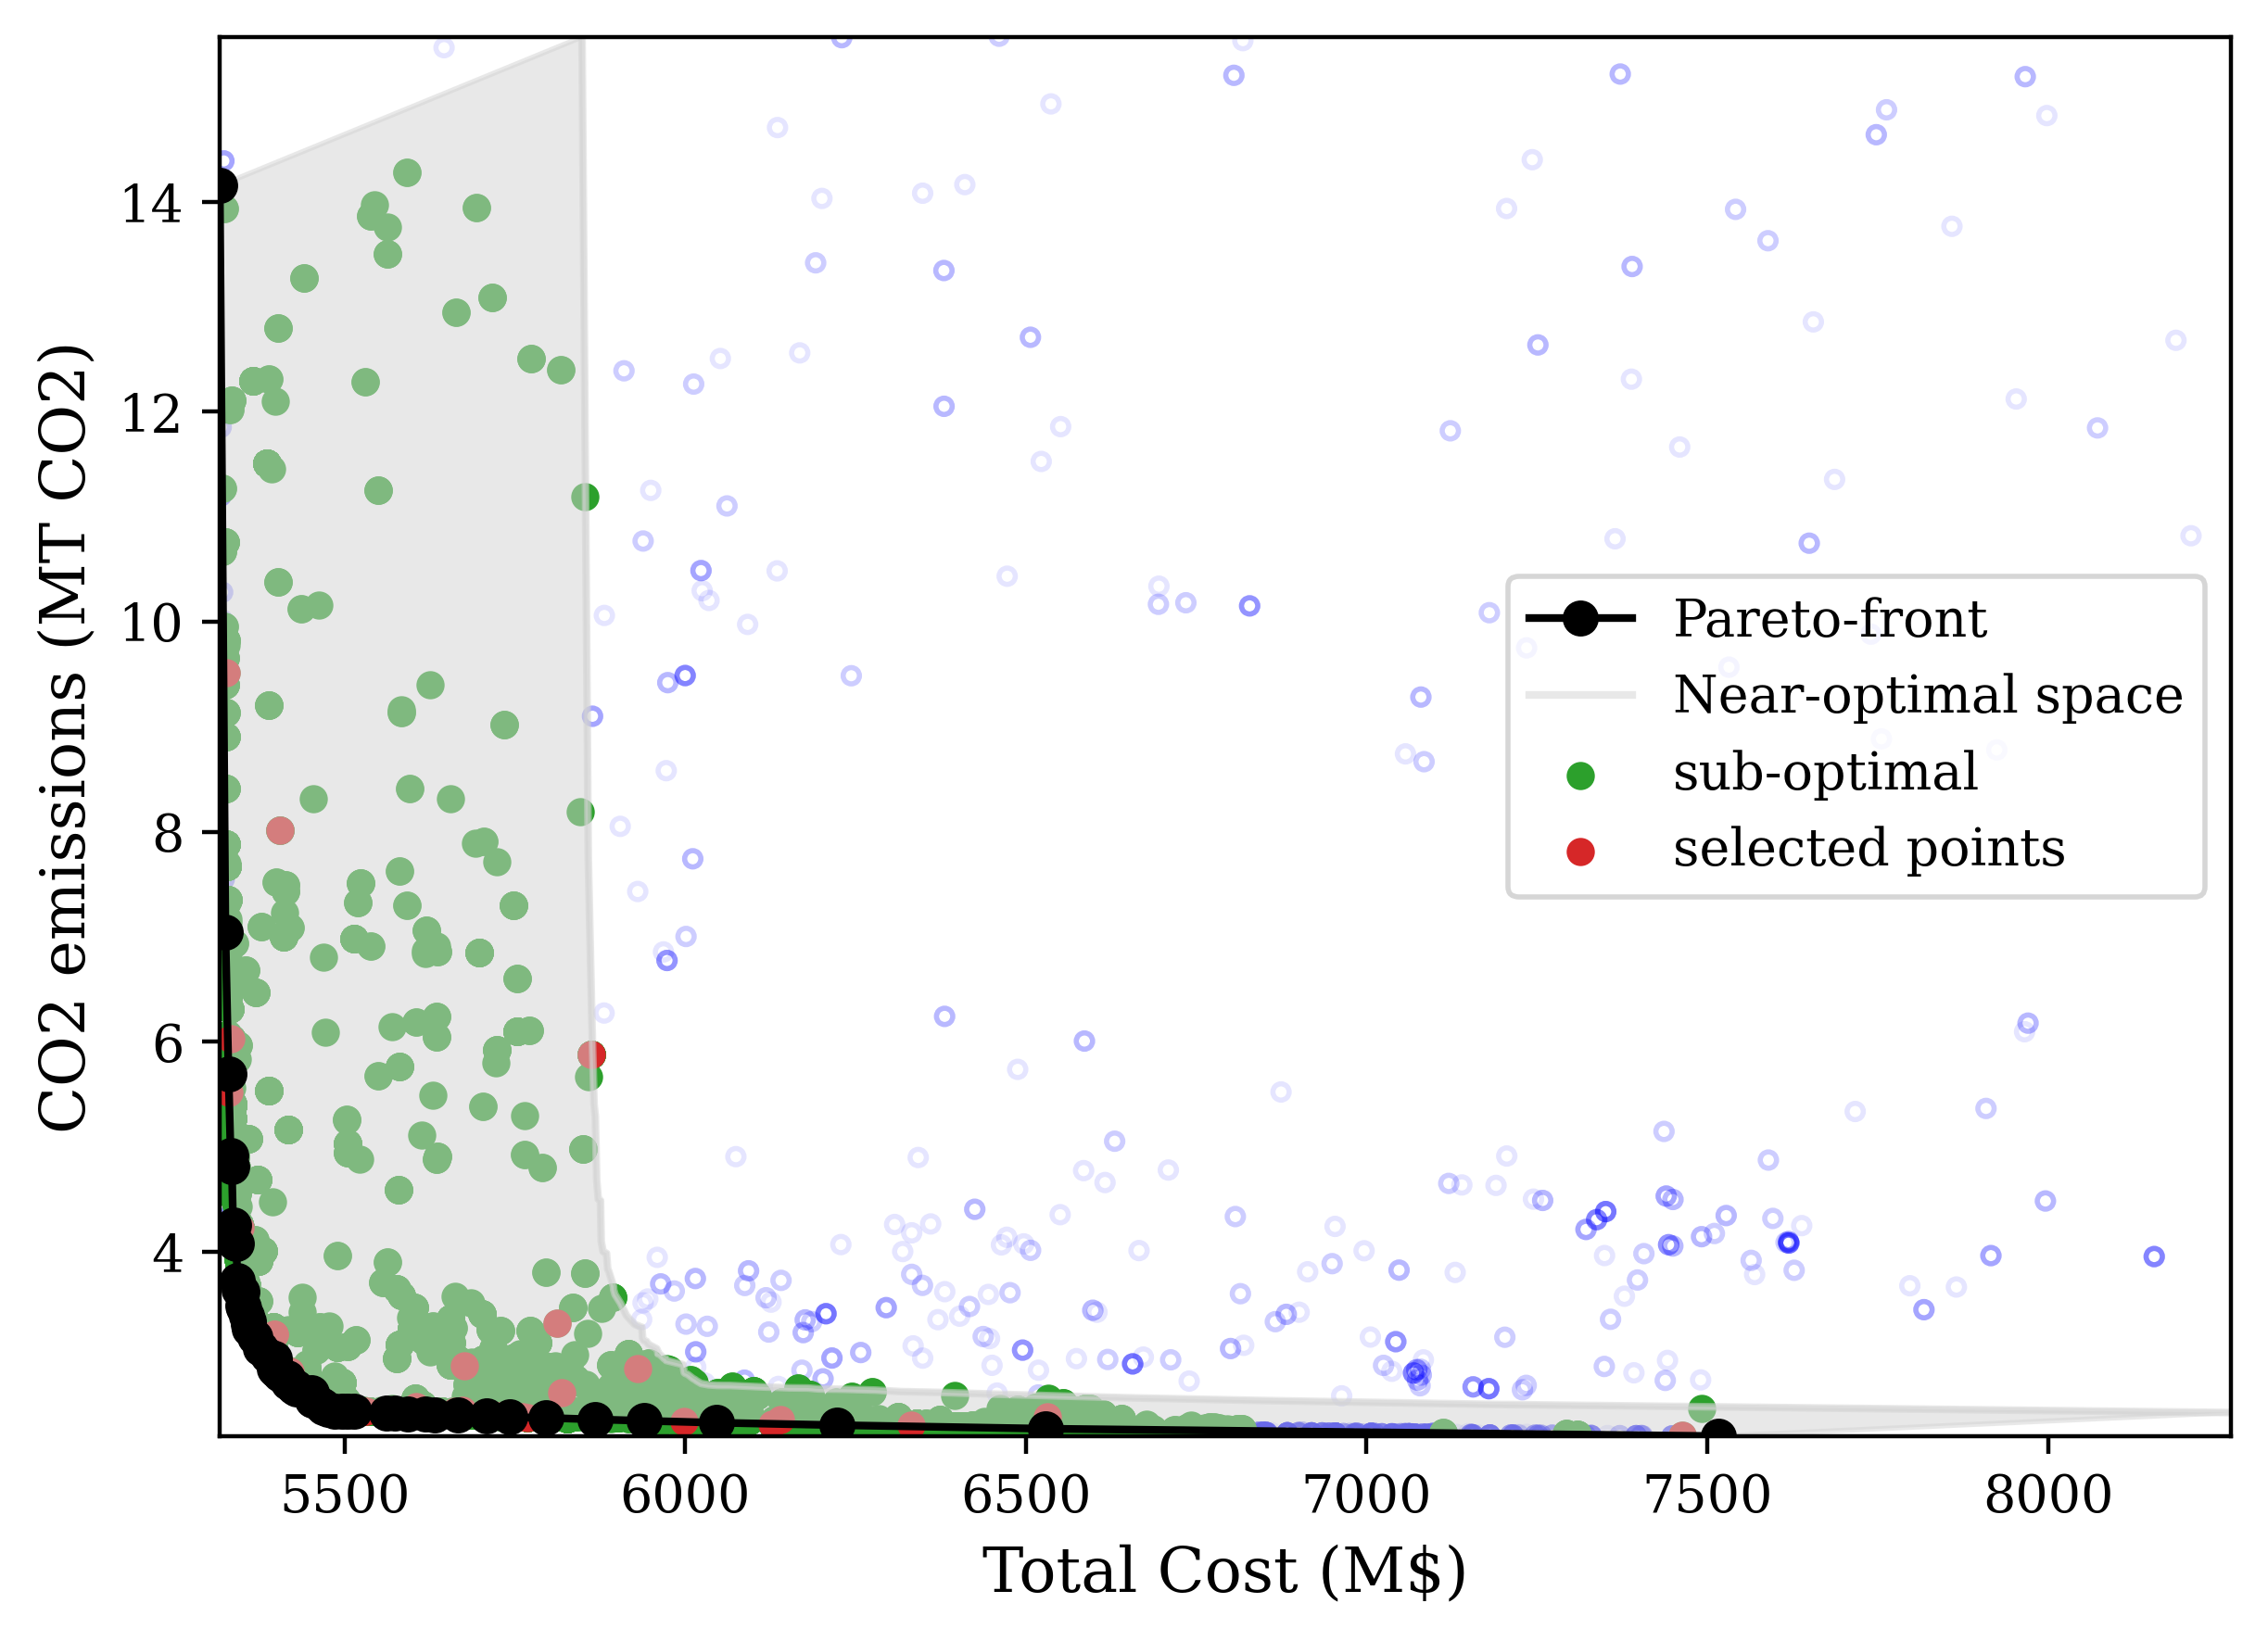
\includegraphics[width=0.6\columnwidth]{figures/results/osier_mga_subset_01.png}
  % \resizebox{0.6\columnwidth}{!}{%% Creator: Matplotlib, PGF backend
%%
%% To include the figure in your LaTeX document, write
%%   \input{<filename>.pgf}
%%
%% Make sure the required packages are loaded in your preamble
%%   \usepackage{pgf}
%%
%% Also ensure that all the required font packages are loaded; for instance,
%% the lmodern package is sometimes necessary when using math font.
%%   \usepackage{lmodern}
%%
%% Figures using additional raster images can only be included by \input if
%% they are in the same directory as the main LaTeX file. For loading figures
%% from other directories you can use the `import` package
%%   \usepackage{import}
%%
%% and then include the figures with
%%   \import{<path to file>}{<filename>.pgf}
%%
%% Matplotlib used the following preamble
%%   \def\mathdefault#1{#1}
%%   \everymath=\expandafter{\the\everymath\displaystyle}
%%   \IfFileExists{scrextend.sty}{
%%     \usepackage[fontsize=10.000000pt]{scrextend}
%%   }{
%%     \renewcommand{\normalsize}{\fontsize{10.000000}{12.000000}\selectfont}
%%     \normalsize
%%   }
%%   
%%   \makeatletter\@ifpackageloaded{underscore}{}{\usepackage[strings]{underscore}}\makeatother
%%
\begingroup%
\makeatletter%
\begin{pgfpicture}%
\pgfpathrectangle{\pgfpointorigin}{\pgfqpoint{7.900000in}{5.900000in}}%
\pgfusepath{use as bounding box, clip}%
\begin{pgfscope}%
\pgfsetbuttcap%
\pgfsetmiterjoin%
\definecolor{currentfill}{rgb}{1.000000,1.000000,1.000000}%
\pgfsetfillcolor{currentfill}%
\pgfsetlinewidth{0.000000pt}%
\definecolor{currentstroke}{rgb}{0.000000,0.000000,0.000000}%
\pgfsetstrokecolor{currentstroke}%
\pgfsetdash{}{0pt}%
\pgfpathmoveto{\pgfqpoint{0.000000in}{0.000000in}}%
\pgfpathlineto{\pgfqpoint{7.900000in}{0.000000in}}%
\pgfpathlineto{\pgfqpoint{7.900000in}{5.900000in}}%
\pgfpathlineto{\pgfqpoint{0.000000in}{5.900000in}}%
\pgfpathlineto{\pgfqpoint{0.000000in}{0.000000in}}%
\pgfpathclose%
\pgfusepath{fill}%
\end{pgfscope}%
\begin{pgfscope}%
\pgfsetbuttcap%
\pgfsetmiterjoin%
\definecolor{currentfill}{rgb}{1.000000,1.000000,1.000000}%
\pgfsetfillcolor{currentfill}%
\pgfsetlinewidth{0.000000pt}%
\definecolor{currentstroke}{rgb}{0.000000,0.000000,0.000000}%
\pgfsetstrokecolor{currentstroke}%
\pgfsetstrokeopacity{0.000000}%
\pgfsetdash{}{0pt}%
\pgfpathmoveto{\pgfqpoint{0.688192in}{0.670138in}}%
\pgfpathlineto{\pgfqpoint{7.800000in}{0.670138in}}%
\pgfpathlineto{\pgfqpoint{7.800000in}{5.800000in}}%
\pgfpathlineto{\pgfqpoint{0.688192in}{5.800000in}}%
\pgfpathlineto{\pgfqpoint{0.688192in}{0.670138in}}%
\pgfpathclose%
\pgfusepath{fill}%
\end{pgfscope}%
\begin{pgfscope}%
\pgfpathrectangle{\pgfqpoint{0.688192in}{0.670138in}}{\pgfqpoint{7.111808in}{5.129862in}}%
\pgfusepath{clip}%
\pgfsetbuttcap%
\pgfsetroundjoin%
\pgfsetlinewidth{1.003750pt}%
\definecolor{currentstroke}{rgb}{0.000000,0.000000,0.000000}%
\pgfsetstrokecolor{currentstroke}%
\pgfsetdash{}{0pt}%
\pgfpathmoveto{\pgfqpoint{5.329102in}{5.309073in}}%
\pgfpathcurveto{\pgfqpoint{5.339998in}{5.309073in}}{\pgfqpoint{5.350449in}{5.313402in}}{\pgfqpoint{5.358153in}{5.321106in}}%
\pgfpathcurveto{\pgfqpoint{5.365857in}{5.328811in}}{\pgfqpoint{5.370186in}{5.339261in}}{\pgfqpoint{5.370186in}{5.350157in}}%
\pgfpathcurveto{\pgfqpoint{5.370186in}{5.361052in}}{\pgfqpoint{5.365857in}{5.371503in}}{\pgfqpoint{5.358153in}{5.379208in}}%
\pgfpathcurveto{\pgfqpoint{5.350449in}{5.386912in}}{\pgfqpoint{5.339998in}{5.391241in}}{\pgfqpoint{5.329102in}{5.391241in}}%
\pgfpathcurveto{\pgfqpoint{5.318207in}{5.391241in}}{\pgfqpoint{5.307756in}{5.386912in}}{\pgfqpoint{5.300052in}{5.379208in}}%
\pgfpathcurveto{\pgfqpoint{5.292347in}{5.371503in}}{\pgfqpoint{5.288018in}{5.361052in}}{\pgfqpoint{5.288018in}{5.350157in}}%
\pgfpathcurveto{\pgfqpoint{5.288018in}{5.339261in}}{\pgfqpoint{5.292347in}{5.328811in}}{\pgfqpoint{5.300052in}{5.321106in}}%
\pgfpathcurveto{\pgfqpoint{5.307756in}{5.313402in}}{\pgfqpoint{5.318207in}{5.309073in}}{\pgfqpoint{5.329102in}{5.309073in}}%
\pgfpathlineto{\pgfqpoint{5.329102in}{5.309073in}}%
\pgfpathclose%
\pgfusepath{stroke}%
\end{pgfscope}%
\begin{pgfscope}%
\pgfpathrectangle{\pgfqpoint{0.688192in}{0.670138in}}{\pgfqpoint{7.111808in}{5.129862in}}%
\pgfusepath{clip}%
\pgfsetbuttcap%
\pgfsetroundjoin%
\pgfsetlinewidth{1.003750pt}%
\definecolor{currentstroke}{rgb}{0.000000,0.000000,0.000000}%
\pgfsetstrokecolor{currentstroke}%
\pgfsetdash{}{0pt}%
\pgfpathmoveto{\pgfqpoint{1.840914in}{0.696069in}}%
\pgfpathcurveto{\pgfqpoint{1.851809in}{0.696069in}}{\pgfqpoint{1.862260in}{0.700398in}}{\pgfqpoint{1.869964in}{0.708103in}}%
\pgfpathcurveto{\pgfqpoint{1.877669in}{0.715807in}}{\pgfqpoint{1.881997in}{0.726258in}}{\pgfqpoint{1.881997in}{0.737153in}}%
\pgfpathcurveto{\pgfqpoint{1.881997in}{0.748049in}}{\pgfqpoint{1.877669in}{0.758500in}}{\pgfqpoint{1.869964in}{0.766204in}}%
\pgfpathcurveto{\pgfqpoint{1.862260in}{0.773908in}}{\pgfqpoint{1.851809in}{0.778237in}}{\pgfqpoint{1.840914in}{0.778237in}}%
\pgfpathcurveto{\pgfqpoint{1.830018in}{0.778237in}}{\pgfqpoint{1.819567in}{0.773908in}}{\pgfqpoint{1.811863in}{0.766204in}}%
\pgfpathcurveto{\pgfqpoint{1.804159in}{0.758500in}}{\pgfqpoint{1.799830in}{0.748049in}}{\pgfqpoint{1.799830in}{0.737153in}}%
\pgfpathcurveto{\pgfqpoint{1.799830in}{0.726258in}}{\pgfqpoint{1.804159in}{0.715807in}}{\pgfqpoint{1.811863in}{0.708103in}}%
\pgfpathcurveto{\pgfqpoint{1.819567in}{0.700398in}}{\pgfqpoint{1.830018in}{0.696069in}}{\pgfqpoint{1.840914in}{0.696069in}}%
\pgfpathlineto{\pgfqpoint{1.840914in}{0.696069in}}%
\pgfpathclose%
\pgfusepath{stroke}%
\end{pgfscope}%
\begin{pgfscope}%
\pgfpathrectangle{\pgfqpoint{0.688192in}{0.670138in}}{\pgfqpoint{7.111808in}{5.129862in}}%
\pgfusepath{clip}%
\pgfsetbuttcap%
\pgfsetroundjoin%
\pgfsetlinewidth{1.003750pt}%
\definecolor{currentstroke}{rgb}{0.000000,0.000000,0.000000}%
\pgfsetstrokecolor{currentstroke}%
\pgfsetdash{}{0pt}%
\pgfpathmoveto{\pgfqpoint{1.101880in}{0.720677in}}%
\pgfpathcurveto{\pgfqpoint{1.112775in}{0.720677in}}{\pgfqpoint{1.123226in}{0.725006in}}{\pgfqpoint{1.130930in}{0.732710in}}%
\pgfpathcurveto{\pgfqpoint{1.138635in}{0.740415in}}{\pgfqpoint{1.142964in}{0.750865in}}{\pgfqpoint{1.142964in}{0.761761in}}%
\pgfpathcurveto{\pgfqpoint{1.142964in}{0.772656in}}{\pgfqpoint{1.138635in}{0.783107in}}{\pgfqpoint{1.130930in}{0.790812in}}%
\pgfpathcurveto{\pgfqpoint{1.123226in}{0.798516in}}{\pgfqpoint{1.112775in}{0.802845in}}{\pgfqpoint{1.101880in}{0.802845in}}%
\pgfpathcurveto{\pgfqpoint{1.090984in}{0.802845in}}{\pgfqpoint{1.080533in}{0.798516in}}{\pgfqpoint{1.072829in}{0.790812in}}%
\pgfpathcurveto{\pgfqpoint{1.065125in}{0.783107in}}{\pgfqpoint{1.060796in}{0.772656in}}{\pgfqpoint{1.060796in}{0.761761in}}%
\pgfpathcurveto{\pgfqpoint{1.060796in}{0.750865in}}{\pgfqpoint{1.065125in}{0.740415in}}{\pgfqpoint{1.072829in}{0.732710in}}%
\pgfpathcurveto{\pgfqpoint{1.080533in}{0.725006in}}{\pgfqpoint{1.090984in}{0.720677in}}{\pgfqpoint{1.101880in}{0.720677in}}%
\pgfpathlineto{\pgfqpoint{1.101880in}{0.720677in}}%
\pgfpathclose%
\pgfusepath{stroke}%
\end{pgfscope}%
\begin{pgfscope}%
\pgfpathrectangle{\pgfqpoint{0.688192in}{0.670138in}}{\pgfqpoint{7.111808in}{5.129862in}}%
\pgfusepath{clip}%
\pgfsetbuttcap%
\pgfsetroundjoin%
\pgfsetlinewidth{1.003750pt}%
\definecolor{currentstroke}{rgb}{0.000000,0.000000,0.000000}%
\pgfsetstrokecolor{currentstroke}%
\pgfsetdash{}{0pt}%
\pgfpathmoveto{\pgfqpoint{1.840914in}{0.696069in}}%
\pgfpathcurveto{\pgfqpoint{1.851809in}{0.696069in}}{\pgfqpoint{1.862260in}{0.700398in}}{\pgfqpoint{1.869964in}{0.708103in}}%
\pgfpathcurveto{\pgfqpoint{1.877669in}{0.715807in}}{\pgfqpoint{1.881997in}{0.726258in}}{\pgfqpoint{1.881997in}{0.737153in}}%
\pgfpathcurveto{\pgfqpoint{1.881997in}{0.748049in}}{\pgfqpoint{1.877669in}{0.758500in}}{\pgfqpoint{1.869964in}{0.766204in}}%
\pgfpathcurveto{\pgfqpoint{1.862260in}{0.773908in}}{\pgfqpoint{1.851809in}{0.778237in}}{\pgfqpoint{1.840914in}{0.778237in}}%
\pgfpathcurveto{\pgfqpoint{1.830018in}{0.778237in}}{\pgfqpoint{1.819567in}{0.773908in}}{\pgfqpoint{1.811863in}{0.766204in}}%
\pgfpathcurveto{\pgfqpoint{1.804159in}{0.758500in}}{\pgfqpoint{1.799830in}{0.748049in}}{\pgfqpoint{1.799830in}{0.737153in}}%
\pgfpathcurveto{\pgfqpoint{1.799830in}{0.726258in}}{\pgfqpoint{1.804159in}{0.715807in}}{\pgfqpoint{1.811863in}{0.708103in}}%
\pgfpathcurveto{\pgfqpoint{1.819567in}{0.700398in}}{\pgfqpoint{1.830018in}{0.696069in}}{\pgfqpoint{1.840914in}{0.696069in}}%
\pgfpathlineto{\pgfqpoint{1.840914in}{0.696069in}}%
\pgfpathclose%
\pgfusepath{stroke}%
\end{pgfscope}%
\begin{pgfscope}%
\pgfpathrectangle{\pgfqpoint{0.688192in}{0.670138in}}{\pgfqpoint{7.111808in}{5.129862in}}%
\pgfusepath{clip}%
\pgfsetbuttcap%
\pgfsetroundjoin%
\pgfsetlinewidth{1.003750pt}%
\definecolor{currentstroke}{rgb}{0.000000,0.000000,0.000000}%
\pgfsetstrokecolor{currentstroke}%
\pgfsetdash{}{0pt}%
\pgfpathmoveto{\pgfqpoint{2.869035in}{0.669385in}}%
\pgfpathcurveto{\pgfqpoint{2.879931in}{0.669385in}}{\pgfqpoint{2.890382in}{0.673714in}}{\pgfqpoint{2.898086in}{0.681419in}}%
\pgfpathcurveto{\pgfqpoint{2.905790in}{0.689123in}}{\pgfqpoint{2.910119in}{0.699574in}}{\pgfqpoint{2.910119in}{0.710469in}}%
\pgfpathcurveto{\pgfqpoint{2.910119in}{0.721365in}}{\pgfqpoint{2.905790in}{0.731816in}}{\pgfqpoint{2.898086in}{0.739520in}}%
\pgfpathcurveto{\pgfqpoint{2.890382in}{0.747224in}}{\pgfqpoint{2.879931in}{0.751553in}}{\pgfqpoint{2.869035in}{0.751553in}}%
\pgfpathcurveto{\pgfqpoint{2.858140in}{0.751553in}}{\pgfqpoint{2.847689in}{0.747224in}}{\pgfqpoint{2.839985in}{0.739520in}}%
\pgfpathcurveto{\pgfqpoint{2.832280in}{0.731816in}}{\pgfqpoint{2.827952in}{0.721365in}}{\pgfqpoint{2.827952in}{0.710469in}}%
\pgfpathcurveto{\pgfqpoint{2.827952in}{0.699574in}}{\pgfqpoint{2.832280in}{0.689123in}}{\pgfqpoint{2.839985in}{0.681419in}}%
\pgfpathcurveto{\pgfqpoint{2.847689in}{0.673714in}}{\pgfqpoint{2.858140in}{0.669385in}}{\pgfqpoint{2.869035in}{0.669385in}}%
\pgfpathlineto{\pgfqpoint{2.869035in}{0.669385in}}%
\pgfpathclose%
\pgfusepath{stroke}%
\end{pgfscope}%
\begin{pgfscope}%
\pgfpathrectangle{\pgfqpoint{0.688192in}{0.670138in}}{\pgfqpoint{7.111808in}{5.129862in}}%
\pgfusepath{clip}%
\pgfsetbuttcap%
\pgfsetroundjoin%
\pgfsetlinewidth{1.003750pt}%
\definecolor{currentstroke}{rgb}{0.000000,0.000000,0.000000}%
\pgfsetstrokecolor{currentstroke}%
\pgfsetdash{}{0pt}%
\pgfpathmoveto{\pgfqpoint{0.789763in}{1.038554in}}%
\pgfpathcurveto{\pgfqpoint{0.800659in}{1.038554in}}{\pgfqpoint{0.811109in}{1.042883in}}{\pgfqpoint{0.818814in}{1.050587in}}%
\pgfpathcurveto{\pgfqpoint{0.826518in}{1.058291in}}{\pgfqpoint{0.830847in}{1.068742in}}{\pgfqpoint{0.830847in}{1.079638in}}%
\pgfpathcurveto{\pgfqpoint{0.830847in}{1.090533in}}{\pgfqpoint{0.826518in}{1.100984in}}{\pgfqpoint{0.818814in}{1.108688in}}%
\pgfpathcurveto{\pgfqpoint{0.811109in}{1.116393in}}{\pgfqpoint{0.800659in}{1.120722in}}{\pgfqpoint{0.789763in}{1.120722in}}%
\pgfpathcurveto{\pgfqpoint{0.778868in}{1.120722in}}{\pgfqpoint{0.768417in}{1.116393in}}{\pgfqpoint{0.760712in}{1.108688in}}%
\pgfpathcurveto{\pgfqpoint{0.753008in}{1.100984in}}{\pgfqpoint{0.748679in}{1.090533in}}{\pgfqpoint{0.748679in}{1.079638in}}%
\pgfpathcurveto{\pgfqpoint{0.748679in}{1.068742in}}{\pgfqpoint{0.753008in}{1.058291in}}{\pgfqpoint{0.760712in}{1.050587in}}%
\pgfpathcurveto{\pgfqpoint{0.768417in}{1.042883in}}{\pgfqpoint{0.778868in}{1.038554in}}{\pgfqpoint{0.789763in}{1.038554in}}%
\pgfpathlineto{\pgfqpoint{0.789763in}{1.038554in}}%
\pgfpathclose%
\pgfusepath{stroke}%
\end{pgfscope}%
\begin{pgfscope}%
\pgfpathrectangle{\pgfqpoint{0.688192in}{0.670138in}}{\pgfqpoint{7.111808in}{5.129862in}}%
\pgfusepath{clip}%
\pgfsetbuttcap%
\pgfsetroundjoin%
\pgfsetlinewidth{1.003750pt}%
\definecolor{currentstroke}{rgb}{0.000000,0.000000,0.000000}%
\pgfsetstrokecolor{currentstroke}%
\pgfsetdash{}{0pt}%
\pgfpathmoveto{\pgfqpoint{1.679564in}{0.702362in}}%
\pgfpathcurveto{\pgfqpoint{1.690460in}{0.702362in}}{\pgfqpoint{1.700911in}{0.706691in}}{\pgfqpoint{1.708615in}{0.714395in}}%
\pgfpathcurveto{\pgfqpoint{1.716319in}{0.722099in}}{\pgfqpoint{1.720648in}{0.732550in}}{\pgfqpoint{1.720648in}{0.743446in}}%
\pgfpathcurveto{\pgfqpoint{1.720648in}{0.754341in}}{\pgfqpoint{1.716319in}{0.764792in}}{\pgfqpoint{1.708615in}{0.772496in}}%
\pgfpathcurveto{\pgfqpoint{1.700911in}{0.780201in}}{\pgfqpoint{1.690460in}{0.784529in}}{\pgfqpoint{1.679564in}{0.784529in}}%
\pgfpathcurveto{\pgfqpoint{1.668669in}{0.784529in}}{\pgfqpoint{1.658218in}{0.780201in}}{\pgfqpoint{1.650514in}{0.772496in}}%
\pgfpathcurveto{\pgfqpoint{1.642809in}{0.764792in}}{\pgfqpoint{1.638480in}{0.754341in}}{\pgfqpoint{1.638480in}{0.743446in}}%
\pgfpathcurveto{\pgfqpoint{1.638480in}{0.732550in}}{\pgfqpoint{1.642809in}{0.722099in}}{\pgfqpoint{1.650514in}{0.714395in}}%
\pgfpathcurveto{\pgfqpoint{1.658218in}{0.706691in}}{\pgfqpoint{1.668669in}{0.702362in}}{\pgfqpoint{1.679564in}{0.702362in}}%
\pgfpathlineto{\pgfqpoint{1.679564in}{0.702362in}}%
\pgfpathclose%
\pgfusepath{stroke}%
\end{pgfscope}%
\begin{pgfscope}%
\pgfpathrectangle{\pgfqpoint{0.688192in}{0.670138in}}{\pgfqpoint{7.111808in}{5.129862in}}%
\pgfusepath{clip}%
\pgfsetbuttcap%
\pgfsetroundjoin%
\pgfsetlinewidth{1.003750pt}%
\definecolor{currentstroke}{rgb}{0.000000,0.000000,0.000000}%
\pgfsetstrokecolor{currentstroke}%
\pgfsetdash{}{0pt}%
\pgfpathmoveto{\pgfqpoint{1.045306in}{0.741536in}}%
\pgfpathcurveto{\pgfqpoint{1.056202in}{0.741536in}}{\pgfqpoint{1.066653in}{0.745865in}}{\pgfqpoint{1.074357in}{0.753569in}}%
\pgfpathcurveto{\pgfqpoint{1.082061in}{0.761274in}}{\pgfqpoint{1.086390in}{0.771725in}}{\pgfqpoint{1.086390in}{0.782620in}}%
\pgfpathcurveto{\pgfqpoint{1.086390in}{0.793516in}}{\pgfqpoint{1.082061in}{0.803967in}}{\pgfqpoint{1.074357in}{0.811671in}}%
\pgfpathcurveto{\pgfqpoint{1.066653in}{0.819375in}}{\pgfqpoint{1.056202in}{0.823704in}}{\pgfqpoint{1.045306in}{0.823704in}}%
\pgfpathcurveto{\pgfqpoint{1.034411in}{0.823704in}}{\pgfqpoint{1.023960in}{0.819375in}}{\pgfqpoint{1.016256in}{0.811671in}}%
\pgfpathcurveto{\pgfqpoint{1.008551in}{0.803967in}}{\pgfqpoint{1.004222in}{0.793516in}}{\pgfqpoint{1.004222in}{0.782620in}}%
\pgfpathcurveto{\pgfqpoint{1.004222in}{0.771725in}}{\pgfqpoint{1.008551in}{0.761274in}}{\pgfqpoint{1.016256in}{0.753569in}}%
\pgfpathcurveto{\pgfqpoint{1.023960in}{0.745865in}}{\pgfqpoint{1.034411in}{0.741536in}}{\pgfqpoint{1.045306in}{0.741536in}}%
\pgfpathlineto{\pgfqpoint{1.045306in}{0.741536in}}%
\pgfpathclose%
\pgfusepath{stroke}%
\end{pgfscope}%
\begin{pgfscope}%
\pgfpathrectangle{\pgfqpoint{0.688192in}{0.670138in}}{\pgfqpoint{7.111808in}{5.129862in}}%
\pgfusepath{clip}%
\pgfsetbuttcap%
\pgfsetroundjoin%
\pgfsetlinewidth{1.003750pt}%
\definecolor{currentstroke}{rgb}{0.000000,0.000000,0.000000}%
\pgfsetstrokecolor{currentstroke}%
\pgfsetdash{}{0pt}%
\pgfpathmoveto{\pgfqpoint{2.013663in}{0.690447in}}%
\pgfpathcurveto{\pgfqpoint{2.024559in}{0.690447in}}{\pgfqpoint{2.035010in}{0.694776in}}{\pgfqpoint{2.042714in}{0.702480in}}%
\pgfpathcurveto{\pgfqpoint{2.050418in}{0.710184in}}{\pgfqpoint{2.054747in}{0.720635in}}{\pgfqpoint{2.054747in}{0.731531in}}%
\pgfpathcurveto{\pgfqpoint{2.054747in}{0.742426in}}{\pgfqpoint{2.050418in}{0.752877in}}{\pgfqpoint{2.042714in}{0.760582in}}%
\pgfpathcurveto{\pgfqpoint{2.035010in}{0.768286in}}{\pgfqpoint{2.024559in}{0.772615in}}{\pgfqpoint{2.013663in}{0.772615in}}%
\pgfpathcurveto{\pgfqpoint{2.002768in}{0.772615in}}{\pgfqpoint{1.992317in}{0.768286in}}{\pgfqpoint{1.984613in}{0.760582in}}%
\pgfpathcurveto{\pgfqpoint{1.976908in}{0.752877in}}{\pgfqpoint{1.972579in}{0.742426in}}{\pgfqpoint{1.972579in}{0.731531in}}%
\pgfpathcurveto{\pgfqpoint{1.972579in}{0.720635in}}{\pgfqpoint{1.976908in}{0.710184in}}{\pgfqpoint{1.984613in}{0.702480in}}%
\pgfpathcurveto{\pgfqpoint{1.992317in}{0.694776in}}{\pgfqpoint{2.002768in}{0.690447in}}{\pgfqpoint{2.013663in}{0.690447in}}%
\pgfpathlineto{\pgfqpoint{2.013663in}{0.690447in}}%
\pgfpathclose%
\pgfusepath{stroke}%
\end{pgfscope}%
\begin{pgfscope}%
\pgfpathrectangle{\pgfqpoint{0.688192in}{0.670138in}}{\pgfqpoint{7.111808in}{5.129862in}}%
\pgfusepath{clip}%
\pgfsetbuttcap%
\pgfsetroundjoin%
\pgfsetlinewidth{1.003750pt}%
\definecolor{currentstroke}{rgb}{0.000000,0.000000,0.000000}%
\pgfsetstrokecolor{currentstroke}%
\pgfsetdash{}{0pt}%
\pgfpathmoveto{\pgfqpoint{0.895312in}{0.866174in}}%
\pgfpathcurveto{\pgfqpoint{0.906208in}{0.866174in}}{\pgfqpoint{0.916658in}{0.870503in}}{\pgfqpoint{0.924363in}{0.878207in}}%
\pgfpathcurveto{\pgfqpoint{0.932067in}{0.885911in}}{\pgfqpoint{0.936396in}{0.896362in}}{\pgfqpoint{0.936396in}{0.907258in}}%
\pgfpathcurveto{\pgfqpoint{0.936396in}{0.918153in}}{\pgfqpoint{0.932067in}{0.928604in}}{\pgfqpoint{0.924363in}{0.936308in}}%
\pgfpathcurveto{\pgfqpoint{0.916658in}{0.944013in}}{\pgfqpoint{0.906208in}{0.948341in}}{\pgfqpoint{0.895312in}{0.948341in}}%
\pgfpathcurveto{\pgfqpoint{0.884416in}{0.948341in}}{\pgfqpoint{0.873966in}{0.944013in}}{\pgfqpoint{0.866261in}{0.936308in}}%
\pgfpathcurveto{\pgfqpoint{0.858557in}{0.928604in}}{\pgfqpoint{0.854228in}{0.918153in}}{\pgfqpoint{0.854228in}{0.907258in}}%
\pgfpathcurveto{\pgfqpoint{0.854228in}{0.896362in}}{\pgfqpoint{0.858557in}{0.885911in}}{\pgfqpoint{0.866261in}{0.878207in}}%
\pgfpathcurveto{\pgfqpoint{0.873966in}{0.870503in}}{\pgfqpoint{0.884416in}{0.866174in}}{\pgfqpoint{0.895312in}{0.866174in}}%
\pgfpathlineto{\pgfqpoint{0.895312in}{0.866174in}}%
\pgfpathclose%
\pgfusepath{stroke}%
\end{pgfscope}%
\begin{pgfscope}%
\pgfpathrectangle{\pgfqpoint{0.688192in}{0.670138in}}{\pgfqpoint{7.111808in}{5.129862in}}%
\pgfusepath{clip}%
\pgfsetbuttcap%
\pgfsetroundjoin%
\pgfsetlinewidth{1.003750pt}%
\definecolor{currentstroke}{rgb}{0.000000,0.000000,0.000000}%
\pgfsetstrokecolor{currentstroke}%
\pgfsetdash{}{0pt}%
\pgfpathmoveto{\pgfqpoint{0.794194in}{1.022605in}}%
\pgfpathcurveto{\pgfqpoint{0.805090in}{1.022605in}}{\pgfqpoint{0.815541in}{1.026933in}}{\pgfqpoint{0.823245in}{1.034638in}}%
\pgfpathcurveto{\pgfqpoint{0.830949in}{1.042342in}}{\pgfqpoint{0.835278in}{1.052793in}}{\pgfqpoint{0.835278in}{1.063688in}}%
\pgfpathcurveto{\pgfqpoint{0.835278in}{1.074584in}}{\pgfqpoint{0.830949in}{1.085035in}}{\pgfqpoint{0.823245in}{1.092739in}}%
\pgfpathcurveto{\pgfqpoint{0.815541in}{1.100443in}}{\pgfqpoint{0.805090in}{1.104772in}}{\pgfqpoint{0.794194in}{1.104772in}}%
\pgfpathcurveto{\pgfqpoint{0.783299in}{1.104772in}}{\pgfqpoint{0.772848in}{1.100443in}}{\pgfqpoint{0.765144in}{1.092739in}}%
\pgfpathcurveto{\pgfqpoint{0.757439in}{1.085035in}}{\pgfqpoint{0.753110in}{1.074584in}}{\pgfqpoint{0.753110in}{1.063688in}}%
\pgfpathcurveto{\pgfqpoint{0.753110in}{1.052793in}}{\pgfqpoint{0.757439in}{1.042342in}}{\pgfqpoint{0.765144in}{1.034638in}}%
\pgfpathcurveto{\pgfqpoint{0.772848in}{1.026933in}}{\pgfqpoint{0.783299in}{1.022605in}}{\pgfqpoint{0.794194in}{1.022605in}}%
\pgfpathlineto{\pgfqpoint{0.794194in}{1.022605in}}%
\pgfpathclose%
\pgfusepath{stroke}%
\end{pgfscope}%
\begin{pgfscope}%
\pgfpathrectangle{\pgfqpoint{0.688192in}{0.670138in}}{\pgfqpoint{7.111808in}{5.129862in}}%
\pgfusepath{clip}%
\pgfsetbuttcap%
\pgfsetroundjoin%
\pgfsetlinewidth{1.003750pt}%
\definecolor{currentstroke}{rgb}{0.000000,0.000000,0.000000}%
\pgfsetstrokecolor{currentstroke}%
\pgfsetdash{}{0pt}%
\pgfpathmoveto{\pgfqpoint{1.019140in}{0.759981in}}%
\pgfpathcurveto{\pgfqpoint{1.030035in}{0.759981in}}{\pgfqpoint{1.040486in}{0.764309in}}{\pgfqpoint{1.048191in}{0.772014in}}%
\pgfpathcurveto{\pgfqpoint{1.055895in}{0.779718in}}{\pgfqpoint{1.060224in}{0.790169in}}{\pgfqpoint{1.060224in}{0.801064in}}%
\pgfpathcurveto{\pgfqpoint{1.060224in}{0.811960in}}{\pgfqpoint{1.055895in}{0.822411in}}{\pgfqpoint{1.048191in}{0.830115in}}%
\pgfpathcurveto{\pgfqpoint{1.040486in}{0.837820in}}{\pgfqpoint{1.030035in}{0.842148in}}{\pgfqpoint{1.019140in}{0.842148in}}%
\pgfpathcurveto{\pgfqpoint{1.008244in}{0.842148in}}{\pgfqpoint{0.997794in}{0.837820in}}{\pgfqpoint{0.990089in}{0.830115in}}%
\pgfpathcurveto{\pgfqpoint{0.982385in}{0.822411in}}{\pgfqpoint{0.978056in}{0.811960in}}{\pgfqpoint{0.978056in}{0.801064in}}%
\pgfpathcurveto{\pgfqpoint{0.978056in}{0.790169in}}{\pgfqpoint{0.982385in}{0.779718in}}{\pgfqpoint{0.990089in}{0.772014in}}%
\pgfpathcurveto{\pgfqpoint{0.997794in}{0.764309in}}{\pgfqpoint{1.008244in}{0.759981in}}{\pgfqpoint{1.019140in}{0.759981in}}%
\pgfpathlineto{\pgfqpoint{1.019140in}{0.759981in}}%
\pgfpathclose%
\pgfusepath{stroke}%
\end{pgfscope}%
\begin{pgfscope}%
\pgfpathrectangle{\pgfqpoint{0.688192in}{0.670138in}}{\pgfqpoint{7.111808in}{5.129862in}}%
\pgfusepath{clip}%
\pgfsetbuttcap%
\pgfsetroundjoin%
\pgfsetlinewidth{1.003750pt}%
\definecolor{currentstroke}{rgb}{0.000000,0.000000,0.000000}%
\pgfsetstrokecolor{currentstroke}%
\pgfsetdash{}{0pt}%
\pgfpathmoveto{\pgfqpoint{1.050667in}{0.739240in}}%
\pgfpathcurveto{\pgfqpoint{1.061563in}{0.739240in}}{\pgfqpoint{1.072014in}{0.743568in}}{\pgfqpoint{1.079718in}{0.751273in}}%
\pgfpathcurveto{\pgfqpoint{1.087422in}{0.758977in}}{\pgfqpoint{1.091751in}{0.769428in}}{\pgfqpoint{1.091751in}{0.780323in}}%
\pgfpathcurveto{\pgfqpoint{1.091751in}{0.791219in}}{\pgfqpoint{1.087422in}{0.801670in}}{\pgfqpoint{1.079718in}{0.809374in}}%
\pgfpathcurveto{\pgfqpoint{1.072014in}{0.817078in}}{\pgfqpoint{1.061563in}{0.821407in}}{\pgfqpoint{1.050667in}{0.821407in}}%
\pgfpathcurveto{\pgfqpoint{1.039772in}{0.821407in}}{\pgfqpoint{1.029321in}{0.817078in}}{\pgfqpoint{1.021617in}{0.809374in}}%
\pgfpathcurveto{\pgfqpoint{1.013912in}{0.801670in}}{\pgfqpoint{1.009583in}{0.791219in}}{\pgfqpoint{1.009583in}{0.780323in}}%
\pgfpathcurveto{\pgfqpoint{1.009583in}{0.769428in}}{\pgfqpoint{1.013912in}{0.758977in}}{\pgfqpoint{1.021617in}{0.751273in}}%
\pgfpathcurveto{\pgfqpoint{1.029321in}{0.743568in}}{\pgfqpoint{1.039772in}{0.739240in}}{\pgfqpoint{1.050667in}{0.739240in}}%
\pgfpathlineto{\pgfqpoint{1.050667in}{0.739240in}}%
\pgfpathclose%
\pgfusepath{stroke}%
\end{pgfscope}%
\begin{pgfscope}%
\pgfpathrectangle{\pgfqpoint{0.688192in}{0.670138in}}{\pgfqpoint{7.111808in}{5.129862in}}%
\pgfusepath{clip}%
\pgfsetbuttcap%
\pgfsetroundjoin%
\pgfsetlinewidth{1.003750pt}%
\definecolor{currentstroke}{rgb}{0.000000,0.000000,0.000000}%
\pgfsetstrokecolor{currentstroke}%
\pgfsetdash{}{0pt}%
\pgfpathmoveto{\pgfqpoint{0.881277in}{0.900428in}}%
\pgfpathcurveto{\pgfqpoint{0.892173in}{0.900428in}}{\pgfqpoint{0.902624in}{0.904756in}}{\pgfqpoint{0.910328in}{0.912461in}}%
\pgfpathcurveto{\pgfqpoint{0.918032in}{0.920165in}}{\pgfqpoint{0.922361in}{0.930616in}}{\pgfqpoint{0.922361in}{0.941511in}}%
\pgfpathcurveto{\pgfqpoint{0.922361in}{0.952407in}}{\pgfqpoint{0.918032in}{0.962858in}}{\pgfqpoint{0.910328in}{0.970562in}}%
\pgfpathcurveto{\pgfqpoint{0.902624in}{0.978266in}}{\pgfqpoint{0.892173in}{0.982595in}}{\pgfqpoint{0.881277in}{0.982595in}}%
\pgfpathcurveto{\pgfqpoint{0.870382in}{0.982595in}}{\pgfqpoint{0.859931in}{0.978266in}}{\pgfqpoint{0.852226in}{0.970562in}}%
\pgfpathcurveto{\pgfqpoint{0.844522in}{0.962858in}}{\pgfqpoint{0.840193in}{0.952407in}}{\pgfqpoint{0.840193in}{0.941511in}}%
\pgfpathcurveto{\pgfqpoint{0.840193in}{0.930616in}}{\pgfqpoint{0.844522in}{0.920165in}}{\pgfqpoint{0.852226in}{0.912461in}}%
\pgfpathcurveto{\pgfqpoint{0.859931in}{0.904756in}}{\pgfqpoint{0.870382in}{0.900428in}}{\pgfqpoint{0.881277in}{0.900428in}}%
\pgfpathlineto{\pgfqpoint{0.881277in}{0.900428in}}%
\pgfpathclose%
\pgfusepath{stroke}%
\end{pgfscope}%
\begin{pgfscope}%
\pgfpathrectangle{\pgfqpoint{0.688192in}{0.670138in}}{\pgfqpoint{7.111808in}{5.129862in}}%
\pgfusepath{clip}%
\pgfsetbuttcap%
\pgfsetroundjoin%
\pgfsetlinewidth{1.003750pt}%
\definecolor{currentstroke}{rgb}{0.000000,0.000000,0.000000}%
\pgfsetstrokecolor{currentstroke}%
\pgfsetdash{}{0pt}%
\pgfpathmoveto{\pgfqpoint{0.721104in}{1.921896in}}%
\pgfpathcurveto{\pgfqpoint{0.732000in}{1.921896in}}{\pgfqpoint{0.742451in}{1.926225in}}{\pgfqpoint{0.750155in}{1.933929in}}%
\pgfpathcurveto{\pgfqpoint{0.757859in}{1.941634in}}{\pgfqpoint{0.762188in}{1.952084in}}{\pgfqpoint{0.762188in}{1.962980in}}%
\pgfpathcurveto{\pgfqpoint{0.762188in}{1.973876in}}{\pgfqpoint{0.757859in}{1.984326in}}{\pgfqpoint{0.750155in}{1.992031in}}%
\pgfpathcurveto{\pgfqpoint{0.742451in}{1.999735in}}{\pgfqpoint{0.732000in}{2.004064in}}{\pgfqpoint{0.721104in}{2.004064in}}%
\pgfpathcurveto{\pgfqpoint{0.710209in}{2.004064in}}{\pgfqpoint{0.699758in}{1.999735in}}{\pgfqpoint{0.692054in}{1.992031in}}%
\pgfpathcurveto{\pgfqpoint{0.684349in}{1.984326in}}{\pgfqpoint{0.680020in}{1.973876in}}{\pgfqpoint{0.680020in}{1.962980in}}%
\pgfpathcurveto{\pgfqpoint{0.680020in}{1.952084in}}{\pgfqpoint{0.684349in}{1.941634in}}{\pgfqpoint{0.692054in}{1.933929in}}%
\pgfpathcurveto{\pgfqpoint{0.699758in}{1.926225in}}{\pgfqpoint{0.710209in}{1.921896in}}{\pgfqpoint{0.721104in}{1.921896in}}%
\pgfpathlineto{\pgfqpoint{0.721104in}{1.921896in}}%
\pgfpathclose%
\pgfusepath{stroke}%
\end{pgfscope}%
\begin{pgfscope}%
\pgfpathrectangle{\pgfqpoint{0.688192in}{0.670138in}}{\pgfqpoint{7.111808in}{5.129862in}}%
\pgfusepath{clip}%
\pgfsetbuttcap%
\pgfsetroundjoin%
\pgfsetlinewidth{1.003750pt}%
\definecolor{currentstroke}{rgb}{0.000000,0.000000,0.000000}%
\pgfsetstrokecolor{currentstroke}%
\pgfsetdash{}{0pt}%
\pgfpathmoveto{\pgfqpoint{1.351667in}{0.711476in}}%
\pgfpathcurveto{\pgfqpoint{1.362562in}{0.711476in}}{\pgfqpoint{1.373013in}{0.715805in}}{\pgfqpoint{1.380718in}{0.723510in}}%
\pgfpathcurveto{\pgfqpoint{1.388422in}{0.731214in}}{\pgfqpoint{1.392751in}{0.741665in}}{\pgfqpoint{1.392751in}{0.752560in}}%
\pgfpathcurveto{\pgfqpoint{1.392751in}{0.763456in}}{\pgfqpoint{1.388422in}{0.773907in}}{\pgfqpoint{1.380718in}{0.781611in}}%
\pgfpathcurveto{\pgfqpoint{1.373013in}{0.789315in}}{\pgfqpoint{1.362562in}{0.793644in}}{\pgfqpoint{1.351667in}{0.793644in}}%
\pgfpathcurveto{\pgfqpoint{1.340771in}{0.793644in}}{\pgfqpoint{1.330321in}{0.789315in}}{\pgfqpoint{1.322616in}{0.781611in}}%
\pgfpathcurveto{\pgfqpoint{1.314912in}{0.773907in}}{\pgfqpoint{1.310583in}{0.763456in}}{\pgfqpoint{1.310583in}{0.752560in}}%
\pgfpathcurveto{\pgfqpoint{1.310583in}{0.741665in}}{\pgfqpoint{1.314912in}{0.731214in}}{\pgfqpoint{1.322616in}{0.723510in}}%
\pgfpathcurveto{\pgfqpoint{1.330321in}{0.715805in}}{\pgfqpoint{1.340771in}{0.711476in}}{\pgfqpoint{1.351667in}{0.711476in}}%
\pgfpathlineto{\pgfqpoint{1.351667in}{0.711476in}}%
\pgfpathclose%
\pgfusepath{stroke}%
\end{pgfscope}%
\begin{pgfscope}%
\pgfpathrectangle{\pgfqpoint{0.688192in}{0.670138in}}{\pgfqpoint{7.111808in}{5.129862in}}%
\pgfusepath{clip}%
\pgfsetbuttcap%
\pgfsetroundjoin%
\pgfsetlinewidth{1.003750pt}%
\definecolor{currentstroke}{rgb}{0.000000,0.000000,0.000000}%
\pgfsetstrokecolor{currentstroke}%
\pgfsetdash{}{0pt}%
\pgfpathmoveto{\pgfqpoint{0.928243in}{0.841597in}}%
\pgfpathcurveto{\pgfqpoint{0.939139in}{0.841597in}}{\pgfqpoint{0.949589in}{0.845926in}}{\pgfqpoint{0.957294in}{0.853631in}}%
\pgfpathcurveto{\pgfqpoint{0.964998in}{0.861335in}}{\pgfqpoint{0.969327in}{0.871786in}}{\pgfqpoint{0.969327in}{0.882681in}}%
\pgfpathcurveto{\pgfqpoint{0.969327in}{0.893577in}}{\pgfqpoint{0.964998in}{0.904028in}}{\pgfqpoint{0.957294in}{0.911732in}}%
\pgfpathcurveto{\pgfqpoint{0.949589in}{0.919436in}}{\pgfqpoint{0.939139in}{0.923765in}}{\pgfqpoint{0.928243in}{0.923765in}}%
\pgfpathcurveto{\pgfqpoint{0.917347in}{0.923765in}}{\pgfqpoint{0.906897in}{0.919436in}}{\pgfqpoint{0.899192in}{0.911732in}}%
\pgfpathcurveto{\pgfqpoint{0.891488in}{0.904028in}}{\pgfqpoint{0.887159in}{0.893577in}}{\pgfqpoint{0.887159in}{0.882681in}}%
\pgfpathcurveto{\pgfqpoint{0.887159in}{0.871786in}}{\pgfqpoint{0.891488in}{0.861335in}}{\pgfqpoint{0.899192in}{0.853631in}}%
\pgfpathcurveto{\pgfqpoint{0.906897in}{0.845926in}}{\pgfqpoint{0.917347in}{0.841597in}}{\pgfqpoint{0.928243in}{0.841597in}}%
\pgfpathlineto{\pgfqpoint{0.928243in}{0.841597in}}%
\pgfpathclose%
\pgfusepath{stroke}%
\end{pgfscope}%
\begin{pgfscope}%
\pgfpathrectangle{\pgfqpoint{0.688192in}{0.670138in}}{\pgfqpoint{7.111808in}{5.129862in}}%
\pgfusepath{clip}%
\pgfsetbuttcap%
\pgfsetroundjoin%
\pgfsetlinewidth{1.003750pt}%
\definecolor{currentstroke}{rgb}{0.000000,0.000000,0.000000}%
\pgfsetstrokecolor{currentstroke}%
\pgfsetdash{}{0pt}%
\pgfpathmoveto{\pgfqpoint{6.014792in}{1.437812in}}%
\pgfpathcurveto{\pgfqpoint{6.025688in}{1.437812in}}{\pgfqpoint{6.036139in}{1.442141in}}{\pgfqpoint{6.043843in}{1.449845in}}%
\pgfpathcurveto{\pgfqpoint{6.051547in}{1.457549in}}{\pgfqpoint{6.055876in}{1.468000in}}{\pgfqpoint{6.055876in}{1.478896in}}%
\pgfpathcurveto{\pgfqpoint{6.055876in}{1.489791in}}{\pgfqpoint{6.051547in}{1.500242in}}{\pgfqpoint{6.043843in}{1.507947in}}%
\pgfpathcurveto{\pgfqpoint{6.036139in}{1.515651in}}{\pgfqpoint{6.025688in}{1.519980in}}{\pgfqpoint{6.014792in}{1.519980in}}%
\pgfpathcurveto{\pgfqpoint{6.003897in}{1.519980in}}{\pgfqpoint{5.993446in}{1.515651in}}{\pgfqpoint{5.985741in}{1.507947in}}%
\pgfpathcurveto{\pgfqpoint{5.978037in}{1.500242in}}{\pgfqpoint{5.973708in}{1.489791in}}{\pgfqpoint{5.973708in}{1.478896in}}%
\pgfpathcurveto{\pgfqpoint{5.973708in}{1.468000in}}{\pgfqpoint{5.978037in}{1.457549in}}{\pgfqpoint{5.985741in}{1.449845in}}%
\pgfpathcurveto{\pgfqpoint{5.993446in}{1.442141in}}{\pgfqpoint{6.003897in}{1.437812in}}{\pgfqpoint{6.014792in}{1.437812in}}%
\pgfpathlineto{\pgfqpoint{6.014792in}{1.437812in}}%
\pgfpathclose%
\pgfusepath{stroke}%
\end{pgfscope}%
\begin{pgfscope}%
\pgfpathrectangle{\pgfqpoint{0.688192in}{0.670138in}}{\pgfqpoint{7.111808in}{5.129862in}}%
\pgfusepath{clip}%
\pgfsetbuttcap%
\pgfsetroundjoin%
\pgfsetlinewidth{1.003750pt}%
\definecolor{currentstroke}{rgb}{0.000000,0.000000,0.000000}%
\pgfsetstrokecolor{currentstroke}%
\pgfsetdash{}{0pt}%
\pgfpathmoveto{\pgfqpoint{0.895312in}{0.866174in}}%
\pgfpathcurveto{\pgfqpoint{0.906208in}{0.866174in}}{\pgfqpoint{0.916658in}{0.870503in}}{\pgfqpoint{0.924363in}{0.878207in}}%
\pgfpathcurveto{\pgfqpoint{0.932067in}{0.885911in}}{\pgfqpoint{0.936396in}{0.896362in}}{\pgfqpoint{0.936396in}{0.907258in}}%
\pgfpathcurveto{\pgfqpoint{0.936396in}{0.918153in}}{\pgfqpoint{0.932067in}{0.928604in}}{\pgfqpoint{0.924363in}{0.936308in}}%
\pgfpathcurveto{\pgfqpoint{0.916658in}{0.944013in}}{\pgfqpoint{0.906208in}{0.948341in}}{\pgfqpoint{0.895312in}{0.948341in}}%
\pgfpathcurveto{\pgfqpoint{0.884416in}{0.948341in}}{\pgfqpoint{0.873966in}{0.944013in}}{\pgfqpoint{0.866261in}{0.936308in}}%
\pgfpathcurveto{\pgfqpoint{0.858557in}{0.928604in}}{\pgfqpoint{0.854228in}{0.918153in}}{\pgfqpoint{0.854228in}{0.907258in}}%
\pgfpathcurveto{\pgfqpoint{0.854228in}{0.896362in}}{\pgfqpoint{0.858557in}{0.885911in}}{\pgfqpoint{0.866261in}{0.878207in}}%
\pgfpathcurveto{\pgfqpoint{0.873966in}{0.870503in}}{\pgfqpoint{0.884416in}{0.866174in}}{\pgfqpoint{0.895312in}{0.866174in}}%
\pgfpathlineto{\pgfqpoint{0.895312in}{0.866174in}}%
\pgfpathclose%
\pgfusepath{stroke}%
\end{pgfscope}%
\begin{pgfscope}%
\pgfpathrectangle{\pgfqpoint{0.688192in}{0.670138in}}{\pgfqpoint{7.111808in}{5.129862in}}%
\pgfusepath{clip}%
\pgfsetbuttcap%
\pgfsetroundjoin%
\pgfsetlinewidth{1.003750pt}%
\definecolor{currentstroke}{rgb}{0.000000,0.000000,0.000000}%
\pgfsetstrokecolor{currentstroke}%
\pgfsetdash{}{0pt}%
\pgfpathmoveto{\pgfqpoint{1.759569in}{0.698796in}}%
\pgfpathcurveto{\pgfqpoint{1.770464in}{0.698796in}}{\pgfqpoint{1.780915in}{0.703125in}}{\pgfqpoint{1.788619in}{0.710830in}}%
\pgfpathcurveto{\pgfqpoint{1.796324in}{0.718534in}}{\pgfqpoint{1.800652in}{0.728985in}}{\pgfqpoint{1.800652in}{0.739880in}}%
\pgfpathcurveto{\pgfqpoint{1.800652in}{0.750776in}}{\pgfqpoint{1.796324in}{0.761227in}}{\pgfqpoint{1.788619in}{0.768931in}}%
\pgfpathcurveto{\pgfqpoint{1.780915in}{0.776635in}}{\pgfqpoint{1.770464in}{0.780964in}}{\pgfqpoint{1.759569in}{0.780964in}}%
\pgfpathcurveto{\pgfqpoint{1.748673in}{0.780964in}}{\pgfqpoint{1.738222in}{0.776635in}}{\pgfqpoint{1.730518in}{0.768931in}}%
\pgfpathcurveto{\pgfqpoint{1.722814in}{0.761227in}}{\pgfqpoint{1.718485in}{0.750776in}}{\pgfqpoint{1.718485in}{0.739880in}}%
\pgfpathcurveto{\pgfqpoint{1.718485in}{0.728985in}}{\pgfqpoint{1.722814in}{0.718534in}}{\pgfqpoint{1.730518in}{0.710830in}}%
\pgfpathcurveto{\pgfqpoint{1.738222in}{0.703125in}}{\pgfqpoint{1.748673in}{0.698796in}}{\pgfqpoint{1.759569in}{0.698796in}}%
\pgfpathlineto{\pgfqpoint{1.759569in}{0.698796in}}%
\pgfpathclose%
\pgfusepath{stroke}%
\end{pgfscope}%
\begin{pgfscope}%
\pgfpathrectangle{\pgfqpoint{0.688192in}{0.670138in}}{\pgfqpoint{7.111808in}{5.129862in}}%
\pgfusepath{clip}%
\pgfsetbuttcap%
\pgfsetroundjoin%
\pgfsetlinewidth{1.003750pt}%
\definecolor{currentstroke}{rgb}{0.000000,0.000000,0.000000}%
\pgfsetstrokecolor{currentstroke}%
\pgfsetdash{}{0pt}%
\pgfpathmoveto{\pgfqpoint{1.351667in}{0.711476in}}%
\pgfpathcurveto{\pgfqpoint{1.362562in}{0.711476in}}{\pgfqpoint{1.373013in}{0.715805in}}{\pgfqpoint{1.380718in}{0.723510in}}%
\pgfpathcurveto{\pgfqpoint{1.388422in}{0.731214in}}{\pgfqpoint{1.392751in}{0.741665in}}{\pgfqpoint{1.392751in}{0.752560in}}%
\pgfpathcurveto{\pgfqpoint{1.392751in}{0.763456in}}{\pgfqpoint{1.388422in}{0.773907in}}{\pgfqpoint{1.380718in}{0.781611in}}%
\pgfpathcurveto{\pgfqpoint{1.373013in}{0.789315in}}{\pgfqpoint{1.362562in}{0.793644in}}{\pgfqpoint{1.351667in}{0.793644in}}%
\pgfpathcurveto{\pgfqpoint{1.340771in}{0.793644in}}{\pgfqpoint{1.330321in}{0.789315in}}{\pgfqpoint{1.322616in}{0.781611in}}%
\pgfpathcurveto{\pgfqpoint{1.314912in}{0.773907in}}{\pgfqpoint{1.310583in}{0.763456in}}{\pgfqpoint{1.310583in}{0.752560in}}%
\pgfpathcurveto{\pgfqpoint{1.310583in}{0.741665in}}{\pgfqpoint{1.314912in}{0.731214in}}{\pgfqpoint{1.322616in}{0.723510in}}%
\pgfpathcurveto{\pgfqpoint{1.330321in}{0.715805in}}{\pgfqpoint{1.340771in}{0.711476in}}{\pgfqpoint{1.351667in}{0.711476in}}%
\pgfpathlineto{\pgfqpoint{1.351667in}{0.711476in}}%
\pgfpathclose%
\pgfusepath{stroke}%
\end{pgfscope}%
\begin{pgfscope}%
\pgfpathrectangle{\pgfqpoint{0.688192in}{0.670138in}}{\pgfqpoint{7.111808in}{5.129862in}}%
\pgfusepath{clip}%
\pgfsetbuttcap%
\pgfsetroundjoin%
\pgfsetlinewidth{1.003750pt}%
\definecolor{currentstroke}{rgb}{0.000000,0.000000,0.000000}%
\pgfsetstrokecolor{currentstroke}%
\pgfsetdash{}{0pt}%
\pgfpathmoveto{\pgfqpoint{1.631842in}{0.703864in}}%
\pgfpathcurveto{\pgfqpoint{1.642737in}{0.703864in}}{\pgfqpoint{1.653188in}{0.708193in}}{\pgfqpoint{1.660893in}{0.715897in}}%
\pgfpathcurveto{\pgfqpoint{1.668597in}{0.723601in}}{\pgfqpoint{1.672926in}{0.734052in}}{\pgfqpoint{1.672926in}{0.744948in}}%
\pgfpathcurveto{\pgfqpoint{1.672926in}{0.755843in}}{\pgfqpoint{1.668597in}{0.766294in}}{\pgfqpoint{1.660893in}{0.773998in}}%
\pgfpathcurveto{\pgfqpoint{1.653188in}{0.781703in}}{\pgfqpoint{1.642737in}{0.786032in}}{\pgfqpoint{1.631842in}{0.786032in}}%
\pgfpathcurveto{\pgfqpoint{1.620946in}{0.786032in}}{\pgfqpoint{1.610496in}{0.781703in}}{\pgfqpoint{1.602791in}{0.773998in}}%
\pgfpathcurveto{\pgfqpoint{1.595087in}{0.766294in}}{\pgfqpoint{1.590758in}{0.755843in}}{\pgfqpoint{1.590758in}{0.744948in}}%
\pgfpathcurveto{\pgfqpoint{1.590758in}{0.734052in}}{\pgfqpoint{1.595087in}{0.723601in}}{\pgfqpoint{1.602791in}{0.715897in}}%
\pgfpathcurveto{\pgfqpoint{1.610496in}{0.708193in}}{\pgfqpoint{1.620946in}{0.703864in}}{\pgfqpoint{1.631842in}{0.703864in}}%
\pgfpathlineto{\pgfqpoint{1.631842in}{0.703864in}}%
\pgfpathclose%
\pgfusepath{stroke}%
\end{pgfscope}%
\begin{pgfscope}%
\pgfpathrectangle{\pgfqpoint{0.688192in}{0.670138in}}{\pgfqpoint{7.111808in}{5.129862in}}%
\pgfusepath{clip}%
\pgfsetbuttcap%
\pgfsetroundjoin%
\pgfsetlinewidth{1.003750pt}%
\definecolor{currentstroke}{rgb}{0.000000,0.000000,0.000000}%
\pgfsetstrokecolor{currentstroke}%
\pgfsetdash{}{0pt}%
\pgfpathmoveto{\pgfqpoint{6.024600in}{3.448401in}}%
\pgfpathcurveto{\pgfqpoint{6.035496in}{3.448401in}}{\pgfqpoint{6.045947in}{3.452730in}}{\pgfqpoint{6.053651in}{3.460434in}}%
\pgfpathcurveto{\pgfqpoint{6.061355in}{3.468139in}}{\pgfqpoint{6.065684in}{3.478589in}}{\pgfqpoint{6.065684in}{3.489485in}}%
\pgfpathcurveto{\pgfqpoint{6.065684in}{3.500381in}}{\pgfqpoint{6.061355in}{3.510831in}}{\pgfqpoint{6.053651in}{3.518536in}}%
\pgfpathcurveto{\pgfqpoint{6.045947in}{3.526240in}}{\pgfqpoint{6.035496in}{3.530569in}}{\pgfqpoint{6.024600in}{3.530569in}}%
\pgfpathcurveto{\pgfqpoint{6.013705in}{3.530569in}}{\pgfqpoint{6.003254in}{3.526240in}}{\pgfqpoint{5.995550in}{3.518536in}}%
\pgfpathcurveto{\pgfqpoint{5.987845in}{3.510831in}}{\pgfqpoint{5.983517in}{3.500381in}}{\pgfqpoint{5.983517in}{3.489485in}}%
\pgfpathcurveto{\pgfqpoint{5.983517in}{3.478589in}}{\pgfqpoint{5.987845in}{3.468139in}}{\pgfqpoint{5.995550in}{3.460434in}}%
\pgfpathcurveto{\pgfqpoint{6.003254in}{3.452730in}}{\pgfqpoint{6.013705in}{3.448401in}}{\pgfqpoint{6.024600in}{3.448401in}}%
\pgfpathlineto{\pgfqpoint{6.024600in}{3.448401in}}%
\pgfpathclose%
\pgfusepath{stroke}%
\end{pgfscope}%
\begin{pgfscope}%
\pgfpathrectangle{\pgfqpoint{0.688192in}{0.670138in}}{\pgfqpoint{7.111808in}{5.129862in}}%
\pgfusepath{clip}%
\pgfsetbuttcap%
\pgfsetroundjoin%
\pgfsetlinewidth{1.003750pt}%
\definecolor{currentstroke}{rgb}{0.000000,0.000000,0.000000}%
\pgfsetstrokecolor{currentstroke}%
\pgfsetdash{}{0pt}%
\pgfpathmoveto{\pgfqpoint{0.721104in}{1.921896in}}%
\pgfpathcurveto{\pgfqpoint{0.732000in}{1.921896in}}{\pgfqpoint{0.742451in}{1.926225in}}{\pgfqpoint{0.750155in}{1.933929in}}%
\pgfpathcurveto{\pgfqpoint{0.757859in}{1.941634in}}{\pgfqpoint{0.762188in}{1.952084in}}{\pgfqpoint{0.762188in}{1.962980in}}%
\pgfpathcurveto{\pgfqpoint{0.762188in}{1.973876in}}{\pgfqpoint{0.757859in}{1.984326in}}{\pgfqpoint{0.750155in}{1.992031in}}%
\pgfpathcurveto{\pgfqpoint{0.742451in}{1.999735in}}{\pgfqpoint{0.732000in}{2.004064in}}{\pgfqpoint{0.721104in}{2.004064in}}%
\pgfpathcurveto{\pgfqpoint{0.710209in}{2.004064in}}{\pgfqpoint{0.699758in}{1.999735in}}{\pgfqpoint{0.692054in}{1.992031in}}%
\pgfpathcurveto{\pgfqpoint{0.684349in}{1.984326in}}{\pgfqpoint{0.680020in}{1.973876in}}{\pgfqpoint{0.680020in}{1.962980in}}%
\pgfpathcurveto{\pgfqpoint{0.680020in}{1.952084in}}{\pgfqpoint{0.684349in}{1.941634in}}{\pgfqpoint{0.692054in}{1.933929in}}%
\pgfpathcurveto{\pgfqpoint{0.699758in}{1.926225in}}{\pgfqpoint{0.710209in}{1.921896in}}{\pgfqpoint{0.721104in}{1.921896in}}%
\pgfpathlineto{\pgfqpoint{0.721104in}{1.921896in}}%
\pgfpathclose%
\pgfusepath{stroke}%
\end{pgfscope}%
\begin{pgfscope}%
\pgfpathrectangle{\pgfqpoint{0.688192in}{0.670138in}}{\pgfqpoint{7.111808in}{5.129862in}}%
\pgfusepath{clip}%
\pgfsetbuttcap%
\pgfsetroundjoin%
\pgfsetlinewidth{1.003750pt}%
\definecolor{currentstroke}{rgb}{0.000000,0.000000,0.000000}%
\pgfsetstrokecolor{currentstroke}%
\pgfsetdash{}{0pt}%
\pgfpathmoveto{\pgfqpoint{2.751273in}{1.008701in}}%
\pgfpathcurveto{\pgfqpoint{2.762169in}{1.008701in}}{\pgfqpoint{2.772620in}{1.013030in}}{\pgfqpoint{2.780324in}{1.020734in}}%
\pgfpathcurveto{\pgfqpoint{2.788028in}{1.028439in}}{\pgfqpoint{2.792357in}{1.038890in}}{\pgfqpoint{2.792357in}{1.049785in}}%
\pgfpathcurveto{\pgfqpoint{2.792357in}{1.060681in}}{\pgfqpoint{2.788028in}{1.071131in}}{\pgfqpoint{2.780324in}{1.078836in}}%
\pgfpathcurveto{\pgfqpoint{2.772620in}{1.086540in}}{\pgfqpoint{2.762169in}{1.090869in}}{\pgfqpoint{2.751273in}{1.090869in}}%
\pgfpathcurveto{\pgfqpoint{2.740378in}{1.090869in}}{\pgfqpoint{2.729927in}{1.086540in}}{\pgfqpoint{2.722223in}{1.078836in}}%
\pgfpathcurveto{\pgfqpoint{2.714518in}{1.071131in}}{\pgfqpoint{2.710189in}{1.060681in}}{\pgfqpoint{2.710189in}{1.049785in}}%
\pgfpathcurveto{\pgfqpoint{2.710189in}{1.038890in}}{\pgfqpoint{2.714518in}{1.028439in}}{\pgfqpoint{2.722223in}{1.020734in}}%
\pgfpathcurveto{\pgfqpoint{2.729927in}{1.013030in}}{\pgfqpoint{2.740378in}{1.008701in}}{\pgfqpoint{2.751273in}{1.008701in}}%
\pgfpathlineto{\pgfqpoint{2.751273in}{1.008701in}}%
\pgfpathclose%
\pgfusepath{stroke}%
\end{pgfscope}%
\begin{pgfscope}%
\pgfpathrectangle{\pgfqpoint{0.688192in}{0.670138in}}{\pgfqpoint{7.111808in}{5.129862in}}%
\pgfusepath{clip}%
\pgfsetbuttcap%
\pgfsetroundjoin%
\pgfsetlinewidth{1.003750pt}%
\definecolor{currentstroke}{rgb}{0.000000,0.000000,0.000000}%
\pgfsetstrokecolor{currentstroke}%
\pgfsetdash{}{0pt}%
\pgfpathmoveto{\pgfqpoint{1.625190in}{0.704414in}}%
\pgfpathcurveto{\pgfqpoint{1.636086in}{0.704414in}}{\pgfqpoint{1.646537in}{0.708742in}}{\pgfqpoint{1.654241in}{0.716447in}}%
\pgfpathcurveto{\pgfqpoint{1.661945in}{0.724151in}}{\pgfqpoint{1.666274in}{0.734602in}}{\pgfqpoint{1.666274in}{0.745498in}}%
\pgfpathcurveto{\pgfqpoint{1.666274in}{0.756393in}}{\pgfqpoint{1.661945in}{0.766844in}}{\pgfqpoint{1.654241in}{0.774548in}}%
\pgfpathcurveto{\pgfqpoint{1.646537in}{0.782253in}}{\pgfqpoint{1.636086in}{0.786581in}}{\pgfqpoint{1.625190in}{0.786581in}}%
\pgfpathcurveto{\pgfqpoint{1.614295in}{0.786581in}}{\pgfqpoint{1.603844in}{0.782253in}}{\pgfqpoint{1.596140in}{0.774548in}}%
\pgfpathcurveto{\pgfqpoint{1.588435in}{0.766844in}}{\pgfqpoint{1.584107in}{0.756393in}}{\pgfqpoint{1.584107in}{0.745498in}}%
\pgfpathcurveto{\pgfqpoint{1.584107in}{0.734602in}}{\pgfqpoint{1.588435in}{0.724151in}}{\pgfqpoint{1.596140in}{0.716447in}}%
\pgfpathcurveto{\pgfqpoint{1.603844in}{0.708742in}}{\pgfqpoint{1.614295in}{0.704414in}}{\pgfqpoint{1.625190in}{0.704414in}}%
\pgfpathlineto{\pgfqpoint{1.625190in}{0.704414in}}%
\pgfpathclose%
\pgfusepath{stroke}%
\end{pgfscope}%
\begin{pgfscope}%
\pgfpathrectangle{\pgfqpoint{0.688192in}{0.670138in}}{\pgfqpoint{7.111808in}{5.129862in}}%
\pgfusepath{clip}%
\pgfsetbuttcap%
\pgfsetroundjoin%
\pgfsetlinewidth{1.003750pt}%
\definecolor{currentstroke}{rgb}{0.000000,0.000000,0.000000}%
\pgfsetstrokecolor{currentstroke}%
\pgfsetdash{}{0pt}%
\pgfpathmoveto{\pgfqpoint{0.880316in}{0.913368in}}%
\pgfpathcurveto{\pgfqpoint{0.891212in}{0.913368in}}{\pgfqpoint{0.901663in}{0.917697in}}{\pgfqpoint{0.909367in}{0.925401in}}%
\pgfpathcurveto{\pgfqpoint{0.917071in}{0.933106in}}{\pgfqpoint{0.921400in}{0.943557in}}{\pgfqpoint{0.921400in}{0.954452in}}%
\pgfpathcurveto{\pgfqpoint{0.921400in}{0.965348in}}{\pgfqpoint{0.917071in}{0.975799in}}{\pgfqpoint{0.909367in}{0.983503in}}%
\pgfpathcurveto{\pgfqpoint{0.901663in}{0.991207in}}{\pgfqpoint{0.891212in}{0.995536in}}{\pgfqpoint{0.880316in}{0.995536in}}%
\pgfpathcurveto{\pgfqpoint{0.869421in}{0.995536in}}{\pgfqpoint{0.858970in}{0.991207in}}{\pgfqpoint{0.851266in}{0.983503in}}%
\pgfpathcurveto{\pgfqpoint{0.843561in}{0.975799in}}{\pgfqpoint{0.839232in}{0.965348in}}{\pgfqpoint{0.839232in}{0.954452in}}%
\pgfpathcurveto{\pgfqpoint{0.839232in}{0.943557in}}{\pgfqpoint{0.843561in}{0.933106in}}{\pgfqpoint{0.851266in}{0.925401in}}%
\pgfpathcurveto{\pgfqpoint{0.858970in}{0.917697in}}{\pgfqpoint{0.869421in}{0.913368in}}{\pgfqpoint{0.880316in}{0.913368in}}%
\pgfpathlineto{\pgfqpoint{0.880316in}{0.913368in}}%
\pgfpathclose%
\pgfusepath{stroke}%
\end{pgfscope}%
\begin{pgfscope}%
\pgfpathrectangle{\pgfqpoint{0.688192in}{0.670138in}}{\pgfqpoint{7.111808in}{5.129862in}}%
\pgfusepath{clip}%
\pgfsetbuttcap%
\pgfsetroundjoin%
\pgfsetlinewidth{1.003750pt}%
\definecolor{currentstroke}{rgb}{0.000000,0.000000,0.000000}%
\pgfsetstrokecolor{currentstroke}%
\pgfsetdash{}{0pt}%
\pgfpathmoveto{\pgfqpoint{1.631842in}{0.703864in}}%
\pgfpathcurveto{\pgfqpoint{1.642737in}{0.703864in}}{\pgfqpoint{1.653188in}{0.708193in}}{\pgfqpoint{1.660893in}{0.715897in}}%
\pgfpathcurveto{\pgfqpoint{1.668597in}{0.723601in}}{\pgfqpoint{1.672926in}{0.734052in}}{\pgfqpoint{1.672926in}{0.744948in}}%
\pgfpathcurveto{\pgfqpoint{1.672926in}{0.755843in}}{\pgfqpoint{1.668597in}{0.766294in}}{\pgfqpoint{1.660893in}{0.773998in}}%
\pgfpathcurveto{\pgfqpoint{1.653188in}{0.781703in}}{\pgfqpoint{1.642737in}{0.786032in}}{\pgfqpoint{1.631842in}{0.786032in}}%
\pgfpathcurveto{\pgfqpoint{1.620946in}{0.786032in}}{\pgfqpoint{1.610496in}{0.781703in}}{\pgfqpoint{1.602791in}{0.773998in}}%
\pgfpathcurveto{\pgfqpoint{1.595087in}{0.766294in}}{\pgfqpoint{1.590758in}{0.755843in}}{\pgfqpoint{1.590758in}{0.744948in}}%
\pgfpathcurveto{\pgfqpoint{1.590758in}{0.734052in}}{\pgfqpoint{1.595087in}{0.723601in}}{\pgfqpoint{1.602791in}{0.715897in}}%
\pgfpathcurveto{\pgfqpoint{1.610496in}{0.708193in}}{\pgfqpoint{1.620946in}{0.703864in}}{\pgfqpoint{1.631842in}{0.703864in}}%
\pgfpathlineto{\pgfqpoint{1.631842in}{0.703864in}}%
\pgfpathclose%
\pgfusepath{stroke}%
\end{pgfscope}%
\begin{pgfscope}%
\pgfpathrectangle{\pgfqpoint{0.688192in}{0.670138in}}{\pgfqpoint{7.111808in}{5.129862in}}%
\pgfusepath{clip}%
\pgfsetbuttcap%
\pgfsetroundjoin%
\pgfsetlinewidth{1.003750pt}%
\definecolor{currentstroke}{rgb}{0.000000,0.000000,0.000000}%
\pgfsetstrokecolor{currentstroke}%
\pgfsetdash{}{0pt}%
\pgfpathmoveto{\pgfqpoint{1.044526in}{0.742721in}}%
\pgfpathcurveto{\pgfqpoint{1.055421in}{0.742721in}}{\pgfqpoint{1.065872in}{0.747050in}}{\pgfqpoint{1.073577in}{0.754754in}}%
\pgfpathcurveto{\pgfqpoint{1.081281in}{0.762459in}}{\pgfqpoint{1.085610in}{0.772909in}}{\pgfqpoint{1.085610in}{0.783805in}}%
\pgfpathcurveto{\pgfqpoint{1.085610in}{0.794701in}}{\pgfqpoint{1.081281in}{0.805151in}}{\pgfqpoint{1.073577in}{0.812856in}}%
\pgfpathcurveto{\pgfqpoint{1.065872in}{0.820560in}}{\pgfqpoint{1.055421in}{0.824889in}}{\pgfqpoint{1.044526in}{0.824889in}}%
\pgfpathcurveto{\pgfqpoint{1.033630in}{0.824889in}}{\pgfqpoint{1.023179in}{0.820560in}}{\pgfqpoint{1.015475in}{0.812856in}}%
\pgfpathcurveto{\pgfqpoint{1.007771in}{0.805151in}}{\pgfqpoint{1.003442in}{0.794701in}}{\pgfqpoint{1.003442in}{0.783805in}}%
\pgfpathcurveto{\pgfqpoint{1.003442in}{0.772909in}}{\pgfqpoint{1.007771in}{0.762459in}}{\pgfqpoint{1.015475in}{0.754754in}}%
\pgfpathcurveto{\pgfqpoint{1.023179in}{0.747050in}}{\pgfqpoint{1.033630in}{0.742721in}}{\pgfqpoint{1.044526in}{0.742721in}}%
\pgfpathlineto{\pgfqpoint{1.044526in}{0.742721in}}%
\pgfpathclose%
\pgfusepath{stroke}%
\end{pgfscope}%
\begin{pgfscope}%
\pgfpathrectangle{\pgfqpoint{0.688192in}{0.670138in}}{\pgfqpoint{7.111808in}{5.129862in}}%
\pgfusepath{clip}%
\pgfsetbuttcap%
\pgfsetroundjoin%
\pgfsetlinewidth{1.003750pt}%
\definecolor{currentstroke}{rgb}{0.000000,0.000000,0.000000}%
\pgfsetstrokecolor{currentstroke}%
\pgfsetdash{}{0pt}%
\pgfpathmoveto{\pgfqpoint{6.048059in}{5.126928in}}%
\pgfpathcurveto{\pgfqpoint{6.058955in}{5.126928in}}{\pgfqpoint{6.069405in}{5.131257in}}{\pgfqpoint{6.077110in}{5.138961in}}%
\pgfpathcurveto{\pgfqpoint{6.084814in}{5.146665in}}{\pgfqpoint{6.089143in}{5.157116in}}{\pgfqpoint{6.089143in}{5.168012in}}%
\pgfpathcurveto{\pgfqpoint{6.089143in}{5.178907in}}{\pgfqpoint{6.084814in}{5.189358in}}{\pgfqpoint{6.077110in}{5.197062in}}%
\pgfpathcurveto{\pgfqpoint{6.069405in}{5.204767in}}{\pgfqpoint{6.058955in}{5.209096in}}{\pgfqpoint{6.048059in}{5.209096in}}%
\pgfpathcurveto{\pgfqpoint{6.037164in}{5.209096in}}{\pgfqpoint{6.026713in}{5.204767in}}{\pgfqpoint{6.019008in}{5.197062in}}%
\pgfpathcurveto{\pgfqpoint{6.011304in}{5.189358in}}{\pgfqpoint{6.006975in}{5.178907in}}{\pgfqpoint{6.006975in}{5.168012in}}%
\pgfpathcurveto{\pgfqpoint{6.006975in}{5.157116in}}{\pgfqpoint{6.011304in}{5.146665in}}{\pgfqpoint{6.019008in}{5.138961in}}%
\pgfpathcurveto{\pgfqpoint{6.026713in}{5.131257in}}{\pgfqpoint{6.037164in}{5.126928in}}{\pgfqpoint{6.048059in}{5.126928in}}%
\pgfpathlineto{\pgfqpoint{6.048059in}{5.126928in}}%
\pgfpathclose%
\pgfusepath{stroke}%
\end{pgfscope}%
\begin{pgfscope}%
\pgfpathrectangle{\pgfqpoint{0.688192in}{0.670138in}}{\pgfqpoint{7.111808in}{5.129862in}}%
\pgfusepath{clip}%
\pgfsetbuttcap%
\pgfsetroundjoin%
\pgfsetlinewidth{1.003750pt}%
\definecolor{currentstroke}{rgb}{0.000000,0.000000,0.000000}%
\pgfsetstrokecolor{currentstroke}%
\pgfsetdash{}{0pt}%
\pgfpathmoveto{\pgfqpoint{1.050667in}{0.739240in}}%
\pgfpathcurveto{\pgfqpoint{1.061563in}{0.739240in}}{\pgfqpoint{1.072014in}{0.743568in}}{\pgfqpoint{1.079718in}{0.751273in}}%
\pgfpathcurveto{\pgfqpoint{1.087422in}{0.758977in}}{\pgfqpoint{1.091751in}{0.769428in}}{\pgfqpoint{1.091751in}{0.780323in}}%
\pgfpathcurveto{\pgfqpoint{1.091751in}{0.791219in}}{\pgfqpoint{1.087422in}{0.801670in}}{\pgfqpoint{1.079718in}{0.809374in}}%
\pgfpathcurveto{\pgfqpoint{1.072014in}{0.817078in}}{\pgfqpoint{1.061563in}{0.821407in}}{\pgfqpoint{1.050667in}{0.821407in}}%
\pgfpathcurveto{\pgfqpoint{1.039772in}{0.821407in}}{\pgfqpoint{1.029321in}{0.817078in}}{\pgfqpoint{1.021617in}{0.809374in}}%
\pgfpathcurveto{\pgfqpoint{1.013912in}{0.801670in}}{\pgfqpoint{1.009583in}{0.791219in}}{\pgfqpoint{1.009583in}{0.780323in}}%
\pgfpathcurveto{\pgfqpoint{1.009583in}{0.769428in}}{\pgfqpoint{1.013912in}{0.758977in}}{\pgfqpoint{1.021617in}{0.751273in}}%
\pgfpathcurveto{\pgfqpoint{1.029321in}{0.743568in}}{\pgfqpoint{1.039772in}{0.739240in}}{\pgfqpoint{1.050667in}{0.739240in}}%
\pgfpathlineto{\pgfqpoint{1.050667in}{0.739240in}}%
\pgfpathclose%
\pgfusepath{stroke}%
\end{pgfscope}%
\begin{pgfscope}%
\pgfpathrectangle{\pgfqpoint{0.688192in}{0.670138in}}{\pgfqpoint{7.111808in}{5.129862in}}%
\pgfusepath{clip}%
\pgfsetbuttcap%
\pgfsetroundjoin%
\pgfsetlinewidth{1.003750pt}%
\definecolor{currentstroke}{rgb}{0.000000,0.000000,0.000000}%
\pgfsetstrokecolor{currentstroke}%
\pgfsetdash{}{0pt}%
\pgfpathmoveto{\pgfqpoint{1.259457in}{0.716052in}}%
\pgfpathcurveto{\pgfqpoint{1.270352in}{0.716052in}}{\pgfqpoint{1.280803in}{0.720381in}}{\pgfqpoint{1.288507in}{0.728085in}}%
\pgfpathcurveto{\pgfqpoint{1.296212in}{0.735789in}}{\pgfqpoint{1.300541in}{0.746240in}}{\pgfqpoint{1.300541in}{0.757136in}}%
\pgfpathcurveto{\pgfqpoint{1.300541in}{0.768031in}}{\pgfqpoint{1.296212in}{0.778482in}}{\pgfqpoint{1.288507in}{0.786187in}}%
\pgfpathcurveto{\pgfqpoint{1.280803in}{0.793891in}}{\pgfqpoint{1.270352in}{0.798220in}}{\pgfqpoint{1.259457in}{0.798220in}}%
\pgfpathcurveto{\pgfqpoint{1.248561in}{0.798220in}}{\pgfqpoint{1.238110in}{0.793891in}}{\pgfqpoint{1.230406in}{0.786187in}}%
\pgfpathcurveto{\pgfqpoint{1.222702in}{0.778482in}}{\pgfqpoint{1.218373in}{0.768031in}}{\pgfqpoint{1.218373in}{0.757136in}}%
\pgfpathcurveto{\pgfqpoint{1.218373in}{0.746240in}}{\pgfqpoint{1.222702in}{0.735789in}}{\pgfqpoint{1.230406in}{0.728085in}}%
\pgfpathcurveto{\pgfqpoint{1.238110in}{0.720381in}}{\pgfqpoint{1.248561in}{0.716052in}}{\pgfqpoint{1.259457in}{0.716052in}}%
\pgfpathlineto{\pgfqpoint{1.259457in}{0.716052in}}%
\pgfpathclose%
\pgfusepath{stroke}%
\end{pgfscope}%
\begin{pgfscope}%
\pgfpathrectangle{\pgfqpoint{0.688192in}{0.670138in}}{\pgfqpoint{7.111808in}{5.129862in}}%
\pgfusepath{clip}%
\pgfsetbuttcap%
\pgfsetroundjoin%
\pgfsetlinewidth{1.003750pt}%
\definecolor{currentstroke}{rgb}{0.000000,0.000000,0.000000}%
\pgfsetstrokecolor{currentstroke}%
\pgfsetdash{}{0pt}%
\pgfpathmoveto{\pgfqpoint{5.928879in}{0.732232in}}%
\pgfpathcurveto{\pgfqpoint{5.939775in}{0.732232in}}{\pgfqpoint{5.950225in}{0.736560in}}{\pgfqpoint{5.957930in}{0.744265in}}%
\pgfpathcurveto{\pgfqpoint{5.965634in}{0.751969in}}{\pgfqpoint{5.969963in}{0.762420in}}{\pgfqpoint{5.969963in}{0.773315in}}%
\pgfpathcurveto{\pgfqpoint{5.969963in}{0.784211in}}{\pgfqpoint{5.965634in}{0.794662in}}{\pgfqpoint{5.957930in}{0.802366in}}%
\pgfpathcurveto{\pgfqpoint{5.950225in}{0.810071in}}{\pgfqpoint{5.939775in}{0.814399in}}{\pgfqpoint{5.928879in}{0.814399in}}%
\pgfpathcurveto{\pgfqpoint{5.917983in}{0.814399in}}{\pgfqpoint{5.907533in}{0.810071in}}{\pgfqpoint{5.899828in}{0.802366in}}%
\pgfpathcurveto{\pgfqpoint{5.892124in}{0.794662in}}{\pgfqpoint{5.887795in}{0.784211in}}{\pgfqpoint{5.887795in}{0.773315in}}%
\pgfpathcurveto{\pgfqpoint{5.887795in}{0.762420in}}{\pgfqpoint{5.892124in}{0.751969in}}{\pgfqpoint{5.899828in}{0.744265in}}%
\pgfpathcurveto{\pgfqpoint{5.907533in}{0.736560in}}{\pgfqpoint{5.917983in}{0.732232in}}{\pgfqpoint{5.928879in}{0.732232in}}%
\pgfpathlineto{\pgfqpoint{5.928879in}{0.732232in}}%
\pgfpathclose%
\pgfusepath{stroke}%
\end{pgfscope}%
\begin{pgfscope}%
\pgfpathrectangle{\pgfqpoint{0.688192in}{0.670138in}}{\pgfqpoint{7.111808in}{5.129862in}}%
\pgfusepath{clip}%
\pgfsetbuttcap%
\pgfsetroundjoin%
\pgfsetlinewidth{1.003750pt}%
\definecolor{currentstroke}{rgb}{0.000000,0.000000,0.000000}%
\pgfsetstrokecolor{currentstroke}%
\pgfsetdash{}{0pt}%
\pgfpathmoveto{\pgfqpoint{1.414589in}{0.710834in}}%
\pgfpathcurveto{\pgfqpoint{1.425484in}{0.710834in}}{\pgfqpoint{1.435935in}{0.715163in}}{\pgfqpoint{1.443639in}{0.722867in}}%
\pgfpathcurveto{\pgfqpoint{1.451344in}{0.730572in}}{\pgfqpoint{1.455672in}{0.741022in}}{\pgfqpoint{1.455672in}{0.751918in}}%
\pgfpathcurveto{\pgfqpoint{1.455672in}{0.762814in}}{\pgfqpoint{1.451344in}{0.773264in}}{\pgfqpoint{1.443639in}{0.780969in}}%
\pgfpathcurveto{\pgfqpoint{1.435935in}{0.788673in}}{\pgfqpoint{1.425484in}{0.793002in}}{\pgfqpoint{1.414589in}{0.793002in}}%
\pgfpathcurveto{\pgfqpoint{1.403693in}{0.793002in}}{\pgfqpoint{1.393242in}{0.788673in}}{\pgfqpoint{1.385538in}{0.780969in}}%
\pgfpathcurveto{\pgfqpoint{1.377834in}{0.773264in}}{\pgfqpoint{1.373505in}{0.762814in}}{\pgfqpoint{1.373505in}{0.751918in}}%
\pgfpathcurveto{\pgfqpoint{1.373505in}{0.741022in}}{\pgfqpoint{1.377834in}{0.730572in}}{\pgfqpoint{1.385538in}{0.722867in}}%
\pgfpathcurveto{\pgfqpoint{1.393242in}{0.715163in}}{\pgfqpoint{1.403693in}{0.710834in}}{\pgfqpoint{1.414589in}{0.710834in}}%
\pgfpathlineto{\pgfqpoint{1.414589in}{0.710834in}}%
\pgfpathclose%
\pgfusepath{stroke}%
\end{pgfscope}%
\begin{pgfscope}%
\pgfpathrectangle{\pgfqpoint{0.688192in}{0.670138in}}{\pgfqpoint{7.111808in}{5.129862in}}%
\pgfusepath{clip}%
\pgfsetbuttcap%
\pgfsetroundjoin%
\pgfsetlinewidth{1.003750pt}%
\definecolor{currentstroke}{rgb}{0.000000,0.000000,0.000000}%
\pgfsetstrokecolor{currentstroke}%
\pgfsetdash{}{0pt}%
\pgfpathmoveto{\pgfqpoint{2.331314in}{0.681791in}}%
\pgfpathcurveto{\pgfqpoint{2.342210in}{0.681791in}}{\pgfqpoint{2.352661in}{0.686120in}}{\pgfqpoint{2.360365in}{0.693824in}}%
\pgfpathcurveto{\pgfqpoint{2.368069in}{0.701529in}}{\pgfqpoint{2.372398in}{0.711979in}}{\pgfqpoint{2.372398in}{0.722875in}}%
\pgfpathcurveto{\pgfqpoint{2.372398in}{0.733771in}}{\pgfqpoint{2.368069in}{0.744221in}}{\pgfqpoint{2.360365in}{0.751926in}}%
\pgfpathcurveto{\pgfqpoint{2.352661in}{0.759630in}}{\pgfqpoint{2.342210in}{0.763959in}}{\pgfqpoint{2.331314in}{0.763959in}}%
\pgfpathcurveto{\pgfqpoint{2.320419in}{0.763959in}}{\pgfqpoint{2.309968in}{0.759630in}}{\pgfqpoint{2.302264in}{0.751926in}}%
\pgfpathcurveto{\pgfqpoint{2.294559in}{0.744221in}}{\pgfqpoint{2.290231in}{0.733771in}}{\pgfqpoint{2.290231in}{0.722875in}}%
\pgfpathcurveto{\pgfqpoint{2.290231in}{0.711979in}}{\pgfqpoint{2.294559in}{0.701529in}}{\pgfqpoint{2.302264in}{0.693824in}}%
\pgfpathcurveto{\pgfqpoint{2.309968in}{0.686120in}}{\pgfqpoint{2.320419in}{0.681791in}}{\pgfqpoint{2.331314in}{0.681791in}}%
\pgfpathlineto{\pgfqpoint{2.331314in}{0.681791in}}%
\pgfpathclose%
\pgfusepath{stroke}%
\end{pgfscope}%
\begin{pgfscope}%
\pgfpathrectangle{\pgfqpoint{0.688192in}{0.670138in}}{\pgfqpoint{7.111808in}{5.129862in}}%
\pgfusepath{clip}%
\pgfsetbuttcap%
\pgfsetroundjoin%
\pgfsetlinewidth{1.003750pt}%
\definecolor{currentstroke}{rgb}{0.000000,0.000000,0.000000}%
\pgfsetstrokecolor{currentstroke}%
\pgfsetdash{}{0pt}%
\pgfpathmoveto{\pgfqpoint{0.782559in}{1.071983in}}%
\pgfpathcurveto{\pgfqpoint{0.793455in}{1.071983in}}{\pgfqpoint{0.803905in}{1.076312in}}{\pgfqpoint{0.811610in}{1.084017in}}%
\pgfpathcurveto{\pgfqpoint{0.819314in}{1.091721in}}{\pgfqpoint{0.823643in}{1.102172in}}{\pgfqpoint{0.823643in}{1.113067in}}%
\pgfpathcurveto{\pgfqpoint{0.823643in}{1.123963in}}{\pgfqpoint{0.819314in}{1.134414in}}{\pgfqpoint{0.811610in}{1.142118in}}%
\pgfpathcurveto{\pgfqpoint{0.803905in}{1.149822in}}{\pgfqpoint{0.793455in}{1.154151in}}{\pgfqpoint{0.782559in}{1.154151in}}%
\pgfpathcurveto{\pgfqpoint{0.771663in}{1.154151in}}{\pgfqpoint{0.761213in}{1.149822in}}{\pgfqpoint{0.753508in}{1.142118in}}%
\pgfpathcurveto{\pgfqpoint{0.745804in}{1.134414in}}{\pgfqpoint{0.741475in}{1.123963in}}{\pgfqpoint{0.741475in}{1.113067in}}%
\pgfpathcurveto{\pgfqpoint{0.741475in}{1.102172in}}{\pgfqpoint{0.745804in}{1.091721in}}{\pgfqpoint{0.753508in}{1.084017in}}%
\pgfpathcurveto{\pgfqpoint{0.761213in}{1.076312in}}{\pgfqpoint{0.771663in}{1.071983in}}{\pgfqpoint{0.782559in}{1.071983in}}%
\pgfpathlineto{\pgfqpoint{0.782559in}{1.071983in}}%
\pgfpathclose%
\pgfusepath{stroke}%
\end{pgfscope}%
\begin{pgfscope}%
\pgfpathrectangle{\pgfqpoint{0.688192in}{0.670138in}}{\pgfqpoint{7.111808in}{5.129862in}}%
\pgfusepath{clip}%
\pgfsetbuttcap%
\pgfsetroundjoin%
\pgfsetlinewidth{1.003750pt}%
\definecolor{currentstroke}{rgb}{0.000000,0.000000,0.000000}%
\pgfsetstrokecolor{currentstroke}%
\pgfsetdash{}{0pt}%
\pgfpathmoveto{\pgfqpoint{5.507614in}{0.631795in}}%
\pgfpathcurveto{\pgfqpoint{5.518510in}{0.631795in}}{\pgfqpoint{5.528960in}{0.636124in}}{\pgfqpoint{5.536665in}{0.643829in}}%
\pgfpathcurveto{\pgfqpoint{5.544369in}{0.651533in}}{\pgfqpoint{5.548698in}{0.661984in}}{\pgfqpoint{5.548698in}{0.672879in}}%
\pgfpathcurveto{\pgfqpoint{5.548698in}{0.683775in}}{\pgfqpoint{5.544369in}{0.694226in}}{\pgfqpoint{5.536665in}{0.701930in}}%
\pgfpathcurveto{\pgfqpoint{5.528960in}{0.709634in}}{\pgfqpoint{5.518510in}{0.713963in}}{\pgfqpoint{5.507614in}{0.713963in}}%
\pgfpathcurveto{\pgfqpoint{5.496718in}{0.713963in}}{\pgfqpoint{5.486268in}{0.709634in}}{\pgfqpoint{5.478563in}{0.701930in}}%
\pgfpathcurveto{\pgfqpoint{5.470859in}{0.694226in}}{\pgfqpoint{5.466530in}{0.683775in}}{\pgfqpoint{5.466530in}{0.672879in}}%
\pgfpathcurveto{\pgfqpoint{5.466530in}{0.661984in}}{\pgfqpoint{5.470859in}{0.651533in}}{\pgfqpoint{5.478563in}{0.643829in}}%
\pgfpathcurveto{\pgfqpoint{5.486268in}{0.636124in}}{\pgfqpoint{5.496718in}{0.631795in}}{\pgfqpoint{5.507614in}{0.631795in}}%
\pgfusepath{stroke}%
\end{pgfscope}%
\begin{pgfscope}%
\pgfpathrectangle{\pgfqpoint{0.688192in}{0.670138in}}{\pgfqpoint{7.111808in}{5.129862in}}%
\pgfusepath{clip}%
\pgfsetbuttcap%
\pgfsetroundjoin%
\pgfsetlinewidth{1.003750pt}%
\definecolor{currentstroke}{rgb}{0.000000,0.000000,0.000000}%
\pgfsetstrokecolor{currentstroke}%
\pgfsetdash{}{0pt}%
\pgfpathmoveto{\pgfqpoint{1.759569in}{0.698796in}}%
\pgfpathcurveto{\pgfqpoint{1.770464in}{0.698796in}}{\pgfqpoint{1.780915in}{0.703125in}}{\pgfqpoint{1.788619in}{0.710830in}}%
\pgfpathcurveto{\pgfqpoint{1.796324in}{0.718534in}}{\pgfqpoint{1.800652in}{0.728985in}}{\pgfqpoint{1.800652in}{0.739880in}}%
\pgfpathcurveto{\pgfqpoint{1.800652in}{0.750776in}}{\pgfqpoint{1.796324in}{0.761227in}}{\pgfqpoint{1.788619in}{0.768931in}}%
\pgfpathcurveto{\pgfqpoint{1.780915in}{0.776635in}}{\pgfqpoint{1.770464in}{0.780964in}}{\pgfqpoint{1.759569in}{0.780964in}}%
\pgfpathcurveto{\pgfqpoint{1.748673in}{0.780964in}}{\pgfqpoint{1.738222in}{0.776635in}}{\pgfqpoint{1.730518in}{0.768931in}}%
\pgfpathcurveto{\pgfqpoint{1.722814in}{0.761227in}}{\pgfqpoint{1.718485in}{0.750776in}}{\pgfqpoint{1.718485in}{0.739880in}}%
\pgfpathcurveto{\pgfqpoint{1.718485in}{0.728985in}}{\pgfqpoint{1.722814in}{0.718534in}}{\pgfqpoint{1.730518in}{0.710830in}}%
\pgfpathcurveto{\pgfqpoint{1.738222in}{0.703125in}}{\pgfqpoint{1.748673in}{0.698796in}}{\pgfqpoint{1.759569in}{0.698796in}}%
\pgfpathlineto{\pgfqpoint{1.759569in}{0.698796in}}%
\pgfpathclose%
\pgfusepath{stroke}%
\end{pgfscope}%
\begin{pgfscope}%
\pgfpathrectangle{\pgfqpoint{0.688192in}{0.670138in}}{\pgfqpoint{7.111808in}{5.129862in}}%
\pgfusepath{clip}%
\pgfsetbuttcap%
\pgfsetroundjoin%
\pgfsetlinewidth{1.003750pt}%
\definecolor{currentstroke}{rgb}{0.000000,0.000000,0.000000}%
\pgfsetstrokecolor{currentstroke}%
\pgfsetdash{}{0pt}%
\pgfpathmoveto{\pgfqpoint{1.045306in}{0.741536in}}%
\pgfpathcurveto{\pgfqpoint{1.056202in}{0.741536in}}{\pgfqpoint{1.066653in}{0.745865in}}{\pgfqpoint{1.074357in}{0.753569in}}%
\pgfpathcurveto{\pgfqpoint{1.082061in}{0.761274in}}{\pgfqpoint{1.086390in}{0.771725in}}{\pgfqpoint{1.086390in}{0.782620in}}%
\pgfpathcurveto{\pgfqpoint{1.086390in}{0.793516in}}{\pgfqpoint{1.082061in}{0.803967in}}{\pgfqpoint{1.074357in}{0.811671in}}%
\pgfpathcurveto{\pgfqpoint{1.066653in}{0.819375in}}{\pgfqpoint{1.056202in}{0.823704in}}{\pgfqpoint{1.045306in}{0.823704in}}%
\pgfpathcurveto{\pgfqpoint{1.034411in}{0.823704in}}{\pgfqpoint{1.023960in}{0.819375in}}{\pgfqpoint{1.016256in}{0.811671in}}%
\pgfpathcurveto{\pgfqpoint{1.008551in}{0.803967in}}{\pgfqpoint{1.004222in}{0.793516in}}{\pgfqpoint{1.004222in}{0.782620in}}%
\pgfpathcurveto{\pgfqpoint{1.004222in}{0.771725in}}{\pgfqpoint{1.008551in}{0.761274in}}{\pgfqpoint{1.016256in}{0.753569in}}%
\pgfpathcurveto{\pgfqpoint{1.023960in}{0.745865in}}{\pgfqpoint{1.034411in}{0.741536in}}{\pgfqpoint{1.045306in}{0.741536in}}%
\pgfpathlineto{\pgfqpoint{1.045306in}{0.741536in}}%
\pgfpathclose%
\pgfusepath{stroke}%
\end{pgfscope}%
\begin{pgfscope}%
\pgfpathrectangle{\pgfqpoint{0.688192in}{0.670138in}}{\pgfqpoint{7.111808in}{5.129862in}}%
\pgfusepath{clip}%
\pgfsetbuttcap%
\pgfsetroundjoin%
\pgfsetlinewidth{1.003750pt}%
\definecolor{currentstroke}{rgb}{0.000000,0.000000,0.000000}%
\pgfsetstrokecolor{currentstroke}%
\pgfsetdash{}{0pt}%
\pgfpathmoveto{\pgfqpoint{5.556869in}{1.422817in}}%
\pgfpathcurveto{\pgfqpoint{5.567765in}{1.422817in}}{\pgfqpoint{5.578216in}{1.427145in}}{\pgfqpoint{5.585920in}{1.434850in}}%
\pgfpathcurveto{\pgfqpoint{5.593624in}{1.442554in}}{\pgfqpoint{5.597953in}{1.453005in}}{\pgfqpoint{5.597953in}{1.463900in}}%
\pgfpathcurveto{\pgfqpoint{5.597953in}{1.474796in}}{\pgfqpoint{5.593624in}{1.485247in}}{\pgfqpoint{5.585920in}{1.492951in}}%
\pgfpathcurveto{\pgfqpoint{5.578216in}{1.500655in}}{\pgfqpoint{5.567765in}{1.504984in}}{\pgfqpoint{5.556869in}{1.504984in}}%
\pgfpathcurveto{\pgfqpoint{5.545974in}{1.504984in}}{\pgfqpoint{5.535523in}{1.500655in}}{\pgfqpoint{5.527819in}{1.492951in}}%
\pgfpathcurveto{\pgfqpoint{5.520114in}{1.485247in}}{\pgfqpoint{5.515785in}{1.474796in}}{\pgfqpoint{5.515785in}{1.463900in}}%
\pgfpathcurveto{\pgfqpoint{5.515785in}{1.453005in}}{\pgfqpoint{5.520114in}{1.442554in}}{\pgfqpoint{5.527819in}{1.434850in}}%
\pgfpathcurveto{\pgfqpoint{5.535523in}{1.427145in}}{\pgfqpoint{5.545974in}{1.422817in}}{\pgfqpoint{5.556869in}{1.422817in}}%
\pgfpathlineto{\pgfqpoint{5.556869in}{1.422817in}}%
\pgfpathclose%
\pgfusepath{stroke}%
\end{pgfscope}%
\begin{pgfscope}%
\pgfpathrectangle{\pgfqpoint{0.688192in}{0.670138in}}{\pgfqpoint{7.111808in}{5.129862in}}%
\pgfusepath{clip}%
\pgfsetbuttcap%
\pgfsetroundjoin%
\pgfsetlinewidth{1.003750pt}%
\definecolor{currentstroke}{rgb}{0.000000,0.000000,0.000000}%
\pgfsetstrokecolor{currentstroke}%
\pgfsetdash{}{0pt}%
\pgfpathmoveto{\pgfqpoint{1.759569in}{0.698796in}}%
\pgfpathcurveto{\pgfqpoint{1.770464in}{0.698796in}}{\pgfqpoint{1.780915in}{0.703125in}}{\pgfqpoint{1.788619in}{0.710830in}}%
\pgfpathcurveto{\pgfqpoint{1.796324in}{0.718534in}}{\pgfqpoint{1.800652in}{0.728985in}}{\pgfqpoint{1.800652in}{0.739880in}}%
\pgfpathcurveto{\pgfqpoint{1.800652in}{0.750776in}}{\pgfqpoint{1.796324in}{0.761227in}}{\pgfqpoint{1.788619in}{0.768931in}}%
\pgfpathcurveto{\pgfqpoint{1.780915in}{0.776635in}}{\pgfqpoint{1.770464in}{0.780964in}}{\pgfqpoint{1.759569in}{0.780964in}}%
\pgfpathcurveto{\pgfqpoint{1.748673in}{0.780964in}}{\pgfqpoint{1.738222in}{0.776635in}}{\pgfqpoint{1.730518in}{0.768931in}}%
\pgfpathcurveto{\pgfqpoint{1.722814in}{0.761227in}}{\pgfqpoint{1.718485in}{0.750776in}}{\pgfqpoint{1.718485in}{0.739880in}}%
\pgfpathcurveto{\pgfqpoint{1.718485in}{0.728985in}}{\pgfqpoint{1.722814in}{0.718534in}}{\pgfqpoint{1.730518in}{0.710830in}}%
\pgfpathcurveto{\pgfqpoint{1.738222in}{0.703125in}}{\pgfqpoint{1.748673in}{0.698796in}}{\pgfqpoint{1.759569in}{0.698796in}}%
\pgfpathlineto{\pgfqpoint{1.759569in}{0.698796in}}%
\pgfpathclose%
\pgfusepath{stroke}%
\end{pgfscope}%
\begin{pgfscope}%
\pgfpathrectangle{\pgfqpoint{0.688192in}{0.670138in}}{\pgfqpoint{7.111808in}{5.129862in}}%
\pgfusepath{clip}%
\pgfsetbuttcap%
\pgfsetroundjoin%
\pgfsetlinewidth{1.003750pt}%
\definecolor{currentstroke}{rgb}{0.000000,0.000000,0.000000}%
\pgfsetstrokecolor{currentstroke}%
\pgfsetdash{}{0pt}%
\pgfpathmoveto{\pgfqpoint{6.235447in}{1.342252in}}%
\pgfpathcurveto{\pgfqpoint{6.246343in}{1.342252in}}{\pgfqpoint{6.256793in}{1.346580in}}{\pgfqpoint{6.264498in}{1.354285in}}%
\pgfpathcurveto{\pgfqpoint{6.272202in}{1.361989in}}{\pgfqpoint{6.276531in}{1.372440in}}{\pgfqpoint{6.276531in}{1.383336in}}%
\pgfpathcurveto{\pgfqpoint{6.276531in}{1.394231in}}{\pgfqpoint{6.272202in}{1.404682in}}{\pgfqpoint{6.264498in}{1.412386in}}%
\pgfpathcurveto{\pgfqpoint{6.256793in}{1.420091in}}{\pgfqpoint{6.246343in}{1.424419in}}{\pgfqpoint{6.235447in}{1.424419in}}%
\pgfpathcurveto{\pgfqpoint{6.224551in}{1.424419in}}{\pgfqpoint{6.214101in}{1.420091in}}{\pgfqpoint{6.206396in}{1.412386in}}%
\pgfpathcurveto{\pgfqpoint{6.198692in}{1.404682in}}{\pgfqpoint{6.194363in}{1.394231in}}{\pgfqpoint{6.194363in}{1.383336in}}%
\pgfpathcurveto{\pgfqpoint{6.194363in}{1.372440in}}{\pgfqpoint{6.198692in}{1.361989in}}{\pgfqpoint{6.206396in}{1.354285in}}%
\pgfpathcurveto{\pgfqpoint{6.214101in}{1.346580in}}{\pgfqpoint{6.224551in}{1.342252in}}{\pgfqpoint{6.235447in}{1.342252in}}%
\pgfpathlineto{\pgfqpoint{6.235447in}{1.342252in}}%
\pgfpathclose%
\pgfusepath{stroke}%
\end{pgfscope}%
\begin{pgfscope}%
\pgfpathrectangle{\pgfqpoint{0.688192in}{0.670138in}}{\pgfqpoint{7.111808in}{5.129862in}}%
\pgfusepath{clip}%
\pgfsetbuttcap%
\pgfsetroundjoin%
\pgfsetlinewidth{1.003750pt}%
\definecolor{currentstroke}{rgb}{0.000000,0.000000,0.000000}%
\pgfsetstrokecolor{currentstroke}%
\pgfsetdash{}{0pt}%
\pgfpathmoveto{\pgfqpoint{0.886861in}{0.869726in}}%
\pgfpathcurveto{\pgfqpoint{0.897756in}{0.869726in}}{\pgfqpoint{0.908207in}{0.874055in}}{\pgfqpoint{0.915911in}{0.881759in}}%
\pgfpathcurveto{\pgfqpoint{0.923616in}{0.889463in}}{\pgfqpoint{0.927945in}{0.899914in}}{\pgfqpoint{0.927945in}{0.910810in}}%
\pgfpathcurveto{\pgfqpoint{0.927945in}{0.921705in}}{\pgfqpoint{0.923616in}{0.932156in}}{\pgfqpoint{0.915911in}{0.939861in}}%
\pgfpathcurveto{\pgfqpoint{0.908207in}{0.947565in}}{\pgfqpoint{0.897756in}{0.951894in}}{\pgfqpoint{0.886861in}{0.951894in}}%
\pgfpathcurveto{\pgfqpoint{0.875965in}{0.951894in}}{\pgfqpoint{0.865514in}{0.947565in}}{\pgfqpoint{0.857810in}{0.939861in}}%
\pgfpathcurveto{\pgfqpoint{0.850106in}{0.932156in}}{\pgfqpoint{0.845777in}{0.921705in}}{\pgfqpoint{0.845777in}{0.910810in}}%
\pgfpathcurveto{\pgfqpoint{0.845777in}{0.899914in}}{\pgfqpoint{0.850106in}{0.889463in}}{\pgfqpoint{0.857810in}{0.881759in}}%
\pgfpathcurveto{\pgfqpoint{0.865514in}{0.874055in}}{\pgfqpoint{0.875965in}{0.869726in}}{\pgfqpoint{0.886861in}{0.869726in}}%
\pgfpathlineto{\pgfqpoint{0.886861in}{0.869726in}}%
\pgfpathclose%
\pgfusepath{stroke}%
\end{pgfscope}%
\begin{pgfscope}%
\pgfpathrectangle{\pgfqpoint{0.688192in}{0.670138in}}{\pgfqpoint{7.111808in}{5.129862in}}%
\pgfusepath{clip}%
\pgfsetbuttcap%
\pgfsetroundjoin%
\pgfsetlinewidth{1.003750pt}%
\definecolor{currentstroke}{rgb}{0.000000,0.000000,0.000000}%
\pgfsetstrokecolor{currentstroke}%
\pgfsetdash{}{0pt}%
\pgfpathmoveto{\pgfqpoint{1.120660in}{0.719620in}}%
\pgfpathcurveto{\pgfqpoint{1.131555in}{0.719620in}}{\pgfqpoint{1.142006in}{0.723949in}}{\pgfqpoint{1.149710in}{0.731653in}}%
\pgfpathcurveto{\pgfqpoint{1.157415in}{0.739358in}}{\pgfqpoint{1.161744in}{0.749809in}}{\pgfqpoint{1.161744in}{0.760704in}}%
\pgfpathcurveto{\pgfqpoint{1.161744in}{0.771600in}}{\pgfqpoint{1.157415in}{0.782051in}}{\pgfqpoint{1.149710in}{0.789755in}}%
\pgfpathcurveto{\pgfqpoint{1.142006in}{0.797459in}}{\pgfqpoint{1.131555in}{0.801788in}}{\pgfqpoint{1.120660in}{0.801788in}}%
\pgfpathcurveto{\pgfqpoint{1.109764in}{0.801788in}}{\pgfqpoint{1.099313in}{0.797459in}}{\pgfqpoint{1.091609in}{0.789755in}}%
\pgfpathcurveto{\pgfqpoint{1.083905in}{0.782051in}}{\pgfqpoint{1.079576in}{0.771600in}}{\pgfqpoint{1.079576in}{0.760704in}}%
\pgfpathcurveto{\pgfqpoint{1.079576in}{0.749809in}}{\pgfqpoint{1.083905in}{0.739358in}}{\pgfqpoint{1.091609in}{0.731653in}}%
\pgfpathcurveto{\pgfqpoint{1.099313in}{0.723949in}}{\pgfqpoint{1.109764in}{0.719620in}}{\pgfqpoint{1.120660in}{0.719620in}}%
\pgfpathlineto{\pgfqpoint{1.120660in}{0.719620in}}%
\pgfpathclose%
\pgfusepath{stroke}%
\end{pgfscope}%
\begin{pgfscope}%
\pgfpathrectangle{\pgfqpoint{0.688192in}{0.670138in}}{\pgfqpoint{7.111808in}{5.129862in}}%
\pgfusepath{clip}%
\pgfsetbuttcap%
\pgfsetroundjoin%
\pgfsetlinewidth{1.003750pt}%
\definecolor{currentstroke}{rgb}{0.000000,0.000000,0.000000}%
\pgfsetstrokecolor{currentstroke}%
\pgfsetdash{}{0pt}%
\pgfpathmoveto{\pgfqpoint{6.103052in}{1.273456in}}%
\pgfpathcurveto{\pgfqpoint{6.113948in}{1.273456in}}{\pgfqpoint{6.124398in}{1.277785in}}{\pgfqpoint{6.132103in}{1.285489in}}%
\pgfpathcurveto{\pgfqpoint{6.139807in}{1.293194in}}{\pgfqpoint{6.144136in}{1.303644in}}{\pgfqpoint{6.144136in}{1.314540in}}%
\pgfpathcurveto{\pgfqpoint{6.144136in}{1.325435in}}{\pgfqpoint{6.139807in}{1.335886in}}{\pgfqpoint{6.132103in}{1.343591in}}%
\pgfpathcurveto{\pgfqpoint{6.124398in}{1.351295in}}{\pgfqpoint{6.113948in}{1.355624in}}{\pgfqpoint{6.103052in}{1.355624in}}%
\pgfpathcurveto{\pgfqpoint{6.092157in}{1.355624in}}{\pgfqpoint{6.081706in}{1.351295in}}{\pgfqpoint{6.074001in}{1.343591in}}%
\pgfpathcurveto{\pgfqpoint{6.066297in}{1.335886in}}{\pgfqpoint{6.061968in}{1.325435in}}{\pgfqpoint{6.061968in}{1.314540in}}%
\pgfpathcurveto{\pgfqpoint{6.061968in}{1.303644in}}{\pgfqpoint{6.066297in}{1.293194in}}{\pgfqpoint{6.074001in}{1.285489in}}%
\pgfpathcurveto{\pgfqpoint{6.081706in}{1.277785in}}{\pgfqpoint{6.092157in}{1.273456in}}{\pgfqpoint{6.103052in}{1.273456in}}%
\pgfpathlineto{\pgfqpoint{6.103052in}{1.273456in}}%
\pgfpathclose%
\pgfusepath{stroke}%
\end{pgfscope}%
\begin{pgfscope}%
\pgfpathrectangle{\pgfqpoint{0.688192in}{0.670138in}}{\pgfqpoint{7.111808in}{5.129862in}}%
\pgfusepath{clip}%
\pgfsetbuttcap%
\pgfsetroundjoin%
\pgfsetlinewidth{1.003750pt}%
\definecolor{currentstroke}{rgb}{0.000000,0.000000,0.000000}%
\pgfsetstrokecolor{currentstroke}%
\pgfsetdash{}{0pt}%
\pgfpathmoveto{\pgfqpoint{1.759569in}{0.698796in}}%
\pgfpathcurveto{\pgfqpoint{1.770464in}{0.698796in}}{\pgfqpoint{1.780915in}{0.703125in}}{\pgfqpoint{1.788619in}{0.710830in}}%
\pgfpathcurveto{\pgfqpoint{1.796324in}{0.718534in}}{\pgfqpoint{1.800652in}{0.728985in}}{\pgfqpoint{1.800652in}{0.739880in}}%
\pgfpathcurveto{\pgfqpoint{1.800652in}{0.750776in}}{\pgfqpoint{1.796324in}{0.761227in}}{\pgfqpoint{1.788619in}{0.768931in}}%
\pgfpathcurveto{\pgfqpoint{1.780915in}{0.776635in}}{\pgfqpoint{1.770464in}{0.780964in}}{\pgfqpoint{1.759569in}{0.780964in}}%
\pgfpathcurveto{\pgfqpoint{1.748673in}{0.780964in}}{\pgfqpoint{1.738222in}{0.776635in}}{\pgfqpoint{1.730518in}{0.768931in}}%
\pgfpathcurveto{\pgfqpoint{1.722814in}{0.761227in}}{\pgfqpoint{1.718485in}{0.750776in}}{\pgfqpoint{1.718485in}{0.739880in}}%
\pgfpathcurveto{\pgfqpoint{1.718485in}{0.728985in}}{\pgfqpoint{1.722814in}{0.718534in}}{\pgfqpoint{1.730518in}{0.710830in}}%
\pgfpathcurveto{\pgfqpoint{1.738222in}{0.703125in}}{\pgfqpoint{1.748673in}{0.698796in}}{\pgfqpoint{1.759569in}{0.698796in}}%
\pgfpathlineto{\pgfqpoint{1.759569in}{0.698796in}}%
\pgfpathclose%
\pgfusepath{stroke}%
\end{pgfscope}%
\begin{pgfscope}%
\pgfpathrectangle{\pgfqpoint{0.688192in}{0.670138in}}{\pgfqpoint{7.111808in}{5.129862in}}%
\pgfusepath{clip}%
\pgfsetbuttcap%
\pgfsetroundjoin%
\pgfsetlinewidth{1.003750pt}%
\definecolor{currentstroke}{rgb}{0.000000,0.000000,0.000000}%
\pgfsetstrokecolor{currentstroke}%
\pgfsetdash{}{0pt}%
\pgfpathmoveto{\pgfqpoint{0.901363in}{0.856548in}}%
\pgfpathcurveto{\pgfqpoint{0.912259in}{0.856548in}}{\pgfqpoint{0.922710in}{0.860877in}}{\pgfqpoint{0.930414in}{0.868582in}}%
\pgfpathcurveto{\pgfqpoint{0.938118in}{0.876286in}}{\pgfqpoint{0.942447in}{0.886737in}}{\pgfqpoint{0.942447in}{0.897632in}}%
\pgfpathcurveto{\pgfqpoint{0.942447in}{0.908528in}}{\pgfqpoint{0.938118in}{0.918979in}}{\pgfqpoint{0.930414in}{0.926683in}}%
\pgfpathcurveto{\pgfqpoint{0.922710in}{0.934387in}}{\pgfqpoint{0.912259in}{0.938716in}}{\pgfqpoint{0.901363in}{0.938716in}}%
\pgfpathcurveto{\pgfqpoint{0.890468in}{0.938716in}}{\pgfqpoint{0.880017in}{0.934387in}}{\pgfqpoint{0.872313in}{0.926683in}}%
\pgfpathcurveto{\pgfqpoint{0.864608in}{0.918979in}}{\pgfqpoint{0.860280in}{0.908528in}}{\pgfqpoint{0.860280in}{0.897632in}}%
\pgfpathcurveto{\pgfqpoint{0.860280in}{0.886737in}}{\pgfqpoint{0.864608in}{0.876286in}}{\pgfqpoint{0.872313in}{0.868582in}}%
\pgfpathcurveto{\pgfqpoint{0.880017in}{0.860877in}}{\pgfqpoint{0.890468in}{0.856548in}}{\pgfqpoint{0.901363in}{0.856548in}}%
\pgfpathlineto{\pgfqpoint{0.901363in}{0.856548in}}%
\pgfpathclose%
\pgfusepath{stroke}%
\end{pgfscope}%
\begin{pgfscope}%
\pgfpathrectangle{\pgfqpoint{0.688192in}{0.670138in}}{\pgfqpoint{7.111808in}{5.129862in}}%
\pgfusepath{clip}%
\pgfsetbuttcap%
\pgfsetroundjoin%
\pgfsetlinewidth{1.003750pt}%
\definecolor{currentstroke}{rgb}{0.000000,0.000000,0.000000}%
\pgfsetstrokecolor{currentstroke}%
\pgfsetdash{}{0pt}%
\pgfpathmoveto{\pgfqpoint{0.789763in}{1.038554in}}%
\pgfpathcurveto{\pgfqpoint{0.800659in}{1.038554in}}{\pgfqpoint{0.811109in}{1.042883in}}{\pgfqpoint{0.818814in}{1.050587in}}%
\pgfpathcurveto{\pgfqpoint{0.826518in}{1.058291in}}{\pgfqpoint{0.830847in}{1.068742in}}{\pgfqpoint{0.830847in}{1.079638in}}%
\pgfpathcurveto{\pgfqpoint{0.830847in}{1.090533in}}{\pgfqpoint{0.826518in}{1.100984in}}{\pgfqpoint{0.818814in}{1.108688in}}%
\pgfpathcurveto{\pgfqpoint{0.811109in}{1.116393in}}{\pgfqpoint{0.800659in}{1.120722in}}{\pgfqpoint{0.789763in}{1.120722in}}%
\pgfpathcurveto{\pgfqpoint{0.778868in}{1.120722in}}{\pgfqpoint{0.768417in}{1.116393in}}{\pgfqpoint{0.760712in}{1.108688in}}%
\pgfpathcurveto{\pgfqpoint{0.753008in}{1.100984in}}{\pgfqpoint{0.748679in}{1.090533in}}{\pgfqpoint{0.748679in}{1.079638in}}%
\pgfpathcurveto{\pgfqpoint{0.748679in}{1.068742in}}{\pgfqpoint{0.753008in}{1.058291in}}{\pgfqpoint{0.760712in}{1.050587in}}%
\pgfpathcurveto{\pgfqpoint{0.768417in}{1.042883in}}{\pgfqpoint{0.778868in}{1.038554in}}{\pgfqpoint{0.789763in}{1.038554in}}%
\pgfpathlineto{\pgfqpoint{0.789763in}{1.038554in}}%
\pgfpathclose%
\pgfusepath{stroke}%
\end{pgfscope}%
\begin{pgfscope}%
\pgfpathrectangle{\pgfqpoint{0.688192in}{0.670138in}}{\pgfqpoint{7.111808in}{5.129862in}}%
\pgfusepath{clip}%
\pgfsetbuttcap%
\pgfsetroundjoin%
\pgfsetlinewidth{1.003750pt}%
\definecolor{currentstroke}{rgb}{0.000000,0.000000,0.000000}%
\pgfsetstrokecolor{currentstroke}%
\pgfsetdash{}{0pt}%
\pgfpathmoveto{\pgfqpoint{1.050667in}{0.739240in}}%
\pgfpathcurveto{\pgfqpoint{1.061563in}{0.739240in}}{\pgfqpoint{1.072014in}{0.743568in}}{\pgfqpoint{1.079718in}{0.751273in}}%
\pgfpathcurveto{\pgfqpoint{1.087422in}{0.758977in}}{\pgfqpoint{1.091751in}{0.769428in}}{\pgfqpoint{1.091751in}{0.780323in}}%
\pgfpathcurveto{\pgfqpoint{1.091751in}{0.791219in}}{\pgfqpoint{1.087422in}{0.801670in}}{\pgfqpoint{1.079718in}{0.809374in}}%
\pgfpathcurveto{\pgfqpoint{1.072014in}{0.817078in}}{\pgfqpoint{1.061563in}{0.821407in}}{\pgfqpoint{1.050667in}{0.821407in}}%
\pgfpathcurveto{\pgfqpoint{1.039772in}{0.821407in}}{\pgfqpoint{1.029321in}{0.817078in}}{\pgfqpoint{1.021617in}{0.809374in}}%
\pgfpathcurveto{\pgfqpoint{1.013912in}{0.801670in}}{\pgfqpoint{1.009583in}{0.791219in}}{\pgfqpoint{1.009583in}{0.780323in}}%
\pgfpathcurveto{\pgfqpoint{1.009583in}{0.769428in}}{\pgfqpoint{1.013912in}{0.758977in}}{\pgfqpoint{1.021617in}{0.751273in}}%
\pgfpathcurveto{\pgfqpoint{1.029321in}{0.743568in}}{\pgfqpoint{1.039772in}{0.739240in}}{\pgfqpoint{1.050667in}{0.739240in}}%
\pgfpathlineto{\pgfqpoint{1.050667in}{0.739240in}}%
\pgfpathclose%
\pgfusepath{stroke}%
\end{pgfscope}%
\begin{pgfscope}%
\pgfpathrectangle{\pgfqpoint{0.688192in}{0.670138in}}{\pgfqpoint{7.111808in}{5.129862in}}%
\pgfusepath{clip}%
\pgfsetbuttcap%
\pgfsetroundjoin%
\pgfsetlinewidth{1.003750pt}%
\definecolor{currentstroke}{rgb}{0.000000,0.000000,0.000000}%
\pgfsetstrokecolor{currentstroke}%
\pgfsetdash{}{0pt}%
\pgfpathmoveto{\pgfqpoint{0.732629in}{1.453719in}}%
\pgfpathcurveto{\pgfqpoint{0.743524in}{1.453719in}}{\pgfqpoint{0.753975in}{1.458048in}}{\pgfqpoint{0.761679in}{1.465752in}}%
\pgfpathcurveto{\pgfqpoint{0.769384in}{1.473457in}}{\pgfqpoint{0.773713in}{1.483907in}}{\pgfqpoint{0.773713in}{1.494803in}}%
\pgfpathcurveto{\pgfqpoint{0.773713in}{1.505698in}}{\pgfqpoint{0.769384in}{1.516149in}}{\pgfqpoint{0.761679in}{1.523854in}}%
\pgfpathcurveto{\pgfqpoint{0.753975in}{1.531558in}}{\pgfqpoint{0.743524in}{1.535887in}}{\pgfqpoint{0.732629in}{1.535887in}}%
\pgfpathcurveto{\pgfqpoint{0.721733in}{1.535887in}}{\pgfqpoint{0.711282in}{1.531558in}}{\pgfqpoint{0.703578in}{1.523854in}}%
\pgfpathcurveto{\pgfqpoint{0.695874in}{1.516149in}}{\pgfqpoint{0.691545in}{1.505698in}}{\pgfqpoint{0.691545in}{1.494803in}}%
\pgfpathcurveto{\pgfqpoint{0.691545in}{1.483907in}}{\pgfqpoint{0.695874in}{1.473457in}}{\pgfqpoint{0.703578in}{1.465752in}}%
\pgfpathcurveto{\pgfqpoint{0.711282in}{1.458048in}}{\pgfqpoint{0.721733in}{1.453719in}}{\pgfqpoint{0.732629in}{1.453719in}}%
\pgfpathlineto{\pgfqpoint{0.732629in}{1.453719in}}%
\pgfpathclose%
\pgfusepath{stroke}%
\end{pgfscope}%
\begin{pgfscope}%
\pgfpathrectangle{\pgfqpoint{0.688192in}{0.670138in}}{\pgfqpoint{7.111808in}{5.129862in}}%
\pgfusepath{clip}%
\pgfsetbuttcap%
\pgfsetroundjoin%
\pgfsetlinewidth{1.003750pt}%
\definecolor{currentstroke}{rgb}{0.000000,0.000000,0.000000}%
\pgfsetstrokecolor{currentstroke}%
\pgfsetdash{}{0pt}%
\pgfpathmoveto{\pgfqpoint{3.523301in}{0.651040in}}%
\pgfpathcurveto{\pgfqpoint{3.534196in}{0.651040in}}{\pgfqpoint{3.544647in}{0.655369in}}{\pgfqpoint{3.552351in}{0.663073in}}%
\pgfpathcurveto{\pgfqpoint{3.560056in}{0.670778in}}{\pgfqpoint{3.564385in}{0.681229in}}{\pgfqpoint{3.564385in}{0.692124in}}%
\pgfpathcurveto{\pgfqpoint{3.564385in}{0.703020in}}{\pgfqpoint{3.560056in}{0.713470in}}{\pgfqpoint{3.552351in}{0.721175in}}%
\pgfpathcurveto{\pgfqpoint{3.544647in}{0.728879in}}{\pgfqpoint{3.534196in}{0.733208in}}{\pgfqpoint{3.523301in}{0.733208in}}%
\pgfpathcurveto{\pgfqpoint{3.512405in}{0.733208in}}{\pgfqpoint{3.501954in}{0.728879in}}{\pgfqpoint{3.494250in}{0.721175in}}%
\pgfpathcurveto{\pgfqpoint{3.486546in}{0.713470in}}{\pgfqpoint{3.482217in}{0.703020in}}{\pgfqpoint{3.482217in}{0.692124in}}%
\pgfpathcurveto{\pgfqpoint{3.482217in}{0.681229in}}{\pgfqpoint{3.486546in}{0.670778in}}{\pgfqpoint{3.494250in}{0.663073in}}%
\pgfpathcurveto{\pgfqpoint{3.501954in}{0.655369in}}{\pgfqpoint{3.512405in}{0.651040in}}{\pgfqpoint{3.523301in}{0.651040in}}%
\pgfusepath{stroke}%
\end{pgfscope}%
\begin{pgfscope}%
\pgfpathrectangle{\pgfqpoint{0.688192in}{0.670138in}}{\pgfqpoint{7.111808in}{5.129862in}}%
\pgfusepath{clip}%
\pgfsetbuttcap%
\pgfsetroundjoin%
\pgfsetlinewidth{1.003750pt}%
\definecolor{currentstroke}{rgb}{0.000000,0.000000,0.000000}%
\pgfsetstrokecolor{currentstroke}%
\pgfsetdash{}{0pt}%
\pgfpathmoveto{\pgfqpoint{0.881277in}{0.900428in}}%
\pgfpathcurveto{\pgfqpoint{0.892173in}{0.900428in}}{\pgfqpoint{0.902624in}{0.904756in}}{\pgfqpoint{0.910328in}{0.912461in}}%
\pgfpathcurveto{\pgfqpoint{0.918032in}{0.920165in}}{\pgfqpoint{0.922361in}{0.930616in}}{\pgfqpoint{0.922361in}{0.941511in}}%
\pgfpathcurveto{\pgfqpoint{0.922361in}{0.952407in}}{\pgfqpoint{0.918032in}{0.962858in}}{\pgfqpoint{0.910328in}{0.970562in}}%
\pgfpathcurveto{\pgfqpoint{0.902624in}{0.978266in}}{\pgfqpoint{0.892173in}{0.982595in}}{\pgfqpoint{0.881277in}{0.982595in}}%
\pgfpathcurveto{\pgfqpoint{0.870382in}{0.982595in}}{\pgfqpoint{0.859931in}{0.978266in}}{\pgfqpoint{0.852226in}{0.970562in}}%
\pgfpathcurveto{\pgfqpoint{0.844522in}{0.962858in}}{\pgfqpoint{0.840193in}{0.952407in}}{\pgfqpoint{0.840193in}{0.941511in}}%
\pgfpathcurveto{\pgfqpoint{0.840193in}{0.930616in}}{\pgfqpoint{0.844522in}{0.920165in}}{\pgfqpoint{0.852226in}{0.912461in}}%
\pgfpathcurveto{\pgfqpoint{0.859931in}{0.904756in}}{\pgfqpoint{0.870382in}{0.900428in}}{\pgfqpoint{0.881277in}{0.900428in}}%
\pgfpathlineto{\pgfqpoint{0.881277in}{0.900428in}}%
\pgfpathclose%
\pgfusepath{stroke}%
\end{pgfscope}%
\begin{pgfscope}%
\pgfpathrectangle{\pgfqpoint{0.688192in}{0.670138in}}{\pgfqpoint{7.111808in}{5.129862in}}%
\pgfusepath{clip}%
\pgfsetbuttcap%
\pgfsetroundjoin%
\pgfsetlinewidth{1.003750pt}%
\definecolor{currentstroke}{rgb}{0.000000,0.000000,0.000000}%
\pgfsetstrokecolor{currentstroke}%
\pgfsetdash{}{0pt}%
\pgfpathmoveto{\pgfqpoint{0.790083in}{1.032876in}}%
\pgfpathcurveto{\pgfqpoint{0.800978in}{1.032876in}}{\pgfqpoint{0.811429in}{1.037204in}}{\pgfqpoint{0.819133in}{1.044909in}}%
\pgfpathcurveto{\pgfqpoint{0.826838in}{1.052613in}}{\pgfqpoint{0.831167in}{1.063064in}}{\pgfqpoint{0.831167in}{1.073959in}}%
\pgfpathcurveto{\pgfqpoint{0.831167in}{1.084855in}}{\pgfqpoint{0.826838in}{1.095306in}}{\pgfqpoint{0.819133in}{1.103010in}}%
\pgfpathcurveto{\pgfqpoint{0.811429in}{1.110715in}}{\pgfqpoint{0.800978in}{1.115043in}}{\pgfqpoint{0.790083in}{1.115043in}}%
\pgfpathcurveto{\pgfqpoint{0.779187in}{1.115043in}}{\pgfqpoint{0.768736in}{1.110715in}}{\pgfqpoint{0.761032in}{1.103010in}}%
\pgfpathcurveto{\pgfqpoint{0.753328in}{1.095306in}}{\pgfqpoint{0.748999in}{1.084855in}}{\pgfqpoint{0.748999in}{1.073959in}}%
\pgfpathcurveto{\pgfqpoint{0.748999in}{1.063064in}}{\pgfqpoint{0.753328in}{1.052613in}}{\pgfqpoint{0.761032in}{1.044909in}}%
\pgfpathcurveto{\pgfqpoint{0.768736in}{1.037204in}}{\pgfqpoint{0.779187in}{1.032876in}}{\pgfqpoint{0.790083in}{1.032876in}}%
\pgfpathlineto{\pgfqpoint{0.790083in}{1.032876in}}%
\pgfpathclose%
\pgfusepath{stroke}%
\end{pgfscope}%
\begin{pgfscope}%
\pgfpathrectangle{\pgfqpoint{0.688192in}{0.670138in}}{\pgfqpoint{7.111808in}{5.129862in}}%
\pgfusepath{clip}%
\pgfsetbuttcap%
\pgfsetroundjoin%
\pgfsetlinewidth{1.003750pt}%
\definecolor{currentstroke}{rgb}{0.000000,0.000000,0.000000}%
\pgfsetstrokecolor{currentstroke}%
\pgfsetdash{}{0pt}%
\pgfpathmoveto{\pgfqpoint{1.341138in}{0.712313in}}%
\pgfpathcurveto{\pgfqpoint{1.352034in}{0.712313in}}{\pgfqpoint{1.362484in}{0.716642in}}{\pgfqpoint{1.370189in}{0.724347in}}%
\pgfpathcurveto{\pgfqpoint{1.377893in}{0.732051in}}{\pgfqpoint{1.382222in}{0.742502in}}{\pgfqpoint{1.382222in}{0.753397in}}%
\pgfpathcurveto{\pgfqpoint{1.382222in}{0.764293in}}{\pgfqpoint{1.377893in}{0.774744in}}{\pgfqpoint{1.370189in}{0.782448in}}%
\pgfpathcurveto{\pgfqpoint{1.362484in}{0.790152in}}{\pgfqpoint{1.352034in}{0.794481in}}{\pgfqpoint{1.341138in}{0.794481in}}%
\pgfpathcurveto{\pgfqpoint{1.330243in}{0.794481in}}{\pgfqpoint{1.319792in}{0.790152in}}{\pgfqpoint{1.312087in}{0.782448in}}%
\pgfpathcurveto{\pgfqpoint{1.304383in}{0.774744in}}{\pgfqpoint{1.300054in}{0.764293in}}{\pgfqpoint{1.300054in}{0.753397in}}%
\pgfpathcurveto{\pgfqpoint{1.300054in}{0.742502in}}{\pgfqpoint{1.304383in}{0.732051in}}{\pgfqpoint{1.312087in}{0.724347in}}%
\pgfpathcurveto{\pgfqpoint{1.319792in}{0.716642in}}{\pgfqpoint{1.330243in}{0.712313in}}{\pgfqpoint{1.341138in}{0.712313in}}%
\pgfpathlineto{\pgfqpoint{1.341138in}{0.712313in}}%
\pgfpathclose%
\pgfusepath{stroke}%
\end{pgfscope}%
\begin{pgfscope}%
\pgfpathrectangle{\pgfqpoint{0.688192in}{0.670138in}}{\pgfqpoint{7.111808in}{5.129862in}}%
\pgfusepath{clip}%
\pgfsetbuttcap%
\pgfsetroundjoin%
\pgfsetlinewidth{1.003750pt}%
\definecolor{currentstroke}{rgb}{0.000000,0.000000,0.000000}%
\pgfsetstrokecolor{currentstroke}%
\pgfsetdash{}{0pt}%
\pgfpathmoveto{\pgfqpoint{0.957757in}{0.807940in}}%
\pgfpathcurveto{\pgfqpoint{0.968653in}{0.807940in}}{\pgfqpoint{0.979103in}{0.812269in}}{\pgfqpoint{0.986808in}{0.819974in}}%
\pgfpathcurveto{\pgfqpoint{0.994512in}{0.827678in}}{\pgfqpoint{0.998841in}{0.838129in}}{\pgfqpoint{0.998841in}{0.849024in}}%
\pgfpathcurveto{\pgfqpoint{0.998841in}{0.859920in}}{\pgfqpoint{0.994512in}{0.870371in}}{\pgfqpoint{0.986808in}{0.878075in}}%
\pgfpathcurveto{\pgfqpoint{0.979103in}{0.885779in}}{\pgfqpoint{0.968653in}{0.890108in}}{\pgfqpoint{0.957757in}{0.890108in}}%
\pgfpathcurveto{\pgfqpoint{0.946862in}{0.890108in}}{\pgfqpoint{0.936411in}{0.885779in}}{\pgfqpoint{0.928706in}{0.878075in}}%
\pgfpathcurveto{\pgfqpoint{0.921002in}{0.870371in}}{\pgfqpoint{0.916673in}{0.859920in}}{\pgfqpoint{0.916673in}{0.849024in}}%
\pgfpathcurveto{\pgfqpoint{0.916673in}{0.838129in}}{\pgfqpoint{0.921002in}{0.827678in}}{\pgfqpoint{0.928706in}{0.819974in}}%
\pgfpathcurveto{\pgfqpoint{0.936411in}{0.812269in}}{\pgfqpoint{0.946862in}{0.807940in}}{\pgfqpoint{0.957757in}{0.807940in}}%
\pgfpathlineto{\pgfqpoint{0.957757in}{0.807940in}}%
\pgfpathclose%
\pgfusepath{stroke}%
\end{pgfscope}%
\begin{pgfscope}%
\pgfpathrectangle{\pgfqpoint{0.688192in}{0.670138in}}{\pgfqpoint{7.111808in}{5.129862in}}%
\pgfusepath{clip}%
\pgfsetbuttcap%
\pgfsetroundjoin%
\pgfsetlinewidth{1.003750pt}%
\definecolor{currentstroke}{rgb}{0.000000,0.000000,0.000000}%
\pgfsetstrokecolor{currentstroke}%
\pgfsetdash{}{0pt}%
\pgfpathmoveto{\pgfqpoint{4.954913in}{0.636044in}}%
\pgfpathcurveto{\pgfqpoint{4.965809in}{0.636044in}}{\pgfqpoint{4.976259in}{0.640373in}}{\pgfqpoint{4.983964in}{0.648077in}}%
\pgfpathcurveto{\pgfqpoint{4.991668in}{0.655781in}}{\pgfqpoint{4.995997in}{0.666232in}}{\pgfqpoint{4.995997in}{0.677128in}}%
\pgfpathcurveto{\pgfqpoint{4.995997in}{0.688023in}}{\pgfqpoint{4.991668in}{0.698474in}}{\pgfqpoint{4.983964in}{0.706179in}}%
\pgfpathcurveto{\pgfqpoint{4.976259in}{0.713883in}}{\pgfqpoint{4.965809in}{0.718212in}}{\pgfqpoint{4.954913in}{0.718212in}}%
\pgfpathcurveto{\pgfqpoint{4.944017in}{0.718212in}}{\pgfqpoint{4.933567in}{0.713883in}}{\pgfqpoint{4.925862in}{0.706179in}}%
\pgfpathcurveto{\pgfqpoint{4.918158in}{0.698474in}}{\pgfqpoint{4.913829in}{0.688023in}}{\pgfqpoint{4.913829in}{0.677128in}}%
\pgfpathcurveto{\pgfqpoint{4.913829in}{0.666232in}}{\pgfqpoint{4.918158in}{0.655781in}}{\pgfqpoint{4.925862in}{0.648077in}}%
\pgfpathcurveto{\pgfqpoint{4.933567in}{0.640373in}}{\pgfqpoint{4.944017in}{0.636044in}}{\pgfqpoint{4.954913in}{0.636044in}}%
\pgfusepath{stroke}%
\end{pgfscope}%
\begin{pgfscope}%
\pgfpathrectangle{\pgfqpoint{0.688192in}{0.670138in}}{\pgfqpoint{7.111808in}{5.129862in}}%
\pgfusepath{clip}%
\pgfsetbuttcap%
\pgfsetroundjoin%
\pgfsetlinewidth{1.003750pt}%
\definecolor{currentstroke}{rgb}{0.000000,0.000000,0.000000}%
\pgfsetstrokecolor{currentstroke}%
\pgfsetdash{}{0pt}%
\pgfpathmoveto{\pgfqpoint{1.069116in}{0.729808in}}%
\pgfpathcurveto{\pgfqpoint{1.080011in}{0.729808in}}{\pgfqpoint{1.090462in}{0.734137in}}{\pgfqpoint{1.098166in}{0.741841in}}%
\pgfpathcurveto{\pgfqpoint{1.105871in}{0.749545in}}{\pgfqpoint{1.110200in}{0.759996in}}{\pgfqpoint{1.110200in}{0.770892in}}%
\pgfpathcurveto{\pgfqpoint{1.110200in}{0.781787in}}{\pgfqpoint{1.105871in}{0.792238in}}{\pgfqpoint{1.098166in}{0.799942in}}%
\pgfpathcurveto{\pgfqpoint{1.090462in}{0.807647in}}{\pgfqpoint{1.080011in}{0.811976in}}{\pgfqpoint{1.069116in}{0.811976in}}%
\pgfpathcurveto{\pgfqpoint{1.058220in}{0.811976in}}{\pgfqpoint{1.047769in}{0.807647in}}{\pgfqpoint{1.040065in}{0.799942in}}%
\pgfpathcurveto{\pgfqpoint{1.032361in}{0.792238in}}{\pgfqpoint{1.028032in}{0.781787in}}{\pgfqpoint{1.028032in}{0.770892in}}%
\pgfpathcurveto{\pgfqpoint{1.028032in}{0.759996in}}{\pgfqpoint{1.032361in}{0.749545in}}{\pgfqpoint{1.040065in}{0.741841in}}%
\pgfpathcurveto{\pgfqpoint{1.047769in}{0.734137in}}{\pgfqpoint{1.058220in}{0.729808in}}{\pgfqpoint{1.069116in}{0.729808in}}%
\pgfpathlineto{\pgfqpoint{1.069116in}{0.729808in}}%
\pgfpathclose%
\pgfusepath{stroke}%
\end{pgfscope}%
\begin{pgfscope}%
\pgfpathrectangle{\pgfqpoint{0.688192in}{0.670138in}}{\pgfqpoint{7.111808in}{5.129862in}}%
\pgfusepath{clip}%
\pgfsetbuttcap%
\pgfsetroundjoin%
\pgfsetlinewidth{1.003750pt}%
\definecolor{currentstroke}{rgb}{0.000000,0.000000,0.000000}%
\pgfsetstrokecolor{currentstroke}%
\pgfsetdash{}{0pt}%
\pgfpathmoveto{\pgfqpoint{2.443271in}{0.678334in}}%
\pgfpathcurveto{\pgfqpoint{2.454167in}{0.678334in}}{\pgfqpoint{2.464618in}{0.682663in}}{\pgfqpoint{2.472322in}{0.690367in}}%
\pgfpathcurveto{\pgfqpoint{2.480026in}{0.698072in}}{\pgfqpoint{2.484355in}{0.708523in}}{\pgfqpoint{2.484355in}{0.719418in}}%
\pgfpathcurveto{\pgfqpoint{2.484355in}{0.730314in}}{\pgfqpoint{2.480026in}{0.740764in}}{\pgfqpoint{2.472322in}{0.748469in}}%
\pgfpathcurveto{\pgfqpoint{2.464618in}{0.756173in}}{\pgfqpoint{2.454167in}{0.760502in}}{\pgfqpoint{2.443271in}{0.760502in}}%
\pgfpathcurveto{\pgfqpoint{2.432376in}{0.760502in}}{\pgfqpoint{2.421925in}{0.756173in}}{\pgfqpoint{2.414221in}{0.748469in}}%
\pgfpathcurveto{\pgfqpoint{2.406516in}{0.740764in}}{\pgfqpoint{2.402188in}{0.730314in}}{\pgfqpoint{2.402188in}{0.719418in}}%
\pgfpathcurveto{\pgfqpoint{2.402188in}{0.708523in}}{\pgfqpoint{2.406516in}{0.698072in}}{\pgfqpoint{2.414221in}{0.690367in}}%
\pgfpathcurveto{\pgfqpoint{2.421925in}{0.682663in}}{\pgfqpoint{2.432376in}{0.678334in}}{\pgfqpoint{2.443271in}{0.678334in}}%
\pgfpathlineto{\pgfqpoint{2.443271in}{0.678334in}}%
\pgfpathclose%
\pgfusepath{stroke}%
\end{pgfscope}%
\begin{pgfscope}%
\pgfpathrectangle{\pgfqpoint{0.688192in}{0.670138in}}{\pgfqpoint{7.111808in}{5.129862in}}%
\pgfusepath{clip}%
\pgfsetbuttcap%
\pgfsetroundjoin%
\pgfsetlinewidth{1.003750pt}%
\definecolor{currentstroke}{rgb}{0.000000,0.000000,0.000000}%
\pgfsetstrokecolor{currentstroke}%
\pgfsetdash{}{0pt}%
\pgfpathmoveto{\pgfqpoint{0.880316in}{0.913368in}}%
\pgfpathcurveto{\pgfqpoint{0.891212in}{0.913368in}}{\pgfqpoint{0.901663in}{0.917697in}}{\pgfqpoint{0.909367in}{0.925401in}}%
\pgfpathcurveto{\pgfqpoint{0.917071in}{0.933106in}}{\pgfqpoint{0.921400in}{0.943557in}}{\pgfqpoint{0.921400in}{0.954452in}}%
\pgfpathcurveto{\pgfqpoint{0.921400in}{0.965348in}}{\pgfqpoint{0.917071in}{0.975799in}}{\pgfqpoint{0.909367in}{0.983503in}}%
\pgfpathcurveto{\pgfqpoint{0.901663in}{0.991207in}}{\pgfqpoint{0.891212in}{0.995536in}}{\pgfqpoint{0.880316in}{0.995536in}}%
\pgfpathcurveto{\pgfqpoint{0.869421in}{0.995536in}}{\pgfqpoint{0.858970in}{0.991207in}}{\pgfqpoint{0.851266in}{0.983503in}}%
\pgfpathcurveto{\pgfqpoint{0.843561in}{0.975799in}}{\pgfqpoint{0.839232in}{0.965348in}}{\pgfqpoint{0.839232in}{0.954452in}}%
\pgfpathcurveto{\pgfqpoint{0.839232in}{0.943557in}}{\pgfqpoint{0.843561in}{0.933106in}}{\pgfqpoint{0.851266in}{0.925401in}}%
\pgfpathcurveto{\pgfqpoint{0.858970in}{0.917697in}}{\pgfqpoint{0.869421in}{0.913368in}}{\pgfqpoint{0.880316in}{0.913368in}}%
\pgfpathlineto{\pgfqpoint{0.880316in}{0.913368in}}%
\pgfpathclose%
\pgfusepath{stroke}%
\end{pgfscope}%
\begin{pgfscope}%
\pgfpathrectangle{\pgfqpoint{0.688192in}{0.670138in}}{\pgfqpoint{7.111808in}{5.129862in}}%
\pgfusepath{clip}%
\pgfsetbuttcap%
\pgfsetroundjoin%
\pgfsetlinewidth{1.003750pt}%
\definecolor{currentstroke}{rgb}{0.000000,0.000000,0.000000}%
\pgfsetstrokecolor{currentstroke}%
\pgfsetdash{}{0pt}%
\pgfpathmoveto{\pgfqpoint{0.951297in}{0.809397in}}%
\pgfpathcurveto{\pgfqpoint{0.962193in}{0.809397in}}{\pgfqpoint{0.972643in}{0.813726in}}{\pgfqpoint{0.980348in}{0.821431in}}%
\pgfpathcurveto{\pgfqpoint{0.988052in}{0.829135in}}{\pgfqpoint{0.992381in}{0.839586in}}{\pgfqpoint{0.992381in}{0.850481in}}%
\pgfpathcurveto{\pgfqpoint{0.992381in}{0.861377in}}{\pgfqpoint{0.988052in}{0.871828in}}{\pgfqpoint{0.980348in}{0.879532in}}%
\pgfpathcurveto{\pgfqpoint{0.972643in}{0.887236in}}{\pgfqpoint{0.962193in}{0.891565in}}{\pgfqpoint{0.951297in}{0.891565in}}%
\pgfpathcurveto{\pgfqpoint{0.940402in}{0.891565in}}{\pgfqpoint{0.929951in}{0.887236in}}{\pgfqpoint{0.922246in}{0.879532in}}%
\pgfpathcurveto{\pgfqpoint{0.914542in}{0.871828in}}{\pgfqpoint{0.910213in}{0.861377in}}{\pgfqpoint{0.910213in}{0.850481in}}%
\pgfpathcurveto{\pgfqpoint{0.910213in}{0.839586in}}{\pgfqpoint{0.914542in}{0.829135in}}{\pgfqpoint{0.922246in}{0.821431in}}%
\pgfpathcurveto{\pgfqpoint{0.929951in}{0.813726in}}{\pgfqpoint{0.940402in}{0.809397in}}{\pgfqpoint{0.951297in}{0.809397in}}%
\pgfpathlineto{\pgfqpoint{0.951297in}{0.809397in}}%
\pgfpathclose%
\pgfusepath{stroke}%
\end{pgfscope}%
\begin{pgfscope}%
\pgfpathrectangle{\pgfqpoint{0.688192in}{0.670138in}}{\pgfqpoint{7.111808in}{5.129862in}}%
\pgfusepath{clip}%
\pgfsetbuttcap%
\pgfsetroundjoin%
\pgfsetlinewidth{1.003750pt}%
\definecolor{currentstroke}{rgb}{0.000000,0.000000,0.000000}%
\pgfsetstrokecolor{currentstroke}%
\pgfsetdash{}{0pt}%
\pgfpathmoveto{\pgfqpoint{6.226527in}{1.339270in}}%
\pgfpathcurveto{\pgfqpoint{6.237423in}{1.339270in}}{\pgfqpoint{6.247873in}{1.343599in}}{\pgfqpoint{6.255578in}{1.351303in}}%
\pgfpathcurveto{\pgfqpoint{6.263282in}{1.359007in}}{\pgfqpoint{6.267611in}{1.369458in}}{\pgfqpoint{6.267611in}{1.380354in}}%
\pgfpathcurveto{\pgfqpoint{6.267611in}{1.391249in}}{\pgfqpoint{6.263282in}{1.401700in}}{\pgfqpoint{6.255578in}{1.409404in}}%
\pgfpathcurveto{\pgfqpoint{6.247873in}{1.417109in}}{\pgfqpoint{6.237423in}{1.421438in}}{\pgfqpoint{6.226527in}{1.421438in}}%
\pgfpathcurveto{\pgfqpoint{6.215631in}{1.421438in}}{\pgfqpoint{6.205181in}{1.417109in}}{\pgfqpoint{6.197476in}{1.409404in}}%
\pgfpathcurveto{\pgfqpoint{6.189772in}{1.401700in}}{\pgfqpoint{6.185443in}{1.391249in}}{\pgfqpoint{6.185443in}{1.380354in}}%
\pgfpathcurveto{\pgfqpoint{6.185443in}{1.369458in}}{\pgfqpoint{6.189772in}{1.359007in}}{\pgfqpoint{6.197476in}{1.351303in}}%
\pgfpathcurveto{\pgfqpoint{6.205181in}{1.343599in}}{\pgfqpoint{6.215631in}{1.339270in}}{\pgfqpoint{6.226527in}{1.339270in}}%
\pgfpathlineto{\pgfqpoint{6.226527in}{1.339270in}}%
\pgfpathclose%
\pgfusepath{stroke}%
\end{pgfscope}%
\begin{pgfscope}%
\pgfpathrectangle{\pgfqpoint{0.688192in}{0.670138in}}{\pgfqpoint{7.111808in}{5.129862in}}%
\pgfusepath{clip}%
\pgfsetbuttcap%
\pgfsetroundjoin%
\pgfsetlinewidth{1.003750pt}%
\definecolor{currentstroke}{rgb}{0.000000,0.000000,0.000000}%
\pgfsetstrokecolor{currentstroke}%
\pgfsetdash{}{0pt}%
\pgfpathmoveto{\pgfqpoint{1.044526in}{0.742721in}}%
\pgfpathcurveto{\pgfqpoint{1.055421in}{0.742721in}}{\pgfqpoint{1.065872in}{0.747050in}}{\pgfqpoint{1.073577in}{0.754754in}}%
\pgfpathcurveto{\pgfqpoint{1.081281in}{0.762459in}}{\pgfqpoint{1.085610in}{0.772909in}}{\pgfqpoint{1.085610in}{0.783805in}}%
\pgfpathcurveto{\pgfqpoint{1.085610in}{0.794701in}}{\pgfqpoint{1.081281in}{0.805151in}}{\pgfqpoint{1.073577in}{0.812856in}}%
\pgfpathcurveto{\pgfqpoint{1.065872in}{0.820560in}}{\pgfqpoint{1.055421in}{0.824889in}}{\pgfqpoint{1.044526in}{0.824889in}}%
\pgfpathcurveto{\pgfqpoint{1.033630in}{0.824889in}}{\pgfqpoint{1.023179in}{0.820560in}}{\pgfqpoint{1.015475in}{0.812856in}}%
\pgfpathcurveto{\pgfqpoint{1.007771in}{0.805151in}}{\pgfqpoint{1.003442in}{0.794701in}}{\pgfqpoint{1.003442in}{0.783805in}}%
\pgfpathcurveto{\pgfqpoint{1.003442in}{0.772909in}}{\pgfqpoint{1.007771in}{0.762459in}}{\pgfqpoint{1.015475in}{0.754754in}}%
\pgfpathcurveto{\pgfqpoint{1.023179in}{0.747050in}}{\pgfqpoint{1.033630in}{0.742721in}}{\pgfqpoint{1.044526in}{0.742721in}}%
\pgfpathlineto{\pgfqpoint{1.044526in}{0.742721in}}%
\pgfpathclose%
\pgfusepath{stroke}%
\end{pgfscope}%
\begin{pgfscope}%
\pgfpathrectangle{\pgfqpoint{0.688192in}{0.670138in}}{\pgfqpoint{7.111808in}{5.129862in}}%
\pgfusepath{clip}%
\pgfsetbuttcap%
\pgfsetroundjoin%
\pgfsetlinewidth{1.003750pt}%
\definecolor{currentstroke}{rgb}{0.000000,0.000000,0.000000}%
\pgfsetstrokecolor{currentstroke}%
\pgfsetdash{}{0pt}%
\pgfpathmoveto{\pgfqpoint{2.629436in}{1.010748in}}%
\pgfpathcurveto{\pgfqpoint{2.640332in}{1.010748in}}{\pgfqpoint{2.650782in}{1.015076in}}{\pgfqpoint{2.658487in}{1.022781in}}%
\pgfpathcurveto{\pgfqpoint{2.666191in}{1.030485in}}{\pgfqpoint{2.670520in}{1.040936in}}{\pgfqpoint{2.670520in}{1.051831in}}%
\pgfpathcurveto{\pgfqpoint{2.670520in}{1.062727in}}{\pgfqpoint{2.666191in}{1.073178in}}{\pgfqpoint{2.658487in}{1.080882in}}%
\pgfpathcurveto{\pgfqpoint{2.650782in}{1.088586in}}{\pgfqpoint{2.640332in}{1.092915in}}{\pgfqpoint{2.629436in}{1.092915in}}%
\pgfpathcurveto{\pgfqpoint{2.618540in}{1.092915in}}{\pgfqpoint{2.608090in}{1.088586in}}{\pgfqpoint{2.600385in}{1.080882in}}%
\pgfpathcurveto{\pgfqpoint{2.592681in}{1.073178in}}{\pgfqpoint{2.588352in}{1.062727in}}{\pgfqpoint{2.588352in}{1.051831in}}%
\pgfpathcurveto{\pgfqpoint{2.588352in}{1.040936in}}{\pgfqpoint{2.592681in}{1.030485in}}{\pgfqpoint{2.600385in}{1.022781in}}%
\pgfpathcurveto{\pgfqpoint{2.608090in}{1.015076in}}{\pgfqpoint{2.618540in}{1.010748in}}{\pgfqpoint{2.629436in}{1.010748in}}%
\pgfpathlineto{\pgfqpoint{2.629436in}{1.010748in}}%
\pgfpathclose%
\pgfusepath{stroke}%
\end{pgfscope}%
\begin{pgfscope}%
\pgfpathrectangle{\pgfqpoint{0.688192in}{0.670138in}}{\pgfqpoint{7.111808in}{5.129862in}}%
\pgfusepath{clip}%
\pgfsetbuttcap%
\pgfsetroundjoin%
\pgfsetlinewidth{1.003750pt}%
\definecolor{currentstroke}{rgb}{0.000000,0.000000,0.000000}%
\pgfsetstrokecolor{currentstroke}%
\pgfsetdash{}{0pt}%
\pgfpathmoveto{\pgfqpoint{1.414589in}{0.710834in}}%
\pgfpathcurveto{\pgfqpoint{1.425484in}{0.710834in}}{\pgfqpoint{1.435935in}{0.715163in}}{\pgfqpoint{1.443639in}{0.722867in}}%
\pgfpathcurveto{\pgfqpoint{1.451344in}{0.730572in}}{\pgfqpoint{1.455672in}{0.741022in}}{\pgfqpoint{1.455672in}{0.751918in}}%
\pgfpathcurveto{\pgfqpoint{1.455672in}{0.762814in}}{\pgfqpoint{1.451344in}{0.773264in}}{\pgfqpoint{1.443639in}{0.780969in}}%
\pgfpathcurveto{\pgfqpoint{1.435935in}{0.788673in}}{\pgfqpoint{1.425484in}{0.793002in}}{\pgfqpoint{1.414589in}{0.793002in}}%
\pgfpathcurveto{\pgfqpoint{1.403693in}{0.793002in}}{\pgfqpoint{1.393242in}{0.788673in}}{\pgfqpoint{1.385538in}{0.780969in}}%
\pgfpathcurveto{\pgfqpoint{1.377834in}{0.773264in}}{\pgfqpoint{1.373505in}{0.762814in}}{\pgfqpoint{1.373505in}{0.751918in}}%
\pgfpathcurveto{\pgfqpoint{1.373505in}{0.741022in}}{\pgfqpoint{1.377834in}{0.730572in}}{\pgfqpoint{1.385538in}{0.722867in}}%
\pgfpathcurveto{\pgfqpoint{1.393242in}{0.715163in}}{\pgfqpoint{1.403693in}{0.710834in}}{\pgfqpoint{1.414589in}{0.710834in}}%
\pgfpathlineto{\pgfqpoint{1.414589in}{0.710834in}}%
\pgfpathclose%
\pgfusepath{stroke}%
\end{pgfscope}%
\begin{pgfscope}%
\pgfpathrectangle{\pgfqpoint{0.688192in}{0.670138in}}{\pgfqpoint{7.111808in}{5.129862in}}%
\pgfusepath{clip}%
\pgfsetbuttcap%
\pgfsetroundjoin%
\pgfsetlinewidth{1.003750pt}%
\definecolor{currentstroke}{rgb}{0.000000,0.000000,0.000000}%
\pgfsetstrokecolor{currentstroke}%
\pgfsetdash{}{0pt}%
\pgfpathmoveto{\pgfqpoint{1.610058in}{0.705530in}}%
\pgfpathcurveto{\pgfqpoint{1.620954in}{0.705530in}}{\pgfqpoint{1.631404in}{0.709859in}}{\pgfqpoint{1.639109in}{0.717563in}}%
\pgfpathcurveto{\pgfqpoint{1.646813in}{0.725267in}}{\pgfqpoint{1.651142in}{0.735718in}}{\pgfqpoint{1.651142in}{0.746614in}}%
\pgfpathcurveto{\pgfqpoint{1.651142in}{0.757509in}}{\pgfqpoint{1.646813in}{0.767960in}}{\pgfqpoint{1.639109in}{0.775664in}}%
\pgfpathcurveto{\pgfqpoint{1.631404in}{0.783369in}}{\pgfqpoint{1.620954in}{0.787697in}}{\pgfqpoint{1.610058in}{0.787697in}}%
\pgfpathcurveto{\pgfqpoint{1.599163in}{0.787697in}}{\pgfqpoint{1.588712in}{0.783369in}}{\pgfqpoint{1.581007in}{0.775664in}}%
\pgfpathcurveto{\pgfqpoint{1.573303in}{0.767960in}}{\pgfqpoint{1.568974in}{0.757509in}}{\pgfqpoint{1.568974in}{0.746614in}}%
\pgfpathcurveto{\pgfqpoint{1.568974in}{0.735718in}}{\pgfqpoint{1.573303in}{0.725267in}}{\pgfqpoint{1.581007in}{0.717563in}}%
\pgfpathcurveto{\pgfqpoint{1.588712in}{0.709859in}}{\pgfqpoint{1.599163in}{0.705530in}}{\pgfqpoint{1.610058in}{0.705530in}}%
\pgfpathlineto{\pgfqpoint{1.610058in}{0.705530in}}%
\pgfpathclose%
\pgfusepath{stroke}%
\end{pgfscope}%
\begin{pgfscope}%
\pgfpathrectangle{\pgfqpoint{0.688192in}{0.670138in}}{\pgfqpoint{7.111808in}{5.129862in}}%
\pgfusepath{clip}%
\pgfsetbuttcap%
\pgfsetroundjoin%
\pgfsetlinewidth{1.003750pt}%
\definecolor{currentstroke}{rgb}{0.000000,0.000000,0.000000}%
\pgfsetstrokecolor{currentstroke}%
\pgfsetdash{}{0pt}%
\pgfpathmoveto{\pgfqpoint{1.840914in}{0.696069in}}%
\pgfpathcurveto{\pgfqpoint{1.851809in}{0.696069in}}{\pgfqpoint{1.862260in}{0.700398in}}{\pgfqpoint{1.869964in}{0.708103in}}%
\pgfpathcurveto{\pgfqpoint{1.877669in}{0.715807in}}{\pgfqpoint{1.881997in}{0.726258in}}{\pgfqpoint{1.881997in}{0.737153in}}%
\pgfpathcurveto{\pgfqpoint{1.881997in}{0.748049in}}{\pgfqpoint{1.877669in}{0.758500in}}{\pgfqpoint{1.869964in}{0.766204in}}%
\pgfpathcurveto{\pgfqpoint{1.862260in}{0.773908in}}{\pgfqpoint{1.851809in}{0.778237in}}{\pgfqpoint{1.840914in}{0.778237in}}%
\pgfpathcurveto{\pgfqpoint{1.830018in}{0.778237in}}{\pgfqpoint{1.819567in}{0.773908in}}{\pgfqpoint{1.811863in}{0.766204in}}%
\pgfpathcurveto{\pgfqpoint{1.804159in}{0.758500in}}{\pgfqpoint{1.799830in}{0.748049in}}{\pgfqpoint{1.799830in}{0.737153in}}%
\pgfpathcurveto{\pgfqpoint{1.799830in}{0.726258in}}{\pgfqpoint{1.804159in}{0.715807in}}{\pgfqpoint{1.811863in}{0.708103in}}%
\pgfpathcurveto{\pgfqpoint{1.819567in}{0.700398in}}{\pgfqpoint{1.830018in}{0.696069in}}{\pgfqpoint{1.840914in}{0.696069in}}%
\pgfpathlineto{\pgfqpoint{1.840914in}{0.696069in}}%
\pgfpathclose%
\pgfusepath{stroke}%
\end{pgfscope}%
\begin{pgfscope}%
\pgfpathrectangle{\pgfqpoint{0.688192in}{0.670138in}}{\pgfqpoint{7.111808in}{5.129862in}}%
\pgfusepath{clip}%
\pgfsetbuttcap%
\pgfsetroundjoin%
\pgfsetlinewidth{1.003750pt}%
\definecolor{currentstroke}{rgb}{0.000000,0.000000,0.000000}%
\pgfsetstrokecolor{currentstroke}%
\pgfsetdash{}{0pt}%
\pgfpathmoveto{\pgfqpoint{1.069116in}{0.729808in}}%
\pgfpathcurveto{\pgfqpoint{1.080011in}{0.729808in}}{\pgfqpoint{1.090462in}{0.734137in}}{\pgfqpoint{1.098166in}{0.741841in}}%
\pgfpathcurveto{\pgfqpoint{1.105871in}{0.749545in}}{\pgfqpoint{1.110200in}{0.759996in}}{\pgfqpoint{1.110200in}{0.770892in}}%
\pgfpathcurveto{\pgfqpoint{1.110200in}{0.781787in}}{\pgfqpoint{1.105871in}{0.792238in}}{\pgfqpoint{1.098166in}{0.799942in}}%
\pgfpathcurveto{\pgfqpoint{1.090462in}{0.807647in}}{\pgfqpoint{1.080011in}{0.811976in}}{\pgfqpoint{1.069116in}{0.811976in}}%
\pgfpathcurveto{\pgfqpoint{1.058220in}{0.811976in}}{\pgfqpoint{1.047769in}{0.807647in}}{\pgfqpoint{1.040065in}{0.799942in}}%
\pgfpathcurveto{\pgfqpoint{1.032361in}{0.792238in}}{\pgfqpoint{1.028032in}{0.781787in}}{\pgfqpoint{1.028032in}{0.770892in}}%
\pgfpathcurveto{\pgfqpoint{1.028032in}{0.759996in}}{\pgfqpoint{1.032361in}{0.749545in}}{\pgfqpoint{1.040065in}{0.741841in}}%
\pgfpathcurveto{\pgfqpoint{1.047769in}{0.734137in}}{\pgfqpoint{1.058220in}{0.729808in}}{\pgfqpoint{1.069116in}{0.729808in}}%
\pgfpathlineto{\pgfqpoint{1.069116in}{0.729808in}}%
\pgfpathclose%
\pgfusepath{stroke}%
\end{pgfscope}%
\begin{pgfscope}%
\pgfpathrectangle{\pgfqpoint{0.688192in}{0.670138in}}{\pgfqpoint{7.111808in}{5.129862in}}%
\pgfusepath{clip}%
\pgfsetbuttcap%
\pgfsetroundjoin%
\pgfsetlinewidth{1.003750pt}%
\definecolor{currentstroke}{rgb}{0.000000,0.000000,0.000000}%
\pgfsetstrokecolor{currentstroke}%
\pgfsetdash{}{0pt}%
\pgfpathmoveto{\pgfqpoint{0.886861in}{0.869726in}}%
\pgfpathcurveto{\pgfqpoint{0.897756in}{0.869726in}}{\pgfqpoint{0.908207in}{0.874055in}}{\pgfqpoint{0.915911in}{0.881759in}}%
\pgfpathcurveto{\pgfqpoint{0.923616in}{0.889463in}}{\pgfqpoint{0.927945in}{0.899914in}}{\pgfqpoint{0.927945in}{0.910810in}}%
\pgfpathcurveto{\pgfqpoint{0.927945in}{0.921705in}}{\pgfqpoint{0.923616in}{0.932156in}}{\pgfqpoint{0.915911in}{0.939861in}}%
\pgfpathcurveto{\pgfqpoint{0.908207in}{0.947565in}}{\pgfqpoint{0.897756in}{0.951894in}}{\pgfqpoint{0.886861in}{0.951894in}}%
\pgfpathcurveto{\pgfqpoint{0.875965in}{0.951894in}}{\pgfqpoint{0.865514in}{0.947565in}}{\pgfqpoint{0.857810in}{0.939861in}}%
\pgfpathcurveto{\pgfqpoint{0.850106in}{0.932156in}}{\pgfqpoint{0.845777in}{0.921705in}}{\pgfqpoint{0.845777in}{0.910810in}}%
\pgfpathcurveto{\pgfqpoint{0.845777in}{0.899914in}}{\pgfqpoint{0.850106in}{0.889463in}}{\pgfqpoint{0.857810in}{0.881759in}}%
\pgfpathcurveto{\pgfqpoint{0.865514in}{0.874055in}}{\pgfqpoint{0.875965in}{0.869726in}}{\pgfqpoint{0.886861in}{0.869726in}}%
\pgfpathlineto{\pgfqpoint{0.886861in}{0.869726in}}%
\pgfpathclose%
\pgfusepath{stroke}%
\end{pgfscope}%
\begin{pgfscope}%
\pgfpathrectangle{\pgfqpoint{0.688192in}{0.670138in}}{\pgfqpoint{7.111808in}{5.129862in}}%
\pgfusepath{clip}%
\pgfsetbuttcap%
\pgfsetroundjoin%
\pgfsetlinewidth{1.003750pt}%
\definecolor{currentstroke}{rgb}{0.000000,0.000000,0.000000}%
\pgfsetstrokecolor{currentstroke}%
\pgfsetdash{}{0pt}%
\pgfpathmoveto{\pgfqpoint{2.443271in}{0.678334in}}%
\pgfpathcurveto{\pgfqpoint{2.454167in}{0.678334in}}{\pgfqpoint{2.464618in}{0.682663in}}{\pgfqpoint{2.472322in}{0.690367in}}%
\pgfpathcurveto{\pgfqpoint{2.480026in}{0.698072in}}{\pgfqpoint{2.484355in}{0.708523in}}{\pgfqpoint{2.484355in}{0.719418in}}%
\pgfpathcurveto{\pgfqpoint{2.484355in}{0.730314in}}{\pgfqpoint{2.480026in}{0.740764in}}{\pgfqpoint{2.472322in}{0.748469in}}%
\pgfpathcurveto{\pgfqpoint{2.464618in}{0.756173in}}{\pgfqpoint{2.454167in}{0.760502in}}{\pgfqpoint{2.443271in}{0.760502in}}%
\pgfpathcurveto{\pgfqpoint{2.432376in}{0.760502in}}{\pgfqpoint{2.421925in}{0.756173in}}{\pgfqpoint{2.414221in}{0.748469in}}%
\pgfpathcurveto{\pgfqpoint{2.406516in}{0.740764in}}{\pgfqpoint{2.402188in}{0.730314in}}{\pgfqpoint{2.402188in}{0.719418in}}%
\pgfpathcurveto{\pgfqpoint{2.402188in}{0.708523in}}{\pgfqpoint{2.406516in}{0.698072in}}{\pgfqpoint{2.414221in}{0.690367in}}%
\pgfpathcurveto{\pgfqpoint{2.421925in}{0.682663in}}{\pgfqpoint{2.432376in}{0.678334in}}{\pgfqpoint{2.443271in}{0.678334in}}%
\pgfpathlineto{\pgfqpoint{2.443271in}{0.678334in}}%
\pgfpathclose%
\pgfusepath{stroke}%
\end{pgfscope}%
\begin{pgfscope}%
\pgfpathrectangle{\pgfqpoint{0.688192in}{0.670138in}}{\pgfqpoint{7.111808in}{5.129862in}}%
\pgfusepath{clip}%
\pgfsetbuttcap%
\pgfsetroundjoin%
\pgfsetlinewidth{1.003750pt}%
\definecolor{currentstroke}{rgb}{0.000000,0.000000,0.000000}%
\pgfsetstrokecolor{currentstroke}%
\pgfsetdash{}{0pt}%
\pgfpathmoveto{\pgfqpoint{2.443271in}{0.678334in}}%
\pgfpathcurveto{\pgfqpoint{2.454167in}{0.678334in}}{\pgfqpoint{2.464618in}{0.682663in}}{\pgfqpoint{2.472322in}{0.690367in}}%
\pgfpathcurveto{\pgfqpoint{2.480026in}{0.698072in}}{\pgfqpoint{2.484355in}{0.708523in}}{\pgfqpoint{2.484355in}{0.719418in}}%
\pgfpathcurveto{\pgfqpoint{2.484355in}{0.730314in}}{\pgfqpoint{2.480026in}{0.740764in}}{\pgfqpoint{2.472322in}{0.748469in}}%
\pgfpathcurveto{\pgfqpoint{2.464618in}{0.756173in}}{\pgfqpoint{2.454167in}{0.760502in}}{\pgfqpoint{2.443271in}{0.760502in}}%
\pgfpathcurveto{\pgfqpoint{2.432376in}{0.760502in}}{\pgfqpoint{2.421925in}{0.756173in}}{\pgfqpoint{2.414221in}{0.748469in}}%
\pgfpathcurveto{\pgfqpoint{2.406516in}{0.740764in}}{\pgfqpoint{2.402188in}{0.730314in}}{\pgfqpoint{2.402188in}{0.719418in}}%
\pgfpathcurveto{\pgfqpoint{2.402188in}{0.708523in}}{\pgfqpoint{2.406516in}{0.698072in}}{\pgfqpoint{2.414221in}{0.690367in}}%
\pgfpathcurveto{\pgfqpoint{2.421925in}{0.682663in}}{\pgfqpoint{2.432376in}{0.678334in}}{\pgfqpoint{2.443271in}{0.678334in}}%
\pgfpathlineto{\pgfqpoint{2.443271in}{0.678334in}}%
\pgfpathclose%
\pgfusepath{stroke}%
\end{pgfscope}%
\begin{pgfscope}%
\pgfpathrectangle{\pgfqpoint{0.688192in}{0.670138in}}{\pgfqpoint{7.111808in}{5.129862in}}%
\pgfusepath{clip}%
\pgfsetbuttcap%
\pgfsetroundjoin%
\pgfsetlinewidth{1.003750pt}%
\definecolor{currentstroke}{rgb}{0.000000,0.000000,0.000000}%
\pgfsetstrokecolor{currentstroke}%
\pgfsetdash{}{0pt}%
\pgfpathmoveto{\pgfqpoint{1.448644in}{0.707802in}}%
\pgfpathcurveto{\pgfqpoint{1.459539in}{0.707802in}}{\pgfqpoint{1.469990in}{0.712131in}}{\pgfqpoint{1.477694in}{0.719835in}}%
\pgfpathcurveto{\pgfqpoint{1.485399in}{0.727539in}}{\pgfqpoint{1.489728in}{0.737990in}}{\pgfqpoint{1.489728in}{0.748886in}}%
\pgfpathcurveto{\pgfqpoint{1.489728in}{0.759781in}}{\pgfqpoint{1.485399in}{0.770232in}}{\pgfqpoint{1.477694in}{0.777936in}}%
\pgfpathcurveto{\pgfqpoint{1.469990in}{0.785641in}}{\pgfqpoint{1.459539in}{0.789970in}}{\pgfqpoint{1.448644in}{0.789970in}}%
\pgfpathcurveto{\pgfqpoint{1.437748in}{0.789970in}}{\pgfqpoint{1.427297in}{0.785641in}}{\pgfqpoint{1.419593in}{0.777936in}}%
\pgfpathcurveto{\pgfqpoint{1.411889in}{0.770232in}}{\pgfqpoint{1.407560in}{0.759781in}}{\pgfqpoint{1.407560in}{0.748886in}}%
\pgfpathcurveto{\pgfqpoint{1.407560in}{0.737990in}}{\pgfqpoint{1.411889in}{0.727539in}}{\pgfqpoint{1.419593in}{0.719835in}}%
\pgfpathcurveto{\pgfqpoint{1.427297in}{0.712131in}}{\pgfqpoint{1.437748in}{0.707802in}}{\pgfqpoint{1.448644in}{0.707802in}}%
\pgfpathlineto{\pgfqpoint{1.448644in}{0.707802in}}%
\pgfpathclose%
\pgfusepath{stroke}%
\end{pgfscope}%
\begin{pgfscope}%
\pgfpathrectangle{\pgfqpoint{0.688192in}{0.670138in}}{\pgfqpoint{7.111808in}{5.129862in}}%
\pgfusepath{clip}%
\pgfsetbuttcap%
\pgfsetroundjoin%
\pgfsetlinewidth{1.003750pt}%
\definecolor{currentstroke}{rgb}{0.000000,0.000000,0.000000}%
\pgfsetstrokecolor{currentstroke}%
\pgfsetdash{}{0pt}%
\pgfpathmoveto{\pgfqpoint{1.308402in}{0.713449in}}%
\pgfpathcurveto{\pgfqpoint{1.319298in}{0.713449in}}{\pgfqpoint{1.329748in}{0.717778in}}{\pgfqpoint{1.337453in}{0.725482in}}%
\pgfpathcurveto{\pgfqpoint{1.345157in}{0.733187in}}{\pgfqpoint{1.349486in}{0.743637in}}{\pgfqpoint{1.349486in}{0.754533in}}%
\pgfpathcurveto{\pgfqpoint{1.349486in}{0.765429in}}{\pgfqpoint{1.345157in}{0.775879in}}{\pgfqpoint{1.337453in}{0.783584in}}%
\pgfpathcurveto{\pgfqpoint{1.329748in}{0.791288in}}{\pgfqpoint{1.319298in}{0.795617in}}{\pgfqpoint{1.308402in}{0.795617in}}%
\pgfpathcurveto{\pgfqpoint{1.297506in}{0.795617in}}{\pgfqpoint{1.287056in}{0.791288in}}{\pgfqpoint{1.279351in}{0.783584in}}%
\pgfpathcurveto{\pgfqpoint{1.271647in}{0.775879in}}{\pgfqpoint{1.267318in}{0.765429in}}{\pgfqpoint{1.267318in}{0.754533in}}%
\pgfpathcurveto{\pgfqpoint{1.267318in}{0.743637in}}{\pgfqpoint{1.271647in}{0.733187in}}{\pgfqpoint{1.279351in}{0.725482in}}%
\pgfpathcurveto{\pgfqpoint{1.287056in}{0.717778in}}{\pgfqpoint{1.297506in}{0.713449in}}{\pgfqpoint{1.308402in}{0.713449in}}%
\pgfpathlineto{\pgfqpoint{1.308402in}{0.713449in}}%
\pgfpathclose%
\pgfusepath{stroke}%
\end{pgfscope}%
\begin{pgfscope}%
\pgfpathrectangle{\pgfqpoint{0.688192in}{0.670138in}}{\pgfqpoint{7.111808in}{5.129862in}}%
\pgfusepath{clip}%
\pgfsetbuttcap%
\pgfsetroundjoin%
\pgfsetlinewidth{1.003750pt}%
\definecolor{currentstroke}{rgb}{0.000000,0.000000,0.000000}%
\pgfsetstrokecolor{currentstroke}%
\pgfsetdash{}{0pt}%
\pgfpathmoveto{\pgfqpoint{1.685511in}{0.701118in}}%
\pgfpathcurveto{\pgfqpoint{1.696407in}{0.701118in}}{\pgfqpoint{1.706857in}{0.705447in}}{\pgfqpoint{1.714562in}{0.713151in}}%
\pgfpathcurveto{\pgfqpoint{1.722266in}{0.720855in}}{\pgfqpoint{1.726595in}{0.731306in}}{\pgfqpoint{1.726595in}{0.742202in}}%
\pgfpathcurveto{\pgfqpoint{1.726595in}{0.753097in}}{\pgfqpoint{1.722266in}{0.763548in}}{\pgfqpoint{1.714562in}{0.771252in}}%
\pgfpathcurveto{\pgfqpoint{1.706857in}{0.778957in}}{\pgfqpoint{1.696407in}{0.783286in}}{\pgfqpoint{1.685511in}{0.783286in}}%
\pgfpathcurveto{\pgfqpoint{1.674615in}{0.783286in}}{\pgfqpoint{1.664165in}{0.778957in}}{\pgfqpoint{1.656460in}{0.771252in}}%
\pgfpathcurveto{\pgfqpoint{1.648756in}{0.763548in}}{\pgfqpoint{1.644427in}{0.753097in}}{\pgfqpoint{1.644427in}{0.742202in}}%
\pgfpathcurveto{\pgfqpoint{1.644427in}{0.731306in}}{\pgfqpoint{1.648756in}{0.720855in}}{\pgfqpoint{1.656460in}{0.713151in}}%
\pgfpathcurveto{\pgfqpoint{1.664165in}{0.705447in}}{\pgfqpoint{1.674615in}{0.701118in}}{\pgfqpoint{1.685511in}{0.701118in}}%
\pgfpathlineto{\pgfqpoint{1.685511in}{0.701118in}}%
\pgfpathclose%
\pgfusepath{stroke}%
\end{pgfscope}%
\begin{pgfscope}%
\pgfpathrectangle{\pgfqpoint{0.688192in}{0.670138in}}{\pgfqpoint{7.111808in}{5.129862in}}%
\pgfusepath{clip}%
\pgfsetbuttcap%
\pgfsetroundjoin%
\pgfsetlinewidth{1.003750pt}%
\definecolor{currentstroke}{rgb}{0.000000,0.000000,0.000000}%
\pgfsetstrokecolor{currentstroke}%
\pgfsetdash{}{0pt}%
\pgfpathmoveto{\pgfqpoint{1.351667in}{0.711476in}}%
\pgfpathcurveto{\pgfqpoint{1.362562in}{0.711476in}}{\pgfqpoint{1.373013in}{0.715805in}}{\pgfqpoint{1.380718in}{0.723510in}}%
\pgfpathcurveto{\pgfqpoint{1.388422in}{0.731214in}}{\pgfqpoint{1.392751in}{0.741665in}}{\pgfqpoint{1.392751in}{0.752560in}}%
\pgfpathcurveto{\pgfqpoint{1.392751in}{0.763456in}}{\pgfqpoint{1.388422in}{0.773907in}}{\pgfqpoint{1.380718in}{0.781611in}}%
\pgfpathcurveto{\pgfqpoint{1.373013in}{0.789315in}}{\pgfqpoint{1.362562in}{0.793644in}}{\pgfqpoint{1.351667in}{0.793644in}}%
\pgfpathcurveto{\pgfqpoint{1.340771in}{0.793644in}}{\pgfqpoint{1.330321in}{0.789315in}}{\pgfqpoint{1.322616in}{0.781611in}}%
\pgfpathcurveto{\pgfqpoint{1.314912in}{0.773907in}}{\pgfqpoint{1.310583in}{0.763456in}}{\pgfqpoint{1.310583in}{0.752560in}}%
\pgfpathcurveto{\pgfqpoint{1.310583in}{0.741665in}}{\pgfqpoint{1.314912in}{0.731214in}}{\pgfqpoint{1.322616in}{0.723510in}}%
\pgfpathcurveto{\pgfqpoint{1.330321in}{0.715805in}}{\pgfqpoint{1.340771in}{0.711476in}}{\pgfqpoint{1.351667in}{0.711476in}}%
\pgfpathlineto{\pgfqpoint{1.351667in}{0.711476in}}%
\pgfpathclose%
\pgfusepath{stroke}%
\end{pgfscope}%
\begin{pgfscope}%
\pgfpathrectangle{\pgfqpoint{0.688192in}{0.670138in}}{\pgfqpoint{7.111808in}{5.129862in}}%
\pgfusepath{clip}%
\pgfsetbuttcap%
\pgfsetroundjoin%
\pgfsetlinewidth{1.003750pt}%
\definecolor{currentstroke}{rgb}{0.000000,0.000000,0.000000}%
\pgfsetstrokecolor{currentstroke}%
\pgfsetdash{}{0pt}%
\pgfpathmoveto{\pgfqpoint{0.928243in}{0.841597in}}%
\pgfpathcurveto{\pgfqpoint{0.939139in}{0.841597in}}{\pgfqpoint{0.949589in}{0.845926in}}{\pgfqpoint{0.957294in}{0.853631in}}%
\pgfpathcurveto{\pgfqpoint{0.964998in}{0.861335in}}{\pgfqpoint{0.969327in}{0.871786in}}{\pgfqpoint{0.969327in}{0.882681in}}%
\pgfpathcurveto{\pgfqpoint{0.969327in}{0.893577in}}{\pgfqpoint{0.964998in}{0.904028in}}{\pgfqpoint{0.957294in}{0.911732in}}%
\pgfpathcurveto{\pgfqpoint{0.949589in}{0.919436in}}{\pgfqpoint{0.939139in}{0.923765in}}{\pgfqpoint{0.928243in}{0.923765in}}%
\pgfpathcurveto{\pgfqpoint{0.917347in}{0.923765in}}{\pgfqpoint{0.906897in}{0.919436in}}{\pgfqpoint{0.899192in}{0.911732in}}%
\pgfpathcurveto{\pgfqpoint{0.891488in}{0.904028in}}{\pgfqpoint{0.887159in}{0.893577in}}{\pgfqpoint{0.887159in}{0.882681in}}%
\pgfpathcurveto{\pgfqpoint{0.887159in}{0.871786in}}{\pgfqpoint{0.891488in}{0.861335in}}{\pgfqpoint{0.899192in}{0.853631in}}%
\pgfpathcurveto{\pgfqpoint{0.906897in}{0.845926in}}{\pgfqpoint{0.917347in}{0.841597in}}{\pgfqpoint{0.928243in}{0.841597in}}%
\pgfpathlineto{\pgfqpoint{0.928243in}{0.841597in}}%
\pgfpathclose%
\pgfusepath{stroke}%
\end{pgfscope}%
\begin{pgfscope}%
\pgfpathrectangle{\pgfqpoint{0.688192in}{0.670138in}}{\pgfqpoint{7.111808in}{5.129862in}}%
\pgfusepath{clip}%
\pgfsetbuttcap%
\pgfsetroundjoin%
\pgfsetlinewidth{1.003750pt}%
\definecolor{currentstroke}{rgb}{0.000000,0.000000,0.000000}%
\pgfsetstrokecolor{currentstroke}%
\pgfsetdash{}{0pt}%
\pgfpathmoveto{\pgfqpoint{5.988842in}{0.629054in}}%
\pgfpathcurveto{\pgfqpoint{5.999738in}{0.629054in}}{\pgfqpoint{6.010189in}{0.633383in}}{\pgfqpoint{6.017893in}{0.641087in}}%
\pgfpathcurveto{\pgfqpoint{6.025598in}{0.648792in}}{\pgfqpoint{6.029926in}{0.659242in}}{\pgfqpoint{6.029926in}{0.670138in}}%
\pgfpathcurveto{\pgfqpoint{6.029926in}{0.681034in}}{\pgfqpoint{6.025598in}{0.691484in}}{\pgfqpoint{6.017893in}{0.699189in}}%
\pgfpathcurveto{\pgfqpoint{6.010189in}{0.706893in}}{\pgfqpoint{5.999738in}{0.711222in}}{\pgfqpoint{5.988842in}{0.711222in}}%
\pgfpathcurveto{\pgfqpoint{5.977947in}{0.711222in}}{\pgfqpoint{5.967496in}{0.706893in}}{\pgfqpoint{5.959792in}{0.699189in}}%
\pgfpathcurveto{\pgfqpoint{5.952087in}{0.691484in}}{\pgfqpoint{5.947759in}{0.681034in}}{\pgfqpoint{5.947759in}{0.670138in}}%
\pgfpathcurveto{\pgfqpoint{5.947759in}{0.659242in}}{\pgfqpoint{5.952087in}{0.648792in}}{\pgfqpoint{5.959792in}{0.641087in}}%
\pgfpathcurveto{\pgfqpoint{5.967496in}{0.633383in}}{\pgfqpoint{5.977947in}{0.629054in}}{\pgfqpoint{5.988842in}{0.629054in}}%
\pgfusepath{stroke}%
\end{pgfscope}%
\begin{pgfscope}%
\pgfpathrectangle{\pgfqpoint{0.688192in}{0.670138in}}{\pgfqpoint{7.111808in}{5.129862in}}%
\pgfusepath{clip}%
\pgfsetbuttcap%
\pgfsetroundjoin%
\pgfsetlinewidth{1.003750pt}%
\definecolor{currentstroke}{rgb}{0.000000,0.000000,0.000000}%
\pgfsetstrokecolor{currentstroke}%
\pgfsetdash{}{0pt}%
\pgfpathmoveto{\pgfqpoint{5.621788in}{3.919132in}}%
\pgfpathcurveto{\pgfqpoint{5.632683in}{3.919132in}}{\pgfqpoint{5.643134in}{3.923461in}}{\pgfqpoint{5.650838in}{3.931165in}}%
\pgfpathcurveto{\pgfqpoint{5.658543in}{3.938870in}}{\pgfqpoint{5.662872in}{3.949321in}}{\pgfqpoint{5.662872in}{3.960216in}}%
\pgfpathcurveto{\pgfqpoint{5.662872in}{3.971112in}}{\pgfqpoint{5.658543in}{3.981563in}}{\pgfqpoint{5.650838in}{3.989267in}}%
\pgfpathcurveto{\pgfqpoint{5.643134in}{3.996971in}}{\pgfqpoint{5.632683in}{4.001300in}}{\pgfqpoint{5.621788in}{4.001300in}}%
\pgfpathcurveto{\pgfqpoint{5.610892in}{4.001300in}}{\pgfqpoint{5.600441in}{3.996971in}}{\pgfqpoint{5.592737in}{3.989267in}}%
\pgfpathcurveto{\pgfqpoint{5.585033in}{3.981563in}}{\pgfqpoint{5.580704in}{3.971112in}}{\pgfqpoint{5.580704in}{3.960216in}}%
\pgfpathcurveto{\pgfqpoint{5.580704in}{3.949321in}}{\pgfqpoint{5.585033in}{3.938870in}}{\pgfqpoint{5.592737in}{3.931165in}}%
\pgfpathcurveto{\pgfqpoint{5.600441in}{3.923461in}}{\pgfqpoint{5.610892in}{3.919132in}}{\pgfqpoint{5.621788in}{3.919132in}}%
\pgfpathlineto{\pgfqpoint{5.621788in}{3.919132in}}%
\pgfpathclose%
\pgfusepath{stroke}%
\end{pgfscope}%
\begin{pgfscope}%
\pgfpathrectangle{\pgfqpoint{0.688192in}{0.670138in}}{\pgfqpoint{7.111808in}{5.129862in}}%
\pgfusepath{clip}%
\pgfsetbuttcap%
\pgfsetroundjoin%
\pgfsetlinewidth{1.003750pt}%
\definecolor{currentstroke}{rgb}{0.000000,0.000000,0.000000}%
\pgfsetstrokecolor{currentstroke}%
\pgfsetdash{}{0pt}%
\pgfpathmoveto{\pgfqpoint{4.176025in}{0.641739in}}%
\pgfpathcurveto{\pgfqpoint{4.186921in}{0.641739in}}{\pgfqpoint{4.197371in}{0.646068in}}{\pgfqpoint{4.205076in}{0.653772in}}%
\pgfpathcurveto{\pgfqpoint{4.212780in}{0.661476in}}{\pgfqpoint{4.217109in}{0.671927in}}{\pgfqpoint{4.217109in}{0.682823in}}%
\pgfpathcurveto{\pgfqpoint{4.217109in}{0.693718in}}{\pgfqpoint{4.212780in}{0.704169in}}{\pgfqpoint{4.205076in}{0.711873in}}%
\pgfpathcurveto{\pgfqpoint{4.197371in}{0.719578in}}{\pgfqpoint{4.186921in}{0.723906in}}{\pgfqpoint{4.176025in}{0.723906in}}%
\pgfpathcurveto{\pgfqpoint{4.165129in}{0.723906in}}{\pgfqpoint{4.154679in}{0.719578in}}{\pgfqpoint{4.146974in}{0.711873in}}%
\pgfpathcurveto{\pgfqpoint{4.139270in}{0.704169in}}{\pgfqpoint{4.134941in}{0.693718in}}{\pgfqpoint{4.134941in}{0.682823in}}%
\pgfpathcurveto{\pgfqpoint{4.134941in}{0.671927in}}{\pgfqpoint{4.139270in}{0.661476in}}{\pgfqpoint{4.146974in}{0.653772in}}%
\pgfpathcurveto{\pgfqpoint{4.154679in}{0.646068in}}{\pgfqpoint{4.165129in}{0.641739in}}{\pgfqpoint{4.176025in}{0.641739in}}%
\pgfusepath{stroke}%
\end{pgfscope}%
\begin{pgfscope}%
\pgfpathrectangle{\pgfqpoint{0.688192in}{0.670138in}}{\pgfqpoint{7.111808in}{5.129862in}}%
\pgfusepath{clip}%
\pgfsetbuttcap%
\pgfsetroundjoin%
\pgfsetlinewidth{1.003750pt}%
\definecolor{currentstroke}{rgb}{0.000000,0.000000,0.000000}%
\pgfsetstrokecolor{currentstroke}%
\pgfsetdash{}{0pt}%
\pgfpathmoveto{\pgfqpoint{1.044526in}{0.742721in}}%
\pgfpathcurveto{\pgfqpoint{1.055421in}{0.742721in}}{\pgfqpoint{1.065872in}{0.747050in}}{\pgfqpoint{1.073577in}{0.754754in}}%
\pgfpathcurveto{\pgfqpoint{1.081281in}{0.762459in}}{\pgfqpoint{1.085610in}{0.772909in}}{\pgfqpoint{1.085610in}{0.783805in}}%
\pgfpathcurveto{\pgfqpoint{1.085610in}{0.794701in}}{\pgfqpoint{1.081281in}{0.805151in}}{\pgfqpoint{1.073577in}{0.812856in}}%
\pgfpathcurveto{\pgfqpoint{1.065872in}{0.820560in}}{\pgfqpoint{1.055421in}{0.824889in}}{\pgfqpoint{1.044526in}{0.824889in}}%
\pgfpathcurveto{\pgfqpoint{1.033630in}{0.824889in}}{\pgfqpoint{1.023179in}{0.820560in}}{\pgfqpoint{1.015475in}{0.812856in}}%
\pgfpathcurveto{\pgfqpoint{1.007771in}{0.805151in}}{\pgfqpoint{1.003442in}{0.794701in}}{\pgfqpoint{1.003442in}{0.783805in}}%
\pgfpathcurveto{\pgfqpoint{1.003442in}{0.772909in}}{\pgfqpoint{1.007771in}{0.762459in}}{\pgfqpoint{1.015475in}{0.754754in}}%
\pgfpathcurveto{\pgfqpoint{1.023179in}{0.747050in}}{\pgfqpoint{1.033630in}{0.742721in}}{\pgfqpoint{1.044526in}{0.742721in}}%
\pgfpathlineto{\pgfqpoint{1.044526in}{0.742721in}}%
\pgfpathclose%
\pgfusepath{stroke}%
\end{pgfscope}%
\begin{pgfscope}%
\pgfpathrectangle{\pgfqpoint{0.688192in}{0.670138in}}{\pgfqpoint{7.111808in}{5.129862in}}%
\pgfusepath{clip}%
\pgfsetbuttcap%
\pgfsetroundjoin%
\pgfsetlinewidth{1.003750pt}%
\definecolor{currentstroke}{rgb}{0.000000,0.000000,0.000000}%
\pgfsetstrokecolor{currentstroke}%
\pgfsetdash{}{0pt}%
\pgfpathmoveto{\pgfqpoint{4.954913in}{0.636044in}}%
\pgfpathcurveto{\pgfqpoint{4.965809in}{0.636044in}}{\pgfqpoint{4.976259in}{0.640373in}}{\pgfqpoint{4.983964in}{0.648077in}}%
\pgfpathcurveto{\pgfqpoint{4.991668in}{0.655781in}}{\pgfqpoint{4.995997in}{0.666232in}}{\pgfqpoint{4.995997in}{0.677128in}}%
\pgfpathcurveto{\pgfqpoint{4.995997in}{0.688023in}}{\pgfqpoint{4.991668in}{0.698474in}}{\pgfqpoint{4.983964in}{0.706179in}}%
\pgfpathcurveto{\pgfqpoint{4.976259in}{0.713883in}}{\pgfqpoint{4.965809in}{0.718212in}}{\pgfqpoint{4.954913in}{0.718212in}}%
\pgfpathcurveto{\pgfqpoint{4.944017in}{0.718212in}}{\pgfqpoint{4.933567in}{0.713883in}}{\pgfqpoint{4.925862in}{0.706179in}}%
\pgfpathcurveto{\pgfqpoint{4.918158in}{0.698474in}}{\pgfqpoint{4.913829in}{0.688023in}}{\pgfqpoint{4.913829in}{0.677128in}}%
\pgfpathcurveto{\pgfqpoint{4.913829in}{0.666232in}}{\pgfqpoint{4.918158in}{0.655781in}}{\pgfqpoint{4.925862in}{0.648077in}}%
\pgfpathcurveto{\pgfqpoint{4.933567in}{0.640373in}}{\pgfqpoint{4.944017in}{0.636044in}}{\pgfqpoint{4.954913in}{0.636044in}}%
\pgfusepath{stroke}%
\end{pgfscope}%
\begin{pgfscope}%
\pgfpathrectangle{\pgfqpoint{0.688192in}{0.670138in}}{\pgfqpoint{7.111808in}{5.129862in}}%
\pgfusepath{clip}%
\pgfsetbuttcap%
\pgfsetroundjoin%
\pgfsetlinewidth{1.003750pt}%
\definecolor{currentstroke}{rgb}{0.000000,0.000000,0.000000}%
\pgfsetstrokecolor{currentstroke}%
\pgfsetdash{}{0pt}%
\pgfpathmoveto{\pgfqpoint{4.279209in}{1.434102in}}%
\pgfpathcurveto{\pgfqpoint{4.290104in}{1.434102in}}{\pgfqpoint{4.300555in}{1.438430in}}{\pgfqpoint{4.308259in}{1.446135in}}%
\pgfpathcurveto{\pgfqpoint{4.315964in}{1.453839in}}{\pgfqpoint{4.320293in}{1.464290in}}{\pgfqpoint{4.320293in}{1.475185in}}%
\pgfpathcurveto{\pgfqpoint{4.320293in}{1.486081in}}{\pgfqpoint{4.315964in}{1.496532in}}{\pgfqpoint{4.308259in}{1.504236in}}%
\pgfpathcurveto{\pgfqpoint{4.300555in}{1.511940in}}{\pgfqpoint{4.290104in}{1.516269in}}{\pgfqpoint{4.279209in}{1.516269in}}%
\pgfpathcurveto{\pgfqpoint{4.268313in}{1.516269in}}{\pgfqpoint{4.257862in}{1.511940in}}{\pgfqpoint{4.250158in}{1.504236in}}%
\pgfpathcurveto{\pgfqpoint{4.242454in}{1.496532in}}{\pgfqpoint{4.238125in}{1.486081in}}{\pgfqpoint{4.238125in}{1.475185in}}%
\pgfpathcurveto{\pgfqpoint{4.238125in}{1.464290in}}{\pgfqpoint{4.242454in}{1.453839in}}{\pgfqpoint{4.250158in}{1.446135in}}%
\pgfpathcurveto{\pgfqpoint{4.257862in}{1.438430in}}{\pgfqpoint{4.268313in}{1.434102in}}{\pgfqpoint{4.279209in}{1.434102in}}%
\pgfpathlineto{\pgfqpoint{4.279209in}{1.434102in}}%
\pgfpathclose%
\pgfusepath{stroke}%
\end{pgfscope}%
\begin{pgfscope}%
\pgfpathrectangle{\pgfqpoint{0.688192in}{0.670138in}}{\pgfqpoint{7.111808in}{5.129862in}}%
\pgfusepath{clip}%
\pgfsetbuttcap%
\pgfsetroundjoin%
\pgfsetlinewidth{1.003750pt}%
\definecolor{currentstroke}{rgb}{0.000000,0.000000,0.000000}%
\pgfsetstrokecolor{currentstroke}%
\pgfsetdash{}{0pt}%
\pgfpathmoveto{\pgfqpoint{2.346054in}{0.680598in}}%
\pgfpathcurveto{\pgfqpoint{2.356949in}{0.680598in}}{\pgfqpoint{2.367400in}{0.684927in}}{\pgfqpoint{2.375104in}{0.692631in}}%
\pgfpathcurveto{\pgfqpoint{2.382809in}{0.700336in}}{\pgfqpoint{2.387137in}{0.710787in}}{\pgfqpoint{2.387137in}{0.721682in}}%
\pgfpathcurveto{\pgfqpoint{2.387137in}{0.732578in}}{\pgfqpoint{2.382809in}{0.743028in}}{\pgfqpoint{2.375104in}{0.750733in}}%
\pgfpathcurveto{\pgfqpoint{2.367400in}{0.758437in}}{\pgfqpoint{2.356949in}{0.762766in}}{\pgfqpoint{2.346054in}{0.762766in}}%
\pgfpathcurveto{\pgfqpoint{2.335158in}{0.762766in}}{\pgfqpoint{2.324707in}{0.758437in}}{\pgfqpoint{2.317003in}{0.750733in}}%
\pgfpathcurveto{\pgfqpoint{2.309299in}{0.743028in}}{\pgfqpoint{2.304970in}{0.732578in}}{\pgfqpoint{2.304970in}{0.721682in}}%
\pgfpathcurveto{\pgfqpoint{2.304970in}{0.710787in}}{\pgfqpoint{2.309299in}{0.700336in}}{\pgfqpoint{2.317003in}{0.692631in}}%
\pgfpathcurveto{\pgfqpoint{2.324707in}{0.684927in}}{\pgfqpoint{2.335158in}{0.680598in}}{\pgfqpoint{2.346054in}{0.680598in}}%
\pgfpathlineto{\pgfqpoint{2.346054in}{0.680598in}}%
\pgfpathclose%
\pgfusepath{stroke}%
\end{pgfscope}%
\begin{pgfscope}%
\pgfpathrectangle{\pgfqpoint{0.688192in}{0.670138in}}{\pgfqpoint{7.111808in}{5.129862in}}%
\pgfusepath{clip}%
\pgfsetbuttcap%
\pgfsetroundjoin%
\pgfsetlinewidth{1.003750pt}%
\definecolor{currentstroke}{rgb}{0.000000,0.000000,0.000000}%
\pgfsetstrokecolor{currentstroke}%
\pgfsetdash{}{0pt}%
\pgfpathmoveto{\pgfqpoint{0.886861in}{0.869726in}}%
\pgfpathcurveto{\pgfqpoint{0.897756in}{0.869726in}}{\pgfqpoint{0.908207in}{0.874055in}}{\pgfqpoint{0.915911in}{0.881759in}}%
\pgfpathcurveto{\pgfqpoint{0.923616in}{0.889463in}}{\pgfqpoint{0.927945in}{0.899914in}}{\pgfqpoint{0.927945in}{0.910810in}}%
\pgfpathcurveto{\pgfqpoint{0.927945in}{0.921705in}}{\pgfqpoint{0.923616in}{0.932156in}}{\pgfqpoint{0.915911in}{0.939861in}}%
\pgfpathcurveto{\pgfqpoint{0.908207in}{0.947565in}}{\pgfqpoint{0.897756in}{0.951894in}}{\pgfqpoint{0.886861in}{0.951894in}}%
\pgfpathcurveto{\pgfqpoint{0.875965in}{0.951894in}}{\pgfqpoint{0.865514in}{0.947565in}}{\pgfqpoint{0.857810in}{0.939861in}}%
\pgfpathcurveto{\pgfqpoint{0.850106in}{0.932156in}}{\pgfqpoint{0.845777in}{0.921705in}}{\pgfqpoint{0.845777in}{0.910810in}}%
\pgfpathcurveto{\pgfqpoint{0.845777in}{0.899914in}}{\pgfqpoint{0.850106in}{0.889463in}}{\pgfqpoint{0.857810in}{0.881759in}}%
\pgfpathcurveto{\pgfqpoint{0.865514in}{0.874055in}}{\pgfqpoint{0.875965in}{0.869726in}}{\pgfqpoint{0.886861in}{0.869726in}}%
\pgfpathlineto{\pgfqpoint{0.886861in}{0.869726in}}%
\pgfpathclose%
\pgfusepath{stroke}%
\end{pgfscope}%
\begin{pgfscope}%
\pgfpathrectangle{\pgfqpoint{0.688192in}{0.670138in}}{\pgfqpoint{7.111808in}{5.129862in}}%
\pgfusepath{clip}%
\pgfsetbuttcap%
\pgfsetroundjoin%
\pgfsetlinewidth{1.003750pt}%
\definecolor{currentstroke}{rgb}{0.000000,0.000000,0.000000}%
\pgfsetstrokecolor{currentstroke}%
\pgfsetdash{}{0pt}%
\pgfpathmoveto{\pgfqpoint{2.371204in}{0.938172in}}%
\pgfpathcurveto{\pgfqpoint{2.382100in}{0.938172in}}{\pgfqpoint{2.392551in}{0.942501in}}{\pgfqpoint{2.400255in}{0.950205in}}%
\pgfpathcurveto{\pgfqpoint{2.407959in}{0.957910in}}{\pgfqpoint{2.412288in}{0.968361in}}{\pgfqpoint{2.412288in}{0.979256in}}%
\pgfpathcurveto{\pgfqpoint{2.412288in}{0.990152in}}{\pgfqpoint{2.407959in}{1.000602in}}{\pgfqpoint{2.400255in}{1.008307in}}%
\pgfpathcurveto{\pgfqpoint{2.392551in}{1.016011in}}{\pgfqpoint{2.382100in}{1.020340in}}{\pgfqpoint{2.371204in}{1.020340in}}%
\pgfpathcurveto{\pgfqpoint{2.360309in}{1.020340in}}{\pgfqpoint{2.349858in}{1.016011in}}{\pgfqpoint{2.342153in}{1.008307in}}%
\pgfpathcurveto{\pgfqpoint{2.334449in}{1.000602in}}{\pgfqpoint{2.330120in}{0.990152in}}{\pgfqpoint{2.330120in}{0.979256in}}%
\pgfpathcurveto{\pgfqpoint{2.330120in}{0.968361in}}{\pgfqpoint{2.334449in}{0.957910in}}{\pgfqpoint{2.342153in}{0.950205in}}%
\pgfpathcurveto{\pgfqpoint{2.349858in}{0.942501in}}{\pgfqpoint{2.360309in}{0.938172in}}{\pgfqpoint{2.371204in}{0.938172in}}%
\pgfpathlineto{\pgfqpoint{2.371204in}{0.938172in}}%
\pgfpathclose%
\pgfusepath{stroke}%
\end{pgfscope}%
\begin{pgfscope}%
\pgfpathrectangle{\pgfqpoint{0.688192in}{0.670138in}}{\pgfqpoint{7.111808in}{5.129862in}}%
\pgfusepath{clip}%
\pgfsetbuttcap%
\pgfsetroundjoin%
\pgfsetlinewidth{1.003750pt}%
\definecolor{currentstroke}{rgb}{0.000000,0.000000,0.000000}%
\pgfsetstrokecolor{currentstroke}%
\pgfsetdash{}{0pt}%
\pgfpathmoveto{\pgfqpoint{0.881277in}{0.900428in}}%
\pgfpathcurveto{\pgfqpoint{0.892173in}{0.900428in}}{\pgfqpoint{0.902624in}{0.904756in}}{\pgfqpoint{0.910328in}{0.912461in}}%
\pgfpathcurveto{\pgfqpoint{0.918032in}{0.920165in}}{\pgfqpoint{0.922361in}{0.930616in}}{\pgfqpoint{0.922361in}{0.941511in}}%
\pgfpathcurveto{\pgfqpoint{0.922361in}{0.952407in}}{\pgfqpoint{0.918032in}{0.962858in}}{\pgfqpoint{0.910328in}{0.970562in}}%
\pgfpathcurveto{\pgfqpoint{0.902624in}{0.978266in}}{\pgfqpoint{0.892173in}{0.982595in}}{\pgfqpoint{0.881277in}{0.982595in}}%
\pgfpathcurveto{\pgfqpoint{0.870382in}{0.982595in}}{\pgfqpoint{0.859931in}{0.978266in}}{\pgfqpoint{0.852226in}{0.970562in}}%
\pgfpathcurveto{\pgfqpoint{0.844522in}{0.962858in}}{\pgfqpoint{0.840193in}{0.952407in}}{\pgfqpoint{0.840193in}{0.941511in}}%
\pgfpathcurveto{\pgfqpoint{0.840193in}{0.930616in}}{\pgfqpoint{0.844522in}{0.920165in}}{\pgfqpoint{0.852226in}{0.912461in}}%
\pgfpathcurveto{\pgfqpoint{0.859931in}{0.904756in}}{\pgfqpoint{0.870382in}{0.900428in}}{\pgfqpoint{0.881277in}{0.900428in}}%
\pgfpathlineto{\pgfqpoint{0.881277in}{0.900428in}}%
\pgfpathclose%
\pgfusepath{stroke}%
\end{pgfscope}%
\begin{pgfscope}%
\pgfpathrectangle{\pgfqpoint{0.688192in}{0.670138in}}{\pgfqpoint{7.111808in}{5.129862in}}%
\pgfusepath{clip}%
\pgfsetbuttcap%
\pgfsetroundjoin%
\pgfsetlinewidth{1.003750pt}%
\definecolor{currentstroke}{rgb}{0.000000,0.000000,0.000000}%
\pgfsetstrokecolor{currentstroke}%
\pgfsetdash{}{0pt}%
\pgfpathmoveto{\pgfqpoint{0.931763in}{0.833664in}}%
\pgfpathcurveto{\pgfqpoint{0.942659in}{0.833664in}}{\pgfqpoint{0.953110in}{0.837992in}}{\pgfqpoint{0.960814in}{0.845697in}}%
\pgfpathcurveto{\pgfqpoint{0.968519in}{0.853401in}}{\pgfqpoint{0.972847in}{0.863852in}}{\pgfqpoint{0.972847in}{0.874747in}}%
\pgfpathcurveto{\pgfqpoint{0.972847in}{0.885643in}}{\pgfqpoint{0.968519in}{0.896094in}}{\pgfqpoint{0.960814in}{0.903798in}}%
\pgfpathcurveto{\pgfqpoint{0.953110in}{0.911502in}}{\pgfqpoint{0.942659in}{0.915831in}}{\pgfqpoint{0.931763in}{0.915831in}}%
\pgfpathcurveto{\pgfqpoint{0.920868in}{0.915831in}}{\pgfqpoint{0.910417in}{0.911502in}}{\pgfqpoint{0.902713in}{0.903798in}}%
\pgfpathcurveto{\pgfqpoint{0.895008in}{0.896094in}}{\pgfqpoint{0.890680in}{0.885643in}}{\pgfqpoint{0.890680in}{0.874747in}}%
\pgfpathcurveto{\pgfqpoint{0.890680in}{0.863852in}}{\pgfqpoint{0.895008in}{0.853401in}}{\pgfqpoint{0.902713in}{0.845697in}}%
\pgfpathcurveto{\pgfqpoint{0.910417in}{0.837992in}}{\pgfqpoint{0.920868in}{0.833664in}}{\pgfqpoint{0.931763in}{0.833664in}}%
\pgfpathlineto{\pgfqpoint{0.931763in}{0.833664in}}%
\pgfpathclose%
\pgfusepath{stroke}%
\end{pgfscope}%
\begin{pgfscope}%
\pgfpathrectangle{\pgfqpoint{0.688192in}{0.670138in}}{\pgfqpoint{7.111808in}{5.129862in}}%
\pgfusepath{clip}%
\pgfsetbuttcap%
\pgfsetroundjoin%
\pgfsetlinewidth{1.003750pt}%
\definecolor{currentstroke}{rgb}{0.000000,0.000000,0.000000}%
\pgfsetstrokecolor{currentstroke}%
\pgfsetdash{}{0pt}%
\pgfpathmoveto{\pgfqpoint{0.794194in}{1.022605in}}%
\pgfpathcurveto{\pgfqpoint{0.805090in}{1.022605in}}{\pgfqpoint{0.815541in}{1.026933in}}{\pgfqpoint{0.823245in}{1.034638in}}%
\pgfpathcurveto{\pgfqpoint{0.830949in}{1.042342in}}{\pgfqpoint{0.835278in}{1.052793in}}{\pgfqpoint{0.835278in}{1.063688in}}%
\pgfpathcurveto{\pgfqpoint{0.835278in}{1.074584in}}{\pgfqpoint{0.830949in}{1.085035in}}{\pgfqpoint{0.823245in}{1.092739in}}%
\pgfpathcurveto{\pgfqpoint{0.815541in}{1.100443in}}{\pgfqpoint{0.805090in}{1.104772in}}{\pgfqpoint{0.794194in}{1.104772in}}%
\pgfpathcurveto{\pgfqpoint{0.783299in}{1.104772in}}{\pgfqpoint{0.772848in}{1.100443in}}{\pgfqpoint{0.765144in}{1.092739in}}%
\pgfpathcurveto{\pgfqpoint{0.757439in}{1.085035in}}{\pgfqpoint{0.753110in}{1.074584in}}{\pgfqpoint{0.753110in}{1.063688in}}%
\pgfpathcurveto{\pgfqpoint{0.753110in}{1.052793in}}{\pgfqpoint{0.757439in}{1.042342in}}{\pgfqpoint{0.765144in}{1.034638in}}%
\pgfpathcurveto{\pgfqpoint{0.772848in}{1.026933in}}{\pgfqpoint{0.783299in}{1.022605in}}{\pgfqpoint{0.794194in}{1.022605in}}%
\pgfpathlineto{\pgfqpoint{0.794194in}{1.022605in}}%
\pgfpathclose%
\pgfusepath{stroke}%
\end{pgfscope}%
\begin{pgfscope}%
\pgfpathrectangle{\pgfqpoint{0.688192in}{0.670138in}}{\pgfqpoint{7.111808in}{5.129862in}}%
\pgfusepath{clip}%
\pgfsetbuttcap%
\pgfsetroundjoin%
\pgfsetlinewidth{1.003750pt}%
\definecolor{currentstroke}{rgb}{0.000000,0.000000,0.000000}%
\pgfsetstrokecolor{currentstroke}%
\pgfsetdash{}{0pt}%
\pgfpathmoveto{\pgfqpoint{1.101880in}{0.720677in}}%
\pgfpathcurveto{\pgfqpoint{1.112775in}{0.720677in}}{\pgfqpoint{1.123226in}{0.725006in}}{\pgfqpoint{1.130930in}{0.732710in}}%
\pgfpathcurveto{\pgfqpoint{1.138635in}{0.740415in}}{\pgfqpoint{1.142964in}{0.750865in}}{\pgfqpoint{1.142964in}{0.761761in}}%
\pgfpathcurveto{\pgfqpoint{1.142964in}{0.772656in}}{\pgfqpoint{1.138635in}{0.783107in}}{\pgfqpoint{1.130930in}{0.790812in}}%
\pgfpathcurveto{\pgfqpoint{1.123226in}{0.798516in}}{\pgfqpoint{1.112775in}{0.802845in}}{\pgfqpoint{1.101880in}{0.802845in}}%
\pgfpathcurveto{\pgfqpoint{1.090984in}{0.802845in}}{\pgfqpoint{1.080533in}{0.798516in}}{\pgfqpoint{1.072829in}{0.790812in}}%
\pgfpathcurveto{\pgfqpoint{1.065125in}{0.783107in}}{\pgfqpoint{1.060796in}{0.772656in}}{\pgfqpoint{1.060796in}{0.761761in}}%
\pgfpathcurveto{\pgfqpoint{1.060796in}{0.750865in}}{\pgfqpoint{1.065125in}{0.740415in}}{\pgfqpoint{1.072829in}{0.732710in}}%
\pgfpathcurveto{\pgfqpoint{1.080533in}{0.725006in}}{\pgfqpoint{1.090984in}{0.720677in}}{\pgfqpoint{1.101880in}{0.720677in}}%
\pgfpathlineto{\pgfqpoint{1.101880in}{0.720677in}}%
\pgfpathclose%
\pgfusepath{stroke}%
\end{pgfscope}%
\begin{pgfscope}%
\pgfpathrectangle{\pgfqpoint{0.688192in}{0.670138in}}{\pgfqpoint{7.111808in}{5.129862in}}%
\pgfusepath{clip}%
\pgfsetbuttcap%
\pgfsetroundjoin%
\pgfsetlinewidth{1.003750pt}%
\definecolor{currentstroke}{rgb}{0.000000,0.000000,0.000000}%
\pgfsetstrokecolor{currentstroke}%
\pgfsetdash{}{0pt}%
\pgfpathmoveto{\pgfqpoint{2.272359in}{3.391657in}}%
\pgfpathcurveto{\pgfqpoint{2.283254in}{3.391657in}}{\pgfqpoint{2.293705in}{3.395986in}}{\pgfqpoint{2.301409in}{3.403690in}}%
\pgfpathcurveto{\pgfqpoint{2.309114in}{3.411395in}}{\pgfqpoint{2.313443in}{3.421845in}}{\pgfqpoint{2.313443in}{3.432741in}}%
\pgfpathcurveto{\pgfqpoint{2.313443in}{3.443637in}}{\pgfqpoint{2.309114in}{3.454087in}}{\pgfqpoint{2.301409in}{3.461792in}}%
\pgfpathcurveto{\pgfqpoint{2.293705in}{3.469496in}}{\pgfqpoint{2.283254in}{3.473825in}}{\pgfqpoint{2.272359in}{3.473825in}}%
\pgfpathcurveto{\pgfqpoint{2.261463in}{3.473825in}}{\pgfqpoint{2.251012in}{3.469496in}}{\pgfqpoint{2.243308in}{3.461792in}}%
\pgfpathcurveto{\pgfqpoint{2.235604in}{3.454087in}}{\pgfqpoint{2.231275in}{3.443637in}}{\pgfqpoint{2.231275in}{3.432741in}}%
\pgfpathcurveto{\pgfqpoint{2.231275in}{3.421845in}}{\pgfqpoint{2.235604in}{3.411395in}}{\pgfqpoint{2.243308in}{3.403690in}}%
\pgfpathcurveto{\pgfqpoint{2.251012in}{3.395986in}}{\pgfqpoint{2.261463in}{3.391657in}}{\pgfqpoint{2.272359in}{3.391657in}}%
\pgfpathlineto{\pgfqpoint{2.272359in}{3.391657in}}%
\pgfpathclose%
\pgfusepath{stroke}%
\end{pgfscope}%
\begin{pgfscope}%
\pgfpathrectangle{\pgfqpoint{0.688192in}{0.670138in}}{\pgfqpoint{7.111808in}{5.129862in}}%
\pgfusepath{clip}%
\pgfsetbuttcap%
\pgfsetroundjoin%
\pgfsetlinewidth{1.003750pt}%
\definecolor{currentstroke}{rgb}{0.000000,0.000000,0.000000}%
\pgfsetstrokecolor{currentstroke}%
\pgfsetdash{}{0pt}%
\pgfpathmoveto{\pgfqpoint{0.957757in}{0.807940in}}%
\pgfpathcurveto{\pgfqpoint{0.968653in}{0.807940in}}{\pgfqpoint{0.979103in}{0.812269in}}{\pgfqpoint{0.986808in}{0.819974in}}%
\pgfpathcurveto{\pgfqpoint{0.994512in}{0.827678in}}{\pgfqpoint{0.998841in}{0.838129in}}{\pgfqpoint{0.998841in}{0.849024in}}%
\pgfpathcurveto{\pgfqpoint{0.998841in}{0.859920in}}{\pgfqpoint{0.994512in}{0.870371in}}{\pgfqpoint{0.986808in}{0.878075in}}%
\pgfpathcurveto{\pgfqpoint{0.979103in}{0.885779in}}{\pgfqpoint{0.968653in}{0.890108in}}{\pgfqpoint{0.957757in}{0.890108in}}%
\pgfpathcurveto{\pgfqpoint{0.946862in}{0.890108in}}{\pgfqpoint{0.936411in}{0.885779in}}{\pgfqpoint{0.928706in}{0.878075in}}%
\pgfpathcurveto{\pgfqpoint{0.921002in}{0.870371in}}{\pgfqpoint{0.916673in}{0.859920in}}{\pgfqpoint{0.916673in}{0.849024in}}%
\pgfpathcurveto{\pgfqpoint{0.916673in}{0.838129in}}{\pgfqpoint{0.921002in}{0.827678in}}{\pgfqpoint{0.928706in}{0.819974in}}%
\pgfpathcurveto{\pgfqpoint{0.936411in}{0.812269in}}{\pgfqpoint{0.946862in}{0.807940in}}{\pgfqpoint{0.957757in}{0.807940in}}%
\pgfpathlineto{\pgfqpoint{0.957757in}{0.807940in}}%
\pgfpathclose%
\pgfusepath{stroke}%
\end{pgfscope}%
\begin{pgfscope}%
\pgfpathrectangle{\pgfqpoint{0.688192in}{0.670138in}}{\pgfqpoint{7.111808in}{5.129862in}}%
\pgfusepath{clip}%
\pgfsetbuttcap%
\pgfsetroundjoin%
\pgfsetlinewidth{1.003750pt}%
\definecolor{currentstroke}{rgb}{0.000000,0.000000,0.000000}%
\pgfsetstrokecolor{currentstroke}%
\pgfsetdash{}{0pt}%
\pgfpathmoveto{\pgfqpoint{1.120660in}{0.719620in}}%
\pgfpathcurveto{\pgfqpoint{1.131555in}{0.719620in}}{\pgfqpoint{1.142006in}{0.723949in}}{\pgfqpoint{1.149710in}{0.731653in}}%
\pgfpathcurveto{\pgfqpoint{1.157415in}{0.739358in}}{\pgfqpoint{1.161744in}{0.749809in}}{\pgfqpoint{1.161744in}{0.760704in}}%
\pgfpathcurveto{\pgfqpoint{1.161744in}{0.771600in}}{\pgfqpoint{1.157415in}{0.782051in}}{\pgfqpoint{1.149710in}{0.789755in}}%
\pgfpathcurveto{\pgfqpoint{1.142006in}{0.797459in}}{\pgfqpoint{1.131555in}{0.801788in}}{\pgfqpoint{1.120660in}{0.801788in}}%
\pgfpathcurveto{\pgfqpoint{1.109764in}{0.801788in}}{\pgfqpoint{1.099313in}{0.797459in}}{\pgfqpoint{1.091609in}{0.789755in}}%
\pgfpathcurveto{\pgfqpoint{1.083905in}{0.782051in}}{\pgfqpoint{1.079576in}{0.771600in}}{\pgfqpoint{1.079576in}{0.760704in}}%
\pgfpathcurveto{\pgfqpoint{1.079576in}{0.749809in}}{\pgfqpoint{1.083905in}{0.739358in}}{\pgfqpoint{1.091609in}{0.731653in}}%
\pgfpathcurveto{\pgfqpoint{1.099313in}{0.723949in}}{\pgfqpoint{1.109764in}{0.719620in}}{\pgfqpoint{1.120660in}{0.719620in}}%
\pgfpathlineto{\pgfqpoint{1.120660in}{0.719620in}}%
\pgfpathclose%
\pgfusepath{stroke}%
\end{pgfscope}%
\begin{pgfscope}%
\pgfpathrectangle{\pgfqpoint{0.688192in}{0.670138in}}{\pgfqpoint{7.111808in}{5.129862in}}%
\pgfusepath{clip}%
\pgfsetbuttcap%
\pgfsetroundjoin%
\pgfsetlinewidth{1.003750pt}%
\definecolor{currentstroke}{rgb}{0.000000,0.000000,0.000000}%
\pgfsetstrokecolor{currentstroke}%
\pgfsetdash{}{0pt}%
\pgfpathmoveto{\pgfqpoint{1.679564in}{0.702362in}}%
\pgfpathcurveto{\pgfqpoint{1.690460in}{0.702362in}}{\pgfqpoint{1.700911in}{0.706691in}}{\pgfqpoint{1.708615in}{0.714395in}}%
\pgfpathcurveto{\pgfqpoint{1.716319in}{0.722099in}}{\pgfqpoint{1.720648in}{0.732550in}}{\pgfqpoint{1.720648in}{0.743446in}}%
\pgfpathcurveto{\pgfqpoint{1.720648in}{0.754341in}}{\pgfqpoint{1.716319in}{0.764792in}}{\pgfqpoint{1.708615in}{0.772496in}}%
\pgfpathcurveto{\pgfqpoint{1.700911in}{0.780201in}}{\pgfqpoint{1.690460in}{0.784529in}}{\pgfqpoint{1.679564in}{0.784529in}}%
\pgfpathcurveto{\pgfqpoint{1.668669in}{0.784529in}}{\pgfqpoint{1.658218in}{0.780201in}}{\pgfqpoint{1.650514in}{0.772496in}}%
\pgfpathcurveto{\pgfqpoint{1.642809in}{0.764792in}}{\pgfqpoint{1.638480in}{0.754341in}}{\pgfqpoint{1.638480in}{0.743446in}}%
\pgfpathcurveto{\pgfqpoint{1.638480in}{0.732550in}}{\pgfqpoint{1.642809in}{0.722099in}}{\pgfqpoint{1.650514in}{0.714395in}}%
\pgfpathcurveto{\pgfqpoint{1.658218in}{0.706691in}}{\pgfqpoint{1.668669in}{0.702362in}}{\pgfqpoint{1.679564in}{0.702362in}}%
\pgfpathlineto{\pgfqpoint{1.679564in}{0.702362in}}%
\pgfpathclose%
\pgfusepath{stroke}%
\end{pgfscope}%
\begin{pgfscope}%
\pgfpathrectangle{\pgfqpoint{0.688192in}{0.670138in}}{\pgfqpoint{7.111808in}{5.129862in}}%
\pgfusepath{clip}%
\pgfsetbuttcap%
\pgfsetroundjoin%
\pgfsetlinewidth{1.003750pt}%
\definecolor{currentstroke}{rgb}{0.000000,0.000000,0.000000}%
\pgfsetstrokecolor{currentstroke}%
\pgfsetdash{}{0pt}%
\pgfpathmoveto{\pgfqpoint{5.261268in}{0.632886in}}%
\pgfpathcurveto{\pgfqpoint{5.272163in}{0.632886in}}{\pgfqpoint{5.282614in}{0.637215in}}{\pgfqpoint{5.290319in}{0.644920in}}%
\pgfpathcurveto{\pgfqpoint{5.298023in}{0.652624in}}{\pgfqpoint{5.302352in}{0.663075in}}{\pgfqpoint{5.302352in}{0.673970in}}%
\pgfpathcurveto{\pgfqpoint{5.302352in}{0.684866in}}{\pgfqpoint{5.298023in}{0.695317in}}{\pgfqpoint{5.290319in}{0.703021in}}%
\pgfpathcurveto{\pgfqpoint{5.282614in}{0.710725in}}{\pgfqpoint{5.272163in}{0.715054in}}{\pgfqpoint{5.261268in}{0.715054in}}%
\pgfpathcurveto{\pgfqpoint{5.250372in}{0.715054in}}{\pgfqpoint{5.239921in}{0.710725in}}{\pgfqpoint{5.232217in}{0.703021in}}%
\pgfpathcurveto{\pgfqpoint{5.224513in}{0.695317in}}{\pgfqpoint{5.220184in}{0.684866in}}{\pgfqpoint{5.220184in}{0.673970in}}%
\pgfpathcurveto{\pgfqpoint{5.220184in}{0.663075in}}{\pgfqpoint{5.224513in}{0.652624in}}{\pgfqpoint{5.232217in}{0.644920in}}%
\pgfpathcurveto{\pgfqpoint{5.239921in}{0.637215in}}{\pgfqpoint{5.250372in}{0.632886in}}{\pgfqpoint{5.261268in}{0.632886in}}%
\pgfusepath{stroke}%
\end{pgfscope}%
\begin{pgfscope}%
\pgfpathrectangle{\pgfqpoint{0.688192in}{0.670138in}}{\pgfqpoint{7.111808in}{5.129862in}}%
\pgfusepath{clip}%
\pgfsetbuttcap%
\pgfsetroundjoin%
\pgfsetlinewidth{1.003750pt}%
\definecolor{currentstroke}{rgb}{0.000000,0.000000,0.000000}%
\pgfsetstrokecolor{currentstroke}%
\pgfsetdash{}{0pt}%
\pgfpathmoveto{\pgfqpoint{0.881277in}{0.900428in}}%
\pgfpathcurveto{\pgfqpoint{0.892173in}{0.900428in}}{\pgfqpoint{0.902624in}{0.904756in}}{\pgfqpoint{0.910328in}{0.912461in}}%
\pgfpathcurveto{\pgfqpoint{0.918032in}{0.920165in}}{\pgfqpoint{0.922361in}{0.930616in}}{\pgfqpoint{0.922361in}{0.941511in}}%
\pgfpathcurveto{\pgfqpoint{0.922361in}{0.952407in}}{\pgfqpoint{0.918032in}{0.962858in}}{\pgfqpoint{0.910328in}{0.970562in}}%
\pgfpathcurveto{\pgfqpoint{0.902624in}{0.978266in}}{\pgfqpoint{0.892173in}{0.982595in}}{\pgfqpoint{0.881277in}{0.982595in}}%
\pgfpathcurveto{\pgfqpoint{0.870382in}{0.982595in}}{\pgfqpoint{0.859931in}{0.978266in}}{\pgfqpoint{0.852226in}{0.970562in}}%
\pgfpathcurveto{\pgfqpoint{0.844522in}{0.962858in}}{\pgfqpoint{0.840193in}{0.952407in}}{\pgfqpoint{0.840193in}{0.941511in}}%
\pgfpathcurveto{\pgfqpoint{0.840193in}{0.930616in}}{\pgfqpoint{0.844522in}{0.920165in}}{\pgfqpoint{0.852226in}{0.912461in}}%
\pgfpathcurveto{\pgfqpoint{0.859931in}{0.904756in}}{\pgfqpoint{0.870382in}{0.900428in}}{\pgfqpoint{0.881277in}{0.900428in}}%
\pgfpathlineto{\pgfqpoint{0.881277in}{0.900428in}}%
\pgfpathclose%
\pgfusepath{stroke}%
\end{pgfscope}%
\begin{pgfscope}%
\pgfpathrectangle{\pgfqpoint{0.688192in}{0.670138in}}{\pgfqpoint{7.111808in}{5.129862in}}%
\pgfusepath{clip}%
\pgfsetbuttcap%
\pgfsetroundjoin%
\pgfsetlinewidth{1.003750pt}%
\definecolor{currentstroke}{rgb}{0.000000,0.000000,0.000000}%
\pgfsetstrokecolor{currentstroke}%
\pgfsetdash{}{0pt}%
\pgfpathmoveto{\pgfqpoint{0.899610in}{0.859043in}}%
\pgfpathcurveto{\pgfqpoint{0.910506in}{0.859043in}}{\pgfqpoint{0.920957in}{0.863371in}}{\pgfqpoint{0.928661in}{0.871076in}}%
\pgfpathcurveto{\pgfqpoint{0.936365in}{0.878780in}}{\pgfqpoint{0.940694in}{0.889231in}}{\pgfqpoint{0.940694in}{0.900126in}}%
\pgfpathcurveto{\pgfqpoint{0.940694in}{0.911022in}}{\pgfqpoint{0.936365in}{0.921473in}}{\pgfqpoint{0.928661in}{0.929177in}}%
\pgfpathcurveto{\pgfqpoint{0.920957in}{0.936881in}}{\pgfqpoint{0.910506in}{0.941210in}}{\pgfqpoint{0.899610in}{0.941210in}}%
\pgfpathcurveto{\pgfqpoint{0.888715in}{0.941210in}}{\pgfqpoint{0.878264in}{0.936881in}}{\pgfqpoint{0.870560in}{0.929177in}}%
\pgfpathcurveto{\pgfqpoint{0.862855in}{0.921473in}}{\pgfqpoint{0.858526in}{0.911022in}}{\pgfqpoint{0.858526in}{0.900126in}}%
\pgfpathcurveto{\pgfqpoint{0.858526in}{0.889231in}}{\pgfqpoint{0.862855in}{0.878780in}}{\pgfqpoint{0.870560in}{0.871076in}}%
\pgfpathcurveto{\pgfqpoint{0.878264in}{0.863371in}}{\pgfqpoint{0.888715in}{0.859043in}}{\pgfqpoint{0.899610in}{0.859043in}}%
\pgfpathlineto{\pgfqpoint{0.899610in}{0.859043in}}%
\pgfpathclose%
\pgfusepath{stroke}%
\end{pgfscope}%
\begin{pgfscope}%
\pgfpathrectangle{\pgfqpoint{0.688192in}{0.670138in}}{\pgfqpoint{7.111808in}{5.129862in}}%
\pgfusepath{clip}%
\pgfsetbuttcap%
\pgfsetroundjoin%
\pgfsetlinewidth{1.003750pt}%
\definecolor{currentstroke}{rgb}{0.000000,0.000000,0.000000}%
\pgfsetstrokecolor{currentstroke}%
\pgfsetdash{}{0pt}%
\pgfpathmoveto{\pgfqpoint{4.832581in}{0.867024in}}%
\pgfpathcurveto{\pgfqpoint{4.843476in}{0.867024in}}{\pgfqpoint{4.853927in}{0.871353in}}{\pgfqpoint{4.861631in}{0.879057in}}%
\pgfpathcurveto{\pgfqpoint{4.869336in}{0.886762in}}{\pgfqpoint{4.873665in}{0.897212in}}{\pgfqpoint{4.873665in}{0.908108in}}%
\pgfpathcurveto{\pgfqpoint{4.873665in}{0.919003in}}{\pgfqpoint{4.869336in}{0.929454in}}{\pgfqpoint{4.861631in}{0.937159in}}%
\pgfpathcurveto{\pgfqpoint{4.853927in}{0.944863in}}{\pgfqpoint{4.843476in}{0.949192in}}{\pgfqpoint{4.832581in}{0.949192in}}%
\pgfpathcurveto{\pgfqpoint{4.821685in}{0.949192in}}{\pgfqpoint{4.811234in}{0.944863in}}{\pgfqpoint{4.803530in}{0.937159in}}%
\pgfpathcurveto{\pgfqpoint{4.795826in}{0.929454in}}{\pgfqpoint{4.791497in}{0.919003in}}{\pgfqpoint{4.791497in}{0.908108in}}%
\pgfpathcurveto{\pgfqpoint{4.791497in}{0.897212in}}{\pgfqpoint{4.795826in}{0.886762in}}{\pgfqpoint{4.803530in}{0.879057in}}%
\pgfpathcurveto{\pgfqpoint{4.811234in}{0.871353in}}{\pgfqpoint{4.821685in}{0.867024in}}{\pgfqpoint{4.832581in}{0.867024in}}%
\pgfpathlineto{\pgfqpoint{4.832581in}{0.867024in}}%
\pgfpathclose%
\pgfusepath{stroke}%
\end{pgfscope}%
\begin{pgfscope}%
\pgfpathrectangle{\pgfqpoint{0.688192in}{0.670138in}}{\pgfqpoint{7.111808in}{5.129862in}}%
\pgfusepath{clip}%
\pgfsetbuttcap%
\pgfsetroundjoin%
\pgfsetlinewidth{1.003750pt}%
\definecolor{currentstroke}{rgb}{0.000000,0.000000,0.000000}%
\pgfsetstrokecolor{currentstroke}%
\pgfsetdash{}{0pt}%
\pgfpathmoveto{\pgfqpoint{1.341138in}{0.712313in}}%
\pgfpathcurveto{\pgfqpoint{1.352034in}{0.712313in}}{\pgfqpoint{1.362484in}{0.716642in}}{\pgfqpoint{1.370189in}{0.724347in}}%
\pgfpathcurveto{\pgfqpoint{1.377893in}{0.732051in}}{\pgfqpoint{1.382222in}{0.742502in}}{\pgfqpoint{1.382222in}{0.753397in}}%
\pgfpathcurveto{\pgfqpoint{1.382222in}{0.764293in}}{\pgfqpoint{1.377893in}{0.774744in}}{\pgfqpoint{1.370189in}{0.782448in}}%
\pgfpathcurveto{\pgfqpoint{1.362484in}{0.790152in}}{\pgfqpoint{1.352034in}{0.794481in}}{\pgfqpoint{1.341138in}{0.794481in}}%
\pgfpathcurveto{\pgfqpoint{1.330243in}{0.794481in}}{\pgfqpoint{1.319792in}{0.790152in}}{\pgfqpoint{1.312087in}{0.782448in}}%
\pgfpathcurveto{\pgfqpoint{1.304383in}{0.774744in}}{\pgfqpoint{1.300054in}{0.764293in}}{\pgfqpoint{1.300054in}{0.753397in}}%
\pgfpathcurveto{\pgfqpoint{1.300054in}{0.742502in}}{\pgfqpoint{1.304383in}{0.732051in}}{\pgfqpoint{1.312087in}{0.724347in}}%
\pgfpathcurveto{\pgfqpoint{1.319792in}{0.716642in}}{\pgfqpoint{1.330243in}{0.712313in}}{\pgfqpoint{1.341138in}{0.712313in}}%
\pgfpathlineto{\pgfqpoint{1.341138in}{0.712313in}}%
\pgfpathclose%
\pgfusepath{stroke}%
\end{pgfscope}%
\begin{pgfscope}%
\pgfpathrectangle{\pgfqpoint{0.688192in}{0.670138in}}{\pgfqpoint{7.111808in}{5.129862in}}%
\pgfusepath{clip}%
\pgfsetbuttcap%
\pgfsetroundjoin%
\pgfsetlinewidth{1.003750pt}%
\definecolor{currentstroke}{rgb}{0.000000,0.000000,0.000000}%
\pgfsetstrokecolor{currentstroke}%
\pgfsetdash{}{0pt}%
\pgfpathmoveto{\pgfqpoint{4.634758in}{0.639654in}}%
\pgfpathcurveto{\pgfqpoint{4.645653in}{0.639654in}}{\pgfqpoint{4.656104in}{0.643983in}}{\pgfqpoint{4.663808in}{0.651687in}}%
\pgfpathcurveto{\pgfqpoint{4.671513in}{0.659391in}}{\pgfqpoint{4.675841in}{0.669842in}}{\pgfqpoint{4.675841in}{0.680738in}}%
\pgfpathcurveto{\pgfqpoint{4.675841in}{0.691633in}}{\pgfqpoint{4.671513in}{0.702084in}}{\pgfqpoint{4.663808in}{0.709789in}}%
\pgfpathcurveto{\pgfqpoint{4.656104in}{0.717493in}}{\pgfqpoint{4.645653in}{0.721822in}}{\pgfqpoint{4.634758in}{0.721822in}}%
\pgfpathcurveto{\pgfqpoint{4.623862in}{0.721822in}}{\pgfqpoint{4.613411in}{0.717493in}}{\pgfqpoint{4.605707in}{0.709789in}}%
\pgfpathcurveto{\pgfqpoint{4.598003in}{0.702084in}}{\pgfqpoint{4.593674in}{0.691633in}}{\pgfqpoint{4.593674in}{0.680738in}}%
\pgfpathcurveto{\pgfqpoint{4.593674in}{0.669842in}}{\pgfqpoint{4.598003in}{0.659391in}}{\pgfqpoint{4.605707in}{0.651687in}}%
\pgfpathcurveto{\pgfqpoint{4.613411in}{0.643983in}}{\pgfqpoint{4.623862in}{0.639654in}}{\pgfqpoint{4.634758in}{0.639654in}}%
\pgfusepath{stroke}%
\end{pgfscope}%
\begin{pgfscope}%
\pgfpathrectangle{\pgfqpoint{0.688192in}{0.670138in}}{\pgfqpoint{7.111808in}{5.129862in}}%
\pgfusepath{clip}%
\pgfsetbuttcap%
\pgfsetroundjoin%
\pgfsetlinewidth{1.003750pt}%
\definecolor{currentstroke}{rgb}{0.000000,0.000000,0.000000}%
\pgfsetstrokecolor{currentstroke}%
\pgfsetdash{}{0pt}%
\pgfpathmoveto{\pgfqpoint{3.248690in}{4.902676in}}%
\pgfpathcurveto{\pgfqpoint{3.259585in}{4.902676in}}{\pgfqpoint{3.270036in}{4.907005in}}{\pgfqpoint{3.277741in}{4.914709in}}%
\pgfpathcurveto{\pgfqpoint{3.285445in}{4.922413in}}{\pgfqpoint{3.289774in}{4.932864in}}{\pgfqpoint{3.289774in}{4.943760in}}%
\pgfpathcurveto{\pgfqpoint{3.289774in}{4.954655in}}{\pgfqpoint{3.285445in}{4.965106in}}{\pgfqpoint{3.277741in}{4.972810in}}%
\pgfpathcurveto{\pgfqpoint{3.270036in}{4.980515in}}{\pgfqpoint{3.259585in}{4.984844in}}{\pgfqpoint{3.248690in}{4.984844in}}%
\pgfpathcurveto{\pgfqpoint{3.237794in}{4.984844in}}{\pgfqpoint{3.227343in}{4.980515in}}{\pgfqpoint{3.219639in}{4.972810in}}%
\pgfpathcurveto{\pgfqpoint{3.211935in}{4.965106in}}{\pgfqpoint{3.207606in}{4.954655in}}{\pgfqpoint{3.207606in}{4.943760in}}%
\pgfpathcurveto{\pgfqpoint{3.207606in}{4.932864in}}{\pgfqpoint{3.211935in}{4.922413in}}{\pgfqpoint{3.219639in}{4.914709in}}%
\pgfpathcurveto{\pgfqpoint{3.227343in}{4.907005in}}{\pgfqpoint{3.237794in}{4.902676in}}{\pgfqpoint{3.248690in}{4.902676in}}%
\pgfpathlineto{\pgfqpoint{3.248690in}{4.902676in}}%
\pgfpathclose%
\pgfusepath{stroke}%
\end{pgfscope}%
\begin{pgfscope}%
\pgfpathrectangle{\pgfqpoint{0.688192in}{0.670138in}}{\pgfqpoint{7.111808in}{5.129862in}}%
\pgfusepath{clip}%
\pgfsetbuttcap%
\pgfsetroundjoin%
\pgfsetlinewidth{1.003750pt}%
\definecolor{currentstroke}{rgb}{0.000000,0.000000,0.000000}%
\pgfsetstrokecolor{currentstroke}%
\pgfsetdash{}{0pt}%
\pgfpathmoveto{\pgfqpoint{0.790083in}{1.032876in}}%
\pgfpathcurveto{\pgfqpoint{0.800978in}{1.032876in}}{\pgfqpoint{0.811429in}{1.037204in}}{\pgfqpoint{0.819133in}{1.044909in}}%
\pgfpathcurveto{\pgfqpoint{0.826838in}{1.052613in}}{\pgfqpoint{0.831167in}{1.063064in}}{\pgfqpoint{0.831167in}{1.073959in}}%
\pgfpathcurveto{\pgfqpoint{0.831167in}{1.084855in}}{\pgfqpoint{0.826838in}{1.095306in}}{\pgfqpoint{0.819133in}{1.103010in}}%
\pgfpathcurveto{\pgfqpoint{0.811429in}{1.110715in}}{\pgfqpoint{0.800978in}{1.115043in}}{\pgfqpoint{0.790083in}{1.115043in}}%
\pgfpathcurveto{\pgfqpoint{0.779187in}{1.115043in}}{\pgfqpoint{0.768736in}{1.110715in}}{\pgfqpoint{0.761032in}{1.103010in}}%
\pgfpathcurveto{\pgfqpoint{0.753328in}{1.095306in}}{\pgfqpoint{0.748999in}{1.084855in}}{\pgfqpoint{0.748999in}{1.073959in}}%
\pgfpathcurveto{\pgfqpoint{0.748999in}{1.063064in}}{\pgfqpoint{0.753328in}{1.052613in}}{\pgfqpoint{0.761032in}{1.044909in}}%
\pgfpathcurveto{\pgfqpoint{0.768736in}{1.037204in}}{\pgfqpoint{0.779187in}{1.032876in}}{\pgfqpoint{0.790083in}{1.032876in}}%
\pgfpathlineto{\pgfqpoint{0.790083in}{1.032876in}}%
\pgfpathclose%
\pgfusepath{stroke}%
\end{pgfscope}%
\begin{pgfscope}%
\pgfpathrectangle{\pgfqpoint{0.688192in}{0.670138in}}{\pgfqpoint{7.111808in}{5.129862in}}%
\pgfusepath{clip}%
\pgfsetbuttcap%
\pgfsetroundjoin%
\pgfsetlinewidth{1.003750pt}%
\definecolor{currentstroke}{rgb}{0.000000,0.000000,0.000000}%
\pgfsetstrokecolor{currentstroke}%
\pgfsetdash{}{0pt}%
\pgfpathmoveto{\pgfqpoint{1.441321in}{0.708382in}}%
\pgfpathcurveto{\pgfqpoint{1.452217in}{0.708382in}}{\pgfqpoint{1.462667in}{0.712711in}}{\pgfqpoint{1.470372in}{0.720416in}}%
\pgfpathcurveto{\pgfqpoint{1.478076in}{0.728120in}}{\pgfqpoint{1.482405in}{0.738571in}}{\pgfqpoint{1.482405in}{0.749466in}}%
\pgfpathcurveto{\pgfqpoint{1.482405in}{0.760362in}}{\pgfqpoint{1.478076in}{0.770813in}}{\pgfqpoint{1.470372in}{0.778517in}}%
\pgfpathcurveto{\pgfqpoint{1.462667in}{0.786221in}}{\pgfqpoint{1.452217in}{0.790550in}}{\pgfqpoint{1.441321in}{0.790550in}}%
\pgfpathcurveto{\pgfqpoint{1.430425in}{0.790550in}}{\pgfqpoint{1.419975in}{0.786221in}}{\pgfqpoint{1.412270in}{0.778517in}}%
\pgfpathcurveto{\pgfqpoint{1.404566in}{0.770813in}}{\pgfqpoint{1.400237in}{0.760362in}}{\pgfqpoint{1.400237in}{0.749466in}}%
\pgfpathcurveto{\pgfqpoint{1.400237in}{0.738571in}}{\pgfqpoint{1.404566in}{0.728120in}}{\pgfqpoint{1.412270in}{0.720416in}}%
\pgfpathcurveto{\pgfqpoint{1.419975in}{0.712711in}}{\pgfqpoint{1.430425in}{0.708382in}}{\pgfqpoint{1.441321in}{0.708382in}}%
\pgfpathlineto{\pgfqpoint{1.441321in}{0.708382in}}%
\pgfpathclose%
\pgfusepath{stroke}%
\end{pgfscope}%
\begin{pgfscope}%
\pgfpathrectangle{\pgfqpoint{0.688192in}{0.670138in}}{\pgfqpoint{7.111808in}{5.129862in}}%
\pgfusepath{clip}%
\pgfsetbuttcap%
\pgfsetroundjoin%
\pgfsetlinewidth{1.003750pt}%
\definecolor{currentstroke}{rgb}{0.000000,0.000000,0.000000}%
\pgfsetstrokecolor{currentstroke}%
\pgfsetdash{}{0pt}%
\pgfpathmoveto{\pgfqpoint{3.523301in}{0.651040in}}%
\pgfpathcurveto{\pgfqpoint{3.534196in}{0.651040in}}{\pgfqpoint{3.544647in}{0.655369in}}{\pgfqpoint{3.552351in}{0.663073in}}%
\pgfpathcurveto{\pgfqpoint{3.560056in}{0.670778in}}{\pgfqpoint{3.564385in}{0.681229in}}{\pgfqpoint{3.564385in}{0.692124in}}%
\pgfpathcurveto{\pgfqpoint{3.564385in}{0.703020in}}{\pgfqpoint{3.560056in}{0.713470in}}{\pgfqpoint{3.552351in}{0.721175in}}%
\pgfpathcurveto{\pgfqpoint{3.544647in}{0.728879in}}{\pgfqpoint{3.534196in}{0.733208in}}{\pgfqpoint{3.523301in}{0.733208in}}%
\pgfpathcurveto{\pgfqpoint{3.512405in}{0.733208in}}{\pgfqpoint{3.501954in}{0.728879in}}{\pgfqpoint{3.494250in}{0.721175in}}%
\pgfpathcurveto{\pgfqpoint{3.486546in}{0.713470in}}{\pgfqpoint{3.482217in}{0.703020in}}{\pgfqpoint{3.482217in}{0.692124in}}%
\pgfpathcurveto{\pgfqpoint{3.482217in}{0.681229in}}{\pgfqpoint{3.486546in}{0.670778in}}{\pgfqpoint{3.494250in}{0.663073in}}%
\pgfpathcurveto{\pgfqpoint{3.501954in}{0.655369in}}{\pgfqpoint{3.512405in}{0.651040in}}{\pgfqpoint{3.523301in}{0.651040in}}%
\pgfusepath{stroke}%
\end{pgfscope}%
\begin{pgfscope}%
\pgfpathrectangle{\pgfqpoint{0.688192in}{0.670138in}}{\pgfqpoint{7.111808in}{5.129862in}}%
\pgfusepath{clip}%
\pgfsetbuttcap%
\pgfsetroundjoin%
\pgfsetlinewidth{1.003750pt}%
\definecolor{currentstroke}{rgb}{0.000000,0.000000,0.000000}%
\pgfsetstrokecolor{currentstroke}%
\pgfsetdash{}{0pt}%
\pgfpathmoveto{\pgfqpoint{2.934581in}{0.664746in}}%
\pgfpathcurveto{\pgfqpoint{2.945476in}{0.664746in}}{\pgfqpoint{2.955927in}{0.669075in}}{\pgfqpoint{2.963631in}{0.676779in}}%
\pgfpathcurveto{\pgfqpoint{2.971336in}{0.684484in}}{\pgfqpoint{2.975665in}{0.694934in}}{\pgfqpoint{2.975665in}{0.705830in}}%
\pgfpathcurveto{\pgfqpoint{2.975665in}{0.716726in}}{\pgfqpoint{2.971336in}{0.727176in}}{\pgfqpoint{2.963631in}{0.734881in}}%
\pgfpathcurveto{\pgfqpoint{2.955927in}{0.742585in}}{\pgfqpoint{2.945476in}{0.746914in}}{\pgfqpoint{2.934581in}{0.746914in}}%
\pgfpathcurveto{\pgfqpoint{2.923685in}{0.746914in}}{\pgfqpoint{2.913234in}{0.742585in}}{\pgfqpoint{2.905530in}{0.734881in}}%
\pgfpathcurveto{\pgfqpoint{2.897826in}{0.727176in}}{\pgfqpoint{2.893497in}{0.716726in}}{\pgfqpoint{2.893497in}{0.705830in}}%
\pgfpathcurveto{\pgfqpoint{2.893497in}{0.694934in}}{\pgfqpoint{2.897826in}{0.684484in}}{\pgfqpoint{2.905530in}{0.676779in}}%
\pgfpathcurveto{\pgfqpoint{2.913234in}{0.669075in}}{\pgfqpoint{2.923685in}{0.664746in}}{\pgfqpoint{2.934581in}{0.664746in}}%
\pgfusepath{stroke}%
\end{pgfscope}%
\begin{pgfscope}%
\pgfpathrectangle{\pgfqpoint{0.688192in}{0.670138in}}{\pgfqpoint{7.111808in}{5.129862in}}%
\pgfusepath{clip}%
\pgfsetbuttcap%
\pgfsetroundjoin%
\pgfsetlinewidth{1.003750pt}%
\definecolor{currentstroke}{rgb}{0.000000,0.000000,0.000000}%
\pgfsetstrokecolor{currentstroke}%
\pgfsetdash{}{0pt}%
\pgfpathmoveto{\pgfqpoint{2.934581in}{0.664746in}}%
\pgfpathcurveto{\pgfqpoint{2.945476in}{0.664746in}}{\pgfqpoint{2.955927in}{0.669075in}}{\pgfqpoint{2.963631in}{0.676779in}}%
\pgfpathcurveto{\pgfqpoint{2.971336in}{0.684484in}}{\pgfqpoint{2.975665in}{0.694934in}}{\pgfqpoint{2.975665in}{0.705830in}}%
\pgfpathcurveto{\pgfqpoint{2.975665in}{0.716726in}}{\pgfqpoint{2.971336in}{0.727176in}}{\pgfqpoint{2.963631in}{0.734881in}}%
\pgfpathcurveto{\pgfqpoint{2.955927in}{0.742585in}}{\pgfqpoint{2.945476in}{0.746914in}}{\pgfqpoint{2.934581in}{0.746914in}}%
\pgfpathcurveto{\pgfqpoint{2.923685in}{0.746914in}}{\pgfqpoint{2.913234in}{0.742585in}}{\pgfqpoint{2.905530in}{0.734881in}}%
\pgfpathcurveto{\pgfqpoint{2.897826in}{0.727176in}}{\pgfqpoint{2.893497in}{0.716726in}}{\pgfqpoint{2.893497in}{0.705830in}}%
\pgfpathcurveto{\pgfqpoint{2.893497in}{0.694934in}}{\pgfqpoint{2.897826in}{0.684484in}}{\pgfqpoint{2.905530in}{0.676779in}}%
\pgfpathcurveto{\pgfqpoint{2.913234in}{0.669075in}}{\pgfqpoint{2.923685in}{0.664746in}}{\pgfqpoint{2.934581in}{0.664746in}}%
\pgfusepath{stroke}%
\end{pgfscope}%
\begin{pgfscope}%
\pgfpathrectangle{\pgfqpoint{0.688192in}{0.670138in}}{\pgfqpoint{7.111808in}{5.129862in}}%
\pgfusepath{clip}%
\pgfsetbuttcap%
\pgfsetroundjoin%
\pgfsetlinewidth{1.003750pt}%
\definecolor{currentstroke}{rgb}{0.000000,0.000000,0.000000}%
\pgfsetstrokecolor{currentstroke}%
\pgfsetdash{}{0pt}%
\pgfpathmoveto{\pgfqpoint{2.890311in}{0.666323in}}%
\pgfpathcurveto{\pgfqpoint{2.901207in}{0.666323in}}{\pgfqpoint{2.911658in}{0.670651in}}{\pgfqpoint{2.919362in}{0.678356in}}%
\pgfpathcurveto{\pgfqpoint{2.927066in}{0.686060in}}{\pgfqpoint{2.931395in}{0.696511in}}{\pgfqpoint{2.931395in}{0.707406in}}%
\pgfpathcurveto{\pgfqpoint{2.931395in}{0.718302in}}{\pgfqpoint{2.927066in}{0.728753in}}{\pgfqpoint{2.919362in}{0.736457in}}%
\pgfpathcurveto{\pgfqpoint{2.911658in}{0.744162in}}{\pgfqpoint{2.901207in}{0.748490in}}{\pgfqpoint{2.890311in}{0.748490in}}%
\pgfpathcurveto{\pgfqpoint{2.879416in}{0.748490in}}{\pgfqpoint{2.868965in}{0.744162in}}{\pgfqpoint{2.861260in}{0.736457in}}%
\pgfpathcurveto{\pgfqpoint{2.853556in}{0.728753in}}{\pgfqpoint{2.849227in}{0.718302in}}{\pgfqpoint{2.849227in}{0.707406in}}%
\pgfpathcurveto{\pgfqpoint{2.849227in}{0.696511in}}{\pgfqpoint{2.853556in}{0.686060in}}{\pgfqpoint{2.861260in}{0.678356in}}%
\pgfpathcurveto{\pgfqpoint{2.868965in}{0.670651in}}{\pgfqpoint{2.879416in}{0.666323in}}{\pgfqpoint{2.890311in}{0.666323in}}%
\pgfusepath{stroke}%
\end{pgfscope}%
\begin{pgfscope}%
\pgfpathrectangle{\pgfqpoint{0.688192in}{0.670138in}}{\pgfqpoint{7.111808in}{5.129862in}}%
\pgfusepath{clip}%
\pgfsetbuttcap%
\pgfsetroundjoin%
\pgfsetlinewidth{1.003750pt}%
\definecolor{currentstroke}{rgb}{0.000000,0.000000,0.000000}%
\pgfsetstrokecolor{currentstroke}%
\pgfsetdash{}{0pt}%
\pgfpathmoveto{\pgfqpoint{1.050667in}{0.739240in}}%
\pgfpathcurveto{\pgfqpoint{1.061563in}{0.739240in}}{\pgfqpoint{1.072014in}{0.743568in}}{\pgfqpoint{1.079718in}{0.751273in}}%
\pgfpathcurveto{\pgfqpoint{1.087422in}{0.758977in}}{\pgfqpoint{1.091751in}{0.769428in}}{\pgfqpoint{1.091751in}{0.780323in}}%
\pgfpathcurveto{\pgfqpoint{1.091751in}{0.791219in}}{\pgfqpoint{1.087422in}{0.801670in}}{\pgfqpoint{1.079718in}{0.809374in}}%
\pgfpathcurveto{\pgfqpoint{1.072014in}{0.817078in}}{\pgfqpoint{1.061563in}{0.821407in}}{\pgfqpoint{1.050667in}{0.821407in}}%
\pgfpathcurveto{\pgfqpoint{1.039772in}{0.821407in}}{\pgfqpoint{1.029321in}{0.817078in}}{\pgfqpoint{1.021617in}{0.809374in}}%
\pgfpathcurveto{\pgfqpoint{1.013912in}{0.801670in}}{\pgfqpoint{1.009583in}{0.791219in}}{\pgfqpoint{1.009583in}{0.780323in}}%
\pgfpathcurveto{\pgfqpoint{1.009583in}{0.769428in}}{\pgfqpoint{1.013912in}{0.758977in}}{\pgfqpoint{1.021617in}{0.751273in}}%
\pgfpathcurveto{\pgfqpoint{1.029321in}{0.743568in}}{\pgfqpoint{1.039772in}{0.739240in}}{\pgfqpoint{1.050667in}{0.739240in}}%
\pgfpathlineto{\pgfqpoint{1.050667in}{0.739240in}}%
\pgfpathclose%
\pgfusepath{stroke}%
\end{pgfscope}%
\begin{pgfscope}%
\pgfpathrectangle{\pgfqpoint{0.688192in}{0.670138in}}{\pgfqpoint{7.111808in}{5.129862in}}%
\pgfusepath{clip}%
\pgfsetbuttcap%
\pgfsetroundjoin%
\pgfsetlinewidth{1.003750pt}%
\definecolor{currentstroke}{rgb}{0.000000,0.000000,0.000000}%
\pgfsetstrokecolor{currentstroke}%
\pgfsetdash{}{0pt}%
\pgfpathmoveto{\pgfqpoint{0.880316in}{0.913368in}}%
\pgfpathcurveto{\pgfqpoint{0.891212in}{0.913368in}}{\pgfqpoint{0.901663in}{0.917697in}}{\pgfqpoint{0.909367in}{0.925401in}}%
\pgfpathcurveto{\pgfqpoint{0.917071in}{0.933106in}}{\pgfqpoint{0.921400in}{0.943557in}}{\pgfqpoint{0.921400in}{0.954452in}}%
\pgfpathcurveto{\pgfqpoint{0.921400in}{0.965348in}}{\pgfqpoint{0.917071in}{0.975799in}}{\pgfqpoint{0.909367in}{0.983503in}}%
\pgfpathcurveto{\pgfqpoint{0.901663in}{0.991207in}}{\pgfqpoint{0.891212in}{0.995536in}}{\pgfqpoint{0.880316in}{0.995536in}}%
\pgfpathcurveto{\pgfqpoint{0.869421in}{0.995536in}}{\pgfqpoint{0.858970in}{0.991207in}}{\pgfqpoint{0.851266in}{0.983503in}}%
\pgfpathcurveto{\pgfqpoint{0.843561in}{0.975799in}}{\pgfqpoint{0.839232in}{0.965348in}}{\pgfqpoint{0.839232in}{0.954452in}}%
\pgfpathcurveto{\pgfqpoint{0.839232in}{0.943557in}}{\pgfqpoint{0.843561in}{0.933106in}}{\pgfqpoint{0.851266in}{0.925401in}}%
\pgfpathcurveto{\pgfqpoint{0.858970in}{0.917697in}}{\pgfqpoint{0.869421in}{0.913368in}}{\pgfqpoint{0.880316in}{0.913368in}}%
\pgfpathlineto{\pgfqpoint{0.880316in}{0.913368in}}%
\pgfpathclose%
\pgfusepath{stroke}%
\end{pgfscope}%
\begin{pgfscope}%
\pgfpathrectangle{\pgfqpoint{0.688192in}{0.670138in}}{\pgfqpoint{7.111808in}{5.129862in}}%
\pgfusepath{clip}%
\pgfsetbuttcap%
\pgfsetroundjoin%
\pgfsetlinewidth{1.003750pt}%
\definecolor{currentstroke}{rgb}{0.000000,0.000000,0.000000}%
\pgfsetstrokecolor{currentstroke}%
\pgfsetdash{}{0pt}%
\pgfpathmoveto{\pgfqpoint{0.899610in}{0.859043in}}%
\pgfpathcurveto{\pgfqpoint{0.910506in}{0.859043in}}{\pgfqpoint{0.920957in}{0.863371in}}{\pgfqpoint{0.928661in}{0.871076in}}%
\pgfpathcurveto{\pgfqpoint{0.936365in}{0.878780in}}{\pgfqpoint{0.940694in}{0.889231in}}{\pgfqpoint{0.940694in}{0.900126in}}%
\pgfpathcurveto{\pgfqpoint{0.940694in}{0.911022in}}{\pgfqpoint{0.936365in}{0.921473in}}{\pgfqpoint{0.928661in}{0.929177in}}%
\pgfpathcurveto{\pgfqpoint{0.920957in}{0.936881in}}{\pgfqpoint{0.910506in}{0.941210in}}{\pgfqpoint{0.899610in}{0.941210in}}%
\pgfpathcurveto{\pgfqpoint{0.888715in}{0.941210in}}{\pgfqpoint{0.878264in}{0.936881in}}{\pgfqpoint{0.870560in}{0.929177in}}%
\pgfpathcurveto{\pgfqpoint{0.862855in}{0.921473in}}{\pgfqpoint{0.858526in}{0.911022in}}{\pgfqpoint{0.858526in}{0.900126in}}%
\pgfpathcurveto{\pgfqpoint{0.858526in}{0.889231in}}{\pgfqpoint{0.862855in}{0.878780in}}{\pgfqpoint{0.870560in}{0.871076in}}%
\pgfpathcurveto{\pgfqpoint{0.878264in}{0.863371in}}{\pgfqpoint{0.888715in}{0.859043in}}{\pgfqpoint{0.899610in}{0.859043in}}%
\pgfpathlineto{\pgfqpoint{0.899610in}{0.859043in}}%
\pgfpathclose%
\pgfusepath{stroke}%
\end{pgfscope}%
\begin{pgfscope}%
\pgfpathrectangle{\pgfqpoint{0.688192in}{0.670138in}}{\pgfqpoint{7.111808in}{5.129862in}}%
\pgfusepath{clip}%
\pgfsetbuttcap%
\pgfsetroundjoin%
\pgfsetlinewidth{1.003750pt}%
\definecolor{currentstroke}{rgb}{0.000000,0.000000,0.000000}%
\pgfsetstrokecolor{currentstroke}%
\pgfsetdash{}{0pt}%
\pgfpathmoveto{\pgfqpoint{2.869035in}{0.669385in}}%
\pgfpathcurveto{\pgfqpoint{2.879931in}{0.669385in}}{\pgfqpoint{2.890382in}{0.673714in}}{\pgfqpoint{2.898086in}{0.681419in}}%
\pgfpathcurveto{\pgfqpoint{2.905790in}{0.689123in}}{\pgfqpoint{2.910119in}{0.699574in}}{\pgfqpoint{2.910119in}{0.710469in}}%
\pgfpathcurveto{\pgfqpoint{2.910119in}{0.721365in}}{\pgfqpoint{2.905790in}{0.731816in}}{\pgfqpoint{2.898086in}{0.739520in}}%
\pgfpathcurveto{\pgfqpoint{2.890382in}{0.747224in}}{\pgfqpoint{2.879931in}{0.751553in}}{\pgfqpoint{2.869035in}{0.751553in}}%
\pgfpathcurveto{\pgfqpoint{2.858140in}{0.751553in}}{\pgfqpoint{2.847689in}{0.747224in}}{\pgfqpoint{2.839985in}{0.739520in}}%
\pgfpathcurveto{\pgfqpoint{2.832280in}{0.731816in}}{\pgfqpoint{2.827952in}{0.721365in}}{\pgfqpoint{2.827952in}{0.710469in}}%
\pgfpathcurveto{\pgfqpoint{2.827952in}{0.699574in}}{\pgfqpoint{2.832280in}{0.689123in}}{\pgfqpoint{2.839985in}{0.681419in}}%
\pgfpathcurveto{\pgfqpoint{2.847689in}{0.673714in}}{\pgfqpoint{2.858140in}{0.669385in}}{\pgfqpoint{2.869035in}{0.669385in}}%
\pgfpathlineto{\pgfqpoint{2.869035in}{0.669385in}}%
\pgfpathclose%
\pgfusepath{stroke}%
\end{pgfscope}%
\begin{pgfscope}%
\pgfpathrectangle{\pgfqpoint{0.688192in}{0.670138in}}{\pgfqpoint{7.111808in}{5.129862in}}%
\pgfusepath{clip}%
\pgfsetbuttcap%
\pgfsetroundjoin%
\pgfsetlinewidth{1.003750pt}%
\definecolor{currentstroke}{rgb}{0.000000,0.000000,0.000000}%
\pgfsetstrokecolor{currentstroke}%
\pgfsetdash{}{0pt}%
\pgfpathmoveto{\pgfqpoint{4.946549in}{3.101874in}}%
\pgfpathcurveto{\pgfqpoint{4.957445in}{3.101874in}}{\pgfqpoint{4.967896in}{3.106203in}}{\pgfqpoint{4.975600in}{3.113907in}}%
\pgfpathcurveto{\pgfqpoint{4.983304in}{3.121612in}}{\pgfqpoint{4.987633in}{3.132062in}}{\pgfqpoint{4.987633in}{3.142958in}}%
\pgfpathcurveto{\pgfqpoint{4.987633in}{3.153854in}}{\pgfqpoint{4.983304in}{3.164304in}}{\pgfqpoint{4.975600in}{3.172009in}}%
\pgfpathcurveto{\pgfqpoint{4.967896in}{3.179713in}}{\pgfqpoint{4.957445in}{3.184042in}}{\pgfqpoint{4.946549in}{3.184042in}}%
\pgfpathcurveto{\pgfqpoint{4.935654in}{3.184042in}}{\pgfqpoint{4.925203in}{3.179713in}}{\pgfqpoint{4.917499in}{3.172009in}}%
\pgfpathcurveto{\pgfqpoint{4.909794in}{3.164304in}}{\pgfqpoint{4.905465in}{3.153854in}}{\pgfqpoint{4.905465in}{3.142958in}}%
\pgfpathcurveto{\pgfqpoint{4.905465in}{3.132062in}}{\pgfqpoint{4.909794in}{3.121612in}}{\pgfqpoint{4.917499in}{3.113907in}}%
\pgfpathcurveto{\pgfqpoint{4.925203in}{3.106203in}}{\pgfqpoint{4.935654in}{3.101874in}}{\pgfqpoint{4.946549in}{3.101874in}}%
\pgfpathlineto{\pgfqpoint{4.946549in}{3.101874in}}%
\pgfpathclose%
\pgfusepath{stroke}%
\end{pgfscope}%
\begin{pgfscope}%
\pgfpathrectangle{\pgfqpoint{0.688192in}{0.670138in}}{\pgfqpoint{7.111808in}{5.129862in}}%
\pgfusepath{clip}%
\pgfsetbuttcap%
\pgfsetroundjoin%
\pgfsetlinewidth{1.003750pt}%
\definecolor{currentstroke}{rgb}{0.000000,0.000000,0.000000}%
\pgfsetstrokecolor{currentstroke}%
\pgfsetdash{}{0pt}%
\pgfpathmoveto{\pgfqpoint{0.901363in}{0.856548in}}%
\pgfpathcurveto{\pgfqpoint{0.912259in}{0.856548in}}{\pgfqpoint{0.922710in}{0.860877in}}{\pgfqpoint{0.930414in}{0.868582in}}%
\pgfpathcurveto{\pgfqpoint{0.938118in}{0.876286in}}{\pgfqpoint{0.942447in}{0.886737in}}{\pgfqpoint{0.942447in}{0.897632in}}%
\pgfpathcurveto{\pgfqpoint{0.942447in}{0.908528in}}{\pgfqpoint{0.938118in}{0.918979in}}{\pgfqpoint{0.930414in}{0.926683in}}%
\pgfpathcurveto{\pgfqpoint{0.922710in}{0.934387in}}{\pgfqpoint{0.912259in}{0.938716in}}{\pgfqpoint{0.901363in}{0.938716in}}%
\pgfpathcurveto{\pgfqpoint{0.890468in}{0.938716in}}{\pgfqpoint{0.880017in}{0.934387in}}{\pgfqpoint{0.872313in}{0.926683in}}%
\pgfpathcurveto{\pgfqpoint{0.864608in}{0.918979in}}{\pgfqpoint{0.860280in}{0.908528in}}{\pgfqpoint{0.860280in}{0.897632in}}%
\pgfpathcurveto{\pgfqpoint{0.860280in}{0.886737in}}{\pgfqpoint{0.864608in}{0.876286in}}{\pgfqpoint{0.872313in}{0.868582in}}%
\pgfpathcurveto{\pgfqpoint{0.880017in}{0.860877in}}{\pgfqpoint{0.890468in}{0.856548in}}{\pgfqpoint{0.901363in}{0.856548in}}%
\pgfpathlineto{\pgfqpoint{0.901363in}{0.856548in}}%
\pgfpathclose%
\pgfusepath{stroke}%
\end{pgfscope}%
\begin{pgfscope}%
\pgfpathrectangle{\pgfqpoint{0.688192in}{0.670138in}}{\pgfqpoint{7.111808in}{5.129862in}}%
\pgfusepath{clip}%
\pgfsetbuttcap%
\pgfsetroundjoin%
\pgfsetlinewidth{1.003750pt}%
\definecolor{currentstroke}{rgb}{0.000000,0.000000,0.000000}%
\pgfsetstrokecolor{currentstroke}%
\pgfsetdash{}{0pt}%
\pgfpathmoveto{\pgfqpoint{2.821283in}{0.839158in}}%
\pgfpathcurveto{\pgfqpoint{2.832179in}{0.839158in}}{\pgfqpoint{2.842630in}{0.843486in}}{\pgfqpoint{2.850334in}{0.851191in}}%
\pgfpathcurveto{\pgfqpoint{2.858038in}{0.858895in}}{\pgfqpoint{2.862367in}{0.869346in}}{\pgfqpoint{2.862367in}{0.880241in}}%
\pgfpathcurveto{\pgfqpoint{2.862367in}{0.891137in}}{\pgfqpoint{2.858038in}{0.901588in}}{\pgfqpoint{2.850334in}{0.909292in}}%
\pgfpathcurveto{\pgfqpoint{2.842630in}{0.916996in}}{\pgfqpoint{2.832179in}{0.921325in}}{\pgfqpoint{2.821283in}{0.921325in}}%
\pgfpathcurveto{\pgfqpoint{2.810388in}{0.921325in}}{\pgfqpoint{2.799937in}{0.916996in}}{\pgfqpoint{2.792232in}{0.909292in}}%
\pgfpathcurveto{\pgfqpoint{2.784528in}{0.901588in}}{\pgfqpoint{2.780199in}{0.891137in}}{\pgfqpoint{2.780199in}{0.880241in}}%
\pgfpathcurveto{\pgfqpoint{2.780199in}{0.869346in}}{\pgfqpoint{2.784528in}{0.858895in}}{\pgfqpoint{2.792232in}{0.851191in}}%
\pgfpathcurveto{\pgfqpoint{2.799937in}{0.843486in}}{\pgfqpoint{2.810388in}{0.839158in}}{\pgfqpoint{2.821283in}{0.839158in}}%
\pgfpathlineto{\pgfqpoint{2.821283in}{0.839158in}}%
\pgfpathclose%
\pgfusepath{stroke}%
\end{pgfscope}%
\begin{pgfscope}%
\pgfpathrectangle{\pgfqpoint{0.688192in}{0.670138in}}{\pgfqpoint{7.111808in}{5.129862in}}%
\pgfusepath{clip}%
\pgfsetbuttcap%
\pgfsetroundjoin%
\pgfsetlinewidth{1.003750pt}%
\definecolor{currentstroke}{rgb}{0.000000,0.000000,0.000000}%
\pgfsetstrokecolor{currentstroke}%
\pgfsetdash{}{0pt}%
\pgfpathmoveto{\pgfqpoint{0.782559in}{1.071983in}}%
\pgfpathcurveto{\pgfqpoint{0.793455in}{1.071983in}}{\pgfqpoint{0.803905in}{1.076312in}}{\pgfqpoint{0.811610in}{1.084017in}}%
\pgfpathcurveto{\pgfqpoint{0.819314in}{1.091721in}}{\pgfqpoint{0.823643in}{1.102172in}}{\pgfqpoint{0.823643in}{1.113067in}}%
\pgfpathcurveto{\pgfqpoint{0.823643in}{1.123963in}}{\pgfqpoint{0.819314in}{1.134414in}}{\pgfqpoint{0.811610in}{1.142118in}}%
\pgfpathcurveto{\pgfqpoint{0.803905in}{1.149822in}}{\pgfqpoint{0.793455in}{1.154151in}}{\pgfqpoint{0.782559in}{1.154151in}}%
\pgfpathcurveto{\pgfqpoint{0.771663in}{1.154151in}}{\pgfqpoint{0.761213in}{1.149822in}}{\pgfqpoint{0.753508in}{1.142118in}}%
\pgfpathcurveto{\pgfqpoint{0.745804in}{1.134414in}}{\pgfqpoint{0.741475in}{1.123963in}}{\pgfqpoint{0.741475in}{1.113067in}}%
\pgfpathcurveto{\pgfqpoint{0.741475in}{1.102172in}}{\pgfqpoint{0.745804in}{1.091721in}}{\pgfqpoint{0.753508in}{1.084017in}}%
\pgfpathcurveto{\pgfqpoint{0.761213in}{1.076312in}}{\pgfqpoint{0.771663in}{1.071983in}}{\pgfqpoint{0.782559in}{1.071983in}}%
\pgfpathlineto{\pgfqpoint{0.782559in}{1.071983in}}%
\pgfpathclose%
\pgfusepath{stroke}%
\end{pgfscope}%
\begin{pgfscope}%
\pgfpathrectangle{\pgfqpoint{0.688192in}{0.670138in}}{\pgfqpoint{7.111808in}{5.129862in}}%
\pgfusepath{clip}%
\pgfsetbuttcap%
\pgfsetroundjoin%
\pgfsetlinewidth{1.003750pt}%
\definecolor{currentstroke}{rgb}{0.000000,0.000000,0.000000}%
\pgfsetstrokecolor{currentstroke}%
\pgfsetdash{}{0pt}%
\pgfpathmoveto{\pgfqpoint{2.360638in}{2.745826in}}%
\pgfpathcurveto{\pgfqpoint{2.371534in}{2.745826in}}{\pgfqpoint{2.381985in}{2.750155in}}{\pgfqpoint{2.389689in}{2.757859in}}%
\pgfpathcurveto{\pgfqpoint{2.397393in}{2.765564in}}{\pgfqpoint{2.401722in}{2.776014in}}{\pgfqpoint{2.401722in}{2.786910in}}%
\pgfpathcurveto{\pgfqpoint{2.401722in}{2.797806in}}{\pgfqpoint{2.397393in}{2.808256in}}{\pgfqpoint{2.389689in}{2.815961in}}%
\pgfpathcurveto{\pgfqpoint{2.381985in}{2.823665in}}{\pgfqpoint{2.371534in}{2.827994in}}{\pgfqpoint{2.360638in}{2.827994in}}%
\pgfpathcurveto{\pgfqpoint{2.349743in}{2.827994in}}{\pgfqpoint{2.339292in}{2.823665in}}{\pgfqpoint{2.331588in}{2.815961in}}%
\pgfpathcurveto{\pgfqpoint{2.323883in}{2.808256in}}{\pgfqpoint{2.319554in}{2.797806in}}{\pgfqpoint{2.319554in}{2.786910in}}%
\pgfpathcurveto{\pgfqpoint{2.319554in}{2.776014in}}{\pgfqpoint{2.323883in}{2.765564in}}{\pgfqpoint{2.331588in}{2.757859in}}%
\pgfpathcurveto{\pgfqpoint{2.339292in}{2.750155in}}{\pgfqpoint{2.349743in}{2.745826in}}{\pgfqpoint{2.360638in}{2.745826in}}%
\pgfpathlineto{\pgfqpoint{2.360638in}{2.745826in}}%
\pgfpathclose%
\pgfusepath{stroke}%
\end{pgfscope}%
\begin{pgfscope}%
\pgfpathrectangle{\pgfqpoint{0.688192in}{0.670138in}}{\pgfqpoint{7.111808in}{5.129862in}}%
\pgfusepath{clip}%
\pgfsetbuttcap%
\pgfsetroundjoin%
\pgfsetlinewidth{1.003750pt}%
\definecolor{currentstroke}{rgb}{0.000000,0.000000,0.000000}%
\pgfsetstrokecolor{currentstroke}%
\pgfsetdash{}{0pt}%
\pgfpathmoveto{\pgfqpoint{3.139880in}{0.960028in}}%
\pgfpathcurveto{\pgfqpoint{3.150775in}{0.960028in}}{\pgfqpoint{3.161226in}{0.964357in}}{\pgfqpoint{3.168930in}{0.972061in}}%
\pgfpathcurveto{\pgfqpoint{3.176635in}{0.979766in}}{\pgfqpoint{3.180964in}{0.990217in}}{\pgfqpoint{3.180964in}{1.001112in}}%
\pgfpathcurveto{\pgfqpoint{3.180964in}{1.012008in}}{\pgfqpoint{3.176635in}{1.022458in}}{\pgfqpoint{3.168930in}{1.030163in}}%
\pgfpathcurveto{\pgfqpoint{3.161226in}{1.037867in}}{\pgfqpoint{3.150775in}{1.042196in}}{\pgfqpoint{3.139880in}{1.042196in}}%
\pgfpathcurveto{\pgfqpoint{3.128984in}{1.042196in}}{\pgfqpoint{3.118533in}{1.037867in}}{\pgfqpoint{3.110829in}{1.030163in}}%
\pgfpathcurveto{\pgfqpoint{3.103125in}{1.022458in}}{\pgfqpoint{3.098796in}{1.012008in}}{\pgfqpoint{3.098796in}{1.001112in}}%
\pgfpathcurveto{\pgfqpoint{3.098796in}{0.990217in}}{\pgfqpoint{3.103125in}{0.979766in}}{\pgfqpoint{3.110829in}{0.972061in}}%
\pgfpathcurveto{\pgfqpoint{3.118533in}{0.964357in}}{\pgfqpoint{3.128984in}{0.960028in}}{\pgfqpoint{3.139880in}{0.960028in}}%
\pgfpathlineto{\pgfqpoint{3.139880in}{0.960028in}}%
\pgfpathclose%
\pgfusepath{stroke}%
\end{pgfscope}%
\begin{pgfscope}%
\pgfpathrectangle{\pgfqpoint{0.688192in}{0.670138in}}{\pgfqpoint{7.111808in}{5.129862in}}%
\pgfusepath{clip}%
\pgfsetbuttcap%
\pgfsetroundjoin%
\pgfsetlinewidth{1.003750pt}%
\definecolor{currentstroke}{rgb}{0.000000,0.000000,0.000000}%
\pgfsetstrokecolor{currentstroke}%
\pgfsetdash{}{0pt}%
\pgfpathmoveto{\pgfqpoint{1.840914in}{0.696069in}}%
\pgfpathcurveto{\pgfqpoint{1.851809in}{0.696069in}}{\pgfqpoint{1.862260in}{0.700398in}}{\pgfqpoint{1.869964in}{0.708103in}}%
\pgfpathcurveto{\pgfqpoint{1.877669in}{0.715807in}}{\pgfqpoint{1.881997in}{0.726258in}}{\pgfqpoint{1.881997in}{0.737153in}}%
\pgfpathcurveto{\pgfqpoint{1.881997in}{0.748049in}}{\pgfqpoint{1.877669in}{0.758500in}}{\pgfqpoint{1.869964in}{0.766204in}}%
\pgfpathcurveto{\pgfqpoint{1.862260in}{0.773908in}}{\pgfqpoint{1.851809in}{0.778237in}}{\pgfqpoint{1.840914in}{0.778237in}}%
\pgfpathcurveto{\pgfqpoint{1.830018in}{0.778237in}}{\pgfqpoint{1.819567in}{0.773908in}}{\pgfqpoint{1.811863in}{0.766204in}}%
\pgfpathcurveto{\pgfqpoint{1.804159in}{0.758500in}}{\pgfqpoint{1.799830in}{0.748049in}}{\pgfqpoint{1.799830in}{0.737153in}}%
\pgfpathcurveto{\pgfqpoint{1.799830in}{0.726258in}}{\pgfqpoint{1.804159in}{0.715807in}}{\pgfqpoint{1.811863in}{0.708103in}}%
\pgfpathcurveto{\pgfqpoint{1.819567in}{0.700398in}}{\pgfqpoint{1.830018in}{0.696069in}}{\pgfqpoint{1.840914in}{0.696069in}}%
\pgfpathlineto{\pgfqpoint{1.840914in}{0.696069in}}%
\pgfpathclose%
\pgfusepath{stroke}%
\end{pgfscope}%
\begin{pgfscope}%
\pgfpathrectangle{\pgfqpoint{0.688192in}{0.670138in}}{\pgfqpoint{7.111808in}{5.129862in}}%
\pgfusepath{clip}%
\pgfsetbuttcap%
\pgfsetroundjoin%
\pgfsetlinewidth{1.003750pt}%
\definecolor{currentstroke}{rgb}{0.000000,0.000000,0.000000}%
\pgfsetstrokecolor{currentstroke}%
\pgfsetdash{}{0pt}%
\pgfpathmoveto{\pgfqpoint{0.882669in}{0.877855in}}%
\pgfpathcurveto{\pgfqpoint{0.893565in}{0.877855in}}{\pgfqpoint{0.904016in}{0.882184in}}{\pgfqpoint{0.911720in}{0.889888in}}%
\pgfpathcurveto{\pgfqpoint{0.919424in}{0.897592in}}{\pgfqpoint{0.923753in}{0.908043in}}{\pgfqpoint{0.923753in}{0.918939in}}%
\pgfpathcurveto{\pgfqpoint{0.923753in}{0.929834in}}{\pgfqpoint{0.919424in}{0.940285in}}{\pgfqpoint{0.911720in}{0.947989in}}%
\pgfpathcurveto{\pgfqpoint{0.904016in}{0.955694in}}{\pgfqpoint{0.893565in}{0.960023in}}{\pgfqpoint{0.882669in}{0.960023in}}%
\pgfpathcurveto{\pgfqpoint{0.871774in}{0.960023in}}{\pgfqpoint{0.861323in}{0.955694in}}{\pgfqpoint{0.853619in}{0.947989in}}%
\pgfpathcurveto{\pgfqpoint{0.845914in}{0.940285in}}{\pgfqpoint{0.841585in}{0.929834in}}{\pgfqpoint{0.841585in}{0.918939in}}%
\pgfpathcurveto{\pgfqpoint{0.841585in}{0.908043in}}{\pgfqpoint{0.845914in}{0.897592in}}{\pgfqpoint{0.853619in}{0.889888in}}%
\pgfpathcurveto{\pgfqpoint{0.861323in}{0.882184in}}{\pgfqpoint{0.871774in}{0.877855in}}{\pgfqpoint{0.882669in}{0.877855in}}%
\pgfpathlineto{\pgfqpoint{0.882669in}{0.877855in}}%
\pgfpathclose%
\pgfusepath{stroke}%
\end{pgfscope}%
\begin{pgfscope}%
\pgfpathrectangle{\pgfqpoint{0.688192in}{0.670138in}}{\pgfqpoint{7.111808in}{5.129862in}}%
\pgfusepath{clip}%
\pgfsetbuttcap%
\pgfsetroundjoin%
\pgfsetlinewidth{1.003750pt}%
\definecolor{currentstroke}{rgb}{0.000000,0.000000,0.000000}%
\pgfsetstrokecolor{currentstroke}%
\pgfsetdash{}{0pt}%
\pgfpathmoveto{\pgfqpoint{0.885952in}{0.873580in}}%
\pgfpathcurveto{\pgfqpoint{0.896848in}{0.873580in}}{\pgfqpoint{0.907298in}{0.877909in}}{\pgfqpoint{0.915003in}{0.885613in}}%
\pgfpathcurveto{\pgfqpoint{0.922707in}{0.893317in}}{\pgfqpoint{0.927036in}{0.903768in}}{\pgfqpoint{0.927036in}{0.914664in}}%
\pgfpathcurveto{\pgfqpoint{0.927036in}{0.925559in}}{\pgfqpoint{0.922707in}{0.936010in}}{\pgfqpoint{0.915003in}{0.943714in}}%
\pgfpathcurveto{\pgfqpoint{0.907298in}{0.951419in}}{\pgfqpoint{0.896848in}{0.955748in}}{\pgfqpoint{0.885952in}{0.955748in}}%
\pgfpathcurveto{\pgfqpoint{0.875056in}{0.955748in}}{\pgfqpoint{0.864606in}{0.951419in}}{\pgfqpoint{0.856901in}{0.943714in}}%
\pgfpathcurveto{\pgfqpoint{0.849197in}{0.936010in}}{\pgfqpoint{0.844868in}{0.925559in}}{\pgfqpoint{0.844868in}{0.914664in}}%
\pgfpathcurveto{\pgfqpoint{0.844868in}{0.903768in}}{\pgfqpoint{0.849197in}{0.893317in}}{\pgfqpoint{0.856901in}{0.885613in}}%
\pgfpathcurveto{\pgfqpoint{0.864606in}{0.877909in}}{\pgfqpoint{0.875056in}{0.873580in}}{\pgfqpoint{0.885952in}{0.873580in}}%
\pgfpathlineto{\pgfqpoint{0.885952in}{0.873580in}}%
\pgfpathclose%
\pgfusepath{stroke}%
\end{pgfscope}%
\begin{pgfscope}%
\pgfpathrectangle{\pgfqpoint{0.688192in}{0.670138in}}{\pgfqpoint{7.111808in}{5.129862in}}%
\pgfusepath{clip}%
\pgfsetbuttcap%
\pgfsetroundjoin%
\pgfsetlinewidth{1.003750pt}%
\definecolor{currentstroke}{rgb}{0.000000,0.000000,0.000000}%
\pgfsetstrokecolor{currentstroke}%
\pgfsetdash{}{0pt}%
\pgfpathmoveto{\pgfqpoint{3.583057in}{0.870778in}}%
\pgfpathcurveto{\pgfqpoint{3.593952in}{0.870778in}}{\pgfqpoint{3.604403in}{0.875107in}}{\pgfqpoint{3.612108in}{0.882811in}}%
\pgfpathcurveto{\pgfqpoint{3.619812in}{0.890516in}}{\pgfqpoint{3.624141in}{0.900966in}}{\pgfqpoint{3.624141in}{0.911862in}}%
\pgfpathcurveto{\pgfqpoint{3.624141in}{0.922758in}}{\pgfqpoint{3.619812in}{0.933208in}}{\pgfqpoint{3.612108in}{0.940913in}}%
\pgfpathcurveto{\pgfqpoint{3.604403in}{0.948617in}}{\pgfqpoint{3.593952in}{0.952946in}}{\pgfqpoint{3.583057in}{0.952946in}}%
\pgfpathcurveto{\pgfqpoint{3.572161in}{0.952946in}}{\pgfqpoint{3.561710in}{0.948617in}}{\pgfqpoint{3.554006in}{0.940913in}}%
\pgfpathcurveto{\pgfqpoint{3.546302in}{0.933208in}}{\pgfqpoint{3.541973in}{0.922758in}}{\pgfqpoint{3.541973in}{0.911862in}}%
\pgfpathcurveto{\pgfqpoint{3.541973in}{0.900966in}}{\pgfqpoint{3.546302in}{0.890516in}}{\pgfqpoint{3.554006in}{0.882811in}}%
\pgfpathcurveto{\pgfqpoint{3.561710in}{0.875107in}}{\pgfqpoint{3.572161in}{0.870778in}}{\pgfqpoint{3.583057in}{0.870778in}}%
\pgfpathlineto{\pgfqpoint{3.583057in}{0.870778in}}%
\pgfpathclose%
\pgfusepath{stroke}%
\end{pgfscope}%
\begin{pgfscope}%
\pgfpathrectangle{\pgfqpoint{0.688192in}{0.670138in}}{\pgfqpoint{7.111808in}{5.129862in}}%
\pgfusepath{clip}%
\pgfsetbuttcap%
\pgfsetroundjoin%
\pgfsetlinewidth{1.003750pt}%
\definecolor{currentstroke}{rgb}{0.000000,0.000000,0.000000}%
\pgfsetstrokecolor{currentstroke}%
\pgfsetdash{}{0pt}%
\pgfpathmoveto{\pgfqpoint{0.931763in}{0.833664in}}%
\pgfpathcurveto{\pgfqpoint{0.942659in}{0.833664in}}{\pgfqpoint{0.953110in}{0.837992in}}{\pgfqpoint{0.960814in}{0.845697in}}%
\pgfpathcurveto{\pgfqpoint{0.968519in}{0.853401in}}{\pgfqpoint{0.972847in}{0.863852in}}{\pgfqpoint{0.972847in}{0.874747in}}%
\pgfpathcurveto{\pgfqpoint{0.972847in}{0.885643in}}{\pgfqpoint{0.968519in}{0.896094in}}{\pgfqpoint{0.960814in}{0.903798in}}%
\pgfpathcurveto{\pgfqpoint{0.953110in}{0.911502in}}{\pgfqpoint{0.942659in}{0.915831in}}{\pgfqpoint{0.931763in}{0.915831in}}%
\pgfpathcurveto{\pgfqpoint{0.920868in}{0.915831in}}{\pgfqpoint{0.910417in}{0.911502in}}{\pgfqpoint{0.902713in}{0.903798in}}%
\pgfpathcurveto{\pgfqpoint{0.895008in}{0.896094in}}{\pgfqpoint{0.890680in}{0.885643in}}{\pgfqpoint{0.890680in}{0.874747in}}%
\pgfpathcurveto{\pgfqpoint{0.890680in}{0.863852in}}{\pgfqpoint{0.895008in}{0.853401in}}{\pgfqpoint{0.902713in}{0.845697in}}%
\pgfpathcurveto{\pgfqpoint{0.910417in}{0.837992in}}{\pgfqpoint{0.920868in}{0.833664in}}{\pgfqpoint{0.931763in}{0.833664in}}%
\pgfpathlineto{\pgfqpoint{0.931763in}{0.833664in}}%
\pgfpathclose%
\pgfusepath{stroke}%
\end{pgfscope}%
\begin{pgfscope}%
\pgfpathrectangle{\pgfqpoint{0.688192in}{0.670138in}}{\pgfqpoint{7.111808in}{5.129862in}}%
\pgfusepath{clip}%
\pgfsetbuttcap%
\pgfsetroundjoin%
\pgfsetlinewidth{1.003750pt}%
\definecolor{currentstroke}{rgb}{0.000000,0.000000,0.000000}%
\pgfsetstrokecolor{currentstroke}%
\pgfsetdash{}{0pt}%
\pgfpathmoveto{\pgfqpoint{6.014792in}{1.437812in}}%
\pgfpathcurveto{\pgfqpoint{6.025688in}{1.437812in}}{\pgfqpoint{6.036139in}{1.442141in}}{\pgfqpoint{6.043843in}{1.449845in}}%
\pgfpathcurveto{\pgfqpoint{6.051547in}{1.457549in}}{\pgfqpoint{6.055876in}{1.468000in}}{\pgfqpoint{6.055876in}{1.478896in}}%
\pgfpathcurveto{\pgfqpoint{6.055876in}{1.489791in}}{\pgfqpoint{6.051547in}{1.500242in}}{\pgfqpoint{6.043843in}{1.507947in}}%
\pgfpathcurveto{\pgfqpoint{6.036139in}{1.515651in}}{\pgfqpoint{6.025688in}{1.519980in}}{\pgfqpoint{6.014792in}{1.519980in}}%
\pgfpathcurveto{\pgfqpoint{6.003897in}{1.519980in}}{\pgfqpoint{5.993446in}{1.515651in}}{\pgfqpoint{5.985741in}{1.507947in}}%
\pgfpathcurveto{\pgfqpoint{5.978037in}{1.500242in}}{\pgfqpoint{5.973708in}{1.489791in}}{\pgfqpoint{5.973708in}{1.478896in}}%
\pgfpathcurveto{\pgfqpoint{5.973708in}{1.468000in}}{\pgfqpoint{5.978037in}{1.457549in}}{\pgfqpoint{5.985741in}{1.449845in}}%
\pgfpathcurveto{\pgfqpoint{5.993446in}{1.442141in}}{\pgfqpoint{6.003897in}{1.437812in}}{\pgfqpoint{6.014792in}{1.437812in}}%
\pgfpathlineto{\pgfqpoint{6.014792in}{1.437812in}}%
\pgfpathclose%
\pgfusepath{stroke}%
\end{pgfscope}%
\begin{pgfscope}%
\pgfpathrectangle{\pgfqpoint{0.688192in}{0.670138in}}{\pgfqpoint{7.111808in}{5.129862in}}%
\pgfusepath{clip}%
\pgfsetbuttcap%
\pgfsetroundjoin%
\pgfsetlinewidth{1.003750pt}%
\definecolor{currentstroke}{rgb}{0.000000,0.000000,0.000000}%
\pgfsetstrokecolor{currentstroke}%
\pgfsetdash{}{0pt}%
\pgfpathmoveto{\pgfqpoint{4.549016in}{0.640923in}}%
\pgfpathcurveto{\pgfqpoint{4.559912in}{0.640923in}}{\pgfqpoint{4.570362in}{0.645252in}}{\pgfqpoint{4.578067in}{0.652956in}}%
\pgfpathcurveto{\pgfqpoint{4.585771in}{0.660660in}}{\pgfqpoint{4.590100in}{0.671111in}}{\pgfqpoint{4.590100in}{0.682007in}}%
\pgfpathcurveto{\pgfqpoint{4.590100in}{0.692902in}}{\pgfqpoint{4.585771in}{0.703353in}}{\pgfqpoint{4.578067in}{0.711057in}}%
\pgfpathcurveto{\pgfqpoint{4.570362in}{0.718762in}}{\pgfqpoint{4.559912in}{0.723090in}}{\pgfqpoint{4.549016in}{0.723090in}}%
\pgfpathcurveto{\pgfqpoint{4.538120in}{0.723090in}}{\pgfqpoint{4.527670in}{0.718762in}}{\pgfqpoint{4.519965in}{0.711057in}}%
\pgfpathcurveto{\pgfqpoint{4.512261in}{0.703353in}}{\pgfqpoint{4.507932in}{0.692902in}}{\pgfqpoint{4.507932in}{0.682007in}}%
\pgfpathcurveto{\pgfqpoint{4.507932in}{0.671111in}}{\pgfqpoint{4.512261in}{0.660660in}}{\pgfqpoint{4.519965in}{0.652956in}}%
\pgfpathcurveto{\pgfqpoint{4.527670in}{0.645252in}}{\pgfqpoint{4.538120in}{0.640923in}}{\pgfqpoint{4.549016in}{0.640923in}}%
\pgfusepath{stroke}%
\end{pgfscope}%
\begin{pgfscope}%
\pgfpathrectangle{\pgfqpoint{0.688192in}{0.670138in}}{\pgfqpoint{7.111808in}{5.129862in}}%
\pgfusepath{clip}%
\pgfsetbuttcap%
\pgfsetroundjoin%
\pgfsetlinewidth{1.003750pt}%
\definecolor{currentstroke}{rgb}{0.000000,0.000000,0.000000}%
\pgfsetstrokecolor{currentstroke}%
\pgfsetdash{}{0pt}%
\pgfpathmoveto{\pgfqpoint{5.112107in}{0.634839in}}%
\pgfpathcurveto{\pgfqpoint{5.123002in}{0.634839in}}{\pgfqpoint{5.133453in}{0.639168in}}{\pgfqpoint{5.141158in}{0.646872in}}%
\pgfpathcurveto{\pgfqpoint{5.148862in}{0.654577in}}{\pgfqpoint{5.153191in}{0.665027in}}{\pgfqpoint{5.153191in}{0.675923in}}%
\pgfpathcurveto{\pgfqpoint{5.153191in}{0.686819in}}{\pgfqpoint{5.148862in}{0.697269in}}{\pgfqpoint{5.141158in}{0.704974in}}%
\pgfpathcurveto{\pgfqpoint{5.133453in}{0.712678in}}{\pgfqpoint{5.123002in}{0.717007in}}{\pgfqpoint{5.112107in}{0.717007in}}%
\pgfpathcurveto{\pgfqpoint{5.101211in}{0.717007in}}{\pgfqpoint{5.090761in}{0.712678in}}{\pgfqpoint{5.083056in}{0.704974in}}%
\pgfpathcurveto{\pgfqpoint{5.075352in}{0.697269in}}{\pgfqpoint{5.071023in}{0.686819in}}{\pgfqpoint{5.071023in}{0.675923in}}%
\pgfpathcurveto{\pgfqpoint{5.071023in}{0.665027in}}{\pgfqpoint{5.075352in}{0.654577in}}{\pgfqpoint{5.083056in}{0.646872in}}%
\pgfpathcurveto{\pgfqpoint{5.090761in}{0.639168in}}{\pgfqpoint{5.101211in}{0.634839in}}{\pgfqpoint{5.112107in}{0.634839in}}%
\pgfusepath{stroke}%
\end{pgfscope}%
\begin{pgfscope}%
\pgfpathrectangle{\pgfqpoint{0.688192in}{0.670138in}}{\pgfqpoint{7.111808in}{5.129862in}}%
\pgfusepath{clip}%
\pgfsetbuttcap%
\pgfsetroundjoin%
\pgfsetlinewidth{1.003750pt}%
\definecolor{currentstroke}{rgb}{0.000000,0.000000,0.000000}%
\pgfsetstrokecolor{currentstroke}%
\pgfsetdash{}{0pt}%
\pgfpathmoveto{\pgfqpoint{0.774443in}{1.098542in}}%
\pgfpathcurveto{\pgfqpoint{0.785338in}{1.098542in}}{\pgfqpoint{0.795789in}{1.102871in}}{\pgfqpoint{0.803493in}{1.110576in}}%
\pgfpathcurveto{\pgfqpoint{0.811198in}{1.118280in}}{\pgfqpoint{0.815526in}{1.128731in}}{\pgfqpoint{0.815526in}{1.139626in}}%
\pgfpathcurveto{\pgfqpoint{0.815526in}{1.150522in}}{\pgfqpoint{0.811198in}{1.160973in}}{\pgfqpoint{0.803493in}{1.168677in}}%
\pgfpathcurveto{\pgfqpoint{0.795789in}{1.176381in}}{\pgfqpoint{0.785338in}{1.180710in}}{\pgfqpoint{0.774443in}{1.180710in}}%
\pgfpathcurveto{\pgfqpoint{0.763547in}{1.180710in}}{\pgfqpoint{0.753096in}{1.176381in}}{\pgfqpoint{0.745392in}{1.168677in}}%
\pgfpathcurveto{\pgfqpoint{0.737688in}{1.160973in}}{\pgfqpoint{0.733359in}{1.150522in}}{\pgfqpoint{0.733359in}{1.139626in}}%
\pgfpathcurveto{\pgfqpoint{0.733359in}{1.128731in}}{\pgfqpoint{0.737688in}{1.118280in}}{\pgfqpoint{0.745392in}{1.110576in}}%
\pgfpathcurveto{\pgfqpoint{0.753096in}{1.102871in}}{\pgfqpoint{0.763547in}{1.098542in}}{\pgfqpoint{0.774443in}{1.098542in}}%
\pgfpathlineto{\pgfqpoint{0.774443in}{1.098542in}}%
\pgfpathclose%
\pgfusepath{stroke}%
\end{pgfscope}%
\begin{pgfscope}%
\pgfpathrectangle{\pgfqpoint{0.688192in}{0.670138in}}{\pgfqpoint{7.111808in}{5.129862in}}%
\pgfusepath{clip}%
\pgfsetbuttcap%
\pgfsetroundjoin%
\pgfsetlinewidth{1.003750pt}%
\definecolor{currentstroke}{rgb}{0.000000,0.000000,0.000000}%
\pgfsetstrokecolor{currentstroke}%
\pgfsetdash{}{0pt}%
\pgfpathmoveto{\pgfqpoint{1.106601in}{0.720443in}}%
\pgfpathcurveto{\pgfqpoint{1.117497in}{0.720443in}}{\pgfqpoint{1.127948in}{0.724772in}}{\pgfqpoint{1.135652in}{0.732476in}}%
\pgfpathcurveto{\pgfqpoint{1.143357in}{0.740180in}}{\pgfqpoint{1.147685in}{0.750631in}}{\pgfqpoint{1.147685in}{0.761527in}}%
\pgfpathcurveto{\pgfqpoint{1.147685in}{0.772422in}}{\pgfqpoint{1.143357in}{0.782873in}}{\pgfqpoint{1.135652in}{0.790577in}}%
\pgfpathcurveto{\pgfqpoint{1.127948in}{0.798282in}}{\pgfqpoint{1.117497in}{0.802611in}}{\pgfqpoint{1.106601in}{0.802611in}}%
\pgfpathcurveto{\pgfqpoint{1.095706in}{0.802611in}}{\pgfqpoint{1.085255in}{0.798282in}}{\pgfqpoint{1.077551in}{0.790577in}}%
\pgfpathcurveto{\pgfqpoint{1.069846in}{0.782873in}}{\pgfqpoint{1.065518in}{0.772422in}}{\pgfqpoint{1.065518in}{0.761527in}}%
\pgfpathcurveto{\pgfqpoint{1.065518in}{0.750631in}}{\pgfqpoint{1.069846in}{0.740180in}}{\pgfqpoint{1.077551in}{0.732476in}}%
\pgfpathcurveto{\pgfqpoint{1.085255in}{0.724772in}}{\pgfqpoint{1.095706in}{0.720443in}}{\pgfqpoint{1.106601in}{0.720443in}}%
\pgfpathlineto{\pgfqpoint{1.106601in}{0.720443in}}%
\pgfpathclose%
\pgfusepath{stroke}%
\end{pgfscope}%
\begin{pgfscope}%
\pgfpathrectangle{\pgfqpoint{0.688192in}{0.670138in}}{\pgfqpoint{7.111808in}{5.129862in}}%
\pgfusepath{clip}%
\pgfsetbuttcap%
\pgfsetroundjoin%
\pgfsetlinewidth{1.003750pt}%
\definecolor{currentstroke}{rgb}{0.000000,0.000000,0.000000}%
\pgfsetstrokecolor{currentstroke}%
\pgfsetdash{}{0pt}%
\pgfpathmoveto{\pgfqpoint{0.880316in}{0.913368in}}%
\pgfpathcurveto{\pgfqpoint{0.891212in}{0.913368in}}{\pgfqpoint{0.901663in}{0.917697in}}{\pgfqpoint{0.909367in}{0.925401in}}%
\pgfpathcurveto{\pgfqpoint{0.917071in}{0.933106in}}{\pgfqpoint{0.921400in}{0.943557in}}{\pgfqpoint{0.921400in}{0.954452in}}%
\pgfpathcurveto{\pgfqpoint{0.921400in}{0.965348in}}{\pgfqpoint{0.917071in}{0.975799in}}{\pgfqpoint{0.909367in}{0.983503in}}%
\pgfpathcurveto{\pgfqpoint{0.901663in}{0.991207in}}{\pgfqpoint{0.891212in}{0.995536in}}{\pgfqpoint{0.880316in}{0.995536in}}%
\pgfpathcurveto{\pgfqpoint{0.869421in}{0.995536in}}{\pgfqpoint{0.858970in}{0.991207in}}{\pgfqpoint{0.851266in}{0.983503in}}%
\pgfpathcurveto{\pgfqpoint{0.843561in}{0.975799in}}{\pgfqpoint{0.839232in}{0.965348in}}{\pgfqpoint{0.839232in}{0.954452in}}%
\pgfpathcurveto{\pgfqpoint{0.839232in}{0.943557in}}{\pgfqpoint{0.843561in}{0.933106in}}{\pgfqpoint{0.851266in}{0.925401in}}%
\pgfpathcurveto{\pgfqpoint{0.858970in}{0.917697in}}{\pgfqpoint{0.869421in}{0.913368in}}{\pgfqpoint{0.880316in}{0.913368in}}%
\pgfpathlineto{\pgfqpoint{0.880316in}{0.913368in}}%
\pgfpathclose%
\pgfusepath{stroke}%
\end{pgfscope}%
\begin{pgfscope}%
\pgfpathrectangle{\pgfqpoint{0.688192in}{0.670138in}}{\pgfqpoint{7.111808in}{5.129862in}}%
\pgfusepath{clip}%
\pgfsetbuttcap%
\pgfsetroundjoin%
\pgfsetlinewidth{1.003750pt}%
\definecolor{currentstroke}{rgb}{0.000000,0.000000,0.000000}%
\pgfsetstrokecolor{currentstroke}%
\pgfsetdash{}{0pt}%
\pgfpathmoveto{\pgfqpoint{5.988842in}{0.629054in}}%
\pgfpathcurveto{\pgfqpoint{5.999738in}{0.629054in}}{\pgfqpoint{6.010189in}{0.633383in}}{\pgfqpoint{6.017893in}{0.641087in}}%
\pgfpathcurveto{\pgfqpoint{6.025598in}{0.648792in}}{\pgfqpoint{6.029926in}{0.659242in}}{\pgfqpoint{6.029926in}{0.670138in}}%
\pgfpathcurveto{\pgfqpoint{6.029926in}{0.681034in}}{\pgfqpoint{6.025598in}{0.691484in}}{\pgfqpoint{6.017893in}{0.699189in}}%
\pgfpathcurveto{\pgfqpoint{6.010189in}{0.706893in}}{\pgfqpoint{5.999738in}{0.711222in}}{\pgfqpoint{5.988842in}{0.711222in}}%
\pgfpathcurveto{\pgfqpoint{5.977947in}{0.711222in}}{\pgfqpoint{5.967496in}{0.706893in}}{\pgfqpoint{5.959792in}{0.699189in}}%
\pgfpathcurveto{\pgfqpoint{5.952087in}{0.691484in}}{\pgfqpoint{5.947759in}{0.681034in}}{\pgfqpoint{5.947759in}{0.670138in}}%
\pgfpathcurveto{\pgfqpoint{5.947759in}{0.659242in}}{\pgfqpoint{5.952087in}{0.648792in}}{\pgfqpoint{5.959792in}{0.641087in}}%
\pgfpathcurveto{\pgfqpoint{5.967496in}{0.633383in}}{\pgfqpoint{5.977947in}{0.629054in}}{\pgfqpoint{5.988842in}{0.629054in}}%
\pgfusepath{stroke}%
\end{pgfscope}%
\begin{pgfscope}%
\pgfpathrectangle{\pgfqpoint{0.688192in}{0.670138in}}{\pgfqpoint{7.111808in}{5.129862in}}%
\pgfusepath{clip}%
\pgfsetbuttcap%
\pgfsetroundjoin%
\pgfsetlinewidth{1.003750pt}%
\definecolor{currentstroke}{rgb}{0.000000,0.000000,0.000000}%
\pgfsetstrokecolor{currentstroke}%
\pgfsetdash{}{0pt}%
\pgfpathmoveto{\pgfqpoint{0.688192in}{5.214003in}}%
\pgfpathcurveto{\pgfqpoint{0.699087in}{5.214003in}}{\pgfqpoint{0.709538in}{5.218332in}}{\pgfqpoint{0.717242in}{5.226037in}}%
\pgfpathcurveto{\pgfqpoint{0.724947in}{5.233741in}}{\pgfqpoint{0.729275in}{5.244192in}}{\pgfqpoint{0.729275in}{5.255087in}}%
\pgfpathcurveto{\pgfqpoint{0.729275in}{5.265983in}}{\pgfqpoint{0.724947in}{5.276434in}}{\pgfqpoint{0.717242in}{5.284138in}}%
\pgfpathcurveto{\pgfqpoint{0.709538in}{5.291842in}}{\pgfqpoint{0.699087in}{5.296171in}}{\pgfqpoint{0.688192in}{5.296171in}}%
\pgfpathcurveto{\pgfqpoint{0.677296in}{5.296171in}}{\pgfqpoint{0.666845in}{5.291842in}}{\pgfqpoint{0.659141in}{5.284138in}}%
\pgfpathcurveto{\pgfqpoint{0.651436in}{5.276434in}}{\pgfqpoint{0.647108in}{5.265983in}}{\pgfqpoint{0.647108in}{5.255087in}}%
\pgfpathcurveto{\pgfqpoint{0.647108in}{5.244192in}}{\pgfqpoint{0.651436in}{5.233741in}}{\pgfqpoint{0.659141in}{5.226037in}}%
\pgfpathcurveto{\pgfqpoint{0.666845in}{5.218332in}}{\pgfqpoint{0.677296in}{5.214003in}}{\pgfqpoint{0.688192in}{5.214003in}}%
\pgfpathlineto{\pgfqpoint{0.688192in}{5.214003in}}%
\pgfpathclose%
\pgfusepath{stroke}%
\end{pgfscope}%
\begin{pgfscope}%
\pgfpathrectangle{\pgfqpoint{0.688192in}{0.670138in}}{\pgfqpoint{7.111808in}{5.129862in}}%
\pgfusepath{clip}%
\pgfsetbuttcap%
\pgfsetroundjoin%
\pgfsetlinewidth{1.003750pt}%
\definecolor{currentstroke}{rgb}{0.000000,0.000000,0.000000}%
\pgfsetstrokecolor{currentstroke}%
\pgfsetdash{}{0pt}%
\pgfpathmoveto{\pgfqpoint{0.882669in}{0.877855in}}%
\pgfpathcurveto{\pgfqpoint{0.893565in}{0.877855in}}{\pgfqpoint{0.904016in}{0.882184in}}{\pgfqpoint{0.911720in}{0.889888in}}%
\pgfpathcurveto{\pgfqpoint{0.919424in}{0.897592in}}{\pgfqpoint{0.923753in}{0.908043in}}{\pgfqpoint{0.923753in}{0.918939in}}%
\pgfpathcurveto{\pgfqpoint{0.923753in}{0.929834in}}{\pgfqpoint{0.919424in}{0.940285in}}{\pgfqpoint{0.911720in}{0.947989in}}%
\pgfpathcurveto{\pgfqpoint{0.904016in}{0.955694in}}{\pgfqpoint{0.893565in}{0.960023in}}{\pgfqpoint{0.882669in}{0.960023in}}%
\pgfpathcurveto{\pgfqpoint{0.871774in}{0.960023in}}{\pgfqpoint{0.861323in}{0.955694in}}{\pgfqpoint{0.853619in}{0.947989in}}%
\pgfpathcurveto{\pgfqpoint{0.845914in}{0.940285in}}{\pgfqpoint{0.841585in}{0.929834in}}{\pgfqpoint{0.841585in}{0.918939in}}%
\pgfpathcurveto{\pgfqpoint{0.841585in}{0.908043in}}{\pgfqpoint{0.845914in}{0.897592in}}{\pgfqpoint{0.853619in}{0.889888in}}%
\pgfpathcurveto{\pgfqpoint{0.861323in}{0.882184in}}{\pgfqpoint{0.871774in}{0.877855in}}{\pgfqpoint{0.882669in}{0.877855in}}%
\pgfpathlineto{\pgfqpoint{0.882669in}{0.877855in}}%
\pgfpathclose%
\pgfusepath{stroke}%
\end{pgfscope}%
\begin{pgfscope}%
\pgfpathrectangle{\pgfqpoint{0.688192in}{0.670138in}}{\pgfqpoint{7.111808in}{5.129862in}}%
\pgfusepath{clip}%
\pgfsetbuttcap%
\pgfsetroundjoin%
\pgfsetlinewidth{1.003750pt}%
\definecolor{currentstroke}{rgb}{0.000000,0.000000,0.000000}%
\pgfsetstrokecolor{currentstroke}%
\pgfsetdash{}{0pt}%
\pgfpathmoveto{\pgfqpoint{1.141797in}{0.719357in}}%
\pgfpathcurveto{\pgfqpoint{1.152693in}{0.719357in}}{\pgfqpoint{1.163143in}{0.723686in}}{\pgfqpoint{1.170848in}{0.731391in}}%
\pgfpathcurveto{\pgfqpoint{1.178552in}{0.739095in}}{\pgfqpoint{1.182881in}{0.749546in}}{\pgfqpoint{1.182881in}{0.760441in}}%
\pgfpathcurveto{\pgfqpoint{1.182881in}{0.771337in}}{\pgfqpoint{1.178552in}{0.781788in}}{\pgfqpoint{1.170848in}{0.789492in}}%
\pgfpathcurveto{\pgfqpoint{1.163143in}{0.797196in}}{\pgfqpoint{1.152693in}{0.801525in}}{\pgfqpoint{1.141797in}{0.801525in}}%
\pgfpathcurveto{\pgfqpoint{1.130902in}{0.801525in}}{\pgfqpoint{1.120451in}{0.797196in}}{\pgfqpoint{1.112746in}{0.789492in}}%
\pgfpathcurveto{\pgfqpoint{1.105042in}{0.781788in}}{\pgfqpoint{1.100713in}{0.771337in}}{\pgfqpoint{1.100713in}{0.760441in}}%
\pgfpathcurveto{\pgfqpoint{1.100713in}{0.749546in}}{\pgfqpoint{1.105042in}{0.739095in}}{\pgfqpoint{1.112746in}{0.731391in}}%
\pgfpathcurveto{\pgfqpoint{1.120451in}{0.723686in}}{\pgfqpoint{1.130902in}{0.719357in}}{\pgfqpoint{1.141797in}{0.719357in}}%
\pgfpathlineto{\pgfqpoint{1.141797in}{0.719357in}}%
\pgfpathclose%
\pgfusepath{stroke}%
\end{pgfscope}%
\begin{pgfscope}%
\pgfpathrectangle{\pgfqpoint{0.688192in}{0.670138in}}{\pgfqpoint{7.111808in}{5.129862in}}%
\pgfusepath{clip}%
\pgfsetbuttcap%
\pgfsetroundjoin%
\pgfsetlinewidth{1.003750pt}%
\definecolor{currentstroke}{rgb}{0.000000,0.000000,0.000000}%
\pgfsetstrokecolor{currentstroke}%
\pgfsetdash{}{0pt}%
\pgfpathmoveto{\pgfqpoint{0.886861in}{0.869726in}}%
\pgfpathcurveto{\pgfqpoint{0.897756in}{0.869726in}}{\pgfqpoint{0.908207in}{0.874055in}}{\pgfqpoint{0.915911in}{0.881759in}}%
\pgfpathcurveto{\pgfqpoint{0.923616in}{0.889463in}}{\pgfqpoint{0.927945in}{0.899914in}}{\pgfqpoint{0.927945in}{0.910810in}}%
\pgfpathcurveto{\pgfqpoint{0.927945in}{0.921705in}}{\pgfqpoint{0.923616in}{0.932156in}}{\pgfqpoint{0.915911in}{0.939861in}}%
\pgfpathcurveto{\pgfqpoint{0.908207in}{0.947565in}}{\pgfqpoint{0.897756in}{0.951894in}}{\pgfqpoint{0.886861in}{0.951894in}}%
\pgfpathcurveto{\pgfqpoint{0.875965in}{0.951894in}}{\pgfqpoint{0.865514in}{0.947565in}}{\pgfqpoint{0.857810in}{0.939861in}}%
\pgfpathcurveto{\pgfqpoint{0.850106in}{0.932156in}}{\pgfqpoint{0.845777in}{0.921705in}}{\pgfqpoint{0.845777in}{0.910810in}}%
\pgfpathcurveto{\pgfqpoint{0.845777in}{0.899914in}}{\pgfqpoint{0.850106in}{0.889463in}}{\pgfqpoint{0.857810in}{0.881759in}}%
\pgfpathcurveto{\pgfqpoint{0.865514in}{0.874055in}}{\pgfqpoint{0.875965in}{0.869726in}}{\pgfqpoint{0.886861in}{0.869726in}}%
\pgfpathlineto{\pgfqpoint{0.886861in}{0.869726in}}%
\pgfpathclose%
\pgfusepath{stroke}%
\end{pgfscope}%
\begin{pgfscope}%
\pgfpathrectangle{\pgfqpoint{0.688192in}{0.670138in}}{\pgfqpoint{7.111808in}{5.129862in}}%
\pgfusepath{clip}%
\pgfsetbuttcap%
\pgfsetroundjoin%
\pgfsetlinewidth{1.003750pt}%
\definecolor{currentstroke}{rgb}{0.000000,0.000000,0.000000}%
\pgfsetstrokecolor{currentstroke}%
\pgfsetdash{}{0pt}%
\pgfpathmoveto{\pgfqpoint{1.090088in}{0.725570in}}%
\pgfpathcurveto{\pgfqpoint{1.100984in}{0.725570in}}{\pgfqpoint{1.111434in}{0.729898in}}{\pgfqpoint{1.119139in}{0.737603in}}%
\pgfpathcurveto{\pgfqpoint{1.126843in}{0.745307in}}{\pgfqpoint{1.131172in}{0.755758in}}{\pgfqpoint{1.131172in}{0.766654in}}%
\pgfpathcurveto{\pgfqpoint{1.131172in}{0.777549in}}{\pgfqpoint{1.126843in}{0.788000in}}{\pgfqpoint{1.119139in}{0.795704in}}%
\pgfpathcurveto{\pgfqpoint{1.111434in}{0.803409in}}{\pgfqpoint{1.100984in}{0.807737in}}{\pgfqpoint{1.090088in}{0.807737in}}%
\pgfpathcurveto{\pgfqpoint{1.079192in}{0.807737in}}{\pgfqpoint{1.068742in}{0.803409in}}{\pgfqpoint{1.061037in}{0.795704in}}%
\pgfpathcurveto{\pgfqpoint{1.053333in}{0.788000in}}{\pgfqpoint{1.049004in}{0.777549in}}{\pgfqpoint{1.049004in}{0.766654in}}%
\pgfpathcurveto{\pgfqpoint{1.049004in}{0.755758in}}{\pgfqpoint{1.053333in}{0.745307in}}{\pgfqpoint{1.061037in}{0.737603in}}%
\pgfpathcurveto{\pgfqpoint{1.068742in}{0.729898in}}{\pgfqpoint{1.079192in}{0.725570in}}{\pgfqpoint{1.090088in}{0.725570in}}%
\pgfpathlineto{\pgfqpoint{1.090088in}{0.725570in}}%
\pgfpathclose%
\pgfusepath{stroke}%
\end{pgfscope}%
\begin{pgfscope}%
\pgfpathrectangle{\pgfqpoint{0.688192in}{0.670138in}}{\pgfqpoint{7.111808in}{5.129862in}}%
\pgfusepath{clip}%
\pgfsetbuttcap%
\pgfsetroundjoin%
\pgfsetlinewidth{1.003750pt}%
\definecolor{currentstroke}{rgb}{0.000000,0.000000,0.000000}%
\pgfsetstrokecolor{currentstroke}%
\pgfsetdash{}{0pt}%
\pgfpathmoveto{\pgfqpoint{4.923457in}{0.834585in}}%
\pgfpathcurveto{\pgfqpoint{4.934352in}{0.834585in}}{\pgfqpoint{4.944803in}{0.838914in}}{\pgfqpoint{4.952507in}{0.846618in}}%
\pgfpathcurveto{\pgfqpoint{4.960212in}{0.854323in}}{\pgfqpoint{4.964540in}{0.864773in}}{\pgfqpoint{4.964540in}{0.875669in}}%
\pgfpathcurveto{\pgfqpoint{4.964540in}{0.886565in}}{\pgfqpoint{4.960212in}{0.897015in}}{\pgfqpoint{4.952507in}{0.904720in}}%
\pgfpathcurveto{\pgfqpoint{4.944803in}{0.912424in}}{\pgfqpoint{4.934352in}{0.916753in}}{\pgfqpoint{4.923457in}{0.916753in}}%
\pgfpathcurveto{\pgfqpoint{4.912561in}{0.916753in}}{\pgfqpoint{4.902110in}{0.912424in}}{\pgfqpoint{4.894406in}{0.904720in}}%
\pgfpathcurveto{\pgfqpoint{4.886702in}{0.897015in}}{\pgfqpoint{4.882373in}{0.886565in}}{\pgfqpoint{4.882373in}{0.875669in}}%
\pgfpathcurveto{\pgfqpoint{4.882373in}{0.864773in}}{\pgfqpoint{4.886702in}{0.854323in}}{\pgfqpoint{4.894406in}{0.846618in}}%
\pgfpathcurveto{\pgfqpoint{4.902110in}{0.838914in}}{\pgfqpoint{4.912561in}{0.834585in}}{\pgfqpoint{4.923457in}{0.834585in}}%
\pgfpathlineto{\pgfqpoint{4.923457in}{0.834585in}}%
\pgfpathclose%
\pgfusepath{stroke}%
\end{pgfscope}%
\begin{pgfscope}%
\pgfpathrectangle{\pgfqpoint{0.688192in}{0.670138in}}{\pgfqpoint{7.111808in}{5.129862in}}%
\pgfusepath{clip}%
\pgfsetbuttcap%
\pgfsetroundjoin%
\pgfsetlinewidth{1.003750pt}%
\definecolor{currentstroke}{rgb}{0.000000,0.000000,0.000000}%
\pgfsetstrokecolor{currentstroke}%
\pgfsetdash{}{0pt}%
\pgfpathmoveto{\pgfqpoint{1.351667in}{0.711476in}}%
\pgfpathcurveto{\pgfqpoint{1.362562in}{0.711476in}}{\pgfqpoint{1.373013in}{0.715805in}}{\pgfqpoint{1.380718in}{0.723510in}}%
\pgfpathcurveto{\pgfqpoint{1.388422in}{0.731214in}}{\pgfqpoint{1.392751in}{0.741665in}}{\pgfqpoint{1.392751in}{0.752560in}}%
\pgfpathcurveto{\pgfqpoint{1.392751in}{0.763456in}}{\pgfqpoint{1.388422in}{0.773907in}}{\pgfqpoint{1.380718in}{0.781611in}}%
\pgfpathcurveto{\pgfqpoint{1.373013in}{0.789315in}}{\pgfqpoint{1.362562in}{0.793644in}}{\pgfqpoint{1.351667in}{0.793644in}}%
\pgfpathcurveto{\pgfqpoint{1.340771in}{0.793644in}}{\pgfqpoint{1.330321in}{0.789315in}}{\pgfqpoint{1.322616in}{0.781611in}}%
\pgfpathcurveto{\pgfqpoint{1.314912in}{0.773907in}}{\pgfqpoint{1.310583in}{0.763456in}}{\pgfqpoint{1.310583in}{0.752560in}}%
\pgfpathcurveto{\pgfqpoint{1.310583in}{0.741665in}}{\pgfqpoint{1.314912in}{0.731214in}}{\pgfqpoint{1.322616in}{0.723510in}}%
\pgfpathcurveto{\pgfqpoint{1.330321in}{0.715805in}}{\pgfqpoint{1.340771in}{0.711476in}}{\pgfqpoint{1.351667in}{0.711476in}}%
\pgfpathlineto{\pgfqpoint{1.351667in}{0.711476in}}%
\pgfpathclose%
\pgfusepath{stroke}%
\end{pgfscope}%
\begin{pgfscope}%
\pgfpathrectangle{\pgfqpoint{0.688192in}{0.670138in}}{\pgfqpoint{7.111808in}{5.129862in}}%
\pgfusepath{clip}%
\pgfsetbuttcap%
\pgfsetroundjoin%
\pgfsetlinewidth{1.003750pt}%
\definecolor{currentstroke}{rgb}{0.000000,0.000000,0.000000}%
\pgfsetstrokecolor{currentstroke}%
\pgfsetdash{}{0pt}%
\pgfpathmoveto{\pgfqpoint{0.899610in}{0.859043in}}%
\pgfpathcurveto{\pgfqpoint{0.910506in}{0.859043in}}{\pgfqpoint{0.920957in}{0.863371in}}{\pgfqpoint{0.928661in}{0.871076in}}%
\pgfpathcurveto{\pgfqpoint{0.936365in}{0.878780in}}{\pgfqpoint{0.940694in}{0.889231in}}{\pgfqpoint{0.940694in}{0.900126in}}%
\pgfpathcurveto{\pgfqpoint{0.940694in}{0.911022in}}{\pgfqpoint{0.936365in}{0.921473in}}{\pgfqpoint{0.928661in}{0.929177in}}%
\pgfpathcurveto{\pgfqpoint{0.920957in}{0.936881in}}{\pgfqpoint{0.910506in}{0.941210in}}{\pgfqpoint{0.899610in}{0.941210in}}%
\pgfpathcurveto{\pgfqpoint{0.888715in}{0.941210in}}{\pgfqpoint{0.878264in}{0.936881in}}{\pgfqpoint{0.870560in}{0.929177in}}%
\pgfpathcurveto{\pgfqpoint{0.862855in}{0.921473in}}{\pgfqpoint{0.858526in}{0.911022in}}{\pgfqpoint{0.858526in}{0.900126in}}%
\pgfpathcurveto{\pgfqpoint{0.858526in}{0.889231in}}{\pgfqpoint{0.862855in}{0.878780in}}{\pgfqpoint{0.870560in}{0.871076in}}%
\pgfpathcurveto{\pgfqpoint{0.878264in}{0.863371in}}{\pgfqpoint{0.888715in}{0.859043in}}{\pgfqpoint{0.899610in}{0.859043in}}%
\pgfpathlineto{\pgfqpoint{0.899610in}{0.859043in}}%
\pgfpathclose%
\pgfusepath{stroke}%
\end{pgfscope}%
\begin{pgfscope}%
\pgfpathrectangle{\pgfqpoint{0.688192in}{0.670138in}}{\pgfqpoint{7.111808in}{5.129862in}}%
\pgfusepath{clip}%
\pgfsetbuttcap%
\pgfsetroundjoin%
\pgfsetlinewidth{1.003750pt}%
\definecolor{currentstroke}{rgb}{0.000000,0.000000,0.000000}%
\pgfsetstrokecolor{currentstroke}%
\pgfsetdash{}{0pt}%
\pgfpathmoveto{\pgfqpoint{1.421141in}{0.710539in}}%
\pgfpathcurveto{\pgfqpoint{1.432036in}{0.710539in}}{\pgfqpoint{1.442487in}{0.714867in}}{\pgfqpoint{1.450191in}{0.722572in}}%
\pgfpathcurveto{\pgfqpoint{1.457896in}{0.730276in}}{\pgfqpoint{1.462225in}{0.740727in}}{\pgfqpoint{1.462225in}{0.751622in}}%
\pgfpathcurveto{\pgfqpoint{1.462225in}{0.762518in}}{\pgfqpoint{1.457896in}{0.772969in}}{\pgfqpoint{1.450191in}{0.780673in}}%
\pgfpathcurveto{\pgfqpoint{1.442487in}{0.788377in}}{\pgfqpoint{1.432036in}{0.792706in}}{\pgfqpoint{1.421141in}{0.792706in}}%
\pgfpathcurveto{\pgfqpoint{1.410245in}{0.792706in}}{\pgfqpoint{1.399794in}{0.788377in}}{\pgfqpoint{1.392090in}{0.780673in}}%
\pgfpathcurveto{\pgfqpoint{1.384386in}{0.772969in}}{\pgfqpoint{1.380057in}{0.762518in}}{\pgfqpoint{1.380057in}{0.751622in}}%
\pgfpathcurveto{\pgfqpoint{1.380057in}{0.740727in}}{\pgfqpoint{1.384386in}{0.730276in}}{\pgfqpoint{1.392090in}{0.722572in}}%
\pgfpathcurveto{\pgfqpoint{1.399794in}{0.714867in}}{\pgfqpoint{1.410245in}{0.710539in}}{\pgfqpoint{1.421141in}{0.710539in}}%
\pgfpathlineto{\pgfqpoint{1.421141in}{0.710539in}}%
\pgfpathclose%
\pgfusepath{stroke}%
\end{pgfscope}%
\begin{pgfscope}%
\pgfpathrectangle{\pgfqpoint{0.688192in}{0.670138in}}{\pgfqpoint{7.111808in}{5.129862in}}%
\pgfusepath{clip}%
\pgfsetbuttcap%
\pgfsetroundjoin%
\pgfsetlinewidth{1.003750pt}%
\definecolor{currentstroke}{rgb}{0.000000,0.000000,0.000000}%
\pgfsetstrokecolor{currentstroke}%
\pgfsetdash{}{0pt}%
\pgfpathmoveto{\pgfqpoint{4.603680in}{0.639749in}}%
\pgfpathcurveto{\pgfqpoint{4.614576in}{0.639749in}}{\pgfqpoint{4.625026in}{0.644077in}}{\pgfqpoint{4.632731in}{0.651782in}}%
\pgfpathcurveto{\pgfqpoint{4.640435in}{0.659486in}}{\pgfqpoint{4.644764in}{0.669937in}}{\pgfqpoint{4.644764in}{0.680832in}}%
\pgfpathcurveto{\pgfqpoint{4.644764in}{0.691728in}}{\pgfqpoint{4.640435in}{0.702179in}}{\pgfqpoint{4.632731in}{0.709883in}}%
\pgfpathcurveto{\pgfqpoint{4.625026in}{0.717587in}}{\pgfqpoint{4.614576in}{0.721916in}}{\pgfqpoint{4.603680in}{0.721916in}}%
\pgfpathcurveto{\pgfqpoint{4.592784in}{0.721916in}}{\pgfqpoint{4.582334in}{0.717587in}}{\pgfqpoint{4.574629in}{0.709883in}}%
\pgfpathcurveto{\pgfqpoint{4.566925in}{0.702179in}}{\pgfqpoint{4.562596in}{0.691728in}}{\pgfqpoint{4.562596in}{0.680832in}}%
\pgfpathcurveto{\pgfqpoint{4.562596in}{0.669937in}}{\pgfqpoint{4.566925in}{0.659486in}}{\pgfqpoint{4.574629in}{0.651782in}}%
\pgfpathcurveto{\pgfqpoint{4.582334in}{0.644077in}}{\pgfqpoint{4.592784in}{0.639749in}}{\pgfqpoint{4.603680in}{0.639749in}}%
\pgfusepath{stroke}%
\end{pgfscope}%
\begin{pgfscope}%
\pgfpathrectangle{\pgfqpoint{0.688192in}{0.670138in}}{\pgfqpoint{7.111808in}{5.129862in}}%
\pgfusepath{clip}%
\pgfsetbuttcap%
\pgfsetroundjoin%
\pgfsetlinewidth{1.003750pt}%
\definecolor{currentstroke}{rgb}{0.000000,0.000000,0.000000}%
\pgfsetstrokecolor{currentstroke}%
\pgfsetdash{}{0pt}%
\pgfpathmoveto{\pgfqpoint{2.821283in}{0.839158in}}%
\pgfpathcurveto{\pgfqpoint{2.832179in}{0.839158in}}{\pgfqpoint{2.842630in}{0.843486in}}{\pgfqpoint{2.850334in}{0.851191in}}%
\pgfpathcurveto{\pgfqpoint{2.858038in}{0.858895in}}{\pgfqpoint{2.862367in}{0.869346in}}{\pgfqpoint{2.862367in}{0.880241in}}%
\pgfpathcurveto{\pgfqpoint{2.862367in}{0.891137in}}{\pgfqpoint{2.858038in}{0.901588in}}{\pgfqpoint{2.850334in}{0.909292in}}%
\pgfpathcurveto{\pgfqpoint{2.842630in}{0.916996in}}{\pgfqpoint{2.832179in}{0.921325in}}{\pgfqpoint{2.821283in}{0.921325in}}%
\pgfpathcurveto{\pgfqpoint{2.810388in}{0.921325in}}{\pgfqpoint{2.799937in}{0.916996in}}{\pgfqpoint{2.792232in}{0.909292in}}%
\pgfpathcurveto{\pgfqpoint{2.784528in}{0.901588in}}{\pgfqpoint{2.780199in}{0.891137in}}{\pgfqpoint{2.780199in}{0.880241in}}%
\pgfpathcurveto{\pgfqpoint{2.780199in}{0.869346in}}{\pgfqpoint{2.784528in}{0.858895in}}{\pgfqpoint{2.792232in}{0.851191in}}%
\pgfpathcurveto{\pgfqpoint{2.799937in}{0.843486in}}{\pgfqpoint{2.810388in}{0.839158in}}{\pgfqpoint{2.821283in}{0.839158in}}%
\pgfpathlineto{\pgfqpoint{2.821283in}{0.839158in}}%
\pgfpathclose%
\pgfusepath{stroke}%
\end{pgfscope}%
\begin{pgfscope}%
\pgfpathrectangle{\pgfqpoint{0.688192in}{0.670138in}}{\pgfqpoint{7.111808in}{5.129862in}}%
\pgfusepath{clip}%
\pgfsetbuttcap%
\pgfsetroundjoin%
\pgfsetlinewidth{1.003750pt}%
\definecolor{currentstroke}{rgb}{0.000000,0.000000,0.000000}%
\pgfsetstrokecolor{currentstroke}%
\pgfsetdash{}{0pt}%
\pgfpathmoveto{\pgfqpoint{3.482566in}{1.154944in}}%
\pgfpathcurveto{\pgfqpoint{3.493461in}{1.154944in}}{\pgfqpoint{3.503912in}{1.159273in}}{\pgfqpoint{3.511616in}{1.166977in}}%
\pgfpathcurveto{\pgfqpoint{3.519321in}{1.174682in}}{\pgfqpoint{3.523650in}{1.185132in}}{\pgfqpoint{3.523650in}{1.196028in}}%
\pgfpathcurveto{\pgfqpoint{3.523650in}{1.206924in}}{\pgfqpoint{3.519321in}{1.217374in}}{\pgfqpoint{3.511616in}{1.225079in}}%
\pgfpathcurveto{\pgfqpoint{3.503912in}{1.232783in}}{\pgfqpoint{3.493461in}{1.237112in}}{\pgfqpoint{3.482566in}{1.237112in}}%
\pgfpathcurveto{\pgfqpoint{3.471670in}{1.237112in}}{\pgfqpoint{3.461219in}{1.232783in}}{\pgfqpoint{3.453515in}{1.225079in}}%
\pgfpathcurveto{\pgfqpoint{3.445811in}{1.217374in}}{\pgfqpoint{3.441482in}{1.206924in}}{\pgfqpoint{3.441482in}{1.196028in}}%
\pgfpathcurveto{\pgfqpoint{3.441482in}{1.185132in}}{\pgfqpoint{3.445811in}{1.174682in}}{\pgfqpoint{3.453515in}{1.166977in}}%
\pgfpathcurveto{\pgfqpoint{3.461219in}{1.159273in}}{\pgfqpoint{3.471670in}{1.154944in}}{\pgfqpoint{3.482566in}{1.154944in}}%
\pgfpathlineto{\pgfqpoint{3.482566in}{1.154944in}}%
\pgfpathclose%
\pgfusepath{stroke}%
\end{pgfscope}%
\begin{pgfscope}%
\pgfpathrectangle{\pgfqpoint{0.688192in}{0.670138in}}{\pgfqpoint{7.111808in}{5.129862in}}%
\pgfusepath{clip}%
\pgfsetbuttcap%
\pgfsetroundjoin%
\pgfsetlinewidth{1.003750pt}%
\definecolor{currentstroke}{rgb}{0.000000,0.000000,0.000000}%
\pgfsetstrokecolor{currentstroke}%
\pgfsetdash{}{0pt}%
\pgfpathmoveto{\pgfqpoint{4.176025in}{0.641739in}}%
\pgfpathcurveto{\pgfqpoint{4.186921in}{0.641739in}}{\pgfqpoint{4.197371in}{0.646068in}}{\pgfqpoint{4.205076in}{0.653772in}}%
\pgfpathcurveto{\pgfqpoint{4.212780in}{0.661476in}}{\pgfqpoint{4.217109in}{0.671927in}}{\pgfqpoint{4.217109in}{0.682823in}}%
\pgfpathcurveto{\pgfqpoint{4.217109in}{0.693718in}}{\pgfqpoint{4.212780in}{0.704169in}}{\pgfqpoint{4.205076in}{0.711873in}}%
\pgfpathcurveto{\pgfqpoint{4.197371in}{0.719578in}}{\pgfqpoint{4.186921in}{0.723906in}}{\pgfqpoint{4.176025in}{0.723906in}}%
\pgfpathcurveto{\pgfqpoint{4.165129in}{0.723906in}}{\pgfqpoint{4.154679in}{0.719578in}}{\pgfqpoint{4.146974in}{0.711873in}}%
\pgfpathcurveto{\pgfqpoint{4.139270in}{0.704169in}}{\pgfqpoint{4.134941in}{0.693718in}}{\pgfqpoint{4.134941in}{0.682823in}}%
\pgfpathcurveto{\pgfqpoint{4.134941in}{0.671927in}}{\pgfqpoint{4.139270in}{0.661476in}}{\pgfqpoint{4.146974in}{0.653772in}}%
\pgfpathcurveto{\pgfqpoint{4.154679in}{0.646068in}}{\pgfqpoint{4.165129in}{0.641739in}}{\pgfqpoint{4.176025in}{0.641739in}}%
\pgfusepath{stroke}%
\end{pgfscope}%
\begin{pgfscope}%
\pgfpathrectangle{\pgfqpoint{0.688192in}{0.670138in}}{\pgfqpoint{7.111808in}{5.129862in}}%
\pgfusepath{clip}%
\pgfsetbuttcap%
\pgfsetroundjoin%
\pgfsetlinewidth{1.003750pt}%
\definecolor{currentstroke}{rgb}{0.000000,0.000000,0.000000}%
\pgfsetstrokecolor{currentstroke}%
\pgfsetdash{}{0pt}%
\pgfpathmoveto{\pgfqpoint{0.789763in}{1.038554in}}%
\pgfpathcurveto{\pgfqpoint{0.800659in}{1.038554in}}{\pgfqpoint{0.811109in}{1.042883in}}{\pgfqpoint{0.818814in}{1.050587in}}%
\pgfpathcurveto{\pgfqpoint{0.826518in}{1.058291in}}{\pgfqpoint{0.830847in}{1.068742in}}{\pgfqpoint{0.830847in}{1.079638in}}%
\pgfpathcurveto{\pgfqpoint{0.830847in}{1.090533in}}{\pgfqpoint{0.826518in}{1.100984in}}{\pgfqpoint{0.818814in}{1.108688in}}%
\pgfpathcurveto{\pgfqpoint{0.811109in}{1.116393in}}{\pgfqpoint{0.800659in}{1.120722in}}{\pgfqpoint{0.789763in}{1.120722in}}%
\pgfpathcurveto{\pgfqpoint{0.778868in}{1.120722in}}{\pgfqpoint{0.768417in}{1.116393in}}{\pgfqpoint{0.760712in}{1.108688in}}%
\pgfpathcurveto{\pgfqpoint{0.753008in}{1.100984in}}{\pgfqpoint{0.748679in}{1.090533in}}{\pgfqpoint{0.748679in}{1.079638in}}%
\pgfpathcurveto{\pgfqpoint{0.748679in}{1.068742in}}{\pgfqpoint{0.753008in}{1.058291in}}{\pgfqpoint{0.760712in}{1.050587in}}%
\pgfpathcurveto{\pgfqpoint{0.768417in}{1.042883in}}{\pgfqpoint{0.778868in}{1.038554in}}{\pgfqpoint{0.789763in}{1.038554in}}%
\pgfpathlineto{\pgfqpoint{0.789763in}{1.038554in}}%
\pgfpathclose%
\pgfusepath{stroke}%
\end{pgfscope}%
\begin{pgfscope}%
\pgfpathrectangle{\pgfqpoint{0.688192in}{0.670138in}}{\pgfqpoint{7.111808in}{5.129862in}}%
\pgfusepath{clip}%
\pgfsetbuttcap%
\pgfsetroundjoin%
\pgfsetlinewidth{1.003750pt}%
\definecolor{currentstroke}{rgb}{0.000000,0.000000,0.000000}%
\pgfsetstrokecolor{currentstroke}%
\pgfsetdash{}{0pt}%
\pgfpathmoveto{\pgfqpoint{4.182175in}{0.641642in}}%
\pgfpathcurveto{\pgfqpoint{4.193071in}{0.641642in}}{\pgfqpoint{4.203522in}{0.645971in}}{\pgfqpoint{4.211226in}{0.653675in}}%
\pgfpathcurveto{\pgfqpoint{4.218930in}{0.661380in}}{\pgfqpoint{4.223259in}{0.671830in}}{\pgfqpoint{4.223259in}{0.682726in}}%
\pgfpathcurveto{\pgfqpoint{4.223259in}{0.693621in}}{\pgfqpoint{4.218930in}{0.704072in}}{\pgfqpoint{4.211226in}{0.711777in}}%
\pgfpathcurveto{\pgfqpoint{4.203522in}{0.719481in}}{\pgfqpoint{4.193071in}{0.723810in}}{\pgfqpoint{4.182175in}{0.723810in}}%
\pgfpathcurveto{\pgfqpoint{4.171280in}{0.723810in}}{\pgfqpoint{4.160829in}{0.719481in}}{\pgfqpoint{4.153125in}{0.711777in}}%
\pgfpathcurveto{\pgfqpoint{4.145420in}{0.704072in}}{\pgfqpoint{4.141091in}{0.693621in}}{\pgfqpoint{4.141091in}{0.682726in}}%
\pgfpathcurveto{\pgfqpoint{4.141091in}{0.671830in}}{\pgfqpoint{4.145420in}{0.661380in}}{\pgfqpoint{4.153125in}{0.653675in}}%
\pgfpathcurveto{\pgfqpoint{4.160829in}{0.645971in}}{\pgfqpoint{4.171280in}{0.641642in}}{\pgfqpoint{4.182175in}{0.641642in}}%
\pgfusepath{stroke}%
\end{pgfscope}%
\begin{pgfscope}%
\pgfpathrectangle{\pgfqpoint{0.688192in}{0.670138in}}{\pgfqpoint{7.111808in}{5.129862in}}%
\pgfusepath{clip}%
\pgfsetbuttcap%
\pgfsetroundjoin%
\pgfsetlinewidth{1.003750pt}%
\definecolor{currentstroke}{rgb}{0.000000,0.000000,0.000000}%
\pgfsetstrokecolor{currentstroke}%
\pgfsetdash{}{0pt}%
\pgfpathmoveto{\pgfqpoint{2.497167in}{0.675229in}}%
\pgfpathcurveto{\pgfqpoint{2.508063in}{0.675229in}}{\pgfqpoint{2.518514in}{0.679557in}}{\pgfqpoint{2.526218in}{0.687262in}}%
\pgfpathcurveto{\pgfqpoint{2.533922in}{0.694966in}}{\pgfqpoint{2.538251in}{0.705417in}}{\pgfqpoint{2.538251in}{0.716312in}}%
\pgfpathcurveto{\pgfqpoint{2.538251in}{0.727208in}}{\pgfqpoint{2.533922in}{0.737659in}}{\pgfqpoint{2.526218in}{0.745363in}}%
\pgfpathcurveto{\pgfqpoint{2.518514in}{0.753067in}}{\pgfqpoint{2.508063in}{0.757396in}}{\pgfqpoint{2.497167in}{0.757396in}}%
\pgfpathcurveto{\pgfqpoint{2.486272in}{0.757396in}}{\pgfqpoint{2.475821in}{0.753067in}}{\pgfqpoint{2.468117in}{0.745363in}}%
\pgfpathcurveto{\pgfqpoint{2.460412in}{0.737659in}}{\pgfqpoint{2.456084in}{0.727208in}}{\pgfqpoint{2.456084in}{0.716312in}}%
\pgfpathcurveto{\pgfqpoint{2.456084in}{0.705417in}}{\pgfqpoint{2.460412in}{0.694966in}}{\pgfqpoint{2.468117in}{0.687262in}}%
\pgfpathcurveto{\pgfqpoint{2.475821in}{0.679557in}}{\pgfqpoint{2.486272in}{0.675229in}}{\pgfqpoint{2.497167in}{0.675229in}}%
\pgfpathlineto{\pgfqpoint{2.497167in}{0.675229in}}%
\pgfpathclose%
\pgfusepath{stroke}%
\end{pgfscope}%
\begin{pgfscope}%
\pgfpathrectangle{\pgfqpoint{0.688192in}{0.670138in}}{\pgfqpoint{7.111808in}{5.129862in}}%
\pgfusepath{clip}%
\pgfsetbuttcap%
\pgfsetroundjoin%
\pgfsetlinewidth{1.003750pt}%
\definecolor{currentstroke}{rgb}{0.000000,0.000000,0.000000}%
\pgfsetstrokecolor{currentstroke}%
\pgfsetdash{}{0pt}%
\pgfpathmoveto{\pgfqpoint{1.920423in}{0.692661in}}%
\pgfpathcurveto{\pgfqpoint{1.931318in}{0.692661in}}{\pgfqpoint{1.941769in}{0.696990in}}{\pgfqpoint{1.949473in}{0.704695in}}%
\pgfpathcurveto{\pgfqpoint{1.957178in}{0.712399in}}{\pgfqpoint{1.961506in}{0.722850in}}{\pgfqpoint{1.961506in}{0.733745in}}%
\pgfpathcurveto{\pgfqpoint{1.961506in}{0.744641in}}{\pgfqpoint{1.957178in}{0.755092in}}{\pgfqpoint{1.949473in}{0.762796in}}%
\pgfpathcurveto{\pgfqpoint{1.941769in}{0.770500in}}{\pgfqpoint{1.931318in}{0.774829in}}{\pgfqpoint{1.920423in}{0.774829in}}%
\pgfpathcurveto{\pgfqpoint{1.909527in}{0.774829in}}{\pgfqpoint{1.899076in}{0.770500in}}{\pgfqpoint{1.891372in}{0.762796in}}%
\pgfpathcurveto{\pgfqpoint{1.883668in}{0.755092in}}{\pgfqpoint{1.879339in}{0.744641in}}{\pgfqpoint{1.879339in}{0.733745in}}%
\pgfpathcurveto{\pgfqpoint{1.879339in}{0.722850in}}{\pgfqpoint{1.883668in}{0.712399in}}{\pgfqpoint{1.891372in}{0.704695in}}%
\pgfpathcurveto{\pgfqpoint{1.899076in}{0.696990in}}{\pgfqpoint{1.909527in}{0.692661in}}{\pgfqpoint{1.920423in}{0.692661in}}%
\pgfpathlineto{\pgfqpoint{1.920423in}{0.692661in}}%
\pgfpathclose%
\pgfusepath{stroke}%
\end{pgfscope}%
\begin{pgfscope}%
\pgfpathrectangle{\pgfqpoint{0.688192in}{0.670138in}}{\pgfqpoint{7.111808in}{5.129862in}}%
\pgfusepath{clip}%
\pgfsetbuttcap%
\pgfsetroundjoin%
\pgfsetlinewidth{1.003750pt}%
\definecolor{currentstroke}{rgb}{0.000000,0.000000,0.000000}%
\pgfsetstrokecolor{currentstroke}%
\pgfsetdash{}{0pt}%
\pgfpathmoveto{\pgfqpoint{1.666551in}{0.703510in}}%
\pgfpathcurveto{\pgfqpoint{1.677446in}{0.703510in}}{\pgfqpoint{1.687897in}{0.707839in}}{\pgfqpoint{1.695601in}{0.715543in}}%
\pgfpathcurveto{\pgfqpoint{1.703306in}{0.723248in}}{\pgfqpoint{1.707635in}{0.733698in}}{\pgfqpoint{1.707635in}{0.744594in}}%
\pgfpathcurveto{\pgfqpoint{1.707635in}{0.755489in}}{\pgfqpoint{1.703306in}{0.765940in}}{\pgfqpoint{1.695601in}{0.773645in}}%
\pgfpathcurveto{\pgfqpoint{1.687897in}{0.781349in}}{\pgfqpoint{1.677446in}{0.785678in}}{\pgfqpoint{1.666551in}{0.785678in}}%
\pgfpathcurveto{\pgfqpoint{1.655655in}{0.785678in}}{\pgfqpoint{1.645204in}{0.781349in}}{\pgfqpoint{1.637500in}{0.773645in}}%
\pgfpathcurveto{\pgfqpoint{1.629796in}{0.765940in}}{\pgfqpoint{1.625467in}{0.755489in}}{\pgfqpoint{1.625467in}{0.744594in}}%
\pgfpathcurveto{\pgfqpoint{1.625467in}{0.733698in}}{\pgfqpoint{1.629796in}{0.723248in}}{\pgfqpoint{1.637500in}{0.715543in}}%
\pgfpathcurveto{\pgfqpoint{1.645204in}{0.707839in}}{\pgfqpoint{1.655655in}{0.703510in}}{\pgfqpoint{1.666551in}{0.703510in}}%
\pgfpathlineto{\pgfqpoint{1.666551in}{0.703510in}}%
\pgfpathclose%
\pgfusepath{stroke}%
\end{pgfscope}%
\begin{pgfscope}%
\pgfpathrectangle{\pgfqpoint{0.688192in}{0.670138in}}{\pgfqpoint{7.111808in}{5.129862in}}%
\pgfusepath{clip}%
\pgfsetbuttcap%
\pgfsetroundjoin%
\pgfsetlinewidth{1.003750pt}%
\definecolor{currentstroke}{rgb}{0.000000,0.000000,0.000000}%
\pgfsetstrokecolor{currentstroke}%
\pgfsetdash{}{0pt}%
\pgfpathmoveto{\pgfqpoint{1.141797in}{0.719357in}}%
\pgfpathcurveto{\pgfqpoint{1.152693in}{0.719357in}}{\pgfqpoint{1.163143in}{0.723686in}}{\pgfqpoint{1.170848in}{0.731391in}}%
\pgfpathcurveto{\pgfqpoint{1.178552in}{0.739095in}}{\pgfqpoint{1.182881in}{0.749546in}}{\pgfqpoint{1.182881in}{0.760441in}}%
\pgfpathcurveto{\pgfqpoint{1.182881in}{0.771337in}}{\pgfqpoint{1.178552in}{0.781788in}}{\pgfqpoint{1.170848in}{0.789492in}}%
\pgfpathcurveto{\pgfqpoint{1.163143in}{0.797196in}}{\pgfqpoint{1.152693in}{0.801525in}}{\pgfqpoint{1.141797in}{0.801525in}}%
\pgfpathcurveto{\pgfqpoint{1.130902in}{0.801525in}}{\pgfqpoint{1.120451in}{0.797196in}}{\pgfqpoint{1.112746in}{0.789492in}}%
\pgfpathcurveto{\pgfqpoint{1.105042in}{0.781788in}}{\pgfqpoint{1.100713in}{0.771337in}}{\pgfqpoint{1.100713in}{0.760441in}}%
\pgfpathcurveto{\pgfqpoint{1.100713in}{0.749546in}}{\pgfqpoint{1.105042in}{0.739095in}}{\pgfqpoint{1.112746in}{0.731391in}}%
\pgfpathcurveto{\pgfqpoint{1.120451in}{0.723686in}}{\pgfqpoint{1.130902in}{0.719357in}}{\pgfqpoint{1.141797in}{0.719357in}}%
\pgfpathlineto{\pgfqpoint{1.141797in}{0.719357in}}%
\pgfpathclose%
\pgfusepath{stroke}%
\end{pgfscope}%
\begin{pgfscope}%
\pgfpathrectangle{\pgfqpoint{0.688192in}{0.670138in}}{\pgfqpoint{7.111808in}{5.129862in}}%
\pgfusepath{clip}%
\pgfsetbuttcap%
\pgfsetroundjoin%
\pgfsetlinewidth{1.003750pt}%
\definecolor{currentstroke}{rgb}{0.000000,0.000000,0.000000}%
\pgfsetstrokecolor{currentstroke}%
\pgfsetdash{}{0pt}%
\pgfpathmoveto{\pgfqpoint{0.715926in}{2.236095in}}%
\pgfpathcurveto{\pgfqpoint{0.726821in}{2.236095in}}{\pgfqpoint{0.737272in}{2.240424in}}{\pgfqpoint{0.744976in}{2.248129in}}%
\pgfpathcurveto{\pgfqpoint{0.752681in}{2.255833in}}{\pgfqpoint{0.757010in}{2.266284in}}{\pgfqpoint{0.757010in}{2.277179in}}%
\pgfpathcurveto{\pgfqpoint{0.757010in}{2.288075in}}{\pgfqpoint{0.752681in}{2.298526in}}{\pgfqpoint{0.744976in}{2.306230in}}%
\pgfpathcurveto{\pgfqpoint{0.737272in}{2.313934in}}{\pgfqpoint{0.726821in}{2.318263in}}{\pgfqpoint{0.715926in}{2.318263in}}%
\pgfpathcurveto{\pgfqpoint{0.705030in}{2.318263in}}{\pgfqpoint{0.694579in}{2.313934in}}{\pgfqpoint{0.686875in}{2.306230in}}%
\pgfpathcurveto{\pgfqpoint{0.679171in}{2.298526in}}{\pgfqpoint{0.674842in}{2.288075in}}{\pgfqpoint{0.674842in}{2.277179in}}%
\pgfpathcurveto{\pgfqpoint{0.674842in}{2.266284in}}{\pgfqpoint{0.679171in}{2.255833in}}{\pgfqpoint{0.686875in}{2.248129in}}%
\pgfpathcurveto{\pgfqpoint{0.694579in}{2.240424in}}{\pgfqpoint{0.705030in}{2.236095in}}{\pgfqpoint{0.715926in}{2.236095in}}%
\pgfpathlineto{\pgfqpoint{0.715926in}{2.236095in}}%
\pgfpathclose%
\pgfusepath{stroke}%
\end{pgfscope}%
\begin{pgfscope}%
\pgfpathrectangle{\pgfqpoint{0.688192in}{0.670138in}}{\pgfqpoint{7.111808in}{5.129862in}}%
\pgfusepath{clip}%
\pgfsetbuttcap%
\pgfsetroundjoin%
\pgfsetlinewidth{1.003750pt}%
\definecolor{currentstroke}{rgb}{0.000000,0.000000,0.000000}%
\pgfsetstrokecolor{currentstroke}%
\pgfsetdash{}{0pt}%
\pgfpathmoveto{\pgfqpoint{1.091394in}{0.722252in}}%
\pgfpathcurveto{\pgfqpoint{1.102290in}{0.722252in}}{\pgfqpoint{1.112741in}{0.726581in}}{\pgfqpoint{1.120445in}{0.734285in}}%
\pgfpathcurveto{\pgfqpoint{1.128149in}{0.741989in}}{\pgfqpoint{1.132478in}{0.752440in}}{\pgfqpoint{1.132478in}{0.763336in}}%
\pgfpathcurveto{\pgfqpoint{1.132478in}{0.774231in}}{\pgfqpoint{1.128149in}{0.784682in}}{\pgfqpoint{1.120445in}{0.792386in}}%
\pgfpathcurveto{\pgfqpoint{1.112741in}{0.800091in}}{\pgfqpoint{1.102290in}{0.804420in}}{\pgfqpoint{1.091394in}{0.804420in}}%
\pgfpathcurveto{\pgfqpoint{1.080499in}{0.804420in}}{\pgfqpoint{1.070048in}{0.800091in}}{\pgfqpoint{1.062344in}{0.792386in}}%
\pgfpathcurveto{\pgfqpoint{1.054639in}{0.784682in}}{\pgfqpoint{1.050310in}{0.774231in}}{\pgfqpoint{1.050310in}{0.763336in}}%
\pgfpathcurveto{\pgfqpoint{1.050310in}{0.752440in}}{\pgfqpoint{1.054639in}{0.741989in}}{\pgfqpoint{1.062344in}{0.734285in}}%
\pgfpathcurveto{\pgfqpoint{1.070048in}{0.726581in}}{\pgfqpoint{1.080499in}{0.722252in}}{\pgfqpoint{1.091394in}{0.722252in}}%
\pgfpathlineto{\pgfqpoint{1.091394in}{0.722252in}}%
\pgfpathclose%
\pgfusepath{stroke}%
\end{pgfscope}%
\begin{pgfscope}%
\pgfpathrectangle{\pgfqpoint{0.688192in}{0.670138in}}{\pgfqpoint{7.111808in}{5.129862in}}%
\pgfusepath{clip}%
\pgfsetbuttcap%
\pgfsetroundjoin%
\pgfsetlinewidth{1.003750pt}%
\definecolor{currentstroke}{rgb}{0.000000,0.000000,0.000000}%
\pgfsetstrokecolor{currentstroke}%
\pgfsetdash{}{0pt}%
\pgfpathmoveto{\pgfqpoint{2.333738in}{3.417663in}}%
\pgfpathcurveto{\pgfqpoint{2.344634in}{3.417663in}}{\pgfqpoint{2.355085in}{3.421992in}}{\pgfqpoint{2.362789in}{3.429696in}}%
\pgfpathcurveto{\pgfqpoint{2.370493in}{3.437401in}}{\pgfqpoint{2.374822in}{3.447852in}}{\pgfqpoint{2.374822in}{3.458747in}}%
\pgfpathcurveto{\pgfqpoint{2.374822in}{3.469643in}}{\pgfqpoint{2.370493in}{3.480093in}}{\pgfqpoint{2.362789in}{3.487798in}}%
\pgfpathcurveto{\pgfqpoint{2.355085in}{3.495502in}}{\pgfqpoint{2.344634in}{3.499831in}}{\pgfqpoint{2.333738in}{3.499831in}}%
\pgfpathcurveto{\pgfqpoint{2.322843in}{3.499831in}}{\pgfqpoint{2.312392in}{3.495502in}}{\pgfqpoint{2.304688in}{3.487798in}}%
\pgfpathcurveto{\pgfqpoint{2.296983in}{3.480093in}}{\pgfqpoint{2.292655in}{3.469643in}}{\pgfqpoint{2.292655in}{3.458747in}}%
\pgfpathcurveto{\pgfqpoint{2.292655in}{3.447852in}}{\pgfqpoint{2.296983in}{3.437401in}}{\pgfqpoint{2.304688in}{3.429696in}}%
\pgfpathcurveto{\pgfqpoint{2.312392in}{3.421992in}}{\pgfqpoint{2.322843in}{3.417663in}}{\pgfqpoint{2.333738in}{3.417663in}}%
\pgfpathlineto{\pgfqpoint{2.333738in}{3.417663in}}%
\pgfpathclose%
\pgfusepath{stroke}%
\end{pgfscope}%
\begin{pgfscope}%
\pgfpathrectangle{\pgfqpoint{0.688192in}{0.670138in}}{\pgfqpoint{7.111808in}{5.129862in}}%
\pgfusepath{clip}%
\pgfsetbuttcap%
\pgfsetroundjoin%
\pgfsetlinewidth{1.003750pt}%
\definecolor{currentstroke}{rgb}{0.000000,0.000000,0.000000}%
\pgfsetstrokecolor{currentstroke}%
\pgfsetdash{}{0pt}%
\pgfpathmoveto{\pgfqpoint{0.928243in}{0.841597in}}%
\pgfpathcurveto{\pgfqpoint{0.939139in}{0.841597in}}{\pgfqpoint{0.949589in}{0.845926in}}{\pgfqpoint{0.957294in}{0.853631in}}%
\pgfpathcurveto{\pgfqpoint{0.964998in}{0.861335in}}{\pgfqpoint{0.969327in}{0.871786in}}{\pgfqpoint{0.969327in}{0.882681in}}%
\pgfpathcurveto{\pgfqpoint{0.969327in}{0.893577in}}{\pgfqpoint{0.964998in}{0.904028in}}{\pgfqpoint{0.957294in}{0.911732in}}%
\pgfpathcurveto{\pgfqpoint{0.949589in}{0.919436in}}{\pgfqpoint{0.939139in}{0.923765in}}{\pgfqpoint{0.928243in}{0.923765in}}%
\pgfpathcurveto{\pgfqpoint{0.917347in}{0.923765in}}{\pgfqpoint{0.906897in}{0.919436in}}{\pgfqpoint{0.899192in}{0.911732in}}%
\pgfpathcurveto{\pgfqpoint{0.891488in}{0.904028in}}{\pgfqpoint{0.887159in}{0.893577in}}{\pgfqpoint{0.887159in}{0.882681in}}%
\pgfpathcurveto{\pgfqpoint{0.887159in}{0.871786in}}{\pgfqpoint{0.891488in}{0.861335in}}{\pgfqpoint{0.899192in}{0.853631in}}%
\pgfpathcurveto{\pgfqpoint{0.906897in}{0.845926in}}{\pgfqpoint{0.917347in}{0.841597in}}{\pgfqpoint{0.928243in}{0.841597in}}%
\pgfpathlineto{\pgfqpoint{0.928243in}{0.841597in}}%
\pgfpathclose%
\pgfusepath{stroke}%
\end{pgfscope}%
\begin{pgfscope}%
\pgfpathrectangle{\pgfqpoint{0.688192in}{0.670138in}}{\pgfqpoint{7.111808in}{5.129862in}}%
\pgfusepath{clip}%
\pgfsetbuttcap%
\pgfsetroundjoin%
\pgfsetlinewidth{1.003750pt}%
\definecolor{currentstroke}{rgb}{0.000000,0.000000,0.000000}%
\pgfsetstrokecolor{currentstroke}%
\pgfsetdash{}{0pt}%
\pgfpathmoveto{\pgfqpoint{1.389197in}{0.711266in}}%
\pgfpathcurveto{\pgfqpoint{1.400093in}{0.711266in}}{\pgfqpoint{1.410544in}{0.715595in}}{\pgfqpoint{1.418248in}{0.723299in}}%
\pgfpathcurveto{\pgfqpoint{1.425952in}{0.731004in}}{\pgfqpoint{1.430281in}{0.741454in}}{\pgfqpoint{1.430281in}{0.752350in}}%
\pgfpathcurveto{\pgfqpoint{1.430281in}{0.763246in}}{\pgfqpoint{1.425952in}{0.773696in}}{\pgfqpoint{1.418248in}{0.781401in}}%
\pgfpathcurveto{\pgfqpoint{1.410544in}{0.789105in}}{\pgfqpoint{1.400093in}{0.793434in}}{\pgfqpoint{1.389197in}{0.793434in}}%
\pgfpathcurveto{\pgfqpoint{1.378302in}{0.793434in}}{\pgfqpoint{1.367851in}{0.789105in}}{\pgfqpoint{1.360147in}{0.781401in}}%
\pgfpathcurveto{\pgfqpoint{1.352442in}{0.773696in}}{\pgfqpoint{1.348113in}{0.763246in}}{\pgfqpoint{1.348113in}{0.752350in}}%
\pgfpathcurveto{\pgfqpoint{1.348113in}{0.741454in}}{\pgfqpoint{1.352442in}{0.731004in}}{\pgfqpoint{1.360147in}{0.723299in}}%
\pgfpathcurveto{\pgfqpoint{1.367851in}{0.715595in}}{\pgfqpoint{1.378302in}{0.711266in}}{\pgfqpoint{1.389197in}{0.711266in}}%
\pgfpathlineto{\pgfqpoint{1.389197in}{0.711266in}}%
\pgfpathclose%
\pgfusepath{stroke}%
\end{pgfscope}%
\begin{pgfscope}%
\pgfpathrectangle{\pgfqpoint{0.688192in}{0.670138in}}{\pgfqpoint{7.111808in}{5.129862in}}%
\pgfusepath{clip}%
\pgfsetbuttcap%
\pgfsetroundjoin%
\pgfsetlinewidth{1.003750pt}%
\definecolor{currentstroke}{rgb}{0.000000,0.000000,0.000000}%
\pgfsetstrokecolor{currentstroke}%
\pgfsetdash{}{0pt}%
\pgfpathmoveto{\pgfqpoint{4.586127in}{0.640844in}}%
\pgfpathcurveto{\pgfqpoint{4.597023in}{0.640844in}}{\pgfqpoint{4.607473in}{0.645173in}}{\pgfqpoint{4.615178in}{0.652877in}}%
\pgfpathcurveto{\pgfqpoint{4.622882in}{0.660582in}}{\pgfqpoint{4.627211in}{0.671032in}}{\pgfqpoint{4.627211in}{0.681928in}}%
\pgfpathcurveto{\pgfqpoint{4.627211in}{0.692824in}}{\pgfqpoint{4.622882in}{0.703274in}}{\pgfqpoint{4.615178in}{0.710979in}}%
\pgfpathcurveto{\pgfqpoint{4.607473in}{0.718683in}}{\pgfqpoint{4.597023in}{0.723012in}}{\pgfqpoint{4.586127in}{0.723012in}}%
\pgfpathcurveto{\pgfqpoint{4.575231in}{0.723012in}}{\pgfqpoint{4.564781in}{0.718683in}}{\pgfqpoint{4.557076in}{0.710979in}}%
\pgfpathcurveto{\pgfqpoint{4.549372in}{0.703274in}}{\pgfqpoint{4.545043in}{0.692824in}}{\pgfqpoint{4.545043in}{0.681928in}}%
\pgfpathcurveto{\pgfqpoint{4.545043in}{0.671032in}}{\pgfqpoint{4.549372in}{0.660582in}}{\pgfqpoint{4.557076in}{0.652877in}}%
\pgfpathcurveto{\pgfqpoint{4.564781in}{0.645173in}}{\pgfqpoint{4.575231in}{0.640844in}}{\pgfqpoint{4.586127in}{0.640844in}}%
\pgfusepath{stroke}%
\end{pgfscope}%
\begin{pgfscope}%
\pgfpathrectangle{\pgfqpoint{0.688192in}{0.670138in}}{\pgfqpoint{7.111808in}{5.129862in}}%
\pgfusepath{clip}%
\pgfsetbuttcap%
\pgfsetroundjoin%
\pgfsetlinewidth{1.003750pt}%
\definecolor{currentstroke}{rgb}{0.000000,0.000000,0.000000}%
\pgfsetstrokecolor{currentstroke}%
\pgfsetdash{}{0pt}%
\pgfpathmoveto{\pgfqpoint{0.901363in}{0.856548in}}%
\pgfpathcurveto{\pgfqpoint{0.912259in}{0.856548in}}{\pgfqpoint{0.922710in}{0.860877in}}{\pgfqpoint{0.930414in}{0.868582in}}%
\pgfpathcurveto{\pgfqpoint{0.938118in}{0.876286in}}{\pgfqpoint{0.942447in}{0.886737in}}{\pgfqpoint{0.942447in}{0.897632in}}%
\pgfpathcurveto{\pgfqpoint{0.942447in}{0.908528in}}{\pgfqpoint{0.938118in}{0.918979in}}{\pgfqpoint{0.930414in}{0.926683in}}%
\pgfpathcurveto{\pgfqpoint{0.922710in}{0.934387in}}{\pgfqpoint{0.912259in}{0.938716in}}{\pgfqpoint{0.901363in}{0.938716in}}%
\pgfpathcurveto{\pgfqpoint{0.890468in}{0.938716in}}{\pgfqpoint{0.880017in}{0.934387in}}{\pgfqpoint{0.872313in}{0.926683in}}%
\pgfpathcurveto{\pgfqpoint{0.864608in}{0.918979in}}{\pgfqpoint{0.860280in}{0.908528in}}{\pgfqpoint{0.860280in}{0.897632in}}%
\pgfpathcurveto{\pgfqpoint{0.860280in}{0.886737in}}{\pgfqpoint{0.864608in}{0.876286in}}{\pgfqpoint{0.872313in}{0.868582in}}%
\pgfpathcurveto{\pgfqpoint{0.880017in}{0.860877in}}{\pgfqpoint{0.890468in}{0.856548in}}{\pgfqpoint{0.901363in}{0.856548in}}%
\pgfpathlineto{\pgfqpoint{0.901363in}{0.856548in}}%
\pgfpathclose%
\pgfusepath{stroke}%
\end{pgfscope}%
\begin{pgfscope}%
\pgfpathrectangle{\pgfqpoint{0.688192in}{0.670138in}}{\pgfqpoint{7.111808in}{5.129862in}}%
\pgfusepath{clip}%
\pgfsetbuttcap%
\pgfsetroundjoin%
\pgfsetlinewidth{1.003750pt}%
\definecolor{currentstroke}{rgb}{0.000000,0.000000,0.000000}%
\pgfsetstrokecolor{currentstroke}%
\pgfsetdash{}{0pt}%
\pgfpathmoveto{\pgfqpoint{1.389197in}{0.711266in}}%
\pgfpathcurveto{\pgfqpoint{1.400093in}{0.711266in}}{\pgfqpoint{1.410544in}{0.715595in}}{\pgfqpoint{1.418248in}{0.723299in}}%
\pgfpathcurveto{\pgfqpoint{1.425952in}{0.731004in}}{\pgfqpoint{1.430281in}{0.741454in}}{\pgfqpoint{1.430281in}{0.752350in}}%
\pgfpathcurveto{\pgfqpoint{1.430281in}{0.763246in}}{\pgfqpoint{1.425952in}{0.773696in}}{\pgfqpoint{1.418248in}{0.781401in}}%
\pgfpathcurveto{\pgfqpoint{1.410544in}{0.789105in}}{\pgfqpoint{1.400093in}{0.793434in}}{\pgfqpoint{1.389197in}{0.793434in}}%
\pgfpathcurveto{\pgfqpoint{1.378302in}{0.793434in}}{\pgfqpoint{1.367851in}{0.789105in}}{\pgfqpoint{1.360147in}{0.781401in}}%
\pgfpathcurveto{\pgfqpoint{1.352442in}{0.773696in}}{\pgfqpoint{1.348113in}{0.763246in}}{\pgfqpoint{1.348113in}{0.752350in}}%
\pgfpathcurveto{\pgfqpoint{1.348113in}{0.741454in}}{\pgfqpoint{1.352442in}{0.731004in}}{\pgfqpoint{1.360147in}{0.723299in}}%
\pgfpathcurveto{\pgfqpoint{1.367851in}{0.715595in}}{\pgfqpoint{1.378302in}{0.711266in}}{\pgfqpoint{1.389197in}{0.711266in}}%
\pgfpathlineto{\pgfqpoint{1.389197in}{0.711266in}}%
\pgfpathclose%
\pgfusepath{stroke}%
\end{pgfscope}%
\begin{pgfscope}%
\pgfpathrectangle{\pgfqpoint{0.688192in}{0.670138in}}{\pgfqpoint{7.111808in}{5.129862in}}%
\pgfusepath{clip}%
\pgfsetbuttcap%
\pgfsetroundjoin%
\pgfsetlinewidth{1.003750pt}%
\definecolor{currentstroke}{rgb}{0.000000,0.000000,0.000000}%
\pgfsetstrokecolor{currentstroke}%
\pgfsetdash{}{0pt}%
\pgfpathmoveto{\pgfqpoint{2.628270in}{0.672002in}}%
\pgfpathcurveto{\pgfqpoint{2.639166in}{0.672002in}}{\pgfqpoint{2.649617in}{0.676331in}}{\pgfqpoint{2.657321in}{0.684035in}}%
\pgfpathcurveto{\pgfqpoint{2.665025in}{0.691739in}}{\pgfqpoint{2.669354in}{0.702190in}}{\pgfqpoint{2.669354in}{0.713086in}}%
\pgfpathcurveto{\pgfqpoint{2.669354in}{0.723981in}}{\pgfqpoint{2.665025in}{0.734432in}}{\pgfqpoint{2.657321in}{0.742137in}}%
\pgfpathcurveto{\pgfqpoint{2.649617in}{0.749841in}}{\pgfqpoint{2.639166in}{0.754170in}}{\pgfqpoint{2.628270in}{0.754170in}}%
\pgfpathcurveto{\pgfqpoint{2.617375in}{0.754170in}}{\pgfqpoint{2.606924in}{0.749841in}}{\pgfqpoint{2.599220in}{0.742137in}}%
\pgfpathcurveto{\pgfqpoint{2.591515in}{0.734432in}}{\pgfqpoint{2.587186in}{0.723981in}}{\pgfqpoint{2.587186in}{0.713086in}}%
\pgfpathcurveto{\pgfqpoint{2.587186in}{0.702190in}}{\pgfqpoint{2.591515in}{0.691739in}}{\pgfqpoint{2.599220in}{0.684035in}}%
\pgfpathcurveto{\pgfqpoint{2.606924in}{0.676331in}}{\pgfqpoint{2.617375in}{0.672002in}}{\pgfqpoint{2.628270in}{0.672002in}}%
\pgfpathlineto{\pgfqpoint{2.628270in}{0.672002in}}%
\pgfpathclose%
\pgfusepath{stroke}%
\end{pgfscope}%
\begin{pgfscope}%
\pgfpathrectangle{\pgfqpoint{0.688192in}{0.670138in}}{\pgfqpoint{7.111808in}{5.129862in}}%
\pgfusepath{clip}%
\pgfsetbuttcap%
\pgfsetroundjoin%
\pgfsetlinewidth{1.003750pt}%
\definecolor{currentstroke}{rgb}{0.000000,0.000000,0.000000}%
\pgfsetstrokecolor{currentstroke}%
\pgfsetdash{}{0pt}%
\pgfpathmoveto{\pgfqpoint{2.758352in}{1.055333in}}%
\pgfpathcurveto{\pgfqpoint{2.769248in}{1.055333in}}{\pgfqpoint{2.779699in}{1.059662in}}{\pgfqpoint{2.787403in}{1.067366in}}%
\pgfpathcurveto{\pgfqpoint{2.795107in}{1.075070in}}{\pgfqpoint{2.799436in}{1.085521in}}{\pgfqpoint{2.799436in}{1.096417in}}%
\pgfpathcurveto{\pgfqpoint{2.799436in}{1.107312in}}{\pgfqpoint{2.795107in}{1.117763in}}{\pgfqpoint{2.787403in}{1.125467in}}%
\pgfpathcurveto{\pgfqpoint{2.779699in}{1.133172in}}{\pgfqpoint{2.769248in}{1.137501in}}{\pgfqpoint{2.758352in}{1.137501in}}%
\pgfpathcurveto{\pgfqpoint{2.747457in}{1.137501in}}{\pgfqpoint{2.737006in}{1.133172in}}{\pgfqpoint{2.729301in}{1.125467in}}%
\pgfpathcurveto{\pgfqpoint{2.721597in}{1.117763in}}{\pgfqpoint{2.717268in}{1.107312in}}{\pgfqpoint{2.717268in}{1.096417in}}%
\pgfpathcurveto{\pgfqpoint{2.717268in}{1.085521in}}{\pgfqpoint{2.721597in}{1.075070in}}{\pgfqpoint{2.729301in}{1.067366in}}%
\pgfpathcurveto{\pgfqpoint{2.737006in}{1.059662in}}{\pgfqpoint{2.747457in}{1.055333in}}{\pgfqpoint{2.758352in}{1.055333in}}%
\pgfpathlineto{\pgfqpoint{2.758352in}{1.055333in}}%
\pgfpathclose%
\pgfusepath{stroke}%
\end{pgfscope}%
\begin{pgfscope}%
\pgfpathrectangle{\pgfqpoint{0.688192in}{0.670138in}}{\pgfqpoint{7.111808in}{5.129862in}}%
\pgfusepath{clip}%
\pgfsetbuttcap%
\pgfsetroundjoin%
\pgfsetlinewidth{1.003750pt}%
\definecolor{currentstroke}{rgb}{0.000000,0.000000,0.000000}%
\pgfsetstrokecolor{currentstroke}%
\pgfsetdash{}{0pt}%
\pgfpathmoveto{\pgfqpoint{0.937645in}{0.823724in}}%
\pgfpathcurveto{\pgfqpoint{0.948540in}{0.823724in}}{\pgfqpoint{0.958991in}{0.828053in}}{\pgfqpoint{0.966695in}{0.835757in}}%
\pgfpathcurveto{\pgfqpoint{0.974400in}{0.843462in}}{\pgfqpoint{0.978729in}{0.853912in}}{\pgfqpoint{0.978729in}{0.864808in}}%
\pgfpathcurveto{\pgfqpoint{0.978729in}{0.875703in}}{\pgfqpoint{0.974400in}{0.886154in}}{\pgfqpoint{0.966695in}{0.893859in}}%
\pgfpathcurveto{\pgfqpoint{0.958991in}{0.901563in}}{\pgfqpoint{0.948540in}{0.905892in}}{\pgfqpoint{0.937645in}{0.905892in}}%
\pgfpathcurveto{\pgfqpoint{0.926749in}{0.905892in}}{\pgfqpoint{0.916298in}{0.901563in}}{\pgfqpoint{0.908594in}{0.893859in}}%
\pgfpathcurveto{\pgfqpoint{0.900890in}{0.886154in}}{\pgfqpoint{0.896561in}{0.875703in}}{\pgfqpoint{0.896561in}{0.864808in}}%
\pgfpathcurveto{\pgfqpoint{0.896561in}{0.853912in}}{\pgfqpoint{0.900890in}{0.843462in}}{\pgfqpoint{0.908594in}{0.835757in}}%
\pgfpathcurveto{\pgfqpoint{0.916298in}{0.828053in}}{\pgfqpoint{0.926749in}{0.823724in}}{\pgfqpoint{0.937645in}{0.823724in}}%
\pgfpathlineto{\pgfqpoint{0.937645in}{0.823724in}}%
\pgfpathclose%
\pgfusepath{stroke}%
\end{pgfscope}%
\begin{pgfscope}%
\pgfpathrectangle{\pgfqpoint{0.688192in}{0.670138in}}{\pgfqpoint{7.111808in}{5.129862in}}%
\pgfusepath{clip}%
\pgfsetbuttcap%
\pgfsetroundjoin%
\pgfsetlinewidth{1.003750pt}%
\definecolor{currentstroke}{rgb}{0.000000,0.000000,0.000000}%
\pgfsetstrokecolor{currentstroke}%
\pgfsetdash{}{0pt}%
\pgfpathmoveto{\pgfqpoint{1.707667in}{0.699316in}}%
\pgfpathcurveto{\pgfqpoint{1.718562in}{0.699316in}}{\pgfqpoint{1.729013in}{0.703645in}}{\pgfqpoint{1.736717in}{0.711350in}}%
\pgfpathcurveto{\pgfqpoint{1.744422in}{0.719054in}}{\pgfqpoint{1.748751in}{0.729505in}}{\pgfqpoint{1.748751in}{0.740400in}}%
\pgfpathcurveto{\pgfqpoint{1.748751in}{0.751296in}}{\pgfqpoint{1.744422in}{0.761747in}}{\pgfqpoint{1.736717in}{0.769451in}}%
\pgfpathcurveto{\pgfqpoint{1.729013in}{0.777155in}}{\pgfqpoint{1.718562in}{0.781484in}}{\pgfqpoint{1.707667in}{0.781484in}}%
\pgfpathcurveto{\pgfqpoint{1.696771in}{0.781484in}}{\pgfqpoint{1.686320in}{0.777155in}}{\pgfqpoint{1.678616in}{0.769451in}}%
\pgfpathcurveto{\pgfqpoint{1.670912in}{0.761747in}}{\pgfqpoint{1.666583in}{0.751296in}}{\pgfqpoint{1.666583in}{0.740400in}}%
\pgfpathcurveto{\pgfqpoint{1.666583in}{0.729505in}}{\pgfqpoint{1.670912in}{0.719054in}}{\pgfqpoint{1.678616in}{0.711350in}}%
\pgfpathcurveto{\pgfqpoint{1.686320in}{0.703645in}}{\pgfqpoint{1.696771in}{0.699316in}}{\pgfqpoint{1.707667in}{0.699316in}}%
\pgfpathlineto{\pgfqpoint{1.707667in}{0.699316in}}%
\pgfpathclose%
\pgfusepath{stroke}%
\end{pgfscope}%
\begin{pgfscope}%
\pgfpathrectangle{\pgfqpoint{0.688192in}{0.670138in}}{\pgfqpoint{7.111808in}{5.129862in}}%
\pgfusepath{clip}%
\pgfsetbuttcap%
\pgfsetroundjoin%
\pgfsetlinewidth{1.003750pt}%
\definecolor{currentstroke}{rgb}{0.000000,0.000000,0.000000}%
\pgfsetstrokecolor{currentstroke}%
\pgfsetdash{}{0pt}%
\pgfpathmoveto{\pgfqpoint{1.389197in}{0.711266in}}%
\pgfpathcurveto{\pgfqpoint{1.400093in}{0.711266in}}{\pgfqpoint{1.410544in}{0.715595in}}{\pgfqpoint{1.418248in}{0.723299in}}%
\pgfpathcurveto{\pgfqpoint{1.425952in}{0.731004in}}{\pgfqpoint{1.430281in}{0.741454in}}{\pgfqpoint{1.430281in}{0.752350in}}%
\pgfpathcurveto{\pgfqpoint{1.430281in}{0.763246in}}{\pgfqpoint{1.425952in}{0.773696in}}{\pgfqpoint{1.418248in}{0.781401in}}%
\pgfpathcurveto{\pgfqpoint{1.410544in}{0.789105in}}{\pgfqpoint{1.400093in}{0.793434in}}{\pgfqpoint{1.389197in}{0.793434in}}%
\pgfpathcurveto{\pgfqpoint{1.378302in}{0.793434in}}{\pgfqpoint{1.367851in}{0.789105in}}{\pgfqpoint{1.360147in}{0.781401in}}%
\pgfpathcurveto{\pgfqpoint{1.352442in}{0.773696in}}{\pgfqpoint{1.348113in}{0.763246in}}{\pgfqpoint{1.348113in}{0.752350in}}%
\pgfpathcurveto{\pgfqpoint{1.348113in}{0.741454in}}{\pgfqpoint{1.352442in}{0.731004in}}{\pgfqpoint{1.360147in}{0.723299in}}%
\pgfpathcurveto{\pgfqpoint{1.367851in}{0.715595in}}{\pgfqpoint{1.378302in}{0.711266in}}{\pgfqpoint{1.389197in}{0.711266in}}%
\pgfpathlineto{\pgfqpoint{1.389197in}{0.711266in}}%
\pgfpathclose%
\pgfusepath{stroke}%
\end{pgfscope}%
\begin{pgfscope}%
\pgfpathrectangle{\pgfqpoint{0.688192in}{0.670138in}}{\pgfqpoint{7.111808in}{5.129862in}}%
\pgfusepath{clip}%
\pgfsetbuttcap%
\pgfsetroundjoin%
\pgfsetlinewidth{1.003750pt}%
\definecolor{currentstroke}{rgb}{0.000000,0.000000,0.000000}%
\pgfsetstrokecolor{currentstroke}%
\pgfsetdash{}{0pt}%
\pgfpathmoveto{\pgfqpoint{1.106601in}{0.720443in}}%
\pgfpathcurveto{\pgfqpoint{1.117497in}{0.720443in}}{\pgfqpoint{1.127948in}{0.724772in}}{\pgfqpoint{1.135652in}{0.732476in}}%
\pgfpathcurveto{\pgfqpoint{1.143357in}{0.740180in}}{\pgfqpoint{1.147685in}{0.750631in}}{\pgfqpoint{1.147685in}{0.761527in}}%
\pgfpathcurveto{\pgfqpoint{1.147685in}{0.772422in}}{\pgfqpoint{1.143357in}{0.782873in}}{\pgfqpoint{1.135652in}{0.790577in}}%
\pgfpathcurveto{\pgfqpoint{1.127948in}{0.798282in}}{\pgfqpoint{1.117497in}{0.802611in}}{\pgfqpoint{1.106601in}{0.802611in}}%
\pgfpathcurveto{\pgfqpoint{1.095706in}{0.802611in}}{\pgfqpoint{1.085255in}{0.798282in}}{\pgfqpoint{1.077551in}{0.790577in}}%
\pgfpathcurveto{\pgfqpoint{1.069846in}{0.782873in}}{\pgfqpoint{1.065518in}{0.772422in}}{\pgfqpoint{1.065518in}{0.761527in}}%
\pgfpathcurveto{\pgfqpoint{1.065518in}{0.750631in}}{\pgfqpoint{1.069846in}{0.740180in}}{\pgfqpoint{1.077551in}{0.732476in}}%
\pgfpathcurveto{\pgfqpoint{1.085255in}{0.724772in}}{\pgfqpoint{1.095706in}{0.720443in}}{\pgfqpoint{1.106601in}{0.720443in}}%
\pgfpathlineto{\pgfqpoint{1.106601in}{0.720443in}}%
\pgfpathclose%
\pgfusepath{stroke}%
\end{pgfscope}%
\begin{pgfscope}%
\pgfpathrectangle{\pgfqpoint{0.688192in}{0.670138in}}{\pgfqpoint{7.111808in}{5.129862in}}%
\pgfusepath{clip}%
\pgfsetbuttcap%
\pgfsetroundjoin%
\pgfsetlinewidth{1.003750pt}%
\definecolor{currentstroke}{rgb}{0.000000,0.000000,0.000000}%
\pgfsetstrokecolor{currentstroke}%
\pgfsetdash{}{0pt}%
\pgfpathmoveto{\pgfqpoint{1.419139in}{0.710712in}}%
\pgfpathcurveto{\pgfqpoint{1.430035in}{0.710712in}}{\pgfqpoint{1.440485in}{0.715041in}}{\pgfqpoint{1.448190in}{0.722745in}}%
\pgfpathcurveto{\pgfqpoint{1.455894in}{0.730450in}}{\pgfqpoint{1.460223in}{0.740900in}}{\pgfqpoint{1.460223in}{0.751796in}}%
\pgfpathcurveto{\pgfqpoint{1.460223in}{0.762691in}}{\pgfqpoint{1.455894in}{0.773142in}}{\pgfqpoint{1.448190in}{0.780847in}}%
\pgfpathcurveto{\pgfqpoint{1.440485in}{0.788551in}}{\pgfqpoint{1.430035in}{0.792880in}}{\pgfqpoint{1.419139in}{0.792880in}}%
\pgfpathcurveto{\pgfqpoint{1.408244in}{0.792880in}}{\pgfqpoint{1.397793in}{0.788551in}}{\pgfqpoint{1.390088in}{0.780847in}}%
\pgfpathcurveto{\pgfqpoint{1.382384in}{0.773142in}}{\pgfqpoint{1.378055in}{0.762691in}}{\pgfqpoint{1.378055in}{0.751796in}}%
\pgfpathcurveto{\pgfqpoint{1.378055in}{0.740900in}}{\pgfqpoint{1.382384in}{0.730450in}}{\pgfqpoint{1.390088in}{0.722745in}}%
\pgfpathcurveto{\pgfqpoint{1.397793in}{0.715041in}}{\pgfqpoint{1.408244in}{0.710712in}}{\pgfqpoint{1.419139in}{0.710712in}}%
\pgfpathlineto{\pgfqpoint{1.419139in}{0.710712in}}%
\pgfpathclose%
\pgfusepath{stroke}%
\end{pgfscope}%
\begin{pgfscope}%
\pgfpathrectangle{\pgfqpoint{0.688192in}{0.670138in}}{\pgfqpoint{7.111808in}{5.129862in}}%
\pgfusepath{clip}%
\pgfsetbuttcap%
\pgfsetroundjoin%
\pgfsetlinewidth{1.003750pt}%
\definecolor{currentstroke}{rgb}{0.000000,0.000000,0.000000}%
\pgfsetstrokecolor{currentstroke}%
\pgfsetdash{}{0pt}%
\pgfpathmoveto{\pgfqpoint{0.856742in}{0.923169in}}%
\pgfpathcurveto{\pgfqpoint{0.867638in}{0.923169in}}{\pgfqpoint{0.878089in}{0.927498in}}{\pgfqpoint{0.885793in}{0.935202in}}%
\pgfpathcurveto{\pgfqpoint{0.893497in}{0.942907in}}{\pgfqpoint{0.897826in}{0.953357in}}{\pgfqpoint{0.897826in}{0.964253in}}%
\pgfpathcurveto{\pgfqpoint{0.897826in}{0.975149in}}{\pgfqpoint{0.893497in}{0.985599in}}{\pgfqpoint{0.885793in}{0.993304in}}%
\pgfpathcurveto{\pgfqpoint{0.878089in}{1.001008in}}{\pgfqpoint{0.867638in}{1.005337in}}{\pgfqpoint{0.856742in}{1.005337in}}%
\pgfpathcurveto{\pgfqpoint{0.845847in}{1.005337in}}{\pgfqpoint{0.835396in}{1.001008in}}{\pgfqpoint{0.827691in}{0.993304in}}%
\pgfpathcurveto{\pgfqpoint{0.819987in}{0.985599in}}{\pgfqpoint{0.815658in}{0.975149in}}{\pgfqpoint{0.815658in}{0.964253in}}%
\pgfpathcurveto{\pgfqpoint{0.815658in}{0.953357in}}{\pgfqpoint{0.819987in}{0.942907in}}{\pgfqpoint{0.827691in}{0.935202in}}%
\pgfpathcurveto{\pgfqpoint{0.835396in}{0.927498in}}{\pgfqpoint{0.845847in}{0.923169in}}{\pgfqpoint{0.856742in}{0.923169in}}%
\pgfpathlineto{\pgfqpoint{0.856742in}{0.923169in}}%
\pgfpathclose%
\pgfusepath{stroke}%
\end{pgfscope}%
\begin{pgfscope}%
\pgfpathrectangle{\pgfqpoint{0.688192in}{0.670138in}}{\pgfqpoint{7.111808in}{5.129862in}}%
\pgfusepath{clip}%
\pgfsetbuttcap%
\pgfsetroundjoin%
\pgfsetlinewidth{1.003750pt}%
\definecolor{currentstroke}{rgb}{0.000000,0.000000,0.000000}%
\pgfsetstrokecolor{currentstroke}%
\pgfsetdash{}{0pt}%
\pgfpathmoveto{\pgfqpoint{1.666551in}{0.703510in}}%
\pgfpathcurveto{\pgfqpoint{1.677446in}{0.703510in}}{\pgfqpoint{1.687897in}{0.707839in}}{\pgfqpoint{1.695601in}{0.715543in}}%
\pgfpathcurveto{\pgfqpoint{1.703306in}{0.723248in}}{\pgfqpoint{1.707635in}{0.733698in}}{\pgfqpoint{1.707635in}{0.744594in}}%
\pgfpathcurveto{\pgfqpoint{1.707635in}{0.755489in}}{\pgfqpoint{1.703306in}{0.765940in}}{\pgfqpoint{1.695601in}{0.773645in}}%
\pgfpathcurveto{\pgfqpoint{1.687897in}{0.781349in}}{\pgfqpoint{1.677446in}{0.785678in}}{\pgfqpoint{1.666551in}{0.785678in}}%
\pgfpathcurveto{\pgfqpoint{1.655655in}{0.785678in}}{\pgfqpoint{1.645204in}{0.781349in}}{\pgfqpoint{1.637500in}{0.773645in}}%
\pgfpathcurveto{\pgfqpoint{1.629796in}{0.765940in}}{\pgfqpoint{1.625467in}{0.755489in}}{\pgfqpoint{1.625467in}{0.744594in}}%
\pgfpathcurveto{\pgfqpoint{1.625467in}{0.733698in}}{\pgfqpoint{1.629796in}{0.723248in}}{\pgfqpoint{1.637500in}{0.715543in}}%
\pgfpathcurveto{\pgfqpoint{1.645204in}{0.707839in}}{\pgfqpoint{1.655655in}{0.703510in}}{\pgfqpoint{1.666551in}{0.703510in}}%
\pgfpathlineto{\pgfqpoint{1.666551in}{0.703510in}}%
\pgfpathclose%
\pgfusepath{stroke}%
\end{pgfscope}%
\begin{pgfscope}%
\pgfpathrectangle{\pgfqpoint{0.688192in}{0.670138in}}{\pgfqpoint{7.111808in}{5.129862in}}%
\pgfusepath{clip}%
\pgfsetbuttcap%
\pgfsetroundjoin%
\pgfsetlinewidth{1.003750pt}%
\definecolor{currentstroke}{rgb}{0.000000,0.000000,0.000000}%
\pgfsetstrokecolor{currentstroke}%
\pgfsetdash{}{0pt}%
\pgfpathmoveto{\pgfqpoint{3.789959in}{1.083285in}}%
\pgfpathcurveto{\pgfqpoint{3.800855in}{1.083285in}}{\pgfqpoint{3.811306in}{1.087614in}}{\pgfqpoint{3.819010in}{1.095318in}}%
\pgfpathcurveto{\pgfqpoint{3.826714in}{1.103022in}}{\pgfqpoint{3.831043in}{1.113473in}}{\pgfqpoint{3.831043in}{1.124369in}}%
\pgfpathcurveto{\pgfqpoint{3.831043in}{1.135264in}}{\pgfqpoint{3.826714in}{1.145715in}}{\pgfqpoint{3.819010in}{1.153419in}}%
\pgfpathcurveto{\pgfqpoint{3.811306in}{1.161124in}}{\pgfqpoint{3.800855in}{1.165453in}}{\pgfqpoint{3.789959in}{1.165453in}}%
\pgfpathcurveto{\pgfqpoint{3.779064in}{1.165453in}}{\pgfqpoint{3.768613in}{1.161124in}}{\pgfqpoint{3.760909in}{1.153419in}}%
\pgfpathcurveto{\pgfqpoint{3.753204in}{1.145715in}}{\pgfqpoint{3.748876in}{1.135264in}}{\pgfqpoint{3.748876in}{1.124369in}}%
\pgfpathcurveto{\pgfqpoint{3.748876in}{1.113473in}}{\pgfqpoint{3.753204in}{1.103022in}}{\pgfqpoint{3.760909in}{1.095318in}}%
\pgfpathcurveto{\pgfqpoint{3.768613in}{1.087614in}}{\pgfqpoint{3.779064in}{1.083285in}}{\pgfqpoint{3.789959in}{1.083285in}}%
\pgfpathlineto{\pgfqpoint{3.789959in}{1.083285in}}%
\pgfpathclose%
\pgfusepath{stroke}%
\end{pgfscope}%
\begin{pgfscope}%
\pgfpathrectangle{\pgfqpoint{0.688192in}{0.670138in}}{\pgfqpoint{7.111808in}{5.129862in}}%
\pgfusepath{clip}%
\pgfsetbuttcap%
\pgfsetroundjoin%
\pgfsetlinewidth{1.003750pt}%
\definecolor{currentstroke}{rgb}{0.000000,0.000000,0.000000}%
\pgfsetstrokecolor{currentstroke}%
\pgfsetdash{}{0pt}%
\pgfpathmoveto{\pgfqpoint{0.895312in}{0.866174in}}%
\pgfpathcurveto{\pgfqpoint{0.906208in}{0.866174in}}{\pgfqpoint{0.916658in}{0.870503in}}{\pgfqpoint{0.924363in}{0.878207in}}%
\pgfpathcurveto{\pgfqpoint{0.932067in}{0.885911in}}{\pgfqpoint{0.936396in}{0.896362in}}{\pgfqpoint{0.936396in}{0.907258in}}%
\pgfpathcurveto{\pgfqpoint{0.936396in}{0.918153in}}{\pgfqpoint{0.932067in}{0.928604in}}{\pgfqpoint{0.924363in}{0.936308in}}%
\pgfpathcurveto{\pgfqpoint{0.916658in}{0.944013in}}{\pgfqpoint{0.906208in}{0.948341in}}{\pgfqpoint{0.895312in}{0.948341in}}%
\pgfpathcurveto{\pgfqpoint{0.884416in}{0.948341in}}{\pgfqpoint{0.873966in}{0.944013in}}{\pgfqpoint{0.866261in}{0.936308in}}%
\pgfpathcurveto{\pgfqpoint{0.858557in}{0.928604in}}{\pgfqpoint{0.854228in}{0.918153in}}{\pgfqpoint{0.854228in}{0.907258in}}%
\pgfpathcurveto{\pgfqpoint{0.854228in}{0.896362in}}{\pgfqpoint{0.858557in}{0.885911in}}{\pgfqpoint{0.866261in}{0.878207in}}%
\pgfpathcurveto{\pgfqpoint{0.873966in}{0.870503in}}{\pgfqpoint{0.884416in}{0.866174in}}{\pgfqpoint{0.895312in}{0.866174in}}%
\pgfpathlineto{\pgfqpoint{0.895312in}{0.866174in}}%
\pgfpathclose%
\pgfusepath{stroke}%
\end{pgfscope}%
\begin{pgfscope}%
\pgfpathrectangle{\pgfqpoint{0.688192in}{0.670138in}}{\pgfqpoint{7.111808in}{5.129862in}}%
\pgfusepath{clip}%
\pgfsetbuttcap%
\pgfsetroundjoin%
\pgfsetlinewidth{1.003750pt}%
\definecolor{currentstroke}{rgb}{0.000000,0.000000,0.000000}%
\pgfsetstrokecolor{currentstroke}%
\pgfsetdash{}{0pt}%
\pgfpathmoveto{\pgfqpoint{2.217170in}{0.684781in}}%
\pgfpathcurveto{\pgfqpoint{2.228066in}{0.684781in}}{\pgfqpoint{2.238517in}{0.689109in}}{\pgfqpoint{2.246221in}{0.696814in}}%
\pgfpathcurveto{\pgfqpoint{2.253925in}{0.704518in}}{\pgfqpoint{2.258254in}{0.714969in}}{\pgfqpoint{2.258254in}{0.725864in}}%
\pgfpathcurveto{\pgfqpoint{2.258254in}{0.736760in}}{\pgfqpoint{2.253925in}{0.747211in}}{\pgfqpoint{2.246221in}{0.754915in}}%
\pgfpathcurveto{\pgfqpoint{2.238517in}{0.762620in}}{\pgfqpoint{2.228066in}{0.766948in}}{\pgfqpoint{2.217170in}{0.766948in}}%
\pgfpathcurveto{\pgfqpoint{2.206275in}{0.766948in}}{\pgfqpoint{2.195824in}{0.762620in}}{\pgfqpoint{2.188120in}{0.754915in}}%
\pgfpathcurveto{\pgfqpoint{2.180415in}{0.747211in}}{\pgfqpoint{2.176087in}{0.736760in}}{\pgfqpoint{2.176087in}{0.725864in}}%
\pgfpathcurveto{\pgfqpoint{2.176087in}{0.714969in}}{\pgfqpoint{2.180415in}{0.704518in}}{\pgfqpoint{2.188120in}{0.696814in}}%
\pgfpathcurveto{\pgfqpoint{2.195824in}{0.689109in}}{\pgfqpoint{2.206275in}{0.684781in}}{\pgfqpoint{2.217170in}{0.684781in}}%
\pgfpathlineto{\pgfqpoint{2.217170in}{0.684781in}}%
\pgfpathclose%
\pgfusepath{stroke}%
\end{pgfscope}%
\begin{pgfscope}%
\pgfpathrectangle{\pgfqpoint{0.688192in}{0.670138in}}{\pgfqpoint{7.111808in}{5.129862in}}%
\pgfusepath{clip}%
\pgfsetbuttcap%
\pgfsetroundjoin%
\pgfsetlinewidth{1.003750pt}%
\definecolor{currentstroke}{rgb}{0.000000,0.000000,0.000000}%
\pgfsetstrokecolor{currentstroke}%
\pgfsetdash{}{0pt}%
\pgfpathmoveto{\pgfqpoint{1.070830in}{0.725886in}}%
\pgfpathcurveto{\pgfqpoint{1.081726in}{0.725886in}}{\pgfqpoint{1.092176in}{0.730215in}}{\pgfqpoint{1.099881in}{0.737920in}}%
\pgfpathcurveto{\pgfqpoint{1.107585in}{0.745624in}}{\pgfqpoint{1.111914in}{0.756075in}}{\pgfqpoint{1.111914in}{0.766970in}}%
\pgfpathcurveto{\pgfqpoint{1.111914in}{0.777866in}}{\pgfqpoint{1.107585in}{0.788317in}}{\pgfqpoint{1.099881in}{0.796021in}}%
\pgfpathcurveto{\pgfqpoint{1.092176in}{0.803725in}}{\pgfqpoint{1.081726in}{0.808054in}}{\pgfqpoint{1.070830in}{0.808054in}}%
\pgfpathcurveto{\pgfqpoint{1.059934in}{0.808054in}}{\pgfqpoint{1.049484in}{0.803725in}}{\pgfqpoint{1.041779in}{0.796021in}}%
\pgfpathcurveto{\pgfqpoint{1.034075in}{0.788317in}}{\pgfqpoint{1.029746in}{0.777866in}}{\pgfqpoint{1.029746in}{0.766970in}}%
\pgfpathcurveto{\pgfqpoint{1.029746in}{0.756075in}}{\pgfqpoint{1.034075in}{0.745624in}}{\pgfqpoint{1.041779in}{0.737920in}}%
\pgfpathcurveto{\pgfqpoint{1.049484in}{0.730215in}}{\pgfqpoint{1.059934in}{0.725886in}}{\pgfqpoint{1.070830in}{0.725886in}}%
\pgfpathlineto{\pgfqpoint{1.070830in}{0.725886in}}%
\pgfpathclose%
\pgfusepath{stroke}%
\end{pgfscope}%
\begin{pgfscope}%
\pgfpathrectangle{\pgfqpoint{0.688192in}{0.670138in}}{\pgfqpoint{7.111808in}{5.129862in}}%
\pgfusepath{clip}%
\pgfsetbuttcap%
\pgfsetroundjoin%
\pgfsetlinewidth{1.003750pt}%
\definecolor{currentstroke}{rgb}{0.000000,0.000000,0.000000}%
\pgfsetstrokecolor{currentstroke}%
\pgfsetdash{}{0pt}%
\pgfpathmoveto{\pgfqpoint{0.688192in}{5.214003in}}%
\pgfpathcurveto{\pgfqpoint{0.699087in}{5.214003in}}{\pgfqpoint{0.709538in}{5.218332in}}{\pgfqpoint{0.717242in}{5.226037in}}%
\pgfpathcurveto{\pgfqpoint{0.724947in}{5.233741in}}{\pgfqpoint{0.729275in}{5.244192in}}{\pgfqpoint{0.729275in}{5.255087in}}%
\pgfpathcurveto{\pgfqpoint{0.729275in}{5.265983in}}{\pgfqpoint{0.724947in}{5.276434in}}{\pgfqpoint{0.717242in}{5.284138in}}%
\pgfpathcurveto{\pgfqpoint{0.709538in}{5.291842in}}{\pgfqpoint{0.699087in}{5.296171in}}{\pgfqpoint{0.688192in}{5.296171in}}%
\pgfpathcurveto{\pgfqpoint{0.677296in}{5.296171in}}{\pgfqpoint{0.666845in}{5.291842in}}{\pgfqpoint{0.659141in}{5.284138in}}%
\pgfpathcurveto{\pgfqpoint{0.651436in}{5.276434in}}{\pgfqpoint{0.647108in}{5.265983in}}{\pgfqpoint{0.647108in}{5.255087in}}%
\pgfpathcurveto{\pgfqpoint{0.647108in}{5.244192in}}{\pgfqpoint{0.651436in}{5.233741in}}{\pgfqpoint{0.659141in}{5.226037in}}%
\pgfpathcurveto{\pgfqpoint{0.666845in}{5.218332in}}{\pgfqpoint{0.677296in}{5.214003in}}{\pgfqpoint{0.688192in}{5.214003in}}%
\pgfpathlineto{\pgfqpoint{0.688192in}{5.214003in}}%
\pgfpathclose%
\pgfusepath{stroke}%
\end{pgfscope}%
\begin{pgfscope}%
\pgfpathrectangle{\pgfqpoint{0.688192in}{0.670138in}}{\pgfqpoint{7.111808in}{5.129862in}}%
\pgfusepath{clip}%
\pgfsetbuttcap%
\pgfsetroundjoin%
\pgfsetlinewidth{1.003750pt}%
\definecolor{currentstroke}{rgb}{0.000000,0.000000,0.000000}%
\pgfsetstrokecolor{currentstroke}%
\pgfsetdash{}{0pt}%
\pgfpathmoveto{\pgfqpoint{0.957757in}{0.807940in}}%
\pgfpathcurveto{\pgfqpoint{0.968653in}{0.807940in}}{\pgfqpoint{0.979103in}{0.812269in}}{\pgfqpoint{0.986808in}{0.819974in}}%
\pgfpathcurveto{\pgfqpoint{0.994512in}{0.827678in}}{\pgfqpoint{0.998841in}{0.838129in}}{\pgfqpoint{0.998841in}{0.849024in}}%
\pgfpathcurveto{\pgfqpoint{0.998841in}{0.859920in}}{\pgfqpoint{0.994512in}{0.870371in}}{\pgfqpoint{0.986808in}{0.878075in}}%
\pgfpathcurveto{\pgfqpoint{0.979103in}{0.885779in}}{\pgfqpoint{0.968653in}{0.890108in}}{\pgfqpoint{0.957757in}{0.890108in}}%
\pgfpathcurveto{\pgfqpoint{0.946862in}{0.890108in}}{\pgfqpoint{0.936411in}{0.885779in}}{\pgfqpoint{0.928706in}{0.878075in}}%
\pgfpathcurveto{\pgfqpoint{0.921002in}{0.870371in}}{\pgfqpoint{0.916673in}{0.859920in}}{\pgfqpoint{0.916673in}{0.849024in}}%
\pgfpathcurveto{\pgfqpoint{0.916673in}{0.838129in}}{\pgfqpoint{0.921002in}{0.827678in}}{\pgfqpoint{0.928706in}{0.819974in}}%
\pgfpathcurveto{\pgfqpoint{0.936411in}{0.812269in}}{\pgfqpoint{0.946862in}{0.807940in}}{\pgfqpoint{0.957757in}{0.807940in}}%
\pgfpathlineto{\pgfqpoint{0.957757in}{0.807940in}}%
\pgfpathclose%
\pgfusepath{stroke}%
\end{pgfscope}%
\begin{pgfscope}%
\pgfpathrectangle{\pgfqpoint{0.688192in}{0.670138in}}{\pgfqpoint{7.111808in}{5.129862in}}%
\pgfusepath{clip}%
\pgfsetbuttcap%
\pgfsetroundjoin%
\pgfsetlinewidth{1.003750pt}%
\definecolor{currentstroke}{rgb}{0.000000,0.000000,0.000000}%
\pgfsetstrokecolor{currentstroke}%
\pgfsetdash{}{0pt}%
\pgfpathmoveto{\pgfqpoint{6.235447in}{1.342252in}}%
\pgfpathcurveto{\pgfqpoint{6.246343in}{1.342252in}}{\pgfqpoint{6.256793in}{1.346580in}}{\pgfqpoint{6.264498in}{1.354285in}}%
\pgfpathcurveto{\pgfqpoint{6.272202in}{1.361989in}}{\pgfqpoint{6.276531in}{1.372440in}}{\pgfqpoint{6.276531in}{1.383336in}}%
\pgfpathcurveto{\pgfqpoint{6.276531in}{1.394231in}}{\pgfqpoint{6.272202in}{1.404682in}}{\pgfqpoint{6.264498in}{1.412386in}}%
\pgfpathcurveto{\pgfqpoint{6.256793in}{1.420091in}}{\pgfqpoint{6.246343in}{1.424419in}}{\pgfqpoint{6.235447in}{1.424419in}}%
\pgfpathcurveto{\pgfqpoint{6.224551in}{1.424419in}}{\pgfqpoint{6.214101in}{1.420091in}}{\pgfqpoint{6.206396in}{1.412386in}}%
\pgfpathcurveto{\pgfqpoint{6.198692in}{1.404682in}}{\pgfqpoint{6.194363in}{1.394231in}}{\pgfqpoint{6.194363in}{1.383336in}}%
\pgfpathcurveto{\pgfqpoint{6.194363in}{1.372440in}}{\pgfqpoint{6.198692in}{1.361989in}}{\pgfqpoint{6.206396in}{1.354285in}}%
\pgfpathcurveto{\pgfqpoint{6.214101in}{1.346580in}}{\pgfqpoint{6.224551in}{1.342252in}}{\pgfqpoint{6.235447in}{1.342252in}}%
\pgfpathlineto{\pgfqpoint{6.235447in}{1.342252in}}%
\pgfpathclose%
\pgfusepath{stroke}%
\end{pgfscope}%
\begin{pgfscope}%
\pgfpathrectangle{\pgfqpoint{0.688192in}{0.670138in}}{\pgfqpoint{7.111808in}{5.129862in}}%
\pgfusepath{clip}%
\pgfsetbuttcap%
\pgfsetroundjoin%
\pgfsetlinewidth{1.003750pt}%
\definecolor{currentstroke}{rgb}{0.000000,0.000000,0.000000}%
\pgfsetstrokecolor{currentstroke}%
\pgfsetdash{}{0pt}%
\pgfpathmoveto{\pgfqpoint{0.895312in}{0.866174in}}%
\pgfpathcurveto{\pgfqpoint{0.906208in}{0.866174in}}{\pgfqpoint{0.916658in}{0.870503in}}{\pgfqpoint{0.924363in}{0.878207in}}%
\pgfpathcurveto{\pgfqpoint{0.932067in}{0.885911in}}{\pgfqpoint{0.936396in}{0.896362in}}{\pgfqpoint{0.936396in}{0.907258in}}%
\pgfpathcurveto{\pgfqpoint{0.936396in}{0.918153in}}{\pgfqpoint{0.932067in}{0.928604in}}{\pgfqpoint{0.924363in}{0.936308in}}%
\pgfpathcurveto{\pgfqpoint{0.916658in}{0.944013in}}{\pgfqpoint{0.906208in}{0.948341in}}{\pgfqpoint{0.895312in}{0.948341in}}%
\pgfpathcurveto{\pgfqpoint{0.884416in}{0.948341in}}{\pgfqpoint{0.873966in}{0.944013in}}{\pgfqpoint{0.866261in}{0.936308in}}%
\pgfpathcurveto{\pgfqpoint{0.858557in}{0.928604in}}{\pgfqpoint{0.854228in}{0.918153in}}{\pgfqpoint{0.854228in}{0.907258in}}%
\pgfpathcurveto{\pgfqpoint{0.854228in}{0.896362in}}{\pgfqpoint{0.858557in}{0.885911in}}{\pgfqpoint{0.866261in}{0.878207in}}%
\pgfpathcurveto{\pgfqpoint{0.873966in}{0.870503in}}{\pgfqpoint{0.884416in}{0.866174in}}{\pgfqpoint{0.895312in}{0.866174in}}%
\pgfpathlineto{\pgfqpoint{0.895312in}{0.866174in}}%
\pgfpathclose%
\pgfusepath{stroke}%
\end{pgfscope}%
\begin{pgfscope}%
\pgfpathrectangle{\pgfqpoint{0.688192in}{0.670138in}}{\pgfqpoint{7.111808in}{5.129862in}}%
\pgfusepath{clip}%
\pgfsetbuttcap%
\pgfsetroundjoin%
\pgfsetlinewidth{1.003750pt}%
\definecolor{currentstroke}{rgb}{0.000000,0.000000,0.000000}%
\pgfsetstrokecolor{currentstroke}%
\pgfsetdash{}{0pt}%
\pgfpathmoveto{\pgfqpoint{4.634758in}{0.639654in}}%
\pgfpathcurveto{\pgfqpoint{4.645653in}{0.639654in}}{\pgfqpoint{4.656104in}{0.643983in}}{\pgfqpoint{4.663808in}{0.651687in}}%
\pgfpathcurveto{\pgfqpoint{4.671513in}{0.659391in}}{\pgfqpoint{4.675841in}{0.669842in}}{\pgfqpoint{4.675841in}{0.680738in}}%
\pgfpathcurveto{\pgfqpoint{4.675841in}{0.691633in}}{\pgfqpoint{4.671513in}{0.702084in}}{\pgfqpoint{4.663808in}{0.709789in}}%
\pgfpathcurveto{\pgfqpoint{4.656104in}{0.717493in}}{\pgfqpoint{4.645653in}{0.721822in}}{\pgfqpoint{4.634758in}{0.721822in}}%
\pgfpathcurveto{\pgfqpoint{4.623862in}{0.721822in}}{\pgfqpoint{4.613411in}{0.717493in}}{\pgfqpoint{4.605707in}{0.709789in}}%
\pgfpathcurveto{\pgfqpoint{4.598003in}{0.702084in}}{\pgfqpoint{4.593674in}{0.691633in}}{\pgfqpoint{4.593674in}{0.680738in}}%
\pgfpathcurveto{\pgfqpoint{4.593674in}{0.669842in}}{\pgfqpoint{4.598003in}{0.659391in}}{\pgfqpoint{4.605707in}{0.651687in}}%
\pgfpathcurveto{\pgfqpoint{4.613411in}{0.643983in}}{\pgfqpoint{4.623862in}{0.639654in}}{\pgfqpoint{4.634758in}{0.639654in}}%
\pgfusepath{stroke}%
\end{pgfscope}%
\begin{pgfscope}%
\pgfpathrectangle{\pgfqpoint{0.688192in}{0.670138in}}{\pgfqpoint{7.111808in}{5.129862in}}%
\pgfusepath{clip}%
\pgfsetbuttcap%
\pgfsetroundjoin%
\pgfsetlinewidth{1.003750pt}%
\definecolor{currentstroke}{rgb}{0.000000,0.000000,0.000000}%
\pgfsetstrokecolor{currentstroke}%
\pgfsetdash{}{0pt}%
\pgfpathmoveto{\pgfqpoint{1.141797in}{0.719357in}}%
\pgfpathcurveto{\pgfqpoint{1.152693in}{0.719357in}}{\pgfqpoint{1.163143in}{0.723686in}}{\pgfqpoint{1.170848in}{0.731391in}}%
\pgfpathcurveto{\pgfqpoint{1.178552in}{0.739095in}}{\pgfqpoint{1.182881in}{0.749546in}}{\pgfqpoint{1.182881in}{0.760441in}}%
\pgfpathcurveto{\pgfqpoint{1.182881in}{0.771337in}}{\pgfqpoint{1.178552in}{0.781788in}}{\pgfqpoint{1.170848in}{0.789492in}}%
\pgfpathcurveto{\pgfqpoint{1.163143in}{0.797196in}}{\pgfqpoint{1.152693in}{0.801525in}}{\pgfqpoint{1.141797in}{0.801525in}}%
\pgfpathcurveto{\pgfqpoint{1.130902in}{0.801525in}}{\pgfqpoint{1.120451in}{0.797196in}}{\pgfqpoint{1.112746in}{0.789492in}}%
\pgfpathcurveto{\pgfqpoint{1.105042in}{0.781788in}}{\pgfqpoint{1.100713in}{0.771337in}}{\pgfqpoint{1.100713in}{0.760441in}}%
\pgfpathcurveto{\pgfqpoint{1.100713in}{0.749546in}}{\pgfqpoint{1.105042in}{0.739095in}}{\pgfqpoint{1.112746in}{0.731391in}}%
\pgfpathcurveto{\pgfqpoint{1.120451in}{0.723686in}}{\pgfqpoint{1.130902in}{0.719357in}}{\pgfqpoint{1.141797in}{0.719357in}}%
\pgfpathlineto{\pgfqpoint{1.141797in}{0.719357in}}%
\pgfpathclose%
\pgfusepath{stroke}%
\end{pgfscope}%
\begin{pgfscope}%
\pgfpathrectangle{\pgfqpoint{0.688192in}{0.670138in}}{\pgfqpoint{7.111808in}{5.129862in}}%
\pgfusepath{clip}%
\pgfsetbuttcap%
\pgfsetroundjoin%
\pgfsetlinewidth{1.003750pt}%
\definecolor{currentstroke}{rgb}{0.000000,0.000000,0.000000}%
\pgfsetstrokecolor{currentstroke}%
\pgfsetdash{}{0pt}%
\pgfpathmoveto{\pgfqpoint{1.389197in}{0.711266in}}%
\pgfpathcurveto{\pgfqpoint{1.400093in}{0.711266in}}{\pgfqpoint{1.410544in}{0.715595in}}{\pgfqpoint{1.418248in}{0.723299in}}%
\pgfpathcurveto{\pgfqpoint{1.425952in}{0.731004in}}{\pgfqpoint{1.430281in}{0.741454in}}{\pgfqpoint{1.430281in}{0.752350in}}%
\pgfpathcurveto{\pgfqpoint{1.430281in}{0.763246in}}{\pgfqpoint{1.425952in}{0.773696in}}{\pgfqpoint{1.418248in}{0.781401in}}%
\pgfpathcurveto{\pgfqpoint{1.410544in}{0.789105in}}{\pgfqpoint{1.400093in}{0.793434in}}{\pgfqpoint{1.389197in}{0.793434in}}%
\pgfpathcurveto{\pgfqpoint{1.378302in}{0.793434in}}{\pgfqpoint{1.367851in}{0.789105in}}{\pgfqpoint{1.360147in}{0.781401in}}%
\pgfpathcurveto{\pgfqpoint{1.352442in}{0.773696in}}{\pgfqpoint{1.348113in}{0.763246in}}{\pgfqpoint{1.348113in}{0.752350in}}%
\pgfpathcurveto{\pgfqpoint{1.348113in}{0.741454in}}{\pgfqpoint{1.352442in}{0.731004in}}{\pgfqpoint{1.360147in}{0.723299in}}%
\pgfpathcurveto{\pgfqpoint{1.367851in}{0.715595in}}{\pgfqpoint{1.378302in}{0.711266in}}{\pgfqpoint{1.389197in}{0.711266in}}%
\pgfpathlineto{\pgfqpoint{1.389197in}{0.711266in}}%
\pgfpathclose%
\pgfusepath{stroke}%
\end{pgfscope}%
\begin{pgfscope}%
\pgfpathrectangle{\pgfqpoint{0.688192in}{0.670138in}}{\pgfqpoint{7.111808in}{5.129862in}}%
\pgfusepath{clip}%
\pgfsetbuttcap%
\pgfsetroundjoin%
\pgfsetlinewidth{1.003750pt}%
\definecolor{currentstroke}{rgb}{0.000000,0.000000,0.000000}%
\pgfsetstrokecolor{currentstroke}%
\pgfsetdash{}{0pt}%
\pgfpathmoveto{\pgfqpoint{2.333738in}{3.417663in}}%
\pgfpathcurveto{\pgfqpoint{2.344634in}{3.417663in}}{\pgfqpoint{2.355085in}{3.421992in}}{\pgfqpoint{2.362789in}{3.429696in}}%
\pgfpathcurveto{\pgfqpoint{2.370493in}{3.437401in}}{\pgfqpoint{2.374822in}{3.447852in}}{\pgfqpoint{2.374822in}{3.458747in}}%
\pgfpathcurveto{\pgfqpoint{2.374822in}{3.469643in}}{\pgfqpoint{2.370493in}{3.480093in}}{\pgfqpoint{2.362789in}{3.487798in}}%
\pgfpathcurveto{\pgfqpoint{2.355085in}{3.495502in}}{\pgfqpoint{2.344634in}{3.499831in}}{\pgfqpoint{2.333738in}{3.499831in}}%
\pgfpathcurveto{\pgfqpoint{2.322843in}{3.499831in}}{\pgfqpoint{2.312392in}{3.495502in}}{\pgfqpoint{2.304688in}{3.487798in}}%
\pgfpathcurveto{\pgfqpoint{2.296983in}{3.480093in}}{\pgfqpoint{2.292655in}{3.469643in}}{\pgfqpoint{2.292655in}{3.458747in}}%
\pgfpathcurveto{\pgfqpoint{2.292655in}{3.447852in}}{\pgfqpoint{2.296983in}{3.437401in}}{\pgfqpoint{2.304688in}{3.429696in}}%
\pgfpathcurveto{\pgfqpoint{2.312392in}{3.421992in}}{\pgfqpoint{2.322843in}{3.417663in}}{\pgfqpoint{2.333738in}{3.417663in}}%
\pgfpathlineto{\pgfqpoint{2.333738in}{3.417663in}}%
\pgfpathclose%
\pgfusepath{stroke}%
\end{pgfscope}%
\begin{pgfscope}%
\pgfpathrectangle{\pgfqpoint{0.688192in}{0.670138in}}{\pgfqpoint{7.111808in}{5.129862in}}%
\pgfusepath{clip}%
\pgfsetbuttcap%
\pgfsetroundjoin%
\pgfsetlinewidth{1.003750pt}%
\definecolor{currentstroke}{rgb}{0.000000,0.000000,0.000000}%
\pgfsetstrokecolor{currentstroke}%
\pgfsetdash{}{0pt}%
\pgfpathmoveto{\pgfqpoint{5.112107in}{0.634839in}}%
\pgfpathcurveto{\pgfqpoint{5.123002in}{0.634839in}}{\pgfqpoint{5.133453in}{0.639168in}}{\pgfqpoint{5.141158in}{0.646872in}}%
\pgfpathcurveto{\pgfqpoint{5.148862in}{0.654577in}}{\pgfqpoint{5.153191in}{0.665027in}}{\pgfqpoint{5.153191in}{0.675923in}}%
\pgfpathcurveto{\pgfqpoint{5.153191in}{0.686819in}}{\pgfqpoint{5.148862in}{0.697269in}}{\pgfqpoint{5.141158in}{0.704974in}}%
\pgfpathcurveto{\pgfqpoint{5.133453in}{0.712678in}}{\pgfqpoint{5.123002in}{0.717007in}}{\pgfqpoint{5.112107in}{0.717007in}}%
\pgfpathcurveto{\pgfqpoint{5.101211in}{0.717007in}}{\pgfqpoint{5.090761in}{0.712678in}}{\pgfqpoint{5.083056in}{0.704974in}}%
\pgfpathcurveto{\pgfqpoint{5.075352in}{0.697269in}}{\pgfqpoint{5.071023in}{0.686819in}}{\pgfqpoint{5.071023in}{0.675923in}}%
\pgfpathcurveto{\pgfqpoint{5.071023in}{0.665027in}}{\pgfqpoint{5.075352in}{0.654577in}}{\pgfqpoint{5.083056in}{0.646872in}}%
\pgfpathcurveto{\pgfqpoint{5.090761in}{0.639168in}}{\pgfqpoint{5.101211in}{0.634839in}}{\pgfqpoint{5.112107in}{0.634839in}}%
\pgfusepath{stroke}%
\end{pgfscope}%
\begin{pgfscope}%
\pgfpathrectangle{\pgfqpoint{0.688192in}{0.670138in}}{\pgfqpoint{7.111808in}{5.129862in}}%
\pgfusepath{clip}%
\pgfsetbuttcap%
\pgfsetroundjoin%
\pgfsetlinewidth{1.003750pt}%
\definecolor{currentstroke}{rgb}{0.000000,0.000000,0.000000}%
\pgfsetstrokecolor{currentstroke}%
\pgfsetdash{}{0pt}%
\pgfpathmoveto{\pgfqpoint{5.530080in}{5.911460in}}%
\pgfpathcurveto{\pgfqpoint{5.540975in}{5.911460in}}{\pgfqpoint{5.551426in}{5.915789in}}{\pgfqpoint{5.559130in}{5.923493in}}%
\pgfpathcurveto{\pgfqpoint{5.566835in}{5.931197in}}{\pgfqpoint{5.571163in}{5.941648in}}{\pgfqpoint{5.571163in}{5.952544in}}%
\pgfpathcurveto{\pgfqpoint{5.571163in}{5.963439in}}{\pgfqpoint{5.566835in}{5.973890in}}{\pgfqpoint{5.559130in}{5.981595in}}%
\pgfpathcurveto{\pgfqpoint{5.551426in}{5.989299in}}{\pgfqpoint{5.540975in}{5.993628in}}{\pgfqpoint{5.530080in}{5.993628in}}%
\pgfpathcurveto{\pgfqpoint{5.519184in}{5.993628in}}{\pgfqpoint{5.508733in}{5.989299in}}{\pgfqpoint{5.501029in}{5.981595in}}%
\pgfpathcurveto{\pgfqpoint{5.493324in}{5.973890in}}{\pgfqpoint{5.488996in}{5.963439in}}{\pgfqpoint{5.488996in}{5.952544in}}%
\pgfpathcurveto{\pgfqpoint{5.488996in}{5.941648in}}{\pgfqpoint{5.493324in}{5.931197in}}{\pgfqpoint{5.501029in}{5.923493in}}%
\pgfpathcurveto{\pgfqpoint{5.508733in}{5.915789in}}{\pgfqpoint{5.519184in}{5.911460in}}{\pgfqpoint{5.530080in}{5.911460in}}%
\pgfusepath{stroke}%
\end{pgfscope}%
\begin{pgfscope}%
\pgfpathrectangle{\pgfqpoint{0.688192in}{0.670138in}}{\pgfqpoint{7.111808in}{5.129862in}}%
\pgfusepath{clip}%
\pgfsetbuttcap%
\pgfsetroundjoin%
\pgfsetlinewidth{1.003750pt}%
\definecolor{currentstroke}{rgb}{0.000000,0.000000,0.000000}%
\pgfsetstrokecolor{currentstroke}%
\pgfsetdash{}{0pt}%
\pgfpathmoveto{\pgfqpoint{0.886403in}{0.869810in}}%
\pgfpathcurveto{\pgfqpoint{0.897298in}{0.869810in}}{\pgfqpoint{0.907749in}{0.874139in}}{\pgfqpoint{0.915453in}{0.881844in}}%
\pgfpathcurveto{\pgfqpoint{0.923158in}{0.889548in}}{\pgfqpoint{0.927487in}{0.899999in}}{\pgfqpoint{0.927487in}{0.910894in}}%
\pgfpathcurveto{\pgfqpoint{0.927487in}{0.921790in}}{\pgfqpoint{0.923158in}{0.932241in}}{\pgfqpoint{0.915453in}{0.939945in}}%
\pgfpathcurveto{\pgfqpoint{0.907749in}{0.947649in}}{\pgfqpoint{0.897298in}{0.951978in}}{\pgfqpoint{0.886403in}{0.951978in}}%
\pgfpathcurveto{\pgfqpoint{0.875507in}{0.951978in}}{\pgfqpoint{0.865056in}{0.947649in}}{\pgfqpoint{0.857352in}{0.939945in}}%
\pgfpathcurveto{\pgfqpoint{0.849648in}{0.932241in}}{\pgfqpoint{0.845319in}{0.921790in}}{\pgfqpoint{0.845319in}{0.910894in}}%
\pgfpathcurveto{\pgfqpoint{0.845319in}{0.899999in}}{\pgfqpoint{0.849648in}{0.889548in}}{\pgfqpoint{0.857352in}{0.881844in}}%
\pgfpathcurveto{\pgfqpoint{0.865056in}{0.874139in}}{\pgfqpoint{0.875507in}{0.869810in}}{\pgfqpoint{0.886403in}{0.869810in}}%
\pgfpathlineto{\pgfqpoint{0.886403in}{0.869810in}}%
\pgfpathclose%
\pgfusepath{stroke}%
\end{pgfscope}%
\begin{pgfscope}%
\pgfpathrectangle{\pgfqpoint{0.688192in}{0.670138in}}{\pgfqpoint{7.111808in}{5.129862in}}%
\pgfusepath{clip}%
\pgfsetbuttcap%
\pgfsetroundjoin%
\pgfsetlinewidth{1.003750pt}%
\definecolor{currentstroke}{rgb}{0.000000,0.000000,0.000000}%
\pgfsetstrokecolor{currentstroke}%
\pgfsetdash{}{0pt}%
\pgfpathmoveto{\pgfqpoint{0.931867in}{0.825133in}}%
\pgfpathcurveto{\pgfqpoint{0.942763in}{0.825133in}}{\pgfqpoint{0.953213in}{0.829462in}}{\pgfqpoint{0.960918in}{0.837167in}}%
\pgfpathcurveto{\pgfqpoint{0.968622in}{0.844871in}}{\pgfqpoint{0.972951in}{0.855322in}}{\pgfqpoint{0.972951in}{0.866217in}}%
\pgfpathcurveto{\pgfqpoint{0.972951in}{0.877113in}}{\pgfqpoint{0.968622in}{0.887564in}}{\pgfqpoint{0.960918in}{0.895268in}}%
\pgfpathcurveto{\pgfqpoint{0.953213in}{0.902972in}}{\pgfqpoint{0.942763in}{0.907301in}}{\pgfqpoint{0.931867in}{0.907301in}}%
\pgfpathcurveto{\pgfqpoint{0.920971in}{0.907301in}}{\pgfqpoint{0.910521in}{0.902972in}}{\pgfqpoint{0.902816in}{0.895268in}}%
\pgfpathcurveto{\pgfqpoint{0.895112in}{0.887564in}}{\pgfqpoint{0.890783in}{0.877113in}}{\pgfqpoint{0.890783in}{0.866217in}}%
\pgfpathcurveto{\pgfqpoint{0.890783in}{0.855322in}}{\pgfqpoint{0.895112in}{0.844871in}}{\pgfqpoint{0.902816in}{0.837167in}}%
\pgfpathcurveto{\pgfqpoint{0.910521in}{0.829462in}}{\pgfqpoint{0.920971in}{0.825133in}}{\pgfqpoint{0.931867in}{0.825133in}}%
\pgfpathlineto{\pgfqpoint{0.931867in}{0.825133in}}%
\pgfpathclose%
\pgfusepath{stroke}%
\end{pgfscope}%
\begin{pgfscope}%
\pgfpathrectangle{\pgfqpoint{0.688192in}{0.670138in}}{\pgfqpoint{7.111808in}{5.129862in}}%
\pgfusepath{clip}%
\pgfsetbuttcap%
\pgfsetroundjoin%
\pgfsetlinewidth{1.003750pt}%
\definecolor{currentstroke}{rgb}{0.000000,0.000000,0.000000}%
\pgfsetstrokecolor{currentstroke}%
\pgfsetdash{}{0pt}%
\pgfpathmoveto{\pgfqpoint{1.141797in}{0.719357in}}%
\pgfpathcurveto{\pgfqpoint{1.152693in}{0.719357in}}{\pgfqpoint{1.163143in}{0.723686in}}{\pgfqpoint{1.170848in}{0.731391in}}%
\pgfpathcurveto{\pgfqpoint{1.178552in}{0.739095in}}{\pgfqpoint{1.182881in}{0.749546in}}{\pgfqpoint{1.182881in}{0.760441in}}%
\pgfpathcurveto{\pgfqpoint{1.182881in}{0.771337in}}{\pgfqpoint{1.178552in}{0.781788in}}{\pgfqpoint{1.170848in}{0.789492in}}%
\pgfpathcurveto{\pgfqpoint{1.163143in}{0.797196in}}{\pgfqpoint{1.152693in}{0.801525in}}{\pgfqpoint{1.141797in}{0.801525in}}%
\pgfpathcurveto{\pgfqpoint{1.130902in}{0.801525in}}{\pgfqpoint{1.120451in}{0.797196in}}{\pgfqpoint{1.112746in}{0.789492in}}%
\pgfpathcurveto{\pgfqpoint{1.105042in}{0.781788in}}{\pgfqpoint{1.100713in}{0.771337in}}{\pgfqpoint{1.100713in}{0.760441in}}%
\pgfpathcurveto{\pgfqpoint{1.100713in}{0.749546in}}{\pgfqpoint{1.105042in}{0.739095in}}{\pgfqpoint{1.112746in}{0.731391in}}%
\pgfpathcurveto{\pgfqpoint{1.120451in}{0.723686in}}{\pgfqpoint{1.130902in}{0.719357in}}{\pgfqpoint{1.141797in}{0.719357in}}%
\pgfpathlineto{\pgfqpoint{1.141797in}{0.719357in}}%
\pgfpathclose%
\pgfusepath{stroke}%
\end{pgfscope}%
\begin{pgfscope}%
\pgfpathrectangle{\pgfqpoint{0.688192in}{0.670138in}}{\pgfqpoint{7.111808in}{5.129862in}}%
\pgfusepath{clip}%
\pgfsetbuttcap%
\pgfsetroundjoin%
\pgfsetlinewidth{1.003750pt}%
\definecolor{currentstroke}{rgb}{0.000000,0.000000,0.000000}%
\pgfsetstrokecolor{currentstroke}%
\pgfsetdash{}{0pt}%
\pgfpathmoveto{\pgfqpoint{0.782559in}{1.071983in}}%
\pgfpathcurveto{\pgfqpoint{0.793455in}{1.071983in}}{\pgfqpoint{0.803905in}{1.076312in}}{\pgfqpoint{0.811610in}{1.084017in}}%
\pgfpathcurveto{\pgfqpoint{0.819314in}{1.091721in}}{\pgfqpoint{0.823643in}{1.102172in}}{\pgfqpoint{0.823643in}{1.113067in}}%
\pgfpathcurveto{\pgfqpoint{0.823643in}{1.123963in}}{\pgfqpoint{0.819314in}{1.134414in}}{\pgfqpoint{0.811610in}{1.142118in}}%
\pgfpathcurveto{\pgfqpoint{0.803905in}{1.149822in}}{\pgfqpoint{0.793455in}{1.154151in}}{\pgfqpoint{0.782559in}{1.154151in}}%
\pgfpathcurveto{\pgfqpoint{0.771663in}{1.154151in}}{\pgfqpoint{0.761213in}{1.149822in}}{\pgfqpoint{0.753508in}{1.142118in}}%
\pgfpathcurveto{\pgfqpoint{0.745804in}{1.134414in}}{\pgfqpoint{0.741475in}{1.123963in}}{\pgfqpoint{0.741475in}{1.113067in}}%
\pgfpathcurveto{\pgfqpoint{0.741475in}{1.102172in}}{\pgfqpoint{0.745804in}{1.091721in}}{\pgfqpoint{0.753508in}{1.084017in}}%
\pgfpathcurveto{\pgfqpoint{0.761213in}{1.076312in}}{\pgfqpoint{0.771663in}{1.071983in}}{\pgfqpoint{0.782559in}{1.071983in}}%
\pgfpathlineto{\pgfqpoint{0.782559in}{1.071983in}}%
\pgfpathclose%
\pgfusepath{stroke}%
\end{pgfscope}%
\begin{pgfscope}%
\pgfpathrectangle{\pgfqpoint{0.688192in}{0.670138in}}{\pgfqpoint{7.111808in}{5.129862in}}%
\pgfusepath{clip}%
\pgfsetbuttcap%
\pgfsetroundjoin%
\pgfsetlinewidth{1.003750pt}%
\definecolor{currentstroke}{rgb}{0.000000,0.000000,0.000000}%
\pgfsetstrokecolor{currentstroke}%
\pgfsetdash{}{0pt}%
\pgfpathmoveto{\pgfqpoint{5.696293in}{0.630769in}}%
\pgfpathcurveto{\pgfqpoint{5.707189in}{0.630769in}}{\pgfqpoint{5.717639in}{0.635098in}}{\pgfqpoint{5.725344in}{0.642802in}}%
\pgfpathcurveto{\pgfqpoint{5.733048in}{0.650507in}}{\pgfqpoint{5.737377in}{0.660958in}}{\pgfqpoint{5.737377in}{0.671853in}}%
\pgfpathcurveto{\pgfqpoint{5.737377in}{0.682749in}}{\pgfqpoint{5.733048in}{0.693200in}}{\pgfqpoint{5.725344in}{0.700904in}}%
\pgfpathcurveto{\pgfqpoint{5.717639in}{0.708608in}}{\pgfqpoint{5.707189in}{0.712937in}}{\pgfqpoint{5.696293in}{0.712937in}}%
\pgfpathcurveto{\pgfqpoint{5.685397in}{0.712937in}}{\pgfqpoint{5.674947in}{0.708608in}}{\pgfqpoint{5.667242in}{0.700904in}}%
\pgfpathcurveto{\pgfqpoint{5.659538in}{0.693200in}}{\pgfqpoint{5.655209in}{0.682749in}}{\pgfqpoint{5.655209in}{0.671853in}}%
\pgfpathcurveto{\pgfqpoint{5.655209in}{0.660958in}}{\pgfqpoint{5.659538in}{0.650507in}}{\pgfqpoint{5.667242in}{0.642802in}}%
\pgfpathcurveto{\pgfqpoint{5.674947in}{0.635098in}}{\pgfqpoint{5.685397in}{0.630769in}}{\pgfqpoint{5.696293in}{0.630769in}}%
\pgfusepath{stroke}%
\end{pgfscope}%
\begin{pgfscope}%
\pgfpathrectangle{\pgfqpoint{0.688192in}{0.670138in}}{\pgfqpoint{7.111808in}{5.129862in}}%
\pgfusepath{clip}%
\pgfsetbuttcap%
\pgfsetroundjoin%
\pgfsetlinewidth{1.003750pt}%
\definecolor{currentstroke}{rgb}{0.000000,0.000000,0.000000}%
\pgfsetstrokecolor{currentstroke}%
\pgfsetdash{}{0pt}%
\pgfpathmoveto{\pgfqpoint{1.351667in}{0.711476in}}%
\pgfpathcurveto{\pgfqpoint{1.362562in}{0.711476in}}{\pgfqpoint{1.373013in}{0.715805in}}{\pgfqpoint{1.380718in}{0.723510in}}%
\pgfpathcurveto{\pgfqpoint{1.388422in}{0.731214in}}{\pgfqpoint{1.392751in}{0.741665in}}{\pgfqpoint{1.392751in}{0.752560in}}%
\pgfpathcurveto{\pgfqpoint{1.392751in}{0.763456in}}{\pgfqpoint{1.388422in}{0.773907in}}{\pgfqpoint{1.380718in}{0.781611in}}%
\pgfpathcurveto{\pgfqpoint{1.373013in}{0.789315in}}{\pgfqpoint{1.362562in}{0.793644in}}{\pgfqpoint{1.351667in}{0.793644in}}%
\pgfpathcurveto{\pgfqpoint{1.340771in}{0.793644in}}{\pgfqpoint{1.330321in}{0.789315in}}{\pgfqpoint{1.322616in}{0.781611in}}%
\pgfpathcurveto{\pgfqpoint{1.314912in}{0.773907in}}{\pgfqpoint{1.310583in}{0.763456in}}{\pgfqpoint{1.310583in}{0.752560in}}%
\pgfpathcurveto{\pgfqpoint{1.310583in}{0.741665in}}{\pgfqpoint{1.314912in}{0.731214in}}{\pgfqpoint{1.322616in}{0.723510in}}%
\pgfpathcurveto{\pgfqpoint{1.330321in}{0.715805in}}{\pgfqpoint{1.340771in}{0.711476in}}{\pgfqpoint{1.351667in}{0.711476in}}%
\pgfpathlineto{\pgfqpoint{1.351667in}{0.711476in}}%
\pgfpathclose%
\pgfusepath{stroke}%
\end{pgfscope}%
\begin{pgfscope}%
\pgfpathrectangle{\pgfqpoint{0.688192in}{0.670138in}}{\pgfqpoint{7.111808in}{5.129862in}}%
\pgfusepath{clip}%
\pgfsetbuttcap%
\pgfsetroundjoin%
\pgfsetlinewidth{1.003750pt}%
\definecolor{currentstroke}{rgb}{0.000000,0.000000,0.000000}%
\pgfsetstrokecolor{currentstroke}%
\pgfsetdash{}{0pt}%
\pgfpathmoveto{\pgfqpoint{0.755774in}{1.165660in}}%
\pgfpathcurveto{\pgfqpoint{0.766670in}{1.165660in}}{\pgfqpoint{0.777120in}{1.169989in}}{\pgfqpoint{0.784825in}{1.177693in}}%
\pgfpathcurveto{\pgfqpoint{0.792529in}{1.185398in}}{\pgfqpoint{0.796858in}{1.195848in}}{\pgfqpoint{0.796858in}{1.206744in}}%
\pgfpathcurveto{\pgfqpoint{0.796858in}{1.217640in}}{\pgfqpoint{0.792529in}{1.228090in}}{\pgfqpoint{0.784825in}{1.235795in}}%
\pgfpathcurveto{\pgfqpoint{0.777120in}{1.243499in}}{\pgfqpoint{0.766670in}{1.247828in}}{\pgfqpoint{0.755774in}{1.247828in}}%
\pgfpathcurveto{\pgfqpoint{0.744878in}{1.247828in}}{\pgfqpoint{0.734428in}{1.243499in}}{\pgfqpoint{0.726723in}{1.235795in}}%
\pgfpathcurveto{\pgfqpoint{0.719019in}{1.228090in}}{\pgfqpoint{0.714690in}{1.217640in}}{\pgfqpoint{0.714690in}{1.206744in}}%
\pgfpathcurveto{\pgfqpoint{0.714690in}{1.195848in}}{\pgfqpoint{0.719019in}{1.185398in}}{\pgfqpoint{0.726723in}{1.177693in}}%
\pgfpathcurveto{\pgfqpoint{0.734428in}{1.169989in}}{\pgfqpoint{0.744878in}{1.165660in}}{\pgfqpoint{0.755774in}{1.165660in}}%
\pgfpathlineto{\pgfqpoint{0.755774in}{1.165660in}}%
\pgfpathclose%
\pgfusepath{stroke}%
\end{pgfscope}%
\begin{pgfscope}%
\pgfpathrectangle{\pgfqpoint{0.688192in}{0.670138in}}{\pgfqpoint{7.111808in}{5.129862in}}%
\pgfusepath{clip}%
\pgfsetbuttcap%
\pgfsetroundjoin%
\pgfsetlinewidth{1.003750pt}%
\definecolor{currentstroke}{rgb}{0.000000,0.000000,0.000000}%
\pgfsetstrokecolor{currentstroke}%
\pgfsetdash{}{0pt}%
\pgfpathmoveto{\pgfqpoint{2.887549in}{5.756388in}}%
\pgfpathcurveto{\pgfqpoint{2.898445in}{5.756388in}}{\pgfqpoint{2.908896in}{5.760716in}}{\pgfqpoint{2.916600in}{5.768421in}}%
\pgfpathcurveto{\pgfqpoint{2.924305in}{5.776125in}}{\pgfqpoint{2.928633in}{5.786576in}}{\pgfqpoint{2.928633in}{5.797472in}}%
\pgfpathcurveto{\pgfqpoint{2.928633in}{5.808367in}}{\pgfqpoint{2.924305in}{5.818818in}}{\pgfqpoint{2.916600in}{5.826522in}}%
\pgfpathcurveto{\pgfqpoint{2.908896in}{5.834227in}}{\pgfqpoint{2.898445in}{5.838555in}}{\pgfqpoint{2.887549in}{5.838555in}}%
\pgfpathcurveto{\pgfqpoint{2.876654in}{5.838555in}}{\pgfqpoint{2.866203in}{5.834227in}}{\pgfqpoint{2.858499in}{5.826522in}}%
\pgfpathcurveto{\pgfqpoint{2.850794in}{5.818818in}}{\pgfqpoint{2.846466in}{5.808367in}}{\pgfqpoint{2.846466in}{5.797472in}}%
\pgfpathcurveto{\pgfqpoint{2.846466in}{5.786576in}}{\pgfqpoint{2.850794in}{5.776125in}}{\pgfqpoint{2.858499in}{5.768421in}}%
\pgfpathcurveto{\pgfqpoint{2.866203in}{5.760716in}}{\pgfqpoint{2.876654in}{5.756388in}}{\pgfqpoint{2.887549in}{5.756388in}}%
\pgfpathlineto{\pgfqpoint{2.887549in}{5.756388in}}%
\pgfpathclose%
\pgfusepath{stroke}%
\end{pgfscope}%
\begin{pgfscope}%
\pgfpathrectangle{\pgfqpoint{0.688192in}{0.670138in}}{\pgfqpoint{7.111808in}{5.129862in}}%
\pgfusepath{clip}%
\pgfsetbuttcap%
\pgfsetroundjoin%
\pgfsetlinewidth{1.003750pt}%
\definecolor{currentstroke}{rgb}{0.000000,0.000000,0.000000}%
\pgfsetstrokecolor{currentstroke}%
\pgfsetdash{}{0pt}%
\pgfpathmoveto{\pgfqpoint{5.556869in}{1.422817in}}%
\pgfpathcurveto{\pgfqpoint{5.567765in}{1.422817in}}{\pgfqpoint{5.578216in}{1.427145in}}{\pgfqpoint{5.585920in}{1.434850in}}%
\pgfpathcurveto{\pgfqpoint{5.593624in}{1.442554in}}{\pgfqpoint{5.597953in}{1.453005in}}{\pgfqpoint{5.597953in}{1.463900in}}%
\pgfpathcurveto{\pgfqpoint{5.597953in}{1.474796in}}{\pgfqpoint{5.593624in}{1.485247in}}{\pgfqpoint{5.585920in}{1.492951in}}%
\pgfpathcurveto{\pgfqpoint{5.578216in}{1.500655in}}{\pgfqpoint{5.567765in}{1.504984in}}{\pgfqpoint{5.556869in}{1.504984in}}%
\pgfpathcurveto{\pgfqpoint{5.545974in}{1.504984in}}{\pgfqpoint{5.535523in}{1.500655in}}{\pgfqpoint{5.527819in}{1.492951in}}%
\pgfpathcurveto{\pgfqpoint{5.520114in}{1.485247in}}{\pgfqpoint{5.515785in}{1.474796in}}{\pgfqpoint{5.515785in}{1.463900in}}%
\pgfpathcurveto{\pgfqpoint{5.515785in}{1.453005in}}{\pgfqpoint{5.520114in}{1.442554in}}{\pgfqpoint{5.527819in}{1.434850in}}%
\pgfpathcurveto{\pgfqpoint{5.535523in}{1.427145in}}{\pgfqpoint{5.545974in}{1.422817in}}{\pgfqpoint{5.556869in}{1.422817in}}%
\pgfpathlineto{\pgfqpoint{5.556869in}{1.422817in}}%
\pgfpathclose%
\pgfusepath{stroke}%
\end{pgfscope}%
\begin{pgfscope}%
\pgfpathrectangle{\pgfqpoint{0.688192in}{0.670138in}}{\pgfqpoint{7.111808in}{5.129862in}}%
\pgfusepath{clip}%
\pgfsetbuttcap%
\pgfsetroundjoin%
\pgfsetlinewidth{1.003750pt}%
\definecolor{currentstroke}{rgb}{0.000000,0.000000,0.000000}%
\pgfsetstrokecolor{currentstroke}%
\pgfsetdash{}{0pt}%
\pgfpathmoveto{\pgfqpoint{2.406189in}{0.678386in}}%
\pgfpathcurveto{\pgfqpoint{2.417084in}{0.678386in}}{\pgfqpoint{2.427535in}{0.682715in}}{\pgfqpoint{2.435240in}{0.690419in}}%
\pgfpathcurveto{\pgfqpoint{2.442944in}{0.698123in}}{\pgfqpoint{2.447273in}{0.708574in}}{\pgfqpoint{2.447273in}{0.719470in}}%
\pgfpathcurveto{\pgfqpoint{2.447273in}{0.730365in}}{\pgfqpoint{2.442944in}{0.740816in}}{\pgfqpoint{2.435240in}{0.748521in}}%
\pgfpathcurveto{\pgfqpoint{2.427535in}{0.756225in}}{\pgfqpoint{2.417084in}{0.760554in}}{\pgfqpoint{2.406189in}{0.760554in}}%
\pgfpathcurveto{\pgfqpoint{2.395293in}{0.760554in}}{\pgfqpoint{2.384843in}{0.756225in}}{\pgfqpoint{2.377138in}{0.748521in}}%
\pgfpathcurveto{\pgfqpoint{2.369434in}{0.740816in}}{\pgfqpoint{2.365105in}{0.730365in}}{\pgfqpoint{2.365105in}{0.719470in}}%
\pgfpathcurveto{\pgfqpoint{2.365105in}{0.708574in}}{\pgfqpoint{2.369434in}{0.698123in}}{\pgfqpoint{2.377138in}{0.690419in}}%
\pgfpathcurveto{\pgfqpoint{2.384843in}{0.682715in}}{\pgfqpoint{2.395293in}{0.678386in}}{\pgfqpoint{2.406189in}{0.678386in}}%
\pgfpathlineto{\pgfqpoint{2.406189in}{0.678386in}}%
\pgfpathclose%
\pgfusepath{stroke}%
\end{pgfscope}%
\begin{pgfscope}%
\pgfpathrectangle{\pgfqpoint{0.688192in}{0.670138in}}{\pgfqpoint{7.111808in}{5.129862in}}%
\pgfusepath{clip}%
\pgfsetbuttcap%
\pgfsetroundjoin%
\pgfsetlinewidth{1.003750pt}%
\definecolor{currentstroke}{rgb}{0.000000,0.000000,0.000000}%
\pgfsetstrokecolor{currentstroke}%
\pgfsetdash{}{0pt}%
\pgfpathmoveto{\pgfqpoint{1.441321in}{0.708382in}}%
\pgfpathcurveto{\pgfqpoint{1.452217in}{0.708382in}}{\pgfqpoint{1.462667in}{0.712711in}}{\pgfqpoint{1.470372in}{0.720416in}}%
\pgfpathcurveto{\pgfqpoint{1.478076in}{0.728120in}}{\pgfqpoint{1.482405in}{0.738571in}}{\pgfqpoint{1.482405in}{0.749466in}}%
\pgfpathcurveto{\pgfqpoint{1.482405in}{0.760362in}}{\pgfqpoint{1.478076in}{0.770813in}}{\pgfqpoint{1.470372in}{0.778517in}}%
\pgfpathcurveto{\pgfqpoint{1.462667in}{0.786221in}}{\pgfqpoint{1.452217in}{0.790550in}}{\pgfqpoint{1.441321in}{0.790550in}}%
\pgfpathcurveto{\pgfqpoint{1.430425in}{0.790550in}}{\pgfqpoint{1.419975in}{0.786221in}}{\pgfqpoint{1.412270in}{0.778517in}}%
\pgfpathcurveto{\pgfqpoint{1.404566in}{0.770813in}}{\pgfqpoint{1.400237in}{0.760362in}}{\pgfqpoint{1.400237in}{0.749466in}}%
\pgfpathcurveto{\pgfqpoint{1.400237in}{0.738571in}}{\pgfqpoint{1.404566in}{0.728120in}}{\pgfqpoint{1.412270in}{0.720416in}}%
\pgfpathcurveto{\pgfqpoint{1.419975in}{0.712711in}}{\pgfqpoint{1.430425in}{0.708382in}}{\pgfqpoint{1.441321in}{0.708382in}}%
\pgfpathlineto{\pgfqpoint{1.441321in}{0.708382in}}%
\pgfpathclose%
\pgfusepath{stroke}%
\end{pgfscope}%
\begin{pgfscope}%
\pgfpathrectangle{\pgfqpoint{0.688192in}{0.670138in}}{\pgfqpoint{7.111808in}{5.129862in}}%
\pgfusepath{clip}%
\pgfsetbuttcap%
\pgfsetroundjoin%
\pgfsetlinewidth{1.003750pt}%
\definecolor{currentstroke}{rgb}{0.000000,0.000000,0.000000}%
\pgfsetstrokecolor{currentstroke}%
\pgfsetdash{}{0pt}%
\pgfpathmoveto{\pgfqpoint{0.722061in}{1.890620in}}%
\pgfpathcurveto{\pgfqpoint{0.732957in}{1.890620in}}{\pgfqpoint{0.743408in}{1.894949in}}{\pgfqpoint{0.751112in}{1.902653in}}%
\pgfpathcurveto{\pgfqpoint{0.758816in}{1.910357in}}{\pgfqpoint{0.763145in}{1.920808in}}{\pgfqpoint{0.763145in}{1.931704in}}%
\pgfpathcurveto{\pgfqpoint{0.763145in}{1.942599in}}{\pgfqpoint{0.758816in}{1.953050in}}{\pgfqpoint{0.751112in}{1.960754in}}%
\pgfpathcurveto{\pgfqpoint{0.743408in}{1.968459in}}{\pgfqpoint{0.732957in}{1.972788in}}{\pgfqpoint{0.722061in}{1.972788in}}%
\pgfpathcurveto{\pgfqpoint{0.711166in}{1.972788in}}{\pgfqpoint{0.700715in}{1.968459in}}{\pgfqpoint{0.693011in}{1.960754in}}%
\pgfpathcurveto{\pgfqpoint{0.685306in}{1.953050in}}{\pgfqpoint{0.680977in}{1.942599in}}{\pgfqpoint{0.680977in}{1.931704in}}%
\pgfpathcurveto{\pgfqpoint{0.680977in}{1.920808in}}{\pgfqpoint{0.685306in}{1.910357in}}{\pgfqpoint{0.693011in}{1.902653in}}%
\pgfpathcurveto{\pgfqpoint{0.700715in}{1.894949in}}{\pgfqpoint{0.711166in}{1.890620in}}{\pgfqpoint{0.722061in}{1.890620in}}%
\pgfpathlineto{\pgfqpoint{0.722061in}{1.890620in}}%
\pgfpathclose%
\pgfusepath{stroke}%
\end{pgfscope}%
\begin{pgfscope}%
\pgfpathrectangle{\pgfqpoint{0.688192in}{0.670138in}}{\pgfqpoint{7.111808in}{5.129862in}}%
\pgfusepath{clip}%
\pgfsetbuttcap%
\pgfsetroundjoin%
\pgfsetlinewidth{1.003750pt}%
\definecolor{currentstroke}{rgb}{0.000000,0.000000,0.000000}%
\pgfsetstrokecolor{currentstroke}%
\pgfsetdash{}{0pt}%
\pgfpathmoveto{\pgfqpoint{3.916062in}{0.893951in}}%
\pgfpathcurveto{\pgfqpoint{3.926957in}{0.893951in}}{\pgfqpoint{3.937408in}{0.898280in}}{\pgfqpoint{3.945112in}{0.905984in}}%
\pgfpathcurveto{\pgfqpoint{3.952817in}{0.913688in}}{\pgfqpoint{3.957146in}{0.924139in}}{\pgfqpoint{3.957146in}{0.935035in}}%
\pgfpathcurveto{\pgfqpoint{3.957146in}{0.945930in}}{\pgfqpoint{3.952817in}{0.956381in}}{\pgfqpoint{3.945112in}{0.964085in}}%
\pgfpathcurveto{\pgfqpoint{3.937408in}{0.971790in}}{\pgfqpoint{3.926957in}{0.976118in}}{\pgfqpoint{3.916062in}{0.976118in}}%
\pgfpathcurveto{\pgfqpoint{3.905166in}{0.976118in}}{\pgfqpoint{3.894715in}{0.971790in}}{\pgfqpoint{3.887011in}{0.964085in}}%
\pgfpathcurveto{\pgfqpoint{3.879307in}{0.956381in}}{\pgfqpoint{3.874978in}{0.945930in}}{\pgfqpoint{3.874978in}{0.935035in}}%
\pgfpathcurveto{\pgfqpoint{3.874978in}{0.924139in}}{\pgfqpoint{3.879307in}{0.913688in}}{\pgfqpoint{3.887011in}{0.905984in}}%
\pgfpathcurveto{\pgfqpoint{3.894715in}{0.898280in}}{\pgfqpoint{3.905166in}{0.893951in}}{\pgfqpoint{3.916062in}{0.893951in}}%
\pgfpathlineto{\pgfqpoint{3.916062in}{0.893951in}}%
\pgfpathclose%
\pgfusepath{stroke}%
\end{pgfscope}%
\begin{pgfscope}%
\pgfpathrectangle{\pgfqpoint{0.688192in}{0.670138in}}{\pgfqpoint{7.111808in}{5.129862in}}%
\pgfusepath{clip}%
\pgfsetbuttcap%
\pgfsetroundjoin%
\pgfsetlinewidth{1.003750pt}%
\definecolor{currentstroke}{rgb}{0.000000,0.000000,0.000000}%
\pgfsetstrokecolor{currentstroke}%
\pgfsetdash{}{0pt}%
\pgfpathmoveto{\pgfqpoint{4.391763in}{0.641577in}}%
\pgfpathcurveto{\pgfqpoint{4.402658in}{0.641577in}}{\pgfqpoint{4.413109in}{0.645906in}}{\pgfqpoint{4.420813in}{0.653610in}}%
\pgfpathcurveto{\pgfqpoint{4.428518in}{0.661315in}}{\pgfqpoint{4.432846in}{0.671766in}}{\pgfqpoint{4.432846in}{0.682661in}}%
\pgfpathcurveto{\pgfqpoint{4.432846in}{0.693557in}}{\pgfqpoint{4.428518in}{0.704007in}}{\pgfqpoint{4.420813in}{0.711712in}}%
\pgfpathcurveto{\pgfqpoint{4.413109in}{0.719416in}}{\pgfqpoint{4.402658in}{0.723745in}}{\pgfqpoint{4.391763in}{0.723745in}}%
\pgfpathcurveto{\pgfqpoint{4.380867in}{0.723745in}}{\pgfqpoint{4.370416in}{0.719416in}}{\pgfqpoint{4.362712in}{0.711712in}}%
\pgfpathcurveto{\pgfqpoint{4.355007in}{0.704007in}}{\pgfqpoint{4.350679in}{0.693557in}}{\pgfqpoint{4.350679in}{0.682661in}}%
\pgfpathcurveto{\pgfqpoint{4.350679in}{0.671766in}}{\pgfqpoint{4.355007in}{0.661315in}}{\pgfqpoint{4.362712in}{0.653610in}}%
\pgfpathcurveto{\pgfqpoint{4.370416in}{0.645906in}}{\pgfqpoint{4.380867in}{0.641577in}}{\pgfqpoint{4.391763in}{0.641577in}}%
\pgfusepath{stroke}%
\end{pgfscope}%
\begin{pgfscope}%
\pgfpathrectangle{\pgfqpoint{0.688192in}{0.670138in}}{\pgfqpoint{7.111808in}{5.129862in}}%
\pgfusepath{clip}%
\pgfsetbuttcap%
\pgfsetroundjoin%
\pgfsetlinewidth{1.003750pt}%
\definecolor{currentstroke}{rgb}{0.000000,0.000000,0.000000}%
\pgfsetstrokecolor{currentstroke}%
\pgfsetdash{}{0pt}%
\pgfpathmoveto{\pgfqpoint{2.497167in}{0.675229in}}%
\pgfpathcurveto{\pgfqpoint{2.508063in}{0.675229in}}{\pgfqpoint{2.518514in}{0.679557in}}{\pgfqpoint{2.526218in}{0.687262in}}%
\pgfpathcurveto{\pgfqpoint{2.533922in}{0.694966in}}{\pgfqpoint{2.538251in}{0.705417in}}{\pgfqpoint{2.538251in}{0.716312in}}%
\pgfpathcurveto{\pgfqpoint{2.538251in}{0.727208in}}{\pgfqpoint{2.533922in}{0.737659in}}{\pgfqpoint{2.526218in}{0.745363in}}%
\pgfpathcurveto{\pgfqpoint{2.518514in}{0.753067in}}{\pgfqpoint{2.508063in}{0.757396in}}{\pgfqpoint{2.497167in}{0.757396in}}%
\pgfpathcurveto{\pgfqpoint{2.486272in}{0.757396in}}{\pgfqpoint{2.475821in}{0.753067in}}{\pgfqpoint{2.468117in}{0.745363in}}%
\pgfpathcurveto{\pgfqpoint{2.460412in}{0.737659in}}{\pgfqpoint{2.456084in}{0.727208in}}{\pgfqpoint{2.456084in}{0.716312in}}%
\pgfpathcurveto{\pgfqpoint{2.456084in}{0.705417in}}{\pgfqpoint{2.460412in}{0.694966in}}{\pgfqpoint{2.468117in}{0.687262in}}%
\pgfpathcurveto{\pgfqpoint{2.475821in}{0.679557in}}{\pgfqpoint{2.486272in}{0.675229in}}{\pgfqpoint{2.497167in}{0.675229in}}%
\pgfpathlineto{\pgfqpoint{2.497167in}{0.675229in}}%
\pgfpathclose%
\pgfusepath{stroke}%
\end{pgfscope}%
\begin{pgfscope}%
\pgfpathrectangle{\pgfqpoint{0.688192in}{0.670138in}}{\pgfqpoint{7.111808in}{5.129862in}}%
\pgfusepath{clip}%
\pgfsetbuttcap%
\pgfsetroundjoin%
\pgfsetlinewidth{1.003750pt}%
\definecolor{currentstroke}{rgb}{0.000000,0.000000,0.000000}%
\pgfsetstrokecolor{currentstroke}%
\pgfsetdash{}{0pt}%
\pgfpathmoveto{\pgfqpoint{1.351667in}{0.711476in}}%
\pgfpathcurveto{\pgfqpoint{1.362562in}{0.711476in}}{\pgfqpoint{1.373013in}{0.715805in}}{\pgfqpoint{1.380718in}{0.723510in}}%
\pgfpathcurveto{\pgfqpoint{1.388422in}{0.731214in}}{\pgfqpoint{1.392751in}{0.741665in}}{\pgfqpoint{1.392751in}{0.752560in}}%
\pgfpathcurveto{\pgfqpoint{1.392751in}{0.763456in}}{\pgfqpoint{1.388422in}{0.773907in}}{\pgfqpoint{1.380718in}{0.781611in}}%
\pgfpathcurveto{\pgfqpoint{1.373013in}{0.789315in}}{\pgfqpoint{1.362562in}{0.793644in}}{\pgfqpoint{1.351667in}{0.793644in}}%
\pgfpathcurveto{\pgfqpoint{1.340771in}{0.793644in}}{\pgfqpoint{1.330321in}{0.789315in}}{\pgfqpoint{1.322616in}{0.781611in}}%
\pgfpathcurveto{\pgfqpoint{1.314912in}{0.773907in}}{\pgfqpoint{1.310583in}{0.763456in}}{\pgfqpoint{1.310583in}{0.752560in}}%
\pgfpathcurveto{\pgfqpoint{1.310583in}{0.741665in}}{\pgfqpoint{1.314912in}{0.731214in}}{\pgfqpoint{1.322616in}{0.723510in}}%
\pgfpathcurveto{\pgfqpoint{1.330321in}{0.715805in}}{\pgfqpoint{1.340771in}{0.711476in}}{\pgfqpoint{1.351667in}{0.711476in}}%
\pgfpathlineto{\pgfqpoint{1.351667in}{0.711476in}}%
\pgfpathclose%
\pgfusepath{stroke}%
\end{pgfscope}%
\begin{pgfscope}%
\pgfpathrectangle{\pgfqpoint{0.688192in}{0.670138in}}{\pgfqpoint{7.111808in}{5.129862in}}%
\pgfusepath{clip}%
\pgfsetbuttcap%
\pgfsetroundjoin%
\pgfsetlinewidth{1.003750pt}%
\definecolor{currentstroke}{rgb}{0.000000,0.000000,0.000000}%
\pgfsetstrokecolor{currentstroke}%
\pgfsetdash{}{0pt}%
\pgfpathmoveto{\pgfqpoint{0.881277in}{0.900428in}}%
\pgfpathcurveto{\pgfqpoint{0.892173in}{0.900428in}}{\pgfqpoint{0.902624in}{0.904756in}}{\pgfqpoint{0.910328in}{0.912461in}}%
\pgfpathcurveto{\pgfqpoint{0.918032in}{0.920165in}}{\pgfqpoint{0.922361in}{0.930616in}}{\pgfqpoint{0.922361in}{0.941511in}}%
\pgfpathcurveto{\pgfqpoint{0.922361in}{0.952407in}}{\pgfqpoint{0.918032in}{0.962858in}}{\pgfqpoint{0.910328in}{0.970562in}}%
\pgfpathcurveto{\pgfqpoint{0.902624in}{0.978266in}}{\pgfqpoint{0.892173in}{0.982595in}}{\pgfqpoint{0.881277in}{0.982595in}}%
\pgfpathcurveto{\pgfqpoint{0.870382in}{0.982595in}}{\pgfqpoint{0.859931in}{0.978266in}}{\pgfqpoint{0.852226in}{0.970562in}}%
\pgfpathcurveto{\pgfqpoint{0.844522in}{0.962858in}}{\pgfqpoint{0.840193in}{0.952407in}}{\pgfqpoint{0.840193in}{0.941511in}}%
\pgfpathcurveto{\pgfqpoint{0.840193in}{0.930616in}}{\pgfqpoint{0.844522in}{0.920165in}}{\pgfqpoint{0.852226in}{0.912461in}}%
\pgfpathcurveto{\pgfqpoint{0.859931in}{0.904756in}}{\pgfqpoint{0.870382in}{0.900428in}}{\pgfqpoint{0.881277in}{0.900428in}}%
\pgfpathlineto{\pgfqpoint{0.881277in}{0.900428in}}%
\pgfpathclose%
\pgfusepath{stroke}%
\end{pgfscope}%
\begin{pgfscope}%
\pgfpathrectangle{\pgfqpoint{0.688192in}{0.670138in}}{\pgfqpoint{7.111808in}{5.129862in}}%
\pgfusepath{clip}%
\pgfsetbuttcap%
\pgfsetroundjoin%
\pgfsetlinewidth{1.003750pt}%
\definecolor{currentstroke}{rgb}{0.000000,0.000000,0.000000}%
\pgfsetstrokecolor{currentstroke}%
\pgfsetdash{}{0pt}%
\pgfpathmoveto{\pgfqpoint{4.462854in}{0.641380in}}%
\pgfpathcurveto{\pgfqpoint{4.473749in}{0.641380in}}{\pgfqpoint{4.484200in}{0.645709in}}{\pgfqpoint{4.491904in}{0.653414in}}%
\pgfpathcurveto{\pgfqpoint{4.499609in}{0.661118in}}{\pgfqpoint{4.503938in}{0.671569in}}{\pgfqpoint{4.503938in}{0.682464in}}%
\pgfpathcurveto{\pgfqpoint{4.503938in}{0.693360in}}{\pgfqpoint{4.499609in}{0.703811in}}{\pgfqpoint{4.491904in}{0.711515in}}%
\pgfpathcurveto{\pgfqpoint{4.484200in}{0.719219in}}{\pgfqpoint{4.473749in}{0.723548in}}{\pgfqpoint{4.462854in}{0.723548in}}%
\pgfpathcurveto{\pgfqpoint{4.451958in}{0.723548in}}{\pgfqpoint{4.441507in}{0.719219in}}{\pgfqpoint{4.433803in}{0.711515in}}%
\pgfpathcurveto{\pgfqpoint{4.426099in}{0.703811in}}{\pgfqpoint{4.421770in}{0.693360in}}{\pgfqpoint{4.421770in}{0.682464in}}%
\pgfpathcurveto{\pgfqpoint{4.421770in}{0.671569in}}{\pgfqpoint{4.426099in}{0.661118in}}{\pgfqpoint{4.433803in}{0.653414in}}%
\pgfpathcurveto{\pgfqpoint{4.441507in}{0.645709in}}{\pgfqpoint{4.451958in}{0.641380in}}{\pgfqpoint{4.462854in}{0.641380in}}%
\pgfusepath{stroke}%
\end{pgfscope}%
\begin{pgfscope}%
\pgfpathrectangle{\pgfqpoint{0.688192in}{0.670138in}}{\pgfqpoint{7.111808in}{5.129862in}}%
\pgfusepath{clip}%
\pgfsetbuttcap%
\pgfsetroundjoin%
\pgfsetlinewidth{1.003750pt}%
\definecolor{currentstroke}{rgb}{0.000000,0.000000,0.000000}%
\pgfsetstrokecolor{currentstroke}%
\pgfsetdash{}{0pt}%
\pgfpathmoveto{\pgfqpoint{1.050628in}{0.739811in}}%
\pgfpathcurveto{\pgfqpoint{1.061524in}{0.739811in}}{\pgfqpoint{1.071974in}{0.744140in}}{\pgfqpoint{1.079679in}{0.751844in}}%
\pgfpathcurveto{\pgfqpoint{1.087383in}{0.759549in}}{\pgfqpoint{1.091712in}{0.769999in}}{\pgfqpoint{1.091712in}{0.780895in}}%
\pgfpathcurveto{\pgfqpoint{1.091712in}{0.791790in}}{\pgfqpoint{1.087383in}{0.802241in}}{\pgfqpoint{1.079679in}{0.809946in}}%
\pgfpathcurveto{\pgfqpoint{1.071974in}{0.817650in}}{\pgfqpoint{1.061524in}{0.821979in}}{\pgfqpoint{1.050628in}{0.821979in}}%
\pgfpathcurveto{\pgfqpoint{1.039732in}{0.821979in}}{\pgfqpoint{1.029282in}{0.817650in}}{\pgfqpoint{1.021577in}{0.809946in}}%
\pgfpathcurveto{\pgfqpoint{1.013873in}{0.802241in}}{\pgfqpoint{1.009544in}{0.791790in}}{\pgfqpoint{1.009544in}{0.780895in}}%
\pgfpathcurveto{\pgfqpoint{1.009544in}{0.769999in}}{\pgfqpoint{1.013873in}{0.759549in}}{\pgfqpoint{1.021577in}{0.751844in}}%
\pgfpathcurveto{\pgfqpoint{1.029282in}{0.744140in}}{\pgfqpoint{1.039732in}{0.739811in}}{\pgfqpoint{1.050628in}{0.739811in}}%
\pgfpathlineto{\pgfqpoint{1.050628in}{0.739811in}}%
\pgfpathclose%
\pgfusepath{stroke}%
\end{pgfscope}%
\begin{pgfscope}%
\pgfpathrectangle{\pgfqpoint{0.688192in}{0.670138in}}{\pgfqpoint{7.111808in}{5.129862in}}%
\pgfusepath{clip}%
\pgfsetbuttcap%
\pgfsetroundjoin%
\pgfsetlinewidth{1.003750pt}%
\definecolor{currentstroke}{rgb}{0.000000,0.000000,0.000000}%
\pgfsetstrokecolor{currentstroke}%
\pgfsetdash{}{0pt}%
\pgfpathmoveto{\pgfqpoint{0.885952in}{0.873580in}}%
\pgfpathcurveto{\pgfqpoint{0.896848in}{0.873580in}}{\pgfqpoint{0.907298in}{0.877909in}}{\pgfqpoint{0.915003in}{0.885613in}}%
\pgfpathcurveto{\pgfqpoint{0.922707in}{0.893317in}}{\pgfqpoint{0.927036in}{0.903768in}}{\pgfqpoint{0.927036in}{0.914664in}}%
\pgfpathcurveto{\pgfqpoint{0.927036in}{0.925559in}}{\pgfqpoint{0.922707in}{0.936010in}}{\pgfqpoint{0.915003in}{0.943714in}}%
\pgfpathcurveto{\pgfqpoint{0.907298in}{0.951419in}}{\pgfqpoint{0.896848in}{0.955748in}}{\pgfqpoint{0.885952in}{0.955748in}}%
\pgfpathcurveto{\pgfqpoint{0.875056in}{0.955748in}}{\pgfqpoint{0.864606in}{0.951419in}}{\pgfqpoint{0.856901in}{0.943714in}}%
\pgfpathcurveto{\pgfqpoint{0.849197in}{0.936010in}}{\pgfqpoint{0.844868in}{0.925559in}}{\pgfqpoint{0.844868in}{0.914664in}}%
\pgfpathcurveto{\pgfqpoint{0.844868in}{0.903768in}}{\pgfqpoint{0.849197in}{0.893317in}}{\pgfqpoint{0.856901in}{0.885613in}}%
\pgfpathcurveto{\pgfqpoint{0.864606in}{0.877909in}}{\pgfqpoint{0.875056in}{0.873580in}}{\pgfqpoint{0.885952in}{0.873580in}}%
\pgfpathlineto{\pgfqpoint{0.885952in}{0.873580in}}%
\pgfpathclose%
\pgfusepath{stroke}%
\end{pgfscope}%
\begin{pgfscope}%
\pgfpathrectangle{\pgfqpoint{0.688192in}{0.670138in}}{\pgfqpoint{7.111808in}{5.129862in}}%
\pgfusepath{clip}%
\pgfsetbuttcap%
\pgfsetroundjoin%
\pgfsetlinewidth{1.003750pt}%
\definecolor{currentstroke}{rgb}{0.000000,0.000000,0.000000}%
\pgfsetstrokecolor{currentstroke}%
\pgfsetdash{}{0pt}%
\pgfpathmoveto{\pgfqpoint{0.782559in}{1.071983in}}%
\pgfpathcurveto{\pgfqpoint{0.793455in}{1.071983in}}{\pgfqpoint{0.803905in}{1.076312in}}{\pgfqpoint{0.811610in}{1.084017in}}%
\pgfpathcurveto{\pgfqpoint{0.819314in}{1.091721in}}{\pgfqpoint{0.823643in}{1.102172in}}{\pgfqpoint{0.823643in}{1.113067in}}%
\pgfpathcurveto{\pgfqpoint{0.823643in}{1.123963in}}{\pgfqpoint{0.819314in}{1.134414in}}{\pgfqpoint{0.811610in}{1.142118in}}%
\pgfpathcurveto{\pgfqpoint{0.803905in}{1.149822in}}{\pgfqpoint{0.793455in}{1.154151in}}{\pgfqpoint{0.782559in}{1.154151in}}%
\pgfpathcurveto{\pgfqpoint{0.771663in}{1.154151in}}{\pgfqpoint{0.761213in}{1.149822in}}{\pgfqpoint{0.753508in}{1.142118in}}%
\pgfpathcurveto{\pgfqpoint{0.745804in}{1.134414in}}{\pgfqpoint{0.741475in}{1.123963in}}{\pgfqpoint{0.741475in}{1.113067in}}%
\pgfpathcurveto{\pgfqpoint{0.741475in}{1.102172in}}{\pgfqpoint{0.745804in}{1.091721in}}{\pgfqpoint{0.753508in}{1.084017in}}%
\pgfpathcurveto{\pgfqpoint{0.761213in}{1.076312in}}{\pgfqpoint{0.771663in}{1.071983in}}{\pgfqpoint{0.782559in}{1.071983in}}%
\pgfpathlineto{\pgfqpoint{0.782559in}{1.071983in}}%
\pgfpathclose%
\pgfusepath{stroke}%
\end{pgfscope}%
\begin{pgfscope}%
\pgfpathrectangle{\pgfqpoint{0.688192in}{0.670138in}}{\pgfqpoint{7.111808in}{5.129862in}}%
\pgfusepath{clip}%
\pgfsetbuttcap%
\pgfsetroundjoin%
\pgfsetlinewidth{1.003750pt}%
\definecolor{currentstroke}{rgb}{0.000000,0.000000,0.000000}%
\pgfsetstrokecolor{currentstroke}%
\pgfsetdash{}{0pt}%
\pgfpathmoveto{\pgfqpoint{1.027669in}{0.756388in}}%
\pgfpathcurveto{\pgfqpoint{1.038564in}{0.756388in}}{\pgfqpoint{1.049015in}{0.760717in}}{\pgfqpoint{1.056719in}{0.768422in}}%
\pgfpathcurveto{\pgfqpoint{1.064424in}{0.776126in}}{\pgfqpoint{1.068753in}{0.786577in}}{\pgfqpoint{1.068753in}{0.797472in}}%
\pgfpathcurveto{\pgfqpoint{1.068753in}{0.808368in}}{\pgfqpoint{1.064424in}{0.818819in}}{\pgfqpoint{1.056719in}{0.826523in}}%
\pgfpathcurveto{\pgfqpoint{1.049015in}{0.834227in}}{\pgfqpoint{1.038564in}{0.838556in}}{\pgfqpoint{1.027669in}{0.838556in}}%
\pgfpathcurveto{\pgfqpoint{1.016773in}{0.838556in}}{\pgfqpoint{1.006322in}{0.834227in}}{\pgfqpoint{0.998618in}{0.826523in}}%
\pgfpathcurveto{\pgfqpoint{0.990914in}{0.818819in}}{\pgfqpoint{0.986585in}{0.808368in}}{\pgfqpoint{0.986585in}{0.797472in}}%
\pgfpathcurveto{\pgfqpoint{0.986585in}{0.786577in}}{\pgfqpoint{0.990914in}{0.776126in}}{\pgfqpoint{0.998618in}{0.768422in}}%
\pgfpathcurveto{\pgfqpoint{1.006322in}{0.760717in}}{\pgfqpoint{1.016773in}{0.756388in}}{\pgfqpoint{1.027669in}{0.756388in}}%
\pgfpathlineto{\pgfqpoint{1.027669in}{0.756388in}}%
\pgfpathclose%
\pgfusepath{stroke}%
\end{pgfscope}%
\begin{pgfscope}%
\pgfpathrectangle{\pgfqpoint{0.688192in}{0.670138in}}{\pgfqpoint{7.111808in}{5.129862in}}%
\pgfusepath{clip}%
\pgfsetbuttcap%
\pgfsetroundjoin%
\pgfsetlinewidth{1.003750pt}%
\definecolor{currentstroke}{rgb}{0.000000,0.000000,0.000000}%
\pgfsetstrokecolor{currentstroke}%
\pgfsetdash{}{0pt}%
\pgfpathmoveto{\pgfqpoint{5.696293in}{0.630769in}}%
\pgfpathcurveto{\pgfqpoint{5.707189in}{0.630769in}}{\pgfqpoint{5.717639in}{0.635098in}}{\pgfqpoint{5.725344in}{0.642802in}}%
\pgfpathcurveto{\pgfqpoint{5.733048in}{0.650507in}}{\pgfqpoint{5.737377in}{0.660958in}}{\pgfqpoint{5.737377in}{0.671853in}}%
\pgfpathcurveto{\pgfqpoint{5.737377in}{0.682749in}}{\pgfqpoint{5.733048in}{0.693200in}}{\pgfqpoint{5.725344in}{0.700904in}}%
\pgfpathcurveto{\pgfqpoint{5.717639in}{0.708608in}}{\pgfqpoint{5.707189in}{0.712937in}}{\pgfqpoint{5.696293in}{0.712937in}}%
\pgfpathcurveto{\pgfqpoint{5.685397in}{0.712937in}}{\pgfqpoint{5.674947in}{0.708608in}}{\pgfqpoint{5.667242in}{0.700904in}}%
\pgfpathcurveto{\pgfqpoint{5.659538in}{0.693200in}}{\pgfqpoint{5.655209in}{0.682749in}}{\pgfqpoint{5.655209in}{0.671853in}}%
\pgfpathcurveto{\pgfqpoint{5.655209in}{0.660958in}}{\pgfqpoint{5.659538in}{0.650507in}}{\pgfqpoint{5.667242in}{0.642802in}}%
\pgfpathcurveto{\pgfqpoint{5.674947in}{0.635098in}}{\pgfqpoint{5.685397in}{0.630769in}}{\pgfqpoint{5.696293in}{0.630769in}}%
\pgfusepath{stroke}%
\end{pgfscope}%
\begin{pgfscope}%
\pgfpathrectangle{\pgfqpoint{0.688192in}{0.670138in}}{\pgfqpoint{7.111808in}{5.129862in}}%
\pgfusepath{clip}%
\pgfsetbuttcap%
\pgfsetroundjoin%
\pgfsetlinewidth{1.003750pt}%
\definecolor{currentstroke}{rgb}{0.000000,0.000000,0.000000}%
\pgfsetstrokecolor{currentstroke}%
\pgfsetdash{}{0pt}%
\pgfpathmoveto{\pgfqpoint{1.713082in}{0.698892in}}%
\pgfpathcurveto{\pgfqpoint{1.723978in}{0.698892in}}{\pgfqpoint{1.734428in}{0.703221in}}{\pgfqpoint{1.742133in}{0.710926in}}%
\pgfpathcurveto{\pgfqpoint{1.749837in}{0.718630in}}{\pgfqpoint{1.754166in}{0.729081in}}{\pgfqpoint{1.754166in}{0.739976in}}%
\pgfpathcurveto{\pgfqpoint{1.754166in}{0.750872in}}{\pgfqpoint{1.749837in}{0.761323in}}{\pgfqpoint{1.742133in}{0.769027in}}%
\pgfpathcurveto{\pgfqpoint{1.734428in}{0.776731in}}{\pgfqpoint{1.723978in}{0.781060in}}{\pgfqpoint{1.713082in}{0.781060in}}%
\pgfpathcurveto{\pgfqpoint{1.702186in}{0.781060in}}{\pgfqpoint{1.691736in}{0.776731in}}{\pgfqpoint{1.684031in}{0.769027in}}%
\pgfpathcurveto{\pgfqpoint{1.676327in}{0.761323in}}{\pgfqpoint{1.671998in}{0.750872in}}{\pgfqpoint{1.671998in}{0.739976in}}%
\pgfpathcurveto{\pgfqpoint{1.671998in}{0.729081in}}{\pgfqpoint{1.676327in}{0.718630in}}{\pgfqpoint{1.684031in}{0.710926in}}%
\pgfpathcurveto{\pgfqpoint{1.691736in}{0.703221in}}{\pgfqpoint{1.702186in}{0.698892in}}{\pgfqpoint{1.713082in}{0.698892in}}%
\pgfpathlineto{\pgfqpoint{1.713082in}{0.698892in}}%
\pgfpathclose%
\pgfusepath{stroke}%
\end{pgfscope}%
\begin{pgfscope}%
\pgfpathrectangle{\pgfqpoint{0.688192in}{0.670138in}}{\pgfqpoint{7.111808in}{5.129862in}}%
\pgfusepath{clip}%
\pgfsetbuttcap%
\pgfsetroundjoin%
\pgfsetlinewidth{1.003750pt}%
\definecolor{currentstroke}{rgb}{0.000000,0.000000,0.000000}%
\pgfsetstrokecolor{currentstroke}%
\pgfsetdash{}{0pt}%
\pgfpathmoveto{\pgfqpoint{5.802873in}{1.509242in}}%
\pgfpathcurveto{\pgfqpoint{5.813768in}{1.509242in}}{\pgfqpoint{5.824219in}{1.513571in}}{\pgfqpoint{5.831923in}{1.521275in}}%
\pgfpathcurveto{\pgfqpoint{5.839628in}{1.528979in}}{\pgfqpoint{5.843956in}{1.539430in}}{\pgfqpoint{5.843956in}{1.550326in}}%
\pgfpathcurveto{\pgfqpoint{5.843956in}{1.561221in}}{\pgfqpoint{5.839628in}{1.571672in}}{\pgfqpoint{5.831923in}{1.579376in}}%
\pgfpathcurveto{\pgfqpoint{5.824219in}{1.587081in}}{\pgfqpoint{5.813768in}{1.591410in}}{\pgfqpoint{5.802873in}{1.591410in}}%
\pgfpathcurveto{\pgfqpoint{5.791977in}{1.591410in}}{\pgfqpoint{5.781526in}{1.587081in}}{\pgfqpoint{5.773822in}{1.579376in}}%
\pgfpathcurveto{\pgfqpoint{5.766118in}{1.571672in}}{\pgfqpoint{5.761789in}{1.561221in}}{\pgfqpoint{5.761789in}{1.550326in}}%
\pgfpathcurveto{\pgfqpoint{5.761789in}{1.539430in}}{\pgfqpoint{5.766118in}{1.528979in}}{\pgfqpoint{5.773822in}{1.521275in}}%
\pgfpathcurveto{\pgfqpoint{5.781526in}{1.513571in}}{\pgfqpoint{5.791977in}{1.509242in}}{\pgfqpoint{5.802873in}{1.509242in}}%
\pgfpathlineto{\pgfqpoint{5.802873in}{1.509242in}}%
\pgfpathclose%
\pgfusepath{stroke}%
\end{pgfscope}%
\begin{pgfscope}%
\pgfpathrectangle{\pgfqpoint{0.688192in}{0.670138in}}{\pgfqpoint{7.111808in}{5.129862in}}%
\pgfusepath{clip}%
\pgfsetbuttcap%
\pgfsetroundjoin%
\pgfsetlinewidth{1.003750pt}%
\definecolor{currentstroke}{rgb}{0.000000,0.000000,0.000000}%
\pgfsetstrokecolor{currentstroke}%
\pgfsetdash{}{0pt}%
\pgfpathmoveto{\pgfqpoint{0.715926in}{2.236095in}}%
\pgfpathcurveto{\pgfqpoint{0.726821in}{2.236095in}}{\pgfqpoint{0.737272in}{2.240424in}}{\pgfqpoint{0.744976in}{2.248129in}}%
\pgfpathcurveto{\pgfqpoint{0.752681in}{2.255833in}}{\pgfqpoint{0.757010in}{2.266284in}}{\pgfqpoint{0.757010in}{2.277179in}}%
\pgfpathcurveto{\pgfqpoint{0.757010in}{2.288075in}}{\pgfqpoint{0.752681in}{2.298526in}}{\pgfqpoint{0.744976in}{2.306230in}}%
\pgfpathcurveto{\pgfqpoint{0.737272in}{2.313934in}}{\pgfqpoint{0.726821in}{2.318263in}}{\pgfqpoint{0.715926in}{2.318263in}}%
\pgfpathcurveto{\pgfqpoint{0.705030in}{2.318263in}}{\pgfqpoint{0.694579in}{2.313934in}}{\pgfqpoint{0.686875in}{2.306230in}}%
\pgfpathcurveto{\pgfqpoint{0.679171in}{2.298526in}}{\pgfqpoint{0.674842in}{2.288075in}}{\pgfqpoint{0.674842in}{2.277179in}}%
\pgfpathcurveto{\pgfqpoint{0.674842in}{2.266284in}}{\pgfqpoint{0.679171in}{2.255833in}}{\pgfqpoint{0.686875in}{2.248129in}}%
\pgfpathcurveto{\pgfqpoint{0.694579in}{2.240424in}}{\pgfqpoint{0.705030in}{2.236095in}}{\pgfqpoint{0.715926in}{2.236095in}}%
\pgfpathlineto{\pgfqpoint{0.715926in}{2.236095in}}%
\pgfpathclose%
\pgfusepath{stroke}%
\end{pgfscope}%
\begin{pgfscope}%
\pgfpathrectangle{\pgfqpoint{0.688192in}{0.670138in}}{\pgfqpoint{7.111808in}{5.129862in}}%
\pgfusepath{clip}%
\pgfsetbuttcap%
\pgfsetroundjoin%
\pgfsetlinewidth{1.003750pt}%
\definecolor{currentstroke}{rgb}{0.000000,0.000000,0.000000}%
\pgfsetstrokecolor{currentstroke}%
\pgfsetdash{}{0pt}%
\pgfpathmoveto{\pgfqpoint{0.886403in}{0.869810in}}%
\pgfpathcurveto{\pgfqpoint{0.897298in}{0.869810in}}{\pgfqpoint{0.907749in}{0.874139in}}{\pgfqpoint{0.915453in}{0.881844in}}%
\pgfpathcurveto{\pgfqpoint{0.923158in}{0.889548in}}{\pgfqpoint{0.927487in}{0.899999in}}{\pgfqpoint{0.927487in}{0.910894in}}%
\pgfpathcurveto{\pgfqpoint{0.927487in}{0.921790in}}{\pgfqpoint{0.923158in}{0.932241in}}{\pgfqpoint{0.915453in}{0.939945in}}%
\pgfpathcurveto{\pgfqpoint{0.907749in}{0.947649in}}{\pgfqpoint{0.897298in}{0.951978in}}{\pgfqpoint{0.886403in}{0.951978in}}%
\pgfpathcurveto{\pgfqpoint{0.875507in}{0.951978in}}{\pgfqpoint{0.865056in}{0.947649in}}{\pgfqpoint{0.857352in}{0.939945in}}%
\pgfpathcurveto{\pgfqpoint{0.849648in}{0.932241in}}{\pgfqpoint{0.845319in}{0.921790in}}{\pgfqpoint{0.845319in}{0.910894in}}%
\pgfpathcurveto{\pgfqpoint{0.845319in}{0.899999in}}{\pgfqpoint{0.849648in}{0.889548in}}{\pgfqpoint{0.857352in}{0.881844in}}%
\pgfpathcurveto{\pgfqpoint{0.865056in}{0.874139in}}{\pgfqpoint{0.875507in}{0.869810in}}{\pgfqpoint{0.886403in}{0.869810in}}%
\pgfpathlineto{\pgfqpoint{0.886403in}{0.869810in}}%
\pgfpathclose%
\pgfusepath{stroke}%
\end{pgfscope}%
\begin{pgfscope}%
\pgfpathrectangle{\pgfqpoint{0.688192in}{0.670138in}}{\pgfqpoint{7.111808in}{5.129862in}}%
\pgfusepath{clip}%
\pgfsetbuttcap%
\pgfsetroundjoin%
\pgfsetlinewidth{1.003750pt}%
\definecolor{currentstroke}{rgb}{0.000000,0.000000,0.000000}%
\pgfsetstrokecolor{currentstroke}%
\pgfsetdash{}{0pt}%
\pgfpathmoveto{\pgfqpoint{1.120660in}{0.719620in}}%
\pgfpathcurveto{\pgfqpoint{1.131555in}{0.719620in}}{\pgfqpoint{1.142006in}{0.723949in}}{\pgfqpoint{1.149710in}{0.731653in}}%
\pgfpathcurveto{\pgfqpoint{1.157415in}{0.739358in}}{\pgfqpoint{1.161744in}{0.749809in}}{\pgfqpoint{1.161744in}{0.760704in}}%
\pgfpathcurveto{\pgfqpoint{1.161744in}{0.771600in}}{\pgfqpoint{1.157415in}{0.782051in}}{\pgfqpoint{1.149710in}{0.789755in}}%
\pgfpathcurveto{\pgfqpoint{1.142006in}{0.797459in}}{\pgfqpoint{1.131555in}{0.801788in}}{\pgfqpoint{1.120660in}{0.801788in}}%
\pgfpathcurveto{\pgfqpoint{1.109764in}{0.801788in}}{\pgfqpoint{1.099313in}{0.797459in}}{\pgfqpoint{1.091609in}{0.789755in}}%
\pgfpathcurveto{\pgfqpoint{1.083905in}{0.782051in}}{\pgfqpoint{1.079576in}{0.771600in}}{\pgfqpoint{1.079576in}{0.760704in}}%
\pgfpathcurveto{\pgfqpoint{1.079576in}{0.749809in}}{\pgfqpoint{1.083905in}{0.739358in}}{\pgfqpoint{1.091609in}{0.731653in}}%
\pgfpathcurveto{\pgfqpoint{1.099313in}{0.723949in}}{\pgfqpoint{1.109764in}{0.719620in}}{\pgfqpoint{1.120660in}{0.719620in}}%
\pgfpathlineto{\pgfqpoint{1.120660in}{0.719620in}}%
\pgfpathclose%
\pgfusepath{stroke}%
\end{pgfscope}%
\begin{pgfscope}%
\pgfpathrectangle{\pgfqpoint{0.688192in}{0.670138in}}{\pgfqpoint{7.111808in}{5.129862in}}%
\pgfusepath{clip}%
\pgfsetbuttcap%
\pgfsetroundjoin%
\pgfsetlinewidth{1.003750pt}%
\definecolor{currentstroke}{rgb}{0.000000,0.000000,0.000000}%
\pgfsetstrokecolor{currentstroke}%
\pgfsetdash{}{0pt}%
\pgfpathmoveto{\pgfqpoint{1.852165in}{0.694984in}}%
\pgfpathcurveto{\pgfqpoint{1.863060in}{0.694984in}}{\pgfqpoint{1.873511in}{0.699313in}}{\pgfqpoint{1.881215in}{0.707017in}}%
\pgfpathcurveto{\pgfqpoint{1.888920in}{0.714722in}}{\pgfqpoint{1.893248in}{0.725173in}}{\pgfqpoint{1.893248in}{0.736068in}}%
\pgfpathcurveto{\pgfqpoint{1.893248in}{0.746964in}}{\pgfqpoint{1.888920in}{0.757415in}}{\pgfqpoint{1.881215in}{0.765119in}}%
\pgfpathcurveto{\pgfqpoint{1.873511in}{0.772823in}}{\pgfqpoint{1.863060in}{0.777152in}}{\pgfqpoint{1.852165in}{0.777152in}}%
\pgfpathcurveto{\pgfqpoint{1.841269in}{0.777152in}}{\pgfqpoint{1.830818in}{0.772823in}}{\pgfqpoint{1.823114in}{0.765119in}}%
\pgfpathcurveto{\pgfqpoint{1.815410in}{0.757415in}}{\pgfqpoint{1.811081in}{0.746964in}}{\pgfqpoint{1.811081in}{0.736068in}}%
\pgfpathcurveto{\pgfqpoint{1.811081in}{0.725173in}}{\pgfqpoint{1.815410in}{0.714722in}}{\pgfqpoint{1.823114in}{0.707017in}}%
\pgfpathcurveto{\pgfqpoint{1.830818in}{0.699313in}}{\pgfqpoint{1.841269in}{0.694984in}}{\pgfqpoint{1.852165in}{0.694984in}}%
\pgfpathlineto{\pgfqpoint{1.852165in}{0.694984in}}%
\pgfpathclose%
\pgfusepath{stroke}%
\end{pgfscope}%
\begin{pgfscope}%
\pgfpathrectangle{\pgfqpoint{0.688192in}{0.670138in}}{\pgfqpoint{7.111808in}{5.129862in}}%
\pgfusepath{clip}%
\pgfsetbuttcap%
\pgfsetroundjoin%
\pgfsetlinewidth{1.003750pt}%
\definecolor{currentstroke}{rgb}{0.000000,0.000000,0.000000}%
\pgfsetstrokecolor{currentstroke}%
\pgfsetdash{}{0pt}%
\pgfpathmoveto{\pgfqpoint{5.927705in}{1.360343in}}%
\pgfpathcurveto{\pgfqpoint{5.938601in}{1.360343in}}{\pgfqpoint{5.949052in}{1.364672in}}{\pgfqpoint{5.956756in}{1.372376in}}%
\pgfpathcurveto{\pgfqpoint{5.964460in}{1.380080in}}{\pgfqpoint{5.968789in}{1.390531in}}{\pgfqpoint{5.968789in}{1.401427in}}%
\pgfpathcurveto{\pgfqpoint{5.968789in}{1.412322in}}{\pgfqpoint{5.964460in}{1.422773in}}{\pgfqpoint{5.956756in}{1.430477in}}%
\pgfpathcurveto{\pgfqpoint{5.949052in}{1.438182in}}{\pgfqpoint{5.938601in}{1.442511in}}{\pgfqpoint{5.927705in}{1.442511in}}%
\pgfpathcurveto{\pgfqpoint{5.916810in}{1.442511in}}{\pgfqpoint{5.906359in}{1.438182in}}{\pgfqpoint{5.898654in}{1.430477in}}%
\pgfpathcurveto{\pgfqpoint{5.890950in}{1.422773in}}{\pgfqpoint{5.886621in}{1.412322in}}{\pgfqpoint{5.886621in}{1.401427in}}%
\pgfpathcurveto{\pgfqpoint{5.886621in}{1.390531in}}{\pgfqpoint{5.890950in}{1.380080in}}{\pgfqpoint{5.898654in}{1.372376in}}%
\pgfpathcurveto{\pgfqpoint{5.906359in}{1.364672in}}{\pgfqpoint{5.916810in}{1.360343in}}{\pgfqpoint{5.927705in}{1.360343in}}%
\pgfpathlineto{\pgfqpoint{5.927705in}{1.360343in}}%
\pgfpathclose%
\pgfusepath{stroke}%
\end{pgfscope}%
\begin{pgfscope}%
\pgfpathrectangle{\pgfqpoint{0.688192in}{0.670138in}}{\pgfqpoint{7.111808in}{5.129862in}}%
\pgfusepath{clip}%
\pgfsetbuttcap%
\pgfsetroundjoin%
\pgfsetlinewidth{1.003750pt}%
\definecolor{currentstroke}{rgb}{0.000000,0.000000,0.000000}%
\pgfsetstrokecolor{currentstroke}%
\pgfsetdash{}{0pt}%
\pgfpathmoveto{\pgfqpoint{1.050667in}{0.739240in}}%
\pgfpathcurveto{\pgfqpoint{1.061563in}{0.739240in}}{\pgfqpoint{1.072014in}{0.743568in}}{\pgfqpoint{1.079718in}{0.751273in}}%
\pgfpathcurveto{\pgfqpoint{1.087422in}{0.758977in}}{\pgfqpoint{1.091751in}{0.769428in}}{\pgfqpoint{1.091751in}{0.780323in}}%
\pgfpathcurveto{\pgfqpoint{1.091751in}{0.791219in}}{\pgfqpoint{1.087422in}{0.801670in}}{\pgfqpoint{1.079718in}{0.809374in}}%
\pgfpathcurveto{\pgfqpoint{1.072014in}{0.817078in}}{\pgfqpoint{1.061563in}{0.821407in}}{\pgfqpoint{1.050667in}{0.821407in}}%
\pgfpathcurveto{\pgfqpoint{1.039772in}{0.821407in}}{\pgfqpoint{1.029321in}{0.817078in}}{\pgfqpoint{1.021617in}{0.809374in}}%
\pgfpathcurveto{\pgfqpoint{1.013912in}{0.801670in}}{\pgfqpoint{1.009583in}{0.791219in}}{\pgfqpoint{1.009583in}{0.780323in}}%
\pgfpathcurveto{\pgfqpoint{1.009583in}{0.769428in}}{\pgfqpoint{1.013912in}{0.758977in}}{\pgfqpoint{1.021617in}{0.751273in}}%
\pgfpathcurveto{\pgfqpoint{1.029321in}{0.743568in}}{\pgfqpoint{1.039772in}{0.739240in}}{\pgfqpoint{1.050667in}{0.739240in}}%
\pgfpathlineto{\pgfqpoint{1.050667in}{0.739240in}}%
\pgfpathclose%
\pgfusepath{stroke}%
\end{pgfscope}%
\begin{pgfscope}%
\pgfpathrectangle{\pgfqpoint{0.688192in}{0.670138in}}{\pgfqpoint{7.111808in}{5.129862in}}%
\pgfusepath{clip}%
\pgfsetbuttcap%
\pgfsetroundjoin%
\pgfsetlinewidth{1.003750pt}%
\definecolor{currentstroke}{rgb}{0.000000,0.000000,0.000000}%
\pgfsetstrokecolor{currentstroke}%
\pgfsetdash{}{0pt}%
\pgfpathmoveto{\pgfqpoint{5.988842in}{0.629054in}}%
\pgfpathcurveto{\pgfqpoint{5.999738in}{0.629054in}}{\pgfqpoint{6.010189in}{0.633383in}}{\pgfqpoint{6.017893in}{0.641087in}}%
\pgfpathcurveto{\pgfqpoint{6.025598in}{0.648792in}}{\pgfqpoint{6.029926in}{0.659242in}}{\pgfqpoint{6.029926in}{0.670138in}}%
\pgfpathcurveto{\pgfqpoint{6.029926in}{0.681034in}}{\pgfqpoint{6.025598in}{0.691484in}}{\pgfqpoint{6.017893in}{0.699189in}}%
\pgfpathcurveto{\pgfqpoint{6.010189in}{0.706893in}}{\pgfqpoint{5.999738in}{0.711222in}}{\pgfqpoint{5.988842in}{0.711222in}}%
\pgfpathcurveto{\pgfqpoint{5.977947in}{0.711222in}}{\pgfqpoint{5.967496in}{0.706893in}}{\pgfqpoint{5.959792in}{0.699189in}}%
\pgfpathcurveto{\pgfqpoint{5.952087in}{0.691484in}}{\pgfqpoint{5.947759in}{0.681034in}}{\pgfqpoint{5.947759in}{0.670138in}}%
\pgfpathcurveto{\pgfqpoint{5.947759in}{0.659242in}}{\pgfqpoint{5.952087in}{0.648792in}}{\pgfqpoint{5.959792in}{0.641087in}}%
\pgfpathcurveto{\pgfqpoint{5.967496in}{0.633383in}}{\pgfqpoint{5.977947in}{0.629054in}}{\pgfqpoint{5.988842in}{0.629054in}}%
\pgfusepath{stroke}%
\end{pgfscope}%
\begin{pgfscope}%
\pgfpathrectangle{\pgfqpoint{0.688192in}{0.670138in}}{\pgfqpoint{7.111808in}{5.129862in}}%
\pgfusepath{clip}%
\pgfsetbuttcap%
\pgfsetroundjoin%
\pgfsetlinewidth{1.003750pt}%
\definecolor{currentstroke}{rgb}{0.000000,0.000000,0.000000}%
\pgfsetstrokecolor{currentstroke}%
\pgfsetdash{}{0pt}%
\pgfpathmoveto{\pgfqpoint{4.920836in}{0.872575in}}%
\pgfpathcurveto{\pgfqpoint{4.931732in}{0.872575in}}{\pgfqpoint{4.942183in}{0.876904in}}{\pgfqpoint{4.949887in}{0.884609in}}%
\pgfpathcurveto{\pgfqpoint{4.957591in}{0.892313in}}{\pgfqpoint{4.961920in}{0.902764in}}{\pgfqpoint{4.961920in}{0.913659in}}%
\pgfpathcurveto{\pgfqpoint{4.961920in}{0.924555in}}{\pgfqpoint{4.957591in}{0.935006in}}{\pgfqpoint{4.949887in}{0.942710in}}%
\pgfpathcurveto{\pgfqpoint{4.942183in}{0.950414in}}{\pgfqpoint{4.931732in}{0.954743in}}{\pgfqpoint{4.920836in}{0.954743in}}%
\pgfpathcurveto{\pgfqpoint{4.909941in}{0.954743in}}{\pgfqpoint{4.899490in}{0.950414in}}{\pgfqpoint{4.891786in}{0.942710in}}%
\pgfpathcurveto{\pgfqpoint{4.884081in}{0.935006in}}{\pgfqpoint{4.879753in}{0.924555in}}{\pgfqpoint{4.879753in}{0.913659in}}%
\pgfpathcurveto{\pgfqpoint{4.879753in}{0.902764in}}{\pgfqpoint{4.884081in}{0.892313in}}{\pgfqpoint{4.891786in}{0.884609in}}%
\pgfpathcurveto{\pgfqpoint{4.899490in}{0.876904in}}{\pgfqpoint{4.909941in}{0.872575in}}{\pgfqpoint{4.920836in}{0.872575in}}%
\pgfpathlineto{\pgfqpoint{4.920836in}{0.872575in}}%
\pgfpathclose%
\pgfusepath{stroke}%
\end{pgfscope}%
\begin{pgfscope}%
\pgfpathrectangle{\pgfqpoint{0.688192in}{0.670138in}}{\pgfqpoint{7.111808in}{5.129862in}}%
\pgfusepath{clip}%
\pgfsetbuttcap%
\pgfsetroundjoin%
\pgfsetlinewidth{1.003750pt}%
\definecolor{currentstroke}{rgb}{0.000000,0.000000,0.000000}%
\pgfsetstrokecolor{currentstroke}%
\pgfsetdash{}{0pt}%
\pgfpathmoveto{\pgfqpoint{1.685511in}{0.701118in}}%
\pgfpathcurveto{\pgfqpoint{1.696407in}{0.701118in}}{\pgfqpoint{1.706857in}{0.705447in}}{\pgfqpoint{1.714562in}{0.713151in}}%
\pgfpathcurveto{\pgfqpoint{1.722266in}{0.720855in}}{\pgfqpoint{1.726595in}{0.731306in}}{\pgfqpoint{1.726595in}{0.742202in}}%
\pgfpathcurveto{\pgfqpoint{1.726595in}{0.753097in}}{\pgfqpoint{1.722266in}{0.763548in}}{\pgfqpoint{1.714562in}{0.771252in}}%
\pgfpathcurveto{\pgfqpoint{1.706857in}{0.778957in}}{\pgfqpoint{1.696407in}{0.783286in}}{\pgfqpoint{1.685511in}{0.783286in}}%
\pgfpathcurveto{\pgfqpoint{1.674615in}{0.783286in}}{\pgfqpoint{1.664165in}{0.778957in}}{\pgfqpoint{1.656460in}{0.771252in}}%
\pgfpathcurveto{\pgfqpoint{1.648756in}{0.763548in}}{\pgfqpoint{1.644427in}{0.753097in}}{\pgfqpoint{1.644427in}{0.742202in}}%
\pgfpathcurveto{\pgfqpoint{1.644427in}{0.731306in}}{\pgfqpoint{1.648756in}{0.720855in}}{\pgfqpoint{1.656460in}{0.713151in}}%
\pgfpathcurveto{\pgfqpoint{1.664165in}{0.705447in}}{\pgfqpoint{1.674615in}{0.701118in}}{\pgfqpoint{1.685511in}{0.701118in}}%
\pgfpathlineto{\pgfqpoint{1.685511in}{0.701118in}}%
\pgfpathclose%
\pgfusepath{stroke}%
\end{pgfscope}%
\begin{pgfscope}%
\pgfpathrectangle{\pgfqpoint{0.688192in}{0.670138in}}{\pgfqpoint{7.111808in}{5.129862in}}%
\pgfusepath{clip}%
\pgfsetbuttcap%
\pgfsetroundjoin%
\pgfsetlinewidth{1.003750pt}%
\definecolor{currentstroke}{rgb}{0.000000,0.000000,0.000000}%
\pgfsetstrokecolor{currentstroke}%
\pgfsetdash{}{0pt}%
\pgfpathmoveto{\pgfqpoint{1.019140in}{0.759981in}}%
\pgfpathcurveto{\pgfqpoint{1.030035in}{0.759981in}}{\pgfqpoint{1.040486in}{0.764309in}}{\pgfqpoint{1.048191in}{0.772014in}}%
\pgfpathcurveto{\pgfqpoint{1.055895in}{0.779718in}}{\pgfqpoint{1.060224in}{0.790169in}}{\pgfqpoint{1.060224in}{0.801064in}}%
\pgfpathcurveto{\pgfqpoint{1.060224in}{0.811960in}}{\pgfqpoint{1.055895in}{0.822411in}}{\pgfqpoint{1.048191in}{0.830115in}}%
\pgfpathcurveto{\pgfqpoint{1.040486in}{0.837820in}}{\pgfqpoint{1.030035in}{0.842148in}}{\pgfqpoint{1.019140in}{0.842148in}}%
\pgfpathcurveto{\pgfqpoint{1.008244in}{0.842148in}}{\pgfqpoint{0.997794in}{0.837820in}}{\pgfqpoint{0.990089in}{0.830115in}}%
\pgfpathcurveto{\pgfqpoint{0.982385in}{0.822411in}}{\pgfqpoint{0.978056in}{0.811960in}}{\pgfqpoint{0.978056in}{0.801064in}}%
\pgfpathcurveto{\pgfqpoint{0.978056in}{0.790169in}}{\pgfqpoint{0.982385in}{0.779718in}}{\pgfqpoint{0.990089in}{0.772014in}}%
\pgfpathcurveto{\pgfqpoint{0.997794in}{0.764309in}}{\pgfqpoint{1.008244in}{0.759981in}}{\pgfqpoint{1.019140in}{0.759981in}}%
\pgfpathlineto{\pgfqpoint{1.019140in}{0.759981in}}%
\pgfpathclose%
\pgfusepath{stroke}%
\end{pgfscope}%
\begin{pgfscope}%
\pgfpathrectangle{\pgfqpoint{0.688192in}{0.670138in}}{\pgfqpoint{7.111808in}{5.129862in}}%
\pgfusepath{clip}%
\pgfsetbuttcap%
\pgfsetroundjoin%
\pgfsetlinewidth{1.003750pt}%
\definecolor{currentstroke}{rgb}{0.000000,0.000000,0.000000}%
\pgfsetstrokecolor{currentstroke}%
\pgfsetdash{}{0pt}%
\pgfpathmoveto{\pgfqpoint{0.688192in}{5.214003in}}%
\pgfpathcurveto{\pgfqpoint{0.699087in}{5.214003in}}{\pgfqpoint{0.709538in}{5.218332in}}{\pgfqpoint{0.717242in}{5.226037in}}%
\pgfpathcurveto{\pgfqpoint{0.724947in}{5.233741in}}{\pgfqpoint{0.729275in}{5.244192in}}{\pgfqpoint{0.729275in}{5.255087in}}%
\pgfpathcurveto{\pgfqpoint{0.729275in}{5.265983in}}{\pgfqpoint{0.724947in}{5.276434in}}{\pgfqpoint{0.717242in}{5.284138in}}%
\pgfpathcurveto{\pgfqpoint{0.709538in}{5.291842in}}{\pgfqpoint{0.699087in}{5.296171in}}{\pgfqpoint{0.688192in}{5.296171in}}%
\pgfpathcurveto{\pgfqpoint{0.677296in}{5.296171in}}{\pgfqpoint{0.666845in}{5.291842in}}{\pgfqpoint{0.659141in}{5.284138in}}%
\pgfpathcurveto{\pgfqpoint{0.651436in}{5.276434in}}{\pgfqpoint{0.647108in}{5.265983in}}{\pgfqpoint{0.647108in}{5.255087in}}%
\pgfpathcurveto{\pgfqpoint{0.647108in}{5.244192in}}{\pgfqpoint{0.651436in}{5.233741in}}{\pgfqpoint{0.659141in}{5.226037in}}%
\pgfpathcurveto{\pgfqpoint{0.666845in}{5.218332in}}{\pgfqpoint{0.677296in}{5.214003in}}{\pgfqpoint{0.688192in}{5.214003in}}%
\pgfpathlineto{\pgfqpoint{0.688192in}{5.214003in}}%
\pgfpathclose%
\pgfusepath{stroke}%
\end{pgfscope}%
\begin{pgfscope}%
\pgfpathrectangle{\pgfqpoint{0.688192in}{0.670138in}}{\pgfqpoint{7.111808in}{5.129862in}}%
\pgfusepath{clip}%
\pgfsetbuttcap%
\pgfsetroundjoin%
\pgfsetlinewidth{1.003750pt}%
\definecolor{currentstroke}{rgb}{0.000000,0.000000,0.000000}%
\pgfsetstrokecolor{currentstroke}%
\pgfsetdash{}{0pt}%
\pgfpathmoveto{\pgfqpoint{0.886861in}{0.869726in}}%
\pgfpathcurveto{\pgfqpoint{0.897756in}{0.869726in}}{\pgfqpoint{0.908207in}{0.874055in}}{\pgfqpoint{0.915911in}{0.881759in}}%
\pgfpathcurveto{\pgfqpoint{0.923616in}{0.889463in}}{\pgfqpoint{0.927945in}{0.899914in}}{\pgfqpoint{0.927945in}{0.910810in}}%
\pgfpathcurveto{\pgfqpoint{0.927945in}{0.921705in}}{\pgfqpoint{0.923616in}{0.932156in}}{\pgfqpoint{0.915911in}{0.939861in}}%
\pgfpathcurveto{\pgfqpoint{0.908207in}{0.947565in}}{\pgfqpoint{0.897756in}{0.951894in}}{\pgfqpoint{0.886861in}{0.951894in}}%
\pgfpathcurveto{\pgfqpoint{0.875965in}{0.951894in}}{\pgfqpoint{0.865514in}{0.947565in}}{\pgfqpoint{0.857810in}{0.939861in}}%
\pgfpathcurveto{\pgfqpoint{0.850106in}{0.932156in}}{\pgfqpoint{0.845777in}{0.921705in}}{\pgfqpoint{0.845777in}{0.910810in}}%
\pgfpathcurveto{\pgfqpoint{0.845777in}{0.899914in}}{\pgfqpoint{0.850106in}{0.889463in}}{\pgfqpoint{0.857810in}{0.881759in}}%
\pgfpathcurveto{\pgfqpoint{0.865514in}{0.874055in}}{\pgfqpoint{0.875965in}{0.869726in}}{\pgfqpoint{0.886861in}{0.869726in}}%
\pgfpathlineto{\pgfqpoint{0.886861in}{0.869726in}}%
\pgfpathclose%
\pgfusepath{stroke}%
\end{pgfscope}%
\begin{pgfscope}%
\pgfpathrectangle{\pgfqpoint{0.688192in}{0.670138in}}{\pgfqpoint{7.111808in}{5.129862in}}%
\pgfusepath{clip}%
\pgfsetbuttcap%
\pgfsetroundjoin%
\pgfsetlinewidth{1.003750pt}%
\definecolor{currentstroke}{rgb}{0.000000,0.000000,0.000000}%
\pgfsetstrokecolor{currentstroke}%
\pgfsetdash{}{0pt}%
\pgfpathmoveto{\pgfqpoint{0.755774in}{1.165660in}}%
\pgfpathcurveto{\pgfqpoint{0.766670in}{1.165660in}}{\pgfqpoint{0.777120in}{1.169989in}}{\pgfqpoint{0.784825in}{1.177693in}}%
\pgfpathcurveto{\pgfqpoint{0.792529in}{1.185398in}}{\pgfqpoint{0.796858in}{1.195848in}}{\pgfqpoint{0.796858in}{1.206744in}}%
\pgfpathcurveto{\pgfqpoint{0.796858in}{1.217640in}}{\pgfqpoint{0.792529in}{1.228090in}}{\pgfqpoint{0.784825in}{1.235795in}}%
\pgfpathcurveto{\pgfqpoint{0.777120in}{1.243499in}}{\pgfqpoint{0.766670in}{1.247828in}}{\pgfqpoint{0.755774in}{1.247828in}}%
\pgfpathcurveto{\pgfqpoint{0.744878in}{1.247828in}}{\pgfqpoint{0.734428in}{1.243499in}}{\pgfqpoint{0.726723in}{1.235795in}}%
\pgfpathcurveto{\pgfqpoint{0.719019in}{1.228090in}}{\pgfqpoint{0.714690in}{1.217640in}}{\pgfqpoint{0.714690in}{1.206744in}}%
\pgfpathcurveto{\pgfqpoint{0.714690in}{1.195848in}}{\pgfqpoint{0.719019in}{1.185398in}}{\pgfqpoint{0.726723in}{1.177693in}}%
\pgfpathcurveto{\pgfqpoint{0.734428in}{1.169989in}}{\pgfqpoint{0.744878in}{1.165660in}}{\pgfqpoint{0.755774in}{1.165660in}}%
\pgfpathlineto{\pgfqpoint{0.755774in}{1.165660in}}%
\pgfpathclose%
\pgfusepath{stroke}%
\end{pgfscope}%
\begin{pgfscope}%
\pgfpathrectangle{\pgfqpoint{0.688192in}{0.670138in}}{\pgfqpoint{7.111808in}{5.129862in}}%
\pgfusepath{clip}%
\pgfsetbuttcap%
\pgfsetroundjoin%
\pgfsetlinewidth{1.003750pt}%
\definecolor{currentstroke}{rgb}{0.000000,0.000000,0.000000}%
\pgfsetstrokecolor{currentstroke}%
\pgfsetdash{}{0pt}%
\pgfpathmoveto{\pgfqpoint{4.970414in}{0.635715in}}%
\pgfpathcurveto{\pgfqpoint{4.981310in}{0.635715in}}{\pgfqpoint{4.991761in}{0.640044in}}{\pgfqpoint{4.999465in}{0.647748in}}%
\pgfpathcurveto{\pgfqpoint{5.007169in}{0.655453in}}{\pgfqpoint{5.011498in}{0.665904in}}{\pgfqpoint{5.011498in}{0.676799in}}%
\pgfpathcurveto{\pgfqpoint{5.011498in}{0.687695in}}{\pgfqpoint{5.007169in}{0.698146in}}{\pgfqpoint{4.999465in}{0.705850in}}%
\pgfpathcurveto{\pgfqpoint{4.991761in}{0.713554in}}{\pgfqpoint{4.981310in}{0.717883in}}{\pgfqpoint{4.970414in}{0.717883in}}%
\pgfpathcurveto{\pgfqpoint{4.959519in}{0.717883in}}{\pgfqpoint{4.949068in}{0.713554in}}{\pgfqpoint{4.941363in}{0.705850in}}%
\pgfpathcurveto{\pgfqpoint{4.933659in}{0.698146in}}{\pgfqpoint{4.929330in}{0.687695in}}{\pgfqpoint{4.929330in}{0.676799in}}%
\pgfpathcurveto{\pgfqpoint{4.929330in}{0.665904in}}{\pgfqpoint{4.933659in}{0.655453in}}{\pgfqpoint{4.941363in}{0.647748in}}%
\pgfpathcurveto{\pgfqpoint{4.949068in}{0.640044in}}{\pgfqpoint{4.959519in}{0.635715in}}{\pgfqpoint{4.970414in}{0.635715in}}%
\pgfusepath{stroke}%
\end{pgfscope}%
\begin{pgfscope}%
\pgfpathrectangle{\pgfqpoint{0.688192in}{0.670138in}}{\pgfqpoint{7.111808in}{5.129862in}}%
\pgfusepath{clip}%
\pgfsetbuttcap%
\pgfsetroundjoin%
\pgfsetlinewidth{1.003750pt}%
\definecolor{currentstroke}{rgb}{0.000000,0.000000,0.000000}%
\pgfsetstrokecolor{currentstroke}%
\pgfsetdash{}{0pt}%
\pgfpathmoveto{\pgfqpoint{3.387640in}{0.994225in}}%
\pgfpathcurveto{\pgfqpoint{3.398535in}{0.994225in}}{\pgfqpoint{3.408986in}{0.998554in}}{\pgfqpoint{3.416690in}{1.006258in}}%
\pgfpathcurveto{\pgfqpoint{3.424395in}{1.013963in}}{\pgfqpoint{3.428724in}{1.024413in}}{\pgfqpoint{3.428724in}{1.035309in}}%
\pgfpathcurveto{\pgfqpoint{3.428724in}{1.046205in}}{\pgfqpoint{3.424395in}{1.056655in}}{\pgfqpoint{3.416690in}{1.064360in}}%
\pgfpathcurveto{\pgfqpoint{3.408986in}{1.072064in}}{\pgfqpoint{3.398535in}{1.076393in}}{\pgfqpoint{3.387640in}{1.076393in}}%
\pgfpathcurveto{\pgfqpoint{3.376744in}{1.076393in}}{\pgfqpoint{3.366293in}{1.072064in}}{\pgfqpoint{3.358589in}{1.064360in}}%
\pgfpathcurveto{\pgfqpoint{3.350885in}{1.056655in}}{\pgfqpoint{3.346556in}{1.046205in}}{\pgfqpoint{3.346556in}{1.035309in}}%
\pgfpathcurveto{\pgfqpoint{3.346556in}{1.024413in}}{\pgfqpoint{3.350885in}{1.013963in}}{\pgfqpoint{3.358589in}{1.006258in}}%
\pgfpathcurveto{\pgfqpoint{3.366293in}{0.998554in}}{\pgfqpoint{3.376744in}{0.994225in}}{\pgfqpoint{3.387640in}{0.994225in}}%
\pgfpathlineto{\pgfqpoint{3.387640in}{0.994225in}}%
\pgfpathclose%
\pgfusepath{stroke}%
\end{pgfscope}%
\begin{pgfscope}%
\pgfpathrectangle{\pgfqpoint{0.688192in}{0.670138in}}{\pgfqpoint{7.111808in}{5.129862in}}%
\pgfusepath{clip}%
\pgfsetbuttcap%
\pgfsetroundjoin%
\pgfsetlinewidth{1.003750pt}%
\definecolor{currentstroke}{rgb}{0.000000,0.000000,0.000000}%
\pgfsetstrokecolor{currentstroke}%
\pgfsetdash{}{0pt}%
\pgfpathmoveto{\pgfqpoint{0.881277in}{0.900428in}}%
\pgfpathcurveto{\pgfqpoint{0.892173in}{0.900428in}}{\pgfqpoint{0.902624in}{0.904756in}}{\pgfqpoint{0.910328in}{0.912461in}}%
\pgfpathcurveto{\pgfqpoint{0.918032in}{0.920165in}}{\pgfqpoint{0.922361in}{0.930616in}}{\pgfqpoint{0.922361in}{0.941511in}}%
\pgfpathcurveto{\pgfqpoint{0.922361in}{0.952407in}}{\pgfqpoint{0.918032in}{0.962858in}}{\pgfqpoint{0.910328in}{0.970562in}}%
\pgfpathcurveto{\pgfqpoint{0.902624in}{0.978266in}}{\pgfqpoint{0.892173in}{0.982595in}}{\pgfqpoint{0.881277in}{0.982595in}}%
\pgfpathcurveto{\pgfqpoint{0.870382in}{0.982595in}}{\pgfqpoint{0.859931in}{0.978266in}}{\pgfqpoint{0.852226in}{0.970562in}}%
\pgfpathcurveto{\pgfqpoint{0.844522in}{0.962858in}}{\pgfqpoint{0.840193in}{0.952407in}}{\pgfqpoint{0.840193in}{0.941511in}}%
\pgfpathcurveto{\pgfqpoint{0.840193in}{0.930616in}}{\pgfqpoint{0.844522in}{0.920165in}}{\pgfqpoint{0.852226in}{0.912461in}}%
\pgfpathcurveto{\pgfqpoint{0.859931in}{0.904756in}}{\pgfqpoint{0.870382in}{0.900428in}}{\pgfqpoint{0.881277in}{0.900428in}}%
\pgfpathlineto{\pgfqpoint{0.881277in}{0.900428in}}%
\pgfpathclose%
\pgfusepath{stroke}%
\end{pgfscope}%
\begin{pgfscope}%
\pgfpathrectangle{\pgfqpoint{0.688192in}{0.670138in}}{\pgfqpoint{7.111808in}{5.129862in}}%
\pgfusepath{clip}%
\pgfsetbuttcap%
\pgfsetroundjoin%
\pgfsetlinewidth{1.003750pt}%
\definecolor{currentstroke}{rgb}{0.000000,0.000000,0.000000}%
\pgfsetstrokecolor{currentstroke}%
\pgfsetdash{}{0pt}%
\pgfpathmoveto{\pgfqpoint{0.794194in}{1.022605in}}%
\pgfpathcurveto{\pgfqpoint{0.805090in}{1.022605in}}{\pgfqpoint{0.815541in}{1.026933in}}{\pgfqpoint{0.823245in}{1.034638in}}%
\pgfpathcurveto{\pgfqpoint{0.830949in}{1.042342in}}{\pgfqpoint{0.835278in}{1.052793in}}{\pgfqpoint{0.835278in}{1.063688in}}%
\pgfpathcurveto{\pgfqpoint{0.835278in}{1.074584in}}{\pgfqpoint{0.830949in}{1.085035in}}{\pgfqpoint{0.823245in}{1.092739in}}%
\pgfpathcurveto{\pgfqpoint{0.815541in}{1.100443in}}{\pgfqpoint{0.805090in}{1.104772in}}{\pgfqpoint{0.794194in}{1.104772in}}%
\pgfpathcurveto{\pgfqpoint{0.783299in}{1.104772in}}{\pgfqpoint{0.772848in}{1.100443in}}{\pgfqpoint{0.765144in}{1.092739in}}%
\pgfpathcurveto{\pgfqpoint{0.757439in}{1.085035in}}{\pgfqpoint{0.753110in}{1.074584in}}{\pgfqpoint{0.753110in}{1.063688in}}%
\pgfpathcurveto{\pgfqpoint{0.753110in}{1.052793in}}{\pgfqpoint{0.757439in}{1.042342in}}{\pgfqpoint{0.765144in}{1.034638in}}%
\pgfpathcurveto{\pgfqpoint{0.772848in}{1.026933in}}{\pgfqpoint{0.783299in}{1.022605in}}{\pgfqpoint{0.794194in}{1.022605in}}%
\pgfpathlineto{\pgfqpoint{0.794194in}{1.022605in}}%
\pgfpathclose%
\pgfusepath{stroke}%
\end{pgfscope}%
\begin{pgfscope}%
\pgfpathrectangle{\pgfqpoint{0.688192in}{0.670138in}}{\pgfqpoint{7.111808in}{5.129862in}}%
\pgfusepath{clip}%
\pgfsetbuttcap%
\pgfsetroundjoin%
\pgfsetlinewidth{1.003750pt}%
\definecolor{currentstroke}{rgb}{0.000000,0.000000,0.000000}%
\pgfsetstrokecolor{currentstroke}%
\pgfsetdash{}{0pt}%
\pgfpathmoveto{\pgfqpoint{1.320633in}{0.712781in}}%
\pgfpathcurveto{\pgfqpoint{1.331529in}{0.712781in}}{\pgfqpoint{1.341980in}{0.717110in}}{\pgfqpoint{1.349684in}{0.724814in}}%
\pgfpathcurveto{\pgfqpoint{1.357388in}{0.732518in}}{\pgfqpoint{1.361717in}{0.742969in}}{\pgfqpoint{1.361717in}{0.753865in}}%
\pgfpathcurveto{\pgfqpoint{1.361717in}{0.764760in}}{\pgfqpoint{1.357388in}{0.775211in}}{\pgfqpoint{1.349684in}{0.782915in}}%
\pgfpathcurveto{\pgfqpoint{1.341980in}{0.790620in}}{\pgfqpoint{1.331529in}{0.794949in}}{\pgfqpoint{1.320633in}{0.794949in}}%
\pgfpathcurveto{\pgfqpoint{1.309738in}{0.794949in}}{\pgfqpoint{1.299287in}{0.790620in}}{\pgfqpoint{1.291583in}{0.782915in}}%
\pgfpathcurveto{\pgfqpoint{1.283878in}{0.775211in}}{\pgfqpoint{1.279549in}{0.764760in}}{\pgfqpoint{1.279549in}{0.753865in}}%
\pgfpathcurveto{\pgfqpoint{1.279549in}{0.742969in}}{\pgfqpoint{1.283878in}{0.732518in}}{\pgfqpoint{1.291583in}{0.724814in}}%
\pgfpathcurveto{\pgfqpoint{1.299287in}{0.717110in}}{\pgfqpoint{1.309738in}{0.712781in}}{\pgfqpoint{1.320633in}{0.712781in}}%
\pgfpathlineto{\pgfqpoint{1.320633in}{0.712781in}}%
\pgfpathclose%
\pgfusepath{stroke}%
\end{pgfscope}%
\begin{pgfscope}%
\pgfpathrectangle{\pgfqpoint{0.688192in}{0.670138in}}{\pgfqpoint{7.111808in}{5.129862in}}%
\pgfusepath{clip}%
\pgfsetbuttcap%
\pgfsetroundjoin%
\pgfsetlinewidth{1.003750pt}%
\definecolor{currentstroke}{rgb}{0.000000,0.000000,0.000000}%
\pgfsetstrokecolor{currentstroke}%
\pgfsetdash{}{0pt}%
\pgfpathmoveto{\pgfqpoint{2.983194in}{0.663522in}}%
\pgfpathcurveto{\pgfqpoint{2.994090in}{0.663522in}}{\pgfqpoint{3.004540in}{0.667850in}}{\pgfqpoint{3.012245in}{0.675555in}}%
\pgfpathcurveto{\pgfqpoint{3.019949in}{0.683259in}}{\pgfqpoint{3.024278in}{0.693710in}}{\pgfqpoint{3.024278in}{0.704605in}}%
\pgfpathcurveto{\pgfqpoint{3.024278in}{0.715501in}}{\pgfqpoint{3.019949in}{0.725952in}}{\pgfqpoint{3.012245in}{0.733656in}}%
\pgfpathcurveto{\pgfqpoint{3.004540in}{0.741360in}}{\pgfqpoint{2.994090in}{0.745689in}}{\pgfqpoint{2.983194in}{0.745689in}}%
\pgfpathcurveto{\pgfqpoint{2.972299in}{0.745689in}}{\pgfqpoint{2.961848in}{0.741360in}}{\pgfqpoint{2.954143in}{0.733656in}}%
\pgfpathcurveto{\pgfqpoint{2.946439in}{0.725952in}}{\pgfqpoint{2.942110in}{0.715501in}}{\pgfqpoint{2.942110in}{0.704605in}}%
\pgfpathcurveto{\pgfqpoint{2.942110in}{0.693710in}}{\pgfqpoint{2.946439in}{0.683259in}}{\pgfqpoint{2.954143in}{0.675555in}}%
\pgfpathcurveto{\pgfqpoint{2.961848in}{0.667850in}}{\pgfqpoint{2.972299in}{0.663522in}}{\pgfqpoint{2.983194in}{0.663522in}}%
\pgfusepath{stroke}%
\end{pgfscope}%
\begin{pgfscope}%
\pgfpathrectangle{\pgfqpoint{0.688192in}{0.670138in}}{\pgfqpoint{7.111808in}{5.129862in}}%
\pgfusepath{clip}%
\pgfsetbuttcap%
\pgfsetroundjoin%
\pgfsetlinewidth{1.003750pt}%
\definecolor{currentstroke}{rgb}{0.000000,0.000000,0.000000}%
\pgfsetstrokecolor{currentstroke}%
\pgfsetdash{}{0pt}%
\pgfpathmoveto{\pgfqpoint{4.549016in}{0.640923in}}%
\pgfpathcurveto{\pgfqpoint{4.559912in}{0.640923in}}{\pgfqpoint{4.570362in}{0.645252in}}{\pgfqpoint{4.578067in}{0.652956in}}%
\pgfpathcurveto{\pgfqpoint{4.585771in}{0.660660in}}{\pgfqpoint{4.590100in}{0.671111in}}{\pgfqpoint{4.590100in}{0.682007in}}%
\pgfpathcurveto{\pgfqpoint{4.590100in}{0.692902in}}{\pgfqpoint{4.585771in}{0.703353in}}{\pgfqpoint{4.578067in}{0.711057in}}%
\pgfpathcurveto{\pgfqpoint{4.570362in}{0.718762in}}{\pgfqpoint{4.559912in}{0.723090in}}{\pgfqpoint{4.549016in}{0.723090in}}%
\pgfpathcurveto{\pgfqpoint{4.538120in}{0.723090in}}{\pgfqpoint{4.527670in}{0.718762in}}{\pgfqpoint{4.519965in}{0.711057in}}%
\pgfpathcurveto{\pgfqpoint{4.512261in}{0.703353in}}{\pgfqpoint{4.507932in}{0.692902in}}{\pgfqpoint{4.507932in}{0.682007in}}%
\pgfpathcurveto{\pgfqpoint{4.507932in}{0.671111in}}{\pgfqpoint{4.512261in}{0.660660in}}{\pgfqpoint{4.519965in}{0.652956in}}%
\pgfpathcurveto{\pgfqpoint{4.527670in}{0.645252in}}{\pgfqpoint{4.538120in}{0.640923in}}{\pgfqpoint{4.549016in}{0.640923in}}%
\pgfusepath{stroke}%
\end{pgfscope}%
\begin{pgfscope}%
\pgfpathrectangle{\pgfqpoint{0.688192in}{0.670138in}}{\pgfqpoint{7.111808in}{5.129862in}}%
\pgfusepath{clip}%
\pgfsetbuttcap%
\pgfsetroundjoin%
\pgfsetlinewidth{1.003750pt}%
\definecolor{currentstroke}{rgb}{0.000000,0.000000,0.000000}%
\pgfsetstrokecolor{currentstroke}%
\pgfsetdash{}{0pt}%
\pgfpathmoveto{\pgfqpoint{2.247280in}{1.187256in}}%
\pgfpathcurveto{\pgfqpoint{2.258176in}{1.187256in}}{\pgfqpoint{2.268627in}{1.191585in}}{\pgfqpoint{2.276331in}{1.199290in}}%
\pgfpathcurveto{\pgfqpoint{2.284035in}{1.206994in}}{\pgfqpoint{2.288364in}{1.217445in}}{\pgfqpoint{2.288364in}{1.228340in}}%
\pgfpathcurveto{\pgfqpoint{2.288364in}{1.239236in}}{\pgfqpoint{2.284035in}{1.249687in}}{\pgfqpoint{2.276331in}{1.257391in}}%
\pgfpathcurveto{\pgfqpoint{2.268627in}{1.265095in}}{\pgfqpoint{2.258176in}{1.269424in}}{\pgfqpoint{2.247280in}{1.269424in}}%
\pgfpathcurveto{\pgfqpoint{2.236385in}{1.269424in}}{\pgfqpoint{2.225934in}{1.265095in}}{\pgfqpoint{2.218230in}{1.257391in}}%
\pgfpathcurveto{\pgfqpoint{2.210525in}{1.249687in}}{\pgfqpoint{2.206196in}{1.239236in}}{\pgfqpoint{2.206196in}{1.228340in}}%
\pgfpathcurveto{\pgfqpoint{2.206196in}{1.217445in}}{\pgfqpoint{2.210525in}{1.206994in}}{\pgfqpoint{2.218230in}{1.199290in}}%
\pgfpathcurveto{\pgfqpoint{2.225934in}{1.191585in}}{\pgfqpoint{2.236385in}{1.187256in}}{\pgfqpoint{2.247280in}{1.187256in}}%
\pgfpathlineto{\pgfqpoint{2.247280in}{1.187256in}}%
\pgfpathclose%
\pgfusepath{stroke}%
\end{pgfscope}%
\begin{pgfscope}%
\pgfpathrectangle{\pgfqpoint{0.688192in}{0.670138in}}{\pgfqpoint{7.111808in}{5.129862in}}%
\pgfusepath{clip}%
\pgfsetbuttcap%
\pgfsetroundjoin%
\pgfsetlinewidth{1.003750pt}%
\definecolor{currentstroke}{rgb}{0.000000,0.000000,0.000000}%
\pgfsetstrokecolor{currentstroke}%
\pgfsetdash{}{0pt}%
\pgfpathmoveto{\pgfqpoint{1.044526in}{0.742721in}}%
\pgfpathcurveto{\pgfqpoint{1.055421in}{0.742721in}}{\pgfqpoint{1.065872in}{0.747050in}}{\pgfqpoint{1.073577in}{0.754754in}}%
\pgfpathcurveto{\pgfqpoint{1.081281in}{0.762459in}}{\pgfqpoint{1.085610in}{0.772909in}}{\pgfqpoint{1.085610in}{0.783805in}}%
\pgfpathcurveto{\pgfqpoint{1.085610in}{0.794701in}}{\pgfqpoint{1.081281in}{0.805151in}}{\pgfqpoint{1.073577in}{0.812856in}}%
\pgfpathcurveto{\pgfqpoint{1.065872in}{0.820560in}}{\pgfqpoint{1.055421in}{0.824889in}}{\pgfqpoint{1.044526in}{0.824889in}}%
\pgfpathcurveto{\pgfqpoint{1.033630in}{0.824889in}}{\pgfqpoint{1.023179in}{0.820560in}}{\pgfqpoint{1.015475in}{0.812856in}}%
\pgfpathcurveto{\pgfqpoint{1.007771in}{0.805151in}}{\pgfqpoint{1.003442in}{0.794701in}}{\pgfqpoint{1.003442in}{0.783805in}}%
\pgfpathcurveto{\pgfqpoint{1.003442in}{0.772909in}}{\pgfqpoint{1.007771in}{0.762459in}}{\pgfqpoint{1.015475in}{0.754754in}}%
\pgfpathcurveto{\pgfqpoint{1.023179in}{0.747050in}}{\pgfqpoint{1.033630in}{0.742721in}}{\pgfqpoint{1.044526in}{0.742721in}}%
\pgfpathlineto{\pgfqpoint{1.044526in}{0.742721in}}%
\pgfpathclose%
\pgfusepath{stroke}%
\end{pgfscope}%
\begin{pgfscope}%
\pgfpathrectangle{\pgfqpoint{0.688192in}{0.670138in}}{\pgfqpoint{7.111808in}{5.129862in}}%
\pgfusepath{clip}%
\pgfsetbuttcap%
\pgfsetroundjoin%
\pgfsetlinewidth{1.003750pt}%
\definecolor{currentstroke}{rgb}{0.000000,0.000000,0.000000}%
\pgfsetstrokecolor{currentstroke}%
\pgfsetdash{}{0pt}%
\pgfpathmoveto{\pgfqpoint{0.901363in}{0.856548in}}%
\pgfpathcurveto{\pgfqpoint{0.912259in}{0.856548in}}{\pgfqpoint{0.922710in}{0.860877in}}{\pgfqpoint{0.930414in}{0.868582in}}%
\pgfpathcurveto{\pgfqpoint{0.938118in}{0.876286in}}{\pgfqpoint{0.942447in}{0.886737in}}{\pgfqpoint{0.942447in}{0.897632in}}%
\pgfpathcurveto{\pgfqpoint{0.942447in}{0.908528in}}{\pgfqpoint{0.938118in}{0.918979in}}{\pgfqpoint{0.930414in}{0.926683in}}%
\pgfpathcurveto{\pgfqpoint{0.922710in}{0.934387in}}{\pgfqpoint{0.912259in}{0.938716in}}{\pgfqpoint{0.901363in}{0.938716in}}%
\pgfpathcurveto{\pgfqpoint{0.890468in}{0.938716in}}{\pgfqpoint{0.880017in}{0.934387in}}{\pgfqpoint{0.872313in}{0.926683in}}%
\pgfpathcurveto{\pgfqpoint{0.864608in}{0.918979in}}{\pgfqpoint{0.860280in}{0.908528in}}{\pgfqpoint{0.860280in}{0.897632in}}%
\pgfpathcurveto{\pgfqpoint{0.860280in}{0.886737in}}{\pgfqpoint{0.864608in}{0.876286in}}{\pgfqpoint{0.872313in}{0.868582in}}%
\pgfpathcurveto{\pgfqpoint{0.880017in}{0.860877in}}{\pgfqpoint{0.890468in}{0.856548in}}{\pgfqpoint{0.901363in}{0.856548in}}%
\pgfpathlineto{\pgfqpoint{0.901363in}{0.856548in}}%
\pgfpathclose%
\pgfusepath{stroke}%
\end{pgfscope}%
\begin{pgfscope}%
\pgfpathrectangle{\pgfqpoint{0.688192in}{0.670138in}}{\pgfqpoint{7.111808in}{5.129862in}}%
\pgfusepath{clip}%
\pgfsetbuttcap%
\pgfsetroundjoin%
\pgfsetlinewidth{1.003750pt}%
\definecolor{currentstroke}{rgb}{0.000000,0.000000,0.000000}%
\pgfsetstrokecolor{currentstroke}%
\pgfsetdash{}{0pt}%
\pgfpathmoveto{\pgfqpoint{1.050628in}{0.739811in}}%
\pgfpathcurveto{\pgfqpoint{1.061524in}{0.739811in}}{\pgfqpoint{1.071974in}{0.744140in}}{\pgfqpoint{1.079679in}{0.751844in}}%
\pgfpathcurveto{\pgfqpoint{1.087383in}{0.759549in}}{\pgfqpoint{1.091712in}{0.769999in}}{\pgfqpoint{1.091712in}{0.780895in}}%
\pgfpathcurveto{\pgfqpoint{1.091712in}{0.791790in}}{\pgfqpoint{1.087383in}{0.802241in}}{\pgfqpoint{1.079679in}{0.809946in}}%
\pgfpathcurveto{\pgfqpoint{1.071974in}{0.817650in}}{\pgfqpoint{1.061524in}{0.821979in}}{\pgfqpoint{1.050628in}{0.821979in}}%
\pgfpathcurveto{\pgfqpoint{1.039732in}{0.821979in}}{\pgfqpoint{1.029282in}{0.817650in}}{\pgfqpoint{1.021577in}{0.809946in}}%
\pgfpathcurveto{\pgfqpoint{1.013873in}{0.802241in}}{\pgfqpoint{1.009544in}{0.791790in}}{\pgfqpoint{1.009544in}{0.780895in}}%
\pgfpathcurveto{\pgfqpoint{1.009544in}{0.769999in}}{\pgfqpoint{1.013873in}{0.759549in}}{\pgfqpoint{1.021577in}{0.751844in}}%
\pgfpathcurveto{\pgfqpoint{1.029282in}{0.744140in}}{\pgfqpoint{1.039732in}{0.739811in}}{\pgfqpoint{1.050628in}{0.739811in}}%
\pgfpathlineto{\pgfqpoint{1.050628in}{0.739811in}}%
\pgfpathclose%
\pgfusepath{stroke}%
\end{pgfscope}%
\begin{pgfscope}%
\pgfpathrectangle{\pgfqpoint{0.688192in}{0.670138in}}{\pgfqpoint{7.111808in}{5.129862in}}%
\pgfusepath{clip}%
\pgfsetbuttcap%
\pgfsetroundjoin%
\pgfsetlinewidth{1.003750pt}%
\definecolor{currentstroke}{rgb}{0.000000,0.000000,0.000000}%
\pgfsetstrokecolor{currentstroke}%
\pgfsetdash{}{0pt}%
\pgfpathmoveto{\pgfqpoint{0.895312in}{0.866174in}}%
\pgfpathcurveto{\pgfqpoint{0.906208in}{0.866174in}}{\pgfqpoint{0.916658in}{0.870503in}}{\pgfqpoint{0.924363in}{0.878207in}}%
\pgfpathcurveto{\pgfqpoint{0.932067in}{0.885911in}}{\pgfqpoint{0.936396in}{0.896362in}}{\pgfqpoint{0.936396in}{0.907258in}}%
\pgfpathcurveto{\pgfqpoint{0.936396in}{0.918153in}}{\pgfqpoint{0.932067in}{0.928604in}}{\pgfqpoint{0.924363in}{0.936308in}}%
\pgfpathcurveto{\pgfqpoint{0.916658in}{0.944013in}}{\pgfqpoint{0.906208in}{0.948341in}}{\pgfqpoint{0.895312in}{0.948341in}}%
\pgfpathcurveto{\pgfqpoint{0.884416in}{0.948341in}}{\pgfqpoint{0.873966in}{0.944013in}}{\pgfqpoint{0.866261in}{0.936308in}}%
\pgfpathcurveto{\pgfqpoint{0.858557in}{0.928604in}}{\pgfqpoint{0.854228in}{0.918153in}}{\pgfqpoint{0.854228in}{0.907258in}}%
\pgfpathcurveto{\pgfqpoint{0.854228in}{0.896362in}}{\pgfqpoint{0.858557in}{0.885911in}}{\pgfqpoint{0.866261in}{0.878207in}}%
\pgfpathcurveto{\pgfqpoint{0.873966in}{0.870503in}}{\pgfqpoint{0.884416in}{0.866174in}}{\pgfqpoint{0.895312in}{0.866174in}}%
\pgfpathlineto{\pgfqpoint{0.895312in}{0.866174in}}%
\pgfpathclose%
\pgfusepath{stroke}%
\end{pgfscope}%
\begin{pgfscope}%
\pgfpathrectangle{\pgfqpoint{0.688192in}{0.670138in}}{\pgfqpoint{7.111808in}{5.129862in}}%
\pgfusepath{clip}%
\pgfsetbuttcap%
\pgfsetroundjoin%
\pgfsetlinewidth{1.003750pt}%
\definecolor{currentstroke}{rgb}{0.000000,0.000000,0.000000}%
\pgfsetstrokecolor{currentstroke}%
\pgfsetdash{}{0pt}%
\pgfpathmoveto{\pgfqpoint{1.045306in}{0.741536in}}%
\pgfpathcurveto{\pgfqpoint{1.056202in}{0.741536in}}{\pgfqpoint{1.066653in}{0.745865in}}{\pgfqpoint{1.074357in}{0.753569in}}%
\pgfpathcurveto{\pgfqpoint{1.082061in}{0.761274in}}{\pgfqpoint{1.086390in}{0.771725in}}{\pgfqpoint{1.086390in}{0.782620in}}%
\pgfpathcurveto{\pgfqpoint{1.086390in}{0.793516in}}{\pgfqpoint{1.082061in}{0.803967in}}{\pgfqpoint{1.074357in}{0.811671in}}%
\pgfpathcurveto{\pgfqpoint{1.066653in}{0.819375in}}{\pgfqpoint{1.056202in}{0.823704in}}{\pgfqpoint{1.045306in}{0.823704in}}%
\pgfpathcurveto{\pgfqpoint{1.034411in}{0.823704in}}{\pgfqpoint{1.023960in}{0.819375in}}{\pgfqpoint{1.016256in}{0.811671in}}%
\pgfpathcurveto{\pgfqpoint{1.008551in}{0.803967in}}{\pgfqpoint{1.004222in}{0.793516in}}{\pgfqpoint{1.004222in}{0.782620in}}%
\pgfpathcurveto{\pgfqpoint{1.004222in}{0.771725in}}{\pgfqpoint{1.008551in}{0.761274in}}{\pgfqpoint{1.016256in}{0.753569in}}%
\pgfpathcurveto{\pgfqpoint{1.023960in}{0.745865in}}{\pgfqpoint{1.034411in}{0.741536in}}{\pgfqpoint{1.045306in}{0.741536in}}%
\pgfpathlineto{\pgfqpoint{1.045306in}{0.741536in}}%
\pgfpathclose%
\pgfusepath{stroke}%
\end{pgfscope}%
\begin{pgfscope}%
\pgfpathrectangle{\pgfqpoint{0.688192in}{0.670138in}}{\pgfqpoint{7.111808in}{5.129862in}}%
\pgfusepath{clip}%
\pgfsetbuttcap%
\pgfsetroundjoin%
\pgfsetlinewidth{1.003750pt}%
\definecolor{currentstroke}{rgb}{0.000000,0.000000,0.000000}%
\pgfsetstrokecolor{currentstroke}%
\pgfsetdash{}{0pt}%
\pgfpathmoveto{\pgfqpoint{1.448644in}{0.707802in}}%
\pgfpathcurveto{\pgfqpoint{1.459539in}{0.707802in}}{\pgfqpoint{1.469990in}{0.712131in}}{\pgfqpoint{1.477694in}{0.719835in}}%
\pgfpathcurveto{\pgfqpoint{1.485399in}{0.727539in}}{\pgfqpoint{1.489728in}{0.737990in}}{\pgfqpoint{1.489728in}{0.748886in}}%
\pgfpathcurveto{\pgfqpoint{1.489728in}{0.759781in}}{\pgfqpoint{1.485399in}{0.770232in}}{\pgfqpoint{1.477694in}{0.777936in}}%
\pgfpathcurveto{\pgfqpoint{1.469990in}{0.785641in}}{\pgfqpoint{1.459539in}{0.789970in}}{\pgfqpoint{1.448644in}{0.789970in}}%
\pgfpathcurveto{\pgfqpoint{1.437748in}{0.789970in}}{\pgfqpoint{1.427297in}{0.785641in}}{\pgfqpoint{1.419593in}{0.777936in}}%
\pgfpathcurveto{\pgfqpoint{1.411889in}{0.770232in}}{\pgfqpoint{1.407560in}{0.759781in}}{\pgfqpoint{1.407560in}{0.748886in}}%
\pgfpathcurveto{\pgfqpoint{1.407560in}{0.737990in}}{\pgfqpoint{1.411889in}{0.727539in}}{\pgfqpoint{1.419593in}{0.719835in}}%
\pgfpathcurveto{\pgfqpoint{1.427297in}{0.712131in}}{\pgfqpoint{1.437748in}{0.707802in}}{\pgfqpoint{1.448644in}{0.707802in}}%
\pgfpathlineto{\pgfqpoint{1.448644in}{0.707802in}}%
\pgfpathclose%
\pgfusepath{stroke}%
\end{pgfscope}%
\begin{pgfscope}%
\pgfpathrectangle{\pgfqpoint{0.688192in}{0.670138in}}{\pgfqpoint{7.111808in}{5.129862in}}%
\pgfusepath{clip}%
\pgfsetbuttcap%
\pgfsetroundjoin%
\pgfsetlinewidth{1.003750pt}%
\definecolor{currentstroke}{rgb}{0.000000,0.000000,0.000000}%
\pgfsetstrokecolor{currentstroke}%
\pgfsetdash{}{0pt}%
\pgfpathmoveto{\pgfqpoint{1.120660in}{0.719620in}}%
\pgfpathcurveto{\pgfqpoint{1.131555in}{0.719620in}}{\pgfqpoint{1.142006in}{0.723949in}}{\pgfqpoint{1.149710in}{0.731653in}}%
\pgfpathcurveto{\pgfqpoint{1.157415in}{0.739358in}}{\pgfqpoint{1.161744in}{0.749809in}}{\pgfqpoint{1.161744in}{0.760704in}}%
\pgfpathcurveto{\pgfqpoint{1.161744in}{0.771600in}}{\pgfqpoint{1.157415in}{0.782051in}}{\pgfqpoint{1.149710in}{0.789755in}}%
\pgfpathcurveto{\pgfqpoint{1.142006in}{0.797459in}}{\pgfqpoint{1.131555in}{0.801788in}}{\pgfqpoint{1.120660in}{0.801788in}}%
\pgfpathcurveto{\pgfqpoint{1.109764in}{0.801788in}}{\pgfqpoint{1.099313in}{0.797459in}}{\pgfqpoint{1.091609in}{0.789755in}}%
\pgfpathcurveto{\pgfqpoint{1.083905in}{0.782051in}}{\pgfqpoint{1.079576in}{0.771600in}}{\pgfqpoint{1.079576in}{0.760704in}}%
\pgfpathcurveto{\pgfqpoint{1.079576in}{0.749809in}}{\pgfqpoint{1.083905in}{0.739358in}}{\pgfqpoint{1.091609in}{0.731653in}}%
\pgfpathcurveto{\pgfqpoint{1.099313in}{0.723949in}}{\pgfqpoint{1.109764in}{0.719620in}}{\pgfqpoint{1.120660in}{0.719620in}}%
\pgfpathlineto{\pgfqpoint{1.120660in}{0.719620in}}%
\pgfpathclose%
\pgfusepath{stroke}%
\end{pgfscope}%
\begin{pgfscope}%
\pgfpathrectangle{\pgfqpoint{0.688192in}{0.670138in}}{\pgfqpoint{7.111808in}{5.129862in}}%
\pgfusepath{clip}%
\pgfsetbuttcap%
\pgfsetroundjoin%
\pgfsetlinewidth{1.003750pt}%
\definecolor{currentstroke}{rgb}{0.000000,0.000000,0.000000}%
\pgfsetstrokecolor{currentstroke}%
\pgfsetdash{}{0pt}%
\pgfpathmoveto{\pgfqpoint{5.349103in}{4.629873in}}%
\pgfpathcurveto{\pgfqpoint{5.359999in}{4.629873in}}{\pgfqpoint{5.370450in}{4.634201in}}{\pgfqpoint{5.378154in}{4.641906in}}%
\pgfpathcurveto{\pgfqpoint{5.385858in}{4.649610in}}{\pgfqpoint{5.390187in}{4.660061in}}{\pgfqpoint{5.390187in}{4.670956in}}%
\pgfpathcurveto{\pgfqpoint{5.390187in}{4.681852in}}{\pgfqpoint{5.385858in}{4.692303in}}{\pgfqpoint{5.378154in}{4.700007in}}%
\pgfpathcurveto{\pgfqpoint{5.370450in}{4.707712in}}{\pgfqpoint{5.359999in}{4.712040in}}{\pgfqpoint{5.349103in}{4.712040in}}%
\pgfpathcurveto{\pgfqpoint{5.338208in}{4.712040in}}{\pgfqpoint{5.327757in}{4.707712in}}{\pgfqpoint{5.320053in}{4.700007in}}%
\pgfpathcurveto{\pgfqpoint{5.312348in}{4.692303in}}{\pgfqpoint{5.308019in}{4.681852in}}{\pgfqpoint{5.308019in}{4.670956in}}%
\pgfpathcurveto{\pgfqpoint{5.308019in}{4.660061in}}{\pgfqpoint{5.312348in}{4.649610in}}{\pgfqpoint{5.320053in}{4.641906in}}%
\pgfpathcurveto{\pgfqpoint{5.327757in}{4.634201in}}{\pgfqpoint{5.338208in}{4.629873in}}{\pgfqpoint{5.349103in}{4.629873in}}%
\pgfpathlineto{\pgfqpoint{5.349103in}{4.629873in}}%
\pgfpathclose%
\pgfusepath{stroke}%
\end{pgfscope}%
\begin{pgfscope}%
\pgfpathrectangle{\pgfqpoint{0.688192in}{0.670138in}}{\pgfqpoint{7.111808in}{5.129862in}}%
\pgfusepath{clip}%
\pgfsetbuttcap%
\pgfsetroundjoin%
\pgfsetlinewidth{1.003750pt}%
\definecolor{currentstroke}{rgb}{0.000000,0.000000,0.000000}%
\pgfsetstrokecolor{currentstroke}%
\pgfsetdash{}{0pt}%
\pgfpathmoveto{\pgfqpoint{1.070830in}{0.725886in}}%
\pgfpathcurveto{\pgfqpoint{1.081726in}{0.725886in}}{\pgfqpoint{1.092176in}{0.730215in}}{\pgfqpoint{1.099881in}{0.737920in}}%
\pgfpathcurveto{\pgfqpoint{1.107585in}{0.745624in}}{\pgfqpoint{1.111914in}{0.756075in}}{\pgfqpoint{1.111914in}{0.766970in}}%
\pgfpathcurveto{\pgfqpoint{1.111914in}{0.777866in}}{\pgfqpoint{1.107585in}{0.788317in}}{\pgfqpoint{1.099881in}{0.796021in}}%
\pgfpathcurveto{\pgfqpoint{1.092176in}{0.803725in}}{\pgfqpoint{1.081726in}{0.808054in}}{\pgfqpoint{1.070830in}{0.808054in}}%
\pgfpathcurveto{\pgfqpoint{1.059934in}{0.808054in}}{\pgfqpoint{1.049484in}{0.803725in}}{\pgfqpoint{1.041779in}{0.796021in}}%
\pgfpathcurveto{\pgfqpoint{1.034075in}{0.788317in}}{\pgfqpoint{1.029746in}{0.777866in}}{\pgfqpoint{1.029746in}{0.766970in}}%
\pgfpathcurveto{\pgfqpoint{1.029746in}{0.756075in}}{\pgfqpoint{1.034075in}{0.745624in}}{\pgfqpoint{1.041779in}{0.737920in}}%
\pgfpathcurveto{\pgfqpoint{1.049484in}{0.730215in}}{\pgfqpoint{1.059934in}{0.725886in}}{\pgfqpoint{1.070830in}{0.725886in}}%
\pgfpathlineto{\pgfqpoint{1.070830in}{0.725886in}}%
\pgfpathclose%
\pgfusepath{stroke}%
\end{pgfscope}%
\begin{pgfscope}%
\pgfpathrectangle{\pgfqpoint{0.688192in}{0.670138in}}{\pgfqpoint{7.111808in}{5.129862in}}%
\pgfusepath{clip}%
\pgfsetbuttcap%
\pgfsetroundjoin%
\pgfsetlinewidth{1.003750pt}%
\definecolor{currentstroke}{rgb}{0.000000,0.000000,0.000000}%
\pgfsetstrokecolor{currentstroke}%
\pgfsetdash{}{0pt}%
\pgfpathmoveto{\pgfqpoint{5.988842in}{0.629054in}}%
\pgfpathcurveto{\pgfqpoint{5.999738in}{0.629054in}}{\pgfqpoint{6.010189in}{0.633383in}}{\pgfqpoint{6.017893in}{0.641087in}}%
\pgfpathcurveto{\pgfqpoint{6.025598in}{0.648792in}}{\pgfqpoint{6.029926in}{0.659242in}}{\pgfqpoint{6.029926in}{0.670138in}}%
\pgfpathcurveto{\pgfqpoint{6.029926in}{0.681034in}}{\pgfqpoint{6.025598in}{0.691484in}}{\pgfqpoint{6.017893in}{0.699189in}}%
\pgfpathcurveto{\pgfqpoint{6.010189in}{0.706893in}}{\pgfqpoint{5.999738in}{0.711222in}}{\pgfqpoint{5.988842in}{0.711222in}}%
\pgfpathcurveto{\pgfqpoint{5.977947in}{0.711222in}}{\pgfqpoint{5.967496in}{0.706893in}}{\pgfqpoint{5.959792in}{0.699189in}}%
\pgfpathcurveto{\pgfqpoint{5.952087in}{0.691484in}}{\pgfqpoint{5.947759in}{0.681034in}}{\pgfqpoint{5.947759in}{0.670138in}}%
\pgfpathcurveto{\pgfqpoint{5.947759in}{0.659242in}}{\pgfqpoint{5.952087in}{0.648792in}}{\pgfqpoint{5.959792in}{0.641087in}}%
\pgfpathcurveto{\pgfqpoint{5.967496in}{0.633383in}}{\pgfqpoint{5.977947in}{0.629054in}}{\pgfqpoint{5.988842in}{0.629054in}}%
\pgfusepath{stroke}%
\end{pgfscope}%
\begin{pgfscope}%
\pgfpathrectangle{\pgfqpoint{0.688192in}{0.670138in}}{\pgfqpoint{7.111808in}{5.129862in}}%
\pgfusepath{clip}%
\pgfsetbuttcap%
\pgfsetroundjoin%
\pgfsetlinewidth{1.003750pt}%
\definecolor{currentstroke}{rgb}{0.000000,0.000000,0.000000}%
\pgfsetstrokecolor{currentstroke}%
\pgfsetdash{}{0pt}%
\pgfpathmoveto{\pgfqpoint{2.331314in}{0.681791in}}%
\pgfpathcurveto{\pgfqpoint{2.342210in}{0.681791in}}{\pgfqpoint{2.352661in}{0.686120in}}{\pgfqpoint{2.360365in}{0.693824in}}%
\pgfpathcurveto{\pgfqpoint{2.368069in}{0.701529in}}{\pgfqpoint{2.372398in}{0.711979in}}{\pgfqpoint{2.372398in}{0.722875in}}%
\pgfpathcurveto{\pgfqpoint{2.372398in}{0.733771in}}{\pgfqpoint{2.368069in}{0.744221in}}{\pgfqpoint{2.360365in}{0.751926in}}%
\pgfpathcurveto{\pgfqpoint{2.352661in}{0.759630in}}{\pgfqpoint{2.342210in}{0.763959in}}{\pgfqpoint{2.331314in}{0.763959in}}%
\pgfpathcurveto{\pgfqpoint{2.320419in}{0.763959in}}{\pgfqpoint{2.309968in}{0.759630in}}{\pgfqpoint{2.302264in}{0.751926in}}%
\pgfpathcurveto{\pgfqpoint{2.294559in}{0.744221in}}{\pgfqpoint{2.290231in}{0.733771in}}{\pgfqpoint{2.290231in}{0.722875in}}%
\pgfpathcurveto{\pgfqpoint{2.290231in}{0.711979in}}{\pgfqpoint{2.294559in}{0.701529in}}{\pgfqpoint{2.302264in}{0.693824in}}%
\pgfpathcurveto{\pgfqpoint{2.309968in}{0.686120in}}{\pgfqpoint{2.320419in}{0.681791in}}{\pgfqpoint{2.331314in}{0.681791in}}%
\pgfpathlineto{\pgfqpoint{2.331314in}{0.681791in}}%
\pgfpathclose%
\pgfusepath{stroke}%
\end{pgfscope}%
\begin{pgfscope}%
\pgfpathrectangle{\pgfqpoint{0.688192in}{0.670138in}}{\pgfqpoint{7.111808in}{5.129862in}}%
\pgfusepath{clip}%
\pgfsetbuttcap%
\pgfsetroundjoin%
\pgfsetlinewidth{1.003750pt}%
\definecolor{currentstroke}{rgb}{0.000000,0.000000,0.000000}%
\pgfsetstrokecolor{currentstroke}%
\pgfsetdash{}{0pt}%
\pgfpathmoveto{\pgfqpoint{0.931867in}{0.825133in}}%
\pgfpathcurveto{\pgfqpoint{0.942763in}{0.825133in}}{\pgfqpoint{0.953213in}{0.829462in}}{\pgfqpoint{0.960918in}{0.837167in}}%
\pgfpathcurveto{\pgfqpoint{0.968622in}{0.844871in}}{\pgfqpoint{0.972951in}{0.855322in}}{\pgfqpoint{0.972951in}{0.866217in}}%
\pgfpathcurveto{\pgfqpoint{0.972951in}{0.877113in}}{\pgfqpoint{0.968622in}{0.887564in}}{\pgfqpoint{0.960918in}{0.895268in}}%
\pgfpathcurveto{\pgfqpoint{0.953213in}{0.902972in}}{\pgfqpoint{0.942763in}{0.907301in}}{\pgfqpoint{0.931867in}{0.907301in}}%
\pgfpathcurveto{\pgfqpoint{0.920971in}{0.907301in}}{\pgfqpoint{0.910521in}{0.902972in}}{\pgfqpoint{0.902816in}{0.895268in}}%
\pgfpathcurveto{\pgfqpoint{0.895112in}{0.887564in}}{\pgfqpoint{0.890783in}{0.877113in}}{\pgfqpoint{0.890783in}{0.866217in}}%
\pgfpathcurveto{\pgfqpoint{0.890783in}{0.855322in}}{\pgfqpoint{0.895112in}{0.844871in}}{\pgfqpoint{0.902816in}{0.837167in}}%
\pgfpathcurveto{\pgfqpoint{0.910521in}{0.829462in}}{\pgfqpoint{0.920971in}{0.825133in}}{\pgfqpoint{0.931867in}{0.825133in}}%
\pgfpathlineto{\pgfqpoint{0.931867in}{0.825133in}}%
\pgfpathclose%
\pgfusepath{stroke}%
\end{pgfscope}%
\begin{pgfscope}%
\pgfpathrectangle{\pgfqpoint{0.688192in}{0.670138in}}{\pgfqpoint{7.111808in}{5.129862in}}%
\pgfusepath{clip}%
\pgfsetbuttcap%
\pgfsetroundjoin%
\pgfsetlinewidth{1.003750pt}%
\definecolor{currentstroke}{rgb}{0.000000,0.000000,0.000000}%
\pgfsetstrokecolor{currentstroke}%
\pgfsetdash{}{0pt}%
\pgfpathmoveto{\pgfqpoint{1.050667in}{0.739240in}}%
\pgfpathcurveto{\pgfqpoint{1.061563in}{0.739240in}}{\pgfqpoint{1.072014in}{0.743568in}}{\pgfqpoint{1.079718in}{0.751273in}}%
\pgfpathcurveto{\pgfqpoint{1.087422in}{0.758977in}}{\pgfqpoint{1.091751in}{0.769428in}}{\pgfqpoint{1.091751in}{0.780323in}}%
\pgfpathcurveto{\pgfqpoint{1.091751in}{0.791219in}}{\pgfqpoint{1.087422in}{0.801670in}}{\pgfqpoint{1.079718in}{0.809374in}}%
\pgfpathcurveto{\pgfqpoint{1.072014in}{0.817078in}}{\pgfqpoint{1.061563in}{0.821407in}}{\pgfqpoint{1.050667in}{0.821407in}}%
\pgfpathcurveto{\pgfqpoint{1.039772in}{0.821407in}}{\pgfqpoint{1.029321in}{0.817078in}}{\pgfqpoint{1.021617in}{0.809374in}}%
\pgfpathcurveto{\pgfqpoint{1.013912in}{0.801670in}}{\pgfqpoint{1.009583in}{0.791219in}}{\pgfqpoint{1.009583in}{0.780323in}}%
\pgfpathcurveto{\pgfqpoint{1.009583in}{0.769428in}}{\pgfqpoint{1.013912in}{0.758977in}}{\pgfqpoint{1.021617in}{0.751273in}}%
\pgfpathcurveto{\pgfqpoint{1.029321in}{0.743568in}}{\pgfqpoint{1.039772in}{0.739240in}}{\pgfqpoint{1.050667in}{0.739240in}}%
\pgfpathlineto{\pgfqpoint{1.050667in}{0.739240in}}%
\pgfpathclose%
\pgfusepath{stroke}%
\end{pgfscope}%
\begin{pgfscope}%
\pgfpathrectangle{\pgfqpoint{0.688192in}{0.670138in}}{\pgfqpoint{7.111808in}{5.129862in}}%
\pgfusepath{clip}%
\pgfsetbuttcap%
\pgfsetroundjoin%
\pgfsetlinewidth{1.003750pt}%
\definecolor{currentstroke}{rgb}{0.000000,0.000000,0.000000}%
\pgfsetstrokecolor{currentstroke}%
\pgfsetdash{}{0pt}%
\pgfpathmoveto{\pgfqpoint{1.417824in}{0.710820in}}%
\pgfpathcurveto{\pgfqpoint{1.428720in}{0.710820in}}{\pgfqpoint{1.439170in}{0.715149in}}{\pgfqpoint{1.446875in}{0.722854in}}%
\pgfpathcurveto{\pgfqpoint{1.454579in}{0.730558in}}{\pgfqpoint{1.458908in}{0.741009in}}{\pgfqpoint{1.458908in}{0.751904in}}%
\pgfpathcurveto{\pgfqpoint{1.458908in}{0.762800in}}{\pgfqpoint{1.454579in}{0.773251in}}{\pgfqpoint{1.446875in}{0.780955in}}%
\pgfpathcurveto{\pgfqpoint{1.439170in}{0.788659in}}{\pgfqpoint{1.428720in}{0.792988in}}{\pgfqpoint{1.417824in}{0.792988in}}%
\pgfpathcurveto{\pgfqpoint{1.406928in}{0.792988in}}{\pgfqpoint{1.396478in}{0.788659in}}{\pgfqpoint{1.388773in}{0.780955in}}%
\pgfpathcurveto{\pgfqpoint{1.381069in}{0.773251in}}{\pgfqpoint{1.376740in}{0.762800in}}{\pgfqpoint{1.376740in}{0.751904in}}%
\pgfpathcurveto{\pgfqpoint{1.376740in}{0.741009in}}{\pgfqpoint{1.381069in}{0.730558in}}{\pgfqpoint{1.388773in}{0.722854in}}%
\pgfpathcurveto{\pgfqpoint{1.396478in}{0.715149in}}{\pgfqpoint{1.406928in}{0.710820in}}{\pgfqpoint{1.417824in}{0.710820in}}%
\pgfpathlineto{\pgfqpoint{1.417824in}{0.710820in}}%
\pgfpathclose%
\pgfusepath{stroke}%
\end{pgfscope}%
\begin{pgfscope}%
\pgfpathrectangle{\pgfqpoint{0.688192in}{0.670138in}}{\pgfqpoint{7.111808in}{5.129862in}}%
\pgfusepath{clip}%
\pgfsetbuttcap%
\pgfsetroundjoin%
\pgfsetlinewidth{1.003750pt}%
\definecolor{currentstroke}{rgb}{0.000000,0.000000,0.000000}%
\pgfsetstrokecolor{currentstroke}%
\pgfsetdash{}{0pt}%
\pgfpathmoveto{\pgfqpoint{0.790083in}{1.032876in}}%
\pgfpathcurveto{\pgfqpoint{0.800978in}{1.032876in}}{\pgfqpoint{0.811429in}{1.037204in}}{\pgfqpoint{0.819133in}{1.044909in}}%
\pgfpathcurveto{\pgfqpoint{0.826838in}{1.052613in}}{\pgfqpoint{0.831167in}{1.063064in}}{\pgfqpoint{0.831167in}{1.073959in}}%
\pgfpathcurveto{\pgfqpoint{0.831167in}{1.084855in}}{\pgfqpoint{0.826838in}{1.095306in}}{\pgfqpoint{0.819133in}{1.103010in}}%
\pgfpathcurveto{\pgfqpoint{0.811429in}{1.110715in}}{\pgfqpoint{0.800978in}{1.115043in}}{\pgfqpoint{0.790083in}{1.115043in}}%
\pgfpathcurveto{\pgfqpoint{0.779187in}{1.115043in}}{\pgfqpoint{0.768736in}{1.110715in}}{\pgfqpoint{0.761032in}{1.103010in}}%
\pgfpathcurveto{\pgfqpoint{0.753328in}{1.095306in}}{\pgfqpoint{0.748999in}{1.084855in}}{\pgfqpoint{0.748999in}{1.073959in}}%
\pgfpathcurveto{\pgfqpoint{0.748999in}{1.063064in}}{\pgfqpoint{0.753328in}{1.052613in}}{\pgfqpoint{0.761032in}{1.044909in}}%
\pgfpathcurveto{\pgfqpoint{0.768736in}{1.037204in}}{\pgfqpoint{0.779187in}{1.032876in}}{\pgfqpoint{0.790083in}{1.032876in}}%
\pgfpathlineto{\pgfqpoint{0.790083in}{1.032876in}}%
\pgfpathclose%
\pgfusepath{stroke}%
\end{pgfscope}%
\begin{pgfscope}%
\pgfpathrectangle{\pgfqpoint{0.688192in}{0.670138in}}{\pgfqpoint{7.111808in}{5.129862in}}%
\pgfusepath{clip}%
\pgfsetbuttcap%
\pgfsetroundjoin%
\pgfsetlinewidth{1.003750pt}%
\definecolor{currentstroke}{rgb}{0.000000,0.000000,0.000000}%
\pgfsetstrokecolor{currentstroke}%
\pgfsetdash{}{0pt}%
\pgfpathmoveto{\pgfqpoint{0.856742in}{0.923169in}}%
\pgfpathcurveto{\pgfqpoint{0.867638in}{0.923169in}}{\pgfqpoint{0.878089in}{0.927498in}}{\pgfqpoint{0.885793in}{0.935202in}}%
\pgfpathcurveto{\pgfqpoint{0.893497in}{0.942907in}}{\pgfqpoint{0.897826in}{0.953357in}}{\pgfqpoint{0.897826in}{0.964253in}}%
\pgfpathcurveto{\pgfqpoint{0.897826in}{0.975149in}}{\pgfqpoint{0.893497in}{0.985599in}}{\pgfqpoint{0.885793in}{0.993304in}}%
\pgfpathcurveto{\pgfqpoint{0.878089in}{1.001008in}}{\pgfqpoint{0.867638in}{1.005337in}}{\pgfqpoint{0.856742in}{1.005337in}}%
\pgfpathcurveto{\pgfqpoint{0.845847in}{1.005337in}}{\pgfqpoint{0.835396in}{1.001008in}}{\pgfqpoint{0.827691in}{0.993304in}}%
\pgfpathcurveto{\pgfqpoint{0.819987in}{0.985599in}}{\pgfqpoint{0.815658in}{0.975149in}}{\pgfqpoint{0.815658in}{0.964253in}}%
\pgfpathcurveto{\pgfqpoint{0.815658in}{0.953357in}}{\pgfqpoint{0.819987in}{0.942907in}}{\pgfqpoint{0.827691in}{0.935202in}}%
\pgfpathcurveto{\pgfqpoint{0.835396in}{0.927498in}}{\pgfqpoint{0.845847in}{0.923169in}}{\pgfqpoint{0.856742in}{0.923169in}}%
\pgfpathlineto{\pgfqpoint{0.856742in}{0.923169in}}%
\pgfpathclose%
\pgfusepath{stroke}%
\end{pgfscope}%
\begin{pgfscope}%
\pgfpathrectangle{\pgfqpoint{0.688192in}{0.670138in}}{\pgfqpoint{7.111808in}{5.129862in}}%
\pgfusepath{clip}%
\pgfsetbuttcap%
\pgfsetroundjoin%
\pgfsetlinewidth{1.003750pt}%
\definecolor{currentstroke}{rgb}{0.000000,0.000000,0.000000}%
\pgfsetstrokecolor{currentstroke}%
\pgfsetdash{}{0pt}%
\pgfpathmoveto{\pgfqpoint{3.252817in}{0.657352in}}%
\pgfpathcurveto{\pgfqpoint{3.263712in}{0.657352in}}{\pgfqpoint{3.274163in}{0.661681in}}{\pgfqpoint{3.281868in}{0.669385in}}%
\pgfpathcurveto{\pgfqpoint{3.289572in}{0.677089in}}{\pgfqpoint{3.293901in}{0.687540in}}{\pgfqpoint{3.293901in}{0.698436in}}%
\pgfpathcurveto{\pgfqpoint{3.293901in}{0.709331in}}{\pgfqpoint{3.289572in}{0.719782in}}{\pgfqpoint{3.281868in}{0.727486in}}%
\pgfpathcurveto{\pgfqpoint{3.274163in}{0.735191in}}{\pgfqpoint{3.263712in}{0.739520in}}{\pgfqpoint{3.252817in}{0.739520in}}%
\pgfpathcurveto{\pgfqpoint{3.241921in}{0.739520in}}{\pgfqpoint{3.231470in}{0.735191in}}{\pgfqpoint{3.223766in}{0.727486in}}%
\pgfpathcurveto{\pgfqpoint{3.216062in}{0.719782in}}{\pgfqpoint{3.211733in}{0.709331in}}{\pgfqpoint{3.211733in}{0.698436in}}%
\pgfpathcurveto{\pgfqpoint{3.211733in}{0.687540in}}{\pgfqpoint{3.216062in}{0.677089in}}{\pgfqpoint{3.223766in}{0.669385in}}%
\pgfpathcurveto{\pgfqpoint{3.231470in}{0.661681in}}{\pgfqpoint{3.241921in}{0.657352in}}{\pgfqpoint{3.252817in}{0.657352in}}%
\pgfusepath{stroke}%
\end{pgfscope}%
\begin{pgfscope}%
\pgfpathrectangle{\pgfqpoint{0.688192in}{0.670138in}}{\pgfqpoint{7.111808in}{5.129862in}}%
\pgfusepath{clip}%
\pgfsetbuttcap%
\pgfsetroundjoin%
\pgfsetlinewidth{1.003750pt}%
\definecolor{currentstroke}{rgb}{0.000000,0.000000,0.000000}%
\pgfsetstrokecolor{currentstroke}%
\pgfsetdash{}{0pt}%
\pgfpathmoveto{\pgfqpoint{1.019140in}{0.759981in}}%
\pgfpathcurveto{\pgfqpoint{1.030035in}{0.759981in}}{\pgfqpoint{1.040486in}{0.764309in}}{\pgfqpoint{1.048191in}{0.772014in}}%
\pgfpathcurveto{\pgfqpoint{1.055895in}{0.779718in}}{\pgfqpoint{1.060224in}{0.790169in}}{\pgfqpoint{1.060224in}{0.801064in}}%
\pgfpathcurveto{\pgfqpoint{1.060224in}{0.811960in}}{\pgfqpoint{1.055895in}{0.822411in}}{\pgfqpoint{1.048191in}{0.830115in}}%
\pgfpathcurveto{\pgfqpoint{1.040486in}{0.837820in}}{\pgfqpoint{1.030035in}{0.842148in}}{\pgfqpoint{1.019140in}{0.842148in}}%
\pgfpathcurveto{\pgfqpoint{1.008244in}{0.842148in}}{\pgfqpoint{0.997794in}{0.837820in}}{\pgfqpoint{0.990089in}{0.830115in}}%
\pgfpathcurveto{\pgfqpoint{0.982385in}{0.822411in}}{\pgfqpoint{0.978056in}{0.811960in}}{\pgfqpoint{0.978056in}{0.801064in}}%
\pgfpathcurveto{\pgfqpoint{0.978056in}{0.790169in}}{\pgfqpoint{0.982385in}{0.779718in}}{\pgfqpoint{0.990089in}{0.772014in}}%
\pgfpathcurveto{\pgfqpoint{0.997794in}{0.764309in}}{\pgfqpoint{1.008244in}{0.759981in}}{\pgfqpoint{1.019140in}{0.759981in}}%
\pgfpathlineto{\pgfqpoint{1.019140in}{0.759981in}}%
\pgfpathclose%
\pgfusepath{stroke}%
\end{pgfscope}%
\begin{pgfscope}%
\pgfpathrectangle{\pgfqpoint{0.688192in}{0.670138in}}{\pgfqpoint{7.111808in}{5.129862in}}%
\pgfusepath{clip}%
\pgfsetbuttcap%
\pgfsetroundjoin%
\pgfsetlinewidth{1.003750pt}%
\definecolor{currentstroke}{rgb}{0.000000,0.000000,0.000000}%
\pgfsetstrokecolor{currentstroke}%
\pgfsetdash{}{0pt}%
\pgfpathmoveto{\pgfqpoint{1.441321in}{0.708382in}}%
\pgfpathcurveto{\pgfqpoint{1.452217in}{0.708382in}}{\pgfqpoint{1.462667in}{0.712711in}}{\pgfqpoint{1.470372in}{0.720416in}}%
\pgfpathcurveto{\pgfqpoint{1.478076in}{0.728120in}}{\pgfqpoint{1.482405in}{0.738571in}}{\pgfqpoint{1.482405in}{0.749466in}}%
\pgfpathcurveto{\pgfqpoint{1.482405in}{0.760362in}}{\pgfqpoint{1.478076in}{0.770813in}}{\pgfqpoint{1.470372in}{0.778517in}}%
\pgfpathcurveto{\pgfqpoint{1.462667in}{0.786221in}}{\pgfqpoint{1.452217in}{0.790550in}}{\pgfqpoint{1.441321in}{0.790550in}}%
\pgfpathcurveto{\pgfqpoint{1.430425in}{0.790550in}}{\pgfqpoint{1.419975in}{0.786221in}}{\pgfqpoint{1.412270in}{0.778517in}}%
\pgfpathcurveto{\pgfqpoint{1.404566in}{0.770813in}}{\pgfqpoint{1.400237in}{0.760362in}}{\pgfqpoint{1.400237in}{0.749466in}}%
\pgfpathcurveto{\pgfqpoint{1.400237in}{0.738571in}}{\pgfqpoint{1.404566in}{0.728120in}}{\pgfqpoint{1.412270in}{0.720416in}}%
\pgfpathcurveto{\pgfqpoint{1.419975in}{0.712711in}}{\pgfqpoint{1.430425in}{0.708382in}}{\pgfqpoint{1.441321in}{0.708382in}}%
\pgfpathlineto{\pgfqpoint{1.441321in}{0.708382in}}%
\pgfpathclose%
\pgfusepath{stroke}%
\end{pgfscope}%
\begin{pgfscope}%
\pgfpathrectangle{\pgfqpoint{0.688192in}{0.670138in}}{\pgfqpoint{7.111808in}{5.129862in}}%
\pgfusepath{clip}%
\pgfsetbuttcap%
\pgfsetroundjoin%
\pgfsetlinewidth{1.003750pt}%
\definecolor{currentstroke}{rgb}{0.000000,0.000000,0.000000}%
\pgfsetstrokecolor{currentstroke}%
\pgfsetdash{}{0pt}%
\pgfpathmoveto{\pgfqpoint{4.462854in}{0.641380in}}%
\pgfpathcurveto{\pgfqpoint{4.473749in}{0.641380in}}{\pgfqpoint{4.484200in}{0.645709in}}{\pgfqpoint{4.491904in}{0.653414in}}%
\pgfpathcurveto{\pgfqpoint{4.499609in}{0.661118in}}{\pgfqpoint{4.503938in}{0.671569in}}{\pgfqpoint{4.503938in}{0.682464in}}%
\pgfpathcurveto{\pgfqpoint{4.503938in}{0.693360in}}{\pgfqpoint{4.499609in}{0.703811in}}{\pgfqpoint{4.491904in}{0.711515in}}%
\pgfpathcurveto{\pgfqpoint{4.484200in}{0.719219in}}{\pgfqpoint{4.473749in}{0.723548in}}{\pgfqpoint{4.462854in}{0.723548in}}%
\pgfpathcurveto{\pgfqpoint{4.451958in}{0.723548in}}{\pgfqpoint{4.441507in}{0.719219in}}{\pgfqpoint{4.433803in}{0.711515in}}%
\pgfpathcurveto{\pgfqpoint{4.426099in}{0.703811in}}{\pgfqpoint{4.421770in}{0.693360in}}{\pgfqpoint{4.421770in}{0.682464in}}%
\pgfpathcurveto{\pgfqpoint{4.421770in}{0.671569in}}{\pgfqpoint{4.426099in}{0.661118in}}{\pgfqpoint{4.433803in}{0.653414in}}%
\pgfpathcurveto{\pgfqpoint{4.441507in}{0.645709in}}{\pgfqpoint{4.451958in}{0.641380in}}{\pgfqpoint{4.462854in}{0.641380in}}%
\pgfusepath{stroke}%
\end{pgfscope}%
\begin{pgfscope}%
\pgfpathrectangle{\pgfqpoint{0.688192in}{0.670138in}}{\pgfqpoint{7.111808in}{5.129862in}}%
\pgfusepath{clip}%
\pgfsetbuttcap%
\pgfsetroundjoin%
\pgfsetlinewidth{1.003750pt}%
\definecolor{currentstroke}{rgb}{0.000000,0.000000,0.000000}%
\pgfsetstrokecolor{currentstroke}%
\pgfsetdash{}{0pt}%
\pgfpathmoveto{\pgfqpoint{3.252817in}{0.657352in}}%
\pgfpathcurveto{\pgfqpoint{3.263712in}{0.657352in}}{\pgfqpoint{3.274163in}{0.661681in}}{\pgfqpoint{3.281868in}{0.669385in}}%
\pgfpathcurveto{\pgfqpoint{3.289572in}{0.677089in}}{\pgfqpoint{3.293901in}{0.687540in}}{\pgfqpoint{3.293901in}{0.698436in}}%
\pgfpathcurveto{\pgfqpoint{3.293901in}{0.709331in}}{\pgfqpoint{3.289572in}{0.719782in}}{\pgfqpoint{3.281868in}{0.727486in}}%
\pgfpathcurveto{\pgfqpoint{3.274163in}{0.735191in}}{\pgfqpoint{3.263712in}{0.739520in}}{\pgfqpoint{3.252817in}{0.739520in}}%
\pgfpathcurveto{\pgfqpoint{3.241921in}{0.739520in}}{\pgfqpoint{3.231470in}{0.735191in}}{\pgfqpoint{3.223766in}{0.727486in}}%
\pgfpathcurveto{\pgfqpoint{3.216062in}{0.719782in}}{\pgfqpoint{3.211733in}{0.709331in}}{\pgfqpoint{3.211733in}{0.698436in}}%
\pgfpathcurveto{\pgfqpoint{3.211733in}{0.687540in}}{\pgfqpoint{3.216062in}{0.677089in}}{\pgfqpoint{3.223766in}{0.669385in}}%
\pgfpathcurveto{\pgfqpoint{3.231470in}{0.661681in}}{\pgfqpoint{3.241921in}{0.657352in}}{\pgfqpoint{3.252817in}{0.657352in}}%
\pgfusepath{stroke}%
\end{pgfscope}%
\begin{pgfscope}%
\pgfpathrectangle{\pgfqpoint{0.688192in}{0.670138in}}{\pgfqpoint{7.111808in}{5.129862in}}%
\pgfusepath{clip}%
\pgfsetbuttcap%
\pgfsetroundjoin%
\pgfsetlinewidth{1.003750pt}%
\definecolor{currentstroke}{rgb}{0.000000,0.000000,0.000000}%
\pgfsetstrokecolor{currentstroke}%
\pgfsetdash{}{0pt}%
\pgfpathmoveto{\pgfqpoint{1.120660in}{0.719620in}}%
\pgfpathcurveto{\pgfqpoint{1.131555in}{0.719620in}}{\pgfqpoint{1.142006in}{0.723949in}}{\pgfqpoint{1.149710in}{0.731653in}}%
\pgfpathcurveto{\pgfqpoint{1.157415in}{0.739358in}}{\pgfqpoint{1.161744in}{0.749809in}}{\pgfqpoint{1.161744in}{0.760704in}}%
\pgfpathcurveto{\pgfqpoint{1.161744in}{0.771600in}}{\pgfqpoint{1.157415in}{0.782051in}}{\pgfqpoint{1.149710in}{0.789755in}}%
\pgfpathcurveto{\pgfqpoint{1.142006in}{0.797459in}}{\pgfqpoint{1.131555in}{0.801788in}}{\pgfqpoint{1.120660in}{0.801788in}}%
\pgfpathcurveto{\pgfqpoint{1.109764in}{0.801788in}}{\pgfqpoint{1.099313in}{0.797459in}}{\pgfqpoint{1.091609in}{0.789755in}}%
\pgfpathcurveto{\pgfqpoint{1.083905in}{0.782051in}}{\pgfqpoint{1.079576in}{0.771600in}}{\pgfqpoint{1.079576in}{0.760704in}}%
\pgfpathcurveto{\pgfqpoint{1.079576in}{0.749809in}}{\pgfqpoint{1.083905in}{0.739358in}}{\pgfqpoint{1.091609in}{0.731653in}}%
\pgfpathcurveto{\pgfqpoint{1.099313in}{0.723949in}}{\pgfqpoint{1.109764in}{0.719620in}}{\pgfqpoint{1.120660in}{0.719620in}}%
\pgfpathlineto{\pgfqpoint{1.120660in}{0.719620in}}%
\pgfpathclose%
\pgfusepath{stroke}%
\end{pgfscope}%
\begin{pgfscope}%
\pgfpathrectangle{\pgfqpoint{0.688192in}{0.670138in}}{\pgfqpoint{7.111808in}{5.129862in}}%
\pgfusepath{clip}%
\pgfsetbuttcap%
\pgfsetroundjoin%
\pgfsetlinewidth{1.003750pt}%
\definecolor{currentstroke}{rgb}{0.000000,0.000000,0.000000}%
\pgfsetstrokecolor{currentstroke}%
\pgfsetdash{}{0pt}%
\pgfpathmoveto{\pgfqpoint{0.782053in}{1.073732in}}%
\pgfpathcurveto{\pgfqpoint{0.792949in}{1.073732in}}{\pgfqpoint{0.803400in}{1.078061in}}{\pgfqpoint{0.811104in}{1.085765in}}%
\pgfpathcurveto{\pgfqpoint{0.818808in}{1.093469in}}{\pgfqpoint{0.823137in}{1.103920in}}{\pgfqpoint{0.823137in}{1.114816in}}%
\pgfpathcurveto{\pgfqpoint{0.823137in}{1.125711in}}{\pgfqpoint{0.818808in}{1.136162in}}{\pgfqpoint{0.811104in}{1.143866in}}%
\pgfpathcurveto{\pgfqpoint{0.803400in}{1.151571in}}{\pgfqpoint{0.792949in}{1.155899in}}{\pgfqpoint{0.782053in}{1.155899in}}%
\pgfpathcurveto{\pgfqpoint{0.771158in}{1.155899in}}{\pgfqpoint{0.760707in}{1.151571in}}{\pgfqpoint{0.753003in}{1.143866in}}%
\pgfpathcurveto{\pgfqpoint{0.745298in}{1.136162in}}{\pgfqpoint{0.740969in}{1.125711in}}{\pgfqpoint{0.740969in}{1.114816in}}%
\pgfpathcurveto{\pgfqpoint{0.740969in}{1.103920in}}{\pgfqpoint{0.745298in}{1.093469in}}{\pgfqpoint{0.753003in}{1.085765in}}%
\pgfpathcurveto{\pgfqpoint{0.760707in}{1.078061in}}{\pgfqpoint{0.771158in}{1.073732in}}{\pgfqpoint{0.782053in}{1.073732in}}%
\pgfpathlineto{\pgfqpoint{0.782053in}{1.073732in}}%
\pgfpathclose%
\pgfusepath{stroke}%
\end{pgfscope}%
\begin{pgfscope}%
\pgfpathrectangle{\pgfqpoint{0.688192in}{0.670138in}}{\pgfqpoint{7.111808in}{5.129862in}}%
\pgfusepath{clip}%
\pgfsetbuttcap%
\pgfsetroundjoin%
\pgfsetlinewidth{1.003750pt}%
\definecolor{currentstroke}{rgb}{0.000000,0.000000,0.000000}%
\pgfsetstrokecolor{currentstroke}%
\pgfsetdash{}{0pt}%
\pgfpathmoveto{\pgfqpoint{0.895312in}{0.866174in}}%
\pgfpathcurveto{\pgfqpoint{0.906208in}{0.866174in}}{\pgfqpoint{0.916658in}{0.870503in}}{\pgfqpoint{0.924363in}{0.878207in}}%
\pgfpathcurveto{\pgfqpoint{0.932067in}{0.885911in}}{\pgfqpoint{0.936396in}{0.896362in}}{\pgfqpoint{0.936396in}{0.907258in}}%
\pgfpathcurveto{\pgfqpoint{0.936396in}{0.918153in}}{\pgfqpoint{0.932067in}{0.928604in}}{\pgfqpoint{0.924363in}{0.936308in}}%
\pgfpathcurveto{\pgfqpoint{0.916658in}{0.944013in}}{\pgfqpoint{0.906208in}{0.948341in}}{\pgfqpoint{0.895312in}{0.948341in}}%
\pgfpathcurveto{\pgfqpoint{0.884416in}{0.948341in}}{\pgfqpoint{0.873966in}{0.944013in}}{\pgfqpoint{0.866261in}{0.936308in}}%
\pgfpathcurveto{\pgfqpoint{0.858557in}{0.928604in}}{\pgfqpoint{0.854228in}{0.918153in}}{\pgfqpoint{0.854228in}{0.907258in}}%
\pgfpathcurveto{\pgfqpoint{0.854228in}{0.896362in}}{\pgfqpoint{0.858557in}{0.885911in}}{\pgfqpoint{0.866261in}{0.878207in}}%
\pgfpathcurveto{\pgfqpoint{0.873966in}{0.870503in}}{\pgfqpoint{0.884416in}{0.866174in}}{\pgfqpoint{0.895312in}{0.866174in}}%
\pgfpathlineto{\pgfqpoint{0.895312in}{0.866174in}}%
\pgfpathclose%
\pgfusepath{stroke}%
\end{pgfscope}%
\begin{pgfscope}%
\pgfpathrectangle{\pgfqpoint{0.688192in}{0.670138in}}{\pgfqpoint{7.111808in}{5.129862in}}%
\pgfusepath{clip}%
\pgfsetbuttcap%
\pgfsetroundjoin%
\pgfsetlinewidth{1.003750pt}%
\definecolor{currentstroke}{rgb}{0.000000,0.000000,0.000000}%
\pgfsetstrokecolor{currentstroke}%
\pgfsetdash{}{0pt}%
\pgfpathmoveto{\pgfqpoint{4.914884in}{0.636560in}}%
\pgfpathcurveto{\pgfqpoint{4.925780in}{0.636560in}}{\pgfqpoint{4.936230in}{0.640889in}}{\pgfqpoint{4.943935in}{0.648593in}}%
\pgfpathcurveto{\pgfqpoint{4.951639in}{0.656297in}}{\pgfqpoint{4.955968in}{0.666748in}}{\pgfqpoint{4.955968in}{0.677644in}}%
\pgfpathcurveto{\pgfqpoint{4.955968in}{0.688539in}}{\pgfqpoint{4.951639in}{0.698990in}}{\pgfqpoint{4.943935in}{0.706694in}}%
\pgfpathcurveto{\pgfqpoint{4.936230in}{0.714399in}}{\pgfqpoint{4.925780in}{0.718728in}}{\pgfqpoint{4.914884in}{0.718728in}}%
\pgfpathcurveto{\pgfqpoint{4.903989in}{0.718728in}}{\pgfqpoint{4.893538in}{0.714399in}}{\pgfqpoint{4.885833in}{0.706694in}}%
\pgfpathcurveto{\pgfqpoint{4.878129in}{0.698990in}}{\pgfqpoint{4.873800in}{0.688539in}}{\pgfqpoint{4.873800in}{0.677644in}}%
\pgfpathcurveto{\pgfqpoint{4.873800in}{0.666748in}}{\pgfqpoint{4.878129in}{0.656297in}}{\pgfqpoint{4.885833in}{0.648593in}}%
\pgfpathcurveto{\pgfqpoint{4.893538in}{0.640889in}}{\pgfqpoint{4.903989in}{0.636560in}}{\pgfqpoint{4.914884in}{0.636560in}}%
\pgfusepath{stroke}%
\end{pgfscope}%
\begin{pgfscope}%
\pgfpathrectangle{\pgfqpoint{0.688192in}{0.670138in}}{\pgfqpoint{7.111808in}{5.129862in}}%
\pgfusepath{clip}%
\pgfsetbuttcap%
\pgfsetroundjoin%
\pgfsetlinewidth{1.003750pt}%
\definecolor{currentstroke}{rgb}{0.000000,0.000000,0.000000}%
\pgfsetstrokecolor{currentstroke}%
\pgfsetdash{}{0pt}%
\pgfpathmoveto{\pgfqpoint{2.195614in}{0.685221in}}%
\pgfpathcurveto{\pgfqpoint{2.206509in}{0.685221in}}{\pgfqpoint{2.216960in}{0.689550in}}{\pgfqpoint{2.224664in}{0.697254in}}%
\pgfpathcurveto{\pgfqpoint{2.232369in}{0.704959in}}{\pgfqpoint{2.236697in}{0.715409in}}{\pgfqpoint{2.236697in}{0.726305in}}%
\pgfpathcurveto{\pgfqpoint{2.236697in}{0.737200in}}{\pgfqpoint{2.232369in}{0.747651in}}{\pgfqpoint{2.224664in}{0.755356in}}%
\pgfpathcurveto{\pgfqpoint{2.216960in}{0.763060in}}{\pgfqpoint{2.206509in}{0.767389in}}{\pgfqpoint{2.195614in}{0.767389in}}%
\pgfpathcurveto{\pgfqpoint{2.184718in}{0.767389in}}{\pgfqpoint{2.174267in}{0.763060in}}{\pgfqpoint{2.166563in}{0.755356in}}%
\pgfpathcurveto{\pgfqpoint{2.158859in}{0.747651in}}{\pgfqpoint{2.154530in}{0.737200in}}{\pgfqpoint{2.154530in}{0.726305in}}%
\pgfpathcurveto{\pgfqpoint{2.154530in}{0.715409in}}{\pgfqpoint{2.158859in}{0.704959in}}{\pgfqpoint{2.166563in}{0.697254in}}%
\pgfpathcurveto{\pgfqpoint{2.174267in}{0.689550in}}{\pgfqpoint{2.184718in}{0.685221in}}{\pgfqpoint{2.195614in}{0.685221in}}%
\pgfpathlineto{\pgfqpoint{2.195614in}{0.685221in}}%
\pgfpathclose%
\pgfusepath{stroke}%
\end{pgfscope}%
\begin{pgfscope}%
\pgfpathrectangle{\pgfqpoint{0.688192in}{0.670138in}}{\pgfqpoint{7.111808in}{5.129862in}}%
\pgfusepath{clip}%
\pgfsetbuttcap%
\pgfsetroundjoin%
\pgfsetlinewidth{1.003750pt}%
\definecolor{currentstroke}{rgb}{0.000000,0.000000,0.000000}%
\pgfsetstrokecolor{currentstroke}%
\pgfsetdash{}{0pt}%
\pgfpathmoveto{\pgfqpoint{4.603680in}{0.639749in}}%
\pgfpathcurveto{\pgfqpoint{4.614576in}{0.639749in}}{\pgfqpoint{4.625026in}{0.644077in}}{\pgfqpoint{4.632731in}{0.651782in}}%
\pgfpathcurveto{\pgfqpoint{4.640435in}{0.659486in}}{\pgfqpoint{4.644764in}{0.669937in}}{\pgfqpoint{4.644764in}{0.680832in}}%
\pgfpathcurveto{\pgfqpoint{4.644764in}{0.691728in}}{\pgfqpoint{4.640435in}{0.702179in}}{\pgfqpoint{4.632731in}{0.709883in}}%
\pgfpathcurveto{\pgfqpoint{4.625026in}{0.717587in}}{\pgfqpoint{4.614576in}{0.721916in}}{\pgfqpoint{4.603680in}{0.721916in}}%
\pgfpathcurveto{\pgfqpoint{4.592784in}{0.721916in}}{\pgfqpoint{4.582334in}{0.717587in}}{\pgfqpoint{4.574629in}{0.709883in}}%
\pgfpathcurveto{\pgfqpoint{4.566925in}{0.702179in}}{\pgfqpoint{4.562596in}{0.691728in}}{\pgfqpoint{4.562596in}{0.680832in}}%
\pgfpathcurveto{\pgfqpoint{4.562596in}{0.669937in}}{\pgfqpoint{4.566925in}{0.659486in}}{\pgfqpoint{4.574629in}{0.651782in}}%
\pgfpathcurveto{\pgfqpoint{4.582334in}{0.644077in}}{\pgfqpoint{4.592784in}{0.639749in}}{\pgfqpoint{4.603680in}{0.639749in}}%
\pgfusepath{stroke}%
\end{pgfscope}%
\begin{pgfscope}%
\pgfpathrectangle{\pgfqpoint{0.688192in}{0.670138in}}{\pgfqpoint{7.111808in}{5.129862in}}%
\pgfusepath{clip}%
\pgfsetbuttcap%
\pgfsetroundjoin%
\pgfsetlinewidth{1.003750pt}%
\definecolor{currentstroke}{rgb}{0.000000,0.000000,0.000000}%
\pgfsetstrokecolor{currentstroke}%
\pgfsetdash{}{0pt}%
\pgfpathmoveto{\pgfqpoint{1.344495in}{0.711949in}}%
\pgfpathcurveto{\pgfqpoint{1.355391in}{0.711949in}}{\pgfqpoint{1.365842in}{0.716278in}}{\pgfqpoint{1.373546in}{0.723982in}}%
\pgfpathcurveto{\pgfqpoint{1.381250in}{0.731686in}}{\pgfqpoint{1.385579in}{0.742137in}}{\pgfqpoint{1.385579in}{0.753033in}}%
\pgfpathcurveto{\pgfqpoint{1.385579in}{0.763928in}}{\pgfqpoint{1.381250in}{0.774379in}}{\pgfqpoint{1.373546in}{0.782084in}}%
\pgfpathcurveto{\pgfqpoint{1.365842in}{0.789788in}}{\pgfqpoint{1.355391in}{0.794117in}}{\pgfqpoint{1.344495in}{0.794117in}}%
\pgfpathcurveto{\pgfqpoint{1.333600in}{0.794117in}}{\pgfqpoint{1.323149in}{0.789788in}}{\pgfqpoint{1.315444in}{0.782084in}}%
\pgfpathcurveto{\pgfqpoint{1.307740in}{0.774379in}}{\pgfqpoint{1.303411in}{0.763928in}}{\pgfqpoint{1.303411in}{0.753033in}}%
\pgfpathcurveto{\pgfqpoint{1.303411in}{0.742137in}}{\pgfqpoint{1.307740in}{0.731686in}}{\pgfqpoint{1.315444in}{0.723982in}}%
\pgfpathcurveto{\pgfqpoint{1.323149in}{0.716278in}}{\pgfqpoint{1.333600in}{0.711949in}}{\pgfqpoint{1.344495in}{0.711949in}}%
\pgfpathlineto{\pgfqpoint{1.344495in}{0.711949in}}%
\pgfpathclose%
\pgfusepath{stroke}%
\end{pgfscope}%
\begin{pgfscope}%
\pgfpathrectangle{\pgfqpoint{0.688192in}{0.670138in}}{\pgfqpoint{7.111808in}{5.129862in}}%
\pgfusepath{clip}%
\pgfsetbuttcap%
\pgfsetroundjoin%
\pgfsetlinewidth{1.003750pt}%
\definecolor{currentstroke}{rgb}{0.000000,0.000000,0.000000}%
\pgfsetstrokecolor{currentstroke}%
\pgfsetdash{}{0pt}%
\pgfpathmoveto{\pgfqpoint{5.537814in}{0.631347in}}%
\pgfpathcurveto{\pgfqpoint{5.548710in}{0.631347in}}{\pgfqpoint{5.559161in}{0.635676in}}{\pgfqpoint{5.566865in}{0.643380in}}%
\pgfpathcurveto{\pgfqpoint{5.574569in}{0.651084in}}{\pgfqpoint{5.578898in}{0.661535in}}{\pgfqpoint{5.578898in}{0.672431in}}%
\pgfpathcurveto{\pgfqpoint{5.578898in}{0.683326in}}{\pgfqpoint{5.574569in}{0.693777in}}{\pgfqpoint{5.566865in}{0.701481in}}%
\pgfpathcurveto{\pgfqpoint{5.559161in}{0.709186in}}{\pgfqpoint{5.548710in}{0.713515in}}{\pgfqpoint{5.537814in}{0.713515in}}%
\pgfpathcurveto{\pgfqpoint{5.526919in}{0.713515in}}{\pgfqpoint{5.516468in}{0.709186in}}{\pgfqpoint{5.508764in}{0.701481in}}%
\pgfpathcurveto{\pgfqpoint{5.501059in}{0.693777in}}{\pgfqpoint{5.496731in}{0.683326in}}{\pgfqpoint{5.496731in}{0.672431in}}%
\pgfpathcurveto{\pgfqpoint{5.496731in}{0.661535in}}{\pgfqpoint{5.501059in}{0.651084in}}{\pgfqpoint{5.508764in}{0.643380in}}%
\pgfpathcurveto{\pgfqpoint{5.516468in}{0.635676in}}{\pgfqpoint{5.526919in}{0.631347in}}{\pgfqpoint{5.537814in}{0.631347in}}%
\pgfusepath{stroke}%
\end{pgfscope}%
\begin{pgfscope}%
\pgfpathrectangle{\pgfqpoint{0.688192in}{0.670138in}}{\pgfqpoint{7.111808in}{5.129862in}}%
\pgfusepath{clip}%
\pgfsetbuttcap%
\pgfsetroundjoin%
\pgfsetlinewidth{1.003750pt}%
\definecolor{currentstroke}{rgb}{0.000000,0.000000,0.000000}%
\pgfsetstrokecolor{currentstroke}%
\pgfsetdash{}{0pt}%
\pgfpathmoveto{\pgfqpoint{1.920423in}{0.692661in}}%
\pgfpathcurveto{\pgfqpoint{1.931318in}{0.692661in}}{\pgfqpoint{1.941769in}{0.696990in}}{\pgfqpoint{1.949473in}{0.704695in}}%
\pgfpathcurveto{\pgfqpoint{1.957178in}{0.712399in}}{\pgfqpoint{1.961506in}{0.722850in}}{\pgfqpoint{1.961506in}{0.733745in}}%
\pgfpathcurveto{\pgfqpoint{1.961506in}{0.744641in}}{\pgfqpoint{1.957178in}{0.755092in}}{\pgfqpoint{1.949473in}{0.762796in}}%
\pgfpathcurveto{\pgfqpoint{1.941769in}{0.770500in}}{\pgfqpoint{1.931318in}{0.774829in}}{\pgfqpoint{1.920423in}{0.774829in}}%
\pgfpathcurveto{\pgfqpoint{1.909527in}{0.774829in}}{\pgfqpoint{1.899076in}{0.770500in}}{\pgfqpoint{1.891372in}{0.762796in}}%
\pgfpathcurveto{\pgfqpoint{1.883668in}{0.755092in}}{\pgfqpoint{1.879339in}{0.744641in}}{\pgfqpoint{1.879339in}{0.733745in}}%
\pgfpathcurveto{\pgfqpoint{1.879339in}{0.722850in}}{\pgfqpoint{1.883668in}{0.712399in}}{\pgfqpoint{1.891372in}{0.704695in}}%
\pgfpathcurveto{\pgfqpoint{1.899076in}{0.696990in}}{\pgfqpoint{1.909527in}{0.692661in}}{\pgfqpoint{1.920423in}{0.692661in}}%
\pgfpathlineto{\pgfqpoint{1.920423in}{0.692661in}}%
\pgfpathclose%
\pgfusepath{stroke}%
\end{pgfscope}%
\begin{pgfscope}%
\pgfpathrectangle{\pgfqpoint{0.688192in}{0.670138in}}{\pgfqpoint{7.111808in}{5.129862in}}%
\pgfusepath{clip}%
\pgfsetbuttcap%
\pgfsetroundjoin%
\pgfsetlinewidth{1.003750pt}%
\definecolor{currentstroke}{rgb}{0.000000,0.000000,0.000000}%
\pgfsetstrokecolor{currentstroke}%
\pgfsetdash{}{0pt}%
\pgfpathmoveto{\pgfqpoint{1.069116in}{0.729808in}}%
\pgfpathcurveto{\pgfqpoint{1.080011in}{0.729808in}}{\pgfqpoint{1.090462in}{0.734137in}}{\pgfqpoint{1.098166in}{0.741841in}}%
\pgfpathcurveto{\pgfqpoint{1.105871in}{0.749545in}}{\pgfqpoint{1.110200in}{0.759996in}}{\pgfqpoint{1.110200in}{0.770892in}}%
\pgfpathcurveto{\pgfqpoint{1.110200in}{0.781787in}}{\pgfqpoint{1.105871in}{0.792238in}}{\pgfqpoint{1.098166in}{0.799942in}}%
\pgfpathcurveto{\pgfqpoint{1.090462in}{0.807647in}}{\pgfqpoint{1.080011in}{0.811976in}}{\pgfqpoint{1.069116in}{0.811976in}}%
\pgfpathcurveto{\pgfqpoint{1.058220in}{0.811976in}}{\pgfqpoint{1.047769in}{0.807647in}}{\pgfqpoint{1.040065in}{0.799942in}}%
\pgfpathcurveto{\pgfqpoint{1.032361in}{0.792238in}}{\pgfqpoint{1.028032in}{0.781787in}}{\pgfqpoint{1.028032in}{0.770892in}}%
\pgfpathcurveto{\pgfqpoint{1.028032in}{0.759996in}}{\pgfqpoint{1.032361in}{0.749545in}}{\pgfqpoint{1.040065in}{0.741841in}}%
\pgfpathcurveto{\pgfqpoint{1.047769in}{0.734137in}}{\pgfqpoint{1.058220in}{0.729808in}}{\pgfqpoint{1.069116in}{0.729808in}}%
\pgfpathlineto{\pgfqpoint{1.069116in}{0.729808in}}%
\pgfpathclose%
\pgfusepath{stroke}%
\end{pgfscope}%
\begin{pgfscope}%
\pgfpathrectangle{\pgfqpoint{0.688192in}{0.670138in}}{\pgfqpoint{7.111808in}{5.129862in}}%
\pgfusepath{clip}%
\pgfsetbuttcap%
\pgfsetroundjoin%
\pgfsetlinewidth{1.003750pt}%
\definecolor{currentstroke}{rgb}{0.000000,0.000000,0.000000}%
\pgfsetstrokecolor{currentstroke}%
\pgfsetdash{}{0pt}%
\pgfpathmoveto{\pgfqpoint{2.346054in}{0.680598in}}%
\pgfpathcurveto{\pgfqpoint{2.356949in}{0.680598in}}{\pgfqpoint{2.367400in}{0.684927in}}{\pgfqpoint{2.375104in}{0.692631in}}%
\pgfpathcurveto{\pgfqpoint{2.382809in}{0.700336in}}{\pgfqpoint{2.387137in}{0.710787in}}{\pgfqpoint{2.387137in}{0.721682in}}%
\pgfpathcurveto{\pgfqpoint{2.387137in}{0.732578in}}{\pgfqpoint{2.382809in}{0.743028in}}{\pgfqpoint{2.375104in}{0.750733in}}%
\pgfpathcurveto{\pgfqpoint{2.367400in}{0.758437in}}{\pgfqpoint{2.356949in}{0.762766in}}{\pgfqpoint{2.346054in}{0.762766in}}%
\pgfpathcurveto{\pgfqpoint{2.335158in}{0.762766in}}{\pgfqpoint{2.324707in}{0.758437in}}{\pgfqpoint{2.317003in}{0.750733in}}%
\pgfpathcurveto{\pgfqpoint{2.309299in}{0.743028in}}{\pgfqpoint{2.304970in}{0.732578in}}{\pgfqpoint{2.304970in}{0.721682in}}%
\pgfpathcurveto{\pgfqpoint{2.304970in}{0.710787in}}{\pgfqpoint{2.309299in}{0.700336in}}{\pgfqpoint{2.317003in}{0.692631in}}%
\pgfpathcurveto{\pgfqpoint{2.324707in}{0.684927in}}{\pgfqpoint{2.335158in}{0.680598in}}{\pgfqpoint{2.346054in}{0.680598in}}%
\pgfpathlineto{\pgfqpoint{2.346054in}{0.680598in}}%
\pgfpathclose%
\pgfusepath{stroke}%
\end{pgfscope}%
\begin{pgfscope}%
\pgfpathrectangle{\pgfqpoint{0.688192in}{0.670138in}}{\pgfqpoint{7.111808in}{5.129862in}}%
\pgfusepath{clip}%
\pgfsetbuttcap%
\pgfsetroundjoin%
\pgfsetlinewidth{1.003750pt}%
\definecolor{currentstroke}{rgb}{0.000000,0.000000,0.000000}%
\pgfsetstrokecolor{currentstroke}%
\pgfsetdash{}{0pt}%
\pgfpathmoveto{\pgfqpoint{1.351667in}{0.711476in}}%
\pgfpathcurveto{\pgfqpoint{1.362562in}{0.711476in}}{\pgfqpoint{1.373013in}{0.715805in}}{\pgfqpoint{1.380718in}{0.723510in}}%
\pgfpathcurveto{\pgfqpoint{1.388422in}{0.731214in}}{\pgfqpoint{1.392751in}{0.741665in}}{\pgfqpoint{1.392751in}{0.752560in}}%
\pgfpathcurveto{\pgfqpoint{1.392751in}{0.763456in}}{\pgfqpoint{1.388422in}{0.773907in}}{\pgfqpoint{1.380718in}{0.781611in}}%
\pgfpathcurveto{\pgfqpoint{1.373013in}{0.789315in}}{\pgfqpoint{1.362562in}{0.793644in}}{\pgfqpoint{1.351667in}{0.793644in}}%
\pgfpathcurveto{\pgfqpoint{1.340771in}{0.793644in}}{\pgfqpoint{1.330321in}{0.789315in}}{\pgfqpoint{1.322616in}{0.781611in}}%
\pgfpathcurveto{\pgfqpoint{1.314912in}{0.773907in}}{\pgfqpoint{1.310583in}{0.763456in}}{\pgfqpoint{1.310583in}{0.752560in}}%
\pgfpathcurveto{\pgfqpoint{1.310583in}{0.741665in}}{\pgfqpoint{1.314912in}{0.731214in}}{\pgfqpoint{1.322616in}{0.723510in}}%
\pgfpathcurveto{\pgfqpoint{1.330321in}{0.715805in}}{\pgfqpoint{1.340771in}{0.711476in}}{\pgfqpoint{1.351667in}{0.711476in}}%
\pgfpathlineto{\pgfqpoint{1.351667in}{0.711476in}}%
\pgfpathclose%
\pgfusepath{stroke}%
\end{pgfscope}%
\begin{pgfscope}%
\pgfpathrectangle{\pgfqpoint{0.688192in}{0.670138in}}{\pgfqpoint{7.111808in}{5.129862in}}%
\pgfusepath{clip}%
\pgfsetbuttcap%
\pgfsetroundjoin%
\pgfsetlinewidth{1.003750pt}%
\definecolor{currentstroke}{rgb}{0.000000,0.000000,0.000000}%
\pgfsetstrokecolor{currentstroke}%
\pgfsetdash{}{0pt}%
\pgfpathmoveto{\pgfqpoint{1.141797in}{0.719357in}}%
\pgfpathcurveto{\pgfqpoint{1.152693in}{0.719357in}}{\pgfqpoint{1.163143in}{0.723686in}}{\pgfqpoint{1.170848in}{0.731391in}}%
\pgfpathcurveto{\pgfqpoint{1.178552in}{0.739095in}}{\pgfqpoint{1.182881in}{0.749546in}}{\pgfqpoint{1.182881in}{0.760441in}}%
\pgfpathcurveto{\pgfqpoint{1.182881in}{0.771337in}}{\pgfqpoint{1.178552in}{0.781788in}}{\pgfqpoint{1.170848in}{0.789492in}}%
\pgfpathcurveto{\pgfqpoint{1.163143in}{0.797196in}}{\pgfqpoint{1.152693in}{0.801525in}}{\pgfqpoint{1.141797in}{0.801525in}}%
\pgfpathcurveto{\pgfqpoint{1.130902in}{0.801525in}}{\pgfqpoint{1.120451in}{0.797196in}}{\pgfqpoint{1.112746in}{0.789492in}}%
\pgfpathcurveto{\pgfqpoint{1.105042in}{0.781788in}}{\pgfqpoint{1.100713in}{0.771337in}}{\pgfqpoint{1.100713in}{0.760441in}}%
\pgfpathcurveto{\pgfqpoint{1.100713in}{0.749546in}}{\pgfqpoint{1.105042in}{0.739095in}}{\pgfqpoint{1.112746in}{0.731391in}}%
\pgfpathcurveto{\pgfqpoint{1.120451in}{0.723686in}}{\pgfqpoint{1.130902in}{0.719357in}}{\pgfqpoint{1.141797in}{0.719357in}}%
\pgfpathlineto{\pgfqpoint{1.141797in}{0.719357in}}%
\pgfpathclose%
\pgfusepath{stroke}%
\end{pgfscope}%
\begin{pgfscope}%
\pgfpathrectangle{\pgfqpoint{0.688192in}{0.670138in}}{\pgfqpoint{7.111808in}{5.129862in}}%
\pgfusepath{clip}%
\pgfsetbuttcap%
\pgfsetroundjoin%
\pgfsetlinewidth{1.003750pt}%
\definecolor{currentstroke}{rgb}{0.000000,0.000000,0.000000}%
\pgfsetstrokecolor{currentstroke}%
\pgfsetdash{}{0pt}%
\pgfpathmoveto{\pgfqpoint{2.497167in}{0.675229in}}%
\pgfpathcurveto{\pgfqpoint{2.508063in}{0.675229in}}{\pgfqpoint{2.518514in}{0.679557in}}{\pgfqpoint{2.526218in}{0.687262in}}%
\pgfpathcurveto{\pgfqpoint{2.533922in}{0.694966in}}{\pgfqpoint{2.538251in}{0.705417in}}{\pgfqpoint{2.538251in}{0.716312in}}%
\pgfpathcurveto{\pgfqpoint{2.538251in}{0.727208in}}{\pgfqpoint{2.533922in}{0.737659in}}{\pgfqpoint{2.526218in}{0.745363in}}%
\pgfpathcurveto{\pgfqpoint{2.518514in}{0.753067in}}{\pgfqpoint{2.508063in}{0.757396in}}{\pgfqpoint{2.497167in}{0.757396in}}%
\pgfpathcurveto{\pgfqpoint{2.486272in}{0.757396in}}{\pgfqpoint{2.475821in}{0.753067in}}{\pgfqpoint{2.468117in}{0.745363in}}%
\pgfpathcurveto{\pgfqpoint{2.460412in}{0.737659in}}{\pgfqpoint{2.456084in}{0.727208in}}{\pgfqpoint{2.456084in}{0.716312in}}%
\pgfpathcurveto{\pgfqpoint{2.456084in}{0.705417in}}{\pgfqpoint{2.460412in}{0.694966in}}{\pgfqpoint{2.468117in}{0.687262in}}%
\pgfpathcurveto{\pgfqpoint{2.475821in}{0.679557in}}{\pgfqpoint{2.486272in}{0.675229in}}{\pgfqpoint{2.497167in}{0.675229in}}%
\pgfpathlineto{\pgfqpoint{2.497167in}{0.675229in}}%
\pgfpathclose%
\pgfusepath{stroke}%
\end{pgfscope}%
\begin{pgfscope}%
\pgfpathrectangle{\pgfqpoint{0.688192in}{0.670138in}}{\pgfqpoint{7.111808in}{5.129862in}}%
\pgfusepath{clip}%
\pgfsetbuttcap%
\pgfsetroundjoin%
\pgfsetlinewidth{1.003750pt}%
\definecolor{currentstroke}{rgb}{0.000000,0.000000,0.000000}%
\pgfsetstrokecolor{currentstroke}%
\pgfsetdash{}{0pt}%
\pgfpathmoveto{\pgfqpoint{4.042326in}{1.604690in}}%
\pgfpathcurveto{\pgfqpoint{4.053222in}{1.604690in}}{\pgfqpoint{4.063673in}{1.609019in}}{\pgfqpoint{4.071377in}{1.616723in}}%
\pgfpathcurveto{\pgfqpoint{4.079081in}{1.624427in}}{\pgfqpoint{4.083410in}{1.634878in}}{\pgfqpoint{4.083410in}{1.645774in}}%
\pgfpathcurveto{\pgfqpoint{4.083410in}{1.656669in}}{\pgfqpoint{4.079081in}{1.667120in}}{\pgfqpoint{4.071377in}{1.674824in}}%
\pgfpathcurveto{\pgfqpoint{4.063673in}{1.682529in}}{\pgfqpoint{4.053222in}{1.686857in}}{\pgfqpoint{4.042326in}{1.686857in}}%
\pgfpathcurveto{\pgfqpoint{4.031431in}{1.686857in}}{\pgfqpoint{4.020980in}{1.682529in}}{\pgfqpoint{4.013276in}{1.674824in}}%
\pgfpathcurveto{\pgfqpoint{4.005571in}{1.667120in}}{\pgfqpoint{4.001242in}{1.656669in}}{\pgfqpoint{4.001242in}{1.645774in}}%
\pgfpathcurveto{\pgfqpoint{4.001242in}{1.634878in}}{\pgfqpoint{4.005571in}{1.624427in}}{\pgfqpoint{4.013276in}{1.616723in}}%
\pgfpathcurveto{\pgfqpoint{4.020980in}{1.609019in}}{\pgfqpoint{4.031431in}{1.604690in}}{\pgfqpoint{4.042326in}{1.604690in}}%
\pgfpathlineto{\pgfqpoint{4.042326in}{1.604690in}}%
\pgfpathclose%
\pgfusepath{stroke}%
\end{pgfscope}%
\begin{pgfscope}%
\pgfpathrectangle{\pgfqpoint{0.688192in}{0.670138in}}{\pgfqpoint{7.111808in}{5.129862in}}%
\pgfusepath{clip}%
\pgfsetbuttcap%
\pgfsetroundjoin%
\pgfsetlinewidth{1.003750pt}%
\definecolor{currentstroke}{rgb}{0.000000,0.000000,0.000000}%
\pgfsetstrokecolor{currentstroke}%
\pgfsetdash{}{0pt}%
\pgfpathmoveto{\pgfqpoint{3.173632in}{0.915058in}}%
\pgfpathcurveto{\pgfqpoint{3.184527in}{0.915058in}}{\pgfqpoint{3.194978in}{0.919387in}}{\pgfqpoint{3.202683in}{0.927091in}}%
\pgfpathcurveto{\pgfqpoint{3.210387in}{0.934795in}}{\pgfqpoint{3.214716in}{0.945246in}}{\pgfqpoint{3.214716in}{0.956142in}}%
\pgfpathcurveto{\pgfqpoint{3.214716in}{0.967037in}}{\pgfqpoint{3.210387in}{0.977488in}}{\pgfqpoint{3.202683in}{0.985192in}}%
\pgfpathcurveto{\pgfqpoint{3.194978in}{0.992897in}}{\pgfqpoint{3.184527in}{0.997226in}}{\pgfqpoint{3.173632in}{0.997226in}}%
\pgfpathcurveto{\pgfqpoint{3.162736in}{0.997226in}}{\pgfqpoint{3.152286in}{0.992897in}}{\pgfqpoint{3.144581in}{0.985192in}}%
\pgfpathcurveto{\pgfqpoint{3.136877in}{0.977488in}}{\pgfqpoint{3.132548in}{0.967037in}}{\pgfqpoint{3.132548in}{0.956142in}}%
\pgfpathcurveto{\pgfqpoint{3.132548in}{0.945246in}}{\pgfqpoint{3.136877in}{0.934795in}}{\pgfqpoint{3.144581in}{0.927091in}}%
\pgfpathcurveto{\pgfqpoint{3.152286in}{0.919387in}}{\pgfqpoint{3.162736in}{0.915058in}}{\pgfqpoint{3.173632in}{0.915058in}}%
\pgfpathlineto{\pgfqpoint{3.173632in}{0.915058in}}%
\pgfpathclose%
\pgfusepath{stroke}%
\end{pgfscope}%
\begin{pgfscope}%
\pgfpathrectangle{\pgfqpoint{0.688192in}{0.670138in}}{\pgfqpoint{7.111808in}{5.129862in}}%
\pgfusepath{clip}%
\pgfsetbuttcap%
\pgfsetroundjoin%
\pgfsetlinewidth{1.003750pt}%
\definecolor{currentstroke}{rgb}{0.000000,0.000000,0.000000}%
\pgfsetstrokecolor{currentstroke}%
\pgfsetdash{}{0pt}%
\pgfpathmoveto{\pgfqpoint{1.351667in}{0.711476in}}%
\pgfpathcurveto{\pgfqpoint{1.362562in}{0.711476in}}{\pgfqpoint{1.373013in}{0.715805in}}{\pgfqpoint{1.380718in}{0.723510in}}%
\pgfpathcurveto{\pgfqpoint{1.388422in}{0.731214in}}{\pgfqpoint{1.392751in}{0.741665in}}{\pgfqpoint{1.392751in}{0.752560in}}%
\pgfpathcurveto{\pgfqpoint{1.392751in}{0.763456in}}{\pgfqpoint{1.388422in}{0.773907in}}{\pgfqpoint{1.380718in}{0.781611in}}%
\pgfpathcurveto{\pgfqpoint{1.373013in}{0.789315in}}{\pgfqpoint{1.362562in}{0.793644in}}{\pgfqpoint{1.351667in}{0.793644in}}%
\pgfpathcurveto{\pgfqpoint{1.340771in}{0.793644in}}{\pgfqpoint{1.330321in}{0.789315in}}{\pgfqpoint{1.322616in}{0.781611in}}%
\pgfpathcurveto{\pgfqpoint{1.314912in}{0.773907in}}{\pgfqpoint{1.310583in}{0.763456in}}{\pgfqpoint{1.310583in}{0.752560in}}%
\pgfpathcurveto{\pgfqpoint{1.310583in}{0.741665in}}{\pgfqpoint{1.314912in}{0.731214in}}{\pgfqpoint{1.322616in}{0.723510in}}%
\pgfpathcurveto{\pgfqpoint{1.330321in}{0.715805in}}{\pgfqpoint{1.340771in}{0.711476in}}{\pgfqpoint{1.351667in}{0.711476in}}%
\pgfpathlineto{\pgfqpoint{1.351667in}{0.711476in}}%
\pgfpathclose%
\pgfusepath{stroke}%
\end{pgfscope}%
\begin{pgfscope}%
\pgfpathrectangle{\pgfqpoint{0.688192in}{0.670138in}}{\pgfqpoint{7.111808in}{5.129862in}}%
\pgfusepath{clip}%
\pgfsetbuttcap%
\pgfsetroundjoin%
\pgfsetlinewidth{1.003750pt}%
\definecolor{currentstroke}{rgb}{0.000000,0.000000,0.000000}%
\pgfsetstrokecolor{currentstroke}%
\pgfsetdash{}{0pt}%
\pgfpathmoveto{\pgfqpoint{5.119938in}{0.809659in}}%
\pgfpathcurveto{\pgfqpoint{5.130833in}{0.809659in}}{\pgfqpoint{5.141284in}{0.813988in}}{\pgfqpoint{5.148988in}{0.821692in}}%
\pgfpathcurveto{\pgfqpoint{5.156693in}{0.829396in}}{\pgfqpoint{5.161022in}{0.839847in}}{\pgfqpoint{5.161022in}{0.850743in}}%
\pgfpathcurveto{\pgfqpoint{5.161022in}{0.861638in}}{\pgfqpoint{5.156693in}{0.872089in}}{\pgfqpoint{5.148988in}{0.879793in}}%
\pgfpathcurveto{\pgfqpoint{5.141284in}{0.887498in}}{\pgfqpoint{5.130833in}{0.891826in}}{\pgfqpoint{5.119938in}{0.891826in}}%
\pgfpathcurveto{\pgfqpoint{5.109042in}{0.891826in}}{\pgfqpoint{5.098591in}{0.887498in}}{\pgfqpoint{5.090887in}{0.879793in}}%
\pgfpathcurveto{\pgfqpoint{5.083183in}{0.872089in}}{\pgfqpoint{5.078854in}{0.861638in}}{\pgfqpoint{5.078854in}{0.850743in}}%
\pgfpathcurveto{\pgfqpoint{5.078854in}{0.839847in}}{\pgfqpoint{5.083183in}{0.829396in}}{\pgfqpoint{5.090887in}{0.821692in}}%
\pgfpathcurveto{\pgfqpoint{5.098591in}{0.813988in}}{\pgfqpoint{5.109042in}{0.809659in}}{\pgfqpoint{5.119938in}{0.809659in}}%
\pgfpathlineto{\pgfqpoint{5.119938in}{0.809659in}}%
\pgfpathclose%
\pgfusepath{stroke}%
\end{pgfscope}%
\begin{pgfscope}%
\pgfpathrectangle{\pgfqpoint{0.688192in}{0.670138in}}{\pgfqpoint{7.111808in}{5.129862in}}%
\pgfusepath{clip}%
\pgfsetbuttcap%
\pgfsetroundjoin%
\pgfsetlinewidth{1.003750pt}%
\definecolor{currentstroke}{rgb}{0.000000,0.000000,0.000000}%
\pgfsetstrokecolor{currentstroke}%
\pgfsetdash{}{0pt}%
\pgfpathmoveto{\pgfqpoint{1.071092in}{0.725847in}}%
\pgfpathcurveto{\pgfqpoint{1.081988in}{0.725847in}}{\pgfqpoint{1.092438in}{0.730176in}}{\pgfqpoint{1.100143in}{0.737880in}}%
\pgfpathcurveto{\pgfqpoint{1.107847in}{0.745585in}}{\pgfqpoint{1.112176in}{0.756035in}}{\pgfqpoint{1.112176in}{0.766931in}}%
\pgfpathcurveto{\pgfqpoint{1.112176in}{0.777826in}}{\pgfqpoint{1.107847in}{0.788277in}}{\pgfqpoint{1.100143in}{0.795982in}}%
\pgfpathcurveto{\pgfqpoint{1.092438in}{0.803686in}}{\pgfqpoint{1.081988in}{0.808015in}}{\pgfqpoint{1.071092in}{0.808015in}}%
\pgfpathcurveto{\pgfqpoint{1.060196in}{0.808015in}}{\pgfqpoint{1.049746in}{0.803686in}}{\pgfqpoint{1.042041in}{0.795982in}}%
\pgfpathcurveto{\pgfqpoint{1.034337in}{0.788277in}}{\pgfqpoint{1.030008in}{0.777826in}}{\pgfqpoint{1.030008in}{0.766931in}}%
\pgfpathcurveto{\pgfqpoint{1.030008in}{0.756035in}}{\pgfqpoint{1.034337in}{0.745585in}}{\pgfqpoint{1.042041in}{0.737880in}}%
\pgfpathcurveto{\pgfqpoint{1.049746in}{0.730176in}}{\pgfqpoint{1.060196in}{0.725847in}}{\pgfqpoint{1.071092in}{0.725847in}}%
\pgfpathlineto{\pgfqpoint{1.071092in}{0.725847in}}%
\pgfpathclose%
\pgfusepath{stroke}%
\end{pgfscope}%
\begin{pgfscope}%
\pgfpathrectangle{\pgfqpoint{0.688192in}{0.670138in}}{\pgfqpoint{7.111808in}{5.129862in}}%
\pgfusepath{clip}%
\pgfsetbuttcap%
\pgfsetroundjoin%
\pgfsetlinewidth{1.003750pt}%
\definecolor{currentstroke}{rgb}{0.000000,0.000000,0.000000}%
\pgfsetstrokecolor{currentstroke}%
\pgfsetdash{}{0pt}%
\pgfpathmoveto{\pgfqpoint{2.869035in}{0.669385in}}%
\pgfpathcurveto{\pgfqpoint{2.879931in}{0.669385in}}{\pgfqpoint{2.890382in}{0.673714in}}{\pgfqpoint{2.898086in}{0.681419in}}%
\pgfpathcurveto{\pgfqpoint{2.905790in}{0.689123in}}{\pgfqpoint{2.910119in}{0.699574in}}{\pgfqpoint{2.910119in}{0.710469in}}%
\pgfpathcurveto{\pgfqpoint{2.910119in}{0.721365in}}{\pgfqpoint{2.905790in}{0.731816in}}{\pgfqpoint{2.898086in}{0.739520in}}%
\pgfpathcurveto{\pgfqpoint{2.890382in}{0.747224in}}{\pgfqpoint{2.879931in}{0.751553in}}{\pgfqpoint{2.869035in}{0.751553in}}%
\pgfpathcurveto{\pgfqpoint{2.858140in}{0.751553in}}{\pgfqpoint{2.847689in}{0.747224in}}{\pgfqpoint{2.839985in}{0.739520in}}%
\pgfpathcurveto{\pgfqpoint{2.832280in}{0.731816in}}{\pgfqpoint{2.827952in}{0.721365in}}{\pgfqpoint{2.827952in}{0.710469in}}%
\pgfpathcurveto{\pgfqpoint{2.827952in}{0.699574in}}{\pgfqpoint{2.832280in}{0.689123in}}{\pgfqpoint{2.839985in}{0.681419in}}%
\pgfpathcurveto{\pgfqpoint{2.847689in}{0.673714in}}{\pgfqpoint{2.858140in}{0.669385in}}{\pgfqpoint{2.869035in}{0.669385in}}%
\pgfpathlineto{\pgfqpoint{2.869035in}{0.669385in}}%
\pgfpathclose%
\pgfusepath{stroke}%
\end{pgfscope}%
\begin{pgfscope}%
\pgfpathrectangle{\pgfqpoint{0.688192in}{0.670138in}}{\pgfqpoint{7.111808in}{5.129862in}}%
\pgfusepath{clip}%
\pgfsetbuttcap%
\pgfsetroundjoin%
\pgfsetlinewidth{1.003750pt}%
\definecolor{currentstroke}{rgb}{0.000000,0.000000,0.000000}%
\pgfsetstrokecolor{currentstroke}%
\pgfsetdash{}{0pt}%
\pgfpathmoveto{\pgfqpoint{0.899610in}{0.859043in}}%
\pgfpathcurveto{\pgfqpoint{0.910506in}{0.859043in}}{\pgfqpoint{0.920957in}{0.863371in}}{\pgfqpoint{0.928661in}{0.871076in}}%
\pgfpathcurveto{\pgfqpoint{0.936365in}{0.878780in}}{\pgfqpoint{0.940694in}{0.889231in}}{\pgfqpoint{0.940694in}{0.900126in}}%
\pgfpathcurveto{\pgfqpoint{0.940694in}{0.911022in}}{\pgfqpoint{0.936365in}{0.921473in}}{\pgfqpoint{0.928661in}{0.929177in}}%
\pgfpathcurveto{\pgfqpoint{0.920957in}{0.936881in}}{\pgfqpoint{0.910506in}{0.941210in}}{\pgfqpoint{0.899610in}{0.941210in}}%
\pgfpathcurveto{\pgfqpoint{0.888715in}{0.941210in}}{\pgfqpoint{0.878264in}{0.936881in}}{\pgfqpoint{0.870560in}{0.929177in}}%
\pgfpathcurveto{\pgfqpoint{0.862855in}{0.921473in}}{\pgfqpoint{0.858526in}{0.911022in}}{\pgfqpoint{0.858526in}{0.900126in}}%
\pgfpathcurveto{\pgfqpoint{0.858526in}{0.889231in}}{\pgfqpoint{0.862855in}{0.878780in}}{\pgfqpoint{0.870560in}{0.871076in}}%
\pgfpathcurveto{\pgfqpoint{0.878264in}{0.863371in}}{\pgfqpoint{0.888715in}{0.859043in}}{\pgfqpoint{0.899610in}{0.859043in}}%
\pgfpathlineto{\pgfqpoint{0.899610in}{0.859043in}}%
\pgfpathclose%
\pgfusepath{stroke}%
\end{pgfscope}%
\begin{pgfscope}%
\pgfpathrectangle{\pgfqpoint{0.688192in}{0.670138in}}{\pgfqpoint{7.111808in}{5.129862in}}%
\pgfusepath{clip}%
\pgfsetbuttcap%
\pgfsetroundjoin%
\pgfsetlinewidth{1.003750pt}%
\definecolor{currentstroke}{rgb}{0.000000,0.000000,0.000000}%
\pgfsetstrokecolor{currentstroke}%
\pgfsetdash{}{0pt}%
\pgfpathmoveto{\pgfqpoint{4.440732in}{1.890898in}}%
\pgfpathcurveto{\pgfqpoint{4.451628in}{1.890898in}}{\pgfqpoint{4.462078in}{1.895227in}}{\pgfqpoint{4.469783in}{1.902931in}}%
\pgfpathcurveto{\pgfqpoint{4.477487in}{1.910636in}}{\pgfqpoint{4.481816in}{1.921086in}}{\pgfqpoint{4.481816in}{1.931982in}}%
\pgfpathcurveto{\pgfqpoint{4.481816in}{1.942878in}}{\pgfqpoint{4.477487in}{1.953328in}}{\pgfqpoint{4.469783in}{1.961033in}}%
\pgfpathcurveto{\pgfqpoint{4.462078in}{1.968737in}}{\pgfqpoint{4.451628in}{1.973066in}}{\pgfqpoint{4.440732in}{1.973066in}}%
\pgfpathcurveto{\pgfqpoint{4.429837in}{1.973066in}}{\pgfqpoint{4.419386in}{1.968737in}}{\pgfqpoint{4.411681in}{1.961033in}}%
\pgfpathcurveto{\pgfqpoint{4.403977in}{1.953328in}}{\pgfqpoint{4.399648in}{1.942878in}}{\pgfqpoint{4.399648in}{1.931982in}}%
\pgfpathcurveto{\pgfqpoint{4.399648in}{1.921086in}}{\pgfqpoint{4.403977in}{1.910636in}}{\pgfqpoint{4.411681in}{1.902931in}}%
\pgfpathcurveto{\pgfqpoint{4.419386in}{1.895227in}}{\pgfqpoint{4.429837in}{1.890898in}}{\pgfqpoint{4.440732in}{1.890898in}}%
\pgfpathlineto{\pgfqpoint{4.440732in}{1.890898in}}%
\pgfpathclose%
\pgfusepath{stroke}%
\end{pgfscope}%
\begin{pgfscope}%
\pgfpathrectangle{\pgfqpoint{0.688192in}{0.670138in}}{\pgfqpoint{7.111808in}{5.129862in}}%
\pgfusepath{clip}%
\pgfsetbuttcap%
\pgfsetroundjoin%
\pgfsetlinewidth{1.003750pt}%
\definecolor{currentstroke}{rgb}{0.000000,0.000000,0.000000}%
\pgfsetstrokecolor{currentstroke}%
\pgfsetdash{}{0pt}%
\pgfpathmoveto{\pgfqpoint{1.050628in}{0.739811in}}%
\pgfpathcurveto{\pgfqpoint{1.061524in}{0.739811in}}{\pgfqpoint{1.071974in}{0.744140in}}{\pgfqpoint{1.079679in}{0.751844in}}%
\pgfpathcurveto{\pgfqpoint{1.087383in}{0.759549in}}{\pgfqpoint{1.091712in}{0.769999in}}{\pgfqpoint{1.091712in}{0.780895in}}%
\pgfpathcurveto{\pgfqpoint{1.091712in}{0.791790in}}{\pgfqpoint{1.087383in}{0.802241in}}{\pgfqpoint{1.079679in}{0.809946in}}%
\pgfpathcurveto{\pgfqpoint{1.071974in}{0.817650in}}{\pgfqpoint{1.061524in}{0.821979in}}{\pgfqpoint{1.050628in}{0.821979in}}%
\pgfpathcurveto{\pgfqpoint{1.039732in}{0.821979in}}{\pgfqpoint{1.029282in}{0.817650in}}{\pgfqpoint{1.021577in}{0.809946in}}%
\pgfpathcurveto{\pgfqpoint{1.013873in}{0.802241in}}{\pgfqpoint{1.009544in}{0.791790in}}{\pgfqpoint{1.009544in}{0.780895in}}%
\pgfpathcurveto{\pgfqpoint{1.009544in}{0.769999in}}{\pgfqpoint{1.013873in}{0.759549in}}{\pgfqpoint{1.021577in}{0.751844in}}%
\pgfpathcurveto{\pgfqpoint{1.029282in}{0.744140in}}{\pgfqpoint{1.039732in}{0.739811in}}{\pgfqpoint{1.050628in}{0.739811in}}%
\pgfpathlineto{\pgfqpoint{1.050628in}{0.739811in}}%
\pgfpathclose%
\pgfusepath{stroke}%
\end{pgfscope}%
\begin{pgfscope}%
\pgfpathrectangle{\pgfqpoint{0.688192in}{0.670138in}}{\pgfqpoint{7.111808in}{5.129862in}}%
\pgfusepath{clip}%
\pgfsetbuttcap%
\pgfsetroundjoin%
\pgfsetlinewidth{1.003750pt}%
\definecolor{currentstroke}{rgb}{0.000000,0.000000,0.000000}%
\pgfsetstrokecolor{currentstroke}%
\pgfsetdash{}{0pt}%
\pgfpathmoveto{\pgfqpoint{1.308402in}{0.713449in}}%
\pgfpathcurveto{\pgfqpoint{1.319298in}{0.713449in}}{\pgfqpoint{1.329748in}{0.717778in}}{\pgfqpoint{1.337453in}{0.725482in}}%
\pgfpathcurveto{\pgfqpoint{1.345157in}{0.733187in}}{\pgfqpoint{1.349486in}{0.743637in}}{\pgfqpoint{1.349486in}{0.754533in}}%
\pgfpathcurveto{\pgfqpoint{1.349486in}{0.765429in}}{\pgfqpoint{1.345157in}{0.775879in}}{\pgfqpoint{1.337453in}{0.783584in}}%
\pgfpathcurveto{\pgfqpoint{1.329748in}{0.791288in}}{\pgfqpoint{1.319298in}{0.795617in}}{\pgfqpoint{1.308402in}{0.795617in}}%
\pgfpathcurveto{\pgfqpoint{1.297506in}{0.795617in}}{\pgfqpoint{1.287056in}{0.791288in}}{\pgfqpoint{1.279351in}{0.783584in}}%
\pgfpathcurveto{\pgfqpoint{1.271647in}{0.775879in}}{\pgfqpoint{1.267318in}{0.765429in}}{\pgfqpoint{1.267318in}{0.754533in}}%
\pgfpathcurveto{\pgfqpoint{1.267318in}{0.743637in}}{\pgfqpoint{1.271647in}{0.733187in}}{\pgfqpoint{1.279351in}{0.725482in}}%
\pgfpathcurveto{\pgfqpoint{1.287056in}{0.717778in}}{\pgfqpoint{1.297506in}{0.713449in}}{\pgfqpoint{1.308402in}{0.713449in}}%
\pgfpathlineto{\pgfqpoint{1.308402in}{0.713449in}}%
\pgfpathclose%
\pgfusepath{stroke}%
\end{pgfscope}%
\begin{pgfscope}%
\pgfpathrectangle{\pgfqpoint{0.688192in}{0.670138in}}{\pgfqpoint{7.111808in}{5.129862in}}%
\pgfusepath{clip}%
\pgfsetbuttcap%
\pgfsetroundjoin%
\pgfsetlinewidth{1.003750pt}%
\definecolor{currentstroke}{rgb}{0.000000,0.000000,0.000000}%
\pgfsetstrokecolor{currentstroke}%
\pgfsetdash{}{0pt}%
\pgfpathmoveto{\pgfqpoint{3.526992in}{0.944388in}}%
\pgfpathcurveto{\pgfqpoint{3.537887in}{0.944388in}}{\pgfqpoint{3.548338in}{0.948717in}}{\pgfqpoint{3.556042in}{0.956421in}}%
\pgfpathcurveto{\pgfqpoint{3.563747in}{0.964125in}}{\pgfqpoint{3.568076in}{0.974576in}}{\pgfqpoint{3.568076in}{0.985472in}}%
\pgfpathcurveto{\pgfqpoint{3.568076in}{0.996367in}}{\pgfqpoint{3.563747in}{1.006818in}}{\pgfqpoint{3.556042in}{1.014522in}}%
\pgfpathcurveto{\pgfqpoint{3.548338in}{1.022227in}}{\pgfqpoint{3.537887in}{1.026556in}}{\pgfqpoint{3.526992in}{1.026556in}}%
\pgfpathcurveto{\pgfqpoint{3.516096in}{1.026556in}}{\pgfqpoint{3.505645in}{1.022227in}}{\pgfqpoint{3.497941in}{1.014522in}}%
\pgfpathcurveto{\pgfqpoint{3.490237in}{1.006818in}}{\pgfqpoint{3.485908in}{0.996367in}}{\pgfqpoint{3.485908in}{0.985472in}}%
\pgfpathcurveto{\pgfqpoint{3.485908in}{0.974576in}}{\pgfqpoint{3.490237in}{0.964125in}}{\pgfqpoint{3.497941in}{0.956421in}}%
\pgfpathcurveto{\pgfqpoint{3.505645in}{0.948717in}}{\pgfqpoint{3.516096in}{0.944388in}}{\pgfqpoint{3.526992in}{0.944388in}}%
\pgfpathlineto{\pgfqpoint{3.526992in}{0.944388in}}%
\pgfpathclose%
\pgfusepath{stroke}%
\end{pgfscope}%
\begin{pgfscope}%
\pgfpathrectangle{\pgfqpoint{0.688192in}{0.670138in}}{\pgfqpoint{7.111808in}{5.129862in}}%
\pgfusepath{clip}%
\pgfsetbuttcap%
\pgfsetroundjoin%
\pgfsetlinewidth{1.003750pt}%
\definecolor{currentstroke}{rgb}{0.000000,0.000000,0.000000}%
\pgfsetstrokecolor{currentstroke}%
\pgfsetdash{}{0pt}%
\pgfpathmoveto{\pgfqpoint{1.606745in}{0.705897in}}%
\pgfpathcurveto{\pgfqpoint{1.617640in}{0.705897in}}{\pgfqpoint{1.628091in}{0.710226in}}{\pgfqpoint{1.635796in}{0.717930in}}%
\pgfpathcurveto{\pgfqpoint{1.643500in}{0.725635in}}{\pgfqpoint{1.647829in}{0.736085in}}{\pgfqpoint{1.647829in}{0.746981in}}%
\pgfpathcurveto{\pgfqpoint{1.647829in}{0.757877in}}{\pgfqpoint{1.643500in}{0.768327in}}{\pgfqpoint{1.635796in}{0.776032in}}%
\pgfpathcurveto{\pgfqpoint{1.628091in}{0.783736in}}{\pgfqpoint{1.617640in}{0.788065in}}{\pgfqpoint{1.606745in}{0.788065in}}%
\pgfpathcurveto{\pgfqpoint{1.595849in}{0.788065in}}{\pgfqpoint{1.585399in}{0.783736in}}{\pgfqpoint{1.577694in}{0.776032in}}%
\pgfpathcurveto{\pgfqpoint{1.569990in}{0.768327in}}{\pgfqpoint{1.565661in}{0.757877in}}{\pgfqpoint{1.565661in}{0.746981in}}%
\pgfpathcurveto{\pgfqpoint{1.565661in}{0.736085in}}{\pgfqpoint{1.569990in}{0.725635in}}{\pgfqpoint{1.577694in}{0.717930in}}%
\pgfpathcurveto{\pgfqpoint{1.585399in}{0.710226in}}{\pgfqpoint{1.595849in}{0.705897in}}{\pgfqpoint{1.606745in}{0.705897in}}%
\pgfpathlineto{\pgfqpoint{1.606745in}{0.705897in}}%
\pgfpathclose%
\pgfusepath{stroke}%
\end{pgfscope}%
\begin{pgfscope}%
\pgfpathrectangle{\pgfqpoint{0.688192in}{0.670138in}}{\pgfqpoint{7.111808in}{5.129862in}}%
\pgfusepath{clip}%
\pgfsetbuttcap%
\pgfsetroundjoin%
\pgfsetlinewidth{1.003750pt}%
\definecolor{currentstroke}{rgb}{0.000000,0.000000,0.000000}%
\pgfsetstrokecolor{currentstroke}%
\pgfsetdash{}{0pt}%
\pgfpathmoveto{\pgfqpoint{2.382807in}{0.678670in}}%
\pgfpathcurveto{\pgfqpoint{2.393703in}{0.678670in}}{\pgfqpoint{2.404154in}{0.682999in}}{\pgfqpoint{2.411858in}{0.690703in}}%
\pgfpathcurveto{\pgfqpoint{2.419562in}{0.698407in}}{\pgfqpoint{2.423891in}{0.708858in}}{\pgfqpoint{2.423891in}{0.719754in}}%
\pgfpathcurveto{\pgfqpoint{2.423891in}{0.730649in}}{\pgfqpoint{2.419562in}{0.741100in}}{\pgfqpoint{2.411858in}{0.748804in}}%
\pgfpathcurveto{\pgfqpoint{2.404154in}{0.756509in}}{\pgfqpoint{2.393703in}{0.760838in}}{\pgfqpoint{2.382807in}{0.760838in}}%
\pgfpathcurveto{\pgfqpoint{2.371912in}{0.760838in}}{\pgfqpoint{2.361461in}{0.756509in}}{\pgfqpoint{2.353757in}{0.748804in}}%
\pgfpathcurveto{\pgfqpoint{2.346052in}{0.741100in}}{\pgfqpoint{2.341724in}{0.730649in}}{\pgfqpoint{2.341724in}{0.719754in}}%
\pgfpathcurveto{\pgfqpoint{2.341724in}{0.708858in}}{\pgfqpoint{2.346052in}{0.698407in}}{\pgfqpoint{2.353757in}{0.690703in}}%
\pgfpathcurveto{\pgfqpoint{2.361461in}{0.682999in}}{\pgfqpoint{2.371912in}{0.678670in}}{\pgfqpoint{2.382807in}{0.678670in}}%
\pgfpathlineto{\pgfqpoint{2.382807in}{0.678670in}}%
\pgfpathclose%
\pgfusepath{stroke}%
\end{pgfscope}%
\begin{pgfscope}%
\pgfpathrectangle{\pgfqpoint{0.688192in}{0.670138in}}{\pgfqpoint{7.111808in}{5.129862in}}%
\pgfusepath{clip}%
\pgfsetbuttcap%
\pgfsetroundjoin%
\pgfsetlinewidth{1.003750pt}%
\definecolor{currentstroke}{rgb}{0.000000,0.000000,0.000000}%
\pgfsetstrokecolor{currentstroke}%
\pgfsetdash{}{0pt}%
\pgfpathmoveto{\pgfqpoint{1.679156in}{0.702407in}}%
\pgfpathcurveto{\pgfqpoint{1.690051in}{0.702407in}}{\pgfqpoint{1.700502in}{0.706736in}}{\pgfqpoint{1.708206in}{0.714440in}}%
\pgfpathcurveto{\pgfqpoint{1.715911in}{0.722145in}}{\pgfqpoint{1.720240in}{0.732595in}}{\pgfqpoint{1.720240in}{0.743491in}}%
\pgfpathcurveto{\pgfqpoint{1.720240in}{0.754387in}}{\pgfqpoint{1.715911in}{0.764837in}}{\pgfqpoint{1.708206in}{0.772542in}}%
\pgfpathcurveto{\pgfqpoint{1.700502in}{0.780246in}}{\pgfqpoint{1.690051in}{0.784575in}}{\pgfqpoint{1.679156in}{0.784575in}}%
\pgfpathcurveto{\pgfqpoint{1.668260in}{0.784575in}}{\pgfqpoint{1.657809in}{0.780246in}}{\pgfqpoint{1.650105in}{0.772542in}}%
\pgfpathcurveto{\pgfqpoint{1.642401in}{0.764837in}}{\pgfqpoint{1.638072in}{0.754387in}}{\pgfqpoint{1.638072in}{0.743491in}}%
\pgfpathcurveto{\pgfqpoint{1.638072in}{0.732595in}}{\pgfqpoint{1.642401in}{0.722145in}}{\pgfqpoint{1.650105in}{0.714440in}}%
\pgfpathcurveto{\pgfqpoint{1.657809in}{0.706736in}}{\pgfqpoint{1.668260in}{0.702407in}}{\pgfqpoint{1.679156in}{0.702407in}}%
\pgfpathlineto{\pgfqpoint{1.679156in}{0.702407in}}%
\pgfpathclose%
\pgfusepath{stroke}%
\end{pgfscope}%
\begin{pgfscope}%
\pgfpathrectangle{\pgfqpoint{0.688192in}{0.670138in}}{\pgfqpoint{7.111808in}{5.129862in}}%
\pgfusepath{clip}%
\pgfsetbuttcap%
\pgfsetroundjoin%
\pgfsetlinewidth{1.003750pt}%
\definecolor{currentstroke}{rgb}{0.000000,0.000000,0.000000}%
\pgfsetstrokecolor{currentstroke}%
\pgfsetdash{}{0pt}%
\pgfpathmoveto{\pgfqpoint{4.586127in}{0.640844in}}%
\pgfpathcurveto{\pgfqpoint{4.597023in}{0.640844in}}{\pgfqpoint{4.607473in}{0.645173in}}{\pgfqpoint{4.615178in}{0.652877in}}%
\pgfpathcurveto{\pgfqpoint{4.622882in}{0.660582in}}{\pgfqpoint{4.627211in}{0.671032in}}{\pgfqpoint{4.627211in}{0.681928in}}%
\pgfpathcurveto{\pgfqpoint{4.627211in}{0.692824in}}{\pgfqpoint{4.622882in}{0.703274in}}{\pgfqpoint{4.615178in}{0.710979in}}%
\pgfpathcurveto{\pgfqpoint{4.607473in}{0.718683in}}{\pgfqpoint{4.597023in}{0.723012in}}{\pgfqpoint{4.586127in}{0.723012in}}%
\pgfpathcurveto{\pgfqpoint{4.575231in}{0.723012in}}{\pgfqpoint{4.564781in}{0.718683in}}{\pgfqpoint{4.557076in}{0.710979in}}%
\pgfpathcurveto{\pgfqpoint{4.549372in}{0.703274in}}{\pgfqpoint{4.545043in}{0.692824in}}{\pgfqpoint{4.545043in}{0.681928in}}%
\pgfpathcurveto{\pgfqpoint{4.545043in}{0.671032in}}{\pgfqpoint{4.549372in}{0.660582in}}{\pgfqpoint{4.557076in}{0.652877in}}%
\pgfpathcurveto{\pgfqpoint{4.564781in}{0.645173in}}{\pgfqpoint{4.575231in}{0.640844in}}{\pgfqpoint{4.586127in}{0.640844in}}%
\pgfusepath{stroke}%
\end{pgfscope}%
\begin{pgfscope}%
\pgfpathrectangle{\pgfqpoint{0.688192in}{0.670138in}}{\pgfqpoint{7.111808in}{5.129862in}}%
\pgfusepath{clip}%
\pgfsetbuttcap%
\pgfsetroundjoin%
\pgfsetlinewidth{1.003750pt}%
\definecolor{currentstroke}{rgb}{0.000000,0.000000,0.000000}%
\pgfsetstrokecolor{currentstroke}%
\pgfsetdash{}{0pt}%
\pgfpathmoveto{\pgfqpoint{1.441321in}{0.708382in}}%
\pgfpathcurveto{\pgfqpoint{1.452217in}{0.708382in}}{\pgfqpoint{1.462667in}{0.712711in}}{\pgfqpoint{1.470372in}{0.720416in}}%
\pgfpathcurveto{\pgfqpoint{1.478076in}{0.728120in}}{\pgfqpoint{1.482405in}{0.738571in}}{\pgfqpoint{1.482405in}{0.749466in}}%
\pgfpathcurveto{\pgfqpoint{1.482405in}{0.760362in}}{\pgfqpoint{1.478076in}{0.770813in}}{\pgfqpoint{1.470372in}{0.778517in}}%
\pgfpathcurveto{\pgfqpoint{1.462667in}{0.786221in}}{\pgfqpoint{1.452217in}{0.790550in}}{\pgfqpoint{1.441321in}{0.790550in}}%
\pgfpathcurveto{\pgfqpoint{1.430425in}{0.790550in}}{\pgfqpoint{1.419975in}{0.786221in}}{\pgfqpoint{1.412270in}{0.778517in}}%
\pgfpathcurveto{\pgfqpoint{1.404566in}{0.770813in}}{\pgfqpoint{1.400237in}{0.760362in}}{\pgfqpoint{1.400237in}{0.749466in}}%
\pgfpathcurveto{\pgfqpoint{1.400237in}{0.738571in}}{\pgfqpoint{1.404566in}{0.728120in}}{\pgfqpoint{1.412270in}{0.720416in}}%
\pgfpathcurveto{\pgfqpoint{1.419975in}{0.712711in}}{\pgfqpoint{1.430425in}{0.708382in}}{\pgfqpoint{1.441321in}{0.708382in}}%
\pgfpathlineto{\pgfqpoint{1.441321in}{0.708382in}}%
\pgfpathclose%
\pgfusepath{stroke}%
\end{pgfscope}%
\begin{pgfscope}%
\pgfpathrectangle{\pgfqpoint{0.688192in}{0.670138in}}{\pgfqpoint{7.111808in}{5.129862in}}%
\pgfusepath{clip}%
\pgfsetbuttcap%
\pgfsetroundjoin%
\pgfsetlinewidth{1.003750pt}%
\definecolor{currentstroke}{rgb}{0.000000,0.000000,0.000000}%
\pgfsetstrokecolor{currentstroke}%
\pgfsetdash{}{0pt}%
\pgfpathmoveto{\pgfqpoint{1.278130in}{0.714122in}}%
\pgfpathcurveto{\pgfqpoint{1.289026in}{0.714122in}}{\pgfqpoint{1.299477in}{0.718451in}}{\pgfqpoint{1.307181in}{0.726155in}}%
\pgfpathcurveto{\pgfqpoint{1.314885in}{0.733860in}}{\pgfqpoint{1.319214in}{0.744311in}}{\pgfqpoint{1.319214in}{0.755206in}}%
\pgfpathcurveto{\pgfqpoint{1.319214in}{0.766102in}}{\pgfqpoint{1.314885in}{0.776553in}}{\pgfqpoint{1.307181in}{0.784257in}}%
\pgfpathcurveto{\pgfqpoint{1.299477in}{0.791961in}}{\pgfqpoint{1.289026in}{0.796290in}}{\pgfqpoint{1.278130in}{0.796290in}}%
\pgfpathcurveto{\pgfqpoint{1.267235in}{0.796290in}}{\pgfqpoint{1.256784in}{0.791961in}}{\pgfqpoint{1.249080in}{0.784257in}}%
\pgfpathcurveto{\pgfqpoint{1.241375in}{0.776553in}}{\pgfqpoint{1.237047in}{0.766102in}}{\pgfqpoint{1.237047in}{0.755206in}}%
\pgfpathcurveto{\pgfqpoint{1.237047in}{0.744311in}}{\pgfqpoint{1.241375in}{0.733860in}}{\pgfqpoint{1.249080in}{0.726155in}}%
\pgfpathcurveto{\pgfqpoint{1.256784in}{0.718451in}}{\pgfqpoint{1.267235in}{0.714122in}}{\pgfqpoint{1.278130in}{0.714122in}}%
\pgfpathlineto{\pgfqpoint{1.278130in}{0.714122in}}%
\pgfpathclose%
\pgfusepath{stroke}%
\end{pgfscope}%
\begin{pgfscope}%
\pgfpathrectangle{\pgfqpoint{0.688192in}{0.670138in}}{\pgfqpoint{7.111808in}{5.129862in}}%
\pgfusepath{clip}%
\pgfsetbuttcap%
\pgfsetroundjoin%
\pgfsetlinewidth{1.003750pt}%
\definecolor{currentstroke}{rgb}{0.000000,0.000000,0.000000}%
\pgfsetstrokecolor{currentstroke}%
\pgfsetdash{}{0pt}%
\pgfpathmoveto{\pgfqpoint{6.308571in}{3.902956in}}%
\pgfpathcurveto{\pgfqpoint{6.319467in}{3.902956in}}{\pgfqpoint{6.329918in}{3.907285in}}{\pgfqpoint{6.337622in}{3.914989in}}%
\pgfpathcurveto{\pgfqpoint{6.345326in}{3.922694in}}{\pgfqpoint{6.349655in}{3.933144in}}{\pgfqpoint{6.349655in}{3.944040in}}%
\pgfpathcurveto{\pgfqpoint{6.349655in}{3.954936in}}{\pgfqpoint{6.345326in}{3.965386in}}{\pgfqpoint{6.337622in}{3.973091in}}%
\pgfpathcurveto{\pgfqpoint{6.329918in}{3.980795in}}{\pgfqpoint{6.319467in}{3.985124in}}{\pgfqpoint{6.308571in}{3.985124in}}%
\pgfpathcurveto{\pgfqpoint{6.297676in}{3.985124in}}{\pgfqpoint{6.287225in}{3.980795in}}{\pgfqpoint{6.279520in}{3.973091in}}%
\pgfpathcurveto{\pgfqpoint{6.271816in}{3.965386in}}{\pgfqpoint{6.267487in}{3.954936in}}{\pgfqpoint{6.267487in}{3.944040in}}%
\pgfpathcurveto{\pgfqpoint{6.267487in}{3.933144in}}{\pgfqpoint{6.271816in}{3.922694in}}{\pgfqpoint{6.279520in}{3.914989in}}%
\pgfpathcurveto{\pgfqpoint{6.287225in}{3.907285in}}{\pgfqpoint{6.297676in}{3.902956in}}{\pgfqpoint{6.308571in}{3.902956in}}%
\pgfpathlineto{\pgfqpoint{6.308571in}{3.902956in}}%
\pgfpathclose%
\pgfusepath{stroke}%
\end{pgfscope}%
\begin{pgfscope}%
\pgfpathrectangle{\pgfqpoint{0.688192in}{0.670138in}}{\pgfqpoint{7.111808in}{5.129862in}}%
\pgfusepath{clip}%
\pgfsetbuttcap%
\pgfsetroundjoin%
\pgfsetlinewidth{1.003750pt}%
\definecolor{currentstroke}{rgb}{0.000000,0.000000,0.000000}%
\pgfsetstrokecolor{currentstroke}%
\pgfsetdash{}{0pt}%
\pgfpathmoveto{\pgfqpoint{1.840914in}{0.696069in}}%
\pgfpathcurveto{\pgfqpoint{1.851809in}{0.696069in}}{\pgfqpoint{1.862260in}{0.700398in}}{\pgfqpoint{1.869964in}{0.708103in}}%
\pgfpathcurveto{\pgfqpoint{1.877669in}{0.715807in}}{\pgfqpoint{1.881997in}{0.726258in}}{\pgfqpoint{1.881997in}{0.737153in}}%
\pgfpathcurveto{\pgfqpoint{1.881997in}{0.748049in}}{\pgfqpoint{1.877669in}{0.758500in}}{\pgfqpoint{1.869964in}{0.766204in}}%
\pgfpathcurveto{\pgfqpoint{1.862260in}{0.773908in}}{\pgfqpoint{1.851809in}{0.778237in}}{\pgfqpoint{1.840914in}{0.778237in}}%
\pgfpathcurveto{\pgfqpoint{1.830018in}{0.778237in}}{\pgfqpoint{1.819567in}{0.773908in}}{\pgfqpoint{1.811863in}{0.766204in}}%
\pgfpathcurveto{\pgfqpoint{1.804159in}{0.758500in}}{\pgfqpoint{1.799830in}{0.748049in}}{\pgfqpoint{1.799830in}{0.737153in}}%
\pgfpathcurveto{\pgfqpoint{1.799830in}{0.726258in}}{\pgfqpoint{1.804159in}{0.715807in}}{\pgfqpoint{1.811863in}{0.708103in}}%
\pgfpathcurveto{\pgfqpoint{1.819567in}{0.700398in}}{\pgfqpoint{1.830018in}{0.696069in}}{\pgfqpoint{1.840914in}{0.696069in}}%
\pgfpathlineto{\pgfqpoint{1.840914in}{0.696069in}}%
\pgfpathclose%
\pgfusepath{stroke}%
\end{pgfscope}%
\begin{pgfscope}%
\pgfpathrectangle{\pgfqpoint{0.688192in}{0.670138in}}{\pgfqpoint{7.111808in}{5.129862in}}%
\pgfusepath{clip}%
\pgfsetbuttcap%
\pgfsetroundjoin%
\pgfsetlinewidth{1.003750pt}%
\definecolor{currentstroke}{rgb}{0.000000,0.000000,0.000000}%
\pgfsetstrokecolor{currentstroke}%
\pgfsetdash{}{0pt}%
\pgfpathmoveto{\pgfqpoint{5.261268in}{0.632886in}}%
\pgfpathcurveto{\pgfqpoint{5.272163in}{0.632886in}}{\pgfqpoint{5.282614in}{0.637215in}}{\pgfqpoint{5.290319in}{0.644920in}}%
\pgfpathcurveto{\pgfqpoint{5.298023in}{0.652624in}}{\pgfqpoint{5.302352in}{0.663075in}}{\pgfqpoint{5.302352in}{0.673970in}}%
\pgfpathcurveto{\pgfqpoint{5.302352in}{0.684866in}}{\pgfqpoint{5.298023in}{0.695317in}}{\pgfqpoint{5.290319in}{0.703021in}}%
\pgfpathcurveto{\pgfqpoint{5.282614in}{0.710725in}}{\pgfqpoint{5.272163in}{0.715054in}}{\pgfqpoint{5.261268in}{0.715054in}}%
\pgfpathcurveto{\pgfqpoint{5.250372in}{0.715054in}}{\pgfqpoint{5.239921in}{0.710725in}}{\pgfqpoint{5.232217in}{0.703021in}}%
\pgfpathcurveto{\pgfqpoint{5.224513in}{0.695317in}}{\pgfqpoint{5.220184in}{0.684866in}}{\pgfqpoint{5.220184in}{0.673970in}}%
\pgfpathcurveto{\pgfqpoint{5.220184in}{0.663075in}}{\pgfqpoint{5.224513in}{0.652624in}}{\pgfqpoint{5.232217in}{0.644920in}}%
\pgfpathcurveto{\pgfqpoint{5.239921in}{0.637215in}}{\pgfqpoint{5.250372in}{0.632886in}}{\pgfqpoint{5.261268in}{0.632886in}}%
\pgfusepath{stroke}%
\end{pgfscope}%
\begin{pgfscope}%
\pgfpathrectangle{\pgfqpoint{0.688192in}{0.670138in}}{\pgfqpoint{7.111808in}{5.129862in}}%
\pgfusepath{clip}%
\pgfsetbuttcap%
\pgfsetroundjoin%
\pgfsetlinewidth{1.003750pt}%
\definecolor{currentstroke}{rgb}{0.000000,0.000000,0.000000}%
\pgfsetstrokecolor{currentstroke}%
\pgfsetdash{}{0pt}%
\pgfpathmoveto{\pgfqpoint{0.886403in}{0.869810in}}%
\pgfpathcurveto{\pgfqpoint{0.897298in}{0.869810in}}{\pgfqpoint{0.907749in}{0.874139in}}{\pgfqpoint{0.915453in}{0.881844in}}%
\pgfpathcurveto{\pgfqpoint{0.923158in}{0.889548in}}{\pgfqpoint{0.927487in}{0.899999in}}{\pgfqpoint{0.927487in}{0.910894in}}%
\pgfpathcurveto{\pgfqpoint{0.927487in}{0.921790in}}{\pgfqpoint{0.923158in}{0.932241in}}{\pgfqpoint{0.915453in}{0.939945in}}%
\pgfpathcurveto{\pgfqpoint{0.907749in}{0.947649in}}{\pgfqpoint{0.897298in}{0.951978in}}{\pgfqpoint{0.886403in}{0.951978in}}%
\pgfpathcurveto{\pgfqpoint{0.875507in}{0.951978in}}{\pgfqpoint{0.865056in}{0.947649in}}{\pgfqpoint{0.857352in}{0.939945in}}%
\pgfpathcurveto{\pgfqpoint{0.849648in}{0.932241in}}{\pgfqpoint{0.845319in}{0.921790in}}{\pgfqpoint{0.845319in}{0.910894in}}%
\pgfpathcurveto{\pgfqpoint{0.845319in}{0.899999in}}{\pgfqpoint{0.849648in}{0.889548in}}{\pgfqpoint{0.857352in}{0.881844in}}%
\pgfpathcurveto{\pgfqpoint{0.865056in}{0.874139in}}{\pgfqpoint{0.875507in}{0.869810in}}{\pgfqpoint{0.886403in}{0.869810in}}%
\pgfpathlineto{\pgfqpoint{0.886403in}{0.869810in}}%
\pgfpathclose%
\pgfusepath{stroke}%
\end{pgfscope}%
\begin{pgfscope}%
\pgfpathrectangle{\pgfqpoint{0.688192in}{0.670138in}}{\pgfqpoint{7.111808in}{5.129862in}}%
\pgfusepath{clip}%
\pgfsetbuttcap%
\pgfsetroundjoin%
\pgfsetlinewidth{1.003750pt}%
\definecolor{currentstroke}{rgb}{0.000000,0.000000,0.000000}%
\pgfsetstrokecolor{currentstroke}%
\pgfsetdash{}{0pt}%
\pgfpathmoveto{\pgfqpoint{1.419139in}{0.710712in}}%
\pgfpathcurveto{\pgfqpoint{1.430035in}{0.710712in}}{\pgfqpoint{1.440485in}{0.715041in}}{\pgfqpoint{1.448190in}{0.722745in}}%
\pgfpathcurveto{\pgfqpoint{1.455894in}{0.730450in}}{\pgfqpoint{1.460223in}{0.740900in}}{\pgfqpoint{1.460223in}{0.751796in}}%
\pgfpathcurveto{\pgfqpoint{1.460223in}{0.762691in}}{\pgfqpoint{1.455894in}{0.773142in}}{\pgfqpoint{1.448190in}{0.780847in}}%
\pgfpathcurveto{\pgfqpoint{1.440485in}{0.788551in}}{\pgfqpoint{1.430035in}{0.792880in}}{\pgfqpoint{1.419139in}{0.792880in}}%
\pgfpathcurveto{\pgfqpoint{1.408244in}{0.792880in}}{\pgfqpoint{1.397793in}{0.788551in}}{\pgfqpoint{1.390088in}{0.780847in}}%
\pgfpathcurveto{\pgfqpoint{1.382384in}{0.773142in}}{\pgfqpoint{1.378055in}{0.762691in}}{\pgfqpoint{1.378055in}{0.751796in}}%
\pgfpathcurveto{\pgfqpoint{1.378055in}{0.740900in}}{\pgfqpoint{1.382384in}{0.730450in}}{\pgfqpoint{1.390088in}{0.722745in}}%
\pgfpathcurveto{\pgfqpoint{1.397793in}{0.715041in}}{\pgfqpoint{1.408244in}{0.710712in}}{\pgfqpoint{1.419139in}{0.710712in}}%
\pgfpathlineto{\pgfqpoint{1.419139in}{0.710712in}}%
\pgfpathclose%
\pgfusepath{stroke}%
\end{pgfscope}%
\begin{pgfscope}%
\pgfpathrectangle{\pgfqpoint{0.688192in}{0.670138in}}{\pgfqpoint{7.111808in}{5.129862in}}%
\pgfusepath{clip}%
\pgfsetbuttcap%
\pgfsetroundjoin%
\pgfsetlinewidth{1.003750pt}%
\definecolor{currentstroke}{rgb}{0.000000,0.000000,0.000000}%
\pgfsetstrokecolor{currentstroke}%
\pgfsetdash{}{0pt}%
\pgfpathmoveto{\pgfqpoint{1.417824in}{0.710820in}}%
\pgfpathcurveto{\pgfqpoint{1.428720in}{0.710820in}}{\pgfqpoint{1.439170in}{0.715149in}}{\pgfqpoint{1.446875in}{0.722854in}}%
\pgfpathcurveto{\pgfqpoint{1.454579in}{0.730558in}}{\pgfqpoint{1.458908in}{0.741009in}}{\pgfqpoint{1.458908in}{0.751904in}}%
\pgfpathcurveto{\pgfqpoint{1.458908in}{0.762800in}}{\pgfqpoint{1.454579in}{0.773251in}}{\pgfqpoint{1.446875in}{0.780955in}}%
\pgfpathcurveto{\pgfqpoint{1.439170in}{0.788659in}}{\pgfqpoint{1.428720in}{0.792988in}}{\pgfqpoint{1.417824in}{0.792988in}}%
\pgfpathcurveto{\pgfqpoint{1.406928in}{0.792988in}}{\pgfqpoint{1.396478in}{0.788659in}}{\pgfqpoint{1.388773in}{0.780955in}}%
\pgfpathcurveto{\pgfqpoint{1.381069in}{0.773251in}}{\pgfqpoint{1.376740in}{0.762800in}}{\pgfqpoint{1.376740in}{0.751904in}}%
\pgfpathcurveto{\pgfqpoint{1.376740in}{0.741009in}}{\pgfqpoint{1.381069in}{0.730558in}}{\pgfqpoint{1.388773in}{0.722854in}}%
\pgfpathcurveto{\pgfqpoint{1.396478in}{0.715149in}}{\pgfqpoint{1.406928in}{0.710820in}}{\pgfqpoint{1.417824in}{0.710820in}}%
\pgfpathlineto{\pgfqpoint{1.417824in}{0.710820in}}%
\pgfpathclose%
\pgfusepath{stroke}%
\end{pgfscope}%
\begin{pgfscope}%
\pgfpathrectangle{\pgfqpoint{0.688192in}{0.670138in}}{\pgfqpoint{7.111808in}{5.129862in}}%
\pgfusepath{clip}%
\pgfsetbuttcap%
\pgfsetroundjoin%
\pgfsetlinewidth{1.003750pt}%
\definecolor{currentstroke}{rgb}{0.000000,0.000000,0.000000}%
\pgfsetstrokecolor{currentstroke}%
\pgfsetdash{}{0pt}%
\pgfpathmoveto{\pgfqpoint{2.217170in}{0.684781in}}%
\pgfpathcurveto{\pgfqpoint{2.228066in}{0.684781in}}{\pgfqpoint{2.238517in}{0.689109in}}{\pgfqpoint{2.246221in}{0.696814in}}%
\pgfpathcurveto{\pgfqpoint{2.253925in}{0.704518in}}{\pgfqpoint{2.258254in}{0.714969in}}{\pgfqpoint{2.258254in}{0.725864in}}%
\pgfpathcurveto{\pgfqpoint{2.258254in}{0.736760in}}{\pgfqpoint{2.253925in}{0.747211in}}{\pgfqpoint{2.246221in}{0.754915in}}%
\pgfpathcurveto{\pgfqpoint{2.238517in}{0.762620in}}{\pgfqpoint{2.228066in}{0.766948in}}{\pgfqpoint{2.217170in}{0.766948in}}%
\pgfpathcurveto{\pgfqpoint{2.206275in}{0.766948in}}{\pgfqpoint{2.195824in}{0.762620in}}{\pgfqpoint{2.188120in}{0.754915in}}%
\pgfpathcurveto{\pgfqpoint{2.180415in}{0.747211in}}{\pgfqpoint{2.176087in}{0.736760in}}{\pgfqpoint{2.176087in}{0.725864in}}%
\pgfpathcurveto{\pgfqpoint{2.176087in}{0.714969in}}{\pgfqpoint{2.180415in}{0.704518in}}{\pgfqpoint{2.188120in}{0.696814in}}%
\pgfpathcurveto{\pgfqpoint{2.195824in}{0.689109in}}{\pgfqpoint{2.206275in}{0.684781in}}{\pgfqpoint{2.217170in}{0.684781in}}%
\pgfpathlineto{\pgfqpoint{2.217170in}{0.684781in}}%
\pgfpathclose%
\pgfusepath{stroke}%
\end{pgfscope}%
\begin{pgfscope}%
\pgfpathrectangle{\pgfqpoint{0.688192in}{0.670138in}}{\pgfqpoint{7.111808in}{5.129862in}}%
\pgfusepath{clip}%
\pgfsetbuttcap%
\pgfsetroundjoin%
\pgfsetlinewidth{1.003750pt}%
\definecolor{currentstroke}{rgb}{0.000000,0.000000,0.000000}%
\pgfsetstrokecolor{currentstroke}%
\pgfsetdash{}{0pt}%
\pgfpathmoveto{\pgfqpoint{4.549016in}{0.640923in}}%
\pgfpathcurveto{\pgfqpoint{4.559912in}{0.640923in}}{\pgfqpoint{4.570362in}{0.645252in}}{\pgfqpoint{4.578067in}{0.652956in}}%
\pgfpathcurveto{\pgfqpoint{4.585771in}{0.660660in}}{\pgfqpoint{4.590100in}{0.671111in}}{\pgfqpoint{4.590100in}{0.682007in}}%
\pgfpathcurveto{\pgfqpoint{4.590100in}{0.692902in}}{\pgfqpoint{4.585771in}{0.703353in}}{\pgfqpoint{4.578067in}{0.711057in}}%
\pgfpathcurveto{\pgfqpoint{4.570362in}{0.718762in}}{\pgfqpoint{4.559912in}{0.723090in}}{\pgfqpoint{4.549016in}{0.723090in}}%
\pgfpathcurveto{\pgfqpoint{4.538120in}{0.723090in}}{\pgfqpoint{4.527670in}{0.718762in}}{\pgfqpoint{4.519965in}{0.711057in}}%
\pgfpathcurveto{\pgfqpoint{4.512261in}{0.703353in}}{\pgfqpoint{4.507932in}{0.692902in}}{\pgfqpoint{4.507932in}{0.682007in}}%
\pgfpathcurveto{\pgfqpoint{4.507932in}{0.671111in}}{\pgfqpoint{4.512261in}{0.660660in}}{\pgfqpoint{4.519965in}{0.652956in}}%
\pgfpathcurveto{\pgfqpoint{4.527670in}{0.645252in}}{\pgfqpoint{4.538120in}{0.640923in}}{\pgfqpoint{4.549016in}{0.640923in}}%
\pgfusepath{stroke}%
\end{pgfscope}%
\begin{pgfscope}%
\pgfpathrectangle{\pgfqpoint{0.688192in}{0.670138in}}{\pgfqpoint{7.111808in}{5.129862in}}%
\pgfusepath{clip}%
\pgfsetbuttcap%
\pgfsetroundjoin%
\pgfsetlinewidth{1.003750pt}%
\definecolor{currentstroke}{rgb}{0.000000,0.000000,0.000000}%
\pgfsetstrokecolor{currentstroke}%
\pgfsetdash{}{0pt}%
\pgfpathmoveto{\pgfqpoint{7.327961in}{4.325583in}}%
\pgfpathcurveto{\pgfqpoint{7.338857in}{4.325583in}}{\pgfqpoint{7.349308in}{4.329911in}}{\pgfqpoint{7.357012in}{4.337616in}}%
\pgfpathcurveto{\pgfqpoint{7.364716in}{4.345320in}}{\pgfqpoint{7.369045in}{4.355771in}}{\pgfqpoint{7.369045in}{4.366667in}}%
\pgfpathcurveto{\pgfqpoint{7.369045in}{4.377562in}}{\pgfqpoint{7.364716in}{4.388013in}}{\pgfqpoint{7.357012in}{4.395717in}}%
\pgfpathcurveto{\pgfqpoint{7.349308in}{4.403422in}}{\pgfqpoint{7.338857in}{4.407750in}}{\pgfqpoint{7.327961in}{4.407750in}}%
\pgfpathcurveto{\pgfqpoint{7.317066in}{4.407750in}}{\pgfqpoint{7.306615in}{4.403422in}}{\pgfqpoint{7.298911in}{4.395717in}}%
\pgfpathcurveto{\pgfqpoint{7.291206in}{4.388013in}}{\pgfqpoint{7.286877in}{4.377562in}}{\pgfqpoint{7.286877in}{4.366667in}}%
\pgfpathcurveto{\pgfqpoint{7.286877in}{4.355771in}}{\pgfqpoint{7.291206in}{4.345320in}}{\pgfqpoint{7.298911in}{4.337616in}}%
\pgfpathcurveto{\pgfqpoint{7.306615in}{4.329911in}}{\pgfqpoint{7.317066in}{4.325583in}}{\pgfqpoint{7.327961in}{4.325583in}}%
\pgfpathlineto{\pgfqpoint{7.327961in}{4.325583in}}%
\pgfpathclose%
\pgfusepath{stroke}%
\end{pgfscope}%
\begin{pgfscope}%
\pgfpathrectangle{\pgfqpoint{0.688192in}{0.670138in}}{\pgfqpoint{7.111808in}{5.129862in}}%
\pgfusepath{clip}%
\pgfsetbuttcap%
\pgfsetroundjoin%
\pgfsetlinewidth{1.003750pt}%
\definecolor{currentstroke}{rgb}{0.000000,0.000000,0.000000}%
\pgfsetstrokecolor{currentstroke}%
\pgfsetdash{}{0pt}%
\pgfpathmoveto{\pgfqpoint{1.920423in}{0.692661in}}%
\pgfpathcurveto{\pgfqpoint{1.931318in}{0.692661in}}{\pgfqpoint{1.941769in}{0.696990in}}{\pgfqpoint{1.949473in}{0.704695in}}%
\pgfpathcurveto{\pgfqpoint{1.957178in}{0.712399in}}{\pgfqpoint{1.961506in}{0.722850in}}{\pgfqpoint{1.961506in}{0.733745in}}%
\pgfpathcurveto{\pgfqpoint{1.961506in}{0.744641in}}{\pgfqpoint{1.957178in}{0.755092in}}{\pgfqpoint{1.949473in}{0.762796in}}%
\pgfpathcurveto{\pgfqpoint{1.941769in}{0.770500in}}{\pgfqpoint{1.931318in}{0.774829in}}{\pgfqpoint{1.920423in}{0.774829in}}%
\pgfpathcurveto{\pgfqpoint{1.909527in}{0.774829in}}{\pgfqpoint{1.899076in}{0.770500in}}{\pgfqpoint{1.891372in}{0.762796in}}%
\pgfpathcurveto{\pgfqpoint{1.883668in}{0.755092in}}{\pgfqpoint{1.879339in}{0.744641in}}{\pgfqpoint{1.879339in}{0.733745in}}%
\pgfpathcurveto{\pgfqpoint{1.879339in}{0.722850in}}{\pgfqpoint{1.883668in}{0.712399in}}{\pgfqpoint{1.891372in}{0.704695in}}%
\pgfpathcurveto{\pgfqpoint{1.899076in}{0.696990in}}{\pgfqpoint{1.909527in}{0.692661in}}{\pgfqpoint{1.920423in}{0.692661in}}%
\pgfpathlineto{\pgfqpoint{1.920423in}{0.692661in}}%
\pgfpathclose%
\pgfusepath{stroke}%
\end{pgfscope}%
\begin{pgfscope}%
\pgfpathrectangle{\pgfqpoint{0.688192in}{0.670138in}}{\pgfqpoint{7.111808in}{5.129862in}}%
\pgfusepath{clip}%
\pgfsetbuttcap%
\pgfsetroundjoin%
\pgfsetlinewidth{1.003750pt}%
\definecolor{currentstroke}{rgb}{0.000000,0.000000,0.000000}%
\pgfsetstrokecolor{currentstroke}%
\pgfsetdash{}{0pt}%
\pgfpathmoveto{\pgfqpoint{6.308571in}{3.902956in}}%
\pgfpathcurveto{\pgfqpoint{6.319467in}{3.902956in}}{\pgfqpoint{6.329918in}{3.907285in}}{\pgfqpoint{6.337622in}{3.914989in}}%
\pgfpathcurveto{\pgfqpoint{6.345326in}{3.922694in}}{\pgfqpoint{6.349655in}{3.933144in}}{\pgfqpoint{6.349655in}{3.944040in}}%
\pgfpathcurveto{\pgfqpoint{6.349655in}{3.954936in}}{\pgfqpoint{6.345326in}{3.965386in}}{\pgfqpoint{6.337622in}{3.973091in}}%
\pgfpathcurveto{\pgfqpoint{6.329918in}{3.980795in}}{\pgfqpoint{6.319467in}{3.985124in}}{\pgfqpoint{6.308571in}{3.985124in}}%
\pgfpathcurveto{\pgfqpoint{6.297676in}{3.985124in}}{\pgfqpoint{6.287225in}{3.980795in}}{\pgfqpoint{6.279520in}{3.973091in}}%
\pgfpathcurveto{\pgfqpoint{6.271816in}{3.965386in}}{\pgfqpoint{6.267487in}{3.954936in}}{\pgfqpoint{6.267487in}{3.944040in}}%
\pgfpathcurveto{\pgfqpoint{6.267487in}{3.933144in}}{\pgfqpoint{6.271816in}{3.922694in}}{\pgfqpoint{6.279520in}{3.914989in}}%
\pgfpathcurveto{\pgfqpoint{6.287225in}{3.907285in}}{\pgfqpoint{6.297676in}{3.902956in}}{\pgfqpoint{6.308571in}{3.902956in}}%
\pgfpathlineto{\pgfqpoint{6.308571in}{3.902956in}}%
\pgfpathclose%
\pgfusepath{stroke}%
\end{pgfscope}%
\begin{pgfscope}%
\pgfpathrectangle{\pgfqpoint{0.688192in}{0.670138in}}{\pgfqpoint{7.111808in}{5.129862in}}%
\pgfusepath{clip}%
\pgfsetbuttcap%
\pgfsetroundjoin%
\pgfsetlinewidth{1.003750pt}%
\definecolor{currentstroke}{rgb}{0.000000,0.000000,0.000000}%
\pgfsetstrokecolor{currentstroke}%
\pgfsetdash{}{0pt}%
\pgfpathmoveto{\pgfqpoint{1.351667in}{0.711476in}}%
\pgfpathcurveto{\pgfqpoint{1.362562in}{0.711476in}}{\pgfqpoint{1.373013in}{0.715805in}}{\pgfqpoint{1.380718in}{0.723510in}}%
\pgfpathcurveto{\pgfqpoint{1.388422in}{0.731214in}}{\pgfqpoint{1.392751in}{0.741665in}}{\pgfqpoint{1.392751in}{0.752560in}}%
\pgfpathcurveto{\pgfqpoint{1.392751in}{0.763456in}}{\pgfqpoint{1.388422in}{0.773907in}}{\pgfqpoint{1.380718in}{0.781611in}}%
\pgfpathcurveto{\pgfqpoint{1.373013in}{0.789315in}}{\pgfqpoint{1.362562in}{0.793644in}}{\pgfqpoint{1.351667in}{0.793644in}}%
\pgfpathcurveto{\pgfqpoint{1.340771in}{0.793644in}}{\pgfqpoint{1.330321in}{0.789315in}}{\pgfqpoint{1.322616in}{0.781611in}}%
\pgfpathcurveto{\pgfqpoint{1.314912in}{0.773907in}}{\pgfqpoint{1.310583in}{0.763456in}}{\pgfqpoint{1.310583in}{0.752560in}}%
\pgfpathcurveto{\pgfqpoint{1.310583in}{0.741665in}}{\pgfqpoint{1.314912in}{0.731214in}}{\pgfqpoint{1.322616in}{0.723510in}}%
\pgfpathcurveto{\pgfqpoint{1.330321in}{0.715805in}}{\pgfqpoint{1.340771in}{0.711476in}}{\pgfqpoint{1.351667in}{0.711476in}}%
\pgfpathlineto{\pgfqpoint{1.351667in}{0.711476in}}%
\pgfpathclose%
\pgfusepath{stroke}%
\end{pgfscope}%
\begin{pgfscope}%
\pgfpathrectangle{\pgfqpoint{0.688192in}{0.670138in}}{\pgfqpoint{7.111808in}{5.129862in}}%
\pgfusepath{clip}%
\pgfsetbuttcap%
\pgfsetroundjoin%
\pgfsetlinewidth{1.003750pt}%
\definecolor{currentstroke}{rgb}{0.000000,0.000000,0.000000}%
\pgfsetstrokecolor{currentstroke}%
\pgfsetdash{}{0pt}%
\pgfpathmoveto{\pgfqpoint{0.886861in}{0.869726in}}%
\pgfpathcurveto{\pgfqpoint{0.897756in}{0.869726in}}{\pgfqpoint{0.908207in}{0.874055in}}{\pgfqpoint{0.915911in}{0.881759in}}%
\pgfpathcurveto{\pgfqpoint{0.923616in}{0.889463in}}{\pgfqpoint{0.927945in}{0.899914in}}{\pgfqpoint{0.927945in}{0.910810in}}%
\pgfpathcurveto{\pgfqpoint{0.927945in}{0.921705in}}{\pgfqpoint{0.923616in}{0.932156in}}{\pgfqpoint{0.915911in}{0.939861in}}%
\pgfpathcurveto{\pgfqpoint{0.908207in}{0.947565in}}{\pgfqpoint{0.897756in}{0.951894in}}{\pgfqpoint{0.886861in}{0.951894in}}%
\pgfpathcurveto{\pgfqpoint{0.875965in}{0.951894in}}{\pgfqpoint{0.865514in}{0.947565in}}{\pgfqpoint{0.857810in}{0.939861in}}%
\pgfpathcurveto{\pgfqpoint{0.850106in}{0.932156in}}{\pgfqpoint{0.845777in}{0.921705in}}{\pgfqpoint{0.845777in}{0.910810in}}%
\pgfpathcurveto{\pgfqpoint{0.845777in}{0.899914in}}{\pgfqpoint{0.850106in}{0.889463in}}{\pgfqpoint{0.857810in}{0.881759in}}%
\pgfpathcurveto{\pgfqpoint{0.865514in}{0.874055in}}{\pgfqpoint{0.875965in}{0.869726in}}{\pgfqpoint{0.886861in}{0.869726in}}%
\pgfpathlineto{\pgfqpoint{0.886861in}{0.869726in}}%
\pgfpathclose%
\pgfusepath{stroke}%
\end{pgfscope}%
\begin{pgfscope}%
\pgfpathrectangle{\pgfqpoint{0.688192in}{0.670138in}}{\pgfqpoint{7.111808in}{5.129862in}}%
\pgfusepath{clip}%
\pgfsetbuttcap%
\pgfsetroundjoin%
\pgfsetlinewidth{1.003750pt}%
\definecolor{currentstroke}{rgb}{0.000000,0.000000,0.000000}%
\pgfsetstrokecolor{currentstroke}%
\pgfsetdash{}{0pt}%
\pgfpathmoveto{\pgfqpoint{2.497167in}{0.675229in}}%
\pgfpathcurveto{\pgfqpoint{2.508063in}{0.675229in}}{\pgfqpoint{2.518514in}{0.679557in}}{\pgfqpoint{2.526218in}{0.687262in}}%
\pgfpathcurveto{\pgfqpoint{2.533922in}{0.694966in}}{\pgfqpoint{2.538251in}{0.705417in}}{\pgfqpoint{2.538251in}{0.716312in}}%
\pgfpathcurveto{\pgfqpoint{2.538251in}{0.727208in}}{\pgfqpoint{2.533922in}{0.737659in}}{\pgfqpoint{2.526218in}{0.745363in}}%
\pgfpathcurveto{\pgfqpoint{2.518514in}{0.753067in}}{\pgfqpoint{2.508063in}{0.757396in}}{\pgfqpoint{2.497167in}{0.757396in}}%
\pgfpathcurveto{\pgfqpoint{2.486272in}{0.757396in}}{\pgfqpoint{2.475821in}{0.753067in}}{\pgfqpoint{2.468117in}{0.745363in}}%
\pgfpathcurveto{\pgfqpoint{2.460412in}{0.737659in}}{\pgfqpoint{2.456084in}{0.727208in}}{\pgfqpoint{2.456084in}{0.716312in}}%
\pgfpathcurveto{\pgfqpoint{2.456084in}{0.705417in}}{\pgfqpoint{2.460412in}{0.694966in}}{\pgfqpoint{2.468117in}{0.687262in}}%
\pgfpathcurveto{\pgfqpoint{2.475821in}{0.679557in}}{\pgfqpoint{2.486272in}{0.675229in}}{\pgfqpoint{2.497167in}{0.675229in}}%
\pgfpathlineto{\pgfqpoint{2.497167in}{0.675229in}}%
\pgfpathclose%
\pgfusepath{stroke}%
\end{pgfscope}%
\begin{pgfscope}%
\pgfpathrectangle{\pgfqpoint{0.688192in}{0.670138in}}{\pgfqpoint{7.111808in}{5.129862in}}%
\pgfusepath{clip}%
\pgfsetbuttcap%
\pgfsetroundjoin%
\pgfsetlinewidth{1.003750pt}%
\definecolor{currentstroke}{rgb}{0.000000,0.000000,0.000000}%
\pgfsetstrokecolor{currentstroke}%
\pgfsetdash{}{0pt}%
\pgfpathmoveto{\pgfqpoint{0.952302in}{0.807998in}}%
\pgfpathcurveto{\pgfqpoint{0.963197in}{0.807998in}}{\pgfqpoint{0.973648in}{0.812326in}}{\pgfqpoint{0.981352in}{0.820031in}}%
\pgfpathcurveto{\pgfqpoint{0.989057in}{0.827735in}}{\pgfqpoint{0.993385in}{0.838186in}}{\pgfqpoint{0.993385in}{0.849081in}}%
\pgfpathcurveto{\pgfqpoint{0.993385in}{0.859977in}}{\pgfqpoint{0.989057in}{0.870428in}}{\pgfqpoint{0.981352in}{0.878132in}}%
\pgfpathcurveto{\pgfqpoint{0.973648in}{0.885836in}}{\pgfqpoint{0.963197in}{0.890165in}}{\pgfqpoint{0.952302in}{0.890165in}}%
\pgfpathcurveto{\pgfqpoint{0.941406in}{0.890165in}}{\pgfqpoint{0.930955in}{0.885836in}}{\pgfqpoint{0.923251in}{0.878132in}}%
\pgfpathcurveto{\pgfqpoint{0.915547in}{0.870428in}}{\pgfqpoint{0.911218in}{0.859977in}}{\pgfqpoint{0.911218in}{0.849081in}}%
\pgfpathcurveto{\pgfqpoint{0.911218in}{0.838186in}}{\pgfqpoint{0.915547in}{0.827735in}}{\pgfqpoint{0.923251in}{0.820031in}}%
\pgfpathcurveto{\pgfqpoint{0.930955in}{0.812326in}}{\pgfqpoint{0.941406in}{0.807998in}}{\pgfqpoint{0.952302in}{0.807998in}}%
\pgfpathlineto{\pgfqpoint{0.952302in}{0.807998in}}%
\pgfpathclose%
\pgfusepath{stroke}%
\end{pgfscope}%
\begin{pgfscope}%
\pgfpathrectangle{\pgfqpoint{0.688192in}{0.670138in}}{\pgfqpoint{7.111808in}{5.129862in}}%
\pgfusepath{clip}%
\pgfsetbuttcap%
\pgfsetroundjoin%
\pgfsetlinewidth{1.003750pt}%
\definecolor{currentstroke}{rgb}{0.000000,0.000000,0.000000}%
\pgfsetstrokecolor{currentstroke}%
\pgfsetdash{}{0pt}%
\pgfpathmoveto{\pgfqpoint{1.528667in}{0.706804in}}%
\pgfpathcurveto{\pgfqpoint{1.539563in}{0.706804in}}{\pgfqpoint{1.550014in}{0.711133in}}{\pgfqpoint{1.557718in}{0.718837in}}%
\pgfpathcurveto{\pgfqpoint{1.565422in}{0.726541in}}{\pgfqpoint{1.569751in}{0.736992in}}{\pgfqpoint{1.569751in}{0.747888in}}%
\pgfpathcurveto{\pgfqpoint{1.569751in}{0.758783in}}{\pgfqpoint{1.565422in}{0.769234in}}{\pgfqpoint{1.557718in}{0.776938in}}%
\pgfpathcurveto{\pgfqpoint{1.550014in}{0.784643in}}{\pgfqpoint{1.539563in}{0.788972in}}{\pgfqpoint{1.528667in}{0.788972in}}%
\pgfpathcurveto{\pgfqpoint{1.517772in}{0.788972in}}{\pgfqpoint{1.507321in}{0.784643in}}{\pgfqpoint{1.499616in}{0.776938in}}%
\pgfpathcurveto{\pgfqpoint{1.491912in}{0.769234in}}{\pgfqpoint{1.487583in}{0.758783in}}{\pgfqpoint{1.487583in}{0.747888in}}%
\pgfpathcurveto{\pgfqpoint{1.487583in}{0.736992in}}{\pgfqpoint{1.491912in}{0.726541in}}{\pgfqpoint{1.499616in}{0.718837in}}%
\pgfpathcurveto{\pgfqpoint{1.507321in}{0.711133in}}{\pgfqpoint{1.517772in}{0.706804in}}{\pgfqpoint{1.528667in}{0.706804in}}%
\pgfpathlineto{\pgfqpoint{1.528667in}{0.706804in}}%
\pgfpathclose%
\pgfusepath{stroke}%
\end{pgfscope}%
\begin{pgfscope}%
\pgfpathrectangle{\pgfqpoint{0.688192in}{0.670138in}}{\pgfqpoint{7.111808in}{5.129862in}}%
\pgfusepath{clip}%
\pgfsetbuttcap%
\pgfsetroundjoin%
\pgfsetlinewidth{1.003750pt}%
\definecolor{currentstroke}{rgb}{0.000000,0.000000,0.000000}%
\pgfsetstrokecolor{currentstroke}%
\pgfsetdash{}{0pt}%
\pgfpathmoveto{\pgfqpoint{4.305764in}{5.745541in}}%
\pgfpathcurveto{\pgfqpoint{4.316660in}{5.745541in}}{\pgfqpoint{4.327110in}{5.749870in}}{\pgfqpoint{4.334815in}{5.757575in}}%
\pgfpathcurveto{\pgfqpoint{4.342519in}{5.765279in}}{\pgfqpoint{4.346848in}{5.775730in}}{\pgfqpoint{4.346848in}{5.786625in}}%
\pgfpathcurveto{\pgfqpoint{4.346848in}{5.797521in}}{\pgfqpoint{4.342519in}{5.807972in}}{\pgfqpoint{4.334815in}{5.815676in}}%
\pgfpathcurveto{\pgfqpoint{4.327110in}{5.823380in}}{\pgfqpoint{4.316660in}{5.827709in}}{\pgfqpoint{4.305764in}{5.827709in}}%
\pgfpathcurveto{\pgfqpoint{4.294868in}{5.827709in}}{\pgfqpoint{4.284418in}{5.823380in}}{\pgfqpoint{4.276713in}{5.815676in}}%
\pgfpathcurveto{\pgfqpoint{4.269009in}{5.807972in}}{\pgfqpoint{4.264680in}{5.797521in}}{\pgfqpoint{4.264680in}{5.786625in}}%
\pgfpathcurveto{\pgfqpoint{4.264680in}{5.775730in}}{\pgfqpoint{4.269009in}{5.765279in}}{\pgfqpoint{4.276713in}{5.757575in}}%
\pgfpathcurveto{\pgfqpoint{4.284418in}{5.749870in}}{\pgfqpoint{4.294868in}{5.745541in}}{\pgfqpoint{4.305764in}{5.745541in}}%
\pgfpathlineto{\pgfqpoint{4.305764in}{5.745541in}}%
\pgfpathclose%
\pgfusepath{stroke}%
\end{pgfscope}%
\begin{pgfscope}%
\pgfpathrectangle{\pgfqpoint{0.688192in}{0.670138in}}{\pgfqpoint{7.111808in}{5.129862in}}%
\pgfusepath{clip}%
\pgfsetbuttcap%
\pgfsetroundjoin%
\pgfsetlinewidth{1.003750pt}%
\definecolor{currentstroke}{rgb}{0.000000,0.000000,0.000000}%
\pgfsetstrokecolor{currentstroke}%
\pgfsetdash{}{0pt}%
\pgfpathmoveto{\pgfqpoint{0.882669in}{0.877855in}}%
\pgfpathcurveto{\pgfqpoint{0.893565in}{0.877855in}}{\pgfqpoint{0.904016in}{0.882184in}}{\pgfqpoint{0.911720in}{0.889888in}}%
\pgfpathcurveto{\pgfqpoint{0.919424in}{0.897592in}}{\pgfqpoint{0.923753in}{0.908043in}}{\pgfqpoint{0.923753in}{0.918939in}}%
\pgfpathcurveto{\pgfqpoint{0.923753in}{0.929834in}}{\pgfqpoint{0.919424in}{0.940285in}}{\pgfqpoint{0.911720in}{0.947989in}}%
\pgfpathcurveto{\pgfqpoint{0.904016in}{0.955694in}}{\pgfqpoint{0.893565in}{0.960023in}}{\pgfqpoint{0.882669in}{0.960023in}}%
\pgfpathcurveto{\pgfqpoint{0.871774in}{0.960023in}}{\pgfqpoint{0.861323in}{0.955694in}}{\pgfqpoint{0.853619in}{0.947989in}}%
\pgfpathcurveto{\pgfqpoint{0.845914in}{0.940285in}}{\pgfqpoint{0.841585in}{0.929834in}}{\pgfqpoint{0.841585in}{0.918939in}}%
\pgfpathcurveto{\pgfqpoint{0.841585in}{0.908043in}}{\pgfqpoint{0.845914in}{0.897592in}}{\pgfqpoint{0.853619in}{0.889888in}}%
\pgfpathcurveto{\pgfqpoint{0.861323in}{0.882184in}}{\pgfqpoint{0.871774in}{0.877855in}}{\pgfqpoint{0.882669in}{0.877855in}}%
\pgfpathlineto{\pgfqpoint{0.882669in}{0.877855in}}%
\pgfpathclose%
\pgfusepath{stroke}%
\end{pgfscope}%
\begin{pgfscope}%
\pgfpathrectangle{\pgfqpoint{0.688192in}{0.670138in}}{\pgfqpoint{7.111808in}{5.129862in}}%
\pgfusepath{clip}%
\pgfsetbuttcap%
\pgfsetroundjoin%
\pgfsetlinewidth{1.003750pt}%
\definecolor{currentstroke}{rgb}{0.000000,0.000000,0.000000}%
\pgfsetstrokecolor{currentstroke}%
\pgfsetdash{}{0pt}%
\pgfpathmoveto{\pgfqpoint{0.928243in}{0.841597in}}%
\pgfpathcurveto{\pgfqpoint{0.939139in}{0.841597in}}{\pgfqpoint{0.949589in}{0.845926in}}{\pgfqpoint{0.957294in}{0.853631in}}%
\pgfpathcurveto{\pgfqpoint{0.964998in}{0.861335in}}{\pgfqpoint{0.969327in}{0.871786in}}{\pgfqpoint{0.969327in}{0.882681in}}%
\pgfpathcurveto{\pgfqpoint{0.969327in}{0.893577in}}{\pgfqpoint{0.964998in}{0.904028in}}{\pgfqpoint{0.957294in}{0.911732in}}%
\pgfpathcurveto{\pgfqpoint{0.949589in}{0.919436in}}{\pgfqpoint{0.939139in}{0.923765in}}{\pgfqpoint{0.928243in}{0.923765in}}%
\pgfpathcurveto{\pgfqpoint{0.917347in}{0.923765in}}{\pgfqpoint{0.906897in}{0.919436in}}{\pgfqpoint{0.899192in}{0.911732in}}%
\pgfpathcurveto{\pgfqpoint{0.891488in}{0.904028in}}{\pgfqpoint{0.887159in}{0.893577in}}{\pgfqpoint{0.887159in}{0.882681in}}%
\pgfpathcurveto{\pgfqpoint{0.887159in}{0.871786in}}{\pgfqpoint{0.891488in}{0.861335in}}{\pgfqpoint{0.899192in}{0.853631in}}%
\pgfpathcurveto{\pgfqpoint{0.906897in}{0.845926in}}{\pgfqpoint{0.917347in}{0.841597in}}{\pgfqpoint{0.928243in}{0.841597in}}%
\pgfpathlineto{\pgfqpoint{0.928243in}{0.841597in}}%
\pgfpathclose%
\pgfusepath{stroke}%
\end{pgfscope}%
\begin{pgfscope}%
\pgfpathrectangle{\pgfqpoint{0.688192in}{0.670138in}}{\pgfqpoint{7.111808in}{5.129862in}}%
\pgfusepath{clip}%
\pgfsetbuttcap%
\pgfsetroundjoin%
\pgfsetlinewidth{1.003750pt}%
\definecolor{currentstroke}{rgb}{0.000000,0.000000,0.000000}%
\pgfsetstrokecolor{currentstroke}%
\pgfsetdash{}{0pt}%
\pgfpathmoveto{\pgfqpoint{5.261268in}{0.632886in}}%
\pgfpathcurveto{\pgfqpoint{5.272163in}{0.632886in}}{\pgfqpoint{5.282614in}{0.637215in}}{\pgfqpoint{5.290319in}{0.644920in}}%
\pgfpathcurveto{\pgfqpoint{5.298023in}{0.652624in}}{\pgfqpoint{5.302352in}{0.663075in}}{\pgfqpoint{5.302352in}{0.673970in}}%
\pgfpathcurveto{\pgfqpoint{5.302352in}{0.684866in}}{\pgfqpoint{5.298023in}{0.695317in}}{\pgfqpoint{5.290319in}{0.703021in}}%
\pgfpathcurveto{\pgfqpoint{5.282614in}{0.710725in}}{\pgfqpoint{5.272163in}{0.715054in}}{\pgfqpoint{5.261268in}{0.715054in}}%
\pgfpathcurveto{\pgfqpoint{5.250372in}{0.715054in}}{\pgfqpoint{5.239921in}{0.710725in}}{\pgfqpoint{5.232217in}{0.703021in}}%
\pgfpathcurveto{\pgfqpoint{5.224513in}{0.695317in}}{\pgfqpoint{5.220184in}{0.684866in}}{\pgfqpoint{5.220184in}{0.673970in}}%
\pgfpathcurveto{\pgfqpoint{5.220184in}{0.663075in}}{\pgfqpoint{5.224513in}{0.652624in}}{\pgfqpoint{5.232217in}{0.644920in}}%
\pgfpathcurveto{\pgfqpoint{5.239921in}{0.637215in}}{\pgfqpoint{5.250372in}{0.632886in}}{\pgfqpoint{5.261268in}{0.632886in}}%
\pgfusepath{stroke}%
\end{pgfscope}%
\begin{pgfscope}%
\pgfpathrectangle{\pgfqpoint{0.688192in}{0.670138in}}{\pgfqpoint{7.111808in}{5.129862in}}%
\pgfusepath{clip}%
\pgfsetbuttcap%
\pgfsetroundjoin%
\pgfsetlinewidth{1.003750pt}%
\definecolor{currentstroke}{rgb}{0.000000,0.000000,0.000000}%
\pgfsetstrokecolor{currentstroke}%
\pgfsetdash{}{0pt}%
\pgfpathmoveto{\pgfqpoint{2.983194in}{0.663522in}}%
\pgfpathcurveto{\pgfqpoint{2.994090in}{0.663522in}}{\pgfqpoint{3.004540in}{0.667850in}}{\pgfqpoint{3.012245in}{0.675555in}}%
\pgfpathcurveto{\pgfqpoint{3.019949in}{0.683259in}}{\pgfqpoint{3.024278in}{0.693710in}}{\pgfqpoint{3.024278in}{0.704605in}}%
\pgfpathcurveto{\pgfqpoint{3.024278in}{0.715501in}}{\pgfqpoint{3.019949in}{0.725952in}}{\pgfqpoint{3.012245in}{0.733656in}}%
\pgfpathcurveto{\pgfqpoint{3.004540in}{0.741360in}}{\pgfqpoint{2.994090in}{0.745689in}}{\pgfqpoint{2.983194in}{0.745689in}}%
\pgfpathcurveto{\pgfqpoint{2.972299in}{0.745689in}}{\pgfqpoint{2.961848in}{0.741360in}}{\pgfqpoint{2.954143in}{0.733656in}}%
\pgfpathcurveto{\pgfqpoint{2.946439in}{0.725952in}}{\pgfqpoint{2.942110in}{0.715501in}}{\pgfqpoint{2.942110in}{0.704605in}}%
\pgfpathcurveto{\pgfqpoint{2.942110in}{0.693710in}}{\pgfqpoint{2.946439in}{0.683259in}}{\pgfqpoint{2.954143in}{0.675555in}}%
\pgfpathcurveto{\pgfqpoint{2.961848in}{0.667850in}}{\pgfqpoint{2.972299in}{0.663522in}}{\pgfqpoint{2.983194in}{0.663522in}}%
\pgfusepath{stroke}%
\end{pgfscope}%
\begin{pgfscope}%
\pgfpathrectangle{\pgfqpoint{0.688192in}{0.670138in}}{\pgfqpoint{7.111808in}{5.129862in}}%
\pgfusepath{clip}%
\pgfsetbuttcap%
\pgfsetroundjoin%
\pgfsetlinewidth{1.003750pt}%
\definecolor{currentstroke}{rgb}{0.000000,0.000000,0.000000}%
\pgfsetstrokecolor{currentstroke}%
\pgfsetdash{}{0pt}%
\pgfpathmoveto{\pgfqpoint{5.485912in}{5.828484in}}%
\pgfpathcurveto{\pgfqpoint{5.496807in}{5.828484in}}{\pgfqpoint{5.507258in}{5.832813in}}{\pgfqpoint{5.514962in}{5.840517in}}%
\pgfpathcurveto{\pgfqpoint{5.522667in}{5.848222in}}{\pgfqpoint{5.526995in}{5.858672in}}{\pgfqpoint{5.526995in}{5.869568in}}%
\pgfpathcurveto{\pgfqpoint{5.526995in}{5.880463in}}{\pgfqpoint{5.522667in}{5.890914in}}{\pgfqpoint{5.514962in}{5.898619in}}%
\pgfpathcurveto{\pgfqpoint{5.507258in}{5.906323in}}{\pgfqpoint{5.496807in}{5.910652in}}{\pgfqpoint{5.485912in}{5.910652in}}%
\pgfpathcurveto{\pgfqpoint{5.475016in}{5.910652in}}{\pgfqpoint{5.464565in}{5.906323in}}{\pgfqpoint{5.456861in}{5.898619in}}%
\pgfpathcurveto{\pgfqpoint{5.449156in}{5.890914in}}{\pgfqpoint{5.444828in}{5.880463in}}{\pgfqpoint{5.444828in}{5.869568in}}%
\pgfpathcurveto{\pgfqpoint{5.444828in}{5.858672in}}{\pgfqpoint{5.449156in}{5.848222in}}{\pgfqpoint{5.456861in}{5.840517in}}%
\pgfpathcurveto{\pgfqpoint{5.464565in}{5.832813in}}{\pgfqpoint{5.475016in}{5.828484in}}{\pgfqpoint{5.485912in}{5.828484in}}%
\pgfusepath{stroke}%
\end{pgfscope}%
\begin{pgfscope}%
\pgfpathrectangle{\pgfqpoint{0.688192in}{0.670138in}}{\pgfqpoint{7.111808in}{5.129862in}}%
\pgfusepath{clip}%
\pgfsetbuttcap%
\pgfsetroundjoin%
\pgfsetlinewidth{1.003750pt}%
\definecolor{currentstroke}{rgb}{0.000000,0.000000,0.000000}%
\pgfsetstrokecolor{currentstroke}%
\pgfsetdash{}{0pt}%
\pgfpathmoveto{\pgfqpoint{1.106601in}{0.720443in}}%
\pgfpathcurveto{\pgfqpoint{1.117497in}{0.720443in}}{\pgfqpoint{1.127948in}{0.724772in}}{\pgfqpoint{1.135652in}{0.732476in}}%
\pgfpathcurveto{\pgfqpoint{1.143357in}{0.740180in}}{\pgfqpoint{1.147685in}{0.750631in}}{\pgfqpoint{1.147685in}{0.761527in}}%
\pgfpathcurveto{\pgfqpoint{1.147685in}{0.772422in}}{\pgfqpoint{1.143357in}{0.782873in}}{\pgfqpoint{1.135652in}{0.790577in}}%
\pgfpathcurveto{\pgfqpoint{1.127948in}{0.798282in}}{\pgfqpoint{1.117497in}{0.802611in}}{\pgfqpoint{1.106601in}{0.802611in}}%
\pgfpathcurveto{\pgfqpoint{1.095706in}{0.802611in}}{\pgfqpoint{1.085255in}{0.798282in}}{\pgfqpoint{1.077551in}{0.790577in}}%
\pgfpathcurveto{\pgfqpoint{1.069846in}{0.782873in}}{\pgfqpoint{1.065518in}{0.772422in}}{\pgfqpoint{1.065518in}{0.761527in}}%
\pgfpathcurveto{\pgfqpoint{1.065518in}{0.750631in}}{\pgfqpoint{1.069846in}{0.740180in}}{\pgfqpoint{1.077551in}{0.732476in}}%
\pgfpathcurveto{\pgfqpoint{1.085255in}{0.724772in}}{\pgfqpoint{1.095706in}{0.720443in}}{\pgfqpoint{1.106601in}{0.720443in}}%
\pgfpathlineto{\pgfqpoint{1.106601in}{0.720443in}}%
\pgfpathclose%
\pgfusepath{stroke}%
\end{pgfscope}%
\begin{pgfscope}%
\pgfpathrectangle{\pgfqpoint{0.688192in}{0.670138in}}{\pgfqpoint{7.111808in}{5.129862in}}%
\pgfusepath{clip}%
\pgfsetbuttcap%
\pgfsetroundjoin%
\pgfsetlinewidth{1.003750pt}%
\definecolor{currentstroke}{rgb}{0.000000,0.000000,0.000000}%
\pgfsetstrokecolor{currentstroke}%
\pgfsetdash{}{0pt}%
\pgfpathmoveto{\pgfqpoint{1.775222in}{0.697735in}}%
\pgfpathcurveto{\pgfqpoint{1.786118in}{0.697735in}}{\pgfqpoint{1.796569in}{0.702064in}}{\pgfqpoint{1.804273in}{0.709768in}}%
\pgfpathcurveto{\pgfqpoint{1.811977in}{0.717473in}}{\pgfqpoint{1.816306in}{0.727923in}}{\pgfqpoint{1.816306in}{0.738819in}}%
\pgfpathcurveto{\pgfqpoint{1.816306in}{0.749715in}}{\pgfqpoint{1.811977in}{0.760165in}}{\pgfqpoint{1.804273in}{0.767870in}}%
\pgfpathcurveto{\pgfqpoint{1.796569in}{0.775574in}}{\pgfqpoint{1.786118in}{0.779903in}}{\pgfqpoint{1.775222in}{0.779903in}}%
\pgfpathcurveto{\pgfqpoint{1.764327in}{0.779903in}}{\pgfqpoint{1.753876in}{0.775574in}}{\pgfqpoint{1.746172in}{0.767870in}}%
\pgfpathcurveto{\pgfqpoint{1.738467in}{0.760165in}}{\pgfqpoint{1.734139in}{0.749715in}}{\pgfqpoint{1.734139in}{0.738819in}}%
\pgfpathcurveto{\pgfqpoint{1.734139in}{0.727923in}}{\pgfqpoint{1.738467in}{0.717473in}}{\pgfqpoint{1.746172in}{0.709768in}}%
\pgfpathcurveto{\pgfqpoint{1.753876in}{0.702064in}}{\pgfqpoint{1.764327in}{0.697735in}}{\pgfqpoint{1.775222in}{0.697735in}}%
\pgfpathlineto{\pgfqpoint{1.775222in}{0.697735in}}%
\pgfpathclose%
\pgfusepath{stroke}%
\end{pgfscope}%
\begin{pgfscope}%
\pgfpathrectangle{\pgfqpoint{0.688192in}{0.670138in}}{\pgfqpoint{7.111808in}{5.129862in}}%
\pgfusepath{clip}%
\pgfsetbuttcap%
\pgfsetroundjoin%
\pgfsetlinewidth{1.003750pt}%
\definecolor{currentstroke}{rgb}{0.000000,0.000000,0.000000}%
\pgfsetstrokecolor{currentstroke}%
\pgfsetdash{}{0pt}%
\pgfpathmoveto{\pgfqpoint{3.322669in}{5.217613in}}%
\pgfpathcurveto{\pgfqpoint{3.333565in}{5.217613in}}{\pgfqpoint{3.344016in}{5.221942in}}{\pgfqpoint{3.351720in}{5.229646in}}%
\pgfpathcurveto{\pgfqpoint{3.359424in}{5.237351in}}{\pgfqpoint{3.363753in}{5.247801in}}{\pgfqpoint{3.363753in}{5.258697in}}%
\pgfpathcurveto{\pgfqpoint{3.363753in}{5.269593in}}{\pgfqpoint{3.359424in}{5.280043in}}{\pgfqpoint{3.351720in}{5.287748in}}%
\pgfpathcurveto{\pgfqpoint{3.344016in}{5.295452in}}{\pgfqpoint{3.333565in}{5.299781in}}{\pgfqpoint{3.322669in}{5.299781in}}%
\pgfpathcurveto{\pgfqpoint{3.311774in}{5.299781in}}{\pgfqpoint{3.301323in}{5.295452in}}{\pgfqpoint{3.293619in}{5.287748in}}%
\pgfpathcurveto{\pgfqpoint{3.285914in}{5.280043in}}{\pgfqpoint{3.281585in}{5.269593in}}{\pgfqpoint{3.281585in}{5.258697in}}%
\pgfpathcurveto{\pgfqpoint{3.281585in}{5.247801in}}{\pgfqpoint{3.285914in}{5.237351in}}{\pgfqpoint{3.293619in}{5.229646in}}%
\pgfpathcurveto{\pgfqpoint{3.301323in}{5.221942in}}{\pgfqpoint{3.311774in}{5.217613in}}{\pgfqpoint{3.322669in}{5.217613in}}%
\pgfpathlineto{\pgfqpoint{3.322669in}{5.217613in}}%
\pgfpathclose%
\pgfusepath{stroke}%
\end{pgfscope}%
\begin{pgfscope}%
\pgfpathrectangle{\pgfqpoint{0.688192in}{0.670138in}}{\pgfqpoint{7.111808in}{5.129862in}}%
\pgfusepath{clip}%
\pgfsetbuttcap%
\pgfsetroundjoin%
\pgfsetlinewidth{1.003750pt}%
\definecolor{currentstroke}{rgb}{0.000000,0.000000,0.000000}%
\pgfsetstrokecolor{currentstroke}%
\pgfsetdash{}{0pt}%
\pgfpathmoveto{\pgfqpoint{1.685511in}{0.701118in}}%
\pgfpathcurveto{\pgfqpoint{1.696407in}{0.701118in}}{\pgfqpoint{1.706857in}{0.705447in}}{\pgfqpoint{1.714562in}{0.713151in}}%
\pgfpathcurveto{\pgfqpoint{1.722266in}{0.720855in}}{\pgfqpoint{1.726595in}{0.731306in}}{\pgfqpoint{1.726595in}{0.742202in}}%
\pgfpathcurveto{\pgfqpoint{1.726595in}{0.753097in}}{\pgfqpoint{1.722266in}{0.763548in}}{\pgfqpoint{1.714562in}{0.771252in}}%
\pgfpathcurveto{\pgfqpoint{1.706857in}{0.778957in}}{\pgfqpoint{1.696407in}{0.783286in}}{\pgfqpoint{1.685511in}{0.783286in}}%
\pgfpathcurveto{\pgfqpoint{1.674615in}{0.783286in}}{\pgfqpoint{1.664165in}{0.778957in}}{\pgfqpoint{1.656460in}{0.771252in}}%
\pgfpathcurveto{\pgfqpoint{1.648756in}{0.763548in}}{\pgfqpoint{1.644427in}{0.753097in}}{\pgfqpoint{1.644427in}{0.742202in}}%
\pgfpathcurveto{\pgfqpoint{1.644427in}{0.731306in}}{\pgfqpoint{1.648756in}{0.720855in}}{\pgfqpoint{1.656460in}{0.713151in}}%
\pgfpathcurveto{\pgfqpoint{1.664165in}{0.705447in}}{\pgfqpoint{1.674615in}{0.701118in}}{\pgfqpoint{1.685511in}{0.701118in}}%
\pgfpathlineto{\pgfqpoint{1.685511in}{0.701118in}}%
\pgfpathclose%
\pgfusepath{stroke}%
\end{pgfscope}%
\begin{pgfscope}%
\pgfpathrectangle{\pgfqpoint{0.688192in}{0.670138in}}{\pgfqpoint{7.111808in}{5.129862in}}%
\pgfusepath{clip}%
\pgfsetbuttcap%
\pgfsetroundjoin%
\pgfsetlinewidth{1.003750pt}%
\definecolor{currentstroke}{rgb}{0.000000,0.000000,0.000000}%
\pgfsetstrokecolor{currentstroke}%
\pgfsetdash{}{0pt}%
\pgfpathmoveto{\pgfqpoint{2.751273in}{1.008701in}}%
\pgfpathcurveto{\pgfqpoint{2.762169in}{1.008701in}}{\pgfqpoint{2.772620in}{1.013030in}}{\pgfqpoint{2.780324in}{1.020734in}}%
\pgfpathcurveto{\pgfqpoint{2.788028in}{1.028439in}}{\pgfqpoint{2.792357in}{1.038890in}}{\pgfqpoint{2.792357in}{1.049785in}}%
\pgfpathcurveto{\pgfqpoint{2.792357in}{1.060681in}}{\pgfqpoint{2.788028in}{1.071131in}}{\pgfqpoint{2.780324in}{1.078836in}}%
\pgfpathcurveto{\pgfqpoint{2.772620in}{1.086540in}}{\pgfqpoint{2.762169in}{1.090869in}}{\pgfqpoint{2.751273in}{1.090869in}}%
\pgfpathcurveto{\pgfqpoint{2.740378in}{1.090869in}}{\pgfqpoint{2.729927in}{1.086540in}}{\pgfqpoint{2.722223in}{1.078836in}}%
\pgfpathcurveto{\pgfqpoint{2.714518in}{1.071131in}}{\pgfqpoint{2.710189in}{1.060681in}}{\pgfqpoint{2.710189in}{1.049785in}}%
\pgfpathcurveto{\pgfqpoint{2.710189in}{1.038890in}}{\pgfqpoint{2.714518in}{1.028439in}}{\pgfqpoint{2.722223in}{1.020734in}}%
\pgfpathcurveto{\pgfqpoint{2.729927in}{1.013030in}}{\pgfqpoint{2.740378in}{1.008701in}}{\pgfqpoint{2.751273in}{1.008701in}}%
\pgfpathlineto{\pgfqpoint{2.751273in}{1.008701in}}%
\pgfpathclose%
\pgfusepath{stroke}%
\end{pgfscope}%
\begin{pgfscope}%
\pgfpathrectangle{\pgfqpoint{0.688192in}{0.670138in}}{\pgfqpoint{7.111808in}{5.129862in}}%
\pgfusepath{clip}%
\pgfsetbuttcap%
\pgfsetroundjoin%
\pgfsetlinewidth{1.003750pt}%
\definecolor{currentstroke}{rgb}{0.000000,0.000000,0.000000}%
\pgfsetstrokecolor{currentstroke}%
\pgfsetdash{}{0pt}%
\pgfpathmoveto{\pgfqpoint{1.852165in}{0.694984in}}%
\pgfpathcurveto{\pgfqpoint{1.863060in}{0.694984in}}{\pgfqpoint{1.873511in}{0.699313in}}{\pgfqpoint{1.881215in}{0.707017in}}%
\pgfpathcurveto{\pgfqpoint{1.888920in}{0.714722in}}{\pgfqpoint{1.893248in}{0.725173in}}{\pgfqpoint{1.893248in}{0.736068in}}%
\pgfpathcurveto{\pgfqpoint{1.893248in}{0.746964in}}{\pgfqpoint{1.888920in}{0.757415in}}{\pgfqpoint{1.881215in}{0.765119in}}%
\pgfpathcurveto{\pgfqpoint{1.873511in}{0.772823in}}{\pgfqpoint{1.863060in}{0.777152in}}{\pgfqpoint{1.852165in}{0.777152in}}%
\pgfpathcurveto{\pgfqpoint{1.841269in}{0.777152in}}{\pgfqpoint{1.830818in}{0.772823in}}{\pgfqpoint{1.823114in}{0.765119in}}%
\pgfpathcurveto{\pgfqpoint{1.815410in}{0.757415in}}{\pgfqpoint{1.811081in}{0.746964in}}{\pgfqpoint{1.811081in}{0.736068in}}%
\pgfpathcurveto{\pgfqpoint{1.811081in}{0.725173in}}{\pgfqpoint{1.815410in}{0.714722in}}{\pgfqpoint{1.823114in}{0.707017in}}%
\pgfpathcurveto{\pgfqpoint{1.830818in}{0.699313in}}{\pgfqpoint{1.841269in}{0.694984in}}{\pgfqpoint{1.852165in}{0.694984in}}%
\pgfpathlineto{\pgfqpoint{1.852165in}{0.694984in}}%
\pgfpathclose%
\pgfusepath{stroke}%
\end{pgfscope}%
\begin{pgfscope}%
\pgfpathrectangle{\pgfqpoint{0.688192in}{0.670138in}}{\pgfqpoint{7.111808in}{5.129862in}}%
\pgfusepath{clip}%
\pgfsetbuttcap%
\pgfsetroundjoin%
\pgfsetlinewidth{1.003750pt}%
\definecolor{currentstroke}{rgb}{0.000000,0.000000,0.000000}%
\pgfsetstrokecolor{currentstroke}%
\pgfsetdash{}{0pt}%
\pgfpathmoveto{\pgfqpoint{0.931867in}{0.825133in}}%
\pgfpathcurveto{\pgfqpoint{0.942763in}{0.825133in}}{\pgfqpoint{0.953213in}{0.829462in}}{\pgfqpoint{0.960918in}{0.837167in}}%
\pgfpathcurveto{\pgfqpoint{0.968622in}{0.844871in}}{\pgfqpoint{0.972951in}{0.855322in}}{\pgfqpoint{0.972951in}{0.866217in}}%
\pgfpathcurveto{\pgfqpoint{0.972951in}{0.877113in}}{\pgfqpoint{0.968622in}{0.887564in}}{\pgfqpoint{0.960918in}{0.895268in}}%
\pgfpathcurveto{\pgfqpoint{0.953213in}{0.902972in}}{\pgfqpoint{0.942763in}{0.907301in}}{\pgfqpoint{0.931867in}{0.907301in}}%
\pgfpathcurveto{\pgfqpoint{0.920971in}{0.907301in}}{\pgfqpoint{0.910521in}{0.902972in}}{\pgfqpoint{0.902816in}{0.895268in}}%
\pgfpathcurveto{\pgfqpoint{0.895112in}{0.887564in}}{\pgfqpoint{0.890783in}{0.877113in}}{\pgfqpoint{0.890783in}{0.866217in}}%
\pgfpathcurveto{\pgfqpoint{0.890783in}{0.855322in}}{\pgfqpoint{0.895112in}{0.844871in}}{\pgfqpoint{0.902816in}{0.837167in}}%
\pgfpathcurveto{\pgfqpoint{0.910521in}{0.829462in}}{\pgfqpoint{0.920971in}{0.825133in}}{\pgfqpoint{0.931867in}{0.825133in}}%
\pgfpathlineto{\pgfqpoint{0.931867in}{0.825133in}}%
\pgfpathclose%
\pgfusepath{stroke}%
\end{pgfscope}%
\begin{pgfscope}%
\pgfpathrectangle{\pgfqpoint{0.688192in}{0.670138in}}{\pgfqpoint{7.111808in}{5.129862in}}%
\pgfusepath{clip}%
\pgfsetbuttcap%
\pgfsetroundjoin%
\pgfsetlinewidth{1.003750pt}%
\definecolor{currentstroke}{rgb}{0.000000,0.000000,0.000000}%
\pgfsetstrokecolor{currentstroke}%
\pgfsetdash{}{0pt}%
\pgfpathmoveto{\pgfqpoint{1.448644in}{0.707802in}}%
\pgfpathcurveto{\pgfqpoint{1.459539in}{0.707802in}}{\pgfqpoint{1.469990in}{0.712131in}}{\pgfqpoint{1.477694in}{0.719835in}}%
\pgfpathcurveto{\pgfqpoint{1.485399in}{0.727539in}}{\pgfqpoint{1.489728in}{0.737990in}}{\pgfqpoint{1.489728in}{0.748886in}}%
\pgfpathcurveto{\pgfqpoint{1.489728in}{0.759781in}}{\pgfqpoint{1.485399in}{0.770232in}}{\pgfqpoint{1.477694in}{0.777936in}}%
\pgfpathcurveto{\pgfqpoint{1.469990in}{0.785641in}}{\pgfqpoint{1.459539in}{0.789970in}}{\pgfqpoint{1.448644in}{0.789970in}}%
\pgfpathcurveto{\pgfqpoint{1.437748in}{0.789970in}}{\pgfqpoint{1.427297in}{0.785641in}}{\pgfqpoint{1.419593in}{0.777936in}}%
\pgfpathcurveto{\pgfqpoint{1.411889in}{0.770232in}}{\pgfqpoint{1.407560in}{0.759781in}}{\pgfqpoint{1.407560in}{0.748886in}}%
\pgfpathcurveto{\pgfqpoint{1.407560in}{0.737990in}}{\pgfqpoint{1.411889in}{0.727539in}}{\pgfqpoint{1.419593in}{0.719835in}}%
\pgfpathcurveto{\pgfqpoint{1.427297in}{0.712131in}}{\pgfqpoint{1.437748in}{0.707802in}}{\pgfqpoint{1.448644in}{0.707802in}}%
\pgfpathlineto{\pgfqpoint{1.448644in}{0.707802in}}%
\pgfpathclose%
\pgfusepath{stroke}%
\end{pgfscope}%
\begin{pgfscope}%
\pgfpathrectangle{\pgfqpoint{0.688192in}{0.670138in}}{\pgfqpoint{7.111808in}{5.129862in}}%
\pgfusepath{clip}%
\pgfsetbuttcap%
\pgfsetroundjoin%
\pgfsetlinewidth{1.003750pt}%
\definecolor{currentstroke}{rgb}{0.000000,0.000000,0.000000}%
\pgfsetstrokecolor{currentstroke}%
\pgfsetdash{}{0pt}%
\pgfpathmoveto{\pgfqpoint{3.791217in}{0.647523in}}%
\pgfpathcurveto{\pgfqpoint{3.802112in}{0.647523in}}{\pgfqpoint{3.812563in}{0.651852in}}{\pgfqpoint{3.820267in}{0.659557in}}%
\pgfpathcurveto{\pgfqpoint{3.827972in}{0.667261in}}{\pgfqpoint{3.832300in}{0.677712in}}{\pgfqpoint{3.832300in}{0.688607in}}%
\pgfpathcurveto{\pgfqpoint{3.832300in}{0.699503in}}{\pgfqpoint{3.827972in}{0.709954in}}{\pgfqpoint{3.820267in}{0.717658in}}%
\pgfpathcurveto{\pgfqpoint{3.812563in}{0.725362in}}{\pgfqpoint{3.802112in}{0.729691in}}{\pgfqpoint{3.791217in}{0.729691in}}%
\pgfpathcurveto{\pgfqpoint{3.780321in}{0.729691in}}{\pgfqpoint{3.769870in}{0.725362in}}{\pgfqpoint{3.762166in}{0.717658in}}%
\pgfpathcurveto{\pgfqpoint{3.754462in}{0.709954in}}{\pgfqpoint{3.750133in}{0.699503in}}{\pgfqpoint{3.750133in}{0.688607in}}%
\pgfpathcurveto{\pgfqpoint{3.750133in}{0.677712in}}{\pgfqpoint{3.754462in}{0.667261in}}{\pgfqpoint{3.762166in}{0.659557in}}%
\pgfpathcurveto{\pgfqpoint{3.769870in}{0.651852in}}{\pgfqpoint{3.780321in}{0.647523in}}{\pgfqpoint{3.791217in}{0.647523in}}%
\pgfusepath{stroke}%
\end{pgfscope}%
\begin{pgfscope}%
\pgfpathrectangle{\pgfqpoint{0.688192in}{0.670138in}}{\pgfqpoint{7.111808in}{5.129862in}}%
\pgfusepath{clip}%
\pgfsetbuttcap%
\pgfsetroundjoin%
\pgfsetlinewidth{1.003750pt}%
\definecolor{currentstroke}{rgb}{0.000000,0.000000,0.000000}%
\pgfsetstrokecolor{currentstroke}%
\pgfsetdash{}{0pt}%
\pgfpathmoveto{\pgfqpoint{0.931763in}{0.833664in}}%
\pgfpathcurveto{\pgfqpoint{0.942659in}{0.833664in}}{\pgfqpoint{0.953110in}{0.837992in}}{\pgfqpoint{0.960814in}{0.845697in}}%
\pgfpathcurveto{\pgfqpoint{0.968519in}{0.853401in}}{\pgfqpoint{0.972847in}{0.863852in}}{\pgfqpoint{0.972847in}{0.874747in}}%
\pgfpathcurveto{\pgfqpoint{0.972847in}{0.885643in}}{\pgfqpoint{0.968519in}{0.896094in}}{\pgfqpoint{0.960814in}{0.903798in}}%
\pgfpathcurveto{\pgfqpoint{0.953110in}{0.911502in}}{\pgfqpoint{0.942659in}{0.915831in}}{\pgfqpoint{0.931763in}{0.915831in}}%
\pgfpathcurveto{\pgfqpoint{0.920868in}{0.915831in}}{\pgfqpoint{0.910417in}{0.911502in}}{\pgfqpoint{0.902713in}{0.903798in}}%
\pgfpathcurveto{\pgfqpoint{0.895008in}{0.896094in}}{\pgfqpoint{0.890680in}{0.885643in}}{\pgfqpoint{0.890680in}{0.874747in}}%
\pgfpathcurveto{\pgfqpoint{0.890680in}{0.863852in}}{\pgfqpoint{0.895008in}{0.853401in}}{\pgfqpoint{0.902713in}{0.845697in}}%
\pgfpathcurveto{\pgfqpoint{0.910417in}{0.837992in}}{\pgfqpoint{0.920868in}{0.833664in}}{\pgfqpoint{0.931763in}{0.833664in}}%
\pgfpathlineto{\pgfqpoint{0.931763in}{0.833664in}}%
\pgfpathclose%
\pgfusepath{stroke}%
\end{pgfscope}%
\begin{pgfscope}%
\pgfpathrectangle{\pgfqpoint{0.688192in}{0.670138in}}{\pgfqpoint{7.111808in}{5.129862in}}%
\pgfusepath{clip}%
\pgfsetbuttcap%
\pgfsetroundjoin%
\pgfsetlinewidth{1.003750pt}%
\definecolor{currentstroke}{rgb}{0.000000,0.000000,0.000000}%
\pgfsetstrokecolor{currentstroke}%
\pgfsetdash{}{0pt}%
\pgfpathmoveto{\pgfqpoint{4.737940in}{0.637018in}}%
\pgfpathcurveto{\pgfqpoint{4.748836in}{0.637018in}}{\pgfqpoint{4.759287in}{0.641347in}}{\pgfqpoint{4.766991in}{0.649051in}}%
\pgfpathcurveto{\pgfqpoint{4.774695in}{0.656756in}}{\pgfqpoint{4.779024in}{0.667207in}}{\pgfqpoint{4.779024in}{0.678102in}}%
\pgfpathcurveto{\pgfqpoint{4.779024in}{0.688998in}}{\pgfqpoint{4.774695in}{0.699448in}}{\pgfqpoint{4.766991in}{0.707153in}}%
\pgfpathcurveto{\pgfqpoint{4.759287in}{0.714857in}}{\pgfqpoint{4.748836in}{0.719186in}}{\pgfqpoint{4.737940in}{0.719186in}}%
\pgfpathcurveto{\pgfqpoint{4.727045in}{0.719186in}}{\pgfqpoint{4.716594in}{0.714857in}}{\pgfqpoint{4.708890in}{0.707153in}}%
\pgfpathcurveto{\pgfqpoint{4.701185in}{0.699448in}}{\pgfqpoint{4.696856in}{0.688998in}}{\pgfqpoint{4.696856in}{0.678102in}}%
\pgfpathcurveto{\pgfqpoint{4.696856in}{0.667207in}}{\pgfqpoint{4.701185in}{0.656756in}}{\pgfqpoint{4.708890in}{0.649051in}}%
\pgfpathcurveto{\pgfqpoint{4.716594in}{0.641347in}}{\pgfqpoint{4.727045in}{0.637018in}}{\pgfqpoint{4.737940in}{0.637018in}}%
\pgfusepath{stroke}%
\end{pgfscope}%
\begin{pgfscope}%
\pgfpathrectangle{\pgfqpoint{0.688192in}{0.670138in}}{\pgfqpoint{7.111808in}{5.129862in}}%
\pgfusepath{clip}%
\pgfsetbuttcap%
\pgfsetroundjoin%
\pgfsetlinewidth{1.003750pt}%
\definecolor{currentstroke}{rgb}{0.000000,0.000000,0.000000}%
\pgfsetstrokecolor{currentstroke}%
\pgfsetdash{}{0pt}%
\pgfpathmoveto{\pgfqpoint{5.794967in}{1.746278in}}%
\pgfpathcurveto{\pgfqpoint{5.805862in}{1.746278in}}{\pgfqpoint{5.816313in}{1.750607in}}{\pgfqpoint{5.824018in}{1.758311in}}%
\pgfpathcurveto{\pgfqpoint{5.831722in}{1.766015in}}{\pgfqpoint{5.836051in}{1.776466in}}{\pgfqpoint{5.836051in}{1.787362in}}%
\pgfpathcurveto{\pgfqpoint{5.836051in}{1.798257in}}{\pgfqpoint{5.831722in}{1.808708in}}{\pgfqpoint{5.824018in}{1.816412in}}%
\pgfpathcurveto{\pgfqpoint{5.816313in}{1.824117in}}{\pgfqpoint{5.805862in}{1.828445in}}{\pgfqpoint{5.794967in}{1.828445in}}%
\pgfpathcurveto{\pgfqpoint{5.784071in}{1.828445in}}{\pgfqpoint{5.773621in}{1.824117in}}{\pgfqpoint{5.765916in}{1.816412in}}%
\pgfpathcurveto{\pgfqpoint{5.758212in}{1.808708in}}{\pgfqpoint{5.753883in}{1.798257in}}{\pgfqpoint{5.753883in}{1.787362in}}%
\pgfpathcurveto{\pgfqpoint{5.753883in}{1.776466in}}{\pgfqpoint{5.758212in}{1.766015in}}{\pgfqpoint{5.765916in}{1.758311in}}%
\pgfpathcurveto{\pgfqpoint{5.773621in}{1.750607in}}{\pgfqpoint{5.784071in}{1.746278in}}{\pgfqpoint{5.794967in}{1.746278in}}%
\pgfpathlineto{\pgfqpoint{5.794967in}{1.746278in}}%
\pgfpathclose%
\pgfusepath{stroke}%
\end{pgfscope}%
\begin{pgfscope}%
\pgfpathrectangle{\pgfqpoint{0.688192in}{0.670138in}}{\pgfqpoint{7.111808in}{5.129862in}}%
\pgfusepath{clip}%
\pgfsetbuttcap%
\pgfsetroundjoin%
\pgfsetlinewidth{1.003750pt}%
\definecolor{currentstroke}{rgb}{0.000000,0.000000,0.000000}%
\pgfsetstrokecolor{currentstroke}%
\pgfsetdash{}{0pt}%
\pgfpathmoveto{\pgfqpoint{7.658486in}{3.930259in}}%
\pgfpathcurveto{\pgfqpoint{7.669381in}{3.930259in}}{\pgfqpoint{7.679832in}{3.934588in}}{\pgfqpoint{7.687536in}{3.942292in}}%
\pgfpathcurveto{\pgfqpoint{7.695241in}{3.949997in}}{\pgfqpoint{7.699569in}{3.960447in}}{\pgfqpoint{7.699569in}{3.971343in}}%
\pgfpathcurveto{\pgfqpoint{7.699569in}{3.982239in}}{\pgfqpoint{7.695241in}{3.992689in}}{\pgfqpoint{7.687536in}{4.000394in}}%
\pgfpathcurveto{\pgfqpoint{7.679832in}{4.008098in}}{\pgfqpoint{7.669381in}{4.012427in}}{\pgfqpoint{7.658486in}{4.012427in}}%
\pgfpathcurveto{\pgfqpoint{7.647590in}{4.012427in}}{\pgfqpoint{7.637139in}{4.008098in}}{\pgfqpoint{7.629435in}{4.000394in}}%
\pgfpathcurveto{\pgfqpoint{7.621731in}{3.992689in}}{\pgfqpoint{7.617402in}{3.982239in}}{\pgfqpoint{7.617402in}{3.971343in}}%
\pgfpathcurveto{\pgfqpoint{7.617402in}{3.960447in}}{\pgfqpoint{7.621731in}{3.949997in}}{\pgfqpoint{7.629435in}{3.942292in}}%
\pgfpathcurveto{\pgfqpoint{7.637139in}{3.934588in}}{\pgfqpoint{7.647590in}{3.930259in}}{\pgfqpoint{7.658486in}{3.930259in}}%
\pgfpathlineto{\pgfqpoint{7.658486in}{3.930259in}}%
\pgfpathclose%
\pgfusepath{stroke}%
\end{pgfscope}%
\begin{pgfscope}%
\pgfpathrectangle{\pgfqpoint{0.688192in}{0.670138in}}{\pgfqpoint{7.111808in}{5.129862in}}%
\pgfusepath{clip}%
\pgfsetbuttcap%
\pgfsetroundjoin%
\pgfsetlinewidth{1.003750pt}%
\definecolor{currentstroke}{rgb}{0.000000,0.000000,0.000000}%
\pgfsetstrokecolor{currentstroke}%
\pgfsetdash{}{0pt}%
\pgfpathmoveto{\pgfqpoint{1.389197in}{0.711266in}}%
\pgfpathcurveto{\pgfqpoint{1.400093in}{0.711266in}}{\pgfqpoint{1.410544in}{0.715595in}}{\pgfqpoint{1.418248in}{0.723299in}}%
\pgfpathcurveto{\pgfqpoint{1.425952in}{0.731004in}}{\pgfqpoint{1.430281in}{0.741454in}}{\pgfqpoint{1.430281in}{0.752350in}}%
\pgfpathcurveto{\pgfqpoint{1.430281in}{0.763246in}}{\pgfqpoint{1.425952in}{0.773696in}}{\pgfqpoint{1.418248in}{0.781401in}}%
\pgfpathcurveto{\pgfqpoint{1.410544in}{0.789105in}}{\pgfqpoint{1.400093in}{0.793434in}}{\pgfqpoint{1.389197in}{0.793434in}}%
\pgfpathcurveto{\pgfqpoint{1.378302in}{0.793434in}}{\pgfqpoint{1.367851in}{0.789105in}}{\pgfqpoint{1.360147in}{0.781401in}}%
\pgfpathcurveto{\pgfqpoint{1.352442in}{0.773696in}}{\pgfqpoint{1.348113in}{0.763246in}}{\pgfqpoint{1.348113in}{0.752350in}}%
\pgfpathcurveto{\pgfqpoint{1.348113in}{0.741454in}}{\pgfqpoint{1.352442in}{0.731004in}}{\pgfqpoint{1.360147in}{0.723299in}}%
\pgfpathcurveto{\pgfqpoint{1.367851in}{0.715595in}}{\pgfqpoint{1.378302in}{0.711266in}}{\pgfqpoint{1.389197in}{0.711266in}}%
\pgfpathlineto{\pgfqpoint{1.389197in}{0.711266in}}%
\pgfpathclose%
\pgfusepath{stroke}%
\end{pgfscope}%
\begin{pgfscope}%
\pgfpathrectangle{\pgfqpoint{0.688192in}{0.670138in}}{\pgfqpoint{7.111808in}{5.129862in}}%
\pgfusepath{clip}%
\pgfsetbuttcap%
\pgfsetroundjoin%
\pgfsetlinewidth{1.003750pt}%
\definecolor{currentstroke}{rgb}{0.000000,0.000000,0.000000}%
\pgfsetstrokecolor{currentstroke}%
\pgfsetdash{}{0pt}%
\pgfpathmoveto{\pgfqpoint{0.957757in}{0.807940in}}%
\pgfpathcurveto{\pgfqpoint{0.968653in}{0.807940in}}{\pgfqpoint{0.979103in}{0.812269in}}{\pgfqpoint{0.986808in}{0.819974in}}%
\pgfpathcurveto{\pgfqpoint{0.994512in}{0.827678in}}{\pgfqpoint{0.998841in}{0.838129in}}{\pgfqpoint{0.998841in}{0.849024in}}%
\pgfpathcurveto{\pgfqpoint{0.998841in}{0.859920in}}{\pgfqpoint{0.994512in}{0.870371in}}{\pgfqpoint{0.986808in}{0.878075in}}%
\pgfpathcurveto{\pgfqpoint{0.979103in}{0.885779in}}{\pgfqpoint{0.968653in}{0.890108in}}{\pgfqpoint{0.957757in}{0.890108in}}%
\pgfpathcurveto{\pgfqpoint{0.946862in}{0.890108in}}{\pgfqpoint{0.936411in}{0.885779in}}{\pgfqpoint{0.928706in}{0.878075in}}%
\pgfpathcurveto{\pgfqpoint{0.921002in}{0.870371in}}{\pgfqpoint{0.916673in}{0.859920in}}{\pgfqpoint{0.916673in}{0.849024in}}%
\pgfpathcurveto{\pgfqpoint{0.916673in}{0.838129in}}{\pgfqpoint{0.921002in}{0.827678in}}{\pgfqpoint{0.928706in}{0.819974in}}%
\pgfpathcurveto{\pgfqpoint{0.936411in}{0.812269in}}{\pgfqpoint{0.946862in}{0.807940in}}{\pgfqpoint{0.957757in}{0.807940in}}%
\pgfpathlineto{\pgfqpoint{0.957757in}{0.807940in}}%
\pgfpathclose%
\pgfusepath{stroke}%
\end{pgfscope}%
\begin{pgfscope}%
\pgfpathrectangle{\pgfqpoint{0.688192in}{0.670138in}}{\pgfqpoint{7.111808in}{5.129862in}}%
\pgfusepath{clip}%
\pgfsetbuttcap%
\pgfsetroundjoin%
\pgfsetlinewidth{1.003750pt}%
\definecolor{currentstroke}{rgb}{0.000000,0.000000,0.000000}%
\pgfsetstrokecolor{currentstroke}%
\pgfsetdash{}{0pt}%
\pgfpathmoveto{\pgfqpoint{0.899610in}{0.859043in}}%
\pgfpathcurveto{\pgfqpoint{0.910506in}{0.859043in}}{\pgfqpoint{0.920957in}{0.863371in}}{\pgfqpoint{0.928661in}{0.871076in}}%
\pgfpathcurveto{\pgfqpoint{0.936365in}{0.878780in}}{\pgfqpoint{0.940694in}{0.889231in}}{\pgfqpoint{0.940694in}{0.900126in}}%
\pgfpathcurveto{\pgfqpoint{0.940694in}{0.911022in}}{\pgfqpoint{0.936365in}{0.921473in}}{\pgfqpoint{0.928661in}{0.929177in}}%
\pgfpathcurveto{\pgfqpoint{0.920957in}{0.936881in}}{\pgfqpoint{0.910506in}{0.941210in}}{\pgfqpoint{0.899610in}{0.941210in}}%
\pgfpathcurveto{\pgfqpoint{0.888715in}{0.941210in}}{\pgfqpoint{0.878264in}{0.936881in}}{\pgfqpoint{0.870560in}{0.929177in}}%
\pgfpathcurveto{\pgfqpoint{0.862855in}{0.921473in}}{\pgfqpoint{0.858526in}{0.911022in}}{\pgfqpoint{0.858526in}{0.900126in}}%
\pgfpathcurveto{\pgfqpoint{0.858526in}{0.889231in}}{\pgfqpoint{0.862855in}{0.878780in}}{\pgfqpoint{0.870560in}{0.871076in}}%
\pgfpathcurveto{\pgfqpoint{0.878264in}{0.863371in}}{\pgfqpoint{0.888715in}{0.859043in}}{\pgfqpoint{0.899610in}{0.859043in}}%
\pgfpathlineto{\pgfqpoint{0.899610in}{0.859043in}}%
\pgfpathclose%
\pgfusepath{stroke}%
\end{pgfscope}%
\begin{pgfscope}%
\pgfpathrectangle{\pgfqpoint{0.688192in}{0.670138in}}{\pgfqpoint{7.111808in}{5.129862in}}%
\pgfusepath{clip}%
\pgfsetbuttcap%
\pgfsetroundjoin%
\pgfsetlinewidth{1.003750pt}%
\definecolor{currentstroke}{rgb}{0.000000,0.000000,0.000000}%
\pgfsetstrokecolor{currentstroke}%
\pgfsetdash{}{0pt}%
\pgfpathmoveto{\pgfqpoint{3.745627in}{2.077577in}}%
\pgfpathcurveto{\pgfqpoint{3.756522in}{2.077577in}}{\pgfqpoint{3.766973in}{2.081906in}}{\pgfqpoint{3.774677in}{2.089610in}}%
\pgfpathcurveto{\pgfqpoint{3.782382in}{2.097315in}}{\pgfqpoint{3.786710in}{2.107765in}}{\pgfqpoint{3.786710in}{2.118661in}}%
\pgfpathcurveto{\pgfqpoint{3.786710in}{2.129556in}}{\pgfqpoint{3.782382in}{2.140007in}}{\pgfqpoint{3.774677in}{2.147712in}}%
\pgfpathcurveto{\pgfqpoint{3.766973in}{2.155416in}}{\pgfqpoint{3.756522in}{2.159745in}}{\pgfqpoint{3.745627in}{2.159745in}}%
\pgfpathcurveto{\pgfqpoint{3.734731in}{2.159745in}}{\pgfqpoint{3.724280in}{2.155416in}}{\pgfqpoint{3.716576in}{2.147712in}}%
\pgfpathcurveto{\pgfqpoint{3.708872in}{2.140007in}}{\pgfqpoint{3.704543in}{2.129556in}}{\pgfqpoint{3.704543in}{2.118661in}}%
\pgfpathcurveto{\pgfqpoint{3.704543in}{2.107765in}}{\pgfqpoint{3.708872in}{2.097315in}}{\pgfqpoint{3.716576in}{2.089610in}}%
\pgfpathcurveto{\pgfqpoint{3.724280in}{2.081906in}}{\pgfqpoint{3.734731in}{2.077577in}}{\pgfqpoint{3.745627in}{2.077577in}}%
\pgfpathlineto{\pgfqpoint{3.745627in}{2.077577in}}%
\pgfpathclose%
\pgfusepath{stroke}%
\end{pgfscope}%
\begin{pgfscope}%
\pgfpathrectangle{\pgfqpoint{0.688192in}{0.670138in}}{\pgfqpoint{7.111808in}{5.129862in}}%
\pgfusepath{clip}%
\pgfsetbuttcap%
\pgfsetroundjoin%
\pgfsetlinewidth{1.003750pt}%
\definecolor{currentstroke}{rgb}{0.000000,0.000000,0.000000}%
\pgfsetstrokecolor{currentstroke}%
\pgfsetdash{}{0pt}%
\pgfpathmoveto{\pgfqpoint{1.278130in}{0.714122in}}%
\pgfpathcurveto{\pgfqpoint{1.289026in}{0.714122in}}{\pgfqpoint{1.299477in}{0.718451in}}{\pgfqpoint{1.307181in}{0.726155in}}%
\pgfpathcurveto{\pgfqpoint{1.314885in}{0.733860in}}{\pgfqpoint{1.319214in}{0.744311in}}{\pgfqpoint{1.319214in}{0.755206in}}%
\pgfpathcurveto{\pgfqpoint{1.319214in}{0.766102in}}{\pgfqpoint{1.314885in}{0.776553in}}{\pgfqpoint{1.307181in}{0.784257in}}%
\pgfpathcurveto{\pgfqpoint{1.299477in}{0.791961in}}{\pgfqpoint{1.289026in}{0.796290in}}{\pgfqpoint{1.278130in}{0.796290in}}%
\pgfpathcurveto{\pgfqpoint{1.267235in}{0.796290in}}{\pgfqpoint{1.256784in}{0.791961in}}{\pgfqpoint{1.249080in}{0.784257in}}%
\pgfpathcurveto{\pgfqpoint{1.241375in}{0.776553in}}{\pgfqpoint{1.237047in}{0.766102in}}{\pgfqpoint{1.237047in}{0.755206in}}%
\pgfpathcurveto{\pgfqpoint{1.237047in}{0.744311in}}{\pgfqpoint{1.241375in}{0.733860in}}{\pgfqpoint{1.249080in}{0.726155in}}%
\pgfpathcurveto{\pgfqpoint{1.256784in}{0.718451in}}{\pgfqpoint{1.267235in}{0.714122in}}{\pgfqpoint{1.278130in}{0.714122in}}%
\pgfpathlineto{\pgfqpoint{1.278130in}{0.714122in}}%
\pgfpathclose%
\pgfusepath{stroke}%
\end{pgfscope}%
\begin{pgfscope}%
\pgfpathrectangle{\pgfqpoint{0.688192in}{0.670138in}}{\pgfqpoint{7.111808in}{5.129862in}}%
\pgfusepath{clip}%
\pgfsetbuttcap%
\pgfsetroundjoin%
\pgfsetlinewidth{1.003750pt}%
\definecolor{currentstroke}{rgb}{0.000000,0.000000,0.000000}%
\pgfsetstrokecolor{currentstroke}%
\pgfsetdash{}{0pt}%
\pgfpathmoveto{\pgfqpoint{2.497167in}{0.675229in}}%
\pgfpathcurveto{\pgfqpoint{2.508063in}{0.675229in}}{\pgfqpoint{2.518514in}{0.679557in}}{\pgfqpoint{2.526218in}{0.687262in}}%
\pgfpathcurveto{\pgfqpoint{2.533922in}{0.694966in}}{\pgfqpoint{2.538251in}{0.705417in}}{\pgfqpoint{2.538251in}{0.716312in}}%
\pgfpathcurveto{\pgfqpoint{2.538251in}{0.727208in}}{\pgfqpoint{2.533922in}{0.737659in}}{\pgfqpoint{2.526218in}{0.745363in}}%
\pgfpathcurveto{\pgfqpoint{2.518514in}{0.753067in}}{\pgfqpoint{2.508063in}{0.757396in}}{\pgfqpoint{2.497167in}{0.757396in}}%
\pgfpathcurveto{\pgfqpoint{2.486272in}{0.757396in}}{\pgfqpoint{2.475821in}{0.753067in}}{\pgfqpoint{2.468117in}{0.745363in}}%
\pgfpathcurveto{\pgfqpoint{2.460412in}{0.737659in}}{\pgfqpoint{2.456084in}{0.727208in}}{\pgfqpoint{2.456084in}{0.716312in}}%
\pgfpathcurveto{\pgfqpoint{2.456084in}{0.705417in}}{\pgfqpoint{2.460412in}{0.694966in}}{\pgfqpoint{2.468117in}{0.687262in}}%
\pgfpathcurveto{\pgfqpoint{2.475821in}{0.679557in}}{\pgfqpoint{2.486272in}{0.675229in}}{\pgfqpoint{2.497167in}{0.675229in}}%
\pgfpathlineto{\pgfqpoint{2.497167in}{0.675229in}}%
\pgfpathclose%
\pgfusepath{stroke}%
\end{pgfscope}%
\begin{pgfscope}%
\pgfpathrectangle{\pgfqpoint{0.688192in}{0.670138in}}{\pgfqpoint{7.111808in}{5.129862in}}%
\pgfusepath{clip}%
\pgfsetbuttcap%
\pgfsetroundjoin%
\pgfsetlinewidth{1.003750pt}%
\definecolor{currentstroke}{rgb}{0.000000,0.000000,0.000000}%
\pgfsetstrokecolor{currentstroke}%
\pgfsetdash{}{0pt}%
\pgfpathmoveto{\pgfqpoint{1.016759in}{0.762048in}}%
\pgfpathcurveto{\pgfqpoint{1.027654in}{0.762048in}}{\pgfqpoint{1.038105in}{0.766376in}}{\pgfqpoint{1.045809in}{0.774081in}}%
\pgfpathcurveto{\pgfqpoint{1.053514in}{0.781785in}}{\pgfqpoint{1.057843in}{0.792236in}}{\pgfqpoint{1.057843in}{0.803132in}}%
\pgfpathcurveto{\pgfqpoint{1.057843in}{0.814027in}}{\pgfqpoint{1.053514in}{0.824478in}}{\pgfqpoint{1.045809in}{0.832182in}}%
\pgfpathcurveto{\pgfqpoint{1.038105in}{0.839887in}}{\pgfqpoint{1.027654in}{0.844215in}}{\pgfqpoint{1.016759in}{0.844215in}}%
\pgfpathcurveto{\pgfqpoint{1.005863in}{0.844215in}}{\pgfqpoint{0.995412in}{0.839887in}}{\pgfqpoint{0.987708in}{0.832182in}}%
\pgfpathcurveto{\pgfqpoint{0.980004in}{0.824478in}}{\pgfqpoint{0.975675in}{0.814027in}}{\pgfqpoint{0.975675in}{0.803132in}}%
\pgfpathcurveto{\pgfqpoint{0.975675in}{0.792236in}}{\pgfqpoint{0.980004in}{0.781785in}}{\pgfqpoint{0.987708in}{0.774081in}}%
\pgfpathcurveto{\pgfqpoint{0.995412in}{0.766376in}}{\pgfqpoint{1.005863in}{0.762048in}}{\pgfqpoint{1.016759in}{0.762048in}}%
\pgfpathlineto{\pgfqpoint{1.016759in}{0.762048in}}%
\pgfpathclose%
\pgfusepath{stroke}%
\end{pgfscope}%
\begin{pgfscope}%
\pgfpathrectangle{\pgfqpoint{0.688192in}{0.670138in}}{\pgfqpoint{7.111808in}{5.129862in}}%
\pgfusepath{clip}%
\pgfsetbuttcap%
\pgfsetroundjoin%
\pgfsetlinewidth{1.003750pt}%
\definecolor{currentstroke}{rgb}{0.000000,0.000000,0.000000}%
\pgfsetstrokecolor{currentstroke}%
\pgfsetdash{}{0pt}%
\pgfpathmoveto{\pgfqpoint{1.419139in}{0.710712in}}%
\pgfpathcurveto{\pgfqpoint{1.430035in}{0.710712in}}{\pgfqpoint{1.440485in}{0.715041in}}{\pgfqpoint{1.448190in}{0.722745in}}%
\pgfpathcurveto{\pgfqpoint{1.455894in}{0.730450in}}{\pgfqpoint{1.460223in}{0.740900in}}{\pgfqpoint{1.460223in}{0.751796in}}%
\pgfpathcurveto{\pgfqpoint{1.460223in}{0.762691in}}{\pgfqpoint{1.455894in}{0.773142in}}{\pgfqpoint{1.448190in}{0.780847in}}%
\pgfpathcurveto{\pgfqpoint{1.440485in}{0.788551in}}{\pgfqpoint{1.430035in}{0.792880in}}{\pgfqpoint{1.419139in}{0.792880in}}%
\pgfpathcurveto{\pgfqpoint{1.408244in}{0.792880in}}{\pgfqpoint{1.397793in}{0.788551in}}{\pgfqpoint{1.390088in}{0.780847in}}%
\pgfpathcurveto{\pgfqpoint{1.382384in}{0.773142in}}{\pgfqpoint{1.378055in}{0.762691in}}{\pgfqpoint{1.378055in}{0.751796in}}%
\pgfpathcurveto{\pgfqpoint{1.378055in}{0.740900in}}{\pgfqpoint{1.382384in}{0.730450in}}{\pgfqpoint{1.390088in}{0.722745in}}%
\pgfpathcurveto{\pgfqpoint{1.397793in}{0.715041in}}{\pgfqpoint{1.408244in}{0.710712in}}{\pgfqpoint{1.419139in}{0.710712in}}%
\pgfpathlineto{\pgfqpoint{1.419139in}{0.710712in}}%
\pgfpathclose%
\pgfusepath{stroke}%
\end{pgfscope}%
\begin{pgfscope}%
\pgfpathrectangle{\pgfqpoint{0.688192in}{0.670138in}}{\pgfqpoint{7.111808in}{5.129862in}}%
\pgfusepath{clip}%
\pgfsetbuttcap%
\pgfsetroundjoin%
\pgfsetlinewidth{1.003750pt}%
\definecolor{currentstroke}{rgb}{0.000000,0.000000,0.000000}%
\pgfsetstrokecolor{currentstroke}%
\pgfsetdash{}{0pt}%
\pgfpathmoveto{\pgfqpoint{0.790083in}{1.032876in}}%
\pgfpathcurveto{\pgfqpoint{0.800978in}{1.032876in}}{\pgfqpoint{0.811429in}{1.037204in}}{\pgfqpoint{0.819133in}{1.044909in}}%
\pgfpathcurveto{\pgfqpoint{0.826838in}{1.052613in}}{\pgfqpoint{0.831167in}{1.063064in}}{\pgfqpoint{0.831167in}{1.073959in}}%
\pgfpathcurveto{\pgfqpoint{0.831167in}{1.084855in}}{\pgfqpoint{0.826838in}{1.095306in}}{\pgfqpoint{0.819133in}{1.103010in}}%
\pgfpathcurveto{\pgfqpoint{0.811429in}{1.110715in}}{\pgfqpoint{0.800978in}{1.115043in}}{\pgfqpoint{0.790083in}{1.115043in}}%
\pgfpathcurveto{\pgfqpoint{0.779187in}{1.115043in}}{\pgfqpoint{0.768736in}{1.110715in}}{\pgfqpoint{0.761032in}{1.103010in}}%
\pgfpathcurveto{\pgfqpoint{0.753328in}{1.095306in}}{\pgfqpoint{0.748999in}{1.084855in}}{\pgfqpoint{0.748999in}{1.073959in}}%
\pgfpathcurveto{\pgfqpoint{0.748999in}{1.063064in}}{\pgfqpoint{0.753328in}{1.052613in}}{\pgfqpoint{0.761032in}{1.044909in}}%
\pgfpathcurveto{\pgfqpoint{0.768736in}{1.037204in}}{\pgfqpoint{0.779187in}{1.032876in}}{\pgfqpoint{0.790083in}{1.032876in}}%
\pgfpathlineto{\pgfqpoint{0.790083in}{1.032876in}}%
\pgfpathclose%
\pgfusepath{stroke}%
\end{pgfscope}%
\begin{pgfscope}%
\pgfpathrectangle{\pgfqpoint{0.688192in}{0.670138in}}{\pgfqpoint{7.111808in}{5.129862in}}%
\pgfusepath{clip}%
\pgfsetbuttcap%
\pgfsetroundjoin%
\pgfsetlinewidth{1.003750pt}%
\definecolor{currentstroke}{rgb}{0.000000,0.000000,0.000000}%
\pgfsetstrokecolor{currentstroke}%
\pgfsetdash{}{0pt}%
\pgfpathmoveto{\pgfqpoint{5.261268in}{0.632886in}}%
\pgfpathcurveto{\pgfqpoint{5.272163in}{0.632886in}}{\pgfqpoint{5.282614in}{0.637215in}}{\pgfqpoint{5.290319in}{0.644920in}}%
\pgfpathcurveto{\pgfqpoint{5.298023in}{0.652624in}}{\pgfqpoint{5.302352in}{0.663075in}}{\pgfqpoint{5.302352in}{0.673970in}}%
\pgfpathcurveto{\pgfqpoint{5.302352in}{0.684866in}}{\pgfqpoint{5.298023in}{0.695317in}}{\pgfqpoint{5.290319in}{0.703021in}}%
\pgfpathcurveto{\pgfqpoint{5.282614in}{0.710725in}}{\pgfqpoint{5.272163in}{0.715054in}}{\pgfqpoint{5.261268in}{0.715054in}}%
\pgfpathcurveto{\pgfqpoint{5.250372in}{0.715054in}}{\pgfqpoint{5.239921in}{0.710725in}}{\pgfqpoint{5.232217in}{0.703021in}}%
\pgfpathcurveto{\pgfqpoint{5.224513in}{0.695317in}}{\pgfqpoint{5.220184in}{0.684866in}}{\pgfqpoint{5.220184in}{0.673970in}}%
\pgfpathcurveto{\pgfqpoint{5.220184in}{0.663075in}}{\pgfqpoint{5.224513in}{0.652624in}}{\pgfqpoint{5.232217in}{0.644920in}}%
\pgfpathcurveto{\pgfqpoint{5.239921in}{0.637215in}}{\pgfqpoint{5.250372in}{0.632886in}}{\pgfqpoint{5.261268in}{0.632886in}}%
\pgfusepath{stroke}%
\end{pgfscope}%
\begin{pgfscope}%
\pgfpathrectangle{\pgfqpoint{0.688192in}{0.670138in}}{\pgfqpoint{7.111808in}{5.129862in}}%
\pgfusepath{clip}%
\pgfsetbuttcap%
\pgfsetroundjoin%
\pgfsetlinewidth{1.003750pt}%
\definecolor{currentstroke}{rgb}{0.000000,0.000000,0.000000}%
\pgfsetstrokecolor{currentstroke}%
\pgfsetdash{}{0pt}%
\pgfpathmoveto{\pgfqpoint{5.696293in}{0.630769in}}%
\pgfpathcurveto{\pgfqpoint{5.707189in}{0.630769in}}{\pgfqpoint{5.717639in}{0.635098in}}{\pgfqpoint{5.725344in}{0.642802in}}%
\pgfpathcurveto{\pgfqpoint{5.733048in}{0.650507in}}{\pgfqpoint{5.737377in}{0.660958in}}{\pgfqpoint{5.737377in}{0.671853in}}%
\pgfpathcurveto{\pgfqpoint{5.737377in}{0.682749in}}{\pgfqpoint{5.733048in}{0.693200in}}{\pgfqpoint{5.725344in}{0.700904in}}%
\pgfpathcurveto{\pgfqpoint{5.717639in}{0.708608in}}{\pgfqpoint{5.707189in}{0.712937in}}{\pgfqpoint{5.696293in}{0.712937in}}%
\pgfpathcurveto{\pgfqpoint{5.685397in}{0.712937in}}{\pgfqpoint{5.674947in}{0.708608in}}{\pgfqpoint{5.667242in}{0.700904in}}%
\pgfpathcurveto{\pgfqpoint{5.659538in}{0.693200in}}{\pgfqpoint{5.655209in}{0.682749in}}{\pgfqpoint{5.655209in}{0.671853in}}%
\pgfpathcurveto{\pgfqpoint{5.655209in}{0.660958in}}{\pgfqpoint{5.659538in}{0.650507in}}{\pgfqpoint{5.667242in}{0.642802in}}%
\pgfpathcurveto{\pgfqpoint{5.674947in}{0.635098in}}{\pgfqpoint{5.685397in}{0.630769in}}{\pgfqpoint{5.696293in}{0.630769in}}%
\pgfusepath{stroke}%
\end{pgfscope}%
\begin{pgfscope}%
\pgfpathrectangle{\pgfqpoint{0.688192in}{0.670138in}}{\pgfqpoint{7.111808in}{5.129862in}}%
\pgfusepath{clip}%
\pgfsetbuttcap%
\pgfsetroundjoin%
\pgfsetlinewidth{1.003750pt}%
\definecolor{currentstroke}{rgb}{0.000000,0.000000,0.000000}%
\pgfsetstrokecolor{currentstroke}%
\pgfsetdash{}{0pt}%
\pgfpathmoveto{\pgfqpoint{1.091394in}{0.722252in}}%
\pgfpathcurveto{\pgfqpoint{1.102290in}{0.722252in}}{\pgfqpoint{1.112741in}{0.726581in}}{\pgfqpoint{1.120445in}{0.734285in}}%
\pgfpathcurveto{\pgfqpoint{1.128149in}{0.741989in}}{\pgfqpoint{1.132478in}{0.752440in}}{\pgfqpoint{1.132478in}{0.763336in}}%
\pgfpathcurveto{\pgfqpoint{1.132478in}{0.774231in}}{\pgfqpoint{1.128149in}{0.784682in}}{\pgfqpoint{1.120445in}{0.792386in}}%
\pgfpathcurveto{\pgfqpoint{1.112741in}{0.800091in}}{\pgfqpoint{1.102290in}{0.804420in}}{\pgfqpoint{1.091394in}{0.804420in}}%
\pgfpathcurveto{\pgfqpoint{1.080499in}{0.804420in}}{\pgfqpoint{1.070048in}{0.800091in}}{\pgfqpoint{1.062344in}{0.792386in}}%
\pgfpathcurveto{\pgfqpoint{1.054639in}{0.784682in}}{\pgfqpoint{1.050310in}{0.774231in}}{\pgfqpoint{1.050310in}{0.763336in}}%
\pgfpathcurveto{\pgfqpoint{1.050310in}{0.752440in}}{\pgfqpoint{1.054639in}{0.741989in}}{\pgfqpoint{1.062344in}{0.734285in}}%
\pgfpathcurveto{\pgfqpoint{1.070048in}{0.726581in}}{\pgfqpoint{1.080499in}{0.722252in}}{\pgfqpoint{1.091394in}{0.722252in}}%
\pgfpathlineto{\pgfqpoint{1.091394in}{0.722252in}}%
\pgfpathclose%
\pgfusepath{stroke}%
\end{pgfscope}%
\begin{pgfscope}%
\pgfpathrectangle{\pgfqpoint{0.688192in}{0.670138in}}{\pgfqpoint{7.111808in}{5.129862in}}%
\pgfusepath{clip}%
\pgfsetbuttcap%
\pgfsetroundjoin%
\pgfsetlinewidth{1.003750pt}%
\definecolor{currentstroke}{rgb}{0.000000,0.000000,0.000000}%
\pgfsetstrokecolor{currentstroke}%
\pgfsetdash{}{0pt}%
\pgfpathmoveto{\pgfqpoint{1.045306in}{0.741536in}}%
\pgfpathcurveto{\pgfqpoint{1.056202in}{0.741536in}}{\pgfqpoint{1.066653in}{0.745865in}}{\pgfqpoint{1.074357in}{0.753569in}}%
\pgfpathcurveto{\pgfqpoint{1.082061in}{0.761274in}}{\pgfqpoint{1.086390in}{0.771725in}}{\pgfqpoint{1.086390in}{0.782620in}}%
\pgfpathcurveto{\pgfqpoint{1.086390in}{0.793516in}}{\pgfqpoint{1.082061in}{0.803967in}}{\pgfqpoint{1.074357in}{0.811671in}}%
\pgfpathcurveto{\pgfqpoint{1.066653in}{0.819375in}}{\pgfqpoint{1.056202in}{0.823704in}}{\pgfqpoint{1.045306in}{0.823704in}}%
\pgfpathcurveto{\pgfqpoint{1.034411in}{0.823704in}}{\pgfqpoint{1.023960in}{0.819375in}}{\pgfqpoint{1.016256in}{0.811671in}}%
\pgfpathcurveto{\pgfqpoint{1.008551in}{0.803967in}}{\pgfqpoint{1.004222in}{0.793516in}}{\pgfqpoint{1.004222in}{0.782620in}}%
\pgfpathcurveto{\pgfqpoint{1.004222in}{0.771725in}}{\pgfqpoint{1.008551in}{0.761274in}}{\pgfqpoint{1.016256in}{0.753569in}}%
\pgfpathcurveto{\pgfqpoint{1.023960in}{0.745865in}}{\pgfqpoint{1.034411in}{0.741536in}}{\pgfqpoint{1.045306in}{0.741536in}}%
\pgfpathlineto{\pgfqpoint{1.045306in}{0.741536in}}%
\pgfpathclose%
\pgfusepath{stroke}%
\end{pgfscope}%
\begin{pgfscope}%
\pgfpathrectangle{\pgfqpoint{0.688192in}{0.670138in}}{\pgfqpoint{7.111808in}{5.129862in}}%
\pgfusepath{clip}%
\pgfsetbuttcap%
\pgfsetroundjoin%
\pgfsetlinewidth{1.003750pt}%
\definecolor{currentstroke}{rgb}{0.000000,0.000000,0.000000}%
\pgfsetstrokecolor{currentstroke}%
\pgfsetdash{}{0pt}%
\pgfpathmoveto{\pgfqpoint{1.320633in}{0.712781in}}%
\pgfpathcurveto{\pgfqpoint{1.331529in}{0.712781in}}{\pgfqpoint{1.341980in}{0.717110in}}{\pgfqpoint{1.349684in}{0.724814in}}%
\pgfpathcurveto{\pgfqpoint{1.357388in}{0.732518in}}{\pgfqpoint{1.361717in}{0.742969in}}{\pgfqpoint{1.361717in}{0.753865in}}%
\pgfpathcurveto{\pgfqpoint{1.361717in}{0.764760in}}{\pgfqpoint{1.357388in}{0.775211in}}{\pgfqpoint{1.349684in}{0.782915in}}%
\pgfpathcurveto{\pgfqpoint{1.341980in}{0.790620in}}{\pgfqpoint{1.331529in}{0.794949in}}{\pgfqpoint{1.320633in}{0.794949in}}%
\pgfpathcurveto{\pgfqpoint{1.309738in}{0.794949in}}{\pgfqpoint{1.299287in}{0.790620in}}{\pgfqpoint{1.291583in}{0.782915in}}%
\pgfpathcurveto{\pgfqpoint{1.283878in}{0.775211in}}{\pgfqpoint{1.279549in}{0.764760in}}{\pgfqpoint{1.279549in}{0.753865in}}%
\pgfpathcurveto{\pgfqpoint{1.279549in}{0.742969in}}{\pgfqpoint{1.283878in}{0.732518in}}{\pgfqpoint{1.291583in}{0.724814in}}%
\pgfpathcurveto{\pgfqpoint{1.299287in}{0.717110in}}{\pgfqpoint{1.309738in}{0.712781in}}{\pgfqpoint{1.320633in}{0.712781in}}%
\pgfpathlineto{\pgfqpoint{1.320633in}{0.712781in}}%
\pgfpathclose%
\pgfusepath{stroke}%
\end{pgfscope}%
\begin{pgfscope}%
\pgfpathrectangle{\pgfqpoint{0.688192in}{0.670138in}}{\pgfqpoint{7.111808in}{5.129862in}}%
\pgfusepath{clip}%
\pgfsetbuttcap%
\pgfsetroundjoin%
\pgfsetlinewidth{1.003750pt}%
\definecolor{currentstroke}{rgb}{0.000000,0.000000,0.000000}%
\pgfsetstrokecolor{currentstroke}%
\pgfsetdash{}{0pt}%
\pgfpathmoveto{\pgfqpoint{2.869035in}{0.669385in}}%
\pgfpathcurveto{\pgfqpoint{2.879931in}{0.669385in}}{\pgfqpoint{2.890382in}{0.673714in}}{\pgfqpoint{2.898086in}{0.681419in}}%
\pgfpathcurveto{\pgfqpoint{2.905790in}{0.689123in}}{\pgfqpoint{2.910119in}{0.699574in}}{\pgfqpoint{2.910119in}{0.710469in}}%
\pgfpathcurveto{\pgfqpoint{2.910119in}{0.721365in}}{\pgfqpoint{2.905790in}{0.731816in}}{\pgfqpoint{2.898086in}{0.739520in}}%
\pgfpathcurveto{\pgfqpoint{2.890382in}{0.747224in}}{\pgfqpoint{2.879931in}{0.751553in}}{\pgfqpoint{2.869035in}{0.751553in}}%
\pgfpathcurveto{\pgfqpoint{2.858140in}{0.751553in}}{\pgfqpoint{2.847689in}{0.747224in}}{\pgfqpoint{2.839985in}{0.739520in}}%
\pgfpathcurveto{\pgfqpoint{2.832280in}{0.731816in}}{\pgfqpoint{2.827952in}{0.721365in}}{\pgfqpoint{2.827952in}{0.710469in}}%
\pgfpathcurveto{\pgfqpoint{2.827952in}{0.699574in}}{\pgfqpoint{2.832280in}{0.689123in}}{\pgfqpoint{2.839985in}{0.681419in}}%
\pgfpathcurveto{\pgfqpoint{2.847689in}{0.673714in}}{\pgfqpoint{2.858140in}{0.669385in}}{\pgfqpoint{2.869035in}{0.669385in}}%
\pgfpathlineto{\pgfqpoint{2.869035in}{0.669385in}}%
\pgfpathclose%
\pgfusepath{stroke}%
\end{pgfscope}%
\begin{pgfscope}%
\pgfpathrectangle{\pgfqpoint{0.688192in}{0.670138in}}{\pgfqpoint{7.111808in}{5.129862in}}%
\pgfusepath{clip}%
\pgfsetbuttcap%
\pgfsetroundjoin%
\pgfsetlinewidth{1.003750pt}%
\definecolor{currentstroke}{rgb}{0.000000,0.000000,0.000000}%
\pgfsetstrokecolor{currentstroke}%
\pgfsetdash{}{0pt}%
\pgfpathmoveto{\pgfqpoint{0.899610in}{0.859043in}}%
\pgfpathcurveto{\pgfqpoint{0.910506in}{0.859043in}}{\pgfqpoint{0.920957in}{0.863371in}}{\pgfqpoint{0.928661in}{0.871076in}}%
\pgfpathcurveto{\pgfqpoint{0.936365in}{0.878780in}}{\pgfqpoint{0.940694in}{0.889231in}}{\pgfqpoint{0.940694in}{0.900126in}}%
\pgfpathcurveto{\pgfqpoint{0.940694in}{0.911022in}}{\pgfqpoint{0.936365in}{0.921473in}}{\pgfqpoint{0.928661in}{0.929177in}}%
\pgfpathcurveto{\pgfqpoint{0.920957in}{0.936881in}}{\pgfqpoint{0.910506in}{0.941210in}}{\pgfqpoint{0.899610in}{0.941210in}}%
\pgfpathcurveto{\pgfqpoint{0.888715in}{0.941210in}}{\pgfqpoint{0.878264in}{0.936881in}}{\pgfqpoint{0.870560in}{0.929177in}}%
\pgfpathcurveto{\pgfqpoint{0.862855in}{0.921473in}}{\pgfqpoint{0.858526in}{0.911022in}}{\pgfqpoint{0.858526in}{0.900126in}}%
\pgfpathcurveto{\pgfqpoint{0.858526in}{0.889231in}}{\pgfqpoint{0.862855in}{0.878780in}}{\pgfqpoint{0.870560in}{0.871076in}}%
\pgfpathcurveto{\pgfqpoint{0.878264in}{0.863371in}}{\pgfqpoint{0.888715in}{0.859043in}}{\pgfqpoint{0.899610in}{0.859043in}}%
\pgfpathlineto{\pgfqpoint{0.899610in}{0.859043in}}%
\pgfpathclose%
\pgfusepath{stroke}%
\end{pgfscope}%
\begin{pgfscope}%
\pgfpathrectangle{\pgfqpoint{0.688192in}{0.670138in}}{\pgfqpoint{7.111808in}{5.129862in}}%
\pgfusepath{clip}%
\pgfsetbuttcap%
\pgfsetroundjoin%
\pgfsetlinewidth{1.003750pt}%
\definecolor{currentstroke}{rgb}{0.000000,0.000000,0.000000}%
\pgfsetstrokecolor{currentstroke}%
\pgfsetdash{}{0pt}%
\pgfpathmoveto{\pgfqpoint{1.120660in}{0.719620in}}%
\pgfpathcurveto{\pgfqpoint{1.131555in}{0.719620in}}{\pgfqpoint{1.142006in}{0.723949in}}{\pgfqpoint{1.149710in}{0.731653in}}%
\pgfpathcurveto{\pgfqpoint{1.157415in}{0.739358in}}{\pgfqpoint{1.161744in}{0.749809in}}{\pgfqpoint{1.161744in}{0.760704in}}%
\pgfpathcurveto{\pgfqpoint{1.161744in}{0.771600in}}{\pgfqpoint{1.157415in}{0.782051in}}{\pgfqpoint{1.149710in}{0.789755in}}%
\pgfpathcurveto{\pgfqpoint{1.142006in}{0.797459in}}{\pgfqpoint{1.131555in}{0.801788in}}{\pgfqpoint{1.120660in}{0.801788in}}%
\pgfpathcurveto{\pgfqpoint{1.109764in}{0.801788in}}{\pgfqpoint{1.099313in}{0.797459in}}{\pgfqpoint{1.091609in}{0.789755in}}%
\pgfpathcurveto{\pgfqpoint{1.083905in}{0.782051in}}{\pgfqpoint{1.079576in}{0.771600in}}{\pgfqpoint{1.079576in}{0.760704in}}%
\pgfpathcurveto{\pgfqpoint{1.079576in}{0.749809in}}{\pgfqpoint{1.083905in}{0.739358in}}{\pgfqpoint{1.091609in}{0.731653in}}%
\pgfpathcurveto{\pgfqpoint{1.099313in}{0.723949in}}{\pgfqpoint{1.109764in}{0.719620in}}{\pgfqpoint{1.120660in}{0.719620in}}%
\pgfpathlineto{\pgfqpoint{1.120660in}{0.719620in}}%
\pgfpathclose%
\pgfusepath{stroke}%
\end{pgfscope}%
\begin{pgfscope}%
\pgfpathrectangle{\pgfqpoint{0.688192in}{0.670138in}}{\pgfqpoint{7.111808in}{5.129862in}}%
\pgfusepath{clip}%
\pgfsetbuttcap%
\pgfsetroundjoin%
\pgfsetlinewidth{1.003750pt}%
\definecolor{currentstroke}{rgb}{0.000000,0.000000,0.000000}%
\pgfsetstrokecolor{currentstroke}%
\pgfsetdash{}{0pt}%
\pgfpathmoveto{\pgfqpoint{2.497167in}{0.675229in}}%
\pgfpathcurveto{\pgfqpoint{2.508063in}{0.675229in}}{\pgfqpoint{2.518514in}{0.679557in}}{\pgfqpoint{2.526218in}{0.687262in}}%
\pgfpathcurveto{\pgfqpoint{2.533922in}{0.694966in}}{\pgfqpoint{2.538251in}{0.705417in}}{\pgfqpoint{2.538251in}{0.716312in}}%
\pgfpathcurveto{\pgfqpoint{2.538251in}{0.727208in}}{\pgfqpoint{2.533922in}{0.737659in}}{\pgfqpoint{2.526218in}{0.745363in}}%
\pgfpathcurveto{\pgfqpoint{2.518514in}{0.753067in}}{\pgfqpoint{2.508063in}{0.757396in}}{\pgfqpoint{2.497167in}{0.757396in}}%
\pgfpathcurveto{\pgfqpoint{2.486272in}{0.757396in}}{\pgfqpoint{2.475821in}{0.753067in}}{\pgfqpoint{2.468117in}{0.745363in}}%
\pgfpathcurveto{\pgfqpoint{2.460412in}{0.737659in}}{\pgfqpoint{2.456084in}{0.727208in}}{\pgfqpoint{2.456084in}{0.716312in}}%
\pgfpathcurveto{\pgfqpoint{2.456084in}{0.705417in}}{\pgfqpoint{2.460412in}{0.694966in}}{\pgfqpoint{2.468117in}{0.687262in}}%
\pgfpathcurveto{\pgfqpoint{2.475821in}{0.679557in}}{\pgfqpoint{2.486272in}{0.675229in}}{\pgfqpoint{2.497167in}{0.675229in}}%
\pgfpathlineto{\pgfqpoint{2.497167in}{0.675229in}}%
\pgfpathclose%
\pgfusepath{stroke}%
\end{pgfscope}%
\begin{pgfscope}%
\pgfpathrectangle{\pgfqpoint{0.688192in}{0.670138in}}{\pgfqpoint{7.111808in}{5.129862in}}%
\pgfusepath{clip}%
\pgfsetbuttcap%
\pgfsetroundjoin%
\pgfsetlinewidth{1.003750pt}%
\definecolor{currentstroke}{rgb}{0.000000,0.000000,0.000000}%
\pgfsetstrokecolor{currentstroke}%
\pgfsetdash{}{0pt}%
\pgfpathmoveto{\pgfqpoint{3.134854in}{1.222230in}}%
\pgfpathcurveto{\pgfqpoint{3.145749in}{1.222230in}}{\pgfqpoint{3.156200in}{1.226558in}}{\pgfqpoint{3.163905in}{1.234263in}}%
\pgfpathcurveto{\pgfqpoint{3.171609in}{1.241967in}}{\pgfqpoint{3.175938in}{1.252418in}}{\pgfqpoint{3.175938in}{1.263314in}}%
\pgfpathcurveto{\pgfqpoint{3.175938in}{1.274209in}}{\pgfqpoint{3.171609in}{1.284660in}}{\pgfqpoint{3.163905in}{1.292364in}}%
\pgfpathcurveto{\pgfqpoint{3.156200in}{1.300069in}}{\pgfqpoint{3.145749in}{1.304397in}}{\pgfqpoint{3.134854in}{1.304397in}}%
\pgfpathcurveto{\pgfqpoint{3.123958in}{1.304397in}}{\pgfqpoint{3.113507in}{1.300069in}}{\pgfqpoint{3.105803in}{1.292364in}}%
\pgfpathcurveto{\pgfqpoint{3.098099in}{1.284660in}}{\pgfqpoint{3.093770in}{1.274209in}}{\pgfqpoint{3.093770in}{1.263314in}}%
\pgfpathcurveto{\pgfqpoint{3.093770in}{1.252418in}}{\pgfqpoint{3.098099in}{1.241967in}}{\pgfqpoint{3.105803in}{1.234263in}}%
\pgfpathcurveto{\pgfqpoint{3.113507in}{1.226558in}}{\pgfqpoint{3.123958in}{1.222230in}}{\pgfqpoint{3.134854in}{1.222230in}}%
\pgfpathlineto{\pgfqpoint{3.134854in}{1.222230in}}%
\pgfpathclose%
\pgfusepath{stroke}%
\end{pgfscope}%
\begin{pgfscope}%
\pgfpathrectangle{\pgfqpoint{0.688192in}{0.670138in}}{\pgfqpoint{7.111808in}{5.129862in}}%
\pgfusepath{clip}%
\pgfsetbuttcap%
\pgfsetroundjoin%
\pgfsetlinewidth{1.003750pt}%
\definecolor{currentstroke}{rgb}{0.000000,0.000000,0.000000}%
\pgfsetstrokecolor{currentstroke}%
\pgfsetdash{}{0pt}%
\pgfpathmoveto{\pgfqpoint{1.091394in}{0.722252in}}%
\pgfpathcurveto{\pgfqpoint{1.102290in}{0.722252in}}{\pgfqpoint{1.112741in}{0.726581in}}{\pgfqpoint{1.120445in}{0.734285in}}%
\pgfpathcurveto{\pgfqpoint{1.128149in}{0.741989in}}{\pgfqpoint{1.132478in}{0.752440in}}{\pgfqpoint{1.132478in}{0.763336in}}%
\pgfpathcurveto{\pgfqpoint{1.132478in}{0.774231in}}{\pgfqpoint{1.128149in}{0.784682in}}{\pgfqpoint{1.120445in}{0.792386in}}%
\pgfpathcurveto{\pgfqpoint{1.112741in}{0.800091in}}{\pgfqpoint{1.102290in}{0.804420in}}{\pgfqpoint{1.091394in}{0.804420in}}%
\pgfpathcurveto{\pgfqpoint{1.080499in}{0.804420in}}{\pgfqpoint{1.070048in}{0.800091in}}{\pgfqpoint{1.062344in}{0.792386in}}%
\pgfpathcurveto{\pgfqpoint{1.054639in}{0.784682in}}{\pgfqpoint{1.050310in}{0.774231in}}{\pgfqpoint{1.050310in}{0.763336in}}%
\pgfpathcurveto{\pgfqpoint{1.050310in}{0.752440in}}{\pgfqpoint{1.054639in}{0.741989in}}{\pgfqpoint{1.062344in}{0.734285in}}%
\pgfpathcurveto{\pgfqpoint{1.070048in}{0.726581in}}{\pgfqpoint{1.080499in}{0.722252in}}{\pgfqpoint{1.091394in}{0.722252in}}%
\pgfpathlineto{\pgfqpoint{1.091394in}{0.722252in}}%
\pgfpathclose%
\pgfusepath{stroke}%
\end{pgfscope}%
\begin{pgfscope}%
\pgfpathrectangle{\pgfqpoint{0.688192in}{0.670138in}}{\pgfqpoint{7.111808in}{5.129862in}}%
\pgfusepath{clip}%
\pgfsetbuttcap%
\pgfsetroundjoin%
\pgfsetlinewidth{1.003750pt}%
\definecolor{currentstroke}{rgb}{0.000000,0.000000,0.000000}%
\pgfsetstrokecolor{currentstroke}%
\pgfsetdash{}{0pt}%
\pgfpathmoveto{\pgfqpoint{0.732621in}{1.454102in}}%
\pgfpathcurveto{\pgfqpoint{0.743517in}{1.454102in}}{\pgfqpoint{0.753967in}{1.458430in}}{\pgfqpoint{0.761672in}{1.466135in}}%
\pgfpathcurveto{\pgfqpoint{0.769376in}{1.473839in}}{\pgfqpoint{0.773705in}{1.484290in}}{\pgfqpoint{0.773705in}{1.495185in}}%
\pgfpathcurveto{\pgfqpoint{0.773705in}{1.506081in}}{\pgfqpoint{0.769376in}{1.516532in}}{\pgfqpoint{0.761672in}{1.524236in}}%
\pgfpathcurveto{\pgfqpoint{0.753967in}{1.531941in}}{\pgfqpoint{0.743517in}{1.536269in}}{\pgfqpoint{0.732621in}{1.536269in}}%
\pgfpathcurveto{\pgfqpoint{0.721726in}{1.536269in}}{\pgfqpoint{0.711275in}{1.531941in}}{\pgfqpoint{0.703570in}{1.524236in}}%
\pgfpathcurveto{\pgfqpoint{0.695866in}{1.516532in}}{\pgfqpoint{0.691537in}{1.506081in}}{\pgfqpoint{0.691537in}{1.495185in}}%
\pgfpathcurveto{\pgfqpoint{0.691537in}{1.484290in}}{\pgfqpoint{0.695866in}{1.473839in}}{\pgfqpoint{0.703570in}{1.466135in}}%
\pgfpathcurveto{\pgfqpoint{0.711275in}{1.458430in}}{\pgfqpoint{0.721726in}{1.454102in}}{\pgfqpoint{0.732621in}{1.454102in}}%
\pgfpathlineto{\pgfqpoint{0.732621in}{1.454102in}}%
\pgfpathclose%
\pgfusepath{stroke}%
\end{pgfscope}%
\begin{pgfscope}%
\pgfpathrectangle{\pgfqpoint{0.688192in}{0.670138in}}{\pgfqpoint{7.111808in}{5.129862in}}%
\pgfusepath{clip}%
\pgfsetbuttcap%
\pgfsetroundjoin%
\pgfsetlinewidth{1.003750pt}%
\definecolor{currentstroke}{rgb}{0.000000,0.000000,0.000000}%
\pgfsetstrokecolor{currentstroke}%
\pgfsetdash{}{0pt}%
\pgfpathmoveto{\pgfqpoint{0.928243in}{0.841597in}}%
\pgfpathcurveto{\pgfqpoint{0.939139in}{0.841597in}}{\pgfqpoint{0.949589in}{0.845926in}}{\pgfqpoint{0.957294in}{0.853631in}}%
\pgfpathcurveto{\pgfqpoint{0.964998in}{0.861335in}}{\pgfqpoint{0.969327in}{0.871786in}}{\pgfqpoint{0.969327in}{0.882681in}}%
\pgfpathcurveto{\pgfqpoint{0.969327in}{0.893577in}}{\pgfqpoint{0.964998in}{0.904028in}}{\pgfqpoint{0.957294in}{0.911732in}}%
\pgfpathcurveto{\pgfqpoint{0.949589in}{0.919436in}}{\pgfqpoint{0.939139in}{0.923765in}}{\pgfqpoint{0.928243in}{0.923765in}}%
\pgfpathcurveto{\pgfqpoint{0.917347in}{0.923765in}}{\pgfqpoint{0.906897in}{0.919436in}}{\pgfqpoint{0.899192in}{0.911732in}}%
\pgfpathcurveto{\pgfqpoint{0.891488in}{0.904028in}}{\pgfqpoint{0.887159in}{0.893577in}}{\pgfqpoint{0.887159in}{0.882681in}}%
\pgfpathcurveto{\pgfqpoint{0.887159in}{0.871786in}}{\pgfqpoint{0.891488in}{0.861335in}}{\pgfqpoint{0.899192in}{0.853631in}}%
\pgfpathcurveto{\pgfqpoint{0.906897in}{0.845926in}}{\pgfqpoint{0.917347in}{0.841597in}}{\pgfqpoint{0.928243in}{0.841597in}}%
\pgfpathlineto{\pgfqpoint{0.928243in}{0.841597in}}%
\pgfpathclose%
\pgfusepath{stroke}%
\end{pgfscope}%
\begin{pgfscope}%
\pgfpathrectangle{\pgfqpoint{0.688192in}{0.670138in}}{\pgfqpoint{7.111808in}{5.129862in}}%
\pgfusepath{clip}%
\pgfsetbuttcap%
\pgfsetroundjoin%
\pgfsetlinewidth{1.003750pt}%
\definecolor{currentstroke}{rgb}{0.000000,0.000000,0.000000}%
\pgfsetstrokecolor{currentstroke}%
\pgfsetdash{}{0pt}%
\pgfpathmoveto{\pgfqpoint{1.045306in}{0.741536in}}%
\pgfpathcurveto{\pgfqpoint{1.056202in}{0.741536in}}{\pgfqpoint{1.066653in}{0.745865in}}{\pgfqpoint{1.074357in}{0.753569in}}%
\pgfpathcurveto{\pgfqpoint{1.082061in}{0.761274in}}{\pgfqpoint{1.086390in}{0.771725in}}{\pgfqpoint{1.086390in}{0.782620in}}%
\pgfpathcurveto{\pgfqpoint{1.086390in}{0.793516in}}{\pgfqpoint{1.082061in}{0.803967in}}{\pgfqpoint{1.074357in}{0.811671in}}%
\pgfpathcurveto{\pgfqpoint{1.066653in}{0.819375in}}{\pgfqpoint{1.056202in}{0.823704in}}{\pgfqpoint{1.045306in}{0.823704in}}%
\pgfpathcurveto{\pgfqpoint{1.034411in}{0.823704in}}{\pgfqpoint{1.023960in}{0.819375in}}{\pgfqpoint{1.016256in}{0.811671in}}%
\pgfpathcurveto{\pgfqpoint{1.008551in}{0.803967in}}{\pgfqpoint{1.004222in}{0.793516in}}{\pgfqpoint{1.004222in}{0.782620in}}%
\pgfpathcurveto{\pgfqpoint{1.004222in}{0.771725in}}{\pgfqpoint{1.008551in}{0.761274in}}{\pgfqpoint{1.016256in}{0.753569in}}%
\pgfpathcurveto{\pgfqpoint{1.023960in}{0.745865in}}{\pgfqpoint{1.034411in}{0.741536in}}{\pgfqpoint{1.045306in}{0.741536in}}%
\pgfpathlineto{\pgfqpoint{1.045306in}{0.741536in}}%
\pgfpathclose%
\pgfusepath{stroke}%
\end{pgfscope}%
\begin{pgfscope}%
\pgfpathrectangle{\pgfqpoint{0.688192in}{0.670138in}}{\pgfqpoint{7.111808in}{5.129862in}}%
\pgfusepath{clip}%
\pgfsetbuttcap%
\pgfsetroundjoin%
\pgfsetlinewidth{1.003750pt}%
\definecolor{currentstroke}{rgb}{0.000000,0.000000,0.000000}%
\pgfsetstrokecolor{currentstroke}%
\pgfsetdash{}{0pt}%
\pgfpathmoveto{\pgfqpoint{1.678976in}{0.702425in}}%
\pgfpathcurveto{\pgfqpoint{1.689871in}{0.702425in}}{\pgfqpoint{1.700322in}{0.706753in}}{\pgfqpoint{1.708027in}{0.714458in}}%
\pgfpathcurveto{\pgfqpoint{1.715731in}{0.722162in}}{\pgfqpoint{1.720060in}{0.732613in}}{\pgfqpoint{1.720060in}{0.743508in}}%
\pgfpathcurveto{\pgfqpoint{1.720060in}{0.754404in}}{\pgfqpoint{1.715731in}{0.764855in}}{\pgfqpoint{1.708027in}{0.772559in}}%
\pgfpathcurveto{\pgfqpoint{1.700322in}{0.780264in}}{\pgfqpoint{1.689871in}{0.784592in}}{\pgfqpoint{1.678976in}{0.784592in}}%
\pgfpathcurveto{\pgfqpoint{1.668080in}{0.784592in}}{\pgfqpoint{1.657630in}{0.780264in}}{\pgfqpoint{1.649925in}{0.772559in}}%
\pgfpathcurveto{\pgfqpoint{1.642221in}{0.764855in}}{\pgfqpoint{1.637892in}{0.754404in}}{\pgfqpoint{1.637892in}{0.743508in}}%
\pgfpathcurveto{\pgfqpoint{1.637892in}{0.732613in}}{\pgfqpoint{1.642221in}{0.722162in}}{\pgfqpoint{1.649925in}{0.714458in}}%
\pgfpathcurveto{\pgfqpoint{1.657630in}{0.706753in}}{\pgfqpoint{1.668080in}{0.702425in}}{\pgfqpoint{1.678976in}{0.702425in}}%
\pgfpathlineto{\pgfqpoint{1.678976in}{0.702425in}}%
\pgfpathclose%
\pgfusepath{stroke}%
\end{pgfscope}%
\begin{pgfscope}%
\pgfpathrectangle{\pgfqpoint{0.688192in}{0.670138in}}{\pgfqpoint{7.111808in}{5.129862in}}%
\pgfusepath{clip}%
\pgfsetbuttcap%
\pgfsetroundjoin%
\pgfsetlinewidth{1.003750pt}%
\definecolor{currentstroke}{rgb}{0.000000,0.000000,0.000000}%
\pgfsetstrokecolor{currentstroke}%
\pgfsetdash{}{0pt}%
\pgfpathmoveto{\pgfqpoint{4.909318in}{0.860401in}}%
\pgfpathcurveto{\pgfqpoint{4.920213in}{0.860401in}}{\pgfqpoint{4.930664in}{0.864730in}}{\pgfqpoint{4.938368in}{0.872434in}}%
\pgfpathcurveto{\pgfqpoint{4.946073in}{0.880138in}}{\pgfqpoint{4.950402in}{0.890589in}}{\pgfqpoint{4.950402in}{0.901485in}}%
\pgfpathcurveto{\pgfqpoint{4.950402in}{0.912380in}}{\pgfqpoint{4.946073in}{0.922831in}}{\pgfqpoint{4.938368in}{0.930535in}}%
\pgfpathcurveto{\pgfqpoint{4.930664in}{0.938240in}}{\pgfqpoint{4.920213in}{0.942569in}}{\pgfqpoint{4.909318in}{0.942569in}}%
\pgfpathcurveto{\pgfqpoint{4.898422in}{0.942569in}}{\pgfqpoint{4.887971in}{0.938240in}}{\pgfqpoint{4.880267in}{0.930535in}}%
\pgfpathcurveto{\pgfqpoint{4.872563in}{0.922831in}}{\pgfqpoint{4.868234in}{0.912380in}}{\pgfqpoint{4.868234in}{0.901485in}}%
\pgfpathcurveto{\pgfqpoint{4.868234in}{0.890589in}}{\pgfqpoint{4.872563in}{0.880138in}}{\pgfqpoint{4.880267in}{0.872434in}}%
\pgfpathcurveto{\pgfqpoint{4.887971in}{0.864730in}}{\pgfqpoint{4.898422in}{0.860401in}}{\pgfqpoint{4.909318in}{0.860401in}}%
\pgfpathlineto{\pgfqpoint{4.909318in}{0.860401in}}%
\pgfpathclose%
\pgfusepath{stroke}%
\end{pgfscope}%
\begin{pgfscope}%
\pgfpathrectangle{\pgfqpoint{0.688192in}{0.670138in}}{\pgfqpoint{7.111808in}{5.129862in}}%
\pgfusepath{clip}%
\pgfsetbuttcap%
\pgfsetroundjoin%
\pgfsetlinewidth{1.003750pt}%
\definecolor{currentstroke}{rgb}{0.000000,0.000000,0.000000}%
\pgfsetstrokecolor{currentstroke}%
\pgfsetdash{}{0pt}%
\pgfpathmoveto{\pgfqpoint{5.252737in}{0.633161in}}%
\pgfpathcurveto{\pgfqpoint{5.263632in}{0.633161in}}{\pgfqpoint{5.274083in}{0.637490in}}{\pgfqpoint{5.281788in}{0.645194in}}%
\pgfpathcurveto{\pgfqpoint{5.289492in}{0.652898in}}{\pgfqpoint{5.293821in}{0.663349in}}{\pgfqpoint{5.293821in}{0.674245in}}%
\pgfpathcurveto{\pgfqpoint{5.293821in}{0.685140in}}{\pgfqpoint{5.289492in}{0.695591in}}{\pgfqpoint{5.281788in}{0.703295in}}%
\pgfpathcurveto{\pgfqpoint{5.274083in}{0.711000in}}{\pgfqpoint{5.263632in}{0.715328in}}{\pgfqpoint{5.252737in}{0.715328in}}%
\pgfpathcurveto{\pgfqpoint{5.241841in}{0.715328in}}{\pgfqpoint{5.231390in}{0.711000in}}{\pgfqpoint{5.223686in}{0.703295in}}%
\pgfpathcurveto{\pgfqpoint{5.215982in}{0.695591in}}{\pgfqpoint{5.211653in}{0.685140in}}{\pgfqpoint{5.211653in}{0.674245in}}%
\pgfpathcurveto{\pgfqpoint{5.211653in}{0.663349in}}{\pgfqpoint{5.215982in}{0.652898in}}{\pgfqpoint{5.223686in}{0.645194in}}%
\pgfpathcurveto{\pgfqpoint{5.231390in}{0.637490in}}{\pgfqpoint{5.241841in}{0.633161in}}{\pgfqpoint{5.252737in}{0.633161in}}%
\pgfusepath{stroke}%
\end{pgfscope}%
\begin{pgfscope}%
\pgfpathrectangle{\pgfqpoint{0.688192in}{0.670138in}}{\pgfqpoint{7.111808in}{5.129862in}}%
\pgfusepath{clip}%
\pgfsetbuttcap%
\pgfsetroundjoin%
\pgfsetlinewidth{1.003750pt}%
\definecolor{currentstroke}{rgb}{0.000000,0.000000,0.000000}%
\pgfsetstrokecolor{currentstroke}%
\pgfsetdash{}{0pt}%
\pgfpathmoveto{\pgfqpoint{2.360638in}{2.745826in}}%
\pgfpathcurveto{\pgfqpoint{2.371534in}{2.745826in}}{\pgfqpoint{2.381985in}{2.750155in}}{\pgfqpoint{2.389689in}{2.757859in}}%
\pgfpathcurveto{\pgfqpoint{2.397393in}{2.765564in}}{\pgfqpoint{2.401722in}{2.776014in}}{\pgfqpoint{2.401722in}{2.786910in}}%
\pgfpathcurveto{\pgfqpoint{2.401722in}{2.797806in}}{\pgfqpoint{2.397393in}{2.808256in}}{\pgfqpoint{2.389689in}{2.815961in}}%
\pgfpathcurveto{\pgfqpoint{2.381985in}{2.823665in}}{\pgfqpoint{2.371534in}{2.827994in}}{\pgfqpoint{2.360638in}{2.827994in}}%
\pgfpathcurveto{\pgfqpoint{2.349743in}{2.827994in}}{\pgfqpoint{2.339292in}{2.823665in}}{\pgfqpoint{2.331588in}{2.815961in}}%
\pgfpathcurveto{\pgfqpoint{2.323883in}{2.808256in}}{\pgfqpoint{2.319554in}{2.797806in}}{\pgfqpoint{2.319554in}{2.786910in}}%
\pgfpathcurveto{\pgfqpoint{2.319554in}{2.776014in}}{\pgfqpoint{2.323883in}{2.765564in}}{\pgfqpoint{2.331588in}{2.757859in}}%
\pgfpathcurveto{\pgfqpoint{2.339292in}{2.750155in}}{\pgfqpoint{2.349743in}{2.745826in}}{\pgfqpoint{2.360638in}{2.745826in}}%
\pgfpathlineto{\pgfqpoint{2.360638in}{2.745826in}}%
\pgfpathclose%
\pgfusepath{stroke}%
\end{pgfscope}%
\begin{pgfscope}%
\pgfpathrectangle{\pgfqpoint{0.688192in}{0.670138in}}{\pgfqpoint{7.111808in}{5.129862in}}%
\pgfusepath{clip}%
\pgfsetbuttcap%
\pgfsetroundjoin%
\pgfsetlinewidth{1.003750pt}%
\definecolor{currentstroke}{rgb}{0.000000,0.000000,0.000000}%
\pgfsetstrokecolor{currentstroke}%
\pgfsetdash{}{0pt}%
\pgfpathmoveto{\pgfqpoint{1.091394in}{0.722252in}}%
\pgfpathcurveto{\pgfqpoint{1.102290in}{0.722252in}}{\pgfqpoint{1.112741in}{0.726581in}}{\pgfqpoint{1.120445in}{0.734285in}}%
\pgfpathcurveto{\pgfqpoint{1.128149in}{0.741989in}}{\pgfqpoint{1.132478in}{0.752440in}}{\pgfqpoint{1.132478in}{0.763336in}}%
\pgfpathcurveto{\pgfqpoint{1.132478in}{0.774231in}}{\pgfqpoint{1.128149in}{0.784682in}}{\pgfqpoint{1.120445in}{0.792386in}}%
\pgfpathcurveto{\pgfqpoint{1.112741in}{0.800091in}}{\pgfqpoint{1.102290in}{0.804420in}}{\pgfqpoint{1.091394in}{0.804420in}}%
\pgfpathcurveto{\pgfqpoint{1.080499in}{0.804420in}}{\pgfqpoint{1.070048in}{0.800091in}}{\pgfqpoint{1.062344in}{0.792386in}}%
\pgfpathcurveto{\pgfqpoint{1.054639in}{0.784682in}}{\pgfqpoint{1.050310in}{0.774231in}}{\pgfqpoint{1.050310in}{0.763336in}}%
\pgfpathcurveto{\pgfqpoint{1.050310in}{0.752440in}}{\pgfqpoint{1.054639in}{0.741989in}}{\pgfqpoint{1.062344in}{0.734285in}}%
\pgfpathcurveto{\pgfqpoint{1.070048in}{0.726581in}}{\pgfqpoint{1.080499in}{0.722252in}}{\pgfqpoint{1.091394in}{0.722252in}}%
\pgfpathlineto{\pgfqpoint{1.091394in}{0.722252in}}%
\pgfpathclose%
\pgfusepath{stroke}%
\end{pgfscope}%
\begin{pgfscope}%
\pgfpathrectangle{\pgfqpoint{0.688192in}{0.670138in}}{\pgfqpoint{7.111808in}{5.129862in}}%
\pgfusepath{clip}%
\pgfsetbuttcap%
\pgfsetroundjoin%
\pgfsetlinewidth{1.003750pt}%
\definecolor{currentstroke}{rgb}{0.000000,0.000000,0.000000}%
\pgfsetstrokecolor{currentstroke}%
\pgfsetdash{}{0pt}%
\pgfpathmoveto{\pgfqpoint{4.586127in}{0.640844in}}%
\pgfpathcurveto{\pgfqpoint{4.597023in}{0.640844in}}{\pgfqpoint{4.607473in}{0.645173in}}{\pgfqpoint{4.615178in}{0.652877in}}%
\pgfpathcurveto{\pgfqpoint{4.622882in}{0.660582in}}{\pgfqpoint{4.627211in}{0.671032in}}{\pgfqpoint{4.627211in}{0.681928in}}%
\pgfpathcurveto{\pgfqpoint{4.627211in}{0.692824in}}{\pgfqpoint{4.622882in}{0.703274in}}{\pgfqpoint{4.615178in}{0.710979in}}%
\pgfpathcurveto{\pgfqpoint{4.607473in}{0.718683in}}{\pgfqpoint{4.597023in}{0.723012in}}{\pgfqpoint{4.586127in}{0.723012in}}%
\pgfpathcurveto{\pgfqpoint{4.575231in}{0.723012in}}{\pgfqpoint{4.564781in}{0.718683in}}{\pgfqpoint{4.557076in}{0.710979in}}%
\pgfpathcurveto{\pgfqpoint{4.549372in}{0.703274in}}{\pgfqpoint{4.545043in}{0.692824in}}{\pgfqpoint{4.545043in}{0.681928in}}%
\pgfpathcurveto{\pgfqpoint{4.545043in}{0.671032in}}{\pgfqpoint{4.549372in}{0.660582in}}{\pgfqpoint{4.557076in}{0.652877in}}%
\pgfpathcurveto{\pgfqpoint{4.564781in}{0.645173in}}{\pgfqpoint{4.575231in}{0.640844in}}{\pgfqpoint{4.586127in}{0.640844in}}%
\pgfusepath{stroke}%
\end{pgfscope}%
\begin{pgfscope}%
\pgfpathrectangle{\pgfqpoint{0.688192in}{0.670138in}}{\pgfqpoint{7.111808in}{5.129862in}}%
\pgfusepath{clip}%
\pgfsetbuttcap%
\pgfsetroundjoin%
\pgfsetlinewidth{1.003750pt}%
\definecolor{currentstroke}{rgb}{0.000000,0.000000,0.000000}%
\pgfsetstrokecolor{currentstroke}%
\pgfsetdash{}{0pt}%
\pgfpathmoveto{\pgfqpoint{2.869035in}{0.669385in}}%
\pgfpathcurveto{\pgfqpoint{2.879931in}{0.669385in}}{\pgfqpoint{2.890382in}{0.673714in}}{\pgfqpoint{2.898086in}{0.681419in}}%
\pgfpathcurveto{\pgfqpoint{2.905790in}{0.689123in}}{\pgfqpoint{2.910119in}{0.699574in}}{\pgfqpoint{2.910119in}{0.710469in}}%
\pgfpathcurveto{\pgfqpoint{2.910119in}{0.721365in}}{\pgfqpoint{2.905790in}{0.731816in}}{\pgfqpoint{2.898086in}{0.739520in}}%
\pgfpathcurveto{\pgfqpoint{2.890382in}{0.747224in}}{\pgfqpoint{2.879931in}{0.751553in}}{\pgfqpoint{2.869035in}{0.751553in}}%
\pgfpathcurveto{\pgfqpoint{2.858140in}{0.751553in}}{\pgfqpoint{2.847689in}{0.747224in}}{\pgfqpoint{2.839985in}{0.739520in}}%
\pgfpathcurveto{\pgfqpoint{2.832280in}{0.731816in}}{\pgfqpoint{2.827952in}{0.721365in}}{\pgfqpoint{2.827952in}{0.710469in}}%
\pgfpathcurveto{\pgfqpoint{2.827952in}{0.699574in}}{\pgfqpoint{2.832280in}{0.689123in}}{\pgfqpoint{2.839985in}{0.681419in}}%
\pgfpathcurveto{\pgfqpoint{2.847689in}{0.673714in}}{\pgfqpoint{2.858140in}{0.669385in}}{\pgfqpoint{2.869035in}{0.669385in}}%
\pgfpathlineto{\pgfqpoint{2.869035in}{0.669385in}}%
\pgfpathclose%
\pgfusepath{stroke}%
\end{pgfscope}%
\begin{pgfscope}%
\pgfpathrectangle{\pgfqpoint{0.688192in}{0.670138in}}{\pgfqpoint{7.111808in}{5.129862in}}%
\pgfusepath{clip}%
\pgfsetbuttcap%
\pgfsetroundjoin%
\pgfsetlinewidth{1.003750pt}%
\definecolor{currentstroke}{rgb}{0.000000,0.000000,0.000000}%
\pgfsetstrokecolor{currentstroke}%
\pgfsetdash{}{0pt}%
\pgfpathmoveto{\pgfqpoint{1.351667in}{0.711476in}}%
\pgfpathcurveto{\pgfqpoint{1.362562in}{0.711476in}}{\pgfqpoint{1.373013in}{0.715805in}}{\pgfqpoint{1.380718in}{0.723510in}}%
\pgfpathcurveto{\pgfqpoint{1.388422in}{0.731214in}}{\pgfqpoint{1.392751in}{0.741665in}}{\pgfqpoint{1.392751in}{0.752560in}}%
\pgfpathcurveto{\pgfqpoint{1.392751in}{0.763456in}}{\pgfqpoint{1.388422in}{0.773907in}}{\pgfqpoint{1.380718in}{0.781611in}}%
\pgfpathcurveto{\pgfqpoint{1.373013in}{0.789315in}}{\pgfqpoint{1.362562in}{0.793644in}}{\pgfqpoint{1.351667in}{0.793644in}}%
\pgfpathcurveto{\pgfqpoint{1.340771in}{0.793644in}}{\pgfqpoint{1.330321in}{0.789315in}}{\pgfqpoint{1.322616in}{0.781611in}}%
\pgfpathcurveto{\pgfqpoint{1.314912in}{0.773907in}}{\pgfqpoint{1.310583in}{0.763456in}}{\pgfqpoint{1.310583in}{0.752560in}}%
\pgfpathcurveto{\pgfqpoint{1.310583in}{0.741665in}}{\pgfqpoint{1.314912in}{0.731214in}}{\pgfqpoint{1.322616in}{0.723510in}}%
\pgfpathcurveto{\pgfqpoint{1.330321in}{0.715805in}}{\pgfqpoint{1.340771in}{0.711476in}}{\pgfqpoint{1.351667in}{0.711476in}}%
\pgfpathlineto{\pgfqpoint{1.351667in}{0.711476in}}%
\pgfpathclose%
\pgfusepath{stroke}%
\end{pgfscope}%
\begin{pgfscope}%
\pgfpathrectangle{\pgfqpoint{0.688192in}{0.670138in}}{\pgfqpoint{7.111808in}{5.129862in}}%
\pgfusepath{clip}%
\pgfsetbuttcap%
\pgfsetroundjoin%
\pgfsetlinewidth{1.003750pt}%
\definecolor{currentstroke}{rgb}{0.000000,0.000000,0.000000}%
\pgfsetstrokecolor{currentstroke}%
\pgfsetdash{}{0pt}%
\pgfpathmoveto{\pgfqpoint{0.881277in}{0.900428in}}%
\pgfpathcurveto{\pgfqpoint{0.892173in}{0.900428in}}{\pgfqpoint{0.902624in}{0.904756in}}{\pgfqpoint{0.910328in}{0.912461in}}%
\pgfpathcurveto{\pgfqpoint{0.918032in}{0.920165in}}{\pgfqpoint{0.922361in}{0.930616in}}{\pgfqpoint{0.922361in}{0.941511in}}%
\pgfpathcurveto{\pgfqpoint{0.922361in}{0.952407in}}{\pgfqpoint{0.918032in}{0.962858in}}{\pgfqpoint{0.910328in}{0.970562in}}%
\pgfpathcurveto{\pgfqpoint{0.902624in}{0.978266in}}{\pgfqpoint{0.892173in}{0.982595in}}{\pgfqpoint{0.881277in}{0.982595in}}%
\pgfpathcurveto{\pgfqpoint{0.870382in}{0.982595in}}{\pgfqpoint{0.859931in}{0.978266in}}{\pgfqpoint{0.852226in}{0.970562in}}%
\pgfpathcurveto{\pgfqpoint{0.844522in}{0.962858in}}{\pgfqpoint{0.840193in}{0.952407in}}{\pgfqpoint{0.840193in}{0.941511in}}%
\pgfpathcurveto{\pgfqpoint{0.840193in}{0.930616in}}{\pgfqpoint{0.844522in}{0.920165in}}{\pgfqpoint{0.852226in}{0.912461in}}%
\pgfpathcurveto{\pgfqpoint{0.859931in}{0.904756in}}{\pgfqpoint{0.870382in}{0.900428in}}{\pgfqpoint{0.881277in}{0.900428in}}%
\pgfpathlineto{\pgfqpoint{0.881277in}{0.900428in}}%
\pgfpathclose%
\pgfusepath{stroke}%
\end{pgfscope}%
\begin{pgfscope}%
\pgfpathrectangle{\pgfqpoint{0.688192in}{0.670138in}}{\pgfqpoint{7.111808in}{5.129862in}}%
\pgfusepath{clip}%
\pgfsetbuttcap%
\pgfsetroundjoin%
\pgfsetlinewidth{1.003750pt}%
\definecolor{currentstroke}{rgb}{0.000000,0.000000,0.000000}%
\pgfsetstrokecolor{currentstroke}%
\pgfsetdash{}{0pt}%
\pgfpathmoveto{\pgfqpoint{1.628853in}{0.704118in}}%
\pgfpathcurveto{\pgfqpoint{1.639749in}{0.704118in}}{\pgfqpoint{1.650199in}{0.708447in}}{\pgfqpoint{1.657904in}{0.716151in}}%
\pgfpathcurveto{\pgfqpoint{1.665608in}{0.723856in}}{\pgfqpoint{1.669937in}{0.734306in}}{\pgfqpoint{1.669937in}{0.745202in}}%
\pgfpathcurveto{\pgfqpoint{1.669937in}{0.756098in}}{\pgfqpoint{1.665608in}{0.766548in}}{\pgfqpoint{1.657904in}{0.774253in}}%
\pgfpathcurveto{\pgfqpoint{1.650199in}{0.781957in}}{\pgfqpoint{1.639749in}{0.786286in}}{\pgfqpoint{1.628853in}{0.786286in}}%
\pgfpathcurveto{\pgfqpoint{1.617958in}{0.786286in}}{\pgfqpoint{1.607507in}{0.781957in}}{\pgfqpoint{1.599802in}{0.774253in}}%
\pgfpathcurveto{\pgfqpoint{1.592098in}{0.766548in}}{\pgfqpoint{1.587769in}{0.756098in}}{\pgfqpoint{1.587769in}{0.745202in}}%
\pgfpathcurveto{\pgfqpoint{1.587769in}{0.734306in}}{\pgfqpoint{1.592098in}{0.723856in}}{\pgfqpoint{1.599802in}{0.716151in}}%
\pgfpathcurveto{\pgfqpoint{1.607507in}{0.708447in}}{\pgfqpoint{1.617958in}{0.704118in}}{\pgfqpoint{1.628853in}{0.704118in}}%
\pgfpathlineto{\pgfqpoint{1.628853in}{0.704118in}}%
\pgfpathclose%
\pgfusepath{stroke}%
\end{pgfscope}%
\begin{pgfscope}%
\pgfpathrectangle{\pgfqpoint{0.688192in}{0.670138in}}{\pgfqpoint{7.111808in}{5.129862in}}%
\pgfusepath{clip}%
\pgfsetbuttcap%
\pgfsetroundjoin%
\pgfsetlinewidth{1.003750pt}%
\definecolor{currentstroke}{rgb}{0.000000,0.000000,0.000000}%
\pgfsetstrokecolor{currentstroke}%
\pgfsetdash{}{0pt}%
\pgfpathmoveto{\pgfqpoint{4.603680in}{0.639749in}}%
\pgfpathcurveto{\pgfqpoint{4.614576in}{0.639749in}}{\pgfqpoint{4.625026in}{0.644077in}}{\pgfqpoint{4.632731in}{0.651782in}}%
\pgfpathcurveto{\pgfqpoint{4.640435in}{0.659486in}}{\pgfqpoint{4.644764in}{0.669937in}}{\pgfqpoint{4.644764in}{0.680832in}}%
\pgfpathcurveto{\pgfqpoint{4.644764in}{0.691728in}}{\pgfqpoint{4.640435in}{0.702179in}}{\pgfqpoint{4.632731in}{0.709883in}}%
\pgfpathcurveto{\pgfqpoint{4.625026in}{0.717587in}}{\pgfqpoint{4.614576in}{0.721916in}}{\pgfqpoint{4.603680in}{0.721916in}}%
\pgfpathcurveto{\pgfqpoint{4.592784in}{0.721916in}}{\pgfqpoint{4.582334in}{0.717587in}}{\pgfqpoint{4.574629in}{0.709883in}}%
\pgfpathcurveto{\pgfqpoint{4.566925in}{0.702179in}}{\pgfqpoint{4.562596in}{0.691728in}}{\pgfqpoint{4.562596in}{0.680832in}}%
\pgfpathcurveto{\pgfqpoint{4.562596in}{0.669937in}}{\pgfqpoint{4.566925in}{0.659486in}}{\pgfqpoint{4.574629in}{0.651782in}}%
\pgfpathcurveto{\pgfqpoint{4.582334in}{0.644077in}}{\pgfqpoint{4.592784in}{0.639749in}}{\pgfqpoint{4.603680in}{0.639749in}}%
\pgfusepath{stroke}%
\end{pgfscope}%
\begin{pgfscope}%
\pgfpathrectangle{\pgfqpoint{0.688192in}{0.670138in}}{\pgfqpoint{7.111808in}{5.129862in}}%
\pgfusepath{clip}%
\pgfsetbuttcap%
\pgfsetroundjoin%
\pgfsetlinewidth{1.003750pt}%
\definecolor{currentstroke}{rgb}{0.000000,0.000000,0.000000}%
\pgfsetstrokecolor{currentstroke}%
\pgfsetdash{}{0pt}%
\pgfpathmoveto{\pgfqpoint{6.581792in}{5.491980in}}%
\pgfpathcurveto{\pgfqpoint{6.592688in}{5.491980in}}{\pgfqpoint{6.603139in}{5.496309in}}{\pgfqpoint{6.610843in}{5.504013in}}%
\pgfpathcurveto{\pgfqpoint{6.618547in}{5.511718in}}{\pgfqpoint{6.622876in}{5.522168in}}{\pgfqpoint{6.622876in}{5.533064in}}%
\pgfpathcurveto{\pgfqpoint{6.622876in}{5.543959in}}{\pgfqpoint{6.618547in}{5.554410in}}{\pgfqpoint{6.610843in}{5.562115in}}%
\pgfpathcurveto{\pgfqpoint{6.603139in}{5.569819in}}{\pgfqpoint{6.592688in}{5.574148in}}{\pgfqpoint{6.581792in}{5.574148in}}%
\pgfpathcurveto{\pgfqpoint{6.570897in}{5.574148in}}{\pgfqpoint{6.560446in}{5.569819in}}{\pgfqpoint{6.552741in}{5.562115in}}%
\pgfpathcurveto{\pgfqpoint{6.545037in}{5.554410in}}{\pgfqpoint{6.540708in}{5.543959in}}{\pgfqpoint{6.540708in}{5.533064in}}%
\pgfpathcurveto{\pgfqpoint{6.540708in}{5.522168in}}{\pgfqpoint{6.545037in}{5.511718in}}{\pgfqpoint{6.552741in}{5.504013in}}%
\pgfpathcurveto{\pgfqpoint{6.560446in}{5.496309in}}{\pgfqpoint{6.570897in}{5.491980in}}{\pgfqpoint{6.581792in}{5.491980in}}%
\pgfpathlineto{\pgfqpoint{6.581792in}{5.491980in}}%
\pgfpathclose%
\pgfusepath{stroke}%
\end{pgfscope}%
\begin{pgfscope}%
\pgfpathrectangle{\pgfqpoint{0.688192in}{0.670138in}}{\pgfqpoint{7.111808in}{5.129862in}}%
\pgfusepath{clip}%
\pgfsetbuttcap%
\pgfsetroundjoin%
\pgfsetlinewidth{1.003750pt}%
\definecolor{currentstroke}{rgb}{0.000000,0.000000,0.000000}%
\pgfsetstrokecolor{currentstroke}%
\pgfsetdash{}{0pt}%
\pgfpathmoveto{\pgfqpoint{1.448644in}{0.707802in}}%
\pgfpathcurveto{\pgfqpoint{1.459539in}{0.707802in}}{\pgfqpoint{1.469990in}{0.712131in}}{\pgfqpoint{1.477694in}{0.719835in}}%
\pgfpathcurveto{\pgfqpoint{1.485399in}{0.727539in}}{\pgfqpoint{1.489728in}{0.737990in}}{\pgfqpoint{1.489728in}{0.748886in}}%
\pgfpathcurveto{\pgfqpoint{1.489728in}{0.759781in}}{\pgfqpoint{1.485399in}{0.770232in}}{\pgfqpoint{1.477694in}{0.777936in}}%
\pgfpathcurveto{\pgfqpoint{1.469990in}{0.785641in}}{\pgfqpoint{1.459539in}{0.789970in}}{\pgfqpoint{1.448644in}{0.789970in}}%
\pgfpathcurveto{\pgfqpoint{1.437748in}{0.789970in}}{\pgfqpoint{1.427297in}{0.785641in}}{\pgfqpoint{1.419593in}{0.777936in}}%
\pgfpathcurveto{\pgfqpoint{1.411889in}{0.770232in}}{\pgfqpoint{1.407560in}{0.759781in}}{\pgfqpoint{1.407560in}{0.748886in}}%
\pgfpathcurveto{\pgfqpoint{1.407560in}{0.737990in}}{\pgfqpoint{1.411889in}{0.727539in}}{\pgfqpoint{1.419593in}{0.719835in}}%
\pgfpathcurveto{\pgfqpoint{1.427297in}{0.712131in}}{\pgfqpoint{1.437748in}{0.707802in}}{\pgfqpoint{1.448644in}{0.707802in}}%
\pgfpathlineto{\pgfqpoint{1.448644in}{0.707802in}}%
\pgfpathclose%
\pgfusepath{stroke}%
\end{pgfscope}%
\begin{pgfscope}%
\pgfpathrectangle{\pgfqpoint{0.688192in}{0.670138in}}{\pgfqpoint{7.111808in}{5.129862in}}%
\pgfusepath{clip}%
\pgfsetbuttcap%
\pgfsetroundjoin%
\pgfsetlinewidth{1.003750pt}%
\definecolor{currentstroke}{rgb}{0.000000,0.000000,0.000000}%
\pgfsetstrokecolor{currentstroke}%
\pgfsetdash{}{0pt}%
\pgfpathmoveto{\pgfqpoint{4.634758in}{0.639654in}}%
\pgfpathcurveto{\pgfqpoint{4.645653in}{0.639654in}}{\pgfqpoint{4.656104in}{0.643983in}}{\pgfqpoint{4.663808in}{0.651687in}}%
\pgfpathcurveto{\pgfqpoint{4.671513in}{0.659391in}}{\pgfqpoint{4.675841in}{0.669842in}}{\pgfqpoint{4.675841in}{0.680738in}}%
\pgfpathcurveto{\pgfqpoint{4.675841in}{0.691633in}}{\pgfqpoint{4.671513in}{0.702084in}}{\pgfqpoint{4.663808in}{0.709789in}}%
\pgfpathcurveto{\pgfqpoint{4.656104in}{0.717493in}}{\pgfqpoint{4.645653in}{0.721822in}}{\pgfqpoint{4.634758in}{0.721822in}}%
\pgfpathcurveto{\pgfqpoint{4.623862in}{0.721822in}}{\pgfqpoint{4.613411in}{0.717493in}}{\pgfqpoint{4.605707in}{0.709789in}}%
\pgfpathcurveto{\pgfqpoint{4.598003in}{0.702084in}}{\pgfqpoint{4.593674in}{0.691633in}}{\pgfqpoint{4.593674in}{0.680738in}}%
\pgfpathcurveto{\pgfqpoint{4.593674in}{0.669842in}}{\pgfqpoint{4.598003in}{0.659391in}}{\pgfqpoint{4.605707in}{0.651687in}}%
\pgfpathcurveto{\pgfqpoint{4.613411in}{0.643983in}}{\pgfqpoint{4.623862in}{0.639654in}}{\pgfqpoint{4.634758in}{0.639654in}}%
\pgfusepath{stroke}%
\end{pgfscope}%
\begin{pgfscope}%
\pgfpathrectangle{\pgfqpoint{0.688192in}{0.670138in}}{\pgfqpoint{7.111808in}{5.129862in}}%
\pgfusepath{clip}%
\pgfsetbuttcap%
\pgfsetroundjoin%
\pgfsetlinewidth{1.003750pt}%
\definecolor{currentstroke}{rgb}{0.000000,0.000000,0.000000}%
\pgfsetstrokecolor{currentstroke}%
\pgfsetdash{}{0pt}%
\pgfpathmoveto{\pgfqpoint{4.549016in}{0.640923in}}%
\pgfpathcurveto{\pgfqpoint{4.559912in}{0.640923in}}{\pgfqpoint{4.570362in}{0.645252in}}{\pgfqpoint{4.578067in}{0.652956in}}%
\pgfpathcurveto{\pgfqpoint{4.585771in}{0.660660in}}{\pgfqpoint{4.590100in}{0.671111in}}{\pgfqpoint{4.590100in}{0.682007in}}%
\pgfpathcurveto{\pgfqpoint{4.590100in}{0.692902in}}{\pgfqpoint{4.585771in}{0.703353in}}{\pgfqpoint{4.578067in}{0.711057in}}%
\pgfpathcurveto{\pgfqpoint{4.570362in}{0.718762in}}{\pgfqpoint{4.559912in}{0.723090in}}{\pgfqpoint{4.549016in}{0.723090in}}%
\pgfpathcurveto{\pgfqpoint{4.538120in}{0.723090in}}{\pgfqpoint{4.527670in}{0.718762in}}{\pgfqpoint{4.519965in}{0.711057in}}%
\pgfpathcurveto{\pgfqpoint{4.512261in}{0.703353in}}{\pgfqpoint{4.507932in}{0.692902in}}{\pgfqpoint{4.507932in}{0.682007in}}%
\pgfpathcurveto{\pgfqpoint{4.507932in}{0.671111in}}{\pgfqpoint{4.512261in}{0.660660in}}{\pgfqpoint{4.519965in}{0.652956in}}%
\pgfpathcurveto{\pgfqpoint{4.527670in}{0.645252in}}{\pgfqpoint{4.538120in}{0.640923in}}{\pgfqpoint{4.549016in}{0.640923in}}%
\pgfusepath{stroke}%
\end{pgfscope}%
\begin{pgfscope}%
\pgfpathrectangle{\pgfqpoint{0.688192in}{0.670138in}}{\pgfqpoint{7.111808in}{5.129862in}}%
\pgfusepath{clip}%
\pgfsetbuttcap%
\pgfsetroundjoin%
\pgfsetlinewidth{1.003750pt}%
\definecolor{currentstroke}{rgb}{0.000000,0.000000,0.000000}%
\pgfsetstrokecolor{currentstroke}%
\pgfsetdash{}{0pt}%
\pgfpathmoveto{\pgfqpoint{1.026002in}{0.758093in}}%
\pgfpathcurveto{\pgfqpoint{1.036898in}{0.758093in}}{\pgfqpoint{1.047348in}{0.762422in}}{\pgfqpoint{1.055053in}{0.770127in}}%
\pgfpathcurveto{\pgfqpoint{1.062757in}{0.777831in}}{\pgfqpoint{1.067086in}{0.788282in}}{\pgfqpoint{1.067086in}{0.799177in}}%
\pgfpathcurveto{\pgfqpoint{1.067086in}{0.810073in}}{\pgfqpoint{1.062757in}{0.820524in}}{\pgfqpoint{1.055053in}{0.828228in}}%
\pgfpathcurveto{\pgfqpoint{1.047348in}{0.835932in}}{\pgfqpoint{1.036898in}{0.840261in}}{\pgfqpoint{1.026002in}{0.840261in}}%
\pgfpathcurveto{\pgfqpoint{1.015106in}{0.840261in}}{\pgfqpoint{1.004656in}{0.835932in}}{\pgfqpoint{0.996951in}{0.828228in}}%
\pgfpathcurveto{\pgfqpoint{0.989247in}{0.820524in}}{\pgfqpoint{0.984918in}{0.810073in}}{\pgfqpoint{0.984918in}{0.799177in}}%
\pgfpathcurveto{\pgfqpoint{0.984918in}{0.788282in}}{\pgfqpoint{0.989247in}{0.777831in}}{\pgfqpoint{0.996951in}{0.770127in}}%
\pgfpathcurveto{\pgfqpoint{1.004656in}{0.762422in}}{\pgfqpoint{1.015106in}{0.758093in}}{\pgfqpoint{1.026002in}{0.758093in}}%
\pgfpathlineto{\pgfqpoint{1.026002in}{0.758093in}}%
\pgfpathclose%
\pgfusepath{stroke}%
\end{pgfscope}%
\begin{pgfscope}%
\pgfpathrectangle{\pgfqpoint{0.688192in}{0.670138in}}{\pgfqpoint{7.111808in}{5.129862in}}%
\pgfusepath{clip}%
\pgfsetbuttcap%
\pgfsetroundjoin%
\pgfsetlinewidth{1.003750pt}%
\definecolor{currentstroke}{rgb}{0.000000,0.000000,0.000000}%
\pgfsetstrokecolor{currentstroke}%
\pgfsetdash{}{0pt}%
\pgfpathmoveto{\pgfqpoint{2.196830in}{0.685120in}}%
\pgfpathcurveto{\pgfqpoint{2.207726in}{0.685120in}}{\pgfqpoint{2.218177in}{0.689449in}}{\pgfqpoint{2.225881in}{0.697153in}}%
\pgfpathcurveto{\pgfqpoint{2.233585in}{0.704857in}}{\pgfqpoint{2.237914in}{0.715308in}}{\pgfqpoint{2.237914in}{0.726204in}}%
\pgfpathcurveto{\pgfqpoint{2.237914in}{0.737099in}}{\pgfqpoint{2.233585in}{0.747550in}}{\pgfqpoint{2.225881in}{0.755254in}}%
\pgfpathcurveto{\pgfqpoint{2.218177in}{0.762959in}}{\pgfqpoint{2.207726in}{0.767287in}}{\pgfqpoint{2.196830in}{0.767287in}}%
\pgfpathcurveto{\pgfqpoint{2.185935in}{0.767287in}}{\pgfqpoint{2.175484in}{0.762959in}}{\pgfqpoint{2.167780in}{0.755254in}}%
\pgfpathcurveto{\pgfqpoint{2.160075in}{0.747550in}}{\pgfqpoint{2.155746in}{0.737099in}}{\pgfqpoint{2.155746in}{0.726204in}}%
\pgfpathcurveto{\pgfqpoint{2.155746in}{0.715308in}}{\pgfqpoint{2.160075in}{0.704857in}}{\pgfqpoint{2.167780in}{0.697153in}}%
\pgfpathcurveto{\pgfqpoint{2.175484in}{0.689449in}}{\pgfqpoint{2.185935in}{0.685120in}}{\pgfqpoint{2.196830in}{0.685120in}}%
\pgfpathlineto{\pgfqpoint{2.196830in}{0.685120in}}%
\pgfpathclose%
\pgfusepath{stroke}%
\end{pgfscope}%
\begin{pgfscope}%
\pgfpathrectangle{\pgfqpoint{0.688192in}{0.670138in}}{\pgfqpoint{7.111808in}{5.129862in}}%
\pgfusepath{clip}%
\pgfsetbuttcap%
\pgfsetroundjoin%
\pgfsetlinewidth{1.003750pt}%
\definecolor{currentstroke}{rgb}{0.000000,0.000000,0.000000}%
\pgfsetstrokecolor{currentstroke}%
\pgfsetdash{}{0pt}%
\pgfpathmoveto{\pgfqpoint{1.713082in}{0.698892in}}%
\pgfpathcurveto{\pgfqpoint{1.723978in}{0.698892in}}{\pgfqpoint{1.734428in}{0.703221in}}{\pgfqpoint{1.742133in}{0.710926in}}%
\pgfpathcurveto{\pgfqpoint{1.749837in}{0.718630in}}{\pgfqpoint{1.754166in}{0.729081in}}{\pgfqpoint{1.754166in}{0.739976in}}%
\pgfpathcurveto{\pgfqpoint{1.754166in}{0.750872in}}{\pgfqpoint{1.749837in}{0.761323in}}{\pgfqpoint{1.742133in}{0.769027in}}%
\pgfpathcurveto{\pgfqpoint{1.734428in}{0.776731in}}{\pgfqpoint{1.723978in}{0.781060in}}{\pgfqpoint{1.713082in}{0.781060in}}%
\pgfpathcurveto{\pgfqpoint{1.702186in}{0.781060in}}{\pgfqpoint{1.691736in}{0.776731in}}{\pgfqpoint{1.684031in}{0.769027in}}%
\pgfpathcurveto{\pgfqpoint{1.676327in}{0.761323in}}{\pgfqpoint{1.671998in}{0.750872in}}{\pgfqpoint{1.671998in}{0.739976in}}%
\pgfpathcurveto{\pgfqpoint{1.671998in}{0.729081in}}{\pgfqpoint{1.676327in}{0.718630in}}{\pgfqpoint{1.684031in}{0.710926in}}%
\pgfpathcurveto{\pgfqpoint{1.691736in}{0.703221in}}{\pgfqpoint{1.702186in}{0.698892in}}{\pgfqpoint{1.713082in}{0.698892in}}%
\pgfpathlineto{\pgfqpoint{1.713082in}{0.698892in}}%
\pgfpathclose%
\pgfusepath{stroke}%
\end{pgfscope}%
\begin{pgfscope}%
\pgfpathrectangle{\pgfqpoint{0.688192in}{0.670138in}}{\pgfqpoint{7.111808in}{5.129862in}}%
\pgfusepath{clip}%
\pgfsetbuttcap%
\pgfsetroundjoin%
\pgfsetlinewidth{1.003750pt}%
\definecolor{currentstroke}{rgb}{0.000000,0.000000,0.000000}%
\pgfsetstrokecolor{currentstroke}%
\pgfsetdash{}{0pt}%
\pgfpathmoveto{\pgfqpoint{1.775222in}{0.697735in}}%
\pgfpathcurveto{\pgfqpoint{1.786118in}{0.697735in}}{\pgfqpoint{1.796569in}{0.702064in}}{\pgfqpoint{1.804273in}{0.709768in}}%
\pgfpathcurveto{\pgfqpoint{1.811977in}{0.717473in}}{\pgfqpoint{1.816306in}{0.727923in}}{\pgfqpoint{1.816306in}{0.738819in}}%
\pgfpathcurveto{\pgfqpoint{1.816306in}{0.749715in}}{\pgfqpoint{1.811977in}{0.760165in}}{\pgfqpoint{1.804273in}{0.767870in}}%
\pgfpathcurveto{\pgfqpoint{1.796569in}{0.775574in}}{\pgfqpoint{1.786118in}{0.779903in}}{\pgfqpoint{1.775222in}{0.779903in}}%
\pgfpathcurveto{\pgfqpoint{1.764327in}{0.779903in}}{\pgfqpoint{1.753876in}{0.775574in}}{\pgfqpoint{1.746172in}{0.767870in}}%
\pgfpathcurveto{\pgfqpoint{1.738467in}{0.760165in}}{\pgfqpoint{1.734139in}{0.749715in}}{\pgfqpoint{1.734139in}{0.738819in}}%
\pgfpathcurveto{\pgfqpoint{1.734139in}{0.727923in}}{\pgfqpoint{1.738467in}{0.717473in}}{\pgfqpoint{1.746172in}{0.709768in}}%
\pgfpathcurveto{\pgfqpoint{1.753876in}{0.702064in}}{\pgfqpoint{1.764327in}{0.697735in}}{\pgfqpoint{1.775222in}{0.697735in}}%
\pgfpathlineto{\pgfqpoint{1.775222in}{0.697735in}}%
\pgfpathclose%
\pgfusepath{stroke}%
\end{pgfscope}%
\begin{pgfscope}%
\pgfpathrectangle{\pgfqpoint{0.688192in}{0.670138in}}{\pgfqpoint{7.111808in}{5.129862in}}%
\pgfusepath{clip}%
\pgfsetbuttcap%
\pgfsetroundjoin%
\pgfsetlinewidth{1.003750pt}%
\definecolor{currentstroke}{rgb}{0.000000,0.000000,0.000000}%
\pgfsetstrokecolor{currentstroke}%
\pgfsetdash{}{0pt}%
\pgfpathmoveto{\pgfqpoint{5.261268in}{0.632886in}}%
\pgfpathcurveto{\pgfqpoint{5.272163in}{0.632886in}}{\pgfqpoint{5.282614in}{0.637215in}}{\pgfqpoint{5.290319in}{0.644920in}}%
\pgfpathcurveto{\pgfqpoint{5.298023in}{0.652624in}}{\pgfqpoint{5.302352in}{0.663075in}}{\pgfqpoint{5.302352in}{0.673970in}}%
\pgfpathcurveto{\pgfqpoint{5.302352in}{0.684866in}}{\pgfqpoint{5.298023in}{0.695317in}}{\pgfqpoint{5.290319in}{0.703021in}}%
\pgfpathcurveto{\pgfqpoint{5.282614in}{0.710725in}}{\pgfqpoint{5.272163in}{0.715054in}}{\pgfqpoint{5.261268in}{0.715054in}}%
\pgfpathcurveto{\pgfqpoint{5.250372in}{0.715054in}}{\pgfqpoint{5.239921in}{0.710725in}}{\pgfqpoint{5.232217in}{0.703021in}}%
\pgfpathcurveto{\pgfqpoint{5.224513in}{0.695317in}}{\pgfqpoint{5.220184in}{0.684866in}}{\pgfqpoint{5.220184in}{0.673970in}}%
\pgfpathcurveto{\pgfqpoint{5.220184in}{0.663075in}}{\pgfqpoint{5.224513in}{0.652624in}}{\pgfqpoint{5.232217in}{0.644920in}}%
\pgfpathcurveto{\pgfqpoint{5.239921in}{0.637215in}}{\pgfqpoint{5.250372in}{0.632886in}}{\pgfqpoint{5.261268in}{0.632886in}}%
\pgfusepath{stroke}%
\end{pgfscope}%
\begin{pgfscope}%
\pgfpathrectangle{\pgfqpoint{0.688192in}{0.670138in}}{\pgfqpoint{7.111808in}{5.129862in}}%
\pgfusepath{clip}%
\pgfsetbuttcap%
\pgfsetroundjoin%
\pgfsetlinewidth{1.003750pt}%
\definecolor{currentstroke}{rgb}{0.000000,0.000000,0.000000}%
\pgfsetstrokecolor{currentstroke}%
\pgfsetdash{}{0pt}%
\pgfpathmoveto{\pgfqpoint{1.679564in}{0.702362in}}%
\pgfpathcurveto{\pgfqpoint{1.690460in}{0.702362in}}{\pgfqpoint{1.700911in}{0.706691in}}{\pgfqpoint{1.708615in}{0.714395in}}%
\pgfpathcurveto{\pgfqpoint{1.716319in}{0.722099in}}{\pgfqpoint{1.720648in}{0.732550in}}{\pgfqpoint{1.720648in}{0.743446in}}%
\pgfpathcurveto{\pgfqpoint{1.720648in}{0.754341in}}{\pgfqpoint{1.716319in}{0.764792in}}{\pgfqpoint{1.708615in}{0.772496in}}%
\pgfpathcurveto{\pgfqpoint{1.700911in}{0.780201in}}{\pgfqpoint{1.690460in}{0.784529in}}{\pgfqpoint{1.679564in}{0.784529in}}%
\pgfpathcurveto{\pgfqpoint{1.668669in}{0.784529in}}{\pgfqpoint{1.658218in}{0.780201in}}{\pgfqpoint{1.650514in}{0.772496in}}%
\pgfpathcurveto{\pgfqpoint{1.642809in}{0.764792in}}{\pgfqpoint{1.638480in}{0.754341in}}{\pgfqpoint{1.638480in}{0.743446in}}%
\pgfpathcurveto{\pgfqpoint{1.638480in}{0.732550in}}{\pgfqpoint{1.642809in}{0.722099in}}{\pgfqpoint{1.650514in}{0.714395in}}%
\pgfpathcurveto{\pgfqpoint{1.658218in}{0.706691in}}{\pgfqpoint{1.668669in}{0.702362in}}{\pgfqpoint{1.679564in}{0.702362in}}%
\pgfpathlineto{\pgfqpoint{1.679564in}{0.702362in}}%
\pgfpathclose%
\pgfusepath{stroke}%
\end{pgfscope}%
\begin{pgfscope}%
\pgfpathrectangle{\pgfqpoint{0.688192in}{0.670138in}}{\pgfqpoint{7.111808in}{5.129862in}}%
\pgfusepath{clip}%
\pgfsetbuttcap%
\pgfsetroundjoin%
\pgfsetlinewidth{1.003750pt}%
\definecolor{currentstroke}{rgb}{0.000000,0.000000,0.000000}%
\pgfsetstrokecolor{currentstroke}%
\pgfsetdash{}{0pt}%
\pgfpathmoveto{\pgfqpoint{1.400715in}{0.710979in}}%
\pgfpathcurveto{\pgfqpoint{1.411611in}{0.710979in}}{\pgfqpoint{1.422062in}{0.715308in}}{\pgfqpoint{1.429766in}{0.723012in}}%
\pgfpathcurveto{\pgfqpoint{1.437470in}{0.730717in}}{\pgfqpoint{1.441799in}{0.741167in}}{\pgfqpoint{1.441799in}{0.752063in}}%
\pgfpathcurveto{\pgfqpoint{1.441799in}{0.762959in}}{\pgfqpoint{1.437470in}{0.773409in}}{\pgfqpoint{1.429766in}{0.781114in}}%
\pgfpathcurveto{\pgfqpoint{1.422062in}{0.788818in}}{\pgfqpoint{1.411611in}{0.793147in}}{\pgfqpoint{1.400715in}{0.793147in}}%
\pgfpathcurveto{\pgfqpoint{1.389820in}{0.793147in}}{\pgfqpoint{1.379369in}{0.788818in}}{\pgfqpoint{1.371665in}{0.781114in}}%
\pgfpathcurveto{\pgfqpoint{1.363960in}{0.773409in}}{\pgfqpoint{1.359632in}{0.762959in}}{\pgfqpoint{1.359632in}{0.752063in}}%
\pgfpathcurveto{\pgfqpoint{1.359632in}{0.741167in}}{\pgfqpoint{1.363960in}{0.730717in}}{\pgfqpoint{1.371665in}{0.723012in}}%
\pgfpathcurveto{\pgfqpoint{1.379369in}{0.715308in}}{\pgfqpoint{1.389820in}{0.710979in}}{\pgfqpoint{1.400715in}{0.710979in}}%
\pgfpathlineto{\pgfqpoint{1.400715in}{0.710979in}}%
\pgfpathclose%
\pgfusepath{stroke}%
\end{pgfscope}%
\begin{pgfscope}%
\pgfpathrectangle{\pgfqpoint{0.688192in}{0.670138in}}{\pgfqpoint{7.111808in}{5.129862in}}%
\pgfusepath{clip}%
\pgfsetbuttcap%
\pgfsetroundjoin%
\pgfsetlinewidth{1.003750pt}%
\definecolor{currentstroke}{rgb}{0.000000,0.000000,0.000000}%
\pgfsetstrokecolor{currentstroke}%
\pgfsetdash{}{0pt}%
\pgfpathmoveto{\pgfqpoint{1.389197in}{0.711266in}}%
\pgfpathcurveto{\pgfqpoint{1.400093in}{0.711266in}}{\pgfqpoint{1.410544in}{0.715595in}}{\pgfqpoint{1.418248in}{0.723299in}}%
\pgfpathcurveto{\pgfqpoint{1.425952in}{0.731004in}}{\pgfqpoint{1.430281in}{0.741454in}}{\pgfqpoint{1.430281in}{0.752350in}}%
\pgfpathcurveto{\pgfqpoint{1.430281in}{0.763246in}}{\pgfqpoint{1.425952in}{0.773696in}}{\pgfqpoint{1.418248in}{0.781401in}}%
\pgfpathcurveto{\pgfqpoint{1.410544in}{0.789105in}}{\pgfqpoint{1.400093in}{0.793434in}}{\pgfqpoint{1.389197in}{0.793434in}}%
\pgfpathcurveto{\pgfqpoint{1.378302in}{0.793434in}}{\pgfqpoint{1.367851in}{0.789105in}}{\pgfqpoint{1.360147in}{0.781401in}}%
\pgfpathcurveto{\pgfqpoint{1.352442in}{0.773696in}}{\pgfqpoint{1.348113in}{0.763246in}}{\pgfqpoint{1.348113in}{0.752350in}}%
\pgfpathcurveto{\pgfqpoint{1.348113in}{0.741454in}}{\pgfqpoint{1.352442in}{0.731004in}}{\pgfqpoint{1.360147in}{0.723299in}}%
\pgfpathcurveto{\pgfqpoint{1.367851in}{0.715595in}}{\pgfqpoint{1.378302in}{0.711266in}}{\pgfqpoint{1.389197in}{0.711266in}}%
\pgfpathlineto{\pgfqpoint{1.389197in}{0.711266in}}%
\pgfpathclose%
\pgfusepath{stroke}%
\end{pgfscope}%
\begin{pgfscope}%
\pgfpathrectangle{\pgfqpoint{0.688192in}{0.670138in}}{\pgfqpoint{7.111808in}{5.129862in}}%
\pgfusepath{clip}%
\pgfsetbuttcap%
\pgfsetroundjoin%
\pgfsetlinewidth{1.003750pt}%
\definecolor{currentstroke}{rgb}{0.000000,0.000000,0.000000}%
\pgfsetstrokecolor{currentstroke}%
\pgfsetdash{}{0pt}%
\pgfpathmoveto{\pgfqpoint{2.869035in}{0.669385in}}%
\pgfpathcurveto{\pgfqpoint{2.879931in}{0.669385in}}{\pgfqpoint{2.890382in}{0.673714in}}{\pgfqpoint{2.898086in}{0.681419in}}%
\pgfpathcurveto{\pgfqpoint{2.905790in}{0.689123in}}{\pgfqpoint{2.910119in}{0.699574in}}{\pgfqpoint{2.910119in}{0.710469in}}%
\pgfpathcurveto{\pgfqpoint{2.910119in}{0.721365in}}{\pgfqpoint{2.905790in}{0.731816in}}{\pgfqpoint{2.898086in}{0.739520in}}%
\pgfpathcurveto{\pgfqpoint{2.890382in}{0.747224in}}{\pgfqpoint{2.879931in}{0.751553in}}{\pgfqpoint{2.869035in}{0.751553in}}%
\pgfpathcurveto{\pgfqpoint{2.858140in}{0.751553in}}{\pgfqpoint{2.847689in}{0.747224in}}{\pgfqpoint{2.839985in}{0.739520in}}%
\pgfpathcurveto{\pgfqpoint{2.832280in}{0.731816in}}{\pgfqpoint{2.827952in}{0.721365in}}{\pgfqpoint{2.827952in}{0.710469in}}%
\pgfpathcurveto{\pgfqpoint{2.827952in}{0.699574in}}{\pgfqpoint{2.832280in}{0.689123in}}{\pgfqpoint{2.839985in}{0.681419in}}%
\pgfpathcurveto{\pgfqpoint{2.847689in}{0.673714in}}{\pgfqpoint{2.858140in}{0.669385in}}{\pgfqpoint{2.869035in}{0.669385in}}%
\pgfpathlineto{\pgfqpoint{2.869035in}{0.669385in}}%
\pgfpathclose%
\pgfusepath{stroke}%
\end{pgfscope}%
\begin{pgfscope}%
\pgfpathrectangle{\pgfqpoint{0.688192in}{0.670138in}}{\pgfqpoint{7.111808in}{5.129862in}}%
\pgfusepath{clip}%
\pgfsetbuttcap%
\pgfsetroundjoin%
\pgfsetlinewidth{1.003750pt}%
\definecolor{currentstroke}{rgb}{0.000000,0.000000,0.000000}%
\pgfsetstrokecolor{currentstroke}%
\pgfsetdash{}{0pt}%
\pgfpathmoveto{\pgfqpoint{3.953911in}{0.644492in}}%
\pgfpathcurveto{\pgfqpoint{3.964806in}{0.644492in}}{\pgfqpoint{3.975257in}{0.648821in}}{\pgfqpoint{3.982961in}{0.656525in}}%
\pgfpathcurveto{\pgfqpoint{3.990666in}{0.664229in}}{\pgfqpoint{3.994994in}{0.674680in}}{\pgfqpoint{3.994994in}{0.685576in}}%
\pgfpathcurveto{\pgfqpoint{3.994994in}{0.696471in}}{\pgfqpoint{3.990666in}{0.706922in}}{\pgfqpoint{3.982961in}{0.714626in}}%
\pgfpathcurveto{\pgfqpoint{3.975257in}{0.722331in}}{\pgfqpoint{3.964806in}{0.726659in}}{\pgfqpoint{3.953911in}{0.726659in}}%
\pgfpathcurveto{\pgfqpoint{3.943015in}{0.726659in}}{\pgfqpoint{3.932564in}{0.722331in}}{\pgfqpoint{3.924860in}{0.714626in}}%
\pgfpathcurveto{\pgfqpoint{3.917156in}{0.706922in}}{\pgfqpoint{3.912827in}{0.696471in}}{\pgfqpoint{3.912827in}{0.685576in}}%
\pgfpathcurveto{\pgfqpoint{3.912827in}{0.674680in}}{\pgfqpoint{3.917156in}{0.664229in}}{\pgfqpoint{3.924860in}{0.656525in}}%
\pgfpathcurveto{\pgfqpoint{3.932564in}{0.648821in}}{\pgfqpoint{3.943015in}{0.644492in}}{\pgfqpoint{3.953911in}{0.644492in}}%
\pgfusepath{stroke}%
\end{pgfscope}%
\begin{pgfscope}%
\pgfpathrectangle{\pgfqpoint{0.688192in}{0.670138in}}{\pgfqpoint{7.111808in}{5.129862in}}%
\pgfusepath{clip}%
\pgfsetbuttcap%
\pgfsetroundjoin%
\pgfsetlinewidth{1.003750pt}%
\definecolor{currentstroke}{rgb}{0.000000,0.000000,0.000000}%
\pgfsetstrokecolor{currentstroke}%
\pgfsetdash{}{0pt}%
\pgfpathmoveto{\pgfqpoint{1.979583in}{4.073012in}}%
\pgfpathcurveto{\pgfqpoint{1.990479in}{4.073012in}}{\pgfqpoint{2.000930in}{4.077341in}}{\pgfqpoint{2.008634in}{4.085046in}}%
\pgfpathcurveto{\pgfqpoint{2.016338in}{4.092750in}}{\pgfqpoint{2.020667in}{4.103201in}}{\pgfqpoint{2.020667in}{4.114096in}}%
\pgfpathcurveto{\pgfqpoint{2.020667in}{4.124992in}}{\pgfqpoint{2.016338in}{4.135443in}}{\pgfqpoint{2.008634in}{4.143147in}}%
\pgfpathcurveto{\pgfqpoint{2.000930in}{4.150851in}}{\pgfqpoint{1.990479in}{4.155180in}}{\pgfqpoint{1.979583in}{4.155180in}}%
\pgfpathcurveto{\pgfqpoint{1.968688in}{4.155180in}}{\pgfqpoint{1.958237in}{4.150851in}}{\pgfqpoint{1.950533in}{4.143147in}}%
\pgfpathcurveto{\pgfqpoint{1.942828in}{4.135443in}}{\pgfqpoint{1.938499in}{4.124992in}}{\pgfqpoint{1.938499in}{4.114096in}}%
\pgfpathcurveto{\pgfqpoint{1.938499in}{4.103201in}}{\pgfqpoint{1.942828in}{4.092750in}}{\pgfqpoint{1.950533in}{4.085046in}}%
\pgfpathcurveto{\pgfqpoint{1.958237in}{4.077341in}}{\pgfqpoint{1.968688in}{4.073012in}}{\pgfqpoint{1.979583in}{4.073012in}}%
\pgfpathlineto{\pgfqpoint{1.979583in}{4.073012in}}%
\pgfpathclose%
\pgfusepath{stroke}%
\end{pgfscope}%
\begin{pgfscope}%
\pgfpathrectangle{\pgfqpoint{0.688192in}{0.670138in}}{\pgfqpoint{7.111808in}{5.129862in}}%
\pgfusepath{clip}%
\pgfsetbuttcap%
\pgfsetroundjoin%
\pgfsetlinewidth{1.003750pt}%
\definecolor{currentstroke}{rgb}{0.000000,0.000000,0.000000}%
\pgfsetstrokecolor{currentstroke}%
\pgfsetdash{}{0pt}%
\pgfpathmoveto{\pgfqpoint{7.528370in}{1.287396in}}%
\pgfpathcurveto{\pgfqpoint{7.539266in}{1.287396in}}{\pgfqpoint{7.549716in}{1.291724in}}{\pgfqpoint{7.557421in}{1.299429in}}%
\pgfpathcurveto{\pgfqpoint{7.565125in}{1.307133in}}{\pgfqpoint{7.569454in}{1.317584in}}{\pgfqpoint{7.569454in}{1.328479in}}%
\pgfpathcurveto{\pgfqpoint{7.569454in}{1.339375in}}{\pgfqpoint{7.565125in}{1.349826in}}{\pgfqpoint{7.557421in}{1.357530in}}%
\pgfpathcurveto{\pgfqpoint{7.549716in}{1.365234in}}{\pgfqpoint{7.539266in}{1.369563in}}{\pgfqpoint{7.528370in}{1.369563in}}%
\pgfpathcurveto{\pgfqpoint{7.517474in}{1.369563in}}{\pgfqpoint{7.507024in}{1.365234in}}{\pgfqpoint{7.499319in}{1.357530in}}%
\pgfpathcurveto{\pgfqpoint{7.491615in}{1.349826in}}{\pgfqpoint{7.487286in}{1.339375in}}{\pgfqpoint{7.487286in}{1.328479in}}%
\pgfpathcurveto{\pgfqpoint{7.487286in}{1.317584in}}{\pgfqpoint{7.491615in}{1.307133in}}{\pgfqpoint{7.499319in}{1.299429in}}%
\pgfpathcurveto{\pgfqpoint{7.507024in}{1.291724in}}{\pgfqpoint{7.517474in}{1.287396in}}{\pgfqpoint{7.528370in}{1.287396in}}%
\pgfpathlineto{\pgfqpoint{7.528370in}{1.287396in}}%
\pgfpathclose%
\pgfusepath{stroke}%
\end{pgfscope}%
\begin{pgfscope}%
\pgfpathrectangle{\pgfqpoint{0.688192in}{0.670138in}}{\pgfqpoint{7.111808in}{5.129862in}}%
\pgfusepath{clip}%
\pgfsetbuttcap%
\pgfsetroundjoin%
\pgfsetlinewidth{1.003750pt}%
\definecolor{currentstroke}{rgb}{0.000000,0.000000,0.000000}%
\pgfsetstrokecolor{currentstroke}%
\pgfsetdash{}{0pt}%
\pgfpathmoveto{\pgfqpoint{1.389197in}{0.711266in}}%
\pgfpathcurveto{\pgfqpoint{1.400093in}{0.711266in}}{\pgfqpoint{1.410544in}{0.715595in}}{\pgfqpoint{1.418248in}{0.723299in}}%
\pgfpathcurveto{\pgfqpoint{1.425952in}{0.731004in}}{\pgfqpoint{1.430281in}{0.741454in}}{\pgfqpoint{1.430281in}{0.752350in}}%
\pgfpathcurveto{\pgfqpoint{1.430281in}{0.763246in}}{\pgfqpoint{1.425952in}{0.773696in}}{\pgfqpoint{1.418248in}{0.781401in}}%
\pgfpathcurveto{\pgfqpoint{1.410544in}{0.789105in}}{\pgfqpoint{1.400093in}{0.793434in}}{\pgfqpoint{1.389197in}{0.793434in}}%
\pgfpathcurveto{\pgfqpoint{1.378302in}{0.793434in}}{\pgfqpoint{1.367851in}{0.789105in}}{\pgfqpoint{1.360147in}{0.781401in}}%
\pgfpathcurveto{\pgfqpoint{1.352442in}{0.773696in}}{\pgfqpoint{1.348113in}{0.763246in}}{\pgfqpoint{1.348113in}{0.752350in}}%
\pgfpathcurveto{\pgfqpoint{1.348113in}{0.741454in}}{\pgfqpoint{1.352442in}{0.731004in}}{\pgfqpoint{1.360147in}{0.723299in}}%
\pgfpathcurveto{\pgfqpoint{1.367851in}{0.715595in}}{\pgfqpoint{1.378302in}{0.711266in}}{\pgfqpoint{1.389197in}{0.711266in}}%
\pgfpathlineto{\pgfqpoint{1.389197in}{0.711266in}}%
\pgfpathclose%
\pgfusepath{stroke}%
\end{pgfscope}%
\begin{pgfscope}%
\pgfpathrectangle{\pgfqpoint{0.688192in}{0.670138in}}{\pgfqpoint{7.111808in}{5.129862in}}%
\pgfusepath{clip}%
\pgfsetbuttcap%
\pgfsetroundjoin%
\pgfsetlinewidth{1.003750pt}%
\definecolor{currentstroke}{rgb}{0.000000,0.000000,0.000000}%
\pgfsetstrokecolor{currentstroke}%
\pgfsetdash{}{0pt}%
\pgfpathmoveto{\pgfqpoint{2.176728in}{0.687516in}}%
\pgfpathcurveto{\pgfqpoint{2.187623in}{0.687516in}}{\pgfqpoint{2.198074in}{0.691845in}}{\pgfqpoint{2.205778in}{0.699549in}}%
\pgfpathcurveto{\pgfqpoint{2.213483in}{0.707254in}}{\pgfqpoint{2.217812in}{0.717704in}}{\pgfqpoint{2.217812in}{0.728600in}}%
\pgfpathcurveto{\pgfqpoint{2.217812in}{0.739496in}}{\pgfqpoint{2.213483in}{0.749946in}}{\pgfqpoint{2.205778in}{0.757651in}}%
\pgfpathcurveto{\pgfqpoint{2.198074in}{0.765355in}}{\pgfqpoint{2.187623in}{0.769684in}}{\pgfqpoint{2.176728in}{0.769684in}}%
\pgfpathcurveto{\pgfqpoint{2.165832in}{0.769684in}}{\pgfqpoint{2.155381in}{0.765355in}}{\pgfqpoint{2.147677in}{0.757651in}}%
\pgfpathcurveto{\pgfqpoint{2.139973in}{0.749946in}}{\pgfqpoint{2.135644in}{0.739496in}}{\pgfqpoint{2.135644in}{0.728600in}}%
\pgfpathcurveto{\pgfqpoint{2.135644in}{0.717704in}}{\pgfqpoint{2.139973in}{0.707254in}}{\pgfqpoint{2.147677in}{0.699549in}}%
\pgfpathcurveto{\pgfqpoint{2.155381in}{0.691845in}}{\pgfqpoint{2.165832in}{0.687516in}}{\pgfqpoint{2.176728in}{0.687516in}}%
\pgfpathlineto{\pgfqpoint{2.176728in}{0.687516in}}%
\pgfpathclose%
\pgfusepath{stroke}%
\end{pgfscope}%
\begin{pgfscope}%
\pgfpathrectangle{\pgfqpoint{0.688192in}{0.670138in}}{\pgfqpoint{7.111808in}{5.129862in}}%
\pgfusepath{clip}%
\pgfsetbuttcap%
\pgfsetroundjoin%
\pgfsetlinewidth{1.003750pt}%
\definecolor{currentstroke}{rgb}{0.000000,0.000000,0.000000}%
\pgfsetstrokecolor{currentstroke}%
\pgfsetdash{}{0pt}%
\pgfpathmoveto{\pgfqpoint{1.090088in}{0.725570in}}%
\pgfpathcurveto{\pgfqpoint{1.100984in}{0.725570in}}{\pgfqpoint{1.111434in}{0.729898in}}{\pgfqpoint{1.119139in}{0.737603in}}%
\pgfpathcurveto{\pgfqpoint{1.126843in}{0.745307in}}{\pgfqpoint{1.131172in}{0.755758in}}{\pgfqpoint{1.131172in}{0.766654in}}%
\pgfpathcurveto{\pgfqpoint{1.131172in}{0.777549in}}{\pgfqpoint{1.126843in}{0.788000in}}{\pgfqpoint{1.119139in}{0.795704in}}%
\pgfpathcurveto{\pgfqpoint{1.111434in}{0.803409in}}{\pgfqpoint{1.100984in}{0.807737in}}{\pgfqpoint{1.090088in}{0.807737in}}%
\pgfpathcurveto{\pgfqpoint{1.079192in}{0.807737in}}{\pgfqpoint{1.068742in}{0.803409in}}{\pgfqpoint{1.061037in}{0.795704in}}%
\pgfpathcurveto{\pgfqpoint{1.053333in}{0.788000in}}{\pgfqpoint{1.049004in}{0.777549in}}{\pgfqpoint{1.049004in}{0.766654in}}%
\pgfpathcurveto{\pgfqpoint{1.049004in}{0.755758in}}{\pgfqpoint{1.053333in}{0.745307in}}{\pgfqpoint{1.061037in}{0.737603in}}%
\pgfpathcurveto{\pgfqpoint{1.068742in}{0.729898in}}{\pgfqpoint{1.079192in}{0.725570in}}{\pgfqpoint{1.090088in}{0.725570in}}%
\pgfpathlineto{\pgfqpoint{1.090088in}{0.725570in}}%
\pgfpathclose%
\pgfusepath{stroke}%
\end{pgfscope}%
\begin{pgfscope}%
\pgfpathrectangle{\pgfqpoint{0.688192in}{0.670138in}}{\pgfqpoint{7.111808in}{5.129862in}}%
\pgfusepath{clip}%
\pgfsetbuttcap%
\pgfsetroundjoin%
\pgfsetlinewidth{1.003750pt}%
\definecolor{currentstroke}{rgb}{0.000000,0.000000,0.000000}%
\pgfsetstrokecolor{currentstroke}%
\pgfsetdash{}{0pt}%
\pgfpathmoveto{\pgfqpoint{3.472431in}{3.781861in}}%
\pgfpathcurveto{\pgfqpoint{3.483327in}{3.781861in}}{\pgfqpoint{3.493777in}{3.786190in}}{\pgfqpoint{3.501482in}{3.793894in}}%
\pgfpathcurveto{\pgfqpoint{3.509186in}{3.801599in}}{\pgfqpoint{3.513515in}{3.812049in}}{\pgfqpoint{3.513515in}{3.822945in}}%
\pgfpathcurveto{\pgfqpoint{3.513515in}{3.833841in}}{\pgfqpoint{3.509186in}{3.844291in}}{\pgfqpoint{3.501482in}{3.851996in}}%
\pgfpathcurveto{\pgfqpoint{3.493777in}{3.859700in}}{\pgfqpoint{3.483327in}{3.864029in}}{\pgfqpoint{3.472431in}{3.864029in}}%
\pgfpathcurveto{\pgfqpoint{3.461536in}{3.864029in}}{\pgfqpoint{3.451085in}{3.859700in}}{\pgfqpoint{3.443380in}{3.851996in}}%
\pgfpathcurveto{\pgfqpoint{3.435676in}{3.844291in}}{\pgfqpoint{3.431347in}{3.833841in}}{\pgfqpoint{3.431347in}{3.822945in}}%
\pgfpathcurveto{\pgfqpoint{3.431347in}{3.812049in}}{\pgfqpoint{3.435676in}{3.801599in}}{\pgfqpoint{3.443380in}{3.793894in}}%
\pgfpathcurveto{\pgfqpoint{3.451085in}{3.786190in}}{\pgfqpoint{3.461536in}{3.781861in}}{\pgfqpoint{3.472431in}{3.781861in}}%
\pgfpathlineto{\pgfqpoint{3.472431in}{3.781861in}}%
\pgfpathclose%
\pgfusepath{stroke}%
\end{pgfscope}%
\begin{pgfscope}%
\pgfpathrectangle{\pgfqpoint{0.688192in}{0.670138in}}{\pgfqpoint{7.111808in}{5.129862in}}%
\pgfusepath{clip}%
\pgfsetbuttcap%
\pgfsetroundjoin%
\pgfsetlinewidth{1.003750pt}%
\definecolor{currentstroke}{rgb}{0.000000,0.000000,0.000000}%
\pgfsetstrokecolor{currentstroke}%
\pgfsetdash{}{0pt}%
\pgfpathmoveto{\pgfqpoint{1.058884in}{0.734763in}}%
\pgfpathcurveto{\pgfqpoint{1.069780in}{0.734763in}}{\pgfqpoint{1.080231in}{0.739091in}}{\pgfqpoint{1.087935in}{0.746796in}}%
\pgfpathcurveto{\pgfqpoint{1.095639in}{0.754500in}}{\pgfqpoint{1.099968in}{0.764951in}}{\pgfqpoint{1.099968in}{0.775846in}}%
\pgfpathcurveto{\pgfqpoint{1.099968in}{0.786742in}}{\pgfqpoint{1.095639in}{0.797193in}}{\pgfqpoint{1.087935in}{0.804897in}}%
\pgfpathcurveto{\pgfqpoint{1.080231in}{0.812601in}}{\pgfqpoint{1.069780in}{0.816930in}}{\pgfqpoint{1.058884in}{0.816930in}}%
\pgfpathcurveto{\pgfqpoint{1.047989in}{0.816930in}}{\pgfqpoint{1.037538in}{0.812601in}}{\pgfqpoint{1.029834in}{0.804897in}}%
\pgfpathcurveto{\pgfqpoint{1.022129in}{0.797193in}}{\pgfqpoint{1.017801in}{0.786742in}}{\pgfqpoint{1.017801in}{0.775846in}}%
\pgfpathcurveto{\pgfqpoint{1.017801in}{0.764951in}}{\pgfqpoint{1.022129in}{0.754500in}}{\pgfqpoint{1.029834in}{0.746796in}}%
\pgfpathcurveto{\pgfqpoint{1.037538in}{0.739091in}}{\pgfqpoint{1.047989in}{0.734763in}}{\pgfqpoint{1.058884in}{0.734763in}}%
\pgfpathlineto{\pgfqpoint{1.058884in}{0.734763in}}%
\pgfpathclose%
\pgfusepath{stroke}%
\end{pgfscope}%
\begin{pgfscope}%
\pgfpathrectangle{\pgfqpoint{0.688192in}{0.670138in}}{\pgfqpoint{7.111808in}{5.129862in}}%
\pgfusepath{clip}%
\pgfsetbuttcap%
\pgfsetroundjoin%
\pgfsetlinewidth{1.003750pt}%
\definecolor{currentstroke}{rgb}{0.000000,0.000000,0.000000}%
\pgfsetstrokecolor{currentstroke}%
\pgfsetdash{}{0pt}%
\pgfpathmoveto{\pgfqpoint{1.610058in}{0.705530in}}%
\pgfpathcurveto{\pgfqpoint{1.620954in}{0.705530in}}{\pgfqpoint{1.631404in}{0.709859in}}{\pgfqpoint{1.639109in}{0.717563in}}%
\pgfpathcurveto{\pgfqpoint{1.646813in}{0.725267in}}{\pgfqpoint{1.651142in}{0.735718in}}{\pgfqpoint{1.651142in}{0.746614in}}%
\pgfpathcurveto{\pgfqpoint{1.651142in}{0.757509in}}{\pgfqpoint{1.646813in}{0.767960in}}{\pgfqpoint{1.639109in}{0.775664in}}%
\pgfpathcurveto{\pgfqpoint{1.631404in}{0.783369in}}{\pgfqpoint{1.620954in}{0.787697in}}{\pgfqpoint{1.610058in}{0.787697in}}%
\pgfpathcurveto{\pgfqpoint{1.599163in}{0.787697in}}{\pgfqpoint{1.588712in}{0.783369in}}{\pgfqpoint{1.581007in}{0.775664in}}%
\pgfpathcurveto{\pgfqpoint{1.573303in}{0.767960in}}{\pgfqpoint{1.568974in}{0.757509in}}{\pgfqpoint{1.568974in}{0.746614in}}%
\pgfpathcurveto{\pgfqpoint{1.568974in}{0.735718in}}{\pgfqpoint{1.573303in}{0.725267in}}{\pgfqpoint{1.581007in}{0.717563in}}%
\pgfpathcurveto{\pgfqpoint{1.588712in}{0.709859in}}{\pgfqpoint{1.599163in}{0.705530in}}{\pgfqpoint{1.610058in}{0.705530in}}%
\pgfpathlineto{\pgfqpoint{1.610058in}{0.705530in}}%
\pgfpathclose%
\pgfusepath{stroke}%
\end{pgfscope}%
\begin{pgfscope}%
\pgfpathrectangle{\pgfqpoint{0.688192in}{0.670138in}}{\pgfqpoint{7.111808in}{5.129862in}}%
\pgfusepath{clip}%
\pgfsetbuttcap%
\pgfsetroundjoin%
\pgfsetlinewidth{1.003750pt}%
\definecolor{currentstroke}{rgb}{0.000000,0.000000,0.000000}%
\pgfsetstrokecolor{currentstroke}%
\pgfsetdash{}{0pt}%
\pgfpathmoveto{\pgfqpoint{0.766804in}{1.159490in}}%
\pgfpathcurveto{\pgfqpoint{0.777699in}{1.159490in}}{\pgfqpoint{0.788150in}{1.163819in}}{\pgfqpoint{0.795854in}{1.171523in}}%
\pgfpathcurveto{\pgfqpoint{0.803559in}{1.179228in}}{\pgfqpoint{0.807888in}{1.189678in}}{\pgfqpoint{0.807888in}{1.200574in}}%
\pgfpathcurveto{\pgfqpoint{0.807888in}{1.211469in}}{\pgfqpoint{0.803559in}{1.221920in}}{\pgfqpoint{0.795854in}{1.229625in}}%
\pgfpathcurveto{\pgfqpoint{0.788150in}{1.237329in}}{\pgfqpoint{0.777699in}{1.241658in}}{\pgfqpoint{0.766804in}{1.241658in}}%
\pgfpathcurveto{\pgfqpoint{0.755908in}{1.241658in}}{\pgfqpoint{0.745457in}{1.237329in}}{\pgfqpoint{0.737753in}{1.229625in}}%
\pgfpathcurveto{\pgfqpoint{0.730049in}{1.221920in}}{\pgfqpoint{0.725720in}{1.211469in}}{\pgfqpoint{0.725720in}{1.200574in}}%
\pgfpathcurveto{\pgfqpoint{0.725720in}{1.189678in}}{\pgfqpoint{0.730049in}{1.179228in}}{\pgfqpoint{0.737753in}{1.171523in}}%
\pgfpathcurveto{\pgfqpoint{0.745457in}{1.163819in}}{\pgfqpoint{0.755908in}{1.159490in}}{\pgfqpoint{0.766804in}{1.159490in}}%
\pgfpathlineto{\pgfqpoint{0.766804in}{1.159490in}}%
\pgfpathclose%
\pgfusepath{stroke}%
\end{pgfscope}%
\begin{pgfscope}%
\pgfpathrectangle{\pgfqpoint{0.688192in}{0.670138in}}{\pgfqpoint{7.111808in}{5.129862in}}%
\pgfusepath{clip}%
\pgfsetbuttcap%
\pgfsetroundjoin%
\pgfsetlinewidth{1.003750pt}%
\definecolor{currentstroke}{rgb}{0.000000,0.000000,0.000000}%
\pgfsetstrokecolor{currentstroke}%
\pgfsetdash{}{0pt}%
\pgfpathmoveto{\pgfqpoint{2.217170in}{0.684781in}}%
\pgfpathcurveto{\pgfqpoint{2.228066in}{0.684781in}}{\pgfqpoint{2.238517in}{0.689109in}}{\pgfqpoint{2.246221in}{0.696814in}}%
\pgfpathcurveto{\pgfqpoint{2.253925in}{0.704518in}}{\pgfqpoint{2.258254in}{0.714969in}}{\pgfqpoint{2.258254in}{0.725864in}}%
\pgfpathcurveto{\pgfqpoint{2.258254in}{0.736760in}}{\pgfqpoint{2.253925in}{0.747211in}}{\pgfqpoint{2.246221in}{0.754915in}}%
\pgfpathcurveto{\pgfqpoint{2.238517in}{0.762620in}}{\pgfqpoint{2.228066in}{0.766948in}}{\pgfqpoint{2.217170in}{0.766948in}}%
\pgfpathcurveto{\pgfqpoint{2.206275in}{0.766948in}}{\pgfqpoint{2.195824in}{0.762620in}}{\pgfqpoint{2.188120in}{0.754915in}}%
\pgfpathcurveto{\pgfqpoint{2.180415in}{0.747211in}}{\pgfqpoint{2.176087in}{0.736760in}}{\pgfqpoint{2.176087in}{0.725864in}}%
\pgfpathcurveto{\pgfqpoint{2.176087in}{0.714969in}}{\pgfqpoint{2.180415in}{0.704518in}}{\pgfqpoint{2.188120in}{0.696814in}}%
\pgfpathcurveto{\pgfqpoint{2.195824in}{0.689109in}}{\pgfqpoint{2.206275in}{0.684781in}}{\pgfqpoint{2.217170in}{0.684781in}}%
\pgfpathlineto{\pgfqpoint{2.217170in}{0.684781in}}%
\pgfpathclose%
\pgfusepath{stroke}%
\end{pgfscope}%
\begin{pgfscope}%
\pgfpathrectangle{\pgfqpoint{0.688192in}{0.670138in}}{\pgfqpoint{7.111808in}{5.129862in}}%
\pgfusepath{clip}%
\pgfsetbuttcap%
\pgfsetroundjoin%
\pgfsetlinewidth{1.003750pt}%
\definecolor{currentstroke}{rgb}{0.000000,0.000000,0.000000}%
\pgfsetstrokecolor{currentstroke}%
\pgfsetdash{}{0pt}%
\pgfpathmoveto{\pgfqpoint{3.852493in}{1.710376in}}%
\pgfpathcurveto{\pgfqpoint{3.863389in}{1.710376in}}{\pgfqpoint{3.873839in}{1.714705in}}{\pgfqpoint{3.881544in}{1.722409in}}%
\pgfpathcurveto{\pgfqpoint{3.889248in}{1.730113in}}{\pgfqpoint{3.893577in}{1.740564in}}{\pgfqpoint{3.893577in}{1.751460in}}%
\pgfpathcurveto{\pgfqpoint{3.893577in}{1.762355in}}{\pgfqpoint{3.889248in}{1.772806in}}{\pgfqpoint{3.881544in}{1.780511in}}%
\pgfpathcurveto{\pgfqpoint{3.873839in}{1.788215in}}{\pgfqpoint{3.863389in}{1.792544in}}{\pgfqpoint{3.852493in}{1.792544in}}%
\pgfpathcurveto{\pgfqpoint{3.841597in}{1.792544in}}{\pgfqpoint{3.831147in}{1.788215in}}{\pgfqpoint{3.823442in}{1.780511in}}%
\pgfpathcurveto{\pgfqpoint{3.815738in}{1.772806in}}{\pgfqpoint{3.811409in}{1.762355in}}{\pgfqpoint{3.811409in}{1.751460in}}%
\pgfpathcurveto{\pgfqpoint{3.811409in}{1.740564in}}{\pgfqpoint{3.815738in}{1.730113in}}{\pgfqpoint{3.823442in}{1.722409in}}%
\pgfpathcurveto{\pgfqpoint{3.831147in}{1.714705in}}{\pgfqpoint{3.841597in}{1.710376in}}{\pgfqpoint{3.852493in}{1.710376in}}%
\pgfpathlineto{\pgfqpoint{3.852493in}{1.710376in}}%
\pgfpathclose%
\pgfusepath{stroke}%
\end{pgfscope}%
\begin{pgfscope}%
\pgfpathrectangle{\pgfqpoint{0.688192in}{0.670138in}}{\pgfqpoint{7.111808in}{5.129862in}}%
\pgfusepath{clip}%
\pgfsetbuttcap%
\pgfsetroundjoin%
\pgfsetlinewidth{1.003750pt}%
\definecolor{currentstroke}{rgb}{0.000000,0.000000,0.000000}%
\pgfsetstrokecolor{currentstroke}%
\pgfsetdash{}{0pt}%
\pgfpathmoveto{\pgfqpoint{3.249297in}{4.404813in}}%
\pgfpathcurveto{\pgfqpoint{3.260192in}{4.404813in}}{\pgfqpoint{3.270643in}{4.409142in}}{\pgfqpoint{3.278347in}{4.416846in}}%
\pgfpathcurveto{\pgfqpoint{3.286052in}{4.424550in}}{\pgfqpoint{3.290380in}{4.435001in}}{\pgfqpoint{3.290380in}{4.445897in}}%
\pgfpathcurveto{\pgfqpoint{3.290380in}{4.456792in}}{\pgfqpoint{3.286052in}{4.467243in}}{\pgfqpoint{3.278347in}{4.474947in}}%
\pgfpathcurveto{\pgfqpoint{3.270643in}{4.482652in}}{\pgfqpoint{3.260192in}{4.486981in}}{\pgfqpoint{3.249297in}{4.486981in}}%
\pgfpathcurveto{\pgfqpoint{3.238401in}{4.486981in}}{\pgfqpoint{3.227950in}{4.482652in}}{\pgfqpoint{3.220246in}{4.474947in}}%
\pgfpathcurveto{\pgfqpoint{3.212542in}{4.467243in}}{\pgfqpoint{3.208213in}{4.456792in}}{\pgfqpoint{3.208213in}{4.445897in}}%
\pgfpathcurveto{\pgfqpoint{3.208213in}{4.435001in}}{\pgfqpoint{3.212542in}{4.424550in}}{\pgfqpoint{3.220246in}{4.416846in}}%
\pgfpathcurveto{\pgfqpoint{3.227950in}{4.409142in}}{\pgfqpoint{3.238401in}{4.404813in}}{\pgfqpoint{3.249297in}{4.404813in}}%
\pgfpathlineto{\pgfqpoint{3.249297in}{4.404813in}}%
\pgfpathclose%
\pgfusepath{stroke}%
\end{pgfscope}%
\begin{pgfscope}%
\pgfpathrectangle{\pgfqpoint{0.688192in}{0.670138in}}{\pgfqpoint{7.111808in}{5.129862in}}%
\pgfusepath{clip}%
\pgfsetbuttcap%
\pgfsetroundjoin%
\pgfsetlinewidth{1.003750pt}%
\definecolor{currentstroke}{rgb}{0.000000,0.000000,0.000000}%
\pgfsetstrokecolor{currentstroke}%
\pgfsetdash{}{0pt}%
\pgfpathmoveto{\pgfqpoint{0.931763in}{0.833664in}}%
\pgfpathcurveto{\pgfqpoint{0.942659in}{0.833664in}}{\pgfqpoint{0.953110in}{0.837992in}}{\pgfqpoint{0.960814in}{0.845697in}}%
\pgfpathcurveto{\pgfqpoint{0.968519in}{0.853401in}}{\pgfqpoint{0.972847in}{0.863852in}}{\pgfqpoint{0.972847in}{0.874747in}}%
\pgfpathcurveto{\pgfqpoint{0.972847in}{0.885643in}}{\pgfqpoint{0.968519in}{0.896094in}}{\pgfqpoint{0.960814in}{0.903798in}}%
\pgfpathcurveto{\pgfqpoint{0.953110in}{0.911502in}}{\pgfqpoint{0.942659in}{0.915831in}}{\pgfqpoint{0.931763in}{0.915831in}}%
\pgfpathcurveto{\pgfqpoint{0.920868in}{0.915831in}}{\pgfqpoint{0.910417in}{0.911502in}}{\pgfqpoint{0.902713in}{0.903798in}}%
\pgfpathcurveto{\pgfqpoint{0.895008in}{0.896094in}}{\pgfqpoint{0.890680in}{0.885643in}}{\pgfqpoint{0.890680in}{0.874747in}}%
\pgfpathcurveto{\pgfqpoint{0.890680in}{0.863852in}}{\pgfqpoint{0.895008in}{0.853401in}}{\pgfqpoint{0.902713in}{0.845697in}}%
\pgfpathcurveto{\pgfqpoint{0.910417in}{0.837992in}}{\pgfqpoint{0.920868in}{0.833664in}}{\pgfqpoint{0.931763in}{0.833664in}}%
\pgfpathlineto{\pgfqpoint{0.931763in}{0.833664in}}%
\pgfpathclose%
\pgfusepath{stroke}%
\end{pgfscope}%
\begin{pgfscope}%
\pgfpathrectangle{\pgfqpoint{0.688192in}{0.670138in}}{\pgfqpoint{7.111808in}{5.129862in}}%
\pgfusepath{clip}%
\pgfsetbuttcap%
\pgfsetroundjoin%
\pgfsetlinewidth{1.003750pt}%
\definecolor{currentstroke}{rgb}{0.000000,0.000000,0.000000}%
\pgfsetstrokecolor{currentstroke}%
\pgfsetdash{}{0pt}%
\pgfpathmoveto{\pgfqpoint{0.928243in}{0.841597in}}%
\pgfpathcurveto{\pgfqpoint{0.939139in}{0.841597in}}{\pgfqpoint{0.949589in}{0.845926in}}{\pgfqpoint{0.957294in}{0.853631in}}%
\pgfpathcurveto{\pgfqpoint{0.964998in}{0.861335in}}{\pgfqpoint{0.969327in}{0.871786in}}{\pgfqpoint{0.969327in}{0.882681in}}%
\pgfpathcurveto{\pgfqpoint{0.969327in}{0.893577in}}{\pgfqpoint{0.964998in}{0.904028in}}{\pgfqpoint{0.957294in}{0.911732in}}%
\pgfpathcurveto{\pgfqpoint{0.949589in}{0.919436in}}{\pgfqpoint{0.939139in}{0.923765in}}{\pgfqpoint{0.928243in}{0.923765in}}%
\pgfpathcurveto{\pgfqpoint{0.917347in}{0.923765in}}{\pgfqpoint{0.906897in}{0.919436in}}{\pgfqpoint{0.899192in}{0.911732in}}%
\pgfpathcurveto{\pgfqpoint{0.891488in}{0.904028in}}{\pgfqpoint{0.887159in}{0.893577in}}{\pgfqpoint{0.887159in}{0.882681in}}%
\pgfpathcurveto{\pgfqpoint{0.887159in}{0.871786in}}{\pgfqpoint{0.891488in}{0.861335in}}{\pgfqpoint{0.899192in}{0.853631in}}%
\pgfpathcurveto{\pgfqpoint{0.906897in}{0.845926in}}{\pgfqpoint{0.917347in}{0.841597in}}{\pgfqpoint{0.928243in}{0.841597in}}%
\pgfpathlineto{\pgfqpoint{0.928243in}{0.841597in}}%
\pgfpathclose%
\pgfusepath{stroke}%
\end{pgfscope}%
\begin{pgfscope}%
\pgfpathrectangle{\pgfqpoint{0.688192in}{0.670138in}}{\pgfqpoint{7.111808in}{5.129862in}}%
\pgfusepath{clip}%
\pgfsetbuttcap%
\pgfsetroundjoin%
\pgfsetlinewidth{1.003750pt}%
\definecolor{currentstroke}{rgb}{0.000000,0.000000,0.000000}%
\pgfsetstrokecolor{currentstroke}%
\pgfsetdash{}{0pt}%
\pgfpathmoveto{\pgfqpoint{2.443271in}{0.678334in}}%
\pgfpathcurveto{\pgfqpoint{2.454167in}{0.678334in}}{\pgfqpoint{2.464618in}{0.682663in}}{\pgfqpoint{2.472322in}{0.690367in}}%
\pgfpathcurveto{\pgfqpoint{2.480026in}{0.698072in}}{\pgfqpoint{2.484355in}{0.708523in}}{\pgfqpoint{2.484355in}{0.719418in}}%
\pgfpathcurveto{\pgfqpoint{2.484355in}{0.730314in}}{\pgfqpoint{2.480026in}{0.740764in}}{\pgfqpoint{2.472322in}{0.748469in}}%
\pgfpathcurveto{\pgfqpoint{2.464618in}{0.756173in}}{\pgfqpoint{2.454167in}{0.760502in}}{\pgfqpoint{2.443271in}{0.760502in}}%
\pgfpathcurveto{\pgfqpoint{2.432376in}{0.760502in}}{\pgfqpoint{2.421925in}{0.756173in}}{\pgfqpoint{2.414221in}{0.748469in}}%
\pgfpathcurveto{\pgfqpoint{2.406516in}{0.740764in}}{\pgfqpoint{2.402188in}{0.730314in}}{\pgfqpoint{2.402188in}{0.719418in}}%
\pgfpathcurveto{\pgfqpoint{2.402188in}{0.708523in}}{\pgfqpoint{2.406516in}{0.698072in}}{\pgfqpoint{2.414221in}{0.690367in}}%
\pgfpathcurveto{\pgfqpoint{2.421925in}{0.682663in}}{\pgfqpoint{2.432376in}{0.678334in}}{\pgfqpoint{2.443271in}{0.678334in}}%
\pgfpathlineto{\pgfqpoint{2.443271in}{0.678334in}}%
\pgfpathclose%
\pgfusepath{stroke}%
\end{pgfscope}%
\begin{pgfscope}%
\pgfpathrectangle{\pgfqpoint{0.688192in}{0.670138in}}{\pgfqpoint{7.111808in}{5.129862in}}%
\pgfusepath{clip}%
\pgfsetbuttcap%
\pgfsetroundjoin%
\pgfsetlinewidth{1.003750pt}%
\definecolor{currentstroke}{rgb}{0.000000,0.000000,0.000000}%
\pgfsetstrokecolor{currentstroke}%
\pgfsetdash{}{0pt}%
\pgfpathmoveto{\pgfqpoint{0.931867in}{0.825133in}}%
\pgfpathcurveto{\pgfqpoint{0.942763in}{0.825133in}}{\pgfqpoint{0.953213in}{0.829462in}}{\pgfqpoint{0.960918in}{0.837167in}}%
\pgfpathcurveto{\pgfqpoint{0.968622in}{0.844871in}}{\pgfqpoint{0.972951in}{0.855322in}}{\pgfqpoint{0.972951in}{0.866217in}}%
\pgfpathcurveto{\pgfqpoint{0.972951in}{0.877113in}}{\pgfqpoint{0.968622in}{0.887564in}}{\pgfqpoint{0.960918in}{0.895268in}}%
\pgfpathcurveto{\pgfqpoint{0.953213in}{0.902972in}}{\pgfqpoint{0.942763in}{0.907301in}}{\pgfqpoint{0.931867in}{0.907301in}}%
\pgfpathcurveto{\pgfqpoint{0.920971in}{0.907301in}}{\pgfqpoint{0.910521in}{0.902972in}}{\pgfqpoint{0.902816in}{0.895268in}}%
\pgfpathcurveto{\pgfqpoint{0.895112in}{0.887564in}}{\pgfqpoint{0.890783in}{0.877113in}}{\pgfqpoint{0.890783in}{0.866217in}}%
\pgfpathcurveto{\pgfqpoint{0.890783in}{0.855322in}}{\pgfqpoint{0.895112in}{0.844871in}}{\pgfqpoint{0.902816in}{0.837167in}}%
\pgfpathcurveto{\pgfqpoint{0.910521in}{0.829462in}}{\pgfqpoint{0.920971in}{0.825133in}}{\pgfqpoint{0.931867in}{0.825133in}}%
\pgfpathlineto{\pgfqpoint{0.931867in}{0.825133in}}%
\pgfpathclose%
\pgfusepath{stroke}%
\end{pgfscope}%
\begin{pgfscope}%
\pgfpathrectangle{\pgfqpoint{0.688192in}{0.670138in}}{\pgfqpoint{7.111808in}{5.129862in}}%
\pgfusepath{clip}%
\pgfsetbuttcap%
\pgfsetroundjoin%
\pgfsetlinewidth{1.003750pt}%
\definecolor{currentstroke}{rgb}{0.000000,0.000000,0.000000}%
\pgfsetstrokecolor{currentstroke}%
\pgfsetdash{}{0pt}%
\pgfpathmoveto{\pgfqpoint{1.441321in}{0.708382in}}%
\pgfpathcurveto{\pgfqpoint{1.452217in}{0.708382in}}{\pgfqpoint{1.462667in}{0.712711in}}{\pgfqpoint{1.470372in}{0.720416in}}%
\pgfpathcurveto{\pgfqpoint{1.478076in}{0.728120in}}{\pgfqpoint{1.482405in}{0.738571in}}{\pgfqpoint{1.482405in}{0.749466in}}%
\pgfpathcurveto{\pgfqpoint{1.482405in}{0.760362in}}{\pgfqpoint{1.478076in}{0.770813in}}{\pgfqpoint{1.470372in}{0.778517in}}%
\pgfpathcurveto{\pgfqpoint{1.462667in}{0.786221in}}{\pgfqpoint{1.452217in}{0.790550in}}{\pgfqpoint{1.441321in}{0.790550in}}%
\pgfpathcurveto{\pgfqpoint{1.430425in}{0.790550in}}{\pgfqpoint{1.419975in}{0.786221in}}{\pgfqpoint{1.412270in}{0.778517in}}%
\pgfpathcurveto{\pgfqpoint{1.404566in}{0.770813in}}{\pgfqpoint{1.400237in}{0.760362in}}{\pgfqpoint{1.400237in}{0.749466in}}%
\pgfpathcurveto{\pgfqpoint{1.400237in}{0.738571in}}{\pgfqpoint{1.404566in}{0.728120in}}{\pgfqpoint{1.412270in}{0.720416in}}%
\pgfpathcurveto{\pgfqpoint{1.419975in}{0.712711in}}{\pgfqpoint{1.430425in}{0.708382in}}{\pgfqpoint{1.441321in}{0.708382in}}%
\pgfpathlineto{\pgfqpoint{1.441321in}{0.708382in}}%
\pgfpathclose%
\pgfusepath{stroke}%
\end{pgfscope}%
\begin{pgfscope}%
\pgfpathrectangle{\pgfqpoint{0.688192in}{0.670138in}}{\pgfqpoint{7.111808in}{5.129862in}}%
\pgfusepath{clip}%
\pgfsetbuttcap%
\pgfsetroundjoin%
\pgfsetlinewidth{1.003750pt}%
\definecolor{currentstroke}{rgb}{0.000000,0.000000,0.000000}%
\pgfsetstrokecolor{currentstroke}%
\pgfsetdash{}{0pt}%
\pgfpathmoveto{\pgfqpoint{6.526448in}{3.569328in}}%
\pgfpathcurveto{\pgfqpoint{6.537344in}{3.569328in}}{\pgfqpoint{6.547794in}{3.573656in}}{\pgfqpoint{6.555499in}{3.581361in}}%
\pgfpathcurveto{\pgfqpoint{6.563203in}{3.589065in}}{\pgfqpoint{6.567532in}{3.599516in}}{\pgfqpoint{6.567532in}{3.610411in}}%
\pgfpathcurveto{\pgfqpoint{6.567532in}{3.621307in}}{\pgfqpoint{6.563203in}{3.631758in}}{\pgfqpoint{6.555499in}{3.639462in}}%
\pgfpathcurveto{\pgfqpoint{6.547794in}{3.647166in}}{\pgfqpoint{6.537344in}{3.651495in}}{\pgfqpoint{6.526448in}{3.651495in}}%
\pgfpathcurveto{\pgfqpoint{6.515552in}{3.651495in}}{\pgfqpoint{6.505102in}{3.647166in}}{\pgfqpoint{6.497397in}{3.639462in}}%
\pgfpathcurveto{\pgfqpoint{6.489693in}{3.631758in}}{\pgfqpoint{6.485364in}{3.621307in}}{\pgfqpoint{6.485364in}{3.610411in}}%
\pgfpathcurveto{\pgfqpoint{6.485364in}{3.599516in}}{\pgfqpoint{6.489693in}{3.589065in}}{\pgfqpoint{6.497397in}{3.581361in}}%
\pgfpathcurveto{\pgfqpoint{6.505102in}{3.573656in}}{\pgfqpoint{6.515552in}{3.569328in}}{\pgfqpoint{6.526448in}{3.569328in}}%
\pgfpathlineto{\pgfqpoint{6.526448in}{3.569328in}}%
\pgfpathclose%
\pgfusepath{stroke}%
\end{pgfscope}%
\begin{pgfscope}%
\pgfpathrectangle{\pgfqpoint{0.688192in}{0.670138in}}{\pgfqpoint{7.111808in}{5.129862in}}%
\pgfusepath{clip}%
\pgfsetbuttcap%
\pgfsetroundjoin%
\pgfsetlinewidth{1.003750pt}%
\definecolor{currentstroke}{rgb}{0.000000,0.000000,0.000000}%
\pgfsetstrokecolor{currentstroke}%
\pgfsetdash{}{0pt}%
\pgfpathmoveto{\pgfqpoint{1.610058in}{0.705530in}}%
\pgfpathcurveto{\pgfqpoint{1.620954in}{0.705530in}}{\pgfqpoint{1.631404in}{0.709859in}}{\pgfqpoint{1.639109in}{0.717563in}}%
\pgfpathcurveto{\pgfqpoint{1.646813in}{0.725267in}}{\pgfqpoint{1.651142in}{0.735718in}}{\pgfqpoint{1.651142in}{0.746614in}}%
\pgfpathcurveto{\pgfqpoint{1.651142in}{0.757509in}}{\pgfqpoint{1.646813in}{0.767960in}}{\pgfqpoint{1.639109in}{0.775664in}}%
\pgfpathcurveto{\pgfqpoint{1.631404in}{0.783369in}}{\pgfqpoint{1.620954in}{0.787697in}}{\pgfqpoint{1.610058in}{0.787697in}}%
\pgfpathcurveto{\pgfqpoint{1.599163in}{0.787697in}}{\pgfqpoint{1.588712in}{0.783369in}}{\pgfqpoint{1.581007in}{0.775664in}}%
\pgfpathcurveto{\pgfqpoint{1.573303in}{0.767960in}}{\pgfqpoint{1.568974in}{0.757509in}}{\pgfqpoint{1.568974in}{0.746614in}}%
\pgfpathcurveto{\pgfqpoint{1.568974in}{0.735718in}}{\pgfqpoint{1.573303in}{0.725267in}}{\pgfqpoint{1.581007in}{0.717563in}}%
\pgfpathcurveto{\pgfqpoint{1.588712in}{0.709859in}}{\pgfqpoint{1.599163in}{0.705530in}}{\pgfqpoint{1.610058in}{0.705530in}}%
\pgfpathlineto{\pgfqpoint{1.610058in}{0.705530in}}%
\pgfpathclose%
\pgfusepath{stroke}%
\end{pgfscope}%
\begin{pgfscope}%
\pgfpathrectangle{\pgfqpoint{0.688192in}{0.670138in}}{\pgfqpoint{7.111808in}{5.129862in}}%
\pgfusepath{clip}%
\pgfsetbuttcap%
\pgfsetroundjoin%
\pgfsetlinewidth{1.003750pt}%
\definecolor{currentstroke}{rgb}{0.000000,0.000000,0.000000}%
\pgfsetstrokecolor{currentstroke}%
\pgfsetdash{}{0pt}%
\pgfpathmoveto{\pgfqpoint{0.901363in}{0.856548in}}%
\pgfpathcurveto{\pgfqpoint{0.912259in}{0.856548in}}{\pgfqpoint{0.922710in}{0.860877in}}{\pgfqpoint{0.930414in}{0.868582in}}%
\pgfpathcurveto{\pgfqpoint{0.938118in}{0.876286in}}{\pgfqpoint{0.942447in}{0.886737in}}{\pgfqpoint{0.942447in}{0.897632in}}%
\pgfpathcurveto{\pgfqpoint{0.942447in}{0.908528in}}{\pgfqpoint{0.938118in}{0.918979in}}{\pgfqpoint{0.930414in}{0.926683in}}%
\pgfpathcurveto{\pgfqpoint{0.922710in}{0.934387in}}{\pgfqpoint{0.912259in}{0.938716in}}{\pgfqpoint{0.901363in}{0.938716in}}%
\pgfpathcurveto{\pgfqpoint{0.890468in}{0.938716in}}{\pgfqpoint{0.880017in}{0.934387in}}{\pgfqpoint{0.872313in}{0.926683in}}%
\pgfpathcurveto{\pgfqpoint{0.864608in}{0.918979in}}{\pgfqpoint{0.860280in}{0.908528in}}{\pgfqpoint{0.860280in}{0.897632in}}%
\pgfpathcurveto{\pgfqpoint{0.860280in}{0.886737in}}{\pgfqpoint{0.864608in}{0.876286in}}{\pgfqpoint{0.872313in}{0.868582in}}%
\pgfpathcurveto{\pgfqpoint{0.880017in}{0.860877in}}{\pgfqpoint{0.890468in}{0.856548in}}{\pgfqpoint{0.901363in}{0.856548in}}%
\pgfpathlineto{\pgfqpoint{0.901363in}{0.856548in}}%
\pgfpathclose%
\pgfusepath{stroke}%
\end{pgfscope}%
\begin{pgfscope}%
\pgfpathrectangle{\pgfqpoint{0.688192in}{0.670138in}}{\pgfqpoint{7.111808in}{5.129862in}}%
\pgfusepath{clip}%
\pgfsetbuttcap%
\pgfsetroundjoin%
\pgfsetlinewidth{1.003750pt}%
\definecolor{currentstroke}{rgb}{0.000000,0.000000,0.000000}%
\pgfsetstrokecolor{currentstroke}%
\pgfsetdash{}{0pt}%
\pgfpathmoveto{\pgfqpoint{2.831736in}{1.077947in}}%
\pgfpathcurveto{\pgfqpoint{2.842631in}{1.077947in}}{\pgfqpoint{2.853082in}{1.082276in}}{\pgfqpoint{2.860786in}{1.089980in}}%
\pgfpathcurveto{\pgfqpoint{2.868491in}{1.097685in}}{\pgfqpoint{2.872820in}{1.108136in}}{\pgfqpoint{2.872820in}{1.119031in}}%
\pgfpathcurveto{\pgfqpoint{2.872820in}{1.129927in}}{\pgfqpoint{2.868491in}{1.140378in}}{\pgfqpoint{2.860786in}{1.148082in}}%
\pgfpathcurveto{\pgfqpoint{2.853082in}{1.155786in}}{\pgfqpoint{2.842631in}{1.160115in}}{\pgfqpoint{2.831736in}{1.160115in}}%
\pgfpathcurveto{\pgfqpoint{2.820840in}{1.160115in}}{\pgfqpoint{2.810389in}{1.155786in}}{\pgfqpoint{2.802685in}{1.148082in}}%
\pgfpathcurveto{\pgfqpoint{2.794981in}{1.140378in}}{\pgfqpoint{2.790652in}{1.129927in}}{\pgfqpoint{2.790652in}{1.119031in}}%
\pgfpathcurveto{\pgfqpoint{2.790652in}{1.108136in}}{\pgfqpoint{2.794981in}{1.097685in}}{\pgfqpoint{2.802685in}{1.089980in}}%
\pgfpathcurveto{\pgfqpoint{2.810389in}{1.082276in}}{\pgfqpoint{2.820840in}{1.077947in}}{\pgfqpoint{2.831736in}{1.077947in}}%
\pgfpathlineto{\pgfqpoint{2.831736in}{1.077947in}}%
\pgfpathclose%
\pgfusepath{stroke}%
\end{pgfscope}%
\begin{pgfscope}%
\pgfpathrectangle{\pgfqpoint{0.688192in}{0.670138in}}{\pgfqpoint{7.111808in}{5.129862in}}%
\pgfusepath{clip}%
\pgfsetbuttcap%
\pgfsetroundjoin%
\pgfsetlinewidth{1.003750pt}%
\definecolor{currentstroke}{rgb}{0.000000,0.000000,0.000000}%
\pgfsetstrokecolor{currentstroke}%
\pgfsetdash{}{0pt}%
\pgfpathmoveto{\pgfqpoint{3.775225in}{1.090531in}}%
\pgfpathcurveto{\pgfqpoint{3.786120in}{1.090531in}}{\pgfqpoint{3.796571in}{1.094860in}}{\pgfqpoint{3.804275in}{1.102564in}}%
\pgfpathcurveto{\pgfqpoint{3.811980in}{1.110269in}}{\pgfqpoint{3.816309in}{1.120719in}}{\pgfqpoint{3.816309in}{1.131615in}}%
\pgfpathcurveto{\pgfqpoint{3.816309in}{1.142511in}}{\pgfqpoint{3.811980in}{1.152961in}}{\pgfqpoint{3.804275in}{1.160666in}}%
\pgfpathcurveto{\pgfqpoint{3.796571in}{1.168370in}}{\pgfqpoint{3.786120in}{1.172699in}}{\pgfqpoint{3.775225in}{1.172699in}}%
\pgfpathcurveto{\pgfqpoint{3.764329in}{1.172699in}}{\pgfqpoint{3.753878in}{1.168370in}}{\pgfqpoint{3.746174in}{1.160666in}}%
\pgfpathcurveto{\pgfqpoint{3.738470in}{1.152961in}}{\pgfqpoint{3.734141in}{1.142511in}}{\pgfqpoint{3.734141in}{1.131615in}}%
\pgfpathcurveto{\pgfqpoint{3.734141in}{1.120719in}}{\pgfqpoint{3.738470in}{1.110269in}}{\pgfqpoint{3.746174in}{1.102564in}}%
\pgfpathcurveto{\pgfqpoint{3.753878in}{1.094860in}}{\pgfqpoint{3.764329in}{1.090531in}}{\pgfqpoint{3.775225in}{1.090531in}}%
\pgfpathlineto{\pgfqpoint{3.775225in}{1.090531in}}%
\pgfpathclose%
\pgfusepath{stroke}%
\end{pgfscope}%
\begin{pgfscope}%
\pgfpathrectangle{\pgfqpoint{0.688192in}{0.670138in}}{\pgfqpoint{7.111808in}{5.129862in}}%
\pgfusepath{clip}%
\pgfsetbuttcap%
\pgfsetroundjoin%
\pgfsetlinewidth{1.003750pt}%
\definecolor{currentstroke}{rgb}{0.000000,0.000000,0.000000}%
\pgfsetstrokecolor{currentstroke}%
\pgfsetdash{}{0pt}%
\pgfpathmoveto{\pgfqpoint{0.881277in}{0.900428in}}%
\pgfpathcurveto{\pgfqpoint{0.892173in}{0.900428in}}{\pgfqpoint{0.902624in}{0.904756in}}{\pgfqpoint{0.910328in}{0.912461in}}%
\pgfpathcurveto{\pgfqpoint{0.918032in}{0.920165in}}{\pgfqpoint{0.922361in}{0.930616in}}{\pgfqpoint{0.922361in}{0.941511in}}%
\pgfpathcurveto{\pgfqpoint{0.922361in}{0.952407in}}{\pgfqpoint{0.918032in}{0.962858in}}{\pgfqpoint{0.910328in}{0.970562in}}%
\pgfpathcurveto{\pgfqpoint{0.902624in}{0.978266in}}{\pgfqpoint{0.892173in}{0.982595in}}{\pgfqpoint{0.881277in}{0.982595in}}%
\pgfpathcurveto{\pgfqpoint{0.870382in}{0.982595in}}{\pgfqpoint{0.859931in}{0.978266in}}{\pgfqpoint{0.852226in}{0.970562in}}%
\pgfpathcurveto{\pgfqpoint{0.844522in}{0.962858in}}{\pgfqpoint{0.840193in}{0.952407in}}{\pgfqpoint{0.840193in}{0.941511in}}%
\pgfpathcurveto{\pgfqpoint{0.840193in}{0.930616in}}{\pgfqpoint{0.844522in}{0.920165in}}{\pgfqpoint{0.852226in}{0.912461in}}%
\pgfpathcurveto{\pgfqpoint{0.859931in}{0.904756in}}{\pgfqpoint{0.870382in}{0.900428in}}{\pgfqpoint{0.881277in}{0.900428in}}%
\pgfpathlineto{\pgfqpoint{0.881277in}{0.900428in}}%
\pgfpathclose%
\pgfusepath{stroke}%
\end{pgfscope}%
\begin{pgfscope}%
\pgfpathrectangle{\pgfqpoint{0.688192in}{0.670138in}}{\pgfqpoint{7.111808in}{5.129862in}}%
\pgfusepath{clip}%
\pgfsetbuttcap%
\pgfsetroundjoin%
\pgfsetlinewidth{1.003750pt}%
\definecolor{currentstroke}{rgb}{0.000000,0.000000,0.000000}%
\pgfsetstrokecolor{currentstroke}%
\pgfsetdash{}{0pt}%
\pgfpathmoveto{\pgfqpoint{5.807370in}{0.906675in}}%
\pgfpathcurveto{\pgfqpoint{5.818266in}{0.906675in}}{\pgfqpoint{5.828717in}{0.911004in}}{\pgfqpoint{5.836421in}{0.918708in}}%
\pgfpathcurveto{\pgfqpoint{5.844125in}{0.926412in}}{\pgfqpoint{5.848454in}{0.936863in}}{\pgfqpoint{5.848454in}{0.947759in}}%
\pgfpathcurveto{\pgfqpoint{5.848454in}{0.958654in}}{\pgfqpoint{5.844125in}{0.969105in}}{\pgfqpoint{5.836421in}{0.976809in}}%
\pgfpathcurveto{\pgfqpoint{5.828717in}{0.984514in}}{\pgfqpoint{5.818266in}{0.988843in}}{\pgfqpoint{5.807370in}{0.988843in}}%
\pgfpathcurveto{\pgfqpoint{5.796475in}{0.988843in}}{\pgfqpoint{5.786024in}{0.984514in}}{\pgfqpoint{5.778320in}{0.976809in}}%
\pgfpathcurveto{\pgfqpoint{5.770615in}{0.969105in}}{\pgfqpoint{5.766286in}{0.958654in}}{\pgfqpoint{5.766286in}{0.947759in}}%
\pgfpathcurveto{\pgfqpoint{5.766286in}{0.936863in}}{\pgfqpoint{5.770615in}{0.926412in}}{\pgfqpoint{5.778320in}{0.918708in}}%
\pgfpathcurveto{\pgfqpoint{5.786024in}{0.911004in}}{\pgfqpoint{5.796475in}{0.906675in}}{\pgfqpoint{5.807370in}{0.906675in}}%
\pgfpathlineto{\pgfqpoint{5.807370in}{0.906675in}}%
\pgfpathclose%
\pgfusepath{stroke}%
\end{pgfscope}%
\begin{pgfscope}%
\pgfpathrectangle{\pgfqpoint{0.688192in}{0.670138in}}{\pgfqpoint{7.111808in}{5.129862in}}%
\pgfusepath{clip}%
\pgfsetbuttcap%
\pgfsetroundjoin%
\pgfsetlinewidth{1.003750pt}%
\definecolor{currentstroke}{rgb}{0.000000,0.000000,0.000000}%
\pgfsetstrokecolor{currentstroke}%
\pgfsetdash{}{0pt}%
\pgfpathmoveto{\pgfqpoint{1.610058in}{0.705530in}}%
\pgfpathcurveto{\pgfqpoint{1.620954in}{0.705530in}}{\pgfqpoint{1.631404in}{0.709859in}}{\pgfqpoint{1.639109in}{0.717563in}}%
\pgfpathcurveto{\pgfqpoint{1.646813in}{0.725267in}}{\pgfqpoint{1.651142in}{0.735718in}}{\pgfqpoint{1.651142in}{0.746614in}}%
\pgfpathcurveto{\pgfqpoint{1.651142in}{0.757509in}}{\pgfqpoint{1.646813in}{0.767960in}}{\pgfqpoint{1.639109in}{0.775664in}}%
\pgfpathcurveto{\pgfqpoint{1.631404in}{0.783369in}}{\pgfqpoint{1.620954in}{0.787697in}}{\pgfqpoint{1.610058in}{0.787697in}}%
\pgfpathcurveto{\pgfqpoint{1.599163in}{0.787697in}}{\pgfqpoint{1.588712in}{0.783369in}}{\pgfqpoint{1.581007in}{0.775664in}}%
\pgfpathcurveto{\pgfqpoint{1.573303in}{0.767960in}}{\pgfqpoint{1.568974in}{0.757509in}}{\pgfqpoint{1.568974in}{0.746614in}}%
\pgfpathcurveto{\pgfqpoint{1.568974in}{0.735718in}}{\pgfqpoint{1.573303in}{0.725267in}}{\pgfqpoint{1.581007in}{0.717563in}}%
\pgfpathcurveto{\pgfqpoint{1.588712in}{0.709859in}}{\pgfqpoint{1.599163in}{0.705530in}}{\pgfqpoint{1.610058in}{0.705530in}}%
\pgfpathlineto{\pgfqpoint{1.610058in}{0.705530in}}%
\pgfpathclose%
\pgfusepath{stroke}%
\end{pgfscope}%
\begin{pgfscope}%
\pgfpathrectangle{\pgfqpoint{0.688192in}{0.670138in}}{\pgfqpoint{7.111808in}{5.129862in}}%
\pgfusepath{clip}%
\pgfsetbuttcap%
\pgfsetroundjoin%
\pgfsetlinewidth{1.003750pt}%
\definecolor{currentstroke}{rgb}{0.000000,0.000000,0.000000}%
\pgfsetstrokecolor{currentstroke}%
\pgfsetdash{}{0pt}%
\pgfpathmoveto{\pgfqpoint{0.830999in}{0.952350in}}%
\pgfpathcurveto{\pgfqpoint{0.841894in}{0.952350in}}{\pgfqpoint{0.852345in}{0.956679in}}{\pgfqpoint{0.860049in}{0.964383in}}%
\pgfpathcurveto{\pgfqpoint{0.867754in}{0.972087in}}{\pgfqpoint{0.872082in}{0.982538in}}{\pgfqpoint{0.872082in}{0.993434in}}%
\pgfpathcurveto{\pgfqpoint{0.872082in}{1.004329in}}{\pgfqpoint{0.867754in}{1.014780in}}{\pgfqpoint{0.860049in}{1.022484in}}%
\pgfpathcurveto{\pgfqpoint{0.852345in}{1.030189in}}{\pgfqpoint{0.841894in}{1.034518in}}{\pgfqpoint{0.830999in}{1.034518in}}%
\pgfpathcurveto{\pgfqpoint{0.820103in}{1.034518in}}{\pgfqpoint{0.809652in}{1.030189in}}{\pgfqpoint{0.801948in}{1.022484in}}%
\pgfpathcurveto{\pgfqpoint{0.794243in}{1.014780in}}{\pgfqpoint{0.789915in}{1.004329in}}{\pgfqpoint{0.789915in}{0.993434in}}%
\pgfpathcurveto{\pgfqpoint{0.789915in}{0.982538in}}{\pgfqpoint{0.794243in}{0.972087in}}{\pgfqpoint{0.801948in}{0.964383in}}%
\pgfpathcurveto{\pgfqpoint{0.809652in}{0.956679in}}{\pgfqpoint{0.820103in}{0.952350in}}{\pgfqpoint{0.830999in}{0.952350in}}%
\pgfpathlineto{\pgfqpoint{0.830999in}{0.952350in}}%
\pgfpathclose%
\pgfusepath{stroke}%
\end{pgfscope}%
\begin{pgfscope}%
\pgfpathrectangle{\pgfqpoint{0.688192in}{0.670138in}}{\pgfqpoint{7.111808in}{5.129862in}}%
\pgfusepath{clip}%
\pgfsetbuttcap%
\pgfsetroundjoin%
\pgfsetlinewidth{1.003750pt}%
\definecolor{currentstroke}{rgb}{0.000000,0.000000,0.000000}%
\pgfsetstrokecolor{currentstroke}%
\pgfsetdash{}{0pt}%
\pgfpathmoveto{\pgfqpoint{1.920423in}{0.692661in}}%
\pgfpathcurveto{\pgfqpoint{1.931318in}{0.692661in}}{\pgfqpoint{1.941769in}{0.696990in}}{\pgfqpoint{1.949473in}{0.704695in}}%
\pgfpathcurveto{\pgfqpoint{1.957178in}{0.712399in}}{\pgfqpoint{1.961506in}{0.722850in}}{\pgfqpoint{1.961506in}{0.733745in}}%
\pgfpathcurveto{\pgfqpoint{1.961506in}{0.744641in}}{\pgfqpoint{1.957178in}{0.755092in}}{\pgfqpoint{1.949473in}{0.762796in}}%
\pgfpathcurveto{\pgfqpoint{1.941769in}{0.770500in}}{\pgfqpoint{1.931318in}{0.774829in}}{\pgfqpoint{1.920423in}{0.774829in}}%
\pgfpathcurveto{\pgfqpoint{1.909527in}{0.774829in}}{\pgfqpoint{1.899076in}{0.770500in}}{\pgfqpoint{1.891372in}{0.762796in}}%
\pgfpathcurveto{\pgfqpoint{1.883668in}{0.755092in}}{\pgfqpoint{1.879339in}{0.744641in}}{\pgfqpoint{1.879339in}{0.733745in}}%
\pgfpathcurveto{\pgfqpoint{1.879339in}{0.722850in}}{\pgfqpoint{1.883668in}{0.712399in}}{\pgfqpoint{1.891372in}{0.704695in}}%
\pgfpathcurveto{\pgfqpoint{1.899076in}{0.696990in}}{\pgfqpoint{1.909527in}{0.692661in}}{\pgfqpoint{1.920423in}{0.692661in}}%
\pgfpathlineto{\pgfqpoint{1.920423in}{0.692661in}}%
\pgfpathclose%
\pgfusepath{stroke}%
\end{pgfscope}%
\begin{pgfscope}%
\pgfpathrectangle{\pgfqpoint{0.688192in}{0.670138in}}{\pgfqpoint{7.111808in}{5.129862in}}%
\pgfusepath{clip}%
\pgfsetbuttcap%
\pgfsetroundjoin%
\pgfsetlinewidth{1.003750pt}%
\definecolor{currentstroke}{rgb}{0.000000,0.000000,0.000000}%
\pgfsetstrokecolor{currentstroke}%
\pgfsetdash{}{0pt}%
\pgfpathmoveto{\pgfqpoint{0.719167in}{1.957052in}}%
\pgfpathcurveto{\pgfqpoint{0.730063in}{1.957052in}}{\pgfqpoint{0.740514in}{1.961381in}}{\pgfqpoint{0.748218in}{1.969085in}}%
\pgfpathcurveto{\pgfqpoint{0.755922in}{1.976789in}}{\pgfqpoint{0.760251in}{1.987240in}}{\pgfqpoint{0.760251in}{1.998136in}}%
\pgfpathcurveto{\pgfqpoint{0.760251in}{2.009031in}}{\pgfqpoint{0.755922in}{2.019482in}}{\pgfqpoint{0.748218in}{2.027186in}}%
\pgfpathcurveto{\pgfqpoint{0.740514in}{2.034891in}}{\pgfqpoint{0.730063in}{2.039220in}}{\pgfqpoint{0.719167in}{2.039220in}}%
\pgfpathcurveto{\pgfqpoint{0.708272in}{2.039220in}}{\pgfqpoint{0.697821in}{2.034891in}}{\pgfqpoint{0.690117in}{2.027186in}}%
\pgfpathcurveto{\pgfqpoint{0.682412in}{2.019482in}}{\pgfqpoint{0.678084in}{2.009031in}}{\pgfqpoint{0.678084in}{1.998136in}}%
\pgfpathcurveto{\pgfqpoint{0.678084in}{1.987240in}}{\pgfqpoint{0.682412in}{1.976789in}}{\pgfqpoint{0.690117in}{1.969085in}}%
\pgfpathcurveto{\pgfqpoint{0.697821in}{1.961381in}}{\pgfqpoint{0.708272in}{1.957052in}}{\pgfqpoint{0.719167in}{1.957052in}}%
\pgfpathlineto{\pgfqpoint{0.719167in}{1.957052in}}%
\pgfpathclose%
\pgfusepath{stroke}%
\end{pgfscope}%
\begin{pgfscope}%
\pgfpathrectangle{\pgfqpoint{0.688192in}{0.670138in}}{\pgfqpoint{7.111808in}{5.129862in}}%
\pgfusepath{clip}%
\pgfsetbuttcap%
\pgfsetroundjoin%
\pgfsetlinewidth{1.003750pt}%
\definecolor{currentstroke}{rgb}{0.000000,0.000000,0.000000}%
\pgfsetstrokecolor{currentstroke}%
\pgfsetdash{}{0pt}%
\pgfpathmoveto{\pgfqpoint{2.443271in}{0.678334in}}%
\pgfpathcurveto{\pgfqpoint{2.454167in}{0.678334in}}{\pgfqpoint{2.464618in}{0.682663in}}{\pgfqpoint{2.472322in}{0.690367in}}%
\pgfpathcurveto{\pgfqpoint{2.480026in}{0.698072in}}{\pgfqpoint{2.484355in}{0.708523in}}{\pgfqpoint{2.484355in}{0.719418in}}%
\pgfpathcurveto{\pgfqpoint{2.484355in}{0.730314in}}{\pgfqpoint{2.480026in}{0.740764in}}{\pgfqpoint{2.472322in}{0.748469in}}%
\pgfpathcurveto{\pgfqpoint{2.464618in}{0.756173in}}{\pgfqpoint{2.454167in}{0.760502in}}{\pgfqpoint{2.443271in}{0.760502in}}%
\pgfpathcurveto{\pgfqpoint{2.432376in}{0.760502in}}{\pgfqpoint{2.421925in}{0.756173in}}{\pgfqpoint{2.414221in}{0.748469in}}%
\pgfpathcurveto{\pgfqpoint{2.406516in}{0.740764in}}{\pgfqpoint{2.402188in}{0.730314in}}{\pgfqpoint{2.402188in}{0.719418in}}%
\pgfpathcurveto{\pgfqpoint{2.402188in}{0.708523in}}{\pgfqpoint{2.406516in}{0.698072in}}{\pgfqpoint{2.414221in}{0.690367in}}%
\pgfpathcurveto{\pgfqpoint{2.421925in}{0.682663in}}{\pgfqpoint{2.432376in}{0.678334in}}{\pgfqpoint{2.443271in}{0.678334in}}%
\pgfpathlineto{\pgfqpoint{2.443271in}{0.678334in}}%
\pgfpathclose%
\pgfusepath{stroke}%
\end{pgfscope}%
\begin{pgfscope}%
\pgfpathrectangle{\pgfqpoint{0.688192in}{0.670138in}}{\pgfqpoint{7.111808in}{5.129862in}}%
\pgfusepath{clip}%
\pgfsetbuttcap%
\pgfsetroundjoin%
\pgfsetlinewidth{1.003750pt}%
\definecolor{currentstroke}{rgb}{0.000000,0.000000,0.000000}%
\pgfsetstrokecolor{currentstroke}%
\pgfsetdash{}{0pt}%
\pgfpathmoveto{\pgfqpoint{1.852165in}{0.694984in}}%
\pgfpathcurveto{\pgfqpoint{1.863060in}{0.694984in}}{\pgfqpoint{1.873511in}{0.699313in}}{\pgfqpoint{1.881215in}{0.707017in}}%
\pgfpathcurveto{\pgfqpoint{1.888920in}{0.714722in}}{\pgfqpoint{1.893248in}{0.725173in}}{\pgfqpoint{1.893248in}{0.736068in}}%
\pgfpathcurveto{\pgfqpoint{1.893248in}{0.746964in}}{\pgfqpoint{1.888920in}{0.757415in}}{\pgfqpoint{1.881215in}{0.765119in}}%
\pgfpathcurveto{\pgfqpoint{1.873511in}{0.772823in}}{\pgfqpoint{1.863060in}{0.777152in}}{\pgfqpoint{1.852165in}{0.777152in}}%
\pgfpathcurveto{\pgfqpoint{1.841269in}{0.777152in}}{\pgfqpoint{1.830818in}{0.772823in}}{\pgfqpoint{1.823114in}{0.765119in}}%
\pgfpathcurveto{\pgfqpoint{1.815410in}{0.757415in}}{\pgfqpoint{1.811081in}{0.746964in}}{\pgfqpoint{1.811081in}{0.736068in}}%
\pgfpathcurveto{\pgfqpoint{1.811081in}{0.725173in}}{\pgfqpoint{1.815410in}{0.714722in}}{\pgfqpoint{1.823114in}{0.707017in}}%
\pgfpathcurveto{\pgfqpoint{1.830818in}{0.699313in}}{\pgfqpoint{1.841269in}{0.694984in}}{\pgfqpoint{1.852165in}{0.694984in}}%
\pgfpathlineto{\pgfqpoint{1.852165in}{0.694984in}}%
\pgfpathclose%
\pgfusepath{stroke}%
\end{pgfscope}%
\begin{pgfscope}%
\pgfpathrectangle{\pgfqpoint{0.688192in}{0.670138in}}{\pgfqpoint{7.111808in}{5.129862in}}%
\pgfusepath{clip}%
\pgfsetbuttcap%
\pgfsetroundjoin%
\pgfsetlinewidth{1.003750pt}%
\definecolor{currentstroke}{rgb}{0.000000,0.000000,0.000000}%
\pgfsetstrokecolor{currentstroke}%
\pgfsetdash{}{0pt}%
\pgfpathmoveto{\pgfqpoint{0.901363in}{0.856548in}}%
\pgfpathcurveto{\pgfqpoint{0.912259in}{0.856548in}}{\pgfqpoint{0.922710in}{0.860877in}}{\pgfqpoint{0.930414in}{0.868582in}}%
\pgfpathcurveto{\pgfqpoint{0.938118in}{0.876286in}}{\pgfqpoint{0.942447in}{0.886737in}}{\pgfqpoint{0.942447in}{0.897632in}}%
\pgfpathcurveto{\pgfqpoint{0.942447in}{0.908528in}}{\pgfqpoint{0.938118in}{0.918979in}}{\pgfqpoint{0.930414in}{0.926683in}}%
\pgfpathcurveto{\pgfqpoint{0.922710in}{0.934387in}}{\pgfqpoint{0.912259in}{0.938716in}}{\pgfqpoint{0.901363in}{0.938716in}}%
\pgfpathcurveto{\pgfqpoint{0.890468in}{0.938716in}}{\pgfqpoint{0.880017in}{0.934387in}}{\pgfqpoint{0.872313in}{0.926683in}}%
\pgfpathcurveto{\pgfqpoint{0.864608in}{0.918979in}}{\pgfqpoint{0.860280in}{0.908528in}}{\pgfqpoint{0.860280in}{0.897632in}}%
\pgfpathcurveto{\pgfqpoint{0.860280in}{0.886737in}}{\pgfqpoint{0.864608in}{0.876286in}}{\pgfqpoint{0.872313in}{0.868582in}}%
\pgfpathcurveto{\pgfqpoint{0.880017in}{0.860877in}}{\pgfqpoint{0.890468in}{0.856548in}}{\pgfqpoint{0.901363in}{0.856548in}}%
\pgfpathlineto{\pgfqpoint{0.901363in}{0.856548in}}%
\pgfpathclose%
\pgfusepath{stroke}%
\end{pgfscope}%
\begin{pgfscope}%
\pgfpathrectangle{\pgfqpoint{0.688192in}{0.670138in}}{\pgfqpoint{7.111808in}{5.129862in}}%
\pgfusepath{clip}%
\pgfsetbuttcap%
\pgfsetroundjoin%
\pgfsetlinewidth{1.003750pt}%
\definecolor{currentstroke}{rgb}{0.000000,0.000000,0.000000}%
\pgfsetstrokecolor{currentstroke}%
\pgfsetdash{}{0pt}%
\pgfpathmoveto{\pgfqpoint{1.920423in}{0.692661in}}%
\pgfpathcurveto{\pgfqpoint{1.931318in}{0.692661in}}{\pgfqpoint{1.941769in}{0.696990in}}{\pgfqpoint{1.949473in}{0.704695in}}%
\pgfpathcurveto{\pgfqpoint{1.957178in}{0.712399in}}{\pgfqpoint{1.961506in}{0.722850in}}{\pgfqpoint{1.961506in}{0.733745in}}%
\pgfpathcurveto{\pgfqpoint{1.961506in}{0.744641in}}{\pgfqpoint{1.957178in}{0.755092in}}{\pgfqpoint{1.949473in}{0.762796in}}%
\pgfpathcurveto{\pgfqpoint{1.941769in}{0.770500in}}{\pgfqpoint{1.931318in}{0.774829in}}{\pgfqpoint{1.920423in}{0.774829in}}%
\pgfpathcurveto{\pgfqpoint{1.909527in}{0.774829in}}{\pgfqpoint{1.899076in}{0.770500in}}{\pgfqpoint{1.891372in}{0.762796in}}%
\pgfpathcurveto{\pgfqpoint{1.883668in}{0.755092in}}{\pgfqpoint{1.879339in}{0.744641in}}{\pgfqpoint{1.879339in}{0.733745in}}%
\pgfpathcurveto{\pgfqpoint{1.879339in}{0.722850in}}{\pgfqpoint{1.883668in}{0.712399in}}{\pgfqpoint{1.891372in}{0.704695in}}%
\pgfpathcurveto{\pgfqpoint{1.899076in}{0.696990in}}{\pgfqpoint{1.909527in}{0.692661in}}{\pgfqpoint{1.920423in}{0.692661in}}%
\pgfpathlineto{\pgfqpoint{1.920423in}{0.692661in}}%
\pgfpathclose%
\pgfusepath{stroke}%
\end{pgfscope}%
\begin{pgfscope}%
\pgfpathrectangle{\pgfqpoint{0.688192in}{0.670138in}}{\pgfqpoint{7.111808in}{5.129862in}}%
\pgfusepath{clip}%
\pgfsetbuttcap%
\pgfsetroundjoin%
\pgfsetlinewidth{1.003750pt}%
\definecolor{currentstroke}{rgb}{0.000000,0.000000,0.000000}%
\pgfsetstrokecolor{currentstroke}%
\pgfsetdash{}{0pt}%
\pgfpathmoveto{\pgfqpoint{1.070830in}{0.725886in}}%
\pgfpathcurveto{\pgfqpoint{1.081726in}{0.725886in}}{\pgfqpoint{1.092176in}{0.730215in}}{\pgfqpoint{1.099881in}{0.737920in}}%
\pgfpathcurveto{\pgfqpoint{1.107585in}{0.745624in}}{\pgfqpoint{1.111914in}{0.756075in}}{\pgfqpoint{1.111914in}{0.766970in}}%
\pgfpathcurveto{\pgfqpoint{1.111914in}{0.777866in}}{\pgfqpoint{1.107585in}{0.788317in}}{\pgfqpoint{1.099881in}{0.796021in}}%
\pgfpathcurveto{\pgfqpoint{1.092176in}{0.803725in}}{\pgfqpoint{1.081726in}{0.808054in}}{\pgfqpoint{1.070830in}{0.808054in}}%
\pgfpathcurveto{\pgfqpoint{1.059934in}{0.808054in}}{\pgfqpoint{1.049484in}{0.803725in}}{\pgfqpoint{1.041779in}{0.796021in}}%
\pgfpathcurveto{\pgfqpoint{1.034075in}{0.788317in}}{\pgfqpoint{1.029746in}{0.777866in}}{\pgfqpoint{1.029746in}{0.766970in}}%
\pgfpathcurveto{\pgfqpoint{1.029746in}{0.756075in}}{\pgfqpoint{1.034075in}{0.745624in}}{\pgfqpoint{1.041779in}{0.737920in}}%
\pgfpathcurveto{\pgfqpoint{1.049484in}{0.730215in}}{\pgfqpoint{1.059934in}{0.725886in}}{\pgfqpoint{1.070830in}{0.725886in}}%
\pgfpathlineto{\pgfqpoint{1.070830in}{0.725886in}}%
\pgfpathclose%
\pgfusepath{stroke}%
\end{pgfscope}%
\begin{pgfscope}%
\pgfpathrectangle{\pgfqpoint{0.688192in}{0.670138in}}{\pgfqpoint{7.111808in}{5.129862in}}%
\pgfusepath{clip}%
\pgfsetbuttcap%
\pgfsetroundjoin%
\pgfsetlinewidth{1.003750pt}%
\definecolor{currentstroke}{rgb}{0.000000,0.000000,0.000000}%
\pgfsetstrokecolor{currentstroke}%
\pgfsetdash{}{0pt}%
\pgfpathmoveto{\pgfqpoint{5.033938in}{1.555601in}}%
\pgfpathcurveto{\pgfqpoint{5.044833in}{1.555601in}}{\pgfqpoint{5.055284in}{1.559930in}}{\pgfqpoint{5.062988in}{1.567634in}}%
\pgfpathcurveto{\pgfqpoint{5.070693in}{1.575338in}}{\pgfqpoint{5.075022in}{1.585789in}}{\pgfqpoint{5.075022in}{1.596685in}}%
\pgfpathcurveto{\pgfqpoint{5.075022in}{1.607580in}}{\pgfqpoint{5.070693in}{1.618031in}}{\pgfqpoint{5.062988in}{1.625736in}}%
\pgfpathcurveto{\pgfqpoint{5.055284in}{1.633440in}}{\pgfqpoint{5.044833in}{1.637769in}}{\pgfqpoint{5.033938in}{1.637769in}}%
\pgfpathcurveto{\pgfqpoint{5.023042in}{1.637769in}}{\pgfqpoint{5.012591in}{1.633440in}}{\pgfqpoint{5.004887in}{1.625736in}}%
\pgfpathcurveto{\pgfqpoint{4.997183in}{1.618031in}}{\pgfqpoint{4.992854in}{1.607580in}}{\pgfqpoint{4.992854in}{1.596685in}}%
\pgfpathcurveto{\pgfqpoint{4.992854in}{1.585789in}}{\pgfqpoint{4.997183in}{1.575338in}}{\pgfqpoint{5.004887in}{1.567634in}}%
\pgfpathcurveto{\pgfqpoint{5.012591in}{1.559930in}}{\pgfqpoint{5.023042in}{1.555601in}}{\pgfqpoint{5.033938in}{1.555601in}}%
\pgfpathlineto{\pgfqpoint{5.033938in}{1.555601in}}%
\pgfpathclose%
\pgfusepath{stroke}%
\end{pgfscope}%
\begin{pgfscope}%
\pgfpathrectangle{\pgfqpoint{0.688192in}{0.670138in}}{\pgfqpoint{7.111808in}{5.129862in}}%
\pgfusepath{clip}%
\pgfsetbuttcap%
\pgfsetroundjoin%
\pgfsetlinewidth{1.003750pt}%
\definecolor{currentstroke}{rgb}{0.000000,0.000000,0.000000}%
\pgfsetstrokecolor{currentstroke}%
\pgfsetdash{}{0pt}%
\pgfpathmoveto{\pgfqpoint{0.899610in}{0.859043in}}%
\pgfpathcurveto{\pgfqpoint{0.910506in}{0.859043in}}{\pgfqpoint{0.920957in}{0.863371in}}{\pgfqpoint{0.928661in}{0.871076in}}%
\pgfpathcurveto{\pgfqpoint{0.936365in}{0.878780in}}{\pgfqpoint{0.940694in}{0.889231in}}{\pgfqpoint{0.940694in}{0.900126in}}%
\pgfpathcurveto{\pgfqpoint{0.940694in}{0.911022in}}{\pgfqpoint{0.936365in}{0.921473in}}{\pgfqpoint{0.928661in}{0.929177in}}%
\pgfpathcurveto{\pgfqpoint{0.920957in}{0.936881in}}{\pgfqpoint{0.910506in}{0.941210in}}{\pgfqpoint{0.899610in}{0.941210in}}%
\pgfpathcurveto{\pgfqpoint{0.888715in}{0.941210in}}{\pgfqpoint{0.878264in}{0.936881in}}{\pgfqpoint{0.870560in}{0.929177in}}%
\pgfpathcurveto{\pgfqpoint{0.862855in}{0.921473in}}{\pgfqpoint{0.858526in}{0.911022in}}{\pgfqpoint{0.858526in}{0.900126in}}%
\pgfpathcurveto{\pgfqpoint{0.858526in}{0.889231in}}{\pgfqpoint{0.862855in}{0.878780in}}{\pgfqpoint{0.870560in}{0.871076in}}%
\pgfpathcurveto{\pgfqpoint{0.878264in}{0.863371in}}{\pgfqpoint{0.888715in}{0.859043in}}{\pgfqpoint{0.899610in}{0.859043in}}%
\pgfpathlineto{\pgfqpoint{0.899610in}{0.859043in}}%
\pgfpathclose%
\pgfusepath{stroke}%
\end{pgfscope}%
\begin{pgfscope}%
\pgfpathrectangle{\pgfqpoint{0.688192in}{0.670138in}}{\pgfqpoint{7.111808in}{5.129862in}}%
\pgfusepath{clip}%
\pgfsetbuttcap%
\pgfsetroundjoin%
\pgfsetlinewidth{1.003750pt}%
\definecolor{currentstroke}{rgb}{0.000000,0.000000,0.000000}%
\pgfsetstrokecolor{currentstroke}%
\pgfsetdash{}{0pt}%
\pgfpathmoveto{\pgfqpoint{2.497167in}{0.675229in}}%
\pgfpathcurveto{\pgfqpoint{2.508063in}{0.675229in}}{\pgfqpoint{2.518514in}{0.679557in}}{\pgfqpoint{2.526218in}{0.687262in}}%
\pgfpathcurveto{\pgfqpoint{2.533922in}{0.694966in}}{\pgfqpoint{2.538251in}{0.705417in}}{\pgfqpoint{2.538251in}{0.716312in}}%
\pgfpathcurveto{\pgfqpoint{2.538251in}{0.727208in}}{\pgfqpoint{2.533922in}{0.737659in}}{\pgfqpoint{2.526218in}{0.745363in}}%
\pgfpathcurveto{\pgfqpoint{2.518514in}{0.753067in}}{\pgfqpoint{2.508063in}{0.757396in}}{\pgfqpoint{2.497167in}{0.757396in}}%
\pgfpathcurveto{\pgfqpoint{2.486272in}{0.757396in}}{\pgfqpoint{2.475821in}{0.753067in}}{\pgfqpoint{2.468117in}{0.745363in}}%
\pgfpathcurveto{\pgfqpoint{2.460412in}{0.737659in}}{\pgfqpoint{2.456084in}{0.727208in}}{\pgfqpoint{2.456084in}{0.716312in}}%
\pgfpathcurveto{\pgfqpoint{2.456084in}{0.705417in}}{\pgfqpoint{2.460412in}{0.694966in}}{\pgfqpoint{2.468117in}{0.687262in}}%
\pgfpathcurveto{\pgfqpoint{2.475821in}{0.679557in}}{\pgfqpoint{2.486272in}{0.675229in}}{\pgfqpoint{2.497167in}{0.675229in}}%
\pgfpathlineto{\pgfqpoint{2.497167in}{0.675229in}}%
\pgfpathclose%
\pgfusepath{stroke}%
\end{pgfscope}%
\begin{pgfscope}%
\pgfpathrectangle{\pgfqpoint{0.688192in}{0.670138in}}{\pgfqpoint{7.111808in}{5.129862in}}%
\pgfusepath{clip}%
\pgfsetbuttcap%
\pgfsetroundjoin%
\pgfsetlinewidth{1.003750pt}%
\definecolor{currentstroke}{rgb}{0.000000,0.000000,0.000000}%
\pgfsetstrokecolor{currentstroke}%
\pgfsetdash{}{0pt}%
\pgfpathmoveto{\pgfqpoint{1.019151in}{0.759981in}}%
\pgfpathcurveto{\pgfqpoint{1.030047in}{0.759981in}}{\pgfqpoint{1.040498in}{0.764309in}}{\pgfqpoint{1.048202in}{0.772014in}}%
\pgfpathcurveto{\pgfqpoint{1.055906in}{0.779718in}}{\pgfqpoint{1.060235in}{0.790169in}}{\pgfqpoint{1.060235in}{0.801064in}}%
\pgfpathcurveto{\pgfqpoint{1.060235in}{0.811960in}}{\pgfqpoint{1.055906in}{0.822411in}}{\pgfqpoint{1.048202in}{0.830115in}}%
\pgfpathcurveto{\pgfqpoint{1.040498in}{0.837819in}}{\pgfqpoint{1.030047in}{0.842148in}}{\pgfqpoint{1.019151in}{0.842148in}}%
\pgfpathcurveto{\pgfqpoint{1.008256in}{0.842148in}}{\pgfqpoint{0.997805in}{0.837819in}}{\pgfqpoint{0.990101in}{0.830115in}}%
\pgfpathcurveto{\pgfqpoint{0.982396in}{0.822411in}}{\pgfqpoint{0.978067in}{0.811960in}}{\pgfqpoint{0.978067in}{0.801064in}}%
\pgfpathcurveto{\pgfqpoint{0.978067in}{0.790169in}}{\pgfqpoint{0.982396in}{0.779718in}}{\pgfqpoint{0.990101in}{0.772014in}}%
\pgfpathcurveto{\pgfqpoint{0.997805in}{0.764309in}}{\pgfqpoint{1.008256in}{0.759981in}}{\pgfqpoint{1.019151in}{0.759981in}}%
\pgfpathlineto{\pgfqpoint{1.019151in}{0.759981in}}%
\pgfpathclose%
\pgfusepath{stroke}%
\end{pgfscope}%
\begin{pgfscope}%
\pgfpathrectangle{\pgfqpoint{0.688192in}{0.670138in}}{\pgfqpoint{7.111808in}{5.129862in}}%
\pgfusepath{clip}%
\pgfsetbuttcap%
\pgfsetroundjoin%
\pgfsetlinewidth{1.003750pt}%
\definecolor{currentstroke}{rgb}{0.000000,0.000000,0.000000}%
\pgfsetstrokecolor{currentstroke}%
\pgfsetdash{}{0pt}%
\pgfpathmoveto{\pgfqpoint{0.931763in}{0.833664in}}%
\pgfpathcurveto{\pgfqpoint{0.942659in}{0.833664in}}{\pgfqpoint{0.953110in}{0.837992in}}{\pgfqpoint{0.960814in}{0.845697in}}%
\pgfpathcurveto{\pgfqpoint{0.968519in}{0.853401in}}{\pgfqpoint{0.972847in}{0.863852in}}{\pgfqpoint{0.972847in}{0.874747in}}%
\pgfpathcurveto{\pgfqpoint{0.972847in}{0.885643in}}{\pgfqpoint{0.968519in}{0.896094in}}{\pgfqpoint{0.960814in}{0.903798in}}%
\pgfpathcurveto{\pgfqpoint{0.953110in}{0.911502in}}{\pgfqpoint{0.942659in}{0.915831in}}{\pgfqpoint{0.931763in}{0.915831in}}%
\pgfpathcurveto{\pgfqpoint{0.920868in}{0.915831in}}{\pgfqpoint{0.910417in}{0.911502in}}{\pgfqpoint{0.902713in}{0.903798in}}%
\pgfpathcurveto{\pgfqpoint{0.895008in}{0.896094in}}{\pgfqpoint{0.890680in}{0.885643in}}{\pgfqpoint{0.890680in}{0.874747in}}%
\pgfpathcurveto{\pgfqpoint{0.890680in}{0.863852in}}{\pgfqpoint{0.895008in}{0.853401in}}{\pgfqpoint{0.902713in}{0.845697in}}%
\pgfpathcurveto{\pgfqpoint{0.910417in}{0.837992in}}{\pgfqpoint{0.920868in}{0.833664in}}{\pgfqpoint{0.931763in}{0.833664in}}%
\pgfpathlineto{\pgfqpoint{0.931763in}{0.833664in}}%
\pgfpathclose%
\pgfusepath{stroke}%
\end{pgfscope}%
\begin{pgfscope}%
\pgfpathrectangle{\pgfqpoint{0.688192in}{0.670138in}}{\pgfqpoint{7.111808in}{5.129862in}}%
\pgfusepath{clip}%
\pgfsetbuttcap%
\pgfsetroundjoin%
\pgfsetlinewidth{1.003750pt}%
\definecolor{currentstroke}{rgb}{0.000000,0.000000,0.000000}%
\pgfsetstrokecolor{currentstroke}%
\pgfsetdash{}{0pt}%
\pgfpathmoveto{\pgfqpoint{0.782559in}{1.071983in}}%
\pgfpathcurveto{\pgfqpoint{0.793455in}{1.071983in}}{\pgfqpoint{0.803905in}{1.076312in}}{\pgfqpoint{0.811610in}{1.084017in}}%
\pgfpathcurveto{\pgfqpoint{0.819314in}{1.091721in}}{\pgfqpoint{0.823643in}{1.102172in}}{\pgfqpoint{0.823643in}{1.113067in}}%
\pgfpathcurveto{\pgfqpoint{0.823643in}{1.123963in}}{\pgfqpoint{0.819314in}{1.134414in}}{\pgfqpoint{0.811610in}{1.142118in}}%
\pgfpathcurveto{\pgfqpoint{0.803905in}{1.149822in}}{\pgfqpoint{0.793455in}{1.154151in}}{\pgfqpoint{0.782559in}{1.154151in}}%
\pgfpathcurveto{\pgfqpoint{0.771663in}{1.154151in}}{\pgfqpoint{0.761213in}{1.149822in}}{\pgfqpoint{0.753508in}{1.142118in}}%
\pgfpathcurveto{\pgfqpoint{0.745804in}{1.134414in}}{\pgfqpoint{0.741475in}{1.123963in}}{\pgfqpoint{0.741475in}{1.113067in}}%
\pgfpathcurveto{\pgfqpoint{0.741475in}{1.102172in}}{\pgfqpoint{0.745804in}{1.091721in}}{\pgfqpoint{0.753508in}{1.084017in}}%
\pgfpathcurveto{\pgfqpoint{0.761213in}{1.076312in}}{\pgfqpoint{0.771663in}{1.071983in}}{\pgfqpoint{0.782559in}{1.071983in}}%
\pgfpathlineto{\pgfqpoint{0.782559in}{1.071983in}}%
\pgfpathclose%
\pgfusepath{stroke}%
\end{pgfscope}%
\begin{pgfscope}%
\pgfpathrectangle{\pgfqpoint{0.688192in}{0.670138in}}{\pgfqpoint{7.111808in}{5.129862in}}%
\pgfusepath{clip}%
\pgfsetbuttcap%
\pgfsetroundjoin%
\pgfsetlinewidth{1.003750pt}%
\definecolor{currentstroke}{rgb}{0.000000,0.000000,0.000000}%
\pgfsetstrokecolor{currentstroke}%
\pgfsetdash{}{0pt}%
\pgfpathmoveto{\pgfqpoint{5.175445in}{0.803065in}}%
\pgfpathcurveto{\pgfqpoint{5.186341in}{0.803065in}}{\pgfqpoint{5.196792in}{0.807394in}}{\pgfqpoint{5.204496in}{0.815099in}}%
\pgfpathcurveto{\pgfqpoint{5.212200in}{0.822803in}}{\pgfqpoint{5.216529in}{0.833254in}}{\pgfqpoint{5.216529in}{0.844149in}}%
\pgfpathcurveto{\pgfqpoint{5.216529in}{0.855045in}}{\pgfqpoint{5.212200in}{0.865496in}}{\pgfqpoint{5.204496in}{0.873200in}}%
\pgfpathcurveto{\pgfqpoint{5.196792in}{0.880904in}}{\pgfqpoint{5.186341in}{0.885233in}}{\pgfqpoint{5.175445in}{0.885233in}}%
\pgfpathcurveto{\pgfqpoint{5.164550in}{0.885233in}}{\pgfqpoint{5.154099in}{0.880904in}}{\pgfqpoint{5.146395in}{0.873200in}}%
\pgfpathcurveto{\pgfqpoint{5.138690in}{0.865496in}}{\pgfqpoint{5.134361in}{0.855045in}}{\pgfqpoint{5.134361in}{0.844149in}}%
\pgfpathcurveto{\pgfqpoint{5.134361in}{0.833254in}}{\pgfqpoint{5.138690in}{0.822803in}}{\pgfqpoint{5.146395in}{0.815099in}}%
\pgfpathcurveto{\pgfqpoint{5.154099in}{0.807394in}}{\pgfqpoint{5.164550in}{0.803065in}}{\pgfqpoint{5.175445in}{0.803065in}}%
\pgfpathlineto{\pgfqpoint{5.175445in}{0.803065in}}%
\pgfpathclose%
\pgfusepath{stroke}%
\end{pgfscope}%
\begin{pgfscope}%
\pgfpathrectangle{\pgfqpoint{0.688192in}{0.670138in}}{\pgfqpoint{7.111808in}{5.129862in}}%
\pgfusepath{clip}%
\pgfsetbuttcap%
\pgfsetroundjoin%
\pgfsetlinewidth{1.003750pt}%
\definecolor{currentstroke}{rgb}{0.000000,0.000000,0.000000}%
\pgfsetstrokecolor{currentstroke}%
\pgfsetdash{}{0pt}%
\pgfpathmoveto{\pgfqpoint{1.308402in}{0.713449in}}%
\pgfpathcurveto{\pgfqpoint{1.319298in}{0.713449in}}{\pgfqpoint{1.329748in}{0.717778in}}{\pgfqpoint{1.337453in}{0.725482in}}%
\pgfpathcurveto{\pgfqpoint{1.345157in}{0.733187in}}{\pgfqpoint{1.349486in}{0.743637in}}{\pgfqpoint{1.349486in}{0.754533in}}%
\pgfpathcurveto{\pgfqpoint{1.349486in}{0.765429in}}{\pgfqpoint{1.345157in}{0.775879in}}{\pgfqpoint{1.337453in}{0.783584in}}%
\pgfpathcurveto{\pgfqpoint{1.329748in}{0.791288in}}{\pgfqpoint{1.319298in}{0.795617in}}{\pgfqpoint{1.308402in}{0.795617in}}%
\pgfpathcurveto{\pgfqpoint{1.297506in}{0.795617in}}{\pgfqpoint{1.287056in}{0.791288in}}{\pgfqpoint{1.279351in}{0.783584in}}%
\pgfpathcurveto{\pgfqpoint{1.271647in}{0.775879in}}{\pgfqpoint{1.267318in}{0.765429in}}{\pgfqpoint{1.267318in}{0.754533in}}%
\pgfpathcurveto{\pgfqpoint{1.267318in}{0.743637in}}{\pgfqpoint{1.271647in}{0.733187in}}{\pgfqpoint{1.279351in}{0.725482in}}%
\pgfpathcurveto{\pgfqpoint{1.287056in}{0.717778in}}{\pgfqpoint{1.297506in}{0.713449in}}{\pgfqpoint{1.308402in}{0.713449in}}%
\pgfpathlineto{\pgfqpoint{1.308402in}{0.713449in}}%
\pgfpathclose%
\pgfusepath{stroke}%
\end{pgfscope}%
\begin{pgfscope}%
\pgfpathrectangle{\pgfqpoint{0.688192in}{0.670138in}}{\pgfqpoint{7.111808in}{5.129862in}}%
\pgfusepath{clip}%
\pgfsetbuttcap%
\pgfsetroundjoin%
\pgfsetlinewidth{1.003750pt}%
\definecolor{currentstroke}{rgb}{0.000000,0.000000,0.000000}%
\pgfsetstrokecolor{currentstroke}%
\pgfsetdash{}{0pt}%
\pgfpathmoveto{\pgfqpoint{1.045306in}{0.741536in}}%
\pgfpathcurveto{\pgfqpoint{1.056202in}{0.741536in}}{\pgfqpoint{1.066653in}{0.745865in}}{\pgfqpoint{1.074357in}{0.753569in}}%
\pgfpathcurveto{\pgfqpoint{1.082061in}{0.761274in}}{\pgfqpoint{1.086390in}{0.771725in}}{\pgfqpoint{1.086390in}{0.782620in}}%
\pgfpathcurveto{\pgfqpoint{1.086390in}{0.793516in}}{\pgfqpoint{1.082061in}{0.803967in}}{\pgfqpoint{1.074357in}{0.811671in}}%
\pgfpathcurveto{\pgfqpoint{1.066653in}{0.819375in}}{\pgfqpoint{1.056202in}{0.823704in}}{\pgfqpoint{1.045306in}{0.823704in}}%
\pgfpathcurveto{\pgfqpoint{1.034411in}{0.823704in}}{\pgfqpoint{1.023960in}{0.819375in}}{\pgfqpoint{1.016256in}{0.811671in}}%
\pgfpathcurveto{\pgfqpoint{1.008551in}{0.803967in}}{\pgfqpoint{1.004222in}{0.793516in}}{\pgfqpoint{1.004222in}{0.782620in}}%
\pgfpathcurveto{\pgfqpoint{1.004222in}{0.771725in}}{\pgfqpoint{1.008551in}{0.761274in}}{\pgfqpoint{1.016256in}{0.753569in}}%
\pgfpathcurveto{\pgfqpoint{1.023960in}{0.745865in}}{\pgfqpoint{1.034411in}{0.741536in}}{\pgfqpoint{1.045306in}{0.741536in}}%
\pgfpathlineto{\pgfqpoint{1.045306in}{0.741536in}}%
\pgfpathclose%
\pgfusepath{stroke}%
\end{pgfscope}%
\begin{pgfscope}%
\pgfpathrectangle{\pgfqpoint{0.688192in}{0.670138in}}{\pgfqpoint{7.111808in}{5.129862in}}%
\pgfusepath{clip}%
\pgfsetbuttcap%
\pgfsetroundjoin%
\pgfsetlinewidth{1.003750pt}%
\definecolor{currentstroke}{rgb}{0.000000,0.000000,0.000000}%
\pgfsetstrokecolor{currentstroke}%
\pgfsetdash{}{0pt}%
\pgfpathmoveto{\pgfqpoint{3.248690in}{4.902676in}}%
\pgfpathcurveto{\pgfqpoint{3.259585in}{4.902676in}}{\pgfqpoint{3.270036in}{4.907005in}}{\pgfqpoint{3.277741in}{4.914709in}}%
\pgfpathcurveto{\pgfqpoint{3.285445in}{4.922413in}}{\pgfqpoint{3.289774in}{4.932864in}}{\pgfqpoint{3.289774in}{4.943760in}}%
\pgfpathcurveto{\pgfqpoint{3.289774in}{4.954655in}}{\pgfqpoint{3.285445in}{4.965106in}}{\pgfqpoint{3.277741in}{4.972810in}}%
\pgfpathcurveto{\pgfqpoint{3.270036in}{4.980515in}}{\pgfqpoint{3.259585in}{4.984844in}}{\pgfqpoint{3.248690in}{4.984844in}}%
\pgfpathcurveto{\pgfqpoint{3.237794in}{4.984844in}}{\pgfqpoint{3.227343in}{4.980515in}}{\pgfqpoint{3.219639in}{4.972810in}}%
\pgfpathcurveto{\pgfqpoint{3.211935in}{4.965106in}}{\pgfqpoint{3.207606in}{4.954655in}}{\pgfqpoint{3.207606in}{4.943760in}}%
\pgfpathcurveto{\pgfqpoint{3.207606in}{4.932864in}}{\pgfqpoint{3.211935in}{4.922413in}}{\pgfqpoint{3.219639in}{4.914709in}}%
\pgfpathcurveto{\pgfqpoint{3.227343in}{4.907005in}}{\pgfqpoint{3.237794in}{4.902676in}}{\pgfqpoint{3.248690in}{4.902676in}}%
\pgfpathlineto{\pgfqpoint{3.248690in}{4.902676in}}%
\pgfpathclose%
\pgfusepath{stroke}%
\end{pgfscope}%
\begin{pgfscope}%
\pgfpathrectangle{\pgfqpoint{0.688192in}{0.670138in}}{\pgfqpoint{7.111808in}{5.129862in}}%
\pgfusepath{clip}%
\pgfsetbuttcap%
\pgfsetroundjoin%
\pgfsetlinewidth{1.003750pt}%
\definecolor{currentstroke}{rgb}{0.000000,0.000000,0.000000}%
\pgfsetstrokecolor{currentstroke}%
\pgfsetdash{}{0pt}%
\pgfpathmoveto{\pgfqpoint{6.281907in}{1.400901in}}%
\pgfpathcurveto{\pgfqpoint{6.292803in}{1.400901in}}{\pgfqpoint{6.303254in}{1.405230in}}{\pgfqpoint{6.310958in}{1.412934in}}%
\pgfpathcurveto{\pgfqpoint{6.318662in}{1.420639in}}{\pgfqpoint{6.322991in}{1.431090in}}{\pgfqpoint{6.322991in}{1.441985in}}%
\pgfpathcurveto{\pgfqpoint{6.322991in}{1.452881in}}{\pgfqpoint{6.318662in}{1.463331in}}{\pgfqpoint{6.310958in}{1.471036in}}%
\pgfpathcurveto{\pgfqpoint{6.303254in}{1.478740in}}{\pgfqpoint{6.292803in}{1.483069in}}{\pgfqpoint{6.281907in}{1.483069in}}%
\pgfpathcurveto{\pgfqpoint{6.271012in}{1.483069in}}{\pgfqpoint{6.260561in}{1.478740in}}{\pgfqpoint{6.252856in}{1.471036in}}%
\pgfpathcurveto{\pgfqpoint{6.245152in}{1.463331in}}{\pgfqpoint{6.240823in}{1.452881in}}{\pgfqpoint{6.240823in}{1.441985in}}%
\pgfpathcurveto{\pgfqpoint{6.240823in}{1.431090in}}{\pgfqpoint{6.245152in}{1.420639in}}{\pgfqpoint{6.252856in}{1.412934in}}%
\pgfpathcurveto{\pgfqpoint{6.260561in}{1.405230in}}{\pgfqpoint{6.271012in}{1.400901in}}{\pgfqpoint{6.281907in}{1.400901in}}%
\pgfpathlineto{\pgfqpoint{6.281907in}{1.400901in}}%
\pgfpathclose%
\pgfusepath{stroke}%
\end{pgfscope}%
\begin{pgfscope}%
\pgfpathrectangle{\pgfqpoint{0.688192in}{0.670138in}}{\pgfqpoint{7.111808in}{5.129862in}}%
\pgfusepath{clip}%
\pgfsetbuttcap%
\pgfsetroundjoin%
\pgfsetlinewidth{1.003750pt}%
\definecolor{currentstroke}{rgb}{0.000000,0.000000,0.000000}%
\pgfsetstrokecolor{currentstroke}%
\pgfsetdash{}{0pt}%
\pgfpathmoveto{\pgfqpoint{2.389781in}{3.802540in}}%
\pgfpathcurveto{\pgfqpoint{2.400676in}{3.802540in}}{\pgfqpoint{2.411127in}{3.806869in}}{\pgfqpoint{2.418831in}{3.814573in}}%
\pgfpathcurveto{\pgfqpoint{2.426536in}{3.822278in}}{\pgfqpoint{2.430864in}{3.832729in}}{\pgfqpoint{2.430864in}{3.843624in}}%
\pgfpathcurveto{\pgfqpoint{2.430864in}{3.854520in}}{\pgfqpoint{2.426536in}{3.864971in}}{\pgfqpoint{2.418831in}{3.872675in}}%
\pgfpathcurveto{\pgfqpoint{2.411127in}{3.880379in}}{\pgfqpoint{2.400676in}{3.884708in}}{\pgfqpoint{2.389781in}{3.884708in}}%
\pgfpathcurveto{\pgfqpoint{2.378885in}{3.884708in}}{\pgfqpoint{2.368434in}{3.880379in}}{\pgfqpoint{2.360730in}{3.872675in}}%
\pgfpathcurveto{\pgfqpoint{2.353026in}{3.864971in}}{\pgfqpoint{2.348697in}{3.854520in}}{\pgfqpoint{2.348697in}{3.843624in}}%
\pgfpathcurveto{\pgfqpoint{2.348697in}{3.832729in}}{\pgfqpoint{2.353026in}{3.822278in}}{\pgfqpoint{2.360730in}{3.814573in}}%
\pgfpathcurveto{\pgfqpoint{2.368434in}{3.806869in}}{\pgfqpoint{2.378885in}{3.802540in}}{\pgfqpoint{2.389781in}{3.802540in}}%
\pgfpathlineto{\pgfqpoint{2.389781in}{3.802540in}}%
\pgfpathclose%
\pgfusepath{stroke}%
\end{pgfscope}%
\begin{pgfscope}%
\pgfpathrectangle{\pgfqpoint{0.688192in}{0.670138in}}{\pgfqpoint{7.111808in}{5.129862in}}%
\pgfusepath{clip}%
\pgfsetbuttcap%
\pgfsetroundjoin%
\pgfsetlinewidth{1.003750pt}%
\definecolor{currentstroke}{rgb}{0.000000,0.000000,0.000000}%
\pgfsetstrokecolor{currentstroke}%
\pgfsetdash{}{0pt}%
\pgfpathmoveto{\pgfqpoint{1.707667in}{0.699316in}}%
\pgfpathcurveto{\pgfqpoint{1.718562in}{0.699316in}}{\pgfqpoint{1.729013in}{0.703645in}}{\pgfqpoint{1.736717in}{0.711350in}}%
\pgfpathcurveto{\pgfqpoint{1.744422in}{0.719054in}}{\pgfqpoint{1.748751in}{0.729505in}}{\pgfqpoint{1.748751in}{0.740400in}}%
\pgfpathcurveto{\pgfqpoint{1.748751in}{0.751296in}}{\pgfqpoint{1.744422in}{0.761747in}}{\pgfqpoint{1.736717in}{0.769451in}}%
\pgfpathcurveto{\pgfqpoint{1.729013in}{0.777155in}}{\pgfqpoint{1.718562in}{0.781484in}}{\pgfqpoint{1.707667in}{0.781484in}}%
\pgfpathcurveto{\pgfqpoint{1.696771in}{0.781484in}}{\pgfqpoint{1.686320in}{0.777155in}}{\pgfqpoint{1.678616in}{0.769451in}}%
\pgfpathcurveto{\pgfqpoint{1.670912in}{0.761747in}}{\pgfqpoint{1.666583in}{0.751296in}}{\pgfqpoint{1.666583in}{0.740400in}}%
\pgfpathcurveto{\pgfqpoint{1.666583in}{0.729505in}}{\pgfqpoint{1.670912in}{0.719054in}}{\pgfqpoint{1.678616in}{0.711350in}}%
\pgfpathcurveto{\pgfqpoint{1.686320in}{0.703645in}}{\pgfqpoint{1.696771in}{0.699316in}}{\pgfqpoint{1.707667in}{0.699316in}}%
\pgfpathlineto{\pgfqpoint{1.707667in}{0.699316in}}%
\pgfpathclose%
\pgfusepath{stroke}%
\end{pgfscope}%
\begin{pgfscope}%
\pgfpathrectangle{\pgfqpoint{0.688192in}{0.670138in}}{\pgfqpoint{7.111808in}{5.129862in}}%
\pgfusepath{clip}%
\pgfsetbuttcap%
\pgfsetroundjoin%
\pgfsetlinewidth{1.003750pt}%
\definecolor{currentstroke}{rgb}{0.000000,0.000000,0.000000}%
\pgfsetstrokecolor{currentstroke}%
\pgfsetdash{}{0pt}%
\pgfpathmoveto{\pgfqpoint{1.419462in}{0.710676in}}%
\pgfpathcurveto{\pgfqpoint{1.430357in}{0.710676in}}{\pgfqpoint{1.440808in}{0.715005in}}{\pgfqpoint{1.448512in}{0.722709in}}%
\pgfpathcurveto{\pgfqpoint{1.456217in}{0.730414in}}{\pgfqpoint{1.460545in}{0.740865in}}{\pgfqpoint{1.460545in}{0.751760in}}%
\pgfpathcurveto{\pgfqpoint{1.460545in}{0.762656in}}{\pgfqpoint{1.456217in}{0.773107in}}{\pgfqpoint{1.448512in}{0.780811in}}%
\pgfpathcurveto{\pgfqpoint{1.440808in}{0.788515in}}{\pgfqpoint{1.430357in}{0.792844in}}{\pgfqpoint{1.419462in}{0.792844in}}%
\pgfpathcurveto{\pgfqpoint{1.408566in}{0.792844in}}{\pgfqpoint{1.398115in}{0.788515in}}{\pgfqpoint{1.390411in}{0.780811in}}%
\pgfpathcurveto{\pgfqpoint{1.382707in}{0.773107in}}{\pgfqpoint{1.378378in}{0.762656in}}{\pgfqpoint{1.378378in}{0.751760in}}%
\pgfpathcurveto{\pgfqpoint{1.378378in}{0.740865in}}{\pgfqpoint{1.382707in}{0.730414in}}{\pgfqpoint{1.390411in}{0.722709in}}%
\pgfpathcurveto{\pgfqpoint{1.398115in}{0.715005in}}{\pgfqpoint{1.408566in}{0.710676in}}{\pgfqpoint{1.419462in}{0.710676in}}%
\pgfpathlineto{\pgfqpoint{1.419462in}{0.710676in}}%
\pgfpathclose%
\pgfusepath{stroke}%
\end{pgfscope}%
\begin{pgfscope}%
\pgfpathrectangle{\pgfqpoint{0.688192in}{0.670138in}}{\pgfqpoint{7.111808in}{5.129862in}}%
\pgfusepath{clip}%
\pgfsetbuttcap%
\pgfsetroundjoin%
\pgfsetlinewidth{1.003750pt}%
\definecolor{currentstroke}{rgb}{0.000000,0.000000,0.000000}%
\pgfsetstrokecolor{currentstroke}%
\pgfsetdash{}{0pt}%
\pgfpathmoveto{\pgfqpoint{1.916797in}{0.693801in}}%
\pgfpathcurveto{\pgfqpoint{1.927692in}{0.693801in}}{\pgfqpoint{1.938143in}{0.698130in}}{\pgfqpoint{1.945847in}{0.705835in}}%
\pgfpathcurveto{\pgfqpoint{1.953552in}{0.713539in}}{\pgfqpoint{1.957880in}{0.723990in}}{\pgfqpoint{1.957880in}{0.734885in}}%
\pgfpathcurveto{\pgfqpoint{1.957880in}{0.745781in}}{\pgfqpoint{1.953552in}{0.756232in}}{\pgfqpoint{1.945847in}{0.763936in}}%
\pgfpathcurveto{\pgfqpoint{1.938143in}{0.771640in}}{\pgfqpoint{1.927692in}{0.775969in}}{\pgfqpoint{1.916797in}{0.775969in}}%
\pgfpathcurveto{\pgfqpoint{1.905901in}{0.775969in}}{\pgfqpoint{1.895450in}{0.771640in}}{\pgfqpoint{1.887746in}{0.763936in}}%
\pgfpathcurveto{\pgfqpoint{1.880042in}{0.756232in}}{\pgfqpoint{1.875713in}{0.745781in}}{\pgfqpoint{1.875713in}{0.734885in}}%
\pgfpathcurveto{\pgfqpoint{1.875713in}{0.723990in}}{\pgfqpoint{1.880042in}{0.713539in}}{\pgfqpoint{1.887746in}{0.705835in}}%
\pgfpathcurveto{\pgfqpoint{1.895450in}{0.698130in}}{\pgfqpoint{1.905901in}{0.693801in}}{\pgfqpoint{1.916797in}{0.693801in}}%
\pgfpathlineto{\pgfqpoint{1.916797in}{0.693801in}}%
\pgfpathclose%
\pgfusepath{stroke}%
\end{pgfscope}%
\begin{pgfscope}%
\pgfpathrectangle{\pgfqpoint{0.688192in}{0.670138in}}{\pgfqpoint{7.111808in}{5.129862in}}%
\pgfusepath{clip}%
\pgfsetbuttcap%
\pgfsetroundjoin%
\pgfsetlinewidth{1.003750pt}%
\definecolor{currentstroke}{rgb}{0.000000,0.000000,0.000000}%
\pgfsetstrokecolor{currentstroke}%
\pgfsetdash{}{0pt}%
\pgfpathmoveto{\pgfqpoint{0.881277in}{0.900428in}}%
\pgfpathcurveto{\pgfqpoint{0.892173in}{0.900428in}}{\pgfqpoint{0.902624in}{0.904756in}}{\pgfqpoint{0.910328in}{0.912461in}}%
\pgfpathcurveto{\pgfqpoint{0.918032in}{0.920165in}}{\pgfqpoint{0.922361in}{0.930616in}}{\pgfqpoint{0.922361in}{0.941511in}}%
\pgfpathcurveto{\pgfqpoint{0.922361in}{0.952407in}}{\pgfqpoint{0.918032in}{0.962858in}}{\pgfqpoint{0.910328in}{0.970562in}}%
\pgfpathcurveto{\pgfqpoint{0.902624in}{0.978266in}}{\pgfqpoint{0.892173in}{0.982595in}}{\pgfqpoint{0.881277in}{0.982595in}}%
\pgfpathcurveto{\pgfqpoint{0.870382in}{0.982595in}}{\pgfqpoint{0.859931in}{0.978266in}}{\pgfqpoint{0.852226in}{0.970562in}}%
\pgfpathcurveto{\pgfqpoint{0.844522in}{0.962858in}}{\pgfqpoint{0.840193in}{0.952407in}}{\pgfqpoint{0.840193in}{0.941511in}}%
\pgfpathcurveto{\pgfqpoint{0.840193in}{0.930616in}}{\pgfqpoint{0.844522in}{0.920165in}}{\pgfqpoint{0.852226in}{0.912461in}}%
\pgfpathcurveto{\pgfqpoint{0.859931in}{0.904756in}}{\pgfqpoint{0.870382in}{0.900428in}}{\pgfqpoint{0.881277in}{0.900428in}}%
\pgfpathlineto{\pgfqpoint{0.881277in}{0.900428in}}%
\pgfpathclose%
\pgfusepath{stroke}%
\end{pgfscope}%
\begin{pgfscope}%
\pgfpathrectangle{\pgfqpoint{0.688192in}{0.670138in}}{\pgfqpoint{7.111808in}{5.129862in}}%
\pgfusepath{clip}%
\pgfsetbuttcap%
\pgfsetroundjoin%
\pgfsetlinewidth{1.003750pt}%
\definecolor{currentstroke}{rgb}{0.000000,0.000000,0.000000}%
\pgfsetstrokecolor{currentstroke}%
\pgfsetdash{}{0pt}%
\pgfpathmoveto{\pgfqpoint{1.070830in}{0.725886in}}%
\pgfpathcurveto{\pgfqpoint{1.081726in}{0.725886in}}{\pgfqpoint{1.092176in}{0.730215in}}{\pgfqpoint{1.099881in}{0.737920in}}%
\pgfpathcurveto{\pgfqpoint{1.107585in}{0.745624in}}{\pgfqpoint{1.111914in}{0.756075in}}{\pgfqpoint{1.111914in}{0.766970in}}%
\pgfpathcurveto{\pgfqpoint{1.111914in}{0.777866in}}{\pgfqpoint{1.107585in}{0.788317in}}{\pgfqpoint{1.099881in}{0.796021in}}%
\pgfpathcurveto{\pgfqpoint{1.092176in}{0.803725in}}{\pgfqpoint{1.081726in}{0.808054in}}{\pgfqpoint{1.070830in}{0.808054in}}%
\pgfpathcurveto{\pgfqpoint{1.059934in}{0.808054in}}{\pgfqpoint{1.049484in}{0.803725in}}{\pgfqpoint{1.041779in}{0.796021in}}%
\pgfpathcurveto{\pgfqpoint{1.034075in}{0.788317in}}{\pgfqpoint{1.029746in}{0.777866in}}{\pgfqpoint{1.029746in}{0.766970in}}%
\pgfpathcurveto{\pgfqpoint{1.029746in}{0.756075in}}{\pgfqpoint{1.034075in}{0.745624in}}{\pgfqpoint{1.041779in}{0.737920in}}%
\pgfpathcurveto{\pgfqpoint{1.049484in}{0.730215in}}{\pgfqpoint{1.059934in}{0.725886in}}{\pgfqpoint{1.070830in}{0.725886in}}%
\pgfpathlineto{\pgfqpoint{1.070830in}{0.725886in}}%
\pgfpathclose%
\pgfusepath{stroke}%
\end{pgfscope}%
\begin{pgfscope}%
\pgfpathrectangle{\pgfqpoint{0.688192in}{0.670138in}}{\pgfqpoint{7.111808in}{5.129862in}}%
\pgfusepath{clip}%
\pgfsetbuttcap%
\pgfsetroundjoin%
\pgfsetlinewidth{1.003750pt}%
\definecolor{currentstroke}{rgb}{0.000000,0.000000,0.000000}%
\pgfsetstrokecolor{currentstroke}%
\pgfsetdash{}{0pt}%
\pgfpathmoveto{\pgfqpoint{0.881277in}{0.900428in}}%
\pgfpathcurveto{\pgfqpoint{0.892173in}{0.900428in}}{\pgfqpoint{0.902624in}{0.904756in}}{\pgfqpoint{0.910328in}{0.912461in}}%
\pgfpathcurveto{\pgfqpoint{0.918032in}{0.920165in}}{\pgfqpoint{0.922361in}{0.930616in}}{\pgfqpoint{0.922361in}{0.941511in}}%
\pgfpathcurveto{\pgfqpoint{0.922361in}{0.952407in}}{\pgfqpoint{0.918032in}{0.962858in}}{\pgfqpoint{0.910328in}{0.970562in}}%
\pgfpathcurveto{\pgfqpoint{0.902624in}{0.978266in}}{\pgfqpoint{0.892173in}{0.982595in}}{\pgfqpoint{0.881277in}{0.982595in}}%
\pgfpathcurveto{\pgfqpoint{0.870382in}{0.982595in}}{\pgfqpoint{0.859931in}{0.978266in}}{\pgfqpoint{0.852226in}{0.970562in}}%
\pgfpathcurveto{\pgfqpoint{0.844522in}{0.962858in}}{\pgfqpoint{0.840193in}{0.952407in}}{\pgfqpoint{0.840193in}{0.941511in}}%
\pgfpathcurveto{\pgfqpoint{0.840193in}{0.930616in}}{\pgfqpoint{0.844522in}{0.920165in}}{\pgfqpoint{0.852226in}{0.912461in}}%
\pgfpathcurveto{\pgfqpoint{0.859931in}{0.904756in}}{\pgfqpoint{0.870382in}{0.900428in}}{\pgfqpoint{0.881277in}{0.900428in}}%
\pgfpathlineto{\pgfqpoint{0.881277in}{0.900428in}}%
\pgfpathclose%
\pgfusepath{stroke}%
\end{pgfscope}%
\begin{pgfscope}%
\pgfpathrectangle{\pgfqpoint{0.688192in}{0.670138in}}{\pgfqpoint{7.111808in}{5.129862in}}%
\pgfusepath{clip}%
\pgfsetbuttcap%
\pgfsetroundjoin%
\pgfsetlinewidth{1.003750pt}%
\definecolor{currentstroke}{rgb}{0.000000,0.000000,0.000000}%
\pgfsetstrokecolor{currentstroke}%
\pgfsetdash{}{0pt}%
\pgfpathmoveto{\pgfqpoint{0.928243in}{0.841597in}}%
\pgfpathcurveto{\pgfqpoint{0.939139in}{0.841597in}}{\pgfqpoint{0.949589in}{0.845926in}}{\pgfqpoint{0.957294in}{0.853631in}}%
\pgfpathcurveto{\pgfqpoint{0.964998in}{0.861335in}}{\pgfqpoint{0.969327in}{0.871786in}}{\pgfqpoint{0.969327in}{0.882681in}}%
\pgfpathcurveto{\pgfqpoint{0.969327in}{0.893577in}}{\pgfqpoint{0.964998in}{0.904028in}}{\pgfqpoint{0.957294in}{0.911732in}}%
\pgfpathcurveto{\pgfqpoint{0.949589in}{0.919436in}}{\pgfqpoint{0.939139in}{0.923765in}}{\pgfqpoint{0.928243in}{0.923765in}}%
\pgfpathcurveto{\pgfqpoint{0.917347in}{0.923765in}}{\pgfqpoint{0.906897in}{0.919436in}}{\pgfqpoint{0.899192in}{0.911732in}}%
\pgfpathcurveto{\pgfqpoint{0.891488in}{0.904028in}}{\pgfqpoint{0.887159in}{0.893577in}}{\pgfqpoint{0.887159in}{0.882681in}}%
\pgfpathcurveto{\pgfqpoint{0.887159in}{0.871786in}}{\pgfqpoint{0.891488in}{0.861335in}}{\pgfqpoint{0.899192in}{0.853631in}}%
\pgfpathcurveto{\pgfqpoint{0.906897in}{0.845926in}}{\pgfqpoint{0.917347in}{0.841597in}}{\pgfqpoint{0.928243in}{0.841597in}}%
\pgfpathlineto{\pgfqpoint{0.928243in}{0.841597in}}%
\pgfpathclose%
\pgfusepath{stroke}%
\end{pgfscope}%
\begin{pgfscope}%
\pgfpathrectangle{\pgfqpoint{0.688192in}{0.670138in}}{\pgfqpoint{7.111808in}{5.129862in}}%
\pgfusepath{clip}%
\pgfsetbuttcap%
\pgfsetroundjoin%
\pgfsetlinewidth{1.003750pt}%
\definecolor{currentstroke}{rgb}{0.000000,0.000000,0.000000}%
\pgfsetstrokecolor{currentstroke}%
\pgfsetdash{}{0pt}%
\pgfpathmoveto{\pgfqpoint{0.895312in}{0.866174in}}%
\pgfpathcurveto{\pgfqpoint{0.906208in}{0.866174in}}{\pgfqpoint{0.916658in}{0.870503in}}{\pgfqpoint{0.924363in}{0.878207in}}%
\pgfpathcurveto{\pgfqpoint{0.932067in}{0.885911in}}{\pgfqpoint{0.936396in}{0.896362in}}{\pgfqpoint{0.936396in}{0.907258in}}%
\pgfpathcurveto{\pgfqpoint{0.936396in}{0.918153in}}{\pgfqpoint{0.932067in}{0.928604in}}{\pgfqpoint{0.924363in}{0.936308in}}%
\pgfpathcurveto{\pgfqpoint{0.916658in}{0.944013in}}{\pgfqpoint{0.906208in}{0.948341in}}{\pgfqpoint{0.895312in}{0.948341in}}%
\pgfpathcurveto{\pgfqpoint{0.884416in}{0.948341in}}{\pgfqpoint{0.873966in}{0.944013in}}{\pgfqpoint{0.866261in}{0.936308in}}%
\pgfpathcurveto{\pgfqpoint{0.858557in}{0.928604in}}{\pgfqpoint{0.854228in}{0.918153in}}{\pgfqpoint{0.854228in}{0.907258in}}%
\pgfpathcurveto{\pgfqpoint{0.854228in}{0.896362in}}{\pgfqpoint{0.858557in}{0.885911in}}{\pgfqpoint{0.866261in}{0.878207in}}%
\pgfpathcurveto{\pgfqpoint{0.873966in}{0.870503in}}{\pgfqpoint{0.884416in}{0.866174in}}{\pgfqpoint{0.895312in}{0.866174in}}%
\pgfpathlineto{\pgfqpoint{0.895312in}{0.866174in}}%
\pgfpathclose%
\pgfusepath{stroke}%
\end{pgfscope}%
\begin{pgfscope}%
\pgfpathrectangle{\pgfqpoint{0.688192in}{0.670138in}}{\pgfqpoint{7.111808in}{5.129862in}}%
\pgfusepath{clip}%
\pgfsetbuttcap%
\pgfsetroundjoin%
\pgfsetlinewidth{1.003750pt}%
\definecolor{currentstroke}{rgb}{0.000000,0.000000,0.000000}%
\pgfsetstrokecolor{currentstroke}%
\pgfsetdash{}{0pt}%
\pgfpathmoveto{\pgfqpoint{0.789763in}{1.038554in}}%
\pgfpathcurveto{\pgfqpoint{0.800659in}{1.038554in}}{\pgfqpoint{0.811109in}{1.042883in}}{\pgfqpoint{0.818814in}{1.050587in}}%
\pgfpathcurveto{\pgfqpoint{0.826518in}{1.058291in}}{\pgfqpoint{0.830847in}{1.068742in}}{\pgfqpoint{0.830847in}{1.079638in}}%
\pgfpathcurveto{\pgfqpoint{0.830847in}{1.090533in}}{\pgfqpoint{0.826518in}{1.100984in}}{\pgfqpoint{0.818814in}{1.108688in}}%
\pgfpathcurveto{\pgfqpoint{0.811109in}{1.116393in}}{\pgfqpoint{0.800659in}{1.120722in}}{\pgfqpoint{0.789763in}{1.120722in}}%
\pgfpathcurveto{\pgfqpoint{0.778868in}{1.120722in}}{\pgfqpoint{0.768417in}{1.116393in}}{\pgfqpoint{0.760712in}{1.108688in}}%
\pgfpathcurveto{\pgfqpoint{0.753008in}{1.100984in}}{\pgfqpoint{0.748679in}{1.090533in}}{\pgfqpoint{0.748679in}{1.079638in}}%
\pgfpathcurveto{\pgfqpoint{0.748679in}{1.068742in}}{\pgfqpoint{0.753008in}{1.058291in}}{\pgfqpoint{0.760712in}{1.050587in}}%
\pgfpathcurveto{\pgfqpoint{0.768417in}{1.042883in}}{\pgfqpoint{0.778868in}{1.038554in}}{\pgfqpoint{0.789763in}{1.038554in}}%
\pgfpathlineto{\pgfqpoint{0.789763in}{1.038554in}}%
\pgfpathclose%
\pgfusepath{stroke}%
\end{pgfscope}%
\begin{pgfscope}%
\pgfpathrectangle{\pgfqpoint{0.688192in}{0.670138in}}{\pgfqpoint{7.111808in}{5.129862in}}%
\pgfusepath{clip}%
\pgfsetbuttcap%
\pgfsetroundjoin%
\pgfsetlinewidth{1.003750pt}%
\definecolor{currentstroke}{rgb}{0.000000,0.000000,0.000000}%
\pgfsetstrokecolor{currentstroke}%
\pgfsetdash{}{0pt}%
\pgfpathmoveto{\pgfqpoint{0.812030in}{0.993250in}}%
\pgfpathcurveto{\pgfqpoint{0.822926in}{0.993250in}}{\pgfqpoint{0.833377in}{0.997579in}}{\pgfqpoint{0.841081in}{1.005284in}}%
\pgfpathcurveto{\pgfqpoint{0.848785in}{1.012988in}}{\pgfqpoint{0.853114in}{1.023439in}}{\pgfqpoint{0.853114in}{1.034334in}}%
\pgfpathcurveto{\pgfqpoint{0.853114in}{1.045230in}}{\pgfqpoint{0.848785in}{1.055681in}}{\pgfqpoint{0.841081in}{1.063385in}}%
\pgfpathcurveto{\pgfqpoint{0.833377in}{1.071089in}}{\pgfqpoint{0.822926in}{1.075418in}}{\pgfqpoint{0.812030in}{1.075418in}}%
\pgfpathcurveto{\pgfqpoint{0.801135in}{1.075418in}}{\pgfqpoint{0.790684in}{1.071089in}}{\pgfqpoint{0.782980in}{1.063385in}}%
\pgfpathcurveto{\pgfqpoint{0.775275in}{1.055681in}}{\pgfqpoint{0.770946in}{1.045230in}}{\pgfqpoint{0.770946in}{1.034334in}}%
\pgfpathcurveto{\pgfqpoint{0.770946in}{1.023439in}}{\pgfqpoint{0.775275in}{1.012988in}}{\pgfqpoint{0.782980in}{1.005284in}}%
\pgfpathcurveto{\pgfqpoint{0.790684in}{0.997579in}}{\pgfqpoint{0.801135in}{0.993250in}}{\pgfqpoint{0.812030in}{0.993250in}}%
\pgfpathlineto{\pgfqpoint{0.812030in}{0.993250in}}%
\pgfpathclose%
\pgfusepath{stroke}%
\end{pgfscope}%
\begin{pgfscope}%
\pgfpathrectangle{\pgfqpoint{0.688192in}{0.670138in}}{\pgfqpoint{7.111808in}{5.129862in}}%
\pgfusepath{clip}%
\pgfsetbuttcap%
\pgfsetroundjoin%
\pgfsetlinewidth{1.003750pt}%
\definecolor{currentstroke}{rgb}{0.000000,0.000000,0.000000}%
\pgfsetstrokecolor{currentstroke}%
\pgfsetdash{}{0pt}%
\pgfpathmoveto{\pgfqpoint{1.091394in}{0.722252in}}%
\pgfpathcurveto{\pgfqpoint{1.102290in}{0.722252in}}{\pgfqpoint{1.112741in}{0.726581in}}{\pgfqpoint{1.120445in}{0.734285in}}%
\pgfpathcurveto{\pgfqpoint{1.128149in}{0.741989in}}{\pgfqpoint{1.132478in}{0.752440in}}{\pgfqpoint{1.132478in}{0.763336in}}%
\pgfpathcurveto{\pgfqpoint{1.132478in}{0.774231in}}{\pgfqpoint{1.128149in}{0.784682in}}{\pgfqpoint{1.120445in}{0.792386in}}%
\pgfpathcurveto{\pgfqpoint{1.112741in}{0.800091in}}{\pgfqpoint{1.102290in}{0.804420in}}{\pgfqpoint{1.091394in}{0.804420in}}%
\pgfpathcurveto{\pgfqpoint{1.080499in}{0.804420in}}{\pgfqpoint{1.070048in}{0.800091in}}{\pgfqpoint{1.062344in}{0.792386in}}%
\pgfpathcurveto{\pgfqpoint{1.054639in}{0.784682in}}{\pgfqpoint{1.050310in}{0.774231in}}{\pgfqpoint{1.050310in}{0.763336in}}%
\pgfpathcurveto{\pgfqpoint{1.050310in}{0.752440in}}{\pgfqpoint{1.054639in}{0.741989in}}{\pgfqpoint{1.062344in}{0.734285in}}%
\pgfpathcurveto{\pgfqpoint{1.070048in}{0.726581in}}{\pgfqpoint{1.080499in}{0.722252in}}{\pgfqpoint{1.091394in}{0.722252in}}%
\pgfpathlineto{\pgfqpoint{1.091394in}{0.722252in}}%
\pgfpathclose%
\pgfusepath{stroke}%
\end{pgfscope}%
\begin{pgfscope}%
\pgfpathrectangle{\pgfqpoint{0.688192in}{0.670138in}}{\pgfqpoint{7.111808in}{5.129862in}}%
\pgfusepath{clip}%
\pgfsetbuttcap%
\pgfsetroundjoin%
\pgfsetlinewidth{1.003750pt}%
\definecolor{currentstroke}{rgb}{0.000000,0.000000,0.000000}%
\pgfsetstrokecolor{currentstroke}%
\pgfsetdash{}{0pt}%
\pgfpathmoveto{\pgfqpoint{1.120660in}{0.719620in}}%
\pgfpathcurveto{\pgfqpoint{1.131555in}{0.719620in}}{\pgfqpoint{1.142006in}{0.723949in}}{\pgfqpoint{1.149710in}{0.731653in}}%
\pgfpathcurveto{\pgfqpoint{1.157415in}{0.739358in}}{\pgfqpoint{1.161744in}{0.749809in}}{\pgfqpoint{1.161744in}{0.760704in}}%
\pgfpathcurveto{\pgfqpoint{1.161744in}{0.771600in}}{\pgfqpoint{1.157415in}{0.782051in}}{\pgfqpoint{1.149710in}{0.789755in}}%
\pgfpathcurveto{\pgfqpoint{1.142006in}{0.797459in}}{\pgfqpoint{1.131555in}{0.801788in}}{\pgfqpoint{1.120660in}{0.801788in}}%
\pgfpathcurveto{\pgfqpoint{1.109764in}{0.801788in}}{\pgfqpoint{1.099313in}{0.797459in}}{\pgfqpoint{1.091609in}{0.789755in}}%
\pgfpathcurveto{\pgfqpoint{1.083905in}{0.782051in}}{\pgfqpoint{1.079576in}{0.771600in}}{\pgfqpoint{1.079576in}{0.760704in}}%
\pgfpathcurveto{\pgfqpoint{1.079576in}{0.749809in}}{\pgfqpoint{1.083905in}{0.739358in}}{\pgfqpoint{1.091609in}{0.731653in}}%
\pgfpathcurveto{\pgfqpoint{1.099313in}{0.723949in}}{\pgfqpoint{1.109764in}{0.719620in}}{\pgfqpoint{1.120660in}{0.719620in}}%
\pgfpathlineto{\pgfqpoint{1.120660in}{0.719620in}}%
\pgfpathclose%
\pgfusepath{stroke}%
\end{pgfscope}%
\begin{pgfscope}%
\pgfpathrectangle{\pgfqpoint{0.688192in}{0.670138in}}{\pgfqpoint{7.111808in}{5.129862in}}%
\pgfusepath{clip}%
\pgfsetbuttcap%
\pgfsetroundjoin%
\pgfsetlinewidth{1.003750pt}%
\definecolor{currentstroke}{rgb}{0.000000,0.000000,0.000000}%
\pgfsetstrokecolor{currentstroke}%
\pgfsetdash{}{0pt}%
\pgfpathmoveto{\pgfqpoint{0.886861in}{0.869726in}}%
\pgfpathcurveto{\pgfqpoint{0.897756in}{0.869726in}}{\pgfqpoint{0.908207in}{0.874055in}}{\pgfqpoint{0.915911in}{0.881759in}}%
\pgfpathcurveto{\pgfqpoint{0.923616in}{0.889463in}}{\pgfqpoint{0.927945in}{0.899914in}}{\pgfqpoint{0.927945in}{0.910810in}}%
\pgfpathcurveto{\pgfqpoint{0.927945in}{0.921705in}}{\pgfqpoint{0.923616in}{0.932156in}}{\pgfqpoint{0.915911in}{0.939861in}}%
\pgfpathcurveto{\pgfqpoint{0.908207in}{0.947565in}}{\pgfqpoint{0.897756in}{0.951894in}}{\pgfqpoint{0.886861in}{0.951894in}}%
\pgfpathcurveto{\pgfqpoint{0.875965in}{0.951894in}}{\pgfqpoint{0.865514in}{0.947565in}}{\pgfqpoint{0.857810in}{0.939861in}}%
\pgfpathcurveto{\pgfqpoint{0.850106in}{0.932156in}}{\pgfqpoint{0.845777in}{0.921705in}}{\pgfqpoint{0.845777in}{0.910810in}}%
\pgfpathcurveto{\pgfqpoint{0.845777in}{0.899914in}}{\pgfqpoint{0.850106in}{0.889463in}}{\pgfqpoint{0.857810in}{0.881759in}}%
\pgfpathcurveto{\pgfqpoint{0.865514in}{0.874055in}}{\pgfqpoint{0.875965in}{0.869726in}}{\pgfqpoint{0.886861in}{0.869726in}}%
\pgfpathlineto{\pgfqpoint{0.886861in}{0.869726in}}%
\pgfpathclose%
\pgfusepath{stroke}%
\end{pgfscope}%
\begin{pgfscope}%
\pgfpathrectangle{\pgfqpoint{0.688192in}{0.670138in}}{\pgfqpoint{7.111808in}{5.129862in}}%
\pgfusepath{clip}%
\pgfsetbuttcap%
\pgfsetroundjoin%
\pgfsetlinewidth{1.003750pt}%
\definecolor{currentstroke}{rgb}{0.000000,0.000000,0.000000}%
\pgfsetstrokecolor{currentstroke}%
\pgfsetdash{}{0pt}%
\pgfpathmoveto{\pgfqpoint{1.389197in}{0.711266in}}%
\pgfpathcurveto{\pgfqpoint{1.400093in}{0.711266in}}{\pgfqpoint{1.410544in}{0.715595in}}{\pgfqpoint{1.418248in}{0.723299in}}%
\pgfpathcurveto{\pgfqpoint{1.425952in}{0.731004in}}{\pgfqpoint{1.430281in}{0.741454in}}{\pgfqpoint{1.430281in}{0.752350in}}%
\pgfpathcurveto{\pgfqpoint{1.430281in}{0.763246in}}{\pgfqpoint{1.425952in}{0.773696in}}{\pgfqpoint{1.418248in}{0.781401in}}%
\pgfpathcurveto{\pgfqpoint{1.410544in}{0.789105in}}{\pgfqpoint{1.400093in}{0.793434in}}{\pgfqpoint{1.389197in}{0.793434in}}%
\pgfpathcurveto{\pgfqpoint{1.378302in}{0.793434in}}{\pgfqpoint{1.367851in}{0.789105in}}{\pgfqpoint{1.360147in}{0.781401in}}%
\pgfpathcurveto{\pgfqpoint{1.352442in}{0.773696in}}{\pgfqpoint{1.348113in}{0.763246in}}{\pgfqpoint{1.348113in}{0.752350in}}%
\pgfpathcurveto{\pgfqpoint{1.348113in}{0.741454in}}{\pgfqpoint{1.352442in}{0.731004in}}{\pgfqpoint{1.360147in}{0.723299in}}%
\pgfpathcurveto{\pgfqpoint{1.367851in}{0.715595in}}{\pgfqpoint{1.378302in}{0.711266in}}{\pgfqpoint{1.389197in}{0.711266in}}%
\pgfpathlineto{\pgfqpoint{1.389197in}{0.711266in}}%
\pgfpathclose%
\pgfusepath{stroke}%
\end{pgfscope}%
\begin{pgfscope}%
\pgfpathrectangle{\pgfqpoint{0.688192in}{0.670138in}}{\pgfqpoint{7.111808in}{5.129862in}}%
\pgfusepath{clip}%
\pgfsetbuttcap%
\pgfsetroundjoin%
\pgfsetlinewidth{1.003750pt}%
\definecolor{currentstroke}{rgb}{0.000000,0.000000,0.000000}%
\pgfsetstrokecolor{currentstroke}%
\pgfsetdash{}{0pt}%
\pgfpathmoveto{\pgfqpoint{4.603680in}{0.639749in}}%
\pgfpathcurveto{\pgfqpoint{4.614576in}{0.639749in}}{\pgfqpoint{4.625026in}{0.644077in}}{\pgfqpoint{4.632731in}{0.651782in}}%
\pgfpathcurveto{\pgfqpoint{4.640435in}{0.659486in}}{\pgfqpoint{4.644764in}{0.669937in}}{\pgfqpoint{4.644764in}{0.680832in}}%
\pgfpathcurveto{\pgfqpoint{4.644764in}{0.691728in}}{\pgfqpoint{4.640435in}{0.702179in}}{\pgfqpoint{4.632731in}{0.709883in}}%
\pgfpathcurveto{\pgfqpoint{4.625026in}{0.717587in}}{\pgfqpoint{4.614576in}{0.721916in}}{\pgfqpoint{4.603680in}{0.721916in}}%
\pgfpathcurveto{\pgfqpoint{4.592784in}{0.721916in}}{\pgfqpoint{4.582334in}{0.717587in}}{\pgfqpoint{4.574629in}{0.709883in}}%
\pgfpathcurveto{\pgfqpoint{4.566925in}{0.702179in}}{\pgfqpoint{4.562596in}{0.691728in}}{\pgfqpoint{4.562596in}{0.680832in}}%
\pgfpathcurveto{\pgfqpoint{4.562596in}{0.669937in}}{\pgfqpoint{4.566925in}{0.659486in}}{\pgfqpoint{4.574629in}{0.651782in}}%
\pgfpathcurveto{\pgfqpoint{4.582334in}{0.644077in}}{\pgfqpoint{4.592784in}{0.639749in}}{\pgfqpoint{4.603680in}{0.639749in}}%
\pgfusepath{stroke}%
\end{pgfscope}%
\begin{pgfscope}%
\pgfpathrectangle{\pgfqpoint{0.688192in}{0.670138in}}{\pgfqpoint{7.111808in}{5.129862in}}%
\pgfusepath{clip}%
\pgfsetbuttcap%
\pgfsetroundjoin%
\pgfsetlinewidth{1.003750pt}%
\definecolor{currentstroke}{rgb}{0.000000,0.000000,0.000000}%
\pgfsetstrokecolor{currentstroke}%
\pgfsetdash{}{0pt}%
\pgfpathmoveto{\pgfqpoint{2.887549in}{5.756388in}}%
\pgfpathcurveto{\pgfqpoint{2.898445in}{5.756388in}}{\pgfqpoint{2.908896in}{5.760716in}}{\pgfqpoint{2.916600in}{5.768421in}}%
\pgfpathcurveto{\pgfqpoint{2.924305in}{5.776125in}}{\pgfqpoint{2.928633in}{5.786576in}}{\pgfqpoint{2.928633in}{5.797472in}}%
\pgfpathcurveto{\pgfqpoint{2.928633in}{5.808367in}}{\pgfqpoint{2.924305in}{5.818818in}}{\pgfqpoint{2.916600in}{5.826522in}}%
\pgfpathcurveto{\pgfqpoint{2.908896in}{5.834227in}}{\pgfqpoint{2.898445in}{5.838555in}}{\pgfqpoint{2.887549in}{5.838555in}}%
\pgfpathcurveto{\pgfqpoint{2.876654in}{5.838555in}}{\pgfqpoint{2.866203in}{5.834227in}}{\pgfqpoint{2.858499in}{5.826522in}}%
\pgfpathcurveto{\pgfqpoint{2.850794in}{5.818818in}}{\pgfqpoint{2.846466in}{5.808367in}}{\pgfqpoint{2.846466in}{5.797472in}}%
\pgfpathcurveto{\pgfqpoint{2.846466in}{5.786576in}}{\pgfqpoint{2.850794in}{5.776125in}}{\pgfqpoint{2.858499in}{5.768421in}}%
\pgfpathcurveto{\pgfqpoint{2.866203in}{5.760716in}}{\pgfqpoint{2.876654in}{5.756388in}}{\pgfqpoint{2.887549in}{5.756388in}}%
\pgfpathlineto{\pgfqpoint{2.887549in}{5.756388in}}%
\pgfpathclose%
\pgfusepath{stroke}%
\end{pgfscope}%
\begin{pgfscope}%
\pgfpathrectangle{\pgfqpoint{0.688192in}{0.670138in}}{\pgfqpoint{7.111808in}{5.129862in}}%
\pgfusepath{clip}%
\pgfsetbuttcap%
\pgfsetroundjoin%
\pgfsetlinewidth{1.003750pt}%
\definecolor{currentstroke}{rgb}{0.000000,0.000000,0.000000}%
\pgfsetstrokecolor{currentstroke}%
\pgfsetdash{}{0pt}%
\pgfpathmoveto{\pgfqpoint{0.794194in}{1.022605in}}%
\pgfpathcurveto{\pgfqpoint{0.805090in}{1.022605in}}{\pgfqpoint{0.815541in}{1.026933in}}{\pgfqpoint{0.823245in}{1.034638in}}%
\pgfpathcurveto{\pgfqpoint{0.830949in}{1.042342in}}{\pgfqpoint{0.835278in}{1.052793in}}{\pgfqpoint{0.835278in}{1.063688in}}%
\pgfpathcurveto{\pgfqpoint{0.835278in}{1.074584in}}{\pgfqpoint{0.830949in}{1.085035in}}{\pgfqpoint{0.823245in}{1.092739in}}%
\pgfpathcurveto{\pgfqpoint{0.815541in}{1.100443in}}{\pgfqpoint{0.805090in}{1.104772in}}{\pgfqpoint{0.794194in}{1.104772in}}%
\pgfpathcurveto{\pgfqpoint{0.783299in}{1.104772in}}{\pgfqpoint{0.772848in}{1.100443in}}{\pgfqpoint{0.765144in}{1.092739in}}%
\pgfpathcurveto{\pgfqpoint{0.757439in}{1.085035in}}{\pgfqpoint{0.753110in}{1.074584in}}{\pgfqpoint{0.753110in}{1.063688in}}%
\pgfpathcurveto{\pgfqpoint{0.753110in}{1.052793in}}{\pgfqpoint{0.757439in}{1.042342in}}{\pgfqpoint{0.765144in}{1.034638in}}%
\pgfpathcurveto{\pgfqpoint{0.772848in}{1.026933in}}{\pgfqpoint{0.783299in}{1.022605in}}{\pgfqpoint{0.794194in}{1.022605in}}%
\pgfpathlineto{\pgfqpoint{0.794194in}{1.022605in}}%
\pgfpathclose%
\pgfusepath{stroke}%
\end{pgfscope}%
\begin{pgfscope}%
\pgfpathrectangle{\pgfqpoint{0.688192in}{0.670138in}}{\pgfqpoint{7.111808in}{5.129862in}}%
\pgfusepath{clip}%
\pgfsetbuttcap%
\pgfsetroundjoin%
\pgfsetlinewidth{1.003750pt}%
\definecolor{currentstroke}{rgb}{0.000000,0.000000,0.000000}%
\pgfsetstrokecolor{currentstroke}%
\pgfsetdash{}{0pt}%
\pgfpathmoveto{\pgfqpoint{5.640247in}{5.623015in}}%
\pgfpathcurveto{\pgfqpoint{5.651142in}{5.623015in}}{\pgfqpoint{5.661593in}{5.627344in}}{\pgfqpoint{5.669297in}{5.635048in}}%
\pgfpathcurveto{\pgfqpoint{5.677002in}{5.642752in}}{\pgfqpoint{5.681331in}{5.653203in}}{\pgfqpoint{5.681331in}{5.664099in}}%
\pgfpathcurveto{\pgfqpoint{5.681331in}{5.674994in}}{\pgfqpoint{5.677002in}{5.685445in}}{\pgfqpoint{5.669297in}{5.693149in}}%
\pgfpathcurveto{\pgfqpoint{5.661593in}{5.700854in}}{\pgfqpoint{5.651142in}{5.705182in}}{\pgfqpoint{5.640247in}{5.705182in}}%
\pgfpathcurveto{\pgfqpoint{5.629351in}{5.705182in}}{\pgfqpoint{5.618900in}{5.700854in}}{\pgfqpoint{5.611196in}{5.693149in}}%
\pgfpathcurveto{\pgfqpoint{5.603492in}{5.685445in}}{\pgfqpoint{5.599163in}{5.674994in}}{\pgfqpoint{5.599163in}{5.664099in}}%
\pgfpathcurveto{\pgfqpoint{5.599163in}{5.653203in}}{\pgfqpoint{5.603492in}{5.642752in}}{\pgfqpoint{5.611196in}{5.635048in}}%
\pgfpathcurveto{\pgfqpoint{5.618900in}{5.627344in}}{\pgfqpoint{5.629351in}{5.623015in}}{\pgfqpoint{5.640247in}{5.623015in}}%
\pgfpathlineto{\pgfqpoint{5.640247in}{5.623015in}}%
\pgfpathclose%
\pgfusepath{stroke}%
\end{pgfscope}%
\begin{pgfscope}%
\pgfpathrectangle{\pgfqpoint{0.688192in}{0.670138in}}{\pgfqpoint{7.111808in}{5.129862in}}%
\pgfusepath{clip}%
\pgfsetbuttcap%
\pgfsetroundjoin%
\pgfsetlinewidth{1.003750pt}%
\definecolor{currentstroke}{rgb}{0.000000,0.000000,0.000000}%
\pgfsetstrokecolor{currentstroke}%
\pgfsetdash{}{0pt}%
\pgfpathmoveto{\pgfqpoint{1.916797in}{0.693801in}}%
\pgfpathcurveto{\pgfqpoint{1.927692in}{0.693801in}}{\pgfqpoint{1.938143in}{0.698130in}}{\pgfqpoint{1.945847in}{0.705835in}}%
\pgfpathcurveto{\pgfqpoint{1.953552in}{0.713539in}}{\pgfqpoint{1.957880in}{0.723990in}}{\pgfqpoint{1.957880in}{0.734885in}}%
\pgfpathcurveto{\pgfqpoint{1.957880in}{0.745781in}}{\pgfqpoint{1.953552in}{0.756232in}}{\pgfqpoint{1.945847in}{0.763936in}}%
\pgfpathcurveto{\pgfqpoint{1.938143in}{0.771640in}}{\pgfqpoint{1.927692in}{0.775969in}}{\pgfqpoint{1.916797in}{0.775969in}}%
\pgfpathcurveto{\pgfqpoint{1.905901in}{0.775969in}}{\pgfqpoint{1.895450in}{0.771640in}}{\pgfqpoint{1.887746in}{0.763936in}}%
\pgfpathcurveto{\pgfqpoint{1.880042in}{0.756232in}}{\pgfqpoint{1.875713in}{0.745781in}}{\pgfqpoint{1.875713in}{0.734885in}}%
\pgfpathcurveto{\pgfqpoint{1.875713in}{0.723990in}}{\pgfqpoint{1.880042in}{0.713539in}}{\pgfqpoint{1.887746in}{0.705835in}}%
\pgfpathcurveto{\pgfqpoint{1.895450in}{0.698130in}}{\pgfqpoint{1.905901in}{0.693801in}}{\pgfqpoint{1.916797in}{0.693801in}}%
\pgfpathlineto{\pgfqpoint{1.916797in}{0.693801in}}%
\pgfpathclose%
\pgfusepath{stroke}%
\end{pgfscope}%
\begin{pgfscope}%
\pgfpathrectangle{\pgfqpoint{0.688192in}{0.670138in}}{\pgfqpoint{7.111808in}{5.129862in}}%
\pgfusepath{clip}%
\pgfsetbuttcap%
\pgfsetroundjoin%
\pgfsetlinewidth{1.003750pt}%
\definecolor{currentstroke}{rgb}{0.000000,0.000000,0.000000}%
\pgfsetstrokecolor{currentstroke}%
\pgfsetdash{}{0pt}%
\pgfpathmoveto{\pgfqpoint{2.333738in}{3.417663in}}%
\pgfpathcurveto{\pgfqpoint{2.344634in}{3.417663in}}{\pgfqpoint{2.355085in}{3.421992in}}{\pgfqpoint{2.362789in}{3.429696in}}%
\pgfpathcurveto{\pgfqpoint{2.370493in}{3.437401in}}{\pgfqpoint{2.374822in}{3.447852in}}{\pgfqpoint{2.374822in}{3.458747in}}%
\pgfpathcurveto{\pgfqpoint{2.374822in}{3.469643in}}{\pgfqpoint{2.370493in}{3.480093in}}{\pgfqpoint{2.362789in}{3.487798in}}%
\pgfpathcurveto{\pgfqpoint{2.355085in}{3.495502in}}{\pgfqpoint{2.344634in}{3.499831in}}{\pgfqpoint{2.333738in}{3.499831in}}%
\pgfpathcurveto{\pgfqpoint{2.322843in}{3.499831in}}{\pgfqpoint{2.312392in}{3.495502in}}{\pgfqpoint{2.304688in}{3.487798in}}%
\pgfpathcurveto{\pgfqpoint{2.296983in}{3.480093in}}{\pgfqpoint{2.292655in}{3.469643in}}{\pgfqpoint{2.292655in}{3.458747in}}%
\pgfpathcurveto{\pgfqpoint{2.292655in}{3.447852in}}{\pgfqpoint{2.296983in}{3.437401in}}{\pgfqpoint{2.304688in}{3.429696in}}%
\pgfpathcurveto{\pgfqpoint{2.312392in}{3.421992in}}{\pgfqpoint{2.322843in}{3.417663in}}{\pgfqpoint{2.333738in}{3.417663in}}%
\pgfpathlineto{\pgfqpoint{2.333738in}{3.417663in}}%
\pgfpathclose%
\pgfusepath{stroke}%
\end{pgfscope}%
\begin{pgfscope}%
\pgfpathrectangle{\pgfqpoint{0.688192in}{0.670138in}}{\pgfqpoint{7.111808in}{5.129862in}}%
\pgfusepath{clip}%
\pgfsetbuttcap%
\pgfsetroundjoin%
\pgfsetlinewidth{1.003750pt}%
\definecolor{currentstroke}{rgb}{0.000000,0.000000,0.000000}%
\pgfsetstrokecolor{currentstroke}%
\pgfsetdash{}{0pt}%
\pgfpathmoveto{\pgfqpoint{1.101880in}{0.720677in}}%
\pgfpathcurveto{\pgfqpoint{1.112775in}{0.720677in}}{\pgfqpoint{1.123226in}{0.725006in}}{\pgfqpoint{1.130930in}{0.732710in}}%
\pgfpathcurveto{\pgfqpoint{1.138635in}{0.740415in}}{\pgfqpoint{1.142964in}{0.750865in}}{\pgfqpoint{1.142964in}{0.761761in}}%
\pgfpathcurveto{\pgfqpoint{1.142964in}{0.772656in}}{\pgfqpoint{1.138635in}{0.783107in}}{\pgfqpoint{1.130930in}{0.790812in}}%
\pgfpathcurveto{\pgfqpoint{1.123226in}{0.798516in}}{\pgfqpoint{1.112775in}{0.802845in}}{\pgfqpoint{1.101880in}{0.802845in}}%
\pgfpathcurveto{\pgfqpoint{1.090984in}{0.802845in}}{\pgfqpoint{1.080533in}{0.798516in}}{\pgfqpoint{1.072829in}{0.790812in}}%
\pgfpathcurveto{\pgfqpoint{1.065125in}{0.783107in}}{\pgfqpoint{1.060796in}{0.772656in}}{\pgfqpoint{1.060796in}{0.761761in}}%
\pgfpathcurveto{\pgfqpoint{1.060796in}{0.750865in}}{\pgfqpoint{1.065125in}{0.740415in}}{\pgfqpoint{1.072829in}{0.732710in}}%
\pgfpathcurveto{\pgfqpoint{1.080533in}{0.725006in}}{\pgfqpoint{1.090984in}{0.720677in}}{\pgfqpoint{1.101880in}{0.720677in}}%
\pgfpathlineto{\pgfqpoint{1.101880in}{0.720677in}}%
\pgfpathclose%
\pgfusepath{stroke}%
\end{pgfscope}%
\begin{pgfscope}%
\pgfpathrectangle{\pgfqpoint{0.688192in}{0.670138in}}{\pgfqpoint{7.111808in}{5.129862in}}%
\pgfusepath{clip}%
\pgfsetbuttcap%
\pgfsetroundjoin%
\pgfsetlinewidth{1.003750pt}%
\definecolor{currentstroke}{rgb}{0.000000,0.000000,0.000000}%
\pgfsetstrokecolor{currentstroke}%
\pgfsetdash{}{0pt}%
\pgfpathmoveto{\pgfqpoint{2.543341in}{0.834271in}}%
\pgfpathcurveto{\pgfqpoint{2.554237in}{0.834271in}}{\pgfqpoint{2.564688in}{0.838600in}}{\pgfqpoint{2.572392in}{0.846304in}}%
\pgfpathcurveto{\pgfqpoint{2.580096in}{0.854009in}}{\pgfqpoint{2.584425in}{0.864459in}}{\pgfqpoint{2.584425in}{0.875355in}}%
\pgfpathcurveto{\pgfqpoint{2.584425in}{0.886251in}}{\pgfqpoint{2.580096in}{0.896701in}}{\pgfqpoint{2.572392in}{0.904406in}}%
\pgfpathcurveto{\pgfqpoint{2.564688in}{0.912110in}}{\pgfqpoint{2.554237in}{0.916439in}}{\pgfqpoint{2.543341in}{0.916439in}}%
\pgfpathcurveto{\pgfqpoint{2.532446in}{0.916439in}}{\pgfqpoint{2.521995in}{0.912110in}}{\pgfqpoint{2.514291in}{0.904406in}}%
\pgfpathcurveto{\pgfqpoint{2.506586in}{0.896701in}}{\pgfqpoint{2.502258in}{0.886251in}}{\pgfqpoint{2.502258in}{0.875355in}}%
\pgfpathcurveto{\pgfqpoint{2.502258in}{0.864459in}}{\pgfqpoint{2.506586in}{0.854009in}}{\pgfqpoint{2.514291in}{0.846304in}}%
\pgfpathcurveto{\pgfqpoint{2.521995in}{0.838600in}}{\pgfqpoint{2.532446in}{0.834271in}}{\pgfqpoint{2.543341in}{0.834271in}}%
\pgfpathlineto{\pgfqpoint{2.543341in}{0.834271in}}%
\pgfpathclose%
\pgfusepath{stroke}%
\end{pgfscope}%
\begin{pgfscope}%
\pgfpathrectangle{\pgfqpoint{0.688192in}{0.670138in}}{\pgfqpoint{7.111808in}{5.129862in}}%
\pgfusepath{clip}%
\pgfsetbuttcap%
\pgfsetroundjoin%
\pgfsetlinewidth{1.003750pt}%
\definecolor{currentstroke}{rgb}{0.000000,0.000000,0.000000}%
\pgfsetstrokecolor{currentstroke}%
\pgfsetdash{}{0pt}%
\pgfpathmoveto{\pgfqpoint{1.702822in}{0.700770in}}%
\pgfpathcurveto{\pgfqpoint{1.713718in}{0.700770in}}{\pgfqpoint{1.724169in}{0.705099in}}{\pgfqpoint{1.731873in}{0.712803in}}%
\pgfpathcurveto{\pgfqpoint{1.739577in}{0.720508in}}{\pgfqpoint{1.743906in}{0.730958in}}{\pgfqpoint{1.743906in}{0.741854in}}%
\pgfpathcurveto{\pgfqpoint{1.743906in}{0.752750in}}{\pgfqpoint{1.739577in}{0.763200in}}{\pgfqpoint{1.731873in}{0.770905in}}%
\pgfpathcurveto{\pgfqpoint{1.724169in}{0.778609in}}{\pgfqpoint{1.713718in}{0.782938in}}{\pgfqpoint{1.702822in}{0.782938in}}%
\pgfpathcurveto{\pgfqpoint{1.691927in}{0.782938in}}{\pgfqpoint{1.681476in}{0.778609in}}{\pgfqpoint{1.673772in}{0.770905in}}%
\pgfpathcurveto{\pgfqpoint{1.666067in}{0.763200in}}{\pgfqpoint{1.661738in}{0.752750in}}{\pgfqpoint{1.661738in}{0.741854in}}%
\pgfpathcurveto{\pgfqpoint{1.661738in}{0.730958in}}{\pgfqpoint{1.666067in}{0.720508in}}{\pgfqpoint{1.673772in}{0.712803in}}%
\pgfpathcurveto{\pgfqpoint{1.681476in}{0.705099in}}{\pgfqpoint{1.691927in}{0.700770in}}{\pgfqpoint{1.702822in}{0.700770in}}%
\pgfpathlineto{\pgfqpoint{1.702822in}{0.700770in}}%
\pgfpathclose%
\pgfusepath{stroke}%
\end{pgfscope}%
\begin{pgfscope}%
\pgfpathrectangle{\pgfqpoint{0.688192in}{0.670138in}}{\pgfqpoint{7.111808in}{5.129862in}}%
\pgfusepath{clip}%
\pgfsetbuttcap%
\pgfsetroundjoin%
\pgfsetlinewidth{1.003750pt}%
\definecolor{currentstroke}{rgb}{0.000000,0.000000,0.000000}%
\pgfsetstrokecolor{currentstroke}%
\pgfsetdash{}{0pt}%
\pgfpathmoveto{\pgfqpoint{2.481642in}{4.039571in}}%
\pgfpathcurveto{\pgfqpoint{2.492537in}{4.039571in}}{\pgfqpoint{2.502988in}{4.043900in}}{\pgfqpoint{2.510692in}{4.051604in}}%
\pgfpathcurveto{\pgfqpoint{2.518397in}{4.059309in}}{\pgfqpoint{2.522726in}{4.069759in}}{\pgfqpoint{2.522726in}{4.080655in}}%
\pgfpathcurveto{\pgfqpoint{2.522726in}{4.091551in}}{\pgfqpoint{2.518397in}{4.102001in}}{\pgfqpoint{2.510692in}{4.109706in}}%
\pgfpathcurveto{\pgfqpoint{2.502988in}{4.117410in}}{\pgfqpoint{2.492537in}{4.121739in}}{\pgfqpoint{2.481642in}{4.121739in}}%
\pgfpathcurveto{\pgfqpoint{2.470746in}{4.121739in}}{\pgfqpoint{2.460295in}{4.117410in}}{\pgfqpoint{2.452591in}{4.109706in}}%
\pgfpathcurveto{\pgfqpoint{2.444887in}{4.102001in}}{\pgfqpoint{2.440558in}{4.091551in}}{\pgfqpoint{2.440558in}{4.080655in}}%
\pgfpathcurveto{\pgfqpoint{2.440558in}{4.069759in}}{\pgfqpoint{2.444887in}{4.059309in}}{\pgfqpoint{2.452591in}{4.051604in}}%
\pgfpathcurveto{\pgfqpoint{2.460295in}{4.043900in}}{\pgfqpoint{2.470746in}{4.039571in}}{\pgfqpoint{2.481642in}{4.039571in}}%
\pgfpathlineto{\pgfqpoint{2.481642in}{4.039571in}}%
\pgfpathclose%
\pgfusepath{stroke}%
\end{pgfscope}%
\begin{pgfscope}%
\pgfpathrectangle{\pgfqpoint{0.688192in}{0.670138in}}{\pgfqpoint{7.111808in}{5.129862in}}%
\pgfusepath{clip}%
\pgfsetbuttcap%
\pgfsetroundjoin%
\pgfsetlinewidth{1.003750pt}%
\definecolor{currentstroke}{rgb}{0.000000,0.000000,0.000000}%
\pgfsetstrokecolor{currentstroke}%
\pgfsetdash{}{0pt}%
\pgfpathmoveto{\pgfqpoint{1.278130in}{0.714122in}}%
\pgfpathcurveto{\pgfqpoint{1.289026in}{0.714122in}}{\pgfqpoint{1.299477in}{0.718451in}}{\pgfqpoint{1.307181in}{0.726155in}}%
\pgfpathcurveto{\pgfqpoint{1.314885in}{0.733860in}}{\pgfqpoint{1.319214in}{0.744311in}}{\pgfqpoint{1.319214in}{0.755206in}}%
\pgfpathcurveto{\pgfqpoint{1.319214in}{0.766102in}}{\pgfqpoint{1.314885in}{0.776553in}}{\pgfqpoint{1.307181in}{0.784257in}}%
\pgfpathcurveto{\pgfqpoint{1.299477in}{0.791961in}}{\pgfqpoint{1.289026in}{0.796290in}}{\pgfqpoint{1.278130in}{0.796290in}}%
\pgfpathcurveto{\pgfqpoint{1.267235in}{0.796290in}}{\pgfqpoint{1.256784in}{0.791961in}}{\pgfqpoint{1.249080in}{0.784257in}}%
\pgfpathcurveto{\pgfqpoint{1.241375in}{0.776553in}}{\pgfqpoint{1.237047in}{0.766102in}}{\pgfqpoint{1.237047in}{0.755206in}}%
\pgfpathcurveto{\pgfqpoint{1.237047in}{0.744311in}}{\pgfqpoint{1.241375in}{0.733860in}}{\pgfqpoint{1.249080in}{0.726155in}}%
\pgfpathcurveto{\pgfqpoint{1.256784in}{0.718451in}}{\pgfqpoint{1.267235in}{0.714122in}}{\pgfqpoint{1.278130in}{0.714122in}}%
\pgfpathlineto{\pgfqpoint{1.278130in}{0.714122in}}%
\pgfpathclose%
\pgfusepath{stroke}%
\end{pgfscope}%
\begin{pgfscope}%
\pgfpathrectangle{\pgfqpoint{0.688192in}{0.670138in}}{\pgfqpoint{7.111808in}{5.129862in}}%
\pgfusepath{clip}%
\pgfsetbuttcap%
\pgfsetroundjoin%
\pgfsetlinewidth{1.003750pt}%
\definecolor{currentstroke}{rgb}{0.000000,0.000000,0.000000}%
\pgfsetstrokecolor{currentstroke}%
\pgfsetdash{}{0pt}%
\pgfpathmoveto{\pgfqpoint{0.901363in}{0.856548in}}%
\pgfpathcurveto{\pgfqpoint{0.912259in}{0.856548in}}{\pgfqpoint{0.922710in}{0.860877in}}{\pgfqpoint{0.930414in}{0.868582in}}%
\pgfpathcurveto{\pgfqpoint{0.938118in}{0.876286in}}{\pgfqpoint{0.942447in}{0.886737in}}{\pgfqpoint{0.942447in}{0.897632in}}%
\pgfpathcurveto{\pgfqpoint{0.942447in}{0.908528in}}{\pgfqpoint{0.938118in}{0.918979in}}{\pgfqpoint{0.930414in}{0.926683in}}%
\pgfpathcurveto{\pgfqpoint{0.922710in}{0.934387in}}{\pgfqpoint{0.912259in}{0.938716in}}{\pgfqpoint{0.901363in}{0.938716in}}%
\pgfpathcurveto{\pgfqpoint{0.890468in}{0.938716in}}{\pgfqpoint{0.880017in}{0.934387in}}{\pgfqpoint{0.872313in}{0.926683in}}%
\pgfpathcurveto{\pgfqpoint{0.864608in}{0.918979in}}{\pgfqpoint{0.860280in}{0.908528in}}{\pgfqpoint{0.860280in}{0.897632in}}%
\pgfpathcurveto{\pgfqpoint{0.860280in}{0.886737in}}{\pgfqpoint{0.864608in}{0.876286in}}{\pgfqpoint{0.872313in}{0.868582in}}%
\pgfpathcurveto{\pgfqpoint{0.880017in}{0.860877in}}{\pgfqpoint{0.890468in}{0.856548in}}{\pgfqpoint{0.901363in}{0.856548in}}%
\pgfpathlineto{\pgfqpoint{0.901363in}{0.856548in}}%
\pgfpathclose%
\pgfusepath{stroke}%
\end{pgfscope}%
\begin{pgfscope}%
\pgfpathrectangle{\pgfqpoint{0.688192in}{0.670138in}}{\pgfqpoint{7.111808in}{5.129862in}}%
\pgfusepath{clip}%
\pgfsetbuttcap%
\pgfsetroundjoin%
\pgfsetlinewidth{1.003750pt}%
\definecolor{currentstroke}{rgb}{0.000000,0.000000,0.000000}%
\pgfsetstrokecolor{currentstroke}%
\pgfsetdash{}{0pt}%
\pgfpathmoveto{\pgfqpoint{1.307540in}{0.713537in}}%
\pgfpathcurveto{\pgfqpoint{1.318436in}{0.713537in}}{\pgfqpoint{1.328887in}{0.717866in}}{\pgfqpoint{1.336591in}{0.725570in}}%
\pgfpathcurveto{\pgfqpoint{1.344295in}{0.733275in}}{\pgfqpoint{1.348624in}{0.743725in}}{\pgfqpoint{1.348624in}{0.754621in}}%
\pgfpathcurveto{\pgfqpoint{1.348624in}{0.765517in}}{\pgfqpoint{1.344295in}{0.775967in}}{\pgfqpoint{1.336591in}{0.783672in}}%
\pgfpathcurveto{\pgfqpoint{1.328887in}{0.791376in}}{\pgfqpoint{1.318436in}{0.795705in}}{\pgfqpoint{1.307540in}{0.795705in}}%
\pgfpathcurveto{\pgfqpoint{1.296645in}{0.795705in}}{\pgfqpoint{1.286194in}{0.791376in}}{\pgfqpoint{1.278489in}{0.783672in}}%
\pgfpathcurveto{\pgfqpoint{1.270785in}{0.775967in}}{\pgfqpoint{1.266456in}{0.765517in}}{\pgfqpoint{1.266456in}{0.754621in}}%
\pgfpathcurveto{\pgfqpoint{1.266456in}{0.743725in}}{\pgfqpoint{1.270785in}{0.733275in}}{\pgfqpoint{1.278489in}{0.725570in}}%
\pgfpathcurveto{\pgfqpoint{1.286194in}{0.717866in}}{\pgfqpoint{1.296645in}{0.713537in}}{\pgfqpoint{1.307540in}{0.713537in}}%
\pgfpathlineto{\pgfqpoint{1.307540in}{0.713537in}}%
\pgfpathclose%
\pgfusepath{stroke}%
\end{pgfscope}%
\begin{pgfscope}%
\pgfpathrectangle{\pgfqpoint{0.688192in}{0.670138in}}{\pgfqpoint{7.111808in}{5.129862in}}%
\pgfusepath{clip}%
\pgfsetbuttcap%
\pgfsetroundjoin%
\pgfsetlinewidth{1.003750pt}%
\definecolor{currentstroke}{rgb}{0.000000,0.000000,0.000000}%
\pgfsetstrokecolor{currentstroke}%
\pgfsetdash{}{0pt}%
\pgfpathmoveto{\pgfqpoint{1.070830in}{0.725886in}}%
\pgfpathcurveto{\pgfqpoint{1.081726in}{0.725886in}}{\pgfqpoint{1.092176in}{0.730215in}}{\pgfqpoint{1.099881in}{0.737920in}}%
\pgfpathcurveto{\pgfqpoint{1.107585in}{0.745624in}}{\pgfqpoint{1.111914in}{0.756075in}}{\pgfqpoint{1.111914in}{0.766970in}}%
\pgfpathcurveto{\pgfqpoint{1.111914in}{0.777866in}}{\pgfqpoint{1.107585in}{0.788317in}}{\pgfqpoint{1.099881in}{0.796021in}}%
\pgfpathcurveto{\pgfqpoint{1.092176in}{0.803725in}}{\pgfqpoint{1.081726in}{0.808054in}}{\pgfqpoint{1.070830in}{0.808054in}}%
\pgfpathcurveto{\pgfqpoint{1.059934in}{0.808054in}}{\pgfqpoint{1.049484in}{0.803725in}}{\pgfqpoint{1.041779in}{0.796021in}}%
\pgfpathcurveto{\pgfqpoint{1.034075in}{0.788317in}}{\pgfqpoint{1.029746in}{0.777866in}}{\pgfqpoint{1.029746in}{0.766970in}}%
\pgfpathcurveto{\pgfqpoint{1.029746in}{0.756075in}}{\pgfqpoint{1.034075in}{0.745624in}}{\pgfqpoint{1.041779in}{0.737920in}}%
\pgfpathcurveto{\pgfqpoint{1.049484in}{0.730215in}}{\pgfqpoint{1.059934in}{0.725886in}}{\pgfqpoint{1.070830in}{0.725886in}}%
\pgfpathlineto{\pgfqpoint{1.070830in}{0.725886in}}%
\pgfpathclose%
\pgfusepath{stroke}%
\end{pgfscope}%
\begin{pgfscope}%
\pgfpathrectangle{\pgfqpoint{0.688192in}{0.670138in}}{\pgfqpoint{7.111808in}{5.129862in}}%
\pgfusepath{clip}%
\pgfsetbuttcap%
\pgfsetroundjoin%
\pgfsetlinewidth{1.003750pt}%
\definecolor{currentstroke}{rgb}{0.000000,0.000000,0.000000}%
\pgfsetstrokecolor{currentstroke}%
\pgfsetdash{}{0pt}%
\pgfpathmoveto{\pgfqpoint{2.497167in}{0.675229in}}%
\pgfpathcurveto{\pgfqpoint{2.508063in}{0.675229in}}{\pgfqpoint{2.518514in}{0.679557in}}{\pgfqpoint{2.526218in}{0.687262in}}%
\pgfpathcurveto{\pgfqpoint{2.533922in}{0.694966in}}{\pgfqpoint{2.538251in}{0.705417in}}{\pgfqpoint{2.538251in}{0.716312in}}%
\pgfpathcurveto{\pgfqpoint{2.538251in}{0.727208in}}{\pgfqpoint{2.533922in}{0.737659in}}{\pgfqpoint{2.526218in}{0.745363in}}%
\pgfpathcurveto{\pgfqpoint{2.518514in}{0.753067in}}{\pgfqpoint{2.508063in}{0.757396in}}{\pgfqpoint{2.497167in}{0.757396in}}%
\pgfpathcurveto{\pgfqpoint{2.486272in}{0.757396in}}{\pgfqpoint{2.475821in}{0.753067in}}{\pgfqpoint{2.468117in}{0.745363in}}%
\pgfpathcurveto{\pgfqpoint{2.460412in}{0.737659in}}{\pgfqpoint{2.456084in}{0.727208in}}{\pgfqpoint{2.456084in}{0.716312in}}%
\pgfpathcurveto{\pgfqpoint{2.456084in}{0.705417in}}{\pgfqpoint{2.460412in}{0.694966in}}{\pgfqpoint{2.468117in}{0.687262in}}%
\pgfpathcurveto{\pgfqpoint{2.475821in}{0.679557in}}{\pgfqpoint{2.486272in}{0.675229in}}{\pgfqpoint{2.497167in}{0.675229in}}%
\pgfpathlineto{\pgfqpoint{2.497167in}{0.675229in}}%
\pgfpathclose%
\pgfusepath{stroke}%
\end{pgfscope}%
\begin{pgfscope}%
\pgfpathrectangle{\pgfqpoint{0.688192in}{0.670138in}}{\pgfqpoint{7.111808in}{5.129862in}}%
\pgfusepath{clip}%
\pgfsetbuttcap%
\pgfsetroundjoin%
\pgfsetlinewidth{1.003750pt}%
\definecolor{currentstroke}{rgb}{0.000000,0.000000,0.000000}%
\pgfsetstrokecolor{currentstroke}%
\pgfsetdash{}{0pt}%
\pgfpathmoveto{\pgfqpoint{1.389197in}{0.711266in}}%
\pgfpathcurveto{\pgfqpoint{1.400093in}{0.711266in}}{\pgfqpoint{1.410544in}{0.715595in}}{\pgfqpoint{1.418248in}{0.723299in}}%
\pgfpathcurveto{\pgfqpoint{1.425952in}{0.731004in}}{\pgfqpoint{1.430281in}{0.741454in}}{\pgfqpoint{1.430281in}{0.752350in}}%
\pgfpathcurveto{\pgfqpoint{1.430281in}{0.763246in}}{\pgfqpoint{1.425952in}{0.773696in}}{\pgfqpoint{1.418248in}{0.781401in}}%
\pgfpathcurveto{\pgfqpoint{1.410544in}{0.789105in}}{\pgfqpoint{1.400093in}{0.793434in}}{\pgfqpoint{1.389197in}{0.793434in}}%
\pgfpathcurveto{\pgfqpoint{1.378302in}{0.793434in}}{\pgfqpoint{1.367851in}{0.789105in}}{\pgfqpoint{1.360147in}{0.781401in}}%
\pgfpathcurveto{\pgfqpoint{1.352442in}{0.773696in}}{\pgfqpoint{1.348113in}{0.763246in}}{\pgfqpoint{1.348113in}{0.752350in}}%
\pgfpathcurveto{\pgfqpoint{1.348113in}{0.741454in}}{\pgfqpoint{1.352442in}{0.731004in}}{\pgfqpoint{1.360147in}{0.723299in}}%
\pgfpathcurveto{\pgfqpoint{1.367851in}{0.715595in}}{\pgfqpoint{1.378302in}{0.711266in}}{\pgfqpoint{1.389197in}{0.711266in}}%
\pgfpathlineto{\pgfqpoint{1.389197in}{0.711266in}}%
\pgfpathclose%
\pgfusepath{stroke}%
\end{pgfscope}%
\begin{pgfscope}%
\pgfpathrectangle{\pgfqpoint{0.688192in}{0.670138in}}{\pgfqpoint{7.111808in}{5.129862in}}%
\pgfusepath{clip}%
\pgfsetbuttcap%
\pgfsetroundjoin%
\pgfsetlinewidth{1.003750pt}%
\definecolor{currentstroke}{rgb}{0.000000,0.000000,0.000000}%
\pgfsetstrokecolor{currentstroke}%
\pgfsetdash{}{0pt}%
\pgfpathmoveto{\pgfqpoint{4.462854in}{0.641380in}}%
\pgfpathcurveto{\pgfqpoint{4.473749in}{0.641380in}}{\pgfqpoint{4.484200in}{0.645709in}}{\pgfqpoint{4.491904in}{0.653414in}}%
\pgfpathcurveto{\pgfqpoint{4.499609in}{0.661118in}}{\pgfqpoint{4.503938in}{0.671569in}}{\pgfqpoint{4.503938in}{0.682464in}}%
\pgfpathcurveto{\pgfqpoint{4.503938in}{0.693360in}}{\pgfqpoint{4.499609in}{0.703811in}}{\pgfqpoint{4.491904in}{0.711515in}}%
\pgfpathcurveto{\pgfqpoint{4.484200in}{0.719219in}}{\pgfqpoint{4.473749in}{0.723548in}}{\pgfqpoint{4.462854in}{0.723548in}}%
\pgfpathcurveto{\pgfqpoint{4.451958in}{0.723548in}}{\pgfqpoint{4.441507in}{0.719219in}}{\pgfqpoint{4.433803in}{0.711515in}}%
\pgfpathcurveto{\pgfqpoint{4.426099in}{0.703811in}}{\pgfqpoint{4.421770in}{0.693360in}}{\pgfqpoint{4.421770in}{0.682464in}}%
\pgfpathcurveto{\pgfqpoint{4.421770in}{0.671569in}}{\pgfqpoint{4.426099in}{0.661118in}}{\pgfqpoint{4.433803in}{0.653414in}}%
\pgfpathcurveto{\pgfqpoint{4.441507in}{0.645709in}}{\pgfqpoint{4.451958in}{0.641380in}}{\pgfqpoint{4.462854in}{0.641380in}}%
\pgfusepath{stroke}%
\end{pgfscope}%
\begin{pgfscope}%
\pgfpathrectangle{\pgfqpoint{0.688192in}{0.670138in}}{\pgfqpoint{7.111808in}{5.129862in}}%
\pgfusepath{clip}%
\pgfsetbuttcap%
\pgfsetroundjoin%
\pgfsetlinewidth{1.003750pt}%
\definecolor{currentstroke}{rgb}{0.000000,0.000000,0.000000}%
\pgfsetstrokecolor{currentstroke}%
\pgfsetdash{}{0pt}%
\pgfpathmoveto{\pgfqpoint{0.774443in}{1.098542in}}%
\pgfpathcurveto{\pgfqpoint{0.785338in}{1.098542in}}{\pgfqpoint{0.795789in}{1.102871in}}{\pgfqpoint{0.803493in}{1.110576in}}%
\pgfpathcurveto{\pgfqpoint{0.811198in}{1.118280in}}{\pgfqpoint{0.815526in}{1.128731in}}{\pgfqpoint{0.815526in}{1.139626in}}%
\pgfpathcurveto{\pgfqpoint{0.815526in}{1.150522in}}{\pgfqpoint{0.811198in}{1.160973in}}{\pgfqpoint{0.803493in}{1.168677in}}%
\pgfpathcurveto{\pgfqpoint{0.795789in}{1.176381in}}{\pgfqpoint{0.785338in}{1.180710in}}{\pgfqpoint{0.774443in}{1.180710in}}%
\pgfpathcurveto{\pgfqpoint{0.763547in}{1.180710in}}{\pgfqpoint{0.753096in}{1.176381in}}{\pgfqpoint{0.745392in}{1.168677in}}%
\pgfpathcurveto{\pgfqpoint{0.737688in}{1.160973in}}{\pgfqpoint{0.733359in}{1.150522in}}{\pgfqpoint{0.733359in}{1.139626in}}%
\pgfpathcurveto{\pgfqpoint{0.733359in}{1.128731in}}{\pgfqpoint{0.737688in}{1.118280in}}{\pgfqpoint{0.745392in}{1.110576in}}%
\pgfpathcurveto{\pgfqpoint{0.753096in}{1.102871in}}{\pgfqpoint{0.763547in}{1.098542in}}{\pgfqpoint{0.774443in}{1.098542in}}%
\pgfpathlineto{\pgfqpoint{0.774443in}{1.098542in}}%
\pgfpathclose%
\pgfusepath{stroke}%
\end{pgfscope}%
\begin{pgfscope}%
\pgfpathrectangle{\pgfqpoint{0.688192in}{0.670138in}}{\pgfqpoint{7.111808in}{5.129862in}}%
\pgfusepath{clip}%
\pgfsetbuttcap%
\pgfsetroundjoin%
\pgfsetlinewidth{1.003750pt}%
\definecolor{currentstroke}{rgb}{0.000000,0.000000,0.000000}%
\pgfsetstrokecolor{currentstroke}%
\pgfsetdash{}{0pt}%
\pgfpathmoveto{\pgfqpoint{2.464002in}{0.676386in}}%
\pgfpathcurveto{\pgfqpoint{2.474898in}{0.676386in}}{\pgfqpoint{2.485348in}{0.680715in}}{\pgfqpoint{2.493053in}{0.688419in}}%
\pgfpathcurveto{\pgfqpoint{2.500757in}{0.696124in}}{\pgfqpoint{2.505086in}{0.706574in}}{\pgfqpoint{2.505086in}{0.717470in}}%
\pgfpathcurveto{\pgfqpoint{2.505086in}{0.728366in}}{\pgfqpoint{2.500757in}{0.738816in}}{\pgfqpoint{2.493053in}{0.746521in}}%
\pgfpathcurveto{\pgfqpoint{2.485348in}{0.754225in}}{\pgfqpoint{2.474898in}{0.758554in}}{\pgfqpoint{2.464002in}{0.758554in}}%
\pgfpathcurveto{\pgfqpoint{2.453107in}{0.758554in}}{\pgfqpoint{2.442656in}{0.754225in}}{\pgfqpoint{2.434951in}{0.746521in}}%
\pgfpathcurveto{\pgfqpoint{2.427247in}{0.738816in}}{\pgfqpoint{2.422918in}{0.728366in}}{\pgfqpoint{2.422918in}{0.717470in}}%
\pgfpathcurveto{\pgfqpoint{2.422918in}{0.706574in}}{\pgfqpoint{2.427247in}{0.696124in}}{\pgfqpoint{2.434951in}{0.688419in}}%
\pgfpathcurveto{\pgfqpoint{2.442656in}{0.680715in}}{\pgfqpoint{2.453107in}{0.676386in}}{\pgfqpoint{2.464002in}{0.676386in}}%
\pgfpathlineto{\pgfqpoint{2.464002in}{0.676386in}}%
\pgfpathclose%
\pgfusepath{stroke}%
\end{pgfscope}%
\begin{pgfscope}%
\pgfpathrectangle{\pgfqpoint{0.688192in}{0.670138in}}{\pgfqpoint{7.111808in}{5.129862in}}%
\pgfusepath{clip}%
\pgfsetbuttcap%
\pgfsetroundjoin%
\pgfsetlinewidth{1.003750pt}%
\definecolor{currentstroke}{rgb}{0.000000,0.000000,0.000000}%
\pgfsetstrokecolor{currentstroke}%
\pgfsetdash{}{0pt}%
\pgfpathmoveto{\pgfqpoint{4.462854in}{0.641380in}}%
\pgfpathcurveto{\pgfqpoint{4.473749in}{0.641380in}}{\pgfqpoint{4.484200in}{0.645709in}}{\pgfqpoint{4.491904in}{0.653414in}}%
\pgfpathcurveto{\pgfqpoint{4.499609in}{0.661118in}}{\pgfqpoint{4.503938in}{0.671569in}}{\pgfqpoint{4.503938in}{0.682464in}}%
\pgfpathcurveto{\pgfqpoint{4.503938in}{0.693360in}}{\pgfqpoint{4.499609in}{0.703811in}}{\pgfqpoint{4.491904in}{0.711515in}}%
\pgfpathcurveto{\pgfqpoint{4.484200in}{0.719219in}}{\pgfqpoint{4.473749in}{0.723548in}}{\pgfqpoint{4.462854in}{0.723548in}}%
\pgfpathcurveto{\pgfqpoint{4.451958in}{0.723548in}}{\pgfqpoint{4.441507in}{0.719219in}}{\pgfqpoint{4.433803in}{0.711515in}}%
\pgfpathcurveto{\pgfqpoint{4.426099in}{0.703811in}}{\pgfqpoint{4.421770in}{0.693360in}}{\pgfqpoint{4.421770in}{0.682464in}}%
\pgfpathcurveto{\pgfqpoint{4.421770in}{0.671569in}}{\pgfqpoint{4.426099in}{0.661118in}}{\pgfqpoint{4.433803in}{0.653414in}}%
\pgfpathcurveto{\pgfqpoint{4.441507in}{0.645709in}}{\pgfqpoint{4.451958in}{0.641380in}}{\pgfqpoint{4.462854in}{0.641380in}}%
\pgfusepath{stroke}%
\end{pgfscope}%
\begin{pgfscope}%
\pgfpathrectangle{\pgfqpoint{0.688192in}{0.670138in}}{\pgfqpoint{7.111808in}{5.129862in}}%
\pgfusepath{clip}%
\pgfsetbuttcap%
\pgfsetroundjoin%
\pgfsetlinewidth{1.003750pt}%
\definecolor{currentstroke}{rgb}{0.000000,0.000000,0.000000}%
\pgfsetstrokecolor{currentstroke}%
\pgfsetdash{}{0pt}%
\pgfpathmoveto{\pgfqpoint{0.895312in}{0.866174in}}%
\pgfpathcurveto{\pgfqpoint{0.906208in}{0.866174in}}{\pgfqpoint{0.916658in}{0.870503in}}{\pgfqpoint{0.924363in}{0.878207in}}%
\pgfpathcurveto{\pgfqpoint{0.932067in}{0.885911in}}{\pgfqpoint{0.936396in}{0.896362in}}{\pgfqpoint{0.936396in}{0.907258in}}%
\pgfpathcurveto{\pgfqpoint{0.936396in}{0.918153in}}{\pgfqpoint{0.932067in}{0.928604in}}{\pgfqpoint{0.924363in}{0.936308in}}%
\pgfpathcurveto{\pgfqpoint{0.916658in}{0.944013in}}{\pgfqpoint{0.906208in}{0.948341in}}{\pgfqpoint{0.895312in}{0.948341in}}%
\pgfpathcurveto{\pgfqpoint{0.884416in}{0.948341in}}{\pgfqpoint{0.873966in}{0.944013in}}{\pgfqpoint{0.866261in}{0.936308in}}%
\pgfpathcurveto{\pgfqpoint{0.858557in}{0.928604in}}{\pgfqpoint{0.854228in}{0.918153in}}{\pgfqpoint{0.854228in}{0.907258in}}%
\pgfpathcurveto{\pgfqpoint{0.854228in}{0.896362in}}{\pgfqpoint{0.858557in}{0.885911in}}{\pgfqpoint{0.866261in}{0.878207in}}%
\pgfpathcurveto{\pgfqpoint{0.873966in}{0.870503in}}{\pgfqpoint{0.884416in}{0.866174in}}{\pgfqpoint{0.895312in}{0.866174in}}%
\pgfpathlineto{\pgfqpoint{0.895312in}{0.866174in}}%
\pgfpathclose%
\pgfusepath{stroke}%
\end{pgfscope}%
\begin{pgfscope}%
\pgfpathrectangle{\pgfqpoint{0.688192in}{0.670138in}}{\pgfqpoint{7.111808in}{5.129862in}}%
\pgfusepath{clip}%
\pgfsetbuttcap%
\pgfsetroundjoin%
\pgfsetlinewidth{1.003750pt}%
\definecolor{currentstroke}{rgb}{0.000000,0.000000,0.000000}%
\pgfsetstrokecolor{currentstroke}%
\pgfsetdash{}{0pt}%
\pgfpathmoveto{\pgfqpoint{0.812030in}{0.993250in}}%
\pgfpathcurveto{\pgfqpoint{0.822926in}{0.993250in}}{\pgfqpoint{0.833377in}{0.997579in}}{\pgfqpoint{0.841081in}{1.005284in}}%
\pgfpathcurveto{\pgfqpoint{0.848785in}{1.012988in}}{\pgfqpoint{0.853114in}{1.023439in}}{\pgfqpoint{0.853114in}{1.034334in}}%
\pgfpathcurveto{\pgfqpoint{0.853114in}{1.045230in}}{\pgfqpoint{0.848785in}{1.055681in}}{\pgfqpoint{0.841081in}{1.063385in}}%
\pgfpathcurveto{\pgfqpoint{0.833377in}{1.071089in}}{\pgfqpoint{0.822926in}{1.075418in}}{\pgfqpoint{0.812030in}{1.075418in}}%
\pgfpathcurveto{\pgfqpoint{0.801135in}{1.075418in}}{\pgfqpoint{0.790684in}{1.071089in}}{\pgfqpoint{0.782980in}{1.063385in}}%
\pgfpathcurveto{\pgfqpoint{0.775275in}{1.055681in}}{\pgfqpoint{0.770946in}{1.045230in}}{\pgfqpoint{0.770946in}{1.034334in}}%
\pgfpathcurveto{\pgfqpoint{0.770946in}{1.023439in}}{\pgfqpoint{0.775275in}{1.012988in}}{\pgfqpoint{0.782980in}{1.005284in}}%
\pgfpathcurveto{\pgfqpoint{0.790684in}{0.997579in}}{\pgfqpoint{0.801135in}{0.993250in}}{\pgfqpoint{0.812030in}{0.993250in}}%
\pgfpathlineto{\pgfqpoint{0.812030in}{0.993250in}}%
\pgfpathclose%
\pgfusepath{stroke}%
\end{pgfscope}%
\begin{pgfscope}%
\pgfpathrectangle{\pgfqpoint{0.688192in}{0.670138in}}{\pgfqpoint{7.111808in}{5.129862in}}%
\pgfusepath{clip}%
\pgfsetbuttcap%
\pgfsetroundjoin%
\pgfsetlinewidth{1.003750pt}%
\definecolor{currentstroke}{rgb}{0.000000,0.000000,0.000000}%
\pgfsetstrokecolor{currentstroke}%
\pgfsetdash{}{0pt}%
\pgfpathmoveto{\pgfqpoint{1.389197in}{0.711266in}}%
\pgfpathcurveto{\pgfqpoint{1.400093in}{0.711266in}}{\pgfqpoint{1.410544in}{0.715595in}}{\pgfqpoint{1.418248in}{0.723299in}}%
\pgfpathcurveto{\pgfqpoint{1.425952in}{0.731004in}}{\pgfqpoint{1.430281in}{0.741454in}}{\pgfqpoint{1.430281in}{0.752350in}}%
\pgfpathcurveto{\pgfqpoint{1.430281in}{0.763246in}}{\pgfqpoint{1.425952in}{0.773696in}}{\pgfqpoint{1.418248in}{0.781401in}}%
\pgfpathcurveto{\pgfqpoint{1.410544in}{0.789105in}}{\pgfqpoint{1.400093in}{0.793434in}}{\pgfqpoint{1.389197in}{0.793434in}}%
\pgfpathcurveto{\pgfqpoint{1.378302in}{0.793434in}}{\pgfqpoint{1.367851in}{0.789105in}}{\pgfqpoint{1.360147in}{0.781401in}}%
\pgfpathcurveto{\pgfqpoint{1.352442in}{0.773696in}}{\pgfqpoint{1.348113in}{0.763246in}}{\pgfqpoint{1.348113in}{0.752350in}}%
\pgfpathcurveto{\pgfqpoint{1.348113in}{0.741454in}}{\pgfqpoint{1.352442in}{0.731004in}}{\pgfqpoint{1.360147in}{0.723299in}}%
\pgfpathcurveto{\pgfqpoint{1.367851in}{0.715595in}}{\pgfqpoint{1.378302in}{0.711266in}}{\pgfqpoint{1.389197in}{0.711266in}}%
\pgfpathlineto{\pgfqpoint{1.389197in}{0.711266in}}%
\pgfpathclose%
\pgfusepath{stroke}%
\end{pgfscope}%
\begin{pgfscope}%
\pgfpathrectangle{\pgfqpoint{0.688192in}{0.670138in}}{\pgfqpoint{7.111808in}{5.129862in}}%
\pgfusepath{clip}%
\pgfsetbuttcap%
\pgfsetroundjoin%
\pgfsetlinewidth{1.003750pt}%
\definecolor{currentstroke}{rgb}{0.000000,0.000000,0.000000}%
\pgfsetstrokecolor{currentstroke}%
\pgfsetdash{}{0pt}%
\pgfpathmoveto{\pgfqpoint{4.462854in}{0.641380in}}%
\pgfpathcurveto{\pgfqpoint{4.473749in}{0.641380in}}{\pgfqpoint{4.484200in}{0.645709in}}{\pgfqpoint{4.491904in}{0.653414in}}%
\pgfpathcurveto{\pgfqpoint{4.499609in}{0.661118in}}{\pgfqpoint{4.503938in}{0.671569in}}{\pgfqpoint{4.503938in}{0.682464in}}%
\pgfpathcurveto{\pgfqpoint{4.503938in}{0.693360in}}{\pgfqpoint{4.499609in}{0.703811in}}{\pgfqpoint{4.491904in}{0.711515in}}%
\pgfpathcurveto{\pgfqpoint{4.484200in}{0.719219in}}{\pgfqpoint{4.473749in}{0.723548in}}{\pgfqpoint{4.462854in}{0.723548in}}%
\pgfpathcurveto{\pgfqpoint{4.451958in}{0.723548in}}{\pgfqpoint{4.441507in}{0.719219in}}{\pgfqpoint{4.433803in}{0.711515in}}%
\pgfpathcurveto{\pgfqpoint{4.426099in}{0.703811in}}{\pgfqpoint{4.421770in}{0.693360in}}{\pgfqpoint{4.421770in}{0.682464in}}%
\pgfpathcurveto{\pgfqpoint{4.421770in}{0.671569in}}{\pgfqpoint{4.426099in}{0.661118in}}{\pgfqpoint{4.433803in}{0.653414in}}%
\pgfpathcurveto{\pgfqpoint{4.441507in}{0.645709in}}{\pgfqpoint{4.451958in}{0.641380in}}{\pgfqpoint{4.462854in}{0.641380in}}%
\pgfusepath{stroke}%
\end{pgfscope}%
\begin{pgfscope}%
\pgfpathrectangle{\pgfqpoint{0.688192in}{0.670138in}}{\pgfqpoint{7.111808in}{5.129862in}}%
\pgfusepath{clip}%
\pgfsetbuttcap%
\pgfsetroundjoin%
\pgfsetlinewidth{1.003750pt}%
\definecolor{currentstroke}{rgb}{0.000000,0.000000,0.000000}%
\pgfsetstrokecolor{currentstroke}%
\pgfsetdash{}{0pt}%
\pgfpathmoveto{\pgfqpoint{1.419139in}{0.710712in}}%
\pgfpathcurveto{\pgfqpoint{1.430035in}{0.710712in}}{\pgfqpoint{1.440485in}{0.715041in}}{\pgfqpoint{1.448190in}{0.722745in}}%
\pgfpathcurveto{\pgfqpoint{1.455894in}{0.730450in}}{\pgfqpoint{1.460223in}{0.740900in}}{\pgfqpoint{1.460223in}{0.751796in}}%
\pgfpathcurveto{\pgfqpoint{1.460223in}{0.762691in}}{\pgfqpoint{1.455894in}{0.773142in}}{\pgfqpoint{1.448190in}{0.780847in}}%
\pgfpathcurveto{\pgfqpoint{1.440485in}{0.788551in}}{\pgfqpoint{1.430035in}{0.792880in}}{\pgfqpoint{1.419139in}{0.792880in}}%
\pgfpathcurveto{\pgfqpoint{1.408244in}{0.792880in}}{\pgfqpoint{1.397793in}{0.788551in}}{\pgfqpoint{1.390088in}{0.780847in}}%
\pgfpathcurveto{\pgfqpoint{1.382384in}{0.773142in}}{\pgfqpoint{1.378055in}{0.762691in}}{\pgfqpoint{1.378055in}{0.751796in}}%
\pgfpathcurveto{\pgfqpoint{1.378055in}{0.740900in}}{\pgfqpoint{1.382384in}{0.730450in}}{\pgfqpoint{1.390088in}{0.722745in}}%
\pgfpathcurveto{\pgfqpoint{1.397793in}{0.715041in}}{\pgfqpoint{1.408244in}{0.710712in}}{\pgfqpoint{1.419139in}{0.710712in}}%
\pgfpathlineto{\pgfqpoint{1.419139in}{0.710712in}}%
\pgfpathclose%
\pgfusepath{stroke}%
\end{pgfscope}%
\begin{pgfscope}%
\pgfpathrectangle{\pgfqpoint{0.688192in}{0.670138in}}{\pgfqpoint{7.111808in}{5.129862in}}%
\pgfusepath{clip}%
\pgfsetbuttcap%
\pgfsetroundjoin%
\pgfsetlinewidth{1.003750pt}%
\definecolor{currentstroke}{rgb}{0.000000,0.000000,0.000000}%
\pgfsetstrokecolor{currentstroke}%
\pgfsetdash{}{0pt}%
\pgfpathmoveto{\pgfqpoint{1.101880in}{0.720677in}}%
\pgfpathcurveto{\pgfqpoint{1.112775in}{0.720677in}}{\pgfqpoint{1.123226in}{0.725006in}}{\pgfqpoint{1.130930in}{0.732710in}}%
\pgfpathcurveto{\pgfqpoint{1.138635in}{0.740415in}}{\pgfqpoint{1.142964in}{0.750865in}}{\pgfqpoint{1.142964in}{0.761761in}}%
\pgfpathcurveto{\pgfqpoint{1.142964in}{0.772656in}}{\pgfqpoint{1.138635in}{0.783107in}}{\pgfqpoint{1.130930in}{0.790812in}}%
\pgfpathcurveto{\pgfqpoint{1.123226in}{0.798516in}}{\pgfqpoint{1.112775in}{0.802845in}}{\pgfqpoint{1.101880in}{0.802845in}}%
\pgfpathcurveto{\pgfqpoint{1.090984in}{0.802845in}}{\pgfqpoint{1.080533in}{0.798516in}}{\pgfqpoint{1.072829in}{0.790812in}}%
\pgfpathcurveto{\pgfqpoint{1.065125in}{0.783107in}}{\pgfqpoint{1.060796in}{0.772656in}}{\pgfqpoint{1.060796in}{0.761761in}}%
\pgfpathcurveto{\pgfqpoint{1.060796in}{0.750865in}}{\pgfqpoint{1.065125in}{0.740415in}}{\pgfqpoint{1.072829in}{0.732710in}}%
\pgfpathcurveto{\pgfqpoint{1.080533in}{0.725006in}}{\pgfqpoint{1.090984in}{0.720677in}}{\pgfqpoint{1.101880in}{0.720677in}}%
\pgfpathlineto{\pgfqpoint{1.101880in}{0.720677in}}%
\pgfpathclose%
\pgfusepath{stroke}%
\end{pgfscope}%
\begin{pgfscope}%
\pgfpathrectangle{\pgfqpoint{0.688192in}{0.670138in}}{\pgfqpoint{7.111808in}{5.129862in}}%
\pgfusepath{clip}%
\pgfsetbuttcap%
\pgfsetroundjoin%
\pgfsetlinewidth{1.003750pt}%
\definecolor{currentstroke}{rgb}{0.000000,0.000000,0.000000}%
\pgfsetstrokecolor{currentstroke}%
\pgfsetdash{}{0pt}%
\pgfpathmoveto{\pgfqpoint{0.880316in}{0.913368in}}%
\pgfpathcurveto{\pgfqpoint{0.891212in}{0.913368in}}{\pgfqpoint{0.901663in}{0.917697in}}{\pgfqpoint{0.909367in}{0.925401in}}%
\pgfpathcurveto{\pgfqpoint{0.917071in}{0.933106in}}{\pgfqpoint{0.921400in}{0.943557in}}{\pgfqpoint{0.921400in}{0.954452in}}%
\pgfpathcurveto{\pgfqpoint{0.921400in}{0.965348in}}{\pgfqpoint{0.917071in}{0.975799in}}{\pgfqpoint{0.909367in}{0.983503in}}%
\pgfpathcurveto{\pgfqpoint{0.901663in}{0.991207in}}{\pgfqpoint{0.891212in}{0.995536in}}{\pgfqpoint{0.880316in}{0.995536in}}%
\pgfpathcurveto{\pgfqpoint{0.869421in}{0.995536in}}{\pgfqpoint{0.858970in}{0.991207in}}{\pgfqpoint{0.851266in}{0.983503in}}%
\pgfpathcurveto{\pgfqpoint{0.843561in}{0.975799in}}{\pgfqpoint{0.839232in}{0.965348in}}{\pgfqpoint{0.839232in}{0.954452in}}%
\pgfpathcurveto{\pgfqpoint{0.839232in}{0.943557in}}{\pgfqpoint{0.843561in}{0.933106in}}{\pgfqpoint{0.851266in}{0.925401in}}%
\pgfpathcurveto{\pgfqpoint{0.858970in}{0.917697in}}{\pgfqpoint{0.869421in}{0.913368in}}{\pgfqpoint{0.880316in}{0.913368in}}%
\pgfpathlineto{\pgfqpoint{0.880316in}{0.913368in}}%
\pgfpathclose%
\pgfusepath{stroke}%
\end{pgfscope}%
\begin{pgfscope}%
\pgfpathrectangle{\pgfqpoint{0.688192in}{0.670138in}}{\pgfqpoint{7.111808in}{5.129862in}}%
\pgfusepath{clip}%
\pgfsetbuttcap%
\pgfsetroundjoin%
\pgfsetlinewidth{1.003750pt}%
\definecolor{currentstroke}{rgb}{0.000000,0.000000,0.000000}%
\pgfsetstrokecolor{currentstroke}%
\pgfsetdash{}{0pt}%
\pgfpathmoveto{\pgfqpoint{3.828070in}{0.910178in}}%
\pgfpathcurveto{\pgfqpoint{3.838965in}{0.910178in}}{\pgfqpoint{3.849416in}{0.914507in}}{\pgfqpoint{3.857121in}{0.922211in}}%
\pgfpathcurveto{\pgfqpoint{3.864825in}{0.929915in}}{\pgfqpoint{3.869154in}{0.940366in}}{\pgfqpoint{3.869154in}{0.951262in}}%
\pgfpathcurveto{\pgfqpoint{3.869154in}{0.962157in}}{\pgfqpoint{3.864825in}{0.972608in}}{\pgfqpoint{3.857121in}{0.980312in}}%
\pgfpathcurveto{\pgfqpoint{3.849416in}{0.988017in}}{\pgfqpoint{3.838965in}{0.992346in}}{\pgfqpoint{3.828070in}{0.992346in}}%
\pgfpathcurveto{\pgfqpoint{3.817174in}{0.992346in}}{\pgfqpoint{3.806724in}{0.988017in}}{\pgfqpoint{3.799019in}{0.980312in}}%
\pgfpathcurveto{\pgfqpoint{3.791315in}{0.972608in}}{\pgfqpoint{3.786986in}{0.962157in}}{\pgfqpoint{3.786986in}{0.951262in}}%
\pgfpathcurveto{\pgfqpoint{3.786986in}{0.940366in}}{\pgfqpoint{3.791315in}{0.929915in}}{\pgfqpoint{3.799019in}{0.922211in}}%
\pgfpathcurveto{\pgfqpoint{3.806724in}{0.914507in}}{\pgfqpoint{3.817174in}{0.910178in}}{\pgfqpoint{3.828070in}{0.910178in}}%
\pgfpathlineto{\pgfqpoint{3.828070in}{0.910178in}}%
\pgfpathclose%
\pgfusepath{stroke}%
\end{pgfscope}%
\begin{pgfscope}%
\pgfpathrectangle{\pgfqpoint{0.688192in}{0.670138in}}{\pgfqpoint{7.111808in}{5.129862in}}%
\pgfusepath{clip}%
\pgfsetbuttcap%
\pgfsetroundjoin%
\pgfsetlinewidth{1.003750pt}%
\definecolor{currentstroke}{rgb}{0.000000,0.000000,0.000000}%
\pgfsetstrokecolor{currentstroke}%
\pgfsetdash{}{0pt}%
\pgfpathmoveto{\pgfqpoint{4.923457in}{0.834585in}}%
\pgfpathcurveto{\pgfqpoint{4.934352in}{0.834585in}}{\pgfqpoint{4.944803in}{0.838914in}}{\pgfqpoint{4.952507in}{0.846618in}}%
\pgfpathcurveto{\pgfqpoint{4.960212in}{0.854323in}}{\pgfqpoint{4.964540in}{0.864773in}}{\pgfqpoint{4.964540in}{0.875669in}}%
\pgfpathcurveto{\pgfqpoint{4.964540in}{0.886565in}}{\pgfqpoint{4.960212in}{0.897015in}}{\pgfqpoint{4.952507in}{0.904720in}}%
\pgfpathcurveto{\pgfqpoint{4.944803in}{0.912424in}}{\pgfqpoint{4.934352in}{0.916753in}}{\pgfqpoint{4.923457in}{0.916753in}}%
\pgfpathcurveto{\pgfqpoint{4.912561in}{0.916753in}}{\pgfqpoint{4.902110in}{0.912424in}}{\pgfqpoint{4.894406in}{0.904720in}}%
\pgfpathcurveto{\pgfqpoint{4.886702in}{0.897015in}}{\pgfqpoint{4.882373in}{0.886565in}}{\pgfqpoint{4.882373in}{0.875669in}}%
\pgfpathcurveto{\pgfqpoint{4.882373in}{0.864773in}}{\pgfqpoint{4.886702in}{0.854323in}}{\pgfqpoint{4.894406in}{0.846618in}}%
\pgfpathcurveto{\pgfqpoint{4.902110in}{0.838914in}}{\pgfqpoint{4.912561in}{0.834585in}}{\pgfqpoint{4.923457in}{0.834585in}}%
\pgfpathlineto{\pgfqpoint{4.923457in}{0.834585in}}%
\pgfpathclose%
\pgfusepath{stroke}%
\end{pgfscope}%
\begin{pgfscope}%
\pgfpathrectangle{\pgfqpoint{0.688192in}{0.670138in}}{\pgfqpoint{7.111808in}{5.129862in}}%
\pgfusepath{clip}%
\pgfsetbuttcap%
\pgfsetroundjoin%
\pgfsetlinewidth{1.003750pt}%
\definecolor{currentstroke}{rgb}{0.000000,0.000000,0.000000}%
\pgfsetstrokecolor{currentstroke}%
\pgfsetdash{}{0pt}%
\pgfpathmoveto{\pgfqpoint{1.091394in}{0.722252in}}%
\pgfpathcurveto{\pgfqpoint{1.102290in}{0.722252in}}{\pgfqpoint{1.112741in}{0.726581in}}{\pgfqpoint{1.120445in}{0.734285in}}%
\pgfpathcurveto{\pgfqpoint{1.128149in}{0.741989in}}{\pgfqpoint{1.132478in}{0.752440in}}{\pgfqpoint{1.132478in}{0.763336in}}%
\pgfpathcurveto{\pgfqpoint{1.132478in}{0.774231in}}{\pgfqpoint{1.128149in}{0.784682in}}{\pgfqpoint{1.120445in}{0.792386in}}%
\pgfpathcurveto{\pgfqpoint{1.112741in}{0.800091in}}{\pgfqpoint{1.102290in}{0.804420in}}{\pgfqpoint{1.091394in}{0.804420in}}%
\pgfpathcurveto{\pgfqpoint{1.080499in}{0.804420in}}{\pgfqpoint{1.070048in}{0.800091in}}{\pgfqpoint{1.062344in}{0.792386in}}%
\pgfpathcurveto{\pgfqpoint{1.054639in}{0.784682in}}{\pgfqpoint{1.050310in}{0.774231in}}{\pgfqpoint{1.050310in}{0.763336in}}%
\pgfpathcurveto{\pgfqpoint{1.050310in}{0.752440in}}{\pgfqpoint{1.054639in}{0.741989in}}{\pgfqpoint{1.062344in}{0.734285in}}%
\pgfpathcurveto{\pgfqpoint{1.070048in}{0.726581in}}{\pgfqpoint{1.080499in}{0.722252in}}{\pgfqpoint{1.091394in}{0.722252in}}%
\pgfpathlineto{\pgfqpoint{1.091394in}{0.722252in}}%
\pgfpathclose%
\pgfusepath{stroke}%
\end{pgfscope}%
\begin{pgfscope}%
\pgfpathrectangle{\pgfqpoint{0.688192in}{0.670138in}}{\pgfqpoint{7.111808in}{5.129862in}}%
\pgfusepath{clip}%
\pgfsetbuttcap%
\pgfsetroundjoin%
\pgfsetlinewidth{1.003750pt}%
\definecolor{currentstroke}{rgb}{0.000000,0.000000,0.000000}%
\pgfsetstrokecolor{currentstroke}%
\pgfsetdash{}{0pt}%
\pgfpathmoveto{\pgfqpoint{0.886861in}{0.869726in}}%
\pgfpathcurveto{\pgfqpoint{0.897756in}{0.869726in}}{\pgfqpoint{0.908207in}{0.874055in}}{\pgfqpoint{0.915911in}{0.881759in}}%
\pgfpathcurveto{\pgfqpoint{0.923616in}{0.889463in}}{\pgfqpoint{0.927945in}{0.899914in}}{\pgfqpoint{0.927945in}{0.910810in}}%
\pgfpathcurveto{\pgfqpoint{0.927945in}{0.921705in}}{\pgfqpoint{0.923616in}{0.932156in}}{\pgfqpoint{0.915911in}{0.939861in}}%
\pgfpathcurveto{\pgfqpoint{0.908207in}{0.947565in}}{\pgfqpoint{0.897756in}{0.951894in}}{\pgfqpoint{0.886861in}{0.951894in}}%
\pgfpathcurveto{\pgfqpoint{0.875965in}{0.951894in}}{\pgfqpoint{0.865514in}{0.947565in}}{\pgfqpoint{0.857810in}{0.939861in}}%
\pgfpathcurveto{\pgfqpoint{0.850106in}{0.932156in}}{\pgfqpoint{0.845777in}{0.921705in}}{\pgfqpoint{0.845777in}{0.910810in}}%
\pgfpathcurveto{\pgfqpoint{0.845777in}{0.899914in}}{\pgfqpoint{0.850106in}{0.889463in}}{\pgfqpoint{0.857810in}{0.881759in}}%
\pgfpathcurveto{\pgfqpoint{0.865514in}{0.874055in}}{\pgfqpoint{0.875965in}{0.869726in}}{\pgfqpoint{0.886861in}{0.869726in}}%
\pgfpathlineto{\pgfqpoint{0.886861in}{0.869726in}}%
\pgfpathclose%
\pgfusepath{stroke}%
\end{pgfscope}%
\begin{pgfscope}%
\pgfpathrectangle{\pgfqpoint{0.688192in}{0.670138in}}{\pgfqpoint{7.111808in}{5.129862in}}%
\pgfusepath{clip}%
\pgfsetbuttcap%
\pgfsetroundjoin%
\pgfsetlinewidth{1.003750pt}%
\definecolor{currentstroke}{rgb}{0.000000,0.000000,0.000000}%
\pgfsetstrokecolor{currentstroke}%
\pgfsetdash{}{0pt}%
\pgfpathmoveto{\pgfqpoint{1.920423in}{0.692661in}}%
\pgfpathcurveto{\pgfqpoint{1.931318in}{0.692661in}}{\pgfqpoint{1.941769in}{0.696990in}}{\pgfqpoint{1.949473in}{0.704695in}}%
\pgfpathcurveto{\pgfqpoint{1.957178in}{0.712399in}}{\pgfqpoint{1.961506in}{0.722850in}}{\pgfqpoint{1.961506in}{0.733745in}}%
\pgfpathcurveto{\pgfqpoint{1.961506in}{0.744641in}}{\pgfqpoint{1.957178in}{0.755092in}}{\pgfqpoint{1.949473in}{0.762796in}}%
\pgfpathcurveto{\pgfqpoint{1.941769in}{0.770500in}}{\pgfqpoint{1.931318in}{0.774829in}}{\pgfqpoint{1.920423in}{0.774829in}}%
\pgfpathcurveto{\pgfqpoint{1.909527in}{0.774829in}}{\pgfqpoint{1.899076in}{0.770500in}}{\pgfqpoint{1.891372in}{0.762796in}}%
\pgfpathcurveto{\pgfqpoint{1.883668in}{0.755092in}}{\pgfqpoint{1.879339in}{0.744641in}}{\pgfqpoint{1.879339in}{0.733745in}}%
\pgfpathcurveto{\pgfqpoint{1.879339in}{0.722850in}}{\pgfqpoint{1.883668in}{0.712399in}}{\pgfqpoint{1.891372in}{0.704695in}}%
\pgfpathcurveto{\pgfqpoint{1.899076in}{0.696990in}}{\pgfqpoint{1.909527in}{0.692661in}}{\pgfqpoint{1.920423in}{0.692661in}}%
\pgfpathlineto{\pgfqpoint{1.920423in}{0.692661in}}%
\pgfpathclose%
\pgfusepath{stroke}%
\end{pgfscope}%
\begin{pgfscope}%
\pgfpathrectangle{\pgfqpoint{0.688192in}{0.670138in}}{\pgfqpoint{7.111808in}{5.129862in}}%
\pgfusepath{clip}%
\pgfsetbuttcap%
\pgfsetroundjoin%
\pgfsetlinewidth{1.003750pt}%
\definecolor{currentstroke}{rgb}{0.000000,0.000000,0.000000}%
\pgfsetstrokecolor{currentstroke}%
\pgfsetdash{}{0pt}%
\pgfpathmoveto{\pgfqpoint{5.640247in}{5.623015in}}%
\pgfpathcurveto{\pgfqpoint{5.651142in}{5.623015in}}{\pgfqpoint{5.661593in}{5.627344in}}{\pgfqpoint{5.669297in}{5.635048in}}%
\pgfpathcurveto{\pgfqpoint{5.677002in}{5.642752in}}{\pgfqpoint{5.681331in}{5.653203in}}{\pgfqpoint{5.681331in}{5.664099in}}%
\pgfpathcurveto{\pgfqpoint{5.681331in}{5.674994in}}{\pgfqpoint{5.677002in}{5.685445in}}{\pgfqpoint{5.669297in}{5.693149in}}%
\pgfpathcurveto{\pgfqpoint{5.661593in}{5.700854in}}{\pgfqpoint{5.651142in}{5.705182in}}{\pgfqpoint{5.640247in}{5.705182in}}%
\pgfpathcurveto{\pgfqpoint{5.629351in}{5.705182in}}{\pgfqpoint{5.618900in}{5.700854in}}{\pgfqpoint{5.611196in}{5.693149in}}%
\pgfpathcurveto{\pgfqpoint{5.603492in}{5.685445in}}{\pgfqpoint{5.599163in}{5.674994in}}{\pgfqpoint{5.599163in}{5.664099in}}%
\pgfpathcurveto{\pgfqpoint{5.599163in}{5.653203in}}{\pgfqpoint{5.603492in}{5.642752in}}{\pgfqpoint{5.611196in}{5.635048in}}%
\pgfpathcurveto{\pgfqpoint{5.618900in}{5.627344in}}{\pgfqpoint{5.629351in}{5.623015in}}{\pgfqpoint{5.640247in}{5.623015in}}%
\pgfpathlineto{\pgfqpoint{5.640247in}{5.623015in}}%
\pgfpathclose%
\pgfusepath{stroke}%
\end{pgfscope}%
\begin{pgfscope}%
\pgfpathrectangle{\pgfqpoint{0.688192in}{0.670138in}}{\pgfqpoint{7.111808in}{5.129862in}}%
\pgfusepath{clip}%
\pgfsetbuttcap%
\pgfsetroundjoin%
\pgfsetlinewidth{1.003750pt}%
\definecolor{currentstroke}{rgb}{0.000000,0.000000,0.000000}%
\pgfsetstrokecolor{currentstroke}%
\pgfsetdash{}{0pt}%
\pgfpathmoveto{\pgfqpoint{1.610058in}{0.705530in}}%
\pgfpathcurveto{\pgfqpoint{1.620954in}{0.705530in}}{\pgfqpoint{1.631404in}{0.709859in}}{\pgfqpoint{1.639109in}{0.717563in}}%
\pgfpathcurveto{\pgfqpoint{1.646813in}{0.725267in}}{\pgfqpoint{1.651142in}{0.735718in}}{\pgfqpoint{1.651142in}{0.746614in}}%
\pgfpathcurveto{\pgfqpoint{1.651142in}{0.757509in}}{\pgfqpoint{1.646813in}{0.767960in}}{\pgfqpoint{1.639109in}{0.775664in}}%
\pgfpathcurveto{\pgfqpoint{1.631404in}{0.783369in}}{\pgfqpoint{1.620954in}{0.787697in}}{\pgfqpoint{1.610058in}{0.787697in}}%
\pgfpathcurveto{\pgfqpoint{1.599163in}{0.787697in}}{\pgfqpoint{1.588712in}{0.783369in}}{\pgfqpoint{1.581007in}{0.775664in}}%
\pgfpathcurveto{\pgfqpoint{1.573303in}{0.767960in}}{\pgfqpoint{1.568974in}{0.757509in}}{\pgfqpoint{1.568974in}{0.746614in}}%
\pgfpathcurveto{\pgfqpoint{1.568974in}{0.735718in}}{\pgfqpoint{1.573303in}{0.725267in}}{\pgfqpoint{1.581007in}{0.717563in}}%
\pgfpathcurveto{\pgfqpoint{1.588712in}{0.709859in}}{\pgfqpoint{1.599163in}{0.705530in}}{\pgfqpoint{1.610058in}{0.705530in}}%
\pgfpathlineto{\pgfqpoint{1.610058in}{0.705530in}}%
\pgfpathclose%
\pgfusepath{stroke}%
\end{pgfscope}%
\begin{pgfscope}%
\pgfpathrectangle{\pgfqpoint{0.688192in}{0.670138in}}{\pgfqpoint{7.111808in}{5.129862in}}%
\pgfusepath{clip}%
\pgfsetbuttcap%
\pgfsetroundjoin%
\pgfsetlinewidth{1.003750pt}%
\definecolor{currentstroke}{rgb}{0.000000,0.000000,0.000000}%
\pgfsetstrokecolor{currentstroke}%
\pgfsetdash{}{0pt}%
\pgfpathmoveto{\pgfqpoint{1.351667in}{0.711476in}}%
\pgfpathcurveto{\pgfqpoint{1.362562in}{0.711476in}}{\pgfqpoint{1.373013in}{0.715805in}}{\pgfqpoint{1.380718in}{0.723510in}}%
\pgfpathcurveto{\pgfqpoint{1.388422in}{0.731214in}}{\pgfqpoint{1.392751in}{0.741665in}}{\pgfqpoint{1.392751in}{0.752560in}}%
\pgfpathcurveto{\pgfqpoint{1.392751in}{0.763456in}}{\pgfqpoint{1.388422in}{0.773907in}}{\pgfqpoint{1.380718in}{0.781611in}}%
\pgfpathcurveto{\pgfqpoint{1.373013in}{0.789315in}}{\pgfqpoint{1.362562in}{0.793644in}}{\pgfqpoint{1.351667in}{0.793644in}}%
\pgfpathcurveto{\pgfqpoint{1.340771in}{0.793644in}}{\pgfqpoint{1.330321in}{0.789315in}}{\pgfqpoint{1.322616in}{0.781611in}}%
\pgfpathcurveto{\pgfqpoint{1.314912in}{0.773907in}}{\pgfqpoint{1.310583in}{0.763456in}}{\pgfqpoint{1.310583in}{0.752560in}}%
\pgfpathcurveto{\pgfqpoint{1.310583in}{0.741665in}}{\pgfqpoint{1.314912in}{0.731214in}}{\pgfqpoint{1.322616in}{0.723510in}}%
\pgfpathcurveto{\pgfqpoint{1.330321in}{0.715805in}}{\pgfqpoint{1.340771in}{0.711476in}}{\pgfqpoint{1.351667in}{0.711476in}}%
\pgfpathlineto{\pgfqpoint{1.351667in}{0.711476in}}%
\pgfpathclose%
\pgfusepath{stroke}%
\end{pgfscope}%
\begin{pgfscope}%
\pgfpathrectangle{\pgfqpoint{0.688192in}{0.670138in}}{\pgfqpoint{7.111808in}{5.129862in}}%
\pgfusepath{clip}%
\pgfsetbuttcap%
\pgfsetroundjoin%
\pgfsetlinewidth{1.003750pt}%
\definecolor{currentstroke}{rgb}{0.000000,0.000000,0.000000}%
\pgfsetstrokecolor{currentstroke}%
\pgfsetdash{}{0pt}%
\pgfpathmoveto{\pgfqpoint{0.789763in}{1.038554in}}%
\pgfpathcurveto{\pgfqpoint{0.800659in}{1.038554in}}{\pgfqpoint{0.811109in}{1.042883in}}{\pgfqpoint{0.818814in}{1.050587in}}%
\pgfpathcurveto{\pgfqpoint{0.826518in}{1.058291in}}{\pgfqpoint{0.830847in}{1.068742in}}{\pgfqpoint{0.830847in}{1.079638in}}%
\pgfpathcurveto{\pgfqpoint{0.830847in}{1.090533in}}{\pgfqpoint{0.826518in}{1.100984in}}{\pgfqpoint{0.818814in}{1.108688in}}%
\pgfpathcurveto{\pgfqpoint{0.811109in}{1.116393in}}{\pgfqpoint{0.800659in}{1.120722in}}{\pgfqpoint{0.789763in}{1.120722in}}%
\pgfpathcurveto{\pgfqpoint{0.778868in}{1.120722in}}{\pgfqpoint{0.768417in}{1.116393in}}{\pgfqpoint{0.760712in}{1.108688in}}%
\pgfpathcurveto{\pgfqpoint{0.753008in}{1.100984in}}{\pgfqpoint{0.748679in}{1.090533in}}{\pgfqpoint{0.748679in}{1.079638in}}%
\pgfpathcurveto{\pgfqpoint{0.748679in}{1.068742in}}{\pgfqpoint{0.753008in}{1.058291in}}{\pgfqpoint{0.760712in}{1.050587in}}%
\pgfpathcurveto{\pgfqpoint{0.768417in}{1.042883in}}{\pgfqpoint{0.778868in}{1.038554in}}{\pgfqpoint{0.789763in}{1.038554in}}%
\pgfpathlineto{\pgfqpoint{0.789763in}{1.038554in}}%
\pgfpathclose%
\pgfusepath{stroke}%
\end{pgfscope}%
\begin{pgfscope}%
\pgfpathrectangle{\pgfqpoint{0.688192in}{0.670138in}}{\pgfqpoint{7.111808in}{5.129862in}}%
\pgfusepath{clip}%
\pgfsetbuttcap%
\pgfsetroundjoin%
\pgfsetlinewidth{1.003750pt}%
\definecolor{currentstroke}{rgb}{0.000000,0.000000,0.000000}%
\pgfsetstrokecolor{currentstroke}%
\pgfsetdash{}{0pt}%
\pgfpathmoveto{\pgfqpoint{3.172874in}{1.181780in}}%
\pgfpathcurveto{\pgfqpoint{3.183770in}{1.181780in}}{\pgfqpoint{3.194221in}{1.186109in}}{\pgfqpoint{3.201925in}{1.193813in}}%
\pgfpathcurveto{\pgfqpoint{3.209629in}{1.201517in}}{\pgfqpoint{3.213958in}{1.211968in}}{\pgfqpoint{3.213958in}{1.222864in}}%
\pgfpathcurveto{\pgfqpoint{3.213958in}{1.233759in}}{\pgfqpoint{3.209629in}{1.244210in}}{\pgfqpoint{3.201925in}{1.251914in}}%
\pgfpathcurveto{\pgfqpoint{3.194221in}{1.259619in}}{\pgfqpoint{3.183770in}{1.263948in}}{\pgfqpoint{3.172874in}{1.263948in}}%
\pgfpathcurveto{\pgfqpoint{3.161979in}{1.263948in}}{\pgfqpoint{3.151528in}{1.259619in}}{\pgfqpoint{3.143824in}{1.251914in}}%
\pgfpathcurveto{\pgfqpoint{3.136119in}{1.244210in}}{\pgfqpoint{3.131790in}{1.233759in}}{\pgfqpoint{3.131790in}{1.222864in}}%
\pgfpathcurveto{\pgfqpoint{3.131790in}{1.211968in}}{\pgfqpoint{3.136119in}{1.201517in}}{\pgfqpoint{3.143824in}{1.193813in}}%
\pgfpathcurveto{\pgfqpoint{3.151528in}{1.186109in}}{\pgfqpoint{3.161979in}{1.181780in}}{\pgfqpoint{3.172874in}{1.181780in}}%
\pgfpathlineto{\pgfqpoint{3.172874in}{1.181780in}}%
\pgfpathclose%
\pgfusepath{stroke}%
\end{pgfscope}%
\begin{pgfscope}%
\pgfpathrectangle{\pgfqpoint{0.688192in}{0.670138in}}{\pgfqpoint{7.111808in}{5.129862in}}%
\pgfusepath{clip}%
\pgfsetbuttcap%
\pgfsetroundjoin%
\pgfsetlinewidth{1.003750pt}%
\definecolor{currentstroke}{rgb}{0.000000,0.000000,0.000000}%
\pgfsetstrokecolor{currentstroke}%
\pgfsetdash{}{0pt}%
\pgfpathmoveto{\pgfqpoint{1.606745in}{0.705897in}}%
\pgfpathcurveto{\pgfqpoint{1.617640in}{0.705897in}}{\pgfqpoint{1.628091in}{0.710226in}}{\pgfqpoint{1.635796in}{0.717930in}}%
\pgfpathcurveto{\pgfqpoint{1.643500in}{0.725635in}}{\pgfqpoint{1.647829in}{0.736085in}}{\pgfqpoint{1.647829in}{0.746981in}}%
\pgfpathcurveto{\pgfqpoint{1.647829in}{0.757877in}}{\pgfqpoint{1.643500in}{0.768327in}}{\pgfqpoint{1.635796in}{0.776032in}}%
\pgfpathcurveto{\pgfqpoint{1.628091in}{0.783736in}}{\pgfqpoint{1.617640in}{0.788065in}}{\pgfqpoint{1.606745in}{0.788065in}}%
\pgfpathcurveto{\pgfqpoint{1.595849in}{0.788065in}}{\pgfqpoint{1.585399in}{0.783736in}}{\pgfqpoint{1.577694in}{0.776032in}}%
\pgfpathcurveto{\pgfqpoint{1.569990in}{0.768327in}}{\pgfqpoint{1.565661in}{0.757877in}}{\pgfqpoint{1.565661in}{0.746981in}}%
\pgfpathcurveto{\pgfqpoint{1.565661in}{0.736085in}}{\pgfqpoint{1.569990in}{0.725635in}}{\pgfqpoint{1.577694in}{0.717930in}}%
\pgfpathcurveto{\pgfqpoint{1.585399in}{0.710226in}}{\pgfqpoint{1.595849in}{0.705897in}}{\pgfqpoint{1.606745in}{0.705897in}}%
\pgfpathlineto{\pgfqpoint{1.606745in}{0.705897in}}%
\pgfpathclose%
\pgfusepath{stroke}%
\end{pgfscope}%
\begin{pgfscope}%
\pgfpathrectangle{\pgfqpoint{0.688192in}{0.670138in}}{\pgfqpoint{7.111808in}{5.129862in}}%
\pgfusepath{clip}%
\pgfsetbuttcap%
\pgfsetroundjoin%
\pgfsetlinewidth{1.003750pt}%
\definecolor{currentstroke}{rgb}{0.000000,0.000000,0.000000}%
\pgfsetstrokecolor{currentstroke}%
\pgfsetdash{}{0pt}%
\pgfpathmoveto{\pgfqpoint{0.708182in}{2.475553in}}%
\pgfpathcurveto{\pgfqpoint{0.719078in}{2.475553in}}{\pgfqpoint{0.729528in}{2.479882in}}{\pgfqpoint{0.737233in}{2.487586in}}%
\pgfpathcurveto{\pgfqpoint{0.744937in}{2.495291in}}{\pgfqpoint{0.749266in}{2.505741in}}{\pgfqpoint{0.749266in}{2.516637in}}%
\pgfpathcurveto{\pgfqpoint{0.749266in}{2.527532in}}{\pgfqpoint{0.744937in}{2.537983in}}{\pgfqpoint{0.737233in}{2.545688in}}%
\pgfpathcurveto{\pgfqpoint{0.729528in}{2.553392in}}{\pgfqpoint{0.719078in}{2.557721in}}{\pgfqpoint{0.708182in}{2.557721in}}%
\pgfpathcurveto{\pgfqpoint{0.697286in}{2.557721in}}{\pgfqpoint{0.686836in}{2.553392in}}{\pgfqpoint{0.679131in}{2.545688in}}%
\pgfpathcurveto{\pgfqpoint{0.671427in}{2.537983in}}{\pgfqpoint{0.667098in}{2.527532in}}{\pgfqpoint{0.667098in}{2.516637in}}%
\pgfpathcurveto{\pgfqpoint{0.667098in}{2.505741in}}{\pgfqpoint{0.671427in}{2.495291in}}{\pgfqpoint{0.679131in}{2.487586in}}%
\pgfpathcurveto{\pgfqpoint{0.686836in}{2.479882in}}{\pgfqpoint{0.697286in}{2.475553in}}{\pgfqpoint{0.708182in}{2.475553in}}%
\pgfpathlineto{\pgfqpoint{0.708182in}{2.475553in}}%
\pgfpathclose%
\pgfusepath{stroke}%
\end{pgfscope}%
\begin{pgfscope}%
\pgfpathrectangle{\pgfqpoint{0.688192in}{0.670138in}}{\pgfqpoint{7.111808in}{5.129862in}}%
\pgfusepath{clip}%
\pgfsetbuttcap%
\pgfsetroundjoin%
\pgfsetlinewidth{1.003750pt}%
\definecolor{currentstroke}{rgb}{0.000000,0.000000,0.000000}%
\pgfsetstrokecolor{currentstroke}%
\pgfsetdash{}{0pt}%
\pgfpathmoveto{\pgfqpoint{4.586127in}{0.640844in}}%
\pgfpathcurveto{\pgfqpoint{4.597023in}{0.640844in}}{\pgfqpoint{4.607473in}{0.645173in}}{\pgfqpoint{4.615178in}{0.652877in}}%
\pgfpathcurveto{\pgfqpoint{4.622882in}{0.660582in}}{\pgfqpoint{4.627211in}{0.671032in}}{\pgfqpoint{4.627211in}{0.681928in}}%
\pgfpathcurveto{\pgfqpoint{4.627211in}{0.692824in}}{\pgfqpoint{4.622882in}{0.703274in}}{\pgfqpoint{4.615178in}{0.710979in}}%
\pgfpathcurveto{\pgfqpoint{4.607473in}{0.718683in}}{\pgfqpoint{4.597023in}{0.723012in}}{\pgfqpoint{4.586127in}{0.723012in}}%
\pgfpathcurveto{\pgfqpoint{4.575231in}{0.723012in}}{\pgfqpoint{4.564781in}{0.718683in}}{\pgfqpoint{4.557076in}{0.710979in}}%
\pgfpathcurveto{\pgfqpoint{4.549372in}{0.703274in}}{\pgfqpoint{4.545043in}{0.692824in}}{\pgfqpoint{4.545043in}{0.681928in}}%
\pgfpathcurveto{\pgfqpoint{4.545043in}{0.671032in}}{\pgfqpoint{4.549372in}{0.660582in}}{\pgfqpoint{4.557076in}{0.652877in}}%
\pgfpathcurveto{\pgfqpoint{4.564781in}{0.645173in}}{\pgfqpoint{4.575231in}{0.640844in}}{\pgfqpoint{4.586127in}{0.640844in}}%
\pgfusepath{stroke}%
\end{pgfscope}%
\begin{pgfscope}%
\pgfpathrectangle{\pgfqpoint{0.688192in}{0.670138in}}{\pgfqpoint{7.111808in}{5.129862in}}%
\pgfusepath{clip}%
\pgfsetbuttcap%
\pgfsetroundjoin%
\pgfsetlinewidth{1.003750pt}%
\definecolor{currentstroke}{rgb}{0.000000,0.000000,0.000000}%
\pgfsetstrokecolor{currentstroke}%
\pgfsetdash{}{0pt}%
\pgfpathmoveto{\pgfqpoint{1.307540in}{0.713537in}}%
\pgfpathcurveto{\pgfqpoint{1.318436in}{0.713537in}}{\pgfqpoint{1.328887in}{0.717866in}}{\pgfqpoint{1.336591in}{0.725570in}}%
\pgfpathcurveto{\pgfqpoint{1.344295in}{0.733275in}}{\pgfqpoint{1.348624in}{0.743725in}}{\pgfqpoint{1.348624in}{0.754621in}}%
\pgfpathcurveto{\pgfqpoint{1.348624in}{0.765517in}}{\pgfqpoint{1.344295in}{0.775967in}}{\pgfqpoint{1.336591in}{0.783672in}}%
\pgfpathcurveto{\pgfqpoint{1.328887in}{0.791376in}}{\pgfqpoint{1.318436in}{0.795705in}}{\pgfqpoint{1.307540in}{0.795705in}}%
\pgfpathcurveto{\pgfqpoint{1.296645in}{0.795705in}}{\pgfqpoint{1.286194in}{0.791376in}}{\pgfqpoint{1.278489in}{0.783672in}}%
\pgfpathcurveto{\pgfqpoint{1.270785in}{0.775967in}}{\pgfqpoint{1.266456in}{0.765517in}}{\pgfqpoint{1.266456in}{0.754621in}}%
\pgfpathcurveto{\pgfqpoint{1.266456in}{0.743725in}}{\pgfqpoint{1.270785in}{0.733275in}}{\pgfqpoint{1.278489in}{0.725570in}}%
\pgfpathcurveto{\pgfqpoint{1.286194in}{0.717866in}}{\pgfqpoint{1.296645in}{0.713537in}}{\pgfqpoint{1.307540in}{0.713537in}}%
\pgfpathlineto{\pgfqpoint{1.307540in}{0.713537in}}%
\pgfpathclose%
\pgfusepath{stroke}%
\end{pgfscope}%
\begin{pgfscope}%
\pgfpathrectangle{\pgfqpoint{0.688192in}{0.670138in}}{\pgfqpoint{7.111808in}{5.129862in}}%
\pgfusepath{clip}%
\pgfsetbuttcap%
\pgfsetroundjoin%
\pgfsetlinewidth{1.003750pt}%
\definecolor{currentstroke}{rgb}{0.000000,0.000000,0.000000}%
\pgfsetstrokecolor{currentstroke}%
\pgfsetdash{}{0pt}%
\pgfpathmoveto{\pgfqpoint{1.775222in}{0.697735in}}%
\pgfpathcurveto{\pgfqpoint{1.786118in}{0.697735in}}{\pgfqpoint{1.796569in}{0.702064in}}{\pgfqpoint{1.804273in}{0.709768in}}%
\pgfpathcurveto{\pgfqpoint{1.811977in}{0.717473in}}{\pgfqpoint{1.816306in}{0.727923in}}{\pgfqpoint{1.816306in}{0.738819in}}%
\pgfpathcurveto{\pgfqpoint{1.816306in}{0.749715in}}{\pgfqpoint{1.811977in}{0.760165in}}{\pgfqpoint{1.804273in}{0.767870in}}%
\pgfpathcurveto{\pgfqpoint{1.796569in}{0.775574in}}{\pgfqpoint{1.786118in}{0.779903in}}{\pgfqpoint{1.775222in}{0.779903in}}%
\pgfpathcurveto{\pgfqpoint{1.764327in}{0.779903in}}{\pgfqpoint{1.753876in}{0.775574in}}{\pgfqpoint{1.746172in}{0.767870in}}%
\pgfpathcurveto{\pgfqpoint{1.738467in}{0.760165in}}{\pgfqpoint{1.734139in}{0.749715in}}{\pgfqpoint{1.734139in}{0.738819in}}%
\pgfpathcurveto{\pgfqpoint{1.734139in}{0.727923in}}{\pgfqpoint{1.738467in}{0.717473in}}{\pgfqpoint{1.746172in}{0.709768in}}%
\pgfpathcurveto{\pgfqpoint{1.753876in}{0.702064in}}{\pgfqpoint{1.764327in}{0.697735in}}{\pgfqpoint{1.775222in}{0.697735in}}%
\pgfpathlineto{\pgfqpoint{1.775222in}{0.697735in}}%
\pgfpathclose%
\pgfusepath{stroke}%
\end{pgfscope}%
\begin{pgfscope}%
\pgfpathrectangle{\pgfqpoint{0.688192in}{0.670138in}}{\pgfqpoint{7.111808in}{5.129862in}}%
\pgfusepath{clip}%
\pgfsetbuttcap%
\pgfsetroundjoin%
\pgfsetlinewidth{1.003750pt}%
\definecolor{currentstroke}{rgb}{0.000000,0.000000,0.000000}%
\pgfsetstrokecolor{currentstroke}%
\pgfsetdash{}{0pt}%
\pgfpathmoveto{\pgfqpoint{1.920423in}{0.692661in}}%
\pgfpathcurveto{\pgfqpoint{1.931318in}{0.692661in}}{\pgfqpoint{1.941769in}{0.696990in}}{\pgfqpoint{1.949473in}{0.704695in}}%
\pgfpathcurveto{\pgfqpoint{1.957178in}{0.712399in}}{\pgfqpoint{1.961506in}{0.722850in}}{\pgfqpoint{1.961506in}{0.733745in}}%
\pgfpathcurveto{\pgfqpoint{1.961506in}{0.744641in}}{\pgfqpoint{1.957178in}{0.755092in}}{\pgfqpoint{1.949473in}{0.762796in}}%
\pgfpathcurveto{\pgfqpoint{1.941769in}{0.770500in}}{\pgfqpoint{1.931318in}{0.774829in}}{\pgfqpoint{1.920423in}{0.774829in}}%
\pgfpathcurveto{\pgfqpoint{1.909527in}{0.774829in}}{\pgfqpoint{1.899076in}{0.770500in}}{\pgfqpoint{1.891372in}{0.762796in}}%
\pgfpathcurveto{\pgfqpoint{1.883668in}{0.755092in}}{\pgfqpoint{1.879339in}{0.744641in}}{\pgfqpoint{1.879339in}{0.733745in}}%
\pgfpathcurveto{\pgfqpoint{1.879339in}{0.722850in}}{\pgfqpoint{1.883668in}{0.712399in}}{\pgfqpoint{1.891372in}{0.704695in}}%
\pgfpathcurveto{\pgfqpoint{1.899076in}{0.696990in}}{\pgfqpoint{1.909527in}{0.692661in}}{\pgfqpoint{1.920423in}{0.692661in}}%
\pgfpathlineto{\pgfqpoint{1.920423in}{0.692661in}}%
\pgfpathclose%
\pgfusepath{stroke}%
\end{pgfscope}%
\begin{pgfscope}%
\pgfpathrectangle{\pgfqpoint{0.688192in}{0.670138in}}{\pgfqpoint{7.111808in}{5.129862in}}%
\pgfusepath{clip}%
\pgfsetbuttcap%
\pgfsetroundjoin%
\pgfsetlinewidth{1.003750pt}%
\definecolor{currentstroke}{rgb}{0.000000,0.000000,0.000000}%
\pgfsetstrokecolor{currentstroke}%
\pgfsetdash{}{0pt}%
\pgfpathmoveto{\pgfqpoint{4.724535in}{0.637252in}}%
\pgfpathcurveto{\pgfqpoint{4.735431in}{0.637252in}}{\pgfqpoint{4.745882in}{0.641581in}}{\pgfqpoint{4.753586in}{0.649285in}}%
\pgfpathcurveto{\pgfqpoint{4.761290in}{0.656989in}}{\pgfqpoint{4.765619in}{0.667440in}}{\pgfqpoint{4.765619in}{0.678336in}}%
\pgfpathcurveto{\pgfqpoint{4.765619in}{0.689231in}}{\pgfqpoint{4.761290in}{0.699682in}}{\pgfqpoint{4.753586in}{0.707387in}}%
\pgfpathcurveto{\pgfqpoint{4.745882in}{0.715091in}}{\pgfqpoint{4.735431in}{0.719420in}}{\pgfqpoint{4.724535in}{0.719420in}}%
\pgfpathcurveto{\pgfqpoint{4.713640in}{0.719420in}}{\pgfqpoint{4.703189in}{0.715091in}}{\pgfqpoint{4.695485in}{0.707387in}}%
\pgfpathcurveto{\pgfqpoint{4.687780in}{0.699682in}}{\pgfqpoint{4.683451in}{0.689231in}}{\pgfqpoint{4.683451in}{0.678336in}}%
\pgfpathcurveto{\pgfqpoint{4.683451in}{0.667440in}}{\pgfqpoint{4.687780in}{0.656989in}}{\pgfqpoint{4.695485in}{0.649285in}}%
\pgfpathcurveto{\pgfqpoint{4.703189in}{0.641581in}}{\pgfqpoint{4.713640in}{0.637252in}}{\pgfqpoint{4.724535in}{0.637252in}}%
\pgfusepath{stroke}%
\end{pgfscope}%
\begin{pgfscope}%
\pgfpathrectangle{\pgfqpoint{0.688192in}{0.670138in}}{\pgfqpoint{7.111808in}{5.129862in}}%
\pgfusepath{clip}%
\pgfsetbuttcap%
\pgfsetroundjoin%
\pgfsetlinewidth{1.003750pt}%
\definecolor{currentstroke}{rgb}{0.000000,0.000000,0.000000}%
\pgfsetstrokecolor{currentstroke}%
\pgfsetdash{}{0pt}%
\pgfpathmoveto{\pgfqpoint{1.389197in}{0.711266in}}%
\pgfpathcurveto{\pgfqpoint{1.400093in}{0.711266in}}{\pgfqpoint{1.410544in}{0.715595in}}{\pgfqpoint{1.418248in}{0.723299in}}%
\pgfpathcurveto{\pgfqpoint{1.425952in}{0.731004in}}{\pgfqpoint{1.430281in}{0.741454in}}{\pgfqpoint{1.430281in}{0.752350in}}%
\pgfpathcurveto{\pgfqpoint{1.430281in}{0.763246in}}{\pgfqpoint{1.425952in}{0.773696in}}{\pgfqpoint{1.418248in}{0.781401in}}%
\pgfpathcurveto{\pgfqpoint{1.410544in}{0.789105in}}{\pgfqpoint{1.400093in}{0.793434in}}{\pgfqpoint{1.389197in}{0.793434in}}%
\pgfpathcurveto{\pgfqpoint{1.378302in}{0.793434in}}{\pgfqpoint{1.367851in}{0.789105in}}{\pgfqpoint{1.360147in}{0.781401in}}%
\pgfpathcurveto{\pgfqpoint{1.352442in}{0.773696in}}{\pgfqpoint{1.348113in}{0.763246in}}{\pgfqpoint{1.348113in}{0.752350in}}%
\pgfpathcurveto{\pgfqpoint{1.348113in}{0.741454in}}{\pgfqpoint{1.352442in}{0.731004in}}{\pgfqpoint{1.360147in}{0.723299in}}%
\pgfpathcurveto{\pgfqpoint{1.367851in}{0.715595in}}{\pgfqpoint{1.378302in}{0.711266in}}{\pgfqpoint{1.389197in}{0.711266in}}%
\pgfpathlineto{\pgfqpoint{1.389197in}{0.711266in}}%
\pgfpathclose%
\pgfusepath{stroke}%
\end{pgfscope}%
\begin{pgfscope}%
\pgfpathrectangle{\pgfqpoint{0.688192in}{0.670138in}}{\pgfqpoint{7.111808in}{5.129862in}}%
\pgfusepath{clip}%
\pgfsetbuttcap%
\pgfsetroundjoin%
\pgfsetlinewidth{1.003750pt}%
\definecolor{currentstroke}{rgb}{0.000000,0.000000,0.000000}%
\pgfsetstrokecolor{currentstroke}%
\pgfsetdash{}{0pt}%
\pgfpathmoveto{\pgfqpoint{1.775222in}{0.697735in}}%
\pgfpathcurveto{\pgfqpoint{1.786118in}{0.697735in}}{\pgfqpoint{1.796569in}{0.702064in}}{\pgfqpoint{1.804273in}{0.709768in}}%
\pgfpathcurveto{\pgfqpoint{1.811977in}{0.717473in}}{\pgfqpoint{1.816306in}{0.727923in}}{\pgfqpoint{1.816306in}{0.738819in}}%
\pgfpathcurveto{\pgfqpoint{1.816306in}{0.749715in}}{\pgfqpoint{1.811977in}{0.760165in}}{\pgfqpoint{1.804273in}{0.767870in}}%
\pgfpathcurveto{\pgfqpoint{1.796569in}{0.775574in}}{\pgfqpoint{1.786118in}{0.779903in}}{\pgfqpoint{1.775222in}{0.779903in}}%
\pgfpathcurveto{\pgfqpoint{1.764327in}{0.779903in}}{\pgfqpoint{1.753876in}{0.775574in}}{\pgfqpoint{1.746172in}{0.767870in}}%
\pgfpathcurveto{\pgfqpoint{1.738467in}{0.760165in}}{\pgfqpoint{1.734139in}{0.749715in}}{\pgfqpoint{1.734139in}{0.738819in}}%
\pgfpathcurveto{\pgfqpoint{1.734139in}{0.727923in}}{\pgfqpoint{1.738467in}{0.717473in}}{\pgfqpoint{1.746172in}{0.709768in}}%
\pgfpathcurveto{\pgfqpoint{1.753876in}{0.702064in}}{\pgfqpoint{1.764327in}{0.697735in}}{\pgfqpoint{1.775222in}{0.697735in}}%
\pgfpathlineto{\pgfqpoint{1.775222in}{0.697735in}}%
\pgfpathclose%
\pgfusepath{stroke}%
\end{pgfscope}%
\begin{pgfscope}%
\pgfpathrectangle{\pgfqpoint{0.688192in}{0.670138in}}{\pgfqpoint{7.111808in}{5.129862in}}%
\pgfusepath{clip}%
\pgfsetbuttcap%
\pgfsetroundjoin%
\pgfsetlinewidth{1.003750pt}%
\definecolor{currentstroke}{rgb}{0.000000,0.000000,0.000000}%
\pgfsetstrokecolor{currentstroke}%
\pgfsetdash{}{0pt}%
\pgfpathmoveto{\pgfqpoint{5.530080in}{5.911460in}}%
\pgfpathcurveto{\pgfqpoint{5.540975in}{5.911460in}}{\pgfqpoint{5.551426in}{5.915789in}}{\pgfqpoint{5.559130in}{5.923493in}}%
\pgfpathcurveto{\pgfqpoint{5.566835in}{5.931197in}}{\pgfqpoint{5.571163in}{5.941648in}}{\pgfqpoint{5.571163in}{5.952544in}}%
\pgfpathcurveto{\pgfqpoint{5.571163in}{5.963439in}}{\pgfqpoint{5.566835in}{5.973890in}}{\pgfqpoint{5.559130in}{5.981595in}}%
\pgfpathcurveto{\pgfqpoint{5.551426in}{5.989299in}}{\pgfqpoint{5.540975in}{5.993628in}}{\pgfqpoint{5.530080in}{5.993628in}}%
\pgfpathcurveto{\pgfqpoint{5.519184in}{5.993628in}}{\pgfqpoint{5.508733in}{5.989299in}}{\pgfqpoint{5.501029in}{5.981595in}}%
\pgfpathcurveto{\pgfqpoint{5.493324in}{5.973890in}}{\pgfqpoint{5.488996in}{5.963439in}}{\pgfqpoint{5.488996in}{5.952544in}}%
\pgfpathcurveto{\pgfqpoint{5.488996in}{5.941648in}}{\pgfqpoint{5.493324in}{5.931197in}}{\pgfqpoint{5.501029in}{5.923493in}}%
\pgfpathcurveto{\pgfqpoint{5.508733in}{5.915789in}}{\pgfqpoint{5.519184in}{5.911460in}}{\pgfqpoint{5.530080in}{5.911460in}}%
\pgfusepath{stroke}%
\end{pgfscope}%
\begin{pgfscope}%
\pgfpathrectangle{\pgfqpoint{0.688192in}{0.670138in}}{\pgfqpoint{7.111808in}{5.129862in}}%
\pgfusepath{clip}%
\pgfsetbuttcap%
\pgfsetroundjoin%
\pgfsetlinewidth{1.003750pt}%
\definecolor{currentstroke}{rgb}{0.000000,0.000000,0.000000}%
\pgfsetstrokecolor{currentstroke}%
\pgfsetdash{}{0pt}%
\pgfpathmoveto{\pgfqpoint{0.901363in}{0.856548in}}%
\pgfpathcurveto{\pgfqpoint{0.912259in}{0.856548in}}{\pgfqpoint{0.922710in}{0.860877in}}{\pgfqpoint{0.930414in}{0.868582in}}%
\pgfpathcurveto{\pgfqpoint{0.938118in}{0.876286in}}{\pgfqpoint{0.942447in}{0.886737in}}{\pgfqpoint{0.942447in}{0.897632in}}%
\pgfpathcurveto{\pgfqpoint{0.942447in}{0.908528in}}{\pgfqpoint{0.938118in}{0.918979in}}{\pgfqpoint{0.930414in}{0.926683in}}%
\pgfpathcurveto{\pgfqpoint{0.922710in}{0.934387in}}{\pgfqpoint{0.912259in}{0.938716in}}{\pgfqpoint{0.901363in}{0.938716in}}%
\pgfpathcurveto{\pgfqpoint{0.890468in}{0.938716in}}{\pgfqpoint{0.880017in}{0.934387in}}{\pgfqpoint{0.872313in}{0.926683in}}%
\pgfpathcurveto{\pgfqpoint{0.864608in}{0.918979in}}{\pgfqpoint{0.860280in}{0.908528in}}{\pgfqpoint{0.860280in}{0.897632in}}%
\pgfpathcurveto{\pgfqpoint{0.860280in}{0.886737in}}{\pgfqpoint{0.864608in}{0.876286in}}{\pgfqpoint{0.872313in}{0.868582in}}%
\pgfpathcurveto{\pgfqpoint{0.880017in}{0.860877in}}{\pgfqpoint{0.890468in}{0.856548in}}{\pgfqpoint{0.901363in}{0.856548in}}%
\pgfpathlineto{\pgfqpoint{0.901363in}{0.856548in}}%
\pgfpathclose%
\pgfusepath{stroke}%
\end{pgfscope}%
\begin{pgfscope}%
\pgfpathrectangle{\pgfqpoint{0.688192in}{0.670138in}}{\pgfqpoint{7.111808in}{5.129862in}}%
\pgfusepath{clip}%
\pgfsetbuttcap%
\pgfsetroundjoin%
\pgfsetlinewidth{1.003750pt}%
\definecolor{currentstroke}{rgb}{0.000000,0.000000,0.000000}%
\pgfsetstrokecolor{currentstroke}%
\pgfsetdash{}{0pt}%
\pgfpathmoveto{\pgfqpoint{3.828070in}{0.910178in}}%
\pgfpathcurveto{\pgfqpoint{3.838965in}{0.910178in}}{\pgfqpoint{3.849416in}{0.914507in}}{\pgfqpoint{3.857121in}{0.922211in}}%
\pgfpathcurveto{\pgfqpoint{3.864825in}{0.929915in}}{\pgfqpoint{3.869154in}{0.940366in}}{\pgfqpoint{3.869154in}{0.951262in}}%
\pgfpathcurveto{\pgfqpoint{3.869154in}{0.962157in}}{\pgfqpoint{3.864825in}{0.972608in}}{\pgfqpoint{3.857121in}{0.980312in}}%
\pgfpathcurveto{\pgfqpoint{3.849416in}{0.988017in}}{\pgfqpoint{3.838965in}{0.992346in}}{\pgfqpoint{3.828070in}{0.992346in}}%
\pgfpathcurveto{\pgfqpoint{3.817174in}{0.992346in}}{\pgfqpoint{3.806724in}{0.988017in}}{\pgfqpoint{3.799019in}{0.980312in}}%
\pgfpathcurveto{\pgfqpoint{3.791315in}{0.972608in}}{\pgfqpoint{3.786986in}{0.962157in}}{\pgfqpoint{3.786986in}{0.951262in}}%
\pgfpathcurveto{\pgfqpoint{3.786986in}{0.940366in}}{\pgfqpoint{3.791315in}{0.929915in}}{\pgfqpoint{3.799019in}{0.922211in}}%
\pgfpathcurveto{\pgfqpoint{3.806724in}{0.914507in}}{\pgfqpoint{3.817174in}{0.910178in}}{\pgfqpoint{3.828070in}{0.910178in}}%
\pgfpathlineto{\pgfqpoint{3.828070in}{0.910178in}}%
\pgfpathclose%
\pgfusepath{stroke}%
\end{pgfscope}%
\begin{pgfscope}%
\pgfpathrectangle{\pgfqpoint{0.688192in}{0.670138in}}{\pgfqpoint{7.111808in}{5.129862in}}%
\pgfusepath{clip}%
\pgfsetbuttcap%
\pgfsetroundjoin%
\pgfsetlinewidth{1.003750pt}%
\definecolor{currentstroke}{rgb}{0.000000,0.000000,0.000000}%
\pgfsetstrokecolor{currentstroke}%
\pgfsetdash{}{0pt}%
\pgfpathmoveto{\pgfqpoint{2.632948in}{0.671720in}}%
\pgfpathcurveto{\pgfqpoint{2.643844in}{0.671720in}}{\pgfqpoint{2.654295in}{0.676049in}}{\pgfqpoint{2.661999in}{0.683753in}}%
\pgfpathcurveto{\pgfqpoint{2.669703in}{0.691457in}}{\pgfqpoint{2.674032in}{0.701908in}}{\pgfqpoint{2.674032in}{0.712804in}}%
\pgfpathcurveto{\pgfqpoint{2.674032in}{0.723699in}}{\pgfqpoint{2.669703in}{0.734150in}}{\pgfqpoint{2.661999in}{0.741854in}}%
\pgfpathcurveto{\pgfqpoint{2.654295in}{0.749559in}}{\pgfqpoint{2.643844in}{0.753888in}}{\pgfqpoint{2.632948in}{0.753888in}}%
\pgfpathcurveto{\pgfqpoint{2.622053in}{0.753888in}}{\pgfqpoint{2.611602in}{0.749559in}}{\pgfqpoint{2.603898in}{0.741854in}}%
\pgfpathcurveto{\pgfqpoint{2.596193in}{0.734150in}}{\pgfqpoint{2.591864in}{0.723699in}}{\pgfqpoint{2.591864in}{0.712804in}}%
\pgfpathcurveto{\pgfqpoint{2.591864in}{0.701908in}}{\pgfqpoint{2.596193in}{0.691457in}}{\pgfqpoint{2.603898in}{0.683753in}}%
\pgfpathcurveto{\pgfqpoint{2.611602in}{0.676049in}}{\pgfqpoint{2.622053in}{0.671720in}}{\pgfqpoint{2.632948in}{0.671720in}}%
\pgfpathlineto{\pgfqpoint{2.632948in}{0.671720in}}%
\pgfpathclose%
\pgfusepath{stroke}%
\end{pgfscope}%
\begin{pgfscope}%
\pgfpathrectangle{\pgfqpoint{0.688192in}{0.670138in}}{\pgfqpoint{7.111808in}{5.129862in}}%
\pgfusepath{clip}%
\pgfsetbuttcap%
\pgfsetroundjoin%
\pgfsetlinewidth{1.003750pt}%
\definecolor{currentstroke}{rgb}{0.000000,0.000000,0.000000}%
\pgfsetstrokecolor{currentstroke}%
\pgfsetdash{}{0pt}%
\pgfpathmoveto{\pgfqpoint{2.869035in}{0.669385in}}%
\pgfpathcurveto{\pgfqpoint{2.879931in}{0.669385in}}{\pgfqpoint{2.890382in}{0.673714in}}{\pgfqpoint{2.898086in}{0.681419in}}%
\pgfpathcurveto{\pgfqpoint{2.905790in}{0.689123in}}{\pgfqpoint{2.910119in}{0.699574in}}{\pgfqpoint{2.910119in}{0.710469in}}%
\pgfpathcurveto{\pgfqpoint{2.910119in}{0.721365in}}{\pgfqpoint{2.905790in}{0.731816in}}{\pgfqpoint{2.898086in}{0.739520in}}%
\pgfpathcurveto{\pgfqpoint{2.890382in}{0.747224in}}{\pgfqpoint{2.879931in}{0.751553in}}{\pgfqpoint{2.869035in}{0.751553in}}%
\pgfpathcurveto{\pgfqpoint{2.858140in}{0.751553in}}{\pgfqpoint{2.847689in}{0.747224in}}{\pgfqpoint{2.839985in}{0.739520in}}%
\pgfpathcurveto{\pgfqpoint{2.832280in}{0.731816in}}{\pgfqpoint{2.827952in}{0.721365in}}{\pgfqpoint{2.827952in}{0.710469in}}%
\pgfpathcurveto{\pgfqpoint{2.827952in}{0.699574in}}{\pgfqpoint{2.832280in}{0.689123in}}{\pgfqpoint{2.839985in}{0.681419in}}%
\pgfpathcurveto{\pgfqpoint{2.847689in}{0.673714in}}{\pgfqpoint{2.858140in}{0.669385in}}{\pgfqpoint{2.869035in}{0.669385in}}%
\pgfpathlineto{\pgfqpoint{2.869035in}{0.669385in}}%
\pgfpathclose%
\pgfusepath{stroke}%
\end{pgfscope}%
\begin{pgfscope}%
\pgfpathrectangle{\pgfqpoint{0.688192in}{0.670138in}}{\pgfqpoint{7.111808in}{5.129862in}}%
\pgfusepath{clip}%
\pgfsetbuttcap%
\pgfsetroundjoin%
\pgfsetlinewidth{1.003750pt}%
\definecolor{currentstroke}{rgb}{0.000000,0.000000,0.000000}%
\pgfsetstrokecolor{currentstroke}%
\pgfsetdash{}{0pt}%
\pgfpathmoveto{\pgfqpoint{4.700040in}{0.638060in}}%
\pgfpathcurveto{\pgfqpoint{4.710936in}{0.638060in}}{\pgfqpoint{4.721387in}{0.642388in}}{\pgfqpoint{4.729091in}{0.650093in}}%
\pgfpathcurveto{\pgfqpoint{4.736795in}{0.657797in}}{\pgfqpoint{4.741124in}{0.668248in}}{\pgfqpoint{4.741124in}{0.679144in}}%
\pgfpathcurveto{\pgfqpoint{4.741124in}{0.690039in}}{\pgfqpoint{4.736795in}{0.700490in}}{\pgfqpoint{4.729091in}{0.708194in}}%
\pgfpathcurveto{\pgfqpoint{4.721387in}{0.715899in}}{\pgfqpoint{4.710936in}{0.720227in}}{\pgfqpoint{4.700040in}{0.720227in}}%
\pgfpathcurveto{\pgfqpoint{4.689145in}{0.720227in}}{\pgfqpoint{4.678694in}{0.715899in}}{\pgfqpoint{4.670990in}{0.708194in}}%
\pgfpathcurveto{\pgfqpoint{4.663285in}{0.700490in}}{\pgfqpoint{4.658956in}{0.690039in}}{\pgfqpoint{4.658956in}{0.679144in}}%
\pgfpathcurveto{\pgfqpoint{4.658956in}{0.668248in}}{\pgfqpoint{4.663285in}{0.657797in}}{\pgfqpoint{4.670990in}{0.650093in}}%
\pgfpathcurveto{\pgfqpoint{4.678694in}{0.642388in}}{\pgfqpoint{4.689145in}{0.638060in}}{\pgfqpoint{4.700040in}{0.638060in}}%
\pgfusepath{stroke}%
\end{pgfscope}%
\begin{pgfscope}%
\pgfpathrectangle{\pgfqpoint{0.688192in}{0.670138in}}{\pgfqpoint{7.111808in}{5.129862in}}%
\pgfusepath{clip}%
\pgfsetbuttcap%
\pgfsetroundjoin%
\pgfsetlinewidth{1.003750pt}%
\definecolor{currentstroke}{rgb}{0.000000,0.000000,0.000000}%
\pgfsetstrokecolor{currentstroke}%
\pgfsetdash{}{0pt}%
\pgfpathmoveto{\pgfqpoint{1.414589in}{0.710834in}}%
\pgfpathcurveto{\pgfqpoint{1.425484in}{0.710834in}}{\pgfqpoint{1.435935in}{0.715163in}}{\pgfqpoint{1.443639in}{0.722867in}}%
\pgfpathcurveto{\pgfqpoint{1.451344in}{0.730572in}}{\pgfqpoint{1.455672in}{0.741022in}}{\pgfqpoint{1.455672in}{0.751918in}}%
\pgfpathcurveto{\pgfqpoint{1.455672in}{0.762814in}}{\pgfqpoint{1.451344in}{0.773264in}}{\pgfqpoint{1.443639in}{0.780969in}}%
\pgfpathcurveto{\pgfqpoint{1.435935in}{0.788673in}}{\pgfqpoint{1.425484in}{0.793002in}}{\pgfqpoint{1.414589in}{0.793002in}}%
\pgfpathcurveto{\pgfqpoint{1.403693in}{0.793002in}}{\pgfqpoint{1.393242in}{0.788673in}}{\pgfqpoint{1.385538in}{0.780969in}}%
\pgfpathcurveto{\pgfqpoint{1.377834in}{0.773264in}}{\pgfqpoint{1.373505in}{0.762814in}}{\pgfqpoint{1.373505in}{0.751918in}}%
\pgfpathcurveto{\pgfqpoint{1.373505in}{0.741022in}}{\pgfqpoint{1.377834in}{0.730572in}}{\pgfqpoint{1.385538in}{0.722867in}}%
\pgfpathcurveto{\pgfqpoint{1.393242in}{0.715163in}}{\pgfqpoint{1.403693in}{0.710834in}}{\pgfqpoint{1.414589in}{0.710834in}}%
\pgfpathlineto{\pgfqpoint{1.414589in}{0.710834in}}%
\pgfpathclose%
\pgfusepath{stroke}%
\end{pgfscope}%
\begin{pgfscope}%
\pgfpathrectangle{\pgfqpoint{0.688192in}{0.670138in}}{\pgfqpoint{7.111808in}{5.129862in}}%
\pgfusepath{clip}%
\pgfsetbuttcap%
\pgfsetroundjoin%
\pgfsetlinewidth{1.003750pt}%
\definecolor{currentstroke}{rgb}{0.000000,0.000000,0.000000}%
\pgfsetstrokecolor{currentstroke}%
\pgfsetdash{}{0pt}%
\pgfpathmoveto{\pgfqpoint{1.056340in}{0.734890in}}%
\pgfpathcurveto{\pgfqpoint{1.067235in}{0.734890in}}{\pgfqpoint{1.077686in}{0.739219in}}{\pgfqpoint{1.085391in}{0.746923in}}%
\pgfpathcurveto{\pgfqpoint{1.093095in}{0.754628in}}{\pgfqpoint{1.097424in}{0.765079in}}{\pgfqpoint{1.097424in}{0.775974in}}%
\pgfpathcurveto{\pgfqpoint{1.097424in}{0.786870in}}{\pgfqpoint{1.093095in}{0.797321in}}{\pgfqpoint{1.085391in}{0.805025in}}%
\pgfpathcurveto{\pgfqpoint{1.077686in}{0.812729in}}{\pgfqpoint{1.067235in}{0.817058in}}{\pgfqpoint{1.056340in}{0.817058in}}%
\pgfpathcurveto{\pgfqpoint{1.045444in}{0.817058in}}{\pgfqpoint{1.034993in}{0.812729in}}{\pgfqpoint{1.027289in}{0.805025in}}%
\pgfpathcurveto{\pgfqpoint{1.019585in}{0.797321in}}{\pgfqpoint{1.015256in}{0.786870in}}{\pgfqpoint{1.015256in}{0.775974in}}%
\pgfpathcurveto{\pgfqpoint{1.015256in}{0.765079in}}{\pgfqpoint{1.019585in}{0.754628in}}{\pgfqpoint{1.027289in}{0.746923in}}%
\pgfpathcurveto{\pgfqpoint{1.034993in}{0.739219in}}{\pgfqpoint{1.045444in}{0.734890in}}{\pgfqpoint{1.056340in}{0.734890in}}%
\pgfpathlineto{\pgfqpoint{1.056340in}{0.734890in}}%
\pgfpathclose%
\pgfusepath{stroke}%
\end{pgfscope}%
\begin{pgfscope}%
\pgfpathrectangle{\pgfqpoint{0.688192in}{0.670138in}}{\pgfqpoint{7.111808in}{5.129862in}}%
\pgfusepath{clip}%
\pgfsetbuttcap%
\pgfsetroundjoin%
\pgfsetlinewidth{1.003750pt}%
\definecolor{currentstroke}{rgb}{0.000000,0.000000,0.000000}%
\pgfsetstrokecolor{currentstroke}%
\pgfsetdash{}{0pt}%
\pgfpathmoveto{\pgfqpoint{1.141797in}{0.719357in}}%
\pgfpathcurveto{\pgfqpoint{1.152693in}{0.719357in}}{\pgfqpoint{1.163143in}{0.723686in}}{\pgfqpoint{1.170848in}{0.731391in}}%
\pgfpathcurveto{\pgfqpoint{1.178552in}{0.739095in}}{\pgfqpoint{1.182881in}{0.749546in}}{\pgfqpoint{1.182881in}{0.760441in}}%
\pgfpathcurveto{\pgfqpoint{1.182881in}{0.771337in}}{\pgfqpoint{1.178552in}{0.781788in}}{\pgfqpoint{1.170848in}{0.789492in}}%
\pgfpathcurveto{\pgfqpoint{1.163143in}{0.797196in}}{\pgfqpoint{1.152693in}{0.801525in}}{\pgfqpoint{1.141797in}{0.801525in}}%
\pgfpathcurveto{\pgfqpoint{1.130902in}{0.801525in}}{\pgfqpoint{1.120451in}{0.797196in}}{\pgfqpoint{1.112746in}{0.789492in}}%
\pgfpathcurveto{\pgfqpoint{1.105042in}{0.781788in}}{\pgfqpoint{1.100713in}{0.771337in}}{\pgfqpoint{1.100713in}{0.760441in}}%
\pgfpathcurveto{\pgfqpoint{1.100713in}{0.749546in}}{\pgfqpoint{1.105042in}{0.739095in}}{\pgfqpoint{1.112746in}{0.731391in}}%
\pgfpathcurveto{\pgfqpoint{1.120451in}{0.723686in}}{\pgfqpoint{1.130902in}{0.719357in}}{\pgfqpoint{1.141797in}{0.719357in}}%
\pgfpathlineto{\pgfqpoint{1.141797in}{0.719357in}}%
\pgfpathclose%
\pgfusepath{stroke}%
\end{pgfscope}%
\begin{pgfscope}%
\pgfpathrectangle{\pgfqpoint{0.688192in}{0.670138in}}{\pgfqpoint{7.111808in}{5.129862in}}%
\pgfusepath{clip}%
\pgfsetbuttcap%
\pgfsetroundjoin%
\pgfsetlinewidth{1.003750pt}%
\definecolor{currentstroke}{rgb}{0.000000,0.000000,0.000000}%
\pgfsetstrokecolor{currentstroke}%
\pgfsetdash{}{0pt}%
\pgfpathmoveto{\pgfqpoint{5.537814in}{0.631347in}}%
\pgfpathcurveto{\pgfqpoint{5.548710in}{0.631347in}}{\pgfqpoint{5.559161in}{0.635676in}}{\pgfqpoint{5.566865in}{0.643380in}}%
\pgfpathcurveto{\pgfqpoint{5.574569in}{0.651084in}}{\pgfqpoint{5.578898in}{0.661535in}}{\pgfqpoint{5.578898in}{0.672431in}}%
\pgfpathcurveto{\pgfqpoint{5.578898in}{0.683326in}}{\pgfqpoint{5.574569in}{0.693777in}}{\pgfqpoint{5.566865in}{0.701481in}}%
\pgfpathcurveto{\pgfqpoint{5.559161in}{0.709186in}}{\pgfqpoint{5.548710in}{0.713515in}}{\pgfqpoint{5.537814in}{0.713515in}}%
\pgfpathcurveto{\pgfqpoint{5.526919in}{0.713515in}}{\pgfqpoint{5.516468in}{0.709186in}}{\pgfqpoint{5.508764in}{0.701481in}}%
\pgfpathcurveto{\pgfqpoint{5.501059in}{0.693777in}}{\pgfqpoint{5.496731in}{0.683326in}}{\pgfqpoint{5.496731in}{0.672431in}}%
\pgfpathcurveto{\pgfqpoint{5.496731in}{0.661535in}}{\pgfqpoint{5.501059in}{0.651084in}}{\pgfqpoint{5.508764in}{0.643380in}}%
\pgfpathcurveto{\pgfqpoint{5.516468in}{0.635676in}}{\pgfqpoint{5.526919in}{0.631347in}}{\pgfqpoint{5.537814in}{0.631347in}}%
\pgfusepath{stroke}%
\end{pgfscope}%
\begin{pgfscope}%
\pgfpathrectangle{\pgfqpoint{0.688192in}{0.670138in}}{\pgfqpoint{7.111808in}{5.129862in}}%
\pgfusepath{clip}%
\pgfsetbuttcap%
\pgfsetroundjoin%
\pgfsetlinewidth{1.003750pt}%
\definecolor{currentstroke}{rgb}{0.000000,0.000000,0.000000}%
\pgfsetstrokecolor{currentstroke}%
\pgfsetdash{}{0pt}%
\pgfpathmoveto{\pgfqpoint{1.775222in}{0.697735in}}%
\pgfpathcurveto{\pgfqpoint{1.786118in}{0.697735in}}{\pgfqpoint{1.796569in}{0.702064in}}{\pgfqpoint{1.804273in}{0.709768in}}%
\pgfpathcurveto{\pgfqpoint{1.811977in}{0.717473in}}{\pgfqpoint{1.816306in}{0.727923in}}{\pgfqpoint{1.816306in}{0.738819in}}%
\pgfpathcurveto{\pgfqpoint{1.816306in}{0.749715in}}{\pgfqpoint{1.811977in}{0.760165in}}{\pgfqpoint{1.804273in}{0.767870in}}%
\pgfpathcurveto{\pgfqpoint{1.796569in}{0.775574in}}{\pgfqpoint{1.786118in}{0.779903in}}{\pgfqpoint{1.775222in}{0.779903in}}%
\pgfpathcurveto{\pgfqpoint{1.764327in}{0.779903in}}{\pgfqpoint{1.753876in}{0.775574in}}{\pgfqpoint{1.746172in}{0.767870in}}%
\pgfpathcurveto{\pgfqpoint{1.738467in}{0.760165in}}{\pgfqpoint{1.734139in}{0.749715in}}{\pgfqpoint{1.734139in}{0.738819in}}%
\pgfpathcurveto{\pgfqpoint{1.734139in}{0.727923in}}{\pgfqpoint{1.738467in}{0.717473in}}{\pgfqpoint{1.746172in}{0.709768in}}%
\pgfpathcurveto{\pgfqpoint{1.753876in}{0.702064in}}{\pgfqpoint{1.764327in}{0.697735in}}{\pgfqpoint{1.775222in}{0.697735in}}%
\pgfpathlineto{\pgfqpoint{1.775222in}{0.697735in}}%
\pgfpathclose%
\pgfusepath{stroke}%
\end{pgfscope}%
\begin{pgfscope}%
\pgfpathrectangle{\pgfqpoint{0.688192in}{0.670138in}}{\pgfqpoint{7.111808in}{5.129862in}}%
\pgfusepath{clip}%
\pgfsetbuttcap%
\pgfsetroundjoin%
\pgfsetlinewidth{1.003750pt}%
\definecolor{currentstroke}{rgb}{0.000000,0.000000,0.000000}%
\pgfsetstrokecolor{currentstroke}%
\pgfsetdash{}{0pt}%
\pgfpathmoveto{\pgfqpoint{0.856742in}{0.923169in}}%
\pgfpathcurveto{\pgfqpoint{0.867638in}{0.923169in}}{\pgfqpoint{0.878089in}{0.927498in}}{\pgfqpoint{0.885793in}{0.935202in}}%
\pgfpathcurveto{\pgfqpoint{0.893497in}{0.942907in}}{\pgfqpoint{0.897826in}{0.953357in}}{\pgfqpoint{0.897826in}{0.964253in}}%
\pgfpathcurveto{\pgfqpoint{0.897826in}{0.975149in}}{\pgfqpoint{0.893497in}{0.985599in}}{\pgfqpoint{0.885793in}{0.993304in}}%
\pgfpathcurveto{\pgfqpoint{0.878089in}{1.001008in}}{\pgfqpoint{0.867638in}{1.005337in}}{\pgfqpoint{0.856742in}{1.005337in}}%
\pgfpathcurveto{\pgfqpoint{0.845847in}{1.005337in}}{\pgfqpoint{0.835396in}{1.001008in}}{\pgfqpoint{0.827691in}{0.993304in}}%
\pgfpathcurveto{\pgfqpoint{0.819987in}{0.985599in}}{\pgfqpoint{0.815658in}{0.975149in}}{\pgfqpoint{0.815658in}{0.964253in}}%
\pgfpathcurveto{\pgfqpoint{0.815658in}{0.953357in}}{\pgfqpoint{0.819987in}{0.942907in}}{\pgfqpoint{0.827691in}{0.935202in}}%
\pgfpathcurveto{\pgfqpoint{0.835396in}{0.927498in}}{\pgfqpoint{0.845847in}{0.923169in}}{\pgfqpoint{0.856742in}{0.923169in}}%
\pgfpathlineto{\pgfqpoint{0.856742in}{0.923169in}}%
\pgfpathclose%
\pgfusepath{stroke}%
\end{pgfscope}%
\begin{pgfscope}%
\pgfpathrectangle{\pgfqpoint{0.688192in}{0.670138in}}{\pgfqpoint{7.111808in}{5.129862in}}%
\pgfusepath{clip}%
\pgfsetbuttcap%
\pgfsetroundjoin%
\pgfsetlinewidth{1.003750pt}%
\definecolor{currentstroke}{rgb}{0.000000,0.000000,0.000000}%
\pgfsetstrokecolor{currentstroke}%
\pgfsetdash{}{0pt}%
\pgfpathmoveto{\pgfqpoint{1.840914in}{0.696069in}}%
\pgfpathcurveto{\pgfqpoint{1.851809in}{0.696069in}}{\pgfqpoint{1.862260in}{0.700398in}}{\pgfqpoint{1.869964in}{0.708103in}}%
\pgfpathcurveto{\pgfqpoint{1.877669in}{0.715807in}}{\pgfqpoint{1.881997in}{0.726258in}}{\pgfqpoint{1.881997in}{0.737153in}}%
\pgfpathcurveto{\pgfqpoint{1.881997in}{0.748049in}}{\pgfqpoint{1.877669in}{0.758500in}}{\pgfqpoint{1.869964in}{0.766204in}}%
\pgfpathcurveto{\pgfqpoint{1.862260in}{0.773908in}}{\pgfqpoint{1.851809in}{0.778237in}}{\pgfqpoint{1.840914in}{0.778237in}}%
\pgfpathcurveto{\pgfqpoint{1.830018in}{0.778237in}}{\pgfqpoint{1.819567in}{0.773908in}}{\pgfqpoint{1.811863in}{0.766204in}}%
\pgfpathcurveto{\pgfqpoint{1.804159in}{0.758500in}}{\pgfqpoint{1.799830in}{0.748049in}}{\pgfqpoint{1.799830in}{0.737153in}}%
\pgfpathcurveto{\pgfqpoint{1.799830in}{0.726258in}}{\pgfqpoint{1.804159in}{0.715807in}}{\pgfqpoint{1.811863in}{0.708103in}}%
\pgfpathcurveto{\pgfqpoint{1.819567in}{0.700398in}}{\pgfqpoint{1.830018in}{0.696069in}}{\pgfqpoint{1.840914in}{0.696069in}}%
\pgfpathlineto{\pgfqpoint{1.840914in}{0.696069in}}%
\pgfpathclose%
\pgfusepath{stroke}%
\end{pgfscope}%
\begin{pgfscope}%
\pgfpathrectangle{\pgfqpoint{0.688192in}{0.670138in}}{\pgfqpoint{7.111808in}{5.129862in}}%
\pgfusepath{clip}%
\pgfsetbuttcap%
\pgfsetroundjoin%
\pgfsetlinewidth{1.003750pt}%
\definecolor{currentstroke}{rgb}{0.000000,0.000000,0.000000}%
\pgfsetstrokecolor{currentstroke}%
\pgfsetdash{}{0pt}%
\pgfpathmoveto{\pgfqpoint{0.691952in}{4.075841in}}%
\pgfpathcurveto{\pgfqpoint{0.702848in}{4.075841in}}{\pgfqpoint{0.713299in}{4.080170in}}{\pgfqpoint{0.721003in}{4.087874in}}%
\pgfpathcurveto{\pgfqpoint{0.728708in}{4.095579in}}{\pgfqpoint{0.733036in}{4.106029in}}{\pgfqpoint{0.733036in}{4.116925in}}%
\pgfpathcurveto{\pgfqpoint{0.733036in}{4.127821in}}{\pgfqpoint{0.728708in}{4.138271in}}{\pgfqpoint{0.721003in}{4.145976in}}%
\pgfpathcurveto{\pgfqpoint{0.713299in}{4.153680in}}{\pgfqpoint{0.702848in}{4.158009in}}{\pgfqpoint{0.691952in}{4.158009in}}%
\pgfpathcurveto{\pgfqpoint{0.681057in}{4.158009in}}{\pgfqpoint{0.670606in}{4.153680in}}{\pgfqpoint{0.662902in}{4.145976in}}%
\pgfpathcurveto{\pgfqpoint{0.655197in}{4.138271in}}{\pgfqpoint{0.650869in}{4.127821in}}{\pgfqpoint{0.650869in}{4.116925in}}%
\pgfpathcurveto{\pgfqpoint{0.650869in}{4.106029in}}{\pgfqpoint{0.655197in}{4.095579in}}{\pgfqpoint{0.662902in}{4.087874in}}%
\pgfpathcurveto{\pgfqpoint{0.670606in}{4.080170in}}{\pgfqpoint{0.681057in}{4.075841in}}{\pgfqpoint{0.691952in}{4.075841in}}%
\pgfpathlineto{\pgfqpoint{0.691952in}{4.075841in}}%
\pgfpathclose%
\pgfusepath{stroke}%
\end{pgfscope}%
\begin{pgfscope}%
\pgfpathrectangle{\pgfqpoint{0.688192in}{0.670138in}}{\pgfqpoint{7.111808in}{5.129862in}}%
\pgfusepath{clip}%
\pgfsetbuttcap%
\pgfsetroundjoin%
\pgfsetlinewidth{1.003750pt}%
\definecolor{currentstroke}{rgb}{0.000000,0.000000,0.000000}%
\pgfsetstrokecolor{currentstroke}%
\pgfsetdash{}{0pt}%
\pgfpathmoveto{\pgfqpoint{1.019140in}{0.759981in}}%
\pgfpathcurveto{\pgfqpoint{1.030035in}{0.759981in}}{\pgfqpoint{1.040486in}{0.764309in}}{\pgfqpoint{1.048191in}{0.772014in}}%
\pgfpathcurveto{\pgfqpoint{1.055895in}{0.779718in}}{\pgfqpoint{1.060224in}{0.790169in}}{\pgfqpoint{1.060224in}{0.801064in}}%
\pgfpathcurveto{\pgfqpoint{1.060224in}{0.811960in}}{\pgfqpoint{1.055895in}{0.822411in}}{\pgfqpoint{1.048191in}{0.830115in}}%
\pgfpathcurveto{\pgfqpoint{1.040486in}{0.837820in}}{\pgfqpoint{1.030035in}{0.842148in}}{\pgfqpoint{1.019140in}{0.842148in}}%
\pgfpathcurveto{\pgfqpoint{1.008244in}{0.842148in}}{\pgfqpoint{0.997794in}{0.837820in}}{\pgfqpoint{0.990089in}{0.830115in}}%
\pgfpathcurveto{\pgfqpoint{0.982385in}{0.822411in}}{\pgfqpoint{0.978056in}{0.811960in}}{\pgfqpoint{0.978056in}{0.801064in}}%
\pgfpathcurveto{\pgfqpoint{0.978056in}{0.790169in}}{\pgfqpoint{0.982385in}{0.779718in}}{\pgfqpoint{0.990089in}{0.772014in}}%
\pgfpathcurveto{\pgfqpoint{0.997794in}{0.764309in}}{\pgfqpoint{1.008244in}{0.759981in}}{\pgfqpoint{1.019140in}{0.759981in}}%
\pgfpathlineto{\pgfqpoint{1.019140in}{0.759981in}}%
\pgfpathclose%
\pgfusepath{stroke}%
\end{pgfscope}%
\begin{pgfscope}%
\pgfpathrectangle{\pgfqpoint{0.688192in}{0.670138in}}{\pgfqpoint{7.111808in}{5.129862in}}%
\pgfusepath{clip}%
\pgfsetbuttcap%
\pgfsetroundjoin%
\pgfsetlinewidth{1.003750pt}%
\definecolor{currentstroke}{rgb}{0.000000,0.000000,0.000000}%
\pgfsetstrokecolor{currentstroke}%
\pgfsetdash{}{0pt}%
\pgfpathmoveto{\pgfqpoint{0.766804in}{1.159490in}}%
\pgfpathcurveto{\pgfqpoint{0.777699in}{1.159490in}}{\pgfqpoint{0.788150in}{1.163819in}}{\pgfqpoint{0.795854in}{1.171523in}}%
\pgfpathcurveto{\pgfqpoint{0.803559in}{1.179228in}}{\pgfqpoint{0.807888in}{1.189678in}}{\pgfqpoint{0.807888in}{1.200574in}}%
\pgfpathcurveto{\pgfqpoint{0.807888in}{1.211469in}}{\pgfqpoint{0.803559in}{1.221920in}}{\pgfqpoint{0.795854in}{1.229625in}}%
\pgfpathcurveto{\pgfqpoint{0.788150in}{1.237329in}}{\pgfqpoint{0.777699in}{1.241658in}}{\pgfqpoint{0.766804in}{1.241658in}}%
\pgfpathcurveto{\pgfqpoint{0.755908in}{1.241658in}}{\pgfqpoint{0.745457in}{1.237329in}}{\pgfqpoint{0.737753in}{1.229625in}}%
\pgfpathcurveto{\pgfqpoint{0.730049in}{1.221920in}}{\pgfqpoint{0.725720in}{1.211469in}}{\pgfqpoint{0.725720in}{1.200574in}}%
\pgfpathcurveto{\pgfqpoint{0.725720in}{1.189678in}}{\pgfqpoint{0.730049in}{1.179228in}}{\pgfqpoint{0.737753in}{1.171523in}}%
\pgfpathcurveto{\pgfqpoint{0.745457in}{1.163819in}}{\pgfqpoint{0.755908in}{1.159490in}}{\pgfqpoint{0.766804in}{1.159490in}}%
\pgfpathlineto{\pgfqpoint{0.766804in}{1.159490in}}%
\pgfpathclose%
\pgfusepath{stroke}%
\end{pgfscope}%
\begin{pgfscope}%
\pgfpathrectangle{\pgfqpoint{0.688192in}{0.670138in}}{\pgfqpoint{7.111808in}{5.129862in}}%
\pgfusepath{clip}%
\pgfsetbuttcap%
\pgfsetroundjoin%
\pgfsetlinewidth{1.003750pt}%
\definecolor{currentstroke}{rgb}{0.000000,0.000000,0.000000}%
\pgfsetstrokecolor{currentstroke}%
\pgfsetdash{}{0pt}%
\pgfpathmoveto{\pgfqpoint{5.696293in}{0.630769in}}%
\pgfpathcurveto{\pgfqpoint{5.707189in}{0.630769in}}{\pgfqpoint{5.717639in}{0.635098in}}{\pgfqpoint{5.725344in}{0.642802in}}%
\pgfpathcurveto{\pgfqpoint{5.733048in}{0.650507in}}{\pgfqpoint{5.737377in}{0.660958in}}{\pgfqpoint{5.737377in}{0.671853in}}%
\pgfpathcurveto{\pgfqpoint{5.737377in}{0.682749in}}{\pgfqpoint{5.733048in}{0.693200in}}{\pgfqpoint{5.725344in}{0.700904in}}%
\pgfpathcurveto{\pgfqpoint{5.717639in}{0.708608in}}{\pgfqpoint{5.707189in}{0.712937in}}{\pgfqpoint{5.696293in}{0.712937in}}%
\pgfpathcurveto{\pgfqpoint{5.685397in}{0.712937in}}{\pgfqpoint{5.674947in}{0.708608in}}{\pgfqpoint{5.667242in}{0.700904in}}%
\pgfpathcurveto{\pgfqpoint{5.659538in}{0.693200in}}{\pgfqpoint{5.655209in}{0.682749in}}{\pgfqpoint{5.655209in}{0.671853in}}%
\pgfpathcurveto{\pgfqpoint{5.655209in}{0.660958in}}{\pgfqpoint{5.659538in}{0.650507in}}{\pgfqpoint{5.667242in}{0.642802in}}%
\pgfpathcurveto{\pgfqpoint{5.674947in}{0.635098in}}{\pgfqpoint{5.685397in}{0.630769in}}{\pgfqpoint{5.696293in}{0.630769in}}%
\pgfusepath{stroke}%
\end{pgfscope}%
\begin{pgfscope}%
\pgfpathrectangle{\pgfqpoint{0.688192in}{0.670138in}}{\pgfqpoint{7.111808in}{5.129862in}}%
\pgfusepath{clip}%
\pgfsetbuttcap%
\pgfsetroundjoin%
\pgfsetlinewidth{1.003750pt}%
\definecolor{currentstroke}{rgb}{0.000000,0.000000,0.000000}%
\pgfsetstrokecolor{currentstroke}%
\pgfsetdash{}{0pt}%
\pgfpathmoveto{\pgfqpoint{1.012547in}{0.788863in}}%
\pgfpathcurveto{\pgfqpoint{1.023443in}{0.788863in}}{\pgfqpoint{1.033894in}{0.793192in}}{\pgfqpoint{1.041598in}{0.800896in}}%
\pgfpathcurveto{\pgfqpoint{1.049302in}{0.808601in}}{\pgfqpoint{1.053631in}{0.819051in}}{\pgfqpoint{1.053631in}{0.829947in}}%
\pgfpathcurveto{\pgfqpoint{1.053631in}{0.840843in}}{\pgfqpoint{1.049302in}{0.851293in}}{\pgfqpoint{1.041598in}{0.858998in}}%
\pgfpathcurveto{\pgfqpoint{1.033894in}{0.866702in}}{\pgfqpoint{1.023443in}{0.871031in}}{\pgfqpoint{1.012547in}{0.871031in}}%
\pgfpathcurveto{\pgfqpoint{1.001652in}{0.871031in}}{\pgfqpoint{0.991201in}{0.866702in}}{\pgfqpoint{0.983497in}{0.858998in}}%
\pgfpathcurveto{\pgfqpoint{0.975792in}{0.851293in}}{\pgfqpoint{0.971463in}{0.840843in}}{\pgfqpoint{0.971463in}{0.829947in}}%
\pgfpathcurveto{\pgfqpoint{0.971463in}{0.819051in}}{\pgfqpoint{0.975792in}{0.808601in}}{\pgfqpoint{0.983497in}{0.800896in}}%
\pgfpathcurveto{\pgfqpoint{0.991201in}{0.793192in}}{\pgfqpoint{1.001652in}{0.788863in}}{\pgfqpoint{1.012547in}{0.788863in}}%
\pgfpathlineto{\pgfqpoint{1.012547in}{0.788863in}}%
\pgfpathclose%
\pgfusepath{stroke}%
\end{pgfscope}%
\begin{pgfscope}%
\pgfpathrectangle{\pgfqpoint{0.688192in}{0.670138in}}{\pgfqpoint{7.111808in}{5.129862in}}%
\pgfusepath{clip}%
\pgfsetbuttcap%
\pgfsetroundjoin%
\pgfsetlinewidth{1.003750pt}%
\definecolor{currentstroke}{rgb}{0.000000,0.000000,0.000000}%
\pgfsetstrokecolor{currentstroke}%
\pgfsetdash{}{0pt}%
\pgfpathmoveto{\pgfqpoint{4.176025in}{0.641739in}}%
\pgfpathcurveto{\pgfqpoint{4.186921in}{0.641739in}}{\pgfqpoint{4.197371in}{0.646068in}}{\pgfqpoint{4.205076in}{0.653772in}}%
\pgfpathcurveto{\pgfqpoint{4.212780in}{0.661476in}}{\pgfqpoint{4.217109in}{0.671927in}}{\pgfqpoint{4.217109in}{0.682823in}}%
\pgfpathcurveto{\pgfqpoint{4.217109in}{0.693718in}}{\pgfqpoint{4.212780in}{0.704169in}}{\pgfqpoint{4.205076in}{0.711873in}}%
\pgfpathcurveto{\pgfqpoint{4.197371in}{0.719578in}}{\pgfqpoint{4.186921in}{0.723906in}}{\pgfqpoint{4.176025in}{0.723906in}}%
\pgfpathcurveto{\pgfqpoint{4.165129in}{0.723906in}}{\pgfqpoint{4.154679in}{0.719578in}}{\pgfqpoint{4.146974in}{0.711873in}}%
\pgfpathcurveto{\pgfqpoint{4.139270in}{0.704169in}}{\pgfqpoint{4.134941in}{0.693718in}}{\pgfqpoint{4.134941in}{0.682823in}}%
\pgfpathcurveto{\pgfqpoint{4.134941in}{0.671927in}}{\pgfqpoint{4.139270in}{0.661476in}}{\pgfqpoint{4.146974in}{0.653772in}}%
\pgfpathcurveto{\pgfqpoint{4.154679in}{0.646068in}}{\pgfqpoint{4.165129in}{0.641739in}}{\pgfqpoint{4.176025in}{0.641739in}}%
\pgfusepath{stroke}%
\end{pgfscope}%
\begin{pgfscope}%
\pgfpathrectangle{\pgfqpoint{0.688192in}{0.670138in}}{\pgfqpoint{7.111808in}{5.129862in}}%
\pgfusepath{clip}%
\pgfsetbuttcap%
\pgfsetroundjoin%
\pgfsetlinewidth{1.003750pt}%
\definecolor{currentstroke}{rgb}{0.000000,0.000000,0.000000}%
\pgfsetstrokecolor{currentstroke}%
\pgfsetdash{}{0pt}%
\pgfpathmoveto{\pgfqpoint{4.909318in}{0.860401in}}%
\pgfpathcurveto{\pgfqpoint{4.920213in}{0.860401in}}{\pgfqpoint{4.930664in}{0.864730in}}{\pgfqpoint{4.938368in}{0.872434in}}%
\pgfpathcurveto{\pgfqpoint{4.946073in}{0.880138in}}{\pgfqpoint{4.950402in}{0.890589in}}{\pgfqpoint{4.950402in}{0.901485in}}%
\pgfpathcurveto{\pgfqpoint{4.950402in}{0.912380in}}{\pgfqpoint{4.946073in}{0.922831in}}{\pgfqpoint{4.938368in}{0.930535in}}%
\pgfpathcurveto{\pgfqpoint{4.930664in}{0.938240in}}{\pgfqpoint{4.920213in}{0.942569in}}{\pgfqpoint{4.909318in}{0.942569in}}%
\pgfpathcurveto{\pgfqpoint{4.898422in}{0.942569in}}{\pgfqpoint{4.887971in}{0.938240in}}{\pgfqpoint{4.880267in}{0.930535in}}%
\pgfpathcurveto{\pgfqpoint{4.872563in}{0.922831in}}{\pgfqpoint{4.868234in}{0.912380in}}{\pgfqpoint{4.868234in}{0.901485in}}%
\pgfpathcurveto{\pgfqpoint{4.868234in}{0.890589in}}{\pgfqpoint{4.872563in}{0.880138in}}{\pgfqpoint{4.880267in}{0.872434in}}%
\pgfpathcurveto{\pgfqpoint{4.887971in}{0.864730in}}{\pgfqpoint{4.898422in}{0.860401in}}{\pgfqpoint{4.909318in}{0.860401in}}%
\pgfpathlineto{\pgfqpoint{4.909318in}{0.860401in}}%
\pgfpathclose%
\pgfusepath{stroke}%
\end{pgfscope}%
\begin{pgfscope}%
\pgfpathrectangle{\pgfqpoint{0.688192in}{0.670138in}}{\pgfqpoint{7.111808in}{5.129862in}}%
\pgfusepath{clip}%
\pgfsetbuttcap%
\pgfsetroundjoin%
\pgfsetlinewidth{1.003750pt}%
\definecolor{currentstroke}{rgb}{0.000000,0.000000,0.000000}%
\pgfsetstrokecolor{currentstroke}%
\pgfsetdash{}{0pt}%
\pgfpathmoveto{\pgfqpoint{1.019140in}{0.759981in}}%
\pgfpathcurveto{\pgfqpoint{1.030035in}{0.759981in}}{\pgfqpoint{1.040486in}{0.764309in}}{\pgfqpoint{1.048191in}{0.772014in}}%
\pgfpathcurveto{\pgfqpoint{1.055895in}{0.779718in}}{\pgfqpoint{1.060224in}{0.790169in}}{\pgfqpoint{1.060224in}{0.801064in}}%
\pgfpathcurveto{\pgfqpoint{1.060224in}{0.811960in}}{\pgfqpoint{1.055895in}{0.822411in}}{\pgfqpoint{1.048191in}{0.830115in}}%
\pgfpathcurveto{\pgfqpoint{1.040486in}{0.837820in}}{\pgfqpoint{1.030035in}{0.842148in}}{\pgfqpoint{1.019140in}{0.842148in}}%
\pgfpathcurveto{\pgfqpoint{1.008244in}{0.842148in}}{\pgfqpoint{0.997794in}{0.837820in}}{\pgfqpoint{0.990089in}{0.830115in}}%
\pgfpathcurveto{\pgfqpoint{0.982385in}{0.822411in}}{\pgfqpoint{0.978056in}{0.811960in}}{\pgfqpoint{0.978056in}{0.801064in}}%
\pgfpathcurveto{\pgfqpoint{0.978056in}{0.790169in}}{\pgfqpoint{0.982385in}{0.779718in}}{\pgfqpoint{0.990089in}{0.772014in}}%
\pgfpathcurveto{\pgfqpoint{0.997794in}{0.764309in}}{\pgfqpoint{1.008244in}{0.759981in}}{\pgfqpoint{1.019140in}{0.759981in}}%
\pgfpathlineto{\pgfqpoint{1.019140in}{0.759981in}}%
\pgfpathclose%
\pgfusepath{stroke}%
\end{pgfscope}%
\begin{pgfscope}%
\pgfpathrectangle{\pgfqpoint{0.688192in}{0.670138in}}{\pgfqpoint{7.111808in}{5.129862in}}%
\pgfusepath{clip}%
\pgfsetbuttcap%
\pgfsetroundjoin%
\pgfsetlinewidth{1.003750pt}%
\definecolor{currentstroke}{rgb}{0.000000,0.000000,0.000000}%
\pgfsetstrokecolor{currentstroke}%
\pgfsetdash{}{0pt}%
\pgfpathmoveto{\pgfqpoint{1.307540in}{0.713537in}}%
\pgfpathcurveto{\pgfqpoint{1.318436in}{0.713537in}}{\pgfqpoint{1.328887in}{0.717866in}}{\pgfqpoint{1.336591in}{0.725570in}}%
\pgfpathcurveto{\pgfqpoint{1.344295in}{0.733275in}}{\pgfqpoint{1.348624in}{0.743725in}}{\pgfqpoint{1.348624in}{0.754621in}}%
\pgfpathcurveto{\pgfqpoint{1.348624in}{0.765517in}}{\pgfqpoint{1.344295in}{0.775967in}}{\pgfqpoint{1.336591in}{0.783672in}}%
\pgfpathcurveto{\pgfqpoint{1.328887in}{0.791376in}}{\pgfqpoint{1.318436in}{0.795705in}}{\pgfqpoint{1.307540in}{0.795705in}}%
\pgfpathcurveto{\pgfqpoint{1.296645in}{0.795705in}}{\pgfqpoint{1.286194in}{0.791376in}}{\pgfqpoint{1.278489in}{0.783672in}}%
\pgfpathcurveto{\pgfqpoint{1.270785in}{0.775967in}}{\pgfqpoint{1.266456in}{0.765517in}}{\pgfqpoint{1.266456in}{0.754621in}}%
\pgfpathcurveto{\pgfqpoint{1.266456in}{0.743725in}}{\pgfqpoint{1.270785in}{0.733275in}}{\pgfqpoint{1.278489in}{0.725570in}}%
\pgfpathcurveto{\pgfqpoint{1.286194in}{0.717866in}}{\pgfqpoint{1.296645in}{0.713537in}}{\pgfqpoint{1.307540in}{0.713537in}}%
\pgfpathlineto{\pgfqpoint{1.307540in}{0.713537in}}%
\pgfpathclose%
\pgfusepath{stroke}%
\end{pgfscope}%
\begin{pgfscope}%
\pgfpathrectangle{\pgfqpoint{0.688192in}{0.670138in}}{\pgfqpoint{7.111808in}{5.129862in}}%
\pgfusepath{clip}%
\pgfsetbuttcap%
\pgfsetroundjoin%
\pgfsetlinewidth{1.003750pt}%
\definecolor{currentstroke}{rgb}{0.000000,0.000000,0.000000}%
\pgfsetstrokecolor{currentstroke}%
\pgfsetdash{}{0pt}%
\pgfpathmoveto{\pgfqpoint{0.886403in}{0.869810in}}%
\pgfpathcurveto{\pgfqpoint{0.897298in}{0.869810in}}{\pgfqpoint{0.907749in}{0.874139in}}{\pgfqpoint{0.915453in}{0.881844in}}%
\pgfpathcurveto{\pgfqpoint{0.923158in}{0.889548in}}{\pgfqpoint{0.927487in}{0.899999in}}{\pgfqpoint{0.927487in}{0.910894in}}%
\pgfpathcurveto{\pgfqpoint{0.927487in}{0.921790in}}{\pgfqpoint{0.923158in}{0.932241in}}{\pgfqpoint{0.915453in}{0.939945in}}%
\pgfpathcurveto{\pgfqpoint{0.907749in}{0.947649in}}{\pgfqpoint{0.897298in}{0.951978in}}{\pgfqpoint{0.886403in}{0.951978in}}%
\pgfpathcurveto{\pgfqpoint{0.875507in}{0.951978in}}{\pgfqpoint{0.865056in}{0.947649in}}{\pgfqpoint{0.857352in}{0.939945in}}%
\pgfpathcurveto{\pgfqpoint{0.849648in}{0.932241in}}{\pgfqpoint{0.845319in}{0.921790in}}{\pgfqpoint{0.845319in}{0.910894in}}%
\pgfpathcurveto{\pgfqpoint{0.845319in}{0.899999in}}{\pgfqpoint{0.849648in}{0.889548in}}{\pgfqpoint{0.857352in}{0.881844in}}%
\pgfpathcurveto{\pgfqpoint{0.865056in}{0.874139in}}{\pgfqpoint{0.875507in}{0.869810in}}{\pgfqpoint{0.886403in}{0.869810in}}%
\pgfpathlineto{\pgfqpoint{0.886403in}{0.869810in}}%
\pgfpathclose%
\pgfusepath{stroke}%
\end{pgfscope}%
\begin{pgfscope}%
\pgfpathrectangle{\pgfqpoint{0.688192in}{0.670138in}}{\pgfqpoint{7.111808in}{5.129862in}}%
\pgfusepath{clip}%
\pgfsetbuttcap%
\pgfsetroundjoin%
\pgfsetlinewidth{1.003750pt}%
\definecolor{currentstroke}{rgb}{0.000000,0.000000,0.000000}%
\pgfsetstrokecolor{currentstroke}%
\pgfsetdash{}{0pt}%
\pgfpathmoveto{\pgfqpoint{1.351667in}{0.711476in}}%
\pgfpathcurveto{\pgfqpoint{1.362562in}{0.711476in}}{\pgfqpoint{1.373013in}{0.715805in}}{\pgfqpoint{1.380718in}{0.723510in}}%
\pgfpathcurveto{\pgfqpoint{1.388422in}{0.731214in}}{\pgfqpoint{1.392751in}{0.741665in}}{\pgfqpoint{1.392751in}{0.752560in}}%
\pgfpathcurveto{\pgfqpoint{1.392751in}{0.763456in}}{\pgfqpoint{1.388422in}{0.773907in}}{\pgfqpoint{1.380718in}{0.781611in}}%
\pgfpathcurveto{\pgfqpoint{1.373013in}{0.789315in}}{\pgfqpoint{1.362562in}{0.793644in}}{\pgfqpoint{1.351667in}{0.793644in}}%
\pgfpathcurveto{\pgfqpoint{1.340771in}{0.793644in}}{\pgfqpoint{1.330321in}{0.789315in}}{\pgfqpoint{1.322616in}{0.781611in}}%
\pgfpathcurveto{\pgfqpoint{1.314912in}{0.773907in}}{\pgfqpoint{1.310583in}{0.763456in}}{\pgfqpoint{1.310583in}{0.752560in}}%
\pgfpathcurveto{\pgfqpoint{1.310583in}{0.741665in}}{\pgfqpoint{1.314912in}{0.731214in}}{\pgfqpoint{1.322616in}{0.723510in}}%
\pgfpathcurveto{\pgfqpoint{1.330321in}{0.715805in}}{\pgfqpoint{1.340771in}{0.711476in}}{\pgfqpoint{1.351667in}{0.711476in}}%
\pgfpathlineto{\pgfqpoint{1.351667in}{0.711476in}}%
\pgfpathclose%
\pgfusepath{stroke}%
\end{pgfscope}%
\begin{pgfscope}%
\pgfpathrectangle{\pgfqpoint{0.688192in}{0.670138in}}{\pgfqpoint{7.111808in}{5.129862in}}%
\pgfusepath{clip}%
\pgfsetbuttcap%
\pgfsetroundjoin%
\pgfsetlinewidth{1.003750pt}%
\definecolor{currentstroke}{rgb}{0.000000,0.000000,0.000000}%
\pgfsetstrokecolor{currentstroke}%
\pgfsetdash{}{0pt}%
\pgfpathmoveto{\pgfqpoint{1.441321in}{0.708382in}}%
\pgfpathcurveto{\pgfqpoint{1.452217in}{0.708382in}}{\pgfqpoint{1.462667in}{0.712711in}}{\pgfqpoint{1.470372in}{0.720416in}}%
\pgfpathcurveto{\pgfqpoint{1.478076in}{0.728120in}}{\pgfqpoint{1.482405in}{0.738571in}}{\pgfqpoint{1.482405in}{0.749466in}}%
\pgfpathcurveto{\pgfqpoint{1.482405in}{0.760362in}}{\pgfqpoint{1.478076in}{0.770813in}}{\pgfqpoint{1.470372in}{0.778517in}}%
\pgfpathcurveto{\pgfqpoint{1.462667in}{0.786221in}}{\pgfqpoint{1.452217in}{0.790550in}}{\pgfqpoint{1.441321in}{0.790550in}}%
\pgfpathcurveto{\pgfqpoint{1.430425in}{0.790550in}}{\pgfqpoint{1.419975in}{0.786221in}}{\pgfqpoint{1.412270in}{0.778517in}}%
\pgfpathcurveto{\pgfqpoint{1.404566in}{0.770813in}}{\pgfqpoint{1.400237in}{0.760362in}}{\pgfqpoint{1.400237in}{0.749466in}}%
\pgfpathcurveto{\pgfqpoint{1.400237in}{0.738571in}}{\pgfqpoint{1.404566in}{0.728120in}}{\pgfqpoint{1.412270in}{0.720416in}}%
\pgfpathcurveto{\pgfqpoint{1.419975in}{0.712711in}}{\pgfqpoint{1.430425in}{0.708382in}}{\pgfqpoint{1.441321in}{0.708382in}}%
\pgfpathlineto{\pgfqpoint{1.441321in}{0.708382in}}%
\pgfpathclose%
\pgfusepath{stroke}%
\end{pgfscope}%
\begin{pgfscope}%
\pgfpathrectangle{\pgfqpoint{0.688192in}{0.670138in}}{\pgfqpoint{7.111808in}{5.129862in}}%
\pgfusepath{clip}%
\pgfsetbuttcap%
\pgfsetroundjoin%
\pgfsetlinewidth{1.003750pt}%
\definecolor{currentstroke}{rgb}{0.000000,0.000000,0.000000}%
\pgfsetstrokecolor{currentstroke}%
\pgfsetdash{}{0pt}%
\pgfpathmoveto{\pgfqpoint{1.666551in}{0.703510in}}%
\pgfpathcurveto{\pgfqpoint{1.677446in}{0.703510in}}{\pgfqpoint{1.687897in}{0.707839in}}{\pgfqpoint{1.695601in}{0.715543in}}%
\pgfpathcurveto{\pgfqpoint{1.703306in}{0.723248in}}{\pgfqpoint{1.707635in}{0.733698in}}{\pgfqpoint{1.707635in}{0.744594in}}%
\pgfpathcurveto{\pgfqpoint{1.707635in}{0.755489in}}{\pgfqpoint{1.703306in}{0.765940in}}{\pgfqpoint{1.695601in}{0.773645in}}%
\pgfpathcurveto{\pgfqpoint{1.687897in}{0.781349in}}{\pgfqpoint{1.677446in}{0.785678in}}{\pgfqpoint{1.666551in}{0.785678in}}%
\pgfpathcurveto{\pgfqpoint{1.655655in}{0.785678in}}{\pgfqpoint{1.645204in}{0.781349in}}{\pgfqpoint{1.637500in}{0.773645in}}%
\pgfpathcurveto{\pgfqpoint{1.629796in}{0.765940in}}{\pgfqpoint{1.625467in}{0.755489in}}{\pgfqpoint{1.625467in}{0.744594in}}%
\pgfpathcurveto{\pgfqpoint{1.625467in}{0.733698in}}{\pgfqpoint{1.629796in}{0.723248in}}{\pgfqpoint{1.637500in}{0.715543in}}%
\pgfpathcurveto{\pgfqpoint{1.645204in}{0.707839in}}{\pgfqpoint{1.655655in}{0.703510in}}{\pgfqpoint{1.666551in}{0.703510in}}%
\pgfpathlineto{\pgfqpoint{1.666551in}{0.703510in}}%
\pgfpathclose%
\pgfusepath{stroke}%
\end{pgfscope}%
\begin{pgfscope}%
\pgfpathrectangle{\pgfqpoint{0.688192in}{0.670138in}}{\pgfqpoint{7.111808in}{5.129862in}}%
\pgfusepath{clip}%
\pgfsetbuttcap%
\pgfsetroundjoin%
\pgfsetlinewidth{1.003750pt}%
\definecolor{currentstroke}{rgb}{0.000000,0.000000,0.000000}%
\pgfsetstrokecolor{currentstroke}%
\pgfsetdash{}{0pt}%
\pgfpathmoveto{\pgfqpoint{2.333738in}{3.417663in}}%
\pgfpathcurveto{\pgfqpoint{2.344634in}{3.417663in}}{\pgfqpoint{2.355085in}{3.421992in}}{\pgfqpoint{2.362789in}{3.429696in}}%
\pgfpathcurveto{\pgfqpoint{2.370493in}{3.437401in}}{\pgfqpoint{2.374822in}{3.447852in}}{\pgfqpoint{2.374822in}{3.458747in}}%
\pgfpathcurveto{\pgfqpoint{2.374822in}{3.469643in}}{\pgfqpoint{2.370493in}{3.480093in}}{\pgfqpoint{2.362789in}{3.487798in}}%
\pgfpathcurveto{\pgfqpoint{2.355085in}{3.495502in}}{\pgfqpoint{2.344634in}{3.499831in}}{\pgfqpoint{2.333738in}{3.499831in}}%
\pgfpathcurveto{\pgfqpoint{2.322843in}{3.499831in}}{\pgfqpoint{2.312392in}{3.495502in}}{\pgfqpoint{2.304688in}{3.487798in}}%
\pgfpathcurveto{\pgfqpoint{2.296983in}{3.480093in}}{\pgfqpoint{2.292655in}{3.469643in}}{\pgfqpoint{2.292655in}{3.458747in}}%
\pgfpathcurveto{\pgfqpoint{2.292655in}{3.447852in}}{\pgfqpoint{2.296983in}{3.437401in}}{\pgfqpoint{2.304688in}{3.429696in}}%
\pgfpathcurveto{\pgfqpoint{2.312392in}{3.421992in}}{\pgfqpoint{2.322843in}{3.417663in}}{\pgfqpoint{2.333738in}{3.417663in}}%
\pgfpathlineto{\pgfqpoint{2.333738in}{3.417663in}}%
\pgfpathclose%
\pgfusepath{stroke}%
\end{pgfscope}%
\begin{pgfscope}%
\pgfpathrectangle{\pgfqpoint{0.688192in}{0.670138in}}{\pgfqpoint{7.111808in}{5.129862in}}%
\pgfusepath{clip}%
\pgfsetbuttcap%
\pgfsetroundjoin%
\pgfsetlinewidth{1.003750pt}%
\definecolor{currentstroke}{rgb}{0.000000,0.000000,0.000000}%
\pgfsetstrokecolor{currentstroke}%
\pgfsetdash{}{0pt}%
\pgfpathmoveto{\pgfqpoint{4.549016in}{0.640923in}}%
\pgfpathcurveto{\pgfqpoint{4.559912in}{0.640923in}}{\pgfqpoint{4.570362in}{0.645252in}}{\pgfqpoint{4.578067in}{0.652956in}}%
\pgfpathcurveto{\pgfqpoint{4.585771in}{0.660660in}}{\pgfqpoint{4.590100in}{0.671111in}}{\pgfqpoint{4.590100in}{0.682007in}}%
\pgfpathcurveto{\pgfqpoint{4.590100in}{0.692902in}}{\pgfqpoint{4.585771in}{0.703353in}}{\pgfqpoint{4.578067in}{0.711057in}}%
\pgfpathcurveto{\pgfqpoint{4.570362in}{0.718762in}}{\pgfqpoint{4.559912in}{0.723090in}}{\pgfqpoint{4.549016in}{0.723090in}}%
\pgfpathcurveto{\pgfqpoint{4.538120in}{0.723090in}}{\pgfqpoint{4.527670in}{0.718762in}}{\pgfqpoint{4.519965in}{0.711057in}}%
\pgfpathcurveto{\pgfqpoint{4.512261in}{0.703353in}}{\pgfqpoint{4.507932in}{0.692902in}}{\pgfqpoint{4.507932in}{0.682007in}}%
\pgfpathcurveto{\pgfqpoint{4.507932in}{0.671111in}}{\pgfqpoint{4.512261in}{0.660660in}}{\pgfqpoint{4.519965in}{0.652956in}}%
\pgfpathcurveto{\pgfqpoint{4.527670in}{0.645252in}}{\pgfqpoint{4.538120in}{0.640923in}}{\pgfqpoint{4.549016in}{0.640923in}}%
\pgfusepath{stroke}%
\end{pgfscope}%
\begin{pgfscope}%
\pgfpathrectangle{\pgfqpoint{0.688192in}{0.670138in}}{\pgfqpoint{7.111808in}{5.129862in}}%
\pgfusepath{clip}%
\pgfsetbuttcap%
\pgfsetroundjoin%
\pgfsetlinewidth{1.003750pt}%
\definecolor{currentstroke}{rgb}{0.000000,0.000000,0.000000}%
\pgfsetstrokecolor{currentstroke}%
\pgfsetdash{}{0pt}%
\pgfpathmoveto{\pgfqpoint{1.106601in}{0.720443in}}%
\pgfpathcurveto{\pgfqpoint{1.117497in}{0.720443in}}{\pgfqpoint{1.127948in}{0.724772in}}{\pgfqpoint{1.135652in}{0.732476in}}%
\pgfpathcurveto{\pgfqpoint{1.143357in}{0.740180in}}{\pgfqpoint{1.147685in}{0.750631in}}{\pgfqpoint{1.147685in}{0.761527in}}%
\pgfpathcurveto{\pgfqpoint{1.147685in}{0.772422in}}{\pgfqpoint{1.143357in}{0.782873in}}{\pgfqpoint{1.135652in}{0.790577in}}%
\pgfpathcurveto{\pgfqpoint{1.127948in}{0.798282in}}{\pgfqpoint{1.117497in}{0.802611in}}{\pgfqpoint{1.106601in}{0.802611in}}%
\pgfpathcurveto{\pgfqpoint{1.095706in}{0.802611in}}{\pgfqpoint{1.085255in}{0.798282in}}{\pgfqpoint{1.077551in}{0.790577in}}%
\pgfpathcurveto{\pgfqpoint{1.069846in}{0.782873in}}{\pgfqpoint{1.065518in}{0.772422in}}{\pgfqpoint{1.065518in}{0.761527in}}%
\pgfpathcurveto{\pgfqpoint{1.065518in}{0.750631in}}{\pgfqpoint{1.069846in}{0.740180in}}{\pgfqpoint{1.077551in}{0.732476in}}%
\pgfpathcurveto{\pgfqpoint{1.085255in}{0.724772in}}{\pgfqpoint{1.095706in}{0.720443in}}{\pgfqpoint{1.106601in}{0.720443in}}%
\pgfpathlineto{\pgfqpoint{1.106601in}{0.720443in}}%
\pgfpathclose%
\pgfusepath{stroke}%
\end{pgfscope}%
\begin{pgfscope}%
\pgfpathrectangle{\pgfqpoint{0.688192in}{0.670138in}}{\pgfqpoint{7.111808in}{5.129862in}}%
\pgfusepath{clip}%
\pgfsetbuttcap%
\pgfsetroundjoin%
\pgfsetlinewidth{1.003750pt}%
\definecolor{currentstroke}{rgb}{0.000000,0.000000,0.000000}%
\pgfsetstrokecolor{currentstroke}%
\pgfsetdash{}{0pt}%
\pgfpathmoveto{\pgfqpoint{0.721104in}{1.921896in}}%
\pgfpathcurveto{\pgfqpoint{0.732000in}{1.921896in}}{\pgfqpoint{0.742451in}{1.926225in}}{\pgfqpoint{0.750155in}{1.933929in}}%
\pgfpathcurveto{\pgfqpoint{0.757859in}{1.941634in}}{\pgfqpoint{0.762188in}{1.952084in}}{\pgfqpoint{0.762188in}{1.962980in}}%
\pgfpathcurveto{\pgfqpoint{0.762188in}{1.973876in}}{\pgfqpoint{0.757859in}{1.984326in}}{\pgfqpoint{0.750155in}{1.992031in}}%
\pgfpathcurveto{\pgfqpoint{0.742451in}{1.999735in}}{\pgfqpoint{0.732000in}{2.004064in}}{\pgfqpoint{0.721104in}{2.004064in}}%
\pgfpathcurveto{\pgfqpoint{0.710209in}{2.004064in}}{\pgfqpoint{0.699758in}{1.999735in}}{\pgfqpoint{0.692054in}{1.992031in}}%
\pgfpathcurveto{\pgfqpoint{0.684349in}{1.984326in}}{\pgfqpoint{0.680020in}{1.973876in}}{\pgfqpoint{0.680020in}{1.962980in}}%
\pgfpathcurveto{\pgfqpoint{0.680020in}{1.952084in}}{\pgfqpoint{0.684349in}{1.941634in}}{\pgfqpoint{0.692054in}{1.933929in}}%
\pgfpathcurveto{\pgfqpoint{0.699758in}{1.926225in}}{\pgfqpoint{0.710209in}{1.921896in}}{\pgfqpoint{0.721104in}{1.921896in}}%
\pgfpathlineto{\pgfqpoint{0.721104in}{1.921896in}}%
\pgfpathclose%
\pgfusepath{stroke}%
\end{pgfscope}%
\begin{pgfscope}%
\pgfpathrectangle{\pgfqpoint{0.688192in}{0.670138in}}{\pgfqpoint{7.111808in}{5.129862in}}%
\pgfusepath{clip}%
\pgfsetbuttcap%
\pgfsetroundjoin%
\pgfsetlinewidth{1.003750pt}%
\definecolor{currentstroke}{rgb}{0.000000,0.000000,0.000000}%
\pgfsetstrokecolor{currentstroke}%
\pgfsetdash{}{0pt}%
\pgfpathmoveto{\pgfqpoint{4.946549in}{3.101874in}}%
\pgfpathcurveto{\pgfqpoint{4.957445in}{3.101874in}}{\pgfqpoint{4.967896in}{3.106203in}}{\pgfqpoint{4.975600in}{3.113907in}}%
\pgfpathcurveto{\pgfqpoint{4.983304in}{3.121612in}}{\pgfqpoint{4.987633in}{3.132062in}}{\pgfqpoint{4.987633in}{3.142958in}}%
\pgfpathcurveto{\pgfqpoint{4.987633in}{3.153854in}}{\pgfqpoint{4.983304in}{3.164304in}}{\pgfqpoint{4.975600in}{3.172009in}}%
\pgfpathcurveto{\pgfqpoint{4.967896in}{3.179713in}}{\pgfqpoint{4.957445in}{3.184042in}}{\pgfqpoint{4.946549in}{3.184042in}}%
\pgfpathcurveto{\pgfqpoint{4.935654in}{3.184042in}}{\pgfqpoint{4.925203in}{3.179713in}}{\pgfqpoint{4.917499in}{3.172009in}}%
\pgfpathcurveto{\pgfqpoint{4.909794in}{3.164304in}}{\pgfqpoint{4.905465in}{3.153854in}}{\pgfqpoint{4.905465in}{3.142958in}}%
\pgfpathcurveto{\pgfqpoint{4.905465in}{3.132062in}}{\pgfqpoint{4.909794in}{3.121612in}}{\pgfqpoint{4.917499in}{3.113907in}}%
\pgfpathcurveto{\pgfqpoint{4.925203in}{3.106203in}}{\pgfqpoint{4.935654in}{3.101874in}}{\pgfqpoint{4.946549in}{3.101874in}}%
\pgfpathlineto{\pgfqpoint{4.946549in}{3.101874in}}%
\pgfpathclose%
\pgfusepath{stroke}%
\end{pgfscope}%
\begin{pgfscope}%
\pgfpathrectangle{\pgfqpoint{0.688192in}{0.670138in}}{\pgfqpoint{7.111808in}{5.129862in}}%
\pgfusepath{clip}%
\pgfsetbuttcap%
\pgfsetroundjoin%
\pgfsetlinewidth{1.003750pt}%
\definecolor{currentstroke}{rgb}{0.000000,0.000000,0.000000}%
\pgfsetstrokecolor{currentstroke}%
\pgfsetdash{}{0pt}%
\pgfpathmoveto{\pgfqpoint{0.886861in}{0.869726in}}%
\pgfpathcurveto{\pgfqpoint{0.897756in}{0.869726in}}{\pgfqpoint{0.908207in}{0.874055in}}{\pgfqpoint{0.915911in}{0.881759in}}%
\pgfpathcurveto{\pgfqpoint{0.923616in}{0.889463in}}{\pgfqpoint{0.927945in}{0.899914in}}{\pgfqpoint{0.927945in}{0.910810in}}%
\pgfpathcurveto{\pgfqpoint{0.927945in}{0.921705in}}{\pgfqpoint{0.923616in}{0.932156in}}{\pgfqpoint{0.915911in}{0.939861in}}%
\pgfpathcurveto{\pgfqpoint{0.908207in}{0.947565in}}{\pgfqpoint{0.897756in}{0.951894in}}{\pgfqpoint{0.886861in}{0.951894in}}%
\pgfpathcurveto{\pgfqpoint{0.875965in}{0.951894in}}{\pgfqpoint{0.865514in}{0.947565in}}{\pgfqpoint{0.857810in}{0.939861in}}%
\pgfpathcurveto{\pgfqpoint{0.850106in}{0.932156in}}{\pgfqpoint{0.845777in}{0.921705in}}{\pgfqpoint{0.845777in}{0.910810in}}%
\pgfpathcurveto{\pgfqpoint{0.845777in}{0.899914in}}{\pgfqpoint{0.850106in}{0.889463in}}{\pgfqpoint{0.857810in}{0.881759in}}%
\pgfpathcurveto{\pgfqpoint{0.865514in}{0.874055in}}{\pgfqpoint{0.875965in}{0.869726in}}{\pgfqpoint{0.886861in}{0.869726in}}%
\pgfpathlineto{\pgfqpoint{0.886861in}{0.869726in}}%
\pgfpathclose%
\pgfusepath{stroke}%
\end{pgfscope}%
\begin{pgfscope}%
\pgfpathrectangle{\pgfqpoint{0.688192in}{0.670138in}}{\pgfqpoint{7.111808in}{5.129862in}}%
\pgfusepath{clip}%
\pgfsetbuttcap%
\pgfsetroundjoin%
\pgfsetlinewidth{1.003750pt}%
\definecolor{currentstroke}{rgb}{0.000000,0.000000,0.000000}%
\pgfsetstrokecolor{currentstroke}%
\pgfsetdash{}{0pt}%
\pgfpathmoveto{\pgfqpoint{1.320633in}{0.712781in}}%
\pgfpathcurveto{\pgfqpoint{1.331529in}{0.712781in}}{\pgfqpoint{1.341980in}{0.717110in}}{\pgfqpoint{1.349684in}{0.724814in}}%
\pgfpathcurveto{\pgfqpoint{1.357388in}{0.732518in}}{\pgfqpoint{1.361717in}{0.742969in}}{\pgfqpoint{1.361717in}{0.753865in}}%
\pgfpathcurveto{\pgfqpoint{1.361717in}{0.764760in}}{\pgfqpoint{1.357388in}{0.775211in}}{\pgfqpoint{1.349684in}{0.782915in}}%
\pgfpathcurveto{\pgfqpoint{1.341980in}{0.790620in}}{\pgfqpoint{1.331529in}{0.794949in}}{\pgfqpoint{1.320633in}{0.794949in}}%
\pgfpathcurveto{\pgfqpoint{1.309738in}{0.794949in}}{\pgfqpoint{1.299287in}{0.790620in}}{\pgfqpoint{1.291583in}{0.782915in}}%
\pgfpathcurveto{\pgfqpoint{1.283878in}{0.775211in}}{\pgfqpoint{1.279549in}{0.764760in}}{\pgfqpoint{1.279549in}{0.753865in}}%
\pgfpathcurveto{\pgfqpoint{1.279549in}{0.742969in}}{\pgfqpoint{1.283878in}{0.732518in}}{\pgfqpoint{1.291583in}{0.724814in}}%
\pgfpathcurveto{\pgfqpoint{1.299287in}{0.717110in}}{\pgfqpoint{1.309738in}{0.712781in}}{\pgfqpoint{1.320633in}{0.712781in}}%
\pgfpathlineto{\pgfqpoint{1.320633in}{0.712781in}}%
\pgfpathclose%
\pgfusepath{stroke}%
\end{pgfscope}%
\begin{pgfscope}%
\pgfpathrectangle{\pgfqpoint{0.688192in}{0.670138in}}{\pgfqpoint{7.111808in}{5.129862in}}%
\pgfusepath{clip}%
\pgfsetbuttcap%
\pgfsetroundjoin%
\pgfsetlinewidth{1.003750pt}%
\definecolor{currentstroke}{rgb}{0.000000,0.000000,0.000000}%
\pgfsetstrokecolor{currentstroke}%
\pgfsetdash{}{0pt}%
\pgfpathmoveto{\pgfqpoint{1.070830in}{0.725886in}}%
\pgfpathcurveto{\pgfqpoint{1.081726in}{0.725886in}}{\pgfqpoint{1.092176in}{0.730215in}}{\pgfqpoint{1.099881in}{0.737920in}}%
\pgfpathcurveto{\pgfqpoint{1.107585in}{0.745624in}}{\pgfqpoint{1.111914in}{0.756075in}}{\pgfqpoint{1.111914in}{0.766970in}}%
\pgfpathcurveto{\pgfqpoint{1.111914in}{0.777866in}}{\pgfqpoint{1.107585in}{0.788317in}}{\pgfqpoint{1.099881in}{0.796021in}}%
\pgfpathcurveto{\pgfqpoint{1.092176in}{0.803725in}}{\pgfqpoint{1.081726in}{0.808054in}}{\pgfqpoint{1.070830in}{0.808054in}}%
\pgfpathcurveto{\pgfqpoint{1.059934in}{0.808054in}}{\pgfqpoint{1.049484in}{0.803725in}}{\pgfqpoint{1.041779in}{0.796021in}}%
\pgfpathcurveto{\pgfqpoint{1.034075in}{0.788317in}}{\pgfqpoint{1.029746in}{0.777866in}}{\pgfqpoint{1.029746in}{0.766970in}}%
\pgfpathcurveto{\pgfqpoint{1.029746in}{0.756075in}}{\pgfqpoint{1.034075in}{0.745624in}}{\pgfqpoint{1.041779in}{0.737920in}}%
\pgfpathcurveto{\pgfqpoint{1.049484in}{0.730215in}}{\pgfqpoint{1.059934in}{0.725886in}}{\pgfqpoint{1.070830in}{0.725886in}}%
\pgfpathlineto{\pgfqpoint{1.070830in}{0.725886in}}%
\pgfpathclose%
\pgfusepath{stroke}%
\end{pgfscope}%
\begin{pgfscope}%
\pgfpathrectangle{\pgfqpoint{0.688192in}{0.670138in}}{\pgfqpoint{7.111808in}{5.129862in}}%
\pgfusepath{clip}%
\pgfsetbuttcap%
\pgfsetroundjoin%
\pgfsetlinewidth{1.003750pt}%
\definecolor{currentstroke}{rgb}{0.000000,0.000000,0.000000}%
\pgfsetstrokecolor{currentstroke}%
\pgfsetdash{}{0pt}%
\pgfpathmoveto{\pgfqpoint{0.789763in}{1.038554in}}%
\pgfpathcurveto{\pgfqpoint{0.800659in}{1.038554in}}{\pgfqpoint{0.811109in}{1.042883in}}{\pgfqpoint{0.818814in}{1.050587in}}%
\pgfpathcurveto{\pgfqpoint{0.826518in}{1.058291in}}{\pgfqpoint{0.830847in}{1.068742in}}{\pgfqpoint{0.830847in}{1.079638in}}%
\pgfpathcurveto{\pgfqpoint{0.830847in}{1.090533in}}{\pgfqpoint{0.826518in}{1.100984in}}{\pgfqpoint{0.818814in}{1.108688in}}%
\pgfpathcurveto{\pgfqpoint{0.811109in}{1.116393in}}{\pgfqpoint{0.800659in}{1.120722in}}{\pgfqpoint{0.789763in}{1.120722in}}%
\pgfpathcurveto{\pgfqpoint{0.778868in}{1.120722in}}{\pgfqpoint{0.768417in}{1.116393in}}{\pgfqpoint{0.760712in}{1.108688in}}%
\pgfpathcurveto{\pgfqpoint{0.753008in}{1.100984in}}{\pgfqpoint{0.748679in}{1.090533in}}{\pgfqpoint{0.748679in}{1.079638in}}%
\pgfpathcurveto{\pgfqpoint{0.748679in}{1.068742in}}{\pgfqpoint{0.753008in}{1.058291in}}{\pgfqpoint{0.760712in}{1.050587in}}%
\pgfpathcurveto{\pgfqpoint{0.768417in}{1.042883in}}{\pgfqpoint{0.778868in}{1.038554in}}{\pgfqpoint{0.789763in}{1.038554in}}%
\pgfpathlineto{\pgfqpoint{0.789763in}{1.038554in}}%
\pgfpathclose%
\pgfusepath{stroke}%
\end{pgfscope}%
\begin{pgfscope}%
\pgfpathrectangle{\pgfqpoint{0.688192in}{0.670138in}}{\pgfqpoint{7.111808in}{5.129862in}}%
\pgfusepath{clip}%
\pgfsetbuttcap%
\pgfsetroundjoin%
\pgfsetlinewidth{1.003750pt}%
\definecolor{currentstroke}{rgb}{0.000000,0.000000,0.000000}%
\pgfsetstrokecolor{currentstroke}%
\pgfsetdash{}{0pt}%
\pgfpathmoveto{\pgfqpoint{1.141797in}{0.719357in}}%
\pgfpathcurveto{\pgfqpoint{1.152693in}{0.719357in}}{\pgfqpoint{1.163143in}{0.723686in}}{\pgfqpoint{1.170848in}{0.731391in}}%
\pgfpathcurveto{\pgfqpoint{1.178552in}{0.739095in}}{\pgfqpoint{1.182881in}{0.749546in}}{\pgfqpoint{1.182881in}{0.760441in}}%
\pgfpathcurveto{\pgfqpoint{1.182881in}{0.771337in}}{\pgfqpoint{1.178552in}{0.781788in}}{\pgfqpoint{1.170848in}{0.789492in}}%
\pgfpathcurveto{\pgfqpoint{1.163143in}{0.797196in}}{\pgfqpoint{1.152693in}{0.801525in}}{\pgfqpoint{1.141797in}{0.801525in}}%
\pgfpathcurveto{\pgfqpoint{1.130902in}{0.801525in}}{\pgfqpoint{1.120451in}{0.797196in}}{\pgfqpoint{1.112746in}{0.789492in}}%
\pgfpathcurveto{\pgfqpoint{1.105042in}{0.781788in}}{\pgfqpoint{1.100713in}{0.771337in}}{\pgfqpoint{1.100713in}{0.760441in}}%
\pgfpathcurveto{\pgfqpoint{1.100713in}{0.749546in}}{\pgfqpoint{1.105042in}{0.739095in}}{\pgfqpoint{1.112746in}{0.731391in}}%
\pgfpathcurveto{\pgfqpoint{1.120451in}{0.723686in}}{\pgfqpoint{1.130902in}{0.719357in}}{\pgfqpoint{1.141797in}{0.719357in}}%
\pgfpathlineto{\pgfqpoint{1.141797in}{0.719357in}}%
\pgfpathclose%
\pgfusepath{stroke}%
\end{pgfscope}%
\begin{pgfscope}%
\pgfpathrectangle{\pgfqpoint{0.688192in}{0.670138in}}{\pgfqpoint{7.111808in}{5.129862in}}%
\pgfusepath{clip}%
\pgfsetbuttcap%
\pgfsetroundjoin%
\pgfsetlinewidth{1.003750pt}%
\definecolor{currentstroke}{rgb}{0.000000,0.000000,0.000000}%
\pgfsetstrokecolor{currentstroke}%
\pgfsetdash{}{0pt}%
\pgfpathmoveto{\pgfqpoint{4.104319in}{3.684583in}}%
\pgfpathcurveto{\pgfqpoint{4.115215in}{3.684583in}}{\pgfqpoint{4.125666in}{3.688912in}}{\pgfqpoint{4.133370in}{3.696617in}}%
\pgfpathcurveto{\pgfqpoint{4.141074in}{3.704321in}}{\pgfqpoint{4.145403in}{3.714772in}}{\pgfqpoint{4.145403in}{3.725667in}}%
\pgfpathcurveto{\pgfqpoint{4.145403in}{3.736563in}}{\pgfqpoint{4.141074in}{3.747014in}}{\pgfqpoint{4.133370in}{3.754718in}}%
\pgfpathcurveto{\pgfqpoint{4.125666in}{3.762422in}}{\pgfqpoint{4.115215in}{3.766751in}}{\pgfqpoint{4.104319in}{3.766751in}}%
\pgfpathcurveto{\pgfqpoint{4.093424in}{3.766751in}}{\pgfqpoint{4.082973in}{3.762422in}}{\pgfqpoint{4.075269in}{3.754718in}}%
\pgfpathcurveto{\pgfqpoint{4.067564in}{3.747014in}}{\pgfqpoint{4.063235in}{3.736563in}}{\pgfqpoint{4.063235in}{3.725667in}}%
\pgfpathcurveto{\pgfqpoint{4.063235in}{3.714772in}}{\pgfqpoint{4.067564in}{3.704321in}}{\pgfqpoint{4.075269in}{3.696617in}}%
\pgfpathcurveto{\pgfqpoint{4.082973in}{3.688912in}}{\pgfqpoint{4.093424in}{3.684583in}}{\pgfqpoint{4.104319in}{3.684583in}}%
\pgfpathlineto{\pgfqpoint{4.104319in}{3.684583in}}%
\pgfpathclose%
\pgfusepath{stroke}%
\end{pgfscope}%
\begin{pgfscope}%
\pgfpathrectangle{\pgfqpoint{0.688192in}{0.670138in}}{\pgfqpoint{7.111808in}{5.129862in}}%
\pgfusepath{clip}%
\pgfsetbuttcap%
\pgfsetroundjoin%
\definecolor{currentfill}{rgb}{0.172549,0.627451,0.172549}%
\pgfsetfillcolor{currentfill}%
\pgfsetlinewidth{1.003750pt}%
\definecolor{currentstroke}{rgb}{0.172549,0.627451,0.172549}%
\pgfsetstrokecolor{currentstroke}%
\pgfsetdash{}{0pt}%
\pgfsys@defobject{currentmarker}{\pgfqpoint{-0.041084in}{-0.041084in}}{\pgfqpoint{0.041084in}{0.041084in}}{%
\pgfpathmoveto{\pgfqpoint{0.000000in}{-0.041084in}}%
\pgfpathcurveto{\pgfqpoint{0.010896in}{-0.041084in}}{\pgfqpoint{0.021346in}{-0.036755in}}{\pgfqpoint{0.029051in}{-0.029051in}}%
\pgfpathcurveto{\pgfqpoint{0.036755in}{-0.021346in}}{\pgfqpoint{0.041084in}{-0.010896in}}{\pgfqpoint{0.041084in}{0.000000in}}%
\pgfpathcurveto{\pgfqpoint{0.041084in}{0.010896in}}{\pgfqpoint{0.036755in}{0.021346in}}{\pgfqpoint{0.029051in}{0.029051in}}%
\pgfpathcurveto{\pgfqpoint{0.021346in}{0.036755in}}{\pgfqpoint{0.010896in}{0.041084in}}{\pgfqpoint{0.000000in}{0.041084in}}%
\pgfpathcurveto{\pgfqpoint{-0.010896in}{0.041084in}}{\pgfqpoint{-0.021346in}{0.036755in}}{\pgfqpoint{-0.029051in}{0.029051in}}%
\pgfpathcurveto{\pgfqpoint{-0.036755in}{0.021346in}}{\pgfqpoint{-0.041084in}{0.010896in}}{\pgfqpoint{-0.041084in}{0.000000in}}%
\pgfpathcurveto{\pgfqpoint{-0.041084in}{-0.010896in}}{\pgfqpoint{-0.036755in}{-0.021346in}}{\pgfqpoint{-0.029051in}{-0.029051in}}%
\pgfpathcurveto{\pgfqpoint{-0.021346in}{-0.036755in}}{\pgfqpoint{-0.010896in}{-0.041084in}}{\pgfqpoint{0.000000in}{-0.041084in}}%
\pgfpathlineto{\pgfqpoint{0.000000in}{-0.041084in}}%
\pgfpathclose%
\pgfusepath{stroke,fill}%
}%
\begin{pgfscope}%
\pgfsys@transformshift{2.002623in}{2.069732in}%
\pgfsys@useobject{currentmarker}{}%
\end{pgfscope}%
\begin{pgfscope}%
\pgfsys@transformshift{2.577113in}{0.834635in}%
\pgfsys@useobject{currentmarker}{}%
\end{pgfscope}%
\begin{pgfscope}%
\pgfsys@transformshift{2.133693in}{0.971398in}%
\pgfsys@useobject{currentmarker}{}%
\end{pgfscope}%
\begin{pgfscope}%
\pgfsys@transformshift{2.002623in}{2.069732in}%
\pgfsys@useobject{currentmarker}{}%
\end{pgfscope}%
\begin{pgfscope}%
\pgfsys@transformshift{2.675907in}{0.794786in}%
\pgfsys@useobject{currentmarker}{}%
\end{pgfscope}%
\begin{pgfscope}%
\pgfsys@transformshift{1.604618in}{2.442321in}%
\pgfsys@useobject{currentmarker}{}%
\end{pgfscope}%
\begin{pgfscope}%
\pgfsys@transformshift{1.811007in}{1.014178in}%
\pgfsys@useobject{currentmarker}{}%
\end{pgfscope}%
\begin{pgfscope}%
\pgfsys@transformshift{2.137452in}{0.960682in}%
\pgfsys@useobject{currentmarker}{}%
\end{pgfscope}%
\begin{pgfscope}%
\pgfsys@transformshift{3.749415in}{0.772617in}%
\pgfsys@useobject{currentmarker}{}%
\end{pgfscope}%
\begin{pgfscope}%
\pgfsys@transformshift{1.740224in}{2.152752in}%
\pgfsys@useobject{currentmarker}{}%
\end{pgfscope}%
\begin{pgfscope}%
\pgfsys@transformshift{1.970906in}{1.724284in}%
\pgfsys@useobject{currentmarker}{}%
\end{pgfscope}%
\begin{pgfscope}%
\pgfsys@transformshift{1.616200in}{1.119376in}%
\pgfsys@useobject{currentmarker}{}%
\end{pgfscope}%
\begin{pgfscope}%
\pgfsys@transformshift{1.861428in}{0.911984in}%
\pgfsys@useobject{currentmarker}{}%
\end{pgfscope}%
\begin{pgfscope}%
\pgfsys@transformshift{2.683832in}{0.767507in}%
\pgfsys@useobject{currentmarker}{}%
\end{pgfscope}%
\begin{pgfscope}%
\pgfsys@transformshift{2.342420in}{0.820679in}%
\pgfsys@useobject{currentmarker}{}%
\end{pgfscope}%
\begin{pgfscope}%
\pgfsys@transformshift{2.137256in}{0.859251in}%
\pgfsys@useobject{currentmarker}{}%
\end{pgfscope}%
\begin{pgfscope}%
\pgfsys@transformshift{3.712607in}{0.763798in}%
\pgfsys@useobject{currentmarker}{}%
\end{pgfscope}%
\begin{pgfscope}%
\pgfsys@transformshift{1.935478in}{1.140459in}%
\pgfsys@useobject{currentmarker}{}%
\end{pgfscope}%
\begin{pgfscope}%
\pgfsys@transformshift{2.071820in}{0.929985in}%
\pgfsys@useobject{currentmarker}{}%
\end{pgfscope}%
\begin{pgfscope}%
\pgfsys@transformshift{2.587886in}{0.820746in}%
\pgfsys@useobject{currentmarker}{}%
\end{pgfscope}%
\begin{pgfscope}%
\pgfsys@transformshift{2.167264in}{0.917009in}%
\pgfsys@useobject{currentmarker}{}%
\end{pgfscope}%
\begin{pgfscope}%
\pgfsys@transformshift{2.192481in}{0.875862in}%
\pgfsys@useobject{currentmarker}{}%
\end{pgfscope}%
\begin{pgfscope}%
\pgfsys@transformshift{3.756237in}{0.768003in}%
\pgfsys@useobject{currentmarker}{}%
\end{pgfscope}%
\begin{pgfscope}%
\pgfsys@transformshift{1.787712in}{4.620613in}%
\pgfsys@useobject{currentmarker}{}%
\end{pgfscope}%
\begin{pgfscope}%
\pgfsys@transformshift{2.075890in}{1.177972in}%
\pgfsys@useobject{currentmarker}{}%
\end{pgfscope}%
\begin{pgfscope}%
\pgfsys@transformshift{2.205888in}{0.937526in}%
\pgfsys@useobject{currentmarker}{}%
\end{pgfscope}%
\begin{pgfscope}%
\pgfsys@transformshift{2.015412in}{0.829361in}%
\pgfsys@useobject{currentmarker}{}%
\end{pgfscope}%
\begin{pgfscope}%
\pgfsys@transformshift{1.849559in}{0.924387in}%
\pgfsys@useobject{currentmarker}{}%
\end{pgfscope}%
\begin{pgfscope}%
\pgfsys@transformshift{1.784951in}{1.056501in}%
\pgfsys@useobject{currentmarker}{}%
\end{pgfscope}%
\begin{pgfscope}%
\pgfsys@transformshift{1.667281in}{2.086122in}%
\pgfsys@useobject{currentmarker}{}%
\end{pgfscope}%
\begin{pgfscope}%
\pgfsys@transformshift{3.510642in}{0.768394in}%
\pgfsys@useobject{currentmarker}{}%
\end{pgfscope}%
\begin{pgfscope}%
\pgfsys@transformshift{2.446699in}{0.828993in}%
\pgfsys@useobject{currentmarker}{}%
\end{pgfscope}%
\begin{pgfscope}%
\pgfsys@transformshift{2.206416in}{0.850354in}%
\pgfsys@useobject{currentmarker}{}%
\end{pgfscope}%
\begin{pgfscope}%
\pgfsys@transformshift{2.273390in}{0.838871in}%
\pgfsys@useobject{currentmarker}{}%
\end{pgfscope}%
\begin{pgfscope}%
\pgfsys@transformshift{3.669906in}{0.790604in}%
\pgfsys@useobject{currentmarker}{}%
\end{pgfscope}%
\begin{pgfscope}%
\pgfsys@transformshift{2.775958in}{0.823662in}%
\pgfsys@useobject{currentmarker}{}%
\end{pgfscope}%
\begin{pgfscope}%
\pgfsys@transformshift{2.467544in}{0.829862in}%
\pgfsys@useobject{currentmarker}{}%
\end{pgfscope}%
\begin{pgfscope}%
\pgfsys@transformshift{3.766705in}{0.770312in}%
\pgfsys@useobject{currentmarker}{}%
\end{pgfscope}%
\begin{pgfscope}%
\pgfsys@transformshift{2.366651in}{0.847901in}%
\pgfsys@useobject{currentmarker}{}%
\end{pgfscope}%
\begin{pgfscope}%
\pgfsys@transformshift{1.978908in}{1.268350in}%
\pgfsys@useobject{currentmarker}{}%
\end{pgfscope}%
\begin{pgfscope}%
\pgfsys@transformshift{1.892499in}{4.580764in}%
\pgfsys@useobject{currentmarker}{}%
\end{pgfscope}%
\begin{pgfscope}%
\pgfsys@transformshift{2.995479in}{0.832502in}%
\pgfsys@useobject{currentmarker}{}%
\end{pgfscope}%
\begin{pgfscope}%
\pgfsys@transformshift{2.181522in}{0.926521in}%
\pgfsys@useobject{currentmarker}{}%
\end{pgfscope}%
\begin{pgfscope}%
\pgfsys@transformshift{2.194737in}{0.876819in}%
\pgfsys@useobject{currentmarker}{}%
\end{pgfscope}%
\begin{pgfscope}%
\pgfsys@transformshift{2.733482in}{0.845260in}%
\pgfsys@useobject{currentmarker}{}%
\end{pgfscope}%
\begin{pgfscope}%
\pgfsys@transformshift{2.249355in}{0.887340in}%
\pgfsys@useobject{currentmarker}{}%
\end{pgfscope}%
\begin{pgfscope}%
\pgfsys@transformshift{2.352434in}{0.877033in}%
\pgfsys@useobject{currentmarker}{}%
\end{pgfscope}%
\begin{pgfscope}%
\pgfsys@transformshift{2.277300in}{0.915168in}%
\pgfsys@useobject{currentmarker}{}%
\end{pgfscope}%
\begin{pgfscope}%
\pgfsys@transformshift{2.267238in}{0.918308in}%
\pgfsys@useobject{currentmarker}{}%
\end{pgfscope}%
\begin{pgfscope}%
\pgfsys@transformshift{1.664089in}{0.873927in}%
\pgfsys@useobject{currentmarker}{}%
\end{pgfscope}%
\begin{pgfscope}%
\pgfsys@transformshift{2.255328in}{0.795472in}%
\pgfsys@useobject{currentmarker}{}%
\end{pgfscope}%
\begin{pgfscope}%
\pgfsys@transformshift{1.503539in}{1.099915in}%
\pgfsys@useobject{currentmarker}{}%
\end{pgfscope}%
\begin{pgfscope}%
\pgfsys@transformshift{2.297898in}{0.787808in}%
\pgfsys@useobject{currentmarker}{}%
\end{pgfscope}%
\begin{pgfscope}%
\pgfsys@transformshift{1.837877in}{0.855892in}%
\pgfsys@useobject{currentmarker}{}%
\end{pgfscope}%
\begin{pgfscope}%
\pgfsys@transformshift{2.189198in}{0.827103in}%
\pgfsys@useobject{currentmarker}{}%
\end{pgfscope}%
\begin{pgfscope}%
\pgfsys@transformshift{1.532482in}{0.938707in}%
\pgfsys@useobject{currentmarker}{}%
\end{pgfscope}%
\begin{pgfscope}%
\pgfsys@transformshift{2.927418in}{0.758622in}%
\pgfsys@useobject{currentmarker}{}%
\end{pgfscope}%
\begin{pgfscope}%
\pgfsys@transformshift{2.099349in}{0.908918in}%
\pgfsys@useobject{currentmarker}{}%
\end{pgfscope}%
\begin{pgfscope}%
\pgfsys@transformshift{2.284703in}{0.830771in}%
\pgfsys@useobject{currentmarker}{}%
\end{pgfscope}%
\begin{pgfscope}%
\pgfsys@transformshift{2.244732in}{0.834513in}%
\pgfsys@useobject{currentmarker}{}%
\end{pgfscope}%
\begin{pgfscope}%
\pgfsys@transformshift{1.788645in}{0.939743in}%
\pgfsys@useobject{currentmarker}{}%
\end{pgfscope}%
\begin{pgfscope}%
\pgfsys@transformshift{2.922604in}{0.814960in}%
\pgfsys@useobject{currentmarker}{}%
\end{pgfscope}%
\begin{pgfscope}%
\pgfsys@transformshift{3.570530in}{0.775415in}%
\pgfsys@useobject{currentmarker}{}%
\end{pgfscope}%
\begin{pgfscope}%
\pgfsys@transformshift{2.336380in}{0.863530in}%
\pgfsys@useobject{currentmarker}{}%
\end{pgfscope}%
\begin{pgfscope}%
\pgfsys@transformshift{1.738349in}{2.346587in}%
\pgfsys@useobject{currentmarker}{}%
\end{pgfscope}%
\begin{pgfscope}%
\pgfsys@transformshift{1.695335in}{3.279285in}%
\pgfsys@useobject{currentmarker}{}%
\end{pgfscope}%
\begin{pgfscope}%
\pgfsys@transformshift{1.725514in}{2.617826in}%
\pgfsys@useobject{currentmarker}{}%
\end{pgfscope}%
\begin{pgfscope}%
\pgfsys@transformshift{1.827708in}{1.655651in}%
\pgfsys@useobject{currentmarker}{}%
\end{pgfscope}%
\begin{pgfscope}%
\pgfsys@transformshift{1.840030in}{1.269677in}%
\pgfsys@useobject{currentmarker}{}%
\end{pgfscope}%
\begin{pgfscope}%
\pgfsys@transformshift{2.037379in}{1.137810in}%
\pgfsys@useobject{currentmarker}{}%
\end{pgfscope}%
\begin{pgfscope}%
\pgfsys@transformshift{2.227778in}{0.878597in}%
\pgfsys@useobject{currentmarker}{}%
\end{pgfscope}%
\begin{pgfscope}%
\pgfsys@transformshift{2.217038in}{0.885537in}%
\pgfsys@useobject{currentmarker}{}%
\end{pgfscope}%
\begin{pgfscope}%
\pgfsys@transformshift{2.365198in}{0.866975in}%
\pgfsys@useobject{currentmarker}{}%
\end{pgfscope}%
\begin{pgfscope}%
\pgfsys@transformshift{1.783431in}{2.158831in}%
\pgfsys@useobject{currentmarker}{}%
\end{pgfscope}%
\begin{pgfscope}%
\pgfsys@transformshift{1.963318in}{2.960990in}%
\pgfsys@useobject{currentmarker}{}%
\end{pgfscope}%
\begin{pgfscope}%
\pgfsys@transformshift{1.978908in}{1.268350in}%
\pgfsys@useobject{currentmarker}{}%
\end{pgfscope}%
\begin{pgfscope}%
\pgfsys@transformshift{1.991849in}{1.987682in}%
\pgfsys@useobject{currentmarker}{}%
\end{pgfscope}%
\begin{pgfscope}%
\pgfsys@transformshift{2.060920in}{0.809191in}%
\pgfsys@useobject{currentmarker}{}%
\end{pgfscope}%
\begin{pgfscope}%
\pgfsys@transformshift{3.085911in}{0.739993in}%
\pgfsys@useobject{currentmarker}{}%
\end{pgfscope}%
\begin{pgfscope}%
\pgfsys@transformshift{1.552132in}{0.929506in}%
\pgfsys@useobject{currentmarker}{}%
\end{pgfscope}%
\begin{pgfscope}%
\pgfsys@transformshift{2.140592in}{0.760749in}%
\pgfsys@useobject{currentmarker}{}%
\end{pgfscope}%
\begin{pgfscope}%
\pgfsys@transformshift{2.270983in}{0.744746in}%
\pgfsys@useobject{currentmarker}{}%
\end{pgfscope}%
\begin{pgfscope}%
\pgfsys@transformshift{1.720111in}{0.866854in}%
\pgfsys@useobject{currentmarker}{}%
\end{pgfscope}%
\begin{pgfscope}%
\pgfsys@transformshift{1.695009in}{0.869095in}%
\pgfsys@useobject{currentmarker}{}%
\end{pgfscope}%
\begin{pgfscope}%
\pgfsys@transformshift{2.109068in}{0.825245in}%
\pgfsys@useobject{currentmarker}{}%
\end{pgfscope}%
\begin{pgfscope}%
\pgfsys@transformshift{1.617522in}{0.952845in}%
\pgfsys@useobject{currentmarker}{}%
\end{pgfscope}%
\begin{pgfscope}%
\pgfsys@transformshift{1.846036in}{0.880155in}%
\pgfsys@useobject{currentmarker}{}%
\end{pgfscope}%
\begin{pgfscope}%
\pgfsys@transformshift{1.910835in}{0.876791in}%
\pgfsys@useobject{currentmarker}{}%
\end{pgfscope}%
\begin{pgfscope}%
\pgfsys@transformshift{1.651967in}{4.844526in}%
\pgfsys@useobject{currentmarker}{}%
\end{pgfscope}%
\begin{pgfscope}%
\pgfsys@transformshift{1.655078in}{0.991609in}%
\pgfsys@useobject{currentmarker}{}%
\end{pgfscope}%
\begin{pgfscope}%
\pgfsys@transformshift{2.342409in}{0.820679in}%
\pgfsys@useobject{currentmarker}{}%
\end{pgfscope}%
\begin{pgfscope}%
\pgfsys@transformshift{1.946479in}{0.880739in}%
\pgfsys@useobject{currentmarker}{}%
\end{pgfscope}%
\begin{pgfscope}%
\pgfsys@transformshift{2.330531in}{0.827424in}%
\pgfsys@useobject{currentmarker}{}%
\end{pgfscope}%
\begin{pgfscope}%
\pgfsys@transformshift{2.158419in}{0.867076in}%
\pgfsys@useobject{currentmarker}{}%
\end{pgfscope}%
\begin{pgfscope}%
\pgfsys@transformshift{1.682128in}{1.056486in}%
\pgfsys@useobject{currentmarker}{}%
\end{pgfscope}%
\begin{pgfscope}%
\pgfsys@transformshift{2.939814in}{0.806323in}%
\pgfsys@useobject{currentmarker}{}%
\end{pgfscope}%
\begin{pgfscope}%
\pgfsys@transformshift{1.943459in}{0.968599in}%
\pgfsys@useobject{currentmarker}{}%
\end{pgfscope}%
\begin{pgfscope}%
\pgfsys@transformshift{2.255999in}{0.843211in}%
\pgfsys@useobject{currentmarker}{}%
\end{pgfscope}%
\begin{pgfscope}%
\pgfsys@transformshift{1.767626in}{1.703387in}%
\pgfsys@useobject{currentmarker}{}%
\end{pgfscope}%
\begin{pgfscope}%
\pgfsys@transformshift{1.725514in}{2.617826in}%
\pgfsys@useobject{currentmarker}{}%
\end{pgfscope}%
\begin{pgfscope}%
\pgfsys@transformshift{3.286826in}{0.817718in}%
\pgfsys@useobject{currentmarker}{}%
\end{pgfscope}%
\begin{pgfscope}%
\pgfsys@transformshift{2.388018in}{0.829140in}%
\pgfsys@useobject{currentmarker}{}%
\end{pgfscope}%
\begin{pgfscope}%
\pgfsys@transformshift{3.766696in}{0.770312in}%
\pgfsys@useobject{currentmarker}{}%
\end{pgfscope}%
\begin{pgfscope}%
\pgfsys@transformshift{3.617724in}{0.808912in}%
\pgfsys@useobject{currentmarker}{}%
\end{pgfscope}%
\begin{pgfscope}%
\pgfsys@transformshift{1.988388in}{1.047137in}%
\pgfsys@useobject{currentmarker}{}%
\end{pgfscope}%
\begin{pgfscope}%
\pgfsys@transformshift{2.175748in}{0.913320in}%
\pgfsys@useobject{currentmarker}{}%
\end{pgfscope}%
\begin{pgfscope}%
\pgfsys@transformshift{2.100041in}{0.918554in}%
\pgfsys@useobject{currentmarker}{}%
\end{pgfscope}%
\begin{pgfscope}%
\pgfsys@transformshift{1.881504in}{1.085658in}%
\pgfsys@useobject{currentmarker}{}%
\end{pgfscope}%
\begin{pgfscope}%
\pgfsys@transformshift{2.280519in}{0.849267in}%
\pgfsys@useobject{currentmarker}{}%
\end{pgfscope}%
\begin{pgfscope}%
\pgfsys@transformshift{2.728892in}{0.829347in}%
\pgfsys@useobject{currentmarker}{}%
\end{pgfscope}%
\begin{pgfscope}%
\pgfsys@transformshift{2.287913in}{0.847018in}%
\pgfsys@useobject{currentmarker}{}%
\end{pgfscope}%
\begin{pgfscope}%
\pgfsys@transformshift{2.961132in}{0.737694in}%
\pgfsys@useobject{currentmarker}{}%
\end{pgfscope}%
\begin{pgfscope}%
\pgfsys@transformshift{2.124613in}{0.760739in}%
\pgfsys@useobject{currentmarker}{}%
\end{pgfscope}%
\begin{pgfscope}%
\pgfsys@transformshift{1.517354in}{0.946872in}%
\pgfsys@useobject{currentmarker}{}%
\end{pgfscope}%
\begin{pgfscope}%
\pgfsys@transformshift{1.499158in}{1.093120in}%
\pgfsys@useobject{currentmarker}{}%
\end{pgfscope}%
\begin{pgfscope}%
\pgfsys@transformshift{1.758242in}{0.778794in}%
\pgfsys@useobject{currentmarker}{}%
\end{pgfscope}%
\begin{pgfscope}%
\pgfsys@transformshift{2.262076in}{0.754203in}%
\pgfsys@useobject{currentmarker}{}%
\end{pgfscope}%
\begin{pgfscope}%
\pgfsys@transformshift{1.692340in}{0.886791in}%
\pgfsys@useobject{currentmarker}{}%
\end{pgfscope}%
\begin{pgfscope}%
\pgfsys@transformshift{1.629593in}{0.929750in}%
\pgfsys@useobject{currentmarker}{}%
\end{pgfscope}%
\begin{pgfscope}%
\pgfsys@transformshift{2.800523in}{0.748212in}%
\pgfsys@useobject{currentmarker}{}%
\end{pgfscope}%
\begin{pgfscope}%
\pgfsys@transformshift{1.897616in}{0.829063in}%
\pgfsys@useobject{currentmarker}{}%
\end{pgfscope}%
\begin{pgfscope}%
\pgfsys@transformshift{1.797237in}{0.865306in}%
\pgfsys@useobject{currentmarker}{}%
\end{pgfscope}%
\begin{pgfscope}%
\pgfsys@transformshift{2.112024in}{0.782981in}%
\pgfsys@useobject{currentmarker}{}%
\end{pgfscope}%
\begin{pgfscope}%
\pgfsys@transformshift{2.517645in}{0.760248in}%
\pgfsys@useobject{currentmarker}{}%
\end{pgfscope}%
\begin{pgfscope}%
\pgfsys@transformshift{3.695237in}{0.756982in}%
\pgfsys@useobject{currentmarker}{}%
\end{pgfscope}%
\begin{pgfscope}%
\pgfsys@transformshift{3.811388in}{0.750642in}%
\pgfsys@useobject{currentmarker}{}%
\end{pgfscope}%
\begin{pgfscope}%
\pgfsys@transformshift{1.645167in}{1.061311in}%
\pgfsys@useobject{currentmarker}{}%
\end{pgfscope}%
\begin{pgfscope}%
\pgfsys@transformshift{1.727289in}{0.959375in}%
\pgfsys@useobject{currentmarker}{}%
\end{pgfscope}%
\begin{pgfscope}%
\pgfsys@transformshift{1.594165in}{5.173601in}%
\pgfsys@useobject{currentmarker}{}%
\end{pgfscope}%
\begin{pgfscope}%
\pgfsys@transformshift{1.981719in}{0.860080in}%
\pgfsys@useobject{currentmarker}{}%
\end{pgfscope}%
\begin{pgfscope}%
\pgfsys@transformshift{1.942974in}{0.872299in}%
\pgfsys@useobject{currentmarker}{}%
\end{pgfscope}%
\begin{pgfscope}%
\pgfsys@transformshift{2.203924in}{0.815880in}%
\pgfsys@useobject{currentmarker}{}%
\end{pgfscope}%
\begin{pgfscope}%
\pgfsys@transformshift{2.157362in}{0.822947in}%
\pgfsys@useobject{currentmarker}{}%
\end{pgfscope}%
\begin{pgfscope}%
\pgfsys@transformshift{2.560471in}{0.777847in}%
\pgfsys@useobject{currentmarker}{}%
\end{pgfscope}%
\begin{pgfscope}%
\pgfsys@transformshift{1.749304in}{0.973315in}%
\pgfsys@useobject{currentmarker}{}%
\end{pgfscope}%
\begin{pgfscope}%
\pgfsys@transformshift{1.621914in}{2.849282in}%
\pgfsys@useobject{currentmarker}{}%
\end{pgfscope}%
\begin{pgfscope}%
\pgfsys@transformshift{2.069294in}{0.853687in}%
\pgfsys@useobject{currentmarker}{}%
\end{pgfscope}%
\begin{pgfscope}%
\pgfsys@transformshift{1.910835in}{0.876791in}%
\pgfsys@useobject{currentmarker}{}%
\end{pgfscope}%
\begin{pgfscope}%
\pgfsys@transformshift{2.263043in}{0.800003in}%
\pgfsys@useobject{currentmarker}{}%
\end{pgfscope}%
\begin{pgfscope}%
\pgfsys@transformshift{2.183472in}{0.833074in}%
\pgfsys@useobject{currentmarker}{}%
\end{pgfscope}%
\begin{pgfscope}%
\pgfsys@transformshift{3.446266in}{0.772074in}%
\pgfsys@useobject{currentmarker}{}%
\end{pgfscope}%
\begin{pgfscope}%
\pgfsys@transformshift{2.867703in}{0.793955in}%
\pgfsys@useobject{currentmarker}{}%
\end{pgfscope}%
\begin{pgfscope}%
\pgfsys@transformshift{1.766551in}{1.845080in}%
\pgfsys@useobject{currentmarker}{}%
\end{pgfscope}%
\begin{pgfscope}%
\pgfsys@transformshift{1.651967in}{4.844526in}%
\pgfsys@useobject{currentmarker}{}%
\end{pgfscope}%
\begin{pgfscope}%
\pgfsys@transformshift{2.131008in}{0.864968in}%
\pgfsys@useobject{currentmarker}{}%
\end{pgfscope}%
\begin{pgfscope}%
\pgfsys@transformshift{1.874659in}{0.927675in}%
\pgfsys@useobject{currentmarker}{}%
\end{pgfscope}%
\begin{pgfscope}%
\pgfsys@transformshift{1.923467in}{0.927051in}%
\pgfsys@useobject{currentmarker}{}%
\end{pgfscope}%
\begin{pgfscope}%
\pgfsys@transformshift{1.926437in}{0.886999in}%
\pgfsys@useobject{currentmarker}{}%
\end{pgfscope}%
\begin{pgfscope}%
\pgfsys@transformshift{2.554497in}{0.804258in}%
\pgfsys@useobject{currentmarker}{}%
\end{pgfscope}%
\begin{pgfscope}%
\pgfsys@transformshift{2.218618in}{0.832498in}%
\pgfsys@useobject{currentmarker}{}%
\end{pgfscope}%
\begin{pgfscope}%
\pgfsys@transformshift{2.229538in}{0.829645in}%
\pgfsys@useobject{currentmarker}{}%
\end{pgfscope}%
\begin{pgfscope}%
\pgfsys@transformshift{1.692065in}{0.776827in}%
\pgfsys@useobject{currentmarker}{}%
\end{pgfscope}%
\begin{pgfscope}%
\pgfsys@transformshift{1.655493in}{0.848984in}%
\pgfsys@useobject{currentmarker}{}%
\end{pgfscope}%
\begin{pgfscope}%
\pgfsys@transformshift{1.686007in}{0.828545in}%
\pgfsys@useobject{currentmarker}{}%
\end{pgfscope}%
\begin{pgfscope}%
\pgfsys@transformshift{1.164330in}{2.493998in}%
\pgfsys@useobject{currentmarker}{}%
\end{pgfscope}%
\begin{pgfscope}%
\pgfsys@transformshift{3.232918in}{0.731169in}%
\pgfsys@useobject{currentmarker}{}%
\end{pgfscope}%
\begin{pgfscope}%
\pgfsys@transformshift{2.142373in}{0.748218in}%
\pgfsys@useobject{currentmarker}{}%
\end{pgfscope}%
\begin{pgfscope}%
\pgfsys@transformshift{1.530195in}{0.951425in}%
\pgfsys@useobject{currentmarker}{}%
\end{pgfscope}%
\begin{pgfscope}%
\pgfsys@transformshift{1.656415in}{0.912514in}%
\pgfsys@useobject{currentmarker}{}%
\end{pgfscope}%
\begin{pgfscope}%
\pgfsys@transformshift{1.705245in}{0.832399in}%
\pgfsys@useobject{currentmarker}{}%
\end{pgfscope}%
\begin{pgfscope}%
\pgfsys@transformshift{1.704944in}{0.836479in}%
\pgfsys@useobject{currentmarker}{}%
\end{pgfscope}%
\begin{pgfscope}%
\pgfsys@transformshift{1.418224in}{2.523706in}%
\pgfsys@useobject{currentmarker}{}%
\end{pgfscope}%
\begin{pgfscope}%
\pgfsys@transformshift{3.877349in}{0.733001in}%
\pgfsys@useobject{currentmarker}{}%
\end{pgfscope}%
\begin{pgfscope}%
\pgfsys@transformshift{3.613289in}{0.740982in}%
\pgfsys@useobject{currentmarker}{}%
\end{pgfscope}%
\begin{pgfscope}%
\pgfsys@transformshift{2.202142in}{0.762267in}%
\pgfsys@useobject{currentmarker}{}%
\end{pgfscope}%
\begin{pgfscope}%
\pgfsys@transformshift{1.786256in}{0.808961in}%
\pgfsys@useobject{currentmarker}{}%
\end{pgfscope}%
\begin{pgfscope}%
\pgfsys@transformshift{2.112024in}{0.782981in}%
\pgfsys@useobject{currentmarker}{}%
\end{pgfscope}%
\begin{pgfscope}%
\pgfsys@transformshift{1.750298in}{0.865031in}%
\pgfsys@useobject{currentmarker}{}%
\end{pgfscope}%
\begin{pgfscope}%
\pgfsys@transformshift{1.590786in}{2.843134in}%
\pgfsys@useobject{currentmarker}{}%
\end{pgfscope}%
\begin{pgfscope}%
\pgfsys@transformshift{1.523544in}{4.790932in}%
\pgfsys@useobject{currentmarker}{}%
\end{pgfscope}%
\begin{pgfscope}%
\pgfsys@transformshift{2.895425in}{0.757664in}%
\pgfsys@useobject{currentmarker}{}%
\end{pgfscope}%
\begin{pgfscope}%
\pgfsys@transformshift{2.447740in}{0.758638in}%
\pgfsys@useobject{currentmarker}{}%
\end{pgfscope}%
\begin{pgfscope}%
\pgfsys@transformshift{2.300687in}{0.760315in}%
\pgfsys@useobject{currentmarker}{}%
\end{pgfscope}%
\begin{pgfscope}%
\pgfsys@transformshift{3.755727in}{0.751840in}%
\pgfsys@useobject{currentmarker}{}%
\end{pgfscope}%
\begin{pgfscope}%
\pgfsys@transformshift{1.655833in}{0.990553in}%
\pgfsys@useobject{currentmarker}{}%
\end{pgfscope}%
\begin{pgfscope}%
\pgfsys@transformshift{1.676509in}{0.958598in}%
\pgfsys@useobject{currentmarker}{}%
\end{pgfscope}%
\begin{pgfscope}%
\pgfsys@transformshift{1.618329in}{1.880186in}%
\pgfsys@useobject{currentmarker}{}%
\end{pgfscope}%
\begin{pgfscope}%
\pgfsys@transformshift{2.035321in}{0.822388in}%
\pgfsys@useobject{currentmarker}{}%
\end{pgfscope}%
\begin{pgfscope}%
\pgfsys@transformshift{2.009060in}{0.824090in}%
\pgfsys@useobject{currentmarker}{}%
\end{pgfscope}%
\begin{pgfscope}%
\pgfsys@transformshift{1.788081in}{0.862958in}%
\pgfsys@useobject{currentmarker}{}%
\end{pgfscope}%
\begin{pgfscope}%
\pgfsys@transformshift{2.293057in}{0.785866in}%
\pgfsys@useobject{currentmarker}{}%
\end{pgfscope}%
\begin{pgfscope}%
\pgfsys@transformshift{1.692475in}{0.887997in}%
\pgfsys@useobject{currentmarker}{}%
\end{pgfscope}%
\begin{pgfscope}%
\pgfsys@transformshift{1.735067in}{0.887705in}%
\pgfsys@useobject{currentmarker}{}%
\end{pgfscope}%
\begin{pgfscope}%
\pgfsys@transformshift{2.439268in}{0.760318in}%
\pgfsys@useobject{currentmarker}{}%
\end{pgfscope}%
\begin{pgfscope}%
\pgfsys@transformshift{1.664718in}{2.040292in}%
\pgfsys@useobject{currentmarker}{}%
\end{pgfscope}%
\begin{pgfscope}%
\pgfsys@transformshift{1.978941in}{0.855978in}%
\pgfsys@useobject{currentmarker}{}%
\end{pgfscope}%
\begin{pgfscope}%
\pgfsys@transformshift{1.699309in}{0.888503in}%
\pgfsys@useobject{currentmarker}{}%
\end{pgfscope}%
\begin{pgfscope}%
\pgfsys@transformshift{2.761865in}{0.761944in}%
\pgfsys@useobject{currentmarker}{}%
\end{pgfscope}%
\begin{pgfscope}%
\pgfsys@transformshift{1.666529in}{2.776429in}%
\pgfsys@useobject{currentmarker}{}%
\end{pgfscope}%
\begin{pgfscope}%
\pgfsys@transformshift{1.712564in}{0.891127in}%
\pgfsys@useobject{currentmarker}{}%
\end{pgfscope}%
\begin{pgfscope}%
\pgfsys@transformshift{1.502211in}{0.930798in}%
\pgfsys@useobject{currentmarker}{}%
\end{pgfscope}%
\begin{pgfscope}%
\pgfsys@transformshift{1.605281in}{0.852221in}%
\pgfsys@useobject{currentmarker}{}%
\end{pgfscope}%
\begin{pgfscope}%
\pgfsys@transformshift{1.628638in}{0.851570in}%
\pgfsys@useobject{currentmarker}{}%
\end{pgfscope}%
\begin{pgfscope}%
\pgfsys@transformshift{1.453530in}{2.135612in}%
\pgfsys@useobject{currentmarker}{}%
\end{pgfscope}%
\begin{pgfscope}%
\pgfsys@transformshift{1.710741in}{0.768842in}%
\pgfsys@useobject{currentmarker}{}%
\end{pgfscope}%
\begin{pgfscope}%
\pgfsys@transformshift{2.187608in}{0.747228in}%
\pgfsys@useobject{currentmarker}{}%
\end{pgfscope}%
\begin{pgfscope}%
\pgfsys@transformshift{0.855425in}{4.235940in}%
\pgfsys@useobject{currentmarker}{}%
\end{pgfscope}%
\begin{pgfscope}%
\pgfsys@transformshift{1.458133in}{1.695918in}%
\pgfsys@useobject{currentmarker}{}%
\end{pgfscope}%
\begin{pgfscope}%
\pgfsys@transformshift{1.453244in}{2.207777in}%
\pgfsys@useobject{currentmarker}{}%
\end{pgfscope}%
\begin{pgfscope}%
\pgfsys@transformshift{4.977495in}{0.679666in}%
\pgfsys@useobject{currentmarker}{}%
\end{pgfscope}%
\begin{pgfscope}%
\pgfsys@transformshift{1.691837in}{0.826259in}%
\pgfsys@useobject{currentmarker}{}%
\end{pgfscope}%
\begin{pgfscope}%
\pgfsys@transformshift{1.728425in}{0.761284in}%
\pgfsys@useobject{currentmarker}{}%
\end{pgfscope}%
\begin{pgfscope}%
\pgfsys@transformshift{1.701504in}{0.809033in}%
\pgfsys@useobject{currentmarker}{}%
\end{pgfscope}%
\begin{pgfscope}%
\pgfsys@transformshift{1.667425in}{0.849318in}%
\pgfsys@useobject{currentmarker}{}%
\end{pgfscope}%
\begin{pgfscope}%
\pgfsys@transformshift{1.503539in}{1.099915in}%
\pgfsys@useobject{currentmarker}{}%
\end{pgfscope}%
\begin{pgfscope}%
\pgfsys@transformshift{1.521160in}{0.936762in}%
\pgfsys@useobject{currentmarker}{}%
\end{pgfscope}%
\begin{pgfscope}%
\pgfsys@transformshift{1.606897in}{0.895152in}%
\pgfsys@useobject{currentmarker}{}%
\end{pgfscope}%
\begin{pgfscope}%
\pgfsys@transformshift{1.624763in}{0.886640in}%
\pgfsys@useobject{currentmarker}{}%
\end{pgfscope}%
\begin{pgfscope}%
\pgfsys@transformshift{1.647831in}{0.873933in}%
\pgfsys@useobject{currentmarker}{}%
\end{pgfscope}%
\begin{pgfscope}%
\pgfsys@transformshift{1.646747in}{0.876057in}%
\pgfsys@useobject{currentmarker}{}%
\end{pgfscope}%
\begin{pgfscope}%
\pgfsys@transformshift{1.659191in}{0.852467in}%
\pgfsys@useobject{currentmarker}{}%
\end{pgfscope}%
\begin{pgfscope}%
\pgfsys@transformshift{1.634871in}{0.880504in}%
\pgfsys@useobject{currentmarker}{}%
\end{pgfscope}%
\begin{pgfscope}%
\pgfsys@transformshift{1.282412in}{5.004304in}%
\pgfsys@useobject{currentmarker}{}%
\end{pgfscope}%
\begin{pgfscope}%
\pgfsys@transformshift{1.459500in}{2.447155in}%
\pgfsys@useobject{currentmarker}{}%
\end{pgfscope}%
\begin{pgfscope}%
\pgfsys@transformshift{2.117985in}{0.766159in}%
\pgfsys@useobject{currentmarker}{}%
\end{pgfscope}%
\begin{pgfscope}%
\pgfsys@transformshift{1.736052in}{0.777951in}%
\pgfsys@useobject{currentmarker}{}%
\end{pgfscope}%
\begin{pgfscope}%
\pgfsys@transformshift{1.676226in}{0.850144in}%
\pgfsys@useobject{currentmarker}{}%
\end{pgfscope}%
\begin{pgfscope}%
\pgfsys@transformshift{2.449430in}{0.758634in}%
\pgfsys@useobject{currentmarker}{}%
\end{pgfscope}%
\begin{pgfscope}%
\pgfsys@transformshift{1.350198in}{5.303139in}%
\pgfsys@useobject{currentmarker}{}%
\end{pgfscope}%
\begin{pgfscope}%
\pgfsys@transformshift{3.755727in}{0.751840in}%
\pgfsys@useobject{currentmarker}{}%
\end{pgfscope}%
\begin{pgfscope}%
\pgfsys@transformshift{1.521082in}{1.181628in}%
\pgfsys@useobject{currentmarker}{}%
\end{pgfscope}%
\begin{pgfscope}%
\pgfsys@transformshift{1.505288in}{3.007886in}%
\pgfsys@useobject{currentmarker}{}%
\end{pgfscope}%
\begin{pgfscope}%
\pgfsys@transformshift{1.627313in}{0.939675in}%
\pgfsys@useobject{currentmarker}{}%
\end{pgfscope}%
\begin{pgfscope}%
\pgfsys@transformshift{1.576114in}{1.159187in}%
\pgfsys@useobject{currentmarker}{}%
\end{pgfscope}%
\begin{pgfscope}%
\pgfsys@transformshift{1.688572in}{0.898820in}%
\pgfsys@useobject{currentmarker}{}%
\end{pgfscope}%
\begin{pgfscope}%
\pgfsys@transformshift{2.373971in}{0.770351in}%
\pgfsys@useobject{currentmarker}{}%
\end{pgfscope}%
\begin{pgfscope}%
\pgfsys@transformshift{1.881814in}{0.790413in}%
\pgfsys@useobject{currentmarker}{}%
\end{pgfscope}%
\begin{pgfscope}%
\pgfsys@transformshift{1.759480in}{0.835060in}%
\pgfsys@useobject{currentmarker}{}%
\end{pgfscope}%
\begin{pgfscope}%
\pgfsys@transformshift{1.774881in}{0.858971in}%
\pgfsys@useobject{currentmarker}{}%
\end{pgfscope}%
\begin{pgfscope}%
\pgfsys@transformshift{3.152914in}{0.716174in}%
\pgfsys@useobject{currentmarker}{}%
\end{pgfscope}%
\begin{pgfscope}%
\pgfsys@transformshift{1.603681in}{0.852343in}%
\pgfsys@useobject{currentmarker}{}%
\end{pgfscope}%
\begin{pgfscope}%
\pgfsys@transformshift{1.638089in}{0.802473in}%
\pgfsys@useobject{currentmarker}{}%
\end{pgfscope}%
\begin{pgfscope}%
\pgfsys@transformshift{4.315380in}{0.688043in}%
\pgfsys@useobject{currentmarker}{}%
\end{pgfscope}%
\begin{pgfscope}%
\pgfsys@transformshift{2.961132in}{0.737694in}%
\pgfsys@useobject{currentmarker}{}%
\end{pgfscope}%
\begin{pgfscope}%
\pgfsys@transformshift{0.855425in}{4.235940in}%
\pgfsys@useobject{currentmarker}{}%
\end{pgfscope}%
\begin{pgfscope}%
\pgfsys@transformshift{2.270816in}{0.744689in}%
\pgfsys@useobject{currentmarker}{}%
\end{pgfscope}%
\begin{pgfscope}%
\pgfsys@transformshift{0.806050in}{4.540760in}%
\pgfsys@useobject{currentmarker}{}%
\end{pgfscope}%
\begin{pgfscope}%
\pgfsys@transformshift{1.837252in}{0.760809in}%
\pgfsys@useobject{currentmarker}{}%
\end{pgfscope}%
\begin{pgfscope}%
\pgfsys@transformshift{1.375497in}{1.141330in}%
\pgfsys@useobject{currentmarker}{}%
\end{pgfscope}%
\begin{pgfscope}%
\pgfsys@transformshift{2.140099in}{0.760749in}%
\pgfsys@useobject{currentmarker}{}%
\end{pgfscope}%
\begin{pgfscope}%
\pgfsys@transformshift{1.499158in}{1.093120in}%
\pgfsys@useobject{currentmarker}{}%
\end{pgfscope}%
\begin{pgfscope}%
\pgfsys@transformshift{1.710028in}{0.788729in}%
\pgfsys@useobject{currentmarker}{}%
\end{pgfscope}%
\begin{pgfscope}%
\pgfsys@transformshift{1.328683in}{3.322299in}%
\pgfsys@useobject{currentmarker}{}%
\end{pgfscope}%
\begin{pgfscope}%
\pgfsys@transformshift{1.358634in}{3.045153in}%
\pgfsys@useobject{currentmarker}{}%
\end{pgfscope}%
\begin{pgfscope}%
\pgfsys@transformshift{1.507021in}{1.013929in}%
\pgfsys@useobject{currentmarker}{}%
\end{pgfscope}%
\begin{pgfscope}%
\pgfsys@transformshift{1.812651in}{0.764280in}%
\pgfsys@useobject{currentmarker}{}%
\end{pgfscope}%
\begin{pgfscope}%
\pgfsys@transformshift{1.754459in}{0.764869in}%
\pgfsys@useobject{currentmarker}{}%
\end{pgfscope}%
\begin{pgfscope}%
\pgfsys@transformshift{1.624754in}{0.859508in}%
\pgfsys@useobject{currentmarker}{}%
\end{pgfscope}%
\begin{pgfscope}%
\pgfsys@transformshift{1.454807in}{1.684553in}%
\pgfsys@useobject{currentmarker}{}%
\end{pgfscope}%
\begin{pgfscope}%
\pgfsys@transformshift{2.140838in}{0.760749in}%
\pgfsys@useobject{currentmarker}{}%
\end{pgfscope}%
\begin{pgfscope}%
\pgfsys@transformshift{1.724505in}{0.806842in}%
\pgfsys@useobject{currentmarker}{}%
\end{pgfscope}%
\begin{pgfscope}%
\pgfsys@transformshift{1.513300in}{1.068821in}%
\pgfsys@useobject{currentmarker}{}%
\end{pgfscope}%
\begin{pgfscope}%
\pgfsys@transformshift{1.615177in}{0.937936in}%
\pgfsys@useobject{currentmarker}{}%
\end{pgfscope}%
\begin{pgfscope}%
\pgfsys@transformshift{1.636005in}{0.880232in}%
\pgfsys@useobject{currentmarker}{}%
\end{pgfscope}%
\begin{pgfscope}%
\pgfsys@transformshift{1.655493in}{0.848984in}%
\pgfsys@useobject{currentmarker}{}%
\end{pgfscope}%
\begin{pgfscope}%
\pgfsys@transformshift{3.613289in}{0.740982in}%
\pgfsys@useobject{currentmarker}{}%
\end{pgfscope}%
\begin{pgfscope}%
\pgfsys@transformshift{1.223341in}{5.145058in}%
\pgfsys@useobject{currentmarker}{}%
\end{pgfscope}%
\begin{pgfscope}%
\pgfsys@transformshift{2.305225in}{0.760315in}%
\pgfsys@useobject{currentmarker}{}%
\end{pgfscope}%
\begin{pgfscope}%
\pgfsys@transformshift{1.431523in}{3.425771in}%
\pgfsys@useobject{currentmarker}{}%
\end{pgfscope}%
\begin{pgfscope}%
\pgfsys@transformshift{1.455073in}{2.467371in}%
\pgfsys@useobject{currentmarker}{}%
\end{pgfscope}%
\begin{pgfscope}%
\pgfsys@transformshift{1.760888in}{0.804325in}%
\pgfsys@useobject{currentmarker}{}%
\end{pgfscope}%
\begin{pgfscope}%
\pgfsys@transformshift{1.350198in}{5.303139in}%
\pgfsys@useobject{currentmarker}{}%
\end{pgfscope}%
\begin{pgfscope}%
\pgfsys@transformshift{1.578178in}{0.939952in}%
\pgfsys@useobject{currentmarker}{}%
\end{pgfscope}%
\begin{pgfscope}%
\pgfsys@transformshift{2.897084in}{0.756951in}%
\pgfsys@useobject{currentmarker}{}%
\end{pgfscope}%
\begin{pgfscope}%
\pgfsys@transformshift{1.627313in}{0.939675in}%
\pgfsys@useobject{currentmarker}{}%
\end{pgfscope}%
\begin{pgfscope}%
\pgfsys@transformshift{1.853469in}{0.788449in}%
\pgfsys@useobject{currentmarker}{}%
\end{pgfscope}%
\begin{pgfscope}%
\pgfsys@transformshift{1.725899in}{0.831142in}%
\pgfsys@useobject{currentmarker}{}%
\end{pgfscope}%
\begin{pgfscope}%
\pgfsys@transformshift{2.935095in}{0.738614in}%
\pgfsys@useobject{currentmarker}{}%
\end{pgfscope}%
\begin{pgfscope}%
\pgfsys@transformshift{1.366484in}{1.065376in}%
\pgfsys@useobject{currentmarker}{}%
\end{pgfscope}%
\begin{pgfscope}%
\pgfsys@transformshift{1.716135in}{0.760511in}%
\pgfsys@useobject{currentmarker}{}%
\end{pgfscope}%
\begin{pgfscope}%
\pgfsys@transformshift{1.941094in}{0.742563in}%
\pgfsys@useobject{currentmarker}{}%
\end{pgfscope}%
\begin{pgfscope}%
\pgfsys@transformshift{1.456240in}{0.760647in}%
\pgfsys@useobject{currentmarker}{}%
\end{pgfscope}%
\begin{pgfscope}%
\pgfsys@transformshift{1.381388in}{0.778752in}%
\pgfsys@useobject{currentmarker}{}%
\end{pgfscope}%
\begin{pgfscope}%
\pgfsys@transformshift{3.988018in}{0.689972in}%
\pgfsys@useobject{currentmarker}{}%
\end{pgfscope}%
\begin{pgfscope}%
\pgfsys@transformshift{1.247065in}{4.139937in}%
\pgfsys@useobject{currentmarker}{}%
\end{pgfscope}%
\begin{pgfscope}%
\pgfsys@transformshift{3.788060in}{0.726555in}%
\pgfsys@useobject{currentmarker}{}%
\end{pgfscope}%
\begin{pgfscope}%
\pgfsys@transformshift{2.015825in}{0.760476in}%
\pgfsys@useobject{currentmarker}{}%
\end{pgfscope}%
\begin{pgfscope}%
\pgfsys@transformshift{1.710336in}{0.768426in}%
\pgfsys@useobject{currentmarker}{}%
\end{pgfscope}%
\begin{pgfscope}%
\pgfsys@transformshift{1.736069in}{0.760934in}%
\pgfsys@useobject{currentmarker}{}%
\end{pgfscope}%
\begin{pgfscope}%
\pgfsys@transformshift{1.619986in}{0.817703in}%
\pgfsys@useobject{currentmarker}{}%
\end{pgfscope}%
\begin{pgfscope}%
\pgfsys@transformshift{1.488234in}{1.059782in}%
\pgfsys@useobject{currentmarker}{}%
\end{pgfscope}%
\begin{pgfscope}%
\pgfsys@transformshift{1.561278in}{0.859087in}%
\pgfsys@useobject{currentmarker}{}%
\end{pgfscope}%
\begin{pgfscope}%
\pgfsys@transformshift{1.591048in}{0.849700in}%
\pgfsys@useobject{currentmarker}{}%
\end{pgfscope}%
\begin{pgfscope}%
\pgfsys@transformshift{1.330153in}{3.334094in}%
\pgfsys@useobject{currentmarker}{}%
\end{pgfscope}%
\begin{pgfscope}%
\pgfsys@transformshift{1.281707in}{5.102503in}%
\pgfsys@useobject{currentmarker}{}%
\end{pgfscope}%
\begin{pgfscope}%
\pgfsys@transformshift{1.381216in}{2.187384in}%
\pgfsys@useobject{currentmarker}{}%
\end{pgfscope}%
\begin{pgfscope}%
\pgfsys@transformshift{2.194335in}{0.760491in}%
\pgfsys@useobject{currentmarker}{}%
\end{pgfscope}%
\begin{pgfscope}%
\pgfsys@transformshift{1.692417in}{0.777223in}%
\pgfsys@useobject{currentmarker}{}%
\end{pgfscope}%
\begin{pgfscope}%
\pgfsys@transformshift{1.897064in}{0.762405in}%
\pgfsys@useobject{currentmarker}{}%
\end{pgfscope}%
\begin{pgfscope}%
\pgfsys@transformshift{1.654490in}{0.822655in}%
\pgfsys@useobject{currentmarker}{}%
\end{pgfscope}%
\begin{pgfscope}%
\pgfsys@transformshift{1.582585in}{0.884303in}%
\pgfsys@useobject{currentmarker}{}%
\end{pgfscope}%
\begin{pgfscope}%
\pgfsys@transformshift{1.593295in}{0.852063in}%
\pgfsys@useobject{currentmarker}{}%
\end{pgfscope}%
\begin{pgfscope}%
\pgfsys@transformshift{1.235061in}{5.185253in}%
\pgfsys@useobject{currentmarker}{}%
\end{pgfscope}%
\begin{pgfscope}%
\pgfsys@transformshift{1.414276in}{2.451419in}%
\pgfsys@useobject{currentmarker}{}%
\end{pgfscope}%
\begin{pgfscope}%
\pgfsys@transformshift{2.353203in}{0.759353in}%
\pgfsys@useobject{currentmarker}{}%
\end{pgfscope}%
\begin{pgfscope}%
\pgfsys@transformshift{2.425962in}{0.758628in}%
\pgfsys@useobject{currentmarker}{}%
\end{pgfscope}%
\begin{pgfscope}%
\pgfsys@transformshift{1.833642in}{0.764298in}%
\pgfsys@useobject{currentmarker}{}%
\end{pgfscope}%
\begin{pgfscope}%
\pgfsys@transformshift{1.924369in}{0.762537in}%
\pgfsys@useobject{currentmarker}{}%
\end{pgfscope}%
\begin{pgfscope}%
\pgfsys@transformshift{1.531804in}{0.937313in}%
\pgfsys@useobject{currentmarker}{}%
\end{pgfscope}%
\begin{pgfscope}%
\pgfsys@transformshift{1.603681in}{0.852343in}%
\pgfsys@useobject{currentmarker}{}%
\end{pgfscope}%
\begin{pgfscope}%
\pgfsys@transformshift{1.321513in}{1.573984in}%
\pgfsys@useobject{currentmarker}{}%
\end{pgfscope}%
\begin{pgfscope}%
\pgfsys@transformshift{1.812598in}{0.760365in}%
\pgfsys@useobject{currentmarker}{}%
\end{pgfscope}%
\begin{pgfscope}%
\pgfsys@transformshift{1.140456in}{1.744378in}%
\pgfsys@useobject{currentmarker}{}%
\end{pgfscope}%
\begin{pgfscope}%
\pgfsys@transformshift{2.570547in}{0.734473in}%
\pgfsys@useobject{currentmarker}{}%
\end{pgfscope}%
\begin{pgfscope}%
\pgfsys@transformshift{2.912089in}{0.722754in}%
\pgfsys@useobject{currentmarker}{}%
\end{pgfscope}%
\begin{pgfscope}%
\pgfsys@transformshift{1.329451in}{1.187355in}%
\pgfsys@useobject{currentmarker}{}%
\end{pgfscope}%
\begin{pgfscope}%
\pgfsys@transformshift{3.152914in}{0.716174in}%
\pgfsys@useobject{currentmarker}{}%
\end{pgfscope}%
\begin{pgfscope}%
\pgfsys@transformshift{1.639350in}{0.779761in}%
\pgfsys@useobject{currentmarker}{}%
\end{pgfscope}%
\begin{pgfscope}%
\pgfsys@transformshift{1.404562in}{0.786943in}%
\pgfsys@useobject{currentmarker}{}%
\end{pgfscope}%
\begin{pgfscope}%
\pgfsys@transformshift{4.171915in}{0.691592in}%
\pgfsys@useobject{currentmarker}{}%
\end{pgfscope}%
\begin{pgfscope}%
\pgfsys@transformshift{2.107711in}{0.760365in}%
\pgfsys@useobject{currentmarker}{}%
\end{pgfscope}%
\begin{pgfscope}%
\pgfsys@transformshift{1.923385in}{0.760373in}%
\pgfsys@useobject{currentmarker}{}%
\end{pgfscope}%
\begin{pgfscope}%
\pgfsys@transformshift{3.184499in}{0.717898in}%
\pgfsys@useobject{currentmarker}{}%
\end{pgfscope}%
\begin{pgfscope}%
\pgfsys@transformshift{1.401484in}{1.773192in}%
\pgfsys@useobject{currentmarker}{}%
\end{pgfscope}%
\begin{pgfscope}%
\pgfsys@transformshift{1.738464in}{0.760942in}%
\pgfsys@useobject{currentmarker}{}%
\end{pgfscope}%
\begin{pgfscope}%
\pgfsys@transformshift{1.671803in}{0.797671in}%
\pgfsys@useobject{currentmarker}{}%
\end{pgfscope}%
\begin{pgfscope}%
\pgfsys@transformshift{1.441746in}{1.075567in}%
\pgfsys@useobject{currentmarker}{}%
\end{pgfscope}%
\begin{pgfscope}%
\pgfsys@transformshift{1.477721in}{0.986750in}%
\pgfsys@useobject{currentmarker}{}%
\end{pgfscope}%
\begin{pgfscope}%
\pgfsys@transformshift{4.302261in}{0.696497in}%
\pgfsys@useobject{currentmarker}{}%
\end{pgfscope}%
\begin{pgfscope}%
\pgfsys@transformshift{4.205305in}{0.702275in}%
\pgfsys@useobject{currentmarker}{}%
\end{pgfscope}%
\begin{pgfscope}%
\pgfsys@transformshift{1.968481in}{0.760473in}%
\pgfsys@useobject{currentmarker}{}%
\end{pgfscope}%
\begin{pgfscope}%
\pgfsys@transformshift{1.185642in}{2.698592in}%
\pgfsys@useobject{currentmarker}{}%
\end{pgfscope}%
\begin{pgfscope}%
\pgfsys@transformshift{3.391600in}{0.725006in}%
\pgfsys@useobject{currentmarker}{}%
\end{pgfscope}%
\begin{pgfscope}%
\pgfsys@transformshift{1.413795in}{2.440659in}%
\pgfsys@useobject{currentmarker}{}%
\end{pgfscope}%
\begin{pgfscope}%
\pgfsys@transformshift{1.441660in}{1.919189in}%
\pgfsys@useobject{currentmarker}{}%
\end{pgfscope}%
\begin{pgfscope}%
\pgfsys@transformshift{2.294593in}{0.760365in}%
\pgfsys@useobject{currentmarker}{}%
\end{pgfscope}%
\begin{pgfscope}%
\pgfsys@transformshift{1.753833in}{0.761274in}%
\pgfsys@useobject{currentmarker}{}%
\end{pgfscope}%
\begin{pgfscope}%
\pgfsys@transformshift{1.638832in}{0.802918in}%
\pgfsys@useobject{currentmarker}{}%
\end{pgfscope}%
\begin{pgfscope}%
\pgfsys@transformshift{1.633953in}{0.828154in}%
\pgfsys@useobject{currentmarker}{}%
\end{pgfscope}%
\begin{pgfscope}%
\pgfsys@transformshift{1.635392in}{0.824412in}%
\pgfsys@useobject{currentmarker}{}%
\end{pgfscope}%
\begin{pgfscope}%
\pgfsys@transformshift{1.568445in}{0.866847in}%
\pgfsys@useobject{currentmarker}{}%
\end{pgfscope}%
\begin{pgfscope}%
\pgfsys@transformshift{2.015550in}{0.761225in}%
\pgfsys@useobject{currentmarker}{}%
\end{pgfscope}%
\begin{pgfscope}%
\pgfsys@transformshift{1.203653in}{4.536276in}%
\pgfsys@useobject{currentmarker}{}%
\end{pgfscope}%
\begin{pgfscope}%
\pgfsys@transformshift{1.322665in}{2.741489in}%
\pgfsys@useobject{currentmarker}{}%
\end{pgfscope}%
\begin{pgfscope}%
\pgfsys@transformshift{1.582505in}{0.920701in}%
\pgfsys@useobject{currentmarker}{}%
\end{pgfscope}%
\begin{pgfscope}%
\pgfsys@transformshift{1.322153in}{1.007004in}%
\pgfsys@useobject{currentmarker}{}%
\end{pgfscope}%
\begin{pgfscope}%
\pgfsys@transformshift{3.065017in}{0.714262in}%
\pgfsys@useobject{currentmarker}{}%
\end{pgfscope}%
\begin{pgfscope}%
\pgfsys@transformshift{4.262232in}{0.687783in}%
\pgfsys@useobject{currentmarker}{}%
\end{pgfscope}%
\begin{pgfscope}%
\pgfsys@transformshift{2.834176in}{0.728030in}%
\pgfsys@useobject{currentmarker}{}%
\end{pgfscope}%
\begin{pgfscope}%
\pgfsys@transformshift{1.717019in}{0.762235in}%
\pgfsys@useobject{currentmarker}{}%
\end{pgfscope}%
\begin{pgfscope}%
\pgfsys@transformshift{1.728425in}{0.761284in}%
\pgfsys@useobject{currentmarker}{}%
\end{pgfscope}%
\begin{pgfscope}%
\pgfsys@transformshift{1.474418in}{0.762599in}%
\pgfsys@useobject{currentmarker}{}%
\end{pgfscope}%
\begin{pgfscope}%
\pgfsys@transformshift{1.862433in}{0.760516in}%
\pgfsys@useobject{currentmarker}{}%
\end{pgfscope}%
\begin{pgfscope}%
\pgfsys@transformshift{1.919336in}{0.760502in}%
\pgfsys@useobject{currentmarker}{}%
\end{pgfscope}%
\begin{pgfscope}%
\pgfsys@transformshift{1.323983in}{2.025039in}%
\pgfsys@useobject{currentmarker}{}%
\end{pgfscope}%
\begin{pgfscope}%
\pgfsys@transformshift{1.366484in}{1.065376in}%
\pgfsys@useobject{currentmarker}{}%
\end{pgfscope}%
\begin{pgfscope}%
\pgfsys@transformshift{2.884539in}{0.730679in}%
\pgfsys@useobject{currentmarker}{}%
\end{pgfscope}%
\begin{pgfscope}%
\pgfsys@transformshift{0.895562in}{4.733125in}%
\pgfsys@useobject{currentmarker}{}%
\end{pgfscope}%
\begin{pgfscope}%
\pgfsys@transformshift{1.629143in}{0.766369in}%
\pgfsys@useobject{currentmarker}{}%
\end{pgfscope}%
\begin{pgfscope}%
\pgfsys@transformshift{1.559740in}{0.820799in}%
\pgfsys@useobject{currentmarker}{}%
\end{pgfscope}%
\begin{pgfscope}%
\pgfsys@transformshift{4.287578in}{0.695796in}%
\pgfsys@useobject{currentmarker}{}%
\end{pgfscope}%
\begin{pgfscope}%
\pgfsys@transformshift{4.197802in}{0.697882in}%
\pgfsys@useobject{currentmarker}{}%
\end{pgfscope}%
\begin{pgfscope}%
\pgfsys@transformshift{4.188310in}{0.703577in}%
\pgfsys@useobject{currentmarker}{}%
\end{pgfscope}%
\begin{pgfscope}%
\pgfsys@transformshift{1.945682in}{0.760438in}%
\pgfsys@useobject{currentmarker}{}%
\end{pgfscope}%
\begin{pgfscope}%
\pgfsys@transformshift{1.349376in}{2.616030in}%
\pgfsys@useobject{currentmarker}{}%
\end{pgfscope}%
\begin{pgfscope}%
\pgfsys@transformshift{3.019476in}{0.733444in}%
\pgfsys@useobject{currentmarker}{}%
\end{pgfscope}%
\begin{pgfscope}%
\pgfsys@transformshift{2.908250in}{0.733629in}%
\pgfsys@useobject{currentmarker}{}%
\end{pgfscope}%
\begin{pgfscope}%
\pgfsys@transformshift{1.512580in}{0.931349in}%
\pgfsys@useobject{currentmarker}{}%
\end{pgfscope}%
\begin{pgfscope}%
\pgfsys@transformshift{0.986252in}{4.917088in}%
\pgfsys@useobject{currentmarker}{}%
\end{pgfscope}%
\begin{pgfscope}%
\pgfsys@transformshift{1.492423in}{1.033122in}%
\pgfsys@useobject{currentmarker}{}%
\end{pgfscope}%
\begin{pgfscope}%
\pgfsys@transformshift{1.655472in}{0.766668in}%
\pgfsys@useobject{currentmarker}{}%
\end{pgfscope}%
\begin{pgfscope}%
\pgfsys@transformshift{1.886240in}{0.761043in}%
\pgfsys@useobject{currentmarker}{}%
\end{pgfscope}%
\begin{pgfscope}%
\pgfsys@transformshift{4.221668in}{0.701383in}%
\pgfsys@useobject{currentmarker}{}%
\end{pgfscope}%
\begin{pgfscope}%
\pgfsys@transformshift{2.030755in}{0.760460in}%
\pgfsys@useobject{currentmarker}{}%
\end{pgfscope}%
\begin{pgfscope}%
\pgfsys@transformshift{1.786018in}{0.761272in}%
\pgfsys@useobject{currentmarker}{}%
\end{pgfscope}%
\begin{pgfscope}%
\pgfsys@transformshift{4.880326in}{0.678874in}%
\pgfsys@useobject{currentmarker}{}%
\end{pgfscope}%
\begin{pgfscope}%
\pgfsys@transformshift{1.315197in}{1.209442in}%
\pgfsys@useobject{currentmarker}{}%
\end{pgfscope}%
\begin{pgfscope}%
\pgfsys@transformshift{3.139249in}{0.712508in}%
\pgfsys@useobject{currentmarker}{}%
\end{pgfscope}%
\begin{pgfscope}%
\pgfsys@transformshift{2.669024in}{0.729291in}%
\pgfsys@useobject{currentmarker}{}%
\end{pgfscope}%
\begin{pgfscope}%
\pgfsys@transformshift{3.718347in}{0.705834in}%
\pgfsys@useobject{currentmarker}{}%
\end{pgfscope}%
\begin{pgfscope}%
\pgfsys@transformshift{1.770335in}{0.760392in}%
\pgfsys@useobject{currentmarker}{}%
\end{pgfscope}%
\begin{pgfscope}%
\pgfsys@transformshift{1.896120in}{0.759175in}%
\pgfsys@useobject{currentmarker}{}%
\end{pgfscope}%
\begin{pgfscope}%
\pgfsys@transformshift{1.377720in}{0.810630in}%
\pgfsys@useobject{currentmarker}{}%
\end{pgfscope}%
\begin{pgfscope}%
\pgfsys@transformshift{0.915186in}{2.502347in}%
\pgfsys@useobject{currentmarker}{}%
\end{pgfscope}%
\begin{pgfscope}%
\pgfsys@transformshift{2.684618in}{0.727799in}%
\pgfsys@useobject{currentmarker}{}%
\end{pgfscope}%
\begin{pgfscope}%
\pgfsys@transformshift{2.377744in}{0.743336in}%
\pgfsys@useobject{currentmarker}{}%
\end{pgfscope}%
\begin{pgfscope}%
\pgfsys@transformshift{1.381821in}{0.778772in}%
\pgfsys@useobject{currentmarker}{}%
\end{pgfscope}%
\begin{pgfscope}%
\pgfsys@transformshift{2.935419in}{0.727542in}%
\pgfsys@useobject{currentmarker}{}%
\end{pgfscope}%
\begin{pgfscope}%
\pgfsys@transformshift{1.838820in}{0.760401in}%
\pgfsys@useobject{currentmarker}{}%
\end{pgfscope}%
\begin{pgfscope}%
\pgfsys@transformshift{1.797506in}{0.760825in}%
\pgfsys@useobject{currentmarker}{}%
\end{pgfscope}%
\begin{pgfscope}%
\pgfsys@transformshift{0.920749in}{2.667901in}%
\pgfsys@useobject{currentmarker}{}%
\end{pgfscope}%
\begin{pgfscope}%
\pgfsys@transformshift{2.724601in}{0.732946in}%
\pgfsys@useobject{currentmarker}{}%
\end{pgfscope}%
\begin{pgfscope}%
\pgfsys@transformshift{1.176558in}{2.626014in}%
\pgfsys@useobject{currentmarker}{}%
\end{pgfscope}%
\begin{pgfscope}%
\pgfsys@transformshift{1.851383in}{0.760514in}%
\pgfsys@useobject{currentmarker}{}%
\end{pgfscope}%
\begin{pgfscope}%
\pgfsys@transformshift{2.137806in}{0.760407in}%
\pgfsys@useobject{currentmarker}{}%
\end{pgfscope}%
\begin{pgfscope}%
\pgfsys@transformshift{1.950538in}{0.760408in}%
\pgfsys@useobject{currentmarker}{}%
\end{pgfscope}%
\begin{pgfscope}%
\pgfsys@transformshift{2.849150in}{0.729064in}%
\pgfsys@useobject{currentmarker}{}%
\end{pgfscope}%
\begin{pgfscope}%
\pgfsys@transformshift{2.750129in}{0.733223in}%
\pgfsys@useobject{currentmarker}{}%
\end{pgfscope}%
\begin{pgfscope}%
\pgfsys@transformshift{1.409531in}{1.019656in}%
\pgfsys@useobject{currentmarker}{}%
\end{pgfscope}%
\begin{pgfscope}%
\pgfsys@transformshift{2.051306in}{0.760421in}%
\pgfsys@useobject{currentmarker}{}%
\end{pgfscope}%
\begin{pgfscope}%
\pgfsys@transformshift{2.273979in}{0.745756in}%
\pgfsys@useobject{currentmarker}{}%
\end{pgfscope}%
\begin{pgfscope}%
\pgfsys@transformshift{4.221668in}{0.701383in}%
\pgfsys@useobject{currentmarker}{}%
\end{pgfscope}%
\begin{pgfscope}%
\pgfsys@transformshift{1.857752in}{0.760898in}%
\pgfsys@useobject{currentmarker}{}%
\end{pgfscope}%
\begin{pgfscope}%
\pgfsys@transformshift{4.302261in}{0.696497in}%
\pgfsys@useobject{currentmarker}{}%
\end{pgfscope}%
\begin{pgfscope}%
\pgfsys@transformshift{3.163510in}{0.711079in}%
\pgfsys@useobject{currentmarker}{}%
\end{pgfscope}%
\begin{pgfscope}%
\pgfsys@transformshift{1.279415in}{1.307021in}%
\pgfsys@useobject{currentmarker}{}%
\end{pgfscope}%
\begin{pgfscope}%
\pgfsys@transformshift{1.596709in}{0.760365in}%
\pgfsys@useobject{currentmarker}{}%
\end{pgfscope}%
\begin{pgfscope}%
\pgfsys@transformshift{4.040923in}{0.689645in}%
\pgfsys@useobject{currentmarker}{}%
\end{pgfscope}%
\begin{pgfscope}%
\pgfsys@transformshift{3.601069in}{0.698686in}%
\pgfsys@useobject{currentmarker}{}%
\end{pgfscope}%
\begin{pgfscope}%
\pgfsys@transformshift{2.255002in}{0.738569in}%
\pgfsys@useobject{currentmarker}{}%
\end{pgfscope}%
\begin{pgfscope}%
\pgfsys@transformshift{1.315192in}{0.954092in}%
\pgfsys@useobject{currentmarker}{}%
\end{pgfscope}%
\begin{pgfscope}%
\pgfsys@transformshift{0.899971in}{2.890112in}%
\pgfsys@useobject{currentmarker}{}%
\end{pgfscope}%
\begin{pgfscope}%
\pgfsys@transformshift{4.502344in}{0.682867in}%
\pgfsys@useobject{currentmarker}{}%
\end{pgfscope}%
\begin{pgfscope}%
\pgfsys@transformshift{4.894142in}{0.678782in}%
\pgfsys@useobject{currentmarker}{}%
\end{pgfscope}%
\begin{pgfscope}%
\pgfsys@transformshift{4.254004in}{0.686723in}%
\pgfsys@useobject{currentmarker}{}%
\end{pgfscope}%
\begin{pgfscope}%
\pgfsys@transformshift{2.141630in}{0.748290in}%
\pgfsys@useobject{currentmarker}{}%
\end{pgfscope}%
\begin{pgfscope}%
\pgfsys@transformshift{1.223553in}{2.467283in}%
\pgfsys@useobject{currentmarker}{}%
\end{pgfscope}%
\begin{pgfscope}%
\pgfsys@transformshift{1.249254in}{1.991853in}%
\pgfsys@useobject{currentmarker}{}%
\end{pgfscope}%
\begin{pgfscope}%
\pgfsys@transformshift{0.920621in}{2.690734in}%
\pgfsys@useobject{currentmarker}{}%
\end{pgfscope}%
\begin{pgfscope}%
\pgfsys@transformshift{3.194389in}{0.713290in}%
\pgfsys@useobject{currentmarker}{}%
\end{pgfscope}%
\begin{pgfscope}%
\pgfsys@transformshift{1.638671in}{0.760370in}%
\pgfsys@useobject{currentmarker}{}%
\end{pgfscope}%
\begin{pgfscope}%
\pgfsys@transformshift{4.108851in}{0.699079in}%
\pgfsys@useobject{currentmarker}{}%
\end{pgfscope}%
\begin{pgfscope}%
\pgfsys@transformshift{0.977100in}{3.705133in}%
\pgfsys@useobject{currentmarker}{}%
\end{pgfscope}%
\begin{pgfscope}%
\pgfsys@transformshift{2.725023in}{0.735014in}%
\pgfsys@useobject{currentmarker}{}%
\end{pgfscope}%
\begin{pgfscope}%
\pgfsys@transformshift{2.088125in}{0.760365in}%
\pgfsys@useobject{currentmarker}{}%
\end{pgfscope}%
\begin{pgfscope}%
\pgfsys@transformshift{1.867319in}{0.760379in}%
\pgfsys@useobject{currentmarker}{}%
\end{pgfscope}%
\begin{pgfscope}%
\pgfsys@transformshift{1.644804in}{0.761589in}%
\pgfsys@useobject{currentmarker}{}%
\end{pgfscope}%
\begin{pgfscope}%
\pgfsys@transformshift{3.964837in}{0.713240in}%
\pgfsys@useobject{currentmarker}{}%
\end{pgfscope}%
\begin{pgfscope}%
\pgfsys@transformshift{4.121794in}{0.711387in}%
\pgfsys@useobject{currentmarker}{}%
\end{pgfscope}%
\begin{pgfscope}%
\pgfsys@transformshift{5.013182in}{0.682249in}%
\pgfsys@useobject{currentmarker}{}%
\end{pgfscope}%
\begin{pgfscope}%
\pgfsys@transformshift{1.433104in}{0.977339in}%
\pgfsys@useobject{currentmarker}{}%
\end{pgfscope}%
\begin{pgfscope}%
\pgfsys@transformshift{1.525496in}{0.928227in}%
\pgfsys@useobject{currentmarker}{}%
\end{pgfscope}%
\begin{pgfscope}%
\pgfsys@transformshift{1.555305in}{0.817400in}%
\pgfsys@useobject{currentmarker}{}%
\end{pgfscope}%
\begin{pgfscope}%
\pgfsys@transformshift{4.254004in}{0.686723in}%
\pgfsys@useobject{currentmarker}{}%
\end{pgfscope}%
\begin{pgfscope}%
\pgfsys@transformshift{3.937713in}{0.692229in}%
\pgfsys@useobject{currentmarker}{}%
\end{pgfscope}%
\begin{pgfscope}%
\pgfsys@transformshift{3.347584in}{0.709943in}%
\pgfsys@useobject{currentmarker}{}%
\end{pgfscope}%
\begin{pgfscope}%
\pgfsys@transformshift{3.122072in}{0.712849in}%
\pgfsys@useobject{currentmarker}{}%
\end{pgfscope}%
\begin{pgfscope}%
\pgfsys@transformshift{1.140369in}{1.708585in}%
\pgfsys@useobject{currentmarker}{}%
\end{pgfscope}%
\begin{pgfscope}%
\pgfsys@transformshift{1.747971in}{0.759574in}%
\pgfsys@useobject{currentmarker}{}%
\end{pgfscope}%
\begin{pgfscope}%
\pgfsys@transformshift{0.859978in}{3.351553in}%
\pgfsys@useobject{currentmarker}{}%
\end{pgfscope}%
\begin{pgfscope}%
\pgfsys@transformshift{3.199086in}{0.710195in}%
\pgfsys@useobject{currentmarker}{}%
\end{pgfscope}%
\begin{pgfscope}%
\pgfsys@transformshift{2.799509in}{0.722575in}%
\pgfsys@useobject{currentmarker}{}%
\end{pgfscope}%
\begin{pgfscope}%
\pgfsys@transformshift{3.134052in}{0.712059in}%
\pgfsys@useobject{currentmarker}{}%
\end{pgfscope}%
\begin{pgfscope}%
\pgfsys@transformshift{1.197643in}{0.760887in}%
\pgfsys@useobject{currentmarker}{}%
\end{pgfscope}%
\begin{pgfscope}%
\pgfsys@transformshift{2.471424in}{0.734248in}%
\pgfsys@useobject{currentmarker}{}%
\end{pgfscope}%
\begin{pgfscope}%
\pgfsys@transformshift{3.520337in}{0.701725in}%
\pgfsys@useobject{currentmarker}{}%
\end{pgfscope}%
\begin{pgfscope}%
\pgfsys@transformshift{3.086596in}{0.718189in}%
\pgfsys@useobject{currentmarker}{}%
\end{pgfscope}%
\begin{pgfscope}%
\pgfsys@transformshift{1.672893in}{0.760365in}%
\pgfsys@useobject{currentmarker}{}%
\end{pgfscope}%
\begin{pgfscope}%
\pgfsys@transformshift{4.983932in}{0.679499in}%
\pgfsys@useobject{currentmarker}{}%
\end{pgfscope}%
\begin{pgfscope}%
\pgfsys@transformshift{1.265451in}{1.234613in}%
\pgfsys@useobject{currentmarker}{}%
\end{pgfscope}%
\begin{pgfscope}%
\pgfsys@transformshift{1.347037in}{0.769447in}%
\pgfsys@useobject{currentmarker}{}%
\end{pgfscope}%
\begin{pgfscope}%
\pgfsys@transformshift{3.656201in}{0.703709in}%
\pgfsys@useobject{currentmarker}{}%
\end{pgfscope}%
\begin{pgfscope}%
\pgfsys@transformshift{3.662630in}{0.701879in}%
\pgfsys@useobject{currentmarker}{}%
\end{pgfscope}%
\begin{pgfscope}%
\pgfsys@transformshift{0.860233in}{4.546755in}%
\pgfsys@useobject{currentmarker}{}%
\end{pgfscope}%
\begin{pgfscope}%
\pgfsys@transformshift{1.019890in}{3.007344in}%
\pgfsys@useobject{currentmarker}{}%
\end{pgfscope}%
\begin{pgfscope}%
\pgfsys@transformshift{1.697392in}{0.760365in}%
\pgfsys@useobject{currentmarker}{}%
\end{pgfscope}%
\begin{pgfscope}%
\pgfsys@transformshift{1.690915in}{0.760456in}%
\pgfsys@useobject{currentmarker}{}%
\end{pgfscope}%
\begin{pgfscope}%
\pgfsys@transformshift{5.013182in}{0.682249in}%
\pgfsys@useobject{currentmarker}{}%
\end{pgfscope}%
\begin{pgfscope}%
\pgfsys@transformshift{4.170853in}{0.699814in}%
\pgfsys@useobject{currentmarker}{}%
\end{pgfscope}%
\begin{pgfscope}%
\pgfsys@transformshift{1.037336in}{3.718638in}%
\pgfsys@useobject{currentmarker}{}%
\end{pgfscope}%
\begin{pgfscope}%
\pgfsys@transformshift{1.362717in}{1.104240in}%
\pgfsys@useobject{currentmarker}{}%
\end{pgfscope}%
\begin{pgfscope}%
\pgfsys@transformshift{1.298438in}{2.171431in}%
\pgfsys@useobject{currentmarker}{}%
\end{pgfscope}%
\begin{pgfscope}%
\pgfsys@transformshift{0.915087in}{2.507359in}%
\pgfsys@useobject{currentmarker}{}%
\end{pgfscope}%
\begin{pgfscope}%
\pgfsys@transformshift{1.139205in}{0.998436in}%
\pgfsys@useobject{currentmarker}{}%
\end{pgfscope}%
\begin{pgfscope}%
\pgfsys@transformshift{2.669018in}{0.729297in}%
\pgfsys@useobject{currentmarker}{}%
\end{pgfscope}%
\begin{pgfscope}%
\pgfsys@transformshift{3.727447in}{0.695875in}%
\pgfsys@useobject{currentmarker}{}%
\end{pgfscope}%
\begin{pgfscope}%
\pgfsys@transformshift{2.737098in}{0.726935in}%
\pgfsys@useobject{currentmarker}{}%
\end{pgfscope}%
\begin{pgfscope}%
\pgfsys@transformshift{4.759263in}{0.680544in}%
\pgfsys@useobject{currentmarker}{}%
\end{pgfscope}%
\begin{pgfscope}%
\pgfsys@transformshift{4.126067in}{0.689336in}%
\pgfsys@useobject{currentmarker}{}%
\end{pgfscope}%
\begin{pgfscope}%
\pgfsys@transformshift{2.882162in}{0.718089in}%
\pgfsys@useobject{currentmarker}{}%
\end{pgfscope}%
\begin{pgfscope}%
\pgfsys@transformshift{3.133061in}{0.712115in}%
\pgfsys@useobject{currentmarker}{}%
\end{pgfscope}%
\begin{pgfscope}%
\pgfsys@transformshift{3.221206in}{0.708911in}%
\pgfsys@useobject{currentmarker}{}%
\end{pgfscope}%
\begin{pgfscope}%
\pgfsys@transformshift{0.930726in}{1.793232in}%
\pgfsys@useobject{currentmarker}{}%
\end{pgfscope}%
\begin{pgfscope}%
\pgfsys@transformshift{5.446554in}{0.673198in}%
\pgfsys@useobject{currentmarker}{}%
\end{pgfscope}%
\begin{pgfscope}%
\pgfsys@transformshift{3.122072in}{0.712849in}%
\pgfsys@useobject{currentmarker}{}%
\end{pgfscope}%
\begin{pgfscope}%
\pgfsys@transformshift{1.643248in}{0.760365in}%
\pgfsys@useobject{currentmarker}{}%
\end{pgfscope}%
\begin{pgfscope}%
\pgfsys@transformshift{4.515501in}{0.684941in}%
\pgfsys@useobject{currentmarker}{}%
\end{pgfscope}%
\begin{pgfscope}%
\pgfsys@transformshift{4.973784in}{0.679726in}%
\pgfsys@useobject{currentmarker}{}%
\end{pgfscope}%
\begin{pgfscope}%
\pgfsys@transformshift{2.062047in}{0.760323in}%
\pgfsys@useobject{currentmarker}{}%
\end{pgfscope}%
\begin{pgfscope}%
\pgfsys@transformshift{0.871077in}{4.215304in}%
\pgfsys@useobject{currentmarker}{}%
\end{pgfscope}%
\begin{pgfscope}%
\pgfsys@transformshift{0.893687in}{3.800578in}%
\pgfsys@useobject{currentmarker}{}%
\end{pgfscope}%
\begin{pgfscope}%
\pgfsys@transformshift{2.854306in}{0.723106in}%
\pgfsys@useobject{currentmarker}{}%
\end{pgfscope}%
\begin{pgfscope}%
\pgfsys@transformshift{1.519046in}{0.762396in}%
\pgfsys@useobject{currentmarker}{}%
\end{pgfscope}%
\begin{pgfscope}%
\pgfsys@transformshift{0.917319in}{2.588728in}%
\pgfsys@useobject{currentmarker}{}%
\end{pgfscope}%
\begin{pgfscope}%
\pgfsys@transformshift{1.168385in}{1.021684in}%
\pgfsys@useobject{currentmarker}{}%
\end{pgfscope}%
\begin{pgfscope}%
\pgfsys@transformshift{4.106087in}{0.700684in}%
\pgfsys@useobject{currentmarker}{}%
\end{pgfscope}%
\begin{pgfscope}%
\pgfsys@transformshift{2.786525in}{0.732160in}%
\pgfsys@useobject{currentmarker}{}%
\end{pgfscope}%
\begin{pgfscope}%
\pgfsys@transformshift{2.916184in}{0.718127in}%
\pgfsys@useobject{currentmarker}{}%
\end{pgfscope}%
\begin{pgfscope}%
\pgfsys@transformshift{0.935878in}{2.536224in}%
\pgfsys@useobject{currentmarker}{}%
\end{pgfscope}%
\begin{pgfscope}%
\pgfsys@transformshift{2.179218in}{0.760341in}%
\pgfsys@useobject{currentmarker}{}%
\end{pgfscope}%
\begin{pgfscope}%
\pgfsys@transformshift{0.883964in}{4.463218in}%
\pgfsys@useobject{currentmarker}{}%
\end{pgfscope}%
\begin{pgfscope}%
\pgfsys@transformshift{1.646514in}{0.761234in}%
\pgfsys@useobject{currentmarker}{}%
\end{pgfscope}%
\begin{pgfscope}%
\pgfsys@transformshift{2.223726in}{0.741535in}%
\pgfsys@useobject{currentmarker}{}%
\end{pgfscope}%
\begin{pgfscope}%
\pgfsys@transformshift{4.377325in}{0.683892in}%
\pgfsys@useobject{currentmarker}{}%
\end{pgfscope}%
\begin{pgfscope}%
\pgfsys@transformshift{4.903931in}{0.678500in}%
\pgfsys@useobject{currentmarker}{}%
\end{pgfscope}%
\begin{pgfscope}%
\pgfsys@transformshift{0.859907in}{1.935935in}%
\pgfsys@useobject{currentmarker}{}%
\end{pgfscope}%
\begin{pgfscope}%
\pgfsys@transformshift{2.796830in}{0.726185in}%
\pgfsys@useobject{currentmarker}{}%
\end{pgfscope}%
\begin{pgfscope}%
\pgfsys@transformshift{4.126067in}{0.689336in}%
\pgfsys@useobject{currentmarker}{}%
\end{pgfscope}%
\begin{pgfscope}%
\pgfsys@transformshift{3.138439in}{0.710507in}%
\pgfsys@useobject{currentmarker}{}%
\end{pgfscope}%
\begin{pgfscope}%
\pgfsys@transformshift{1.842051in}{0.752182in}%
\pgfsys@useobject{currentmarker}{}%
\end{pgfscope}%
\begin{pgfscope}%
\pgfsys@transformshift{2.562660in}{0.726292in}%
\pgfsys@useobject{currentmarker}{}%
\end{pgfscope}%
\begin{pgfscope}%
\pgfsys@transformshift{2.405826in}{0.734147in}%
\pgfsys@useobject{currentmarker}{}%
\end{pgfscope}%
\begin{pgfscope}%
\pgfsys@transformshift{2.132403in}{0.750165in}%
\pgfsys@useobject{currentmarker}{}%
\end{pgfscope}%
\begin{pgfscope}%
\pgfsys@transformshift{3.743105in}{0.700268in}%
\pgfsys@useobject{currentmarker}{}%
\end{pgfscope}%
\begin{pgfscope}%
\pgfsys@transformshift{3.642594in}{0.709425in}%
\pgfsys@useobject{currentmarker}{}%
\end{pgfscope}%
\begin{pgfscope}%
\pgfsys@transformshift{1.136062in}{1.831548in}%
\pgfsys@useobject{currentmarker}{}%
\end{pgfscope}%
\begin{pgfscope}%
\pgfsys@transformshift{1.636679in}{0.760369in}%
\pgfsys@useobject{currentmarker}{}%
\end{pgfscope}%
\begin{pgfscope}%
\pgfsys@transformshift{1.886998in}{0.755603in}%
\pgfsys@useobject{currentmarker}{}%
\end{pgfscope}%
\begin{pgfscope}%
\pgfsys@transformshift{1.182843in}{1.686948in}%
\pgfsys@useobject{currentmarker}{}%
\end{pgfscope}%
\begin{pgfscope}%
\pgfsys@transformshift{1.545493in}{0.764438in}%
\pgfsys@useobject{currentmarker}{}%
\end{pgfscope}%
\begin{pgfscope}%
\pgfsys@transformshift{2.219147in}{0.740923in}%
\pgfsys@useobject{currentmarker}{}%
\end{pgfscope}%
\begin{pgfscope}%
\pgfsys@transformshift{1.138803in}{0.764032in}%
\pgfsys@useobject{currentmarker}{}%
\end{pgfscope}%
\begin{pgfscope}%
\pgfsys@transformshift{3.326095in}{0.708109in}%
\pgfsys@useobject{currentmarker}{}%
\end{pgfscope}%
\begin{pgfscope}%
\pgfsys@transformshift{1.543908in}{0.760365in}%
\pgfsys@useobject{currentmarker}{}%
\end{pgfscope}%
\begin{pgfscope}%
\pgfsys@transformshift{2.487437in}{0.727715in}%
\pgfsys@useobject{currentmarker}{}%
\end{pgfscope}%
\begin{pgfscope}%
\pgfsys@transformshift{4.708229in}{0.680931in}%
\pgfsys@useobject{currentmarker}{}%
\end{pgfscope}%
\begin{pgfscope}%
\pgfsys@transformshift{2.256172in}{0.738485in}%
\pgfsys@useobject{currentmarker}{}%
\end{pgfscope}%
\begin{pgfscope}%
\pgfsys@transformshift{2.879949in}{0.716034in}%
\pgfsys@useobject{currentmarker}{}%
\end{pgfscope}%
\begin{pgfscope}%
\pgfsys@transformshift{4.285587in}{0.685337in}%
\pgfsys@useobject{currentmarker}{}%
\end{pgfscope}%
\begin{pgfscope}%
\pgfsys@transformshift{2.252254in}{0.740105in}%
\pgfsys@useobject{currentmarker}{}%
\end{pgfscope}%
\begin{pgfscope}%
\pgfsys@transformshift{0.833732in}{2.539080in}%
\pgfsys@useobject{currentmarker}{}%
\end{pgfscope}%
\begin{pgfscope}%
\pgfsys@transformshift{2.132403in}{0.750165in}%
\pgfsys@useobject{currentmarker}{}%
\end{pgfscope}%
\begin{pgfscope}%
\pgfsys@transformshift{3.604200in}{0.700650in}%
\pgfsys@useobject{currentmarker}{}%
\end{pgfscope}%
\begin{pgfscope}%
\pgfsys@transformshift{4.068539in}{0.692512in}%
\pgfsys@useobject{currentmarker}{}%
\end{pgfscope}%
\begin{pgfscope}%
\pgfsys@transformshift{3.559976in}{0.702263in}%
\pgfsys@useobject{currentmarker}{}%
\end{pgfscope}%
\begin{pgfscope}%
\pgfsys@transformshift{5.488746in}{0.676717in}%
\pgfsys@useobject{currentmarker}{}%
\end{pgfscope}%
\begin{pgfscope}%
\pgfsys@transformshift{2.412561in}{0.736240in}%
\pgfsys@useobject{currentmarker}{}%
\end{pgfscope}%
\begin{pgfscope}%
\pgfsys@transformshift{3.033137in}{0.716656in}%
\pgfsys@useobject{currentmarker}{}%
\end{pgfscope}%
\begin{pgfscope}%
\pgfsys@transformshift{0.889312in}{2.699977in}%
\pgfsys@useobject{currentmarker}{}%
\end{pgfscope}%
\begin{pgfscope}%
\pgfsys@transformshift{4.270591in}{0.686501in}%
\pgfsys@useobject{currentmarker}{}%
\end{pgfscope}%
\begin{pgfscope}%
\pgfsys@transformshift{4.759327in}{0.680543in}%
\pgfsys@useobject{currentmarker}{}%
\end{pgfscope}%
\begin{pgfscope}%
\pgfsys@transformshift{3.684201in}{0.696522in}%
\pgfsys@useobject{currentmarker}{}%
\end{pgfscope}%
\begin{pgfscope}%
\pgfsys@transformshift{1.120809in}{0.825085in}%
\pgfsys@useobject{currentmarker}{}%
\end{pgfscope}%
\begin{pgfscope}%
\pgfsys@transformshift{3.556217in}{0.698087in}%
\pgfsys@useobject{currentmarker}{}%
\end{pgfscope}%
\begin{pgfscope}%
\pgfsys@transformshift{1.912896in}{0.751539in}%
\pgfsys@useobject{currentmarker}{}%
\end{pgfscope}%
\begin{pgfscope}%
\pgfsys@transformshift{3.972308in}{0.691110in}%
\pgfsys@useobject{currentmarker}{}%
\end{pgfscope}%
\begin{pgfscope}%
\pgfsys@transformshift{1.178355in}{0.760737in}%
\pgfsys@useobject{currentmarker}{}%
\end{pgfscope}%
\begin{pgfscope}%
\pgfsys@transformshift{2.169104in}{0.742433in}%
\pgfsys@useobject{currentmarker}{}%
\end{pgfscope}%
\begin{pgfscope}%
\pgfsys@transformshift{3.990292in}{0.689307in}%
\pgfsys@useobject{currentmarker}{}%
\end{pgfscope}%
\begin{pgfscope}%
\pgfsys@transformshift{3.490967in}{0.704883in}%
\pgfsys@useobject{currentmarker}{}%
\end{pgfscope}%
\begin{pgfscope}%
\pgfsys@transformshift{3.052096in}{0.713679in}%
\pgfsys@useobject{currentmarker}{}%
\end{pgfscope}%
\begin{pgfscope}%
\pgfsys@transformshift{2.516127in}{0.726800in}%
\pgfsys@useobject{currentmarker}{}%
\end{pgfscope}%
\begin{pgfscope}%
\pgfsys@transformshift{3.326095in}{0.708109in}%
\pgfsys@useobject{currentmarker}{}%
\end{pgfscope}%
\begin{pgfscope}%
\pgfsys@transformshift{2.976458in}{0.714740in}%
\pgfsys@useobject{currentmarker}{}%
\end{pgfscope}%
\begin{pgfscope}%
\pgfsys@transformshift{1.105178in}{1.333261in}%
\pgfsys@useobject{currentmarker}{}%
\end{pgfscope}%
\begin{pgfscope}%
\pgfsys@transformshift{2.177804in}{0.741963in}%
\pgfsys@useobject{currentmarker}{}%
\end{pgfscope}%
\begin{pgfscope}%
\pgfsys@transformshift{1.135419in}{1.827875in}%
\pgfsys@useobject{currentmarker}{}%
\end{pgfscope}%
\begin{pgfscope}%
\pgfsys@transformshift{1.055716in}{2.424695in}%
\pgfsys@useobject{currentmarker}{}%
\end{pgfscope}%
\begin{pgfscope}%
\pgfsys@transformshift{1.061686in}{2.152152in}%
\pgfsys@useobject{currentmarker}{}%
\end{pgfscope}%
\begin{pgfscope}%
\pgfsys@transformshift{0.915186in}{2.502347in}%
\pgfsys@useobject{currentmarker}{}%
\end{pgfscope}%
\begin{pgfscope}%
\pgfsys@transformshift{1.591285in}{0.760365in}%
\pgfsys@useobject{currentmarker}{}%
\end{pgfscope}%
\begin{pgfscope}%
\pgfsys@transformshift{2.134778in}{0.748489in}%
\pgfsys@useobject{currentmarker}{}%
\end{pgfscope}%
\begin{pgfscope}%
\pgfsys@transformshift{2.202349in}{0.742691in}%
\pgfsys@useobject{currentmarker}{}%
\end{pgfscope}%
\begin{pgfscope}%
\pgfsys@transformshift{2.311552in}{0.738867in}%
\pgfsys@useobject{currentmarker}{}%
\end{pgfscope}%
\begin{pgfscope}%
\pgfsys@transformshift{3.989386in}{0.695303in}%
\pgfsys@useobject{currentmarker}{}%
\end{pgfscope}%
\begin{pgfscope}%
\pgfsys@transformshift{3.113620in}{0.711330in}%
\pgfsys@useobject{currentmarker}{}%
\end{pgfscope}%
\begin{pgfscope}%
\pgfsys@transformshift{0.842921in}{1.350641in}%
\pgfsys@useobject{currentmarker}{}%
\end{pgfscope}%
\begin{pgfscope}%
\pgfsys@transformshift{4.895182in}{0.678418in}%
\pgfsys@useobject{currentmarker}{}%
\end{pgfscope}%
\begin{pgfscope}%
\pgfsys@transformshift{2.250901in}{0.738948in}%
\pgfsys@useobject{currentmarker}{}%
\end{pgfscope}%
\begin{pgfscope}%
\pgfsys@transformshift{1.120809in}{0.825085in}%
\pgfsys@useobject{currentmarker}{}%
\end{pgfscope}%
\begin{pgfscope}%
\pgfsys@transformshift{4.891763in}{0.678790in}%
\pgfsys@useobject{currentmarker}{}%
\end{pgfscope}%
\begin{pgfscope}%
\pgfsys@transformshift{2.276518in}{0.738105in}%
\pgfsys@useobject{currentmarker}{}%
\end{pgfscope}%
\begin{pgfscope}%
\pgfsys@transformshift{4.081998in}{0.688611in}%
\pgfsys@useobject{currentmarker}{}%
\end{pgfscope}%
\begin{pgfscope}%
\pgfsys@transformshift{0.771168in}{2.360982in}%
\pgfsys@useobject{currentmarker}{}%
\end{pgfscope}%
\begin{pgfscope}%
\pgfsys@transformshift{3.186899in}{0.708705in}%
\pgfsys@useobject{currentmarker}{}%
\end{pgfscope}%
\begin{pgfscope}%
\pgfsys@transformshift{3.313201in}{0.707122in}%
\pgfsys@useobject{currentmarker}{}%
\end{pgfscope}%
\begin{pgfscope}%
\pgfsys@transformshift{1.105232in}{0.994898in}%
\pgfsys@useobject{currentmarker}{}%
\end{pgfscope}%
\begin{pgfscope}%
\pgfsys@transformshift{3.096474in}{0.711989in}%
\pgfsys@useobject{currentmarker}{}%
\end{pgfscope}%
\begin{pgfscope}%
\pgfsys@transformshift{2.075773in}{0.746894in}%
\pgfsys@useobject{currentmarker}{}%
\end{pgfscope}%
\begin{pgfscope}%
\pgfsys@transformshift{2.826684in}{0.726095in}%
\pgfsys@useobject{currentmarker}{}%
\end{pgfscope}%
\begin{pgfscope}%
\pgfsys@transformshift{2.647336in}{0.729936in}%
\pgfsys@useobject{currentmarker}{}%
\end{pgfscope}%
\begin{pgfscope}%
\pgfsys@transformshift{3.052096in}{0.713679in}%
\pgfsys@useobject{currentmarker}{}%
\end{pgfscope}%
\begin{pgfscope}%
\pgfsys@transformshift{3.025226in}{0.717294in}%
\pgfsys@useobject{currentmarker}{}%
\end{pgfscope}%
\begin{pgfscope}%
\pgfsys@transformshift{2.268250in}{0.739588in}%
\pgfsys@useobject{currentmarker}{}%
\end{pgfscope}%
\begin{pgfscope}%
\pgfsys@transformshift{3.942411in}{0.694768in}%
\pgfsys@useobject{currentmarker}{}%
\end{pgfscope}%
\begin{pgfscope}%
\pgfsys@transformshift{3.578353in}{0.699157in}%
\pgfsys@useobject{currentmarker}{}%
\end{pgfscope}%
\begin{pgfscope}%
\pgfsys@transformshift{3.857829in}{0.697034in}%
\pgfsys@useobject{currentmarker}{}%
\end{pgfscope}%
\begin{pgfscope}%
\pgfsys@transformshift{4.771562in}{0.679766in}%
\pgfsys@useobject{currentmarker}{}%
\end{pgfscope}%
\begin{pgfscope}%
\pgfsys@transformshift{1.743557in}{0.759225in}%
\pgfsys@useobject{currentmarker}{}%
\end{pgfscope}%
\begin{pgfscope}%
\pgfsys@transformshift{3.937909in}{0.692193in}%
\pgfsys@useobject{currentmarker}{}%
\end{pgfscope}%
\begin{pgfscope}%
\pgfsys@transformshift{3.512277in}{0.701194in}%
\pgfsys@useobject{currentmarker}{}%
\end{pgfscope}%
\begin{pgfscope}%
\pgfsys@transformshift{2.814998in}{0.719446in}%
\pgfsys@useobject{currentmarker}{}%
\end{pgfscope}%
\begin{pgfscope}%
\pgfsys@transformshift{2.010821in}{0.740200in}%
\pgfsys@useobject{currentmarker}{}%
\end{pgfscope}%
\begin{pgfscope}%
\pgfsys@transformshift{0.928308in}{0.908323in}%
\pgfsys@useobject{currentmarker}{}%
\end{pgfscope}%
\begin{pgfscope}%
\pgfsys@transformshift{3.361602in}{0.704425in}%
\pgfsys@useobject{currentmarker}{}%
\end{pgfscope}%
\begin{pgfscope}%
\pgfsys@transformshift{3.724340in}{0.695840in}%
\pgfsys@useobject{currentmarker}{}%
\end{pgfscope}%
\begin{pgfscope}%
\pgfsys@transformshift{3.036057in}{0.712769in}%
\pgfsys@useobject{currentmarker}{}%
\end{pgfscope}%
\begin{pgfscope}%
\pgfsys@transformshift{4.229070in}{0.686312in}%
\pgfsys@useobject{currentmarker}{}%
\end{pgfscope}%
\begin{pgfscope}%
\pgfsys@transformshift{1.075531in}{1.074992in}%
\pgfsys@useobject{currentmarker}{}%
\end{pgfscope}%
\begin{pgfscope}%
\pgfsys@transformshift{1.465709in}{0.760654in}%
\pgfsys@useobject{currentmarker}{}%
\end{pgfscope}%
\begin{pgfscope}%
\pgfsys@transformshift{1.196493in}{0.760878in}%
\pgfsys@useobject{currentmarker}{}%
\end{pgfscope}%
\begin{pgfscope}%
\pgfsys@transformshift{2.178453in}{0.741902in}%
\pgfsys@useobject{currentmarker}{}%
\end{pgfscope}%
\begin{pgfscope}%
\pgfsys@transformshift{2.057231in}{0.745712in}%
\pgfsys@useobject{currentmarker}{}%
\end{pgfscope}%
\begin{pgfscope}%
\pgfsys@transformshift{0.777953in}{2.379642in}%
\pgfsys@useobject{currentmarker}{}%
\end{pgfscope}%
\begin{pgfscope}%
\pgfsys@transformshift{1.912896in}{0.751539in}%
\pgfsys@useobject{currentmarker}{}%
\end{pgfscope}%
\begin{pgfscope}%
\pgfsys@transformshift{2.487557in}{0.727725in}%
\pgfsys@useobject{currentmarker}{}%
\end{pgfscope}%
\begin{pgfscope}%
\pgfsys@transformshift{2.258183in}{0.738751in}%
\pgfsys@useobject{currentmarker}{}%
\end{pgfscope}%
\begin{pgfscope}%
\pgfsys@transformshift{3.725407in}{0.696473in}%
\pgfsys@useobject{currentmarker}{}%
\end{pgfscope}%
\begin{pgfscope}%
\pgfsys@transformshift{3.134053in}{0.712058in}%
\pgfsys@useobject{currentmarker}{}%
\end{pgfscope}%
\begin{pgfscope}%
\pgfsys@transformshift{2.464724in}{0.729239in}%
\pgfsys@useobject{currentmarker}{}%
\end{pgfscope}%
\begin{pgfscope}%
\pgfsys@transformshift{5.309409in}{0.676533in}%
\pgfsys@useobject{currentmarker}{}%
\end{pgfscope}%
\begin{pgfscope}%
\pgfsys@transformshift{3.724340in}{0.695840in}%
\pgfsys@useobject{currentmarker}{}%
\end{pgfscope}%
\begin{pgfscope}%
\pgfsys@transformshift{1.509516in}{0.760365in}%
\pgfsys@useobject{currentmarker}{}%
\end{pgfscope}%
\begin{pgfscope}%
\pgfsys@transformshift{3.685465in}{0.696137in}%
\pgfsys@useobject{currentmarker}{}%
\end{pgfscope}%
\begin{pgfscope}%
\pgfsys@transformshift{3.289954in}{0.707382in}%
\pgfsys@useobject{currentmarker}{}%
\end{pgfscope}%
\begin{pgfscope}%
\pgfsys@transformshift{2.471994in}{0.721787in}%
\pgfsys@useobject{currentmarker}{}%
\end{pgfscope}%
\begin{pgfscope}%
\pgfsys@transformshift{1.195710in}{0.764490in}%
\pgfsys@useobject{currentmarker}{}%
\end{pgfscope}%
\begin{pgfscope}%
\pgfsys@transformshift{2.525123in}{0.726495in}%
\pgfsys@useobject{currentmarker}{}%
\end{pgfscope}%
\begin{pgfscope}%
\pgfsys@transformshift{1.965773in}{0.743067in}%
\pgfsys@useobject{currentmarker}{}%
\end{pgfscope}%
\begin{pgfscope}%
\pgfsys@transformshift{1.040670in}{1.071789in}%
\pgfsys@useobject{currentmarker}{}%
\end{pgfscope}%
\begin{pgfscope}%
\pgfsys@transformshift{3.442008in}{0.707315in}%
\pgfsys@useobject{currentmarker}{}%
\end{pgfscope}%
\begin{pgfscope}%
\pgfsys@transformshift{3.163926in}{0.711474in}%
\pgfsys@useobject{currentmarker}{}%
\end{pgfscope}%
\begin{pgfscope}%
\pgfsys@transformshift{3.134053in}{0.712058in}%
\pgfsys@useobject{currentmarker}{}%
\end{pgfscope}%
\begin{pgfscope}%
\pgfsys@transformshift{4.251185in}{0.695811in}%
\pgfsys@useobject{currentmarker}{}%
\end{pgfscope}%
\begin{pgfscope}%
\pgfsys@transformshift{1.372270in}{0.758133in}%
\pgfsys@useobject{currentmarker}{}%
\end{pgfscope}%
\begin{pgfscope}%
\pgfsys@transformshift{0.814313in}{2.295710in}%
\pgfsys@useobject{currentmarker}{}%
\end{pgfscope}%
\begin{pgfscope}%
\pgfsys@transformshift{1.998497in}{0.740627in}%
\pgfsys@useobject{currentmarker}{}%
\end{pgfscope}%
\begin{pgfscope}%
\pgfsys@transformshift{1.440390in}{0.757261in}%
\pgfsys@useobject{currentmarker}{}%
\end{pgfscope}%
\begin{pgfscope}%
\pgfsys@transformshift{5.282029in}{0.676454in}%
\pgfsys@useobject{currentmarker}{}%
\end{pgfscope}%
\begin{pgfscope}%
\pgfsys@transformshift{5.399390in}{0.673534in}%
\pgfsys@useobject{currentmarker}{}%
\end{pgfscope}%
\begin{pgfscope}%
\pgfsys@transformshift{1.188952in}{0.760521in}%
\pgfsys@useobject{currentmarker}{}%
\end{pgfscope}%
\begin{pgfscope}%
\pgfsys@transformshift{4.210720in}{0.685943in}%
\pgfsys@useobject{currentmarker}{}%
\end{pgfscope}%
\begin{pgfscope}%
\pgfsys@transformshift{3.436680in}{0.699423in}%
\pgfsys@useobject{currentmarker}{}%
\end{pgfscope}%
\begin{pgfscope}%
\pgfsys@transformshift{4.632477in}{0.681580in}%
\pgfsys@useobject{currentmarker}{}%
\end{pgfscope}%
\begin{pgfscope}%
\pgfsys@transformshift{1.683153in}{0.758395in}%
\pgfsys@useobject{currentmarker}{}%
\end{pgfscope}%
\begin{pgfscope}%
\pgfsys@transformshift{2.155861in}{0.742902in}%
\pgfsys@useobject{currentmarker}{}%
\end{pgfscope}%
\begin{pgfscope}%
\pgfsys@transformshift{2.503843in}{0.722619in}%
\pgfsys@useobject{currentmarker}{}%
\end{pgfscope}%
\begin{pgfscope}%
\pgfsys@transformshift{3.253656in}{0.710746in}%
\pgfsys@useobject{currentmarker}{}%
\end{pgfscope}%
\begin{pgfscope}%
\pgfsys@transformshift{1.381448in}{0.756360in}%
\pgfsys@useobject{currentmarker}{}%
\end{pgfscope}%
\begin{pgfscope}%
\pgfsys@transformshift{3.358572in}{0.705335in}%
\pgfsys@useobject{currentmarker}{}%
\end{pgfscope}%
\begin{pgfscope}%
\pgfsys@transformshift{4.387244in}{0.683535in}%
\pgfsys@useobject{currentmarker}{}%
\end{pgfscope}%
\begin{pgfscope}%
\pgfsys@transformshift{2.095839in}{0.738050in}%
\pgfsys@useobject{currentmarker}{}%
\end{pgfscope}%
\begin{pgfscope}%
\pgfsys@transformshift{5.179582in}{0.674428in}%
\pgfsys@useobject{currentmarker}{}%
\end{pgfscope}%
\begin{pgfscope}%
\pgfsys@transformshift{2.881181in}{0.713104in}%
\pgfsys@useobject{currentmarker}{}%
\end{pgfscope}%
\begin{pgfscope}%
\pgfsys@transformshift{4.501673in}{0.682880in}%
\pgfsys@useobject{currentmarker}{}%
\end{pgfscope}%
\begin{pgfscope}%
\pgfsys@transformshift{1.372270in}{0.758133in}%
\pgfsys@useobject{currentmarker}{}%
\end{pgfscope}%
\begin{pgfscope}%
\pgfsys@transformshift{0.771089in}{2.337889in}%
\pgfsys@useobject{currentmarker}{}%
\end{pgfscope}%
\begin{pgfscope}%
\pgfsys@transformshift{1.129633in}{0.762169in}%
\pgfsys@useobject{currentmarker}{}%
\end{pgfscope}%
\begin{pgfscope}%
\pgfsys@transformshift{3.197520in}{0.708685in}%
\pgfsys@useobject{currentmarker}{}%
\end{pgfscope}%
\begin{pgfscope}%
\pgfsys@transformshift{0.886280in}{0.952894in}%
\pgfsys@useobject{currentmarker}{}%
\end{pgfscope}%
\begin{pgfscope}%
\pgfsys@transformshift{0.788167in}{1.760259in}%
\pgfsys@useobject{currentmarker}{}%
\end{pgfscope}%
\begin{pgfscope}%
\pgfsys@transformshift{0.979912in}{1.125513in}%
\pgfsys@useobject{currentmarker}{}%
\end{pgfscope}%
\begin{pgfscope}%
\pgfsys@transformshift{1.899997in}{0.753475in}%
\pgfsys@useobject{currentmarker}{}%
\end{pgfscope}%
\begin{pgfscope}%
\pgfsys@transformshift{2.503843in}{0.722619in}%
\pgfsys@useobject{currentmarker}{}%
\end{pgfscope}%
\begin{pgfscope}%
\pgfsys@transformshift{1.191039in}{0.760884in}%
\pgfsys@useobject{currentmarker}{}%
\end{pgfscope}%
\begin{pgfscope}%
\pgfsys@transformshift{4.075152in}{0.688901in}%
\pgfsys@useobject{currentmarker}{}%
\end{pgfscope}%
\begin{pgfscope}%
\pgfsys@transformshift{3.817849in}{0.695246in}%
\pgfsys@useobject{currentmarker}{}%
\end{pgfscope}%
\begin{pgfscope}%
\pgfsys@transformshift{1.430673in}{0.755190in}%
\pgfsys@useobject{currentmarker}{}%
\end{pgfscope}%
\begin{pgfscope}%
\pgfsys@transformshift{0.771089in}{2.337889in}%
\pgfsys@useobject{currentmarker}{}%
\end{pgfscope}%
\begin{pgfscope}%
\pgfsys@transformshift{3.951026in}{0.691346in}%
\pgfsys@useobject{currentmarker}{}%
\end{pgfscope}%
\begin{pgfscope}%
\pgfsys@transformshift{4.632477in}{0.681580in}%
\pgfsys@useobject{currentmarker}{}%
\end{pgfscope}%
\begin{pgfscope}%
\pgfsys@transformshift{1.119491in}{0.867587in}%
\pgfsys@useobject{currentmarker}{}%
\end{pgfscope}%
\begin{pgfscope}%
\pgfsys@transformshift{4.864926in}{0.679393in}%
\pgfsys@useobject{currentmarker}{}%
\end{pgfscope}%
\begin{pgfscope}%
\pgfsys@transformshift{2.083820in}{0.739906in}%
\pgfsys@useobject{currentmarker}{}%
\end{pgfscope}%
\begin{pgfscope}%
\pgfsys@transformshift{1.146250in}{0.760697in}%
\pgfsys@useobject{currentmarker}{}%
\end{pgfscope}%
\begin{pgfscope}%
\pgfsys@transformshift{3.358572in}{0.705335in}%
\pgfsys@useobject{currentmarker}{}%
\end{pgfscope}%
\begin{pgfscope}%
\pgfsys@transformshift{3.186899in}{0.708705in}%
\pgfsys@useobject{currentmarker}{}%
\end{pgfscope}%
\begin{pgfscope}%
\pgfsys@transformshift{0.963545in}{1.051348in}%
\pgfsys@useobject{currentmarker}{}%
\end{pgfscope}%
\begin{pgfscope}%
\pgfsys@transformshift{1.897369in}{0.753938in}%
\pgfsys@useobject{currentmarker}{}%
\end{pgfscope}%
\begin{pgfscope}%
\pgfsys@transformshift{3.008571in}{0.721199in}%
\pgfsys@useobject{currentmarker}{}%
\end{pgfscope}%
\begin{pgfscope}%
\pgfsys@transformshift{3.978411in}{0.690945in}%
\pgfsys@useobject{currentmarker}{}%
\end{pgfscope}%
\begin{pgfscope}%
\pgfsys@transformshift{1.146250in}{0.760697in}%
\pgfsys@useobject{currentmarker}{}%
\end{pgfscope}%
\begin{pgfscope}%
\pgfsys@transformshift{2.830161in}{0.718368in}%
\pgfsys@useobject{currentmarker}{}%
\end{pgfscope}%
\begin{pgfscope}%
\pgfsys@transformshift{1.372256in}{0.758131in}%
\pgfsys@useobject{currentmarker}{}%
\end{pgfscope}%
\begin{pgfscope}%
\pgfsys@transformshift{2.341631in}{0.734401in}%
\pgfsys@useobject{currentmarker}{}%
\end{pgfscope}%
\begin{pgfscope}%
\pgfsys@transformshift{2.351490in}{0.726265in}%
\pgfsys@useobject{currentmarker}{}%
\end{pgfscope}%
\begin{pgfscope}%
\pgfsys@transformshift{2.200099in}{0.735003in}%
\pgfsys@useobject{currentmarker}{}%
\end{pgfscope}%
\begin{pgfscope}%
\pgfsys@transformshift{0.821138in}{1.610371in}%
\pgfsys@useobject{currentmarker}{}%
\end{pgfscope}%
\begin{pgfscope}%
\pgfsys@transformshift{1.126935in}{0.793771in}%
\pgfsys@useobject{currentmarker}{}%
\end{pgfscope}%
\begin{pgfscope}%
\pgfsys@transformshift{1.819412in}{0.755140in}%
\pgfsys@useobject{currentmarker}{}%
\end{pgfscope}%
\begin{pgfscope}%
\pgfsys@transformshift{2.830161in}{0.718368in}%
\pgfsys@useobject{currentmarker}{}%
\end{pgfscope}%
\begin{pgfscope}%
\pgfsys@transformshift{0.827060in}{1.312739in}%
\pgfsys@useobject{currentmarker}{}%
\end{pgfscope}%
\begin{pgfscope}%
\pgfsys@transformshift{1.902775in}{0.747794in}%
\pgfsys@useobject{currentmarker}{}%
\end{pgfscope}%
\begin{pgfscope}%
\pgfsys@transformshift{3.836730in}{0.694154in}%
\pgfsys@useobject{currentmarker}{}%
\end{pgfscope}%
\begin{pgfscope}%
\pgfsys@transformshift{0.730075in}{4.466539in}%
\pgfsys@useobject{currentmarker}{}%
\end{pgfscope}%
\begin{pgfscope}%
\pgfsys@transformshift{2.317795in}{0.730772in}%
\pgfsys@useobject{currentmarker}{}%
\end{pgfscope}%
\begin{pgfscope}%
\pgfsys@transformshift{4.127106in}{0.687914in}%
\pgfsys@useobject{currentmarker}{}%
\end{pgfscope}%
\begin{pgfscope}%
\pgfsys@transformshift{4.305784in}{0.684525in}%
\pgfsys@useobject{currentmarker}{}%
\end{pgfscope}%
\begin{pgfscope}%
\pgfsys@transformshift{4.406412in}{0.683297in}%
\pgfsys@useobject{currentmarker}{}%
\end{pgfscope}%
\begin{pgfscope}%
\pgfsys@transformshift{1.029352in}{0.986899in}%
\pgfsys@useobject{currentmarker}{}%
\end{pgfscope}%
\begin{pgfscope}%
\pgfsys@transformshift{1.372270in}{0.758133in}%
\pgfsys@useobject{currentmarker}{}%
\end{pgfscope}%
\begin{pgfscope}%
\pgfsys@transformshift{1.471674in}{0.753220in}%
\pgfsys@useobject{currentmarker}{}%
\end{pgfscope}%
\begin{pgfscope}%
\pgfsys@transformshift{1.122272in}{0.760790in}%
\pgfsys@useobject{currentmarker}{}%
\end{pgfscope}%
\begin{pgfscope}%
\pgfsys@transformshift{5.280664in}{0.674268in}%
\pgfsys@useobject{currentmarker}{}%
\end{pgfscope}%
\begin{pgfscope}%
\pgfsys@transformshift{1.050681in}{0.782877in}%
\pgfsys@useobject{currentmarker}{}%
\end{pgfscope}%
\begin{pgfscope}%
\pgfsys@transformshift{0.882145in}{1.044486in}%
\pgfsys@useobject{currentmarker}{}%
\end{pgfscope}%
\begin{pgfscope}%
\pgfsys@transformshift{3.817849in}{0.695246in}%
\pgfsys@useobject{currentmarker}{}%
\end{pgfscope}%
\begin{pgfscope}%
\pgfsys@transformshift{0.879112in}{1.071879in}%
\pgfsys@useobject{currentmarker}{}%
\end{pgfscope}%
\begin{pgfscope}%
\pgfsys@transformshift{1.779853in}{0.744154in}%
\pgfsys@useobject{currentmarker}{}%
\end{pgfscope}%
\begin{pgfscope}%
\pgfsys@transformshift{3.913035in}{0.693553in}%
\pgfsys@useobject{currentmarker}{}%
\end{pgfscope}%
\begin{pgfscope}%
\pgfsys@transformshift{3.186899in}{0.708705in}%
\pgfsys@useobject{currentmarker}{}%
\end{pgfscope}%
\begin{pgfscope}%
\pgfsys@transformshift{3.045610in}{0.709972in}%
\pgfsys@useobject{currentmarker}{}%
\end{pgfscope}%
\begin{pgfscope}%
\pgfsys@transformshift{1.262185in}{0.760445in}%
\pgfsys@useobject{currentmarker}{}%
\end{pgfscope}%
\begin{pgfscope}%
\pgfsys@transformshift{1.432247in}{0.753095in}%
\pgfsys@useobject{currentmarker}{}%
\end{pgfscope}%
\begin{pgfscope}%
\pgfsys@transformshift{1.126078in}{0.806133in}%
\pgfsys@useobject{currentmarker}{}%
\end{pgfscope}%
\begin{pgfscope}%
\pgfsys@transformshift{0.760059in}{1.435212in}%
\pgfsys@useobject{currentmarker}{}%
\end{pgfscope}%
\begin{pgfscope}%
\pgfsys@transformshift{3.358336in}{0.705412in}%
\pgfsys@useobject{currentmarker}{}%
\end{pgfscope}%
\begin{pgfscope}%
\pgfsys@transformshift{0.739757in}{2.476260in}%
\pgfsys@useobject{currentmarker}{}%
\end{pgfscope}%
\begin{pgfscope}%
\pgfsys@transformshift{0.936031in}{0.906638in}%
\pgfsys@useobject{currentmarker}{}%
\end{pgfscope}%
\begin{pgfscope}%
\pgfsys@transformshift{3.825589in}{0.694054in}%
\pgfsys@useobject{currentmarker}{}%
\end{pgfscope}%
\begin{pgfscope}%
\pgfsys@transformshift{4.797491in}{0.678682in}%
\pgfsys@useobject{currentmarker}{}%
\end{pgfscope}%
\begin{pgfscope}%
\pgfsys@transformshift{4.127106in}{0.687914in}%
\pgfsys@useobject{currentmarker}{}%
\end{pgfscope}%
\begin{pgfscope}%
\pgfsys@transformshift{0.827060in}{1.312739in}%
\pgfsys@useobject{currentmarker}{}%
\end{pgfscope}%
\begin{pgfscope}%
\pgfsys@transformshift{1.373750in}{0.754998in}%
\pgfsys@useobject{currentmarker}{}%
\end{pgfscope}%
\begin{pgfscope}%
\pgfsys@transformshift{3.332423in}{0.707000in}%
\pgfsys@useobject{currentmarker}{}%
\end{pgfscope}%
\begin{pgfscope}%
\pgfsys@transformshift{4.047672in}{0.689181in}%
\pgfsys@useobject{currentmarker}{}%
\end{pgfscope}%
\begin{pgfscope}%
\pgfsys@transformshift{3.938405in}{0.691049in}%
\pgfsys@useobject{currentmarker}{}%
\end{pgfscope}%
\begin{pgfscope}%
\pgfsys@transformshift{0.996072in}{0.919191in}%
\pgfsys@useobject{currentmarker}{}%
\end{pgfscope}%
\begin{pgfscope}%
\pgfsys@transformshift{4.831787in}{0.678580in}%
\pgfsys@useobject{currentmarker}{}%
\end{pgfscope}%
\begin{pgfscope}%
\pgfsys@transformshift{5.119000in}{0.675194in}%
\pgfsys@useobject{currentmarker}{}%
\end{pgfscope}%
\begin{pgfscope}%
\pgfsys@transformshift{0.749194in}{2.052763in}%
\pgfsys@useobject{currentmarker}{}%
\end{pgfscope}%
\begin{pgfscope}%
\pgfsys@transformshift{3.825589in}{0.694054in}%
\pgfsys@useobject{currentmarker}{}%
\end{pgfscope}%
\begin{pgfscope}%
\pgfsys@transformshift{4.049966in}{0.689133in}%
\pgfsys@useobject{currentmarker}{}%
\end{pgfscope}%
\begin{pgfscope}%
\pgfsys@transformshift{4.612516in}{0.681445in}%
\pgfsys@useobject{currentmarker}{}%
\end{pgfscope}%
\begin{pgfscope}%
\pgfsys@transformshift{3.936717in}{0.691189in}%
\pgfsys@useobject{currentmarker}{}%
\end{pgfscope}%
\begin{pgfscope}%
\pgfsys@transformshift{4.892716in}{0.678467in}%
\pgfsys@useobject{currentmarker}{}%
\end{pgfscope}%
\begin{pgfscope}%
\pgfsys@transformshift{2.372108in}{0.725674in}%
\pgfsys@useobject{currentmarker}{}%
\end{pgfscope}%
\begin{pgfscope}%
\pgfsys@transformshift{2.855153in}{0.717526in}%
\pgfsys@useobject{currentmarker}{}%
\end{pgfscope}%
\begin{pgfscope}%
\pgfsys@transformshift{3.677116in}{0.698076in}%
\pgfsys@useobject{currentmarker}{}%
\end{pgfscope}%
\begin{pgfscope}%
\pgfsys@transformshift{1.373750in}{0.754998in}%
\pgfsys@useobject{currentmarker}{}%
\end{pgfscope}%
\begin{pgfscope}%
\pgfsys@transformshift{0.732997in}{1.881291in}%
\pgfsys@useobject{currentmarker}{}%
\end{pgfscope}%
\begin{pgfscope}%
\pgfsys@transformshift{4.996933in}{0.677123in}%
\pgfsys@useobject{currentmarker}{}%
\end{pgfscope}%
\begin{pgfscope}%
\pgfsys@transformshift{3.802976in}{0.694822in}%
\pgfsys@useobject{currentmarker}{}%
\end{pgfscope}%
\begin{pgfscope}%
\pgfsys@transformshift{0.723046in}{4.433103in}%
\pgfsys@useobject{currentmarker}{}%
\end{pgfscope}%
\begin{pgfscope}%
\pgfsys@transformshift{1.981638in}{0.739805in}%
\pgfsys@useobject{currentmarker}{}%
\end{pgfscope}%
\begin{pgfscope}%
\pgfsys@transformshift{3.938405in}{0.691049in}%
\pgfsys@useobject{currentmarker}{}%
\end{pgfscope}%
\begin{pgfscope}%
\pgfsys@transformshift{1.295722in}{0.770137in}%
\pgfsys@useobject{currentmarker}{}%
\end{pgfscope}%
\begin{pgfscope}%
\pgfsys@transformshift{1.824146in}{0.748042in}%
\pgfsys@useobject{currentmarker}{}%
\end{pgfscope}%
\begin{pgfscope}%
\pgfsys@transformshift{2.642292in}{0.715544in}%
\pgfsys@useobject{currentmarker}{}%
\end{pgfscope}%
\begin{pgfscope}%
\pgfsys@transformshift{3.382797in}{0.704340in}%
\pgfsys@useobject{currentmarker}{}%
\end{pgfscope}%
\begin{pgfscope}%
\pgfsys@transformshift{3.431585in}{0.702553in}%
\pgfsys@useobject{currentmarker}{}%
\end{pgfscope}%
\begin{pgfscope}%
\pgfsys@transformshift{4.263302in}{0.685111in}%
\pgfsys@useobject{currentmarker}{}%
\end{pgfscope}%
\begin{pgfscope}%
\pgfsys@transformshift{1.373160in}{0.755067in}%
\pgfsys@useobject{currentmarker}{}%
\end{pgfscope}%
\begin{pgfscope}%
\pgfsys@transformshift{3.414019in}{0.704107in}%
\pgfsys@useobject{currentmarker}{}%
\end{pgfscope}%
\begin{pgfscope}%
\pgfsys@transformshift{0.721543in}{2.335608in}%
\pgfsys@useobject{currentmarker}{}%
\end{pgfscope}%
\begin{pgfscope}%
\pgfsys@transformshift{2.900952in}{0.710826in}%
\pgfsys@useobject{currentmarker}{}%
\end{pgfscope}%
\begin{pgfscope}%
\pgfsys@transformshift{2.354657in}{0.725828in}%
\pgfsys@useobject{currentmarker}{}%
\end{pgfscope}%
\begin{pgfscope}%
\pgfsys@transformshift{5.361313in}{0.673198in}%
\pgfsys@useobject{currentmarker}{}%
\end{pgfscope}%
\begin{pgfscope}%
\pgfsys@transformshift{1.779853in}{0.744154in}%
\pgfsys@useobject{currentmarker}{}%
\end{pgfscope}%
\begin{pgfscope}%
\pgfsys@transformshift{3.668907in}{0.696774in}%
\pgfsys@useobject{currentmarker}{}%
\end{pgfscope}%
\begin{pgfscope}%
\pgfsys@transformshift{1.980309in}{0.739838in}%
\pgfsys@useobject{currentmarker}{}%
\end{pgfscope}%
\begin{pgfscope}%
\pgfsys@transformshift{1.432247in}{0.753095in}%
\pgfsys@useobject{currentmarker}{}%
\end{pgfscope}%
\begin{pgfscope}%
\pgfsys@transformshift{0.873958in}{1.529654in}%
\pgfsys@useobject{currentmarker}{}%
\end{pgfscope}%
\begin{pgfscope}%
\pgfsys@transformshift{2.727274in}{0.728282in}%
\pgfsys@useobject{currentmarker}{}%
\end{pgfscope}%
\begin{pgfscope}%
\pgfsys@transformshift{1.283410in}{0.757460in}%
\pgfsys@useobject{currentmarker}{}%
\end{pgfscope}%
\begin{pgfscope}%
\pgfsys@transformshift{1.119344in}{0.769220in}%
\pgfsys@useobject{currentmarker}{}%
\end{pgfscope}%
\begin{pgfscope}%
\pgfsys@transformshift{1.382578in}{0.754118in}%
\pgfsys@useobject{currentmarker}{}%
\end{pgfscope}%
\begin{pgfscope}%
\pgfsys@transformshift{0.826230in}{1.166889in}%
\pgfsys@useobject{currentmarker}{}%
\end{pgfscope}%
\begin{pgfscope}%
\pgfsys@transformshift{3.257339in}{0.706534in}%
\pgfsys@useobject{currentmarker}{}%
\end{pgfscope}%
\begin{pgfscope}%
\pgfsys@transformshift{0.812485in}{1.389917in}%
\pgfsys@useobject{currentmarker}{}%
\end{pgfscope}%
\begin{pgfscope}%
\pgfsys@transformshift{0.760059in}{1.435212in}%
\pgfsys@useobject{currentmarker}{}%
\end{pgfscope}%
\begin{pgfscope}%
\pgfsys@transformshift{3.428164in}{0.699029in}%
\pgfsys@useobject{currentmarker}{}%
\end{pgfscope}%
\begin{pgfscope}%
\pgfsys@transformshift{0.752123in}{2.101971in}%
\pgfsys@useobject{currentmarker}{}%
\end{pgfscope}%
\begin{pgfscope}%
\pgfsys@transformshift{0.978794in}{1.180277in}%
\pgfsys@useobject{currentmarker}{}%
\end{pgfscope}%
\begin{pgfscope}%
\pgfsys@transformshift{2.095788in}{0.738065in}%
\pgfsys@useobject{currentmarker}{}%
\end{pgfscope}%
\begin{pgfscope}%
\pgfsys@transformshift{2.053359in}{0.738550in}%
\pgfsys@useobject{currentmarker}{}%
\end{pgfscope}%
\begin{pgfscope}%
\pgfsys@transformshift{2.716671in}{0.727451in}%
\pgfsys@useobject{currentmarker}{}%
\end{pgfscope}%
\begin{pgfscope}%
\pgfsys@transformshift{3.426509in}{0.701056in}%
\pgfsys@useobject{currentmarker}{}%
\end{pgfscope}%
\begin{pgfscope}%
\pgfsys@transformshift{3.259529in}{0.705792in}%
\pgfsys@useobject{currentmarker}{}%
\end{pgfscope}%
\begin{pgfscope}%
\pgfsys@transformshift{2.339813in}{0.728718in}%
\pgfsys@useobject{currentmarker}{}%
\end{pgfscope}%
\begin{pgfscope}%
\pgfsys@transformshift{1.328129in}{0.755826in}%
\pgfsys@useobject{currentmarker}{}%
\end{pgfscope}%
\begin{pgfscope}%
\pgfsys@transformshift{3.673598in}{0.696330in}%
\pgfsys@useobject{currentmarker}{}%
\end{pgfscope}%
\begin{pgfscope}%
\pgfsys@transformshift{5.361313in}{0.673198in}%
\pgfsys@useobject{currentmarker}{}%
\end{pgfscope}%
\begin{pgfscope}%
\pgfsys@transformshift{3.428164in}{0.699029in}%
\pgfsys@useobject{currentmarker}{}%
\end{pgfscope}%
\begin{pgfscope}%
\pgfsys@transformshift{0.805773in}{1.133025in}%
\pgfsys@useobject{currentmarker}{}%
\end{pgfscope}%
\begin{pgfscope}%
\pgfsys@transformshift{4.867356in}{0.678257in}%
\pgfsys@useobject{currentmarker}{}%
\end{pgfscope}%
\begin{pgfscope}%
\pgfsys@transformshift{4.121542in}{0.688308in}%
\pgfsys@useobject{currentmarker}{}%
\end{pgfscope}%
\begin{pgfscope}%
\pgfsys@transformshift{4.329088in}{0.684166in}%
\pgfsys@useobject{currentmarker}{}%
\end{pgfscope}%
\begin{pgfscope}%
\pgfsys@transformshift{1.258342in}{0.763373in}%
\pgfsys@useobject{currentmarker}{}%
\end{pgfscope}%
\begin{pgfscope}%
\pgfsys@transformshift{2.070930in}{0.734183in}%
\pgfsys@useobject{currentmarker}{}%
\end{pgfscope}%
\begin{pgfscope}%
\pgfsys@transformshift{1.362869in}{0.756367in}%
\pgfsys@useobject{currentmarker}{}%
\end{pgfscope}%
\begin{pgfscope}%
\pgfsys@transformshift{1.095131in}{0.801595in}%
\pgfsys@useobject{currentmarker}{}%
\end{pgfscope}%
\begin{pgfscope}%
\pgfsys@transformshift{1.092804in}{0.890399in}%
\pgfsys@useobject{currentmarker}{}%
\end{pgfscope}%
\begin{pgfscope}%
\pgfsys@transformshift{3.414966in}{0.702935in}%
\pgfsys@useobject{currentmarker}{}%
\end{pgfscope}%
\begin{pgfscope}%
\pgfsys@transformshift{2.979582in}{0.707638in}%
\pgfsys@useobject{currentmarker}{}%
\end{pgfscope}%
\begin{pgfscope}%
\pgfsys@transformshift{1.333570in}{0.755420in}%
\pgfsys@useobject{currentmarker}{}%
\end{pgfscope}%
\begin{pgfscope}%
\pgfsys@transformshift{3.604949in}{0.696951in}%
\pgfsys@useobject{currentmarker}{}%
\end{pgfscope}%
\begin{pgfscope}%
\pgfsys@transformshift{1.312416in}{0.757186in}%
\pgfsys@useobject{currentmarker}{}%
\end{pgfscope}%
\begin{pgfscope}%
\pgfsys@transformshift{2.324472in}{0.729307in}%
\pgfsys@useobject{currentmarker}{}%
\end{pgfscope}%
\begin{pgfscope}%
\pgfsys@transformshift{3.668513in}{0.696457in}%
\pgfsys@useobject{currentmarker}{}%
\end{pgfscope}%
\begin{pgfscope}%
\pgfsys@transformshift{2.869189in}{0.713321in}%
\pgfsys@useobject{currentmarker}{}%
\end{pgfscope}%
\begin{pgfscope}%
\pgfsys@transformshift{0.731393in}{2.126749in}%
\pgfsys@useobject{currentmarker}{}%
\end{pgfscope}%
\begin{pgfscope}%
\pgfsys@transformshift{0.938053in}{0.903613in}%
\pgfsys@useobject{currentmarker}{}%
\end{pgfscope}%
\begin{pgfscope}%
\pgfsys@transformshift{1.182438in}{0.760618in}%
\pgfsys@useobject{currentmarker}{}%
\end{pgfscope}%
\begin{pgfscope}%
\pgfsys@transformshift{0.930837in}{1.062002in}%
\pgfsys@useobject{currentmarker}{}%
\end{pgfscope}%
\begin{pgfscope}%
\pgfsys@transformshift{0.812485in}{1.389917in}%
\pgfsys@useobject{currentmarker}{}%
\end{pgfscope}%
\begin{pgfscope}%
\pgfsys@transformshift{1.098507in}{0.762751in}%
\pgfsys@useobject{currentmarker}{}%
\end{pgfscope}%
\begin{pgfscope}%
\pgfsys@transformshift{2.795879in}{0.714621in}%
\pgfsys@useobject{currentmarker}{}%
\end{pgfscope}%
\begin{pgfscope}%
\pgfsys@transformshift{0.805773in}{1.133025in}%
\pgfsys@useobject{currentmarker}{}%
\end{pgfscope}%
\begin{pgfscope}%
\pgfsys@transformshift{3.422862in}{0.700202in}%
\pgfsys@useobject{currentmarker}{}%
\end{pgfscope}%
\begin{pgfscope}%
\pgfsys@transformshift{2.385348in}{0.724281in}%
\pgfsys@useobject{currentmarker}{}%
\end{pgfscope}%
\begin{pgfscope}%
\pgfsys@transformshift{4.361802in}{0.683996in}%
\pgfsys@useobject{currentmarker}{}%
\end{pgfscope}%
\begin{pgfscope}%
\pgfsys@transformshift{3.351815in}{0.705738in}%
\pgfsys@useobject{currentmarker}{}%
\end{pgfscope}%
\begin{pgfscope}%
\pgfsys@transformshift{4.837497in}{0.678433in}%
\pgfsys@useobject{currentmarker}{}%
\end{pgfscope}%
\begin{pgfscope}%
\pgfsys@transformshift{4.837069in}{0.678443in}%
\pgfsys@useobject{currentmarker}{}%
\end{pgfscope}%
\begin{pgfscope}%
\pgfsys@transformshift{2.324472in}{0.729307in}%
\pgfsys@useobject{currentmarker}{}%
\end{pgfscope}%
\begin{pgfscope}%
\pgfsys@transformshift{3.663703in}{0.696271in}%
\pgfsys@useobject{currentmarker}{}%
\end{pgfscope}%
\begin{pgfscope}%
\pgfsys@transformshift{3.329899in}{0.701783in}%
\pgfsys@useobject{currentmarker}{}%
\end{pgfscope}%
\begin{pgfscope}%
\pgfsys@transformshift{4.832220in}{0.678568in}%
\pgfsys@useobject{currentmarker}{}%
\end{pgfscope}%
\begin{pgfscope}%
\pgfsys@transformshift{0.811790in}{1.074213in}%
\pgfsys@useobject{currentmarker}{}%
\end{pgfscope}%
\begin{pgfscope}%
\pgfsys@transformshift{1.033734in}{0.803801in}%
\pgfsys@useobject{currentmarker}{}%
\end{pgfscope}%
\begin{pgfscope}%
\pgfsys@transformshift{4.127106in}{0.687914in}%
\pgfsys@useobject{currentmarker}{}%
\end{pgfscope}%
\begin{pgfscope}%
\pgfsys@transformshift{1.153722in}{0.760516in}%
\pgfsys@useobject{currentmarker}{}%
\end{pgfscope}%
\begin{pgfscope}%
\pgfsys@transformshift{4.062461in}{0.694741in}%
\pgfsys@useobject{currentmarker}{}%
\end{pgfscope}%
\begin{pgfscope}%
\pgfsys@transformshift{5.031407in}{0.676882in}%
\pgfsys@useobject{currentmarker}{}%
\end{pgfscope}%
\begin{pgfscope}%
\pgfsys@transformshift{2.300667in}{0.727941in}%
\pgfsys@useobject{currentmarker}{}%
\end{pgfscope}%
\begin{pgfscope}%
\pgfsys@transformshift{2.207921in}{0.733621in}%
\pgfsys@useobject{currentmarker}{}%
\end{pgfscope}%
\begin{pgfscope}%
\pgfsys@transformshift{0.837266in}{1.050945in}%
\pgfsys@useobject{currentmarker}{}%
\end{pgfscope}%
\begin{pgfscope}%
\pgfsys@transformshift{0.811790in}{1.074213in}%
\pgfsys@useobject{currentmarker}{}%
\end{pgfscope}%
\begin{pgfscope}%
\pgfsys@transformshift{2.986378in}{0.707559in}%
\pgfsys@useobject{currentmarker}{}%
\end{pgfscope}%
\begin{pgfscope}%
\pgfsys@transformshift{2.795879in}{0.714621in}%
\pgfsys@useobject{currentmarker}{}%
\end{pgfscope}%
\begin{pgfscope}%
\pgfsys@transformshift{2.371871in}{0.722863in}%
\pgfsys@useobject{currentmarker}{}%
\end{pgfscope}%
\begin{pgfscope}%
\pgfsys@transformshift{1.121077in}{0.761098in}%
\pgfsys@useobject{currentmarker}{}%
\end{pgfscope}%
\begin{pgfscope}%
\pgfsys@transformshift{2.237687in}{0.731067in}%
\pgfsys@useobject{currentmarker}{}%
\end{pgfscope}%
\begin{pgfscope}%
\pgfsys@transformshift{4.303498in}{0.684586in}%
\pgfsys@useobject{currentmarker}{}%
\end{pgfscope}%
\begin{pgfscope}%
\pgfsys@transformshift{1.377391in}{0.754587in}%
\pgfsys@useobject{currentmarker}{}%
\end{pgfscope}%
\begin{pgfscope}%
\pgfsys@transformshift{3.686836in}{0.695848in}%
\pgfsys@useobject{currentmarker}{}%
\end{pgfscope}%
\begin{pgfscope}%
\pgfsys@transformshift{3.329899in}{0.701783in}%
\pgfsys@useobject{currentmarker}{}%
\end{pgfscope}%
\begin{pgfscope}%
\pgfsys@transformshift{5.031407in}{0.676882in}%
\pgfsys@useobject{currentmarker}{}%
\end{pgfscope}%
\begin{pgfscope}%
\pgfsys@transformshift{1.361052in}{0.753154in}%
\pgfsys@useobject{currentmarker}{}%
\end{pgfscope}%
\begin{pgfscope}%
\pgfsys@transformshift{3.388033in}{0.700409in}%
\pgfsys@useobject{currentmarker}{}%
\end{pgfscope}%
\begin{pgfscope}%
\pgfsys@transformshift{3.251221in}{0.705446in}%
\pgfsys@useobject{currentmarker}{}%
\end{pgfscope}%
\begin{pgfscope}%
\pgfsys@transformshift{3.773526in}{0.693714in}%
\pgfsys@useobject{currentmarker}{}%
\end{pgfscope}%
\begin{pgfscope}%
\pgfsys@transformshift{1.781575in}{0.742215in}%
\pgfsys@useobject{currentmarker}{}%
\end{pgfscope}%
\begin{pgfscope}%
\pgfsys@transformshift{2.416228in}{0.721021in}%
\pgfsys@useobject{currentmarker}{}%
\end{pgfscope}%
\begin{pgfscope}%
\pgfsys@transformshift{0.995536in}{0.934475in}%
\pgfsys@useobject{currentmarker}{}%
\end{pgfscope}%
\begin{pgfscope}%
\pgfsys@transformshift{0.864259in}{1.054629in}%
\pgfsys@useobject{currentmarker}{}%
\end{pgfscope}%
\begin{pgfscope}%
\pgfsys@transformshift{2.905054in}{0.710626in}%
\pgfsys@useobject{currentmarker}{}%
\end{pgfscope}%
\begin{pgfscope}%
\pgfsys@transformshift{3.251221in}{0.705446in}%
\pgfsys@useobject{currentmarker}{}%
\end{pgfscope}%
\begin{pgfscope}%
\pgfsys@transformshift{2.868522in}{0.714215in}%
\pgfsys@useobject{currentmarker}{}%
\end{pgfscope}%
\begin{pgfscope}%
\pgfsys@transformshift{1.170982in}{0.760497in}%
\pgfsys@useobject{currentmarker}{}%
\end{pgfscope}%
\begin{pgfscope}%
\pgfsys@transformshift{2.300667in}{0.727941in}%
\pgfsys@useobject{currentmarker}{}%
\end{pgfscope}%
\begin{pgfscope}%
\pgfsys@transformshift{1.957319in}{0.742293in}%
\pgfsys@useobject{currentmarker}{}%
\end{pgfscope}%
\begin{pgfscope}%
\pgfsys@transformshift{1.137094in}{0.801875in}%
\pgfsys@useobject{currentmarker}{}%
\end{pgfscope}%
\begin{pgfscope}%
\pgfsys@transformshift{1.699087in}{0.750586in}%
\pgfsys@useobject{currentmarker}{}%
\end{pgfscope}%
\begin{pgfscope}%
\pgfsys@transformshift{1.095304in}{0.883521in}%
\pgfsys@useobject{currentmarker}{}%
\end{pgfscope}%
\begin{pgfscope}%
\pgfsys@transformshift{4.683669in}{0.680143in}%
\pgfsys@useobject{currentmarker}{}%
\end{pgfscope}%
\begin{pgfscope}%
\pgfsys@transformshift{4.121499in}{0.688309in}%
\pgfsys@useobject{currentmarker}{}%
\end{pgfscope}%
\begin{pgfscope}%
\pgfsys@transformshift{1.823383in}{0.739501in}%
\pgfsys@useobject{currentmarker}{}%
\end{pgfscope}%
\begin{pgfscope}%
\pgfsys@transformshift{4.304771in}{0.684579in}%
\pgfsys@useobject{currentmarker}{}%
\end{pgfscope}%
\begin{pgfscope}%
\pgfsys@transformshift{2.859938in}{0.713419in}%
\pgfsys@useobject{currentmarker}{}%
\end{pgfscope}%
\begin{pgfscope}%
\pgfsys@transformshift{5.718003in}{0.672034in}%
\pgfsys@useobject{currentmarker}{}%
\end{pgfscope}%
\begin{pgfscope}%
\pgfsys@transformshift{2.261777in}{0.729497in}%
\pgfsys@useobject{currentmarker}{}%
\end{pgfscope}%
\begin{pgfscope}%
\pgfsys@transformshift{2.144108in}{0.740099in}%
\pgfsys@useobject{currentmarker}{}%
\end{pgfscope}%
\begin{pgfscope}%
\pgfsys@transformshift{0.864259in}{1.054629in}%
\pgfsys@useobject{currentmarker}{}%
\end{pgfscope}%
\begin{pgfscope}%
\pgfsys@transformshift{0.887344in}{0.931771in}%
\pgfsys@useobject{currentmarker}{}%
\end{pgfscope}%
\begin{pgfscope}%
\pgfsys@transformshift{1.581199in}{0.749564in}%
\pgfsys@useobject{currentmarker}{}%
\end{pgfscope}%
\begin{pgfscope}%
\pgfsys@transformshift{1.058140in}{0.776203in}%
\pgfsys@useobject{currentmarker}{}%
\end{pgfscope}%
\begin{pgfscope}%
\pgfsys@transformshift{1.699422in}{0.744529in}%
\pgfsys@useobject{currentmarker}{}%
\end{pgfscope}%
\begin{pgfscope}%
\pgfsys@transformshift{2.243656in}{0.728890in}%
\pgfsys@useobject{currentmarker}{}%
\end{pgfscope}%
\begin{pgfscope}%
\pgfsys@transformshift{0.726542in}{2.093137in}%
\pgfsys@useobject{currentmarker}{}%
\end{pgfscope}%
\begin{pgfscope}%
\pgfsys@transformshift{1.120003in}{0.761574in}%
\pgfsys@useobject{currentmarker}{}%
\end{pgfscope}%
\begin{pgfscope}%
\pgfsys@transformshift{4.118614in}{0.688354in}%
\pgfsys@useobject{currentmarker}{}%
\end{pgfscope}%
\begin{pgfscope}%
\pgfsys@transformshift{2.199954in}{0.730944in}%
\pgfsys@useobject{currentmarker}{}%
\end{pgfscope}%
\begin{pgfscope}%
\pgfsys@transformshift{3.846806in}{0.689688in}%
\pgfsys@useobject{currentmarker}{}%
\end{pgfscope}%
\begin{pgfscope}%
\pgfsys@transformshift{2.875974in}{0.712689in}%
\pgfsys@useobject{currentmarker}{}%
\end{pgfscope}%
\begin{pgfscope}%
\pgfsys@transformshift{2.365293in}{0.723451in}%
\pgfsys@useobject{currentmarker}{}%
\end{pgfscope}%
\begin{pgfscope}%
\pgfsys@transformshift{3.854410in}{0.689345in}%
\pgfsys@useobject{currentmarker}{}%
\end{pgfscope}%
\begin{pgfscope}%
\pgfsys@transformshift{0.723278in}{2.234686in}%
\pgfsys@useobject{currentmarker}{}%
\end{pgfscope}%
\begin{pgfscope}%
\pgfsys@transformshift{4.310365in}{0.684473in}%
\pgfsys@useobject{currentmarker}{}%
\end{pgfscope}%
\begin{pgfscope}%
\pgfsys@transformshift{2.253711in}{0.728381in}%
\pgfsys@useobject{currentmarker}{}%
\end{pgfscope}%
\begin{pgfscope}%
\pgfsys@transformshift{2.959661in}{0.709729in}%
\pgfsys@useobject{currentmarker}{}%
\end{pgfscope}%
\begin{pgfscope}%
\pgfsys@transformshift{4.107377in}{0.688677in}%
\pgfsys@useobject{currentmarker}{}%
\end{pgfscope}%
\begin{pgfscope}%
\pgfsys@transformshift{4.124248in}{0.687952in}%
\pgfsys@useobject{currentmarker}{}%
\end{pgfscope}%
\begin{pgfscope}%
\pgfsys@transformshift{2.316257in}{0.726716in}%
\pgfsys@useobject{currentmarker}{}%
\end{pgfscope}%
\begin{pgfscope}%
\pgfsys@transformshift{2.178291in}{0.733071in}%
\pgfsys@useobject{currentmarker}{}%
\end{pgfscope}%
\begin{pgfscope}%
\pgfsys@transformshift{0.757701in}{1.444369in}%
\pgfsys@useobject{currentmarker}{}%
\end{pgfscope}%
\begin{pgfscope}%
\pgfsys@transformshift{1.831046in}{0.738746in}%
\pgfsys@useobject{currentmarker}{}%
\end{pgfscope}%
\begin{pgfscope}%
\pgfsys@transformshift{3.854410in}{0.689345in}%
\pgfsys@useobject{currentmarker}{}%
\end{pgfscope}%
\begin{pgfscope}%
\pgfsys@transformshift{4.848450in}{0.678233in}%
\pgfsys@useobject{currentmarker}{}%
\end{pgfscope}%
\begin{pgfscope}%
\pgfsys@transformshift{0.729062in}{2.061187in}%
\pgfsys@useobject{currentmarker}{}%
\end{pgfscope}%
\begin{pgfscope}%
\pgfsys@transformshift{2.846360in}{0.714468in}%
\pgfsys@useobject{currentmarker}{}%
\end{pgfscope}%
\begin{pgfscope}%
\pgfsys@transformshift{4.108122in}{0.688661in}%
\pgfsys@useobject{currentmarker}{}%
\end{pgfscope}%
\begin{pgfscope}%
\pgfsys@transformshift{4.124248in}{0.687952in}%
\pgfsys@useobject{currentmarker}{}%
\end{pgfscope}%
\begin{pgfscope}%
\pgfsys@transformshift{4.136586in}{0.687753in}%
\pgfsys@useobject{currentmarker}{}%
\end{pgfscope}%
\begin{pgfscope}%
\pgfsys@transformshift{3.120443in}{0.707402in}%
\pgfsys@useobject{currentmarker}{}%
\end{pgfscope}%
\begin{pgfscope}%
\pgfsys@transformshift{5.859381in}{0.671999in}%
\pgfsys@useobject{currentmarker}{}%
\end{pgfscope}%
\begin{pgfscope}%
\pgfsys@transformshift{1.582315in}{0.749096in}%
\pgfsys@useobject{currentmarker}{}%
\end{pgfscope}%
\begin{pgfscope}%
\pgfsys@transformshift{0.750732in}{1.600285in}%
\pgfsys@useobject{currentmarker}{}%
\end{pgfscope}%
\begin{pgfscope}%
\pgfsys@transformshift{0.870738in}{1.029103in}%
\pgfsys@useobject{currentmarker}{}%
\end{pgfscope}%
\begin{pgfscope}%
\pgfsys@transformshift{2.199488in}{0.732818in}%
\pgfsys@useobject{currentmarker}{}%
\end{pgfscope}%
\begin{pgfscope}%
\pgfsys@transformshift{2.900819in}{0.710792in}%
\pgfsys@useobject{currentmarker}{}%
\end{pgfscope}%
\begin{pgfscope}%
\pgfsys@transformshift{0.729062in}{2.061187in}%
\pgfsys@useobject{currentmarker}{}%
\end{pgfscope}%
\begin{pgfscope}%
\pgfsys@transformshift{0.757652in}{1.446648in}%
\pgfsys@useobject{currentmarker}{}%
\end{pgfscope}%
\begin{pgfscope}%
\pgfsys@transformshift{0.871713in}{1.029070in}%
\pgfsys@useobject{currentmarker}{}%
\end{pgfscope}%
\begin{pgfscope}%
\pgfsys@transformshift{0.774650in}{1.239856in}%
\pgfsys@useobject{currentmarker}{}%
\end{pgfscope}%
\begin{pgfscope}%
\pgfsys@transformshift{5.713447in}{0.671993in}%
\pgfsys@useobject{currentmarker}{}%
\end{pgfscope}%
\begin{pgfscope}%
\pgfsys@transformshift{1.114966in}{0.761591in}%
\pgfsys@useobject{currentmarker}{}%
\end{pgfscope}%
\begin{pgfscope}%
\pgfsys@transformshift{0.757462in}{1.448292in}%
\pgfsys@useobject{currentmarker}{}%
\end{pgfscope}%
\begin{pgfscope}%
\pgfsys@transformshift{2.253711in}{0.728381in}%
\pgfsys@useobject{currentmarker}{}%
\end{pgfscope}%
\begin{pgfscope}%
\pgfsys@transformshift{0.774504in}{1.382015in}%
\pgfsys@useobject{currentmarker}{}%
\end{pgfscope}%
\begin{pgfscope}%
\pgfsys@transformshift{0.711064in}{3.586748in}%
\pgfsys@useobject{currentmarker}{}%
\end{pgfscope}%
\begin{pgfscope}%
\pgfsys@transformshift{0.747618in}{1.656351in}%
\pgfsys@useobject{currentmarker}{}%
\end{pgfscope}%
\begin{pgfscope}%
\pgfsys@transformshift{2.897206in}{0.712688in}%
\pgfsys@useobject{currentmarker}{}%
\end{pgfscope}%
\begin{pgfscope}%
\pgfsys@transformshift{2.220698in}{0.730122in}%
\pgfsys@useobject{currentmarker}{}%
\end{pgfscope}%
\begin{pgfscope}%
\pgfsys@transformshift{4.279999in}{0.685635in}%
\pgfsys@useobject{currentmarker}{}%
\end{pgfscope}%
\begin{pgfscope}%
\pgfsys@transformshift{2.814621in}{0.712998in}%
\pgfsys@useobject{currentmarker}{}%
\end{pgfscope}%
\begin{pgfscope}%
\pgfsys@transformshift{4.256090in}{0.686304in}%
\pgfsys@useobject{currentmarker}{}%
\end{pgfscope}%
\begin{pgfscope}%
\pgfsys@transformshift{0.708512in}{3.949312in}%
\pgfsys@useobject{currentmarker}{}%
\end{pgfscope}%
\begin{pgfscope}%
\pgfsys@transformshift{1.050911in}{0.780778in}%
\pgfsys@useobject{currentmarker}{}%
\end{pgfscope}%
\begin{pgfscope}%
\pgfsys@transformshift{2.313887in}{0.726899in}%
\pgfsys@useobject{currentmarker}{}%
\end{pgfscope}%
\begin{pgfscope}%
\pgfsys@transformshift{0.734643in}{1.835038in}%
\pgfsys@useobject{currentmarker}{}%
\end{pgfscope}%
\begin{pgfscope}%
\pgfsys@transformshift{1.000199in}{0.889293in}%
\pgfsys@useobject{currentmarker}{}%
\end{pgfscope}%
\begin{pgfscope}%
\pgfsys@transformshift{0.783599in}{1.171104in}%
\pgfsys@useobject{currentmarker}{}%
\end{pgfscope}%
\begin{pgfscope}%
\pgfsys@transformshift{1.098141in}{0.763527in}%
\pgfsys@useobject{currentmarker}{}%
\end{pgfscope}%
\begin{pgfscope}%
\pgfsys@transformshift{1.794970in}{0.741995in}%
\pgfsys@useobject{currentmarker}{}%
\end{pgfscope}%
\begin{pgfscope}%
\pgfsys@transformshift{1.869152in}{0.737136in}%
\pgfsys@useobject{currentmarker}{}%
\end{pgfscope}%
\begin{pgfscope}%
\pgfsys@transformshift{1.831046in}{0.738746in}%
\pgfsys@useobject{currentmarker}{}%
\end{pgfscope}%
\begin{pgfscope}%
\pgfsys@transformshift{2.178578in}{0.733058in}%
\pgfsys@useobject{currentmarker}{}%
\end{pgfscope}%
\begin{pgfscope}%
\pgfsys@transformshift{0.725895in}{2.126939in}%
\pgfsys@useobject{currentmarker}{}%
\end{pgfscope}%
\begin{pgfscope}%
\pgfsys@transformshift{3.212090in}{0.704793in}%
\pgfsys@useobject{currentmarker}{}%
\end{pgfscope}%
\begin{pgfscope}%
\pgfsys@transformshift{3.849406in}{0.689570in}%
\pgfsys@useobject{currentmarker}{}%
\end{pgfscope}%
\begin{pgfscope}%
\pgfsys@transformshift{1.085895in}{0.773659in}%
\pgfsys@useobject{currentmarker}{}%
\end{pgfscope}%
\begin{pgfscope}%
\pgfsys@transformshift{1.579966in}{0.748708in}%
\pgfsys@useobject{currentmarker}{}%
\end{pgfscope}%
\begin{pgfscope}%
\pgfsys@transformshift{0.757541in}{1.447062in}%
\pgfsys@useobject{currentmarker}{}%
\end{pgfscope}%
\begin{pgfscope}%
\pgfsys@transformshift{0.757622in}{1.445599in}%
\pgfsys@useobject{currentmarker}{}%
\end{pgfscope}%
\begin{pgfscope}%
\pgfsys@transformshift{2.193898in}{0.730612in}%
\pgfsys@useobject{currentmarker}{}%
\end{pgfscope}%
\begin{pgfscope}%
\pgfsys@transformshift{1.706461in}{0.743411in}%
\pgfsys@useobject{currentmarker}{}%
\end{pgfscope}%
\begin{pgfscope}%
\pgfsys@transformshift{3.868610in}{0.688845in}%
\pgfsys@useobject{currentmarker}{}%
\end{pgfscope}%
\begin{pgfscope}%
\pgfsys@transformshift{0.711105in}{3.569623in}%
\pgfsys@useobject{currentmarker}{}%
\end{pgfscope}%
\begin{pgfscope}%
\pgfsys@transformshift{2.131801in}{0.733311in}%
\pgfsys@useobject{currentmarker}{}%
\end{pgfscope}%
\begin{pgfscope}%
\pgfsys@transformshift{1.811959in}{0.739776in}%
\pgfsys@useobject{currentmarker}{}%
\end{pgfscope}%
\begin{pgfscope}%
\pgfsys@transformshift{1.035508in}{0.800095in}%
\pgfsys@useobject{currentmarker}{}%
\end{pgfscope}%
\begin{pgfscope}%
\pgfsys@transformshift{2.372554in}{0.722665in}%
\pgfsys@useobject{currentmarker}{}%
\end{pgfscope}%
\begin{pgfscope}%
\pgfsys@transformshift{1.018098in}{0.803363in}%
\pgfsys@useobject{currentmarker}{}%
\end{pgfscope}%
\begin{pgfscope}%
\pgfsys@transformshift{1.104345in}{0.762273in}%
\pgfsys@useobject{currentmarker}{}%
\end{pgfscope}%
\begin{pgfscope}%
\pgfsys@transformshift{1.331450in}{0.754282in}%
\pgfsys@useobject{currentmarker}{}%
\end{pgfscope}%
\begin{pgfscope}%
\pgfsys@transformshift{0.744591in}{1.695043in}%
\pgfsys@useobject{currentmarker}{}%
\end{pgfscope}%
\begin{pgfscope}%
\pgfsys@transformshift{0.710076in}{3.467627in}%
\pgfsys@useobject{currentmarker}{}%
\end{pgfscope}%
\begin{pgfscope}%
\pgfsys@transformshift{2.938944in}{0.707079in}%
\pgfsys@useobject{currentmarker}{}%
\end{pgfscope}%
\begin{pgfscope}%
\pgfsys@transformshift{1.842127in}{0.737834in}%
\pgfsys@useobject{currentmarker}{}%
\end{pgfscope}%
\begin{pgfscope}%
\pgfsys@transformshift{0.759918in}{1.437523in}%
\pgfsys@useobject{currentmarker}{}%
\end{pgfscope}%
\begin{pgfscope}%
\pgfsys@transformshift{0.754110in}{1.510704in}%
\pgfsys@useobject{currentmarker}{}%
\end{pgfscope}%
\begin{pgfscope}%
\pgfsys@transformshift{0.715473in}{2.770625in}%
\pgfsys@useobject{currentmarker}{}%
\end{pgfscope}%
\begin{pgfscope}%
\pgfsys@transformshift{2.297934in}{0.727444in}%
\pgfsys@useobject{currentmarker}{}%
\end{pgfscope}%
\begin{pgfscope}%
\pgfsys@transformshift{0.795350in}{1.153728in}%
\pgfsys@useobject{currentmarker}{}%
\end{pgfscope}%
\begin{pgfscope}%
\pgfsys@transformshift{0.766503in}{1.363338in}%
\pgfsys@useobject{currentmarker}{}%
\end{pgfscope}%
\begin{pgfscope}%
\pgfsys@transformshift{0.731254in}{1.946189in}%
\pgfsys@useobject{currentmarker}{}%
\end{pgfscope}%
\begin{pgfscope}%
\pgfsys@transformshift{0.760425in}{1.420282in}%
\pgfsys@useobject{currentmarker}{}%
\end{pgfscope}%
\begin{pgfscope}%
\pgfsys@transformshift{1.465829in}{0.749310in}%
\pgfsys@useobject{currentmarker}{}%
\end{pgfscope}%
\begin{pgfscope}%
\pgfsys@transformshift{0.841100in}{1.041658in}%
\pgfsys@useobject{currentmarker}{}%
\end{pgfscope}%
\begin{pgfscope}%
\pgfsys@transformshift{1.579043in}{0.748572in}%
\pgfsys@useobject{currentmarker}{}%
\end{pgfscope}%
\begin{pgfscope}%
\pgfsys@transformshift{0.745609in}{1.595483in}%
\pgfsys@useobject{currentmarker}{}%
\end{pgfscope}%
\begin{pgfscope}%
\pgfsys@transformshift{0.715071in}{2.758869in}%
\pgfsys@useobject{currentmarker}{}%
\end{pgfscope}%
\begin{pgfscope}%
\pgfsys@transformshift{0.703027in}{5.172624in}%
\pgfsys@useobject{currentmarker}{}%
\end{pgfscope}%
\begin{pgfscope}%
\pgfsys@transformshift{0.743747in}{1.743507in}%
\pgfsys@useobject{currentmarker}{}%
\end{pgfscope}%
\begin{pgfscope}%
\pgfsys@transformshift{0.709222in}{3.235282in}%
\pgfsys@useobject{currentmarker}{}%
\end{pgfscope}%
\begin{pgfscope}%
\pgfsys@transformshift{0.732410in}{1.890516in}%
\pgfsys@useobject{currentmarker}{}%
\end{pgfscope}%
\begin{pgfscope}%
\pgfsys@transformshift{0.750011in}{1.567536in}%
\pgfsys@useobject{currentmarker}{}%
\end{pgfscope}%
\begin{pgfscope}%
\pgfsys@transformshift{0.783190in}{1.169845in}%
\pgfsys@useobject{currentmarker}{}%
\end{pgfscope}%
\begin{pgfscope}%
\pgfsys@transformshift{0.739505in}{1.787144in}%
\pgfsys@useobject{currentmarker}{}%
\end{pgfscope}%
\begin{pgfscope}%
\pgfsys@transformshift{0.752421in}{1.414683in}%
\pgfsys@useobject{currentmarker}{}%
\end{pgfscope}%
\begin{pgfscope}%
\pgfsys@transformshift{0.807546in}{1.083680in}%
\pgfsys@useobject{currentmarker}{}%
\end{pgfscope}%
\begin{pgfscope}%
\pgfsys@transformshift{0.727085in}{1.902374in}%
\pgfsys@useobject{currentmarker}{}%
\end{pgfscope}%
\begin{pgfscope}%
\pgfsys@transformshift{0.723003in}{2.114260in}%
\pgfsys@useobject{currentmarker}{}%
\end{pgfscope}%
\begin{pgfscope}%
\pgfsys@transformshift{0.732661in}{1.882602in}%
\pgfsys@useobject{currentmarker}{}%
\end{pgfscope}%
\begin{pgfscope}%
\pgfsys@transformshift{2.233434in}{0.729073in}%
\pgfsys@useobject{currentmarker}{}%
\end{pgfscope}%
\begin{pgfscope}%
\pgfsys@transformshift{0.741455in}{1.772160in}%
\pgfsys@useobject{currentmarker}{}%
\end{pgfscope}%
\begin{pgfscope}%
\pgfsys@transformshift{5.516657in}{0.673454in}%
\pgfsys@useobject{currentmarker}{}%
\end{pgfscope}%
\begin{pgfscope}%
\pgfsys@transformshift{1.332663in}{0.754165in}%
\pgfsys@useobject{currentmarker}{}%
\end{pgfscope}%
\begin{pgfscope}%
\pgfsys@transformshift{5.436411in}{0.673461in}%
\pgfsys@useobject{currentmarker}{}%
\end{pgfscope}%
\begin{pgfscope}%
\pgfsys@transformshift{0.698207in}{3.915342in}%
\pgfsys@useobject{currentmarker}{}%
\end{pgfscope}%
\begin{pgfscope}%
\pgfsys@transformshift{0.752345in}{1.350208in}%
\pgfsys@useobject{currentmarker}{}%
\end{pgfscope}%
\begin{pgfscope}%
\pgfsys@transformshift{3.596288in}{0.692444in}%
\pgfsys@useobject{currentmarker}{}%
\end{pgfscope}%
\begin{pgfscope}%
\pgfsys@transformshift{0.750171in}{1.558245in}%
\pgfsys@useobject{currentmarker}{}%
\end{pgfscope}%
\begin{pgfscope}%
\pgfsys@transformshift{0.844482in}{0.999371in}%
\pgfsys@useobject{currentmarker}{}%
\end{pgfscope}%
\begin{pgfscope}%
\pgfsys@transformshift{0.877749in}{0.973866in}%
\pgfsys@useobject{currentmarker}{}%
\end{pgfscope}%
\begin{pgfscope}%
\pgfsys@transformshift{0.781838in}{1.219120in}%
\pgfsys@useobject{currentmarker}{}%
\end{pgfscope}%
\begin{pgfscope}%
\pgfsys@transformshift{0.721159in}{2.355097in}%
\pgfsys@useobject{currentmarker}{}%
\end{pgfscope}%
\begin{pgfscope}%
\pgfsys@transformshift{4.115327in}{0.687449in}%
\pgfsys@useobject{currentmarker}{}%
\end{pgfscope}%
\begin{pgfscope}%
\pgfsys@transformshift{0.715071in}{2.758869in}%
\pgfsys@useobject{currentmarker}{}%
\end{pgfscope}%
\begin{pgfscope}%
\pgfsys@transformshift{1.117508in}{0.761549in}%
\pgfsys@useobject{currentmarker}{}%
\end{pgfscope}%
\begin{pgfscope}%
\pgfsys@transformshift{1.331618in}{0.754264in}%
\pgfsys@useobject{currentmarker}{}%
\end{pgfscope}%
\begin{pgfscope}%
\pgfsys@transformshift{0.719105in}{2.488469in}%
\pgfsys@useobject{currentmarker}{}%
\end{pgfscope}%
\begin{pgfscope}%
\pgfsys@transformshift{1.071211in}{0.766943in}%
\pgfsys@useobject{currentmarker}{}%
\end{pgfscope}%
\begin{pgfscope}%
\pgfsys@transformshift{0.771866in}{1.335450in}%
\pgfsys@useobject{currentmarker}{}%
\end{pgfscope}%
\begin{pgfscope}%
\pgfsys@transformshift{0.930066in}{0.888254in}%
\pgfsys@useobject{currentmarker}{}%
\end{pgfscope}%
\begin{pgfscope}%
\pgfsys@transformshift{0.877065in}{0.997446in}%
\pgfsys@useobject{currentmarker}{}%
\end{pgfscope}%
\begin{pgfscope}%
\pgfsys@transformshift{0.781369in}{1.222616in}%
\pgfsys@useobject{currentmarker}{}%
\end{pgfscope}%
\begin{pgfscope}%
\pgfsys@transformshift{4.113921in}{0.687564in}%
\pgfsys@useobject{currentmarker}{}%
\end{pgfscope}%
\begin{pgfscope}%
\pgfsys@transformshift{1.332492in}{0.754183in}%
\pgfsys@useobject{currentmarker}{}%
\end{pgfscope}%
\begin{pgfscope}%
\pgfsys@transformshift{0.740035in}{1.631609in}%
\pgfsys@useobject{currentmarker}{}%
\end{pgfscope}%
\begin{pgfscope}%
\pgfsys@transformshift{0.867031in}{0.998078in}%
\pgfsys@useobject{currentmarker}{}%
\end{pgfscope}%
\begin{pgfscope}%
\pgfsys@transformshift{1.016164in}{0.852402in}%
\pgfsys@useobject{currentmarker}{}%
\end{pgfscope}%
\begin{pgfscope}%
\pgfsys@transformshift{0.885952in}{0.914664in}%
\pgfsys@useobject{currentmarker}{}%
\end{pgfscope}%
\begin{pgfscope}%
\pgfsys@transformshift{0.693161in}{4.369143in}%
\pgfsys@useobject{currentmarker}{}%
\end{pgfscope}%
\begin{pgfscope}%
\pgfsys@transformshift{1.341785in}{0.753847in}%
\pgfsys@useobject{currentmarker}{}%
\end{pgfscope}%
\begin{pgfscope}%
\pgfsys@transformshift{1.117032in}{0.761543in}%
\pgfsys@useobject{currentmarker}{}%
\end{pgfscope}%
\begin{pgfscope}%
\pgfsys@transformshift{0.764486in}{1.266983in}%
\pgfsys@useobject{currentmarker}{}%
\end{pgfscope}%
\begin{pgfscope}%
\pgfsys@transformshift{0.878473in}{0.973773in}%
\pgfsys@useobject{currentmarker}{}%
\end{pgfscope}%
\begin{pgfscope}%
\pgfsys@transformshift{0.697211in}{4.143571in}%
\pgfsys@useobject{currentmarker}{}%
\end{pgfscope}%
\begin{pgfscope}%
\pgfsys@transformshift{0.707681in}{3.425414in}%
\pgfsys@useobject{currentmarker}{}%
\end{pgfscope}%
\begin{pgfscope}%
\pgfsys@transformshift{1.271885in}{0.758240in}%
\pgfsys@useobject{currentmarker}{}%
\end{pgfscope}%
\begin{pgfscope}%
\pgfsys@transformshift{0.707456in}{3.522902in}%
\pgfsys@useobject{currentmarker}{}%
\end{pgfscope}%
\begin{pgfscope}%
\pgfsys@transformshift{3.691441in}{0.698225in}%
\pgfsys@useobject{currentmarker}{}%
\end{pgfscope}%
\begin{pgfscope}%
\pgfsys@transformshift{1.728224in}{0.740423in}%
\pgfsys@useobject{currentmarker}{}%
\end{pgfscope}%
\begin{pgfscope}%
\pgfsys@transformshift{5.449399in}{0.678586in}%
\pgfsys@useobject{currentmarker}{}%
\end{pgfscope}%
\begin{pgfscope}%
\pgfsys@transformshift{0.742517in}{1.541208in}%
\pgfsys@useobject{currentmarker}{}%
\end{pgfscope}%
\begin{pgfscope}%
\pgfsys@transformshift{0.734651in}{1.834867in}%
\pgfsys@useobject{currentmarker}{}%
\end{pgfscope}%
\begin{pgfscope}%
\pgfsys@transformshift{0.792193in}{1.084317in}%
\pgfsys@useobject{currentmarker}{}%
\end{pgfscope}%
\begin{pgfscope}%
\pgfsys@transformshift{0.844482in}{0.999371in}%
\pgfsys@useobject{currentmarker}{}%
\end{pgfscope}%
\begin{pgfscope}%
\pgfsys@transformshift{3.691441in}{0.698225in}%
\pgfsys@useobject{currentmarker}{}%
\end{pgfscope}%
\begin{pgfscope}%
\pgfsys@transformshift{0.709097in}{3.044923in}%
\pgfsys@useobject{currentmarker}{}%
\end{pgfscope}%
\begin{pgfscope}%
\pgfsys@transformshift{0.718884in}{2.307843in}%
\pgfsys@useobject{currentmarker}{}%
\end{pgfscope}%
\begin{pgfscope}%
\pgfsys@transformshift{0.841046in}{1.042660in}%
\pgfsys@useobject{currentmarker}{}%
\end{pgfscope}%
\begin{pgfscope}%
\pgfsys@transformshift{2.632031in}{0.713187in}%
\pgfsys@useobject{currentmarker}{}%
\end{pgfscope}%
\begin{pgfscope}%
\pgfsys@transformshift{0.730100in}{1.803435in}%
\pgfsys@useobject{currentmarker}{}%
\end{pgfscope}%
\begin{pgfscope}%
\pgfsys@transformshift{0.763926in}{1.272758in}%
\pgfsys@useobject{currentmarker}{}%
\end{pgfscope}%
\begin{pgfscope}%
\pgfsys@transformshift{0.811698in}{1.083530in}%
\pgfsys@useobject{currentmarker}{}%
\end{pgfscope}%
\begin{pgfscope}%
\pgfsys@transformshift{0.829996in}{1.038066in}%
\pgfsys@useobject{currentmarker}{}%
\end{pgfscope}%
\begin{pgfscope}%
\pgfsys@transformshift{0.740747in}{1.573135in}%
\pgfsys@useobject{currentmarker}{}%
\end{pgfscope}%
\begin{pgfscope}%
\pgfsys@transformshift{0.778642in}{1.235540in}%
\pgfsys@useobject{currentmarker}{}%
\end{pgfscope}%
\begin{pgfscope}%
\pgfsys@transformshift{2.486053in}{0.718875in}%
\pgfsys@useobject{currentmarker}{}%
\end{pgfscope}%
\begin{pgfscope}%
\pgfsys@transformshift{0.807836in}{1.080891in}%
\pgfsys@useobject{currentmarker}{}%
\end{pgfscope}%
\begin{pgfscope}%
\pgfsys@transformshift{1.761629in}{0.739916in}%
\pgfsys@useobject{currentmarker}{}%
\end{pgfscope}%
\begin{pgfscope}%
\pgfsys@transformshift{0.877749in}{0.973866in}%
\pgfsys@useobject{currentmarker}{}%
\end{pgfscope}%
\begin{pgfscope}%
\pgfsys@transformshift{0.730718in}{1.787783in}%
\pgfsys@useobject{currentmarker}{}%
\end{pgfscope}%
\begin{pgfscope}%
\pgfsys@transformshift{2.943992in}{0.707474in}%
\pgfsys@useobject{currentmarker}{}%
\end{pgfscope}%
\begin{pgfscope}%
\pgfsys@transformshift{0.740123in}{1.629871in}%
\pgfsys@useobject{currentmarker}{}%
\end{pgfscope}%
\begin{pgfscope}%
\pgfsys@transformshift{0.809594in}{1.075017in}%
\pgfsys@useobject{currentmarker}{}%
\end{pgfscope}%
\begin{pgfscope}%
\pgfsys@transformshift{0.832252in}{1.037367in}%
\pgfsys@useobject{currentmarker}{}%
\end{pgfscope}%
\begin{pgfscope}%
\pgfsys@transformshift{0.869014in}{0.980635in}%
\pgfsys@useobject{currentmarker}{}%
\end{pgfscope}%
\begin{pgfscope}%
\pgfsys@transformshift{1.160820in}{0.760431in}%
\pgfsys@useobject{currentmarker}{}%
\end{pgfscope}%
\begin{pgfscope}%
\pgfsys@transformshift{0.782005in}{1.139153in}%
\pgfsys@useobject{currentmarker}{}%
\end{pgfscope}%
\begin{pgfscope}%
\pgfsys@transformshift{0.745393in}{1.514732in}%
\pgfsys@useobject{currentmarker}{}%
\end{pgfscope}%
\begin{pgfscope}%
\pgfsys@transformshift{0.807474in}{1.083664in}%
\pgfsys@useobject{currentmarker}{}%
\end{pgfscope}%
\begin{pgfscope}%
\pgfsys@transformshift{0.778642in}{1.235540in}%
\pgfsys@useobject{currentmarker}{}%
\end{pgfscope}%
\begin{pgfscope}%
\pgfsys@transformshift{0.718884in}{2.307843in}%
\pgfsys@useobject{currentmarker}{}%
\end{pgfscope}%
\begin{pgfscope}%
\pgfsys@transformshift{4.091845in}{0.686381in}%
\pgfsys@useobject{currentmarker}{}%
\end{pgfscope}%
\begin{pgfscope}%
\pgfsys@transformshift{0.715397in}{2.625368in}%
\pgfsys@useobject{currentmarker}{}%
\end{pgfscope}%
\begin{pgfscope}%
\pgfsys@transformshift{2.016064in}{0.731737in}%
\pgfsys@useobject{currentmarker}{}%
\end{pgfscope}%
\begin{pgfscope}%
\pgfsys@transformshift{0.712353in}{2.840169in}%
\pgfsys@useobject{currentmarker}{}%
\end{pgfscope}%
\begin{pgfscope}%
\pgfsys@transformshift{0.773376in}{1.210624in}%
\pgfsys@useobject{currentmarker}{}%
\end{pgfscope}%
\begin{pgfscope}%
\pgfsys@transformshift{1.418191in}{0.752115in}%
\pgfsys@useobject{currentmarker}{}%
\end{pgfscope}%
\begin{pgfscope}%
\pgfsys@transformshift{0.746592in}{1.394000in}%
\pgfsys@useobject{currentmarker}{}%
\end{pgfscope}%
\begin{pgfscope}%
\pgfsys@transformshift{0.701345in}{3.558576in}%
\pgfsys@useobject{currentmarker}{}%
\end{pgfscope}%
\begin{pgfscope}%
\pgfsys@transformshift{1.288095in}{0.756782in}%
\pgfsys@useobject{currentmarker}{}%
\end{pgfscope}%
\begin{pgfscope}%
\pgfsys@transformshift{0.740008in}{1.632327in}%
\pgfsys@useobject{currentmarker}{}%
\end{pgfscope}%
\begin{pgfscope}%
\pgfsys@transformshift{0.742140in}{1.550546in}%
\pgfsys@useobject{currentmarker}{}%
\end{pgfscope}%
\begin{pgfscope}%
\pgfsys@transformshift{0.744933in}{1.420451in}%
\pgfsys@useobject{currentmarker}{}%
\end{pgfscope}%
\begin{pgfscope}%
\pgfsys@transformshift{0.805424in}{1.070407in}%
\pgfsys@useobject{currentmarker}{}%
\end{pgfscope}%
\begin{pgfscope}%
\pgfsys@transformshift{0.735486in}{1.652783in}%
\pgfsys@useobject{currentmarker}{}%
\end{pgfscope}%
\begin{pgfscope}%
\pgfsys@transformshift{0.739994in}{1.588559in}%
\pgfsys@useobject{currentmarker}{}%
\end{pgfscope}%
\begin{pgfscope}%
\pgfsys@transformshift{2.454263in}{0.719125in}%
\pgfsys@useobject{currentmarker}{}%
\end{pgfscope}%
\begin{pgfscope}%
\pgfsys@transformshift{0.717795in}{2.637385in}%
\pgfsys@useobject{currentmarker}{}%
\end{pgfscope}%
\begin{pgfscope}%
\pgfsys@transformshift{0.744933in}{1.420451in}%
\pgfsys@useobject{currentmarker}{}%
\end{pgfscope}%
\begin{pgfscope}%
\pgfsys@transformshift{0.832011in}{0.993452in}%
\pgfsys@useobject{currentmarker}{}%
\end{pgfscope}%
\begin{pgfscope}%
\pgfsys@transformshift{0.885524in}{0.921106in}%
\pgfsys@useobject{currentmarker}{}%
\end{pgfscope}%
\begin{pgfscope}%
\pgfsys@transformshift{0.734965in}{1.657799in}%
\pgfsys@useobject{currentmarker}{}%
\end{pgfscope}%
\begin{pgfscope}%
\pgfsys@transformshift{0.740126in}{1.588036in}%
\pgfsys@useobject{currentmarker}{}%
\end{pgfscope}%
\begin{pgfscope}%
\pgfsys@transformshift{3.695036in}{0.698033in}%
\pgfsys@useobject{currentmarker}{}%
\end{pgfscope}%
\begin{pgfscope}%
\pgfsys@transformshift{0.764859in}{1.263004in}%
\pgfsys@useobject{currentmarker}{}%
\end{pgfscope}%
\begin{pgfscope}%
\pgfsys@transformshift{2.423695in}{0.721311in}%
\pgfsys@useobject{currentmarker}{}%
\end{pgfscope}%
\begin{pgfscope}%
\pgfsys@transformshift{2.454263in}{0.719125in}%
\pgfsys@useobject{currentmarker}{}%
\end{pgfscope}%
\begin{pgfscope}%
\pgfsys@transformshift{3.448449in}{0.701321in}%
\pgfsys@useobject{currentmarker}{}%
\end{pgfscope}%
\begin{pgfscope}%
\pgfsys@transformshift{0.769210in}{1.220963in}%
\pgfsys@useobject{currentmarker}{}%
\end{pgfscope}%
\begin{pgfscope}%
\pgfsys@transformshift{0.772737in}{1.163625in}%
\pgfsys@useobject{currentmarker}{}%
\end{pgfscope}%
\begin{pgfscope}%
\pgfsys@transformshift{0.960727in}{0.854022in}%
\pgfsys@useobject{currentmarker}{}%
\end{pgfscope}%
\begin{pgfscope}%
\pgfsys@transformshift{0.782559in}{1.113067in}%
\pgfsys@useobject{currentmarker}{}%
\end{pgfscope}%
\begin{pgfscope}%
\pgfsys@transformshift{0.740120in}{1.578168in}%
\pgfsys@useobject{currentmarker}{}%
\end{pgfscope}%
\begin{pgfscope}%
\pgfsys@transformshift{1.018163in}{0.803247in}%
\pgfsys@useobject{currentmarker}{}%
\end{pgfscope}%
\begin{pgfscope}%
\pgfsys@transformshift{0.737495in}{1.636902in}%
\pgfsys@useobject{currentmarker}{}%
\end{pgfscope}%
\begin{pgfscope}%
\pgfsys@transformshift{0.718891in}{2.307604in}%
\pgfsys@useobject{currentmarker}{}%
\end{pgfscope}%
\begin{pgfscope}%
\pgfsys@transformshift{0.717795in}{2.637385in}%
\pgfsys@useobject{currentmarker}{}%
\end{pgfscope}%
\begin{pgfscope}%
\pgfsys@transformshift{0.751698in}{1.359672in}%
\pgfsys@useobject{currentmarker}{}%
\end{pgfscope}%
\begin{pgfscope}%
\pgfsys@transformshift{3.832567in}{0.688500in}%
\pgfsys@useobject{currentmarker}{}%
\end{pgfscope}%
\begin{pgfscope}%
\pgfsys@transformshift{0.752565in}{1.347576in}%
\pgfsys@useobject{currentmarker}{}%
\end{pgfscope}%
\begin{pgfscope}%
\pgfsys@transformshift{0.799897in}{1.065955in}%
\pgfsys@useobject{currentmarker}{}%
\end{pgfscope}%
\begin{pgfscope}%
\pgfsys@transformshift{0.869749in}{0.972392in}%
\pgfsys@useobject{currentmarker}{}%
\end{pgfscope}%
\begin{pgfscope}%
\pgfsys@transformshift{0.976203in}{0.852287in}%
\pgfsys@useobject{currentmarker}{}%
\end{pgfscope}%
\begin{pgfscope}%
\pgfsys@transformshift{0.730067in}{1.803444in}%
\pgfsys@useobject{currentmarker}{}%
\end{pgfscope}%
\begin{pgfscope}%
\pgfsys@transformshift{3.237089in}{0.706760in}%
\pgfsys@useobject{currentmarker}{}%
\end{pgfscope}%
\begin{pgfscope}%
\pgfsys@transformshift{0.734104in}{1.703731in}%
\pgfsys@useobject{currentmarker}{}%
\end{pgfscope}%
\begin{pgfscope}%
\pgfsys@transformshift{0.763777in}{1.274304in}%
\pgfsys@useobject{currentmarker}{}%
\end{pgfscope}%
\begin{pgfscope}%
\pgfsys@transformshift{1.186083in}{0.760404in}%
\pgfsys@useobject{currentmarker}{}%
\end{pgfscope}%
\begin{pgfscope}%
\pgfsys@transformshift{0.698224in}{3.764284in}%
\pgfsys@useobject{currentmarker}{}%
\end{pgfscope}%
\begin{pgfscope}%
\pgfsys@transformshift{0.794429in}{1.069044in}%
\pgfsys@useobject{currentmarker}{}%
\end{pgfscope}%
\begin{pgfscope}%
\pgfsys@transformshift{0.717795in}{2.637385in}%
\pgfsys@useobject{currentmarker}{}%
\end{pgfscope}%
\begin{pgfscope}%
\pgfsys@transformshift{2.202944in}{0.726283in}%
\pgfsys@useobject{currentmarker}{}%
\end{pgfscope}%
\begin{pgfscope}%
\pgfsys@transformshift{0.729875in}{1.721374in}%
\pgfsys@useobject{currentmarker}{}%
\end{pgfscope}%
\begin{pgfscope}%
\pgfsys@transformshift{0.767264in}{1.216158in}%
\pgfsys@useobject{currentmarker}{}%
\end{pgfscope}%
\begin{pgfscope}%
\pgfsys@transformshift{0.767383in}{1.202379in}%
\pgfsys@useobject{currentmarker}{}%
\end{pgfscope}%
\begin{pgfscope}%
\pgfsys@transformshift{0.704059in}{3.640385in}%
\pgfsys@useobject{currentmarker}{}%
\end{pgfscope}%
\begin{pgfscope}%
\pgfsys@transformshift{0.745963in}{1.403981in}%
\pgfsys@useobject{currentmarker}{}%
\end{pgfscope}%
\begin{pgfscope}%
\pgfsys@transformshift{0.772666in}{1.163577in}%
\pgfsys@useobject{currentmarker}{}%
\end{pgfscope}%
\begin{pgfscope}%
\pgfsys@transformshift{0.755119in}{1.302275in}%
\pgfsys@useobject{currentmarker}{}%
\end{pgfscope}%
\begin{pgfscope}%
\pgfsys@transformshift{0.728286in}{1.815927in}%
\pgfsys@useobject{currentmarker}{}%
\end{pgfscope}%
\begin{pgfscope}%
\pgfsys@transformshift{0.747500in}{1.381361in}%
\pgfsys@useobject{currentmarker}{}%
\end{pgfscope}%
\begin{pgfscope}%
\pgfsys@transformshift{0.717725in}{2.564130in}%
\pgfsys@useobject{currentmarker}{}%
\end{pgfscope}%
\begin{pgfscope}%
\pgfsys@transformshift{0.740008in}{1.584655in}%
\pgfsys@useobject{currentmarker}{}%
\end{pgfscope}%
\begin{pgfscope}%
\pgfsys@transformshift{3.691063in}{0.698193in}%
\pgfsys@useobject{currentmarker}{}%
\end{pgfscope}%
\begin{pgfscope}%
\pgfsys@transformshift{1.097731in}{0.762742in}%
\pgfsys@useobject{currentmarker}{}%
\end{pgfscope}%
\begin{pgfscope}%
\pgfsys@transformshift{0.740797in}{1.572352in}%
\pgfsys@useobject{currentmarker}{}%
\end{pgfscope}%
\begin{pgfscope}%
\pgfsys@transformshift{0.858076in}{0.976844in}%
\pgfsys@useobject{currentmarker}{}%
\end{pgfscope}%
\begin{pgfscope}%
\pgfsys@transformshift{0.717721in}{2.552563in}%
\pgfsys@useobject{currentmarker}{}%
\end{pgfscope}%
\begin{pgfscope}%
\pgfsys@transformshift{0.703669in}{3.580375in}%
\pgfsys@useobject{currentmarker}{}%
\end{pgfscope}%
\begin{pgfscope}%
\pgfsys@transformshift{1.071142in}{0.766933in}%
\pgfsys@useobject{currentmarker}{}%
\end{pgfscope}%
\begin{pgfscope}%
\pgfsys@transformshift{0.718712in}{2.318612in}%
\pgfsys@useobject{currentmarker}{}%
\end{pgfscope}%
\begin{pgfscope}%
\pgfsys@transformshift{3.717607in}{0.694013in}%
\pgfsys@useobject{currentmarker}{}%
\end{pgfscope}%
\begin{pgfscope}%
\pgfsys@transformshift{0.761956in}{1.275794in}%
\pgfsys@useobject{currentmarker}{}%
\end{pgfscope}%
\begin{pgfscope}%
\pgfsys@transformshift{1.577338in}{0.748397in}%
\pgfsys@useobject{currentmarker}{}%
\end{pgfscope}%
\begin{pgfscope}%
\pgfsys@transformshift{0.829378in}{1.058593in}%
\pgfsys@useobject{currentmarker}{}%
\end{pgfscope}%
\begin{pgfscope}%
\pgfsys@transformshift{0.760939in}{1.292936in}%
\pgfsys@useobject{currentmarker}{}%
\end{pgfscope}%
\begin{pgfscope}%
\pgfsys@transformshift{0.733582in}{1.692556in}%
\pgfsys@useobject{currentmarker}{}%
\end{pgfscope}%
\begin{pgfscope}%
\pgfsys@transformshift{0.770952in}{1.165703in}%
\pgfsys@useobject{currentmarker}{}%
\end{pgfscope}%
\begin{pgfscope}%
\pgfsys@transformshift{0.755119in}{1.302275in}%
\pgfsys@useobject{currentmarker}{}%
\end{pgfscope}%
\begin{pgfscope}%
\pgfsys@transformshift{0.829378in}{1.058593in}%
\pgfsys@useobject{currentmarker}{}%
\end{pgfscope}%
\begin{pgfscope}%
\pgfsys@transformshift{0.738103in}{1.566063in}%
\pgfsys@useobject{currentmarker}{}%
\end{pgfscope}%
\begin{pgfscope}%
\pgfsys@transformshift{0.757516in}{1.286210in}%
\pgfsys@useobject{currentmarker}{}%
\end{pgfscope}%
\begin{pgfscope}%
\pgfsys@transformshift{0.764491in}{1.230864in}%
\pgfsys@useobject{currentmarker}{}%
\end{pgfscope}%
\begin{pgfscope}%
\pgfsys@transformshift{1.322880in}{0.754149in}%
\pgfsys@useobject{currentmarker}{}%
\end{pgfscope}%
\begin{pgfscope}%
\pgfsys@transformshift{3.637762in}{0.701293in}%
\pgfsys@useobject{currentmarker}{}%
\end{pgfscope}%
\begin{pgfscope}%
\pgfsys@transformshift{0.816587in}{1.061960in}%
\pgfsys@useobject{currentmarker}{}%
\end{pgfscope}%
\begin{pgfscope}%
\pgfsys@transformshift{0.831546in}{0.995642in}%
\pgfsys@useobject{currentmarker}{}%
\end{pgfscope}%
\begin{pgfscope}%
\pgfsys@transformshift{1.158312in}{0.760421in}%
\pgfsys@useobject{currentmarker}{}%
\end{pgfscope}%
\begin{pgfscope}%
\pgfsys@transformshift{0.724158in}{1.873168in}%
\pgfsys@useobject{currentmarker}{}%
\end{pgfscope}%
\begin{pgfscope}%
\pgfsys@transformshift{0.746004in}{1.403857in}%
\pgfsys@useobject{currentmarker}{}%
\end{pgfscope}%
\begin{pgfscope}%
\pgfsys@transformshift{0.763584in}{1.235519in}%
\pgfsys@useobject{currentmarker}{}%
\end{pgfscope}%
\begin{pgfscope}%
\pgfsys@transformshift{0.745963in}{1.403981in}%
\pgfsys@useobject{currentmarker}{}%
\end{pgfscope}%
\begin{pgfscope}%
\pgfsys@transformshift{0.746552in}{1.394128in}%
\pgfsys@useobject{currentmarker}{}%
\end{pgfscope}%
\begin{pgfscope}%
\pgfsys@transformshift{3.310768in}{0.700522in}%
\pgfsys@useobject{currentmarker}{}%
\end{pgfscope}%
\begin{pgfscope}%
\pgfsys@transformshift{0.761177in}{1.264476in}%
\pgfsys@useobject{currentmarker}{}%
\end{pgfscope}%
\begin{pgfscope}%
\pgfsys@transformshift{0.779454in}{1.138820in}%
\pgfsys@useobject{currentmarker}{}%
\end{pgfscope}%
\begin{pgfscope}%
\pgfsys@transformshift{0.765536in}{1.212186in}%
\pgfsys@useobject{currentmarker}{}%
\end{pgfscope}%
\begin{pgfscope}%
\pgfsys@transformshift{0.770575in}{1.148701in}%
\pgfsys@useobject{currentmarker}{}%
\end{pgfscope}%
\begin{pgfscope}%
\pgfsys@transformshift{0.740471in}{1.540765in}%
\pgfsys@useobject{currentmarker}{}%
\end{pgfscope}%
\begin{pgfscope}%
\pgfsys@transformshift{0.742644in}{1.390871in}%
\pgfsys@useobject{currentmarker}{}%
\end{pgfscope}%
\begin{pgfscope}%
\pgfsys@transformshift{0.755402in}{1.299389in}%
\pgfsys@useobject{currentmarker}{}%
\end{pgfscope}%
\begin{pgfscope}%
\pgfsys@transformshift{3.236450in}{0.706811in}%
\pgfsys@useobject{currentmarker}{}%
\end{pgfscope}%
\begin{pgfscope}%
\pgfsys@transformshift{0.731615in}{1.718057in}%
\pgfsys@useobject{currentmarker}{}%
\end{pgfscope}%
\begin{pgfscope}%
\pgfsys@transformshift{0.750721in}{1.377509in}%
\pgfsys@useobject{currentmarker}{}%
\end{pgfscope}%
\begin{pgfscope}%
\pgfsys@transformshift{0.719947in}{2.056985in}%
\pgfsys@useobject{currentmarker}{}%
\end{pgfscope}%
\begin{pgfscope}%
\pgfsys@transformshift{1.144138in}{0.760401in}%
\pgfsys@useobject{currentmarker}{}%
\end{pgfscope}%
\begin{pgfscope}%
\pgfsys@transformshift{3.957078in}{0.690206in}%
\pgfsys@useobject{currentmarker}{}%
\end{pgfscope}%
\begin{pgfscope}%
\pgfsys@transformshift{0.709224in}{3.321499in}%
\pgfsys@useobject{currentmarker}{}%
\end{pgfscope}%
\begin{pgfscope}%
\pgfsys@transformshift{0.789313in}{1.090124in}%
\pgfsys@useobject{currentmarker}{}%
\end{pgfscope}%
\begin{pgfscope}%
\pgfsys@transformshift{0.740515in}{1.540129in}%
\pgfsys@useobject{currentmarker}{}%
\end{pgfscope}%
\begin{pgfscope}%
\pgfsys@transformshift{0.730038in}{1.775867in}%
\pgfsys@useobject{currentmarker}{}%
\end{pgfscope}%
\begin{pgfscope}%
\pgfsys@transformshift{1.096837in}{0.762701in}%
\pgfsys@useobject{currentmarker}{}%
\end{pgfscope}%
\begin{pgfscope}%
\pgfsys@transformshift{0.741102in}{1.405068in}%
\pgfsys@useobject{currentmarker}{}%
\end{pgfscope}%
\begin{pgfscope}%
\pgfsys@transformshift{2.376069in}{0.721870in}%
\pgfsys@useobject{currentmarker}{}%
\end{pgfscope}%
\begin{pgfscope}%
\pgfsys@transformshift{0.735574in}{1.634971in}%
\pgfsys@useobject{currentmarker}{}%
\end{pgfscope}%
\begin{pgfscope}%
\pgfsys@transformshift{0.760043in}{1.278793in}%
\pgfsys@useobject{currentmarker}{}%
\end{pgfscope}%
\begin{pgfscope}%
\pgfsys@transformshift{0.754784in}{1.317117in}%
\pgfsys@useobject{currentmarker}{}%
\end{pgfscope}%
\begin{pgfscope}%
\pgfsys@transformshift{0.730179in}{1.772193in}%
\pgfsys@useobject{currentmarker}{}%
\end{pgfscope}%
\begin{pgfscope}%
\pgfsys@transformshift{0.770575in}{1.148701in}%
\pgfsys@useobject{currentmarker}{}%
\end{pgfscope}%
\begin{pgfscope}%
\pgfsys@transformshift{1.018091in}{0.803361in}%
\pgfsys@useobject{currentmarker}{}%
\end{pgfscope}%
\begin{pgfscope}%
\pgfsys@transformshift{2.203012in}{0.726277in}%
\pgfsys@useobject{currentmarker}{}%
\end{pgfscope}%
\begin{pgfscope}%
\pgfsys@transformshift{0.763855in}{1.240586in}%
\pgfsys@useobject{currentmarker}{}%
\end{pgfscope}%
\begin{pgfscope}%
\pgfsys@transformshift{0.766842in}{1.200623in}%
\pgfsys@useobject{currentmarker}{}%
\end{pgfscope}%
\begin{pgfscope}%
\pgfsys@transformshift{0.708182in}{2.516637in}%
\pgfsys@useobject{currentmarker}{}%
\end{pgfscope}%
\begin{pgfscope}%
\pgfsys@transformshift{0.770575in}{1.148701in}%
\pgfsys@useobject{currentmarker}{}%
\end{pgfscope}%
\begin{pgfscope}%
\pgfsys@transformshift{0.764690in}{1.221460in}%
\pgfsys@useobject{currentmarker}{}%
\end{pgfscope}%
\begin{pgfscope}%
\pgfsys@transformshift{3.233861in}{0.706148in}%
\pgfsys@useobject{currentmarker}{}%
\end{pgfscope}%
\begin{pgfscope}%
\pgfsys@transformshift{0.729305in}{1.709215in}%
\pgfsys@useobject{currentmarker}{}%
\end{pgfscope}%
\begin{pgfscope}%
\pgfsys@transformshift{0.735880in}{1.634812in}%
\pgfsys@useobject{currentmarker}{}%
\end{pgfscope}%
\begin{pgfscope}%
\pgfsys@transformshift{0.698910in}{3.661788in}%
\pgfsys@useobject{currentmarker}{}%
\end{pgfscope}%
\begin{pgfscope}%
\pgfsys@transformshift{1.052902in}{0.777195in}%
\pgfsys@useobject{currentmarker}{}%
\end{pgfscope}%
\begin{pgfscope}%
\pgfsys@transformshift{0.717159in}{2.440212in}%
\pgfsys@useobject{currentmarker}{}%
\end{pgfscope}%
\begin{pgfscope}%
\pgfsys@transformshift{3.729259in}{0.696128in}%
\pgfsys@useobject{currentmarker}{}%
\end{pgfscope}%
\begin{pgfscope}%
\pgfsys@transformshift{3.308543in}{0.700863in}%
\pgfsys@useobject{currentmarker}{}%
\end{pgfscope}%
\begin{pgfscope}%
\pgfsys@transformshift{0.708182in}{2.516637in}%
\pgfsys@useobject{currentmarker}{}%
\end{pgfscope}%
\begin{pgfscope}%
\pgfsys@transformshift{3.606561in}{0.697452in}%
\pgfsys@useobject{currentmarker}{}%
\end{pgfscope}%
\begin{pgfscope}%
\pgfsys@transformshift{0.754748in}{1.317542in}%
\pgfsys@useobject{currentmarker}{}%
\end{pgfscope}%
\begin{pgfscope}%
\pgfsys@transformshift{0.747497in}{1.381404in}%
\pgfsys@useobject{currentmarker}{}%
\end{pgfscope}%
\begin{pgfscope}%
\pgfsys@transformshift{3.592753in}{0.700818in}%
\pgfsys@useobject{currentmarker}{}%
\end{pgfscope}%
\begin{pgfscope}%
\pgfsys@transformshift{0.726743in}{1.698359in}%
\pgfsys@useobject{currentmarker}{}%
\end{pgfscope}%
\begin{pgfscope}%
\pgfsys@transformshift{5.102941in}{0.679391in}%
\pgfsys@useobject{currentmarker}{}%
\end{pgfscope}%
\end{pgfscope}%
\begin{pgfscope}%
\pgfpathrectangle{\pgfqpoint{0.688192in}{0.670138in}}{\pgfqpoint{7.111808in}{5.129862in}}%
\pgfusepath{clip}%
\pgfsetbuttcap%
\pgfsetroundjoin%
\definecolor{currentfill}{rgb}{0.839216,0.152941,0.156863}%
\pgfsetfillcolor{currentfill}%
\pgfsetlinewidth{1.003750pt}%
\definecolor{currentstroke}{rgb}{0.839216,0.152941,0.156863}%
\pgfsetstrokecolor{currentstroke}%
\pgfsetdash{}{0pt}%
\pgfsys@defobject{currentmarker}{\pgfqpoint{-0.041084in}{-0.041084in}}{\pgfqpoint{0.041084in}{0.041084in}}{%
\pgfpathmoveto{\pgfqpoint{0.000000in}{-0.041084in}}%
\pgfpathcurveto{\pgfqpoint{0.010896in}{-0.041084in}}{\pgfqpoint{0.021346in}{-0.036755in}}{\pgfqpoint{0.029051in}{-0.029051in}}%
\pgfpathcurveto{\pgfqpoint{0.036755in}{-0.021346in}}{\pgfqpoint{0.041084in}{-0.010896in}}{\pgfqpoint{0.041084in}{0.000000in}}%
\pgfpathcurveto{\pgfqpoint{0.041084in}{0.010896in}}{\pgfqpoint{0.036755in}{0.021346in}}{\pgfqpoint{0.029051in}{0.029051in}}%
\pgfpathcurveto{\pgfqpoint{0.021346in}{0.036755in}}{\pgfqpoint{0.010896in}{0.041084in}}{\pgfqpoint{0.000000in}{0.041084in}}%
\pgfpathcurveto{\pgfqpoint{-0.010896in}{0.041084in}}{\pgfqpoint{-0.021346in}{0.036755in}}{\pgfqpoint{-0.029051in}{0.029051in}}%
\pgfpathcurveto{\pgfqpoint{-0.036755in}{0.021346in}}{\pgfqpoint{-0.041084in}{0.010896in}}{\pgfqpoint{-0.041084in}{0.000000in}}%
\pgfpathcurveto{\pgfqpoint{-0.041084in}{-0.010896in}}{\pgfqpoint{-0.036755in}{-0.021346in}}{\pgfqpoint{-0.029051in}{-0.029051in}}%
\pgfpathcurveto{\pgfqpoint{-0.021346in}{-0.036755in}}{\pgfqpoint{-0.010896in}{-0.041084in}}{\pgfqpoint{0.000000in}{-0.041084in}}%
\pgfpathlineto{\pgfqpoint{0.000000in}{-0.041084in}}%
\pgfpathclose%
\pgfusepath{stroke,fill}%
}%
\begin{pgfscope}%
\pgfsys@transformshift{1.050681in}{0.782877in}%
\pgfsys@useobject{currentmarker}{}%
\end{pgfscope}%
\begin{pgfscope}%
\pgfsys@transformshift{1.329451in}{1.187355in}%
\pgfsys@useobject{currentmarker}{}%
\end{pgfscope}%
\begin{pgfscope}%
\pgfsys@transformshift{3.617724in}{0.808912in}%
\pgfsys@useobject{currentmarker}{}%
\end{pgfscope}%
\begin{pgfscope}%
\pgfsys@transformshift{1.509516in}{0.760365in}%
\pgfsys@useobject{currentmarker}{}%
\end{pgfscope}%
\begin{pgfscope}%
\pgfsys@transformshift{2.927418in}{0.758622in}%
\pgfsys@useobject{currentmarker}{}%
\end{pgfscope}%
\begin{pgfscope}%
\pgfsys@transformshift{0.708182in}{2.516637in}%
\pgfsys@useobject{currentmarker}{}%
\end{pgfscope}%
\begin{pgfscope}%
\pgfsys@transformshift{2.294593in}{0.760365in}%
\pgfsys@useobject{currentmarker}{}%
\end{pgfscope}%
\begin{pgfscope}%
\pgfsys@transformshift{0.708182in}{2.516637in}%
\pgfsys@useobject{currentmarker}{}%
\end{pgfscope}%
\begin{pgfscope}%
\pgfsys@transformshift{4.205305in}{0.702275in}%
\pgfsys@useobject{currentmarker}{}%
\end{pgfscope}%
\begin{pgfscope}%
\pgfsys@transformshift{1.521082in}{1.181628in}%
\pgfsys@useobject{currentmarker}{}%
\end{pgfscope}%
\begin{pgfscope}%
\pgfsys@transformshift{1.543908in}{0.760365in}%
\pgfsys@useobject{currentmarker}{}%
\end{pgfscope}%
\begin{pgfscope}%
\pgfsys@transformshift{2.761865in}{0.761944in}%
\pgfsys@useobject{currentmarker}{}%
\end{pgfscope}%
\begin{pgfscope}%
\pgfsys@transformshift{0.751698in}{1.359672in}%
\pgfsys@useobject{currentmarker}{}%
\end{pgfscope}%
\begin{pgfscope}%
\pgfsys@transformshift{1.892499in}{4.580764in}%
\pgfsys@useobject{currentmarker}{}%
\end{pgfscope}%
\begin{pgfscope}%
\pgfsys@transformshift{1.596709in}{0.760365in}%
\pgfsys@useobject{currentmarker}{}%
\end{pgfscope}%
\begin{pgfscope}%
\pgfsys@transformshift{1.375497in}{1.141330in}%
\pgfsys@useobject{currentmarker}{}%
\end{pgfscope}%
\begin{pgfscope}%
\pgfsys@transformshift{2.895425in}{0.757664in}%
\pgfsys@useobject{currentmarker}{}%
\end{pgfscope}%
\begin{pgfscope}%
\pgfsys@transformshift{0.723046in}{4.433103in}%
\pgfsys@useobject{currentmarker}{}%
\end{pgfscope}%
\begin{pgfscope}%
\pgfsys@transformshift{3.691441in}{0.698225in}%
\pgfsys@useobject{currentmarker}{}%
\end{pgfscope}%
\begin{pgfscope}%
\pgfsys@transformshift{2.373971in}{0.770351in}%
\pgfsys@useobject{currentmarker}{}%
\end{pgfscope}%
\begin{pgfscope}%
\pgfsys@transformshift{0.719947in}{2.056985in}%
\pgfsys@useobject{currentmarker}{}%
\end{pgfscope}%
\begin{pgfscope}%
\pgfsys@transformshift{1.591285in}{0.760365in}%
\pgfsys@useobject{currentmarker}{}%
\end{pgfscope}%
\begin{pgfscope}%
\pgfsys@transformshift{0.871077in}{4.215304in}%
\pgfsys@useobject{currentmarker}{}%
\end{pgfscope}%
\begin{pgfscope}%
\pgfsys@transformshift{3.811388in}{0.750642in}%
\pgfsys@useobject{currentmarker}{}%
\end{pgfscope}%
\begin{pgfscope}%
\pgfsys@transformshift{0.737495in}{1.636902in}%
\pgfsys@useobject{currentmarker}{}%
\end{pgfscope}%
\begin{pgfscope}%
\pgfsys@transformshift{1.881814in}{0.790413in}%
\pgfsys@useobject{currentmarker}{}%
\end{pgfscope}%
\begin{pgfscope}%
\pgfsys@transformshift{1.576114in}{1.159187in}%
\pgfsys@useobject{currentmarker}{}%
\end{pgfscope}%
\begin{pgfscope}%
\pgfsys@transformshift{2.194335in}{0.760491in}%
\pgfsys@useobject{currentmarker}{}%
\end{pgfscope}%
\begin{pgfscope}%
\pgfsys@transformshift{4.188310in}{0.703577in}%
\pgfsys@useobject{currentmarker}{}%
\end{pgfscope}%
\begin{pgfscope}%
\pgfsys@transformshift{0.726743in}{1.698359in}%
\pgfsys@useobject{currentmarker}{}%
\end{pgfscope}%
\begin{pgfscope}%
\pgfsys@transformshift{1.697392in}{0.760365in}%
\pgfsys@useobject{currentmarker}{}%
\end{pgfscope}%
\end{pgfscope}%
\begin{pgfscope}%
\pgfpathrectangle{\pgfqpoint{0.688192in}{0.670138in}}{\pgfqpoint{7.111808in}{5.129862in}}%
\pgfusepath{clip}%
\pgfsetbuttcap%
\pgfsetmiterjoin%
\definecolor{currentfill}{rgb}{0.827451,0.827451,0.827451}%
\pgfsetfillcolor{currentfill}%
\pgfsetfillopacity{0.500000}%
\pgfsetlinewidth{1.003750pt}%
\definecolor{currentstroke}{rgb}{0.827451,0.827451,0.827451}%
\pgfsetstrokecolor{currentstroke}%
\pgfsetstrokeopacity{0.500000}%
\pgfsetdash{}{0pt}%
\pgfpathmoveto{\pgfqpoint{0.688192in}{5.255087in}}%
\pgfpathlineto{\pgfqpoint{0.691952in}{4.116925in}}%
\pgfpathlineto{\pgfqpoint{0.693069in}{3.535014in}}%
\pgfpathlineto{\pgfqpoint{0.699877in}{3.427816in}}%
\pgfpathlineto{\pgfqpoint{0.703696in}{2.711585in}}%
\pgfpathlineto{\pgfqpoint{0.708182in}{2.516637in}}%
\pgfpathlineto{\pgfqpoint{0.710424in}{2.515490in}}%
\pgfpathlineto{\pgfqpoint{0.715926in}{2.277179in}}%
\pgfpathlineto{\pgfqpoint{0.716194in}{2.143247in}}%
\pgfpathlineto{\pgfqpoint{0.719167in}{1.998136in}}%
\pgfpathlineto{\pgfqpoint{0.721104in}{1.962980in}}%
\pgfpathlineto{\pgfqpoint{0.722061in}{1.931704in}}%
\pgfpathlineto{\pgfqpoint{0.722141in}{1.928466in}}%
\pgfpathlineto{\pgfqpoint{0.722511in}{1.733351in}}%
\pgfpathlineto{\pgfqpoint{0.722511in}{1.733351in}}%
\pgfpathlineto{\pgfqpoint{0.726743in}{1.698359in}}%
\pgfpathlineto{\pgfqpoint{0.730789in}{1.657616in}}%
\pgfpathlineto{\pgfqpoint{0.732621in}{1.495185in}}%
\pgfpathlineto{\pgfqpoint{0.732629in}{1.494803in}}%
\pgfpathlineto{\pgfqpoint{0.735321in}{1.444486in}}%
\pgfpathlineto{\pgfqpoint{0.735501in}{1.401992in}}%
\pgfpathlineto{\pgfqpoint{0.740362in}{1.381421in}}%
\pgfpathlineto{\pgfqpoint{0.747329in}{1.376655in}}%
\pgfpathlineto{\pgfqpoint{0.749794in}{1.239967in}}%
\pgfpathlineto{\pgfqpoint{0.755774in}{1.206744in}}%
\pgfpathlineto{\pgfqpoint{0.766804in}{1.200574in}}%
\pgfpathlineto{\pgfqpoint{0.770575in}{1.148701in}}%
\pgfpathlineto{\pgfqpoint{0.774443in}{1.139626in}}%
\pgfpathlineto{\pgfqpoint{0.777060in}{1.132809in}}%
\pgfpathlineto{\pgfqpoint{0.782053in}{1.114816in}}%
\pgfpathlineto{\pgfqpoint{0.782443in}{1.113980in}}%
\pgfpathlineto{\pgfqpoint{0.782559in}{1.113067in}}%
\pgfpathlineto{\pgfqpoint{0.789241in}{1.084530in}}%
\pgfpathlineto{\pgfqpoint{0.789763in}{1.079638in}}%
\pgfpathlineto{\pgfqpoint{0.790083in}{1.073959in}}%
\pgfpathlineto{\pgfqpoint{0.794194in}{1.063688in}}%
\pgfpathlineto{\pgfqpoint{0.812030in}{1.034334in}}%
\pgfpathlineto{\pgfqpoint{0.830999in}{0.993434in}}%
\pgfpathlineto{\pgfqpoint{0.856742in}{0.964253in}}%
\pgfpathlineto{\pgfqpoint{0.880316in}{0.954452in}}%
\pgfpathlineto{\pgfqpoint{0.881277in}{0.941511in}}%
\pgfpathlineto{\pgfqpoint{0.882669in}{0.918939in}}%
\pgfpathlineto{\pgfqpoint{0.885952in}{0.914664in}}%
\pgfpathlineto{\pgfqpoint{0.886403in}{0.910894in}}%
\pgfpathlineto{\pgfqpoint{0.886861in}{0.910810in}}%
\pgfpathlineto{\pgfqpoint{0.895312in}{0.907258in}}%
\pgfpathlineto{\pgfqpoint{0.899610in}{0.900126in}}%
\pgfpathlineto{\pgfqpoint{0.901363in}{0.897632in}}%
\pgfpathlineto{\pgfqpoint{0.928243in}{0.882681in}}%
\pgfpathlineto{\pgfqpoint{0.931763in}{0.874747in}}%
\pgfpathlineto{\pgfqpoint{0.931867in}{0.866217in}}%
\pgfpathlineto{\pgfqpoint{0.937645in}{0.864808in}}%
\pgfpathlineto{\pgfqpoint{0.951297in}{0.850481in}}%
\pgfpathlineto{\pgfqpoint{0.952302in}{0.849081in}}%
\pgfpathlineto{\pgfqpoint{0.957757in}{0.849024in}}%
\pgfpathlineto{\pgfqpoint{0.958756in}{0.843680in}}%
\pgfpathlineto{\pgfqpoint{1.012547in}{0.829947in}}%
\pgfpathlineto{\pgfqpoint{1.016759in}{0.803132in}}%
\pgfpathlineto{\pgfqpoint{1.019140in}{0.801064in}}%
\pgfpathlineto{\pgfqpoint{1.019151in}{0.801064in}}%
\pgfpathlineto{\pgfqpoint{1.026002in}{0.799177in}}%
\pgfpathlineto{\pgfqpoint{1.027669in}{0.797472in}}%
\pgfpathlineto{\pgfqpoint{1.044526in}{0.783805in}}%
\pgfpathlineto{\pgfqpoint{1.045306in}{0.782620in}}%
\pgfpathlineto{\pgfqpoint{1.050628in}{0.780895in}}%
\pgfpathlineto{\pgfqpoint{1.050667in}{0.780323in}}%
\pgfpathlineto{\pgfqpoint{1.052060in}{0.777139in}}%
\pgfpathlineto{\pgfqpoint{1.056340in}{0.775974in}}%
\pgfpathlineto{\pgfqpoint{1.058884in}{0.775846in}}%
\pgfpathlineto{\pgfqpoint{1.069116in}{0.770892in}}%
\pgfpathlineto{\pgfqpoint{1.070830in}{0.766970in}}%
\pgfpathlineto{\pgfqpoint{1.071092in}{0.766931in}}%
\pgfpathlineto{\pgfqpoint{1.090088in}{0.766654in}}%
\pgfpathlineto{\pgfqpoint{1.091394in}{0.763336in}}%
\pgfpathlineto{\pgfqpoint{1.094048in}{0.762662in}}%
\pgfpathlineto{\pgfqpoint{1.101880in}{0.761761in}}%
\pgfpathlineto{\pgfqpoint{1.106601in}{0.761527in}}%
\pgfpathlineto{\pgfqpoint{1.120660in}{0.760704in}}%
\pgfpathlineto{\pgfqpoint{1.139895in}{0.760442in}}%
\pgfpathlineto{\pgfqpoint{1.141797in}{0.760441in}}%
\pgfpathlineto{\pgfqpoint{1.142999in}{0.760397in}}%
\pgfpathlineto{\pgfqpoint{1.163954in}{0.760365in}}%
\pgfpathlineto{\pgfqpoint{1.259457in}{0.757136in}}%
\pgfpathlineto{\pgfqpoint{1.278130in}{0.755206in}}%
\pgfpathlineto{\pgfqpoint{1.307540in}{0.754621in}}%
\pgfpathlineto{\pgfqpoint{1.308402in}{0.754533in}}%
\pgfpathlineto{\pgfqpoint{1.320633in}{0.753865in}}%
\pgfpathlineto{\pgfqpoint{1.341138in}{0.753397in}}%
\pgfpathlineto{\pgfqpoint{1.344495in}{0.753033in}}%
\pgfpathlineto{\pgfqpoint{1.351667in}{0.752560in}}%
\pgfpathlineto{\pgfqpoint{1.389197in}{0.752350in}}%
\pgfpathlineto{\pgfqpoint{1.400715in}{0.752063in}}%
\pgfpathlineto{\pgfqpoint{1.414589in}{0.751918in}}%
\pgfpathlineto{\pgfqpoint{1.417824in}{0.751904in}}%
\pgfpathlineto{\pgfqpoint{1.418761in}{0.751837in}}%
\pgfpathlineto{\pgfqpoint{1.419139in}{0.751796in}}%
\pgfpathlineto{\pgfqpoint{1.419462in}{0.751760in}}%
\pgfpathlineto{\pgfqpoint{1.421141in}{0.751622in}}%
\pgfpathlineto{\pgfqpoint{1.422574in}{0.751405in}}%
\pgfpathlineto{\pgfqpoint{1.441321in}{0.749466in}}%
\pgfpathlineto{\pgfqpoint{1.448644in}{0.748886in}}%
\pgfpathlineto{\pgfqpoint{1.528667in}{0.747888in}}%
\pgfpathlineto{\pgfqpoint{1.605641in}{0.747867in}}%
\pgfpathlineto{\pgfqpoint{1.606745in}{0.746981in}}%
\pgfpathlineto{\pgfqpoint{1.610058in}{0.746614in}}%
\pgfpathlineto{\pgfqpoint{1.622014in}{0.746220in}}%
\pgfpathlineto{\pgfqpoint{1.625190in}{0.745498in}}%
\pgfpathlineto{\pgfqpoint{1.628853in}{0.745202in}}%
\pgfpathlineto{\pgfqpoint{1.631842in}{0.744948in}}%
\pgfpathlineto{\pgfqpoint{1.666551in}{0.744594in}}%
\pgfpathlineto{\pgfqpoint{1.678503in}{0.743559in}}%
\pgfpathlineto{\pgfqpoint{1.678976in}{0.743508in}}%
\pgfpathlineto{\pgfqpoint{1.678976in}{0.743508in}}%
\pgfpathlineto{\pgfqpoint{1.679156in}{0.743491in}}%
\pgfpathlineto{\pgfqpoint{1.679564in}{0.743446in}}%
\pgfpathlineto{\pgfqpoint{1.685511in}{0.742202in}}%
\pgfpathlineto{\pgfqpoint{1.685511in}{0.742202in}}%
\pgfpathlineto{\pgfqpoint{1.702822in}{0.741854in}}%
\pgfpathlineto{\pgfqpoint{1.707667in}{0.740400in}}%
\pgfpathlineto{\pgfqpoint{1.708990in}{0.740247in}}%
\pgfpathlineto{\pgfqpoint{1.713082in}{0.739976in}}%
\pgfpathlineto{\pgfqpoint{1.759569in}{0.739880in}}%
\pgfpathlineto{\pgfqpoint{1.759569in}{0.739880in}}%
\pgfpathlineto{\pgfqpoint{1.763752in}{0.739729in}}%
\pgfpathlineto{\pgfqpoint{1.775222in}{0.738819in}}%
\pgfpathlineto{\pgfqpoint{1.800509in}{0.738014in}}%
\pgfpathlineto{\pgfqpoint{1.840914in}{0.737153in}}%
\pgfpathlineto{\pgfqpoint{1.852165in}{0.736068in}}%
\pgfpathlineto{\pgfqpoint{1.877664in}{0.735418in}}%
\pgfpathlineto{\pgfqpoint{1.916797in}{0.734885in}}%
\pgfpathlineto{\pgfqpoint{1.920423in}{0.733745in}}%
\pgfpathlineto{\pgfqpoint{2.013663in}{0.731531in}}%
\pgfpathlineto{\pgfqpoint{2.176728in}{0.728600in}}%
\pgfpathlineto{\pgfqpoint{2.187729in}{0.726449in}}%
\pgfpathlineto{\pgfqpoint{2.188963in}{0.726384in}}%
\pgfpathlineto{\pgfqpoint{2.195614in}{0.726305in}}%
\pgfpathlineto{\pgfqpoint{2.196830in}{0.726204in}}%
\pgfpathlineto{\pgfqpoint{2.217170in}{0.725864in}}%
\pgfpathlineto{\pgfqpoint{2.331314in}{0.722875in}}%
\pgfpathlineto{\pgfqpoint{2.346054in}{0.721682in}}%
\pgfpathlineto{\pgfqpoint{2.382807in}{0.719754in}}%
\pgfpathlineto{\pgfqpoint{2.406189in}{0.719470in}}%
\pgfpathlineto{\pgfqpoint{2.443271in}{0.719418in}}%
\pgfpathlineto{\pgfqpoint{2.448194in}{0.718998in}}%
\pgfpathlineto{\pgfqpoint{2.464002in}{0.717470in}}%
\pgfpathlineto{\pgfqpoint{2.464440in}{0.717412in}}%
\pgfpathlineto{\pgfqpoint{2.497167in}{0.716312in}}%
\pgfpathlineto{\pgfqpoint{2.563540in}{0.715743in}}%
\pgfpathlineto{\pgfqpoint{2.628270in}{0.713086in}}%
\pgfpathlineto{\pgfqpoint{2.632948in}{0.712804in}}%
\pgfpathlineto{\pgfqpoint{2.869035in}{0.710469in}}%
\pgfpathlineto{\pgfqpoint{2.890311in}{0.707406in}}%
\pgfpathlineto{\pgfqpoint{2.934581in}{0.705830in}}%
\pgfpathlineto{\pgfqpoint{2.983194in}{0.704605in}}%
\pgfpathlineto{\pgfqpoint{3.241809in}{0.699660in}}%
\pgfpathlineto{\pgfqpoint{3.252817in}{0.698436in}}%
\pgfpathlineto{\pgfqpoint{3.523301in}{0.692124in}}%
\pgfpathlineto{\pgfqpoint{3.755809in}{0.689503in}}%
\pgfpathlineto{\pgfqpoint{3.791217in}{0.688607in}}%
\pgfpathlineto{\pgfqpoint{3.829576in}{0.687811in}}%
\pgfpathlineto{\pgfqpoint{3.953911in}{0.685576in}}%
\pgfpathlineto{\pgfqpoint{3.963043in}{0.685366in}}%
\pgfpathlineto{\pgfqpoint{4.123628in}{0.683245in}}%
\pgfpathlineto{\pgfqpoint{4.176025in}{0.682823in}}%
\pgfpathlineto{\pgfqpoint{4.182175in}{0.682726in}}%
\pgfpathlineto{\pgfqpoint{4.391441in}{0.682670in}}%
\pgfpathlineto{\pgfqpoint{4.391763in}{0.682661in}}%
\pgfpathlineto{\pgfqpoint{4.462854in}{0.682464in}}%
\pgfpathlineto{\pgfqpoint{4.549016in}{0.682007in}}%
\pgfpathlineto{\pgfqpoint{4.586127in}{0.681928in}}%
\pgfpathlineto{\pgfqpoint{4.603680in}{0.680832in}}%
\pgfpathlineto{\pgfqpoint{4.634758in}{0.680738in}}%
\pgfpathlineto{\pgfqpoint{4.661601in}{0.679515in}}%
\pgfpathlineto{\pgfqpoint{4.700040in}{0.679144in}}%
\pgfpathlineto{\pgfqpoint{4.708661in}{0.678566in}}%
\pgfpathlineto{\pgfqpoint{4.724535in}{0.678336in}}%
\pgfpathlineto{\pgfqpoint{4.737940in}{0.678102in}}%
\pgfpathlineto{\pgfqpoint{4.889518in}{0.677863in}}%
\pgfpathlineto{\pgfqpoint{4.899791in}{0.677682in}}%
\pgfpathlineto{\pgfqpoint{4.914884in}{0.677644in}}%
\pgfpathlineto{\pgfqpoint{4.940575in}{0.677405in}}%
\pgfpathlineto{\pgfqpoint{4.954913in}{0.677128in}}%
\pgfpathlineto{\pgfqpoint{4.970414in}{0.676799in}}%
\pgfpathlineto{\pgfqpoint{5.061952in}{0.676153in}}%
\pgfpathlineto{\pgfqpoint{5.112107in}{0.675923in}}%
\pgfpathlineto{\pgfqpoint{5.117964in}{0.675193in}}%
\pgfpathlineto{\pgfqpoint{5.136924in}{0.674382in}}%
\pgfpathlineto{\pgfqpoint{5.252737in}{0.674245in}}%
\pgfpathlineto{\pgfqpoint{5.252737in}{0.674245in}}%
\pgfpathlineto{\pgfqpoint{5.261268in}{0.673970in}}%
\pgfpathlineto{\pgfqpoint{5.338744in}{0.673524in}}%
\pgfpathlineto{\pgfqpoint{5.349847in}{0.673027in}}%
\pgfpathlineto{\pgfqpoint{5.507614in}{0.672879in}}%
\pgfpathlineto{\pgfqpoint{5.537814in}{0.672431in}}%
\pgfpathlineto{\pgfqpoint{5.595362in}{0.672311in}}%
\pgfpathlineto{\pgfqpoint{5.638666in}{0.671980in}}%
\pgfpathlineto{\pgfqpoint{5.696293in}{0.671853in}}%
\pgfpathlineto{\pgfqpoint{5.823193in}{0.670783in}}%
\pgfpathlineto{\pgfqpoint{5.988842in}{0.670138in}}%
\pgfpathlineto{\pgfqpoint{7.800000in}{0.756556in}}%
\pgfpathlineto{\pgfqpoint{7.617785in}{0.757265in}}%
\pgfpathlineto{\pgfqpoint{7.478196in}{0.758442in}}%
\pgfpathlineto{\pgfqpoint{7.414806in}{0.758582in}}%
\pgfpathlineto{\pgfqpoint{7.367172in}{0.758946in}}%
\pgfpathlineto{\pgfqpoint{7.303869in}{0.759078in}}%
\pgfpathlineto{\pgfqpoint{7.270649in}{0.759571in}}%
\pgfpathlineto{\pgfqpoint{7.097105in}{0.759733in}}%
\pgfpathlineto{\pgfqpoint{7.084892in}{0.760280in}}%
\pgfpathlineto{\pgfqpoint{6.999668in}{0.760771in}}%
\pgfpathlineto{\pgfqpoint{6.990284in}{0.761073in}}%
\pgfpathlineto{\pgfqpoint{6.990284in}{0.761073in}}%
\pgfpathlineto{\pgfqpoint{6.862890in}{0.761224in}}%
\pgfpathlineto{\pgfqpoint{6.842034in}{0.762116in}}%
\pgfpathlineto{\pgfqpoint{6.835591in}{0.762919in}}%
\pgfpathlineto{\pgfqpoint{6.780420in}{0.763173in}}%
\pgfpathlineto{\pgfqpoint{6.679729in}{0.763883in}}%
\pgfpathlineto{\pgfqpoint{6.662678in}{0.764245in}}%
\pgfpathlineto{\pgfqpoint{6.646906in}{0.764550in}}%
\pgfpathlineto{\pgfqpoint{6.618646in}{0.764812in}}%
\pgfpathlineto{\pgfqpoint{6.602044in}{0.764854in}}%
\pgfpathlineto{\pgfqpoint{6.590743in}{0.765053in}}%
\pgfpathlineto{\pgfqpoint{6.424008in}{0.765316in}}%
\pgfpathlineto{\pgfqpoint{6.409262in}{0.765573in}}%
\pgfpathlineto{\pgfqpoint{6.391800in}{0.765827in}}%
\pgfpathlineto{\pgfqpoint{6.382318in}{0.766462in}}%
\pgfpathlineto{\pgfqpoint{6.340034in}{0.766870in}}%
\pgfpathlineto{\pgfqpoint{6.310507in}{0.768216in}}%
\pgfpathlineto{\pgfqpoint{6.276321in}{0.768320in}}%
\pgfpathlineto{\pgfqpoint{6.257013in}{0.769525in}}%
\pgfpathlineto{\pgfqpoint{6.216191in}{0.769611in}}%
\pgfpathlineto{\pgfqpoint{6.121412in}{0.770115in}}%
\pgfpathlineto{\pgfqpoint{6.043212in}{0.770331in}}%
\pgfpathlineto{\pgfqpoint{6.042858in}{0.770340in}}%
\pgfpathlineto{\pgfqpoint{5.812666in}{0.770402in}}%
\pgfpathlineto{\pgfqpoint{5.805901in}{0.770509in}}%
\pgfpathlineto{\pgfqpoint{5.748264in}{0.770973in}}%
\pgfpathlineto{\pgfqpoint{5.571620in}{0.773307in}}%
\pgfpathlineto{\pgfqpoint{5.561575in}{0.773537in}}%
\pgfpathlineto{\pgfqpoint{5.424807in}{0.775996in}}%
\pgfpathlineto{\pgfqpoint{5.382612in}{0.776872in}}%
\pgfpathlineto{\pgfqpoint{5.343664in}{0.777857in}}%
\pgfpathlineto{\pgfqpoint{5.087904in}{0.780740in}}%
\pgfpathlineto{\pgfqpoint{4.790372in}{0.787683in}}%
\pgfpathlineto{\pgfqpoint{4.778264in}{0.789030in}}%
\pgfpathlineto{\pgfqpoint{4.493787in}{0.794470in}}%
\pgfpathlineto{\pgfqpoint{4.440312in}{0.795817in}}%
\pgfpathlineto{\pgfqpoint{4.391616in}{0.797551in}}%
\pgfpathlineto{\pgfqpoint{4.368212in}{0.800920in}}%
\pgfpathlineto{\pgfqpoint{4.108516in}{0.803488in}}%
\pgfpathlineto{\pgfqpoint{4.103370in}{0.803798in}}%
\pgfpathlineto{\pgfqpoint{4.032167in}{0.806721in}}%
\pgfpathlineto{\pgfqpoint{3.959157in}{0.807348in}}%
\pgfpathlineto{\pgfqpoint{3.923158in}{0.808557in}}%
\pgfpathlineto{\pgfqpoint{3.922676in}{0.808621in}}%
\pgfpathlineto{\pgfqpoint{3.905287in}{0.810301in}}%
\pgfpathlineto{\pgfqpoint{3.899872in}{0.810764in}}%
\pgfpathlineto{\pgfqpoint{3.859081in}{0.810821in}}%
\pgfpathlineto{\pgfqpoint{3.833361in}{0.811133in}}%
\pgfpathlineto{\pgfqpoint{3.792932in}{0.813254in}}%
\pgfpathlineto{\pgfqpoint{3.776719in}{0.814566in}}%
\pgfpathlineto{\pgfqpoint{3.651161in}{0.817855in}}%
\pgfpathlineto{\pgfqpoint{3.628787in}{0.818228in}}%
\pgfpathlineto{\pgfqpoint{3.627448in}{0.818339in}}%
\pgfpathlineto{\pgfqpoint{3.620132in}{0.818426in}}%
\pgfpathlineto{\pgfqpoint{3.618775in}{0.818497in}}%
\pgfpathlineto{\pgfqpoint{3.606674in}{0.820864in}}%
\pgfpathlineto{\pgfqpoint{3.427303in}{0.824088in}}%
\pgfpathlineto{\pgfqpoint{3.324738in}{0.826524in}}%
\pgfpathlineto{\pgfqpoint{3.320750in}{0.827778in}}%
\pgfpathlineto{\pgfqpoint{3.277703in}{0.828363in}}%
\pgfpathlineto{\pgfqpoint{3.249654in}{0.829079in}}%
\pgfpathlineto{\pgfqpoint{3.237278in}{0.830273in}}%
\pgfpathlineto{\pgfqpoint{3.192834in}{0.831220in}}%
\pgfpathlineto{\pgfqpoint{3.165018in}{0.832105in}}%
\pgfpathlineto{\pgfqpoint{3.152400in}{0.833106in}}%
\pgfpathlineto{\pgfqpoint{3.147799in}{0.833272in}}%
\pgfpathlineto{\pgfqpoint{3.147799in}{0.833272in}}%
\pgfpathlineto{\pgfqpoint{3.096664in}{0.833378in}}%
\pgfpathlineto{\pgfqpoint{3.092163in}{0.833675in}}%
\pgfpathlineto{\pgfqpoint{3.090707in}{0.833844in}}%
\pgfpathlineto{\pgfqpoint{3.085378in}{0.835443in}}%
\pgfpathlineto{\pgfqpoint{3.066335in}{0.835826in}}%
\pgfpathlineto{\pgfqpoint{3.066335in}{0.835826in}}%
\pgfpathlineto{\pgfqpoint{3.059794in}{0.837194in}}%
\pgfpathlineto{\pgfqpoint{3.059344in}{0.837244in}}%
\pgfpathlineto{\pgfqpoint{3.059147in}{0.837263in}}%
\pgfpathlineto{\pgfqpoint{3.059147in}{0.837263in}}%
\pgfpathlineto{\pgfqpoint{3.058627in}{0.837319in}}%
\pgfpathlineto{\pgfqpoint{3.045479in}{0.838457in}}%
\pgfpathlineto{\pgfqpoint{3.007299in}{0.838846in}}%
\pgfpathlineto{\pgfqpoint{3.004012in}{0.839126in}}%
\pgfpathlineto{\pgfqpoint{2.999983in}{0.839451in}}%
\pgfpathlineto{\pgfqpoint{2.996489in}{0.840246in}}%
\pgfpathlineto{\pgfqpoint{2.983337in}{0.840679in}}%
\pgfpathlineto{\pgfqpoint{2.979693in}{0.841083in}}%
\pgfpathlineto{\pgfqpoint{2.978478in}{0.842058in}}%
\pgfpathlineto{\pgfqpoint{2.893807in}{0.842080in}}%
\pgfpathlineto{\pgfqpoint{2.805781in}{0.843178in}}%
\pgfpathlineto{\pgfqpoint{2.797726in}{0.843817in}}%
\pgfpathlineto{\pgfqpoint{2.777105in}{0.845949in}}%
\pgfpathlineto{\pgfqpoint{2.775528in}{0.846189in}}%
\pgfpathlineto{\pgfqpoint{2.773681in}{0.846340in}}%
\pgfpathlineto{\pgfqpoint{2.773326in}{0.846379in}}%
\pgfpathlineto{\pgfqpoint{2.772911in}{0.846425in}}%
\pgfpathlineto{\pgfqpoint{2.771880in}{0.846499in}}%
\pgfpathlineto{\pgfqpoint{2.768321in}{0.846514in}}%
\pgfpathlineto{\pgfqpoint{2.753060in}{0.846673in}}%
\pgfpathlineto{\pgfqpoint{2.740390in}{0.846989in}}%
\pgfpathlineto{\pgfqpoint{2.699107in}{0.847220in}}%
\pgfpathlineto{\pgfqpoint{2.691218in}{0.847740in}}%
\pgfpathlineto{\pgfqpoint{2.687525in}{0.848141in}}%
\pgfpathlineto{\pgfqpoint{2.664970in}{0.848655in}}%
\pgfpathlineto{\pgfqpoint{2.651515in}{0.849390in}}%
\pgfpathlineto{\pgfqpoint{2.650567in}{0.849487in}}%
\pgfpathlineto{\pgfqpoint{2.618217in}{0.850131in}}%
\pgfpathlineto{\pgfqpoint{2.597676in}{0.852253in}}%
\pgfpathlineto{\pgfqpoint{2.492622in}{0.855806in}}%
\pgfpathlineto{\pgfqpoint{2.469573in}{0.855840in}}%
\pgfpathlineto{\pgfqpoint{2.468250in}{0.855889in}}%
\pgfpathlineto{\pgfqpoint{2.466157in}{0.855891in}}%
\pgfpathlineto{\pgfqpoint{2.444999in}{0.856179in}}%
\pgfpathlineto{\pgfqpoint{2.429535in}{0.857083in}}%
\pgfpathlineto{\pgfqpoint{2.424341in}{0.857341in}}%
\pgfpathlineto{\pgfqpoint{2.415726in}{0.858332in}}%
\pgfpathlineto{\pgfqpoint{2.412807in}{0.859073in}}%
\pgfpathlineto{\pgfqpoint{2.411370in}{0.862723in}}%
\pgfpathlineto{\pgfqpoint{2.390474in}{0.863028in}}%
\pgfpathlineto{\pgfqpoint{2.390186in}{0.863071in}}%
\pgfpathlineto{\pgfqpoint{2.388301in}{0.867385in}}%
\pgfpathlineto{\pgfqpoint{2.377046in}{0.872835in}}%
\pgfpathlineto{\pgfqpoint{2.374247in}{0.872975in}}%
\pgfpathlineto{\pgfqpoint{2.369539in}{0.874257in}}%
\pgfpathlineto{\pgfqpoint{2.368007in}{0.877760in}}%
\pgfpathlineto{\pgfqpoint{2.367964in}{0.878388in}}%
\pgfpathlineto{\pgfqpoint{2.362110in}{0.880286in}}%
\pgfpathlineto{\pgfqpoint{2.361252in}{0.881589in}}%
\pgfpathlineto{\pgfqpoint{2.342709in}{0.896623in}}%
\pgfpathlineto{\pgfqpoint{2.340875in}{0.898499in}}%
\pgfpathlineto{\pgfqpoint{2.333340in}{0.900575in}}%
\pgfpathlineto{\pgfqpoint{2.333327in}{0.900575in}}%
\pgfpathlineto{\pgfqpoint{2.330708in}{0.902849in}}%
\pgfpathlineto{\pgfqpoint{2.326075in}{0.932346in}}%
\pgfpathlineto{\pgfqpoint{2.266905in}{0.947452in}}%
\pgfpathlineto{\pgfqpoint{2.265806in}{0.953331in}}%
\pgfpathlineto{\pgfqpoint{2.259805in}{0.953394in}}%
\pgfpathlineto{\pgfqpoint{2.258700in}{0.954933in}}%
\pgfpathlineto{\pgfqpoint{2.243682in}{0.970693in}}%
\pgfpathlineto{\pgfqpoint{2.237327in}{0.972243in}}%
\pgfpathlineto{\pgfqpoint{2.237213in}{0.981626in}}%
\pgfpathlineto{\pgfqpoint{2.233341in}{0.990353in}}%
\pgfpathlineto{\pgfqpoint{2.203773in}{1.006799in}}%
\pgfpathlineto{\pgfqpoint{2.201845in}{1.009543in}}%
\pgfpathlineto{\pgfqpoint{2.197116in}{1.017387in}}%
\pgfpathlineto{\pgfqpoint{2.187820in}{1.021295in}}%
\pgfpathlineto{\pgfqpoint{2.187316in}{1.021388in}}%
\pgfpathlineto{\pgfqpoint{2.186821in}{1.025534in}}%
\pgfpathlineto{\pgfqpoint{2.183210in}{1.030237in}}%
\pgfpathlineto{\pgfqpoint{2.181678in}{1.055066in}}%
\pgfpathlineto{\pgfqpoint{2.180621in}{1.069301in}}%
\pgfpathlineto{\pgfqpoint{2.154690in}{1.080082in}}%
\pgfpathlineto{\pgfqpoint{2.126372in}{1.112181in}}%
\pgfpathlineto{\pgfqpoint{2.105507in}{1.157172in}}%
\pgfpathlineto{\pgfqpoint{2.085887in}{1.189461in}}%
\pgfpathlineto{\pgfqpoint{2.081364in}{1.200759in}}%
\pgfpathlineto{\pgfqpoint{2.081013in}{1.207005in}}%
\pgfpathlineto{\pgfqpoint{2.080438in}{1.212387in}}%
\pgfpathlineto{\pgfqpoint{2.073088in}{1.243778in}}%
\pgfpathlineto{\pgfqpoint{2.072961in}{1.244782in}}%
\pgfpathlineto{\pgfqpoint{2.072532in}{1.245701in}}%
\pgfpathlineto{\pgfqpoint{2.067039in}{1.265494in}}%
\pgfpathlineto{\pgfqpoint{2.064160in}{1.272993in}}%
\pgfpathlineto{\pgfqpoint{2.059905in}{1.282975in}}%
\pgfpathlineto{\pgfqpoint{2.055757in}{1.340035in}}%
\pgfpathlineto{\pgfqpoint{2.043625in}{1.346822in}}%
\pgfpathlineto{\pgfqpoint{2.037047in}{1.383368in}}%
\pgfpathlineto{\pgfqpoint{2.034335in}{1.533724in}}%
\pgfpathlineto{\pgfqpoint{2.026671in}{1.538967in}}%
\pgfpathlineto{\pgfqpoint{2.021324in}{1.561595in}}%
\pgfpathlineto{\pgfqpoint{2.021126in}{1.608339in}}%
\pgfpathlineto{\pgfqpoint{2.018165in}{1.663687in}}%
\pgfpathlineto{\pgfqpoint{2.018157in}{1.664108in}}%
\pgfpathlineto{\pgfqpoint{2.016142in}{1.842782in}}%
\pgfpathlineto{\pgfqpoint{2.011691in}{1.887598in}}%
\pgfpathlineto{\pgfqpoint{2.007036in}{1.926090in}}%
\pgfpathlineto{\pgfqpoint{2.007036in}{1.926090in}}%
\pgfpathlineto{\pgfqpoint{2.006628in}{2.140716in}}%
\pgfpathlineto{\pgfqpoint{2.006541in}{2.144278in}}%
\pgfpathlineto{\pgfqpoint{2.005488in}{2.178682in}}%
\pgfpathlineto{\pgfqpoint{2.003357in}{2.217353in}}%
\pgfpathlineto{\pgfqpoint{2.000087in}{2.376976in}}%
\pgfpathlineto{\pgfqpoint{1.999791in}{2.524301in}}%
\pgfpathlineto{\pgfqpoint{1.993739in}{2.786443in}}%
\pgfpathlineto{\pgfqpoint{1.991273in}{2.787704in}}%
\pgfpathlineto{\pgfqpoint{1.986338in}{3.002147in}}%
\pgfpathlineto{\pgfqpoint{1.982138in}{3.790001in}}%
\pgfpathlineto{\pgfqpoint{1.974650in}{3.907920in}}%
\pgfpathlineto{\pgfqpoint{1.973421in}{4.548021in}}%
\pgfpathlineto{\pgfqpoint{1.969284in}{5.800000in}}%
\pgfpathlineto{\pgfqpoint{0.688192in}{5.255087in}}%
\pgfpathclose%
\pgfusepath{stroke,fill}%
\end{pgfscope}%
\begin{pgfscope}%
\pgfpathrectangle{\pgfqpoint{0.688192in}{0.670138in}}{\pgfqpoint{7.111808in}{5.129862in}}%
\pgfusepath{clip}%
\pgfsetrectcap%
\pgfsetroundjoin%
\pgfsetlinewidth{0.803000pt}%
\definecolor{currentstroke}{rgb}{0.690196,0.690196,0.690196}%
\pgfsetstrokecolor{currentstroke}%
\pgfsetdash{}{0pt}%
\pgfpathmoveto{\pgfqpoint{1.129065in}{0.670138in}}%
\pgfpathlineto{\pgfqpoint{1.129065in}{5.800000in}}%
\pgfusepath{stroke}%
\end{pgfscope}%
\begin{pgfscope}%
\pgfsetbuttcap%
\pgfsetroundjoin%
\definecolor{currentfill}{rgb}{0.000000,0.000000,0.000000}%
\pgfsetfillcolor{currentfill}%
\pgfsetlinewidth{0.803000pt}%
\definecolor{currentstroke}{rgb}{0.000000,0.000000,0.000000}%
\pgfsetstrokecolor{currentstroke}%
\pgfsetdash{}{0pt}%
\pgfsys@defobject{currentmarker}{\pgfqpoint{0.000000in}{-0.048611in}}{\pgfqpoint{0.000000in}{0.000000in}}{%
\pgfpathmoveto{\pgfqpoint{0.000000in}{0.000000in}}%
\pgfpathlineto{\pgfqpoint{0.000000in}{-0.048611in}}%
\pgfusepath{stroke,fill}%
}%
\begin{pgfscope}%
\pgfsys@transformshift{1.129065in}{0.670138in}%
\pgfsys@useobject{currentmarker}{}%
\end{pgfscope}%
\end{pgfscope}%
\begin{pgfscope}%
\definecolor{textcolor}{rgb}{0.000000,0.000000,0.000000}%
\pgfsetstrokecolor{textcolor}%
\pgfsetfillcolor{textcolor}%
\pgftext[x=1.129065in,y=0.572916in,,top]{\color{textcolor}{\rmfamily\fontsize{14.000000}{16.800000}\selectfont\catcode`\^=\active\def^{\ifmmode\sp\else\^{}\fi}\catcode`\%=\active\def%{\%}$\mathdefault{5500}$}}%
\end{pgfscope}%
\begin{pgfscope}%
\pgfpathrectangle{\pgfqpoint{0.688192in}{0.670138in}}{\pgfqpoint{7.111808in}{5.129862in}}%
\pgfusepath{clip}%
\pgfsetrectcap%
\pgfsetroundjoin%
\pgfsetlinewidth{0.803000pt}%
\definecolor{currentstroke}{rgb}{0.690196,0.690196,0.690196}%
\pgfsetstrokecolor{currentstroke}%
\pgfsetdash{}{0pt}%
\pgfpathmoveto{\pgfqpoint{2.333774in}{0.670138in}}%
\pgfpathlineto{\pgfqpoint{2.333774in}{5.800000in}}%
\pgfusepath{stroke}%
\end{pgfscope}%
\begin{pgfscope}%
\pgfsetbuttcap%
\pgfsetroundjoin%
\definecolor{currentfill}{rgb}{0.000000,0.000000,0.000000}%
\pgfsetfillcolor{currentfill}%
\pgfsetlinewidth{0.803000pt}%
\definecolor{currentstroke}{rgb}{0.000000,0.000000,0.000000}%
\pgfsetstrokecolor{currentstroke}%
\pgfsetdash{}{0pt}%
\pgfsys@defobject{currentmarker}{\pgfqpoint{0.000000in}{-0.048611in}}{\pgfqpoint{0.000000in}{0.000000in}}{%
\pgfpathmoveto{\pgfqpoint{0.000000in}{0.000000in}}%
\pgfpathlineto{\pgfqpoint{0.000000in}{-0.048611in}}%
\pgfusepath{stroke,fill}%
}%
\begin{pgfscope}%
\pgfsys@transformshift{2.333774in}{0.670138in}%
\pgfsys@useobject{currentmarker}{}%
\end{pgfscope}%
\end{pgfscope}%
\begin{pgfscope}%
\definecolor{textcolor}{rgb}{0.000000,0.000000,0.000000}%
\pgfsetstrokecolor{textcolor}%
\pgfsetfillcolor{textcolor}%
\pgftext[x=2.333774in,y=0.572916in,,top]{\color{textcolor}{\rmfamily\fontsize{14.000000}{16.800000}\selectfont\catcode`\^=\active\def^{\ifmmode\sp\else\^{}\fi}\catcode`\%=\active\def%{\%}$\mathdefault{6000}$}}%
\end{pgfscope}%
\begin{pgfscope}%
\pgfpathrectangle{\pgfqpoint{0.688192in}{0.670138in}}{\pgfqpoint{7.111808in}{5.129862in}}%
\pgfusepath{clip}%
\pgfsetrectcap%
\pgfsetroundjoin%
\pgfsetlinewidth{0.803000pt}%
\definecolor{currentstroke}{rgb}{0.690196,0.690196,0.690196}%
\pgfsetstrokecolor{currentstroke}%
\pgfsetdash{}{0pt}%
\pgfpathmoveto{\pgfqpoint{3.538483in}{0.670138in}}%
\pgfpathlineto{\pgfqpoint{3.538483in}{5.800000in}}%
\pgfusepath{stroke}%
\end{pgfscope}%
\begin{pgfscope}%
\pgfsetbuttcap%
\pgfsetroundjoin%
\definecolor{currentfill}{rgb}{0.000000,0.000000,0.000000}%
\pgfsetfillcolor{currentfill}%
\pgfsetlinewidth{0.803000pt}%
\definecolor{currentstroke}{rgb}{0.000000,0.000000,0.000000}%
\pgfsetstrokecolor{currentstroke}%
\pgfsetdash{}{0pt}%
\pgfsys@defobject{currentmarker}{\pgfqpoint{0.000000in}{-0.048611in}}{\pgfqpoint{0.000000in}{0.000000in}}{%
\pgfpathmoveto{\pgfqpoint{0.000000in}{0.000000in}}%
\pgfpathlineto{\pgfqpoint{0.000000in}{-0.048611in}}%
\pgfusepath{stroke,fill}%
}%
\begin{pgfscope}%
\pgfsys@transformshift{3.538483in}{0.670138in}%
\pgfsys@useobject{currentmarker}{}%
\end{pgfscope}%
\end{pgfscope}%
\begin{pgfscope}%
\definecolor{textcolor}{rgb}{0.000000,0.000000,0.000000}%
\pgfsetstrokecolor{textcolor}%
\pgfsetfillcolor{textcolor}%
\pgftext[x=3.538483in,y=0.572916in,,top]{\color{textcolor}{\rmfamily\fontsize{14.000000}{16.800000}\selectfont\catcode`\^=\active\def^{\ifmmode\sp\else\^{}\fi}\catcode`\%=\active\def%{\%}$\mathdefault{6500}$}}%
\end{pgfscope}%
\begin{pgfscope}%
\pgfpathrectangle{\pgfqpoint{0.688192in}{0.670138in}}{\pgfqpoint{7.111808in}{5.129862in}}%
\pgfusepath{clip}%
\pgfsetrectcap%
\pgfsetroundjoin%
\pgfsetlinewidth{0.803000pt}%
\definecolor{currentstroke}{rgb}{0.690196,0.690196,0.690196}%
\pgfsetstrokecolor{currentstroke}%
\pgfsetdash{}{0pt}%
\pgfpathmoveto{\pgfqpoint{4.743192in}{0.670138in}}%
\pgfpathlineto{\pgfqpoint{4.743192in}{5.800000in}}%
\pgfusepath{stroke}%
\end{pgfscope}%
\begin{pgfscope}%
\pgfsetbuttcap%
\pgfsetroundjoin%
\definecolor{currentfill}{rgb}{0.000000,0.000000,0.000000}%
\pgfsetfillcolor{currentfill}%
\pgfsetlinewidth{0.803000pt}%
\definecolor{currentstroke}{rgb}{0.000000,0.000000,0.000000}%
\pgfsetstrokecolor{currentstroke}%
\pgfsetdash{}{0pt}%
\pgfsys@defobject{currentmarker}{\pgfqpoint{0.000000in}{-0.048611in}}{\pgfqpoint{0.000000in}{0.000000in}}{%
\pgfpathmoveto{\pgfqpoint{0.000000in}{0.000000in}}%
\pgfpathlineto{\pgfqpoint{0.000000in}{-0.048611in}}%
\pgfusepath{stroke,fill}%
}%
\begin{pgfscope}%
\pgfsys@transformshift{4.743192in}{0.670138in}%
\pgfsys@useobject{currentmarker}{}%
\end{pgfscope}%
\end{pgfscope}%
\begin{pgfscope}%
\definecolor{textcolor}{rgb}{0.000000,0.000000,0.000000}%
\pgfsetstrokecolor{textcolor}%
\pgfsetfillcolor{textcolor}%
\pgftext[x=4.743192in,y=0.572916in,,top]{\color{textcolor}{\rmfamily\fontsize{14.000000}{16.800000}\selectfont\catcode`\^=\active\def^{\ifmmode\sp\else\^{}\fi}\catcode`\%=\active\def%{\%}$\mathdefault{7000}$}}%
\end{pgfscope}%
\begin{pgfscope}%
\pgfpathrectangle{\pgfqpoint{0.688192in}{0.670138in}}{\pgfqpoint{7.111808in}{5.129862in}}%
\pgfusepath{clip}%
\pgfsetrectcap%
\pgfsetroundjoin%
\pgfsetlinewidth{0.803000pt}%
\definecolor{currentstroke}{rgb}{0.690196,0.690196,0.690196}%
\pgfsetstrokecolor{currentstroke}%
\pgfsetdash{}{0pt}%
\pgfpathmoveto{\pgfqpoint{5.947900in}{0.670138in}}%
\pgfpathlineto{\pgfqpoint{5.947900in}{5.800000in}}%
\pgfusepath{stroke}%
\end{pgfscope}%
\begin{pgfscope}%
\pgfsetbuttcap%
\pgfsetroundjoin%
\definecolor{currentfill}{rgb}{0.000000,0.000000,0.000000}%
\pgfsetfillcolor{currentfill}%
\pgfsetlinewidth{0.803000pt}%
\definecolor{currentstroke}{rgb}{0.000000,0.000000,0.000000}%
\pgfsetstrokecolor{currentstroke}%
\pgfsetdash{}{0pt}%
\pgfsys@defobject{currentmarker}{\pgfqpoint{0.000000in}{-0.048611in}}{\pgfqpoint{0.000000in}{0.000000in}}{%
\pgfpathmoveto{\pgfqpoint{0.000000in}{0.000000in}}%
\pgfpathlineto{\pgfqpoint{0.000000in}{-0.048611in}}%
\pgfusepath{stroke,fill}%
}%
\begin{pgfscope}%
\pgfsys@transformshift{5.947900in}{0.670138in}%
\pgfsys@useobject{currentmarker}{}%
\end{pgfscope}%
\end{pgfscope}%
\begin{pgfscope}%
\definecolor{textcolor}{rgb}{0.000000,0.000000,0.000000}%
\pgfsetstrokecolor{textcolor}%
\pgfsetfillcolor{textcolor}%
\pgftext[x=5.947900in,y=0.572916in,,top]{\color{textcolor}{\rmfamily\fontsize{14.000000}{16.800000}\selectfont\catcode`\^=\active\def^{\ifmmode\sp\else\^{}\fi}\catcode`\%=\active\def%{\%}$\mathdefault{7500}$}}%
\end{pgfscope}%
\begin{pgfscope}%
\pgfpathrectangle{\pgfqpoint{0.688192in}{0.670138in}}{\pgfqpoint{7.111808in}{5.129862in}}%
\pgfusepath{clip}%
\pgfsetrectcap%
\pgfsetroundjoin%
\pgfsetlinewidth{0.803000pt}%
\definecolor{currentstroke}{rgb}{0.690196,0.690196,0.690196}%
\pgfsetstrokecolor{currentstroke}%
\pgfsetdash{}{0pt}%
\pgfpathmoveto{\pgfqpoint{7.152609in}{0.670138in}}%
\pgfpathlineto{\pgfqpoint{7.152609in}{5.800000in}}%
\pgfusepath{stroke}%
\end{pgfscope}%
\begin{pgfscope}%
\pgfsetbuttcap%
\pgfsetroundjoin%
\definecolor{currentfill}{rgb}{0.000000,0.000000,0.000000}%
\pgfsetfillcolor{currentfill}%
\pgfsetlinewidth{0.803000pt}%
\definecolor{currentstroke}{rgb}{0.000000,0.000000,0.000000}%
\pgfsetstrokecolor{currentstroke}%
\pgfsetdash{}{0pt}%
\pgfsys@defobject{currentmarker}{\pgfqpoint{0.000000in}{-0.048611in}}{\pgfqpoint{0.000000in}{0.000000in}}{%
\pgfpathmoveto{\pgfqpoint{0.000000in}{0.000000in}}%
\pgfpathlineto{\pgfqpoint{0.000000in}{-0.048611in}}%
\pgfusepath{stroke,fill}%
}%
\begin{pgfscope}%
\pgfsys@transformshift{7.152609in}{0.670138in}%
\pgfsys@useobject{currentmarker}{}%
\end{pgfscope}%
\end{pgfscope}%
\begin{pgfscope}%
\definecolor{textcolor}{rgb}{0.000000,0.000000,0.000000}%
\pgfsetstrokecolor{textcolor}%
\pgfsetfillcolor{textcolor}%
\pgftext[x=7.152609in,y=0.572916in,,top]{\color{textcolor}{\rmfamily\fontsize{14.000000}{16.800000}\selectfont\catcode`\^=\active\def^{\ifmmode\sp\else\^{}\fi}\catcode`\%=\active\def%{\%}$\mathdefault{8000}$}}%
\end{pgfscope}%
\begin{pgfscope}%
\definecolor{textcolor}{rgb}{0.000000,0.000000,0.000000}%
\pgfsetstrokecolor{textcolor}%
\pgfsetfillcolor{textcolor}%
\pgftext[x=4.244096in,y=0.339583in,,top]{\color{textcolor}{\rmfamily\fontsize{18.000000}{21.600000}\selectfont\catcode`\^=\active\def^{\ifmmode\sp\else\^{}\fi}\catcode`\%=\active\def%{\%}Total Cost [M\$]}}%
\end{pgfscope}%
\begin{pgfscope}%
\pgfpathrectangle{\pgfqpoint{0.688192in}{0.670138in}}{\pgfqpoint{7.111808in}{5.129862in}}%
\pgfusepath{clip}%
\pgfsetrectcap%
\pgfsetroundjoin%
\pgfsetlinewidth{0.803000pt}%
\definecolor{currentstroke}{rgb}{0.690196,0.690196,0.690196}%
\pgfsetstrokecolor{currentstroke}%
\pgfsetdash{}{0pt}%
\pgfpathmoveto{\pgfqpoint{0.688192in}{1.346004in}}%
\pgfpathlineto{\pgfqpoint{7.800000in}{1.346004in}}%
\pgfusepath{stroke}%
\end{pgfscope}%
\begin{pgfscope}%
\pgfsetbuttcap%
\pgfsetroundjoin%
\definecolor{currentfill}{rgb}{0.000000,0.000000,0.000000}%
\pgfsetfillcolor{currentfill}%
\pgfsetlinewidth{0.803000pt}%
\definecolor{currentstroke}{rgb}{0.000000,0.000000,0.000000}%
\pgfsetstrokecolor{currentstroke}%
\pgfsetdash{}{0pt}%
\pgfsys@defobject{currentmarker}{\pgfqpoint{-0.048611in}{0.000000in}}{\pgfqpoint{-0.000000in}{0.000000in}}{%
\pgfpathmoveto{\pgfqpoint{-0.000000in}{0.000000in}}%
\pgfpathlineto{\pgfqpoint{-0.048611in}{0.000000in}}%
\pgfusepath{stroke,fill}%
}%
\begin{pgfscope}%
\pgfsys@transformshift{0.688192in}{1.346004in}%
\pgfsys@useobject{currentmarker}{}%
\end{pgfscope}%
\end{pgfscope}%
\begin{pgfscope}%
\definecolor{textcolor}{rgb}{0.000000,0.000000,0.000000}%
\pgfsetstrokecolor{textcolor}%
\pgfsetfillcolor{textcolor}%
\pgftext[x=0.493054in, y=1.276560in, left, base]{\color{textcolor}{\rmfamily\fontsize{14.000000}{16.800000}\selectfont\catcode`\^=\active\def^{\ifmmode\sp\else\^{}\fi}\catcode`\%=\active\def%{\%}$\mathdefault{4}$}}%
\end{pgfscope}%
\begin{pgfscope}%
\pgfpathrectangle{\pgfqpoint{0.688192in}{0.670138in}}{\pgfqpoint{7.111808in}{5.129862in}}%
\pgfusepath{clip}%
\pgfsetrectcap%
\pgfsetroundjoin%
\pgfsetlinewidth{0.803000pt}%
\definecolor{currentstroke}{rgb}{0.690196,0.690196,0.690196}%
\pgfsetstrokecolor{currentstroke}%
\pgfsetdash{}{0pt}%
\pgfpathmoveto{\pgfqpoint{0.688192in}{2.116026in}}%
\pgfpathlineto{\pgfqpoint{7.800000in}{2.116026in}}%
\pgfusepath{stroke}%
\end{pgfscope}%
\begin{pgfscope}%
\pgfsetbuttcap%
\pgfsetroundjoin%
\definecolor{currentfill}{rgb}{0.000000,0.000000,0.000000}%
\pgfsetfillcolor{currentfill}%
\pgfsetlinewidth{0.803000pt}%
\definecolor{currentstroke}{rgb}{0.000000,0.000000,0.000000}%
\pgfsetstrokecolor{currentstroke}%
\pgfsetdash{}{0pt}%
\pgfsys@defobject{currentmarker}{\pgfqpoint{-0.048611in}{0.000000in}}{\pgfqpoint{-0.000000in}{0.000000in}}{%
\pgfpathmoveto{\pgfqpoint{-0.000000in}{0.000000in}}%
\pgfpathlineto{\pgfqpoint{-0.048611in}{0.000000in}}%
\pgfusepath{stroke,fill}%
}%
\begin{pgfscope}%
\pgfsys@transformshift{0.688192in}{2.116026in}%
\pgfsys@useobject{currentmarker}{}%
\end{pgfscope}%
\end{pgfscope}%
\begin{pgfscope}%
\definecolor{textcolor}{rgb}{0.000000,0.000000,0.000000}%
\pgfsetstrokecolor{textcolor}%
\pgfsetfillcolor{textcolor}%
\pgftext[x=0.493054in, y=2.046582in, left, base]{\color{textcolor}{\rmfamily\fontsize{14.000000}{16.800000}\selectfont\catcode`\^=\active\def^{\ifmmode\sp\else\^{}\fi}\catcode`\%=\active\def%{\%}$\mathdefault{6}$}}%
\end{pgfscope}%
\begin{pgfscope}%
\pgfpathrectangle{\pgfqpoint{0.688192in}{0.670138in}}{\pgfqpoint{7.111808in}{5.129862in}}%
\pgfusepath{clip}%
\pgfsetrectcap%
\pgfsetroundjoin%
\pgfsetlinewidth{0.803000pt}%
\definecolor{currentstroke}{rgb}{0.690196,0.690196,0.690196}%
\pgfsetstrokecolor{currentstroke}%
\pgfsetdash{}{0pt}%
\pgfpathmoveto{\pgfqpoint{0.688192in}{2.886048in}}%
\pgfpathlineto{\pgfqpoint{7.800000in}{2.886048in}}%
\pgfusepath{stroke}%
\end{pgfscope}%
\begin{pgfscope}%
\pgfsetbuttcap%
\pgfsetroundjoin%
\definecolor{currentfill}{rgb}{0.000000,0.000000,0.000000}%
\pgfsetfillcolor{currentfill}%
\pgfsetlinewidth{0.803000pt}%
\definecolor{currentstroke}{rgb}{0.000000,0.000000,0.000000}%
\pgfsetstrokecolor{currentstroke}%
\pgfsetdash{}{0pt}%
\pgfsys@defobject{currentmarker}{\pgfqpoint{-0.048611in}{0.000000in}}{\pgfqpoint{-0.000000in}{0.000000in}}{%
\pgfpathmoveto{\pgfqpoint{-0.000000in}{0.000000in}}%
\pgfpathlineto{\pgfqpoint{-0.048611in}{0.000000in}}%
\pgfusepath{stroke,fill}%
}%
\begin{pgfscope}%
\pgfsys@transformshift{0.688192in}{2.886048in}%
\pgfsys@useobject{currentmarker}{}%
\end{pgfscope}%
\end{pgfscope}%
\begin{pgfscope}%
\definecolor{textcolor}{rgb}{0.000000,0.000000,0.000000}%
\pgfsetstrokecolor{textcolor}%
\pgfsetfillcolor{textcolor}%
\pgftext[x=0.493054in, y=2.816603in, left, base]{\color{textcolor}{\rmfamily\fontsize{14.000000}{16.800000}\selectfont\catcode`\^=\active\def^{\ifmmode\sp\else\^{}\fi}\catcode`\%=\active\def%{\%}$\mathdefault{8}$}}%
\end{pgfscope}%
\begin{pgfscope}%
\pgfpathrectangle{\pgfqpoint{0.688192in}{0.670138in}}{\pgfqpoint{7.111808in}{5.129862in}}%
\pgfusepath{clip}%
\pgfsetrectcap%
\pgfsetroundjoin%
\pgfsetlinewidth{0.803000pt}%
\definecolor{currentstroke}{rgb}{0.690196,0.690196,0.690196}%
\pgfsetstrokecolor{currentstroke}%
\pgfsetdash{}{0pt}%
\pgfpathmoveto{\pgfqpoint{0.688192in}{3.656070in}}%
\pgfpathlineto{\pgfqpoint{7.800000in}{3.656070in}}%
\pgfusepath{stroke}%
\end{pgfscope}%
\begin{pgfscope}%
\pgfsetbuttcap%
\pgfsetroundjoin%
\definecolor{currentfill}{rgb}{0.000000,0.000000,0.000000}%
\pgfsetfillcolor{currentfill}%
\pgfsetlinewidth{0.803000pt}%
\definecolor{currentstroke}{rgb}{0.000000,0.000000,0.000000}%
\pgfsetstrokecolor{currentstroke}%
\pgfsetdash{}{0pt}%
\pgfsys@defobject{currentmarker}{\pgfqpoint{-0.048611in}{0.000000in}}{\pgfqpoint{-0.000000in}{0.000000in}}{%
\pgfpathmoveto{\pgfqpoint{-0.000000in}{0.000000in}}%
\pgfpathlineto{\pgfqpoint{-0.048611in}{0.000000in}}%
\pgfusepath{stroke,fill}%
}%
\begin{pgfscope}%
\pgfsys@transformshift{0.688192in}{3.656070in}%
\pgfsys@useobject{currentmarker}{}%
\end{pgfscope}%
\end{pgfscope}%
\begin{pgfscope}%
\definecolor{textcolor}{rgb}{0.000000,0.000000,0.000000}%
\pgfsetstrokecolor{textcolor}%
\pgfsetfillcolor{textcolor}%
\pgftext[x=0.395138in, y=3.586625in, left, base]{\color{textcolor}{\rmfamily\fontsize{14.000000}{16.800000}\selectfont\catcode`\^=\active\def^{\ifmmode\sp\else\^{}\fi}\catcode`\%=\active\def%{\%}$\mathdefault{10}$}}%
\end{pgfscope}%
\begin{pgfscope}%
\pgfpathrectangle{\pgfqpoint{0.688192in}{0.670138in}}{\pgfqpoint{7.111808in}{5.129862in}}%
\pgfusepath{clip}%
\pgfsetrectcap%
\pgfsetroundjoin%
\pgfsetlinewidth{0.803000pt}%
\definecolor{currentstroke}{rgb}{0.690196,0.690196,0.690196}%
\pgfsetstrokecolor{currentstroke}%
\pgfsetdash{}{0pt}%
\pgfpathmoveto{\pgfqpoint{0.688192in}{4.426091in}}%
\pgfpathlineto{\pgfqpoint{7.800000in}{4.426091in}}%
\pgfusepath{stroke}%
\end{pgfscope}%
\begin{pgfscope}%
\pgfsetbuttcap%
\pgfsetroundjoin%
\definecolor{currentfill}{rgb}{0.000000,0.000000,0.000000}%
\pgfsetfillcolor{currentfill}%
\pgfsetlinewidth{0.803000pt}%
\definecolor{currentstroke}{rgb}{0.000000,0.000000,0.000000}%
\pgfsetstrokecolor{currentstroke}%
\pgfsetdash{}{0pt}%
\pgfsys@defobject{currentmarker}{\pgfqpoint{-0.048611in}{0.000000in}}{\pgfqpoint{-0.000000in}{0.000000in}}{%
\pgfpathmoveto{\pgfqpoint{-0.000000in}{0.000000in}}%
\pgfpathlineto{\pgfqpoint{-0.048611in}{0.000000in}}%
\pgfusepath{stroke,fill}%
}%
\begin{pgfscope}%
\pgfsys@transformshift{0.688192in}{4.426091in}%
\pgfsys@useobject{currentmarker}{}%
\end{pgfscope}%
\end{pgfscope}%
\begin{pgfscope}%
\definecolor{textcolor}{rgb}{0.000000,0.000000,0.000000}%
\pgfsetstrokecolor{textcolor}%
\pgfsetfillcolor{textcolor}%
\pgftext[x=0.395138in, y=4.356647in, left, base]{\color{textcolor}{\rmfamily\fontsize{14.000000}{16.800000}\selectfont\catcode`\^=\active\def^{\ifmmode\sp\else\^{}\fi}\catcode`\%=\active\def%{\%}$\mathdefault{12}$}}%
\end{pgfscope}%
\begin{pgfscope}%
\pgfpathrectangle{\pgfqpoint{0.688192in}{0.670138in}}{\pgfqpoint{7.111808in}{5.129862in}}%
\pgfusepath{clip}%
\pgfsetrectcap%
\pgfsetroundjoin%
\pgfsetlinewidth{0.803000pt}%
\definecolor{currentstroke}{rgb}{0.690196,0.690196,0.690196}%
\pgfsetstrokecolor{currentstroke}%
\pgfsetdash{}{0pt}%
\pgfpathmoveto{\pgfqpoint{0.688192in}{5.196113in}}%
\pgfpathlineto{\pgfqpoint{7.800000in}{5.196113in}}%
\pgfusepath{stroke}%
\end{pgfscope}%
\begin{pgfscope}%
\pgfsetbuttcap%
\pgfsetroundjoin%
\definecolor{currentfill}{rgb}{0.000000,0.000000,0.000000}%
\pgfsetfillcolor{currentfill}%
\pgfsetlinewidth{0.803000pt}%
\definecolor{currentstroke}{rgb}{0.000000,0.000000,0.000000}%
\pgfsetstrokecolor{currentstroke}%
\pgfsetdash{}{0pt}%
\pgfsys@defobject{currentmarker}{\pgfqpoint{-0.048611in}{0.000000in}}{\pgfqpoint{-0.000000in}{0.000000in}}{%
\pgfpathmoveto{\pgfqpoint{-0.000000in}{0.000000in}}%
\pgfpathlineto{\pgfqpoint{-0.048611in}{0.000000in}}%
\pgfusepath{stroke,fill}%
}%
\begin{pgfscope}%
\pgfsys@transformshift{0.688192in}{5.196113in}%
\pgfsys@useobject{currentmarker}{}%
\end{pgfscope}%
\end{pgfscope}%
\begin{pgfscope}%
\definecolor{textcolor}{rgb}{0.000000,0.000000,0.000000}%
\pgfsetstrokecolor{textcolor}%
\pgfsetfillcolor{textcolor}%
\pgftext[x=0.395138in, y=5.126669in, left, base]{\color{textcolor}{\rmfamily\fontsize{14.000000}{16.800000}\selectfont\catcode`\^=\active\def^{\ifmmode\sp\else\^{}\fi}\catcode`\%=\active\def%{\%}$\mathdefault{14}$}}%
\end{pgfscope}%
\begin{pgfscope}%
\definecolor{textcolor}{rgb}{0.000000,0.000000,0.000000}%
\pgfsetstrokecolor{textcolor}%
\pgfsetfillcolor{textcolor}%
\pgftext[x=0.339583in,y=3.235069in,,bottom,rotate=90.000000]{\color{textcolor}{\rmfamily\fontsize{18.000000}{21.600000}\selectfont\catcode`\^=\active\def^{\ifmmode\sp\else\^{}\fi}\catcode`\%=\active\def%{\%}Emissions [MT CO$_2$eq]}}%
\end{pgfscope}%
\begin{pgfscope}%
\pgfpathrectangle{\pgfqpoint{0.688192in}{0.670138in}}{\pgfqpoint{7.111808in}{5.129862in}}%
\pgfusepath{clip}%
\pgfsetrectcap%
\pgfsetroundjoin%
\pgfsetlinewidth{2.509375pt}%
\definecolor{currentstroke}{rgb}{0.000000,0.000000,0.000000}%
\pgfsetstrokecolor{currentstroke}%
\pgfsetdash{}{0pt}%
\pgfpathmoveto{\pgfqpoint{0.688192in}{5.255087in}}%
\pgfpathlineto{\pgfqpoint{0.691952in}{4.116925in}}%
\pgfpathlineto{\pgfqpoint{0.693069in}{3.535014in}}%
\pgfpathlineto{\pgfqpoint{0.699877in}{3.427816in}}%
\pgfpathlineto{\pgfqpoint{0.703696in}{2.711585in}}%
\pgfpathlineto{\pgfqpoint{0.708182in}{2.516637in}}%
\pgfpathlineto{\pgfqpoint{0.710424in}{2.515490in}}%
\pgfpathlineto{\pgfqpoint{0.715926in}{2.277179in}}%
\pgfpathlineto{\pgfqpoint{0.716194in}{2.143247in}}%
\pgfpathlineto{\pgfqpoint{0.719167in}{1.998136in}}%
\pgfpathlineto{\pgfqpoint{0.721104in}{1.962980in}}%
\pgfpathlineto{\pgfqpoint{0.722141in}{1.928466in}}%
\pgfpathlineto{\pgfqpoint{0.722511in}{1.733351in}}%
\pgfpathlineto{\pgfqpoint{0.726743in}{1.698359in}}%
\pgfpathlineto{\pgfqpoint{0.730789in}{1.657616in}}%
\pgfpathlineto{\pgfqpoint{0.732629in}{1.494803in}}%
\pgfpathlineto{\pgfqpoint{0.735321in}{1.444486in}}%
\pgfpathlineto{\pgfqpoint{0.735501in}{1.401992in}}%
\pgfpathlineto{\pgfqpoint{0.740362in}{1.381421in}}%
\pgfpathlineto{\pgfqpoint{0.747329in}{1.376655in}}%
\pgfpathlineto{\pgfqpoint{0.749794in}{1.239967in}}%
\pgfpathlineto{\pgfqpoint{0.755774in}{1.206744in}}%
\pgfpathlineto{\pgfqpoint{0.766804in}{1.200574in}}%
\pgfpathlineto{\pgfqpoint{0.770575in}{1.148701in}}%
\pgfpathlineto{\pgfqpoint{0.777060in}{1.132809in}}%
\pgfpathlineto{\pgfqpoint{0.782559in}{1.113067in}}%
\pgfpathlineto{\pgfqpoint{0.789241in}{1.084530in}}%
\pgfpathlineto{\pgfqpoint{0.789763in}{1.079638in}}%
\pgfpathlineto{\pgfqpoint{0.790083in}{1.073959in}}%
\pgfpathlineto{\pgfqpoint{0.794194in}{1.063688in}}%
\pgfpathlineto{\pgfqpoint{0.812030in}{1.034334in}}%
\pgfpathlineto{\pgfqpoint{0.830999in}{0.993434in}}%
\pgfpathlineto{\pgfqpoint{0.856742in}{0.964253in}}%
\pgfpathlineto{\pgfqpoint{0.880316in}{0.954452in}}%
\pgfpathlineto{\pgfqpoint{0.881277in}{0.941511in}}%
\pgfpathlineto{\pgfqpoint{0.882669in}{0.918939in}}%
\pgfpathlineto{\pgfqpoint{0.885952in}{0.914664in}}%
\pgfpathlineto{\pgfqpoint{0.886403in}{0.910894in}}%
\pgfpathlineto{\pgfqpoint{0.886861in}{0.910810in}}%
\pgfpathlineto{\pgfqpoint{0.895312in}{0.907258in}}%
\pgfpathlineto{\pgfqpoint{0.901363in}{0.897632in}}%
\pgfpathlineto{\pgfqpoint{0.928243in}{0.882681in}}%
\pgfpathlineto{\pgfqpoint{0.931763in}{0.874747in}}%
\pgfpathlineto{\pgfqpoint{0.931867in}{0.866217in}}%
\pgfpathlineto{\pgfqpoint{0.937645in}{0.864808in}}%
\pgfpathlineto{\pgfqpoint{0.952302in}{0.849081in}}%
\pgfpathlineto{\pgfqpoint{0.957757in}{0.849024in}}%
\pgfpathlineto{\pgfqpoint{0.958756in}{0.843680in}}%
\pgfpathlineto{\pgfqpoint{1.012547in}{0.829947in}}%
\pgfpathlineto{\pgfqpoint{1.016759in}{0.803132in}}%
\pgfpathlineto{\pgfqpoint{1.019151in}{0.801064in}}%
\pgfpathlineto{\pgfqpoint{1.026002in}{0.799177in}}%
\pgfpathlineto{\pgfqpoint{1.027669in}{0.797472in}}%
\pgfpathlineto{\pgfqpoint{1.044526in}{0.783805in}}%
\pgfpathlineto{\pgfqpoint{1.045306in}{0.782620in}}%
\pgfpathlineto{\pgfqpoint{1.050628in}{0.780895in}}%
\pgfpathlineto{\pgfqpoint{1.050667in}{0.780323in}}%
\pgfpathlineto{\pgfqpoint{1.052060in}{0.777139in}}%
\pgfpathlineto{\pgfqpoint{1.056340in}{0.775974in}}%
\pgfpathlineto{\pgfqpoint{1.058884in}{0.775846in}}%
\pgfpathlineto{\pgfqpoint{1.069116in}{0.770892in}}%
\pgfpathlineto{\pgfqpoint{1.071092in}{0.766931in}}%
\pgfpathlineto{\pgfqpoint{1.090088in}{0.766654in}}%
\pgfpathlineto{\pgfqpoint{1.091394in}{0.763336in}}%
\pgfpathlineto{\pgfqpoint{1.094048in}{0.762662in}}%
\pgfpathlineto{\pgfqpoint{1.101880in}{0.761761in}}%
\pgfpathlineto{\pgfqpoint{1.120660in}{0.760704in}}%
\pgfpathlineto{\pgfqpoint{1.163954in}{0.760365in}}%
\pgfpathlineto{\pgfqpoint{1.259457in}{0.757136in}}%
\pgfpathlineto{\pgfqpoint{1.278130in}{0.755206in}}%
\pgfpathlineto{\pgfqpoint{1.308402in}{0.754533in}}%
\pgfpathlineto{\pgfqpoint{1.320633in}{0.753865in}}%
\pgfpathlineto{\pgfqpoint{1.341138in}{0.753397in}}%
\pgfpathlineto{\pgfqpoint{1.344495in}{0.753033in}}%
\pgfpathlineto{\pgfqpoint{1.351667in}{0.752560in}}%
\pgfpathlineto{\pgfqpoint{1.400715in}{0.752063in}}%
\pgfpathlineto{\pgfqpoint{1.421141in}{0.751622in}}%
\pgfpathlineto{\pgfqpoint{1.422574in}{0.751405in}}%
\pgfpathlineto{\pgfqpoint{1.448644in}{0.748886in}}%
\pgfpathlineto{\pgfqpoint{1.528667in}{0.747888in}}%
\pgfpathlineto{\pgfqpoint{1.605641in}{0.747867in}}%
\pgfpathlineto{\pgfqpoint{1.606745in}{0.746981in}}%
\pgfpathlineto{\pgfqpoint{1.610058in}{0.746614in}}%
\pgfpathlineto{\pgfqpoint{1.622014in}{0.746220in}}%
\pgfpathlineto{\pgfqpoint{1.625190in}{0.745498in}}%
\pgfpathlineto{\pgfqpoint{1.631842in}{0.744948in}}%
\pgfpathlineto{\pgfqpoint{1.666551in}{0.744594in}}%
\pgfpathlineto{\pgfqpoint{1.679564in}{0.743446in}}%
\pgfpathlineto{\pgfqpoint{1.685511in}{0.742202in}}%
\pgfpathlineto{\pgfqpoint{1.702822in}{0.741854in}}%
\pgfpathlineto{\pgfqpoint{1.708990in}{0.740247in}}%
\pgfpathlineto{\pgfqpoint{1.713082in}{0.739976in}}%
\pgfpathlineto{\pgfqpoint{1.763752in}{0.739729in}}%
\pgfpathlineto{\pgfqpoint{1.775222in}{0.738819in}}%
\pgfpathlineto{\pgfqpoint{1.800509in}{0.738014in}}%
\pgfpathlineto{\pgfqpoint{1.840914in}{0.737153in}}%
\pgfpathlineto{\pgfqpoint{1.852165in}{0.736068in}}%
\pgfpathlineto{\pgfqpoint{1.877664in}{0.735418in}}%
\pgfpathlineto{\pgfqpoint{1.916797in}{0.734885in}}%
\pgfpathlineto{\pgfqpoint{1.920423in}{0.733745in}}%
\pgfpathlineto{\pgfqpoint{2.013663in}{0.731531in}}%
\pgfpathlineto{\pgfqpoint{2.176728in}{0.728600in}}%
\pgfpathlineto{\pgfqpoint{2.188963in}{0.726384in}}%
\pgfpathlineto{\pgfqpoint{2.217170in}{0.725864in}}%
\pgfpathlineto{\pgfqpoint{2.331314in}{0.722875in}}%
\pgfpathlineto{\pgfqpoint{2.346054in}{0.721682in}}%
\pgfpathlineto{\pgfqpoint{2.382807in}{0.719754in}}%
\pgfpathlineto{\pgfqpoint{2.406189in}{0.719470in}}%
\pgfpathlineto{\pgfqpoint{2.443271in}{0.719418in}}%
\pgfpathlineto{\pgfqpoint{2.464440in}{0.717412in}}%
\pgfpathlineto{\pgfqpoint{2.497167in}{0.716312in}}%
\pgfpathlineto{\pgfqpoint{2.563540in}{0.715743in}}%
\pgfpathlineto{\pgfqpoint{2.632948in}{0.712804in}}%
\pgfpathlineto{\pgfqpoint{2.869035in}{0.710469in}}%
\pgfpathlineto{\pgfqpoint{2.890311in}{0.707406in}}%
\pgfpathlineto{\pgfqpoint{2.934581in}{0.705830in}}%
\pgfpathlineto{\pgfqpoint{2.983194in}{0.704605in}}%
\pgfpathlineto{\pgfqpoint{3.241809in}{0.699660in}}%
\pgfpathlineto{\pgfqpoint{3.252817in}{0.698436in}}%
\pgfpathlineto{\pgfqpoint{3.523301in}{0.692124in}}%
\pgfpathlineto{\pgfqpoint{3.755809in}{0.689503in}}%
\pgfpathlineto{\pgfqpoint{3.829576in}{0.687811in}}%
\pgfpathlineto{\pgfqpoint{3.963043in}{0.685366in}}%
\pgfpathlineto{\pgfqpoint{4.182175in}{0.682726in}}%
\pgfpathlineto{\pgfqpoint{4.462854in}{0.682464in}}%
\pgfpathlineto{\pgfqpoint{4.586127in}{0.681928in}}%
\pgfpathlineto{\pgfqpoint{4.603680in}{0.680832in}}%
\pgfpathlineto{\pgfqpoint{4.634758in}{0.680738in}}%
\pgfpathlineto{\pgfqpoint{4.661601in}{0.679515in}}%
\pgfpathlineto{\pgfqpoint{4.700040in}{0.679144in}}%
\pgfpathlineto{\pgfqpoint{4.708661in}{0.678566in}}%
\pgfpathlineto{\pgfqpoint{4.737940in}{0.678102in}}%
\pgfpathlineto{\pgfqpoint{4.914884in}{0.677644in}}%
\pgfpathlineto{\pgfqpoint{4.954913in}{0.677128in}}%
\pgfpathlineto{\pgfqpoint{4.970414in}{0.676799in}}%
\pgfpathlineto{\pgfqpoint{5.112107in}{0.675923in}}%
\pgfpathlineto{\pgfqpoint{5.117964in}{0.675193in}}%
\pgfpathlineto{\pgfqpoint{5.136924in}{0.674382in}}%
\pgfpathlineto{\pgfqpoint{5.261268in}{0.673970in}}%
\pgfpathlineto{\pgfqpoint{5.338744in}{0.673524in}}%
\pgfpathlineto{\pgfqpoint{5.349847in}{0.673027in}}%
\pgfpathlineto{\pgfqpoint{5.507614in}{0.672879in}}%
\pgfpathlineto{\pgfqpoint{5.537814in}{0.672431in}}%
\pgfpathlineto{\pgfqpoint{5.696293in}{0.671853in}}%
\pgfpathlineto{\pgfqpoint{5.823193in}{0.670783in}}%
\pgfpathlineto{\pgfqpoint{5.988842in}{0.670138in}}%
\pgfpathlineto{\pgfqpoint{5.988842in}{0.670138in}}%
\pgfusepath{stroke}%
\end{pgfscope}%
\begin{pgfscope}%
\pgfpathrectangle{\pgfqpoint{0.688192in}{0.670138in}}{\pgfqpoint{7.111808in}{5.129862in}}%
\pgfusepath{clip}%
\pgfsetbuttcap%
\pgfsetroundjoin%
\definecolor{currentfill}{rgb}{0.000000,0.000000,0.000000}%
\pgfsetfillcolor{currentfill}%
\pgfsetlinewidth{1.003750pt}%
\definecolor{currentstroke}{rgb}{0.000000,0.000000,0.000000}%
\pgfsetstrokecolor{currentstroke}%
\pgfsetdash{}{0pt}%
\pgfsys@defobject{currentmarker}{\pgfqpoint{-0.020833in}{-0.020833in}}{\pgfqpoint{0.020833in}{0.020833in}}{%
\pgfpathmoveto{\pgfqpoint{0.000000in}{-0.020833in}}%
\pgfpathcurveto{\pgfqpoint{0.005525in}{-0.020833in}}{\pgfqpoint{0.010825in}{-0.018638in}}{\pgfqpoint{0.014731in}{-0.014731in}}%
\pgfpathcurveto{\pgfqpoint{0.018638in}{-0.010825in}}{\pgfqpoint{0.020833in}{-0.005525in}}{\pgfqpoint{0.020833in}{0.000000in}}%
\pgfpathcurveto{\pgfqpoint{0.020833in}{0.005525in}}{\pgfqpoint{0.018638in}{0.010825in}}{\pgfqpoint{0.014731in}{0.014731in}}%
\pgfpathcurveto{\pgfqpoint{0.010825in}{0.018638in}}{\pgfqpoint{0.005525in}{0.020833in}}{\pgfqpoint{0.000000in}{0.020833in}}%
\pgfpathcurveto{\pgfqpoint{-0.005525in}{0.020833in}}{\pgfqpoint{-0.010825in}{0.018638in}}{\pgfqpoint{-0.014731in}{0.014731in}}%
\pgfpathcurveto{\pgfqpoint{-0.018638in}{0.010825in}}{\pgfqpoint{-0.020833in}{0.005525in}}{\pgfqpoint{-0.020833in}{0.000000in}}%
\pgfpathcurveto{\pgfqpoint{-0.020833in}{-0.005525in}}{\pgfqpoint{-0.018638in}{-0.010825in}}{\pgfqpoint{-0.014731in}{-0.014731in}}%
\pgfpathcurveto{\pgfqpoint{-0.010825in}{-0.018638in}}{\pgfqpoint{-0.005525in}{-0.020833in}}{\pgfqpoint{0.000000in}{-0.020833in}}%
\pgfpathlineto{\pgfqpoint{0.000000in}{-0.020833in}}%
\pgfpathclose%
\pgfusepath{stroke,fill}%
}%
\begin{pgfscope}%
\pgfsys@transformshift{0.688192in}{5.255087in}%
\pgfsys@useobject{currentmarker}{}%
\end{pgfscope}%
\begin{pgfscope}%
\pgfsys@transformshift{0.691952in}{4.116925in}%
\pgfsys@useobject{currentmarker}{}%
\end{pgfscope}%
\begin{pgfscope}%
\pgfsys@transformshift{0.693069in}{3.535014in}%
\pgfsys@useobject{currentmarker}{}%
\end{pgfscope}%
\begin{pgfscope}%
\pgfsys@transformshift{0.699877in}{3.427816in}%
\pgfsys@useobject{currentmarker}{}%
\end{pgfscope}%
\begin{pgfscope}%
\pgfsys@transformshift{0.703696in}{2.711585in}%
\pgfsys@useobject{currentmarker}{}%
\end{pgfscope}%
\begin{pgfscope}%
\pgfsys@transformshift{0.708182in}{2.516637in}%
\pgfsys@useobject{currentmarker}{}%
\end{pgfscope}%
\begin{pgfscope}%
\pgfsys@transformshift{0.710424in}{2.515490in}%
\pgfsys@useobject{currentmarker}{}%
\end{pgfscope}%
\begin{pgfscope}%
\pgfsys@transformshift{0.715926in}{2.277179in}%
\pgfsys@useobject{currentmarker}{}%
\end{pgfscope}%
\begin{pgfscope}%
\pgfsys@transformshift{0.716194in}{2.143247in}%
\pgfsys@useobject{currentmarker}{}%
\end{pgfscope}%
\begin{pgfscope}%
\pgfsys@transformshift{0.719167in}{1.998136in}%
\pgfsys@useobject{currentmarker}{}%
\end{pgfscope}%
\begin{pgfscope}%
\pgfsys@transformshift{0.721104in}{1.962980in}%
\pgfsys@useobject{currentmarker}{}%
\end{pgfscope}%
\begin{pgfscope}%
\pgfsys@transformshift{0.722061in}{1.931704in}%
\pgfsys@useobject{currentmarker}{}%
\end{pgfscope}%
\begin{pgfscope}%
\pgfsys@transformshift{0.722141in}{1.928466in}%
\pgfsys@useobject{currentmarker}{}%
\end{pgfscope}%
\begin{pgfscope}%
\pgfsys@transformshift{0.722511in}{1.733351in}%
\pgfsys@useobject{currentmarker}{}%
\end{pgfscope}%
\begin{pgfscope}%
\pgfsys@transformshift{0.722511in}{1.733351in}%
\pgfsys@useobject{currentmarker}{}%
\end{pgfscope}%
\begin{pgfscope}%
\pgfsys@transformshift{0.726743in}{1.698359in}%
\pgfsys@useobject{currentmarker}{}%
\end{pgfscope}%
\begin{pgfscope}%
\pgfsys@transformshift{0.730789in}{1.657616in}%
\pgfsys@useobject{currentmarker}{}%
\end{pgfscope}%
\begin{pgfscope}%
\pgfsys@transformshift{0.732621in}{1.495185in}%
\pgfsys@useobject{currentmarker}{}%
\end{pgfscope}%
\begin{pgfscope}%
\pgfsys@transformshift{0.732629in}{1.494803in}%
\pgfsys@useobject{currentmarker}{}%
\end{pgfscope}%
\begin{pgfscope}%
\pgfsys@transformshift{0.735321in}{1.444486in}%
\pgfsys@useobject{currentmarker}{}%
\end{pgfscope}%
\begin{pgfscope}%
\pgfsys@transformshift{0.735501in}{1.401992in}%
\pgfsys@useobject{currentmarker}{}%
\end{pgfscope}%
\begin{pgfscope}%
\pgfsys@transformshift{0.740362in}{1.381421in}%
\pgfsys@useobject{currentmarker}{}%
\end{pgfscope}%
\begin{pgfscope}%
\pgfsys@transformshift{0.747329in}{1.376655in}%
\pgfsys@useobject{currentmarker}{}%
\end{pgfscope}%
\begin{pgfscope}%
\pgfsys@transformshift{0.749794in}{1.239967in}%
\pgfsys@useobject{currentmarker}{}%
\end{pgfscope}%
\begin{pgfscope}%
\pgfsys@transformshift{0.755774in}{1.206744in}%
\pgfsys@useobject{currentmarker}{}%
\end{pgfscope}%
\begin{pgfscope}%
\pgfsys@transformshift{0.766804in}{1.200574in}%
\pgfsys@useobject{currentmarker}{}%
\end{pgfscope}%
\begin{pgfscope}%
\pgfsys@transformshift{0.770575in}{1.148701in}%
\pgfsys@useobject{currentmarker}{}%
\end{pgfscope}%
\begin{pgfscope}%
\pgfsys@transformshift{0.774443in}{1.139626in}%
\pgfsys@useobject{currentmarker}{}%
\end{pgfscope}%
\begin{pgfscope}%
\pgfsys@transformshift{0.777060in}{1.132809in}%
\pgfsys@useobject{currentmarker}{}%
\end{pgfscope}%
\begin{pgfscope}%
\pgfsys@transformshift{0.782053in}{1.114816in}%
\pgfsys@useobject{currentmarker}{}%
\end{pgfscope}%
\begin{pgfscope}%
\pgfsys@transformshift{0.782443in}{1.113980in}%
\pgfsys@useobject{currentmarker}{}%
\end{pgfscope}%
\begin{pgfscope}%
\pgfsys@transformshift{0.782559in}{1.113067in}%
\pgfsys@useobject{currentmarker}{}%
\end{pgfscope}%
\begin{pgfscope}%
\pgfsys@transformshift{0.789241in}{1.084530in}%
\pgfsys@useobject{currentmarker}{}%
\end{pgfscope}%
\begin{pgfscope}%
\pgfsys@transformshift{0.789763in}{1.079638in}%
\pgfsys@useobject{currentmarker}{}%
\end{pgfscope}%
\begin{pgfscope}%
\pgfsys@transformshift{0.790083in}{1.073959in}%
\pgfsys@useobject{currentmarker}{}%
\end{pgfscope}%
\begin{pgfscope}%
\pgfsys@transformshift{0.794194in}{1.063688in}%
\pgfsys@useobject{currentmarker}{}%
\end{pgfscope}%
\begin{pgfscope}%
\pgfsys@transformshift{0.812030in}{1.034334in}%
\pgfsys@useobject{currentmarker}{}%
\end{pgfscope}%
\begin{pgfscope}%
\pgfsys@transformshift{0.830999in}{0.993434in}%
\pgfsys@useobject{currentmarker}{}%
\end{pgfscope}%
\begin{pgfscope}%
\pgfsys@transformshift{0.856742in}{0.964253in}%
\pgfsys@useobject{currentmarker}{}%
\end{pgfscope}%
\begin{pgfscope}%
\pgfsys@transformshift{0.880316in}{0.954452in}%
\pgfsys@useobject{currentmarker}{}%
\end{pgfscope}%
\begin{pgfscope}%
\pgfsys@transformshift{0.881277in}{0.941511in}%
\pgfsys@useobject{currentmarker}{}%
\end{pgfscope}%
\begin{pgfscope}%
\pgfsys@transformshift{0.882669in}{0.918939in}%
\pgfsys@useobject{currentmarker}{}%
\end{pgfscope}%
\begin{pgfscope}%
\pgfsys@transformshift{0.885952in}{0.914664in}%
\pgfsys@useobject{currentmarker}{}%
\end{pgfscope}%
\begin{pgfscope}%
\pgfsys@transformshift{0.886403in}{0.910894in}%
\pgfsys@useobject{currentmarker}{}%
\end{pgfscope}%
\begin{pgfscope}%
\pgfsys@transformshift{0.886861in}{0.910810in}%
\pgfsys@useobject{currentmarker}{}%
\end{pgfscope}%
\begin{pgfscope}%
\pgfsys@transformshift{0.895312in}{0.907258in}%
\pgfsys@useobject{currentmarker}{}%
\end{pgfscope}%
\begin{pgfscope}%
\pgfsys@transformshift{0.899610in}{0.900126in}%
\pgfsys@useobject{currentmarker}{}%
\end{pgfscope}%
\begin{pgfscope}%
\pgfsys@transformshift{0.901363in}{0.897632in}%
\pgfsys@useobject{currentmarker}{}%
\end{pgfscope}%
\begin{pgfscope}%
\pgfsys@transformshift{0.928243in}{0.882681in}%
\pgfsys@useobject{currentmarker}{}%
\end{pgfscope}%
\begin{pgfscope}%
\pgfsys@transformshift{0.931763in}{0.874747in}%
\pgfsys@useobject{currentmarker}{}%
\end{pgfscope}%
\begin{pgfscope}%
\pgfsys@transformshift{0.931867in}{0.866217in}%
\pgfsys@useobject{currentmarker}{}%
\end{pgfscope}%
\begin{pgfscope}%
\pgfsys@transformshift{0.937645in}{0.864808in}%
\pgfsys@useobject{currentmarker}{}%
\end{pgfscope}%
\begin{pgfscope}%
\pgfsys@transformshift{0.951297in}{0.850481in}%
\pgfsys@useobject{currentmarker}{}%
\end{pgfscope}%
\begin{pgfscope}%
\pgfsys@transformshift{0.952302in}{0.849081in}%
\pgfsys@useobject{currentmarker}{}%
\end{pgfscope}%
\begin{pgfscope}%
\pgfsys@transformshift{0.957757in}{0.849024in}%
\pgfsys@useobject{currentmarker}{}%
\end{pgfscope}%
\begin{pgfscope}%
\pgfsys@transformshift{0.958756in}{0.843680in}%
\pgfsys@useobject{currentmarker}{}%
\end{pgfscope}%
\begin{pgfscope}%
\pgfsys@transformshift{1.012547in}{0.829947in}%
\pgfsys@useobject{currentmarker}{}%
\end{pgfscope}%
\begin{pgfscope}%
\pgfsys@transformshift{1.016759in}{0.803132in}%
\pgfsys@useobject{currentmarker}{}%
\end{pgfscope}%
\begin{pgfscope}%
\pgfsys@transformshift{1.019140in}{0.801064in}%
\pgfsys@useobject{currentmarker}{}%
\end{pgfscope}%
\begin{pgfscope}%
\pgfsys@transformshift{1.019151in}{0.801064in}%
\pgfsys@useobject{currentmarker}{}%
\end{pgfscope}%
\begin{pgfscope}%
\pgfsys@transformshift{1.026002in}{0.799177in}%
\pgfsys@useobject{currentmarker}{}%
\end{pgfscope}%
\begin{pgfscope}%
\pgfsys@transformshift{1.027669in}{0.797472in}%
\pgfsys@useobject{currentmarker}{}%
\end{pgfscope}%
\begin{pgfscope}%
\pgfsys@transformshift{1.044526in}{0.783805in}%
\pgfsys@useobject{currentmarker}{}%
\end{pgfscope}%
\begin{pgfscope}%
\pgfsys@transformshift{1.045306in}{0.782620in}%
\pgfsys@useobject{currentmarker}{}%
\end{pgfscope}%
\begin{pgfscope}%
\pgfsys@transformshift{1.050628in}{0.780895in}%
\pgfsys@useobject{currentmarker}{}%
\end{pgfscope}%
\begin{pgfscope}%
\pgfsys@transformshift{1.050667in}{0.780323in}%
\pgfsys@useobject{currentmarker}{}%
\end{pgfscope}%
\begin{pgfscope}%
\pgfsys@transformshift{1.052060in}{0.777139in}%
\pgfsys@useobject{currentmarker}{}%
\end{pgfscope}%
\begin{pgfscope}%
\pgfsys@transformshift{1.056340in}{0.775974in}%
\pgfsys@useobject{currentmarker}{}%
\end{pgfscope}%
\begin{pgfscope}%
\pgfsys@transformshift{1.058884in}{0.775846in}%
\pgfsys@useobject{currentmarker}{}%
\end{pgfscope}%
\begin{pgfscope}%
\pgfsys@transformshift{1.069116in}{0.770892in}%
\pgfsys@useobject{currentmarker}{}%
\end{pgfscope}%
\begin{pgfscope}%
\pgfsys@transformshift{1.070830in}{0.766970in}%
\pgfsys@useobject{currentmarker}{}%
\end{pgfscope}%
\begin{pgfscope}%
\pgfsys@transformshift{1.071092in}{0.766931in}%
\pgfsys@useobject{currentmarker}{}%
\end{pgfscope}%
\begin{pgfscope}%
\pgfsys@transformshift{1.090088in}{0.766654in}%
\pgfsys@useobject{currentmarker}{}%
\end{pgfscope}%
\begin{pgfscope}%
\pgfsys@transformshift{1.091394in}{0.763336in}%
\pgfsys@useobject{currentmarker}{}%
\end{pgfscope}%
\begin{pgfscope}%
\pgfsys@transformshift{1.094048in}{0.762662in}%
\pgfsys@useobject{currentmarker}{}%
\end{pgfscope}%
\begin{pgfscope}%
\pgfsys@transformshift{1.101880in}{0.761761in}%
\pgfsys@useobject{currentmarker}{}%
\end{pgfscope}%
\begin{pgfscope}%
\pgfsys@transformshift{1.106601in}{0.761527in}%
\pgfsys@useobject{currentmarker}{}%
\end{pgfscope}%
\begin{pgfscope}%
\pgfsys@transformshift{1.120660in}{0.760704in}%
\pgfsys@useobject{currentmarker}{}%
\end{pgfscope}%
\begin{pgfscope}%
\pgfsys@transformshift{1.139895in}{0.760442in}%
\pgfsys@useobject{currentmarker}{}%
\end{pgfscope}%
\begin{pgfscope}%
\pgfsys@transformshift{1.141797in}{0.760441in}%
\pgfsys@useobject{currentmarker}{}%
\end{pgfscope}%
\begin{pgfscope}%
\pgfsys@transformshift{1.142999in}{0.760397in}%
\pgfsys@useobject{currentmarker}{}%
\end{pgfscope}%
\begin{pgfscope}%
\pgfsys@transformshift{1.163954in}{0.760365in}%
\pgfsys@useobject{currentmarker}{}%
\end{pgfscope}%
\begin{pgfscope}%
\pgfsys@transformshift{1.259457in}{0.757136in}%
\pgfsys@useobject{currentmarker}{}%
\end{pgfscope}%
\begin{pgfscope}%
\pgfsys@transformshift{1.278130in}{0.755206in}%
\pgfsys@useobject{currentmarker}{}%
\end{pgfscope}%
\begin{pgfscope}%
\pgfsys@transformshift{1.307540in}{0.754621in}%
\pgfsys@useobject{currentmarker}{}%
\end{pgfscope}%
\begin{pgfscope}%
\pgfsys@transformshift{1.308402in}{0.754533in}%
\pgfsys@useobject{currentmarker}{}%
\end{pgfscope}%
\begin{pgfscope}%
\pgfsys@transformshift{1.320633in}{0.753865in}%
\pgfsys@useobject{currentmarker}{}%
\end{pgfscope}%
\begin{pgfscope}%
\pgfsys@transformshift{1.341138in}{0.753397in}%
\pgfsys@useobject{currentmarker}{}%
\end{pgfscope}%
\begin{pgfscope}%
\pgfsys@transformshift{1.344495in}{0.753033in}%
\pgfsys@useobject{currentmarker}{}%
\end{pgfscope}%
\begin{pgfscope}%
\pgfsys@transformshift{1.351667in}{0.752560in}%
\pgfsys@useobject{currentmarker}{}%
\end{pgfscope}%
\begin{pgfscope}%
\pgfsys@transformshift{1.389197in}{0.752350in}%
\pgfsys@useobject{currentmarker}{}%
\end{pgfscope}%
\begin{pgfscope}%
\pgfsys@transformshift{1.400715in}{0.752063in}%
\pgfsys@useobject{currentmarker}{}%
\end{pgfscope}%
\begin{pgfscope}%
\pgfsys@transformshift{1.414589in}{0.751918in}%
\pgfsys@useobject{currentmarker}{}%
\end{pgfscope}%
\begin{pgfscope}%
\pgfsys@transformshift{1.417824in}{0.751904in}%
\pgfsys@useobject{currentmarker}{}%
\end{pgfscope}%
\begin{pgfscope}%
\pgfsys@transformshift{1.418761in}{0.751837in}%
\pgfsys@useobject{currentmarker}{}%
\end{pgfscope}%
\begin{pgfscope}%
\pgfsys@transformshift{1.419139in}{0.751796in}%
\pgfsys@useobject{currentmarker}{}%
\end{pgfscope}%
\begin{pgfscope}%
\pgfsys@transformshift{1.419462in}{0.751760in}%
\pgfsys@useobject{currentmarker}{}%
\end{pgfscope}%
\begin{pgfscope}%
\pgfsys@transformshift{1.421141in}{0.751622in}%
\pgfsys@useobject{currentmarker}{}%
\end{pgfscope}%
\begin{pgfscope}%
\pgfsys@transformshift{1.422574in}{0.751405in}%
\pgfsys@useobject{currentmarker}{}%
\end{pgfscope}%
\begin{pgfscope}%
\pgfsys@transformshift{1.441321in}{0.749466in}%
\pgfsys@useobject{currentmarker}{}%
\end{pgfscope}%
\begin{pgfscope}%
\pgfsys@transformshift{1.448644in}{0.748886in}%
\pgfsys@useobject{currentmarker}{}%
\end{pgfscope}%
\begin{pgfscope}%
\pgfsys@transformshift{1.528667in}{0.747888in}%
\pgfsys@useobject{currentmarker}{}%
\end{pgfscope}%
\begin{pgfscope}%
\pgfsys@transformshift{1.605641in}{0.747867in}%
\pgfsys@useobject{currentmarker}{}%
\end{pgfscope}%
\begin{pgfscope}%
\pgfsys@transformshift{1.606745in}{0.746981in}%
\pgfsys@useobject{currentmarker}{}%
\end{pgfscope}%
\begin{pgfscope}%
\pgfsys@transformshift{1.610058in}{0.746614in}%
\pgfsys@useobject{currentmarker}{}%
\end{pgfscope}%
\begin{pgfscope}%
\pgfsys@transformshift{1.622014in}{0.746220in}%
\pgfsys@useobject{currentmarker}{}%
\end{pgfscope}%
\begin{pgfscope}%
\pgfsys@transformshift{1.625190in}{0.745498in}%
\pgfsys@useobject{currentmarker}{}%
\end{pgfscope}%
\begin{pgfscope}%
\pgfsys@transformshift{1.628853in}{0.745202in}%
\pgfsys@useobject{currentmarker}{}%
\end{pgfscope}%
\begin{pgfscope}%
\pgfsys@transformshift{1.631842in}{0.744948in}%
\pgfsys@useobject{currentmarker}{}%
\end{pgfscope}%
\begin{pgfscope}%
\pgfsys@transformshift{1.666551in}{0.744594in}%
\pgfsys@useobject{currentmarker}{}%
\end{pgfscope}%
\begin{pgfscope}%
\pgfsys@transformshift{1.678503in}{0.743559in}%
\pgfsys@useobject{currentmarker}{}%
\end{pgfscope}%
\begin{pgfscope}%
\pgfsys@transformshift{1.678976in}{0.743508in}%
\pgfsys@useobject{currentmarker}{}%
\end{pgfscope}%
\begin{pgfscope}%
\pgfsys@transformshift{1.678976in}{0.743508in}%
\pgfsys@useobject{currentmarker}{}%
\end{pgfscope}%
\begin{pgfscope}%
\pgfsys@transformshift{1.679156in}{0.743491in}%
\pgfsys@useobject{currentmarker}{}%
\end{pgfscope}%
\begin{pgfscope}%
\pgfsys@transformshift{1.679564in}{0.743446in}%
\pgfsys@useobject{currentmarker}{}%
\end{pgfscope}%
\begin{pgfscope}%
\pgfsys@transformshift{1.685511in}{0.742202in}%
\pgfsys@useobject{currentmarker}{}%
\end{pgfscope}%
\begin{pgfscope}%
\pgfsys@transformshift{1.685511in}{0.742202in}%
\pgfsys@useobject{currentmarker}{}%
\end{pgfscope}%
\begin{pgfscope}%
\pgfsys@transformshift{1.702822in}{0.741854in}%
\pgfsys@useobject{currentmarker}{}%
\end{pgfscope}%
\begin{pgfscope}%
\pgfsys@transformshift{1.707667in}{0.740400in}%
\pgfsys@useobject{currentmarker}{}%
\end{pgfscope}%
\begin{pgfscope}%
\pgfsys@transformshift{1.708990in}{0.740247in}%
\pgfsys@useobject{currentmarker}{}%
\end{pgfscope}%
\begin{pgfscope}%
\pgfsys@transformshift{1.713082in}{0.739976in}%
\pgfsys@useobject{currentmarker}{}%
\end{pgfscope}%
\begin{pgfscope}%
\pgfsys@transformshift{1.759569in}{0.739880in}%
\pgfsys@useobject{currentmarker}{}%
\end{pgfscope}%
\begin{pgfscope}%
\pgfsys@transformshift{1.759569in}{0.739880in}%
\pgfsys@useobject{currentmarker}{}%
\end{pgfscope}%
\begin{pgfscope}%
\pgfsys@transformshift{1.763752in}{0.739729in}%
\pgfsys@useobject{currentmarker}{}%
\end{pgfscope}%
\begin{pgfscope}%
\pgfsys@transformshift{1.775222in}{0.738819in}%
\pgfsys@useobject{currentmarker}{}%
\end{pgfscope}%
\begin{pgfscope}%
\pgfsys@transformshift{1.800509in}{0.738014in}%
\pgfsys@useobject{currentmarker}{}%
\end{pgfscope}%
\begin{pgfscope}%
\pgfsys@transformshift{1.840914in}{0.737153in}%
\pgfsys@useobject{currentmarker}{}%
\end{pgfscope}%
\begin{pgfscope}%
\pgfsys@transformshift{1.852165in}{0.736068in}%
\pgfsys@useobject{currentmarker}{}%
\end{pgfscope}%
\begin{pgfscope}%
\pgfsys@transformshift{1.877664in}{0.735418in}%
\pgfsys@useobject{currentmarker}{}%
\end{pgfscope}%
\begin{pgfscope}%
\pgfsys@transformshift{1.916797in}{0.734885in}%
\pgfsys@useobject{currentmarker}{}%
\end{pgfscope}%
\begin{pgfscope}%
\pgfsys@transformshift{1.920423in}{0.733745in}%
\pgfsys@useobject{currentmarker}{}%
\end{pgfscope}%
\begin{pgfscope}%
\pgfsys@transformshift{2.013663in}{0.731531in}%
\pgfsys@useobject{currentmarker}{}%
\end{pgfscope}%
\begin{pgfscope}%
\pgfsys@transformshift{2.176728in}{0.728600in}%
\pgfsys@useobject{currentmarker}{}%
\end{pgfscope}%
\begin{pgfscope}%
\pgfsys@transformshift{2.187729in}{0.726449in}%
\pgfsys@useobject{currentmarker}{}%
\end{pgfscope}%
\begin{pgfscope}%
\pgfsys@transformshift{2.188963in}{0.726384in}%
\pgfsys@useobject{currentmarker}{}%
\end{pgfscope}%
\begin{pgfscope}%
\pgfsys@transformshift{2.195614in}{0.726305in}%
\pgfsys@useobject{currentmarker}{}%
\end{pgfscope}%
\begin{pgfscope}%
\pgfsys@transformshift{2.196830in}{0.726204in}%
\pgfsys@useobject{currentmarker}{}%
\end{pgfscope}%
\begin{pgfscope}%
\pgfsys@transformshift{2.217170in}{0.725864in}%
\pgfsys@useobject{currentmarker}{}%
\end{pgfscope}%
\begin{pgfscope}%
\pgfsys@transformshift{2.331314in}{0.722875in}%
\pgfsys@useobject{currentmarker}{}%
\end{pgfscope}%
\begin{pgfscope}%
\pgfsys@transformshift{2.346054in}{0.721682in}%
\pgfsys@useobject{currentmarker}{}%
\end{pgfscope}%
\begin{pgfscope}%
\pgfsys@transformshift{2.382807in}{0.719754in}%
\pgfsys@useobject{currentmarker}{}%
\end{pgfscope}%
\begin{pgfscope}%
\pgfsys@transformshift{2.406189in}{0.719470in}%
\pgfsys@useobject{currentmarker}{}%
\end{pgfscope}%
\begin{pgfscope}%
\pgfsys@transformshift{2.443271in}{0.719418in}%
\pgfsys@useobject{currentmarker}{}%
\end{pgfscope}%
\begin{pgfscope}%
\pgfsys@transformshift{2.448194in}{0.718998in}%
\pgfsys@useobject{currentmarker}{}%
\end{pgfscope}%
\begin{pgfscope}%
\pgfsys@transformshift{2.464002in}{0.717470in}%
\pgfsys@useobject{currentmarker}{}%
\end{pgfscope}%
\begin{pgfscope}%
\pgfsys@transformshift{2.464440in}{0.717412in}%
\pgfsys@useobject{currentmarker}{}%
\end{pgfscope}%
\begin{pgfscope}%
\pgfsys@transformshift{2.497167in}{0.716312in}%
\pgfsys@useobject{currentmarker}{}%
\end{pgfscope}%
\begin{pgfscope}%
\pgfsys@transformshift{2.563540in}{0.715743in}%
\pgfsys@useobject{currentmarker}{}%
\end{pgfscope}%
\begin{pgfscope}%
\pgfsys@transformshift{2.628270in}{0.713086in}%
\pgfsys@useobject{currentmarker}{}%
\end{pgfscope}%
\begin{pgfscope}%
\pgfsys@transformshift{2.632948in}{0.712804in}%
\pgfsys@useobject{currentmarker}{}%
\end{pgfscope}%
\begin{pgfscope}%
\pgfsys@transformshift{2.869035in}{0.710469in}%
\pgfsys@useobject{currentmarker}{}%
\end{pgfscope}%
\begin{pgfscope}%
\pgfsys@transformshift{2.890311in}{0.707406in}%
\pgfsys@useobject{currentmarker}{}%
\end{pgfscope}%
\begin{pgfscope}%
\pgfsys@transformshift{2.934581in}{0.705830in}%
\pgfsys@useobject{currentmarker}{}%
\end{pgfscope}%
\begin{pgfscope}%
\pgfsys@transformshift{2.983194in}{0.704605in}%
\pgfsys@useobject{currentmarker}{}%
\end{pgfscope}%
\begin{pgfscope}%
\pgfsys@transformshift{3.241809in}{0.699660in}%
\pgfsys@useobject{currentmarker}{}%
\end{pgfscope}%
\begin{pgfscope}%
\pgfsys@transformshift{3.252817in}{0.698436in}%
\pgfsys@useobject{currentmarker}{}%
\end{pgfscope}%
\begin{pgfscope}%
\pgfsys@transformshift{3.523301in}{0.692124in}%
\pgfsys@useobject{currentmarker}{}%
\end{pgfscope}%
\begin{pgfscope}%
\pgfsys@transformshift{3.755809in}{0.689503in}%
\pgfsys@useobject{currentmarker}{}%
\end{pgfscope}%
\begin{pgfscope}%
\pgfsys@transformshift{3.791217in}{0.688607in}%
\pgfsys@useobject{currentmarker}{}%
\end{pgfscope}%
\begin{pgfscope}%
\pgfsys@transformshift{3.829576in}{0.687811in}%
\pgfsys@useobject{currentmarker}{}%
\end{pgfscope}%
\begin{pgfscope}%
\pgfsys@transformshift{3.953911in}{0.685576in}%
\pgfsys@useobject{currentmarker}{}%
\end{pgfscope}%
\begin{pgfscope}%
\pgfsys@transformshift{3.963043in}{0.685366in}%
\pgfsys@useobject{currentmarker}{}%
\end{pgfscope}%
\begin{pgfscope}%
\pgfsys@transformshift{4.123628in}{0.683245in}%
\pgfsys@useobject{currentmarker}{}%
\end{pgfscope}%
\begin{pgfscope}%
\pgfsys@transformshift{4.176025in}{0.682823in}%
\pgfsys@useobject{currentmarker}{}%
\end{pgfscope}%
\begin{pgfscope}%
\pgfsys@transformshift{4.182175in}{0.682726in}%
\pgfsys@useobject{currentmarker}{}%
\end{pgfscope}%
\begin{pgfscope}%
\pgfsys@transformshift{4.391441in}{0.682670in}%
\pgfsys@useobject{currentmarker}{}%
\end{pgfscope}%
\begin{pgfscope}%
\pgfsys@transformshift{4.391763in}{0.682661in}%
\pgfsys@useobject{currentmarker}{}%
\end{pgfscope}%
\begin{pgfscope}%
\pgfsys@transformshift{4.462854in}{0.682464in}%
\pgfsys@useobject{currentmarker}{}%
\end{pgfscope}%
\begin{pgfscope}%
\pgfsys@transformshift{4.549016in}{0.682007in}%
\pgfsys@useobject{currentmarker}{}%
\end{pgfscope}%
\begin{pgfscope}%
\pgfsys@transformshift{4.586127in}{0.681928in}%
\pgfsys@useobject{currentmarker}{}%
\end{pgfscope}%
\begin{pgfscope}%
\pgfsys@transformshift{4.603680in}{0.680832in}%
\pgfsys@useobject{currentmarker}{}%
\end{pgfscope}%
\begin{pgfscope}%
\pgfsys@transformshift{4.634758in}{0.680738in}%
\pgfsys@useobject{currentmarker}{}%
\end{pgfscope}%
\begin{pgfscope}%
\pgfsys@transformshift{4.661601in}{0.679515in}%
\pgfsys@useobject{currentmarker}{}%
\end{pgfscope}%
\begin{pgfscope}%
\pgfsys@transformshift{4.700040in}{0.679144in}%
\pgfsys@useobject{currentmarker}{}%
\end{pgfscope}%
\begin{pgfscope}%
\pgfsys@transformshift{4.708661in}{0.678566in}%
\pgfsys@useobject{currentmarker}{}%
\end{pgfscope}%
\begin{pgfscope}%
\pgfsys@transformshift{4.724535in}{0.678336in}%
\pgfsys@useobject{currentmarker}{}%
\end{pgfscope}%
\begin{pgfscope}%
\pgfsys@transformshift{4.737940in}{0.678102in}%
\pgfsys@useobject{currentmarker}{}%
\end{pgfscope}%
\begin{pgfscope}%
\pgfsys@transformshift{4.889518in}{0.677863in}%
\pgfsys@useobject{currentmarker}{}%
\end{pgfscope}%
\begin{pgfscope}%
\pgfsys@transformshift{4.899791in}{0.677682in}%
\pgfsys@useobject{currentmarker}{}%
\end{pgfscope}%
\begin{pgfscope}%
\pgfsys@transformshift{4.914884in}{0.677644in}%
\pgfsys@useobject{currentmarker}{}%
\end{pgfscope}%
\begin{pgfscope}%
\pgfsys@transformshift{4.940575in}{0.677405in}%
\pgfsys@useobject{currentmarker}{}%
\end{pgfscope}%
\begin{pgfscope}%
\pgfsys@transformshift{4.954913in}{0.677128in}%
\pgfsys@useobject{currentmarker}{}%
\end{pgfscope}%
\begin{pgfscope}%
\pgfsys@transformshift{4.970414in}{0.676799in}%
\pgfsys@useobject{currentmarker}{}%
\end{pgfscope}%
\begin{pgfscope}%
\pgfsys@transformshift{5.061952in}{0.676153in}%
\pgfsys@useobject{currentmarker}{}%
\end{pgfscope}%
\begin{pgfscope}%
\pgfsys@transformshift{5.112107in}{0.675923in}%
\pgfsys@useobject{currentmarker}{}%
\end{pgfscope}%
\begin{pgfscope}%
\pgfsys@transformshift{5.117964in}{0.675193in}%
\pgfsys@useobject{currentmarker}{}%
\end{pgfscope}%
\begin{pgfscope}%
\pgfsys@transformshift{5.136924in}{0.674382in}%
\pgfsys@useobject{currentmarker}{}%
\end{pgfscope}%
\begin{pgfscope}%
\pgfsys@transformshift{5.252737in}{0.674245in}%
\pgfsys@useobject{currentmarker}{}%
\end{pgfscope}%
\begin{pgfscope}%
\pgfsys@transformshift{5.252737in}{0.674245in}%
\pgfsys@useobject{currentmarker}{}%
\end{pgfscope}%
\begin{pgfscope}%
\pgfsys@transformshift{5.261268in}{0.673970in}%
\pgfsys@useobject{currentmarker}{}%
\end{pgfscope}%
\begin{pgfscope}%
\pgfsys@transformshift{5.338744in}{0.673524in}%
\pgfsys@useobject{currentmarker}{}%
\end{pgfscope}%
\begin{pgfscope}%
\pgfsys@transformshift{5.349847in}{0.673027in}%
\pgfsys@useobject{currentmarker}{}%
\end{pgfscope}%
\begin{pgfscope}%
\pgfsys@transformshift{5.507614in}{0.672879in}%
\pgfsys@useobject{currentmarker}{}%
\end{pgfscope}%
\begin{pgfscope}%
\pgfsys@transformshift{5.537814in}{0.672431in}%
\pgfsys@useobject{currentmarker}{}%
\end{pgfscope}%
\begin{pgfscope}%
\pgfsys@transformshift{5.595362in}{0.672311in}%
\pgfsys@useobject{currentmarker}{}%
\end{pgfscope}%
\begin{pgfscope}%
\pgfsys@transformshift{5.638666in}{0.671980in}%
\pgfsys@useobject{currentmarker}{}%
\end{pgfscope}%
\begin{pgfscope}%
\pgfsys@transformshift{5.696293in}{0.671853in}%
\pgfsys@useobject{currentmarker}{}%
\end{pgfscope}%
\begin{pgfscope}%
\pgfsys@transformshift{5.823193in}{0.670783in}%
\pgfsys@useobject{currentmarker}{}%
\end{pgfscope}%
\begin{pgfscope}%
\pgfsys@transformshift{5.988842in}{0.670138in}%
\pgfsys@useobject{currentmarker}{}%
\end{pgfscope}%
\end{pgfscope}%
\begin{pgfscope}%
\pgfpathrectangle{\pgfqpoint{0.688192in}{0.670138in}}{\pgfqpoint{7.111808in}{5.129862in}}%
\pgfusepath{clip}%
\pgfsetrectcap%
\pgfsetroundjoin%
\pgfsetlinewidth{1.505625pt}%
\definecolor{currentstroke}{rgb}{0.827451,0.827451,0.827451}%
\pgfsetstrokecolor{currentstroke}%
\pgfsetstrokeopacity{0.500000}%
\pgfsetdash{}{0pt}%
\pgfpathmoveto{\pgfqpoint{1.969284in}{5.800000in}}%
\pgfpathlineto{\pgfqpoint{1.973421in}{4.548021in}}%
\pgfpathlineto{\pgfqpoint{1.974650in}{3.907920in}}%
\pgfpathlineto{\pgfqpoint{1.982138in}{3.790001in}}%
\pgfpathlineto{\pgfqpoint{1.986338in}{3.002147in}}%
\pgfpathlineto{\pgfqpoint{1.991273in}{2.787704in}}%
\pgfpathlineto{\pgfqpoint{1.993739in}{2.786443in}}%
\pgfpathlineto{\pgfqpoint{1.999791in}{2.524301in}}%
\pgfpathlineto{\pgfqpoint{2.000087in}{2.376976in}}%
\pgfpathlineto{\pgfqpoint{2.003357in}{2.217353in}}%
\pgfpathlineto{\pgfqpoint{2.005488in}{2.178682in}}%
\pgfpathlineto{\pgfqpoint{2.006628in}{2.140716in}}%
\pgfpathlineto{\pgfqpoint{2.007036in}{1.926090in}}%
\pgfpathlineto{\pgfqpoint{2.011691in}{1.887598in}}%
\pgfpathlineto{\pgfqpoint{2.016142in}{1.842782in}}%
\pgfpathlineto{\pgfqpoint{2.018165in}{1.663687in}}%
\pgfpathlineto{\pgfqpoint{2.021126in}{1.608339in}}%
\pgfpathlineto{\pgfqpoint{2.021324in}{1.561595in}}%
\pgfpathlineto{\pgfqpoint{2.026671in}{1.538967in}}%
\pgfpathlineto{\pgfqpoint{2.034335in}{1.533724in}}%
\pgfpathlineto{\pgfqpoint{2.037047in}{1.383368in}}%
\pgfpathlineto{\pgfqpoint{2.043625in}{1.346822in}}%
\pgfpathlineto{\pgfqpoint{2.055757in}{1.340035in}}%
\pgfpathlineto{\pgfqpoint{2.059905in}{1.282975in}}%
\pgfpathlineto{\pgfqpoint{2.064160in}{1.272993in}}%
\pgfpathlineto{\pgfqpoint{2.067039in}{1.265494in}}%
\pgfpathlineto{\pgfqpoint{2.073088in}{1.243778in}}%
\pgfpathlineto{\pgfqpoint{2.080438in}{1.212387in}}%
\pgfpathlineto{\pgfqpoint{2.081013in}{1.207005in}}%
\pgfpathlineto{\pgfqpoint{2.081364in}{1.200759in}}%
\pgfpathlineto{\pgfqpoint{2.085887in}{1.189461in}}%
\pgfpathlineto{\pgfqpoint{2.105507in}{1.157172in}}%
\pgfpathlineto{\pgfqpoint{2.126372in}{1.112181in}}%
\pgfpathlineto{\pgfqpoint{2.154690in}{1.080082in}}%
\pgfpathlineto{\pgfqpoint{2.180621in}{1.069301in}}%
\pgfpathlineto{\pgfqpoint{2.181678in}{1.055066in}}%
\pgfpathlineto{\pgfqpoint{2.183210in}{1.030237in}}%
\pgfpathlineto{\pgfqpoint{2.186821in}{1.025534in}}%
\pgfpathlineto{\pgfqpoint{2.187316in}{1.021388in}}%
\pgfpathlineto{\pgfqpoint{2.187820in}{1.021295in}}%
\pgfpathlineto{\pgfqpoint{2.197116in}{1.017387in}}%
\pgfpathlineto{\pgfqpoint{2.203773in}{1.006799in}}%
\pgfpathlineto{\pgfqpoint{2.233341in}{0.990353in}}%
\pgfpathlineto{\pgfqpoint{2.237213in}{0.981626in}}%
\pgfpathlineto{\pgfqpoint{2.237327in}{0.972243in}}%
\pgfpathlineto{\pgfqpoint{2.243682in}{0.970693in}}%
\pgfpathlineto{\pgfqpoint{2.259805in}{0.953394in}}%
\pgfpathlineto{\pgfqpoint{2.265806in}{0.953331in}}%
\pgfpathlineto{\pgfqpoint{2.266905in}{0.947452in}}%
\pgfpathlineto{\pgfqpoint{2.326075in}{0.932346in}}%
\pgfpathlineto{\pgfqpoint{2.330708in}{0.902849in}}%
\pgfpathlineto{\pgfqpoint{2.333340in}{0.900575in}}%
\pgfpathlineto{\pgfqpoint{2.340875in}{0.898499in}}%
\pgfpathlineto{\pgfqpoint{2.342709in}{0.896623in}}%
\pgfpathlineto{\pgfqpoint{2.361252in}{0.881589in}}%
\pgfpathlineto{\pgfqpoint{2.362110in}{0.880286in}}%
\pgfpathlineto{\pgfqpoint{2.367964in}{0.878388in}}%
\pgfpathlineto{\pgfqpoint{2.368007in}{0.877760in}}%
\pgfpathlineto{\pgfqpoint{2.369539in}{0.874257in}}%
\pgfpathlineto{\pgfqpoint{2.374247in}{0.872975in}}%
\pgfpathlineto{\pgfqpoint{2.377046in}{0.872835in}}%
\pgfpathlineto{\pgfqpoint{2.388301in}{0.867385in}}%
\pgfpathlineto{\pgfqpoint{2.390474in}{0.863028in}}%
\pgfpathlineto{\pgfqpoint{2.411370in}{0.862723in}}%
\pgfpathlineto{\pgfqpoint{2.412807in}{0.859073in}}%
\pgfpathlineto{\pgfqpoint{2.415726in}{0.858332in}}%
\pgfpathlineto{\pgfqpoint{2.424341in}{0.857341in}}%
\pgfpathlineto{\pgfqpoint{2.444999in}{0.856179in}}%
\pgfpathlineto{\pgfqpoint{2.492622in}{0.855806in}}%
\pgfpathlineto{\pgfqpoint{2.597676in}{0.852253in}}%
\pgfpathlineto{\pgfqpoint{2.618217in}{0.850131in}}%
\pgfpathlineto{\pgfqpoint{2.651515in}{0.849390in}}%
\pgfpathlineto{\pgfqpoint{2.664970in}{0.848655in}}%
\pgfpathlineto{\pgfqpoint{2.687525in}{0.848141in}}%
\pgfpathlineto{\pgfqpoint{2.691218in}{0.847740in}}%
\pgfpathlineto{\pgfqpoint{2.699107in}{0.847220in}}%
\pgfpathlineto{\pgfqpoint{2.753060in}{0.846673in}}%
\pgfpathlineto{\pgfqpoint{2.775528in}{0.846189in}}%
\pgfpathlineto{\pgfqpoint{2.777105in}{0.845949in}}%
\pgfpathlineto{\pgfqpoint{2.805781in}{0.843178in}}%
\pgfpathlineto{\pgfqpoint{2.893807in}{0.842080in}}%
\pgfpathlineto{\pgfqpoint{2.978478in}{0.842058in}}%
\pgfpathlineto{\pgfqpoint{2.979693in}{0.841083in}}%
\pgfpathlineto{\pgfqpoint{2.983337in}{0.840679in}}%
\pgfpathlineto{\pgfqpoint{2.996489in}{0.840246in}}%
\pgfpathlineto{\pgfqpoint{2.999983in}{0.839451in}}%
\pgfpathlineto{\pgfqpoint{3.007299in}{0.838846in}}%
\pgfpathlineto{\pgfqpoint{3.045479in}{0.838457in}}%
\pgfpathlineto{\pgfqpoint{3.059794in}{0.837194in}}%
\pgfpathlineto{\pgfqpoint{3.066335in}{0.835826in}}%
\pgfpathlineto{\pgfqpoint{3.085378in}{0.835443in}}%
\pgfpathlineto{\pgfqpoint{3.092163in}{0.833675in}}%
\pgfpathlineto{\pgfqpoint{3.096664in}{0.833378in}}%
\pgfpathlineto{\pgfqpoint{3.152400in}{0.833106in}}%
\pgfpathlineto{\pgfqpoint{3.165018in}{0.832105in}}%
\pgfpathlineto{\pgfqpoint{3.192834in}{0.831220in}}%
\pgfpathlineto{\pgfqpoint{3.237278in}{0.830273in}}%
\pgfpathlineto{\pgfqpoint{3.249654in}{0.829079in}}%
\pgfpathlineto{\pgfqpoint{3.277703in}{0.828363in}}%
\pgfpathlineto{\pgfqpoint{3.320750in}{0.827778in}}%
\pgfpathlineto{\pgfqpoint{3.324738in}{0.826524in}}%
\pgfpathlineto{\pgfqpoint{3.427303in}{0.824088in}}%
\pgfpathlineto{\pgfqpoint{3.606674in}{0.820864in}}%
\pgfpathlineto{\pgfqpoint{3.620132in}{0.818426in}}%
\pgfpathlineto{\pgfqpoint{3.651161in}{0.817855in}}%
\pgfpathlineto{\pgfqpoint{3.776719in}{0.814566in}}%
\pgfpathlineto{\pgfqpoint{3.792932in}{0.813254in}}%
\pgfpathlineto{\pgfqpoint{3.833361in}{0.811133in}}%
\pgfpathlineto{\pgfqpoint{3.859081in}{0.810821in}}%
\pgfpathlineto{\pgfqpoint{3.899872in}{0.810764in}}%
\pgfpathlineto{\pgfqpoint{3.923158in}{0.808557in}}%
\pgfpathlineto{\pgfqpoint{3.959157in}{0.807348in}}%
\pgfpathlineto{\pgfqpoint{4.032167in}{0.806721in}}%
\pgfpathlineto{\pgfqpoint{4.108516in}{0.803488in}}%
\pgfpathlineto{\pgfqpoint{4.368212in}{0.800920in}}%
\pgfpathlineto{\pgfqpoint{4.391616in}{0.797551in}}%
\pgfpathlineto{\pgfqpoint{4.440312in}{0.795817in}}%
\pgfpathlineto{\pgfqpoint{4.493787in}{0.794470in}}%
\pgfpathlineto{\pgfqpoint{4.778264in}{0.789030in}}%
\pgfpathlineto{\pgfqpoint{4.790372in}{0.787683in}}%
\pgfpathlineto{\pgfqpoint{5.087904in}{0.780740in}}%
\pgfpathlineto{\pgfqpoint{5.343664in}{0.777857in}}%
\pgfpathlineto{\pgfqpoint{5.424807in}{0.775996in}}%
\pgfpathlineto{\pgfqpoint{5.571620in}{0.773307in}}%
\pgfpathlineto{\pgfqpoint{5.748264in}{0.770973in}}%
\pgfpathlineto{\pgfqpoint{5.812666in}{0.770402in}}%
\pgfpathlineto{\pgfqpoint{6.121412in}{0.770115in}}%
\pgfpathlineto{\pgfqpoint{6.257013in}{0.769525in}}%
\pgfpathlineto{\pgfqpoint{6.276321in}{0.768320in}}%
\pgfpathlineto{\pgfqpoint{6.310507in}{0.768216in}}%
\pgfpathlineto{\pgfqpoint{6.340034in}{0.766870in}}%
\pgfpathlineto{\pgfqpoint{6.382318in}{0.766462in}}%
\pgfpathlineto{\pgfqpoint{6.391800in}{0.765827in}}%
\pgfpathlineto{\pgfqpoint{6.424008in}{0.765316in}}%
\pgfpathlineto{\pgfqpoint{6.618646in}{0.764812in}}%
\pgfpathlineto{\pgfqpoint{6.662678in}{0.764245in}}%
\pgfpathlineto{\pgfqpoint{6.679729in}{0.763883in}}%
\pgfpathlineto{\pgfqpoint{6.835591in}{0.762919in}}%
\pgfpathlineto{\pgfqpoint{6.842034in}{0.762116in}}%
\pgfpathlineto{\pgfqpoint{6.862890in}{0.761224in}}%
\pgfpathlineto{\pgfqpoint{6.990284in}{0.761073in}}%
\pgfpathlineto{\pgfqpoint{6.999668in}{0.760771in}}%
\pgfpathlineto{\pgfqpoint{7.084892in}{0.760280in}}%
\pgfpathlineto{\pgfqpoint{7.097105in}{0.759733in}}%
\pgfpathlineto{\pgfqpoint{7.270649in}{0.759571in}}%
\pgfpathlineto{\pgfqpoint{7.303869in}{0.759078in}}%
\pgfpathlineto{\pgfqpoint{7.478196in}{0.758442in}}%
\pgfpathlineto{\pgfqpoint{7.617785in}{0.757265in}}%
\pgfpathlineto{\pgfqpoint{7.800000in}{0.756556in}}%
\pgfpathlineto{\pgfqpoint{7.800000in}{0.756556in}}%
\pgfusepath{stroke}%
\end{pgfscope}%
\begin{pgfscope}%
\pgfsetrectcap%
\pgfsetmiterjoin%
\pgfsetlinewidth{0.803000pt}%
\definecolor{currentstroke}{rgb}{0.000000,0.000000,0.000000}%
\pgfsetstrokecolor{currentstroke}%
\pgfsetdash{}{0pt}%
\pgfpathmoveto{\pgfqpoint{0.688192in}{0.670138in}}%
\pgfpathlineto{\pgfqpoint{0.688192in}{5.800000in}}%
\pgfusepath{stroke}%
\end{pgfscope}%
\begin{pgfscope}%
\pgfsetrectcap%
\pgfsetmiterjoin%
\pgfsetlinewidth{0.803000pt}%
\definecolor{currentstroke}{rgb}{0.000000,0.000000,0.000000}%
\pgfsetstrokecolor{currentstroke}%
\pgfsetdash{}{0pt}%
\pgfpathmoveto{\pgfqpoint{7.800000in}{0.670138in}}%
\pgfpathlineto{\pgfqpoint{7.800000in}{5.800000in}}%
\pgfusepath{stroke}%
\end{pgfscope}%
\begin{pgfscope}%
\pgfsetrectcap%
\pgfsetmiterjoin%
\pgfsetlinewidth{0.803000pt}%
\definecolor{currentstroke}{rgb}{0.000000,0.000000,0.000000}%
\pgfsetstrokecolor{currentstroke}%
\pgfsetdash{}{0pt}%
\pgfpathmoveto{\pgfqpoint{0.688192in}{0.670138in}}%
\pgfpathlineto{\pgfqpoint{7.800000in}{0.670138in}}%
\pgfusepath{stroke}%
\end{pgfscope}%
\begin{pgfscope}%
\pgfsetrectcap%
\pgfsetmiterjoin%
\pgfsetlinewidth{0.803000pt}%
\definecolor{currentstroke}{rgb}{0.000000,0.000000,0.000000}%
\pgfsetstrokecolor{currentstroke}%
\pgfsetdash{}{0pt}%
\pgfpathmoveto{\pgfqpoint{0.688192in}{5.800000in}}%
\pgfpathlineto{\pgfqpoint{7.800000in}{5.800000in}}%
\pgfusepath{stroke}%
\end{pgfscope}%
\begin{pgfscope}%
\pgfsetbuttcap%
\pgfsetmiterjoin%
\definecolor{currentfill}{rgb}{1.000000,1.000000,1.000000}%
\pgfsetfillcolor{currentfill}%
\pgfsetlinewidth{1.003750pt}%
\definecolor{currentstroke}{rgb}{0.800000,0.800000,0.800000}%
\pgfsetstrokecolor{currentstroke}%
\pgfsetdash{}{0pt}%
\pgfpathmoveto{\pgfqpoint{5.082600in}{3.999924in}}%
\pgfpathlineto{\pgfqpoint{7.644444in}{3.999924in}}%
\pgfpathquadraticcurveto{\pgfqpoint{7.688889in}{3.999924in}}{\pgfqpoint{7.688889in}{4.044368in}}%
\pgfpathlineto{\pgfqpoint{7.688889in}{5.644444in}}%
\pgfpathquadraticcurveto{\pgfqpoint{7.688889in}{5.688889in}}{\pgfqpoint{7.644444in}{5.688889in}}%
\pgfpathlineto{\pgfqpoint{5.082600in}{5.688889in}}%
\pgfpathquadraticcurveto{\pgfqpoint{5.038156in}{5.688889in}}{\pgfqpoint{5.038156in}{5.644444in}}%
\pgfpathlineto{\pgfqpoint{5.038156in}{4.044368in}}%
\pgfpathquadraticcurveto{\pgfqpoint{5.038156in}{3.999924in}}{\pgfqpoint{5.082600in}{3.999924in}}%
\pgfpathlineto{\pgfqpoint{5.082600in}{3.999924in}}%
\pgfpathclose%
\pgfusepath{stroke,fill}%
\end{pgfscope}%
\begin{pgfscope}%
\pgfsetbuttcap%
\pgfsetroundjoin%
\pgfsetlinewidth{1.003750pt}%
\definecolor{currentstroke}{rgb}{0.000000,0.000000,0.000000}%
\pgfsetstrokecolor{currentstroke}%
\pgfsetdash{}{0pt}%
\pgfpathmoveto{\pgfqpoint{5.349267in}{5.450583in}}%
\pgfpathcurveto{\pgfqpoint{5.360162in}{5.450583in}}{\pgfqpoint{5.370613in}{5.454912in}}{\pgfqpoint{5.378318in}{5.462616in}}%
\pgfpathcurveto{\pgfqpoint{5.386022in}{5.470320in}}{\pgfqpoint{5.390351in}{5.480771in}}{\pgfqpoint{5.390351in}{5.491667in}}%
\pgfpathcurveto{\pgfqpoint{5.390351in}{5.502562in}}{\pgfqpoint{5.386022in}{5.513013in}}{\pgfqpoint{5.378318in}{5.520717in}}%
\pgfpathcurveto{\pgfqpoint{5.370613in}{5.528422in}}{\pgfqpoint{5.360162in}{5.532751in}}{\pgfqpoint{5.349267in}{5.532751in}}%
\pgfpathcurveto{\pgfqpoint{5.338371in}{5.532751in}}{\pgfqpoint{5.327920in}{5.528422in}}{\pgfqpoint{5.320216in}{5.520717in}}%
\pgfpathcurveto{\pgfqpoint{5.312512in}{5.513013in}}{\pgfqpoint{5.308183in}{5.502562in}}{\pgfqpoint{5.308183in}{5.491667in}}%
\pgfpathcurveto{\pgfqpoint{5.308183in}{5.480771in}}{\pgfqpoint{5.312512in}{5.470320in}}{\pgfqpoint{5.320216in}{5.462616in}}%
\pgfpathcurveto{\pgfqpoint{5.327920in}{5.454912in}}{\pgfqpoint{5.338371in}{5.450583in}}{\pgfqpoint{5.349267in}{5.450583in}}%
\pgfpathlineto{\pgfqpoint{5.349267in}{5.450583in}}%
\pgfpathclose%
\pgfusepath{stroke}%
\end{pgfscope}%
\begin{pgfscope}%
\definecolor{textcolor}{rgb}{0.000000,0.000000,0.000000}%
\pgfsetstrokecolor{textcolor}%
\pgfsetfillcolor{textcolor}%
\pgftext[x=5.749267in,y=5.433333in,left,base]{\color{textcolor}{\rmfamily\fontsize{16.000000}{19.200000}\selectfont\catcode`\^=\active\def^{\ifmmode\sp\else\^{}\fi}\catcode`\%=\active\def%{\%}tested points}}%
\end{pgfscope}%
\begin{pgfscope}%
\pgfsetbuttcap%
\pgfsetroundjoin%
\definecolor{currentfill}{rgb}{0.172549,0.627451,0.172549}%
\pgfsetfillcolor{currentfill}%
\pgfsetlinewidth{1.003750pt}%
\definecolor{currentstroke}{rgb}{0.172549,0.627451,0.172549}%
\pgfsetstrokecolor{currentstroke}%
\pgfsetdash{}{0pt}%
\pgfsys@defobject{currentmarker}{\pgfqpoint{-0.041084in}{-0.041084in}}{\pgfqpoint{0.041084in}{0.041084in}}{%
\pgfpathmoveto{\pgfqpoint{0.000000in}{-0.041084in}}%
\pgfpathcurveto{\pgfqpoint{0.010896in}{-0.041084in}}{\pgfqpoint{0.021346in}{-0.036755in}}{\pgfqpoint{0.029051in}{-0.029051in}}%
\pgfpathcurveto{\pgfqpoint{0.036755in}{-0.021346in}}{\pgfqpoint{0.041084in}{-0.010896in}}{\pgfqpoint{0.041084in}{0.000000in}}%
\pgfpathcurveto{\pgfqpoint{0.041084in}{0.010896in}}{\pgfqpoint{0.036755in}{0.021346in}}{\pgfqpoint{0.029051in}{0.029051in}}%
\pgfpathcurveto{\pgfqpoint{0.021346in}{0.036755in}}{\pgfqpoint{0.010896in}{0.041084in}}{\pgfqpoint{0.000000in}{0.041084in}}%
\pgfpathcurveto{\pgfqpoint{-0.010896in}{0.041084in}}{\pgfqpoint{-0.021346in}{0.036755in}}{\pgfqpoint{-0.029051in}{0.029051in}}%
\pgfpathcurveto{\pgfqpoint{-0.036755in}{0.021346in}}{\pgfqpoint{-0.041084in}{0.010896in}}{\pgfqpoint{-0.041084in}{0.000000in}}%
\pgfpathcurveto{\pgfqpoint{-0.041084in}{-0.010896in}}{\pgfqpoint{-0.036755in}{-0.021346in}}{\pgfqpoint{-0.029051in}{-0.029051in}}%
\pgfpathcurveto{\pgfqpoint{-0.021346in}{-0.036755in}}{\pgfqpoint{-0.010896in}{-0.041084in}}{\pgfqpoint{0.000000in}{-0.041084in}}%
\pgfpathlineto{\pgfqpoint{0.000000in}{-0.041084in}}%
\pgfpathclose%
\pgfusepath{stroke,fill}%
}%
\begin{pgfscope}%
\pgfsys@transformshift{5.349267in}{5.167207in}%
\pgfsys@useobject{currentmarker}{}%
\end{pgfscope}%
\end{pgfscope}%
\begin{pgfscope}%
\definecolor{textcolor}{rgb}{0.000000,0.000000,0.000000}%
\pgfsetstrokecolor{textcolor}%
\pgfsetfillcolor{textcolor}%
\pgftext[x=5.749267in,y=5.108874in,left,base]{\color{textcolor}{\rmfamily\fontsize{16.000000}{19.200000}\selectfont\catcode`\^=\active\def^{\ifmmode\sp\else\^{}\fi}\catcode`\%=\active\def%{\%}sub-optimal}}%
\end{pgfscope}%
\begin{pgfscope}%
\pgfsetbuttcap%
\pgfsetroundjoin%
\definecolor{currentfill}{rgb}{0.839216,0.152941,0.156863}%
\pgfsetfillcolor{currentfill}%
\pgfsetlinewidth{1.003750pt}%
\definecolor{currentstroke}{rgb}{0.839216,0.152941,0.156863}%
\pgfsetstrokecolor{currentstroke}%
\pgfsetdash{}{0pt}%
\pgfsys@defobject{currentmarker}{\pgfqpoint{-0.041084in}{-0.041084in}}{\pgfqpoint{0.041084in}{0.041084in}}{%
\pgfpathmoveto{\pgfqpoint{0.000000in}{-0.041084in}}%
\pgfpathcurveto{\pgfqpoint{0.010896in}{-0.041084in}}{\pgfqpoint{0.021346in}{-0.036755in}}{\pgfqpoint{0.029051in}{-0.029051in}}%
\pgfpathcurveto{\pgfqpoint{0.036755in}{-0.021346in}}{\pgfqpoint{0.041084in}{-0.010896in}}{\pgfqpoint{0.041084in}{0.000000in}}%
\pgfpathcurveto{\pgfqpoint{0.041084in}{0.010896in}}{\pgfqpoint{0.036755in}{0.021346in}}{\pgfqpoint{0.029051in}{0.029051in}}%
\pgfpathcurveto{\pgfqpoint{0.021346in}{0.036755in}}{\pgfqpoint{0.010896in}{0.041084in}}{\pgfqpoint{0.000000in}{0.041084in}}%
\pgfpathcurveto{\pgfqpoint{-0.010896in}{0.041084in}}{\pgfqpoint{-0.021346in}{0.036755in}}{\pgfqpoint{-0.029051in}{0.029051in}}%
\pgfpathcurveto{\pgfqpoint{-0.036755in}{0.021346in}}{\pgfqpoint{-0.041084in}{0.010896in}}{\pgfqpoint{-0.041084in}{0.000000in}}%
\pgfpathcurveto{\pgfqpoint{-0.041084in}{-0.010896in}}{\pgfqpoint{-0.036755in}{-0.021346in}}{\pgfqpoint{-0.029051in}{-0.029051in}}%
\pgfpathcurveto{\pgfqpoint{-0.021346in}{-0.036755in}}{\pgfqpoint{-0.010896in}{-0.041084in}}{\pgfqpoint{0.000000in}{-0.041084in}}%
\pgfpathlineto{\pgfqpoint{0.000000in}{-0.041084in}}%
\pgfpathclose%
\pgfusepath{stroke,fill}%
}%
\begin{pgfscope}%
\pgfsys@transformshift{5.349267in}{4.842747in}%
\pgfsys@useobject{currentmarker}{}%
\end{pgfscope}%
\end{pgfscope}%
\begin{pgfscope}%
\definecolor{textcolor}{rgb}{0.000000,0.000000,0.000000}%
\pgfsetstrokecolor{textcolor}%
\pgfsetfillcolor{textcolor}%
\pgftext[x=5.749267in,y=4.784414in,left,base]{\color{textcolor}{\rmfamily\fontsize{16.000000}{19.200000}\selectfont\catcode`\^=\active\def^{\ifmmode\sp\else\^{}\fi}\catcode`\%=\active\def%{\%}selected points}}%
\end{pgfscope}%
\begin{pgfscope}%
\pgfsetrectcap%
\pgfsetroundjoin%
\pgfsetlinewidth{2.509375pt}%
\definecolor{currentstroke}{rgb}{0.000000,0.000000,0.000000}%
\pgfsetstrokecolor{currentstroke}%
\pgfsetdash{}{0pt}%
\pgfpathmoveto{\pgfqpoint{5.127045in}{4.537732in}}%
\pgfpathlineto{\pgfqpoint{5.349267in}{4.537732in}}%
\pgfpathlineto{\pgfqpoint{5.571489in}{4.537732in}}%
\pgfusepath{stroke}%
\end{pgfscope}%
\begin{pgfscope}%
\pgfsetbuttcap%
\pgfsetroundjoin%
\definecolor{currentfill}{rgb}{0.000000,0.000000,0.000000}%
\pgfsetfillcolor{currentfill}%
\pgfsetlinewidth{1.003750pt}%
\definecolor{currentstroke}{rgb}{0.000000,0.000000,0.000000}%
\pgfsetstrokecolor{currentstroke}%
\pgfsetdash{}{0pt}%
\pgfsys@defobject{currentmarker}{\pgfqpoint{-0.020833in}{-0.020833in}}{\pgfqpoint{0.020833in}{0.020833in}}{%
\pgfpathmoveto{\pgfqpoint{0.000000in}{-0.020833in}}%
\pgfpathcurveto{\pgfqpoint{0.005525in}{-0.020833in}}{\pgfqpoint{0.010825in}{-0.018638in}}{\pgfqpoint{0.014731in}{-0.014731in}}%
\pgfpathcurveto{\pgfqpoint{0.018638in}{-0.010825in}}{\pgfqpoint{0.020833in}{-0.005525in}}{\pgfqpoint{0.020833in}{0.000000in}}%
\pgfpathcurveto{\pgfqpoint{0.020833in}{0.005525in}}{\pgfqpoint{0.018638in}{0.010825in}}{\pgfqpoint{0.014731in}{0.014731in}}%
\pgfpathcurveto{\pgfqpoint{0.010825in}{0.018638in}}{\pgfqpoint{0.005525in}{0.020833in}}{\pgfqpoint{0.000000in}{0.020833in}}%
\pgfpathcurveto{\pgfqpoint{-0.005525in}{0.020833in}}{\pgfqpoint{-0.010825in}{0.018638in}}{\pgfqpoint{-0.014731in}{0.014731in}}%
\pgfpathcurveto{\pgfqpoint{-0.018638in}{0.010825in}}{\pgfqpoint{-0.020833in}{0.005525in}}{\pgfqpoint{-0.020833in}{0.000000in}}%
\pgfpathcurveto{\pgfqpoint{-0.020833in}{-0.005525in}}{\pgfqpoint{-0.018638in}{-0.010825in}}{\pgfqpoint{-0.014731in}{-0.014731in}}%
\pgfpathcurveto{\pgfqpoint{-0.010825in}{-0.018638in}}{\pgfqpoint{-0.005525in}{-0.020833in}}{\pgfqpoint{0.000000in}{-0.020833in}}%
\pgfpathlineto{\pgfqpoint{0.000000in}{-0.020833in}}%
\pgfpathclose%
\pgfusepath{stroke,fill}%
}%
\begin{pgfscope}%
\pgfsys@transformshift{5.349267in}{4.537732in}%
\pgfsys@useobject{currentmarker}{}%
\end{pgfscope}%
\end{pgfscope}%
\begin{pgfscope}%
\definecolor{textcolor}{rgb}{0.000000,0.000000,0.000000}%
\pgfsetstrokecolor{textcolor}%
\pgfsetfillcolor{textcolor}%
\pgftext[x=5.749267in,y=4.459954in,left,base]{\color{textcolor}{\rmfamily\fontsize{16.000000}{19.200000}\selectfont\catcode`\^=\active\def^{\ifmmode\sp\else\^{}\fi}\catcode`\%=\active\def%{\%}Pareto-front}}%
\end{pgfscope}%
\begin{pgfscope}%
\pgfsetrectcap%
\pgfsetroundjoin%
\pgfsetlinewidth{1.505625pt}%
\definecolor{currentstroke}{rgb}{0.827451,0.827451,0.827451}%
\pgfsetstrokecolor{currentstroke}%
\pgfsetstrokeopacity{0.500000}%
\pgfsetdash{}{0pt}%
\pgfpathmoveto{\pgfqpoint{5.127045in}{4.213272in}}%
\pgfpathlineto{\pgfqpoint{5.349267in}{4.213272in}}%
\pgfpathlineto{\pgfqpoint{5.571489in}{4.213272in}}%
\pgfusepath{stroke}%
\end{pgfscope}%
\begin{pgfscope}%
\definecolor{textcolor}{rgb}{0.000000,0.000000,0.000000}%
\pgfsetstrokecolor{textcolor}%
\pgfsetfillcolor{textcolor}%
\pgftext[x=5.749267in,y=4.135494in,left,base]{\color{textcolor}{\rmfamily\fontsize{16.000000}{19.200000}\selectfont\catcode`\^=\active\def^{\ifmmode\sp\else\^{}\fi}\catcode`\%=\active\def%{\%}Near-optimal space}}%
\end{pgfscope}%
\end{pgfpicture}%
\makeatother%
\endgroup%
}
  \caption{Points within \ac{osier}'s sub-optimal space.}
  \label{fig:temoa-benchmark-02}
\end{figure}

Both Figure \ref{fig:temoa-benchmark-01} and Figure \ref{fig:temoa-benchmark-02}
present solutions in the objective space. However, in order to be prescriptive,
the policy solutions must be formulated according to the decision space. In
other words, described according to the mix of technologies that produced a
solution. Figure \ref{fig:temoa-benchmark-03} presents the spread of results in
the decision space for each model. Figure \ref{fig:temoa-benchmark-03}a shows
the spread of each technology present in \ac{osier}'s Pareto front. Figure
\ref{fig:temoa-benchmark-03}b shows the same, but also includes the randomly
selected points from \ac{osier}'s near-optimal space. Lastly, Figure
\ref{fig:temoa-benchmark-03}c shows the same kind of distribution for
\ac{temoa}'s \ac{mga} solutions. Presented in this way, the design space results
indicate which technologies are always or usually present. Technologies that are
absent in all cases, including the near-optimal solutions, may be safely
ignored. For \ac{osier}, these technologies include both types of coal, biomass,
and largely ignores wind energy. In \ac{temoa}'s results, there are no
technologies that are totally absent. This result is due to the imperative built
into standard \ac{mga} to identify solutions that are maximally different in
design space, whereas \ac{osier} randomly selected points in its inferior
region. This suggests one avenue for improving \ac{osier}.

\newpage
\begin{figure}[ht!]
  \centering
  \resizebox{\columnwidth}{!}{%% Creator: Matplotlib, PGF backend
%%
%% To include the figure in your LaTeX document, write
%%   \input{<filename>.pgf}
%%
%% Make sure the required packages are loaded in your preamble
%%   \usepackage{pgf}
%%
%% and, on pdftex
%%   \usepackage[utf8]{inputenc}\DeclareUnicodeCharacter{2212}{-}
%%
%% or, on luatex and xetex
%%   \usepackage{unicode-math}
%%
%% Figures using additional raster images can only be included by \input if
%% they are in the same directory as the main LaTeX file. For loading figures
%% from other directories you can use the `import` package
%%   \usepackage{import}
%%
%% and then include the figures with
%%   \import{<path to file>}{<filename>.pgf}
%%
%% Matplotlib used the following preamble
%%
\begingroup%
\makeatletter%
\begin{pgfpicture}%
\pgfpathrectangle{\pgfpointorigin}{\pgfqpoint{11.884299in}{13.900000in}}%
\pgfusepath{use as bounding box, clip}%
\begin{pgfscope}%
\pgfsetbuttcap%
\pgfsetmiterjoin%
\definecolor{currentfill}{rgb}{1.000000,1.000000,1.000000}%
\pgfsetfillcolor{currentfill}%
\pgfsetlinewidth{0.000000pt}%
\definecolor{currentstroke}{rgb}{1.000000,1.000000,1.000000}%
\pgfsetstrokecolor{currentstroke}%
\pgfsetdash{}{0pt}%
\pgfpathmoveto{\pgfqpoint{0.000000in}{0.000000in}}%
\pgfpathlineto{\pgfqpoint{11.884299in}{0.000000in}}%
\pgfpathlineto{\pgfqpoint{11.884299in}{13.900000in}}%
\pgfpathlineto{\pgfqpoint{0.000000in}{13.900000in}}%
\pgfpathclose%
\pgfusepath{fill}%
\end{pgfscope}%
\begin{pgfscope}%
\pgfsetbuttcap%
\pgfsetmiterjoin%
\definecolor{currentfill}{rgb}{1.000000,1.000000,1.000000}%
\pgfsetfillcolor{currentfill}%
\pgfsetlinewidth{0.000000pt}%
\definecolor{currentstroke}{rgb}{0.000000,0.000000,0.000000}%
\pgfsetstrokecolor{currentstroke}%
\pgfsetstrokeopacity{0.000000}%
\pgfsetdash{}{0pt}%
\pgfpathmoveto{\pgfqpoint{0.591667in}{9.554502in}}%
\pgfpathlineto{\pgfqpoint{11.784299in}{9.554502in}}%
\pgfpathlineto{\pgfqpoint{11.784299in}{13.751775in}}%
\pgfpathlineto{\pgfqpoint{0.591667in}{13.751775in}}%
\pgfpathclose%
\pgfusepath{fill}%
\end{pgfscope}%
\begin{pgfscope}%
\pgfpathrectangle{\pgfqpoint{0.591667in}{9.554502in}}{\pgfqpoint{11.192633in}{4.197273in}}%
\pgfusepath{clip}%
\pgfsetbuttcap%
\pgfsetroundjoin%
\definecolor{currentfill}{rgb}{0.196078,0.454902,0.631373}%
\pgfsetfillcolor{currentfill}%
\pgfsetlinewidth{1.003750pt}%
\definecolor{currentstroke}{rgb}{0.196078,0.454902,0.631373}%
\pgfsetstrokecolor{currentstroke}%
\pgfsetdash{}{0pt}%
\pgfsys@defobject{currentmarker}{\pgfqpoint{-0.035355in}{-0.058926in}}{\pgfqpoint{0.035355in}{0.058926in}}{%
\pgfpathmoveto{\pgfqpoint{-0.000000in}{-0.058926in}}%
\pgfpathlineto{\pgfqpoint{0.035355in}{0.000000in}}%
\pgfpathlineto{\pgfqpoint{0.000000in}{0.058926in}}%
\pgfpathlineto{\pgfqpoint{-0.035355in}{0.000000in}}%
\pgfpathclose%
\pgfusepath{stroke,fill}%
}%
\begin{pgfscope}%
\pgfsys@transformshift{1.151298in}{12.242787in}%
\pgfsys@useobject{currentmarker}{}%
\end{pgfscope}%
\begin{pgfscope}%
\pgfsys@transformshift{1.151298in}{13.219855in}%
\pgfsys@useobject{currentmarker}{}%
\end{pgfscope}%
\end{pgfscope}%
\begin{pgfscope}%
\pgfpathrectangle{\pgfqpoint{0.591667in}{9.554502in}}{\pgfqpoint{11.192633in}{4.197273in}}%
\pgfusepath{clip}%
\pgfsetbuttcap%
\pgfsetroundjoin%
\definecolor{currentfill}{rgb}{1.000000,1.000000,1.000000}%
\pgfsetfillcolor{currentfill}%
\pgfsetlinewidth{0.000000pt}%
\definecolor{currentstroke}{rgb}{0.000000,0.000000,0.000000}%
\pgfsetstrokecolor{currentstroke}%
\pgfsetdash{}{0pt}%
\pgfpathmoveto{\pgfqpoint{1.147801in}{12.259256in}}%
\pgfpathlineto{\pgfqpoint{1.154796in}{12.259256in}}%
\pgfpathlineto{\pgfqpoint{1.154796in}{13.218962in}}%
\pgfpathlineto{\pgfqpoint{1.147801in}{13.218962in}}%
\pgfpathclose%
\pgfusepath{fill}%
\end{pgfscope}%
\begin{pgfscope}%
\pgfpathrectangle{\pgfqpoint{0.591667in}{9.554502in}}{\pgfqpoint{11.192633in}{4.197273in}}%
\pgfusepath{clip}%
\pgfsetbuttcap%
\pgfsetroundjoin%
\definecolor{currentfill}{rgb}{0.886505,0.923045,0.947958}%
\pgfsetfillcolor{currentfill}%
\pgfsetlinewidth{0.000000pt}%
\definecolor{currentstroke}{rgb}{0.000000,0.000000,0.000000}%
\pgfsetstrokecolor{currentstroke}%
\pgfsetdash{}{0pt}%
\pgfpathmoveto{\pgfqpoint{1.144303in}{12.275726in}}%
\pgfpathlineto{\pgfqpoint{1.158294in}{12.275726in}}%
\pgfpathlineto{\pgfqpoint{1.158294in}{13.218068in}}%
\pgfpathlineto{\pgfqpoint{1.144303in}{13.218068in}}%
\pgfpathclose%
\pgfusepath{fill}%
\end{pgfscope}%
\begin{pgfscope}%
\pgfpathrectangle{\pgfqpoint{0.591667in}{9.554502in}}{\pgfqpoint{11.192633in}{4.197273in}}%
\pgfusepath{clip}%
\pgfsetbuttcap%
\pgfsetroundjoin%
\definecolor{currentfill}{rgb}{0.769858,0.843952,0.894471}%
\pgfsetfillcolor{currentfill}%
\pgfsetlinewidth{0.000000pt}%
\definecolor{currentstroke}{rgb}{0.000000,0.000000,0.000000}%
\pgfsetstrokecolor{currentstroke}%
\pgfsetdash{}{0pt}%
\pgfpathmoveto{\pgfqpoint{1.137308in}{12.308664in}}%
\pgfpathlineto{\pgfqpoint{1.165289in}{12.308664in}}%
\pgfpathlineto{\pgfqpoint{1.165289in}{13.216281in}}%
\pgfpathlineto{\pgfqpoint{1.137308in}{13.216281in}}%
\pgfpathclose%
\pgfusepath{fill}%
\end{pgfscope}%
\begin{pgfscope}%
\pgfpathrectangle{\pgfqpoint{0.591667in}{9.554502in}}{\pgfqpoint{11.192633in}{4.197273in}}%
\pgfusepath{clip}%
\pgfsetbuttcap%
\pgfsetroundjoin%
\definecolor{currentfill}{rgb}{0.656363,0.766997,0.842430}%
\pgfsetfillcolor{currentfill}%
\pgfsetlinewidth{0.000000pt}%
\definecolor{currentstroke}{rgb}{0.000000,0.000000,0.000000}%
\pgfsetstrokecolor{currentstroke}%
\pgfsetdash{}{0pt}%
\pgfpathmoveto{\pgfqpoint{1.123317in}{12.374542in}}%
\pgfpathlineto{\pgfqpoint{1.179280in}{12.374542in}}%
\pgfpathlineto{\pgfqpoint{1.179280in}{13.212707in}}%
\pgfpathlineto{\pgfqpoint{1.123317in}{13.212707in}}%
\pgfpathclose%
\pgfusepath{fill}%
\end{pgfscope}%
\begin{pgfscope}%
\pgfpathrectangle{\pgfqpoint{0.591667in}{9.554502in}}{\pgfqpoint{11.192633in}{4.197273in}}%
\pgfusepath{clip}%
\pgfsetbuttcap%
\pgfsetroundjoin%
\definecolor{currentfill}{rgb}{0.539715,0.687905,0.788943}%
\pgfsetfillcolor{currentfill}%
\pgfsetlinewidth{0.000000pt}%
\definecolor{currentstroke}{rgb}{0.000000,0.000000,0.000000}%
\pgfsetstrokecolor{currentstroke}%
\pgfsetdash{}{0pt}%
\pgfpathmoveto{\pgfqpoint{1.095335in}{12.473016in}}%
\pgfpathlineto{\pgfqpoint{1.207262in}{12.473016in}}%
\pgfpathlineto{\pgfqpoint{1.207262in}{13.211388in}}%
\pgfpathlineto{\pgfqpoint{1.095335in}{13.211388in}}%
\pgfpathclose%
\pgfusepath{fill}%
\end{pgfscope}%
\begin{pgfscope}%
\pgfpathrectangle{\pgfqpoint{0.591667in}{9.554502in}}{\pgfqpoint{11.192633in}{4.197273in}}%
\pgfusepath{clip}%
\pgfsetbuttcap%
\pgfsetroundjoin%
\definecolor{currentfill}{rgb}{0.426221,0.610950,0.736901}%
\pgfsetfillcolor{currentfill}%
\pgfsetlinewidth{0.000000pt}%
\definecolor{currentstroke}{rgb}{0.000000,0.000000,0.000000}%
\pgfsetstrokecolor{currentstroke}%
\pgfsetdash{}{0pt}%
\pgfpathmoveto{\pgfqpoint{1.039372in}{12.620697in}}%
\pgfpathlineto{\pgfqpoint{1.263225in}{12.620697in}}%
\pgfpathlineto{\pgfqpoint{1.263225in}{13.208251in}}%
\pgfpathlineto{\pgfqpoint{1.039372in}{13.208251in}}%
\pgfpathclose%
\pgfusepath{fill}%
\end{pgfscope}%
\begin{pgfscope}%
\pgfpathrectangle{\pgfqpoint{0.591667in}{9.554502in}}{\pgfqpoint{11.192633in}{4.197273in}}%
\pgfusepath{clip}%
\pgfsetbuttcap%
\pgfsetroundjoin%
\definecolor{currentfill}{rgb}{0.309573,0.531857,0.683414}%
\pgfsetfillcolor{currentfill}%
\pgfsetlinewidth{0.000000pt}%
\definecolor{currentstroke}{rgb}{0.000000,0.000000,0.000000}%
\pgfsetstrokecolor{currentstroke}%
\pgfsetdash{}{0pt}%
\pgfpathmoveto{\pgfqpoint{0.927446in}{12.668925in}}%
\pgfpathlineto{\pgfqpoint{1.375151in}{12.668925in}}%
\pgfpathlineto{\pgfqpoint{1.375151in}{13.185627in}}%
\pgfpathlineto{\pgfqpoint{0.927446in}{13.185627in}}%
\pgfpathclose%
\pgfusepath{fill}%
\end{pgfscope}%
\begin{pgfscope}%
\pgfpathrectangle{\pgfqpoint{0.591667in}{9.554502in}}{\pgfqpoint{11.192633in}{4.197273in}}%
\pgfusepath{clip}%
\pgfsetbuttcap%
\pgfsetroundjoin%
\definecolor{currentfill}{rgb}{0.196078,0.454902,0.631373}%
\pgfsetfillcolor{currentfill}%
\pgfsetlinewidth{0.000000pt}%
\definecolor{currentstroke}{rgb}{0.000000,0.000000,0.000000}%
\pgfsetstrokecolor{currentstroke}%
\pgfsetdash{}{0pt}%
\pgfpathmoveto{\pgfqpoint{0.703593in}{12.793518in}}%
\pgfpathlineto{\pgfqpoint{1.599004in}{12.793518in}}%
\pgfpathlineto{\pgfqpoint{1.599004in}{13.150493in}}%
\pgfpathlineto{\pgfqpoint{0.703593in}{13.150493in}}%
\pgfpathclose%
\pgfusepath{fill}%
\end{pgfscope}%
\begin{pgfscope}%
\pgfpathrectangle{\pgfqpoint{0.591667in}{9.554502in}}{\pgfqpoint{11.192633in}{4.197273in}}%
\pgfusepath{clip}%
\pgfsetbuttcap%
\pgfsetroundjoin%
\definecolor{currentfill}{rgb}{0.882353,0.505882,0.172549}%
\pgfsetfillcolor{currentfill}%
\pgfsetlinewidth{1.003750pt}%
\definecolor{currentstroke}{rgb}{0.882353,0.505882,0.172549}%
\pgfsetstrokecolor{currentstroke}%
\pgfsetdash{}{0pt}%
\pgfsys@defobject{currentmarker}{\pgfqpoint{-0.035355in}{-0.058926in}}{\pgfqpoint{0.035355in}{0.058926in}}{%
\pgfpathmoveto{\pgfqpoint{-0.000000in}{-0.058926in}}%
\pgfpathlineto{\pgfqpoint{0.035355in}{0.000000in}}%
\pgfpathlineto{\pgfqpoint{0.000000in}{0.058926in}}%
\pgfpathlineto{\pgfqpoint{-0.035355in}{0.000000in}}%
\pgfpathclose%
\pgfusepath{stroke,fill}%
}%
\begin{pgfscope}%
\pgfsys@transformshift{2.270562in}{11.163740in}%
\pgfsys@useobject{currentmarker}{}%
\end{pgfscope}%
\end{pgfscope}%
\begin{pgfscope}%
\pgfpathrectangle{\pgfqpoint{0.591667in}{9.554502in}}{\pgfqpoint{11.192633in}{4.197273in}}%
\pgfusepath{clip}%
\pgfsetbuttcap%
\pgfsetroundjoin%
\definecolor{currentfill}{rgb}{1.000000,1.000000,1.000000}%
\pgfsetfillcolor{currentfill}%
\pgfsetlinewidth{0.000000pt}%
\definecolor{currentstroke}{rgb}{0.000000,0.000000,0.000000}%
\pgfsetstrokecolor{currentstroke}%
\pgfsetdash{}{0pt}%
\pgfpathmoveto{\pgfqpoint{2.267064in}{9.554502in}}%
\pgfpathlineto{\pgfqpoint{2.274059in}{9.554502in}}%
\pgfpathlineto{\pgfqpoint{2.274059in}{11.074888in}}%
\pgfpathlineto{\pgfqpoint{2.267064in}{11.074888in}}%
\pgfpathclose%
\pgfusepath{fill}%
\end{pgfscope}%
\begin{pgfscope}%
\pgfpathrectangle{\pgfqpoint{0.591667in}{9.554502in}}{\pgfqpoint{11.192633in}{4.197273in}}%
\pgfusepath{clip}%
\pgfsetbuttcap%
\pgfsetroundjoin%
\definecolor{currentfill}{rgb}{0.983391,0.930242,0.883183}%
\pgfsetfillcolor{currentfill}%
\pgfsetlinewidth{0.000000pt}%
\definecolor{currentstroke}{rgb}{0.000000,0.000000,0.000000}%
\pgfsetstrokecolor{currentstroke}%
\pgfsetdash{}{0pt}%
\pgfpathmoveto{\pgfqpoint{2.263566in}{9.554502in}}%
\pgfpathlineto{\pgfqpoint{2.277557in}{9.554502in}}%
\pgfpathlineto{\pgfqpoint{2.277557in}{10.986036in}}%
\pgfpathlineto{\pgfqpoint{2.263566in}{10.986036in}}%
\pgfpathclose%
\pgfusepath{fill}%
\end{pgfscope}%
\begin{pgfscope}%
\pgfpathrectangle{\pgfqpoint{0.591667in}{9.554502in}}{\pgfqpoint{11.192633in}{4.197273in}}%
\pgfusepath{clip}%
\pgfsetbuttcap%
\pgfsetroundjoin%
\definecolor{currentfill}{rgb}{0.966321,0.858547,0.763122}%
\pgfsetfillcolor{currentfill}%
\pgfsetlinewidth{0.000000pt}%
\definecolor{currentstroke}{rgb}{0.000000,0.000000,0.000000}%
\pgfsetstrokecolor{currentstroke}%
\pgfsetdash{}{0pt}%
\pgfpathmoveto{\pgfqpoint{2.256571in}{9.554502in}}%
\pgfpathlineto{\pgfqpoint{2.284552in}{9.554502in}}%
\pgfpathlineto{\pgfqpoint{2.284552in}{10.808331in}}%
\pgfpathlineto{\pgfqpoint{2.256571in}{10.808331in}}%
\pgfpathclose%
\pgfusepath{fill}%
\end{pgfscope}%
\begin{pgfscope}%
\pgfpathrectangle{\pgfqpoint{0.591667in}{9.554502in}}{\pgfqpoint{11.192633in}{4.197273in}}%
\pgfusepath{clip}%
\pgfsetbuttcap%
\pgfsetroundjoin%
\definecolor{currentfill}{rgb}{0.949712,0.788789,0.646305}%
\pgfsetfillcolor{currentfill}%
\pgfsetlinewidth{0.000000pt}%
\definecolor{currentstroke}{rgb}{0.000000,0.000000,0.000000}%
\pgfsetstrokecolor{currentstroke}%
\pgfsetdash{}{0pt}%
\pgfpathmoveto{\pgfqpoint{2.242580in}{9.554502in}}%
\pgfpathlineto{\pgfqpoint{2.298543in}{9.554502in}}%
\pgfpathlineto{\pgfqpoint{2.298543in}{10.452923in}}%
\pgfpathlineto{\pgfqpoint{2.242580in}{10.452923in}}%
\pgfpathclose%
\pgfusepath{fill}%
\end{pgfscope}%
\begin{pgfscope}%
\pgfpathrectangle{\pgfqpoint{0.591667in}{9.554502in}}{\pgfqpoint{11.192633in}{4.197273in}}%
\pgfusepath{clip}%
\pgfsetbuttcap%
\pgfsetroundjoin%
\definecolor{currentfill}{rgb}{0.932641,0.717093,0.526244}%
\pgfsetfillcolor{currentfill}%
\pgfsetlinewidth{0.000000pt}%
\definecolor{currentstroke}{rgb}{0.000000,0.000000,0.000000}%
\pgfsetstrokecolor{currentstroke}%
\pgfsetdash{}{0pt}%
\pgfpathmoveto{\pgfqpoint{2.214599in}{9.554502in}}%
\pgfpathlineto{\pgfqpoint{2.326525in}{9.554502in}}%
\pgfpathlineto{\pgfqpoint{2.326525in}{10.187800in}}%
\pgfpathlineto{\pgfqpoint{2.214599in}{10.187800in}}%
\pgfpathclose%
\pgfusepath{fill}%
\end{pgfscope}%
\begin{pgfscope}%
\pgfpathrectangle{\pgfqpoint{0.591667in}{9.554502in}}{\pgfqpoint{11.192633in}{4.197273in}}%
\pgfusepath{clip}%
\pgfsetbuttcap%
\pgfsetroundjoin%
\definecolor{currentfill}{rgb}{0.916032,0.647336,0.409427}%
\pgfsetfillcolor{currentfill}%
\pgfsetlinewidth{0.000000pt}%
\definecolor{currentstroke}{rgb}{0.000000,0.000000,0.000000}%
\pgfsetstrokecolor{currentstroke}%
\pgfsetdash{}{0pt}%
\pgfpathmoveto{\pgfqpoint{2.158635in}{9.554502in}}%
\pgfpathlineto{\pgfqpoint{2.382488in}{9.554502in}}%
\pgfpathlineto{\pgfqpoint{2.382488in}{9.959300in}}%
\pgfpathlineto{\pgfqpoint{2.158635in}{9.959300in}}%
\pgfpathclose%
\pgfusepath{fill}%
\end{pgfscope}%
\begin{pgfscope}%
\pgfpathrectangle{\pgfqpoint{0.591667in}{9.554502in}}{\pgfqpoint{11.192633in}{4.197273in}}%
\pgfusepath{clip}%
\pgfsetbuttcap%
\pgfsetroundjoin%
\definecolor{currentfill}{rgb}{0.898962,0.575640,0.289366}%
\pgfsetfillcolor{currentfill}%
\pgfsetlinewidth{0.000000pt}%
\definecolor{currentstroke}{rgb}{0.000000,0.000000,0.000000}%
\pgfsetstrokecolor{currentstroke}%
\pgfsetdash{}{0pt}%
\pgfpathmoveto{\pgfqpoint{2.046709in}{9.554502in}}%
\pgfpathlineto{\pgfqpoint{2.494414in}{9.554502in}}%
\pgfpathlineto{\pgfqpoint{2.494414in}{9.763624in}}%
\pgfpathlineto{\pgfqpoint{2.046709in}{9.763624in}}%
\pgfpathclose%
\pgfusepath{fill}%
\end{pgfscope}%
\begin{pgfscope}%
\pgfpathrectangle{\pgfqpoint{0.591667in}{9.554502in}}{\pgfqpoint{11.192633in}{4.197273in}}%
\pgfusepath{clip}%
\pgfsetbuttcap%
\pgfsetroundjoin%
\definecolor{currentfill}{rgb}{0.882353,0.505882,0.172549}%
\pgfsetfillcolor{currentfill}%
\pgfsetlinewidth{0.000000pt}%
\definecolor{currentstroke}{rgb}{0.000000,0.000000,0.000000}%
\pgfsetstrokecolor{currentstroke}%
\pgfsetdash{}{0pt}%
\pgfpathmoveto{\pgfqpoint{1.822856in}{9.554502in}}%
\pgfpathlineto{\pgfqpoint{2.718267in}{9.554502in}}%
\pgfpathlineto{\pgfqpoint{2.718267in}{9.570735in}}%
\pgfpathlineto{\pgfqpoint{1.822856in}{9.570735in}}%
\pgfpathclose%
\pgfusepath{fill}%
\end{pgfscope}%
\begin{pgfscope}%
\pgfpathrectangle{\pgfqpoint{0.591667in}{9.554502in}}{\pgfqpoint{11.192633in}{4.197273in}}%
\pgfusepath{clip}%
\pgfsetbuttcap%
\pgfsetroundjoin%
\definecolor{currentfill}{rgb}{0.227451,0.572549,0.227451}%
\pgfsetfillcolor{currentfill}%
\pgfsetlinewidth{1.003750pt}%
\definecolor{currentstroke}{rgb}{0.227451,0.572549,0.227451}%
\pgfsetstrokecolor{currentstroke}%
\pgfsetdash{}{0pt}%
\pgfsys@defobject{currentmarker}{\pgfqpoint{-0.035355in}{-0.058926in}}{\pgfqpoint{0.035355in}{0.058926in}}{%
\pgfpathmoveto{\pgfqpoint{-0.000000in}{-0.058926in}}%
\pgfpathlineto{\pgfqpoint{0.035355in}{0.000000in}}%
\pgfpathlineto{\pgfqpoint{0.000000in}{0.058926in}}%
\pgfpathlineto{\pgfqpoint{-0.035355in}{0.000000in}}%
\pgfpathclose%
\pgfusepath{stroke,fill}%
}%
\begin{pgfscope}%
\pgfsys@transformshift{3.389825in}{9.617721in}%
\pgfsys@useobject{currentmarker}{}%
\end{pgfscope}%
\begin{pgfscope}%
\pgfsys@transformshift{3.389825in}{10.913120in}%
\pgfsys@useobject{currentmarker}{}%
\end{pgfscope}%
\end{pgfscope}%
\begin{pgfscope}%
\pgfpathrectangle{\pgfqpoint{0.591667in}{9.554502in}}{\pgfqpoint{11.192633in}{4.197273in}}%
\pgfusepath{clip}%
\pgfsetbuttcap%
\pgfsetroundjoin%
\definecolor{currentfill}{rgb}{1.000000,1.000000,1.000000}%
\pgfsetfillcolor{currentfill}%
\pgfsetlinewidth{0.000000pt}%
\definecolor{currentstroke}{rgb}{0.000000,0.000000,0.000000}%
\pgfsetstrokecolor{currentstroke}%
\pgfsetdash{}{0pt}%
\pgfpathmoveto{\pgfqpoint{3.386327in}{9.663502in}}%
\pgfpathlineto{\pgfqpoint{3.393323in}{9.663502in}}%
\pgfpathlineto{\pgfqpoint{3.393323in}{10.857830in}}%
\pgfpathlineto{\pgfqpoint{3.386327in}{10.857830in}}%
\pgfpathclose%
\pgfusepath{fill}%
\end{pgfscope}%
\begin{pgfscope}%
\pgfpathrectangle{\pgfqpoint{0.591667in}{9.554502in}}{\pgfqpoint{11.192633in}{4.197273in}}%
\pgfusepath{clip}%
\pgfsetbuttcap%
\pgfsetroundjoin%
\definecolor{currentfill}{rgb}{0.890934,0.939654,0.890934}%
\pgfsetfillcolor{currentfill}%
\pgfsetlinewidth{0.000000pt}%
\definecolor{currentstroke}{rgb}{0.000000,0.000000,0.000000}%
\pgfsetstrokecolor{currentstroke}%
\pgfsetdash{}{0pt}%
\pgfpathmoveto{\pgfqpoint{3.382830in}{9.709282in}}%
\pgfpathlineto{\pgfqpoint{3.396820in}{9.709282in}}%
\pgfpathlineto{\pgfqpoint{3.396820in}{10.802539in}}%
\pgfpathlineto{\pgfqpoint{3.382830in}{10.802539in}}%
\pgfpathclose%
\pgfusepath{fill}%
\end{pgfscope}%
\begin{pgfscope}%
\pgfpathrectangle{\pgfqpoint{0.591667in}{9.554502in}}{\pgfqpoint{11.192633in}{4.197273in}}%
\pgfusepath{clip}%
\pgfsetbuttcap%
\pgfsetroundjoin%
\definecolor{currentfill}{rgb}{0.778839,0.877632,0.778839}%
\pgfsetfillcolor{currentfill}%
\pgfsetlinewidth{0.000000pt}%
\definecolor{currentstroke}{rgb}{0.000000,0.000000,0.000000}%
\pgfsetstrokecolor{currentstroke}%
\pgfsetdash{}{0pt}%
\pgfpathmoveto{\pgfqpoint{3.375834in}{9.800844in}}%
\pgfpathlineto{\pgfqpoint{3.403816in}{9.800844in}}%
\pgfpathlineto{\pgfqpoint{3.403816in}{10.691959in}}%
\pgfpathlineto{\pgfqpoint{3.375834in}{10.691959in}}%
\pgfpathclose%
\pgfusepath{fill}%
\end{pgfscope}%
\begin{pgfscope}%
\pgfpathrectangle{\pgfqpoint{0.591667in}{9.554502in}}{\pgfqpoint{11.192633in}{4.197273in}}%
\pgfusepath{clip}%
\pgfsetbuttcap%
\pgfsetroundjoin%
\definecolor{currentfill}{rgb}{0.669773,0.817286,0.669773}%
\pgfsetfillcolor{currentfill}%
\pgfsetlinewidth{0.000000pt}%
\definecolor{currentstroke}{rgb}{0.000000,0.000000,0.000000}%
\pgfsetstrokecolor{currentstroke}%
\pgfsetdash{}{0pt}%
\pgfpathmoveto{\pgfqpoint{3.361843in}{9.983966in}}%
\pgfpathlineto{\pgfqpoint{3.417807in}{9.983966in}}%
\pgfpathlineto{\pgfqpoint{3.417807in}{10.470798in}}%
\pgfpathlineto{\pgfqpoint{3.361843in}{10.470798in}}%
\pgfpathclose%
\pgfusepath{fill}%
\end{pgfscope}%
\begin{pgfscope}%
\pgfpathrectangle{\pgfqpoint{0.591667in}{9.554502in}}{\pgfqpoint{11.192633in}{4.197273in}}%
\pgfusepath{clip}%
\pgfsetbuttcap%
\pgfsetroundjoin%
\definecolor{currentfill}{rgb}{0.557678,0.755263,0.557678}%
\pgfsetfillcolor{currentfill}%
\pgfsetlinewidth{0.000000pt}%
\definecolor{currentstroke}{rgb}{0.000000,0.000000,0.000000}%
\pgfsetstrokecolor{currentstroke}%
\pgfsetdash{}{0pt}%
\pgfpathmoveto{\pgfqpoint{3.333862in}{10.046505in}}%
\pgfpathlineto{\pgfqpoint{3.445788in}{10.046505in}}%
\pgfpathlineto{\pgfqpoint{3.445788in}{10.416874in}}%
\pgfpathlineto{\pgfqpoint{3.333862in}{10.416874in}}%
\pgfpathclose%
\pgfusepath{fill}%
\end{pgfscope}%
\begin{pgfscope}%
\pgfpathrectangle{\pgfqpoint{0.591667in}{9.554502in}}{\pgfqpoint{11.192633in}{4.197273in}}%
\pgfusepath{clip}%
\pgfsetbuttcap%
\pgfsetroundjoin%
\definecolor{currentfill}{rgb}{0.448612,0.694917,0.448612}%
\pgfsetfillcolor{currentfill}%
\pgfsetlinewidth{0.000000pt}%
\definecolor{currentstroke}{rgb}{0.000000,0.000000,0.000000}%
\pgfsetstrokecolor{currentstroke}%
\pgfsetdash{}{0pt}%
\pgfpathmoveto{\pgfqpoint{3.277899in}{10.100555in}}%
\pgfpathlineto{\pgfqpoint{3.501751in}{10.100555in}}%
\pgfpathlineto{\pgfqpoint{3.501751in}{10.412620in}}%
\pgfpathlineto{\pgfqpoint{3.277899in}{10.412620in}}%
\pgfpathclose%
\pgfusepath{fill}%
\end{pgfscope}%
\begin{pgfscope}%
\pgfpathrectangle{\pgfqpoint{0.591667in}{9.554502in}}{\pgfqpoint{11.192633in}{4.197273in}}%
\pgfusepath{clip}%
\pgfsetbuttcap%
\pgfsetroundjoin%
\definecolor{currentfill}{rgb}{0.336517,0.632895,0.336517}%
\pgfsetfillcolor{currentfill}%
\pgfsetlinewidth{0.000000pt}%
\definecolor{currentstroke}{rgb}{0.000000,0.000000,0.000000}%
\pgfsetstrokecolor{currentstroke}%
\pgfsetdash{}{0pt}%
\pgfpathmoveto{\pgfqpoint{3.165972in}{10.168231in}}%
\pgfpathlineto{\pgfqpoint{3.613678in}{10.168231in}}%
\pgfpathlineto{\pgfqpoint{3.613678in}{10.402575in}}%
\pgfpathlineto{\pgfqpoint{3.165972in}{10.402575in}}%
\pgfpathclose%
\pgfusepath{fill}%
\end{pgfscope}%
\begin{pgfscope}%
\pgfpathrectangle{\pgfqpoint{0.591667in}{9.554502in}}{\pgfqpoint{11.192633in}{4.197273in}}%
\pgfusepath{clip}%
\pgfsetbuttcap%
\pgfsetroundjoin%
\definecolor{currentfill}{rgb}{0.227451,0.572549,0.227451}%
\pgfsetfillcolor{currentfill}%
\pgfsetlinewidth{0.000000pt}%
\definecolor{currentstroke}{rgb}{0.000000,0.000000,0.000000}%
\pgfsetstrokecolor{currentstroke}%
\pgfsetdash{}{0pt}%
\pgfpathmoveto{\pgfqpoint{2.942120in}{10.232461in}}%
\pgfpathlineto{\pgfqpoint{3.837530in}{10.232461in}}%
\pgfpathlineto{\pgfqpoint{3.837530in}{10.392242in}}%
\pgfpathlineto{\pgfqpoint{2.942120in}{10.392242in}}%
\pgfpathclose%
\pgfusepath{fill}%
\end{pgfscope}%
\begin{pgfscope}%
\pgfpathrectangle{\pgfqpoint{0.591667in}{9.554502in}}{\pgfqpoint{11.192633in}{4.197273in}}%
\pgfusepath{clip}%
\pgfsetbuttcap%
\pgfsetroundjoin%
\definecolor{currentfill}{rgb}{0.752941,0.239216,0.243137}%
\pgfsetfillcolor{currentfill}%
\pgfsetlinewidth{1.003750pt}%
\definecolor{currentstroke}{rgb}{0.752941,0.239216,0.243137}%
\pgfsetstrokecolor{currentstroke}%
\pgfsetdash{}{0pt}%
\pgfsys@defobject{currentmarker}{\pgfqpoint{-0.035355in}{-0.058926in}}{\pgfqpoint{0.035355in}{0.058926in}}{%
\pgfpathmoveto{\pgfqpoint{-0.000000in}{-0.058926in}}%
\pgfpathlineto{\pgfqpoint{0.035355in}{0.000000in}}%
\pgfpathlineto{\pgfqpoint{0.000000in}{0.058926in}}%
\pgfpathlineto{\pgfqpoint{-0.035355in}{0.000000in}}%
\pgfpathclose%
\pgfusepath{stroke,fill}%
}%
\end{pgfscope}%
\begin{pgfscope}%
\pgfpathrectangle{\pgfqpoint{0.591667in}{9.554502in}}{\pgfqpoint{11.192633in}{4.197273in}}%
\pgfusepath{clip}%
\pgfsetbuttcap%
\pgfsetroundjoin%
\definecolor{currentfill}{rgb}{1.000000,1.000000,1.000000}%
\pgfsetfillcolor{currentfill}%
\pgfsetlinewidth{0.000000pt}%
\definecolor{currentstroke}{rgb}{0.000000,0.000000,0.000000}%
\pgfsetstrokecolor{currentstroke}%
\pgfsetdash{}{0pt}%
\pgfpathmoveto{\pgfqpoint{4.505591in}{9.554502in}}%
\pgfpathlineto{\pgfqpoint{4.512586in}{9.554502in}}%
\pgfpathlineto{\pgfqpoint{4.512586in}{9.554502in}}%
\pgfpathlineto{\pgfqpoint{4.505591in}{9.554502in}}%
\pgfpathclose%
\pgfusepath{fill}%
\end{pgfscope}%
\begin{pgfscope}%
\pgfpathrectangle{\pgfqpoint{0.591667in}{9.554502in}}{\pgfqpoint{11.192633in}{4.197273in}}%
\pgfusepath{clip}%
\pgfsetbuttcap%
\pgfsetroundjoin%
\definecolor{currentfill}{rgb}{0.965121,0.892595,0.893149}%
\pgfsetfillcolor{currentfill}%
\pgfsetlinewidth{0.000000pt}%
\definecolor{currentstroke}{rgb}{0.000000,0.000000,0.000000}%
\pgfsetstrokecolor{currentstroke}%
\pgfsetdash{}{0pt}%
\pgfpathmoveto{\pgfqpoint{4.502093in}{9.554502in}}%
\pgfpathlineto{\pgfqpoint{4.516084in}{9.554502in}}%
\pgfpathlineto{\pgfqpoint{4.516084in}{9.554502in}}%
\pgfpathlineto{\pgfqpoint{4.502093in}{9.554502in}}%
\pgfpathclose%
\pgfusepath{fill}%
\end{pgfscope}%
\begin{pgfscope}%
\pgfpathrectangle{\pgfqpoint{0.591667in}{9.554502in}}{\pgfqpoint{11.192633in}{4.197273in}}%
\pgfusepath{clip}%
\pgfsetbuttcap%
\pgfsetroundjoin%
\definecolor{currentfill}{rgb}{0.929273,0.782207,0.783329}%
\pgfsetfillcolor{currentfill}%
\pgfsetlinewidth{0.000000pt}%
\definecolor{currentstroke}{rgb}{0.000000,0.000000,0.000000}%
\pgfsetstrokecolor{currentstroke}%
\pgfsetdash{}{0pt}%
\pgfpathmoveto{\pgfqpoint{4.495097in}{9.554502in}}%
\pgfpathlineto{\pgfqpoint{4.523079in}{9.554502in}}%
\pgfpathlineto{\pgfqpoint{4.523079in}{9.554502in}}%
\pgfpathlineto{\pgfqpoint{4.495097in}{9.554502in}}%
\pgfpathclose%
\pgfusepath{fill}%
\end{pgfscope}%
\begin{pgfscope}%
\pgfpathrectangle{\pgfqpoint{0.591667in}{9.554502in}}{\pgfqpoint{11.192633in}{4.197273in}}%
\pgfusepath{clip}%
\pgfsetbuttcap%
\pgfsetroundjoin%
\definecolor{currentfill}{rgb}{0.894394,0.674802,0.676478}%
\pgfsetfillcolor{currentfill}%
\pgfsetlinewidth{0.000000pt}%
\definecolor{currentstroke}{rgb}{0.000000,0.000000,0.000000}%
\pgfsetstrokecolor{currentstroke}%
\pgfsetdash{}{0pt}%
\pgfpathmoveto{\pgfqpoint{4.481107in}{9.554502in}}%
\pgfpathlineto{\pgfqpoint{4.537070in}{9.554502in}}%
\pgfpathlineto{\pgfqpoint{4.537070in}{9.554502in}}%
\pgfpathlineto{\pgfqpoint{4.481107in}{9.554502in}}%
\pgfpathclose%
\pgfusepath{fill}%
\end{pgfscope}%
\begin{pgfscope}%
\pgfpathrectangle{\pgfqpoint{0.591667in}{9.554502in}}{\pgfqpoint{11.192633in}{4.197273in}}%
\pgfusepath{clip}%
\pgfsetbuttcap%
\pgfsetroundjoin%
\definecolor{currentfill}{rgb}{0.858547,0.564414,0.566659}%
\pgfsetfillcolor{currentfill}%
\pgfsetlinewidth{0.000000pt}%
\definecolor{currentstroke}{rgb}{0.000000,0.000000,0.000000}%
\pgfsetstrokecolor{currentstroke}%
\pgfsetdash{}{0pt}%
\pgfpathmoveto{\pgfqpoint{4.453125in}{9.554502in}}%
\pgfpathlineto{\pgfqpoint{4.565051in}{9.554502in}}%
\pgfpathlineto{\pgfqpoint{4.565051in}{9.554502in}}%
\pgfpathlineto{\pgfqpoint{4.453125in}{9.554502in}}%
\pgfpathclose%
\pgfusepath{fill}%
\end{pgfscope}%
\begin{pgfscope}%
\pgfpathrectangle{\pgfqpoint{0.591667in}{9.554502in}}{\pgfqpoint{11.192633in}{4.197273in}}%
\pgfusepath{clip}%
\pgfsetbuttcap%
\pgfsetroundjoin%
\definecolor{currentfill}{rgb}{0.823668,0.457009,0.459808}%
\pgfsetfillcolor{currentfill}%
\pgfsetlinewidth{0.000000pt}%
\definecolor{currentstroke}{rgb}{0.000000,0.000000,0.000000}%
\pgfsetstrokecolor{currentstroke}%
\pgfsetdash{}{0pt}%
\pgfpathmoveto{\pgfqpoint{4.397162in}{9.554502in}}%
\pgfpathlineto{\pgfqpoint{4.621015in}{9.554502in}}%
\pgfpathlineto{\pgfqpoint{4.621015in}{9.554502in}}%
\pgfpathlineto{\pgfqpoint{4.397162in}{9.554502in}}%
\pgfpathclose%
\pgfusepath{fill}%
\end{pgfscope}%
\begin{pgfscope}%
\pgfpathrectangle{\pgfqpoint{0.591667in}{9.554502in}}{\pgfqpoint{11.192633in}{4.197273in}}%
\pgfusepath{clip}%
\pgfsetbuttcap%
\pgfsetroundjoin%
\definecolor{currentfill}{rgb}{0.787820,0.346621,0.349988}%
\pgfsetfillcolor{currentfill}%
\pgfsetlinewidth{0.000000pt}%
\definecolor{currentstroke}{rgb}{0.000000,0.000000,0.000000}%
\pgfsetstrokecolor{currentstroke}%
\pgfsetdash{}{0pt}%
\pgfpathmoveto{\pgfqpoint{4.285236in}{9.554502in}}%
\pgfpathlineto{\pgfqpoint{4.732941in}{9.554502in}}%
\pgfpathlineto{\pgfqpoint{4.732941in}{9.554502in}}%
\pgfpathlineto{\pgfqpoint{4.285236in}{9.554502in}}%
\pgfpathclose%
\pgfusepath{fill}%
\end{pgfscope}%
\begin{pgfscope}%
\pgfpathrectangle{\pgfqpoint{0.591667in}{9.554502in}}{\pgfqpoint{11.192633in}{4.197273in}}%
\pgfusepath{clip}%
\pgfsetbuttcap%
\pgfsetroundjoin%
\definecolor{currentfill}{rgb}{0.752941,0.239216,0.243137}%
\pgfsetfillcolor{currentfill}%
\pgfsetlinewidth{0.000000pt}%
\definecolor{currentstroke}{rgb}{0.000000,0.000000,0.000000}%
\pgfsetstrokecolor{currentstroke}%
\pgfsetdash{}{0pt}%
\pgfpathmoveto{\pgfqpoint{4.061383in}{9.554502in}}%
\pgfpathlineto{\pgfqpoint{4.956794in}{9.554502in}}%
\pgfpathlineto{\pgfqpoint{4.956794in}{9.554502in}}%
\pgfpathlineto{\pgfqpoint{4.061383in}{9.554502in}}%
\pgfpathclose%
\pgfusepath{fill}%
\end{pgfscope}%
\begin{pgfscope}%
\pgfpathrectangle{\pgfqpoint{0.591667in}{9.554502in}}{\pgfqpoint{11.192633in}{4.197273in}}%
\pgfusepath{clip}%
\pgfsetbuttcap%
\pgfsetroundjoin%
\definecolor{currentfill}{rgb}{0.576471,0.447059,0.698039}%
\pgfsetfillcolor{currentfill}%
\pgfsetlinewidth{1.003750pt}%
\definecolor{currentstroke}{rgb}{0.576471,0.447059,0.698039}%
\pgfsetstrokecolor{currentstroke}%
\pgfsetdash{}{0pt}%
\pgfsys@defobject{currentmarker}{\pgfqpoint{-0.035355in}{-0.058926in}}{\pgfqpoint{0.035355in}{0.058926in}}{%
\pgfpathmoveto{\pgfqpoint{-0.000000in}{-0.058926in}}%
\pgfpathlineto{\pgfqpoint{0.035355in}{0.000000in}}%
\pgfpathlineto{\pgfqpoint{0.000000in}{0.058926in}}%
\pgfpathlineto{\pgfqpoint{-0.035355in}{0.000000in}}%
\pgfpathclose%
\pgfusepath{stroke,fill}%
}%
\end{pgfscope}%
\begin{pgfscope}%
\pgfpathrectangle{\pgfqpoint{0.591667in}{9.554502in}}{\pgfqpoint{11.192633in}{4.197273in}}%
\pgfusepath{clip}%
\pgfsetbuttcap%
\pgfsetroundjoin%
\definecolor{currentfill}{rgb}{1.000000,1.000000,1.000000}%
\pgfsetfillcolor{currentfill}%
\pgfsetlinewidth{0.000000pt}%
\definecolor{currentstroke}{rgb}{0.000000,0.000000,0.000000}%
\pgfsetstrokecolor{currentstroke}%
\pgfsetdash{}{0pt}%
\pgfpathmoveto{\pgfqpoint{5.624854in}{9.554502in}}%
\pgfpathlineto{\pgfqpoint{5.631849in}{9.554502in}}%
\pgfpathlineto{\pgfqpoint{5.631849in}{9.554502in}}%
\pgfpathlineto{\pgfqpoint{5.624854in}{9.554502in}}%
\pgfpathclose%
\pgfusepath{fill}%
\end{pgfscope}%
\begin{pgfscope}%
\pgfpathrectangle{\pgfqpoint{0.591667in}{9.554502in}}{\pgfqpoint{11.192633in}{4.197273in}}%
\pgfusepath{clip}%
\pgfsetbuttcap%
\pgfsetroundjoin%
\definecolor{currentfill}{rgb}{0.940208,0.921938,0.957370}%
\pgfsetfillcolor{currentfill}%
\pgfsetlinewidth{0.000000pt}%
\definecolor{currentstroke}{rgb}{0.000000,0.000000,0.000000}%
\pgfsetstrokecolor{currentstroke}%
\pgfsetdash{}{0pt}%
\pgfpathmoveto{\pgfqpoint{5.621356in}{9.554502in}}%
\pgfpathlineto{\pgfqpoint{5.635347in}{9.554502in}}%
\pgfpathlineto{\pgfqpoint{5.635347in}{9.554502in}}%
\pgfpathlineto{\pgfqpoint{5.621356in}{9.554502in}}%
\pgfpathclose%
\pgfusepath{fill}%
\end{pgfscope}%
\begin{pgfscope}%
\pgfpathrectangle{\pgfqpoint{0.591667in}{9.554502in}}{\pgfqpoint{11.192633in}{4.197273in}}%
\pgfusepath{clip}%
\pgfsetbuttcap%
\pgfsetroundjoin%
\definecolor{currentfill}{rgb}{0.878754,0.841707,0.913556}%
\pgfsetfillcolor{currentfill}%
\pgfsetlinewidth{0.000000pt}%
\definecolor{currentstroke}{rgb}{0.000000,0.000000,0.000000}%
\pgfsetstrokecolor{currentstroke}%
\pgfsetdash{}{0pt}%
\pgfpathmoveto{\pgfqpoint{5.614361in}{9.554502in}}%
\pgfpathlineto{\pgfqpoint{5.642342in}{9.554502in}}%
\pgfpathlineto{\pgfqpoint{5.642342in}{9.554502in}}%
\pgfpathlineto{\pgfqpoint{5.614361in}{9.554502in}}%
\pgfpathclose%
\pgfusepath{fill}%
\end{pgfscope}%
\begin{pgfscope}%
\pgfpathrectangle{\pgfqpoint{0.591667in}{9.554502in}}{\pgfqpoint{11.192633in}{4.197273in}}%
\pgfusepath{clip}%
\pgfsetbuttcap%
\pgfsetroundjoin%
\definecolor{currentfill}{rgb}{0.818962,0.763645,0.870927}%
\pgfsetfillcolor{currentfill}%
\pgfsetlinewidth{0.000000pt}%
\definecolor{currentstroke}{rgb}{0.000000,0.000000,0.000000}%
\pgfsetstrokecolor{currentstroke}%
\pgfsetdash{}{0pt}%
\pgfpathmoveto{\pgfqpoint{5.600370in}{9.554502in}}%
\pgfpathlineto{\pgfqpoint{5.656333in}{9.554502in}}%
\pgfpathlineto{\pgfqpoint{5.656333in}{9.554502in}}%
\pgfpathlineto{\pgfqpoint{5.600370in}{9.554502in}}%
\pgfpathclose%
\pgfusepath{fill}%
\end{pgfscope}%
\begin{pgfscope}%
\pgfpathrectangle{\pgfqpoint{0.591667in}{9.554502in}}{\pgfqpoint{11.192633in}{4.197273in}}%
\pgfusepath{clip}%
\pgfsetbuttcap%
\pgfsetroundjoin%
\definecolor{currentfill}{rgb}{0.757509,0.683414,0.827113}%
\pgfsetfillcolor{currentfill}%
\pgfsetlinewidth{0.000000pt}%
\definecolor{currentstroke}{rgb}{0.000000,0.000000,0.000000}%
\pgfsetstrokecolor{currentstroke}%
\pgfsetdash{}{0pt}%
\pgfpathmoveto{\pgfqpoint{5.572388in}{9.554502in}}%
\pgfpathlineto{\pgfqpoint{5.684315in}{9.554502in}}%
\pgfpathlineto{\pgfqpoint{5.684315in}{9.554502in}}%
\pgfpathlineto{\pgfqpoint{5.572388in}{9.554502in}}%
\pgfpathclose%
\pgfusepath{fill}%
\end{pgfscope}%
\begin{pgfscope}%
\pgfpathrectangle{\pgfqpoint{0.591667in}{9.554502in}}{\pgfqpoint{11.192633in}{4.197273in}}%
\pgfusepath{clip}%
\pgfsetbuttcap%
\pgfsetroundjoin%
\definecolor{currentfill}{rgb}{0.697716,0.605352,0.784483}%
\pgfsetfillcolor{currentfill}%
\pgfsetlinewidth{0.000000pt}%
\definecolor{currentstroke}{rgb}{0.000000,0.000000,0.000000}%
\pgfsetstrokecolor{currentstroke}%
\pgfsetdash{}{0pt}%
\pgfpathmoveto{\pgfqpoint{5.516425in}{9.554502in}}%
\pgfpathlineto{\pgfqpoint{5.740278in}{9.554502in}}%
\pgfpathlineto{\pgfqpoint{5.740278in}{9.554502in}}%
\pgfpathlineto{\pgfqpoint{5.516425in}{9.554502in}}%
\pgfpathclose%
\pgfusepath{fill}%
\end{pgfscope}%
\begin{pgfscope}%
\pgfpathrectangle{\pgfqpoint{0.591667in}{9.554502in}}{\pgfqpoint{11.192633in}{4.197273in}}%
\pgfusepath{clip}%
\pgfsetbuttcap%
\pgfsetroundjoin%
\definecolor{currentfill}{rgb}{0.636263,0.525121,0.740669}%
\pgfsetfillcolor{currentfill}%
\pgfsetlinewidth{0.000000pt}%
\definecolor{currentstroke}{rgb}{0.000000,0.000000,0.000000}%
\pgfsetstrokecolor{currentstroke}%
\pgfsetdash{}{0pt}%
\pgfpathmoveto{\pgfqpoint{5.404499in}{9.554502in}}%
\pgfpathlineto{\pgfqpoint{5.852204in}{9.554502in}}%
\pgfpathlineto{\pgfqpoint{5.852204in}{9.554502in}}%
\pgfpathlineto{\pgfqpoint{5.404499in}{9.554502in}}%
\pgfpathclose%
\pgfusepath{fill}%
\end{pgfscope}%
\begin{pgfscope}%
\pgfpathrectangle{\pgfqpoint{0.591667in}{9.554502in}}{\pgfqpoint{11.192633in}{4.197273in}}%
\pgfusepath{clip}%
\pgfsetbuttcap%
\pgfsetroundjoin%
\definecolor{currentfill}{rgb}{0.576471,0.447059,0.698039}%
\pgfsetfillcolor{currentfill}%
\pgfsetlinewidth{0.000000pt}%
\definecolor{currentstroke}{rgb}{0.000000,0.000000,0.000000}%
\pgfsetstrokecolor{currentstroke}%
\pgfsetdash{}{0pt}%
\pgfpathmoveto{\pgfqpoint{5.180646in}{9.554502in}}%
\pgfpathlineto{\pgfqpoint{6.076057in}{9.554502in}}%
\pgfpathlineto{\pgfqpoint{6.076057in}{9.554502in}}%
\pgfpathlineto{\pgfqpoint{5.180646in}{9.554502in}}%
\pgfpathclose%
\pgfusepath{fill}%
\end{pgfscope}%
\begin{pgfscope}%
\pgfpathrectangle{\pgfqpoint{0.591667in}{9.554502in}}{\pgfqpoint{11.192633in}{4.197273in}}%
\pgfusepath{clip}%
\pgfsetbuttcap%
\pgfsetroundjoin%
\definecolor{currentfill}{rgb}{0.517647,0.356863,0.325490}%
\pgfsetfillcolor{currentfill}%
\pgfsetlinewidth{1.003750pt}%
\definecolor{currentstroke}{rgb}{0.517647,0.356863,0.325490}%
\pgfsetstrokecolor{currentstroke}%
\pgfsetdash{}{0pt}%
\pgfsys@defobject{currentmarker}{\pgfqpoint{-0.035355in}{-0.058926in}}{\pgfqpoint{0.035355in}{0.058926in}}{%
\pgfpathmoveto{\pgfqpoint{-0.000000in}{-0.058926in}}%
\pgfpathlineto{\pgfqpoint{0.035355in}{0.000000in}}%
\pgfpathlineto{\pgfqpoint{0.000000in}{0.058926in}}%
\pgfpathlineto{\pgfqpoint{-0.035355in}{0.000000in}}%
\pgfpathclose%
\pgfusepath{stroke,fill}%
}%
\end{pgfscope}%
\begin{pgfscope}%
\pgfpathrectangle{\pgfqpoint{0.591667in}{9.554502in}}{\pgfqpoint{11.192633in}{4.197273in}}%
\pgfusepath{clip}%
\pgfsetbuttcap%
\pgfsetroundjoin%
\definecolor{currentfill}{rgb}{1.000000,1.000000,1.000000}%
\pgfsetfillcolor{currentfill}%
\pgfsetlinewidth{0.000000pt}%
\definecolor{currentstroke}{rgb}{0.000000,0.000000,0.000000}%
\pgfsetstrokecolor{currentstroke}%
\pgfsetdash{}{0pt}%
\pgfpathmoveto{\pgfqpoint{6.744117in}{9.554502in}}%
\pgfpathlineto{\pgfqpoint{6.751112in}{9.554502in}}%
\pgfpathlineto{\pgfqpoint{6.751112in}{9.554502in}}%
\pgfpathlineto{\pgfqpoint{6.744117in}{9.554502in}}%
\pgfpathclose%
\pgfusepath{fill}%
\end{pgfscope}%
\begin{pgfscope}%
\pgfpathrectangle{\pgfqpoint{0.591667in}{9.554502in}}{\pgfqpoint{11.192633in}{4.197273in}}%
\pgfusepath{clip}%
\pgfsetbuttcap%
\pgfsetroundjoin%
\definecolor{currentfill}{rgb}{0.931903,0.909204,0.904775}%
\pgfsetfillcolor{currentfill}%
\pgfsetlinewidth{0.000000pt}%
\definecolor{currentstroke}{rgb}{0.000000,0.000000,0.000000}%
\pgfsetstrokecolor{currentstroke}%
\pgfsetdash{}{0pt}%
\pgfpathmoveto{\pgfqpoint{6.740619in}{9.554502in}}%
\pgfpathlineto{\pgfqpoint{6.754610in}{9.554502in}}%
\pgfpathlineto{\pgfqpoint{6.754610in}{9.554502in}}%
\pgfpathlineto{\pgfqpoint{6.740619in}{9.554502in}}%
\pgfpathclose%
\pgfusepath{fill}%
\end{pgfscope}%
\begin{pgfscope}%
\pgfpathrectangle{\pgfqpoint{0.591667in}{9.554502in}}{\pgfqpoint{11.192633in}{4.197273in}}%
\pgfusepath{clip}%
\pgfsetbuttcap%
\pgfsetroundjoin%
\definecolor{currentfill}{rgb}{0.861915,0.815886,0.806905}%
\pgfsetfillcolor{currentfill}%
\pgfsetlinewidth{0.000000pt}%
\definecolor{currentstroke}{rgb}{0.000000,0.000000,0.000000}%
\pgfsetstrokecolor{currentstroke}%
\pgfsetdash{}{0pt}%
\pgfpathmoveto{\pgfqpoint{6.733624in}{9.554502in}}%
\pgfpathlineto{\pgfqpoint{6.761606in}{9.554502in}}%
\pgfpathlineto{\pgfqpoint{6.761606in}{9.554502in}}%
\pgfpathlineto{\pgfqpoint{6.733624in}{9.554502in}}%
\pgfpathclose%
\pgfusepath{fill}%
\end{pgfscope}%
\begin{pgfscope}%
\pgfpathrectangle{\pgfqpoint{0.591667in}{9.554502in}}{\pgfqpoint{11.192633in}{4.197273in}}%
\pgfusepath{clip}%
\pgfsetbuttcap%
\pgfsetroundjoin%
\definecolor{currentfill}{rgb}{0.793818,0.725090,0.711680}%
\pgfsetfillcolor{currentfill}%
\pgfsetlinewidth{0.000000pt}%
\definecolor{currentstroke}{rgb}{0.000000,0.000000,0.000000}%
\pgfsetstrokecolor{currentstroke}%
\pgfsetdash{}{0pt}%
\pgfpathmoveto{\pgfqpoint{6.719633in}{9.554502in}}%
\pgfpathlineto{\pgfqpoint{6.775596in}{9.554502in}}%
\pgfpathlineto{\pgfqpoint{6.775596in}{9.554502in}}%
\pgfpathlineto{\pgfqpoint{6.719633in}{9.554502in}}%
\pgfpathclose%
\pgfusepath{fill}%
\end{pgfscope}%
\begin{pgfscope}%
\pgfpathrectangle{\pgfqpoint{0.591667in}{9.554502in}}{\pgfqpoint{11.192633in}{4.197273in}}%
\pgfusepath{clip}%
\pgfsetbuttcap%
\pgfsetroundjoin%
\definecolor{currentfill}{rgb}{0.723829,0.631772,0.613810}%
\pgfsetfillcolor{currentfill}%
\pgfsetlinewidth{0.000000pt}%
\definecolor{currentstroke}{rgb}{0.000000,0.000000,0.000000}%
\pgfsetstrokecolor{currentstroke}%
\pgfsetdash{}{0pt}%
\pgfpathmoveto{\pgfqpoint{6.691652in}{9.554502in}}%
\pgfpathlineto{\pgfqpoint{6.803578in}{9.554502in}}%
\pgfpathlineto{\pgfqpoint{6.803578in}{9.554502in}}%
\pgfpathlineto{\pgfqpoint{6.691652in}{9.554502in}}%
\pgfpathclose%
\pgfusepath{fill}%
\end{pgfscope}%
\begin{pgfscope}%
\pgfpathrectangle{\pgfqpoint{0.591667in}{9.554502in}}{\pgfqpoint{11.192633in}{4.197273in}}%
\pgfusepath{clip}%
\pgfsetbuttcap%
\pgfsetroundjoin%
\definecolor{currentfill}{rgb}{0.655732,0.540977,0.518585}%
\pgfsetfillcolor{currentfill}%
\pgfsetlinewidth{0.000000pt}%
\definecolor{currentstroke}{rgb}{0.000000,0.000000,0.000000}%
\pgfsetstrokecolor{currentstroke}%
\pgfsetdash{}{0pt}%
\pgfpathmoveto{\pgfqpoint{6.635688in}{9.554502in}}%
\pgfpathlineto{\pgfqpoint{6.859541in}{9.554502in}}%
\pgfpathlineto{\pgfqpoint{6.859541in}{9.554502in}}%
\pgfpathlineto{\pgfqpoint{6.635688in}{9.554502in}}%
\pgfpathclose%
\pgfusepath{fill}%
\end{pgfscope}%
\begin{pgfscope}%
\pgfpathrectangle{\pgfqpoint{0.591667in}{9.554502in}}{\pgfqpoint{11.192633in}{4.197273in}}%
\pgfusepath{clip}%
\pgfsetbuttcap%
\pgfsetroundjoin%
\definecolor{currentfill}{rgb}{0.585744,0.447659,0.420715}%
\pgfsetfillcolor{currentfill}%
\pgfsetlinewidth{0.000000pt}%
\definecolor{currentstroke}{rgb}{0.000000,0.000000,0.000000}%
\pgfsetstrokecolor{currentstroke}%
\pgfsetdash{}{0pt}%
\pgfpathmoveto{\pgfqpoint{6.523762in}{9.554502in}}%
\pgfpathlineto{\pgfqpoint{6.971467in}{9.554502in}}%
\pgfpathlineto{\pgfqpoint{6.971467in}{9.554502in}}%
\pgfpathlineto{\pgfqpoint{6.523762in}{9.554502in}}%
\pgfpathclose%
\pgfusepath{fill}%
\end{pgfscope}%
\begin{pgfscope}%
\pgfpathrectangle{\pgfqpoint{0.591667in}{9.554502in}}{\pgfqpoint{11.192633in}{4.197273in}}%
\pgfusepath{clip}%
\pgfsetbuttcap%
\pgfsetroundjoin%
\definecolor{currentfill}{rgb}{0.517647,0.356863,0.325490}%
\pgfsetfillcolor{currentfill}%
\pgfsetlinewidth{0.000000pt}%
\definecolor{currentstroke}{rgb}{0.000000,0.000000,0.000000}%
\pgfsetstrokecolor{currentstroke}%
\pgfsetdash{}{0pt}%
\pgfpathmoveto{\pgfqpoint{6.299909in}{9.554502in}}%
\pgfpathlineto{\pgfqpoint{7.195320in}{9.554502in}}%
\pgfpathlineto{\pgfqpoint{7.195320in}{9.554502in}}%
\pgfpathlineto{\pgfqpoint{6.299909in}{9.554502in}}%
\pgfpathclose%
\pgfusepath{fill}%
\end{pgfscope}%
\begin{pgfscope}%
\pgfpathrectangle{\pgfqpoint{0.591667in}{9.554502in}}{\pgfqpoint{11.192633in}{4.197273in}}%
\pgfusepath{clip}%
\pgfsetbuttcap%
\pgfsetroundjoin%
\definecolor{currentfill}{rgb}{0.839216,0.517647,0.741176}%
\pgfsetfillcolor{currentfill}%
\pgfsetlinewidth{1.003750pt}%
\definecolor{currentstroke}{rgb}{0.839216,0.517647,0.741176}%
\pgfsetstrokecolor{currentstroke}%
\pgfsetdash{}{0pt}%
\pgfsys@defobject{currentmarker}{\pgfqpoint{-0.035355in}{-0.058926in}}{\pgfqpoint{0.035355in}{0.058926in}}{%
\pgfpathmoveto{\pgfqpoint{-0.000000in}{-0.058926in}}%
\pgfpathlineto{\pgfqpoint{0.035355in}{0.000000in}}%
\pgfpathlineto{\pgfqpoint{0.000000in}{0.058926in}}%
\pgfpathlineto{\pgfqpoint{-0.035355in}{0.000000in}}%
\pgfpathclose%
\pgfusepath{stroke,fill}%
}%
\end{pgfscope}%
\begin{pgfscope}%
\pgfpathrectangle{\pgfqpoint{0.591667in}{9.554502in}}{\pgfqpoint{11.192633in}{4.197273in}}%
\pgfusepath{clip}%
\pgfsetbuttcap%
\pgfsetroundjoin%
\definecolor{currentfill}{rgb}{1.000000,1.000000,1.000000}%
\pgfsetfillcolor{currentfill}%
\pgfsetlinewidth{0.000000pt}%
\definecolor{currentstroke}{rgb}{0.000000,0.000000,0.000000}%
\pgfsetstrokecolor{currentstroke}%
\pgfsetdash{}{0pt}%
\pgfpathmoveto{\pgfqpoint{7.863380in}{9.554502in}}%
\pgfpathlineto{\pgfqpoint{7.870376in}{9.554502in}}%
\pgfpathlineto{\pgfqpoint{7.870376in}{9.554502in}}%
\pgfpathlineto{\pgfqpoint{7.863380in}{9.554502in}}%
\pgfpathclose%
\pgfusepath{fill}%
\end{pgfscope}%
\begin{pgfscope}%
\pgfpathrectangle{\pgfqpoint{0.591667in}{9.554502in}}{\pgfqpoint{11.192633in}{4.197273in}}%
\pgfusepath{clip}%
\pgfsetbuttcap%
\pgfsetroundjoin%
\definecolor{currentfill}{rgb}{0.977301,0.931903,0.963460}%
\pgfsetfillcolor{currentfill}%
\pgfsetlinewidth{0.000000pt}%
\definecolor{currentstroke}{rgb}{0.000000,0.000000,0.000000}%
\pgfsetstrokecolor{currentstroke}%
\pgfsetdash{}{0pt}%
\pgfpathmoveto{\pgfqpoint{7.859883in}{9.554502in}}%
\pgfpathlineto{\pgfqpoint{7.873873in}{9.554502in}}%
\pgfpathlineto{\pgfqpoint{7.873873in}{9.554502in}}%
\pgfpathlineto{\pgfqpoint{7.859883in}{9.554502in}}%
\pgfpathclose%
\pgfusepath{fill}%
\end{pgfscope}%
\begin{pgfscope}%
\pgfpathrectangle{\pgfqpoint{0.591667in}{9.554502in}}{\pgfqpoint{11.192633in}{4.197273in}}%
\pgfusepath{clip}%
\pgfsetbuttcap%
\pgfsetroundjoin%
\definecolor{currentfill}{rgb}{0.953972,0.861915,0.925905}%
\pgfsetfillcolor{currentfill}%
\pgfsetlinewidth{0.000000pt}%
\definecolor{currentstroke}{rgb}{0.000000,0.000000,0.000000}%
\pgfsetstrokecolor{currentstroke}%
\pgfsetdash{}{0pt}%
\pgfpathmoveto{\pgfqpoint{7.852887in}{9.554502in}}%
\pgfpathlineto{\pgfqpoint{7.880869in}{9.554502in}}%
\pgfpathlineto{\pgfqpoint{7.880869in}{9.554502in}}%
\pgfpathlineto{\pgfqpoint{7.852887in}{9.554502in}}%
\pgfpathclose%
\pgfusepath{fill}%
\end{pgfscope}%
\begin{pgfscope}%
\pgfpathrectangle{\pgfqpoint{0.591667in}{9.554502in}}{\pgfqpoint{11.192633in}{4.197273in}}%
\pgfusepath{clip}%
\pgfsetbuttcap%
\pgfsetroundjoin%
\definecolor{currentfill}{rgb}{0.931273,0.793818,0.889366}%
\pgfsetfillcolor{currentfill}%
\pgfsetlinewidth{0.000000pt}%
\definecolor{currentstroke}{rgb}{0.000000,0.000000,0.000000}%
\pgfsetstrokecolor{currentstroke}%
\pgfsetdash{}{0pt}%
\pgfpathmoveto{\pgfqpoint{7.838896in}{9.554502in}}%
\pgfpathlineto{\pgfqpoint{7.894860in}{9.554502in}}%
\pgfpathlineto{\pgfqpoint{7.894860in}{9.554502in}}%
\pgfpathlineto{\pgfqpoint{7.838896in}{9.554502in}}%
\pgfpathclose%
\pgfusepath{fill}%
\end{pgfscope}%
\begin{pgfscope}%
\pgfpathrectangle{\pgfqpoint{0.591667in}{9.554502in}}{\pgfqpoint{11.192633in}{4.197273in}}%
\pgfusepath{clip}%
\pgfsetbuttcap%
\pgfsetroundjoin%
\definecolor{currentfill}{rgb}{0.907943,0.723829,0.851811}%
\pgfsetfillcolor{currentfill}%
\pgfsetlinewidth{0.000000pt}%
\definecolor{currentstroke}{rgb}{0.000000,0.000000,0.000000}%
\pgfsetstrokecolor{currentstroke}%
\pgfsetdash{}{0pt}%
\pgfpathmoveto{\pgfqpoint{7.810915in}{9.554502in}}%
\pgfpathlineto{\pgfqpoint{7.922841in}{9.554502in}}%
\pgfpathlineto{\pgfqpoint{7.922841in}{9.554502in}}%
\pgfpathlineto{\pgfqpoint{7.810915in}{9.554502in}}%
\pgfpathclose%
\pgfusepath{fill}%
\end{pgfscope}%
\begin{pgfscope}%
\pgfpathrectangle{\pgfqpoint{0.591667in}{9.554502in}}{\pgfqpoint{11.192633in}{4.197273in}}%
\pgfusepath{clip}%
\pgfsetbuttcap%
\pgfsetroundjoin%
\definecolor{currentfill}{rgb}{0.885244,0.655732,0.815271}%
\pgfsetfillcolor{currentfill}%
\pgfsetlinewidth{0.000000pt}%
\definecolor{currentstroke}{rgb}{0.000000,0.000000,0.000000}%
\pgfsetstrokecolor{currentstroke}%
\pgfsetdash{}{0pt}%
\pgfpathmoveto{\pgfqpoint{7.754952in}{9.554502in}}%
\pgfpathlineto{\pgfqpoint{7.978804in}{9.554502in}}%
\pgfpathlineto{\pgfqpoint{7.978804in}{9.554502in}}%
\pgfpathlineto{\pgfqpoint{7.754952in}{9.554502in}}%
\pgfpathclose%
\pgfusepath{fill}%
\end{pgfscope}%
\begin{pgfscope}%
\pgfpathrectangle{\pgfqpoint{0.591667in}{9.554502in}}{\pgfqpoint{11.192633in}{4.197273in}}%
\pgfusepath{clip}%
\pgfsetbuttcap%
\pgfsetroundjoin%
\definecolor{currentfill}{rgb}{0.861915,0.585744,0.777716}%
\pgfsetfillcolor{currentfill}%
\pgfsetlinewidth{0.000000pt}%
\definecolor{currentstroke}{rgb}{0.000000,0.000000,0.000000}%
\pgfsetstrokecolor{currentstroke}%
\pgfsetdash{}{0pt}%
\pgfpathmoveto{\pgfqpoint{7.643025in}{9.554502in}}%
\pgfpathlineto{\pgfqpoint{8.090731in}{9.554502in}}%
\pgfpathlineto{\pgfqpoint{8.090731in}{9.554502in}}%
\pgfpathlineto{\pgfqpoint{7.643025in}{9.554502in}}%
\pgfpathclose%
\pgfusepath{fill}%
\end{pgfscope}%
\begin{pgfscope}%
\pgfpathrectangle{\pgfqpoint{0.591667in}{9.554502in}}{\pgfqpoint{11.192633in}{4.197273in}}%
\pgfusepath{clip}%
\pgfsetbuttcap%
\pgfsetroundjoin%
\definecolor{currentfill}{rgb}{0.839216,0.517647,0.741176}%
\pgfsetfillcolor{currentfill}%
\pgfsetlinewidth{0.000000pt}%
\definecolor{currentstroke}{rgb}{0.000000,0.000000,0.000000}%
\pgfsetstrokecolor{currentstroke}%
\pgfsetdash{}{0pt}%
\pgfpathmoveto{\pgfqpoint{7.419173in}{9.554502in}}%
\pgfpathlineto{\pgfqpoint{8.314583in}{9.554502in}}%
\pgfpathlineto{\pgfqpoint{8.314583in}{9.554502in}}%
\pgfpathlineto{\pgfqpoint{7.419173in}{9.554502in}}%
\pgfpathclose%
\pgfusepath{fill}%
\end{pgfscope}%
\begin{pgfscope}%
\pgfpathrectangle{\pgfqpoint{0.591667in}{9.554502in}}{\pgfqpoint{11.192633in}{4.197273in}}%
\pgfusepath{clip}%
\pgfsetbuttcap%
\pgfsetroundjoin%
\definecolor{currentfill}{rgb}{0.498039,0.498039,0.498039}%
\pgfsetfillcolor{currentfill}%
\pgfsetlinewidth{1.003750pt}%
\definecolor{currentstroke}{rgb}{0.498039,0.498039,0.498039}%
\pgfsetstrokecolor{currentstroke}%
\pgfsetdash{}{0pt}%
\pgfsys@defobject{currentmarker}{\pgfqpoint{-0.035355in}{-0.058926in}}{\pgfqpoint{0.035355in}{0.058926in}}{%
\pgfpathmoveto{\pgfqpoint{-0.000000in}{-0.058926in}}%
\pgfpathlineto{\pgfqpoint{0.035355in}{0.000000in}}%
\pgfpathlineto{\pgfqpoint{0.000000in}{0.058926in}}%
\pgfpathlineto{\pgfqpoint{-0.035355in}{0.000000in}}%
\pgfpathclose%
\pgfusepath{stroke,fill}%
}%
\begin{pgfscope}%
\pgfsys@transformshift{8.986141in}{10.215459in}%
\pgfsys@useobject{currentmarker}{}%
\end{pgfscope}%
\begin{pgfscope}%
\pgfsys@transformshift{8.986141in}{10.879786in}%
\pgfsys@useobject{currentmarker}{}%
\end{pgfscope}%
\end{pgfscope}%
\begin{pgfscope}%
\pgfpathrectangle{\pgfqpoint{0.591667in}{9.554502in}}{\pgfqpoint{11.192633in}{4.197273in}}%
\pgfusepath{clip}%
\pgfsetbuttcap%
\pgfsetroundjoin%
\definecolor{currentfill}{rgb}{1.000000,1.000000,1.000000}%
\pgfsetfillcolor{currentfill}%
\pgfsetlinewidth{0.000000pt}%
\definecolor{currentstroke}{rgb}{0.000000,0.000000,0.000000}%
\pgfsetstrokecolor{currentstroke}%
\pgfsetdash{}{0pt}%
\pgfpathmoveto{\pgfqpoint{8.982644in}{10.217169in}}%
\pgfpathlineto{\pgfqpoint{8.989639in}{10.217169in}}%
\pgfpathlineto{\pgfqpoint{8.989639in}{10.872666in}}%
\pgfpathlineto{\pgfqpoint{8.982644in}{10.872666in}}%
\pgfpathclose%
\pgfusepath{fill}%
\end{pgfscope}%
\begin{pgfscope}%
\pgfpathrectangle{\pgfqpoint{0.591667in}{9.554502in}}{\pgfqpoint{11.192633in}{4.197273in}}%
\pgfusepath{clip}%
\pgfsetbuttcap%
\pgfsetroundjoin%
\definecolor{currentfill}{rgb}{0.929135,0.929135,0.929135}%
\pgfsetfillcolor{currentfill}%
\pgfsetlinewidth{0.000000pt}%
\definecolor{currentstroke}{rgb}{0.000000,0.000000,0.000000}%
\pgfsetstrokecolor{currentstroke}%
\pgfsetdash{}{0pt}%
\pgfpathmoveto{\pgfqpoint{8.979146in}{10.218879in}}%
\pgfpathlineto{\pgfqpoint{8.993137in}{10.218879in}}%
\pgfpathlineto{\pgfqpoint{8.993137in}{10.865547in}}%
\pgfpathlineto{\pgfqpoint{8.979146in}{10.865547in}}%
\pgfpathclose%
\pgfusepath{fill}%
\end{pgfscope}%
\begin{pgfscope}%
\pgfpathrectangle{\pgfqpoint{0.591667in}{9.554502in}}{\pgfqpoint{11.192633in}{4.197273in}}%
\pgfusepath{clip}%
\pgfsetbuttcap%
\pgfsetroundjoin%
\definecolor{currentfill}{rgb}{0.856301,0.856301,0.856301}%
\pgfsetfillcolor{currentfill}%
\pgfsetlinewidth{0.000000pt}%
\definecolor{currentstroke}{rgb}{0.000000,0.000000,0.000000}%
\pgfsetstrokecolor{currentstroke}%
\pgfsetdash{}{0pt}%
\pgfpathmoveto{\pgfqpoint{8.972151in}{10.222299in}}%
\pgfpathlineto{\pgfqpoint{9.000132in}{10.222299in}}%
\pgfpathlineto{\pgfqpoint{9.000132in}{10.851308in}}%
\pgfpathlineto{\pgfqpoint{8.972151in}{10.851308in}}%
\pgfpathclose%
\pgfusepath{fill}%
\end{pgfscope}%
\begin{pgfscope}%
\pgfpathrectangle{\pgfqpoint{0.591667in}{9.554502in}}{\pgfqpoint{11.192633in}{4.197273in}}%
\pgfusepath{clip}%
\pgfsetbuttcap%
\pgfsetroundjoin%
\definecolor{currentfill}{rgb}{0.785436,0.785436,0.785436}%
\pgfsetfillcolor{currentfill}%
\pgfsetlinewidth{0.000000pt}%
\definecolor{currentstroke}{rgb}{0.000000,0.000000,0.000000}%
\pgfsetstrokecolor{currentstroke}%
\pgfsetdash{}{0pt}%
\pgfpathmoveto{\pgfqpoint{8.958160in}{10.229138in}}%
\pgfpathlineto{\pgfqpoint{9.014123in}{10.229138in}}%
\pgfpathlineto{\pgfqpoint{9.014123in}{10.822829in}}%
\pgfpathlineto{\pgfqpoint{8.958160in}{10.822829in}}%
\pgfpathclose%
\pgfusepath{fill}%
\end{pgfscope}%
\begin{pgfscope}%
\pgfpathrectangle{\pgfqpoint{0.591667in}{9.554502in}}{\pgfqpoint{11.192633in}{4.197273in}}%
\pgfusepath{clip}%
\pgfsetbuttcap%
\pgfsetroundjoin%
\definecolor{currentfill}{rgb}{0.712603,0.712603,0.712603}%
\pgfsetfillcolor{currentfill}%
\pgfsetlinewidth{0.000000pt}%
\definecolor{currentstroke}{rgb}{0.000000,0.000000,0.000000}%
\pgfsetstrokecolor{currentstroke}%
\pgfsetdash{}{0pt}%
\pgfpathmoveto{\pgfqpoint{8.930178in}{10.314318in}}%
\pgfpathlineto{\pgfqpoint{9.042104in}{10.314318in}}%
\pgfpathlineto{\pgfqpoint{9.042104in}{10.780544in}}%
\pgfpathlineto{\pgfqpoint{8.930178in}{10.780544in}}%
\pgfpathclose%
\pgfusepath{fill}%
\end{pgfscope}%
\begin{pgfscope}%
\pgfpathrectangle{\pgfqpoint{0.591667in}{9.554502in}}{\pgfqpoint{11.192633in}{4.197273in}}%
\pgfusepath{clip}%
\pgfsetbuttcap%
\pgfsetroundjoin%
\definecolor{currentfill}{rgb}{0.641738,0.641738,0.641738}%
\pgfsetfillcolor{currentfill}%
\pgfsetlinewidth{0.000000pt}%
\definecolor{currentstroke}{rgb}{0.000000,0.000000,0.000000}%
\pgfsetstrokecolor{currentstroke}%
\pgfsetdash{}{0pt}%
\pgfpathmoveto{\pgfqpoint{8.874215in}{10.389584in}}%
\pgfpathlineto{\pgfqpoint{9.098068in}{10.389584in}}%
\pgfpathlineto{\pgfqpoint{9.098068in}{10.728018in}}%
\pgfpathlineto{\pgfqpoint{8.874215in}{10.728018in}}%
\pgfpathclose%
\pgfusepath{fill}%
\end{pgfscope}%
\begin{pgfscope}%
\pgfpathrectangle{\pgfqpoint{0.591667in}{9.554502in}}{\pgfqpoint{11.192633in}{4.197273in}}%
\pgfusepath{clip}%
\pgfsetbuttcap%
\pgfsetroundjoin%
\definecolor{currentfill}{rgb}{0.568904,0.568904,0.568904}%
\pgfsetfillcolor{currentfill}%
\pgfsetlinewidth{0.000000pt}%
\definecolor{currentstroke}{rgb}{0.000000,0.000000,0.000000}%
\pgfsetstrokecolor{currentstroke}%
\pgfsetdash{}{0pt}%
\pgfpathmoveto{\pgfqpoint{8.762289in}{10.399862in}}%
\pgfpathlineto{\pgfqpoint{9.209994in}{10.399862in}}%
\pgfpathlineto{\pgfqpoint{9.209994in}{10.650361in}}%
\pgfpathlineto{\pgfqpoint{8.762289in}{10.650361in}}%
\pgfpathclose%
\pgfusepath{fill}%
\end{pgfscope}%
\begin{pgfscope}%
\pgfpathrectangle{\pgfqpoint{0.591667in}{9.554502in}}{\pgfqpoint{11.192633in}{4.197273in}}%
\pgfusepath{clip}%
\pgfsetbuttcap%
\pgfsetroundjoin%
\definecolor{currentfill}{rgb}{0.498039,0.498039,0.498039}%
\pgfsetfillcolor{currentfill}%
\pgfsetlinewidth{0.000000pt}%
\definecolor{currentstroke}{rgb}{0.000000,0.000000,0.000000}%
\pgfsetstrokecolor{currentstroke}%
\pgfsetdash{}{0pt}%
\pgfpathmoveto{\pgfqpoint{8.538436in}{10.409714in}}%
\pgfpathlineto{\pgfqpoint{9.433847in}{10.409714in}}%
\pgfpathlineto{\pgfqpoint{9.433847in}{10.607272in}}%
\pgfpathlineto{\pgfqpoint{8.538436in}{10.607272in}}%
\pgfpathclose%
\pgfusepath{fill}%
\end{pgfscope}%
\begin{pgfscope}%
\pgfpathrectangle{\pgfqpoint{0.591667in}{9.554502in}}{\pgfqpoint{11.192633in}{4.197273in}}%
\pgfusepath{clip}%
\pgfsetbuttcap%
\pgfsetroundjoin%
\definecolor{currentfill}{rgb}{0.662745,0.666667,0.207843}%
\pgfsetfillcolor{currentfill}%
\pgfsetlinewidth{1.003750pt}%
\definecolor{currentstroke}{rgb}{0.662745,0.666667,0.207843}%
\pgfsetstrokecolor{currentstroke}%
\pgfsetdash{}{0pt}%
\pgfsys@defobject{currentmarker}{\pgfqpoint{-0.035355in}{-0.058926in}}{\pgfqpoint{0.035355in}{0.058926in}}{%
\pgfpathmoveto{\pgfqpoint{-0.000000in}{-0.058926in}}%
\pgfpathlineto{\pgfqpoint{0.035355in}{0.000000in}}%
\pgfpathlineto{\pgfqpoint{0.000000in}{0.058926in}}%
\pgfpathlineto{\pgfqpoint{-0.035355in}{0.000000in}}%
\pgfpathclose%
\pgfusepath{stroke,fill}%
}%
\begin{pgfscope}%
\pgfsys@transformshift{10.105405in}{12.471203in}%
\pgfsys@useobject{currentmarker}{}%
\end{pgfscope}%
\end{pgfscope}%
\begin{pgfscope}%
\pgfpathrectangle{\pgfqpoint{0.591667in}{9.554502in}}{\pgfqpoint{11.192633in}{4.197273in}}%
\pgfusepath{clip}%
\pgfsetbuttcap%
\pgfsetroundjoin%
\definecolor{currentfill}{rgb}{1.000000,1.000000,1.000000}%
\pgfsetfillcolor{currentfill}%
\pgfsetlinewidth{0.000000pt}%
\definecolor{currentstroke}{rgb}{0.000000,0.000000,0.000000}%
\pgfsetstrokecolor{currentstroke}%
\pgfsetdash{}{0pt}%
\pgfpathmoveto{\pgfqpoint{10.101907in}{9.554502in}}%
\pgfpathlineto{\pgfqpoint{10.108902in}{9.554502in}}%
\pgfpathlineto{\pgfqpoint{10.108902in}{12.457744in}}%
\pgfpathlineto{\pgfqpoint{10.101907in}{12.457744in}}%
\pgfpathclose%
\pgfusepath{fill}%
\end{pgfscope}%
\begin{pgfscope}%
\pgfpathrectangle{\pgfqpoint{0.591667in}{9.554502in}}{\pgfqpoint{11.192633in}{4.197273in}}%
\pgfusepath{clip}%
\pgfsetbuttcap%
\pgfsetroundjoin%
\definecolor{currentfill}{rgb}{0.952388,0.952941,0.888166}%
\pgfsetfillcolor{currentfill}%
\pgfsetlinewidth{0.000000pt}%
\definecolor{currentstroke}{rgb}{0.000000,0.000000,0.000000}%
\pgfsetstrokecolor{currentstroke}%
\pgfsetdash{}{0pt}%
\pgfpathmoveto{\pgfqpoint{10.098409in}{9.554502in}}%
\pgfpathlineto{\pgfqpoint{10.112400in}{9.554502in}}%
\pgfpathlineto{\pgfqpoint{10.112400in}{12.444284in}}%
\pgfpathlineto{\pgfqpoint{10.098409in}{12.444284in}}%
\pgfpathclose%
\pgfusepath{fill}%
\end{pgfscope}%
\begin{pgfscope}%
\pgfpathrectangle{\pgfqpoint{0.591667in}{9.554502in}}{\pgfqpoint{11.192633in}{4.197273in}}%
\pgfusepath{clip}%
\pgfsetbuttcap%
\pgfsetroundjoin%
\definecolor{currentfill}{rgb}{0.903453,0.904575,0.773226}%
\pgfsetfillcolor{currentfill}%
\pgfsetlinewidth{0.000000pt}%
\definecolor{currentstroke}{rgb}{0.000000,0.000000,0.000000}%
\pgfsetstrokecolor{currentstroke}%
\pgfsetdash{}{0pt}%
\pgfpathmoveto{\pgfqpoint{10.091414in}{9.554502in}}%
\pgfpathlineto{\pgfqpoint{10.119395in}{9.554502in}}%
\pgfpathlineto{\pgfqpoint{10.119395in}{12.417365in}}%
\pgfpathlineto{\pgfqpoint{10.091414in}{12.417365in}}%
\pgfpathclose%
\pgfusepath{fill}%
\end{pgfscope}%
\begin{pgfscope}%
\pgfpathrectangle{\pgfqpoint{0.591667in}{9.554502in}}{\pgfqpoint{11.192633in}{4.197273in}}%
\pgfusepath{clip}%
\pgfsetbuttcap%
\pgfsetroundjoin%
\definecolor{currentfill}{rgb}{0.855840,0.857516,0.661392}%
\pgfsetfillcolor{currentfill}%
\pgfsetlinewidth{0.000000pt}%
\definecolor{currentstroke}{rgb}{0.000000,0.000000,0.000000}%
\pgfsetstrokecolor{currentstroke}%
\pgfsetdash{}{0pt}%
\pgfpathmoveto{\pgfqpoint{10.077423in}{9.554502in}}%
\pgfpathlineto{\pgfqpoint{10.133386in}{9.554502in}}%
\pgfpathlineto{\pgfqpoint{10.133386in}{12.363527in}}%
\pgfpathlineto{\pgfqpoint{10.077423in}{12.363527in}}%
\pgfpathclose%
\pgfusepath{fill}%
\end{pgfscope}%
\begin{pgfscope}%
\pgfpathrectangle{\pgfqpoint{0.591667in}{9.554502in}}{\pgfqpoint{11.192633in}{4.197273in}}%
\pgfusepath{clip}%
\pgfsetbuttcap%
\pgfsetroundjoin%
\definecolor{currentfill}{rgb}{0.806905,0.809150,0.546451}%
\pgfsetfillcolor{currentfill}%
\pgfsetlinewidth{0.000000pt}%
\definecolor{currentstroke}{rgb}{0.000000,0.000000,0.000000}%
\pgfsetstrokecolor{currentstroke}%
\pgfsetdash{}{0pt}%
\pgfpathmoveto{\pgfqpoint{10.049441in}{9.554502in}}%
\pgfpathlineto{\pgfqpoint{10.161368in}{9.554502in}}%
\pgfpathlineto{\pgfqpoint{10.161368in}{12.353297in}}%
\pgfpathlineto{\pgfqpoint{10.049441in}{12.353297in}}%
\pgfpathclose%
\pgfusepath{fill}%
\end{pgfscope}%
\begin{pgfscope}%
\pgfpathrectangle{\pgfqpoint{0.591667in}{9.554502in}}{\pgfqpoint{11.192633in}{4.197273in}}%
\pgfusepath{clip}%
\pgfsetbuttcap%
\pgfsetroundjoin%
\definecolor{currentfill}{rgb}{0.759293,0.762092,0.434617}%
\pgfsetfillcolor{currentfill}%
\pgfsetlinewidth{0.000000pt}%
\definecolor{currentstroke}{rgb}{0.000000,0.000000,0.000000}%
\pgfsetstrokecolor{currentstroke}%
\pgfsetdash{}{0pt}%
\pgfpathmoveto{\pgfqpoint{9.993478in}{9.554502in}}%
\pgfpathlineto{\pgfqpoint{10.217331in}{9.554502in}}%
\pgfpathlineto{\pgfqpoint{10.217331in}{12.247627in}}%
\pgfpathlineto{\pgfqpoint{9.993478in}{12.247627in}}%
\pgfpathclose%
\pgfusepath{fill}%
\end{pgfscope}%
\begin{pgfscope}%
\pgfpathrectangle{\pgfqpoint{0.591667in}{9.554502in}}{\pgfqpoint{11.192633in}{4.197273in}}%
\pgfusepath{clip}%
\pgfsetbuttcap%
\pgfsetroundjoin%
\definecolor{currentfill}{rgb}{0.710358,0.713725,0.319677}%
\pgfsetfillcolor{currentfill}%
\pgfsetlinewidth{0.000000pt}%
\definecolor{currentstroke}{rgb}{0.000000,0.000000,0.000000}%
\pgfsetstrokecolor{currentstroke}%
\pgfsetdash{}{0pt}%
\pgfpathmoveto{\pgfqpoint{9.881552in}{9.554502in}}%
\pgfpathlineto{\pgfqpoint{10.329257in}{9.554502in}}%
\pgfpathlineto{\pgfqpoint{10.329257in}{12.094463in}}%
\pgfpathlineto{\pgfqpoint{9.881552in}{12.094463in}}%
\pgfpathclose%
\pgfusepath{fill}%
\end{pgfscope}%
\begin{pgfscope}%
\pgfpathrectangle{\pgfqpoint{0.591667in}{9.554502in}}{\pgfqpoint{11.192633in}{4.197273in}}%
\pgfusepath{clip}%
\pgfsetbuttcap%
\pgfsetroundjoin%
\definecolor{currentfill}{rgb}{0.662745,0.666667,0.207843}%
\pgfsetfillcolor{currentfill}%
\pgfsetlinewidth{0.000000pt}%
\definecolor{currentstroke}{rgb}{0.000000,0.000000,0.000000}%
\pgfsetstrokecolor{currentstroke}%
\pgfsetdash{}{0pt}%
\pgfpathmoveto{\pgfqpoint{9.657699in}{9.554502in}}%
\pgfpathlineto{\pgfqpoint{10.553110in}{9.554502in}}%
\pgfpathlineto{\pgfqpoint{10.553110in}{11.609978in}}%
\pgfpathlineto{\pgfqpoint{9.657699in}{11.609978in}}%
\pgfpathclose%
\pgfusepath{fill}%
\end{pgfscope}%
\begin{pgfscope}%
\pgfpathrectangle{\pgfqpoint{0.591667in}{9.554502in}}{\pgfqpoint{11.192633in}{4.197273in}}%
\pgfusepath{clip}%
\pgfsetbuttcap%
\pgfsetroundjoin%
\definecolor{currentfill}{rgb}{0.180392,0.670588,0.721569}%
\pgfsetfillcolor{currentfill}%
\pgfsetlinewidth{1.003750pt}%
\definecolor{currentstroke}{rgb}{0.180392,0.670588,0.721569}%
\pgfsetstrokecolor{currentstroke}%
\pgfsetdash{}{0pt}%
\pgfsys@defobject{currentmarker}{\pgfqpoint{-0.035355in}{-0.058926in}}{\pgfqpoint{0.035355in}{0.058926in}}{%
\pgfpathmoveto{\pgfqpoint{-0.000000in}{-0.058926in}}%
\pgfpathlineto{\pgfqpoint{0.035355in}{0.000000in}}%
\pgfpathlineto{\pgfqpoint{0.000000in}{0.058926in}}%
\pgfpathlineto{\pgfqpoint{-0.035355in}{0.000000in}}%
\pgfpathclose%
\pgfusepath{stroke,fill}%
}%
\begin{pgfscope}%
\pgfsys@transformshift{11.224668in}{9.753000in}%
\pgfsys@useobject{currentmarker}{}%
\end{pgfscope}%
\end{pgfscope}%
\begin{pgfscope}%
\pgfpathrectangle{\pgfqpoint{0.591667in}{9.554502in}}{\pgfqpoint{11.192633in}{4.197273in}}%
\pgfusepath{clip}%
\pgfsetbuttcap%
\pgfsetroundjoin%
\definecolor{currentfill}{rgb}{1.000000,1.000000,1.000000}%
\pgfsetfillcolor{currentfill}%
\pgfsetlinewidth{0.000000pt}%
\definecolor{currentstroke}{rgb}{0.000000,0.000000,0.000000}%
\pgfsetstrokecolor{currentstroke}%
\pgfsetdash{}{0pt}%
\pgfpathmoveto{\pgfqpoint{11.221170in}{9.554502in}}%
\pgfpathlineto{\pgfqpoint{11.228166in}{9.554502in}}%
\pgfpathlineto{\pgfqpoint{11.228166in}{9.749043in}}%
\pgfpathlineto{\pgfqpoint{11.221170in}{9.749043in}}%
\pgfpathclose%
\pgfusepath{fill}%
\end{pgfscope}%
\begin{pgfscope}%
\pgfpathrectangle{\pgfqpoint{0.591667in}{9.554502in}}{\pgfqpoint{11.192633in}{4.197273in}}%
\pgfusepath{clip}%
\pgfsetbuttcap%
\pgfsetroundjoin%
\definecolor{currentfill}{rgb}{0.884291,0.953495,0.960692}%
\pgfsetfillcolor{currentfill}%
\pgfsetlinewidth{0.000000pt}%
\definecolor{currentstroke}{rgb}{0.000000,0.000000,0.000000}%
\pgfsetstrokecolor{currentstroke}%
\pgfsetdash{}{0pt}%
\pgfpathmoveto{\pgfqpoint{11.217672in}{9.554502in}}%
\pgfpathlineto{\pgfqpoint{11.231663in}{9.554502in}}%
\pgfpathlineto{\pgfqpoint{11.231663in}{9.745085in}}%
\pgfpathlineto{\pgfqpoint{11.217672in}{9.745085in}}%
\pgfpathclose%
\pgfusepath{fill}%
\end{pgfscope}%
\begin{pgfscope}%
\pgfpathrectangle{\pgfqpoint{0.591667in}{9.554502in}}{\pgfqpoint{11.192633in}{4.197273in}}%
\pgfusepath{clip}%
\pgfsetbuttcap%
\pgfsetroundjoin%
\definecolor{currentfill}{rgb}{0.765367,0.905698,0.920292}%
\pgfsetfillcolor{currentfill}%
\pgfsetlinewidth{0.000000pt}%
\definecolor{currentstroke}{rgb}{0.000000,0.000000,0.000000}%
\pgfsetstrokecolor{currentstroke}%
\pgfsetdash{}{0pt}%
\pgfpathmoveto{\pgfqpoint{11.210677in}{9.554502in}}%
\pgfpathlineto{\pgfqpoint{11.238659in}{9.554502in}}%
\pgfpathlineto{\pgfqpoint{11.238659in}{9.737170in}}%
\pgfpathlineto{\pgfqpoint{11.210677in}{9.737170in}}%
\pgfpathclose%
\pgfusepath{fill}%
\end{pgfscope}%
\begin{pgfscope}%
\pgfpathrectangle{\pgfqpoint{0.591667in}{9.554502in}}{\pgfqpoint{11.192633in}{4.197273in}}%
\pgfusepath{clip}%
\pgfsetbuttcap%
\pgfsetroundjoin%
\definecolor{currentfill}{rgb}{0.649658,0.859193,0.880984}%
\pgfsetfillcolor{currentfill}%
\pgfsetlinewidth{0.000000pt}%
\definecolor{currentstroke}{rgb}{0.000000,0.000000,0.000000}%
\pgfsetstrokecolor{currentstroke}%
\pgfsetdash{}{0pt}%
\pgfpathmoveto{\pgfqpoint{11.196686in}{9.554502in}}%
\pgfpathlineto{\pgfqpoint{11.252649in}{9.554502in}}%
\pgfpathlineto{\pgfqpoint{11.252649in}{9.721340in}}%
\pgfpathlineto{\pgfqpoint{11.196686in}{9.721340in}}%
\pgfpathclose%
\pgfusepath{fill}%
\end{pgfscope}%
\begin{pgfscope}%
\pgfpathrectangle{\pgfqpoint{0.591667in}{9.554502in}}{\pgfqpoint{11.192633in}{4.197273in}}%
\pgfusepath{clip}%
\pgfsetbuttcap%
\pgfsetroundjoin%
\definecolor{currentfill}{rgb}{0.530734,0.811396,0.840584}%
\pgfsetfillcolor{currentfill}%
\pgfsetlinewidth{0.000000pt}%
\definecolor{currentstroke}{rgb}{0.000000,0.000000,0.000000}%
\pgfsetstrokecolor{currentstroke}%
\pgfsetdash{}{0pt}%
\pgfpathmoveto{\pgfqpoint{11.168705in}{9.554502in}}%
\pgfpathlineto{\pgfqpoint{11.280631in}{9.554502in}}%
\pgfpathlineto{\pgfqpoint{11.280631in}{9.580151in}}%
\pgfpathlineto{\pgfqpoint{11.168705in}{9.580151in}}%
\pgfpathclose%
\pgfusepath{fill}%
\end{pgfscope}%
\begin{pgfscope}%
\pgfpathrectangle{\pgfqpoint{0.591667in}{9.554502in}}{\pgfqpoint{11.192633in}{4.197273in}}%
\pgfusepath{clip}%
\pgfsetbuttcap%
\pgfsetroundjoin%
\definecolor{currentfill}{rgb}{0.415025,0.764890,0.801276}%
\pgfsetfillcolor{currentfill}%
\pgfsetlinewidth{0.000000pt}%
\definecolor{currentstroke}{rgb}{0.000000,0.000000,0.000000}%
\pgfsetstrokecolor{currentstroke}%
\pgfsetdash{}{0pt}%
\pgfpathmoveto{\pgfqpoint{11.112742in}{9.554502in}}%
\pgfpathlineto{\pgfqpoint{11.336594in}{9.554502in}}%
\pgfpathlineto{\pgfqpoint{11.336594in}{9.554502in}}%
\pgfpathlineto{\pgfqpoint{11.112742in}{9.554502in}}%
\pgfpathclose%
\pgfusepath{fill}%
\end{pgfscope}%
\begin{pgfscope}%
\pgfpathrectangle{\pgfqpoint{0.591667in}{9.554502in}}{\pgfqpoint{11.192633in}{4.197273in}}%
\pgfusepath{clip}%
\pgfsetbuttcap%
\pgfsetroundjoin%
\definecolor{currentfill}{rgb}{0.296101,0.717093,0.760877}%
\pgfsetfillcolor{currentfill}%
\pgfsetlinewidth{0.000000pt}%
\definecolor{currentstroke}{rgb}{0.000000,0.000000,0.000000}%
\pgfsetstrokecolor{currentstroke}%
\pgfsetdash{}{0pt}%
\pgfpathmoveto{\pgfqpoint{11.000815in}{9.554502in}}%
\pgfpathlineto{\pgfqpoint{11.448521in}{9.554502in}}%
\pgfpathlineto{\pgfqpoint{11.448521in}{9.554502in}}%
\pgfpathlineto{\pgfqpoint{11.000815in}{9.554502in}}%
\pgfpathclose%
\pgfusepath{fill}%
\end{pgfscope}%
\begin{pgfscope}%
\pgfpathrectangle{\pgfqpoint{0.591667in}{9.554502in}}{\pgfqpoint{11.192633in}{4.197273in}}%
\pgfusepath{clip}%
\pgfsetbuttcap%
\pgfsetroundjoin%
\definecolor{currentfill}{rgb}{0.180392,0.670588,0.721569}%
\pgfsetfillcolor{currentfill}%
\pgfsetlinewidth{0.000000pt}%
\definecolor{currentstroke}{rgb}{0.000000,0.000000,0.000000}%
\pgfsetstrokecolor{currentstroke}%
\pgfsetdash{}{0pt}%
\pgfpathmoveto{\pgfqpoint{10.776963in}{9.554502in}}%
\pgfpathlineto{\pgfqpoint{11.672373in}{9.554502in}}%
\pgfpathlineto{\pgfqpoint{11.672373in}{9.554502in}}%
\pgfpathlineto{\pgfqpoint{10.776963in}{9.554502in}}%
\pgfpathclose%
\pgfusepath{fill}%
\end{pgfscope}%
\begin{pgfscope}%
\pgfpathrectangle{\pgfqpoint{0.591667in}{9.554502in}}{\pgfqpoint{11.192633in}{4.197273in}}%
\pgfusepath{clip}%
\pgfsetrectcap%
\pgfsetroundjoin%
\pgfsetlinewidth{0.803000pt}%
\definecolor{currentstroke}{rgb}{0.690196,0.690196,0.690196}%
\pgfsetstrokecolor{currentstroke}%
\pgfsetstrokeopacity{0.200000}%
\pgfsetdash{}{0pt}%
\pgfpathmoveto{\pgfqpoint{1.151298in}{9.554502in}}%
\pgfpathlineto{\pgfqpoint{1.151298in}{13.751775in}}%
\pgfusepath{stroke}%
\end{pgfscope}%
\begin{pgfscope}%
\pgfsetbuttcap%
\pgfsetroundjoin%
\definecolor{currentfill}{rgb}{0.000000,0.000000,0.000000}%
\pgfsetfillcolor{currentfill}%
\pgfsetlinewidth{0.803000pt}%
\definecolor{currentstroke}{rgb}{0.000000,0.000000,0.000000}%
\pgfsetstrokecolor{currentstroke}%
\pgfsetdash{}{0pt}%
\pgfsys@defobject{currentmarker}{\pgfqpoint{0.000000in}{-0.048611in}}{\pgfqpoint{0.000000in}{0.000000in}}{%
\pgfpathmoveto{\pgfqpoint{0.000000in}{0.000000in}}%
\pgfpathlineto{\pgfqpoint{0.000000in}{-0.048611in}}%
\pgfusepath{stroke,fill}%
}%
\begin{pgfscope}%
\pgfsys@transformshift{1.151298in}{9.554502in}%
\pgfsys@useobject{currentmarker}{}%
\end{pgfscope}%
\end{pgfscope}%
\begin{pgfscope}%
\pgfpathrectangle{\pgfqpoint{0.591667in}{9.554502in}}{\pgfqpoint{11.192633in}{4.197273in}}%
\pgfusepath{clip}%
\pgfsetrectcap%
\pgfsetroundjoin%
\pgfsetlinewidth{0.803000pt}%
\definecolor{currentstroke}{rgb}{0.690196,0.690196,0.690196}%
\pgfsetstrokecolor{currentstroke}%
\pgfsetstrokeopacity{0.200000}%
\pgfsetdash{}{0pt}%
\pgfpathmoveto{\pgfqpoint{2.270562in}{9.554502in}}%
\pgfpathlineto{\pgfqpoint{2.270562in}{13.751775in}}%
\pgfusepath{stroke}%
\end{pgfscope}%
\begin{pgfscope}%
\pgfsetbuttcap%
\pgfsetroundjoin%
\definecolor{currentfill}{rgb}{0.000000,0.000000,0.000000}%
\pgfsetfillcolor{currentfill}%
\pgfsetlinewidth{0.803000pt}%
\definecolor{currentstroke}{rgb}{0.000000,0.000000,0.000000}%
\pgfsetstrokecolor{currentstroke}%
\pgfsetdash{}{0pt}%
\pgfsys@defobject{currentmarker}{\pgfqpoint{0.000000in}{-0.048611in}}{\pgfqpoint{0.000000in}{0.000000in}}{%
\pgfpathmoveto{\pgfqpoint{0.000000in}{0.000000in}}%
\pgfpathlineto{\pgfqpoint{0.000000in}{-0.048611in}}%
\pgfusepath{stroke,fill}%
}%
\begin{pgfscope}%
\pgfsys@transformshift{2.270562in}{9.554502in}%
\pgfsys@useobject{currentmarker}{}%
\end{pgfscope}%
\end{pgfscope}%
\begin{pgfscope}%
\pgfpathrectangle{\pgfqpoint{0.591667in}{9.554502in}}{\pgfqpoint{11.192633in}{4.197273in}}%
\pgfusepath{clip}%
\pgfsetrectcap%
\pgfsetroundjoin%
\pgfsetlinewidth{0.803000pt}%
\definecolor{currentstroke}{rgb}{0.690196,0.690196,0.690196}%
\pgfsetstrokecolor{currentstroke}%
\pgfsetstrokeopacity{0.200000}%
\pgfsetdash{}{0pt}%
\pgfpathmoveto{\pgfqpoint{3.389825in}{9.554502in}}%
\pgfpathlineto{\pgfqpoint{3.389825in}{13.751775in}}%
\pgfusepath{stroke}%
\end{pgfscope}%
\begin{pgfscope}%
\pgfsetbuttcap%
\pgfsetroundjoin%
\definecolor{currentfill}{rgb}{0.000000,0.000000,0.000000}%
\pgfsetfillcolor{currentfill}%
\pgfsetlinewidth{0.803000pt}%
\definecolor{currentstroke}{rgb}{0.000000,0.000000,0.000000}%
\pgfsetstrokecolor{currentstroke}%
\pgfsetdash{}{0pt}%
\pgfsys@defobject{currentmarker}{\pgfqpoint{0.000000in}{-0.048611in}}{\pgfqpoint{0.000000in}{0.000000in}}{%
\pgfpathmoveto{\pgfqpoint{0.000000in}{0.000000in}}%
\pgfpathlineto{\pgfqpoint{0.000000in}{-0.048611in}}%
\pgfusepath{stroke,fill}%
}%
\begin{pgfscope}%
\pgfsys@transformshift{3.389825in}{9.554502in}%
\pgfsys@useobject{currentmarker}{}%
\end{pgfscope}%
\end{pgfscope}%
\begin{pgfscope}%
\pgfpathrectangle{\pgfqpoint{0.591667in}{9.554502in}}{\pgfqpoint{11.192633in}{4.197273in}}%
\pgfusepath{clip}%
\pgfsetrectcap%
\pgfsetroundjoin%
\pgfsetlinewidth{0.803000pt}%
\definecolor{currentstroke}{rgb}{0.690196,0.690196,0.690196}%
\pgfsetstrokecolor{currentstroke}%
\pgfsetstrokeopacity{0.200000}%
\pgfsetdash{}{0pt}%
\pgfpathmoveto{\pgfqpoint{4.509088in}{9.554502in}}%
\pgfpathlineto{\pgfqpoint{4.509088in}{13.751775in}}%
\pgfusepath{stroke}%
\end{pgfscope}%
\begin{pgfscope}%
\pgfsetbuttcap%
\pgfsetroundjoin%
\definecolor{currentfill}{rgb}{0.000000,0.000000,0.000000}%
\pgfsetfillcolor{currentfill}%
\pgfsetlinewidth{0.803000pt}%
\definecolor{currentstroke}{rgb}{0.000000,0.000000,0.000000}%
\pgfsetstrokecolor{currentstroke}%
\pgfsetdash{}{0pt}%
\pgfsys@defobject{currentmarker}{\pgfqpoint{0.000000in}{-0.048611in}}{\pgfqpoint{0.000000in}{0.000000in}}{%
\pgfpathmoveto{\pgfqpoint{0.000000in}{0.000000in}}%
\pgfpathlineto{\pgfqpoint{0.000000in}{-0.048611in}}%
\pgfusepath{stroke,fill}%
}%
\begin{pgfscope}%
\pgfsys@transformshift{4.509088in}{9.554502in}%
\pgfsys@useobject{currentmarker}{}%
\end{pgfscope}%
\end{pgfscope}%
\begin{pgfscope}%
\pgfpathrectangle{\pgfqpoint{0.591667in}{9.554502in}}{\pgfqpoint{11.192633in}{4.197273in}}%
\pgfusepath{clip}%
\pgfsetrectcap%
\pgfsetroundjoin%
\pgfsetlinewidth{0.803000pt}%
\definecolor{currentstroke}{rgb}{0.690196,0.690196,0.690196}%
\pgfsetstrokecolor{currentstroke}%
\pgfsetstrokeopacity{0.200000}%
\pgfsetdash{}{0pt}%
\pgfpathmoveto{\pgfqpoint{5.628352in}{9.554502in}}%
\pgfpathlineto{\pgfqpoint{5.628352in}{13.751775in}}%
\pgfusepath{stroke}%
\end{pgfscope}%
\begin{pgfscope}%
\pgfsetbuttcap%
\pgfsetroundjoin%
\definecolor{currentfill}{rgb}{0.000000,0.000000,0.000000}%
\pgfsetfillcolor{currentfill}%
\pgfsetlinewidth{0.803000pt}%
\definecolor{currentstroke}{rgb}{0.000000,0.000000,0.000000}%
\pgfsetstrokecolor{currentstroke}%
\pgfsetdash{}{0pt}%
\pgfsys@defobject{currentmarker}{\pgfqpoint{0.000000in}{-0.048611in}}{\pgfqpoint{0.000000in}{0.000000in}}{%
\pgfpathmoveto{\pgfqpoint{0.000000in}{0.000000in}}%
\pgfpathlineto{\pgfqpoint{0.000000in}{-0.048611in}}%
\pgfusepath{stroke,fill}%
}%
\begin{pgfscope}%
\pgfsys@transformshift{5.628352in}{9.554502in}%
\pgfsys@useobject{currentmarker}{}%
\end{pgfscope}%
\end{pgfscope}%
\begin{pgfscope}%
\pgfpathrectangle{\pgfqpoint{0.591667in}{9.554502in}}{\pgfqpoint{11.192633in}{4.197273in}}%
\pgfusepath{clip}%
\pgfsetrectcap%
\pgfsetroundjoin%
\pgfsetlinewidth{0.803000pt}%
\definecolor{currentstroke}{rgb}{0.690196,0.690196,0.690196}%
\pgfsetstrokecolor{currentstroke}%
\pgfsetstrokeopacity{0.200000}%
\pgfsetdash{}{0pt}%
\pgfpathmoveto{\pgfqpoint{6.747615in}{9.554502in}}%
\pgfpathlineto{\pgfqpoint{6.747615in}{13.751775in}}%
\pgfusepath{stroke}%
\end{pgfscope}%
\begin{pgfscope}%
\pgfsetbuttcap%
\pgfsetroundjoin%
\definecolor{currentfill}{rgb}{0.000000,0.000000,0.000000}%
\pgfsetfillcolor{currentfill}%
\pgfsetlinewidth{0.803000pt}%
\definecolor{currentstroke}{rgb}{0.000000,0.000000,0.000000}%
\pgfsetstrokecolor{currentstroke}%
\pgfsetdash{}{0pt}%
\pgfsys@defobject{currentmarker}{\pgfqpoint{0.000000in}{-0.048611in}}{\pgfqpoint{0.000000in}{0.000000in}}{%
\pgfpathmoveto{\pgfqpoint{0.000000in}{0.000000in}}%
\pgfpathlineto{\pgfqpoint{0.000000in}{-0.048611in}}%
\pgfusepath{stroke,fill}%
}%
\begin{pgfscope}%
\pgfsys@transformshift{6.747615in}{9.554502in}%
\pgfsys@useobject{currentmarker}{}%
\end{pgfscope}%
\end{pgfscope}%
\begin{pgfscope}%
\pgfpathrectangle{\pgfqpoint{0.591667in}{9.554502in}}{\pgfqpoint{11.192633in}{4.197273in}}%
\pgfusepath{clip}%
\pgfsetrectcap%
\pgfsetroundjoin%
\pgfsetlinewidth{0.803000pt}%
\definecolor{currentstroke}{rgb}{0.690196,0.690196,0.690196}%
\pgfsetstrokecolor{currentstroke}%
\pgfsetstrokeopacity{0.200000}%
\pgfsetdash{}{0pt}%
\pgfpathmoveto{\pgfqpoint{7.866878in}{9.554502in}}%
\pgfpathlineto{\pgfqpoint{7.866878in}{13.751775in}}%
\pgfusepath{stroke}%
\end{pgfscope}%
\begin{pgfscope}%
\pgfsetbuttcap%
\pgfsetroundjoin%
\definecolor{currentfill}{rgb}{0.000000,0.000000,0.000000}%
\pgfsetfillcolor{currentfill}%
\pgfsetlinewidth{0.803000pt}%
\definecolor{currentstroke}{rgb}{0.000000,0.000000,0.000000}%
\pgfsetstrokecolor{currentstroke}%
\pgfsetdash{}{0pt}%
\pgfsys@defobject{currentmarker}{\pgfqpoint{0.000000in}{-0.048611in}}{\pgfqpoint{0.000000in}{0.000000in}}{%
\pgfpathmoveto{\pgfqpoint{0.000000in}{0.000000in}}%
\pgfpathlineto{\pgfqpoint{0.000000in}{-0.048611in}}%
\pgfusepath{stroke,fill}%
}%
\begin{pgfscope}%
\pgfsys@transformshift{7.866878in}{9.554502in}%
\pgfsys@useobject{currentmarker}{}%
\end{pgfscope}%
\end{pgfscope}%
\begin{pgfscope}%
\pgfpathrectangle{\pgfqpoint{0.591667in}{9.554502in}}{\pgfqpoint{11.192633in}{4.197273in}}%
\pgfusepath{clip}%
\pgfsetrectcap%
\pgfsetroundjoin%
\pgfsetlinewidth{0.803000pt}%
\definecolor{currentstroke}{rgb}{0.690196,0.690196,0.690196}%
\pgfsetstrokecolor{currentstroke}%
\pgfsetstrokeopacity{0.200000}%
\pgfsetdash{}{0pt}%
\pgfpathmoveto{\pgfqpoint{8.986141in}{9.554502in}}%
\pgfpathlineto{\pgfqpoint{8.986141in}{13.751775in}}%
\pgfusepath{stroke}%
\end{pgfscope}%
\begin{pgfscope}%
\pgfsetbuttcap%
\pgfsetroundjoin%
\definecolor{currentfill}{rgb}{0.000000,0.000000,0.000000}%
\pgfsetfillcolor{currentfill}%
\pgfsetlinewidth{0.803000pt}%
\definecolor{currentstroke}{rgb}{0.000000,0.000000,0.000000}%
\pgfsetstrokecolor{currentstroke}%
\pgfsetdash{}{0pt}%
\pgfsys@defobject{currentmarker}{\pgfqpoint{0.000000in}{-0.048611in}}{\pgfqpoint{0.000000in}{0.000000in}}{%
\pgfpathmoveto{\pgfqpoint{0.000000in}{0.000000in}}%
\pgfpathlineto{\pgfqpoint{0.000000in}{-0.048611in}}%
\pgfusepath{stroke,fill}%
}%
\begin{pgfscope}%
\pgfsys@transformshift{8.986141in}{9.554502in}%
\pgfsys@useobject{currentmarker}{}%
\end{pgfscope}%
\end{pgfscope}%
\begin{pgfscope}%
\pgfpathrectangle{\pgfqpoint{0.591667in}{9.554502in}}{\pgfqpoint{11.192633in}{4.197273in}}%
\pgfusepath{clip}%
\pgfsetrectcap%
\pgfsetroundjoin%
\pgfsetlinewidth{0.803000pt}%
\definecolor{currentstroke}{rgb}{0.690196,0.690196,0.690196}%
\pgfsetstrokecolor{currentstroke}%
\pgfsetstrokeopacity{0.200000}%
\pgfsetdash{}{0pt}%
\pgfpathmoveto{\pgfqpoint{10.105405in}{9.554502in}}%
\pgfpathlineto{\pgfqpoint{10.105405in}{13.751775in}}%
\pgfusepath{stroke}%
\end{pgfscope}%
\begin{pgfscope}%
\pgfsetbuttcap%
\pgfsetroundjoin%
\definecolor{currentfill}{rgb}{0.000000,0.000000,0.000000}%
\pgfsetfillcolor{currentfill}%
\pgfsetlinewidth{0.803000pt}%
\definecolor{currentstroke}{rgb}{0.000000,0.000000,0.000000}%
\pgfsetstrokecolor{currentstroke}%
\pgfsetdash{}{0pt}%
\pgfsys@defobject{currentmarker}{\pgfqpoint{0.000000in}{-0.048611in}}{\pgfqpoint{0.000000in}{0.000000in}}{%
\pgfpathmoveto{\pgfqpoint{0.000000in}{0.000000in}}%
\pgfpathlineto{\pgfqpoint{0.000000in}{-0.048611in}}%
\pgfusepath{stroke,fill}%
}%
\begin{pgfscope}%
\pgfsys@transformshift{10.105405in}{9.554502in}%
\pgfsys@useobject{currentmarker}{}%
\end{pgfscope}%
\end{pgfscope}%
\begin{pgfscope}%
\pgfpathrectangle{\pgfqpoint{0.591667in}{9.554502in}}{\pgfqpoint{11.192633in}{4.197273in}}%
\pgfusepath{clip}%
\pgfsetrectcap%
\pgfsetroundjoin%
\pgfsetlinewidth{0.803000pt}%
\definecolor{currentstroke}{rgb}{0.690196,0.690196,0.690196}%
\pgfsetstrokecolor{currentstroke}%
\pgfsetstrokeopacity{0.200000}%
\pgfsetdash{}{0pt}%
\pgfpathmoveto{\pgfqpoint{11.224668in}{9.554502in}}%
\pgfpathlineto{\pgfqpoint{11.224668in}{13.751775in}}%
\pgfusepath{stroke}%
\end{pgfscope}%
\begin{pgfscope}%
\pgfsetbuttcap%
\pgfsetroundjoin%
\definecolor{currentfill}{rgb}{0.000000,0.000000,0.000000}%
\pgfsetfillcolor{currentfill}%
\pgfsetlinewidth{0.803000pt}%
\definecolor{currentstroke}{rgb}{0.000000,0.000000,0.000000}%
\pgfsetstrokecolor{currentstroke}%
\pgfsetdash{}{0pt}%
\pgfsys@defobject{currentmarker}{\pgfqpoint{0.000000in}{-0.048611in}}{\pgfqpoint{0.000000in}{0.000000in}}{%
\pgfpathmoveto{\pgfqpoint{0.000000in}{0.000000in}}%
\pgfpathlineto{\pgfqpoint{0.000000in}{-0.048611in}}%
\pgfusepath{stroke,fill}%
}%
\begin{pgfscope}%
\pgfsys@transformshift{11.224668in}{9.554502in}%
\pgfsys@useobject{currentmarker}{}%
\end{pgfscope}%
\end{pgfscope}%
\begin{pgfscope}%
\pgfpathrectangle{\pgfqpoint{0.591667in}{9.554502in}}{\pgfqpoint{11.192633in}{4.197273in}}%
\pgfusepath{clip}%
\pgfsetrectcap%
\pgfsetroundjoin%
\pgfsetlinewidth{0.803000pt}%
\definecolor{currentstroke}{rgb}{0.690196,0.690196,0.690196}%
\pgfsetstrokecolor{currentstroke}%
\pgfsetstrokeopacity{0.050000}%
\pgfsetdash{}{0pt}%
\pgfpathmoveto{\pgfqpoint{0.703593in}{9.554502in}}%
\pgfpathlineto{\pgfqpoint{0.703593in}{13.751775in}}%
\pgfusepath{stroke}%
\end{pgfscope}%
\begin{pgfscope}%
\pgfsetbuttcap%
\pgfsetroundjoin%
\definecolor{currentfill}{rgb}{0.000000,0.000000,0.000000}%
\pgfsetfillcolor{currentfill}%
\pgfsetlinewidth{0.602250pt}%
\definecolor{currentstroke}{rgb}{0.000000,0.000000,0.000000}%
\pgfsetstrokecolor{currentstroke}%
\pgfsetdash{}{0pt}%
\pgfsys@defobject{currentmarker}{\pgfqpoint{0.000000in}{-0.027778in}}{\pgfqpoint{0.000000in}{0.000000in}}{%
\pgfpathmoveto{\pgfqpoint{0.000000in}{0.000000in}}%
\pgfpathlineto{\pgfqpoint{0.000000in}{-0.027778in}}%
\pgfusepath{stroke,fill}%
}%
\begin{pgfscope}%
\pgfsys@transformshift{0.703593in}{9.554502in}%
\pgfsys@useobject{currentmarker}{}%
\end{pgfscope}%
\end{pgfscope}%
\begin{pgfscope}%
\pgfpathrectangle{\pgfqpoint{0.591667in}{9.554502in}}{\pgfqpoint{11.192633in}{4.197273in}}%
\pgfusepath{clip}%
\pgfsetrectcap%
\pgfsetroundjoin%
\pgfsetlinewidth{0.803000pt}%
\definecolor{currentstroke}{rgb}{0.690196,0.690196,0.690196}%
\pgfsetstrokecolor{currentstroke}%
\pgfsetstrokeopacity{0.050000}%
\pgfsetdash{}{0pt}%
\pgfpathmoveto{\pgfqpoint{0.927446in}{9.554502in}}%
\pgfpathlineto{\pgfqpoint{0.927446in}{13.751775in}}%
\pgfusepath{stroke}%
\end{pgfscope}%
\begin{pgfscope}%
\pgfsetbuttcap%
\pgfsetroundjoin%
\definecolor{currentfill}{rgb}{0.000000,0.000000,0.000000}%
\pgfsetfillcolor{currentfill}%
\pgfsetlinewidth{0.602250pt}%
\definecolor{currentstroke}{rgb}{0.000000,0.000000,0.000000}%
\pgfsetstrokecolor{currentstroke}%
\pgfsetdash{}{0pt}%
\pgfsys@defobject{currentmarker}{\pgfqpoint{0.000000in}{-0.027778in}}{\pgfqpoint{0.000000in}{0.000000in}}{%
\pgfpathmoveto{\pgfqpoint{0.000000in}{0.000000in}}%
\pgfpathlineto{\pgfqpoint{0.000000in}{-0.027778in}}%
\pgfusepath{stroke,fill}%
}%
\begin{pgfscope}%
\pgfsys@transformshift{0.927446in}{9.554502in}%
\pgfsys@useobject{currentmarker}{}%
\end{pgfscope}%
\end{pgfscope}%
\begin{pgfscope}%
\pgfpathrectangle{\pgfqpoint{0.591667in}{9.554502in}}{\pgfqpoint{11.192633in}{4.197273in}}%
\pgfusepath{clip}%
\pgfsetrectcap%
\pgfsetroundjoin%
\pgfsetlinewidth{0.803000pt}%
\definecolor{currentstroke}{rgb}{0.690196,0.690196,0.690196}%
\pgfsetstrokecolor{currentstroke}%
\pgfsetstrokeopacity{0.050000}%
\pgfsetdash{}{0pt}%
\pgfpathmoveto{\pgfqpoint{1.375151in}{9.554502in}}%
\pgfpathlineto{\pgfqpoint{1.375151in}{13.751775in}}%
\pgfusepath{stroke}%
\end{pgfscope}%
\begin{pgfscope}%
\pgfsetbuttcap%
\pgfsetroundjoin%
\definecolor{currentfill}{rgb}{0.000000,0.000000,0.000000}%
\pgfsetfillcolor{currentfill}%
\pgfsetlinewidth{0.602250pt}%
\definecolor{currentstroke}{rgb}{0.000000,0.000000,0.000000}%
\pgfsetstrokecolor{currentstroke}%
\pgfsetdash{}{0pt}%
\pgfsys@defobject{currentmarker}{\pgfqpoint{0.000000in}{-0.027778in}}{\pgfqpoint{0.000000in}{0.000000in}}{%
\pgfpathmoveto{\pgfqpoint{0.000000in}{0.000000in}}%
\pgfpathlineto{\pgfqpoint{0.000000in}{-0.027778in}}%
\pgfusepath{stroke,fill}%
}%
\begin{pgfscope}%
\pgfsys@transformshift{1.375151in}{9.554502in}%
\pgfsys@useobject{currentmarker}{}%
\end{pgfscope}%
\end{pgfscope}%
\begin{pgfscope}%
\pgfpathrectangle{\pgfqpoint{0.591667in}{9.554502in}}{\pgfqpoint{11.192633in}{4.197273in}}%
\pgfusepath{clip}%
\pgfsetrectcap%
\pgfsetroundjoin%
\pgfsetlinewidth{0.803000pt}%
\definecolor{currentstroke}{rgb}{0.690196,0.690196,0.690196}%
\pgfsetstrokecolor{currentstroke}%
\pgfsetstrokeopacity{0.050000}%
\pgfsetdash{}{0pt}%
\pgfpathmoveto{\pgfqpoint{1.599004in}{9.554502in}}%
\pgfpathlineto{\pgfqpoint{1.599004in}{13.751775in}}%
\pgfusepath{stroke}%
\end{pgfscope}%
\begin{pgfscope}%
\pgfsetbuttcap%
\pgfsetroundjoin%
\definecolor{currentfill}{rgb}{0.000000,0.000000,0.000000}%
\pgfsetfillcolor{currentfill}%
\pgfsetlinewidth{0.602250pt}%
\definecolor{currentstroke}{rgb}{0.000000,0.000000,0.000000}%
\pgfsetstrokecolor{currentstroke}%
\pgfsetdash{}{0pt}%
\pgfsys@defobject{currentmarker}{\pgfqpoint{0.000000in}{-0.027778in}}{\pgfqpoint{0.000000in}{0.000000in}}{%
\pgfpathmoveto{\pgfqpoint{0.000000in}{0.000000in}}%
\pgfpathlineto{\pgfqpoint{0.000000in}{-0.027778in}}%
\pgfusepath{stroke,fill}%
}%
\begin{pgfscope}%
\pgfsys@transformshift{1.599004in}{9.554502in}%
\pgfsys@useobject{currentmarker}{}%
\end{pgfscope}%
\end{pgfscope}%
\begin{pgfscope}%
\pgfpathrectangle{\pgfqpoint{0.591667in}{9.554502in}}{\pgfqpoint{11.192633in}{4.197273in}}%
\pgfusepath{clip}%
\pgfsetrectcap%
\pgfsetroundjoin%
\pgfsetlinewidth{0.803000pt}%
\definecolor{currentstroke}{rgb}{0.690196,0.690196,0.690196}%
\pgfsetstrokecolor{currentstroke}%
\pgfsetstrokeopacity{0.050000}%
\pgfsetdash{}{0pt}%
\pgfpathmoveto{\pgfqpoint{1.822856in}{9.554502in}}%
\pgfpathlineto{\pgfqpoint{1.822856in}{13.751775in}}%
\pgfusepath{stroke}%
\end{pgfscope}%
\begin{pgfscope}%
\pgfsetbuttcap%
\pgfsetroundjoin%
\definecolor{currentfill}{rgb}{0.000000,0.000000,0.000000}%
\pgfsetfillcolor{currentfill}%
\pgfsetlinewidth{0.602250pt}%
\definecolor{currentstroke}{rgb}{0.000000,0.000000,0.000000}%
\pgfsetstrokecolor{currentstroke}%
\pgfsetdash{}{0pt}%
\pgfsys@defobject{currentmarker}{\pgfqpoint{0.000000in}{-0.027778in}}{\pgfqpoint{0.000000in}{0.000000in}}{%
\pgfpathmoveto{\pgfqpoint{0.000000in}{0.000000in}}%
\pgfpathlineto{\pgfqpoint{0.000000in}{-0.027778in}}%
\pgfusepath{stroke,fill}%
}%
\begin{pgfscope}%
\pgfsys@transformshift{1.822856in}{9.554502in}%
\pgfsys@useobject{currentmarker}{}%
\end{pgfscope}%
\end{pgfscope}%
\begin{pgfscope}%
\pgfpathrectangle{\pgfqpoint{0.591667in}{9.554502in}}{\pgfqpoint{11.192633in}{4.197273in}}%
\pgfusepath{clip}%
\pgfsetrectcap%
\pgfsetroundjoin%
\pgfsetlinewidth{0.803000pt}%
\definecolor{currentstroke}{rgb}{0.690196,0.690196,0.690196}%
\pgfsetstrokecolor{currentstroke}%
\pgfsetstrokeopacity{0.050000}%
\pgfsetdash{}{0pt}%
\pgfpathmoveto{\pgfqpoint{2.046709in}{9.554502in}}%
\pgfpathlineto{\pgfqpoint{2.046709in}{13.751775in}}%
\pgfusepath{stroke}%
\end{pgfscope}%
\begin{pgfscope}%
\pgfsetbuttcap%
\pgfsetroundjoin%
\definecolor{currentfill}{rgb}{0.000000,0.000000,0.000000}%
\pgfsetfillcolor{currentfill}%
\pgfsetlinewidth{0.602250pt}%
\definecolor{currentstroke}{rgb}{0.000000,0.000000,0.000000}%
\pgfsetstrokecolor{currentstroke}%
\pgfsetdash{}{0pt}%
\pgfsys@defobject{currentmarker}{\pgfqpoint{0.000000in}{-0.027778in}}{\pgfqpoint{0.000000in}{0.000000in}}{%
\pgfpathmoveto{\pgfqpoint{0.000000in}{0.000000in}}%
\pgfpathlineto{\pgfqpoint{0.000000in}{-0.027778in}}%
\pgfusepath{stroke,fill}%
}%
\begin{pgfscope}%
\pgfsys@transformshift{2.046709in}{9.554502in}%
\pgfsys@useobject{currentmarker}{}%
\end{pgfscope}%
\end{pgfscope}%
\begin{pgfscope}%
\pgfpathrectangle{\pgfqpoint{0.591667in}{9.554502in}}{\pgfqpoint{11.192633in}{4.197273in}}%
\pgfusepath{clip}%
\pgfsetrectcap%
\pgfsetroundjoin%
\pgfsetlinewidth{0.803000pt}%
\definecolor{currentstroke}{rgb}{0.690196,0.690196,0.690196}%
\pgfsetstrokecolor{currentstroke}%
\pgfsetstrokeopacity{0.050000}%
\pgfsetdash{}{0pt}%
\pgfpathmoveto{\pgfqpoint{2.494414in}{9.554502in}}%
\pgfpathlineto{\pgfqpoint{2.494414in}{13.751775in}}%
\pgfusepath{stroke}%
\end{pgfscope}%
\begin{pgfscope}%
\pgfsetbuttcap%
\pgfsetroundjoin%
\definecolor{currentfill}{rgb}{0.000000,0.000000,0.000000}%
\pgfsetfillcolor{currentfill}%
\pgfsetlinewidth{0.602250pt}%
\definecolor{currentstroke}{rgb}{0.000000,0.000000,0.000000}%
\pgfsetstrokecolor{currentstroke}%
\pgfsetdash{}{0pt}%
\pgfsys@defobject{currentmarker}{\pgfqpoint{0.000000in}{-0.027778in}}{\pgfqpoint{0.000000in}{0.000000in}}{%
\pgfpathmoveto{\pgfqpoint{0.000000in}{0.000000in}}%
\pgfpathlineto{\pgfqpoint{0.000000in}{-0.027778in}}%
\pgfusepath{stroke,fill}%
}%
\begin{pgfscope}%
\pgfsys@transformshift{2.494414in}{9.554502in}%
\pgfsys@useobject{currentmarker}{}%
\end{pgfscope}%
\end{pgfscope}%
\begin{pgfscope}%
\pgfpathrectangle{\pgfqpoint{0.591667in}{9.554502in}}{\pgfqpoint{11.192633in}{4.197273in}}%
\pgfusepath{clip}%
\pgfsetrectcap%
\pgfsetroundjoin%
\pgfsetlinewidth{0.803000pt}%
\definecolor{currentstroke}{rgb}{0.690196,0.690196,0.690196}%
\pgfsetstrokecolor{currentstroke}%
\pgfsetstrokeopacity{0.050000}%
\pgfsetdash{}{0pt}%
\pgfpathmoveto{\pgfqpoint{2.718267in}{9.554502in}}%
\pgfpathlineto{\pgfqpoint{2.718267in}{13.751775in}}%
\pgfusepath{stroke}%
\end{pgfscope}%
\begin{pgfscope}%
\pgfsetbuttcap%
\pgfsetroundjoin%
\definecolor{currentfill}{rgb}{0.000000,0.000000,0.000000}%
\pgfsetfillcolor{currentfill}%
\pgfsetlinewidth{0.602250pt}%
\definecolor{currentstroke}{rgb}{0.000000,0.000000,0.000000}%
\pgfsetstrokecolor{currentstroke}%
\pgfsetdash{}{0pt}%
\pgfsys@defobject{currentmarker}{\pgfqpoint{0.000000in}{-0.027778in}}{\pgfqpoint{0.000000in}{0.000000in}}{%
\pgfpathmoveto{\pgfqpoint{0.000000in}{0.000000in}}%
\pgfpathlineto{\pgfqpoint{0.000000in}{-0.027778in}}%
\pgfusepath{stroke,fill}%
}%
\begin{pgfscope}%
\pgfsys@transformshift{2.718267in}{9.554502in}%
\pgfsys@useobject{currentmarker}{}%
\end{pgfscope}%
\end{pgfscope}%
\begin{pgfscope}%
\pgfpathrectangle{\pgfqpoint{0.591667in}{9.554502in}}{\pgfqpoint{11.192633in}{4.197273in}}%
\pgfusepath{clip}%
\pgfsetrectcap%
\pgfsetroundjoin%
\pgfsetlinewidth{0.803000pt}%
\definecolor{currentstroke}{rgb}{0.690196,0.690196,0.690196}%
\pgfsetstrokecolor{currentstroke}%
\pgfsetstrokeopacity{0.050000}%
\pgfsetdash{}{0pt}%
\pgfpathmoveto{\pgfqpoint{2.942120in}{9.554502in}}%
\pgfpathlineto{\pgfqpoint{2.942120in}{13.751775in}}%
\pgfusepath{stroke}%
\end{pgfscope}%
\begin{pgfscope}%
\pgfsetbuttcap%
\pgfsetroundjoin%
\definecolor{currentfill}{rgb}{0.000000,0.000000,0.000000}%
\pgfsetfillcolor{currentfill}%
\pgfsetlinewidth{0.602250pt}%
\definecolor{currentstroke}{rgb}{0.000000,0.000000,0.000000}%
\pgfsetstrokecolor{currentstroke}%
\pgfsetdash{}{0pt}%
\pgfsys@defobject{currentmarker}{\pgfqpoint{0.000000in}{-0.027778in}}{\pgfqpoint{0.000000in}{0.000000in}}{%
\pgfpathmoveto{\pgfqpoint{0.000000in}{0.000000in}}%
\pgfpathlineto{\pgfqpoint{0.000000in}{-0.027778in}}%
\pgfusepath{stroke,fill}%
}%
\begin{pgfscope}%
\pgfsys@transformshift{2.942120in}{9.554502in}%
\pgfsys@useobject{currentmarker}{}%
\end{pgfscope}%
\end{pgfscope}%
\begin{pgfscope}%
\pgfpathrectangle{\pgfqpoint{0.591667in}{9.554502in}}{\pgfqpoint{11.192633in}{4.197273in}}%
\pgfusepath{clip}%
\pgfsetrectcap%
\pgfsetroundjoin%
\pgfsetlinewidth{0.803000pt}%
\definecolor{currentstroke}{rgb}{0.690196,0.690196,0.690196}%
\pgfsetstrokecolor{currentstroke}%
\pgfsetstrokeopacity{0.050000}%
\pgfsetdash{}{0pt}%
\pgfpathmoveto{\pgfqpoint{3.165972in}{9.554502in}}%
\pgfpathlineto{\pgfqpoint{3.165972in}{13.751775in}}%
\pgfusepath{stroke}%
\end{pgfscope}%
\begin{pgfscope}%
\pgfsetbuttcap%
\pgfsetroundjoin%
\definecolor{currentfill}{rgb}{0.000000,0.000000,0.000000}%
\pgfsetfillcolor{currentfill}%
\pgfsetlinewidth{0.602250pt}%
\definecolor{currentstroke}{rgb}{0.000000,0.000000,0.000000}%
\pgfsetstrokecolor{currentstroke}%
\pgfsetdash{}{0pt}%
\pgfsys@defobject{currentmarker}{\pgfqpoint{0.000000in}{-0.027778in}}{\pgfqpoint{0.000000in}{0.000000in}}{%
\pgfpathmoveto{\pgfqpoint{0.000000in}{0.000000in}}%
\pgfpathlineto{\pgfqpoint{0.000000in}{-0.027778in}}%
\pgfusepath{stroke,fill}%
}%
\begin{pgfscope}%
\pgfsys@transformshift{3.165972in}{9.554502in}%
\pgfsys@useobject{currentmarker}{}%
\end{pgfscope}%
\end{pgfscope}%
\begin{pgfscope}%
\pgfpathrectangle{\pgfqpoint{0.591667in}{9.554502in}}{\pgfqpoint{11.192633in}{4.197273in}}%
\pgfusepath{clip}%
\pgfsetrectcap%
\pgfsetroundjoin%
\pgfsetlinewidth{0.803000pt}%
\definecolor{currentstroke}{rgb}{0.690196,0.690196,0.690196}%
\pgfsetstrokecolor{currentstroke}%
\pgfsetstrokeopacity{0.050000}%
\pgfsetdash{}{0pt}%
\pgfpathmoveto{\pgfqpoint{3.613678in}{9.554502in}}%
\pgfpathlineto{\pgfqpoint{3.613678in}{13.751775in}}%
\pgfusepath{stroke}%
\end{pgfscope}%
\begin{pgfscope}%
\pgfsetbuttcap%
\pgfsetroundjoin%
\definecolor{currentfill}{rgb}{0.000000,0.000000,0.000000}%
\pgfsetfillcolor{currentfill}%
\pgfsetlinewidth{0.602250pt}%
\definecolor{currentstroke}{rgb}{0.000000,0.000000,0.000000}%
\pgfsetstrokecolor{currentstroke}%
\pgfsetdash{}{0pt}%
\pgfsys@defobject{currentmarker}{\pgfqpoint{0.000000in}{-0.027778in}}{\pgfqpoint{0.000000in}{0.000000in}}{%
\pgfpathmoveto{\pgfqpoint{0.000000in}{0.000000in}}%
\pgfpathlineto{\pgfqpoint{0.000000in}{-0.027778in}}%
\pgfusepath{stroke,fill}%
}%
\begin{pgfscope}%
\pgfsys@transformshift{3.613678in}{9.554502in}%
\pgfsys@useobject{currentmarker}{}%
\end{pgfscope}%
\end{pgfscope}%
\begin{pgfscope}%
\pgfpathrectangle{\pgfqpoint{0.591667in}{9.554502in}}{\pgfqpoint{11.192633in}{4.197273in}}%
\pgfusepath{clip}%
\pgfsetrectcap%
\pgfsetroundjoin%
\pgfsetlinewidth{0.803000pt}%
\definecolor{currentstroke}{rgb}{0.690196,0.690196,0.690196}%
\pgfsetstrokecolor{currentstroke}%
\pgfsetstrokeopacity{0.050000}%
\pgfsetdash{}{0pt}%
\pgfpathmoveto{\pgfqpoint{3.837530in}{9.554502in}}%
\pgfpathlineto{\pgfqpoint{3.837530in}{13.751775in}}%
\pgfusepath{stroke}%
\end{pgfscope}%
\begin{pgfscope}%
\pgfsetbuttcap%
\pgfsetroundjoin%
\definecolor{currentfill}{rgb}{0.000000,0.000000,0.000000}%
\pgfsetfillcolor{currentfill}%
\pgfsetlinewidth{0.602250pt}%
\definecolor{currentstroke}{rgb}{0.000000,0.000000,0.000000}%
\pgfsetstrokecolor{currentstroke}%
\pgfsetdash{}{0pt}%
\pgfsys@defobject{currentmarker}{\pgfqpoint{0.000000in}{-0.027778in}}{\pgfqpoint{0.000000in}{0.000000in}}{%
\pgfpathmoveto{\pgfqpoint{0.000000in}{0.000000in}}%
\pgfpathlineto{\pgfqpoint{0.000000in}{-0.027778in}}%
\pgfusepath{stroke,fill}%
}%
\begin{pgfscope}%
\pgfsys@transformshift{3.837530in}{9.554502in}%
\pgfsys@useobject{currentmarker}{}%
\end{pgfscope}%
\end{pgfscope}%
\begin{pgfscope}%
\pgfpathrectangle{\pgfqpoint{0.591667in}{9.554502in}}{\pgfqpoint{11.192633in}{4.197273in}}%
\pgfusepath{clip}%
\pgfsetrectcap%
\pgfsetroundjoin%
\pgfsetlinewidth{0.803000pt}%
\definecolor{currentstroke}{rgb}{0.690196,0.690196,0.690196}%
\pgfsetstrokecolor{currentstroke}%
\pgfsetstrokeopacity{0.050000}%
\pgfsetdash{}{0pt}%
\pgfpathmoveto{\pgfqpoint{4.061383in}{9.554502in}}%
\pgfpathlineto{\pgfqpoint{4.061383in}{13.751775in}}%
\pgfusepath{stroke}%
\end{pgfscope}%
\begin{pgfscope}%
\pgfsetbuttcap%
\pgfsetroundjoin%
\definecolor{currentfill}{rgb}{0.000000,0.000000,0.000000}%
\pgfsetfillcolor{currentfill}%
\pgfsetlinewidth{0.602250pt}%
\definecolor{currentstroke}{rgb}{0.000000,0.000000,0.000000}%
\pgfsetstrokecolor{currentstroke}%
\pgfsetdash{}{0pt}%
\pgfsys@defobject{currentmarker}{\pgfqpoint{0.000000in}{-0.027778in}}{\pgfqpoint{0.000000in}{0.000000in}}{%
\pgfpathmoveto{\pgfqpoint{0.000000in}{0.000000in}}%
\pgfpathlineto{\pgfqpoint{0.000000in}{-0.027778in}}%
\pgfusepath{stroke,fill}%
}%
\begin{pgfscope}%
\pgfsys@transformshift{4.061383in}{9.554502in}%
\pgfsys@useobject{currentmarker}{}%
\end{pgfscope}%
\end{pgfscope}%
\begin{pgfscope}%
\pgfpathrectangle{\pgfqpoint{0.591667in}{9.554502in}}{\pgfqpoint{11.192633in}{4.197273in}}%
\pgfusepath{clip}%
\pgfsetrectcap%
\pgfsetroundjoin%
\pgfsetlinewidth{0.803000pt}%
\definecolor{currentstroke}{rgb}{0.690196,0.690196,0.690196}%
\pgfsetstrokecolor{currentstroke}%
\pgfsetstrokeopacity{0.050000}%
\pgfsetdash{}{0pt}%
\pgfpathmoveto{\pgfqpoint{4.285236in}{9.554502in}}%
\pgfpathlineto{\pgfqpoint{4.285236in}{13.751775in}}%
\pgfusepath{stroke}%
\end{pgfscope}%
\begin{pgfscope}%
\pgfsetbuttcap%
\pgfsetroundjoin%
\definecolor{currentfill}{rgb}{0.000000,0.000000,0.000000}%
\pgfsetfillcolor{currentfill}%
\pgfsetlinewidth{0.602250pt}%
\definecolor{currentstroke}{rgb}{0.000000,0.000000,0.000000}%
\pgfsetstrokecolor{currentstroke}%
\pgfsetdash{}{0pt}%
\pgfsys@defobject{currentmarker}{\pgfqpoint{0.000000in}{-0.027778in}}{\pgfqpoint{0.000000in}{0.000000in}}{%
\pgfpathmoveto{\pgfqpoint{0.000000in}{0.000000in}}%
\pgfpathlineto{\pgfqpoint{0.000000in}{-0.027778in}}%
\pgfusepath{stroke,fill}%
}%
\begin{pgfscope}%
\pgfsys@transformshift{4.285236in}{9.554502in}%
\pgfsys@useobject{currentmarker}{}%
\end{pgfscope}%
\end{pgfscope}%
\begin{pgfscope}%
\pgfpathrectangle{\pgfqpoint{0.591667in}{9.554502in}}{\pgfqpoint{11.192633in}{4.197273in}}%
\pgfusepath{clip}%
\pgfsetrectcap%
\pgfsetroundjoin%
\pgfsetlinewidth{0.803000pt}%
\definecolor{currentstroke}{rgb}{0.690196,0.690196,0.690196}%
\pgfsetstrokecolor{currentstroke}%
\pgfsetstrokeopacity{0.050000}%
\pgfsetdash{}{0pt}%
\pgfpathmoveto{\pgfqpoint{4.732941in}{9.554502in}}%
\pgfpathlineto{\pgfqpoint{4.732941in}{13.751775in}}%
\pgfusepath{stroke}%
\end{pgfscope}%
\begin{pgfscope}%
\pgfsetbuttcap%
\pgfsetroundjoin%
\definecolor{currentfill}{rgb}{0.000000,0.000000,0.000000}%
\pgfsetfillcolor{currentfill}%
\pgfsetlinewidth{0.602250pt}%
\definecolor{currentstroke}{rgb}{0.000000,0.000000,0.000000}%
\pgfsetstrokecolor{currentstroke}%
\pgfsetdash{}{0pt}%
\pgfsys@defobject{currentmarker}{\pgfqpoint{0.000000in}{-0.027778in}}{\pgfqpoint{0.000000in}{0.000000in}}{%
\pgfpathmoveto{\pgfqpoint{0.000000in}{0.000000in}}%
\pgfpathlineto{\pgfqpoint{0.000000in}{-0.027778in}}%
\pgfusepath{stroke,fill}%
}%
\begin{pgfscope}%
\pgfsys@transformshift{4.732941in}{9.554502in}%
\pgfsys@useobject{currentmarker}{}%
\end{pgfscope}%
\end{pgfscope}%
\begin{pgfscope}%
\pgfpathrectangle{\pgfqpoint{0.591667in}{9.554502in}}{\pgfqpoint{11.192633in}{4.197273in}}%
\pgfusepath{clip}%
\pgfsetrectcap%
\pgfsetroundjoin%
\pgfsetlinewidth{0.803000pt}%
\definecolor{currentstroke}{rgb}{0.690196,0.690196,0.690196}%
\pgfsetstrokecolor{currentstroke}%
\pgfsetstrokeopacity{0.050000}%
\pgfsetdash{}{0pt}%
\pgfpathmoveto{\pgfqpoint{4.956794in}{9.554502in}}%
\pgfpathlineto{\pgfqpoint{4.956794in}{13.751775in}}%
\pgfusepath{stroke}%
\end{pgfscope}%
\begin{pgfscope}%
\pgfsetbuttcap%
\pgfsetroundjoin%
\definecolor{currentfill}{rgb}{0.000000,0.000000,0.000000}%
\pgfsetfillcolor{currentfill}%
\pgfsetlinewidth{0.602250pt}%
\definecolor{currentstroke}{rgb}{0.000000,0.000000,0.000000}%
\pgfsetstrokecolor{currentstroke}%
\pgfsetdash{}{0pt}%
\pgfsys@defobject{currentmarker}{\pgfqpoint{0.000000in}{-0.027778in}}{\pgfqpoint{0.000000in}{0.000000in}}{%
\pgfpathmoveto{\pgfqpoint{0.000000in}{0.000000in}}%
\pgfpathlineto{\pgfqpoint{0.000000in}{-0.027778in}}%
\pgfusepath{stroke,fill}%
}%
\begin{pgfscope}%
\pgfsys@transformshift{4.956794in}{9.554502in}%
\pgfsys@useobject{currentmarker}{}%
\end{pgfscope}%
\end{pgfscope}%
\begin{pgfscope}%
\pgfpathrectangle{\pgfqpoint{0.591667in}{9.554502in}}{\pgfqpoint{11.192633in}{4.197273in}}%
\pgfusepath{clip}%
\pgfsetrectcap%
\pgfsetroundjoin%
\pgfsetlinewidth{0.803000pt}%
\definecolor{currentstroke}{rgb}{0.690196,0.690196,0.690196}%
\pgfsetstrokecolor{currentstroke}%
\pgfsetstrokeopacity{0.050000}%
\pgfsetdash{}{0pt}%
\pgfpathmoveto{\pgfqpoint{5.180646in}{9.554502in}}%
\pgfpathlineto{\pgfqpoint{5.180646in}{13.751775in}}%
\pgfusepath{stroke}%
\end{pgfscope}%
\begin{pgfscope}%
\pgfsetbuttcap%
\pgfsetroundjoin%
\definecolor{currentfill}{rgb}{0.000000,0.000000,0.000000}%
\pgfsetfillcolor{currentfill}%
\pgfsetlinewidth{0.602250pt}%
\definecolor{currentstroke}{rgb}{0.000000,0.000000,0.000000}%
\pgfsetstrokecolor{currentstroke}%
\pgfsetdash{}{0pt}%
\pgfsys@defobject{currentmarker}{\pgfqpoint{0.000000in}{-0.027778in}}{\pgfqpoint{0.000000in}{0.000000in}}{%
\pgfpathmoveto{\pgfqpoint{0.000000in}{0.000000in}}%
\pgfpathlineto{\pgfqpoint{0.000000in}{-0.027778in}}%
\pgfusepath{stroke,fill}%
}%
\begin{pgfscope}%
\pgfsys@transformshift{5.180646in}{9.554502in}%
\pgfsys@useobject{currentmarker}{}%
\end{pgfscope}%
\end{pgfscope}%
\begin{pgfscope}%
\pgfpathrectangle{\pgfqpoint{0.591667in}{9.554502in}}{\pgfqpoint{11.192633in}{4.197273in}}%
\pgfusepath{clip}%
\pgfsetrectcap%
\pgfsetroundjoin%
\pgfsetlinewidth{0.803000pt}%
\definecolor{currentstroke}{rgb}{0.690196,0.690196,0.690196}%
\pgfsetstrokecolor{currentstroke}%
\pgfsetstrokeopacity{0.050000}%
\pgfsetdash{}{0pt}%
\pgfpathmoveto{\pgfqpoint{5.404499in}{9.554502in}}%
\pgfpathlineto{\pgfqpoint{5.404499in}{13.751775in}}%
\pgfusepath{stroke}%
\end{pgfscope}%
\begin{pgfscope}%
\pgfsetbuttcap%
\pgfsetroundjoin%
\definecolor{currentfill}{rgb}{0.000000,0.000000,0.000000}%
\pgfsetfillcolor{currentfill}%
\pgfsetlinewidth{0.602250pt}%
\definecolor{currentstroke}{rgb}{0.000000,0.000000,0.000000}%
\pgfsetstrokecolor{currentstroke}%
\pgfsetdash{}{0pt}%
\pgfsys@defobject{currentmarker}{\pgfqpoint{0.000000in}{-0.027778in}}{\pgfqpoint{0.000000in}{0.000000in}}{%
\pgfpathmoveto{\pgfqpoint{0.000000in}{0.000000in}}%
\pgfpathlineto{\pgfqpoint{0.000000in}{-0.027778in}}%
\pgfusepath{stroke,fill}%
}%
\begin{pgfscope}%
\pgfsys@transformshift{5.404499in}{9.554502in}%
\pgfsys@useobject{currentmarker}{}%
\end{pgfscope}%
\end{pgfscope}%
\begin{pgfscope}%
\pgfpathrectangle{\pgfqpoint{0.591667in}{9.554502in}}{\pgfqpoint{11.192633in}{4.197273in}}%
\pgfusepath{clip}%
\pgfsetrectcap%
\pgfsetroundjoin%
\pgfsetlinewidth{0.803000pt}%
\definecolor{currentstroke}{rgb}{0.690196,0.690196,0.690196}%
\pgfsetstrokecolor{currentstroke}%
\pgfsetstrokeopacity{0.050000}%
\pgfsetdash{}{0pt}%
\pgfpathmoveto{\pgfqpoint{5.852204in}{9.554502in}}%
\pgfpathlineto{\pgfqpoint{5.852204in}{13.751775in}}%
\pgfusepath{stroke}%
\end{pgfscope}%
\begin{pgfscope}%
\pgfsetbuttcap%
\pgfsetroundjoin%
\definecolor{currentfill}{rgb}{0.000000,0.000000,0.000000}%
\pgfsetfillcolor{currentfill}%
\pgfsetlinewidth{0.602250pt}%
\definecolor{currentstroke}{rgb}{0.000000,0.000000,0.000000}%
\pgfsetstrokecolor{currentstroke}%
\pgfsetdash{}{0pt}%
\pgfsys@defobject{currentmarker}{\pgfqpoint{0.000000in}{-0.027778in}}{\pgfqpoint{0.000000in}{0.000000in}}{%
\pgfpathmoveto{\pgfqpoint{0.000000in}{0.000000in}}%
\pgfpathlineto{\pgfqpoint{0.000000in}{-0.027778in}}%
\pgfusepath{stroke,fill}%
}%
\begin{pgfscope}%
\pgfsys@transformshift{5.852204in}{9.554502in}%
\pgfsys@useobject{currentmarker}{}%
\end{pgfscope}%
\end{pgfscope}%
\begin{pgfscope}%
\pgfpathrectangle{\pgfqpoint{0.591667in}{9.554502in}}{\pgfqpoint{11.192633in}{4.197273in}}%
\pgfusepath{clip}%
\pgfsetrectcap%
\pgfsetroundjoin%
\pgfsetlinewidth{0.803000pt}%
\definecolor{currentstroke}{rgb}{0.690196,0.690196,0.690196}%
\pgfsetstrokecolor{currentstroke}%
\pgfsetstrokeopacity{0.050000}%
\pgfsetdash{}{0pt}%
\pgfpathmoveto{\pgfqpoint{6.076057in}{9.554502in}}%
\pgfpathlineto{\pgfqpoint{6.076057in}{13.751775in}}%
\pgfusepath{stroke}%
\end{pgfscope}%
\begin{pgfscope}%
\pgfsetbuttcap%
\pgfsetroundjoin%
\definecolor{currentfill}{rgb}{0.000000,0.000000,0.000000}%
\pgfsetfillcolor{currentfill}%
\pgfsetlinewidth{0.602250pt}%
\definecolor{currentstroke}{rgb}{0.000000,0.000000,0.000000}%
\pgfsetstrokecolor{currentstroke}%
\pgfsetdash{}{0pt}%
\pgfsys@defobject{currentmarker}{\pgfqpoint{0.000000in}{-0.027778in}}{\pgfqpoint{0.000000in}{0.000000in}}{%
\pgfpathmoveto{\pgfqpoint{0.000000in}{0.000000in}}%
\pgfpathlineto{\pgfqpoint{0.000000in}{-0.027778in}}%
\pgfusepath{stroke,fill}%
}%
\begin{pgfscope}%
\pgfsys@transformshift{6.076057in}{9.554502in}%
\pgfsys@useobject{currentmarker}{}%
\end{pgfscope}%
\end{pgfscope}%
\begin{pgfscope}%
\pgfpathrectangle{\pgfqpoint{0.591667in}{9.554502in}}{\pgfqpoint{11.192633in}{4.197273in}}%
\pgfusepath{clip}%
\pgfsetrectcap%
\pgfsetroundjoin%
\pgfsetlinewidth{0.803000pt}%
\definecolor{currentstroke}{rgb}{0.690196,0.690196,0.690196}%
\pgfsetstrokecolor{currentstroke}%
\pgfsetstrokeopacity{0.050000}%
\pgfsetdash{}{0pt}%
\pgfpathmoveto{\pgfqpoint{6.299909in}{9.554502in}}%
\pgfpathlineto{\pgfqpoint{6.299909in}{13.751775in}}%
\pgfusepath{stroke}%
\end{pgfscope}%
\begin{pgfscope}%
\pgfsetbuttcap%
\pgfsetroundjoin%
\definecolor{currentfill}{rgb}{0.000000,0.000000,0.000000}%
\pgfsetfillcolor{currentfill}%
\pgfsetlinewidth{0.602250pt}%
\definecolor{currentstroke}{rgb}{0.000000,0.000000,0.000000}%
\pgfsetstrokecolor{currentstroke}%
\pgfsetdash{}{0pt}%
\pgfsys@defobject{currentmarker}{\pgfqpoint{0.000000in}{-0.027778in}}{\pgfqpoint{0.000000in}{0.000000in}}{%
\pgfpathmoveto{\pgfqpoint{0.000000in}{0.000000in}}%
\pgfpathlineto{\pgfqpoint{0.000000in}{-0.027778in}}%
\pgfusepath{stroke,fill}%
}%
\begin{pgfscope}%
\pgfsys@transformshift{6.299909in}{9.554502in}%
\pgfsys@useobject{currentmarker}{}%
\end{pgfscope}%
\end{pgfscope}%
\begin{pgfscope}%
\pgfpathrectangle{\pgfqpoint{0.591667in}{9.554502in}}{\pgfqpoint{11.192633in}{4.197273in}}%
\pgfusepath{clip}%
\pgfsetrectcap%
\pgfsetroundjoin%
\pgfsetlinewidth{0.803000pt}%
\definecolor{currentstroke}{rgb}{0.690196,0.690196,0.690196}%
\pgfsetstrokecolor{currentstroke}%
\pgfsetstrokeopacity{0.050000}%
\pgfsetdash{}{0pt}%
\pgfpathmoveto{\pgfqpoint{6.523762in}{9.554502in}}%
\pgfpathlineto{\pgfqpoint{6.523762in}{13.751775in}}%
\pgfusepath{stroke}%
\end{pgfscope}%
\begin{pgfscope}%
\pgfsetbuttcap%
\pgfsetroundjoin%
\definecolor{currentfill}{rgb}{0.000000,0.000000,0.000000}%
\pgfsetfillcolor{currentfill}%
\pgfsetlinewidth{0.602250pt}%
\definecolor{currentstroke}{rgb}{0.000000,0.000000,0.000000}%
\pgfsetstrokecolor{currentstroke}%
\pgfsetdash{}{0pt}%
\pgfsys@defobject{currentmarker}{\pgfqpoint{0.000000in}{-0.027778in}}{\pgfqpoint{0.000000in}{0.000000in}}{%
\pgfpathmoveto{\pgfqpoint{0.000000in}{0.000000in}}%
\pgfpathlineto{\pgfqpoint{0.000000in}{-0.027778in}}%
\pgfusepath{stroke,fill}%
}%
\begin{pgfscope}%
\pgfsys@transformshift{6.523762in}{9.554502in}%
\pgfsys@useobject{currentmarker}{}%
\end{pgfscope}%
\end{pgfscope}%
\begin{pgfscope}%
\pgfpathrectangle{\pgfqpoint{0.591667in}{9.554502in}}{\pgfqpoint{11.192633in}{4.197273in}}%
\pgfusepath{clip}%
\pgfsetrectcap%
\pgfsetroundjoin%
\pgfsetlinewidth{0.803000pt}%
\definecolor{currentstroke}{rgb}{0.690196,0.690196,0.690196}%
\pgfsetstrokecolor{currentstroke}%
\pgfsetstrokeopacity{0.050000}%
\pgfsetdash{}{0pt}%
\pgfpathmoveto{\pgfqpoint{6.971467in}{9.554502in}}%
\pgfpathlineto{\pgfqpoint{6.971467in}{13.751775in}}%
\pgfusepath{stroke}%
\end{pgfscope}%
\begin{pgfscope}%
\pgfsetbuttcap%
\pgfsetroundjoin%
\definecolor{currentfill}{rgb}{0.000000,0.000000,0.000000}%
\pgfsetfillcolor{currentfill}%
\pgfsetlinewidth{0.602250pt}%
\definecolor{currentstroke}{rgb}{0.000000,0.000000,0.000000}%
\pgfsetstrokecolor{currentstroke}%
\pgfsetdash{}{0pt}%
\pgfsys@defobject{currentmarker}{\pgfqpoint{0.000000in}{-0.027778in}}{\pgfqpoint{0.000000in}{0.000000in}}{%
\pgfpathmoveto{\pgfqpoint{0.000000in}{0.000000in}}%
\pgfpathlineto{\pgfqpoint{0.000000in}{-0.027778in}}%
\pgfusepath{stroke,fill}%
}%
\begin{pgfscope}%
\pgfsys@transformshift{6.971467in}{9.554502in}%
\pgfsys@useobject{currentmarker}{}%
\end{pgfscope}%
\end{pgfscope}%
\begin{pgfscope}%
\pgfpathrectangle{\pgfqpoint{0.591667in}{9.554502in}}{\pgfqpoint{11.192633in}{4.197273in}}%
\pgfusepath{clip}%
\pgfsetrectcap%
\pgfsetroundjoin%
\pgfsetlinewidth{0.803000pt}%
\definecolor{currentstroke}{rgb}{0.690196,0.690196,0.690196}%
\pgfsetstrokecolor{currentstroke}%
\pgfsetstrokeopacity{0.050000}%
\pgfsetdash{}{0pt}%
\pgfpathmoveto{\pgfqpoint{7.195320in}{9.554502in}}%
\pgfpathlineto{\pgfqpoint{7.195320in}{13.751775in}}%
\pgfusepath{stroke}%
\end{pgfscope}%
\begin{pgfscope}%
\pgfsetbuttcap%
\pgfsetroundjoin%
\definecolor{currentfill}{rgb}{0.000000,0.000000,0.000000}%
\pgfsetfillcolor{currentfill}%
\pgfsetlinewidth{0.602250pt}%
\definecolor{currentstroke}{rgb}{0.000000,0.000000,0.000000}%
\pgfsetstrokecolor{currentstroke}%
\pgfsetdash{}{0pt}%
\pgfsys@defobject{currentmarker}{\pgfqpoint{0.000000in}{-0.027778in}}{\pgfqpoint{0.000000in}{0.000000in}}{%
\pgfpathmoveto{\pgfqpoint{0.000000in}{0.000000in}}%
\pgfpathlineto{\pgfqpoint{0.000000in}{-0.027778in}}%
\pgfusepath{stroke,fill}%
}%
\begin{pgfscope}%
\pgfsys@transformshift{7.195320in}{9.554502in}%
\pgfsys@useobject{currentmarker}{}%
\end{pgfscope}%
\end{pgfscope}%
\begin{pgfscope}%
\pgfpathrectangle{\pgfqpoint{0.591667in}{9.554502in}}{\pgfqpoint{11.192633in}{4.197273in}}%
\pgfusepath{clip}%
\pgfsetrectcap%
\pgfsetroundjoin%
\pgfsetlinewidth{0.803000pt}%
\definecolor{currentstroke}{rgb}{0.690196,0.690196,0.690196}%
\pgfsetstrokecolor{currentstroke}%
\pgfsetstrokeopacity{0.050000}%
\pgfsetdash{}{0pt}%
\pgfpathmoveto{\pgfqpoint{7.419173in}{9.554502in}}%
\pgfpathlineto{\pgfqpoint{7.419173in}{13.751775in}}%
\pgfusepath{stroke}%
\end{pgfscope}%
\begin{pgfscope}%
\pgfsetbuttcap%
\pgfsetroundjoin%
\definecolor{currentfill}{rgb}{0.000000,0.000000,0.000000}%
\pgfsetfillcolor{currentfill}%
\pgfsetlinewidth{0.602250pt}%
\definecolor{currentstroke}{rgb}{0.000000,0.000000,0.000000}%
\pgfsetstrokecolor{currentstroke}%
\pgfsetdash{}{0pt}%
\pgfsys@defobject{currentmarker}{\pgfqpoint{0.000000in}{-0.027778in}}{\pgfqpoint{0.000000in}{0.000000in}}{%
\pgfpathmoveto{\pgfqpoint{0.000000in}{0.000000in}}%
\pgfpathlineto{\pgfqpoint{0.000000in}{-0.027778in}}%
\pgfusepath{stroke,fill}%
}%
\begin{pgfscope}%
\pgfsys@transformshift{7.419173in}{9.554502in}%
\pgfsys@useobject{currentmarker}{}%
\end{pgfscope}%
\end{pgfscope}%
\begin{pgfscope}%
\pgfpathrectangle{\pgfqpoint{0.591667in}{9.554502in}}{\pgfqpoint{11.192633in}{4.197273in}}%
\pgfusepath{clip}%
\pgfsetrectcap%
\pgfsetroundjoin%
\pgfsetlinewidth{0.803000pt}%
\definecolor{currentstroke}{rgb}{0.690196,0.690196,0.690196}%
\pgfsetstrokecolor{currentstroke}%
\pgfsetstrokeopacity{0.050000}%
\pgfsetdash{}{0pt}%
\pgfpathmoveto{\pgfqpoint{7.643025in}{9.554502in}}%
\pgfpathlineto{\pgfqpoint{7.643025in}{13.751775in}}%
\pgfusepath{stroke}%
\end{pgfscope}%
\begin{pgfscope}%
\pgfsetbuttcap%
\pgfsetroundjoin%
\definecolor{currentfill}{rgb}{0.000000,0.000000,0.000000}%
\pgfsetfillcolor{currentfill}%
\pgfsetlinewidth{0.602250pt}%
\definecolor{currentstroke}{rgb}{0.000000,0.000000,0.000000}%
\pgfsetstrokecolor{currentstroke}%
\pgfsetdash{}{0pt}%
\pgfsys@defobject{currentmarker}{\pgfqpoint{0.000000in}{-0.027778in}}{\pgfqpoint{0.000000in}{0.000000in}}{%
\pgfpathmoveto{\pgfqpoint{0.000000in}{0.000000in}}%
\pgfpathlineto{\pgfqpoint{0.000000in}{-0.027778in}}%
\pgfusepath{stroke,fill}%
}%
\begin{pgfscope}%
\pgfsys@transformshift{7.643025in}{9.554502in}%
\pgfsys@useobject{currentmarker}{}%
\end{pgfscope}%
\end{pgfscope}%
\begin{pgfscope}%
\pgfpathrectangle{\pgfqpoint{0.591667in}{9.554502in}}{\pgfqpoint{11.192633in}{4.197273in}}%
\pgfusepath{clip}%
\pgfsetrectcap%
\pgfsetroundjoin%
\pgfsetlinewidth{0.803000pt}%
\definecolor{currentstroke}{rgb}{0.690196,0.690196,0.690196}%
\pgfsetstrokecolor{currentstroke}%
\pgfsetstrokeopacity{0.050000}%
\pgfsetdash{}{0pt}%
\pgfpathmoveto{\pgfqpoint{8.090731in}{9.554502in}}%
\pgfpathlineto{\pgfqpoint{8.090731in}{13.751775in}}%
\pgfusepath{stroke}%
\end{pgfscope}%
\begin{pgfscope}%
\pgfsetbuttcap%
\pgfsetroundjoin%
\definecolor{currentfill}{rgb}{0.000000,0.000000,0.000000}%
\pgfsetfillcolor{currentfill}%
\pgfsetlinewidth{0.602250pt}%
\definecolor{currentstroke}{rgb}{0.000000,0.000000,0.000000}%
\pgfsetstrokecolor{currentstroke}%
\pgfsetdash{}{0pt}%
\pgfsys@defobject{currentmarker}{\pgfqpoint{0.000000in}{-0.027778in}}{\pgfqpoint{0.000000in}{0.000000in}}{%
\pgfpathmoveto{\pgfqpoint{0.000000in}{0.000000in}}%
\pgfpathlineto{\pgfqpoint{0.000000in}{-0.027778in}}%
\pgfusepath{stroke,fill}%
}%
\begin{pgfscope}%
\pgfsys@transformshift{8.090731in}{9.554502in}%
\pgfsys@useobject{currentmarker}{}%
\end{pgfscope}%
\end{pgfscope}%
\begin{pgfscope}%
\pgfpathrectangle{\pgfqpoint{0.591667in}{9.554502in}}{\pgfqpoint{11.192633in}{4.197273in}}%
\pgfusepath{clip}%
\pgfsetrectcap%
\pgfsetroundjoin%
\pgfsetlinewidth{0.803000pt}%
\definecolor{currentstroke}{rgb}{0.690196,0.690196,0.690196}%
\pgfsetstrokecolor{currentstroke}%
\pgfsetstrokeopacity{0.050000}%
\pgfsetdash{}{0pt}%
\pgfpathmoveto{\pgfqpoint{8.314583in}{9.554502in}}%
\pgfpathlineto{\pgfqpoint{8.314583in}{13.751775in}}%
\pgfusepath{stroke}%
\end{pgfscope}%
\begin{pgfscope}%
\pgfsetbuttcap%
\pgfsetroundjoin%
\definecolor{currentfill}{rgb}{0.000000,0.000000,0.000000}%
\pgfsetfillcolor{currentfill}%
\pgfsetlinewidth{0.602250pt}%
\definecolor{currentstroke}{rgb}{0.000000,0.000000,0.000000}%
\pgfsetstrokecolor{currentstroke}%
\pgfsetdash{}{0pt}%
\pgfsys@defobject{currentmarker}{\pgfqpoint{0.000000in}{-0.027778in}}{\pgfqpoint{0.000000in}{0.000000in}}{%
\pgfpathmoveto{\pgfqpoint{0.000000in}{0.000000in}}%
\pgfpathlineto{\pgfqpoint{0.000000in}{-0.027778in}}%
\pgfusepath{stroke,fill}%
}%
\begin{pgfscope}%
\pgfsys@transformshift{8.314583in}{9.554502in}%
\pgfsys@useobject{currentmarker}{}%
\end{pgfscope}%
\end{pgfscope}%
\begin{pgfscope}%
\pgfpathrectangle{\pgfqpoint{0.591667in}{9.554502in}}{\pgfqpoint{11.192633in}{4.197273in}}%
\pgfusepath{clip}%
\pgfsetrectcap%
\pgfsetroundjoin%
\pgfsetlinewidth{0.803000pt}%
\definecolor{currentstroke}{rgb}{0.690196,0.690196,0.690196}%
\pgfsetstrokecolor{currentstroke}%
\pgfsetstrokeopacity{0.050000}%
\pgfsetdash{}{0pt}%
\pgfpathmoveto{\pgfqpoint{8.538436in}{9.554502in}}%
\pgfpathlineto{\pgfqpoint{8.538436in}{13.751775in}}%
\pgfusepath{stroke}%
\end{pgfscope}%
\begin{pgfscope}%
\pgfsetbuttcap%
\pgfsetroundjoin%
\definecolor{currentfill}{rgb}{0.000000,0.000000,0.000000}%
\pgfsetfillcolor{currentfill}%
\pgfsetlinewidth{0.602250pt}%
\definecolor{currentstroke}{rgb}{0.000000,0.000000,0.000000}%
\pgfsetstrokecolor{currentstroke}%
\pgfsetdash{}{0pt}%
\pgfsys@defobject{currentmarker}{\pgfqpoint{0.000000in}{-0.027778in}}{\pgfqpoint{0.000000in}{0.000000in}}{%
\pgfpathmoveto{\pgfqpoint{0.000000in}{0.000000in}}%
\pgfpathlineto{\pgfqpoint{0.000000in}{-0.027778in}}%
\pgfusepath{stroke,fill}%
}%
\begin{pgfscope}%
\pgfsys@transformshift{8.538436in}{9.554502in}%
\pgfsys@useobject{currentmarker}{}%
\end{pgfscope}%
\end{pgfscope}%
\begin{pgfscope}%
\pgfpathrectangle{\pgfqpoint{0.591667in}{9.554502in}}{\pgfqpoint{11.192633in}{4.197273in}}%
\pgfusepath{clip}%
\pgfsetrectcap%
\pgfsetroundjoin%
\pgfsetlinewidth{0.803000pt}%
\definecolor{currentstroke}{rgb}{0.690196,0.690196,0.690196}%
\pgfsetstrokecolor{currentstroke}%
\pgfsetstrokeopacity{0.050000}%
\pgfsetdash{}{0pt}%
\pgfpathmoveto{\pgfqpoint{8.762289in}{9.554502in}}%
\pgfpathlineto{\pgfqpoint{8.762289in}{13.751775in}}%
\pgfusepath{stroke}%
\end{pgfscope}%
\begin{pgfscope}%
\pgfsetbuttcap%
\pgfsetroundjoin%
\definecolor{currentfill}{rgb}{0.000000,0.000000,0.000000}%
\pgfsetfillcolor{currentfill}%
\pgfsetlinewidth{0.602250pt}%
\definecolor{currentstroke}{rgb}{0.000000,0.000000,0.000000}%
\pgfsetstrokecolor{currentstroke}%
\pgfsetdash{}{0pt}%
\pgfsys@defobject{currentmarker}{\pgfqpoint{0.000000in}{-0.027778in}}{\pgfqpoint{0.000000in}{0.000000in}}{%
\pgfpathmoveto{\pgfqpoint{0.000000in}{0.000000in}}%
\pgfpathlineto{\pgfqpoint{0.000000in}{-0.027778in}}%
\pgfusepath{stroke,fill}%
}%
\begin{pgfscope}%
\pgfsys@transformshift{8.762289in}{9.554502in}%
\pgfsys@useobject{currentmarker}{}%
\end{pgfscope}%
\end{pgfscope}%
\begin{pgfscope}%
\pgfpathrectangle{\pgfqpoint{0.591667in}{9.554502in}}{\pgfqpoint{11.192633in}{4.197273in}}%
\pgfusepath{clip}%
\pgfsetrectcap%
\pgfsetroundjoin%
\pgfsetlinewidth{0.803000pt}%
\definecolor{currentstroke}{rgb}{0.690196,0.690196,0.690196}%
\pgfsetstrokecolor{currentstroke}%
\pgfsetstrokeopacity{0.050000}%
\pgfsetdash{}{0pt}%
\pgfpathmoveto{\pgfqpoint{9.209994in}{9.554502in}}%
\pgfpathlineto{\pgfqpoint{9.209994in}{13.751775in}}%
\pgfusepath{stroke}%
\end{pgfscope}%
\begin{pgfscope}%
\pgfsetbuttcap%
\pgfsetroundjoin%
\definecolor{currentfill}{rgb}{0.000000,0.000000,0.000000}%
\pgfsetfillcolor{currentfill}%
\pgfsetlinewidth{0.602250pt}%
\definecolor{currentstroke}{rgb}{0.000000,0.000000,0.000000}%
\pgfsetstrokecolor{currentstroke}%
\pgfsetdash{}{0pt}%
\pgfsys@defobject{currentmarker}{\pgfqpoint{0.000000in}{-0.027778in}}{\pgfqpoint{0.000000in}{0.000000in}}{%
\pgfpathmoveto{\pgfqpoint{0.000000in}{0.000000in}}%
\pgfpathlineto{\pgfqpoint{0.000000in}{-0.027778in}}%
\pgfusepath{stroke,fill}%
}%
\begin{pgfscope}%
\pgfsys@transformshift{9.209994in}{9.554502in}%
\pgfsys@useobject{currentmarker}{}%
\end{pgfscope}%
\end{pgfscope}%
\begin{pgfscope}%
\pgfpathrectangle{\pgfqpoint{0.591667in}{9.554502in}}{\pgfqpoint{11.192633in}{4.197273in}}%
\pgfusepath{clip}%
\pgfsetrectcap%
\pgfsetroundjoin%
\pgfsetlinewidth{0.803000pt}%
\definecolor{currentstroke}{rgb}{0.690196,0.690196,0.690196}%
\pgfsetstrokecolor{currentstroke}%
\pgfsetstrokeopacity{0.050000}%
\pgfsetdash{}{0pt}%
\pgfpathmoveto{\pgfqpoint{9.433847in}{9.554502in}}%
\pgfpathlineto{\pgfqpoint{9.433847in}{13.751775in}}%
\pgfusepath{stroke}%
\end{pgfscope}%
\begin{pgfscope}%
\pgfsetbuttcap%
\pgfsetroundjoin%
\definecolor{currentfill}{rgb}{0.000000,0.000000,0.000000}%
\pgfsetfillcolor{currentfill}%
\pgfsetlinewidth{0.602250pt}%
\definecolor{currentstroke}{rgb}{0.000000,0.000000,0.000000}%
\pgfsetstrokecolor{currentstroke}%
\pgfsetdash{}{0pt}%
\pgfsys@defobject{currentmarker}{\pgfqpoint{0.000000in}{-0.027778in}}{\pgfqpoint{0.000000in}{0.000000in}}{%
\pgfpathmoveto{\pgfqpoint{0.000000in}{0.000000in}}%
\pgfpathlineto{\pgfqpoint{0.000000in}{-0.027778in}}%
\pgfusepath{stroke,fill}%
}%
\begin{pgfscope}%
\pgfsys@transformshift{9.433847in}{9.554502in}%
\pgfsys@useobject{currentmarker}{}%
\end{pgfscope}%
\end{pgfscope}%
\begin{pgfscope}%
\pgfpathrectangle{\pgfqpoint{0.591667in}{9.554502in}}{\pgfqpoint{11.192633in}{4.197273in}}%
\pgfusepath{clip}%
\pgfsetrectcap%
\pgfsetroundjoin%
\pgfsetlinewidth{0.803000pt}%
\definecolor{currentstroke}{rgb}{0.690196,0.690196,0.690196}%
\pgfsetstrokecolor{currentstroke}%
\pgfsetstrokeopacity{0.050000}%
\pgfsetdash{}{0pt}%
\pgfpathmoveto{\pgfqpoint{9.657699in}{9.554502in}}%
\pgfpathlineto{\pgfqpoint{9.657699in}{13.751775in}}%
\pgfusepath{stroke}%
\end{pgfscope}%
\begin{pgfscope}%
\pgfsetbuttcap%
\pgfsetroundjoin%
\definecolor{currentfill}{rgb}{0.000000,0.000000,0.000000}%
\pgfsetfillcolor{currentfill}%
\pgfsetlinewidth{0.602250pt}%
\definecolor{currentstroke}{rgb}{0.000000,0.000000,0.000000}%
\pgfsetstrokecolor{currentstroke}%
\pgfsetdash{}{0pt}%
\pgfsys@defobject{currentmarker}{\pgfqpoint{0.000000in}{-0.027778in}}{\pgfqpoint{0.000000in}{0.000000in}}{%
\pgfpathmoveto{\pgfqpoint{0.000000in}{0.000000in}}%
\pgfpathlineto{\pgfqpoint{0.000000in}{-0.027778in}}%
\pgfusepath{stroke,fill}%
}%
\begin{pgfscope}%
\pgfsys@transformshift{9.657699in}{9.554502in}%
\pgfsys@useobject{currentmarker}{}%
\end{pgfscope}%
\end{pgfscope}%
\begin{pgfscope}%
\pgfpathrectangle{\pgfqpoint{0.591667in}{9.554502in}}{\pgfqpoint{11.192633in}{4.197273in}}%
\pgfusepath{clip}%
\pgfsetrectcap%
\pgfsetroundjoin%
\pgfsetlinewidth{0.803000pt}%
\definecolor{currentstroke}{rgb}{0.690196,0.690196,0.690196}%
\pgfsetstrokecolor{currentstroke}%
\pgfsetstrokeopacity{0.050000}%
\pgfsetdash{}{0pt}%
\pgfpathmoveto{\pgfqpoint{9.881552in}{9.554502in}}%
\pgfpathlineto{\pgfqpoint{9.881552in}{13.751775in}}%
\pgfusepath{stroke}%
\end{pgfscope}%
\begin{pgfscope}%
\pgfsetbuttcap%
\pgfsetroundjoin%
\definecolor{currentfill}{rgb}{0.000000,0.000000,0.000000}%
\pgfsetfillcolor{currentfill}%
\pgfsetlinewidth{0.602250pt}%
\definecolor{currentstroke}{rgb}{0.000000,0.000000,0.000000}%
\pgfsetstrokecolor{currentstroke}%
\pgfsetdash{}{0pt}%
\pgfsys@defobject{currentmarker}{\pgfqpoint{0.000000in}{-0.027778in}}{\pgfqpoint{0.000000in}{0.000000in}}{%
\pgfpathmoveto{\pgfqpoint{0.000000in}{0.000000in}}%
\pgfpathlineto{\pgfqpoint{0.000000in}{-0.027778in}}%
\pgfusepath{stroke,fill}%
}%
\begin{pgfscope}%
\pgfsys@transformshift{9.881552in}{9.554502in}%
\pgfsys@useobject{currentmarker}{}%
\end{pgfscope}%
\end{pgfscope}%
\begin{pgfscope}%
\pgfpathrectangle{\pgfqpoint{0.591667in}{9.554502in}}{\pgfqpoint{11.192633in}{4.197273in}}%
\pgfusepath{clip}%
\pgfsetrectcap%
\pgfsetroundjoin%
\pgfsetlinewidth{0.803000pt}%
\definecolor{currentstroke}{rgb}{0.690196,0.690196,0.690196}%
\pgfsetstrokecolor{currentstroke}%
\pgfsetstrokeopacity{0.050000}%
\pgfsetdash{}{0pt}%
\pgfpathmoveto{\pgfqpoint{10.329257in}{9.554502in}}%
\pgfpathlineto{\pgfqpoint{10.329257in}{13.751775in}}%
\pgfusepath{stroke}%
\end{pgfscope}%
\begin{pgfscope}%
\pgfsetbuttcap%
\pgfsetroundjoin%
\definecolor{currentfill}{rgb}{0.000000,0.000000,0.000000}%
\pgfsetfillcolor{currentfill}%
\pgfsetlinewidth{0.602250pt}%
\definecolor{currentstroke}{rgb}{0.000000,0.000000,0.000000}%
\pgfsetstrokecolor{currentstroke}%
\pgfsetdash{}{0pt}%
\pgfsys@defobject{currentmarker}{\pgfqpoint{0.000000in}{-0.027778in}}{\pgfqpoint{0.000000in}{0.000000in}}{%
\pgfpathmoveto{\pgfqpoint{0.000000in}{0.000000in}}%
\pgfpathlineto{\pgfqpoint{0.000000in}{-0.027778in}}%
\pgfusepath{stroke,fill}%
}%
\begin{pgfscope}%
\pgfsys@transformshift{10.329257in}{9.554502in}%
\pgfsys@useobject{currentmarker}{}%
\end{pgfscope}%
\end{pgfscope}%
\begin{pgfscope}%
\pgfpathrectangle{\pgfqpoint{0.591667in}{9.554502in}}{\pgfqpoint{11.192633in}{4.197273in}}%
\pgfusepath{clip}%
\pgfsetrectcap%
\pgfsetroundjoin%
\pgfsetlinewidth{0.803000pt}%
\definecolor{currentstroke}{rgb}{0.690196,0.690196,0.690196}%
\pgfsetstrokecolor{currentstroke}%
\pgfsetstrokeopacity{0.050000}%
\pgfsetdash{}{0pt}%
\pgfpathmoveto{\pgfqpoint{10.553110in}{9.554502in}}%
\pgfpathlineto{\pgfqpoint{10.553110in}{13.751775in}}%
\pgfusepath{stroke}%
\end{pgfscope}%
\begin{pgfscope}%
\pgfsetbuttcap%
\pgfsetroundjoin%
\definecolor{currentfill}{rgb}{0.000000,0.000000,0.000000}%
\pgfsetfillcolor{currentfill}%
\pgfsetlinewidth{0.602250pt}%
\definecolor{currentstroke}{rgb}{0.000000,0.000000,0.000000}%
\pgfsetstrokecolor{currentstroke}%
\pgfsetdash{}{0pt}%
\pgfsys@defobject{currentmarker}{\pgfqpoint{0.000000in}{-0.027778in}}{\pgfqpoint{0.000000in}{0.000000in}}{%
\pgfpathmoveto{\pgfqpoint{0.000000in}{0.000000in}}%
\pgfpathlineto{\pgfqpoint{0.000000in}{-0.027778in}}%
\pgfusepath{stroke,fill}%
}%
\begin{pgfscope}%
\pgfsys@transformshift{10.553110in}{9.554502in}%
\pgfsys@useobject{currentmarker}{}%
\end{pgfscope}%
\end{pgfscope}%
\begin{pgfscope}%
\pgfpathrectangle{\pgfqpoint{0.591667in}{9.554502in}}{\pgfqpoint{11.192633in}{4.197273in}}%
\pgfusepath{clip}%
\pgfsetrectcap%
\pgfsetroundjoin%
\pgfsetlinewidth{0.803000pt}%
\definecolor{currentstroke}{rgb}{0.690196,0.690196,0.690196}%
\pgfsetstrokecolor{currentstroke}%
\pgfsetstrokeopacity{0.050000}%
\pgfsetdash{}{0pt}%
\pgfpathmoveto{\pgfqpoint{10.776963in}{9.554502in}}%
\pgfpathlineto{\pgfqpoint{10.776963in}{13.751775in}}%
\pgfusepath{stroke}%
\end{pgfscope}%
\begin{pgfscope}%
\pgfsetbuttcap%
\pgfsetroundjoin%
\definecolor{currentfill}{rgb}{0.000000,0.000000,0.000000}%
\pgfsetfillcolor{currentfill}%
\pgfsetlinewidth{0.602250pt}%
\definecolor{currentstroke}{rgb}{0.000000,0.000000,0.000000}%
\pgfsetstrokecolor{currentstroke}%
\pgfsetdash{}{0pt}%
\pgfsys@defobject{currentmarker}{\pgfqpoint{0.000000in}{-0.027778in}}{\pgfqpoint{0.000000in}{0.000000in}}{%
\pgfpathmoveto{\pgfqpoint{0.000000in}{0.000000in}}%
\pgfpathlineto{\pgfqpoint{0.000000in}{-0.027778in}}%
\pgfusepath{stroke,fill}%
}%
\begin{pgfscope}%
\pgfsys@transformshift{10.776963in}{9.554502in}%
\pgfsys@useobject{currentmarker}{}%
\end{pgfscope}%
\end{pgfscope}%
\begin{pgfscope}%
\pgfpathrectangle{\pgfqpoint{0.591667in}{9.554502in}}{\pgfqpoint{11.192633in}{4.197273in}}%
\pgfusepath{clip}%
\pgfsetrectcap%
\pgfsetroundjoin%
\pgfsetlinewidth{0.803000pt}%
\definecolor{currentstroke}{rgb}{0.690196,0.690196,0.690196}%
\pgfsetstrokecolor{currentstroke}%
\pgfsetstrokeopacity{0.050000}%
\pgfsetdash{}{0pt}%
\pgfpathmoveto{\pgfqpoint{11.000815in}{9.554502in}}%
\pgfpathlineto{\pgfqpoint{11.000815in}{13.751775in}}%
\pgfusepath{stroke}%
\end{pgfscope}%
\begin{pgfscope}%
\pgfsetbuttcap%
\pgfsetroundjoin%
\definecolor{currentfill}{rgb}{0.000000,0.000000,0.000000}%
\pgfsetfillcolor{currentfill}%
\pgfsetlinewidth{0.602250pt}%
\definecolor{currentstroke}{rgb}{0.000000,0.000000,0.000000}%
\pgfsetstrokecolor{currentstroke}%
\pgfsetdash{}{0pt}%
\pgfsys@defobject{currentmarker}{\pgfqpoint{0.000000in}{-0.027778in}}{\pgfqpoint{0.000000in}{0.000000in}}{%
\pgfpathmoveto{\pgfqpoint{0.000000in}{0.000000in}}%
\pgfpathlineto{\pgfqpoint{0.000000in}{-0.027778in}}%
\pgfusepath{stroke,fill}%
}%
\begin{pgfscope}%
\pgfsys@transformshift{11.000815in}{9.554502in}%
\pgfsys@useobject{currentmarker}{}%
\end{pgfscope}%
\end{pgfscope}%
\begin{pgfscope}%
\pgfpathrectangle{\pgfqpoint{0.591667in}{9.554502in}}{\pgfqpoint{11.192633in}{4.197273in}}%
\pgfusepath{clip}%
\pgfsetrectcap%
\pgfsetroundjoin%
\pgfsetlinewidth{0.803000pt}%
\definecolor{currentstroke}{rgb}{0.690196,0.690196,0.690196}%
\pgfsetstrokecolor{currentstroke}%
\pgfsetstrokeopacity{0.050000}%
\pgfsetdash{}{0pt}%
\pgfpathmoveto{\pgfqpoint{11.448521in}{9.554502in}}%
\pgfpathlineto{\pgfqpoint{11.448521in}{13.751775in}}%
\pgfusepath{stroke}%
\end{pgfscope}%
\begin{pgfscope}%
\pgfsetbuttcap%
\pgfsetroundjoin%
\definecolor{currentfill}{rgb}{0.000000,0.000000,0.000000}%
\pgfsetfillcolor{currentfill}%
\pgfsetlinewidth{0.602250pt}%
\definecolor{currentstroke}{rgb}{0.000000,0.000000,0.000000}%
\pgfsetstrokecolor{currentstroke}%
\pgfsetdash{}{0pt}%
\pgfsys@defobject{currentmarker}{\pgfqpoint{0.000000in}{-0.027778in}}{\pgfqpoint{0.000000in}{0.000000in}}{%
\pgfpathmoveto{\pgfqpoint{0.000000in}{0.000000in}}%
\pgfpathlineto{\pgfqpoint{0.000000in}{-0.027778in}}%
\pgfusepath{stroke,fill}%
}%
\begin{pgfscope}%
\pgfsys@transformshift{11.448521in}{9.554502in}%
\pgfsys@useobject{currentmarker}{}%
\end{pgfscope}%
\end{pgfscope}%
\begin{pgfscope}%
\pgfpathrectangle{\pgfqpoint{0.591667in}{9.554502in}}{\pgfqpoint{11.192633in}{4.197273in}}%
\pgfusepath{clip}%
\pgfsetrectcap%
\pgfsetroundjoin%
\pgfsetlinewidth{0.803000pt}%
\definecolor{currentstroke}{rgb}{0.690196,0.690196,0.690196}%
\pgfsetstrokecolor{currentstroke}%
\pgfsetstrokeopacity{0.050000}%
\pgfsetdash{}{0pt}%
\pgfpathmoveto{\pgfqpoint{11.672373in}{9.554502in}}%
\pgfpathlineto{\pgfqpoint{11.672373in}{13.751775in}}%
\pgfusepath{stroke}%
\end{pgfscope}%
\begin{pgfscope}%
\pgfsetbuttcap%
\pgfsetroundjoin%
\definecolor{currentfill}{rgb}{0.000000,0.000000,0.000000}%
\pgfsetfillcolor{currentfill}%
\pgfsetlinewidth{0.602250pt}%
\definecolor{currentstroke}{rgb}{0.000000,0.000000,0.000000}%
\pgfsetstrokecolor{currentstroke}%
\pgfsetdash{}{0pt}%
\pgfsys@defobject{currentmarker}{\pgfqpoint{0.000000in}{-0.027778in}}{\pgfqpoint{0.000000in}{0.000000in}}{%
\pgfpathmoveto{\pgfqpoint{0.000000in}{0.000000in}}%
\pgfpathlineto{\pgfqpoint{0.000000in}{-0.027778in}}%
\pgfusepath{stroke,fill}%
}%
\begin{pgfscope}%
\pgfsys@transformshift{11.672373in}{9.554502in}%
\pgfsys@useobject{currentmarker}{}%
\end{pgfscope}%
\end{pgfscope}%
\begin{pgfscope}%
\pgfpathrectangle{\pgfqpoint{0.591667in}{9.554502in}}{\pgfqpoint{11.192633in}{4.197273in}}%
\pgfusepath{clip}%
\pgfsetrectcap%
\pgfsetroundjoin%
\pgfsetlinewidth{0.803000pt}%
\definecolor{currentstroke}{rgb}{0.690196,0.690196,0.690196}%
\pgfsetstrokecolor{currentstroke}%
\pgfsetstrokeopacity{0.200000}%
\pgfsetdash{}{0pt}%
\pgfpathmoveto{\pgfqpoint{0.591667in}{9.554502in}}%
\pgfpathlineto{\pgfqpoint{11.784299in}{9.554502in}}%
\pgfusepath{stroke}%
\end{pgfscope}%
\begin{pgfscope}%
\pgfsetbuttcap%
\pgfsetroundjoin%
\definecolor{currentfill}{rgb}{0.000000,0.000000,0.000000}%
\pgfsetfillcolor{currentfill}%
\pgfsetlinewidth{0.803000pt}%
\definecolor{currentstroke}{rgb}{0.000000,0.000000,0.000000}%
\pgfsetstrokecolor{currentstroke}%
\pgfsetdash{}{0pt}%
\pgfsys@defobject{currentmarker}{\pgfqpoint{-0.048611in}{0.000000in}}{\pgfqpoint{0.000000in}{0.000000in}}{%
\pgfpathmoveto{\pgfqpoint{0.000000in}{0.000000in}}%
\pgfpathlineto{\pgfqpoint{-0.048611in}{0.000000in}}%
\pgfusepath{stroke,fill}%
}%
\begin{pgfscope}%
\pgfsys@transformshift{0.591667in}{9.554502in}%
\pgfsys@useobject{currentmarker}{}%
\end{pgfscope}%
\end{pgfscope}%
\begin{pgfscope}%
\definecolor{textcolor}{rgb}{0.000000,0.000000,0.000000}%
\pgfsetstrokecolor{textcolor}%
\pgfsetfillcolor{textcolor}%
\pgftext[x=0.425000in, y=9.506276in, left, base]{\color{textcolor}\rmfamily\fontsize{10.000000}{12.000000}\selectfont \(\displaystyle {0}\)}%
\end{pgfscope}%
\begin{pgfscope}%
\pgfpathrectangle{\pgfqpoint{0.591667in}{9.554502in}}{\pgfqpoint{11.192633in}{4.197273in}}%
\pgfusepath{clip}%
\pgfsetrectcap%
\pgfsetroundjoin%
\pgfsetlinewidth{0.803000pt}%
\definecolor{currentstroke}{rgb}{0.690196,0.690196,0.690196}%
\pgfsetstrokecolor{currentstroke}%
\pgfsetstrokeopacity{0.200000}%
\pgfsetdash{}{0pt}%
\pgfpathmoveto{\pgfqpoint{0.591667in}{10.393956in}}%
\pgfpathlineto{\pgfqpoint{11.784299in}{10.393956in}}%
\pgfusepath{stroke}%
\end{pgfscope}%
\begin{pgfscope}%
\pgfsetbuttcap%
\pgfsetroundjoin%
\definecolor{currentfill}{rgb}{0.000000,0.000000,0.000000}%
\pgfsetfillcolor{currentfill}%
\pgfsetlinewidth{0.803000pt}%
\definecolor{currentstroke}{rgb}{0.000000,0.000000,0.000000}%
\pgfsetstrokecolor{currentstroke}%
\pgfsetdash{}{0pt}%
\pgfsys@defobject{currentmarker}{\pgfqpoint{-0.048611in}{0.000000in}}{\pgfqpoint{0.000000in}{0.000000in}}{%
\pgfpathmoveto{\pgfqpoint{0.000000in}{0.000000in}}%
\pgfpathlineto{\pgfqpoint{-0.048611in}{0.000000in}}%
\pgfusepath{stroke,fill}%
}%
\begin{pgfscope}%
\pgfsys@transformshift{0.591667in}{10.393956in}%
\pgfsys@useobject{currentmarker}{}%
\end{pgfscope}%
\end{pgfscope}%
\begin{pgfscope}%
\definecolor{textcolor}{rgb}{0.000000,0.000000,0.000000}%
\pgfsetstrokecolor{textcolor}%
\pgfsetfillcolor{textcolor}%
\pgftext[x=0.425000in, y=10.345731in, left, base]{\color{textcolor}\rmfamily\fontsize{10.000000}{12.000000}\selectfont \(\displaystyle {5}\)}%
\end{pgfscope}%
\begin{pgfscope}%
\pgfpathrectangle{\pgfqpoint{0.591667in}{9.554502in}}{\pgfqpoint{11.192633in}{4.197273in}}%
\pgfusepath{clip}%
\pgfsetrectcap%
\pgfsetroundjoin%
\pgfsetlinewidth{0.803000pt}%
\definecolor{currentstroke}{rgb}{0.690196,0.690196,0.690196}%
\pgfsetstrokecolor{currentstroke}%
\pgfsetstrokeopacity{0.200000}%
\pgfsetdash{}{0pt}%
\pgfpathmoveto{\pgfqpoint{0.591667in}{11.233411in}}%
\pgfpathlineto{\pgfqpoint{11.784299in}{11.233411in}}%
\pgfusepath{stroke}%
\end{pgfscope}%
\begin{pgfscope}%
\pgfsetbuttcap%
\pgfsetroundjoin%
\definecolor{currentfill}{rgb}{0.000000,0.000000,0.000000}%
\pgfsetfillcolor{currentfill}%
\pgfsetlinewidth{0.803000pt}%
\definecolor{currentstroke}{rgb}{0.000000,0.000000,0.000000}%
\pgfsetstrokecolor{currentstroke}%
\pgfsetdash{}{0pt}%
\pgfsys@defobject{currentmarker}{\pgfqpoint{-0.048611in}{0.000000in}}{\pgfqpoint{0.000000in}{0.000000in}}{%
\pgfpathmoveto{\pgfqpoint{0.000000in}{0.000000in}}%
\pgfpathlineto{\pgfqpoint{-0.048611in}{0.000000in}}%
\pgfusepath{stroke,fill}%
}%
\begin{pgfscope}%
\pgfsys@transformshift{0.591667in}{11.233411in}%
\pgfsys@useobject{currentmarker}{}%
\end{pgfscope}%
\end{pgfscope}%
\begin{pgfscope}%
\definecolor{textcolor}{rgb}{0.000000,0.000000,0.000000}%
\pgfsetstrokecolor{textcolor}%
\pgfsetfillcolor{textcolor}%
\pgftext[x=0.355555in, y=11.185186in, left, base]{\color{textcolor}\rmfamily\fontsize{10.000000}{12.000000}\selectfont \(\displaystyle {10}\)}%
\end{pgfscope}%
\begin{pgfscope}%
\pgfpathrectangle{\pgfqpoint{0.591667in}{9.554502in}}{\pgfqpoint{11.192633in}{4.197273in}}%
\pgfusepath{clip}%
\pgfsetrectcap%
\pgfsetroundjoin%
\pgfsetlinewidth{0.803000pt}%
\definecolor{currentstroke}{rgb}{0.690196,0.690196,0.690196}%
\pgfsetstrokecolor{currentstroke}%
\pgfsetstrokeopacity{0.200000}%
\pgfsetdash{}{0pt}%
\pgfpathmoveto{\pgfqpoint{0.591667in}{12.072865in}}%
\pgfpathlineto{\pgfqpoint{11.784299in}{12.072865in}}%
\pgfusepath{stroke}%
\end{pgfscope}%
\begin{pgfscope}%
\pgfsetbuttcap%
\pgfsetroundjoin%
\definecolor{currentfill}{rgb}{0.000000,0.000000,0.000000}%
\pgfsetfillcolor{currentfill}%
\pgfsetlinewidth{0.803000pt}%
\definecolor{currentstroke}{rgb}{0.000000,0.000000,0.000000}%
\pgfsetstrokecolor{currentstroke}%
\pgfsetdash{}{0pt}%
\pgfsys@defobject{currentmarker}{\pgfqpoint{-0.048611in}{0.000000in}}{\pgfqpoint{0.000000in}{0.000000in}}{%
\pgfpathmoveto{\pgfqpoint{0.000000in}{0.000000in}}%
\pgfpathlineto{\pgfqpoint{-0.048611in}{0.000000in}}%
\pgfusepath{stroke,fill}%
}%
\begin{pgfscope}%
\pgfsys@transformshift{0.591667in}{12.072865in}%
\pgfsys@useobject{currentmarker}{}%
\end{pgfscope}%
\end{pgfscope}%
\begin{pgfscope}%
\definecolor{textcolor}{rgb}{0.000000,0.000000,0.000000}%
\pgfsetstrokecolor{textcolor}%
\pgfsetfillcolor{textcolor}%
\pgftext[x=0.355555in, y=12.024640in, left, base]{\color{textcolor}\rmfamily\fontsize{10.000000}{12.000000}\selectfont \(\displaystyle {15}\)}%
\end{pgfscope}%
\begin{pgfscope}%
\pgfpathrectangle{\pgfqpoint{0.591667in}{9.554502in}}{\pgfqpoint{11.192633in}{4.197273in}}%
\pgfusepath{clip}%
\pgfsetrectcap%
\pgfsetroundjoin%
\pgfsetlinewidth{0.803000pt}%
\definecolor{currentstroke}{rgb}{0.690196,0.690196,0.690196}%
\pgfsetstrokecolor{currentstroke}%
\pgfsetstrokeopacity{0.200000}%
\pgfsetdash{}{0pt}%
\pgfpathmoveto{\pgfqpoint{0.591667in}{12.912320in}}%
\pgfpathlineto{\pgfqpoint{11.784299in}{12.912320in}}%
\pgfusepath{stroke}%
\end{pgfscope}%
\begin{pgfscope}%
\pgfsetbuttcap%
\pgfsetroundjoin%
\definecolor{currentfill}{rgb}{0.000000,0.000000,0.000000}%
\pgfsetfillcolor{currentfill}%
\pgfsetlinewidth{0.803000pt}%
\definecolor{currentstroke}{rgb}{0.000000,0.000000,0.000000}%
\pgfsetstrokecolor{currentstroke}%
\pgfsetdash{}{0pt}%
\pgfsys@defobject{currentmarker}{\pgfqpoint{-0.048611in}{0.000000in}}{\pgfqpoint{0.000000in}{0.000000in}}{%
\pgfpathmoveto{\pgfqpoint{0.000000in}{0.000000in}}%
\pgfpathlineto{\pgfqpoint{-0.048611in}{0.000000in}}%
\pgfusepath{stroke,fill}%
}%
\begin{pgfscope}%
\pgfsys@transformshift{0.591667in}{12.912320in}%
\pgfsys@useobject{currentmarker}{}%
\end{pgfscope}%
\end{pgfscope}%
\begin{pgfscope}%
\definecolor{textcolor}{rgb}{0.000000,0.000000,0.000000}%
\pgfsetstrokecolor{textcolor}%
\pgfsetfillcolor{textcolor}%
\pgftext[x=0.355555in, y=12.864095in, left, base]{\color{textcolor}\rmfamily\fontsize{10.000000}{12.000000}\selectfont \(\displaystyle {20}\)}%
\end{pgfscope}%
\begin{pgfscope}%
\pgfpathrectangle{\pgfqpoint{0.591667in}{9.554502in}}{\pgfqpoint{11.192633in}{4.197273in}}%
\pgfusepath{clip}%
\pgfsetrectcap%
\pgfsetroundjoin%
\pgfsetlinewidth{0.803000pt}%
\definecolor{currentstroke}{rgb}{0.690196,0.690196,0.690196}%
\pgfsetstrokecolor{currentstroke}%
\pgfsetstrokeopacity{0.200000}%
\pgfsetdash{}{0pt}%
\pgfpathmoveto{\pgfqpoint{0.591667in}{13.751775in}}%
\pgfpathlineto{\pgfqpoint{11.784299in}{13.751775in}}%
\pgfusepath{stroke}%
\end{pgfscope}%
\begin{pgfscope}%
\pgfsetbuttcap%
\pgfsetroundjoin%
\definecolor{currentfill}{rgb}{0.000000,0.000000,0.000000}%
\pgfsetfillcolor{currentfill}%
\pgfsetlinewidth{0.803000pt}%
\definecolor{currentstroke}{rgb}{0.000000,0.000000,0.000000}%
\pgfsetstrokecolor{currentstroke}%
\pgfsetdash{}{0pt}%
\pgfsys@defobject{currentmarker}{\pgfqpoint{-0.048611in}{0.000000in}}{\pgfqpoint{0.000000in}{0.000000in}}{%
\pgfpathmoveto{\pgfqpoint{0.000000in}{0.000000in}}%
\pgfpathlineto{\pgfqpoint{-0.048611in}{0.000000in}}%
\pgfusepath{stroke,fill}%
}%
\begin{pgfscope}%
\pgfsys@transformshift{0.591667in}{13.751775in}%
\pgfsys@useobject{currentmarker}{}%
\end{pgfscope}%
\end{pgfscope}%
\begin{pgfscope}%
\definecolor{textcolor}{rgb}{0.000000,0.000000,0.000000}%
\pgfsetstrokecolor{textcolor}%
\pgfsetfillcolor{textcolor}%
\pgftext[x=0.355555in, y=13.703549in, left, base]{\color{textcolor}\rmfamily\fontsize{10.000000}{12.000000}\selectfont \(\displaystyle {25}\)}%
\end{pgfscope}%
\begin{pgfscope}%
\pgfpathrectangle{\pgfqpoint{0.591667in}{9.554502in}}{\pgfqpoint{11.192633in}{4.197273in}}%
\pgfusepath{clip}%
\pgfsetrectcap%
\pgfsetroundjoin%
\pgfsetlinewidth{0.803000pt}%
\definecolor{currentstroke}{rgb}{0.690196,0.690196,0.690196}%
\pgfsetstrokecolor{currentstroke}%
\pgfsetstrokeopacity{0.050000}%
\pgfsetdash{}{0pt}%
\pgfpathmoveto{\pgfqpoint{0.591667in}{9.722392in}}%
\pgfpathlineto{\pgfqpoint{11.784299in}{9.722392in}}%
\pgfusepath{stroke}%
\end{pgfscope}%
\begin{pgfscope}%
\pgfsetbuttcap%
\pgfsetroundjoin%
\definecolor{currentfill}{rgb}{0.000000,0.000000,0.000000}%
\pgfsetfillcolor{currentfill}%
\pgfsetlinewidth{0.602250pt}%
\definecolor{currentstroke}{rgb}{0.000000,0.000000,0.000000}%
\pgfsetstrokecolor{currentstroke}%
\pgfsetdash{}{0pt}%
\pgfsys@defobject{currentmarker}{\pgfqpoint{-0.027778in}{0.000000in}}{\pgfqpoint{0.000000in}{0.000000in}}{%
\pgfpathmoveto{\pgfqpoint{0.000000in}{0.000000in}}%
\pgfpathlineto{\pgfqpoint{-0.027778in}{0.000000in}}%
\pgfusepath{stroke,fill}%
}%
\begin{pgfscope}%
\pgfsys@transformshift{0.591667in}{9.722392in}%
\pgfsys@useobject{currentmarker}{}%
\end{pgfscope}%
\end{pgfscope}%
\begin{pgfscope}%
\pgfpathrectangle{\pgfqpoint{0.591667in}{9.554502in}}{\pgfqpoint{11.192633in}{4.197273in}}%
\pgfusepath{clip}%
\pgfsetrectcap%
\pgfsetroundjoin%
\pgfsetlinewidth{0.803000pt}%
\definecolor{currentstroke}{rgb}{0.690196,0.690196,0.690196}%
\pgfsetstrokecolor{currentstroke}%
\pgfsetstrokeopacity{0.050000}%
\pgfsetdash{}{0pt}%
\pgfpathmoveto{\pgfqpoint{0.591667in}{9.890283in}}%
\pgfpathlineto{\pgfqpoint{11.784299in}{9.890283in}}%
\pgfusepath{stroke}%
\end{pgfscope}%
\begin{pgfscope}%
\pgfsetbuttcap%
\pgfsetroundjoin%
\definecolor{currentfill}{rgb}{0.000000,0.000000,0.000000}%
\pgfsetfillcolor{currentfill}%
\pgfsetlinewidth{0.602250pt}%
\definecolor{currentstroke}{rgb}{0.000000,0.000000,0.000000}%
\pgfsetstrokecolor{currentstroke}%
\pgfsetdash{}{0pt}%
\pgfsys@defobject{currentmarker}{\pgfqpoint{-0.027778in}{0.000000in}}{\pgfqpoint{0.000000in}{0.000000in}}{%
\pgfpathmoveto{\pgfqpoint{0.000000in}{0.000000in}}%
\pgfpathlineto{\pgfqpoint{-0.027778in}{0.000000in}}%
\pgfusepath{stroke,fill}%
}%
\begin{pgfscope}%
\pgfsys@transformshift{0.591667in}{9.890283in}%
\pgfsys@useobject{currentmarker}{}%
\end{pgfscope}%
\end{pgfscope}%
\begin{pgfscope}%
\pgfpathrectangle{\pgfqpoint{0.591667in}{9.554502in}}{\pgfqpoint{11.192633in}{4.197273in}}%
\pgfusepath{clip}%
\pgfsetrectcap%
\pgfsetroundjoin%
\pgfsetlinewidth{0.803000pt}%
\definecolor{currentstroke}{rgb}{0.690196,0.690196,0.690196}%
\pgfsetstrokecolor{currentstroke}%
\pgfsetstrokeopacity{0.050000}%
\pgfsetdash{}{0pt}%
\pgfpathmoveto{\pgfqpoint{0.591667in}{10.058174in}}%
\pgfpathlineto{\pgfqpoint{11.784299in}{10.058174in}}%
\pgfusepath{stroke}%
\end{pgfscope}%
\begin{pgfscope}%
\pgfsetbuttcap%
\pgfsetroundjoin%
\definecolor{currentfill}{rgb}{0.000000,0.000000,0.000000}%
\pgfsetfillcolor{currentfill}%
\pgfsetlinewidth{0.602250pt}%
\definecolor{currentstroke}{rgb}{0.000000,0.000000,0.000000}%
\pgfsetstrokecolor{currentstroke}%
\pgfsetdash{}{0pt}%
\pgfsys@defobject{currentmarker}{\pgfqpoint{-0.027778in}{0.000000in}}{\pgfqpoint{0.000000in}{0.000000in}}{%
\pgfpathmoveto{\pgfqpoint{0.000000in}{0.000000in}}%
\pgfpathlineto{\pgfqpoint{-0.027778in}{0.000000in}}%
\pgfusepath{stroke,fill}%
}%
\begin{pgfscope}%
\pgfsys@transformshift{0.591667in}{10.058174in}%
\pgfsys@useobject{currentmarker}{}%
\end{pgfscope}%
\end{pgfscope}%
\begin{pgfscope}%
\pgfpathrectangle{\pgfqpoint{0.591667in}{9.554502in}}{\pgfqpoint{11.192633in}{4.197273in}}%
\pgfusepath{clip}%
\pgfsetrectcap%
\pgfsetroundjoin%
\pgfsetlinewidth{0.803000pt}%
\definecolor{currentstroke}{rgb}{0.690196,0.690196,0.690196}%
\pgfsetstrokecolor{currentstroke}%
\pgfsetstrokeopacity{0.050000}%
\pgfsetdash{}{0pt}%
\pgfpathmoveto{\pgfqpoint{0.591667in}{10.226065in}}%
\pgfpathlineto{\pgfqpoint{11.784299in}{10.226065in}}%
\pgfusepath{stroke}%
\end{pgfscope}%
\begin{pgfscope}%
\pgfsetbuttcap%
\pgfsetroundjoin%
\definecolor{currentfill}{rgb}{0.000000,0.000000,0.000000}%
\pgfsetfillcolor{currentfill}%
\pgfsetlinewidth{0.602250pt}%
\definecolor{currentstroke}{rgb}{0.000000,0.000000,0.000000}%
\pgfsetstrokecolor{currentstroke}%
\pgfsetdash{}{0pt}%
\pgfsys@defobject{currentmarker}{\pgfqpoint{-0.027778in}{0.000000in}}{\pgfqpoint{0.000000in}{0.000000in}}{%
\pgfpathmoveto{\pgfqpoint{0.000000in}{0.000000in}}%
\pgfpathlineto{\pgfqpoint{-0.027778in}{0.000000in}}%
\pgfusepath{stroke,fill}%
}%
\begin{pgfscope}%
\pgfsys@transformshift{0.591667in}{10.226065in}%
\pgfsys@useobject{currentmarker}{}%
\end{pgfscope}%
\end{pgfscope}%
\begin{pgfscope}%
\pgfpathrectangle{\pgfqpoint{0.591667in}{9.554502in}}{\pgfqpoint{11.192633in}{4.197273in}}%
\pgfusepath{clip}%
\pgfsetrectcap%
\pgfsetroundjoin%
\pgfsetlinewidth{0.803000pt}%
\definecolor{currentstroke}{rgb}{0.690196,0.690196,0.690196}%
\pgfsetstrokecolor{currentstroke}%
\pgfsetstrokeopacity{0.050000}%
\pgfsetdash{}{0pt}%
\pgfpathmoveto{\pgfqpoint{0.591667in}{10.561847in}}%
\pgfpathlineto{\pgfqpoint{11.784299in}{10.561847in}}%
\pgfusepath{stroke}%
\end{pgfscope}%
\begin{pgfscope}%
\pgfsetbuttcap%
\pgfsetroundjoin%
\definecolor{currentfill}{rgb}{0.000000,0.000000,0.000000}%
\pgfsetfillcolor{currentfill}%
\pgfsetlinewidth{0.602250pt}%
\definecolor{currentstroke}{rgb}{0.000000,0.000000,0.000000}%
\pgfsetstrokecolor{currentstroke}%
\pgfsetdash{}{0pt}%
\pgfsys@defobject{currentmarker}{\pgfqpoint{-0.027778in}{0.000000in}}{\pgfqpoint{0.000000in}{0.000000in}}{%
\pgfpathmoveto{\pgfqpoint{0.000000in}{0.000000in}}%
\pgfpathlineto{\pgfqpoint{-0.027778in}{0.000000in}}%
\pgfusepath{stroke,fill}%
}%
\begin{pgfscope}%
\pgfsys@transformshift{0.591667in}{10.561847in}%
\pgfsys@useobject{currentmarker}{}%
\end{pgfscope}%
\end{pgfscope}%
\begin{pgfscope}%
\pgfpathrectangle{\pgfqpoint{0.591667in}{9.554502in}}{\pgfqpoint{11.192633in}{4.197273in}}%
\pgfusepath{clip}%
\pgfsetrectcap%
\pgfsetroundjoin%
\pgfsetlinewidth{0.803000pt}%
\definecolor{currentstroke}{rgb}{0.690196,0.690196,0.690196}%
\pgfsetstrokecolor{currentstroke}%
\pgfsetstrokeopacity{0.050000}%
\pgfsetdash{}{0pt}%
\pgfpathmoveto{\pgfqpoint{0.591667in}{10.729738in}}%
\pgfpathlineto{\pgfqpoint{11.784299in}{10.729738in}}%
\pgfusepath{stroke}%
\end{pgfscope}%
\begin{pgfscope}%
\pgfsetbuttcap%
\pgfsetroundjoin%
\definecolor{currentfill}{rgb}{0.000000,0.000000,0.000000}%
\pgfsetfillcolor{currentfill}%
\pgfsetlinewidth{0.602250pt}%
\definecolor{currentstroke}{rgb}{0.000000,0.000000,0.000000}%
\pgfsetstrokecolor{currentstroke}%
\pgfsetdash{}{0pt}%
\pgfsys@defobject{currentmarker}{\pgfqpoint{-0.027778in}{0.000000in}}{\pgfqpoint{0.000000in}{0.000000in}}{%
\pgfpathmoveto{\pgfqpoint{0.000000in}{0.000000in}}%
\pgfpathlineto{\pgfqpoint{-0.027778in}{0.000000in}}%
\pgfusepath{stroke,fill}%
}%
\begin{pgfscope}%
\pgfsys@transformshift{0.591667in}{10.729738in}%
\pgfsys@useobject{currentmarker}{}%
\end{pgfscope}%
\end{pgfscope}%
\begin{pgfscope}%
\pgfpathrectangle{\pgfqpoint{0.591667in}{9.554502in}}{\pgfqpoint{11.192633in}{4.197273in}}%
\pgfusepath{clip}%
\pgfsetrectcap%
\pgfsetroundjoin%
\pgfsetlinewidth{0.803000pt}%
\definecolor{currentstroke}{rgb}{0.690196,0.690196,0.690196}%
\pgfsetstrokecolor{currentstroke}%
\pgfsetstrokeopacity{0.050000}%
\pgfsetdash{}{0pt}%
\pgfpathmoveto{\pgfqpoint{0.591667in}{10.897629in}}%
\pgfpathlineto{\pgfqpoint{11.784299in}{10.897629in}}%
\pgfusepath{stroke}%
\end{pgfscope}%
\begin{pgfscope}%
\pgfsetbuttcap%
\pgfsetroundjoin%
\definecolor{currentfill}{rgb}{0.000000,0.000000,0.000000}%
\pgfsetfillcolor{currentfill}%
\pgfsetlinewidth{0.602250pt}%
\definecolor{currentstroke}{rgb}{0.000000,0.000000,0.000000}%
\pgfsetstrokecolor{currentstroke}%
\pgfsetdash{}{0pt}%
\pgfsys@defobject{currentmarker}{\pgfqpoint{-0.027778in}{0.000000in}}{\pgfqpoint{0.000000in}{0.000000in}}{%
\pgfpathmoveto{\pgfqpoint{0.000000in}{0.000000in}}%
\pgfpathlineto{\pgfqpoint{-0.027778in}{0.000000in}}%
\pgfusepath{stroke,fill}%
}%
\begin{pgfscope}%
\pgfsys@transformshift{0.591667in}{10.897629in}%
\pgfsys@useobject{currentmarker}{}%
\end{pgfscope}%
\end{pgfscope}%
\begin{pgfscope}%
\pgfpathrectangle{\pgfqpoint{0.591667in}{9.554502in}}{\pgfqpoint{11.192633in}{4.197273in}}%
\pgfusepath{clip}%
\pgfsetrectcap%
\pgfsetroundjoin%
\pgfsetlinewidth{0.803000pt}%
\definecolor{currentstroke}{rgb}{0.690196,0.690196,0.690196}%
\pgfsetstrokecolor{currentstroke}%
\pgfsetstrokeopacity{0.050000}%
\pgfsetdash{}{0pt}%
\pgfpathmoveto{\pgfqpoint{0.591667in}{11.065520in}}%
\pgfpathlineto{\pgfqpoint{11.784299in}{11.065520in}}%
\pgfusepath{stroke}%
\end{pgfscope}%
\begin{pgfscope}%
\pgfsetbuttcap%
\pgfsetroundjoin%
\definecolor{currentfill}{rgb}{0.000000,0.000000,0.000000}%
\pgfsetfillcolor{currentfill}%
\pgfsetlinewidth{0.602250pt}%
\definecolor{currentstroke}{rgb}{0.000000,0.000000,0.000000}%
\pgfsetstrokecolor{currentstroke}%
\pgfsetdash{}{0pt}%
\pgfsys@defobject{currentmarker}{\pgfqpoint{-0.027778in}{0.000000in}}{\pgfqpoint{0.000000in}{0.000000in}}{%
\pgfpathmoveto{\pgfqpoint{0.000000in}{0.000000in}}%
\pgfpathlineto{\pgfqpoint{-0.027778in}{0.000000in}}%
\pgfusepath{stroke,fill}%
}%
\begin{pgfscope}%
\pgfsys@transformshift{0.591667in}{11.065520in}%
\pgfsys@useobject{currentmarker}{}%
\end{pgfscope}%
\end{pgfscope}%
\begin{pgfscope}%
\pgfpathrectangle{\pgfqpoint{0.591667in}{9.554502in}}{\pgfqpoint{11.192633in}{4.197273in}}%
\pgfusepath{clip}%
\pgfsetrectcap%
\pgfsetroundjoin%
\pgfsetlinewidth{0.803000pt}%
\definecolor{currentstroke}{rgb}{0.690196,0.690196,0.690196}%
\pgfsetstrokecolor{currentstroke}%
\pgfsetstrokeopacity{0.050000}%
\pgfsetdash{}{0pt}%
\pgfpathmoveto{\pgfqpoint{0.591667in}{11.401302in}}%
\pgfpathlineto{\pgfqpoint{11.784299in}{11.401302in}}%
\pgfusepath{stroke}%
\end{pgfscope}%
\begin{pgfscope}%
\pgfsetbuttcap%
\pgfsetroundjoin%
\definecolor{currentfill}{rgb}{0.000000,0.000000,0.000000}%
\pgfsetfillcolor{currentfill}%
\pgfsetlinewidth{0.602250pt}%
\definecolor{currentstroke}{rgb}{0.000000,0.000000,0.000000}%
\pgfsetstrokecolor{currentstroke}%
\pgfsetdash{}{0pt}%
\pgfsys@defobject{currentmarker}{\pgfqpoint{-0.027778in}{0.000000in}}{\pgfqpoint{0.000000in}{0.000000in}}{%
\pgfpathmoveto{\pgfqpoint{0.000000in}{0.000000in}}%
\pgfpathlineto{\pgfqpoint{-0.027778in}{0.000000in}}%
\pgfusepath{stroke,fill}%
}%
\begin{pgfscope}%
\pgfsys@transformshift{0.591667in}{11.401302in}%
\pgfsys@useobject{currentmarker}{}%
\end{pgfscope}%
\end{pgfscope}%
\begin{pgfscope}%
\pgfpathrectangle{\pgfqpoint{0.591667in}{9.554502in}}{\pgfqpoint{11.192633in}{4.197273in}}%
\pgfusepath{clip}%
\pgfsetrectcap%
\pgfsetroundjoin%
\pgfsetlinewidth{0.803000pt}%
\definecolor{currentstroke}{rgb}{0.690196,0.690196,0.690196}%
\pgfsetstrokecolor{currentstroke}%
\pgfsetstrokeopacity{0.050000}%
\pgfsetdash{}{0pt}%
\pgfpathmoveto{\pgfqpoint{0.591667in}{11.569193in}}%
\pgfpathlineto{\pgfqpoint{11.784299in}{11.569193in}}%
\pgfusepath{stroke}%
\end{pgfscope}%
\begin{pgfscope}%
\pgfsetbuttcap%
\pgfsetroundjoin%
\definecolor{currentfill}{rgb}{0.000000,0.000000,0.000000}%
\pgfsetfillcolor{currentfill}%
\pgfsetlinewidth{0.602250pt}%
\definecolor{currentstroke}{rgb}{0.000000,0.000000,0.000000}%
\pgfsetstrokecolor{currentstroke}%
\pgfsetdash{}{0pt}%
\pgfsys@defobject{currentmarker}{\pgfqpoint{-0.027778in}{0.000000in}}{\pgfqpoint{0.000000in}{0.000000in}}{%
\pgfpathmoveto{\pgfqpoint{0.000000in}{0.000000in}}%
\pgfpathlineto{\pgfqpoint{-0.027778in}{0.000000in}}%
\pgfusepath{stroke,fill}%
}%
\begin{pgfscope}%
\pgfsys@transformshift{0.591667in}{11.569193in}%
\pgfsys@useobject{currentmarker}{}%
\end{pgfscope}%
\end{pgfscope}%
\begin{pgfscope}%
\pgfpathrectangle{\pgfqpoint{0.591667in}{9.554502in}}{\pgfqpoint{11.192633in}{4.197273in}}%
\pgfusepath{clip}%
\pgfsetrectcap%
\pgfsetroundjoin%
\pgfsetlinewidth{0.803000pt}%
\definecolor{currentstroke}{rgb}{0.690196,0.690196,0.690196}%
\pgfsetstrokecolor{currentstroke}%
\pgfsetstrokeopacity{0.050000}%
\pgfsetdash{}{0pt}%
\pgfpathmoveto{\pgfqpoint{0.591667in}{11.737084in}}%
\pgfpathlineto{\pgfqpoint{11.784299in}{11.737084in}}%
\pgfusepath{stroke}%
\end{pgfscope}%
\begin{pgfscope}%
\pgfsetbuttcap%
\pgfsetroundjoin%
\definecolor{currentfill}{rgb}{0.000000,0.000000,0.000000}%
\pgfsetfillcolor{currentfill}%
\pgfsetlinewidth{0.602250pt}%
\definecolor{currentstroke}{rgb}{0.000000,0.000000,0.000000}%
\pgfsetstrokecolor{currentstroke}%
\pgfsetdash{}{0pt}%
\pgfsys@defobject{currentmarker}{\pgfqpoint{-0.027778in}{0.000000in}}{\pgfqpoint{0.000000in}{0.000000in}}{%
\pgfpathmoveto{\pgfqpoint{0.000000in}{0.000000in}}%
\pgfpathlineto{\pgfqpoint{-0.027778in}{0.000000in}}%
\pgfusepath{stroke,fill}%
}%
\begin{pgfscope}%
\pgfsys@transformshift{0.591667in}{11.737084in}%
\pgfsys@useobject{currentmarker}{}%
\end{pgfscope}%
\end{pgfscope}%
\begin{pgfscope}%
\pgfpathrectangle{\pgfqpoint{0.591667in}{9.554502in}}{\pgfqpoint{11.192633in}{4.197273in}}%
\pgfusepath{clip}%
\pgfsetrectcap%
\pgfsetroundjoin%
\pgfsetlinewidth{0.803000pt}%
\definecolor{currentstroke}{rgb}{0.690196,0.690196,0.690196}%
\pgfsetstrokecolor{currentstroke}%
\pgfsetstrokeopacity{0.050000}%
\pgfsetdash{}{0pt}%
\pgfpathmoveto{\pgfqpoint{0.591667in}{11.904975in}}%
\pgfpathlineto{\pgfqpoint{11.784299in}{11.904975in}}%
\pgfusepath{stroke}%
\end{pgfscope}%
\begin{pgfscope}%
\pgfsetbuttcap%
\pgfsetroundjoin%
\definecolor{currentfill}{rgb}{0.000000,0.000000,0.000000}%
\pgfsetfillcolor{currentfill}%
\pgfsetlinewidth{0.602250pt}%
\definecolor{currentstroke}{rgb}{0.000000,0.000000,0.000000}%
\pgfsetstrokecolor{currentstroke}%
\pgfsetdash{}{0pt}%
\pgfsys@defobject{currentmarker}{\pgfqpoint{-0.027778in}{0.000000in}}{\pgfqpoint{0.000000in}{0.000000in}}{%
\pgfpathmoveto{\pgfqpoint{0.000000in}{0.000000in}}%
\pgfpathlineto{\pgfqpoint{-0.027778in}{0.000000in}}%
\pgfusepath{stroke,fill}%
}%
\begin{pgfscope}%
\pgfsys@transformshift{0.591667in}{11.904975in}%
\pgfsys@useobject{currentmarker}{}%
\end{pgfscope}%
\end{pgfscope}%
\begin{pgfscope}%
\pgfpathrectangle{\pgfqpoint{0.591667in}{9.554502in}}{\pgfqpoint{11.192633in}{4.197273in}}%
\pgfusepath{clip}%
\pgfsetrectcap%
\pgfsetroundjoin%
\pgfsetlinewidth{0.803000pt}%
\definecolor{currentstroke}{rgb}{0.690196,0.690196,0.690196}%
\pgfsetstrokecolor{currentstroke}%
\pgfsetstrokeopacity{0.050000}%
\pgfsetdash{}{0pt}%
\pgfpathmoveto{\pgfqpoint{0.591667in}{12.240756in}}%
\pgfpathlineto{\pgfqpoint{11.784299in}{12.240756in}}%
\pgfusepath{stroke}%
\end{pgfscope}%
\begin{pgfscope}%
\pgfsetbuttcap%
\pgfsetroundjoin%
\definecolor{currentfill}{rgb}{0.000000,0.000000,0.000000}%
\pgfsetfillcolor{currentfill}%
\pgfsetlinewidth{0.602250pt}%
\definecolor{currentstroke}{rgb}{0.000000,0.000000,0.000000}%
\pgfsetstrokecolor{currentstroke}%
\pgfsetdash{}{0pt}%
\pgfsys@defobject{currentmarker}{\pgfqpoint{-0.027778in}{0.000000in}}{\pgfqpoint{0.000000in}{0.000000in}}{%
\pgfpathmoveto{\pgfqpoint{0.000000in}{0.000000in}}%
\pgfpathlineto{\pgfqpoint{-0.027778in}{0.000000in}}%
\pgfusepath{stroke,fill}%
}%
\begin{pgfscope}%
\pgfsys@transformshift{0.591667in}{12.240756in}%
\pgfsys@useobject{currentmarker}{}%
\end{pgfscope}%
\end{pgfscope}%
\begin{pgfscope}%
\pgfpathrectangle{\pgfqpoint{0.591667in}{9.554502in}}{\pgfqpoint{11.192633in}{4.197273in}}%
\pgfusepath{clip}%
\pgfsetrectcap%
\pgfsetroundjoin%
\pgfsetlinewidth{0.803000pt}%
\definecolor{currentstroke}{rgb}{0.690196,0.690196,0.690196}%
\pgfsetstrokecolor{currentstroke}%
\pgfsetstrokeopacity{0.050000}%
\pgfsetdash{}{0pt}%
\pgfpathmoveto{\pgfqpoint{0.591667in}{12.408647in}}%
\pgfpathlineto{\pgfqpoint{11.784299in}{12.408647in}}%
\pgfusepath{stroke}%
\end{pgfscope}%
\begin{pgfscope}%
\pgfsetbuttcap%
\pgfsetroundjoin%
\definecolor{currentfill}{rgb}{0.000000,0.000000,0.000000}%
\pgfsetfillcolor{currentfill}%
\pgfsetlinewidth{0.602250pt}%
\definecolor{currentstroke}{rgb}{0.000000,0.000000,0.000000}%
\pgfsetstrokecolor{currentstroke}%
\pgfsetdash{}{0pt}%
\pgfsys@defobject{currentmarker}{\pgfqpoint{-0.027778in}{0.000000in}}{\pgfqpoint{0.000000in}{0.000000in}}{%
\pgfpathmoveto{\pgfqpoint{0.000000in}{0.000000in}}%
\pgfpathlineto{\pgfqpoint{-0.027778in}{0.000000in}}%
\pgfusepath{stroke,fill}%
}%
\begin{pgfscope}%
\pgfsys@transformshift{0.591667in}{12.408647in}%
\pgfsys@useobject{currentmarker}{}%
\end{pgfscope}%
\end{pgfscope}%
\begin{pgfscope}%
\pgfpathrectangle{\pgfqpoint{0.591667in}{9.554502in}}{\pgfqpoint{11.192633in}{4.197273in}}%
\pgfusepath{clip}%
\pgfsetrectcap%
\pgfsetroundjoin%
\pgfsetlinewidth{0.803000pt}%
\definecolor{currentstroke}{rgb}{0.690196,0.690196,0.690196}%
\pgfsetstrokecolor{currentstroke}%
\pgfsetstrokeopacity{0.050000}%
\pgfsetdash{}{0pt}%
\pgfpathmoveto{\pgfqpoint{0.591667in}{12.576538in}}%
\pgfpathlineto{\pgfqpoint{11.784299in}{12.576538in}}%
\pgfusepath{stroke}%
\end{pgfscope}%
\begin{pgfscope}%
\pgfsetbuttcap%
\pgfsetroundjoin%
\definecolor{currentfill}{rgb}{0.000000,0.000000,0.000000}%
\pgfsetfillcolor{currentfill}%
\pgfsetlinewidth{0.602250pt}%
\definecolor{currentstroke}{rgb}{0.000000,0.000000,0.000000}%
\pgfsetstrokecolor{currentstroke}%
\pgfsetdash{}{0pt}%
\pgfsys@defobject{currentmarker}{\pgfqpoint{-0.027778in}{0.000000in}}{\pgfqpoint{0.000000in}{0.000000in}}{%
\pgfpathmoveto{\pgfqpoint{0.000000in}{0.000000in}}%
\pgfpathlineto{\pgfqpoint{-0.027778in}{0.000000in}}%
\pgfusepath{stroke,fill}%
}%
\begin{pgfscope}%
\pgfsys@transformshift{0.591667in}{12.576538in}%
\pgfsys@useobject{currentmarker}{}%
\end{pgfscope}%
\end{pgfscope}%
\begin{pgfscope}%
\pgfpathrectangle{\pgfqpoint{0.591667in}{9.554502in}}{\pgfqpoint{11.192633in}{4.197273in}}%
\pgfusepath{clip}%
\pgfsetrectcap%
\pgfsetroundjoin%
\pgfsetlinewidth{0.803000pt}%
\definecolor{currentstroke}{rgb}{0.690196,0.690196,0.690196}%
\pgfsetstrokecolor{currentstroke}%
\pgfsetstrokeopacity{0.050000}%
\pgfsetdash{}{0pt}%
\pgfpathmoveto{\pgfqpoint{0.591667in}{12.744429in}}%
\pgfpathlineto{\pgfqpoint{11.784299in}{12.744429in}}%
\pgfusepath{stroke}%
\end{pgfscope}%
\begin{pgfscope}%
\pgfsetbuttcap%
\pgfsetroundjoin%
\definecolor{currentfill}{rgb}{0.000000,0.000000,0.000000}%
\pgfsetfillcolor{currentfill}%
\pgfsetlinewidth{0.602250pt}%
\definecolor{currentstroke}{rgb}{0.000000,0.000000,0.000000}%
\pgfsetstrokecolor{currentstroke}%
\pgfsetdash{}{0pt}%
\pgfsys@defobject{currentmarker}{\pgfqpoint{-0.027778in}{0.000000in}}{\pgfqpoint{0.000000in}{0.000000in}}{%
\pgfpathmoveto{\pgfqpoint{0.000000in}{0.000000in}}%
\pgfpathlineto{\pgfqpoint{-0.027778in}{0.000000in}}%
\pgfusepath{stroke,fill}%
}%
\begin{pgfscope}%
\pgfsys@transformshift{0.591667in}{12.744429in}%
\pgfsys@useobject{currentmarker}{}%
\end{pgfscope}%
\end{pgfscope}%
\begin{pgfscope}%
\pgfpathrectangle{\pgfqpoint{0.591667in}{9.554502in}}{\pgfqpoint{11.192633in}{4.197273in}}%
\pgfusepath{clip}%
\pgfsetrectcap%
\pgfsetroundjoin%
\pgfsetlinewidth{0.803000pt}%
\definecolor{currentstroke}{rgb}{0.690196,0.690196,0.690196}%
\pgfsetstrokecolor{currentstroke}%
\pgfsetstrokeopacity{0.050000}%
\pgfsetdash{}{0pt}%
\pgfpathmoveto{\pgfqpoint{0.591667in}{13.080211in}}%
\pgfpathlineto{\pgfqpoint{11.784299in}{13.080211in}}%
\pgfusepath{stroke}%
\end{pgfscope}%
\begin{pgfscope}%
\pgfsetbuttcap%
\pgfsetroundjoin%
\definecolor{currentfill}{rgb}{0.000000,0.000000,0.000000}%
\pgfsetfillcolor{currentfill}%
\pgfsetlinewidth{0.602250pt}%
\definecolor{currentstroke}{rgb}{0.000000,0.000000,0.000000}%
\pgfsetstrokecolor{currentstroke}%
\pgfsetdash{}{0pt}%
\pgfsys@defobject{currentmarker}{\pgfqpoint{-0.027778in}{0.000000in}}{\pgfqpoint{0.000000in}{0.000000in}}{%
\pgfpathmoveto{\pgfqpoint{0.000000in}{0.000000in}}%
\pgfpathlineto{\pgfqpoint{-0.027778in}{0.000000in}}%
\pgfusepath{stroke,fill}%
}%
\begin{pgfscope}%
\pgfsys@transformshift{0.591667in}{13.080211in}%
\pgfsys@useobject{currentmarker}{}%
\end{pgfscope}%
\end{pgfscope}%
\begin{pgfscope}%
\pgfpathrectangle{\pgfqpoint{0.591667in}{9.554502in}}{\pgfqpoint{11.192633in}{4.197273in}}%
\pgfusepath{clip}%
\pgfsetrectcap%
\pgfsetroundjoin%
\pgfsetlinewidth{0.803000pt}%
\definecolor{currentstroke}{rgb}{0.690196,0.690196,0.690196}%
\pgfsetstrokecolor{currentstroke}%
\pgfsetstrokeopacity{0.050000}%
\pgfsetdash{}{0pt}%
\pgfpathmoveto{\pgfqpoint{0.591667in}{13.248102in}}%
\pgfpathlineto{\pgfqpoint{11.784299in}{13.248102in}}%
\pgfusepath{stroke}%
\end{pgfscope}%
\begin{pgfscope}%
\pgfsetbuttcap%
\pgfsetroundjoin%
\definecolor{currentfill}{rgb}{0.000000,0.000000,0.000000}%
\pgfsetfillcolor{currentfill}%
\pgfsetlinewidth{0.602250pt}%
\definecolor{currentstroke}{rgb}{0.000000,0.000000,0.000000}%
\pgfsetstrokecolor{currentstroke}%
\pgfsetdash{}{0pt}%
\pgfsys@defobject{currentmarker}{\pgfqpoint{-0.027778in}{0.000000in}}{\pgfqpoint{0.000000in}{0.000000in}}{%
\pgfpathmoveto{\pgfqpoint{0.000000in}{0.000000in}}%
\pgfpathlineto{\pgfqpoint{-0.027778in}{0.000000in}}%
\pgfusepath{stroke,fill}%
}%
\begin{pgfscope}%
\pgfsys@transformshift{0.591667in}{13.248102in}%
\pgfsys@useobject{currentmarker}{}%
\end{pgfscope}%
\end{pgfscope}%
\begin{pgfscope}%
\pgfpathrectangle{\pgfqpoint{0.591667in}{9.554502in}}{\pgfqpoint{11.192633in}{4.197273in}}%
\pgfusepath{clip}%
\pgfsetrectcap%
\pgfsetroundjoin%
\pgfsetlinewidth{0.803000pt}%
\definecolor{currentstroke}{rgb}{0.690196,0.690196,0.690196}%
\pgfsetstrokecolor{currentstroke}%
\pgfsetstrokeopacity{0.050000}%
\pgfsetdash{}{0pt}%
\pgfpathmoveto{\pgfqpoint{0.591667in}{13.415993in}}%
\pgfpathlineto{\pgfqpoint{11.784299in}{13.415993in}}%
\pgfusepath{stroke}%
\end{pgfscope}%
\begin{pgfscope}%
\pgfsetbuttcap%
\pgfsetroundjoin%
\definecolor{currentfill}{rgb}{0.000000,0.000000,0.000000}%
\pgfsetfillcolor{currentfill}%
\pgfsetlinewidth{0.602250pt}%
\definecolor{currentstroke}{rgb}{0.000000,0.000000,0.000000}%
\pgfsetstrokecolor{currentstroke}%
\pgfsetdash{}{0pt}%
\pgfsys@defobject{currentmarker}{\pgfqpoint{-0.027778in}{0.000000in}}{\pgfqpoint{0.000000in}{0.000000in}}{%
\pgfpathmoveto{\pgfqpoint{0.000000in}{0.000000in}}%
\pgfpathlineto{\pgfqpoint{-0.027778in}{0.000000in}}%
\pgfusepath{stroke,fill}%
}%
\begin{pgfscope}%
\pgfsys@transformshift{0.591667in}{13.415993in}%
\pgfsys@useobject{currentmarker}{}%
\end{pgfscope}%
\end{pgfscope}%
\begin{pgfscope}%
\pgfpathrectangle{\pgfqpoint{0.591667in}{9.554502in}}{\pgfqpoint{11.192633in}{4.197273in}}%
\pgfusepath{clip}%
\pgfsetrectcap%
\pgfsetroundjoin%
\pgfsetlinewidth{0.803000pt}%
\definecolor{currentstroke}{rgb}{0.690196,0.690196,0.690196}%
\pgfsetstrokecolor{currentstroke}%
\pgfsetstrokeopacity{0.050000}%
\pgfsetdash{}{0pt}%
\pgfpathmoveto{\pgfqpoint{0.591667in}{13.583884in}}%
\pgfpathlineto{\pgfqpoint{11.784299in}{13.583884in}}%
\pgfusepath{stroke}%
\end{pgfscope}%
\begin{pgfscope}%
\pgfsetbuttcap%
\pgfsetroundjoin%
\definecolor{currentfill}{rgb}{0.000000,0.000000,0.000000}%
\pgfsetfillcolor{currentfill}%
\pgfsetlinewidth{0.602250pt}%
\definecolor{currentstroke}{rgb}{0.000000,0.000000,0.000000}%
\pgfsetstrokecolor{currentstroke}%
\pgfsetdash{}{0pt}%
\pgfsys@defobject{currentmarker}{\pgfqpoint{-0.027778in}{0.000000in}}{\pgfqpoint{0.000000in}{0.000000in}}{%
\pgfpathmoveto{\pgfqpoint{0.000000in}{0.000000in}}%
\pgfpathlineto{\pgfqpoint{-0.027778in}{0.000000in}}%
\pgfusepath{stroke,fill}%
}%
\begin{pgfscope}%
\pgfsys@transformshift{0.591667in}{13.583884in}%
\pgfsys@useobject{currentmarker}{}%
\end{pgfscope}%
\end{pgfscope}%
\begin{pgfscope}%
\definecolor{textcolor}{rgb}{0.000000,0.000000,0.000000}%
\pgfsetstrokecolor{textcolor}%
\pgfsetfillcolor{textcolor}%
\pgftext[x=0.300000in,y=11.653138in,,bottom,rotate=90.000000]{\color{textcolor}\rmfamily\fontsize{14.000000}{16.800000}\selectfont Osier Capacity (GW)}%
\end{pgfscope}%
\begin{pgfscope}%
\pgfpathrectangle{\pgfqpoint{0.591667in}{9.554502in}}{\pgfqpoint{11.192633in}{4.197273in}}%
\pgfusepath{clip}%
\pgfsetrectcap%
\pgfsetroundjoin%
\pgfsetlinewidth{1.505625pt}%
\definecolor{currentstroke}{rgb}{0.150000,0.150000,0.150000}%
\pgfsetstrokecolor{currentstroke}%
\pgfsetstrokeopacity{0.450000}%
\pgfsetdash{}{0pt}%
\pgfpathmoveto{\pgfqpoint{0.703593in}{13.004955in}}%
\pgfpathlineto{\pgfqpoint{1.599004in}{13.004955in}}%
\pgfusepath{stroke}%
\end{pgfscope}%
\begin{pgfscope}%
\pgfpathrectangle{\pgfqpoint{0.591667in}{9.554502in}}{\pgfqpoint{11.192633in}{4.197273in}}%
\pgfusepath{clip}%
\pgfsetrectcap%
\pgfsetroundjoin%
\pgfsetlinewidth{1.505625pt}%
\definecolor{currentstroke}{rgb}{0.150000,0.150000,0.150000}%
\pgfsetstrokecolor{currentstroke}%
\pgfsetstrokeopacity{0.450000}%
\pgfsetdash{}{0pt}%
\pgfpathmoveto{\pgfqpoint{1.822856in}{9.554502in}}%
\pgfpathlineto{\pgfqpoint{2.718267in}{9.554502in}}%
\pgfusepath{stroke}%
\end{pgfscope}%
\begin{pgfscope}%
\pgfpathrectangle{\pgfqpoint{0.591667in}{9.554502in}}{\pgfqpoint{11.192633in}{4.197273in}}%
\pgfusepath{clip}%
\pgfsetrectcap%
\pgfsetroundjoin%
\pgfsetlinewidth{1.505625pt}%
\definecolor{currentstroke}{rgb}{0.150000,0.150000,0.150000}%
\pgfsetstrokecolor{currentstroke}%
\pgfsetstrokeopacity{0.450000}%
\pgfsetdash{}{0pt}%
\pgfpathmoveto{\pgfqpoint{2.942120in}{10.363105in}}%
\pgfpathlineto{\pgfqpoint{3.837530in}{10.363105in}}%
\pgfusepath{stroke}%
\end{pgfscope}%
\begin{pgfscope}%
\pgfpathrectangle{\pgfqpoint{0.591667in}{9.554502in}}{\pgfqpoint{11.192633in}{4.197273in}}%
\pgfusepath{clip}%
\pgfsetrectcap%
\pgfsetroundjoin%
\pgfsetlinewidth{1.505625pt}%
\definecolor{currentstroke}{rgb}{0.150000,0.150000,0.150000}%
\pgfsetstrokecolor{currentstroke}%
\pgfsetstrokeopacity{0.450000}%
\pgfsetdash{}{0pt}%
\pgfpathmoveto{\pgfqpoint{4.061383in}{9.554502in}}%
\pgfpathlineto{\pgfqpoint{4.956794in}{9.554502in}}%
\pgfusepath{stroke}%
\end{pgfscope}%
\begin{pgfscope}%
\pgfpathrectangle{\pgfqpoint{0.591667in}{9.554502in}}{\pgfqpoint{11.192633in}{4.197273in}}%
\pgfusepath{clip}%
\pgfsetrectcap%
\pgfsetroundjoin%
\pgfsetlinewidth{1.505625pt}%
\definecolor{currentstroke}{rgb}{0.150000,0.150000,0.150000}%
\pgfsetstrokecolor{currentstroke}%
\pgfsetstrokeopacity{0.450000}%
\pgfsetdash{}{0pt}%
\pgfpathmoveto{\pgfqpoint{5.180646in}{9.554502in}}%
\pgfpathlineto{\pgfqpoint{6.076057in}{9.554502in}}%
\pgfusepath{stroke}%
\end{pgfscope}%
\begin{pgfscope}%
\pgfpathrectangle{\pgfqpoint{0.591667in}{9.554502in}}{\pgfqpoint{11.192633in}{4.197273in}}%
\pgfusepath{clip}%
\pgfsetrectcap%
\pgfsetroundjoin%
\pgfsetlinewidth{1.505625pt}%
\definecolor{currentstroke}{rgb}{0.150000,0.150000,0.150000}%
\pgfsetstrokecolor{currentstroke}%
\pgfsetstrokeopacity{0.450000}%
\pgfsetdash{}{0pt}%
\pgfpathmoveto{\pgfqpoint{6.299909in}{9.554502in}}%
\pgfpathlineto{\pgfqpoint{7.195320in}{9.554502in}}%
\pgfusepath{stroke}%
\end{pgfscope}%
\begin{pgfscope}%
\pgfpathrectangle{\pgfqpoint{0.591667in}{9.554502in}}{\pgfqpoint{11.192633in}{4.197273in}}%
\pgfusepath{clip}%
\pgfsetrectcap%
\pgfsetroundjoin%
\pgfsetlinewidth{1.505625pt}%
\definecolor{currentstroke}{rgb}{0.150000,0.150000,0.150000}%
\pgfsetstrokecolor{currentstroke}%
\pgfsetstrokeopacity{0.450000}%
\pgfsetdash{}{0pt}%
\pgfpathmoveto{\pgfqpoint{7.419173in}{9.554502in}}%
\pgfpathlineto{\pgfqpoint{8.314583in}{9.554502in}}%
\pgfusepath{stroke}%
\end{pgfscope}%
\begin{pgfscope}%
\pgfpathrectangle{\pgfqpoint{0.591667in}{9.554502in}}{\pgfqpoint{11.192633in}{4.197273in}}%
\pgfusepath{clip}%
\pgfsetrectcap%
\pgfsetroundjoin%
\pgfsetlinewidth{1.505625pt}%
\definecolor{currentstroke}{rgb}{0.150000,0.150000,0.150000}%
\pgfsetstrokecolor{currentstroke}%
\pgfsetstrokeopacity{0.450000}%
\pgfsetdash{}{0pt}%
\pgfpathmoveto{\pgfqpoint{8.538436in}{10.479212in}}%
\pgfpathlineto{\pgfqpoint{9.433847in}{10.479212in}}%
\pgfusepath{stroke}%
\end{pgfscope}%
\begin{pgfscope}%
\pgfpathrectangle{\pgfqpoint{0.591667in}{9.554502in}}{\pgfqpoint{11.192633in}{4.197273in}}%
\pgfusepath{clip}%
\pgfsetrectcap%
\pgfsetroundjoin%
\pgfsetlinewidth{1.505625pt}%
\definecolor{currentstroke}{rgb}{0.150000,0.150000,0.150000}%
\pgfsetstrokecolor{currentstroke}%
\pgfsetstrokeopacity{0.450000}%
\pgfsetdash{}{0pt}%
\pgfpathmoveto{\pgfqpoint{9.657699in}{10.252111in}}%
\pgfpathlineto{\pgfqpoint{10.553110in}{10.252111in}}%
\pgfusepath{stroke}%
\end{pgfscope}%
\begin{pgfscope}%
\pgfpathrectangle{\pgfqpoint{0.591667in}{9.554502in}}{\pgfqpoint{11.192633in}{4.197273in}}%
\pgfusepath{clip}%
\pgfsetrectcap%
\pgfsetroundjoin%
\pgfsetlinewidth{1.505625pt}%
\definecolor{currentstroke}{rgb}{0.150000,0.150000,0.150000}%
\pgfsetstrokecolor{currentstroke}%
\pgfsetstrokeopacity{0.450000}%
\pgfsetdash{}{0pt}%
\pgfpathmoveto{\pgfqpoint{10.776963in}{9.554502in}}%
\pgfpathlineto{\pgfqpoint{11.672373in}{9.554502in}}%
\pgfusepath{stroke}%
\end{pgfscope}%
\begin{pgfscope}%
\pgfsetrectcap%
\pgfsetmiterjoin%
\pgfsetlinewidth{0.803000pt}%
\definecolor{currentstroke}{rgb}{0.000000,0.000000,0.000000}%
\pgfsetstrokecolor{currentstroke}%
\pgfsetdash{}{0pt}%
\pgfpathmoveto{\pgfqpoint{0.591667in}{9.554502in}}%
\pgfpathlineto{\pgfqpoint{0.591667in}{13.751775in}}%
\pgfusepath{stroke}%
\end{pgfscope}%
\begin{pgfscope}%
\pgfsetrectcap%
\pgfsetmiterjoin%
\pgfsetlinewidth{0.803000pt}%
\definecolor{currentstroke}{rgb}{0.000000,0.000000,0.000000}%
\pgfsetstrokecolor{currentstroke}%
\pgfsetdash{}{0pt}%
\pgfpathmoveto{\pgfqpoint{11.784299in}{9.554502in}}%
\pgfpathlineto{\pgfqpoint{11.784299in}{13.751775in}}%
\pgfusepath{stroke}%
\end{pgfscope}%
\begin{pgfscope}%
\pgfsetrectcap%
\pgfsetmiterjoin%
\pgfsetlinewidth{0.803000pt}%
\definecolor{currentstroke}{rgb}{0.000000,0.000000,0.000000}%
\pgfsetstrokecolor{currentstroke}%
\pgfsetdash{}{0pt}%
\pgfpathmoveto{\pgfqpoint{0.591667in}{9.554502in}}%
\pgfpathlineto{\pgfqpoint{11.784299in}{9.554502in}}%
\pgfusepath{stroke}%
\end{pgfscope}%
\begin{pgfscope}%
\pgfsetrectcap%
\pgfsetmiterjoin%
\pgfsetlinewidth{0.803000pt}%
\definecolor{currentstroke}{rgb}{0.000000,0.000000,0.000000}%
\pgfsetstrokecolor{currentstroke}%
\pgfsetdash{}{0pt}%
\pgfpathmoveto{\pgfqpoint{0.591667in}{13.751775in}}%
\pgfpathlineto{\pgfqpoint{11.784299in}{13.751775in}}%
\pgfusepath{stroke}%
\end{pgfscope}%
\begin{pgfscope}%
\pgfsetbuttcap%
\pgfsetmiterjoin%
\definecolor{currentfill}{rgb}{1.000000,1.000000,1.000000}%
\pgfsetfillcolor{currentfill}%
\pgfsetlinewidth{1.003750pt}%
\definecolor{currentstroke}{rgb}{0.000000,0.000000,0.000000}%
\pgfsetstrokecolor{currentstroke}%
\pgfsetdash{}{0pt}%
\pgfpathmoveto{\pgfqpoint{0.747938in}{13.301210in}}%
\pgfpathlineto{\pgfqpoint{1.034788in}{13.301210in}}%
\pgfpathlineto{\pgfqpoint{1.034788in}{13.613987in}}%
\pgfpathlineto{\pgfqpoint{0.747938in}{13.613987in}}%
\pgfpathclose%
\pgfusepath{stroke,fill}%
\end{pgfscope}%
\begin{pgfscope}%
\definecolor{textcolor}{rgb}{0.000000,0.000000,0.000000}%
\pgfsetstrokecolor{textcolor}%
\pgfsetfillcolor{textcolor}%
\pgftext[x=0.804327in,y=13.407598in,left,base]{\color{textcolor}\rmfamily\fontsize{14.000000}{16.800000}\selectfont a)}%
\end{pgfscope}%
\begin{pgfscope}%
\pgfsetbuttcap%
\pgfsetmiterjoin%
\definecolor{currentfill}{rgb}{1.000000,1.000000,1.000000}%
\pgfsetfillcolor{currentfill}%
\pgfsetfillopacity{0.800000}%
\pgfsetlinewidth{1.003750pt}%
\definecolor{currentstroke}{rgb}{0.800000,0.800000,0.800000}%
\pgfsetstrokecolor{currentstroke}%
\pgfsetstrokeopacity{0.800000}%
\pgfsetdash{}{0pt}%
\pgfpathmoveto{\pgfqpoint{7.387805in}{12.673071in}}%
\pgfpathlineto{\pgfqpoint{11.687077in}{12.673071in}}%
\pgfpathquadraticcurveto{\pgfqpoint{11.714855in}{12.673071in}}{\pgfqpoint{11.714855in}{12.700849in}}%
\pgfpathlineto{\pgfqpoint{11.714855in}{13.654552in}}%
\pgfpathquadraticcurveto{\pgfqpoint{11.714855in}{13.682330in}}{\pgfqpoint{11.687077in}{13.682330in}}%
\pgfpathlineto{\pgfqpoint{7.387805in}{13.682330in}}%
\pgfpathquadraticcurveto{\pgfqpoint{7.360027in}{13.682330in}}{\pgfqpoint{7.360027in}{13.654552in}}%
\pgfpathlineto{\pgfqpoint{7.360027in}{12.700849in}}%
\pgfpathquadraticcurveto{\pgfqpoint{7.360027in}{12.673071in}}{\pgfqpoint{7.387805in}{12.673071in}}%
\pgfpathclose%
\pgfusepath{stroke,fill}%
\end{pgfscope}%
\begin{pgfscope}%
\definecolor{textcolor}{rgb}{0.000000,0.000000,0.000000}%
\pgfsetstrokecolor{textcolor}%
\pgfsetfillcolor{textcolor}%
\pgftext[x=9.155110in,y=13.530324in,left,base]{\color{textcolor}\rmfamily\fontsize{10.000000}{12.000000}\selectfont Technologies}%
\end{pgfscope}%
\begin{pgfscope}%
\pgfsetbuttcap%
\pgfsetmiterjoin%
\definecolor{currentfill}{rgb}{0.121569,0.466667,0.705882}%
\pgfsetfillcolor{currentfill}%
\pgfsetlinewidth{1.003750pt}%
\definecolor{currentstroke}{rgb}{0.121569,0.466667,0.705882}%
\pgfsetstrokecolor{currentstroke}%
\pgfsetdash{}{0pt}%
\pgfpathmoveto{\pgfqpoint{7.415583in}{13.336651in}}%
\pgfpathlineto{\pgfqpoint{7.693360in}{13.336651in}}%
\pgfpathlineto{\pgfqpoint{7.693360in}{13.433874in}}%
\pgfpathlineto{\pgfqpoint{7.415583in}{13.433874in}}%
\pgfpathclose%
\pgfusepath{stroke,fill}%
\end{pgfscope}%
\begin{pgfscope}%
\definecolor{textcolor}{rgb}{0.000000,0.000000,0.000000}%
\pgfsetstrokecolor{textcolor}%
\pgfsetfillcolor{textcolor}%
\pgftext[x=7.804471in,y=13.336651in,left,base]{\color{textcolor}\rmfamily\fontsize{10.000000}{12.000000}\selectfont Nuclear}%
\end{pgfscope}%
\begin{pgfscope}%
\pgfsetbuttcap%
\pgfsetmiterjoin%
\definecolor{currentfill}{rgb}{1.000000,0.498039,0.054902}%
\pgfsetfillcolor{currentfill}%
\pgfsetlinewidth{1.003750pt}%
\definecolor{currentstroke}{rgb}{1.000000,0.498039,0.054902}%
\pgfsetstrokecolor{currentstroke}%
\pgfsetdash{}{0pt}%
\pgfpathmoveto{\pgfqpoint{7.415583in}{13.142979in}}%
\pgfpathlineto{\pgfqpoint{7.693360in}{13.142979in}}%
\pgfpathlineto{\pgfqpoint{7.693360in}{13.240201in}}%
\pgfpathlineto{\pgfqpoint{7.415583in}{13.240201in}}%
\pgfpathclose%
\pgfusepath{stroke,fill}%
\end{pgfscope}%
\begin{pgfscope}%
\definecolor{textcolor}{rgb}{0.000000,0.000000,0.000000}%
\pgfsetstrokecolor{textcolor}%
\pgfsetfillcolor{textcolor}%
\pgftext[x=7.804471in,y=13.142979in,left,base]{\color{textcolor}\rmfamily\fontsize{10.000000}{12.000000}\selectfont Nuclear\_Adv}%
\end{pgfscope}%
\begin{pgfscope}%
\pgfsetbuttcap%
\pgfsetmiterjoin%
\definecolor{currentfill}{rgb}{0.172549,0.627451,0.172549}%
\pgfsetfillcolor{currentfill}%
\pgfsetlinewidth{1.003750pt}%
\definecolor{currentstroke}{rgb}{0.172549,0.627451,0.172549}%
\pgfsetstrokecolor{currentstroke}%
\pgfsetdash{}{0pt}%
\pgfpathmoveto{\pgfqpoint{7.415583in}{12.949306in}}%
\pgfpathlineto{\pgfqpoint{7.693360in}{12.949306in}}%
\pgfpathlineto{\pgfqpoint{7.693360in}{13.046528in}}%
\pgfpathlineto{\pgfqpoint{7.415583in}{13.046528in}}%
\pgfpathclose%
\pgfusepath{stroke,fill}%
\end{pgfscope}%
\begin{pgfscope}%
\definecolor{textcolor}{rgb}{0.000000,0.000000,0.000000}%
\pgfsetstrokecolor{textcolor}%
\pgfsetfillcolor{textcolor}%
\pgftext[x=7.804471in,y=12.949306in,left,base]{\color{textcolor}\rmfamily\fontsize{10.000000}{12.000000}\selectfont NaturalGas\_Conv}%
\end{pgfscope}%
\begin{pgfscope}%
\pgfsetbuttcap%
\pgfsetmiterjoin%
\definecolor{currentfill}{rgb}{0.839216,0.152941,0.156863}%
\pgfsetfillcolor{currentfill}%
\pgfsetlinewidth{1.003750pt}%
\definecolor{currentstroke}{rgb}{0.839216,0.152941,0.156863}%
\pgfsetstrokecolor{currentstroke}%
\pgfsetdash{}{0pt}%
\pgfpathmoveto{\pgfqpoint{7.415583in}{12.755633in}}%
\pgfpathlineto{\pgfqpoint{7.693360in}{12.755633in}}%
\pgfpathlineto{\pgfqpoint{7.693360in}{12.852855in}}%
\pgfpathlineto{\pgfqpoint{7.415583in}{12.852855in}}%
\pgfpathclose%
\pgfusepath{stroke,fill}%
\end{pgfscope}%
\begin{pgfscope}%
\definecolor{textcolor}{rgb}{0.000000,0.000000,0.000000}%
\pgfsetstrokecolor{textcolor}%
\pgfsetfillcolor{textcolor}%
\pgftext[x=7.804471in,y=12.755633in,left,base]{\color{textcolor}\rmfamily\fontsize{10.000000}{12.000000}\selectfont NaturalGas\_Adv}%
\end{pgfscope}%
\begin{pgfscope}%
\pgfsetbuttcap%
\pgfsetmiterjoin%
\definecolor{currentfill}{rgb}{0.580392,0.403922,0.741176}%
\pgfsetfillcolor{currentfill}%
\pgfsetlinewidth{1.003750pt}%
\definecolor{currentstroke}{rgb}{0.580392,0.403922,0.741176}%
\pgfsetstrokecolor{currentstroke}%
\pgfsetdash{}{0pt}%
\pgfpathmoveto{\pgfqpoint{9.149034in}{13.336651in}}%
\pgfpathlineto{\pgfqpoint{9.426812in}{13.336651in}}%
\pgfpathlineto{\pgfqpoint{9.426812in}{13.433874in}}%
\pgfpathlineto{\pgfqpoint{9.149034in}{13.433874in}}%
\pgfpathclose%
\pgfusepath{stroke,fill}%
\end{pgfscope}%
\begin{pgfscope}%
\definecolor{textcolor}{rgb}{0.000000,0.000000,0.000000}%
\pgfsetstrokecolor{textcolor}%
\pgfsetfillcolor{textcolor}%
\pgftext[x=9.537923in,y=13.336651in,left,base]{\color{textcolor}\rmfamily\fontsize{10.000000}{12.000000}\selectfont Coal\_Conv}%
\end{pgfscope}%
\begin{pgfscope}%
\pgfsetbuttcap%
\pgfsetmiterjoin%
\definecolor{currentfill}{rgb}{0.549020,0.337255,0.294118}%
\pgfsetfillcolor{currentfill}%
\pgfsetlinewidth{1.003750pt}%
\definecolor{currentstroke}{rgb}{0.549020,0.337255,0.294118}%
\pgfsetstrokecolor{currentstroke}%
\pgfsetdash{}{0pt}%
\pgfpathmoveto{\pgfqpoint{9.149034in}{13.142979in}}%
\pgfpathlineto{\pgfqpoint{9.426812in}{13.142979in}}%
\pgfpathlineto{\pgfqpoint{9.426812in}{13.240201in}}%
\pgfpathlineto{\pgfqpoint{9.149034in}{13.240201in}}%
\pgfpathclose%
\pgfusepath{stroke,fill}%
\end{pgfscope}%
\begin{pgfscope}%
\definecolor{textcolor}{rgb}{0.000000,0.000000,0.000000}%
\pgfsetstrokecolor{textcolor}%
\pgfsetfillcolor{textcolor}%
\pgftext[x=9.537923in,y=13.142979in,left,base]{\color{textcolor}\rmfamily\fontsize{10.000000}{12.000000}\selectfont Coal\_Adv}%
\end{pgfscope}%
\begin{pgfscope}%
\pgfsetbuttcap%
\pgfsetmiterjoin%
\definecolor{currentfill}{rgb}{0.890196,0.466667,0.760784}%
\pgfsetfillcolor{currentfill}%
\pgfsetlinewidth{1.003750pt}%
\definecolor{currentstroke}{rgb}{0.890196,0.466667,0.760784}%
\pgfsetstrokecolor{currentstroke}%
\pgfsetdash{}{0pt}%
\pgfpathmoveto{\pgfqpoint{9.149034in}{12.949306in}}%
\pgfpathlineto{\pgfqpoint{9.426812in}{12.949306in}}%
\pgfpathlineto{\pgfqpoint{9.426812in}{13.046528in}}%
\pgfpathlineto{\pgfqpoint{9.149034in}{13.046528in}}%
\pgfpathclose%
\pgfusepath{stroke,fill}%
\end{pgfscope}%
\begin{pgfscope}%
\definecolor{textcolor}{rgb}{0.000000,0.000000,0.000000}%
\pgfsetstrokecolor{textcolor}%
\pgfsetfillcolor{textcolor}%
\pgftext[x=9.537923in,y=12.949306in,left,base]{\color{textcolor}\rmfamily\fontsize{10.000000}{12.000000}\selectfont Biomass}%
\end{pgfscope}%
\begin{pgfscope}%
\pgfsetbuttcap%
\pgfsetmiterjoin%
\definecolor{currentfill}{rgb}{0.498039,0.498039,0.498039}%
\pgfsetfillcolor{currentfill}%
\pgfsetlinewidth{1.003750pt}%
\definecolor{currentstroke}{rgb}{0.498039,0.498039,0.498039}%
\pgfsetstrokecolor{currentstroke}%
\pgfsetdash{}{0pt}%
\pgfpathmoveto{\pgfqpoint{10.459838in}{13.336651in}}%
\pgfpathlineto{\pgfqpoint{10.737616in}{13.336651in}}%
\pgfpathlineto{\pgfqpoint{10.737616in}{13.433874in}}%
\pgfpathlineto{\pgfqpoint{10.459838in}{13.433874in}}%
\pgfpathclose%
\pgfusepath{stroke,fill}%
\end{pgfscope}%
\begin{pgfscope}%
\definecolor{textcolor}{rgb}{0.000000,0.000000,0.000000}%
\pgfsetstrokecolor{textcolor}%
\pgfsetfillcolor{textcolor}%
\pgftext[x=10.848727in,y=13.336651in,left,base]{\color{textcolor}\rmfamily\fontsize{10.000000}{12.000000}\selectfont Battery}%
\end{pgfscope}%
\begin{pgfscope}%
\pgfsetbuttcap%
\pgfsetmiterjoin%
\definecolor{currentfill}{rgb}{0.737255,0.741176,0.133333}%
\pgfsetfillcolor{currentfill}%
\pgfsetlinewidth{1.003750pt}%
\definecolor{currentstroke}{rgb}{0.737255,0.741176,0.133333}%
\pgfsetstrokecolor{currentstroke}%
\pgfsetdash{}{0pt}%
\pgfpathmoveto{\pgfqpoint{10.459838in}{13.142979in}}%
\pgfpathlineto{\pgfqpoint{10.737616in}{13.142979in}}%
\pgfpathlineto{\pgfqpoint{10.737616in}{13.240201in}}%
\pgfpathlineto{\pgfqpoint{10.459838in}{13.240201in}}%
\pgfpathclose%
\pgfusepath{stroke,fill}%
\end{pgfscope}%
\begin{pgfscope}%
\definecolor{textcolor}{rgb}{0.000000,0.000000,0.000000}%
\pgfsetstrokecolor{textcolor}%
\pgfsetfillcolor{textcolor}%
\pgftext[x=10.848727in,y=13.142979in,left,base]{\color{textcolor}\rmfamily\fontsize{10.000000}{12.000000}\selectfont SolarPanel}%
\end{pgfscope}%
\begin{pgfscope}%
\pgfsetbuttcap%
\pgfsetmiterjoin%
\definecolor{currentfill}{rgb}{0.090196,0.745098,0.811765}%
\pgfsetfillcolor{currentfill}%
\pgfsetlinewidth{1.003750pt}%
\definecolor{currentstroke}{rgb}{0.090196,0.745098,0.811765}%
\pgfsetstrokecolor{currentstroke}%
\pgfsetdash{}{0pt}%
\pgfpathmoveto{\pgfqpoint{10.459838in}{12.949306in}}%
\pgfpathlineto{\pgfqpoint{10.737616in}{12.949306in}}%
\pgfpathlineto{\pgfqpoint{10.737616in}{13.046528in}}%
\pgfpathlineto{\pgfqpoint{10.459838in}{13.046528in}}%
\pgfpathclose%
\pgfusepath{stroke,fill}%
\end{pgfscope}%
\begin{pgfscope}%
\definecolor{textcolor}{rgb}{0.000000,0.000000,0.000000}%
\pgfsetstrokecolor{textcolor}%
\pgfsetfillcolor{textcolor}%
\pgftext[x=10.848727in,y=12.949306in,left,base]{\color{textcolor}\rmfamily\fontsize{10.000000}{12.000000}\selectfont WindTurbine}%
\end{pgfscope}%
\begin{pgfscope}%
\pgfsetbuttcap%
\pgfsetmiterjoin%
\definecolor{currentfill}{rgb}{1.000000,1.000000,1.000000}%
\pgfsetfillcolor{currentfill}%
\pgfsetlinewidth{0.000000pt}%
\definecolor{currentstroke}{rgb}{0.000000,0.000000,0.000000}%
\pgfsetstrokecolor{currentstroke}%
\pgfsetstrokeopacity{0.000000}%
\pgfsetdash{}{0pt}%
\pgfpathmoveto{\pgfqpoint{0.591667in}{5.083772in}}%
\pgfpathlineto{\pgfqpoint{11.784299in}{5.083772in}}%
\pgfpathlineto{\pgfqpoint{11.784299in}{9.281045in}}%
\pgfpathlineto{\pgfqpoint{0.591667in}{9.281045in}}%
\pgfpathclose%
\pgfusepath{fill}%
\end{pgfscope}%
\begin{pgfscope}%
\pgfpathrectangle{\pgfqpoint{0.591667in}{5.083772in}}{\pgfqpoint{11.192633in}{4.197273in}}%
\pgfusepath{clip}%
\pgfsetbuttcap%
\pgfsetroundjoin%
\definecolor{currentfill}{rgb}{0.196078,0.454902,0.631373}%
\pgfsetfillcolor{currentfill}%
\pgfsetlinewidth{1.003750pt}%
\definecolor{currentstroke}{rgb}{0.196078,0.454902,0.631373}%
\pgfsetstrokecolor{currentstroke}%
\pgfsetdash{}{0pt}%
\pgfsys@defobject{currentmarker}{\pgfqpoint{-0.035355in}{-0.058926in}}{\pgfqpoint{0.035355in}{0.058926in}}{%
\pgfpathmoveto{\pgfqpoint{-0.000000in}{-0.058926in}}%
\pgfpathlineto{\pgfqpoint{0.035355in}{0.000000in}}%
\pgfpathlineto{\pgfqpoint{0.000000in}{0.058926in}}%
\pgfpathlineto{\pgfqpoint{-0.035355in}{0.000000in}}%
\pgfpathclose%
\pgfusepath{stroke,fill}%
}%
\begin{pgfscope}%
\pgfsys@transformshift{1.151298in}{8.025074in}%
\pgfsys@useobject{currentmarker}{}%
\end{pgfscope}%
\begin{pgfscope}%
\pgfsys@transformshift{1.151298in}{8.819532in}%
\pgfsys@useobject{currentmarker}{}%
\end{pgfscope}%
\end{pgfscope}%
\begin{pgfscope}%
\pgfpathrectangle{\pgfqpoint{0.591667in}{5.083772in}}{\pgfqpoint{11.192633in}{4.197273in}}%
\pgfusepath{clip}%
\pgfsetbuttcap%
\pgfsetroundjoin%
\definecolor{currentfill}{rgb}{1.000000,1.000000,1.000000}%
\pgfsetfillcolor{currentfill}%
\pgfsetlinewidth{0.000000pt}%
\definecolor{currentstroke}{rgb}{0.000000,0.000000,0.000000}%
\pgfsetstrokecolor{currentstroke}%
\pgfsetdash{}{0pt}%
\pgfpathmoveto{\pgfqpoint{1.147801in}{8.026223in}}%
\pgfpathlineto{\pgfqpoint{1.154796in}{8.026223in}}%
\pgfpathlineto{\pgfqpoint{1.154796in}{8.817339in}}%
\pgfpathlineto{\pgfqpoint{1.147801in}{8.817339in}}%
\pgfpathclose%
\pgfusepath{fill}%
\end{pgfscope}%
\begin{pgfscope}%
\pgfpathrectangle{\pgfqpoint{0.591667in}{5.083772in}}{\pgfqpoint{11.192633in}{4.197273in}}%
\pgfusepath{clip}%
\pgfsetbuttcap%
\pgfsetroundjoin%
\definecolor{currentfill}{rgb}{0.886505,0.923045,0.947958}%
\pgfsetfillcolor{currentfill}%
\pgfsetlinewidth{0.000000pt}%
\definecolor{currentstroke}{rgb}{0.000000,0.000000,0.000000}%
\pgfsetstrokecolor{currentstroke}%
\pgfsetdash{}{0pt}%
\pgfpathmoveto{\pgfqpoint{1.144303in}{8.027373in}}%
\pgfpathlineto{\pgfqpoint{1.158294in}{8.027373in}}%
\pgfpathlineto{\pgfqpoint{1.158294in}{8.815146in}}%
\pgfpathlineto{\pgfqpoint{1.144303in}{8.815146in}}%
\pgfpathclose%
\pgfusepath{fill}%
\end{pgfscope}%
\begin{pgfscope}%
\pgfpathrectangle{\pgfqpoint{0.591667in}{5.083772in}}{\pgfqpoint{11.192633in}{4.197273in}}%
\pgfusepath{clip}%
\pgfsetbuttcap%
\pgfsetroundjoin%
\definecolor{currentfill}{rgb}{0.769858,0.843952,0.894471}%
\pgfsetfillcolor{currentfill}%
\pgfsetlinewidth{0.000000pt}%
\definecolor{currentstroke}{rgb}{0.000000,0.000000,0.000000}%
\pgfsetstrokecolor{currentstroke}%
\pgfsetdash{}{0pt}%
\pgfpathmoveto{\pgfqpoint{1.137308in}{8.029672in}}%
\pgfpathlineto{\pgfqpoint{1.165289in}{8.029672in}}%
\pgfpathlineto{\pgfqpoint{1.165289in}{8.810760in}}%
\pgfpathlineto{\pgfqpoint{1.137308in}{8.810760in}}%
\pgfpathclose%
\pgfusepath{fill}%
\end{pgfscope}%
\begin{pgfscope}%
\pgfpathrectangle{\pgfqpoint{0.591667in}{5.083772in}}{\pgfqpoint{11.192633in}{4.197273in}}%
\pgfusepath{clip}%
\pgfsetbuttcap%
\pgfsetroundjoin%
\definecolor{currentfill}{rgb}{0.656363,0.766997,0.842430}%
\pgfsetfillcolor{currentfill}%
\pgfsetlinewidth{0.000000pt}%
\definecolor{currentstroke}{rgb}{0.000000,0.000000,0.000000}%
\pgfsetstrokecolor{currentstroke}%
\pgfsetdash{}{0pt}%
\pgfpathmoveto{\pgfqpoint{1.123317in}{8.034270in}}%
\pgfpathlineto{\pgfqpoint{1.179280in}{8.034270in}}%
\pgfpathlineto{\pgfqpoint{1.179280in}{8.801989in}}%
\pgfpathlineto{\pgfqpoint{1.123317in}{8.801989in}}%
\pgfpathclose%
\pgfusepath{fill}%
\end{pgfscope}%
\begin{pgfscope}%
\pgfpathrectangle{\pgfqpoint{0.591667in}{5.083772in}}{\pgfqpoint{11.192633in}{4.197273in}}%
\pgfusepath{clip}%
\pgfsetbuttcap%
\pgfsetroundjoin%
\definecolor{currentfill}{rgb}{0.539715,0.687905,0.788943}%
\pgfsetfillcolor{currentfill}%
\pgfsetlinewidth{0.000000pt}%
\definecolor{currentstroke}{rgb}{0.000000,0.000000,0.000000}%
\pgfsetstrokecolor{currentstroke}%
\pgfsetdash{}{0pt}%
\pgfpathmoveto{\pgfqpoint{1.095335in}{8.043465in}}%
\pgfpathlineto{\pgfqpoint{1.207262in}{8.043465in}}%
\pgfpathlineto{\pgfqpoint{1.207262in}{8.784446in}}%
\pgfpathlineto{\pgfqpoint{1.095335in}{8.784446in}}%
\pgfpathclose%
\pgfusepath{fill}%
\end{pgfscope}%
\begin{pgfscope}%
\pgfpathrectangle{\pgfqpoint{0.591667in}{5.083772in}}{\pgfqpoint{11.192633in}{4.197273in}}%
\pgfusepath{clip}%
\pgfsetbuttcap%
\pgfsetroundjoin%
\definecolor{currentfill}{rgb}{0.426221,0.610950,0.736901}%
\pgfsetfillcolor{currentfill}%
\pgfsetlinewidth{0.000000pt}%
\definecolor{currentstroke}{rgb}{0.000000,0.000000,0.000000}%
\pgfsetstrokecolor{currentstroke}%
\pgfsetdash{}{0pt}%
\pgfpathmoveto{\pgfqpoint{1.039372in}{8.113236in}}%
\pgfpathlineto{\pgfqpoint{1.263225in}{8.113236in}}%
\pgfpathlineto{\pgfqpoint{1.263225in}{8.773836in}}%
\pgfpathlineto{\pgfqpoint{1.039372in}{8.773836in}}%
\pgfpathclose%
\pgfusepath{fill}%
\end{pgfscope}%
\begin{pgfscope}%
\pgfpathrectangle{\pgfqpoint{0.591667in}{5.083772in}}{\pgfqpoint{11.192633in}{4.197273in}}%
\pgfusepath{clip}%
\pgfsetbuttcap%
\pgfsetroundjoin%
\definecolor{currentfill}{rgb}{0.309573,0.531857,0.683414}%
\pgfsetfillcolor{currentfill}%
\pgfsetlinewidth{0.000000pt}%
\definecolor{currentstroke}{rgb}{0.000000,0.000000,0.000000}%
\pgfsetstrokecolor{currentstroke}%
\pgfsetdash{}{0pt}%
\pgfpathmoveto{\pgfqpoint{0.927446in}{8.139924in}}%
\pgfpathlineto{\pgfqpoint{1.375151in}{8.139924in}}%
\pgfpathlineto{\pgfqpoint{1.375151in}{8.764162in}}%
\pgfpathlineto{\pgfqpoint{0.927446in}{8.764162in}}%
\pgfpathclose%
\pgfusepath{fill}%
\end{pgfscope}%
\begin{pgfscope}%
\pgfpathrectangle{\pgfqpoint{0.591667in}{5.083772in}}{\pgfqpoint{11.192633in}{4.197273in}}%
\pgfusepath{clip}%
\pgfsetbuttcap%
\pgfsetroundjoin%
\definecolor{currentfill}{rgb}{0.196078,0.454902,0.631373}%
\pgfsetfillcolor{currentfill}%
\pgfsetlinewidth{0.000000pt}%
\definecolor{currentstroke}{rgb}{0.000000,0.000000,0.000000}%
\pgfsetstrokecolor{currentstroke}%
\pgfsetdash{}{0pt}%
\pgfpathmoveto{\pgfqpoint{0.703593in}{8.183970in}}%
\pgfpathlineto{\pgfqpoint{1.599004in}{8.183970in}}%
\pgfpathlineto{\pgfqpoint{1.599004in}{8.641541in}}%
\pgfpathlineto{\pgfqpoint{0.703593in}{8.641541in}}%
\pgfpathclose%
\pgfusepath{fill}%
\end{pgfscope}%
\begin{pgfscope}%
\pgfpathrectangle{\pgfqpoint{0.591667in}{5.083772in}}{\pgfqpoint{11.192633in}{4.197273in}}%
\pgfusepath{clip}%
\pgfsetbuttcap%
\pgfsetroundjoin%
\definecolor{currentfill}{rgb}{0.882353,0.505882,0.172549}%
\pgfsetfillcolor{currentfill}%
\pgfsetlinewidth{1.003750pt}%
\definecolor{currentstroke}{rgb}{0.882353,0.505882,0.172549}%
\pgfsetstrokecolor{currentstroke}%
\pgfsetdash{}{0pt}%
\pgfsys@defobject{currentmarker}{\pgfqpoint{-0.035355in}{-0.058926in}}{\pgfqpoint{0.035355in}{0.058926in}}{%
\pgfpathmoveto{\pgfqpoint{-0.000000in}{-0.058926in}}%
\pgfpathlineto{\pgfqpoint{0.035355in}{0.000000in}}%
\pgfpathlineto{\pgfqpoint{0.000000in}{0.058926in}}%
\pgfpathlineto{\pgfqpoint{-0.035355in}{0.000000in}}%
\pgfpathclose%
\pgfusepath{stroke,fill}%
}%
\begin{pgfscope}%
\pgfsys@transformshift{2.270562in}{6.651540in}%
\pgfsys@useobject{currentmarker}{}%
\end{pgfscope}%
\end{pgfscope}%
\begin{pgfscope}%
\pgfpathrectangle{\pgfqpoint{0.591667in}{5.083772in}}{\pgfqpoint{11.192633in}{4.197273in}}%
\pgfusepath{clip}%
\pgfsetbuttcap%
\pgfsetroundjoin%
\definecolor{currentfill}{rgb}{1.000000,1.000000,1.000000}%
\pgfsetfillcolor{currentfill}%
\pgfsetlinewidth{0.000000pt}%
\definecolor{currentstroke}{rgb}{0.000000,0.000000,0.000000}%
\pgfsetstrokecolor{currentstroke}%
\pgfsetdash{}{0pt}%
\pgfpathmoveto{\pgfqpoint{2.267064in}{5.083772in}}%
\pgfpathlineto{\pgfqpoint{2.274059in}{5.083772in}}%
\pgfpathlineto{\pgfqpoint{2.274059in}{6.605245in}}%
\pgfpathlineto{\pgfqpoint{2.267064in}{6.605245in}}%
\pgfpathclose%
\pgfusepath{fill}%
\end{pgfscope}%
\begin{pgfscope}%
\pgfpathrectangle{\pgfqpoint{0.591667in}{5.083772in}}{\pgfqpoint{11.192633in}{4.197273in}}%
\pgfusepath{clip}%
\pgfsetbuttcap%
\pgfsetroundjoin%
\definecolor{currentfill}{rgb}{0.983391,0.930242,0.883183}%
\pgfsetfillcolor{currentfill}%
\pgfsetlinewidth{0.000000pt}%
\definecolor{currentstroke}{rgb}{0.000000,0.000000,0.000000}%
\pgfsetstrokecolor{currentstroke}%
\pgfsetdash{}{0pt}%
\pgfpathmoveto{\pgfqpoint{2.263566in}{5.083772in}}%
\pgfpathlineto{\pgfqpoint{2.277557in}{5.083772in}}%
\pgfpathlineto{\pgfqpoint{2.277557in}{6.558951in}}%
\pgfpathlineto{\pgfqpoint{2.263566in}{6.558951in}}%
\pgfpathclose%
\pgfusepath{fill}%
\end{pgfscope}%
\begin{pgfscope}%
\pgfpathrectangle{\pgfqpoint{0.591667in}{5.083772in}}{\pgfqpoint{11.192633in}{4.197273in}}%
\pgfusepath{clip}%
\pgfsetbuttcap%
\pgfsetroundjoin%
\definecolor{currentfill}{rgb}{0.966321,0.858547,0.763122}%
\pgfsetfillcolor{currentfill}%
\pgfsetlinewidth{0.000000pt}%
\definecolor{currentstroke}{rgb}{0.000000,0.000000,0.000000}%
\pgfsetstrokecolor{currentstroke}%
\pgfsetdash{}{0pt}%
\pgfpathmoveto{\pgfqpoint{2.256571in}{5.083772in}}%
\pgfpathlineto{\pgfqpoint{2.284552in}{5.083772in}}%
\pgfpathlineto{\pgfqpoint{2.284552in}{6.466362in}}%
\pgfpathlineto{\pgfqpoint{2.256571in}{6.466362in}}%
\pgfpathclose%
\pgfusepath{fill}%
\end{pgfscope}%
\begin{pgfscope}%
\pgfpathrectangle{\pgfqpoint{0.591667in}{5.083772in}}{\pgfqpoint{11.192633in}{4.197273in}}%
\pgfusepath{clip}%
\pgfsetbuttcap%
\pgfsetroundjoin%
\definecolor{currentfill}{rgb}{0.949712,0.788789,0.646305}%
\pgfsetfillcolor{currentfill}%
\pgfsetlinewidth{0.000000pt}%
\definecolor{currentstroke}{rgb}{0.000000,0.000000,0.000000}%
\pgfsetstrokecolor{currentstroke}%
\pgfsetdash{}{0pt}%
\pgfpathmoveto{\pgfqpoint{2.242580in}{5.083772in}}%
\pgfpathlineto{\pgfqpoint{2.298543in}{5.083772in}}%
\pgfpathlineto{\pgfqpoint{2.298543in}{6.281183in}}%
\pgfpathlineto{\pgfqpoint{2.242580in}{6.281183in}}%
\pgfpathclose%
\pgfusepath{fill}%
\end{pgfscope}%
\begin{pgfscope}%
\pgfpathrectangle{\pgfqpoint{0.591667in}{5.083772in}}{\pgfqpoint{11.192633in}{4.197273in}}%
\pgfusepath{clip}%
\pgfsetbuttcap%
\pgfsetroundjoin%
\definecolor{currentfill}{rgb}{0.932641,0.717093,0.526244}%
\pgfsetfillcolor{currentfill}%
\pgfsetlinewidth{0.000000pt}%
\definecolor{currentstroke}{rgb}{0.000000,0.000000,0.000000}%
\pgfsetstrokecolor{currentstroke}%
\pgfsetdash{}{0pt}%
\pgfpathmoveto{\pgfqpoint{2.214599in}{5.083772in}}%
\pgfpathlineto{\pgfqpoint{2.326525in}{5.083772in}}%
\pgfpathlineto{\pgfqpoint{2.326525in}{5.910827in}}%
\pgfpathlineto{\pgfqpoint{2.214599in}{5.910827in}}%
\pgfpathclose%
\pgfusepath{fill}%
\end{pgfscope}%
\begin{pgfscope}%
\pgfpathrectangle{\pgfqpoint{0.591667in}{5.083772in}}{\pgfqpoint{11.192633in}{4.197273in}}%
\pgfusepath{clip}%
\pgfsetbuttcap%
\pgfsetroundjoin%
\definecolor{currentfill}{rgb}{0.916032,0.647336,0.409427}%
\pgfsetfillcolor{currentfill}%
\pgfsetlinewidth{0.000000pt}%
\definecolor{currentstroke}{rgb}{0.000000,0.000000,0.000000}%
\pgfsetstrokecolor{currentstroke}%
\pgfsetdash{}{0pt}%
\pgfpathmoveto{\pgfqpoint{2.158635in}{5.083772in}}%
\pgfpathlineto{\pgfqpoint{2.382488in}{5.083772in}}%
\pgfpathlineto{\pgfqpoint{2.382488in}{5.658844in}}%
\pgfpathlineto{\pgfqpoint{2.158635in}{5.658844in}}%
\pgfpathclose%
\pgfusepath{fill}%
\end{pgfscope}%
\begin{pgfscope}%
\pgfpathrectangle{\pgfqpoint{0.591667in}{5.083772in}}{\pgfqpoint{11.192633in}{4.197273in}}%
\pgfusepath{clip}%
\pgfsetbuttcap%
\pgfsetroundjoin%
\definecolor{currentfill}{rgb}{0.898962,0.575640,0.289366}%
\pgfsetfillcolor{currentfill}%
\pgfsetlinewidth{0.000000pt}%
\definecolor{currentstroke}{rgb}{0.000000,0.000000,0.000000}%
\pgfsetstrokecolor{currentstroke}%
\pgfsetdash{}{0pt}%
\pgfpathmoveto{\pgfqpoint{2.046709in}{5.083772in}}%
\pgfpathlineto{\pgfqpoint{2.494414in}{5.083772in}}%
\pgfpathlineto{\pgfqpoint{2.494414in}{5.552743in}}%
\pgfpathlineto{\pgfqpoint{2.046709in}{5.552743in}}%
\pgfpathclose%
\pgfusepath{fill}%
\end{pgfscope}%
\begin{pgfscope}%
\pgfpathrectangle{\pgfqpoint{0.591667in}{5.083772in}}{\pgfqpoint{11.192633in}{4.197273in}}%
\pgfusepath{clip}%
\pgfsetbuttcap%
\pgfsetroundjoin%
\definecolor{currentfill}{rgb}{0.882353,0.505882,0.172549}%
\pgfsetfillcolor{currentfill}%
\pgfsetlinewidth{0.000000pt}%
\definecolor{currentstroke}{rgb}{0.000000,0.000000,0.000000}%
\pgfsetstrokecolor{currentstroke}%
\pgfsetdash{}{0pt}%
\pgfpathmoveto{\pgfqpoint{1.822856in}{5.083772in}}%
\pgfpathlineto{\pgfqpoint{2.718267in}{5.083772in}}%
\pgfpathlineto{\pgfqpoint{2.718267in}{5.324969in}}%
\pgfpathlineto{\pgfqpoint{1.822856in}{5.324969in}}%
\pgfpathclose%
\pgfusepath{fill}%
\end{pgfscope}%
\begin{pgfscope}%
\pgfpathrectangle{\pgfqpoint{0.591667in}{5.083772in}}{\pgfqpoint{11.192633in}{4.197273in}}%
\pgfusepath{clip}%
\pgfsetbuttcap%
\pgfsetroundjoin%
\definecolor{currentfill}{rgb}{0.227451,0.572549,0.227451}%
\pgfsetfillcolor{currentfill}%
\pgfsetlinewidth{1.003750pt}%
\definecolor{currentstroke}{rgb}{0.227451,0.572549,0.227451}%
\pgfsetstrokecolor{currentstroke}%
\pgfsetdash{}{0pt}%
\pgfsys@defobject{currentmarker}{\pgfqpoint{-0.035355in}{-0.058926in}}{\pgfqpoint{0.035355in}{0.058926in}}{%
\pgfpathmoveto{\pgfqpoint{-0.000000in}{-0.058926in}}%
\pgfpathlineto{\pgfqpoint{0.035355in}{0.000000in}}%
\pgfpathlineto{\pgfqpoint{0.000000in}{0.058926in}}%
\pgfpathlineto{\pgfqpoint{-0.035355in}{0.000000in}}%
\pgfpathclose%
\pgfusepath{stroke,fill}%
}%
\begin{pgfscope}%
\pgfsys@transformshift{3.389825in}{6.281804in}%
\pgfsys@useobject{currentmarker}{}%
\end{pgfscope}%
\end{pgfscope}%
\begin{pgfscope}%
\pgfpathrectangle{\pgfqpoint{0.591667in}{5.083772in}}{\pgfqpoint{11.192633in}{4.197273in}}%
\pgfusepath{clip}%
\pgfsetbuttcap%
\pgfsetroundjoin%
\definecolor{currentfill}{rgb}{1.000000,1.000000,1.000000}%
\pgfsetfillcolor{currentfill}%
\pgfsetlinewidth{0.000000pt}%
\definecolor{currentstroke}{rgb}{0.000000,0.000000,0.000000}%
\pgfsetstrokecolor{currentstroke}%
\pgfsetdash{}{0pt}%
\pgfpathmoveto{\pgfqpoint{3.386327in}{5.083772in}}%
\pgfpathlineto{\pgfqpoint{3.393323in}{5.083772in}}%
\pgfpathlineto{\pgfqpoint{3.393323in}{6.271964in}}%
\pgfpathlineto{\pgfqpoint{3.386327in}{6.271964in}}%
\pgfpathclose%
\pgfusepath{fill}%
\end{pgfscope}%
\begin{pgfscope}%
\pgfpathrectangle{\pgfqpoint{0.591667in}{5.083772in}}{\pgfqpoint{11.192633in}{4.197273in}}%
\pgfusepath{clip}%
\pgfsetbuttcap%
\pgfsetroundjoin%
\definecolor{currentfill}{rgb}{0.890934,0.939654,0.890934}%
\pgfsetfillcolor{currentfill}%
\pgfsetlinewidth{0.000000pt}%
\definecolor{currentstroke}{rgb}{0.000000,0.000000,0.000000}%
\pgfsetstrokecolor{currentstroke}%
\pgfsetdash{}{0pt}%
\pgfpathmoveto{\pgfqpoint{3.382830in}{5.083772in}}%
\pgfpathlineto{\pgfqpoint{3.396820in}{5.083772in}}%
\pgfpathlineto{\pgfqpoint{3.396820in}{6.262124in}}%
\pgfpathlineto{\pgfqpoint{3.382830in}{6.262124in}}%
\pgfpathclose%
\pgfusepath{fill}%
\end{pgfscope}%
\begin{pgfscope}%
\pgfpathrectangle{\pgfqpoint{0.591667in}{5.083772in}}{\pgfqpoint{11.192633in}{4.197273in}}%
\pgfusepath{clip}%
\pgfsetbuttcap%
\pgfsetroundjoin%
\definecolor{currentfill}{rgb}{0.778839,0.877632,0.778839}%
\pgfsetfillcolor{currentfill}%
\pgfsetlinewidth{0.000000pt}%
\definecolor{currentstroke}{rgb}{0.000000,0.000000,0.000000}%
\pgfsetstrokecolor{currentstroke}%
\pgfsetdash{}{0pt}%
\pgfpathmoveto{\pgfqpoint{3.375834in}{5.083772in}}%
\pgfpathlineto{\pgfqpoint{3.403816in}{5.083772in}}%
\pgfpathlineto{\pgfqpoint{3.403816in}{6.242444in}}%
\pgfpathlineto{\pgfqpoint{3.375834in}{6.242444in}}%
\pgfpathclose%
\pgfusepath{fill}%
\end{pgfscope}%
\begin{pgfscope}%
\pgfpathrectangle{\pgfqpoint{0.591667in}{5.083772in}}{\pgfqpoint{11.192633in}{4.197273in}}%
\pgfusepath{clip}%
\pgfsetbuttcap%
\pgfsetroundjoin%
\definecolor{currentfill}{rgb}{0.669773,0.817286,0.669773}%
\pgfsetfillcolor{currentfill}%
\pgfsetlinewidth{0.000000pt}%
\definecolor{currentstroke}{rgb}{0.000000,0.000000,0.000000}%
\pgfsetstrokecolor{currentstroke}%
\pgfsetdash{}{0pt}%
\pgfpathmoveto{\pgfqpoint{3.361843in}{5.083772in}}%
\pgfpathlineto{\pgfqpoint{3.417807in}{5.083772in}}%
\pgfpathlineto{\pgfqpoint{3.417807in}{6.203084in}}%
\pgfpathlineto{\pgfqpoint{3.361843in}{6.203084in}}%
\pgfpathclose%
\pgfusepath{fill}%
\end{pgfscope}%
\begin{pgfscope}%
\pgfpathrectangle{\pgfqpoint{0.591667in}{5.083772in}}{\pgfqpoint{11.192633in}{4.197273in}}%
\pgfusepath{clip}%
\pgfsetbuttcap%
\pgfsetroundjoin%
\definecolor{currentfill}{rgb}{0.557678,0.755263,0.557678}%
\pgfsetfillcolor{currentfill}%
\pgfsetlinewidth{0.000000pt}%
\definecolor{currentstroke}{rgb}{0.000000,0.000000,0.000000}%
\pgfsetstrokecolor{currentstroke}%
\pgfsetdash{}{0pt}%
\pgfpathmoveto{\pgfqpoint{3.333862in}{5.083772in}}%
\pgfpathlineto{\pgfqpoint{3.445788in}{5.083772in}}%
\pgfpathlineto{\pgfqpoint{3.445788in}{6.124364in}}%
\pgfpathlineto{\pgfqpoint{3.333862in}{6.124364in}}%
\pgfpathclose%
\pgfusepath{fill}%
\end{pgfscope}%
\begin{pgfscope}%
\pgfpathrectangle{\pgfqpoint{0.591667in}{5.083772in}}{\pgfqpoint{11.192633in}{4.197273in}}%
\pgfusepath{clip}%
\pgfsetbuttcap%
\pgfsetroundjoin%
\definecolor{currentfill}{rgb}{0.448612,0.694917,0.448612}%
\pgfsetfillcolor{currentfill}%
\pgfsetlinewidth{0.000000pt}%
\definecolor{currentstroke}{rgb}{0.000000,0.000000,0.000000}%
\pgfsetstrokecolor{currentstroke}%
\pgfsetdash{}{0pt}%
\pgfpathmoveto{\pgfqpoint{3.277899in}{5.083772in}}%
\pgfpathlineto{\pgfqpoint{3.501751in}{5.083772in}}%
\pgfpathlineto{\pgfqpoint{3.501751in}{6.068385in}}%
\pgfpathlineto{\pgfqpoint{3.277899in}{6.068385in}}%
\pgfpathclose%
\pgfusepath{fill}%
\end{pgfscope}%
\begin{pgfscope}%
\pgfpathrectangle{\pgfqpoint{0.591667in}{5.083772in}}{\pgfqpoint{11.192633in}{4.197273in}}%
\pgfusepath{clip}%
\pgfsetbuttcap%
\pgfsetroundjoin%
\definecolor{currentfill}{rgb}{0.336517,0.632895,0.336517}%
\pgfsetfillcolor{currentfill}%
\pgfsetlinewidth{0.000000pt}%
\definecolor{currentstroke}{rgb}{0.000000,0.000000,0.000000}%
\pgfsetstrokecolor{currentstroke}%
\pgfsetdash{}{0pt}%
\pgfpathmoveto{\pgfqpoint{3.165972in}{5.083772in}}%
\pgfpathlineto{\pgfqpoint{3.613678in}{5.083772in}}%
\pgfpathlineto{\pgfqpoint{3.613678in}{6.047618in}}%
\pgfpathlineto{\pgfqpoint{3.165972in}{6.047618in}}%
\pgfpathclose%
\pgfusepath{fill}%
\end{pgfscope}%
\begin{pgfscope}%
\pgfpathrectangle{\pgfqpoint{0.591667in}{5.083772in}}{\pgfqpoint{11.192633in}{4.197273in}}%
\pgfusepath{clip}%
\pgfsetbuttcap%
\pgfsetroundjoin%
\definecolor{currentfill}{rgb}{0.227451,0.572549,0.227451}%
\pgfsetfillcolor{currentfill}%
\pgfsetlinewidth{0.000000pt}%
\definecolor{currentstroke}{rgb}{0.000000,0.000000,0.000000}%
\pgfsetstrokecolor{currentstroke}%
\pgfsetdash{}{0pt}%
\pgfpathmoveto{\pgfqpoint{2.942120in}{5.274928in}}%
\pgfpathlineto{\pgfqpoint{3.837530in}{5.274928in}}%
\pgfpathlineto{\pgfqpoint{3.837530in}{5.898530in}}%
\pgfpathlineto{\pgfqpoint{2.942120in}{5.898530in}}%
\pgfpathclose%
\pgfusepath{fill}%
\end{pgfscope}%
\begin{pgfscope}%
\pgfpathrectangle{\pgfqpoint{0.591667in}{5.083772in}}{\pgfqpoint{11.192633in}{4.197273in}}%
\pgfusepath{clip}%
\pgfsetbuttcap%
\pgfsetroundjoin%
\definecolor{currentfill}{rgb}{0.752941,0.239216,0.243137}%
\pgfsetfillcolor{currentfill}%
\pgfsetlinewidth{1.003750pt}%
\definecolor{currentstroke}{rgb}{0.752941,0.239216,0.243137}%
\pgfsetstrokecolor{currentstroke}%
\pgfsetdash{}{0pt}%
\pgfsys@defobject{currentmarker}{\pgfqpoint{-0.035355in}{-0.058926in}}{\pgfqpoint{0.035355in}{0.058926in}}{%
\pgfpathmoveto{\pgfqpoint{-0.000000in}{-0.058926in}}%
\pgfpathlineto{\pgfqpoint{0.035355in}{0.000000in}}%
\pgfpathlineto{\pgfqpoint{0.000000in}{0.058926in}}%
\pgfpathlineto{\pgfqpoint{-0.035355in}{0.000000in}}%
\pgfpathclose%
\pgfusepath{stroke,fill}%
}%
\begin{pgfscope}%
\pgfsys@transformshift{4.509088in}{6.195640in}%
\pgfsys@useobject{currentmarker}{}%
\end{pgfscope}%
\end{pgfscope}%
\begin{pgfscope}%
\pgfpathrectangle{\pgfqpoint{0.591667in}{5.083772in}}{\pgfqpoint{11.192633in}{4.197273in}}%
\pgfusepath{clip}%
\pgfsetbuttcap%
\pgfsetroundjoin%
\definecolor{currentfill}{rgb}{1.000000,1.000000,1.000000}%
\pgfsetfillcolor{currentfill}%
\pgfsetlinewidth{0.000000pt}%
\definecolor{currentstroke}{rgb}{0.000000,0.000000,0.000000}%
\pgfsetstrokecolor{currentstroke}%
\pgfsetdash{}{0pt}%
\pgfpathmoveto{\pgfqpoint{4.505591in}{5.083772in}}%
\pgfpathlineto{\pgfqpoint{4.512586in}{5.083772in}}%
\pgfpathlineto{\pgfqpoint{4.512586in}{6.186034in}}%
\pgfpathlineto{\pgfqpoint{4.505591in}{6.186034in}}%
\pgfpathclose%
\pgfusepath{fill}%
\end{pgfscope}%
\begin{pgfscope}%
\pgfpathrectangle{\pgfqpoint{0.591667in}{5.083772in}}{\pgfqpoint{11.192633in}{4.197273in}}%
\pgfusepath{clip}%
\pgfsetbuttcap%
\pgfsetroundjoin%
\definecolor{currentfill}{rgb}{0.965121,0.892595,0.893149}%
\pgfsetfillcolor{currentfill}%
\pgfsetlinewidth{0.000000pt}%
\definecolor{currentstroke}{rgb}{0.000000,0.000000,0.000000}%
\pgfsetstrokecolor{currentstroke}%
\pgfsetdash{}{0pt}%
\pgfpathmoveto{\pgfqpoint{4.502093in}{5.083772in}}%
\pgfpathlineto{\pgfqpoint{4.516084in}{5.083772in}}%
\pgfpathlineto{\pgfqpoint{4.516084in}{6.176427in}}%
\pgfpathlineto{\pgfqpoint{4.502093in}{6.176427in}}%
\pgfpathclose%
\pgfusepath{fill}%
\end{pgfscope}%
\begin{pgfscope}%
\pgfpathrectangle{\pgfqpoint{0.591667in}{5.083772in}}{\pgfqpoint{11.192633in}{4.197273in}}%
\pgfusepath{clip}%
\pgfsetbuttcap%
\pgfsetroundjoin%
\definecolor{currentfill}{rgb}{0.929273,0.782207,0.783329}%
\pgfsetfillcolor{currentfill}%
\pgfsetlinewidth{0.000000pt}%
\definecolor{currentstroke}{rgb}{0.000000,0.000000,0.000000}%
\pgfsetstrokecolor{currentstroke}%
\pgfsetdash{}{0pt}%
\pgfpathmoveto{\pgfqpoint{4.495097in}{5.083772in}}%
\pgfpathlineto{\pgfqpoint{4.523079in}{5.083772in}}%
\pgfpathlineto{\pgfqpoint{4.523079in}{6.157214in}}%
\pgfpathlineto{\pgfqpoint{4.495097in}{6.157214in}}%
\pgfpathclose%
\pgfusepath{fill}%
\end{pgfscope}%
\begin{pgfscope}%
\pgfpathrectangle{\pgfqpoint{0.591667in}{5.083772in}}{\pgfqpoint{11.192633in}{4.197273in}}%
\pgfusepath{clip}%
\pgfsetbuttcap%
\pgfsetroundjoin%
\definecolor{currentfill}{rgb}{0.894394,0.674802,0.676478}%
\pgfsetfillcolor{currentfill}%
\pgfsetlinewidth{0.000000pt}%
\definecolor{currentstroke}{rgb}{0.000000,0.000000,0.000000}%
\pgfsetstrokecolor{currentstroke}%
\pgfsetdash{}{0pt}%
\pgfpathmoveto{\pgfqpoint{4.481107in}{5.083772in}}%
\pgfpathlineto{\pgfqpoint{4.537070in}{5.083772in}}%
\pgfpathlineto{\pgfqpoint{4.537070in}{6.118788in}}%
\pgfpathlineto{\pgfqpoint{4.481107in}{6.118788in}}%
\pgfpathclose%
\pgfusepath{fill}%
\end{pgfscope}%
\begin{pgfscope}%
\pgfpathrectangle{\pgfqpoint{0.591667in}{5.083772in}}{\pgfqpoint{11.192633in}{4.197273in}}%
\pgfusepath{clip}%
\pgfsetbuttcap%
\pgfsetroundjoin%
\definecolor{currentfill}{rgb}{0.858547,0.564414,0.566659}%
\pgfsetfillcolor{currentfill}%
\pgfsetlinewidth{0.000000pt}%
\definecolor{currentstroke}{rgb}{0.000000,0.000000,0.000000}%
\pgfsetstrokecolor{currentstroke}%
\pgfsetdash{}{0pt}%
\pgfpathmoveto{\pgfqpoint{4.453125in}{5.083772in}}%
\pgfpathlineto{\pgfqpoint{4.565051in}{5.083772in}}%
\pgfpathlineto{\pgfqpoint{4.565051in}{6.041935in}}%
\pgfpathlineto{\pgfqpoint{4.453125in}{6.041935in}}%
\pgfpathclose%
\pgfusepath{fill}%
\end{pgfscope}%
\begin{pgfscope}%
\pgfpathrectangle{\pgfqpoint{0.591667in}{5.083772in}}{\pgfqpoint{11.192633in}{4.197273in}}%
\pgfusepath{clip}%
\pgfsetbuttcap%
\pgfsetroundjoin%
\definecolor{currentfill}{rgb}{0.823668,0.457009,0.459808}%
\pgfsetfillcolor{currentfill}%
\pgfsetlinewidth{0.000000pt}%
\definecolor{currentstroke}{rgb}{0.000000,0.000000,0.000000}%
\pgfsetstrokecolor{currentstroke}%
\pgfsetdash{}{0pt}%
\pgfpathmoveto{\pgfqpoint{4.397162in}{5.083772in}}%
\pgfpathlineto{\pgfqpoint{4.621015in}{5.083772in}}%
\pgfpathlineto{\pgfqpoint{4.621015in}{6.020535in}}%
\pgfpathlineto{\pgfqpoint{4.397162in}{6.020535in}}%
\pgfpathclose%
\pgfusepath{fill}%
\end{pgfscope}%
\begin{pgfscope}%
\pgfpathrectangle{\pgfqpoint{0.591667in}{5.083772in}}{\pgfqpoint{11.192633in}{4.197273in}}%
\pgfusepath{clip}%
\pgfsetbuttcap%
\pgfsetroundjoin%
\definecolor{currentfill}{rgb}{0.787820,0.346621,0.349988}%
\pgfsetfillcolor{currentfill}%
\pgfsetlinewidth{0.000000pt}%
\definecolor{currentstroke}{rgb}{0.000000,0.000000,0.000000}%
\pgfsetstrokecolor{currentstroke}%
\pgfsetdash{}{0pt}%
\pgfpathmoveto{\pgfqpoint{4.285236in}{5.083772in}}%
\pgfpathlineto{\pgfqpoint{4.732941in}{5.083772in}}%
\pgfpathlineto{\pgfqpoint{4.732941in}{5.856774in}}%
\pgfpathlineto{\pgfqpoint{4.285236in}{5.856774in}}%
\pgfpathclose%
\pgfusepath{fill}%
\end{pgfscope}%
\begin{pgfscope}%
\pgfpathrectangle{\pgfqpoint{0.591667in}{5.083772in}}{\pgfqpoint{11.192633in}{4.197273in}}%
\pgfusepath{clip}%
\pgfsetbuttcap%
\pgfsetroundjoin%
\definecolor{currentfill}{rgb}{0.752941,0.239216,0.243137}%
\pgfsetfillcolor{currentfill}%
\pgfsetlinewidth{0.000000pt}%
\definecolor{currentstroke}{rgb}{0.000000,0.000000,0.000000}%
\pgfsetstrokecolor{currentstroke}%
\pgfsetdash{}{0pt}%
\pgfpathmoveto{\pgfqpoint{4.061383in}{5.083772in}}%
\pgfpathlineto{\pgfqpoint{4.956794in}{5.083772in}}%
\pgfpathlineto{\pgfqpoint{4.956794in}{5.593322in}}%
\pgfpathlineto{\pgfqpoint{4.061383in}{5.593322in}}%
\pgfpathclose%
\pgfusepath{fill}%
\end{pgfscope}%
\begin{pgfscope}%
\pgfpathrectangle{\pgfqpoint{0.591667in}{5.083772in}}{\pgfqpoint{11.192633in}{4.197273in}}%
\pgfusepath{clip}%
\pgfsetbuttcap%
\pgfsetroundjoin%
\definecolor{currentfill}{rgb}{0.576471,0.447059,0.698039}%
\pgfsetfillcolor{currentfill}%
\pgfsetlinewidth{1.003750pt}%
\definecolor{currentstroke}{rgb}{0.576471,0.447059,0.698039}%
\pgfsetstrokecolor{currentstroke}%
\pgfsetdash{}{0pt}%
\pgfsys@defobject{currentmarker}{\pgfqpoint{-0.035355in}{-0.058926in}}{\pgfqpoint{0.035355in}{0.058926in}}{%
\pgfpathmoveto{\pgfqpoint{-0.000000in}{-0.058926in}}%
\pgfpathlineto{\pgfqpoint{0.035355in}{0.000000in}}%
\pgfpathlineto{\pgfqpoint{0.000000in}{0.058926in}}%
\pgfpathlineto{\pgfqpoint{-0.035355in}{0.000000in}}%
\pgfpathclose%
\pgfusepath{stroke,fill}%
}%
\end{pgfscope}%
\begin{pgfscope}%
\pgfpathrectangle{\pgfqpoint{0.591667in}{5.083772in}}{\pgfqpoint{11.192633in}{4.197273in}}%
\pgfusepath{clip}%
\pgfsetbuttcap%
\pgfsetroundjoin%
\definecolor{currentfill}{rgb}{1.000000,1.000000,1.000000}%
\pgfsetfillcolor{currentfill}%
\pgfsetlinewidth{0.000000pt}%
\definecolor{currentstroke}{rgb}{0.000000,0.000000,0.000000}%
\pgfsetstrokecolor{currentstroke}%
\pgfsetdash{}{0pt}%
\pgfpathmoveto{\pgfqpoint{5.624854in}{5.083772in}}%
\pgfpathlineto{\pgfqpoint{5.631849in}{5.083772in}}%
\pgfpathlineto{\pgfqpoint{5.631849in}{5.083772in}}%
\pgfpathlineto{\pgfqpoint{5.624854in}{5.083772in}}%
\pgfpathclose%
\pgfusepath{fill}%
\end{pgfscope}%
\begin{pgfscope}%
\pgfpathrectangle{\pgfqpoint{0.591667in}{5.083772in}}{\pgfqpoint{11.192633in}{4.197273in}}%
\pgfusepath{clip}%
\pgfsetbuttcap%
\pgfsetroundjoin%
\definecolor{currentfill}{rgb}{0.940208,0.921938,0.957370}%
\pgfsetfillcolor{currentfill}%
\pgfsetlinewidth{0.000000pt}%
\definecolor{currentstroke}{rgb}{0.000000,0.000000,0.000000}%
\pgfsetstrokecolor{currentstroke}%
\pgfsetdash{}{0pt}%
\pgfpathmoveto{\pgfqpoint{5.621356in}{5.083772in}}%
\pgfpathlineto{\pgfqpoint{5.635347in}{5.083772in}}%
\pgfpathlineto{\pgfqpoint{5.635347in}{5.083772in}}%
\pgfpathlineto{\pgfqpoint{5.621356in}{5.083772in}}%
\pgfpathclose%
\pgfusepath{fill}%
\end{pgfscope}%
\begin{pgfscope}%
\pgfpathrectangle{\pgfqpoint{0.591667in}{5.083772in}}{\pgfqpoint{11.192633in}{4.197273in}}%
\pgfusepath{clip}%
\pgfsetbuttcap%
\pgfsetroundjoin%
\definecolor{currentfill}{rgb}{0.878754,0.841707,0.913556}%
\pgfsetfillcolor{currentfill}%
\pgfsetlinewidth{0.000000pt}%
\definecolor{currentstroke}{rgb}{0.000000,0.000000,0.000000}%
\pgfsetstrokecolor{currentstroke}%
\pgfsetdash{}{0pt}%
\pgfpathmoveto{\pgfqpoint{5.614361in}{5.083772in}}%
\pgfpathlineto{\pgfqpoint{5.642342in}{5.083772in}}%
\pgfpathlineto{\pgfqpoint{5.642342in}{5.083772in}}%
\pgfpathlineto{\pgfqpoint{5.614361in}{5.083772in}}%
\pgfpathclose%
\pgfusepath{fill}%
\end{pgfscope}%
\begin{pgfscope}%
\pgfpathrectangle{\pgfqpoint{0.591667in}{5.083772in}}{\pgfqpoint{11.192633in}{4.197273in}}%
\pgfusepath{clip}%
\pgfsetbuttcap%
\pgfsetroundjoin%
\definecolor{currentfill}{rgb}{0.818962,0.763645,0.870927}%
\pgfsetfillcolor{currentfill}%
\pgfsetlinewidth{0.000000pt}%
\definecolor{currentstroke}{rgb}{0.000000,0.000000,0.000000}%
\pgfsetstrokecolor{currentstroke}%
\pgfsetdash{}{0pt}%
\pgfpathmoveto{\pgfqpoint{5.600370in}{5.083772in}}%
\pgfpathlineto{\pgfqpoint{5.656333in}{5.083772in}}%
\pgfpathlineto{\pgfqpoint{5.656333in}{5.083772in}}%
\pgfpathlineto{\pgfqpoint{5.600370in}{5.083772in}}%
\pgfpathclose%
\pgfusepath{fill}%
\end{pgfscope}%
\begin{pgfscope}%
\pgfpathrectangle{\pgfqpoint{0.591667in}{5.083772in}}{\pgfqpoint{11.192633in}{4.197273in}}%
\pgfusepath{clip}%
\pgfsetbuttcap%
\pgfsetroundjoin%
\definecolor{currentfill}{rgb}{0.757509,0.683414,0.827113}%
\pgfsetfillcolor{currentfill}%
\pgfsetlinewidth{0.000000pt}%
\definecolor{currentstroke}{rgb}{0.000000,0.000000,0.000000}%
\pgfsetstrokecolor{currentstroke}%
\pgfsetdash{}{0pt}%
\pgfpathmoveto{\pgfqpoint{5.572388in}{5.083772in}}%
\pgfpathlineto{\pgfqpoint{5.684315in}{5.083772in}}%
\pgfpathlineto{\pgfqpoint{5.684315in}{5.083772in}}%
\pgfpathlineto{\pgfqpoint{5.572388in}{5.083772in}}%
\pgfpathclose%
\pgfusepath{fill}%
\end{pgfscope}%
\begin{pgfscope}%
\pgfpathrectangle{\pgfqpoint{0.591667in}{5.083772in}}{\pgfqpoint{11.192633in}{4.197273in}}%
\pgfusepath{clip}%
\pgfsetbuttcap%
\pgfsetroundjoin%
\definecolor{currentfill}{rgb}{0.697716,0.605352,0.784483}%
\pgfsetfillcolor{currentfill}%
\pgfsetlinewidth{0.000000pt}%
\definecolor{currentstroke}{rgb}{0.000000,0.000000,0.000000}%
\pgfsetstrokecolor{currentstroke}%
\pgfsetdash{}{0pt}%
\pgfpathmoveto{\pgfqpoint{5.516425in}{5.083772in}}%
\pgfpathlineto{\pgfqpoint{5.740278in}{5.083772in}}%
\pgfpathlineto{\pgfqpoint{5.740278in}{5.083772in}}%
\pgfpathlineto{\pgfqpoint{5.516425in}{5.083772in}}%
\pgfpathclose%
\pgfusepath{fill}%
\end{pgfscope}%
\begin{pgfscope}%
\pgfpathrectangle{\pgfqpoint{0.591667in}{5.083772in}}{\pgfqpoint{11.192633in}{4.197273in}}%
\pgfusepath{clip}%
\pgfsetbuttcap%
\pgfsetroundjoin%
\definecolor{currentfill}{rgb}{0.636263,0.525121,0.740669}%
\pgfsetfillcolor{currentfill}%
\pgfsetlinewidth{0.000000pt}%
\definecolor{currentstroke}{rgb}{0.000000,0.000000,0.000000}%
\pgfsetstrokecolor{currentstroke}%
\pgfsetdash{}{0pt}%
\pgfpathmoveto{\pgfqpoint{5.404499in}{5.083772in}}%
\pgfpathlineto{\pgfqpoint{5.852204in}{5.083772in}}%
\pgfpathlineto{\pgfqpoint{5.852204in}{5.083772in}}%
\pgfpathlineto{\pgfqpoint{5.404499in}{5.083772in}}%
\pgfpathclose%
\pgfusepath{fill}%
\end{pgfscope}%
\begin{pgfscope}%
\pgfpathrectangle{\pgfqpoint{0.591667in}{5.083772in}}{\pgfqpoint{11.192633in}{4.197273in}}%
\pgfusepath{clip}%
\pgfsetbuttcap%
\pgfsetroundjoin%
\definecolor{currentfill}{rgb}{0.576471,0.447059,0.698039}%
\pgfsetfillcolor{currentfill}%
\pgfsetlinewidth{0.000000pt}%
\definecolor{currentstroke}{rgb}{0.000000,0.000000,0.000000}%
\pgfsetstrokecolor{currentstroke}%
\pgfsetdash{}{0pt}%
\pgfpathmoveto{\pgfqpoint{5.180646in}{5.083772in}}%
\pgfpathlineto{\pgfqpoint{6.076057in}{5.083772in}}%
\pgfpathlineto{\pgfqpoint{6.076057in}{5.083772in}}%
\pgfpathlineto{\pgfqpoint{5.180646in}{5.083772in}}%
\pgfpathclose%
\pgfusepath{fill}%
\end{pgfscope}%
\begin{pgfscope}%
\pgfpathrectangle{\pgfqpoint{0.591667in}{5.083772in}}{\pgfqpoint{11.192633in}{4.197273in}}%
\pgfusepath{clip}%
\pgfsetbuttcap%
\pgfsetroundjoin%
\definecolor{currentfill}{rgb}{0.517647,0.356863,0.325490}%
\pgfsetfillcolor{currentfill}%
\pgfsetlinewidth{1.003750pt}%
\definecolor{currentstroke}{rgb}{0.517647,0.356863,0.325490}%
\pgfsetstrokecolor{currentstroke}%
\pgfsetdash{}{0pt}%
\pgfsys@defobject{currentmarker}{\pgfqpoint{-0.035355in}{-0.058926in}}{\pgfqpoint{0.035355in}{0.058926in}}{%
\pgfpathmoveto{\pgfqpoint{-0.000000in}{-0.058926in}}%
\pgfpathlineto{\pgfqpoint{0.035355in}{0.000000in}}%
\pgfpathlineto{\pgfqpoint{0.000000in}{0.058926in}}%
\pgfpathlineto{\pgfqpoint{-0.035355in}{0.000000in}}%
\pgfpathclose%
\pgfusepath{stroke,fill}%
}%
\end{pgfscope}%
\begin{pgfscope}%
\pgfpathrectangle{\pgfqpoint{0.591667in}{5.083772in}}{\pgfqpoint{11.192633in}{4.197273in}}%
\pgfusepath{clip}%
\pgfsetbuttcap%
\pgfsetroundjoin%
\definecolor{currentfill}{rgb}{1.000000,1.000000,1.000000}%
\pgfsetfillcolor{currentfill}%
\pgfsetlinewidth{0.000000pt}%
\definecolor{currentstroke}{rgb}{0.000000,0.000000,0.000000}%
\pgfsetstrokecolor{currentstroke}%
\pgfsetdash{}{0pt}%
\pgfpathmoveto{\pgfqpoint{6.744117in}{5.083772in}}%
\pgfpathlineto{\pgfqpoint{6.751112in}{5.083772in}}%
\pgfpathlineto{\pgfqpoint{6.751112in}{5.083772in}}%
\pgfpathlineto{\pgfqpoint{6.744117in}{5.083772in}}%
\pgfpathclose%
\pgfusepath{fill}%
\end{pgfscope}%
\begin{pgfscope}%
\pgfpathrectangle{\pgfqpoint{0.591667in}{5.083772in}}{\pgfqpoint{11.192633in}{4.197273in}}%
\pgfusepath{clip}%
\pgfsetbuttcap%
\pgfsetroundjoin%
\definecolor{currentfill}{rgb}{0.931903,0.909204,0.904775}%
\pgfsetfillcolor{currentfill}%
\pgfsetlinewidth{0.000000pt}%
\definecolor{currentstroke}{rgb}{0.000000,0.000000,0.000000}%
\pgfsetstrokecolor{currentstroke}%
\pgfsetdash{}{0pt}%
\pgfpathmoveto{\pgfqpoint{6.740619in}{5.083772in}}%
\pgfpathlineto{\pgfqpoint{6.754610in}{5.083772in}}%
\pgfpathlineto{\pgfqpoint{6.754610in}{5.083772in}}%
\pgfpathlineto{\pgfqpoint{6.740619in}{5.083772in}}%
\pgfpathclose%
\pgfusepath{fill}%
\end{pgfscope}%
\begin{pgfscope}%
\pgfpathrectangle{\pgfqpoint{0.591667in}{5.083772in}}{\pgfqpoint{11.192633in}{4.197273in}}%
\pgfusepath{clip}%
\pgfsetbuttcap%
\pgfsetroundjoin%
\definecolor{currentfill}{rgb}{0.861915,0.815886,0.806905}%
\pgfsetfillcolor{currentfill}%
\pgfsetlinewidth{0.000000pt}%
\definecolor{currentstroke}{rgb}{0.000000,0.000000,0.000000}%
\pgfsetstrokecolor{currentstroke}%
\pgfsetdash{}{0pt}%
\pgfpathmoveto{\pgfqpoint{6.733624in}{5.083772in}}%
\pgfpathlineto{\pgfqpoint{6.761606in}{5.083772in}}%
\pgfpathlineto{\pgfqpoint{6.761606in}{5.083772in}}%
\pgfpathlineto{\pgfqpoint{6.733624in}{5.083772in}}%
\pgfpathclose%
\pgfusepath{fill}%
\end{pgfscope}%
\begin{pgfscope}%
\pgfpathrectangle{\pgfqpoint{0.591667in}{5.083772in}}{\pgfqpoint{11.192633in}{4.197273in}}%
\pgfusepath{clip}%
\pgfsetbuttcap%
\pgfsetroundjoin%
\definecolor{currentfill}{rgb}{0.793818,0.725090,0.711680}%
\pgfsetfillcolor{currentfill}%
\pgfsetlinewidth{0.000000pt}%
\definecolor{currentstroke}{rgb}{0.000000,0.000000,0.000000}%
\pgfsetstrokecolor{currentstroke}%
\pgfsetdash{}{0pt}%
\pgfpathmoveto{\pgfqpoint{6.719633in}{5.083772in}}%
\pgfpathlineto{\pgfqpoint{6.775596in}{5.083772in}}%
\pgfpathlineto{\pgfqpoint{6.775596in}{5.083772in}}%
\pgfpathlineto{\pgfqpoint{6.719633in}{5.083772in}}%
\pgfpathclose%
\pgfusepath{fill}%
\end{pgfscope}%
\begin{pgfscope}%
\pgfpathrectangle{\pgfqpoint{0.591667in}{5.083772in}}{\pgfqpoint{11.192633in}{4.197273in}}%
\pgfusepath{clip}%
\pgfsetbuttcap%
\pgfsetroundjoin%
\definecolor{currentfill}{rgb}{0.723829,0.631772,0.613810}%
\pgfsetfillcolor{currentfill}%
\pgfsetlinewidth{0.000000pt}%
\definecolor{currentstroke}{rgb}{0.000000,0.000000,0.000000}%
\pgfsetstrokecolor{currentstroke}%
\pgfsetdash{}{0pt}%
\pgfpathmoveto{\pgfqpoint{6.691652in}{5.083772in}}%
\pgfpathlineto{\pgfqpoint{6.803578in}{5.083772in}}%
\pgfpathlineto{\pgfqpoint{6.803578in}{5.083772in}}%
\pgfpathlineto{\pgfqpoint{6.691652in}{5.083772in}}%
\pgfpathclose%
\pgfusepath{fill}%
\end{pgfscope}%
\begin{pgfscope}%
\pgfpathrectangle{\pgfqpoint{0.591667in}{5.083772in}}{\pgfqpoint{11.192633in}{4.197273in}}%
\pgfusepath{clip}%
\pgfsetbuttcap%
\pgfsetroundjoin%
\definecolor{currentfill}{rgb}{0.655732,0.540977,0.518585}%
\pgfsetfillcolor{currentfill}%
\pgfsetlinewidth{0.000000pt}%
\definecolor{currentstroke}{rgb}{0.000000,0.000000,0.000000}%
\pgfsetstrokecolor{currentstroke}%
\pgfsetdash{}{0pt}%
\pgfpathmoveto{\pgfqpoint{6.635688in}{5.083772in}}%
\pgfpathlineto{\pgfqpoint{6.859541in}{5.083772in}}%
\pgfpathlineto{\pgfqpoint{6.859541in}{5.083772in}}%
\pgfpathlineto{\pgfqpoint{6.635688in}{5.083772in}}%
\pgfpathclose%
\pgfusepath{fill}%
\end{pgfscope}%
\begin{pgfscope}%
\pgfpathrectangle{\pgfqpoint{0.591667in}{5.083772in}}{\pgfqpoint{11.192633in}{4.197273in}}%
\pgfusepath{clip}%
\pgfsetbuttcap%
\pgfsetroundjoin%
\definecolor{currentfill}{rgb}{0.585744,0.447659,0.420715}%
\pgfsetfillcolor{currentfill}%
\pgfsetlinewidth{0.000000pt}%
\definecolor{currentstroke}{rgb}{0.000000,0.000000,0.000000}%
\pgfsetstrokecolor{currentstroke}%
\pgfsetdash{}{0pt}%
\pgfpathmoveto{\pgfqpoint{6.523762in}{5.083772in}}%
\pgfpathlineto{\pgfqpoint{6.971467in}{5.083772in}}%
\pgfpathlineto{\pgfqpoint{6.971467in}{5.083772in}}%
\pgfpathlineto{\pgfqpoint{6.523762in}{5.083772in}}%
\pgfpathclose%
\pgfusepath{fill}%
\end{pgfscope}%
\begin{pgfscope}%
\pgfpathrectangle{\pgfqpoint{0.591667in}{5.083772in}}{\pgfqpoint{11.192633in}{4.197273in}}%
\pgfusepath{clip}%
\pgfsetbuttcap%
\pgfsetroundjoin%
\definecolor{currentfill}{rgb}{0.517647,0.356863,0.325490}%
\pgfsetfillcolor{currentfill}%
\pgfsetlinewidth{0.000000pt}%
\definecolor{currentstroke}{rgb}{0.000000,0.000000,0.000000}%
\pgfsetstrokecolor{currentstroke}%
\pgfsetdash{}{0pt}%
\pgfpathmoveto{\pgfqpoint{6.299909in}{5.083772in}}%
\pgfpathlineto{\pgfqpoint{7.195320in}{5.083772in}}%
\pgfpathlineto{\pgfqpoint{7.195320in}{5.083772in}}%
\pgfpathlineto{\pgfqpoint{6.299909in}{5.083772in}}%
\pgfpathclose%
\pgfusepath{fill}%
\end{pgfscope}%
\begin{pgfscope}%
\pgfpathrectangle{\pgfqpoint{0.591667in}{5.083772in}}{\pgfqpoint{11.192633in}{4.197273in}}%
\pgfusepath{clip}%
\pgfsetbuttcap%
\pgfsetroundjoin%
\definecolor{currentfill}{rgb}{0.839216,0.517647,0.741176}%
\pgfsetfillcolor{currentfill}%
\pgfsetlinewidth{1.003750pt}%
\definecolor{currentstroke}{rgb}{0.839216,0.517647,0.741176}%
\pgfsetstrokecolor{currentstroke}%
\pgfsetdash{}{0pt}%
\pgfsys@defobject{currentmarker}{\pgfqpoint{-0.035355in}{-0.058926in}}{\pgfqpoint{0.035355in}{0.058926in}}{%
\pgfpathmoveto{\pgfqpoint{-0.000000in}{-0.058926in}}%
\pgfpathlineto{\pgfqpoint{0.035355in}{0.000000in}}%
\pgfpathlineto{\pgfqpoint{0.000000in}{0.058926in}}%
\pgfpathlineto{\pgfqpoint{-0.035355in}{0.000000in}}%
\pgfpathclose%
\pgfusepath{stroke,fill}%
}%
\end{pgfscope}%
\begin{pgfscope}%
\pgfpathrectangle{\pgfqpoint{0.591667in}{5.083772in}}{\pgfqpoint{11.192633in}{4.197273in}}%
\pgfusepath{clip}%
\pgfsetbuttcap%
\pgfsetroundjoin%
\definecolor{currentfill}{rgb}{1.000000,1.000000,1.000000}%
\pgfsetfillcolor{currentfill}%
\pgfsetlinewidth{0.000000pt}%
\definecolor{currentstroke}{rgb}{0.000000,0.000000,0.000000}%
\pgfsetstrokecolor{currentstroke}%
\pgfsetdash{}{0pt}%
\pgfpathmoveto{\pgfqpoint{7.863380in}{5.083772in}}%
\pgfpathlineto{\pgfqpoint{7.870376in}{5.083772in}}%
\pgfpathlineto{\pgfqpoint{7.870376in}{5.083772in}}%
\pgfpathlineto{\pgfqpoint{7.863380in}{5.083772in}}%
\pgfpathclose%
\pgfusepath{fill}%
\end{pgfscope}%
\begin{pgfscope}%
\pgfpathrectangle{\pgfqpoint{0.591667in}{5.083772in}}{\pgfqpoint{11.192633in}{4.197273in}}%
\pgfusepath{clip}%
\pgfsetbuttcap%
\pgfsetroundjoin%
\definecolor{currentfill}{rgb}{0.977301,0.931903,0.963460}%
\pgfsetfillcolor{currentfill}%
\pgfsetlinewidth{0.000000pt}%
\definecolor{currentstroke}{rgb}{0.000000,0.000000,0.000000}%
\pgfsetstrokecolor{currentstroke}%
\pgfsetdash{}{0pt}%
\pgfpathmoveto{\pgfqpoint{7.859883in}{5.083772in}}%
\pgfpathlineto{\pgfqpoint{7.873873in}{5.083772in}}%
\pgfpathlineto{\pgfqpoint{7.873873in}{5.083772in}}%
\pgfpathlineto{\pgfqpoint{7.859883in}{5.083772in}}%
\pgfpathclose%
\pgfusepath{fill}%
\end{pgfscope}%
\begin{pgfscope}%
\pgfpathrectangle{\pgfqpoint{0.591667in}{5.083772in}}{\pgfqpoint{11.192633in}{4.197273in}}%
\pgfusepath{clip}%
\pgfsetbuttcap%
\pgfsetroundjoin%
\definecolor{currentfill}{rgb}{0.953972,0.861915,0.925905}%
\pgfsetfillcolor{currentfill}%
\pgfsetlinewidth{0.000000pt}%
\definecolor{currentstroke}{rgb}{0.000000,0.000000,0.000000}%
\pgfsetstrokecolor{currentstroke}%
\pgfsetdash{}{0pt}%
\pgfpathmoveto{\pgfqpoint{7.852887in}{5.083772in}}%
\pgfpathlineto{\pgfqpoint{7.880869in}{5.083772in}}%
\pgfpathlineto{\pgfqpoint{7.880869in}{5.083772in}}%
\pgfpathlineto{\pgfqpoint{7.852887in}{5.083772in}}%
\pgfpathclose%
\pgfusepath{fill}%
\end{pgfscope}%
\begin{pgfscope}%
\pgfpathrectangle{\pgfqpoint{0.591667in}{5.083772in}}{\pgfqpoint{11.192633in}{4.197273in}}%
\pgfusepath{clip}%
\pgfsetbuttcap%
\pgfsetroundjoin%
\definecolor{currentfill}{rgb}{0.931273,0.793818,0.889366}%
\pgfsetfillcolor{currentfill}%
\pgfsetlinewidth{0.000000pt}%
\definecolor{currentstroke}{rgb}{0.000000,0.000000,0.000000}%
\pgfsetstrokecolor{currentstroke}%
\pgfsetdash{}{0pt}%
\pgfpathmoveto{\pgfqpoint{7.838896in}{5.083772in}}%
\pgfpathlineto{\pgfqpoint{7.894860in}{5.083772in}}%
\pgfpathlineto{\pgfqpoint{7.894860in}{5.083772in}}%
\pgfpathlineto{\pgfqpoint{7.838896in}{5.083772in}}%
\pgfpathclose%
\pgfusepath{fill}%
\end{pgfscope}%
\begin{pgfscope}%
\pgfpathrectangle{\pgfqpoint{0.591667in}{5.083772in}}{\pgfqpoint{11.192633in}{4.197273in}}%
\pgfusepath{clip}%
\pgfsetbuttcap%
\pgfsetroundjoin%
\definecolor{currentfill}{rgb}{0.907943,0.723829,0.851811}%
\pgfsetfillcolor{currentfill}%
\pgfsetlinewidth{0.000000pt}%
\definecolor{currentstroke}{rgb}{0.000000,0.000000,0.000000}%
\pgfsetstrokecolor{currentstroke}%
\pgfsetdash{}{0pt}%
\pgfpathmoveto{\pgfqpoint{7.810915in}{5.083772in}}%
\pgfpathlineto{\pgfqpoint{7.922841in}{5.083772in}}%
\pgfpathlineto{\pgfqpoint{7.922841in}{5.083772in}}%
\pgfpathlineto{\pgfqpoint{7.810915in}{5.083772in}}%
\pgfpathclose%
\pgfusepath{fill}%
\end{pgfscope}%
\begin{pgfscope}%
\pgfpathrectangle{\pgfqpoint{0.591667in}{5.083772in}}{\pgfqpoint{11.192633in}{4.197273in}}%
\pgfusepath{clip}%
\pgfsetbuttcap%
\pgfsetroundjoin%
\definecolor{currentfill}{rgb}{0.885244,0.655732,0.815271}%
\pgfsetfillcolor{currentfill}%
\pgfsetlinewidth{0.000000pt}%
\definecolor{currentstroke}{rgb}{0.000000,0.000000,0.000000}%
\pgfsetstrokecolor{currentstroke}%
\pgfsetdash{}{0pt}%
\pgfpathmoveto{\pgfqpoint{7.754952in}{5.083772in}}%
\pgfpathlineto{\pgfqpoint{7.978804in}{5.083772in}}%
\pgfpathlineto{\pgfqpoint{7.978804in}{5.083772in}}%
\pgfpathlineto{\pgfqpoint{7.754952in}{5.083772in}}%
\pgfpathclose%
\pgfusepath{fill}%
\end{pgfscope}%
\begin{pgfscope}%
\pgfpathrectangle{\pgfqpoint{0.591667in}{5.083772in}}{\pgfqpoint{11.192633in}{4.197273in}}%
\pgfusepath{clip}%
\pgfsetbuttcap%
\pgfsetroundjoin%
\definecolor{currentfill}{rgb}{0.861915,0.585744,0.777716}%
\pgfsetfillcolor{currentfill}%
\pgfsetlinewidth{0.000000pt}%
\definecolor{currentstroke}{rgb}{0.000000,0.000000,0.000000}%
\pgfsetstrokecolor{currentstroke}%
\pgfsetdash{}{0pt}%
\pgfpathmoveto{\pgfqpoint{7.643025in}{5.083772in}}%
\pgfpathlineto{\pgfqpoint{8.090731in}{5.083772in}}%
\pgfpathlineto{\pgfqpoint{8.090731in}{5.083772in}}%
\pgfpathlineto{\pgfqpoint{7.643025in}{5.083772in}}%
\pgfpathclose%
\pgfusepath{fill}%
\end{pgfscope}%
\begin{pgfscope}%
\pgfpathrectangle{\pgfqpoint{0.591667in}{5.083772in}}{\pgfqpoint{11.192633in}{4.197273in}}%
\pgfusepath{clip}%
\pgfsetbuttcap%
\pgfsetroundjoin%
\definecolor{currentfill}{rgb}{0.839216,0.517647,0.741176}%
\pgfsetfillcolor{currentfill}%
\pgfsetlinewidth{0.000000pt}%
\definecolor{currentstroke}{rgb}{0.000000,0.000000,0.000000}%
\pgfsetstrokecolor{currentstroke}%
\pgfsetdash{}{0pt}%
\pgfpathmoveto{\pgfqpoint{7.419173in}{5.083772in}}%
\pgfpathlineto{\pgfqpoint{8.314583in}{5.083772in}}%
\pgfpathlineto{\pgfqpoint{8.314583in}{5.083772in}}%
\pgfpathlineto{\pgfqpoint{7.419173in}{5.083772in}}%
\pgfpathclose%
\pgfusepath{fill}%
\end{pgfscope}%
\begin{pgfscope}%
\pgfpathrectangle{\pgfqpoint{0.591667in}{5.083772in}}{\pgfqpoint{11.192633in}{4.197273in}}%
\pgfusepath{clip}%
\pgfsetbuttcap%
\pgfsetroundjoin%
\definecolor{currentfill}{rgb}{0.498039,0.498039,0.498039}%
\pgfsetfillcolor{currentfill}%
\pgfsetlinewidth{1.003750pt}%
\definecolor{currentstroke}{rgb}{0.498039,0.498039,0.498039}%
\pgfsetstrokecolor{currentstroke}%
\pgfsetdash{}{0pt}%
\pgfsys@defobject{currentmarker}{\pgfqpoint{-0.035355in}{-0.058926in}}{\pgfqpoint{0.035355in}{0.058926in}}{%
\pgfpathmoveto{\pgfqpoint{-0.000000in}{-0.058926in}}%
\pgfpathlineto{\pgfqpoint{0.035355in}{0.000000in}}%
\pgfpathlineto{\pgfqpoint{0.000000in}{0.058926in}}%
\pgfpathlineto{\pgfqpoint{-0.035355in}{0.000000in}}%
\pgfpathclose%
\pgfusepath{stroke,fill}%
}%
\begin{pgfscope}%
\pgfsys@transformshift{8.986141in}{5.391812in}%
\pgfsys@useobject{currentmarker}{}%
\end{pgfscope}%
\begin{pgfscope}%
\pgfsys@transformshift{8.986141in}{6.517939in}%
\pgfsys@useobject{currentmarker}{}%
\end{pgfscope}%
\end{pgfscope}%
\begin{pgfscope}%
\pgfpathrectangle{\pgfqpoint{0.591667in}{5.083772in}}{\pgfqpoint{11.192633in}{4.197273in}}%
\pgfusepath{clip}%
\pgfsetbuttcap%
\pgfsetroundjoin%
\definecolor{currentfill}{rgb}{1.000000,1.000000,1.000000}%
\pgfsetfillcolor{currentfill}%
\pgfsetlinewidth{0.000000pt}%
\definecolor{currentstroke}{rgb}{0.000000,0.000000,0.000000}%
\pgfsetstrokecolor{currentstroke}%
\pgfsetdash{}{0pt}%
\pgfpathmoveto{\pgfqpoint{8.982644in}{5.405661in}}%
\pgfpathlineto{\pgfqpoint{8.989639in}{5.405661in}}%
\pgfpathlineto{\pgfqpoint{8.989639in}{6.511543in}}%
\pgfpathlineto{\pgfqpoint{8.982644in}{6.511543in}}%
\pgfpathclose%
\pgfusepath{fill}%
\end{pgfscope}%
\begin{pgfscope}%
\pgfpathrectangle{\pgfqpoint{0.591667in}{5.083772in}}{\pgfqpoint{11.192633in}{4.197273in}}%
\pgfusepath{clip}%
\pgfsetbuttcap%
\pgfsetroundjoin%
\definecolor{currentfill}{rgb}{0.929135,0.929135,0.929135}%
\pgfsetfillcolor{currentfill}%
\pgfsetlinewidth{0.000000pt}%
\definecolor{currentstroke}{rgb}{0.000000,0.000000,0.000000}%
\pgfsetstrokecolor{currentstroke}%
\pgfsetdash{}{0pt}%
\pgfpathmoveto{\pgfqpoint{8.979146in}{5.419511in}}%
\pgfpathlineto{\pgfqpoint{8.993137in}{5.419511in}}%
\pgfpathlineto{\pgfqpoint{8.993137in}{6.505148in}}%
\pgfpathlineto{\pgfqpoint{8.979146in}{6.505148in}}%
\pgfpathclose%
\pgfusepath{fill}%
\end{pgfscope}%
\begin{pgfscope}%
\pgfpathrectangle{\pgfqpoint{0.591667in}{5.083772in}}{\pgfqpoint{11.192633in}{4.197273in}}%
\pgfusepath{clip}%
\pgfsetbuttcap%
\pgfsetroundjoin%
\definecolor{currentfill}{rgb}{0.856301,0.856301,0.856301}%
\pgfsetfillcolor{currentfill}%
\pgfsetlinewidth{0.000000pt}%
\definecolor{currentstroke}{rgb}{0.000000,0.000000,0.000000}%
\pgfsetstrokecolor{currentstroke}%
\pgfsetdash{}{0pt}%
\pgfpathmoveto{\pgfqpoint{8.972151in}{5.447211in}}%
\pgfpathlineto{\pgfqpoint{9.000132in}{5.447211in}}%
\pgfpathlineto{\pgfqpoint{9.000132in}{6.492357in}}%
\pgfpathlineto{\pgfqpoint{8.972151in}{6.492357in}}%
\pgfpathclose%
\pgfusepath{fill}%
\end{pgfscope}%
\begin{pgfscope}%
\pgfpathrectangle{\pgfqpoint{0.591667in}{5.083772in}}{\pgfqpoint{11.192633in}{4.197273in}}%
\pgfusepath{clip}%
\pgfsetbuttcap%
\pgfsetroundjoin%
\definecolor{currentfill}{rgb}{0.785436,0.785436,0.785436}%
\pgfsetfillcolor{currentfill}%
\pgfsetlinewidth{0.000000pt}%
\definecolor{currentstroke}{rgb}{0.000000,0.000000,0.000000}%
\pgfsetstrokecolor{currentstroke}%
\pgfsetdash{}{0pt}%
\pgfpathmoveto{\pgfqpoint{8.958160in}{5.502610in}}%
\pgfpathlineto{\pgfqpoint{9.014123in}{5.502610in}}%
\pgfpathlineto{\pgfqpoint{9.014123in}{6.466775in}}%
\pgfpathlineto{\pgfqpoint{8.958160in}{6.466775in}}%
\pgfpathclose%
\pgfusepath{fill}%
\end{pgfscope}%
\begin{pgfscope}%
\pgfpathrectangle{\pgfqpoint{0.591667in}{5.083772in}}{\pgfqpoint{11.192633in}{4.197273in}}%
\pgfusepath{clip}%
\pgfsetbuttcap%
\pgfsetroundjoin%
\definecolor{currentfill}{rgb}{0.712603,0.712603,0.712603}%
\pgfsetfillcolor{currentfill}%
\pgfsetlinewidth{0.000000pt}%
\definecolor{currentstroke}{rgb}{0.000000,0.000000,0.000000}%
\pgfsetstrokecolor{currentstroke}%
\pgfsetdash{}{0pt}%
\pgfpathmoveto{\pgfqpoint{8.930178in}{5.613408in}}%
\pgfpathlineto{\pgfqpoint{9.042104in}{5.613408in}}%
\pgfpathlineto{\pgfqpoint{9.042104in}{6.415612in}}%
\pgfpathlineto{\pgfqpoint{8.930178in}{6.415612in}}%
\pgfpathclose%
\pgfusepath{fill}%
\end{pgfscope}%
\begin{pgfscope}%
\pgfpathrectangle{\pgfqpoint{0.591667in}{5.083772in}}{\pgfqpoint{11.192633in}{4.197273in}}%
\pgfusepath{clip}%
\pgfsetbuttcap%
\pgfsetroundjoin%
\definecolor{currentfill}{rgb}{0.641738,0.641738,0.641738}%
\pgfsetfillcolor{currentfill}%
\pgfsetlinewidth{0.000000pt}%
\definecolor{currentstroke}{rgb}{0.000000,0.000000,0.000000}%
\pgfsetstrokecolor{currentstroke}%
\pgfsetdash{}{0pt}%
\pgfpathmoveto{\pgfqpoint{8.874215in}{5.664385in}}%
\pgfpathlineto{\pgfqpoint{9.098068in}{5.664385in}}%
\pgfpathlineto{\pgfqpoint{9.098068in}{6.267126in}}%
\pgfpathlineto{\pgfqpoint{8.874215in}{6.267126in}}%
\pgfpathclose%
\pgfusepath{fill}%
\end{pgfscope}%
\begin{pgfscope}%
\pgfpathrectangle{\pgfqpoint{0.591667in}{5.083772in}}{\pgfqpoint{11.192633in}{4.197273in}}%
\pgfusepath{clip}%
\pgfsetbuttcap%
\pgfsetroundjoin%
\definecolor{currentfill}{rgb}{0.568904,0.568904,0.568904}%
\pgfsetfillcolor{currentfill}%
\pgfsetlinewidth{0.000000pt}%
\definecolor{currentstroke}{rgb}{0.000000,0.000000,0.000000}%
\pgfsetstrokecolor{currentstroke}%
\pgfsetdash{}{0pt}%
\pgfpathmoveto{\pgfqpoint{8.762289in}{5.672594in}}%
\pgfpathlineto{\pgfqpoint{9.209994in}{5.672594in}}%
\pgfpathlineto{\pgfqpoint{9.209994in}{6.224868in}}%
\pgfpathlineto{\pgfqpoint{8.762289in}{6.224868in}}%
\pgfpathclose%
\pgfusepath{fill}%
\end{pgfscope}%
\begin{pgfscope}%
\pgfpathrectangle{\pgfqpoint{0.591667in}{5.083772in}}{\pgfqpoint{11.192633in}{4.197273in}}%
\pgfusepath{clip}%
\pgfsetbuttcap%
\pgfsetroundjoin%
\definecolor{currentfill}{rgb}{0.498039,0.498039,0.498039}%
\pgfsetfillcolor{currentfill}%
\pgfsetlinewidth{0.000000pt}%
\definecolor{currentstroke}{rgb}{0.000000,0.000000,0.000000}%
\pgfsetstrokecolor{currentstroke}%
\pgfsetdash{}{0pt}%
\pgfpathmoveto{\pgfqpoint{8.538436in}{5.813843in}}%
\pgfpathlineto{\pgfqpoint{9.433847in}{5.813843in}}%
\pgfpathlineto{\pgfqpoint{9.433847in}{6.128679in}}%
\pgfpathlineto{\pgfqpoint{8.538436in}{6.128679in}}%
\pgfpathclose%
\pgfusepath{fill}%
\end{pgfscope}%
\begin{pgfscope}%
\pgfpathrectangle{\pgfqpoint{0.591667in}{5.083772in}}{\pgfqpoint{11.192633in}{4.197273in}}%
\pgfusepath{clip}%
\pgfsetbuttcap%
\pgfsetroundjoin%
\definecolor{currentfill}{rgb}{0.662745,0.666667,0.207843}%
\pgfsetfillcolor{currentfill}%
\pgfsetlinewidth{1.003750pt}%
\definecolor{currentstroke}{rgb}{0.662745,0.666667,0.207843}%
\pgfsetstrokecolor{currentstroke}%
\pgfsetdash{}{0pt}%
\pgfsys@defobject{currentmarker}{\pgfqpoint{-0.035355in}{-0.058926in}}{\pgfqpoint{0.035355in}{0.058926in}}{%
\pgfpathmoveto{\pgfqpoint{-0.000000in}{-0.058926in}}%
\pgfpathlineto{\pgfqpoint{0.035355in}{0.000000in}}%
\pgfpathlineto{\pgfqpoint{0.000000in}{0.058926in}}%
\pgfpathlineto{\pgfqpoint{-0.035355in}{0.000000in}}%
\pgfpathclose%
\pgfusepath{stroke,fill}%
}%
\begin{pgfscope}%
\pgfsys@transformshift{10.105405in}{7.601739in}%
\pgfsys@useobject{currentmarker}{}%
\end{pgfscope}%
\end{pgfscope}%
\begin{pgfscope}%
\pgfpathrectangle{\pgfqpoint{0.591667in}{5.083772in}}{\pgfqpoint{11.192633in}{4.197273in}}%
\pgfusepath{clip}%
\pgfsetbuttcap%
\pgfsetroundjoin%
\definecolor{currentfill}{rgb}{1.000000,1.000000,1.000000}%
\pgfsetfillcolor{currentfill}%
\pgfsetlinewidth{0.000000pt}%
\definecolor{currentstroke}{rgb}{0.000000,0.000000,0.000000}%
\pgfsetstrokecolor{currentstroke}%
\pgfsetdash{}{0pt}%
\pgfpathmoveto{\pgfqpoint{10.101907in}{5.083772in}}%
\pgfpathlineto{\pgfqpoint{10.108902in}{5.083772in}}%
\pgfpathlineto{\pgfqpoint{10.108902in}{7.578584in}}%
\pgfpathlineto{\pgfqpoint{10.101907in}{7.578584in}}%
\pgfpathclose%
\pgfusepath{fill}%
\end{pgfscope}%
\begin{pgfscope}%
\pgfpathrectangle{\pgfqpoint{0.591667in}{5.083772in}}{\pgfqpoint{11.192633in}{4.197273in}}%
\pgfusepath{clip}%
\pgfsetbuttcap%
\pgfsetroundjoin%
\definecolor{currentfill}{rgb}{0.952388,0.952941,0.888166}%
\pgfsetfillcolor{currentfill}%
\pgfsetlinewidth{0.000000pt}%
\definecolor{currentstroke}{rgb}{0.000000,0.000000,0.000000}%
\pgfsetstrokecolor{currentstroke}%
\pgfsetdash{}{0pt}%
\pgfpathmoveto{\pgfqpoint{10.098409in}{5.083772in}}%
\pgfpathlineto{\pgfqpoint{10.112400in}{5.083772in}}%
\pgfpathlineto{\pgfqpoint{10.112400in}{7.555430in}}%
\pgfpathlineto{\pgfqpoint{10.098409in}{7.555430in}}%
\pgfpathclose%
\pgfusepath{fill}%
\end{pgfscope}%
\begin{pgfscope}%
\pgfpathrectangle{\pgfqpoint{0.591667in}{5.083772in}}{\pgfqpoint{11.192633in}{4.197273in}}%
\pgfusepath{clip}%
\pgfsetbuttcap%
\pgfsetroundjoin%
\definecolor{currentfill}{rgb}{0.903453,0.904575,0.773226}%
\pgfsetfillcolor{currentfill}%
\pgfsetlinewidth{0.000000pt}%
\definecolor{currentstroke}{rgb}{0.000000,0.000000,0.000000}%
\pgfsetstrokecolor{currentstroke}%
\pgfsetdash{}{0pt}%
\pgfpathmoveto{\pgfqpoint{10.091414in}{5.083772in}}%
\pgfpathlineto{\pgfqpoint{10.119395in}{5.083772in}}%
\pgfpathlineto{\pgfqpoint{10.119395in}{7.509120in}}%
\pgfpathlineto{\pgfqpoint{10.091414in}{7.509120in}}%
\pgfpathclose%
\pgfusepath{fill}%
\end{pgfscope}%
\begin{pgfscope}%
\pgfpathrectangle{\pgfqpoint{0.591667in}{5.083772in}}{\pgfqpoint{11.192633in}{4.197273in}}%
\pgfusepath{clip}%
\pgfsetbuttcap%
\pgfsetroundjoin%
\definecolor{currentfill}{rgb}{0.855840,0.857516,0.661392}%
\pgfsetfillcolor{currentfill}%
\pgfsetlinewidth{0.000000pt}%
\definecolor{currentstroke}{rgb}{0.000000,0.000000,0.000000}%
\pgfsetstrokecolor{currentstroke}%
\pgfsetdash{}{0pt}%
\pgfpathmoveto{\pgfqpoint{10.077423in}{5.083772in}}%
\pgfpathlineto{\pgfqpoint{10.133386in}{5.083772in}}%
\pgfpathlineto{\pgfqpoint{10.133386in}{7.416502in}}%
\pgfpathlineto{\pgfqpoint{10.077423in}{7.416502in}}%
\pgfpathclose%
\pgfusepath{fill}%
\end{pgfscope}%
\begin{pgfscope}%
\pgfpathrectangle{\pgfqpoint{0.591667in}{5.083772in}}{\pgfqpoint{11.192633in}{4.197273in}}%
\pgfusepath{clip}%
\pgfsetbuttcap%
\pgfsetroundjoin%
\definecolor{currentfill}{rgb}{0.806905,0.809150,0.546451}%
\pgfsetfillcolor{currentfill}%
\pgfsetlinewidth{0.000000pt}%
\definecolor{currentstroke}{rgb}{0.000000,0.000000,0.000000}%
\pgfsetstrokecolor{currentstroke}%
\pgfsetdash{}{0pt}%
\pgfpathmoveto{\pgfqpoint{10.049441in}{5.083772in}}%
\pgfpathlineto{\pgfqpoint{10.161368in}{5.083772in}}%
\pgfpathlineto{\pgfqpoint{10.161368in}{7.231265in}}%
\pgfpathlineto{\pgfqpoint{10.049441in}{7.231265in}}%
\pgfpathclose%
\pgfusepath{fill}%
\end{pgfscope}%
\begin{pgfscope}%
\pgfpathrectangle{\pgfqpoint{0.591667in}{5.083772in}}{\pgfqpoint{11.192633in}{4.197273in}}%
\pgfusepath{clip}%
\pgfsetbuttcap%
\pgfsetroundjoin%
\definecolor{currentfill}{rgb}{0.759293,0.762092,0.434617}%
\pgfsetfillcolor{currentfill}%
\pgfsetlinewidth{0.000000pt}%
\definecolor{currentstroke}{rgb}{0.000000,0.000000,0.000000}%
\pgfsetstrokecolor{currentstroke}%
\pgfsetdash{}{0pt}%
\pgfpathmoveto{\pgfqpoint{9.993478in}{5.083772in}}%
\pgfpathlineto{\pgfqpoint{10.217331in}{5.083772in}}%
\pgfpathlineto{\pgfqpoint{10.217331in}{7.165162in}}%
\pgfpathlineto{\pgfqpoint{9.993478in}{7.165162in}}%
\pgfpathclose%
\pgfusepath{fill}%
\end{pgfscope}%
\begin{pgfscope}%
\pgfpathrectangle{\pgfqpoint{0.591667in}{5.083772in}}{\pgfqpoint{11.192633in}{4.197273in}}%
\pgfusepath{clip}%
\pgfsetbuttcap%
\pgfsetroundjoin%
\definecolor{currentfill}{rgb}{0.710358,0.713725,0.319677}%
\pgfsetfillcolor{currentfill}%
\pgfsetlinewidth{0.000000pt}%
\definecolor{currentstroke}{rgb}{0.000000,0.000000,0.000000}%
\pgfsetstrokecolor{currentstroke}%
\pgfsetdash{}{0pt}%
\pgfpathmoveto{\pgfqpoint{9.881552in}{5.083772in}}%
\pgfpathlineto{\pgfqpoint{10.329257in}{5.083772in}}%
\pgfpathlineto{\pgfqpoint{10.329257in}{6.514721in}}%
\pgfpathlineto{\pgfqpoint{9.881552in}{6.514721in}}%
\pgfpathclose%
\pgfusepath{fill}%
\end{pgfscope}%
\begin{pgfscope}%
\pgfpathrectangle{\pgfqpoint{0.591667in}{5.083772in}}{\pgfqpoint{11.192633in}{4.197273in}}%
\pgfusepath{clip}%
\pgfsetbuttcap%
\pgfsetroundjoin%
\definecolor{currentfill}{rgb}{0.662745,0.666667,0.207843}%
\pgfsetfillcolor{currentfill}%
\pgfsetlinewidth{0.000000pt}%
\definecolor{currentstroke}{rgb}{0.000000,0.000000,0.000000}%
\pgfsetstrokecolor{currentstroke}%
\pgfsetdash{}{0pt}%
\pgfpathmoveto{\pgfqpoint{9.657699in}{5.083772in}}%
\pgfpathlineto{\pgfqpoint{10.553110in}{5.083772in}}%
\pgfpathlineto{\pgfqpoint{10.553110in}{6.120333in}}%
\pgfpathlineto{\pgfqpoint{9.657699in}{6.120333in}}%
\pgfpathclose%
\pgfusepath{fill}%
\end{pgfscope}%
\begin{pgfscope}%
\pgfpathrectangle{\pgfqpoint{0.591667in}{5.083772in}}{\pgfqpoint{11.192633in}{4.197273in}}%
\pgfusepath{clip}%
\pgfsetbuttcap%
\pgfsetroundjoin%
\definecolor{currentfill}{rgb}{0.180392,0.670588,0.721569}%
\pgfsetfillcolor{currentfill}%
\pgfsetlinewidth{1.003750pt}%
\definecolor{currentstroke}{rgb}{0.180392,0.670588,0.721569}%
\pgfsetstrokecolor{currentstroke}%
\pgfsetdash{}{0pt}%
\pgfsys@defobject{currentmarker}{\pgfqpoint{-0.035355in}{-0.058926in}}{\pgfqpoint{0.035355in}{0.058926in}}{%
\pgfpathmoveto{\pgfqpoint{-0.000000in}{-0.058926in}}%
\pgfpathlineto{\pgfqpoint{0.035355in}{0.000000in}}%
\pgfpathlineto{\pgfqpoint{0.000000in}{0.058926in}}%
\pgfpathlineto{\pgfqpoint{-0.035355in}{0.000000in}}%
\pgfpathclose%
\pgfusepath{stroke,fill}%
}%
\begin{pgfscope}%
\pgfsys@transformshift{11.224668in}{5.515078in}%
\pgfsys@useobject{currentmarker}{}%
\end{pgfscope}%
\end{pgfscope}%
\begin{pgfscope}%
\pgfpathrectangle{\pgfqpoint{0.591667in}{5.083772in}}{\pgfqpoint{11.192633in}{4.197273in}}%
\pgfusepath{clip}%
\pgfsetbuttcap%
\pgfsetroundjoin%
\definecolor{currentfill}{rgb}{1.000000,1.000000,1.000000}%
\pgfsetfillcolor{currentfill}%
\pgfsetlinewidth{0.000000pt}%
\definecolor{currentstroke}{rgb}{0.000000,0.000000,0.000000}%
\pgfsetstrokecolor{currentstroke}%
\pgfsetdash{}{0pt}%
\pgfpathmoveto{\pgfqpoint{11.221170in}{5.083772in}}%
\pgfpathlineto{\pgfqpoint{11.228166in}{5.083772in}}%
\pgfpathlineto{\pgfqpoint{11.228166in}{5.501939in}}%
\pgfpathlineto{\pgfqpoint{11.221170in}{5.501939in}}%
\pgfpathclose%
\pgfusepath{fill}%
\end{pgfscope}%
\begin{pgfscope}%
\pgfpathrectangle{\pgfqpoint{0.591667in}{5.083772in}}{\pgfqpoint{11.192633in}{4.197273in}}%
\pgfusepath{clip}%
\pgfsetbuttcap%
\pgfsetroundjoin%
\definecolor{currentfill}{rgb}{0.884291,0.953495,0.960692}%
\pgfsetfillcolor{currentfill}%
\pgfsetlinewidth{0.000000pt}%
\definecolor{currentstroke}{rgb}{0.000000,0.000000,0.000000}%
\pgfsetstrokecolor{currentstroke}%
\pgfsetdash{}{0pt}%
\pgfpathmoveto{\pgfqpoint{11.217672in}{5.083772in}}%
\pgfpathlineto{\pgfqpoint{11.231663in}{5.083772in}}%
\pgfpathlineto{\pgfqpoint{11.231663in}{5.488800in}}%
\pgfpathlineto{\pgfqpoint{11.217672in}{5.488800in}}%
\pgfpathclose%
\pgfusepath{fill}%
\end{pgfscope}%
\begin{pgfscope}%
\pgfpathrectangle{\pgfqpoint{0.591667in}{5.083772in}}{\pgfqpoint{11.192633in}{4.197273in}}%
\pgfusepath{clip}%
\pgfsetbuttcap%
\pgfsetroundjoin%
\definecolor{currentfill}{rgb}{0.765367,0.905698,0.920292}%
\pgfsetfillcolor{currentfill}%
\pgfsetlinewidth{0.000000pt}%
\definecolor{currentstroke}{rgb}{0.000000,0.000000,0.000000}%
\pgfsetstrokecolor{currentstroke}%
\pgfsetdash{}{0pt}%
\pgfpathmoveto{\pgfqpoint{11.210677in}{5.083772in}}%
\pgfpathlineto{\pgfqpoint{11.238659in}{5.083772in}}%
\pgfpathlineto{\pgfqpoint{11.238659in}{5.462522in}}%
\pgfpathlineto{\pgfqpoint{11.210677in}{5.462522in}}%
\pgfpathclose%
\pgfusepath{fill}%
\end{pgfscope}%
\begin{pgfscope}%
\pgfpathrectangle{\pgfqpoint{0.591667in}{5.083772in}}{\pgfqpoint{11.192633in}{4.197273in}}%
\pgfusepath{clip}%
\pgfsetbuttcap%
\pgfsetroundjoin%
\definecolor{currentfill}{rgb}{0.649658,0.859193,0.880984}%
\pgfsetfillcolor{currentfill}%
\pgfsetlinewidth{0.000000pt}%
\definecolor{currentstroke}{rgb}{0.000000,0.000000,0.000000}%
\pgfsetstrokecolor{currentstroke}%
\pgfsetdash{}{0pt}%
\pgfpathmoveto{\pgfqpoint{11.196686in}{5.083772in}}%
\pgfpathlineto{\pgfqpoint{11.252649in}{5.083772in}}%
\pgfpathlineto{\pgfqpoint{11.252649in}{5.409966in}}%
\pgfpathlineto{\pgfqpoint{11.196686in}{5.409966in}}%
\pgfpathclose%
\pgfusepath{fill}%
\end{pgfscope}%
\begin{pgfscope}%
\pgfpathrectangle{\pgfqpoint{0.591667in}{5.083772in}}{\pgfqpoint{11.192633in}{4.197273in}}%
\pgfusepath{clip}%
\pgfsetbuttcap%
\pgfsetroundjoin%
\definecolor{currentfill}{rgb}{0.530734,0.811396,0.840584}%
\pgfsetfillcolor{currentfill}%
\pgfsetlinewidth{0.000000pt}%
\definecolor{currentstroke}{rgb}{0.000000,0.000000,0.000000}%
\pgfsetstrokecolor{currentstroke}%
\pgfsetdash{}{0pt}%
\pgfpathmoveto{\pgfqpoint{11.168705in}{5.083772in}}%
\pgfpathlineto{\pgfqpoint{11.280631in}{5.083772in}}%
\pgfpathlineto{\pgfqpoint{11.280631in}{5.304853in}}%
\pgfpathlineto{\pgfqpoint{11.168705in}{5.304853in}}%
\pgfpathclose%
\pgfusepath{fill}%
\end{pgfscope}%
\begin{pgfscope}%
\pgfpathrectangle{\pgfqpoint{0.591667in}{5.083772in}}{\pgfqpoint{11.192633in}{4.197273in}}%
\pgfusepath{clip}%
\pgfsetbuttcap%
\pgfsetroundjoin%
\definecolor{currentfill}{rgb}{0.415025,0.764890,0.801276}%
\pgfsetfillcolor{currentfill}%
\pgfsetlinewidth{0.000000pt}%
\definecolor{currentstroke}{rgb}{0.000000,0.000000,0.000000}%
\pgfsetstrokecolor{currentstroke}%
\pgfsetdash{}{0pt}%
\pgfpathmoveto{\pgfqpoint{11.112742in}{5.083772in}}%
\pgfpathlineto{\pgfqpoint{11.336594in}{5.083772in}}%
\pgfpathlineto{\pgfqpoint{11.336594in}{5.289434in}}%
\pgfpathlineto{\pgfqpoint{11.112742in}{5.289434in}}%
\pgfpathclose%
\pgfusepath{fill}%
\end{pgfscope}%
\begin{pgfscope}%
\pgfpathrectangle{\pgfqpoint{0.591667in}{5.083772in}}{\pgfqpoint{11.192633in}{4.197273in}}%
\pgfusepath{clip}%
\pgfsetbuttcap%
\pgfsetroundjoin%
\definecolor{currentfill}{rgb}{0.296101,0.717093,0.760877}%
\pgfsetfillcolor{currentfill}%
\pgfsetlinewidth{0.000000pt}%
\definecolor{currentstroke}{rgb}{0.000000,0.000000,0.000000}%
\pgfsetstrokecolor{currentstroke}%
\pgfsetdash{}{0pt}%
\pgfpathmoveto{\pgfqpoint{11.000815in}{5.083772in}}%
\pgfpathlineto{\pgfqpoint{11.448521in}{5.083772in}}%
\pgfpathlineto{\pgfqpoint{11.448521in}{5.108138in}}%
\pgfpathlineto{\pgfqpoint{11.000815in}{5.108138in}}%
\pgfpathclose%
\pgfusepath{fill}%
\end{pgfscope}%
\begin{pgfscope}%
\pgfpathrectangle{\pgfqpoint{0.591667in}{5.083772in}}{\pgfqpoint{11.192633in}{4.197273in}}%
\pgfusepath{clip}%
\pgfsetbuttcap%
\pgfsetroundjoin%
\definecolor{currentfill}{rgb}{0.180392,0.670588,0.721569}%
\pgfsetfillcolor{currentfill}%
\pgfsetlinewidth{0.000000pt}%
\definecolor{currentstroke}{rgb}{0.000000,0.000000,0.000000}%
\pgfsetstrokecolor{currentstroke}%
\pgfsetdash{}{0pt}%
\pgfpathmoveto{\pgfqpoint{10.776963in}{5.083772in}}%
\pgfpathlineto{\pgfqpoint{11.672373in}{5.083772in}}%
\pgfpathlineto{\pgfqpoint{11.672373in}{5.083772in}}%
\pgfpathlineto{\pgfqpoint{10.776963in}{5.083772in}}%
\pgfpathclose%
\pgfusepath{fill}%
\end{pgfscope}%
\begin{pgfscope}%
\pgfpathrectangle{\pgfqpoint{0.591667in}{5.083772in}}{\pgfqpoint{11.192633in}{4.197273in}}%
\pgfusepath{clip}%
\pgfsetrectcap%
\pgfsetroundjoin%
\pgfsetlinewidth{0.803000pt}%
\definecolor{currentstroke}{rgb}{0.690196,0.690196,0.690196}%
\pgfsetstrokecolor{currentstroke}%
\pgfsetstrokeopacity{0.200000}%
\pgfsetdash{}{0pt}%
\pgfpathmoveto{\pgfqpoint{1.151298in}{5.083772in}}%
\pgfpathlineto{\pgfqpoint{1.151298in}{9.281045in}}%
\pgfusepath{stroke}%
\end{pgfscope}%
\begin{pgfscope}%
\pgfsetbuttcap%
\pgfsetroundjoin%
\definecolor{currentfill}{rgb}{0.000000,0.000000,0.000000}%
\pgfsetfillcolor{currentfill}%
\pgfsetlinewidth{0.803000pt}%
\definecolor{currentstroke}{rgb}{0.000000,0.000000,0.000000}%
\pgfsetstrokecolor{currentstroke}%
\pgfsetdash{}{0pt}%
\pgfsys@defobject{currentmarker}{\pgfqpoint{0.000000in}{-0.048611in}}{\pgfqpoint{0.000000in}{0.000000in}}{%
\pgfpathmoveto{\pgfqpoint{0.000000in}{0.000000in}}%
\pgfpathlineto{\pgfqpoint{0.000000in}{-0.048611in}}%
\pgfusepath{stroke,fill}%
}%
\begin{pgfscope}%
\pgfsys@transformshift{1.151298in}{5.083772in}%
\pgfsys@useobject{currentmarker}{}%
\end{pgfscope}%
\end{pgfscope}%
\begin{pgfscope}%
\pgfpathrectangle{\pgfqpoint{0.591667in}{5.083772in}}{\pgfqpoint{11.192633in}{4.197273in}}%
\pgfusepath{clip}%
\pgfsetrectcap%
\pgfsetroundjoin%
\pgfsetlinewidth{0.803000pt}%
\definecolor{currentstroke}{rgb}{0.690196,0.690196,0.690196}%
\pgfsetstrokecolor{currentstroke}%
\pgfsetstrokeopacity{0.200000}%
\pgfsetdash{}{0pt}%
\pgfpathmoveto{\pgfqpoint{2.270562in}{5.083772in}}%
\pgfpathlineto{\pgfqpoint{2.270562in}{9.281045in}}%
\pgfusepath{stroke}%
\end{pgfscope}%
\begin{pgfscope}%
\pgfsetbuttcap%
\pgfsetroundjoin%
\definecolor{currentfill}{rgb}{0.000000,0.000000,0.000000}%
\pgfsetfillcolor{currentfill}%
\pgfsetlinewidth{0.803000pt}%
\definecolor{currentstroke}{rgb}{0.000000,0.000000,0.000000}%
\pgfsetstrokecolor{currentstroke}%
\pgfsetdash{}{0pt}%
\pgfsys@defobject{currentmarker}{\pgfqpoint{0.000000in}{-0.048611in}}{\pgfqpoint{0.000000in}{0.000000in}}{%
\pgfpathmoveto{\pgfqpoint{0.000000in}{0.000000in}}%
\pgfpathlineto{\pgfqpoint{0.000000in}{-0.048611in}}%
\pgfusepath{stroke,fill}%
}%
\begin{pgfscope}%
\pgfsys@transformshift{2.270562in}{5.083772in}%
\pgfsys@useobject{currentmarker}{}%
\end{pgfscope}%
\end{pgfscope}%
\begin{pgfscope}%
\pgfpathrectangle{\pgfqpoint{0.591667in}{5.083772in}}{\pgfqpoint{11.192633in}{4.197273in}}%
\pgfusepath{clip}%
\pgfsetrectcap%
\pgfsetroundjoin%
\pgfsetlinewidth{0.803000pt}%
\definecolor{currentstroke}{rgb}{0.690196,0.690196,0.690196}%
\pgfsetstrokecolor{currentstroke}%
\pgfsetstrokeopacity{0.200000}%
\pgfsetdash{}{0pt}%
\pgfpathmoveto{\pgfqpoint{3.389825in}{5.083772in}}%
\pgfpathlineto{\pgfqpoint{3.389825in}{9.281045in}}%
\pgfusepath{stroke}%
\end{pgfscope}%
\begin{pgfscope}%
\pgfsetbuttcap%
\pgfsetroundjoin%
\definecolor{currentfill}{rgb}{0.000000,0.000000,0.000000}%
\pgfsetfillcolor{currentfill}%
\pgfsetlinewidth{0.803000pt}%
\definecolor{currentstroke}{rgb}{0.000000,0.000000,0.000000}%
\pgfsetstrokecolor{currentstroke}%
\pgfsetdash{}{0pt}%
\pgfsys@defobject{currentmarker}{\pgfqpoint{0.000000in}{-0.048611in}}{\pgfqpoint{0.000000in}{0.000000in}}{%
\pgfpathmoveto{\pgfqpoint{0.000000in}{0.000000in}}%
\pgfpathlineto{\pgfqpoint{0.000000in}{-0.048611in}}%
\pgfusepath{stroke,fill}%
}%
\begin{pgfscope}%
\pgfsys@transformshift{3.389825in}{5.083772in}%
\pgfsys@useobject{currentmarker}{}%
\end{pgfscope}%
\end{pgfscope}%
\begin{pgfscope}%
\pgfpathrectangle{\pgfqpoint{0.591667in}{5.083772in}}{\pgfqpoint{11.192633in}{4.197273in}}%
\pgfusepath{clip}%
\pgfsetrectcap%
\pgfsetroundjoin%
\pgfsetlinewidth{0.803000pt}%
\definecolor{currentstroke}{rgb}{0.690196,0.690196,0.690196}%
\pgfsetstrokecolor{currentstroke}%
\pgfsetstrokeopacity{0.200000}%
\pgfsetdash{}{0pt}%
\pgfpathmoveto{\pgfqpoint{4.509088in}{5.083772in}}%
\pgfpathlineto{\pgfqpoint{4.509088in}{9.281045in}}%
\pgfusepath{stroke}%
\end{pgfscope}%
\begin{pgfscope}%
\pgfsetbuttcap%
\pgfsetroundjoin%
\definecolor{currentfill}{rgb}{0.000000,0.000000,0.000000}%
\pgfsetfillcolor{currentfill}%
\pgfsetlinewidth{0.803000pt}%
\definecolor{currentstroke}{rgb}{0.000000,0.000000,0.000000}%
\pgfsetstrokecolor{currentstroke}%
\pgfsetdash{}{0pt}%
\pgfsys@defobject{currentmarker}{\pgfqpoint{0.000000in}{-0.048611in}}{\pgfqpoint{0.000000in}{0.000000in}}{%
\pgfpathmoveto{\pgfqpoint{0.000000in}{0.000000in}}%
\pgfpathlineto{\pgfqpoint{0.000000in}{-0.048611in}}%
\pgfusepath{stroke,fill}%
}%
\begin{pgfscope}%
\pgfsys@transformshift{4.509088in}{5.083772in}%
\pgfsys@useobject{currentmarker}{}%
\end{pgfscope}%
\end{pgfscope}%
\begin{pgfscope}%
\pgfpathrectangle{\pgfqpoint{0.591667in}{5.083772in}}{\pgfqpoint{11.192633in}{4.197273in}}%
\pgfusepath{clip}%
\pgfsetrectcap%
\pgfsetroundjoin%
\pgfsetlinewidth{0.803000pt}%
\definecolor{currentstroke}{rgb}{0.690196,0.690196,0.690196}%
\pgfsetstrokecolor{currentstroke}%
\pgfsetstrokeopacity{0.200000}%
\pgfsetdash{}{0pt}%
\pgfpathmoveto{\pgfqpoint{5.628352in}{5.083772in}}%
\pgfpathlineto{\pgfqpoint{5.628352in}{9.281045in}}%
\pgfusepath{stroke}%
\end{pgfscope}%
\begin{pgfscope}%
\pgfsetbuttcap%
\pgfsetroundjoin%
\definecolor{currentfill}{rgb}{0.000000,0.000000,0.000000}%
\pgfsetfillcolor{currentfill}%
\pgfsetlinewidth{0.803000pt}%
\definecolor{currentstroke}{rgb}{0.000000,0.000000,0.000000}%
\pgfsetstrokecolor{currentstroke}%
\pgfsetdash{}{0pt}%
\pgfsys@defobject{currentmarker}{\pgfqpoint{0.000000in}{-0.048611in}}{\pgfqpoint{0.000000in}{0.000000in}}{%
\pgfpathmoveto{\pgfqpoint{0.000000in}{0.000000in}}%
\pgfpathlineto{\pgfqpoint{0.000000in}{-0.048611in}}%
\pgfusepath{stroke,fill}%
}%
\begin{pgfscope}%
\pgfsys@transformshift{5.628352in}{5.083772in}%
\pgfsys@useobject{currentmarker}{}%
\end{pgfscope}%
\end{pgfscope}%
\begin{pgfscope}%
\pgfpathrectangle{\pgfqpoint{0.591667in}{5.083772in}}{\pgfqpoint{11.192633in}{4.197273in}}%
\pgfusepath{clip}%
\pgfsetrectcap%
\pgfsetroundjoin%
\pgfsetlinewidth{0.803000pt}%
\definecolor{currentstroke}{rgb}{0.690196,0.690196,0.690196}%
\pgfsetstrokecolor{currentstroke}%
\pgfsetstrokeopacity{0.200000}%
\pgfsetdash{}{0pt}%
\pgfpathmoveto{\pgfqpoint{6.747615in}{5.083772in}}%
\pgfpathlineto{\pgfqpoint{6.747615in}{9.281045in}}%
\pgfusepath{stroke}%
\end{pgfscope}%
\begin{pgfscope}%
\pgfsetbuttcap%
\pgfsetroundjoin%
\definecolor{currentfill}{rgb}{0.000000,0.000000,0.000000}%
\pgfsetfillcolor{currentfill}%
\pgfsetlinewidth{0.803000pt}%
\definecolor{currentstroke}{rgb}{0.000000,0.000000,0.000000}%
\pgfsetstrokecolor{currentstroke}%
\pgfsetdash{}{0pt}%
\pgfsys@defobject{currentmarker}{\pgfqpoint{0.000000in}{-0.048611in}}{\pgfqpoint{0.000000in}{0.000000in}}{%
\pgfpathmoveto{\pgfqpoint{0.000000in}{0.000000in}}%
\pgfpathlineto{\pgfqpoint{0.000000in}{-0.048611in}}%
\pgfusepath{stroke,fill}%
}%
\begin{pgfscope}%
\pgfsys@transformshift{6.747615in}{5.083772in}%
\pgfsys@useobject{currentmarker}{}%
\end{pgfscope}%
\end{pgfscope}%
\begin{pgfscope}%
\pgfpathrectangle{\pgfqpoint{0.591667in}{5.083772in}}{\pgfqpoint{11.192633in}{4.197273in}}%
\pgfusepath{clip}%
\pgfsetrectcap%
\pgfsetroundjoin%
\pgfsetlinewidth{0.803000pt}%
\definecolor{currentstroke}{rgb}{0.690196,0.690196,0.690196}%
\pgfsetstrokecolor{currentstroke}%
\pgfsetstrokeopacity{0.200000}%
\pgfsetdash{}{0pt}%
\pgfpathmoveto{\pgfqpoint{7.866878in}{5.083772in}}%
\pgfpathlineto{\pgfqpoint{7.866878in}{9.281045in}}%
\pgfusepath{stroke}%
\end{pgfscope}%
\begin{pgfscope}%
\pgfsetbuttcap%
\pgfsetroundjoin%
\definecolor{currentfill}{rgb}{0.000000,0.000000,0.000000}%
\pgfsetfillcolor{currentfill}%
\pgfsetlinewidth{0.803000pt}%
\definecolor{currentstroke}{rgb}{0.000000,0.000000,0.000000}%
\pgfsetstrokecolor{currentstroke}%
\pgfsetdash{}{0pt}%
\pgfsys@defobject{currentmarker}{\pgfqpoint{0.000000in}{-0.048611in}}{\pgfqpoint{0.000000in}{0.000000in}}{%
\pgfpathmoveto{\pgfqpoint{0.000000in}{0.000000in}}%
\pgfpathlineto{\pgfqpoint{0.000000in}{-0.048611in}}%
\pgfusepath{stroke,fill}%
}%
\begin{pgfscope}%
\pgfsys@transformshift{7.866878in}{5.083772in}%
\pgfsys@useobject{currentmarker}{}%
\end{pgfscope}%
\end{pgfscope}%
\begin{pgfscope}%
\pgfpathrectangle{\pgfqpoint{0.591667in}{5.083772in}}{\pgfqpoint{11.192633in}{4.197273in}}%
\pgfusepath{clip}%
\pgfsetrectcap%
\pgfsetroundjoin%
\pgfsetlinewidth{0.803000pt}%
\definecolor{currentstroke}{rgb}{0.690196,0.690196,0.690196}%
\pgfsetstrokecolor{currentstroke}%
\pgfsetstrokeopacity{0.200000}%
\pgfsetdash{}{0pt}%
\pgfpathmoveto{\pgfqpoint{8.986141in}{5.083772in}}%
\pgfpathlineto{\pgfqpoint{8.986141in}{9.281045in}}%
\pgfusepath{stroke}%
\end{pgfscope}%
\begin{pgfscope}%
\pgfsetbuttcap%
\pgfsetroundjoin%
\definecolor{currentfill}{rgb}{0.000000,0.000000,0.000000}%
\pgfsetfillcolor{currentfill}%
\pgfsetlinewidth{0.803000pt}%
\definecolor{currentstroke}{rgb}{0.000000,0.000000,0.000000}%
\pgfsetstrokecolor{currentstroke}%
\pgfsetdash{}{0pt}%
\pgfsys@defobject{currentmarker}{\pgfqpoint{0.000000in}{-0.048611in}}{\pgfqpoint{0.000000in}{0.000000in}}{%
\pgfpathmoveto{\pgfqpoint{0.000000in}{0.000000in}}%
\pgfpathlineto{\pgfqpoint{0.000000in}{-0.048611in}}%
\pgfusepath{stroke,fill}%
}%
\begin{pgfscope}%
\pgfsys@transformshift{8.986141in}{5.083772in}%
\pgfsys@useobject{currentmarker}{}%
\end{pgfscope}%
\end{pgfscope}%
\begin{pgfscope}%
\pgfpathrectangle{\pgfqpoint{0.591667in}{5.083772in}}{\pgfqpoint{11.192633in}{4.197273in}}%
\pgfusepath{clip}%
\pgfsetrectcap%
\pgfsetroundjoin%
\pgfsetlinewidth{0.803000pt}%
\definecolor{currentstroke}{rgb}{0.690196,0.690196,0.690196}%
\pgfsetstrokecolor{currentstroke}%
\pgfsetstrokeopacity{0.200000}%
\pgfsetdash{}{0pt}%
\pgfpathmoveto{\pgfqpoint{10.105405in}{5.083772in}}%
\pgfpathlineto{\pgfqpoint{10.105405in}{9.281045in}}%
\pgfusepath{stroke}%
\end{pgfscope}%
\begin{pgfscope}%
\pgfsetbuttcap%
\pgfsetroundjoin%
\definecolor{currentfill}{rgb}{0.000000,0.000000,0.000000}%
\pgfsetfillcolor{currentfill}%
\pgfsetlinewidth{0.803000pt}%
\definecolor{currentstroke}{rgb}{0.000000,0.000000,0.000000}%
\pgfsetstrokecolor{currentstroke}%
\pgfsetdash{}{0pt}%
\pgfsys@defobject{currentmarker}{\pgfqpoint{0.000000in}{-0.048611in}}{\pgfqpoint{0.000000in}{0.000000in}}{%
\pgfpathmoveto{\pgfqpoint{0.000000in}{0.000000in}}%
\pgfpathlineto{\pgfqpoint{0.000000in}{-0.048611in}}%
\pgfusepath{stroke,fill}%
}%
\begin{pgfscope}%
\pgfsys@transformshift{10.105405in}{5.083772in}%
\pgfsys@useobject{currentmarker}{}%
\end{pgfscope}%
\end{pgfscope}%
\begin{pgfscope}%
\pgfpathrectangle{\pgfqpoint{0.591667in}{5.083772in}}{\pgfqpoint{11.192633in}{4.197273in}}%
\pgfusepath{clip}%
\pgfsetrectcap%
\pgfsetroundjoin%
\pgfsetlinewidth{0.803000pt}%
\definecolor{currentstroke}{rgb}{0.690196,0.690196,0.690196}%
\pgfsetstrokecolor{currentstroke}%
\pgfsetstrokeopacity{0.200000}%
\pgfsetdash{}{0pt}%
\pgfpathmoveto{\pgfqpoint{11.224668in}{5.083772in}}%
\pgfpathlineto{\pgfqpoint{11.224668in}{9.281045in}}%
\pgfusepath{stroke}%
\end{pgfscope}%
\begin{pgfscope}%
\pgfsetbuttcap%
\pgfsetroundjoin%
\definecolor{currentfill}{rgb}{0.000000,0.000000,0.000000}%
\pgfsetfillcolor{currentfill}%
\pgfsetlinewidth{0.803000pt}%
\definecolor{currentstroke}{rgb}{0.000000,0.000000,0.000000}%
\pgfsetstrokecolor{currentstroke}%
\pgfsetdash{}{0pt}%
\pgfsys@defobject{currentmarker}{\pgfqpoint{0.000000in}{-0.048611in}}{\pgfqpoint{0.000000in}{0.000000in}}{%
\pgfpathmoveto{\pgfqpoint{0.000000in}{0.000000in}}%
\pgfpathlineto{\pgfqpoint{0.000000in}{-0.048611in}}%
\pgfusepath{stroke,fill}%
}%
\begin{pgfscope}%
\pgfsys@transformshift{11.224668in}{5.083772in}%
\pgfsys@useobject{currentmarker}{}%
\end{pgfscope}%
\end{pgfscope}%
\begin{pgfscope}%
\pgfpathrectangle{\pgfqpoint{0.591667in}{5.083772in}}{\pgfqpoint{11.192633in}{4.197273in}}%
\pgfusepath{clip}%
\pgfsetrectcap%
\pgfsetroundjoin%
\pgfsetlinewidth{0.803000pt}%
\definecolor{currentstroke}{rgb}{0.690196,0.690196,0.690196}%
\pgfsetstrokecolor{currentstroke}%
\pgfsetstrokeopacity{0.050000}%
\pgfsetdash{}{0pt}%
\pgfpathmoveto{\pgfqpoint{0.703593in}{5.083772in}}%
\pgfpathlineto{\pgfqpoint{0.703593in}{9.281045in}}%
\pgfusepath{stroke}%
\end{pgfscope}%
\begin{pgfscope}%
\pgfsetbuttcap%
\pgfsetroundjoin%
\definecolor{currentfill}{rgb}{0.000000,0.000000,0.000000}%
\pgfsetfillcolor{currentfill}%
\pgfsetlinewidth{0.602250pt}%
\definecolor{currentstroke}{rgb}{0.000000,0.000000,0.000000}%
\pgfsetstrokecolor{currentstroke}%
\pgfsetdash{}{0pt}%
\pgfsys@defobject{currentmarker}{\pgfqpoint{0.000000in}{-0.027778in}}{\pgfqpoint{0.000000in}{0.000000in}}{%
\pgfpathmoveto{\pgfqpoint{0.000000in}{0.000000in}}%
\pgfpathlineto{\pgfqpoint{0.000000in}{-0.027778in}}%
\pgfusepath{stroke,fill}%
}%
\begin{pgfscope}%
\pgfsys@transformshift{0.703593in}{5.083772in}%
\pgfsys@useobject{currentmarker}{}%
\end{pgfscope}%
\end{pgfscope}%
\begin{pgfscope}%
\pgfpathrectangle{\pgfqpoint{0.591667in}{5.083772in}}{\pgfqpoint{11.192633in}{4.197273in}}%
\pgfusepath{clip}%
\pgfsetrectcap%
\pgfsetroundjoin%
\pgfsetlinewidth{0.803000pt}%
\definecolor{currentstroke}{rgb}{0.690196,0.690196,0.690196}%
\pgfsetstrokecolor{currentstroke}%
\pgfsetstrokeopacity{0.050000}%
\pgfsetdash{}{0pt}%
\pgfpathmoveto{\pgfqpoint{0.927446in}{5.083772in}}%
\pgfpathlineto{\pgfqpoint{0.927446in}{9.281045in}}%
\pgfusepath{stroke}%
\end{pgfscope}%
\begin{pgfscope}%
\pgfsetbuttcap%
\pgfsetroundjoin%
\definecolor{currentfill}{rgb}{0.000000,0.000000,0.000000}%
\pgfsetfillcolor{currentfill}%
\pgfsetlinewidth{0.602250pt}%
\definecolor{currentstroke}{rgb}{0.000000,0.000000,0.000000}%
\pgfsetstrokecolor{currentstroke}%
\pgfsetdash{}{0pt}%
\pgfsys@defobject{currentmarker}{\pgfqpoint{0.000000in}{-0.027778in}}{\pgfqpoint{0.000000in}{0.000000in}}{%
\pgfpathmoveto{\pgfqpoint{0.000000in}{0.000000in}}%
\pgfpathlineto{\pgfqpoint{0.000000in}{-0.027778in}}%
\pgfusepath{stroke,fill}%
}%
\begin{pgfscope}%
\pgfsys@transformshift{0.927446in}{5.083772in}%
\pgfsys@useobject{currentmarker}{}%
\end{pgfscope}%
\end{pgfscope}%
\begin{pgfscope}%
\pgfpathrectangle{\pgfqpoint{0.591667in}{5.083772in}}{\pgfqpoint{11.192633in}{4.197273in}}%
\pgfusepath{clip}%
\pgfsetrectcap%
\pgfsetroundjoin%
\pgfsetlinewidth{0.803000pt}%
\definecolor{currentstroke}{rgb}{0.690196,0.690196,0.690196}%
\pgfsetstrokecolor{currentstroke}%
\pgfsetstrokeopacity{0.050000}%
\pgfsetdash{}{0pt}%
\pgfpathmoveto{\pgfqpoint{1.375151in}{5.083772in}}%
\pgfpathlineto{\pgfqpoint{1.375151in}{9.281045in}}%
\pgfusepath{stroke}%
\end{pgfscope}%
\begin{pgfscope}%
\pgfsetbuttcap%
\pgfsetroundjoin%
\definecolor{currentfill}{rgb}{0.000000,0.000000,0.000000}%
\pgfsetfillcolor{currentfill}%
\pgfsetlinewidth{0.602250pt}%
\definecolor{currentstroke}{rgb}{0.000000,0.000000,0.000000}%
\pgfsetstrokecolor{currentstroke}%
\pgfsetdash{}{0pt}%
\pgfsys@defobject{currentmarker}{\pgfqpoint{0.000000in}{-0.027778in}}{\pgfqpoint{0.000000in}{0.000000in}}{%
\pgfpathmoveto{\pgfqpoint{0.000000in}{0.000000in}}%
\pgfpathlineto{\pgfqpoint{0.000000in}{-0.027778in}}%
\pgfusepath{stroke,fill}%
}%
\begin{pgfscope}%
\pgfsys@transformshift{1.375151in}{5.083772in}%
\pgfsys@useobject{currentmarker}{}%
\end{pgfscope}%
\end{pgfscope}%
\begin{pgfscope}%
\pgfpathrectangle{\pgfqpoint{0.591667in}{5.083772in}}{\pgfqpoint{11.192633in}{4.197273in}}%
\pgfusepath{clip}%
\pgfsetrectcap%
\pgfsetroundjoin%
\pgfsetlinewidth{0.803000pt}%
\definecolor{currentstroke}{rgb}{0.690196,0.690196,0.690196}%
\pgfsetstrokecolor{currentstroke}%
\pgfsetstrokeopacity{0.050000}%
\pgfsetdash{}{0pt}%
\pgfpathmoveto{\pgfqpoint{1.599004in}{5.083772in}}%
\pgfpathlineto{\pgfqpoint{1.599004in}{9.281045in}}%
\pgfusepath{stroke}%
\end{pgfscope}%
\begin{pgfscope}%
\pgfsetbuttcap%
\pgfsetroundjoin%
\definecolor{currentfill}{rgb}{0.000000,0.000000,0.000000}%
\pgfsetfillcolor{currentfill}%
\pgfsetlinewidth{0.602250pt}%
\definecolor{currentstroke}{rgb}{0.000000,0.000000,0.000000}%
\pgfsetstrokecolor{currentstroke}%
\pgfsetdash{}{0pt}%
\pgfsys@defobject{currentmarker}{\pgfqpoint{0.000000in}{-0.027778in}}{\pgfqpoint{0.000000in}{0.000000in}}{%
\pgfpathmoveto{\pgfqpoint{0.000000in}{0.000000in}}%
\pgfpathlineto{\pgfqpoint{0.000000in}{-0.027778in}}%
\pgfusepath{stroke,fill}%
}%
\begin{pgfscope}%
\pgfsys@transformshift{1.599004in}{5.083772in}%
\pgfsys@useobject{currentmarker}{}%
\end{pgfscope}%
\end{pgfscope}%
\begin{pgfscope}%
\pgfpathrectangle{\pgfqpoint{0.591667in}{5.083772in}}{\pgfqpoint{11.192633in}{4.197273in}}%
\pgfusepath{clip}%
\pgfsetrectcap%
\pgfsetroundjoin%
\pgfsetlinewidth{0.803000pt}%
\definecolor{currentstroke}{rgb}{0.690196,0.690196,0.690196}%
\pgfsetstrokecolor{currentstroke}%
\pgfsetstrokeopacity{0.050000}%
\pgfsetdash{}{0pt}%
\pgfpathmoveto{\pgfqpoint{1.822856in}{5.083772in}}%
\pgfpathlineto{\pgfqpoint{1.822856in}{9.281045in}}%
\pgfusepath{stroke}%
\end{pgfscope}%
\begin{pgfscope}%
\pgfsetbuttcap%
\pgfsetroundjoin%
\definecolor{currentfill}{rgb}{0.000000,0.000000,0.000000}%
\pgfsetfillcolor{currentfill}%
\pgfsetlinewidth{0.602250pt}%
\definecolor{currentstroke}{rgb}{0.000000,0.000000,0.000000}%
\pgfsetstrokecolor{currentstroke}%
\pgfsetdash{}{0pt}%
\pgfsys@defobject{currentmarker}{\pgfqpoint{0.000000in}{-0.027778in}}{\pgfqpoint{0.000000in}{0.000000in}}{%
\pgfpathmoveto{\pgfqpoint{0.000000in}{0.000000in}}%
\pgfpathlineto{\pgfqpoint{0.000000in}{-0.027778in}}%
\pgfusepath{stroke,fill}%
}%
\begin{pgfscope}%
\pgfsys@transformshift{1.822856in}{5.083772in}%
\pgfsys@useobject{currentmarker}{}%
\end{pgfscope}%
\end{pgfscope}%
\begin{pgfscope}%
\pgfpathrectangle{\pgfqpoint{0.591667in}{5.083772in}}{\pgfqpoint{11.192633in}{4.197273in}}%
\pgfusepath{clip}%
\pgfsetrectcap%
\pgfsetroundjoin%
\pgfsetlinewidth{0.803000pt}%
\definecolor{currentstroke}{rgb}{0.690196,0.690196,0.690196}%
\pgfsetstrokecolor{currentstroke}%
\pgfsetstrokeopacity{0.050000}%
\pgfsetdash{}{0pt}%
\pgfpathmoveto{\pgfqpoint{2.046709in}{5.083772in}}%
\pgfpathlineto{\pgfqpoint{2.046709in}{9.281045in}}%
\pgfusepath{stroke}%
\end{pgfscope}%
\begin{pgfscope}%
\pgfsetbuttcap%
\pgfsetroundjoin%
\definecolor{currentfill}{rgb}{0.000000,0.000000,0.000000}%
\pgfsetfillcolor{currentfill}%
\pgfsetlinewidth{0.602250pt}%
\definecolor{currentstroke}{rgb}{0.000000,0.000000,0.000000}%
\pgfsetstrokecolor{currentstroke}%
\pgfsetdash{}{0pt}%
\pgfsys@defobject{currentmarker}{\pgfqpoint{0.000000in}{-0.027778in}}{\pgfqpoint{0.000000in}{0.000000in}}{%
\pgfpathmoveto{\pgfqpoint{0.000000in}{0.000000in}}%
\pgfpathlineto{\pgfqpoint{0.000000in}{-0.027778in}}%
\pgfusepath{stroke,fill}%
}%
\begin{pgfscope}%
\pgfsys@transformshift{2.046709in}{5.083772in}%
\pgfsys@useobject{currentmarker}{}%
\end{pgfscope}%
\end{pgfscope}%
\begin{pgfscope}%
\pgfpathrectangle{\pgfqpoint{0.591667in}{5.083772in}}{\pgfqpoint{11.192633in}{4.197273in}}%
\pgfusepath{clip}%
\pgfsetrectcap%
\pgfsetroundjoin%
\pgfsetlinewidth{0.803000pt}%
\definecolor{currentstroke}{rgb}{0.690196,0.690196,0.690196}%
\pgfsetstrokecolor{currentstroke}%
\pgfsetstrokeopacity{0.050000}%
\pgfsetdash{}{0pt}%
\pgfpathmoveto{\pgfqpoint{2.494414in}{5.083772in}}%
\pgfpathlineto{\pgfqpoint{2.494414in}{9.281045in}}%
\pgfusepath{stroke}%
\end{pgfscope}%
\begin{pgfscope}%
\pgfsetbuttcap%
\pgfsetroundjoin%
\definecolor{currentfill}{rgb}{0.000000,0.000000,0.000000}%
\pgfsetfillcolor{currentfill}%
\pgfsetlinewidth{0.602250pt}%
\definecolor{currentstroke}{rgb}{0.000000,0.000000,0.000000}%
\pgfsetstrokecolor{currentstroke}%
\pgfsetdash{}{0pt}%
\pgfsys@defobject{currentmarker}{\pgfqpoint{0.000000in}{-0.027778in}}{\pgfqpoint{0.000000in}{0.000000in}}{%
\pgfpathmoveto{\pgfqpoint{0.000000in}{0.000000in}}%
\pgfpathlineto{\pgfqpoint{0.000000in}{-0.027778in}}%
\pgfusepath{stroke,fill}%
}%
\begin{pgfscope}%
\pgfsys@transformshift{2.494414in}{5.083772in}%
\pgfsys@useobject{currentmarker}{}%
\end{pgfscope}%
\end{pgfscope}%
\begin{pgfscope}%
\pgfpathrectangle{\pgfqpoint{0.591667in}{5.083772in}}{\pgfqpoint{11.192633in}{4.197273in}}%
\pgfusepath{clip}%
\pgfsetrectcap%
\pgfsetroundjoin%
\pgfsetlinewidth{0.803000pt}%
\definecolor{currentstroke}{rgb}{0.690196,0.690196,0.690196}%
\pgfsetstrokecolor{currentstroke}%
\pgfsetstrokeopacity{0.050000}%
\pgfsetdash{}{0pt}%
\pgfpathmoveto{\pgfqpoint{2.718267in}{5.083772in}}%
\pgfpathlineto{\pgfqpoint{2.718267in}{9.281045in}}%
\pgfusepath{stroke}%
\end{pgfscope}%
\begin{pgfscope}%
\pgfsetbuttcap%
\pgfsetroundjoin%
\definecolor{currentfill}{rgb}{0.000000,0.000000,0.000000}%
\pgfsetfillcolor{currentfill}%
\pgfsetlinewidth{0.602250pt}%
\definecolor{currentstroke}{rgb}{0.000000,0.000000,0.000000}%
\pgfsetstrokecolor{currentstroke}%
\pgfsetdash{}{0pt}%
\pgfsys@defobject{currentmarker}{\pgfqpoint{0.000000in}{-0.027778in}}{\pgfqpoint{0.000000in}{0.000000in}}{%
\pgfpathmoveto{\pgfqpoint{0.000000in}{0.000000in}}%
\pgfpathlineto{\pgfqpoint{0.000000in}{-0.027778in}}%
\pgfusepath{stroke,fill}%
}%
\begin{pgfscope}%
\pgfsys@transformshift{2.718267in}{5.083772in}%
\pgfsys@useobject{currentmarker}{}%
\end{pgfscope}%
\end{pgfscope}%
\begin{pgfscope}%
\pgfpathrectangle{\pgfqpoint{0.591667in}{5.083772in}}{\pgfqpoint{11.192633in}{4.197273in}}%
\pgfusepath{clip}%
\pgfsetrectcap%
\pgfsetroundjoin%
\pgfsetlinewidth{0.803000pt}%
\definecolor{currentstroke}{rgb}{0.690196,0.690196,0.690196}%
\pgfsetstrokecolor{currentstroke}%
\pgfsetstrokeopacity{0.050000}%
\pgfsetdash{}{0pt}%
\pgfpathmoveto{\pgfqpoint{2.942120in}{5.083772in}}%
\pgfpathlineto{\pgfqpoint{2.942120in}{9.281045in}}%
\pgfusepath{stroke}%
\end{pgfscope}%
\begin{pgfscope}%
\pgfsetbuttcap%
\pgfsetroundjoin%
\definecolor{currentfill}{rgb}{0.000000,0.000000,0.000000}%
\pgfsetfillcolor{currentfill}%
\pgfsetlinewidth{0.602250pt}%
\definecolor{currentstroke}{rgb}{0.000000,0.000000,0.000000}%
\pgfsetstrokecolor{currentstroke}%
\pgfsetdash{}{0pt}%
\pgfsys@defobject{currentmarker}{\pgfqpoint{0.000000in}{-0.027778in}}{\pgfqpoint{0.000000in}{0.000000in}}{%
\pgfpathmoveto{\pgfqpoint{0.000000in}{0.000000in}}%
\pgfpathlineto{\pgfqpoint{0.000000in}{-0.027778in}}%
\pgfusepath{stroke,fill}%
}%
\begin{pgfscope}%
\pgfsys@transformshift{2.942120in}{5.083772in}%
\pgfsys@useobject{currentmarker}{}%
\end{pgfscope}%
\end{pgfscope}%
\begin{pgfscope}%
\pgfpathrectangle{\pgfqpoint{0.591667in}{5.083772in}}{\pgfqpoint{11.192633in}{4.197273in}}%
\pgfusepath{clip}%
\pgfsetrectcap%
\pgfsetroundjoin%
\pgfsetlinewidth{0.803000pt}%
\definecolor{currentstroke}{rgb}{0.690196,0.690196,0.690196}%
\pgfsetstrokecolor{currentstroke}%
\pgfsetstrokeopacity{0.050000}%
\pgfsetdash{}{0pt}%
\pgfpathmoveto{\pgfqpoint{3.165972in}{5.083772in}}%
\pgfpathlineto{\pgfqpoint{3.165972in}{9.281045in}}%
\pgfusepath{stroke}%
\end{pgfscope}%
\begin{pgfscope}%
\pgfsetbuttcap%
\pgfsetroundjoin%
\definecolor{currentfill}{rgb}{0.000000,0.000000,0.000000}%
\pgfsetfillcolor{currentfill}%
\pgfsetlinewidth{0.602250pt}%
\definecolor{currentstroke}{rgb}{0.000000,0.000000,0.000000}%
\pgfsetstrokecolor{currentstroke}%
\pgfsetdash{}{0pt}%
\pgfsys@defobject{currentmarker}{\pgfqpoint{0.000000in}{-0.027778in}}{\pgfqpoint{0.000000in}{0.000000in}}{%
\pgfpathmoveto{\pgfqpoint{0.000000in}{0.000000in}}%
\pgfpathlineto{\pgfqpoint{0.000000in}{-0.027778in}}%
\pgfusepath{stroke,fill}%
}%
\begin{pgfscope}%
\pgfsys@transformshift{3.165972in}{5.083772in}%
\pgfsys@useobject{currentmarker}{}%
\end{pgfscope}%
\end{pgfscope}%
\begin{pgfscope}%
\pgfpathrectangle{\pgfqpoint{0.591667in}{5.083772in}}{\pgfqpoint{11.192633in}{4.197273in}}%
\pgfusepath{clip}%
\pgfsetrectcap%
\pgfsetroundjoin%
\pgfsetlinewidth{0.803000pt}%
\definecolor{currentstroke}{rgb}{0.690196,0.690196,0.690196}%
\pgfsetstrokecolor{currentstroke}%
\pgfsetstrokeopacity{0.050000}%
\pgfsetdash{}{0pt}%
\pgfpathmoveto{\pgfqpoint{3.613678in}{5.083772in}}%
\pgfpathlineto{\pgfqpoint{3.613678in}{9.281045in}}%
\pgfusepath{stroke}%
\end{pgfscope}%
\begin{pgfscope}%
\pgfsetbuttcap%
\pgfsetroundjoin%
\definecolor{currentfill}{rgb}{0.000000,0.000000,0.000000}%
\pgfsetfillcolor{currentfill}%
\pgfsetlinewidth{0.602250pt}%
\definecolor{currentstroke}{rgb}{0.000000,0.000000,0.000000}%
\pgfsetstrokecolor{currentstroke}%
\pgfsetdash{}{0pt}%
\pgfsys@defobject{currentmarker}{\pgfqpoint{0.000000in}{-0.027778in}}{\pgfqpoint{0.000000in}{0.000000in}}{%
\pgfpathmoveto{\pgfqpoint{0.000000in}{0.000000in}}%
\pgfpathlineto{\pgfqpoint{0.000000in}{-0.027778in}}%
\pgfusepath{stroke,fill}%
}%
\begin{pgfscope}%
\pgfsys@transformshift{3.613678in}{5.083772in}%
\pgfsys@useobject{currentmarker}{}%
\end{pgfscope}%
\end{pgfscope}%
\begin{pgfscope}%
\pgfpathrectangle{\pgfqpoint{0.591667in}{5.083772in}}{\pgfqpoint{11.192633in}{4.197273in}}%
\pgfusepath{clip}%
\pgfsetrectcap%
\pgfsetroundjoin%
\pgfsetlinewidth{0.803000pt}%
\definecolor{currentstroke}{rgb}{0.690196,0.690196,0.690196}%
\pgfsetstrokecolor{currentstroke}%
\pgfsetstrokeopacity{0.050000}%
\pgfsetdash{}{0pt}%
\pgfpathmoveto{\pgfqpoint{3.837530in}{5.083772in}}%
\pgfpathlineto{\pgfqpoint{3.837530in}{9.281045in}}%
\pgfusepath{stroke}%
\end{pgfscope}%
\begin{pgfscope}%
\pgfsetbuttcap%
\pgfsetroundjoin%
\definecolor{currentfill}{rgb}{0.000000,0.000000,0.000000}%
\pgfsetfillcolor{currentfill}%
\pgfsetlinewidth{0.602250pt}%
\definecolor{currentstroke}{rgb}{0.000000,0.000000,0.000000}%
\pgfsetstrokecolor{currentstroke}%
\pgfsetdash{}{0pt}%
\pgfsys@defobject{currentmarker}{\pgfqpoint{0.000000in}{-0.027778in}}{\pgfqpoint{0.000000in}{0.000000in}}{%
\pgfpathmoveto{\pgfqpoint{0.000000in}{0.000000in}}%
\pgfpathlineto{\pgfqpoint{0.000000in}{-0.027778in}}%
\pgfusepath{stroke,fill}%
}%
\begin{pgfscope}%
\pgfsys@transformshift{3.837530in}{5.083772in}%
\pgfsys@useobject{currentmarker}{}%
\end{pgfscope}%
\end{pgfscope}%
\begin{pgfscope}%
\pgfpathrectangle{\pgfqpoint{0.591667in}{5.083772in}}{\pgfqpoint{11.192633in}{4.197273in}}%
\pgfusepath{clip}%
\pgfsetrectcap%
\pgfsetroundjoin%
\pgfsetlinewidth{0.803000pt}%
\definecolor{currentstroke}{rgb}{0.690196,0.690196,0.690196}%
\pgfsetstrokecolor{currentstroke}%
\pgfsetstrokeopacity{0.050000}%
\pgfsetdash{}{0pt}%
\pgfpathmoveto{\pgfqpoint{4.061383in}{5.083772in}}%
\pgfpathlineto{\pgfqpoint{4.061383in}{9.281045in}}%
\pgfusepath{stroke}%
\end{pgfscope}%
\begin{pgfscope}%
\pgfsetbuttcap%
\pgfsetroundjoin%
\definecolor{currentfill}{rgb}{0.000000,0.000000,0.000000}%
\pgfsetfillcolor{currentfill}%
\pgfsetlinewidth{0.602250pt}%
\definecolor{currentstroke}{rgb}{0.000000,0.000000,0.000000}%
\pgfsetstrokecolor{currentstroke}%
\pgfsetdash{}{0pt}%
\pgfsys@defobject{currentmarker}{\pgfqpoint{0.000000in}{-0.027778in}}{\pgfqpoint{0.000000in}{0.000000in}}{%
\pgfpathmoveto{\pgfqpoint{0.000000in}{0.000000in}}%
\pgfpathlineto{\pgfqpoint{0.000000in}{-0.027778in}}%
\pgfusepath{stroke,fill}%
}%
\begin{pgfscope}%
\pgfsys@transformshift{4.061383in}{5.083772in}%
\pgfsys@useobject{currentmarker}{}%
\end{pgfscope}%
\end{pgfscope}%
\begin{pgfscope}%
\pgfpathrectangle{\pgfqpoint{0.591667in}{5.083772in}}{\pgfqpoint{11.192633in}{4.197273in}}%
\pgfusepath{clip}%
\pgfsetrectcap%
\pgfsetroundjoin%
\pgfsetlinewidth{0.803000pt}%
\definecolor{currentstroke}{rgb}{0.690196,0.690196,0.690196}%
\pgfsetstrokecolor{currentstroke}%
\pgfsetstrokeopacity{0.050000}%
\pgfsetdash{}{0pt}%
\pgfpathmoveto{\pgfqpoint{4.285236in}{5.083772in}}%
\pgfpathlineto{\pgfqpoint{4.285236in}{9.281045in}}%
\pgfusepath{stroke}%
\end{pgfscope}%
\begin{pgfscope}%
\pgfsetbuttcap%
\pgfsetroundjoin%
\definecolor{currentfill}{rgb}{0.000000,0.000000,0.000000}%
\pgfsetfillcolor{currentfill}%
\pgfsetlinewidth{0.602250pt}%
\definecolor{currentstroke}{rgb}{0.000000,0.000000,0.000000}%
\pgfsetstrokecolor{currentstroke}%
\pgfsetdash{}{0pt}%
\pgfsys@defobject{currentmarker}{\pgfqpoint{0.000000in}{-0.027778in}}{\pgfqpoint{0.000000in}{0.000000in}}{%
\pgfpathmoveto{\pgfqpoint{0.000000in}{0.000000in}}%
\pgfpathlineto{\pgfqpoint{0.000000in}{-0.027778in}}%
\pgfusepath{stroke,fill}%
}%
\begin{pgfscope}%
\pgfsys@transformshift{4.285236in}{5.083772in}%
\pgfsys@useobject{currentmarker}{}%
\end{pgfscope}%
\end{pgfscope}%
\begin{pgfscope}%
\pgfpathrectangle{\pgfqpoint{0.591667in}{5.083772in}}{\pgfqpoint{11.192633in}{4.197273in}}%
\pgfusepath{clip}%
\pgfsetrectcap%
\pgfsetroundjoin%
\pgfsetlinewidth{0.803000pt}%
\definecolor{currentstroke}{rgb}{0.690196,0.690196,0.690196}%
\pgfsetstrokecolor{currentstroke}%
\pgfsetstrokeopacity{0.050000}%
\pgfsetdash{}{0pt}%
\pgfpathmoveto{\pgfqpoint{4.732941in}{5.083772in}}%
\pgfpathlineto{\pgfqpoint{4.732941in}{9.281045in}}%
\pgfusepath{stroke}%
\end{pgfscope}%
\begin{pgfscope}%
\pgfsetbuttcap%
\pgfsetroundjoin%
\definecolor{currentfill}{rgb}{0.000000,0.000000,0.000000}%
\pgfsetfillcolor{currentfill}%
\pgfsetlinewidth{0.602250pt}%
\definecolor{currentstroke}{rgb}{0.000000,0.000000,0.000000}%
\pgfsetstrokecolor{currentstroke}%
\pgfsetdash{}{0pt}%
\pgfsys@defobject{currentmarker}{\pgfqpoint{0.000000in}{-0.027778in}}{\pgfqpoint{0.000000in}{0.000000in}}{%
\pgfpathmoveto{\pgfqpoint{0.000000in}{0.000000in}}%
\pgfpathlineto{\pgfqpoint{0.000000in}{-0.027778in}}%
\pgfusepath{stroke,fill}%
}%
\begin{pgfscope}%
\pgfsys@transformshift{4.732941in}{5.083772in}%
\pgfsys@useobject{currentmarker}{}%
\end{pgfscope}%
\end{pgfscope}%
\begin{pgfscope}%
\pgfpathrectangle{\pgfqpoint{0.591667in}{5.083772in}}{\pgfqpoint{11.192633in}{4.197273in}}%
\pgfusepath{clip}%
\pgfsetrectcap%
\pgfsetroundjoin%
\pgfsetlinewidth{0.803000pt}%
\definecolor{currentstroke}{rgb}{0.690196,0.690196,0.690196}%
\pgfsetstrokecolor{currentstroke}%
\pgfsetstrokeopacity{0.050000}%
\pgfsetdash{}{0pt}%
\pgfpathmoveto{\pgfqpoint{4.956794in}{5.083772in}}%
\pgfpathlineto{\pgfqpoint{4.956794in}{9.281045in}}%
\pgfusepath{stroke}%
\end{pgfscope}%
\begin{pgfscope}%
\pgfsetbuttcap%
\pgfsetroundjoin%
\definecolor{currentfill}{rgb}{0.000000,0.000000,0.000000}%
\pgfsetfillcolor{currentfill}%
\pgfsetlinewidth{0.602250pt}%
\definecolor{currentstroke}{rgb}{0.000000,0.000000,0.000000}%
\pgfsetstrokecolor{currentstroke}%
\pgfsetdash{}{0pt}%
\pgfsys@defobject{currentmarker}{\pgfqpoint{0.000000in}{-0.027778in}}{\pgfqpoint{0.000000in}{0.000000in}}{%
\pgfpathmoveto{\pgfqpoint{0.000000in}{0.000000in}}%
\pgfpathlineto{\pgfqpoint{0.000000in}{-0.027778in}}%
\pgfusepath{stroke,fill}%
}%
\begin{pgfscope}%
\pgfsys@transformshift{4.956794in}{5.083772in}%
\pgfsys@useobject{currentmarker}{}%
\end{pgfscope}%
\end{pgfscope}%
\begin{pgfscope}%
\pgfpathrectangle{\pgfqpoint{0.591667in}{5.083772in}}{\pgfqpoint{11.192633in}{4.197273in}}%
\pgfusepath{clip}%
\pgfsetrectcap%
\pgfsetroundjoin%
\pgfsetlinewidth{0.803000pt}%
\definecolor{currentstroke}{rgb}{0.690196,0.690196,0.690196}%
\pgfsetstrokecolor{currentstroke}%
\pgfsetstrokeopacity{0.050000}%
\pgfsetdash{}{0pt}%
\pgfpathmoveto{\pgfqpoint{5.180646in}{5.083772in}}%
\pgfpathlineto{\pgfqpoint{5.180646in}{9.281045in}}%
\pgfusepath{stroke}%
\end{pgfscope}%
\begin{pgfscope}%
\pgfsetbuttcap%
\pgfsetroundjoin%
\definecolor{currentfill}{rgb}{0.000000,0.000000,0.000000}%
\pgfsetfillcolor{currentfill}%
\pgfsetlinewidth{0.602250pt}%
\definecolor{currentstroke}{rgb}{0.000000,0.000000,0.000000}%
\pgfsetstrokecolor{currentstroke}%
\pgfsetdash{}{0pt}%
\pgfsys@defobject{currentmarker}{\pgfqpoint{0.000000in}{-0.027778in}}{\pgfqpoint{0.000000in}{0.000000in}}{%
\pgfpathmoveto{\pgfqpoint{0.000000in}{0.000000in}}%
\pgfpathlineto{\pgfqpoint{0.000000in}{-0.027778in}}%
\pgfusepath{stroke,fill}%
}%
\begin{pgfscope}%
\pgfsys@transformshift{5.180646in}{5.083772in}%
\pgfsys@useobject{currentmarker}{}%
\end{pgfscope}%
\end{pgfscope}%
\begin{pgfscope}%
\pgfpathrectangle{\pgfqpoint{0.591667in}{5.083772in}}{\pgfqpoint{11.192633in}{4.197273in}}%
\pgfusepath{clip}%
\pgfsetrectcap%
\pgfsetroundjoin%
\pgfsetlinewidth{0.803000pt}%
\definecolor{currentstroke}{rgb}{0.690196,0.690196,0.690196}%
\pgfsetstrokecolor{currentstroke}%
\pgfsetstrokeopacity{0.050000}%
\pgfsetdash{}{0pt}%
\pgfpathmoveto{\pgfqpoint{5.404499in}{5.083772in}}%
\pgfpathlineto{\pgfqpoint{5.404499in}{9.281045in}}%
\pgfusepath{stroke}%
\end{pgfscope}%
\begin{pgfscope}%
\pgfsetbuttcap%
\pgfsetroundjoin%
\definecolor{currentfill}{rgb}{0.000000,0.000000,0.000000}%
\pgfsetfillcolor{currentfill}%
\pgfsetlinewidth{0.602250pt}%
\definecolor{currentstroke}{rgb}{0.000000,0.000000,0.000000}%
\pgfsetstrokecolor{currentstroke}%
\pgfsetdash{}{0pt}%
\pgfsys@defobject{currentmarker}{\pgfqpoint{0.000000in}{-0.027778in}}{\pgfqpoint{0.000000in}{0.000000in}}{%
\pgfpathmoveto{\pgfqpoint{0.000000in}{0.000000in}}%
\pgfpathlineto{\pgfqpoint{0.000000in}{-0.027778in}}%
\pgfusepath{stroke,fill}%
}%
\begin{pgfscope}%
\pgfsys@transformshift{5.404499in}{5.083772in}%
\pgfsys@useobject{currentmarker}{}%
\end{pgfscope}%
\end{pgfscope}%
\begin{pgfscope}%
\pgfpathrectangle{\pgfqpoint{0.591667in}{5.083772in}}{\pgfqpoint{11.192633in}{4.197273in}}%
\pgfusepath{clip}%
\pgfsetrectcap%
\pgfsetroundjoin%
\pgfsetlinewidth{0.803000pt}%
\definecolor{currentstroke}{rgb}{0.690196,0.690196,0.690196}%
\pgfsetstrokecolor{currentstroke}%
\pgfsetstrokeopacity{0.050000}%
\pgfsetdash{}{0pt}%
\pgfpathmoveto{\pgfqpoint{5.852204in}{5.083772in}}%
\pgfpathlineto{\pgfqpoint{5.852204in}{9.281045in}}%
\pgfusepath{stroke}%
\end{pgfscope}%
\begin{pgfscope}%
\pgfsetbuttcap%
\pgfsetroundjoin%
\definecolor{currentfill}{rgb}{0.000000,0.000000,0.000000}%
\pgfsetfillcolor{currentfill}%
\pgfsetlinewidth{0.602250pt}%
\definecolor{currentstroke}{rgb}{0.000000,0.000000,0.000000}%
\pgfsetstrokecolor{currentstroke}%
\pgfsetdash{}{0pt}%
\pgfsys@defobject{currentmarker}{\pgfqpoint{0.000000in}{-0.027778in}}{\pgfqpoint{0.000000in}{0.000000in}}{%
\pgfpathmoveto{\pgfqpoint{0.000000in}{0.000000in}}%
\pgfpathlineto{\pgfqpoint{0.000000in}{-0.027778in}}%
\pgfusepath{stroke,fill}%
}%
\begin{pgfscope}%
\pgfsys@transformshift{5.852204in}{5.083772in}%
\pgfsys@useobject{currentmarker}{}%
\end{pgfscope}%
\end{pgfscope}%
\begin{pgfscope}%
\pgfpathrectangle{\pgfqpoint{0.591667in}{5.083772in}}{\pgfqpoint{11.192633in}{4.197273in}}%
\pgfusepath{clip}%
\pgfsetrectcap%
\pgfsetroundjoin%
\pgfsetlinewidth{0.803000pt}%
\definecolor{currentstroke}{rgb}{0.690196,0.690196,0.690196}%
\pgfsetstrokecolor{currentstroke}%
\pgfsetstrokeopacity{0.050000}%
\pgfsetdash{}{0pt}%
\pgfpathmoveto{\pgfqpoint{6.076057in}{5.083772in}}%
\pgfpathlineto{\pgfqpoint{6.076057in}{9.281045in}}%
\pgfusepath{stroke}%
\end{pgfscope}%
\begin{pgfscope}%
\pgfsetbuttcap%
\pgfsetroundjoin%
\definecolor{currentfill}{rgb}{0.000000,0.000000,0.000000}%
\pgfsetfillcolor{currentfill}%
\pgfsetlinewidth{0.602250pt}%
\definecolor{currentstroke}{rgb}{0.000000,0.000000,0.000000}%
\pgfsetstrokecolor{currentstroke}%
\pgfsetdash{}{0pt}%
\pgfsys@defobject{currentmarker}{\pgfqpoint{0.000000in}{-0.027778in}}{\pgfqpoint{0.000000in}{0.000000in}}{%
\pgfpathmoveto{\pgfqpoint{0.000000in}{0.000000in}}%
\pgfpathlineto{\pgfqpoint{0.000000in}{-0.027778in}}%
\pgfusepath{stroke,fill}%
}%
\begin{pgfscope}%
\pgfsys@transformshift{6.076057in}{5.083772in}%
\pgfsys@useobject{currentmarker}{}%
\end{pgfscope}%
\end{pgfscope}%
\begin{pgfscope}%
\pgfpathrectangle{\pgfqpoint{0.591667in}{5.083772in}}{\pgfqpoint{11.192633in}{4.197273in}}%
\pgfusepath{clip}%
\pgfsetrectcap%
\pgfsetroundjoin%
\pgfsetlinewidth{0.803000pt}%
\definecolor{currentstroke}{rgb}{0.690196,0.690196,0.690196}%
\pgfsetstrokecolor{currentstroke}%
\pgfsetstrokeopacity{0.050000}%
\pgfsetdash{}{0pt}%
\pgfpathmoveto{\pgfqpoint{6.299909in}{5.083772in}}%
\pgfpathlineto{\pgfqpoint{6.299909in}{9.281045in}}%
\pgfusepath{stroke}%
\end{pgfscope}%
\begin{pgfscope}%
\pgfsetbuttcap%
\pgfsetroundjoin%
\definecolor{currentfill}{rgb}{0.000000,0.000000,0.000000}%
\pgfsetfillcolor{currentfill}%
\pgfsetlinewidth{0.602250pt}%
\definecolor{currentstroke}{rgb}{0.000000,0.000000,0.000000}%
\pgfsetstrokecolor{currentstroke}%
\pgfsetdash{}{0pt}%
\pgfsys@defobject{currentmarker}{\pgfqpoint{0.000000in}{-0.027778in}}{\pgfqpoint{0.000000in}{0.000000in}}{%
\pgfpathmoveto{\pgfqpoint{0.000000in}{0.000000in}}%
\pgfpathlineto{\pgfqpoint{0.000000in}{-0.027778in}}%
\pgfusepath{stroke,fill}%
}%
\begin{pgfscope}%
\pgfsys@transformshift{6.299909in}{5.083772in}%
\pgfsys@useobject{currentmarker}{}%
\end{pgfscope}%
\end{pgfscope}%
\begin{pgfscope}%
\pgfpathrectangle{\pgfqpoint{0.591667in}{5.083772in}}{\pgfqpoint{11.192633in}{4.197273in}}%
\pgfusepath{clip}%
\pgfsetrectcap%
\pgfsetroundjoin%
\pgfsetlinewidth{0.803000pt}%
\definecolor{currentstroke}{rgb}{0.690196,0.690196,0.690196}%
\pgfsetstrokecolor{currentstroke}%
\pgfsetstrokeopacity{0.050000}%
\pgfsetdash{}{0pt}%
\pgfpathmoveto{\pgfqpoint{6.523762in}{5.083772in}}%
\pgfpathlineto{\pgfqpoint{6.523762in}{9.281045in}}%
\pgfusepath{stroke}%
\end{pgfscope}%
\begin{pgfscope}%
\pgfsetbuttcap%
\pgfsetroundjoin%
\definecolor{currentfill}{rgb}{0.000000,0.000000,0.000000}%
\pgfsetfillcolor{currentfill}%
\pgfsetlinewidth{0.602250pt}%
\definecolor{currentstroke}{rgb}{0.000000,0.000000,0.000000}%
\pgfsetstrokecolor{currentstroke}%
\pgfsetdash{}{0pt}%
\pgfsys@defobject{currentmarker}{\pgfqpoint{0.000000in}{-0.027778in}}{\pgfqpoint{0.000000in}{0.000000in}}{%
\pgfpathmoveto{\pgfqpoint{0.000000in}{0.000000in}}%
\pgfpathlineto{\pgfqpoint{0.000000in}{-0.027778in}}%
\pgfusepath{stroke,fill}%
}%
\begin{pgfscope}%
\pgfsys@transformshift{6.523762in}{5.083772in}%
\pgfsys@useobject{currentmarker}{}%
\end{pgfscope}%
\end{pgfscope}%
\begin{pgfscope}%
\pgfpathrectangle{\pgfqpoint{0.591667in}{5.083772in}}{\pgfqpoint{11.192633in}{4.197273in}}%
\pgfusepath{clip}%
\pgfsetrectcap%
\pgfsetroundjoin%
\pgfsetlinewidth{0.803000pt}%
\definecolor{currentstroke}{rgb}{0.690196,0.690196,0.690196}%
\pgfsetstrokecolor{currentstroke}%
\pgfsetstrokeopacity{0.050000}%
\pgfsetdash{}{0pt}%
\pgfpathmoveto{\pgfqpoint{6.971467in}{5.083772in}}%
\pgfpathlineto{\pgfqpoint{6.971467in}{9.281045in}}%
\pgfusepath{stroke}%
\end{pgfscope}%
\begin{pgfscope}%
\pgfsetbuttcap%
\pgfsetroundjoin%
\definecolor{currentfill}{rgb}{0.000000,0.000000,0.000000}%
\pgfsetfillcolor{currentfill}%
\pgfsetlinewidth{0.602250pt}%
\definecolor{currentstroke}{rgb}{0.000000,0.000000,0.000000}%
\pgfsetstrokecolor{currentstroke}%
\pgfsetdash{}{0pt}%
\pgfsys@defobject{currentmarker}{\pgfqpoint{0.000000in}{-0.027778in}}{\pgfqpoint{0.000000in}{0.000000in}}{%
\pgfpathmoveto{\pgfqpoint{0.000000in}{0.000000in}}%
\pgfpathlineto{\pgfqpoint{0.000000in}{-0.027778in}}%
\pgfusepath{stroke,fill}%
}%
\begin{pgfscope}%
\pgfsys@transformshift{6.971467in}{5.083772in}%
\pgfsys@useobject{currentmarker}{}%
\end{pgfscope}%
\end{pgfscope}%
\begin{pgfscope}%
\pgfpathrectangle{\pgfqpoint{0.591667in}{5.083772in}}{\pgfqpoint{11.192633in}{4.197273in}}%
\pgfusepath{clip}%
\pgfsetrectcap%
\pgfsetroundjoin%
\pgfsetlinewidth{0.803000pt}%
\definecolor{currentstroke}{rgb}{0.690196,0.690196,0.690196}%
\pgfsetstrokecolor{currentstroke}%
\pgfsetstrokeopacity{0.050000}%
\pgfsetdash{}{0pt}%
\pgfpathmoveto{\pgfqpoint{7.195320in}{5.083772in}}%
\pgfpathlineto{\pgfqpoint{7.195320in}{9.281045in}}%
\pgfusepath{stroke}%
\end{pgfscope}%
\begin{pgfscope}%
\pgfsetbuttcap%
\pgfsetroundjoin%
\definecolor{currentfill}{rgb}{0.000000,0.000000,0.000000}%
\pgfsetfillcolor{currentfill}%
\pgfsetlinewidth{0.602250pt}%
\definecolor{currentstroke}{rgb}{0.000000,0.000000,0.000000}%
\pgfsetstrokecolor{currentstroke}%
\pgfsetdash{}{0pt}%
\pgfsys@defobject{currentmarker}{\pgfqpoint{0.000000in}{-0.027778in}}{\pgfqpoint{0.000000in}{0.000000in}}{%
\pgfpathmoveto{\pgfqpoint{0.000000in}{0.000000in}}%
\pgfpathlineto{\pgfqpoint{0.000000in}{-0.027778in}}%
\pgfusepath{stroke,fill}%
}%
\begin{pgfscope}%
\pgfsys@transformshift{7.195320in}{5.083772in}%
\pgfsys@useobject{currentmarker}{}%
\end{pgfscope}%
\end{pgfscope}%
\begin{pgfscope}%
\pgfpathrectangle{\pgfqpoint{0.591667in}{5.083772in}}{\pgfqpoint{11.192633in}{4.197273in}}%
\pgfusepath{clip}%
\pgfsetrectcap%
\pgfsetroundjoin%
\pgfsetlinewidth{0.803000pt}%
\definecolor{currentstroke}{rgb}{0.690196,0.690196,0.690196}%
\pgfsetstrokecolor{currentstroke}%
\pgfsetstrokeopacity{0.050000}%
\pgfsetdash{}{0pt}%
\pgfpathmoveto{\pgfqpoint{7.419173in}{5.083772in}}%
\pgfpathlineto{\pgfqpoint{7.419173in}{9.281045in}}%
\pgfusepath{stroke}%
\end{pgfscope}%
\begin{pgfscope}%
\pgfsetbuttcap%
\pgfsetroundjoin%
\definecolor{currentfill}{rgb}{0.000000,0.000000,0.000000}%
\pgfsetfillcolor{currentfill}%
\pgfsetlinewidth{0.602250pt}%
\definecolor{currentstroke}{rgb}{0.000000,0.000000,0.000000}%
\pgfsetstrokecolor{currentstroke}%
\pgfsetdash{}{0pt}%
\pgfsys@defobject{currentmarker}{\pgfqpoint{0.000000in}{-0.027778in}}{\pgfqpoint{0.000000in}{0.000000in}}{%
\pgfpathmoveto{\pgfqpoint{0.000000in}{0.000000in}}%
\pgfpathlineto{\pgfqpoint{0.000000in}{-0.027778in}}%
\pgfusepath{stroke,fill}%
}%
\begin{pgfscope}%
\pgfsys@transformshift{7.419173in}{5.083772in}%
\pgfsys@useobject{currentmarker}{}%
\end{pgfscope}%
\end{pgfscope}%
\begin{pgfscope}%
\pgfpathrectangle{\pgfqpoint{0.591667in}{5.083772in}}{\pgfqpoint{11.192633in}{4.197273in}}%
\pgfusepath{clip}%
\pgfsetrectcap%
\pgfsetroundjoin%
\pgfsetlinewidth{0.803000pt}%
\definecolor{currentstroke}{rgb}{0.690196,0.690196,0.690196}%
\pgfsetstrokecolor{currentstroke}%
\pgfsetstrokeopacity{0.050000}%
\pgfsetdash{}{0pt}%
\pgfpathmoveto{\pgfqpoint{7.643025in}{5.083772in}}%
\pgfpathlineto{\pgfqpoint{7.643025in}{9.281045in}}%
\pgfusepath{stroke}%
\end{pgfscope}%
\begin{pgfscope}%
\pgfsetbuttcap%
\pgfsetroundjoin%
\definecolor{currentfill}{rgb}{0.000000,0.000000,0.000000}%
\pgfsetfillcolor{currentfill}%
\pgfsetlinewidth{0.602250pt}%
\definecolor{currentstroke}{rgb}{0.000000,0.000000,0.000000}%
\pgfsetstrokecolor{currentstroke}%
\pgfsetdash{}{0pt}%
\pgfsys@defobject{currentmarker}{\pgfqpoint{0.000000in}{-0.027778in}}{\pgfqpoint{0.000000in}{0.000000in}}{%
\pgfpathmoveto{\pgfqpoint{0.000000in}{0.000000in}}%
\pgfpathlineto{\pgfqpoint{0.000000in}{-0.027778in}}%
\pgfusepath{stroke,fill}%
}%
\begin{pgfscope}%
\pgfsys@transformshift{7.643025in}{5.083772in}%
\pgfsys@useobject{currentmarker}{}%
\end{pgfscope}%
\end{pgfscope}%
\begin{pgfscope}%
\pgfpathrectangle{\pgfqpoint{0.591667in}{5.083772in}}{\pgfqpoint{11.192633in}{4.197273in}}%
\pgfusepath{clip}%
\pgfsetrectcap%
\pgfsetroundjoin%
\pgfsetlinewidth{0.803000pt}%
\definecolor{currentstroke}{rgb}{0.690196,0.690196,0.690196}%
\pgfsetstrokecolor{currentstroke}%
\pgfsetstrokeopacity{0.050000}%
\pgfsetdash{}{0pt}%
\pgfpathmoveto{\pgfqpoint{8.090731in}{5.083772in}}%
\pgfpathlineto{\pgfqpoint{8.090731in}{9.281045in}}%
\pgfusepath{stroke}%
\end{pgfscope}%
\begin{pgfscope}%
\pgfsetbuttcap%
\pgfsetroundjoin%
\definecolor{currentfill}{rgb}{0.000000,0.000000,0.000000}%
\pgfsetfillcolor{currentfill}%
\pgfsetlinewidth{0.602250pt}%
\definecolor{currentstroke}{rgb}{0.000000,0.000000,0.000000}%
\pgfsetstrokecolor{currentstroke}%
\pgfsetdash{}{0pt}%
\pgfsys@defobject{currentmarker}{\pgfqpoint{0.000000in}{-0.027778in}}{\pgfqpoint{0.000000in}{0.000000in}}{%
\pgfpathmoveto{\pgfqpoint{0.000000in}{0.000000in}}%
\pgfpathlineto{\pgfqpoint{0.000000in}{-0.027778in}}%
\pgfusepath{stroke,fill}%
}%
\begin{pgfscope}%
\pgfsys@transformshift{8.090731in}{5.083772in}%
\pgfsys@useobject{currentmarker}{}%
\end{pgfscope}%
\end{pgfscope}%
\begin{pgfscope}%
\pgfpathrectangle{\pgfqpoint{0.591667in}{5.083772in}}{\pgfqpoint{11.192633in}{4.197273in}}%
\pgfusepath{clip}%
\pgfsetrectcap%
\pgfsetroundjoin%
\pgfsetlinewidth{0.803000pt}%
\definecolor{currentstroke}{rgb}{0.690196,0.690196,0.690196}%
\pgfsetstrokecolor{currentstroke}%
\pgfsetstrokeopacity{0.050000}%
\pgfsetdash{}{0pt}%
\pgfpathmoveto{\pgfqpoint{8.314583in}{5.083772in}}%
\pgfpathlineto{\pgfqpoint{8.314583in}{9.281045in}}%
\pgfusepath{stroke}%
\end{pgfscope}%
\begin{pgfscope}%
\pgfsetbuttcap%
\pgfsetroundjoin%
\definecolor{currentfill}{rgb}{0.000000,0.000000,0.000000}%
\pgfsetfillcolor{currentfill}%
\pgfsetlinewidth{0.602250pt}%
\definecolor{currentstroke}{rgb}{0.000000,0.000000,0.000000}%
\pgfsetstrokecolor{currentstroke}%
\pgfsetdash{}{0pt}%
\pgfsys@defobject{currentmarker}{\pgfqpoint{0.000000in}{-0.027778in}}{\pgfqpoint{0.000000in}{0.000000in}}{%
\pgfpathmoveto{\pgfqpoint{0.000000in}{0.000000in}}%
\pgfpathlineto{\pgfqpoint{0.000000in}{-0.027778in}}%
\pgfusepath{stroke,fill}%
}%
\begin{pgfscope}%
\pgfsys@transformshift{8.314583in}{5.083772in}%
\pgfsys@useobject{currentmarker}{}%
\end{pgfscope}%
\end{pgfscope}%
\begin{pgfscope}%
\pgfpathrectangle{\pgfqpoint{0.591667in}{5.083772in}}{\pgfqpoint{11.192633in}{4.197273in}}%
\pgfusepath{clip}%
\pgfsetrectcap%
\pgfsetroundjoin%
\pgfsetlinewidth{0.803000pt}%
\definecolor{currentstroke}{rgb}{0.690196,0.690196,0.690196}%
\pgfsetstrokecolor{currentstroke}%
\pgfsetstrokeopacity{0.050000}%
\pgfsetdash{}{0pt}%
\pgfpathmoveto{\pgfqpoint{8.538436in}{5.083772in}}%
\pgfpathlineto{\pgfqpoint{8.538436in}{9.281045in}}%
\pgfusepath{stroke}%
\end{pgfscope}%
\begin{pgfscope}%
\pgfsetbuttcap%
\pgfsetroundjoin%
\definecolor{currentfill}{rgb}{0.000000,0.000000,0.000000}%
\pgfsetfillcolor{currentfill}%
\pgfsetlinewidth{0.602250pt}%
\definecolor{currentstroke}{rgb}{0.000000,0.000000,0.000000}%
\pgfsetstrokecolor{currentstroke}%
\pgfsetdash{}{0pt}%
\pgfsys@defobject{currentmarker}{\pgfqpoint{0.000000in}{-0.027778in}}{\pgfqpoint{0.000000in}{0.000000in}}{%
\pgfpathmoveto{\pgfqpoint{0.000000in}{0.000000in}}%
\pgfpathlineto{\pgfqpoint{0.000000in}{-0.027778in}}%
\pgfusepath{stroke,fill}%
}%
\begin{pgfscope}%
\pgfsys@transformshift{8.538436in}{5.083772in}%
\pgfsys@useobject{currentmarker}{}%
\end{pgfscope}%
\end{pgfscope}%
\begin{pgfscope}%
\pgfpathrectangle{\pgfqpoint{0.591667in}{5.083772in}}{\pgfqpoint{11.192633in}{4.197273in}}%
\pgfusepath{clip}%
\pgfsetrectcap%
\pgfsetroundjoin%
\pgfsetlinewidth{0.803000pt}%
\definecolor{currentstroke}{rgb}{0.690196,0.690196,0.690196}%
\pgfsetstrokecolor{currentstroke}%
\pgfsetstrokeopacity{0.050000}%
\pgfsetdash{}{0pt}%
\pgfpathmoveto{\pgfqpoint{8.762289in}{5.083772in}}%
\pgfpathlineto{\pgfqpoint{8.762289in}{9.281045in}}%
\pgfusepath{stroke}%
\end{pgfscope}%
\begin{pgfscope}%
\pgfsetbuttcap%
\pgfsetroundjoin%
\definecolor{currentfill}{rgb}{0.000000,0.000000,0.000000}%
\pgfsetfillcolor{currentfill}%
\pgfsetlinewidth{0.602250pt}%
\definecolor{currentstroke}{rgb}{0.000000,0.000000,0.000000}%
\pgfsetstrokecolor{currentstroke}%
\pgfsetdash{}{0pt}%
\pgfsys@defobject{currentmarker}{\pgfqpoint{0.000000in}{-0.027778in}}{\pgfqpoint{0.000000in}{0.000000in}}{%
\pgfpathmoveto{\pgfqpoint{0.000000in}{0.000000in}}%
\pgfpathlineto{\pgfqpoint{0.000000in}{-0.027778in}}%
\pgfusepath{stroke,fill}%
}%
\begin{pgfscope}%
\pgfsys@transformshift{8.762289in}{5.083772in}%
\pgfsys@useobject{currentmarker}{}%
\end{pgfscope}%
\end{pgfscope}%
\begin{pgfscope}%
\pgfpathrectangle{\pgfqpoint{0.591667in}{5.083772in}}{\pgfqpoint{11.192633in}{4.197273in}}%
\pgfusepath{clip}%
\pgfsetrectcap%
\pgfsetroundjoin%
\pgfsetlinewidth{0.803000pt}%
\definecolor{currentstroke}{rgb}{0.690196,0.690196,0.690196}%
\pgfsetstrokecolor{currentstroke}%
\pgfsetstrokeopacity{0.050000}%
\pgfsetdash{}{0pt}%
\pgfpathmoveto{\pgfqpoint{9.209994in}{5.083772in}}%
\pgfpathlineto{\pgfqpoint{9.209994in}{9.281045in}}%
\pgfusepath{stroke}%
\end{pgfscope}%
\begin{pgfscope}%
\pgfsetbuttcap%
\pgfsetroundjoin%
\definecolor{currentfill}{rgb}{0.000000,0.000000,0.000000}%
\pgfsetfillcolor{currentfill}%
\pgfsetlinewidth{0.602250pt}%
\definecolor{currentstroke}{rgb}{0.000000,0.000000,0.000000}%
\pgfsetstrokecolor{currentstroke}%
\pgfsetdash{}{0pt}%
\pgfsys@defobject{currentmarker}{\pgfqpoint{0.000000in}{-0.027778in}}{\pgfqpoint{0.000000in}{0.000000in}}{%
\pgfpathmoveto{\pgfqpoint{0.000000in}{0.000000in}}%
\pgfpathlineto{\pgfqpoint{0.000000in}{-0.027778in}}%
\pgfusepath{stroke,fill}%
}%
\begin{pgfscope}%
\pgfsys@transformshift{9.209994in}{5.083772in}%
\pgfsys@useobject{currentmarker}{}%
\end{pgfscope}%
\end{pgfscope}%
\begin{pgfscope}%
\pgfpathrectangle{\pgfqpoint{0.591667in}{5.083772in}}{\pgfqpoint{11.192633in}{4.197273in}}%
\pgfusepath{clip}%
\pgfsetrectcap%
\pgfsetroundjoin%
\pgfsetlinewidth{0.803000pt}%
\definecolor{currentstroke}{rgb}{0.690196,0.690196,0.690196}%
\pgfsetstrokecolor{currentstroke}%
\pgfsetstrokeopacity{0.050000}%
\pgfsetdash{}{0pt}%
\pgfpathmoveto{\pgfqpoint{9.433847in}{5.083772in}}%
\pgfpathlineto{\pgfqpoint{9.433847in}{9.281045in}}%
\pgfusepath{stroke}%
\end{pgfscope}%
\begin{pgfscope}%
\pgfsetbuttcap%
\pgfsetroundjoin%
\definecolor{currentfill}{rgb}{0.000000,0.000000,0.000000}%
\pgfsetfillcolor{currentfill}%
\pgfsetlinewidth{0.602250pt}%
\definecolor{currentstroke}{rgb}{0.000000,0.000000,0.000000}%
\pgfsetstrokecolor{currentstroke}%
\pgfsetdash{}{0pt}%
\pgfsys@defobject{currentmarker}{\pgfqpoint{0.000000in}{-0.027778in}}{\pgfqpoint{0.000000in}{0.000000in}}{%
\pgfpathmoveto{\pgfqpoint{0.000000in}{0.000000in}}%
\pgfpathlineto{\pgfqpoint{0.000000in}{-0.027778in}}%
\pgfusepath{stroke,fill}%
}%
\begin{pgfscope}%
\pgfsys@transformshift{9.433847in}{5.083772in}%
\pgfsys@useobject{currentmarker}{}%
\end{pgfscope}%
\end{pgfscope}%
\begin{pgfscope}%
\pgfpathrectangle{\pgfqpoint{0.591667in}{5.083772in}}{\pgfqpoint{11.192633in}{4.197273in}}%
\pgfusepath{clip}%
\pgfsetrectcap%
\pgfsetroundjoin%
\pgfsetlinewidth{0.803000pt}%
\definecolor{currentstroke}{rgb}{0.690196,0.690196,0.690196}%
\pgfsetstrokecolor{currentstroke}%
\pgfsetstrokeopacity{0.050000}%
\pgfsetdash{}{0pt}%
\pgfpathmoveto{\pgfqpoint{9.657699in}{5.083772in}}%
\pgfpathlineto{\pgfqpoint{9.657699in}{9.281045in}}%
\pgfusepath{stroke}%
\end{pgfscope}%
\begin{pgfscope}%
\pgfsetbuttcap%
\pgfsetroundjoin%
\definecolor{currentfill}{rgb}{0.000000,0.000000,0.000000}%
\pgfsetfillcolor{currentfill}%
\pgfsetlinewidth{0.602250pt}%
\definecolor{currentstroke}{rgb}{0.000000,0.000000,0.000000}%
\pgfsetstrokecolor{currentstroke}%
\pgfsetdash{}{0pt}%
\pgfsys@defobject{currentmarker}{\pgfqpoint{0.000000in}{-0.027778in}}{\pgfqpoint{0.000000in}{0.000000in}}{%
\pgfpathmoveto{\pgfqpoint{0.000000in}{0.000000in}}%
\pgfpathlineto{\pgfqpoint{0.000000in}{-0.027778in}}%
\pgfusepath{stroke,fill}%
}%
\begin{pgfscope}%
\pgfsys@transformshift{9.657699in}{5.083772in}%
\pgfsys@useobject{currentmarker}{}%
\end{pgfscope}%
\end{pgfscope}%
\begin{pgfscope}%
\pgfpathrectangle{\pgfqpoint{0.591667in}{5.083772in}}{\pgfqpoint{11.192633in}{4.197273in}}%
\pgfusepath{clip}%
\pgfsetrectcap%
\pgfsetroundjoin%
\pgfsetlinewidth{0.803000pt}%
\definecolor{currentstroke}{rgb}{0.690196,0.690196,0.690196}%
\pgfsetstrokecolor{currentstroke}%
\pgfsetstrokeopacity{0.050000}%
\pgfsetdash{}{0pt}%
\pgfpathmoveto{\pgfqpoint{9.881552in}{5.083772in}}%
\pgfpathlineto{\pgfqpoint{9.881552in}{9.281045in}}%
\pgfusepath{stroke}%
\end{pgfscope}%
\begin{pgfscope}%
\pgfsetbuttcap%
\pgfsetroundjoin%
\definecolor{currentfill}{rgb}{0.000000,0.000000,0.000000}%
\pgfsetfillcolor{currentfill}%
\pgfsetlinewidth{0.602250pt}%
\definecolor{currentstroke}{rgb}{0.000000,0.000000,0.000000}%
\pgfsetstrokecolor{currentstroke}%
\pgfsetdash{}{0pt}%
\pgfsys@defobject{currentmarker}{\pgfqpoint{0.000000in}{-0.027778in}}{\pgfqpoint{0.000000in}{0.000000in}}{%
\pgfpathmoveto{\pgfqpoint{0.000000in}{0.000000in}}%
\pgfpathlineto{\pgfqpoint{0.000000in}{-0.027778in}}%
\pgfusepath{stroke,fill}%
}%
\begin{pgfscope}%
\pgfsys@transformshift{9.881552in}{5.083772in}%
\pgfsys@useobject{currentmarker}{}%
\end{pgfscope}%
\end{pgfscope}%
\begin{pgfscope}%
\pgfpathrectangle{\pgfqpoint{0.591667in}{5.083772in}}{\pgfqpoint{11.192633in}{4.197273in}}%
\pgfusepath{clip}%
\pgfsetrectcap%
\pgfsetroundjoin%
\pgfsetlinewidth{0.803000pt}%
\definecolor{currentstroke}{rgb}{0.690196,0.690196,0.690196}%
\pgfsetstrokecolor{currentstroke}%
\pgfsetstrokeopacity{0.050000}%
\pgfsetdash{}{0pt}%
\pgfpathmoveto{\pgfqpoint{10.329257in}{5.083772in}}%
\pgfpathlineto{\pgfqpoint{10.329257in}{9.281045in}}%
\pgfusepath{stroke}%
\end{pgfscope}%
\begin{pgfscope}%
\pgfsetbuttcap%
\pgfsetroundjoin%
\definecolor{currentfill}{rgb}{0.000000,0.000000,0.000000}%
\pgfsetfillcolor{currentfill}%
\pgfsetlinewidth{0.602250pt}%
\definecolor{currentstroke}{rgb}{0.000000,0.000000,0.000000}%
\pgfsetstrokecolor{currentstroke}%
\pgfsetdash{}{0pt}%
\pgfsys@defobject{currentmarker}{\pgfqpoint{0.000000in}{-0.027778in}}{\pgfqpoint{0.000000in}{0.000000in}}{%
\pgfpathmoveto{\pgfqpoint{0.000000in}{0.000000in}}%
\pgfpathlineto{\pgfqpoint{0.000000in}{-0.027778in}}%
\pgfusepath{stroke,fill}%
}%
\begin{pgfscope}%
\pgfsys@transformshift{10.329257in}{5.083772in}%
\pgfsys@useobject{currentmarker}{}%
\end{pgfscope}%
\end{pgfscope}%
\begin{pgfscope}%
\pgfpathrectangle{\pgfqpoint{0.591667in}{5.083772in}}{\pgfqpoint{11.192633in}{4.197273in}}%
\pgfusepath{clip}%
\pgfsetrectcap%
\pgfsetroundjoin%
\pgfsetlinewidth{0.803000pt}%
\definecolor{currentstroke}{rgb}{0.690196,0.690196,0.690196}%
\pgfsetstrokecolor{currentstroke}%
\pgfsetstrokeopacity{0.050000}%
\pgfsetdash{}{0pt}%
\pgfpathmoveto{\pgfqpoint{10.553110in}{5.083772in}}%
\pgfpathlineto{\pgfqpoint{10.553110in}{9.281045in}}%
\pgfusepath{stroke}%
\end{pgfscope}%
\begin{pgfscope}%
\pgfsetbuttcap%
\pgfsetroundjoin%
\definecolor{currentfill}{rgb}{0.000000,0.000000,0.000000}%
\pgfsetfillcolor{currentfill}%
\pgfsetlinewidth{0.602250pt}%
\definecolor{currentstroke}{rgb}{0.000000,0.000000,0.000000}%
\pgfsetstrokecolor{currentstroke}%
\pgfsetdash{}{0pt}%
\pgfsys@defobject{currentmarker}{\pgfqpoint{0.000000in}{-0.027778in}}{\pgfqpoint{0.000000in}{0.000000in}}{%
\pgfpathmoveto{\pgfqpoint{0.000000in}{0.000000in}}%
\pgfpathlineto{\pgfqpoint{0.000000in}{-0.027778in}}%
\pgfusepath{stroke,fill}%
}%
\begin{pgfscope}%
\pgfsys@transformshift{10.553110in}{5.083772in}%
\pgfsys@useobject{currentmarker}{}%
\end{pgfscope}%
\end{pgfscope}%
\begin{pgfscope}%
\pgfpathrectangle{\pgfqpoint{0.591667in}{5.083772in}}{\pgfqpoint{11.192633in}{4.197273in}}%
\pgfusepath{clip}%
\pgfsetrectcap%
\pgfsetroundjoin%
\pgfsetlinewidth{0.803000pt}%
\definecolor{currentstroke}{rgb}{0.690196,0.690196,0.690196}%
\pgfsetstrokecolor{currentstroke}%
\pgfsetstrokeopacity{0.050000}%
\pgfsetdash{}{0pt}%
\pgfpathmoveto{\pgfqpoint{10.776963in}{5.083772in}}%
\pgfpathlineto{\pgfqpoint{10.776963in}{9.281045in}}%
\pgfusepath{stroke}%
\end{pgfscope}%
\begin{pgfscope}%
\pgfsetbuttcap%
\pgfsetroundjoin%
\definecolor{currentfill}{rgb}{0.000000,0.000000,0.000000}%
\pgfsetfillcolor{currentfill}%
\pgfsetlinewidth{0.602250pt}%
\definecolor{currentstroke}{rgb}{0.000000,0.000000,0.000000}%
\pgfsetstrokecolor{currentstroke}%
\pgfsetdash{}{0pt}%
\pgfsys@defobject{currentmarker}{\pgfqpoint{0.000000in}{-0.027778in}}{\pgfqpoint{0.000000in}{0.000000in}}{%
\pgfpathmoveto{\pgfqpoint{0.000000in}{0.000000in}}%
\pgfpathlineto{\pgfqpoint{0.000000in}{-0.027778in}}%
\pgfusepath{stroke,fill}%
}%
\begin{pgfscope}%
\pgfsys@transformshift{10.776963in}{5.083772in}%
\pgfsys@useobject{currentmarker}{}%
\end{pgfscope}%
\end{pgfscope}%
\begin{pgfscope}%
\pgfpathrectangle{\pgfqpoint{0.591667in}{5.083772in}}{\pgfqpoint{11.192633in}{4.197273in}}%
\pgfusepath{clip}%
\pgfsetrectcap%
\pgfsetroundjoin%
\pgfsetlinewidth{0.803000pt}%
\definecolor{currentstroke}{rgb}{0.690196,0.690196,0.690196}%
\pgfsetstrokecolor{currentstroke}%
\pgfsetstrokeopacity{0.050000}%
\pgfsetdash{}{0pt}%
\pgfpathmoveto{\pgfqpoint{11.000815in}{5.083772in}}%
\pgfpathlineto{\pgfqpoint{11.000815in}{9.281045in}}%
\pgfusepath{stroke}%
\end{pgfscope}%
\begin{pgfscope}%
\pgfsetbuttcap%
\pgfsetroundjoin%
\definecolor{currentfill}{rgb}{0.000000,0.000000,0.000000}%
\pgfsetfillcolor{currentfill}%
\pgfsetlinewidth{0.602250pt}%
\definecolor{currentstroke}{rgb}{0.000000,0.000000,0.000000}%
\pgfsetstrokecolor{currentstroke}%
\pgfsetdash{}{0pt}%
\pgfsys@defobject{currentmarker}{\pgfqpoint{0.000000in}{-0.027778in}}{\pgfqpoint{0.000000in}{0.000000in}}{%
\pgfpathmoveto{\pgfqpoint{0.000000in}{0.000000in}}%
\pgfpathlineto{\pgfqpoint{0.000000in}{-0.027778in}}%
\pgfusepath{stroke,fill}%
}%
\begin{pgfscope}%
\pgfsys@transformshift{11.000815in}{5.083772in}%
\pgfsys@useobject{currentmarker}{}%
\end{pgfscope}%
\end{pgfscope}%
\begin{pgfscope}%
\pgfpathrectangle{\pgfqpoint{0.591667in}{5.083772in}}{\pgfqpoint{11.192633in}{4.197273in}}%
\pgfusepath{clip}%
\pgfsetrectcap%
\pgfsetroundjoin%
\pgfsetlinewidth{0.803000pt}%
\definecolor{currentstroke}{rgb}{0.690196,0.690196,0.690196}%
\pgfsetstrokecolor{currentstroke}%
\pgfsetstrokeopacity{0.050000}%
\pgfsetdash{}{0pt}%
\pgfpathmoveto{\pgfqpoint{11.448521in}{5.083772in}}%
\pgfpathlineto{\pgfqpoint{11.448521in}{9.281045in}}%
\pgfusepath{stroke}%
\end{pgfscope}%
\begin{pgfscope}%
\pgfsetbuttcap%
\pgfsetroundjoin%
\definecolor{currentfill}{rgb}{0.000000,0.000000,0.000000}%
\pgfsetfillcolor{currentfill}%
\pgfsetlinewidth{0.602250pt}%
\definecolor{currentstroke}{rgb}{0.000000,0.000000,0.000000}%
\pgfsetstrokecolor{currentstroke}%
\pgfsetdash{}{0pt}%
\pgfsys@defobject{currentmarker}{\pgfqpoint{0.000000in}{-0.027778in}}{\pgfqpoint{0.000000in}{0.000000in}}{%
\pgfpathmoveto{\pgfqpoint{0.000000in}{0.000000in}}%
\pgfpathlineto{\pgfqpoint{0.000000in}{-0.027778in}}%
\pgfusepath{stroke,fill}%
}%
\begin{pgfscope}%
\pgfsys@transformshift{11.448521in}{5.083772in}%
\pgfsys@useobject{currentmarker}{}%
\end{pgfscope}%
\end{pgfscope}%
\begin{pgfscope}%
\pgfpathrectangle{\pgfqpoint{0.591667in}{5.083772in}}{\pgfqpoint{11.192633in}{4.197273in}}%
\pgfusepath{clip}%
\pgfsetrectcap%
\pgfsetroundjoin%
\pgfsetlinewidth{0.803000pt}%
\definecolor{currentstroke}{rgb}{0.690196,0.690196,0.690196}%
\pgfsetstrokecolor{currentstroke}%
\pgfsetstrokeopacity{0.050000}%
\pgfsetdash{}{0pt}%
\pgfpathmoveto{\pgfqpoint{11.672373in}{5.083772in}}%
\pgfpathlineto{\pgfqpoint{11.672373in}{9.281045in}}%
\pgfusepath{stroke}%
\end{pgfscope}%
\begin{pgfscope}%
\pgfsetbuttcap%
\pgfsetroundjoin%
\definecolor{currentfill}{rgb}{0.000000,0.000000,0.000000}%
\pgfsetfillcolor{currentfill}%
\pgfsetlinewidth{0.602250pt}%
\definecolor{currentstroke}{rgb}{0.000000,0.000000,0.000000}%
\pgfsetstrokecolor{currentstroke}%
\pgfsetdash{}{0pt}%
\pgfsys@defobject{currentmarker}{\pgfqpoint{0.000000in}{-0.027778in}}{\pgfqpoint{0.000000in}{0.000000in}}{%
\pgfpathmoveto{\pgfqpoint{0.000000in}{0.000000in}}%
\pgfpathlineto{\pgfqpoint{0.000000in}{-0.027778in}}%
\pgfusepath{stroke,fill}%
}%
\begin{pgfscope}%
\pgfsys@transformshift{11.672373in}{5.083772in}%
\pgfsys@useobject{currentmarker}{}%
\end{pgfscope}%
\end{pgfscope}%
\begin{pgfscope}%
\pgfpathrectangle{\pgfqpoint{0.591667in}{5.083772in}}{\pgfqpoint{11.192633in}{4.197273in}}%
\pgfusepath{clip}%
\pgfsetrectcap%
\pgfsetroundjoin%
\pgfsetlinewidth{0.803000pt}%
\definecolor{currentstroke}{rgb}{0.690196,0.690196,0.690196}%
\pgfsetstrokecolor{currentstroke}%
\pgfsetstrokeopacity{0.200000}%
\pgfsetdash{}{0pt}%
\pgfpathmoveto{\pgfqpoint{0.591667in}{5.083772in}}%
\pgfpathlineto{\pgfqpoint{11.784299in}{5.083772in}}%
\pgfusepath{stroke}%
\end{pgfscope}%
\begin{pgfscope}%
\pgfsetbuttcap%
\pgfsetroundjoin%
\definecolor{currentfill}{rgb}{0.000000,0.000000,0.000000}%
\pgfsetfillcolor{currentfill}%
\pgfsetlinewidth{0.803000pt}%
\definecolor{currentstroke}{rgb}{0.000000,0.000000,0.000000}%
\pgfsetstrokecolor{currentstroke}%
\pgfsetdash{}{0pt}%
\pgfsys@defobject{currentmarker}{\pgfqpoint{-0.048611in}{0.000000in}}{\pgfqpoint{0.000000in}{0.000000in}}{%
\pgfpathmoveto{\pgfqpoint{0.000000in}{0.000000in}}%
\pgfpathlineto{\pgfqpoint{-0.048611in}{0.000000in}}%
\pgfusepath{stroke,fill}%
}%
\begin{pgfscope}%
\pgfsys@transformshift{0.591667in}{5.083772in}%
\pgfsys@useobject{currentmarker}{}%
\end{pgfscope}%
\end{pgfscope}%
\begin{pgfscope}%
\definecolor{textcolor}{rgb}{0.000000,0.000000,0.000000}%
\pgfsetstrokecolor{textcolor}%
\pgfsetfillcolor{textcolor}%
\pgftext[x=0.425000in, y=5.035546in, left, base]{\color{textcolor}\rmfamily\fontsize{10.000000}{12.000000}\selectfont \(\displaystyle {0}\)}%
\end{pgfscope}%
\begin{pgfscope}%
\pgfpathrectangle{\pgfqpoint{0.591667in}{5.083772in}}{\pgfqpoint{11.192633in}{4.197273in}}%
\pgfusepath{clip}%
\pgfsetrectcap%
\pgfsetroundjoin%
\pgfsetlinewidth{0.803000pt}%
\definecolor{currentstroke}{rgb}{0.690196,0.690196,0.690196}%
\pgfsetstrokecolor{currentstroke}%
\pgfsetstrokeopacity{0.200000}%
\pgfsetdash{}{0pt}%
\pgfpathmoveto{\pgfqpoint{0.591667in}{5.923226in}}%
\pgfpathlineto{\pgfqpoint{11.784299in}{5.923226in}}%
\pgfusepath{stroke}%
\end{pgfscope}%
\begin{pgfscope}%
\pgfsetbuttcap%
\pgfsetroundjoin%
\definecolor{currentfill}{rgb}{0.000000,0.000000,0.000000}%
\pgfsetfillcolor{currentfill}%
\pgfsetlinewidth{0.803000pt}%
\definecolor{currentstroke}{rgb}{0.000000,0.000000,0.000000}%
\pgfsetstrokecolor{currentstroke}%
\pgfsetdash{}{0pt}%
\pgfsys@defobject{currentmarker}{\pgfqpoint{-0.048611in}{0.000000in}}{\pgfqpoint{0.000000in}{0.000000in}}{%
\pgfpathmoveto{\pgfqpoint{0.000000in}{0.000000in}}%
\pgfpathlineto{\pgfqpoint{-0.048611in}{0.000000in}}%
\pgfusepath{stroke,fill}%
}%
\begin{pgfscope}%
\pgfsys@transformshift{0.591667in}{5.923226in}%
\pgfsys@useobject{currentmarker}{}%
\end{pgfscope}%
\end{pgfscope}%
\begin{pgfscope}%
\definecolor{textcolor}{rgb}{0.000000,0.000000,0.000000}%
\pgfsetstrokecolor{textcolor}%
\pgfsetfillcolor{textcolor}%
\pgftext[x=0.425000in, y=5.875001in, left, base]{\color{textcolor}\rmfamily\fontsize{10.000000}{12.000000}\selectfont \(\displaystyle {5}\)}%
\end{pgfscope}%
\begin{pgfscope}%
\pgfpathrectangle{\pgfqpoint{0.591667in}{5.083772in}}{\pgfqpoint{11.192633in}{4.197273in}}%
\pgfusepath{clip}%
\pgfsetrectcap%
\pgfsetroundjoin%
\pgfsetlinewidth{0.803000pt}%
\definecolor{currentstroke}{rgb}{0.690196,0.690196,0.690196}%
\pgfsetstrokecolor{currentstroke}%
\pgfsetstrokeopacity{0.200000}%
\pgfsetdash{}{0pt}%
\pgfpathmoveto{\pgfqpoint{0.591667in}{6.762681in}}%
\pgfpathlineto{\pgfqpoint{11.784299in}{6.762681in}}%
\pgfusepath{stroke}%
\end{pgfscope}%
\begin{pgfscope}%
\pgfsetbuttcap%
\pgfsetroundjoin%
\definecolor{currentfill}{rgb}{0.000000,0.000000,0.000000}%
\pgfsetfillcolor{currentfill}%
\pgfsetlinewidth{0.803000pt}%
\definecolor{currentstroke}{rgb}{0.000000,0.000000,0.000000}%
\pgfsetstrokecolor{currentstroke}%
\pgfsetdash{}{0pt}%
\pgfsys@defobject{currentmarker}{\pgfqpoint{-0.048611in}{0.000000in}}{\pgfqpoint{0.000000in}{0.000000in}}{%
\pgfpathmoveto{\pgfqpoint{0.000000in}{0.000000in}}%
\pgfpathlineto{\pgfqpoint{-0.048611in}{0.000000in}}%
\pgfusepath{stroke,fill}%
}%
\begin{pgfscope}%
\pgfsys@transformshift{0.591667in}{6.762681in}%
\pgfsys@useobject{currentmarker}{}%
\end{pgfscope}%
\end{pgfscope}%
\begin{pgfscope}%
\definecolor{textcolor}{rgb}{0.000000,0.000000,0.000000}%
\pgfsetstrokecolor{textcolor}%
\pgfsetfillcolor{textcolor}%
\pgftext[x=0.355555in, y=6.714456in, left, base]{\color{textcolor}\rmfamily\fontsize{10.000000}{12.000000}\selectfont \(\displaystyle {10}\)}%
\end{pgfscope}%
\begin{pgfscope}%
\pgfpathrectangle{\pgfqpoint{0.591667in}{5.083772in}}{\pgfqpoint{11.192633in}{4.197273in}}%
\pgfusepath{clip}%
\pgfsetrectcap%
\pgfsetroundjoin%
\pgfsetlinewidth{0.803000pt}%
\definecolor{currentstroke}{rgb}{0.690196,0.690196,0.690196}%
\pgfsetstrokecolor{currentstroke}%
\pgfsetstrokeopacity{0.200000}%
\pgfsetdash{}{0pt}%
\pgfpathmoveto{\pgfqpoint{0.591667in}{7.602136in}}%
\pgfpathlineto{\pgfqpoint{11.784299in}{7.602136in}}%
\pgfusepath{stroke}%
\end{pgfscope}%
\begin{pgfscope}%
\pgfsetbuttcap%
\pgfsetroundjoin%
\definecolor{currentfill}{rgb}{0.000000,0.000000,0.000000}%
\pgfsetfillcolor{currentfill}%
\pgfsetlinewidth{0.803000pt}%
\definecolor{currentstroke}{rgb}{0.000000,0.000000,0.000000}%
\pgfsetstrokecolor{currentstroke}%
\pgfsetdash{}{0pt}%
\pgfsys@defobject{currentmarker}{\pgfqpoint{-0.048611in}{0.000000in}}{\pgfqpoint{0.000000in}{0.000000in}}{%
\pgfpathmoveto{\pgfqpoint{0.000000in}{0.000000in}}%
\pgfpathlineto{\pgfqpoint{-0.048611in}{0.000000in}}%
\pgfusepath{stroke,fill}%
}%
\begin{pgfscope}%
\pgfsys@transformshift{0.591667in}{7.602136in}%
\pgfsys@useobject{currentmarker}{}%
\end{pgfscope}%
\end{pgfscope}%
\begin{pgfscope}%
\definecolor{textcolor}{rgb}{0.000000,0.000000,0.000000}%
\pgfsetstrokecolor{textcolor}%
\pgfsetfillcolor{textcolor}%
\pgftext[x=0.355555in, y=7.553910in, left, base]{\color{textcolor}\rmfamily\fontsize{10.000000}{12.000000}\selectfont \(\displaystyle {15}\)}%
\end{pgfscope}%
\begin{pgfscope}%
\pgfpathrectangle{\pgfqpoint{0.591667in}{5.083772in}}{\pgfqpoint{11.192633in}{4.197273in}}%
\pgfusepath{clip}%
\pgfsetrectcap%
\pgfsetroundjoin%
\pgfsetlinewidth{0.803000pt}%
\definecolor{currentstroke}{rgb}{0.690196,0.690196,0.690196}%
\pgfsetstrokecolor{currentstroke}%
\pgfsetstrokeopacity{0.200000}%
\pgfsetdash{}{0pt}%
\pgfpathmoveto{\pgfqpoint{0.591667in}{8.441590in}}%
\pgfpathlineto{\pgfqpoint{11.784299in}{8.441590in}}%
\pgfusepath{stroke}%
\end{pgfscope}%
\begin{pgfscope}%
\pgfsetbuttcap%
\pgfsetroundjoin%
\definecolor{currentfill}{rgb}{0.000000,0.000000,0.000000}%
\pgfsetfillcolor{currentfill}%
\pgfsetlinewidth{0.803000pt}%
\definecolor{currentstroke}{rgb}{0.000000,0.000000,0.000000}%
\pgfsetstrokecolor{currentstroke}%
\pgfsetdash{}{0pt}%
\pgfsys@defobject{currentmarker}{\pgfqpoint{-0.048611in}{0.000000in}}{\pgfqpoint{0.000000in}{0.000000in}}{%
\pgfpathmoveto{\pgfqpoint{0.000000in}{0.000000in}}%
\pgfpathlineto{\pgfqpoint{-0.048611in}{0.000000in}}%
\pgfusepath{stroke,fill}%
}%
\begin{pgfscope}%
\pgfsys@transformshift{0.591667in}{8.441590in}%
\pgfsys@useobject{currentmarker}{}%
\end{pgfscope}%
\end{pgfscope}%
\begin{pgfscope}%
\definecolor{textcolor}{rgb}{0.000000,0.000000,0.000000}%
\pgfsetstrokecolor{textcolor}%
\pgfsetfillcolor{textcolor}%
\pgftext[x=0.355555in, y=8.393365in, left, base]{\color{textcolor}\rmfamily\fontsize{10.000000}{12.000000}\selectfont \(\displaystyle {20}\)}%
\end{pgfscope}%
\begin{pgfscope}%
\pgfpathrectangle{\pgfqpoint{0.591667in}{5.083772in}}{\pgfqpoint{11.192633in}{4.197273in}}%
\pgfusepath{clip}%
\pgfsetrectcap%
\pgfsetroundjoin%
\pgfsetlinewidth{0.803000pt}%
\definecolor{currentstroke}{rgb}{0.690196,0.690196,0.690196}%
\pgfsetstrokecolor{currentstroke}%
\pgfsetstrokeopacity{0.200000}%
\pgfsetdash{}{0pt}%
\pgfpathmoveto{\pgfqpoint{0.591667in}{9.281045in}}%
\pgfpathlineto{\pgfqpoint{11.784299in}{9.281045in}}%
\pgfusepath{stroke}%
\end{pgfscope}%
\begin{pgfscope}%
\pgfsetbuttcap%
\pgfsetroundjoin%
\definecolor{currentfill}{rgb}{0.000000,0.000000,0.000000}%
\pgfsetfillcolor{currentfill}%
\pgfsetlinewidth{0.803000pt}%
\definecolor{currentstroke}{rgb}{0.000000,0.000000,0.000000}%
\pgfsetstrokecolor{currentstroke}%
\pgfsetdash{}{0pt}%
\pgfsys@defobject{currentmarker}{\pgfqpoint{-0.048611in}{0.000000in}}{\pgfqpoint{0.000000in}{0.000000in}}{%
\pgfpathmoveto{\pgfqpoint{0.000000in}{0.000000in}}%
\pgfpathlineto{\pgfqpoint{-0.048611in}{0.000000in}}%
\pgfusepath{stroke,fill}%
}%
\begin{pgfscope}%
\pgfsys@transformshift{0.591667in}{9.281045in}%
\pgfsys@useobject{currentmarker}{}%
\end{pgfscope}%
\end{pgfscope}%
\begin{pgfscope}%
\definecolor{textcolor}{rgb}{0.000000,0.000000,0.000000}%
\pgfsetstrokecolor{textcolor}%
\pgfsetfillcolor{textcolor}%
\pgftext[x=0.355555in, y=9.232820in, left, base]{\color{textcolor}\rmfamily\fontsize{10.000000}{12.000000}\selectfont \(\displaystyle {25}\)}%
\end{pgfscope}%
\begin{pgfscope}%
\pgfpathrectangle{\pgfqpoint{0.591667in}{5.083772in}}{\pgfqpoint{11.192633in}{4.197273in}}%
\pgfusepath{clip}%
\pgfsetrectcap%
\pgfsetroundjoin%
\pgfsetlinewidth{0.803000pt}%
\definecolor{currentstroke}{rgb}{0.690196,0.690196,0.690196}%
\pgfsetstrokecolor{currentstroke}%
\pgfsetstrokeopacity{0.050000}%
\pgfsetdash{}{0pt}%
\pgfpathmoveto{\pgfqpoint{0.591667in}{5.251663in}}%
\pgfpathlineto{\pgfqpoint{11.784299in}{5.251663in}}%
\pgfusepath{stroke}%
\end{pgfscope}%
\begin{pgfscope}%
\pgfsetbuttcap%
\pgfsetroundjoin%
\definecolor{currentfill}{rgb}{0.000000,0.000000,0.000000}%
\pgfsetfillcolor{currentfill}%
\pgfsetlinewidth{0.602250pt}%
\definecolor{currentstroke}{rgb}{0.000000,0.000000,0.000000}%
\pgfsetstrokecolor{currentstroke}%
\pgfsetdash{}{0pt}%
\pgfsys@defobject{currentmarker}{\pgfqpoint{-0.027778in}{0.000000in}}{\pgfqpoint{0.000000in}{0.000000in}}{%
\pgfpathmoveto{\pgfqpoint{0.000000in}{0.000000in}}%
\pgfpathlineto{\pgfqpoint{-0.027778in}{0.000000in}}%
\pgfusepath{stroke,fill}%
}%
\begin{pgfscope}%
\pgfsys@transformshift{0.591667in}{5.251663in}%
\pgfsys@useobject{currentmarker}{}%
\end{pgfscope}%
\end{pgfscope}%
\begin{pgfscope}%
\pgfpathrectangle{\pgfqpoint{0.591667in}{5.083772in}}{\pgfqpoint{11.192633in}{4.197273in}}%
\pgfusepath{clip}%
\pgfsetrectcap%
\pgfsetroundjoin%
\pgfsetlinewidth{0.803000pt}%
\definecolor{currentstroke}{rgb}{0.690196,0.690196,0.690196}%
\pgfsetstrokecolor{currentstroke}%
\pgfsetstrokeopacity{0.050000}%
\pgfsetdash{}{0pt}%
\pgfpathmoveto{\pgfqpoint{0.591667in}{5.419554in}}%
\pgfpathlineto{\pgfqpoint{11.784299in}{5.419554in}}%
\pgfusepath{stroke}%
\end{pgfscope}%
\begin{pgfscope}%
\pgfsetbuttcap%
\pgfsetroundjoin%
\definecolor{currentfill}{rgb}{0.000000,0.000000,0.000000}%
\pgfsetfillcolor{currentfill}%
\pgfsetlinewidth{0.602250pt}%
\definecolor{currentstroke}{rgb}{0.000000,0.000000,0.000000}%
\pgfsetstrokecolor{currentstroke}%
\pgfsetdash{}{0pt}%
\pgfsys@defobject{currentmarker}{\pgfqpoint{-0.027778in}{0.000000in}}{\pgfqpoint{0.000000in}{0.000000in}}{%
\pgfpathmoveto{\pgfqpoint{0.000000in}{0.000000in}}%
\pgfpathlineto{\pgfqpoint{-0.027778in}{0.000000in}}%
\pgfusepath{stroke,fill}%
}%
\begin{pgfscope}%
\pgfsys@transformshift{0.591667in}{5.419554in}%
\pgfsys@useobject{currentmarker}{}%
\end{pgfscope}%
\end{pgfscope}%
\begin{pgfscope}%
\pgfpathrectangle{\pgfqpoint{0.591667in}{5.083772in}}{\pgfqpoint{11.192633in}{4.197273in}}%
\pgfusepath{clip}%
\pgfsetrectcap%
\pgfsetroundjoin%
\pgfsetlinewidth{0.803000pt}%
\definecolor{currentstroke}{rgb}{0.690196,0.690196,0.690196}%
\pgfsetstrokecolor{currentstroke}%
\pgfsetstrokeopacity{0.050000}%
\pgfsetdash{}{0pt}%
\pgfpathmoveto{\pgfqpoint{0.591667in}{5.587444in}}%
\pgfpathlineto{\pgfqpoint{11.784299in}{5.587444in}}%
\pgfusepath{stroke}%
\end{pgfscope}%
\begin{pgfscope}%
\pgfsetbuttcap%
\pgfsetroundjoin%
\definecolor{currentfill}{rgb}{0.000000,0.000000,0.000000}%
\pgfsetfillcolor{currentfill}%
\pgfsetlinewidth{0.602250pt}%
\definecolor{currentstroke}{rgb}{0.000000,0.000000,0.000000}%
\pgfsetstrokecolor{currentstroke}%
\pgfsetdash{}{0pt}%
\pgfsys@defobject{currentmarker}{\pgfqpoint{-0.027778in}{0.000000in}}{\pgfqpoint{0.000000in}{0.000000in}}{%
\pgfpathmoveto{\pgfqpoint{0.000000in}{0.000000in}}%
\pgfpathlineto{\pgfqpoint{-0.027778in}{0.000000in}}%
\pgfusepath{stroke,fill}%
}%
\begin{pgfscope}%
\pgfsys@transformshift{0.591667in}{5.587444in}%
\pgfsys@useobject{currentmarker}{}%
\end{pgfscope}%
\end{pgfscope}%
\begin{pgfscope}%
\pgfpathrectangle{\pgfqpoint{0.591667in}{5.083772in}}{\pgfqpoint{11.192633in}{4.197273in}}%
\pgfusepath{clip}%
\pgfsetrectcap%
\pgfsetroundjoin%
\pgfsetlinewidth{0.803000pt}%
\definecolor{currentstroke}{rgb}{0.690196,0.690196,0.690196}%
\pgfsetstrokecolor{currentstroke}%
\pgfsetstrokeopacity{0.050000}%
\pgfsetdash{}{0pt}%
\pgfpathmoveto{\pgfqpoint{0.591667in}{5.755335in}}%
\pgfpathlineto{\pgfqpoint{11.784299in}{5.755335in}}%
\pgfusepath{stroke}%
\end{pgfscope}%
\begin{pgfscope}%
\pgfsetbuttcap%
\pgfsetroundjoin%
\definecolor{currentfill}{rgb}{0.000000,0.000000,0.000000}%
\pgfsetfillcolor{currentfill}%
\pgfsetlinewidth{0.602250pt}%
\definecolor{currentstroke}{rgb}{0.000000,0.000000,0.000000}%
\pgfsetstrokecolor{currentstroke}%
\pgfsetdash{}{0pt}%
\pgfsys@defobject{currentmarker}{\pgfqpoint{-0.027778in}{0.000000in}}{\pgfqpoint{0.000000in}{0.000000in}}{%
\pgfpathmoveto{\pgfqpoint{0.000000in}{0.000000in}}%
\pgfpathlineto{\pgfqpoint{-0.027778in}{0.000000in}}%
\pgfusepath{stroke,fill}%
}%
\begin{pgfscope}%
\pgfsys@transformshift{0.591667in}{5.755335in}%
\pgfsys@useobject{currentmarker}{}%
\end{pgfscope}%
\end{pgfscope}%
\begin{pgfscope}%
\pgfpathrectangle{\pgfqpoint{0.591667in}{5.083772in}}{\pgfqpoint{11.192633in}{4.197273in}}%
\pgfusepath{clip}%
\pgfsetrectcap%
\pgfsetroundjoin%
\pgfsetlinewidth{0.803000pt}%
\definecolor{currentstroke}{rgb}{0.690196,0.690196,0.690196}%
\pgfsetstrokecolor{currentstroke}%
\pgfsetstrokeopacity{0.050000}%
\pgfsetdash{}{0pt}%
\pgfpathmoveto{\pgfqpoint{0.591667in}{6.091117in}}%
\pgfpathlineto{\pgfqpoint{11.784299in}{6.091117in}}%
\pgfusepath{stroke}%
\end{pgfscope}%
\begin{pgfscope}%
\pgfsetbuttcap%
\pgfsetroundjoin%
\definecolor{currentfill}{rgb}{0.000000,0.000000,0.000000}%
\pgfsetfillcolor{currentfill}%
\pgfsetlinewidth{0.602250pt}%
\definecolor{currentstroke}{rgb}{0.000000,0.000000,0.000000}%
\pgfsetstrokecolor{currentstroke}%
\pgfsetdash{}{0pt}%
\pgfsys@defobject{currentmarker}{\pgfqpoint{-0.027778in}{0.000000in}}{\pgfqpoint{0.000000in}{0.000000in}}{%
\pgfpathmoveto{\pgfqpoint{0.000000in}{0.000000in}}%
\pgfpathlineto{\pgfqpoint{-0.027778in}{0.000000in}}%
\pgfusepath{stroke,fill}%
}%
\begin{pgfscope}%
\pgfsys@transformshift{0.591667in}{6.091117in}%
\pgfsys@useobject{currentmarker}{}%
\end{pgfscope}%
\end{pgfscope}%
\begin{pgfscope}%
\pgfpathrectangle{\pgfqpoint{0.591667in}{5.083772in}}{\pgfqpoint{11.192633in}{4.197273in}}%
\pgfusepath{clip}%
\pgfsetrectcap%
\pgfsetroundjoin%
\pgfsetlinewidth{0.803000pt}%
\definecolor{currentstroke}{rgb}{0.690196,0.690196,0.690196}%
\pgfsetstrokecolor{currentstroke}%
\pgfsetstrokeopacity{0.050000}%
\pgfsetdash{}{0pt}%
\pgfpathmoveto{\pgfqpoint{0.591667in}{6.259008in}}%
\pgfpathlineto{\pgfqpoint{11.784299in}{6.259008in}}%
\pgfusepath{stroke}%
\end{pgfscope}%
\begin{pgfscope}%
\pgfsetbuttcap%
\pgfsetroundjoin%
\definecolor{currentfill}{rgb}{0.000000,0.000000,0.000000}%
\pgfsetfillcolor{currentfill}%
\pgfsetlinewidth{0.602250pt}%
\definecolor{currentstroke}{rgb}{0.000000,0.000000,0.000000}%
\pgfsetstrokecolor{currentstroke}%
\pgfsetdash{}{0pt}%
\pgfsys@defobject{currentmarker}{\pgfqpoint{-0.027778in}{0.000000in}}{\pgfqpoint{0.000000in}{0.000000in}}{%
\pgfpathmoveto{\pgfqpoint{0.000000in}{0.000000in}}%
\pgfpathlineto{\pgfqpoint{-0.027778in}{0.000000in}}%
\pgfusepath{stroke,fill}%
}%
\begin{pgfscope}%
\pgfsys@transformshift{0.591667in}{6.259008in}%
\pgfsys@useobject{currentmarker}{}%
\end{pgfscope}%
\end{pgfscope}%
\begin{pgfscope}%
\pgfpathrectangle{\pgfqpoint{0.591667in}{5.083772in}}{\pgfqpoint{11.192633in}{4.197273in}}%
\pgfusepath{clip}%
\pgfsetrectcap%
\pgfsetroundjoin%
\pgfsetlinewidth{0.803000pt}%
\definecolor{currentstroke}{rgb}{0.690196,0.690196,0.690196}%
\pgfsetstrokecolor{currentstroke}%
\pgfsetstrokeopacity{0.050000}%
\pgfsetdash{}{0pt}%
\pgfpathmoveto{\pgfqpoint{0.591667in}{6.426899in}}%
\pgfpathlineto{\pgfqpoint{11.784299in}{6.426899in}}%
\pgfusepath{stroke}%
\end{pgfscope}%
\begin{pgfscope}%
\pgfsetbuttcap%
\pgfsetroundjoin%
\definecolor{currentfill}{rgb}{0.000000,0.000000,0.000000}%
\pgfsetfillcolor{currentfill}%
\pgfsetlinewidth{0.602250pt}%
\definecolor{currentstroke}{rgb}{0.000000,0.000000,0.000000}%
\pgfsetstrokecolor{currentstroke}%
\pgfsetdash{}{0pt}%
\pgfsys@defobject{currentmarker}{\pgfqpoint{-0.027778in}{0.000000in}}{\pgfqpoint{0.000000in}{0.000000in}}{%
\pgfpathmoveto{\pgfqpoint{0.000000in}{0.000000in}}%
\pgfpathlineto{\pgfqpoint{-0.027778in}{0.000000in}}%
\pgfusepath{stroke,fill}%
}%
\begin{pgfscope}%
\pgfsys@transformshift{0.591667in}{6.426899in}%
\pgfsys@useobject{currentmarker}{}%
\end{pgfscope}%
\end{pgfscope}%
\begin{pgfscope}%
\pgfpathrectangle{\pgfqpoint{0.591667in}{5.083772in}}{\pgfqpoint{11.192633in}{4.197273in}}%
\pgfusepath{clip}%
\pgfsetrectcap%
\pgfsetroundjoin%
\pgfsetlinewidth{0.803000pt}%
\definecolor{currentstroke}{rgb}{0.690196,0.690196,0.690196}%
\pgfsetstrokecolor{currentstroke}%
\pgfsetstrokeopacity{0.050000}%
\pgfsetdash{}{0pt}%
\pgfpathmoveto{\pgfqpoint{0.591667in}{6.594790in}}%
\pgfpathlineto{\pgfqpoint{11.784299in}{6.594790in}}%
\pgfusepath{stroke}%
\end{pgfscope}%
\begin{pgfscope}%
\pgfsetbuttcap%
\pgfsetroundjoin%
\definecolor{currentfill}{rgb}{0.000000,0.000000,0.000000}%
\pgfsetfillcolor{currentfill}%
\pgfsetlinewidth{0.602250pt}%
\definecolor{currentstroke}{rgb}{0.000000,0.000000,0.000000}%
\pgfsetstrokecolor{currentstroke}%
\pgfsetdash{}{0pt}%
\pgfsys@defobject{currentmarker}{\pgfqpoint{-0.027778in}{0.000000in}}{\pgfqpoint{0.000000in}{0.000000in}}{%
\pgfpathmoveto{\pgfqpoint{0.000000in}{0.000000in}}%
\pgfpathlineto{\pgfqpoint{-0.027778in}{0.000000in}}%
\pgfusepath{stroke,fill}%
}%
\begin{pgfscope}%
\pgfsys@transformshift{0.591667in}{6.594790in}%
\pgfsys@useobject{currentmarker}{}%
\end{pgfscope}%
\end{pgfscope}%
\begin{pgfscope}%
\pgfpathrectangle{\pgfqpoint{0.591667in}{5.083772in}}{\pgfqpoint{11.192633in}{4.197273in}}%
\pgfusepath{clip}%
\pgfsetrectcap%
\pgfsetroundjoin%
\pgfsetlinewidth{0.803000pt}%
\definecolor{currentstroke}{rgb}{0.690196,0.690196,0.690196}%
\pgfsetstrokecolor{currentstroke}%
\pgfsetstrokeopacity{0.050000}%
\pgfsetdash{}{0pt}%
\pgfpathmoveto{\pgfqpoint{0.591667in}{6.930572in}}%
\pgfpathlineto{\pgfqpoint{11.784299in}{6.930572in}}%
\pgfusepath{stroke}%
\end{pgfscope}%
\begin{pgfscope}%
\pgfsetbuttcap%
\pgfsetroundjoin%
\definecolor{currentfill}{rgb}{0.000000,0.000000,0.000000}%
\pgfsetfillcolor{currentfill}%
\pgfsetlinewidth{0.602250pt}%
\definecolor{currentstroke}{rgb}{0.000000,0.000000,0.000000}%
\pgfsetstrokecolor{currentstroke}%
\pgfsetdash{}{0pt}%
\pgfsys@defobject{currentmarker}{\pgfqpoint{-0.027778in}{0.000000in}}{\pgfqpoint{0.000000in}{0.000000in}}{%
\pgfpathmoveto{\pgfqpoint{0.000000in}{0.000000in}}%
\pgfpathlineto{\pgfqpoint{-0.027778in}{0.000000in}}%
\pgfusepath{stroke,fill}%
}%
\begin{pgfscope}%
\pgfsys@transformshift{0.591667in}{6.930572in}%
\pgfsys@useobject{currentmarker}{}%
\end{pgfscope}%
\end{pgfscope}%
\begin{pgfscope}%
\pgfpathrectangle{\pgfqpoint{0.591667in}{5.083772in}}{\pgfqpoint{11.192633in}{4.197273in}}%
\pgfusepath{clip}%
\pgfsetrectcap%
\pgfsetroundjoin%
\pgfsetlinewidth{0.803000pt}%
\definecolor{currentstroke}{rgb}{0.690196,0.690196,0.690196}%
\pgfsetstrokecolor{currentstroke}%
\pgfsetstrokeopacity{0.050000}%
\pgfsetdash{}{0pt}%
\pgfpathmoveto{\pgfqpoint{0.591667in}{7.098463in}}%
\pgfpathlineto{\pgfqpoint{11.784299in}{7.098463in}}%
\pgfusepath{stroke}%
\end{pgfscope}%
\begin{pgfscope}%
\pgfsetbuttcap%
\pgfsetroundjoin%
\definecolor{currentfill}{rgb}{0.000000,0.000000,0.000000}%
\pgfsetfillcolor{currentfill}%
\pgfsetlinewidth{0.602250pt}%
\definecolor{currentstroke}{rgb}{0.000000,0.000000,0.000000}%
\pgfsetstrokecolor{currentstroke}%
\pgfsetdash{}{0pt}%
\pgfsys@defobject{currentmarker}{\pgfqpoint{-0.027778in}{0.000000in}}{\pgfqpoint{0.000000in}{0.000000in}}{%
\pgfpathmoveto{\pgfqpoint{0.000000in}{0.000000in}}%
\pgfpathlineto{\pgfqpoint{-0.027778in}{0.000000in}}%
\pgfusepath{stroke,fill}%
}%
\begin{pgfscope}%
\pgfsys@transformshift{0.591667in}{7.098463in}%
\pgfsys@useobject{currentmarker}{}%
\end{pgfscope}%
\end{pgfscope}%
\begin{pgfscope}%
\pgfpathrectangle{\pgfqpoint{0.591667in}{5.083772in}}{\pgfqpoint{11.192633in}{4.197273in}}%
\pgfusepath{clip}%
\pgfsetrectcap%
\pgfsetroundjoin%
\pgfsetlinewidth{0.803000pt}%
\definecolor{currentstroke}{rgb}{0.690196,0.690196,0.690196}%
\pgfsetstrokecolor{currentstroke}%
\pgfsetstrokeopacity{0.050000}%
\pgfsetdash{}{0pt}%
\pgfpathmoveto{\pgfqpoint{0.591667in}{7.266354in}}%
\pgfpathlineto{\pgfqpoint{11.784299in}{7.266354in}}%
\pgfusepath{stroke}%
\end{pgfscope}%
\begin{pgfscope}%
\pgfsetbuttcap%
\pgfsetroundjoin%
\definecolor{currentfill}{rgb}{0.000000,0.000000,0.000000}%
\pgfsetfillcolor{currentfill}%
\pgfsetlinewidth{0.602250pt}%
\definecolor{currentstroke}{rgb}{0.000000,0.000000,0.000000}%
\pgfsetstrokecolor{currentstroke}%
\pgfsetdash{}{0pt}%
\pgfsys@defobject{currentmarker}{\pgfqpoint{-0.027778in}{0.000000in}}{\pgfqpoint{0.000000in}{0.000000in}}{%
\pgfpathmoveto{\pgfqpoint{0.000000in}{0.000000in}}%
\pgfpathlineto{\pgfqpoint{-0.027778in}{0.000000in}}%
\pgfusepath{stroke,fill}%
}%
\begin{pgfscope}%
\pgfsys@transformshift{0.591667in}{7.266354in}%
\pgfsys@useobject{currentmarker}{}%
\end{pgfscope}%
\end{pgfscope}%
\begin{pgfscope}%
\pgfpathrectangle{\pgfqpoint{0.591667in}{5.083772in}}{\pgfqpoint{11.192633in}{4.197273in}}%
\pgfusepath{clip}%
\pgfsetrectcap%
\pgfsetroundjoin%
\pgfsetlinewidth{0.803000pt}%
\definecolor{currentstroke}{rgb}{0.690196,0.690196,0.690196}%
\pgfsetstrokecolor{currentstroke}%
\pgfsetstrokeopacity{0.050000}%
\pgfsetdash{}{0pt}%
\pgfpathmoveto{\pgfqpoint{0.591667in}{7.434245in}}%
\pgfpathlineto{\pgfqpoint{11.784299in}{7.434245in}}%
\pgfusepath{stroke}%
\end{pgfscope}%
\begin{pgfscope}%
\pgfsetbuttcap%
\pgfsetroundjoin%
\definecolor{currentfill}{rgb}{0.000000,0.000000,0.000000}%
\pgfsetfillcolor{currentfill}%
\pgfsetlinewidth{0.602250pt}%
\definecolor{currentstroke}{rgb}{0.000000,0.000000,0.000000}%
\pgfsetstrokecolor{currentstroke}%
\pgfsetdash{}{0pt}%
\pgfsys@defobject{currentmarker}{\pgfqpoint{-0.027778in}{0.000000in}}{\pgfqpoint{0.000000in}{0.000000in}}{%
\pgfpathmoveto{\pgfqpoint{0.000000in}{0.000000in}}%
\pgfpathlineto{\pgfqpoint{-0.027778in}{0.000000in}}%
\pgfusepath{stroke,fill}%
}%
\begin{pgfscope}%
\pgfsys@transformshift{0.591667in}{7.434245in}%
\pgfsys@useobject{currentmarker}{}%
\end{pgfscope}%
\end{pgfscope}%
\begin{pgfscope}%
\pgfpathrectangle{\pgfqpoint{0.591667in}{5.083772in}}{\pgfqpoint{11.192633in}{4.197273in}}%
\pgfusepath{clip}%
\pgfsetrectcap%
\pgfsetroundjoin%
\pgfsetlinewidth{0.803000pt}%
\definecolor{currentstroke}{rgb}{0.690196,0.690196,0.690196}%
\pgfsetstrokecolor{currentstroke}%
\pgfsetstrokeopacity{0.050000}%
\pgfsetdash{}{0pt}%
\pgfpathmoveto{\pgfqpoint{0.591667in}{7.770027in}}%
\pgfpathlineto{\pgfqpoint{11.784299in}{7.770027in}}%
\pgfusepath{stroke}%
\end{pgfscope}%
\begin{pgfscope}%
\pgfsetbuttcap%
\pgfsetroundjoin%
\definecolor{currentfill}{rgb}{0.000000,0.000000,0.000000}%
\pgfsetfillcolor{currentfill}%
\pgfsetlinewidth{0.602250pt}%
\definecolor{currentstroke}{rgb}{0.000000,0.000000,0.000000}%
\pgfsetstrokecolor{currentstroke}%
\pgfsetdash{}{0pt}%
\pgfsys@defobject{currentmarker}{\pgfqpoint{-0.027778in}{0.000000in}}{\pgfqpoint{0.000000in}{0.000000in}}{%
\pgfpathmoveto{\pgfqpoint{0.000000in}{0.000000in}}%
\pgfpathlineto{\pgfqpoint{-0.027778in}{0.000000in}}%
\pgfusepath{stroke,fill}%
}%
\begin{pgfscope}%
\pgfsys@transformshift{0.591667in}{7.770027in}%
\pgfsys@useobject{currentmarker}{}%
\end{pgfscope}%
\end{pgfscope}%
\begin{pgfscope}%
\pgfpathrectangle{\pgfqpoint{0.591667in}{5.083772in}}{\pgfqpoint{11.192633in}{4.197273in}}%
\pgfusepath{clip}%
\pgfsetrectcap%
\pgfsetroundjoin%
\pgfsetlinewidth{0.803000pt}%
\definecolor{currentstroke}{rgb}{0.690196,0.690196,0.690196}%
\pgfsetstrokecolor{currentstroke}%
\pgfsetstrokeopacity{0.050000}%
\pgfsetdash{}{0pt}%
\pgfpathmoveto{\pgfqpoint{0.591667in}{7.937917in}}%
\pgfpathlineto{\pgfqpoint{11.784299in}{7.937917in}}%
\pgfusepath{stroke}%
\end{pgfscope}%
\begin{pgfscope}%
\pgfsetbuttcap%
\pgfsetroundjoin%
\definecolor{currentfill}{rgb}{0.000000,0.000000,0.000000}%
\pgfsetfillcolor{currentfill}%
\pgfsetlinewidth{0.602250pt}%
\definecolor{currentstroke}{rgb}{0.000000,0.000000,0.000000}%
\pgfsetstrokecolor{currentstroke}%
\pgfsetdash{}{0pt}%
\pgfsys@defobject{currentmarker}{\pgfqpoint{-0.027778in}{0.000000in}}{\pgfqpoint{0.000000in}{0.000000in}}{%
\pgfpathmoveto{\pgfqpoint{0.000000in}{0.000000in}}%
\pgfpathlineto{\pgfqpoint{-0.027778in}{0.000000in}}%
\pgfusepath{stroke,fill}%
}%
\begin{pgfscope}%
\pgfsys@transformshift{0.591667in}{7.937917in}%
\pgfsys@useobject{currentmarker}{}%
\end{pgfscope}%
\end{pgfscope}%
\begin{pgfscope}%
\pgfpathrectangle{\pgfqpoint{0.591667in}{5.083772in}}{\pgfqpoint{11.192633in}{4.197273in}}%
\pgfusepath{clip}%
\pgfsetrectcap%
\pgfsetroundjoin%
\pgfsetlinewidth{0.803000pt}%
\definecolor{currentstroke}{rgb}{0.690196,0.690196,0.690196}%
\pgfsetstrokecolor{currentstroke}%
\pgfsetstrokeopacity{0.050000}%
\pgfsetdash{}{0pt}%
\pgfpathmoveto{\pgfqpoint{0.591667in}{8.105808in}}%
\pgfpathlineto{\pgfqpoint{11.784299in}{8.105808in}}%
\pgfusepath{stroke}%
\end{pgfscope}%
\begin{pgfscope}%
\pgfsetbuttcap%
\pgfsetroundjoin%
\definecolor{currentfill}{rgb}{0.000000,0.000000,0.000000}%
\pgfsetfillcolor{currentfill}%
\pgfsetlinewidth{0.602250pt}%
\definecolor{currentstroke}{rgb}{0.000000,0.000000,0.000000}%
\pgfsetstrokecolor{currentstroke}%
\pgfsetdash{}{0pt}%
\pgfsys@defobject{currentmarker}{\pgfqpoint{-0.027778in}{0.000000in}}{\pgfqpoint{0.000000in}{0.000000in}}{%
\pgfpathmoveto{\pgfqpoint{0.000000in}{0.000000in}}%
\pgfpathlineto{\pgfqpoint{-0.027778in}{0.000000in}}%
\pgfusepath{stroke,fill}%
}%
\begin{pgfscope}%
\pgfsys@transformshift{0.591667in}{8.105808in}%
\pgfsys@useobject{currentmarker}{}%
\end{pgfscope}%
\end{pgfscope}%
\begin{pgfscope}%
\pgfpathrectangle{\pgfqpoint{0.591667in}{5.083772in}}{\pgfqpoint{11.192633in}{4.197273in}}%
\pgfusepath{clip}%
\pgfsetrectcap%
\pgfsetroundjoin%
\pgfsetlinewidth{0.803000pt}%
\definecolor{currentstroke}{rgb}{0.690196,0.690196,0.690196}%
\pgfsetstrokecolor{currentstroke}%
\pgfsetstrokeopacity{0.050000}%
\pgfsetdash{}{0pt}%
\pgfpathmoveto{\pgfqpoint{0.591667in}{8.273699in}}%
\pgfpathlineto{\pgfqpoint{11.784299in}{8.273699in}}%
\pgfusepath{stroke}%
\end{pgfscope}%
\begin{pgfscope}%
\pgfsetbuttcap%
\pgfsetroundjoin%
\definecolor{currentfill}{rgb}{0.000000,0.000000,0.000000}%
\pgfsetfillcolor{currentfill}%
\pgfsetlinewidth{0.602250pt}%
\definecolor{currentstroke}{rgb}{0.000000,0.000000,0.000000}%
\pgfsetstrokecolor{currentstroke}%
\pgfsetdash{}{0pt}%
\pgfsys@defobject{currentmarker}{\pgfqpoint{-0.027778in}{0.000000in}}{\pgfqpoint{0.000000in}{0.000000in}}{%
\pgfpathmoveto{\pgfqpoint{0.000000in}{0.000000in}}%
\pgfpathlineto{\pgfqpoint{-0.027778in}{0.000000in}}%
\pgfusepath{stroke,fill}%
}%
\begin{pgfscope}%
\pgfsys@transformshift{0.591667in}{8.273699in}%
\pgfsys@useobject{currentmarker}{}%
\end{pgfscope}%
\end{pgfscope}%
\begin{pgfscope}%
\pgfpathrectangle{\pgfqpoint{0.591667in}{5.083772in}}{\pgfqpoint{11.192633in}{4.197273in}}%
\pgfusepath{clip}%
\pgfsetrectcap%
\pgfsetroundjoin%
\pgfsetlinewidth{0.803000pt}%
\definecolor{currentstroke}{rgb}{0.690196,0.690196,0.690196}%
\pgfsetstrokecolor{currentstroke}%
\pgfsetstrokeopacity{0.050000}%
\pgfsetdash{}{0pt}%
\pgfpathmoveto{\pgfqpoint{0.591667in}{8.609481in}}%
\pgfpathlineto{\pgfqpoint{11.784299in}{8.609481in}}%
\pgfusepath{stroke}%
\end{pgfscope}%
\begin{pgfscope}%
\pgfsetbuttcap%
\pgfsetroundjoin%
\definecolor{currentfill}{rgb}{0.000000,0.000000,0.000000}%
\pgfsetfillcolor{currentfill}%
\pgfsetlinewidth{0.602250pt}%
\definecolor{currentstroke}{rgb}{0.000000,0.000000,0.000000}%
\pgfsetstrokecolor{currentstroke}%
\pgfsetdash{}{0pt}%
\pgfsys@defobject{currentmarker}{\pgfqpoint{-0.027778in}{0.000000in}}{\pgfqpoint{0.000000in}{0.000000in}}{%
\pgfpathmoveto{\pgfqpoint{0.000000in}{0.000000in}}%
\pgfpathlineto{\pgfqpoint{-0.027778in}{0.000000in}}%
\pgfusepath{stroke,fill}%
}%
\begin{pgfscope}%
\pgfsys@transformshift{0.591667in}{8.609481in}%
\pgfsys@useobject{currentmarker}{}%
\end{pgfscope}%
\end{pgfscope}%
\begin{pgfscope}%
\pgfpathrectangle{\pgfqpoint{0.591667in}{5.083772in}}{\pgfqpoint{11.192633in}{4.197273in}}%
\pgfusepath{clip}%
\pgfsetrectcap%
\pgfsetroundjoin%
\pgfsetlinewidth{0.803000pt}%
\definecolor{currentstroke}{rgb}{0.690196,0.690196,0.690196}%
\pgfsetstrokecolor{currentstroke}%
\pgfsetstrokeopacity{0.050000}%
\pgfsetdash{}{0pt}%
\pgfpathmoveto{\pgfqpoint{0.591667in}{8.777372in}}%
\pgfpathlineto{\pgfqpoint{11.784299in}{8.777372in}}%
\pgfusepath{stroke}%
\end{pgfscope}%
\begin{pgfscope}%
\pgfsetbuttcap%
\pgfsetroundjoin%
\definecolor{currentfill}{rgb}{0.000000,0.000000,0.000000}%
\pgfsetfillcolor{currentfill}%
\pgfsetlinewidth{0.602250pt}%
\definecolor{currentstroke}{rgb}{0.000000,0.000000,0.000000}%
\pgfsetstrokecolor{currentstroke}%
\pgfsetdash{}{0pt}%
\pgfsys@defobject{currentmarker}{\pgfqpoint{-0.027778in}{0.000000in}}{\pgfqpoint{0.000000in}{0.000000in}}{%
\pgfpathmoveto{\pgfqpoint{0.000000in}{0.000000in}}%
\pgfpathlineto{\pgfqpoint{-0.027778in}{0.000000in}}%
\pgfusepath{stroke,fill}%
}%
\begin{pgfscope}%
\pgfsys@transformshift{0.591667in}{8.777372in}%
\pgfsys@useobject{currentmarker}{}%
\end{pgfscope}%
\end{pgfscope}%
\begin{pgfscope}%
\pgfpathrectangle{\pgfqpoint{0.591667in}{5.083772in}}{\pgfqpoint{11.192633in}{4.197273in}}%
\pgfusepath{clip}%
\pgfsetrectcap%
\pgfsetroundjoin%
\pgfsetlinewidth{0.803000pt}%
\definecolor{currentstroke}{rgb}{0.690196,0.690196,0.690196}%
\pgfsetstrokecolor{currentstroke}%
\pgfsetstrokeopacity{0.050000}%
\pgfsetdash{}{0pt}%
\pgfpathmoveto{\pgfqpoint{0.591667in}{8.945263in}}%
\pgfpathlineto{\pgfqpoint{11.784299in}{8.945263in}}%
\pgfusepath{stroke}%
\end{pgfscope}%
\begin{pgfscope}%
\pgfsetbuttcap%
\pgfsetroundjoin%
\definecolor{currentfill}{rgb}{0.000000,0.000000,0.000000}%
\pgfsetfillcolor{currentfill}%
\pgfsetlinewidth{0.602250pt}%
\definecolor{currentstroke}{rgb}{0.000000,0.000000,0.000000}%
\pgfsetstrokecolor{currentstroke}%
\pgfsetdash{}{0pt}%
\pgfsys@defobject{currentmarker}{\pgfqpoint{-0.027778in}{0.000000in}}{\pgfqpoint{0.000000in}{0.000000in}}{%
\pgfpathmoveto{\pgfqpoint{0.000000in}{0.000000in}}%
\pgfpathlineto{\pgfqpoint{-0.027778in}{0.000000in}}%
\pgfusepath{stroke,fill}%
}%
\begin{pgfscope}%
\pgfsys@transformshift{0.591667in}{8.945263in}%
\pgfsys@useobject{currentmarker}{}%
\end{pgfscope}%
\end{pgfscope}%
\begin{pgfscope}%
\pgfpathrectangle{\pgfqpoint{0.591667in}{5.083772in}}{\pgfqpoint{11.192633in}{4.197273in}}%
\pgfusepath{clip}%
\pgfsetrectcap%
\pgfsetroundjoin%
\pgfsetlinewidth{0.803000pt}%
\definecolor{currentstroke}{rgb}{0.690196,0.690196,0.690196}%
\pgfsetstrokecolor{currentstroke}%
\pgfsetstrokeopacity{0.050000}%
\pgfsetdash{}{0pt}%
\pgfpathmoveto{\pgfqpoint{0.591667in}{9.113154in}}%
\pgfpathlineto{\pgfqpoint{11.784299in}{9.113154in}}%
\pgfusepath{stroke}%
\end{pgfscope}%
\begin{pgfscope}%
\pgfsetbuttcap%
\pgfsetroundjoin%
\definecolor{currentfill}{rgb}{0.000000,0.000000,0.000000}%
\pgfsetfillcolor{currentfill}%
\pgfsetlinewidth{0.602250pt}%
\definecolor{currentstroke}{rgb}{0.000000,0.000000,0.000000}%
\pgfsetstrokecolor{currentstroke}%
\pgfsetdash{}{0pt}%
\pgfsys@defobject{currentmarker}{\pgfqpoint{-0.027778in}{0.000000in}}{\pgfqpoint{0.000000in}{0.000000in}}{%
\pgfpathmoveto{\pgfqpoint{0.000000in}{0.000000in}}%
\pgfpathlineto{\pgfqpoint{-0.027778in}{0.000000in}}%
\pgfusepath{stroke,fill}%
}%
\begin{pgfscope}%
\pgfsys@transformshift{0.591667in}{9.113154in}%
\pgfsys@useobject{currentmarker}{}%
\end{pgfscope}%
\end{pgfscope}%
\begin{pgfscope}%
\definecolor{textcolor}{rgb}{0.000000,0.000000,0.000000}%
\pgfsetstrokecolor{textcolor}%
\pgfsetfillcolor{textcolor}%
\pgftext[x=0.300000in,y=7.182408in,,bottom,rotate=90.000000]{\color{textcolor}\rmfamily\fontsize{14.000000}{16.800000}\selectfont Osier MGA Capacity (GW)}%
\end{pgfscope}%
\begin{pgfscope}%
\pgfpathrectangle{\pgfqpoint{0.591667in}{5.083772in}}{\pgfqpoint{11.192633in}{4.197273in}}%
\pgfusepath{clip}%
\pgfsetrectcap%
\pgfsetroundjoin%
\pgfsetlinewidth{1.505625pt}%
\definecolor{currentstroke}{rgb}{0.150000,0.150000,0.150000}%
\pgfsetstrokecolor{currentstroke}%
\pgfsetstrokeopacity{0.450000}%
\pgfsetdash{}{0pt}%
\pgfpathmoveto{\pgfqpoint{0.703593in}{8.522107in}}%
\pgfpathlineto{\pgfqpoint{1.599004in}{8.522107in}}%
\pgfusepath{stroke}%
\end{pgfscope}%
\begin{pgfscope}%
\pgfpathrectangle{\pgfqpoint{0.591667in}{5.083772in}}{\pgfqpoint{11.192633in}{4.197273in}}%
\pgfusepath{clip}%
\pgfsetrectcap%
\pgfsetroundjoin%
\pgfsetlinewidth{1.505625pt}%
\definecolor{currentstroke}{rgb}{0.150000,0.150000,0.150000}%
\pgfsetstrokecolor{currentstroke}%
\pgfsetstrokeopacity{0.450000}%
\pgfsetdash{}{0pt}%
\pgfpathmoveto{\pgfqpoint{1.822856in}{5.083772in}}%
\pgfpathlineto{\pgfqpoint{2.718267in}{5.083772in}}%
\pgfusepath{stroke}%
\end{pgfscope}%
\begin{pgfscope}%
\pgfpathrectangle{\pgfqpoint{0.591667in}{5.083772in}}{\pgfqpoint{11.192633in}{4.197273in}}%
\pgfusepath{clip}%
\pgfsetrectcap%
\pgfsetroundjoin%
\pgfsetlinewidth{1.505625pt}%
\definecolor{currentstroke}{rgb}{0.150000,0.150000,0.150000}%
\pgfsetstrokecolor{currentstroke}%
\pgfsetstrokeopacity{0.450000}%
\pgfsetdash{}{0pt}%
\pgfpathmoveto{\pgfqpoint{2.942120in}{5.729039in}}%
\pgfpathlineto{\pgfqpoint{3.837530in}{5.729039in}}%
\pgfusepath{stroke}%
\end{pgfscope}%
\begin{pgfscope}%
\pgfpathrectangle{\pgfqpoint{0.591667in}{5.083772in}}{\pgfqpoint{11.192633in}{4.197273in}}%
\pgfusepath{clip}%
\pgfsetrectcap%
\pgfsetroundjoin%
\pgfsetlinewidth{1.505625pt}%
\definecolor{currentstroke}{rgb}{0.150000,0.150000,0.150000}%
\pgfsetstrokecolor{currentstroke}%
\pgfsetstrokeopacity{0.450000}%
\pgfsetdash{}{0pt}%
\pgfpathmoveto{\pgfqpoint{4.061383in}{5.083772in}}%
\pgfpathlineto{\pgfqpoint{4.956794in}{5.083772in}}%
\pgfusepath{stroke}%
\end{pgfscope}%
\begin{pgfscope}%
\pgfpathrectangle{\pgfqpoint{0.591667in}{5.083772in}}{\pgfqpoint{11.192633in}{4.197273in}}%
\pgfusepath{clip}%
\pgfsetrectcap%
\pgfsetroundjoin%
\pgfsetlinewidth{1.505625pt}%
\definecolor{currentstroke}{rgb}{0.150000,0.150000,0.150000}%
\pgfsetstrokecolor{currentstroke}%
\pgfsetstrokeopacity{0.450000}%
\pgfsetdash{}{0pt}%
\pgfpathmoveto{\pgfqpoint{5.180646in}{5.083772in}}%
\pgfpathlineto{\pgfqpoint{6.076057in}{5.083772in}}%
\pgfusepath{stroke}%
\end{pgfscope}%
\begin{pgfscope}%
\pgfpathrectangle{\pgfqpoint{0.591667in}{5.083772in}}{\pgfqpoint{11.192633in}{4.197273in}}%
\pgfusepath{clip}%
\pgfsetrectcap%
\pgfsetroundjoin%
\pgfsetlinewidth{1.505625pt}%
\definecolor{currentstroke}{rgb}{0.150000,0.150000,0.150000}%
\pgfsetstrokecolor{currentstroke}%
\pgfsetstrokeopacity{0.450000}%
\pgfsetdash{}{0pt}%
\pgfpathmoveto{\pgfqpoint{6.299909in}{5.083772in}}%
\pgfpathlineto{\pgfqpoint{7.195320in}{5.083772in}}%
\pgfusepath{stroke}%
\end{pgfscope}%
\begin{pgfscope}%
\pgfpathrectangle{\pgfqpoint{0.591667in}{5.083772in}}{\pgfqpoint{11.192633in}{4.197273in}}%
\pgfusepath{clip}%
\pgfsetrectcap%
\pgfsetroundjoin%
\pgfsetlinewidth{1.505625pt}%
\definecolor{currentstroke}{rgb}{0.150000,0.150000,0.150000}%
\pgfsetstrokecolor{currentstroke}%
\pgfsetstrokeopacity{0.450000}%
\pgfsetdash{}{0pt}%
\pgfpathmoveto{\pgfqpoint{7.419173in}{5.083772in}}%
\pgfpathlineto{\pgfqpoint{8.314583in}{5.083772in}}%
\pgfusepath{stroke}%
\end{pgfscope}%
\begin{pgfscope}%
\pgfpathrectangle{\pgfqpoint{0.591667in}{5.083772in}}{\pgfqpoint{11.192633in}{4.197273in}}%
\pgfusepath{clip}%
\pgfsetrectcap%
\pgfsetroundjoin%
\pgfsetlinewidth{1.505625pt}%
\definecolor{currentstroke}{rgb}{0.150000,0.150000,0.150000}%
\pgfsetstrokecolor{currentstroke}%
\pgfsetstrokeopacity{0.450000}%
\pgfsetdash{}{0pt}%
\pgfpathmoveto{\pgfqpoint{8.538436in}{5.983366in}}%
\pgfpathlineto{\pgfqpoint{9.433847in}{5.983366in}}%
\pgfusepath{stroke}%
\end{pgfscope}%
\begin{pgfscope}%
\pgfpathrectangle{\pgfqpoint{0.591667in}{5.083772in}}{\pgfqpoint{11.192633in}{4.197273in}}%
\pgfusepath{clip}%
\pgfsetrectcap%
\pgfsetroundjoin%
\pgfsetlinewidth{1.505625pt}%
\definecolor{currentstroke}{rgb}{0.150000,0.150000,0.150000}%
\pgfsetstrokecolor{currentstroke}%
\pgfsetstrokeopacity{0.450000}%
\pgfsetdash{}{0pt}%
\pgfpathmoveto{\pgfqpoint{9.657699in}{5.083772in}}%
\pgfpathlineto{\pgfqpoint{10.553110in}{5.083772in}}%
\pgfusepath{stroke}%
\end{pgfscope}%
\begin{pgfscope}%
\pgfpathrectangle{\pgfqpoint{0.591667in}{5.083772in}}{\pgfqpoint{11.192633in}{4.197273in}}%
\pgfusepath{clip}%
\pgfsetrectcap%
\pgfsetroundjoin%
\pgfsetlinewidth{1.505625pt}%
\definecolor{currentstroke}{rgb}{0.150000,0.150000,0.150000}%
\pgfsetstrokecolor{currentstroke}%
\pgfsetstrokeopacity{0.450000}%
\pgfsetdash{}{0pt}%
\pgfpathmoveto{\pgfqpoint{10.776963in}{5.083772in}}%
\pgfpathlineto{\pgfqpoint{11.672373in}{5.083772in}}%
\pgfusepath{stroke}%
\end{pgfscope}%
\begin{pgfscope}%
\pgfsetrectcap%
\pgfsetmiterjoin%
\pgfsetlinewidth{0.803000pt}%
\definecolor{currentstroke}{rgb}{0.000000,0.000000,0.000000}%
\pgfsetstrokecolor{currentstroke}%
\pgfsetdash{}{0pt}%
\pgfpathmoveto{\pgfqpoint{0.591667in}{5.083772in}}%
\pgfpathlineto{\pgfqpoint{0.591667in}{9.281045in}}%
\pgfusepath{stroke}%
\end{pgfscope}%
\begin{pgfscope}%
\pgfsetrectcap%
\pgfsetmiterjoin%
\pgfsetlinewidth{0.803000pt}%
\definecolor{currentstroke}{rgb}{0.000000,0.000000,0.000000}%
\pgfsetstrokecolor{currentstroke}%
\pgfsetdash{}{0pt}%
\pgfpathmoveto{\pgfqpoint{11.784299in}{5.083772in}}%
\pgfpathlineto{\pgfqpoint{11.784299in}{9.281045in}}%
\pgfusepath{stroke}%
\end{pgfscope}%
\begin{pgfscope}%
\pgfsetrectcap%
\pgfsetmiterjoin%
\pgfsetlinewidth{0.803000pt}%
\definecolor{currentstroke}{rgb}{0.000000,0.000000,0.000000}%
\pgfsetstrokecolor{currentstroke}%
\pgfsetdash{}{0pt}%
\pgfpathmoveto{\pgfqpoint{0.591667in}{5.083772in}}%
\pgfpathlineto{\pgfqpoint{11.784299in}{5.083772in}}%
\pgfusepath{stroke}%
\end{pgfscope}%
\begin{pgfscope}%
\pgfsetrectcap%
\pgfsetmiterjoin%
\pgfsetlinewidth{0.803000pt}%
\definecolor{currentstroke}{rgb}{0.000000,0.000000,0.000000}%
\pgfsetstrokecolor{currentstroke}%
\pgfsetdash{}{0pt}%
\pgfpathmoveto{\pgfqpoint{0.591667in}{9.281045in}}%
\pgfpathlineto{\pgfqpoint{11.784299in}{9.281045in}}%
\pgfusepath{stroke}%
\end{pgfscope}%
\begin{pgfscope}%
\pgfsetbuttcap%
\pgfsetmiterjoin%
\definecolor{currentfill}{rgb}{1.000000,1.000000,1.000000}%
\pgfsetfillcolor{currentfill}%
\pgfsetlinewidth{1.003750pt}%
\definecolor{currentstroke}{rgb}{0.000000,0.000000,0.000000}%
\pgfsetstrokecolor{currentstroke}%
\pgfsetdash{}{0pt}%
\pgfpathmoveto{\pgfqpoint{0.747938in}{8.830480in}}%
\pgfpathlineto{\pgfqpoint{1.045667in}{8.830480in}}%
\pgfpathlineto{\pgfqpoint{1.045667in}{9.143257in}}%
\pgfpathlineto{\pgfqpoint{0.747938in}{9.143257in}}%
\pgfpathclose%
\pgfusepath{stroke,fill}%
\end{pgfscope}%
\begin{pgfscope}%
\definecolor{textcolor}{rgb}{0.000000,0.000000,0.000000}%
\pgfsetstrokecolor{textcolor}%
\pgfsetfillcolor{textcolor}%
\pgftext[x=0.804327in,y=8.936868in,left,base]{\color{textcolor}\rmfamily\fontsize{14.000000}{16.800000}\selectfont b)}%
\end{pgfscope}%
\begin{pgfscope}%
\pgfsetbuttcap%
\pgfsetmiterjoin%
\definecolor{currentfill}{rgb}{1.000000,1.000000,1.000000}%
\pgfsetfillcolor{currentfill}%
\pgfsetlinewidth{0.000000pt}%
\definecolor{currentstroke}{rgb}{0.000000,0.000000,0.000000}%
\pgfsetstrokecolor{currentstroke}%
\pgfsetstrokeopacity{0.000000}%
\pgfsetdash{}{0pt}%
\pgfpathmoveto{\pgfqpoint{0.591667in}{0.613042in}}%
\pgfpathlineto{\pgfqpoint{11.784299in}{0.613042in}}%
\pgfpathlineto{\pgfqpoint{11.784299in}{4.810315in}}%
\pgfpathlineto{\pgfqpoint{0.591667in}{4.810315in}}%
\pgfpathclose%
\pgfusepath{fill}%
\end{pgfscope}%
\begin{pgfscope}%
\pgfpathrectangle{\pgfqpoint{0.591667in}{0.613042in}}{\pgfqpoint{11.192633in}{4.197273in}}%
\pgfusepath{clip}%
\pgfsetbuttcap%
\pgfsetroundjoin%
\definecolor{currentfill}{rgb}{0.196078,0.454902,0.631373}%
\pgfsetfillcolor{currentfill}%
\pgfsetlinewidth{1.003750pt}%
\definecolor{currentstroke}{rgb}{0.196078,0.454902,0.631373}%
\pgfsetstrokecolor{currentstroke}%
\pgfsetdash{}{0pt}%
\pgfsys@defobject{currentmarker}{\pgfqpoint{-0.035355in}{-0.058926in}}{\pgfqpoint{0.035355in}{0.058926in}}{%
\pgfpathmoveto{\pgfqpoint{-0.000000in}{-0.058926in}}%
\pgfpathlineto{\pgfqpoint{0.035355in}{0.000000in}}%
\pgfpathlineto{\pgfqpoint{0.000000in}{0.058926in}}%
\pgfpathlineto{\pgfqpoint{-0.035355in}{0.000000in}}%
\pgfpathclose%
\pgfusepath{stroke,fill}%
}%
\begin{pgfscope}%
\pgfsys@transformshift{1.151298in}{3.737392in}%
\pgfsys@useobject{currentmarker}{}%
\end{pgfscope}%
\end{pgfscope}%
\begin{pgfscope}%
\pgfpathrectangle{\pgfqpoint{0.591667in}{0.613042in}}{\pgfqpoint{11.192633in}{4.197273in}}%
\pgfusepath{clip}%
\pgfsetbuttcap%
\pgfsetroundjoin%
\definecolor{currentfill}{rgb}{1.000000,1.000000,1.000000}%
\pgfsetfillcolor{currentfill}%
\pgfsetlinewidth{0.000000pt}%
\definecolor{currentstroke}{rgb}{0.000000,0.000000,0.000000}%
\pgfsetstrokecolor{currentstroke}%
\pgfsetdash{}{0pt}%
\pgfpathmoveto{\pgfqpoint{1.147801in}{2.375286in}}%
\pgfpathlineto{\pgfqpoint{1.154796in}{2.375286in}}%
\pgfpathlineto{\pgfqpoint{1.154796in}{3.718855in}}%
\pgfpathlineto{\pgfqpoint{1.147801in}{3.718855in}}%
\pgfpathclose%
\pgfusepath{fill}%
\end{pgfscope}%
\begin{pgfscope}%
\pgfpathrectangle{\pgfqpoint{0.591667in}{0.613042in}}{\pgfqpoint{11.192633in}{4.197273in}}%
\pgfusepath{clip}%
\pgfsetbuttcap%
\pgfsetroundjoin%
\definecolor{currentfill}{rgb}{0.886505,0.923045,0.947958}%
\pgfsetfillcolor{currentfill}%
\pgfsetlinewidth{0.000000pt}%
\definecolor{currentstroke}{rgb}{0.000000,0.000000,0.000000}%
\pgfsetstrokecolor{currentstroke}%
\pgfsetdash{}{0pt}%
\pgfpathmoveto{\pgfqpoint{1.144303in}{2.375286in}}%
\pgfpathlineto{\pgfqpoint{1.158294in}{2.375286in}}%
\pgfpathlineto{\pgfqpoint{1.158294in}{3.700319in}}%
\pgfpathlineto{\pgfqpoint{1.144303in}{3.700319in}}%
\pgfpathclose%
\pgfusepath{fill}%
\end{pgfscope}%
\begin{pgfscope}%
\pgfpathrectangle{\pgfqpoint{0.591667in}{0.613042in}}{\pgfqpoint{11.192633in}{4.197273in}}%
\pgfusepath{clip}%
\pgfsetbuttcap%
\pgfsetroundjoin%
\definecolor{currentfill}{rgb}{0.769858,0.843952,0.894471}%
\pgfsetfillcolor{currentfill}%
\pgfsetlinewidth{0.000000pt}%
\definecolor{currentstroke}{rgb}{0.000000,0.000000,0.000000}%
\pgfsetstrokecolor{currentstroke}%
\pgfsetdash{}{0pt}%
\pgfpathmoveto{\pgfqpoint{1.137308in}{2.375286in}}%
\pgfpathlineto{\pgfqpoint{1.165289in}{2.375286in}}%
\pgfpathlineto{\pgfqpoint{1.165289in}{3.663246in}}%
\pgfpathlineto{\pgfqpoint{1.137308in}{3.663246in}}%
\pgfpathclose%
\pgfusepath{fill}%
\end{pgfscope}%
\begin{pgfscope}%
\pgfpathrectangle{\pgfqpoint{0.591667in}{0.613042in}}{\pgfqpoint{11.192633in}{4.197273in}}%
\pgfusepath{clip}%
\pgfsetbuttcap%
\pgfsetroundjoin%
\definecolor{currentfill}{rgb}{0.656363,0.766997,0.842430}%
\pgfsetfillcolor{currentfill}%
\pgfsetlinewidth{0.000000pt}%
\definecolor{currentstroke}{rgb}{0.000000,0.000000,0.000000}%
\pgfsetstrokecolor{currentstroke}%
\pgfsetdash{}{0pt}%
\pgfpathmoveto{\pgfqpoint{1.123317in}{2.375286in}}%
\pgfpathlineto{\pgfqpoint{1.179280in}{2.375286in}}%
\pgfpathlineto{\pgfqpoint{1.179280in}{3.589099in}}%
\pgfpathlineto{\pgfqpoint{1.123317in}{3.589099in}}%
\pgfpathclose%
\pgfusepath{fill}%
\end{pgfscope}%
\begin{pgfscope}%
\pgfpathrectangle{\pgfqpoint{0.591667in}{0.613042in}}{\pgfqpoint{11.192633in}{4.197273in}}%
\pgfusepath{clip}%
\pgfsetbuttcap%
\pgfsetroundjoin%
\definecolor{currentfill}{rgb}{0.539715,0.687905,0.788943}%
\pgfsetfillcolor{currentfill}%
\pgfsetlinewidth{0.000000pt}%
\definecolor{currentstroke}{rgb}{0.000000,0.000000,0.000000}%
\pgfsetstrokecolor{currentstroke}%
\pgfsetdash{}{0pt}%
\pgfpathmoveto{\pgfqpoint{1.095335in}{2.375286in}}%
\pgfpathlineto{\pgfqpoint{1.207262in}{2.375286in}}%
\pgfpathlineto{\pgfqpoint{1.207262in}{3.440806in}}%
\pgfpathlineto{\pgfqpoint{1.095335in}{3.440806in}}%
\pgfpathclose%
\pgfusepath{fill}%
\end{pgfscope}%
\begin{pgfscope}%
\pgfpathrectangle{\pgfqpoint{0.591667in}{0.613042in}}{\pgfqpoint{11.192633in}{4.197273in}}%
\pgfusepath{clip}%
\pgfsetbuttcap%
\pgfsetroundjoin%
\definecolor{currentfill}{rgb}{0.426221,0.610950,0.736901}%
\pgfsetfillcolor{currentfill}%
\pgfsetlinewidth{0.000000pt}%
\definecolor{currentstroke}{rgb}{0.000000,0.000000,0.000000}%
\pgfsetstrokecolor{currentstroke}%
\pgfsetdash{}{0pt}%
\pgfpathmoveto{\pgfqpoint{1.039372in}{2.921156in}}%
\pgfpathlineto{\pgfqpoint{1.263225in}{2.921156in}}%
\pgfpathlineto{\pgfqpoint{1.263225in}{3.418783in}}%
\pgfpathlineto{\pgfqpoint{1.039372in}{3.418783in}}%
\pgfpathclose%
\pgfusepath{fill}%
\end{pgfscope}%
\begin{pgfscope}%
\pgfpathrectangle{\pgfqpoint{0.591667in}{0.613042in}}{\pgfqpoint{11.192633in}{4.197273in}}%
\pgfusepath{clip}%
\pgfsetbuttcap%
\pgfsetroundjoin%
\definecolor{currentfill}{rgb}{0.309573,0.531857,0.683414}%
\pgfsetfillcolor{currentfill}%
\pgfsetlinewidth{0.000000pt}%
\definecolor{currentstroke}{rgb}{0.000000,0.000000,0.000000}%
\pgfsetstrokecolor{currentstroke}%
\pgfsetdash{}{0pt}%
\pgfpathmoveto{\pgfqpoint{0.927446in}{3.112979in}}%
\pgfpathlineto{\pgfqpoint{1.375151in}{3.112979in}}%
\pgfpathlineto{\pgfqpoint{1.375151in}{3.401735in}}%
\pgfpathlineto{\pgfqpoint{0.927446in}{3.401735in}}%
\pgfpathclose%
\pgfusepath{fill}%
\end{pgfscope}%
\begin{pgfscope}%
\pgfpathrectangle{\pgfqpoint{0.591667in}{0.613042in}}{\pgfqpoint{11.192633in}{4.197273in}}%
\pgfusepath{clip}%
\pgfsetbuttcap%
\pgfsetroundjoin%
\definecolor{currentfill}{rgb}{0.196078,0.454902,0.631373}%
\pgfsetfillcolor{currentfill}%
\pgfsetlinewidth{0.000000pt}%
\definecolor{currentstroke}{rgb}{0.000000,0.000000,0.000000}%
\pgfsetstrokecolor{currentstroke}%
\pgfsetdash{}{0pt}%
\pgfpathmoveto{\pgfqpoint{0.703593in}{3.162573in}}%
\pgfpathlineto{\pgfqpoint{1.599004in}{3.162573in}}%
\pgfpathlineto{\pgfqpoint{1.599004in}{3.340715in}}%
\pgfpathlineto{\pgfqpoint{0.703593in}{3.340715in}}%
\pgfpathclose%
\pgfusepath{fill}%
\end{pgfscope}%
\begin{pgfscope}%
\pgfpathrectangle{\pgfqpoint{0.591667in}{0.613042in}}{\pgfqpoint{11.192633in}{4.197273in}}%
\pgfusepath{clip}%
\pgfsetbuttcap%
\pgfsetroundjoin%
\definecolor{currentfill}{rgb}{0.882353,0.505882,0.172549}%
\pgfsetfillcolor{currentfill}%
\pgfsetlinewidth{1.003750pt}%
\definecolor{currentstroke}{rgb}{0.882353,0.505882,0.172549}%
\pgfsetstrokecolor{currentstroke}%
\pgfsetdash{}{0pt}%
\pgfsys@defobject{currentmarker}{\pgfqpoint{-0.035355in}{-0.058926in}}{\pgfqpoint{0.035355in}{0.058926in}}{%
\pgfpathmoveto{\pgfqpoint{-0.000000in}{-0.058926in}}%
\pgfpathlineto{\pgfqpoint{0.035355in}{0.000000in}}%
\pgfpathlineto{\pgfqpoint{0.000000in}{0.058926in}}%
\pgfpathlineto{\pgfqpoint{-0.035355in}{0.000000in}}%
\pgfpathclose%
\pgfusepath{stroke,fill}%
}%
\begin{pgfscope}%
\pgfsys@transformshift{2.270562in}{0.893223in}%
\pgfsys@useobject{currentmarker}{}%
\end{pgfscope}%
\end{pgfscope}%
\begin{pgfscope}%
\pgfpathrectangle{\pgfqpoint{0.591667in}{0.613042in}}{\pgfqpoint{11.192633in}{4.197273in}}%
\pgfusepath{clip}%
\pgfsetbuttcap%
\pgfsetroundjoin%
\definecolor{currentfill}{rgb}{1.000000,1.000000,1.000000}%
\pgfsetfillcolor{currentfill}%
\pgfsetlinewidth{0.000000pt}%
\definecolor{currentstroke}{rgb}{0.000000,0.000000,0.000000}%
\pgfsetstrokecolor{currentstroke}%
\pgfsetdash{}{0pt}%
\pgfpathmoveto{\pgfqpoint{2.267064in}{0.613042in}}%
\pgfpathlineto{\pgfqpoint{2.274059in}{0.613042in}}%
\pgfpathlineto{\pgfqpoint{2.274059in}{0.892717in}}%
\pgfpathlineto{\pgfqpoint{2.267064in}{0.892717in}}%
\pgfpathclose%
\pgfusepath{fill}%
\end{pgfscope}%
\begin{pgfscope}%
\pgfpathrectangle{\pgfqpoint{0.591667in}{0.613042in}}{\pgfqpoint{11.192633in}{4.197273in}}%
\pgfusepath{clip}%
\pgfsetbuttcap%
\pgfsetroundjoin%
\definecolor{currentfill}{rgb}{0.983391,0.930242,0.883183}%
\pgfsetfillcolor{currentfill}%
\pgfsetlinewidth{0.000000pt}%
\definecolor{currentstroke}{rgb}{0.000000,0.000000,0.000000}%
\pgfsetstrokecolor{currentstroke}%
\pgfsetdash{}{0pt}%
\pgfpathmoveto{\pgfqpoint{2.263566in}{0.613042in}}%
\pgfpathlineto{\pgfqpoint{2.277557in}{0.613042in}}%
\pgfpathlineto{\pgfqpoint{2.277557in}{0.892211in}}%
\pgfpathlineto{\pgfqpoint{2.263566in}{0.892211in}}%
\pgfpathclose%
\pgfusepath{fill}%
\end{pgfscope}%
\begin{pgfscope}%
\pgfpathrectangle{\pgfqpoint{0.591667in}{0.613042in}}{\pgfqpoint{11.192633in}{4.197273in}}%
\pgfusepath{clip}%
\pgfsetbuttcap%
\pgfsetroundjoin%
\definecolor{currentfill}{rgb}{0.966321,0.858547,0.763122}%
\pgfsetfillcolor{currentfill}%
\pgfsetlinewidth{0.000000pt}%
\definecolor{currentstroke}{rgb}{0.000000,0.000000,0.000000}%
\pgfsetstrokecolor{currentstroke}%
\pgfsetdash{}{0pt}%
\pgfpathmoveto{\pgfqpoint{2.256571in}{0.613042in}}%
\pgfpathlineto{\pgfqpoint{2.284552in}{0.613042in}}%
\pgfpathlineto{\pgfqpoint{2.284552in}{0.891199in}}%
\pgfpathlineto{\pgfqpoint{2.256571in}{0.891199in}}%
\pgfpathclose%
\pgfusepath{fill}%
\end{pgfscope}%
\begin{pgfscope}%
\pgfpathrectangle{\pgfqpoint{0.591667in}{0.613042in}}{\pgfqpoint{11.192633in}{4.197273in}}%
\pgfusepath{clip}%
\pgfsetbuttcap%
\pgfsetroundjoin%
\definecolor{currentfill}{rgb}{0.949712,0.788789,0.646305}%
\pgfsetfillcolor{currentfill}%
\pgfsetlinewidth{0.000000pt}%
\definecolor{currentstroke}{rgb}{0.000000,0.000000,0.000000}%
\pgfsetstrokecolor{currentstroke}%
\pgfsetdash{}{0pt}%
\pgfpathmoveto{\pgfqpoint{2.242580in}{0.613042in}}%
\pgfpathlineto{\pgfqpoint{2.298543in}{0.613042in}}%
\pgfpathlineto{\pgfqpoint{2.298543in}{0.889175in}}%
\pgfpathlineto{\pgfqpoint{2.242580in}{0.889175in}}%
\pgfpathclose%
\pgfusepath{fill}%
\end{pgfscope}%
\begin{pgfscope}%
\pgfpathrectangle{\pgfqpoint{0.591667in}{0.613042in}}{\pgfqpoint{11.192633in}{4.197273in}}%
\pgfusepath{clip}%
\pgfsetbuttcap%
\pgfsetroundjoin%
\definecolor{currentfill}{rgb}{0.932641,0.717093,0.526244}%
\pgfsetfillcolor{currentfill}%
\pgfsetlinewidth{0.000000pt}%
\definecolor{currentstroke}{rgb}{0.000000,0.000000,0.000000}%
\pgfsetstrokecolor{currentstroke}%
\pgfsetdash{}{0pt}%
\pgfpathmoveto{\pgfqpoint{2.214599in}{0.613042in}}%
\pgfpathlineto{\pgfqpoint{2.326525in}{0.613042in}}%
\pgfpathlineto{\pgfqpoint{2.326525in}{0.885126in}}%
\pgfpathlineto{\pgfqpoint{2.214599in}{0.885126in}}%
\pgfpathclose%
\pgfusepath{fill}%
\end{pgfscope}%
\begin{pgfscope}%
\pgfpathrectangle{\pgfqpoint{0.591667in}{0.613042in}}{\pgfqpoint{11.192633in}{4.197273in}}%
\pgfusepath{clip}%
\pgfsetbuttcap%
\pgfsetroundjoin%
\definecolor{currentfill}{rgb}{0.916032,0.647336,0.409427}%
\pgfsetfillcolor{currentfill}%
\pgfsetlinewidth{0.000000pt}%
\definecolor{currentstroke}{rgb}{0.000000,0.000000,0.000000}%
\pgfsetstrokecolor{currentstroke}%
\pgfsetdash{}{0pt}%
\pgfpathmoveto{\pgfqpoint{2.158635in}{0.613042in}}%
\pgfpathlineto{\pgfqpoint{2.382488in}{0.613042in}}%
\pgfpathlineto{\pgfqpoint{2.382488in}{0.878598in}}%
\pgfpathlineto{\pgfqpoint{2.158635in}{0.878598in}}%
\pgfpathclose%
\pgfusepath{fill}%
\end{pgfscope}%
\begin{pgfscope}%
\pgfpathrectangle{\pgfqpoint{0.591667in}{0.613042in}}{\pgfqpoint{11.192633in}{4.197273in}}%
\pgfusepath{clip}%
\pgfsetbuttcap%
\pgfsetroundjoin%
\definecolor{currentfill}{rgb}{0.898962,0.575640,0.289366}%
\pgfsetfillcolor{currentfill}%
\pgfsetlinewidth{0.000000pt}%
\definecolor{currentstroke}{rgb}{0.000000,0.000000,0.000000}%
\pgfsetstrokecolor{currentstroke}%
\pgfsetdash{}{0pt}%
\pgfpathmoveto{\pgfqpoint{2.046709in}{0.613042in}}%
\pgfpathlineto{\pgfqpoint{2.494414in}{0.613042in}}%
\pgfpathlineto{\pgfqpoint{2.494414in}{0.834258in}}%
\pgfpathlineto{\pgfqpoint{2.046709in}{0.834258in}}%
\pgfpathclose%
\pgfusepath{fill}%
\end{pgfscope}%
\begin{pgfscope}%
\pgfpathrectangle{\pgfqpoint{0.591667in}{0.613042in}}{\pgfqpoint{11.192633in}{4.197273in}}%
\pgfusepath{clip}%
\pgfsetbuttcap%
\pgfsetroundjoin%
\definecolor{currentfill}{rgb}{0.882353,0.505882,0.172549}%
\pgfsetfillcolor{currentfill}%
\pgfsetlinewidth{0.000000pt}%
\definecolor{currentstroke}{rgb}{0.000000,0.000000,0.000000}%
\pgfsetstrokecolor{currentstroke}%
\pgfsetdash{}{0pt}%
\pgfpathmoveto{\pgfqpoint{1.822856in}{0.613042in}}%
\pgfpathlineto{\pgfqpoint{2.718267in}{0.613042in}}%
\pgfpathlineto{\pgfqpoint{2.718267in}{0.737925in}}%
\pgfpathlineto{\pgfqpoint{1.822856in}{0.737925in}}%
\pgfpathclose%
\pgfusepath{fill}%
\end{pgfscope}%
\begin{pgfscope}%
\pgfpathrectangle{\pgfqpoint{0.591667in}{0.613042in}}{\pgfqpoint{11.192633in}{4.197273in}}%
\pgfusepath{clip}%
\pgfsetbuttcap%
\pgfsetroundjoin%
\definecolor{currentfill}{rgb}{0.227451,0.572549,0.227451}%
\pgfsetfillcolor{currentfill}%
\pgfsetlinewidth{1.003750pt}%
\definecolor{currentstroke}{rgb}{0.227451,0.572549,0.227451}%
\pgfsetstrokecolor{currentstroke}%
\pgfsetdash{}{0pt}%
\pgfsys@defobject{currentmarker}{\pgfqpoint{-0.035355in}{-0.058926in}}{\pgfqpoint{0.035355in}{0.058926in}}{%
\pgfpathmoveto{\pgfqpoint{-0.000000in}{-0.058926in}}%
\pgfpathlineto{\pgfqpoint{0.035355in}{0.000000in}}%
\pgfpathlineto{\pgfqpoint{0.000000in}{0.058926in}}%
\pgfpathlineto{\pgfqpoint{-0.035355in}{0.000000in}}%
\pgfpathclose%
\pgfusepath{stroke,fill}%
}%
\begin{pgfscope}%
\pgfsys@transformshift{3.389825in}{2.022627in}%
\pgfsys@useobject{currentmarker}{}%
\end{pgfscope}%
\end{pgfscope}%
\begin{pgfscope}%
\pgfpathrectangle{\pgfqpoint{0.591667in}{0.613042in}}{\pgfqpoint{11.192633in}{4.197273in}}%
\pgfusepath{clip}%
\pgfsetbuttcap%
\pgfsetroundjoin%
\definecolor{currentfill}{rgb}{1.000000,1.000000,1.000000}%
\pgfsetfillcolor{currentfill}%
\pgfsetlinewidth{0.000000pt}%
\definecolor{currentstroke}{rgb}{0.000000,0.000000,0.000000}%
\pgfsetstrokecolor{currentstroke}%
\pgfsetdash{}{0pt}%
\pgfpathmoveto{\pgfqpoint{3.386327in}{1.596605in}}%
\pgfpathlineto{\pgfqpoint{3.393323in}{1.596605in}}%
\pgfpathlineto{\pgfqpoint{3.393323in}{2.022423in}}%
\pgfpathlineto{\pgfqpoint{3.386327in}{2.022423in}}%
\pgfpathclose%
\pgfusepath{fill}%
\end{pgfscope}%
\begin{pgfscope}%
\pgfpathrectangle{\pgfqpoint{0.591667in}{0.613042in}}{\pgfqpoint{11.192633in}{4.197273in}}%
\pgfusepath{clip}%
\pgfsetbuttcap%
\pgfsetroundjoin%
\definecolor{currentfill}{rgb}{0.890934,0.939654,0.890934}%
\pgfsetfillcolor{currentfill}%
\pgfsetlinewidth{0.000000pt}%
\definecolor{currentstroke}{rgb}{0.000000,0.000000,0.000000}%
\pgfsetstrokecolor{currentstroke}%
\pgfsetdash{}{0pt}%
\pgfpathmoveto{\pgfqpoint{3.382830in}{1.596605in}}%
\pgfpathlineto{\pgfqpoint{3.396820in}{1.596605in}}%
\pgfpathlineto{\pgfqpoint{3.396820in}{2.022220in}}%
\pgfpathlineto{\pgfqpoint{3.382830in}{2.022220in}}%
\pgfpathclose%
\pgfusepath{fill}%
\end{pgfscope}%
\begin{pgfscope}%
\pgfpathrectangle{\pgfqpoint{0.591667in}{0.613042in}}{\pgfqpoint{11.192633in}{4.197273in}}%
\pgfusepath{clip}%
\pgfsetbuttcap%
\pgfsetroundjoin%
\definecolor{currentfill}{rgb}{0.778839,0.877632,0.778839}%
\pgfsetfillcolor{currentfill}%
\pgfsetlinewidth{0.000000pt}%
\definecolor{currentstroke}{rgb}{0.000000,0.000000,0.000000}%
\pgfsetstrokecolor{currentstroke}%
\pgfsetdash{}{0pt}%
\pgfpathmoveto{\pgfqpoint{3.375834in}{1.596605in}}%
\pgfpathlineto{\pgfqpoint{3.403816in}{1.596605in}}%
\pgfpathlineto{\pgfqpoint{3.403816in}{2.021812in}}%
\pgfpathlineto{\pgfqpoint{3.375834in}{2.021812in}}%
\pgfpathclose%
\pgfusepath{fill}%
\end{pgfscope}%
\begin{pgfscope}%
\pgfpathrectangle{\pgfqpoint{0.591667in}{0.613042in}}{\pgfqpoint{11.192633in}{4.197273in}}%
\pgfusepath{clip}%
\pgfsetbuttcap%
\pgfsetroundjoin%
\definecolor{currentfill}{rgb}{0.669773,0.817286,0.669773}%
\pgfsetfillcolor{currentfill}%
\pgfsetlinewidth{0.000000pt}%
\definecolor{currentstroke}{rgb}{0.000000,0.000000,0.000000}%
\pgfsetstrokecolor{currentstroke}%
\pgfsetdash{}{0pt}%
\pgfpathmoveto{\pgfqpoint{3.361843in}{1.596605in}}%
\pgfpathlineto{\pgfqpoint{3.417807in}{1.596605in}}%
\pgfpathlineto{\pgfqpoint{3.417807in}{2.020998in}}%
\pgfpathlineto{\pgfqpoint{3.361843in}{2.020998in}}%
\pgfpathclose%
\pgfusepath{fill}%
\end{pgfscope}%
\begin{pgfscope}%
\pgfpathrectangle{\pgfqpoint{0.591667in}{0.613042in}}{\pgfqpoint{11.192633in}{4.197273in}}%
\pgfusepath{clip}%
\pgfsetbuttcap%
\pgfsetroundjoin%
\definecolor{currentfill}{rgb}{0.557678,0.755263,0.557678}%
\pgfsetfillcolor{currentfill}%
\pgfsetlinewidth{0.000000pt}%
\definecolor{currentstroke}{rgb}{0.000000,0.000000,0.000000}%
\pgfsetstrokecolor{currentstroke}%
\pgfsetdash{}{0pt}%
\pgfpathmoveto{\pgfqpoint{3.333862in}{1.596605in}}%
\pgfpathlineto{\pgfqpoint{3.445788in}{1.596605in}}%
\pgfpathlineto{\pgfqpoint{3.445788in}{2.019368in}}%
\pgfpathlineto{\pgfqpoint{3.333862in}{2.019368in}}%
\pgfpathclose%
\pgfusepath{fill}%
\end{pgfscope}%
\begin{pgfscope}%
\pgfpathrectangle{\pgfqpoint{0.591667in}{0.613042in}}{\pgfqpoint{11.192633in}{4.197273in}}%
\pgfusepath{clip}%
\pgfsetbuttcap%
\pgfsetroundjoin%
\definecolor{currentfill}{rgb}{0.448612,0.694917,0.448612}%
\pgfsetfillcolor{currentfill}%
\pgfsetlinewidth{0.000000pt}%
\definecolor{currentstroke}{rgb}{0.000000,0.000000,0.000000}%
\pgfsetstrokecolor{currentstroke}%
\pgfsetdash{}{0pt}%
\pgfpathmoveto{\pgfqpoint{3.277899in}{1.636555in}}%
\pgfpathlineto{\pgfqpoint{3.501751in}{1.636555in}}%
\pgfpathlineto{\pgfqpoint{3.501751in}{2.017163in}}%
\pgfpathlineto{\pgfqpoint{3.277899in}{2.017163in}}%
\pgfpathclose%
\pgfusepath{fill}%
\end{pgfscope}%
\begin{pgfscope}%
\pgfpathrectangle{\pgfqpoint{0.591667in}{0.613042in}}{\pgfqpoint{11.192633in}{4.197273in}}%
\pgfusepath{clip}%
\pgfsetbuttcap%
\pgfsetroundjoin%
\definecolor{currentfill}{rgb}{0.336517,0.632895,0.336517}%
\pgfsetfillcolor{currentfill}%
\pgfsetlinewidth{0.000000pt}%
\definecolor{currentstroke}{rgb}{0.000000,0.000000,0.000000}%
\pgfsetstrokecolor{currentstroke}%
\pgfsetdash{}{0pt}%
\pgfpathmoveto{\pgfqpoint{3.165972in}{1.690499in}}%
\pgfpathlineto{\pgfqpoint{3.613678in}{1.690499in}}%
\pgfpathlineto{\pgfqpoint{3.613678in}{1.962722in}}%
\pgfpathlineto{\pgfqpoint{3.165972in}{1.962722in}}%
\pgfpathclose%
\pgfusepath{fill}%
\end{pgfscope}%
\begin{pgfscope}%
\pgfpathrectangle{\pgfqpoint{0.591667in}{0.613042in}}{\pgfqpoint{11.192633in}{4.197273in}}%
\pgfusepath{clip}%
\pgfsetbuttcap%
\pgfsetroundjoin%
\definecolor{currentfill}{rgb}{0.227451,0.572549,0.227451}%
\pgfsetfillcolor{currentfill}%
\pgfsetlinewidth{0.000000pt}%
\definecolor{currentstroke}{rgb}{0.000000,0.000000,0.000000}%
\pgfsetstrokecolor{currentstroke}%
\pgfsetdash{}{0pt}%
\pgfpathmoveto{\pgfqpoint{2.942120in}{1.803928in}}%
\pgfpathlineto{\pgfqpoint{3.837530in}{1.803928in}}%
\pgfpathlineto{\pgfqpoint{3.837530in}{1.960216in}}%
\pgfpathlineto{\pgfqpoint{2.942120in}{1.960216in}}%
\pgfpathclose%
\pgfusepath{fill}%
\end{pgfscope}%
\begin{pgfscope}%
\pgfpathrectangle{\pgfqpoint{0.591667in}{0.613042in}}{\pgfqpoint{11.192633in}{4.197273in}}%
\pgfusepath{clip}%
\pgfsetbuttcap%
\pgfsetroundjoin%
\definecolor{currentfill}{rgb}{0.752941,0.239216,0.243137}%
\pgfsetfillcolor{currentfill}%
\pgfsetlinewidth{1.003750pt}%
\definecolor{currentstroke}{rgb}{0.752941,0.239216,0.243137}%
\pgfsetstrokecolor{currentstroke}%
\pgfsetdash{}{0pt}%
\pgfsys@defobject{currentmarker}{\pgfqpoint{-0.035355in}{-0.058926in}}{\pgfqpoint{0.035355in}{0.058926in}}{%
\pgfpathmoveto{\pgfqpoint{-0.000000in}{-0.058926in}}%
\pgfpathlineto{\pgfqpoint{0.035355in}{0.000000in}}%
\pgfpathlineto{\pgfqpoint{0.000000in}{0.058926in}}%
\pgfpathlineto{\pgfqpoint{-0.035355in}{0.000000in}}%
\pgfpathclose%
\pgfusepath{stroke,fill}%
}%
\begin{pgfscope}%
\pgfsys@transformshift{4.509088in}{0.613042in}%
\pgfsys@useobject{currentmarker}{}%
\end{pgfscope}%
\begin{pgfscope}%
\pgfsys@transformshift{4.509088in}{1.263258in}%
\pgfsys@useobject{currentmarker}{}%
\end{pgfscope}%
\end{pgfscope}%
\begin{pgfscope}%
\pgfpathrectangle{\pgfqpoint{0.591667in}{0.613042in}}{\pgfqpoint{11.192633in}{4.197273in}}%
\pgfusepath{clip}%
\pgfsetbuttcap%
\pgfsetroundjoin%
\definecolor{currentfill}{rgb}{1.000000,1.000000,1.000000}%
\pgfsetfillcolor{currentfill}%
\pgfsetlinewidth{0.000000pt}%
\definecolor{currentstroke}{rgb}{0.000000,0.000000,0.000000}%
\pgfsetstrokecolor{currentstroke}%
\pgfsetdash{}{0pt}%
\pgfpathmoveto{\pgfqpoint{4.505591in}{0.613042in}}%
\pgfpathlineto{\pgfqpoint{4.512586in}{0.613042in}}%
\pgfpathlineto{\pgfqpoint{4.512586in}{1.263210in}}%
\pgfpathlineto{\pgfqpoint{4.505591in}{1.263210in}}%
\pgfpathclose%
\pgfusepath{fill}%
\end{pgfscope}%
\begin{pgfscope}%
\pgfpathrectangle{\pgfqpoint{0.591667in}{0.613042in}}{\pgfqpoint{11.192633in}{4.197273in}}%
\pgfusepath{clip}%
\pgfsetbuttcap%
\pgfsetroundjoin%
\definecolor{currentfill}{rgb}{0.965121,0.892595,0.893149}%
\pgfsetfillcolor{currentfill}%
\pgfsetlinewidth{0.000000pt}%
\definecolor{currentstroke}{rgb}{0.000000,0.000000,0.000000}%
\pgfsetstrokecolor{currentstroke}%
\pgfsetdash{}{0pt}%
\pgfpathmoveto{\pgfqpoint{4.502093in}{0.613042in}}%
\pgfpathlineto{\pgfqpoint{4.516084in}{0.613042in}}%
\pgfpathlineto{\pgfqpoint{4.516084in}{1.263162in}}%
\pgfpathlineto{\pgfqpoint{4.502093in}{1.263162in}}%
\pgfpathclose%
\pgfusepath{fill}%
\end{pgfscope}%
\begin{pgfscope}%
\pgfpathrectangle{\pgfqpoint{0.591667in}{0.613042in}}{\pgfqpoint{11.192633in}{4.197273in}}%
\pgfusepath{clip}%
\pgfsetbuttcap%
\pgfsetroundjoin%
\definecolor{currentfill}{rgb}{0.929273,0.782207,0.783329}%
\pgfsetfillcolor{currentfill}%
\pgfsetlinewidth{0.000000pt}%
\definecolor{currentstroke}{rgb}{0.000000,0.000000,0.000000}%
\pgfsetstrokecolor{currentstroke}%
\pgfsetdash{}{0pt}%
\pgfpathmoveto{\pgfqpoint{4.495097in}{0.613042in}}%
\pgfpathlineto{\pgfqpoint{4.523079in}{0.613042in}}%
\pgfpathlineto{\pgfqpoint{4.523079in}{1.263065in}}%
\pgfpathlineto{\pgfqpoint{4.495097in}{1.263065in}}%
\pgfpathclose%
\pgfusepath{fill}%
\end{pgfscope}%
\begin{pgfscope}%
\pgfpathrectangle{\pgfqpoint{0.591667in}{0.613042in}}{\pgfqpoint{11.192633in}{4.197273in}}%
\pgfusepath{clip}%
\pgfsetbuttcap%
\pgfsetroundjoin%
\definecolor{currentfill}{rgb}{0.894394,0.674802,0.676478}%
\pgfsetfillcolor{currentfill}%
\pgfsetlinewidth{0.000000pt}%
\definecolor{currentstroke}{rgb}{0.000000,0.000000,0.000000}%
\pgfsetstrokecolor{currentstroke}%
\pgfsetdash{}{0pt}%
\pgfpathmoveto{\pgfqpoint{4.481107in}{0.613042in}}%
\pgfpathlineto{\pgfqpoint{4.537070in}{0.613042in}}%
\pgfpathlineto{\pgfqpoint{4.537070in}{1.262871in}}%
\pgfpathlineto{\pgfqpoint{4.481107in}{1.262871in}}%
\pgfpathclose%
\pgfusepath{fill}%
\end{pgfscope}%
\begin{pgfscope}%
\pgfpathrectangle{\pgfqpoint{0.591667in}{0.613042in}}{\pgfqpoint{11.192633in}{4.197273in}}%
\pgfusepath{clip}%
\pgfsetbuttcap%
\pgfsetroundjoin%
\definecolor{currentfill}{rgb}{0.858547,0.564414,0.566659}%
\pgfsetfillcolor{currentfill}%
\pgfsetlinewidth{0.000000pt}%
\definecolor{currentstroke}{rgb}{0.000000,0.000000,0.000000}%
\pgfsetstrokecolor{currentstroke}%
\pgfsetdash{}{0pt}%
\pgfpathmoveto{\pgfqpoint{4.453125in}{0.613042in}}%
\pgfpathlineto{\pgfqpoint{4.565051in}{0.613042in}}%
\pgfpathlineto{\pgfqpoint{4.565051in}{1.262485in}}%
\pgfpathlineto{\pgfqpoint{4.453125in}{1.262485in}}%
\pgfpathclose%
\pgfusepath{fill}%
\end{pgfscope}%
\begin{pgfscope}%
\pgfpathrectangle{\pgfqpoint{0.591667in}{0.613042in}}{\pgfqpoint{11.192633in}{4.197273in}}%
\pgfusepath{clip}%
\pgfsetbuttcap%
\pgfsetroundjoin%
\definecolor{currentfill}{rgb}{0.823668,0.457009,0.459808}%
\pgfsetfillcolor{currentfill}%
\pgfsetlinewidth{0.000000pt}%
\definecolor{currentstroke}{rgb}{0.000000,0.000000,0.000000}%
\pgfsetstrokecolor{currentstroke}%
\pgfsetdash{}{0pt}%
\pgfpathmoveto{\pgfqpoint{4.397162in}{0.613042in}}%
\pgfpathlineto{\pgfqpoint{4.621015in}{0.613042in}}%
\pgfpathlineto{\pgfqpoint{4.621015in}{1.211171in}}%
\pgfpathlineto{\pgfqpoint{4.397162in}{1.211171in}}%
\pgfpathclose%
\pgfusepath{fill}%
\end{pgfscope}%
\begin{pgfscope}%
\pgfpathrectangle{\pgfqpoint{0.591667in}{0.613042in}}{\pgfqpoint{11.192633in}{4.197273in}}%
\pgfusepath{clip}%
\pgfsetbuttcap%
\pgfsetroundjoin%
\definecolor{currentfill}{rgb}{0.787820,0.346621,0.349988}%
\pgfsetfillcolor{currentfill}%
\pgfsetlinewidth{0.000000pt}%
\definecolor{currentstroke}{rgb}{0.000000,0.000000,0.000000}%
\pgfsetstrokecolor{currentstroke}%
\pgfsetdash{}{0pt}%
\pgfpathmoveto{\pgfqpoint{4.285236in}{0.613042in}}%
\pgfpathlineto{\pgfqpoint{4.732941in}{0.613042in}}%
\pgfpathlineto{\pgfqpoint{4.732941in}{1.139827in}}%
\pgfpathlineto{\pgfqpoint{4.285236in}{1.139827in}}%
\pgfpathclose%
\pgfusepath{fill}%
\end{pgfscope}%
\begin{pgfscope}%
\pgfpathrectangle{\pgfqpoint{0.591667in}{0.613042in}}{\pgfqpoint{11.192633in}{4.197273in}}%
\pgfusepath{clip}%
\pgfsetbuttcap%
\pgfsetroundjoin%
\definecolor{currentfill}{rgb}{0.752941,0.239216,0.243137}%
\pgfsetfillcolor{currentfill}%
\pgfsetlinewidth{0.000000pt}%
\definecolor{currentstroke}{rgb}{0.000000,0.000000,0.000000}%
\pgfsetstrokecolor{currentstroke}%
\pgfsetdash{}{0pt}%
\pgfpathmoveto{\pgfqpoint{4.061383in}{0.637219in}}%
\pgfpathlineto{\pgfqpoint{4.956794in}{0.637219in}}%
\pgfpathlineto{\pgfqpoint{4.956794in}{0.961349in}}%
\pgfpathlineto{\pgfqpoint{4.061383in}{0.961349in}}%
\pgfpathclose%
\pgfusepath{fill}%
\end{pgfscope}%
\begin{pgfscope}%
\pgfpathrectangle{\pgfqpoint{0.591667in}{0.613042in}}{\pgfqpoint{11.192633in}{4.197273in}}%
\pgfusepath{clip}%
\pgfsetbuttcap%
\pgfsetroundjoin%
\definecolor{currentfill}{rgb}{0.576471,0.447059,0.698039}%
\pgfsetfillcolor{currentfill}%
\pgfsetlinewidth{1.003750pt}%
\definecolor{currentstroke}{rgb}{0.576471,0.447059,0.698039}%
\pgfsetstrokecolor{currentstroke}%
\pgfsetdash{}{0pt}%
\pgfsys@defobject{currentmarker}{\pgfqpoint{-0.035355in}{-0.058926in}}{\pgfqpoint{0.035355in}{0.058926in}}{%
\pgfpathmoveto{\pgfqpoint{-0.000000in}{-0.058926in}}%
\pgfpathlineto{\pgfqpoint{0.035355in}{0.000000in}}%
\pgfpathlineto{\pgfqpoint{0.000000in}{0.058926in}}%
\pgfpathlineto{\pgfqpoint{-0.035355in}{0.000000in}}%
\pgfpathclose%
\pgfusepath{stroke,fill}%
}%
\end{pgfscope}%
\begin{pgfscope}%
\pgfpathrectangle{\pgfqpoint{0.591667in}{0.613042in}}{\pgfqpoint{11.192633in}{4.197273in}}%
\pgfusepath{clip}%
\pgfsetbuttcap%
\pgfsetroundjoin%
\definecolor{currentfill}{rgb}{1.000000,1.000000,1.000000}%
\pgfsetfillcolor{currentfill}%
\pgfsetlinewidth{0.000000pt}%
\definecolor{currentstroke}{rgb}{0.000000,0.000000,0.000000}%
\pgfsetstrokecolor{currentstroke}%
\pgfsetdash{}{0pt}%
\pgfpathmoveto{\pgfqpoint{5.624854in}{0.613042in}}%
\pgfpathlineto{\pgfqpoint{5.631849in}{0.613042in}}%
\pgfpathlineto{\pgfqpoint{5.631849in}{2.390755in}}%
\pgfpathlineto{\pgfqpoint{5.624854in}{2.390755in}}%
\pgfpathclose%
\pgfusepath{fill}%
\end{pgfscope}%
\begin{pgfscope}%
\pgfpathrectangle{\pgfqpoint{0.591667in}{0.613042in}}{\pgfqpoint{11.192633in}{4.197273in}}%
\pgfusepath{clip}%
\pgfsetbuttcap%
\pgfsetroundjoin%
\definecolor{currentfill}{rgb}{0.940208,0.921938,0.957370}%
\pgfsetfillcolor{currentfill}%
\pgfsetlinewidth{0.000000pt}%
\definecolor{currentstroke}{rgb}{0.000000,0.000000,0.000000}%
\pgfsetstrokecolor{currentstroke}%
\pgfsetdash{}{0pt}%
\pgfpathmoveto{\pgfqpoint{5.621356in}{0.613042in}}%
\pgfpathlineto{\pgfqpoint{5.635347in}{0.613042in}}%
\pgfpathlineto{\pgfqpoint{5.635347in}{2.390755in}}%
\pgfpathlineto{\pgfqpoint{5.621356in}{2.390755in}}%
\pgfpathclose%
\pgfusepath{fill}%
\end{pgfscope}%
\begin{pgfscope}%
\pgfpathrectangle{\pgfqpoint{0.591667in}{0.613042in}}{\pgfqpoint{11.192633in}{4.197273in}}%
\pgfusepath{clip}%
\pgfsetbuttcap%
\pgfsetroundjoin%
\definecolor{currentfill}{rgb}{0.878754,0.841707,0.913556}%
\pgfsetfillcolor{currentfill}%
\pgfsetlinewidth{0.000000pt}%
\definecolor{currentstroke}{rgb}{0.000000,0.000000,0.000000}%
\pgfsetstrokecolor{currentstroke}%
\pgfsetdash{}{0pt}%
\pgfpathmoveto{\pgfqpoint{5.614361in}{0.613042in}}%
\pgfpathlineto{\pgfqpoint{5.642342in}{0.613042in}}%
\pgfpathlineto{\pgfqpoint{5.642342in}{2.390755in}}%
\pgfpathlineto{\pgfqpoint{5.614361in}{2.390755in}}%
\pgfpathclose%
\pgfusepath{fill}%
\end{pgfscope}%
\begin{pgfscope}%
\pgfpathrectangle{\pgfqpoint{0.591667in}{0.613042in}}{\pgfqpoint{11.192633in}{4.197273in}}%
\pgfusepath{clip}%
\pgfsetbuttcap%
\pgfsetroundjoin%
\definecolor{currentfill}{rgb}{0.818962,0.763645,0.870927}%
\pgfsetfillcolor{currentfill}%
\pgfsetlinewidth{0.000000pt}%
\definecolor{currentstroke}{rgb}{0.000000,0.000000,0.000000}%
\pgfsetstrokecolor{currentstroke}%
\pgfsetdash{}{0pt}%
\pgfpathmoveto{\pgfqpoint{5.600370in}{0.613042in}}%
\pgfpathlineto{\pgfqpoint{5.656333in}{0.613042in}}%
\pgfpathlineto{\pgfqpoint{5.656333in}{2.390755in}}%
\pgfpathlineto{\pgfqpoint{5.600370in}{2.390755in}}%
\pgfpathclose%
\pgfusepath{fill}%
\end{pgfscope}%
\begin{pgfscope}%
\pgfpathrectangle{\pgfqpoint{0.591667in}{0.613042in}}{\pgfqpoint{11.192633in}{4.197273in}}%
\pgfusepath{clip}%
\pgfsetbuttcap%
\pgfsetroundjoin%
\definecolor{currentfill}{rgb}{0.757509,0.683414,0.827113}%
\pgfsetfillcolor{currentfill}%
\pgfsetlinewidth{0.000000pt}%
\definecolor{currentstroke}{rgb}{0.000000,0.000000,0.000000}%
\pgfsetstrokecolor{currentstroke}%
\pgfsetdash{}{0pt}%
\pgfpathmoveto{\pgfqpoint{5.572388in}{0.613042in}}%
\pgfpathlineto{\pgfqpoint{5.684315in}{0.613042in}}%
\pgfpathlineto{\pgfqpoint{5.684315in}{2.390755in}}%
\pgfpathlineto{\pgfqpoint{5.572388in}{2.390755in}}%
\pgfpathclose%
\pgfusepath{fill}%
\end{pgfscope}%
\begin{pgfscope}%
\pgfpathrectangle{\pgfqpoint{0.591667in}{0.613042in}}{\pgfqpoint{11.192633in}{4.197273in}}%
\pgfusepath{clip}%
\pgfsetbuttcap%
\pgfsetroundjoin%
\definecolor{currentfill}{rgb}{0.697716,0.605352,0.784483}%
\pgfsetfillcolor{currentfill}%
\pgfsetlinewidth{0.000000pt}%
\definecolor{currentstroke}{rgb}{0.000000,0.000000,0.000000}%
\pgfsetstrokecolor{currentstroke}%
\pgfsetdash{}{0pt}%
\pgfpathmoveto{\pgfqpoint{5.516425in}{0.615490in}}%
\pgfpathlineto{\pgfqpoint{5.740278in}{0.615490in}}%
\pgfpathlineto{\pgfqpoint{5.740278in}{1.498200in}}%
\pgfpathlineto{\pgfqpoint{5.516425in}{1.498200in}}%
\pgfpathclose%
\pgfusepath{fill}%
\end{pgfscope}%
\begin{pgfscope}%
\pgfpathrectangle{\pgfqpoint{0.591667in}{0.613042in}}{\pgfqpoint{11.192633in}{4.197273in}}%
\pgfusepath{clip}%
\pgfsetbuttcap%
\pgfsetroundjoin%
\definecolor{currentfill}{rgb}{0.636263,0.525121,0.740669}%
\pgfsetfillcolor{currentfill}%
\pgfsetlinewidth{0.000000pt}%
\definecolor{currentstroke}{rgb}{0.000000,0.000000,0.000000}%
\pgfsetstrokecolor{currentstroke}%
\pgfsetdash{}{0pt}%
\pgfpathmoveto{\pgfqpoint{5.404499in}{0.670283in}}%
\pgfpathlineto{\pgfqpoint{5.852204in}{0.670283in}}%
\pgfpathlineto{\pgfqpoint{5.852204in}{1.131045in}}%
\pgfpathlineto{\pgfqpoint{5.404499in}{1.131045in}}%
\pgfpathclose%
\pgfusepath{fill}%
\end{pgfscope}%
\begin{pgfscope}%
\pgfpathrectangle{\pgfqpoint{0.591667in}{0.613042in}}{\pgfqpoint{11.192633in}{4.197273in}}%
\pgfusepath{clip}%
\pgfsetbuttcap%
\pgfsetroundjoin%
\definecolor{currentfill}{rgb}{0.576471,0.447059,0.698039}%
\pgfsetfillcolor{currentfill}%
\pgfsetlinewidth{0.000000pt}%
\definecolor{currentstroke}{rgb}{0.000000,0.000000,0.000000}%
\pgfsetstrokecolor{currentstroke}%
\pgfsetdash{}{0pt}%
\pgfpathmoveto{\pgfqpoint{5.180646in}{0.714291in}}%
\pgfpathlineto{\pgfqpoint{6.076057in}{0.714291in}}%
\pgfpathlineto{\pgfqpoint{6.076057in}{0.959352in}}%
\pgfpathlineto{\pgfqpoint{5.180646in}{0.959352in}}%
\pgfpathclose%
\pgfusepath{fill}%
\end{pgfscope}%
\begin{pgfscope}%
\pgfpathrectangle{\pgfqpoint{0.591667in}{0.613042in}}{\pgfqpoint{11.192633in}{4.197273in}}%
\pgfusepath{clip}%
\pgfsetbuttcap%
\pgfsetroundjoin%
\definecolor{currentfill}{rgb}{0.517647,0.356863,0.325490}%
\pgfsetfillcolor{currentfill}%
\pgfsetlinewidth{1.003750pt}%
\definecolor{currentstroke}{rgb}{0.517647,0.356863,0.325490}%
\pgfsetstrokecolor{currentstroke}%
\pgfsetdash{}{0pt}%
\pgfsys@defobject{currentmarker}{\pgfqpoint{-0.035355in}{-0.058926in}}{\pgfqpoint{0.035355in}{0.058926in}}{%
\pgfpathmoveto{\pgfqpoint{-0.000000in}{-0.058926in}}%
\pgfpathlineto{\pgfqpoint{0.035355in}{0.000000in}}%
\pgfpathlineto{\pgfqpoint{0.000000in}{0.058926in}}%
\pgfpathlineto{\pgfqpoint{-0.035355in}{0.000000in}}%
\pgfpathclose%
\pgfusepath{stroke,fill}%
}%
\end{pgfscope}%
\begin{pgfscope}%
\pgfpathrectangle{\pgfqpoint{0.591667in}{0.613042in}}{\pgfqpoint{11.192633in}{4.197273in}}%
\pgfusepath{clip}%
\pgfsetbuttcap%
\pgfsetroundjoin%
\definecolor{currentfill}{rgb}{1.000000,1.000000,1.000000}%
\pgfsetfillcolor{currentfill}%
\pgfsetlinewidth{0.000000pt}%
\definecolor{currentstroke}{rgb}{0.000000,0.000000,0.000000}%
\pgfsetstrokecolor{currentstroke}%
\pgfsetdash{}{0pt}%
\pgfpathmoveto{\pgfqpoint{6.744117in}{0.613042in}}%
\pgfpathlineto{\pgfqpoint{6.751112in}{0.613042in}}%
\pgfpathlineto{\pgfqpoint{6.751112in}{0.752857in}}%
\pgfpathlineto{\pgfqpoint{6.744117in}{0.752857in}}%
\pgfpathclose%
\pgfusepath{fill}%
\end{pgfscope}%
\begin{pgfscope}%
\pgfpathrectangle{\pgfqpoint{0.591667in}{0.613042in}}{\pgfqpoint{11.192633in}{4.197273in}}%
\pgfusepath{clip}%
\pgfsetbuttcap%
\pgfsetroundjoin%
\definecolor{currentfill}{rgb}{0.931903,0.909204,0.904775}%
\pgfsetfillcolor{currentfill}%
\pgfsetlinewidth{0.000000pt}%
\definecolor{currentstroke}{rgb}{0.000000,0.000000,0.000000}%
\pgfsetstrokecolor{currentstroke}%
\pgfsetdash{}{0pt}%
\pgfpathmoveto{\pgfqpoint{6.740619in}{0.613042in}}%
\pgfpathlineto{\pgfqpoint{6.754610in}{0.613042in}}%
\pgfpathlineto{\pgfqpoint{6.754610in}{0.752857in}}%
\pgfpathlineto{\pgfqpoint{6.740619in}{0.752857in}}%
\pgfpathclose%
\pgfusepath{fill}%
\end{pgfscope}%
\begin{pgfscope}%
\pgfpathrectangle{\pgfqpoint{0.591667in}{0.613042in}}{\pgfqpoint{11.192633in}{4.197273in}}%
\pgfusepath{clip}%
\pgfsetbuttcap%
\pgfsetroundjoin%
\definecolor{currentfill}{rgb}{0.861915,0.815886,0.806905}%
\pgfsetfillcolor{currentfill}%
\pgfsetlinewidth{0.000000pt}%
\definecolor{currentstroke}{rgb}{0.000000,0.000000,0.000000}%
\pgfsetstrokecolor{currentstroke}%
\pgfsetdash{}{0pt}%
\pgfpathmoveto{\pgfqpoint{6.733624in}{0.613042in}}%
\pgfpathlineto{\pgfqpoint{6.761606in}{0.613042in}}%
\pgfpathlineto{\pgfqpoint{6.761606in}{0.752857in}}%
\pgfpathlineto{\pgfqpoint{6.733624in}{0.752857in}}%
\pgfpathclose%
\pgfusepath{fill}%
\end{pgfscope}%
\begin{pgfscope}%
\pgfpathrectangle{\pgfqpoint{0.591667in}{0.613042in}}{\pgfqpoint{11.192633in}{4.197273in}}%
\pgfusepath{clip}%
\pgfsetbuttcap%
\pgfsetroundjoin%
\definecolor{currentfill}{rgb}{0.793818,0.725090,0.711680}%
\pgfsetfillcolor{currentfill}%
\pgfsetlinewidth{0.000000pt}%
\definecolor{currentstroke}{rgb}{0.000000,0.000000,0.000000}%
\pgfsetstrokecolor{currentstroke}%
\pgfsetdash{}{0pt}%
\pgfpathmoveto{\pgfqpoint{6.719633in}{0.613042in}}%
\pgfpathlineto{\pgfqpoint{6.775596in}{0.613042in}}%
\pgfpathlineto{\pgfqpoint{6.775596in}{0.752857in}}%
\pgfpathlineto{\pgfqpoint{6.719633in}{0.752857in}}%
\pgfpathclose%
\pgfusepath{fill}%
\end{pgfscope}%
\begin{pgfscope}%
\pgfpathrectangle{\pgfqpoint{0.591667in}{0.613042in}}{\pgfqpoint{11.192633in}{4.197273in}}%
\pgfusepath{clip}%
\pgfsetbuttcap%
\pgfsetroundjoin%
\definecolor{currentfill}{rgb}{0.723829,0.631772,0.613810}%
\pgfsetfillcolor{currentfill}%
\pgfsetlinewidth{0.000000pt}%
\definecolor{currentstroke}{rgb}{0.000000,0.000000,0.000000}%
\pgfsetstrokecolor{currentstroke}%
\pgfsetdash{}{0pt}%
\pgfpathmoveto{\pgfqpoint{6.691652in}{0.613042in}}%
\pgfpathlineto{\pgfqpoint{6.803578in}{0.613042in}}%
\pgfpathlineto{\pgfqpoint{6.803578in}{0.752857in}}%
\pgfpathlineto{\pgfqpoint{6.691652in}{0.752857in}}%
\pgfpathclose%
\pgfusepath{fill}%
\end{pgfscope}%
\begin{pgfscope}%
\pgfpathrectangle{\pgfqpoint{0.591667in}{0.613042in}}{\pgfqpoint{11.192633in}{4.197273in}}%
\pgfusepath{clip}%
\pgfsetbuttcap%
\pgfsetroundjoin%
\definecolor{currentfill}{rgb}{0.655732,0.540977,0.518585}%
\pgfsetfillcolor{currentfill}%
\pgfsetlinewidth{0.000000pt}%
\definecolor{currentstroke}{rgb}{0.000000,0.000000,0.000000}%
\pgfsetstrokecolor{currentstroke}%
\pgfsetdash{}{0pt}%
\pgfpathmoveto{\pgfqpoint{6.635688in}{0.613042in}}%
\pgfpathlineto{\pgfqpoint{6.859541in}{0.613042in}}%
\pgfpathlineto{\pgfqpoint{6.859541in}{0.742494in}}%
\pgfpathlineto{\pgfqpoint{6.635688in}{0.742494in}}%
\pgfpathclose%
\pgfusepath{fill}%
\end{pgfscope}%
\begin{pgfscope}%
\pgfpathrectangle{\pgfqpoint{0.591667in}{0.613042in}}{\pgfqpoint{11.192633in}{4.197273in}}%
\pgfusepath{clip}%
\pgfsetbuttcap%
\pgfsetroundjoin%
\definecolor{currentfill}{rgb}{0.585744,0.447659,0.420715}%
\pgfsetfillcolor{currentfill}%
\pgfsetlinewidth{0.000000pt}%
\definecolor{currentstroke}{rgb}{0.000000,0.000000,0.000000}%
\pgfsetstrokecolor{currentstroke}%
\pgfsetdash{}{0pt}%
\pgfpathmoveto{\pgfqpoint{6.523762in}{0.613042in}}%
\pgfpathlineto{\pgfqpoint{6.971467in}{0.613042in}}%
\pgfpathlineto{\pgfqpoint{6.971467in}{0.631985in}}%
\pgfpathlineto{\pgfqpoint{6.523762in}{0.631985in}}%
\pgfpathclose%
\pgfusepath{fill}%
\end{pgfscope}%
\begin{pgfscope}%
\pgfpathrectangle{\pgfqpoint{0.591667in}{0.613042in}}{\pgfqpoint{11.192633in}{4.197273in}}%
\pgfusepath{clip}%
\pgfsetbuttcap%
\pgfsetroundjoin%
\definecolor{currentfill}{rgb}{0.517647,0.356863,0.325490}%
\pgfsetfillcolor{currentfill}%
\pgfsetlinewidth{0.000000pt}%
\definecolor{currentstroke}{rgb}{0.000000,0.000000,0.000000}%
\pgfsetstrokecolor{currentstroke}%
\pgfsetdash{}{0pt}%
\pgfpathmoveto{\pgfqpoint{6.299909in}{0.613042in}}%
\pgfpathlineto{\pgfqpoint{7.195320in}{0.613042in}}%
\pgfpathlineto{\pgfqpoint{7.195320in}{0.613042in}}%
\pgfpathlineto{\pgfqpoint{6.299909in}{0.613042in}}%
\pgfpathclose%
\pgfusepath{fill}%
\end{pgfscope}%
\begin{pgfscope}%
\pgfpathrectangle{\pgfqpoint{0.591667in}{0.613042in}}{\pgfqpoint{11.192633in}{4.197273in}}%
\pgfusepath{clip}%
\pgfsetbuttcap%
\pgfsetroundjoin%
\definecolor{currentfill}{rgb}{0.839216,0.517647,0.741176}%
\pgfsetfillcolor{currentfill}%
\pgfsetlinewidth{1.003750pt}%
\definecolor{currentstroke}{rgb}{0.839216,0.517647,0.741176}%
\pgfsetstrokecolor{currentstroke}%
\pgfsetdash{}{0pt}%
\pgfsys@defobject{currentmarker}{\pgfqpoint{-0.035355in}{-0.058926in}}{\pgfqpoint{0.035355in}{0.058926in}}{%
\pgfpathmoveto{\pgfqpoint{-0.000000in}{-0.058926in}}%
\pgfpathlineto{\pgfqpoint{0.035355in}{0.000000in}}%
\pgfpathlineto{\pgfqpoint{0.000000in}{0.058926in}}%
\pgfpathlineto{\pgfqpoint{-0.035355in}{0.000000in}}%
\pgfpathclose%
\pgfusepath{stroke,fill}%
}%
\begin{pgfscope}%
\pgfsys@transformshift{7.866878in}{0.753845in}%
\pgfsys@useobject{currentmarker}{}%
\end{pgfscope}%
\end{pgfscope}%
\begin{pgfscope}%
\pgfpathrectangle{\pgfqpoint{0.591667in}{0.613042in}}{\pgfqpoint{11.192633in}{4.197273in}}%
\pgfusepath{clip}%
\pgfsetbuttcap%
\pgfsetroundjoin%
\definecolor{currentfill}{rgb}{1.000000,1.000000,1.000000}%
\pgfsetfillcolor{currentfill}%
\pgfsetlinewidth{0.000000pt}%
\definecolor{currentstroke}{rgb}{0.000000,0.000000,0.000000}%
\pgfsetstrokecolor{currentstroke}%
\pgfsetdash{}{0pt}%
\pgfpathmoveto{\pgfqpoint{7.863380in}{0.613042in}}%
\pgfpathlineto{\pgfqpoint{7.870376in}{0.613042in}}%
\pgfpathlineto{\pgfqpoint{7.870376in}{0.752660in}}%
\pgfpathlineto{\pgfqpoint{7.863380in}{0.752660in}}%
\pgfpathclose%
\pgfusepath{fill}%
\end{pgfscope}%
\begin{pgfscope}%
\pgfpathrectangle{\pgfqpoint{0.591667in}{0.613042in}}{\pgfqpoint{11.192633in}{4.197273in}}%
\pgfusepath{clip}%
\pgfsetbuttcap%
\pgfsetroundjoin%
\definecolor{currentfill}{rgb}{0.977301,0.931903,0.963460}%
\pgfsetfillcolor{currentfill}%
\pgfsetlinewidth{0.000000pt}%
\definecolor{currentstroke}{rgb}{0.000000,0.000000,0.000000}%
\pgfsetstrokecolor{currentstroke}%
\pgfsetdash{}{0pt}%
\pgfpathmoveto{\pgfqpoint{7.859883in}{0.613042in}}%
\pgfpathlineto{\pgfqpoint{7.873873in}{0.613042in}}%
\pgfpathlineto{\pgfqpoint{7.873873in}{0.751476in}}%
\pgfpathlineto{\pgfqpoint{7.859883in}{0.751476in}}%
\pgfpathclose%
\pgfusepath{fill}%
\end{pgfscope}%
\begin{pgfscope}%
\pgfpathrectangle{\pgfqpoint{0.591667in}{0.613042in}}{\pgfqpoint{11.192633in}{4.197273in}}%
\pgfusepath{clip}%
\pgfsetbuttcap%
\pgfsetroundjoin%
\definecolor{currentfill}{rgb}{0.953972,0.861915,0.925905}%
\pgfsetfillcolor{currentfill}%
\pgfsetlinewidth{0.000000pt}%
\definecolor{currentstroke}{rgb}{0.000000,0.000000,0.000000}%
\pgfsetstrokecolor{currentstroke}%
\pgfsetdash{}{0pt}%
\pgfpathmoveto{\pgfqpoint{7.852887in}{0.613042in}}%
\pgfpathlineto{\pgfqpoint{7.880869in}{0.613042in}}%
\pgfpathlineto{\pgfqpoint{7.880869in}{0.749106in}}%
\pgfpathlineto{\pgfqpoint{7.852887in}{0.749106in}}%
\pgfpathclose%
\pgfusepath{fill}%
\end{pgfscope}%
\begin{pgfscope}%
\pgfpathrectangle{\pgfqpoint{0.591667in}{0.613042in}}{\pgfqpoint{11.192633in}{4.197273in}}%
\pgfusepath{clip}%
\pgfsetbuttcap%
\pgfsetroundjoin%
\definecolor{currentfill}{rgb}{0.931273,0.793818,0.889366}%
\pgfsetfillcolor{currentfill}%
\pgfsetlinewidth{0.000000pt}%
\definecolor{currentstroke}{rgb}{0.000000,0.000000,0.000000}%
\pgfsetstrokecolor{currentstroke}%
\pgfsetdash{}{0pt}%
\pgfpathmoveto{\pgfqpoint{7.838896in}{0.613042in}}%
\pgfpathlineto{\pgfqpoint{7.894860in}{0.613042in}}%
\pgfpathlineto{\pgfqpoint{7.894860in}{0.744366in}}%
\pgfpathlineto{\pgfqpoint{7.838896in}{0.744366in}}%
\pgfpathclose%
\pgfusepath{fill}%
\end{pgfscope}%
\begin{pgfscope}%
\pgfpathrectangle{\pgfqpoint{0.591667in}{0.613042in}}{\pgfqpoint{11.192633in}{4.197273in}}%
\pgfusepath{clip}%
\pgfsetbuttcap%
\pgfsetroundjoin%
\definecolor{currentfill}{rgb}{0.907943,0.723829,0.851811}%
\pgfsetfillcolor{currentfill}%
\pgfsetlinewidth{0.000000pt}%
\definecolor{currentstroke}{rgb}{0.000000,0.000000,0.000000}%
\pgfsetstrokecolor{currentstroke}%
\pgfsetdash{}{0pt}%
\pgfpathmoveto{\pgfqpoint{7.810915in}{0.613042in}}%
\pgfpathlineto{\pgfqpoint{7.922841in}{0.613042in}}%
\pgfpathlineto{\pgfqpoint{7.922841in}{0.734887in}}%
\pgfpathlineto{\pgfqpoint{7.810915in}{0.734887in}}%
\pgfpathclose%
\pgfusepath{fill}%
\end{pgfscope}%
\begin{pgfscope}%
\pgfpathrectangle{\pgfqpoint{0.591667in}{0.613042in}}{\pgfqpoint{11.192633in}{4.197273in}}%
\pgfusepath{clip}%
\pgfsetbuttcap%
\pgfsetroundjoin%
\definecolor{currentfill}{rgb}{0.885244,0.655732,0.815271}%
\pgfsetfillcolor{currentfill}%
\pgfsetlinewidth{0.000000pt}%
\definecolor{currentstroke}{rgb}{0.000000,0.000000,0.000000}%
\pgfsetstrokecolor{currentstroke}%
\pgfsetdash{}{0pt}%
\pgfpathmoveto{\pgfqpoint{7.754952in}{0.613042in}}%
\pgfpathlineto{\pgfqpoint{7.978804in}{0.613042in}}%
\pgfpathlineto{\pgfqpoint{7.978804in}{0.628114in}}%
\pgfpathlineto{\pgfqpoint{7.754952in}{0.628114in}}%
\pgfpathclose%
\pgfusepath{fill}%
\end{pgfscope}%
\begin{pgfscope}%
\pgfpathrectangle{\pgfqpoint{0.591667in}{0.613042in}}{\pgfqpoint{11.192633in}{4.197273in}}%
\pgfusepath{clip}%
\pgfsetbuttcap%
\pgfsetroundjoin%
\definecolor{currentfill}{rgb}{0.861915,0.585744,0.777716}%
\pgfsetfillcolor{currentfill}%
\pgfsetlinewidth{0.000000pt}%
\definecolor{currentstroke}{rgb}{0.000000,0.000000,0.000000}%
\pgfsetstrokecolor{currentstroke}%
\pgfsetdash{}{0pt}%
\pgfpathmoveto{\pgfqpoint{7.643025in}{0.613042in}}%
\pgfpathlineto{\pgfqpoint{8.090731in}{0.613042in}}%
\pgfpathlineto{\pgfqpoint{8.090731in}{0.613042in}}%
\pgfpathlineto{\pgfqpoint{7.643025in}{0.613042in}}%
\pgfpathclose%
\pgfusepath{fill}%
\end{pgfscope}%
\begin{pgfscope}%
\pgfpathrectangle{\pgfqpoint{0.591667in}{0.613042in}}{\pgfqpoint{11.192633in}{4.197273in}}%
\pgfusepath{clip}%
\pgfsetbuttcap%
\pgfsetroundjoin%
\definecolor{currentfill}{rgb}{0.839216,0.517647,0.741176}%
\pgfsetfillcolor{currentfill}%
\pgfsetlinewidth{0.000000pt}%
\definecolor{currentstroke}{rgb}{0.000000,0.000000,0.000000}%
\pgfsetstrokecolor{currentstroke}%
\pgfsetdash{}{0pt}%
\pgfpathmoveto{\pgfqpoint{7.419173in}{0.613042in}}%
\pgfpathlineto{\pgfqpoint{8.314583in}{0.613042in}}%
\pgfpathlineto{\pgfqpoint{8.314583in}{0.613042in}}%
\pgfpathlineto{\pgfqpoint{7.419173in}{0.613042in}}%
\pgfpathclose%
\pgfusepath{fill}%
\end{pgfscope}%
\begin{pgfscope}%
\pgfpathrectangle{\pgfqpoint{0.591667in}{0.613042in}}{\pgfqpoint{11.192633in}{4.197273in}}%
\pgfusepath{clip}%
\pgfsetbuttcap%
\pgfsetroundjoin%
\definecolor{currentfill}{rgb}{0.498039,0.498039,0.498039}%
\pgfsetfillcolor{currentfill}%
\pgfsetlinewidth{1.003750pt}%
\definecolor{currentstroke}{rgb}{0.498039,0.498039,0.498039}%
\pgfsetstrokecolor{currentstroke}%
\pgfsetdash{}{0pt}%
\pgfsys@defobject{currentmarker}{\pgfqpoint{-0.035355in}{-0.058926in}}{\pgfqpoint{0.035355in}{0.058926in}}{%
\pgfpathmoveto{\pgfqpoint{-0.000000in}{-0.058926in}}%
\pgfpathlineto{\pgfqpoint{0.035355in}{0.000000in}}%
\pgfpathlineto{\pgfqpoint{0.000000in}{0.058926in}}%
\pgfpathlineto{\pgfqpoint{-0.035355in}{0.000000in}}%
\pgfpathclose%
\pgfusepath{stroke,fill}%
}%
\begin{pgfscope}%
\pgfsys@transformshift{8.986141in}{0.840281in}%
\pgfsys@useobject{currentmarker}{}%
\end{pgfscope}%
\end{pgfscope}%
\begin{pgfscope}%
\pgfpathrectangle{\pgfqpoint{0.591667in}{0.613042in}}{\pgfqpoint{11.192633in}{4.197273in}}%
\pgfusepath{clip}%
\pgfsetbuttcap%
\pgfsetroundjoin%
\definecolor{currentfill}{rgb}{1.000000,1.000000,1.000000}%
\pgfsetfillcolor{currentfill}%
\pgfsetlinewidth{0.000000pt}%
\definecolor{currentstroke}{rgb}{0.000000,0.000000,0.000000}%
\pgfsetstrokecolor{currentstroke}%
\pgfsetdash{}{0pt}%
\pgfpathmoveto{\pgfqpoint{8.982644in}{0.702980in}}%
\pgfpathlineto{\pgfqpoint{8.989639in}{0.702980in}}%
\pgfpathlineto{\pgfqpoint{8.989639in}{0.838602in}}%
\pgfpathlineto{\pgfqpoint{8.982644in}{0.838602in}}%
\pgfpathclose%
\pgfusepath{fill}%
\end{pgfscope}%
\begin{pgfscope}%
\pgfpathrectangle{\pgfqpoint{0.591667in}{0.613042in}}{\pgfqpoint{11.192633in}{4.197273in}}%
\pgfusepath{clip}%
\pgfsetbuttcap%
\pgfsetroundjoin%
\definecolor{currentfill}{rgb}{0.929135,0.929135,0.929135}%
\pgfsetfillcolor{currentfill}%
\pgfsetlinewidth{0.000000pt}%
\definecolor{currentstroke}{rgb}{0.000000,0.000000,0.000000}%
\pgfsetstrokecolor{currentstroke}%
\pgfsetdash{}{0pt}%
\pgfpathmoveto{\pgfqpoint{8.979146in}{0.702980in}}%
\pgfpathlineto{\pgfqpoint{8.993137in}{0.702980in}}%
\pgfpathlineto{\pgfqpoint{8.993137in}{0.836924in}}%
\pgfpathlineto{\pgfqpoint{8.979146in}{0.836924in}}%
\pgfpathclose%
\pgfusepath{fill}%
\end{pgfscope}%
\begin{pgfscope}%
\pgfpathrectangle{\pgfqpoint{0.591667in}{0.613042in}}{\pgfqpoint{11.192633in}{4.197273in}}%
\pgfusepath{clip}%
\pgfsetbuttcap%
\pgfsetroundjoin%
\definecolor{currentfill}{rgb}{0.856301,0.856301,0.856301}%
\pgfsetfillcolor{currentfill}%
\pgfsetlinewidth{0.000000pt}%
\definecolor{currentstroke}{rgb}{0.000000,0.000000,0.000000}%
\pgfsetstrokecolor{currentstroke}%
\pgfsetdash{}{0pt}%
\pgfpathmoveto{\pgfqpoint{8.972151in}{0.702980in}}%
\pgfpathlineto{\pgfqpoint{9.000132in}{0.702980in}}%
\pgfpathlineto{\pgfqpoint{9.000132in}{0.833566in}}%
\pgfpathlineto{\pgfqpoint{8.972151in}{0.833566in}}%
\pgfpathclose%
\pgfusepath{fill}%
\end{pgfscope}%
\begin{pgfscope}%
\pgfpathrectangle{\pgfqpoint{0.591667in}{0.613042in}}{\pgfqpoint{11.192633in}{4.197273in}}%
\pgfusepath{clip}%
\pgfsetbuttcap%
\pgfsetroundjoin%
\definecolor{currentfill}{rgb}{0.785436,0.785436,0.785436}%
\pgfsetfillcolor{currentfill}%
\pgfsetlinewidth{0.000000pt}%
\definecolor{currentstroke}{rgb}{0.000000,0.000000,0.000000}%
\pgfsetstrokecolor{currentstroke}%
\pgfsetdash{}{0pt}%
\pgfpathmoveto{\pgfqpoint{8.958160in}{0.702980in}}%
\pgfpathlineto{\pgfqpoint{9.014123in}{0.702980in}}%
\pgfpathlineto{\pgfqpoint{9.014123in}{0.826852in}}%
\pgfpathlineto{\pgfqpoint{8.958160in}{0.826852in}}%
\pgfpathclose%
\pgfusepath{fill}%
\end{pgfscope}%
\begin{pgfscope}%
\pgfpathrectangle{\pgfqpoint{0.591667in}{0.613042in}}{\pgfqpoint{11.192633in}{4.197273in}}%
\pgfusepath{clip}%
\pgfsetbuttcap%
\pgfsetroundjoin%
\definecolor{currentfill}{rgb}{0.712603,0.712603,0.712603}%
\pgfsetfillcolor{currentfill}%
\pgfsetlinewidth{0.000000pt}%
\definecolor{currentstroke}{rgb}{0.000000,0.000000,0.000000}%
\pgfsetstrokecolor{currentstroke}%
\pgfsetdash{}{0pt}%
\pgfpathmoveto{\pgfqpoint{8.930178in}{0.702980in}}%
\pgfpathlineto{\pgfqpoint{9.042104in}{0.702980in}}%
\pgfpathlineto{\pgfqpoint{9.042104in}{0.813424in}}%
\pgfpathlineto{\pgfqpoint{8.930178in}{0.813424in}}%
\pgfpathclose%
\pgfusepath{fill}%
\end{pgfscope}%
\begin{pgfscope}%
\pgfpathrectangle{\pgfqpoint{0.591667in}{0.613042in}}{\pgfqpoint{11.192633in}{4.197273in}}%
\pgfusepath{clip}%
\pgfsetbuttcap%
\pgfsetroundjoin%
\definecolor{currentfill}{rgb}{0.641738,0.641738,0.641738}%
\pgfsetfillcolor{currentfill}%
\pgfsetlinewidth{0.000000pt}%
\definecolor{currentstroke}{rgb}{0.000000,0.000000,0.000000}%
\pgfsetstrokecolor{currentstroke}%
\pgfsetdash{}{0pt}%
\pgfpathmoveto{\pgfqpoint{8.874215in}{0.702980in}}%
\pgfpathlineto{\pgfqpoint{9.098068in}{0.702980in}}%
\pgfpathlineto{\pgfqpoint{9.098068in}{0.809770in}}%
\pgfpathlineto{\pgfqpoint{8.874215in}{0.809770in}}%
\pgfpathclose%
\pgfusepath{fill}%
\end{pgfscope}%
\begin{pgfscope}%
\pgfpathrectangle{\pgfqpoint{0.591667in}{0.613042in}}{\pgfqpoint{11.192633in}{4.197273in}}%
\pgfusepath{clip}%
\pgfsetbuttcap%
\pgfsetroundjoin%
\definecolor{currentfill}{rgb}{0.568904,0.568904,0.568904}%
\pgfsetfillcolor{currentfill}%
\pgfsetlinewidth{0.000000pt}%
\definecolor{currentstroke}{rgb}{0.000000,0.000000,0.000000}%
\pgfsetstrokecolor{currentstroke}%
\pgfsetdash{}{0pt}%
\pgfpathmoveto{\pgfqpoint{8.762289in}{0.702980in}}%
\pgfpathlineto{\pgfqpoint{9.209994in}{0.702980in}}%
\pgfpathlineto{\pgfqpoint{9.209994in}{0.784655in}}%
\pgfpathlineto{\pgfqpoint{8.762289in}{0.784655in}}%
\pgfpathclose%
\pgfusepath{fill}%
\end{pgfscope}%
\begin{pgfscope}%
\pgfpathrectangle{\pgfqpoint{0.591667in}{0.613042in}}{\pgfqpoint{11.192633in}{4.197273in}}%
\pgfusepath{clip}%
\pgfsetbuttcap%
\pgfsetroundjoin%
\definecolor{currentfill}{rgb}{0.498039,0.498039,0.498039}%
\pgfsetfillcolor{currentfill}%
\pgfsetlinewidth{0.000000pt}%
\definecolor{currentstroke}{rgb}{0.000000,0.000000,0.000000}%
\pgfsetstrokecolor{currentstroke}%
\pgfsetdash{}{0pt}%
\pgfpathmoveto{\pgfqpoint{8.538436in}{0.702980in}}%
\pgfpathlineto{\pgfqpoint{9.433847in}{0.702980in}}%
\pgfpathlineto{\pgfqpoint{9.433847in}{0.783586in}}%
\pgfpathlineto{\pgfqpoint{8.538436in}{0.783586in}}%
\pgfpathclose%
\pgfusepath{fill}%
\end{pgfscope}%
\begin{pgfscope}%
\pgfpathrectangle{\pgfqpoint{0.591667in}{0.613042in}}{\pgfqpoint{11.192633in}{4.197273in}}%
\pgfusepath{clip}%
\pgfsetbuttcap%
\pgfsetroundjoin%
\definecolor{currentfill}{rgb}{0.662745,0.666667,0.207843}%
\pgfsetfillcolor{currentfill}%
\pgfsetlinewidth{1.003750pt}%
\definecolor{currentstroke}{rgb}{0.662745,0.666667,0.207843}%
\pgfsetstrokecolor{currentstroke}%
\pgfsetdash{}{0pt}%
\pgfsys@defobject{currentmarker}{\pgfqpoint{-0.035355in}{-0.058926in}}{\pgfqpoint{0.035355in}{0.058926in}}{%
\pgfpathmoveto{\pgfqpoint{-0.000000in}{-0.058926in}}%
\pgfpathlineto{\pgfqpoint{0.035355in}{0.000000in}}%
\pgfpathlineto{\pgfqpoint{0.000000in}{0.058926in}}%
\pgfpathlineto{\pgfqpoint{-0.035355in}{0.000000in}}%
\pgfpathclose%
\pgfusepath{stroke,fill}%
}%
\begin{pgfscope}%
\pgfsys@transformshift{10.105405in}{1.051672in}%
\pgfsys@useobject{currentmarker}{}%
\end{pgfscope}%
\end{pgfscope}%
\begin{pgfscope}%
\pgfpathrectangle{\pgfqpoint{0.591667in}{0.613042in}}{\pgfqpoint{11.192633in}{4.197273in}}%
\pgfusepath{clip}%
\pgfsetbuttcap%
\pgfsetroundjoin%
\definecolor{currentfill}{rgb}{1.000000,1.000000,1.000000}%
\pgfsetfillcolor{currentfill}%
\pgfsetlinewidth{0.000000pt}%
\definecolor{currentstroke}{rgb}{0.000000,0.000000,0.000000}%
\pgfsetstrokecolor{currentstroke}%
\pgfsetdash{}{0pt}%
\pgfpathmoveto{\pgfqpoint{10.101907in}{1.053617in}}%
\pgfpathlineto{\pgfqpoint{10.108902in}{1.053617in}}%
\pgfpathlineto{\pgfqpoint{10.108902in}{1.198902in}}%
\pgfpathlineto{\pgfqpoint{10.101907in}{1.198902in}}%
\pgfpathclose%
\pgfusepath{fill}%
\end{pgfscope}%
\begin{pgfscope}%
\pgfpathrectangle{\pgfqpoint{0.591667in}{0.613042in}}{\pgfqpoint{11.192633in}{4.197273in}}%
\pgfusepath{clip}%
\pgfsetbuttcap%
\pgfsetroundjoin%
\definecolor{currentfill}{rgb}{0.952388,0.952941,0.888166}%
\pgfsetfillcolor{currentfill}%
\pgfsetlinewidth{0.000000pt}%
\definecolor{currentstroke}{rgb}{0.000000,0.000000,0.000000}%
\pgfsetstrokecolor{currentstroke}%
\pgfsetdash{}{0pt}%
\pgfpathmoveto{\pgfqpoint{10.098409in}{1.055562in}}%
\pgfpathlineto{\pgfqpoint{10.112400in}{1.055562in}}%
\pgfpathlineto{\pgfqpoint{10.112400in}{1.198902in}}%
\pgfpathlineto{\pgfqpoint{10.098409in}{1.198902in}}%
\pgfpathclose%
\pgfusepath{fill}%
\end{pgfscope}%
\begin{pgfscope}%
\pgfpathrectangle{\pgfqpoint{0.591667in}{0.613042in}}{\pgfqpoint{11.192633in}{4.197273in}}%
\pgfusepath{clip}%
\pgfsetbuttcap%
\pgfsetroundjoin%
\definecolor{currentfill}{rgb}{0.903453,0.904575,0.773226}%
\pgfsetfillcolor{currentfill}%
\pgfsetlinewidth{0.000000pt}%
\definecolor{currentstroke}{rgb}{0.000000,0.000000,0.000000}%
\pgfsetstrokecolor{currentstroke}%
\pgfsetdash{}{0pt}%
\pgfpathmoveto{\pgfqpoint{10.091414in}{1.059452in}}%
\pgfpathlineto{\pgfqpoint{10.119395in}{1.059452in}}%
\pgfpathlineto{\pgfqpoint{10.119395in}{1.198902in}}%
\pgfpathlineto{\pgfqpoint{10.091414in}{1.198902in}}%
\pgfpathclose%
\pgfusepath{fill}%
\end{pgfscope}%
\begin{pgfscope}%
\pgfpathrectangle{\pgfqpoint{0.591667in}{0.613042in}}{\pgfqpoint{11.192633in}{4.197273in}}%
\pgfusepath{clip}%
\pgfsetbuttcap%
\pgfsetroundjoin%
\definecolor{currentfill}{rgb}{0.855840,0.857516,0.661392}%
\pgfsetfillcolor{currentfill}%
\pgfsetlinewidth{0.000000pt}%
\definecolor{currentstroke}{rgb}{0.000000,0.000000,0.000000}%
\pgfsetstrokecolor{currentstroke}%
\pgfsetdash{}{0pt}%
\pgfpathmoveto{\pgfqpoint{10.077423in}{1.067232in}}%
\pgfpathlineto{\pgfqpoint{10.133386in}{1.067232in}}%
\pgfpathlineto{\pgfqpoint{10.133386in}{1.198902in}}%
\pgfpathlineto{\pgfqpoint{10.077423in}{1.198902in}}%
\pgfpathclose%
\pgfusepath{fill}%
\end{pgfscope}%
\begin{pgfscope}%
\pgfpathrectangle{\pgfqpoint{0.591667in}{0.613042in}}{\pgfqpoint{11.192633in}{4.197273in}}%
\pgfusepath{clip}%
\pgfsetbuttcap%
\pgfsetroundjoin%
\definecolor{currentfill}{rgb}{0.806905,0.809150,0.546451}%
\pgfsetfillcolor{currentfill}%
\pgfsetlinewidth{0.000000pt}%
\definecolor{currentstroke}{rgb}{0.000000,0.000000,0.000000}%
\pgfsetstrokecolor{currentstroke}%
\pgfsetdash{}{0pt}%
\pgfpathmoveto{\pgfqpoint{10.049441in}{1.082791in}}%
\pgfpathlineto{\pgfqpoint{10.161368in}{1.082791in}}%
\pgfpathlineto{\pgfqpoint{10.161368in}{1.198902in}}%
\pgfpathlineto{\pgfqpoint{10.049441in}{1.198902in}}%
\pgfpathclose%
\pgfusepath{fill}%
\end{pgfscope}%
\begin{pgfscope}%
\pgfpathrectangle{\pgfqpoint{0.591667in}{0.613042in}}{\pgfqpoint{11.192633in}{4.197273in}}%
\pgfusepath{clip}%
\pgfsetbuttcap%
\pgfsetroundjoin%
\definecolor{currentfill}{rgb}{0.759293,0.762092,0.434617}%
\pgfsetfillcolor{currentfill}%
\pgfsetlinewidth{0.000000pt}%
\definecolor{currentstroke}{rgb}{0.000000,0.000000,0.000000}%
\pgfsetstrokecolor{currentstroke}%
\pgfsetdash{}{0pt}%
\pgfpathmoveto{\pgfqpoint{9.993478in}{1.103167in}}%
\pgfpathlineto{\pgfqpoint{10.217331in}{1.103167in}}%
\pgfpathlineto{\pgfqpoint{10.217331in}{1.198902in}}%
\pgfpathlineto{\pgfqpoint{9.993478in}{1.198902in}}%
\pgfpathclose%
\pgfusepath{fill}%
\end{pgfscope}%
\begin{pgfscope}%
\pgfpathrectangle{\pgfqpoint{0.591667in}{0.613042in}}{\pgfqpoint{11.192633in}{4.197273in}}%
\pgfusepath{clip}%
\pgfsetbuttcap%
\pgfsetroundjoin%
\definecolor{currentfill}{rgb}{0.710358,0.713725,0.319677}%
\pgfsetfillcolor{currentfill}%
\pgfsetlinewidth{0.000000pt}%
\definecolor{currentstroke}{rgb}{0.000000,0.000000,0.000000}%
\pgfsetstrokecolor{currentstroke}%
\pgfsetdash{}{0pt}%
\pgfpathmoveto{\pgfqpoint{9.881552in}{1.134235in}}%
\pgfpathlineto{\pgfqpoint{10.329257in}{1.134235in}}%
\pgfpathlineto{\pgfqpoint{10.329257in}{1.198902in}}%
\pgfpathlineto{\pgfqpoint{9.881552in}{1.198902in}}%
\pgfpathclose%
\pgfusepath{fill}%
\end{pgfscope}%
\begin{pgfscope}%
\pgfpathrectangle{\pgfqpoint{0.591667in}{0.613042in}}{\pgfqpoint{11.192633in}{4.197273in}}%
\pgfusepath{clip}%
\pgfsetbuttcap%
\pgfsetroundjoin%
\definecolor{currentfill}{rgb}{0.662745,0.666667,0.207843}%
\pgfsetfillcolor{currentfill}%
\pgfsetlinewidth{0.000000pt}%
\definecolor{currentstroke}{rgb}{0.000000,0.000000,0.000000}%
\pgfsetstrokecolor{currentstroke}%
\pgfsetdash{}{0pt}%
\pgfpathmoveto{\pgfqpoint{9.657699in}{1.147580in}}%
\pgfpathlineto{\pgfqpoint{10.553110in}{1.147580in}}%
\pgfpathlineto{\pgfqpoint{10.553110in}{1.195004in}}%
\pgfpathlineto{\pgfqpoint{9.657699in}{1.195004in}}%
\pgfpathclose%
\pgfusepath{fill}%
\end{pgfscope}%
\begin{pgfscope}%
\pgfpathrectangle{\pgfqpoint{0.591667in}{0.613042in}}{\pgfqpoint{11.192633in}{4.197273in}}%
\pgfusepath{clip}%
\pgfsetbuttcap%
\pgfsetroundjoin%
\definecolor{currentfill}{rgb}{0.180392,0.670588,0.721569}%
\pgfsetfillcolor{currentfill}%
\pgfsetlinewidth{1.003750pt}%
\definecolor{currentstroke}{rgb}{0.180392,0.670588,0.721569}%
\pgfsetstrokecolor{currentstroke}%
\pgfsetdash{}{0pt}%
\pgfsys@defobject{currentmarker}{\pgfqpoint{-0.035355in}{-0.058926in}}{\pgfqpoint{0.035355in}{0.058926in}}{%
\pgfpathmoveto{\pgfqpoint{-0.000000in}{-0.058926in}}%
\pgfpathlineto{\pgfqpoint{0.035355in}{0.000000in}}%
\pgfpathlineto{\pgfqpoint{0.000000in}{0.058926in}}%
\pgfpathlineto{\pgfqpoint{-0.035355in}{0.000000in}}%
\pgfpathclose%
\pgfusepath{stroke,fill}%
}%
\begin{pgfscope}%
\pgfsys@transformshift{11.224668in}{1.793300in}%
\pgfsys@useobject{currentmarker}{}%
\end{pgfscope}%
\end{pgfscope}%
\begin{pgfscope}%
\pgfpathrectangle{\pgfqpoint{0.591667in}{0.613042in}}{\pgfqpoint{11.192633in}{4.197273in}}%
\pgfusepath{clip}%
\pgfsetbuttcap%
\pgfsetroundjoin%
\definecolor{currentfill}{rgb}{1.000000,1.000000,1.000000}%
\pgfsetfillcolor{currentfill}%
\pgfsetlinewidth{0.000000pt}%
\definecolor{currentstroke}{rgb}{0.000000,0.000000,0.000000}%
\pgfsetstrokecolor{currentstroke}%
\pgfsetdash{}{0pt}%
\pgfpathmoveto{\pgfqpoint{11.221170in}{0.613042in}}%
\pgfpathlineto{\pgfqpoint{11.228166in}{0.613042in}}%
\pgfpathlineto{\pgfqpoint{11.228166in}{1.768479in}}%
\pgfpathlineto{\pgfqpoint{11.221170in}{1.768479in}}%
\pgfpathclose%
\pgfusepath{fill}%
\end{pgfscope}%
\begin{pgfscope}%
\pgfpathrectangle{\pgfqpoint{0.591667in}{0.613042in}}{\pgfqpoint{11.192633in}{4.197273in}}%
\pgfusepath{clip}%
\pgfsetbuttcap%
\pgfsetroundjoin%
\definecolor{currentfill}{rgb}{0.884291,0.953495,0.960692}%
\pgfsetfillcolor{currentfill}%
\pgfsetlinewidth{0.000000pt}%
\definecolor{currentstroke}{rgb}{0.000000,0.000000,0.000000}%
\pgfsetstrokecolor{currentstroke}%
\pgfsetdash{}{0pt}%
\pgfpathmoveto{\pgfqpoint{11.217672in}{0.613042in}}%
\pgfpathlineto{\pgfqpoint{11.231663in}{0.613042in}}%
\pgfpathlineto{\pgfqpoint{11.231663in}{1.743659in}}%
\pgfpathlineto{\pgfqpoint{11.217672in}{1.743659in}}%
\pgfpathclose%
\pgfusepath{fill}%
\end{pgfscope}%
\begin{pgfscope}%
\pgfpathrectangle{\pgfqpoint{0.591667in}{0.613042in}}{\pgfqpoint{11.192633in}{4.197273in}}%
\pgfusepath{clip}%
\pgfsetbuttcap%
\pgfsetroundjoin%
\definecolor{currentfill}{rgb}{0.765367,0.905698,0.920292}%
\pgfsetfillcolor{currentfill}%
\pgfsetlinewidth{0.000000pt}%
\definecolor{currentstroke}{rgb}{0.000000,0.000000,0.000000}%
\pgfsetstrokecolor{currentstroke}%
\pgfsetdash{}{0pt}%
\pgfpathmoveto{\pgfqpoint{11.210677in}{0.613042in}}%
\pgfpathlineto{\pgfqpoint{11.238659in}{0.613042in}}%
\pgfpathlineto{\pgfqpoint{11.238659in}{1.694017in}}%
\pgfpathlineto{\pgfqpoint{11.210677in}{1.694017in}}%
\pgfpathclose%
\pgfusepath{fill}%
\end{pgfscope}%
\begin{pgfscope}%
\pgfpathrectangle{\pgfqpoint{0.591667in}{0.613042in}}{\pgfqpoint{11.192633in}{4.197273in}}%
\pgfusepath{clip}%
\pgfsetbuttcap%
\pgfsetroundjoin%
\definecolor{currentfill}{rgb}{0.649658,0.859193,0.880984}%
\pgfsetfillcolor{currentfill}%
\pgfsetlinewidth{0.000000pt}%
\definecolor{currentstroke}{rgb}{0.000000,0.000000,0.000000}%
\pgfsetstrokecolor{currentstroke}%
\pgfsetdash{}{0pt}%
\pgfpathmoveto{\pgfqpoint{11.196686in}{0.613042in}}%
\pgfpathlineto{\pgfqpoint{11.252649in}{0.613042in}}%
\pgfpathlineto{\pgfqpoint{11.252649in}{1.594735in}}%
\pgfpathlineto{\pgfqpoint{11.196686in}{1.594735in}}%
\pgfpathclose%
\pgfusepath{fill}%
\end{pgfscope}%
\begin{pgfscope}%
\pgfpathrectangle{\pgfqpoint{0.591667in}{0.613042in}}{\pgfqpoint{11.192633in}{4.197273in}}%
\pgfusepath{clip}%
\pgfsetbuttcap%
\pgfsetroundjoin%
\definecolor{currentfill}{rgb}{0.530734,0.811396,0.840584}%
\pgfsetfillcolor{currentfill}%
\pgfsetlinewidth{0.000000pt}%
\definecolor{currentstroke}{rgb}{0.000000,0.000000,0.000000}%
\pgfsetstrokecolor{currentstroke}%
\pgfsetdash{}{0pt}%
\pgfpathmoveto{\pgfqpoint{11.168705in}{0.613042in}}%
\pgfpathlineto{\pgfqpoint{11.280631in}{0.613042in}}%
\pgfpathlineto{\pgfqpoint{11.280631in}{1.396170in}}%
\pgfpathlineto{\pgfqpoint{11.168705in}{1.396170in}}%
\pgfpathclose%
\pgfusepath{fill}%
\end{pgfscope}%
\begin{pgfscope}%
\pgfpathrectangle{\pgfqpoint{0.591667in}{0.613042in}}{\pgfqpoint{11.192633in}{4.197273in}}%
\pgfusepath{clip}%
\pgfsetbuttcap%
\pgfsetroundjoin%
\definecolor{currentfill}{rgb}{0.415025,0.764890,0.801276}%
\pgfsetfillcolor{currentfill}%
\pgfsetlinewidth{0.000000pt}%
\definecolor{currentstroke}{rgb}{0.000000,0.000000,0.000000}%
\pgfsetstrokecolor{currentstroke}%
\pgfsetdash{}{0pt}%
\pgfpathmoveto{\pgfqpoint{11.112742in}{0.613042in}}%
\pgfpathlineto{\pgfqpoint{11.336594in}{0.613042in}}%
\pgfpathlineto{\pgfqpoint{11.336594in}{1.347070in}}%
\pgfpathlineto{\pgfqpoint{11.112742in}{1.347070in}}%
\pgfpathclose%
\pgfusepath{fill}%
\end{pgfscope}%
\begin{pgfscope}%
\pgfpathrectangle{\pgfqpoint{0.591667in}{0.613042in}}{\pgfqpoint{11.192633in}{4.197273in}}%
\pgfusepath{clip}%
\pgfsetbuttcap%
\pgfsetroundjoin%
\definecolor{currentfill}{rgb}{0.296101,0.717093,0.760877}%
\pgfsetfillcolor{currentfill}%
\pgfsetlinewidth{0.000000pt}%
\definecolor{currentstroke}{rgb}{0.000000,0.000000,0.000000}%
\pgfsetstrokecolor{currentstroke}%
\pgfsetdash{}{0pt}%
\pgfpathmoveto{\pgfqpoint{11.000815in}{0.613042in}}%
\pgfpathlineto{\pgfqpoint{11.448521in}{0.613042in}}%
\pgfpathlineto{\pgfqpoint{11.448521in}{1.052182in}}%
\pgfpathlineto{\pgfqpoint{11.000815in}{1.052182in}}%
\pgfpathclose%
\pgfusepath{fill}%
\end{pgfscope}%
\begin{pgfscope}%
\pgfpathrectangle{\pgfqpoint{0.591667in}{0.613042in}}{\pgfqpoint{11.192633in}{4.197273in}}%
\pgfusepath{clip}%
\pgfsetbuttcap%
\pgfsetroundjoin%
\definecolor{currentfill}{rgb}{0.180392,0.670588,0.721569}%
\pgfsetfillcolor{currentfill}%
\pgfsetlinewidth{0.000000pt}%
\definecolor{currentstroke}{rgb}{0.000000,0.000000,0.000000}%
\pgfsetstrokecolor{currentstroke}%
\pgfsetdash{}{0pt}%
\pgfpathmoveto{\pgfqpoint{10.776963in}{0.613042in}}%
\pgfpathlineto{\pgfqpoint{11.672373in}{0.613042in}}%
\pgfpathlineto{\pgfqpoint{11.672373in}{1.042471in}}%
\pgfpathlineto{\pgfqpoint{10.776963in}{1.042471in}}%
\pgfpathclose%
\pgfusepath{fill}%
\end{pgfscope}%
\begin{pgfscope}%
\pgfpathrectangle{\pgfqpoint{0.591667in}{0.613042in}}{\pgfqpoint{11.192633in}{4.197273in}}%
\pgfusepath{clip}%
\pgfsetrectcap%
\pgfsetroundjoin%
\pgfsetlinewidth{0.803000pt}%
\definecolor{currentstroke}{rgb}{0.690196,0.690196,0.690196}%
\pgfsetstrokecolor{currentstroke}%
\pgfsetstrokeopacity{0.200000}%
\pgfsetdash{}{0pt}%
\pgfpathmoveto{\pgfqpoint{1.151298in}{0.613042in}}%
\pgfpathlineto{\pgfqpoint{1.151298in}{4.810315in}}%
\pgfusepath{stroke}%
\end{pgfscope}%
\begin{pgfscope}%
\pgfsetbuttcap%
\pgfsetroundjoin%
\definecolor{currentfill}{rgb}{0.000000,0.000000,0.000000}%
\pgfsetfillcolor{currentfill}%
\pgfsetlinewidth{0.803000pt}%
\definecolor{currentstroke}{rgb}{0.000000,0.000000,0.000000}%
\pgfsetstrokecolor{currentstroke}%
\pgfsetdash{}{0pt}%
\pgfsys@defobject{currentmarker}{\pgfqpoint{0.000000in}{-0.048611in}}{\pgfqpoint{0.000000in}{0.000000in}}{%
\pgfpathmoveto{\pgfqpoint{0.000000in}{0.000000in}}%
\pgfpathlineto{\pgfqpoint{0.000000in}{-0.048611in}}%
\pgfusepath{stroke,fill}%
}%
\begin{pgfscope}%
\pgfsys@transformshift{1.151298in}{0.613042in}%
\pgfsys@useobject{currentmarker}{}%
\end{pgfscope}%
\end{pgfscope}%
\begin{pgfscope}%
\definecolor{textcolor}{rgb}{0.000000,0.000000,0.000000}%
\pgfsetstrokecolor{textcolor}%
\pgfsetfillcolor{textcolor}%
\pgftext[x=0.892591in, y=0.284116in, left, base,rotate=12.500000]{\color{textcolor}\rmfamily\fontsize{12.000000}{14.400000}\selectfont Nuclear}%
\end{pgfscope}%
\begin{pgfscope}%
\pgfpathrectangle{\pgfqpoint{0.591667in}{0.613042in}}{\pgfqpoint{11.192633in}{4.197273in}}%
\pgfusepath{clip}%
\pgfsetrectcap%
\pgfsetroundjoin%
\pgfsetlinewidth{0.803000pt}%
\definecolor{currentstroke}{rgb}{0.690196,0.690196,0.690196}%
\pgfsetstrokecolor{currentstroke}%
\pgfsetstrokeopacity{0.200000}%
\pgfsetdash{}{0pt}%
\pgfpathmoveto{\pgfqpoint{2.270562in}{0.613042in}}%
\pgfpathlineto{\pgfqpoint{2.270562in}{4.810315in}}%
\pgfusepath{stroke}%
\end{pgfscope}%
\begin{pgfscope}%
\pgfsetbuttcap%
\pgfsetroundjoin%
\definecolor{currentfill}{rgb}{0.000000,0.000000,0.000000}%
\pgfsetfillcolor{currentfill}%
\pgfsetlinewidth{0.803000pt}%
\definecolor{currentstroke}{rgb}{0.000000,0.000000,0.000000}%
\pgfsetstrokecolor{currentstroke}%
\pgfsetdash{}{0pt}%
\pgfsys@defobject{currentmarker}{\pgfqpoint{0.000000in}{-0.048611in}}{\pgfqpoint{0.000000in}{0.000000in}}{%
\pgfpathmoveto{\pgfqpoint{0.000000in}{0.000000in}}%
\pgfpathlineto{\pgfqpoint{0.000000in}{-0.048611in}}%
\pgfusepath{stroke,fill}%
}%
\begin{pgfscope}%
\pgfsys@transformshift{2.270562in}{0.613042in}%
\pgfsys@useobject{currentmarker}{}%
\end{pgfscope}%
\end{pgfscope}%
\begin{pgfscope}%
\definecolor{textcolor}{rgb}{0.000000,0.000000,0.000000}%
\pgfsetstrokecolor{textcolor}%
\pgfsetfillcolor{textcolor}%
\pgftext[x=1.837157in, y=0.206657in, left, base,rotate=12.500000]{\color{textcolor}\rmfamily\fontsize{12.000000}{14.400000}\selectfont Nuclear\_Adv}%
\end{pgfscope}%
\begin{pgfscope}%
\pgfpathrectangle{\pgfqpoint{0.591667in}{0.613042in}}{\pgfqpoint{11.192633in}{4.197273in}}%
\pgfusepath{clip}%
\pgfsetrectcap%
\pgfsetroundjoin%
\pgfsetlinewidth{0.803000pt}%
\definecolor{currentstroke}{rgb}{0.690196,0.690196,0.690196}%
\pgfsetstrokecolor{currentstroke}%
\pgfsetstrokeopacity{0.200000}%
\pgfsetdash{}{0pt}%
\pgfpathmoveto{\pgfqpoint{3.389825in}{0.613042in}}%
\pgfpathlineto{\pgfqpoint{3.389825in}{4.810315in}}%
\pgfusepath{stroke}%
\end{pgfscope}%
\begin{pgfscope}%
\pgfsetbuttcap%
\pgfsetroundjoin%
\definecolor{currentfill}{rgb}{0.000000,0.000000,0.000000}%
\pgfsetfillcolor{currentfill}%
\pgfsetlinewidth{0.803000pt}%
\definecolor{currentstroke}{rgb}{0.000000,0.000000,0.000000}%
\pgfsetstrokecolor{currentstroke}%
\pgfsetdash{}{0pt}%
\pgfsys@defobject{currentmarker}{\pgfqpoint{0.000000in}{-0.048611in}}{\pgfqpoint{0.000000in}{0.000000in}}{%
\pgfpathmoveto{\pgfqpoint{0.000000in}{0.000000in}}%
\pgfpathlineto{\pgfqpoint{0.000000in}{-0.048611in}}%
\pgfusepath{stroke,fill}%
}%
\begin{pgfscope}%
\pgfsys@transformshift{3.389825in}{0.613042in}%
\pgfsys@useobject{currentmarker}{}%
\end{pgfscope}%
\end{pgfscope}%
\begin{pgfscope}%
\definecolor{textcolor}{rgb}{0.000000,0.000000,0.000000}%
\pgfsetstrokecolor{textcolor}%
\pgfsetfillcolor{textcolor}%
\pgftext[x=2.787228in, y=0.131639in, left, base,rotate=12.500000]{\color{textcolor}\rmfamily\fontsize{12.000000}{14.400000}\selectfont NaturalGas\_Conv}%
\end{pgfscope}%
\begin{pgfscope}%
\pgfpathrectangle{\pgfqpoint{0.591667in}{0.613042in}}{\pgfqpoint{11.192633in}{4.197273in}}%
\pgfusepath{clip}%
\pgfsetrectcap%
\pgfsetroundjoin%
\pgfsetlinewidth{0.803000pt}%
\definecolor{currentstroke}{rgb}{0.690196,0.690196,0.690196}%
\pgfsetstrokecolor{currentstroke}%
\pgfsetstrokeopacity{0.200000}%
\pgfsetdash{}{0pt}%
\pgfpathmoveto{\pgfqpoint{4.509088in}{0.613042in}}%
\pgfpathlineto{\pgfqpoint{4.509088in}{4.810315in}}%
\pgfusepath{stroke}%
\end{pgfscope}%
\begin{pgfscope}%
\pgfsetbuttcap%
\pgfsetroundjoin%
\definecolor{currentfill}{rgb}{0.000000,0.000000,0.000000}%
\pgfsetfillcolor{currentfill}%
\pgfsetlinewidth{0.803000pt}%
\definecolor{currentstroke}{rgb}{0.000000,0.000000,0.000000}%
\pgfsetstrokecolor{currentstroke}%
\pgfsetdash{}{0pt}%
\pgfsys@defobject{currentmarker}{\pgfqpoint{0.000000in}{-0.048611in}}{\pgfqpoint{0.000000in}{0.000000in}}{%
\pgfpathmoveto{\pgfqpoint{0.000000in}{0.000000in}}%
\pgfpathlineto{\pgfqpoint{0.000000in}{-0.048611in}}%
\pgfusepath{stroke,fill}%
}%
\begin{pgfscope}%
\pgfsys@transformshift{4.509088in}{0.613042in}%
\pgfsys@useobject{currentmarker}{}%
\end{pgfscope}%
\end{pgfscope}%
\begin{pgfscope}%
\definecolor{textcolor}{rgb}{0.000000,0.000000,0.000000}%
\pgfsetstrokecolor{textcolor}%
\pgfsetfillcolor{textcolor}%
\pgftext[x=3.941925in, y=0.147350in, left, base,rotate=12.500000]{\color{textcolor}\rmfamily\fontsize{12.000000}{14.400000}\selectfont NaturalGas\_Adv}%
\end{pgfscope}%
\begin{pgfscope}%
\pgfpathrectangle{\pgfqpoint{0.591667in}{0.613042in}}{\pgfqpoint{11.192633in}{4.197273in}}%
\pgfusepath{clip}%
\pgfsetrectcap%
\pgfsetroundjoin%
\pgfsetlinewidth{0.803000pt}%
\definecolor{currentstroke}{rgb}{0.690196,0.690196,0.690196}%
\pgfsetstrokecolor{currentstroke}%
\pgfsetstrokeopacity{0.200000}%
\pgfsetdash{}{0pt}%
\pgfpathmoveto{\pgfqpoint{5.628352in}{0.613042in}}%
\pgfpathlineto{\pgfqpoint{5.628352in}{4.810315in}}%
\pgfusepath{stroke}%
\end{pgfscope}%
\begin{pgfscope}%
\pgfsetbuttcap%
\pgfsetroundjoin%
\definecolor{currentfill}{rgb}{0.000000,0.000000,0.000000}%
\pgfsetfillcolor{currentfill}%
\pgfsetlinewidth{0.803000pt}%
\definecolor{currentstroke}{rgb}{0.000000,0.000000,0.000000}%
\pgfsetstrokecolor{currentstroke}%
\pgfsetdash{}{0pt}%
\pgfsys@defobject{currentmarker}{\pgfqpoint{0.000000in}{-0.048611in}}{\pgfqpoint{0.000000in}{0.000000in}}{%
\pgfpathmoveto{\pgfqpoint{0.000000in}{0.000000in}}%
\pgfpathlineto{\pgfqpoint{0.000000in}{-0.048611in}}%
\pgfusepath{stroke,fill}%
}%
\begin{pgfscope}%
\pgfsys@transformshift{5.628352in}{0.613042in}%
\pgfsys@useobject{currentmarker}{}%
\end{pgfscope}%
\end{pgfscope}%
\begin{pgfscope}%
\definecolor{textcolor}{rgb}{0.000000,0.000000,0.000000}%
\pgfsetstrokecolor{textcolor}%
\pgfsetfillcolor{textcolor}%
\pgftext[x=5.267914in, y=0.239010in, left, base,rotate=12.500000]{\color{textcolor}\rmfamily\fontsize{12.000000}{14.400000}\selectfont Coal\_Conv}%
\end{pgfscope}%
\begin{pgfscope}%
\pgfpathrectangle{\pgfqpoint{0.591667in}{0.613042in}}{\pgfqpoint{11.192633in}{4.197273in}}%
\pgfusepath{clip}%
\pgfsetrectcap%
\pgfsetroundjoin%
\pgfsetlinewidth{0.803000pt}%
\definecolor{currentstroke}{rgb}{0.690196,0.690196,0.690196}%
\pgfsetstrokecolor{currentstroke}%
\pgfsetstrokeopacity{0.200000}%
\pgfsetdash{}{0pt}%
\pgfpathmoveto{\pgfqpoint{6.747615in}{0.613042in}}%
\pgfpathlineto{\pgfqpoint{6.747615in}{4.810315in}}%
\pgfusepath{stroke}%
\end{pgfscope}%
\begin{pgfscope}%
\pgfsetbuttcap%
\pgfsetroundjoin%
\definecolor{currentfill}{rgb}{0.000000,0.000000,0.000000}%
\pgfsetfillcolor{currentfill}%
\pgfsetlinewidth{0.803000pt}%
\definecolor{currentstroke}{rgb}{0.000000,0.000000,0.000000}%
\pgfsetstrokecolor{currentstroke}%
\pgfsetdash{}{0pt}%
\pgfsys@defobject{currentmarker}{\pgfqpoint{0.000000in}{-0.048611in}}{\pgfqpoint{0.000000in}{0.000000in}}{%
\pgfpathmoveto{\pgfqpoint{0.000000in}{0.000000in}}%
\pgfpathlineto{\pgfqpoint{0.000000in}{-0.048611in}}%
\pgfusepath{stroke,fill}%
}%
\begin{pgfscope}%
\pgfsys@transformshift{6.747615in}{0.613042in}%
\pgfsys@useobject{currentmarker}{}%
\end{pgfscope}%
\end{pgfscope}%
\begin{pgfscope}%
\definecolor{textcolor}{rgb}{0.000000,0.000000,0.000000}%
\pgfsetstrokecolor{textcolor}%
\pgfsetfillcolor{textcolor}%
\pgftext[x=6.422611in, y=0.254721in, left, base,rotate=12.500000]{\color{textcolor}\rmfamily\fontsize{12.000000}{14.400000}\selectfont Coal\_Adv}%
\end{pgfscope}%
\begin{pgfscope}%
\pgfpathrectangle{\pgfqpoint{0.591667in}{0.613042in}}{\pgfqpoint{11.192633in}{4.197273in}}%
\pgfusepath{clip}%
\pgfsetrectcap%
\pgfsetroundjoin%
\pgfsetlinewidth{0.803000pt}%
\definecolor{currentstroke}{rgb}{0.690196,0.690196,0.690196}%
\pgfsetstrokecolor{currentstroke}%
\pgfsetstrokeopacity{0.200000}%
\pgfsetdash{}{0pt}%
\pgfpathmoveto{\pgfqpoint{7.866878in}{0.613042in}}%
\pgfpathlineto{\pgfqpoint{7.866878in}{4.810315in}}%
\pgfusepath{stroke}%
\end{pgfscope}%
\begin{pgfscope}%
\pgfsetbuttcap%
\pgfsetroundjoin%
\definecolor{currentfill}{rgb}{0.000000,0.000000,0.000000}%
\pgfsetfillcolor{currentfill}%
\pgfsetlinewidth{0.803000pt}%
\definecolor{currentstroke}{rgb}{0.000000,0.000000,0.000000}%
\pgfsetstrokecolor{currentstroke}%
\pgfsetdash{}{0pt}%
\pgfsys@defobject{currentmarker}{\pgfqpoint{0.000000in}{-0.048611in}}{\pgfqpoint{0.000000in}{0.000000in}}{%
\pgfpathmoveto{\pgfqpoint{0.000000in}{0.000000in}}%
\pgfpathlineto{\pgfqpoint{0.000000in}{-0.048611in}}%
\pgfusepath{stroke,fill}%
}%
\begin{pgfscope}%
\pgfsys@transformshift{7.866878in}{0.613042in}%
\pgfsys@useobject{currentmarker}{}%
\end{pgfscope}%
\end{pgfscope}%
\begin{pgfscope}%
\definecolor{textcolor}{rgb}{0.000000,0.000000,0.000000}%
\pgfsetstrokecolor{textcolor}%
\pgfsetfillcolor{textcolor}%
\pgftext[x=7.588463in, y=0.275378in, left, base,rotate=12.500000]{\color{textcolor}\rmfamily\fontsize{12.000000}{14.400000}\selectfont Biomass}%
\end{pgfscope}%
\begin{pgfscope}%
\pgfpathrectangle{\pgfqpoint{0.591667in}{0.613042in}}{\pgfqpoint{11.192633in}{4.197273in}}%
\pgfusepath{clip}%
\pgfsetrectcap%
\pgfsetroundjoin%
\pgfsetlinewidth{0.803000pt}%
\definecolor{currentstroke}{rgb}{0.690196,0.690196,0.690196}%
\pgfsetstrokecolor{currentstroke}%
\pgfsetstrokeopacity{0.200000}%
\pgfsetdash{}{0pt}%
\pgfpathmoveto{\pgfqpoint{8.986141in}{0.613042in}}%
\pgfpathlineto{\pgfqpoint{8.986141in}{4.810315in}}%
\pgfusepath{stroke}%
\end{pgfscope}%
\begin{pgfscope}%
\pgfsetbuttcap%
\pgfsetroundjoin%
\definecolor{currentfill}{rgb}{0.000000,0.000000,0.000000}%
\pgfsetfillcolor{currentfill}%
\pgfsetlinewidth{0.803000pt}%
\definecolor{currentstroke}{rgb}{0.000000,0.000000,0.000000}%
\pgfsetstrokecolor{currentstroke}%
\pgfsetdash{}{0pt}%
\pgfsys@defobject{currentmarker}{\pgfqpoint{0.000000in}{-0.048611in}}{\pgfqpoint{0.000000in}{0.000000in}}{%
\pgfpathmoveto{\pgfqpoint{0.000000in}{0.000000in}}%
\pgfpathlineto{\pgfqpoint{0.000000in}{-0.048611in}}%
\pgfusepath{stroke,fill}%
}%
\begin{pgfscope}%
\pgfsys@transformshift{8.986141in}{0.613042in}%
\pgfsys@useobject{currentmarker}{}%
\end{pgfscope}%
\end{pgfscope}%
\begin{pgfscope}%
\definecolor{textcolor}{rgb}{0.000000,0.000000,0.000000}%
\pgfsetstrokecolor{textcolor}%
\pgfsetfillcolor{textcolor}%
\pgftext[x=8.728527in, y=0.284600in, left, base,rotate=12.500000]{\color{textcolor}\rmfamily\fontsize{12.000000}{14.400000}\selectfont Battery}%
\end{pgfscope}%
\begin{pgfscope}%
\pgfpathrectangle{\pgfqpoint{0.591667in}{0.613042in}}{\pgfqpoint{11.192633in}{4.197273in}}%
\pgfusepath{clip}%
\pgfsetrectcap%
\pgfsetroundjoin%
\pgfsetlinewidth{0.803000pt}%
\definecolor{currentstroke}{rgb}{0.690196,0.690196,0.690196}%
\pgfsetstrokecolor{currentstroke}%
\pgfsetstrokeopacity{0.200000}%
\pgfsetdash{}{0pt}%
\pgfpathmoveto{\pgfqpoint{10.105405in}{0.613042in}}%
\pgfpathlineto{\pgfqpoint{10.105405in}{4.810315in}}%
\pgfusepath{stroke}%
\end{pgfscope}%
\begin{pgfscope}%
\pgfsetbuttcap%
\pgfsetroundjoin%
\definecolor{currentfill}{rgb}{0.000000,0.000000,0.000000}%
\pgfsetfillcolor{currentfill}%
\pgfsetlinewidth{0.803000pt}%
\definecolor{currentstroke}{rgb}{0.000000,0.000000,0.000000}%
\pgfsetstrokecolor{currentstroke}%
\pgfsetdash{}{0pt}%
\pgfsys@defobject{currentmarker}{\pgfqpoint{0.000000in}{-0.048611in}}{\pgfqpoint{0.000000in}{0.000000in}}{%
\pgfpathmoveto{\pgfqpoint{0.000000in}{0.000000in}}%
\pgfpathlineto{\pgfqpoint{0.000000in}{-0.048611in}}%
\pgfusepath{stroke,fill}%
}%
\begin{pgfscope}%
\pgfsys@transformshift{10.105405in}{0.613042in}%
\pgfsys@useobject{currentmarker}{}%
\end{pgfscope}%
\end{pgfscope}%
\begin{pgfscope}%
\definecolor{textcolor}{rgb}{0.000000,0.000000,0.000000}%
\pgfsetstrokecolor{textcolor}%
\pgfsetfillcolor{textcolor}%
\pgftext[x=9.743786in, y=0.238486in, left, base,rotate=12.500000]{\color{textcolor}\rmfamily\fontsize{12.000000}{14.400000}\selectfont SolarPanel}%
\end{pgfscope}%
\begin{pgfscope}%
\pgfpathrectangle{\pgfqpoint{0.591667in}{0.613042in}}{\pgfqpoint{11.192633in}{4.197273in}}%
\pgfusepath{clip}%
\pgfsetrectcap%
\pgfsetroundjoin%
\pgfsetlinewidth{0.803000pt}%
\definecolor{currentstroke}{rgb}{0.690196,0.690196,0.690196}%
\pgfsetstrokecolor{currentstroke}%
\pgfsetstrokeopacity{0.200000}%
\pgfsetdash{}{0pt}%
\pgfpathmoveto{\pgfqpoint{11.224668in}{0.613042in}}%
\pgfpathlineto{\pgfqpoint{11.224668in}{4.810315in}}%
\pgfusepath{stroke}%
\end{pgfscope}%
\begin{pgfscope}%
\pgfsetbuttcap%
\pgfsetroundjoin%
\definecolor{currentfill}{rgb}{0.000000,0.000000,0.000000}%
\pgfsetfillcolor{currentfill}%
\pgfsetlinewidth{0.803000pt}%
\definecolor{currentstroke}{rgb}{0.000000,0.000000,0.000000}%
\pgfsetstrokecolor{currentstroke}%
\pgfsetdash{}{0pt}%
\pgfsys@defobject{currentmarker}{\pgfqpoint{0.000000in}{-0.048611in}}{\pgfqpoint{0.000000in}{0.000000in}}{%
\pgfpathmoveto{\pgfqpoint{0.000000in}{0.000000in}}%
\pgfpathlineto{\pgfqpoint{0.000000in}{-0.048611in}}%
\pgfusepath{stroke,fill}%
}%
\begin{pgfscope}%
\pgfsys@transformshift{11.224668in}{0.613042in}%
\pgfsys@useobject{currentmarker}{}%
\end{pgfscope}%
\end{pgfscope}%
\begin{pgfscope}%
\definecolor{textcolor}{rgb}{0.000000,0.000000,0.000000}%
\pgfsetstrokecolor{textcolor}%
\pgfsetfillcolor{textcolor}%
\pgftext[x=10.769018in, y=0.196794in, left, base,rotate=12.500000]{\color{textcolor}\rmfamily\fontsize{12.000000}{14.400000}\selectfont WindTurbine}%
\end{pgfscope}%
\begin{pgfscope}%
\pgfpathrectangle{\pgfqpoint{0.591667in}{0.613042in}}{\pgfqpoint{11.192633in}{4.197273in}}%
\pgfusepath{clip}%
\pgfsetrectcap%
\pgfsetroundjoin%
\pgfsetlinewidth{0.803000pt}%
\definecolor{currentstroke}{rgb}{0.690196,0.690196,0.690196}%
\pgfsetstrokecolor{currentstroke}%
\pgfsetstrokeopacity{0.050000}%
\pgfsetdash{}{0pt}%
\pgfpathmoveto{\pgfqpoint{0.703593in}{0.613042in}}%
\pgfpathlineto{\pgfqpoint{0.703593in}{4.810315in}}%
\pgfusepath{stroke}%
\end{pgfscope}%
\begin{pgfscope}%
\pgfsetbuttcap%
\pgfsetroundjoin%
\definecolor{currentfill}{rgb}{0.000000,0.000000,0.000000}%
\pgfsetfillcolor{currentfill}%
\pgfsetlinewidth{0.602250pt}%
\definecolor{currentstroke}{rgb}{0.000000,0.000000,0.000000}%
\pgfsetstrokecolor{currentstroke}%
\pgfsetdash{}{0pt}%
\pgfsys@defobject{currentmarker}{\pgfqpoint{0.000000in}{-0.027778in}}{\pgfqpoint{0.000000in}{0.000000in}}{%
\pgfpathmoveto{\pgfqpoint{0.000000in}{0.000000in}}%
\pgfpathlineto{\pgfqpoint{0.000000in}{-0.027778in}}%
\pgfusepath{stroke,fill}%
}%
\begin{pgfscope}%
\pgfsys@transformshift{0.703593in}{0.613042in}%
\pgfsys@useobject{currentmarker}{}%
\end{pgfscope}%
\end{pgfscope}%
\begin{pgfscope}%
\pgfpathrectangle{\pgfqpoint{0.591667in}{0.613042in}}{\pgfqpoint{11.192633in}{4.197273in}}%
\pgfusepath{clip}%
\pgfsetrectcap%
\pgfsetroundjoin%
\pgfsetlinewidth{0.803000pt}%
\definecolor{currentstroke}{rgb}{0.690196,0.690196,0.690196}%
\pgfsetstrokecolor{currentstroke}%
\pgfsetstrokeopacity{0.050000}%
\pgfsetdash{}{0pt}%
\pgfpathmoveto{\pgfqpoint{0.927446in}{0.613042in}}%
\pgfpathlineto{\pgfqpoint{0.927446in}{4.810315in}}%
\pgfusepath{stroke}%
\end{pgfscope}%
\begin{pgfscope}%
\pgfsetbuttcap%
\pgfsetroundjoin%
\definecolor{currentfill}{rgb}{0.000000,0.000000,0.000000}%
\pgfsetfillcolor{currentfill}%
\pgfsetlinewidth{0.602250pt}%
\definecolor{currentstroke}{rgb}{0.000000,0.000000,0.000000}%
\pgfsetstrokecolor{currentstroke}%
\pgfsetdash{}{0pt}%
\pgfsys@defobject{currentmarker}{\pgfqpoint{0.000000in}{-0.027778in}}{\pgfqpoint{0.000000in}{0.000000in}}{%
\pgfpathmoveto{\pgfqpoint{0.000000in}{0.000000in}}%
\pgfpathlineto{\pgfqpoint{0.000000in}{-0.027778in}}%
\pgfusepath{stroke,fill}%
}%
\begin{pgfscope}%
\pgfsys@transformshift{0.927446in}{0.613042in}%
\pgfsys@useobject{currentmarker}{}%
\end{pgfscope}%
\end{pgfscope}%
\begin{pgfscope}%
\pgfpathrectangle{\pgfqpoint{0.591667in}{0.613042in}}{\pgfqpoint{11.192633in}{4.197273in}}%
\pgfusepath{clip}%
\pgfsetrectcap%
\pgfsetroundjoin%
\pgfsetlinewidth{0.803000pt}%
\definecolor{currentstroke}{rgb}{0.690196,0.690196,0.690196}%
\pgfsetstrokecolor{currentstroke}%
\pgfsetstrokeopacity{0.050000}%
\pgfsetdash{}{0pt}%
\pgfpathmoveto{\pgfqpoint{1.375151in}{0.613042in}}%
\pgfpathlineto{\pgfqpoint{1.375151in}{4.810315in}}%
\pgfusepath{stroke}%
\end{pgfscope}%
\begin{pgfscope}%
\pgfsetbuttcap%
\pgfsetroundjoin%
\definecolor{currentfill}{rgb}{0.000000,0.000000,0.000000}%
\pgfsetfillcolor{currentfill}%
\pgfsetlinewidth{0.602250pt}%
\definecolor{currentstroke}{rgb}{0.000000,0.000000,0.000000}%
\pgfsetstrokecolor{currentstroke}%
\pgfsetdash{}{0pt}%
\pgfsys@defobject{currentmarker}{\pgfqpoint{0.000000in}{-0.027778in}}{\pgfqpoint{0.000000in}{0.000000in}}{%
\pgfpathmoveto{\pgfqpoint{0.000000in}{0.000000in}}%
\pgfpathlineto{\pgfqpoint{0.000000in}{-0.027778in}}%
\pgfusepath{stroke,fill}%
}%
\begin{pgfscope}%
\pgfsys@transformshift{1.375151in}{0.613042in}%
\pgfsys@useobject{currentmarker}{}%
\end{pgfscope}%
\end{pgfscope}%
\begin{pgfscope}%
\pgfpathrectangle{\pgfqpoint{0.591667in}{0.613042in}}{\pgfqpoint{11.192633in}{4.197273in}}%
\pgfusepath{clip}%
\pgfsetrectcap%
\pgfsetroundjoin%
\pgfsetlinewidth{0.803000pt}%
\definecolor{currentstroke}{rgb}{0.690196,0.690196,0.690196}%
\pgfsetstrokecolor{currentstroke}%
\pgfsetstrokeopacity{0.050000}%
\pgfsetdash{}{0pt}%
\pgfpathmoveto{\pgfqpoint{1.599004in}{0.613042in}}%
\pgfpathlineto{\pgfqpoint{1.599004in}{4.810315in}}%
\pgfusepath{stroke}%
\end{pgfscope}%
\begin{pgfscope}%
\pgfsetbuttcap%
\pgfsetroundjoin%
\definecolor{currentfill}{rgb}{0.000000,0.000000,0.000000}%
\pgfsetfillcolor{currentfill}%
\pgfsetlinewidth{0.602250pt}%
\definecolor{currentstroke}{rgb}{0.000000,0.000000,0.000000}%
\pgfsetstrokecolor{currentstroke}%
\pgfsetdash{}{0pt}%
\pgfsys@defobject{currentmarker}{\pgfqpoint{0.000000in}{-0.027778in}}{\pgfqpoint{0.000000in}{0.000000in}}{%
\pgfpathmoveto{\pgfqpoint{0.000000in}{0.000000in}}%
\pgfpathlineto{\pgfqpoint{0.000000in}{-0.027778in}}%
\pgfusepath{stroke,fill}%
}%
\begin{pgfscope}%
\pgfsys@transformshift{1.599004in}{0.613042in}%
\pgfsys@useobject{currentmarker}{}%
\end{pgfscope}%
\end{pgfscope}%
\begin{pgfscope}%
\pgfpathrectangle{\pgfqpoint{0.591667in}{0.613042in}}{\pgfqpoint{11.192633in}{4.197273in}}%
\pgfusepath{clip}%
\pgfsetrectcap%
\pgfsetroundjoin%
\pgfsetlinewidth{0.803000pt}%
\definecolor{currentstroke}{rgb}{0.690196,0.690196,0.690196}%
\pgfsetstrokecolor{currentstroke}%
\pgfsetstrokeopacity{0.050000}%
\pgfsetdash{}{0pt}%
\pgfpathmoveto{\pgfqpoint{1.822856in}{0.613042in}}%
\pgfpathlineto{\pgfqpoint{1.822856in}{4.810315in}}%
\pgfusepath{stroke}%
\end{pgfscope}%
\begin{pgfscope}%
\pgfsetbuttcap%
\pgfsetroundjoin%
\definecolor{currentfill}{rgb}{0.000000,0.000000,0.000000}%
\pgfsetfillcolor{currentfill}%
\pgfsetlinewidth{0.602250pt}%
\definecolor{currentstroke}{rgb}{0.000000,0.000000,0.000000}%
\pgfsetstrokecolor{currentstroke}%
\pgfsetdash{}{0pt}%
\pgfsys@defobject{currentmarker}{\pgfqpoint{0.000000in}{-0.027778in}}{\pgfqpoint{0.000000in}{0.000000in}}{%
\pgfpathmoveto{\pgfqpoint{0.000000in}{0.000000in}}%
\pgfpathlineto{\pgfqpoint{0.000000in}{-0.027778in}}%
\pgfusepath{stroke,fill}%
}%
\begin{pgfscope}%
\pgfsys@transformshift{1.822856in}{0.613042in}%
\pgfsys@useobject{currentmarker}{}%
\end{pgfscope}%
\end{pgfscope}%
\begin{pgfscope}%
\pgfpathrectangle{\pgfqpoint{0.591667in}{0.613042in}}{\pgfqpoint{11.192633in}{4.197273in}}%
\pgfusepath{clip}%
\pgfsetrectcap%
\pgfsetroundjoin%
\pgfsetlinewidth{0.803000pt}%
\definecolor{currentstroke}{rgb}{0.690196,0.690196,0.690196}%
\pgfsetstrokecolor{currentstroke}%
\pgfsetstrokeopacity{0.050000}%
\pgfsetdash{}{0pt}%
\pgfpathmoveto{\pgfqpoint{2.046709in}{0.613042in}}%
\pgfpathlineto{\pgfqpoint{2.046709in}{4.810315in}}%
\pgfusepath{stroke}%
\end{pgfscope}%
\begin{pgfscope}%
\pgfsetbuttcap%
\pgfsetroundjoin%
\definecolor{currentfill}{rgb}{0.000000,0.000000,0.000000}%
\pgfsetfillcolor{currentfill}%
\pgfsetlinewidth{0.602250pt}%
\definecolor{currentstroke}{rgb}{0.000000,0.000000,0.000000}%
\pgfsetstrokecolor{currentstroke}%
\pgfsetdash{}{0pt}%
\pgfsys@defobject{currentmarker}{\pgfqpoint{0.000000in}{-0.027778in}}{\pgfqpoint{0.000000in}{0.000000in}}{%
\pgfpathmoveto{\pgfqpoint{0.000000in}{0.000000in}}%
\pgfpathlineto{\pgfqpoint{0.000000in}{-0.027778in}}%
\pgfusepath{stroke,fill}%
}%
\begin{pgfscope}%
\pgfsys@transformshift{2.046709in}{0.613042in}%
\pgfsys@useobject{currentmarker}{}%
\end{pgfscope}%
\end{pgfscope}%
\begin{pgfscope}%
\pgfpathrectangle{\pgfqpoint{0.591667in}{0.613042in}}{\pgfqpoint{11.192633in}{4.197273in}}%
\pgfusepath{clip}%
\pgfsetrectcap%
\pgfsetroundjoin%
\pgfsetlinewidth{0.803000pt}%
\definecolor{currentstroke}{rgb}{0.690196,0.690196,0.690196}%
\pgfsetstrokecolor{currentstroke}%
\pgfsetstrokeopacity{0.050000}%
\pgfsetdash{}{0pt}%
\pgfpathmoveto{\pgfqpoint{2.494414in}{0.613042in}}%
\pgfpathlineto{\pgfqpoint{2.494414in}{4.810315in}}%
\pgfusepath{stroke}%
\end{pgfscope}%
\begin{pgfscope}%
\pgfsetbuttcap%
\pgfsetroundjoin%
\definecolor{currentfill}{rgb}{0.000000,0.000000,0.000000}%
\pgfsetfillcolor{currentfill}%
\pgfsetlinewidth{0.602250pt}%
\definecolor{currentstroke}{rgb}{0.000000,0.000000,0.000000}%
\pgfsetstrokecolor{currentstroke}%
\pgfsetdash{}{0pt}%
\pgfsys@defobject{currentmarker}{\pgfqpoint{0.000000in}{-0.027778in}}{\pgfqpoint{0.000000in}{0.000000in}}{%
\pgfpathmoveto{\pgfqpoint{0.000000in}{0.000000in}}%
\pgfpathlineto{\pgfqpoint{0.000000in}{-0.027778in}}%
\pgfusepath{stroke,fill}%
}%
\begin{pgfscope}%
\pgfsys@transformshift{2.494414in}{0.613042in}%
\pgfsys@useobject{currentmarker}{}%
\end{pgfscope}%
\end{pgfscope}%
\begin{pgfscope}%
\pgfpathrectangle{\pgfqpoint{0.591667in}{0.613042in}}{\pgfqpoint{11.192633in}{4.197273in}}%
\pgfusepath{clip}%
\pgfsetrectcap%
\pgfsetroundjoin%
\pgfsetlinewidth{0.803000pt}%
\definecolor{currentstroke}{rgb}{0.690196,0.690196,0.690196}%
\pgfsetstrokecolor{currentstroke}%
\pgfsetstrokeopacity{0.050000}%
\pgfsetdash{}{0pt}%
\pgfpathmoveto{\pgfqpoint{2.718267in}{0.613042in}}%
\pgfpathlineto{\pgfqpoint{2.718267in}{4.810315in}}%
\pgfusepath{stroke}%
\end{pgfscope}%
\begin{pgfscope}%
\pgfsetbuttcap%
\pgfsetroundjoin%
\definecolor{currentfill}{rgb}{0.000000,0.000000,0.000000}%
\pgfsetfillcolor{currentfill}%
\pgfsetlinewidth{0.602250pt}%
\definecolor{currentstroke}{rgb}{0.000000,0.000000,0.000000}%
\pgfsetstrokecolor{currentstroke}%
\pgfsetdash{}{0pt}%
\pgfsys@defobject{currentmarker}{\pgfqpoint{0.000000in}{-0.027778in}}{\pgfqpoint{0.000000in}{0.000000in}}{%
\pgfpathmoveto{\pgfqpoint{0.000000in}{0.000000in}}%
\pgfpathlineto{\pgfqpoint{0.000000in}{-0.027778in}}%
\pgfusepath{stroke,fill}%
}%
\begin{pgfscope}%
\pgfsys@transformshift{2.718267in}{0.613042in}%
\pgfsys@useobject{currentmarker}{}%
\end{pgfscope}%
\end{pgfscope}%
\begin{pgfscope}%
\pgfpathrectangle{\pgfqpoint{0.591667in}{0.613042in}}{\pgfqpoint{11.192633in}{4.197273in}}%
\pgfusepath{clip}%
\pgfsetrectcap%
\pgfsetroundjoin%
\pgfsetlinewidth{0.803000pt}%
\definecolor{currentstroke}{rgb}{0.690196,0.690196,0.690196}%
\pgfsetstrokecolor{currentstroke}%
\pgfsetstrokeopacity{0.050000}%
\pgfsetdash{}{0pt}%
\pgfpathmoveto{\pgfqpoint{2.942120in}{0.613042in}}%
\pgfpathlineto{\pgfqpoint{2.942120in}{4.810315in}}%
\pgfusepath{stroke}%
\end{pgfscope}%
\begin{pgfscope}%
\pgfsetbuttcap%
\pgfsetroundjoin%
\definecolor{currentfill}{rgb}{0.000000,0.000000,0.000000}%
\pgfsetfillcolor{currentfill}%
\pgfsetlinewidth{0.602250pt}%
\definecolor{currentstroke}{rgb}{0.000000,0.000000,0.000000}%
\pgfsetstrokecolor{currentstroke}%
\pgfsetdash{}{0pt}%
\pgfsys@defobject{currentmarker}{\pgfqpoint{0.000000in}{-0.027778in}}{\pgfqpoint{0.000000in}{0.000000in}}{%
\pgfpathmoveto{\pgfqpoint{0.000000in}{0.000000in}}%
\pgfpathlineto{\pgfqpoint{0.000000in}{-0.027778in}}%
\pgfusepath{stroke,fill}%
}%
\begin{pgfscope}%
\pgfsys@transformshift{2.942120in}{0.613042in}%
\pgfsys@useobject{currentmarker}{}%
\end{pgfscope}%
\end{pgfscope}%
\begin{pgfscope}%
\pgfpathrectangle{\pgfqpoint{0.591667in}{0.613042in}}{\pgfqpoint{11.192633in}{4.197273in}}%
\pgfusepath{clip}%
\pgfsetrectcap%
\pgfsetroundjoin%
\pgfsetlinewidth{0.803000pt}%
\definecolor{currentstroke}{rgb}{0.690196,0.690196,0.690196}%
\pgfsetstrokecolor{currentstroke}%
\pgfsetstrokeopacity{0.050000}%
\pgfsetdash{}{0pt}%
\pgfpathmoveto{\pgfqpoint{3.165972in}{0.613042in}}%
\pgfpathlineto{\pgfqpoint{3.165972in}{4.810315in}}%
\pgfusepath{stroke}%
\end{pgfscope}%
\begin{pgfscope}%
\pgfsetbuttcap%
\pgfsetroundjoin%
\definecolor{currentfill}{rgb}{0.000000,0.000000,0.000000}%
\pgfsetfillcolor{currentfill}%
\pgfsetlinewidth{0.602250pt}%
\definecolor{currentstroke}{rgb}{0.000000,0.000000,0.000000}%
\pgfsetstrokecolor{currentstroke}%
\pgfsetdash{}{0pt}%
\pgfsys@defobject{currentmarker}{\pgfqpoint{0.000000in}{-0.027778in}}{\pgfqpoint{0.000000in}{0.000000in}}{%
\pgfpathmoveto{\pgfqpoint{0.000000in}{0.000000in}}%
\pgfpathlineto{\pgfqpoint{0.000000in}{-0.027778in}}%
\pgfusepath{stroke,fill}%
}%
\begin{pgfscope}%
\pgfsys@transformshift{3.165972in}{0.613042in}%
\pgfsys@useobject{currentmarker}{}%
\end{pgfscope}%
\end{pgfscope}%
\begin{pgfscope}%
\pgfpathrectangle{\pgfqpoint{0.591667in}{0.613042in}}{\pgfqpoint{11.192633in}{4.197273in}}%
\pgfusepath{clip}%
\pgfsetrectcap%
\pgfsetroundjoin%
\pgfsetlinewidth{0.803000pt}%
\definecolor{currentstroke}{rgb}{0.690196,0.690196,0.690196}%
\pgfsetstrokecolor{currentstroke}%
\pgfsetstrokeopacity{0.050000}%
\pgfsetdash{}{0pt}%
\pgfpathmoveto{\pgfqpoint{3.613678in}{0.613042in}}%
\pgfpathlineto{\pgfqpoint{3.613678in}{4.810315in}}%
\pgfusepath{stroke}%
\end{pgfscope}%
\begin{pgfscope}%
\pgfsetbuttcap%
\pgfsetroundjoin%
\definecolor{currentfill}{rgb}{0.000000,0.000000,0.000000}%
\pgfsetfillcolor{currentfill}%
\pgfsetlinewidth{0.602250pt}%
\definecolor{currentstroke}{rgb}{0.000000,0.000000,0.000000}%
\pgfsetstrokecolor{currentstroke}%
\pgfsetdash{}{0pt}%
\pgfsys@defobject{currentmarker}{\pgfqpoint{0.000000in}{-0.027778in}}{\pgfqpoint{0.000000in}{0.000000in}}{%
\pgfpathmoveto{\pgfqpoint{0.000000in}{0.000000in}}%
\pgfpathlineto{\pgfqpoint{0.000000in}{-0.027778in}}%
\pgfusepath{stroke,fill}%
}%
\begin{pgfscope}%
\pgfsys@transformshift{3.613678in}{0.613042in}%
\pgfsys@useobject{currentmarker}{}%
\end{pgfscope}%
\end{pgfscope}%
\begin{pgfscope}%
\pgfpathrectangle{\pgfqpoint{0.591667in}{0.613042in}}{\pgfqpoint{11.192633in}{4.197273in}}%
\pgfusepath{clip}%
\pgfsetrectcap%
\pgfsetroundjoin%
\pgfsetlinewidth{0.803000pt}%
\definecolor{currentstroke}{rgb}{0.690196,0.690196,0.690196}%
\pgfsetstrokecolor{currentstroke}%
\pgfsetstrokeopacity{0.050000}%
\pgfsetdash{}{0pt}%
\pgfpathmoveto{\pgfqpoint{3.837530in}{0.613042in}}%
\pgfpathlineto{\pgfqpoint{3.837530in}{4.810315in}}%
\pgfusepath{stroke}%
\end{pgfscope}%
\begin{pgfscope}%
\pgfsetbuttcap%
\pgfsetroundjoin%
\definecolor{currentfill}{rgb}{0.000000,0.000000,0.000000}%
\pgfsetfillcolor{currentfill}%
\pgfsetlinewidth{0.602250pt}%
\definecolor{currentstroke}{rgb}{0.000000,0.000000,0.000000}%
\pgfsetstrokecolor{currentstroke}%
\pgfsetdash{}{0pt}%
\pgfsys@defobject{currentmarker}{\pgfqpoint{0.000000in}{-0.027778in}}{\pgfqpoint{0.000000in}{0.000000in}}{%
\pgfpathmoveto{\pgfqpoint{0.000000in}{0.000000in}}%
\pgfpathlineto{\pgfqpoint{0.000000in}{-0.027778in}}%
\pgfusepath{stroke,fill}%
}%
\begin{pgfscope}%
\pgfsys@transformshift{3.837530in}{0.613042in}%
\pgfsys@useobject{currentmarker}{}%
\end{pgfscope}%
\end{pgfscope}%
\begin{pgfscope}%
\pgfpathrectangle{\pgfqpoint{0.591667in}{0.613042in}}{\pgfqpoint{11.192633in}{4.197273in}}%
\pgfusepath{clip}%
\pgfsetrectcap%
\pgfsetroundjoin%
\pgfsetlinewidth{0.803000pt}%
\definecolor{currentstroke}{rgb}{0.690196,0.690196,0.690196}%
\pgfsetstrokecolor{currentstroke}%
\pgfsetstrokeopacity{0.050000}%
\pgfsetdash{}{0pt}%
\pgfpathmoveto{\pgfqpoint{4.061383in}{0.613042in}}%
\pgfpathlineto{\pgfqpoint{4.061383in}{4.810315in}}%
\pgfusepath{stroke}%
\end{pgfscope}%
\begin{pgfscope}%
\pgfsetbuttcap%
\pgfsetroundjoin%
\definecolor{currentfill}{rgb}{0.000000,0.000000,0.000000}%
\pgfsetfillcolor{currentfill}%
\pgfsetlinewidth{0.602250pt}%
\definecolor{currentstroke}{rgb}{0.000000,0.000000,0.000000}%
\pgfsetstrokecolor{currentstroke}%
\pgfsetdash{}{0pt}%
\pgfsys@defobject{currentmarker}{\pgfqpoint{0.000000in}{-0.027778in}}{\pgfqpoint{0.000000in}{0.000000in}}{%
\pgfpathmoveto{\pgfqpoint{0.000000in}{0.000000in}}%
\pgfpathlineto{\pgfqpoint{0.000000in}{-0.027778in}}%
\pgfusepath{stroke,fill}%
}%
\begin{pgfscope}%
\pgfsys@transformshift{4.061383in}{0.613042in}%
\pgfsys@useobject{currentmarker}{}%
\end{pgfscope}%
\end{pgfscope}%
\begin{pgfscope}%
\pgfpathrectangle{\pgfqpoint{0.591667in}{0.613042in}}{\pgfqpoint{11.192633in}{4.197273in}}%
\pgfusepath{clip}%
\pgfsetrectcap%
\pgfsetroundjoin%
\pgfsetlinewidth{0.803000pt}%
\definecolor{currentstroke}{rgb}{0.690196,0.690196,0.690196}%
\pgfsetstrokecolor{currentstroke}%
\pgfsetstrokeopacity{0.050000}%
\pgfsetdash{}{0pt}%
\pgfpathmoveto{\pgfqpoint{4.285236in}{0.613042in}}%
\pgfpathlineto{\pgfqpoint{4.285236in}{4.810315in}}%
\pgfusepath{stroke}%
\end{pgfscope}%
\begin{pgfscope}%
\pgfsetbuttcap%
\pgfsetroundjoin%
\definecolor{currentfill}{rgb}{0.000000,0.000000,0.000000}%
\pgfsetfillcolor{currentfill}%
\pgfsetlinewidth{0.602250pt}%
\definecolor{currentstroke}{rgb}{0.000000,0.000000,0.000000}%
\pgfsetstrokecolor{currentstroke}%
\pgfsetdash{}{0pt}%
\pgfsys@defobject{currentmarker}{\pgfqpoint{0.000000in}{-0.027778in}}{\pgfqpoint{0.000000in}{0.000000in}}{%
\pgfpathmoveto{\pgfqpoint{0.000000in}{0.000000in}}%
\pgfpathlineto{\pgfqpoint{0.000000in}{-0.027778in}}%
\pgfusepath{stroke,fill}%
}%
\begin{pgfscope}%
\pgfsys@transformshift{4.285236in}{0.613042in}%
\pgfsys@useobject{currentmarker}{}%
\end{pgfscope}%
\end{pgfscope}%
\begin{pgfscope}%
\pgfpathrectangle{\pgfqpoint{0.591667in}{0.613042in}}{\pgfqpoint{11.192633in}{4.197273in}}%
\pgfusepath{clip}%
\pgfsetrectcap%
\pgfsetroundjoin%
\pgfsetlinewidth{0.803000pt}%
\definecolor{currentstroke}{rgb}{0.690196,0.690196,0.690196}%
\pgfsetstrokecolor{currentstroke}%
\pgfsetstrokeopacity{0.050000}%
\pgfsetdash{}{0pt}%
\pgfpathmoveto{\pgfqpoint{4.732941in}{0.613042in}}%
\pgfpathlineto{\pgfqpoint{4.732941in}{4.810315in}}%
\pgfusepath{stroke}%
\end{pgfscope}%
\begin{pgfscope}%
\pgfsetbuttcap%
\pgfsetroundjoin%
\definecolor{currentfill}{rgb}{0.000000,0.000000,0.000000}%
\pgfsetfillcolor{currentfill}%
\pgfsetlinewidth{0.602250pt}%
\definecolor{currentstroke}{rgb}{0.000000,0.000000,0.000000}%
\pgfsetstrokecolor{currentstroke}%
\pgfsetdash{}{0pt}%
\pgfsys@defobject{currentmarker}{\pgfqpoint{0.000000in}{-0.027778in}}{\pgfqpoint{0.000000in}{0.000000in}}{%
\pgfpathmoveto{\pgfqpoint{0.000000in}{0.000000in}}%
\pgfpathlineto{\pgfqpoint{0.000000in}{-0.027778in}}%
\pgfusepath{stroke,fill}%
}%
\begin{pgfscope}%
\pgfsys@transformshift{4.732941in}{0.613042in}%
\pgfsys@useobject{currentmarker}{}%
\end{pgfscope}%
\end{pgfscope}%
\begin{pgfscope}%
\pgfpathrectangle{\pgfqpoint{0.591667in}{0.613042in}}{\pgfqpoint{11.192633in}{4.197273in}}%
\pgfusepath{clip}%
\pgfsetrectcap%
\pgfsetroundjoin%
\pgfsetlinewidth{0.803000pt}%
\definecolor{currentstroke}{rgb}{0.690196,0.690196,0.690196}%
\pgfsetstrokecolor{currentstroke}%
\pgfsetstrokeopacity{0.050000}%
\pgfsetdash{}{0pt}%
\pgfpathmoveto{\pgfqpoint{4.956794in}{0.613042in}}%
\pgfpathlineto{\pgfqpoint{4.956794in}{4.810315in}}%
\pgfusepath{stroke}%
\end{pgfscope}%
\begin{pgfscope}%
\pgfsetbuttcap%
\pgfsetroundjoin%
\definecolor{currentfill}{rgb}{0.000000,0.000000,0.000000}%
\pgfsetfillcolor{currentfill}%
\pgfsetlinewidth{0.602250pt}%
\definecolor{currentstroke}{rgb}{0.000000,0.000000,0.000000}%
\pgfsetstrokecolor{currentstroke}%
\pgfsetdash{}{0pt}%
\pgfsys@defobject{currentmarker}{\pgfqpoint{0.000000in}{-0.027778in}}{\pgfqpoint{0.000000in}{0.000000in}}{%
\pgfpathmoveto{\pgfqpoint{0.000000in}{0.000000in}}%
\pgfpathlineto{\pgfqpoint{0.000000in}{-0.027778in}}%
\pgfusepath{stroke,fill}%
}%
\begin{pgfscope}%
\pgfsys@transformshift{4.956794in}{0.613042in}%
\pgfsys@useobject{currentmarker}{}%
\end{pgfscope}%
\end{pgfscope}%
\begin{pgfscope}%
\pgfpathrectangle{\pgfqpoint{0.591667in}{0.613042in}}{\pgfqpoint{11.192633in}{4.197273in}}%
\pgfusepath{clip}%
\pgfsetrectcap%
\pgfsetroundjoin%
\pgfsetlinewidth{0.803000pt}%
\definecolor{currentstroke}{rgb}{0.690196,0.690196,0.690196}%
\pgfsetstrokecolor{currentstroke}%
\pgfsetstrokeopacity{0.050000}%
\pgfsetdash{}{0pt}%
\pgfpathmoveto{\pgfqpoint{5.180646in}{0.613042in}}%
\pgfpathlineto{\pgfqpoint{5.180646in}{4.810315in}}%
\pgfusepath{stroke}%
\end{pgfscope}%
\begin{pgfscope}%
\pgfsetbuttcap%
\pgfsetroundjoin%
\definecolor{currentfill}{rgb}{0.000000,0.000000,0.000000}%
\pgfsetfillcolor{currentfill}%
\pgfsetlinewidth{0.602250pt}%
\definecolor{currentstroke}{rgb}{0.000000,0.000000,0.000000}%
\pgfsetstrokecolor{currentstroke}%
\pgfsetdash{}{0pt}%
\pgfsys@defobject{currentmarker}{\pgfqpoint{0.000000in}{-0.027778in}}{\pgfqpoint{0.000000in}{0.000000in}}{%
\pgfpathmoveto{\pgfqpoint{0.000000in}{0.000000in}}%
\pgfpathlineto{\pgfqpoint{0.000000in}{-0.027778in}}%
\pgfusepath{stroke,fill}%
}%
\begin{pgfscope}%
\pgfsys@transformshift{5.180646in}{0.613042in}%
\pgfsys@useobject{currentmarker}{}%
\end{pgfscope}%
\end{pgfscope}%
\begin{pgfscope}%
\pgfpathrectangle{\pgfqpoint{0.591667in}{0.613042in}}{\pgfqpoint{11.192633in}{4.197273in}}%
\pgfusepath{clip}%
\pgfsetrectcap%
\pgfsetroundjoin%
\pgfsetlinewidth{0.803000pt}%
\definecolor{currentstroke}{rgb}{0.690196,0.690196,0.690196}%
\pgfsetstrokecolor{currentstroke}%
\pgfsetstrokeopacity{0.050000}%
\pgfsetdash{}{0pt}%
\pgfpathmoveto{\pgfqpoint{5.404499in}{0.613042in}}%
\pgfpathlineto{\pgfqpoint{5.404499in}{4.810315in}}%
\pgfusepath{stroke}%
\end{pgfscope}%
\begin{pgfscope}%
\pgfsetbuttcap%
\pgfsetroundjoin%
\definecolor{currentfill}{rgb}{0.000000,0.000000,0.000000}%
\pgfsetfillcolor{currentfill}%
\pgfsetlinewidth{0.602250pt}%
\definecolor{currentstroke}{rgb}{0.000000,0.000000,0.000000}%
\pgfsetstrokecolor{currentstroke}%
\pgfsetdash{}{0pt}%
\pgfsys@defobject{currentmarker}{\pgfqpoint{0.000000in}{-0.027778in}}{\pgfqpoint{0.000000in}{0.000000in}}{%
\pgfpathmoveto{\pgfqpoint{0.000000in}{0.000000in}}%
\pgfpathlineto{\pgfqpoint{0.000000in}{-0.027778in}}%
\pgfusepath{stroke,fill}%
}%
\begin{pgfscope}%
\pgfsys@transformshift{5.404499in}{0.613042in}%
\pgfsys@useobject{currentmarker}{}%
\end{pgfscope}%
\end{pgfscope}%
\begin{pgfscope}%
\pgfpathrectangle{\pgfqpoint{0.591667in}{0.613042in}}{\pgfqpoint{11.192633in}{4.197273in}}%
\pgfusepath{clip}%
\pgfsetrectcap%
\pgfsetroundjoin%
\pgfsetlinewidth{0.803000pt}%
\definecolor{currentstroke}{rgb}{0.690196,0.690196,0.690196}%
\pgfsetstrokecolor{currentstroke}%
\pgfsetstrokeopacity{0.050000}%
\pgfsetdash{}{0pt}%
\pgfpathmoveto{\pgfqpoint{5.852204in}{0.613042in}}%
\pgfpathlineto{\pgfqpoint{5.852204in}{4.810315in}}%
\pgfusepath{stroke}%
\end{pgfscope}%
\begin{pgfscope}%
\pgfsetbuttcap%
\pgfsetroundjoin%
\definecolor{currentfill}{rgb}{0.000000,0.000000,0.000000}%
\pgfsetfillcolor{currentfill}%
\pgfsetlinewidth{0.602250pt}%
\definecolor{currentstroke}{rgb}{0.000000,0.000000,0.000000}%
\pgfsetstrokecolor{currentstroke}%
\pgfsetdash{}{0pt}%
\pgfsys@defobject{currentmarker}{\pgfqpoint{0.000000in}{-0.027778in}}{\pgfqpoint{0.000000in}{0.000000in}}{%
\pgfpathmoveto{\pgfqpoint{0.000000in}{0.000000in}}%
\pgfpathlineto{\pgfqpoint{0.000000in}{-0.027778in}}%
\pgfusepath{stroke,fill}%
}%
\begin{pgfscope}%
\pgfsys@transformshift{5.852204in}{0.613042in}%
\pgfsys@useobject{currentmarker}{}%
\end{pgfscope}%
\end{pgfscope}%
\begin{pgfscope}%
\pgfpathrectangle{\pgfqpoint{0.591667in}{0.613042in}}{\pgfqpoint{11.192633in}{4.197273in}}%
\pgfusepath{clip}%
\pgfsetrectcap%
\pgfsetroundjoin%
\pgfsetlinewidth{0.803000pt}%
\definecolor{currentstroke}{rgb}{0.690196,0.690196,0.690196}%
\pgfsetstrokecolor{currentstroke}%
\pgfsetstrokeopacity{0.050000}%
\pgfsetdash{}{0pt}%
\pgfpathmoveto{\pgfqpoint{6.076057in}{0.613042in}}%
\pgfpathlineto{\pgfqpoint{6.076057in}{4.810315in}}%
\pgfusepath{stroke}%
\end{pgfscope}%
\begin{pgfscope}%
\pgfsetbuttcap%
\pgfsetroundjoin%
\definecolor{currentfill}{rgb}{0.000000,0.000000,0.000000}%
\pgfsetfillcolor{currentfill}%
\pgfsetlinewidth{0.602250pt}%
\definecolor{currentstroke}{rgb}{0.000000,0.000000,0.000000}%
\pgfsetstrokecolor{currentstroke}%
\pgfsetdash{}{0pt}%
\pgfsys@defobject{currentmarker}{\pgfqpoint{0.000000in}{-0.027778in}}{\pgfqpoint{0.000000in}{0.000000in}}{%
\pgfpathmoveto{\pgfqpoint{0.000000in}{0.000000in}}%
\pgfpathlineto{\pgfqpoint{0.000000in}{-0.027778in}}%
\pgfusepath{stroke,fill}%
}%
\begin{pgfscope}%
\pgfsys@transformshift{6.076057in}{0.613042in}%
\pgfsys@useobject{currentmarker}{}%
\end{pgfscope}%
\end{pgfscope}%
\begin{pgfscope}%
\pgfpathrectangle{\pgfqpoint{0.591667in}{0.613042in}}{\pgfqpoint{11.192633in}{4.197273in}}%
\pgfusepath{clip}%
\pgfsetrectcap%
\pgfsetroundjoin%
\pgfsetlinewidth{0.803000pt}%
\definecolor{currentstroke}{rgb}{0.690196,0.690196,0.690196}%
\pgfsetstrokecolor{currentstroke}%
\pgfsetstrokeopacity{0.050000}%
\pgfsetdash{}{0pt}%
\pgfpathmoveto{\pgfqpoint{6.299909in}{0.613042in}}%
\pgfpathlineto{\pgfqpoint{6.299909in}{4.810315in}}%
\pgfusepath{stroke}%
\end{pgfscope}%
\begin{pgfscope}%
\pgfsetbuttcap%
\pgfsetroundjoin%
\definecolor{currentfill}{rgb}{0.000000,0.000000,0.000000}%
\pgfsetfillcolor{currentfill}%
\pgfsetlinewidth{0.602250pt}%
\definecolor{currentstroke}{rgb}{0.000000,0.000000,0.000000}%
\pgfsetstrokecolor{currentstroke}%
\pgfsetdash{}{0pt}%
\pgfsys@defobject{currentmarker}{\pgfqpoint{0.000000in}{-0.027778in}}{\pgfqpoint{0.000000in}{0.000000in}}{%
\pgfpathmoveto{\pgfqpoint{0.000000in}{0.000000in}}%
\pgfpathlineto{\pgfqpoint{0.000000in}{-0.027778in}}%
\pgfusepath{stroke,fill}%
}%
\begin{pgfscope}%
\pgfsys@transformshift{6.299909in}{0.613042in}%
\pgfsys@useobject{currentmarker}{}%
\end{pgfscope}%
\end{pgfscope}%
\begin{pgfscope}%
\pgfpathrectangle{\pgfqpoint{0.591667in}{0.613042in}}{\pgfqpoint{11.192633in}{4.197273in}}%
\pgfusepath{clip}%
\pgfsetrectcap%
\pgfsetroundjoin%
\pgfsetlinewidth{0.803000pt}%
\definecolor{currentstroke}{rgb}{0.690196,0.690196,0.690196}%
\pgfsetstrokecolor{currentstroke}%
\pgfsetstrokeopacity{0.050000}%
\pgfsetdash{}{0pt}%
\pgfpathmoveto{\pgfqpoint{6.523762in}{0.613042in}}%
\pgfpathlineto{\pgfqpoint{6.523762in}{4.810315in}}%
\pgfusepath{stroke}%
\end{pgfscope}%
\begin{pgfscope}%
\pgfsetbuttcap%
\pgfsetroundjoin%
\definecolor{currentfill}{rgb}{0.000000,0.000000,0.000000}%
\pgfsetfillcolor{currentfill}%
\pgfsetlinewidth{0.602250pt}%
\definecolor{currentstroke}{rgb}{0.000000,0.000000,0.000000}%
\pgfsetstrokecolor{currentstroke}%
\pgfsetdash{}{0pt}%
\pgfsys@defobject{currentmarker}{\pgfqpoint{0.000000in}{-0.027778in}}{\pgfqpoint{0.000000in}{0.000000in}}{%
\pgfpathmoveto{\pgfqpoint{0.000000in}{0.000000in}}%
\pgfpathlineto{\pgfqpoint{0.000000in}{-0.027778in}}%
\pgfusepath{stroke,fill}%
}%
\begin{pgfscope}%
\pgfsys@transformshift{6.523762in}{0.613042in}%
\pgfsys@useobject{currentmarker}{}%
\end{pgfscope}%
\end{pgfscope}%
\begin{pgfscope}%
\pgfpathrectangle{\pgfqpoint{0.591667in}{0.613042in}}{\pgfqpoint{11.192633in}{4.197273in}}%
\pgfusepath{clip}%
\pgfsetrectcap%
\pgfsetroundjoin%
\pgfsetlinewidth{0.803000pt}%
\definecolor{currentstroke}{rgb}{0.690196,0.690196,0.690196}%
\pgfsetstrokecolor{currentstroke}%
\pgfsetstrokeopacity{0.050000}%
\pgfsetdash{}{0pt}%
\pgfpathmoveto{\pgfqpoint{6.971467in}{0.613042in}}%
\pgfpathlineto{\pgfqpoint{6.971467in}{4.810315in}}%
\pgfusepath{stroke}%
\end{pgfscope}%
\begin{pgfscope}%
\pgfsetbuttcap%
\pgfsetroundjoin%
\definecolor{currentfill}{rgb}{0.000000,0.000000,0.000000}%
\pgfsetfillcolor{currentfill}%
\pgfsetlinewidth{0.602250pt}%
\definecolor{currentstroke}{rgb}{0.000000,0.000000,0.000000}%
\pgfsetstrokecolor{currentstroke}%
\pgfsetdash{}{0pt}%
\pgfsys@defobject{currentmarker}{\pgfqpoint{0.000000in}{-0.027778in}}{\pgfqpoint{0.000000in}{0.000000in}}{%
\pgfpathmoveto{\pgfqpoint{0.000000in}{0.000000in}}%
\pgfpathlineto{\pgfqpoint{0.000000in}{-0.027778in}}%
\pgfusepath{stroke,fill}%
}%
\begin{pgfscope}%
\pgfsys@transformshift{6.971467in}{0.613042in}%
\pgfsys@useobject{currentmarker}{}%
\end{pgfscope}%
\end{pgfscope}%
\begin{pgfscope}%
\pgfpathrectangle{\pgfqpoint{0.591667in}{0.613042in}}{\pgfqpoint{11.192633in}{4.197273in}}%
\pgfusepath{clip}%
\pgfsetrectcap%
\pgfsetroundjoin%
\pgfsetlinewidth{0.803000pt}%
\definecolor{currentstroke}{rgb}{0.690196,0.690196,0.690196}%
\pgfsetstrokecolor{currentstroke}%
\pgfsetstrokeopacity{0.050000}%
\pgfsetdash{}{0pt}%
\pgfpathmoveto{\pgfqpoint{7.195320in}{0.613042in}}%
\pgfpathlineto{\pgfqpoint{7.195320in}{4.810315in}}%
\pgfusepath{stroke}%
\end{pgfscope}%
\begin{pgfscope}%
\pgfsetbuttcap%
\pgfsetroundjoin%
\definecolor{currentfill}{rgb}{0.000000,0.000000,0.000000}%
\pgfsetfillcolor{currentfill}%
\pgfsetlinewidth{0.602250pt}%
\definecolor{currentstroke}{rgb}{0.000000,0.000000,0.000000}%
\pgfsetstrokecolor{currentstroke}%
\pgfsetdash{}{0pt}%
\pgfsys@defobject{currentmarker}{\pgfqpoint{0.000000in}{-0.027778in}}{\pgfqpoint{0.000000in}{0.000000in}}{%
\pgfpathmoveto{\pgfqpoint{0.000000in}{0.000000in}}%
\pgfpathlineto{\pgfqpoint{0.000000in}{-0.027778in}}%
\pgfusepath{stroke,fill}%
}%
\begin{pgfscope}%
\pgfsys@transformshift{7.195320in}{0.613042in}%
\pgfsys@useobject{currentmarker}{}%
\end{pgfscope}%
\end{pgfscope}%
\begin{pgfscope}%
\pgfpathrectangle{\pgfqpoint{0.591667in}{0.613042in}}{\pgfqpoint{11.192633in}{4.197273in}}%
\pgfusepath{clip}%
\pgfsetrectcap%
\pgfsetroundjoin%
\pgfsetlinewidth{0.803000pt}%
\definecolor{currentstroke}{rgb}{0.690196,0.690196,0.690196}%
\pgfsetstrokecolor{currentstroke}%
\pgfsetstrokeopacity{0.050000}%
\pgfsetdash{}{0pt}%
\pgfpathmoveto{\pgfqpoint{7.419173in}{0.613042in}}%
\pgfpathlineto{\pgfqpoint{7.419173in}{4.810315in}}%
\pgfusepath{stroke}%
\end{pgfscope}%
\begin{pgfscope}%
\pgfsetbuttcap%
\pgfsetroundjoin%
\definecolor{currentfill}{rgb}{0.000000,0.000000,0.000000}%
\pgfsetfillcolor{currentfill}%
\pgfsetlinewidth{0.602250pt}%
\definecolor{currentstroke}{rgb}{0.000000,0.000000,0.000000}%
\pgfsetstrokecolor{currentstroke}%
\pgfsetdash{}{0pt}%
\pgfsys@defobject{currentmarker}{\pgfqpoint{0.000000in}{-0.027778in}}{\pgfqpoint{0.000000in}{0.000000in}}{%
\pgfpathmoveto{\pgfqpoint{0.000000in}{0.000000in}}%
\pgfpathlineto{\pgfqpoint{0.000000in}{-0.027778in}}%
\pgfusepath{stroke,fill}%
}%
\begin{pgfscope}%
\pgfsys@transformshift{7.419173in}{0.613042in}%
\pgfsys@useobject{currentmarker}{}%
\end{pgfscope}%
\end{pgfscope}%
\begin{pgfscope}%
\pgfpathrectangle{\pgfqpoint{0.591667in}{0.613042in}}{\pgfqpoint{11.192633in}{4.197273in}}%
\pgfusepath{clip}%
\pgfsetrectcap%
\pgfsetroundjoin%
\pgfsetlinewidth{0.803000pt}%
\definecolor{currentstroke}{rgb}{0.690196,0.690196,0.690196}%
\pgfsetstrokecolor{currentstroke}%
\pgfsetstrokeopacity{0.050000}%
\pgfsetdash{}{0pt}%
\pgfpathmoveto{\pgfqpoint{7.643025in}{0.613042in}}%
\pgfpathlineto{\pgfqpoint{7.643025in}{4.810315in}}%
\pgfusepath{stroke}%
\end{pgfscope}%
\begin{pgfscope}%
\pgfsetbuttcap%
\pgfsetroundjoin%
\definecolor{currentfill}{rgb}{0.000000,0.000000,0.000000}%
\pgfsetfillcolor{currentfill}%
\pgfsetlinewidth{0.602250pt}%
\definecolor{currentstroke}{rgb}{0.000000,0.000000,0.000000}%
\pgfsetstrokecolor{currentstroke}%
\pgfsetdash{}{0pt}%
\pgfsys@defobject{currentmarker}{\pgfqpoint{0.000000in}{-0.027778in}}{\pgfqpoint{0.000000in}{0.000000in}}{%
\pgfpathmoveto{\pgfqpoint{0.000000in}{0.000000in}}%
\pgfpathlineto{\pgfqpoint{0.000000in}{-0.027778in}}%
\pgfusepath{stroke,fill}%
}%
\begin{pgfscope}%
\pgfsys@transformshift{7.643025in}{0.613042in}%
\pgfsys@useobject{currentmarker}{}%
\end{pgfscope}%
\end{pgfscope}%
\begin{pgfscope}%
\pgfpathrectangle{\pgfqpoint{0.591667in}{0.613042in}}{\pgfqpoint{11.192633in}{4.197273in}}%
\pgfusepath{clip}%
\pgfsetrectcap%
\pgfsetroundjoin%
\pgfsetlinewidth{0.803000pt}%
\definecolor{currentstroke}{rgb}{0.690196,0.690196,0.690196}%
\pgfsetstrokecolor{currentstroke}%
\pgfsetstrokeopacity{0.050000}%
\pgfsetdash{}{0pt}%
\pgfpathmoveto{\pgfqpoint{8.090731in}{0.613042in}}%
\pgfpathlineto{\pgfqpoint{8.090731in}{4.810315in}}%
\pgfusepath{stroke}%
\end{pgfscope}%
\begin{pgfscope}%
\pgfsetbuttcap%
\pgfsetroundjoin%
\definecolor{currentfill}{rgb}{0.000000,0.000000,0.000000}%
\pgfsetfillcolor{currentfill}%
\pgfsetlinewidth{0.602250pt}%
\definecolor{currentstroke}{rgb}{0.000000,0.000000,0.000000}%
\pgfsetstrokecolor{currentstroke}%
\pgfsetdash{}{0pt}%
\pgfsys@defobject{currentmarker}{\pgfqpoint{0.000000in}{-0.027778in}}{\pgfqpoint{0.000000in}{0.000000in}}{%
\pgfpathmoveto{\pgfqpoint{0.000000in}{0.000000in}}%
\pgfpathlineto{\pgfqpoint{0.000000in}{-0.027778in}}%
\pgfusepath{stroke,fill}%
}%
\begin{pgfscope}%
\pgfsys@transformshift{8.090731in}{0.613042in}%
\pgfsys@useobject{currentmarker}{}%
\end{pgfscope}%
\end{pgfscope}%
\begin{pgfscope}%
\pgfpathrectangle{\pgfqpoint{0.591667in}{0.613042in}}{\pgfqpoint{11.192633in}{4.197273in}}%
\pgfusepath{clip}%
\pgfsetrectcap%
\pgfsetroundjoin%
\pgfsetlinewidth{0.803000pt}%
\definecolor{currentstroke}{rgb}{0.690196,0.690196,0.690196}%
\pgfsetstrokecolor{currentstroke}%
\pgfsetstrokeopacity{0.050000}%
\pgfsetdash{}{0pt}%
\pgfpathmoveto{\pgfqpoint{8.314583in}{0.613042in}}%
\pgfpathlineto{\pgfqpoint{8.314583in}{4.810315in}}%
\pgfusepath{stroke}%
\end{pgfscope}%
\begin{pgfscope}%
\pgfsetbuttcap%
\pgfsetroundjoin%
\definecolor{currentfill}{rgb}{0.000000,0.000000,0.000000}%
\pgfsetfillcolor{currentfill}%
\pgfsetlinewidth{0.602250pt}%
\definecolor{currentstroke}{rgb}{0.000000,0.000000,0.000000}%
\pgfsetstrokecolor{currentstroke}%
\pgfsetdash{}{0pt}%
\pgfsys@defobject{currentmarker}{\pgfqpoint{0.000000in}{-0.027778in}}{\pgfqpoint{0.000000in}{0.000000in}}{%
\pgfpathmoveto{\pgfqpoint{0.000000in}{0.000000in}}%
\pgfpathlineto{\pgfqpoint{0.000000in}{-0.027778in}}%
\pgfusepath{stroke,fill}%
}%
\begin{pgfscope}%
\pgfsys@transformshift{8.314583in}{0.613042in}%
\pgfsys@useobject{currentmarker}{}%
\end{pgfscope}%
\end{pgfscope}%
\begin{pgfscope}%
\pgfpathrectangle{\pgfqpoint{0.591667in}{0.613042in}}{\pgfqpoint{11.192633in}{4.197273in}}%
\pgfusepath{clip}%
\pgfsetrectcap%
\pgfsetroundjoin%
\pgfsetlinewidth{0.803000pt}%
\definecolor{currentstroke}{rgb}{0.690196,0.690196,0.690196}%
\pgfsetstrokecolor{currentstroke}%
\pgfsetstrokeopacity{0.050000}%
\pgfsetdash{}{0pt}%
\pgfpathmoveto{\pgfqpoint{8.538436in}{0.613042in}}%
\pgfpathlineto{\pgfqpoint{8.538436in}{4.810315in}}%
\pgfusepath{stroke}%
\end{pgfscope}%
\begin{pgfscope}%
\pgfsetbuttcap%
\pgfsetroundjoin%
\definecolor{currentfill}{rgb}{0.000000,0.000000,0.000000}%
\pgfsetfillcolor{currentfill}%
\pgfsetlinewidth{0.602250pt}%
\definecolor{currentstroke}{rgb}{0.000000,0.000000,0.000000}%
\pgfsetstrokecolor{currentstroke}%
\pgfsetdash{}{0pt}%
\pgfsys@defobject{currentmarker}{\pgfqpoint{0.000000in}{-0.027778in}}{\pgfqpoint{0.000000in}{0.000000in}}{%
\pgfpathmoveto{\pgfqpoint{0.000000in}{0.000000in}}%
\pgfpathlineto{\pgfqpoint{0.000000in}{-0.027778in}}%
\pgfusepath{stroke,fill}%
}%
\begin{pgfscope}%
\pgfsys@transformshift{8.538436in}{0.613042in}%
\pgfsys@useobject{currentmarker}{}%
\end{pgfscope}%
\end{pgfscope}%
\begin{pgfscope}%
\pgfpathrectangle{\pgfqpoint{0.591667in}{0.613042in}}{\pgfqpoint{11.192633in}{4.197273in}}%
\pgfusepath{clip}%
\pgfsetrectcap%
\pgfsetroundjoin%
\pgfsetlinewidth{0.803000pt}%
\definecolor{currentstroke}{rgb}{0.690196,0.690196,0.690196}%
\pgfsetstrokecolor{currentstroke}%
\pgfsetstrokeopacity{0.050000}%
\pgfsetdash{}{0pt}%
\pgfpathmoveto{\pgfqpoint{8.762289in}{0.613042in}}%
\pgfpathlineto{\pgfqpoint{8.762289in}{4.810315in}}%
\pgfusepath{stroke}%
\end{pgfscope}%
\begin{pgfscope}%
\pgfsetbuttcap%
\pgfsetroundjoin%
\definecolor{currentfill}{rgb}{0.000000,0.000000,0.000000}%
\pgfsetfillcolor{currentfill}%
\pgfsetlinewidth{0.602250pt}%
\definecolor{currentstroke}{rgb}{0.000000,0.000000,0.000000}%
\pgfsetstrokecolor{currentstroke}%
\pgfsetdash{}{0pt}%
\pgfsys@defobject{currentmarker}{\pgfqpoint{0.000000in}{-0.027778in}}{\pgfqpoint{0.000000in}{0.000000in}}{%
\pgfpathmoveto{\pgfqpoint{0.000000in}{0.000000in}}%
\pgfpathlineto{\pgfqpoint{0.000000in}{-0.027778in}}%
\pgfusepath{stroke,fill}%
}%
\begin{pgfscope}%
\pgfsys@transformshift{8.762289in}{0.613042in}%
\pgfsys@useobject{currentmarker}{}%
\end{pgfscope}%
\end{pgfscope}%
\begin{pgfscope}%
\pgfpathrectangle{\pgfqpoint{0.591667in}{0.613042in}}{\pgfqpoint{11.192633in}{4.197273in}}%
\pgfusepath{clip}%
\pgfsetrectcap%
\pgfsetroundjoin%
\pgfsetlinewidth{0.803000pt}%
\definecolor{currentstroke}{rgb}{0.690196,0.690196,0.690196}%
\pgfsetstrokecolor{currentstroke}%
\pgfsetstrokeopacity{0.050000}%
\pgfsetdash{}{0pt}%
\pgfpathmoveto{\pgfqpoint{9.209994in}{0.613042in}}%
\pgfpathlineto{\pgfqpoint{9.209994in}{4.810315in}}%
\pgfusepath{stroke}%
\end{pgfscope}%
\begin{pgfscope}%
\pgfsetbuttcap%
\pgfsetroundjoin%
\definecolor{currentfill}{rgb}{0.000000,0.000000,0.000000}%
\pgfsetfillcolor{currentfill}%
\pgfsetlinewidth{0.602250pt}%
\definecolor{currentstroke}{rgb}{0.000000,0.000000,0.000000}%
\pgfsetstrokecolor{currentstroke}%
\pgfsetdash{}{0pt}%
\pgfsys@defobject{currentmarker}{\pgfqpoint{0.000000in}{-0.027778in}}{\pgfqpoint{0.000000in}{0.000000in}}{%
\pgfpathmoveto{\pgfqpoint{0.000000in}{0.000000in}}%
\pgfpathlineto{\pgfqpoint{0.000000in}{-0.027778in}}%
\pgfusepath{stroke,fill}%
}%
\begin{pgfscope}%
\pgfsys@transformshift{9.209994in}{0.613042in}%
\pgfsys@useobject{currentmarker}{}%
\end{pgfscope}%
\end{pgfscope}%
\begin{pgfscope}%
\pgfpathrectangle{\pgfqpoint{0.591667in}{0.613042in}}{\pgfqpoint{11.192633in}{4.197273in}}%
\pgfusepath{clip}%
\pgfsetrectcap%
\pgfsetroundjoin%
\pgfsetlinewidth{0.803000pt}%
\definecolor{currentstroke}{rgb}{0.690196,0.690196,0.690196}%
\pgfsetstrokecolor{currentstroke}%
\pgfsetstrokeopacity{0.050000}%
\pgfsetdash{}{0pt}%
\pgfpathmoveto{\pgfqpoint{9.433847in}{0.613042in}}%
\pgfpathlineto{\pgfqpoint{9.433847in}{4.810315in}}%
\pgfusepath{stroke}%
\end{pgfscope}%
\begin{pgfscope}%
\pgfsetbuttcap%
\pgfsetroundjoin%
\definecolor{currentfill}{rgb}{0.000000,0.000000,0.000000}%
\pgfsetfillcolor{currentfill}%
\pgfsetlinewidth{0.602250pt}%
\definecolor{currentstroke}{rgb}{0.000000,0.000000,0.000000}%
\pgfsetstrokecolor{currentstroke}%
\pgfsetdash{}{0pt}%
\pgfsys@defobject{currentmarker}{\pgfqpoint{0.000000in}{-0.027778in}}{\pgfqpoint{0.000000in}{0.000000in}}{%
\pgfpathmoveto{\pgfqpoint{0.000000in}{0.000000in}}%
\pgfpathlineto{\pgfqpoint{0.000000in}{-0.027778in}}%
\pgfusepath{stroke,fill}%
}%
\begin{pgfscope}%
\pgfsys@transformshift{9.433847in}{0.613042in}%
\pgfsys@useobject{currentmarker}{}%
\end{pgfscope}%
\end{pgfscope}%
\begin{pgfscope}%
\pgfpathrectangle{\pgfqpoint{0.591667in}{0.613042in}}{\pgfqpoint{11.192633in}{4.197273in}}%
\pgfusepath{clip}%
\pgfsetrectcap%
\pgfsetroundjoin%
\pgfsetlinewidth{0.803000pt}%
\definecolor{currentstroke}{rgb}{0.690196,0.690196,0.690196}%
\pgfsetstrokecolor{currentstroke}%
\pgfsetstrokeopacity{0.050000}%
\pgfsetdash{}{0pt}%
\pgfpathmoveto{\pgfqpoint{9.657699in}{0.613042in}}%
\pgfpathlineto{\pgfqpoint{9.657699in}{4.810315in}}%
\pgfusepath{stroke}%
\end{pgfscope}%
\begin{pgfscope}%
\pgfsetbuttcap%
\pgfsetroundjoin%
\definecolor{currentfill}{rgb}{0.000000,0.000000,0.000000}%
\pgfsetfillcolor{currentfill}%
\pgfsetlinewidth{0.602250pt}%
\definecolor{currentstroke}{rgb}{0.000000,0.000000,0.000000}%
\pgfsetstrokecolor{currentstroke}%
\pgfsetdash{}{0pt}%
\pgfsys@defobject{currentmarker}{\pgfqpoint{0.000000in}{-0.027778in}}{\pgfqpoint{0.000000in}{0.000000in}}{%
\pgfpathmoveto{\pgfqpoint{0.000000in}{0.000000in}}%
\pgfpathlineto{\pgfqpoint{0.000000in}{-0.027778in}}%
\pgfusepath{stroke,fill}%
}%
\begin{pgfscope}%
\pgfsys@transformshift{9.657699in}{0.613042in}%
\pgfsys@useobject{currentmarker}{}%
\end{pgfscope}%
\end{pgfscope}%
\begin{pgfscope}%
\pgfpathrectangle{\pgfqpoint{0.591667in}{0.613042in}}{\pgfqpoint{11.192633in}{4.197273in}}%
\pgfusepath{clip}%
\pgfsetrectcap%
\pgfsetroundjoin%
\pgfsetlinewidth{0.803000pt}%
\definecolor{currentstroke}{rgb}{0.690196,0.690196,0.690196}%
\pgfsetstrokecolor{currentstroke}%
\pgfsetstrokeopacity{0.050000}%
\pgfsetdash{}{0pt}%
\pgfpathmoveto{\pgfqpoint{9.881552in}{0.613042in}}%
\pgfpathlineto{\pgfqpoint{9.881552in}{4.810315in}}%
\pgfusepath{stroke}%
\end{pgfscope}%
\begin{pgfscope}%
\pgfsetbuttcap%
\pgfsetroundjoin%
\definecolor{currentfill}{rgb}{0.000000,0.000000,0.000000}%
\pgfsetfillcolor{currentfill}%
\pgfsetlinewidth{0.602250pt}%
\definecolor{currentstroke}{rgb}{0.000000,0.000000,0.000000}%
\pgfsetstrokecolor{currentstroke}%
\pgfsetdash{}{0pt}%
\pgfsys@defobject{currentmarker}{\pgfqpoint{0.000000in}{-0.027778in}}{\pgfqpoint{0.000000in}{0.000000in}}{%
\pgfpathmoveto{\pgfqpoint{0.000000in}{0.000000in}}%
\pgfpathlineto{\pgfqpoint{0.000000in}{-0.027778in}}%
\pgfusepath{stroke,fill}%
}%
\begin{pgfscope}%
\pgfsys@transformshift{9.881552in}{0.613042in}%
\pgfsys@useobject{currentmarker}{}%
\end{pgfscope}%
\end{pgfscope}%
\begin{pgfscope}%
\pgfpathrectangle{\pgfqpoint{0.591667in}{0.613042in}}{\pgfqpoint{11.192633in}{4.197273in}}%
\pgfusepath{clip}%
\pgfsetrectcap%
\pgfsetroundjoin%
\pgfsetlinewidth{0.803000pt}%
\definecolor{currentstroke}{rgb}{0.690196,0.690196,0.690196}%
\pgfsetstrokecolor{currentstroke}%
\pgfsetstrokeopacity{0.050000}%
\pgfsetdash{}{0pt}%
\pgfpathmoveto{\pgfqpoint{10.329257in}{0.613042in}}%
\pgfpathlineto{\pgfqpoint{10.329257in}{4.810315in}}%
\pgfusepath{stroke}%
\end{pgfscope}%
\begin{pgfscope}%
\pgfsetbuttcap%
\pgfsetroundjoin%
\definecolor{currentfill}{rgb}{0.000000,0.000000,0.000000}%
\pgfsetfillcolor{currentfill}%
\pgfsetlinewidth{0.602250pt}%
\definecolor{currentstroke}{rgb}{0.000000,0.000000,0.000000}%
\pgfsetstrokecolor{currentstroke}%
\pgfsetdash{}{0pt}%
\pgfsys@defobject{currentmarker}{\pgfqpoint{0.000000in}{-0.027778in}}{\pgfqpoint{0.000000in}{0.000000in}}{%
\pgfpathmoveto{\pgfqpoint{0.000000in}{0.000000in}}%
\pgfpathlineto{\pgfqpoint{0.000000in}{-0.027778in}}%
\pgfusepath{stroke,fill}%
}%
\begin{pgfscope}%
\pgfsys@transformshift{10.329257in}{0.613042in}%
\pgfsys@useobject{currentmarker}{}%
\end{pgfscope}%
\end{pgfscope}%
\begin{pgfscope}%
\pgfpathrectangle{\pgfqpoint{0.591667in}{0.613042in}}{\pgfqpoint{11.192633in}{4.197273in}}%
\pgfusepath{clip}%
\pgfsetrectcap%
\pgfsetroundjoin%
\pgfsetlinewidth{0.803000pt}%
\definecolor{currentstroke}{rgb}{0.690196,0.690196,0.690196}%
\pgfsetstrokecolor{currentstroke}%
\pgfsetstrokeopacity{0.050000}%
\pgfsetdash{}{0pt}%
\pgfpathmoveto{\pgfqpoint{10.553110in}{0.613042in}}%
\pgfpathlineto{\pgfqpoint{10.553110in}{4.810315in}}%
\pgfusepath{stroke}%
\end{pgfscope}%
\begin{pgfscope}%
\pgfsetbuttcap%
\pgfsetroundjoin%
\definecolor{currentfill}{rgb}{0.000000,0.000000,0.000000}%
\pgfsetfillcolor{currentfill}%
\pgfsetlinewidth{0.602250pt}%
\definecolor{currentstroke}{rgb}{0.000000,0.000000,0.000000}%
\pgfsetstrokecolor{currentstroke}%
\pgfsetdash{}{0pt}%
\pgfsys@defobject{currentmarker}{\pgfqpoint{0.000000in}{-0.027778in}}{\pgfqpoint{0.000000in}{0.000000in}}{%
\pgfpathmoveto{\pgfqpoint{0.000000in}{0.000000in}}%
\pgfpathlineto{\pgfqpoint{0.000000in}{-0.027778in}}%
\pgfusepath{stroke,fill}%
}%
\begin{pgfscope}%
\pgfsys@transformshift{10.553110in}{0.613042in}%
\pgfsys@useobject{currentmarker}{}%
\end{pgfscope}%
\end{pgfscope}%
\begin{pgfscope}%
\pgfpathrectangle{\pgfqpoint{0.591667in}{0.613042in}}{\pgfqpoint{11.192633in}{4.197273in}}%
\pgfusepath{clip}%
\pgfsetrectcap%
\pgfsetroundjoin%
\pgfsetlinewidth{0.803000pt}%
\definecolor{currentstroke}{rgb}{0.690196,0.690196,0.690196}%
\pgfsetstrokecolor{currentstroke}%
\pgfsetstrokeopacity{0.050000}%
\pgfsetdash{}{0pt}%
\pgfpathmoveto{\pgfqpoint{10.776963in}{0.613042in}}%
\pgfpathlineto{\pgfqpoint{10.776963in}{4.810315in}}%
\pgfusepath{stroke}%
\end{pgfscope}%
\begin{pgfscope}%
\pgfsetbuttcap%
\pgfsetroundjoin%
\definecolor{currentfill}{rgb}{0.000000,0.000000,0.000000}%
\pgfsetfillcolor{currentfill}%
\pgfsetlinewidth{0.602250pt}%
\definecolor{currentstroke}{rgb}{0.000000,0.000000,0.000000}%
\pgfsetstrokecolor{currentstroke}%
\pgfsetdash{}{0pt}%
\pgfsys@defobject{currentmarker}{\pgfqpoint{0.000000in}{-0.027778in}}{\pgfqpoint{0.000000in}{0.000000in}}{%
\pgfpathmoveto{\pgfqpoint{0.000000in}{0.000000in}}%
\pgfpathlineto{\pgfqpoint{0.000000in}{-0.027778in}}%
\pgfusepath{stroke,fill}%
}%
\begin{pgfscope}%
\pgfsys@transformshift{10.776963in}{0.613042in}%
\pgfsys@useobject{currentmarker}{}%
\end{pgfscope}%
\end{pgfscope}%
\begin{pgfscope}%
\pgfpathrectangle{\pgfqpoint{0.591667in}{0.613042in}}{\pgfqpoint{11.192633in}{4.197273in}}%
\pgfusepath{clip}%
\pgfsetrectcap%
\pgfsetroundjoin%
\pgfsetlinewidth{0.803000pt}%
\definecolor{currentstroke}{rgb}{0.690196,0.690196,0.690196}%
\pgfsetstrokecolor{currentstroke}%
\pgfsetstrokeopacity{0.050000}%
\pgfsetdash{}{0pt}%
\pgfpathmoveto{\pgfqpoint{11.000815in}{0.613042in}}%
\pgfpathlineto{\pgfqpoint{11.000815in}{4.810315in}}%
\pgfusepath{stroke}%
\end{pgfscope}%
\begin{pgfscope}%
\pgfsetbuttcap%
\pgfsetroundjoin%
\definecolor{currentfill}{rgb}{0.000000,0.000000,0.000000}%
\pgfsetfillcolor{currentfill}%
\pgfsetlinewidth{0.602250pt}%
\definecolor{currentstroke}{rgb}{0.000000,0.000000,0.000000}%
\pgfsetstrokecolor{currentstroke}%
\pgfsetdash{}{0pt}%
\pgfsys@defobject{currentmarker}{\pgfqpoint{0.000000in}{-0.027778in}}{\pgfqpoint{0.000000in}{0.000000in}}{%
\pgfpathmoveto{\pgfqpoint{0.000000in}{0.000000in}}%
\pgfpathlineto{\pgfqpoint{0.000000in}{-0.027778in}}%
\pgfusepath{stroke,fill}%
}%
\begin{pgfscope}%
\pgfsys@transformshift{11.000815in}{0.613042in}%
\pgfsys@useobject{currentmarker}{}%
\end{pgfscope}%
\end{pgfscope}%
\begin{pgfscope}%
\pgfpathrectangle{\pgfqpoint{0.591667in}{0.613042in}}{\pgfqpoint{11.192633in}{4.197273in}}%
\pgfusepath{clip}%
\pgfsetrectcap%
\pgfsetroundjoin%
\pgfsetlinewidth{0.803000pt}%
\definecolor{currentstroke}{rgb}{0.690196,0.690196,0.690196}%
\pgfsetstrokecolor{currentstroke}%
\pgfsetstrokeopacity{0.050000}%
\pgfsetdash{}{0pt}%
\pgfpathmoveto{\pgfqpoint{11.448521in}{0.613042in}}%
\pgfpathlineto{\pgfqpoint{11.448521in}{4.810315in}}%
\pgfusepath{stroke}%
\end{pgfscope}%
\begin{pgfscope}%
\pgfsetbuttcap%
\pgfsetroundjoin%
\definecolor{currentfill}{rgb}{0.000000,0.000000,0.000000}%
\pgfsetfillcolor{currentfill}%
\pgfsetlinewidth{0.602250pt}%
\definecolor{currentstroke}{rgb}{0.000000,0.000000,0.000000}%
\pgfsetstrokecolor{currentstroke}%
\pgfsetdash{}{0pt}%
\pgfsys@defobject{currentmarker}{\pgfqpoint{0.000000in}{-0.027778in}}{\pgfqpoint{0.000000in}{0.000000in}}{%
\pgfpathmoveto{\pgfqpoint{0.000000in}{0.000000in}}%
\pgfpathlineto{\pgfqpoint{0.000000in}{-0.027778in}}%
\pgfusepath{stroke,fill}%
}%
\begin{pgfscope}%
\pgfsys@transformshift{11.448521in}{0.613042in}%
\pgfsys@useobject{currentmarker}{}%
\end{pgfscope}%
\end{pgfscope}%
\begin{pgfscope}%
\pgfpathrectangle{\pgfqpoint{0.591667in}{0.613042in}}{\pgfqpoint{11.192633in}{4.197273in}}%
\pgfusepath{clip}%
\pgfsetrectcap%
\pgfsetroundjoin%
\pgfsetlinewidth{0.803000pt}%
\definecolor{currentstroke}{rgb}{0.690196,0.690196,0.690196}%
\pgfsetstrokecolor{currentstroke}%
\pgfsetstrokeopacity{0.050000}%
\pgfsetdash{}{0pt}%
\pgfpathmoveto{\pgfqpoint{11.672373in}{0.613042in}}%
\pgfpathlineto{\pgfqpoint{11.672373in}{4.810315in}}%
\pgfusepath{stroke}%
\end{pgfscope}%
\begin{pgfscope}%
\pgfsetbuttcap%
\pgfsetroundjoin%
\definecolor{currentfill}{rgb}{0.000000,0.000000,0.000000}%
\pgfsetfillcolor{currentfill}%
\pgfsetlinewidth{0.602250pt}%
\definecolor{currentstroke}{rgb}{0.000000,0.000000,0.000000}%
\pgfsetstrokecolor{currentstroke}%
\pgfsetdash{}{0pt}%
\pgfsys@defobject{currentmarker}{\pgfqpoint{0.000000in}{-0.027778in}}{\pgfqpoint{0.000000in}{0.000000in}}{%
\pgfpathmoveto{\pgfqpoint{0.000000in}{0.000000in}}%
\pgfpathlineto{\pgfqpoint{0.000000in}{-0.027778in}}%
\pgfusepath{stroke,fill}%
}%
\begin{pgfscope}%
\pgfsys@transformshift{11.672373in}{0.613042in}%
\pgfsys@useobject{currentmarker}{}%
\end{pgfscope}%
\end{pgfscope}%
\begin{pgfscope}%
\pgfpathrectangle{\pgfqpoint{0.591667in}{0.613042in}}{\pgfqpoint{11.192633in}{4.197273in}}%
\pgfusepath{clip}%
\pgfsetrectcap%
\pgfsetroundjoin%
\pgfsetlinewidth{0.803000pt}%
\definecolor{currentstroke}{rgb}{0.690196,0.690196,0.690196}%
\pgfsetstrokecolor{currentstroke}%
\pgfsetstrokeopacity{0.200000}%
\pgfsetdash{}{0pt}%
\pgfpathmoveto{\pgfqpoint{0.591667in}{0.613042in}}%
\pgfpathlineto{\pgfqpoint{11.784299in}{0.613042in}}%
\pgfusepath{stroke}%
\end{pgfscope}%
\begin{pgfscope}%
\pgfsetbuttcap%
\pgfsetroundjoin%
\definecolor{currentfill}{rgb}{0.000000,0.000000,0.000000}%
\pgfsetfillcolor{currentfill}%
\pgfsetlinewidth{0.803000pt}%
\definecolor{currentstroke}{rgb}{0.000000,0.000000,0.000000}%
\pgfsetstrokecolor{currentstroke}%
\pgfsetdash{}{0pt}%
\pgfsys@defobject{currentmarker}{\pgfqpoint{-0.048611in}{0.000000in}}{\pgfqpoint{0.000000in}{0.000000in}}{%
\pgfpathmoveto{\pgfqpoint{0.000000in}{0.000000in}}%
\pgfpathlineto{\pgfqpoint{-0.048611in}{0.000000in}}%
\pgfusepath{stroke,fill}%
}%
\begin{pgfscope}%
\pgfsys@transformshift{0.591667in}{0.613042in}%
\pgfsys@useobject{currentmarker}{}%
\end{pgfscope}%
\end{pgfscope}%
\begin{pgfscope}%
\definecolor{textcolor}{rgb}{0.000000,0.000000,0.000000}%
\pgfsetstrokecolor{textcolor}%
\pgfsetfillcolor{textcolor}%
\pgftext[x=0.425000in, y=0.564817in, left, base]{\color{textcolor}\rmfamily\fontsize{10.000000}{12.000000}\selectfont \(\displaystyle {0}\)}%
\end{pgfscope}%
\begin{pgfscope}%
\pgfpathrectangle{\pgfqpoint{0.591667in}{0.613042in}}{\pgfqpoint{11.192633in}{4.197273in}}%
\pgfusepath{clip}%
\pgfsetrectcap%
\pgfsetroundjoin%
\pgfsetlinewidth{0.803000pt}%
\definecolor{currentstroke}{rgb}{0.690196,0.690196,0.690196}%
\pgfsetstrokecolor{currentstroke}%
\pgfsetstrokeopacity{0.200000}%
\pgfsetdash{}{0pt}%
\pgfpathmoveto{\pgfqpoint{0.591667in}{1.452497in}}%
\pgfpathlineto{\pgfqpoint{11.784299in}{1.452497in}}%
\pgfusepath{stroke}%
\end{pgfscope}%
\begin{pgfscope}%
\pgfsetbuttcap%
\pgfsetroundjoin%
\definecolor{currentfill}{rgb}{0.000000,0.000000,0.000000}%
\pgfsetfillcolor{currentfill}%
\pgfsetlinewidth{0.803000pt}%
\definecolor{currentstroke}{rgb}{0.000000,0.000000,0.000000}%
\pgfsetstrokecolor{currentstroke}%
\pgfsetdash{}{0pt}%
\pgfsys@defobject{currentmarker}{\pgfqpoint{-0.048611in}{0.000000in}}{\pgfqpoint{0.000000in}{0.000000in}}{%
\pgfpathmoveto{\pgfqpoint{0.000000in}{0.000000in}}%
\pgfpathlineto{\pgfqpoint{-0.048611in}{0.000000in}}%
\pgfusepath{stroke,fill}%
}%
\begin{pgfscope}%
\pgfsys@transformshift{0.591667in}{1.452497in}%
\pgfsys@useobject{currentmarker}{}%
\end{pgfscope}%
\end{pgfscope}%
\begin{pgfscope}%
\definecolor{textcolor}{rgb}{0.000000,0.000000,0.000000}%
\pgfsetstrokecolor{textcolor}%
\pgfsetfillcolor{textcolor}%
\pgftext[x=0.425000in, y=1.404271in, left, base]{\color{textcolor}\rmfamily\fontsize{10.000000}{12.000000}\selectfont \(\displaystyle {5}\)}%
\end{pgfscope}%
\begin{pgfscope}%
\pgfpathrectangle{\pgfqpoint{0.591667in}{0.613042in}}{\pgfqpoint{11.192633in}{4.197273in}}%
\pgfusepath{clip}%
\pgfsetrectcap%
\pgfsetroundjoin%
\pgfsetlinewidth{0.803000pt}%
\definecolor{currentstroke}{rgb}{0.690196,0.690196,0.690196}%
\pgfsetstrokecolor{currentstroke}%
\pgfsetstrokeopacity{0.200000}%
\pgfsetdash{}{0pt}%
\pgfpathmoveto{\pgfqpoint{0.591667in}{2.291951in}}%
\pgfpathlineto{\pgfqpoint{11.784299in}{2.291951in}}%
\pgfusepath{stroke}%
\end{pgfscope}%
\begin{pgfscope}%
\pgfsetbuttcap%
\pgfsetroundjoin%
\definecolor{currentfill}{rgb}{0.000000,0.000000,0.000000}%
\pgfsetfillcolor{currentfill}%
\pgfsetlinewidth{0.803000pt}%
\definecolor{currentstroke}{rgb}{0.000000,0.000000,0.000000}%
\pgfsetstrokecolor{currentstroke}%
\pgfsetdash{}{0pt}%
\pgfsys@defobject{currentmarker}{\pgfqpoint{-0.048611in}{0.000000in}}{\pgfqpoint{0.000000in}{0.000000in}}{%
\pgfpathmoveto{\pgfqpoint{0.000000in}{0.000000in}}%
\pgfpathlineto{\pgfqpoint{-0.048611in}{0.000000in}}%
\pgfusepath{stroke,fill}%
}%
\begin{pgfscope}%
\pgfsys@transformshift{0.591667in}{2.291951in}%
\pgfsys@useobject{currentmarker}{}%
\end{pgfscope}%
\end{pgfscope}%
\begin{pgfscope}%
\definecolor{textcolor}{rgb}{0.000000,0.000000,0.000000}%
\pgfsetstrokecolor{textcolor}%
\pgfsetfillcolor{textcolor}%
\pgftext[x=0.355555in, y=2.243726in, left, base]{\color{textcolor}\rmfamily\fontsize{10.000000}{12.000000}\selectfont \(\displaystyle {10}\)}%
\end{pgfscope}%
\begin{pgfscope}%
\pgfpathrectangle{\pgfqpoint{0.591667in}{0.613042in}}{\pgfqpoint{11.192633in}{4.197273in}}%
\pgfusepath{clip}%
\pgfsetrectcap%
\pgfsetroundjoin%
\pgfsetlinewidth{0.803000pt}%
\definecolor{currentstroke}{rgb}{0.690196,0.690196,0.690196}%
\pgfsetstrokecolor{currentstroke}%
\pgfsetstrokeopacity{0.200000}%
\pgfsetdash{}{0pt}%
\pgfpathmoveto{\pgfqpoint{0.591667in}{3.131406in}}%
\pgfpathlineto{\pgfqpoint{11.784299in}{3.131406in}}%
\pgfusepath{stroke}%
\end{pgfscope}%
\begin{pgfscope}%
\pgfsetbuttcap%
\pgfsetroundjoin%
\definecolor{currentfill}{rgb}{0.000000,0.000000,0.000000}%
\pgfsetfillcolor{currentfill}%
\pgfsetlinewidth{0.803000pt}%
\definecolor{currentstroke}{rgb}{0.000000,0.000000,0.000000}%
\pgfsetstrokecolor{currentstroke}%
\pgfsetdash{}{0pt}%
\pgfsys@defobject{currentmarker}{\pgfqpoint{-0.048611in}{0.000000in}}{\pgfqpoint{0.000000in}{0.000000in}}{%
\pgfpathmoveto{\pgfqpoint{0.000000in}{0.000000in}}%
\pgfpathlineto{\pgfqpoint{-0.048611in}{0.000000in}}%
\pgfusepath{stroke,fill}%
}%
\begin{pgfscope}%
\pgfsys@transformshift{0.591667in}{3.131406in}%
\pgfsys@useobject{currentmarker}{}%
\end{pgfscope}%
\end{pgfscope}%
\begin{pgfscope}%
\definecolor{textcolor}{rgb}{0.000000,0.000000,0.000000}%
\pgfsetstrokecolor{textcolor}%
\pgfsetfillcolor{textcolor}%
\pgftext[x=0.355555in, y=3.083180in, left, base]{\color{textcolor}\rmfamily\fontsize{10.000000}{12.000000}\selectfont \(\displaystyle {15}\)}%
\end{pgfscope}%
\begin{pgfscope}%
\pgfpathrectangle{\pgfqpoint{0.591667in}{0.613042in}}{\pgfqpoint{11.192633in}{4.197273in}}%
\pgfusepath{clip}%
\pgfsetrectcap%
\pgfsetroundjoin%
\pgfsetlinewidth{0.803000pt}%
\definecolor{currentstroke}{rgb}{0.690196,0.690196,0.690196}%
\pgfsetstrokecolor{currentstroke}%
\pgfsetstrokeopacity{0.200000}%
\pgfsetdash{}{0pt}%
\pgfpathmoveto{\pgfqpoint{0.591667in}{3.970860in}}%
\pgfpathlineto{\pgfqpoint{11.784299in}{3.970860in}}%
\pgfusepath{stroke}%
\end{pgfscope}%
\begin{pgfscope}%
\pgfsetbuttcap%
\pgfsetroundjoin%
\definecolor{currentfill}{rgb}{0.000000,0.000000,0.000000}%
\pgfsetfillcolor{currentfill}%
\pgfsetlinewidth{0.803000pt}%
\definecolor{currentstroke}{rgb}{0.000000,0.000000,0.000000}%
\pgfsetstrokecolor{currentstroke}%
\pgfsetdash{}{0pt}%
\pgfsys@defobject{currentmarker}{\pgfqpoint{-0.048611in}{0.000000in}}{\pgfqpoint{0.000000in}{0.000000in}}{%
\pgfpathmoveto{\pgfqpoint{0.000000in}{0.000000in}}%
\pgfpathlineto{\pgfqpoint{-0.048611in}{0.000000in}}%
\pgfusepath{stroke,fill}%
}%
\begin{pgfscope}%
\pgfsys@transformshift{0.591667in}{3.970860in}%
\pgfsys@useobject{currentmarker}{}%
\end{pgfscope}%
\end{pgfscope}%
\begin{pgfscope}%
\definecolor{textcolor}{rgb}{0.000000,0.000000,0.000000}%
\pgfsetstrokecolor{textcolor}%
\pgfsetfillcolor{textcolor}%
\pgftext[x=0.355555in, y=3.922635in, left, base]{\color{textcolor}\rmfamily\fontsize{10.000000}{12.000000}\selectfont \(\displaystyle {20}\)}%
\end{pgfscope}%
\begin{pgfscope}%
\pgfpathrectangle{\pgfqpoint{0.591667in}{0.613042in}}{\pgfqpoint{11.192633in}{4.197273in}}%
\pgfusepath{clip}%
\pgfsetrectcap%
\pgfsetroundjoin%
\pgfsetlinewidth{0.803000pt}%
\definecolor{currentstroke}{rgb}{0.690196,0.690196,0.690196}%
\pgfsetstrokecolor{currentstroke}%
\pgfsetstrokeopacity{0.200000}%
\pgfsetdash{}{0pt}%
\pgfpathmoveto{\pgfqpoint{0.591667in}{4.810315in}}%
\pgfpathlineto{\pgfqpoint{11.784299in}{4.810315in}}%
\pgfusepath{stroke}%
\end{pgfscope}%
\begin{pgfscope}%
\pgfsetbuttcap%
\pgfsetroundjoin%
\definecolor{currentfill}{rgb}{0.000000,0.000000,0.000000}%
\pgfsetfillcolor{currentfill}%
\pgfsetlinewidth{0.803000pt}%
\definecolor{currentstroke}{rgb}{0.000000,0.000000,0.000000}%
\pgfsetstrokecolor{currentstroke}%
\pgfsetdash{}{0pt}%
\pgfsys@defobject{currentmarker}{\pgfqpoint{-0.048611in}{0.000000in}}{\pgfqpoint{0.000000in}{0.000000in}}{%
\pgfpathmoveto{\pgfqpoint{0.000000in}{0.000000in}}%
\pgfpathlineto{\pgfqpoint{-0.048611in}{0.000000in}}%
\pgfusepath{stroke,fill}%
}%
\begin{pgfscope}%
\pgfsys@transformshift{0.591667in}{4.810315in}%
\pgfsys@useobject{currentmarker}{}%
\end{pgfscope}%
\end{pgfscope}%
\begin{pgfscope}%
\definecolor{textcolor}{rgb}{0.000000,0.000000,0.000000}%
\pgfsetstrokecolor{textcolor}%
\pgfsetfillcolor{textcolor}%
\pgftext[x=0.355555in, y=4.762090in, left, base]{\color{textcolor}\rmfamily\fontsize{10.000000}{12.000000}\selectfont \(\displaystyle {25}\)}%
\end{pgfscope}%
\begin{pgfscope}%
\pgfpathrectangle{\pgfqpoint{0.591667in}{0.613042in}}{\pgfqpoint{11.192633in}{4.197273in}}%
\pgfusepath{clip}%
\pgfsetrectcap%
\pgfsetroundjoin%
\pgfsetlinewidth{0.803000pt}%
\definecolor{currentstroke}{rgb}{0.690196,0.690196,0.690196}%
\pgfsetstrokecolor{currentstroke}%
\pgfsetstrokeopacity{0.050000}%
\pgfsetdash{}{0pt}%
\pgfpathmoveto{\pgfqpoint{0.591667in}{0.780933in}}%
\pgfpathlineto{\pgfqpoint{11.784299in}{0.780933in}}%
\pgfusepath{stroke}%
\end{pgfscope}%
\begin{pgfscope}%
\pgfsetbuttcap%
\pgfsetroundjoin%
\definecolor{currentfill}{rgb}{0.000000,0.000000,0.000000}%
\pgfsetfillcolor{currentfill}%
\pgfsetlinewidth{0.602250pt}%
\definecolor{currentstroke}{rgb}{0.000000,0.000000,0.000000}%
\pgfsetstrokecolor{currentstroke}%
\pgfsetdash{}{0pt}%
\pgfsys@defobject{currentmarker}{\pgfqpoint{-0.027778in}{0.000000in}}{\pgfqpoint{0.000000in}{0.000000in}}{%
\pgfpathmoveto{\pgfqpoint{0.000000in}{0.000000in}}%
\pgfpathlineto{\pgfqpoint{-0.027778in}{0.000000in}}%
\pgfusepath{stroke,fill}%
}%
\begin{pgfscope}%
\pgfsys@transformshift{0.591667in}{0.780933in}%
\pgfsys@useobject{currentmarker}{}%
\end{pgfscope}%
\end{pgfscope}%
\begin{pgfscope}%
\pgfpathrectangle{\pgfqpoint{0.591667in}{0.613042in}}{\pgfqpoint{11.192633in}{4.197273in}}%
\pgfusepath{clip}%
\pgfsetrectcap%
\pgfsetroundjoin%
\pgfsetlinewidth{0.803000pt}%
\definecolor{currentstroke}{rgb}{0.690196,0.690196,0.690196}%
\pgfsetstrokecolor{currentstroke}%
\pgfsetstrokeopacity{0.050000}%
\pgfsetdash{}{0pt}%
\pgfpathmoveto{\pgfqpoint{0.591667in}{0.948824in}}%
\pgfpathlineto{\pgfqpoint{11.784299in}{0.948824in}}%
\pgfusepath{stroke}%
\end{pgfscope}%
\begin{pgfscope}%
\pgfsetbuttcap%
\pgfsetroundjoin%
\definecolor{currentfill}{rgb}{0.000000,0.000000,0.000000}%
\pgfsetfillcolor{currentfill}%
\pgfsetlinewidth{0.602250pt}%
\definecolor{currentstroke}{rgb}{0.000000,0.000000,0.000000}%
\pgfsetstrokecolor{currentstroke}%
\pgfsetdash{}{0pt}%
\pgfsys@defobject{currentmarker}{\pgfqpoint{-0.027778in}{0.000000in}}{\pgfqpoint{0.000000in}{0.000000in}}{%
\pgfpathmoveto{\pgfqpoint{0.000000in}{0.000000in}}%
\pgfpathlineto{\pgfqpoint{-0.027778in}{0.000000in}}%
\pgfusepath{stroke,fill}%
}%
\begin{pgfscope}%
\pgfsys@transformshift{0.591667in}{0.948824in}%
\pgfsys@useobject{currentmarker}{}%
\end{pgfscope}%
\end{pgfscope}%
\begin{pgfscope}%
\pgfpathrectangle{\pgfqpoint{0.591667in}{0.613042in}}{\pgfqpoint{11.192633in}{4.197273in}}%
\pgfusepath{clip}%
\pgfsetrectcap%
\pgfsetroundjoin%
\pgfsetlinewidth{0.803000pt}%
\definecolor{currentstroke}{rgb}{0.690196,0.690196,0.690196}%
\pgfsetstrokecolor{currentstroke}%
\pgfsetstrokeopacity{0.050000}%
\pgfsetdash{}{0pt}%
\pgfpathmoveto{\pgfqpoint{0.591667in}{1.116715in}}%
\pgfpathlineto{\pgfqpoint{11.784299in}{1.116715in}}%
\pgfusepath{stroke}%
\end{pgfscope}%
\begin{pgfscope}%
\pgfsetbuttcap%
\pgfsetroundjoin%
\definecolor{currentfill}{rgb}{0.000000,0.000000,0.000000}%
\pgfsetfillcolor{currentfill}%
\pgfsetlinewidth{0.602250pt}%
\definecolor{currentstroke}{rgb}{0.000000,0.000000,0.000000}%
\pgfsetstrokecolor{currentstroke}%
\pgfsetdash{}{0pt}%
\pgfsys@defobject{currentmarker}{\pgfqpoint{-0.027778in}{0.000000in}}{\pgfqpoint{0.000000in}{0.000000in}}{%
\pgfpathmoveto{\pgfqpoint{0.000000in}{0.000000in}}%
\pgfpathlineto{\pgfqpoint{-0.027778in}{0.000000in}}%
\pgfusepath{stroke,fill}%
}%
\begin{pgfscope}%
\pgfsys@transformshift{0.591667in}{1.116715in}%
\pgfsys@useobject{currentmarker}{}%
\end{pgfscope}%
\end{pgfscope}%
\begin{pgfscope}%
\pgfpathrectangle{\pgfqpoint{0.591667in}{0.613042in}}{\pgfqpoint{11.192633in}{4.197273in}}%
\pgfusepath{clip}%
\pgfsetrectcap%
\pgfsetroundjoin%
\pgfsetlinewidth{0.803000pt}%
\definecolor{currentstroke}{rgb}{0.690196,0.690196,0.690196}%
\pgfsetstrokecolor{currentstroke}%
\pgfsetstrokeopacity{0.050000}%
\pgfsetdash{}{0pt}%
\pgfpathmoveto{\pgfqpoint{0.591667in}{1.284606in}}%
\pgfpathlineto{\pgfqpoint{11.784299in}{1.284606in}}%
\pgfusepath{stroke}%
\end{pgfscope}%
\begin{pgfscope}%
\pgfsetbuttcap%
\pgfsetroundjoin%
\definecolor{currentfill}{rgb}{0.000000,0.000000,0.000000}%
\pgfsetfillcolor{currentfill}%
\pgfsetlinewidth{0.602250pt}%
\definecolor{currentstroke}{rgb}{0.000000,0.000000,0.000000}%
\pgfsetstrokecolor{currentstroke}%
\pgfsetdash{}{0pt}%
\pgfsys@defobject{currentmarker}{\pgfqpoint{-0.027778in}{0.000000in}}{\pgfqpoint{0.000000in}{0.000000in}}{%
\pgfpathmoveto{\pgfqpoint{0.000000in}{0.000000in}}%
\pgfpathlineto{\pgfqpoint{-0.027778in}{0.000000in}}%
\pgfusepath{stroke,fill}%
}%
\begin{pgfscope}%
\pgfsys@transformshift{0.591667in}{1.284606in}%
\pgfsys@useobject{currentmarker}{}%
\end{pgfscope}%
\end{pgfscope}%
\begin{pgfscope}%
\pgfpathrectangle{\pgfqpoint{0.591667in}{0.613042in}}{\pgfqpoint{11.192633in}{4.197273in}}%
\pgfusepath{clip}%
\pgfsetrectcap%
\pgfsetroundjoin%
\pgfsetlinewidth{0.803000pt}%
\definecolor{currentstroke}{rgb}{0.690196,0.690196,0.690196}%
\pgfsetstrokecolor{currentstroke}%
\pgfsetstrokeopacity{0.050000}%
\pgfsetdash{}{0pt}%
\pgfpathmoveto{\pgfqpoint{0.591667in}{1.620387in}}%
\pgfpathlineto{\pgfqpoint{11.784299in}{1.620387in}}%
\pgfusepath{stroke}%
\end{pgfscope}%
\begin{pgfscope}%
\pgfsetbuttcap%
\pgfsetroundjoin%
\definecolor{currentfill}{rgb}{0.000000,0.000000,0.000000}%
\pgfsetfillcolor{currentfill}%
\pgfsetlinewidth{0.602250pt}%
\definecolor{currentstroke}{rgb}{0.000000,0.000000,0.000000}%
\pgfsetstrokecolor{currentstroke}%
\pgfsetdash{}{0pt}%
\pgfsys@defobject{currentmarker}{\pgfqpoint{-0.027778in}{0.000000in}}{\pgfqpoint{0.000000in}{0.000000in}}{%
\pgfpathmoveto{\pgfqpoint{0.000000in}{0.000000in}}%
\pgfpathlineto{\pgfqpoint{-0.027778in}{0.000000in}}%
\pgfusepath{stroke,fill}%
}%
\begin{pgfscope}%
\pgfsys@transformshift{0.591667in}{1.620387in}%
\pgfsys@useobject{currentmarker}{}%
\end{pgfscope}%
\end{pgfscope}%
\begin{pgfscope}%
\pgfpathrectangle{\pgfqpoint{0.591667in}{0.613042in}}{\pgfqpoint{11.192633in}{4.197273in}}%
\pgfusepath{clip}%
\pgfsetrectcap%
\pgfsetroundjoin%
\pgfsetlinewidth{0.803000pt}%
\definecolor{currentstroke}{rgb}{0.690196,0.690196,0.690196}%
\pgfsetstrokecolor{currentstroke}%
\pgfsetstrokeopacity{0.050000}%
\pgfsetdash{}{0pt}%
\pgfpathmoveto{\pgfqpoint{0.591667in}{1.788278in}}%
\pgfpathlineto{\pgfqpoint{11.784299in}{1.788278in}}%
\pgfusepath{stroke}%
\end{pgfscope}%
\begin{pgfscope}%
\pgfsetbuttcap%
\pgfsetroundjoin%
\definecolor{currentfill}{rgb}{0.000000,0.000000,0.000000}%
\pgfsetfillcolor{currentfill}%
\pgfsetlinewidth{0.602250pt}%
\definecolor{currentstroke}{rgb}{0.000000,0.000000,0.000000}%
\pgfsetstrokecolor{currentstroke}%
\pgfsetdash{}{0pt}%
\pgfsys@defobject{currentmarker}{\pgfqpoint{-0.027778in}{0.000000in}}{\pgfqpoint{0.000000in}{0.000000in}}{%
\pgfpathmoveto{\pgfqpoint{0.000000in}{0.000000in}}%
\pgfpathlineto{\pgfqpoint{-0.027778in}{0.000000in}}%
\pgfusepath{stroke,fill}%
}%
\begin{pgfscope}%
\pgfsys@transformshift{0.591667in}{1.788278in}%
\pgfsys@useobject{currentmarker}{}%
\end{pgfscope}%
\end{pgfscope}%
\begin{pgfscope}%
\pgfpathrectangle{\pgfqpoint{0.591667in}{0.613042in}}{\pgfqpoint{11.192633in}{4.197273in}}%
\pgfusepath{clip}%
\pgfsetrectcap%
\pgfsetroundjoin%
\pgfsetlinewidth{0.803000pt}%
\definecolor{currentstroke}{rgb}{0.690196,0.690196,0.690196}%
\pgfsetstrokecolor{currentstroke}%
\pgfsetstrokeopacity{0.050000}%
\pgfsetdash{}{0pt}%
\pgfpathmoveto{\pgfqpoint{0.591667in}{1.956169in}}%
\pgfpathlineto{\pgfqpoint{11.784299in}{1.956169in}}%
\pgfusepath{stroke}%
\end{pgfscope}%
\begin{pgfscope}%
\pgfsetbuttcap%
\pgfsetroundjoin%
\definecolor{currentfill}{rgb}{0.000000,0.000000,0.000000}%
\pgfsetfillcolor{currentfill}%
\pgfsetlinewidth{0.602250pt}%
\definecolor{currentstroke}{rgb}{0.000000,0.000000,0.000000}%
\pgfsetstrokecolor{currentstroke}%
\pgfsetdash{}{0pt}%
\pgfsys@defobject{currentmarker}{\pgfqpoint{-0.027778in}{0.000000in}}{\pgfqpoint{0.000000in}{0.000000in}}{%
\pgfpathmoveto{\pgfqpoint{0.000000in}{0.000000in}}%
\pgfpathlineto{\pgfqpoint{-0.027778in}{0.000000in}}%
\pgfusepath{stroke,fill}%
}%
\begin{pgfscope}%
\pgfsys@transformshift{0.591667in}{1.956169in}%
\pgfsys@useobject{currentmarker}{}%
\end{pgfscope}%
\end{pgfscope}%
\begin{pgfscope}%
\pgfpathrectangle{\pgfqpoint{0.591667in}{0.613042in}}{\pgfqpoint{11.192633in}{4.197273in}}%
\pgfusepath{clip}%
\pgfsetrectcap%
\pgfsetroundjoin%
\pgfsetlinewidth{0.803000pt}%
\definecolor{currentstroke}{rgb}{0.690196,0.690196,0.690196}%
\pgfsetstrokecolor{currentstroke}%
\pgfsetstrokeopacity{0.050000}%
\pgfsetdash{}{0pt}%
\pgfpathmoveto{\pgfqpoint{0.591667in}{2.124060in}}%
\pgfpathlineto{\pgfqpoint{11.784299in}{2.124060in}}%
\pgfusepath{stroke}%
\end{pgfscope}%
\begin{pgfscope}%
\pgfsetbuttcap%
\pgfsetroundjoin%
\definecolor{currentfill}{rgb}{0.000000,0.000000,0.000000}%
\pgfsetfillcolor{currentfill}%
\pgfsetlinewidth{0.602250pt}%
\definecolor{currentstroke}{rgb}{0.000000,0.000000,0.000000}%
\pgfsetstrokecolor{currentstroke}%
\pgfsetdash{}{0pt}%
\pgfsys@defobject{currentmarker}{\pgfqpoint{-0.027778in}{0.000000in}}{\pgfqpoint{0.000000in}{0.000000in}}{%
\pgfpathmoveto{\pgfqpoint{0.000000in}{0.000000in}}%
\pgfpathlineto{\pgfqpoint{-0.027778in}{0.000000in}}%
\pgfusepath{stroke,fill}%
}%
\begin{pgfscope}%
\pgfsys@transformshift{0.591667in}{2.124060in}%
\pgfsys@useobject{currentmarker}{}%
\end{pgfscope}%
\end{pgfscope}%
\begin{pgfscope}%
\pgfpathrectangle{\pgfqpoint{0.591667in}{0.613042in}}{\pgfqpoint{11.192633in}{4.197273in}}%
\pgfusepath{clip}%
\pgfsetrectcap%
\pgfsetroundjoin%
\pgfsetlinewidth{0.803000pt}%
\definecolor{currentstroke}{rgb}{0.690196,0.690196,0.690196}%
\pgfsetstrokecolor{currentstroke}%
\pgfsetstrokeopacity{0.050000}%
\pgfsetdash{}{0pt}%
\pgfpathmoveto{\pgfqpoint{0.591667in}{2.459842in}}%
\pgfpathlineto{\pgfqpoint{11.784299in}{2.459842in}}%
\pgfusepath{stroke}%
\end{pgfscope}%
\begin{pgfscope}%
\pgfsetbuttcap%
\pgfsetroundjoin%
\definecolor{currentfill}{rgb}{0.000000,0.000000,0.000000}%
\pgfsetfillcolor{currentfill}%
\pgfsetlinewidth{0.602250pt}%
\definecolor{currentstroke}{rgb}{0.000000,0.000000,0.000000}%
\pgfsetstrokecolor{currentstroke}%
\pgfsetdash{}{0pt}%
\pgfsys@defobject{currentmarker}{\pgfqpoint{-0.027778in}{0.000000in}}{\pgfqpoint{0.000000in}{0.000000in}}{%
\pgfpathmoveto{\pgfqpoint{0.000000in}{0.000000in}}%
\pgfpathlineto{\pgfqpoint{-0.027778in}{0.000000in}}%
\pgfusepath{stroke,fill}%
}%
\begin{pgfscope}%
\pgfsys@transformshift{0.591667in}{2.459842in}%
\pgfsys@useobject{currentmarker}{}%
\end{pgfscope}%
\end{pgfscope}%
\begin{pgfscope}%
\pgfpathrectangle{\pgfqpoint{0.591667in}{0.613042in}}{\pgfqpoint{11.192633in}{4.197273in}}%
\pgfusepath{clip}%
\pgfsetrectcap%
\pgfsetroundjoin%
\pgfsetlinewidth{0.803000pt}%
\definecolor{currentstroke}{rgb}{0.690196,0.690196,0.690196}%
\pgfsetstrokecolor{currentstroke}%
\pgfsetstrokeopacity{0.050000}%
\pgfsetdash{}{0pt}%
\pgfpathmoveto{\pgfqpoint{0.591667in}{2.627733in}}%
\pgfpathlineto{\pgfqpoint{11.784299in}{2.627733in}}%
\pgfusepath{stroke}%
\end{pgfscope}%
\begin{pgfscope}%
\pgfsetbuttcap%
\pgfsetroundjoin%
\definecolor{currentfill}{rgb}{0.000000,0.000000,0.000000}%
\pgfsetfillcolor{currentfill}%
\pgfsetlinewidth{0.602250pt}%
\definecolor{currentstroke}{rgb}{0.000000,0.000000,0.000000}%
\pgfsetstrokecolor{currentstroke}%
\pgfsetdash{}{0pt}%
\pgfsys@defobject{currentmarker}{\pgfqpoint{-0.027778in}{0.000000in}}{\pgfqpoint{0.000000in}{0.000000in}}{%
\pgfpathmoveto{\pgfqpoint{0.000000in}{0.000000in}}%
\pgfpathlineto{\pgfqpoint{-0.027778in}{0.000000in}}%
\pgfusepath{stroke,fill}%
}%
\begin{pgfscope}%
\pgfsys@transformshift{0.591667in}{2.627733in}%
\pgfsys@useobject{currentmarker}{}%
\end{pgfscope}%
\end{pgfscope}%
\begin{pgfscope}%
\pgfpathrectangle{\pgfqpoint{0.591667in}{0.613042in}}{\pgfqpoint{11.192633in}{4.197273in}}%
\pgfusepath{clip}%
\pgfsetrectcap%
\pgfsetroundjoin%
\pgfsetlinewidth{0.803000pt}%
\definecolor{currentstroke}{rgb}{0.690196,0.690196,0.690196}%
\pgfsetstrokecolor{currentstroke}%
\pgfsetstrokeopacity{0.050000}%
\pgfsetdash{}{0pt}%
\pgfpathmoveto{\pgfqpoint{0.591667in}{2.795624in}}%
\pgfpathlineto{\pgfqpoint{11.784299in}{2.795624in}}%
\pgfusepath{stroke}%
\end{pgfscope}%
\begin{pgfscope}%
\pgfsetbuttcap%
\pgfsetroundjoin%
\definecolor{currentfill}{rgb}{0.000000,0.000000,0.000000}%
\pgfsetfillcolor{currentfill}%
\pgfsetlinewidth{0.602250pt}%
\definecolor{currentstroke}{rgb}{0.000000,0.000000,0.000000}%
\pgfsetstrokecolor{currentstroke}%
\pgfsetdash{}{0pt}%
\pgfsys@defobject{currentmarker}{\pgfqpoint{-0.027778in}{0.000000in}}{\pgfqpoint{0.000000in}{0.000000in}}{%
\pgfpathmoveto{\pgfqpoint{0.000000in}{0.000000in}}%
\pgfpathlineto{\pgfqpoint{-0.027778in}{0.000000in}}%
\pgfusepath{stroke,fill}%
}%
\begin{pgfscope}%
\pgfsys@transformshift{0.591667in}{2.795624in}%
\pgfsys@useobject{currentmarker}{}%
\end{pgfscope}%
\end{pgfscope}%
\begin{pgfscope}%
\pgfpathrectangle{\pgfqpoint{0.591667in}{0.613042in}}{\pgfqpoint{11.192633in}{4.197273in}}%
\pgfusepath{clip}%
\pgfsetrectcap%
\pgfsetroundjoin%
\pgfsetlinewidth{0.803000pt}%
\definecolor{currentstroke}{rgb}{0.690196,0.690196,0.690196}%
\pgfsetstrokecolor{currentstroke}%
\pgfsetstrokeopacity{0.050000}%
\pgfsetdash{}{0pt}%
\pgfpathmoveto{\pgfqpoint{0.591667in}{2.963515in}}%
\pgfpathlineto{\pgfqpoint{11.784299in}{2.963515in}}%
\pgfusepath{stroke}%
\end{pgfscope}%
\begin{pgfscope}%
\pgfsetbuttcap%
\pgfsetroundjoin%
\definecolor{currentfill}{rgb}{0.000000,0.000000,0.000000}%
\pgfsetfillcolor{currentfill}%
\pgfsetlinewidth{0.602250pt}%
\definecolor{currentstroke}{rgb}{0.000000,0.000000,0.000000}%
\pgfsetstrokecolor{currentstroke}%
\pgfsetdash{}{0pt}%
\pgfsys@defobject{currentmarker}{\pgfqpoint{-0.027778in}{0.000000in}}{\pgfqpoint{0.000000in}{0.000000in}}{%
\pgfpathmoveto{\pgfqpoint{0.000000in}{0.000000in}}%
\pgfpathlineto{\pgfqpoint{-0.027778in}{0.000000in}}%
\pgfusepath{stroke,fill}%
}%
\begin{pgfscope}%
\pgfsys@transformshift{0.591667in}{2.963515in}%
\pgfsys@useobject{currentmarker}{}%
\end{pgfscope}%
\end{pgfscope}%
\begin{pgfscope}%
\pgfpathrectangle{\pgfqpoint{0.591667in}{0.613042in}}{\pgfqpoint{11.192633in}{4.197273in}}%
\pgfusepath{clip}%
\pgfsetrectcap%
\pgfsetroundjoin%
\pgfsetlinewidth{0.803000pt}%
\definecolor{currentstroke}{rgb}{0.690196,0.690196,0.690196}%
\pgfsetstrokecolor{currentstroke}%
\pgfsetstrokeopacity{0.050000}%
\pgfsetdash{}{0pt}%
\pgfpathmoveto{\pgfqpoint{0.591667in}{3.299297in}}%
\pgfpathlineto{\pgfqpoint{11.784299in}{3.299297in}}%
\pgfusepath{stroke}%
\end{pgfscope}%
\begin{pgfscope}%
\pgfsetbuttcap%
\pgfsetroundjoin%
\definecolor{currentfill}{rgb}{0.000000,0.000000,0.000000}%
\pgfsetfillcolor{currentfill}%
\pgfsetlinewidth{0.602250pt}%
\definecolor{currentstroke}{rgb}{0.000000,0.000000,0.000000}%
\pgfsetstrokecolor{currentstroke}%
\pgfsetdash{}{0pt}%
\pgfsys@defobject{currentmarker}{\pgfqpoint{-0.027778in}{0.000000in}}{\pgfqpoint{0.000000in}{0.000000in}}{%
\pgfpathmoveto{\pgfqpoint{0.000000in}{0.000000in}}%
\pgfpathlineto{\pgfqpoint{-0.027778in}{0.000000in}}%
\pgfusepath{stroke,fill}%
}%
\begin{pgfscope}%
\pgfsys@transformshift{0.591667in}{3.299297in}%
\pgfsys@useobject{currentmarker}{}%
\end{pgfscope}%
\end{pgfscope}%
\begin{pgfscope}%
\pgfpathrectangle{\pgfqpoint{0.591667in}{0.613042in}}{\pgfqpoint{11.192633in}{4.197273in}}%
\pgfusepath{clip}%
\pgfsetrectcap%
\pgfsetroundjoin%
\pgfsetlinewidth{0.803000pt}%
\definecolor{currentstroke}{rgb}{0.690196,0.690196,0.690196}%
\pgfsetstrokecolor{currentstroke}%
\pgfsetstrokeopacity{0.050000}%
\pgfsetdash{}{0pt}%
\pgfpathmoveto{\pgfqpoint{0.591667in}{3.467188in}}%
\pgfpathlineto{\pgfqpoint{11.784299in}{3.467188in}}%
\pgfusepath{stroke}%
\end{pgfscope}%
\begin{pgfscope}%
\pgfsetbuttcap%
\pgfsetroundjoin%
\definecolor{currentfill}{rgb}{0.000000,0.000000,0.000000}%
\pgfsetfillcolor{currentfill}%
\pgfsetlinewidth{0.602250pt}%
\definecolor{currentstroke}{rgb}{0.000000,0.000000,0.000000}%
\pgfsetstrokecolor{currentstroke}%
\pgfsetdash{}{0pt}%
\pgfsys@defobject{currentmarker}{\pgfqpoint{-0.027778in}{0.000000in}}{\pgfqpoint{0.000000in}{0.000000in}}{%
\pgfpathmoveto{\pgfqpoint{0.000000in}{0.000000in}}%
\pgfpathlineto{\pgfqpoint{-0.027778in}{0.000000in}}%
\pgfusepath{stroke,fill}%
}%
\begin{pgfscope}%
\pgfsys@transformshift{0.591667in}{3.467188in}%
\pgfsys@useobject{currentmarker}{}%
\end{pgfscope}%
\end{pgfscope}%
\begin{pgfscope}%
\pgfpathrectangle{\pgfqpoint{0.591667in}{0.613042in}}{\pgfqpoint{11.192633in}{4.197273in}}%
\pgfusepath{clip}%
\pgfsetrectcap%
\pgfsetroundjoin%
\pgfsetlinewidth{0.803000pt}%
\definecolor{currentstroke}{rgb}{0.690196,0.690196,0.690196}%
\pgfsetstrokecolor{currentstroke}%
\pgfsetstrokeopacity{0.050000}%
\pgfsetdash{}{0pt}%
\pgfpathmoveto{\pgfqpoint{0.591667in}{3.635079in}}%
\pgfpathlineto{\pgfqpoint{11.784299in}{3.635079in}}%
\pgfusepath{stroke}%
\end{pgfscope}%
\begin{pgfscope}%
\pgfsetbuttcap%
\pgfsetroundjoin%
\definecolor{currentfill}{rgb}{0.000000,0.000000,0.000000}%
\pgfsetfillcolor{currentfill}%
\pgfsetlinewidth{0.602250pt}%
\definecolor{currentstroke}{rgb}{0.000000,0.000000,0.000000}%
\pgfsetstrokecolor{currentstroke}%
\pgfsetdash{}{0pt}%
\pgfsys@defobject{currentmarker}{\pgfqpoint{-0.027778in}{0.000000in}}{\pgfqpoint{0.000000in}{0.000000in}}{%
\pgfpathmoveto{\pgfqpoint{0.000000in}{0.000000in}}%
\pgfpathlineto{\pgfqpoint{-0.027778in}{0.000000in}}%
\pgfusepath{stroke,fill}%
}%
\begin{pgfscope}%
\pgfsys@transformshift{0.591667in}{3.635079in}%
\pgfsys@useobject{currentmarker}{}%
\end{pgfscope}%
\end{pgfscope}%
\begin{pgfscope}%
\pgfpathrectangle{\pgfqpoint{0.591667in}{0.613042in}}{\pgfqpoint{11.192633in}{4.197273in}}%
\pgfusepath{clip}%
\pgfsetrectcap%
\pgfsetroundjoin%
\pgfsetlinewidth{0.803000pt}%
\definecolor{currentstroke}{rgb}{0.690196,0.690196,0.690196}%
\pgfsetstrokecolor{currentstroke}%
\pgfsetstrokeopacity{0.050000}%
\pgfsetdash{}{0pt}%
\pgfpathmoveto{\pgfqpoint{0.591667in}{3.802969in}}%
\pgfpathlineto{\pgfqpoint{11.784299in}{3.802969in}}%
\pgfusepath{stroke}%
\end{pgfscope}%
\begin{pgfscope}%
\pgfsetbuttcap%
\pgfsetroundjoin%
\definecolor{currentfill}{rgb}{0.000000,0.000000,0.000000}%
\pgfsetfillcolor{currentfill}%
\pgfsetlinewidth{0.602250pt}%
\definecolor{currentstroke}{rgb}{0.000000,0.000000,0.000000}%
\pgfsetstrokecolor{currentstroke}%
\pgfsetdash{}{0pt}%
\pgfsys@defobject{currentmarker}{\pgfqpoint{-0.027778in}{0.000000in}}{\pgfqpoint{0.000000in}{0.000000in}}{%
\pgfpathmoveto{\pgfqpoint{0.000000in}{0.000000in}}%
\pgfpathlineto{\pgfqpoint{-0.027778in}{0.000000in}}%
\pgfusepath{stroke,fill}%
}%
\begin{pgfscope}%
\pgfsys@transformshift{0.591667in}{3.802969in}%
\pgfsys@useobject{currentmarker}{}%
\end{pgfscope}%
\end{pgfscope}%
\begin{pgfscope}%
\pgfpathrectangle{\pgfqpoint{0.591667in}{0.613042in}}{\pgfqpoint{11.192633in}{4.197273in}}%
\pgfusepath{clip}%
\pgfsetrectcap%
\pgfsetroundjoin%
\pgfsetlinewidth{0.803000pt}%
\definecolor{currentstroke}{rgb}{0.690196,0.690196,0.690196}%
\pgfsetstrokecolor{currentstroke}%
\pgfsetstrokeopacity{0.050000}%
\pgfsetdash{}{0pt}%
\pgfpathmoveto{\pgfqpoint{0.591667in}{4.138751in}}%
\pgfpathlineto{\pgfqpoint{11.784299in}{4.138751in}}%
\pgfusepath{stroke}%
\end{pgfscope}%
\begin{pgfscope}%
\pgfsetbuttcap%
\pgfsetroundjoin%
\definecolor{currentfill}{rgb}{0.000000,0.000000,0.000000}%
\pgfsetfillcolor{currentfill}%
\pgfsetlinewidth{0.602250pt}%
\definecolor{currentstroke}{rgb}{0.000000,0.000000,0.000000}%
\pgfsetstrokecolor{currentstroke}%
\pgfsetdash{}{0pt}%
\pgfsys@defobject{currentmarker}{\pgfqpoint{-0.027778in}{0.000000in}}{\pgfqpoint{0.000000in}{0.000000in}}{%
\pgfpathmoveto{\pgfqpoint{0.000000in}{0.000000in}}%
\pgfpathlineto{\pgfqpoint{-0.027778in}{0.000000in}}%
\pgfusepath{stroke,fill}%
}%
\begin{pgfscope}%
\pgfsys@transformshift{0.591667in}{4.138751in}%
\pgfsys@useobject{currentmarker}{}%
\end{pgfscope}%
\end{pgfscope}%
\begin{pgfscope}%
\pgfpathrectangle{\pgfqpoint{0.591667in}{0.613042in}}{\pgfqpoint{11.192633in}{4.197273in}}%
\pgfusepath{clip}%
\pgfsetrectcap%
\pgfsetroundjoin%
\pgfsetlinewidth{0.803000pt}%
\definecolor{currentstroke}{rgb}{0.690196,0.690196,0.690196}%
\pgfsetstrokecolor{currentstroke}%
\pgfsetstrokeopacity{0.050000}%
\pgfsetdash{}{0pt}%
\pgfpathmoveto{\pgfqpoint{0.591667in}{4.306642in}}%
\pgfpathlineto{\pgfqpoint{11.784299in}{4.306642in}}%
\pgfusepath{stroke}%
\end{pgfscope}%
\begin{pgfscope}%
\pgfsetbuttcap%
\pgfsetroundjoin%
\definecolor{currentfill}{rgb}{0.000000,0.000000,0.000000}%
\pgfsetfillcolor{currentfill}%
\pgfsetlinewidth{0.602250pt}%
\definecolor{currentstroke}{rgb}{0.000000,0.000000,0.000000}%
\pgfsetstrokecolor{currentstroke}%
\pgfsetdash{}{0pt}%
\pgfsys@defobject{currentmarker}{\pgfqpoint{-0.027778in}{0.000000in}}{\pgfqpoint{0.000000in}{0.000000in}}{%
\pgfpathmoveto{\pgfqpoint{0.000000in}{0.000000in}}%
\pgfpathlineto{\pgfqpoint{-0.027778in}{0.000000in}}%
\pgfusepath{stroke,fill}%
}%
\begin{pgfscope}%
\pgfsys@transformshift{0.591667in}{4.306642in}%
\pgfsys@useobject{currentmarker}{}%
\end{pgfscope}%
\end{pgfscope}%
\begin{pgfscope}%
\pgfpathrectangle{\pgfqpoint{0.591667in}{0.613042in}}{\pgfqpoint{11.192633in}{4.197273in}}%
\pgfusepath{clip}%
\pgfsetrectcap%
\pgfsetroundjoin%
\pgfsetlinewidth{0.803000pt}%
\definecolor{currentstroke}{rgb}{0.690196,0.690196,0.690196}%
\pgfsetstrokecolor{currentstroke}%
\pgfsetstrokeopacity{0.050000}%
\pgfsetdash{}{0pt}%
\pgfpathmoveto{\pgfqpoint{0.591667in}{4.474533in}}%
\pgfpathlineto{\pgfqpoint{11.784299in}{4.474533in}}%
\pgfusepath{stroke}%
\end{pgfscope}%
\begin{pgfscope}%
\pgfsetbuttcap%
\pgfsetroundjoin%
\definecolor{currentfill}{rgb}{0.000000,0.000000,0.000000}%
\pgfsetfillcolor{currentfill}%
\pgfsetlinewidth{0.602250pt}%
\definecolor{currentstroke}{rgb}{0.000000,0.000000,0.000000}%
\pgfsetstrokecolor{currentstroke}%
\pgfsetdash{}{0pt}%
\pgfsys@defobject{currentmarker}{\pgfqpoint{-0.027778in}{0.000000in}}{\pgfqpoint{0.000000in}{0.000000in}}{%
\pgfpathmoveto{\pgfqpoint{0.000000in}{0.000000in}}%
\pgfpathlineto{\pgfqpoint{-0.027778in}{0.000000in}}%
\pgfusepath{stroke,fill}%
}%
\begin{pgfscope}%
\pgfsys@transformshift{0.591667in}{4.474533in}%
\pgfsys@useobject{currentmarker}{}%
\end{pgfscope}%
\end{pgfscope}%
\begin{pgfscope}%
\pgfpathrectangle{\pgfqpoint{0.591667in}{0.613042in}}{\pgfqpoint{11.192633in}{4.197273in}}%
\pgfusepath{clip}%
\pgfsetrectcap%
\pgfsetroundjoin%
\pgfsetlinewidth{0.803000pt}%
\definecolor{currentstroke}{rgb}{0.690196,0.690196,0.690196}%
\pgfsetstrokecolor{currentstroke}%
\pgfsetstrokeopacity{0.050000}%
\pgfsetdash{}{0pt}%
\pgfpathmoveto{\pgfqpoint{0.591667in}{4.642424in}}%
\pgfpathlineto{\pgfqpoint{11.784299in}{4.642424in}}%
\pgfusepath{stroke}%
\end{pgfscope}%
\begin{pgfscope}%
\pgfsetbuttcap%
\pgfsetroundjoin%
\definecolor{currentfill}{rgb}{0.000000,0.000000,0.000000}%
\pgfsetfillcolor{currentfill}%
\pgfsetlinewidth{0.602250pt}%
\definecolor{currentstroke}{rgb}{0.000000,0.000000,0.000000}%
\pgfsetstrokecolor{currentstroke}%
\pgfsetdash{}{0pt}%
\pgfsys@defobject{currentmarker}{\pgfqpoint{-0.027778in}{0.000000in}}{\pgfqpoint{0.000000in}{0.000000in}}{%
\pgfpathmoveto{\pgfqpoint{0.000000in}{0.000000in}}%
\pgfpathlineto{\pgfqpoint{-0.027778in}{0.000000in}}%
\pgfusepath{stroke,fill}%
}%
\begin{pgfscope}%
\pgfsys@transformshift{0.591667in}{4.642424in}%
\pgfsys@useobject{currentmarker}{}%
\end{pgfscope}%
\end{pgfscope}%
\begin{pgfscope}%
\definecolor{textcolor}{rgb}{0.000000,0.000000,0.000000}%
\pgfsetstrokecolor{textcolor}%
\pgfsetfillcolor{textcolor}%
\pgftext[x=0.300000in,y=2.711678in,,bottom,rotate=90.000000]{\color{textcolor}\rmfamily\fontsize{14.000000}{16.800000}\selectfont Temoa MGA Capacity (GW)}%
\end{pgfscope}%
\begin{pgfscope}%
\pgfpathrectangle{\pgfqpoint{0.591667in}{0.613042in}}{\pgfqpoint{11.192633in}{4.197273in}}%
\pgfusepath{clip}%
\pgfsetrectcap%
\pgfsetroundjoin%
\pgfsetlinewidth{1.505625pt}%
\definecolor{currentstroke}{rgb}{0.150000,0.150000,0.150000}%
\pgfsetstrokecolor{currentstroke}%
\pgfsetstrokeopacity{0.450000}%
\pgfsetdash{}{0pt}%
\pgfpathmoveto{\pgfqpoint{0.703593in}{3.252304in}}%
\pgfpathlineto{\pgfqpoint{1.599004in}{3.252304in}}%
\pgfusepath{stroke}%
\end{pgfscope}%
\begin{pgfscope}%
\pgfpathrectangle{\pgfqpoint{0.591667in}{0.613042in}}{\pgfqpoint{11.192633in}{4.197273in}}%
\pgfusepath{clip}%
\pgfsetrectcap%
\pgfsetroundjoin%
\pgfsetlinewidth{1.505625pt}%
\definecolor{currentstroke}{rgb}{0.150000,0.150000,0.150000}%
\pgfsetstrokecolor{currentstroke}%
\pgfsetstrokeopacity{0.450000}%
\pgfsetdash{}{0pt}%
\pgfpathmoveto{\pgfqpoint{1.822856in}{0.613042in}}%
\pgfpathlineto{\pgfqpoint{2.718267in}{0.613042in}}%
\pgfusepath{stroke}%
\end{pgfscope}%
\begin{pgfscope}%
\pgfpathrectangle{\pgfqpoint{0.591667in}{0.613042in}}{\pgfqpoint{11.192633in}{4.197273in}}%
\pgfusepath{clip}%
\pgfsetrectcap%
\pgfsetroundjoin%
\pgfsetlinewidth{1.505625pt}%
\definecolor{currentstroke}{rgb}{0.150000,0.150000,0.150000}%
\pgfsetstrokecolor{currentstroke}%
\pgfsetstrokeopacity{0.450000}%
\pgfsetdash{}{0pt}%
\pgfpathmoveto{\pgfqpoint{2.942120in}{1.902936in}}%
\pgfpathlineto{\pgfqpoint{3.837530in}{1.902936in}}%
\pgfusepath{stroke}%
\end{pgfscope}%
\begin{pgfscope}%
\pgfpathrectangle{\pgfqpoint{0.591667in}{0.613042in}}{\pgfqpoint{11.192633in}{4.197273in}}%
\pgfusepath{clip}%
\pgfsetrectcap%
\pgfsetroundjoin%
\pgfsetlinewidth{1.505625pt}%
\definecolor{currentstroke}{rgb}{0.150000,0.150000,0.150000}%
\pgfsetstrokecolor{currentstroke}%
\pgfsetstrokeopacity{0.450000}%
\pgfsetdash{}{0pt}%
\pgfpathmoveto{\pgfqpoint{4.061383in}{0.809248in}}%
\pgfpathlineto{\pgfqpoint{4.956794in}{0.809248in}}%
\pgfusepath{stroke}%
\end{pgfscope}%
\begin{pgfscope}%
\pgfpathrectangle{\pgfqpoint{0.591667in}{0.613042in}}{\pgfqpoint{11.192633in}{4.197273in}}%
\pgfusepath{clip}%
\pgfsetrectcap%
\pgfsetroundjoin%
\pgfsetlinewidth{1.505625pt}%
\definecolor{currentstroke}{rgb}{0.150000,0.150000,0.150000}%
\pgfsetstrokecolor{currentstroke}%
\pgfsetstrokeopacity{0.450000}%
\pgfsetdash{}{0pt}%
\pgfpathmoveto{\pgfqpoint{5.180646in}{0.770281in}}%
\pgfpathlineto{\pgfqpoint{6.076057in}{0.770281in}}%
\pgfusepath{stroke}%
\end{pgfscope}%
\begin{pgfscope}%
\pgfpathrectangle{\pgfqpoint{0.591667in}{0.613042in}}{\pgfqpoint{11.192633in}{4.197273in}}%
\pgfusepath{clip}%
\pgfsetrectcap%
\pgfsetroundjoin%
\pgfsetlinewidth{1.505625pt}%
\definecolor{currentstroke}{rgb}{0.150000,0.150000,0.150000}%
\pgfsetstrokecolor{currentstroke}%
\pgfsetstrokeopacity{0.450000}%
\pgfsetdash{}{0pt}%
\pgfpathmoveto{\pgfqpoint{6.299909in}{0.613042in}}%
\pgfpathlineto{\pgfqpoint{7.195320in}{0.613042in}}%
\pgfusepath{stroke}%
\end{pgfscope}%
\begin{pgfscope}%
\pgfpathrectangle{\pgfqpoint{0.591667in}{0.613042in}}{\pgfqpoint{11.192633in}{4.197273in}}%
\pgfusepath{clip}%
\pgfsetrectcap%
\pgfsetroundjoin%
\pgfsetlinewidth{1.505625pt}%
\definecolor{currentstroke}{rgb}{0.150000,0.150000,0.150000}%
\pgfsetstrokecolor{currentstroke}%
\pgfsetstrokeopacity{0.450000}%
\pgfsetdash{}{0pt}%
\pgfpathmoveto{\pgfqpoint{7.419173in}{0.613042in}}%
\pgfpathlineto{\pgfqpoint{8.314583in}{0.613042in}}%
\pgfusepath{stroke}%
\end{pgfscope}%
\begin{pgfscope}%
\pgfpathrectangle{\pgfqpoint{0.591667in}{0.613042in}}{\pgfqpoint{11.192633in}{4.197273in}}%
\pgfusepath{clip}%
\pgfsetrectcap%
\pgfsetroundjoin%
\pgfsetlinewidth{1.505625pt}%
\definecolor{currentstroke}{rgb}{0.150000,0.150000,0.150000}%
\pgfsetstrokecolor{currentstroke}%
\pgfsetstrokeopacity{0.450000}%
\pgfsetdash{}{0pt}%
\pgfpathmoveto{\pgfqpoint{8.538436in}{0.705830in}}%
\pgfpathlineto{\pgfqpoint{9.433847in}{0.705830in}}%
\pgfusepath{stroke}%
\end{pgfscope}%
\begin{pgfscope}%
\pgfpathrectangle{\pgfqpoint{0.591667in}{0.613042in}}{\pgfqpoint{11.192633in}{4.197273in}}%
\pgfusepath{clip}%
\pgfsetrectcap%
\pgfsetroundjoin%
\pgfsetlinewidth{1.505625pt}%
\definecolor{currentstroke}{rgb}{0.150000,0.150000,0.150000}%
\pgfsetstrokecolor{currentstroke}%
\pgfsetstrokeopacity{0.450000}%
\pgfsetdash{}{0pt}%
\pgfpathmoveto{\pgfqpoint{9.657699in}{1.195004in}}%
\pgfpathlineto{\pgfqpoint{10.553110in}{1.195004in}}%
\pgfusepath{stroke}%
\end{pgfscope}%
\begin{pgfscope}%
\pgfpathrectangle{\pgfqpoint{0.591667in}{0.613042in}}{\pgfqpoint{11.192633in}{4.197273in}}%
\pgfusepath{clip}%
\pgfsetrectcap%
\pgfsetroundjoin%
\pgfsetlinewidth{1.505625pt}%
\definecolor{currentstroke}{rgb}{0.150000,0.150000,0.150000}%
\pgfsetstrokecolor{currentstroke}%
\pgfsetstrokeopacity{0.450000}%
\pgfsetdash{}{0pt}%
\pgfpathmoveto{\pgfqpoint{10.776963in}{0.640692in}}%
\pgfpathlineto{\pgfqpoint{11.672373in}{0.640692in}}%
\pgfusepath{stroke}%
\end{pgfscope}%
\begin{pgfscope}%
\pgfsetrectcap%
\pgfsetmiterjoin%
\pgfsetlinewidth{0.803000pt}%
\definecolor{currentstroke}{rgb}{0.000000,0.000000,0.000000}%
\pgfsetstrokecolor{currentstroke}%
\pgfsetdash{}{0pt}%
\pgfpathmoveto{\pgfqpoint{0.591667in}{0.613042in}}%
\pgfpathlineto{\pgfqpoint{0.591667in}{4.810315in}}%
\pgfusepath{stroke}%
\end{pgfscope}%
\begin{pgfscope}%
\pgfsetrectcap%
\pgfsetmiterjoin%
\pgfsetlinewidth{0.803000pt}%
\definecolor{currentstroke}{rgb}{0.000000,0.000000,0.000000}%
\pgfsetstrokecolor{currentstroke}%
\pgfsetdash{}{0pt}%
\pgfpathmoveto{\pgfqpoint{11.784299in}{0.613042in}}%
\pgfpathlineto{\pgfqpoint{11.784299in}{4.810315in}}%
\pgfusepath{stroke}%
\end{pgfscope}%
\begin{pgfscope}%
\pgfsetrectcap%
\pgfsetmiterjoin%
\pgfsetlinewidth{0.803000pt}%
\definecolor{currentstroke}{rgb}{0.000000,0.000000,0.000000}%
\pgfsetstrokecolor{currentstroke}%
\pgfsetdash{}{0pt}%
\pgfpathmoveto{\pgfqpoint{0.591667in}{0.613042in}}%
\pgfpathlineto{\pgfqpoint{11.784299in}{0.613042in}}%
\pgfusepath{stroke}%
\end{pgfscope}%
\begin{pgfscope}%
\pgfsetrectcap%
\pgfsetmiterjoin%
\pgfsetlinewidth{0.803000pt}%
\definecolor{currentstroke}{rgb}{0.000000,0.000000,0.000000}%
\pgfsetstrokecolor{currentstroke}%
\pgfsetdash{}{0pt}%
\pgfpathmoveto{\pgfqpoint{0.591667in}{4.810315in}}%
\pgfpathlineto{\pgfqpoint{11.784299in}{4.810315in}}%
\pgfusepath{stroke}%
\end{pgfscope}%
\begin{pgfscope}%
\pgfsetbuttcap%
\pgfsetmiterjoin%
\definecolor{currentfill}{rgb}{1.000000,1.000000,1.000000}%
\pgfsetfillcolor{currentfill}%
\pgfsetlinewidth{1.003750pt}%
\definecolor{currentstroke}{rgb}{0.000000,0.000000,0.000000}%
\pgfsetstrokecolor{currentstroke}%
\pgfsetdash{}{0pt}%
\pgfpathmoveto{\pgfqpoint{0.747938in}{4.359750in}}%
\pgfpathlineto{\pgfqpoint{1.023908in}{4.359750in}}%
\pgfpathlineto{\pgfqpoint{1.023908in}{4.672527in}}%
\pgfpathlineto{\pgfqpoint{0.747938in}{4.672527in}}%
\pgfpathclose%
\pgfusepath{stroke,fill}%
\end{pgfscope}%
\begin{pgfscope}%
\definecolor{textcolor}{rgb}{0.000000,0.000000,0.000000}%
\pgfsetstrokecolor{textcolor}%
\pgfsetfillcolor{textcolor}%
\pgftext[x=0.804327in,y=4.466139in,left,base]{\color{textcolor}\rmfamily\fontsize{14.000000}{16.800000}\selectfont c)}%
\end{pgfscope}%
\end{pgfpicture}%
\makeatother%
\endgroup%
}
  \caption{The design spaces for a) points on the Pareto-front in Figure
  \ref{fig:temoa-benchmark-01}, b) selected points in \ac{osier}'s sub-optimal
  space, identified in Figure \ref{fig:temoa-benchmark-02}, and c) points
  generated by \ac{temoa}'s \ac{mga} algorithm shown in Figure
  \ref{fig:temoa-benchmark-01}.}
  \label{fig:temoa-benchmark-03}
\end{figure}

% Natural gas with \ac{ccs} shows up in the randomly selected points in
% \ac{osier}'s sub-optimal region. A geo-political locus for energy
% infrastructure, described in Section \ref{section:energy-system-boundaries}
% offers one possible explanation for this technology since states with
% significant natural gas resources might seek to maintain their influence by
% developing low-carbon technology that still uses natural gas.
 
\FloatBarrier

\subsection{Exercise 3: Four Simultaneous Objectives}
Chapter \ref{chapter:lit-review} showed that conventional \acp{esom} virtually
always model a single objective and that objective is uniformly cost (or a
similar aggregated economic indicator). Further, Section
\ref{section:moo-in-energy} showed that the existing literature employing
\ac{moo} never model more than three objectives simultaneously. The purpose of
this final exercise is to demonstrate that \ac{osier} can optimize many
objectives, thereby providing more context and confidence for the tool. This
exercise minimized four objectives simultaneously: total system cost, lifecycle
carbon emissions, land-use change, and percentage of total energy from
non-renewable energy sources. Renewable energy sources include solar, wind, and
biomass. Although batteries are often used in conjunction with \acp{vre}, they
are not considered ``renewable'' (nor are they a true energy ``source'' since
they store energy from other sources rather than producing their own). For
clarity, the ``percent non-renewable'' objective refers to the penetration of
non-renewable sources as a percentage of the energy produced rather than as a
percentage of the systems total installed capacity. Figure
\ref{fig:4-obj-pareto} shows the objective-space Pareto front for this
4-dimensional problem.

\begin{noteBox}
\textbf{Reading \Aclp{pcp}:} Visualizing the Pareto front for this problem
presents a challenge due to its high dimensionality. Therefore, I present the
results with a novel plot, called a \ac{pcp}. This plot is helpful for
highlighting differences among a small set of solutions with a potentially large
number of dimensions. Figure \ref{fig:4-obj-pareto} and Figure
\ref{fig:4-obj-design} are both \acp{pcp}. Although \acp{pcp} show continuous
lines, they do not show a ``trend''. That is, for a given solution, each
objective takes on a single value that is plotted on its respective vertical
axis. The lines connecting these points simply emphasize that these points
belong to the same solution. Additionally, each objective axis has its own upper
and lower bound because each objective is scaled differently. The \ac{mga}
solutions presented in Figure \ref{fig:4-obj-design-mga} using a boxplot due to
the larger number of solutions included in \ac{mga}. 
\end{noteBox}


\begin{figure}[h]
  \centering
  \resizebox{\columnwidth}{!}{%% Creator: Matplotlib, PGF backend
%%
%% To include the figure in your LaTeX document, write
%%   \input{<filename>.pgf}
%%
%% Make sure the required packages are loaded in your preamble
%%   \usepackage{pgf}
%%
%% Also ensure that all the required font packages are loaded; for instance,
%% the lmodern package is sometimes necessary when using math font.
%%   \usepackage{lmodern}
%%
%% Figures using additional raster images can only be included by \input if
%% they are in the same directory as the main LaTeX file. For loading figures
%% from other directories you can use the `import` package
%%   \usepackage{import}
%%
%% and then include the figures with
%%   \import{<path to file>}{<filename>.pgf}
%%
%% Matplotlib used the following preamble
%%
\begingroup%
\makeatletter%
\begin{pgfpicture}%
\pgfpathrectangle{\pgfpointorigin}{\pgfqpoint{11.792596in}{5.900000in}}%
\pgfusepath{use as bounding box, clip}%
\begin{pgfscope}%
\pgfsetbuttcap%
\pgfsetmiterjoin%
\definecolor{currentfill}{rgb}{1.000000,1.000000,1.000000}%
\pgfsetfillcolor{currentfill}%
\pgfsetlinewidth{0.000000pt}%
\definecolor{currentstroke}{rgb}{0.000000,0.000000,0.000000}%
\pgfsetstrokecolor{currentstroke}%
\pgfsetdash{}{0pt}%
\pgfpathmoveto{\pgfqpoint{0.000000in}{0.000000in}}%
\pgfpathlineto{\pgfqpoint{11.792596in}{0.000000in}}%
\pgfpathlineto{\pgfqpoint{11.792596in}{5.900000in}}%
\pgfpathlineto{\pgfqpoint{0.000000in}{5.900000in}}%
\pgfpathlineto{\pgfqpoint{0.000000in}{0.000000in}}%
\pgfpathclose%
\pgfusepath{fill}%
\end{pgfscope}%
\begin{pgfscope}%
\pgfsetbuttcap%
\pgfsetmiterjoin%
\definecolor{currentfill}{rgb}{1.000000,1.000000,1.000000}%
\pgfsetfillcolor{currentfill}%
\pgfsetlinewidth{0.000000pt}%
\definecolor{currentstroke}{rgb}{0.000000,0.000000,0.000000}%
\pgfsetstrokecolor{currentstroke}%
\pgfsetstrokeopacity{0.000000}%
\pgfsetdash{}{0pt}%
\pgfpathmoveto{\pgfqpoint{0.100000in}{0.673611in}}%
\pgfpathlineto{\pgfqpoint{11.375527in}{0.673611in}}%
\pgfpathlineto{\pgfqpoint{11.375527in}{5.216667in}}%
\pgfpathlineto{\pgfqpoint{0.100000in}{5.216667in}}%
\pgfpathlineto{\pgfqpoint{0.100000in}{0.673611in}}%
\pgfpathclose%
\pgfusepath{fill}%
\end{pgfscope}%
\begin{pgfscope}%
\definecolor{textcolor}{rgb}{0.150000,0.150000,0.150000}%
\pgfsetstrokecolor{textcolor}%
\pgfsetfillcolor{textcolor}%
\pgftext[x=0.713019in,y=0.277777in,,top]{\color{textcolor}\rmfamily\fontsize{14.000000}{16.800000}\selectfont total\_cost}%
\end{pgfscope}%
\begin{pgfscope}%
\definecolor{textcolor}{rgb}{0.150000,0.150000,0.150000}%
\pgfsetstrokecolor{textcolor}%
\pgfsetfillcolor{textcolor}%
\pgftext[x=4.062849in,y=0.277777in,,top]{\color{textcolor}\rmfamily\fontsize{14.000000}{16.800000}\selectfont lifecycle\_co2}%
\end{pgfscope}%
\begin{pgfscope}%
\definecolor{textcolor}{rgb}{0.150000,0.150000,0.150000}%
\pgfsetstrokecolor{textcolor}%
\pgfsetfillcolor{textcolor}%
\pgftext[x=7.412679in,y=0.277777in,,top]{\color{textcolor}\rmfamily\fontsize{14.000000}{16.800000}\selectfont land\_use}%
\end{pgfscope}%
\begin{pgfscope}%
\definecolor{textcolor}{rgb}{0.150000,0.150000,0.150000}%
\pgfsetstrokecolor{textcolor}%
\pgfsetfillcolor{textcolor}%
\pgftext[x=10.762508in,y=0.277777in,,top]{\color{textcolor}\rmfamily\fontsize{14.000000}{16.800000}\selectfont percent\_nonrenewable}%
\end{pgfscope}%
\begin{pgfscope}%
\pgfpathrectangle{\pgfqpoint{0.100000in}{0.673611in}}{\pgfqpoint{11.275527in}{4.543056in}}%
\pgfusepath{clip}%
\pgfsetroundcap%
\pgfsetroundjoin%
\pgfsetlinewidth{1.505625pt}%
\definecolor{currentstroke}{rgb}{0.501961,0.501961,0.501961}%
\pgfsetstrokecolor{currentstroke}%
\pgfsetstrokeopacity{0.300000}%
\pgfsetdash{}{0pt}%
\pgfpathmoveto{\pgfqpoint{0.713019in}{2.302951in}}%
\pgfpathlineto{\pgfqpoint{4.062849in}{0.880113in}}%
\pgfpathlineto{\pgfqpoint{7.412679in}{0.908230in}}%
\pgfpathlineto{\pgfqpoint{10.762508in}{4.961362in}}%
\pgfusepath{stroke}%
\end{pgfscope}%
\begin{pgfscope}%
\pgfpathrectangle{\pgfqpoint{0.100000in}{0.673611in}}{\pgfqpoint{11.275527in}{4.543056in}}%
\pgfusepath{clip}%
\pgfsetroundcap%
\pgfsetroundjoin%
\pgfsetlinewidth{1.505625pt}%
\definecolor{currentstroke}{rgb}{0.501961,0.501961,0.501961}%
\pgfsetstrokecolor{currentstroke}%
\pgfsetstrokeopacity{0.300000}%
\pgfsetdash{}{0pt}%
\pgfpathmoveto{\pgfqpoint{0.713019in}{1.121782in}}%
\pgfpathlineto{\pgfqpoint{4.062849in}{2.016019in}}%
\pgfpathlineto{\pgfqpoint{7.412679in}{0.891269in}}%
\pgfpathlineto{\pgfqpoint{10.762508in}{4.852669in}}%
\pgfusepath{stroke}%
\end{pgfscope}%
\begin{pgfscope}%
\pgfpathrectangle{\pgfqpoint{0.100000in}{0.673611in}}{\pgfqpoint{11.275527in}{4.543056in}}%
\pgfusepath{clip}%
\pgfsetroundcap%
\pgfsetroundjoin%
\pgfsetlinewidth{1.505625pt}%
\definecolor{currentstroke}{rgb}{0.501961,0.501961,0.501961}%
\pgfsetstrokecolor{currentstroke}%
\pgfsetstrokeopacity{0.300000}%
\pgfsetdash{}{0pt}%
\pgfpathmoveto{\pgfqpoint{0.713019in}{1.071249in}}%
\pgfpathlineto{\pgfqpoint{4.062849in}{3.273656in}}%
\pgfpathlineto{\pgfqpoint{7.412679in}{1.193400in}}%
\pgfpathlineto{\pgfqpoint{10.762508in}{4.468086in}}%
\pgfusepath{stroke}%
\end{pgfscope}%
\begin{pgfscope}%
\pgfpathrectangle{\pgfqpoint{0.100000in}{0.673611in}}{\pgfqpoint{11.275527in}{4.543056in}}%
\pgfusepath{clip}%
\pgfsetroundcap%
\pgfsetroundjoin%
\pgfsetlinewidth{1.505625pt}%
\definecolor{currentstroke}{rgb}{0.501961,0.501961,0.501961}%
\pgfsetstrokecolor{currentstroke}%
\pgfsetstrokeopacity{0.300000}%
\pgfsetdash{}{0pt}%
\pgfpathmoveto{\pgfqpoint{0.713019in}{0.880113in}}%
\pgfpathlineto{\pgfqpoint{4.062849in}{3.634435in}}%
\pgfpathlineto{\pgfqpoint{7.412679in}{1.018092in}}%
\pgfpathlineto{\pgfqpoint{10.762508in}{4.745233in}}%
\pgfusepath{stroke}%
\end{pgfscope}%
\begin{pgfscope}%
\pgfpathrectangle{\pgfqpoint{0.100000in}{0.673611in}}{\pgfqpoint{11.275527in}{4.543056in}}%
\pgfusepath{clip}%
\pgfsetroundcap%
\pgfsetroundjoin%
\pgfsetlinewidth{1.505625pt}%
\definecolor{currentstroke}{rgb}{0.501961,0.501961,0.501961}%
\pgfsetstrokecolor{currentstroke}%
\pgfsetstrokeopacity{0.300000}%
\pgfsetdash{}{0pt}%
\pgfpathmoveto{\pgfqpoint{0.713019in}{5.010164in}}%
\pgfpathlineto{\pgfqpoint{4.062849in}{5.010164in}}%
\pgfpathlineto{\pgfqpoint{7.412679in}{0.895615in}}%
\pgfpathlineto{\pgfqpoint{10.762508in}{2.187877in}}%
\pgfusepath{stroke}%
\end{pgfscope}%
\begin{pgfscope}%
\pgfpathrectangle{\pgfqpoint{0.100000in}{0.673611in}}{\pgfqpoint{11.275527in}{4.543056in}}%
\pgfusepath{clip}%
\pgfsetroundcap%
\pgfsetroundjoin%
\pgfsetlinewidth{1.505625pt}%
\definecolor{currentstroke}{rgb}{0.501961,0.501961,0.501961}%
\pgfsetstrokecolor{currentstroke}%
\pgfsetstrokeopacity{0.300000}%
\pgfsetdash{}{0pt}%
\pgfpathmoveto{\pgfqpoint{0.713019in}{1.492299in}}%
\pgfpathlineto{\pgfqpoint{4.062849in}{2.195117in}}%
\pgfpathlineto{\pgfqpoint{7.412679in}{0.880113in}}%
\pgfpathlineto{\pgfqpoint{10.762508in}{5.010164in}}%
\pgfusepath{stroke}%
\end{pgfscope}%
\begin{pgfscope}%
\pgfpathrectangle{\pgfqpoint{0.100000in}{0.673611in}}{\pgfqpoint{11.275527in}{4.543056in}}%
\pgfusepath{clip}%
\pgfsetroundcap%
\pgfsetroundjoin%
\pgfsetlinewidth{1.505625pt}%
\definecolor{currentstroke}{rgb}{0.501961,0.501961,0.501961}%
\pgfsetstrokecolor{currentstroke}%
\pgfsetstrokeopacity{0.300000}%
\pgfsetdash{}{0pt}%
\pgfpathmoveto{\pgfqpoint{0.713019in}{1.170594in}}%
\pgfpathlineto{\pgfqpoint{4.062849in}{2.044689in}}%
\pgfpathlineto{\pgfqpoint{7.412679in}{0.951062in}}%
\pgfpathlineto{\pgfqpoint{10.762508in}{4.746450in}}%
\pgfusepath{stroke}%
\end{pgfscope}%
\begin{pgfscope}%
\pgfpathrectangle{\pgfqpoint{0.100000in}{0.673611in}}{\pgfqpoint{11.275527in}{4.543056in}}%
\pgfusepath{clip}%
\pgfsetroundcap%
\pgfsetroundjoin%
\pgfsetlinewidth{1.505625pt}%
\definecolor{currentstroke}{rgb}{0.501961,0.501961,0.501961}%
\pgfsetstrokecolor{currentstroke}%
\pgfsetstrokeopacity{0.300000}%
\pgfsetdash{}{0pt}%
\pgfpathmoveto{\pgfqpoint{0.713019in}{1.982322in}}%
\pgfpathlineto{\pgfqpoint{4.062849in}{1.006114in}}%
\pgfpathlineto{\pgfqpoint{7.412679in}{5.010164in}}%
\pgfpathlineto{\pgfqpoint{10.762508in}{0.880113in}}%
\pgfusepath{stroke}%
\end{pgfscope}%
\begin{pgfscope}%
\pgfpathrectangle{\pgfqpoint{0.100000in}{0.673611in}}{\pgfqpoint{11.275527in}{4.543056in}}%
\pgfusepath{clip}%
\pgfsetroundcap%
\pgfsetroundjoin%
\pgfsetlinewidth{5.018750pt}%
\definecolor{currentstroke}{rgb}{0.172549,0.627451,0.172549}%
\pgfsetstrokecolor{currentstroke}%
\pgfsetdash{}{0pt}%
\pgfpathmoveto{\pgfqpoint{0.713019in}{2.302951in}}%
\pgfpathlineto{\pgfqpoint{4.062849in}{0.880113in}}%
\pgfpathlineto{\pgfqpoint{7.412679in}{0.908230in}}%
\pgfpathlineto{\pgfqpoint{10.762508in}{4.961362in}}%
\pgfusepath{stroke}%
\end{pgfscope}%
\begin{pgfscope}%
\pgfpathrectangle{\pgfqpoint{0.100000in}{0.673611in}}{\pgfqpoint{11.275527in}{4.543056in}}%
\pgfusepath{clip}%
\pgfsetroundcap%
\pgfsetroundjoin%
\pgfsetlinewidth{5.018750pt}%
\definecolor{currentstroke}{rgb}{0.839216,0.152941,0.156863}%
\pgfsetstrokecolor{currentstroke}%
\pgfsetdash{}{0pt}%
\pgfpathmoveto{\pgfqpoint{0.713019in}{0.880113in}}%
\pgfpathlineto{\pgfqpoint{4.062849in}{3.634435in}}%
\pgfpathlineto{\pgfqpoint{7.412679in}{1.018092in}}%
\pgfpathlineto{\pgfqpoint{10.762508in}{4.745233in}}%
\pgfusepath{stroke}%
\end{pgfscope}%
\begin{pgfscope}%
\pgfpathrectangle{\pgfqpoint{0.100000in}{0.673611in}}{\pgfqpoint{11.275527in}{4.543056in}}%
\pgfusepath{clip}%
\pgfsetroundcap%
\pgfsetroundjoin%
\pgfsetlinewidth{5.018750pt}%
\definecolor{currentstroke}{rgb}{1.000000,0.498039,0.054902}%
\pgfsetstrokecolor{currentstroke}%
\pgfsetdash{}{0pt}%
\pgfpathmoveto{\pgfqpoint{0.713019in}{1.492299in}}%
\pgfpathlineto{\pgfqpoint{4.062849in}{2.195117in}}%
\pgfpathlineto{\pgfqpoint{7.412679in}{0.880113in}}%
\pgfpathlineto{\pgfqpoint{10.762508in}{5.010164in}}%
\pgfusepath{stroke}%
\end{pgfscope}%
\begin{pgfscope}%
\pgfpathrectangle{\pgfqpoint{0.100000in}{0.673611in}}{\pgfqpoint{11.275527in}{4.543056in}}%
\pgfusepath{clip}%
\pgfsetroundcap%
\pgfsetroundjoin%
\pgfsetlinewidth{5.018750pt}%
\definecolor{currentstroke}{rgb}{0.121569,0.466667,0.705882}%
\pgfsetstrokecolor{currentstroke}%
\pgfsetdash{}{0pt}%
\pgfpathmoveto{\pgfqpoint{0.713019in}{1.982322in}}%
\pgfpathlineto{\pgfqpoint{4.062849in}{1.006114in}}%
\pgfpathlineto{\pgfqpoint{7.412679in}{5.010164in}}%
\pgfpathlineto{\pgfqpoint{10.762508in}{0.880113in}}%
\pgfusepath{stroke}%
\end{pgfscope}%
\begin{pgfscope}%
\pgfpathrectangle{\pgfqpoint{0.100000in}{0.673611in}}{\pgfqpoint{11.275527in}{4.543056in}}%
\pgfusepath{clip}%
\pgfsetroundcap%
\pgfsetroundjoin%
\pgfsetlinewidth{2.007500pt}%
\definecolor{currentstroke}{rgb}{0.501961,0.501961,0.501961}%
\pgfsetstrokecolor{currentstroke}%
\pgfsetstrokeopacity{0.500000}%
\pgfsetdash{}{0pt}%
\pgfpathmoveto{\pgfqpoint{0.713019in}{0.673611in}}%
\pgfpathlineto{\pgfqpoint{0.713019in}{5.216667in}}%
\pgfusepath{stroke}%
\end{pgfscope}%
\begin{pgfscope}%
\pgfpathrectangle{\pgfqpoint{0.100000in}{0.673611in}}{\pgfqpoint{11.275527in}{4.543056in}}%
\pgfusepath{clip}%
\pgfsetbuttcap%
\pgfsetroundjoin%
\pgfsetlinewidth{2.007500pt}%
\definecolor{currentstroke}{rgb}{0.501961,0.501961,0.501961}%
\pgfsetstrokecolor{currentstroke}%
\pgfsetstrokeopacity{0.500000}%
\pgfsetdash{}{0pt}%
\pgfpathmoveto{\pgfqpoint{0.612524in}{0.880113in}}%
\pgfpathlineto{\pgfqpoint{0.813514in}{0.880113in}}%
\pgfusepath{stroke}%
\end{pgfscope}%
\begin{pgfscope}%
\pgfpathrectangle{\pgfqpoint{0.100000in}{0.673611in}}{\pgfqpoint{11.275527in}{4.543056in}}%
\pgfusepath{clip}%
\pgfsetbuttcap%
\pgfsetroundjoin%
\pgfsetlinewidth{2.007500pt}%
\definecolor{currentstroke}{rgb}{0.501961,0.501961,0.501961}%
\pgfsetstrokecolor{currentstroke}%
\pgfsetstrokeopacity{0.500000}%
\pgfsetdash{}{0pt}%
\pgfpathmoveto{\pgfqpoint{0.612524in}{1.339008in}}%
\pgfpathlineto{\pgfqpoint{0.813514in}{1.339008in}}%
\pgfusepath{stroke}%
\end{pgfscope}%
\begin{pgfscope}%
\pgfpathrectangle{\pgfqpoint{0.100000in}{0.673611in}}{\pgfqpoint{11.275527in}{4.543056in}}%
\pgfusepath{clip}%
\pgfsetbuttcap%
\pgfsetroundjoin%
\pgfsetlinewidth{2.007500pt}%
\definecolor{currentstroke}{rgb}{0.501961,0.501961,0.501961}%
\pgfsetstrokecolor{currentstroke}%
\pgfsetstrokeopacity{0.500000}%
\pgfsetdash{}{0pt}%
\pgfpathmoveto{\pgfqpoint{0.612524in}{1.797902in}}%
\pgfpathlineto{\pgfqpoint{0.813514in}{1.797902in}}%
\pgfusepath{stroke}%
\end{pgfscope}%
\begin{pgfscope}%
\pgfpathrectangle{\pgfqpoint{0.100000in}{0.673611in}}{\pgfqpoint{11.275527in}{4.543056in}}%
\pgfusepath{clip}%
\pgfsetbuttcap%
\pgfsetroundjoin%
\pgfsetlinewidth{2.007500pt}%
\definecolor{currentstroke}{rgb}{0.501961,0.501961,0.501961}%
\pgfsetstrokecolor{currentstroke}%
\pgfsetstrokeopacity{0.500000}%
\pgfsetdash{}{0pt}%
\pgfpathmoveto{\pgfqpoint{0.612524in}{2.256797in}}%
\pgfpathlineto{\pgfqpoint{0.813514in}{2.256797in}}%
\pgfusepath{stroke}%
\end{pgfscope}%
\begin{pgfscope}%
\pgfpathrectangle{\pgfqpoint{0.100000in}{0.673611in}}{\pgfqpoint{11.275527in}{4.543056in}}%
\pgfusepath{clip}%
\pgfsetbuttcap%
\pgfsetroundjoin%
\pgfsetlinewidth{2.007500pt}%
\definecolor{currentstroke}{rgb}{0.501961,0.501961,0.501961}%
\pgfsetstrokecolor{currentstroke}%
\pgfsetstrokeopacity{0.500000}%
\pgfsetdash{}{0pt}%
\pgfpathmoveto{\pgfqpoint{0.612524in}{2.715691in}}%
\pgfpathlineto{\pgfqpoint{0.813514in}{2.715691in}}%
\pgfusepath{stroke}%
\end{pgfscope}%
\begin{pgfscope}%
\pgfpathrectangle{\pgfqpoint{0.100000in}{0.673611in}}{\pgfqpoint{11.275527in}{4.543056in}}%
\pgfusepath{clip}%
\pgfsetbuttcap%
\pgfsetroundjoin%
\pgfsetlinewidth{2.007500pt}%
\definecolor{currentstroke}{rgb}{0.501961,0.501961,0.501961}%
\pgfsetstrokecolor{currentstroke}%
\pgfsetstrokeopacity{0.500000}%
\pgfsetdash{}{0pt}%
\pgfpathmoveto{\pgfqpoint{0.612524in}{3.174586in}}%
\pgfpathlineto{\pgfqpoint{0.813514in}{3.174586in}}%
\pgfusepath{stroke}%
\end{pgfscope}%
\begin{pgfscope}%
\pgfpathrectangle{\pgfqpoint{0.100000in}{0.673611in}}{\pgfqpoint{11.275527in}{4.543056in}}%
\pgfusepath{clip}%
\pgfsetbuttcap%
\pgfsetroundjoin%
\pgfsetlinewidth{2.007500pt}%
\definecolor{currentstroke}{rgb}{0.501961,0.501961,0.501961}%
\pgfsetstrokecolor{currentstroke}%
\pgfsetstrokeopacity{0.500000}%
\pgfsetdash{}{0pt}%
\pgfpathmoveto{\pgfqpoint{0.612524in}{3.633480in}}%
\pgfpathlineto{\pgfqpoint{0.813514in}{3.633480in}}%
\pgfusepath{stroke}%
\end{pgfscope}%
\begin{pgfscope}%
\pgfpathrectangle{\pgfqpoint{0.100000in}{0.673611in}}{\pgfqpoint{11.275527in}{4.543056in}}%
\pgfusepath{clip}%
\pgfsetbuttcap%
\pgfsetroundjoin%
\pgfsetlinewidth{2.007500pt}%
\definecolor{currentstroke}{rgb}{0.501961,0.501961,0.501961}%
\pgfsetstrokecolor{currentstroke}%
\pgfsetstrokeopacity{0.500000}%
\pgfsetdash{}{0pt}%
\pgfpathmoveto{\pgfqpoint{0.612524in}{4.092375in}}%
\pgfpathlineto{\pgfqpoint{0.813514in}{4.092375in}}%
\pgfusepath{stroke}%
\end{pgfscope}%
\begin{pgfscope}%
\pgfpathrectangle{\pgfqpoint{0.100000in}{0.673611in}}{\pgfqpoint{11.275527in}{4.543056in}}%
\pgfusepath{clip}%
\pgfsetbuttcap%
\pgfsetroundjoin%
\pgfsetlinewidth{2.007500pt}%
\definecolor{currentstroke}{rgb}{0.501961,0.501961,0.501961}%
\pgfsetstrokecolor{currentstroke}%
\pgfsetstrokeopacity{0.500000}%
\pgfsetdash{}{0pt}%
\pgfpathmoveto{\pgfqpoint{0.612524in}{4.551270in}}%
\pgfpathlineto{\pgfqpoint{0.813514in}{4.551270in}}%
\pgfusepath{stroke}%
\end{pgfscope}%
\begin{pgfscope}%
\pgfpathrectangle{\pgfqpoint{0.100000in}{0.673611in}}{\pgfqpoint{11.275527in}{4.543056in}}%
\pgfusepath{clip}%
\pgfsetbuttcap%
\pgfsetroundjoin%
\pgfsetlinewidth{2.007500pt}%
\definecolor{currentstroke}{rgb}{0.501961,0.501961,0.501961}%
\pgfsetstrokecolor{currentstroke}%
\pgfsetstrokeopacity{0.500000}%
\pgfsetdash{}{0pt}%
\pgfpathmoveto{\pgfqpoint{0.612524in}{5.010164in}}%
\pgfpathlineto{\pgfqpoint{0.813514in}{5.010164in}}%
\pgfusepath{stroke}%
\end{pgfscope}%
\begin{pgfscope}%
\pgfpathrectangle{\pgfqpoint{0.100000in}{0.673611in}}{\pgfqpoint{11.275527in}{4.543056in}}%
\pgfusepath{clip}%
\pgfsetroundcap%
\pgfsetroundjoin%
\pgfsetlinewidth{2.007500pt}%
\definecolor{currentstroke}{rgb}{0.501961,0.501961,0.501961}%
\pgfsetstrokecolor{currentstroke}%
\pgfsetstrokeopacity{0.500000}%
\pgfsetdash{}{0pt}%
\pgfpathmoveto{\pgfqpoint{4.062849in}{0.673611in}}%
\pgfpathlineto{\pgfqpoint{4.062849in}{5.216667in}}%
\pgfusepath{stroke}%
\end{pgfscope}%
\begin{pgfscope}%
\pgfpathrectangle{\pgfqpoint{0.100000in}{0.673611in}}{\pgfqpoint{11.275527in}{4.543056in}}%
\pgfusepath{clip}%
\pgfsetbuttcap%
\pgfsetroundjoin%
\pgfsetlinewidth{2.007500pt}%
\definecolor{currentstroke}{rgb}{0.501961,0.501961,0.501961}%
\pgfsetstrokecolor{currentstroke}%
\pgfsetstrokeopacity{0.500000}%
\pgfsetdash{}{0pt}%
\pgfpathmoveto{\pgfqpoint{3.962354in}{0.880113in}}%
\pgfpathlineto{\pgfqpoint{4.163344in}{0.880113in}}%
\pgfusepath{stroke}%
\end{pgfscope}%
\begin{pgfscope}%
\pgfpathrectangle{\pgfqpoint{0.100000in}{0.673611in}}{\pgfqpoint{11.275527in}{4.543056in}}%
\pgfusepath{clip}%
\pgfsetbuttcap%
\pgfsetroundjoin%
\pgfsetlinewidth{2.007500pt}%
\definecolor{currentstroke}{rgb}{0.501961,0.501961,0.501961}%
\pgfsetstrokecolor{currentstroke}%
\pgfsetstrokeopacity{0.500000}%
\pgfsetdash{}{0pt}%
\pgfpathmoveto{\pgfqpoint{3.962354in}{1.339008in}}%
\pgfpathlineto{\pgfqpoint{4.163344in}{1.339008in}}%
\pgfusepath{stroke}%
\end{pgfscope}%
\begin{pgfscope}%
\pgfpathrectangle{\pgfqpoint{0.100000in}{0.673611in}}{\pgfqpoint{11.275527in}{4.543056in}}%
\pgfusepath{clip}%
\pgfsetbuttcap%
\pgfsetroundjoin%
\pgfsetlinewidth{2.007500pt}%
\definecolor{currentstroke}{rgb}{0.501961,0.501961,0.501961}%
\pgfsetstrokecolor{currentstroke}%
\pgfsetstrokeopacity{0.500000}%
\pgfsetdash{}{0pt}%
\pgfpathmoveto{\pgfqpoint{3.962354in}{1.797902in}}%
\pgfpathlineto{\pgfqpoint{4.163344in}{1.797902in}}%
\pgfusepath{stroke}%
\end{pgfscope}%
\begin{pgfscope}%
\pgfpathrectangle{\pgfqpoint{0.100000in}{0.673611in}}{\pgfqpoint{11.275527in}{4.543056in}}%
\pgfusepath{clip}%
\pgfsetbuttcap%
\pgfsetroundjoin%
\pgfsetlinewidth{2.007500pt}%
\definecolor{currentstroke}{rgb}{0.501961,0.501961,0.501961}%
\pgfsetstrokecolor{currentstroke}%
\pgfsetstrokeopacity{0.500000}%
\pgfsetdash{}{0pt}%
\pgfpathmoveto{\pgfqpoint{3.962354in}{2.256797in}}%
\pgfpathlineto{\pgfqpoint{4.163344in}{2.256797in}}%
\pgfusepath{stroke}%
\end{pgfscope}%
\begin{pgfscope}%
\pgfpathrectangle{\pgfqpoint{0.100000in}{0.673611in}}{\pgfqpoint{11.275527in}{4.543056in}}%
\pgfusepath{clip}%
\pgfsetbuttcap%
\pgfsetroundjoin%
\pgfsetlinewidth{2.007500pt}%
\definecolor{currentstroke}{rgb}{0.501961,0.501961,0.501961}%
\pgfsetstrokecolor{currentstroke}%
\pgfsetstrokeopacity{0.500000}%
\pgfsetdash{}{0pt}%
\pgfpathmoveto{\pgfqpoint{3.962354in}{2.715691in}}%
\pgfpathlineto{\pgfqpoint{4.163344in}{2.715691in}}%
\pgfusepath{stroke}%
\end{pgfscope}%
\begin{pgfscope}%
\pgfpathrectangle{\pgfqpoint{0.100000in}{0.673611in}}{\pgfqpoint{11.275527in}{4.543056in}}%
\pgfusepath{clip}%
\pgfsetbuttcap%
\pgfsetroundjoin%
\pgfsetlinewidth{2.007500pt}%
\definecolor{currentstroke}{rgb}{0.501961,0.501961,0.501961}%
\pgfsetstrokecolor{currentstroke}%
\pgfsetstrokeopacity{0.500000}%
\pgfsetdash{}{0pt}%
\pgfpathmoveto{\pgfqpoint{3.962354in}{3.174586in}}%
\pgfpathlineto{\pgfqpoint{4.163344in}{3.174586in}}%
\pgfusepath{stroke}%
\end{pgfscope}%
\begin{pgfscope}%
\pgfpathrectangle{\pgfqpoint{0.100000in}{0.673611in}}{\pgfqpoint{11.275527in}{4.543056in}}%
\pgfusepath{clip}%
\pgfsetbuttcap%
\pgfsetroundjoin%
\pgfsetlinewidth{2.007500pt}%
\definecolor{currentstroke}{rgb}{0.501961,0.501961,0.501961}%
\pgfsetstrokecolor{currentstroke}%
\pgfsetstrokeopacity{0.500000}%
\pgfsetdash{}{0pt}%
\pgfpathmoveto{\pgfqpoint{3.962354in}{3.633480in}}%
\pgfpathlineto{\pgfqpoint{4.163344in}{3.633480in}}%
\pgfusepath{stroke}%
\end{pgfscope}%
\begin{pgfscope}%
\pgfpathrectangle{\pgfqpoint{0.100000in}{0.673611in}}{\pgfqpoint{11.275527in}{4.543056in}}%
\pgfusepath{clip}%
\pgfsetbuttcap%
\pgfsetroundjoin%
\pgfsetlinewidth{2.007500pt}%
\definecolor{currentstroke}{rgb}{0.501961,0.501961,0.501961}%
\pgfsetstrokecolor{currentstroke}%
\pgfsetstrokeopacity{0.500000}%
\pgfsetdash{}{0pt}%
\pgfpathmoveto{\pgfqpoint{3.962354in}{4.092375in}}%
\pgfpathlineto{\pgfqpoint{4.163344in}{4.092375in}}%
\pgfusepath{stroke}%
\end{pgfscope}%
\begin{pgfscope}%
\pgfpathrectangle{\pgfqpoint{0.100000in}{0.673611in}}{\pgfqpoint{11.275527in}{4.543056in}}%
\pgfusepath{clip}%
\pgfsetbuttcap%
\pgfsetroundjoin%
\pgfsetlinewidth{2.007500pt}%
\definecolor{currentstroke}{rgb}{0.501961,0.501961,0.501961}%
\pgfsetstrokecolor{currentstroke}%
\pgfsetstrokeopacity{0.500000}%
\pgfsetdash{}{0pt}%
\pgfpathmoveto{\pgfqpoint{3.962354in}{4.551270in}}%
\pgfpathlineto{\pgfqpoint{4.163344in}{4.551270in}}%
\pgfusepath{stroke}%
\end{pgfscope}%
\begin{pgfscope}%
\pgfpathrectangle{\pgfqpoint{0.100000in}{0.673611in}}{\pgfqpoint{11.275527in}{4.543056in}}%
\pgfusepath{clip}%
\pgfsetbuttcap%
\pgfsetroundjoin%
\pgfsetlinewidth{2.007500pt}%
\definecolor{currentstroke}{rgb}{0.501961,0.501961,0.501961}%
\pgfsetstrokecolor{currentstroke}%
\pgfsetstrokeopacity{0.500000}%
\pgfsetdash{}{0pt}%
\pgfpathmoveto{\pgfqpoint{3.962354in}{5.010164in}}%
\pgfpathlineto{\pgfqpoint{4.163344in}{5.010164in}}%
\pgfusepath{stroke}%
\end{pgfscope}%
\begin{pgfscope}%
\pgfpathrectangle{\pgfqpoint{0.100000in}{0.673611in}}{\pgfqpoint{11.275527in}{4.543056in}}%
\pgfusepath{clip}%
\pgfsetroundcap%
\pgfsetroundjoin%
\pgfsetlinewidth{2.007500pt}%
\definecolor{currentstroke}{rgb}{0.501961,0.501961,0.501961}%
\pgfsetstrokecolor{currentstroke}%
\pgfsetstrokeopacity{0.500000}%
\pgfsetdash{}{0pt}%
\pgfpathmoveto{\pgfqpoint{7.412679in}{0.673611in}}%
\pgfpathlineto{\pgfqpoint{7.412679in}{5.216667in}}%
\pgfusepath{stroke}%
\end{pgfscope}%
\begin{pgfscope}%
\pgfpathrectangle{\pgfqpoint{0.100000in}{0.673611in}}{\pgfqpoint{11.275527in}{4.543056in}}%
\pgfusepath{clip}%
\pgfsetbuttcap%
\pgfsetroundjoin%
\pgfsetlinewidth{2.007500pt}%
\definecolor{currentstroke}{rgb}{0.501961,0.501961,0.501961}%
\pgfsetstrokecolor{currentstroke}%
\pgfsetstrokeopacity{0.500000}%
\pgfsetdash{}{0pt}%
\pgfpathmoveto{\pgfqpoint{7.312184in}{0.880113in}}%
\pgfpathlineto{\pgfqpoint{7.513173in}{0.880113in}}%
\pgfusepath{stroke}%
\end{pgfscope}%
\begin{pgfscope}%
\pgfpathrectangle{\pgfqpoint{0.100000in}{0.673611in}}{\pgfqpoint{11.275527in}{4.543056in}}%
\pgfusepath{clip}%
\pgfsetbuttcap%
\pgfsetroundjoin%
\pgfsetlinewidth{2.007500pt}%
\definecolor{currentstroke}{rgb}{0.501961,0.501961,0.501961}%
\pgfsetstrokecolor{currentstroke}%
\pgfsetstrokeopacity{0.500000}%
\pgfsetdash{}{0pt}%
\pgfpathmoveto{\pgfqpoint{7.312184in}{1.339008in}}%
\pgfpathlineto{\pgfqpoint{7.513173in}{1.339008in}}%
\pgfusepath{stroke}%
\end{pgfscope}%
\begin{pgfscope}%
\pgfpathrectangle{\pgfqpoint{0.100000in}{0.673611in}}{\pgfqpoint{11.275527in}{4.543056in}}%
\pgfusepath{clip}%
\pgfsetbuttcap%
\pgfsetroundjoin%
\pgfsetlinewidth{2.007500pt}%
\definecolor{currentstroke}{rgb}{0.501961,0.501961,0.501961}%
\pgfsetstrokecolor{currentstroke}%
\pgfsetstrokeopacity{0.500000}%
\pgfsetdash{}{0pt}%
\pgfpathmoveto{\pgfqpoint{7.312184in}{1.797902in}}%
\pgfpathlineto{\pgfqpoint{7.513173in}{1.797902in}}%
\pgfusepath{stroke}%
\end{pgfscope}%
\begin{pgfscope}%
\pgfpathrectangle{\pgfqpoint{0.100000in}{0.673611in}}{\pgfqpoint{11.275527in}{4.543056in}}%
\pgfusepath{clip}%
\pgfsetbuttcap%
\pgfsetroundjoin%
\pgfsetlinewidth{2.007500pt}%
\definecolor{currentstroke}{rgb}{0.501961,0.501961,0.501961}%
\pgfsetstrokecolor{currentstroke}%
\pgfsetstrokeopacity{0.500000}%
\pgfsetdash{}{0pt}%
\pgfpathmoveto{\pgfqpoint{7.312184in}{2.256797in}}%
\pgfpathlineto{\pgfqpoint{7.513173in}{2.256797in}}%
\pgfusepath{stroke}%
\end{pgfscope}%
\begin{pgfscope}%
\pgfpathrectangle{\pgfqpoint{0.100000in}{0.673611in}}{\pgfqpoint{11.275527in}{4.543056in}}%
\pgfusepath{clip}%
\pgfsetbuttcap%
\pgfsetroundjoin%
\pgfsetlinewidth{2.007500pt}%
\definecolor{currentstroke}{rgb}{0.501961,0.501961,0.501961}%
\pgfsetstrokecolor{currentstroke}%
\pgfsetstrokeopacity{0.500000}%
\pgfsetdash{}{0pt}%
\pgfpathmoveto{\pgfqpoint{7.312184in}{2.715691in}}%
\pgfpathlineto{\pgfqpoint{7.513173in}{2.715691in}}%
\pgfusepath{stroke}%
\end{pgfscope}%
\begin{pgfscope}%
\pgfpathrectangle{\pgfqpoint{0.100000in}{0.673611in}}{\pgfqpoint{11.275527in}{4.543056in}}%
\pgfusepath{clip}%
\pgfsetbuttcap%
\pgfsetroundjoin%
\pgfsetlinewidth{2.007500pt}%
\definecolor{currentstroke}{rgb}{0.501961,0.501961,0.501961}%
\pgfsetstrokecolor{currentstroke}%
\pgfsetstrokeopacity{0.500000}%
\pgfsetdash{}{0pt}%
\pgfpathmoveto{\pgfqpoint{7.312184in}{3.174586in}}%
\pgfpathlineto{\pgfqpoint{7.513173in}{3.174586in}}%
\pgfusepath{stroke}%
\end{pgfscope}%
\begin{pgfscope}%
\pgfpathrectangle{\pgfqpoint{0.100000in}{0.673611in}}{\pgfqpoint{11.275527in}{4.543056in}}%
\pgfusepath{clip}%
\pgfsetbuttcap%
\pgfsetroundjoin%
\pgfsetlinewidth{2.007500pt}%
\definecolor{currentstroke}{rgb}{0.501961,0.501961,0.501961}%
\pgfsetstrokecolor{currentstroke}%
\pgfsetstrokeopacity{0.500000}%
\pgfsetdash{}{0pt}%
\pgfpathmoveto{\pgfqpoint{7.312184in}{3.633480in}}%
\pgfpathlineto{\pgfqpoint{7.513173in}{3.633480in}}%
\pgfusepath{stroke}%
\end{pgfscope}%
\begin{pgfscope}%
\pgfpathrectangle{\pgfqpoint{0.100000in}{0.673611in}}{\pgfqpoint{11.275527in}{4.543056in}}%
\pgfusepath{clip}%
\pgfsetbuttcap%
\pgfsetroundjoin%
\pgfsetlinewidth{2.007500pt}%
\definecolor{currentstroke}{rgb}{0.501961,0.501961,0.501961}%
\pgfsetstrokecolor{currentstroke}%
\pgfsetstrokeopacity{0.500000}%
\pgfsetdash{}{0pt}%
\pgfpathmoveto{\pgfqpoint{7.312184in}{4.092375in}}%
\pgfpathlineto{\pgfqpoint{7.513173in}{4.092375in}}%
\pgfusepath{stroke}%
\end{pgfscope}%
\begin{pgfscope}%
\pgfpathrectangle{\pgfqpoint{0.100000in}{0.673611in}}{\pgfqpoint{11.275527in}{4.543056in}}%
\pgfusepath{clip}%
\pgfsetbuttcap%
\pgfsetroundjoin%
\pgfsetlinewidth{2.007500pt}%
\definecolor{currentstroke}{rgb}{0.501961,0.501961,0.501961}%
\pgfsetstrokecolor{currentstroke}%
\pgfsetstrokeopacity{0.500000}%
\pgfsetdash{}{0pt}%
\pgfpathmoveto{\pgfqpoint{7.312184in}{4.551270in}}%
\pgfpathlineto{\pgfqpoint{7.513173in}{4.551270in}}%
\pgfusepath{stroke}%
\end{pgfscope}%
\begin{pgfscope}%
\pgfpathrectangle{\pgfqpoint{0.100000in}{0.673611in}}{\pgfqpoint{11.275527in}{4.543056in}}%
\pgfusepath{clip}%
\pgfsetbuttcap%
\pgfsetroundjoin%
\pgfsetlinewidth{2.007500pt}%
\definecolor{currentstroke}{rgb}{0.501961,0.501961,0.501961}%
\pgfsetstrokecolor{currentstroke}%
\pgfsetstrokeopacity{0.500000}%
\pgfsetdash{}{0pt}%
\pgfpathmoveto{\pgfqpoint{7.312184in}{5.010164in}}%
\pgfpathlineto{\pgfqpoint{7.513173in}{5.010164in}}%
\pgfusepath{stroke}%
\end{pgfscope}%
\begin{pgfscope}%
\pgfpathrectangle{\pgfqpoint{0.100000in}{0.673611in}}{\pgfqpoint{11.275527in}{4.543056in}}%
\pgfusepath{clip}%
\pgfsetroundcap%
\pgfsetroundjoin%
\pgfsetlinewidth{2.007500pt}%
\definecolor{currentstroke}{rgb}{0.501961,0.501961,0.501961}%
\pgfsetstrokecolor{currentstroke}%
\pgfsetstrokeopacity{0.500000}%
\pgfsetdash{}{0pt}%
\pgfpathmoveto{\pgfqpoint{10.762508in}{0.673611in}}%
\pgfpathlineto{\pgfqpoint{10.762508in}{5.216667in}}%
\pgfusepath{stroke}%
\end{pgfscope}%
\begin{pgfscope}%
\pgfpathrectangle{\pgfqpoint{0.100000in}{0.673611in}}{\pgfqpoint{11.275527in}{4.543056in}}%
\pgfusepath{clip}%
\pgfsetbuttcap%
\pgfsetroundjoin%
\pgfsetlinewidth{2.007500pt}%
\definecolor{currentstroke}{rgb}{0.501961,0.501961,0.501961}%
\pgfsetstrokecolor{currentstroke}%
\pgfsetstrokeopacity{0.500000}%
\pgfsetdash{}{0pt}%
\pgfpathmoveto{\pgfqpoint{10.662014in}{0.880113in}}%
\pgfpathlineto{\pgfqpoint{10.863003in}{0.880113in}}%
\pgfusepath{stroke}%
\end{pgfscope}%
\begin{pgfscope}%
\pgfpathrectangle{\pgfqpoint{0.100000in}{0.673611in}}{\pgfqpoint{11.275527in}{4.543056in}}%
\pgfusepath{clip}%
\pgfsetbuttcap%
\pgfsetroundjoin%
\pgfsetlinewidth{2.007500pt}%
\definecolor{currentstroke}{rgb}{0.501961,0.501961,0.501961}%
\pgfsetstrokecolor{currentstroke}%
\pgfsetstrokeopacity{0.500000}%
\pgfsetdash{}{0pt}%
\pgfpathmoveto{\pgfqpoint{10.662014in}{1.339008in}}%
\pgfpathlineto{\pgfqpoint{10.863003in}{1.339008in}}%
\pgfusepath{stroke}%
\end{pgfscope}%
\begin{pgfscope}%
\pgfpathrectangle{\pgfqpoint{0.100000in}{0.673611in}}{\pgfqpoint{11.275527in}{4.543056in}}%
\pgfusepath{clip}%
\pgfsetbuttcap%
\pgfsetroundjoin%
\pgfsetlinewidth{2.007500pt}%
\definecolor{currentstroke}{rgb}{0.501961,0.501961,0.501961}%
\pgfsetstrokecolor{currentstroke}%
\pgfsetstrokeopacity{0.500000}%
\pgfsetdash{}{0pt}%
\pgfpathmoveto{\pgfqpoint{10.662014in}{1.797902in}}%
\pgfpathlineto{\pgfqpoint{10.863003in}{1.797902in}}%
\pgfusepath{stroke}%
\end{pgfscope}%
\begin{pgfscope}%
\pgfpathrectangle{\pgfqpoint{0.100000in}{0.673611in}}{\pgfqpoint{11.275527in}{4.543056in}}%
\pgfusepath{clip}%
\pgfsetbuttcap%
\pgfsetroundjoin%
\pgfsetlinewidth{2.007500pt}%
\definecolor{currentstroke}{rgb}{0.501961,0.501961,0.501961}%
\pgfsetstrokecolor{currentstroke}%
\pgfsetstrokeopacity{0.500000}%
\pgfsetdash{}{0pt}%
\pgfpathmoveto{\pgfqpoint{10.662014in}{2.256797in}}%
\pgfpathlineto{\pgfqpoint{10.863003in}{2.256797in}}%
\pgfusepath{stroke}%
\end{pgfscope}%
\begin{pgfscope}%
\pgfpathrectangle{\pgfqpoint{0.100000in}{0.673611in}}{\pgfqpoint{11.275527in}{4.543056in}}%
\pgfusepath{clip}%
\pgfsetbuttcap%
\pgfsetroundjoin%
\pgfsetlinewidth{2.007500pt}%
\definecolor{currentstroke}{rgb}{0.501961,0.501961,0.501961}%
\pgfsetstrokecolor{currentstroke}%
\pgfsetstrokeopacity{0.500000}%
\pgfsetdash{}{0pt}%
\pgfpathmoveto{\pgfqpoint{10.662014in}{2.715691in}}%
\pgfpathlineto{\pgfqpoint{10.863003in}{2.715691in}}%
\pgfusepath{stroke}%
\end{pgfscope}%
\begin{pgfscope}%
\pgfpathrectangle{\pgfqpoint{0.100000in}{0.673611in}}{\pgfqpoint{11.275527in}{4.543056in}}%
\pgfusepath{clip}%
\pgfsetbuttcap%
\pgfsetroundjoin%
\pgfsetlinewidth{2.007500pt}%
\definecolor{currentstroke}{rgb}{0.501961,0.501961,0.501961}%
\pgfsetstrokecolor{currentstroke}%
\pgfsetstrokeopacity{0.500000}%
\pgfsetdash{}{0pt}%
\pgfpathmoveto{\pgfqpoint{10.662014in}{3.174586in}}%
\pgfpathlineto{\pgfqpoint{10.863003in}{3.174586in}}%
\pgfusepath{stroke}%
\end{pgfscope}%
\begin{pgfscope}%
\pgfpathrectangle{\pgfqpoint{0.100000in}{0.673611in}}{\pgfqpoint{11.275527in}{4.543056in}}%
\pgfusepath{clip}%
\pgfsetbuttcap%
\pgfsetroundjoin%
\pgfsetlinewidth{2.007500pt}%
\definecolor{currentstroke}{rgb}{0.501961,0.501961,0.501961}%
\pgfsetstrokecolor{currentstroke}%
\pgfsetstrokeopacity{0.500000}%
\pgfsetdash{}{0pt}%
\pgfpathmoveto{\pgfqpoint{10.662014in}{3.633480in}}%
\pgfpathlineto{\pgfqpoint{10.863003in}{3.633480in}}%
\pgfusepath{stroke}%
\end{pgfscope}%
\begin{pgfscope}%
\pgfpathrectangle{\pgfqpoint{0.100000in}{0.673611in}}{\pgfqpoint{11.275527in}{4.543056in}}%
\pgfusepath{clip}%
\pgfsetbuttcap%
\pgfsetroundjoin%
\pgfsetlinewidth{2.007500pt}%
\definecolor{currentstroke}{rgb}{0.501961,0.501961,0.501961}%
\pgfsetstrokecolor{currentstroke}%
\pgfsetstrokeopacity{0.500000}%
\pgfsetdash{}{0pt}%
\pgfpathmoveto{\pgfqpoint{10.662014in}{4.092375in}}%
\pgfpathlineto{\pgfqpoint{10.863003in}{4.092375in}}%
\pgfusepath{stroke}%
\end{pgfscope}%
\begin{pgfscope}%
\pgfpathrectangle{\pgfqpoint{0.100000in}{0.673611in}}{\pgfqpoint{11.275527in}{4.543056in}}%
\pgfusepath{clip}%
\pgfsetbuttcap%
\pgfsetroundjoin%
\pgfsetlinewidth{2.007500pt}%
\definecolor{currentstroke}{rgb}{0.501961,0.501961,0.501961}%
\pgfsetstrokecolor{currentstroke}%
\pgfsetstrokeopacity{0.500000}%
\pgfsetdash{}{0pt}%
\pgfpathmoveto{\pgfqpoint{10.662014in}{4.551270in}}%
\pgfpathlineto{\pgfqpoint{10.863003in}{4.551270in}}%
\pgfusepath{stroke}%
\end{pgfscope}%
\begin{pgfscope}%
\pgfpathrectangle{\pgfqpoint{0.100000in}{0.673611in}}{\pgfqpoint{11.275527in}{4.543056in}}%
\pgfusepath{clip}%
\pgfsetbuttcap%
\pgfsetroundjoin%
\pgfsetlinewidth{2.007500pt}%
\definecolor{currentstroke}{rgb}{0.501961,0.501961,0.501961}%
\pgfsetstrokecolor{currentstroke}%
\pgfsetstrokeopacity{0.500000}%
\pgfsetdash{}{0pt}%
\pgfpathmoveto{\pgfqpoint{10.662014in}{5.010164in}}%
\pgfpathlineto{\pgfqpoint{10.863003in}{5.010164in}}%
\pgfusepath{stroke}%
\end{pgfscope}%
\begin{pgfscope}%
\pgfsetrectcap%
\pgfsetmiterjoin%
\pgfsetlinewidth{0.803000pt}%
\definecolor{currentstroke}{rgb}{0.150000,0.150000,0.150000}%
\pgfsetstrokecolor{currentstroke}%
\pgfsetdash{}{0pt}%
\pgfpathmoveto{\pgfqpoint{0.100000in}{0.673611in}}%
\pgfpathlineto{\pgfqpoint{11.375527in}{0.673611in}}%
\pgfusepath{stroke}%
\end{pgfscope}%
\begin{pgfscope}%
\pgfsetrectcap%
\pgfsetmiterjoin%
\pgfsetlinewidth{0.803000pt}%
\definecolor{currentstroke}{rgb}{0.150000,0.150000,0.150000}%
\pgfsetstrokecolor{currentstroke}%
\pgfsetdash{}{0pt}%
\pgfpathmoveto{\pgfqpoint{0.100000in}{5.216667in}}%
\pgfpathlineto{\pgfqpoint{11.375527in}{5.216667in}}%
\pgfusepath{stroke}%
\end{pgfscope}%
\begin{pgfscope}%
\definecolor{textcolor}{rgb}{0.150000,0.150000,0.150000}%
\pgfsetstrokecolor{textcolor}%
\pgfsetfillcolor{textcolor}%
\pgftext[x=0.445032in,y=0.467108in,left,base]{\color{textcolor}\rmfamily\fontsize{10.000000}{12.000000}\selectfont 5.43e+03}%
\end{pgfscope}%
\begin{pgfscope}%
\definecolor{textcolor}{rgb}{0.150000,0.150000,0.150000}%
\pgfsetstrokecolor{textcolor}%
\pgfsetfillcolor{textcolor}%
\pgftext[x=0.445032in,y=5.319918in,left,base]{\color{textcolor}\rmfamily\fontsize{10.000000}{12.000000}\selectfont 1.37e+04}%
\end{pgfscope}%
\begin{pgfscope}%
\definecolor{textcolor}{rgb}{0.150000,0.150000,0.150000}%
\pgfsetstrokecolor{textcolor}%
\pgfsetfillcolor{textcolor}%
\pgftext[x=3.794862in,y=0.467108in,left,base]{\color{textcolor}\rmfamily\fontsize{10.000000}{12.000000}\selectfont 2.35}%
\end{pgfscope}%
\begin{pgfscope}%
\definecolor{textcolor}{rgb}{0.150000,0.150000,0.150000}%
\pgfsetstrokecolor{textcolor}%
\pgfsetfillcolor{textcolor}%
\pgftext[x=3.794862in,y=5.319918in,left,base]{\color{textcolor}\rmfamily\fontsize{10.000000}{12.000000}\selectfont 40.56}%
\end{pgfscope}%
\begin{pgfscope}%
\definecolor{textcolor}{rgb}{0.150000,0.150000,0.150000}%
\pgfsetstrokecolor{textcolor}%
\pgfsetfillcolor{textcolor}%
\pgftext[x=7.144692in,y=0.467108in,left,base]{\color{textcolor}\rmfamily\fontsize{10.000000}{12.000000}\selectfont 143.98}%
\end{pgfscope}%
\begin{pgfscope}%
\definecolor{textcolor}{rgb}{0.150000,0.150000,0.150000}%
\pgfsetstrokecolor{textcolor}%
\pgfsetfillcolor{textcolor}%
\pgftext[x=7.144692in,y=5.319918in,left,base]{\color{textcolor}\rmfamily\fontsize{10.000000}{12.000000}\selectfont 8.73e+05}%
\end{pgfscope}%
\begin{pgfscope}%
\definecolor{textcolor}{rgb}{0.150000,0.150000,0.150000}%
\pgfsetstrokecolor{textcolor}%
\pgfsetfillcolor{textcolor}%
\pgftext[x=10.494522in,y=0.467108in,left,base]{\color{textcolor}\rmfamily\fontsize{10.000000}{12.000000}\selectfont 0.00}%
\end{pgfscope}%
\begin{pgfscope}%
\definecolor{textcolor}{rgb}{0.150000,0.150000,0.150000}%
\pgfsetstrokecolor{textcolor}%
\pgfsetfillcolor{textcolor}%
\pgftext[x=10.494522in,y=5.319918in,left,base]{\color{textcolor}\rmfamily\fontsize{10.000000}{12.000000}\selectfont 1.00}%
\end{pgfscope}%
\begin{pgfscope}%
\definecolor{textcolor}{rgb}{0.150000,0.150000,0.150000}%
\pgfsetstrokecolor{textcolor}%
\pgfsetfillcolor{textcolor}%
\pgftext[x=5.737764in,y=5.633333in,,base]{\color{textcolor}\rmfamily\fontsize{16.000000}{19.200000}\selectfont Objective Space}%
\end{pgfscope}%
\begin{pgfscope}%
\pgfsetbuttcap%
\pgfsetmiterjoin%
\definecolor{currentfill}{rgb}{1.000000,1.000000,1.000000}%
\pgfsetfillcolor{currentfill}%
\pgfsetfillopacity{0.800000}%
\pgfsetlinewidth{1.003750pt}%
\definecolor{currentstroke}{rgb}{0.800000,0.800000,0.800000}%
\pgfsetstrokecolor{currentstroke}%
\pgfsetstrokeopacity{0.800000}%
\pgfsetdash{}{0pt}%
\pgfpathmoveto{\pgfqpoint{0.216667in}{4.153705in}}%
\pgfpathlineto{\pgfqpoint{2.103960in}{4.153705in}}%
\pgfpathquadraticcurveto{\pgfqpoint{2.137293in}{4.153705in}}{\pgfqpoint{2.137293in}{4.187038in}}%
\pgfpathlineto{\pgfqpoint{2.137293in}{5.100000in}}%
\pgfpathquadraticcurveto{\pgfqpoint{2.137293in}{5.133333in}}{\pgfqpoint{2.103960in}{5.133333in}}%
\pgfpathlineto{\pgfqpoint{0.216667in}{5.133333in}}%
\pgfpathquadraticcurveto{\pgfqpoint{0.183333in}{5.133333in}}{\pgfqpoint{0.183333in}{5.100000in}}%
\pgfpathlineto{\pgfqpoint{0.183333in}{4.187038in}}%
\pgfpathquadraticcurveto{\pgfqpoint{0.183333in}{4.153705in}}{\pgfqpoint{0.216667in}{4.153705in}}%
\pgfpathlineto{\pgfqpoint{0.216667in}{4.153705in}}%
\pgfpathclose%
\pgfusepath{stroke,fill}%
\end{pgfscope}%
\begin{pgfscope}%
\pgfsetroundcap%
\pgfsetroundjoin%
\pgfsetlinewidth{5.018750pt}%
\definecolor{currentstroke}{rgb}{0.172549,0.627451,0.172549}%
\pgfsetstrokecolor{currentstroke}%
\pgfsetdash{}{0pt}%
\pgfpathmoveto{\pgfqpoint{0.250000in}{5.008333in}}%
\pgfpathlineto{\pgfqpoint{0.416667in}{5.008333in}}%
\pgfpathlineto{\pgfqpoint{0.583333in}{5.008333in}}%
\pgfusepath{stroke}%
\end{pgfscope}%
\begin{pgfscope}%
\definecolor{textcolor}{rgb}{0.150000,0.150000,0.150000}%
\pgfsetstrokecolor{textcolor}%
\pgfsetfillcolor{textcolor}%
\pgftext[x=0.716667in,y=4.950000in,left,base]{\color{textcolor}\rmfamily\fontsize{12.000000}{14.400000}\selectfont Least CO\(\displaystyle _2\)}%
\end{pgfscope}%
\begin{pgfscope}%
\pgfsetroundcap%
\pgfsetroundjoin%
\pgfsetlinewidth{5.018750pt}%
\definecolor{currentstroke}{rgb}{0.839216,0.152941,0.156863}%
\pgfsetstrokecolor{currentstroke}%
\pgfsetdash{}{0pt}%
\pgfpathmoveto{\pgfqpoint{0.250000in}{4.775926in}}%
\pgfpathlineto{\pgfqpoint{0.416667in}{4.775926in}}%
\pgfpathlineto{\pgfqpoint{0.583333in}{4.775926in}}%
\pgfusepath{stroke}%
\end{pgfscope}%
\begin{pgfscope}%
\definecolor{textcolor}{rgb}{0.150000,0.150000,0.150000}%
\pgfsetstrokecolor{textcolor}%
\pgfsetfillcolor{textcolor}%
\pgftext[x=0.716667in,y=4.717593in,left,base]{\color{textcolor}\rmfamily\fontsize{12.000000}{14.400000}\selectfont Least Cost}%
\end{pgfscope}%
\begin{pgfscope}%
\pgfsetroundcap%
\pgfsetroundjoin%
\pgfsetlinewidth{5.018750pt}%
\definecolor{currentstroke}{rgb}{1.000000,0.498039,0.054902}%
\pgfsetstrokecolor{currentstroke}%
\pgfsetdash{}{0pt}%
\pgfpathmoveto{\pgfqpoint{0.250000in}{4.543519in}}%
\pgfpathlineto{\pgfqpoint{0.416667in}{4.543519in}}%
\pgfpathlineto{\pgfqpoint{0.583333in}{4.543519in}}%
\pgfusepath{stroke}%
\end{pgfscope}%
\begin{pgfscope}%
\definecolor{textcolor}{rgb}{0.150000,0.150000,0.150000}%
\pgfsetstrokecolor{textcolor}%
\pgfsetfillcolor{textcolor}%
\pgftext[x=0.716667in,y=4.485186in,left,base]{\color{textcolor}\rmfamily\fontsize{12.000000}{14.400000}\selectfont Least Land Use}%
\end{pgfscope}%
\begin{pgfscope}%
\pgfsetroundcap%
\pgfsetroundjoin%
\pgfsetlinewidth{5.018750pt}%
\definecolor{currentstroke}{rgb}{0.121569,0.466667,0.705882}%
\pgfsetstrokecolor{currentstroke}%
\pgfsetdash{}{0pt}%
\pgfpathmoveto{\pgfqpoint{0.250000in}{4.311112in}}%
\pgfpathlineto{\pgfqpoint{0.416667in}{4.311112in}}%
\pgfpathlineto{\pgfqpoint{0.583333in}{4.311112in}}%
\pgfusepath{stroke}%
\end{pgfscope}%
\begin{pgfscope}%
\definecolor{textcolor}{rgb}{0.150000,0.150000,0.150000}%
\pgfsetstrokecolor{textcolor}%
\pgfsetfillcolor{textcolor}%
\pgftext[x=0.716667in,y=4.252779in,left,base]{\color{textcolor}\rmfamily\fontsize{12.000000}{14.400000}\selectfont Highest Renewable}%
\end{pgfscope}%
\end{pgfpicture}%
\makeatother%
\endgroup%
}
  \caption{The Pareto front for a four objective problem. Extreme values for
  each objective are colored. The gray lines represent solutions on the Pareto
  front that are not extremum.}
  \label{fig:4-obj-pareto}
\end{figure}

Each of the colored lines in Figure \ref{fig:4-obj-pareto} belongs to a solution
with an `extreme' value on the Pareto-front. For instance, the blue line labeled
``Highest Renewable'' has the lowest percentage of non-renewable energy sources
of any solution. The gray lines are simply other points along the Pareto-front.
Figure \ref{fig:4-obj-pareto} shows that minimizing land-use change and
renewable energy maximization are strongly competing objectives, since the other
three extremum are grouped together on those two axes and diametrically opposed
to the ``highest renewable'' solution. Figure \ref{fig:4-obj-design} illustrates
the design space for each extreme solution. 


\begin{figure}[h]
  \centering
  \resizebox{\columnwidth}{!}{%% Creator: Matplotlib, PGF backend
%%
%% To include the figure in your LaTeX document, write
%%   \input{<filename>.pgf}
%%
%% Make sure the required packages are loaded in your preamble
%%   \usepackage{pgf}
%%
%% Also ensure that all the required font packages are loaded; for instance,
%% the lmodern package is sometimes necessary when using math font.
%%   \usepackage{lmodern}
%%
%% Figures using additional raster images can only be included by \input if
%% they are in the same directory as the main LaTeX file. For loading figures
%% from other directories you can use the `import` package
%%   \usepackage{import}
%%
%% and then include the figures with
%%   \import{<path to file>}{<filename>.pgf}
%%
%% Matplotlib used the following preamble
%%   \def\mathdefault#1{#1}
%%   \everymath=\expandafter{\the\everymath\displaystyle}
%%   \IfFileExists{scrextend.sty}{
%%     \usepackage[fontsize=10.000000pt]{scrextend}
%%   }{
%%     \renewcommand{\normalsize}{\fontsize{10.000000}{12.000000}\selectfont}
%%     \normalsize
%%   }
%%   
%%   \makeatletter\@ifpackageloaded{underscore}{}{\usepackage[strings]{underscore}}\makeatother
%%
\begingroup%
\makeatletter%
\begin{pgfpicture}%
\pgfpathrectangle{\pgfpointorigin}{\pgfqpoint{12.817144in}{5.900000in}}%
\pgfusepath{use as bounding box, clip}%
\begin{pgfscope}%
\pgfsetbuttcap%
\pgfsetmiterjoin%
\definecolor{currentfill}{rgb}{1.000000,1.000000,1.000000}%
\pgfsetfillcolor{currentfill}%
\pgfsetlinewidth{0.000000pt}%
\definecolor{currentstroke}{rgb}{0.000000,0.000000,0.000000}%
\pgfsetstrokecolor{currentstroke}%
\pgfsetdash{}{0pt}%
\pgfpathmoveto{\pgfqpoint{0.000000in}{0.000000in}}%
\pgfpathlineto{\pgfqpoint{12.817144in}{0.000000in}}%
\pgfpathlineto{\pgfqpoint{12.817144in}{5.900000in}}%
\pgfpathlineto{\pgfqpoint{0.000000in}{5.900000in}}%
\pgfpathlineto{\pgfqpoint{0.000000in}{0.000000in}}%
\pgfpathclose%
\pgfusepath{fill}%
\end{pgfscope}%
\begin{pgfscope}%
\pgfsetbuttcap%
\pgfsetmiterjoin%
\definecolor{currentfill}{rgb}{1.000000,1.000000,1.000000}%
\pgfsetfillcolor{currentfill}%
\pgfsetlinewidth{0.000000pt}%
\definecolor{currentstroke}{rgb}{0.000000,0.000000,0.000000}%
\pgfsetstrokecolor{currentstroke}%
\pgfsetstrokeopacity{0.000000}%
\pgfsetdash{}{0pt}%
\pgfpathmoveto{\pgfqpoint{0.100000in}{0.879166in}}%
\pgfpathlineto{\pgfqpoint{12.717144in}{0.879166in}}%
\pgfpathlineto{\pgfqpoint{12.717144in}{5.183295in}}%
\pgfpathlineto{\pgfqpoint{0.100000in}{5.183295in}}%
\pgfpathlineto{\pgfqpoint{0.100000in}{0.879166in}}%
\pgfpathclose%
\pgfusepath{fill}%
\end{pgfscope}%
\begin{pgfscope}%
\pgfsetbuttcap%
\pgfsetroundjoin%
\definecolor{currentfill}{rgb}{0.000000,0.000000,0.000000}%
\pgfsetfillcolor{currentfill}%
\pgfsetlinewidth{0.803000pt}%
\definecolor{currentstroke}{rgb}{0.000000,0.000000,0.000000}%
\pgfsetstrokecolor{currentstroke}%
\pgfsetdash{}{0pt}%
\pgfsys@defobject{currentmarker}{\pgfqpoint{0.000000in}{-0.048611in}}{\pgfqpoint{0.000000in}{0.000000in}}{%
\pgfpathmoveto{\pgfqpoint{0.000000in}{0.000000in}}%
\pgfpathlineto{\pgfqpoint{0.000000in}{-0.048611in}}%
\pgfusepath{stroke,fill}%
}%
\begin{pgfscope}%
\pgfsys@transformshift{0.711487in}{0.879166in}%
\pgfsys@useobject{currentmarker}{}%
\end{pgfscope}%
\end{pgfscope}%
\begin{pgfscope}%
\definecolor{textcolor}{rgb}{0.000000,0.000000,0.000000}%
\pgfsetstrokecolor{textcolor}%
\pgfsetfillcolor{textcolor}%
\pgftext[x=0.711487in,y=0.483332in,,top]{\color{textcolor}{\rmfamily\fontsize{14.000000}{16.800000}\selectfont\catcode`\^=\active\def^{\ifmmode\sp\else\^{}\fi}\catcode`\%=\active\def%{\%}Battery}}%
\end{pgfscope}%
\begin{pgfscope}%
\pgfsetbuttcap%
\pgfsetroundjoin%
\definecolor{currentfill}{rgb}{0.000000,0.000000,0.000000}%
\pgfsetfillcolor{currentfill}%
\pgfsetlinewidth{0.803000pt}%
\definecolor{currentstroke}{rgb}{0.000000,0.000000,0.000000}%
\pgfsetstrokecolor{currentstroke}%
\pgfsetdash{}{0pt}%
\pgfsys@defobject{currentmarker}{\pgfqpoint{0.000000in}{-0.048611in}}{\pgfqpoint{0.000000in}{0.000000in}}{%
\pgfpathmoveto{\pgfqpoint{0.000000in}{0.000000in}}%
\pgfpathlineto{\pgfqpoint{0.000000in}{-0.048611in}}%
\pgfusepath{stroke,fill}%
}%
\begin{pgfscope}%
\pgfsys@transformshift{1.977506in}{0.879166in}%
\pgfsys@useobject{currentmarker}{}%
\end{pgfscope}%
\end{pgfscope}%
\begin{pgfscope}%
\definecolor{textcolor}{rgb}{0.000000,0.000000,0.000000}%
\pgfsetstrokecolor{textcolor}%
\pgfsetfillcolor{textcolor}%
\pgftext[x=1.977506in,y=0.483332in,,top]{\color{textcolor}{\rmfamily\fontsize{14.000000}{16.800000}\selectfont\catcode`\^=\active\def^{\ifmmode\sp\else\^{}\fi}\catcode`\%=\active\def%{\%}Biomass}}%
\end{pgfscope}%
\begin{pgfscope}%
\pgfsetbuttcap%
\pgfsetroundjoin%
\definecolor{currentfill}{rgb}{0.000000,0.000000,0.000000}%
\pgfsetfillcolor{currentfill}%
\pgfsetlinewidth{0.803000pt}%
\definecolor{currentstroke}{rgb}{0.000000,0.000000,0.000000}%
\pgfsetstrokecolor{currentstroke}%
\pgfsetdash{}{0pt}%
\pgfsys@defobject{currentmarker}{\pgfqpoint{0.000000in}{-0.048611in}}{\pgfqpoint{0.000000in}{0.000000in}}{%
\pgfpathmoveto{\pgfqpoint{0.000000in}{0.000000in}}%
\pgfpathlineto{\pgfqpoint{0.000000in}{-0.048611in}}%
\pgfusepath{stroke,fill}%
}%
\begin{pgfscope}%
\pgfsys@transformshift{3.243525in}{0.879166in}%
\pgfsys@useobject{currentmarker}{}%
\end{pgfscope}%
\end{pgfscope}%
\begin{pgfscope}%
\definecolor{textcolor}{rgb}{0.000000,0.000000,0.000000}%
\pgfsetstrokecolor{textcolor}%
\pgfsetfillcolor{textcolor}%
\pgftext[x=3.047694in, y=0.344444in, left, base]{\color{textcolor}{\rmfamily\fontsize{14.000000}{16.800000}\selectfont\catcode`\^=\active\def^{\ifmmode\sp\else\^{}\fi}\catcode`\%=\active\def%{\%}Coal}}%
\end{pgfscope}%
\begin{pgfscope}%
\definecolor{textcolor}{rgb}{0.000000,0.000000,0.000000}%
\pgfsetstrokecolor{textcolor}%
\pgfsetfillcolor{textcolor}%
\pgftext[x=2.683231in, y=0.138889in, left, base]{\color{textcolor}{\rmfamily\fontsize{14.000000}{16.800000}\selectfont\catcode`\^=\active\def^{\ifmmode\sp\else\^{}\fi}\catcode`\%=\active\def%{\%}Conventional}}%
\end{pgfscope}%
\begin{pgfscope}%
\pgfsetbuttcap%
\pgfsetroundjoin%
\definecolor{currentfill}{rgb}{0.000000,0.000000,0.000000}%
\pgfsetfillcolor{currentfill}%
\pgfsetlinewidth{0.803000pt}%
\definecolor{currentstroke}{rgb}{0.000000,0.000000,0.000000}%
\pgfsetstrokecolor{currentstroke}%
\pgfsetdash{}{0pt}%
\pgfsys@defobject{currentmarker}{\pgfqpoint{0.000000in}{-0.048611in}}{\pgfqpoint{0.000000in}{0.000000in}}{%
\pgfpathmoveto{\pgfqpoint{0.000000in}{0.000000in}}%
\pgfpathlineto{\pgfqpoint{0.000000in}{-0.048611in}}%
\pgfusepath{stroke,fill}%
}%
\begin{pgfscope}%
\pgfsys@transformshift{4.509544in}{0.879166in}%
\pgfsys@useobject{currentmarker}{}%
\end{pgfscope}%
\end{pgfscope}%
\begin{pgfscope}%
\definecolor{textcolor}{rgb}{0.000000,0.000000,0.000000}%
\pgfsetstrokecolor{textcolor}%
\pgfsetfillcolor{textcolor}%
\pgftext[x=4.313713in, y=0.344444in, left, base]{\color{textcolor}{\rmfamily\fontsize{14.000000}{16.800000}\selectfont\catcode`\^=\active\def^{\ifmmode\sp\else\^{}\fi}\catcode`\%=\active\def%{\%}Coal}}%
\end{pgfscope}%
\begin{pgfscope}%
\definecolor{textcolor}{rgb}{0.000000,0.000000,0.000000}%
\pgfsetstrokecolor{textcolor}%
\pgfsetfillcolor{textcolor}%
\pgftext[x=4.090718in, y=0.138889in, left, base]{\color{textcolor}{\rmfamily\fontsize{14.000000}{16.800000}\selectfont\catcode`\^=\active\def^{\ifmmode\sp\else\^{}\fi}\catcode`\%=\active\def%{\%}Advanced}}%
\end{pgfscope}%
\begin{pgfscope}%
\pgfsetbuttcap%
\pgfsetroundjoin%
\definecolor{currentfill}{rgb}{0.000000,0.000000,0.000000}%
\pgfsetfillcolor{currentfill}%
\pgfsetlinewidth{0.803000pt}%
\definecolor{currentstroke}{rgb}{0.000000,0.000000,0.000000}%
\pgfsetstrokecolor{currentstroke}%
\pgfsetdash{}{0pt}%
\pgfsys@defobject{currentmarker}{\pgfqpoint{0.000000in}{-0.048611in}}{\pgfqpoint{0.000000in}{0.000000in}}{%
\pgfpathmoveto{\pgfqpoint{0.000000in}{0.000000in}}%
\pgfpathlineto{\pgfqpoint{0.000000in}{-0.048611in}}%
\pgfusepath{stroke,fill}%
}%
\begin{pgfscope}%
\pgfsys@transformshift{5.775562in}{0.879166in}%
\pgfsys@useobject{currentmarker}{}%
\end{pgfscope}%
\end{pgfscope}%
\begin{pgfscope}%
\definecolor{textcolor}{rgb}{0.000000,0.000000,0.000000}%
\pgfsetstrokecolor{textcolor}%
\pgfsetfillcolor{textcolor}%
\pgftext[x=5.216808in, y=0.344444in, left, base]{\color{textcolor}{\rmfamily\fontsize{14.000000}{16.800000}\selectfont\catcode`\^=\active\def^{\ifmmode\sp\else\^{}\fi}\catcode`\%=\active\def%{\%}Natural Gas }}%
\end{pgfscope}%
\begin{pgfscope}%
\definecolor{textcolor}{rgb}{0.000000,0.000000,0.000000}%
\pgfsetstrokecolor{textcolor}%
\pgfsetfillcolor{textcolor}%
\pgftext[x=5.215269in, y=0.138889in, left, base]{\color{textcolor}{\rmfamily\fontsize{14.000000}{16.800000}\selectfont\catcode`\^=\active\def^{\ifmmode\sp\else\^{}\fi}\catcode`\%=\active\def%{\%}Conventional}}%
\end{pgfscope}%
\begin{pgfscope}%
\pgfsetbuttcap%
\pgfsetroundjoin%
\definecolor{currentfill}{rgb}{0.000000,0.000000,0.000000}%
\pgfsetfillcolor{currentfill}%
\pgfsetlinewidth{0.803000pt}%
\definecolor{currentstroke}{rgb}{0.000000,0.000000,0.000000}%
\pgfsetstrokecolor{currentstroke}%
\pgfsetdash{}{0pt}%
\pgfsys@defobject{currentmarker}{\pgfqpoint{0.000000in}{-0.048611in}}{\pgfqpoint{0.000000in}{0.000000in}}{%
\pgfpathmoveto{\pgfqpoint{0.000000in}{0.000000in}}%
\pgfpathlineto{\pgfqpoint{0.000000in}{-0.048611in}}%
\pgfusepath{stroke,fill}%
}%
\begin{pgfscope}%
\pgfsys@transformshift{7.041581in}{0.879166in}%
\pgfsys@useobject{currentmarker}{}%
\end{pgfscope}%
\end{pgfscope}%
\begin{pgfscope}%
\definecolor{textcolor}{rgb}{0.000000,0.000000,0.000000}%
\pgfsetstrokecolor{textcolor}%
\pgfsetfillcolor{textcolor}%
\pgftext[x=6.482826in, y=0.344444in, left, base]{\color{textcolor}{\rmfamily\fontsize{14.000000}{16.800000}\selectfont\catcode`\^=\active\def^{\ifmmode\sp\else\^{}\fi}\catcode`\%=\active\def%{\%}Natural Gas }}%
\end{pgfscope}%
\begin{pgfscope}%
\definecolor{textcolor}{rgb}{0.000000,0.000000,0.000000}%
\pgfsetstrokecolor{textcolor}%
\pgfsetfillcolor{textcolor}%
\pgftext[x=6.622755in, y=0.138889in, left, base]{\color{textcolor}{\rmfamily\fontsize{14.000000}{16.800000}\selectfont\catcode`\^=\active\def^{\ifmmode\sp\else\^{}\fi}\catcode`\%=\active\def%{\%}Advanced}}%
\end{pgfscope}%
\begin{pgfscope}%
\pgfsetbuttcap%
\pgfsetroundjoin%
\definecolor{currentfill}{rgb}{0.000000,0.000000,0.000000}%
\pgfsetfillcolor{currentfill}%
\pgfsetlinewidth{0.803000pt}%
\definecolor{currentstroke}{rgb}{0.000000,0.000000,0.000000}%
\pgfsetstrokecolor{currentstroke}%
\pgfsetdash{}{0pt}%
\pgfsys@defobject{currentmarker}{\pgfqpoint{0.000000in}{-0.048611in}}{\pgfqpoint{0.000000in}{0.000000in}}{%
\pgfpathmoveto{\pgfqpoint{0.000000in}{0.000000in}}%
\pgfpathlineto{\pgfqpoint{0.000000in}{-0.048611in}}%
\pgfusepath{stroke,fill}%
}%
\begin{pgfscope}%
\pgfsys@transformshift{8.307600in}{0.879166in}%
\pgfsys@useobject{currentmarker}{}%
\end{pgfscope}%
\end{pgfscope}%
\begin{pgfscope}%
\definecolor{textcolor}{rgb}{0.000000,0.000000,0.000000}%
\pgfsetstrokecolor{textcolor}%
\pgfsetfillcolor{textcolor}%
\pgftext[x=8.307600in,y=0.483332in,,top]{\color{textcolor}{\rmfamily\fontsize{14.000000}{16.800000}\selectfont\catcode`\^=\active\def^{\ifmmode\sp\else\^{}\fi}\catcode`\%=\active\def%{\%}Nuclear}}%
\end{pgfscope}%
\begin{pgfscope}%
\pgfsetbuttcap%
\pgfsetroundjoin%
\definecolor{currentfill}{rgb}{0.000000,0.000000,0.000000}%
\pgfsetfillcolor{currentfill}%
\pgfsetlinewidth{0.803000pt}%
\definecolor{currentstroke}{rgb}{0.000000,0.000000,0.000000}%
\pgfsetstrokecolor{currentstroke}%
\pgfsetdash{}{0pt}%
\pgfsys@defobject{currentmarker}{\pgfqpoint{0.000000in}{-0.048611in}}{\pgfqpoint{0.000000in}{0.000000in}}{%
\pgfpathmoveto{\pgfqpoint{0.000000in}{0.000000in}}%
\pgfpathlineto{\pgfqpoint{0.000000in}{-0.048611in}}%
\pgfusepath{stroke,fill}%
}%
\begin{pgfscope}%
\pgfsys@transformshift{9.573619in}{0.879166in}%
\pgfsys@useobject{currentmarker}{}%
\end{pgfscope}%
\end{pgfscope}%
\begin{pgfscope}%
\definecolor{textcolor}{rgb}{0.000000,0.000000,0.000000}%
\pgfsetstrokecolor{textcolor}%
\pgfsetfillcolor{textcolor}%
\pgftext[x=9.244549in, y=0.344444in, left, base]{\color{textcolor}{\rmfamily\fontsize{14.000000}{16.800000}\selectfont\catcode`\^=\active\def^{\ifmmode\sp\else\^{}\fi}\catcode`\%=\active\def%{\%}Nuclear}}%
\end{pgfscope}%
\begin{pgfscope}%
\definecolor{textcolor}{rgb}{0.000000,0.000000,0.000000}%
\pgfsetstrokecolor{textcolor}%
\pgfsetfillcolor{textcolor}%
\pgftext[x=9.154793in, y=0.138889in, left, base]{\color{textcolor}{\rmfamily\fontsize{14.000000}{16.800000}\selectfont\catcode`\^=\active\def^{\ifmmode\sp\else\^{}\fi}\catcode`\%=\active\def%{\%}Advanced}}%
\end{pgfscope}%
\begin{pgfscope}%
\pgfsetbuttcap%
\pgfsetroundjoin%
\definecolor{currentfill}{rgb}{0.000000,0.000000,0.000000}%
\pgfsetfillcolor{currentfill}%
\pgfsetlinewidth{0.803000pt}%
\definecolor{currentstroke}{rgb}{0.000000,0.000000,0.000000}%
\pgfsetstrokecolor{currentstroke}%
\pgfsetdash{}{0pt}%
\pgfsys@defobject{currentmarker}{\pgfqpoint{0.000000in}{-0.048611in}}{\pgfqpoint{0.000000in}{0.000000in}}{%
\pgfpathmoveto{\pgfqpoint{0.000000in}{0.000000in}}%
\pgfpathlineto{\pgfqpoint{0.000000in}{-0.048611in}}%
\pgfusepath{stroke,fill}%
}%
\begin{pgfscope}%
\pgfsys@transformshift{10.839638in}{0.879166in}%
\pgfsys@useobject{currentmarker}{}%
\end{pgfscope}%
\end{pgfscope}%
\begin{pgfscope}%
\definecolor{textcolor}{rgb}{0.000000,0.000000,0.000000}%
\pgfsetstrokecolor{textcolor}%
\pgfsetfillcolor{textcolor}%
\pgftext[x=10.839638in,y=0.483332in,,top]{\color{textcolor}{\rmfamily\fontsize{14.000000}{16.800000}\selectfont\catcode`\^=\active\def^{\ifmmode\sp\else\^{}\fi}\catcode`\%=\active\def%{\%}SolarPanel}}%
\end{pgfscope}%
\begin{pgfscope}%
\pgfsetbuttcap%
\pgfsetroundjoin%
\definecolor{currentfill}{rgb}{0.000000,0.000000,0.000000}%
\pgfsetfillcolor{currentfill}%
\pgfsetlinewidth{0.803000pt}%
\definecolor{currentstroke}{rgb}{0.000000,0.000000,0.000000}%
\pgfsetstrokecolor{currentstroke}%
\pgfsetdash{}{0pt}%
\pgfsys@defobject{currentmarker}{\pgfqpoint{0.000000in}{-0.048611in}}{\pgfqpoint{0.000000in}{0.000000in}}{%
\pgfpathmoveto{\pgfqpoint{0.000000in}{0.000000in}}%
\pgfpathlineto{\pgfqpoint{0.000000in}{-0.048611in}}%
\pgfusepath{stroke,fill}%
}%
\begin{pgfscope}%
\pgfsys@transformshift{12.105657in}{0.879166in}%
\pgfsys@useobject{currentmarker}{}%
\end{pgfscope}%
\end{pgfscope}%
\begin{pgfscope}%
\definecolor{textcolor}{rgb}{0.000000,0.000000,0.000000}%
\pgfsetstrokecolor{textcolor}%
\pgfsetfillcolor{textcolor}%
\pgftext[x=12.105657in,y=0.483332in,,top]{\color{textcolor}{\rmfamily\fontsize{14.000000}{16.800000}\selectfont\catcode`\^=\active\def^{\ifmmode\sp\else\^{}\fi}\catcode`\%=\active\def%{\%}WindTurbine}}%
\end{pgfscope}%
\begin{pgfscope}%
\pgfpathrectangle{\pgfqpoint{0.100000in}{0.879166in}}{\pgfqpoint{12.617144in}{4.304129in}}%
\pgfusepath{clip}%
\pgfsetrectcap%
\pgfsetroundjoin%
\pgfsetlinewidth{1.505625pt}%
\definecolor{currentstroke}{rgb}{0.501961,0.501961,0.501961}%
\pgfsetstrokecolor{currentstroke}%
\pgfsetstrokeopacity{0.300000}%
\pgfsetdash{}{0pt}%
\pgfpathmoveto{\pgfqpoint{0.711487in}{1.244404in}}%
\pgfpathlineto{\pgfqpoint{1.977506in}{1.081758in}}%
\pgfpathlineto{\pgfqpoint{3.243525in}{2.407373in}}%
\pgfpathlineto{\pgfqpoint{4.509544in}{1.155948in}}%
\pgfpathlineto{\pgfqpoint{5.775562in}{1.879558in}}%
\pgfpathlineto{\pgfqpoint{7.041581in}{1.185271in}}%
\pgfpathlineto{\pgfqpoint{8.307600in}{4.203035in}}%
\pgfpathlineto{\pgfqpoint{9.573619in}{4.987653in}}%
\pgfpathlineto{\pgfqpoint{10.839638in}{1.431251in}}%
\pgfpathlineto{\pgfqpoint{12.105657in}{1.075156in}}%
\pgfusepath{stroke}%
\end{pgfscope}%
\begin{pgfscope}%
\pgfpathrectangle{\pgfqpoint{0.100000in}{0.879166in}}{\pgfqpoint{12.617144in}{4.304129in}}%
\pgfusepath{clip}%
\pgfsetrectcap%
\pgfsetroundjoin%
\pgfsetlinewidth{1.505625pt}%
\definecolor{currentstroke}{rgb}{0.501961,0.501961,0.501961}%
\pgfsetstrokecolor{currentstroke}%
\pgfsetstrokeopacity{0.300000}%
\pgfsetdash{}{0pt}%
\pgfpathmoveto{\pgfqpoint{0.711487in}{2.558452in}}%
\pgfpathlineto{\pgfqpoint{1.977506in}{1.190110in}}%
\pgfpathlineto{\pgfqpoint{3.243525in}{2.586080in}}%
\pgfpathlineto{\pgfqpoint{4.509544in}{1.382600in}}%
\pgfpathlineto{\pgfqpoint{5.775562in}{1.074808in}}%
\pgfpathlineto{\pgfqpoint{7.041581in}{1.074955in}}%
\pgfpathlineto{\pgfqpoint{8.307600in}{4.987653in}}%
\pgfpathlineto{\pgfqpoint{9.573619in}{1.960927in}}%
\pgfpathlineto{\pgfqpoint{10.839638in}{1.214639in}}%
\pgfpathlineto{\pgfqpoint{12.105657in}{1.074938in}}%
\pgfusepath{stroke}%
\end{pgfscope}%
\begin{pgfscope}%
\pgfpathrectangle{\pgfqpoint{0.100000in}{0.879166in}}{\pgfqpoint{12.617144in}{4.304129in}}%
\pgfusepath{clip}%
\pgfsetrectcap%
\pgfsetroundjoin%
\pgfsetlinewidth{1.505625pt}%
\definecolor{currentstroke}{rgb}{0.501961,0.501961,0.501961}%
\pgfsetstrokecolor{currentstroke}%
\pgfsetstrokeopacity{0.300000}%
\pgfsetdash{}{0pt}%
\pgfpathmoveto{\pgfqpoint{0.711487in}{2.092050in}}%
\pgfpathlineto{\pgfqpoint{1.977506in}{1.075561in}}%
\pgfpathlineto{\pgfqpoint{3.243525in}{3.338246in}}%
\pgfpathlineto{\pgfqpoint{4.509544in}{1.299757in}}%
\pgfpathlineto{\pgfqpoint{5.775562in}{2.893183in}}%
\pgfpathlineto{\pgfqpoint{7.041581in}{1.725315in}}%
\pgfpathlineto{\pgfqpoint{8.307600in}{4.674970in}}%
\pgfpathlineto{\pgfqpoint{9.573619in}{1.474680in}}%
\pgfpathlineto{\pgfqpoint{10.839638in}{4.987653in}}%
\pgfpathlineto{\pgfqpoint{12.105657in}{1.084058in}}%
\pgfusepath{stroke}%
\end{pgfscope}%
\begin{pgfscope}%
\pgfpathrectangle{\pgfqpoint{0.100000in}{0.879166in}}{\pgfqpoint{12.617144in}{4.304129in}}%
\pgfusepath{clip}%
\pgfsetrectcap%
\pgfsetroundjoin%
\pgfsetlinewidth{1.505625pt}%
\definecolor{currentstroke}{rgb}{0.501961,0.501961,0.501961}%
\pgfsetstrokecolor{currentstroke}%
\pgfsetstrokeopacity{0.300000}%
\pgfsetdash{}{0pt}%
\pgfpathmoveto{\pgfqpoint{0.711487in}{2.609826in}}%
\pgfpathlineto{\pgfqpoint{1.977506in}{1.075025in}}%
\pgfpathlineto{\pgfqpoint{3.243525in}{4.987653in}}%
\pgfpathlineto{\pgfqpoint{4.509544in}{1.167228in}}%
\pgfpathlineto{\pgfqpoint{5.775562in}{1.741186in}}%
\pgfpathlineto{\pgfqpoint{7.041581in}{1.731740in}}%
\pgfpathlineto{\pgfqpoint{8.307600in}{3.648885in}}%
\pgfpathlineto{\pgfqpoint{9.573619in}{1.480805in}}%
\pgfpathlineto{\pgfqpoint{10.839638in}{2.725090in}}%
\pgfpathlineto{\pgfqpoint{12.105657in}{1.084182in}}%
\pgfusepath{stroke}%
\end{pgfscope}%
\begin{pgfscope}%
\pgfpathrectangle{\pgfqpoint{0.100000in}{0.879166in}}{\pgfqpoint{12.617144in}{4.304129in}}%
\pgfusepath{clip}%
\pgfsetrectcap%
\pgfsetroundjoin%
\pgfsetlinewidth{1.505625pt}%
\definecolor{currentstroke}{rgb}{0.501961,0.501961,0.501961}%
\pgfsetstrokecolor{currentstroke}%
\pgfsetstrokeopacity{0.300000}%
\pgfsetdash{}{0pt}%
\pgfpathmoveto{\pgfqpoint{0.711487in}{1.074808in}}%
\pgfpathlineto{\pgfqpoint{1.977506in}{4.987653in}}%
\pgfpathlineto{\pgfqpoint{3.243525in}{2.514546in}}%
\pgfpathlineto{\pgfqpoint{4.509544in}{1.178682in}}%
\pgfpathlineto{\pgfqpoint{5.775562in}{1.248240in}}%
\pgfpathlineto{\pgfqpoint{7.041581in}{1.135751in}}%
\pgfpathlineto{\pgfqpoint{8.307600in}{1.784555in}}%
\pgfpathlineto{\pgfqpoint{9.573619in}{1.537888in}}%
\pgfpathlineto{\pgfqpoint{10.839638in}{1.173307in}}%
\pgfpathlineto{\pgfqpoint{12.105657in}{1.082028in}}%
\pgfusepath{stroke}%
\end{pgfscope}%
\begin{pgfscope}%
\pgfpathrectangle{\pgfqpoint{0.100000in}{0.879166in}}{\pgfqpoint{12.617144in}{4.304129in}}%
\pgfusepath{clip}%
\pgfsetrectcap%
\pgfsetroundjoin%
\pgfsetlinewidth{1.505625pt}%
\definecolor{currentstroke}{rgb}{0.501961,0.501961,0.501961}%
\pgfsetstrokecolor{currentstroke}%
\pgfsetstrokeopacity{0.300000}%
\pgfsetdash{}{0pt}%
\pgfpathmoveto{\pgfqpoint{0.711487in}{1.171624in}}%
\pgfpathlineto{\pgfqpoint{1.977506in}{1.094326in}}%
\pgfpathlineto{\pgfqpoint{3.243525in}{1.856248in}}%
\pgfpathlineto{\pgfqpoint{4.509544in}{1.074808in}}%
\pgfpathlineto{\pgfqpoint{5.775562in}{1.411527in}}%
\pgfpathlineto{\pgfqpoint{7.041581in}{4.987653in}}%
\pgfpathlineto{\pgfqpoint{8.307600in}{4.273440in}}%
\pgfpathlineto{\pgfqpoint{9.573619in}{1.074808in}}%
\pgfpathlineto{\pgfqpoint{10.839638in}{1.074808in}}%
\pgfpathlineto{\pgfqpoint{12.105657in}{1.074808in}}%
\pgfusepath{stroke}%
\end{pgfscope}%
\begin{pgfscope}%
\pgfpathrectangle{\pgfqpoint{0.100000in}{0.879166in}}{\pgfqpoint{12.617144in}{4.304129in}}%
\pgfusepath{clip}%
\pgfsetrectcap%
\pgfsetroundjoin%
\pgfsetlinewidth{1.505625pt}%
\definecolor{currentstroke}{rgb}{0.501961,0.501961,0.501961}%
\pgfsetstrokecolor{currentstroke}%
\pgfsetstrokeopacity{0.300000}%
\pgfsetdash{}{0pt}%
\pgfpathmoveto{\pgfqpoint{0.711487in}{2.558452in}}%
\pgfpathlineto{\pgfqpoint{1.977506in}{1.190110in}}%
\pgfpathlineto{\pgfqpoint{3.243525in}{2.586080in}}%
\pgfpathlineto{\pgfqpoint{4.509544in}{1.382600in}}%
\pgfpathlineto{\pgfqpoint{5.775562in}{1.074808in}}%
\pgfpathlineto{\pgfqpoint{7.041581in}{1.074955in}}%
\pgfpathlineto{\pgfqpoint{8.307600in}{4.987653in}}%
\pgfpathlineto{\pgfqpoint{9.573619in}{1.960927in}}%
\pgfpathlineto{\pgfqpoint{10.839638in}{1.985735in}}%
\pgfpathlineto{\pgfqpoint{12.105657in}{1.074938in}}%
\pgfusepath{stroke}%
\end{pgfscope}%
\begin{pgfscope}%
\pgfpathrectangle{\pgfqpoint{0.100000in}{0.879166in}}{\pgfqpoint{12.617144in}{4.304129in}}%
\pgfusepath{clip}%
\pgfsetrectcap%
\pgfsetroundjoin%
\pgfsetlinewidth{1.505625pt}%
\definecolor{currentstroke}{rgb}{0.501961,0.501961,0.501961}%
\pgfsetstrokecolor{currentstroke}%
\pgfsetstrokeopacity{0.300000}%
\pgfsetdash{}{0pt}%
\pgfpathmoveto{\pgfqpoint{0.711487in}{4.987653in}}%
\pgfpathlineto{\pgfqpoint{1.977506in}{1.074808in}}%
\pgfpathlineto{\pgfqpoint{3.243525in}{1.074808in}}%
\pgfpathlineto{\pgfqpoint{4.509544in}{4.987653in}}%
\pgfpathlineto{\pgfqpoint{5.775562in}{4.987653in}}%
\pgfpathlineto{\pgfqpoint{7.041581in}{1.074808in}}%
\pgfpathlineto{\pgfqpoint{8.307600in}{1.074808in}}%
\pgfpathlineto{\pgfqpoint{9.573619in}{1.074840in}}%
\pgfpathlineto{\pgfqpoint{10.839638in}{1.079258in}}%
\pgfpathlineto{\pgfqpoint{12.105657in}{4.987653in}}%
\pgfusepath{stroke}%
\end{pgfscope}%
\begin{pgfscope}%
\pgfpathrectangle{\pgfqpoint{0.100000in}{0.879166in}}{\pgfqpoint{12.617144in}{4.304129in}}%
\pgfusepath{clip}%
\pgfsetrectcap%
\pgfsetroundjoin%
\pgfsetlinewidth{5.018750pt}%
\definecolor{currentstroke}{rgb}{0.172549,0.627451,0.172549}%
\pgfsetstrokecolor{currentstroke}%
\pgfsetdash{}{0pt}%
\pgfpathmoveto{\pgfqpoint{0.711487in}{1.244404in}}%
\pgfpathlineto{\pgfqpoint{1.977506in}{1.081758in}}%
\pgfpathlineto{\pgfqpoint{3.243525in}{2.407373in}}%
\pgfpathlineto{\pgfqpoint{4.509544in}{1.155948in}}%
\pgfpathlineto{\pgfqpoint{5.775562in}{1.879558in}}%
\pgfpathlineto{\pgfqpoint{7.041581in}{1.185271in}}%
\pgfpathlineto{\pgfqpoint{8.307600in}{4.203035in}}%
\pgfpathlineto{\pgfqpoint{9.573619in}{4.987653in}}%
\pgfpathlineto{\pgfqpoint{10.839638in}{1.431251in}}%
\pgfpathlineto{\pgfqpoint{12.105657in}{1.075156in}}%
\pgfusepath{stroke}%
\end{pgfscope}%
\begin{pgfscope}%
\pgfpathrectangle{\pgfqpoint{0.100000in}{0.879166in}}{\pgfqpoint{12.617144in}{4.304129in}}%
\pgfusepath{clip}%
\pgfsetrectcap%
\pgfsetroundjoin%
\pgfsetlinewidth{5.018750pt}%
\definecolor{currentstroke}{rgb}{0.839216,0.152941,0.156863}%
\pgfsetstrokecolor{currentstroke}%
\pgfsetdash{}{0pt}%
\pgfpathmoveto{\pgfqpoint{0.711487in}{2.609826in}}%
\pgfpathlineto{\pgfqpoint{1.977506in}{1.075025in}}%
\pgfpathlineto{\pgfqpoint{3.243525in}{4.987653in}}%
\pgfpathlineto{\pgfqpoint{4.509544in}{1.167228in}}%
\pgfpathlineto{\pgfqpoint{5.775562in}{1.741186in}}%
\pgfpathlineto{\pgfqpoint{7.041581in}{1.731740in}}%
\pgfpathlineto{\pgfqpoint{8.307600in}{3.648885in}}%
\pgfpathlineto{\pgfqpoint{9.573619in}{1.480805in}}%
\pgfpathlineto{\pgfqpoint{10.839638in}{2.725090in}}%
\pgfpathlineto{\pgfqpoint{12.105657in}{1.084182in}}%
\pgfusepath{stroke}%
\end{pgfscope}%
\begin{pgfscope}%
\pgfpathrectangle{\pgfqpoint{0.100000in}{0.879166in}}{\pgfqpoint{12.617144in}{4.304129in}}%
\pgfusepath{clip}%
\pgfsetrectcap%
\pgfsetroundjoin%
\pgfsetlinewidth{5.018750pt}%
\definecolor{currentstroke}{rgb}{1.000000,0.498039,0.054902}%
\pgfsetstrokecolor{currentstroke}%
\pgfsetdash{}{0pt}%
\pgfpathmoveto{\pgfqpoint{0.711487in}{1.171624in}}%
\pgfpathlineto{\pgfqpoint{1.977506in}{1.094326in}}%
\pgfpathlineto{\pgfqpoint{3.243525in}{1.856248in}}%
\pgfpathlineto{\pgfqpoint{4.509544in}{1.074808in}}%
\pgfpathlineto{\pgfqpoint{5.775562in}{1.411527in}}%
\pgfpathlineto{\pgfqpoint{7.041581in}{4.987653in}}%
\pgfpathlineto{\pgfqpoint{8.307600in}{4.273440in}}%
\pgfpathlineto{\pgfqpoint{9.573619in}{1.074808in}}%
\pgfpathlineto{\pgfqpoint{10.839638in}{1.074808in}}%
\pgfpathlineto{\pgfqpoint{12.105657in}{1.074808in}}%
\pgfusepath{stroke}%
\end{pgfscope}%
\begin{pgfscope}%
\pgfpathrectangle{\pgfqpoint{0.100000in}{0.879166in}}{\pgfqpoint{12.617144in}{4.304129in}}%
\pgfusepath{clip}%
\pgfsetrectcap%
\pgfsetroundjoin%
\pgfsetlinewidth{5.018750pt}%
\definecolor{currentstroke}{rgb}{0.121569,0.466667,0.705882}%
\pgfsetstrokecolor{currentstroke}%
\pgfsetdash{}{0pt}%
\pgfpathmoveto{\pgfqpoint{0.711487in}{4.987653in}}%
\pgfpathlineto{\pgfqpoint{1.977506in}{1.074808in}}%
\pgfpathlineto{\pgfqpoint{3.243525in}{1.074808in}}%
\pgfpathlineto{\pgfqpoint{4.509544in}{4.987653in}}%
\pgfpathlineto{\pgfqpoint{5.775562in}{4.987653in}}%
\pgfpathlineto{\pgfqpoint{7.041581in}{1.074808in}}%
\pgfpathlineto{\pgfqpoint{8.307600in}{1.074808in}}%
\pgfpathlineto{\pgfqpoint{9.573619in}{1.074840in}}%
\pgfpathlineto{\pgfqpoint{10.839638in}{1.079258in}}%
\pgfpathlineto{\pgfqpoint{12.105657in}{4.987653in}}%
\pgfusepath{stroke}%
\end{pgfscope}%
\begin{pgfscope}%
\pgfpathrectangle{\pgfqpoint{0.100000in}{0.879166in}}{\pgfqpoint{12.617144in}{4.304129in}}%
\pgfusepath{clip}%
\pgfsetrectcap%
\pgfsetroundjoin%
\pgfsetlinewidth{2.007500pt}%
\definecolor{currentstroke}{rgb}{0.501961,0.501961,0.501961}%
\pgfsetstrokecolor{currentstroke}%
\pgfsetstrokeopacity{0.500000}%
\pgfsetdash{}{0pt}%
\pgfpathmoveto{\pgfqpoint{0.711487in}{0.879166in}}%
\pgfpathlineto{\pgfqpoint{0.711487in}{5.183295in}}%
\pgfusepath{stroke}%
\end{pgfscope}%
\begin{pgfscope}%
\pgfpathrectangle{\pgfqpoint{0.100000in}{0.879166in}}{\pgfqpoint{12.617144in}{4.304129in}}%
\pgfusepath{clip}%
\pgfsetbuttcap%
\pgfsetroundjoin%
\pgfsetlinewidth{2.007500pt}%
\definecolor{currentstroke}{rgb}{0.501961,0.501961,0.501961}%
\pgfsetstrokecolor{currentstroke}%
\pgfsetstrokeopacity{0.500000}%
\pgfsetdash{}{0pt}%
\pgfpathmoveto{\pgfqpoint{0.673507in}{1.074808in}}%
\pgfpathlineto{\pgfqpoint{0.749468in}{1.074808in}}%
\pgfusepath{stroke}%
\end{pgfscope}%
\begin{pgfscope}%
\pgfpathrectangle{\pgfqpoint{0.100000in}{0.879166in}}{\pgfqpoint{12.617144in}{4.304129in}}%
\pgfusepath{clip}%
\pgfsetbuttcap%
\pgfsetroundjoin%
\pgfsetlinewidth{2.007500pt}%
\definecolor{currentstroke}{rgb}{0.501961,0.501961,0.501961}%
\pgfsetstrokecolor{currentstroke}%
\pgfsetstrokeopacity{0.500000}%
\pgfsetdash{}{0pt}%
\pgfpathmoveto{\pgfqpoint{0.673507in}{1.509569in}}%
\pgfpathlineto{\pgfqpoint{0.749468in}{1.509569in}}%
\pgfusepath{stroke}%
\end{pgfscope}%
\begin{pgfscope}%
\pgfpathrectangle{\pgfqpoint{0.100000in}{0.879166in}}{\pgfqpoint{12.617144in}{4.304129in}}%
\pgfusepath{clip}%
\pgfsetbuttcap%
\pgfsetroundjoin%
\pgfsetlinewidth{2.007500pt}%
\definecolor{currentstroke}{rgb}{0.501961,0.501961,0.501961}%
\pgfsetstrokecolor{currentstroke}%
\pgfsetstrokeopacity{0.500000}%
\pgfsetdash{}{0pt}%
\pgfpathmoveto{\pgfqpoint{0.673507in}{1.944329in}}%
\pgfpathlineto{\pgfqpoint{0.749468in}{1.944329in}}%
\pgfusepath{stroke}%
\end{pgfscope}%
\begin{pgfscope}%
\pgfpathrectangle{\pgfqpoint{0.100000in}{0.879166in}}{\pgfqpoint{12.617144in}{4.304129in}}%
\pgfusepath{clip}%
\pgfsetbuttcap%
\pgfsetroundjoin%
\pgfsetlinewidth{2.007500pt}%
\definecolor{currentstroke}{rgb}{0.501961,0.501961,0.501961}%
\pgfsetstrokecolor{currentstroke}%
\pgfsetstrokeopacity{0.500000}%
\pgfsetdash{}{0pt}%
\pgfpathmoveto{\pgfqpoint{0.673507in}{2.379090in}}%
\pgfpathlineto{\pgfqpoint{0.749468in}{2.379090in}}%
\pgfusepath{stroke}%
\end{pgfscope}%
\begin{pgfscope}%
\pgfpathrectangle{\pgfqpoint{0.100000in}{0.879166in}}{\pgfqpoint{12.617144in}{4.304129in}}%
\pgfusepath{clip}%
\pgfsetbuttcap%
\pgfsetroundjoin%
\pgfsetlinewidth{2.007500pt}%
\definecolor{currentstroke}{rgb}{0.501961,0.501961,0.501961}%
\pgfsetstrokecolor{currentstroke}%
\pgfsetstrokeopacity{0.500000}%
\pgfsetdash{}{0pt}%
\pgfpathmoveto{\pgfqpoint{0.673507in}{2.813850in}}%
\pgfpathlineto{\pgfqpoint{0.749468in}{2.813850in}}%
\pgfusepath{stroke}%
\end{pgfscope}%
\begin{pgfscope}%
\pgfpathrectangle{\pgfqpoint{0.100000in}{0.879166in}}{\pgfqpoint{12.617144in}{4.304129in}}%
\pgfusepath{clip}%
\pgfsetbuttcap%
\pgfsetroundjoin%
\pgfsetlinewidth{2.007500pt}%
\definecolor{currentstroke}{rgb}{0.501961,0.501961,0.501961}%
\pgfsetstrokecolor{currentstroke}%
\pgfsetstrokeopacity{0.500000}%
\pgfsetdash{}{0pt}%
\pgfpathmoveto{\pgfqpoint{0.673507in}{3.248611in}}%
\pgfpathlineto{\pgfqpoint{0.749468in}{3.248611in}}%
\pgfusepath{stroke}%
\end{pgfscope}%
\begin{pgfscope}%
\pgfpathrectangle{\pgfqpoint{0.100000in}{0.879166in}}{\pgfqpoint{12.617144in}{4.304129in}}%
\pgfusepath{clip}%
\pgfsetbuttcap%
\pgfsetroundjoin%
\pgfsetlinewidth{2.007500pt}%
\definecolor{currentstroke}{rgb}{0.501961,0.501961,0.501961}%
\pgfsetstrokecolor{currentstroke}%
\pgfsetstrokeopacity{0.500000}%
\pgfsetdash{}{0pt}%
\pgfpathmoveto{\pgfqpoint{0.673507in}{3.683371in}}%
\pgfpathlineto{\pgfqpoint{0.749468in}{3.683371in}}%
\pgfusepath{stroke}%
\end{pgfscope}%
\begin{pgfscope}%
\pgfpathrectangle{\pgfqpoint{0.100000in}{0.879166in}}{\pgfqpoint{12.617144in}{4.304129in}}%
\pgfusepath{clip}%
\pgfsetbuttcap%
\pgfsetroundjoin%
\pgfsetlinewidth{2.007500pt}%
\definecolor{currentstroke}{rgb}{0.501961,0.501961,0.501961}%
\pgfsetstrokecolor{currentstroke}%
\pgfsetstrokeopacity{0.500000}%
\pgfsetdash{}{0pt}%
\pgfpathmoveto{\pgfqpoint{0.673507in}{4.118132in}}%
\pgfpathlineto{\pgfqpoint{0.749468in}{4.118132in}}%
\pgfusepath{stroke}%
\end{pgfscope}%
\begin{pgfscope}%
\pgfpathrectangle{\pgfqpoint{0.100000in}{0.879166in}}{\pgfqpoint{12.617144in}{4.304129in}}%
\pgfusepath{clip}%
\pgfsetbuttcap%
\pgfsetroundjoin%
\pgfsetlinewidth{2.007500pt}%
\definecolor{currentstroke}{rgb}{0.501961,0.501961,0.501961}%
\pgfsetstrokecolor{currentstroke}%
\pgfsetstrokeopacity{0.500000}%
\pgfsetdash{}{0pt}%
\pgfpathmoveto{\pgfqpoint{0.673507in}{4.552892in}}%
\pgfpathlineto{\pgfqpoint{0.749468in}{4.552892in}}%
\pgfusepath{stroke}%
\end{pgfscope}%
\begin{pgfscope}%
\pgfpathrectangle{\pgfqpoint{0.100000in}{0.879166in}}{\pgfqpoint{12.617144in}{4.304129in}}%
\pgfusepath{clip}%
\pgfsetbuttcap%
\pgfsetroundjoin%
\pgfsetlinewidth{2.007500pt}%
\definecolor{currentstroke}{rgb}{0.501961,0.501961,0.501961}%
\pgfsetstrokecolor{currentstroke}%
\pgfsetstrokeopacity{0.500000}%
\pgfsetdash{}{0pt}%
\pgfpathmoveto{\pgfqpoint{0.673507in}{4.987653in}}%
\pgfpathlineto{\pgfqpoint{0.749468in}{4.987653in}}%
\pgfusepath{stroke}%
\end{pgfscope}%
\begin{pgfscope}%
\pgfpathrectangle{\pgfqpoint{0.100000in}{0.879166in}}{\pgfqpoint{12.617144in}{4.304129in}}%
\pgfusepath{clip}%
\pgfsetrectcap%
\pgfsetroundjoin%
\pgfsetlinewidth{2.007500pt}%
\definecolor{currentstroke}{rgb}{0.501961,0.501961,0.501961}%
\pgfsetstrokecolor{currentstroke}%
\pgfsetstrokeopacity{0.500000}%
\pgfsetdash{}{0pt}%
\pgfpathmoveto{\pgfqpoint{1.977506in}{0.879166in}}%
\pgfpathlineto{\pgfqpoint{1.977506in}{5.183295in}}%
\pgfusepath{stroke}%
\end{pgfscope}%
\begin{pgfscope}%
\pgfpathrectangle{\pgfqpoint{0.100000in}{0.879166in}}{\pgfqpoint{12.617144in}{4.304129in}}%
\pgfusepath{clip}%
\pgfsetbuttcap%
\pgfsetroundjoin%
\pgfsetlinewidth{2.007500pt}%
\definecolor{currentstroke}{rgb}{0.501961,0.501961,0.501961}%
\pgfsetstrokecolor{currentstroke}%
\pgfsetstrokeopacity{0.500000}%
\pgfsetdash{}{0pt}%
\pgfpathmoveto{\pgfqpoint{1.939525in}{1.074808in}}%
\pgfpathlineto{\pgfqpoint{2.015487in}{1.074808in}}%
\pgfusepath{stroke}%
\end{pgfscope}%
\begin{pgfscope}%
\pgfpathrectangle{\pgfqpoint{0.100000in}{0.879166in}}{\pgfqpoint{12.617144in}{4.304129in}}%
\pgfusepath{clip}%
\pgfsetbuttcap%
\pgfsetroundjoin%
\pgfsetlinewidth{2.007500pt}%
\definecolor{currentstroke}{rgb}{0.501961,0.501961,0.501961}%
\pgfsetstrokecolor{currentstroke}%
\pgfsetstrokeopacity{0.500000}%
\pgfsetdash{}{0pt}%
\pgfpathmoveto{\pgfqpoint{1.939525in}{1.509569in}}%
\pgfpathlineto{\pgfqpoint{2.015487in}{1.509569in}}%
\pgfusepath{stroke}%
\end{pgfscope}%
\begin{pgfscope}%
\pgfpathrectangle{\pgfqpoint{0.100000in}{0.879166in}}{\pgfqpoint{12.617144in}{4.304129in}}%
\pgfusepath{clip}%
\pgfsetbuttcap%
\pgfsetroundjoin%
\pgfsetlinewidth{2.007500pt}%
\definecolor{currentstroke}{rgb}{0.501961,0.501961,0.501961}%
\pgfsetstrokecolor{currentstroke}%
\pgfsetstrokeopacity{0.500000}%
\pgfsetdash{}{0pt}%
\pgfpathmoveto{\pgfqpoint{1.939525in}{1.944329in}}%
\pgfpathlineto{\pgfqpoint{2.015487in}{1.944329in}}%
\pgfusepath{stroke}%
\end{pgfscope}%
\begin{pgfscope}%
\pgfpathrectangle{\pgfqpoint{0.100000in}{0.879166in}}{\pgfqpoint{12.617144in}{4.304129in}}%
\pgfusepath{clip}%
\pgfsetbuttcap%
\pgfsetroundjoin%
\pgfsetlinewidth{2.007500pt}%
\definecolor{currentstroke}{rgb}{0.501961,0.501961,0.501961}%
\pgfsetstrokecolor{currentstroke}%
\pgfsetstrokeopacity{0.500000}%
\pgfsetdash{}{0pt}%
\pgfpathmoveto{\pgfqpoint{1.939525in}{2.379090in}}%
\pgfpathlineto{\pgfqpoint{2.015487in}{2.379090in}}%
\pgfusepath{stroke}%
\end{pgfscope}%
\begin{pgfscope}%
\pgfpathrectangle{\pgfqpoint{0.100000in}{0.879166in}}{\pgfqpoint{12.617144in}{4.304129in}}%
\pgfusepath{clip}%
\pgfsetbuttcap%
\pgfsetroundjoin%
\pgfsetlinewidth{2.007500pt}%
\definecolor{currentstroke}{rgb}{0.501961,0.501961,0.501961}%
\pgfsetstrokecolor{currentstroke}%
\pgfsetstrokeopacity{0.500000}%
\pgfsetdash{}{0pt}%
\pgfpathmoveto{\pgfqpoint{1.939525in}{2.813850in}}%
\pgfpathlineto{\pgfqpoint{2.015487in}{2.813850in}}%
\pgfusepath{stroke}%
\end{pgfscope}%
\begin{pgfscope}%
\pgfpathrectangle{\pgfqpoint{0.100000in}{0.879166in}}{\pgfqpoint{12.617144in}{4.304129in}}%
\pgfusepath{clip}%
\pgfsetbuttcap%
\pgfsetroundjoin%
\pgfsetlinewidth{2.007500pt}%
\definecolor{currentstroke}{rgb}{0.501961,0.501961,0.501961}%
\pgfsetstrokecolor{currentstroke}%
\pgfsetstrokeopacity{0.500000}%
\pgfsetdash{}{0pt}%
\pgfpathmoveto{\pgfqpoint{1.939525in}{3.248611in}}%
\pgfpathlineto{\pgfqpoint{2.015487in}{3.248611in}}%
\pgfusepath{stroke}%
\end{pgfscope}%
\begin{pgfscope}%
\pgfpathrectangle{\pgfqpoint{0.100000in}{0.879166in}}{\pgfqpoint{12.617144in}{4.304129in}}%
\pgfusepath{clip}%
\pgfsetbuttcap%
\pgfsetroundjoin%
\pgfsetlinewidth{2.007500pt}%
\definecolor{currentstroke}{rgb}{0.501961,0.501961,0.501961}%
\pgfsetstrokecolor{currentstroke}%
\pgfsetstrokeopacity{0.500000}%
\pgfsetdash{}{0pt}%
\pgfpathmoveto{\pgfqpoint{1.939525in}{3.683371in}}%
\pgfpathlineto{\pgfqpoint{2.015487in}{3.683371in}}%
\pgfusepath{stroke}%
\end{pgfscope}%
\begin{pgfscope}%
\pgfpathrectangle{\pgfqpoint{0.100000in}{0.879166in}}{\pgfqpoint{12.617144in}{4.304129in}}%
\pgfusepath{clip}%
\pgfsetbuttcap%
\pgfsetroundjoin%
\pgfsetlinewidth{2.007500pt}%
\definecolor{currentstroke}{rgb}{0.501961,0.501961,0.501961}%
\pgfsetstrokecolor{currentstroke}%
\pgfsetstrokeopacity{0.500000}%
\pgfsetdash{}{0pt}%
\pgfpathmoveto{\pgfqpoint{1.939525in}{4.118132in}}%
\pgfpathlineto{\pgfqpoint{2.015487in}{4.118132in}}%
\pgfusepath{stroke}%
\end{pgfscope}%
\begin{pgfscope}%
\pgfpathrectangle{\pgfqpoint{0.100000in}{0.879166in}}{\pgfqpoint{12.617144in}{4.304129in}}%
\pgfusepath{clip}%
\pgfsetbuttcap%
\pgfsetroundjoin%
\pgfsetlinewidth{2.007500pt}%
\definecolor{currentstroke}{rgb}{0.501961,0.501961,0.501961}%
\pgfsetstrokecolor{currentstroke}%
\pgfsetstrokeopacity{0.500000}%
\pgfsetdash{}{0pt}%
\pgfpathmoveto{\pgfqpoint{1.939525in}{4.552892in}}%
\pgfpathlineto{\pgfqpoint{2.015487in}{4.552892in}}%
\pgfusepath{stroke}%
\end{pgfscope}%
\begin{pgfscope}%
\pgfpathrectangle{\pgfqpoint{0.100000in}{0.879166in}}{\pgfqpoint{12.617144in}{4.304129in}}%
\pgfusepath{clip}%
\pgfsetbuttcap%
\pgfsetroundjoin%
\pgfsetlinewidth{2.007500pt}%
\definecolor{currentstroke}{rgb}{0.501961,0.501961,0.501961}%
\pgfsetstrokecolor{currentstroke}%
\pgfsetstrokeopacity{0.500000}%
\pgfsetdash{}{0pt}%
\pgfpathmoveto{\pgfqpoint{1.939525in}{4.987653in}}%
\pgfpathlineto{\pgfqpoint{2.015487in}{4.987653in}}%
\pgfusepath{stroke}%
\end{pgfscope}%
\begin{pgfscope}%
\pgfpathrectangle{\pgfqpoint{0.100000in}{0.879166in}}{\pgfqpoint{12.617144in}{4.304129in}}%
\pgfusepath{clip}%
\pgfsetrectcap%
\pgfsetroundjoin%
\pgfsetlinewidth{2.007500pt}%
\definecolor{currentstroke}{rgb}{0.501961,0.501961,0.501961}%
\pgfsetstrokecolor{currentstroke}%
\pgfsetstrokeopacity{0.500000}%
\pgfsetdash{}{0pt}%
\pgfpathmoveto{\pgfqpoint{3.243525in}{0.879166in}}%
\pgfpathlineto{\pgfqpoint{3.243525in}{5.183295in}}%
\pgfusepath{stroke}%
\end{pgfscope}%
\begin{pgfscope}%
\pgfpathrectangle{\pgfqpoint{0.100000in}{0.879166in}}{\pgfqpoint{12.617144in}{4.304129in}}%
\pgfusepath{clip}%
\pgfsetbuttcap%
\pgfsetroundjoin%
\pgfsetlinewidth{2.007500pt}%
\definecolor{currentstroke}{rgb}{0.501961,0.501961,0.501961}%
\pgfsetstrokecolor{currentstroke}%
\pgfsetstrokeopacity{0.500000}%
\pgfsetdash{}{0pt}%
\pgfpathmoveto{\pgfqpoint{3.205544in}{1.074808in}}%
\pgfpathlineto{\pgfqpoint{3.281505in}{1.074808in}}%
\pgfusepath{stroke}%
\end{pgfscope}%
\begin{pgfscope}%
\pgfpathrectangle{\pgfqpoint{0.100000in}{0.879166in}}{\pgfqpoint{12.617144in}{4.304129in}}%
\pgfusepath{clip}%
\pgfsetbuttcap%
\pgfsetroundjoin%
\pgfsetlinewidth{2.007500pt}%
\definecolor{currentstroke}{rgb}{0.501961,0.501961,0.501961}%
\pgfsetstrokecolor{currentstroke}%
\pgfsetstrokeopacity{0.500000}%
\pgfsetdash{}{0pt}%
\pgfpathmoveto{\pgfqpoint{3.205544in}{1.509569in}}%
\pgfpathlineto{\pgfqpoint{3.281505in}{1.509569in}}%
\pgfusepath{stroke}%
\end{pgfscope}%
\begin{pgfscope}%
\pgfpathrectangle{\pgfqpoint{0.100000in}{0.879166in}}{\pgfqpoint{12.617144in}{4.304129in}}%
\pgfusepath{clip}%
\pgfsetbuttcap%
\pgfsetroundjoin%
\pgfsetlinewidth{2.007500pt}%
\definecolor{currentstroke}{rgb}{0.501961,0.501961,0.501961}%
\pgfsetstrokecolor{currentstroke}%
\pgfsetstrokeopacity{0.500000}%
\pgfsetdash{}{0pt}%
\pgfpathmoveto{\pgfqpoint{3.205544in}{1.944329in}}%
\pgfpathlineto{\pgfqpoint{3.281505in}{1.944329in}}%
\pgfusepath{stroke}%
\end{pgfscope}%
\begin{pgfscope}%
\pgfpathrectangle{\pgfqpoint{0.100000in}{0.879166in}}{\pgfqpoint{12.617144in}{4.304129in}}%
\pgfusepath{clip}%
\pgfsetbuttcap%
\pgfsetroundjoin%
\pgfsetlinewidth{2.007500pt}%
\definecolor{currentstroke}{rgb}{0.501961,0.501961,0.501961}%
\pgfsetstrokecolor{currentstroke}%
\pgfsetstrokeopacity{0.500000}%
\pgfsetdash{}{0pt}%
\pgfpathmoveto{\pgfqpoint{3.205544in}{2.379090in}}%
\pgfpathlineto{\pgfqpoint{3.281505in}{2.379090in}}%
\pgfusepath{stroke}%
\end{pgfscope}%
\begin{pgfscope}%
\pgfpathrectangle{\pgfqpoint{0.100000in}{0.879166in}}{\pgfqpoint{12.617144in}{4.304129in}}%
\pgfusepath{clip}%
\pgfsetbuttcap%
\pgfsetroundjoin%
\pgfsetlinewidth{2.007500pt}%
\definecolor{currentstroke}{rgb}{0.501961,0.501961,0.501961}%
\pgfsetstrokecolor{currentstroke}%
\pgfsetstrokeopacity{0.500000}%
\pgfsetdash{}{0pt}%
\pgfpathmoveto{\pgfqpoint{3.205544in}{2.813850in}}%
\pgfpathlineto{\pgfqpoint{3.281505in}{2.813850in}}%
\pgfusepath{stroke}%
\end{pgfscope}%
\begin{pgfscope}%
\pgfpathrectangle{\pgfqpoint{0.100000in}{0.879166in}}{\pgfqpoint{12.617144in}{4.304129in}}%
\pgfusepath{clip}%
\pgfsetbuttcap%
\pgfsetroundjoin%
\pgfsetlinewidth{2.007500pt}%
\definecolor{currentstroke}{rgb}{0.501961,0.501961,0.501961}%
\pgfsetstrokecolor{currentstroke}%
\pgfsetstrokeopacity{0.500000}%
\pgfsetdash{}{0pt}%
\pgfpathmoveto{\pgfqpoint{3.205544in}{3.248611in}}%
\pgfpathlineto{\pgfqpoint{3.281505in}{3.248611in}}%
\pgfusepath{stroke}%
\end{pgfscope}%
\begin{pgfscope}%
\pgfpathrectangle{\pgfqpoint{0.100000in}{0.879166in}}{\pgfqpoint{12.617144in}{4.304129in}}%
\pgfusepath{clip}%
\pgfsetbuttcap%
\pgfsetroundjoin%
\pgfsetlinewidth{2.007500pt}%
\definecolor{currentstroke}{rgb}{0.501961,0.501961,0.501961}%
\pgfsetstrokecolor{currentstroke}%
\pgfsetstrokeopacity{0.500000}%
\pgfsetdash{}{0pt}%
\pgfpathmoveto{\pgfqpoint{3.205544in}{3.683371in}}%
\pgfpathlineto{\pgfqpoint{3.281505in}{3.683371in}}%
\pgfusepath{stroke}%
\end{pgfscope}%
\begin{pgfscope}%
\pgfpathrectangle{\pgfqpoint{0.100000in}{0.879166in}}{\pgfqpoint{12.617144in}{4.304129in}}%
\pgfusepath{clip}%
\pgfsetbuttcap%
\pgfsetroundjoin%
\pgfsetlinewidth{2.007500pt}%
\definecolor{currentstroke}{rgb}{0.501961,0.501961,0.501961}%
\pgfsetstrokecolor{currentstroke}%
\pgfsetstrokeopacity{0.500000}%
\pgfsetdash{}{0pt}%
\pgfpathmoveto{\pgfqpoint{3.205544in}{4.118132in}}%
\pgfpathlineto{\pgfqpoint{3.281505in}{4.118132in}}%
\pgfusepath{stroke}%
\end{pgfscope}%
\begin{pgfscope}%
\pgfpathrectangle{\pgfqpoint{0.100000in}{0.879166in}}{\pgfqpoint{12.617144in}{4.304129in}}%
\pgfusepath{clip}%
\pgfsetbuttcap%
\pgfsetroundjoin%
\pgfsetlinewidth{2.007500pt}%
\definecolor{currentstroke}{rgb}{0.501961,0.501961,0.501961}%
\pgfsetstrokecolor{currentstroke}%
\pgfsetstrokeopacity{0.500000}%
\pgfsetdash{}{0pt}%
\pgfpathmoveto{\pgfqpoint{3.205544in}{4.552892in}}%
\pgfpathlineto{\pgfqpoint{3.281505in}{4.552892in}}%
\pgfusepath{stroke}%
\end{pgfscope}%
\begin{pgfscope}%
\pgfpathrectangle{\pgfqpoint{0.100000in}{0.879166in}}{\pgfqpoint{12.617144in}{4.304129in}}%
\pgfusepath{clip}%
\pgfsetbuttcap%
\pgfsetroundjoin%
\pgfsetlinewidth{2.007500pt}%
\definecolor{currentstroke}{rgb}{0.501961,0.501961,0.501961}%
\pgfsetstrokecolor{currentstroke}%
\pgfsetstrokeopacity{0.500000}%
\pgfsetdash{}{0pt}%
\pgfpathmoveto{\pgfqpoint{3.205544in}{4.987653in}}%
\pgfpathlineto{\pgfqpoint{3.281505in}{4.987653in}}%
\pgfusepath{stroke}%
\end{pgfscope}%
\begin{pgfscope}%
\pgfpathrectangle{\pgfqpoint{0.100000in}{0.879166in}}{\pgfqpoint{12.617144in}{4.304129in}}%
\pgfusepath{clip}%
\pgfsetrectcap%
\pgfsetroundjoin%
\pgfsetlinewidth{2.007500pt}%
\definecolor{currentstroke}{rgb}{0.501961,0.501961,0.501961}%
\pgfsetstrokecolor{currentstroke}%
\pgfsetstrokeopacity{0.500000}%
\pgfsetdash{}{0pt}%
\pgfpathmoveto{\pgfqpoint{4.509544in}{0.879166in}}%
\pgfpathlineto{\pgfqpoint{4.509544in}{5.183295in}}%
\pgfusepath{stroke}%
\end{pgfscope}%
\begin{pgfscope}%
\pgfpathrectangle{\pgfqpoint{0.100000in}{0.879166in}}{\pgfqpoint{12.617144in}{4.304129in}}%
\pgfusepath{clip}%
\pgfsetbuttcap%
\pgfsetroundjoin%
\pgfsetlinewidth{2.007500pt}%
\definecolor{currentstroke}{rgb}{0.501961,0.501961,0.501961}%
\pgfsetstrokecolor{currentstroke}%
\pgfsetstrokeopacity{0.500000}%
\pgfsetdash{}{0pt}%
\pgfpathmoveto{\pgfqpoint{4.471563in}{1.074808in}}%
\pgfpathlineto{\pgfqpoint{4.547524in}{1.074808in}}%
\pgfusepath{stroke}%
\end{pgfscope}%
\begin{pgfscope}%
\pgfpathrectangle{\pgfqpoint{0.100000in}{0.879166in}}{\pgfqpoint{12.617144in}{4.304129in}}%
\pgfusepath{clip}%
\pgfsetbuttcap%
\pgfsetroundjoin%
\pgfsetlinewidth{2.007500pt}%
\definecolor{currentstroke}{rgb}{0.501961,0.501961,0.501961}%
\pgfsetstrokecolor{currentstroke}%
\pgfsetstrokeopacity{0.500000}%
\pgfsetdash{}{0pt}%
\pgfpathmoveto{\pgfqpoint{4.471563in}{1.509569in}}%
\pgfpathlineto{\pgfqpoint{4.547524in}{1.509569in}}%
\pgfusepath{stroke}%
\end{pgfscope}%
\begin{pgfscope}%
\pgfpathrectangle{\pgfqpoint{0.100000in}{0.879166in}}{\pgfqpoint{12.617144in}{4.304129in}}%
\pgfusepath{clip}%
\pgfsetbuttcap%
\pgfsetroundjoin%
\pgfsetlinewidth{2.007500pt}%
\definecolor{currentstroke}{rgb}{0.501961,0.501961,0.501961}%
\pgfsetstrokecolor{currentstroke}%
\pgfsetstrokeopacity{0.500000}%
\pgfsetdash{}{0pt}%
\pgfpathmoveto{\pgfqpoint{4.471563in}{1.944329in}}%
\pgfpathlineto{\pgfqpoint{4.547524in}{1.944329in}}%
\pgfusepath{stroke}%
\end{pgfscope}%
\begin{pgfscope}%
\pgfpathrectangle{\pgfqpoint{0.100000in}{0.879166in}}{\pgfqpoint{12.617144in}{4.304129in}}%
\pgfusepath{clip}%
\pgfsetbuttcap%
\pgfsetroundjoin%
\pgfsetlinewidth{2.007500pt}%
\definecolor{currentstroke}{rgb}{0.501961,0.501961,0.501961}%
\pgfsetstrokecolor{currentstroke}%
\pgfsetstrokeopacity{0.500000}%
\pgfsetdash{}{0pt}%
\pgfpathmoveto{\pgfqpoint{4.471563in}{2.379090in}}%
\pgfpathlineto{\pgfqpoint{4.547524in}{2.379090in}}%
\pgfusepath{stroke}%
\end{pgfscope}%
\begin{pgfscope}%
\pgfpathrectangle{\pgfqpoint{0.100000in}{0.879166in}}{\pgfqpoint{12.617144in}{4.304129in}}%
\pgfusepath{clip}%
\pgfsetbuttcap%
\pgfsetroundjoin%
\pgfsetlinewidth{2.007500pt}%
\definecolor{currentstroke}{rgb}{0.501961,0.501961,0.501961}%
\pgfsetstrokecolor{currentstroke}%
\pgfsetstrokeopacity{0.500000}%
\pgfsetdash{}{0pt}%
\pgfpathmoveto{\pgfqpoint{4.471563in}{2.813850in}}%
\pgfpathlineto{\pgfqpoint{4.547524in}{2.813850in}}%
\pgfusepath{stroke}%
\end{pgfscope}%
\begin{pgfscope}%
\pgfpathrectangle{\pgfqpoint{0.100000in}{0.879166in}}{\pgfqpoint{12.617144in}{4.304129in}}%
\pgfusepath{clip}%
\pgfsetbuttcap%
\pgfsetroundjoin%
\pgfsetlinewidth{2.007500pt}%
\definecolor{currentstroke}{rgb}{0.501961,0.501961,0.501961}%
\pgfsetstrokecolor{currentstroke}%
\pgfsetstrokeopacity{0.500000}%
\pgfsetdash{}{0pt}%
\pgfpathmoveto{\pgfqpoint{4.471563in}{3.248611in}}%
\pgfpathlineto{\pgfqpoint{4.547524in}{3.248611in}}%
\pgfusepath{stroke}%
\end{pgfscope}%
\begin{pgfscope}%
\pgfpathrectangle{\pgfqpoint{0.100000in}{0.879166in}}{\pgfqpoint{12.617144in}{4.304129in}}%
\pgfusepath{clip}%
\pgfsetbuttcap%
\pgfsetroundjoin%
\pgfsetlinewidth{2.007500pt}%
\definecolor{currentstroke}{rgb}{0.501961,0.501961,0.501961}%
\pgfsetstrokecolor{currentstroke}%
\pgfsetstrokeopacity{0.500000}%
\pgfsetdash{}{0pt}%
\pgfpathmoveto{\pgfqpoint{4.471563in}{3.683371in}}%
\pgfpathlineto{\pgfqpoint{4.547524in}{3.683371in}}%
\pgfusepath{stroke}%
\end{pgfscope}%
\begin{pgfscope}%
\pgfpathrectangle{\pgfqpoint{0.100000in}{0.879166in}}{\pgfqpoint{12.617144in}{4.304129in}}%
\pgfusepath{clip}%
\pgfsetbuttcap%
\pgfsetroundjoin%
\pgfsetlinewidth{2.007500pt}%
\definecolor{currentstroke}{rgb}{0.501961,0.501961,0.501961}%
\pgfsetstrokecolor{currentstroke}%
\pgfsetstrokeopacity{0.500000}%
\pgfsetdash{}{0pt}%
\pgfpathmoveto{\pgfqpoint{4.471563in}{4.118132in}}%
\pgfpathlineto{\pgfqpoint{4.547524in}{4.118132in}}%
\pgfusepath{stroke}%
\end{pgfscope}%
\begin{pgfscope}%
\pgfpathrectangle{\pgfqpoint{0.100000in}{0.879166in}}{\pgfqpoint{12.617144in}{4.304129in}}%
\pgfusepath{clip}%
\pgfsetbuttcap%
\pgfsetroundjoin%
\pgfsetlinewidth{2.007500pt}%
\definecolor{currentstroke}{rgb}{0.501961,0.501961,0.501961}%
\pgfsetstrokecolor{currentstroke}%
\pgfsetstrokeopacity{0.500000}%
\pgfsetdash{}{0pt}%
\pgfpathmoveto{\pgfqpoint{4.471563in}{4.552892in}}%
\pgfpathlineto{\pgfqpoint{4.547524in}{4.552892in}}%
\pgfusepath{stroke}%
\end{pgfscope}%
\begin{pgfscope}%
\pgfpathrectangle{\pgfqpoint{0.100000in}{0.879166in}}{\pgfqpoint{12.617144in}{4.304129in}}%
\pgfusepath{clip}%
\pgfsetbuttcap%
\pgfsetroundjoin%
\pgfsetlinewidth{2.007500pt}%
\definecolor{currentstroke}{rgb}{0.501961,0.501961,0.501961}%
\pgfsetstrokecolor{currentstroke}%
\pgfsetstrokeopacity{0.500000}%
\pgfsetdash{}{0pt}%
\pgfpathmoveto{\pgfqpoint{4.471563in}{4.987653in}}%
\pgfpathlineto{\pgfqpoint{4.547524in}{4.987653in}}%
\pgfusepath{stroke}%
\end{pgfscope}%
\begin{pgfscope}%
\pgfpathrectangle{\pgfqpoint{0.100000in}{0.879166in}}{\pgfqpoint{12.617144in}{4.304129in}}%
\pgfusepath{clip}%
\pgfsetrectcap%
\pgfsetroundjoin%
\pgfsetlinewidth{2.007500pt}%
\definecolor{currentstroke}{rgb}{0.501961,0.501961,0.501961}%
\pgfsetstrokecolor{currentstroke}%
\pgfsetstrokeopacity{0.500000}%
\pgfsetdash{}{0pt}%
\pgfpathmoveto{\pgfqpoint{5.775562in}{0.879166in}}%
\pgfpathlineto{\pgfqpoint{5.775562in}{5.183295in}}%
\pgfusepath{stroke}%
\end{pgfscope}%
\begin{pgfscope}%
\pgfpathrectangle{\pgfqpoint{0.100000in}{0.879166in}}{\pgfqpoint{12.617144in}{4.304129in}}%
\pgfusepath{clip}%
\pgfsetbuttcap%
\pgfsetroundjoin%
\pgfsetlinewidth{2.007500pt}%
\definecolor{currentstroke}{rgb}{0.501961,0.501961,0.501961}%
\pgfsetstrokecolor{currentstroke}%
\pgfsetstrokeopacity{0.500000}%
\pgfsetdash{}{0pt}%
\pgfpathmoveto{\pgfqpoint{5.737582in}{1.074808in}}%
\pgfpathlineto{\pgfqpoint{5.813543in}{1.074808in}}%
\pgfusepath{stroke}%
\end{pgfscope}%
\begin{pgfscope}%
\pgfpathrectangle{\pgfqpoint{0.100000in}{0.879166in}}{\pgfqpoint{12.617144in}{4.304129in}}%
\pgfusepath{clip}%
\pgfsetbuttcap%
\pgfsetroundjoin%
\pgfsetlinewidth{2.007500pt}%
\definecolor{currentstroke}{rgb}{0.501961,0.501961,0.501961}%
\pgfsetstrokecolor{currentstroke}%
\pgfsetstrokeopacity{0.500000}%
\pgfsetdash{}{0pt}%
\pgfpathmoveto{\pgfqpoint{5.737582in}{1.509569in}}%
\pgfpathlineto{\pgfqpoint{5.813543in}{1.509569in}}%
\pgfusepath{stroke}%
\end{pgfscope}%
\begin{pgfscope}%
\pgfpathrectangle{\pgfqpoint{0.100000in}{0.879166in}}{\pgfqpoint{12.617144in}{4.304129in}}%
\pgfusepath{clip}%
\pgfsetbuttcap%
\pgfsetroundjoin%
\pgfsetlinewidth{2.007500pt}%
\definecolor{currentstroke}{rgb}{0.501961,0.501961,0.501961}%
\pgfsetstrokecolor{currentstroke}%
\pgfsetstrokeopacity{0.500000}%
\pgfsetdash{}{0pt}%
\pgfpathmoveto{\pgfqpoint{5.737582in}{1.944329in}}%
\pgfpathlineto{\pgfqpoint{5.813543in}{1.944329in}}%
\pgfusepath{stroke}%
\end{pgfscope}%
\begin{pgfscope}%
\pgfpathrectangle{\pgfqpoint{0.100000in}{0.879166in}}{\pgfqpoint{12.617144in}{4.304129in}}%
\pgfusepath{clip}%
\pgfsetbuttcap%
\pgfsetroundjoin%
\pgfsetlinewidth{2.007500pt}%
\definecolor{currentstroke}{rgb}{0.501961,0.501961,0.501961}%
\pgfsetstrokecolor{currentstroke}%
\pgfsetstrokeopacity{0.500000}%
\pgfsetdash{}{0pt}%
\pgfpathmoveto{\pgfqpoint{5.737582in}{2.379090in}}%
\pgfpathlineto{\pgfqpoint{5.813543in}{2.379090in}}%
\pgfusepath{stroke}%
\end{pgfscope}%
\begin{pgfscope}%
\pgfpathrectangle{\pgfqpoint{0.100000in}{0.879166in}}{\pgfqpoint{12.617144in}{4.304129in}}%
\pgfusepath{clip}%
\pgfsetbuttcap%
\pgfsetroundjoin%
\pgfsetlinewidth{2.007500pt}%
\definecolor{currentstroke}{rgb}{0.501961,0.501961,0.501961}%
\pgfsetstrokecolor{currentstroke}%
\pgfsetstrokeopacity{0.500000}%
\pgfsetdash{}{0pt}%
\pgfpathmoveto{\pgfqpoint{5.737582in}{2.813850in}}%
\pgfpathlineto{\pgfqpoint{5.813543in}{2.813850in}}%
\pgfusepath{stroke}%
\end{pgfscope}%
\begin{pgfscope}%
\pgfpathrectangle{\pgfqpoint{0.100000in}{0.879166in}}{\pgfqpoint{12.617144in}{4.304129in}}%
\pgfusepath{clip}%
\pgfsetbuttcap%
\pgfsetroundjoin%
\pgfsetlinewidth{2.007500pt}%
\definecolor{currentstroke}{rgb}{0.501961,0.501961,0.501961}%
\pgfsetstrokecolor{currentstroke}%
\pgfsetstrokeopacity{0.500000}%
\pgfsetdash{}{0pt}%
\pgfpathmoveto{\pgfqpoint{5.737582in}{3.248611in}}%
\pgfpathlineto{\pgfqpoint{5.813543in}{3.248611in}}%
\pgfusepath{stroke}%
\end{pgfscope}%
\begin{pgfscope}%
\pgfpathrectangle{\pgfqpoint{0.100000in}{0.879166in}}{\pgfqpoint{12.617144in}{4.304129in}}%
\pgfusepath{clip}%
\pgfsetbuttcap%
\pgfsetroundjoin%
\pgfsetlinewidth{2.007500pt}%
\definecolor{currentstroke}{rgb}{0.501961,0.501961,0.501961}%
\pgfsetstrokecolor{currentstroke}%
\pgfsetstrokeopacity{0.500000}%
\pgfsetdash{}{0pt}%
\pgfpathmoveto{\pgfqpoint{5.737582in}{3.683371in}}%
\pgfpathlineto{\pgfqpoint{5.813543in}{3.683371in}}%
\pgfusepath{stroke}%
\end{pgfscope}%
\begin{pgfscope}%
\pgfpathrectangle{\pgfqpoint{0.100000in}{0.879166in}}{\pgfqpoint{12.617144in}{4.304129in}}%
\pgfusepath{clip}%
\pgfsetbuttcap%
\pgfsetroundjoin%
\pgfsetlinewidth{2.007500pt}%
\definecolor{currentstroke}{rgb}{0.501961,0.501961,0.501961}%
\pgfsetstrokecolor{currentstroke}%
\pgfsetstrokeopacity{0.500000}%
\pgfsetdash{}{0pt}%
\pgfpathmoveto{\pgfqpoint{5.737582in}{4.118132in}}%
\pgfpathlineto{\pgfqpoint{5.813543in}{4.118132in}}%
\pgfusepath{stroke}%
\end{pgfscope}%
\begin{pgfscope}%
\pgfpathrectangle{\pgfqpoint{0.100000in}{0.879166in}}{\pgfqpoint{12.617144in}{4.304129in}}%
\pgfusepath{clip}%
\pgfsetbuttcap%
\pgfsetroundjoin%
\pgfsetlinewidth{2.007500pt}%
\definecolor{currentstroke}{rgb}{0.501961,0.501961,0.501961}%
\pgfsetstrokecolor{currentstroke}%
\pgfsetstrokeopacity{0.500000}%
\pgfsetdash{}{0pt}%
\pgfpathmoveto{\pgfqpoint{5.737582in}{4.552892in}}%
\pgfpathlineto{\pgfqpoint{5.813543in}{4.552892in}}%
\pgfusepath{stroke}%
\end{pgfscope}%
\begin{pgfscope}%
\pgfpathrectangle{\pgfqpoint{0.100000in}{0.879166in}}{\pgfqpoint{12.617144in}{4.304129in}}%
\pgfusepath{clip}%
\pgfsetbuttcap%
\pgfsetroundjoin%
\pgfsetlinewidth{2.007500pt}%
\definecolor{currentstroke}{rgb}{0.501961,0.501961,0.501961}%
\pgfsetstrokecolor{currentstroke}%
\pgfsetstrokeopacity{0.500000}%
\pgfsetdash{}{0pt}%
\pgfpathmoveto{\pgfqpoint{5.737582in}{4.987653in}}%
\pgfpathlineto{\pgfqpoint{5.813543in}{4.987653in}}%
\pgfusepath{stroke}%
\end{pgfscope}%
\begin{pgfscope}%
\pgfpathrectangle{\pgfqpoint{0.100000in}{0.879166in}}{\pgfqpoint{12.617144in}{4.304129in}}%
\pgfusepath{clip}%
\pgfsetrectcap%
\pgfsetroundjoin%
\pgfsetlinewidth{2.007500pt}%
\definecolor{currentstroke}{rgb}{0.501961,0.501961,0.501961}%
\pgfsetstrokecolor{currentstroke}%
\pgfsetstrokeopacity{0.500000}%
\pgfsetdash{}{0pt}%
\pgfpathmoveto{\pgfqpoint{7.041581in}{0.879166in}}%
\pgfpathlineto{\pgfqpoint{7.041581in}{5.183295in}}%
\pgfusepath{stroke}%
\end{pgfscope}%
\begin{pgfscope}%
\pgfpathrectangle{\pgfqpoint{0.100000in}{0.879166in}}{\pgfqpoint{12.617144in}{4.304129in}}%
\pgfusepath{clip}%
\pgfsetbuttcap%
\pgfsetroundjoin%
\pgfsetlinewidth{2.007500pt}%
\definecolor{currentstroke}{rgb}{0.501961,0.501961,0.501961}%
\pgfsetstrokecolor{currentstroke}%
\pgfsetstrokeopacity{0.500000}%
\pgfsetdash{}{0pt}%
\pgfpathmoveto{\pgfqpoint{7.003601in}{1.074808in}}%
\pgfpathlineto{\pgfqpoint{7.079562in}{1.074808in}}%
\pgfusepath{stroke}%
\end{pgfscope}%
\begin{pgfscope}%
\pgfpathrectangle{\pgfqpoint{0.100000in}{0.879166in}}{\pgfqpoint{12.617144in}{4.304129in}}%
\pgfusepath{clip}%
\pgfsetbuttcap%
\pgfsetroundjoin%
\pgfsetlinewidth{2.007500pt}%
\definecolor{currentstroke}{rgb}{0.501961,0.501961,0.501961}%
\pgfsetstrokecolor{currentstroke}%
\pgfsetstrokeopacity{0.500000}%
\pgfsetdash{}{0pt}%
\pgfpathmoveto{\pgfqpoint{7.003601in}{1.509569in}}%
\pgfpathlineto{\pgfqpoint{7.079562in}{1.509569in}}%
\pgfusepath{stroke}%
\end{pgfscope}%
\begin{pgfscope}%
\pgfpathrectangle{\pgfqpoint{0.100000in}{0.879166in}}{\pgfqpoint{12.617144in}{4.304129in}}%
\pgfusepath{clip}%
\pgfsetbuttcap%
\pgfsetroundjoin%
\pgfsetlinewidth{2.007500pt}%
\definecolor{currentstroke}{rgb}{0.501961,0.501961,0.501961}%
\pgfsetstrokecolor{currentstroke}%
\pgfsetstrokeopacity{0.500000}%
\pgfsetdash{}{0pt}%
\pgfpathmoveto{\pgfqpoint{7.003601in}{1.944329in}}%
\pgfpathlineto{\pgfqpoint{7.079562in}{1.944329in}}%
\pgfusepath{stroke}%
\end{pgfscope}%
\begin{pgfscope}%
\pgfpathrectangle{\pgfqpoint{0.100000in}{0.879166in}}{\pgfqpoint{12.617144in}{4.304129in}}%
\pgfusepath{clip}%
\pgfsetbuttcap%
\pgfsetroundjoin%
\pgfsetlinewidth{2.007500pt}%
\definecolor{currentstroke}{rgb}{0.501961,0.501961,0.501961}%
\pgfsetstrokecolor{currentstroke}%
\pgfsetstrokeopacity{0.500000}%
\pgfsetdash{}{0pt}%
\pgfpathmoveto{\pgfqpoint{7.003601in}{2.379090in}}%
\pgfpathlineto{\pgfqpoint{7.079562in}{2.379090in}}%
\pgfusepath{stroke}%
\end{pgfscope}%
\begin{pgfscope}%
\pgfpathrectangle{\pgfqpoint{0.100000in}{0.879166in}}{\pgfqpoint{12.617144in}{4.304129in}}%
\pgfusepath{clip}%
\pgfsetbuttcap%
\pgfsetroundjoin%
\pgfsetlinewidth{2.007500pt}%
\definecolor{currentstroke}{rgb}{0.501961,0.501961,0.501961}%
\pgfsetstrokecolor{currentstroke}%
\pgfsetstrokeopacity{0.500000}%
\pgfsetdash{}{0pt}%
\pgfpathmoveto{\pgfqpoint{7.003601in}{2.813850in}}%
\pgfpathlineto{\pgfqpoint{7.079562in}{2.813850in}}%
\pgfusepath{stroke}%
\end{pgfscope}%
\begin{pgfscope}%
\pgfpathrectangle{\pgfqpoint{0.100000in}{0.879166in}}{\pgfqpoint{12.617144in}{4.304129in}}%
\pgfusepath{clip}%
\pgfsetbuttcap%
\pgfsetroundjoin%
\pgfsetlinewidth{2.007500pt}%
\definecolor{currentstroke}{rgb}{0.501961,0.501961,0.501961}%
\pgfsetstrokecolor{currentstroke}%
\pgfsetstrokeopacity{0.500000}%
\pgfsetdash{}{0pt}%
\pgfpathmoveto{\pgfqpoint{7.003601in}{3.248611in}}%
\pgfpathlineto{\pgfqpoint{7.079562in}{3.248611in}}%
\pgfusepath{stroke}%
\end{pgfscope}%
\begin{pgfscope}%
\pgfpathrectangle{\pgfqpoint{0.100000in}{0.879166in}}{\pgfqpoint{12.617144in}{4.304129in}}%
\pgfusepath{clip}%
\pgfsetbuttcap%
\pgfsetroundjoin%
\pgfsetlinewidth{2.007500pt}%
\definecolor{currentstroke}{rgb}{0.501961,0.501961,0.501961}%
\pgfsetstrokecolor{currentstroke}%
\pgfsetstrokeopacity{0.500000}%
\pgfsetdash{}{0pt}%
\pgfpathmoveto{\pgfqpoint{7.003601in}{3.683371in}}%
\pgfpathlineto{\pgfqpoint{7.079562in}{3.683371in}}%
\pgfusepath{stroke}%
\end{pgfscope}%
\begin{pgfscope}%
\pgfpathrectangle{\pgfqpoint{0.100000in}{0.879166in}}{\pgfqpoint{12.617144in}{4.304129in}}%
\pgfusepath{clip}%
\pgfsetbuttcap%
\pgfsetroundjoin%
\pgfsetlinewidth{2.007500pt}%
\definecolor{currentstroke}{rgb}{0.501961,0.501961,0.501961}%
\pgfsetstrokecolor{currentstroke}%
\pgfsetstrokeopacity{0.500000}%
\pgfsetdash{}{0pt}%
\pgfpathmoveto{\pgfqpoint{7.003601in}{4.118132in}}%
\pgfpathlineto{\pgfqpoint{7.079562in}{4.118132in}}%
\pgfusepath{stroke}%
\end{pgfscope}%
\begin{pgfscope}%
\pgfpathrectangle{\pgfqpoint{0.100000in}{0.879166in}}{\pgfqpoint{12.617144in}{4.304129in}}%
\pgfusepath{clip}%
\pgfsetbuttcap%
\pgfsetroundjoin%
\pgfsetlinewidth{2.007500pt}%
\definecolor{currentstroke}{rgb}{0.501961,0.501961,0.501961}%
\pgfsetstrokecolor{currentstroke}%
\pgfsetstrokeopacity{0.500000}%
\pgfsetdash{}{0pt}%
\pgfpathmoveto{\pgfqpoint{7.003601in}{4.552892in}}%
\pgfpathlineto{\pgfqpoint{7.079562in}{4.552892in}}%
\pgfusepath{stroke}%
\end{pgfscope}%
\begin{pgfscope}%
\pgfpathrectangle{\pgfqpoint{0.100000in}{0.879166in}}{\pgfqpoint{12.617144in}{4.304129in}}%
\pgfusepath{clip}%
\pgfsetbuttcap%
\pgfsetroundjoin%
\pgfsetlinewidth{2.007500pt}%
\definecolor{currentstroke}{rgb}{0.501961,0.501961,0.501961}%
\pgfsetstrokecolor{currentstroke}%
\pgfsetstrokeopacity{0.500000}%
\pgfsetdash{}{0pt}%
\pgfpathmoveto{\pgfqpoint{7.003601in}{4.987653in}}%
\pgfpathlineto{\pgfqpoint{7.079562in}{4.987653in}}%
\pgfusepath{stroke}%
\end{pgfscope}%
\begin{pgfscope}%
\pgfpathrectangle{\pgfqpoint{0.100000in}{0.879166in}}{\pgfqpoint{12.617144in}{4.304129in}}%
\pgfusepath{clip}%
\pgfsetrectcap%
\pgfsetroundjoin%
\pgfsetlinewidth{2.007500pt}%
\definecolor{currentstroke}{rgb}{0.501961,0.501961,0.501961}%
\pgfsetstrokecolor{currentstroke}%
\pgfsetstrokeopacity{0.500000}%
\pgfsetdash{}{0pt}%
\pgfpathmoveto{\pgfqpoint{8.307600in}{0.879166in}}%
\pgfpathlineto{\pgfqpoint{8.307600in}{5.183295in}}%
\pgfusepath{stroke}%
\end{pgfscope}%
\begin{pgfscope}%
\pgfpathrectangle{\pgfqpoint{0.100000in}{0.879166in}}{\pgfqpoint{12.617144in}{4.304129in}}%
\pgfusepath{clip}%
\pgfsetbuttcap%
\pgfsetroundjoin%
\pgfsetlinewidth{2.007500pt}%
\definecolor{currentstroke}{rgb}{0.501961,0.501961,0.501961}%
\pgfsetstrokecolor{currentstroke}%
\pgfsetstrokeopacity{0.500000}%
\pgfsetdash{}{0pt}%
\pgfpathmoveto{\pgfqpoint{8.269620in}{1.074808in}}%
\pgfpathlineto{\pgfqpoint{8.345581in}{1.074808in}}%
\pgfusepath{stroke}%
\end{pgfscope}%
\begin{pgfscope}%
\pgfpathrectangle{\pgfqpoint{0.100000in}{0.879166in}}{\pgfqpoint{12.617144in}{4.304129in}}%
\pgfusepath{clip}%
\pgfsetbuttcap%
\pgfsetroundjoin%
\pgfsetlinewidth{2.007500pt}%
\definecolor{currentstroke}{rgb}{0.501961,0.501961,0.501961}%
\pgfsetstrokecolor{currentstroke}%
\pgfsetstrokeopacity{0.500000}%
\pgfsetdash{}{0pt}%
\pgfpathmoveto{\pgfqpoint{8.269620in}{1.509569in}}%
\pgfpathlineto{\pgfqpoint{8.345581in}{1.509569in}}%
\pgfusepath{stroke}%
\end{pgfscope}%
\begin{pgfscope}%
\pgfpathrectangle{\pgfqpoint{0.100000in}{0.879166in}}{\pgfqpoint{12.617144in}{4.304129in}}%
\pgfusepath{clip}%
\pgfsetbuttcap%
\pgfsetroundjoin%
\pgfsetlinewidth{2.007500pt}%
\definecolor{currentstroke}{rgb}{0.501961,0.501961,0.501961}%
\pgfsetstrokecolor{currentstroke}%
\pgfsetstrokeopacity{0.500000}%
\pgfsetdash{}{0pt}%
\pgfpathmoveto{\pgfqpoint{8.269620in}{1.944329in}}%
\pgfpathlineto{\pgfqpoint{8.345581in}{1.944329in}}%
\pgfusepath{stroke}%
\end{pgfscope}%
\begin{pgfscope}%
\pgfpathrectangle{\pgfqpoint{0.100000in}{0.879166in}}{\pgfqpoint{12.617144in}{4.304129in}}%
\pgfusepath{clip}%
\pgfsetbuttcap%
\pgfsetroundjoin%
\pgfsetlinewidth{2.007500pt}%
\definecolor{currentstroke}{rgb}{0.501961,0.501961,0.501961}%
\pgfsetstrokecolor{currentstroke}%
\pgfsetstrokeopacity{0.500000}%
\pgfsetdash{}{0pt}%
\pgfpathmoveto{\pgfqpoint{8.269620in}{2.379090in}}%
\pgfpathlineto{\pgfqpoint{8.345581in}{2.379090in}}%
\pgfusepath{stroke}%
\end{pgfscope}%
\begin{pgfscope}%
\pgfpathrectangle{\pgfqpoint{0.100000in}{0.879166in}}{\pgfqpoint{12.617144in}{4.304129in}}%
\pgfusepath{clip}%
\pgfsetbuttcap%
\pgfsetroundjoin%
\pgfsetlinewidth{2.007500pt}%
\definecolor{currentstroke}{rgb}{0.501961,0.501961,0.501961}%
\pgfsetstrokecolor{currentstroke}%
\pgfsetstrokeopacity{0.500000}%
\pgfsetdash{}{0pt}%
\pgfpathmoveto{\pgfqpoint{8.269620in}{2.813850in}}%
\pgfpathlineto{\pgfqpoint{8.345581in}{2.813850in}}%
\pgfusepath{stroke}%
\end{pgfscope}%
\begin{pgfscope}%
\pgfpathrectangle{\pgfqpoint{0.100000in}{0.879166in}}{\pgfqpoint{12.617144in}{4.304129in}}%
\pgfusepath{clip}%
\pgfsetbuttcap%
\pgfsetroundjoin%
\pgfsetlinewidth{2.007500pt}%
\definecolor{currentstroke}{rgb}{0.501961,0.501961,0.501961}%
\pgfsetstrokecolor{currentstroke}%
\pgfsetstrokeopacity{0.500000}%
\pgfsetdash{}{0pt}%
\pgfpathmoveto{\pgfqpoint{8.269620in}{3.248611in}}%
\pgfpathlineto{\pgfqpoint{8.345581in}{3.248611in}}%
\pgfusepath{stroke}%
\end{pgfscope}%
\begin{pgfscope}%
\pgfpathrectangle{\pgfqpoint{0.100000in}{0.879166in}}{\pgfqpoint{12.617144in}{4.304129in}}%
\pgfusepath{clip}%
\pgfsetbuttcap%
\pgfsetroundjoin%
\pgfsetlinewidth{2.007500pt}%
\definecolor{currentstroke}{rgb}{0.501961,0.501961,0.501961}%
\pgfsetstrokecolor{currentstroke}%
\pgfsetstrokeopacity{0.500000}%
\pgfsetdash{}{0pt}%
\pgfpathmoveto{\pgfqpoint{8.269620in}{3.683371in}}%
\pgfpathlineto{\pgfqpoint{8.345581in}{3.683371in}}%
\pgfusepath{stroke}%
\end{pgfscope}%
\begin{pgfscope}%
\pgfpathrectangle{\pgfqpoint{0.100000in}{0.879166in}}{\pgfqpoint{12.617144in}{4.304129in}}%
\pgfusepath{clip}%
\pgfsetbuttcap%
\pgfsetroundjoin%
\pgfsetlinewidth{2.007500pt}%
\definecolor{currentstroke}{rgb}{0.501961,0.501961,0.501961}%
\pgfsetstrokecolor{currentstroke}%
\pgfsetstrokeopacity{0.500000}%
\pgfsetdash{}{0pt}%
\pgfpathmoveto{\pgfqpoint{8.269620in}{4.118132in}}%
\pgfpathlineto{\pgfqpoint{8.345581in}{4.118132in}}%
\pgfusepath{stroke}%
\end{pgfscope}%
\begin{pgfscope}%
\pgfpathrectangle{\pgfqpoint{0.100000in}{0.879166in}}{\pgfqpoint{12.617144in}{4.304129in}}%
\pgfusepath{clip}%
\pgfsetbuttcap%
\pgfsetroundjoin%
\pgfsetlinewidth{2.007500pt}%
\definecolor{currentstroke}{rgb}{0.501961,0.501961,0.501961}%
\pgfsetstrokecolor{currentstroke}%
\pgfsetstrokeopacity{0.500000}%
\pgfsetdash{}{0pt}%
\pgfpathmoveto{\pgfqpoint{8.269620in}{4.552892in}}%
\pgfpathlineto{\pgfqpoint{8.345581in}{4.552892in}}%
\pgfusepath{stroke}%
\end{pgfscope}%
\begin{pgfscope}%
\pgfpathrectangle{\pgfqpoint{0.100000in}{0.879166in}}{\pgfqpoint{12.617144in}{4.304129in}}%
\pgfusepath{clip}%
\pgfsetbuttcap%
\pgfsetroundjoin%
\pgfsetlinewidth{2.007500pt}%
\definecolor{currentstroke}{rgb}{0.501961,0.501961,0.501961}%
\pgfsetstrokecolor{currentstroke}%
\pgfsetstrokeopacity{0.500000}%
\pgfsetdash{}{0pt}%
\pgfpathmoveto{\pgfqpoint{8.269620in}{4.987653in}}%
\pgfpathlineto{\pgfqpoint{8.345581in}{4.987653in}}%
\pgfusepath{stroke}%
\end{pgfscope}%
\begin{pgfscope}%
\pgfpathrectangle{\pgfqpoint{0.100000in}{0.879166in}}{\pgfqpoint{12.617144in}{4.304129in}}%
\pgfusepath{clip}%
\pgfsetrectcap%
\pgfsetroundjoin%
\pgfsetlinewidth{2.007500pt}%
\definecolor{currentstroke}{rgb}{0.501961,0.501961,0.501961}%
\pgfsetstrokecolor{currentstroke}%
\pgfsetstrokeopacity{0.500000}%
\pgfsetdash{}{0pt}%
\pgfpathmoveto{\pgfqpoint{9.573619in}{0.879166in}}%
\pgfpathlineto{\pgfqpoint{9.573619in}{5.183295in}}%
\pgfusepath{stroke}%
\end{pgfscope}%
\begin{pgfscope}%
\pgfpathrectangle{\pgfqpoint{0.100000in}{0.879166in}}{\pgfqpoint{12.617144in}{4.304129in}}%
\pgfusepath{clip}%
\pgfsetbuttcap%
\pgfsetroundjoin%
\pgfsetlinewidth{2.007500pt}%
\definecolor{currentstroke}{rgb}{0.501961,0.501961,0.501961}%
\pgfsetstrokecolor{currentstroke}%
\pgfsetstrokeopacity{0.500000}%
\pgfsetdash{}{0pt}%
\pgfpathmoveto{\pgfqpoint{9.535638in}{1.074808in}}%
\pgfpathlineto{\pgfqpoint{9.611600in}{1.074808in}}%
\pgfusepath{stroke}%
\end{pgfscope}%
\begin{pgfscope}%
\pgfpathrectangle{\pgfqpoint{0.100000in}{0.879166in}}{\pgfqpoint{12.617144in}{4.304129in}}%
\pgfusepath{clip}%
\pgfsetbuttcap%
\pgfsetroundjoin%
\pgfsetlinewidth{2.007500pt}%
\definecolor{currentstroke}{rgb}{0.501961,0.501961,0.501961}%
\pgfsetstrokecolor{currentstroke}%
\pgfsetstrokeopacity{0.500000}%
\pgfsetdash{}{0pt}%
\pgfpathmoveto{\pgfqpoint{9.535638in}{1.509569in}}%
\pgfpathlineto{\pgfqpoint{9.611600in}{1.509569in}}%
\pgfusepath{stroke}%
\end{pgfscope}%
\begin{pgfscope}%
\pgfpathrectangle{\pgfqpoint{0.100000in}{0.879166in}}{\pgfqpoint{12.617144in}{4.304129in}}%
\pgfusepath{clip}%
\pgfsetbuttcap%
\pgfsetroundjoin%
\pgfsetlinewidth{2.007500pt}%
\definecolor{currentstroke}{rgb}{0.501961,0.501961,0.501961}%
\pgfsetstrokecolor{currentstroke}%
\pgfsetstrokeopacity{0.500000}%
\pgfsetdash{}{0pt}%
\pgfpathmoveto{\pgfqpoint{9.535638in}{1.944329in}}%
\pgfpathlineto{\pgfqpoint{9.611600in}{1.944329in}}%
\pgfusepath{stroke}%
\end{pgfscope}%
\begin{pgfscope}%
\pgfpathrectangle{\pgfqpoint{0.100000in}{0.879166in}}{\pgfqpoint{12.617144in}{4.304129in}}%
\pgfusepath{clip}%
\pgfsetbuttcap%
\pgfsetroundjoin%
\pgfsetlinewidth{2.007500pt}%
\definecolor{currentstroke}{rgb}{0.501961,0.501961,0.501961}%
\pgfsetstrokecolor{currentstroke}%
\pgfsetstrokeopacity{0.500000}%
\pgfsetdash{}{0pt}%
\pgfpathmoveto{\pgfqpoint{9.535638in}{2.379090in}}%
\pgfpathlineto{\pgfqpoint{9.611600in}{2.379090in}}%
\pgfusepath{stroke}%
\end{pgfscope}%
\begin{pgfscope}%
\pgfpathrectangle{\pgfqpoint{0.100000in}{0.879166in}}{\pgfqpoint{12.617144in}{4.304129in}}%
\pgfusepath{clip}%
\pgfsetbuttcap%
\pgfsetroundjoin%
\pgfsetlinewidth{2.007500pt}%
\definecolor{currentstroke}{rgb}{0.501961,0.501961,0.501961}%
\pgfsetstrokecolor{currentstroke}%
\pgfsetstrokeopacity{0.500000}%
\pgfsetdash{}{0pt}%
\pgfpathmoveto{\pgfqpoint{9.535638in}{2.813850in}}%
\pgfpathlineto{\pgfqpoint{9.611600in}{2.813850in}}%
\pgfusepath{stroke}%
\end{pgfscope}%
\begin{pgfscope}%
\pgfpathrectangle{\pgfqpoint{0.100000in}{0.879166in}}{\pgfqpoint{12.617144in}{4.304129in}}%
\pgfusepath{clip}%
\pgfsetbuttcap%
\pgfsetroundjoin%
\pgfsetlinewidth{2.007500pt}%
\definecolor{currentstroke}{rgb}{0.501961,0.501961,0.501961}%
\pgfsetstrokecolor{currentstroke}%
\pgfsetstrokeopacity{0.500000}%
\pgfsetdash{}{0pt}%
\pgfpathmoveto{\pgfqpoint{9.535638in}{3.248611in}}%
\pgfpathlineto{\pgfqpoint{9.611600in}{3.248611in}}%
\pgfusepath{stroke}%
\end{pgfscope}%
\begin{pgfscope}%
\pgfpathrectangle{\pgfqpoint{0.100000in}{0.879166in}}{\pgfqpoint{12.617144in}{4.304129in}}%
\pgfusepath{clip}%
\pgfsetbuttcap%
\pgfsetroundjoin%
\pgfsetlinewidth{2.007500pt}%
\definecolor{currentstroke}{rgb}{0.501961,0.501961,0.501961}%
\pgfsetstrokecolor{currentstroke}%
\pgfsetstrokeopacity{0.500000}%
\pgfsetdash{}{0pt}%
\pgfpathmoveto{\pgfqpoint{9.535638in}{3.683371in}}%
\pgfpathlineto{\pgfqpoint{9.611600in}{3.683371in}}%
\pgfusepath{stroke}%
\end{pgfscope}%
\begin{pgfscope}%
\pgfpathrectangle{\pgfqpoint{0.100000in}{0.879166in}}{\pgfqpoint{12.617144in}{4.304129in}}%
\pgfusepath{clip}%
\pgfsetbuttcap%
\pgfsetroundjoin%
\pgfsetlinewidth{2.007500pt}%
\definecolor{currentstroke}{rgb}{0.501961,0.501961,0.501961}%
\pgfsetstrokecolor{currentstroke}%
\pgfsetstrokeopacity{0.500000}%
\pgfsetdash{}{0pt}%
\pgfpathmoveto{\pgfqpoint{9.535638in}{4.118132in}}%
\pgfpathlineto{\pgfqpoint{9.611600in}{4.118132in}}%
\pgfusepath{stroke}%
\end{pgfscope}%
\begin{pgfscope}%
\pgfpathrectangle{\pgfqpoint{0.100000in}{0.879166in}}{\pgfqpoint{12.617144in}{4.304129in}}%
\pgfusepath{clip}%
\pgfsetbuttcap%
\pgfsetroundjoin%
\pgfsetlinewidth{2.007500pt}%
\definecolor{currentstroke}{rgb}{0.501961,0.501961,0.501961}%
\pgfsetstrokecolor{currentstroke}%
\pgfsetstrokeopacity{0.500000}%
\pgfsetdash{}{0pt}%
\pgfpathmoveto{\pgfqpoint{9.535638in}{4.552892in}}%
\pgfpathlineto{\pgfqpoint{9.611600in}{4.552892in}}%
\pgfusepath{stroke}%
\end{pgfscope}%
\begin{pgfscope}%
\pgfpathrectangle{\pgfqpoint{0.100000in}{0.879166in}}{\pgfqpoint{12.617144in}{4.304129in}}%
\pgfusepath{clip}%
\pgfsetbuttcap%
\pgfsetroundjoin%
\pgfsetlinewidth{2.007500pt}%
\definecolor{currentstroke}{rgb}{0.501961,0.501961,0.501961}%
\pgfsetstrokecolor{currentstroke}%
\pgfsetstrokeopacity{0.500000}%
\pgfsetdash{}{0pt}%
\pgfpathmoveto{\pgfqpoint{9.535638in}{4.987653in}}%
\pgfpathlineto{\pgfqpoint{9.611600in}{4.987653in}}%
\pgfusepath{stroke}%
\end{pgfscope}%
\begin{pgfscope}%
\pgfpathrectangle{\pgfqpoint{0.100000in}{0.879166in}}{\pgfqpoint{12.617144in}{4.304129in}}%
\pgfusepath{clip}%
\pgfsetrectcap%
\pgfsetroundjoin%
\pgfsetlinewidth{2.007500pt}%
\definecolor{currentstroke}{rgb}{0.501961,0.501961,0.501961}%
\pgfsetstrokecolor{currentstroke}%
\pgfsetstrokeopacity{0.500000}%
\pgfsetdash{}{0pt}%
\pgfpathmoveto{\pgfqpoint{10.839638in}{0.879166in}}%
\pgfpathlineto{\pgfqpoint{10.839638in}{5.183295in}}%
\pgfusepath{stroke}%
\end{pgfscope}%
\begin{pgfscope}%
\pgfpathrectangle{\pgfqpoint{0.100000in}{0.879166in}}{\pgfqpoint{12.617144in}{4.304129in}}%
\pgfusepath{clip}%
\pgfsetbuttcap%
\pgfsetroundjoin%
\pgfsetlinewidth{2.007500pt}%
\definecolor{currentstroke}{rgb}{0.501961,0.501961,0.501961}%
\pgfsetstrokecolor{currentstroke}%
\pgfsetstrokeopacity{0.500000}%
\pgfsetdash{}{0pt}%
\pgfpathmoveto{\pgfqpoint{10.801657in}{1.074808in}}%
\pgfpathlineto{\pgfqpoint{10.877618in}{1.074808in}}%
\pgfusepath{stroke}%
\end{pgfscope}%
\begin{pgfscope}%
\pgfpathrectangle{\pgfqpoint{0.100000in}{0.879166in}}{\pgfqpoint{12.617144in}{4.304129in}}%
\pgfusepath{clip}%
\pgfsetbuttcap%
\pgfsetroundjoin%
\pgfsetlinewidth{2.007500pt}%
\definecolor{currentstroke}{rgb}{0.501961,0.501961,0.501961}%
\pgfsetstrokecolor{currentstroke}%
\pgfsetstrokeopacity{0.500000}%
\pgfsetdash{}{0pt}%
\pgfpathmoveto{\pgfqpoint{10.801657in}{1.509569in}}%
\pgfpathlineto{\pgfqpoint{10.877618in}{1.509569in}}%
\pgfusepath{stroke}%
\end{pgfscope}%
\begin{pgfscope}%
\pgfpathrectangle{\pgfqpoint{0.100000in}{0.879166in}}{\pgfqpoint{12.617144in}{4.304129in}}%
\pgfusepath{clip}%
\pgfsetbuttcap%
\pgfsetroundjoin%
\pgfsetlinewidth{2.007500pt}%
\definecolor{currentstroke}{rgb}{0.501961,0.501961,0.501961}%
\pgfsetstrokecolor{currentstroke}%
\pgfsetstrokeopacity{0.500000}%
\pgfsetdash{}{0pt}%
\pgfpathmoveto{\pgfqpoint{10.801657in}{1.944329in}}%
\pgfpathlineto{\pgfqpoint{10.877618in}{1.944329in}}%
\pgfusepath{stroke}%
\end{pgfscope}%
\begin{pgfscope}%
\pgfpathrectangle{\pgfqpoint{0.100000in}{0.879166in}}{\pgfqpoint{12.617144in}{4.304129in}}%
\pgfusepath{clip}%
\pgfsetbuttcap%
\pgfsetroundjoin%
\pgfsetlinewidth{2.007500pt}%
\definecolor{currentstroke}{rgb}{0.501961,0.501961,0.501961}%
\pgfsetstrokecolor{currentstroke}%
\pgfsetstrokeopacity{0.500000}%
\pgfsetdash{}{0pt}%
\pgfpathmoveto{\pgfqpoint{10.801657in}{2.379090in}}%
\pgfpathlineto{\pgfqpoint{10.877618in}{2.379090in}}%
\pgfusepath{stroke}%
\end{pgfscope}%
\begin{pgfscope}%
\pgfpathrectangle{\pgfqpoint{0.100000in}{0.879166in}}{\pgfqpoint{12.617144in}{4.304129in}}%
\pgfusepath{clip}%
\pgfsetbuttcap%
\pgfsetroundjoin%
\pgfsetlinewidth{2.007500pt}%
\definecolor{currentstroke}{rgb}{0.501961,0.501961,0.501961}%
\pgfsetstrokecolor{currentstroke}%
\pgfsetstrokeopacity{0.500000}%
\pgfsetdash{}{0pt}%
\pgfpathmoveto{\pgfqpoint{10.801657in}{2.813850in}}%
\pgfpathlineto{\pgfqpoint{10.877618in}{2.813850in}}%
\pgfusepath{stroke}%
\end{pgfscope}%
\begin{pgfscope}%
\pgfpathrectangle{\pgfqpoint{0.100000in}{0.879166in}}{\pgfqpoint{12.617144in}{4.304129in}}%
\pgfusepath{clip}%
\pgfsetbuttcap%
\pgfsetroundjoin%
\pgfsetlinewidth{2.007500pt}%
\definecolor{currentstroke}{rgb}{0.501961,0.501961,0.501961}%
\pgfsetstrokecolor{currentstroke}%
\pgfsetstrokeopacity{0.500000}%
\pgfsetdash{}{0pt}%
\pgfpathmoveto{\pgfqpoint{10.801657in}{3.248611in}}%
\pgfpathlineto{\pgfqpoint{10.877618in}{3.248611in}}%
\pgfusepath{stroke}%
\end{pgfscope}%
\begin{pgfscope}%
\pgfpathrectangle{\pgfqpoint{0.100000in}{0.879166in}}{\pgfqpoint{12.617144in}{4.304129in}}%
\pgfusepath{clip}%
\pgfsetbuttcap%
\pgfsetroundjoin%
\pgfsetlinewidth{2.007500pt}%
\definecolor{currentstroke}{rgb}{0.501961,0.501961,0.501961}%
\pgfsetstrokecolor{currentstroke}%
\pgfsetstrokeopacity{0.500000}%
\pgfsetdash{}{0pt}%
\pgfpathmoveto{\pgfqpoint{10.801657in}{3.683371in}}%
\pgfpathlineto{\pgfqpoint{10.877618in}{3.683371in}}%
\pgfusepath{stroke}%
\end{pgfscope}%
\begin{pgfscope}%
\pgfpathrectangle{\pgfqpoint{0.100000in}{0.879166in}}{\pgfqpoint{12.617144in}{4.304129in}}%
\pgfusepath{clip}%
\pgfsetbuttcap%
\pgfsetroundjoin%
\pgfsetlinewidth{2.007500pt}%
\definecolor{currentstroke}{rgb}{0.501961,0.501961,0.501961}%
\pgfsetstrokecolor{currentstroke}%
\pgfsetstrokeopacity{0.500000}%
\pgfsetdash{}{0pt}%
\pgfpathmoveto{\pgfqpoint{10.801657in}{4.118132in}}%
\pgfpathlineto{\pgfqpoint{10.877618in}{4.118132in}}%
\pgfusepath{stroke}%
\end{pgfscope}%
\begin{pgfscope}%
\pgfpathrectangle{\pgfqpoint{0.100000in}{0.879166in}}{\pgfqpoint{12.617144in}{4.304129in}}%
\pgfusepath{clip}%
\pgfsetbuttcap%
\pgfsetroundjoin%
\pgfsetlinewidth{2.007500pt}%
\definecolor{currentstroke}{rgb}{0.501961,0.501961,0.501961}%
\pgfsetstrokecolor{currentstroke}%
\pgfsetstrokeopacity{0.500000}%
\pgfsetdash{}{0pt}%
\pgfpathmoveto{\pgfqpoint{10.801657in}{4.552892in}}%
\pgfpathlineto{\pgfqpoint{10.877618in}{4.552892in}}%
\pgfusepath{stroke}%
\end{pgfscope}%
\begin{pgfscope}%
\pgfpathrectangle{\pgfqpoint{0.100000in}{0.879166in}}{\pgfqpoint{12.617144in}{4.304129in}}%
\pgfusepath{clip}%
\pgfsetbuttcap%
\pgfsetroundjoin%
\pgfsetlinewidth{2.007500pt}%
\definecolor{currentstroke}{rgb}{0.501961,0.501961,0.501961}%
\pgfsetstrokecolor{currentstroke}%
\pgfsetstrokeopacity{0.500000}%
\pgfsetdash{}{0pt}%
\pgfpathmoveto{\pgfqpoint{10.801657in}{4.987653in}}%
\pgfpathlineto{\pgfqpoint{10.877618in}{4.987653in}}%
\pgfusepath{stroke}%
\end{pgfscope}%
\begin{pgfscope}%
\pgfpathrectangle{\pgfqpoint{0.100000in}{0.879166in}}{\pgfqpoint{12.617144in}{4.304129in}}%
\pgfusepath{clip}%
\pgfsetrectcap%
\pgfsetroundjoin%
\pgfsetlinewidth{2.007500pt}%
\definecolor{currentstroke}{rgb}{0.501961,0.501961,0.501961}%
\pgfsetstrokecolor{currentstroke}%
\pgfsetstrokeopacity{0.500000}%
\pgfsetdash{}{0pt}%
\pgfpathmoveto{\pgfqpoint{12.105657in}{0.879166in}}%
\pgfpathlineto{\pgfqpoint{12.105657in}{5.183295in}}%
\pgfusepath{stroke}%
\end{pgfscope}%
\begin{pgfscope}%
\pgfpathrectangle{\pgfqpoint{0.100000in}{0.879166in}}{\pgfqpoint{12.617144in}{4.304129in}}%
\pgfusepath{clip}%
\pgfsetbuttcap%
\pgfsetroundjoin%
\pgfsetlinewidth{2.007500pt}%
\definecolor{currentstroke}{rgb}{0.501961,0.501961,0.501961}%
\pgfsetstrokecolor{currentstroke}%
\pgfsetstrokeopacity{0.500000}%
\pgfsetdash{}{0pt}%
\pgfpathmoveto{\pgfqpoint{12.067676in}{1.074808in}}%
\pgfpathlineto{\pgfqpoint{12.143637in}{1.074808in}}%
\pgfusepath{stroke}%
\end{pgfscope}%
\begin{pgfscope}%
\pgfpathrectangle{\pgfqpoint{0.100000in}{0.879166in}}{\pgfqpoint{12.617144in}{4.304129in}}%
\pgfusepath{clip}%
\pgfsetbuttcap%
\pgfsetroundjoin%
\pgfsetlinewidth{2.007500pt}%
\definecolor{currentstroke}{rgb}{0.501961,0.501961,0.501961}%
\pgfsetstrokecolor{currentstroke}%
\pgfsetstrokeopacity{0.500000}%
\pgfsetdash{}{0pt}%
\pgfpathmoveto{\pgfqpoint{12.067676in}{1.509569in}}%
\pgfpathlineto{\pgfqpoint{12.143637in}{1.509569in}}%
\pgfusepath{stroke}%
\end{pgfscope}%
\begin{pgfscope}%
\pgfpathrectangle{\pgfqpoint{0.100000in}{0.879166in}}{\pgfqpoint{12.617144in}{4.304129in}}%
\pgfusepath{clip}%
\pgfsetbuttcap%
\pgfsetroundjoin%
\pgfsetlinewidth{2.007500pt}%
\definecolor{currentstroke}{rgb}{0.501961,0.501961,0.501961}%
\pgfsetstrokecolor{currentstroke}%
\pgfsetstrokeopacity{0.500000}%
\pgfsetdash{}{0pt}%
\pgfpathmoveto{\pgfqpoint{12.067676in}{1.944329in}}%
\pgfpathlineto{\pgfqpoint{12.143637in}{1.944329in}}%
\pgfusepath{stroke}%
\end{pgfscope}%
\begin{pgfscope}%
\pgfpathrectangle{\pgfqpoint{0.100000in}{0.879166in}}{\pgfqpoint{12.617144in}{4.304129in}}%
\pgfusepath{clip}%
\pgfsetbuttcap%
\pgfsetroundjoin%
\pgfsetlinewidth{2.007500pt}%
\definecolor{currentstroke}{rgb}{0.501961,0.501961,0.501961}%
\pgfsetstrokecolor{currentstroke}%
\pgfsetstrokeopacity{0.500000}%
\pgfsetdash{}{0pt}%
\pgfpathmoveto{\pgfqpoint{12.067676in}{2.379090in}}%
\pgfpathlineto{\pgfqpoint{12.143637in}{2.379090in}}%
\pgfusepath{stroke}%
\end{pgfscope}%
\begin{pgfscope}%
\pgfpathrectangle{\pgfqpoint{0.100000in}{0.879166in}}{\pgfqpoint{12.617144in}{4.304129in}}%
\pgfusepath{clip}%
\pgfsetbuttcap%
\pgfsetroundjoin%
\pgfsetlinewidth{2.007500pt}%
\definecolor{currentstroke}{rgb}{0.501961,0.501961,0.501961}%
\pgfsetstrokecolor{currentstroke}%
\pgfsetstrokeopacity{0.500000}%
\pgfsetdash{}{0pt}%
\pgfpathmoveto{\pgfqpoint{12.067676in}{2.813850in}}%
\pgfpathlineto{\pgfqpoint{12.143637in}{2.813850in}}%
\pgfusepath{stroke}%
\end{pgfscope}%
\begin{pgfscope}%
\pgfpathrectangle{\pgfqpoint{0.100000in}{0.879166in}}{\pgfqpoint{12.617144in}{4.304129in}}%
\pgfusepath{clip}%
\pgfsetbuttcap%
\pgfsetroundjoin%
\pgfsetlinewidth{2.007500pt}%
\definecolor{currentstroke}{rgb}{0.501961,0.501961,0.501961}%
\pgfsetstrokecolor{currentstroke}%
\pgfsetstrokeopacity{0.500000}%
\pgfsetdash{}{0pt}%
\pgfpathmoveto{\pgfqpoint{12.067676in}{3.248611in}}%
\pgfpathlineto{\pgfqpoint{12.143637in}{3.248611in}}%
\pgfusepath{stroke}%
\end{pgfscope}%
\begin{pgfscope}%
\pgfpathrectangle{\pgfqpoint{0.100000in}{0.879166in}}{\pgfqpoint{12.617144in}{4.304129in}}%
\pgfusepath{clip}%
\pgfsetbuttcap%
\pgfsetroundjoin%
\pgfsetlinewidth{2.007500pt}%
\definecolor{currentstroke}{rgb}{0.501961,0.501961,0.501961}%
\pgfsetstrokecolor{currentstroke}%
\pgfsetstrokeopacity{0.500000}%
\pgfsetdash{}{0pt}%
\pgfpathmoveto{\pgfqpoint{12.067676in}{3.683371in}}%
\pgfpathlineto{\pgfqpoint{12.143637in}{3.683371in}}%
\pgfusepath{stroke}%
\end{pgfscope}%
\begin{pgfscope}%
\pgfpathrectangle{\pgfqpoint{0.100000in}{0.879166in}}{\pgfqpoint{12.617144in}{4.304129in}}%
\pgfusepath{clip}%
\pgfsetbuttcap%
\pgfsetroundjoin%
\pgfsetlinewidth{2.007500pt}%
\definecolor{currentstroke}{rgb}{0.501961,0.501961,0.501961}%
\pgfsetstrokecolor{currentstroke}%
\pgfsetstrokeopacity{0.500000}%
\pgfsetdash{}{0pt}%
\pgfpathmoveto{\pgfqpoint{12.067676in}{4.118132in}}%
\pgfpathlineto{\pgfqpoint{12.143637in}{4.118132in}}%
\pgfusepath{stroke}%
\end{pgfscope}%
\begin{pgfscope}%
\pgfpathrectangle{\pgfqpoint{0.100000in}{0.879166in}}{\pgfqpoint{12.617144in}{4.304129in}}%
\pgfusepath{clip}%
\pgfsetbuttcap%
\pgfsetroundjoin%
\pgfsetlinewidth{2.007500pt}%
\definecolor{currentstroke}{rgb}{0.501961,0.501961,0.501961}%
\pgfsetstrokecolor{currentstroke}%
\pgfsetstrokeopacity{0.500000}%
\pgfsetdash{}{0pt}%
\pgfpathmoveto{\pgfqpoint{12.067676in}{4.552892in}}%
\pgfpathlineto{\pgfqpoint{12.143637in}{4.552892in}}%
\pgfusepath{stroke}%
\end{pgfscope}%
\begin{pgfscope}%
\pgfpathrectangle{\pgfqpoint{0.100000in}{0.879166in}}{\pgfqpoint{12.617144in}{4.304129in}}%
\pgfusepath{clip}%
\pgfsetbuttcap%
\pgfsetroundjoin%
\pgfsetlinewidth{2.007500pt}%
\definecolor{currentstroke}{rgb}{0.501961,0.501961,0.501961}%
\pgfsetstrokecolor{currentstroke}%
\pgfsetstrokeopacity{0.500000}%
\pgfsetdash{}{0pt}%
\pgfpathmoveto{\pgfqpoint{12.067676in}{4.987653in}}%
\pgfpathlineto{\pgfqpoint{12.143637in}{4.987653in}}%
\pgfusepath{stroke}%
\end{pgfscope}%
\begin{pgfscope}%
\pgfsetrectcap%
\pgfsetmiterjoin%
\pgfsetlinewidth{0.803000pt}%
\definecolor{currentstroke}{rgb}{0.000000,0.000000,0.000000}%
\pgfsetstrokecolor{currentstroke}%
\pgfsetdash{}{0pt}%
\pgfpathmoveto{\pgfqpoint{0.100000in}{0.879166in}}%
\pgfpathlineto{\pgfqpoint{12.717144in}{0.879166in}}%
\pgfusepath{stroke}%
\end{pgfscope}%
\begin{pgfscope}%
\pgfsetrectcap%
\pgfsetmiterjoin%
\pgfsetlinewidth{0.803000pt}%
\definecolor{currentstroke}{rgb}{0.000000,0.000000,0.000000}%
\pgfsetstrokecolor{currentstroke}%
\pgfsetdash{}{0pt}%
\pgfpathmoveto{\pgfqpoint{0.100000in}{5.183295in}}%
\pgfpathlineto{\pgfqpoint{12.717144in}{5.183295in}}%
\pgfusepath{stroke}%
\end{pgfscope}%
\begin{pgfscope}%
\definecolor{textcolor}{rgb}{0.000000,0.000000,0.000000}%
\pgfsetstrokecolor{textcolor}%
\pgfsetfillcolor{textcolor}%
\pgftext[x=0.610206in,y=0.683524in,left,base]{\color{textcolor}{\rmfamily\fontsize{10.000000}{12.000000}\selectfont\catcode`\^=\active\def^{\ifmmode\sp\else\^{}\fi}\catcode`\%=\active\def%{\%}0.00}}%
\end{pgfscope}%
\begin{pgfscope}%
\definecolor{textcolor}{rgb}{0.000000,0.000000,0.000000}%
\pgfsetstrokecolor{textcolor}%
\pgfsetfillcolor{textcolor}%
\pgftext[x=0.610206in,y=5.281116in,left,base]{\color{textcolor}{\rmfamily\fontsize{10.000000}{12.000000}\selectfont\catcode`\^=\active\def^{\ifmmode\sp\else\^{}\fi}\catcode`\%=\active\def%{\%}26.41}}%
\end{pgfscope}%
\begin{pgfscope}%
\definecolor{textcolor}{rgb}{0.000000,0.000000,0.000000}%
\pgfsetstrokecolor{textcolor}%
\pgfsetfillcolor{textcolor}%
\pgftext[x=1.876224in,y=0.683524in,left,base]{\color{textcolor}{\rmfamily\fontsize{10.000000}{12.000000}\selectfont\catcode`\^=\active\def^{\ifmmode\sp\else\^{}\fi}\catcode`\%=\active\def%{\%}0.00}}%
\end{pgfscope}%
\begin{pgfscope}%
\definecolor{textcolor}{rgb}{0.000000,0.000000,0.000000}%
\pgfsetstrokecolor{textcolor}%
\pgfsetfillcolor{textcolor}%
\pgftext[x=1.876224in,y=5.281116in,left,base]{\color{textcolor}{\rmfamily\fontsize{10.000000}{12.000000}\selectfont\catcode`\^=\active\def^{\ifmmode\sp\else\^{}\fi}\catcode`\%=\active\def%{\%}22.23}}%
\end{pgfscope}%
\begin{pgfscope}%
\definecolor{textcolor}{rgb}{0.000000,0.000000,0.000000}%
\pgfsetstrokecolor{textcolor}%
\pgfsetfillcolor{textcolor}%
\pgftext[x=3.142243in,y=0.683524in,left,base]{\color{textcolor}{\rmfamily\fontsize{10.000000}{12.000000}\selectfont\catcode`\^=\active\def^{\ifmmode\sp\else\^{}\fi}\catcode`\%=\active\def%{\%}0.08}}%
\end{pgfscope}%
\begin{pgfscope}%
\definecolor{textcolor}{rgb}{0.000000,0.000000,0.000000}%
\pgfsetstrokecolor{textcolor}%
\pgfsetfillcolor{textcolor}%
\pgftext[x=3.142243in,y=5.281116in,left,base]{\color{textcolor}{\rmfamily\fontsize{10.000000}{12.000000}\selectfont\catcode`\^=\active\def^{\ifmmode\sp\else\^{}\fi}\catcode`\%=\active\def%{\%}2.04}}%
\end{pgfscope}%
\begin{pgfscope}%
\definecolor{textcolor}{rgb}{0.000000,0.000000,0.000000}%
\pgfsetstrokecolor{textcolor}%
\pgfsetfillcolor{textcolor}%
\pgftext[x=4.408262in,y=0.683524in,left,base]{\color{textcolor}{\rmfamily\fontsize{10.000000}{12.000000}\selectfont\catcode`\^=\active\def^{\ifmmode\sp\else\^{}\fi}\catcode`\%=\active\def%{\%}0.00}}%
\end{pgfscope}%
\begin{pgfscope}%
\definecolor{textcolor}{rgb}{0.000000,0.000000,0.000000}%
\pgfsetstrokecolor{textcolor}%
\pgfsetfillcolor{textcolor}%
\pgftext[x=4.408262in,y=5.281116in,left,base]{\color{textcolor}{\rmfamily\fontsize{10.000000}{12.000000}\selectfont\catcode`\^=\active\def^{\ifmmode\sp\else\^{}\fi}\catcode`\%=\active\def%{\%}1.31}}%
\end{pgfscope}%
\begin{pgfscope}%
\definecolor{textcolor}{rgb}{0.000000,0.000000,0.000000}%
\pgfsetstrokecolor{textcolor}%
\pgfsetfillcolor{textcolor}%
\pgftext[x=5.674281in,y=0.683524in,left,base]{\color{textcolor}{\rmfamily\fontsize{10.000000}{12.000000}\selectfont\catcode`\^=\active\def^{\ifmmode\sp\else\^{}\fi}\catcode`\%=\active\def%{\%}0.75}}%
\end{pgfscope}%
\begin{pgfscope}%
\definecolor{textcolor}{rgb}{0.000000,0.000000,0.000000}%
\pgfsetstrokecolor{textcolor}%
\pgfsetfillcolor{textcolor}%
\pgftext[x=5.674281in,y=5.281116in,left,base]{\color{textcolor}{\rmfamily\fontsize{10.000000}{12.000000}\selectfont\catcode`\^=\active\def^{\ifmmode\sp\else\^{}\fi}\catcode`\%=\active\def%{\%}9.66}}%
\end{pgfscope}%
\begin{pgfscope}%
\definecolor{textcolor}{rgb}{0.000000,0.000000,0.000000}%
\pgfsetstrokecolor{textcolor}%
\pgfsetfillcolor{textcolor}%
\pgftext[x=6.940300in,y=0.683524in,left,base]{\color{textcolor}{\rmfamily\fontsize{10.000000}{12.000000}\selectfont\catcode`\^=\active\def^{\ifmmode\sp\else\^{}\fi}\catcode`\%=\active\def%{\%}0.21}}%
\end{pgfscope}%
\begin{pgfscope}%
\definecolor{textcolor}{rgb}{0.000000,0.000000,0.000000}%
\pgfsetstrokecolor{textcolor}%
\pgfsetfillcolor{textcolor}%
\pgftext[x=6.940300in,y=5.281116in,left,base]{\color{textcolor}{\rmfamily\fontsize{10.000000}{12.000000}\selectfont\catcode`\^=\active\def^{\ifmmode\sp\else\^{}\fi}\catcode`\%=\active\def%{\%}15.08}}%
\end{pgfscope}%
\begin{pgfscope}%
\definecolor{textcolor}{rgb}{0.000000,0.000000,0.000000}%
\pgfsetstrokecolor{textcolor}%
\pgfsetfillcolor{textcolor}%
\pgftext[x=8.206319in,y=0.683524in,left,base]{\color{textcolor}{\rmfamily\fontsize{10.000000}{12.000000}\selectfont\catcode`\^=\active\def^{\ifmmode\sp\else\^{}\fi}\catcode`\%=\active\def%{\%}0.05}}%
\end{pgfscope}%
\begin{pgfscope}%
\definecolor{textcolor}{rgb}{0.000000,0.000000,0.000000}%
\pgfsetstrokecolor{textcolor}%
\pgfsetfillcolor{textcolor}%
\pgftext[x=8.206319in,y=5.281116in,left,base]{\color{textcolor}{\rmfamily\fontsize{10.000000}{12.000000}\selectfont\catcode`\^=\active\def^{\ifmmode\sp\else\^{}\fi}\catcode`\%=\active\def%{\%}13.86}}%
\end{pgfscope}%
\begin{pgfscope}%
\definecolor{textcolor}{rgb}{0.000000,0.000000,0.000000}%
\pgfsetstrokecolor{textcolor}%
\pgfsetfillcolor{textcolor}%
\pgftext[x=9.472338in,y=0.683524in,left,base]{\color{textcolor}{\rmfamily\fontsize{10.000000}{12.000000}\selectfont\catcode`\^=\active\def^{\ifmmode\sp\else\^{}\fi}\catcode`\%=\active\def%{\%}0.09}}%
\end{pgfscope}%
\begin{pgfscope}%
\definecolor{textcolor}{rgb}{0.000000,0.000000,0.000000}%
\pgfsetstrokecolor{textcolor}%
\pgfsetfillcolor{textcolor}%
\pgftext[x=9.472338in,y=5.281116in,left,base]{\color{textcolor}{\rmfamily\fontsize{10.000000}{12.000000}\selectfont\catcode`\^=\active\def^{\ifmmode\sp\else\^{}\fi}\catcode`\%=\active\def%{\%}14.47}}%
\end{pgfscope}%
\begin{pgfscope}%
\definecolor{textcolor}{rgb}{0.000000,0.000000,0.000000}%
\pgfsetstrokecolor{textcolor}%
\pgfsetfillcolor{textcolor}%
\pgftext[x=10.738356in,y=0.683524in,left,base]{\color{textcolor}{\rmfamily\fontsize{10.000000}{12.000000}\selectfont\catcode`\^=\active\def^{\ifmmode\sp\else\^{}\fi}\catcode`\%=\active\def%{\%}0.00}}%
\end{pgfscope}%
\begin{pgfscope}%
\definecolor{textcolor}{rgb}{0.000000,0.000000,0.000000}%
\pgfsetstrokecolor{textcolor}%
\pgfsetfillcolor{textcolor}%
\pgftext[x=10.738356in,y=5.281116in,left,base]{\color{textcolor}{\rmfamily\fontsize{10.000000}{12.000000}\selectfont\catcode`\^=\active\def^{\ifmmode\sp\else\^{}\fi}\catcode`\%=\active\def%{\%}14.57}}%
\end{pgfscope}%
\begin{pgfscope}%
\definecolor{textcolor}{rgb}{0.000000,0.000000,0.000000}%
\pgfsetstrokecolor{textcolor}%
\pgfsetfillcolor{textcolor}%
\pgftext[x=12.004375in,y=0.683524in,left,base]{\color{textcolor}{\rmfamily\fontsize{10.000000}{12.000000}\selectfont\catcode`\^=\active\def^{\ifmmode\sp\else\^{}\fi}\catcode`\%=\active\def%{\%}0.00}}%
\end{pgfscope}%
\begin{pgfscope}%
\definecolor{textcolor}{rgb}{0.000000,0.000000,0.000000}%
\pgfsetstrokecolor{textcolor}%
\pgfsetfillcolor{textcolor}%
\pgftext[x=12.004375in,y=5.281116in,left,base]{\color{textcolor}{\rmfamily\fontsize{10.000000}{12.000000}\selectfont\catcode`\^=\active\def^{\ifmmode\sp\else\^{}\fi}\catcode`\%=\active\def%{\%}70.93}}%
\end{pgfscope}%
\begin{pgfscope}%
\definecolor{textcolor}{rgb}{0.000000,0.000000,0.000000}%
\pgfsetstrokecolor{textcolor}%
\pgfsetfillcolor{textcolor}%
\pgftext[x=6.408572in,y=5.599962in,,base]{\color{textcolor}{\rmfamily\fontsize{20.000000}{24.000000}\selectfont\catcode`\^=\active\def^{\ifmmode\sp\else\^{}\fi}\catcode`\%=\active\def%{\%}Design Space}}%
\end{pgfscope}%
\begin{pgfscope}%
\pgfsetbuttcap%
\pgfsetmiterjoin%
\definecolor{currentfill}{rgb}{1.000000,1.000000,1.000000}%
\pgfsetfillcolor{currentfill}%
\pgfsetfillopacity{0.800000}%
\pgfsetlinewidth{1.003750pt}%
\definecolor{currentstroke}{rgb}{0.800000,0.800000,0.800000}%
\pgfsetstrokecolor{currentstroke}%
\pgfsetstrokeopacity{0.800000}%
\pgfsetdash{}{0pt}%
\pgfpathmoveto{\pgfqpoint{0.255556in}{3.707678in}}%
\pgfpathlineto{\pgfqpoint{2.791918in}{3.707678in}}%
\pgfpathquadraticcurveto{\pgfqpoint{2.836363in}{3.707678in}}{\pgfqpoint{2.836363in}{3.752123in}}%
\pgfpathlineto{\pgfqpoint{2.836363in}{5.027739in}}%
\pgfpathquadraticcurveto{\pgfqpoint{2.836363in}{5.072184in}}{\pgfqpoint{2.791918in}{5.072184in}}%
\pgfpathlineto{\pgfqpoint{0.255556in}{5.072184in}}%
\pgfpathquadraticcurveto{\pgfqpoint{0.211111in}{5.072184in}}{\pgfqpoint{0.211111in}{5.027739in}}%
\pgfpathlineto{\pgfqpoint{0.211111in}{3.752123in}}%
\pgfpathquadraticcurveto{\pgfqpoint{0.211111in}{3.707678in}}{\pgfqpoint{0.255556in}{3.707678in}}%
\pgfpathlineto{\pgfqpoint{0.255556in}{3.707678in}}%
\pgfpathclose%
\pgfusepath{stroke,fill}%
\end{pgfscope}%
\begin{pgfscope}%
\pgfsetrectcap%
\pgfsetroundjoin%
\pgfsetlinewidth{5.018750pt}%
\definecolor{currentstroke}{rgb}{0.172549,0.627451,0.172549}%
\pgfsetstrokecolor{currentstroke}%
\pgfsetdash{}{0pt}%
\pgfpathmoveto{\pgfqpoint{0.300000in}{4.894406in}}%
\pgfpathlineto{\pgfqpoint{0.522222in}{4.894406in}}%
\pgfpathlineto{\pgfqpoint{0.744444in}{4.894406in}}%
\pgfusepath{stroke}%
\end{pgfscope}%
\begin{pgfscope}%
\definecolor{textcolor}{rgb}{0.000000,0.000000,0.000000}%
\pgfsetstrokecolor{textcolor}%
\pgfsetfillcolor{textcolor}%
\pgftext[x=0.922222in,y=4.816628in,left,base]{\color{textcolor}{\rmfamily\fontsize{16.000000}{19.200000}\selectfont\catcode`\^=\active\def^{\ifmmode\sp\else\^{}\fi}\catcode`\%=\active\def%{\%}Least CO$_2$}}%
\end{pgfscope}%
\begin{pgfscope}%
\pgfsetrectcap%
\pgfsetroundjoin%
\pgfsetlinewidth{5.018750pt}%
\definecolor{currentstroke}{rgb}{0.839216,0.152941,0.156863}%
\pgfsetstrokecolor{currentstroke}%
\pgfsetdash{}{0pt}%
\pgfpathmoveto{\pgfqpoint{0.300000in}{4.569946in}}%
\pgfpathlineto{\pgfqpoint{0.522222in}{4.569946in}}%
\pgfpathlineto{\pgfqpoint{0.744444in}{4.569946in}}%
\pgfusepath{stroke}%
\end{pgfscope}%
\begin{pgfscope}%
\definecolor{textcolor}{rgb}{0.000000,0.000000,0.000000}%
\pgfsetstrokecolor{textcolor}%
\pgfsetfillcolor{textcolor}%
\pgftext[x=0.922222in,y=4.492168in,left,base]{\color{textcolor}{\rmfamily\fontsize{16.000000}{19.200000}\selectfont\catcode`\^=\active\def^{\ifmmode\sp\else\^{}\fi}\catcode`\%=\active\def%{\%}Least Cost}}%
\end{pgfscope}%
\begin{pgfscope}%
\pgfsetrectcap%
\pgfsetroundjoin%
\pgfsetlinewidth{5.018750pt}%
\definecolor{currentstroke}{rgb}{1.000000,0.498039,0.054902}%
\pgfsetstrokecolor{currentstroke}%
\pgfsetdash{}{0pt}%
\pgfpathmoveto{\pgfqpoint{0.300000in}{4.245487in}}%
\pgfpathlineto{\pgfqpoint{0.522222in}{4.245487in}}%
\pgfpathlineto{\pgfqpoint{0.744444in}{4.245487in}}%
\pgfusepath{stroke}%
\end{pgfscope}%
\begin{pgfscope}%
\definecolor{textcolor}{rgb}{0.000000,0.000000,0.000000}%
\pgfsetstrokecolor{textcolor}%
\pgfsetfillcolor{textcolor}%
\pgftext[x=0.922222in,y=4.167709in,left,base]{\color{textcolor}{\rmfamily\fontsize{16.000000}{19.200000}\selectfont\catcode`\^=\active\def^{\ifmmode\sp\else\^{}\fi}\catcode`\%=\active\def%{\%}Least Land Use}}%
\end{pgfscope}%
\begin{pgfscope}%
\pgfsetrectcap%
\pgfsetroundjoin%
\pgfsetlinewidth{5.018750pt}%
\definecolor{currentstroke}{rgb}{0.121569,0.466667,0.705882}%
\pgfsetstrokecolor{currentstroke}%
\pgfsetdash{}{0pt}%
\pgfpathmoveto{\pgfqpoint{0.300000in}{3.921027in}}%
\pgfpathlineto{\pgfqpoint{0.522222in}{3.921027in}}%
\pgfpathlineto{\pgfqpoint{0.744444in}{3.921027in}}%
\pgfusepath{stroke}%
\end{pgfscope}%
\begin{pgfscope}%
\definecolor{textcolor}{rgb}{0.000000,0.000000,0.000000}%
\pgfsetstrokecolor{textcolor}%
\pgfsetfillcolor{textcolor}%
\pgftext[x=0.922222in,y=3.843249in,left,base]{\color{textcolor}{\rmfamily\fontsize{16.000000}{19.200000}\selectfont\catcode`\^=\active\def^{\ifmmode\sp\else\^{}\fi}\catcode`\%=\active\def%{\%}Highest Renewable}}%
\end{pgfscope}%
\end{pgfpicture}%
\makeatother%
\endgroup%
}
  \caption{The design space for a four objective problem.}
  \label{fig:4-obj-design}
\end{figure}

Figure \ref{fig:4-obj-design} shows that conventional coal and advanced coal
technologies are largely uninteresting because they make up at most 7\% and 4\%
of a solution's peak demand, respectively. The ``highest renewable'' solution
achieves its goal of reaching approximately 100\% renewable energy (by
percentage of energy produced) with a significant overbuild of wind energy and
batteries, with natural gas and a small amount of coal for reliability.
Interestingly, this solution uses no solar energy, even though solar and wind
are frequently assumed to complement each other.

Figure \ref{fig:4-obj-design-mga} extends the design space results to include
the \ac{mga} solutions. This plot indicates the design preferences for a
middling solution, but hides the relationship among energy technologies. The
most popular technologies in Figure \ref{fig:4-obj-design-mga} are conventional
nuclear, battery storage, and solar panels. The least popular technologies are
wind turbines, biomass, and ``advanced'' coal plants.

\begin{figure}[h]
  \centering
  \resizebox{\columnwidth}{!}{%% Creator: Matplotlib, PGF backend
%%
%% To include the figure in your LaTeX document, write
%%   \input{<filename>.pgf}
%%
%% Make sure the required packages are loaded in your preamble
%%   \usepackage{pgf}
%%
%% Also ensure that all the required font packages are loaded; for instance,
%% the lmodern package is sometimes necessary when using math font.
%%   \usepackage{lmodern}
%%
%% Figures using additional raster images can only be included by \input if
%% they are in the same directory as the main LaTeX file. For loading figures
%% from other directories you can use the `import` package
%%   \usepackage{import}
%%
%% and then include the figures with
%%   \import{<path to file>}{<filename>.pgf}
%%
%% Matplotlib used the following preamble
%%
\begingroup%
\makeatletter%
\begin{pgfpicture}%
\pgfpathrectangle{\pgfpointorigin}{\pgfqpoint{11.801460in}{5.900000in}}%
\pgfusepath{use as bounding box, clip}%
\begin{pgfscope}%
\pgfsetbuttcap%
\pgfsetmiterjoin%
\definecolor{currentfill}{rgb}{1.000000,1.000000,1.000000}%
\pgfsetfillcolor{currentfill}%
\pgfsetlinewidth{0.000000pt}%
\definecolor{currentstroke}{rgb}{0.000000,0.000000,0.000000}%
\pgfsetstrokecolor{currentstroke}%
\pgfsetdash{}{0pt}%
\pgfpathmoveto{\pgfqpoint{0.000000in}{0.000000in}}%
\pgfpathlineto{\pgfqpoint{11.801460in}{0.000000in}}%
\pgfpathlineto{\pgfqpoint{11.801460in}{5.900000in}}%
\pgfpathlineto{\pgfqpoint{0.000000in}{5.900000in}}%
\pgfpathlineto{\pgfqpoint{0.000000in}{0.000000in}}%
\pgfpathclose%
\pgfusepath{fill}%
\end{pgfscope}%
\begin{pgfscope}%
\pgfsetbuttcap%
\pgfsetmiterjoin%
\definecolor{currentfill}{rgb}{1.000000,1.000000,1.000000}%
\pgfsetfillcolor{currentfill}%
\pgfsetlinewidth{0.000000pt}%
\definecolor{currentstroke}{rgb}{0.000000,0.000000,0.000000}%
\pgfsetstrokecolor{currentstroke}%
\pgfsetstrokeopacity{0.000000}%
\pgfsetdash{}{0pt}%
\pgfpathmoveto{\pgfqpoint{0.417359in}{0.696206in}}%
\pgfpathlineto{\pgfqpoint{11.688160in}{0.696206in}}%
\pgfpathlineto{\pgfqpoint{11.688160in}{5.536883in}}%
\pgfpathlineto{\pgfqpoint{0.417359in}{5.536883in}}%
\pgfpathlineto{\pgfqpoint{0.417359in}{0.696206in}}%
\pgfpathclose%
\pgfusepath{fill}%
\end{pgfscope}%
\begin{pgfscope}%
\pgfpathrectangle{\pgfqpoint{0.417359in}{0.696206in}}{\pgfqpoint{11.270802in}{4.840677in}}%
\pgfusepath{clip}%
\pgfsetroundcap%
\pgfsetroundjoin%
\pgfsetlinewidth{0.803000pt}%
\definecolor{currentstroke}{rgb}{0.800000,0.800000,0.800000}%
\pgfsetstrokecolor{currentstroke}%
\pgfsetstrokeopacity{0.200000}%
\pgfsetdash{}{0pt}%
\pgfpathmoveto{\pgfqpoint{0.980899in}{0.696206in}}%
\pgfpathlineto{\pgfqpoint{0.980899in}{5.536883in}}%
\pgfusepath{stroke}%
\end{pgfscope}%
\begin{pgfscope}%
\definecolor{textcolor}{rgb}{0.150000,0.150000,0.150000}%
\pgfsetstrokecolor{textcolor}%
\pgfsetfillcolor{textcolor}%
\pgftext[x=0.671762in, y=0.321521in, left, base,rotate=12.500000]{\color{textcolor}\rmfamily\fontsize{14.000000}{16.800000}\selectfont Battery}%
\end{pgfscope}%
\begin{pgfscope}%
\pgfpathrectangle{\pgfqpoint{0.417359in}{0.696206in}}{\pgfqpoint{11.270802in}{4.840677in}}%
\pgfusepath{clip}%
\pgfsetroundcap%
\pgfsetroundjoin%
\pgfsetlinewidth{0.803000pt}%
\definecolor{currentstroke}{rgb}{0.800000,0.800000,0.800000}%
\pgfsetstrokecolor{currentstroke}%
\pgfsetstrokeopacity{0.200000}%
\pgfsetdash{}{0pt}%
\pgfpathmoveto{\pgfqpoint{2.107979in}{0.696206in}}%
\pgfpathlineto{\pgfqpoint{2.107979in}{5.536883in}}%
\pgfusepath{stroke}%
\end{pgfscope}%
\begin{pgfscope}%
\definecolor{textcolor}{rgb}{0.150000,0.150000,0.150000}%
\pgfsetstrokecolor{textcolor}%
\pgfsetfillcolor{textcolor}%
\pgftext[x=1.773881in, y=0.310453in, left, base,rotate=12.500000]{\color{textcolor}\rmfamily\fontsize{14.000000}{16.800000}\selectfont Biomass}%
\end{pgfscope}%
\begin{pgfscope}%
\pgfpathrectangle{\pgfqpoint{0.417359in}{0.696206in}}{\pgfqpoint{11.270802in}{4.840677in}}%
\pgfusepath{clip}%
\pgfsetroundcap%
\pgfsetroundjoin%
\pgfsetlinewidth{0.803000pt}%
\definecolor{currentstroke}{rgb}{0.800000,0.800000,0.800000}%
\pgfsetstrokecolor{currentstroke}%
\pgfsetstrokeopacity{0.200000}%
\pgfsetdash{}{0pt}%
\pgfpathmoveto{\pgfqpoint{3.235059in}{0.696206in}}%
\pgfpathlineto{\pgfqpoint{3.235059in}{5.536883in}}%
\pgfusepath{stroke}%
\end{pgfscope}%
\begin{pgfscope}%
\definecolor{textcolor}{rgb}{0.150000,0.150000,0.150000}%
\pgfsetstrokecolor{textcolor}%
\pgfsetfillcolor{textcolor}%
\pgftext[x=2.802535in, y=0.266812in, left, base,rotate=12.500000]{\color{textcolor}\rmfamily\fontsize{14.000000}{16.800000}\selectfont Coal\_Conv}%
\end{pgfscope}%
\begin{pgfscope}%
\pgfpathrectangle{\pgfqpoint{0.417359in}{0.696206in}}{\pgfqpoint{11.270802in}{4.840677in}}%
\pgfusepath{clip}%
\pgfsetroundcap%
\pgfsetroundjoin%
\pgfsetlinewidth{0.803000pt}%
\definecolor{currentstroke}{rgb}{0.800000,0.800000,0.800000}%
\pgfsetstrokecolor{currentstroke}%
\pgfsetstrokeopacity{0.200000}%
\pgfsetdash{}{0pt}%
\pgfpathmoveto{\pgfqpoint{4.362139in}{0.696206in}}%
\pgfpathlineto{\pgfqpoint{4.362139in}{5.536883in}}%
\pgfusepath{stroke}%
\end{pgfscope}%
\begin{pgfscope}%
\definecolor{textcolor}{rgb}{0.150000,0.150000,0.150000}%
\pgfsetstrokecolor{textcolor}%
\pgfsetfillcolor{textcolor}%
\pgftext[x=3.972135in, y=0.285665in, left, base,rotate=12.500000]{\color{textcolor}\rmfamily\fontsize{14.000000}{16.800000}\selectfont Coal\_Adv}%
\end{pgfscope}%
\begin{pgfscope}%
\pgfpathrectangle{\pgfqpoint{0.417359in}{0.696206in}}{\pgfqpoint{11.270802in}{4.840677in}}%
\pgfusepath{clip}%
\pgfsetroundcap%
\pgfsetroundjoin%
\pgfsetlinewidth{0.803000pt}%
\definecolor{currentstroke}{rgb}{0.800000,0.800000,0.800000}%
\pgfsetstrokecolor{currentstroke}%
\pgfsetstrokeopacity{0.200000}%
\pgfsetdash{}{0pt}%
\pgfpathmoveto{\pgfqpoint{5.489219in}{0.696206in}}%
\pgfpathlineto{\pgfqpoint{5.489219in}{5.536883in}}%
\pgfusepath{stroke}%
\end{pgfscope}%
\begin{pgfscope}%
\definecolor{textcolor}{rgb}{0.150000,0.150000,0.150000}%
\pgfsetstrokecolor{textcolor}%
\pgfsetfillcolor{textcolor}%
\pgftext[x=4.766104in, y=0.137967in, left, base,rotate=12.500000]{\color{textcolor}\rmfamily\fontsize{14.000000}{16.800000}\selectfont NaturalGas\_Conv}%
\end{pgfscope}%
\begin{pgfscope}%
\pgfpathrectangle{\pgfqpoint{0.417359in}{0.696206in}}{\pgfqpoint{11.270802in}{4.840677in}}%
\pgfusepath{clip}%
\pgfsetroundcap%
\pgfsetroundjoin%
\pgfsetlinewidth{0.803000pt}%
\definecolor{currentstroke}{rgb}{0.800000,0.800000,0.800000}%
\pgfsetstrokecolor{currentstroke}%
\pgfsetstrokeopacity{0.200000}%
\pgfsetdash{}{0pt}%
\pgfpathmoveto{\pgfqpoint{6.616300in}{0.696206in}}%
\pgfpathlineto{\pgfqpoint{6.616300in}{5.536883in}}%
\pgfusepath{stroke}%
\end{pgfscope}%
\begin{pgfscope}%
\definecolor{textcolor}{rgb}{0.150000,0.150000,0.150000}%
\pgfsetstrokecolor{textcolor}%
\pgfsetfillcolor{textcolor}%
\pgftext[x=5.935704in, y=0.156820in, left, base,rotate=12.500000]{\color{textcolor}\rmfamily\fontsize{14.000000}{16.800000}\selectfont NaturalGas\_Adv}%
\end{pgfscope}%
\begin{pgfscope}%
\pgfpathrectangle{\pgfqpoint{0.417359in}{0.696206in}}{\pgfqpoint{11.270802in}{4.840677in}}%
\pgfusepath{clip}%
\pgfsetroundcap%
\pgfsetroundjoin%
\pgfsetlinewidth{0.803000pt}%
\definecolor{currentstroke}{rgb}{0.800000,0.800000,0.800000}%
\pgfsetstrokecolor{currentstroke}%
\pgfsetstrokeopacity{0.200000}%
\pgfsetdash{}{0pt}%
\pgfpathmoveto{\pgfqpoint{7.743380in}{0.696206in}}%
\pgfpathlineto{\pgfqpoint{7.743380in}{5.536883in}}%
\pgfusepath{stroke}%
\end{pgfscope}%
\begin{pgfscope}%
\definecolor{textcolor}{rgb}{0.150000,0.150000,0.150000}%
\pgfsetstrokecolor{textcolor}%
\pgfsetfillcolor{textcolor}%
\pgftext[x=7.432932in, y=0.320939in, left, base,rotate=12.500000]{\color{textcolor}\rmfamily\fontsize{14.000000}{16.800000}\selectfont Nuclear}%
\end{pgfscope}%
\begin{pgfscope}%
\pgfpathrectangle{\pgfqpoint{0.417359in}{0.696206in}}{\pgfqpoint{11.270802in}{4.840677in}}%
\pgfusepath{clip}%
\pgfsetroundcap%
\pgfsetroundjoin%
\pgfsetlinewidth{0.803000pt}%
\definecolor{currentstroke}{rgb}{0.800000,0.800000,0.800000}%
\pgfsetstrokecolor{currentstroke}%
\pgfsetstrokeopacity{0.200000}%
\pgfsetdash{}{0pt}%
\pgfpathmoveto{\pgfqpoint{8.870460in}{0.696206in}}%
\pgfpathlineto{\pgfqpoint{8.870460in}{5.536883in}}%
\pgfusepath{stroke}%
\end{pgfscope}%
\begin{pgfscope}%
\definecolor{textcolor}{rgb}{0.150000,0.150000,0.150000}%
\pgfsetstrokecolor{textcolor}%
\pgfsetfillcolor{textcolor}%
\pgftext[x=8.350375in, y=0.227989in, left, base,rotate=12.500000]{\color{textcolor}\rmfamily\fontsize{14.000000}{16.800000}\selectfont Nuclear\_Adv}%
\end{pgfscope}%
\begin{pgfscope}%
\pgfpathrectangle{\pgfqpoint{0.417359in}{0.696206in}}{\pgfqpoint{11.270802in}{4.840677in}}%
\pgfusepath{clip}%
\pgfsetroundcap%
\pgfsetroundjoin%
\pgfsetlinewidth{0.803000pt}%
\definecolor{currentstroke}{rgb}{0.800000,0.800000,0.800000}%
\pgfsetstrokecolor{currentstroke}%
\pgfsetstrokeopacity{0.200000}%
\pgfsetdash{}{0pt}%
\pgfpathmoveto{\pgfqpoint{9.997540in}{0.696206in}}%
\pgfpathlineto{\pgfqpoint{9.997540in}{5.536883in}}%
\pgfusepath{stroke}%
\end{pgfscope}%
\begin{pgfscope}%
\definecolor{textcolor}{rgb}{0.150000,0.150000,0.150000}%
\pgfsetstrokecolor{textcolor}%
\pgfsetfillcolor{textcolor}%
\pgftext[x=9.563599in, y=0.266184in, left, base,rotate=12.500000]{\color{textcolor}\rmfamily\fontsize{14.000000}{16.800000}\selectfont SolarPanel}%
\end{pgfscope}%
\begin{pgfscope}%
\pgfpathrectangle{\pgfqpoint{0.417359in}{0.696206in}}{\pgfqpoint{11.270802in}{4.840677in}}%
\pgfusepath{clip}%
\pgfsetroundcap%
\pgfsetroundjoin%
\pgfsetlinewidth{0.803000pt}%
\definecolor{currentstroke}{rgb}{0.800000,0.800000,0.800000}%
\pgfsetstrokecolor{currentstroke}%
\pgfsetstrokeopacity{0.200000}%
\pgfsetdash{}{0pt}%
\pgfpathmoveto{\pgfqpoint{11.124620in}{0.696206in}}%
\pgfpathlineto{\pgfqpoint{11.124620in}{5.536883in}}%
\pgfusepath{stroke}%
\end{pgfscope}%
\begin{pgfscope}%
\definecolor{textcolor}{rgb}{0.150000,0.150000,0.150000}%
\pgfsetstrokecolor{textcolor}%
\pgfsetfillcolor{textcolor}%
\pgftext[x=10.577842in, y=0.216153in, left, base,rotate=12.500000]{\color{textcolor}\rmfamily\fontsize{14.000000}{16.800000}\selectfont WindTurbine}%
\end{pgfscope}%
\begin{pgfscope}%
\pgfpathrectangle{\pgfqpoint{0.417359in}{0.696206in}}{\pgfqpoint{11.270802in}{4.840677in}}%
\pgfusepath{clip}%
\pgfsetroundcap%
\pgfsetroundjoin%
\pgfsetlinewidth{0.803000pt}%
\definecolor{currentstroke}{rgb}{0.800000,0.800000,0.800000}%
\pgfsetstrokecolor{currentstroke}%
\pgfsetstrokeopacity{0.200000}%
\pgfsetdash{}{0pt}%
\pgfpathmoveto{\pgfqpoint{0.417359in}{0.696206in}}%
\pgfpathlineto{\pgfqpoint{11.688160in}{0.696206in}}%
\pgfusepath{stroke}%
\end{pgfscope}%
\begin{pgfscope}%
\definecolor{textcolor}{rgb}{0.150000,0.150000,0.150000}%
\pgfsetstrokecolor{textcolor}%
\pgfsetfillcolor{textcolor}%
\pgftext[x=0.210068in, y=0.612872in, left, base]{\color{textcolor}\rmfamily\fontsize{16.000000}{19.200000}\selectfont \(\displaystyle {0}\)}%
\end{pgfscope}%
\begin{pgfscope}%
\pgfpathrectangle{\pgfqpoint{0.417359in}{0.696206in}}{\pgfqpoint{11.270802in}{4.840677in}}%
\pgfusepath{clip}%
\pgfsetroundcap%
\pgfsetroundjoin%
\pgfsetlinewidth{0.803000pt}%
\definecolor{currentstroke}{rgb}{0.800000,0.800000,0.800000}%
\pgfsetstrokecolor{currentstroke}%
\pgfsetstrokeopacity{0.200000}%
\pgfsetdash{}{0pt}%
\pgfpathmoveto{\pgfqpoint{0.417359in}{1.341629in}}%
\pgfpathlineto{\pgfqpoint{11.688160in}{1.341629in}}%
\pgfusepath{stroke}%
\end{pgfscope}%
\begin{pgfscope}%
\definecolor{textcolor}{rgb}{0.150000,0.150000,0.150000}%
\pgfsetstrokecolor{textcolor}%
\pgfsetfillcolor{textcolor}%
\pgftext[x=0.100000in, y=1.258296in, left, base]{\color{textcolor}\rmfamily\fontsize{16.000000}{19.200000}\selectfont \(\displaystyle {10}\)}%
\end{pgfscope}%
\begin{pgfscope}%
\pgfpathrectangle{\pgfqpoint{0.417359in}{0.696206in}}{\pgfqpoint{11.270802in}{4.840677in}}%
\pgfusepath{clip}%
\pgfsetroundcap%
\pgfsetroundjoin%
\pgfsetlinewidth{0.803000pt}%
\definecolor{currentstroke}{rgb}{0.800000,0.800000,0.800000}%
\pgfsetstrokecolor{currentstroke}%
\pgfsetstrokeopacity{0.200000}%
\pgfsetdash{}{0pt}%
\pgfpathmoveto{\pgfqpoint{0.417359in}{1.987053in}}%
\pgfpathlineto{\pgfqpoint{11.688160in}{1.987053in}}%
\pgfusepath{stroke}%
\end{pgfscope}%
\begin{pgfscope}%
\definecolor{textcolor}{rgb}{0.150000,0.150000,0.150000}%
\pgfsetstrokecolor{textcolor}%
\pgfsetfillcolor{textcolor}%
\pgftext[x=0.100000in, y=1.903720in, left, base]{\color{textcolor}\rmfamily\fontsize{16.000000}{19.200000}\selectfont \(\displaystyle {20}\)}%
\end{pgfscope}%
\begin{pgfscope}%
\pgfpathrectangle{\pgfqpoint{0.417359in}{0.696206in}}{\pgfqpoint{11.270802in}{4.840677in}}%
\pgfusepath{clip}%
\pgfsetroundcap%
\pgfsetroundjoin%
\pgfsetlinewidth{0.803000pt}%
\definecolor{currentstroke}{rgb}{0.800000,0.800000,0.800000}%
\pgfsetstrokecolor{currentstroke}%
\pgfsetstrokeopacity{0.200000}%
\pgfsetdash{}{0pt}%
\pgfpathmoveto{\pgfqpoint{0.417359in}{2.632477in}}%
\pgfpathlineto{\pgfqpoint{11.688160in}{2.632477in}}%
\pgfusepath{stroke}%
\end{pgfscope}%
\begin{pgfscope}%
\definecolor{textcolor}{rgb}{0.150000,0.150000,0.150000}%
\pgfsetstrokecolor{textcolor}%
\pgfsetfillcolor{textcolor}%
\pgftext[x=0.100000in, y=2.549143in, left, base]{\color{textcolor}\rmfamily\fontsize{16.000000}{19.200000}\selectfont \(\displaystyle {30}\)}%
\end{pgfscope}%
\begin{pgfscope}%
\pgfpathrectangle{\pgfqpoint{0.417359in}{0.696206in}}{\pgfqpoint{11.270802in}{4.840677in}}%
\pgfusepath{clip}%
\pgfsetroundcap%
\pgfsetroundjoin%
\pgfsetlinewidth{0.803000pt}%
\definecolor{currentstroke}{rgb}{0.800000,0.800000,0.800000}%
\pgfsetstrokecolor{currentstroke}%
\pgfsetstrokeopacity{0.200000}%
\pgfsetdash{}{0pt}%
\pgfpathmoveto{\pgfqpoint{0.417359in}{3.277900in}}%
\pgfpathlineto{\pgfqpoint{11.688160in}{3.277900in}}%
\pgfusepath{stroke}%
\end{pgfscope}%
\begin{pgfscope}%
\definecolor{textcolor}{rgb}{0.150000,0.150000,0.150000}%
\pgfsetstrokecolor{textcolor}%
\pgfsetfillcolor{textcolor}%
\pgftext[x=0.100000in, y=3.194567in, left, base]{\color{textcolor}\rmfamily\fontsize{16.000000}{19.200000}\selectfont \(\displaystyle {40}\)}%
\end{pgfscope}%
\begin{pgfscope}%
\pgfpathrectangle{\pgfqpoint{0.417359in}{0.696206in}}{\pgfqpoint{11.270802in}{4.840677in}}%
\pgfusepath{clip}%
\pgfsetroundcap%
\pgfsetroundjoin%
\pgfsetlinewidth{0.803000pt}%
\definecolor{currentstroke}{rgb}{0.800000,0.800000,0.800000}%
\pgfsetstrokecolor{currentstroke}%
\pgfsetstrokeopacity{0.200000}%
\pgfsetdash{}{0pt}%
\pgfpathmoveto{\pgfqpoint{0.417359in}{3.923324in}}%
\pgfpathlineto{\pgfqpoint{11.688160in}{3.923324in}}%
\pgfusepath{stroke}%
\end{pgfscope}%
\begin{pgfscope}%
\definecolor{textcolor}{rgb}{0.150000,0.150000,0.150000}%
\pgfsetstrokecolor{textcolor}%
\pgfsetfillcolor{textcolor}%
\pgftext[x=0.100000in, y=3.839990in, left, base]{\color{textcolor}\rmfamily\fontsize{16.000000}{19.200000}\selectfont \(\displaystyle {50}\)}%
\end{pgfscope}%
\begin{pgfscope}%
\pgfpathrectangle{\pgfqpoint{0.417359in}{0.696206in}}{\pgfqpoint{11.270802in}{4.840677in}}%
\pgfusepath{clip}%
\pgfsetroundcap%
\pgfsetroundjoin%
\pgfsetlinewidth{0.803000pt}%
\definecolor{currentstroke}{rgb}{0.800000,0.800000,0.800000}%
\pgfsetstrokecolor{currentstroke}%
\pgfsetstrokeopacity{0.200000}%
\pgfsetdash{}{0pt}%
\pgfpathmoveto{\pgfqpoint{0.417359in}{4.568747in}}%
\pgfpathlineto{\pgfqpoint{11.688160in}{4.568747in}}%
\pgfusepath{stroke}%
\end{pgfscope}%
\begin{pgfscope}%
\definecolor{textcolor}{rgb}{0.150000,0.150000,0.150000}%
\pgfsetstrokecolor{textcolor}%
\pgfsetfillcolor{textcolor}%
\pgftext[x=0.100000in, y=4.485414in, left, base]{\color{textcolor}\rmfamily\fontsize{16.000000}{19.200000}\selectfont \(\displaystyle {60}\)}%
\end{pgfscope}%
\begin{pgfscope}%
\pgfpathrectangle{\pgfqpoint{0.417359in}{0.696206in}}{\pgfqpoint{11.270802in}{4.840677in}}%
\pgfusepath{clip}%
\pgfsetroundcap%
\pgfsetroundjoin%
\pgfsetlinewidth{0.803000pt}%
\definecolor{currentstroke}{rgb}{0.800000,0.800000,0.800000}%
\pgfsetstrokecolor{currentstroke}%
\pgfsetstrokeopacity{0.200000}%
\pgfsetdash{}{0pt}%
\pgfpathmoveto{\pgfqpoint{0.417359in}{5.214171in}}%
\pgfpathlineto{\pgfqpoint{11.688160in}{5.214171in}}%
\pgfusepath{stroke}%
\end{pgfscope}%
\begin{pgfscope}%
\definecolor{textcolor}{rgb}{0.150000,0.150000,0.150000}%
\pgfsetstrokecolor{textcolor}%
\pgfsetfillcolor{textcolor}%
\pgftext[x=0.100000in, y=5.130838in, left, base]{\color{textcolor}\rmfamily\fontsize{16.000000}{19.200000}\selectfont \(\displaystyle {70}\)}%
\end{pgfscope}%
\begin{pgfscope}%
\pgfpathrectangle{\pgfqpoint{0.417359in}{0.696206in}}{\pgfqpoint{11.270802in}{4.840677in}}%
\pgfusepath{clip}%
\pgfsetbuttcap%
\pgfsetroundjoin%
\definecolor{currentfill}{rgb}{0.239216,0.239216,0.239216}%
\pgfsetfillcolor{currentfill}%
\pgfsetlinewidth{1.003750pt}%
\definecolor{currentstroke}{rgb}{0.239216,0.239216,0.239216}%
\pgfsetstrokecolor{currentstroke}%
\pgfsetdash{}{0pt}%
\pgfsys@defobject{currentmarker}{\pgfqpoint{-0.035355in}{-0.058926in}}{\pgfqpoint{0.035355in}{0.058926in}}{%
\pgfpathmoveto{\pgfqpoint{0.000000in}{-0.058926in}}%
\pgfpathlineto{\pgfqpoint{0.035355in}{0.000000in}}%
\pgfpathlineto{\pgfqpoint{0.000000in}{0.058926in}}%
\pgfpathlineto{\pgfqpoint{-0.035355in}{0.000000in}}%
\pgfpathlineto{\pgfqpoint{0.000000in}{-0.058926in}}%
\pgfpathclose%
\pgfusepath{stroke,fill}%
}%
\begin{pgfscope}%
\pgfsys@transformshift{0.980899in}{0.722057in}%
\pgfsys@useobject{currentmarker}{}%
\end{pgfscope}%
\begin{pgfscope}%
\pgfsys@transformshift{0.980899in}{1.178558in}%
\pgfsys@useobject{currentmarker}{}%
\end{pgfscope}%
\begin{pgfscope}%
\pgfsys@transformshift{0.980899in}{1.170442in}%
\pgfsys@useobject{currentmarker}{}%
\end{pgfscope}%
\begin{pgfscope}%
\pgfsys@transformshift{0.980899in}{0.770263in}%
\pgfsys@useobject{currentmarker}{}%
\end{pgfscope}%
\begin{pgfscope}%
\pgfsys@transformshift{0.980899in}{1.139524in}%
\pgfsys@useobject{currentmarker}{}%
\end{pgfscope}%
\begin{pgfscope}%
\pgfsys@transformshift{0.980899in}{0.696382in}%
\pgfsys@useobject{currentmarker}{}%
\end{pgfscope}%
\begin{pgfscope}%
\pgfsys@transformshift{0.980899in}{0.738558in}%
\pgfsys@useobject{currentmarker}{}%
\end{pgfscope}%
\begin{pgfscope}%
\pgfsys@transformshift{0.980899in}{2.096239in}%
\pgfsys@useobject{currentmarker}{}%
\end{pgfscope}%
\begin{pgfscope}%
\pgfsys@transformshift{0.980899in}{2.096239in}%
\pgfsys@useobject{currentmarker}{}%
\end{pgfscope}%
\begin{pgfscope}%
\pgfsys@transformshift{0.980899in}{2.138772in}%
\pgfsys@useobject{currentmarker}{}%
\end{pgfscope}%
\begin{pgfscope}%
\pgfsys@transformshift{0.980899in}{1.397127in}%
\pgfsys@useobject{currentmarker}{}%
\end{pgfscope}%
\begin{pgfscope}%
\pgfsys@transformshift{0.980899in}{1.397127in}%
\pgfsys@useobject{currentmarker}{}%
\end{pgfscope}%
\begin{pgfscope}%
\pgfsys@transformshift{0.980899in}{1.943244in}%
\pgfsys@useobject{currentmarker}{}%
\end{pgfscope}%
\begin{pgfscope}%
\pgfsys@transformshift{0.980899in}{2.400940in}%
\pgfsys@useobject{currentmarker}{}%
\end{pgfscope}%
\end{pgfscope}%
\begin{pgfscope}%
\pgfpathrectangle{\pgfqpoint{0.417359in}{0.696206in}}{\pgfqpoint{11.270802in}{4.840677in}}%
\pgfusepath{clip}%
\pgfsetbuttcap%
\pgfsetroundjoin%
\definecolor{currentfill}{rgb}{0.196078,0.454902,0.631373}%
\pgfsetfillcolor{currentfill}%
\pgfsetlinewidth{1.505625pt}%
\definecolor{currentstroke}{rgb}{0.239216,0.239216,0.239216}%
\pgfsetstrokecolor{currentstroke}%
\pgfsetdash{}{0pt}%
\pgfsys@defobject{currentmarker}{\pgfqpoint{0.530067in}{1.189983in}}{\pgfqpoint{1.431731in}{1.390723in}}{%
\pgfpathmoveto{\pgfqpoint{0.530067in}{1.189983in}}%
\pgfpathlineto{\pgfqpoint{1.431731in}{1.189983in}}%
\pgfpathlineto{\pgfqpoint{1.431731in}{1.390723in}}%
\pgfpathlineto{\pgfqpoint{0.530067in}{1.390723in}}%
\pgfpathlineto{\pgfqpoint{0.530067in}{1.189983in}}%
\pgfpathclose%
\pgfusepath{stroke,fill}%
}%
\begin{pgfscope}%
\pgfsys@transformshift{0.000000in}{0.000000in}%
\pgfsys@useobject{currentmarker}{}%
\end{pgfscope}%
\end{pgfscope}%
\begin{pgfscope}%
\pgfpathrectangle{\pgfqpoint{0.417359in}{0.696206in}}{\pgfqpoint{11.270802in}{4.840677in}}%
\pgfusepath{clip}%
\pgfsetbuttcap%
\pgfsetroundjoin%
\definecolor{currentfill}{rgb}{0.239216,0.239216,0.239216}%
\pgfsetfillcolor{currentfill}%
\pgfsetlinewidth{1.003750pt}%
\definecolor{currentstroke}{rgb}{0.239216,0.239216,0.239216}%
\pgfsetstrokecolor{currentstroke}%
\pgfsetdash{}{0pt}%
\pgfsys@defobject{currentmarker}{\pgfqpoint{-0.035355in}{-0.058926in}}{\pgfqpoint{0.035355in}{0.058926in}}{%
\pgfpathmoveto{\pgfqpoint{0.000000in}{-0.058926in}}%
\pgfpathlineto{\pgfqpoint{0.035355in}{0.000000in}}%
\pgfpathlineto{\pgfqpoint{0.000000in}{0.058926in}}%
\pgfpathlineto{\pgfqpoint{-0.035355in}{0.000000in}}%
\pgfpathlineto{\pgfqpoint{0.000000in}{-0.058926in}}%
\pgfpathclose%
\pgfusepath{stroke,fill}%
}%
\begin{pgfscope}%
\pgfsys@transformshift{2.107979in}{0.696716in}%
\pgfsys@useobject{currentmarker}{}%
\end{pgfscope}%
\begin{pgfscope}%
\pgfsys@transformshift{2.107979in}{0.696329in}%
\pgfsys@useobject{currentmarker}{}%
\end{pgfscope}%
\begin{pgfscope}%
\pgfsys@transformshift{2.107979in}{0.696918in}%
\pgfsys@useobject{currentmarker}{}%
\end{pgfscope}%
\begin{pgfscope}%
\pgfsys@transformshift{2.107979in}{0.697324in}%
\pgfsys@useobject{currentmarker}{}%
\end{pgfscope}%
\begin{pgfscope}%
\pgfsys@transformshift{2.107979in}{0.696482in}%
\pgfsys@useobject{currentmarker}{}%
\end{pgfscope}%
\begin{pgfscope}%
\pgfsys@transformshift{2.107979in}{0.696285in}%
\pgfsys@useobject{currentmarker}{}%
\end{pgfscope}%
\begin{pgfscope}%
\pgfsys@transformshift{2.107979in}{0.696206in}%
\pgfsys@useobject{currentmarker}{}%
\end{pgfscope}%
\begin{pgfscope}%
\pgfsys@transformshift{2.107979in}{0.763130in}%
\pgfsys@useobject{currentmarker}{}%
\end{pgfscope}%
\begin{pgfscope}%
\pgfsys@transformshift{2.107979in}{0.763130in}%
\pgfsys@useobject{currentmarker}{}%
\end{pgfscope}%
\begin{pgfscope}%
\pgfsys@transformshift{2.107979in}{0.762167in}%
\pgfsys@useobject{currentmarker}{}%
\end{pgfscope}%
\begin{pgfscope}%
\pgfsys@transformshift{2.107979in}{0.762167in}%
\pgfsys@useobject{currentmarker}{}%
\end{pgfscope}%
\begin{pgfscope}%
\pgfsys@transformshift{2.107979in}{0.762167in}%
\pgfsys@useobject{currentmarker}{}%
\end{pgfscope}%
\begin{pgfscope}%
\pgfsys@transformshift{2.107979in}{0.762167in}%
\pgfsys@useobject{currentmarker}{}%
\end{pgfscope}%
\begin{pgfscope}%
\pgfsys@transformshift{2.107979in}{2.131209in}%
\pgfsys@useobject{currentmarker}{}%
\end{pgfscope}%
\end{pgfscope}%
\begin{pgfscope}%
\pgfpathrectangle{\pgfqpoint{0.417359in}{0.696206in}}{\pgfqpoint{11.270802in}{4.840677in}}%
\pgfusepath{clip}%
\pgfsetbuttcap%
\pgfsetroundjoin%
\definecolor{currentfill}{rgb}{0.882353,0.505882,0.172549}%
\pgfsetfillcolor{currentfill}%
\pgfsetlinewidth{1.505625pt}%
\definecolor{currentstroke}{rgb}{0.239216,0.239216,0.239216}%
\pgfsetstrokecolor{currentstroke}%
\pgfsetdash{}{0pt}%
\pgfsys@defobject{currentmarker}{\pgfqpoint{1.657147in}{0.697682in}}{\pgfqpoint{2.558811in}{0.756249in}}{%
\pgfpathmoveto{\pgfqpoint{1.657147in}{0.697682in}}%
\pgfpathlineto{\pgfqpoint{2.558811in}{0.697682in}}%
\pgfpathlineto{\pgfqpoint{2.558811in}{0.756249in}}%
\pgfpathlineto{\pgfqpoint{1.657147in}{0.756249in}}%
\pgfpathlineto{\pgfqpoint{1.657147in}{0.697682in}}%
\pgfpathclose%
\pgfusepath{stroke,fill}%
}%
\begin{pgfscope}%
\pgfsys@transformshift{0.000000in}{0.000000in}%
\pgfsys@useobject{currentmarker}{}%
\end{pgfscope}%
\end{pgfscope}%
\begin{pgfscope}%
\pgfpathrectangle{\pgfqpoint{0.417359in}{0.696206in}}{\pgfqpoint{11.270802in}{4.840677in}}%
\pgfusepath{clip}%
\pgfsetbuttcap%
\pgfsetroundjoin%
\definecolor{currentfill}{rgb}{0.239216,0.239216,0.239216}%
\pgfsetfillcolor{currentfill}%
\pgfsetlinewidth{1.003750pt}%
\definecolor{currentstroke}{rgb}{0.239216,0.239216,0.239216}%
\pgfsetstrokecolor{currentstroke}%
\pgfsetdash{}{0pt}%
\pgfsys@defobject{currentmarker}{\pgfqpoint{-0.035355in}{-0.058926in}}{\pgfqpoint{0.035355in}{0.058926in}}{%
\pgfpathmoveto{\pgfqpoint{0.000000in}{-0.058926in}}%
\pgfpathlineto{\pgfqpoint{0.035355in}{0.000000in}}%
\pgfpathlineto{\pgfqpoint{0.000000in}{0.058926in}}%
\pgfpathlineto{\pgfqpoint{-0.035355in}{0.000000in}}%
\pgfpathlineto{\pgfqpoint{0.000000in}{-0.058926in}}%
\pgfpathclose%
\pgfusepath{stroke,fill}%
}%
\begin{pgfscope}%
\pgfsys@transformshift{3.235059in}{0.716395in}%
\pgfsys@useobject{currentmarker}{}%
\end{pgfscope}%
\begin{pgfscope}%
\pgfsys@transformshift{3.235059in}{0.699691in}%
\pgfsys@useobject{currentmarker}{}%
\end{pgfscope}%
\begin{pgfscope}%
\pgfsys@transformshift{3.235059in}{0.741340in}%
\pgfsys@useobject{currentmarker}{}%
\end{pgfscope}%
\begin{pgfscope}%
\pgfsys@transformshift{3.235059in}{0.715132in}%
\pgfsys@useobject{currentmarker}{}%
\end{pgfscope}%
\begin{pgfscope}%
\pgfsys@transformshift{3.235059in}{0.715024in}%
\pgfsys@useobject{currentmarker}{}%
\end{pgfscope}%
\begin{pgfscope}%
\pgfsys@transformshift{3.235059in}{0.726869in}%
\pgfsys@useobject{currentmarker}{}%
\end{pgfscope}%
\begin{pgfscope}%
\pgfsys@transformshift{3.235059in}{0.701625in}%
\pgfsys@useobject{currentmarker}{}%
\end{pgfscope}%
\begin{pgfscope}%
\pgfsys@transformshift{3.235059in}{1.679547in}%
\pgfsys@useobject{currentmarker}{}%
\end{pgfscope}%
\begin{pgfscope}%
\pgfsys@transformshift{3.235059in}{1.626394in}%
\pgfsys@useobject{currentmarker}{}%
\end{pgfscope}%
\begin{pgfscope}%
\pgfsys@transformshift{3.235059in}{0.828025in}%
\pgfsys@useobject{currentmarker}{}%
\end{pgfscope}%
\begin{pgfscope}%
\pgfsys@transformshift{3.235059in}{0.832673in}%
\pgfsys@useobject{currentmarker}{}%
\end{pgfscope}%
\begin{pgfscope}%
\pgfsys@transformshift{3.235059in}{0.828025in}%
\pgfsys@useobject{currentmarker}{}%
\end{pgfscope}%
\begin{pgfscope}%
\pgfsys@transformshift{3.235059in}{0.828025in}%
\pgfsys@useobject{currentmarker}{}%
\end{pgfscope}%
\begin{pgfscope}%
\pgfsys@transformshift{3.235059in}{0.828025in}%
\pgfsys@useobject{currentmarker}{}%
\end{pgfscope}%
\end{pgfscope}%
\begin{pgfscope}%
\pgfpathrectangle{\pgfqpoint{0.417359in}{0.696206in}}{\pgfqpoint{11.270802in}{4.840677in}}%
\pgfusepath{clip}%
\pgfsetbuttcap%
\pgfsetroundjoin%
\definecolor{currentfill}{rgb}{0.227451,0.572549,0.227451}%
\pgfsetfillcolor{currentfill}%
\pgfsetlinewidth{1.505625pt}%
\definecolor{currentstroke}{rgb}{0.239216,0.239216,0.239216}%
\pgfsetstrokecolor{currentstroke}%
\pgfsetdash{}{0pt}%
\pgfsys@defobject{currentmarker}{\pgfqpoint{2.784227in}{0.742173in}}{\pgfqpoint{3.685891in}{0.827377in}}{%
\pgfpathmoveto{\pgfqpoint{2.784227in}{0.742173in}}%
\pgfpathlineto{\pgfqpoint{3.685891in}{0.742173in}}%
\pgfpathlineto{\pgfqpoint{3.685891in}{0.827377in}}%
\pgfpathlineto{\pgfqpoint{2.784227in}{0.827377in}}%
\pgfpathlineto{\pgfqpoint{2.784227in}{0.742173in}}%
\pgfpathclose%
\pgfusepath{stroke,fill}%
}%
\begin{pgfscope}%
\pgfsys@transformshift{0.000000in}{0.000000in}%
\pgfsys@useobject{currentmarker}{}%
\end{pgfscope}%
\end{pgfscope}%
\begin{pgfscope}%
\pgfpathrectangle{\pgfqpoint{0.417359in}{0.696206in}}{\pgfqpoint{11.270802in}{4.840677in}}%
\pgfusepath{clip}%
\pgfsetbuttcap%
\pgfsetroundjoin%
\definecolor{currentfill}{rgb}{0.239216,0.239216,0.239216}%
\pgfsetfillcolor{currentfill}%
\pgfsetlinewidth{1.003750pt}%
\definecolor{currentstroke}{rgb}{0.239216,0.239216,0.239216}%
\pgfsetstrokecolor{currentstroke}%
\pgfsetdash{}{0pt}%
\pgfsys@defobject{currentmarker}{\pgfqpoint{-0.035355in}{-0.058926in}}{\pgfqpoint{0.035355in}{0.058926in}}{%
\pgfpathmoveto{\pgfqpoint{0.000000in}{-0.058926in}}%
\pgfpathlineto{\pgfqpoint{0.035355in}{0.000000in}}%
\pgfpathlineto{\pgfqpoint{0.000000in}{0.058926in}}%
\pgfpathlineto{\pgfqpoint{-0.035355in}{0.000000in}}%
\pgfpathlineto{\pgfqpoint{0.000000in}{-0.058926in}}%
\pgfpathclose%
\pgfusepath{stroke,fill}%
}%
\begin{pgfscope}%
\pgfsys@transformshift{4.362139in}{0.698477in}%
\pgfsys@useobject{currentmarker}{}%
\end{pgfscope}%
\begin{pgfscope}%
\pgfsys@transformshift{4.362139in}{0.698066in}%
\pgfsys@useobject{currentmarker}{}%
\end{pgfscope}%
\begin{pgfscope}%
\pgfsys@transformshift{4.362139in}{0.698309in}%
\pgfsys@useobject{currentmarker}{}%
\end{pgfscope}%
\begin{pgfscope}%
\pgfsys@transformshift{4.362139in}{0.698556in}%
\pgfsys@useobject{currentmarker}{}%
\end{pgfscope}%
\begin{pgfscope}%
\pgfsys@transformshift{4.362139in}{0.696317in}%
\pgfsys@useobject{currentmarker}{}%
\end{pgfscope}%
\begin{pgfscope}%
\pgfsys@transformshift{4.362139in}{0.772738in}%
\pgfsys@useobject{currentmarker}{}%
\end{pgfscope}%
\begin{pgfscope}%
\pgfsys@transformshift{4.362139in}{0.772738in}%
\pgfsys@useobject{currentmarker}{}%
\end{pgfscope}%
\begin{pgfscope}%
\pgfsys@transformshift{4.362139in}{0.768137in}%
\pgfsys@useobject{currentmarker}{}%
\end{pgfscope}%
\begin{pgfscope}%
\pgfsys@transformshift{4.362139in}{0.739199in}%
\pgfsys@useobject{currentmarker}{}%
\end{pgfscope}%
\begin{pgfscope}%
\pgfsys@transformshift{4.362139in}{0.717283in}%
\pgfsys@useobject{currentmarker}{}%
\end{pgfscope}%
\begin{pgfscope}%
\pgfsys@transformshift{4.362139in}{0.731902in}%
\pgfsys@useobject{currentmarker}{}%
\end{pgfscope}%
\begin{pgfscope}%
\pgfsys@transformshift{4.362139in}{0.780651in}%
\pgfsys@useobject{currentmarker}{}%
\end{pgfscope}%
\end{pgfscope}%
\begin{pgfscope}%
\pgfpathrectangle{\pgfqpoint{0.417359in}{0.696206in}}{\pgfqpoint{11.270802in}{4.840677in}}%
\pgfusepath{clip}%
\pgfsetbuttcap%
\pgfsetroundjoin%
\definecolor{currentfill}{rgb}{0.752941,0.239216,0.243137}%
\pgfsetfillcolor{currentfill}%
\pgfsetlinewidth{1.505625pt}%
\definecolor{currentstroke}{rgb}{0.239216,0.239216,0.239216}%
\pgfsetstrokecolor{currentstroke}%
\pgfsetdash{}{0pt}%
\pgfsys@defobject{currentmarker}{\pgfqpoint{3.911307in}{0.698568in}}{\pgfqpoint{4.812971in}{0.716277in}}{%
\pgfpathmoveto{\pgfqpoint{3.911307in}{0.698568in}}%
\pgfpathlineto{\pgfqpoint{4.812971in}{0.698568in}}%
\pgfpathlineto{\pgfqpoint{4.812971in}{0.716277in}}%
\pgfpathlineto{\pgfqpoint{3.911307in}{0.716277in}}%
\pgfpathlineto{\pgfqpoint{3.911307in}{0.698568in}}%
\pgfpathclose%
\pgfusepath{stroke,fill}%
}%
\begin{pgfscope}%
\pgfsys@transformshift{0.000000in}{0.000000in}%
\pgfsys@useobject{currentmarker}{}%
\end{pgfscope}%
\end{pgfscope}%
\begin{pgfscope}%
\pgfpathrectangle{\pgfqpoint{0.417359in}{0.696206in}}{\pgfqpoint{11.270802in}{4.840677in}}%
\pgfusepath{clip}%
\pgfsetbuttcap%
\pgfsetroundjoin%
\definecolor{currentfill}{rgb}{0.239216,0.239216,0.239216}%
\pgfsetfillcolor{currentfill}%
\pgfsetlinewidth{1.003750pt}%
\definecolor{currentstroke}{rgb}{0.239216,0.239216,0.239216}%
\pgfsetstrokecolor{currentstroke}%
\pgfsetdash{}{0pt}%
\pgfsys@defobject{currentmarker}{\pgfqpoint{-0.035355in}{-0.058926in}}{\pgfqpoint{0.035355in}{0.058926in}}{%
\pgfpathmoveto{\pgfqpoint{0.000000in}{-0.058926in}}%
\pgfpathlineto{\pgfqpoint{0.035355in}{0.000000in}}%
\pgfpathlineto{\pgfqpoint{0.000000in}{0.058926in}}%
\pgfpathlineto{\pgfqpoint{-0.035355in}{0.000000in}}%
\pgfpathlineto{\pgfqpoint{0.000000in}{-0.058926in}}%
\pgfpathclose%
\pgfusepath{stroke,fill}%
}%
\begin{pgfscope}%
\pgfsys@transformshift{5.489219in}{0.747914in}%
\pgfsys@useobject{currentmarker}{}%
\end{pgfscope}%
\begin{pgfscope}%
\pgfsys@transformshift{5.489219in}{0.741678in}%
\pgfsys@useobject{currentmarker}{}%
\end{pgfscope}%
\begin{pgfscope}%
\pgfsys@transformshift{5.489219in}{0.744387in}%
\pgfsys@useobject{currentmarker}{}%
\end{pgfscope}%
\begin{pgfscope}%
\pgfsys@transformshift{5.489219in}{0.744387in}%
\pgfsys@useobject{currentmarker}{}%
\end{pgfscope}%
\begin{pgfscope}%
\pgfsys@transformshift{5.489219in}{0.769897in}%
\pgfsys@useobject{currentmarker}{}%
\end{pgfscope}%
\begin{pgfscope}%
\pgfsys@transformshift{5.489219in}{0.793914in}%
\pgfsys@useobject{currentmarker}{}%
\end{pgfscope}%
\begin{pgfscope}%
\pgfsys@transformshift{5.489219in}{0.744387in}%
\pgfsys@useobject{currentmarker}{}%
\end{pgfscope}%
\begin{pgfscope}%
\pgfsys@transformshift{5.489219in}{1.765475in}%
\pgfsys@useobject{currentmarker}{}%
\end{pgfscope}%
\begin{pgfscope}%
\pgfsys@transformshift{5.489219in}{1.421405in}%
\pgfsys@useobject{currentmarker}{}%
\end{pgfscope}%
\begin{pgfscope}%
\pgfsys@transformshift{5.489219in}{0.908353in}%
\pgfsys@useobject{currentmarker}{}%
\end{pgfscope}%
\begin{pgfscope}%
\pgfsys@transformshift{5.489219in}{0.907102in}%
\pgfsys@useobject{currentmarker}{}%
\end{pgfscope}%
\begin{pgfscope}%
\pgfsys@transformshift{5.489219in}{0.907102in}%
\pgfsys@useobject{currentmarker}{}%
\end{pgfscope}%
\begin{pgfscope}%
\pgfsys@transformshift{5.489219in}{1.011848in}%
\pgfsys@useobject{currentmarker}{}%
\end{pgfscope}%
\begin{pgfscope}%
\pgfsys@transformshift{5.489219in}{1.319919in}%
\pgfsys@useobject{currentmarker}{}%
\end{pgfscope}%
\end{pgfscope}%
\begin{pgfscope}%
\pgfpathrectangle{\pgfqpoint{0.417359in}{0.696206in}}{\pgfqpoint{11.270802in}{4.840677in}}%
\pgfusepath{clip}%
\pgfsetbuttcap%
\pgfsetroundjoin%
\definecolor{currentfill}{rgb}{0.576471,0.447059,0.698039}%
\pgfsetfillcolor{currentfill}%
\pgfsetlinewidth{1.505625pt}%
\definecolor{currentstroke}{rgb}{0.239216,0.239216,0.239216}%
\pgfsetstrokecolor{currentstroke}%
\pgfsetdash{}{0pt}%
\pgfsys@defobject{currentmarker}{\pgfqpoint{5.038387in}{0.795785in}}{\pgfqpoint{5.940051in}{0.906703in}}{%
\pgfpathmoveto{\pgfqpoint{5.038387in}{0.795785in}}%
\pgfpathlineto{\pgfqpoint{5.940051in}{0.795785in}}%
\pgfpathlineto{\pgfqpoint{5.940051in}{0.906703in}}%
\pgfpathlineto{\pgfqpoint{5.038387in}{0.906703in}}%
\pgfpathlineto{\pgfqpoint{5.038387in}{0.795785in}}%
\pgfpathclose%
\pgfusepath{stroke,fill}%
}%
\begin{pgfscope}%
\pgfsys@transformshift{0.000000in}{0.000000in}%
\pgfsys@useobject{currentmarker}{}%
\end{pgfscope}%
\end{pgfscope}%
\begin{pgfscope}%
\pgfpathrectangle{\pgfqpoint{0.417359in}{0.696206in}}{\pgfqpoint{11.270802in}{4.840677in}}%
\pgfusepath{clip}%
\pgfsetbuttcap%
\pgfsetroundjoin%
\definecolor{currentfill}{rgb}{0.239216,0.239216,0.239216}%
\pgfsetfillcolor{currentfill}%
\pgfsetlinewidth{1.003750pt}%
\definecolor{currentstroke}{rgb}{0.239216,0.239216,0.239216}%
\pgfsetstrokecolor{currentstroke}%
\pgfsetdash{}{0pt}%
\pgfsys@defobject{currentmarker}{\pgfqpoint{-0.035355in}{-0.058926in}}{\pgfqpoint{0.035355in}{0.058926in}}{%
\pgfpathmoveto{\pgfqpoint{0.000000in}{-0.058926in}}%
\pgfpathlineto{\pgfqpoint{0.035355in}{0.000000in}}%
\pgfpathlineto{\pgfqpoint{0.000000in}{0.058926in}}%
\pgfpathlineto{\pgfqpoint{-0.035355in}{0.000000in}}%
\pgfpathlineto{\pgfqpoint{0.000000in}{-0.058926in}}%
\pgfpathclose%
\pgfusepath{stroke,fill}%
}%
\begin{pgfscope}%
\pgfsys@transformshift{6.616300in}{0.725191in}%
\pgfsys@useobject{currentmarker}{}%
\end{pgfscope}%
\begin{pgfscope}%
\pgfsys@transformshift{6.616300in}{0.725191in}%
\pgfsys@useobject{currentmarker}{}%
\end{pgfscope}%
\begin{pgfscope}%
\pgfsys@transformshift{6.616300in}{0.710058in}%
\pgfsys@useobject{currentmarker}{}%
\end{pgfscope}%
\begin{pgfscope}%
\pgfsys@transformshift{6.616300in}{0.724963in}%
\pgfsys@useobject{currentmarker}{}%
\end{pgfscope}%
\begin{pgfscope}%
\pgfsys@transformshift{6.616300in}{0.710058in}%
\pgfsys@useobject{currentmarker}{}%
\end{pgfscope}%
\begin{pgfscope}%
\pgfsys@transformshift{6.616300in}{0.710022in}%
\pgfsys@useobject{currentmarker}{}%
\end{pgfscope}%
\begin{pgfscope}%
\pgfsys@transformshift{6.616300in}{1.076633in}%
\pgfsys@useobject{currentmarker}{}%
\end{pgfscope}%
\begin{pgfscope}%
\pgfsys@transformshift{6.616300in}{1.076633in}%
\pgfsys@useobject{currentmarker}{}%
\end{pgfscope}%
\begin{pgfscope}%
\pgfsys@transformshift{6.616300in}{0.995237in}%
\pgfsys@useobject{currentmarker}{}%
\end{pgfscope}%
\begin{pgfscope}%
\pgfsys@transformshift{6.616300in}{0.881901in}%
\pgfsys@useobject{currentmarker}{}%
\end{pgfscope}%
\begin{pgfscope}%
\pgfsys@transformshift{6.616300in}{0.881901in}%
\pgfsys@useobject{currentmarker}{}%
\end{pgfscope}%
\begin{pgfscope}%
\pgfsys@transformshift{6.616300in}{0.871310in}%
\pgfsys@useobject{currentmarker}{}%
\end{pgfscope}%
\begin{pgfscope}%
\pgfsys@transformshift{6.616300in}{1.669324in}%
\pgfsys@useobject{currentmarker}{}%
\end{pgfscope}%
\end{pgfscope}%
\begin{pgfscope}%
\pgfpathrectangle{\pgfqpoint{0.417359in}{0.696206in}}{\pgfqpoint{11.270802in}{4.840677in}}%
\pgfusepath{clip}%
\pgfsetbuttcap%
\pgfsetroundjoin%
\definecolor{currentfill}{rgb}{0.517647,0.356863,0.325490}%
\pgfsetfillcolor{currentfill}%
\pgfsetlinewidth{1.505625pt}%
\definecolor{currentstroke}{rgb}{0.239216,0.239216,0.239216}%
\pgfsetstrokecolor{currentstroke}%
\pgfsetdash{}{0pt}%
\pgfsys@defobject{currentmarker}{\pgfqpoint{6.165468in}{0.725322in}}{\pgfqpoint{7.067132in}{0.871253in}}{%
\pgfpathmoveto{\pgfqpoint{6.165468in}{0.725322in}}%
\pgfpathlineto{\pgfqpoint{7.067132in}{0.725322in}}%
\pgfpathlineto{\pgfqpoint{7.067132in}{0.871253in}}%
\pgfpathlineto{\pgfqpoint{6.165468in}{0.871253in}}%
\pgfpathlineto{\pgfqpoint{6.165468in}{0.725322in}}%
\pgfpathclose%
\pgfusepath{stroke,fill}%
}%
\begin{pgfscope}%
\pgfsys@transformshift{0.000000in}{0.000000in}%
\pgfsys@useobject{currentmarker}{}%
\end{pgfscope}%
\end{pgfscope}%
\begin{pgfscope}%
\pgfpathrectangle{\pgfqpoint{0.417359in}{0.696206in}}{\pgfqpoint{11.270802in}{4.840677in}}%
\pgfusepath{clip}%
\pgfsetbuttcap%
\pgfsetroundjoin%
\definecolor{currentfill}{rgb}{0.239216,0.239216,0.239216}%
\pgfsetfillcolor{currentfill}%
\pgfsetlinewidth{1.003750pt}%
\definecolor{currentstroke}{rgb}{0.239216,0.239216,0.239216}%
\pgfsetstrokecolor{currentstroke}%
\pgfsetdash{}{0pt}%
\pgfsys@defobject{currentmarker}{\pgfqpoint{-0.035355in}{-0.058926in}}{\pgfqpoint{0.035355in}{0.058926in}}{%
\pgfpathmoveto{\pgfqpoint{0.000000in}{-0.058926in}}%
\pgfpathlineto{\pgfqpoint{0.035355in}{0.000000in}}%
\pgfpathlineto{\pgfqpoint{0.000000in}{0.058926in}}%
\pgfpathlineto{\pgfqpoint{-0.035355in}{0.000000in}}%
\pgfpathlineto{\pgfqpoint{0.000000in}{-0.058926in}}%
\pgfpathclose%
\pgfusepath{stroke,fill}%
}%
\begin{pgfscope}%
\pgfsys@transformshift{7.743380in}{1.106113in}%
\pgfsys@useobject{currentmarker}{}%
\end{pgfscope}%
\begin{pgfscope}%
\pgfsys@transformshift{7.743380in}{1.106113in}%
\pgfsys@useobject{currentmarker}{}%
\end{pgfscope}%
\begin{pgfscope}%
\pgfsys@transformshift{7.743380in}{1.285668in}%
\pgfsys@useobject{currentmarker}{}%
\end{pgfscope}%
\begin{pgfscope}%
\pgfsys@transformshift{7.743380in}{1.285668in}%
\pgfsys@useobject{currentmarker}{}%
\end{pgfscope}%
\begin{pgfscope}%
\pgfsys@transformshift{7.743380in}{1.285668in}%
\pgfsys@useobject{currentmarker}{}%
\end{pgfscope}%
\begin{pgfscope}%
\pgfsys@transformshift{7.743380in}{0.861164in}%
\pgfsys@useobject{currentmarker}{}%
\end{pgfscope}%
\begin{pgfscope}%
\pgfsys@transformshift{7.743380in}{0.699556in}%
\pgfsys@useobject{currentmarker}{}%
\end{pgfscope}%
\begin{pgfscope}%
\pgfsys@transformshift{7.743380in}{1.780387in}%
\pgfsys@useobject{currentmarker}{}%
\end{pgfscope}%
\begin{pgfscope}%
\pgfsys@transformshift{7.743380in}{1.617975in}%
\pgfsys@useobject{currentmarker}{}%
\end{pgfscope}%
\begin{pgfscope}%
\pgfsys@transformshift{7.743380in}{2.222744in}%
\pgfsys@useobject{currentmarker}{}%
\end{pgfscope}%
\begin{pgfscope}%
\pgfsys@transformshift{7.743380in}{1.977359in}%
\pgfsys@useobject{currentmarker}{}%
\end{pgfscope}%
\begin{pgfscope}%
\pgfsys@transformshift{7.743380in}{1.621619in}%
\pgfsys@useobject{currentmarker}{}%
\end{pgfscope}%
\begin{pgfscope}%
\pgfsys@transformshift{7.743380in}{1.628010in}%
\pgfsys@useobject{currentmarker}{}%
\end{pgfscope}%
\begin{pgfscope}%
\pgfsys@transformshift{7.743380in}{1.628010in}%
\pgfsys@useobject{currentmarker}{}%
\end{pgfscope}%
\end{pgfscope}%
\begin{pgfscope}%
\pgfpathrectangle{\pgfqpoint{0.417359in}{0.696206in}}{\pgfqpoint{11.270802in}{4.840677in}}%
\pgfusepath{clip}%
\pgfsetbuttcap%
\pgfsetroundjoin%
\definecolor{currentfill}{rgb}{0.839216,0.517647,0.741176}%
\pgfsetfillcolor{currentfill}%
\pgfsetlinewidth{1.505625pt}%
\definecolor{currentstroke}{rgb}{0.239216,0.239216,0.239216}%
\pgfsetstrokecolor{currentstroke}%
\pgfsetdash{}{0pt}%
\pgfsys@defobject{currentmarker}{\pgfqpoint{7.292548in}{1.317213in}}{\pgfqpoint{8.194212in}{1.616865in}}{%
\pgfpathmoveto{\pgfqpoint{7.292548in}{1.317213in}}%
\pgfpathlineto{\pgfqpoint{8.194212in}{1.317213in}}%
\pgfpathlineto{\pgfqpoint{8.194212in}{1.616865in}}%
\pgfpathlineto{\pgfqpoint{7.292548in}{1.616865in}}%
\pgfpathlineto{\pgfqpoint{7.292548in}{1.317213in}}%
\pgfpathclose%
\pgfusepath{stroke,fill}%
}%
\begin{pgfscope}%
\pgfsys@transformshift{0.000000in}{0.000000in}%
\pgfsys@useobject{currentmarker}{}%
\end{pgfscope}%
\end{pgfscope}%
\begin{pgfscope}%
\pgfpathrectangle{\pgfqpoint{0.417359in}{0.696206in}}{\pgfqpoint{11.270802in}{4.840677in}}%
\pgfusepath{clip}%
\pgfsetbuttcap%
\pgfsetroundjoin%
\definecolor{currentfill}{rgb}{0.239216,0.239216,0.239216}%
\pgfsetfillcolor{currentfill}%
\pgfsetlinewidth{1.003750pt}%
\definecolor{currentstroke}{rgb}{0.239216,0.239216,0.239216}%
\pgfsetstrokecolor{currentstroke}%
\pgfsetdash{}{0pt}%
\pgfsys@defobject{currentmarker}{\pgfqpoint{-0.035355in}{-0.058926in}}{\pgfqpoint{0.035355in}{0.058926in}}{%
\pgfpathmoveto{\pgfqpoint{0.000000in}{-0.058926in}}%
\pgfpathlineto{\pgfqpoint{0.035355in}{0.000000in}}%
\pgfpathlineto{\pgfqpoint{0.000000in}{0.058926in}}%
\pgfpathlineto{\pgfqpoint{-0.035355in}{0.000000in}}%
\pgfpathlineto{\pgfqpoint{0.000000in}{-0.058926in}}%
\pgfpathclose%
\pgfusepath{stroke,fill}%
}%
\begin{pgfscope}%
\pgfsys@transformshift{8.870460in}{0.739305in}%
\pgfsys@useobject{currentmarker}{}%
\end{pgfscope}%
\begin{pgfscope}%
\pgfsys@transformshift{8.870460in}{0.739305in}%
\pgfsys@useobject{currentmarker}{}%
\end{pgfscope}%
\begin{pgfscope}%
\pgfsys@transformshift{8.870460in}{0.702140in}%
\pgfsys@useobject{currentmarker}{}%
\end{pgfscope}%
\begin{pgfscope}%
\pgfsys@transformshift{8.870460in}{0.797034in}%
\pgfsys@useobject{currentmarker}{}%
\end{pgfscope}%
\begin{pgfscope}%
\pgfsys@transformshift{8.870460in}{0.702210in}%
\pgfsys@useobject{currentmarker}{}%
\end{pgfscope}%
\begin{pgfscope}%
\pgfsys@transformshift{8.870460in}{0.702217in}%
\pgfsys@useobject{currentmarker}{}%
\end{pgfscope}%
\begin{pgfscope}%
\pgfsys@transformshift{8.870460in}{1.200086in}%
\pgfsys@useobject{currentmarker}{}%
\end{pgfscope}%
\begin{pgfscope}%
\pgfsys@transformshift{8.870460in}{0.964511in}%
\pgfsys@useobject{currentmarker}{}%
\end{pgfscope}%
\begin{pgfscope}%
\pgfsys@transformshift{8.870460in}{0.999606in}%
\pgfsys@useobject{currentmarker}{}%
\end{pgfscope}%
\begin{pgfscope}%
\pgfsys@transformshift{8.870460in}{0.956143in}%
\pgfsys@useobject{currentmarker}{}%
\end{pgfscope}%
\begin{pgfscope}%
\pgfsys@transformshift{8.870460in}{1.630084in}%
\pgfsys@useobject{currentmarker}{}%
\end{pgfscope}%
\end{pgfscope}%
\begin{pgfscope}%
\pgfpathrectangle{\pgfqpoint{0.417359in}{0.696206in}}{\pgfqpoint{11.270802in}{4.840677in}}%
\pgfusepath{clip}%
\pgfsetbuttcap%
\pgfsetroundjoin%
\definecolor{currentfill}{rgb}{0.498039,0.498039,0.498039}%
\pgfsetfillcolor{currentfill}%
\pgfsetlinewidth{1.505625pt}%
\definecolor{currentstroke}{rgb}{0.239216,0.239216,0.239216}%
\pgfsetstrokecolor{currentstroke}%
\pgfsetdash{}{0pt}%
\pgfsys@defobject{currentmarker}{\pgfqpoint{8.419628in}{0.798486in}}{\pgfqpoint{9.321292in}{0.912340in}}{%
\pgfpathmoveto{\pgfqpoint{8.419628in}{0.798486in}}%
\pgfpathlineto{\pgfqpoint{9.321292in}{0.798486in}}%
\pgfpathlineto{\pgfqpoint{9.321292in}{0.912340in}}%
\pgfpathlineto{\pgfqpoint{8.419628in}{0.912340in}}%
\pgfpathlineto{\pgfqpoint{8.419628in}{0.798486in}}%
\pgfpathclose%
\pgfusepath{stroke,fill}%
}%
\begin{pgfscope}%
\pgfsys@transformshift{0.000000in}{0.000000in}%
\pgfsys@useobject{currentmarker}{}%
\end{pgfscope}%
\end{pgfscope}%
\begin{pgfscope}%
\pgfpathrectangle{\pgfqpoint{0.417359in}{0.696206in}}{\pgfqpoint{11.270802in}{4.840677in}}%
\pgfusepath{clip}%
\pgfsetbuttcap%
\pgfsetroundjoin%
\definecolor{currentfill}{rgb}{0.239216,0.239216,0.239216}%
\pgfsetfillcolor{currentfill}%
\pgfsetlinewidth{1.003750pt}%
\definecolor{currentstroke}{rgb}{0.239216,0.239216,0.239216}%
\pgfsetstrokecolor{currentstroke}%
\pgfsetdash{}{0pt}%
\pgfsys@defobject{currentmarker}{\pgfqpoint{-0.035355in}{-0.058926in}}{\pgfqpoint{0.035355in}{0.058926in}}{%
\pgfpathmoveto{\pgfqpoint{0.000000in}{-0.058926in}}%
\pgfpathlineto{\pgfqpoint{0.035355in}{0.000000in}}%
\pgfpathlineto{\pgfqpoint{0.000000in}{0.058926in}}%
\pgfpathlineto{\pgfqpoint{-0.035355in}{0.000000in}}%
\pgfpathlineto{\pgfqpoint{0.000000in}{-0.058926in}}%
\pgfpathclose%
\pgfusepath{stroke,fill}%
}%
\begin{pgfscope}%
\pgfsys@transformshift{9.997540in}{0.715152in}%
\pgfsys@useobject{currentmarker}{}%
\end{pgfscope}%
\begin{pgfscope}%
\pgfsys@transformshift{9.997540in}{0.701684in}%
\pgfsys@useobject{currentmarker}{}%
\end{pgfscope}%
\begin{pgfscope}%
\pgfsys@transformshift{9.997540in}{0.717941in}%
\pgfsys@useobject{currentmarker}{}%
\end{pgfscope}%
\begin{pgfscope}%
\pgfsys@transformshift{9.997540in}{0.720108in}%
\pgfsys@useobject{currentmarker}{}%
\end{pgfscope}%
\begin{pgfscope}%
\pgfsys@transformshift{9.997540in}{0.696438in}%
\pgfsys@useobject{currentmarker}{}%
\end{pgfscope}%
\begin{pgfscope}%
\pgfsys@transformshift{9.997540in}{0.697507in}%
\pgfsys@useobject{currentmarker}{}%
\end{pgfscope}%
\begin{pgfscope}%
\pgfsys@transformshift{9.997540in}{1.093014in}%
\pgfsys@useobject{currentmarker}{}%
\end{pgfscope}%
\begin{pgfscope}%
\pgfsys@transformshift{9.997540in}{1.093014in}%
\pgfsys@useobject{currentmarker}{}%
\end{pgfscope}%
\begin{pgfscope}%
\pgfsys@transformshift{9.997540in}{1.091649in}%
\pgfsys@useobject{currentmarker}{}%
\end{pgfscope}%
\begin{pgfscope}%
\pgfsys@transformshift{9.997540in}{1.112546in}%
\pgfsys@useobject{currentmarker}{}%
\end{pgfscope}%
\begin{pgfscope}%
\pgfsys@transformshift{9.997540in}{1.093014in}%
\pgfsys@useobject{currentmarker}{}%
\end{pgfscope}%
\begin{pgfscope}%
\pgfsys@transformshift{9.997540in}{1.636727in}%
\pgfsys@useobject{currentmarker}{}%
\end{pgfscope}%
\begin{pgfscope}%
\pgfsys@transformshift{9.997540in}{1.093014in}%
\pgfsys@useobject{currentmarker}{}%
\end{pgfscope}%
\end{pgfscope}%
\begin{pgfscope}%
\pgfpathrectangle{\pgfqpoint{0.417359in}{0.696206in}}{\pgfqpoint{11.270802in}{4.840677in}}%
\pgfusepath{clip}%
\pgfsetbuttcap%
\pgfsetroundjoin%
\definecolor{currentfill}{rgb}{0.662745,0.666667,0.207843}%
\pgfsetfillcolor{currentfill}%
\pgfsetlinewidth{1.505625pt}%
\definecolor{currentstroke}{rgb}{0.239216,0.239216,0.239216}%
\pgfsetstrokecolor{currentstroke}%
\pgfsetdash{}{0pt}%
\pgfsys@defobject{currentmarker}{\pgfqpoint{9.546708in}{0.730041in}}{\pgfqpoint{10.448372in}{1.091122in}}{%
\pgfpathmoveto{\pgfqpoint{9.546708in}{0.730041in}}%
\pgfpathlineto{\pgfqpoint{10.448372in}{0.730041in}}%
\pgfpathlineto{\pgfqpoint{10.448372in}{1.091122in}}%
\pgfpathlineto{\pgfqpoint{9.546708in}{1.091122in}}%
\pgfpathlineto{\pgfqpoint{9.546708in}{0.730041in}}%
\pgfpathclose%
\pgfusepath{stroke,fill}%
}%
\begin{pgfscope}%
\pgfsys@transformshift{0.000000in}{0.000000in}%
\pgfsys@useobject{currentmarker}{}%
\end{pgfscope}%
\end{pgfscope}%
\begin{pgfscope}%
\pgfpathrectangle{\pgfqpoint{0.417359in}{0.696206in}}{\pgfqpoint{11.270802in}{4.840677in}}%
\pgfusepath{clip}%
\pgfsetbuttcap%
\pgfsetroundjoin%
\definecolor{currentfill}{rgb}{0.239216,0.239216,0.239216}%
\pgfsetfillcolor{currentfill}%
\pgfsetlinewidth{1.003750pt}%
\definecolor{currentstroke}{rgb}{0.239216,0.239216,0.239216}%
\pgfsetstrokecolor{currentstroke}%
\pgfsetdash{}{0pt}%
\pgfsys@defobject{currentmarker}{\pgfqpoint{-0.035355in}{-0.058926in}}{\pgfqpoint{0.035355in}{0.058926in}}{%
\pgfpathmoveto{\pgfqpoint{0.000000in}{-0.058926in}}%
\pgfpathlineto{\pgfqpoint{0.035355in}{0.000000in}}%
\pgfpathlineto{\pgfqpoint{0.000000in}{0.058926in}}%
\pgfpathlineto{\pgfqpoint{-0.035355in}{0.000000in}}%
\pgfpathlineto{\pgfqpoint{0.000000in}{-0.058926in}}%
\pgfpathclose%
\pgfusepath{stroke,fill}%
}%
\begin{pgfscope}%
\pgfsys@transformshift{11.124620in}{0.696777in}%
\pgfsys@useobject{currentmarker}{}%
\end{pgfscope}%
\begin{pgfscope}%
\pgfsys@transformshift{11.124620in}{0.696415in}%
\pgfsys@useobject{currentmarker}{}%
\end{pgfscope}%
\begin{pgfscope}%
\pgfsys@transformshift{11.124620in}{0.696451in}%
\pgfsys@useobject{currentmarker}{}%
\end{pgfscope}%
\begin{pgfscope}%
\pgfsys@transformshift{11.124620in}{0.696705in}%
\pgfsys@useobject{currentmarker}{}%
\end{pgfscope}%
\begin{pgfscope}%
\pgfsys@transformshift{11.124620in}{0.696451in}%
\pgfsys@useobject{currentmarker}{}%
\end{pgfscope}%
\begin{pgfscope}%
\pgfsys@transformshift{11.124620in}{0.696299in}%
\pgfsys@useobject{currentmarker}{}%
\end{pgfscope}%
\begin{pgfscope}%
\pgfsys@transformshift{11.124620in}{0.696451in}%
\pgfsys@useobject{currentmarker}{}%
\end{pgfscope}%
\begin{pgfscope}%
\pgfsys@transformshift{11.124620in}{0.779969in}%
\pgfsys@useobject{currentmarker}{}%
\end{pgfscope}%
\begin{pgfscope}%
\pgfsys@transformshift{11.124620in}{0.779969in}%
\pgfsys@useobject{currentmarker}{}%
\end{pgfscope}%
\begin{pgfscope}%
\pgfsys@transformshift{11.124620in}{0.769597in}%
\pgfsys@useobject{currentmarker}{}%
\end{pgfscope}%
\begin{pgfscope}%
\pgfsys@transformshift{11.124620in}{0.725609in}%
\pgfsys@useobject{currentmarker}{}%
\end{pgfscope}%
\begin{pgfscope}%
\pgfsys@transformshift{11.124620in}{0.716547in}%
\pgfsys@useobject{currentmarker}{}%
\end{pgfscope}%
\begin{pgfscope}%
\pgfsys@transformshift{11.124620in}{5.274098in}%
\pgfsys@useobject{currentmarker}{}%
\end{pgfscope}%
\end{pgfscope}%
\begin{pgfscope}%
\pgfpathrectangle{\pgfqpoint{0.417359in}{0.696206in}}{\pgfqpoint{11.270802in}{4.840677in}}%
\pgfusepath{clip}%
\pgfsetbuttcap%
\pgfsetroundjoin%
\definecolor{currentfill}{rgb}{0.180392,0.670588,0.721569}%
\pgfsetfillcolor{currentfill}%
\pgfsetlinewidth{1.505625pt}%
\definecolor{currentstroke}{rgb}{0.239216,0.239216,0.239216}%
\pgfsetstrokecolor{currentstroke}%
\pgfsetdash{}{0pt}%
\pgfsys@defobject{currentmarker}{\pgfqpoint{10.673788in}{0.696819in}}{\pgfqpoint{11.575452in}{0.707559in}}{%
\pgfpathmoveto{\pgfqpoint{10.673788in}{0.696819in}}%
\pgfpathlineto{\pgfqpoint{11.575452in}{0.696819in}}%
\pgfpathlineto{\pgfqpoint{11.575452in}{0.707559in}}%
\pgfpathlineto{\pgfqpoint{10.673788in}{0.707559in}}%
\pgfpathlineto{\pgfqpoint{10.673788in}{0.696819in}}%
\pgfpathclose%
\pgfusepath{stroke,fill}%
}%
\begin{pgfscope}%
\pgfsys@transformshift{0.000000in}{0.000000in}%
\pgfsys@useobject{currentmarker}{}%
\end{pgfscope}%
\end{pgfscope}%
\begin{pgfscope}%
\pgfpathrectangle{\pgfqpoint{0.417359in}{0.696206in}}{\pgfqpoint{11.270802in}{4.840677in}}%
\pgfusepath{clip}%
\pgfsetbuttcap%
\pgfsetroundjoin%
\pgfsetlinewidth{1.505625pt}%
\definecolor{currentstroke}{rgb}{0.150000,0.150000,0.150000}%
\pgfsetstrokecolor{currentstroke}%
\pgfsetstrokeopacity{0.450000}%
\pgfsetdash{}{0pt}%
\pgfpathmoveto{\pgfqpoint{0.530067in}{1.353894in}}%
\pgfpathlineto{\pgfqpoint{1.431731in}{1.353894in}}%
\pgfusepath{stroke}%
\end{pgfscope}%
\begin{pgfscope}%
\pgfpathrectangle{\pgfqpoint{0.417359in}{0.696206in}}{\pgfqpoint{11.270802in}{4.840677in}}%
\pgfusepath{clip}%
\pgfsetbuttcap%
\pgfsetroundjoin%
\pgfsetlinewidth{1.505625pt}%
\definecolor{currentstroke}{rgb}{0.150000,0.150000,0.150000}%
\pgfsetstrokecolor{currentstroke}%
\pgfsetstrokeopacity{0.450000}%
\pgfsetdash{}{0pt}%
\pgfpathmoveto{\pgfqpoint{1.657147in}{0.709097in}}%
\pgfpathlineto{\pgfqpoint{2.558811in}{0.709097in}}%
\pgfusepath{stroke}%
\end{pgfscope}%
\begin{pgfscope}%
\pgfpathrectangle{\pgfqpoint{0.417359in}{0.696206in}}{\pgfqpoint{11.270802in}{4.840677in}}%
\pgfusepath{clip}%
\pgfsetbuttcap%
\pgfsetroundjoin%
\pgfsetlinewidth{1.505625pt}%
\definecolor{currentstroke}{rgb}{0.150000,0.150000,0.150000}%
\pgfsetstrokecolor{currentstroke}%
\pgfsetstrokeopacity{0.450000}%
\pgfsetdash{}{0pt}%
\pgfpathmoveto{\pgfqpoint{2.784227in}{0.750445in}}%
\pgfpathlineto{\pgfqpoint{3.685891in}{0.750445in}}%
\pgfusepath{stroke}%
\end{pgfscope}%
\begin{pgfscope}%
\pgfpathrectangle{\pgfqpoint{0.417359in}{0.696206in}}{\pgfqpoint{11.270802in}{4.840677in}}%
\pgfusepath{clip}%
\pgfsetbuttcap%
\pgfsetroundjoin%
\pgfsetlinewidth{1.505625pt}%
\definecolor{currentstroke}{rgb}{0.150000,0.150000,0.150000}%
\pgfsetstrokecolor{currentstroke}%
\pgfsetstrokeopacity{0.450000}%
\pgfsetdash{}{0pt}%
\pgfpathmoveto{\pgfqpoint{3.911307in}{0.702058in}}%
\pgfpathlineto{\pgfqpoint{4.812971in}{0.702058in}}%
\pgfusepath{stroke}%
\end{pgfscope}%
\begin{pgfscope}%
\pgfpathrectangle{\pgfqpoint{0.417359in}{0.696206in}}{\pgfqpoint{11.270802in}{4.840677in}}%
\pgfusepath{clip}%
\pgfsetbuttcap%
\pgfsetroundjoin%
\pgfsetlinewidth{1.505625pt}%
\definecolor{currentstroke}{rgb}{0.150000,0.150000,0.150000}%
\pgfsetstrokecolor{currentstroke}%
\pgfsetstrokeopacity{0.450000}%
\pgfsetdash{}{0pt}%
\pgfpathmoveto{\pgfqpoint{5.038387in}{0.839302in}}%
\pgfpathlineto{\pgfqpoint{5.940051in}{0.839302in}}%
\pgfusepath{stroke}%
\end{pgfscope}%
\begin{pgfscope}%
\pgfpathrectangle{\pgfqpoint{0.417359in}{0.696206in}}{\pgfqpoint{11.270802in}{4.840677in}}%
\pgfusepath{clip}%
\pgfsetbuttcap%
\pgfsetroundjoin%
\pgfsetlinewidth{1.505625pt}%
\definecolor{currentstroke}{rgb}{0.150000,0.150000,0.150000}%
\pgfsetstrokecolor{currentstroke}%
\pgfsetstrokeopacity{0.450000}%
\pgfsetdash{}{0pt}%
\pgfpathmoveto{\pgfqpoint{6.165468in}{0.766042in}}%
\pgfpathlineto{\pgfqpoint{7.067132in}{0.766042in}}%
\pgfusepath{stroke}%
\end{pgfscope}%
\begin{pgfscope}%
\pgfpathrectangle{\pgfqpoint{0.417359in}{0.696206in}}{\pgfqpoint{11.270802in}{4.840677in}}%
\pgfusepath{clip}%
\pgfsetbuttcap%
\pgfsetroundjoin%
\pgfsetlinewidth{1.505625pt}%
\definecolor{currentstroke}{rgb}{0.150000,0.150000,0.150000}%
\pgfsetstrokecolor{currentstroke}%
\pgfsetstrokeopacity{0.450000}%
\pgfsetdash{}{0pt}%
\pgfpathmoveto{\pgfqpoint{7.292548in}{1.590502in}}%
\pgfpathlineto{\pgfqpoint{8.194212in}{1.590502in}}%
\pgfusepath{stroke}%
\end{pgfscope}%
\begin{pgfscope}%
\pgfpathrectangle{\pgfqpoint{0.417359in}{0.696206in}}{\pgfqpoint{11.270802in}{4.840677in}}%
\pgfusepath{clip}%
\pgfsetbuttcap%
\pgfsetroundjoin%
\pgfsetlinewidth{1.505625pt}%
\definecolor{currentstroke}{rgb}{0.150000,0.150000,0.150000}%
\pgfsetstrokecolor{currentstroke}%
\pgfsetstrokeopacity{0.450000}%
\pgfsetdash{}{0pt}%
\pgfpathmoveto{\pgfqpoint{8.419628in}{0.798486in}}%
\pgfpathlineto{\pgfqpoint{9.321292in}{0.798486in}}%
\pgfusepath{stroke}%
\end{pgfscope}%
\begin{pgfscope}%
\pgfpathrectangle{\pgfqpoint{0.417359in}{0.696206in}}{\pgfqpoint{11.270802in}{4.840677in}}%
\pgfusepath{clip}%
\pgfsetbuttcap%
\pgfsetroundjoin%
\pgfsetlinewidth{1.505625pt}%
\definecolor{currentstroke}{rgb}{0.150000,0.150000,0.150000}%
\pgfsetstrokecolor{currentstroke}%
\pgfsetstrokeopacity{0.450000}%
\pgfsetdash{}{0pt}%
\pgfpathmoveto{\pgfqpoint{9.546708in}{0.774624in}}%
\pgfpathlineto{\pgfqpoint{10.448372in}{0.774624in}}%
\pgfusepath{stroke}%
\end{pgfscope}%
\begin{pgfscope}%
\pgfpathrectangle{\pgfqpoint{0.417359in}{0.696206in}}{\pgfqpoint{11.270802in}{4.840677in}}%
\pgfusepath{clip}%
\pgfsetbuttcap%
\pgfsetroundjoin%
\pgfsetlinewidth{1.505625pt}%
\definecolor{currentstroke}{rgb}{0.150000,0.150000,0.150000}%
\pgfsetstrokecolor{currentstroke}%
\pgfsetstrokeopacity{0.450000}%
\pgfsetdash{}{0pt}%
\pgfpathmoveto{\pgfqpoint{10.673788in}{0.707266in}}%
\pgfpathlineto{\pgfqpoint{11.575452in}{0.707266in}}%
\pgfusepath{stroke}%
\end{pgfscope}%
\begin{pgfscope}%
\pgfsetrectcap%
\pgfsetmiterjoin%
\pgfsetlinewidth{0.803000pt}%
\definecolor{currentstroke}{rgb}{0.150000,0.150000,0.150000}%
\pgfsetstrokecolor{currentstroke}%
\pgfsetdash{}{0pt}%
\pgfpathmoveto{\pgfqpoint{0.417359in}{0.696206in}}%
\pgfpathlineto{\pgfqpoint{0.417359in}{5.536883in}}%
\pgfusepath{stroke}%
\end{pgfscope}%
\begin{pgfscope}%
\pgfsetrectcap%
\pgfsetmiterjoin%
\pgfsetlinewidth{0.803000pt}%
\definecolor{currentstroke}{rgb}{0.150000,0.150000,0.150000}%
\pgfsetstrokecolor{currentstroke}%
\pgfsetdash{}{0pt}%
\pgfpathmoveto{\pgfqpoint{11.688160in}{0.696206in}}%
\pgfpathlineto{\pgfqpoint{11.688160in}{5.536883in}}%
\pgfusepath{stroke}%
\end{pgfscope}%
\begin{pgfscope}%
\pgfsetrectcap%
\pgfsetmiterjoin%
\pgfsetlinewidth{0.803000pt}%
\definecolor{currentstroke}{rgb}{0.150000,0.150000,0.150000}%
\pgfsetstrokecolor{currentstroke}%
\pgfsetdash{}{0pt}%
\pgfpathmoveto{\pgfqpoint{0.417359in}{0.696206in}}%
\pgfpathlineto{\pgfqpoint{11.688160in}{0.696206in}}%
\pgfusepath{stroke}%
\end{pgfscope}%
\begin{pgfscope}%
\pgfsetrectcap%
\pgfsetmiterjoin%
\pgfsetlinewidth{0.803000pt}%
\definecolor{currentstroke}{rgb}{0.150000,0.150000,0.150000}%
\pgfsetstrokecolor{currentstroke}%
\pgfsetdash{}{0pt}%
\pgfpathmoveto{\pgfqpoint{0.417359in}{5.536883in}}%
\pgfpathlineto{\pgfqpoint{11.688160in}{5.536883in}}%
\pgfusepath{stroke}%
\end{pgfscope}%
\begin{pgfscope}%
\definecolor{textcolor}{rgb}{0.150000,0.150000,0.150000}%
\pgfsetstrokecolor{textcolor}%
\pgfsetfillcolor{textcolor}%
\pgftext[x=6.052760in,y=5.620216in,,base]{\color{textcolor}\rmfamily\fontsize{16.000000}{19.200000}\selectfont Design Space (MGA)}%
\end{pgfscope}%
\end{pgfpicture}%
\makeatother%
\endgroup%
}
  \caption{The design space for a four objective problem including alternative solutions suggested by MGA.}
  \label{fig:4-obj-design-mga}
\end{figure}

% \chapter{Proposed Work}
\label{chapter:proposal}

The literature review in Chapter \ref{chapter:lit-review} characterized the
``wicked'' problem of climate change \cite{grundmann_ozone_2018}, identified the
current gaps in \ac{esom} methods, and motivated the need to incorporate ideas
from a energy justice and other non-engineering discplines, in order to fully
apprehend the challenge. Chapter \ref{chapter:methods} detailed the development
of \ac{osier}, a novel \ac{esom} framework designed to incorporate conceptions
of energy justice. This chapter outlines the future work to deepen the
theoretical foundation of this thesis, improve \ac{osier}'s functionality, and
validate \ac{osier} as a useful framework for enhancing decision-making
processes for more just outcomes.

\section{Expanding the theoretical basis of this work}

Chapter \ref{chapter:lit-review} introduced the concept of risk --- using an
modified version of \ac{ipcc} risk framework: hazard, exposure, vulnerability,
and response --- explained disproportionality, and discussed various
conceptualizations of justice. Specifically, justice understood through
Schlosberg's three faceted framework: distribution, procedure, and recognition
\cite{schlosberg_environmental_2014}. Further, I looked to the social science
literature on energy systems to develop a stronger definition of energy systems.



% This section elaborates on how I will expand the theoretical basis of this
% thesis.

% How will I expand the theoretical basis of this work? Or, rather, what
% theoretical areas will my dissertation explore and expand? \begin{enumerate}
% \item Provide a detailed outline of the nuclear energy debate. What are the
% normative assumptions at play on both sides? \item Give a case study on the
% ways traditional decision making processes in nuclear energy (e.g., Yucca
% Mountain) led to poor outcomes, and show positive examples of inclusive
% processes (i.e., consent-based siting) producing superior outcomes. \item
% Provide a detailed outline for the challenges associated with solar and wind.
% \end{enumerate}


\subsection{How can \acp{esom} help or hinder fairness in decision-making
processes?} Observing the dissonance between the awareness of anthropogenic
climate change and policy actions to mitigate the effects of climate change is
one of the key motivators for this work. Further, in instances where action is
being taken --- such as the construction of renewable energy projects following
government subsidies, for instance --- what drives public opposition? I will
elucidate this question by incorporating literature from social movement theory
\cite{mcadam_social_2017,mcadam_putting_2012} into this thesis. Importantly, the
literature shows that \ac{nimbyism} is not the primary driver of public
opposition to energy projects \cite{konisky_proximity_2021}, rather, support for
these energy projects is more strongly conditioned on genuine public
participation in the decision-making process
\cite{summers_influencing_2020,ottinger_procedural_2014,
walker_procedural_2017,barragan-contreras_procedural_2022,gonyo_resident_2021}.
For this proposed addition, I will develop a substantive theoretical basis for
the argument I advance in this thesis --- that a flexible and transparent
\ac{esom} is useful for improving procedural outcomes, whereas the current
manner in which they are used and their results communicated  
further alienates the public \cite{wynne_misunderstood_1992} and delegitimizes
energy planning processes


\subsection{A tale of three uncertainties}
\label{section:three-uncertainties}

Section \ref{section:uncertainty} identified two uncertainties commonly
discussed in the \ac{esom} literature: Parametric and structural uncertainties
\cite{decarolis_using_2011}. Although these two uncertainties correspond to
different aspects of energy system modeling (and models writ large), they share
the important quality of being descriptive rather than prescriptive. However,
even though they are primarily used to describe modeled systems, the results of
modeling efforts considering these types of uncertainties are, often implicitly,
prescriptive
\cite{yue_least_2020,decarolis_nc_2018,cochran_la100_2021,bussar_optimal_2014}.
For example, although structural uncertainty acknowledges the existence of
unmodeled (or unmodelable) objectives the nature of mathematical optimization
requires modelers to choose at least one objective --- one success criterion ---
to optimize. This choice is always normative because this choice reflects the
priorities of the modeler. Further, articles identifying a pathway to ``100\%
renewable energy'' make an implicit normative assertion without justification or
recognition of the plurality of morally valid alternatives. This suggests the
existence of another uncertainty: Normative uncertainty. ``Situations where
there are different partially morally defensible --- but incompatible ---
options or courses of action, or ones where there is no fully morally defensible
option'' \cite{taebi_bridging_2017,van_uffelen_revisiting_2024}. There is a
connection between structural and normative uncertainties. Figure
\ref{fig:triarchic-uncertainty} illustrates how these three uncertainties
interrelate. Choosing one or several objectives to optimize implies a normative
premise --- even if the results are presented without a corresponding normative
conclusion. The same could be said for any choice in the development of an
\ac{esom}: Spatial scale, time scale, which technologies are included in the
model, and more. To address normative uncertainty, I will construct an explicit
normative premise that undergirds the normative conclusions of this work per the
recommendations of van Uffelen et al. 2024 \cite{van_uffelen_revisiting_2024}.
In essence, defining what ``justice'' means in the context of this thesis.
\textcolor{black}{Further, ESOM modeling struggles with the ``human dimension''
\cite{pfenninger_energy_2014} because unlike parametric and structural
uncertainties, there are no ``formal'' methods for addressing normative
uncertainties. Unlike engineering, however, social science is equipped to handle
normative uncertainties with formal methods using human subjects, such as case
studies, surveys, interviews, and mixed-methods.} Articulating the relationships
among these three uncertainties will illuminate how energy modellers can model
energy systems with geniune consideration for energy justice.


% \textcolor{red}{The \ac{esom} literature acknowledges the significance and
% challenge of incorporating the ``human dimension''
% \cite{pfenninger_energy_2014} of energy systems and the policies that govern
% them. There have been limited attempts to genuinely capture this dimension
% within energy modeling practices. Most approaches either ignore it entirely or
% develop specific narratives around different scenarios
% \cite{alcamo_chapter_2008}. Geels et al. 2016 \cite{geels_bridging_2016}
% identified three analytical approaches: Quantitative, socio-technical, and
% initiative-based analyses --- which cannot be fully integrated due to
% different foundational ontologies.}

% \textcolor{red}{The issue of using cost-optimization as the primary basis for
% energy system planning has been identified long ago
% \cite{hobbs_optimization_1995,ribeiro_inclusion_2011}. Yet, the dearth of
% \acp{esom} that employ \ac{moo} indicates that this issue has not been
% adequately addressed.}

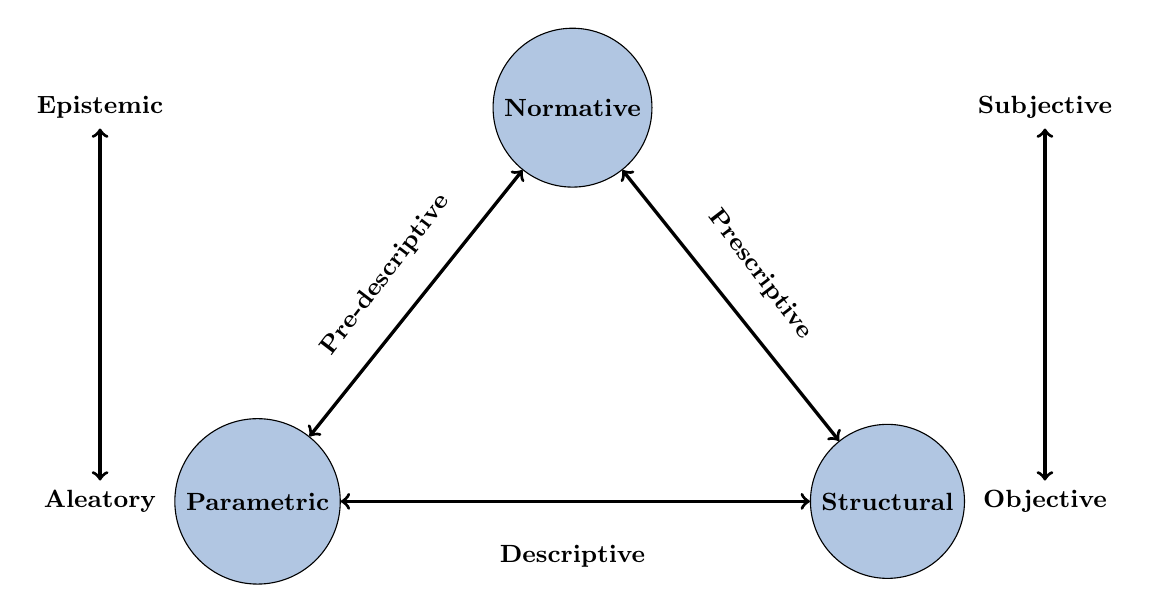
\begin{tikzpicture}[nodes={text depth=0.25ex,text height=1.25ex distance=1.7cm}]
        \tikzstyle{every node}=[font=\small]
        \tikzstyle{vertex} = [circle, draw=black, fill=illiniblue]
        \tikzstyle{hidden} = [draw=none]
        \tikzstyle{edge} = [<->, very thick]
        
        \node[vertex](v1) at (0,5) {\textbf{Normative}};
        \node[vertex](v2) at (4,0) {\textbf{Structural}};
        \node[vertex](v3) at (-4,0) {\textbf{Parametric}};

        \draw[edge] (v1) -- (v2);
        \draw[edge] (v2) -- (v3);
        \draw[edge] (v1) -- (v3);

        % hidden nodes for v1
        \node[hidden](h1) at (-0.75, 5) {};
        \node[hidden](h2) at (0.75, 5) {};

        % hidden nodes for v2
        \node[hidden](h3) at (4, 0.75) {};
        \node[hidden](h4) at (4, -0.7) {};

        % hidden nodes for v3
        \node[hidden](h5) at (-4, -0.7) {};
        \node[hidden](h6) at (-4, 0.75) {};

        \draw[draw=none] (h4) -- (h5) node[anchor=mid, midway, sloped]{\textbf{Descriptive}};
        \draw[draw=none] (h6) -- (h1) node[anchor=mid, midway, sloped]{\textbf{Pre-descriptive}};
        \draw[draw=none] (h2) -- (h3) node[anchor=mid, midway, sloped]{\textbf{Prescriptive}};


        % objectivity scale
        \node[hidden](u1) at (6,5) {\textbf{Subjective}};
        \node[hidden](u2) at (6,0) {\textbf{Objective}};
        \draw[edge] (u1) -- (u2);

        % uncertainty scale
        \node[hidden](u1) at (-6,5) {\textbf{Epistemic}};
        \node[hidden](u2) at (-6,0) {\textbf{Aleatory}};
        \draw[edge] (u1) -- (u2);
\end{tikzpicture}


\section{Technical improvements to \ac{osier}}

The current version of \ac{osier} achieved many of its goals for improving the
state-of-the-art in energy modeling by enabling the co-optimization of many
objectives simultaneously, ensuring that users are not forced to adhere to any
specific set of objectives by providing an interface for adding or changing
objectives that does not require modifying the source code, and extending the
\ac{mga} algorithm into many dimensions. However, there are still many ways to
improve \ac{osier}. This section outlines some priority areas for enhancement.


\subsection{Parallelization}

The current code is unacceptably slow for many-objective problems. The four
objective model took 26.5 days to run on a computer with 32GB of memory and 6
cores. More work needs to be done on investigating the parallelizability of
\texttt{CPLEX}, or employing more computing resources. Alternatively, rather
than using a \ac{milp} model to operate dispatch, using hiearchical model (i.e.,
a ``rules'' based model) to dispatch energy could enable multiple processes, and
reduce the computational cost of the problem. Additionally, this type of model
is conceptually simpler than \ac{milp}. The combination of reducing
computational cost and theoretical overhead would make \ac{osier} more
accessible, which is consistent with the ethos of this work.


\subsection{\ac{mga} enhancement}

The \ac{mga} algorithm could yet be improved by developing a selection strategy
that more accurately captures the spirit of \ac{mga} by identifying 
\textit{maximally different solutions in the design space} 
\cite{decarolis_using_2011,yue_review_2018}. In this application, discussions
generated by presenting maximally different alternatives could alleviate
normative uncertainty as described in Section \ref{section:three-uncertainties}.
I will accomplish this by implementing an algorithm from computational geometry
that is frequently used in topological data analysis known as greedy
permutation, or farthest-first-traversal
\cite{cavanna_geometric_2015,eppstein_approximate_2020}.


\subsection{Data transparency}

Quality data is essential to generating trustworthy results. The \ac{atb}
produced by \ac{nrel} is considered the gold standard for cost projections for
electricity generating technologies \cite{nrel_2020_2020}. \ac{osier} will
directly integrate data from the \ac{atb} to its built-in technology classes.


\section{Validating \ac{osier}}

\ac{osier}'s primary purpose is to translate policy preferences of the
public into actionable energy visions for a given municipality. The idea is
that if decision-makers used a tool like \ac{osier} to support their decisions
and incorporate ideas from their constituents --- ideas that may be distinct
from the preconceptions of decision-makers themselves --- then stronger actions
toward addressing climate change may be taken with more just outcomes. Consider
the following. If structural uncertainty is addressed by generating a set of
solutions, either by searching the near-optimal space or considering the options
along a Pareto Front, how should the ultimate solution be chosen? Answering this
last question raises another source of normative uncertainty. Additionally, a
result from social choice theory, Arrow's Impossibility theorem, states that one
cannot construct a utility function that maps individual preferences onto a
global preference order without violating principles of fairness
\cite{arrow_difficulty_1950, kasprzyk_many_2013,franssen_arrows_2005}. Thus, the
only way to address normative uncertainty produced by the process of deciding
among equally valid alternatives, is to involve the public in a deliberative
process \cite{dryzek_deliberative_2013}. Modelling energy systems with this
understanding would allow energy system modelers to advance the causes of
recognition and procedural justice, rather than hinder them. The last, and
arguably most important, component of this thesis is to validate \ac{osier}'s
usefulness in this regard. I propose validating \ac{osier}'s usefulness with a
case study of the energy visioning processes of three municipalities: Urbana,
Champaign, and the \ac{uiuc}. The research question is then: ``Do
decision-makers or energy planners perceive that \ac{osier}, or tools like it,
would be useful in enhancing collaboration between decision-makers and their
constituents?'' Although this case study focuses on a small sample, these
paradigmatic cases could be used to generalize the usefulness of \ac{osier} to
other locales \cite{flyvbjerg_five_2006}. The precise formulation of this
research question (or questions) is subject to change between now and the
beginning of this study. Since this research involves human participants it must
be reviewed by an ethics board.

\subsection{Reviewing the energy visions for each municipality}

I will research the background of each municipality considered by reviewing
published documents related to their energy visions, such as \ac{uiuc}'s
\ac{icap},
\cite{institute_for_sustainability_energy_and_environment_illinois_2020},
Utilities Master Plan \cite{affiliated_engineers_inc_utilities_2015} or the City
of Champaign's Comprehensive and Sustainability Plans
\cite{knight_champaign_2013,knight_champaign_2021}. I will also compare the
stated energy visions for each community with the literature
\cite{elmallah_frontlining_2022}. In addition to energy \textit{visions}, I may
evaluate the decision making process for specific energy projects. Such as the
microreactor project at \ac{uiuc} or the recent solar farm being constructed on
Market Street in Champaign. How do these projects fit with the stated energy
visions for their respective communities? How involved was the public in
making these decisions? Who were the stakeholders? This step is important for
developing a grounded decision-making process that incorporates \ac{osier} or a
similar decision support tool. 

\subsection{Develop the hypothetical \ac{osier} procedure}

Before interviewing decision-makers and asking if \ac{osier} would be useful to
them I need to formulate a hypothetical decision-making process that includes
\ac{osier}. This is necessary for creating a testable hypothesis about the nature
of such a process, which can be tested against interview responses. Additionally,
it is important to outline such a method to prevent \ac{osier}'s misuse. An example
of such misuse would be eliminating the iterative component of the process and 
treating results from \ac{osier} as an objective truth rather than a basis for
deliberation.
There are a few ways results (i.e., energy futures along
the Pareto-front or in the near-optimal space, as described in Section
\ref{section:mga-moo}) from \ac{osier} could be used in a decision-making
process. The results could be presented in more of a raw, descriptive, form.
Similar to the presentation in Chapter \ref{chapter:benchmark-results}.
Alternatively, whoever organizes the planning process (e.g., city councils,
planning departments, etc.) could distill the complete set of results into a
manageable subset accompanied by an explanatory narrative. \ac{mga} automates
part of this option. The former presentation admits less implicit bias from
pre-filtering the simulation results, but is arguably less understandable by the
public. The latter is more explicit but an explanatory narrative presents more
opportunity for politicization. Unfortunately, adequately addressing the best
way to communicate results to constituents is out-of-scope for this study
because I will not be surveying the public.
However, I will present interviewees with both options to create a partial
answer from their perspective.

\subsection{Deciding the interviewees}

In order to gauge the \ac{osier}'s usability, I will interview public facing
figures from each municipality involved in the energy or community planning
processes for their respective communities. These interviewees should be able to
speak to the energy visions of their community and the process by which those
visions were created. Their experiences will inform how such processes may be
helped or hindered by introducing a modeling tool (or a decision-support tool)
such as \ac{osier} and what ways \ac{osier} could be modified to serve the goal
of greater community participation in planning decisions. Table
\ref{table:subjects} lists potential interviewees.

\begin{table}[ht!]
    \centering
    \caption{Potential interviewees to evaluate the usefulness of \ac{osier}.}
    \resizebox*{0.8\textwidth}{!}{% \begin{tabular}[pos]{lllllll}
%     Name & Title & Affiliation & \multicolumn{4}{c}{Note} \\
%     \toprule
%     Bruce A. Knight & Planning \& Development Director & City of Champaign & \multicolumn{4}{l}{Directs the Champaign Planning department}\\
%     Lacey Rains Lowe & Senior Planner for Advanced Planning & City of Champaign & \multicolumn{4}{l}{Participated in creating the Champaign sustainability plan}\\
%     Jeremy Guest && \ac{uiuc} &&&&\\
%     Maddhu Khanna && \ac{uiuc} &&&&\\
%     Luis Rodir\'iguez && \ac{uiuc} &&&&\\
%     Kevin Garcia & Principal Planner & City of Urbana &&&&\\
%     &&&&&&\\
%     &&&&&&\\
%     &&&&&&\\
%     &&&&&&\\
%     \bottomrule
% \end{tabular}

\begin{tabular}[pos]{lll}
    Name & Title & Affiliation \\
    \toprule
    Bruce A. Knight & Planning \& Development Director & City of Champaign\\
    Lacey Rains Lowe & Senior Planner for Advanced Planning & City of Champaign\\
    Maddhu Khanna & Director, iSEE & \ac{uiuc}\\
    Jeremy Guest &Assoc. Director for Research, iSEE& \ac{uiuc}\\
    Luis Rodir\'iguez & Assoc. Director for Education \& Outreach iSEE& \ac{uiuc}\\
    Kevin Garcia & Principal Planner & City of Urbana\\
    \bottomrule
\end{tabular}}
    \label{table:subjects}
\end{table}

The list in Table \ref{table:subjects} merely indicates who might be good
participants in this case study. Ideal candidates would have direct experience
developing an energy vision for their community and engaging with the public.
Additionally, the final list should be demographically diverse, to the extent
possible, in order to enhance the generalizability of this case study.

\subsection{Conducting the Interviews}

% \textit{Interviews will be conducted and analyzed with the awareness that the
% questions I ask, my choice of wording, and my demeanor when asking, all have an
% affect on the answers generated by interviewees.}
This section describes some of the questions I may ask during an interview to 
shed light on how an \ac{esom} like \ac{osier} could be incorporated into
existing or novel energy planning processes.

\subsubsection{Questions about current planning processes}
The following questions are aimed at interviewees responsible for guiding the
planning process in each community. For example, they may be urban planners or
in charge of public engagement. These questions are not appropriate for an
external party that may be involved in the execution of an specific energy goal
but are nonetheless excluded from the initial decision making process.

\begin{enumerate}
    \item How would you describe your community's energy vision or priorities?
    \item How did your community develop these priorities (or this vision)?
    \item Does your community have current best practices for making planning
    decisions?
    \item How does your community use modeling software to support its vision,
    if at all?
    \item What are the pain points you experience in developing these visions?
    \item What is the role of expert testimony/consultation/input in creating an
    energy vision?
    \item How do you percieve the dialogue between community members and its
    decision-makers?
    \item Does it seem like preferences or concerns from the community are
    incorporated? 
    \item Do members of your community understand why a particular decision was
    reached?
    \item How does the energy visioning process in your community consider the
    impact on its neighbors?
    \item Should there be more collective planning among the three communities?
\end{enumerate}

\subsubsection{Questions and discussion about modeling tools and \ac{osier}} The
previous set of questions set a foundation for energy planning from the
perspective of a decision-maker or planner. This set of questions deals
specifically with the usefulness of \ac{osier} 

\begin{enumerate}
    \item (After presenting results from this model in two ways) Which
    presentation do you think would best facilitate dialogue between the
    public and decision-makers?
    \item What objectives do you think would be important to model in designing
    an energy vision for your community?
    \item Would your municipality use this tool? 
    \item If not this specific tool, is there a tool that exists/doesn't exist
    that is/would be useful?
    \item What changes would need to be made to \ac{osier} for it to be useful
    to you?
    \item How would employing this tool differ from existing visioning
    strategies or processes?
\end{enumerate}

\subsection{Generate insights with thematic analysis}

The interviews will be recorded and I will use the responses from interviewees
to conduct a theoretical thematic analysis
\cite{braun_toward_2023,maguire_doing_2017,scharp_what_2019}. Thematic analysis
is a qualitative method for determining patterns in a data corpus
\cite{scharp_what_2019}. 

The general process from Braun \& Clark 2006 \cite{braun_using_2006} is to
\begin{enumerate}
    \item familiarize yourself with the data,
    \item develop codes (I will be using an open-coding strategy where codes are
    developed in the process of reviewing transcripts, rather than being
    pre-determined \cite{maguire_doing_2017}),
    \item identify themes,
    \item review themes
    \item define themes, 
    \item locate exemplars.
\end{enumerate}


\subsection{Reflection}

After developing insights from the interviews, I will reflect on this work and
what it means for a holistic analysis of energy systems. Then I will draw
conclusions. The conclusions of this study will have descriptive and normative
components. The latter will be understood in the context of the normative
premise constructed in light of the suggestion in Section
\ref{section:three-uncertainties}.

The results of this analysis could take the form of:
    \begin{enumerate}
        \item ``These are the stated energy goals of this municipality.''
        \item ``This is how \ac{osier} will change based on feedback from the
        participants.''
        \item ``This is how the results from \ac{osier} would change
        decision-making procedures.'' (Results in this case includes the
        ``optimal'' solutions for an energy future \textit{and} the ways the
        process itself would change.)
    \end{enumerate}

\subsection{Research limitations}

The proposed work is an attempt at a more holistic approach to modeling energy
systems. However, there remain limitations to what is proposed. Although the
intention behind \ac{osier} is to help translate policy preferences of the
public into actionable energy visions for a given municipality, interviewing and
surveying members of the public is out-of-scope for this project. Further,
determining the needs of a group before developing code in earnest is essential
for developing an effective and procedurally just framework. This co-design
practice is important for future development of decision-support tools
\cite{gonzalez_developing_2022,ryder_developing_2018}.

% Also outside the scope of this project is determining which form of the
% results is most accessible to lay-audiences. Ideally with a much larger number
% of participants I could do a/b testing to tease out an answer to this
% question.

% Every aspect of energy modeling is influenced by normativity. Programming endogenous
% reliability requirements is a normative practice based on the belief that having a
% reliable electricity system is superior to an unreliable electricity system. I.e.,
% being able to trust that my lights will turn on when I flip the switch is preferred.
% Yes, there are physical requirements associated with this normative goal --- the grid 
% frequency must be kept within acceptable limits, to ensure a stable grid frequency the
% supply and demand for electricity must be synchronized, and electricity generators must 
% be able to adjust their power output to changing demand (or adequate electricity storage 
% must be made available). But having a constraint on grid frequency, because our grid depends
% on alternating current rather than direct current, is also a choice made from both practical 
% and normative considerations.

% \chapter{Conclusions}

% per Graduate College preference, place the \appendix and the appendices content before the
% bibliography (here) only if the appendices contain references.

\backmatter

\printbibliography[heading=bibintoc,title={References}]

% the below lines are only needed if bibliography precedes appendices
% uses https://tex.stackexchange.com/a/440212 to continue page numbering
% \clearpage
% \setcounter{counterforappendices}{\value{page}}
% \mainmatter
% \setcounter{page}{\value{counterforappendices}}

% \appendix

% \chapter{An appendix}

% \lipsum[1-5]

% \input{Appendix.tex}

\end{document}
